\subsection{Strain data}
The following figure \ref{fig:strain_all}, contains raw strain data for 6 different trains passing the Lerelva bridge. Each subfigure contains data from three different strain sensors placed as described in System setup, see section:\ref{system_setup}. Three of the trains comes from the north side; train 3, train 5 and train 7, and three from the south side; train 4, 6 and 8. The strain signals all appear similar in form, except for train 7, figure\ref{fig:strain_train7}, which is a freight train. The other 5 trains are all of the same type, a NSB 92 type passenger train \ref{appendix:nsb92}.

The strain signals have different levels of peak height suggesting that the trains actual axle weights differ from what is found in table \ref{table:axle_weights}. This will throw off the magnitude of the resulting average influence line found through the matrix method. And this error in calculated influence line will inevitably be found again in the calculated axle weights \label{peaks_heights}.

To account for the different directions of the trains, the strain data for the trains going towards Trondheim has been reversed (correct word ?). This is not necessary for finding influence lines, but makes it easier placing the found influence lines in the same coordinate system.

Some of the signals were originally very long, due to not knowing exactly when the train would pass. This means cutting the signal into a vector containing the essential data. Ideally the goal was to identify exactly, or as closely as possible, the time the train entered the bridge. Due to noise and dynamic effects identifying this, proved a difficult process involving detection of peaks which lies close to peaks of noise. This proved possible to do for each individual signal, but a general method performing this for every signal was not within the authors capabilites. Therefore, to cut the signals as equally as possible the first and last major peaks of the signals were used as reference points for appending of samples before and after these peaks. For this method to prove exact, the speed of the train should be taken into consideration when appending sample points so that the influence lines of the signals gets an as equal length as possible.

The strain data from the freight train, figure \ref{fig:strain_train7}, is not used for finding the bridge's influence line because the train data is unknown. Axle weights for this train was not found, and guesswork of this data would be difficult. The locomotive data, and possibly the axle spacings of the train, would be the only data possible to find. Therefore this data will only be used for testing of influence lines.
\begin{figure}[H]
	\centering
	\begin{subfigure}[t]{0.4\textwidth}
		\centering
		% This file was created by matlab2tikz.
%
%The latest updates can be retrieved from
%  http://www.mathworks.com/matlabcentral/fileexchange/22022-matlab2tikz-matlab2tikz
%where you can also make suggestions and rate matlab2tikz.
%
\definecolor{mycolor1}{rgb}{0.00000,0.44700,0.74100}%
\definecolor{mycolor2}{rgb}{0.85000,0.32500,0.09800}%
\definecolor{mycolor3}{rgb}{0.92900,0.69400,0.12500}%
%
\begin{tikzpicture}

\begin{axis}[%
width=\textwidth,
height=\textwidth,
at={(0\figurewidth,0\figureheight)},
scale only axis,
xmin=12,
xmax=20,
ymin=-5e-05,
ymax=0.0002,
axis background/.style={fill=white},
title style={font=\bfseries},
title={Raw strain history, train 3},
% legend style={legend cell align=left,align=left,draw=white!15!black}
% legend style={at={(1.1,-0.2)}}
]
\addplot [color=mycolor1,solid,forget plot]
  table[row sep=crcr]{%
12.7763671875	5.66138597029925e-07\\
12.77734375	3.26189245247223e-07\\
12.7783203125	1.35641311928975e-07\\
12.779296875	-5.2068990728793e-07\\
12.7802734375	-4.7834598343845e-07\\
12.78125	-8.7355580109718e-07\\
12.7822265625	-9.79415521092705e-07\\
12.783203125	-6.47721657503174e-07\\
12.7841796875	-1.46651790273577e-07\\
12.78515625	1.04603764310954e-06\\
12.7861328125	-7.95925325643848e-07\\
12.787109375	9.19005498232995e-07\\
12.7880859375	1.70927960814818e-07\\
12.7890625	7.49629354841221e-07\\
12.7900390625	9.11948157789185e-07\\
12.791015625	-5.70091147284683e-07\\
12.7919921875	-1.90392279790985e-06\\
12.79296875	3.12074581051112e-07\\
12.7939453125	-7.39466790535513e-07\\
12.794921875	1.21526653065621e-07\\
12.7958984375	2.1893283869861e-06\\
12.796875	5.3085192048977e-07\\
12.7978515625	-6.05377744320075e-07\\
12.798828125	-2.5956898690822e-07\\
12.7998046875	-4.28944734453445e-07\\
12.80078125	-5.48919187878978e-07\\
12.8017578125	-5.70091147284683e-07\\
12.802734375	4.24991905684062e-07\\
12.8037109375	-1.25465068908292e-06\\
12.8046875	2.83845253843274e-07\\
12.8056640625	4.46163906867112e-07\\
12.806640625	-5.50525892538054e-09\\
12.8076171875	9.89578908102513e-07\\
12.80859375	1.5666724184453e-08\\
12.8095703125	4.10877238721935e-07\\
12.810546875	-4.78492224776934e-08\\
12.8115234375	7.56686693013193e-07\\
12.8125	-8.45326538678661e-07\\
12.8134765625	9.32973365245972e-08\\
12.814453125	-2.22855853884772e-06\\
12.8154296875	-5.1363258689297e-07\\
12.81640625	-6.90212029208232e-08\\
12.8173828125	7.91826788462766e-08\\
12.818359375	9.19005498232995e-07\\
12.8193359375	1.50476509935935e-06\\
12.8203125	1.34950345206681e-06\\
12.8212890625	4.38960363799944e-08\\
12.822265625	-6.33607020170558e-07\\
12.8232421875	4.46163906867112e-07\\
12.82421875	-4.00715447146632e-07\\
12.8251953125	-6.47721657503174e-07\\
12.826171875	2.20329273403676e-07\\
12.8271484375	8.9783347719777e-07\\
12.828125	-7.60785295375859e-08\\
12.8291015625	-2.87798282116265e-07\\
12.830078125	6.57883967589709e-07\\
12.8310546875	-4.21887412774789e-07\\
12.83203125	2.41501265994858e-07\\
12.8330078125	-1.32522378488314e-06\\
12.833984375	-5.34804547780996e-07\\
12.8349609375	-2.8074095846241e-07\\
12.8359375	-5.77148466889476e-07\\
12.8369140625	1.99157281701974e-07\\
12.837890625	6.3671195751772e-07\\
12.8388671875	1.41301957472728e-06\\
12.83984375	6.6494130447842e-07\\
12.8408203125	-4.57174020180142e-07\\
12.841796875	-1.74881091802737e-07\\
12.8427734375	-8.66498485640977e-07\\
12.84375	2.55615928215986e-07\\
12.8447265625	-4.50116698896353e-07\\
12.845703125	-9.72505087954659e-08\\
12.8466796875	-3.2308489890452e-07\\
12.84765625	1.04603764310954e-06\\
12.8486328125	1.37067549206495e-06\\
12.849609375	9.26062838775468e-07\\
12.8505859375	-5.41861867879101e-07\\
12.8515625	-3.93658125072893e-07\\
12.8525390625	-1.67823766568332e-07\\
12.853515625	-3.51314190556815e-07\\
12.8544921875	-1.53709115803752e-07\\
12.85546875	-7.11237520611063e-07\\
12.8564453125	7.77858708122386e-07\\
12.857421875	-9.72505087954659e-08\\
12.8583984375	-1.25625864305385e-08\\
12.859375	7.07285327881946e-07\\
12.8603515625	-5.6303382758166e-07\\
12.861328125	-1.13467640355585e-06\\
12.8623046875	1.35641311928975e-07\\
12.86328125	-2.03110391751348e-07\\
12.8642578125	-9.72358207117739e-07\\
12.865234375	2.13271942737635e-07\\
12.8662109375	4.67335908939642e-07\\
12.8671875	-8.10039958433224e-07\\
12.8681640625	1.32127406678585e-06\\
12.869140625	8.83718797001654e-07\\
12.8701171875	4.53221240792698e-07\\
12.87109375	1.07411994597567e-07\\
12.8720703125	-4.99517945807279e-07\\
12.873046875	-1.39594464644306e-07\\
12.8740234375	6.22597284629994e-07\\
12.875	1.0530949854301e-06\\
12.8759765625	-1.04307835017145e-07\\
12.876953125	-2.8074095846241e-07\\
12.8779296875	2.48558597055982e-07\\
12.87890625	9.61349542969716e-07\\
12.8798828125	3.40303909838633e-07\\
12.880859375	1.14469323781938e-07\\
12.8818359375	6.93170653019021e-07\\
12.8828125	9.47234860995726e-07\\
12.8837890625	2.9781380084682e-08\\
12.884765625	9.19005498232995e-07\\
12.8857421875	-3.79543480629211e-07\\
12.88671875	-3.3734568355339e-08\\
12.8876953125	-5.91263105802426e-07\\
12.888671875	1.07426701298334e-06\\
12.8896484375	-2.45454338711464e-07\\
12.890625	1.11661107075715e-06\\
12.8916015625	9.68406884104813e-07\\
12.892578125	-1.21936413747885e-06\\
12.8935546875	-2.5956898690822e-07\\
12.89453125	3.68533240206704e-07\\
12.8955078125	-4.57174020180142e-07\\
12.896484375	-6.19492382442858e-07\\
12.8974609375	1.49755971186978e-07\\
12.8984375	4.10877238721935e-07\\
12.8994140625	-1.11365161140162e-07\\
12.900390625	1.07411994597567e-07\\
12.9013671875	-4.7834598343845e-07\\
12.90234375	9.33120179416819e-07\\
12.9033203125	-3.79543480629211e-07\\
12.904296875	-4.85403304326722e-07\\
12.9052734375	-7.25352155770938e-07\\
12.90625	9.82521566670995e-07\\
12.9072265625	7.42572016767477e-07\\
12.908203125	3.19131913100162e-07\\
12.9091796875	1.27892999182743e-06\\
12.91015625	-3.44256867791572e-07\\
12.9111328125	1.00354665511643e-07\\
12.912109375	7.56686693013193e-07\\
12.9130859375	-7.25352155770938e-07\\
12.9140625	1.99157281701974e-07\\
12.9150390625	-4.50116698896353e-07\\
12.916015625	-1.53694301302607e-06\\
12.9169921875	4.46163906867112e-07\\
12.91796875	9.82521566670995e-07\\
12.9189453125	-1.09938984355724e-06\\
12.919921875	-5.41861867879101e-07\\
12.9208984375	1.13072575747171e-06\\
12.921875	7.56686693013193e-07\\
12.9228515625	9.68406884104813e-07\\
12.923828125	4.39106573040622e-07\\
12.9248046875	-5.70091147284683e-07\\
12.92578125	-4.99517945807279e-07\\
12.9267578125	3.89705239020122e-07\\
12.927734375	-1.32537138916155e-07\\
12.9287109375	-7.1829483824044e-07\\
12.9296875	-3.58371513222745e-07\\
12.9306640625	1.31421672071243e-06\\
12.931640625	4.95565246418778e-07\\
12.9326171875	1.03898030088829e-06\\
12.93359375	-3.01912929127771e-07\\
12.9345703125	-7.1829483824044e-07\\
12.935546875	8.76661457051807e-07\\
12.9365234375	-1.40285417885629e-06\\
12.9375	5.09679915750971e-07\\
12.9384765625	-4.21887412774789e-07\\
12.939453125	-6.12435063430906e-07\\
12.9404296875	2.83845253843274e-07\\
12.94140625	1.92820619857232e-06\\
12.9423828125	1.43419161739125e-06\\
12.943359375	2.9781380084682e-08\\
12.9443359375	2.69730590832197e-07\\
12.9453125	1.00369359126175e-06\\
12.9462890625	8.55489437794456e-07\\
12.947265625	1.5666724184453e-08\\
12.9482421875	-1.18407758340627e-06\\
12.94921875	-2.8074095846241e-07\\
12.9501953125	-6.5477897602138e-07\\
12.951171875	-4.07918954660642e-08\\
12.9521484375	1.1801271640841e-06\\
12.953125	2.2724052084911e-08\\
12.9541015625	-6.05377744320075e-07\\
12.955078125	5.02622581035218e-07\\
12.9560546875	1.30010202886222e-06\\
12.95703125	-3.65428835790447e-07\\
12.9580078125	5.8731060413944e-07\\
12.958984375	6.22597284629994e-07\\
12.9599609375	1.63885474230795e-06\\
12.9609375	1.35641311928975e-07\\
12.9619140625	4.17934572153559e-07\\
12.962890625	7.84916046689659e-07\\
12.9638671875	1.14469323781938e-07\\
12.96484375	6.08482612137352e-07\\
12.9658203125	6.71998641465143e-07\\
12.966796875	1.08838169851264e-06\\
12.9677734375	-1.39594464644306e-07\\
12.96875	-4.14830090997471e-07\\
12.9697265625	-6.7595093098294e-07\\
12.970703125	6.29654621024526e-07\\
12.9716796875	-6.7595093098294e-07\\
12.97265625	-2.17225041133353e-07\\
12.9736328125	-3.30142221965533e-07\\
12.974609375	-2.20032935227977e-06\\
12.9755859375	-4.21887412774789e-07\\
12.9765625	-1.84040708502142e-06\\
12.9775390625	-4.92460625116549e-07\\
12.978515625	4.39106573040622e-07\\
12.9794921875	2.20329273403676e-07\\
12.98046875	1.13072575747171e-06\\
12.9814453125	-1.18407758340627e-06\\
12.982421875	8.60939638222362e-09\\
12.9833984375	-2.17225041133353e-07\\
12.984375	-3.37199544928101e-07\\
12.9853515625	-5.70091147284683e-07\\
12.986328125	-1.02881671615231e-06\\
12.9873046875	-5.6303382758166e-07\\
12.98828125	4.38960363799944e-08\\
12.9892578125	-5.91263105802426e-07\\
12.990234375	-9.86472834969008e-07\\
12.9912109375	-1.81938416937829e-07\\
12.9921875	4.74393243161215e-07\\
12.9931640625	7.2125350155652e-08\\
12.994140625	-1.81938416937829e-07\\
12.9951171875	-3.51314190556815e-07\\
12.99609375	-7.11237520611063e-07\\
12.9970703125	-1.88995741974693e-07\\
12.998046875	6.5068021563473e-08\\
12.9990234375	2.34443935032396e-07\\
13	7.2125350155652e-08\\
13.0009765625	-3.3734568355339e-08\\
13.001953125	4.24991905684062e-07\\
13.0029296875	1.30715937473789e-06\\
13.00390625	9.82521566670995e-07\\
13.0048828125	-1.46651790273577e-07\\
13.005859375	-1.76277675840476e-06\\
13.0068359375	-1.10644715575455e-06\\
13.0078125	7.91826788462766e-08\\
13.0087890625	-4.57174020180142e-07\\
13.009765625	1.00354665511643e-07\\
13.0107421875	3.82647905983365e-07\\
13.01171875	3.33246577493814e-07\\
13.0126953125	2.69730590832197e-07\\
13.013671875	1.75177236402379e-06\\
13.0146484375	-4.7834598343845e-07\\
13.015625	-4.71288662450865e-07\\
13.0166015625	-8.31358560556862e-08\\
13.017578125	-7.39466790535513e-07\\
13.0185546875	1.07411994597567e-07\\
13.01953125	8.20202741007477e-07\\
13.0205078125	8.62400076362142e-08\\
13.021484375	6.71998641465143e-07\\
13.0224609375	2.90902585497023e-07\\
13.0234375	-5.70091147284683e-07\\
13.0244140625	-1.81938416937829e-07\\
13.025390625	-1.40285417885629e-06\\
13.0263671875	3.05017249100942e-07\\
13.02734375	4.38960363799944e-08\\
13.0283203125	1.99157281701974e-07\\
13.029296875	1.68119884748851e-06\\
13.0302734375	1.29304468308522e-06\\
13.03125	1.14484044458157e-06\\
13.0322265625	1.1801271640841e-06\\
13.033203125	-5.50525892538054e-09\\
13.0341796875	4.46163906867112e-07\\
13.03515625	-1.80512057440453e-06\\
13.0361328125	-6.12435063430906e-07\\
13.037109375	-4.21887412774789e-07\\
13.0380859375	8.48432098239475e-07\\
13.0390625	5.09679915750971e-07\\
13.0400390625	-1.81938416937829e-07\\
13.041015625	7.49629354841221e-07\\
13.0419921875	1.3353887592289e-06\\
13.04296875	-3.30142221965533e-07\\
13.0439453125	-2.66772411457346e-08\\
13.044921875	1.79411647868591e-06\\
13.0458984375	1.10249638443746e-06\\
13.046875	-2.66626310858279e-07\\
13.0478515625	-9.58243578871388e-07\\
13.048828125	1.92099951332137e-07\\
13.0498046875	2.9781380084682e-08\\
13.05078125	-3.86600802900492e-07\\
13.0517578125	7.28457340916843e-07\\
13.052734375	-7.1829483824044e-07\\
13.0537109375	2.90902585497023e-07\\
13.0546875	1.56828124157492e-06\\
13.0556640625	-1.58634415346965e-06\\
13.056640625	-1.96199138376846e-08\\
13.0576171875	6.08482612137352e-07\\
13.05859375	-1.51577109421203e-06\\
13.0595703125	5.44966590809671e-07\\
13.060546875	1.85042621060746e-07\\
13.0615234375	1.42713426973793e-06\\
13.0625	4.03819905389407e-07\\
13.0634765625	-4.99517945807279e-07\\
13.064453125	-7.60638741942191e-07\\
13.0654296875	-1.67823766568332e-07\\
13.06640625	-7.74753375719058e-07\\
13.0673828125	-4.92460625116549e-07\\
13.068359375	-1.03587402933733e-06\\
13.0693359375	-9.86472834969008e-07\\
13.0703125	-9.08842376898256e-07\\
13.0712890625	-1.81938416937829e-07\\
13.072265625	6.71998641465143e-07\\
13.0732421875	1.55206867930718e-09\\
13.07421875	1.25775795568124e-06\\
13.0751953125	-4.36002056033221e-07\\
13.076171875	-9.4412895023017e-07\\
13.0771484375	1.04603764310954e-06\\
13.078125	-1.07821790637291e-06\\
13.0791015625	-5.98320425110798e-07\\
13.080078125	-1.53694301302607e-06\\
13.0810546875	1.13072575747171e-06\\
13.08203125	6.79055978551179e-07\\
13.0830078125	1.35641311928975e-07\\
13.083984375	1.6882561986978e-06\\
13.0849609375	-3.44256867791572e-07\\
13.0859375	-1.38168225441264e-06\\
13.0869140625	-8.10039958433224e-07\\
13.087890625	-5.91263105802426e-07\\
13.0888671875	-2.94855605671674e-07\\
13.08984375	-7.25352155770938e-07\\
13.0908203125	-4.00715447146632e-07\\
13.091796875	1.42698641508428e-07\\
13.0927734375	9.26062838775468e-07\\
13.09375	-6.19638762051813e-08\\
13.0947265625	1.22952857553593e-06\\
13.095703125	5.16737250564952e-07\\
13.0966796875	-6.19492382442858e-07\\
13.09765625	-8.02982642087976e-07\\
13.0986328125	-3.08970252485639e-07\\
13.099609375	-3.86600802900492e-07\\
13.1005859375	-5.2068990728793e-07\\
13.1015625	4.53221240792698e-07\\
13.1025390625	1.39890488011149e-06\\
13.103515625	5.09533646755357e-08\\
13.1044921875	6.86113315735443e-07\\
13.10546875	-4.78492224776934e-08\\
13.1064453125	4.88507911900783e-07\\
13.107421875	-8.17097274680026e-07\\
13.1083984375	5.8731060413944e-07\\
13.109375	7.77858708122386e-07\\
13.1103515625	-7.39466790535513e-07\\
13.111328125	-9.4412895023017e-07\\
13.1123046875	-1.74881091802737e-07\\
13.11328125	-5.49065493908769e-08\\
13.1142578125	4.38960363799944e-08\\
13.115234375	9.61349542969716e-07\\
13.1162109375	7.91826788462766e-08\\
13.1171875	-1.30405185718016e-06\\
13.1181640625	2.9781380084682e-08\\
13.119140625	-7.95925325643848e-07\\
13.1201171875	1.14469323781938e-07\\
13.12109375	3.40303909838633e-07\\
13.1220703125	9.26062838775468e-07\\
13.123046875	3.96762572155108e-07\\
13.1240234375	4.67335908939642e-07\\
13.125	2.83845253843274e-07\\
13.1259765625	7.49629354841221e-07\\
13.126953125	3.96762572155108e-07\\
13.1279296875	-8.66498485640977e-07\\
13.12890625	9.40177520156833e-07\\
13.1298828125	-1.32537138916155e-07\\
13.130859375	-1.06410328108968e-06\\
13.1318359375	1.35641311928975e-07\\
13.1328125	-1.77689136413289e-06\\
13.1337890625	5.801069307039e-08\\
13.134765625	4.6027857481673e-07\\
13.1357421875	-4.71288662450865e-07\\
13.13671875	1.24364326541115e-06\\
13.1376953125	-1.03587402933733e-06\\
13.138671875	-3.16027575744194e-07\\
13.1396484375	7.91826788462766e-08\\
13.140625	1.07411994597567e-07\\
13.1416015625	-5.50525892538054e-09\\
13.142578125	4.03819905389407e-07\\
13.1435546875	9.19005498232995e-07\\
13.14453125	1.50476509935935e-06\\
13.1455078125	-2.87798282116265e-07\\
13.146484375	7.91826788462766e-08\\
13.1474609375	-4.50116698896353e-07\\
13.1484375	-6.97122885056321e-07\\
13.1494140625	-1.32537138916155e-07\\
13.150390625	8.62400076362142e-08\\
13.1513671875	1.21526653065621e-07\\
13.15234375	9.26062838775468e-07\\
13.1533203125	4.32049239312794e-07\\
13.154296875	5.16737250564952e-07\\
13.1552734375	-2.31339690119842e-07\\
13.15625	2.13271942737635e-07\\
13.1572265625	-2.45454338711464e-07\\
13.158203125	-9.37071635761242e-07\\
13.1591796875	-5.91263105802426e-07\\
13.16015625	-6.19638762051813e-08\\
13.1611328125	6.50826630800528e-07\\
13.162109375	1.99157281701974e-07\\
13.1630859375	7.21400003139954e-07\\
13.1640625	1.067209670367e-06\\
13.1650390625	-4.07918954660642e-08\\
13.166015625	-3.79543480629211e-07\\
13.1669921875	3.54418574825127e-07\\
13.16796875	9.19005498232995e-07\\
13.1689453125	-1.46651790273577e-07\\
13.169921875	1.92099951332137e-07\\
13.1708984375	-2.38397014464767e-07\\
13.171875	-2.03110391751348e-07\\
13.1728515625	5.66138597029925e-07\\
13.173828125	5.16737250564952e-07\\
13.1748046875	1.37067549206495e-06\\
13.17578125	1.08132435569898e-06\\
13.1767578125	5.73195932634506e-07\\
13.177734375	-2.52511662859282e-07\\
13.1787109375	7.63744031284045e-07\\
13.1796875	-1.06410328108968e-06\\
13.1806640625	-2.38397014464767e-07\\
13.181640625	6.71998641465143e-07\\
13.1826171875	-3.72486158259269e-07\\
13.18359375	4.10877238721935e-07\\
13.1845703125	1.23658592042432e-06\\
13.185546875	8.83718797001654e-07\\
13.1865234375	9.47234860995726e-07\\
13.1875	5.02622581035218e-07\\
13.1884765625	-9.15899691761833e-07\\
13.189453125	3.82647905983365e-07\\
13.1904296875	-1.74866215228177e-06\\
13.19140625	8.60939638222362e-09\\
13.1923828125	-9.37071635761242e-07\\
13.193359375	-1.04307835017145e-07\\
13.1943359375	-1.76277675840476e-06\\
13.1953125	2.76787922288187e-07\\
13.1962890625	3.12074581051112e-07\\
13.197265625	-3.16027575744194e-07\\
13.1982421875	-9.58243578871388e-07\\
13.19921875	-1.30405185718016e-06\\
13.2001953125	3.40303909838633e-07\\
13.201171875	-3.72486158259269e-07\\
13.2021484375	1.20835654146383e-06\\
13.203125	2.73980263254905e-06\\
13.2041015625	1.89291942672407e-06\\
13.205078125	-3.2308489890452e-07\\
13.2060546875	-3.08970252485639e-07\\
13.20703125	-1.20524951614624e-06\\
13.2080078125	9.82521566670995e-07\\
13.208984375	-1.19113489441811e-06\\
13.2099609375	3.26189245247223e-07\\
13.2109375	-1.16290564977726e-06\\
13.2119140625	9.61349542969716e-07\\
13.212890625	-5.2068990728793e-07\\
13.2138671875	1.29304468308522e-06\\
13.21484375	8.06088062984102e-07\\
13.2158203125	-3.93658125072893e-07\\
13.216796875	1.70927960814818e-07\\
13.2177734375	5.80253268337317e-07\\
13.21875	6.6494130447842e-07\\
13.2197265625	-7.25352155770938e-07\\
13.220703125	3.12074581051112e-07\\
13.2216796875	1.04603764310954e-06\\
13.22265625	8.48432098239475e-07\\
13.2236328125	1.11661107075715e-06\\
13.224609375	4.67335908939642e-07\\
13.2255859375	6.57883967589709e-07\\
13.2265625	-7.53581424905222e-07\\
13.2275390625	7.70801369653993e-07\\
13.228515625	1.63870630840281e-07\\
13.2294921875	-7.46524107770024e-07\\
13.23046875	-1.26170799910705e-06\\
13.2314453125	1.77985290888668e-07\\
13.232421875	1.49755971186978e-07\\
13.2333984375	-1.33228109392e-06\\
13.234375	5.801069307039e-08\\
13.2353515625	-2.38397014464767e-07\\
13.236328125	3.68387081826817e-08\\
13.2373046875	7.2125350155652e-08\\
13.23828125	-3.3734568355339e-08\\
13.2392578125	-1.48048456087915e-06\\
13.240234375	-4.00715447146632e-07\\
13.2412109375	-1.26170799910705e-06\\
13.2421875	-9.4412895023017e-07\\
13.2431640625	-5.84205786395174e-07\\
13.244140625	-1.39594464644306e-07\\
13.2451171875	1.20835654146383e-06\\
13.24609375	-1.60766441235699e-07\\
13.2470703125	5.9436794004001e-07\\
13.248046875	1.56122389204463e-06\\
13.2490234375	1.2858398244775e-07\\
13.25	-7.1829483824044e-07\\
13.2509765625	-7.1829483824044e-07\\
13.251953125	-1.82629248107096e-06\\
13.2529296875	-1.69926102773911e-06\\
13.25390625	-5.91263105802426e-07\\
13.2548828125	-9.15899691761833e-07\\
13.255859375	4.32049239312794e-07\\
13.2568359375	1.58239594093149e-06\\
13.2578125	-6.19638762051813e-08\\
13.2587890625	-5.41861867879101e-07\\
13.259765625	-1.20524951614624e-06\\
13.2607421875	-1.36756763762262e-06\\
13.26171875	2.06214612170474e-07\\
13.2626953125	-4.7834598343845e-07\\
13.263671875	-4.85403304326722e-07\\
13.2646484375	1.14484044458157e-06\\
13.265625	1.32833141295815e-06\\
13.2666015625	1.66002679445371e-06\\
13.267578125	-1.11365161140162e-07\\
13.2685546875	1.27187264634663e-06\\
13.26953125	-7.1829483824044e-07\\
13.2705078125	-2.14387097440308e-06\\
13.271484375	-2.94855605671674e-07\\
13.2724609375	-9.4412895023017e-07\\
13.2734375	-1.96199138376846e-08\\
13.2744140625	9.61349542969716e-07\\
13.275390625	1.39184753295148e-06\\
13.2763671875	-3.01912929127771e-07\\
13.27734375	3.96762572155108e-07\\
13.2783203125	-3.93658125072893e-07\\
13.279296875	-4.00715447146632e-07\\
13.2802734375	-9.22957006527182e-07\\
13.28125	-9.15899691761833e-07\\
13.2822265625	-1.60766441235699e-07\\
13.283203125	-3.86600802900492e-07\\
13.2841796875	-5.6303382758166e-07\\
13.28515625	1.15189778828449e-06\\
13.2861328125	7.77858708122386e-07\\
13.287109375	-8.87670431713597e-07\\
13.2880859375	9.33120179416819e-07\\
13.2890625	3.19131913100162e-07\\
13.2900390625	-6.33607020170558e-07\\
13.291015625	-1.53709115803752e-07\\
13.2919921875	6.01425276039458e-07\\
13.29296875	1.21526653065621e-07\\
13.2939453125	-1.59340145885188e-06\\
13.294921875	-9.72358207117739e-07\\
13.2958984375	5.09533646755357e-08\\
13.296875	1.89291942672407e-06\\
13.2978515625	1.10249638443746e-06\\
13.298828125	3.89705239020122e-07\\
13.2998046875	1.35641311928975e-07\\
13.30078125	-2.235615835243e-06\\
13.3017578125	6.01425276039458e-07\\
13.302734375	-1.60045876413609e-06\\
13.3037109375	5.801069307039e-08\\
13.3046875	9.40177520156833e-07\\
13.3056640625	-5.70091147284683e-07\\
13.306640625	-5.6303382758166e-07\\
13.3076171875	7.56686693013193e-07\\
13.30859375	2.90902585497023e-07\\
13.3095703125	-7.1829483824044e-07\\
13.310546875	-8.87670431713597e-07\\
13.3115234375	-2.8074095846241e-07\\
13.3125	1.77985290888668e-07\\
13.3134765625	-1.02175940286863e-06\\
13.314453125	-5.98320425110798e-07\\
13.3154296875	2.13271942737635e-07\\
13.31640625	-6.33607020170558e-07\\
13.3173828125	2.34443935032396e-07\\
13.318359375	1.14469323781938e-07\\
13.3193359375	-3.01912929127771e-07\\
13.3203125	-1.5016564811753e-06\\
13.3212890625	-4.99517945807279e-07\\
13.322265625	-4.92460625116549e-07\\
13.3232421875	4.46163906867112e-07\\
13.32421875	-8.31358560556862e-08\\
13.3251953125	-6.90212029208232e-08\\
13.326171875	-3.37199544928101e-07\\
13.3271484375	-4.07772769121274e-07\\
13.328125	-3.65428835790447e-07\\
13.3291015625	-6.19492382442858e-07\\
13.330078125	-4.36002056033221e-07\\
13.3310546875	-1.36051032907972e-06\\
13.33203125	1.49755971186978e-07\\
13.3330078125	1.70927960814818e-07\\
13.333984375	-2.10167716491573e-07\\
13.3349609375	-1.81938416937829e-07\\
13.3359375	1.77294442091054e-06\\
13.3369140625	-1.26876530903296e-06\\
13.337890625	2.36576237461986e-06\\
13.3388671875	-2.66772411457346e-08\\
13.33984375	-4.85403304326722e-07\\
13.3408203125	5.80253268337317e-07\\
13.341796875	-4.57174020180142e-07\\
13.3427734375	-4.43059377514552e-07\\
13.34375	4.10877238721935e-07\\
13.3447265625	-3.44256867791572e-07\\
13.345703125	4.81450577481885e-07\\
13.3466796875	1.42698641508428e-07\\
13.34765625	1.34244610559874e-06\\
13.3486328125	1.53299449491182e-06\\
13.349609375	6.43769294109793e-07\\
13.3505859375	-2.31339690119842e-07\\
13.3515625	2.97959917249652e-07\\
13.3525390625	9.32973365245972e-08\\
13.353515625	-7.25352155770938e-07\\
13.3544921875	-9.72505087954659e-08\\
13.35546875	7.77858708122386e-07\\
13.3564453125	8.55489437794456e-07\\
13.357421875	-4.71288662450865e-07\\
13.3583984375	2.04818124132397e-06\\
13.359375	1.0601523278489e-06\\
13.3603515625	-1.32537138916155e-07\\
13.361328125	-1.47342725391637e-06\\
13.3623046875	-8.87670431713597e-07\\
13.36328125	-4.92460625116549e-07\\
13.3642578125	-1.74160484907207e-06\\
13.365234375	-2.38397014464767e-07\\
13.3662109375	7.14342665461293e-07\\
13.3671875	4.32049239312794e-07\\
13.3681640625	1.03192295876527e-06\\
13.369140625	2.33047557215461e-06\\
13.3701171875	-1.04307835017145e-07\\
13.37109375	1.56813300963973e-07\\
13.3720703125	-9.22957006527182e-07\\
13.373046875	-2.08035529173636e-06\\
13.3740234375	1.04603764310954e-06\\
13.375	8.90776137050381e-07\\
13.3759765625	2.06214612170474e-07\\
13.376953125	1.75882971622078e-06\\
13.3779296875	-1.25479813089559e-07\\
13.37890625	8.83718797001654e-07\\
13.3798828125	-1.81938416937829e-07\\
13.380859375	-4.14830090997471e-07\\
13.3818359375	5.73195932634506e-07\\
13.3828125	1.10955372754776e-06\\
13.3837890625	3.05017249100942e-07\\
13.384765625	-1.2758226188602e-06\\
13.3857421875	9.89578908102513e-07\\
13.38671875	-2.66772411457346e-08\\
13.3876953125	5.37909255600606e-07\\
13.388671875	1.09543904142583e-06\\
13.3896484375	3.54418574825127e-07\\
13.390625	-2.10167716491573e-07\\
13.3916015625	-1.90392279790985e-06\\
13.392578125	-9.22957006527182e-07\\
13.3935546875	-1.39594464644306e-07\\
13.39453125	1.17306981998609e-06\\
13.3955078125	2.2724052084911e-08\\
13.396484375	1.27187264634663e-06\\
13.3974609375	8.06088062984102e-07\\
13.3984375	-1.11365161140162e-07\\
13.3994140625	-8.02982642087976e-07\\
13.400390625	6.71998641465143e-07\\
13.4013671875	6.79055978551179e-07\\
13.40234375	-2.09446988857554e-06\\
13.4033203125	8.90776137050381e-07\\
13.404296875	-4.50116698896353e-07\\
13.4052734375	2.9781380084682e-08\\
13.40625	1.49755971186978e-07\\
13.4072265625	6.6494130447842e-07\\
13.408203125	1.01780827481586e-06\\
13.4091796875	-2.5956898690822e-07\\
13.41015625	4.53221240792698e-07\\
13.4111328125	1.08838169851264e-06\\
13.412109375	-2.03110391751348e-07\\
13.4130859375	-8.17097274680026e-07\\
13.4140625	1.63870630840281e-07\\
13.4150390625	9.11948157789185e-07\\
13.416015625	-3.16027575744194e-07\\
13.4169921875	1.42698641508428e-07\\
13.41796875	-3.3734568355339e-08\\
13.4189453125	1.92820619857232e-06\\
13.419921875	2.55615928215986e-07\\
13.4208984375	3.61475907466801e-07\\
13.421875	-8.31358560556862e-08\\
13.4228515625	1.07411994597567e-07\\
13.423828125	2.48558597055982e-07\\
13.4248046875	-2.12975637894626e-06\\
13.42578125	1.01780827481586e-06\\
13.4267578125	1.55206867930718e-09\\
13.427734375	-8.31211906876777e-07\\
13.4287109375	5.02622581035218e-07\\
13.4296875	1.44124896514389e-06\\
13.4306640625	1.85042621060746e-07\\
13.431640625	-1.11350446785298e-06\\
13.4326171875	-1.48048456087915e-06\\
13.43359375	-3.72486158259269e-07\\
13.4345703125	2.13271942737635e-07\\
13.435546875	-4.7834598343845e-07\\
13.4365234375	1.13778310097709e-06\\
13.4375	-6.61836294440707e-07\\
13.4384765625	-5.48919187878978e-07\\
13.439453125	1.23658592042432e-06\\
13.4404296875	5.02622581035218e-07\\
13.44140625	-3.79543480629211e-07\\
13.4423828125	-6.68893612761371e-07\\
13.443359375	-4.99517945807279e-07\\
13.4443359375	1.2858398244775e-07\\
13.4453125	1.85042621060746e-07\\
13.4462890625	9.19005498232995e-07\\
13.447265625	1.36361814530002e-06\\
13.4482421875	4.88507911900783e-07\\
13.44921875	1.22952857553593e-06\\
13.4501953125	-1.39594464644306e-07\\
13.451171875	5.09679915750971e-07\\
13.4521484375	-6.47721657503174e-07\\
13.453125	-3.44256867791572e-07\\
13.4541015625	-1.01470208948629e-06\\
13.455078125	9.33120179416819e-07\\
13.4560546875	1.55206867930718e-09\\
13.45703125	6.50826630800528e-07\\
13.4580078125	1.37067549206495e-06\\
13.458984375	-5.50525892538054e-09\\
13.4599609375	2.9781380084682e-08\\
13.4609375	7.21400003139954e-07\\
13.4619140625	-3.16027575744194e-07\\
13.462890625	-1.37462494606685e-06\\
13.4638671875	-1.42402610241155e-06\\
13.46484375	8.62400076362142e-08\\
13.4658203125	-7.46524107770024e-07\\
13.466796875	1.35641311928975e-07\\
13.4677734375	9.33120179416819e-07\\
13.46875	1.08132435569898e-06\\
13.4697265625	-3.2308489890452e-07\\
13.470703125	5.16737250564952e-07\\
13.4716796875	6.50826630800528e-07\\
13.47265625	-1.03587402933733e-06\\
13.4736328125	-6.19638762051813e-08\\
13.474609375	-1.58634415346965e-06\\
13.4755859375	2.41501265994858e-07\\
13.4765625	8.62400076362142e-08\\
13.4775390625	4.74393243161215e-07\\
13.478515625	2.90902585497023e-07\\
13.4794921875	7.42572016767477e-07\\
13.48046875	1.43419161739125e-06\\
13.4814453125	5.66138597029925e-07\\
13.482421875	1.29304468308522e-06\\
13.4833984375	6.29654621024526e-07\\
13.484375	-1.67823766568332e-07\\
13.4853515625	-1.98861040264994e-06\\
13.486328125	-7.1829483824044e-07\\
13.4873046875	-5.34804547780996e-07\\
13.48828125	-1.48754186774305e-06\\
13.4892578125	-1.46651790273577e-07\\
13.490234375	1.38479018589057e-06\\
13.4912109375	-4.71288662450865e-07\\
13.4921875	1.32833141295815e-06\\
13.4931640625	-3.79543480629211e-07\\
13.494140625	1.56813300963973e-07\\
13.4951171875	5.44966590809671e-07\\
13.49609375	-1.25465068908292e-06\\
13.4970703125	-1.25479813089559e-07\\
13.498046875	-7.46524107770024e-07\\
13.4990234375	1.54005184404681e-06\\
13.5	1.3777328389281e-06\\
13.5009765625	-1.39594464644306e-07\\
13.501953125	1.80823118436338e-06\\
13.5029296875	-1.32537138916155e-07\\
13.50390625	-3.08970252485639e-07\\
13.5048828125	-7.53581424905222e-07\\
13.505859375	-1.35345302043773e-06\\
13.5068359375	-4.57174020180142e-07\\
13.5078125	2.76787922288187e-07\\
13.5087890625	5.02622581035218e-07\\
13.509765625	8.83718797001654e-07\\
13.5107421875	1.25775795568124e-06\\
13.51171875	1.0530949854301e-06\\
13.5126953125	-7.67696058879847e-07\\
13.513671875	2.9781380084682e-08\\
13.5146484375	-5.48919187878978e-07\\
13.515625	2.90902585497023e-07\\
13.5166015625	-4.78492224776934e-08\\
13.517578125	4.88507911900783e-07\\
13.5185546875	7.49629354841221e-07\\
13.51953125	7.21400003139954e-07\\
13.5205078125	7.70801369653993e-07\\
13.521484375	-2.01683960106974e-06\\
13.5224609375	-4.21887412774789e-07\\
13.5234375	-2.38397014464767e-07\\
13.5244140625	-8.66498485640977e-07\\
13.525390625	-4.07772769121274e-07\\
13.5263671875	-4.28944734453445e-07\\
13.52734375	2.9781380084682e-08\\
13.5283203125	3.54418574825127e-07\\
13.529296875	2.76787922288187e-07\\
13.5302734375	1.01075093298969e-06\\
13.53125	8.76661457051807e-07\\
13.5322265625	1.01780827481586e-06\\
13.533203125	1.56813300963973e-07\\
13.5341796875	6.43769294109793e-07\\
13.53515625	-3.16027575744194e-07\\
13.5361328125	-5.49065493908769e-08\\
13.537109375	-2.87798282116265e-07\\
13.5380859375	1.21541388605579e-06\\
13.5390625	2.90902585497023e-07\\
13.5400390625	-2.66626310858279e-07\\
13.541015625	3.33246577493814e-07\\
13.5419921875	9.19005498232995e-07\\
13.54296875	4.24991905684062e-07\\
13.5439453125	6.71998641465143e-07\\
13.544921875	-1.11365161140162e-07\\
13.5458984375	8.27260080167374e-07\\
13.546875	-1.1487910268641e-06\\
13.5478515625	-8.80613116455153e-07\\
13.548828125	3.40303909838633e-07\\
13.5498046875	3.19131913100162e-07\\
13.55078125	8.55489437794456e-07\\
13.5517578125	-6.47721657503174e-07\\
13.552734375	4.81450577481885e-07\\
13.5537109375	8.62400076362142e-08\\
13.5546875	-6.12435063430906e-07\\
13.5556640625	-7.32409473202774e-07\\
13.556640625	1.63870630840281e-07\\
13.5576171875	-3.58371513222745e-07\\
13.55859375	-7.95925325643848e-07\\
13.5595703125	6.3671195751772e-07\\
13.560546875	1.08132435569898e-06\\
13.5615234375	-1.88995741974693e-07\\
13.5625	9.19005498232995e-07\\
13.5634765625	-1.64280259376494e-06\\
13.564453125	-1.26170799910705e-06\\
13.5654296875	-3.37199544928101e-07\\
13.56640625	-2.66772411457346e-08\\
13.5673828125	-1.05704596829975e-06\\
13.568359375	-1.03587402933733e-06\\
13.5693359375	1.80823118436338e-06\\
13.5703125	1.78705912599539e-06\\
13.5712890625	3.40303909838633e-07\\
13.572265625	-2.45454338711464e-07\\
13.5732421875	-9.01931824749073e-08\\
13.57421875	2.97959917249652e-07\\
13.5751953125	-1.07116059378052e-06\\
13.576171875	-1.96053066912243e-07\\
13.5771484375	-5.2068990728793e-07\\
13.578125	8.90776137050381e-07\\
13.5791015625	7.56686693013193e-07\\
13.580078125	-1.07116059378052e-06\\
13.5810546875	6.6494130447842e-07\\
13.58203125	1.0530949854301e-06\\
13.5830078125	6.08482612137352e-07\\
13.583984375	-4.21887412774789e-07\\
13.5849609375	9.54292201933282e-07\\
13.5859375	-4.78492224776934e-08\\
13.5869140625	-1.44519802507755e-06\\
13.587890625	-1.49459917450851e-06\\
13.5888671875	3.54418574825127e-07\\
13.58984375	1.20129919697074e-06\\
13.5908203125	1.51182244809926e-06\\
13.591796875	4.32049239312794e-07\\
13.5927734375	8.20202741007477e-07\\
13.59375	1.89997678089649e-06\\
13.5947265625	2.41501265994858e-07\\
13.595703125	-1.95332390240345e-06\\
13.5966796875	5.59081261524439e-07\\
13.59765625	-1.47342725391637e-06\\
13.5986328125	3.68387081826817e-08\\
13.599609375	-7.1829483824044e-07\\
13.6005859375	8.90776137050381e-07\\
13.6015625	1.88586207265076e-06\\
13.6025390625	2.2724052084911e-08\\
13.603515625	-1.46651790273577e-07\\
13.6044921875	-1.74160484907207e-06\\
13.60546875	2.9781380084682e-08\\
13.6064453125	1.00354665511643e-07\\
13.607421875	-1.44519802507755e-06\\
13.6083984375	-6.47721657503174e-07\\
13.609375	4.74393243161215e-07\\
13.6103515625	-5.2068990728793e-07\\
13.611328125	-9.01931824749073e-08\\
13.6123046875	1.50476509935935e-06\\
13.61328125	-1.25625864305385e-08\\
13.6142578125	1.16601247598675e-06\\
13.615234375	-4.00715447146632e-07\\
13.6162109375	-1.39594464644306e-07\\
13.6171875	1.09543904142583e-06\\
13.6181640625	-3.16027575744194e-07\\
13.619140625	-5.98320425110798e-07\\
13.6201171875	3.7559057304592e-07\\
13.62109375	-3.86600802900492e-07\\
13.6220703125	1.63870630840281e-07\\
13.623046875	3.19131913100162e-07\\
13.6240234375	6.57883967589709e-07\\
13.625	-1.81938416937829e-07\\
13.6259765625	-6.90065567130306e-07\\
13.626953125	-2.66772411457346e-08\\
13.6279296875	-3.93658125072893e-07\\
13.62890625	-7.60638741942191e-07\\
13.6298828125	3.82647905983365e-07\\
13.630859375	1.16601247598675e-06\\
13.6318359375	8.60939638222362e-09\\
13.6328125	9.04890817444255e-07\\
13.6337890625	-1.2758226188602e-06\\
13.634765625	-6.47721657503174e-07\\
13.6357421875	-8.45326538678661e-07\\
13.63671875	-1.11350446785298e-06\\
13.6376953125	-4.64231341364835e-07\\
13.638671875	-3.65428835790447e-07\\
13.6396484375	-1.06410328108968e-06\\
13.640625	-2.10167716491573e-07\\
13.6416015625	-2.03110391751348e-07\\
13.642578125	-7.11237520611063e-07\\
13.6435546875	3.82647905983365e-07\\
13.64453125	1.42698641508428e-07\\
13.6455078125	1.56828124157492e-06\\
13.646484375	-8.59441170085462e-07\\
13.6474609375	-5.49065493908769e-08\\
13.6484375	-5.6303382758166e-07\\
13.6494140625	-1.11365161140162e-07\\
13.650390625	-4.07918954660642e-08\\
13.6513671875	7.21400003139954e-07\\
13.65234375	8.13145401946458e-07\\
13.6533203125	1.42713426973793e-06\\
13.654296875	5.09679915750971e-07\\
13.6552734375	6.93170653019021e-07\\
13.65625	-8.87670431713597e-07\\
13.6572265625	1.99157281701974e-07\\
13.658203125	-1.96199138376846e-08\\
13.6591796875	2.83845253843274e-07\\
13.66015625	-3.44256867791572e-07\\
13.6611328125	1.56813300963973e-07\\
13.662109375	1.25775795568124e-06\\
13.6630859375	1.50476509935935e-06\\
13.6640625	7.07285327881946e-07\\
13.6650390625	2.34443935032396e-07\\
13.666015625	-8.31358560556862e-08\\
13.6669921875	-7.04180202883023e-07\\
13.66796875	-3.79543480629211e-07\\
13.6689453125	3.12074581051112e-07\\
13.669921875	1.21526653065621e-07\\
13.6708984375	4.24991905684062e-07\\
13.671875	-1.45931263969439e-06\\
13.6728515625	-9.01931824749073e-08\\
13.673828125	8.34317419425934e-07\\
13.6748046875	1.04603764310954e-06\\
13.67578125	2.2724052084911e-08\\
13.6767578125	-7.81810692459389e-07\\
13.677734375	-8.80613116455153e-07\\
13.6787109375	-2.2428236567582e-07\\
13.6796875	4.10877238721935e-07\\
13.6806640625	-7.88868009101058e-07\\
13.681640625	-1.48048456087915e-06\\
13.6826171875	6.29654621024526e-07\\
13.68359375	3.26189245247223e-07\\
13.6845703125	1.85763265734521e-06\\
13.685546875	-3.01912929127771e-07\\
13.6865234375	-1.06410328108968e-06\\
13.6875	-5.6303382758166e-07\\
13.6884765625	-4.28944734453445e-07\\
13.689453125	-1.09233253126149e-06\\
13.6904296875	5.8731060413944e-07\\
13.69140625	1.31421672071243e-06\\
13.6923828125	-2.10167716491573e-07\\
13.693359375	5.80253268337317e-07\\
13.6943359375	7.00227990400827e-07\\
13.6953125	9.19005498232995e-07\\
13.6962890625	6.5068021563473e-08\\
13.697265625	-2.10167716491573e-07\\
13.6982421875	-7.60785295375859e-08\\
13.69921875	-6.33607020170558e-07\\
13.7001953125	-7.67696058879847e-07\\
13.701171875	-5.2068990728793e-07\\
13.7021484375	-4.85403304326722e-07\\
13.703125	-5.2068990728793e-07\\
13.7041015625	8.90776137050381e-07\\
13.705078125	6.22597284629994e-07\\
13.7060546875	4.32049239312794e-07\\
13.70703125	-2.04506879790899e-06\\
13.7080078125	5.09679915750971e-07\\
13.708984375	-1.12056177985274e-06\\
13.7099609375	-9.72358207117739e-07\\
13.7109375	-4.57174020180142e-07\\
13.7119140625	1.92099951332137e-07\\
13.712890625	-5.6303382758166e-07\\
13.7138671875	-5.84205786395174e-07\\
13.71484375	-2.66772411457346e-08\\
13.7158203125	-1.04307835017145e-07\\
13.716796875	-9.22957006527182e-07\\
13.7177734375	-3.3734568355339e-08\\
13.71875	-1.36756763762262e-06\\
13.7197265625	-1.67103181154208e-06\\
13.720703125	-6.90065567130306e-07\\
13.7216796875	2.90902585497023e-07\\
13.72265625	1.2858398244775e-07\\
13.7236328125	1.31421672071243e-06\\
13.724609375	-2.03110391751348e-07\\
13.7255859375	1.40596222736973e-06\\
13.7265625	4.46163906867112e-07\\
13.7275390625	-1.05704596829975e-06\\
13.728515625	2.69730590832197e-07\\
13.7294921875	-1.65691720285083e-06\\
13.73046875	7.63744031284045e-07\\
13.7314453125	4.32049239312794e-07\\
13.732421875	-1.18422487164083e-07\\
13.7333984375	-7.32409473202774e-07\\
13.734375	-1.74881091802737e-07\\
13.7353515625	9.04890817444255e-07\\
13.736328125	1.1801271640841e-06\\
13.7373046875	1.11661107075715e-06\\
13.73828125	-6.61836294440707e-07\\
13.7392578125	1.19424185257653e-06\\
13.740234375	3.05017249100942e-07\\
13.7412109375	8.27260080167374e-07\\
13.7421875	-3.30142221965533e-07\\
13.7431640625	-3.93658125072893e-07\\
13.744140625	6.08482612137352e-07\\
13.7451171875	1.21526653065621e-07\\
13.74609375	-2.73683634709676e-07\\
13.7470703125	5.8731060413944e-07\\
13.748046875	-4.07918954660642e-08\\
13.7490234375	5.80253268337317e-07\\
13.75	-3.37199544928101e-07\\
13.7509765625	2.83845253843274e-07\\
13.751953125	-8.45326538678661e-07\\
13.7529296875	-4.28944734453445e-07\\
13.75390625	5.801069307039e-08\\
13.7548828125	-5.1363258689297e-07\\
13.755859375	4.10877238721935e-07\\
13.7568359375	-4.28944734453445e-07\\
13.7578125	-1.04307835017145e-07\\
13.7587890625	-1.02175940286863e-06\\
13.759765625	-8.38269222827375e-07\\
13.7607421875	9.33120179416819e-07\\
13.76171875	4.32049239312794e-07\\
13.7626953125	-2.66772411457346e-08\\
13.763671875	2.27386604168814e-07\\
13.7646484375	2.97959917249652e-07\\
13.765625	-2.94855605671674e-07\\
13.7666015625	-1.41696879465861e-06\\
13.767578125	8.06088062984102e-07\\
13.7685546875	-8.80613116455153e-07\\
13.76953125	4.10877238721935e-07\\
13.7705078125	-9.22957006527182e-07\\
13.771484375	1.29304468308522e-06\\
13.7724609375	-7.60785295375859e-08\\
13.7734375	1.55416654261343e-06\\
13.7744140625	4.10877238721935e-07\\
13.775390625	-1.08527521886642e-06\\
13.7763671875	6.43769294109793e-07\\
13.77734375	1.92099951332137e-07\\
13.7783203125	1.54005184404681e-06\\
13.779296875	-1.2123068268621e-06\\
13.7802734375	2.27386604168814e-07\\
13.78125	-1.30405185718016e-06\\
13.7822265625	7.00227990400827e-07\\
13.783203125	-1.10644715575455e-06\\
13.7841796875	6.93170653019021e-07\\
13.78515625	9.04890817444255e-07\\
13.7861328125	7.42572016767477e-07\\
13.787109375	3.40303909838633e-07\\
13.7880859375	1.0530949854301e-06\\
13.7890625	-1.02881671615231e-06\\
13.7900390625	-9.72358207117739e-07\\
13.791015625	5.80253268337317e-07\\
13.7919921875	-8.31358560556862e-08\\
13.79296875	-1.00058746242519e-06\\
13.7939453125	-1.74881091802737e-07\\
13.794921875	-5.49065493908769e-08\\
13.7958984375	-5.77148466889476e-07\\
13.796875	8.34317419425934e-07\\
13.7978515625	-6.40664338886305e-07\\
13.798828125	-1.09938984355724e-06\\
13.7998046875	-7.11237520611063e-07\\
13.80078125	1.14469323781938e-07\\
13.8017578125	-4.36002056033221e-07\\
13.802734375	1.07411994597567e-07\\
13.8037109375	4.95565246418778e-07\\
13.8046875	-6.26549701356147e-07\\
13.8056640625	-1.5016564811753e-06\\
13.806640625	7.91826788462766e-08\\
13.8076171875	-2.31339690119842e-07\\
13.80859375	-1.41696879465861e-06\\
13.8095703125	-1.28287992858813e-06\\
13.810546875	-6.8300824910628e-07\\
13.8115234375	-3.79543480629211e-07\\
13.8125	2.2724052084911e-08\\
13.8134765625	1.08838169851264e-06\\
13.814453125	-2.31339690119842e-07\\
13.8154296875	2.06214612170474e-07\\
13.81640625	9.82521566670995e-07\\
13.8173828125	-9.79415521092705e-07\\
13.818359375	5.801069307039e-08\\
13.8193359375	-1.81217787672541e-06\\
13.8203125	-7.04180202883023e-07\\
13.8212890625	-3.37199544928101e-07\\
13.822265625	-6.47721657503174e-07\\
13.8232421875	-2.66626310858279e-07\\
13.82421875	-2.52511662859282e-07\\
13.8251953125	4.03819905389407e-07\\
13.826171875	-6.68893612761371e-07\\
13.8271484375	-5.06575266399781e-07\\
13.828125	-6.40664338886305e-07\\
13.8291015625	-1.02175940286863e-06\\
13.830078125	-2.17225041133353e-07\\
13.8310546875	-1.36051032907972e-06\\
13.83203125	-3.44256867791572e-07\\
13.8330078125	1.3353887592289e-06\\
13.833984375	9.61349542969716e-07\\
13.8349609375	8.20202741007477e-07\\
13.8359375	4.88507911900783e-07\\
13.8369140625	-8.52383854431718e-07\\
13.837890625	5.23794585478247e-07\\
13.8388671875	1.42698641508428e-07\\
13.83984375	5.16737250564952e-07\\
13.8408203125	-5.34804547780996e-07\\
13.841796875	-3.3734568355339e-08\\
13.8427734375	1.00369359126175e-06\\
13.84375	-6.5477897602138e-07\\
13.8447265625	-2.87798282116265e-07\\
13.845703125	1.22247123074664e-06\\
13.8466796875	4.17934572153559e-07\\
13.84765625	6.43769294109793e-07\\
13.8486328125	2.41501265994858e-07\\
13.849609375	7.21400003139954e-07\\
13.8505859375	-3.58371513222745e-07\\
13.8515625	1.85042621060746e-07\\
13.8525390625	-8.7355580109718e-07\\
13.853515625	-1.74881091802737e-07\\
13.8544921875	-6.5477897602138e-07\\
13.85546875	5.3085192048977e-07\\
13.8564453125	3.61475907466801e-07\\
13.857421875	-5.6303382758166e-07\\
13.8583984375	2.57042587760697e-06\\
13.859375	-1.96053066912243e-07\\
13.8603515625	-2.10167716491573e-07\\
13.861328125	-4.07772769121274e-07\\
13.8623046875	-7.53581424905222e-07\\
13.86328125	-3.01912929127771e-07\\
13.8642578125	-7.60638741942191e-07\\
13.865234375	-1.74881091802737e-07\\
13.8662109375	6.5068021563473e-08\\
13.8671875	1.11661107075715e-06\\
13.8681640625	-2.03110391751348e-07\\
13.869140625	-9.58243578871388e-07\\
13.8701171875	-3.2308489890452e-07\\
13.87109375	-2.5956898690822e-07\\
13.8720703125	-1.21936413747885e-06\\
13.873046875	5.801069307039e-08\\
13.8740234375	7.63744031284045e-07\\
13.875	-2.52511662859282e-07\\
13.8759765625	1.5666724184453e-08\\
13.876953125	8.62400076362142e-08\\
13.8779296875	-7.88868009101058e-07\\
13.87890625	1.53299449491182e-06\\
13.8798828125	3.68387081826817e-08\\
13.880859375	-1.03587402933733e-06\\
13.8818359375	-9.15899691761833e-07\\
13.8828125	-1.57928684798789e-06\\
13.8837890625	-5.77148466889476e-07\\
13.884765625	3.54418574825127e-07\\
13.8857421875	7.84916046689659e-07\\
13.88671875	-4.57174020180142e-07\\
13.8876953125	1.25775795568124e-06\\
13.888671875	2.34443935032396e-07\\
13.8896484375	-7.88868009101058e-07\\
13.890625	-2.20738664907013e-06\\
13.8916015625	-6.8300824910628e-07\\
13.892578125	-4.14830090997471e-07\\
13.8935546875	-4.21887412774789e-07\\
13.89453125	7.14342665461293e-07\\
13.8955078125	-5.50525892538054e-09\\
13.896484375	1.77985290888668e-07\\
13.8974609375	-4.99517945807279e-07\\
13.8984375	6.08482612137352e-07\\
13.8994140625	2.84566313327639e-06\\
13.900390625	1.00354665511643e-07\\
13.9013671875	-1.18422487164083e-07\\
13.90234375	5.3085192048977e-07\\
13.9033203125	-1.88995741974693e-07\\
13.904296875	2.90902585497023e-07\\
13.9052734375	6.79055978551179e-07\\
13.90625	1.50476509935935e-06\\
13.9072265625	7.42572016767477e-07\\
13.908203125	9.68406884104813e-07\\
13.9091796875	7.91826788462766e-08\\
13.91015625	-5.98320425110798e-07\\
13.9111328125	-2.17225041133353e-07\\
13.912109375	-6.8300824910628e-07\\
13.9130859375	-8.87670431713597e-07\\
13.9140625	-5.77148466889476e-07\\
13.9150390625	3.47361242282766e-07\\
13.916015625	1.39890488011149e-06\\
13.9169921875	1.31421672071243e-06\\
13.91796875	-5.50525892538054e-09\\
13.9189453125	6.08482612137352e-07\\
13.919921875	-6.19638762051813e-08\\
13.9208984375	-8.10039958433224e-07\\
13.921875	-4.7834598343845e-07\\
13.9228515625	-1.74881091802737e-07\\
13.923828125	1.56813300963973e-07\\
13.9248046875	-1.00058746242519e-06\\
13.92578125	-9.4412895023017e-07\\
13.9267578125	-1.11365161140162e-07\\
13.927734375	4.24991905684062e-07\\
13.9287109375	8.06088062984102e-07\\
13.9296875	2.13271942737635e-07\\
13.9306640625	-9.4412895023017e-07\\
13.931640625	-1.15584833837033e-06\\
13.9326171875	3.33246577493814e-07\\
13.93359375	-9.86472834969008e-07\\
13.9345703125	-6.05377744320075e-07\\
13.935546875	9.54292201933282e-07\\
13.9365234375	1.10955372754776e-06\\
13.9375	1.56813300963973e-07\\
13.9384765625	7.49629354841221e-07\\
13.939453125	-6.5477897602138e-07\\
13.9404296875	-9.08842376898256e-07\\
13.94140625	-2.5956898690822e-07\\
13.9423828125	2.13271942737635e-07\\
13.943359375	-4.36002056033221e-07\\
13.9443359375	8.20202741007477e-07\\
13.9453125	1.07411994597567e-07\\
13.9462890625	1.77985290888668e-07\\
13.947265625	-4.78492224776934e-08\\
13.9482421875	-7.32409473202774e-07\\
13.94921875	5.02622581035218e-07\\
13.9501953125	-9.72505087954659e-08\\
13.951171875	-1.88995741974693e-07\\
13.9521484375	-1.05704596829975e-06\\
13.953125	-9.93530148746214e-07\\
13.9541015625	8.20202741007477e-07\\
13.955078125	-4.36002056033221e-07\\
13.9560546875	7.49629354841221e-07\\
13.95703125	4.03819905389407e-07\\
13.9580078125	-7.39466790535513e-07\\
13.958984375	-4.71288662450865e-07\\
13.9599609375	4.67335908939642e-07\\
13.9609375	-3.72486158259269e-07\\
13.9619140625	-2.36264715346634e-06\\
13.962890625	-4.21887412774789e-07\\
13.9638671875	-1.2334787584166e-06\\
13.96484375	4.17934572153559e-07\\
13.9658203125	-1.60751606932122e-06\\
13.966796875	-5.70091147284683e-07\\
13.9677734375	7.21400003139954e-07\\
13.96875	1.63885474230795e-06\\
13.9697265625	5.3085192048977e-07\\
13.970703125	-4.21887412774789e-07\\
13.9716796875	-1.32537138916155e-07\\
13.97265625	1.00354665511643e-07\\
13.9736328125	-3.93658125072893e-07\\
13.974609375	-2.46144926773937e-06\\
13.9755859375	4.53221240792698e-07\\
13.9765625	-5.6303382758166e-07\\
13.9775390625	-6.19492382442858e-07\\
13.978515625	1.12366841406499e-06\\
13.9794921875	9.32973365245972e-08\\
13.98046875	3.89705239020122e-07\\
13.9814453125	4.88507911900783e-07\\
13.982421875	-7.04180202883023e-07\\
13.9833984375	7.07285327881946e-07\\
13.984375	-1.08527521886642e-06\\
13.9853515625	4.67335908939642e-07\\
13.986328125	-8.17097274680026e-07\\
13.9873046875	-2.94855605671674e-07\\
13.98828125	5.52023926117615e-07\\
13.9892578125	4.74393243161215e-07\\
13.990234375	6.5068021563473e-08\\
13.9912109375	-1.00058746242519e-06\\
13.9921875	1.85042621060746e-07\\
13.9931640625	-4.57174020180142e-07\\
13.994140625	-9.4412895023017e-07\\
13.9951171875	-8.94727746874029e-07\\
13.99609375	7.14342665461293e-07\\
13.9970703125	-1.62163067939504e-06\\
13.998046875	-4.78492224776934e-08\\
13.9990234375	1.12366841406499e-06\\
14	6.01425276039458e-07\\
14.0009765625	-2.18621475840328e-06\\
14.001953125	-1.39579687080736e-06\\
14.0029296875	-9.37071635761242e-07\\
14.00390625	6.5068021563473e-08\\
14.0048828125	1.49755971186978e-07\\
14.005859375	3.19131913100162e-07\\
14.0068359375	-3.58371513222745e-07\\
14.0078125	7.35514678793046e-07\\
14.0087890625	-5.55976507779325e-07\\
14.009765625	2.90902585497023e-07\\
14.0107421875	6.57883967589709e-07\\
14.01171875	-9.01931824749073e-08\\
14.0126953125	-1.49459917450851e-06\\
14.013671875	-9.08842376898256e-07\\
14.0146484375	-8.80613116455153e-07\\
14.015625	1.29304468308522e-06\\
14.0166015625	1.10955372754776e-06\\
14.017578125	2.06214612170474e-07\\
14.0185546875	7.00227990400827e-07\\
14.01953125	-1.29699454774822e-06\\
14.0205078125	1.56813300963973e-07\\
14.021484375	-2.66772411457346e-08\\
14.0224609375	-6.40664338886305e-07\\
14.0234375	-4.43059377514552e-07\\
14.0244140625	-6.97122885056321e-07\\
14.025390625	4.32049239312794e-07\\
14.0263671875	-1.19819220533173e-06\\
14.02734375	-1.35345302043773e-06\\
14.0283203125	1.25775795568124e-06\\
14.029296875	-3.51314190556815e-07\\
14.0302734375	2.13271942737635e-07\\
14.03125	-1.02175940286863e-06\\
14.0322265625	3.54418574825127e-07\\
14.033203125	-5.50525892538054e-09\\
14.0341796875	-6.68893612761371e-07\\
14.03515625	-4.28944734453445e-07\\
14.0361328125	1.77985290888668e-07\\
14.037109375	-4.28944734453445e-07\\
14.0380859375	5.16737250564952e-07\\
14.0390625	7.99030724120625e-07\\
14.0400390625	1.43419161739125e-06\\
14.041015625	2.34459029284438e-06\\
14.0419921875	1.55206867930718e-09\\
14.04296875	-4.99517945807279e-07\\
14.0439453125	2.34443935032396e-07\\
14.044921875	-4.28944734453445e-07\\
14.0458984375	1.49755971186978e-07\\
14.046875	6.43769294109793e-07\\
14.0478515625	1.35641311928975e-07\\
14.048828125	-6.33607020170558e-07\\
14.0498046875	3.68533240206704e-07\\
14.05078125	7.28457340916843e-07\\
14.0517578125	-2.66772411457346e-08\\
14.052734375	-5.91263105802426e-07\\
14.0537109375	-2.8074095846241e-07\\
14.0546875	3.96762572155108e-07\\
14.0556640625	-1.2758226188602e-06\\
14.056640625	1.21526653065621e-07\\
14.0576171875	1.00354665511643e-07\\
14.05859375	1.88586207265076e-06\\
14.0595703125	-1.81938416937829e-07\\
14.060546875	-3.51314190556815e-07\\
14.0615234375	8.60939638222362e-09\\
14.0625	-2.10167716491573e-07\\
14.0634765625	-9.22957006527182e-07\\
14.064453125	1.77985290888668e-07\\
14.0654296875	-5.77148466889476e-07\\
14.06640625	-5.34804547780996e-07\\
14.0673828125	1.17306981998609e-06\\
14.068359375	9.89578908102513e-07\\
14.0693359375	2.83845253843274e-07\\
14.0703125	-1.00764477600507e-06\\
14.0712890625	-4.21887412774789e-07\\
14.072265625	-9.72505087954659e-08\\
14.0732421875	-6.19492382442858e-07\\
14.07421875	1.77985290888668e-07\\
14.0751953125	-2.31339690119842e-07\\
14.076171875	5.16737250564952e-07\\
14.0771484375	3.82647905983365e-07\\
14.078125	1.49755971186978e-07\\
14.0791015625	-6.68893612761371e-07\\
14.080078125	6.43769294109793e-07\\
14.0810546875	1.77294442091054e-06\\
14.08203125	3.89705239020122e-07\\
14.0830078125	-2.66626310858279e-07\\
14.083984375	-1.36756763762262e-06\\
14.0849609375	-1.02881671615231e-06\\
14.0859375	2.06214612170474e-07\\
14.0869140625	1.28598733740689e-06\\
14.087890625	-6.05377744320075e-07\\
14.0888671875	4.03819905389407e-07\\
14.08984375	1.70927960814818e-07\\
14.0908203125	5.02622581035218e-07\\
14.091796875	8.20202741007477e-07\\
14.0927734375	1.44124896514389e-06\\
14.09375	-1.53709115803752e-07\\
14.0947265625	-1.96053066912243e-07\\
14.095703125	-1.31816647574784e-06\\
14.0966796875	-4.92460625116549e-07\\
14.09765625	7.35514678793046e-07\\
14.0986328125	-2.2428236567582e-07\\
14.099609375	4.53221240792698e-07\\
14.1005859375	6.6494130447842e-07\\
14.1015625	6.29654621024526e-07\\
14.1025390625	-9.72505087954659e-08\\
14.103515625	-1.60766441235699e-07\\
14.1044921875	-3.44256867791572e-07\\
14.10546875	1.77985290888668e-07\\
14.1064453125	-2.22150124235421e-06\\
14.107421875	-8.17097274680026e-07\\
14.1083984375	-2.5956898690822e-07\\
14.109375	2.27386604168814e-07\\
14.1103515625	3.40303909838633e-07\\
14.111328125	-4.92460625116549e-07\\
14.1123046875	-4.78492224776934e-08\\
14.11328125	-4.92460625116549e-07\\
14.1142578125	-4.43059377514552e-07\\
14.115234375	-9.01785061935365e-07\\
14.1162109375	-1.16996296108574e-06\\
14.1171875	6.5068021563473e-08\\
14.1181640625	9.7546422533879e-07\\
14.119140625	-1.46651790273577e-07\\
14.1201171875	6.5068021563473e-08\\
14.12109375	3.47361242282766e-07\\
14.1220703125	1.5666724184453e-08\\
14.123046875	1.99157281701974e-07\\
14.1240234375	1.35641311928975e-07\\
14.125	2.20329273403676e-07\\
14.1259765625	7.56686693013193e-07\\
14.126953125	-1.32522378488314e-06\\
14.1279296875	5.09533646755357e-08\\
14.12890625	-3.37199544928101e-07\\
14.1298828125	1.07426701298334e-06\\
14.130859375	2.97959917249652e-07\\
14.1318359375	8.69604117200405e-07\\
14.1328125	2.62673259474652e-07\\
14.1337890625	-4.71288662450865e-07\\
14.134765625	-4.07772769121274e-07\\
14.1357421875	5.801069307039e-08\\
14.13671875	-7.04180202883023e-07\\
14.1376953125	7.28457340916843e-07\\
14.138671875	1.10249638443746e-06\\
14.1396484375	5.8731060413944e-07\\
14.140625	-4.21887412774789e-07\\
14.1416015625	1.27187264634663e-06\\
14.142578125	1.54005184404681e-06\\
14.1435546875	8.90776137050381e-07\\
14.14453125	8.62400076362142e-08\\
14.1455078125	-1.21936413747885e-06\\
14.146484375	-3.08970252485639e-07\\
14.1474609375	-1.15584833837033e-06\\
14.1484375	1.21526653065621e-07\\
14.1494140625	-1.17702027229512e-06\\
14.150390625	1.17306981998609e-06\\
14.1513671875	8.62400076362142e-08\\
14.15234375	2.45045071060944e-06\\
14.1533203125	6.3671195751772e-07\\
14.154296875	-9.22957006527182e-07\\
14.1552734375	-9.30014321193651e-07\\
14.15625	6.57883967589709e-07\\
14.1572265625	-8.38269222827375e-07\\
14.158203125	-4.64231341364835e-07\\
14.1591796875	3.26189245247223e-07\\
14.16015625	-6.90212029208232e-08\\
14.1611328125	5.9436794004001e-07\\
14.162109375	1.75882971622078e-06\\
14.1630859375	-1.88995741974693e-07\\
14.1640625	5.801069307039e-08\\
14.1650390625	-1.11365161140162e-07\\
14.166015625	-7.39466790535513e-07\\
14.1669921875	3.68387081826817e-08\\
14.16796875	-9.15899691761833e-07\\
14.1689453125	7.91973385355594e-07\\
14.169921875	-7.25352155770938e-07\\
14.1708984375	1.3353887592289e-06\\
14.171875	4.24991905684062e-07\\
14.1728515625	6.6494130447842e-07\\
14.173828125	-5.55976507779325e-07\\
14.1748046875	-1.65691720285083e-06\\
14.17578125	-3.08970252485639e-07\\
14.1767578125	5.09533646755357e-08\\
14.177734375	3.68387081826817e-08\\
14.1787109375	1.13072575747171e-06\\
14.1796875	2.7256879007976e-06\\
14.1806640625	8.90776137050381e-07\\
14.181640625	5.37909255600606e-07\\
14.1826171875	8.48432098239475e-07\\
14.18359375	-7.60785295375859e-08\\
14.1845703125	6.79055978551179e-07\\
14.185546875	-7.32409473202774e-07\\
14.1865234375	-6.05377744320075e-07\\
14.1875	-3.86600802900492e-07\\
14.1884765625	-2.2428236567582e-07\\
14.189453125	-8.45326538678661e-07\\
14.1904296875	6.50826630800528e-07\\
14.19140625	1.56813300963973e-07\\
14.1923828125	-5.49065493908769e-08\\
14.193359375	2.34443935032396e-07\\
14.1943359375	-3.79543480629211e-07\\
14.1953125	-3.2308489890452e-07\\
14.1962890625	-1.43814071762081e-06\\
14.197265625	4.03819905389407e-07\\
14.1982421875	1.10955372754776e-06\\
14.19921875	1.74471501192589e-06\\
14.2001953125	-5.49065493908769e-08\\
14.201171875	7.56686693013193e-07\\
14.2021484375	-1.53709115803752e-07\\
14.203125	-7.25352155770938e-07\\
14.2041015625	9.89578908102513e-07\\
14.205078125	-6.47721657503174e-07\\
14.2060546875	4.53221240792698e-07\\
14.20703125	8.60939638222362e-09\\
14.2080078125	4.88507911900783e-07\\
14.208984375	6.6494130447842e-07\\
14.2099609375	3.19131913100162e-07\\
14.2109375	3.05017249100942e-07\\
14.2119140625	1.08132435569898e-06\\
14.212890625	9.7546422533879e-07\\
14.2138671875	-1.48048456087915e-06\\
14.21484375	1.20129919697074e-06\\
14.2158203125	-2.2428236567582e-07\\
14.216796875	1.70927960814818e-07\\
14.2177734375	-1.48048456087915e-06\\
14.21875	-3.08970252485639e-07\\
14.2197265625	-6.19638762051813e-08\\
14.220703125	-2.31339690119842e-07\\
14.2216796875	2.69730590832197e-07\\
14.22265625	1.18718450828098e-06\\
14.2236328125	8.48432098239475e-07\\
14.224609375	1.56813300963973e-07\\
14.2255859375	1.92099951332137e-07\\
14.2265625	1.14469323781938e-07\\
14.2275390625	1.09543904142583e-06\\
14.228515625	2.34443935032396e-07\\
14.2294921875	2.34443935032396e-07\\
14.23046875	6.79055978551179e-07\\
14.2314453125	-4.43059377514552e-07\\
14.232421875	-1.02175940286863e-06\\
14.2333984375	8.27260080167374e-07\\
14.234375	-4.43059377514552e-07\\
14.2353515625	3.33246577493814e-07\\
14.236328125	8.62546777447883e-07\\
14.2373046875	-2.45454338711464e-07\\
14.23828125	-7.46524107770024e-07\\
14.2392578125	3.82647905983365e-07\\
14.240234375	6.93170653019021e-07\\
14.2412109375	1.65296944363972e-06\\
14.2421875	-1.25625864305385e-08\\
14.2431640625	1.41301957472728e-06\\
14.244140625	1.69531355000553e-06\\
14.2451171875	1.03192295876527e-06\\
14.24609375	3.47361242282766e-07\\
14.2470703125	-9.22957006527182e-07\\
14.248046875	1.5666724184453e-08\\
14.2490234375	-7.88868009101058e-07\\
14.25	-1.96199138376846e-08\\
14.2509765625	3.05017249100942e-07\\
14.251953125	1.63870630840281e-07\\
14.2529296875	3.7559057304592e-07\\
14.25390625	-7.04180202883023e-07\\
14.2548828125	2.76787922288187e-07\\
14.255859375	7.14342665461293e-07\\
14.2568359375	5.37909255600606e-07\\
14.2578125	-6.47721657503174e-07\\
14.2587890625	6.43769294109793e-07\\
14.259765625	6.29654621024526e-07\\
14.2607421875	3.68533240206704e-07\\
14.26171875	1.56813300963973e-07\\
14.2626953125	5.3085192048977e-07\\
14.263671875	5.59081261524439e-07\\
14.2646484375	-1.88995741974693e-07\\
14.265625	1.7235429562246e-06\\
14.2666015625	-6.05377744320075e-07\\
14.267578125	-1.96199138376846e-08\\
14.2685546875	4.88507911900783e-07\\
14.26953125	1.31421672071243e-06\\
14.2705078125	-1.74881091802737e-07\\
14.271484375	-3.79543480629211e-07\\
14.2724609375	-5.98320425110798e-07\\
14.2734375	2.48558597055982e-07\\
14.2744140625	5.59081261524439e-07\\
14.275390625	-9.01931824749073e-08\\
14.2763671875	1.77985290888668e-07\\
14.27734375	7.99030724120625e-07\\
14.2783203125	-6.90065567130306e-07\\
14.279296875	-9.93530148746214e-07\\
14.2802734375	-2.14387097440308e-06\\
14.28125	-7.46524107770024e-07\\
14.2822265625	1.36361814530002e-06\\
14.283203125	1.49755971186978e-07\\
14.2841796875	1.21526653065621e-07\\
14.28515625	-6.61836294440707e-07\\
14.2861328125	5.3085192048977e-07\\
14.287109375	-1.11365161140162e-07\\
14.2880859375	8.60939638222362e-09\\
14.2890625	-5.55976507779325e-07\\
14.2900390625	-3.30142221965533e-07\\
14.291015625	9.32973365245972e-08\\
14.2919921875	1.32127406678585e-06\\
14.29296875	-3.65428835790447e-07\\
14.2939453125	4.67335908939642e-07\\
14.294921875	1.18718450828098e-06\\
14.2958984375	2.55615928215986e-07\\
14.296875	-1.28287992858813e-06\\
14.2978515625	2.83845253843274e-07\\
14.298828125	6.93170653019021e-07\\
14.2998046875	1.70237090141236e-06\\
14.30078125	1.39890488011149e-06\\
14.3017578125	3.68533240206704e-07\\
14.302734375	1.32833141295815e-06\\
14.3037109375	-5.41861867879101e-07\\
14.3046875	4.67335908939642e-07\\
14.3056640625	2.97959917249652e-07\\
14.306640625	9.89578908102513e-07\\
14.3076171875	-1.42402610241155e-06\\
14.30859375	1.49755971186978e-07\\
14.3095703125	3.12074581051112e-07\\
14.310546875	1.03898030088829e-06\\
14.3115234375	-9.01931824749073e-08\\
14.3125	-1.14173371525941e-06\\
14.3134765625	5.73195932634506e-07\\
14.314453125	6.3671195751772e-07\\
14.3154296875	-4.07772769121274e-07\\
14.31640625	-4.14830090997471e-07\\
14.3173828125	-3.72486158259269e-07\\
14.318359375	-1.40285417885629e-06\\
14.3193359375	-1.02881671615231e-06\\
14.3203125	3.19131913100162e-07\\
14.3212890625	1.55206867930718e-09\\
14.322265625	-4.71288662450865e-07\\
14.3232421875	-4.71288662450865e-07\\
14.32421875	2.13271942737635e-07\\
14.3251953125	5.02622581035218e-07\\
14.326171875	2.00583710532887e-06\\
14.3271484375	3.68533240206704e-07\\
14.328125	1.15189778828449e-06\\
14.3291015625	6.86113315735443e-07\\
14.330078125	9.61349542969716e-07\\
14.3310546875	6.6494130447842e-07\\
14.33203125	2.83845253843274e-07\\
14.3330078125	-6.7595093098294e-07\\
14.333984375	1.77294442091054e-06\\
14.3349609375	9.54292201933282e-07\\
14.3359375	2.39399181836968e-06\\
14.3369140625	4.39106573040622e-07\\
14.337890625	1.63870630840281e-07\\
14.3388671875	-1.11365161140162e-07\\
14.33984375	-7.74753375719058e-07\\
14.3408203125	3.19131913100162e-07\\
14.341796875	1.09543904142583e-06\\
14.3427734375	7.2125350155652e-08\\
14.34375	-4.07772769121274e-07\\
14.3447265625	1.68119884748851e-06\\
14.345703125	1.76588706851601e-06\\
14.3466796875	8.90776137050381e-07\\
14.34765625	-1.02175940286863e-06\\
14.3486328125	1.04603764310954e-06\\
14.349609375	1.00354665511643e-07\\
14.3505859375	9.32973365245972e-08\\
14.3515625	-1.04998865541116e-06\\
14.3525390625	1.13778310097709e-06\\
14.353515625	9.11948157789185e-07\\
14.3544921875	-6.19492382442858e-07\\
14.35546875	3.68533240206704e-07\\
14.3564453125	-2.52511662859282e-07\\
14.357421875	3.89705239020122e-07\\
14.3583984375	-1.31110916651322e-06\\
14.359375	1.85042621060746e-07\\
14.3603515625	-4.07772769121274e-07\\
14.361328125	-1.74881091802737e-07\\
14.3623046875	-3.65428835790447e-07\\
14.36328125	1.41301957472728e-06\\
14.3642578125	3.05017249100942e-07\\
14.365234375	4.74393243161215e-07\\
14.3662109375	1.70927960814818e-07\\
14.3671875	1.04603764310954e-06\\
14.3681640625	-1.53709115803752e-07\\
14.369140625	-1.53709115803752e-07\\
14.3701171875	-9.01931824749073e-08\\
14.37109375	-1.32522378488314e-06\\
14.3720703125	-4.21887412774789e-07\\
14.373046875	5.801069307039e-08\\
14.3740234375	4.17934572153559e-07\\
14.375	3.54418574825127e-07\\
14.3759765625	7.28457340916843e-07\\
14.376953125	5.80253268337317e-07\\
14.3779296875	-1.02175940286863e-06\\
14.37890625	-2.73683634709676e-07\\
14.3798828125	-5.06575266399781e-07\\
14.380859375	-8.59441170085462e-07\\
14.3818359375	-6.7595093098294e-07\\
14.3828125	6.57883967589709e-07\\
14.3837890625	-4.92460625116549e-07\\
14.384765625	2.02700917288179e-06\\
14.3857421875	4.39106573040622e-07\\
14.38671875	1.12366841406499e-06\\
14.3876953125	1.36361814530002e-06\\
14.388671875	-3.2308489890452e-07\\
14.3896484375	-7.53581424905222e-07\\
14.390625	4.10877238721935e-07\\
14.3916015625	1.0601523278489e-06\\
14.392578125	1.89997678089649e-06\\
14.3935546875	-3.37199544928101e-07\\
14.39453125	3.54418574825127e-07\\
14.3955078125	9.40177520156833e-07\\
14.396484375	-7.95925325643848e-07\\
14.3974609375	1.46947835714083e-06\\
14.3984375	7.56686693013193e-07\\
14.3994140625	-1.70631833154144e-06\\
14.400390625	-1.12761909175363e-06\\
14.4013671875	-6.61836294440707e-07\\
14.40234375	4.74393243161215e-07\\
14.4033203125	3.82647905983365e-07\\
14.404296875	-2.31339690119842e-07\\
14.4052734375	4.32049239312794e-07\\
14.40625	1.97055032804877e-06\\
14.4072265625	1.14469323781938e-07\\
14.408203125	-6.19638762051813e-08\\
14.4091796875	-5.91263105802426e-07\\
14.41015625	-7.67696058879847e-07\\
14.4111328125	5.37909255600606e-07\\
14.412109375	-1.07821790637291e-06\\
14.4130859375	1.01780827481586e-06\\
14.4140625	1.2858398244775e-07\\
14.4150390625	2.34443935032396e-07\\
14.416015625	2.62673259474652e-07\\
14.4169921875	-4.99517945807279e-07\\
14.41796875	-6.33607020170558e-07\\
14.4189453125	-4.36002056033221e-07\\
14.419921875	-3.08970252485639e-07\\
14.4208984375	9.19005498232995e-07\\
14.421875	-2.8074095846241e-07\\
14.4228515625	1.59651064068293e-06\\
14.423828125	-3.01912929127771e-07\\
14.4248046875	-7.04180202883023e-07\\
14.42578125	4.03819905389407e-07\\
14.4267578125	6.86113315735443e-07\\
14.427734375	1.00354665511643e-07\\
14.4287109375	-1.25479813089559e-07\\
14.4296875	-4.28944734453445e-07\\
14.4306640625	4.53221240792698e-07\\
14.431640625	-4.07772769121274e-07\\
14.4326171875	-4.07772769121274e-07\\
14.43359375	-1.25479813089559e-07\\
14.4345703125	1.34950345206681e-06\\
14.435546875	1.14484044458157e-06\\
14.4365234375	-4.07918954660642e-08\\
14.4375	8.62546777447883e-07\\
14.4384765625	8.60939638222362e-09\\
14.439453125	-8.31358560556862e-08\\
14.4404296875	-1.74881091802737e-07\\
14.44140625	1.77985290888668e-07\\
14.4423828125	-8.45326538678661e-07\\
14.443359375	-1.96199138376846e-08\\
14.4443359375	1.13778310097709e-06\\
14.4453125	2.19638574530646e-06\\
14.4462890625	1.63179739179017e-06\\
14.447265625	-2.66772411457346e-08\\
14.4482421875	-9.65300893043895e-07\\
14.44921875	9.32973365245972e-08\\
14.4501953125	-1.00764477600507e-06\\
14.451171875	-4.28944734453445e-07\\
14.4521484375	-7.53581424905222e-07\\
14.453125	7.2125350155652e-08\\
14.4541015625	-5.98320425110798e-07\\
14.455078125	-1.21936413747885e-06\\
14.4560546875	6.93170653019021e-07\\
14.45703125	1.85042621060746e-07\\
14.4580078125	7.2125350155652e-08\\
14.458984375	2.57748324126073e-06\\
14.4599609375	-2.38397014464767e-07\\
14.4609375	-2.5956898690822e-07\\
14.4619140625	7.21400003139954e-07\\
14.462890625	1.11661107075715e-06\\
14.4638671875	3.05017249100942e-07\\
14.46484375	-1.20524951614624e-06\\
14.4658203125	2.41501265994858e-07\\
14.466796875	-2.31339690119842e-07\\
14.4677734375	3.61475907466801e-07\\
14.46875	-7.60638741942191e-07\\
14.4697265625	-1.20524951614624e-06\\
14.470703125	-5.70091147284683e-07\\
14.4716796875	2.2724052084911e-08\\
14.47265625	5.73195932634506e-07\\
14.4736328125	-5.27747227583577e-07\\
14.474609375	3.33246577493814e-07\\
14.4755859375	1.21526653065621e-07\\
14.4765625	3.26189245247223e-07\\
14.4775390625	1.90703413516691e-06\\
14.478515625	2.27386604168814e-07\\
14.4794921875	1.21526653065621e-07\\
14.48046875	-3.2308489890452e-07\\
14.4814453125	1.85042621060746e-07\\
14.482421875	-1.19819220533173e-06\\
14.4833984375	-1.12761909175363e-06\\
14.484375	1.16601247598675e-06\\
14.4853515625	2.83845253843274e-07\\
14.486328125	2.20329273403676e-07\\
14.4873046875	8.41374758783374e-07\\
14.48828125	-1.00058746242519e-06\\
14.4892578125	4.46163906867112e-07\\
14.490234375	7.56686693013193e-07\\
14.4912109375	-1.38873956265911e-06\\
14.4921875	-1.53694301302607e-06\\
14.4931640625	8.27260080167374e-07\\
14.494140625	3.61475907466801e-07\\
14.4951171875	4.46163906867112e-07\\
14.49609375	1.39184753295148e-06\\
14.4970703125	1.92099951332137e-07\\
14.498046875	-4.57174020180142e-07\\
14.4990234375	5.44966590809671e-07\\
14.5	-2.38397014464767e-07\\
14.5009765625	3.89705239020122e-07\\
14.501953125	-7.11237520611063e-07\\
14.5029296875	-7.46524107770024e-07\\
14.50390625	-5.50525892538054e-09\\
14.5048828125	4.74393243161215e-07\\
14.505859375	-1.00764477600507e-06\\
14.5068359375	5.09533646755357e-08\\
14.5078125	-9.01931824749073e-08\\
14.5087890625	1.10955372754776e-06\\
14.509765625	1.56813300963973e-07\\
14.5107421875	-7.60638741942191e-07\\
14.51171875	-1.35345302043773e-06\\
14.5126953125	-1.74881091802737e-07\\
14.513671875	9.04890817444255e-07\\
14.5146484375	4.6027857481673e-07\\
14.515625	-1.16996296108574e-06\\
14.5166015625	1.76588706851601e-06\\
14.517578125	7.35514678793046e-07\\
14.5185546875	2.59159796886402e-06\\
14.51953125	1.04603764310954e-06\\
14.5205078125	4.24991905684062e-07\\
14.521484375	2.97959917249652e-07\\
14.5224609375	1.0530949854301e-06\\
14.5234375	2.20329273403676e-07\\
14.5244140625	-1.67823766568332e-07\\
14.525390625	1.49065040217574e-06\\
14.5263671875	-3.01912929127771e-07\\
14.52734375	1.067209670367e-06\\
14.5283203125	1.76588706851601e-06\\
14.529296875	-1.24759337895948e-06\\
14.5302734375	-1.46651790273577e-07\\
14.53125	2.76787922288187e-07\\
14.5322265625	5.09533646755357e-08\\
14.533203125	1.55206867930718e-09\\
14.5341796875	-1.04307835017145e-07\\
14.53515625	-3.3734568355339e-08\\
14.5361328125	-2.27090231573685e-06\\
14.537109375	-1.33933840285798e-06\\
14.5380859375	1.45536366094471e-06\\
14.5390625	8.62400076362142e-08\\
14.5400390625	8.55489437794456e-07\\
14.541015625	-1.52282840058197e-06\\
14.5419921875	-1.55105762507488e-06\\
14.54296875	-2.52511662859282e-07\\
14.5439453125	-1.15584833837033e-06\\
14.544921875	-2.37676174240473e-06\\
14.5458984375	2.97959917249652e-07\\
14.546875	9.11948157789185e-07\\
14.5478515625	-3.65428835790447e-07\\
14.548828125	-5.6303382758166e-07\\
14.5498046875	1.34244610559874e-06\\
14.55078125	3.40303909838633e-07\\
14.5517578125	-1.46636994685471e-06\\
14.552734375	-1.28993723821761e-06\\
14.5537109375	1.14469323781938e-07\\
14.5546875	-1.04293134242368e-06\\
14.5556640625	8.48432098239475e-07\\
14.556640625	-9.30014321193651e-07\\
14.5576171875	-5.27747227583577e-07\\
14.55859375	5.73195932634506e-07\\
14.5595703125	-1.2123068268621e-06\\
14.560546875	-2.45454338711464e-07\\
14.5615234375	5.52023926117615e-07\\
14.5625	-4.64231341364835e-07\\
14.5634765625	4.38960363799944e-08\\
14.564453125	2.2724052084911e-08\\
14.5654296875	1.01780827481586e-06\\
14.56640625	6.57883967589709e-07\\
14.5673828125	-1.81938416937829e-07\\
14.568359375	5.09679915750971e-07\\
14.5693359375	-3.86600802900492e-07\\
14.5703125	7.49629354841221e-07\\
14.5712890625	-6.12435063430906e-07\\
14.572265625	-1.69220372383812e-06\\
14.5732421875	-2.18621475840328e-06\\
14.57421875	2.97959917249652e-07\\
14.5751953125	3.33246577493814e-07\\
14.576171875	-1.25479813089559e-07\\
14.5771484375	-1.2758226188602e-06\\
14.578125	1.03192295876527e-06\\
14.5791015625	9.19005498232995e-07\\
14.580078125	8.13145401946458e-07\\
14.5810546875	4.88507911900783e-07\\
14.58203125	-2.1721001641317e-06\\
14.5830078125	1.26481530096471e-06\\
14.583984375	-9.72505087954659e-08\\
14.5849609375	-4.57174020180142e-07\\
14.5859375	-3.30142221965533e-07\\
14.5869140625	-1.04307835017145e-07\\
14.587890625	9.47234860995726e-07\\
14.5888671875	1.4977077507181e-06\\
14.58984375	6.6494130447842e-07\\
14.5908203125	-4.64231341364835e-07\\
14.591796875	6.93170653019021e-07\\
14.5927734375	-2.31339690119842e-07\\
14.59375	-1.67823766568332e-07\\
14.5947265625	-2.45454338711464e-07\\
14.595703125	-5.55976507779325e-07\\
14.5966796875	2.20329273403676e-07\\
14.59765625	8.34317419425934e-07\\
14.5986328125	1.14469323781938e-07\\
14.599609375	5.8731060413944e-07\\
14.6005859375	-8.94727746874029e-07\\
14.6015625	-1.14173371525941e-06\\
14.6025390625	-1.45225533243541e-06\\
14.603515625	1.28598733740689e-06\\
14.6044921875	-1.96199138376846e-08\\
14.60546875	-4.71288662450865e-07\\
14.6064453125	9.54292201933282e-07\\
14.607421875	1.61062534082966e-06\\
14.6083984375	-2.03110391751348e-07\\
14.609375	4.53221240792698e-07\\
14.6103515625	1.10955372754776e-06\\
14.611328125	7.00227990400827e-07\\
14.6123046875	-5.1363258689297e-07\\
14.61328125	-5.91263105802426e-07\\
14.6142578125	-7.04180202883023e-07\\
14.615234375	9.54292201933282e-07\\
14.6162109375	-8.10039958433224e-07\\
14.6171875	-4.85403304326722e-07\\
14.6181640625	-2.94855605671674e-07\\
14.619140625	1.17306981998609e-06\\
14.6201171875	2.06214612170474e-07\\
14.62109375	6.3671195751772e-07\\
14.6220703125	-8.66498485640977e-07\\
14.623046875	-1.53694301302607e-06\\
14.6240234375	-1.20524951614624e-06\\
14.625	-8.17097274680026e-07\\
14.6259765625	1.60356799070696e-06\\
14.626953125	6.5068021563473e-08\\
14.6279296875	2.13271942737635e-07\\
14.62890625	1.70942825291742e-06\\
14.6298828125	-2.04506879790899e-06\\
14.630859375	-2.38397014464767e-07\\
14.6318359375	2.06214612170474e-07\\
14.6328125	-1.33228109392e-06\\
14.6337890625	-9.22957006527182e-07\\
14.634765625	5.44966590809671e-07\\
14.6357421875	4.03819905389407e-07\\
14.63671875	-1.24053606873759e-06\\
14.6376953125	1.70927960814818e-07\\
14.638671875	1.63870630840281e-07\\
14.6396484375	5.80253268337317e-07\\
14.640625	1.8294032436202e-06\\
14.6416015625	6.3671195751772e-07\\
14.642578125	9.54292201933282e-07\\
14.6435546875	-1.67823766568332e-07\\
14.64453125	1.70927960814818e-07\\
14.6455078125	1.04603764310954e-06\\
14.646484375	6.01425276039458e-07\\
14.6474609375	1.56813300963973e-07\\
14.6484375	4.03819905389407e-07\\
14.6494140625	-2.66626310858279e-07\\
14.650390625	1.25070061049687e-06\\
14.6513671875	1.3777328389281e-06\\
14.65234375	8.90776137050381e-07\\
14.6533203125	-9.93530148746214e-07\\
14.654296875	-9.86472834969008e-07\\
14.6552734375	-1.60766441235699e-07\\
14.65625	9.54292201933282e-07\\
14.6572265625	-4.78492224776934e-08\\
14.658203125	-7.04180202883023e-07\\
14.6591796875	1.44830631299496e-06\\
14.66015625	-1.81938416937829e-07\\
14.6611328125	-9.01931824749073e-08\\
14.662109375	1.3777328389281e-06\\
14.6630859375	-6.26549701356147e-07\\
14.6640625	-3.2308489890452e-07\\
14.6650390625	-6.19492382442858e-07\\
14.666015625	-2.38397014464767e-07\\
14.6669921875	-9.01785061935365e-07\\
14.66796875	9.68406884104813e-07\\
14.6689453125	7.91826788462766e-08\\
14.669921875	1.56813300963973e-07\\
14.6708984375	-1.04307835017145e-07\\
14.671875	7.77858708122386e-07\\
14.6728515625	2.76787922288187e-07\\
14.673828125	-7.88868009101058e-07\\
14.6748046875	-1.11365161140162e-07\\
14.67578125	2.25284461542307e-06\\
14.6767578125	-1.06410328108968e-06\\
14.677734375	-7.25352155770938e-07\\
14.6787109375	-7.88868009101058e-07\\
14.6796875	-3.72486158259269e-07\\
14.6806640625	8.20202741007477e-07\\
14.681640625	3.54418574825127e-07\\
14.6826171875	-1.65691720285083e-06\\
14.68359375	-6.26549701356147e-07\\
14.6845703125	-2.0309541996868e-06\\
14.685546875	-6.5477897602138e-07\\
14.6865234375	-4.43059377514552e-07\\
14.6875	6.50826630800528e-07\\
14.6884765625	1.58945329075755e-06\\
14.689453125	-2.10167716491573e-07\\
14.6904296875	1.75882971622078e-06\\
14.69140625	2.48573752146945e-06\\
14.6923828125	9.19005498232995e-07\\
14.693359375	1.59651064068293e-06\\
14.6943359375	-1.08527521886642e-06\\
14.6953125	-1.62163067939504e-06\\
14.6962890625	-1.05704596829975e-06\\
14.697265625	9.89578908102513e-07\\
14.6982421875	-4.50116698896353e-07\\
14.69921875	2.06214612170474e-07\\
14.7001953125	-2.66626310858279e-07\\
14.701171875	3.26189245247223e-07\\
14.7021484375	1.0530949854301e-06\\
14.703125	1.18718450828098e-06\\
14.7041015625	-1.47342725391637e-06\\
14.705078125	6.29654621024526e-07\\
14.7060546875	-1.62163067939504e-06\\
14.70703125	-1.45931263969439e-06\\
14.7080078125	-1.52988570685368e-06\\
14.708984375	1.49755971186978e-07\\
14.7099609375	-1.02881671615231e-06\\
14.7109375	1.08132435569898e-06\\
14.7119140625	1.86469001102365e-06\\
14.712890625	-1.67823766568332e-07\\
14.7138671875	5.44966590809671e-07\\
14.71484375	-1.06410328108968e-06\\
14.7158203125	-5.41861867879101e-07\\
14.716796875	-8.7355580109718e-07\\
14.7177734375	-1.03587402933733e-06\\
14.71875	-1.69220372383812e-06\\
14.7197265625	1.56813300963973e-07\\
14.720703125	7.99030724120625e-07\\
14.7216796875	2.61982742525541e-06\\
14.72265625	1.92099951332137e-07\\
14.7236328125	5.66138597029925e-07\\
14.724609375	-1.64985989835722e-06\\
14.7255859375	5.80253268337317e-07\\
14.7265625	9.68406884104813e-07\\
14.7275390625	-3.44256867791572e-07\\
14.728515625	-5.55976507779325e-07\\
14.7294921875	1.5666724184453e-08\\
14.73046875	-1.04998865541116e-06\\
14.7314453125	-8.10039958433224e-07\\
14.732421875	-1.53709115803752e-07\\
14.7333984375	1.15895513208629e-06\\
14.734375	7.42572016767477e-07\\
14.7353515625	-9.15899691761833e-07\\
14.736328125	1.42698641508428e-07\\
14.7373046875	8.60939638222362e-09\\
14.73828125	-9.08842376898256e-07\\
14.7392578125	2.48558597055982e-07\\
14.740234375	-1.96038120265024e-06\\
14.7412109375	-1.43814071762081e-06\\
14.7421875	-4.36002056033221e-07\\
14.7431640625	4.17934572153559e-07\\
14.744140625	2.58454060501272e-06\\
14.7451171875	1.10955372754776e-06\\
14.74609375	2.83845253843274e-07\\
14.7470703125	1.12366841406499e-06\\
14.748046875	-3.79543480629211e-07\\
14.7490234375	6.22597284629994e-07\\
14.75	2.9781380084682e-08\\
14.7509765625	-7.53581424905222e-07\\
14.751953125	-1.60766441235699e-07\\
14.7529296875	-3.58371513222745e-07\\
14.75390625	2.34443935032396e-07\\
14.7548828125	-3.44256867791572e-07\\
14.755859375	-1.46651790273577e-07\\
14.7568359375	1.2858398244775e-07\\
14.7578125	2.06214612170474e-07\\
14.7587890625	-9.72505087954659e-08\\
14.759765625	-5.06575266399781e-07\\
14.7607421875	3.33246577493814e-07\\
14.76171875	1.44124896514389e-06\\
14.7626953125	6.71998641465143e-07\\
14.763671875	1.19424185257653e-06\\
14.7646484375	-2.45454338711464e-07\\
14.765625	-1.93215200107021e-06\\
14.7666015625	1.5666724184453e-08\\
14.767578125	1.14469323781938e-07\\
14.7685546875	-2.87798282116265e-07\\
14.76953125	9.82521566670995e-07\\
14.7705078125	3.96762572155108e-07\\
14.771484375	1.46947835714083e-06\\
14.7724609375	1.70237090141236e-06\\
14.7734375	7.56686693013193e-07\\
14.7744140625	6.86113315735443e-07\\
14.775390625	7.21400003139954e-07\\
14.7763671875	-1.15584833837033e-06\\
14.77734375	-1.55811493095172e-06\\
14.7783203125	-7.46524107770024e-07\\
14.779296875	4.32049239312794e-07\\
14.7802734375	4.95565246418778e-07\\
14.78125	-4.28944734453445e-07\\
14.7822265625	1.29304468308522e-06\\
14.783203125	1.56813300963973e-07\\
14.7841796875	-3.37199544928101e-07\\
14.78515625	5.09533646755357e-08\\
14.7861328125	-1.43814071762081e-06\\
14.787109375	-5.2068990728793e-07\\
14.7880859375	-6.8300824910628e-07\\
14.7890625	-2.12975637894626e-06\\
14.7900390625	-9.01931824749073e-08\\
14.791015625	1.04603764310954e-06\\
14.7919921875	1.13778310097709e-06\\
14.79296875	2.76787922288187e-07\\
14.7939453125	8.69604117200405e-07\\
14.794921875	1.5666724184453e-08\\
14.7958984375	-3.2308489890452e-07\\
14.796875	-6.90212029208232e-08\\
14.7978515625	3.96762572155108e-07\\
14.798828125	1.6882561986978e-06\\
14.7998046875	4.03819905389407e-07\\
14.80078125	-2.31339690119842e-07\\
14.8017578125	1.42698641508428e-07\\
14.802734375	-1.18422487164083e-07\\
14.8037109375	6.5068021563473e-08\\
14.8046875	-5.06575266399781e-07\\
14.8056640625	-8.24154590828166e-07\\
14.806640625	-2.11564178309435e-06\\
14.8076171875	-8.94727746874029e-07\\
14.80859375	-7.32409473202774e-07\\
14.8095703125	2.13286952398055e-06\\
14.810546875	2.92329418126696e-06\\
14.8115234375	1.75177236402379e-06\\
14.8125	1.92099951332137e-07\\
14.8134765625	1.78705912599539e-06\\
14.814453125	7.07285327881946e-07\\
14.8154296875	-7.60785295375859e-08\\
14.81640625	-7.46524107770024e-07\\
14.8173828125	-9.51186264600001e-07\\
14.818359375	-1.11350446785298e-06\\
14.8193359375	-5.41861867879101e-07\\
14.8203125	4.81450577481885e-07\\
14.8212890625	5.09533646755357e-08\\
14.822265625	2.69730590832197e-07\\
14.8232421875	6.3671195751772e-07\\
14.82421875	9.26062838775468e-07\\
14.8251953125	1.5666724184453e-08\\
14.826171875	6.08482612137352e-07\\
14.8271484375	3.89705239020122e-07\\
14.828125	2.55615928215986e-07\\
14.8291015625	-3.72486158259269e-07\\
14.830078125	-1.1487910268641e-06\\
14.8310546875	1.21526653065621e-07\\
14.83203125	7.63744031284045e-07\\
14.8330078125	2.18227102876485e-06\\
14.833984375	1.27187264634663e-06\\
14.8349609375	1.28598733740689e-06\\
14.8359375	7.21400003139954e-07\\
14.8369140625	-6.12435063430906e-07\\
14.837890625	-1.24053606873759e-06\\
14.8388671875	-1.30405185718016e-06\\
14.83984375	-9.65300893043895e-07\\
14.8408203125	-6.68893612761371e-07\\
14.841796875	1.96349297288865e-06\\
14.8427734375	1.13778310097709e-06\\
14.84375	1.47653570538721e-06\\
14.8447265625	7.00227990400827e-07\\
14.845703125	3.40303909838633e-07\\
14.8466796875	-9.86472834969008e-07\\
14.84765625	-2.10167716491573e-07\\
14.8486328125	-1.30405185718016e-06\\
14.849609375	-2.0874125902055e-06\\
14.8505859375	-8.24154590828166e-07\\
14.8515625	-3.3734568355339e-08\\
14.8525390625	-1.24759337895948e-06\\
14.853515625	1.16601247598675e-06\\
14.8544921875	1.0530949854301e-06\\
14.85546875	7.91826788462766e-08\\
14.8564453125	1.03898030088829e-06\\
14.857421875	-5.06575266399781e-07\\
14.8583984375	-9.01931824749073e-08\\
14.859375	-5.6303382758166e-07\\
14.8603515625	-1.96053066912243e-07\\
14.861328125	-3.51314190556815e-07\\
14.8623046875	1.07411994597567e-07\\
14.86328125	-4.07772769121274e-07\\
14.8642578125	-2.03110391751348e-07\\
14.865234375	-2.8074095846241e-07\\
14.8662109375	4.17934572153559e-07\\
14.8671875	-6.19638762051813e-08\\
14.8681640625	-8.87670431713597e-07\\
14.869140625	8.69604117200405e-07\\
14.8701171875	1.63870630840281e-07\\
14.87109375	1.55416654261343e-06\\
14.8720703125	1.59651064068293e-06\\
14.873046875	-8.31358560556862e-08\\
14.8740234375	5.3085192048977e-07\\
14.875	3.12074581051112e-07\\
14.8759765625	-4.07918954660642e-08\\
14.876953125	8.9783347719777e-07\\
14.8779296875	-7.88868009101058e-07\\
14.87890625	-1.46636994685471e-06\\
14.8798828125	-2.66772411457346e-08\\
14.880859375	1.08838169851264e-06\\
14.8818359375	-1.33228109392e-06\\
14.8828125	5.16737250564952e-07\\
14.8837890625	4.39106573040622e-07\\
14.884765625	1.86469001102365e-06\\
14.8857421875	1.46242100899354e-06\\
14.88671875	1.60356799070696e-06\\
14.8876953125	7.91826788462766e-08\\
14.888671875	-4.64231341364835e-07\\
14.8896484375	8.55489437794456e-07\\
14.890625	-4.36002056033221e-07\\
14.8916015625	-1.19819220533173e-06\\
14.892578125	-4.7834598343845e-07\\
14.8935546875	1.92114884400483e-06\\
14.89453125	1.65296944363972e-06\\
14.8955078125	2.59159796886402e-06\\
14.896484375	1.83646059690357e-06\\
14.8974609375	9.68406884104813e-07\\
14.8984375	1.21541388605579e-06\\
14.8994140625	-5.41861867879101e-07\\
14.900390625	2.20329273403676e-07\\
14.9013671875	-4.78492224776934e-08\\
14.90234375	-7.32409473202774e-07\\
14.9033203125	7.35514678793046e-07\\
14.904296875	2.65511424796683e-06\\
14.9052734375	2.03406652893052e-06\\
14.90625	8.13145401946458e-07\\
14.9072265625	1.87174736480055e-06\\
14.908203125	1.45536366094471e-06\\
14.9091796875	1.85042621060746e-07\\
14.91015625	1.12366841406499e-06\\
14.9111328125	1.96349297288865e-06\\
14.912109375	2.55615928215986e-07\\
14.9130859375	1.37067549206495e-06\\
14.9140625	5.23794585478247e-07\\
14.9150390625	2.59865533281333e-06\\
14.916015625	7.56686693013193e-07\\
14.9169921875	3.05017249100942e-07\\
14.91796875	1.08132435569898e-06\\
14.9189453125	3.54418574825127e-07\\
14.919921875	1.14484044458157e-06\\
14.9208984375	1.63179739179017e-06\\
14.921875	6.43769294109793e-07\\
14.9228515625	-1.59340145885188e-06\\
14.923828125	1.12366841406499e-06\\
14.9248046875	-7.53581424905222e-07\\
14.92578125	5.23794585478247e-07\\
14.9267578125	7.70801369653993e-07\\
14.927734375	1.7235429562246e-06\\
14.9287109375	1.75882971622078e-06\\
14.9296875	1.61062534082966e-06\\
14.9306640625	1.14484044458157e-06\\
14.931640625	2.25284461542307e-06\\
14.9326171875	1.42698641508428e-07\\
14.93359375	1.7235429562246e-06\\
14.9345703125	1.66708414536657e-06\\
14.935546875	-3.3734568355339e-08\\
14.9365234375	2.33047557215461e-06\\
14.9375	1.44124896514389e-06\\
14.9384765625	1.61062534082966e-06\\
14.939453125	1.71648560452179e-06\\
14.9404296875	3.9466136581691e-06\\
14.94140625	2.49279488393774e-06\\
14.9423828125	2.8174336642432e-06\\
14.943359375	2.97975313276575e-06\\
14.9443359375	2.08346802403549e-06\\
14.9453125	3.23381849273285e-06\\
14.9462890625	2.90917944437987e-06\\
14.947265625	2.99386787162804e-06\\
14.9482421875	3.13501528198036e-06\\
14.94921875	1.65296944363972e-06\\
14.9501953125	2.46456543465719e-06\\
14.951171875	1.46242100899354e-06\\
14.9521484375	8.60939638222362e-09\\
14.953125	1.90703413516691e-06\\
14.9541015625	1.56828124157492e-06\\
14.955078125	2.9303515498584e-06\\
14.9560546875	1.66002679445371e-06\\
14.95703125	2.01289446108096e-06\\
14.9580078125	3.11384316790909e-06\\
14.958984375	1.75177236402379e-06\\
14.9599609375	3.55845775007273e-06\\
14.9609375	3.48788398069956e-06\\
14.9619140625	1.39890488011149e-06\\
14.962890625	3.98190057371967e-06\\
14.9638671875	1.44124896514389e-06\\
14.96484375	2.71157316944146e-06\\
14.9658203125	-1.19819220533173e-06\\
14.966796875	-1.20524951614624e-06\\
14.9677734375	-2.856657531255e-06\\
14.96875	-2.18621475840328e-06\\
14.9697265625	-1.96038120265024e-06\\
14.970703125	-1.55811493095172e-06\\
14.9716796875	-1.88980819573704e-06\\
14.97265625	-1.03587402933733e-06\\
14.9736328125	-2.02389690042771e-06\\
14.974609375	-8.59441170085462e-07\\
14.9755859375	-3.20246450776288e-06\\
14.9765625	-5.88422484684606e-06\\
14.9775390625	-4.9738393832861e-06\\
14.978515625	-9.36343477051372e-06\\
14.9794921875	-7.61324697765302e-06\\
14.98046875	-8.0507944953275e-06\\
14.9814453125	-8.08608056892006e-06\\
14.982421875	-7.18275630750046e-06\\
14.9833984375	-8.50951325944414e-06\\
14.984375	-7.63441864047435e-06\\
14.9853515625	-6.88635268164236e-06\\
14.986328125	-8.98940321222819e-06\\
14.9873046875	-7.3803586279524e-06\\
14.98828125	-8.29073974706698e-06\\
14.9892578125	-9.23640521579097e-06\\
14.990234375	-7.57090364934322e-06\\
14.9912109375	-6.29354490727695e-06\\
14.9921875	-7.06278343230661e-06\\
14.9931640625	-4.11285316916066e-06\\
14.994140625	-3.14600624208117e-06\\
14.9951171875	-3.48475574135903e-06\\
14.99609375	-4.1410822486695e-06\\
14.9970703125	-3.87290592953476e-06\\
14.998046875	-5.55959145923058e-06\\
14.9990234375	-6.23708698765978e-06\\
15	-7.04866897452503e-06\\
15.0009765625	-7.12629848743517e-06\\
15.001953125	-6.47703310238039e-06\\
15.0029296875	-4.77623611985192e-06\\
15.00390625	-4.98089664126224e-06\\
15.0048828125	-2.35558985884894e-06\\
15.005859375	-4.85403304326722e-07\\
15.0068359375	1.56122389204463e-06\\
15.0078125	1.85763265734521e-06\\
15.0087890625	7.56686693013193e-07\\
15.009765625	-7.46524107770024e-07\\
15.0107421875	-1.75571945539303e-06\\
15.01171875	-2.90605854241701e-06\\
15.0126953125	-2.65905343821231e-06\\
15.013671875	-2.42616280057796e-06\\
15.0146484375	4.6027857481673e-07\\
15.015625	-5.70091147284683e-07\\
15.0166015625	1.998779749675e-06\\
15.017578125	2.29518877215874e-06\\
15.0185546875	4.80761510249597e-06\\
15.01953125	3.96778580720306e-06\\
15.0205078125	5.22400157424211e-06\\
15.021484375	4.78644291820288e-06\\
15.0224609375	4.2006795052459e-06\\
15.0234375	4.79350031286851e-06\\
15.0244140625	4.20773689171366e-06\\
15.025390625	2.08346802403549e-06\\
15.0263671875	4.14422041705611e-06\\
15.02734375	4.75115594635576e-06\\
15.0283203125	5.66156060993598e-06\\
15.029296875	7.10127366515849e-06\\
15.0302734375	9.00678255829571e-06\\
15.03125	8.7527142898728e-06\\
15.0322265625	7.9058209862524e-06\\
15.033203125	1.00371718480025e-05\\
15.0341796875	1.11381380731492e-05\\
15.03515625	8.14577394454841e-06\\
15.0361328125	9.16910401902349e-06\\
15.037109375	8.71742704049356e-06\\
15.0380859375	1.01783212297236e-05\\
15.0390625	1.11028506568531e-05\\
15.0400390625	1.22038192085627e-05\\
15.041015625	1.30577772404058e-05\\
15.0419921875	1.31354098604605e-05\\
15.04296875	1.22108767070322e-05\\
15.0439453125	1.38129314154838e-05\\
15.044921875	1.37070686125097e-05\\
15.0458984375	1.4490453880754e-05\\
15.046875	1.39752544232059e-05\\
15.0478515625	1.27401893737201e-05\\
15.048828125	1.36153208679084e-05\\
15.0498046875	1.54008761268361e-05\\
15.05078125	1.53585308696426e-05\\
15.0517578125	1.76804677203546e-05\\
15.052734375	1.78851374387505e-05\\
15.0537109375	1.95083829747722e-05\\
15.0546875	2.03694109885758e-05\\
15.0556640625	2.22890852954558e-05\\
15.056640625	2.16115523527336e-05\\
15.0576171875	1.81674406349083e-05\\
15.05859375	1.9395461377086e-05\\
15.0595703125	1.97553990578636e-05\\
15.060546875	2.06234851096161e-05\\
15.0615234375	2.00871065597725e-05\\
15.0625	2.1145748982638e-05\\
15.0634765625	2.31571757086109e-05\\
15.064453125	2.61002250592076e-05\\
15.0654296875	2.55144368889397e-05\\
15.06640625	2.6855398764652e-05\\
15.0673828125	2.76529198869218e-05\\
15.068359375	2.67495332237735e-05\\
15.0693359375	2.55779560552345e-05\\
15.0703125	2.5923782767638e-05\\
15.0712890625	2.64319367344803e-05\\
15.072265625	2.74341307809371e-05\\
15.0732421875	2.90503493192537e-05\\
15.07421875	2.79775748642768e-05\\
15.0751953125	3.13441181455534e-05\\
15.076171875	3.21416463664203e-05\\
15.0771484375	3.23392641736493e-05\\
15.078125	3.39413828267269e-05\\
15.0791015625	3.39837296443096e-05\\
15.080078125	3.1372349211485e-05\\
15.0810546875	3.25651131910193e-05\\
15.08203125	3.31297361769501e-05\\
15.0830078125	3.52259045420271e-05\\
15.083984375	3.53317718623041e-05\\
15.0849609375	3.54588126759725e-05\\
15.0859375	4.05404714652331e-05\\
15.0869140625	4.23684695803055e-05\\
15.087890625	4.13591879484866e-05\\
15.0888671875	4.25449176254661e-05\\
15.08984375	4.55939495963066e-05\\
15.0908203125	4.06675135910311e-05\\
15.091796875	4.40906051401922e-05\\
15.0927734375	4.34765643274402e-05\\
15.09375	4.56574712917224e-05\\
15.0947265625	4.33636373628086e-05\\
15.095703125	4.97369924876158e-05\\
15.0966796875	4.85724199224776e-05\\
15.09765625	5.09792061879129e-05\\
15.0986328125	5.31742617409917e-05\\
15.099609375	5.28495905426558e-05\\
15.1005859375	5.32166101735758e-05\\
15.1015625	5.32589586097155e-05\\
15.1025390625	5.22990615970886e-05\\
15.103515625	5.35977462268532e-05\\
15.1044921875	5.2835474408339e-05\\
15.10546875	5.25672679313953e-05\\
15.1064453125	5.12968181365535e-05\\
15.107421875	5.58210456118196e-05\\
15.1083984375	5.74020644709692e-05\\
15.109375	5.68444724325563e-05\\
15.1103515625	6.22369073610149e-05\\
15.111328125	5.79878896817604e-05\\
15.1123046875	5.59551496976756e-05\\
15.11328125	5.76561572499124e-05\\
15.1142578125	5.85101922507428e-05\\
15.115234375	5.62233579763673e-05\\
15.1162109375	5.88136926406627e-05\\
15.1171875	5.35906881491751e-05\\
15.1181640625	5.55951861794034e-05\\
15.119140625	5.61033700445834e-05\\
15.1201171875	6.06558733448491e-05\\
15.12109375	5.75502852431279e-05\\
15.1220703125	5.97241949063031e-05\\
15.123046875	5.84254945001071e-05\\
15.1240234375	5.6075137594195e-05\\
15.125	5.83478549078538e-05\\
15.1259765625	5.66539031430612e-05\\
15.126953125	5.57857550688367e-05\\
15.1279296875	5.82984479008245e-05\\
15.12890625	6.01547430617193e-05\\
15.1298828125	6.133345874486e-05\\
15.130859375	5.88560415468002e-05\\
15.1318359375	6.0797036894777e-05\\
15.1328125	6.34156279106601e-05\\
15.1337890625	5.96394969517825e-05\\
15.134765625	5.51505257174339e-05\\
15.1357421875	6.23427803516643e-05\\
15.13671875	5.52352229180586e-05\\
15.1376953125	5.77126223292852e-05\\
15.138671875	5.63786365186999e-05\\
15.1396484375	6.35426757990471e-05\\
15.140625	6.52154759811121e-05\\
15.1416015625	6.45308271345938e-05\\
15.142578125	6.78834978801537e-05\\
15.1435546875	7.26760911846959e-05\\
15.14453125	7.1843207193461e-05\\
15.1455078125	7.48994746778843e-05\\
15.146484375	7.6346443803823e-05\\
15.1474609375	7.56476630734528e-05\\
15.1484375	7.56053127572752e-05\\
15.1494140625	7.55911959860064e-05\\
15.150390625	7.62335094787751e-05\\
15.1513671875	7.86051356155544e-05\\
15.15234375	8.16614440780391e-05\\
15.1533203125	8.52895109609794e-05\\
15.154296875	8.70329687281657e-05\\
15.1552734375	9.00187423851402e-05\\
15.15625	9.41762675348557e-05\\
15.1572265625	9.5595057305555e-05\\
15.158203125	9.40633292171483e-05\\
15.1591796875	9.41550915983592e-05\\
15.16015625	9.6152692188669e-05\\
15.1611328125	9.60679881160762e-05\\
15.162109375	9.73597267688677e-05\\
15.1630859375	9.83479443653599e-05\\
15.1640625	0.000104086703394155\\
15.1650390625	0.000100289091710133\\
15.166015625	0.000103903175034378\\
15.1669921875	0.000102583184568144\\
15.16796875	0.000100896142958795\\
15.1689453125	0.000100430266353921\\
15.169921875	9.92091069926405e-05\\
15.1708984375	9.87855842053049e-05\\
15.171875	9.62373962754874e-05\\
15.1728515625	9.74514897498456e-05\\
15.173828125	9.86938209815928e-05\\
15.1748046875	0.000104686700421025\\
15.17578125	9.98161569413785e-05\\
15.1767578125	0.000106401989976194\\
15.177734375	0.000107623166753648\\
15.1787109375	0.000105999637581516\\
15.1796875	0.000101439666208391\\
15.1806640625	0.000107340813478724\\
15.181640625	0.000100303209172734\\
15.1826171875	0.000101199668857131\\
15.18359375	9.57926999783996e-05\\
15.1845703125	0.000106352578261313\\
15.185546875	0.000101842014965256\\
15.1865234375	0.000100345561562906\\
15.1875	0.000104326702119248\\
15.1884765625	0.000107721990437216\\
15.189453125	0.000109380819444772\\
15.1904296875	0.000106070225697716\\
15.19140625	0.000115366766932266\\
15.1923828125	0.000114216160661402\\
15.193359375	0.000113404384810317\\
15.1943359375	0.000115839716283368\\
15.1953125	0.000116736203583894\\
15.1962890625	0.000116912677649667\\
15.197265625	0.000120173929499709\\
15.1982421875	0.00011996215925884\\
15.19921875	0.000117639751451931\\
15.2001953125	0.000123541088276343\\
15.201171875	0.000115599712079621\\
15.2021484375	0.00011871271664766\\
15.203125	0.000119686858078643\\
15.2041015625	0.000110651415566128\\
15.205078125	0.00012123278203785\\
15.2060546875	0.000115889128927728\\
15.20703125	0.000115973836329324\\
15.2080078125	0.000120011572307089\\
15.208984375	0.000123569324503687\\
15.2099609375	0.000121141014729897\\
15.2109375	0.000125729400581647\\
15.2119140625	0.000127621239517273\\
15.212890625	0.000118077408032435\\
15.2138671875	0.000123816391560383\\
15.21484375	0.000120435112919244\\
15.2158203125	0.000120682178440588\\
15.216796875	0.000119799802134391\\
15.2177734375	0.000122849301200209\\
15.21875	0.00012097865722596\\
15.2197265625	0.000119602150053431\\
15.220703125	0.000128051845639566\\
15.2216796875	0.000118769188563298\\
15.22265625	0.00012704945162801\\
15.2236328125	0.000119644504064259\\
15.224609375	0.000114343221347658\\
15.2255859375	0.000115430297416329\\
15.2265625	0.000111392598115161\\
15.2275390625	0.000111900838206888\\
15.228515625	0.000109112582895033\\
15.2294921875	0.000113136146120642\\
15.23046875	0.000111251420402796\\
15.2314453125	0.000116185604895555\\
15.232421875	0.000112649081496203\\
15.2333984375	0.000115352649048005\\
15.234375	0.000107072578013961\\
15.2353515625	0.00010785610832446\\
15.236328125	0.000104263173033844\\
15.2373046875	0.000101842014965256\\
15.23828125	9.62444549500313e-05\\
15.2392578125	9.495271915372e-05\\
15.240234375	9.9978507632902e-05\\
15.2412109375	0.00010107261148211\\
15.2421875	0.000104990228600619\\
15.2431640625	0.000105025522586846\\
15.244140625	0.0001078490494874\\
15.2451171875	0.000103634941397916\\
15.24609375	0.000100705557022968\\
15.2470703125	9.39927427814245e-05\\
15.248046875	9.74232549846895e-05\\
15.2490234375	8.56212615697781e-05\\
15.25	9.4853897972204e-05\\
15.2509765625	9.276454038128e-05\\
15.251953125	0.000100296150441384\\
15.2529296875	9.94491033966688e-05\\
15.25390625	0.00010561140311901\\
15.2548828125	0.000101580841174246\\
15.255859375	0.000106409048793001\\
15.2568359375	9.35551071004378e-05\\
15.2578125	9.54397666883702e-05\\
15.2587890625	8.85152654973662e-05\\
15.259765625	9.16704545552551e-05\\
15.2607421875	9.37527489738585e-05\\
15.26171875	9.31174717992058e-05\\
15.2626953125	9.86302926057263e-05\\
15.263671875	0.000102660830970525\\
15.2646484375	0.000106874930920686\\
15.265625	0.000105491403436516\\
15.2666015625	0.000103140827177877\\
15.267578125	0.000102293775355494\\
15.2685546875	9.63785697851321e-05\\
15.26953125	9.15998684544335e-05\\
15.2705078125	9.40280359980517e-05\\
15.271484375	8.88258425153319e-05\\
15.2724609375	9.14445790674004e-05\\
15.2734375	9.5595057305555e-05\\
15.2744140625	9.47480181563523e-05\\
15.275390625	9.79597157929528e-05\\
15.2763671875	9.81220658868764e-05\\
15.27734375	9.70420858097914e-05\\
15.2783203125	0.000101729074930924\\
15.279296875	9.59197560232708e-05\\
15.2802734375	9.47903700800256e-05\\
15.28125	8.98211019750119e-05\\
15.2822265625	8.60941830276821e-05\\
15.283203125	8.50212872240486e-05\\
15.2841796875	8.27272742486545e-05\\
15.28515625	8.57200809422413e-05\\
15.2861328125	8.8875252513097e-05\\
15.287109375	8.73435448333134e-05\\
15.2880859375	8.64541683152839e-05\\
15.2890625	9.28351266451068e-05\\
15.2900390625	8.91152439996691e-05\\
15.291015625	8.70188516370217e-05\\
15.2919921875	8.64188756286679e-05\\
15.29296875	8.32425439467775e-05\\
15.2939453125	7.87180704716799e-05\\
15.294921875	7.66005461276451e-05\\
15.2958984375	8.15132162194775e-05\\
15.296875	8.43154359664003e-05\\
15.2978515625	8.22472974691998e-05\\
15.298828125	8.33413628531551e-05\\
15.2998046875	8.9870512070283e-05\\
15.30078125	8.48730583779969e-05\\
15.3017578125	8.50001116719451e-05\\
15.302734375	8.18943736580844e-05\\
15.3037109375	7.70946343460193e-05\\
15.3046875	7.21820072951225e-05\\
15.3056640625	7.49841751952521e-05\\
15.306640625	7.41512873922757e-05\\
15.3076171875	7.7264036132322e-05\\
15.30859375	7.99674140049076e-05\\
15.3095703125	8.31154910956001e-05\\
15.310546875	8.46754199843641e-05\\
15.3115234375	8.85646754647037e-05\\
15.3125	8.64682853906216e-05\\
15.3134765625	8.57200809422413e-05\\
15.314453125	8.11250006059019e-05\\
15.3154296875	7.82451559304311e-05\\
15.31640625	7.60570496465159e-05\\
15.3173828125	7.66217213270762e-05\\
15.318359375	7.1843207193461e-05\\
15.3193359375	7.56547214598284e-05\\
15.3203125	7.47653655544778e-05\\
15.3212890625	7.70875759394916e-05\\
15.322265625	7.46806650738581e-05\\
15.3232421875	7.43277465577287e-05\\
15.32421875	7.26266827739562e-05\\
15.3251953125	6.80599548525812e-05\\
15.326171875	6.87657833596915e-05\\
15.3271484375	6.52225342214837e-05\\
15.328125	6.501078705331e-05\\
15.3291015625	6.35215011487598e-05\\
15.330078125	6.40085183302914e-05\\
15.3310546875	6.34297443411229e-05\\
15.33203125	5.77690874149798e-05\\
15.3330078125	6.10228986568484e-05\\
15.333984375	5.22849454781815e-05\\
15.3349609375	5.63927527521919e-05\\
15.3359375	5.17697074084824e-05\\
15.3369140625	5.31672036692399e-05\\
15.337890625	5.43106125811834e-05\\
15.3388671875	5.12262376862361e-05\\
15.33984375	5.3294248975882e-05\\
15.3408203125	5.35695139167324e-05\\
15.341796875	4.57915726749861e-05\\
15.3427734375	4.55798336650786e-05\\
15.34375	4.43235173681938e-05\\
15.3447265625	4.07310346659316e-05\\
15.345703125	3.81901979105692e-05\\
15.3466796875	4.23684695803055e-05\\
15.34765625	4.38365191959625e-05\\
15.3486328125	4.28060608456014e-05\\
15.349609375	4.4866979651852e-05\\
15.3505859375	4.69137909116777e-05\\
15.3515625	4.19026470377061e-05\\
15.3525390625	4.12392035531654e-05\\
15.353515625	3.63480992677334e-05\\
15.3544921875	3.62351738993183e-05\\
15.35546875	3.29532914259396e-05\\
15.3564453125	2.99113936247908e-05\\
15.357421875	3.43719089711751e-05\\
15.3583984375	3.22969174941527e-05\\
15.359375	3.21487041439164e-05\\
15.3603515625	4.0314618876168e-05\\
15.361328125	3.83878180879884e-05\\
15.3623046875	3.91641838204133e-05\\
15.36328125	3.82748922628377e-05\\
15.3642578125	3.5966976250675e-05\\
15.365234375	3.6912726489104e-05\\
15.3662109375	2.96361415967638e-05\\
15.3671875	2.6954206622856e-05\\
15.3681640625	2.91138689309115e-05\\
15.369140625	2.47098614750267e-05\\
15.3701171875	2.40464406080902e-05\\
15.37109375	3.15417356402633e-05\\
15.3720703125	3.03278008245381e-05\\
15.373046875	2.9459698068072e-05\\
15.3740234375	3.11606162555185e-05\\
15.375	2.74694193399979e-05\\
15.3759765625	2.79422862696573e-05\\
15.376953125	2.38841143586515e-05\\
15.3779296875	2.39264603317288e-05\\
15.37890625	1.97695142662661e-05\\
15.3798828125	1.23873142008648e-05\\
15.380859375	1.32201000050598e-05\\
15.3818359375	1.45398565961192e-05\\
15.3828125	1.64030482516114e-05\\
15.3837890625	1.49139058837832e-05\\
15.384765625	2.10822303745967e-05\\
15.3857421875	1.66500628136545e-05\\
15.38671875	2.00518185172833e-05\\
15.3876953125	1.59725374469604e-05\\
15.388671875	1.4857445596169e-05\\
15.3896484375	9.02089746585011e-06\\
15.390625	4.75115594635576e-06\\
15.3916015625	6.41670370968859e-06\\
15.392578125	5.28751818490002e-06\\
15.3935546875	1.97055032804877e-06\\
15.39453125	4.75821334052786e-06\\
15.3955078125	7.08010138456895e-06\\
15.396484375	6.42376112716886e-06\\
15.3974609375	1.02630108777199e-05\\
15.3984375	1.06229420403716e-05\\
15.3994140625	7.86347635840529e-06\\
15.400390625	7.34828367105552e-06\\
15.4013671875	4.77232812916783e-06\\
15.40234375	4.70881158339855e-06\\
15.4033203125	2.96563839429832e-06\\
15.404296875	3.16324476879143e-06\\
15.4052734375	2.83860576586977e-06\\
15.40625	3.77017911745194e-06\\
15.4072265625	6.31789987533076e-06\\
15.408203125	8.08225697388832e-06\\
15.4091796875	1.0495907483043e-05\\
15.41015625	9.00678255829571e-06\\
15.4111328125	9.35259790710817e-06\\
15.412109375	4.06658918111584e-06\\
15.4130859375	4.55354894964206e-06\\
15.4140625	4.99816480113713e-06\\
15.4150390625	4.37711419657978e-06\\
15.416015625	4.61000808365912e-06\\
15.4169921875	7.88464867188432e-06\\
15.41796875	6.18380898823696e-06\\
15.4189453125	7.67292557709263e-06\\
15.419921875	8.20929092320861e-06\\
15.4208984375	8.82328879603963e-06\\
15.421875	5.31574779220477e-06\\
15.4228515625	2.06935331065455e-06\\
15.423828125	2.90917944437987e-06\\
15.4248046875	2.11875480921682e-06\\
15.42578125	-7.60785295375859e-08\\
15.4267578125	-4.64231341364835e-07\\
15.427734375	-1.00764477600507e-06\\
15.4287109375	-1.00764477600507e-06\\
15.4296875	-1.78394866684928e-06\\
15.4306640625	8.60939638222362e-09\\
15.431640625	-1.98155310279823e-06\\
15.4326171875	-5.6303382758166e-07\\
15.43359375	-4.00699410692869e-06\\
15.4345703125	-3.68941678690346e-06\\
15.435546875	-6.44174691619951e-06\\
15.4365234375	-6.20180078468916e-06\\
15.4375	-6.05359870525031e-06\\
15.4384765625	-8.17076713546827e-06\\
15.439453125	-7.23215689487234e-06\\
15.4404296875	-7.94493625973615e-06\\
15.44140625	-3.78116136656444e-06\\
15.4423828125	-2.62376698487838e-06\\
15.443359375	-3.81644773891324e-06\\
15.4443359375	-4.68449172122301e-06\\
15.4453125	-5.99714075876986e-06\\
15.4462890625	-8.86943076684526e-06\\
15.447265625	-1.02526407576131e-05\\
15.4482421875	-7.06278343230661e-06\\
15.44921875	-9.4551783179134e-06\\
15.4501953125	-8.00139398815015e-06\\
15.451171875	-6.43468967866708e-06\\
15.4521484375	-4.24694128275407e-06\\
15.453125	-4.40925842519046e-06\\
15.4541015625	-9.51186264600001e-07\\
15.455078125	-5.21378609907473e-06\\
15.4560546875	-5.88422484684606e-06\\
15.45703125	-6.73815080338221e-06\\
15.4580078125	-9.97741050058317e-06\\
15.458984375	-8.19193877488319e-06\\
15.4599609375	-8.89060237692818e-06\\
15.4609375	-7.39447307645039e-06\\
15.4619140625	-6.92163883671336e-06\\
15.462890625	-6.6675784650928e-06\\
15.4638671875	-6.5334909951345e-06\\
15.46484375	-5.44667544933458e-06\\
15.4658203125	-3.28009461275452e-06\\
15.466796875	-7.98727955663922e-06\\
15.4677734375	-7.95199347613336e-06\\
15.46875	-8.82708754401337e-06\\
15.4697265625	-1.06690144506792e-05\\
15.470703125	-9.64572255533519e-06\\
15.4716796875	-9.39166355610707e-06\\
15.47265625	-9.03174642143123e-06\\
15.4736328125	-8.30485417008448e-06\\
15.474609375	-7.51444587273361e-06\\
15.4755859375	-5.91951107203805e-06\\
15.4765625	-5.62310670368621e-06\\
15.4775390625	-7.79673469257546e-06\\
15.478515625	-5.91245382719745e-06\\
15.4794921875	-8.27662532365439e-06\\
15.48046875	-8.22016762605342e-06\\
15.4814453125	-8.14253828153246e-06\\
15.482421875	-1.04714134188662e-05\\
15.4833984375	-1.1579389632859e-05\\
15.484375	-1.1261817081547e-05\\
15.4853515625	-9.32109158916145e-06\\
15.486328125	-1.0040925188615e-05\\
15.4873046875	-9.01057481727434e-06\\
15.48828125	-8.07196613977919e-06\\
15.4892578125	-6.63229229224478e-06\\
15.490234375	-5.64427845006028e-06\\
15.4912109375	-9.36343477051372e-06\\
15.4921875	-7.61324697765302e-06\\
15.4931640625	-8.24133926339448e-06\\
15.494140625	-1.07254718741182e-05\\
15.4951171875	-6.8298948283931e-06\\
15.49609375	-7.3733014035553e-06\\
15.4970703125	-1.2348620094917e-05\\
15.498046875	-9.18700482475704e-06\\
15.4990234375	-7.76144859873716e-06\\
15.5	-6.21591526617357e-06\\
15.5009765625	-8.01550841926599e-06\\
15.501953125	-8.24133926339448e-06\\
15.5029296875	-7.42975919596715e-06\\
15.50390625	-9.68100851732713e-06\\
15.5048828125	-9.03174642143123e-06\\
15.505859375	-1.09019012816272e-05\\
15.5068359375	-1.05066993230827e-05\\
15.5078125	-1.05066993230827e-05\\
15.5087890625	-1.37600490836948e-05\\
15.509765625	-1.08736725805737e-05\\
15.5107421875	-9.76569481603469e-06\\
15.51171875	-1.25109346296526e-05\\
15.5126953125	-8.60125696219545e-06\\
15.513671875	-1.03584985087803e-05\\
15.5146484375	-1.15229323050202e-05\\
15.515625	-1.15864467983948e-05\\
15.5166015625	-1.44445907206629e-05\\
15.517578125	-1.49879890904785e-05\\
15.5185546875	-1.55666724249094e-05\\
15.51953125	-1.69992636764559e-05\\
15.5205078125	-1.43175624458768e-05\\
15.521484375	-1.29696493366695e-05\\
15.5224609375	-1.18828476617019e-05\\
15.5234375	-8.9258883917572e-06\\
15.5244140625	-1.01750117259681e-05\\
15.525390625	-1.10148160700396e-05\\
15.5263671875	-1.01397257985423e-05\\
15.52734375	-1.26944205625307e-05\\
15.5283203125	-1.53408448612122e-05\\
15.529296875	-1.34707064629045e-05\\
15.5302734375	-1.21863055079366e-05\\
15.53125	-9.10231842886854e-06\\
15.5322265625	-9.93506737078406e-06\\
15.533203125	-1.09724730273479e-05\\
15.5341796875	-8.17782434870524e-06\\
15.53515625	-1.12688742515269e-05\\
15.5361328125	-8.91177398612184e-06\\
15.537109375	-1.05984426624914e-05\\
15.5380859375	-1.16358469543774e-05\\
15.5390625	-1.15017608054507e-05\\
15.5400390625	-1.21086767739561e-05\\
15.541015625	-9.26463400849472e-06\\
15.5419921875	-1.01256114268806e-05\\
15.54296875	-9.35637757386895e-06\\
15.5439453125	-8.82003033986266e-06\\
15.544921875	-8.7424010876832e-06\\
15.5458984375	-1.05208136840784e-05\\
15.546875	-1.06972431631889e-05\\
15.5478515625	-1.18405046918956e-05\\
15.548828125	-1.35906778136231e-05\\
15.5498046875	-1.29696493366695e-05\\
15.55078125	-1.12477027412914e-05\\
15.5517578125	-1.00973826823723e-05\\
15.552734375	-1.07113575188512e-05\\
15.5537109375	-1.00268108141881e-05\\
15.5546875	-6.018312489441e-06\\
15.5556640625	-8.45305558791671e-06\\
15.556640625	-5.89833933721941e-06\\
15.5576171875	-8.04373728031265e-06\\
15.55859375	-7.28155747740521e-06\\
15.5595703125	-8.84120195201901e-06\\
15.560546875	-1.02526407576131e-05\\
15.5615234375	-7.66970474320159e-06\\
15.5625	-8.96823160629386e-06\\
15.5634765625	-1.02596979417158e-05\\
15.564453125	-7.07689788969311e-06\\
15.5654296875	-8.17782434870524e-06\\
15.56640625	-6.08182767612036e-06\\
15.5673828125	-8.96117440411792e-06\\
15.568359375	-6.85812375580768e-06\\
15.5693359375	-8.07902335439917e-06\\
15.5703125	-8.28368253540991e-06\\
15.5712890625	-8.28368253540991e-06\\
15.572265625	-8.91883118898928e-06\\
15.5732421875	-1.21510197212448e-05\\
15.57421875	-1.06619572723047e-05\\
15.5751953125	-1.16852471055207e-05\\
15.576171875	-7.45093086649174e-06\\
15.5771484375	-8.43894116904715e-06\\
15.578125	-7.23921412124485e-06\\
15.5791015625	-8.54479930093932e-06\\
15.580078125	-5.91245382719745e-06\\
15.5810546875	-6.29354490727695e-06\\
15.58203125	-5.53136245912676e-06\\
15.5830078125	-6.84400929229804e-06\\
15.583984375	-8.1001949976654e-06\\
15.5849609375	-9.4551783179134e-06\\
15.5859375	-7.90259295927712e-06\\
15.5869140625	-7.23921412124485e-06\\
15.587890625	-5.2279006082128e-06\\
15.5888671875	-4.88915227986721e-06\\
15.58984375	-4.67037719687553e-06\\
15.5908203125	-5.53136245912676e-06\\
15.591796875	-4.98795389913993e-06\\
15.5927734375	-6.68875016761653e-06\\
15.59375	-5.29847314797668e-06\\
15.5947265625	-7.81084912941979e-06\\
15.595703125	-7.15452739825798e-06\\
15.5966796875	-6.69580740159386e-06\\
15.59765625	-5.7289654266685e-06\\
15.5986328125	-5.00206841459868e-06\\
15.599609375	-4.28222762251067e-06\\
15.6005859375	-3.04720426192893e-06\\
15.6015625	-3.41418294777453e-06\\
15.6025390625	-1.47342725391637e-06\\
15.603515625	-4.67743445909893e-06\\
15.6044921875	-5.20672884435727e-06\\
15.60546875	-6.2088580254807e-06\\
15.6064453125	-5.75013716859821e-06\\
15.607421875	-5.23495786263362e-06\\
15.6083984375	-1.19819220533173e-06\\
15.609375	-2.18621475840328e-06\\
15.6103515625	-2.59553782043336e-06\\
15.611328125	-1.91803739968757e-06\\
15.6123046875	-8.10039958433224e-07\\
15.61328125	-8.7355580109718e-07\\
15.6142578125	-4.96678212521086e-06\\
15.615234375	-2.94134497599895e-06\\
15.6162109375	-4.90326679809133e-06\\
15.6171875	-4.88915227986721e-06\\
15.6181640625	-4.71977803036326e-06\\
15.619140625	-4.27517035475676e-06\\
15.6201171875	-3.14600624208117e-06\\
15.62109375	-2.60259511169233e-06\\
15.6220703125	-2.6096524028533e-06\\
15.623046875	-2.22150124235421e-06\\
15.6240234375	-3.17423537571208e-06\\
15.625	-3.32243830134947e-06\\
15.6259765625	-1.60045876413609e-06\\
15.626953125	-1.79806327198478e-06\\
15.6279296875	-5.00912567218017e-06\\
15.62890625	-4.43748748810775e-06\\
15.6298828125	-3.92936411383583e-06\\
15.630859375	-4.2116549405283e-06\\
15.6318359375	-5.03029744433115e-06\\
15.6328125	-4.74094981466207e-06\\
15.6337890625	-2.84960024355112e-06\\
15.634765625	-3.23069363823356e-06\\
15.6357421875	-4.11285316916066e-06\\
15.63671875	-1.49459917450851e-06\\
15.6376953125	-4.19754040294684e-06\\
15.638671875	-6.35000282057365e-06\\
15.6396484375	-4.96678212521086e-06\\
15.640625	-4.73389255332794e-06\\
15.6416015625	-4.35985756128436e-06\\
15.642578125	-4.1551967878313e-06\\
15.6435546875	-3.7458749917469e-06\\
15.64453125	-3.00486055022334e-06\\
15.6455078125	-4.2257694777149e-06\\
15.646484375	-2.52496490240695e-06\\
15.6474609375	-2.51790761006138e-06\\
15.6484375	-2.72962633747357e-06\\
15.6494140625	-5.56664870900972e-06\\
15.650390625	-6.02536973280015e-06\\
15.6513671875	-5.82776688140291e-06\\
15.65234375	-4.57157551538218e-06\\
15.6533203125	-4.02816592115322e-06\\
15.654296875	-4.64920540961381e-06\\
15.6552734375	-5.43256094631965e-06\\
15.65625	-4.04933773448827e-06\\
15.6572265625	-2.77197007228936e-06\\
15.658203125	-2.08035529173636e-06\\
15.6591796875	-2.35558985884894e-06\\
15.66015625	-3.7458749917469e-06\\
15.6611328125	-1.78394866684928e-06\\
15.662109375	-5.77130890963931e-06\\
15.6630859375	-2.34853256413266e-06\\
15.6640625	-1.76277675840476e-06\\
15.6650390625	-3.0613188317073e-06\\
15.666015625	-1.19113489441811e-06\\
15.6669921875	-2.66626310858279e-07\\
15.66796875	9.82521566670995e-07\\
15.6689453125	1.63870630840281e-07\\
15.669921875	-8.87670431713597e-07\\
15.6708984375	-3.44946934580093e-06\\
15.671875	-2.38381903672593e-06\\
15.6728515625	-3.28715189443392e-06\\
15.673828125	-4.57157551538218e-06\\
15.6748046875	-1.8686362917371e-06\\
15.67578125	-2.45439197450433e-06\\
15.6767578125	-1.31816647574784e-06\\
15.677734375	2.17521367064225e-06\\
15.6787109375	2.12581216654946e-06\\
15.6796875	9.54292201933282e-07\\
15.6806640625	-6.33607020170558e-07\\
15.681640625	-1.18407758340627e-06\\
15.6826171875	-2.14387097440308e-06\\
15.68359375	-4.42337295684676e-06\\
15.6845703125	-2.80725651525355e-06\\
15.685546875	-4.19048313400768e-06\\
15.6865234375	-2.47556385391239e-06\\
15.6875	-1.31816647574784e-06\\
15.6884765625	-1.11365161140162e-07\\
15.689453125	1.60356799070696e-06\\
15.6904296875	2.2669593339401e-06\\
15.69140625	1.84351795028538e-06\\
15.6923828125	1.79411647868591e-06\\
15.693359375	-9.51186264600001e-07\\
15.6943359375	-2.31324608907066e-06\\
15.6953125	-1.74160484907207e-06\\
15.6962890625	-3.26598004909929e-06\\
15.697265625	-1.10644715575455e-06\\
15.6982421875	-1.38873956265911e-06\\
15.69921875	-2.94855605671674e-07\\
15.7001953125	1.45536366094471e-06\\
15.701171875	1.01780827481586e-06\\
15.7021484375	1.42007692218284e-06\\
15.703125	-1.96053066912243e-07\\
15.7041015625	2.73274526662389e-06\\
15.705078125	1.56813300963973e-07\\
15.7060546875	-9.4412895023017e-07\\
15.70703125	-9.51186264600001e-07\\
15.7080078125	-1.73454754576327e-06\\
15.708984375	1.63870630840281e-07\\
15.7099609375	-2.73683634709676e-07\\
15.7109375	-6.47721657503174e-07\\
15.7119140625	5.44966590809671e-07\\
15.712890625	1.91409148953686e-06\\
15.7138671875	2.18227102876485e-06\\
15.71484375	1.55416654261343e-06\\
15.7158203125	-1.04307835017145e-07\\
15.716796875	1.4977077507181e-06\\
15.7177734375	-6.40664338886305e-07\\
15.71875	-7.60785295375859e-08\\
15.7197265625	7.14342665461293e-07\\
15.720703125	-7.95925325643848e-07\\
15.7216796875	-5.2068990728793e-07\\
15.72265625	3.74900697671407e-06\\
15.7236328125	2.18227102876485e-06\\
15.724609375	3.21264637451321e-06\\
15.7255859375	2.84566313327639e-06\\
15.7265625	2.76803209723698e-06\\
15.7275390625	1.61062534082966e-06\\
15.728515625	5.37909255600606e-07\\
15.7294921875	1.3777328389281e-06\\
15.73046875	1.32833141295815e-06\\
15.7314453125	1.39890488011149e-06\\
15.732421875	2.84566313327639e-06\\
15.7333984375	6.50826630800528e-07\\
15.734375	1.87880471867632e-06\\
15.7353515625	2.45750807258398e-06\\
15.736328125	1.65296944363972e-06\\
15.7373046875	2.76803209723698e-06\\
15.73828125	1.21526653065621e-07\\
15.7392578125	5.73195932634506e-07\\
15.740234375	-8.52383854431718e-07\\
15.7412109375	-7.60638741942191e-07\\
15.7421875	-1.42402610241155e-06\\
15.7431640625	1.39184753295148e-06\\
15.744140625	1.53299449491182e-06\\
15.7451171875	2.77508946365545e-06\\
15.74609375	5.13931277247538e-06\\
15.7470703125	5.6403883897905e-06\\
15.748046875	5.07579618048439e-06\\
15.7490234375	5.04050918839045e-06\\
15.75	6.2473257197845e-06\\
15.7509765625	4.43357331084355e-06\\
15.751953125	4.88524645251014e-06\\
15.7529296875	4.30654031263896e-06\\
15.75390625	6.01443107655546e-06\\
15.7548828125	5.78153654088296e-06\\
15.755859375	4.86407426495772e-06\\
15.7568359375	6.56490949752148e-06\\
15.7578125	5.49218287366235e-06\\
15.7587890625	4.03835964373693e-06\\
15.759765625	4.52531938500392e-06\\
15.7607421875	5.81682358482866e-06\\
15.76171875	2.39399181836968e-06\\
15.7626953125	4.29242553703587e-06\\
15.763671875	4.7652707347984e-06\\
15.7646484375	4.80055770763301e-06\\
15.765625	5.16754237148425e-06\\
15.7666015625	6.57902433672951e-06\\
15.767578125	6.79074697225858e-06\\
15.7685546875	7.22124993862575e-06\\
15.76953125	8.96443783800259e-06\\
15.7705078125	4.72998376443295e-06\\
15.771484375	5.41455143021619e-06\\
15.7724609375	4.27831076182787e-06\\
15.7734375	2.05523859766869e-06\\
15.7744140625	4.03819905389407e-07\\
15.775390625	2.61277006100924e-06\\
15.7763671875	4.56060634104857e-06\\
15.77734375	6.88955089925844e-06\\
15.7783203125	7.44003027548941e-06\\
15.779296875	1.01148040030602e-05\\
15.7802734375	7.65175327250233e-06\\
15.78125	7.17890536826066e-06\\
15.7822265625	4.54649155833464e-06\\
15.783203125	3.60785939451051e-06\\
15.7841796875	4.55354894964206e-06\\
15.78515625	3.10678579674918e-06\\
15.7861328125	2.49279488393774e-06\\
15.787109375	3.06444157186577e-06\\
15.7880859375	3.9324988926402e-06\\
15.7890625	4.63118026054494e-06\\
15.7900390625	3.89015459842357e-06\\
15.791015625	7.27770937131059e-06\\
15.7919921875	6.55079465870854e-06\\
15.79296875	5.03345179026751e-06\\
15.7939453125	5.60510135819018e-06\\
15.794921875	3.65020366502344e-06\\
15.7958984375	2.89506470788742e-06\\
15.796875	3.41731022120259e-06\\
15.7978515625	5.49924027820484e-06\\
15.798828125	6.09912002528536e-06\\
15.7998046875	9.73370081108174e-06\\
15.80078125	8.59039296317149e-06\\
15.8017578125	1.16392196510228e-05\\
15.802734375	1.08417238530072e-05\\
15.8037109375	9.43022995678099e-06\\
15.8046875	8.78800154172164e-06\\
15.8056640625	7.26359451254681e-06\\
15.806640625	9.60666647775699e-06\\
15.8076171875	9.52903440092252e-06\\
15.80859375	1.0651171946346e-05\\
15.8095703125	1.04253327427989e-05\\
15.810546875	1.23308541961223e-05\\
15.8115234375	1.30789497719628e-05\\
15.8125	1.49209634201799e-05\\
15.8134765625	1.19850368050021e-05\\
15.814453125	1.21544167220428e-05\\
15.8154296875	1.06864593310365e-05\\
15.81640625	1.00301143799537e-05\\
15.8173828125	1.07711490643669e-05\\
15.818359375	1.09687584974483e-05\\
15.8193359375	1.20344392749289e-05\\
15.8203125	1.30930647934946e-05\\
15.8212890625	1.37070686125097e-05\\
15.822265625	1.33118476777583e-05\\
15.8232421875	1.55843722824294e-05\\
15.82421875	1.61772064721951e-05\\
15.8251953125	1.35588607256805e-05\\
15.826171875	1.56267175585865e-05\\
15.8271484375	1.3961139376982e-05\\
15.828125	1.520326495702e-05\\
15.8291015625	1.51326895579949e-05\\
15.830078125	1.50762292458861e-05\\
15.8310546875	1.59725374469604e-05\\
15.83203125	1.6254839572462e-05\\
15.8330078125	1.54926241962869e-05\\
15.833984375	1.73840496547699e-05\\
15.8349609375	1.63748180236536e-05\\
15.8359375	1.67065233019671e-05\\
15.8369140625	1.69464804478153e-05\\
15.837890625	1.77863313574299e-05\\
15.8388671875	1.7842791972957e-05\\
15.83984375	1.7412279939224e-05\\
15.8408203125	1.82380164586405e-05\\
15.841796875	1.66430052530597e-05\\
15.8427734375	1.7878079860871e-05\\
15.84375	1.89014296845048e-05\\
15.8447265625	1.82027285455398e-05\\
15.845703125	2.01082793864508e-05\\
15.8466796875	2.25008145267327e-05\\
15.84765625	2.299484974541e-05\\
15.8486328125	2.578262897883e-05\\
15.849609375	2.5676763663151e-05\\
15.8505859375	2.52109565381804e-05\\
15.8515625	2.64319367344803e-05\\
15.8525390625	2.71729955206293e-05\\
15.853515625	2.74411884925512e-05\\
15.8544921875	2.8393980467266e-05\\
15.85546875	2.79211131140713e-05\\
15.8564453125	2.79705171451555e-05\\
15.857421875	3.08359592290257e-05\\
15.8583984375	2.88668482638498e-05\\
15.859375	3.10406342865976e-05\\
15.8603515625	3.42519262382399e-05\\
15.861328125	3.16828910410388e-05\\
15.8623046875	3.3546146034096e-05\\
15.86328125	3.37084753935847e-05\\
15.8642578125	3.13300026131803e-05\\
15.865234375	3.26215754611653e-05\\
15.8662109375	3.26004021091199e-05\\
15.8671875	3.38566892022297e-05\\
15.8681640625	3.29956381605525e-05\\
15.869140625	3.52894249315266e-05\\
15.8701171875	3.77173213718101e-05\\
15.87109375	3.58752244562514e-05\\
15.8720703125	3.9651177480741e-05\\
15.873046875	3.9538251372697e-05\\
15.8740234375	3.80278671084774e-05\\
15.875	3.96370617158522e-05\\
15.8759765625	4.0611050420059e-05\\
15.876953125	4.06533977976957e-05\\
15.8779296875	4.22767166212196e-05\\
15.87890625	4.10204085528343e-05\\
15.8798828125	4.15426935494875e-05\\
15.880859375	4.52339934734136e-05\\
15.8818359375	4.36459548217995e-05\\
15.8828125	4.39141565542283e-05\\
15.8837890625	4.55233699441174e-05\\
15.884765625	4.53822106693722e-05\\
15.8857421875	4.63915003524988e-05\\
15.88671875	4.57351089303184e-05\\
15.8876953125	4.85935939451136e-05\\
15.888671875	4.50293126553697e-05\\
15.8896484375	4.7386676073728e-05\\
15.890625	4.36741865763911e-05\\
15.8916015625	4.6073891493151e-05\\
15.892578125	4.65820657641193e-05\\
15.8935546875	4.99981394319637e-05\\
15.89453125	5.23767002581401e-05\\
15.8955078125	5.20308554054195e-05\\
15.896484375	5.32166101735758e-05\\
15.8974609375	5.22920035375856e-05\\
15.8984375	5.44376581758674e-05\\
15.8994140625	4.96664122555993e-05\\
15.900390625	4.879121819925e-05\\
15.9013671875	4.71678784063178e-05\\
15.90234375	4.99981394319637e-05\\
15.9033203125	5.02098802969244e-05\\
15.904296875	5.22284810065042e-05\\
15.9052734375	5.23484680163748e-05\\
15.90625	5.45152971661513e-05\\
15.9072265625	5.75714596427071e-05\\
15.908203125	5.80372966583649e-05\\
15.9091796875	5.70068092915173e-05\\
15.91015625	5.91313095233753e-05\\
15.9111328125	5.41694508468485e-05\\
15.912109375	5.47764465848248e-05\\
15.9130859375	5.4247089795843e-05\\
15.9140625	5.81714013335472e-05\\
15.9150390625	5.61174862703704e-05\\
15.916015625	5.5686941561623e-05\\
15.9169921875	6.07052805828292e-05\\
15.91796875	5.89548556749508e-05\\
15.9189453125	6.28227381880397e-05\\
15.919921875	6.37473641309908e-05\\
15.9208984375	6.3281521840974e-05\\
15.921875	6.32179979256746e-05\\
15.9228515625	6.30556590673723e-05\\
15.923828125	5.87360529886464e-05\\
15.9248046875	6.3479151850853e-05\\
15.92578125	6.28297963949237e-05\\
15.9267578125	6.71141462017892e-05\\
15.927734375	6.90198818640746e-05\\
15.9287109375	7.34666264148337e-05\\
15.9296875	7.89933492894358e-05\\
15.9306640625	8.16543856075958e-05\\
15.931640625	8.37295801728042e-05\\
15.9326171875	8.38142821731676e-05\\
15.93359375	8.21978881207759e-05\\
15.9345703125	8.08356037065602e-05\\
15.935546875	8.14285146055736e-05\\
15.9365234375	8.47107125489751e-05\\
15.9375	8.55930274669167e-05\\
15.9384765625	8.60588903662575e-05\\
15.939453125	9.30468854958625e-05\\
15.9404296875	9.48891912490944e-05\\
15.94140625	9.67879731865698e-05\\
15.9423828125	9.97667458717232e-05\\
15.943359375	9.84467662315078e-05\\
15.9443359375	9.76773679279991e-05\\
15.9453125	9.63009243499374e-05\\
15.9462890625	9.77197200976655e-05\\
15.947265625	9.84044140007877e-05\\
15.9482421875	9.90749914048376e-05\\
15.94921875	0.000101792603697124\\
15.9501953125	0.000100987906583213\\
15.951171875	0.0001023925979948\\
15.9521484375	0.000105364344980291\\
15.953125	0.000103818469660083\\
15.9541015625	0.000102865535179557\\
15.955078125	0.000103183179806341\\
15.9560546875	0.000102046718841944\\
15.95703125	9.78679527195048e-05\\
15.9580078125	9.85244119970652e-05\\
15.958984375	9.82773573299667e-05\\
15.9599609375	9.90326391213619e-05\\
15.9609375	9.90396978350276e-05\\
15.9619140625	9.72820811826194e-05\\
15.962890625	0.000101644369921773\\
15.9638671875	0.000101354961247846\\
15.96484375	0.000104249055460396\\
15.9658203125	0.000101849073718241\\
15.966796875	0.000100359679027087\\
15.9677734375	0.000100500853690633\\
15.96875	9.75856049059236e-05\\
15.9697265625	9.76350157618896e-05\\
15.970703125	9.76491331501975e-05\\
15.9716796875	9.92938115927861e-05\\
15.97265625	0.000101333785009933\\
15.9736328125	0.000102787888745661\\
15.974609375	0.000106366695893643\\
15.9755859375	0.000107425519444603\\
15.9765625	0.000106910225038804\\
15.9775390625	0.000110778475354318\\
15.978515625	0.000112056133892628\\
15.9794921875	0.000110114941257779\\
15.98046875	0.000109846704317597\\
15.9814453125	0.000108286697571934\\
15.982421875	0.000113489091794592\\
15.9833984375	0.000112754965070199\\
15.984375	0.000114286749927592\\
15.9853515625	0.000117329156689714\\
15.986328125	0.00011716680041286\\
15.9873046875	0.000112818495225266\\
15.98828125	0.000116538552703536\\
15.9892578125	0.000114138512480003\\
15.990234375	0.00011381380203277\\
15.9912109375	0.000116086779553581\\
15.9921875	0.000114392633845403\\
15.9931640625	0.00011690561868585\\
15.994140625	0.000115098527198892\\
15.9951171875	0.000117378569479999\\
15.99609375	0.00011396203938492\\
15.9970703125	0.000118147997839052\\
15.998046875	0.000115620888916534\\
15.9990234375	0.000116595024375734\\
16	0.000115260882809944\\
16.0009765625	0.000117336215659458\\
16.001953125	0.000116122074316349\\
16.0029296875	0.000117180918347904\\
16.00390625	0.000118585654860594\\
16.0048828125	0.000120872771925463\\
16.005859375	0.000117555043770539\\
16.0068359375	0.000115698537326156\\
16.0078125	0.000113969098307538\\
16.0087890625	0.000110856123018415\\
16.009765625	0.000105399638992698\\
16.0107421875	0.000109451408034204\\
16.01171875	0.000107940814376884\\
16.0126953125	0.000105801990908714\\
16.013671875	0.00011039023721315\\
16.0146484375	0.000113806743112326\\
16.015625	0.000114519694576118\\
16.0166015625	0.000114929112703951\\
16.017578125	0.000111103183847346\\
16.0185546875	0.000110750239843065\\
16.01953125	0.000107672578593011\\
16.0205078125	0.00010305612193162\\
16.021484375	0.000104136114887043\\
16.0224609375	9.99502727262742e-05\\
16.0234375	9.96749824694917e-05\\
16.0244140625	0.000101354961247846\\
16.025390625	0.000100917319178333\\
16.0263671875	0.000101270256301528\\
16.02734375	0.000108526698295656\\
16.0283203125	0.000106303166551273\\
16.029296875	0.000105752579252616\\
16.0302734375	0.00010924670115207\\
16.03125	0.000106239637216906\\
16.0322265625	0.000102929064088909\\
16.033203125	9.87855842053049e-05\\
16.0341796875	9.80444201832621e-05\\
16.03515625	9.88208777573324e-05\\
16.0361328125	9.67456210951474e-05\\
16.037109375	0.000100613793449923\\
16.0380859375	0.000103479648305169\\
16.0390625	0.000107446695938296\\
16.0400390625	0.000109394937161868\\
16.041015625	0.000107270225184692\\
16.0419921875	0.000104566700958547\\
16.04296875	0.000104121997317152\\
16.0439453125	9.99008616434792e-05\\
16.044921875	9.6950322903303e-05\\
16.0458984375	9.95973365267983e-05\\
16.046875	9.89973455545157e-05\\
16.0478515625	0.000102992593006264\\
16.048828125	0.00010624669603144\\
16.0498046875	0.000111554952533235\\
16.05078125	0.000112797318506022\\
16.0517578125	0.000113397325895604\\
16.052734375	0.000112239665219242\\
16.0537109375	0.000106006696392691\\
16.0546875	9.94773382752394e-05\\
16.0556640625	9.64773912653959e-05\\
16.056640625	9.68373839643909e-05\\
16.0576171875	9.5185654872479e-05\\
16.05859375	9.88844061572049e-05\\
16.0595703125	9.84820597598249e-05\\
16.060546875	0.000103959645291811\\
16.0615234375	0.000105406697795476\\
16.0625	0.000109571408658912\\
16.0634765625	0.000112917319926833\\
16.064453125	0.000108929052706358\\
16.0654296875	0.000101962013779445\\
16.06640625	9.73597267688677e-05\\
16.0673828125	9.46562556672608e-05\\
16.068359375	9.1832802624636e-05\\
16.0693359375	9.21010299841985e-05\\
16.0703125	9.07246016250008e-05\\
16.0712890625	9.21645575376209e-05\\
16.072265625	9.4444496140771e-05\\
16.0732421875	9.94279272387782e-05\\
16.07421875	9.77550135751039e-05\\
16.0751953125	9.93996923629738e-05\\
16.076171875	9.4508023989382e-05\\
16.0771484375	9.31527649545825e-05\\
16.078125	8.81693958615429e-05\\
16.0791015625	8.95458172471169e-05\\
16.080078125	8.85082069309985e-05\\
16.0810546875	8.93411184442951e-05\\
16.08203125	9.42680299366153e-05\\
16.0830078125	9.43386164108681e-05\\
16.083984375	9.70773792398094e-05\\
16.0849609375	9.87714667851855e-05\\
16.0859375	0.000100183210753226\\
16.0869140625	0.000100620852185718\\
16.087890625	9.41903848263475e-05\\
16.0888671875	9.31598235859538e-05\\
16.08984375	9.07034258334312e-05\\
16.0908203125	9.25174885356838e-05\\
16.091796875	9.06822500427503e-05\\
16.0927734375	9.39292149977193e-05\\
16.09375	9.33856998420086e-05\\
16.0947265625	9.30892372766829e-05\\
16.095703125	9.7762072270888e-05\\
16.0966796875	9.62938656746033e-05\\
16.09765625	9.43386164108681e-05\\
16.0986328125	9.62444549500313e-05\\
16.099609375	9.33221721347685e-05\\
16.1005859375	9.21363230684451e-05\\
16.1015625	8.9051716830345e-05\\
16.1025390625	8.59671294581119e-05\\
16.103515625	8.41107392864666e-05\\
16.1044921875	8.35107667377071e-05\\
16.10546875	8.32072514849063e-05\\
16.1064453125	7.92686282574471e-05\\
16.107421875	7.81251627591554e-05\\
16.1083984375	7.56758966195467e-05\\
16.109375	7.68334733702841e-05\\
16.1103515625	7.39183613884158e-05\\
16.111328125	7.19208488633226e-05\\
16.1123046875	6.95986622686448e-05\\
16.11328125	6.86175592912567e-05\\
16.1142578125	6.72129619479979e-05\\
16.115234375	6.51237188652723e-05\\
16.1162109375	6.57589607787569e-05\\
16.1171875	6.90551733331425e-05\\
16.1181640625	6.33873950509208e-05\\
16.119140625	6.21239761954863e-05\\
16.1201171875	6.15452043690617e-05\\
16.12109375	6.02676737862847e-05\\
16.1220703125	5.90042627462862e-05\\
16.123046875	5.90466116684265e-05\\
16.1240234375	6.0430011747151e-05\\
16.125	6.01265103845293e-05\\
16.1259765625	5.99359398548366e-05\\
16.126953125	6.31615322299031e-05\\
16.1279296875	6.48555058531527e-05\\
16.12890625	5.87501692881241e-05\\
16.1298828125	5.38447790078274e-05\\
16.130859375	5.43529611091885e-05\\
16.1318359375	5.29836938383706e-05\\
16.1328125	5.03580989552929e-05\\
16.1337890625	5.0414563217558e-05\\
16.134765625	5.05063176572227e-05\\
16.1357421875	4.69137909116777e-05\\
16.13671875	5.02592865115404e-05\\
16.1376953125	5.10568446457757e-05\\
16.138671875	5.3428352389836e-05\\
16.1396484375	5.08098132304274e-05\\
16.140625	4.87559281481889e-05\\
16.1416015625	4.67514573015675e-05\\
16.142578125	4.50363706132298e-05\\
16.1435546875	4.31942469632744e-05\\
16.14453125	4.21285003379592e-05\\
16.1455078125	4.21073265867635e-05\\
16.146484375	4.04628346263335e-05\\
16.1474609375	3.90230263256201e-05\\
16.1484375	4.00534769461494e-05\\
16.1494140625	4.06957451788881e-05\\
16.150390625	4.0858076839735e-05\\
16.1513671875	3.96794090117029e-05\\
16.15234375	3.97852772668857e-05\\
16.1533203125	3.78020156446637e-05\\
16.154296875	3.91006629428669e-05\\
16.1552734375	3.79714042330415e-05\\
16.15625	3.70115363178378e-05\\
16.1572265625	3.76255692589363e-05\\
16.158203125	3.1795815390106e-05\\
16.1591796875	3.1859335347568e-05\\
16.16015625	3.12241361329745e-05\\
16.1611328125	2.79352285510301e-05\\
16.162109375	3.23039752738216e-05\\
16.1630859375	2.74764770521066e-05\\
16.1640625	2.76811507462209e-05\\
16.1650390625	2.8930367852395e-05\\
16.166015625	2.43922662702576e-05\\
16.1669921875	2.60578789036008e-05\\
16.16796875	2.53309371201409e-05\\
16.1689453125	2.29595614994541e-05\\
16.169921875	2.42722859116196e-05\\
16.1708984375	2.48086689128586e-05\\
16.171875	2.52109565381804e-05\\
16.1728515625	2.46675154361681e-05\\
16.173828125	2.46745731090642e-05\\
16.1748046875	2.30442532938963e-05\\
16.17578125	2.27901779532387e-05\\
16.1767578125	2.19856068856457e-05\\
16.177734375	2.08422712608628e-05\\
16.1787109375	2.12022099742807e-05\\
16.1796875	1.88661417249826e-05\\
16.1806640625	2.14351116316228e-05\\
16.181640625	2.12516133471529e-05\\
16.1826171875	2.50062838465998e-05\\
16.18359375	2.37853071019657e-05\\
16.1845703125	2.40323252799779e-05\\
16.185546875	2.25572756700865e-05\\
16.1865234375	2.03905838271068e-05\\
16.1875	2.0701118894355e-05\\
16.1884765625	1.88590841333743e-05\\
16.189453125	2.16750710274446e-05\\
16.1904296875	2.14845150273112e-05\\
16.19140625	2.36088656203211e-05\\
16.1923828125	2.66718985079202e-05\\
16.193359375	2.96714303099097e-05\\
16.1943359375	3.23392641736493e-05\\
16.1953125	3.26286332453785e-05\\
16.1962890625	3.05818799627771e-05\\
16.197265625	2.94455825884435e-05\\
16.1982421875	2.57191097867556e-05\\
16.19921875	2.25996215317502e-05\\
16.2001953125	2.06517155754112e-05\\
16.201171875	2.32348098833943e-05\\
16.2021484375	2.31289451025616e-05\\
16.203125	2.74129576466854e-05\\
16.2041015625	3.08359592290257e-05\\
16.205078125	3.11676740192854e-05\\
16.2060546875	3.33838167268586e-05\\
16.20703125	3.38919782107083e-05\\
16.2080078125	3.35037992532576e-05\\
16.208984375	3.19581441861894e-05\\
16.2099609375	2.94667558080346e-05\\
16.2109375	2.67354178200021e-05\\
16.2119140625	2.74694193399979e-05\\
16.212890625	3.00666640658518e-05\\
16.2138671875	3.11888473111782e-05\\
16.21484375	3.45554120297026e-05\\
16.2158203125	3.52470780043048e-05\\
16.216796875	3.70327098550851e-05\\
16.2177734375	3.90159684519177e-05\\
16.21875	3.97782193825153e-05\\
16.2197265625	3.80419828283239e-05\\
16.220703125	3.64751403374253e-05\\
16.2216796875	3.40472498773503e-05\\
16.22265625	3.24592464515335e-05\\
16.2236328125	3.35743772232971e-05\\
16.224609375	3.51341528824311e-05\\
16.2255859375	3.56070269990339e-05\\
16.2265625	4.2580207241907e-05\\
16.2275390625	4.7054950615118e-05\\
16.228515625	4.68149791427791e-05\\
16.2294921875	4.57280509626793e-05\\
16.23046875	4.61303552757493e-05\\
16.2314453125	4.88547402973832e-05\\
16.232421875	4.78736776742309e-05\\
16.2333984375	4.77254597460325e-05\\
16.234375	4.98075727295099e-05\\
16.2353515625	5.08874516622119e-05\\
16.236328125	5.33507135668844e-05\\
16.2373046875	5.44729486245145e-05\\
16.23828125	5.83902037748737e-05\\
16.2392578125	5.68232980635006e-05\\
16.240234375	5.97453693971558e-05\\
16.2412109375	5.63433459366987e-05\\
16.2421875	5.84890178117504e-05\\
16.2431640625	5.7049158045927e-05\\
16.244140625	5.6957402415867e-05\\
16.2451171875	5.93924613323459e-05\\
16.24609375	6.03735463635311e-05\\
16.2470703125	6.17781246583669e-05\\
16.248046875	6.07899787163422e-05\\
16.2490234375	6.59918830141818e-05\\
16.25	6.54201649919913e-05\\
16.2509765625	6.39591107687001e-05\\
16.251953125	6.49754958672575e-05\\
16.2529296875	6.45943512152559e-05\\
16.25390625	6.27803889488095e-05\\
16.2548828125	6.5638970578248e-05\\
16.255859375	6.36414908454751e-05\\
16.2568359375	6.85822678528122e-05\\
16.2578125	7.01774433374415e-05\\
16.2587890625	7.07421084349285e-05\\
16.259765625	7.69181742124611e-05\\
16.2607421875	7.83510322817358e-05\\
16.26171875	8.0094466063015e-05\\
16.2626953125	8.54800910712759e-05\\
16.263671875	8.43436699977387e-05\\
16.2646484375	8.60024221131152e-05\\
16.265625	8.50636383309222e-05\\
16.2666015625	8.33907723136048e-05\\
16.267578125	8.42024998568525e-05\\
16.2685546875	8.47883561998133e-05\\
16.26953125	8.52895109609794e-05\\
16.2705078125	8.56000859924837e-05\\
16.271484375	8.71600225662457e-05\\
16.2724609375	9.04563749974784e-05\\
16.2734375	9.16069270640713e-05\\
16.2744140625	9.53480040734177e-05\\
16.275390625	9.71691421694152e-05\\
16.2763671875	9.78256005373908e-05\\
16.27734375	9.86655861468864e-05\\
16.2783203125	9.82350051134725e-05\\
16.279296875	0.000102357304192825\\
16.2802734375	0.000100296150441384\\
16.28125	0.000101340843755806\\
16.2822265625	0.000101051435256052\\
16.283203125	9.80232440843513e-05\\
16.2841796875	9.79526570944024e-05\\
16.28515625	0.000101136140165619\\
16.2861328125	9.9103226262464e-05\\
16.287109375	0.000105046698979768\\
16.2880859375	0.000108187873777715\\
16.2890625	0.00011533853116414\\
16.2900390625	0.000119044489242583\\
16.291015625	0.000120371581804747\\
16.2919921875	0.000124423471128035\\
16.29296875	0.000121119837661202\\
16.2939453125	0.000118910368380057\\
16.294921875	0.000116129133269199\\
16.2958984375	0.000112345548707284\\
16.296875	0.000112592610265829\\
16.2978515625	0.00011206319278857\\
16.298828125	0.000111498481425369\\
16.2998046875	0.00011726562596646\\
16.30078125	0.000122192810260554\\
16.3017578125	0.000124917606199296\\
16.302734375	0.000128665989433676\\
16.3037109375	0.000127988313565617\\
16.3046875	0.000129661327515719\\
16.3056640625	0.000128531866012516\\
16.306640625	0.000128397742627023\\
16.3076171875	0.000131581417875992\\
16.30859375	0.000129322488799178\\
16.3095703125	0.000133155615058353\\
16.310546875	0.000132675590284744\\
16.3115234375	0.000134743935580773\\
16.3125	0.000134645106602334\\
16.3134765625	0.000136784052390238\\
16.314453125	0.000136621689850565\\
16.3154296875	0.000137165251601841\\
16.31640625	0.000137257021825441\\
16.3173828125	0.000136304024163245\\
16.318359375	0.000139812476296675\\
16.3193359375	0.000138937125793317\\
16.3203125	0.000139840713434981\\
16.3212890625	0.000138901829433917\\
16.322265625	0.000142558545395695\\
16.3232421875	0.000142847977714121\\
16.32421875	0.000141478470161602\\
16.3251953125	0.000144033946021826\\
16.326171875	0.000145572885244957\\
16.3271484375	0.000144450447458212\\
16.328125	0.00014404100536534\\
16.3291015625	0.000143956293249693\\
16.330078125	0.000143038579575496\\
16.3310546875	0.000137708813938928\\
16.33203125	0.00013964305350004\\
16.3330078125	0.000142636197952628\\
16.333984375	0.000141866732234373\\
16.3349609375	0.000145897616139701\\
16.3359375	0.000149222590157305\\
16.3369140625	0.000152554645557225\\
16.337890625	0.000154919571114669\\
16.3388671875	0.000153578268691142\\
16.33984375	0.000156430305484088\\
16.3408203125	0.000154919571114669\\
16.341796875	0.000155343141042117\\
16.3427734375	0.000152787607880966\\
16.34375	0.000154418347160035\\
16.3447265625	0.000152187553629092\\
16.345703125	0.000155703175760129\\
16.3466796875	0.000159995374154405\\
16.34765625	0.000158992916654918\\
16.3486328125	0.000160849582469158\\
16.349609375	0.000163179248862448\\
16.3505859375	0.000165240659614064\\
16.3515625	0.000159910659359066\\
16.3525390625	0.000160362471765296\\
16.353515625	0.000156769162412563\\
16.3544921875	0.000159945957188728\\
16.35546875	0.000160983714484712\\
16.3564453125	0.000163299262271123\\
16.357421875	0.000167958628448331\\
16.3583984375	0.000168883447157602\\
16.359375	0.000171495539693492\\
16.3603515625	0.000166596112370735\\
16.361328125	0.000166236069876963\\
16.3623046875	0.00016110372737097\\
16.36328125	0.000162558003438757\\
16.3642578125	0.000157948103916776\\
16.365234375	0.000158286961864973\\
16.3662109375	0.000160870761206085\\
16.3671875	0.000164972393354451\\
16.3681640625	0.000166920856801256\\
16.369140625	0.000169949461666787\\
16.3701171875	0.000171361404882423\\
16.37109375	0.000167824494577872\\
16.3720703125	0.000166836140842702\\
16.373046875	0.000156804460022372\\
16.3740234375	0.000157475115078083\\
16.375	0.000151771045803414\\
16.3759765625	0.000152378159019967\\
16.376953125	0.000157926925302572\\
16.3779296875	0.00015976240850146\\
16.37890625	0.00016651845612485\\
16.3798828125	0.000166433740233883\\
16.380859375	0.000167019692104221\\
16.3818359375	0.000163553408407291\\
16.3828125	0.000155922020518233\\
16.3837890625	0.000147351848363404\\
16.384765625	0.000147358907753357\\
16.3857421875	0.000139339504465063\\
16.38671875	0.000140843132869046\\
16.3876953125	0.000145516410328083\\
16.388671875	0.000146914166379272\\
16.3896484375	0.000155131356033929\\
16.390625	0.000160680152605761\\
16.3916015625	0.000162974520172379\\
16.392578125	0.000161414349091537\\
16.3935546875	0.000156747983847864\\
16.39453125	0.000148516649042556\\
16.3955078125	0.000147542451926823\\
16.396484375	0.000144062183396475\\
16.3974609375	0.000146554137935103\\
16.3984375	0.000145615241436763\\
16.3994140625	0.000153246473378798\\
16.400390625	0.00015625381759067\\
16.4013671875	0.000162840387627393\\
16.40234375	0.000166546694758334\\
16.4033203125	0.000165883087289434\\
16.404296875	0.000158371676387595\\
16.4052734375	0.000158823487415216\\
16.40625	0.000148982570067428\\
16.4072265625	0.000145911734878998\\
16.408203125	0.000146497662908356\\
16.4091796875	0.000152046364497107\\
16.41015625	0.000152837024145289\\
16.4111328125	0.000161964997157232\\
16.412109375	0.000167386794827652\\
16.4130859375	0.000167612704328722\\
16.4140625	0.000165988982039754\\
16.4150390625	0.000160637795148805\\
16.416015625	0.000159331775305066\\
16.4169921875	0.000152378159019967\\
16.41796875	0.000146405891003379\\
16.4189453125	0.000148721371864111\\
16.419921875	0.000149476729200496\\
16.4208984375	0.000151891056497572\\
16.421875	0.000159607098125945\\
16.4228515625	0.000163624004578952\\
16.423828125	0.000163941687473712\\
16.4248046875	0.000165487747084677\\
16.42578125	0.000161379051159111\\
16.4267578125	0.000160870761206085\\
16.427734375	0.000153924183185346\\
16.4287109375	0.000150479167786263\\
16.4296875	0.000149942651112267\\
16.4306640625	0.000149992067097852\\
16.431640625	0.000149024926545577\\
16.4326171875	0.000147937778065766\\
16.43359375	0.000149660274144662\\
16.4345703125	0.000150818020716524\\
16.435546875	0.000150486227219988\\
16.4365234375	0.000151763986351706\\
16.4375	0.000149702630679724\\
16.4384765625	0.000147958956260525\\
16.439453125	0.000145071670578682\\
16.4404296875	0.000139360682298785\\
16.44140625	0.000140207796376815\\
16.4423828125	0.000134539218432639\\
16.443359375	0.000133981541105771\\
16.4443359375	0.000131616713723094\\
16.4453125	0.000135675752615269\\
16.4462890625	0.000138160606457118\\
16.447265625	0.000139191259653914\\
16.4482421875	0.000140116025616309\\
16.44921875	0.000138682992060771\\
16.4501953125	0.00013250616988549\\
16.451171875	0.000128143614204956\\
16.4521484375	0.000117971523341035\\
16.453125	0.000119129197174134\\
16.4541015625	0.000113545563125344\\
16.455078125	0.000109973763903058\\
16.4560546875	0.000115091468260467\\
16.45703125	0.000116573847497919\\
16.4580078125	0.000119270377091668\\
16.458984375	0.000122496348975905\\
16.4599609375	0.000121896330761453\\
16.4609375	0.000120766886647196\\
16.4619140625	0.000119058607230187\\
16.462890625	0.000115345590106023\\
16.4638671875	0.000114802051870091\\
16.46484375	0.00010952905549399\\
16.4658203125	0.000113806743112326\\
16.466796875	0.000112910261018936\\
16.4677734375	0.000115486768964437\\
16.46875	0.000115522063685215\\
16.4697265625	0.000113397325895604\\
16.470703125	0.000113432620470161\\
16.4716796875	0.000107150225107511\\
16.47265625	0.000109020817792347\\
16.4736328125	0.000104637288874194\\
16.474609375	9.80444201832621e-05\\
16.4755859375	0.000102230246526165\\
16.4765625	9.92020482766037e-05\\
16.4775390625	0.000100783203136278\\
16.478515625	9.94067510817771e-05\\
16.4794921875	9.91596959824587e-05\\
16.48046875	9.31315890610601e-05\\
16.4814453125	9.37739248934619e-05\\
16.482421875	8.64824024663547e-05\\
16.4833984375	8.61435927578256e-05\\
16.484375	8.15132162194775e-05\\
16.4853515625	7.70452255023995e-05\\
16.486328125	8.00874076145024e-05\\
16.4873046875	8.09203052208856e-05\\
16.48828125	8.28613854892684e-05\\
16.4892578125	8.45342497506165e-05\\
16.490234375	8.38778086827759e-05\\
16.4912109375	7.84357333787832e-05\\
16.4921875	7.51606346521237e-05\\
16.4931640625	7.55559040595628e-05\\
16.494140625	6.60906985404984e-05\\
16.4951171875	6.22369073610149e-05\\
16.49609375	6.33873950509208e-05\\
16.4970703125	6.18698811655084e-05\\
16.498046875	6.26039338236285e-05\\
16.4990234375	6.54625144528905e-05\\
16.5	6.62742131407393e-05\\
16.5009765625	6.66765338441706e-05\\
16.501953125	6.26674576615814e-05\\
16.5029296875	6.04794189630036e-05\\
16.50390625	5.78749594676972e-05\\
16.5048828125	4.90453066397897e-05\\
16.505859375	4.99699073233527e-05\\
16.5068359375	4.8713580090175e-05\\
16.5078125	5.21720165411492e-05\\
16.5087890625	5.12332957308232e-05\\
16.509765625	5.69362280420701e-05\\
16.5107421875	5.58916267051934e-05\\
16.51171875	5.77126223292852e-05\\
16.5126953125	5.53975592590147e-05\\
16.513671875	5.53693268481382e-05\\
16.5146484375	4.98922690328216e-05\\
16.515625	4.61303552757493e-05\\
16.5166015625	4.40270836421332e-05\\
16.517578125	4.22908324599924e-05\\
16.5185546875	4.20296895066528e-05\\
16.51953125	4.36388968833986e-05\\
16.5205078125	4.67796892300071e-05\\
16.521484375	4.50081387823823e-05\\
16.5224609375	4.56433553587164e-05\\
16.5234375	4.71467044435418e-05\\
16.5244140625	4.38012294916106e-05\\
16.525390625	4.09921769468026e-05\\
16.5263671875	3.68421480518614e-05\\
16.52734375	3.17816998450897e-05\\
16.5283203125	3.32214874718727e-05\\
16.529296875	2.95514486952874e-05\\
16.5302734375	2.89233101199394e-05\\
16.53125	2.96714303099097e-05\\
16.5322265625	2.89162523875825e-05\\
16.533203125	2.91209266660344e-05\\
16.5341796875	3.11465007282819e-05\\
16.53515625	3.04124938563942e-05\\
16.5361328125	2.82104796506938e-05\\
16.537109375	2.51756681371542e-05\\
16.5380859375	2.22326241821281e-05\\
16.5390625	1.79274829080994e-05\\
16.5400390625	1.78921950167285e-05\\
16.541015625	1.63042424606722e-05\\
16.5419921875	1.7567546531969e-05\\
16.54296875	1.70664590635561e-05\\
16.5439453125	1.58455015420421e-05\\
16.544921875	2.13715929871349e-05\\
16.5458984375	1.8068634498277e-05\\
16.546875	2.00729913424806e-05\\
16.5478515625	1.90778695191545e-05\\
16.548828125	1.35870907960042e-05\\
16.5498046875	1.5280897907356e-05\\
16.55078125	1.17168520527022e-05\\
16.5517578125	7.88464867188432e-06\\
16.552734375	9.74781573898206e-06\\
16.5537109375	8.71036959091353e-06\\
16.5546875	9.01384001202325e-06\\
16.5556640625	1.19920943004094e-05\\
16.556640625	1.1371035082628e-05\\
16.5576171875	1.18015419590734e-05\\
16.55859375	1.21191292346346e-05\\
16.5595703125	1.06582294230866e-05\\
16.560546875	1.17803694811471e-05\\
16.5615234375	9.49374709722129e-06\\
16.5625	7.8987635480309e-06\\
16.5634765625	9.33848299026975e-06\\
16.564453125	8.25869302325285e-06\\
16.5654296875	8.98561019770463e-06\\
16.56640625	6.95306771969538e-06\\
16.5673828125	7.44003027548941e-06\\
16.568359375	8.20929092320861e-06\\
16.5693359375	6.95306771969538e-06\\
16.5703125	7.15773308441114e-06\\
16.5712890625	3.43848234801453e-06\\
16.572265625	1.70942825291742e-06\\
16.5732421875	5.3085192048977e-07\\
16.57421875	-2.45454338711464e-07\\
16.5751953125	-1.53694301302607e-06\\
16.576171875	-2.49673573243098e-06\\
16.5771484375	-1.5016564811753e-06\\
16.578125	-6.90065567130306e-07\\
16.5791015625	5.73195932634506e-07\\
16.580078125	2.2724052084911e-08\\
16.5810546875	-9.72505087954659e-08\\
16.58203125	-2.01683960106974e-06\\
16.5830078125	-5.10792726794739e-06\\
16.583984375	-6.92869606743092e-06\\
16.5849609375	-7.73321972188847e-06\\
16.5859375	-9.64572255533519e-06\\
16.5869140625	-9.77275200695141e-06\\
16.587890625	-1.04078987850536e-05\\
16.5888671875	-8.22016762605342e-06\\
16.58984375	-6.27237318816145e-06\\
16.5908203125	-9.56809343026195e-06\\
16.591796875	-8.69300064825613e-06\\
16.5927734375	-7.63441864047435e-06\\
16.59375	-7.47210253612815e-06\\
16.5947265625	-7.02044005777662e-06\\
16.595703125	-7.62030419869213e-06\\
16.5966796875	-1.01891260962468e-05\\
16.59765625	-1.26238490577863e-05\\
16.5986328125	-1.26238490577863e-05\\
16.599609375	-1.22145341355123e-05\\
16.6005859375	-1.11136164891602e-05\\
16.6015625	-1.29696493366695e-05\\
16.6025390625	-1.13817889577698e-05\\
16.603515625	-1.06972431631889e-05\\
16.6044921875	-1.41058485834595e-05\\
16.60546875	-1.34565921844727e-05\\
16.6064453125	-1.52279310414399e-05\\
16.607421875	-1.56584148437741e-05\\
16.6083984375	-1.50938458476234e-05\\
16.609375	-1.29696493366695e-05\\
16.6103515625	-1.27297063111998e-05\\
16.611328125	-1.31319636715145e-05\\
16.6123046875	-1.2122791090114e-05\\
16.61328125	-1.22215912921593e-05\\
16.6142578125	-1.13888461260707e-05\\
16.615234375	-1.32025351051517e-05\\
16.6162109375	-1.35412778491369e-05\\
16.6171875	-1.42046483969822e-05\\
16.6181640625	-1.47833326303234e-05\\
16.619140625	-1.41975912680867e-05\\
16.6201171875	-1.40564486694396e-05\\
16.62109375	-1.59971559380761e-05\\
16.6220703125	-1.56019579726019e-05\\
16.623046875	-1.60606698679259e-05\\
16.6240234375	-1.75426592934533e-05\\
16.625	-1.71051200114044e-05\\
16.6259765625	-1.63711822987048e-05\\
16.626953125	-1.61171266877436e-05\\
16.6279296875	-1.62512116094783e-05\\
16.62890625	-1.59054135808372e-05\\
16.6298828125	-1.56019579726019e-05\\
16.630859375	-1.40987914531818e-05\\
16.6318359375	-1.61453550952819e-05\\
16.6328125	-1.85588780966478e-05\\
16.6337890625	-1.72250904974835e-05\\
16.634765625	-2.08594769879927e-05\\
16.6357421875	-1.97374070607396e-05\\
16.63671875	-1.9991460847825e-05\\
16.6376953125	-1.76414584336347e-05\\
16.638671875	-1.9363383196832e-05\\
16.6396484375	-1.6244154509223e-05\\
16.640625	-1.54890442112955e-05\\
16.6416015625	-1.43740194608435e-05\\
16.642578125	-1.59195277907294e-05\\
16.6435546875	-1.59759846263482e-05\\
16.64453125	-1.5580786644283e-05\\
16.6455078125	-1.73097755292967e-05\\
16.646484375	-1.63711822987048e-05\\
16.6474609375	-1.84247937885023e-05\\
16.6484375	-2.08877051300681e-05\\
16.6494140625	-1.93069267404472e-05\\
16.650390625	-1.94410108140411e-05\\
16.6513671875	-1.87635330245548e-05\\
16.65234375	-1.66605232552973e-05\\
16.6533203125	-1.72956613583154e-05\\
16.654296875	-1.61947548046721e-05\\
16.6552734375	-1.81848533586289e-05\\
16.65625	-1.87000194351271e-05\\
16.6572265625	-2.08030206991015e-05\\
16.658203125	-2.08171347719169e-05\\
16.6591796875	-1.84741932745985e-05\\
16.66015625	-2.01396588311845e-05\\
16.6611328125	-1.61947548046721e-05\\
16.662109375	-1.78037712647674e-05\\
16.6630859375	-1.67310941951364e-05\\
16.6640625	-1.61453550952819e-05\\
16.6650390625	-1.67099229142218e-05\\
16.666015625	-1.65758381144544e-05\\
16.6669921875	-1.85094786188471e-05\\
16.66796875	-2.12193856810926e-05\\
16.6689453125	-2.35693714218726e-05\\
16.669921875	-2.02314004181053e-05\\
16.6708984375	-2.32235784114342e-05\\
16.671875	-1.86717911705913e-05\\
16.6728515625	-1.79237415846353e-05\\
16.673828125	-1.89681878694061e-05\\
16.6748046875	-1.68369505863773e-05\\
16.67578125	-1.78884561994014e-05\\
16.6767578125	-1.80931113993887e-05\\
16.677734375	-2.09300473402183e-05\\
16.6787109375	-2.10782450477467e-05\\
16.6796875	-1.96244942253965e-05\\
16.6806640625	-1.9088157912256e-05\\
16.681640625	-1.73662322092711e-05\\
16.6826171875	-1.64911529593902e-05\\
};
\addplot [color=mycolor1,solid]
  table[row sep=crcr]{%
16.6826171875	-1.64911529593902e-05\\
16.68359375	-1.66816945382858e-05\\
16.6845703125	-1.65334955386997e-05\\
16.685546875	-1.45292762194103e-05\\
16.6865234375	-1.66534661607701e-05\\
16.6875	-1.77190863159117e-05\\
16.6884765625	-1.91657855718322e-05\\
16.689453125	-1.87211906324915e-05\\
16.6904296875	-1.91093290933255e-05\\
16.69140625	-1.67028658203858e-05\\
16.6923828125	-1.79801981958735e-05\\
16.693359375	-1.45716189634509e-05\\
16.6943359375	-1.55949008632612e-05\\
16.6953125	-1.45575047158322e-05\\
16.6962890625	-1.47409899040598e-05\\
16.697265625	-1.36047920883018e-05\\
16.6982421875	-1.44939905966604e-05\\
16.69921875	-1.47621612676364e-05\\
16.7001953125	-1.57007574930058e-05\\
16.701171875	-1.49597606181539e-05\\
16.7021484375	-1.6032441455647e-05\\
16.703125	-1.30613922280016e-05\\
16.7041015625	-1.2200419821922e-05\\
16.705078125	-1.37741633536332e-05\\
16.7060546875	-1.18052188810077e-05\\
16.70703125	-1.2750877759216e-05\\
16.7080078125	-1.4522219095058e-05\\
16.708984375	-1.38800203655779e-05\\
16.7099609375	-1.39647059591349e-05\\
16.7109375	-1.36683063194677e-05\\
16.7119140625	-1.32731065289131e-05\\
16.712890625	-1.53267306351231e-05\\
16.7138671875	-1.39929344871602e-05\\
16.71484375	-1.21580768787809e-05\\
16.7158203125	-1.28214492461838e-05\\
16.716796875	-1.2581506150199e-05\\
16.7177734375	-1.29625921904911e-05\\
16.71875	-1.2743820609976e-05\\
16.7197265625	-1.58136712069079e-05\\
16.720703125	-1.46139617039362e-05\\
16.7216796875	-1.42046483969822e-05\\
16.72265625	-1.57924998874768e-05\\
16.7236328125	-1.46210188270047e-05\\
16.724609375	-1.46139617039362e-05\\
16.7255859375	-1.39999916189196e-05\\
16.7265625	-1.23556772496877e-05\\
16.7275390625	-1.1981647910757e-05\\
16.728515625	-1.00620967495148e-05\\
16.7294921875	-1.2553277543166e-05\\
16.73046875	-1.1918133467158e-05\\
16.7314453125	-1.15652753014919e-05\\
16.732421875	-1.36612491830662e-05\\
16.7333984375	-1.56443006265735e-05\\
16.734375	-1.51855883525076e-05\\
16.7353515625	-1.43881337135974e-05\\
16.736328125	-1.51291314284001e-05\\
16.7373046875	-1.43528480809714e-05\\
16.73828125	-1.37600490836948e-05\\
16.7392578125	-1.18969619841806e-05\\
16.740234375	-1.13041600999439e-05\\
16.7412109375	-1.07184146965341e-05\\
16.7421875	-9.66689413282678e-06\\
16.7431640625	-8.60831416940838e-06\\
16.744140625	-9.96329612437848e-06\\
16.7451171875	-1.05631567646942e-05\\
16.74609375	-1.19393049492463e-05\\
16.7470703125	-1.11983025472859e-05\\
16.748046875	-1.00832683095256e-05\\
16.7490234375	-1.11418451767822e-05\\
16.75	-1.04078987850536e-05\\
16.7509765625	-9.53986465454504e-06\\
16.751953125	-8.24133926339448e-06\\
16.7529296875	-5.34081666709501e-06\\
16.75390625	-6.37117453643004e-06\\
16.7548828125	-5.11498452404743e-06\\
16.755859375	-5.44667544933458e-06\\
16.7568359375	-5.39021743490502e-06\\
16.7578125	-5.81365238905458e-06\\
16.7587890625	-5.03735470151734e-06\\
16.759765625	-4.23988401450641e-06\\
16.7607421875	-4.42337295684676e-06\\
16.76171875	-3.675302234705e-06\\
16.7626953125	-4.09873862881362e-06\\
16.763671875	-3.48475574135903e-06\\
16.7646484375	-4.2045976717869e-06\\
16.765625	-5.27730138708449e-06\\
16.7666015625	-5.16438531398037e-06\\
16.767578125	-3.26598004909929e-06\\
16.7685546875	-3.85879138247195e-06\\
16.76953125	-4.57157551538218e-06\\
16.7705078125	-5.58076320827136e-06\\
16.771484375	-5.99714075876986e-06\\
16.7724609375	-6.44174691619951e-06\\
16.7734375	-5.37610293031019e-06\\
16.7744140625	-5.73602267407692e-06\\
16.775390625	-7.4932742048753e-06\\
16.7763671875	-7.71204806321486e-06\\
16.77734375	-5.75719441571086e-06\\
16.7783203125	-8.47422721548022e-06\\
16.779296875	-8.12842385397149e-06\\
16.7802734375	-5.79248064979158e-06\\
16.78125	-8.22722483859932e-06\\
16.7822265625	-8.6577146171309e-06\\
16.783203125	-8.56597092465088e-06\\
16.7841796875	-8.6365429972713e-06\\
16.78515625	-9.22229081884657e-06\\
16.7861328125	-8.13548106780131e-06\\
16.787109375	-7.62736141963279e-06\\
16.7880859375	-8.69300064825613e-06\\
16.7890625	-7.81790634769375e-06\\
16.7900390625	-7.52150309515551e-06\\
16.791015625	-8.02256563467549e-06\\
16.7919921875	-8.29073974706698e-06\\
16.79296875	-8.23428205104634e-06\\
16.7939453125	-7.79673469257546e-06\\
16.794921875	-7.62736141963279e-06\\
16.7958984375	-6.37117453643004e-06\\
16.796875	-6.41351796547675e-06\\
16.7978515625	-5.143213547459e-06\\
16.798828125	-5.20672884435727e-06\\
16.7998046875	-5.67250744384342e-06\\
16.80078125	-7.26744302574677e-06\\
16.8017578125	-5.41138919105707e-06\\
16.802734375	-5.38316018265737e-06\\
16.8037109375	-2.82842837984664e-06\\
16.8046875	-4.23988401450641e-06\\
16.8056640625	-4.82563694296969e-06\\
16.806640625	-4.2116549405283e-06\\
16.8076171875	-2.77902736107983e-06\\
16.80859375	-2.37676174240473e-06\\
16.8095703125	-3.84467683501406e-06\\
16.810546875	-2.90605854241701e-06\\
16.8115234375	-3.49887029889068e-06\\
16.8125	-4.96678212521086e-06\\
16.8134765625	-4.45160201897345e-06\\
16.814453125	-3.71058861446064e-06\\
16.8154296875	-3.99287956361896e-06\\
16.81640625	-3.94347865892344e-06\\
16.8173828125	-5.42550369466441e-06\\
16.818359375	-1.62163067939504e-06\\
16.8193359375	-2.77902736107983e-06\\
16.8203125	-2.60259511169233e-06\\
16.8212890625	-2.96251683496243e-06\\
16.822265625	-3.29420917601422e-06\\
16.8232421875	-4.11991043918619e-06\\
16.82421875	-3.75293226690808e-06\\
16.8251953125	-1.94626660205777e-06\\
16.826171875	-3.66118768211103e-06\\
16.8271484375	-3.22363635576399e-06\\
16.828125	-2.71551175841139e-06\\
16.8291015625	-3.04720426192893e-06\\
16.830078125	-2.9836886930373e-06\\
16.8310546875	-2.61670969391495e-06\\
16.83203125	-2.27795961153972e-06\\
16.8330078125	-3.80233319027009e-06\\
16.833984375	-4.92443857468667e-06\\
16.8349609375	-5.57370595868976e-06\\
16.8359375	-6.18768630280945e-06\\
16.8369140625	-5.55959145923058e-06\\
16.837890625	-4.88209502060672e-06\\
16.8388671875	-4.67743445909893e-06\\
16.83984375	-4.07050954693449e-06\\
16.8408203125	-3.56944308062355e-06\\
16.841796875	-5.12204178004837e-06\\
16.8427734375	-2.87782939377423e-06\\
16.84375	-1.47342725391637e-06\\
16.8447265625	-3.23775092060403e-06\\
16.845703125	-2.79314193836412e-06\\
16.8466796875	-2.72962633747357e-06\\
16.84765625	-1.90392279790985e-06\\
16.8486328125	-3.29420917601422e-06\\
16.849609375	-2.856657531255e-06\\
16.8505859375	-2.00978230161289e-06\\
16.8515625	-2.65905343821231e-06\\
16.8525390625	-2.60259511169233e-06\\
16.853515625	-5.1363258689297e-07\\
16.8544921875	-1.74160484907207e-06\\
16.85546875	-2.6096524028533e-06\\
16.8564453125	-1.09233253126149e-06\\
16.857421875	-1.72749024235624e-06\\
16.8583984375	-1.82629248107096e-06\\
16.859375	-1.62163067939504e-06\\
16.8603515625	-8.94727746874029e-07\\
16.861328125	3.12074581051112e-07\\
16.8623046875	-1.12761909175363e-06\\
16.86328125	9.32973365245972e-08\\
16.8642578125	-4.85403304326722e-07\\
16.865234375	1.48359305373203e-06\\
16.8662109375	1.47653570538721e-06\\
16.8671875	3.0220973505381e-06\\
16.8681640625	3.70666269790525e-06\\
16.869140625	2.4998522465047e-06\\
16.8701171875	4.84995947374993e-06\\
16.87109375	-5.55976507779325e-07\\
16.8720703125	1.42713426973793e-06\\
16.873046875	1.55416654261343e-06\\
16.8740234375	-2.38397014464767e-07\\
16.875	2.34443935032396e-07\\
16.8759765625	-3.37199544928101e-07\\
16.876953125	1.44124896514389e-06\\
16.8779296875	2.22461517957471e-06\\
16.87890625	3.13501528198036e-06\\
16.8798828125	3.0220973505381e-06\\
16.880859375	3.89721198054607e-06\\
16.8818359375	3.11384316790909e-06\\
16.8828125	2.50690960917031e-06\\
16.8837890625	8.13145401946458e-07\\
16.884765625	1.54005184404681e-06\\
16.8857421875	1.23658592042432e-06\\
16.88671875	2.27386604168814e-07\\
16.8876953125	2.04818124132397e-06\\
16.888671875	2.91623681277376e-06\\
16.8896484375	1.15189778828449e-06\\
16.890625	2.52102433479819e-06\\
16.8916015625	1.21541388605579e-06\\
16.892578125	1.13778310097709e-06\\
16.8935546875	1.6459120929244e-06\\
16.89453125	2.53513906082114e-06\\
16.8955078125	2.64805688322714e-06\\
16.896484375	2.35164765333747e-06\\
16.8974609375	9.54292201933282e-07\\
16.8984375	3.43848234801453e-06\\
16.8994140625	3.13501528198036e-06\\
16.900390625	3.55140037269102e-06\\
16.9013671875	4.81467249745801e-06\\
16.90234375	5.92974214204834e-06\\
16.9033203125	3.84075292633149e-06\\
16.904296875	2.54219642398094e-06\\
16.9052734375	2.8174336642432e-06\\
16.90625	7.70801369653993e-07\\
16.9072265625	1.22952857553593e-06\\
16.908203125	3.69254793909234e-06\\
16.9091796875	4.33476986503017e-06\\
16.91015625	3.5302282411383e-06\\
16.9111328125	6.60019659628206e-06\\
16.912109375	6.09912002528536e-06\\
16.9130859375	5.20988677296013e-06\\
16.9140625	7.10127366515849e-06\\
16.9150390625	5.5486421127657e-06\\
16.916015625	6.27555538081775e-06\\
16.9169921875	6.4449333802034e-06\\
16.91796875	7.93405074012588e-06\\
16.9189453125	9.39494265999371e-06\\
16.919921875	8.44218658007431e-06\\
16.9208984375	8.09637185556563e-06\\
16.921875	6.03560331240453e-06\\
16.9228515625	3.59374463846339e-06\\
16.923828125	4.29948292478776e-06\\
16.9248046875	3.20558900197116e-06\\
16.92578125	4.94876302050166e-06\\
16.9267578125	6.97423999495217e-06\\
16.927734375	6.09912002528536e-06\\
16.9287109375	8.562163172557e-06\\
16.9296875	9.02089746585011e-06\\
16.9306640625	9.01384001202325e-06\\
16.931640625	7.72938506034553e-06\\
16.9326171875	6.1344070914533e-06\\
16.93359375	5.68979023817884e-06\\
16.9345703125	3.03621209058564e-06\\
16.935546875	2.8174336642432e-06\\
16.9365234375	3.40319547048845e-06\\
16.9375	2.25990197463247e-06\\
16.9384765625	3.72077745711304e-06\\
16.939453125	5.20282937246691e-06\\
16.9404296875	7.67998301215368e-06\\
16.94140625	8.32926746028315e-06\\
16.9423828125	1.01077465339246e-05\\
16.943359375	1.03971028494667e-05\\
16.9443359375	1.04817925342044e-05\\
16.9453125	9.55020678432826e-06\\
16.9462890625	5.93679955271376e-06\\
16.947265625	5.78153654088296e-06\\
16.9482421875	3.55845775007273e-06\\
16.94921875	4.96993521160983e-06\\
16.9501953125	5.84505322176335e-06\\
16.951171875	6.00737366480324e-06\\
16.9521484375	5.97208660752424e-06\\
16.953125	7.24947965417811e-06\\
16.9541015625	9.58549409198054e-06\\
16.955078125	1.00301143799537e-05\\
16.9560546875	1.29025120361489e-05\\
16.95703125	8.35043979331772e-06\\
16.9580078125	9.72664334728001e-06\\
16.958984375	9.3031956999016e-06\\
16.9599609375	8.25869302325285e-06\\
16.9609375	9.80427545453459e-06\\
16.9619140625	7.80701686013945e-06\\
16.962890625	9.19733384361363e-06\\
16.9638671875	9.43728741643521e-06\\
16.96484375	1.17874269736906e-05\\
16.9658203125	1.28389944663674e-05\\
16.966796875	1.21261867319187e-05\\
16.9677734375	1.33612502776631e-05\\
16.96875	1.4652777106556e-05\\
16.9697265625	1.12440003368513e-05\\
16.970703125	1.53020705322489e-05\\
16.9716796875	1.42363828496079e-05\\
16.97265625	1.48715606674797e-05\\
16.9736328125	1.23026241961213e-05\\
16.974609375	1.38411615000305e-05\\
16.9755859375	1.43069581231979e-05\\
16.9765625	1.41728651118225e-05\\
16.9775390625	1.4681007238116e-05\\
16.978515625	1.60431129635206e-05\\
16.9794921875	1.78075040875116e-05\\
16.98046875	1.77228131725178e-05\\
16.9814453125	1.94589797726729e-05\\
16.982421875	1.7878079860871e-05\\
16.9833984375	1.8308592292249e-05\\
16.984375	1.53655884122612e-05\\
16.9853515625	1.55843722824294e-05\\
16.986328125	1.6791214046288e-05\\
16.9873046875	1.73487618014253e-05\\
16.98828125	1.9056696735737e-05\\
16.9892578125	2.012239460473e-05\\
16.990234375	2.25713909569126e-05\\
16.9912109375	2.62413789369107e-05\\
16.9921875	2.45828233691177e-05\\
16.9931640625	2.53097640741911e-05\\
16.994140625	2.45475350120446e-05\\
16.9951171875	2.4145247915939e-05\\
16.99609375	2.46534000906719e-05\\
16.9970703125	2.47169191485155e-05\\
16.998046875	2.7674093031248e-05\\
16.9990234375	2.45969387126382e-05\\
17	2.65166291120685e-05\\
17.0009765625	2.78787668055653e-05\\
17.001953125	2.82528259870534e-05\\
17.0029296875	3.13441181455534e-05\\
17.00390625	3.11323852014399e-05\\
17.0048828125	3.28756557550524e-05\\
17.005859375	3.34967414567966e-05\\
17.0068359375	3.17675843004685e-05\\
17.0078125	3.44424870627068e-05\\
17.0087890625	3.48094932978958e-05\\
17.009765625	3.18169887083709e-05\\
17.0107421875	3.70609412394646e-05\\
17.01171875	3.57693570218899e-05\\
17.0126953125	3.45130651641162e-05\\
17.013671875	3.77808420751172e-05\\
17.0146484375	3.38072845945082e-05\\
17.015625	3.84513388757481e-05\\
17.0166015625	3.60093232383469e-05\\
17.017578125	4.10415822583951e-05\\
17.0185546875	3.99546665214049e-05\\
17.01953125	4.08510189403508e-05\\
17.0205078125	4.52481093949613e-05\\
17.021484375	4.51281240743987e-05\\
17.0224609375	4.65679498052338e-05\\
17.0234375	4.88406242748845e-05\\
17.0244140625	4.46481830776136e-05\\
17.025390625	4.72314002999805e-05\\
17.0263671875	4.73513861209507e-05\\
17.02734375	4.39565042092294e-05\\
17.0283203125	4.95887740117908e-05\\
17.029296875	5.25813840582046e-05\\
17.0302734375	4.93488013337648e-05\\
17.03125	5.2009681238468e-05\\
17.0322265625	5.13532825039196e-05\\
17.033203125	5.1042728561639e-05\\
17.0341796875	5.07462908860385e-05\\
17.03515625	5.3181319812842e-05\\
17.0361328125	5.22496551826426e-05\\
17.037109375	5.48823180092977e-05\\
17.0380859375	5.51011190236387e-05\\
17.0390625	5.49034922968593e-05\\
17.0400390625	5.81925757592041e-05\\
17.041015625	5.58633942666586e-05\\
17.0419921875	5.48611437226254e-05\\
17.04296875	5.71973787143658e-05\\
17.0439453125	6.01194522154788e-05\\
17.044921875	5.77267386001159e-05\\
17.0458984375	5.89195649126745e-05\\
17.046875	6.38814703245508e-05\\
17.0478515625	6.22298491624281e-05\\
17.048828125	6.68529903942968e-05\\
17.0498046875	6.70082722094795e-05\\
17.05078125	6.75447006661626e-05\\
17.0517578125	6.67400581951037e-05\\
17.052734375	6.69376895602878e-05\\
17.0537109375	6.63800869789464e-05\\
17.0546875	6.75588172122015e-05\\
17.0556640625	7.0226851508232e-05\\
17.056640625	7.15608739492715e-05\\
17.0576171875	7.31984089657161e-05\\
17.05859375	7.70734591267327e-05\\
17.0595703125	7.64240861669632e-05\\
17.060546875	7.75393141564233e-05\\
17.0615234375	8.04615055217844e-05\\
17.0625	7.79275270098787e-05\\
17.0634765625	7.68758237895944e-05\\
17.064453125	8.23108237814289e-05\\
17.0654296875	8.01368167561633e-05\\
17.06640625	8.53530376564099e-05\\
17.0673828125	8.71600225662457e-05\\
17.068359375	8.76117698053096e-05\\
17.0693359375	9.15222237549401e-05\\
17.0703125	8.84093870122287e-05\\
17.0712890625	9.10069455975588e-05\\
17.072265625	9.25457230261982e-05\\
17.0732421875	9.09857697941343e-05\\
17.07421875	9.26021920119693e-05\\
17.0751953125	9.49315431846224e-05\\
17.076171875	9.47268421958491e-05\\
17.0771484375	0.000100423207620792\\
17.078125	0.000100352620294947\\
17.0791015625	0.000108646698700345\\
17.080078125	0.000107616107919848\\
17.0810546875	0.00011208436947699\\
17.08203125	0.000110305530749338\\
17.0830078125	0.000111053771671878\\
17.083984375	0.000109910234106326\\
17.0849609375	0.000111745542568966\\
17.0859375	0.000105886696616145\\
17.0869140625	0.000113213794147719\\
17.087890625	0.0001106161211862\\
17.0888671875	0.00011461146067932\\
17.08984375	0.000117498571990848\\
17.0908203125	0.000118917427371932\\
17.091796875	0.000121606910466153\\
17.0927734375	0.000119030371255374\\
17.09375	0.000124988196963282\\
17.0947265625	0.000121762209140542\\
17.095703125	0.000122722238371005\\
17.0966796875	0.000124084635930402\\
17.09765625	0.000121959862068017\\
17.0986328125	0.000123463438659297\\
17.099609375	0.00012443758926621\\
17.1005859375	0.00012153632017542\\
17.1015625	0.000127642416858954\\
17.1025390625	0.000122150456035726\\
17.103515625	0.000125475273504068\\
17.1044921875	0.000121776327204222\\
17.10546875	0.000126054118700447\\
17.1064453125	0.000122439876642938\\
17.107421875	0.000127515352822207\\
17.1083984375	0.000126590609963464\\
17.109375	0.000132774418877257\\
17.1103515625	0.000126724732868386\\
17.111328125	0.00013300031287572\\
17.1123046875	0.000129216601746943\\
17.11328125	0.000132470873976142\\
17.1142578125	0.000134878060653915\\
17.115234375	0.000136805230116658\\
17.1162109375	0.000138202962026447\\
17.1171875	0.000136607571371325\\
17.1181640625	0.000136346379576661\\
17.119140625	0.000139000659246461\\
17.1201171875	0.000135471035088915\\
17.12109375	0.000139904247001949\\
17.1220703125	0.000137892354600633\\
17.123046875	0.000138562984509358\\
17.1240234375	0.000140737243398096\\
17.125	0.000140765480588176\\
17.1259765625	0.000141365521251099\\
17.126953125	0.000143384486841228\\
17.1279296875	0.000144386913318566\\
17.12890625	0.000144648109277183\\
17.1298828125	0.000146836513163695\\
17.130859375	0.000148008372051755\\
17.1318359375	0.000145728191298967\\
17.1328125	0.000143758631701848\\
17.1337890625	0.000146278822239439\\
17.134765625	0.000142890333677091\\
17.1357421875	0.000143469198860835\\
17.13671875	0.000145382282425851\\
17.1376953125	0.000147775411935488\\
17.138671875	0.000147245957525962\\
17.1396484375	0.000147958956260525\\
17.140625	0.000151460430021724\\
17.1416015625	0.000151305122202614\\
17.142578125	0.000149314362574796\\
17.1435546875	0.000150196790518281\\
17.14453125	0.000147930718667711\\
17.1455078125	0.000149166114831764\\
17.146484375	0.00014332095283586\\
17.1474609375	0.000147104769777288\\
17.1484375	0.000146208228495528\\
17.1494140625	0.000146836513163695\\
17.150390625	0.000145283451362821\\
17.1513671875	0.000149850878580454\\
17.15234375	0.000145869378662293\\
17.1533203125	0.000146977700837274\\
17.154296875	0.000147627164644797\\
17.1552734375	0.000145728191298967\\
17.15625	0.000150401514021808\\
17.1572265625	0.000147224779361141\\
17.158203125	0.000148763728320325\\
17.1591796875	0.000148481352012756\\
17.16015625	0.000146144694134455\\
17.1611328125	0.000150048542515877\\
17.162109375	0.000147662461614819\\
17.1630859375	0.000151912234858329\\
17.1640625	0.000148841381832621\\
17.1650390625	0.000150719188588348\\
17.166015625	0.000151022744472209\\
17.1669921875	0.000152731132156239\\
17.16796875	0.000148693134228611\\
17.1689453125	0.000151072160563618\\
17.169921875	0.000145290510723824\\
17.1708984375	0.000143313893502423\\
17.171875	0.000146991819606806\\
17.1728515625	0.000143384486841228\\
17.173828125	0.000142579723364582\\
17.1748046875	0.000144231607677568\\
17.17578125	0.000140984318864895\\
17.1767578125	0.000142960926956611\\
17.177734375	0.000140758421290508\\
17.1787109375	0.000143504495539871\\
17.1796875	0.000142283231881084\\
17.1806640625	0.000140158381349852\\
17.181640625	0.000141577300479041\\
17.1826171875	0.000141351402639065\\
17.18359375	0.000139579519965974\\
17.1845703125	0.000142982104942394\\
17.185546875	0.000142509130138416\\
17.1865234375	0.000141429055010145\\
17.1875	0.000144429269410774\\
17.1884765625	0.000141563181861079\\
17.189453125	0.000148756668910709\\
17.1904296875	0.000145551707150388\\
17.19140625	0.000146045862922029\\
17.1923828125	0.000145805844343905\\
17.193359375	0.000146455306642445\\
17.1943359375	0.000144217488985303\\
17.1953125	0.00014396335259212\\
17.1962890625	0.00014542463860165\\
17.197265625	0.000147048294688885\\
17.1982421875	0.000152173434714115\\
17.19921875	0.000153041748720494\\
17.2001953125	0.00015460189390252\\
17.201171875	0.000152639359117045\\
17.2021484375	0.000151234527755192\\
17.203125	0.000146469425397354\\
17.2041015625	0.000146398831626765\\
17.205078125	0.000143603326254312\\
17.2060546875	0.000144259845063284\\
17.20703125	0.00014409748011701\\
17.2080078125	0.000144379853970211\\
17.208984375	0.00014447162550654\\
17.2099609375	0.000145996447323078\\
17.2109375	0.000148093084847985\\
17.2119140625	0.000146850631929274\\
17.212890625	0.00014794483746392\\
17.2138671875	0.00014488812730436\\
17.21484375	0.00014370921632699\\
17.2158203125	0.000141203157236566\\
17.216796875	0.000139544223561618\\
17.2177734375	0.000134518040801368\\
17.21875	0.000135492212760202\\
17.2197265625	0.000133741528268819\\
17.220703125	0.000133014431253983\\
17.2216796875	0.000136381675757225\\
17.22265625	0.000135887529454112\\
17.2236328125	0.000141309046805333\\
17.224609375	0.000138866533076987\\
17.2255859375	0.0001382735546499\\
17.2265625	0.000136939355737964\\
17.2275390625	0.000132400282164856\\
17.228515625	0.000129089537313605\\
17.2294921875	0.000132696767838652\\
17.23046875	0.000129160128661507\\
17.2314453125	0.000131793192995656\\
17.232421875	0.000135647515710142\\
17.2333984375	0.000135216903102834\\
17.234375	0.00014068076902268\\
17.2353515625	0.00014050428664026\\
17.236328125	0.000138379443603605\\
17.2373046875	0.00013328973970911\\
17.23828125	0.000125835286901763\\
17.2392578125	0.000123018718355609\\
17.240234375	0.000119940982239643\\
17.2412109375	0.00011695503143464\\
17.2421875	0.000117025621084167\\
17.2431640625	0.00011558559418884\\
17.244140625	0.000120216283558554\\
17.2451171875	0.000119510383042173\\
17.24609375	0.000121656323675544\\
17.2470703125	0.000127056510733802\\
17.248046875	0.000122213987374301\\
17.2490234375	0.000121663382705853\\
17.25	0.000118027995173682\\
17.2509765625	0.000110778475354318\\
17.251953125	0.000113369090237736\\
17.2529296875	0.000108300815258404\\
17.25390625	0.000110686709948525\\
17.2548828125	0.000107411401782635\\
17.255859375	0.00010825140335749\\
17.2568359375	0.000105180816155586\\
17.2578125	0.000106691401546285\\
17.2587890625	0.000101129081422612\\
17.259765625	0.00010437611363565\\
17.2607421875	9.74656071330167e-05\\
17.26171875	9.80020679863293e-05\\
17.2626953125	9.4345675058837e-05\\
17.263671875	9.3950390924732e-05\\
17.2646484375	9.13598757855359e-05\\
17.265625	9.22210264807139e-05\\
17.2666015625	8.92422983623238e-05\\
17.267578125	8.59106612152438e-05\\
17.2685546875	8.36519366849673e-05\\
17.26953125	8.10191236722449e-05\\
17.2705078125	8.13932222706456e-05\\
17.271484375	7.96003749057256e-05\\
17.2724609375	8.23390577005432e-05\\
17.2734375	7.88239469222661e-05\\
17.2744140625	7.91980438923509e-05\\
17.275390625	7.78781180846607e-05\\
17.2763671875	7.66923053316e-05\\
17.27734375	7.36572020574701e-05\\
17.2783203125	7.09397413684121e-05\\
17.279296875	6.59636500102189e-05\\
17.2802734375	6.78482064930769e-05\\
17.28125	6.42132068513056e-05\\
17.2822265625	6.61259898045892e-05\\
17.283203125	6.84340438383139e-05\\
17.2841796875	6.94927877547549e-05\\
17.28515625	6.77493906224005e-05\\
17.2861328125	6.77140992447083e-05\\
17.287109375	6.34156279106601e-05\\
17.2880859375	6.21874999729845e-05\\
17.2890625	5.92654144894683e-05\\
17.2900390625	5.17626493563878e-05\\
17.291015625	5.02381124189697e-05\\
17.2919921875	4.97793406315668e-05\\
17.29296875	4.98146307542427e-05\\
17.2939453125	5.18402879348596e-05\\
17.294921875	4.84171437836465e-05\\
17.2958984375	4.7386676073728e-05\\
17.296875	4.83536217406317e-05\\
17.2978515625	4.52904571619755e-05\\
17.298828125	4.57703987699948e-05\\
17.2998046875	4.30672042009618e-05\\
17.30078125	4.08369031418786e-05\\
17.3017578125	3.86983642375366e-05\\
17.302734375	3.56423161299924e-05\\
17.3037109375	3.68280323655985e-05\\
17.3046875	3.86560170240653e-05\\
17.3056640625	3.61363642226978e-05\\
17.306640625	3.74491229349439e-05\\
17.3076171875	3.45977588988452e-05\\
17.30859375	3.58611087970526e-05\\
17.3095703125	3.52400201834467e-05\\
17.310546875	3.14782157228044e-05\\
17.3115234375	3.1795815390106e-05\\
17.3125	2.88245018759314e-05\\
17.3134765625	2.67848217349303e-05\\
17.314453125	2.50556875921344e-05\\
17.3154296875	2.41099595894852e-05\\
17.31640625	2.34112512341672e-05\\
17.3173828125	2.67989371400845e-05\\
17.318359375	2.21055867002538e-05\\
17.3193359375	2.35876926466723e-05\\
17.3203125	2.66295523043106e-05\\
17.3212890625	2.16538981349854e-05\\
17.322265625	2.3171291012228e-05\\
17.3232421875	2.01717978718199e-05\\
17.32421875	1.48221579196199e-05\\
17.3251953125	1.69253077538832e-05\\
17.326171875	1.41658075858953e-05\\
17.3271484375	1.35800332782753e-05\\
17.328125	1.66077174515687e-05\\
17.3291015625	1.3939966808387e-05\\
17.330078125	1.74757980850235e-05\\
17.3310546875	1.77369283240292e-05\\
17.33203125	1.53161856160046e-05\\
17.3330078125	1.79980586982498e-05\\
17.333984375	1.34882855567853e-05\\
17.3349609375	8.92915057380838e-06\\
17.3359375	1.07076317630358e-05\\
17.3369140625	8.25163558009325e-06\\
17.337890625	7.02364197400747e-06\\
17.3388671875	1.12157703976911e-05\\
17.33984375	1.06158845641251e-05\\
17.3408203125	1.09758159786337e-05\\
17.341796875	1.2733131867843e-05\\
17.3427734375	1.2140301726783e-05\\
17.34375	1.11310805896926e-05\\
17.3447265625	1.05100224322772e-05\\
17.345703125	6.16263674616565e-06\\
17.3466796875	5.26634598045834e-06\\
17.34765625	1.77294442091054e-06\\
17.3486328125	1.88586207265076e-06\\
17.349609375	5.61921617053427e-06\\
17.3505859375	4.26419598701495e-06\\
17.3515625	4.42651592121512e-06\\
17.3525390625	7.57412149660986e-06\\
17.353515625	7.07304395790287e-06\\
17.3544921875	3.67843318067407e-06\\
17.35546875	4.0454170279335e-06\\
17.3564453125	7.63744031284045e-07\\
17.357421875	2.06214612170474e-07\\
17.3583984375	-1.44519802507755e-06\\
17.359375	-3.99993683532348e-06\\
17.3603515625	-7.11237520611063e-07\\
17.361328125	-2.20738664907013e-06\\
17.3623046875	-1.9674385027986e-06\\
17.36328125	-1.79100596946636e-06\\
17.3642578125	-2.567308654408e-06\\
17.365234375	-4.76917885901154e-06\\
17.3662109375	-2.06624069450166e-06\\
17.3671875	-4.14813951830017e-06\\
17.3681640625	-3.39301110777309e-06\\
17.369140625	-4.1057958990369e-06\\
17.3701171875	-6.28648766767066e-06\\
17.37109375	-6.50526204954761e-06\\
17.3720703125	-9.75863762501866e-06\\
17.373046875	-8.94000279699813e-06\\
17.3740234375	-6.56877717489582e-06\\
17.375	-6.94986775899228e-06\\
17.3759765625	-7.42975919596715e-06\\
17.376953125	-5.91951107203805e-06\\
17.3779296875	-5.17849982450123e-06\\
17.37890625	-5.39021743490502e-06\\
17.3798828125	-5.73602267407692e-06\\
17.380859375	-5.33375941415542e-06\\
17.3818359375	-6.63934952701184e-06\\
17.3828125	-7.80379191104696e-06\\
17.3837890625	-7.21804244183154e-06\\
17.384765625	-6.37823177485172e-06\\
17.3857421875	-6.72403633651458e-06\\
17.38671875	-6.46997586534193e-06\\
17.3876953125	-6.16651457924938e-06\\
17.388671875	-7.94493625973615e-06\\
17.3896484375	-6.6675784650928e-06\\
17.390625	-9.39872075225831e-06\\
17.3916015625	-1.03302697773086e-05\\
17.392578125	-1.14947036387305e-05\\
17.3935546875	-1.49597606181539e-05\\
17.39453125	-1.31954779622329e-05\\
17.3955078125	-1.3153135102643e-05\\
17.396484375	-8.17076713546827e-06\\
17.3974609375	-8.32602580386958e-06\\
17.3984375	-6.95692498931498e-06\\
17.3994140625	-7.69087640365264e-06\\
17.400390625	-9.4128351442646e-06\\
17.4013671875	-1.14735321379762e-05\\
17.40234375	-1.25321060868537e-05\\
17.4033203125	-1.27085348622948e-05\\
17.404296875	-1.46210188270047e-05\\
17.4052734375	-1.49527034998256e-05\\
17.40625	-1.15158751385956e-05\\
17.4072265625	-1.0993644549138e-05\\
17.408203125	-1.1600561129169e-05\\
17.4091796875	-8.59419975488451e-06\\
17.41015625	-9.63866536264038e-06\\
17.4111328125	-9.92801018213896e-06\\
17.412109375	-1.24897631715631e-05\\
17.4130859375	-1.27720492063433e-05\\
17.4140625	-1.25462203911606e-05\\
17.4150390625	-1.48750751916985e-05\\
17.416015625	-1.38800203655779e-05\\
17.4169921875	-1.34213064866655e-05\\
17.41796875	-1.38094490267505e-05\\
17.4189453125	-1.15370466375723e-05\\
17.419921875	-1.09301299811005e-05\\
17.4208984375	-1.25462203911606e-05\\
17.421875	-1.31249065276082e-05\\
17.4228515625	-1.30190493571531e-05\\
17.423828125	-1.50303317960029e-05\\
17.4248046875	-1.41411342333682e-05\\
17.42578125	-1.22427627615076e-05\\
17.4267578125	-1.16429041191225e-05\\
17.427734375	-9.65983694042839e-06\\
17.4287109375	-1.12053597181544e-05\\
17.4296875	-9.43400673153352e-06\\
17.4306640625	-1.07325290516036e-05\\
17.431640625	-1.4296391063635e-05\\
17.4326171875	-1.28073349495803e-05\\
17.43359375	-1.22709913859226e-05\\
17.4345703125	-1.40352772762351e-05\\
17.435546875	-1.41623056221284e-05\\
17.4365234375	-1.39999916189196e-05\\
17.4375	-1.41199628437194e-05\\
17.4384765625	-1.2348620094917e-05\\
17.439453125	-9.29286279961836e-06\\
17.4404296875	-1.01679545406802e-05\\
17.44140625	-9.95623893612825e-06\\
17.4423828125	-1.20875052989785e-05\\
17.443359375	-1.30049350660804e-05\\
17.4443359375	-1.52702737268174e-05\\
17.4453125	-1.4599847457503e-05\\
17.4462890625	-1.63217826065973e-05\\
17.447265625	-1.4839789593145e-05\\
17.4482421875	-1.53337877482173e-05\\
17.44921875	-1.49950462083126e-05\\
17.4501953125	-1.56866432769901e-05\\
17.451171875	-1.62370974088693e-05\\
17.4521484375	-1.35412778491369e-05\\
17.453125	-1.67804938471473e-05\\
17.4541015625	-1.35342207109577e-05\\
17.455078125	-1.33577922243901e-05\\
17.4560546875	-1.44304764694893e-05\\
17.45703125	-1.22568770739124e-05\\
17.4580078125	-1.36894777280781e-05\\
17.458984375	-1.48680180721854e-05\\
17.4599609375	-1.4536333343664e-05\\
17.4609375	-1.57854427808026e-05\\
17.4619140625	-1.68863502280187e-05\\
17.462890625	-1.60183272489146e-05\\
17.4638671875	-1.36824205919735e-05\\
17.46484375	-1.18969619841806e-05\\
17.4658203125	-9.70218009333748e-06\\
17.466796875	-9.44812112255232e-06\\
17.4677734375	-9.49046429323821e-06\\
17.46875	-1.05843283036687e-05\\
17.4697265625	-1.45927903341379e-05\\
17.470703125	-1.2122791090114e-05\\
17.4716796875	-1.65546668270216e-05\\
17.47265625	-1.60747840734729e-05\\
17.4736328125	-1.39223631641342e-05\\
17.474609375	-1.22498199177595e-05\\
17.4755859375	-1.03373269603247e-05\\
17.4765625	-1.09865873753068e-05\\
17.4775390625	-1.02314692047134e-05\\
17.478515625	-9.46223551317603e-06\\
17.4794921875	-1.1261817081547e-05\\
17.48046875	-1.14735321379762e-05\\
17.4814453125	-1.298376362873e-05\\
17.482421875	-1.49879890904785e-05\\
17.4833984375	-1.37529919485779e-05\\
17.484375	-1.37882776231764e-05\\
17.4853515625	-1.44304764694893e-05\\
17.486328125	-1.16640756127663e-05\\
17.4873046875	-1.14170747982859e-05\\
17.48828125	-9.4128351442646e-06\\
17.4892578125	-8.19899598782396e-06\\
17.490234375	-1.03090982276678e-05\\
17.4912109375	-1.03584985087803e-05\\
17.4921875	-1.04855277808492e-05\\
17.4931640625	-1.45645618396908e-05\\
17.494140625	-1.34142493468075e-05\\
17.4951171875	-1.31319636715145e-05\\
17.49609375	-1.33295636608115e-05\\
17.4970703125	-1.03161554109801e-05\\
17.498046875	-1.1904019145272e-05\\
17.4990234375	-9.09526122856935e-06\\
17.5	-9.07408962707895e-06\\
17.5009765625	-8.84825915587416e-06\\
17.501953125	-9.25051961234028e-06\\
17.5029296875	-9.31403439192384e-06\\
17.50390625	-9.95623893612825e-06\\
17.5048828125	-1.13747317893706e-05\\
17.505859375	-1.29555350442141e-05\\
17.5068359375	-1.21369054058771e-05\\
17.5078125	-1.18828476617019e-05\\
17.5087890625	-1.28073349495803e-05\\
17.509765625	-1.05843283036687e-05\\
17.5107421875	-1.15370466375723e-05\\
17.51171875	-9.09526122856935e-06\\
17.5126953125	-1.05137565036297e-05\\
17.513671875	-8.57302813235756e-06\\
17.5146484375	-8.55891371684598e-06\\
17.515625	-8.88354517366587e-06\\
17.5166015625	-9.32109158916145e-06\\
17.517578125	-8.3471974367665e-06\\
17.5185546875	-7.89553574218841e-06\\
17.51953125	-8.80591593126396e-06\\
17.5205078125	-7.8602496552632e-06\\
17.521484375	-6.51231928609254e-06\\
17.5224609375	-8.26956811179978e-06\\
17.5234375	-8.18488156184376e-06\\
17.5244140625	-8.24133926339448e-06\\
17.525390625	-6.67463569936633e-06\\
17.5263671875	-6.58994888156792e-06\\
17.52734375	-6.90752437498116e-06\\
17.5283203125	-6.78049420161525e-06\\
17.529296875	-6.00419800242586e-06\\
17.5302734375	-6.73815080338221e-06\\
17.53125	-5.16438531398037e-06\\
17.5322265625	-5.15732805857205e-06\\
17.533203125	-6.05359870525031e-06\\
17.5341796875	-7.02749728711182e-06\\
17.53515625	-6.25825870825695e-06\\
17.5361328125	-5.58782045775386e-06\\
17.537109375	-6.04654146228625e-06\\
17.5380859375	-6.26531594825831e-06\\
17.5390625	-5.17144256929024e-06\\
17.5400390625	-3.8658486560528e-06\\
17.541015625	-4.84680872282393e-06\\
17.5419921875	-3.14600624208117e-06\\
17.54296875	-4.69154898324886e-06\\
17.5439453125	-4.83975146297146e-06\\
17.544921875	-5.89833933721941e-06\\
17.5458984375	-6.18062906172171e-06\\
17.546875	-5.29847314797668e-06\\
17.5478515625	-4.02110864984357e-06\\
17.548828125	-4.29634215772185e-06\\
17.5498046875	-4.93855309192308e-06\\
17.55078125	-5.37610293031019e-06\\
17.5517578125	-5.73602267407692e-06\\
17.552734375	-5.56664870900972e-06\\
17.5537109375	-5.40433193910498e-06\\
17.5546875	-4.13402497894061e-06\\
17.5556640625	-6.54760546733532e-06\\
17.556640625	-5.00912567218017e-06\\
17.5576171875	-4.77623611985192e-06\\
17.55859375	-3.01897512118695e-06\\
17.5595703125	-3.49181302017397e-06\\
17.560546875	-3.49181302017397e-06\\
17.5615234375	-3.78116136656444e-06\\
17.5625	-4.40925842519046e-06\\
17.5634765625	-4.79740790178067e-06\\
17.564453125	-5.7289654266685e-06\\
17.5654296875	-7.80379191104696e-06\\
17.56640625	-5.20672884435727e-06\\
17.5673828125	-6.49820481290401e-06\\
17.568359375	-6.94281052857049e-06\\
17.5693359375	-5.91245382719745e-06\\
17.5703125	-4.99501115691896e-06\\
17.5712890625	-5.7289654266685e-06\\
17.572265625	-4.67037719687553e-06\\
17.5732421875	-5.7148509315548e-06\\
17.57421875	-6.17357182053488e-06\\
17.5751953125	-4.80446516222597e-06\\
17.576171875	-3.90113502247535e-06\\
17.5771484375	-3.47064118343208e-06\\
17.578125	-4.0846240880717e-06\\
17.5791015625	-3.17423537571208e-06\\
17.580078125	-3.10366253867189e-06\\
17.5810546875	-4.13402497894061e-06\\
17.58203125	-4.26105581895295e-06\\
17.5830078125	-3.6400158524802e-06\\
17.583984375	-3.16717809245278e-06\\
17.5849609375	-3.21657907319576e-06\\
17.5859375	-2.88488668108303e-06\\
17.5869140625	-2.19327205539118e-06\\
17.587890625	-2.99074597886486e-06\\
17.5888671875	-1.26170799910705e-06\\
17.58984375	-1.12761909175363e-06\\
17.5908203125	1.00354665511643e-07\\
17.591796875	-2.54613677885167e-06\\
17.5927734375	-5.77148466889476e-07\\
17.59375	-2.86371481886e-06\\
17.5947265625	-3.70353133870706e-06\\
17.595703125	-2.7860846497712e-06\\
17.5966796875	-2.72256904799181e-06\\
17.59765625	-1.93215200107021e-06\\
17.5986328125	-2.90605854241701e-06\\
17.599609375	-1.52282840058197e-06\\
17.6005859375	-1.09233253126149e-06\\
17.6015625	-4.21887412774789e-07\\
17.6025390625	-2.31339690119842e-07\\
17.603515625	-2.73668362685666e-06\\
17.6044921875	-3.66824495845767e-06\\
17.60546875	-1.61457337440724e-06\\
17.6064453125	-2.22150124235421e-06\\
17.607421875	-3.36478198638889e-06\\
17.6083984375	-3.61178674492262e-06\\
17.609375	-4.58569004249502e-06\\
17.6103515625	-2.41204821302258e-06\\
17.611328125	-2.20738664907013e-06\\
17.6123046875	-2.70139717895414e-06\\
17.61328125	-2.43322009420809e-06\\
17.6142578125	-3.85879138247195e-06\\
17.615234375	-4.81857968282037e-06\\
17.6162109375	-3.2589227671239e-06\\
17.6171875	-5.15732805857205e-06\\
17.6181640625	-2.40499091909668e-06\\
17.619140625	-3.31538102016382e-06\\
17.6201171875	-1.55811493095172e-06\\
17.62109375	-1.24759337895948e-06\\
17.6220703125	-4.64231341364835e-07\\
17.623046875	7.91826788462766e-08\\
17.6240234375	-5.2068990728793e-07\\
17.625	-6.40664338886305e-07\\
17.6259765625	1.01075093298969e-06\\
17.626953125	-1.26876530903296e-06\\
17.6279296875	-1.29699454774822e-06\\
17.62890625	-4.85403304326722e-07\\
17.6298828125	-1.07116059378052e-06\\
17.630859375	6.79055978551179e-07\\
17.6318359375	5.3085192048977e-07\\
17.6328125	2.5633685140523e-06\\
17.6337890625	1.3353887592289e-06\\
17.634765625	6.01425276039458e-07\\
17.6357421875	-8.17097274680026e-07\\
17.63671875	1.37067549206495e-06\\
17.6376953125	-2.94855605671674e-07\\
17.638671875	-3.3734568355339e-08\\
17.6396484375	2.12581216654946e-06\\
17.640625	-2.38397014464767e-07\\
17.6416015625	2.74685999857266e-06\\
17.642578125	1.87880471867632e-06\\
17.6435546875	-9.22957006527182e-07\\
17.64453125	3.82647905983365e-07\\
17.6455078125	-1.96053066912243e-07\\
17.646484375	-2.31339690119842e-07\\
17.6474609375	-1.28993723821761e-06\\
17.6484375	3.89705239020122e-07\\
17.6494140625	2.62673259474652e-07\\
17.650390625	3.14913002518857e-06\\
17.6513671875	1.42713426973793e-06\\
17.65234375	1.53299449491182e-06\\
17.6533203125	-2.10167716491573e-07\\
17.654296875	-1.04998865541116e-06\\
17.6552734375	1.12366841406499e-06\\
17.65625	-1.76277675840476e-06\\
17.6572265625	3.54418574825127e-07\\
17.658203125	1.03898030088829e-06\\
17.6591796875	-1.58634415346965e-06\\
17.66015625	1.86469001102365e-06\\
17.6611328125	1.94232090800265e-06\\
17.662109375	1.66708414536657e-06\\
17.6630859375	2.0411238850777e-06\\
17.6640625	-7.25352155770938e-07\\
17.6650390625	6.86113315735443e-07\\
17.666015625	-5.55976507779325e-07\\
17.6669921875	-1.45931263969439e-06\\
17.66796875	-7.32409473202774e-07\\
17.6689453125	-1.68514641983803e-06\\
17.669921875	-7.67696058879847e-07\\
17.6708984375	-2.32736067939184e-06\\
17.671875	2.90902585497023e-07\\
17.6728515625	2.62673259474652e-07\\
17.673828125	2.83845253843274e-07\\
17.6748046875	1.00369359126175e-06\\
17.67578125	1.067209670367e-06\\
17.6767578125	1.11661107075715e-06\\
17.677734375	1.42713426973793e-06\\
17.6787109375	7.91826788462766e-08\\
17.6796875	-4.57174020180142e-07\\
17.6806640625	-1.09938984355724e-06\\
17.681640625	3.12074581051112e-07\\
17.6826171875	-1.25625864305385e-08\\
17.68359375	8.34317419425934e-07\\
17.6845703125	-2.2428236567582e-07\\
17.685546875	-8.80613116455153e-07\\
17.6865234375	1.01780827481586e-06\\
17.6875	-6.26549701356147e-07\\
17.6884765625	-1.09233253126149e-06\\
17.689453125	-1.25479813089559e-07\\
17.6904296875	-4.36002056033221e-07\\
17.69140625	-1.63574528907378e-06\\
17.6923828125	-9.37071635761242e-07\\
17.693359375	7.00227990400827e-07\\
17.6943359375	-2.94855605671674e-07\\
17.6953125	-8.31358560556862e-08\\
17.6962890625	9.33120179416819e-07\\
17.697265625	-1.82629248107096e-06\\
17.6982421875	-5.49065493908769e-08\\
17.69921875	-1.15584833837033e-06\\
17.7001953125	-1.02881671615231e-06\\
17.701171875	-3.93658125072893e-07\\
17.7021484375	7.00227990400827e-07\\
17.703125	-1.06410328108968e-06\\
17.7041015625	5.73195932634506e-07\\
17.705078125	6.79055978551179e-07\\
17.7060546875	-5.34804547780996e-07\\
17.70703125	1.32127406678585e-06\\
17.7080078125	-2.03110391751348e-07\\
17.708984375	8.27260080167374e-07\\
17.7099609375	1.01075093298969e-06\\
17.7109375	5.8731060413944e-07\\
17.7119140625	1.78705912599539e-06\\
17.712890625	-1.31110916651322e-06\\
17.7138671875	-2.10167716491573e-07\\
17.71484375	-1.86157899020683e-06\\
17.7158203125	-5.1363258689297e-07\\
17.716796875	-2.41910550684982e-06\\
17.7177734375	-6.7595093098294e-07\\
17.71875	-1.07116059378052e-06\\
17.7197265625	-3.86600802900492e-07\\
17.720703125	2.9781380084682e-08\\
17.7216796875	-4.85403304326722e-07\\
17.72265625	-5.6303382758166e-07\\
17.7236328125	1.85042621060746e-07\\
17.724609375	4.53221240792698e-07\\
17.7255859375	-1.32522378488314e-06\\
17.7265625	-1.14173371525941e-06\\
17.7275390625	-1.00764477600507e-06\\
17.728515625	-9.79415521092705e-07\\
17.7294921875	1.41301957472728e-06\\
17.73046875	4.81450577481885e-07\\
17.7314453125	1.03192295876527e-06\\
17.732421875	9.26062838775468e-07\\
17.7333984375	2.73274526662389e-06\\
17.734375	-2.87798282116265e-07\\
17.7353515625	-3.3734568355339e-08\\
17.736328125	1.92099951332137e-07\\
17.7373046875	-3.50592757750829e-06\\
17.73828125	-8.7355580109718e-07\\
17.7392578125	-8.45326538678661e-07\\
17.740234375	-1.32537138916155e-07\\
17.7412109375	4.39106573040622e-07\\
17.7421875	1.27187264634663e-06\\
17.7431640625	8.90776137050381e-07\\
17.744140625	3.13501528198036e-06\\
17.7451171875	2.78920419678947e-06\\
17.74609375	3.68533240206704e-07\\
17.7470703125	2.61277006100924e-06\\
17.748046875	8.76661457051807e-07\\
17.7490234375	7.42572016767477e-07\\
17.75	1.65296944363972e-06\\
17.7509765625	8.06088062984102e-07\\
17.751953125	1.83646059690357e-06\\
17.7529296875	2.48573752146945e-06\\
17.75390625	2.05523859766869e-06\\
17.7548828125	2.85977786838583e-06\\
17.755859375	2.02700917288179e-06\\
17.7568359375	1.6882561986978e-06\\
17.7578125	6.93170653019021e-07\\
17.7587890625	1.34244610559874e-06\\
17.759765625	8.41374758783374e-07\\
17.7607421875	1.49755971186978e-07\\
17.76171875	2.14698423913937e-06\\
17.7626953125	-3.65428835790447e-07\\
17.763671875	7.99030724120625e-07\\
17.7646484375	1.10249638443746e-06\\
17.765625	3.92544151002375e-06\\
17.7666015625	8.20202741007477e-07\\
17.767578125	3.09267105472622e-06\\
17.7685546875	8.27260080167374e-07\\
17.76953125	-3.2308489890452e-07\\
17.7705078125	6.08482612137352e-07\\
17.771484375	3.54418574825127e-07\\
17.7724609375	-8.87670431713597e-07\\
17.7734375	6.71998641465143e-07\\
17.7744140625	-1.53709115803752e-07\\
17.775390625	-5.98320425110798e-07\\
17.7763671875	1.92820619857232e-06\\
17.77734375	-4.28944734453445e-07\\
17.7783203125	8.76661457051807e-07\\
17.779296875	-2.17225041133353e-07\\
17.7802734375	3.7559057304592e-07\\
17.78125	2.01289446108096e-06\\
17.7822265625	1.58239594093149e-06\\
17.783203125	9.32973365245972e-08\\
17.7841796875	-2.94855605671674e-07\\
17.78515625	-1.91803739968757e-06\\
17.7861328125	-8.66498485640977e-07\\
17.787109375	-2.52511662859282e-07\\
17.7880859375	-7.11237520611063e-07\\
17.7890625	1.68119884748851e-06\\
17.7900390625	5.80253268337317e-07\\
17.791015625	3.33262172284312e-06\\
17.7919921875	2.60571269686217e-06\\
17.79296875	7.42572016767477e-07\\
17.7939453125	2.40104917955341e-06\\
17.794921875	9.96636249633127e-07\\
17.7958984375	8.55489437794456e-07\\
17.796875	1.39890488011149e-06\\
17.7978515625	-5.1363258689297e-07\\
17.798828125	-9.72505087954659e-08\\
17.7998046875	1.80117383147532e-06\\
17.80078125	1.68119884748851e-06\\
17.8017578125	1.34950345206681e-06\\
17.802734375	1.54710919328068e-06\\
17.8037109375	1.58945329075755e-06\\
17.8046875	1.61062534082966e-06\\
17.8056640625	1.54710919328068e-06\\
17.806640625	9.32973365245972e-08\\
17.8076171875	-4.50116698896353e-07\\
17.80859375	-3.51314190556815e-07\\
17.8095703125	-3.01912929127771e-07\\
17.810546875	9.32973365245972e-08\\
17.8115234375	-1.11365161140162e-07\\
17.8125	5.3085192048977e-07\\
17.8134765625	1.02486561674156e-06\\
17.814453125	8.20202741007477e-07\\
17.8154296875	8.69604117200405e-07\\
17.81640625	-4.7834598343845e-07\\
17.8173828125	-8.45326538678661e-07\\
17.818359375	-1.22642144799738e-06\\
17.8193359375	-3.08249068563401e-06\\
17.8203125	-2.62376698487838e-06\\
17.8212890625	-1.4310834100654e-06\\
17.822265625	-3.16027575744194e-07\\
17.8232421875	-6.40664338886305e-07\\
17.82421875	3.54418574825127e-07\\
17.8251953125	-1.07821790637291e-06\\
17.826171875	8.27260080167374e-07\\
17.8271484375	1.43419161739125e-06\\
17.828125	-1.22642144799738e-06\\
17.8291015625	-2.52511662859282e-07\\
17.830078125	-4.07918954660642e-08\\
17.8310546875	-2.5956898690822e-07\\
17.83203125	8.9783347719777e-07\\
17.8330078125	1.62474004137127e-06\\
17.833984375	1.22247123074664e-06\\
17.8349609375	2.49279488393774e-06\\
17.8359375	8.83718797001654e-07\\
17.8369140625	2.59159796886402e-06\\
17.837890625	1.49065040217574e-06\\
17.8388671875	1.59651064068293e-06\\
17.83984375	8.69604117200405e-07\\
17.8408203125	1.80823118436338e-06\\
17.841796875	1.61768269105102e-06\\
17.8427734375	1.96349297288865e-06\\
17.84375	7.77858708122386e-07\\
17.8447265625	8.13145401946458e-07\\
17.845703125	1.19424185257653e-06\\
17.8466796875	1.51887979693826e-06\\
17.84765625	2.10464009484817e-06\\
17.8486328125	-3.16027575744194e-07\\
17.849609375	1.90703413516691e-06\\
17.8505859375	1.02486561674156e-06\\
17.8515625	8.34317419425934e-07\\
17.8525390625	1.40596222736973e-06\\
17.853515625	8.9783347719777e-07\\
17.8544921875	1.4977077507181e-06\\
17.85546875	2.51396697193503e-06\\
17.8564453125	-6.12435063430906e-07\\
17.857421875	-2.45454338711464e-07\\
17.8583984375	-9.30014321193651e-07\\
17.859375	-4.00715447146632e-07\\
17.8603515625	1.01780827481586e-06\\
17.861328125	5.09533646755357e-08\\
17.8623046875	2.20344310372525e-06\\
17.86328125	2.60571269686217e-06\\
17.8642578125	1.74471501192589e-06\\
17.865234375	2.35164765333747e-06\\
17.8662109375	2.90212207608421e-06\\
17.8671875	2.57748324126073e-06\\
17.8681640625	1.77294442091054e-06\\
17.869140625	1.0601523278489e-06\\
17.8701171875	1.3353887592289e-06\\
17.87109375	-1.60766441235699e-07\\
17.8720703125	1.98466503866434e-06\\
17.873046875	1.92114884400483e-06\\
17.8740234375	2.21050046224293e-06\\
17.875	9.96636249633127e-07\\
17.8759765625	2.99386787162804e-06\\
17.876953125	2.31636085186015e-06\\
17.8779296875	3.90426936276744e-06\\
17.87890625	4.6027857481673e-07\\
17.8798828125	2.19638574530646e-06\\
17.880859375	2.30224613196055e-06\\
17.8818359375	1.45536366094471e-06\\
17.8828125	1.66708414536657e-06\\
17.8837890625	4.25008121259711e-06\\
17.884765625	2.16109895469327e-06\\
17.8857421875	3.29733485272452e-06\\
17.88671875	7.2125350155652e-08\\
17.8876953125	2.09758273781173e-06\\
17.888671875	1.98466503866434e-06\\
17.8896484375	-1.21936413747885e-06\\
17.890625	9.54292201933282e-07\\
17.8916015625	-3.79543480629211e-07\\
17.892578125	-6.90065567130306e-07\\
17.8935546875	9.47234860995726e-07\\
17.89453125	1.16601247598675e-06\\
17.8955078125	1.93526355323783e-06\\
17.896484375	1.32127406678585e-06\\
17.8974609375	4.46163906867112e-07\\
17.8984375	6.43769294109793e-07\\
17.8994140625	-2.94855605671674e-07\\
17.900390625	-1.78394866684928e-06\\
17.9013671875	-5.49065493908769e-08\\
17.90234375	8.62546777447883e-07\\
17.9033203125	9.61349542969716e-07\\
17.904296875	9.89578908102513e-07\\
17.9052734375	-1.16996296108574e-06\\
17.90625	-5.55976507779325e-07\\
17.9072265625	-4.71288662450865e-07\\
17.908203125	3.40303909838633e-07\\
17.9091796875	2.41501265994858e-07\\
17.91015625	1.54710919328068e-06\\
17.9111328125	1.84351795028538e-06\\
17.912109375	1.00369359126175e-06\\
17.9130859375	4.81450577481885e-07\\
17.9140625	2.48573752146945e-06\\
17.9150390625	1.58239594093149e-06\\
17.916015625	5.52023926117615e-07\\
17.9169921875	6.71998641465143e-07\\
17.91796875	8.20202741007477e-07\\
17.9189453125	1.50476509935935e-06\\
17.919921875	9.82521566670995e-07\\
17.9208984375	2.02700917288179e-06\\
17.921875	1.54710919328068e-06\\
17.9228515625	2.16109895469327e-06\\
17.923828125	1.0530949854301e-06\\
17.9248046875	1.67414149637832e-06\\
17.92578125	1.66708414536657e-06\\
17.9267578125	2.69730590832197e-07\\
17.927734375	2.78214683017346e-06\\
17.9287109375	8.62546777447883e-07\\
17.9296875	8.60939638222362e-09\\
17.9306640625	-7.95925325643848e-07\\
17.931640625	2.2724052084911e-08\\
17.9326171875	-8.45326538678661e-07\\
17.93359375	-3.93658125072893e-07\\
17.9345703125	1.85042621060746e-07\\
17.935546875	1.3777328389281e-06\\
17.9365234375	1.63885474230795e-06\\
17.9375	1.21541388605579e-06\\
17.9384765625	1.87174736480055e-06\\
17.939453125	-4.43059377514552e-07\\
17.9404296875	-7.81810692459389e-07\\
17.94140625	8.55489437794456e-07\\
17.9423828125	5.52023926117615e-07\\
17.943359375	2.49279488393774e-06\\
17.9443359375	8.62546777447883e-07\\
17.9453125	1.6459120929244e-06\\
17.9462890625	7.35514678793046e-07\\
17.947265625	-2.17225041133353e-07\\
17.9482421875	4.24991905684062e-07\\
17.94921875	2.27386604168814e-07\\
17.9501953125	-5.98320425110798e-07\\
17.951171875	-7.60785295375859e-08\\
17.9521484375	9.89578908102513e-07\\
17.953125	1.56828124157492e-06\\
17.9541015625	1.22952857553593e-06\\
17.955078125	2.63394215404373e-06\\
17.9560546875	3.68387081826817e-08\\
17.95703125	-1.2334787584166e-06\\
17.9580078125	-3.51314190556815e-07\\
17.958984375	-2.39087633094803e-06\\
17.9599609375	-3.80939046464067e-06\\
17.9609375	-2.16504286684759e-06\\
17.9619140625	-4.13402497894061e-06\\
17.962890625	-3.31538102016382e-06\\
17.9638671875	-3.23069363823356e-06\\
17.96484375	-2.95545954874022e-06\\
17.9658203125	-1.65691720285083e-06\\
17.966796875	8.83718797001654e-07\\
17.9677734375	2.32341821195772e-06\\
17.96875	3.66431842265132e-06\\
17.9697265625	3.70666269790525e-06\\
17.970703125	1.21541388605579e-06\\
17.9716796875	2.0411238850777e-06\\
17.97265625	1.89291942672407e-06\\
17.9736328125	1.10249638443746e-06\\
17.974609375	1.55206867930718e-09\\
17.9755859375	1.63885474230795e-06\\
17.9765625	3.3043922265507e-06\\
17.9775390625	4.14422041705611e-06\\
17.978515625	3.58668726058793e-06\\
17.9794921875	4.01718749173984e-06\\
17.98046875	4.82172989251916e-06\\
17.9814453125	2.31636085186015e-06\\
17.982421875	2.17521367064225e-06\\
17.9833984375	2.0622959541125e-06\\
17.984375	2.41516390221837e-06\\
17.9853515625	3.16324476879143e-06\\
17.986328125	1.39890488011149e-06\\
17.9873046875	1.49755971186978e-07\\
17.98828125	1.29304468308522e-06\\
17.9892578125	-1.04307835017145e-07\\
17.990234375	1.92099951332137e-07\\
17.9912109375	-1.52988570685368e-06\\
17.9921875	-1.39594464644306e-07\\
17.9931640625	-1.75571945539303e-06\\
17.994140625	5.23794585478247e-07\\
17.9951171875	9.89578908102513e-07\\
17.99609375	7.00227990400827e-07\\
17.9970703125	-7.60638741942191e-07\\
17.998046875	1.5666724184453e-08\\
17.9990234375	1.30715937473789e-06\\
18	1.37067549206495e-06\\
18.0009765625	2.62688478959981e-06\\
18.001953125	4.95565246418778e-07\\
18.0029296875	2.1540415968671e-06\\
18.00390625	1.40596222736973e-06\\
18.0048828125	4.17934572153559e-07\\
18.005859375	2.06935331065455e-06\\
18.0068359375	2.21050046224293e-06\\
18.0078125	2.97959917249652e-07\\
18.0087890625	-1.63574528907378e-06\\
18.009765625	2.06214612170474e-07\\
18.0107421875	-6.5477897602138e-07\\
18.01171875	-3.2308489890452e-07\\
18.0126953125	-2.17225041133353e-07\\
18.013671875	-1.00764477600507e-06\\
18.0146484375	1.5666724184453e-08\\
18.015625	-7.25352155770938e-07\\
18.0166015625	1.3353887592289e-06\\
18.017578125	-1.74881091802737e-07\\
18.0185546875	6.43769294109793e-07\\
18.01953125	1.24364326541115e-06\\
18.0205078125	3.05738420139758e-06\\
18.021484375	2.09052538087439e-06\\
18.0224609375	2.2316725383888e-06\\
18.0234375	1.93526355323783e-06\\
18.0244140625	1.77294442091054e-06\\
18.025390625	2.49279488393774e-06\\
18.0263671875	4.24991905684062e-07\\
18.02734375	3.41731022120259e-06\\
18.0283203125	3.27616273183818e-06\\
18.029296875	2.8174336642432e-06\\
18.0302734375	3.55845775007273e-06\\
18.03125	9.82521566670995e-07\\
18.0322265625	5.37909255600606e-07\\
18.033203125	2.21755782085927e-06\\
18.0341796875	1.58945329075755e-06\\
18.03515625	-1.67823766568332e-07\\
18.0361328125	-5.34804547780996e-07\\
18.037109375	-1.81938416937829e-07\\
18.0380859375	1.21541388605579e-06\\
18.0390625	2.02700917288179e-06\\
18.0400390625	2.60571269686217e-06\\
18.041015625	4.00307272423574e-06\\
18.0419921875	2.9303515498584e-06\\
18.04296875	7.14342665461293e-07\\
18.0439453125	3.19853162952756e-06\\
18.044921875	1.58945329075755e-06\\
18.0458984375	1.46947835714083e-06\\
18.046875	2.90902585497023e-07\\
18.0478515625	-2.00978230161289e-06\\
18.048828125	-2.03801149884744e-06\\
18.0498046875	-1.24759337895948e-06\\
18.05078125	-2.8074095846241e-07\\
18.0517578125	-1.28993723821761e-06\\
18.052734375	1.07411994597567e-07\\
18.0537109375	8.41374758783374e-07\\
18.0546875	3.09972842568837e-06\\
18.0556640625	2.1540415968671e-06\\
18.056640625	2.59865533281333e-06\\
18.0576171875	2.09052538087439e-06\\
18.05859375	-9.15899691761833e-07\\
18.0595703125	-1.24053606873759e-06\\
18.060546875	2.76787922288187e-07\\
18.0615234375	-8.24154590828166e-07\\
18.0625	-1.24759337895948e-06\\
18.0634765625	-3.16027575744194e-07\\
18.064453125	-1.67808911573949e-06\\
18.0654296875	-2.45454338711464e-07\\
18.06640625	1.22247123074664e-06\\
18.0673828125	2.06935331065455e-06\\
18.068359375	3.24793323870642e-06\\
18.0693359375	4.58883590766191e-06\\
18.0703125	3.71372007745949e-06\\
18.0712890625	2.96563839429832e-06\\
18.072265625	3.82647905983365e-07\\
18.0732421875	1.35641311928975e-07\\
18.07421875	-7.74753375719058e-07\\
18.0751953125	9.19005498232995e-07\\
18.076171875	1.54710919328068e-06\\
18.0771484375	5.9436794004001e-07\\
18.078125	2.57748324126073e-06\\
18.0791015625	3.54434299540797e-06\\
18.080078125	2.3093034918608e-06\\
18.0810546875	2.49279488393774e-06\\
18.08203125	1.56122389204463e-06\\
18.0830078125	-4.07918954660642e-08\\
18.083984375	-3.30142221965533e-07\\
18.0849609375	-1.19113489441811e-06\\
18.0859375	3.54418574825127e-07\\
18.0869140625	-2.31339690119842e-07\\
18.087890625	9.96636249633127e-07\\
18.0888671875	3.89721198054607e-06\\
18.08984375	1.51182244809926e-06\\
18.0908203125	1.46242100899354e-06\\
18.091796875	2.34459029284438e-06\\
18.0927734375	1.53299449491182e-06\\
18.09375	3.59374463846339e-06\\
18.0947265625	3.07855631309856e-06\\
18.095703125	4.05247441222873e-06\\
18.0966796875	2.6833437079142e-06\\
18.09765625	2.21755782085927e-06\\
18.0986328125	1.36361814530002e-06\\
18.099609375	1.56828124157492e-06\\
18.1005859375	7.77858708122386e-07\\
18.1015625	-9.86472834969008e-07\\
18.1025390625	-8.24154590828166e-07\\
18.103515625	-2.11564178309435e-06\\
18.1044921875	-1.79100596946636e-06\\
18.10546875	-2.25678772383556e-06\\
18.1064453125	-1.12056177985274e-06\\
18.107421875	-9.72505087954659e-08\\
18.1083984375	7.56686693013193e-07\\
18.109375	2.06935331065455e-06\\
18.1103515625	1.49065040217574e-06\\
18.111328125	1.42007692218284e-06\\
18.1123046875	1.07426701298334e-06\\
18.11328125	6.86113315735443e-07\\
18.1142578125	7.56686693013193e-07\\
18.115234375	-6.68893612761371e-07\\
18.1162109375	-1.24759337895948e-06\\
18.1171875	-9.65300893043895e-07\\
18.1181640625	-7.95925325643848e-07\\
18.119140625	3.12074581051112e-07\\
18.1201171875	2.36576237461986e-06\\
18.12109375	2.81037629723166e-06\\
18.1220703125	1.82234589043593e-06\\
18.123046875	-8.59441170085462e-07\\
18.1240234375	-1.53709115803752e-07\\
18.125	-9.58243578871388e-07\\
18.1259765625	-8.52383854431718e-07\\
18.126953125	2.34443935032396e-07\\
18.1279296875	3.68387081826817e-08\\
18.12890625	1.31421672071243e-06\\
18.1298828125	-1.04307835017145e-07\\
18.130859375	2.81037629723166e-06\\
18.1318359375	2.88800733978952e-06\\
18.1328125	5.44983844848299e-06\\
18.1337890625	2.20344310372525e-06\\
18.134765625	1.61768269105102e-06\\
18.1357421875	8.69604117200405e-07\\
18.13671875	1.35656079863441e-06\\
18.1376953125	1.63885474230795e-06\\
18.138671875	3.57962988281092e-06\\
18.1396484375	3.9607284240933e-06\\
18.140625	3.21970374715435e-06\\
18.1416015625	4.8429020782937e-06\\
18.142578125	6.60725401633081e-06\\
18.1435546875	5.36514960879043e-06\\
18.14453125	5.59098654624138e-06\\
18.1455078125	3.12090053916701e-06\\
18.146484375	3.96778580720306e-06\\
18.1474609375	2.79626156350502e-06\\
18.1484375	1.58239594093149e-06\\
18.1494140625	-6.40664338886305e-07\\
18.150390625	-2.05918339573653e-06\\
18.1513671875	-5.2068990728793e-07\\
18.15234375	-4.85403304326722e-07\\
18.1533203125	-4.78492224776934e-08\\
18.154296875	1.10249638443746e-06\\
18.1552734375	2.41516390221837e-06\\
18.15625	2.54219642398094e-06\\
18.1572265625	8.76661457051807e-07\\
18.158203125	-2.52511662859282e-07\\
18.1591796875	-2.10167716491573e-07\\
18.16015625	-1.98861040264994e-06\\
18.1611328125	-1.42402610241155e-06\\
18.162109375	-9.30014321193651e-07\\
18.1630859375	-3.36478198638889e-06\\
18.1640625	-3.29420917601422e-06\\
18.1650390625	-2.27090231573685e-06\\
18.166015625	-1.17702027229512e-06\\
18.1669921875	-1.42402610241155e-06\\
18.16796875	1.08132435569898e-06\\
18.1689453125	-3.08970252485639e-07\\
18.169921875	1.20129919697074e-06\\
18.1708984375	4.14422041705611e-06\\
18.171875	4.25713859975637e-06\\
18.1728515625	5.6403883897905e-06\\
18.173828125	3.56551512755354e-06\\
18.1748046875	1.3777328389281e-06\\
18.17578125	3.89705239020122e-07\\
18.1767578125	-3.58371513222745e-07\\
18.177734375	6.6494130447842e-07\\
18.1787109375	-6.90212029208232e-08\\
18.1796875	-4.28944734453445e-07\\
18.1806640625	1.66708414536657e-06\\
18.181640625	-1.36051032907972e-06\\
18.1826171875	2.97959917249652e-07\\
18.18359375	-4.28944734453445e-07\\
18.1845703125	-9.86472834969008e-07\\
18.185546875	-1.39594464644306e-07\\
18.1865234375	1.89291942672407e-06\\
18.1875	3.26910535840752e-06\\
18.1884765625	2.65511424796683e-06\\
18.189453125	4.92053343373994e-06\\
18.1904296875	4.39828636368805e-06\\
18.19140625	3.71372007745949e-06\\
18.1923828125	2.52102433479819e-06\\
18.193359375	9.47234860995726e-07\\
18.1943359375	-1.72749024235624e-06\\
18.1953125	-1.57222954240812e-06\\
18.1962890625	-3.7952759158002e-06\\
18.197265625	-1.01470208948629e-06\\
18.1982421875	1.92114884400483e-06\\
18.19921875	1.14484044458157e-06\\
18.2001953125	3.26910535840752e-06\\
18.201171875	3.17735951278959e-06\\
18.2021484375	1.77294442091054e-06\\
18.203125	1.99172239412023e-06\\
18.2041015625	2.54925378723918e-06\\
18.205078125	-8.38269222827375e-07\\
18.2060546875	-5.98320425110798e-07\\
18.20703125	-1.55105762507488e-06\\
18.2080078125	-1.00764477600507e-06\\
18.208984375	-2.05918339573653e-06\\
18.2099609375	-6.61836294440707e-07\\
18.2109375	-1.79806327198478e-06\\
18.2119140625	1.41301957472728e-06\\
18.212890625	5.80253268337317e-07\\
18.2138671875	4.17934572153559e-07\\
18.21484375	-6.12435063430906e-07\\
18.2158203125	2.66217161280563e-06\\
18.216796875	4.12304826061445e-06\\
18.2177734375	2.28107405285199e-06\\
18.21875	2.45750807258398e-06\\
18.2197265625	-3.30142221965533e-07\\
18.220703125	1.57533859120366e-06\\
18.2216796875	-2.17225041133353e-07\\
18.22265625	-1.26876530903296e-06\\
18.2236328125	-1.81923517894741e-06\\
18.224609375	-2.75785549441222e-06\\
18.2255859375	-1.93215200107021e-06\\
18.2265625	9.32973365245972e-08\\
18.2275390625	3.16324476879143e-06\\
18.228515625	5.85211063124373e-06\\
18.2294921875	5.95797178530371e-06\\
18.23046875	6.34612954031463e-06\\
18.2314453125	4.61706547585559e-06\\
18.232421875	5.88739768012819e-06\\
18.2333984375	1.37067549206495e-06\\
18.234375	7.91826788462766e-08\\
18.2353515625	-2.7860846497712e-06\\
18.236328125	-4.43748748810775e-06\\
18.2373046875	-3.04720426192893e-06\\
18.23828125	-3.08249068563401e-06\\
18.2392578125	-6.47721657503174e-07\\
18.240234375	2.22461517957471e-06\\
18.2412109375	3.33967909716348e-06\\
18.2421875	3.07149894243283e-06\\
18.2431640625	4.85701686930417e-06\\
18.244140625	3.49494135719244e-06\\
18.2451171875	1.91409148953686e-06\\
18.24609375	1.20835654146383e-06\\
18.2470703125	3.68533240206704e-07\\
18.248046875	1.49755971186978e-07\\
18.2490234375	8.55489437794456e-07\\
18.25	1.79411647868591e-06\\
18.2509765625	3.57257250513279e-06\\
18.251953125	3.9324988926402e-06\\
18.2529296875	2.69745843848039e-06\\
18.25390625	3.24793323870642e-06\\
18.2548828125	8.62400076362142e-08\\
18.255859375	7.14342665461293e-07\\
18.2568359375	1.0530949854301e-06\\
18.2578125	-5.70091147284683e-07\\
18.2587890625	9.68406884104813e-07\\
18.259765625	-3.72486158259269e-07\\
18.2607421875	1.31421672071243e-06\\
18.26171875	1.45536366094471e-06\\
18.2626953125	2.2316725383888e-06\\
18.263671875	2.20344310372525e-06\\
18.2646484375	2.20344310372525e-06\\
18.265625	7.35514678793046e-07\\
18.2666015625	3.07149894243283e-06\\
18.267578125	9.33120179416819e-07\\
18.2685546875	1.40596222736973e-06\\
18.26953125	1.51887979693826e-06\\
18.2705078125	4.32049239312794e-07\\
18.271484375	1.57533859120366e-06\\
18.2724609375	7.21400003139954e-07\\
18.2734375	1.998779749675e-06\\
18.2744140625	1.44124896514389e-06\\
18.275390625	1.8294032436202e-06\\
18.2763671875	2.55615928215986e-07\\
18.27734375	2.52808169776044e-06\\
18.2783203125	2.9303515498584e-06\\
18.279296875	1.7235429562246e-06\\
18.2802734375	1.55416654261343e-06\\
18.28125	9.32973365245972e-08\\
18.2822265625	1.09543904142583e-06\\
18.283203125	3.05017249100942e-07\\
18.2841796875	-1.82629248107096e-06\\
18.28515625	2.13271942737635e-07\\
18.2861328125	-1.71337563524511e-06\\
18.287109375	-3.16027575744194e-07\\
18.2880859375	6.50826630800528e-07\\
18.2890625	2.92329418126696e-06\\
18.2900390625	5.13225537297031e-06\\
18.291015625	4.4970898219459e-06\\
18.2919921875	2.99386787162804e-06\\
18.29296875	4.10893349014722e-06\\
18.2939453125	-1.28993723821761e-06\\
18.294921875	-5.49065493908769e-08\\
18.2958984375	-1.79806327198478e-06\\
18.296875	-3.17423537571208e-06\\
18.2978515625	-1.02175940286863e-06\\
18.298828125	1.21526653065621e-07\\
18.2998046875	2.66217161280563e-06\\
18.30078125	3.33967909716348e-06\\
18.3017578125	4.09481872007487e-06\\
18.302734375	3.27616273183818e-06\\
18.3037109375	9.40177520156833e-07\\
18.3046875	-9.72505087954659e-08\\
18.3056640625	-1.91098009884793e-06\\
18.306640625	-1.55811493095172e-06\\
18.3076171875	-7.1829483824044e-07\\
18.30859375	-4.50116698896353e-07\\
18.3095703125	1.56828124157492e-06\\
18.310546875	2.52102433479819e-06\\
18.3115234375	2.2669593339401e-06\\
18.3125	1.70942825291742e-06\\
18.3134765625	7.70801369653993e-07\\
18.314453125	-1.57928684798789e-06\\
18.3154296875	-1.74866215228177e-06\\
18.31640625	-2.31324608907066e-06\\
18.3173828125	-4.92460625116549e-07\\
18.318359375	-4.50116698896353e-07\\
18.3193359375	1.21526653065621e-07\\
18.3203125	8.06088062984102e-07\\
18.3212890625	-5.49065493908769e-08\\
18.322265625	1.71648560452179e-06\\
18.3232421875	1.28598733740689e-06\\
18.32421875	1.31421672071243e-06\\
18.3251953125	1.58239594093149e-06\\
18.326171875	1.39184753295148e-06\\
18.3271484375	7.21400003139954e-07\\
18.328125	7.14342665461293e-07\\
18.3291015625	1.02486561674156e-06\\
18.330078125	1.11661107075715e-06\\
18.3310546875	2.97959917249652e-07\\
18.33203125	2.13271942737635e-07\\
18.3330078125	3.40303909838633e-07\\
18.333984375	8.06088062984102e-07\\
18.3349609375	2.2724052084911e-08\\
18.3359375	1.34244610559874e-06\\
18.3369140625	1.32833141295815e-06\\
18.337890625	1.70942825291742e-06\\
18.3388671875	2.03406652893052e-06\\
18.33984375	1.3353887592289e-06\\
18.3408203125	7.42572016767477e-07\\
18.341796875	4.39106573040622e-07\\
18.3427734375	6.08482612137352e-07\\
18.34375	1.83646059690357e-06\\
18.3447265625	3.04326946075763e-06\\
18.345703125	3.13501528198036e-06\\
18.3466796875	1.11661107075715e-06\\
18.34765625	2.16109895469327e-06\\
18.3486328125	2.47162279682928e-06\\
18.349609375	1.17306981998609e-06\\
18.3505859375	7.91973385355594e-07\\
18.3515625	3.68387081826817e-08\\
18.3525390625	-7.60785295375859e-08\\
18.353515625	-3.79543480629211e-07\\
18.3544921875	-8.7355580109718e-07\\
18.35546875	-1.36051032907972e-06\\
18.3564453125	-1.67823766568332e-07\\
18.357421875	1.12366841406499e-06\\
18.3583984375	-1.25479813089559e-07\\
18.359375	6.15539948334558e-07\\
18.3603515625	1.20129919697074e-06\\
18.361328125	8.41374758783374e-07\\
18.3623046875	1.03898030088829e-06\\
18.36328125	1.55206867930718e-09\\
18.3642578125	2.09052538087439e-06\\
18.365234375	1.48359305373203e-06\\
18.3662109375	2.25284461542307e-06\\
18.3671875	-8.59441170085462e-07\\
18.3681640625	1.70237090141236e-06\\
18.369140625	1.01075093298969e-06\\
18.3701171875	1.34244610559874e-06\\
18.37109375	1.30010202886222e-06\\
18.3720703125	3.12795791052446e-06\\
18.373046875	2.12581216654946e-06\\
18.3740234375	4.01013010793813e-06\\
18.375	2.65511424796683e-06\\
18.3759765625	1.60356799070696e-06\\
18.376953125	1.87174736480055e-06\\
18.3779296875	8.41374758783374e-07\\
18.37890625	-4.07918954660642e-08\\
18.3798828125	1.2858398244775e-07\\
18.380859375	9.7546422533879e-07\\
18.3818359375	1.25070061049687e-06\\
18.3828125	2.35164765333747e-06\\
18.3837890625	6.86113315735443e-07\\
18.384765625	1.57533859120366e-06\\
18.3857421875	1.73765765992665e-06\\
18.38671875	1.88586207265076e-06\\
18.3876953125	-1.41696879465861e-06\\
18.388671875	2.27386604168814e-07\\
18.3896484375	3.05017249100942e-07\\
18.390625	1.09543904142583e-06\\
18.3916015625	6.3671195751772e-07\\
18.392578125	3.89705239020122e-07\\
18.3935546875	1.13778310097709e-06\\
18.39453125	-5.6303382758166e-07\\
18.3955078125	-5.70091147284683e-07\\
18.396484375	-1.11365161140162e-07\\
18.3974609375	-6.19492382442858e-07\\
18.3984375	-1.38873956265911e-06\\
18.3994140625	3.12074581051112e-07\\
18.400390625	-1.74881091802737e-07\\
18.4013671875	6.15539948334558e-07\\
18.40234375	1.85042621060746e-07\\
18.4033203125	-6.40664338886305e-07\\
18.404296875	4.88507911900783e-07\\
18.4052734375	1.39890488011149e-06\\
18.40625	2.13271942737635e-07\\
18.4072265625	8.27260080167374e-07\\
18.408203125	1.67414149637832e-06\\
18.4091796875	8.48432098239475e-07\\
18.41015625	-4.07918954660642e-08\\
18.4111328125	2.47868015909982e-06\\
18.412109375	1.95643561782827e-06\\
18.4130859375	1.01780827481586e-06\\
18.4140625	1.45536366094471e-06\\
18.4150390625	1.88586207265076e-06\\
18.416015625	1.3777328389281e-06\\
18.4169921875	2.37987709629712e-06\\
18.41796875	7.35514678793046e-07\\
18.4189453125	6.15539948334558e-07\\
18.419921875	1.69531355000553e-06\\
18.4208984375	1.19424185257653e-06\\
18.421875	2.2669593339401e-06\\
18.4228515625	9.47234860995726e-07\\
18.423828125	1.27187264634663e-06\\
18.4248046875	1.75177236402379e-06\\
18.42578125	1.28598733740689e-06\\
18.4267578125	-3.65428835790447e-07\\
18.427734375	1.75177236402379e-06\\
18.4287109375	-2.03110391751348e-07\\
18.4296875	1.10955372754776e-06\\
18.4306640625	8.27260080167374e-07\\
18.431640625	-3.58371513222745e-07\\
18.4326171875	-6.12435063430906e-07\\
18.43359375	3.96762572155108e-07\\
18.4345703125	5.801069307039e-08\\
18.435546875	1.53299449491182e-06\\
18.4365234375	5.44966590809671e-07\\
18.4375	6.15539948334558e-07\\
18.4384765625	1.25070061049687e-06\\
18.439453125	2.54925378723918e-06\\
18.4404296875	2.13992688151074e-06\\
18.44140625	2.91623681277376e-06\\
18.4423828125	5.8731060413944e-07\\
18.443359375	1.34244610559874e-06\\
18.4443359375	1.46242100899354e-06\\
18.4453125	1.26481530096471e-06\\
18.4462890625	8.06088062984102e-07\\
18.447265625	9.40177520156833e-07\\
18.4482421875	9.04890817444255e-07\\
18.44921875	-5.48919187878978e-07\\
18.4501953125	8.83718797001654e-07\\
18.451171875	1.25070061049687e-06\\
18.4521484375	-7.11237520611063e-07\\
18.453125	6.93170653019021e-07\\
18.4541015625	-6.05377744320075e-07\\
18.455078125	1.0601523278489e-06\\
18.4560546875	1.32833141295815e-06\\
18.45703125	2.11169745198284e-06\\
18.4580078125	2.57042587760697e-06\\
18.458984375	1.62474004137127e-06\\
18.4599609375	1.70942825291742e-06\\
18.4609375	2.2316725383888e-06\\
18.4619140625	2.19638574530646e-06\\
18.462890625	1.92114884400483e-06\\
18.4638671875	3.13501528198036e-06\\
18.46484375	2.45045071060944e-06\\
18.4658203125	2.83860576586977e-06\\
18.466796875	2.02700917288179e-06\\
18.4677734375	5.66138597029925e-07\\
18.46875	-5.55976507779325e-07\\
18.4697265625	-1.09233253126149e-06\\
18.470703125	7.91826788462766e-08\\
18.4716796875	2.2669593339401e-06\\
18.47265625	2.80331893031901e-06\\
18.4736328125	1.23658592042432e-06\\
18.474609375	1.54710919328068e-06\\
18.4755859375	1.63885474230795e-06\\
18.4765625	2.16815631261854e-06\\
18.4775390625	-2.5956898690822e-07\\
18.478515625	2.83845253843274e-07\\
18.4794921875	5.09533646755357e-08\\
18.48046875	6.01425276039458e-07\\
18.4814453125	1.73060030802651e-06\\
18.482421875	7.91973385355594e-07\\
18.4833984375	2.79626156350502e-06\\
18.484375	2.08346802403549e-06\\
18.4853515625	1.3353887592289e-06\\
18.486328125	1.89997678089649e-06\\
18.4873046875	-5.50525892538054e-09\\
18.48828125	1.08132435569898e-06\\
18.4892578125	1.28598733740689e-06\\
18.490234375	-7.60785295375859e-08\\
18.4912109375	1.34950345206681e-06\\
18.4921875	1.11661107075715e-06\\
18.4931640625	-5.70091147284683e-07\\
18.494140625	5.16737250564952e-07\\
18.4951171875	-8.31358560556862e-08\\
18.49609375	6.3671195751772e-07\\
18.4970703125	1.42698641508428e-07\\
18.498046875	7.91826788462766e-08\\
18.4990234375	4.53221240792698e-07\\
18.5	7.49629354841221e-07\\
18.5009765625	-1.13467640355585e-06\\
18.501953125	1.85042621060746e-07\\
18.5029296875	6.79055978551179e-07\\
18.50390625	3.7559057304592e-07\\
18.5048828125	4.95565246418778e-07\\
18.505859375	1.25775795568124e-06\\
18.5068359375	1.46947835714083e-06\\
18.5078125	1.08838169851264e-06\\
18.5087890625	2.70451580391138e-06\\
18.509765625	2.0622959541125e-06\\
18.5107421875	1.5666724184453e-08\\
18.51171875	5.9436794004001e-07\\
18.5126953125	1.99157281701974e-07\\
18.513671875	-5.77148466889476e-07\\
18.5146484375	1.38479018589057e-06\\
18.515625	2.34443935032396e-07\\
18.5166015625	7.91973385355594e-07\\
18.517578125	2.06935331065455e-06\\
18.5185546875	1.24364326541115e-06\\
18.51953125	1.85057530376607e-06\\
18.5205078125	8.83718797001654e-07\\
18.521484375	9.11948157789185e-07\\
18.5224609375	-9.30014321193651e-07\\
18.5234375	4.95565246418778e-07\\
18.5244140625	5.8731060413944e-07\\
18.525390625	2.97959917249652e-07\\
18.5263671875	8.41374758783374e-07\\
18.52734375	1.85042621060746e-07\\
18.5283203125	9.11948157789185e-07\\
18.529296875	1.62474004137127e-06\\
18.5302734375	7.63744031284045e-07\\
18.53125	7.91973385355594e-07\\
18.5322265625	1.42713426973793e-06\\
18.533203125	2.42927862527842e-06\\
18.5341796875	1.3777328389281e-06\\
18.53515625	1.49755971186978e-07\\
18.5361328125	3.44553972381613e-06\\
18.537109375	3.16324476879143e-06\\
18.5380859375	2.63394215404373e-06\\
18.5390625	6.43769294109793e-07\\
18.5400390625	1.34244610559874e-06\\
18.541015625	9.32973365245972e-08\\
18.5419921875	5.9436794004001e-07\\
18.54296875	-1.53709115803752e-07\\
18.5439453125	1.18718450828098e-06\\
18.544921875	2.01995181693215e-06\\
18.5458984375	1.58239594093149e-06\\
18.546875	2.32341821195772e-06\\
18.5478515625	2.14698423913937e-06\\
18.548828125	1.54710919328068e-06\\
18.5498046875	9.11948157789185e-07\\
18.55078125	2.57042587760697e-06\\
18.5517578125	1.21526653065621e-07\\
18.552734375	1.79411647868591e-06\\
18.5537109375	8.76661457051807e-07\\
18.5546875	2.10464009484817e-06\\
18.5556640625	5.44966590809671e-07\\
18.556640625	2.00583710532887e-06\\
18.5576171875	2.27401669334682e-06\\
18.55859375	1.46947835714083e-06\\
18.5595703125	8.62546777447883e-07\\
18.560546875	5.37909255600606e-07\\
18.5615234375	1.77985290888668e-07\\
18.5625	-1.62163067939504e-06\\
18.5634765625	-3.93658125072893e-07\\
18.564453125	5.801069307039e-08\\
18.5654296875	2.55615928215986e-07\\
18.56640625	5.52023926117615e-07\\
18.5673828125	1.18718450828098e-06\\
18.568359375	4.46163906867112e-07\\
18.5693359375	1.99172239412023e-06\\
18.5703125	1.25775795568124e-06\\
18.5712890625	-5.49065493908769e-08\\
18.572265625	4.32049239312794e-07\\
18.5732421875	7.91973385355594e-07\\
18.57421875	1.63179739179017e-06\\
18.5751953125	1.04603764310954e-06\\
18.576171875	2.04818124132397e-06\\
18.5771484375	1.30715937473789e-06\\
18.578125	2.40104917955341e-06\\
18.5791015625	1.50476509935935e-06\\
18.580078125	2.44339334873355e-06\\
18.5810546875	1.31421672071243e-06\\
18.58203125	1.31421672071243e-06\\
18.5830078125	3.96762572155108e-07\\
18.583984375	1.22247123074664e-06\\
18.5849609375	1.42713426973793e-06\\
18.5859375	2.22461517957471e-06\\
18.5869140625	1.70942825291742e-06\\
18.587890625	2.29518877215874e-06\\
18.5888671875	2.10464009484817e-06\\
18.58984375	1.97760768330712e-06\\
18.5908203125	1.96349297288865e-06\\
18.591796875	1.66708414536657e-06\\
18.5927734375	-6.19638762051813e-08\\
18.59375	8.34317419425934e-07\\
18.5947265625	9.7546422533879e-07\\
18.595703125	1.73060030802651e-06\\
18.5966796875	-4.07918954660642e-08\\
18.59765625	1.93526355323783e-06\\
18.5986328125	6.57883967589709e-07\\
18.599609375	7.77858708122386e-07\\
18.6005859375	1.07411994597567e-07\\
18.6015625	4.17934572153559e-07\\
18.6025390625	1.58945329075755e-06\\
18.603515625	2.69730590832197e-07\\
18.6044921875	1.49755971186978e-07\\
18.60546875	1.67414149637832e-06\\
18.6064453125	1.41301957472728e-06\\
18.607421875	1.24364326541115e-06\\
18.6083984375	1.26481530096471e-06\\
18.609375	1.1801271640841e-06\\
18.6103515625	2.16109895469327e-06\\
18.611328125	-3.08970252485639e-07\\
18.6123046875	-4.57174020180142e-07\\
18.61328125	-3.72486158259269e-07\\
18.6142578125	9.96636249633127e-07\\
18.615234375	-1.03587402933733e-06\\
18.6162109375	4.17934572153559e-07\\
18.6171875	1.46242100899354e-06\\
18.6181640625	1.42713426973793e-06\\
18.619140625	1.48359305373203e-06\\
18.6201171875	1.57533859120366e-06\\
18.62109375	8.55489437794456e-07\\
18.6220703125	1.66708414536657e-06\\
18.623046875	2.95858102521249e-06\\
18.6240234375	6.08482612137352e-07\\
18.625	4.67335908939642e-07\\
18.6259765625	1.3777328389281e-06\\
18.626953125	1.17306981998609e-06\\
18.6279296875	1.39890488011149e-06\\
18.62890625	-1.25625864305385e-08\\
18.6298828125	1.30715937473789e-06\\
18.630859375	1.26481530096471e-06\\
18.6318359375	5.80253268337317e-07\\
18.6328125	6.6494130447842e-07\\
18.6337890625	1.3777328389281e-06\\
18.634765625	7.28457340916843e-07\\
18.6357421875	1.00369359126175e-06\\
18.63671875	8.83718797001654e-07\\
18.6376953125	1.1801271640841e-06\\
18.638671875	1.95643561782827e-06\\
18.6396484375	7.07285327881946e-07\\
18.640625	1.11661107075715e-06\\
18.6416015625	-1.07116059378052e-06\\
18.642578125	-1.33933840285798e-06\\
18.6435546875	2.57748324126073e-06\\
18.64453125	-1.67823766568332e-07\\
18.6455078125	1.6459120929244e-06\\
18.646484375	3.28322010536837e-06\\
18.6474609375	1.25775795568124e-06\\
18.6484375	8.20202741007477e-07\\
18.6494140625	9.04890817444255e-07\\
18.650390625	9.33120179416819e-07\\
18.6513671875	3.12074581051112e-07\\
18.65234375	-5.50525892538054e-09\\
18.6533203125	9.11948157789185e-07\\
18.654296875	1.067209670367e-06\\
18.6552734375	9.11948157789185e-07\\
18.65625	-6.12435063430906e-07\\
18.6572265625	9.26062838775468e-07\\
18.658203125	1.4977077507181e-06\\
18.6591796875	3.9324988926402e-06\\
18.66015625	2.65511424796683e-06\\
18.6611328125	2.14698423913937e-06\\
18.662109375	6.86113315735443e-07\\
18.6630859375	9.7546422533879e-07\\
18.6640625	6.6494130447842e-07\\
18.6650390625	9.68406884104813e-07\\
18.666015625	2.01995181693215e-06\\
18.6669921875	4.10877238721935e-07\\
18.66796875	1.11661107075715e-06\\
18.6689453125	1.32127406678585e-06\\
18.669921875	2.2457872563132e-06\\
18.6708984375	7.14342665461293e-07\\
18.671875	1.77294442091054e-06\\
18.6728515625	1.62474004137127e-06\\
18.673828125	9.89578908102513e-07\\
18.6748046875	2.48558597055982e-07\\
18.67578125	1.80117383147532e-06\\
18.6767578125	1.47653570538721e-06\\
18.677734375	2.1540415968671e-06\\
18.6787109375	3.10678579674918e-06\\
18.6796875	2.6762863427792e-06\\
18.6806640625	1.85763265734521e-06\\
18.681640625	2.69040107314785e-06\\
18.6826171875	2.2457872563132e-06\\
18.68359375	2.1893283869861e-06\\
18.6845703125	1.0530949854301e-06\\
18.685546875	2.13271942737635e-07\\
18.6865234375	1.15895513208629e-06\\
18.6875	7.21400003139954e-07\\
18.6884765625	1.09543904142583e-06\\
18.689453125	1.99157281701974e-07\\
18.6904296875	2.7186305350702e-06\\
18.69140625	1.02486561674156e-06\\
18.6923828125	-4.78492224776934e-08\\
18.693359375	1.39890488011149e-06\\
18.6943359375	6.79055978551179e-07\\
18.6953125	1.75177236402379e-06\\
18.6962890625	8.27260080167374e-07\\
18.697265625	7.63744031284045e-07\\
18.6982421875	-8.10039958433224e-07\\
18.69921875	1.18718450828098e-06\\
18.7001953125	1.39184753295148e-06\\
18.701171875	-5.34804547780996e-07\\
18.7021484375	8.69604117200405e-07\\
18.703125	-3.3734568355339e-08\\
18.7041015625	7.42572016767477e-07\\
18.705078125	1.54005184404681e-06\\
18.7060546875	1.54005184404681e-06\\
18.70703125	1.49065040217574e-06\\
18.7080078125	1.02486561674156e-06\\
18.708984375	9.7546422533879e-07\\
18.7099609375	1.30010202886222e-06\\
18.7109375	7.2125350155652e-08\\
18.7119140625	1.63885474230795e-06\\
18.712890625	5.23794585478247e-07\\
18.7138671875	-7.04180202883023e-07\\
18.71484375	7.77858708122386e-07\\
18.7158203125	1.20129919697074e-06\\
18.716796875	1.53299449491182e-06\\
18.7177734375	1.44830631299496e-06\\
18.71875	4.53221240792698e-07\\
18.7197265625	1.69531355000553e-06\\
18.720703125	9.32973365245972e-08\\
18.7216796875	2.13271942737635e-07\\
18.72265625	-9.51186264600001e-07\\
18.7236328125	-6.8300824910628e-07\\
18.724609375	3.68533240206704e-07\\
18.7255859375	-5.77148466889476e-07\\
18.7265625	1.56813300963973e-07\\
18.7275390625	1.12366841406499e-06\\
18.728515625	9.33120179416819e-07\\
18.7294921875	1.77294442091054e-06\\
18.73046875	1.14484044458157e-06\\
18.7314453125	9.40177520156833e-07\\
18.732421875	1.25070061049687e-06\\
18.7333984375	1.70237090141236e-06\\
18.734375	-2.8074095846241e-07\\
18.7353515625	-8.7355580109718e-07\\
18.736328125	4.39106573040622e-07\\
18.7373046875	1.35656079863441e-06\\
18.73828125	2.25990197463247e-06\\
18.7392578125	2.74685999857266e-06\\
18.740234375	9.04890817444255e-07\\
18.7412109375	2.9781380084682e-08\\
18.7421875	6.08482612137352e-07\\
18.7431640625	6.22597284629994e-07\\
18.744140625	-4.00715447146632e-07\\
18.7451171875	8.60939638222362e-09\\
18.74609375	7.42572016767477e-07\\
18.7470703125	1.01075093298969e-06\\
18.748046875	-9.08842376898256e-07\\
18.7490234375	2.29518877215874e-06\\
18.75	2.16109895469327e-06\\
18.7509765625	8.48432098239475e-07\\
18.751953125	1.98466503866434e-06\\
18.7529296875	2.04818124132397e-06\\
18.75390625	-1.49459917450851e-06\\
18.7548828125	1.99157281701974e-07\\
18.755859375	1.66708414536657e-06\\
18.7568359375	1.67414149637832e-06\\
18.7578125	8.90776137050381e-07\\
18.7587890625	-5.34804547780996e-07\\
18.759765625	-6.90212029208232e-08\\
18.7607421875	-4.00715447146632e-07\\
18.76171875	9.11948157789185e-07\\
18.7626953125	2.1893283869861e-06\\
18.763671875	9.54292201933282e-07\\
18.7646484375	1.09543904142583e-06\\
18.765625	1.14469323781938e-07\\
18.7666015625	1.3353887592289e-06\\
18.767578125	3.12074581051112e-07\\
18.7685546875	6.50826630800528e-07\\
18.76953125	1.13072575747171e-06\\
18.7705078125	5.52023926117615e-07\\
18.771484375	4.03819905389407e-07\\
18.7724609375	1.79411647868591e-06\\
18.7734375	1.70927960814818e-07\\
18.7744140625	9.40177520156833e-07\\
18.775390625	7.77858708122386e-07\\
18.7763671875	8.60939638222362e-09\\
18.77734375	2.38693445728374e-06\\
18.7783203125	1.10249638443746e-06\\
18.779296875	2.30224613196055e-06\\
18.7802734375	2.36576237461986e-06\\
18.78125	2.37281973540894e-06\\
18.7822265625	1.87174736480055e-06\\
18.783203125	1.3353887592289e-06\\
18.7841796875	1.66708414536657e-06\\
18.78515625	1.45536366094471e-06\\
18.7861328125	1.00369359126175e-06\\
18.787109375	-1.18422487164083e-07\\
18.7880859375	1.36361814530002e-06\\
18.7890625	1.01075093298969e-06\\
18.7900390625	2.78920419678947e-06\\
18.791015625	2.35870501392901e-06\\
18.7919921875	2.16109895469327e-06\\
18.79296875	2.37987709629712e-06\\
18.7939453125	1.10955372754776e-06\\
18.794921875	6.50826630800528e-07\\
18.7958984375	1.85057530376607e-06\\
18.796875	1.0601523278489e-06\\
18.7978515625	1.07426701298334e-06\\
18.798828125	1.36361814530002e-06\\
18.7998046875	1.50476509935935e-06\\
18.80078125	1.96349297288865e-06\\
18.8017578125	3.5302282411383e-06\\
18.802734375	2.18227102876485e-06\\
18.8037109375	2.29518877215874e-06\\
18.8046875	1.27187264634663e-06\\
18.8056640625	9.54292201933282e-07\\
18.806640625	-4.92460625116549e-07\\
18.8076171875	7.35514678793046e-07\\
18.80859375	9.32973365245972e-08\\
18.8095703125	8.90776137050381e-07\\
18.810546875	8.20202741007477e-07\\
18.8115234375	3.12074581051112e-07\\
18.8125	2.11875480921682e-06\\
18.8134765625	1.32127406678585e-06\\
18.814453125	1.00354665511643e-07\\
18.8154296875	-7.60638741942191e-07\\
18.81640625	1.61768269105102e-06\\
18.8173828125	8.13145401946458e-07\\
18.818359375	9.40177520156833e-07\\
18.8193359375	1.34244610559874e-06\\
18.8203125	7.63744031284045e-07\\
18.8212890625	1.08132435569898e-06\\
18.822265625	6.5068021563473e-08\\
18.8232421875	1.48359305373203e-06\\
18.82421875	1.36361814530002e-06\\
18.8251953125	5.9436794004001e-07\\
18.826171875	4.53221240792698e-07\\
18.8271484375	7.49629354841221e-07\\
18.828125	1.55206867930718e-09\\
18.8291015625	3.96762572155108e-07\\
18.830078125	-1.18422487164083e-07\\
18.8310546875	-1.67823766568332e-07\\
18.83203125	1.4977077507181e-06\\
18.8330078125	1.42007692218284e-06\\
18.833984375	1.42007692218284e-06\\
18.8349609375	5.02622581035218e-07\\
18.8359375	9.40177520156833e-07\\
18.8369140625	1.20835654146383e-06\\
18.837890625	1.80823118436338e-06\\
18.8388671875	1.52593714587549e-06\\
18.83984375	1.30715937473789e-06\\
18.8408203125	4.46163906867112e-07\\
18.841796875	9.61349542969716e-07\\
18.8427734375	1.74471501192589e-06\\
18.84375	5.09679915750971e-07\\
18.8447265625	8.69604117200405e-07\\
18.845703125	1.54710919328068e-06\\
18.8466796875	2.20344310372525e-06\\
18.84765625	7.21400003139954e-07\\
18.8486328125	1.40596222736973e-06\\
18.849609375	9.61349542969716e-07\\
18.8505859375	1.18718450828098e-06\\
18.8515625	9.33120179416819e-07\\
18.8525390625	2.43633598695676e-06\\
18.853515625	-1.81938416937829e-07\\
18.8544921875	3.05017249100942e-07\\
18.85546875	1.12366841406499e-06\\
18.8564453125	-1.46651790273577e-07\\
18.857421875	1.74471501192589e-06\\
18.8583984375	1.85057530376607e-06\\
18.859375	2.61982742525541e-06\\
18.8603515625	3.45259709971638e-06\\
18.861328125	1.66002679445371e-06\\
18.8623046875	2.80331893031901e-06\\
18.86328125	1.54710919328068e-06\\
18.8642578125	2.3093034918608e-06\\
18.865234375	9.54292201933282e-07\\
18.8662109375	-5.49065493908769e-08\\
18.8671875	6.79055978551179e-07\\
18.8681640625	-6.26549701356147e-07\\
18.869140625	8.20202741007477e-07\\
18.8701171875	7.70801369653993e-07\\
18.87109375	2.95152365622597e-06\\
18.8720703125	4.46163906867112e-07\\
18.873046875	1.34244610559874e-06\\
18.8740234375	1.75882971622078e-06\\
18.875	9.7546422533879e-07\\
18.8759765625	6.6494130447842e-07\\
18.876953125	3.82647905983365e-07\\
18.8779296875	8.62546777447883e-07\\
18.87890625	9.61349542969716e-07\\
18.8798828125	1.20835654146383e-06\\
18.880859375	8.62546777447883e-07\\
18.8818359375	6.01425276039458e-07\\
18.8828125	1.56122389204463e-06\\
18.8837890625	8.34317419425934e-07\\
18.884765625	3.02915472051254e-06\\
18.8857421875	2.1893283869861e-06\\
18.88671875	2.32341821195772e-06\\
18.8876953125	1.62474004137127e-06\\
18.888671875	-7.67696058879847e-07\\
18.8896484375	8.83718797001654e-07\\
18.890625	3.26189245247223e-07\\
18.8916015625	2.19638574530646e-06\\
18.892578125	1.61062534082966e-06\\
18.8935546875	1.94232090800265e-06\\
18.89453125	1.17306981998609e-06\\
18.8955078125	3.68533240206704e-07\\
18.896484375	7.91973385355594e-07\\
18.8974609375	1.34950345206681e-06\\
18.8984375	7.63744031284045e-07\\
18.8994140625	6.93170653019021e-07\\
18.900390625	1.22247123074664e-06\\
18.9013671875	7.21400003139954e-07\\
18.90234375	2.47162279682928e-06\\
18.9033203125	1.61768269105102e-06\\
18.904296875	1.16601247598675e-06\\
18.9052734375	-2.17225041133353e-07\\
18.90625	4.46163906867112e-07\\
18.9072265625	-2.10167716491573e-07\\
18.908203125	1.42007692218284e-06\\
18.9091796875	2.55615928215986e-07\\
18.91015625	1.08132435569898e-06\\
18.9111328125	2.31636085186015e-06\\
18.912109375	1.35656079863441e-06\\
18.9130859375	7.07285327881946e-07\\
18.9140625	1.66708414536657e-06\\
18.9150390625	8.62546777447883e-07\\
18.916015625	1.89997678089649e-06\\
18.9169921875	2.34459029284438e-06\\
18.91796875	5.37909255600606e-07\\
18.9189453125	1.70942825291742e-06\\
18.919921875	-3.86600802900492e-07\\
18.9208984375	2.54925378723918e-06\\
18.921875	9.26062838775468e-07\\
18.9228515625	1.66002679445371e-06\\
18.923828125	2.01995181693215e-06\\
18.9248046875	1.44830631299496e-06\\
18.92578125	1.08132435569898e-06\\
18.9267578125	7.28457340916843e-07\\
18.927734375	5.37909255600606e-07\\
18.9287109375	3.40303909838633e-07\\
18.9296875	1.28598733740689e-06\\
18.9306640625	1.78000177340353e-06\\
18.931640625	-4.36002056033221e-07\\
18.9326171875	-4.43059377514552e-07\\
18.93359375	1.54710919328068e-06\\
18.9345703125	1.998779749675e-06\\
18.935546875	-1.21936413747885e-06\\
18.9365234375	4.17934572153559e-07\\
18.9375	-1.11365161140162e-07\\
18.9384765625	-5.84205786395174e-07\\
18.939453125	4.39106573040622e-07\\
18.9404296875	1.46242100899354e-06\\
18.94140625	-1.88995741974693e-07\\
18.9423828125	1.03192295876527e-06\\
18.943359375	-6.90212029208232e-08\\
18.9443359375	3.05017249100942e-07\\
18.9453125	-4.00715447146632e-07\\
18.9462890625	-5.98320425110798e-07\\
18.947265625	-2.52511662859282e-07\\
18.9482421875	-1.32522378488314e-06\\
18.94921875	1.20129919697074e-06\\
18.9501953125	-8.80613116455153e-07\\
18.951171875	1.97760768330712e-06\\
18.9521484375	1.25775795568124e-06\\
18.953125	8.55489437794456e-07\\
18.9541015625	1.61062534082966e-06\\
18.955078125	8.55489437794456e-07\\
18.9560546875	1.067209670367e-06\\
18.95703125	1.56828124157492e-06\\
18.9580078125	9.11948157789185e-07\\
18.958984375	1.99157281701974e-07\\
18.9599609375	1.22247123074664e-06\\
18.9609375	1.54005184404681e-06\\
18.9619140625	1.42713426973793e-06\\
18.962890625	1.63179739179017e-06\\
18.9638671875	8.48432098239475e-07\\
18.96484375	2.05523859766869e-06\\
18.9658203125	1.61062534082966e-06\\
18.966796875	6.5068021563473e-08\\
18.9677734375	6.29654621024526e-07\\
18.96875	-3.30142221965533e-07\\
18.9697265625	4.6027857481673e-07\\
18.970703125	-6.90212029208232e-08\\
18.9716796875	7.00227990400827e-07\\
18.97265625	8.83718797001654e-07\\
18.9736328125	1.42007692218284e-06\\
18.974609375	2.81037629723166e-06\\
18.9755859375	2.49279488393774e-06\\
18.9765625	1.55416654261343e-06\\
18.9775390625	1.0601523278489e-06\\
18.978515625	9.61349542969716e-07\\
18.9794921875	1.58239594093149e-06\\
18.98046875	2.06214612170474e-07\\
18.9814453125	8.9783347719777e-07\\
18.982421875	3.05017249100942e-07\\
18.9833984375	1.15189778828449e-06\\
18.984375	2.1893283869861e-06\\
18.9853515625	4.6027857481673e-07\\
18.986328125	5.73195932634506e-07\\
18.9873046875	1.50476509935935e-06\\
18.98828125	-4.85403304326722e-07\\
18.9892578125	-1.25479813089559e-07\\
18.990234375	1.29304468308522e-06\\
18.9912109375	1.12366841406499e-06\\
18.9921875	1.63870630840281e-07\\
18.9931640625	2.69730590832197e-07\\
18.994140625	1.10249638443746e-06\\
18.9951171875	3.68387081826817e-08\\
18.99609375	1.067209670367e-06\\
18.9970703125	1.84351795028538e-06\\
18.998046875	1.18718450828098e-06\\
18.9990234375	-8.66498485640977e-07\\
19	2.29518877215874e-06\\
19.0009765625	2.13992688151074e-06\\
19.001953125	2.54219642398094e-06\\
19.0029296875	1.82234589043593e-06\\
19.00390625	1.85763265734521e-06\\
19.0048828125	2.2316725383888e-06\\
19.005859375	1.80823118436338e-06\\
19.0068359375	1.43419161739125e-06\\
19.0078125	2.76787922288187e-07\\
19.0087890625	8.20202741007477e-07\\
19.009765625	1.38479018589057e-06\\
19.0107421875	4.03819905389407e-07\\
19.01171875	2.28107405285199e-06\\
19.0126953125	5.73195932634506e-07\\
19.013671875	1.998779749675e-06\\
19.0146484375	1.67414149637832e-06\\
19.015625	1.46947835714083e-06\\
19.0166015625	1.0601523278489e-06\\
19.017578125	2.10464009484817e-06\\
19.0185546875	-1.67823766568332e-07\\
19.01953125	-7.88868009101058e-07\\
19.0205078125	2.42927862527842e-06\\
19.021484375	1.2858398244775e-07\\
19.0224609375	1.87880471867632e-06\\
19.0234375	1.45536366094471e-06\\
19.0244140625	4.17934572153559e-07\\
19.025390625	2.14698423913937e-06\\
19.0263671875	1.77294442091054e-06\\
19.02734375	2.00583710532887e-06\\
19.0283203125	-3.16027575744194e-07\\
19.029296875	3.7559057304592e-07\\
19.0302734375	-1.16290564977726e-06\\
19.03125	1.10249638443746e-06\\
19.0322265625	1.19424185257653e-06\\
19.033203125	2.33047557215461e-06\\
19.0341796875	1.6882561986978e-06\\
19.03515625	1.20129919697074e-06\\
19.0361328125	1.75882971622078e-06\\
19.037109375	2.37281973540894e-06\\
19.0380859375	1.70237090141236e-06\\
19.0390625	6.5068021563473e-08\\
19.0400390625	1.0601523278489e-06\\
19.041015625	2.97959917249652e-07\\
19.0419921875	-4.14830090997471e-07\\
19.04296875	-6.26549701356147e-07\\
19.0439453125	5.16737250564952e-07\\
19.044921875	1.37067549206495e-06\\
19.0458984375	1.92820619857232e-06\\
19.046875	1.60356799070696e-06\\
19.0478515625	4.46163906867112e-07\\
19.048828125	3.33246577493814e-07\\
19.0498046875	4.95565246418778e-07\\
19.05078125	6.93170653019021e-07\\
19.0517578125	-5.84205786395174e-07\\
19.052734375	1.32127406678585e-06\\
19.0537109375	-4.28944734453445e-07\\
19.0546875	1.54710919328068e-06\\
19.0556640625	2.76787922288187e-07\\
19.056640625	-9.72505087954659e-08\\
19.0576171875	1.62474004137127e-06\\
19.05859375	1.31421672071243e-06\\
19.0595703125	-9.37071635761242e-07\\
19.060546875	-5.70091147284683e-07\\
19.0615234375	-2.73683634709676e-07\\
19.0625	2.27386604168814e-07\\
19.0634765625	-3.3734568355339e-08\\
19.064453125	-3.79543480629211e-07\\
19.0654296875	1.42698641508428e-07\\
19.06640625	3.12074581051112e-07\\
19.0673828125	9.32973365245972e-08\\
19.068359375	4.39106573040622e-07\\
19.0693359375	5.52023926117615e-07\\
19.0703125	1.3777328389281e-06\\
19.0712890625	1.20129919697074e-06\\
19.072265625	8.41374758783374e-07\\
19.0732421875	2.42927862527842e-06\\
19.07421875	-1.96053066912243e-07\\
19.0751953125	1.07426701298334e-06\\
19.076171875	1.73765765992665e-06\\
19.0771484375	1.30010202886222e-06\\
19.078125	1.04603764310954e-06\\
19.0791015625	3.19131913100162e-07\\
19.080078125	-1.18422487164083e-07\\
19.0810546875	1.41301957472728e-06\\
19.08203125	4.17934572153559e-07\\
19.0830078125	1.43419161739125e-06\\
19.083984375	8.41374758783374e-07\\
19.0849609375	2.43633598695676e-06\\
19.0859375	3.05032683102827e-06\\
19.0869140625	1.14484044458157e-06\\
19.087890625	2.83845253843274e-07\\
19.0888671875	6.43769294109793e-07\\
19.08984375	7.49629354841221e-07\\
19.0908203125	5.23794585478247e-07\\
19.091796875	1.2858398244775e-07\\
19.0927734375	-8.31211906876777e-07\\
19.09375	8.9783347719777e-07\\
19.0947265625	1.34950345206681e-06\\
19.095703125	1.57533859120366e-06\\
19.0966796875	1.18718450828098e-06\\
19.09765625	9.04890817444255e-07\\
19.0986328125	5.09679915750971e-07\\
19.099609375	3.61475907466801e-07\\
19.1005859375	1.5666724184453e-08\\
19.1015625	-3.2308489890452e-07\\
19.1025390625	5.09679915750971e-07\\
19.103515625	1.34244610559874e-06\\
19.1044921875	8.20202741007477e-07\\
19.10546875	1.30010202886222e-06\\
19.1064453125	2.69745843848039e-06\\
19.107421875	1.5666724184453e-08\\
19.1083984375	2.69040107314785e-06\\
19.109375	2.97959917249652e-07\\
19.1103515625	1.2858398244775e-07\\
19.111328125	8.83718797001654e-07\\
19.1123046875	-7.60638741942191e-07\\
19.11328125	1.32833141295815e-06\\
19.1142578125	1.14484044458157e-06\\
19.115234375	1.23658592042432e-06\\
19.1162109375	1.20129919697074e-06\\
19.1171875	6.6494130447842e-07\\
19.1181640625	3.06444157186577e-06\\
19.119140625	2.43633598695676e-06\\
19.1201171875	8.9783347719777e-07\\
19.12109375	-3.58371513222745e-07\\
19.1220703125	2.16109895469327e-06\\
19.123046875	1.63885474230795e-06\\
19.1240234375	6.57883967589709e-07\\
19.125	1.44124896514389e-06\\
19.1259765625	2.22461517957471e-06\\
19.126953125	6.79055978551179e-07\\
19.1279296875	1.18718450828098e-06\\
19.12890625	1.61768269105102e-06\\
19.1298828125	1.32127406678585e-06\\
19.130859375	1.70237090141236e-06\\
19.1318359375	1.27892999182743e-06\\
19.1328125	7.14342665461293e-07\\
19.1337890625	8.41374758783374e-07\\
19.134765625	1.58239594093149e-06\\
19.1357421875	1.02486561674156e-06\\
19.13671875	1.25070061049687e-06\\
19.1376953125	1.067209670367e-06\\
19.138671875	1.70237090141236e-06\\
19.1396484375	1.29304468308522e-06\\
19.140625	8.62546777447883e-07\\
19.1416015625	1.51887979693826e-06\\
19.142578125	1.73060030802651e-06\\
19.1435546875	7.77858708122386e-07\\
19.14453125	1.44124896514389e-06\\
19.1455078125	2.1540415968671e-06\\
19.146484375	1.22247123074664e-06\\
19.1474609375	8.13145401946458e-07\\
19.1484375	-1.39594464644306e-07\\
19.1494140625	-4.92460625116549e-07\\
19.150390625	4.17934572153559e-07\\
19.1513671875	-2.66626310858279e-07\\
19.15234375	1.77294442091054e-06\\
19.1533203125	2.13271942737635e-07\\
19.154296875	9.47234860995726e-07\\
19.1552734375	4.46163906867112e-07\\
19.15625	2.0411238850777e-06\\
19.1572265625	7.91973385355594e-07\\
19.158203125	6.22597284629994e-07\\
19.1591796875	1.12366841406499e-06\\
19.16015625	1.49755971186978e-07\\
19.1611328125	7.70801369653993e-07\\
19.162109375	-7.1829483824044e-07\\
19.1630859375	1.77985290888668e-07\\
19.1640625	1.83646059690357e-06\\
19.1650390625	1.49065040217574e-06\\
19.166015625	6.01425276039458e-07\\
19.1669921875	2.25990197463247e-06\\
19.16796875	1.54005184404681e-06\\
19.1689453125	1.24364326541115e-06\\
19.169921875	1.80117383147532e-06\\
19.1708984375	4.74393243161215e-07\\
19.171875	-1.53709115803752e-07\\
19.1728515625	6.08482612137352e-07\\
19.173828125	-3.93658125072893e-07\\
19.1748046875	1.44830631299496e-06\\
19.17578125	1.10249638443746e-06\\
19.1767578125	1.34950345206681e-06\\
19.177734375	5.16737250564952e-07\\
19.1787109375	4.88507911900783e-07\\
19.1796875	1.74471501192589e-06\\
19.1806640625	1.07426701298334e-06\\
19.181640625	1.13778310097709e-06\\
19.1826171875	1.21526653065621e-07\\
19.18359375	1.85042621060746e-07\\
19.1845703125	1.70927960814818e-07\\
19.185546875	1.63885474230795e-06\\
19.1865234375	5.66138597029925e-07\\
19.1875	2.2316725383888e-06\\
19.1884765625	1.47653570538721e-06\\
19.189453125	2.37987709629712e-06\\
19.1904296875	1.48359305373203e-06\\
19.19140625	-1.41696879465861e-06\\
19.1923828125	-4.28944734453445e-07\\
19.193359375	1.26481530096471e-06\\
19.1943359375	1.70927960814818e-07\\
19.1953125	1.85042621060746e-07\\
19.1962890625	3.82647905983365e-07\\
19.197265625	-4.92460625116549e-07\\
19.1982421875	1.067209670367e-06\\
19.19921875	1.19424185257653e-06\\
19.2001953125	2.55615928215986e-07\\
19.201171875	2.18227102876485e-06\\
19.2021484375	-6.90065567130306e-07\\
19.203125	-5.98320425110798e-07\\
19.2041015625	1.83646059690357e-06\\
19.205078125	5.23794585478247e-07\\
19.2060546875	1.26481530096471e-06\\
19.20703125	1.39890488011149e-06\\
19.2080078125	1.97055032804877e-06\\
19.208984375	4.53221240792698e-07\\
19.2099609375	1.89291942672407e-06\\
19.2109375	1.2858398244775e-07\\
19.2119140625	5.02622581035218e-07\\
19.212890625	1.1801271640841e-06\\
19.2138671875	2.2724052084911e-08\\
19.21484375	1.26481530096471e-06\\
19.2158203125	1.84351795028538e-06\\
19.216796875	7.99030724120625e-07\\
19.2177734375	9.19005498232995e-07\\
19.21875	6.22597284629994e-07\\
19.2197265625	2.13271942737635e-07\\
19.220703125	1.42007692218284e-06\\
19.2216796875	1.30010202886222e-06\\
19.22265625	-1.25479813089559e-07\\
19.2236328125	2.62673259474652e-07\\
19.224609375	1.84351795028538e-06\\
19.2255859375	9.7546422533879e-07\\
19.2265625	1.17306981998609e-06\\
19.2275390625	1.70942825291742e-06\\
19.228515625	1.067209670367e-06\\
19.2294921875	1.80823118436338e-06\\
19.23046875	2.40810654083688e-06\\
19.2314453125	2.30224613196055e-06\\
19.232421875	1.42713426973793e-06\\
19.2333984375	-3.37199544928101e-07\\
19.234375	2.06935331065455e-06\\
19.2353515625	3.68533240206704e-07\\
19.236328125	6.22597284629994e-07\\
19.2373046875	1.56122389204463e-06\\
19.23828125	5.9436794004001e-07\\
19.2392578125	1.4977077507181e-06\\
19.240234375	3.26189245247223e-07\\
19.2412109375	2.69040107314785e-06\\
19.2421875	9.61349542969716e-07\\
19.2431640625	-4.7834598343845e-07\\
19.244140625	4.03819905389407e-07\\
19.2451171875	1.03192295876527e-06\\
19.24609375	1.03898030088829e-06\\
19.2470703125	-1.32537138916155e-07\\
19.248046875	1.25070061049687e-06\\
19.2490234375	2.2457872563132e-06\\
19.25	2.29518877215874e-06\\
19.2509765625	7.07285327881946e-07\\
19.251953125	1.35656079863441e-06\\
19.2529296875	-5.27747227583577e-07\\
19.25390625	1.66708414536657e-06\\
19.2548828125	2.32341821195772e-06\\
19.255859375	-1.39594464644306e-07\\
19.2568359375	6.22597284629994e-07\\
19.2578125	-1.11365161140162e-07\\
19.2587890625	4.74393243161215e-07\\
19.259765625	5.8731060413944e-07\\
19.2607421875	2.13992688151074e-06\\
19.26171875	6.71998641465143e-07\\
19.2626953125	-2.45454338711464e-07\\
19.263671875	-9.22957006527182e-07\\
19.2646484375	2.55615928215986e-07\\
19.265625	-1.57928684798789e-06\\
19.2666015625	2.41501265994858e-07\\
19.267578125	-5.27747227583577e-07\\
19.2685546875	5.8731060413944e-07\\
19.26953125	-4.07918954660642e-08\\
19.2705078125	9.82521566670995e-07\\
19.271484375	5.52023926117615e-07\\
19.2724609375	1.08132435569898e-06\\
19.2734375	-1.32537138916155e-07\\
19.2744140625	-7.25352155770938e-07\\
19.275390625	2.97959917249652e-07\\
19.2763671875	1.14469323781938e-07\\
19.27734375	1.21526653065621e-07\\
19.2783203125	1.62474004137127e-06\\
19.279296875	9.04890817444255e-07\\
19.2802734375	1.42007692218284e-06\\
19.28125	8.90776137050381e-07\\
19.2822265625	1.01780827481586e-06\\
19.283203125	-3.3734568355339e-08\\
19.2841796875	1.35641311928975e-07\\
19.28515625	4.6027857481673e-07\\
19.2861328125	-1.96199138376846e-08\\
19.287109375	9.89578908102513e-07\\
19.2880859375	1.03192295876527e-06\\
19.2890625	1.87880471867632e-06\\
19.2900390625	-1.39594464644306e-07\\
19.291015625	2.2316725383888e-06\\
19.2919921875	1.07411994597567e-07\\
19.29296875	5.73195932634506e-07\\
19.2939453125	8.60939638222362e-09\\
19.294921875	-7.60785295375859e-08\\
19.2958984375	2.06214612170474e-07\\
19.296875	1.0601523278489e-06\\
19.2978515625	1.16601247598675e-06\\
19.298828125	1.61062534082966e-06\\
19.2998046875	5.9436794004001e-07\\
19.30078125	9.11948157789185e-07\\
19.3017578125	1.04603764310954e-06\\
19.302734375	-1.75571945539303e-06\\
19.3037109375	5.66138597029925e-07\\
19.3046875	1.56813300963973e-07\\
19.3056640625	8.48432098239475e-07\\
19.306640625	1.32127406678585e-06\\
19.3076171875	1.15895513208629e-06\\
19.30859375	2.01995181693215e-06\\
19.3095703125	1.53299449491182e-06\\
19.310546875	2.9781380084682e-08\\
19.3115234375	1.82234589043593e-06\\
19.3125	1.59651064068293e-06\\
19.3134765625	-1.24053606873759e-06\\
19.314453125	1.36361814530002e-06\\
19.3154296875	6.6494130447842e-07\\
19.31640625	4.74393243161215e-07\\
19.3173828125	5.16737250564952e-07\\
19.318359375	1.79411647868591e-06\\
19.3193359375	1.14469323781938e-07\\
19.3203125	2.1893283869861e-06\\
19.3212890625	1.39184753295148e-06\\
19.322265625	1.76588706851601e-06\\
19.3232421875	-1.74160484907207e-06\\
19.32421875	-2.94855605671674e-07\\
19.3251953125	2.01995181693215e-06\\
19.326171875	1.49065040217574e-06\\
19.3271484375	5.73195932634506e-07\\
19.328125	1.20129919697074e-06\\
19.3291015625	8.27260080167374e-07\\
19.330078125	1.23658592042432e-06\\
19.3310546875	2.62688478959981e-06\\
19.33203125	5.02622581035218e-07\\
19.3330078125	2.02700917288179e-06\\
19.333984375	1.52593714587549e-06\\
19.3349609375	6.5068021563473e-08\\
19.3359375	7.00227990400827e-07\\
19.3369140625	-1.37462494606685e-06\\
19.337890625	-4.85403304326722e-07\\
19.3388671875	1.37067549206495e-06\\
19.33984375	1.00354665511643e-07\\
19.3408203125	9.40177520156833e-07\\
19.341796875	4.32049239312794e-07\\
19.3427734375	2.16815631261854e-06\\
19.34375	9.7546422533879e-07\\
19.3447265625	-9.72505087954659e-08\\
19.345703125	1.00369359126175e-06\\
19.3466796875	6.01425276039458e-07\\
19.34765625	7.07285327881946e-07\\
19.3486328125	2.36576237461986e-06\\
19.349609375	1.44124896514389e-06\\
19.3505859375	1.65296944363972e-06\\
19.3515625	1.44830631299496e-06\\
19.3525390625	2.13992688151074e-06\\
19.353515625	6.71998641465143e-07\\
19.3544921875	1.067209670367e-06\\
19.35546875	5.37909255600606e-07\\
19.3564453125	7.14342665461293e-07\\
19.357421875	1.39184753295148e-06\\
19.3583984375	4.24991905684062e-07\\
19.359375	1.7235429562246e-06\\
19.3603515625	1.56828124157492e-06\\
19.361328125	5.66138597029925e-07\\
19.3623046875	1.3777328389281e-06\\
19.36328125	5.80253268337317e-07\\
19.3642578125	2.9781380084682e-08\\
19.365234375	-2.66772411457346e-08\\
19.3662109375	9.32973365245972e-08\\
19.3671875	1.89291942672407e-06\\
19.3681640625	1.3777328389281e-06\\
19.369140625	1.24364326541115e-06\\
19.3701171875	7.14342665461293e-07\\
19.37109375	1.067209670367e-06\\
19.3720703125	7.35514678793046e-07\\
19.373046875	1.55416654261343e-06\\
19.3740234375	4.03819905389407e-07\\
19.375	2.20329273403676e-07\\
19.3759765625	3.05017249100942e-07\\
19.376953125	3.96762572155108e-07\\
19.3779296875	1.61062534082966e-06\\
19.37890625	6.01425276039458e-07\\
19.3798828125	6.43769294109793e-07\\
19.380859375	1.03192295876527e-06\\
19.3818359375	1.92820619857232e-06\\
19.3828125	1.00354665511643e-07\\
19.3837890625	1.99157281701974e-07\\
19.384765625	9.82521566670995e-07\\
19.3857421875	6.79055978551179e-07\\
19.38671875	-6.90212029208232e-08\\
19.3876953125	-1.96053066912243e-07\\
19.388671875	1.27187264634663e-06\\
19.3896484375	1.10249638443746e-06\\
19.390625	8.90776137050381e-07\\
19.3916015625	9.54292201933282e-07\\
19.392578125	2.12581216654946e-06\\
19.3935546875	6.79055978551179e-07\\
19.39453125	1.00369359126175e-06\\
19.3955078125	-7.60785295375859e-08\\
19.396484375	-1.33933840285798e-06\\
19.3974609375	1.70927960814818e-07\\
19.3984375	3.89705239020122e-07\\
19.3994140625	1.56828124157492e-06\\
19.400390625	1.26481530096471e-06\\
19.4013671875	2.59865533281333e-06\\
19.40234375	2.62688478959981e-06\\
19.4033203125	1.10249638443746e-06\\
19.404296875	7.49629354841221e-07\\
19.4052734375	-9.30014321193651e-07\\
19.40625	8.60939638222362e-09\\
19.4072265625	4.46163906867112e-07\\
19.408203125	-1.62868798428374e-06\\
19.4091796875	-5.98320425110798e-07\\
19.41015625	1.43419161739125e-06\\
19.4111328125	1.78705912599539e-06\\
19.412109375	2.2669593339401e-06\\
19.4130859375	1.43419161739125e-06\\
19.4140625	2.04818124132397e-06\\
19.4150390625	1.21541388605579e-06\\
19.416015625	2.55615928215986e-07\\
19.4169921875	-2.94855605671674e-07\\
19.41796875	1.85042621060746e-07\\
19.4189453125	8.06088062984102e-07\\
19.419921875	-3.37199544928101e-07\\
19.4208984375	1.58239594093149e-06\\
19.421875	-1.88995741974693e-07\\
19.4228515625	1.32127406678585e-06\\
19.423828125	2.32341821195772e-06\\
19.4248046875	1.03192295876527e-06\\
19.42578125	1.03192295876527e-06\\
19.4267578125	9.47234860995726e-07\\
19.427734375	8.20202741007477e-07\\
19.4287109375	5.16737250564952e-07\\
19.4296875	7.21400003139954e-07\\
19.4306640625	1.10955372754776e-06\\
19.431640625	2.41516390221837e-06\\
19.4326171875	9.19005498232995e-07\\
19.43359375	8.20202741007477e-07\\
19.4345703125	8.9783347719777e-07\\
19.435546875	-7.46524107770024e-07\\
19.4365234375	1.04603764310954e-06\\
19.4375	1.63179739179017e-06\\
19.4384765625	-1.1487910268641e-06\\
19.439453125	1.82234589043593e-06\\
19.4404296875	1.62474004137127e-06\\
19.44140625	7.2125350155652e-08\\
19.4423828125	1.73060030802651e-06\\
19.443359375	1.66002679445371e-06\\
19.4443359375	2.02700917288179e-06\\
19.4453125	-9.01931824749073e-08\\
19.4462890625	-1.11365161140162e-07\\
19.447265625	-5.27747227583577e-07\\
19.4482421875	1.99172239412023e-06\\
19.44921875	1.43419161739125e-06\\
19.4501953125	1.02486561674156e-06\\
19.451171875	1.38479018589057e-06\\
19.4521484375	2.02700917288179e-06\\
19.453125	2.32341821195772e-06\\
19.4541015625	2.55615928215986e-07\\
19.455078125	1.22952857553593e-06\\
19.4560546875	1.39890488011149e-06\\
19.45703125	1.73765765992665e-06\\
19.4580078125	1.25775795568124e-06\\
19.458984375	1.67414149637832e-06\\
19.4599609375	1.21541388605579e-06\\
19.4609375	2.22461517957471e-06\\
19.4619140625	2.52102433479819e-06\\
19.462890625	1.56828124157492e-06\\
19.4638671875	1.46947835714083e-06\\
19.46484375	1.47653570538721e-06\\
19.4658203125	9.33120179416819e-07\\
19.466796875	-6.40664338886305e-07\\
19.4677734375	2.10464009484817e-06\\
19.46875	4.10877238721935e-07\\
19.4697265625	2.61277006100924e-06\\
19.470703125	1.22247123074664e-06\\
19.4716796875	1.93526355323783e-06\\
19.47265625	1.26481530096471e-06\\
19.4736328125	6.71998641465143e-07\\
19.474609375	1.32127406678585e-06\\
19.4755859375	2.57748324126073e-06\\
19.4765625	1.83646059690357e-06\\
19.4775390625	-4.64231341364835e-07\\
19.478515625	1.56813300963973e-07\\
19.4794921875	3.12074581051112e-07\\
19.48046875	8.76661457051807e-07\\
19.4814453125	-4.64231341364835e-07\\
19.482421875	6.3671195751772e-07\\
19.4833984375	7.07285327881946e-07\\
19.484375	1.07426701298334e-06\\
19.4853515625	1.67414149637832e-06\\
19.486328125	-3.3734568355339e-08\\
19.4873046875	-3.2308489890452e-07\\
19.48828125	1.00369359126175e-06\\
19.4892578125	-1.46651790273577e-07\\
19.490234375	9.11948157789185e-07\\
19.4912109375	1.03192295876527e-06\\
19.4921875	9.7546422533879e-07\\
19.4931640625	6.50826630800528e-07\\
19.494140625	1.97760768330712e-06\\
19.4951171875	2.41501265994858e-07\\
19.49609375	6.86113315735443e-07\\
19.4970703125	1.28598733740689e-06\\
19.498046875	-2.2428236567582e-07\\
19.4990234375	2.45750807258398e-06\\
19.5	6.93170653019021e-07\\
19.5009765625	1.38479018589057e-06\\
19.501953125	-2.17225041133353e-07\\
19.5029296875	6.93170653019021e-07\\
19.50390625	5.44966590809671e-07\\
19.5048828125	1.77985290888668e-07\\
19.505859375	1.03192295876527e-06\\
19.5068359375	-2.38397014464767e-07\\
19.5078125	2.20329273403676e-07\\
19.5087890625	6.93170653019021e-07\\
19.509765625	1.82234589043593e-06\\
19.5107421875	7.28457340916843e-07\\
19.51171875	4.95565246418778e-07\\
19.5126953125	9.47234860995726e-07\\
19.513671875	9.82521566670995e-07\\
19.5146484375	1.89291942672407e-06\\
19.515625	9.40177520156833e-07\\
19.5166015625	3.96762572155108e-07\\
19.517578125	8.76661457051807e-07\\
19.5185546875	-4.99517945807279e-07\\
19.51953125	-4.07918954660642e-08\\
19.5205078125	2.76787922288187e-07\\
19.521484375	1.70942825291742e-06\\
19.5224609375	1.78705912599539e-06\\
19.5234375	6.43769294109793e-07\\
19.5244140625	6.43769294109793e-07\\
19.525390625	1.82234589043593e-06\\
19.5263671875	1.54005184404681e-06\\
19.52734375	1.15189778828449e-06\\
19.5283203125	-5.48919187878978e-07\\
19.529296875	1.49755971186978e-07\\
19.5302734375	-6.97122885056321e-07\\
19.53125	1.22247123074664e-06\\
19.5322265625	1.55416654261343e-06\\
19.533203125	1.50476509935935e-06\\
19.5341796875	5.9436794004001e-07\\
19.53515625	7.56686693013193e-07\\
19.5361328125	3.68533240206704e-07\\
19.537109375	5.23794585478247e-07\\
19.5380859375	2.06935331065455e-06\\
19.5390625	1.19424185257653e-06\\
19.5400390625	4.38960363799944e-08\\
19.541015625	1.66708414536657e-06\\
19.5419921875	4.88507911900783e-07\\
19.54296875	2.61277006100924e-06\\
19.5439453125	1.94232090800265e-06\\
19.544921875	-5.1363258689297e-07\\
19.5458984375	1.92099951332137e-07\\
19.546875	-2.0874125902055e-06\\
19.5478515625	4.24991905684062e-07\\
19.548828125	-1.04307835017145e-07\\
19.5498046875	9.54292201933282e-07\\
19.55078125	4.88507911900783e-07\\
19.5517578125	-5.41861867879101e-07\\
19.552734375	7.63744031284045e-07\\
19.5537109375	3.26189245247223e-07\\
19.5546875	1.89291942672407e-06\\
19.5556640625	1.79411647868591e-06\\
19.556640625	-1.25625864305385e-08\\
19.5576171875	-1.25479813089559e-07\\
19.55859375	1.96349297288865e-06\\
19.5595703125	2.35164765333747e-06\\
19.560546875	3.20558900197116e-06\\
19.5615234375	3.68387081826817e-08\\
19.5625	1.12366841406499e-06\\
19.5634765625	1.78705912599539e-06\\
19.564453125	9.68406884104813e-07\\
19.5654296875	2.61277006100924e-06\\
19.56640625	1.18718450828098e-06\\
19.5673828125	6.57883967589709e-07\\
19.568359375	-3.44256867791572e-07\\
19.5693359375	1.43419161739125e-06\\
19.5703125	2.05523859766869e-06\\
19.5712890625	1.79411647868591e-06\\
19.572265625	7.70801369653993e-07\\
19.5732421875	6.22597284629994e-07\\
19.57421875	1.34244610559874e-06\\
19.5751953125	2.01995181693215e-06\\
19.576171875	1.45536366094471e-06\\
19.5771484375	1.88586207265076e-06\\
19.578125	1.75882971622078e-06\\
19.5791015625	1.84351795028538e-06\\
19.580078125	4.95565246418778e-07\\
19.5810546875	7.42572016767477e-07\\
19.58203125	-6.19638762051813e-08\\
19.5830078125	1.69531355000553e-06\\
19.583984375	1.37067549206495e-06\\
19.5849609375	1.45536366094471e-06\\
19.5859375	1.34950345206681e-06\\
19.5869140625	2.2316725383888e-06\\
19.587890625	2.83845253843274e-07\\
19.5888671875	4.39106573040622e-07\\
19.58984375	-6.61836294440707e-07\\
19.5908203125	-2.66626310858279e-07\\
19.591796875	1.92099951332137e-07\\
19.5927734375	1.29304468308522e-06\\
19.59375	1.28598733740689e-06\\
19.5947265625	1.99172239412023e-06\\
19.595703125	1.50476509935935e-06\\
19.5966796875	2.97959917249652e-07\\
19.59765625	2.69730590832197e-07\\
19.5986328125	-6.47721657503174e-07\\
19.599609375	-1.04307835017145e-07\\
19.6005859375	2.62673259474652e-07\\
19.6015625	1.49065040217574e-06\\
19.6025390625	7.56686693013193e-07\\
19.603515625	9.96636249633127e-07\\
19.6044921875	-1.53709115803752e-07\\
19.60546875	1.80117383147532e-06\\
19.6064453125	8.13145401946458e-07\\
19.607421875	5.80253268337317e-07\\
19.6083984375	-3.86600802900492e-07\\
19.609375	-1.52988570685368e-06\\
19.6103515625	-5.55976507779325e-07\\
19.611328125	9.04890817444255e-07\\
19.6123046875	1.67414149637832e-06\\
19.61328125	1.49755971186978e-07\\
19.6142578125	1.77985290888668e-07\\
19.615234375	1.0530949854301e-06\\
19.6162109375	2.53513906082114e-06\\
19.6171875	7.99030724120625e-07\\
19.6181640625	6.86113315735443e-07\\
19.619140625	6.22597284629994e-07\\
19.6201171875	-5.70091147284683e-07\\
19.62109375	4.32049239312794e-07\\
19.6220703125	5.3085192048977e-07\\
19.623046875	6.79055978551179e-07\\
19.6240234375	5.09679915750971e-07\\
19.625	1.08132435569898e-06\\
19.6259765625	1.1801271640841e-06\\
19.626953125	1.77294442091054e-06\\
19.6279296875	1.56122389204463e-06\\
19.62890625	4.88507911900783e-07\\
19.6298828125	9.68406884104813e-07\\
19.630859375	1.00354665511643e-07\\
19.6318359375	1.61768269105102e-06\\
19.6328125	9.04890817444255e-07\\
19.6337890625	8.13145401946458e-07\\
19.634765625	9.7546422533879e-07\\
19.6357421875	1.0530949854301e-06\\
19.63671875	1.29304468308522e-06\\
19.6376953125	1.11661107075715e-06\\
19.638671875	8.9783347719777e-07\\
19.6396484375	1.13072575747171e-06\\
19.640625	1.20835654146383e-06\\
19.6416015625	-1.04307835017145e-07\\
19.642578125	-4.85403304326722e-07\\
19.6435546875	1.39184753295148e-06\\
19.64453125	1.42698641508428e-07\\
19.6455078125	5.16737250564952e-07\\
19.646484375	1.81528853735033e-06\\
19.6474609375	1.46947835714083e-06\\
19.6484375	1.12366841406499e-06\\
19.6494140625	3.96762572155108e-07\\
19.650390625	-1.24053606873759e-06\\
19.6513671875	-5.84205786395174e-07\\
19.65234375	-4.07918954660642e-08\\
19.6533203125	1.15189778828449e-06\\
19.654296875	1.51182244809926e-06\\
19.6552734375	6.79055978551179e-07\\
19.65625	5.16737250564952e-07\\
19.6572265625	2.34443935032396e-07\\
19.658203125	1.58239594093149e-06\\
19.6591796875	1.7235429562246e-06\\
19.66015625	1.56813300963973e-07\\
19.6611328125	-8.31211906876777e-07\\
19.662109375	-1.54400031910002e-06\\
19.6630859375	1.58239594093149e-06\\
19.6640625	8.83718797001654e-07\\
19.6650390625	5.02622581035218e-07\\
19.666015625	3.40303909838633e-07\\
19.6669921875	6.08482612137352e-07\\
19.66796875	1.80117383147532e-06\\
19.6689453125	8.9783347719777e-07\\
19.669921875	-5.34804547780996e-07\\
19.6708984375	1.07411994597567e-07\\
19.671875	3.05032683102827e-06\\
19.6728515625	1.77985290888668e-07\\
19.673828125	4.39106573040622e-07\\
19.6748046875	3.12074581051112e-07\\
19.67578125	1.40596222736973e-06\\
19.6767578125	1.68119884748851e-06\\
19.677734375	2.52808169776044e-06\\
19.6787109375	1.80823118436338e-06\\
19.6796875	8.62546777447883e-07\\
19.6806640625	1.25775795568124e-06\\
19.681640625	2.06935331065455e-06\\
19.6826171875	5.52023926117615e-07\\
19.68359375	1.17306981998609e-06\\
19.6845703125	-1.46651790273577e-07\\
19.685546875	8.62400076362142e-08\\
19.6865234375	1.59651064068293e-06\\
19.6875	1.15189778828449e-06\\
19.6884765625	1.04603764310954e-06\\
19.689453125	1.56122389204463e-06\\
19.6904296875	-4.7834598343845e-07\\
19.69140625	1.13072575747171e-06\\
19.6923828125	8.20202741007477e-07\\
19.693359375	1.55416654261343e-06\\
19.6943359375	5.09679915750971e-07\\
19.6953125	1.39890488011149e-06\\
19.6962890625	1.42007692218284e-06\\
19.697265625	2.06935331065455e-06\\
19.6982421875	6.79055978551179e-07\\
19.69921875	1.51182244809926e-06\\
19.7001953125	1.56813300963973e-07\\
19.701171875	5.73195932634506e-07\\
19.7021484375	9.26062838775468e-07\\
19.703125	1.55206867930718e-09\\
19.7041015625	3.12074581051112e-07\\
19.705078125	2.55631115059652e-06\\
19.7060546875	1.27892999182743e-06\\
19.70703125	2.03406652893052e-06\\
19.7080078125	1.56122389204463e-06\\
19.708984375	9.40177520156833e-07\\
19.7099609375	1.0601523278489e-06\\
19.7109375	-3.65428835790447e-07\\
19.7119140625	1.08132435569898e-06\\
19.712890625	7.91973385355594e-07\\
19.7138671875	2.34443935032396e-07\\
19.71484375	-3.30142221965533e-07\\
19.7158203125	6.50826630800528e-07\\
19.716796875	1.87174736480055e-06\\
19.7177734375	1.08132435569898e-06\\
19.71875	6.29654621024526e-07\\
19.7197265625	1.08132435569898e-06\\
19.720703125	3.89705239020122e-07\\
19.7216796875	-1.39594464644306e-07\\
19.72265625	-9.01931824749073e-08\\
19.7236328125	1.27892999182743e-06\\
19.724609375	1.7235429562246e-06\\
19.7255859375	1.45536366094471e-06\\
19.7265625	2.4998522465047e-06\\
19.7275390625	2.16109895469327e-06\\
19.728515625	2.04818124132397e-06\\
19.7294921875	1.94937826286591e-06\\
19.73046875	1.10955372754776e-06\\
19.7314453125	8.69604117200405e-07\\
19.732421875	1.13072575747171e-06\\
19.7333984375	4.74393243161215e-07\\
19.734375	7.70801369653993e-07\\
19.7353515625	9.32973365245972e-08\\
19.736328125	1.53299449491182e-06\\
19.7373046875	1.58239594093149e-06\\
19.73828125	1.32127406678585e-06\\
19.7392578125	-1.04307835017145e-07\\
19.740234375	1.22247123074664e-06\\
19.7412109375	1.82234589043593e-06\\
19.7421875	-2.38397014464767e-07\\
19.7431640625	-4.14830090997471e-07\\
19.744140625	1.36361814530002e-06\\
19.7451171875	1.94937826286591e-06\\
19.74609375	6.43769294109793e-07\\
19.7470703125	1.44124896514389e-06\\
19.748046875	1.22952857553593e-06\\
19.7490234375	2.2457872563132e-06\\
19.75	4.81450577481885e-07\\
19.7509765625	-9.72505087954659e-08\\
19.751953125	-2.31339690119842e-07\\
19.7529296875	7.56686693013193e-07\\
19.75390625	1.44830631299496e-06\\
19.7548828125	-1.96053066912243e-07\\
19.755859375	7.77858708122386e-07\\
19.7568359375	2.33753293244995e-06\\
19.7578125	1.97055032804877e-06\\
19.7587890625	2.23872989730135e-06\\
19.759765625	9.89578908102513e-07\\
19.7607421875	1.18718450828098e-06\\
19.76171875	-1.08527521886642e-06\\
19.7626953125	2.69730590832197e-07\\
19.763671875	4.03819905389407e-07\\
19.7646484375	3.82647905983365e-07\\
19.765625	7.28457340916843e-07\\
19.7666015625	2.55615928215986e-07\\
19.767578125	-1.25625864305385e-08\\
19.7685546875	8.20202741007477e-07\\
19.76953125	2.55615928215986e-07\\
19.7705078125	1.14469323781938e-07\\
19.771484375	9.19005498232995e-07\\
19.7724609375	-1.17702027229512e-06\\
19.7734375	-8.66498485640977e-07\\
19.7744140625	1.01780827481586e-06\\
19.775390625	1.77985290888668e-07\\
19.7763671875	9.19005498232995e-07\\
19.77734375	1.66708414536657e-06\\
19.7783203125	1.25070061049687e-06\\
19.779296875	8.90776137050381e-07\\
19.7802734375	1.0601523278489e-06\\
19.78125	1.51887979693826e-06\\
19.7822265625	-3.2308489890452e-07\\
19.783203125	-4.28944734453445e-07\\
19.7841796875	6.01425276039458e-07\\
19.78515625	9.26062838775468e-07\\
19.7861328125	-1.74881091802737e-07\\
19.787109375	1.1801271640841e-06\\
19.7880859375	2.06935331065455e-06\\
19.7890625	1.21526653065621e-07\\
19.7900390625	1.78000177340353e-06\\
19.791015625	1.89291942672407e-06\\
19.7919921875	3.7559057304592e-07\\
19.79296875	8.20202741007477e-07\\
19.7939453125	5.66138597029925e-07\\
19.794921875	1.82234589043593e-06\\
19.7958984375	-4.43059377514552e-07\\
19.796875	5.23794585478247e-07\\
19.7978515625	7.14342665461293e-07\\
19.798828125	3.33246577493814e-07\\
19.7998046875	2.5633685140523e-06\\
19.80078125	8.06088062984102e-07\\
19.8017578125	6.15539948334558e-07\\
19.802734375	4.88507911900783e-07\\
19.8037109375	1.17306981998609e-06\\
19.8046875	1.01780827481586e-06\\
19.8056640625	1.60356799070696e-06\\
19.806640625	3.61475907466801e-07\\
19.8076171875	1.97055032804877e-06\\
19.80859375	2.0411238850777e-06\\
19.8095703125	2.21050046224293e-06\\
19.810546875	1.46947835714083e-06\\
19.8115234375	2.13271942737635e-07\\
19.8125	6.43769294109793e-07\\
19.8134765625	1.59651064068293e-06\\
19.814453125	1.3777328389281e-06\\
19.8154296875	1.63179739179017e-06\\
19.81640625	1.53299449491182e-06\\
19.8173828125	-4.78492224776934e-08\\
19.818359375	2.25990197463247e-06\\
19.8193359375	2.30224613196055e-06\\
19.8203125	2.25990197463247e-06\\
19.8212890625	1.40596222736973e-06\\
19.822265625	1.44830631299496e-06\\
};
% \addlegendentry{middle sensor};

\addplot [color=mycolor2,solid,forget plot]
  table[row sep=crcr]{%
12.7763671875	-3.61735050939758e-07\\
12.77734375	8.79540254217518e-07\\
12.7783203125	2.05029135428463e-06\\
12.779296875	1.92334230838913e-06\\
12.7802734375	5.97431961932553e-07\\
12.78125	-1.27153148691021e-06\\
12.7822265625	-2.16016828108543e-06\\
12.783203125	-1.94153556431912e-06\\
12.7841796875	1.62007527260166e-06\\
12.78515625	-2.20953694594211e-06\\
12.7861328125	-3.75840434571487e-07\\
12.787109375	3.61599888228092e-06\\
12.7880859375	-2.34786580495831e-07\\
12.7890625	1.03469988226804e-06\\
12.7900390625	2.26892589715684e-06\\
12.791015625	-9.04792035841349e-07\\
12.7919921875	-2.04027293202011e-06\\
12.79296875	-8.13107131385476e-07\\
12.7939453125	-2.72438130561226e-06\\
12.794921875	8.96374336616188e-08\\
12.7958984375	1.02059445956275e-06\\
12.796875	6.75011726572732e-07\\
12.7978515625	1.70470791539877e-06\\
12.798828125	8.65434835853806e-07\\
12.7998046875	1.01354174835821e-06\\
12.80078125	6.89117139608241e-07\\
12.8017578125	-1.74406077089908e-06\\
12.802734375	-2.03322026353986e-06\\
12.8037109375	-1.29268952402443e-06\\
12.8046875	-1.37026898584347e-06\\
12.8056640625	2.74145894278862e-06\\
12.806640625	-1.44079575895473e-06\\
12.8076171875	-4.95736179504389e-07\\
12.80859375	1.87397324361883e-06\\
12.8095703125	8.65434835853806e-07\\
12.810546875	5.5511573170651e-07\\
12.8115234375	1.20577591082322e-08\\
12.8125	-1.81458749171494e-06\\
12.8134765625	6.96169846274098e-07\\
12.814453125	-1.41963772805711e-06\\
12.8154296875	-1.83574550603575e-06\\
12.81640625	6.75011726572732e-07\\
12.8173828125	2.30691417983349e-07\\
12.818359375	4.28601034623216e-06\\
12.8193359375	6.14266415335015e-08\\
12.8203125	2.22660952662029e-06\\
12.8212890625	8.93645672976097e-07\\
12.822265625	-2.90069774627191e-06\\
12.8232421875	-2.03322026353986e-06\\
12.82421875	-1.79342947650616e-06\\
12.8251953125	-1.29268952402443e-06\\
12.826171875	-7.3552758382122e-07\\
12.8271484375	-3.75840434571487e-07\\
12.828125	4.35219765355455e-07\\
12.8291015625	5.43739437479113e-08\\
12.830078125	1.44375731241033e-06\\
12.8310546875	9.50067351956907e-07\\
12.83203125	-7.49632956994085e-07\\
12.8330078125	-1.46195378896395e-06\\
12.833984375	-3.14754065959175e-06\\
12.8349609375	-2.91208126862452e-07\\
12.8359375	-8.48370558149394e-07\\
12.8369140625	1.91104563016312e-08\\
12.837890625	1.17575413102907e-06\\
12.8388671875	1.46059022654082e-07\\
12.83984375	2.19839861490185e-06\\
12.8408203125	6.11537372797273e-07\\
12.841796875	4.70483281910395e-07\\
12.8427734375	-2.95006633860588e-06\\
12.84375	-1.98385158141595e-06\\
12.8447265625	-6.93211461936247e-07\\
12.845703125	-1.25742612834155e-06\\
12.8466796875	-4.43638148864625e-08\\
12.84765625	1.54249536251988e-06\\
12.8486328125	2.42408595285009e-06\\
12.849609375	8.65434835853806e-07\\
12.8505859375	2.29713681282199e-06\\
12.8515625	2.16313497747507e-06\\
12.8525390625	-1.00785382565896e-07\\
12.853515625	-2.21658961195516e-06\\
12.8544921875	-8.66799912380666e-08\\
12.85546875	-2.18837894730992e-06\\
12.8564453125	5.6922114138728e-07\\
12.857421875	6.96169846274098e-07\\
12.8583984375	-5.14165111914662e-08\\
12.859375	1.14049056513859e-06\\
12.8603515625	1.73997152075746e-06\\
12.861328125	1.40144101114042e-06\\
12.8623046875	-2.77102740862609e-07\\
12.86328125	-1.22921541001898e-06\\
12.8642578125	-1.37026898584347e-06\\
12.865234375	-1.05995106693189e-06\\
12.8662109375	6.25642784056859e-07\\
12.8671875	-6.72053399661818e-07\\
12.8681640625	2.87546093186587e-06\\
12.869140625	5.6216843649713e-07\\
12.8701171875	4.14061656607134e-07\\
12.87109375	8.8659296354726e-07\\
12.8720703125	-2.84155433911536e-07\\
12.873046875	-2.29416893158998e-06\\
12.8740234375	-1.47605914181041e-06\\
12.875	-8.48370558149394e-07\\
12.8759765625	-2.36469557544331e-06\\
12.876953125	1.72586607831773e-06\\
12.8779296875	-2.69617066938352e-06\\
12.87890625	3.91926711880647e-06\\
12.8798828125	-2.77102740862609e-07\\
12.880859375	7.80802333959609e-07\\
12.8818359375	1.40849372777226e-06\\
12.8828125	5.05746800932112e-07\\
12.8837890625	-2.2659582712861e-06\\
12.884765625	-1.17984664915641e-06\\
12.8857421875	-1.44079575895473e-06\\
12.88671875	4.84588689223051e-07\\
12.8876953125	1.53544264401323e-06\\
12.888671875	1.50723177097479e-06\\
12.8896484375	1.39438829460789e-06\\
12.890625	2.40998049126856e-06\\
12.8916015625	7.03222553038617e-07\\
12.892578125	9.57120062273272e-07\\
12.8935546875	-2.22364227787019e-06\\
12.89453125	-1.04584570244262e-06\\
12.8955078125	-1.39142701881278e-06\\
12.896484375	-1.85690351946818e-06\\
12.8974609375	3.98979464182134e-06\\
12.8984375	-5.94473830389883e-07\\
12.8994140625	2.68503706330738e-06\\
12.900390625	1.27449212864524e-06\\
12.9013671875	1.83165690623567e-06\\
12.90234375	1.48607361723208e-06\\
12.9033203125	8.23118583130568e-07\\
12.904296875	-1.9274302244974e-06\\
12.9052734375	-1.37026898584347e-06\\
12.90625	-1.71585007980972e-06\\
12.9072265625	8.93645672976097e-07\\
12.908203125	-3.05313512467429e-07\\
12.9091796875	2.89661914392391e-06\\
12.91015625	1.17575413102907e-06\\
12.9111328125	-1.85417722244584e-07\\
12.912109375	2.77672262067154e-06\\
12.9130859375	-2.62997354468116e-07\\
12.9140625	-1.17279396863825e-06\\
12.9150390625	-2.13901028038111e-06\\
12.916015625	-2.06575804944081e-07\\
12.9169921875	8.65434835853806e-07\\
12.91796875	2.37744118235499e-07\\
12.9189453125	1.53111721722284e-07\\
12.919921875	8.96374336616188e-08\\
12.9208984375	1.85986779743016e-06\\
12.921875	1.78934057240435e-06\\
12.9228515625	5.97431961932553e-07\\
12.923828125	-2.16722094778976e-06\\
12.9248046875	-1.94858823408177e-06\\
12.92578125	-1.53953322473439e-06\\
12.9267578125	-9.37326869510959e-08\\
12.927734375	-1.93448289445715e-06\\
12.9287109375	9.21856511676769e-07\\
12.9296875	1.24628127020992e-06\\
12.9306640625	5.41010322420172e-07\\
12.931640625	3.42557473398701e-06\\
12.9326171875	7.9490774995499e-07\\
12.93359375	-1.58184927557658e-06\\
12.9345703125	-1.39847969627175e-06\\
12.935546875	-7.00264149163876e-07\\
12.9365234375	-5.38052317966163e-07\\
12.9375	1.06996344075819e-06\\
12.9384765625	-3.12638270032954e-06\\
12.939453125	2.40292776062536e-06\\
12.9404296875	5.41010322420172e-07\\
12.94140625	3.33388905861113e-06\\
12.9423828125	1.09817428932618e-06\\
12.943359375	1.09112157703635e-06\\
12.9443359375	-1.98385158141595e-06\\
12.9453125	-2.08964160861827e-06\\
12.9462890625	-7.28474897087553e-07\\
12.947265625	4.63430578402169e-07\\
12.9482421875	-9.75318874075429e-07\\
12.94921875	7.45538795697206e-07\\
12.9501953125	4.53990965997779e-06\\
12.951171875	-8.20159816935844e-07\\
12.9521484375	1.18280684450306e-06\\
12.953125	-5.8469207398458e-08\\
12.9541015625	-5.52157696664338e-07\\
12.955078125	-1.41963772805711e-06\\
12.9560546875	-7.91949074143046e-07\\
12.95703125	-5.52157696664338e-07\\
12.9580078125	8.23118583130568e-07\\
12.958984375	-4.60472728072486e-07\\
12.9599609375	1.21807041335363e-06\\
12.9609375	2.37471683904047e-06\\
12.9619140625	4.70917594018547e-06\\
12.962890625	1.58481167562971e-06\\
12.9638671875	2.23638717829861e-07\\
12.96484375	-1.5113225221991e-06\\
12.9658203125	-1.28996164037391e-07\\
12.966796875	-1.44784843572328e-06\\
12.9677734375	4.14061656607134e-07\\
12.96875	1.76818240682128e-06\\
12.9697265625	-1.44784843572328e-06\\
12.970703125	3.71745441773508e-07\\
12.9716796875	9.21856511676769e-07\\
12.97265625	1.95155320471384e-06\\
12.9736328125	1.7329187994887e-06\\
12.974609375	-1.49721717033948e-06\\
12.9755859375	-8.06054445736878e-07\\
12.9765625	-2.77374991521323e-06\\
12.9775390625	-6.93211461936247e-07\\
12.978515625	-2.45638019770109e-06\\
12.9794921875	1.00648903725254e-06\\
12.98046875	2.73440620750806e-06\\
12.9814453125	3.15323827521303e-07\\
12.982421875	9.78278193814993e-07\\
12.9833984375	2.24776771144447e-06\\
12.984375	2.02480617961373e-07\\
12.9853515625	-2.75964459867778e-06\\
12.986328125	3.01218424944875e-07\\
12.9873046875	-7.84896388198245e-07\\
12.98828125	1.02764717086639e-06\\
12.9892578125	-1.98385158141595e-06\\
12.990234375	4.46232930054365e-06\\
12.9912109375	1.39438829460789e-06\\
12.9921875	1.62712799229225e-06\\
12.9931640625	2.83314451041453e-06\\
12.994140625	-3.33524282493001e-07\\
12.9951171875	-1.05995106693189e-06\\
12.99609375	-1.63121799706982e-06\\
12.9970703125	-1.6100599741645e-06\\
12.998046875	-5.94473830389883e-07\\
12.9990234375	2.37744118235499e-07\\
13	3.01218424944875e-07\\
13.0009765625	9.92383615336335e-07\\
13.001953125	1.64123343196899e-06\\
13.0029296875	1.7188133572463e-06\\
13.00390625	1.95860592904222e-06\\
13.0048828125	-5.30999628469081e-07\\
13.005859375	-2.76669725699495e-06\\
13.0068359375	-1.53248054924823e-06\\
13.0078125	-2.08258894082844e-06\\
13.0087890625	3.03062117424638e-06\\
13.009765625	-3.82893126239575e-07\\
13.0107421875	-5.0984155938608e-07\\
13.01171875	2.43819141482692e-06\\
13.0126953125	1.00648903725254e-06\\
13.013671875	1.00648903725254e-06\\
13.0146484375	-3.6878774280517e-07\\
13.015625	-1.39847969627175e-06\\
13.0166015625	-2.53395948043313e-06\\
13.017578125	-5.02788869494349e-07\\
13.0185546875	-1.46195378896395e-06\\
13.01953125	1.78934057240435e-06\\
13.0205078125	7.10275259901798e-07\\
13.021484375	3.858508463234e-07\\
13.0224609375	2.82609177385137e-06\\
13.0234375	1.64828615195492e-06\\
13.0244140625	2.59335152261869e-06\\
13.025390625	-2.01911492628357e-06\\
13.0263671875	-1.40553237363205e-06\\
13.02734375	-3.33524282493001e-07\\
13.0283203125	-9.3300277231932e-07\\
13.029296875	8.16065874689005e-07\\
13.0302734375	2.72735347232617e-06\\
13.03125	5.97431961932553e-07\\
13.0322265625	1.61302255301038e-06\\
13.033203125	2.23366225479606e-06\\
13.0341796875	5.12799505032312e-07\\
13.03515625	-2.55944661123201e-07\\
13.0361328125	-2.92185571500701e-06\\
13.037109375	-1.34911095198598e-06\\
13.0380859375	1.10795528793662e-07\\
13.0390625	-1.14458324557989e-06\\
13.0400390625	1.7188133572463e-06\\
13.041015625	-1.03879302004966e-06\\
13.0419921875	2.87113022763531e-07\\
13.04296875	1.90923686081853e-06\\
13.0439453125	1.72586607831773e-06\\
13.044921875	2.09533317819307e-07\\
13.0458984375	-1.81458749171494e-06\\
13.046875	-1.07405643102673e-06\\
13.0478515625	-1.20100469011802e-06\\
13.048828125	-1.22921541001898e-06\\
13.0498046875	5.41010322420172e-07\\
13.05078125	1.74269819518645e-07\\
13.0517578125	2.61631535934757e-08\\
13.052734375	2.08555498381799e-06\\
13.0537109375	5.6216843649713e-07\\
13.0546875	1.51428448908635e-06\\
13.0556640625	-3.73111184821459e-08\\
13.056640625	-1.09521447642859e-06\\
13.0576171875	-3.4057697475263e-07\\
13.05859375	-2.04732560040105e-06\\
13.0595703125	-1.56774392569043e-06\\
13.060546875	2.31829500060648e-06\\
13.0615234375	1.14049056513859e-06\\
13.0625	1.81755146123029e-06\\
13.0634765625	1.54249536251988e-06\\
13.064453125	2.88251366911988e-06\\
13.0654296875	4.21114359424723e-07\\
13.06640625	-2.78785523135381e-06\\
13.0673828125	-5.38052317966163e-07\\
13.068359375	-8.9068666701028e-07\\
13.0693359375	8.96374336616188e-08\\
13.0703125	6.46800901686097e-07\\
13.0712890625	8.44276709048098e-07\\
13.072265625	2.27597862592502e-06\\
13.0732421875	2.22660952662029e-06\\
13.07421875	2.02208045243396e-06\\
13.0751953125	8.65434835853806e-07\\
13.076171875	-1.45490111239295e-06\\
13.0771484375	-1.35616363003714e-06\\
13.078125	-1.17984664915641e-06\\
13.0791015625	1.319536248141e-07\\
13.080078125	-7.99001759989185e-07\\
13.0810546875	2.73007620976403e-07\\
13.08203125	2.65682612593477e-06\\
13.0830078125	3.3648193212602e-07\\
13.083984375	2.81198630102059e-06\\
13.0849609375	1.44375731241033e-06\\
13.0859375	7.87855041908076e-07\\
13.0869140625	-1.54658590012123e-06\\
13.087890625	-7.14369523322931e-07\\
13.0888671875	-3.05313512467429e-07\\
13.08984375	1.86692052047484e-06\\
13.0908203125	-1.87806153201307e-06\\
13.091796875	1.83165690623567e-06\\
13.0927734375	-1.43101554181489e-07\\
13.09375	2.09966043632215e-06\\
13.0947265625	2.63566792394116e-06\\
13.095703125	1.17575413102907e-06\\
13.0966796875	-1.05289838473648e-06\\
13.09765625	-1.03174033755848e-06\\
13.0986328125	-3.75840434571487e-07\\
13.099609375	1.45786274695597e-06\\
13.1005859375	-5.23946938873554e-07\\
13.1015625	5.97431961932553e-07\\
13.1025390625	3.28451985570069e-06\\
13.103515625	-5.94473830389883e-07\\
13.1044921875	2.07144953170871e-06\\
13.10546875	5.6922114138728e-07\\
13.1064453125	5.00506201371251e-09\\
13.107421875	-1.72290275273e-06\\
13.1083984375	-7.00264149163876e-07\\
13.109375	-1.06700374902864e-06\\
13.1103515625	-5.14165111914662e-08\\
13.111328125	2.09260771002096e-06\\
13.1123046875	2.73007620976403e-07\\
13.11328125	1.11933242678852e-06\\
13.1142578125	2.14197679620251e-06\\
13.115234375	1.35207199748245e-06\\
13.1162109375	1.00648903725254e-06\\
13.1171875	-1.38437434125472e-06\\
13.1181640625	-5.16894249179148e-07\\
13.119140625	-7.91949074143046e-07\\
13.1201171875	-1.32795291723988e-06\\
13.12109375	3.9290354874634e-07\\
13.1220703125	7.80802333959609e-07\\
13.123046875	-9.04792035841349e-07\\
13.1240234375	2.86840819471116e-06\\
13.125	1.26038669923025e-06\\
13.1259765625	1.50017905296211e-06\\
13.126953125	-6.01526518998786e-07\\
13.1279296875	-3.12638270032954e-06\\
13.12890625	-7.91949074143046e-07\\
13.1298828125	-4.74578108940801e-07\\
13.130859375	7.55320374004522e-08\\
13.1318359375	8.7248754498644e-07\\
13.1328125	1.23217584158423e-06\\
13.1337890625	1.53544264401323e-06\\
13.134765625	2.64272065784044e-06\\
13.1357421875	7.80802333959609e-07\\
13.13671875	1.76818240682128e-06\\
13.1376953125	-2.20248427982954e-06\\
13.138671875	-2.03322026353986e-06\\
13.1396484375	-1.20805737024131e-06\\
13.140625	8.51329417884527e-07\\
13.1416015625	7.31433381082666e-07\\
13.142578125	-1.94858823408177e-06\\
13.1435546875	2.74851167816762e-06\\
13.14453125	2.46640233996388e-06\\
13.1455078125	1.33796656589667e-06\\
13.146484375	1.23217584158423e-06\\
13.1474609375	-2.06575804944081e-07\\
13.1484375	-2.27301093651006e-06\\
13.1494140625	-9.40055456191777e-07\\
13.150390625	-1.00352960660604e-06\\
13.1513671875	-4.74578108940801e-07\\
13.15234375	1.58481167562971e-06\\
13.1533203125	-5.80368452875873e-07\\
13.154296875	1.7188133572463e-06\\
13.1552734375	1.60596983351689e-06\\
13.15625	2.02480617961373e-07\\
13.1572265625	-4.0405120065078e-07\\
13.158203125	-7.14369523322931e-07\\
13.1591796875	-1.490164494262e-06\\
13.16015625	-4.95736179504389e-07\\
13.1611328125	-5.59210385865216e-07\\
13.162109375	2.31829500060648e-06\\
13.1630859375	-9.47108139965789e-07\\
13.1640625	1.23217584158423e-06\\
13.1650390625	4.28167062340975e-07\\
13.166015625	1.26038669923025e-06\\
13.1669921875	1.62712799229225e-06\\
13.16796875	-4.53420037489901e-07\\
13.1689453125	-2.68911801008017e-06\\
13.169921875	-6.72053399661818e-07\\
13.1708984375	-7.49632956994085e-07\\
13.171875	-2.20681192917389e-07\\
13.1728515625	-2.34786580495831e-07\\
13.173828125	2.02208045243396e-06\\
13.1748046875	1.6906024739461e-06\\
13.17578125	2.05734407999385e-06\\
13.1767578125	2.51849519036004e-07\\
13.177734375	1.60164420889147e-07\\
13.1787109375	-2.51280149541765e-06\\
13.1796875	-7.77843702154564e-07\\
13.1806640625	-3.11227739366099e-06\\
13.181640625	-1.07838078081818e-07\\
13.1826171875	1.6906024739461e-06\\
13.18359375	-9.6826619069585e-07\\
13.1845703125	1.33796656589667e-06\\
13.185546875	1.46491546437711e-06\\
13.1865234375	1.50723177097479e-06\\
13.1875	9.28909221599135e-07\\
13.1884765625	-2.95711899425894e-06\\
13.189453125	-1.80753482007727e-06\\
13.1904296875	-2.61153875122616e-06\\
13.19140625	3.78798143999557e-07\\
13.1923828125	-6.36789960563799e-07\\
13.193359375	1.2251231274196e-06\\
13.1943359375	1.33796656589667e-06\\
13.1953125	8.96374336616188e-08\\
13.1962890625	2.80493356475341e-06\\
13.197265625	1.61302255301038e-06\\
13.1982421875	-2.37880090302981e-06\\
13.19921875	-4.81630799227615e-07\\
13.2001953125	3.43534633858323e-07\\
13.201171875	-4.46367346808871e-07\\
13.2021484375	-9.11844720108456e-07\\
13.203125	6.89117139608241e-07\\
13.2041015625	1.47196818189648e-06\\
13.205078125	2.45934960853181e-06\\
13.2060546875	2.38176956928859e-06\\
13.20703125	2.09533317819307e-07\\
13.2080078125	5.33957617925539e-07\\
13.208984375	-1.33500559558746e-06\\
13.2099609375	-1.14458324557989e-06\\
13.2109375	-1.52542787366407e-06\\
13.2119140625	1.53544264401323e-06\\
13.212890625	2.8006032182031e-07\\
13.2138671875	-2.27733886755616e-07\\
13.21484375	1.93039503232199e-06\\
13.2158203125	2.1701877047631e-06\\
13.216796875	1.66944431250686e-06\\
13.2177734375	9.78278193814993e-07\\
13.21875	-7.63738329771866e-07\\
13.2197265625	-2.15311561428287e-06\\
13.220703125	5.33957617925539e-07\\
13.2216796875	-2.51985415718799e-06\\
13.22265625	2.52987692729535e-06\\
13.2236328125	-1.85417722244584e-07\\
13.224609375	8.3017129167101e-07\\
13.2255859375	7.87855041908076e-07\\
13.2265625	9.43014641738554e-07\\
13.2275390625	2.50166599860546e-06\\
13.228515625	-7.14369523322931e-07\\
13.2294921875	-1.21511005026572e-06\\
13.23046875	-3.59185759897366e-06\\
13.2314453125	-2.18837894730992e-06\\
13.232421875	-1.9952311080965e-07\\
13.2333984375	2.73440620750806e-06\\
13.234375	8.44276709048098e-07\\
13.2353515625	-1.1489077349886e-07\\
13.236328125	1.90923686081853e-06\\
13.2373046875	2.57924605630028e-06\\
13.23828125	-2.55944661123201e-07\\
13.2392578125	-2.13901028038111e-06\\
13.240234375	-1.45490111239295e-06\\
13.2412109375	-9.96476923621759e-07\\
13.2421875	1.88375218542576e-07\\
13.2431640625	-7.2142221025414e-07\\
13.244140625	2.21250407056364e-06\\
13.2451171875	1.34501928164034e-06\\
13.24609375	2.07144953170871e-06\\
13.2470703125	1.39438829460789e-06\\
13.248046875	1.5989171141225e-06\\
13.2490234375	-6.08579207509244e-07\\
13.25	-9.82371557356129e-07\\
13.2509765625	-1.0246876549682e-06\\
13.251953125	-5.66263074967214e-07\\
13.2529296875	-4.39314656029179e-07\\
13.25390625	1.30270298865916e-06\\
13.2548828125	4.14061656607134e-07\\
13.255859375	1.82460418368387e-06\\
13.2568359375	2.38176956928859e-06\\
13.2578125	9.99436326244675e-07\\
13.2587890625	1.35912471342344e-06\\
13.259765625	-1.63827067117405e-06\\
13.2607421875	-2.16722094778976e-06\\
13.26171875	-1.99795691965907e-06\\
13.2626953125	-7.2142221025414e-07\\
13.263671875	-2.77102740862609e-07\\
13.2646484375	-3.54682358976333e-07\\
13.265625	1.6906024739461e-06\\
13.2666015625	1.45786274695597e-06\\
13.267578125	2.48050780312465e-06\\
13.2685546875	1.13343785225636e-06\\
13.26953125	-1.19395200989586e-06\\
13.2705078125	-1.66648136660477e-06\\
13.271484375	8.65434835853806e-07\\
13.2724609375	-2.01911492628357e-06\\
13.2734375	1.48607361723208e-06\\
13.2744140625	2.42408595285009e-06\\
13.275390625	5.33957617925539e-07\\
13.2763671875	1.18280684450306e-06\\
13.27734375	1.50017905296211e-06\\
13.2783203125	1.04175259376857e-06\\
13.279296875	9.78278193814993e-07\\
13.2802734375	-7.2142221025414e-07\\
13.28125	-7.99001759989185e-07\\
13.2822265625	-4.95736179504389e-07\\
13.283203125	-2.27733886755616e-07\\
13.2841796875	-7.49632956994085e-07\\
13.28515625	3.77115935259391e-06\\
13.2861328125	1.35207199748245e-06\\
13.287109375	1.78228785044452e-06\\
13.2880859375	3.43968022398656e-06\\
13.2890625	1.50017905296211e-06\\
13.2900390625	-7.42580270457309e-07\\
13.291015625	-2.01206225750711e-06\\
13.2919921875	-5.733157639712e-07\\
13.29296875	-2.25185294054197e-06\\
13.2939453125	2.87113022763531e-07\\
13.294921875	8.93645672976097e-07\\
13.2958984375	1.95860592904222e-06\\
13.296875	1.5989171141225e-06\\
13.2978515625	4.63430578402169e-07\\
13.298828125	1.11933242678852e-06\\
13.2998046875	6.46800901686097e-07\\
13.30078125	-2.49869617158054e-06\\
13.3017578125	-2.84155433911536e-07\\
13.302734375	-1.86395619041564e-06\\
13.3037109375	1.15459599119862e-06\\
13.3046875	8.16065874689005e-07\\
13.3056640625	2.16586017775036e-07\\
13.306640625	1.85986779743016e-06\\
13.3076171875	2.46640233996388e-06\\
13.30859375	1.35912471342344e-06\\
13.3095703125	6.75011726572732e-07\\
13.310546875	-1.23626808974783e-06\\
13.3115234375	-3.6878774280517e-07\\
13.3125	2.61631535934757e-08\\
13.3134765625	-2.61153875122616e-06\\
13.314453125	4.07442768246297e-06\\
13.3154296875	-5.38052317966163e-07\\
13.31640625	7.5964421070618e-07\\
13.3173828125	2.25482043991645e-06\\
13.318359375	1.77523512858335e-06\\
13.3193359375	1.31680841925831e-06\\
13.3203125	-9.6826619069585e-07\\
13.3212890625	-1.01763497227969e-06\\
13.322265625	-6.72053399661818e-07\\
13.3232421875	-6.86158774610389e-07\\
13.32421875	7.55320374004522e-08\\
13.3251953125	2.09260771002096e-06\\
13.326171875	-1.01058228949252e-06\\
13.3271484375	2.50871873063037e-06\\
13.328125	2.88956640647278e-06\\
13.3291015625	1.15459599119862e-06\\
13.330078125	1.2674394138882e-06\\
13.3310546875	-1.17984664915641e-06\\
13.33203125	-9.47108139965789e-07\\
13.3330078125	1.91104563016312e-08\\
13.333984375	-9.82371557356129e-07\\
13.3349609375	2.26187316848753e-06\\
13.3359375	2.51849519036004e-07\\
13.3369140625	2.02208045243396e-06\\
13.337890625	2.13492406930913e-06\\
13.3388671875	1.97271137799366e-06\\
13.33984375	-2.13628498980283e-07\\
13.3408203125	8.7248754498644e-07\\
13.341796875	-1.85690351946818e-06\\
13.3427734375	-1.25037344890868e-06\\
13.34375	-1.66648136660477e-06\\
13.3447265625	7.55320374004522e-08\\
13.345703125	1.95860592904222e-06\\
13.3466796875	2.61631535934757e-08\\
13.34765625	1.74702424212574e-06\\
13.3486328125	2.30418954198482e-06\\
13.349609375	2.16313497747507e-06\\
13.3505859375	-7.96272954263749e-08\\
13.3515625	-1.66648136660477e-06\\
13.3525390625	-7.49632956994085e-07\\
13.353515625	-7.63738329771866e-07\\
13.3544921875	1.88375218542576e-07\\
13.35546875	6.46800901686097e-07\\
13.3564453125	-4.32261965150824e-07\\
13.357421875	2.78377535654364e-06\\
13.3583984375	1.80344601662021e-06\\
13.359375	2.09966043632215e-06\\
13.3603515625	-4.11103891923567e-07\\
13.361328125	-3.47629666913813e-07\\
13.3623046875	-1.61530286783059e-08\\
13.36328125	-2.08964160861827e-06\\
13.3642578125	-1.42669040512208e-06\\
13.365234375	2.46640233996388e-06\\
13.3662109375	-1.1022671580316e-06\\
13.3671875	1.11933242678852e-06\\
13.3681640625	2.17724043214979e-06\\
13.369140625	2.20545134268363e-06\\
13.3701171875	1.39438829460789e-06\\
13.37109375	-1.36048859159096e-07\\
13.3720703125	-2.81606586245166e-06\\
13.373046875	-1.29268952402443e-06\\
13.3740234375	-7.70791016012438e-07\\
13.375	-5.38052317966163e-07\\
13.3759765625	2.75556441364571e-06\\
13.376953125	1.54249536251988e-06\\
13.3779296875	1.45081002963393e-06\\
13.37890625	2.54398239223205e-06\\
13.3798828125	2.48756053485314e-06\\
13.380859375	1.02059445956275e-06\\
13.3818359375	-1.44784843572328e-06\\
13.3828125	-2.04732560040105e-06\\
13.3837890625	-2.13628498980283e-07\\
13.384765625	-2.87953977664906e-06\\
13.3857421875	2.74145894278862e-06\\
13.38671875	-1.31384756024981e-06\\
13.3876953125	1.48607361723208e-06\\
13.388671875	2.48756053485314e-06\\
13.3896484375	1.77523512858335e-06\\
13.390625	1.94450048048456e-06\\
13.3916015625	-7.14369523322931e-07\\
13.392578125	-1.30679488160646e-06\\
13.3935546875	-1.99795691965907e-06\\
13.39453125	2.09533317819307e-07\\
13.3955078125	3.57640037618265e-07\\
13.396484375	-1.1489077349886e-07\\
13.3974609375	3.01651569569275e-06\\
13.3984375	-1.19395200989586e-06\\
13.3994140625	1.97976410261803e-06\\
13.400390625	1.67649703288744e-06\\
13.4013671875	-5.30999628469081e-07\\
13.40234375	-3.07701412526323e-06\\
13.4033203125	-1.01763497227969e-06\\
13.404296875	-1.80753482007727e-06\\
13.4052734375	-1.41258505089435e-06\\
13.40625	1.81755146123029e-06\\
13.4072265625	-1.68763938714154e-06\\
13.408203125	1.72586607831773e-06\\
13.4091796875	2.31829500060648e-06\\
13.41015625	4.91641393027481e-07\\
13.4111328125	7.38486088340496e-07\\
13.412109375	-3.6878774280517e-07\\
13.4130859375	-2.87248711991072e-06\\
13.4140625	-1.21511005026572e-06\\
13.4150390625	-1.44079575895473e-06\\
13.416015625	1.3900632368476e-07\\
13.4169921875	-4.11103891923567e-07\\
13.41796875	1.94450048048456e-06\\
13.4189453125	2.5580878575634e-06\\
13.419921875	1.57070623753156e-06\\
13.4208984375	-1.61530286783059e-08\\
13.421875	-1.92470416576556e-07\\
13.4228515625	-3.47196259041851e-06\\
13.423828125	-1.490164494262e-06\\
13.4248046875	-2.29416893158998e-06\\
13.42578125	1.82460418368387e-06\\
13.4267578125	3.858508463234e-07\\
13.427734375	2.87113022763531e-07\\
13.4287109375	2.30418954198482e-06\\
13.4296875	3.43534633858323e-07\\
13.4306640625	1.73997152075746e-06\\
13.431640625	2.37744118235499e-07\\
13.4326171875	-1.94858823408177e-06\\
13.43359375	-2.33648491908614e-06\\
13.4345703125	-1.69469206045712e-06\\
13.435546875	-3.33524282493001e-07\\
13.4365234375	-1.03879302004966e-06\\
13.4375	2.83314451041453e-06\\
13.4384765625	1.03742830317869e-07\\
13.439453125	1.54954808112475e-06\\
13.4404296875	1.70470791539877e-06\\
13.44140625	-1.00785382565896e-07\\
13.4423828125	-5.66263074967214e-07\\
13.443359375	-1.42669040512208e-06\\
13.4443359375	-1.60300729966562e-06\\
13.4453125	-1.68763938714154e-06\\
13.4462890625	3.32158509839826e-08\\
13.447265625	2.19134588721939e-06\\
13.4482421875	-1.04584570244262e-06\\
13.44921875	1.25333398467097e-06\\
13.4501953125	2.16313497747507e-06\\
13.451171875	2.22660952662029e-06\\
13.4521484375	-2.32057253786097e-08\\
13.453125	-2.36469557544331e-06\\
13.4541015625	-1.39142701881278e-06\\
13.455078125	-1.80753482007727e-06\\
13.4560546875	-1.09521447642859e-06\\
13.45703125	2.30691417983349e-07\\
13.4580078125	1.30270298865916e-06\\
13.458984375	1.18280684450306e-06\\
13.4599609375	1.126385139473e-06\\
13.4609375	1.02059445956275e-06\\
13.4619140625	2.51577146275308e-06\\
13.462890625	-1.75816611585168e-06\\
13.4638671875	-1.490164494262e-06\\
13.46484375	-8.55423243206234e-07\\
13.4658203125	-1.72290275273e-06\\
13.466796875	-3.73111184821459e-08\\
13.4677734375	2.59335152261869e-06\\
13.46875	-3.82893126239575e-07\\
13.4697265625	2.86135545765403e-06\\
13.470703125	1.31680841925831e-06\\
13.4716796875	1.48607361723208e-06\\
13.47265625	-1.95564090374576e-06\\
13.4736328125	-2.76669725699495e-06\\
13.474609375	-1.76521878817956e-06\\
13.4755859375	-1.19395200989586e-06\\
13.4765625	7.03222553038617e-07\\
13.4775390625	2.65682612593477e-06\\
13.478515625	1.30975570390951e-06\\
13.4794921875	1.64123343196899e-06\\
13.48046875	3.6794736143638e-06\\
13.4814453125	2.61631535934757e-08\\
13.482421875	1.64828615195492e-06\\
13.4833984375	-1.67353404021591e-06\\
13.484375	-1.45490111239295e-06\\
13.4853515625	-3.18985657545338e-06\\
13.486328125	2.02480617961373e-07\\
13.4873046875	-7.28474897087553e-07\\
13.48828125	3.57640037618265e-07\\
13.4892578125	8.51329417884527e-07\\
13.490234375	1.76112968515701e-06\\
13.4912109375	1.01354174835821e-06\\
13.4921875	4.35219765355455e-07\\
13.4931640625	-3.2647159013471e-07\\
13.494140625	-2.42816954647458e-06\\
13.4951171875	-2.70050047714802e-07\\
13.49609375	-4.60472728072486e-07\\
13.4970703125	3.43534633858323e-07\\
13.498046875	2.12081861581813e-06\\
13.4990234375	7.38486088340496e-07\\
13.5	2.61450972283573e-06\\
13.5009765625	1.24628127020992e-06\\
13.501953125	2.00797500210016e-06\\
13.5029296875	2.38882229963537e-06\\
13.50390625	-1.96269357331173e-06\\
13.5048828125	-6.15631895920822e-07\\
13.505859375	-1.69469206045712e-06\\
13.5068359375	-4.88683489414899e-07\\
13.5078125	-9.3300277231932e-07\\
13.5087890625	1.11933242678852e-06\\
13.509765625	4.73212460614172e-08\\
13.5107421875	1.69765519462289e-06\\
13.51171875	2.40998049126856e-06\\
13.5126953125	7.52591503152145e-07\\
13.513671875	-1.71312333284651e-07\\
13.5146484375	-1.25742612834155e-06\\
13.515625	5.12799505032312e-07\\
13.5166015625	-3.21101453205192e-06\\
13.517578125	2.83314451041453e-06\\
13.5185546875	1.94450048048456e-06\\
13.51953125	-1.05289838473648e-06\\
13.5205078125	1.95860592904222e-06\\
13.521484375	5.76273846375226e-07\\
13.5224609375	1.89513141364236e-06\\
13.5234375	-1.34911095198598e-06\\
13.5244140625	-1.96974624277818e-06\\
13.525390625	-1.490164494262e-06\\
13.5263671875	-1.16574128802165e-06\\
13.52734375	5.6922114138728e-07\\
13.5283203125	-1.78637680457294e-06\\
13.529296875	7.73749626109804e-07\\
13.5302734375	2.35355864888786e-06\\
13.53125	2.26892589715684e-06\\
13.5322265625	1.56365351863092e-06\\
13.533203125	5.9037925664797e-07\\
13.5341796875	-1.47605914181041e-06\\
13.53515625	-2.80901320482514e-06\\
13.5361328125	-4.32261965150824e-07\\
13.537109375	-3.39438345204105e-06\\
13.5380859375	1.9162895845545e-06\\
13.5390625	1.84576235163548e-06\\
13.5400390625	-3.12366205121708e-07\\
13.541015625	1.76818240682128e-06\\
13.5419921875	1.50723177097479e-06\\
13.54296875	2.79082809251526e-06\\
13.5439453125	-2.34786580495831e-07\\
13.544921875	-3.38733080250571e-06\\
13.5458984375	-3.82893126239575e-07\\
13.546875	-7.70791016012438e-07\\
13.5478515625	-5.16894249179148e-07\\
13.548828125	1.2674394138882e-06\\
13.5498046875	-2.27733886755616e-07\\
13.55078125	3.78798143999557e-07\\
13.5517578125	1.18280684450306e-06\\
13.552734375	1.95860592904222e-06\\
13.5537109375	3.64692739646989e-07\\
13.5546875	-1.16574128802165e-06\\
13.5556640625	-1.05995106693189e-06\\
13.556640625	-9.37326869510959e-08\\
13.5576171875	-1.17984664915641e-06\\
13.55859375	-7.49632956994085e-07\\
13.5595703125	3.65831536944814e-06\\
13.560546875	-4.81630799227615e-07\\
13.5615234375	1.46491546437711e-06\\
13.5625	1.19691227174726e-06\\
13.5634765625	1.46059022654082e-07\\
13.564453125	-4.67525418555974e-07\\
13.5654296875	-9.11844720108456e-07\\
13.56640625	-2.20248427982954e-06\\
13.5673828125	-6.01526518998786e-07\\
13.568359375	1.39438829460789e-06\\
13.5693359375	8.01960458101216e-07\\
13.5703125	4.73212460614172e-08\\
13.5712890625	2.17724043214979e-06\\
13.572265625	1.57775895653174e-06\\
13.5732421875	2.96009378542624e-06\\
13.57421875	-9.25950088347333e-07\\
13.5751953125	-1.9274302244974e-06\\
13.576171875	-8.20159816935844e-07\\
13.5771484375	-1.07838078081818e-07\\
13.578125	-1.00785382565896e-07\\
13.5791015625	2.86135545765403e-06\\
13.580078125	7.9490774995499e-07\\
13.5810546875	6.53853607759328e-07\\
13.58203125	1.27449212864524e-06\\
13.5830078125	2.33945318927915e-06\\
13.583984375	2.87113022763531e-07\\
13.5849609375	-1.79342947650616e-06\\
13.5859375	-1.46900646543651e-06\\
13.5869140625	-1.53248054924823e-06\\
13.587890625	-7.99001759989185e-07\\
13.5888671875	2.30691417983349e-07\\
13.58984375	-5.30999628469081e-07\\
13.5908203125	1.73997152075746e-06\\
13.591796875	3.18578146438382e-06\\
13.5927734375	5.26904913528701e-07\\
13.59375	1.71176063627309e-06\\
13.5947265625	4.21114359424723e-07\\
13.595703125	-2.2659582712861e-06\\
13.5966796875	-6.93211461936247e-07\\
13.59765625	-1.01763497227969e-06\\
13.5986328125	-2.61153875122616e-06\\
13.599609375	1.09112157703635e-06\\
13.6005859375	-7.63738329771866e-07\\
13.6015625	1.96565865346861e-06\\
13.6025390625	6.32695489834537e-07\\
13.603515625	1.7329187994887e-06\\
13.6044921875	2.23638717829861e-07\\
13.60546875	-1.84279817727877e-06\\
13.6064453125	-1.99090425058684e-06\\
13.607421875	-1.1022671580316e-06\\
13.6083984375	-3.82893126239575e-07\\
13.609375	4.14061656607134e-07\\
13.6103515625	2.09533317819307e-07\\
13.611328125	2.3112422712461e-06\\
13.6123046875	2.07144953170871e-06\\
13.61328125	1.69765519462289e-06\\
13.6142578125	9.28909221599135e-07\\
13.615234375	4.84588689223051e-07\\
13.6162109375	-2.48459084734856e-06\\
13.6171875	-1.34911095198598e-06\\
13.6181640625	-1.39847969627175e-06\\
13.619140625	1.126385139473e-06\\
13.6201171875	7.03222553038617e-07\\
13.62109375	-9.04792035841349e-07\\
13.6220703125	2.38882229963537e-06\\
13.623046875	1.5566007998285e-06\\
13.6240234375	1.02059445956275e-06\\
13.625	9.92383615336335e-07\\
13.6259765625	-1.58184927557658e-06\\
13.626953125	-1.58184927557658e-06\\
13.6279296875	-1.93448289445715e-06\\
13.62890625	1.3900632368476e-07\\
13.6298828125	6.11537372797273e-07\\
13.630859375	1.23922855584796e-06\\
13.6318359375	2.65682612593477e-06\\
13.6328125	1.17848227368551e-07\\
13.6337890625	2.03618590316197e-06\\
13.634765625	-6.22684584233738e-07\\
13.6357421875	-2.32057253786097e-08\\
13.63671875	-2.37880090302981e-06\\
13.6376953125	-5.8469207398458e-08\\
13.638671875	-2.28006360163558e-06\\
13.6396484375	2.37744118235499e-07\\
13.640625	-6.15631895920822e-07\\
13.6416015625	5.48063027013684e-07\\
13.642578125	1.79639329446306e-06\\
13.6435546875	6.60906313931873e-07\\
13.64453125	9.7122548320264e-07\\
13.6455078125	2.65954920230941e-07\\
13.646484375	-1.75111344342472e-06\\
13.6474609375	-2.00500958863242e-06\\
13.6484375	1.53111721722284e-07\\
13.6494140625	-1.48311181808543e-06\\
13.650390625	-8.27212502387334e-07\\
13.6513671875	7.87855041908076e-07\\
13.65234375	-1.06700374902864e-06\\
13.6533203125	1.33796656589667e-06\\
13.654296875	1.64828615195492e-06\\
13.6552734375	6.32695489834537e-07\\
13.65625	-9.96476923621759e-07\\
13.6572265625	-9.61213507217826e-07\\
13.658203125	-2.20681192917389e-07\\
13.6591796875	-7.91949074143046e-07\\
13.66015625	-2.91208126862452e-07\\
13.6611328125	-4.53420037489901e-07\\
13.662109375	5.33957617925539e-07\\
13.6630859375	1.86692052047484e-06\\
13.6640625	8.58382126819835e-07\\
13.6650390625	1.11933242678852e-06\\
13.666015625	-3.8994581780835e-07\\
13.6669921875	-2.69617066938352e-06\\
13.66796875	-1.89921954366979e-06\\
13.6689453125	-2.42816954647458e-06\\
13.669921875	2.03618590316197e-06\\
13.6708984375	4.07008953888207e-07\\
13.671875	-1.08110911292572e-06\\
13.6728515625	1.85281507448305e-06\\
13.673828125	8.7248754498644e-07\\
13.6748046875	2.36061137883978e-06\\
13.67578125	-1.04584570244262e-06\\
13.6767578125	-1.47605914181041e-06\\
13.677734375	-1.41258505089435e-06\\
13.6787109375	-1.03879302004966e-06\\
13.6796875	-6.86158774610389e-07\\
13.6806640625	-8.62475928164411e-07\\
13.681640625	-3.302699000384e-06\\
13.6826171875	2.86135545765403e-06\\
13.68359375	-2.70050047714802e-07\\
13.6845703125	3.10114857293427e-06\\
13.685546875	4.98694096930357e-07\\
13.6865234375	-1.32795291723988e-06\\
13.6875	-2.23774760940319e-06\\
13.6884765625	-2.31532692578193e-06\\
13.689453125	-2.32057253786097e-08\\
13.6904296875	3.22376528957835e-07\\
13.69140625	-5.02788869494349e-07\\
13.6923828125	1.05585801706606e-06\\
13.693359375	1.45786274695597e-06\\
13.6943359375	1.86692052047484e-06\\
13.6953125	1.126385139473e-06\\
13.6962890625	1.27449212864524e-06\\
13.697265625	-1.24332076937759e-06\\
13.6982421875	-1.16574128802165e-06\\
13.69921875	-1.06700374902864e-06\\
13.7001953125	-9.11844720108456e-07\\
13.701171875	6.46800901686097e-07\\
13.7021484375	-1.21511005026572e-06\\
13.703125	2.83314451041453e-06\\
13.7041015625	-1.53953322473439e-06\\
13.705078125	4.91370610459932e-06\\
13.7060546875	4.98694096930357e-07\\
13.70703125	-1.34911095198598e-06\\
13.7080078125	-1.92037755443854e-06\\
13.708984375	-9.37326869510959e-08\\
13.7099609375	-1.90627221402463e-06\\
13.7109375	1.5566007998285e-06\\
13.7119140625	-1.78365027814166e-07\\
13.712890625	8.37224000310331e-07\\
13.7138671875	2.36766410889057e-06\\
13.71484375	-3.61735050939758e-07\\
13.7158203125	1.59186439482677e-06\\
13.716796875	-8.06054445736878e-07\\
13.7177734375	-8.06054445736878e-07\\
13.71875	-1.07405643102673e-06\\
13.7197265625	-2.02616759496072e-06\\
13.720703125	-1.69469206045712e-06\\
13.7216796875	5.83326551462267e-07\\
13.72265625	6.18590078377626e-07\\
13.7236328125	2.40998049126856e-06\\
13.724609375	5.12799505032312e-07\\
13.7255859375	2.88956640647278e-06\\
13.7265625	-3.96998509278679e-07\\
13.7275390625	-1.58890195037144e-06\\
13.728515625	-1.73700809827479e-06\\
13.7294921875	-2.86543446307327e-06\\
13.73046875	-3.02584219798174e-08\\
13.7314453125	-2.98260819714055e-07\\
13.732421875	2.81903903738665e-06\\
13.7333984375	1.05585801706606e-06\\
13.734375	7.03222553038617e-07\\
13.7353515625	1.78934057240435e-06\\
13.736328125	9.99436326244675e-07\\
13.7373046875	-2.77102740862609e-07\\
13.73828125	-2.28006360163558e-06\\
13.7392578125	-1.20100469011802e-06\\
13.740234375	-1.80753482007727e-06\\
13.7412109375	2.09260771002096e-06\\
13.7421875	-2.38585356667495e-06\\
13.7431640625	1.96565865346861e-06\\
13.744140625	3.28451985570069e-06\\
13.7451171875	3.99956251268159e-07\\
13.74609375	1.85281507448305e-06\\
13.7470703125	2.58902219583924e-07\\
13.748046875	-3.82893126239575e-07\\
13.7490234375	2.16586017775036e-07\\
13.75	-1.71312333284651e-07\\
13.7509765625	4.77535985517717e-07\\
13.751953125	-4.60472728072486e-07\\
13.7529296875	1.08406886484497e-06\\
13.75390625	3.32158509839826e-08\\
13.7548828125	2.02480617961373e-07\\
13.755859375	1.2956502735079e-06\\
13.7568359375	1.21101769938589e-06\\
13.7578125	3.78798143999557e-07\\
13.7587890625	-2.44227487228516e-06\\
13.759765625	-7.00264149163876e-07\\
13.7607421875	3.01218424944875e-07\\
13.76171875	6.75011726572732e-07\\
13.7626953125	-2.20248427982954e-06\\
13.763671875	1.64123343196899e-06\\
13.7646484375	2.06439680580195e-06\\
13.765625	-3.82893126239575e-07\\
13.7666015625	2.34650591903374e-06\\
13.767578125	-4.53420037489901e-07\\
13.7685546875	-1.70879740679078e-06\\
13.76953125	-1.42669040512208e-06\\
13.7705078125	-1.08110911292572e-06\\
13.771484375	-7.56685643431981e-07\\
13.7724609375	-2.20681192917389e-07\\
13.7734375	6.53853607759328e-07\\
13.7744140625	3.46789120516918e-06\\
13.775390625	8.7248754498644e-07\\
13.7763671875	2.00797500210016e-06\\
13.77734375	1.80344601662021e-06\\
13.7783203125	-1.84279817727877e-06\\
13.779296875	-1.32795291723988e-06\\
13.7802734375	-5.733157639712e-07\\
13.78125	-1.12342520224994e-06\\
13.7822265625	2.35355864888786e-06\\
13.783203125	-5.8469207398458e-08\\
13.7841796875	1.49312633504744e-06\\
13.78515625	1.17575413102907e-06\\
13.7861328125	2.2900840837576e-06\\
13.787109375	1.08406886484497e-06\\
13.7880859375	-1.07838078081818e-07\\
13.7890625	-2.24480027502224e-06\\
13.7900390625	1.3900632368476e-07\\
13.791015625	-1.29974220286467e-06\\
13.7919921875	-1.32795291723988e-06\\
13.79296875	1.3873355781738e-06\\
13.7939453125	-2.91208126862452e-07\\
13.794921875	2.14902952319499e-06\\
13.7958984375	2.74145894278862e-06\\
13.796875	8.51329417884527e-07\\
13.7978515625	-7.77843702154564e-07\\
13.798828125	-1.86395619041564e-06\\
13.7998046875	-6.29737272447991e-07\\
13.80078125	-1.31384756024981e-06\\
13.8017578125	-2.34786580495831e-07\\
13.802734375	1.57070623753156e-06\\
13.8037109375	1.46059022654082e-07\\
13.8046875	4.61043726982359e-06\\
13.8056640625	-1.45490111239295e-06\\
13.806640625	1.58481167562971e-06\\
13.8076171875	1.97976410261803e-06\\
13.80859375	-1.61711264856537e-06\\
13.8095703125	-1.65237601908652e-06\\
13.810546875	-8.27212502387334e-07\\
13.8115234375	-4.95736179504389e-07\\
13.8125	-6.93211461936247e-07\\
13.8134765625	4.35219765355455e-07\\
13.814453125	3.88400336099942e-06\\
13.8154296875	-1.61530286783059e-08\\
13.81640625	3.02356843492045e-06\\
13.8173828125	1.96565865346861e-06\\
13.818359375	-3.73111184821459e-08\\
13.8193359375	-6.29737272447991e-07\\
13.8203125	-9.18897404277551e-07\\
13.8212890625	-8.20159816935844e-07\\
13.822265625	-2.13628498980283e-07\\
13.8232421875	5.33957617925539e-07\\
13.82421875	-9.3300277231932e-07\\
13.8251953125	2.445244145963e-06\\
13.826171875	-2.20681192917389e-07\\
13.8271484375	1.95860592904222e-06\\
13.828125	1.5213372072968e-06\\
13.8291015625	-3.61735050939758e-07\\
13.830078125	-3.01354023593049e-06\\
13.8310546875	-1.86395619041564e-06\\
13.83203125	-8.69528613023926e-07\\
13.8330078125	-2.04763498279532e-09\\
13.833984375	-1.39847969627175e-06\\
13.8349609375	2.76261714922225e-06\\
13.8359375	5.6922114138728e-07\\
13.8369140625	9.7122548320264e-07\\
13.837890625	1.79639329446306e-06\\
13.8388671875	-1.85417722244584e-07\\
13.83984375	-2.16016828108543e-06\\
13.8408203125	-1.37732166359842e-06\\
13.841796875	-2.04732560040105e-06\\
13.8427734375	-1.9952311080965e-07\\
13.84375	1.07701615275203e-06\\
13.8447265625	-1.43101554181489e-07\\
13.845703125	-1.92470416576556e-07\\
13.8466796875	1.27449212864524e-06\\
13.84765625	2.45229687719818e-06\\
13.8486328125	7.5964421070618e-07\\
13.849609375	-6.29737272447991e-07\\
13.8505859375	-3.71175257901256e-06\\
13.8515625	-2.64680205218533e-06\\
13.8525390625	-2.53395948043313e-06\\
13.853515625	2.44796818586312e-07\\
13.8544921875	-2.21658961195516e-06\\
13.85546875	4.70917594018547e-06\\
13.8564453125	1.09112157703635e-06\\
13.857421875	1.49312633504744e-06\\
13.8583984375	2.01502772721805e-06\\
13.859375	8.25847354818127e-08\\
13.8603515625	-1.96974624277818e-06\\
13.861328125	-1.05995106693189e-06\\
13.8623046875	-1.29268952402443e-06\\
13.86328125	9.43014641738554e-07\\
13.8642578125	9.14803801853716e-07\\
13.865234375	1.43670459528517e-06\\
13.8662109375	1.34501928164034e-06\\
13.8671875	1.23217584158423e-06\\
13.8681640625	6.82064433041481e-07\\
13.869140625	1.81322518981279e-07\\
13.8701171875	-4.11103891923567e-07\\
13.87109375	-2.22364227787019e-06\\
13.8720703125	-1.16574128802165e-06\\
13.873046875	-1.490164494262e-06\\
13.8740234375	2.445244145963e-06\\
13.875	3.57640037618265e-07\\
13.8759765625	-1.43101554181489e-07\\
13.876953125	2.14902952319499e-06\\
13.8779296875	1.90923686081853e-06\\
13.87890625	1.2251231274196e-06\\
13.8798828125	8.96374336616188e-08\\
13.880859375	-2.04027293202011e-06\\
13.8818359375	-1.08110911292572e-06\\
13.8828125	5.5511573170651e-07\\
13.8837890625	-3.47629666913813e-07\\
13.884765625	2.23638717829861e-07\\
13.8857421875	2.52987692729535e-06\\
13.88671875	5.5511573170651e-07\\
13.8876953125	2.47345507149504e-06\\
13.888671875	1.75407696359204e-06\\
13.8896484375	-9.3300277231932e-07\\
13.890625	-1.34205827383572e-06\\
13.8916015625	-1.46195378896395e-06\\
13.892578125	-9.47108139965789e-07\\
13.8935546875	7.10275259901798e-07\\
13.89453125	1.21807041335363e-06\\
13.8955078125	-1.20100469011802e-06\\
13.896484375	4.32832688964258e-06\\
13.8974609375	7.45538795697206e-07\\
13.8984375	1.18280684450306e-06\\
13.8994140625	2.05029135428463e-06\\
13.900390625	-1.82869283469429e-06\\
13.9013671875	-8.27212502387334e-07\\
13.90234375	-5.733157639712e-07\\
13.9033203125	-1.96974624277818e-06\\
13.904296875	2.94165723804763e-07\\
13.9052734375	7.17327966863208e-07\\
13.90625	7.9490774995499e-07\\
13.9072265625	2.10671316272244e-06\\
13.908203125	2.83314451041453e-06\\
13.9091796875	1.33091385025211e-06\\
13.91015625	-1.61530286783059e-08\\
13.9111328125	-1.20100469011802e-06\\
13.912109375	-1.46900646543651e-06\\
13.9130859375	-2.28006360163558e-06\\
13.9140625	-4.11103891923567e-07\\
13.9150390625	2.64272065784044e-06\\
13.916015625	-6.01526518998786e-07\\
13.9169921875	1.81755146123029e-06\\
13.91796875	1.09112157703635e-06\\
13.9189453125	7.31433381082666e-07\\
13.919921875	1.23922855584796e-06\\
13.9208984375	-1.2644788076751e-06\\
13.921875	-9.61213507217826e-07\\
13.9228515625	-1.46195378896395e-06\\
13.923828125	-9.18897404277551e-07\\
13.9248046875	-1.15868860730618e-06\\
13.92578125	3.9290354874634e-07\\
13.9267578125	5.33957617925539e-07\\
13.927734375	2.62156245643946e-06\\
13.9287109375	1.04175259376857e-06\\
13.9296875	1.56365351863092e-06\\
13.9306640625	-8.66799912380666e-08\\
13.931640625	-1.70879740679078e-06\\
13.9326171875	-2.04763498279532e-09\\
13.93359375	-2.24480027502224e-06\\
13.9345703125	2.23638717829861e-07\\
13.935546875	1.89513141364236e-06\\
13.9365234375	-1.51837519798081e-06\\
13.9375	1.53111721722284e-07\\
13.9384765625	2.52987692729535e-06\\
13.939453125	1.99386955216188e-06\\
13.9404296875	-5.733157639712e-07\\
13.94140625	-3.11227739366099e-06\\
13.9423828125	-9.37326869510959e-08\\
13.943359375	-2.72438130561226e-06\\
13.9443359375	-8.83633982446969e-07\\
13.9453125	-8.34265187739727e-07\\
13.9462890625	1.88102596686171e-06\\
13.947265625	3.90516161538753e-06\\
13.9482421875	-1.61711264856537e-06\\
13.94921875	3.27746711282226e-06\\
13.9501953125	1.02059445956275e-06\\
13.951171875	-1.06700374902864e-06\\
13.9521484375	-2.85838180613803e-06\\
13.953125	-2.84155433911536e-07\\
13.9541015625	-4.53420037489901e-07\\
13.955078125	-2.55944661123201e-07\\
13.9560546875	-2.42111688342141e-06\\
13.95703125	3.07999035229173e-06\\
13.9580078125	1.71176063627309e-06\\
13.958984375	-1.01058228949252e-06\\
13.9599609375	1.81049873887603e-06\\
13.9609375	-1.46195378896395e-06\\
13.9619140625	-9.54160823641356e-07\\
13.962890625	-2.47048552272236e-06\\
13.9638671875	-1.41963772805711e-06\\
13.96484375	-2.77102740862609e-07\\
13.9658203125	8.01960458101216e-07\\
13.966796875	-1.17279396863825e-06\\
13.9677734375	2.16586017775036e-07\\
13.96875	2.1701877047631e-06\\
13.9697265625	1.2251231274196e-06\\
13.970703125	-5.38052317966163e-07\\
13.9716796875	-2.42111688342141e-06\\
13.97265625	-2.01206225750711e-06\\
13.9736328125	-1.37732166359842e-06\\
13.974609375	-3.10522474017872e-06\\
13.9755859375	1.6553388720406e-06\\
13.9765625	1.5566007998285e-06\\
13.9775390625	6.84793394175372e-08\\
13.978515625	1.6906024739461e-06\\
13.9794921875	2.57924605630028e-06\\
13.98046875	1.06996344075819e-06\\
13.9814453125	8.96374336616188e-08\\
13.982421875	-2.08258894082844e-06\\
13.9833984375	-1.05995106693189e-06\\
13.984375	-2.79490788927654e-06\\
13.9853515625	-5.733157639712e-07\\
13.986328125	2.22660952662029e-06\\
13.9873046875	-1.17984664915641e-06\\
13.98828125	6.04484667315365e-07\\
13.9892578125	2.14902952319499e-06\\
13.990234375	1.03742830317869e-07\\
13.9912109375	1.16164870437685e-06\\
13.9921875	3.08271126183866e-07\\
13.9931640625	-2.25890560596326e-06\\
13.994140625	-9.96476923621759e-07\\
13.9951171875	-8.62475928164411e-07\\
13.99609375	2.38882229963537e-06\\
13.9970703125	1.28859755845444e-06\\
13.998046875	-1.56069125059936e-06\\
13.9990234375	3.16462324018944e-06\\
14	3.02356843492045e-06\\
14.0009765625	-1.54658590012123e-06\\
14.001953125	8.16065874689005e-07\\
14.0029296875	-1.86395619041564e-06\\
14.00390625	-9.47108139965789e-07\\
14.0048828125	-1.21511005026572e-06\\
14.005859375	-6.15631895920822e-07\\
14.0068359375	-3.6878774280517e-07\\
14.0078125	1.46491546437711e-06\\
14.0087890625	-3.02584219798174e-08\\
14.009765625	2.93893557070366e-06\\
14.0107421875	-1.50154249105219e-07\\
14.01171875	6.84793394175372e-08\\
14.0126953125	-1.41963772805711e-06\\
14.013671875	-1.16574128802165e-06\\
14.0146484375	-2.77374991521323e-06\\
14.015625	-1.87806153201307e-06\\
14.0166015625	2.36766410889057e-06\\
14.017578125	2.8006032182031e-07\\
14.0185546875	9.07751092128891e-07\\
14.01953125	3.29157259867756e-06\\
14.0205078125	8.7248754498644e-07\\
14.021484375	5.6216843649713e-07\\
14.0224609375	-7.77843702154564e-07\\
14.0234375	-1.36321630798942e-06\\
14.0244140625	3.64692739646989e-07\\
14.025390625	-1.64532334517983e-06\\
14.0263671875	6.67959020202863e-07\\
14.02734375	-2.19543161361917e-06\\
14.0283203125	1.64123343196899e-06\\
14.029296875	2.4311386837895e-06\\
14.0302734375	-3.75840434571487e-07\\
14.03125	2.06439680580195e-06\\
14.0322265625	3.9290354874634e-07\\
14.033203125	-8.20159816935844e-07\\
14.0341796875	-1.90627221402463e-06\\
14.03515625	9.00698382503163e-07\\
14.0361328125	-7.3552758382122e-07\\
14.037109375	4.07008953888207e-07\\
14.0380859375	6.82064433041481e-07\\
14.0390625	2.07144953170871e-06\\
14.0400390625	3.49610218793104e-06\\
14.041015625	1.4296518782589e-06\\
14.0419921875	5.9037925664797e-07\\
14.04296875	-2.01206225750711e-06\\
14.0439453125	-2.28711626666222e-06\\
14.044921875	2.44796818586312e-07\\
14.0458984375	-2.81606586245166e-06\\
14.046875	1.75407696359204e-06\\
14.0478515625	2.3112422712461e-06\\
14.048828125	-1.61711264856537e-06\\
14.0498046875	2.99535747860292e-06\\
14.05078125	1.02764717086639e-06\\
14.0517578125	1.97976410261803e-06\\
14.052734375	-1.17984664915641e-06\\
14.0537109375	-2.174273614395e-06\\
14.0546875	-1.08110911292572e-06\\
14.0556640625	-1.63827067117405e-06\\
14.056640625	2.87113022763531e-07\\
14.0576171875	-1.92470416576556e-07\\
14.05859375	-6.93211461936247e-07\\
14.0595703125	2.86135545765403e-06\\
14.060546875	2.18429315963537e-06\\
14.0615234375	2.90367188147435e-06\\
14.0625	1.37323014560119e-06\\
14.0634765625	-1.36048859159096e-07\\
14.064453125	-2.59038076946675e-06\\
14.0654296875	-1.73700809827479e-06\\
14.06640625	-2.61859141161501e-06\\
14.0673828125	1.75407696359204e-06\\
14.068359375	9.99436326244675e-07\\
14.0693359375	5.26904913528701e-07\\
14.0703125	1.77523512858335e-06\\
14.0712890625	1.5213372072968e-06\\
14.072265625	2.4311386837895e-06\\
14.0732421875	-1.15868860730618e-06\\
14.07421875	-1.50154249105219e-07\\
14.0751953125	-1.12342520224994e-06\\
14.076171875	-7.91949074143046e-07\\
14.0771484375	-1.41258505089435e-06\\
14.078125	3.78798143999557e-07\\
14.0791015625	1.03742830317869e-07\\
14.080078125	2.19134588721939e-06\\
14.0810546875	1.2251231274196e-06\\
14.08203125	1.80344601662021e-06\\
14.0830078125	-2.41839274136733e-07\\
14.083984375	-1.70174473367295e-06\\
14.0849609375	-7.99001759989185e-07\\
14.0859375	-1.17984664915641e-06\\
14.0869140625	1.66239159222386e-06\\
14.087890625	-1.06700374902864e-06\\
14.0888671875	3.29157259867756e-06\\
14.08984375	1.23217584158423e-06\\
14.0908203125	4.35219765355455e-07\\
14.091796875	1.47902089951473e-06\\
14.0927734375	1.30270298865916e-06\\
14.09375	-1.77932413254018e-06\\
14.0947265625	-2.66796003157662e-06\\
14.095703125	-8.06054445736878e-07\\
14.0966796875	4.02685484735855e-08\\
14.09765625	-8.76581297784996e-07\\
14.0986328125	2.21250407056364e-06\\
14.099609375	-7.77843702154564e-07\\
14.1005859375	9.92383615336335e-07\\
14.1015625	9.57120062273272e-07\\
14.1025390625	1.90218413718122e-06\\
14.103515625	-1.44079575895473e-06\\
14.1044921875	-2.35059024746194e-06\\
14.10546875	1.53111721722284e-07\\
14.1064453125	-2.71027598769511e-06\\
14.107421875	-3.8994581780835e-07\\
14.1083984375	4.73212460614172e-08\\
14.109375	1.47196818189648e-06\\
14.1103515625	2.39587503008125e-06\\
14.111328125	2.02208045243396e-06\\
14.1123046875	2.47345507149504e-06\\
14.11328125	2.65954920230941e-07\\
14.1142578125	-7.77843702154564e-07\\
14.115234375	-1.34205827383572e-06\\
14.1162109375	-1.25742612834155e-06\\
14.1171875	9.85330904526007e-07\\
14.1181640625	-1.1489077349886e-07\\
14.119140625	-2.06575804944081e-07\\
14.1201171875	2.76966988489702e-06\\
14.12109375	9.7122548320264e-07\\
14.1220703125	2.05734407999385e-06\\
14.123046875	1.126385139473e-06\\
14.1240234375	1.30975570390951e-06\\
14.125	-1.490164494262e-06\\
14.1259765625	-1.28563684508487e-06\\
14.126953125	-3.6878774280517e-07\\
14.1279296875	-1.01763497227969e-06\\
14.12890625	-1.18689932957546e-06\\
14.1298828125	2.7978808285849e-06\\
14.130859375	-3.6878774280517e-07\\
14.1318359375	2.09260771002096e-06\\
14.1328125	1.88375218542576e-07\\
14.1337890625	9.28909221599135e-07\\
14.134765625	-1.98385158141595e-06\\
14.1357421875	-1.2644788076751e-06\\
14.13671875	-2.11785227878926e-06\\
14.1376953125	-3.73111184821459e-08\\
14.138671875	-1.0246876549682e-06\\
14.1396484375	2.19134588721939e-06\\
14.140625	1.91104563016312e-08\\
14.1416015625	1.09817428932618e-06\\
14.142578125	4.07442768246297e-06\\
14.1435546875	1.41554644450233e-06\\
14.14453125	-1.31384756024981e-06\\
14.1455078125	-1.2644788076751e-06\\
14.146484375	-7.63738329771866e-07\\
14.1474609375	-2.01206225750711e-06\\
14.1484375	3.858508463234e-07\\
14.1494140625	-3.07701412526323e-06\\
14.150390625	1.13343785225636e-06\\
14.1513671875	1.88102596686171e-06\\
14.15234375	7.17327966863208e-07\\
14.1533203125	2.09260771002096e-06\\
14.154296875	-7.14369523322931e-07\\
14.1552734375	-8.62475928164411e-07\\
14.15625	-1.34911095198598e-06\\
14.1572265625	-2.48891967679406e-07\\
14.158203125	-1.23626808974783e-06\\
14.1591796875	1.5213372072968e-06\\
14.16015625	1.19691227174726e-06\\
14.1611328125	5.97431961932553e-07\\
14.162109375	2.15608225028548e-06\\
14.1630859375	8.79540254217518e-07\\
14.1640625	1.47196818189648e-06\\
14.1650390625	-7.56685643431981e-07\\
14.166015625	-3.54954171685696e-06\\
14.1669921875	-1.85690351946818e-06\\
14.16796875	-1.13753056456842e-06\\
14.1689453125	5.97431961932553e-07\\
14.169921875	1.6906024739461e-06\\
14.1708984375	-1.58184927557658e-06\\
14.171875	3.42557473398701e-06\\
14.1728515625	2.41703322201021e-06\\
14.173828125	4.98694096930357e-07\\
14.1748046875	-1.32795291723988e-06\\
14.17578125	-1.56069125059936e-06\\
14.1767578125	-2.07553627294037e-06\\
14.177734375	-6.55219035063537e-08\\
14.1787109375	-9.61213507217826e-07\\
14.1796875	1.5213372072968e-06\\
14.1806640625	-1.21943468817673e-07\\
14.181640625	6.82064433041481e-07\\
14.1826171875	1.94450048048456e-06\\
14.18359375	1.50017905296211e-06\\
14.1845703125	1.59186439482677e-06\\
14.185546875	-9.10033187999024e-09\\
14.1865234375	-2.39290623022144e-06\\
14.1875	-5.45105007364582e-07\\
14.1884765625	2.51849519036004e-07\\
14.189453125	-9.37326869510959e-08\\
14.1904296875	2.41703322201021e-06\\
14.19140625	-5.02788869494349e-07\\
14.1923828125	1.88102596686171e-06\\
14.193359375	2.3253477300653e-06\\
14.1943359375	1.74702424212574e-06\\
14.1953125	-2.98260819714055e-07\\
14.1962890625	-2.77374991521323e-06\\
14.197265625	-1.95564090374576e-06\\
14.1982421875	4.42272468469682e-07\\
14.19921875	2.16586017775036e-07\\
14.2001953125	-4.53420037489901e-07\\
14.201171875	3.82052860316328e-06\\
14.2021484375	9.57120062273272e-07\\
14.203125	8.51329417884527e-07\\
14.2041015625	7.03222553038617e-07\\
14.205078125	9.00698382503163e-07\\
14.2060546875	-1.82164016325394e-06\\
14.20703125	-1.25037344890868e-06\\
14.2080078125	-8.83633982446969e-07\\
14.208984375	-4.88683489414899e-07\\
14.2099609375	2.20545134268363e-06\\
14.2109375	-2.05437826868442e-06\\
14.2119140625	3.60894613476537e-06\\
14.212890625	4.73212460614172e-08\\
14.2138671875	1.89513141364236e-06\\
14.21484375	1.21101769938589e-06\\
14.2158203125	-1.64259638656909e-07\\
14.216796875	-1.68763938714154e-06\\
14.2177734375	-9.82371557356129e-07\\
14.21875	-1.95564090374576e-06\\
14.2197265625	1.77523512858335e-06\\
14.220703125	-1.11637252094249e-06\\
14.2216796875	2.73440620750806e-06\\
14.22265625	1.18985955807551e-06\\
14.2236328125	2.00797500210016e-06\\
14.224609375	2.00092227708201e-06\\
14.2255859375	1.60164420889147e-07\\
14.2265625	-7.70791016012438e-07\\
14.2275390625	-1.21943468817673e-07\\
14.228515625	8.25847354818127e-08\\
14.2294921875	-2.22364227787019e-06\\
14.23046875	2.86840819471116e-06\\
14.2314453125	-7.14369523322931e-07\\
14.232421875	1.30975570390951e-06\\
14.2333984375	2.25482043991645e-06\\
14.234375	-5.02788869494349e-07\\
14.2353515625	5.00506201371251e-09\\
14.236328125	-1.39847969627175e-06\\
14.2373046875	-1.0246876549682e-06\\
14.23828125	-1.53248054924823e-06\\
14.2392578125	7.45538795697206e-07\\
14.240234375	2.44796818586312e-07\\
14.2412109375	1.26038669923025e-06\\
14.2421875	9.00698382503163e-07\\
14.2431640625	1.10522700171511e-06\\
14.244140625	2.18429315963537e-06\\
14.2451171875	2.24071498307115e-06\\
14.24609375	-1.33500559558746e-06\\
14.2470703125	-2.02616759496072e-06\\
14.248046875	-5.02788869494349e-07\\
14.2490234375	-6.57948024318164e-07\\
14.25	-1.23626808974783e-06\\
14.2509765625	2.81198630102059e-06\\
14.251953125	1.64828615195492e-06\\
14.2529296875	1.34501928164034e-06\\
14.25390625	2.36061137883978e-06\\
14.2548828125	9.14803801853716e-07\\
14.255859375	1.03469988226804e-06\\
14.2568359375	-1.38437434125472e-06\\
14.2578125	-1.72995542555162e-06\\
14.2587890625	-1.27858416604731e-06\\
14.259765625	1.38028286183795e-06\\
14.2607421875	5.00506201371251e-09\\
14.26171875	-5.59210385865216e-07\\
14.2626953125	3.71745441773508e-07\\
14.263671875	2.78377535654364e-06\\
14.2646484375	1.77523512858335e-06\\
14.265625	1.95860592904222e-06\\
14.2666015625	-9.11844720108456e-07\\
14.267578125	-4.25209274173806e-07\\
14.2685546875	6.67959020202863e-07\\
14.26953125	-3.08406677913971e-06\\
14.2705078125	2.3112422712461e-06\\
14.271484375	3.2942923049238e-07\\
14.2724609375	-1.39847969627175e-06\\
14.2734375	3.36915277793616e-06\\
14.2744140625	1.43670459528517e-06\\
14.275390625	2.09260771002096e-06\\
14.2763671875	8.58382126819835e-07\\
14.27734375	-1.21511005026572e-06\\
14.2783203125	-1.50426984631895e-06\\
14.279296875	-8.66799912380666e-08\\
14.2802734375	-2.23069494368613e-06\\
14.28125	-4.60472728072486e-07\\
14.2822265625	2.30418954198482e-06\\
14.283203125	1.63418071208129e-06\\
14.2841796875	2.36766410889057e-06\\
14.28515625	2.01502772721805e-06\\
14.2861328125	9.85330904526007e-07\\
14.287109375	-1.07405643102673e-06\\
14.2880859375	-7.42580270457309e-07\\
14.2890625	-7.99001759989185e-07\\
14.2900390625	1.74269819518645e-07\\
14.291015625	-2.06848360495364e-06\\
14.2919921875	2.75556441364571e-06\\
14.29296875	1.49312633504744e-06\\
14.2939453125	1.32386113470555e-06\\
14.294921875	2.36061137883978e-06\\
14.2958984375	1.38028286183795e-06\\
14.296875	6.67959020202863e-07\\
14.2978515625	-1.5747966006824e-06\\
14.298828125	-1.92470416576556e-07\\
14.2998046875	-3.2647159013471e-07\\
14.30078125	3.3648193212602e-07\\
14.3017578125	-6.29737272447991e-07\\
14.302734375	2.78377535654364e-06\\
14.3037109375	2.05029135428463e-06\\
14.3046875	-2.62997354468116e-07\\
14.3056640625	2.62861519014076e-06\\
14.306640625	9.99436326244675e-07\\
14.3076171875	-1.38437434125472e-06\\
14.30859375	-7.00264149163876e-07\\
14.3095703125	-1.06700374902864e-06\\
14.310546875	1.2674394138882e-06\\
14.3115234375	-2.06575804944081e-07\\
14.3125	7.38486088340496e-07\\
14.3134765625	3.0376739136714e-06\\
14.314453125	4.98694096930357e-07\\
14.3154296875	1.11933242678852e-06\\
14.31640625	9.78278193814993e-07\\
14.3173828125	-6.79106087185001e-07\\
14.318359375	-2.18132628090157e-06\\
14.3193359375	-5.30999628469081e-07\\
14.3203125	-7.00264149163876e-07\\
14.3212890625	9.28909221599135e-07\\
14.322265625	1.94450048048456e-06\\
14.3232421875	-1.34205827383572e-06\\
14.32421875	2.79082809251526e-06\\
14.3251953125	1.60596983351689e-06\\
14.326171875	1.02059445956275e-06\\
14.3271484375	8.25847354818127e-08\\
14.328125	-1.67353404021591e-06\\
14.3291015625	-1.6100599741645e-06\\
14.330078125	-2.62997354468116e-07\\
14.3310546875	2.73007620976403e-07\\
14.33203125	1.36617742946287e-06\\
14.3330078125	1.43670459528517e-06\\
14.333984375	1.20577591082322e-08\\
14.3349609375	3.90516161538753e-06\\
14.3359375	7.45538795697206e-07\\
14.3369140625	1.99386955216188e-06\\
14.337890625	-1.13047788345851e-06\\
14.3388671875	-2.30122159641951e-06\\
14.33984375	-1.65237601908652e-06\\
14.3408203125	-7.3552758382122e-07\\
14.341796875	-5.45105007364582e-07\\
14.3427734375	6.32695489834537e-07\\
14.34375	1.42259916133172e-06\\
14.3447265625	2.34650591903374e-06\\
14.345703125	2.7978808285849e-06\\
14.3466796875	-1.21943468817673e-07\\
14.34765625	8.93645672976097e-07\\
14.3486328125	-1.05995106693189e-06\\
14.349609375	-2.41839274136733e-07\\
14.3505859375	-1.65942869289519e-06\\
14.3515625	8.7248754498644e-07\\
14.3525390625	5.83326551462267e-07\\
14.353515625	-5.80368452875873e-07\\
14.3544921875	2.56514059037718e-06\\
14.35546875	1.78934057240435e-06\\
14.3564453125	1.42259916133172e-06\\
14.357421875	8.58382126819835e-07\\
14.3583984375	-2.21658961195516e-06\\
14.359375	-1.1022671580316e-06\\
14.3603515625	-1.490164494262e-06\\
14.361328125	-1.9952311080965e-07\\
14.3623046875	-1.99090425058684e-06\\
14.36328125	1.66239159222386e-06\\
14.3642578125	-5.14165111914662e-08\\
14.365234375	8.25847354818127e-08\\
14.3662109375	3.55252415819057e-06\\
14.3671875	-5.0984155938608e-07\\
14.3681640625	2.00092227708201e-06\\
14.369140625	-8.83633982446969e-07\\
14.3701171875	-7.99001759989185e-07\\
14.37109375	-3.96998509278679e-07\\
14.3720703125	-1.32090023879428e-06\\
14.373046875	1.66239159222386e-06\\
14.3740234375	1.35207199748245e-06\\
14.375	6.96169846274098e-07\\
14.3759765625	1.78228785044452e-06\\
14.376953125	1.70470791539877e-06\\
14.3779296875	6.60906313931873e-07\\
14.37890625	-2.96417164981312e-06\\
14.3798828125	-1.490164494262e-06\\
14.380859375	2.02480617961373e-07\\
14.3818359375	-4.1815658309791e-07\\
14.3828125	1.04175259376857e-06\\
14.3837890625	-4.53420037489901e-07\\
14.384765625	3.43262747893734e-06\\
14.3857421875	6.82064433041481e-07\\
14.38671875	2.45934960853181e-06\\
14.3876953125	1.23922855584796e-06\\
14.388671875	-4.67525418555974e-07\\
14.3896484375	-9.54160823641356e-07\\
14.390625	-1.44079575895473e-06\\
14.3916015625	7.10275259901798e-07\\
14.392578125	3.64692739646989e-07\\
14.3935546875	2.30691417983349e-07\\
14.39453125	3.50587335689071e-07\\
14.3955078125	2.28303135479209e-06\\
14.396484375	1.41554644450233e-06\\
14.3974609375	6.04484667315365e-07\\
14.3984375	1.45081002963393e-06\\
14.3994140625	-1.70174473367295e-06\\
14.400390625	-1.51837519798081e-06\\
14.4013671875	-1.67353404021591e-06\\
14.40234375	-1.03879302004966e-06\\
14.4033203125	2.02913317774831e-06\\
14.404296875	-6.43842648580294e-07\\
14.4052734375	1.40849372777226e-06\\
14.40625	2.01502772721805e-06\\
14.4072265625	1.23217584158423e-06\\
14.408203125	8.7248754498644e-07\\
14.4091796875	-1.60300729966562e-06\\
14.41015625	-1.27858416604731e-06\\
14.4111328125	-1.39142701881278e-06\\
14.412109375	5.26904913528701e-07\\
14.4130859375	8.3017129167101e-07\\
14.4140625	2.37744118235499e-07\\
14.4150390625	1.64828615195492e-06\\
14.416015625	9.92383615336335e-07\\
14.4169921875	1.61302255301038e-06\\
14.41796875	1.21101769938589e-06\\
14.4189453125	-6.22684584233738e-07\\
14.419921875	-1.03174033755848e-06\\
14.4208984375	-2.92890837105472e-06\\
14.421875	-1.72290275273e-06\\
14.4228515625	-1.16574128802165e-06\\
14.423828125	2.73440620750806e-06\\
14.4248046875	-1.69469206045712e-06\\
14.42578125	6.25642784056859e-07\\
14.4267578125	3.36915277793616e-06\\
14.427734375	9.92383615336335e-07\\
14.4287109375	2.4946132666803e-06\\
14.4296875	-1.54658590012123e-06\\
14.4306640625	-1.15163592649247e-06\\
14.431640625	-1.97679891214683e-06\\
14.4326171875	4.07008953888207e-07\\
14.43359375	-6.55219035063537e-08\\
14.4345703125	3.3648193212602e-07\\
14.435546875	2.24776771144447e-06\\
14.4365234375	1.83870962888592e-06\\
14.4375	3.12230679446477e-06\\
14.4384765625	1.7329187994887e-06\\
14.439453125	-1.46900646543651e-06\\
14.4404296875	-1.35616363003714e-06\\
14.44140625	7.24380673923931e-07\\
14.4423828125	-2.66796003157662e-06\\
14.443359375	5.6216843649713e-07\\
14.4443359375	1.34501928164034e-06\\
14.4453125	-1.25742612834155e-06\\
14.4462890625	3.0376739136714e-06\\
14.447265625	2.24071498307115e-06\\
14.4482421875	1.70470791539877e-06\\
14.44921875	2.37744118235499e-07\\
14.4501953125	-2.00500958863242e-06\\
14.451171875	-6.50895336498994e-07\\
14.4521484375	-6.36789960563799e-07\\
14.453125	6.18590078377626e-07\\
14.4541015625	-1.5747966006824e-06\\
14.455078125	1.79639329446306e-06\\
14.4560546875	1.2674394138882e-06\\
14.45703125	1.44375731241033e-06\\
14.4580078125	2.91072461912258e-06\\
14.458984375	1.94450048048456e-06\\
14.4599609375	-8.34265187739727e-07\\
14.4609375	-1.54658590012123e-06\\
14.4619140625	-1.65237601908652e-06\\
14.462890625	-1.22216273019189e-06\\
14.4638671875	-2.70050047714802e-07\\
14.46484375	-1.00785382565896e-07\\
14.4658203125	1.11933242678852e-06\\
14.466796875	2.66387886012982e-06\\
14.4677734375	1.66239159222386e-06\\
14.46875	1.78228785044452e-06\\
14.4697265625	-7.2142221025414e-07\\
14.470703125	-1.16574128802165e-06\\
14.4716796875	-2.23069494368613e-06\\
14.47265625	-5.87421141682101e-07\\
14.4736328125	9.07751092128891e-07\\
14.474609375	8.93645672976097e-07\\
14.4755859375	1.24628127020992e-06\\
14.4765625	-2.48891967679406e-07\\
14.4775390625	1.97271137799366e-06\\
14.478515625	8.51329417884527e-07\\
14.4794921875	6.39748195710443e-07\\
14.48046875	-4.88683489414899e-07\\
14.4814453125	-1.05995106693189e-06\\
14.482421875	-1.29268952402443e-06\\
14.4833984375	-1.25037344890868e-06\\
14.484375	1.16164870437685e-06\\
14.4853515625	1.3900632368476e-07\\
14.486328125	7.5964421070618e-07\\
14.4873046875	2.67798432881613e-06\\
14.48828125	8.7248754498644e-07\\
14.4892578125	1.94450048048456e-06\\
14.490234375	-1.00785382565896e-07\\
14.4912109375	-2.56217012573924e-06\\
14.4921875	-1.22216273019189e-06\\
14.4931640625	-1.35616363003714e-06\\
14.494140625	-2.13628498980283e-07\\
14.4951171875	-8.20159816935844e-07\\
14.49609375	1.71176063627309e-06\\
14.4970703125	1.64123343196899e-06\\
14.498046875	2.84724998383707e-06\\
14.4990234375	2.23638717829861e-07\\
14.5	1.14049056513859e-06\\
14.5009765625	-3.43669934718162e-06\\
14.501953125	-2.34353758332326e-06\\
14.5029296875	-1.12342520224994e-06\\
14.50390625	-1.65942869289519e-06\\
14.5048828125	3.06588487235682e-06\\
14.505859375	-1.72995542555162e-06\\
14.5068359375	4.49325171681487e-07\\
14.5078125	3.22104517334844e-06\\
14.5087890625	2.99535747860292e-06\\
14.509765625	1.4296518782589e-06\\
14.5107421875	-8.27212502387334e-07\\
14.51171875	-2.33648491908614e-06\\
14.5126953125	-1.21943468817673e-07\\
14.513671875	-2.24480027502224e-06\\
14.5146484375	3.08271126183866e-07\\
14.515625	1.3900632368476e-07\\
14.5166015625	2.26892589715684e-06\\
14.517578125	1.84576235163548e-06\\
14.5185546875	2.98830473977009e-06\\
14.51953125	1.33796656589667e-06\\
14.5205078125	5.5511573170651e-07\\
14.521484375	-1.2644788076751e-06\\
14.5224609375	-9.82371557356129e-07\\
14.5234375	-1.05289838473648e-06\\
14.5244140625	-1.09521447642859e-06\\
14.525390625	2.21250407056364e-06\\
14.5263671875	1.64123343196899e-06\\
14.52734375	9.57120062273272e-07\\
14.5283203125	2.61450972283573e-06\\
14.529296875	2.64272065784044e-06\\
14.5302734375	2.19839861490185e-06\\
14.53125	-8.55423243206234e-07\\
14.5322265625	-3.22511983595749e-06\\
14.533203125	-8.83633982446969e-07\\
14.5341796875	-1.71312333284651e-07\\
14.53515625	1.06291072886301e-06\\
14.5361328125	-7.2142221025414e-07\\
14.537109375	1.97271137799366e-06\\
14.5380859375	8.16065874689005e-07\\
14.5390625	2.82609177385137e-06\\
14.5400390625	2.58629878941048e-06\\
14.541015625	1.09817428932618e-06\\
14.5419921875	-2.80901320482514e-06\\
14.54296875	-1.15163592649247e-06\\
14.5439453125	-9.54160823641356e-07\\
14.544921875	3.15323827521303e-07\\
14.5458984375	-1.01058228949252e-06\\
14.546875	5.12799505032312e-07\\
14.5478515625	2.24776771144447e-06\\
14.548828125	2.71324800225881e-06\\
14.5498046875	2.36061137883978e-06\\
14.55078125	-5.52157696664338e-07\\
14.5517578125	-1.79342947650616e-06\\
14.552734375	-7.07316836292627e-07\\
14.5537109375	-3.75840434571487e-07\\
14.5546875	-1.25742612834155e-06\\
14.5556640625	9.50067351956907e-07\\
14.556640625	-7.07316836292627e-07\\
14.5576171875	9.99436326244675e-07\\
14.55859375	3.48904944209253e-06\\
14.5595703125	1.31680841925831e-06\\
14.560546875	1.66239159222386e-06\\
14.5615234375	2.02480617961373e-07\\
14.5625	-1.00352960660604e-06\\
14.5634765625	-5.0984155938608e-07\\
14.564453125	-1.53953322473439e-06\\
14.5654296875	4.21114359424723e-07\\
14.56640625	2.65954920230941e-07\\
14.5673828125	2.21955679854252e-06\\
14.568359375	1.13343785225636e-06\\
14.5693359375	2.81198630102059e-06\\
14.5703125	2.92483009471612e-06\\
14.5712890625	1.09817428932618e-06\\
14.572265625	-3.8994581780835e-07\\
14.5732421875	-1.99795691965907e-06\\
14.57421875	-2.174273614395e-06\\
14.5751953125	-1.58890195037144e-06\\
14.576171875	2.30418954198482e-06\\
14.5771484375	-1.1022671580316e-06\\
14.578125	2.85430272069643e-06\\
14.5791015625	1.62007527260166e-06\\
14.580078125	1.2956502735079e-06\\
14.5810546875	1.59186439482677e-06\\
14.58203125	-2.00500958863242e-06\\
14.5830078125	-2.23774760940319e-06\\
14.583984375	5.43739437479113e-08\\
14.5849609375	-1.01763497227969e-06\\
14.5859375	-2.62997354468116e-07\\
14.5869140625	3.26336162736161e-06\\
14.587890625	-1.24332076937759e-06\\
14.5888671875	2.38176956928859e-06\\
14.58984375	2.44796818586312e-07\\
14.5908203125	1.53544264401323e-06\\
14.591796875	-6.65000712039105e-07\\
14.5927734375	-1.68058671372838e-06\\
14.59375	-1.80753482007727e-06\\
14.5947265625	-8.13107131385476e-07\\
14.595703125	-5.23946938873554e-07\\
14.5966796875	-5.733157639712e-07\\
14.59765625	4.35219765355455e-07\\
14.5986328125	-8.97739351475146e-07\\
14.599609375	2.09966043632215e-06\\
14.6005859375	2.51849519036004e-07\\
14.6015625	2.1701877047631e-06\\
14.6025390625	-2.38585356667495e-06\\
14.603515625	-1.53248054924823e-06\\
14.6044921875	-2.66796003157662e-06\\
14.60546875	6.96169846274098e-07\\
14.6064453125	-2.06848360495364e-06\\
14.607421875	2.445244145963e-06\\
14.6083984375	-2.70050047714802e-07\\
14.609375	8.3017129167101e-07\\
14.6103515625	3.03062117424638e-06\\
14.611328125	-2.91208126862452e-07\\
14.6123046875	2.30691417983349e-07\\
14.61328125	-2.95006633860588e-06\\
14.6142578125	-9.6826619069585e-07\\
14.615234375	-1.06700374902864e-06\\
14.6162109375	8.79540254217518e-07\\
14.6171875	-1.12342520224994e-06\\
14.6181640625	-1.21943468817673e-07\\
14.619140625	8.96374336616188e-08\\
14.6201171875	1.15459599119862e-06\\
14.62109375	2.83314451041453e-06\\
14.6220703125	2.87113022763531e-07\\
14.623046875	-6.29737272447991e-07\\
14.6240234375	-2.51985415718799e-06\\
14.625	-4.74578108940801e-07\\
14.6259765625	-8.97739351475146e-07\\
14.626953125	-7.07316836292627e-07\\
14.6279296875	4.91641393027481e-07\\
14.62890625	-2.34786580495831e-07\\
14.6298828125	2.46640233996388e-06\\
14.630859375	1.14754327811906e-06\\
14.6318359375	1.13343785225636e-06\\
14.6328125	-2.16722094778976e-06\\
14.6337890625	-2.35764291150217e-06\\
14.634765625	-2.01206225750711e-06\\
14.6357421875	-7.96272954263749e-08\\
14.63671875	3.50587335689071e-07\\
14.6376953125	9.99436326244675e-07\\
14.638671875	1.6906024739461e-06\\
14.6396484375	4.06032217470246e-06\\
14.640625	1.30270298865916e-06\\
14.6416015625	1.70470791539877e-06\\
14.642578125	6.96169846274098e-07\\
14.6435546875	-3.21101453205192e-06\\
14.64453125	-5.0984155938608e-07\\
14.6455078125	-1.27858416604731e-06\\
14.646484375	-1.40553237363205e-06\\
14.6474609375	1.43670459528517e-06\\
14.6484375	1.05585801706606e-06\\
14.6494140625	-7.49632956994085e-07\\
14.650390625	2.50166599860546e-06\\
14.6513671875	9.50067351956907e-07\\
14.65234375	2.33945318927915e-06\\
14.6533203125	-1.36321630798942e-06\\
14.654296875	-3.28859369864943e-06\\
14.6552734375	-2.15311561428287e-06\\
14.65625	-4.60472728072486e-07\\
14.6572265625	-5.0984155938608e-07\\
14.658203125	2.30691417983349e-07\\
14.6591796875	6.39748195710443e-07\\
14.66015625	2.19134588721939e-06\\
14.6611328125	3.43534633858323e-07\\
14.662109375	1.18280684450306e-06\\
14.6630859375	-7.25745995153702e-08\\
14.6640625	-2.39290623022144e-06\\
14.6650390625	-1.12342520224994e-06\\
14.666015625	-5.30999628469081e-07\\
14.6669921875	3.15323827521303e-07\\
14.66796875	-1.50154249105219e-07\\
14.6689453125	3.54547141156254e-06\\
14.669921875	-1.6100599741645e-06\\
14.6708984375	1.08406886484497e-06\\
14.671875	-2.98260819714055e-07\\
14.6728515625	1.53544264401323e-06\\
14.673828125	-1.9274302244974e-06\\
14.6748046875	-7.42580270457309e-07\\
14.67578125	-7.3552758382122e-07\\
14.6767578125	1.01354174835821e-06\\
14.677734375	-3.6878774280517e-07\\
14.6787109375	6.32695489834537e-07\\
14.6796875	2.61631535934757e-08\\
14.6806640625	3.08271126183866e-07\\
14.681640625	2.31829500060648e-06\\
14.6826171875	1.95427918202968e-07\\
14.68359375	2.51849519036004e-07\\
14.6845703125	-1.83574550603575e-06\\
14.685546875	-7.49632956994085e-07\\
14.6865234375	-1.96974624277818e-06\\
14.6875	1.20396498551724e-06\\
14.6884765625	1.71176063627309e-06\\
14.689453125	-1.85690351946818e-06\\
14.6904296875	1.44375731241033e-06\\
14.69140625	1.11227971420227e-06\\
14.6923828125	8.96374336616188e-08\\
14.693359375	-1.21943468817673e-07\\
14.6943359375	-2.91208126862452e-07\\
14.6953125	-1.46900646543651e-06\\
14.6962890625	-1.21511005026572e-06\\
14.697265625	-1.08110911292572e-06\\
14.6982421875	7.31433381082666e-07\\
14.69921875	1.16164870437685e-06\\
14.7001953125	2.45934960853181e-06\\
14.701171875	8.7248754498644e-07\\
14.7021484375	2.02913317774831e-06\\
14.703125	1.60596983351689e-06\\
14.7041015625	-4.60472728072486e-07\\
14.705078125	-3.43669934718162e-06\\
14.7060546875	-1.32795291723988e-06\\
14.70703125	-2.57627544780021e-06\\
14.7080078125	2.15608225028548e-06\\
14.708984375	2.09260771002096e-06\\
14.7099609375	7.55320374004522e-08\\
14.7109375	1.04175259376857e-06\\
14.7119140625	1.90218413718122e-06\\
14.712890625	5.6922114138728e-07\\
14.7138671875	-3.54682358976333e-07\\
14.71484375	-3.10522474017872e-06\\
14.7158203125	-1.40553237363205e-06\\
14.716796875	-2.62564407190607e-06\\
14.7177734375	5.5511573170651e-07\\
14.71875	-2.48891967679406e-07\\
14.7197265625	1.66239159222386e-06\\
14.720703125	1.16164870437685e-06\\
14.7216796875	7.24380673923931e-07\\
14.72265625	1.73997152075746e-06\\
14.7236328125	8.09013166345454e-07\\
14.724609375	-7.07316836292627e-07\\
14.7255859375	-1.70174473367295e-06\\
14.7265625	-1.75816611585168e-06\\
14.7275390625	-2.04763498279532e-09\\
14.728515625	1.80344601662021e-06\\
14.7294921875	-1.5113225221991e-06\\
14.73046875	3.53841866503361e-06\\
14.7314453125	-1.07838078081818e-07\\
14.732421875	6.96169846274098e-07\\
14.7333984375	6.46800901686097e-07\\
14.734375	-4.32261965150824e-07\\
14.7353515625	-2.10374694390066e-06\\
14.736328125	-3.20396187995114e-06\\
14.7373046875	-4.53420037489901e-07\\
14.73828125	7.73749626109804e-07\\
14.7392578125	4.98694096930357e-07\\
14.740234375	-1.32795291723988e-06\\
14.7412109375	3.91926711880647e-06\\
14.7421875	-1.07838078081818e-07\\
14.7431640625	2.30691417983349e-07\\
14.744140625	1.48607361723208e-06\\
14.7451171875	-9.18897404277551e-07\\
14.74609375	-1.68058671372838e-06\\
14.7470703125	-1.32795291723988e-06\\
14.748046875	-9.10033187999024e-09\\
14.7490234375	7.87855041908076e-07\\
14.75	-7.25745995153702e-08\\
14.7509765625	1.42259916133172e-06\\
14.751953125	2.05734407999385e-06\\
14.7529296875	3.17167598148926e-06\\
14.75390625	5.83326551462267e-07\\
14.7548828125	-2.39290623022144e-06\\
14.755859375	-7.70791016012438e-07\\
14.7568359375	-1.37026898584347e-06\\
14.7578125	-1.67353404021591e-06\\
14.7587890625	7.52591503152145e-07\\
14.759765625	5.6216843649713e-07\\
14.7607421875	3.77821210237913e-06\\
14.76171875	1.16164870437685e-06\\
14.7626953125	1.94450048048456e-06\\
14.763671875	2.07144953170871e-06\\
14.7646484375	-4.53420037489901e-07\\
14.765625	-1.76521878817956e-06\\
14.7666015625	-2.02616759496072e-06\\
14.767578125	-2.02616759496072e-06\\
14.7685546875	-2.01206225750711e-06\\
14.76953125	-4.25209274173806e-07\\
14.7705078125	-1.82164016325394e-06\\
14.771484375	3.63715712542044e-06\\
14.7724609375	1.78228785044452e-06\\
14.7734375	1.67649703288744e-06\\
14.7744140625	1.68354975336733e-06\\
14.775390625	-5.02788869494349e-07\\
14.7763671875	-2.35059024746194e-06\\
14.77734375	8.51329417884527e-07\\
14.7783203125	3.71745441773508e-07\\
14.779296875	3.01218424944875e-07\\
14.7802734375	-9.61213507217826e-07\\
14.78125	-7.96272954263749e-08\\
14.7822265625	2.45934960853181e-06\\
14.783203125	-2.16722094778976e-06\\
14.7841796875	1.24628127020992e-06\\
14.78515625	1.09817428932618e-06\\
14.7861328125	-1.94153556431912e-06\\
14.787109375	-2.49869617158054e-06\\
14.7880859375	-1.07405643102673e-06\\
14.7890625	-6.65000712039105e-07\\
14.7900390625	-8.62475928164411e-07\\
14.791015625	8.44276709048098e-07\\
14.7919921875	1.26038669923025e-06\\
14.79296875	3.02356843492045e-06\\
14.7939453125	1.83165690623567e-06\\
14.794921875	3.51020767990363e-06\\
14.7958984375	-1.44784843572328e-06\\
14.796875	-2.40701155701864e-06\\
14.7978515625	-1.39847969627175e-06\\
14.798828125	-8.66799912380666e-08\\
14.7998046875	-2.6609073718784e-06\\
14.80078125	-1.21511005026572e-06\\
14.8017578125	3.17167598148926e-06\\
14.802734375	1.6721712015424e-07\\
14.8037109375	4.57517346366763e-06\\
14.8046875	2.07850225771413e-06\\
14.8056640625	1.89513141364236e-06\\
14.806640625	-2.28711626666222e-06\\
14.8076171875	-1.68058671372838e-06\\
14.80859375	-2.28006360163558e-06\\
14.8095703125	-9.54160823641356e-07\\
14.810546875	-3.13343535351582e-06\\
14.8115234375	-1.89216687321607e-06\\
14.8125	-1.08816179472671e-06\\
14.8134765625	1.37323014560119e-06\\
14.814453125	1.09112157703635e-06\\
14.8154296875	-2.20681192917389e-07\\
14.81640625	-1.63827067117405e-06\\
14.8173828125	-3.6878774280517e-07\\
14.818359375	-1.39142701881278e-06\\
14.8193359375	1.33796656589667e-06\\
14.8203125	-8.41317872994326e-07\\
14.8212890625	4.56377874992822e-07\\
14.822265625	1.88102596686171e-06\\
14.8232421875	-1.14458324557989e-06\\
14.82421875	4.21114359424723e-07\\
14.8251953125	-8.20159816935844e-07\\
14.826171875	-2.27301093651006e-06\\
14.8271484375	-3.302699000384e-06\\
14.828125	-2.21658961195516e-06\\
14.8291015625	-2.35764291150217e-06\\
14.830078125	-1.21943468817673e-07\\
14.8310546875	-6.72053399661818e-07\\
14.83203125	2.05029135428463e-06\\
14.8330078125	3.63715712542044e-06\\
14.833984375	2.23638717829861e-07\\
14.8349609375	2.86840819471116e-06\\
14.8359375	5.76273846375226e-07\\
14.8369140625	-1.10931983953659e-06\\
14.837890625	-1.51837519798081e-06\\
14.8388671875	-2.62997354468116e-07\\
14.83984375	-2.06143093686804e-06\\
14.8408203125	-3.5283837744671e-06\\
14.841796875	-2.83722383473883e-06\\
14.8427734375	1.78228785044452e-06\\
14.84375	-2.27301093651006e-06\\
14.8447265625	8.8659296354726e-07\\
14.845703125	2.8006032182031e-07\\
14.8466796875	-1.38437434125472e-06\\
14.84765625	-8.9068666701028e-07\\
14.8486328125	-2.91208126862452e-07\\
14.849609375	1.41554644450233e-06\\
14.8505859375	1.28154484350072e-06\\
14.8515625	3.71745441773508e-07\\
14.8525390625	4.77535985517717e-07\\
14.853515625	-2.28006360163558e-06\\
14.8544921875	-1.00785382565896e-07\\
14.85546875	-1.83574550603575e-06\\
14.8564453125	-2.92185571500701e-06\\
14.857421875	-5.40438454835006e-06\\
14.8583984375	-4.21249012857745e-06\\
14.859375	-3.28154104763372e-06\\
14.8603515625	5.26904913528701e-07\\
14.861328125	-3.73111184821459e-08\\
14.8623046875	1.83870962888592e-06\\
14.86328125	6.03509710149323e-06\\
14.8642578125	1.319536248141e-07\\
14.865234375	1.49312633504744e-06\\
14.8662109375	2.33240045962257e-06\\
14.8671875	-1.72290275273e-06\\
14.8681640625	-2.42111688342141e-06\\
14.869140625	-1.64532334517983e-06\\
14.8701171875	-3.75406844751189e-06\\
14.87109375	-5.16894249179148e-07\\
14.8720703125	-3.09817208659822e-06\\
14.873046875	2.37744118235499e-07\\
14.8740234375	-5.733157639712e-07\\
14.875	-5.52157696664338e-07\\
14.8759765625	1.3873355781738e-06\\
14.876953125	-4.39314656029179e-07\\
14.8779296875	-2.18837894730992e-06\\
14.87890625	-4.88683489414899e-07\\
14.8798828125	-2.49869617158054e-06\\
14.880859375	3.858508463234e-07\\
14.8818359375	1.74702424212574e-06\\
14.8828125	-1.54658590012123e-06\\
14.8837890625	-2.56217012573924e-06\\
14.884765625	-1.01763497227969e-06\\
14.8857421875	-2.20248427982954e-06\\
14.88671875	-1.46195378896395e-06\\
14.8876953125	-4.38175341312976e-06\\
14.888671875	-3.11933004704459e-06\\
14.8896484375	-3.62712083135683e-06\\
14.890625	-8.20159816935844e-07\\
14.8916015625	2.69914253258588e-06\\
14.892578125	-2.11785227878926e-06\\
14.8935546875	2.31829500060648e-06\\
14.89453125	2.62861519014076e-06\\
14.8955078125	2.2900840837576e-06\\
14.896484375	7.24380673923931e-07\\
14.8974609375	-3.1616459652739e-06\\
14.8984375	-4.25480595504378e-06\\
14.8994140625	-2.23069494368613e-06\\
14.900390625	-3.94448981180296e-06\\
14.9013671875	2.72030073724294e-06\\
14.90234375	-2.23774760940319e-06\\
14.9033203125	-1.56069125059936e-06\\
14.904296875	6.53853607759328e-07\\
14.9052734375	6.14266415335015e-08\\
14.90625	2.73007620976403e-07\\
14.9072265625	-7.99001759989185e-07\\
14.908203125	-2.92185571500701e-06\\
14.9091796875	-2.28006360163558e-06\\
14.91015625	-3.2647159013471e-07\\
14.9111328125	-4.39314656029179e-07\\
14.912109375	-2.20681192917389e-07\\
14.9130859375	1.7188133572463e-06\\
14.9140625	4.79380910160267e-06\\
14.9150390625	-1.36048859159096e-07\\
14.916015625	6.46800901686097e-07\\
14.9169921875	-7.96272954263749e-08\\
14.91796875	-2.04732560040105e-06\\
14.9189453125	-3.07701412526323e-06\\
14.919921875	-2.86543446307327e-06\\
14.9208984375	-2.42816954647458e-06\\
14.921875	1.07701615275203e-06\\
14.9228515625	-1.41963772805711e-06\\
14.923828125	1.27449212864524e-06\\
14.9248046875	2.06439680580195e-06\\
14.92578125	1.5213372072968e-06\\
14.9267578125	2.24776771144447e-06\\
14.927734375	-7.99001759989185e-07\\
14.9287109375	-2.18837894730992e-06\\
14.9296875	-2.16016828108543e-06\\
14.9306640625	-3.27448839651957e-06\\
14.931640625	-2.12490494608491e-06\\
14.9326171875	-1.17984664915641e-06\\
14.93359375	-2.28711626666222e-06\\
14.9345703125	9.00698382503163e-07\\
14.935546875	7.31433381082666e-07\\
14.9365234375	8.37224000310331e-07\\
14.9375	6.14266415335015e-08\\
14.9384765625	-5.30999628469081e-07\\
14.939453125	-2.95711899425894e-06\\
14.9404296875	-7.49632956994085e-07\\
14.94140625	1.56365351863092e-06\\
14.9423828125	-1.10931983953659e-06\\
14.943359375	-4.43638148864625e-08\\
14.9443359375	1.58481167562971e-06\\
14.9453125	-2.83722383473883e-06\\
14.9462890625	5.12799505032312e-07\\
14.947265625	-2.01206225750711e-06\\
14.9482421875	-2.58332810868303e-06\\
14.94921875	-3.46490994196868e-06\\
14.9501953125	-3.13343535351582e-06\\
14.951171875	-3.40848875081618e-06\\
14.9521484375	-1.15163592649247e-06\\
14.953125	-1.00352960660604e-06\\
14.9541015625	-6.93211461936247e-07\\
14.955078125	3.08271126183866e-07\\
14.9560546875	-3.05313512467429e-07\\
14.95703125	-1.79342947650616e-06\\
14.9580078125	-3.93743716996394e-06\\
14.958984375	-9.78404339073077e-06\\
14.9599609375	-1.11099229443384e-05\\
14.9609375	-1.37052515509174e-05\\
14.9619140625	-1.20690676816086e-05\\
14.962890625	-1.1638863282506e-05\\
14.9638671875	-1.51862754741705e-05\\
14.96484375	-1.11592907327167e-05\\
14.9658203125	-1.30705256803764e-05\\
14.966796875	-1.18363341998096e-05\\
14.9677734375	-1.44316590665026e-05\\
14.96875	-1.76757963597676e-05\\
14.9697265625	-2.09974892166325e-05\\
14.970703125	-2.16604146826623e-05\\
14.9716796875	-2.50667094458359e-05\\
14.97265625	-2.27535345577721e-05\\
14.9736328125	-2.45871496705003e-05\\
14.974609375	-2.93122040300473e-05\\
14.9755859375	-2.72529320526984e-05\\
14.9765625	-3.0200791394695e-05\\
14.9775390625	-2.98411252691248e-05\\
14.978515625	-3.19568046756877e-05\\
14.9794921875	-3.44391905244322e-05\\
14.98046875	-3.39737441089575e-05\\
14.9814453125	-3.40795274229398e-05\\
14.982421875	-3.38468041028769e-05\\
14.9833984375	-3.3889117441789e-05\\
14.984375	-3.54758650870399e-05\\
14.9853515625	-3.12797882316854e-05\\
14.986328125	-3.32403125214997e-05\\
14.9873046875	-3.27819172374411e-05\\
14.98828125	-3.17804983976245e-05\\
14.9892578125	-3.14067288841966e-05\\
14.990234375	-3.24010962229168e-05\\
14.9912109375	-3.2344678270371e-05\\
14.9921875	-3.18862821718617e-05\\
14.9931640625	-3.02713141343228e-05\\
14.994140625	-2.90442170570863e-05\\
14.9951171875	-2.99680662839228e-05\\
14.99609375	-2.54757453642819e-05\\
14.9970703125	-2.34446671911503e-05\\
14.998046875	-2.37126571409813e-05\\
14.9990234375	-2.21752391772105e-05\\
15	-2.25983822037155e-05\\
15.0009765625	-2.08423363220905e-05\\
15.001953125	-1.83739883949155e-05\\
15.0029296875	-1.85714566738736e-05\\
15.00390625	-1.44669215406189e-05\\
15.0048828125	-1.62864618575656e-05\\
15.005859375	-1.74712752774588e-05\\
15.0068359375	-1.53625875561531e-05\\
15.0078125	-1.38886166536174e-05\\
15.0087890625	-1.40578766892167e-05\\
15.009765625	-1.51157506241113e-05\\
15.0107421875	-1.35642014265313e-05\\
15.01171875	-8.86015717207361e-06\\
15.0126953125	-8.34531907890033e-06\\
15.013671875	-6.1519618587383e-06\\
15.0146484375	-5.69354194139213e-06\\
15.015625	4.84588689223051e-07\\
15.0166015625	-3.50017318323254e-06\\
15.017578125	-2.86543446307327e-06\\
15.0185546875	-3.93038452802582e-06\\
15.01953125	-5.58070005164603e-06\\
15.0205078125	-3.91627924385446e-06\\
15.021484375	-4.52280610684238e-06\\
15.0224609375	-2.05437826868442e-06\\
15.0234375	1.48607361723208e-06\\
15.0244140625	8.51329417884527e-07\\
15.025390625	3.72179010685965e-06\\
15.0263671875	6.31720843682557e-06\\
15.02734375	6.14088883374182e-06\\
15.0283203125	8.83505909709094e-06\\
15.029296875	4.8996005733552e-06\\
15.0302734375	2.96009378542624e-06\\
15.03125	2.40998049126856e-06\\
15.0322265625	5.6330887214255e-06\\
15.033203125	6.12678326815906e-06\\
15.0341796875	7.24817696355845e-06\\
15.03515625	6.53584483029795e-06\\
15.0361328125	1.03725763289024e-05\\
15.037109375	1.35393123755615e-05\\
15.0380859375	8.94085141693915e-06\\
15.0390625	1.11201781452226e-05\\
15.0400390625	7.2763881578744e-06\\
15.041015625	6.96606510723272e-06\\
15.0419921875	9.38517940274114e-06\\
15.04296875	8.89853448633542e-06\\
15.0439453125	1.12753409252796e-05\\
15.044921875	1.21216842026578e-05\\
15.0458984375	1.3172562416225e-05\\
15.046875	1.85892043305057e-05\\
15.0478515625	1.41388080759346e-05\\
15.048828125	1.79755974405265e-05\\
15.0498046875	1.39342741686246e-05\\
15.05078125	1.34969950589441e-05\\
15.0517578125	1.27846540957401e-05\\
15.052734375	1.35111008307551e-05\\
15.0537109375	1.3983644414515e-05\\
15.0546875	1.58032939934192e-05\\
15.0556640625	1.55564419212775e-05\\
15.056640625	1.72773560259602e-05\\
15.0576171875	1.8109603479191e-05\\
15.05859375	1.96612549421403e-05\\
15.0595703125	1.97670495339865e-05\\
15.060546875	1.71997737062632e-05\\
15.0615234375	1.75030501147868e-05\\
15.0625	2.02819168645875e-05\\
15.0634765625	1.76441089716148e-05\\
15.064453125	2.0592248112369e-05\\
15.0654296875	1.99574798552592e-05\\
15.06640625	2.38225256262181e-05\\
15.0673828125	2.05358242349265e-05\\
15.068359375	2.39988514137888e-05\\
15.0693359375	2.23554974647909e-05\\
15.0703125	2.16925149847775e-05\\
15.0712890625	2.08108906971096e-05\\
15.072265625	2.30184808167199e-05\\
15.0732421875	2.3392290963377e-05\\
15.07421875	2.45560413078829e-05\\
15.0751953125	2.34769272614817e-05\\
15.076171875	2.47746856117867e-05\\
15.0771484375	2.78216096509672e-05\\
15.078125	2.54658843575509e-05\\
15.0791015625	2.90347419405006e-05\\
15.080078125	3.1270580610808e-05\\
15.0810546875	2.79415121309692e-05\\
15.08203125	3.0487683292051e-05\\
15.0830078125	3.0438311429821e-05\\
15.083984375	2.78568750833018e-05\\
15.0849609375	3.4790106999399e-05\\
15.0859375	3.36827583721413e-05\\
15.0869140625	3.45361924495591e-05\\
15.087890625	3.55589046106893e-05\\
15.0888671875	3.57775536867545e-05\\
15.08984375	3.67015234101415e-05\\
15.0908203125	3.49241175078201e-05\\
15.091796875	3.87751715499214e-05\\
15.0927734375	3.73927385089916e-05\\
15.09375	4.35643438995289e-05\\
15.0947265625	4.03409931443385e-05\\
15.095703125	4.51019670565319e-05\\
15.0966796875	4.20126188626475e-05\\
15.09765625	4.4551807773468e-05\\
15.0986328125	4.19068196022441e-05\\
15.099609375	4.51372336977181e-05\\
15.1005859375	4.22594838899359e-05\\
15.1015625	4.28590137452082e-05\\
15.1025390625	4.30000796971255e-05\\
15.103515625	4.84240954862229e-05\\
15.1044921875	4.91294334267573e-05\\
15.10546875	5.07376076212276e-05\\
15.1064453125	5.46169963095196e-05\\
15.107421875	5.08081416945615e-05\\
15.1083984375	5.3636566167544e-05\\
15.109375	4.96584375297817e-05\\
15.1103515625	4.84734691099384e-05\\
15.111328125	4.8064373516538e-05\\
15.1123046875	4.90236326727653e-05\\
15.11328125	4.77469719917412e-05\\
15.1142578125	4.76905450749207e-05\\
15.115234375	5.34531765684981e-05\\
15.1162109375	5.06882337757658e-05\\
15.1171875	5.32133595011759e-05\\
15.1181640625	5.47651190147488e-05\\
15.119140625	4.9961733465881e-05\\
15.1201171875	5.21482909629431e-05\\
15.12109375	4.85510562426893e-05\\
15.1220703125	4.41709286215187e-05\\
15.123046875	4.95244231045148e-05\\
15.1240234375	4.3430331094271e-05\\
15.125	4.74789441930945e-05\\
15.1259765625	4.49185805621334e-05\\
15.126953125	4.22101108748069e-05\\
15.1279296875	4.7020475920494e-05\\
15.12890625	4.35643438995289e-05\\
15.1298828125	4.29648132054456e-05\\
15.130859375	4.04467920761264e-05\\
15.1318359375	4.23300167770792e-05\\
15.1328125	3.88457039495712e-05\\
15.1337890625	4.28660670418668e-05\\
15.134765625	4.50455404357654e-05\\
15.1357421875	4.54828469119027e-05\\
15.13671875	4.75988513485579e-05\\
15.1376953125	4.43825281148534e-05\\
15.138671875	4.55181135797335e-05\\
15.1396484375	4.52218736466312e-05\\
15.140625	3.87257988760385e-05\\
15.1416015625	4.44177947057102e-05\\
15.142578125	4.07994553424469e-05\\
15.1435546875	4.31764121925316e-05\\
15.14453125	4.28942802294869e-05\\
15.1455078125	4.73167169105094e-05\\
15.146484375	5.08998360046495e-05\\
15.1474609375	5.54845727734992e-05\\
15.1484375	5.4532354783214e-05\\
15.1494140625	5.78615988647295e-05\\
15.150390625	5.57808187372976e-05\\
15.1513671875	5.495556255685e-05\\
15.15234375	5.19790087535118e-05\\
15.1533203125	5.08081416945615e-05\\
15.154296875	5.09633166906336e-05\\
15.1552734375	5.11608122092605e-05\\
15.15625	5.5287075561014e-05\\
15.1572265625	5.51460061708948e-05\\
15.158203125	5.87150738753526e-05\\
15.1591796875	5.93146233005503e-05\\
15.16015625	6.13107753492396e-05\\
15.1611328125	6.29048812481659e-05\\
15.162109375	6.0697116457515e-05\\
15.1630859375	5.86727527663981e-05\\
15.1640625	5.87926625843296e-05\\
15.1650390625	6.02245290845182e-05\\
15.166015625	6.07182770965189e-05\\
15.1669921875	6.38147935121626e-05\\
15.16796875	6.00129229416941e-05\\
15.1689453125	6.3991133288186e-05\\
15.169921875	5.94415867997233e-05\\
15.1708984375	6.01116724639589e-05\\
15.171875	6.01892613878794e-05\\
15.1728515625	5.7473656155733e-05\\
15.173828125	5.92934627204633e-05\\
15.1748046875	5.62675089128897e-05\\
15.17578125	6.60437328186725e-05\\
15.1767578125	6.30177384940197e-05\\
15.177734375	6.61848052582786e-05\\
15.1787109375	6.83502721599651e-05\\
15.1796875	6.35961322755561e-05\\
15.1806640625	6.70453479947343e-05\\
15.181640625	6.15012213640712e-05\\
15.1826171875	5.82989164582674e-05\\
15.18359375	6.26650596846129e-05\\
15.1845703125	5.66483972041384e-05\\
15.185546875	5.84117726730197e-05\\
15.1865234375	5.9201766883684e-05\\
15.1875	6.21007741027459e-05\\
15.1884765625	6.31658636675442e-05\\
15.189453125	6.22136311685902e-05\\
15.1904296875	6.99655613454542e-05\\
15.19140625	6.60014110944883e-05\\
15.1923828125	6.42732770581209e-05\\
15.193359375	7.03394063049452e-05\\
15.1943359375	6.68125780932246e-05\\
15.1953125	7.01489569513184e-05\\
15.1962890625	7.15314798195865e-05\\
15.197265625	7.15173724242333e-05\\
15.1982421875	7.43600205623642e-05\\
15.19921875	7.26882875819353e-05\\
15.2001953125	7.20887222517975e-05\\
15.201171875	7.17783593021679e-05\\
15.2021484375	7.32737461806232e-05\\
15.203125	6.84560769700475e-05\\
15.2041015625	7.70263403318456e-05\\
15.205078125	7.4275375721259e-05\\
15.2060546875	7.32243701279756e-05\\
15.20703125	8.02781409359873e-05\\
15.2080078125	7.19688092713363e-05\\
15.208984375	7.85146889814418e-05\\
15.2099609375	7.75976964028254e-05\\
15.2109375	7.96926742030763e-05\\
15.2119140625	7.56720174168253e-05\\
15.212890625	7.96150822774506e-05\\
15.2138671875	7.76964493696137e-05\\
15.21484375	7.563674863952e-05\\
15.2158203125	7.5996490283803e-05\\
15.216796875	8.20557067488033e-05\\
15.2177734375	7.41836771594327e-05\\
15.21875	8.06026167675358e-05\\
15.2197265625	7.73437602913367e-05\\
15.220703125	7.69558025902101e-05\\
15.2216796875	7.84088820603242e-05\\
15.22265625	7.06568220542035e-05\\
15.2236328125	7.49102123759591e-05\\
15.224609375	7.15385335174111e-05\\
15.2255859375	7.42471607773822e-05\\
15.2265625	7.27729321565696e-05\\
15.2275390625	7.84935275954417e-05\\
15.228515625	7.40355487486388e-05\\
15.2294921875	7.18700574264899e-05\\
15.23046875	7.20393463152118e-05\\
15.2314453125	6.69324898472472e-05\\
15.232421875	6.92743015845397e-05\\
15.2333984375	5.81790067577747e-05\\
15.234375	6.16211318547641e-05\\
15.2353515625	6.35679179293537e-05\\
15.236328125	6.7383922588785e-05\\
15.2373046875	6.92460869205537e-05\\
15.23828125	6.87311695801831e-05\\
15.2392578125	6.7024187090156e-05\\
15.240234375	6.68337389889209e-05\\
15.2412109375	6.03232786482325e-05\\
15.2421875	6.37724719750952e-05\\
15.2431640625	5.45676220841144e-05\\
15.244140625	5.06459133406468e-05\\
15.2451171875	5.2839527241401e-05\\
15.24609375	5.55621609852868e-05\\
15.2470703125	6.08734551430208e-05\\
15.248046875	6.34409533909841e-05\\
15.2490234375	6.19808634979688e-05\\
15.25	6.36031858623535e-05\\
15.2509765625	5.66766111630857e-05\\
15.251953125	5.52518082097835e-05\\
15.2529296875	4.90024725246314e-05\\
15.25390625	4.59483671259237e-05\\
15.2548828125	4.3663090199884e-05\\
15.255859375	4.86709636531551e-05\\
15.2568359375	5.18308868668888e-05\\
15.2578125	5.71774091971634e-05\\
15.2587890625	5.9603817984087e-05\\
15.259765625	5.95191756205143e-05\\
15.2607421875	5.68952693984685e-05\\
15.26171875	5.7614726197191e-05\\
15.2626953125	5.13159873138872e-05\\
15.263671875	4.84311488607432e-05\\
15.2646484375	4.12297048614488e-05\\
15.265625	4.28378538558252e-05\\
15.2666015625	4.51725003413716e-05\\
15.267578125	4.23511766451466e-05\\
15.2685546875	5.00111072401907e-05\\
15.26953125	4.99123596964075e-05\\
15.2705078125	5.12172395145075e-05\\
15.271484375	5.02720829847281e-05\\
15.2724609375	5.15487500603853e-05\\
15.2734375	5.14217885489727e-05\\
15.2744140625	4.81208004752009e-05\\
15.275390625	4.50102738009939e-05\\
15.2763671875	4.5468740245461e-05\\
15.27734375	4.69499423771007e-05\\
15.2783203125	4.39875424658044e-05\\
15.279296875	4.29224934186863e-05\\
15.2802734375	4.21254714315508e-05\\
15.28125	3.77101335147488e-05\\
15.2822265625	4.24781358722016e-05\\
15.283203125	3.85917873570168e-05\\
15.2841796875	4.14483563970741e-05\\
15.28515625	3.90996206700177e-05\\
15.2861328125	4.08347216826479e-05\\
15.287109375	4.04044725007468e-05\\
15.2880859375	4.08770412941455e-05\\
15.2890625	3.40354169066589e-05\\
15.2900390625	3.81333271666066e-05\\
15.291015625	3.67650023082688e-05\\
15.2919921875	3.62077989197835e-05\\
15.29296875	3.70048115511089e-05\\
15.2939453125	3.89867687784744e-05\\
15.294921875	3.47336815328266e-05\\
15.2958984375	3.48606388414958e-05\\
15.296875	3.40706827736792e-05\\
15.2978515625	3.52415109593396e-05\\
15.298828125	3.2321498742919e-05\\
15.2998046875	2.78145565647966e-05\\
15.30078125	3.20323197095646e-05\\
15.3017578125	3.34570570395189e-05\\
15.302734375	3.85142017570229e-05\\
15.3037109375	3.51357131199632e-05\\
15.3046875	3.62712777557414e-05\\
15.3056640625	3.63559162161193e-05\\
15.306640625	3.80486884078146e-05\\
15.3076171875	3.66803637792089e-05\\
15.30859375	3.318198367701e-05\\
15.3095703125	3.80134222625118e-05\\
15.310546875	3.21028511658188e-05\\
15.3115234375	3.35769608598925e-05\\
15.3125	3.13411119604878e-05\\
15.3134765625	3.70471308410989e-05\\
15.314453125	3.0494736415621e-05\\
15.3154296875	3.25471995671377e-05\\
15.31640625	3.28928041500541e-05\\
15.3173828125	3.20393728547455e-05\\
15.318359375	3.89444493256587e-05\\
15.3193359375	2.73561061753598e-05\\
15.3203125	3.60173624598694e-05\\
15.3212890625	3.12212086719034e-05\\
15.322265625	2.808962699858e-05\\
15.3232421875	3.1848937969485e-05\\
15.32421875	3.02055584301521e-05\\
15.3251953125	2.53389294148311e-05\\
15.326171875	2.42598136925777e-05\\
15.3271484375	2.57409535097911e-05\\
15.328125	2.02678109033185e-05\\
15.3291015625	2.41469651230102e-05\\
15.330078125	2.05428772192618e-05\\
15.3310546875	2.13328120892049e-05\\
15.33203125	2.46971021382566e-05\\
15.3330078125	2.38225256262181e-05\\
15.333984375	2.47041551808115e-05\\
15.3349609375	2.29691096859971e-05\\
15.3359375	1.85609925030916e-05\\
15.3369140625	1.80813916786171e-05\\
15.337890625	1.94990366110981e-05\\
15.3388671875	1.46677754624331e-05\\
15.33984375	1.90758586019106e-05\\
15.3408203125	1.35675239219463e-05\\
15.341796875	1.86456279900695e-05\\
15.3427734375	1.89630111927896e-05\\
15.34375	1.89065874977019e-05\\
15.3447265625	1.97176787216952e-05\\
15.345703125	1.14375566100389e-05\\
15.3466796875	1.64733216556987e-05\\
15.34765625	1.08592226682855e-05\\
15.3486328125	1.38002692398652e-05\\
15.349609375	1.1726723829723e-05\\
15.3505859375	1.08239584250059e-05\\
15.3515625	1.25236977571762e-05\\
15.3525390625	1.23403231135951e-05\\
15.353515625	1.53942249111153e-05\\
15.3544921875	1.29045529992907e-05\\
15.35546875	1.279170697163e-05\\
15.3564453125	1.24743276542656e-05\\
15.357421875	1.0224466666685e-05\\
15.3583984375	1.29539231443355e-05\\
15.359375	1.38073221299644e-05\\
15.3603515625	9.13833047338987e-06\\
15.361328125	1.06053201717336e-05\\
15.3623046875	1.16561952242617e-05\\
15.36328125	1.25025391410512e-05\\
15.3642578125	1.12964994898965e-05\\
15.365234375	1.03655234868578e-05\\
15.3662109375	8.5247350869492e-06\\
15.3671875	7.61492261280904e-06\\
15.3681640625	9.22296437840735e-06\\
15.369140625	1.21287370692725e-05\\
15.3701171875	1.43645007596189e-05\\
15.37109375	1.25730678649223e-05\\
15.3720703125	1.44350297439919e-05\\
15.373046875	1.4491452938595e-05\\
15.3740234375	1.03655234868578e-05\\
15.375	3.8064231025071e-06\\
15.3759765625	4.14495522718574e-06\\
15.376953125	7.52591503152145e-07\\
15.3779296875	2.38176956928859e-06\\
15.37890625	1.86692052047484e-06\\
15.3798828125	8.10156629007142e-06\\
15.380859375	4.98423376674227e-06\\
15.3818359375	6.08446657377978e-06\\
15.3828125	8.22851689183629e-06\\
15.3837890625	8.27788657893451e-06\\
15.384765625	5.67540537791517e-06\\
15.3857421875	3.51020767990363e-06\\
15.38671875	-1.37732166359842e-06\\
15.3876953125	6.82064433041481e-07\\
15.388671875	-3.96998509278679e-07\\
15.3896484375	-4.41701659025808e-06\\
15.390625	1.72586607831773e-06\\
15.3916015625	-9.6826619069585e-07\\
15.392578125	-2.54806480328362e-06\\
15.3935546875	2.02480617961373e-07\\
15.39453125	-4.08554262786606e-06\\
15.3955078125	-4.12785846498859e-06\\
15.396484375	-4.86838503963613e-06\\
15.3974609375	-4.70617454966351e-06\\
15.3984375	-2.39290623022144e-06\\
15.3994140625	1.06996344075819e-06\\
15.400390625	2.70619526737247e-06\\
15.4013671875	2.96714652386399e-06\\
15.40234375	4.73033422920778e-06\\
15.4033203125	5.32981945387204e-06\\
15.404296875	2.73440620750806e-06\\
15.4052734375	-9.37326869510959e-08\\
15.40625	-4.91775343926725e-06\\
15.4072265625	-6.49048706857129e-06\\
15.408203125	-7.11111602949696e-06\\
15.4091796875	-9.00826118368299e-06\\
15.41015625	-4.33238496100634e-06\\
15.4111328125	3.2942923049238e-07\\
15.412109375	1.16164870437685e-06\\
15.4130859375	4.20843002587224e-06\\
15.4140625	6.74037573584335e-06\\
15.4150390625	7.99577414635618e-06\\
15.416015625	5.37918885708754e-06\\
15.4169921875	2.40292776062536e-06\\
15.41796875	2.87113022763531e-07\\
15.4189453125	-3.8994581780835e-07\\
15.419921875	-3.71175257901256e-06\\
15.4208984375	-4.69206928719939e-06\\
15.421875	-6.02501484644113e-06\\
15.4228515625	-5.97564655524735e-06\\
15.423828125	-2.44932753504234e-06\\
15.4248046875	-2.49164350951399e-06\\
15.42578125	-3.29564634956605e-06\\
15.4267578125	-4.6074377041249e-06\\
15.427734375	-2.51985415718799e-06\\
15.4287109375	-2.79490788927654e-06\\
15.4296875	-1.67353404021591e-06\\
15.4306640625	-5.0984155938608e-07\\
15.431640625	-2.90775040261604e-06\\
15.4326171875	-2.61153875122616e-06\\
15.43359375	-2.44227487228516e-06\\
15.4345703125	-5.87690995835599e-06\\
15.435546875	-7.09701083432494e-06\\
15.4365234375	-8.4934232417685e-06\\
15.4375	-1.32679960368545e-05\\
15.4384765625	-1.20549626251641e-05\\
15.439453125	-1.17234936851081e-05\\
15.4404296875	-9.32562677632347e-06\\
15.44140625	-9.15636515177965e-06\\
15.4423828125	-5.61596314490524e-06\\
15.443359375	-7.38616725646265e-06\\
15.4443359375	-1.90627221402463e-06\\
15.4453125	-4.53420037489901e-07\\
15.4462890625	-1.6100599741645e-06\\
15.447265625	-4.09964790730141e-06\\
15.4482421875	-3.20396187995114e-06\\
15.44921875	-6.61743396364973e-06\\
15.4501953125	-6.20133013266464e-06\\
15.451171875	-8.00679511466342e-06\\
15.4521484375	-9.50899347211087e-06\\
15.453125	-9.50899347211087e-06\\
15.4541015625	-1.06021396975475e-05\\
15.455078125	-8.51458097576884e-06\\
15.4560546875	-8.93068289731453e-06\\
15.45703125	-6.47638185603404e-06\\
15.4580078125	-8.28184585292238e-06\\
15.458984375	-3.7258578689072e-06\\
15.4599609375	-4.65680612931176e-06\\
15.4609375	-1.91332488428081e-06\\
15.4619140625	-1.51837519798081e-06\\
15.462890625	-7.16753680623768e-06\\
15.4638671875	-4.14196374323998e-06\\
15.46484375	-7.32974650419172e-06\\
15.4658203125	-9.00826118368299e-06\\
15.466796875	-1.03623529865409e-05\\
15.4677734375	-1.35500964119216e-05\\
15.46875	-1.41777691800475e-05\\
15.4697265625	-9.45257295743396e-06\\
15.470703125	-1.19985423954407e-05\\
15.4716796875	-6.97711665942954e-06\\
15.47265625	-7.80227010944014e-06\\
15.4736328125	-4.22659540446095e-06\\
15.474609375	-2.15311561428287e-06\\
15.4755859375	-1.75816611585168e-06\\
15.4765625	-4.09259526763317e-06\\
15.4775390625	-6.25775101123168e-06\\
15.478515625	-9.45257295743396e-06\\
15.4794921875	-9.12815487549672e-06\\
15.48046875	-6.98416925874203e-06\\
15.4814453125	-9.83341130895619e-06\\
15.482421875	-6.4693292496172e-06\\
15.4833984375	-1.02847749085598e-05\\
15.484375	-6.73732822409172e-06\\
15.4853515625	-6.66680219199123e-06\\
15.486328125	-7.30858872046184e-06\\
15.4873046875	-9.02236632537674e-06\\
15.48828125	-1.07784533828728e-05\\
15.4892578125	-8.54279128638803e-06\\
15.490234375	-9.07878688820351e-06\\
15.4912109375	-7.47785096543406e-06\\
15.4921875	-4.55806927410359e-06\\
15.4931640625	-5.73585764353495e-06\\
15.494140625	-3.64122612361937e-06\\
15.4951171875	-6.01090962087914e-06\\
15.49609375	-4.54396400749522e-06\\
15.4970703125	-7.87279598268376e-06\\
15.498046875	-1.02001442644187e-05\\
15.4990234375	-1.01437238270979e-05\\
15.5	-1.07008753689271e-05\\
15.5009765625	-7.97153218864846e-06\\
15.501953125	-8.96594575623471e-06\\
15.5029296875	-9.70646522375097e-06\\
15.50390625	-8.26774069050845e-06\\
15.5048828125	-5.38322668381069e-06\\
15.505859375	-6.09554096833069e-06\\
15.5068359375	-6.20133013266464e-06\\
15.5078125	-6.28596144814741e-06\\
15.5087890625	-8.74731599116545e-06\\
15.509765625	-1.09970822670326e-05\\
15.5107421875	-9.43141526280229e-06\\
15.51171875	-8.47226550688019e-06\\
15.5126953125	-1.12298161362998e-05\\
15.513671875	-1.49464909437122e-05\\
15.5146484375	-1.02777223554241e-05\\
15.515625	-1.06938228216129e-05\\
15.5166015625	-9.65004473117595e-06\\
15.517578125	-7.3791146627737e-06\\
15.5185546875	-1.0990029723862e-05\\
15.51953125	-5.91922564510596e-06\\
15.5205078125	-8.22542520089917e-06\\
15.521484375	-8.83194687921495e-06\\
15.5224609375	-6.64564438043703e-06\\
15.5234375	-1.14696024346769e-05\\
15.5244140625	-8.32416133779565e-06\\
15.525390625	-9.31152164311512e-06\\
15.5263671875	-9.36088960761645e-06\\
15.52734375	-5.94038348714901e-06\\
15.5283203125	-1.01225661614747e-05\\
15.529296875	-8.76847371450982e-06\\
15.5302734375	-1.05880346000574e-05\\
15.53125	-8.67679024027144e-06\\
15.5322265625	-1.14907600437637e-05\\
15.533203125	-7.42143022342467e-06\\
15.5341796875	-7.54132429264657e-06\\
15.53515625	-6.23659318250915e-06\\
15.5361328125	-3.5565943641235e-06\\
15.537109375	-7.68237610228165e-06\\
15.5380859375	-5.77112072594021e-06\\
15.5390625	-9.35383704155491e-06\\
15.5400390625	-1.28448451782524e-05\\
15.541015625	-1.23582212517407e-05\\
15.5419921875	-1.09265568308894e-05\\
15.54296875	-1.01648814918331e-05\\
15.5439453125	-1.02354070345377e-05\\
15.544921875	-6.42701360904427e-06\\
15.5458984375	-5.95448871468446e-06\\
15.546875	-6.64564438043703e-06\\
15.5478515625	-6.44111882296366e-06\\
15.548828125	-8.90247260840193e-06\\
15.5498046875	-8.88131489068197e-06\\
15.55078125	-9.21278569960909e-06\\
15.5517578125	-1.20408575683254e-05\\
15.552734375	-7.84458563457048e-06\\
15.5537109375	-9.30446907636338e-06\\
15.5546875	-1.0094355939262e-05\\
15.5556640625	-7.32974650419172e-06\\
15.556640625	-6.37059274942171e-06\\
15.5576171875	-7.64711315357262e-06\\
15.55859375	-6.7937490426679e-06\\
15.5595703125	-1.10464500664615e-05\\
15.560546875	-5.85575211364884e-06\\
15.5615234375	-7.70353387032248e-06\\
15.5625	-7.75290199229897e-06\\
15.5634765625	-4.09964790730141e-06\\
15.564453125	-5.30564783956773e-06\\
15.5654296875	-2.47048552272236e-06\\
15.56640625	-4.8542797817107e-06\\
15.5673828125	-4.66385876108657e-06\\
15.568359375	-8.15489937698978e-06\\
15.5693359375	-1.09265568308894e-05\\
15.5703125	-1.08912941091178e-05\\
15.5712890625	-1.31622083555042e-05\\
15.572265625	-9.8263587495059e-06\\
15.5732421875	-5.51722647756394e-06\\
15.57421875	-6.44817142977472e-06\\
15.5751953125	-7.98563735935069e-06\\
15.576171875	-4.31122705147366e-06\\
15.5771484375	-6.02501484644113e-06\\
15.578125	-8.7543685657126e-06\\
15.5791015625	-9.31152164311512e-06\\
15.580078125	-8.74026341652029e-06\\
15.5810546875	-8.90247260840193e-06\\
15.58203125	-8.42995003443904e-06\\
15.5830078125	-7.56953465773065e-06\\
15.583984375	-6.85016985492947e-06\\
15.5849609375	-6.26480362060861e-06\\
15.5859375	-2.48459084734856e-06\\
15.5869140625	-6.36354014152494e-06\\
15.587890625	-4.8049113758632e-06\\
15.5888671875	-6.85722245601832e-06\\
15.58984375	-7.08995823659126e-06\\
15.5908203125	-7.8798485694657e-06\\
15.591796875	-6.80785424632532e-06\\
15.5927734375	-6.74438082675917e-06\\
15.59375	-4.88249029716712e-06\\
15.5947265625	-3.97270037817308e-06\\
15.595703125	-4.50870083924695e-06\\
15.5966796875	-3.40848875081618e-06\\
15.59765625	-3.23922513946863e-06\\
15.5986328125	-6.33532970895057e-06\\
15.599609375	-7.78111234554292e-06\\
15.6005859375	-8.47226550688019e-06\\
15.6015625	-8.71910569199197e-06\\
15.6025390625	-6.66680219199123e-06\\
15.603515625	-3.13343535351582e-06\\
15.6044921875	-1.35616363003714e-06\\
15.60546875	-4.39314656029179e-07\\
15.6064453125	1.30975570390951e-06\\
15.607421875	-1.37732166359842e-06\\
15.6083984375	-2.72438130561226e-06\\
15.609375	-5.04470073040431e-06\\
15.6103515625	-7.46374578052401e-06\\
15.611328125	-7.64711315357262e-06\\
15.6123046875	-8.35237165907102e-06\\
15.61328125	-6.58922354528427e-06\\
15.6142578125	-4.65680612931176e-06\\
15.615234375	-2.74553928174747e-06\\
15.6162109375	-3.39438345204105e-06\\
15.6171875	-1.17279396863825e-06\\
15.6181640625	7.03222553038617e-07\\
15.619140625	-1.42669040512208e-06\\
15.6201171875	-1.64532334517983e-06\\
15.62109375	-5.00238497024431e-06\\
15.6220703125	-5.93333087323339e-06\\
15.623046875	-3.50017318323254e-06\\
15.6240234375	-5.96154132830387e-06\\
15.625	-3.88806867432671e-06\\
15.6259765625	-4.34649023353466e-06\\
15.626953125	-1.58890195037144e-06\\
15.6279296875	-1.94858823408177e-06\\
15.62890625	-2.85132914910348e-06\\
15.6298828125	-3.84575281707554e-06\\
15.630859375	-5.8486994985495e-06\\
15.6318359375	-3.92333188598925e-06\\
15.6328125	-3.81754224360151e-06\\
15.6337890625	-5.41143716966622e-06\\
15.634765625	-1.22216273019189e-06\\
15.6357421875	-2.00500958863242e-06\\
15.63671875	-5.00943759718423e-06\\
15.6376953125	-1.5113225221991e-06\\
15.638671875	-2.75964459867778e-06\\
15.6396484375	-3.82459488711801e-06\\
15.640625	-6.36354014152494e-06\\
15.6416015625	-5.56659481365214e-06\\
15.642578125	-5.35501619637634e-06\\
15.6435546875	-4.37470077740824e-06\\
15.64453125	-4.43817449535095e-06\\
15.6455078125	-1.32090023879428e-06\\
15.646484375	-5.7005945586627e-06\\
15.6474609375	-2.71732864670334e-06\\
15.6484375	-1.33500559558746e-06\\
15.6494140625	-1.71585007980972e-06\\
15.650390625	-1.65237601908652e-06\\
15.6513671875	-2.47753818508468e-06\\
15.65234375	-3.47196259041851e-06\\
15.6533203125	-4.09964790730141e-06\\
15.654296875	-2.06143093686804e-06\\
15.6552734375	-3.95154245354376e-06\\
15.65625	-2.10374694390066e-06\\
15.6572265625	-4.79080611616163e-06\\
15.658203125	-2.84427649197049e-06\\
15.6591796875	-3.04175085439847e-06\\
15.66015625	-4.86838503963613e-06\\
15.6611328125	-5.51017385772815e-06\\
15.662109375	-2.47048552272236e-06\\
15.6630859375	-3.03469819992936e-06\\
15.6640625	-1.84279817727877e-06\\
15.6650390625	-1.05995106693189e-06\\
15.666015625	-1.08816179472671e-06\\
15.6669921875	-1.41258505089435e-06\\
15.66796875	3.50587335689071e-07\\
15.6689453125	-1.35616363003714e-06\\
15.669921875	-1.51837519798081e-06\\
15.6708984375	-1.49721717033948e-06\\
15.671875	-4.65680612931176e-06\\
15.6728515625	-1.84985084842313e-06\\
15.673828125	-2.74553928174747e-06\\
15.6748046875	-7.56685643431981e-07\\
15.67578125	-2.56217012573924e-06\\
15.6767578125	-5.08701648701247e-06\\
15.677734375	-2.74553928174747e-06\\
15.6787109375	-2.73143396442251e-06\\
15.6796875	-2.43522220942953e-06\\
15.6806640625	-5.31975308486372e-06\\
15.681640625	-5.15754274013256e-06\\
15.6826171875	-2.99238227104343e-06\\
15.68359375	-3.38027815287192e-06\\
15.6845703125	-5.23946938873554e-07\\
15.685546875	7.17327966863208e-07\\
15.6865234375	-3.73111184821459e-08\\
15.6875	1.68354975336733e-06\\
15.6884765625	-1.15868860730618e-06\\
15.689453125	-3.73291051370631e-06\\
15.6904296875	-2.88659243328853e-06\\
15.69140625	-4.29712177795805e-06\\
15.6923828125	-6.66680219199123e-06\\
15.693359375	-4.8049113758632e-06\\
15.6943359375	-5.12933224006877e-06\\
15.6953125	4.56377874992822e-07\\
15.6962890625	-4.29006914105215e-06\\
15.697265625	2.36766410889057e-06\\
15.6982421875	1.90218413718122e-06\\
15.69921875	1.07701615275203e-06\\
15.7001953125	2.75556441364571e-06\\
15.701171875	-7.42580270457309e-07\\
15.7021484375	-2.19543161361917e-06\\
15.703125	-2.27301093651006e-06\\
15.7041015625	-4.72733244262003e-06\\
15.705078125	-2.28006360163558e-06\\
15.7060546875	-2.43522220942953e-06\\
15.70703125	-2.08964160861827e-06\\
15.7080078125	7.45538795697206e-07\\
15.708984375	2.02480617961373e-07\\
15.7099609375	-1.00785382565896e-07\\
15.7109375	-1.79342947650616e-06\\
15.7119140625	-3.86691074614511e-06\\
15.712890625	-2.24480027502224e-06\\
15.7138671875	-2.19543161361917e-06\\
15.71484375	-6.01526518998786e-07\\
15.7158203125	2.8006032182031e-07\\
15.716796875	5.6922114138728e-07\\
15.7177734375	5.19581681237332e-06\\
15.71875	-5.16894249179148e-07\\
15.7197265625	1.74702424212574e-06\\
15.720703125	-5.8469207398458e-08\\
15.7216796875	-2.13901028038111e-06\\
15.72265625	-5.29154259387666e-06\\
15.7236328125	-4.6003850715608e-06\\
15.724609375	-3.48606788702307e-06\\
15.7255859375	-2.62997354468116e-07\\
15.7265625	3.99956251268159e-07\\
15.7275390625	7.87855041908076e-07\\
15.728515625	3.1575704989887e-06\\
15.7294921875	4.20843002587224e-06\\
15.73046875	3.39031101071505e-06\\
15.7314453125	7.17327966863208e-07\\
15.732421875	-9.96476923621759e-07\\
15.7333984375	-1.9274302244974e-06\\
15.734375	-2.90775040261604e-06\\
15.7353515625	-1.23626808974783e-06\\
15.736328125	-2.46343286026073e-06\\
15.7373046875	7.52591503152145e-07\\
15.73828125	2.23366225479606e-06\\
15.7392578125	-1.92470416576556e-07\\
15.740234375	3.41852198913533e-06\\
15.7412109375	-2.02616759496072e-06\\
15.7421875	2.02480617961373e-07\\
15.7431640625	-2.13901028038111e-06\\
15.744140625	-1.66648136660477e-06\\
15.7451171875	-3.14048800660323e-06\\
15.74609375	-2.04763498279532e-09\\
15.7470703125	-1.28563684508487e-06\\
15.748046875	4.64570107844699e-06\\
15.7490234375	3.1434650168828e-06\\
15.75	3.8698978585671e-06\\
15.7509765625	6.76153411011907e-06\\
15.751953125	2.91072461912258e-06\\
15.7529296875	3.10114857293427e-06\\
15.75390625	2.91777735686991e-06\\
15.7548828125	3.69357911146791e-06\\
15.755859375	2.80493356475341e-06\\
15.7568359375	2.69914253258588e-06\\
15.7578125	3.85579235652987e-06\\
15.7587890625	3.24925614229605e-06\\
15.759765625	2.71324800225881e-06\\
15.7607421875	6.52173925366393e-06\\
15.76171875	4.36359067853133e-06\\
15.7626953125	3.9474781268283e-06\\
15.763671875	3.27041437004271e-06\\
15.7646484375	4.51169861880193e-06\\
15.765625	2.33945318927915e-06\\
15.7666015625	8.53178790324004e-06\\
15.767578125	2.14197679620251e-06\\
15.7685546875	3.79937035232722e-06\\
15.76953125	4.2154827817754e-06\\
15.7705078125	2.41703322201021e-06\\
15.771484375	3.46789120516918e-06\\
15.7724609375	2.19839861490185e-06\\
15.7734375	1.54954808112475e-06\\
15.7744140625	1.54954808112475e-06\\
15.775390625	1.67649703288744e-06\\
15.7763671875	2.83314451041453e-06\\
15.77734375	2.45934960853181e-06\\
15.7783203125	3.47494395071192e-06\\
15.779296875	6.72627015348647e-06\\
15.7802734375	2.46640233996388e-06\\
15.78125	5.92930539144651e-06\\
15.7822265625	5.72477481497512e-06\\
15.783203125	3.65831536944814e-06\\
15.7841796875	4.5328568995355e-06\\
15.78515625	5.71772203795647e-06\\
15.7861328125	2.43819141482692e-06\\
15.787109375	5.12528912062949e-06\\
15.7880859375	3.43968022398656e-06\\
15.7890625	3.10820131334548e-06\\
15.7900390625	1.70470791539877e-06\\
15.791015625	1.17848227368551e-07\\
15.7919921875	1.60164420889147e-07\\
15.79296875	3.32158509839826e-08\\
15.7939453125	4.35219765355455e-07\\
15.794921875	4.69507041466399e-06\\
15.7958984375	3.51020767990363e-06\\
15.796875	3.84873960565914e-06\\
15.7978515625	8.60231607157551e-06\\
15.798828125	6.76858690174106e-06\\
15.7998046875	6.95195951856058e-06\\
15.80078125	7.37512735041277e-06\\
15.8017578125	5.78824981258561e-06\\
15.802734375	3.39031101071505e-06\\
15.8037109375	1.66944431250686e-06\\
15.8046875	2.3253477300653e-06\\
15.8056640625	4.22958829387706e-06\\
15.806640625	5.55550819375484e-06\\
15.8076171875	4.16611349252647e-06\\
15.80859375	9.65318694861185e-06\\
15.8095703125	9.32170395222037e-06\\
15.810546875	9.0819078779386e-06\\
15.8115234375	8.16504158695792e-06\\
15.8125	5.95046373167958e-06\\
15.8134765625	5.93635817142525e-06\\
15.814453125	4.93486440220656e-06\\
15.8154296875	6.9096427549127e-06\\
15.81640625	5.14644742711633e-06\\
15.8173828125	6.08446657377978e-06\\
15.818359375	5.9857276340418e-06\\
15.8193359375	9.78719077497918e-06\\
15.8203125	7.36807455030452e-06\\
15.8212890625	7.80534834361616e-06\\
15.822265625	8.62347452400031e-06\\
15.8232421875	6.2325750196492e-06\\
15.82421875	3.37620552209698e-06\\
15.8251953125	7.98166852887137e-06\\
15.826171875	7.14238499893521e-06\\
15.8271484375	8.85621755928462e-06\\
15.828125	8.21441126783911e-06\\
15.8291015625	9.36402091834625e-06\\
15.830078125	1.12118652367565e-05\\
15.8310546875	1.07111128630894e-05\\
15.83203125	1.14587151814644e-05\\
15.8330078125	9.72371527383875e-06\\
15.833984375	8.43304848414765e-06\\
15.8349609375	7.35396895038334e-06\\
15.8359375	8.87737602236582e-06\\
15.8369140625	7.66429223981449e-06\\
15.837890625	1.01680439496673e-05\\
15.8388671875	1.01750967889493e-05\\
15.83984375	8.40483722510201e-06\\
15.8408203125	1.28340242290428e-05\\
15.841796875	1.00904627240797e-05\\
15.8427734375	1.25378035017532e-05\\
15.84375	1.11413367033272e-05\\
15.8447265625	1.18325167564168e-05\\
15.845703125	1.27352839672723e-05\\
15.8466796875	1.21428428027975e-05\\
15.84765625	1.76934795808295e-05\\
15.8486328125	1.54435952999866e-05\\
15.849609375	2.00985393988763e-05\\
15.8505859375	2.0592248112369e-05\\
15.8515625	1.95836722555638e-05\\
15.8525390625	2.01690691854863e-05\\
15.853515625	2.02889698453701e-05\\
15.8544921875	1.80813916786171e-05\\
15.85546875	1.96542019701401e-05\\
15.8564453125	1.9026487857312e-05\\
15.857421875	2.23554974647909e-05\\
15.8583984375	1.92592356956102e-05\\
15.859375	2.34063970120744e-05\\
15.8603515625	2.26094058795316e-05\\
15.861328125	2.41116999502007e-05\\
15.8623046875	2.62064554939648e-05\\
15.86328125	2.46688899690241e-05\\
15.8642578125	2.64674189155495e-05\\
15.865234375	2.57268473957686e-05\\
15.8662109375	2.89218923020433e-05\\
15.8671875	2.76452825263007e-05\\
15.8681640625	2.89359985054692e-05\\
15.869140625	2.7349053095702e-05\\
15.8701171875	3.27729004924054e-05\\
15.87109375	3.15033341021999e-05\\
15.8720703125	3.18559911121011e-05\\
15.873046875	3.28716446789854e-05\\
15.8740234375	3.17431408420916e-05\\
15.875	3.26106779421555e-05\\
15.8759765625	3.45291392694447e-05\\
15.876953125	3.77312931889042e-05\\
15.8779296875	3.83378708923542e-05\\
15.87890625	4.21466312910325e-05\\
15.8798828125	3.9953063917746e-05\\
15.880859375	4.31905187948285e-05\\
15.8818359375	4.32469452079638e-05\\
15.8828125	4.07712422720622e-05\\
15.8837890625	4.15118358929214e-05\\
15.884765625	3.7018917980711e-05\\
15.8857421875	3.67015234101415e-05\\
15.88671875	4.04820583916566e-05\\
15.8876953125	4.0940520718053e-05\\
15.888671875	4.39663825290532e-05\\
15.8896484375	4.72250232521406e-05\\
15.890625	4.99899470506088e-05\\
15.8916015625	5.1844993711359e-05\\
15.892578125	5.09774235108271e-05\\
15.8935546875	5.04554714265775e-05\\
15.89453125	5.01310149979312e-05\\
15.8955078125	4.33033716274148e-05\\
15.896484375	4.69922625019527e-05\\
15.8974609375	4.68229820238617e-05\\
15.8984375	4.61599673653116e-05\\
15.8994140625	4.95314764944305e-05\\
15.900390625	5.1767406071659e-05\\
15.9013671875	5.60700113936838e-05\\
15.90234375	5.10902780865834e-05\\
15.9033203125	5.77769567936687e-05\\
15.904296875	5.24445349662267e-05\\
15.9052734375	5.12807202404598e-05\\
15.90625	5.04060976087479e-05\\
15.9072265625	4.69358356696063e-05\\
15.908203125	5.19790087535118e-05\\
15.9091796875	4.91999672750877e-05\\
15.91015625	4.836061511998e-05\\
15.9111328125	5.01592285921326e-05\\
15.912109375	5.30863975705433e-05\\
15.9130859375	5.05118986528757e-05\\
15.9140625	4.98347723541469e-05\\
15.9150390625	4.90024725246314e-05\\
15.916015625	4.51090203845721e-05\\
15.9169921875	5.06459133406468e-05\\
15.91796875	4.64209411162101e-05\\
15.9189453125	5.08293019184859e-05\\
15.919921875	4.87556041953614e-05\\
15.9208984375	5.04977918457093e-05\\
15.921875	5.20989169793202e-05\\
15.9228515625	5.51812735147233e-05\\
15.923828125	5.59994765841466e-05\\
15.9248046875	5.01169082014229e-05\\
15.92578125	5.35660316984775e-05\\
15.9267578125	5.04484180237348e-05\\
15.927734375	5.03849374025871e-05\\
15.9287109375	5.45605686237372e-05\\
15.9296875	5.09209962324226e-05\\
15.9306640625	5.49626160227541e-05\\
15.931640625	5.53082359729365e-05\\
15.9326171875	5.80026690147441e-05\\
15.93359375	6.11485436155744e-05\\
15.9345703125	6.16211318547641e-05\\
15.935546875	6.23829168147278e-05\\
15.9365234375	6.21360419331084e-05\\
15.9375	6.09369370849027e-05\\
15.9384765625	6.10780080954813e-05\\
15.939453125	5.94204262143073e-05\\
15.9404296875	6.0697116457515e-05\\
15.94140625	6.18891671723834e-05\\
15.9423828125	5.86233781437752e-05\\
15.943359375	6.21783633327998e-05\\
15.9443359375	6.12120255920957e-05\\
15.9453125	6.04008676047202e-05\\
15.9462890625	6.09016693384258e-05\\
15.947265625	6.25169346582346e-05\\
15.9482421875	6.34409533909841e-05\\
15.94921875	6.5042119632605e-05\\
15.9501953125	6.19103278614228e-05\\
15.951171875	6.73627616699952e-05\\
15.9521484375	6.05207778336899e-05\\
15.953125	6.47247074184567e-05\\
15.9541015625	6.28413990584758e-05\\
15.955078125	5.95121220908579e-05\\
15.9560546875	6.09651512838601e-05\\
15.95703125	5.60770648751806e-05\\
15.9580078125	5.94274797426804e-05\\
15.958984375	6.32928281366337e-05\\
15.9599609375	6.1423632238233e-05\\
15.9609375	6.88581354508745e-05\\
15.9619140625	6.18115779868385e-05\\
15.962890625	6.46259569925915e-05\\
15.9638671875	6.39629189198776e-05\\
15.96484375	6.01046189260129e-05\\
15.9658203125	6.33774711337903e-05\\
15.966796875	5.7903919905589e-05\\
15.9677734375	6.09016693384258e-05\\
15.96875	6.12472933602835e-05\\
15.9697265625	6.38994365969564e-05\\
15.970703125	6.30953278651996e-05\\
15.9716796875	6.24675596591134e-05\\
15.97265625	6.77295510547501e-05\\
15.9736328125	6.12331862527122e-05\\
15.974609375	6.48164042597941e-05\\
15.9755859375	6.07817590188599e-05\\
15.9765625	6.30671135470255e-05\\
15.9775390625	6.29330955572611e-05\\
15.978515625	6.54230145533819e-05\\
15.9794921875	7.03041379006971e-05\\
15.98046875	7.24061391024591e-05\\
15.9814453125	7.44093967262383e-05\\
15.982421875	7.60740816524988e-05\\
15.9833984375	7.53263835056228e-05\\
15.984375	7.45927939486823e-05\\
15.9853515625	7.33724983004265e-05\\
15.986328125	7.03535136673352e-05\\
15.9873046875	7.16161241999949e-05\\
15.98828125	7.25754281711956e-05\\
15.9892578125	7.20111314964774e-05\\
15.990234375	7.48396749304038e-05\\
15.9912109375	7.88603250785128e-05\\
15.9921875	7.6405608544173e-05\\
15.9931640625	7.95304365540247e-05\\
15.994140625	7.94528446533686e-05\\
15.9951171875	7.79292242964382e-05\\
15.99609375	7.53193297548006e-05\\
15.9970703125	7.35982175040421e-05\\
15.998046875	7.58201463084513e-05\\
15.9990234375	7.8528796572602e-05\\
16	7.79997621742706e-05\\
16.0009765625	7.86416573160954e-05\\
16.001953125	8.11880845571708e-05\\
16.0029296875	8.28527918668733e-05\\
16.00390625	7.83312903322845e-05\\
16.0048828125	7.97491047019414e-05\\
16.005859375	7.45081490684948e-05\\
16.0068359375	7.40919786142854e-05\\
16.0078125	7.45716327273031e-05\\
16.0087890625	7.46421701353546e-05\\
16.009765625	7.94316832279894e-05\\
16.0107421875	7.64549849083947e-05\\
16.01171875	7.61516730331366e-05\\
16.0126953125	8.64432174469169e-05\\
16.013671875	7.97914275802356e-05\\
16.0146484375	7.56720174168253e-05\\
16.015625	7.7724664506535e-05\\
16.0166015625	7.28152544492166e-05\\
16.017578125	7.21592593124511e-05\\
16.0185546875	7.26106967343374e-05\\
16.01953125	6.85971500846989e-05\\
16.0205078125	7.23356020072628e-05\\
16.021484375	6.94365359331021e-05\\
16.0224609375	7.06850367971424e-05\\
16.0234375	7.22439037982626e-05\\
16.0244140625	6.99161856168131e-05\\
16.025390625	6.94153749281549e-05\\
16.0263671875	6.68760607829776e-05\\
16.02734375	6.54230145533819e-05\\
16.0283203125	6.26438989638936e-05\\
16.029296875	6.44143490023024e-05\\
16.0302734375	6.46400641951025e-05\\
16.03125	6.3024792072725e-05\\
16.0322265625	6.70735625355539e-05\\
16.033203125	6.54159609411223e-05\\
16.0341796875	6.36807753236371e-05\\
16.03515625	6.1197918485511e-05\\
16.0361328125	6.15999711778632e-05\\
16.037109375	5.45746755445903e-05\\
16.0380859375	5.28889012975586e-05\\
16.0390625	5.12877736549477e-05\\
16.0400390625	5.08081416945615e-05\\
16.041015625	5.78615988647295e-05\\
16.0419921875	5.64226855894012e-05\\
16.04296875	6.56557838133044e-05\\
16.0439453125	6.36596145602844e-05\\
16.044921875	6.43226522340941e-05\\
16.0458984375	6.30318456515283e-05\\
16.046875	6.45130993867172e-05\\
16.0478515625	5.41726284549572e-05\\
16.048828125	5.05118986528757e-05\\
16.0498046875	4.81842808112464e-05\\
16.05078125	4.24569759988054e-05\\
16.0517578125	4.69146756091052e-05\\
16.052734375	4.67806619132206e-05\\
16.0537109375	5.30229166172177e-05\\
16.0546875	5.75512446736497e-05\\
16.0556640625	5.81437392042339e-05\\
16.056640625	5.81155251631782e-05\\
16.0576171875	5.9321676827443e-05\\
16.05859375	5.4384232146375e-05\\
16.0595703125	5.33262145774697e-05\\
16.060546875	5.01239615996274e-05\\
16.0615234375	4.58002470111972e-05\\
16.0625	4.3825316306742e-05\\
16.0634765625	4.58566737164378e-05\\
16.064453125	3.97414662836077e-05\\
16.0654296875	4.18786064698869e-05\\
16.06640625	4.31905187948285e-05\\
16.0673828125	4.15118358929214e-05\\
16.068359375	3.91419401358599e-05\\
16.0693359375	4.43472615264634e-05\\
16.0703125	4.52853536176412e-05\\
16.0712890625	4.49679538425242e-05\\
16.072265625	4.30776659875055e-05\\
16.0732421875	4.40933421628827e-05\\
16.07421875	4.45094878534851e-05\\
16.0751953125	4.29930263985919e-05\\
16.076171875	4.02704605354815e-05\\
16.0771484375	4.0630176943824e-05\\
16.078125	3.97485195366479e-05\\
16.0791015625	3.80980610153834e-05\\
16.080078125	3.98049455645237e-05\\
16.0810546875	3.78511980258951e-05\\
16.08203125	3.98119988184523e-05\\
16.0830078125	3.88880233940974e-05\\
16.083984375	3.59256708566788e-05\\
16.0849609375	4.40228090290303e-05\\
16.0859375	4.14836227826693e-05\\
16.0869140625	4.3141145688516e-05\\
16.087890625	4.03057268386765e-05\\
16.0888671875	4.24076029643353e-05\\
16.08984375	4.08065086102893e-05\\
16.0908203125	4.32187320006064e-05\\
16.091796875	4.27108945381782e-05\\
16.0927734375	4.28449071521878e-05\\
16.09375	4.32610518122341e-05\\
16.0947265625	3.91278336468513e-05\\
16.095703125	3.85494679373578e-05\\
16.0966796875	3.97485195366479e-05\\
16.09765625	3.66521509393464e-05\\
16.0986328125	3.89656090516227e-05\\
16.099609375	3.91630998701131e-05\\
16.1005859375	3.61231604842735e-05\\
16.1015625	3.49241175078201e-05\\
16.1025390625	3.83801902942497e-05\\
16.103515625	3.7752452863948e-05\\
16.1044921875	3.47336815328266e-05\\
16.10546875	3.58198728737204e-05\\
16.1064453125	3.17643002657941e-05\\
16.107421875	3.40072042148188e-05\\
16.1083984375	3.00856554116553e-05\\
16.109375	2.77792911354228e-05\\
16.1103515625	2.72926284619901e-05\\
16.111328125	2.56281046086639e-05\\
16.1123046875	2.86115559265426e-05\\
16.11328125	2.78145565647966e-05\\
16.1142578125	2.40905408476994e-05\\
16.115234375	3.20323197095646e-05\\
16.1162109375	2.32864956107282e-05\\
16.1171875	2.64744719828723e-05\\
16.1181640625	2.37731544167499e-05\\
16.119140625	2.28633144221579e-05\\
16.1201171875	2.37449422992243e-05\\
16.12109375	2.49510117323968e-05\\
16.1220703125	2.50003830572197e-05\\
16.123046875	2.5197868404863e-05\\
16.1240234375	2.91758040240973e-05\\
16.125	2.66366925585401e-05\\
16.1259765625	2.56704229436261e-05\\
16.126953125	2.19323170577482e-05\\
16.1279296875	2.28985795076376e-05\\
16.12890625	2.38084195658763e-05\\
16.1298828125	2.18194690091997e-05\\
16.130859375	2.23484444550959e-05\\
16.1318359375	2.30678519522779e-05\\
16.1328125	2.40411696119827e-05\\
16.1337890625	2.21298012034938e-05\\
16.134765625	2.2186225259345e-05\\
16.1357421875	2.13257590938182e-05\\
16.13671875	2.00773804648173e-05\\
16.1376953125	1.72703030873124e-05\\
16.138671875	1.34476248607135e-05\\
16.1396484375	1.48440980479439e-05\\
16.140625	1.64521628737988e-05\\
16.1416015625	1.68259681514404e-05\\
16.142578125	1.99504268791144e-05\\
16.1435546875	1.87584753281438e-05\\
16.14453125	1.77499031401385e-05\\
16.1455078125	2.26094058795316e-05\\
16.146484375	2.19464230655933e-05\\
16.1474609375	2.09307915096464e-05\\
16.1484375	1.77499031401385e-05\\
16.1494140625	1.44632413405037e-05\\
16.150390625	1.39342741686246e-05\\
16.1513671875	1.32713027636453e-05\\
16.15234375	1.18748339333109e-05\\
16.1533203125	1.4047120452051e-05\\
16.154296875	1.60078286590508e-05\\
16.1552734375	1.32924614120373e-05\\
16.15625	1.54435952999866e-05\\
16.1572265625	1.62758397258375e-05\\
16.158203125	1.50768439552498e-05\\
16.1591796875	1.05912144812309e-05\\
16.16015625	1.0238572346926e-05\\
16.1611328125	8.68694988660269e-06\\
16.162109375	8.21441126783911e-06\\
16.1630859375	9.65318694861185e-06\\
16.1640625	7.52323617548276e-06\\
16.1650390625	1.0146885432414e-05\\
16.166015625	1.24037989442092e-05\\
16.1669921875	1.10919667357982e-05\\
16.16796875	1.29962404153653e-05\\
16.1689453125	8.27788657893451e-06\\
16.169921875	7.37512735041277e-06\\
16.1708984375	6.79679806921824e-06\\
16.171875	6.13383605090143e-06\\
16.1728515625	5.73182759209308e-06\\
16.173828125	6.71216457152402e-06\\
16.1748046875	3.18578146438382e-06\\
16.17578125	2.84019724707658e-06\\
16.1767578125	4.68096488953716e-06\\
16.177734375	3.32683631504229e-06\\
16.1787109375	5.04770867110703e-06\\
16.1796875	5.35803054083181e-06\\
16.1806640625	4.50464585875494e-06\\
16.181640625	5.09707804669424e-06\\
16.1826171875	5.42855826513814e-06\\
16.18359375	5.49203322545012e-06\\
16.1845703125	8.56705198617417e-06\\
16.185546875	8.51062945466351e-06\\
16.1865234375	8.53178790324004e-06\\
16.1875	9.50507749775424e-06\\
16.1884765625	1.12118652367565e-05\\
16.189453125	9.34286243483933e-06\\
16.1904296875	8.10861910044208e-06\\
16.19140625	1.00763570479827e-05\\
16.1923828125	8.60231607157551e-06\\
16.193359375	8.48947100697494e-06\\
16.1943359375	7.33281055124275e-06\\
16.1953125	1.00340400220604e-05\\
16.1962890625	1.18395696189857e-05\\
16.197265625	1.41881783418567e-05\\
16.1982421875	1.45267174384289e-05\\
16.19921875	1.75101030566904e-05\\
16.2001953125	1.65579567921788e-05\\
16.201171875	1.44773471393519e-05\\
16.2021484375	1.7333779538694e-05\\
16.203125	1.43503949639285e-05\\
16.2041015625	1.52179021331877e-05\\
16.205078125	9.87182478893339e-06\\
16.2060546875	1.33347787114851e-05\\
16.20703125	1.42304957164948e-05\\
16.2080078125	1.59655111352153e-05\\
16.208984375	1.81519211830117e-05\\
16.2099609375	2.07192018597054e-05\\
16.2109375	2.48804812767514e-05\\
16.2119140625	2.48593221419825e-05\\
16.212890625	2.76100171087681e-05\\
16.2138671875	3.01702928335163e-05\\
16.21484375	2.9563724957514e-05\\
16.2158203125	2.69963992386177e-05\\
16.216796875	2.88866267952059e-05\\
16.2177734375	3.01985053106275e-05\\
16.21875	2.76593886940045e-05\\
16.2197265625	3.06851707893231e-05\\
16.220703125	2.89571578113476e-05\\
16.2216796875	3.1947681975085e-05\\
16.22265625	3.12282618057369e-05\\
16.2236328125	3.29986015187222e-05\\
16.224609375	3.46984156194261e-05\\
16.2255859375	3.57352345033409e-05\\
16.2265625	3.85142017570229e-05\\
16.2275390625	3.6976598693089e-05\\
16.228515625	4.05102714458574e-05\\
16.2294921875	4.15259424486401e-05\\
16.23046875	4.32257853022981e-05\\
16.2314453125	4.65408480200267e-05\\
16.232421875	4.84593623598117e-05\\
16.2333984375	5.44477132711199e-05\\
16.234375	5.78051708157769e-05\\
16.2353515625	5.59007278673742e-05\\
16.236328125	5.92511415629545e-05\\
16.2373046875	5.58584069946788e-05\\
16.23828125	5.68176809815093e-05\\
16.2392578125	5.64650065094669e-05\\
16.240234375	5.4758065551608e-05\\
16.2412109375	5.3290947363414e-05\\
16.2421875	5.70786602496587e-05\\
16.2431640625	5.8595164075876e-05\\
16.244140625	6.2284166847573e-05\\
16.2451171875	6.74121371485531e-05\\
16.24609375	6.66432909596313e-05\\
16.2470703125	7.03464599860904e-05\\
16.248046875	7.00219907555375e-05\\
16.2490234375	6.89216183982109e-05\\
16.25	6.66997199978464e-05\\
16.2509765625	6.76731219012646e-05\\
16.251953125	6.46259569925915e-05\\
16.2529296875	6.47952434487742e-05\\
16.25390625	6.30600599677287e-05\\
16.2548828125	6.74967808373314e-05\\
16.255859375	6.87100086048432e-05\\
16.2568359375	7.06427146833261e-05\\
16.2578125	7.38450979987143e-05\\
16.2587890625	7.99042886063897e-05\\
16.259765625	8.18088222333401e-05\\
16.2607421875	8.44963430355465e-05\\
16.26171875	8.68452902728991e-05\\
16.2626953125	8.64361635405518e-05\\
16.263671875	8.80797263912983e-05\\
16.2646484375	9.04004744766642e-05\\
16.265625	8.60975761510718e-05\\
16.2666015625	9.2417911583416e-05\\
16.267578125	8.70004763616769e-05\\
16.2685546875	8.76564908102004e-05\\
16.26953125	8.57730967828685e-05\\
16.2705078125	8.50394920245874e-05\\
16.271484375	8.17523915039242e-05\\
16.2724609375	8.33888852214851e-05\\
16.2734375	8.18652529690727e-05\\
16.2744140625	8.27258224716456e-05\\
16.275390625	8.7691760428388e-05\\
16.2763671875	8.76212211944809e-05\\
16.27734375	9.19100245584102e-05\\
16.2783203125	8.35158547837056e-05\\
16.279296875	8.43058883338026e-05\\
16.2802734375	8.2387237574039e-05\\
16.28125	7.84018282663722e-05\\
16.2822265625	7.32384775710955e-05\\
16.283203125	7.65466838833508e-05\\
16.2841796875	7.45434177668457e-05\\
16.28515625	7.80914614302076e-05\\
16.2861328125	8.15830993535752e-05\\
16.287109375	7.81972682847073e-05\\
16.2880859375	8.45457201921879e-05\\
16.2890625	8.19851683034768e-05\\
16.2900390625	8.28034148760404e-05\\
16.291015625	8.0433325003281e-05\\
16.2919921875	7.66524904136407e-05\\
16.29296875	8.19922221475657e-05\\
16.2939453125	7.88744326793447e-05\\
16.294921875	8.09270928079223e-05\\
16.2958984375	8.18511452845474e-05\\
16.296875	7.94387370363504e-05\\
16.2978515625	8.06590473682535e-05\\
16.298828125	8.05532399970894e-05\\
16.2998046875	7.7061609206364e-05\\
16.30078125	7.40284950158775e-05\\
16.3017578125	6.85689354586107e-05\\
16.302734375	7.15032650292751e-05\\
16.3037109375	7.40284950158775e-05\\
16.3046875	7.72097385062854e-05\\
16.3056640625	8.1477291788475e-05\\
16.306640625	8.31067307532601e-05\\
16.3076171875	8.68170746255263e-05\\
16.30859375	8.3649878245185e-05\\
16.3095703125	8.31843232162799e-05\\
16.310546875	8.09200389787369e-05\\
16.3115234375	7.95586517935874e-05\\
16.3125	7.48255674424771e-05\\
16.3134765625	7.27517710115788e-05\\
16.314453125	7.00784201719366e-05\\
16.3154296875	7.47409225232078e-05\\
16.31640625	7.65819527243135e-05\\
16.3173828125	7.83030751614125e-05\\
16.318359375	8.00594725586055e-05\\
16.3193359375	8.49407376194188e-05\\
16.3203125	8.87780658769047e-05\\
16.3212890625	8.84253690460986e-05\\
16.322265625	8.90884392921194e-05\\
16.3232421875	8.87357422441801e-05\\
16.32421875	8.74448731528925e-05\\
16.3251953125	8.62880315296735e-05\\
16.326171875	7.94598984620253e-05\\
16.3271484375	8.35158547837056e-05\\
16.328125	8.22884836884042e-05\\
16.3291015625	8.08001238976827e-05\\
16.330078125	8.61892768799358e-05\\
16.3310546875	8.68241285372213e-05\\
16.33203125	8.78822164092367e-05\\
16.3330078125	8.96527550820489e-05\\
16.333984375	9.04992299513121e-05\\
16.3349609375	9.75814587144421e-05\\
16.3359375	9.52395154839151e-05\\
16.3369140625	9.7567350590121e-05\\
16.337890625	0.000101228422093171\\
16.3388671875	9.67914043604561e-05\\
16.33984375	9.56486493604053e-05\\
16.3408203125	9.63963776477454e-05\\
16.341796875	9.72287557248566e-05\\
16.3427734375	9.50913808863674e-05\\
16.34375	9.32009050827291e-05\\
16.3447265625	9.96271409199412e-05\\
16.345703125	9.9507221389206e-05\\
16.3466796875	0.000102801491810374\\
16.34765625	0.000108155608931338\\
16.3486328125	0.000108042741580574\\
16.349609375	0.000111583966751222\\
16.3505859375	0.000116472591372842\\
16.3515625	0.000115096999565495\\
16.3525390625	0.000115682507414457\\
16.353515625	0.000113601488628141\\
16.3544921875	0.000114659632700311\\
16.35546875	0.000110765673466161\\
16.3564453125	0.000107943982669382\\
16.357421875	0.000107958091084082\\
16.3583984375	0.000111160711437954\\
16.359375	0.000109136145104384\\
16.3603515625	0.000110793890453881\\
16.361328125	0.000116373830810332\\
16.3623046875	0.000118511295877754\\
16.36328125	0.000119936277623858\\
16.3642578125	0.000123068429874946\\
16.365234375	0.000120676987548127\\
16.3662109375	0.000117410817681581\\
16.3671875	0.000119703483300985\\
16.3681640625	0.000114088234625509\\
16.369140625	0.000107619489240248\\
16.3701171875	0.000106631901827991\\
16.37109375	0.000105714858105981\\
16.3720703125	0.000107499567808423\\
16.373046875	0.000111224199712291\\
16.3740234375	0.000111097223171611\\
16.375	0.00011625390729615\\
16.3759765625	0.000115082890951019\\
16.376953125	0.000118426643623536\\
16.3779296875	0.000113037146031065\\
16.37890625	0.000113072417424875\\
16.3798828125	0.000110377690045156\\
16.380859375	0.000111598075267784\\
16.3818359375	0.000108353126855978\\
16.3828125	0.000108712891846122\\
16.3837890625	0.000108825759346915\\
16.384765625	0.000109199633123771\\
16.3857421875	0.000113791954397233\\
16.38671875	0.000108910409989092\\
16.3876953125	0.000110039086576275\\
16.388671875	0.000108141500511111\\
16.3896484375	0.000106420276205628\\
16.390625	0.000105072928493072\\
16.3916015625	0.000102201890666639\\
16.392578125	0.000101630506710883\\
16.3935546875	0.000100537119464983\\
16.39453125	0.00010271684219391\\
16.3955078125	0.000105862995825033\\
16.396484375	0.000105637262175277\\
16.3974609375	0.000104007750389321\\
16.3984375	9.9817601409737e-05\\
16.3994140625	9.46540313761306e-05\\
16.400390625	9.52606775728323e-05\\
16.4013671875	9.33490391248001e-05\\
16.40234375	8.6972260705619e-05\\
16.4033203125	8.90884392921194e-05\\
16.404296875	8.90813853487429e-05\\
16.4052734375	9.32150130848607e-05\\
16.40625	0.000100671147451475\\
16.4072265625	0.000100706417980158\\
16.408203125	0.000103873721515802\\
16.4091796875	9.62129724934868e-05\\
16.41015625	9.27847191974566e-05\\
16.4111328125	9.02664492205842e-05\\
16.412109375	8.13573765748737e-05\\
16.4130859375	8.08636083488054e-05\\
16.4140625	7.43600205623642e-05\\
16.4150390625	7.97349970766334e-05\\
16.416015625	8.08988774917726e-05\\
16.4169921875	8.54768331942913e-05\\
16.41796875	8.71979859983004e-05\\
16.4189453125	8.8629933177913e-05\\
16.419921875	9.31656350791272e-05\\
16.4208984375	8.62950854339667e-05\\
16.421875	8.5413348162247e-05\\
16.4228515625	7.98972347915144e-05\\
16.423828125	7.84088820603242e-05\\
16.4248046875	7.49666423395089e-05\\
16.42578125	7.53687060126309e-05\\
16.4267578125	7.37110771437484e-05\\
16.427734375	7.34218743675815e-05\\
16.4287109375	7.26248041602851e-05\\
16.4296875	7.37251846004881e-05\\
16.4306640625	7.01912790236844e-05\\
16.431640625	7.16302315981114e-05\\
16.4326171875	7.05228020468061e-05\\
16.43359375	7.26812338680233e-05\\
16.4345703125	7.00854738494307e-05\\
16.435546875	7.05016409962632e-05\\
16.4365234375	6.73627616699952e-05\\
16.4375	6.7017133455494e-05\\
16.4384765625	7.03323526238977e-05\\
16.439453125	6.42521162698985e-05\\
16.4404296875	6.58039097619395e-05\\
16.44140625	6.8032857862951e-05\\
16.4423828125	6.70876698065559e-05\\
16.443359375	6.62200733743483e-05\\
16.4443359375	6.23758632450036e-05\\
16.4453125	5.98506916256792e-05\\
16.4462890625	5.49132417634989e-05\\
16.447265625	5.43771786885635e-05\\
16.4482421875	4.9672544313461e-05\\
16.44921875	5.12877736549477e-05\\
16.4501953125	5.43066441158755e-05\\
16.451171875	5.54351984631246e-05\\
16.4521484375	6.03373857303421e-05\\
16.453125	6.15435427104706e-05\\
16.4541015625	6.00340835519794e-05\\
16.455078125	5.85387359448143e-05\\
16.4560546875	5.17815129143524e-05\\
16.45703125	4.736609042577e-05\\
16.4580078125	4.77892921835013e-05\\
16.458984375	4.3324531536337e-05\\
16.4599609375	4.55181135797335e-05\\
16.4609375	4.92563943608575e-05\\
16.4619140625	5.01098548033162e-05\\
16.462890625	5.00745878142651e-05\\
16.4638671875	4.82759746440904e-05\\
16.46484375	4.85440028664913e-05\\
16.4658203125	4.86991771656449e-05\\
16.466796875	4.91576469649052e-05\\
16.4677734375	4.89037251784168e-05\\
16.46875	5.11608122092605e-05\\
16.4697265625	4.84946292358677e-05\\
16.470703125	4.56168602627855e-05\\
16.4716796875	4.87838177125879e-05\\
16.47265625	4.39099560353919e-05\\
16.4736328125	4.48339406641418e-05\\
16.474609375	4.11873852203463e-05\\
16.4755859375	3.92618453083709e-05\\
16.4765625	3.9395857005515e-05\\
16.4775390625	3.99036911285036e-05\\
16.478515625	3.52203513896885e-05\\
16.4794921875	3.81333271666066e-05\\
16.48046875	3.63841290394028e-05\\
16.4814453125	3.7145875864891e-05\\
16.482421875	3.85635744101828e-05\\
16.4833984375	3.60526284655372e-05\\
16.484375	3.45855647131226e-05\\
16.4853515625	3.76184416036706e-05\\
16.486328125	3.22721267010913e-05\\
16.4873046875	3.3760343228568e-05\\
16.48828125	2.81601579032139e-05\\
16.4892578125	2.80966800885996e-05\\
16.490234375	2.42950788757481e-05\\
16.4912109375	2.40129574794587e-05\\
16.4921875	2.51767092567723e-05\\
16.4931640625	2.57056882254751e-05\\
16.494140625	2.96342560683885e-05\\
16.4951171875	2.49651178247099e-05\\
16.49609375	2.53107172096801e-05\\
16.4970703125	2.75959109424459e-05\\
16.498046875	2.36391468725673e-05\\
16.4990234375	2.13469180802746e-05\\
16.5	2.20310591209508e-05\\
16.5009765625	1.72844089647065e-05\\
16.501953125	2.30819579918973e-05\\
16.5029296875	2.39494801870521e-05\\
16.50390625	2.3519245415863e-05\\
16.5048828125	2.07121488729036e-05\\
16.505859375	1.82153977454039e-05\\
16.5068359375	1.86033102448047e-05\\
16.5078125	1.7905067960801e-05\\
16.5087890625	1.55776006655821e-05\\
16.509765625	1.54929656936932e-05\\
16.5107421875	1.48864154776429e-05\\
16.51171875	1.87232105322819e-05\\
16.5126953125	2.14315540349812e-05\\
16.513671875	2.039476456895e-05\\
16.5146484375	2.07967847210388e-05\\
16.515625	1.90053289682495e-05\\
16.5166015625	1.83705627093444e-05\\
16.517578125	1.72350383955541e-05\\
16.5185546875	1.58315056665039e-05\\
16.51953125	1.40612262392551e-05\\
16.5205078125	1.14728208962418e-05\\
16.521484375	1.15997723469973e-05\\
16.5224609375	1.13176580554019e-05\\
16.5234375	1.06123730171338e-05\\
16.5244140625	9.71666244087158e-06\\
16.525390625	1.02667837085923e-05\\
16.5263671875	9.49097183803758e-06\\
16.52734375	1.20370498109788e-05\\
16.5283203125	1.12541823615504e-05\\
16.529296875	1.18254638939467e-05\\
16.5302734375	1.00975155622764e-05\\
16.53125	8.12272472147896e-06\\
16.5322265625	1.03655234868578e-05\\
16.533203125	6.81090365354815e-06\\
16.5341796875	5.44971658435417e-06\\
16.53515625	3.12935953517175e-06\\
16.5361328125	1.70470791539877e-06\\
16.537109375	5.43739437479113e-08\\
16.5380859375	1.94450048048456e-06\\
16.5390625	3.34799454604524e-06\\
16.5400390625	2.48756053485314e-06\\
16.541015625	4.46232930054365e-06\\
16.5419921875	1.35207199748245e-06\\
16.54296875	6.04214988295278e-06\\
16.5439453125	3.55957690491683e-06\\
16.544921875	7.73749626109804e-07\\
16.5458984375	7.31433381082666e-07\\
16.546875	-2.98532961588434e-06\\
16.5478515625	-1.75816611585168e-06\\
16.548828125	-4.25209274173806e-07\\
16.5498046875	1.02764717086639e-06\\
16.55078125	7.45538795697206e-07\\
16.5517578125	3.47494395071192e-06\\
16.552734375	4.35219765355455e-07\\
16.5537109375	2.05029135428463e-06\\
16.5546875	-6.57948024318164e-07\\
16.5556640625	-3.45080464477236e-06\\
16.556640625	-4.25480595504378e-06\\
16.5576171875	-1.83574550603575e-06\\
16.55859375	-3.21806718405425e-06\\
16.5595703125	-1.50154249105219e-07\\
16.560546875	2.01502772721805e-06\\
16.5615234375	1.81755146123029e-06\\
16.5625	4.79380910160267e-06\\
16.5634765625	2.19134588721939e-06\\
16.564453125	3.07293761227494e-06\\
16.5654296875	-5.38052317966163e-07\\
16.56640625	-4.2689112297429e-06\\
16.5673828125	-5.66533147132388e-06\\
16.568359375	-5.4890159976288e-06\\
16.5693359375	-8.13374162789301e-06\\
16.5703125	-3.8951213168568e-06\\
16.5712890625	-5.32680570736318e-06\\
16.572265625	-5.7993311900885e-06\\
16.5732421875	-8.20159816935844e-07\\
16.57421875	-8.9068666701028e-07\\
16.5751953125	-2.20953694594211e-06\\
16.576171875	-2.27301093651006e-06\\
16.5771484375	-7.52016651779696e-06\\
16.578125	-6.41290839473044e-06\\
16.5791015625	-6.52575009818892e-06\\
16.580078125	-1.01578289370204e-05\\
16.5810546875	-4.81196400556588e-06\\
16.58203125	-8.90247260840193e-06\\
16.5830078125	-7.90100632921888e-06\\
16.583984375	-6.72322301846105e-06\\
16.5849609375	-7.30153612568804e-06\\
16.5859375	-9.17047028932893e-06\\
16.5869140625	-1.13920245270952e-05\\
16.587890625	-1.06232973430425e-05\\
16.5888671875	-9.17752285795569e-06\\
16.58984375	-8.87426231791118e-06\\
16.5908203125	-9.79109595077325e-06\\
16.591796875	-6.44817142977472e-06\\
16.5927734375	-8.42995003443904e-06\\
16.59375	-7.19574719224036e-06\\
16.5947265625	-4.94596395117183e-06\\
16.595703125	-6.58922354528427e-06\\
16.5966796875	-9.5442562905773e-06\\
16.59765625	-1.02988800145354e-05\\
16.5986328125	-1.19139120390147e-05\\
16.599609375	-1.37969341106048e-05\\
16.6005859375	-1.38604066421588e-05\\
16.6015625	-9.8263587495059e-06\\
16.6025390625	-1.25204292794399e-05\\
16.603515625	-9.4173101325549e-06\\
16.6044921875	-9.32562677632347e-06\\
16.60546875	-9.79814851071749e-06\\
16.6064453125	-1.10323449814039e-05\\
16.607421875	-1.14343397508926e-05\\
16.6083984375	-1.20761202096829e-05\\
16.609375	-1.22806434809121e-05\\
16.6103515625	-1.07008753689271e-05\\
16.611328125	-1.13356042231736e-05\\
16.6123046875	-1.00661457154709e-05\\
16.61328125	-1.13003415300155e-05\\
16.6142578125	-7.32974650419172e-06\\
16.615234375	-9.95330480451934e-06\\
16.6162109375	-1.03059325673748e-05\\
16.6171875	-1.27037948131179e-05\\
16.6181640625	-1.35148338736716e-05\\
16.619140625	-1.22876960060268e-05\\
16.6201171875	-1.49747008943919e-05\\
16.62109375	-9.78404339073077e-06\\
16.6220703125	-1.15260227236016e-05\\
16.623046875	-1.25980070133668e-05\\
16.6240234375	-9.24804853879549e-06\\
16.625	-9.86867410472875e-06\\
16.6259765625	-7.51311392598324e-06\\
16.626953125	-1.24992717135696e-05\\
16.6279296875	-1.44034490854332e-05\\
16.62890625	-1.37969341106048e-05\\
16.6298828125	-1.50522782506213e-05\\
16.630859375	-1.21960131718468e-05\\
16.6318359375	-1.19350696294531e-05\\
16.6328125	-1.19491746892522e-05\\
16.6337890625	-1.07008753689271e-05\\
16.634765625	-1.06656126313688e-05\\
16.6357421875	-1.26262170954711e-05\\
16.63671875	-1.24499040564186e-05\\
16.6376953125	-1.3176313380967e-05\\
16.638671875	-1.58421561071611e-05\\
16.6396484375	-1.30775781944396e-05\\
16.640625	-1.45938664270139e-05\\
16.6416015625	-1.24569565791652e-05\\
16.642578125	-1.43893440943063e-05\\
16.6435546875	-9.26215367377933e-06\\
16.64453125	-1.0722033010278e-05\\
16.6455078125	-7.75995458075795e-06\\
16.646484375	-1.01296187167809e-05\\
16.6474609375	-1.15542328656955e-05\\
16.6484375	-1.34513612986057e-05\\
16.6494140625	-1.31481033296466e-05\\
16.650390625	-1.52709052812182e-05\\
16.6513671875	-1.53484825918635e-05\\
16.65234375	-1.47631262258131e-05\\
16.6533203125	-1.55459520559983e-05\\
16.654296875	-1.27390574081018e-05\\
16.6552734375	-1.28942127967256e-05\\
16.65625	-1.29153703460195e-05\\
16.6572265625	-1.18433867311396e-05\\
16.658203125	-1.39732466785212e-05\\
16.6591796875	-1.42059791737462e-05\\
16.66015625	-1.39661941769883e-05\\
16.6611328125	-1.25556918872502e-05\\
16.662109375	-1.57222640121812e-05\\
16.6630859375	-1.22594859049779e-05\\
16.6640625	-1.43329241258539e-05\\
16.6650390625	-1.30705256803764e-05\\
16.666015625	-1.12227635963853e-05\\
16.6669921875	-1.25345343228601e-05\\
16.66796875	-1.20267525110917e-05\\
16.6689453125	-1.45374464814519e-05\\
16.669921875	-1.35007288576813e-05\\
16.6708984375	-1.55318470968402e-05\\
16.671875	-1.38321966291213e-05\\
16.6728515625	-1.50945931671695e-05\\
16.673828125	-1.07996110209677e-05\\
16.6748046875	-1.29153703460195e-05\\
16.67578125	-1.0982977180593e-05\\
16.6767578125	-1.16741259519834e-05\\
16.677734375	-1.16036006105617e-05\\
16.6787109375	-1.32186284549874e-05\\
16.6796875	-1.37334615710591e-05\\
16.6806640625	-1.37264090661717e-05\\
16.681640625	-1.31974709184212e-05\\
16.6826171875	-1.41001916892365e-05\\
};
\addplot [color=mycolor2,solid]
  table[row sep=crcr]{%
16.6826171875	-1.41001916892365e-05\\
16.68359375	-1.32115759428968e-05\\
16.6845703125	-1.52356428633417e-05\\
16.685546875	-1.28942127967256e-05\\
16.6865234375	-1.213959295791e-05\\
16.6875	-1.25909544925939e-05\\
16.6884765625	-1.27531624454042e-05\\
16.689453125	-1.32186284549874e-05\\
16.6904296875	-1.1864544324538e-05\\
16.69140625	-1.32891535704607e-05\\
16.6923828125	-9.83341130895619e-06\\
16.693359375	-1.34302037718076e-05\\
16.6943359375	-1.27108473323117e-05\\
16.6953125	-9.34678447539515e-06\\
16.6962890625	-1.1272131373713e-05\\
16.697265625	-1.12791839129369e-05\\
16.6982421875	-1.06374024395461e-05\\
16.69921875	-1.46009189197658e-05\\
16.7001953125	-1.17375987508273e-05\\
16.701171875	-1.15612854009722e-05\\
16.7021484375	-1.0722033010278e-05\\
16.703125	-1.14696024346769e-05\\
16.7041015625	-8.12668904466357e-06\\
16.705078125	-1.22806434809121e-05\\
16.7060546875	-8.69089539123923e-06\\
16.70703125	-1.08489788397362e-05\\
16.7080078125	-8.38058197876802e-06\\
16.708984375	-1.2569796929684e-05\\
16.7099609375	-1.15401277948457e-05\\
16.7109375	-9.16341772060373e-06\\
16.7119140625	-1.04187733993922e-05\\
16.712890625	-8.28184585292238e-06\\
16.7138671875	-1.05175091066872e-05\\
16.71484375	-7.48490355774109e-06\\
16.7158203125	-9.36794217357888e-06\\
16.716796875	-1.02636172488566e-05\\
16.7177734375	-1.29929480191674e-05\\
16.71875	-1.29576854419439e-05\\
16.7197265625	-1.51510130503743e-05\\
16.720703125	-1.39732466785212e-05\\
16.7216796875	-1.40860866896246e-05\\
16.72265625	-8.23953036449662e-06\\
16.7236328125	-1.02142493727624e-05\\
16.724609375	-7.54132429264657e-06\\
16.7255859375	-8.47226550688019e-06\\
16.7265625	-8.95184061296258e-06\\
16.7275390625	-9.48078321556215e-06\\
16.728515625	-1.10887653192678e-05\\
16.7294921875	-1.31622083555042e-05\\
16.73046875	-1.51439605653187e-05\\
16.7314453125	-1.47490212447502e-05\\
16.732421875	-1.23793788235317e-05\\
16.7333984375	-1.01225661614747e-05\\
16.734375	-1.45092365063028e-05\\
16.7353515625	-6.43406621605308e-06\\
16.736328125	-8.74026341652029e-06\\
16.7373046875	-1.16106531451478e-05\\
16.73828125	-7.95742701755202e-06\\
16.7392578125	-1.10393975239823e-05\\
16.740234375	-1.21819081189546e-05\\
16.7412109375	-1.12016059760506e-05\\
16.7421875	-9.36088960761645e-06\\
16.7431640625	-8.28184585292238e-06\\
16.744140625	-6.1237514143238e-06\\
16.7451171875	-7.47785096543406e-06\\
16.74609375	-5.82048903716354e-06\\
16.7470703125	-9.24804853879549e-06\\
16.748046875	-7.56248206660757e-06\\
16.7490234375	-9.14226001383551e-06\\
16.75	-1.2132540430724e-05\\
16.7509765625	-9.12815487549672e-06\\
16.751953125	-9.74878058903825e-06\\
16.7529296875	-6.82901205107159e-06\\
16.75390625	-3.12638270032954e-06\\
16.7548828125	-3.47901523877012e-06\\
16.755859375	-1.9274302244974e-06\\
16.7568359375	-7.63738329771866e-07\\
16.7578125	-1.54658590012123e-06\\
16.7587890625	-4.66385876108657e-06\\
16.759765625	-5.51017385772815e-06\\
16.7607421875	-6.95595886089943e-06\\
16.76171875	-8.81784173219343e-06\\
16.7626953125	-6.65974958823806e-06\\
16.763671875	-5.93333087323339e-06\\
16.7646484375	-6.30711927479804e-06\\
16.765625	-4.11375318634232e-06\\
16.7666015625	-4.18427957562671e-06\\
16.767578125	-2.6609073718784e-06\\
16.7685546875	-3.10522474017872e-06\\
16.76953125	-6.27890883906647e-06\\
16.7705078125	-6.61743396364973e-06\\
16.771484375	-5.44670027476514e-06\\
16.7724609375	-7.53427170112819e-06\\
16.7734375	-5.64417361773669e-06\\
16.7744140625	-5.82048903716354e-06\\
16.775390625	-4.06438470797275e-06\\
16.7763671875	-4.96006920653203e-06\\
16.77734375	-6.08848835658565e-06\\
16.7783203125	-6.40585578742608e-06\\
16.779296875	-7.04764264811576e-06\\
16.7802734375	-9.79109595077325e-06\\
16.78125	-1.05668769530822e-05\\
16.7822265625	-9.1493125828567e-06\\
16.783203125	-7.74584940374111e-06\\
16.7841796875	-6.6738547956453e-06\\
16.78515625	-6.1237514143238e-06\\
16.7861328125	-6.48343446235222e-06\\
16.787109375	-3.28859369864943e-06\\
16.7880859375	-5.18575323861774e-06\\
16.7890625	-5.69354194139213e-06\\
16.7900390625	-5.78522595821168e-06\\
16.791015625	-9.48783577984732e-06\\
16.7919921875	-7.33679909857088e-06\\
16.79296875	-9.25510110633696e-06\\
16.7939453125	-3.44375199602654e-06\\
16.794921875	-6.29301405712947e-06\\
16.7958984375	-4.93185869541697e-06\\
16.796875	-3.8951213168568e-06\\
16.7978515625	-3.23922513946863e-06\\
16.798828125	-2.63269673209739e-06\\
16.7998046875	-5.49606861776014e-06\\
16.80078125	-4.82606926467547e-06\\
16.8017578125	-3.8598581032208e-06\\
16.802734375	-2.99238227104343e-06\\
16.8037109375	-2.55511746456065e-06\\
16.8046875	-3.31680430172435e-06\\
16.8056640625	-1.28996164037391e-07\\
16.806640625	-2.20681192917389e-07\\
16.8076171875	-3.67648935254913e-06\\
16.80859375	-2.45638019770109e-06\\
16.8095703125	-2.95711899425894e-06\\
16.810546875	-4.88249029716712e-06\\
16.8115234375	-6.43406621605308e-06\\
16.8125	-3.59891024564736e-06\\
16.8134765625	-5.93333087323339e-06\\
16.814453125	-2.25185294054197e-06\\
16.8154296875	-3.93038452802582e-06\\
16.81640625	1.45786274695597e-06\\
16.8173828125	-2.44932753504234e-06\\
16.818359375	-1.24332076937759e-06\\
16.8193359375	-1.09521447642859e-06\\
16.8203125	-5.27743734779138e-06\\
16.8212890625	-3.2462777910761e-06\\
16.822265625	-7.47079837302815e-06\\
16.8232421875	-3.62006818507734e-06\\
16.82421875	-4.69206928719939e-06\\
16.8251953125	-4.31827968808292e-06\\
16.826171875	-2.59743343015159e-06\\
16.8271484375	-2.16722094778976e-06\\
16.828125	-1.01058228949252e-06\\
16.8291015625	-2.78785523135381e-06\\
16.830078125	-1.84279817727877e-06\\
16.8310546875	-4.79080611616163e-06\\
16.83203125	-4.50870083924695e-06\\
16.8330078125	-4.19133221401212e-06\\
16.833984375	-4.29006914105215e-06\\
16.8349609375	-6.13080402557531e-06\\
16.8359375	-2.93596102700377e-06\\
16.8369140625	-1.23626808974783e-06\\
16.837890625	-4.38880604875327e-06\\
16.8388671875	-9.89424240538384e-07\\
16.83984375	-5.48196337739771e-06\\
16.8408203125	-7.019432253825e-06\\
16.841796875	-6.69501260601511e-06\\
16.8427734375	-6.49753967469258e-06\\
16.84375	-4.50164820530157e-06\\
16.8447265625	-3.38733080250571e-06\\
16.845703125	-5.03059547741222e-06\\
16.8466796875	-9.75318874075429e-07\\
16.84765625	-1.78637680457294e-06\\
16.8486328125	-2.59743343015159e-06\\
16.849609375	-2.01911492628357e-06\\
16.8505859375	-4.45933239955564e-06\\
16.8515625	-3.54954171685696e-06\\
16.8525390625	-4.7555429651808e-06\\
16.853515625	-4.50870083924695e-06\\
16.8544921875	-4.2689112297429e-06\\
16.85546875	-1.64532334517983e-06\\
16.8564453125	-5.05175335675269e-06\\
16.857421875	1.96565865346861e-06\\
16.8583984375	-7.07316836292627e-07\\
16.859375	-3.04175085439847e-06\\
16.8603515625	-4.46367346808871e-07\\
16.861328125	-4.21954276656842e-06\\
16.8623046875	-4.82606926467547e-06\\
16.86328125	-2.39290623022144e-06\\
16.8642578125	-3.60596289222261e-06\\
16.865234375	-8.34265187739727e-07\\
16.8662109375	-6.55219035063537e-08\\
16.8671875	8.93645672976097e-07\\
16.8681640625	1.30270298865916e-06\\
16.869140625	1.09112157703635e-06\\
16.8701171875	2.09533317819307e-07\\
16.87109375	-1.5113225221991e-06\\
16.8720703125	-9.96476923621759e-07\\
16.873046875	-1.85417722244584e-07\\
16.8740234375	-5.66263074967214e-07\\
16.875	7.17327966863208e-07\\
16.8759765625	-1.68058671372838e-06\\
16.876953125	2.96714652386399e-06\\
16.8779296875	-7.49632956994085e-07\\
16.87890625	1.18280684450306e-06\\
16.8798828125	1.78228785044452e-06\\
16.880859375	-2.75259194026196e-06\\
16.8818359375	-3.28154104763372e-06\\
16.8828125	-4.82606926467547e-06\\
16.8837890625	-1.46900646543651e-06\\
16.884765625	-1.58184927557658e-06\\
16.8857421875	1.24628127020992e-06\\
16.88671875	-1.52542787366407e-06\\
16.8876953125	4.74443975571589e-06\\
16.888671875	1.51428448908635e-06\\
16.8896484375	2.71324800225881e-06\\
16.890625	4.77970357371286e-06\\
16.8916015625	1.46491546437711e-06\\
16.892578125	-1.17279396863825e-06\\
16.8935546875	-2.52690681886011e-06\\
16.89453125	-1.65942869289519e-06\\
16.8955078125	-5.66263074967214e-07\\
16.896484375	-1.32090023879428e-06\\
16.8974609375	-1.53248054924823e-06\\
16.8984375	-8.27212502387334e-07\\
16.8994140625	1.24900926041886e-07\\
16.900390625	9.641727726883e-07\\
16.9013671875	2.21955679854252e-06\\
16.90234375	-3.75840434571487e-07\\
16.9033203125	9.35961931619296e-07\\
16.904296875	1.73997152075746e-06\\
16.9052734375	1.46059022654082e-07\\
16.90625	7.48091936387954e-06\\
16.9072265625	1.07701615275203e-06\\
16.908203125	2.62156245643946e-06\\
16.9091796875	3.64420987333152e-06\\
16.91015625	1.78228785044452e-06\\
16.9111328125	3.42557473398701e-06\\
16.912109375	1.49312633504744e-06\\
16.9130859375	-7.49632956994085e-07\\
16.9140625	5.97431961932553e-07\\
16.9150390625	6.04484667315365e-07\\
16.916015625	2.14902952319499e-06\\
16.9169921875	2.93893557070366e-06\\
16.91796875	6.9872234909809e-06\\
16.9189453125	3.43968022398656e-06\\
16.919921875	8.43304848414765e-06\\
16.9208984375	8.46831256017498e-06\\
16.921875	4.51169861880193e-06\\
16.9228515625	2.05029135428463e-06\\
16.923828125	1.95860592904222e-06\\
16.9248046875	7.03222553038617e-07\\
16.92578125	2.06439680580195e-06\\
16.9267578125	1.43670459528517e-06\\
16.927734375	3.07293761227494e-06\\
16.9287109375	6.18320553285776e-06\\
16.9296875	1.17848227368551e-07\\
16.9306640625	3.11525405385579e-06\\
16.931640625	2.00092227708201e-06\\
16.9326171875	3.20693968946682e-06\\
16.93359375	1.96565865346861e-06\\
16.9345703125	5.04770867110703e-06\\
16.935546875	5.41445271948736e-06\\
16.9365234375	5.03360313611331e-06\\
16.9375	5.44266381118336e-06\\
16.9384765625	6.96606510723272e-06\\
16.939453125	6.31720843682557e-06\\
16.9404296875	4.85023121710756e-06\\
16.94140625	1.36617742946287e-06\\
16.9423828125	2.21955679854252e-06\\
16.943359375	5.43739437479113e-08\\
16.9443359375	2.21250407056364e-06\\
16.9453125	2.54398239223205e-06\\
16.9462890625	3.8064231025071e-06\\
16.947265625	1.86692052047484e-06\\
16.9482421875	5.04065590356062e-06\\
16.94921875	6.17615274942497e-06\\
16.9501953125	3.912214367048e-06\\
16.951171875	7.11417381211847e-06\\
16.9521484375	2.97419926240062e-06\\
16.953125	1.58481167562971e-06\\
16.9541015625	1.76112968515701e-06\\
16.955078125	1.50723177097479e-06\\
16.9560546875	2.78377535654364e-06\\
16.95703125	5.50613877327191e-06\\
16.9580078125	3.08704309240717e-06\\
16.958984375	8.78568935542634e-06\\
16.9599609375	6.81090365354815e-06\\
16.9609375	6.2325750196492e-06\\
16.9619140625	6.52879204193183e-06\\
16.962890625	4.03916391380219e-06\\
16.9638671875	7.45538795697206e-07\\
16.96484375	4.53990965997779e-06\\
16.9658203125	3.2942923049238e-07\\
16.966796875	5.88698871364403e-06\\
16.9677734375	6.48647531380588e-06\\
16.96875	5.17465850381434e-06\\
16.9697265625	9.84361344936948e-06\\
16.970703125	7.92524606287991e-06\\
16.9716796875	9.617922789699e-06\\
16.97265625	7.36807455030452e-06\\
16.9736328125	6.21141666757512e-06\\
16.974609375	5.61193039451315e-06\\
16.9755859375	7.2622825605191e-06\\
16.9765625	8.37662596763519e-06\\
16.9775390625	8.03103819179449e-06\\
16.978515625	7.35396895038334e-06\\
16.9794921875	1.00340400220604e-05\\
16.98046875	6.83911482339344e-06\\
16.9814453125	8.9196929511932e-06\\
16.982421875	7.05069864755342e-06\\
16.9833984375	9.08896070202442e-06\\
16.984375	9.31465112487782e-06\\
16.9853515625	1.18466224816535e-05\\
16.986328125	1.39695386294815e-05\\
16.9873046875	1.51403201304372e-05\\
16.98828125	1.70375561672968e-05\\
16.9892578125	1.52884312369581e-05\\
16.990234375	1.5775082321914e-05\\
16.9912109375	1.51896904944427e-05\\
16.9921875	1.33488844787572e-05\\
16.9931640625	1.26365437248428e-05\\
16.994140625	1.26859138436404e-05\\
16.9951171875	1.66566978026974e-05\\
16.99609375	1.88713226914792e-05\\
16.9970703125	2.16643029836922e-05\\
16.998046875	2.51908153554011e-05\\
16.9990234375	2.58820146717242e-05\\
17	2.50074361040173e-05\\
17.0009765625	2.77651849643636e-05\\
17.001953125	2.74195838967223e-05\\
17.0029296875	2.73702123349717e-05\\
17.00390625	2.75535924458476e-05\\
17.0048828125	2.78780343438865e-05\\
17.005859375	2.78568750833018e-05\\
17.0068359375	3.02690365103133e-05\\
17.0078125	2.98176370028425e-05\\
17.0087890625	3.1270580610808e-05\\
17.009765625	2.95214062957265e-05\\
17.0107421875	3.35699076931988e-05\\
17.01171875	3.22932861469968e-05\\
17.0126953125	3.43810225098377e-05\\
17.013671875	3.34076848864779e-05\\
17.0146484375	3.52203513896885e-05\\
17.015625	3.56788089309818e-05\\
17.0166015625	4.05384845016364e-05\\
17.017578125	4.15823686754609e-05\\
17.0185546875	4.01364486058411e-05\\
17.01953125	4.78386657450449e-05\\
17.0205078125	4.44953812142803e-05\\
17.021484375	4.53065136097543e-05\\
17.0224609375	4.4608234338971e-05\\
17.0234375	4.65267413239797e-05\\
17.0244140625	4.55322202475568e-05\\
17.025390625	4.36842501239049e-05\\
17.0263671875	4.69358356696063e-05\\
17.02734375	4.97712918102698e-05\\
17.0283203125	4.89601522310282e-05\\
17.029296875	4.7563584535167e-05\\
17.0302734375	5.56538561600674e-05\\
17.03125	5.3530764467645e-05\\
17.0322265625	5.28747944238772e-05\\
17.033203125	5.64650065094669e-05\\
17.0341796875	5.48074397956652e-05\\
17.03515625	5.64720599964895e-05\\
17.0361328125	5.56185887831779e-05\\
17.037109375	5.61687601436155e-05\\
17.0380859375	5.7903919905589e-05\\
17.0390625	5.74524956529188e-05\\
17.0400390625	5.94486403283927e-05\\
17.041015625	6.11838113793216e-05\\
17.0419921875	6.68831144156664e-05\\
17.04296875	6.38218471020191e-05\\
17.0439453125	6.46259569925915e-05\\
17.044921875	6.57968561443513e-05\\
17.0458984375	6.45201529863443e-05\\
17.046875	6.88087598306947e-05\\
17.0478515625	6.95493946411547e-05\\
17.048828125	7.06568220542035e-05\\
17.0498046875	7.3802775619613e-05\\
17.05078125	7.19758629752795e-05\\
17.0517578125	7.7040447881357e-05\\
17.052734375	7.55027273082612e-05\\
17.0537109375	7.44164504643296e-05\\
17.0546875	7.04663725806661e-05\\
17.0556640625	7.2018185201013e-05\\
17.056640625	6.72075816260101e-05\\
17.0576171875	7.11223655146236e-05\\
17.05859375	7.00219907555375e-05\\
17.0595703125	7.12493319875312e-05\\
17.060546875	7.46915463268631e-05\\
17.0615234375	7.40073338181845e-05\\
17.0625	8.04756479390156e-05\\
17.0634765625	8.03345715003855e-05\\
17.064453125	7.71180394107259e-05\\
17.0654296875	7.80632462727584e-05\\
17.06640625	7.55732648465876e-05\\
17.0673828125	7.35347339678105e-05\\
17.068359375	7.04734262635884e-05\\
17.0693359375	7.03464599860904e-05\\
17.0703125	7.13621911014046e-05\\
17.0712890625	7.3605271230784e-05\\
17.072265625	7.12493319875312e-05\\
17.0732421875	7.93188223076357e-05\\
17.07421875	7.54180822752967e-05\\
17.0751953125	8.17664991856861e-05\\
17.076171875	7.85499579600826e-05\\
17.0771484375	7.9241230439549e-05\\
17.078125	8.42000801972566e-05\\
17.0791015625	7.47268150380442e-05\\
17.080078125	8.04897555850496e-05\\
17.0810546875	7.69840176856802e-05\\
17.08203125	7.70827705322593e-05\\
17.0830078125	7.8183160702824e-05\\
17.083984375	7.68147271365482e-05\\
17.0849609375	7.64549849083947e-05\\
17.0859375	7.75412661447744e-05\\
17.0869140625	7.69981252340072e-05\\
17.087890625	7.70192865572378e-05\\
17.0888671875	7.82960213689414e-05\\
17.08984375	7.62292644257163e-05\\
17.0908203125	8.00735801929939e-05\\
17.091796875	7.83947744725196e-05\\
17.0927734375	8.37415785288314e-05\\
17.09375	8.24436683745156e-05\\
17.0947265625	7.7428405647621e-05\\
17.095703125	7.86557649108087e-05\\
17.0966796875	7.33442834070801e-05\\
17.09765625	7.62786407726666e-05\\
17.0986328125	7.1848896319397e-05\\
17.099609375	7.42048383645276e-05\\
17.1005859375	7.17219296954908e-05\\
17.1015625	7.36123249576238e-05\\
17.1025390625	7.67441894245211e-05\\
17.103515625	7.92271228284526e-05\\
17.1044921875	7.53757597641441e-05\\
17.10546875	7.67582969661371e-05\\
17.1064453125	7.2899899045169e-05\\
17.107421875	8.32195925216006e-05\\
17.1083984375	8.07154779752881e-05\\
17.109375	8.13503227396679e-05\\
17.1103515625	8.41930263222759e-05\\
17.111328125	8.38403326991039e-05\\
17.1123046875	8.44399120053065e-05\\
17.11328125	8.40942720829164e-05\\
17.1142578125	8.47361749845346e-05\\
17.115234375	8.28034148760404e-05\\
17.1162109375	8.00735801929939e-05\\
17.1171875	8.515235422561e-05\\
17.1181640625	8.62809776254793e-05\\
17.119140625	8.84676926527677e-05\\
17.1201171875	9.11270330639525e-05\\
17.12109375	9.20652122062113e-05\\
17.1220703125	9.48515440111926e-05\\
17.123046875	9.64104857392985e-05\\
17.1240234375	9.67490800550038e-05\\
17.125	9.68831070344591e-05\\
17.1259765625	9.29399071145066e-05\\
17.126953125	9.12822204707333e-05\\
17.1279296875	9.38921976514513e-05\\
17.12890625	9.33349311189181e-05\\
17.1298828125	9.81246218009955e-05\\
17.130859375	9.64528100163252e-05\\
17.1318359375	9.91333548000025e-05\\
17.1328125	0.000103394039523588\\
17.1337890625	0.000102999007637397\\
17.134765625	0.000108607078587076\\
17.1357421875	0.000106787094007516\\
17.13671875	0.000103168306979292\\
17.1376953125	0.000105665478875969\\
17.138671875	0.000104924791006167\\
17.1396484375	0.000107612435037586\\
17.140625	0.000100791067259065\\
17.1416015625	0.000104409837223666\\
17.142578125	0.000109122036656718\\
17.1435546875	0.000104515649601793\\
17.14453125	0.000107619489240248\\
17.1455078125	0.000106702443721853\\
17.146484375	0.000107330267012056\\
17.1474609375	0.000107591272430194\\
17.1484375	0.000108000416330551\\
17.1494140625	0.000112465749795127\\
17.150390625	0.000109954435744587\\
17.1513671875	0.000109636995252347\\
17.15234375	0.000114081180332337\\
17.1533203125	0.000106265084139019\\
17.154296875	0.000109679320639764\\
17.1552734375	0.00011046234094791\\
17.15625	9.99798455874272e-05\\
17.1572265625	0.000109100873985957\\
17.158203125	0.000101200205640811\\
17.1591796875	0.00010828963894319\\
17.16015625	0.000111195982700488\\
17.1611328125	0.00010769708547604\\
17.162109375	0.000118215013050175\\
17.1630859375	0.000107478405205768\\
17.1640625	0.000109361880320749\\
17.1650390625	0.000112663269408385\\
17.166015625	0.0001052563368705\\
17.1669921875	0.000107718248087875\\
17.16796875	0.00010645554713652\\
17.1689453125	0.000102455839299284\\
17.169921875	0.00011100551791212\\
17.1708984375	0.000101877400933299\\
17.171875	0.000106004079407456\\
17.1728515625	0.000104198212534037\\
17.173828125	0.000100769904938006\\
17.1748046875	0.000107111586900892\\
17.17578125	9.79341619507764e-05\\
17.1767578125	9.91545170523664e-05\\
17.177734375	0.000101094393958529\\
17.1787109375	9.74615396702975e-05\\
17.1796875	9.68831070344591e-05\\
17.1806640625	9.42942764182405e-05\\
17.181640625	9.27494492229709e-05\\
17.1826171875	9.05697695879038e-05\\
17.18359375	9.34760111955043e-05\\
17.1845703125	8.74871966772476e-05\\
17.185546875	9.07249568231482e-05\\
17.1865234375	8.6464379166606e-05\\
17.1875	8.23801837244239e-05\\
17.1884765625	8.82913443150883e-05\\
17.189453125	8.30855691745091e-05\\
17.1904296875	8.63091932428485e-05\\
17.19140625	8.60481988424382e-05\\
17.1923828125	8.72826330091114e-05\\
17.193359375	9.35183352261792e-05\\
17.1943359375	8.92647879086183e-05\\
17.1953125	9.24320195636362e-05\\
17.1962890625	8.97867801749818e-05\\
17.197265625	8.21544605888406e-05\\
17.1982421875	7.8027977328167e-05\\
17.19921875	7.95515979835485e-05\\
17.2001953125	7.4578686467664e-05\\
17.201171875	7.76682342342721e-05\\
17.2021484375	7.78304712840529e-05\\
17.203125	7.91001543463496e-05\\
17.2041015625	8.16606915820951e-05\\
17.205078125	7.92623918569339e-05\\
17.2060546875	8.19569529281099e-05\\
17.20703125	7.61516730331366e-05\\
17.2080078125	7.48890511412558e-05\\
17.208984375	7.15244261218606e-05\\
17.2099609375	7.27023950100538e-05\\
17.2109375	7.00149370789318e-05\\
17.2119140625	7.26318578734072e-05\\
17.212890625	6.8773491533527e-05\\
17.2138671875	6.74544589911658e-05\\
17.21484375	6.6657398218593e-05\\
17.2158203125	6.35255964130112e-05\\
17.216796875	6.44143490023024e-05\\
17.2177734375	6.09510441841837e-05\\
17.21875	6.07817590188599e-05\\
17.2197265625	6.17763101791744e-05\\
17.220703125	6.79552677318558e-05\\
17.2216796875	6.1818631548667e-05\\
17.22265625	6.50844412762577e-05\\
17.2236328125	6.10497938902073e-05\\
17.224609375	6.52043526192341e-05\\
17.2255859375	6.18115779868385e-05\\
17.2265625	6.19949706264619e-05\\
17.2275390625	6.51549773569076e-05\\
17.228515625	6.35890786888575e-05\\
17.2294921875	6.08664015944167e-05\\
17.23046875	6.63329313623515e-05\\
17.2314453125	6.02597967836243e-05\\
17.232421875	5.8616324626652e-05\\
17.2333984375	5.87997161039199e-05\\
17.234375	5.34108559012692e-05\\
17.2353515625	5.68741089199318e-05\\
17.236328125	5.37423678896476e-05\\
17.2373046875	5.36718334057779e-05\\
17.23828125	5.29594356718851e-05\\
17.2392578125	5.60841183567756e-05\\
17.240234375	5.39328110453891e-05\\
17.2412109375	5.94768544440571e-05\\
17.2421875	5.62181345258349e-05\\
17.2431640625	6.00905118504167e-05\\
17.244140625	5.33050542487401e-05\\
17.2451171875	5.20283827253904e-05\\
17.24609375	5.01592285921326e-05\\
17.2470703125	4.69922625019527e-05\\
17.248046875	4.85298961143911e-05\\
17.2490234375	4.64632611966533e-05\\
17.25	4.96937044897202e-05\\
17.2509765625	5.00252140337386e-05\\
17.251953125	4.93198748398979e-05\\
17.2529296875	4.69781557932739e-05\\
17.25390625	5.0300296586824e-05\\
17.2548828125	4.65761147618714e-05\\
17.255859375	5.05401122683938e-05\\
17.2568359375	4.16387949085972e-05\\
17.2578125	4.38182629966628e-05\\
17.2587890625	3.90290882348431e-05\\
17.259765625	3.9953063917746e-05\\
17.2607421875	3.89656090516227e-05\\
17.26171875	3.99036911285036e-05\\
17.2626953125	3.74844303790178e-05\\
17.263671875	3.87751715499214e-05\\
17.2646484375	4.03409931443385e-05\\
17.265625	3.76325480504435e-05\\
17.2666015625	3.67579490969713e-05\\
17.267578125	3.38661407793021e-05\\
17.2685546875	3.27446878712213e-05\\
17.26953125	2.8801989588862e-05\\
17.2705078125	3.05229489108896e-05\\
17.271484375	2.99798586543124e-05\\
17.2724609375	3.15315466539138e-05\\
17.2734375	3.37250773832572e-05\\
17.2744140625	2.92533881869003e-05\\
17.275390625	2.9620149845424e-05\\
17.2763671875	2.98246901170387e-05\\
17.27734375	2.94297158740398e-05\\
17.2783203125	2.91758040240973e-05\\
17.279296875	2.4753526481458e-05\\
17.2802734375	2.88231488891158e-05\\
17.28125	2.76734948621027e-05\\
17.2822265625	2.72714692259768e-05\\
17.283203125	2.15444019966938e-05\\
17.2841796875	2.74195838967223e-05\\
17.28515625	2.08814205833836e-05\\
17.2861328125	2.23131794081009e-05\\
17.287109375	2.18476810189684e-05\\
17.2880859375	2.12622821397774e-05\\
17.2890625	2.38648438096103e-05\\
17.2900390625	2.14738720176633e-05\\
17.291015625	2.36461999003205e-05\\
17.2919921875	2.20310591209508e-05\\
17.29296875	2.13257590938182e-05\\
17.2939453125	1.88924815749164e-05\\
17.294921875	1.90758586019106e-05\\
17.2958984375	1.7122191398506e-05\\
17.296875	1.36309999070859e-05\\
17.2978515625	1.45972464454976e-05\\
17.298828125	1.2516644885036e-05\\
17.2998046875	1.19876797557278e-05\\
17.30078125	1.58738231790909e-05\\
17.3017578125	1.39060626017148e-05\\
17.302734375	1.58597173411669e-05\\
17.3037109375	1.4442082642972e-05\\
17.3046875	1.58173998297641e-05\\
17.3056640625	1.41247022865598e-05\\
17.306640625	1.48370451433391e-05\\
17.3076171875	1.42375486126137e-05\\
17.30859375	1.28058127237061e-05\\
17.3095703125	7.73482028678155e-06\\
17.310546875	8.0733550495767e-06\\
17.3115234375	5.95046373167958e-06\\
17.3125	6.85322040890795e-06\\
17.3134765625	9.06074940627247e-06\\
17.314453125	7.5091305712198e-06\\
17.3154296875	7.38923295092548e-06\\
17.31640625	9.29349264344325e-06\\
17.3173828125	7.9040876397611e-06\\
17.318359375	7.8688236032035e-06\\
17.3193359375	6.79679806921824e-06\\
17.3203125	4.56812070273203e-06\\
17.3212890625	7.57260579350885e-06\\
17.322265625	5.17465850381434e-06\\
17.3232421875	8.44715411426255e-06\\
17.32421875	5.9434109515033e-06\\
17.3251953125	4.13084971745176e-06\\
17.326171875	4.72328146610139e-06\\
17.3271484375	4.88549504250551e-06\\
17.328125	1.6553388720406e-06\\
17.3291015625	-3.6878774280517e-07\\
17.330078125	-1.05995106693189e-06\\
17.3310546875	-3.2462777910761e-06\\
17.33203125	-1.92470416576556e-07\\
17.3330078125	-1.06700374902864e-06\\
17.333984375	6.78974527720073e-06\\
17.3349609375	5.80940814689872e-06\\
17.3359375	7.47386656229092e-06\\
17.3369140625	9.42749637419544e-06\\
17.337890625	8.87032320124031e-06\\
17.3388671875	3.72884285595424e-06\\
17.33984375	-2.32057253786097e-08\\
17.3408203125	-2.35059024746194e-06\\
17.341796875	-4.42406922538741e-06\\
17.3427734375	-4.43112186041873e-06\\
17.34375	-6.3212244920713e-06\\
17.3447265625	-3.49312053517692e-06\\
17.345703125	-3.23922513946863e-06\\
17.3466796875	-3.82459488711801e-06\\
17.34765625	2.29713681282199e-06\\
17.3486328125	6.11973048551622e-06\\
17.349609375	1.58481167562971e-06\\
17.3505859375	2.25482043991645e-06\\
17.3515625	1.36617742946287e-06\\
17.3525390625	-3.96564773672849e-06\\
17.353515625	-2.32237959031547e-06\\
17.3544921875	-4.96712183406392e-06\\
17.35546875	-6.04617268404415e-06\\
17.3564453125	-2.44227487228516e-06\\
17.357421875	-4.86133241072296e-06\\
17.3583984375	-4.86838503963613e-06\\
17.359375	-4.86838503963613e-06\\
17.3603515625	-7.25216795950819e-06\\
17.361328125	-7.13932641865705e-06\\
17.3623046875	-6.3212244920713e-06\\
17.36328125	-6.50459228071433e-06\\
17.3642578125	-7.2142221025414e-07\\
17.365234375	-2.04732560040105e-06\\
17.3662109375	-8.48370558149394e-07\\
17.3671875	-6.50895336498994e-07\\
17.3681640625	-9.04792035841349e-07\\
17.369140625	-1.29268952402443e-06\\
17.3701171875	-6.65269698438688e-06\\
17.37109375	-9.51604603600161e-06\\
17.3720703125	-1.06867702741997e-05\\
17.373046875	-9.48078321556215e-06\\
17.3740234375	-1.17869664777357e-05\\
17.375	-1.16247582140243e-05\\
17.3759765625	-7.67532351273717e-06\\
17.376953125	-9.06468174808879e-06\\
17.3779296875	-5.53838433647934e-06\\
17.37890625	-5.52427909730107e-06\\
17.3798828125	-5.71469979290741e-06\\
17.380859375	-5.4890159976288e-06\\
17.3818359375	-4.32533232459396e-06\\
17.3828125	-3.73291051370631e-06\\
17.3837890625	-1.92037755443854e-06\\
17.384765625	-4.48049030287259e-06\\
17.3857421875	-4.89659555430325e-06\\
17.38671875	-5.39733192693589e-06\\
17.3876953125	-9.50899347211087e-06\\
17.388671875	-1.13708669138644e-05\\
17.3896484375	-1.35148338736716e-05\\
17.390625	-1.38604066421588e-05\\
17.3916015625	-1.31692608682848e-05\\
17.392578125	-1.16459158165988e-05\\
17.3935546875	-8.5639490183169e-06\\
17.39453125	-4.40291131970278e-06\\
17.3955078125	-2.06848360495364e-06\\
17.396484375	-5.45375289548932e-06\\
17.3974609375	-2.20681192917389e-07\\
17.3984375	-6.97006406001838e-06\\
17.3994140625	-6.08143574474217e-06\\
17.400390625	-1.02424595882652e-05\\
17.4013671875	-1.00026727061684e-05\\
17.40234375	-9.91804201466652e-06\\
17.4033203125	-1.09406619189076e-05\\
17.404296875	-9.73467546767047e-06\\
17.4052734375	-1.12791839129369e-05\\
17.40625	-9.9391996888742e-06\\
17.4072265625	-1.20126474534633e-05\\
17.408203125	-9.09994459763561e-06\\
17.4091796875	-8.18310970773783e-06\\
17.41015625	-6.16606708035315e-06\\
17.4111328125	-9.72762290683848e-06\\
17.412109375	-6.7161704154974e-06\\
17.4130859375	-6.36354014152494e-06\\
17.4140625	-5.56659481365214e-06\\
17.4150390625	-7.52016651779696e-06\\
17.416015625	-4.21954276656842e-06\\
17.4169921875	-8.5639490183169e-06\\
17.41796875	-9.78404339073077e-06\\
17.4189453125	-1.13285516847388e-05\\
17.419921875	-1.44880790239048e-05\\
17.4208984375	-1.54472173336001e-05\\
17.421875	-1.62511995107294e-05\\
17.4228515625	-1.37405140758474e-05\\
17.423828125	-1.06444549876495e-05\\
17.4248046875	-1.04751938059288e-05\\
17.42578125	-4.35354286965148e-06\\
17.4267578125	-7.02648485254595e-06\\
17.427734375	-4.17017429855926e-06\\
17.4287109375	-5.12933224006877e-06\\
17.4296875	-6.26480362060861e-06\\
17.4306640625	-5.77112072594021e-06\\
17.431640625	-1.12157110563724e-05\\
17.4326171875	-1.11663432735196e-05\\
17.43359375	-1.1504865115995e-05\\
17.4345703125	-9.62888704483236e-06\\
17.435546875	-1.47913361867548e-05\\
17.4365234375	-1.23088535807767e-05\\
17.4375	-1.18927544476885e-05\\
17.4384765625	-1.10605551511252e-05\\
17.439453125	-8.22542520089917e-06\\
17.4404296875	-8.98710347040305e-06\\
17.44140625	-7.6330079733988e-06\\
17.4423828125	-8.11963646133503e-06\\
17.443359375	-7.11111602949696e-06\\
17.4443359375	-9.22689083557976e-06\\
17.4453125	-5.99680439492228e-06\\
17.4462890625	-1.07361381040188e-05\\
17.447265625	-1.157539047123e-05\\
17.4482421875	-8.97299832772289e-06\\
17.44921875	-1.06374024395461e-05\\
17.4501953125	-1.11945534357416e-05\\
17.451171875	-1.40014566836649e-05\\
17.4521484375	-1.29153703460195e-05\\
17.453125	-1.30564206519536e-05\\
17.4541015625	-1.36347264936578e-05\\
17.455078125	-9.90393689803497e-06\\
17.4560546875	-9.19868056324354e-06\\
17.45703125	-9.94625224674567e-06\\
17.4580078125	-6.66680219199123e-06\\
17.458984375	-8.01384769957077e-06\\
17.4599609375	-8.59215932617332e-06\\
17.4609375	-7.15343161264447e-06\\
17.4619140625	-1.19068595086714e-05\\
17.462890625	-1.17234936851081e-05\\
17.4638671875	-9.91804201466652e-06\\
17.46484375	-1.36417789998278e-05\\
17.4658203125	-9.61478192010963e-06\\
17.466796875	-9.12110230617933e-06\\
17.4677734375	-1.10041348101041e-05\\
17.46875	-6.50459228071433e-06\\
17.4697265625	-6.65974958823806e-06\\
17.470703125	-4.93185869541697e-06\\
17.4716796875	-7.06174784466862e-06\\
17.47265625	-7.56248206660757e-06\\
17.4736328125	-8.35237165907102e-06\\
17.474609375	-6.01796223370925e-06\\
17.4755859375	-1.15965480758766e-05\\
17.4765625	-1.25345343228601e-05\\
17.4775390625	-1.30141055643177e-05\\
17.478515625	-1.36347264936578e-05\\
17.4794921875	-9.76288571001138e-06\\
17.48046875	-8.69089539123923e-06\\
17.4814453125	-9.32562677632347e-06\\
17.482421875	-7.08995823659126e-06\\
17.4833984375	-6.08143574474217e-06\\
17.484375	-8.8883674633541e-06\\
17.4853515625	-6.27185622988687e-06\\
17.486328125	-5.82754165265775e-06\\
17.4873046875	-7.41437763022968e-06\\
17.48828125	-7.85163822174684e-06\\
17.4892578125	-7.83048045992175e-06\\
17.490234375	-6.70206520927454e-06\\
17.4912109375	-1.02706698021896e-05\\
17.4921875	-1.32327334788713e-05\\
17.4931640625	-1.44810265295748e-05\\
17.494140625	-1.44175540761652e-05\\
17.4951171875	-1.06797177266882e-05\\
17.49609375	-9.44552039265569e-06\\
17.4970703125	-8.16195195982436e-06\\
17.498046875	-6.4622766431017e-06\\
17.4990234375	-3.81754224360151e-06\\
17.5	-3.84575281707554e-06\\
17.5009765625	-2.45638019770109e-06\\
17.501953125	-6.43406621605308e-06\\
17.5029296875	-6.01090962087914e-06\\
17.50390625	-9.52309859979347e-06\\
17.5048828125	-9.19162799491321e-06\\
17.505859375	-9.97446247724644e-06\\
17.5068359375	-8.12668904466357e-06\\
17.5078125	-9.8968843395711e-06\\
17.5087890625	-1.05880346000574e-05\\
17.509765625	-1.05245616564681e-05\\
17.5107421875	-8.24658294614768e-06\\
17.51171875	-9.18457542648334e-06\\
17.5126953125	-1.0221301926786e-05\\
17.513671875	-7.64711315357262e-06\\
17.5146484375	-4.7202798117334e-06\\
17.515625	-4.21249012857745e-06\\
17.5166015625	-8.34265187739727e-07\\
17.517578125	-3.47196259041851e-06\\
17.5185546875	-1.07405643102673e-06\\
17.51953125	-5.7005945586627e-06\\
17.5205078125	-5.15754274013256e-06\\
17.521484375	-7.73174422633006e-06\\
17.5224609375	-1.13073940688443e-05\\
17.5234375	-1.28589502125952e-05\\
17.5244140625	-1.10041348101041e-05\\
17.525390625	-9.7417280284038e-06\\
17.5263671875	-1.10323449814039e-05\\
17.52734375	-3.45785729342018e-06\\
17.5283203125	-5.98269916857143e-06\\
17.529296875	-2.71027598769511e-06\\
17.5302734375	1.46059022654082e-07\\
17.53125	-3.4057697475263e-07\\
17.5322265625	-7.2142221025414e-07\\
17.533203125	-2.36469557544331e-06\\
17.5341796875	-2.54806480328362e-06\\
17.53515625	-4.22659540446095e-06\\
17.5361328125	-4.6709113927625e-06\\
17.537109375	-6.92774846147801e-06\\
17.5380859375	-6.25069840175653e-06\\
17.5390625	-1.06585600835611e-05\\
17.5400390625	-6.25775101123168e-06\\
17.541015625	-5.97564655524735e-06\\
17.5419921875	-5.05175335675269e-06\\
17.54296875	-7.40027244354349e-06\\
17.5439453125	-5.21396373552412e-06\\
17.544921875	-2.84427649197049e-06\\
17.5458984375	-2.53395948043313e-06\\
17.546875	-3.95154245354376e-06\\
17.5478515625	1.60164420889147e-07\\
17.548828125	-1.06700374902864e-06\\
17.5498046875	-3.4057697475263e-07\\
17.55078125	-1.95564090374576e-06\\
17.5517578125	-2.39290623022144e-06\\
17.552734375	-5.90512041658432e-06\\
17.5537109375	-9.30446907636338e-06\\
17.5546875	-9.8263587495059e-06\\
17.5556640625	-9.55130885397473e-06\\
17.556640625	-9.19868056324354e-06\\
17.5576171875	-6.36354014152494e-06\\
17.55859375	-6.49753967469258e-06\\
17.5595703125	-6.36789960563799e-07\\
17.560546875	-6.36789960563799e-07\\
17.5615234375	1.38028286183795e-06\\
17.5625	4.14061656607134e-07\\
17.5634765625	6.84793394175372e-08\\
17.564453125	-3.18985657545338e-06\\
17.5654296875	-5.7005945586627e-06\\
17.56640625	-4.74143770409774e-06\\
17.5673828125	-6.49753967469258e-06\\
17.568359375	-7.19574719224036e-06\\
17.5693359375	-8.16900454256092e-06\\
17.5703125	-7.13932641865705e-06\\
17.5712890625	-8.28184585292238e-06\\
17.572265625	-6.7161704154974e-06\\
17.5732421875	-6.6738547956453e-06\\
17.57421875	-5.86985734355241e-06\\
17.5751953125	-5.71469979290741e-06\\
17.576171875	-2.67501269117618e-06\\
17.5771484375	-1.9952311080965e-07\\
17.578125	1.126385139473e-06\\
17.5791015625	-1.68058671372838e-06\\
17.580078125	1.34501928164034e-06\\
17.5810546875	8.23118583130568e-07\\
17.58203125	-9.6826619069585e-07\\
17.5830078125	-2.07553627294037e-06\\
17.583984375	-7.33679909857088e-06\\
17.5849609375	-5.43259503302165e-06\\
17.5859375	-7.66827092309403e-06\\
17.5869140625	-5.73585764353495e-06\\
17.587890625	-5.65827885356022e-06\\
17.5888671875	-3.50722583118907e-06\\
17.58984375	4.02685484735855e-08\\
17.5908203125	-1.25037344890868e-06\\
17.591796875	3.59484064002959e-06\\
17.5927734375	7.73749626109804e-07\\
17.59375	1.26038669923025e-06\\
17.5947265625	-3.82893126239575e-07\\
17.595703125	-1.27153148691021e-06\\
17.5966796875	-1.39847969627175e-06\\
17.59765625	-4.02912150617731e-06\\
17.5986328125	-4.59333243889759e-06\\
17.599609375	-4.33238496100634e-06\\
17.6005859375	-7.16048420949062e-06\\
17.6015625	-3.19690922775148e-06\\
17.6025390625	-4.43112186041873e-06\\
17.603515625	-5.66533147132388e-06\\
17.6044921875	-6.08143574474217e-06\\
17.60546875	-2.60448609073843e-06\\
17.6064453125	-6.50895336498994e-07\\
17.607421875	7.03222553038617e-07\\
17.6083984375	1.5213372072968e-06\\
17.609375	1.26038669923025e-06\\
17.6103515625	6.18590078377626e-07\\
17.611328125	6.25642784056859e-07\\
17.6123046875	-2.24480027502224e-06\\
17.61328125	-2.90069774627191e-06\\
17.6142578125	-4.89659555430325e-06\\
17.615234375	-8.11258387790805e-06\\
17.6162109375	-6.73027562132561e-06\\
17.6171875	-7.90100632921888e-06\\
17.6181640625	-5.3761740621001e-06\\
17.619140625	-1.72995542555162e-06\\
17.6201171875	-4.28301650404759e-06\\
17.62109375	-2.06575804944081e-07\\
17.6220703125	-6.65000712039105e-07\\
17.623046875	1.13343785225636e-06\\
17.6240234375	-4.25209274173806e-07\\
17.625	-1.64259638656909e-07\\
17.6259765625	-6.57948024318164e-07\\
17.626953125	-4.25209274173806e-07\\
17.6279296875	-1.04584570244262e-06\\
17.62890625	-1.40553237363205e-06\\
17.6298828125	4.35219765355455e-07\\
17.630859375	1.2956502735079e-06\\
17.6318359375	-1.72995542555162e-06\\
17.6328125	9.14803801853716e-07\\
17.6337890625	-1.71312333284651e-07\\
17.634765625	-2.04732560040105e-06\\
17.6357421875	-1.04584570244262e-06\\
17.63671875	-5.66263074967214e-07\\
17.6376953125	-1.08110911292572e-06\\
17.638671875	1.14049056513859e-06\\
17.6396484375	-7.42580270457309e-07\\
17.640625	-2.20681192917389e-07\\
17.6416015625	4.63430578402169e-07\\
17.642578125	9.07751092128891e-07\\
17.6435546875	-1.5113225221991e-06\\
17.64453125	-2.79490788927654e-06\\
17.6455078125	-4.16312165987744e-06\\
17.646484375	-1.27153148691021e-06\\
17.6474609375	-2.22364227787019e-06\\
17.6484375	-9.75318874075429e-07\\
17.6494140625	-1.61530286783059e-08\\
17.650390625	-1.75111344342472e-06\\
17.6513671875	2.17724043214979e-06\\
17.65234375	1.4296518782589e-06\\
17.6533203125	2.29713681282199e-06\\
17.654296875	1.62712799229225e-06\\
17.6552734375	-1.89921954366979e-06\\
17.65625	-7.77843702154564e-07\\
17.6572265625	-1.78365027814166e-07\\
17.658203125	-1.46195378896395e-06\\
17.6591796875	-1.29974220286467e-06\\
17.66015625	1.74702424212574e-06\\
17.6611328125	-2.44227487228516e-06\\
17.662109375	5.33957617925539e-07\\
17.6630859375	-1.6100599741645e-06\\
17.6640625	-3.4057697475263e-07\\
17.6650390625	-3.26743574530696e-06\\
17.666015625	-3.88806867432671e-06\\
17.6669921875	-4.58627980613638e-06\\
17.66796875	-2.27301093651006e-06\\
17.6689453125	-2.94301368285372e-06\\
17.669921875	1.76112968515701e-06\\
17.6708984375	-3.05313512467429e-07\\
17.671875	-9.10033187999024e-09\\
17.6728515625	2.33240045962257e-06\\
17.673828125	-2.62997354468116e-07\\
17.6748046875	-2.73848662313454e-06\\
17.67578125	-3.48606788702307e-06\\
17.6767578125	-3.83870017385524e-06\\
17.677734375	-2.65385471208087e-06\\
17.6787109375	3.22376528957835e-07\\
17.6796875	-6.01526518998786e-07\\
17.6806640625	1.06291072886301e-06\\
17.681640625	3.22376528957835e-07\\
17.6826171875	4.49325171681487e-07\\
17.68359375	-6.65000712039105e-07\\
17.6845703125	-8.48370558149394e-07\\
17.685546875	-2.71732864670334e-06\\
17.6865234375	-2.21658961195516e-06\\
17.6875	-3.76817373622259e-06\\
17.6884765625	-1.490164494262e-06\\
17.689453125	-1.19395200989586e-06\\
17.6904296875	-2.2659582712861e-06\\
17.69140625	2.76261714922225e-06\\
17.6923828125	-1.28563684508487e-06\\
17.693359375	-1.31384756024981e-06\\
17.6943359375	1.81322518981279e-07\\
17.6953125	-2.56922278681917e-06\\
17.6962890625	-2.77374991521323e-06\\
17.697265625	-2.92890837105472e-06\\
17.6982421875	-1.66648136660477e-06\\
17.69921875	-6.36789960563799e-07\\
17.7001953125	1.78228785044452e-06\\
17.701171875	1.52838992560568e-06\\
17.7021484375	2.2900840837576e-06\\
17.703125	1.97976410261803e-06\\
17.7041015625	2.02208045243396e-06\\
17.705078125	9.99436326244675e-07\\
17.7060546875	-7.84896388198245e-07\\
17.70703125	-2.16722094778976e-06\\
17.7080078125	-2.03322026353986e-06\\
17.708984375	-4.05733206781077e-06\\
17.7099609375	-5.66263074967214e-07\\
17.7109375	-1.19395200989586e-06\\
17.7119140625	-1.19395200989586e-06\\
17.712890625	9.07751092128891e-07\\
17.7138671875	4.91641393027481e-07\\
17.71484375	-8.20159816935844e-07\\
17.7158203125	-8.69528613023926e-07\\
17.716796875	-1.01763497227969e-06\\
17.7177734375	-2.56922278681917e-06\\
17.71875	-8.06054445736878e-07\\
17.7197265625	-7.96272954263749e-08\\
17.720703125	-2.64680205218533e-06\\
17.7216796875	2.93893557070366e-06\\
17.72265625	-2.06848360495364e-06\\
17.7236328125	5.83326551462267e-07\\
17.724609375	9.50067351956907e-07\\
17.7255859375	6.60906313931873e-07\\
17.7265625	-1.63827067117405e-06\\
17.7275390625	-2.09669427630879e-06\\
17.728515625	-2.34786580495831e-07\\
17.7294921875	3.57640037618265e-07\\
17.73046875	-7.63738329771866e-07\\
17.7314453125	3.75705385331922e-06\\
17.732421875	-1.43101554181489e-07\\
17.7333984375	2.27597862592502e-06\\
17.734375	1.98681682734062e-06\\
17.7353515625	1.80344601662021e-06\\
17.736328125	-1.89921954366979e-06\\
17.7373046875	-1.28563684508487e-06\\
17.73828125	6.84793394175372e-08\\
17.7392578125	-2.62997354468116e-07\\
17.740234375	-1.21943468817673e-07\\
17.7412109375	-1.72290275273e-06\\
17.7421875	1.6721712015424e-07\\
17.7431640625	3.43534633858323e-07\\
17.744140625	-1.09521447642859e-06\\
17.7451171875	1.82460418368387e-06\\
17.74609375	5.6216843649713e-07\\
17.7470703125	2.61631535934757e-08\\
17.748046875	5.00506201371251e-09\\
17.7490234375	2.30691417983349e-07\\
17.75	1.88375218542576e-07\\
17.7509765625	8.65434835853806e-07\\
17.751953125	2.44796818586312e-07\\
17.7529296875	2.55103512484828e-06\\
17.75390625	1.7188133572463e-06\\
17.7548828125	1.78934057240435e-06\\
17.755859375	-1.00785382565896e-07\\
17.7568359375	6.96169846274098e-07\\
17.7578125	-2.21658961195516e-06\\
17.7587890625	-2.06575804944081e-07\\
17.759765625	-3.54248906949241e-06\\
17.7607421875	8.3017129167101e-07\\
17.76171875	2.75556441364571e-06\\
17.7626953125	2.00092227708201e-06\\
17.763671875	3.99684739466511e-06\\
17.7646484375	2.4311386837895e-06\\
17.765625	3.15051775788685e-06\\
17.7666015625	-1.89216687321607e-06\\
17.767578125	-1.25037344890868e-06\\
17.7685546875	-1.84985084842313e-06\\
17.76953125	-9.11844720108456e-07\\
17.7705078125	-3.35912020337707e-06\\
17.771484375	1.54954808112475e-06\\
17.7724609375	5.05746800932112e-07\\
17.7734375	6.14266415335015e-08\\
17.7744140625	2.18429315963537e-06\\
17.775390625	8.58382126819835e-07\\
17.7763671875	1.93744775635438e-06\\
17.77734375	-1.23626808974783e-06\\
17.7783203125	-7.63738329771866e-07\\
17.779296875	-1.87806153201307e-06\\
17.7802734375	1.88375218542576e-07\\
17.78125	1.81322518981279e-07\\
17.7822265625	2.30418954198482e-06\\
17.783203125	8.09013166345454e-07\\
17.7841796875	2.25482043991645e-06\\
17.78515625	1.35912471342344e-06\\
17.7861328125	8.65434835853806e-07\\
17.787109375	-1.47605914181041e-06\\
17.7880859375	-2.23069494368613e-06\\
17.7890625	-3.8994581780835e-07\\
17.7900390625	-7.25745995153702e-08\\
17.791015625	9.6690131940521e-08\\
17.7919921875	3.55957690491683e-06\\
17.79296875	5.83326551462267e-07\\
17.7939453125	4.13084971745176e-06\\
17.794921875	4.61749003135116e-06\\
17.7958984375	4.23664105007643e-06\\
17.796875	2.15608225028548e-06\\
17.7978515625	-1.94858823408177e-06\\
17.798828125	-1.46900646543651e-06\\
17.7998046875	-2.35059024746194e-06\\
17.80078125	-1.30679488160646e-06\\
17.8017578125	-1.01058228949252e-06\\
17.802734375	1.319536248141e-07\\
17.8037109375	1.64123343196899e-06\\
17.8046875	9.57120062273272e-07\\
17.8056640625	3.55957690491683e-06\\
17.806640625	3.99956251268159e-07\\
17.8076171875	-2.52690681886011e-06\\
17.80859375	-6.29737272447991e-07\\
17.8095703125	1.58481167562971e-06\\
17.810546875	-8.66799912380666e-08\\
17.8115234375	1.39438829460789e-06\\
17.8125	2.30691417983349e-07\\
17.8134765625	-3.8994581780835e-07\\
17.814453125	1.5566007998285e-06\\
17.8154296875	-4.60472728072486e-07\\
17.81640625	2.51849519036004e-07\\
17.8173828125	-2.61859141161501e-06\\
17.818359375	-5.09406911276865e-06\\
17.8193359375	-2.90069774627191e-06\\
17.8203125	-8.06054445736878e-07\\
17.8212890625	-1.18689932957546e-06\\
17.822265625	2.06439680580195e-06\\
17.8232421875	-3.8994581780835e-07\\
17.82421875	2.55103512484828e-06\\
17.8251953125	3.28451985570069e-06\\
17.826171875	4.28167062340975e-07\\
17.8271484375	1.04175259376857e-06\\
17.828125	-2.30827426115016e-06\\
17.8291015625	-9.75318874075429e-07\\
17.830078125	-2.95711899425894e-06\\
17.8310546875	-2.27733886755616e-07\\
17.83203125	9.6690131940521e-08\\
17.8330078125	-6.36789960563799e-07\\
17.833984375	2.600404255926e-06\\
17.8349609375	2.40998049126856e-06\\
17.8359375	2.21955679854252e-06\\
17.8369140625	3.39736375517229e-06\\
17.837890625	2.14902952319499e-06\\
17.8388671875	1.58481167562971e-06\\
17.83984375	-5.30999628469081e-07\\
17.8408203125	-2.20681192917389e-07\\
17.841796875	-1.34205827383572e-06\\
17.8427734375	1.32386113470555e-06\\
17.84375	8.58382126819835e-07\\
17.8447265625	4.77535985517717e-07\\
17.845703125	9.28909221599135e-07\\
17.8466796875	3.78798143999557e-07\\
17.84765625	4.21114359424723e-07\\
17.8486328125	-1.33500559558746e-06\\
17.849609375	-1.36048859159096e-07\\
17.8505859375	-7.84896388198245e-07\\
17.8515625	4.07008953888207e-07\\
17.8525390625	3.67242086596006e-06\\
17.853515625	2.00092227708201e-06\\
17.8544921875	1.78934057240435e-06\\
17.85546875	2.55103512484828e-06\\
17.8564453125	3.27041437004271e-06\\
17.857421875	1.06291072886301e-06\\
17.8583984375	-2.02616759496072e-06\\
17.859375	-1.94858823408177e-06\\
17.8603515625	-2.33648491908614e-06\\
17.861328125	-1.84985084842313e-06\\
17.8623046875	-1.54658590012123e-06\\
17.86328125	4.73212460614172e-08\\
17.8642578125	-6.43842648580294e-07\\
17.865234375	1.49312633504744e-06\\
17.8662109375	2.26892589715684e-06\\
17.8671875	3.22104517334844e-06\\
17.8681640625	1.64123343196899e-06\\
17.869140625	6.84793394175372e-08\\
17.8701171875	2.51849519036004e-07\\
17.87109375	-1.28996164037391e-07\\
17.8720703125	3.3648193212602e-07\\
17.873046875	-2.41839274136733e-07\\
17.8740234375	2.94165723804763e-07\\
17.875	-1.5720694393072e-07\\
17.8759765625	-5.14165111914662e-08\\
17.876953125	1.83165690623567e-06\\
17.8779296875	6.14266415335015e-08\\
17.87890625	-9.25950088347333e-07\\
17.8798828125	-2.71027598769511e-06\\
17.880859375	-6.55219035063537e-08\\
17.8818359375	-2.13195761328278e-06\\
17.8828125	-1.1489077349886e-07\\
17.8837890625	3.72179010685965e-06\\
17.884765625	1.49312633504744e-06\\
17.8857421875	4.08853319061814e-06\\
17.88671875	3.49610218793104e-06\\
17.8876953125	3.22104517334844e-06\\
17.888671875	6.11537372797273e-07\\
17.8896484375	-8.20159816935844e-07\\
17.890625	-8.9068666701028e-07\\
17.8916015625	-9.6826619069585e-07\\
17.892578125	-2.27301093651006e-06\\
17.8935546875	2.1701877047631e-06\\
17.89453125	-1.77227146040963e-06\\
17.8955078125	-5.733157639712e-07\\
17.896484375	-2.84155433911536e-07\\
17.8974609375	1.64828615195492e-06\\
17.8984375	2.20545134268363e-06\\
17.8994140625	-1.51837519798081e-06\\
17.900390625	-1.54658590012123e-06\\
17.9013671875	-1.19395200989586e-06\\
17.90234375	-3.82893126239575e-07\\
17.9033203125	7.17327966863208e-07\\
17.904296875	1.23922855584796e-06\\
17.9052734375	1.32386113470555e-06\\
17.90625	1.27449212864524e-06\\
17.9072265625	1.6553388720406e-06\\
17.908203125	8.16065874689005e-07\\
17.9091796875	-1.33500559558746e-06\\
17.91015625	-2.28711626666222e-06\\
17.9111328125	-1.59595462506808e-06\\
17.912109375	-1.91332488428081e-06\\
17.9130859375	3.71745441773508e-07\\
17.9140625	5.05746800932112e-07\\
17.9150390625	2.94598830884608e-06\\
17.916015625	2.15608225028548e-06\\
17.9169921875	2.74145894278862e-06\\
17.91796875	4.15906073731437e-06\\
17.9189453125	2.65682612593477e-06\\
17.919921875	-4.32261965150824e-07\\
17.9208984375	-1.46195378896395e-06\\
17.921875	-2.91208126862452e-07\\
17.9228515625	-7.2142221025414e-07\\
17.923828125	-2.32057253786097e-08\\
17.9248046875	1.25333398467097e-06\\
17.92578125	4.35219765355455e-07\\
17.9267578125	6.11537372797273e-07\\
17.927734375	1.70470791539877e-06\\
17.9287109375	2.11376588922095e-06\\
17.9296875	3.01218424944875e-07\\
17.9306640625	-6.43842648580294e-07\\
17.931640625	-1.29974220286467e-06\\
17.9326171875	-7.56685643431981e-07\\
17.93359375	-2.04763498279532e-09\\
17.9345703125	5.00506201371251e-09\\
17.935546875	-9.40055456191777e-07\\
17.9365234375	-1.00785382565896e-07\\
17.9375	9.28909221599135e-07\\
17.9384765625	7.5964421070618e-07\\
17.939453125	-7.77843702154564e-07\\
17.9404296875	-1.46900646543651e-06\\
17.94140625	-2.91480305886064e-06\\
17.9423828125	-1.29974220286467e-06\\
17.943359375	-2.14606294738121e-06\\
17.9443359375	6.60906313931873e-07\\
17.9453125	-1.85417722244584e-07\\
17.9462890625	5.19852209231392e-07\\
17.947265625	2.96714652386399e-06\\
17.9482421875	2.61450972283573e-06\\
17.94921875	2.99535747860292e-06\\
17.9501953125	-5.59210385865216e-07\\
17.951171875	-5.0984155938608e-07\\
17.9521484375	-2.22364227787019e-06\\
17.953125	1.3900632368476e-07\\
17.9541015625	-6.72053399661818e-07\\
17.955078125	-1.97679891214683e-06\\
17.9560546875	-2.77102740862609e-07\\
17.95703125	-5.38052317966163e-07\\
17.9580078125	1.66944431250686e-06\\
17.958984375	4.42272468469682e-07\\
17.9599609375	-9.37326869510959e-08\\
17.9609375	-6.22684584233738e-07\\
17.9619140625	3.99956251268159e-07\\
17.962890625	-2.93596102700377e-06\\
17.9638671875	9.7122548320264e-07\\
17.96484375	-7.42580270457309e-07\\
17.9658203125	-2.34786580495831e-07\\
17.966796875	1.02059445956275e-06\\
17.9677734375	3.35504728991008e-06\\
17.96875	1.5566007998285e-06\\
17.9697265625	8.7248754498644e-07\\
17.970703125	3.64692739646989e-07\\
17.9716796875	8.25847354818127e-08\\
17.97265625	5.76273846375226e-07\\
17.9736328125	3.65831536944814e-06\\
17.974609375	2.93188283266078e-06\\
17.9755859375	1.67649703288744e-06\\
17.9765625	7.85471798927097e-06\\
17.9775390625	3.3832582663569e-06\\
17.978515625	4.37769619477746e-06\\
17.9794921875	2.07850225771413e-06\\
17.98046875	1.81322518981279e-07\\
17.9814453125	-2.70322332858908e-06\\
17.982421875	-3.12366205121708e-07\\
17.9833984375	-9.3300277231932e-07\\
17.984375	2.61631535934757e-08\\
17.9853515625	3.9290354874634e-07\\
17.986328125	2.65682612593477e-06\\
17.9873046875	5.26904913528701e-07\\
17.98828125	3.65831536944814e-06\\
17.9892578125	1.87397324361883e-06\\
17.990234375	2.72030073724294e-06\\
17.9912109375	-1.00352960660604e-06\\
17.9921875	1.62007527260166e-06\\
17.9931640625	1.93039503232199e-06\\
17.994140625	5.83326551462267e-07\\
17.9951171875	1.09112157703635e-06\\
17.99609375	2.26892589715684e-06\\
17.9970703125	4.05326942097073e-06\\
17.998046875	-5.8469207398458e-08\\
17.9990234375	9.43014641738554e-07\\
18	2.8006032182031e-07\\
18.0009765625	-1.6100599741645e-06\\
18.001953125	-2.71732864670334e-06\\
18.0029296875	-1.6100599741645e-06\\
18.00390625	-8.41317872994326e-07\\
18.0048828125	3.71745441773508e-07\\
18.005859375	2.40292776062536e-06\\
18.0068359375	5.83326551462267e-07\\
18.0078125	2.69208979789687e-06\\
18.0087890625	3.2139924313584e-06\\
18.009765625	1.56365351863092e-06\\
18.0107421875	-3.12366205121708e-07\\
18.01171875	-3.09817208659822e-06\\
18.0126953125	-4.40291131970278e-06\\
18.013671875	-3.12638270032954e-06\\
18.0146484375	-1.78365027814166e-07\\
18.015625	2.00092227708201e-06\\
18.0166015625	-7.99001759989185e-07\\
18.017578125	1.5989171141225e-06\\
18.0185546875	1.11227971420227e-06\\
18.01953125	3.40441649972797e-06\\
18.0205078125	4.07008953888207e-07\\
18.021484375	1.06291072886301e-06\\
18.0224609375	2.27597862592502e-06\\
18.0234375	2.00092227708201e-06\\
18.0244140625	2.98125200103635e-06\\
18.025390625	7.36807455030452e-06\\
18.0263671875	3.55252415819057e-06\\
18.02734375	1.64123343196899e-06\\
18.0283203125	4.38474895304896e-06\\
18.029296875	1.32386113470555e-06\\
18.0302734375	1.45081002963393e-06\\
18.03125	-3.67648935254913e-06\\
18.0322265625	-2.23774760940319e-06\\
18.033203125	-1.36321630798942e-06\\
18.0341796875	-1.66648136660477e-06\\
18.03515625	-4.1815658309791e-07\\
18.0361328125	5.97431961932553e-07\\
18.037109375	2.72030073724294e-06\\
18.0380859375	3.76410660290713e-06\\
18.0390625	4.14495522718574e-06\\
18.0400390625	2.98830473977009e-06\\
18.041015625	2.71324800225881e-06\\
18.0419921875	-6.50895336498994e-07\\
18.04296875	-8.83633982446969e-07\\
18.0439453125	-5.59210385865216e-07\\
18.044921875	-2.52690681886011e-06\\
18.0458984375	1.97271137799366e-06\\
18.046875	-3.42259404919644e-06\\
18.0478515625	-7.07316836292627e-07\\
18.048828125	-2.08258894082844e-06\\
18.0498046875	6.84793394175372e-08\\
18.05078125	1.6553388720406e-06\\
18.0517578125	-1.90627221402463e-06\\
18.052734375	1.74269819518645e-07\\
18.0537109375	-1.5720694393072e-07\\
18.0546875	7.5964421070618e-07\\
18.0556640625	3.0588321325378e-06\\
18.056640625	3.858508463234e-07\\
18.0576171875	1.87397324361883e-06\\
18.05859375	2.23366225479606e-06\\
18.0595703125	-2.02616759496072e-06\\
18.060546875	9.6690131940521e-08\\
18.0615234375	-2.3999588936697e-06\\
18.0625	-3.26038309399505e-06\\
18.0634765625	-4.39585868427703e-06\\
18.064453125	-8.76581297784996e-07\\
18.0654296875	1.3900632368476e-07\\
18.06640625	3.12935953517175e-06\\
18.0673828125	2.15608225028548e-06\\
18.068359375	6.86732599481689e-06\\
18.0693359375	6.62753108803915e-06\\
18.0703125	4.58927898583372e-06\\
18.0712890625	5.41445271948736e-06\\
18.072265625	1.70470791539877e-06\\
18.0732421875	-1.84985084842313e-06\\
18.07421875	-2.68206535067772e-06\\
18.0751953125	-2.21658961195516e-06\\
18.076171875	-2.25185294054197e-06\\
18.0771484375	-1.47605914181041e-06\\
18.078125	-1.66648136660477e-06\\
18.0791015625	-5.80368452875873e-07\\
18.080078125	5.97431961932553e-07\\
18.0810546875	2.7978808285849e-06\\
18.08203125	2.3253477300653e-06\\
18.0830078125	2.88251366911988e-06\\
18.083984375	2.62156245643946e-06\\
18.0849609375	2.36766410889057e-06\\
18.0859375	3.43968022398656e-06\\
18.0869140625	3.13641227597848e-06\\
18.087890625	1.83870962888592e-06\\
18.0888671875	5.23813343215667e-06\\
18.08984375	-7.07316836292627e-07\\
18.0908203125	1.2674394138882e-06\\
18.091796875	-1.25742612834155e-06\\
18.0927734375	-2.18837894730992e-06\\
18.09375	-5.0984155938608e-07\\
18.0947265625	-9.89424240538384e-07\\
18.095703125	2.41703322201021e-06\\
18.0966796875	3.35504728991008e-06\\
18.09765625	2.79082809251526e-06\\
18.0986328125	2.88956640647278e-06\\
18.099609375	3.07293761227494e-06\\
18.1005859375	2.36766410889057e-06\\
18.1015625	2.23638717829861e-07\\
18.1025390625	6.53853607759328e-07\\
18.103515625	-4.09964790730141e-06\\
18.1044921875	-3.30975165110372e-06\\
18.10546875	-4.8472271526e-06\\
18.1064453125	-3.42964669823825e-06\\
18.107421875	-4.48754293711417e-06\\
18.1083984375	9.641727726883e-07\\
18.109375	3.23515065762492e-06\\
18.1103515625	1.2956502735079e-06\\
18.111328125	4.65275384046787e-06\\
18.1123046875	2.79082809251526e-06\\
18.11328125	7.31433381082666e-07\\
18.1142578125	1.7188133572463e-06\\
18.115234375	2.62861519014076e-06\\
18.1162109375	1.79639329446306e-06\\
18.1171875	2.600404255926e-06\\
18.1181640625	2.58629878941048e-06\\
18.119140625	2.3253477300653e-06\\
18.1201171875	-4.1815658309791e-07\\
18.12109375	1.88375218542576e-07\\
18.1220703125	-2.00500958863242e-06\\
18.123046875	-5.49606861776014e-06\\
18.1240234375	-3.5283837744671e-06\\
18.125	-1.41963772805711e-06\\
18.1259765625	-1.61530286783059e-08\\
18.126953125	6.25373337261102e-06\\
18.1279296875	4.01095290064948e-06\\
18.12890625	4.96307546706334e-06\\
18.1298828125	6.01393875770766e-06\\
18.130859375	3.99684739466511e-06\\
18.1318359375	2.26892589715684e-06\\
18.1328125	-1.1489077349886e-07\\
18.1337890625	-3.04880350876871e-06\\
18.134765625	-2.15311561428287e-06\\
18.1357421875	-2.58332810868303e-06\\
18.13671875	1.2956502735079e-06\\
18.1376953125	-1.43101554181489e-07\\
18.138671875	4.32832688964258e-06\\
18.1396484375	7.15649059293577e-06\\
18.140625	3.50315493386822e-06\\
18.1416015625	6.04214988295278e-06\\
18.142578125	6.33836679334011e-06\\
18.1435546875	2.93188283266078e-06\\
18.14453125	3.17167598148926e-06\\
18.1455078125	4.37064343660528e-06\\
18.146484375	2.02913317774831e-06\\
18.1474609375	4.39180171141846e-06\\
18.1484375	1.93744775635438e-06\\
18.1494140625	1.33091385025211e-06\\
18.150390625	1.05585801706606e-06\\
18.1513671875	-1.27153148691021e-06\\
18.15234375	-3.04880350876871e-06\\
18.1533203125	-2.22364227787019e-06\\
18.154296875	-4.08554262786606e-06\\
18.1552734375	-2.27733886755616e-07\\
18.15625	3.99956251268159e-07\\
18.1572265625	2.07850225771413e-06\\
18.158203125	5.12528912062949e-06\\
18.1591796875	1.25333398467097e-06\\
18.16015625	2.30418954198482e-06\\
18.1611328125	2.21955679854252e-06\\
18.162109375	1.68354975336733e-06\\
18.1630859375	-1.29974220286467e-06\\
18.1640625	-2.93596102700377e-06\\
18.1650390625	-2.37174823928578e-06\\
18.166015625	-4.63564823339536e-06\\
18.1669921875	-2.04732560040105e-06\\
18.16796875	1.4296518782589e-06\\
18.1689453125	-1.72290275273e-06\\
18.169921875	3.63715712542044e-06\\
18.1708984375	2.90367188147435e-06\\
18.171875	4.74443975571589e-06\\
18.1728515625	4.4975930988064e-06\\
18.173828125	2.88251366911988e-06\\
18.1748046875	1.28859755845444e-06\\
18.17578125	1.11227971420227e-06\\
18.1767578125	-6.93211461936247e-07\\
18.177734375	-3.33524282493001e-07\\
18.1787109375	-1.92037755443854e-06\\
18.1796875	-2.08258894082844e-06\\
18.1806640625	8.96374336616188e-08\\
18.181640625	1.14049056513859e-06\\
18.1826171875	2.3112422712461e-06\\
18.18359375	1.54954808112475e-06\\
18.1845703125	-4.43638148864625e-08\\
18.185546875	1.84576235163548e-06\\
18.1865234375	3.78526485226324e-06\\
18.1875	2.84724998383707e-06\\
18.1884765625	3.89810886382638e-06\\
18.189453125	1.25333398467097e-06\\
18.1904296875	5.27339728468874e-06\\
18.19140625	2.66387886012982e-06\\
18.1923828125	4.35219765355455e-07\\
18.193359375	1.90923686081853e-06\\
18.1943359375	-1.84279817727877e-06\\
18.1953125	-1.44079575895473e-06\\
18.1962890625	-2.62564407190607e-06\\
18.197265625	-1.20805737024131e-06\\
18.1982421875	-1.94153556431912e-06\\
18.19921875	-1.68058671372838e-06\\
18.2001953125	4.07008953888207e-07\\
18.201171875	2.55103512484828e-06\\
18.2021484375	3.68652636286663e-06\\
18.203125	3.8346341042141e-06\\
18.2041015625	2.75556441364571e-06\\
18.205078125	2.25482043991645e-06\\
18.2060546875	2.48756053485314e-06\\
18.20703125	-7.99001759989185e-07\\
18.2080078125	-4.32261965150824e-07\\
18.208984375	-2.98532961588434e-06\\
18.2099609375	-1.22921541001898e-06\\
18.2109375	-3.20396187995114e-06\\
18.2119140625	-2.75964459867778e-06\\
18.212890625	-2.63974939219069e-06\\
18.2138671875	-8.76581297784996e-07\\
18.21484375	-1.42669040512208e-06\\
18.2158203125	-1.70174473367295e-06\\
18.216796875	3.01651569569275e-06\\
18.2177734375	2.1701877047631e-06\\
18.21875	5.16760573449179e-06\\
18.2197265625	2.57219332328962e-06\\
18.220703125	5.95751651195453e-06\\
18.2216796875	2.67093159442354e-06\\
18.22265625	1.24900926041886e-07\\
18.2236328125	6.89117139608241e-07\\
18.224609375	-3.35912020337707e-06\\
18.2255859375	-6.1237514143238e-06\\
18.2265625	-1.05995106693189e-06\\
18.2275390625	-1.73700809827479e-06\\
18.228515625	-1.01058228949252e-06\\
18.2294921875	1.3900632368476e-07\\
18.23046875	4.5328568995355e-06\\
18.2314453125	4.97012823352425e-06\\
18.232421875	4.4834875792051e-06\\
18.2333984375	5.99278041481049e-06\\
18.234375	4.11674420811264e-06\\
18.2353515625	5.03360313611331e-06\\
18.236328125	1.57070623753156e-06\\
18.2373046875	1.74702424212574e-06\\
18.23828125	-1.65942869289519e-06\\
18.2392578125	-1.30679488160646e-06\\
18.240234375	-3.12638270032954e-06\\
18.2412109375	-8.97739351475146e-07\\
18.2421875	-2.47048552272236e-06\\
18.2431640625	-4.39314656029179e-07\\
18.244140625	-8.13107131385476e-07\\
18.2451171875	-4.53420037489901e-07\\
18.24609375	3.69357911146791e-06\\
18.2470703125	3.03062117424638e-06\\
18.248046875	6.92374834240068e-06\\
18.2490234375	6.36657793674084e-06\\
18.25	3.79937035232722e-06\\
18.2509765625	5.11118358346454e-06\\
18.251953125	8.58382126819835e-07\\
18.2529296875	-6.01526518998786e-07\\
18.25390625	-2.34353758332326e-06\\
18.2548828125	-3.44375199602654e-06\\
18.255859375	-4.49459557125709e-06\\
18.2568359375	-3.71175257901256e-06\\
18.2578125	-4.74578108940801e-07\\
18.2587890625	2.19839861490185e-06\\
18.259765625	4.30011586030751e-06\\
18.2607421875	4.85728398198987e-06\\
18.26171875	4.18727175875515e-06\\
18.2626953125	4.96307546706334e-06\\
18.263671875	2.61450972283573e-06\\
18.2646484375	4.36359067853133e-06\\
18.265625	4.49325171681487e-07\\
18.2666015625	-1.71312333284651e-07\\
18.267578125	-1.19395200989586e-06\\
18.2685546875	-8.06054445736878e-07\\
18.26953125	-3.47901523877012e-06\\
18.2705078125	-1.46900646543651e-06\\
18.271484375	-7.25745995153702e-08\\
18.2724609375	-4.43638148864625e-08\\
18.2734375	3.46083845972553e-06\\
18.2744140625	4.10263869916818e-06\\
18.275390625	4.73033422920778e-06\\
18.2763671875	3.45378571438076e-06\\
18.27734375	3.1434650168828e-06\\
18.2783203125	1.64123343196899e-06\\
18.279296875	1.25333398467097e-06\\
18.2802734375	9.641727726883e-07\\
18.28125	-1.80048214834115e-06\\
18.2822265625	-1.43101554181489e-07\\
18.283203125	4.70483281910395e-07\\
18.2841796875	1.6553388720406e-06\\
18.28515625	2.27597862592502e-06\\
18.2861328125	2.38176956928859e-06\\
18.287109375	-2.20681192917389e-07\\
18.2880859375	3.32158509839826e-08\\
18.2890625	-8.48370558149394e-07\\
18.2900390625	-1.23626808974783e-06\\
18.291015625	2.73007620976403e-07\\
18.2919921875	-2.54806480328362e-06\\
18.29296875	4.74443975571589e-06\\
18.2939453125	2.19134588721939e-06\\
18.294921875	5.45676935762344e-06\\
18.2958984375	2.61450972283573e-06\\
18.296875	-7.3552758382122e-07\\
18.2978515625	6.84793394175372e-08\\
18.298828125	-1.18689932957546e-06\\
18.2998046875	-8.27212502387334e-07\\
18.30078125	-1.05995106693189e-06\\
18.3017578125	1.69765519462289e-06\\
18.302734375	4.3212741321606e-06\\
18.3037109375	3.76410660290713e-06\\
18.3046875	4.32832688964258e-06\\
18.3056640625	2.81903903738665e-06\\
18.306640625	-9.54160823641356e-07\\
18.3076171875	-1.19395200989586e-06\\
18.30859375	-2.1107996113945e-06\\
18.3095703125	-4.05027942755034e-06\\
18.310546875	8.3017129167101e-07\\
18.3115234375	-3.73111184821459e-08\\
18.3125	-2.84155433911536e-07\\
18.3134765625	3.57368239866599e-06\\
18.314453125	2.52987692729535e-06\\
18.3154296875	1.57070623753156e-06\\
18.31640625	4.07008953888207e-07\\
18.3173828125	-2.67501269117618e-06\\
18.318359375	-3.54682358976333e-07\\
18.3193359375	6.82064433041481e-07\\
18.3203125	2.7978808285849e-06\\
18.3212890625	3.63715712542044e-06\\
18.322265625	2.62861519014076e-06\\
18.3232421875	2.66387886012982e-06\\
18.32421875	1.37323014560119e-06\\
18.3251953125	-4.1815658309791e-07\\
18.326171875	1.32386113470555e-06\\
18.3271484375	-1.49721717033948e-06\\
18.328125	-3.02584219798174e-08\\
18.3291015625	9.6690131940521e-08\\
18.330078125	1.18985955807551e-06\\
18.3310546875	2.4311386837895e-06\\
18.33203125	-6.86158774610389e-07\\
18.3330078125	1.85281507448305e-06\\
18.333984375	2.88956640647278e-06\\
18.3349609375	1.06291072886301e-06\\
18.3359375	1.75407696359204e-06\\
18.3369140625	1.46059022654082e-07\\
18.337890625	8.65434835853806e-07\\
18.3388671875	-8.97739351475146e-07\\
18.33984375	-6.36789960563799e-07\\
18.3408203125	3.57640037618265e-07\\
18.341796875	2.59335152261869e-06\\
18.3427734375	2.14197679620251e-06\\
18.34375	3.61599888228092e-06\\
18.3447265625	3.64420987333152e-06\\
18.345703125	3.96863638388073e-06\\
18.3466796875	1.30270298865916e-06\\
18.34765625	1.91104563016312e-08\\
18.3486328125	-1.73700809827479e-06\\
18.349609375	-1.92470416576556e-07\\
18.3505859375	-1.53953322473439e-06\\
18.3515625	1.25333398467097e-06\\
18.3525390625	1.13343785225636e-06\\
18.353515625	-1.29268952402443e-06\\
18.3544921875	2.38882229963537e-06\\
18.35546875	1.09112157703635e-06\\
18.3564453125	1.74702424212574e-06\\
18.357421875	-1.0246876549682e-06\\
18.3583984375	-3.07701412526323e-06\\
18.359375	6.60906313931873e-07\\
18.3603515625	9.78278193814993e-07\\
18.361328125	1.58481167562971e-06\\
18.3623046875	2.7978808285849e-06\\
18.36328125	2.38176956928859e-06\\
18.3642578125	3.43262747893734e-06\\
18.365234375	2.51849519036004e-07\\
18.3662109375	1.71176063627309e-06\\
18.3671875	-2.86543446307327e-06\\
18.3681640625	-3.53543642202941e-06\\
18.369140625	-2.36469557544331e-06\\
18.3701171875	-8.9068666701028e-07\\
18.37109375	-2.84155433911536e-07\\
18.3720703125	2.84019724707658e-06\\
18.373046875	1.99386955216188e-06\\
18.3740234375	3.1434650168828e-06\\
18.375	4.11674420811264e-06\\
18.3759765625	4.27190483255169e-06\\
18.376953125	3.16462324018944e-06\\
18.3779296875	-9.10033187999024e-09\\
18.37890625	-3.2647159013471e-07\\
18.3798828125	1.73997152075746e-06\\
18.380859375	1.49312633504744e-06\\
18.3818359375	6.04484667315365e-07\\
18.3828125	1.38028286183795e-06\\
18.3837890625	5.9037925664797e-07\\
18.384765625	2.43819141482692e-06\\
18.3857421875	1.78934057240435e-06\\
18.38671875	2.30418954198482e-06\\
18.3876953125	4.02685484735855e-08\\
18.388671875	2.65954920230941e-07\\
18.3896484375	5.26904913528701e-07\\
18.390625	-1.9952311080965e-07\\
18.3916015625	2.15608225028548e-06\\
18.392578125	-1.29268952402443e-06\\
18.3935546875	-1.50154249105219e-07\\
18.39453125	-1.61530286783059e-08\\
18.3955078125	-7.84896388198245e-07\\
18.396484375	-3.73111184821459e-08\\
18.3974609375	-1.58184927557658e-06\\
18.3984375	-1.50426984631895e-06\\
18.3994140625	-8.83633982446969e-07\\
18.400390625	2.58902219583924e-07\\
18.4013671875	-1.00785382565896e-07\\
18.40234375	4.47643481955233e-06\\
18.4033203125	4.23664105007643e-06\\
18.404296875	4.88549504250551e-06\\
18.4052734375	5.52729709574402e-06\\
18.40625	4.11674420811264e-06\\
18.4072265625	2.09966043632215e-06\\
18.408203125	-1.14458324557989e-06\\
18.4091796875	-2.97122430526885e-06\\
18.41015625	-1.33500559558746e-06\\
18.4111328125	-4.81630799227615e-07\\
18.412109375	-9.47108139965789e-07\\
18.4130859375	2.43819141482692e-06\\
18.4140625	3.71745441773508e-07\\
18.4150390625	2.26892589715684e-06\\
18.416015625	2.22660952662029e-06\\
18.4169921875	3.45378571438076e-06\\
18.41796875	2.06439680580195e-06\\
18.4189453125	5.00506201371251e-09\\
18.419921875	2.55103512484828e-06\\
18.4208984375	2.43819141482692e-06\\
18.421875	3.51726042603835e-06\\
18.4228515625	3.27746711282226e-06\\
18.423828125	6.53853607759328e-07\\
18.4248046875	1.97271137799366e-06\\
18.42578125	1.25333398467097e-06\\
18.4267578125	-8.97739351475146e-07\\
18.427734375	-1.15868860730618e-06\\
18.4287109375	-4.28301650404759e-06\\
18.4296875	-3.37322550313882e-06\\
18.4306640625	-3.16869861796665e-06\\
18.431640625	-7.77843702154564e-07\\
18.4326171875	3.72179010685965e-06\\
18.43359375	2.31829500060648e-06\\
18.4345703125	2.445244145963e-06\\
18.435546875	4.4834875792051e-06\\
18.4365234375	4.18021900324707e-06\\
18.4375	3.48199669635268e-06\\
18.4384765625	6.14266415335015e-08\\
18.439453125	8.25847354818127e-08\\
18.4404296875	-1.46195378896395e-06\\
18.44140625	-6.36789960563799e-07\\
18.4423828125	-3.19690922775148e-06\\
18.443359375	9.14803801853716e-07\\
18.4443359375	2.99535747860292e-06\\
18.4453125	-6.36789960563799e-07\\
18.4462890625	3.8346341042141e-06\\
18.447265625	2.84019724707658e-06\\
18.4482421875	1.82460418368387e-06\\
18.44921875	-1.19395200989586e-06\\
18.4501953125	9.6690131940521e-08\\
18.451171875	-2.34786580495831e-07\\
18.4521484375	1.20396498551724e-06\\
18.453125	5.12799505032312e-07\\
18.4541015625	1.0488053053682e-06\\
18.455078125	2.90367188147435e-06\\
18.4560546875	2.90367188147435e-06\\
18.45703125	3.43262747893734e-06\\
18.4580078125	1.83165690623567e-06\\
18.458984375	-1.43101554181489e-07\\
18.4599609375	3.71745441773508e-07\\
18.4609375	2.00092227708201e-06\\
18.4619140625	3.32158509839826e-08\\
18.462890625	6.32695489834537e-07\\
18.4638671875	2.72030073724294e-06\\
18.46484375	1.41554644450233e-06\\
18.4658203125	5.97867485337242e-06\\
18.466796875	4.29306310322061e-06\\
18.4677734375	2.79082809251526e-06\\
18.46875	1.64828615195492e-06\\
18.4697265625	-1.41258505089435e-06\\
18.470703125	-2.75964459867778e-06\\
18.4716796875	-1.28563684508487e-06\\
18.47265625	-1.39142701881278e-06\\
18.4736328125	-1.00352960660604e-06\\
18.474609375	2.31829500060648e-06\\
18.4755859375	1.9162895845545e-06\\
18.4765625	1.52838992560568e-06\\
18.4775390625	2.29713681282199e-06\\
18.478515625	1.34501928164034e-06\\
18.4794921875	-1.10931983953659e-06\\
18.48046875	-1.74406077089908e-06\\
18.4814453125	1.74269819518645e-07\\
18.482421875	-8.66799912380666e-08\\
18.4833984375	1.23217584158423e-06\\
18.484375	3.20693968946682e-06\\
18.4853515625	4.02685484735855e-08\\
18.486328125	3.97568913642894e-06\\
18.4873046875	1.97271137799366e-06\\
18.48828125	1.76818240682128e-06\\
18.4892578125	-6.36789960563799e-07\\
18.490234375	-3.96998509278679e-07\\
18.4912109375	2.09533317819307e-07\\
18.4921875	-1.14458324557989e-06\\
18.4931640625	-1.17279396863825e-06\\
18.494140625	1.24900926041886e-07\\
18.4951171875	3.01218424944875e-07\\
18.49609375	9.78278193814993e-07\\
18.4970703125	2.69208979789687e-06\\
18.498046875	2.19839861490185e-06\\
18.4990234375	1.24628127020992e-06\\
18.5	6.25642784056859e-07\\
18.5009765625	3.71745441773508e-07\\
18.501953125	5.48063027013684e-07\\
18.5029296875	1.60164420889147e-07\\
18.50390625	4.30011586030751e-06\\
18.5048828125	9.14803801853716e-07\\
18.505859375	2.40998049126856e-06\\
18.5068359375	2.21955679854252e-06\\
18.5078125	3.51726042603835e-06\\
18.5087890625	5.76273846375226e-07\\
18.509765625	-2.72438130561226e-06\\
18.5107421875	-1.75111344342472e-06\\
18.51171875	-2.80901320482514e-06\\
18.5126953125	-2.27733886755616e-07\\
18.513671875	-8.83633982446969e-07\\
18.5146484375	2.12081861581813e-06\\
18.515625	4.63159555470186e-06\\
18.5166015625	1.02059445956275e-06\\
18.517578125	2.64977339183817e-06\\
18.5185546875	1.7329187994887e-06\\
18.51953125	6.53853607759328e-07\\
18.5205078125	-9.61213507217826e-07\\
18.521484375	5.12799505032312e-07\\
18.5224609375	-3.05313512467429e-07\\
18.5234375	3.9290354874634e-07\\
18.5244140625	1.17848227368551e-07\\
18.525390625	3.57640037618265e-07\\
18.5263671875	1.9162895845545e-06\\
18.52734375	1.83870962888592e-06\\
18.5283203125	1.92334230838913e-06\\
18.529296875	1.49312633504744e-06\\
18.5302734375	-8.13107131385476e-07\\
18.53125	-5.80368452875873e-07\\
18.5322265625	1.6553388720406e-06\\
18.533203125	8.96374336616188e-08\\
18.5341796875	1.34501928164034e-06\\
18.53515625	2.54398239223205e-06\\
18.5361328125	2.22660952662029e-06\\
18.537109375	4.37769619477746e-06\\
18.5380859375	4.22958829387706e-06\\
18.5390625	2.36766410889057e-06\\
18.5400390625	-7.96272954263749e-08\\
18.541015625	-2.42816954647458e-06\\
18.5419921875	-9.40055456191777e-07\\
18.54296875	-2.06575804944081e-07\\
18.5439453125	2.3112422712461e-06\\
18.544921875	-4.53420037489901e-07\\
18.5458984375	2.7978808285849e-06\\
18.546875	2.2900840837576e-06\\
18.5478515625	3.10114857293427e-06\\
18.548828125	3.0588321325378e-06\\
18.5498046875	2.600404255926e-06\\
18.55078125	-2.62997354468116e-07\\
18.5517578125	3.15323827521303e-07\\
18.552734375	5.05746800932112e-07\\
18.5537109375	-1.21943468817673e-07\\
18.5546875	2.87546093186587e-06\\
18.5556640625	-1.08110911292572e-06\\
18.556640625	1.2956502735079e-06\\
18.5576171875	3.37620552209698e-06\\
18.55859375	2.71324800225881e-06\\
18.5595703125	3.55957690491683e-06\\
18.560546875	7.55320374004522e-08\\
18.5615234375	1.23922855584796e-06\\
18.5625	-1.39847969627175e-06\\
18.5634765625	1.13343785225636e-06\\
18.564453125	8.37224000310331e-07\\
18.5654296875	2.33240045962257e-06\\
18.56640625	-7.77843702154564e-07\\
18.5673828125	1.57070623753156e-06\\
18.568359375	2.94598830884608e-06\\
18.5693359375	2.00797500210016e-06\\
18.5703125	1.08406886484497e-06\\
18.5712890625	-1.99795691965907e-06\\
18.572265625	-8.97739351475146e-07\\
18.5732421875	1.6553388720406e-06\\
18.57421875	-1.64532334517983e-06\\
18.5751953125	1.41554644450233e-06\\
18.576171875	4.10263869916818e-06\\
18.5771484375	7.38486088340496e-07\\
18.578125	4.60338450839512e-06\\
18.5791015625	2.81903903738665e-06\\
18.580078125	3.8064231025071e-06\\
18.5810546875	1.19691227174726e-06\\
18.58203125	1.27449212864524e-06\\
18.5830078125	4.56377874992822e-07\\
18.583984375	1.06996344075819e-06\\
18.5849609375	1.10522700171511e-06\\
18.5859375	3.78798143999557e-07\\
18.5869140625	1.68354975336733e-06\\
18.587890625	1.74702424212574e-06\\
18.5888671875	2.42408595285009e-06\\
18.58984375	-1.71312333284651e-07\\
18.5908203125	1.42259916133172e-06\\
18.591796875	-7.00264149163876e-07\\
18.5927734375	-8.62475928164411e-07\\
18.59375	-1.81458749171494e-06\\
18.5947265625	3.03062117424638e-06\\
18.595703125	3.05177939281657e-06\\
18.5966796875	-2.84155433911536e-07\\
18.59765625	2.86840819471116e-06\\
18.5986328125	2.46640233996388e-06\\
18.599609375	2.87113022763531e-07\\
18.6005859375	1.63418071208129e-06\\
18.6015625	-1.23626808974783e-06\\
18.6025390625	-4.95736179504389e-07\\
18.603515625	-7.07316836292627e-07\\
18.6044921875	5.9037925664797e-07\\
18.60546875	-1.33500559558746e-06\\
18.6064453125	1.61302255301038e-06\\
18.607421875	9.92383615336335e-07\\
18.6083984375	2.94165723804763e-07\\
18.609375	2.36061137883978e-06\\
18.6103515625	1.62712799229225e-06\\
18.611328125	-1.14458324557989e-06\\
18.6123046875	-2.28006360163558e-06\\
18.61328125	-1.53953322473439e-06\\
18.6142578125	5.48063027013684e-07\\
18.615234375	-1.49721717033948e-06\\
18.6162109375	2.05029135428463e-06\\
18.6171875	1.62007527260166e-06\\
18.6181640625	2.38176956928859e-06\\
18.619140625	2.38176956928859e-06\\
18.6201171875	2.87546093186587e-06\\
18.62109375	1.20396498551724e-06\\
18.6220703125	-8.97739351475146e-07\\
18.623046875	5.41010322420172e-07\\
18.6240234375	-1.21943468817673e-07\\
18.625	-7.96272954263749e-08\\
18.6259765625	2.17724043214979e-06\\
18.626953125	-1.21943468817673e-07\\
18.6279296875	4.50464585875494e-06\\
18.62890625	-4.74578108940801e-07\\
18.6298828125	1.10795528793662e-07\\
18.630859375	1.85986779743016e-06\\
18.6318359375	-9.6826619069585e-07\\
18.6328125	-3.2647159013471e-07\\
18.6337890625	-1.12342520224994e-06\\
18.634765625	-2.41839274136733e-07\\
18.6357421875	-1.07838078081818e-07\\
18.63671875	4.02505840702851e-06\\
18.6376953125	2.44796818586312e-07\\
18.638671875	3.12230679446477e-06\\
18.6396484375	2.12081861581813e-06\\
18.640625	3.33388905861113e-06\\
18.6416015625	1.319536248141e-07\\
18.642578125	-9.25950088347333e-07\\
18.6435546875	-1.49721717033948e-06\\
18.64453125	-7.49632956994085e-07\\
18.6455078125	-3.15459331248248e-06\\
18.646484375	2.54398239223205e-06\\
18.6474609375	-8.55423243206234e-07\\
18.6484375	5.05746800932112e-07\\
18.6494140625	1.79639329446306e-06\\
18.650390625	2.57924605630028e-06\\
18.6513671875	1.90218413718122e-06\\
18.65234375	-6.36789960563799e-07\\
18.6533203125	3.858508463234e-07\\
18.654296875	7.9490774995499e-07\\
18.6552734375	8.96374336616188e-08\\
18.65625	1.69765519462289e-06\\
18.6572265625	3.446732969134e-06\\
18.658203125	1.03742830317869e-07\\
18.6591796875	3.42557473398701e-06\\
18.66015625	2.25482043991645e-06\\
18.6611328125	1.47196818189648e-06\\
18.662109375	1.126385139473e-06\\
18.6630859375	1.6721712015424e-07\\
18.6640625	9.07751092128891e-07\\
18.6650390625	2.27597862592502e-06\\
18.666015625	2.45934960853181e-06\\
18.6669921875	2.84019724707658e-06\\
18.66796875	1.24628127020992e-06\\
18.6689453125	1.46491546437711e-06\\
18.669921875	2.46640233996388e-06\\
18.6708984375	1.5989171141225e-06\\
18.671875	4.56377874992822e-07\\
18.6728515625	-1.78637680457294e-06\\
18.673828125	-4.25209274173806e-07\\
18.6748046875	-1.12342520224994e-06\\
18.67578125	-1.08110911292572e-06\\
18.6767578125	4.30011586030751e-06\\
18.677734375	2.15608225028548e-06\\
18.6787109375	2.62861519014076e-06\\
18.6796875	4.29306310322061e-06\\
18.6806640625	1.89513141364236e-06\\
18.681640625	2.89661914392391e-06\\
18.6826171875	-5.02788869494349e-07\\
18.68359375	-2.70050047714802e-07\\
18.6845703125	-4.67525418555974e-07\\
18.685546875	-1.43374308208774e-06\\
18.6865234375	1.11933242678852e-06\\
18.6875	5.41010322420172e-07\\
18.6884765625	1.78228785044452e-06\\
18.689453125	1.86692052047484e-06\\
18.6904296875	3.32683631504229e-06\\
18.69140625	3.51726042603835e-06\\
18.6923828125	1.43670459528517e-06\\
18.693359375	-5.733157639712e-07\\
18.6943359375	2.94165723804763e-07\\
18.6953125	-2.20953694594211e-06\\
18.6962890625	1.19691227174726e-06\\
18.697265625	2.84019724707658e-06\\
18.6982421875	1.2251231274196e-06\\
18.69921875	3.58073514568845e-06\\
18.7001953125	3.65831536944814e-06\\
18.701171875	1.05585801706606e-06\\
18.7021484375	2.62156245643946e-06\\
18.703125	5.41010322420172e-07\\
18.7041015625	-3.54682358976333e-07\\
18.705078125	-8.13107131385476e-07\\
18.7060546875	1.31680841925831e-06\\
18.70703125	1.25333398467097e-06\\
18.7080078125	8.79540254217518e-07\\
18.708984375	4.93486440220656e-06\\
18.7099609375	7.5964421070618e-07\\
18.7109375	4.02505840702851e-06\\
18.7119140625	3.24925614229605e-06\\
18.712890625	1.87397324361883e-06\\
18.7138671875	8.09013166345454e-07\\
18.71484375	3.01218424944875e-07\\
18.7158203125	-7.63738329771866e-07\\
18.716796875	6.46800901686097e-07\\
18.7177734375	-2.32057253786097e-08\\
18.71875	2.45229687719818e-06\\
18.7197265625	-4.43638148864625e-08\\
18.720703125	3.31978357157189e-06\\
18.7216796875	2.10671316272244e-06\\
18.72265625	9.35961931619296e-07\\
18.7236328125	2.09533317819307e-07\\
18.724609375	-5.02788869494349e-07\\
18.7255859375	8.09013166345454e-07\\
18.7265625	1.30975570390951e-06\\
18.7275390625	1.74269819518645e-07\\
18.728515625	1.59186439482677e-06\\
18.7294921875	4.07442768246297e-06\\
18.73046875	1.19691227174726e-06\\
18.7314453125	2.43819141482692e-06\\
18.732421875	1.11933242678852e-06\\
18.7333984375	3.43534633858323e-07\\
18.734375	-1.95564090374576e-06\\
18.7353515625	5.48063027013684e-07\\
18.736328125	-8.13107131385476e-07\\
18.7373046875	5.43739437479113e-08\\
18.73828125	2.87546093186587e-06\\
18.7392578125	-5.66263074967214e-07\\
18.740234375	4.22253553777701e-06\\
18.7412109375	2.78377535654364e-06\\
18.7421875	2.14902952319499e-06\\
18.7431640625	8.51329417884527e-07\\
18.744140625	-1.10931983953659e-06\\
18.7451171875	-1.41258505089435e-06\\
18.74609375	4.35219765355455e-07\\
18.7470703125	1.28859755845444e-06\\
18.748046875	2.37744118235499e-07\\
18.7490234375	2.92483009471612e-06\\
18.75	8.09013166345454e-07\\
18.7509765625	3.62305162989536e-06\\
18.751953125	2.38176956928859e-06\\
18.7529296875	1.86692052047484e-06\\
18.75390625	-3.96998509278679e-07\\
18.7548828125	4.63430578402169e-07\\
18.755859375	5.6216843649713e-07\\
18.7568359375	2.54398239223205e-06\\
18.7578125	1.3900632368476e-07\\
18.7587890625	1.33091385025211e-06\\
18.759765625	3.75000110382977e-06\\
18.7607421875	1.6553388720406e-06\\
18.76171875	2.28303135479209e-06\\
18.7626953125	2.2900840837576e-06\\
18.763671875	9.00698382503163e-07\\
18.7646484375	-1.56069125059936e-06\\
18.765625	-1.5113225221991e-06\\
18.7666015625	-2.27733886755616e-07\\
18.767578125	-1.21511005026572e-06\\
18.7685546875	7.03222553038617e-07\\
18.76953125	3.33388905861113e-06\\
18.7705078125	8.37224000310331e-07\\
18.771484375	1.90923686081853e-06\\
18.7724609375	2.02913317774831e-06\\
18.7734375	1.82460418368387e-06\\
18.7744140625	-9.96476923621759e-07\\
18.775390625	1.02764717086639e-06\\
18.7763671875	-3.2647159013471e-07\\
18.77734375	1.54954808112475e-06\\
18.7783203125	1.35912471342344e-06\\
18.779296875	1.74702424212574e-06\\
18.7802734375	1.98681682734062e-06\\
18.78125	3.22809791543756e-06\\
18.7822265625	2.3112422712461e-06\\
18.783203125	2.76261714922225e-06\\
18.7841796875	1.40144101114042e-06\\
18.78515625	-5.733157639712e-07\\
18.7861328125	3.22376528957835e-07\\
18.787109375	7.38486088340496e-07\\
18.7880859375	-9.54160823641356e-07\\
18.7890625	2.18429315963537e-06\\
18.7900390625	3.9290354874634e-07\\
18.791015625	1.77523512858335e-06\\
18.7919921875	2.77672262067154e-06\\
18.79296875	1.58481167562971e-06\\
18.7939453125	1.47196818189648e-06\\
18.794921875	1.26038669923025e-06\\
18.7958984375	6.32695489834537e-07\\
18.796875	5.41010322420172e-07\\
18.7978515625	2.08555498381799e-06\\
18.798828125	3.36210003387401e-06\\
18.7998046875	1.36617742946287e-06\\
18.80078125	1.93039503232199e-06\\
18.8017578125	3.31978357157189e-06\\
18.802734375	1.9162895845545e-06\\
18.8037109375	1.45081002963393e-06\\
18.8046875	-1.41258505089435e-06\\
18.8056640625	-1.00352960660604e-06\\
18.806640625	-1.42669040512208e-06\\
18.8076171875	-1.48311181808543e-06\\
18.80859375	7.80802333959609e-07\\
18.8095703125	5.12799505032312e-07\\
18.810546875	4.35653792055604e-06\\
18.8115234375	-2.70050047714802e-07\\
18.8125	3.69357911146791e-06\\
18.8134765625	1.2674394138882e-06\\
18.814453125	2.40998049126856e-06\\
18.8154296875	-1.50154249105219e-07\\
18.81640625	-5.52157696664338e-07\\
18.8173828125	-2.77102740862609e-07\\
18.818359375	1.74269819518645e-07\\
18.8193359375	-8.97739351475146e-07\\
18.8203125	1.94450048048456e-06\\
18.8212890625	2.7978808285849e-06\\
18.822265625	4.98694096930357e-07\\
18.8232421875	3.10114857293427e-06\\
18.82421875	1.15459599119862e-06\\
18.8251953125	1.20577591082322e-08\\
18.826171875	-1.80048214834115e-06\\
18.8271484375	2.16586017775036e-07\\
18.828125	-1.63121799706982e-06\\
18.8291015625	8.93645672976097e-07\\
18.830078125	3.15323827521303e-07\\
18.8310546875	2.91072461912258e-06\\
18.83203125	3.48199669635268e-06\\
18.8330078125	2.1701877047631e-06\\
18.833984375	3.10820131334548e-06\\
18.8349609375	-5.23946938873554e-07\\
18.8359375	-1.81458749171494e-06\\
18.8369140625	-1.21511005026572e-06\\
18.837890625	9.7122548320264e-07\\
18.8388671875	-1.61711264856537e-06\\
18.83984375	2.38882229963537e-06\\
18.8408203125	3.24220339991094e-06\\
18.841796875	2.14197679620251e-06\\
18.8427734375	4.3212741321606e-06\\
18.84375	1.28859755845444e-06\\
18.8447265625	2.84019724707658e-06\\
18.845703125	-1.63121799706982e-06\\
18.8466796875	-1.65942869289519e-06\\
18.84765625	-4.25209274173806e-07\\
18.8486328125	6.14266415335015e-08\\
18.849609375	-5.52157696664338e-07\\
18.8505859375	3.67242086596006e-06\\
18.8515625	-1.85417722244584e-07\\
18.8525390625	3.84873960565914e-06\\
18.853515625	3.41852198913533e-06\\
18.8544921875	2.76261714922225e-06\\
18.85546875	1.24900926041886e-07\\
18.8564453125	-1.34205827383572e-06\\
18.857421875	-4.11103891923567e-07\\
18.8583984375	8.58382126819835e-07\\
18.859375	1.02764717086639e-06\\
18.8603515625	3.07293761227494e-06\\
18.861328125	3.07999035229173e-06\\
18.8623046875	6.67959020202863e-07\\
18.86328125	2.84724998383707e-06\\
18.8642578125	2.86135545765403e-06\\
18.865234375	1.93744775635438e-06\\
18.8662109375	-3.31680430172435e-06\\
18.8671875	-1.5720694393072e-07\\
18.8681640625	-5.16894249179148e-07\\
18.869140625	1.75407696359204e-06\\
18.8701171875	1.05585801706606e-06\\
18.87109375	1.62712799229225e-06\\
18.8720703125	1.83165690623567e-06\\
18.873046875	4.30716861749307e-06\\
18.8740234375	3.02356843492045e-06\\
18.875	2.06439680580195e-06\\
18.8759765625	4.49325171681487e-07\\
18.876953125	-1.71585007980972e-06\\
18.8779296875	-2.84155433911536e-07\\
18.87890625	1.54954808112475e-06\\
18.8798828125	-6.79106087185001e-07\\
18.880859375	3.0588321325378e-06\\
18.8818359375	2.85430272069643e-06\\
18.8828125	1.79639329446306e-06\\
18.8837890625	1.84576235163548e-06\\
18.884765625	1.72586607831773e-06\\
18.8857421875	1.71176063627309e-06\\
18.88671875	-7.28474897087553e-07\\
18.8876953125	-6.93211461936247e-07\\
18.888671875	-7.84896388198245e-07\\
18.8896484375	2.23366225479606e-06\\
18.890625	1.64123343196899e-06\\
18.8916015625	2.92483009471612e-06\\
18.892578125	2.21955679854252e-06\\
18.8935546875	2.83314451041453e-06\\
18.89453125	1.81755146123029e-06\\
18.8955078125	1.80344601662021e-06\\
18.896484375	-8.76581297784996e-07\\
18.8974609375	-1.38437434125472e-06\\
18.8984375	-2.77102740862609e-07\\
18.8994140625	-8.20159816935844e-07\\
18.900390625	3.0588321325378e-06\\
18.9013671875	9.641727726883e-07\\
18.90234375	8.3017129167101e-07\\
18.9033203125	3.41146924438211e-06\\
18.904296875	1.25333398467097e-06\\
18.9052734375	2.69208979789687e-06\\
18.90625	1.60164420889147e-07\\
18.9072265625	-2.03322026353986e-06\\
18.908203125	-1.50154249105219e-07\\
18.9091796875	-6.36789960563799e-07\\
18.91015625	1.35207199748245e-06\\
18.9111328125	6.89117139608241e-07\\
18.912109375	1.46491546437711e-06\\
18.9130859375	1.78934057240435e-06\\
18.9140625	3.71473735786328e-06\\
18.9150390625	2.31829500060648e-06\\
18.916015625	1.06291072886301e-06\\
18.9169921875	-1.28563684508487e-06\\
18.91796875	-1.96974624277818e-06\\
18.9189453125	-5.0984155938608e-07\\
18.919921875	-1.93448289445715e-06\\
18.9208984375	3.55252415819057e-06\\
18.921875	6.53853607759328e-07\\
18.9228515625	1.52838992560568e-06\\
18.923828125	3.23515065762492e-06\\
18.9248046875	2.14197679620251e-06\\
18.92578125	1.92334230838913e-06\\
18.9267578125	1.31680841925831e-06\\
18.927734375	-8.62475928164411e-07\\
18.9287109375	-5.8469207398458e-08\\
18.9296875	1.60164420889147e-07\\
18.9306640625	6.75011726572732e-07\\
18.931640625	-1.07838078081818e-07\\
18.9326171875	3.51020767990363e-06\\
18.93359375	1.14049056513859e-06\\
18.9345703125	3.41852198913533e-06\\
18.935546875	2.12081861581813e-06\\
18.9365234375	1.96565865346861e-06\\
18.9375	-1.39847969627175e-06\\
18.9384765625	-1.28996164037391e-07\\
18.939453125	-1.05289838473648e-06\\
18.9404296875	2.13492406930913e-06\\
18.94140625	-5.02788869494349e-07\\
18.9423828125	2.46640233996388e-06\\
18.943359375	1.19691227174726e-06\\
18.9443359375	2.10671316272244e-06\\
18.9453125	2.87546093186587e-06\\
18.9462890625	1.74702424212574e-06\\
18.947265625	-9.37326869510959e-08\\
18.9482421875	-4.88683489414899e-07\\
18.94921875	-6.79106087185001e-07\\
18.9501953125	-5.16894249179148e-07\\
18.951171875	5.83326551462267e-07\\
18.9521484375	4.34243240490188e-06\\
18.953125	2.41703322201021e-06\\
18.9541015625	2.16313497747507e-06\\
18.955078125	3.46083845972553e-06\\
18.9560546875	2.76261714922225e-06\\
18.95703125	2.83314451041453e-06\\
18.9580078125	-1.63827067117405e-06\\
18.958984375	-8.48370558149394e-07\\
18.9599609375	4.02685484735855e-08\\
18.9609375	7.87855041908076e-07\\
18.9619140625	5.41010322420172e-07\\
18.962890625	2.87546093186587e-06\\
18.9638671875	2.52282419497467e-06\\
18.96484375	2.07850225771413e-06\\
18.9658203125	2.69914253258588e-06\\
18.966796875	1.16870141765352e-06\\
18.9677734375	-1.78365027814166e-07\\
18.96875	4.63430578402169e-07\\
18.9697265625	-8.69528613023926e-07\\
18.970703125	4.98694096930357e-07\\
18.9716796875	3.66536811765498e-06\\
18.97265625	2.65954920230941e-07\\
18.9736328125	2.18429315963537e-06\\
18.974609375	1.56365351863092e-06\\
18.9755859375	2.00092227708201e-06\\
18.9765625	1.85281507448305e-06\\
18.9775390625	-3.2647159013471e-07\\
18.978515625	-1.62416532286671e-06\\
18.9794921875	8.37224000310331e-07\\
18.98046875	-1.36321630798942e-06\\
18.9814453125	1.11227971420227e-06\\
18.982421875	3.5877878928098e-06\\
18.9833984375	-2.70050047714802e-07\\
18.984375	2.40998049126856e-06\\
18.9853515625	1.35912471342344e-06\\
18.986328125	2.21955679854252e-06\\
18.9873046875	-1.07838078081818e-07\\
18.98828125	-1.54658590012123e-06\\
18.9892578125	-7.84896388198245e-07\\
18.990234375	8.23118583130568e-07\\
18.9912109375	-1.78365027814166e-07\\
18.9921875	2.16586017775036e-07\\
18.9931640625	2.2900840837576e-06\\
18.994140625	3.26336162736161e-06\\
18.9951171875	2.05029135428463e-06\\
18.99609375	1.50723177097479e-06\\
18.9970703125	2.64977339183817e-06\\
18.998046875	4.84588689223051e-07\\
18.9990234375	-1.94153556431912e-06\\
19	-1.07838078081818e-07\\
19.0009765625	-2.38585356667495e-06\\
19.001953125	2.33945318927915e-06\\
19.0029296875	1.04175259376857e-06\\
19.00390625	3.858508463234e-07\\
19.0048828125	3.57368239866599e-06\\
19.005859375	2.73440620750806e-06\\
19.0068359375	1.09817428932618e-06\\
19.0078125	2.12787134251462e-06\\
19.0087890625	-5.87421141682101e-07\\
19.009765625	3.32158509839826e-08\\
19.0107421875	3.22376528957835e-07\\
19.01171875	1.63418071208129e-06\\
19.0126953125	-1.6100599741645e-06\\
19.013671875	1.08406886484497e-06\\
19.0146484375	4.13790247226942e-06\\
19.015625	1.30270298865916e-06\\
19.0166015625	3.82052860316328e-06\\
19.017578125	1.99386955216188e-06\\
19.0185546875	-3.33524282493001e-07\\
19.01953125	-2.02616759496072e-06\\
19.0205078125	-5.80368452875873e-07\\
19.021484375	4.02685484735855e-08\\
19.0224609375	6.25642784056859e-07\\
19.0234375	-9.10033187999024e-09\\
19.0244140625	1.33796656589667e-06\\
19.025390625	2.57924605630028e-06\\
19.0263671875	3.08704309240717e-06\\
19.02734375	1.16164870437685e-06\\
19.0283203125	4.91641393027481e-07\\
19.029296875	-9.18897404277551e-07\\
19.0302734375	-1.9952311080965e-07\\
19.03125	-5.02788869494349e-07\\
19.0322265625	2.18429315963537e-06\\
19.033203125	-6.01526518998786e-07\\
19.0341796875	2.93893557070366e-06\\
19.03515625	1.85281507448305e-06\\
19.0361328125	9.28909221599135e-07\\
19.037109375	2.93893557070366e-06\\
19.0380859375	3.9290354874634e-07\\
19.0390625	-1.14458324557989e-06\\
19.0400390625	-1.22921541001898e-06\\
19.041015625	-2.34786580495831e-07\\
19.0419921875	1.17848227368551e-07\\
19.04296875	1.23217584158423e-06\\
19.0439453125	-1.71312333284651e-07\\
19.044921875	3.40441649972797e-06\\
19.0458984375	3.24220339991094e-06\\
19.046875	8.3017129167101e-07\\
19.0478515625	2.4946132666803e-06\\
19.048828125	-2.27733886755616e-07\\
19.0498046875	-8.62475928164411e-07\\
19.05078125	6.25642784056859e-07\\
19.0517578125	2.8006032182031e-07\\
19.052734375	2.20545134268363e-06\\
19.0537109375	-9.10033187999024e-09\\
19.0546875	2.62861519014076e-06\\
19.0556640625	1.78228785044452e-06\\
19.056640625	3.8064231025071e-06\\
19.0576171875	3.31273082820036e-06\\
19.05859375	6.46800901686097e-07\\
19.0595703125	-2.40701155701864e-06\\
19.060546875	-9.10033187999024e-09\\
19.0615234375	-8.76581297784996e-07\\
19.0625	5.43739437479113e-08\\
19.0634765625	3.23515065762492e-06\\
19.064453125	-1.2644788076751e-06\\
19.0654296875	2.28303135479209e-06\\
19.06640625	3.26336162736161e-06\\
19.0673828125	2.55103512484828e-06\\
19.068359375	1.14754327811906e-06\\
19.0693359375	3.57640037618265e-07\\
19.0703125	-4.0405120065078e-07\\
19.0712890625	-1.71312333284651e-07\\
19.072265625	-2.88659243328853e-06\\
19.0732421875	3.64420987333152e-06\\
19.07421875	2.19134588721939e-06\\
19.0751953125	1.21807041335363e-06\\
19.076171875	3.59484064002959e-06\\
19.0771484375	3.6301043776089e-06\\
19.078125	3.53841866503361e-06\\
19.0791015625	1.33091385025211e-06\\
19.080078125	5.43739437479113e-08\\
19.0810546875	-4.95736179504389e-07\\
19.08203125	-9.3300277231932e-07\\
19.0830078125	2.09260771002096e-06\\
19.083984375	-4.32261965150824e-07\\
19.0849609375	7.24380673923931e-07\\
19.0859375	5.07591974227908e-06\\
19.0869140625	1.09112157703635e-06\\
19.087890625	1.90923686081853e-06\\
19.0888671875	2.64272065784044e-06\\
19.08984375	-5.80368452875873e-07\\
19.0908203125	-3.8994581780835e-07\\
19.091796875	-3.54682358976333e-07\\
19.0927734375	-2.55944661123201e-07\\
19.09375	1.47902089951473e-06\\
19.0947265625	3.22376528957835e-07\\
19.095703125	4.58927898583372e-06\\
19.0966796875	3.32158509839826e-08\\
19.09765625	3.78526485226324e-06\\
19.0986328125	1.97976410261803e-06\\
19.099609375	1.62712799229225e-06\\
19.1005859375	-1.07405643102673e-06\\
19.1015625	-3.8994581780835e-07\\
19.1025390625	-1.07838078081818e-07\\
19.103515625	-3.47629666913813e-07\\
19.1044921875	-2.84155433911536e-07\\
19.10546875	1.08406886484497e-06\\
19.1064453125	3.85579235652987e-06\\
19.107421875	1.42259916133172e-06\\
19.1083984375	9.14803801853716e-07\\
19.109375	9.92383615336335e-07\\
19.1103515625	-7.96272954263749e-08\\
19.111328125	-6.43842648580294e-07\\
19.1123046875	5.6216843649713e-07\\
19.11328125	1.20577591082322e-08\\
19.1142578125	1.9162895845545e-06\\
19.115234375	1.7188133572463e-06\\
19.1162109375	2.58629878941048e-06\\
19.1171875	2.36061137883978e-06\\
19.1181640625	3.33388905861113e-06\\
19.119140625	1.37323014560119e-06\\
19.1201171875	-2.77102740862609e-07\\
19.12109375	-1.37732166359842e-06\\
19.1220703125	4.63430578402169e-07\\
19.123046875	-9.10033187999024e-09\\
19.1240234375	1.07701615275203e-06\\
19.125	2.58902219583924e-07\\
19.1259765625	3.3832582663569e-06\\
19.126953125	3.84873960565914e-06\\
19.1279296875	9.43014641738554e-07\\
19.12890625	4.10263869916818e-06\\
19.1298828125	1.43670459528517e-06\\
19.130859375	1.81322518981279e-07\\
19.1318359375	4.28167062340975e-07\\
19.1328125	1.53111721722284e-07\\
19.1337890625	2.09533317819307e-07\\
19.134765625	1.24628127020992e-06\\
19.1357421875	4.70483281910395e-07\\
19.13671875	2.70619526737247e-06\\
19.1376953125	3.0940958326215e-06\\
19.138671875	3.1787287228871e-06\\
19.1396484375	5.12799505032312e-07\\
19.140625	-1.39142701881278e-06\\
19.1416015625	-1.61711264856537e-06\\
19.142578125	-7.00264149163876e-07\\
19.1435546875	-1.65237601908652e-06\\
19.14453125	-3.2647159013471e-07\\
19.1455078125	1.71176063627309e-06\\
19.146484375	2.15608225028548e-06\\
19.1474609375	1.95860592904222e-06\\
19.1484375	2.02208045243396e-06\\
19.1494140625	2.3253477300653e-06\\
19.150390625	-2.70050047714802e-07\\
19.1513671875	-1.69469206045712e-06\\
19.15234375	1.03742830317869e-07\\
19.1533203125	8.3017129167101e-07\\
19.154296875	1.5213372072968e-06\\
19.1552734375	-2.48891967679406e-07\\
19.15625	2.99535747860292e-06\\
19.1572265625	4.47643481955233e-06\\
19.158203125	1.32386113470555e-06\\
19.1591796875	3.46083845972553e-06\\
19.16015625	1.6553388720406e-06\\
19.1611328125	-5.87421141682101e-07\\
19.162109375	-2.77102740862609e-07\\
19.1630859375	-6.29737272447991e-07\\
19.1640625	3.15323827521303e-07\\
19.1650390625	1.66944431250686e-06\\
19.166015625	9.50067351956907e-07\\
19.1669921875	4.51169861880193e-06\\
19.16796875	1.60164420889147e-07\\
19.1689453125	3.1575704989887e-06\\
19.169921875	2.52282419497467e-06\\
19.1708984375	1.33091385025211e-06\\
19.171875	-1.04584570244262e-06\\
19.1728515625	1.5989171141225e-06\\
19.173828125	3.2942923049238e-07\\
19.1748046875	1.62007527260166e-06\\
19.17578125	6.32695489834537e-07\\
19.1767578125	1.64828615195492e-06\\
19.177734375	3.12230679446477e-06\\
19.1787109375	5.33957617925539e-07\\
19.1796875	2.54398239223205e-06\\
19.1806640625	1.74702424212574e-06\\
19.181640625	-1.33500559558746e-06\\
19.1826171875	6.89117139608241e-07\\
19.18359375	-1.10931983953659e-06\\
19.1845703125	-7.42580270457309e-07\\
19.185546875	-1.9952311080965e-07\\
19.1865234375	1.57775895653174e-06\\
19.1875	2.81198630102059e-06\\
19.1884765625	1.73997152075746e-06\\
19.189453125	1.47196818189648e-06\\
19.1904296875	1.5566007998285e-06\\
19.19140625	-6.79106087185001e-07\\
19.1923828125	-1.34205827383572e-06\\
19.193359375	8.16065874689005e-07\\
19.1943359375	-7.42580270457309e-07\\
19.1953125	7.31433381082666e-07\\
19.1962890625	4.40590722845433e-06\\
19.197265625	6.53853607759328e-07\\
19.1982421875	2.3253477300653e-06\\
19.19921875	3.79937035232722e-06\\
19.2001953125	6.04484667315365e-07\\
19.201171875	1.97976410261803e-06\\
19.2021484375	-2.28006360163558e-06\\
19.203125	-5.733157639712e-07\\
19.2041015625	4.56377874992822e-07\\
19.205078125	-4.25209274173806e-07\\
19.2060546875	-4.39314656029179e-07\\
19.20703125	1.40849372777226e-06\\
19.2080078125	3.53136591860334e-06\\
19.208984375	5.33957617925539e-07\\
19.2099609375	8.51329417884527e-07\\
19.2109375	1.36617742946287e-06\\
19.2119140625	-1.22921541001898e-06\\
19.212890625	-1.05995106693189e-06\\
19.2138671875	-1.92470416576556e-07\\
19.21484375	-1.07838078081818e-07\\
19.2158203125	1.58481167562971e-06\\
19.216796875	1.43670459528517e-06\\
19.2177734375	5.14644742711633e-06\\
19.21875	2.94165723804763e-07\\
19.2197265625	3.89810886382638e-06\\
19.220703125	1.18985955807551e-06\\
19.2216796875	1.06996344075819e-06\\
19.22265625	-1.69469206045712e-06\\
19.2236328125	2.02480617961373e-07\\
19.224609375	-2.62997354468116e-07\\
19.2255859375	1.06996344075819e-06\\
19.2265625	5.83326551462267e-07\\
19.2275390625	1.50017905296211e-06\\
19.228515625	4.91370610459932e-06\\
19.2294921875	9.43014641738554e-07\\
19.23046875	2.23366225479606e-06\\
19.2314453125	3.1575704989887e-06\\
19.232421875	-2.20681192917389e-07\\
19.2333984375	-7.07316836292627e-07\\
19.234375	-7.99001759989185e-07\\
19.2353515625	3.64692739646989e-07\\
19.236328125	1.11933242678852e-06\\
19.2373046875	1.89513141364236e-06\\
19.23828125	2.45934960853181e-06\\
19.2392578125	2.00092227708201e-06\\
19.240234375	2.86840819471116e-06\\
19.2412109375	1.18280684450306e-06\\
19.2421875	2.58902219583924e-07\\
19.2431640625	-2.13901028038111e-06\\
19.244140625	-1.9952311080965e-07\\
19.2451171875	-1.83574550603575e-06\\
19.24609375	1.01354174835821e-06\\
19.2470703125	3.6301043776089e-06\\
19.248046875	-2.32057253786097e-08\\
19.2490234375	3.06588487235682e-06\\
19.25	3.46789120516918e-06\\
19.2509765625	1.14049056513859e-06\\
19.251953125	4.42272468469682e-07\\
19.2529296875	8.23118583130568e-07\\
19.25390625	-6.22684584233738e-07\\
19.2548828125	2.94165723804763e-07\\
19.255859375	-9.75318874075429e-07\\
19.2568359375	-9.18897404277551e-07\\
19.2578125	1.67649703288744e-06\\
19.2587890625	2.29713681282199e-06\\
19.259765625	1.3873355781738e-06\\
19.2607421875	3.16462324018944e-06\\
19.26171875	1.14754327811906e-06\\
19.2626953125	1.91104563016312e-08\\
19.263671875	-3.96998509278679e-07\\
19.2646484375	4.73212460614172e-08\\
19.265625	3.2942923049238e-07\\
19.2666015625	6.89117139608241e-07\\
19.267578125	2.8006032182031e-07\\
19.2685546875	3.49610218793104e-06\\
19.26953125	2.76261714922225e-06\\
19.2705078125	-6.57948024318164e-07\\
19.271484375	3.0376739136714e-06\\
19.2724609375	7.17327966863208e-07\\
19.2734375	-7.3552758382122e-07\\
19.2744140625	-6.29737272447991e-07\\
19.275390625	9.50067351956907e-07\\
19.2763671875	7.73749626109804e-07\\
19.27734375	-7.70791016012438e-07\\
19.2783203125	3.0024102175342e-06\\
19.279296875	2.14197679620251e-06\\
19.2802734375	2.8006032182031e-07\\
19.28125	1.39438829460789e-06\\
19.2822265625	3.3648193212602e-07\\
19.283203125	-4.60472728072486e-07\\
19.2841796875	-1.66648136660477e-06\\
19.28515625	-1.12342520224994e-06\\
19.2861328125	4.07008953888207e-07\\
19.287109375	5.43739437479113e-08\\
19.2880859375	1.39438829460789e-06\\
19.2890625	1.81049873887603e-06\\
19.2900390625	8.7248754498644e-07\\
19.291015625	1.71176063627309e-06\\
19.2919921875	1.86692052047484e-06\\
19.29296875	-5.14165111914662e-08\\
19.2939453125	-2.20681192917389e-07\\
19.294921875	-3.4057697475263e-07\\
19.2958984375	6.96169846274098e-07\\
19.296875	1.10795528793662e-07\\
19.2978515625	2.42408595285009e-06\\
19.298828125	2.11376588922095e-06\\
19.2998046875	5.05746800932112e-07\\
19.30078125	2.24071498307115e-06\\
19.3017578125	2.81198630102059e-06\\
19.302734375	8.79540254217518e-07\\
19.3037109375	-1.44079575895473e-06\\
19.3046875	-1.10931983953659e-06\\
19.3056640625	-7.07316836292627e-07\\
19.306640625	6.89117139608241e-07\\
19.3076171875	2.1701877047631e-06\\
19.30859375	2.47345507149504e-06\\
19.3095703125	1.93039503232199e-06\\
19.310546875	2.84019724707658e-06\\
19.3115234375	1.94450048048456e-06\\
19.3125	1.6906024739461e-06\\
19.3134765625	-2.48891967679406e-07\\
19.314453125	-1.16574128802165e-06\\
19.3154296875	-8.62475928164411e-07\\
19.31640625	-5.14165111914662e-08\\
19.3173828125	-5.16894249179148e-07\\
19.318359375	3.07999035229173e-06\\
19.3193359375	-8.27212502387334e-07\\
19.3203125	2.59335152261869e-06\\
19.3212890625	3.70768460896645e-06\\
19.322265625	2.45934960853181e-06\\
19.3232421875	1.3900632368476e-07\\
19.32421875	-6.22684584233738e-07\\
19.3251953125	-1.01058228949252e-06\\
19.326171875	3.50587335689071e-07\\
19.3271484375	4.28167062340975e-07\\
19.328125	4.10969145359097e-06\\
19.3291015625	4.77535985517717e-07\\
19.330078125	1.17575413102907e-06\\
19.3310546875	1.88807869020259e-06\\
19.33203125	2.09260771002096e-06\\
19.3330078125	1.95155320471384e-06\\
19.333984375	3.22376528957835e-07\\
19.3349609375	-3.54682358976333e-07\\
19.3359375	-1.32090023879428e-06\\
19.3369140625	-7.99001759989185e-07\\
19.337890625	4.70483281910395e-07\\
19.3388671875	1.9162895845545e-06\\
19.33984375	4.80086186569525e-06\\
19.3408203125	1.01354174835821e-06\\
19.341796875	2.3253477300653e-06\\
19.3427734375	2.26892589715684e-06\\
19.34375	3.99956251268159e-07\\
19.3447265625	-2.42111688342141e-06\\
19.345703125	-8.41317872994326e-07\\
19.3466796875	-1.15868860730618e-06\\
19.34765625	9.85330904526007e-07\\
19.3486328125	-1.43101554181489e-07\\
19.349609375	2.74145894278862e-06\\
19.3505859375	2.01502772721805e-06\\
19.3515625	1.97271137799366e-06\\
19.3525390625	2.54398239223205e-06\\
19.353515625	1.64123343196899e-06\\
19.3544921875	7.55320374004522e-08\\
19.35546875	5.97431961932553e-07\\
19.3564453125	-6.79106087185001e-07\\
19.357421875	2.94165723804763e-07\\
19.3583984375	7.03222553038617e-07\\
19.359375	1.88102596686171e-06\\
19.3603515625	1.38028286183795e-06\\
19.361328125	2.55103512484828e-06\\
19.3623046875	2.445244145963e-06\\
19.36328125	1.78228785044452e-06\\
19.3642578125	1.6553388720406e-06\\
19.365234375	-1.83574550603575e-06\\
19.3662109375	-6.72053399661818e-07\\
19.3671875	-6.01526518998786e-07\\
19.3681640625	1.96565865346861e-06\\
19.369140625	-2.91208126862452e-07\\
19.3701171875	1.91104563016312e-08\\
19.37109375	3.42557473398701e-06\\
19.3720703125	2.62861519014076e-06\\
19.373046875	2.40292776062536e-06\\
19.3740234375	1.9162895845545e-06\\
19.375	-1.50154249105219e-07\\
19.3759765625	-1.5747966006824e-06\\
19.376953125	-1.50154249105219e-07\\
19.3779296875	-8.20159816935844e-07\\
19.37890625	1.02764717086639e-06\\
19.3798828125	4.56377874992822e-07\\
19.380859375	2.34650591903374e-06\\
19.3818359375	2.45229687719818e-06\\
19.3828125	2.24776771144447e-06\\
19.3837890625	2.44796818586312e-07\\
19.384765625	1.45786274695597e-06\\
19.3857421875	2.73007620976403e-07\\
19.38671875	6.60906313931873e-07\\
19.3876953125	-2.23774760940319e-06\\
19.388671875	2.94598830884608e-06\\
19.3896484375	-1.1489077349886e-07\\
19.390625	4.56377874992822e-07\\
19.3916015625	2.20545134268363e-06\\
19.392578125	1.69765519462289e-06\\
19.3935546875	2.25482043991645e-06\\
19.39453125	4.73212460614172e-08\\
19.3955078125	-2.00500958863242e-06\\
19.396484375	-1.15163592649247e-06\\
19.3974609375	3.01218424944875e-07\\
19.3984375	1.95155320471384e-06\\
19.3994140625	1.64828615195492e-06\\
19.400390625	2.16313497747507e-06\\
19.4013671875	2.88956640647278e-06\\
19.40234375	2.45934960853181e-06\\
19.4033203125	2.96714652386399e-06\\
19.404296875	2.48756053485314e-06\\
19.4052734375	-6.86158774610389e-07\\
19.40625	-2.12490494608491e-06\\
19.4072265625	-2.48891967679406e-07\\
19.408203125	-1.39142701881278e-06\\
19.4091796875	1.33091385025211e-06\\
19.41015625	1.11227971420227e-06\\
19.4111328125	1.45081002963393e-06\\
19.412109375	2.93893557070366e-06\\
19.4130859375	2.07850225771413e-06\\
19.4140625	1.85281507448305e-06\\
19.4150390625	6.25642784056859e-07\\
19.416015625	2.09533317819307e-07\\
19.4169921875	-7.14369523322931e-07\\
19.41796875	1.31680841925831e-06\\
19.4189453125	8.7248754498644e-07\\
19.419921875	1.2251231274196e-06\\
19.4208984375	2.08555498381799e-06\\
19.421875	2.38882229963537e-06\\
19.4228515625	3.33388905861113e-06\\
19.423828125	2.33240045962257e-06\\
19.4248046875	4.91641393027481e-07\\
19.42578125	-2.48891967679406e-07\\
19.4267578125	4.35219765355455e-07\\
19.427734375	3.08271126183866e-07\\
19.4287109375	-1.32795291723988e-06\\
19.4296875	3.30567808492751e-06\\
19.4306640625	3.858508463234e-07\\
19.431640625	1.66239159222386e-06\\
19.4326171875	3.37620552209698e-06\\
19.43359375	2.88956640647278e-06\\
19.4345703125	2.07144953170871e-06\\
19.435546875	5.83326551462267e-07\\
19.4365234375	-1.32090023879428e-06\\
19.4375	-5.02788869494349e-07\\
19.4384765625	-1.00785382565896e-07\\
19.439453125	7.55320374004522e-08\\
19.4404296875	7.73749626109804e-07\\
19.44140625	2.70619526737247e-06\\
19.4423828125	2.75556441364571e-06\\
19.443359375	2.26892589715684e-06\\
19.4443359375	3.92631987066383e-06\\
19.4453125	1.66944431250686e-06\\
19.4462890625	1.03742830317869e-07\\
19.447265625	2.16586017775036e-07\\
19.4482421875	3.64692739646989e-07\\
19.44921875	1.76818240682128e-06\\
19.4501953125	2.17724043214979e-06\\
19.451171875	4.42272468469682e-07\\
19.4521484375	2.52987692729535e-06\\
19.453125	3.22809791543756e-06\\
19.4541015625	2.4311386837895e-06\\
19.455078125	1.6906024739461e-06\\
19.4560546875	-3.33524282493001e-07\\
19.45703125	9.35961931619296e-07\\
19.4580078125	9.641727726883e-07\\
19.458984375	1.27449212864524e-06\\
19.4599609375	-6.65000712039105e-07\\
19.4609375	3.8064231025071e-06\\
19.4619140625	4.75149251911782e-06\\
19.462890625	1.02764717086639e-06\\
19.4638671875	3.29157259867756e-06\\
19.46484375	1.27449212864524e-06\\
19.4658203125	7.38486088340496e-07\\
19.466796875	-2.87953977664906e-06\\
19.4677734375	-5.94473830389883e-07\\
19.46875	3.50587335689071e-07\\
19.4697265625	2.70619526737247e-06\\
19.470703125	9.07751092128891e-07\\
19.4716796875	1.60596983351689e-06\\
19.47265625	2.02208045243396e-06\\
19.4736328125	3.10820131334548e-06\\
19.474609375	2.50871873063037e-06\\
19.4755859375	1.90923686081853e-06\\
19.4765625	6.84793394175372e-08\\
19.4775390625	3.15323827521303e-07\\
19.478515625	-1.08816179472671e-06\\
19.4794921875	1.74269819518645e-07\\
19.48046875	8.3017129167101e-07\\
19.4814453125	2.54398239223205e-06\\
19.482421875	-3.75840434571487e-07\\
19.4833984375	2.3253477300653e-06\\
19.484375	1.39438829460789e-06\\
19.4853515625	2.56514059037718e-06\\
19.486328125	-7.25745995153702e-08\\
19.4873046875	-7.77843702154564e-07\\
19.48828125	-1.23626808974783e-06\\
19.4892578125	2.73007620976403e-07\\
19.490234375	1.74269819518645e-07\\
19.4912109375	1.64123343196899e-06\\
19.4921875	2.47345507149504e-06\\
19.4931640625	2.12081861581813e-06\\
19.494140625	2.22660952662029e-06\\
19.4951171875	3.23515065762492e-06\\
19.49609375	2.00797500210016e-06\\
19.4970703125	-1.58890195037144e-06\\
19.498046875	-1.11637252094249e-06\\
19.4990234375	4.35219765355455e-07\\
19.5	-1.75111344342472e-06\\
19.5009765625	2.24776771144447e-06\\
19.501953125	3.39031101071505e-06\\
19.5029296875	-2.32057253786097e-08\\
19.50390625	3.60189338734782e-06\\
19.5048828125	1.84576235163548e-06\\
19.505859375	2.75556441364571e-06\\
19.5068359375	-9.89424240538384e-07\\
19.5078125	-2.13901028038111e-06\\
19.5087890625	-9.54160823641356e-07\\
19.509765625	5.26904913528701e-07\\
19.5107421875	3.32158509839826e-08\\
19.51171875	1.83870962888592e-06\\
19.5126953125	1.98681682734062e-06\\
19.513671875	2.40292776062536e-06\\
19.5146484375	1.02059445956275e-06\\
19.515625	3.29157259867756e-06\\
19.5166015625	9.641727726883e-07\\
19.517578125	-1.49721717033948e-06\\
19.5185546875	-1.13047788345851e-06\\
19.51953125	-5.8469207398458e-08\\
19.5205078125	2.30691417983349e-07\\
19.521484375	2.69208979789687e-06\\
19.5224609375	3.60189338734782e-06\\
19.5234375	1.82460418368387e-06\\
19.5244140625	2.70619526737247e-06\\
19.525390625	1.08406886484497e-06\\
19.5263671875	1.35207199748245e-06\\
19.52734375	3.57640037618265e-07\\
19.5283203125	-1.71312333284651e-07\\
19.529296875	-4.46367346808871e-07\\
19.5302734375	-4.81630799227615e-07\\
19.53125	2.73007620976403e-07\\
19.5322265625	7.38486088340496e-07\\
19.533203125	1.90923686081853e-06\\
19.5341796875	3.06588487235682e-06\\
19.53515625	2.50166599860546e-06\\
19.5361328125	3.08704309240717e-06\\
19.537109375	3.64692739646989e-07\\
19.5380859375	-1.63827067117405e-06\\
19.5390625	-1.32795291723988e-06\\
19.5400390625	-1.56774392569043e-06\\
19.541015625	3.0376739136714e-06\\
19.5419921875	2.97419926240062e-06\\
19.54296875	-1.61530286783059e-08\\
19.5439453125	2.19134588721939e-06\\
19.544921875	1.81755146123029e-06\\
19.5458984375	9.7122548320264e-07\\
19.546875	1.06291072886301e-06\\
19.5478515625	-1.01763497227969e-06\\
19.548828125	-1.17984664915641e-06\\
19.5498046875	4.28167062340975e-07\\
19.55078125	4.91641393027481e-07\\
19.5517578125	-1.01763497227969e-06\\
19.552734375	3.16462324018944e-06\\
19.5537109375	2.62861519014076e-06\\
19.5546875	2.04323862867386e-06\\
19.5556640625	2.35355864888786e-06\\
19.556640625	1.21101769938589e-06\\
19.5576171875	6.18590078377626e-07\\
19.55859375	-1.41963772805711e-06\\
19.5595703125	3.43534633858323e-07\\
19.560546875	3.99956251268159e-07\\
19.5615234375	1.03469988226804e-06\\
19.5625	1.26038669923025e-06\\
19.5634765625	1.62712799229225e-06\\
19.564453125	2.23638717829861e-07\\
19.5654296875	3.62305162989536e-06\\
19.56640625	1.62712799229225e-06\\
19.5673828125	2.91072461912258e-06\\
19.568359375	-1.90627221402463e-06\\
19.5693359375	5.43739437479113e-08\\
19.5703125	-1.41963772805711e-06\\
19.5712890625	-2.41839274136733e-07\\
19.572265625	1.7329187994887e-06\\
19.5732421875	2.09533317819307e-07\\
19.57421875	9.641727726883e-07\\
19.5751953125	3.0588321325378e-06\\
19.576171875	3.30567808492751e-06\\
19.5771484375	3.65126262134017e-06\\
19.578125	2.18429315963537e-06\\
19.5791015625	-1.28563684508487e-06\\
19.580078125	-6.79106087185001e-07\\
19.5810546875	-6.36789960563799e-07\\
19.58203125	1.74702424212574e-06\\
19.5830078125	3.28451985570069e-06\\
19.583984375	7.66696918358661e-07\\
19.5849609375	2.81198630102059e-06\\
19.5859375	1.6553388720406e-06\\
19.5869140625	2.38882229963537e-06\\
19.587890625	-5.733157639712e-07\\
19.5888671875	-2.1107996113945e-06\\
19.58984375	-2.65385471208087e-06\\
19.5908203125	4.70483281910395e-07\\
19.591796875	6.14266415335015e-08\\
19.5927734375	-1.50154249105219e-07\\
19.59375	1.86692052047484e-06\\
19.5947265625	3.08271126183866e-07\\
19.595703125	2.72030073724294e-06\\
19.5966796875	2.12081861581813e-06\\
19.59765625	3.858508463234e-07\\
19.5986328125	-1.13047788345851e-06\\
19.599609375	-6.43842648580294e-07\\
19.6005859375	2.44796818586312e-07\\
19.6015625	2.02208045243396e-06\\
19.6025390625	9.50067351956907e-07\\
19.603515625	1.57775895653174e-06\\
19.6044921875	1.03742830317869e-07\\
19.60546875	2.89661914392391e-06\\
19.6064453125	2.2900840837576e-06\\
19.607421875	2.16586017775036e-07\\
19.6083984375	-1.61530286783059e-08\\
19.609375	-7.70791016012438e-07\\
19.6103515625	1.6721712015424e-07\\
19.611328125	5.19852209231392e-07\\
19.6123046875	-6.08579207509244e-07\\
19.61328125	3.31273082820036e-06\\
19.6142578125	1.42259916133172e-06\\
19.615234375	7.87855041908076e-07\\
19.6162109375	3.59484064002959e-06\\
19.6171875	1.90218413718122e-06\\
19.6181640625	8.79540254217518e-07\\
19.619140625	9.99436326244675e-07\\
19.6201171875	-1.49721717033948e-06\\
19.62109375	-5.23946938873554e-07\\
19.6220703125	2.22660952662029e-06\\
19.623046875	3.22376528957835e-07\\
19.6240234375	2.59335152261869e-06\\
19.625	2.22660952662029e-06\\
19.6259765625	2.76261714922225e-06\\
19.626953125	2.91072461912258e-06\\
19.6279296875	1.75407696359204e-06\\
19.62890625	-3.47629666913813e-07\\
19.6298828125	-8.48370558149394e-07\\
19.630859375	1.07701615275203e-06\\
19.6318359375	-5.59210385865216e-07\\
19.6328125	1.27449212864524e-06\\
19.6337890625	2.5580878575634e-06\\
19.634765625	3.43534633858323e-07\\
19.6357421875	4.54696242051808e-06\\
19.63671875	7.31433381082666e-07\\
19.6376953125	3.32683631504229e-06\\
19.638671875	-3.4057697475263e-07\\
19.6396484375	7.66696918358661e-07\\
19.640625	-7.28474897087553e-07\\
19.6416015625	5.5511573170651e-07\\
19.642578125	-1.71312333284651e-07\\
19.6435546875	3.1575704989887e-06\\
19.64453125	2.62156245643946e-06\\
19.6455078125	1.20396498551724e-06\\
19.646484375	2.33945318927915e-06\\
19.6474609375	3.13641227597848e-06\\
19.6484375	2.01502772721805e-06\\
19.6494140625	-6.15631895920822e-07\\
19.650390625	-1.64259638656909e-07\\
19.6513671875	-1.05995106693189e-06\\
19.65234375	4.91641393027481e-07\\
19.6533203125	-2.70050047714802e-07\\
19.654296875	3.1434650168828e-06\\
19.6552734375	-8.27212502387334e-07\\
19.65625	2.19134588721939e-06\\
19.6572265625	2.73440620750806e-06\\
19.658203125	2.79082809251526e-06\\
19.6591796875	1.03469988226804e-06\\
19.66015625	1.24628127020992e-06\\
19.6611328125	-7.25745995153702e-08\\
19.662109375	8.23118583130568e-07\\
19.6630859375	6.53853607759328e-07\\
19.6640625	1.39438829460789e-06\\
19.6650390625	1.61302255301038e-06\\
19.666015625	3.48199669635268e-06\\
19.6669921875	3.65831536944814e-06\\
19.66796875	1.14049056513859e-06\\
19.6689453125	2.19134588721939e-06\\
19.669921875	-1.13753056456842e-06\\
19.6708984375	-8.34265187739727e-07\\
19.671875	-1.9952311080965e-07\\
19.6728515625	-1.53953322473439e-06\\
19.673828125	2.43819141482692e-06\\
19.6748046875	1.31680841925831e-06\\
19.67578125	1.83870962888592e-06\\
19.6767578125	3.41852198913533e-06\\
19.677734375	3.24220339991094e-06\\
19.6787109375	2.69208979789687e-06\\
19.6796875	8.3017129167101e-07\\
19.6806640625	-1.64259638656909e-07\\
19.681640625	-1.48311181808543e-06\\
19.6826171875	6.04484667315365e-07\\
19.68359375	-2.27733886755616e-07\\
19.6845703125	4.10969145359097e-06\\
19.685546875	3.2942923049238e-07\\
19.6865234375	2.64977339183817e-06\\
19.6875	2.7978808285849e-06\\
19.6884765625	2.48756053485314e-06\\
19.689453125	9.641727726883e-07\\
19.6904296875	-2.16016828108543e-06\\
19.69140625	-3.02584219798174e-08\\
19.6923828125	-9.89424240538384e-07\\
19.693359375	2.37744118235499e-07\\
19.6943359375	2.63566792394116e-06\\
19.6953125	-1.64259638656909e-07\\
19.6962890625	2.48050780312465e-06\\
19.697265625	2.65682612593477e-06\\
19.6982421875	8.58382126819835e-07\\
19.69921875	2.45934960853181e-06\\
19.7001953125	-5.23946938873554e-07\\
19.701171875	-5.80368452875873e-07\\
19.7021484375	-2.06575804944081e-07\\
19.703125	1.43670459528517e-06\\
19.7041015625	9.641727726883e-07\\
19.705078125	2.26187316848753e-06\\
19.7060546875	6.32695489834537e-07\\
19.70703125	2.7978808285849e-06\\
19.7080078125	3.25630888477939e-06\\
19.708984375	4.56377874992822e-07\\
19.7099609375	1.70470791539877e-06\\
19.7109375	-1.63121799706982e-06\\
19.7119140625	-2.55511746456065e-06\\
19.712890625	2.94165723804763e-07\\
19.7138671875	8.93645672976097e-07\\
19.71484375	3.41146924438211e-06\\
19.7158203125	1.91104563016312e-08\\
19.716796875	3.01651569569275e-06\\
19.7177734375	3.27746711282226e-06\\
19.71875	1.78228785044452e-06\\
19.7197265625	3.28451985570069e-06\\
19.720703125	-4.46367346808871e-07\\
19.7216796875	4.07008953888207e-07\\
19.72265625	1.32386113470555e-06\\
19.7236328125	-6.50895336498994e-07\\
19.724609375	9.43014641738554e-07\\
19.7255859375	3.22809791543756e-06\\
19.7265625	-8.69528613023926e-07\\
19.7275390625	3.446732969134e-06\\
19.728515625	3.71473735786328e-06\\
19.7294921875	2.12081861581813e-06\\
19.73046875	-1.27858416604731e-06\\
19.7314453125	-4.46367346808871e-07\\
19.732421875	-9.40055456191777e-07\\
19.7333984375	5.33957617925539e-07\\
19.734375	1.35912471342344e-06\\
19.7353515625	7.5964421070618e-07\\
19.736328125	3.26336162736161e-06\\
19.7373046875	2.36766410889057e-06\\
19.73828125	3.86284510749926e-06\\
19.7392578125	2.48050780312465e-06\\
19.740234375	7.17327966863208e-07\\
19.7412109375	6.25642784056859e-07\\
19.7421875	-1.94858823408177e-06\\
19.7431640625	-4.39314656029179e-07\\
19.744140625	4.63430578402169e-07\\
19.7451171875	3.18578146438382e-06\\
19.74609375	4.21114359424723e-07\\
19.7470703125	4.63430578402169e-07\\
19.748046875	3.92631987066383e-06\\
19.7490234375	2.82609177385137e-06\\
19.75	1.02764717086639e-06\\
19.7509765625	-8.13107131385476e-07\\
19.751953125	-1.10931983953659e-06\\
19.7529296875	-1.17279396863825e-06\\
19.75390625	-6.15631895920822e-07\\
19.7548828125	-1.01058228949252e-06\\
19.755859375	1.81049873887603e-06\\
19.7568359375	3.63715712542044e-06\\
19.7578125	4.28167062340975e-07\\
19.7587890625	2.95304104708672e-06\\
19.759765625	1.93039503232199e-06\\
19.7607421875	7.17327966863208e-07\\
19.76171875	-8.20159816935844e-07\\
19.7626953125	-9.11844720108456e-07\\
19.763671875	-1.10931983953659e-06\\
19.7646484375	2.41703322201021e-06\\
19.765625	9.43014641738554e-07\\
19.7666015625	1.63418071208129e-06\\
19.767578125	9.99436326244675e-07\\
19.7685546875	1.61302255301038e-06\\
19.76953125	1.26038669923025e-06\\
19.7705078125	1.30975570390951e-06\\
19.771484375	1.81322518981279e-07\\
19.7724609375	-1.37026898584347e-06\\
19.7734375	-3.8994581780835e-07\\
19.7744140625	-1.34205827383572e-06\\
19.775390625	1.59186439482677e-06\\
19.7763671875	2.37744118235499e-07\\
19.77734375	1.18985955807551e-06\\
19.7783203125	4.10969145359097e-06\\
19.779296875	2.16313497747507e-06\\
19.7802734375	2.19839861490185e-06\\
19.78125	1.17848227368551e-07\\
19.7822265625	-1.9274302244974e-06\\
19.783203125	-1.61530286783059e-08\\
19.7841796875	2.8006032182031e-07\\
19.78515625	-1.09521447642859e-06\\
19.7861328125	2.24776771144447e-06\\
19.787109375	1.81322518981279e-07\\
19.7880859375	1.66239159222386e-06\\
19.7890625	2.58629878941048e-06\\
19.7900390625	9.641727726883e-07\\
19.791015625	2.45229687719818e-06\\
19.7919921875	-6.08579207509244e-07\\
19.79296875	-9.37326869510959e-08\\
19.7939453125	-6.65000712039105e-07\\
19.794921875	7.10275259901798e-07\\
19.7958984375	2.00797500210016e-06\\
19.796875	8.96374336616188e-08\\
19.7978515625	5.21697512182091e-06\\
19.798828125	1.48607361723208e-06\\
19.7998046875	2.57924605630028e-06\\
19.80078125	2.82609177385137e-06\\
19.8017578125	-9.37326869510959e-08\\
19.802734375	-1.34911095198598e-06\\
19.8037109375	-2.20681192917389e-07\\
19.8046875	-1.75816611585168e-06\\
19.8056640625	1.06291072886301e-06\\
19.806640625	1.06291072886301e-06\\
19.8076171875	2.84724998383707e-06\\
19.80859375	9.57120062273272e-07\\
19.8095703125	3.48904944209253e-06\\
19.810546875	2.22660952662029e-06\\
19.8115234375	4.91641393027481e-07\\
19.8125	4.63430578402169e-07\\
19.8134765625	-7.2142221025414e-07\\
19.814453125	-1.08110911292572e-06\\
19.8154296875	-7.00264149163876e-07\\
19.81640625	2.76966988489702e-06\\
19.8173828125	-7.00264149163876e-07\\
19.818359375	1.32386113470555e-06\\
19.8193359375	4.13790247226942e-06\\
19.8203125	1.50723177097479e-06\\
19.8212890625	2.88251366911988e-06\\
19.822265625	4.35219765355455e-07\\
};
% \addlegendentry{Trondheim sensor};

\addplot [color=mycolor3,solid,forget plot]
  table[row sep=crcr]{%
12.7763671875	-1.33588765293693e-06\\
12.77734375	-2.11862997588717e-06\\
12.7783203125	-3.14112937774389e-06\\
12.779296875	-1.95644022501335e-06\\
12.7802734375	-3.27488094060014e-07\\
12.78125	3.34648820066478e-06\\
12.7822265625	3.17724494234011e-06\\
12.783203125	5.04619354664906e-07\\
12.7841796875	1.29441752569001e-06\\
12.78515625	2.64859440439425e-07\\
12.7861328125	-2.28763553312278e-07\\
12.787109375	7.93741755838193e-07\\
12.7880859375	-2.96483652538915e-06\\
12.7890625	-3.27511190430078e-06\\
12.7900390625	-1.62500883269748e-06\\
12.791015625	2.20409730962825e-06\\
12.7919921875	4.53119259989144e-06\\
12.79296875	1.93612945077921e-06\\
12.7939453125	1.72457597862183e-06\\
12.794921875	5.04619354664906e-07\\
12.7958984375	-5.81351110059362e-07\\
12.796875	-4.96730118930812e-07\\
12.7978515625	-2.50647482073416e-06\\
12.798828125	-2.80264704677173e-06\\
12.7998046875	-2.78125826102616e-07\\
12.80078125	1.94341840310201e-07\\
12.8017578125	2.99389814327456e-06\\
12.802734375	1.51302259524476e-06\\
12.8037109375	1.39314238407256e-06\\
12.8046875	-7.22386063707354e-07\\
12.8056640625	3.01505353976343e-06\\
12.806640625	-2.90842279961436e-06\\
12.8076171875	-2.21030242068994e-06\\
12.80859375	-1.08202501691444e-06\\
12.8095703125	-1.99169887094659e-06\\
12.810546875	-2.86611250114037e-06\\
12.8115234375	2.5566868146064e-06\\
12.8125	3.28302197213459e-06\\
12.8134765625	1.90087053258785e-06\\
12.814453125	9.91191295832356e-07\\
12.8154296875	-2.10452652136075e-06\\
12.81640625	-1.47692239548664e-06\\
12.8173828125	-1.07497327520001e-06\\
12.818359375	4.90515827142194e-07\\
12.8193359375	-3.72642120544239e-06\\
12.8203125	-1.34293939100128e-06\\
12.8212890625	-8.35213998216094e-07\\
12.822265625	3.29712557778426e-06\\
12.8232421875	2.52847964513276e-06\\
12.82421875	1.98549194039069e-06\\
12.8251953125	-2.28763553312278e-07\\
12.826171875	-2.28763553312278e-07\\
12.8271484375	-5.88402858679293e-07\\
12.828125	-1.80130215360992e-06\\
12.8291015625	-2.90842279961436e-06\\
12.830078125	-2.18209551637225e-06\\
12.8310546875	-1.70257790149458e-06\\
12.83203125	2.47206531092019e-06\\
12.8330078125	3.43110985113462e-06\\
12.833984375	1.32262462611233e-06\\
12.8349609375	1.7880420109472e-06\\
12.8359375	-1.94233676594955e-06\\
12.8369140625	-4.68523118731488e-07\\
12.837890625	-2.78125826102616e-07\\
12.8388671875	-5.67973961568269e-06\\
12.83984375	-2.02695751441392e-06\\
12.8408203125	-2.60519891541401e-06\\
12.841796875	1.52007437326002e-06\\
12.8427734375	4.09397993793217e-06\\
12.84375	1.23095155551089e-06\\
12.8447265625	1.47071192922277e-06\\
12.845703125	9.48880673608439e-07\\
12.8466796875	3.49480573615807e-07\\
12.84765625	-3.13144138145913e-08\\
12.8486328125	-1.58269842650454e-06\\
12.849609375	-3.15523280326876e-06\\
12.8505859375	-9.33938420195988e-07\\
12.8515625	-1.31473243815145e-06\\
12.8525390625	2.81055141089287e-06\\
12.853515625	1.7880420109472e-06\\
12.8544921875	2.27461519089478e-06\\
12.85546875	-1.01591442812441e-08\\
12.8564453125	1.18864091316353e-06\\
12.857421875	1.03350192160725e-06\\
12.8583984375	-2.47121621080597e-06\\
12.859375	-2.41480242979086e-06\\
12.8603515625	-1.76604349435964e-06\\
12.861328125	-1.11728372400666e-06\\
12.8623046875	1.23095155551089e-06\\
12.86328125	4.70043631277438e-06\\
12.8642578125	8.64259439815277e-07\\
12.865234375	1.34377995246481e-06\\
12.8662109375	8.64259439815277e-07\\
12.8671875	-9.19834932525511e-07\\
12.8681640625	1.23095155551089e-06\\
12.869140625	-1.31473243815145e-06\\
12.8701171875	-2.40069898355057e-06\\
12.87109375	-6.09558103945159e-07\\
12.8720703125	-1.37819807984464e-06\\
12.873046875	5.65948509237781e-06\\
12.8740234375	3.19134854503034e-06\\
12.875	3.75549297619506e-06\\
12.8759765625	-2.85177578964162e-07\\
12.876953125	7.23224081725614e-07\\
12.8779296875	-2.14683688375583e-06\\
12.87890625	1.54122970789884e-06\\
12.8798828125	-3.67705927030925e-06\\
12.880859375	-2.28081967457877e-06\\
12.8818359375	-1.4557671866196e-06\\
12.8828125	3.99525455061509e-06\\
12.8837890625	3.91768461700023e-06\\
12.884765625	1.85855983401311e-06\\
12.8857421875	2.67656730247698e-06\\
12.88671875	-1.03266282284195e-06\\
12.8876953125	6.80913481992604e-07\\
12.888671875	-1.07497327520001e-06\\
12.8896484375	-3.19754307747636e-06\\
12.890625	-1.23011157013059e-06\\
12.8916015625	-8.77524467145967e-07\\
12.892578125	6.95017014842219e-07\\
12.8935546875	1.79509379281007e-06\\
12.89453125	1.91497409956858e-06\\
12.8955078125	2.0844535954679e-07\\
12.896484375	-1.58269842650454e-06\\
12.8974609375	2.93043195913421e-06\\
12.8984375	-2.1538886104764e-06\\
12.8994140625	-1.37819807984464e-06\\
12.900390625	-3.31742216844633e-06\\
12.9013671875	-2.35838864246266e-06\\
12.90234375	-3.41591598302738e-07\\
12.9033203125	3.4804724871355e-06\\
12.904296875	2.75413704511418e-06\\
12.9052734375	2.39449561168707e-06\\
12.90625	5.7513699819778e-07\\
12.9072265625	-4.96730118930812e-07\\
12.908203125	-1.00445585263014e-06\\
12.9091796875	5.82188763093754e-07\\
12.91015625	-9.12783188542279e-07\\
12.9111328125	-4.62903859559842e-06\\
12.912109375	-2.26671622459017e-06\\
12.9130859375	-2.42626574020657e-08\\
12.9140625	3.40290263273289e-06\\
12.9150390625	6.03344058373216e-07\\
12.916015625	2.98684634464212e-06\\
12.9169921875	-3.34539846230707e-07\\
12.91796875	1.61879927583551e-06\\
12.9189453125	-1.29357722247802e-06\\
12.919921875	-3.76167972757817e-06\\
12.9208984375	-3.59949050533423e-06\\
12.921875	-1.12433546512912e-06\\
12.9228515625	2.01393599879056e-07\\
12.923828125	2.85286218936961e-06\\
12.9248046875	2.7611888404912e-06\\
12.92578125	3.92031547485211e-08\\
12.9267578125	1.1463302743678e-06\\
12.927734375	-2.07608292065271e-07\\
12.9287109375	2.2252526729724e-06\\
12.9296875	-2.38659553691584e-06\\
12.9306640625	-2.85906078438276e-06\\
12.931640625	-2.35133691860309e-06\\
12.9326171875	-2.35133691860309e-06\\
12.93359375	2.35923666143563e-06\\
12.9345703125	2.87401757993982e-06\\
12.935546875	1.4001941604112e-06\\
12.9365234375	-1.52628454605746e-06\\
12.9375	1.30852107570385e-06\\
12.9384765625	-1.85771600328039e-06\\
12.939453125	1.08991609483098e-06\\
12.9404296875	-3.11997423871617e-06\\
12.94140625	-3.4231978132751e-06\\
12.9423828125	-2.85177578964162e-07\\
12.943359375	3.77687621164191e-07\\
12.9443359375	4.17860171387911e-06\\
12.9453125	1.59059215884137e-06\\
12.9462890625	1.08991609483098e-06\\
12.947265625	1.06170900742992e-06\\
12.9482421875	-2.4991881367154e-07\\
12.94921875	-1.93504784074027e-07\\
12.9501953125	1.94318123471356e-06\\
12.951171875	-4.29055726368453e-06\\
12.9521484375	-5.53144114594966e-07\\
12.953125	-2.04811269931054e-06\\
12.9541015625	7.0206878141502e-07\\
12.955078125	2.52847964513276e-06\\
12.9560546875	2.95863915109897e-06\\
12.95703125	-4.33264366262592e-07\\
12.9580078125	2.01393599879056e-07\\
12.958984375	-3.90953860044839e-07\\
12.9599609375	-1.01855933793337e-06\\
12.9609375	-1.96349195439737e-06\\
12.9619140625	-1.9705436836825e-06\\
12.962890625	-1.32178417651201e-06\\
12.9638671875	-2.00556538118872e-07\\
12.96484375	2.57784219274667e-06\\
12.9658203125	2.85991398612769e-06\\
12.966796875	1.20274446021792e-06\\
12.9677734375	1.17453736650378e-06\\
12.96875	2.03485443483575e-06\\
12.9697265625	-2.12568170300216e-06\\
12.970703125	-1.84361254145448e-06\\
12.9716796875	-2.64045751597101e-06\\
12.97265625	-3.11997423871617e-06\\
12.9736328125	-4.82626619028367e-07\\
12.974609375	1.84445626861054e-06\\
12.9755859375	1.18864091316353e-06\\
12.9765625	6.59758183457933e-07\\
12.9775390625	1.23095155551089e-06\\
12.978515625	-2.64022320084619e-07\\
12.9794921875	7.72586452568377e-07\\
12.98046875	-4.54419618039961e-07\\
12.9814453125	-4.12131651249996e-06\\
12.982421875	-2.95073309453738e-06\\
12.9833984375	-1.01150759533098e-06\\
12.984375	2.17589015988361e-06\\
12.9853515625	2.79644781885644e-06\\
12.986328125	2.7188780697086e-06\\
12.9873046875	3.22660755348219e-06\\
12.98828125	3.42405804638641e-06\\
12.9892578125	-2.31607829782356e-06\\
12.990234375	5.89240528088173e-07\\
12.9912109375	-1.12433546512912e-06\\
12.9921875	-3.40204268608471e-06\\
12.9931640625	-3.98005611327787e-07\\
12.994140625	-1.01855933793337e-06\\
12.9951171875	2.64836012629538e-06\\
12.99609375	2.64130833249653e-06\\
12.9970703125	2.84581039270999e-06\\
12.998046875	9.70035984276633e-07\\
12.9990234375	8.4310413358624e-07\\
13	-1.31473243815145e-06\\
13.0009765625	-2.93662966329095e-06\\
13.001953125	-2.25261277420692e-06\\
13.0029296875	-3.83661701284545e-08\\
13.00390625	-1.85066427241666e-06\\
13.0048828125	2.54258322967215e-06\\
13.005859375	3.24071115755326e-06\\
13.0068359375	1.40724593684829e-06\\
13.0078125	1.61174749643877e-06\\
13.0087890625	5.46929939600942e-07\\
13.009765625	-7.08282570118218e-07\\
13.0107421875	-3.70526609097706e-06\\
13.01171875	-3.02830195933902e-06\\
13.0126953125	-1.7942504219571e-06\\
13.013671875	-2.11862997588717e-06\\
13.0146484375	5.33066696448321e-08\\
13.015625	4.01640998912677e-06\\
13.0166015625	2.05600979107752e-06\\
13.017578125	2.67656730247698e-06\\
13.0185546875	-6.37765096253226e-07\\
13.01953125	2.7611888404912e-06\\
13.0205078125	4.83464063528614e-07\\
13.021484375	-2.52057826401501e-06\\
13.0224609375	-1.63911230063917e-06\\
13.0234375	-3.13407766483302e-06\\
13.0244140625	-2.17504379004655e-06\\
13.025390625	9.41828903583321e-07\\
13.0263671875	2.51437606098781e-06\\
13.02734375	2.10537229242721e-06\\
13.0283203125	4.19998195446422e-07\\
13.029296875	5.7513699819778e-07\\
13.0302734375	-1.30038993230181e-07\\
13.03125	-2.4991881367154e-07\\
13.0322265625	-2.29492312417271e-06\\
13.033203125	-2.76033673941964e-06\\
13.0341796875	-1.28652548372281e-06\\
13.03515625	-2.99281084390618e-07\\
13.0361328125	2.42270277366367e-06\\
13.037109375	2.09832050622385e-06\\
13.0380859375	1.25210687801618e-06\\
13.0390625	-3.62746853926638e-07\\
13.0400390625	2.56373860722109e-06\\
13.041015625	-4.12109113597913e-07\\
13.0419921875	-1.51923281055725e-06\\
13.04296875	-2.14683688375583e-06\\
13.0439453125	-1.81540561661935e-06\\
13.044921875	3.56532335355018e-07\\
13.0458984375	4.36194894382807e-06\\
13.046875	1.68226529484385e-06\\
13.0478515625	1.28736575083109e-06\\
13.048828125	1.7880420109472e-06\\
13.0498046875	9.13621824468391e-07\\
13.05078125	-8.14058762419433e-07\\
13.0517578125	-2.3442851946442e-06\\
13.052734375	-1.73078483264302e-06\\
13.0537109375	-2.85906078438276e-06\\
13.0546875	3.00118244203444e-07\\
13.0556640625	2.133579438226e-06\\
13.056640625	3.55099054694954e-06\\
13.0576171875	2.28871876833199e-06\\
13.05859375	3.49480573615807e-07\\
13.0595703125	-1.11023198278533e-06\\
13.060546875	1.34377995246481e-06\\
13.0615234375	-1.87887119527941e-06\\
13.0625	-2.45006104366489e-06\\
13.0634765625	-1.46987065929643e-06\\
13.064453125	-1.50512933926169e-06\\
13.0654296875	6.31551120126384e-07\\
13.06640625	3.49457609830918e-06\\
13.0673828125	3.008001740835e-06\\
13.068359375	3.4804724871355e-06\\
13.0693359375	3.56532335355018e-07\\
13.0703125	-7.15334316961792e-07\\
13.0712890625	-1.24421504912051e-06\\
13.072265625	-1.9705436836825e-06\\
13.0732421875	-2.03400924281153e-06\\
13.07421875	-1.13843894707848e-06\\
13.0751953125	-1.54038801676104e-06\\
13.076171875	1.50597081732752e-06\\
13.0771484375	2.3874438214392e-06\\
13.078125	2.02075086450115e-06\\
13.0791015625	-5.17885368044729e-07\\
13.080078125	-2.9222933172683e-07\\
13.0810546875	-1.34999112896741e-06\\
13.08203125	-6.02506355621866e-07\\
13.0830078125	-4.88995113383304e-06\\
13.083984375	-2.18209551637225e-06\\
13.0849609375	-4.03669611560094e-06\\
13.0859375	1.2591586523818e-06\\
13.0869140625	3.17724494234011e-06\\
13.087890625	1.59764393794191e-06\\
13.0888671875	1.07581255093313e-06\\
13.08984375	1.23095155551089e-06\\
13.0908203125	-5.60195863609329e-07\\
13.091796875	2.43680635524384e-06\\
13.0927734375	-1.80130215360992e-06\\
13.09375	-3.65590415377245e-06\\
13.0947265625	-3.21869821324865e-06\\
13.095703125	-1.21600809074602e-06\\
13.0966796875	2.133579438226e-06\\
13.09765625	1.97844015586458e-06\\
13.0986328125	1.8374044860579e-06\\
13.099609375	1.58354037983928e-06\\
13.1005859375	-2.64022320084619e-07\\
13.1015625	-2.99281084390618e-07\\
13.1025390625	9.62984213955095e-07\\
13.103515625	-3.78988654351083e-06\\
13.1044921875	-1.29357722247802e-06\\
13.10546875	-1.59680189563017e-06\\
13.1064453125	1.20979623389333e-06\\
13.107421875	3.099675134597e-06\\
13.1083984375	1.8797151828565e-06\\
13.109375	2.22548879178245e-07\\
13.1103515625	2.2960063914175e-07\\
13.111328125	2.33102950301066e-06\\
13.1123046875	-2.74623330284653e-06\\
13.11328125	-2.12568170300216e-06\\
13.1142578125	-1.44166371354834e-06\\
13.115234375	-6.58920339448267e-07\\
13.1162109375	2.01393599879056e-07\\
13.1171875	1.11812318380998e-06\\
13.1181640625	2.97979454610855e-06\\
13.119140625	1.12517495630144e-06\\
13.1201171875	1.08991609483098e-06\\
13.12109375	-4.54179263434384e-08\\
13.1220703125	1.73867954067031e-06\\
13.123046875	-3.93092059950166e-06\\
13.1240234375	-2.94368137896328e-06\\
13.125	-8.42265743284613e-07\\
13.1259765625	-7.2943781035382e-07\\
13.126953125	2.20409730962825e-06\\
13.1279296875	3.12788233603183e-06\\
13.12890625	2.98684634464212e-06\\
13.1298828125	1.54828148630874e-06\\
13.130859375	7.93741755838193e-07\\
13.1318359375	-2.7744401755981e-06\\
13.1328125	-2.07631961112462e-06\\
13.1337890625	-2.00580232862955e-06\\
13.134765625	-1.82950907923413e-06\\
13.1357421875	-3.37383584845022e-06\\
13.13671875	-9.48041907472032e-07\\
13.1376953125	3.75549297619506e-06\\
13.138671875	2.75413704511418e-06\\
13.1396484375	6.52706417477106e-07\\
13.140625	3.77687621164191e-07\\
13.1416015625	1.57648860093585e-06\\
13.142578125	-1.65321576818642e-06\\
13.1435546875	1.01939837928756e-06\\
13.14453125	-3.54307685058292e-06\\
13.1455078125	-1.64616403446234e-06\\
13.146484375	-1.22305983048764e-06\\
13.1474609375	3.24071115755326e-06\\
13.1484375	2.90927656619653e-06\\
13.1494140625	1.26621042684629e-06\\
13.150390625	1.36493527970482e-06\\
13.1513671875	3.91791145530358e-07\\
13.15234375	1.54828148630874e-06\\
13.1533203125	-3.19754307747636e-06\\
13.154296875	-2.97188824066683e-06\\
13.1552734375	-3.69116268084048e-06\\
13.15625	-3.02830195933902e-06\\
13.1572265625	-6.80075581755996e-07\\
13.158203125	3.53688693419769e-06\\
13.1591796875	2.06306157668869e-06\\
13.16015625	3.70635859129427e-07\\
13.1611328125	8.36052365040625e-07\\
13.162109375	2.68361909676871e-06\\
13.1630859375	-1.75194002996894e-06\\
13.1640625	-2.16799206362154e-06\\
13.1650390625	-3.12702595182414e-06\\
13.166015625	-1.84361254145448e-06\\
13.1669921875	-9.76248880840387e-07\\
13.16796875	3.50867970987752e-06\\
13.1689453125	1.8797151828565e-06\\
13.169921875	1.22389978153971e-06\\
13.1708984375	5.04619354664906e-07\\
13.171875	-7.85851779975654e-07\\
13.1728515625	-2.52762998550777e-06\\
13.173828125	-4.82626619028367e-07\\
13.1748046875	-2.11157824867329e-06\\
13.17578125	-2.39364726028275e-06\\
13.1767578125	-1.99169887094659e-06\\
13.177734375	1.91497409956858e-06\\
13.1787109375	2.93043195913421e-06\\
13.1796875	2.41565098302136e-06\\
13.1806640625	-7.50593049702111e-07\\
13.181640625	1.61879927583551e-06\\
13.1826171875	1.56238504342519e-06\\
13.18359375	-3.16228451588321e-06\\
13.1845703125	-1.68847443532839e-06\\
13.185546875	-2.01990578591786e-06\\
13.1865234375	-4.89678369028921e-07\\
13.1875	-4.19160864584657e-07\\
13.1884765625	4.25617168764263e-06\\
13.189453125	2.72592986459209e-06\\
13.1904296875	2.37334024124009e-06\\
13.19140625	1.82330092124731e-06\\
13.1923828125	-1.70962963442979e-06\\
13.193359375	7.86689987982781e-07\\
13.1943359375	-1.57564669179449e-06\\
13.1953125	-3.82514506120767e-06\\
13.1962890625	-3.48643350276106e-07\\
13.197265625	-1.33588765293693e-06\\
13.1982421875	2.47206531092019e-06\\
13.19921875	3.38879902412399e-06\\
13.2001953125	3.27597016945807e-06\\
13.201171875	1.2591586523818e-06\\
13.2021484375	-5.24696824599769e-08\\
13.203125	1.59083043944344e-07\\
13.2041015625	-1.01591442812441e-08\\
13.205078125	-2.47121621080597e-06\\
13.2060546875	-2.59814719500654e-06\\
13.20703125	-5.03781868734258e-07\\
13.2080078125	2.52847964513276e-06\\
13.208984375	2.73298165957489e-06\\
13.2099609375	1.01234660827561e-06\\
13.2109375	1.05465723582599e-06\\
13.2119140625	2.95863915109897e-06\\
13.212890625	1.16043382023846e-06\\
13.2138671875	-2.18209551637225e-06\\
13.21484375	-1.55449148707019e-06\\
13.2158203125	-2.5558368704911e-06\\
13.216796875	-6.30713348324366e-07\\
13.2177734375	-1.61090536436093e-06\\
13.21875	1.11812318380998e-06\\
13.2197265625	1.94318123471356e-06\\
13.220703125	2.07011336239853e-06\\
13.2216796875	-1.51194257732613e-07\\
13.22265625	1.48481548416885e-06\\
13.2236328125	-6.73023834418677e-07\\
13.224609375	-2.66866439464124e-06\\
13.2255859375	-2.49942309894606e-06\\
13.2265625	-2.73918158441209e-06\\
13.2275390625	-9.55093650961952e-07\\
13.228515625	-5.95214384778529e-08\\
13.2294921875	3.72728573964248e-06\\
13.23046875	1.06876077913209e-06\\
13.2314453125	9.06570054935935e-07\\
13.232421875	-3.48643350276106e-07\\
13.2333984375	2.93748375697757e-06\\
13.234375	-2.64045751597101e-06\\
13.2353515625	-1.94938849553067e-06\\
13.236328125	-1.37819807984464e-06\\
13.2373046875	-5.81351110059362e-07\\
13.23828125	5.3987817519828e-07\\
13.2392578125	2.47911710235158e-06\\
13.240234375	2.95158735295984e-06\\
13.2412109375	9.34777133656433e-07\\
13.2421875	1.02645015039775e-06\\
13.2431640625	-3.48643350276106e-07\\
13.244140625	-1.51194257732613e-07\\
13.2451171875	-1.51923281055725e-06\\
13.24609375	-1.69552616846071e-06\\
13.2470703125	-1.34999112896741e-06\\
13.248046875	-1.94233676594955e-06\\
13.2490234375	3.38174721996776e-06\\
13.25	3.61445680921663e-06\\
13.2509765625	2.31692592438972e-06\\
13.251953125	-5.17885368044729e-07\\
13.2529296875	2.71911200994904e-07\\
13.25390625	1.07581255093313e-06\\
13.2548828125	-3.76873143170938e-06\\
13.255859375	-3.3597324290409e-06\\
13.2568359375	-3.30331874745884e-06\\
13.2578125	-7.01230823175331e-07\\
13.2587890625	-6.09558103945159e-07\\
13.259765625	4.09397993793217e-06\\
13.2607421875	2.62720474519503e-06\\
13.26171875	1.68226529484385e-06\\
13.2626953125	-2.00556538118872e-07\\
13.263671875	-7.01230823175331e-07\\
13.2646484375	-8.63420977897109e-07\\
13.265625	-1.74488829762548e-06\\
13.2666015625	-1.9282333064911e-06\\
13.267578125	-2.39364726028275e-06\\
13.2685546875	-8.14058762419433e-07\\
13.26953125	3.205452148115e-06\\
13.2705078125	1.58354037983928e-06\\
13.271484375	1.33672817691525e-06\\
13.2724609375	-6.51868591815177e-07\\
13.2734375	1.73867954067031e-06\\
13.2744140625	1.3719870556486e-06\\
13.275390625	-3.55012855777202e-06\\
13.2763671875	-2.33018174643131e-06\\
13.27734375	-2.64045751597101e-06\\
13.2783203125	-1.58269842650454e-06\\
13.279296875	-3.48643350276106e-07\\
13.2802734375	3.5439387405245e-06\\
13.28125	1.74573132184232e-06\\
13.2822265625	1.11812318380998e-06\\
13.283203125	8.50155902230518e-07\\
13.2841796875	-1.68142270209719e-06\\
13.28515625	1.85855983401311e-06\\
13.2861328125	-9.97404109830428e-07\\
13.287109375	-3.81809335786576e-06\\
13.2880859375	-3.27488094060014e-07\\
13.2890625	-1.00445585263014e-06\\
13.2900390625	3.31828098699819e-06\\
13.291015625	2.02075086450115e-06\\
13.2919921875	2.06306157668869e-06\\
13.29296875	7.30275848692631e-07\\
13.2939453125	-3.13384589422641e-07\\
13.294921875	-5.6724761252438e-07\\
13.2958984375	-2.78149189353945e-06\\
13.296875	-3.76873143170938e-06\\
13.2978515625	-2.09747479394977e-06\\
13.298828125	-2.23145759789241e-06\\
13.2998046875	8.9246651616766e-07\\
13.30078125	2.66246371418886e-06\\
13.3017578125	2.07716514820703e-06\\
13.302734375	-8.84576211622728e-07\\
13.3037109375	2.87401757993982e-06\\
13.3046875	-1.37090748163204e-07\\
13.3056640625	-2.03400924281153e-06\\
13.306640625	-1.56859495698491e-06\\
13.3076171875	-1.90707811656334e-06\\
13.30859375	-1.38524981731745e-06\\
13.3095703125	3.56532335355018e-07\\
13.310546875	2.57079039993509e-06\\
13.3115234375	2.5002724772375e-06\\
13.3125	3.53688693419769e-06\\
13.3134765625	-1.07497327520001e-06\\
13.314453125	2.88106937699388e-06\\
13.3154296875	-2.90842279961436e-06\\
13.31640625	-3.14112937774389e-06\\
13.3173828125	-1.61795709857876e-06\\
13.318359375	-1.75899176221329e-06\\
13.3193359375	-1.63911230063917e-06\\
13.3203125	8.29000596593455e-07\\
13.3212890625	3.24071115755326e-06\\
13.322265625	2.07011336239853e-06\\
13.3232421875	9.91191295832356e-07\\
13.32421875	-8.14058762419433e-07\\
13.3251953125	1.13222672889156e-06\\
13.326171875	-2.53468170690143e-06\\
13.3271484375	-2.84495735057176e-06\\
13.328125	-3.67000756489565e-06\\
13.3291015625	-1.71668136726612e-06\\
13.330078125	-1.08883727840655e-07\\
13.3310546875	1.8374044860579e-06\\
13.33203125	2.78234422721444e-06\\
13.3330078125	2.4297545644042e-06\\
13.333984375	2.22548879178245e-07\\
13.3349609375	2.04895800556501e-06\\
13.3359375	-2.17504379004655e-06\\
13.3369140625	-1.93528503626954e-06\\
13.337890625	-2.87316421779932e-06\\
13.3388671875	-2.66161267512195e-06\\
13.33984375	-1.26537026686542e-06\\
13.3408203125	3.40290263273289e-06\\
13.341796875	2.69772268564859e-06\\
13.3427734375	1.24505510374902e-06\\
13.34375	5.25774646688943e-07\\
13.3447265625	9.56172167016628e-08\\
13.345703125	2.75413704511418e-06\\
13.3466796875	-1.52628454605746e-06\\
13.34765625	-6.30713348324366e-07\\
13.3486328125	-2.09747479394977e-06\\
13.349609375	-6.58920339448267e-07\\
13.3505859375	6.80913481992604e-07\\
13.3515625	3.79075202410514e-06\\
13.3525390625	1.92907766694375e-06\\
13.353515625	2.71182627492312e-06\\
13.3544921875	4.12946432819467e-07\\
13.35546875	-8.98679700279828e-07\\
13.3564453125	-1.32883591477369e-06\\
13.357421875	-1.16664590979324e-06\\
13.3583984375	-1.71668136726612e-06\\
13.359375	-1.01150759533098e-06\\
13.3603515625	-1.41345676622187e-06\\
13.361328125	2.08421693411419e-06\\
13.3623046875	2.45090993721843e-06\\
13.36328125	-2.28763553312278e-07\\
13.3642578125	1.2591586523818e-06\\
13.365234375	2.39449561168707e-06\\
13.3662109375	-1.80835388516386e-06\\
13.3671875	-2.17504379004655e-06\\
13.3681640625	-2.40775070672037e-06\\
13.369140625	-1.48397413157861e-06\\
13.3701171875	-1.85771600328039e-06\\
13.37109375	1.85855983401311e-06\\
13.3720703125	3.15608953904483e-06\\
13.373046875	1.80478831441309e-08\\
13.3740234375	1.58354037983928e-06\\
13.375	1.52031284967463e-07\\
13.3759765625	1.00529483736274e-06\\
13.376953125	-1.74488829762548e-06\\
13.3779296875	-3.32447387879219e-06\\
13.37890625	-2.09042306644012e-06\\
13.3798828125	-1.73078483264302e-06\\
13.380859375	-4.54179263434384e-08\\
13.3818359375	2.65541192019268e-06\\
13.3828125	1.29441752569001e-06\\
13.3837890625	1.94318123471356e-06\\
13.384765625	-2.09747479394977e-06\\
13.3857421875	2.93043195913421e-06\\
13.38671875	-9.55093650961952e-07\\
13.3876953125	-1.75899176221329e-06\\
13.388671875	-3.40909439524705e-06\\
13.3896484375	-1.70257790149458e-06\\
13.390625	-1.46987065929643e-06\\
13.3916015625	8.57207670973891e-07\\
13.392578125	2.3451330820256e-06\\
13.3935546875	2.37334024124009e-06\\
13.39453125	1.55533326481774e-06\\
13.3955078125	1.18864091316353e-06\\
13.396484375	-3.90953860044839e-07\\
13.3974609375	7.16172314856609e-07\\
13.3984375	-5.04508825470928e-06\\
13.3994140625	-3.28216361523818e-06\\
13.400390625	-1.61090536436093e-06\\
13.4013671875	-5.17885368044729e-07\\
13.40234375	1.94318123471356e-06\\
13.4033203125	1.94341840310201e-07\\
13.404296875	7.37327615758961e-07\\
13.4052734375	-1.65297766907806e-07\\
13.40625	3.46636887635626e-06\\
13.4072265625	-4.12109113597913e-07\\
13.408203125	-2.54173342819665e-06\\
13.4091796875	-2.1609403370983e-06\\
13.41015625	-2.78854361138213e-06\\
13.4111328125	-1.18074939055865e-06\\
13.412109375	3.43816165598171e-06\\
13.4130859375	3.13493413663687e-06\\
13.4140625	1.56238504342519e-06\\
13.4150390625	3.13493413663687e-06\\
13.416015625	4.90515827142194e-07\\
13.4169921875	-1.93528503626954e-06\\
13.41796875	-1.67437096876754e-06\\
13.4189453125	-2.32313002217687e-06\\
13.419921875	-3.48643350276106e-07\\
13.4208984375	-1.36409460460324e-06\\
13.421875	2.4438581461817e-06\\
13.4228515625	3.15608953904483e-06\\
13.423828125	2.11947586512928e-06\\
13.4248046875	3.28325288989932e-07\\
13.42578125	2.19704552204404e-06\\
13.4267578125	-7.43541303351199e-07\\
13.427734375	-1.66026750181227e-06\\
13.4287109375	-5.17885368044729e-07\\
13.4296875	-2.23850932342903e-06\\
13.4306640625	-4.12109113597913e-07\\
13.431640625	9.91191295832356e-07\\
13.4326171875	3.05736433540483e-06\\
13.43359375	2.7682406359671e-06\\
13.4345703125	2.79644781885644e-06\\
13.435546875	1.94341840310201e-07\\
13.4365234375	-8.07007016956482e-07\\
13.4375	1.56238504342519e-06\\
13.4384765625	-3.30331874745884e-06\\
13.439453125	-6.94179076134432e-07\\
13.4404296875	-2.95778481001238e-06\\
13.44140625	-3.59949050533423e-06\\
13.4423828125	5.25774646688943e-07\\
13.443359375	2.12652765162842e-06\\
13.4443359375	1.15338204725391e-06\\
13.4453125	8.36052365040625e-07\\
13.4462890625	-2.00556538118872e-07\\
13.447265625	3.04326073646312e-06\\
13.4482421875	-2.80969876431778e-06\\
13.44921875	-2.29492312417271e-06\\
13.4501953125	-2.29492312417271e-06\\
13.451171875	-1.07497327520001e-06\\
13.4521484375	-3.27488094060014e-07\\
13.453125	4.17154989867463e-06\\
13.4541015625	1.90087053258785e-06\\
13.455078125	3.72023393075131e-06\\
13.4560546875	9.13621824468391e-07\\
13.45703125	7.79638220226465e-07\\
13.4580078125	4.48205246941086e-07\\
13.458984375	-2.50647482073416e-06\\
13.4599609375	-2.83085391636611e-06\\
13.4609375	-4.62198690350185e-06\\
13.4619140625	-1.11023198278533e-06\\
13.462890625	3.15608953904483e-06\\
13.4638671875	2.39449561168707e-06\\
13.46484375	1.42134949001889e-06\\
13.4658203125	-8.77284615625161e-08\\
13.466796875	1.7880420109472e-06\\
13.4677734375	-1.08883727840655e-07\\
13.46875	-2.95778481001238e-06\\
13.4697265625	-2.94368137896328e-06\\
13.470703125	-1.95644022501335e-06\\
13.4716796875	-2.78125826102616e-07\\
13.47265625	1.49186726178968e-06\\
13.4736328125	3.74844116690903e-06\\
13.474609375	1.42134949001889e-06\\
13.4755859375	2.15497119312969e-07\\
13.4765625	9.27725363828423e-07\\
13.4775390625	3.35354000432792e-06\\
13.478515625	-3.7193695007192e-06\\
13.4794921875	-8.49317488253818e-07\\
13.48046875	-1.54038801676104e-06\\
13.4814453125	-2.2244058722567e-06\\
13.482421875	-1.65297766907806e-07\\
13.4833984375	3.73433754863295e-06\\
13.484375	1.72457597862183e-06\\
13.4853515625	9.84139525215047e-07\\
13.486328125	1.16043382023846e-06\\
13.4873046875	-9.48041907472032e-07\\
13.48828125	-1.03266282284195e-06\\
13.4892578125	-2.47826793298872e-06\\
13.490234375	-3.7193695007192e-06\\
13.4912109375	-2.45711276614406e-06\\
13.4921875	-1.99875059983751e-06\\
13.4931640625	1.95023301874635e-06\\
13.494140625	3.008001740835e-06\\
13.4951171875	1.8515080512625e-06\\
13.49609375	9.06570054935935e-07\\
13.4970703125	-1.33588765293693e-06\\
13.498046875	2.71911200994904e-07\\
13.4990234375	-3.2328016366036e-06\\
13.5	-2.52762998550777e-06\\
13.5009765625	-2.2244058722567e-06\\
13.501953125	-1.80130215360992e-06\\
13.5029296875	-1.44142502997132e-07\\
13.50390625	2.64130833249653e-06\\
13.5048828125	3.32533279026668e-06\\
13.505859375	1.6258510553307e-06\\
13.5068359375	-1.51194257732613e-07\\
13.5078125	7.0206878141502e-07\\
13.5087890625	3.49480573615807e-07\\
13.509765625	-2.92957794751974e-06\\
13.5107421875	-3.69116268084048e-06\\
13.51171875	-6.02506355621866e-07\\
13.5126953125	-1.19485287092963e-06\\
13.513671875	1.25210687801618e-06\\
13.5146484375	4.62308773280067e-07\\
13.515625	1.87266339981011e-06\\
13.5166015625	3.94436923422704e-09\\
13.517578125	1.07581255093313e-06\\
13.5185546875	3.31122918382793e-06\\
13.51953125	-2.61225063572261e-06\\
13.5205078125	-1.93528503626954e-06\\
13.521484375	-3.85335187358957e-06\\
13.5224609375	-1.7801469583557e-06\\
13.5234375	-6.37765096253226e-07\\
13.5244140625	3.24776295973711e-06\\
13.525390625	1.61879927583551e-06\\
13.5263671875	2.00664729456098e-06\\
13.52734375	-3.83902108663228e-07\\
13.5283203125	-5.24696824599769e-08\\
13.529296875	-2.64022320084619e-07\\
13.5302734375	-2.21735414652276e-06\\
13.53125	-3.30331874745884e-06\\
13.5322265625	-2.06926788331964e-06\\
13.533203125	-1.7942504219571e-06\\
13.5341796875	2.92338016138973e-06\\
13.53515625	2.40154740203296e-06\\
13.5361328125	3.12083053552502e-06\\
13.537109375	3.94436923422704e-09\\
13.5380859375	2.78234422721444e-06\\
13.5390625	-1.38524981731745e-06\\
13.5400390625	-2.78149189353945e-06\\
13.541015625	-1.72373310000401e-06\\
13.5419921875	-2.49942309894606e-06\\
13.54296875	-3.34539846230707e-07\\
13.5439453125	4.62549121476707e-08\\
13.544921875	3.99525455061509e-06\\
13.5458984375	4.02346180216153e-06\\
13.546875	8.29000596593455e-07\\
13.5478515625	-5.03781868734258e-07\\
13.548828125	-5.81351110059362e-07\\
13.5498046875	-2.87316421779932e-06\\
13.55078125	-2.68276783338471e-06\\
13.5517578125	-2.28081967457877e-06\\
13.552734375	-9.97404109830428e-07\\
13.5537109375	-5.81351110059362e-07\\
13.5546875	3.24776295973711e-06\\
13.5556640625	1.23800332958073e-06\\
13.556640625	2.30987413522734e-06\\
13.5576171875	1.30876008627928e-07\\
13.55859375	-2.76033673941964e-06\\
13.5595703125	1.73867954067031e-06\\
13.560546875	-3.93797230126562e-06\\
13.5615234375	-2.5558368704911e-06\\
13.5625	-2.00580232862955e-06\\
13.5634765625	-2.47826793298872e-06\\
13.564453125	-1.01591442812441e-08\\
13.5654296875	2.37334024124009e-06\\
13.56640625	2.16883837269406e-06\\
13.5673828125	1.87266339981011e-06\\
13.568359375	6.38602885811223e-07\\
13.5693359375	-1.21600809074602e-06\\
13.5703125	-6.73023834418677e-07\\
13.5712890625	-2.8520090675267e-06\\
13.572265625	-4.21298859311164e-06\\
13.5732421875	-2.24556104886763e-06\\
13.57421875	-1.55449148707019e-06\\
13.5751953125	2.50732426906311e-06\\
13.576171875	1.29441752569001e-06\\
13.5771484375	3.53688693419769e-06\\
13.578125	7.23224081725614e-07\\
13.5791015625	2.39449561168707e-06\\
13.580078125	-4.47367867546095e-07\\
13.5810546875	-3.87450698184047e-06\\
13.58203125	-1.41345676622187e-06\\
13.5830078125	-3.19754307747636e-06\\
13.583984375	-1.48397413157861e-06\\
13.5849609375	9.62984213955095e-07\\
13.5859375	2.64130833249653e-06\\
13.5869140625	1.8797151828565e-06\\
13.587890625	2.32397771365096e-06\\
13.5888671875	8.4310413358624e-07\\
13.58984375	-1.25831852771578e-06\\
13.5908203125	2.43704159364963e-07\\
13.591796875	-2.41480242979086e-06\\
13.5927734375	-2.69687127173331e-06\\
13.59375	-1.35704286683444e-06\\
13.5947265625	1.09696786692801e-06\\
13.595703125	3.16314134004431e-06\\
13.5966796875	2.87401757993982e-06\\
13.59765625	1.6258510553307e-06\\
13.5986328125	-2.4991881367154e-07\\
13.599609375	2.57784219274667e-06\\
13.6005859375	-2.00580232862955e-06\\
13.6015625	-1.8929746561187e-06\\
13.6025390625	-1.91412984663799e-06\\
13.603515625	-1.55449148707019e-06\\
13.6044921875	-1.44166371354834e-06\\
13.60546875	2.95863915109897e-06\\
13.6064453125	2.90927656619653e-06\\
13.607421875	1.74573132184232e-06\\
13.6083984375	1.29441752569001e-06\\
13.609375	-3.83902108663228e-07\\
13.6103515625	-1.07497327520001e-06\\
13.611328125	-1.44142502997132e-07\\
13.6123046875	-2.40069898355057e-06\\
13.61328125	-1.4557671866196e-06\\
13.6142578125	-2.1538886104764e-06\\
13.615234375	1.30852107570385e-06\\
13.6162109375	3.50867970987752e-06\\
13.6171875	1.71752419774558e-06\\
13.6181640625	8.07845291844571e-07\\
13.619140625	1.73186562194743e-07\\
13.6201171875	9.55932443732653e-07\\
13.62109375	-4.07900631582605e-06\\
13.6220703125	-2.21735414652276e-06\\
13.623046875	-2.37249208988669e-06\\
13.6240234375	-1.98464714195722e-06\\
13.625	-6.8712732899422e-07\\
13.6259765625	3.04326073646312e-06\\
13.626953125	3.74138935772166e-06\\
13.6279296875	5.7513699819778e-07\\
13.62890625	-1.00445585263014e-06\\
13.6298828125	-2.56970566927302e-07\\
13.630859375	9.06570054935935e-07\\
13.6318359375	-1.88592292574828e-06\\
13.6328125	-3.06356053030293e-06\\
13.6337890625	-2.08337133883181e-06\\
13.634765625	-3.35268071918857e-06\\
13.6357421875	2.03485443483575e-06\\
13.63671875	1.79509379281007e-06\\
13.6376953125	3.56509416009581e-06\\
13.638671875	-1.49102586757149e-06\\
13.6396484375	2.12652765162842e-06\\
13.640625	-6.51868591815177e-07\\
13.6416015625	-8.14058762419433e-07\\
13.642578125	-3.00009510079201e-06\\
13.6435546875	-3.35268071918857e-06\\
13.64453125	-1.51923281055725e-06\\
13.6455078125	3.84739383297835e-07\\
13.646484375	3.56509416009581e-06\\
13.6474609375	1.63290283492477e-06\\
13.6484375	1.93612945077921e-06\\
13.6494140625	-1.65297766907806e-07\\
13.650390625	6.24499354539773e-07\\
13.6513671875	2.14768301171737e-06\\
13.65234375	-3.7546280233483e-06\\
13.6533203125	-2.79559532912615e-06\\
13.654296875	-8.42265743284613e-07\\
13.6552734375	-4.54419618039961e-07\\
13.65625	2.60604936498264e-06\\
13.6572265625	3.12788233603183e-06\\
13.658203125	1.20274446021792e-06\\
13.6591796875	1.3719870556486e-06\\
13.66015625	3.70635859129427e-07\\
13.6611328125	-7.36249502176177e-08\\
13.662109375	-1.15959416926233e-06\\
13.6630859375	-1.95644022501335e-06\\
13.6640625	-2.80264704677173e-06\\
13.6650390625	-1.20190461096702e-06\\
13.666015625	7.65534685009386e-07\\
13.6669921875	3.86127012732326e-06\\
13.66796875	3.69202669617177e-06\\
13.6689453125	-3.83661701284545e-08\\
13.669921875	1.10401963912348e-06\\
13.6708984375	3.92031547485211e-08\\
13.671875	-3.19049136535523e-06\\
13.6728515625	-2.14683688375583e-06\\
13.673828125	-2.17504379004655e-06\\
13.6748046875	-1.31473243815145e-06\\
13.67578125	-5.53144114594966e-07\\
13.6767578125	2.90927656619653e-06\\
13.677734375	3.1067269348076e-06\\
13.6787109375	3.21955575159432e-06\\
13.6796875	-6.51868591815177e-07\\
13.6806640625	-1.9705436836825e-06\\
13.681640625	-2.46416448852413e-06\\
13.6826171875	1.16772491561478e-07\\
13.68359375	-5.07329499883045e-06\\
13.6845703125	-9.19834932525511e-07\\
13.685546875	-2.54173342819665e-06\\
13.6865234375	1.42840126675196e-06\\
13.6875	2.54963502208973e-06\\
13.6884765625	9.06570054935935e-07\\
13.689453125	8.4310413358624e-07\\
13.6904296875	1.66134803020537e-07\\
13.69140625	4.55257010061353e-07\\
13.6923828125	-1.05381804946496e-06\\
13.693359375	-2.39364726028275e-06\\
13.6943359375	-2.79559532912615e-06\\
13.6953125	-2.26671622459017e-06\\
13.6962890625	3.21273527645154e-07\\
13.697265625	3.14198593734101e-06\\
13.6982421875	3.24776295973711e-06\\
13.69921875	1.42840126675196e-06\\
13.7001953125	4.12946432819467e-07\\
13.701171875	2.0844535954679e-07\\
13.7021484375	-1.92118157661399e-06\\
13.703125	-4.54419618039961e-07\\
13.7041015625	-5.79256644065058e-06\\
13.705078125	-3.76850357182955e-07\\
13.7060546875	-2.20325069475867e-06\\
13.70703125	1.88676696600155e-06\\
13.7080078125	1.49891903950959e-06\\
13.708984375	2.21820088509243e-06\\
13.7099609375	-2.35815306864028e-07\\
13.7109375	1.04055369291476e-06\\
13.7119140625	1.02668974889461e-07\\
13.712890625	-3.62746853926638e-07\\
13.7138671875	-3.27488094060014e-07\\
13.71484375	-4.51621151021297e-06\\
13.7158203125	1.59083043944344e-07\\
13.716796875	2.02075086450115e-06\\
13.7177734375	3.09262333448483e-06\\
13.71875	2.02075086450115e-06\\
13.7197265625	1.70342063628907e-06\\
13.720703125	-3.98005611327787e-07\\
13.7216796875	1.42134949001889e-06\\
13.72265625	-1.59680189563017e-06\\
13.7236328125	-1.12433546512912e-06\\
13.724609375	-3.40204268608471e-06\\
13.7255859375	-1.18074939055865e-06\\
13.7265625	-1.85066427241666e-06\\
13.7275390625	2.64836012629538e-06\\
13.728515625	2.08421693411419e-06\\
13.7294921875	1.7880420109472e-06\\
13.73046875	2.50732426906311e-06\\
13.7314453125	-3.06332836955961e-07\\
13.732421875	9.62984213955095e-07\\
13.7333984375	-7.64696542107516e-07\\
13.734375	-4.08605801551832e-06\\
13.7353515625	-1.20895635090596e-06\\
13.736328125	-1.53333628145837e-06\\
13.7373046875	1.33672817691525e-06\\
13.73828125	3.43816165598171e-06\\
13.7392578125	2.85991398612769e-06\\
13.740234375	1.0996126139631e-08\\
13.7412109375	1.40724593684829e-06\\
13.7421875	-1.76604349435964e-06\\
13.7431640625	2.01393599879056e-07\\
13.744140625	-2.56994031239068e-06\\
13.7451171875	-4.14247160950552e-06\\
13.74609375	-1.38524981731745e-06\\
13.7470703125	-1.0961285000471e-06\\
13.748046875	2.69067089115954e-06\\
13.7490234375	2.77529243154144e-06\\
13.75	8.21948828245165e-07\\
13.7509765625	4.27049958172257e-07\\
13.751953125	-3.20436341790659e-07\\
13.7529296875	1.58354037983928e-06\\
13.75390625	-5.17885368044729e-07\\
13.7548828125	-4.9604680128774e-06\\
13.755859375	-2.04106097111026e-06\\
13.7568359375	-1.6038536300451e-06\\
13.7578125	2.09126872011958e-06\\
13.7587890625	2.88812117414661e-06\\
13.759765625	3.81190745403449e-06\\
13.7607421875	-1.22987238198929e-07\\
13.76171875	1.8374044860579e-06\\
13.7626953125	-1.58246012369216e-07\\
13.763671875	1.41429771338426e-06\\
13.7646484375	-2.71802642851657e-06\\
13.765625	-5.22843206328394e-06\\
13.7666015625	-1.9705436836825e-06\\
13.767578125	-6.37765096253226e-07\\
13.7685546875	3.43816165598171e-06\\
13.76953125	2.07011336239853e-06\\
13.7705078125	-5.95214384778529e-08\\
13.771484375	1.52712615137458e-06\\
13.7724609375	1.00529483736274e-06\\
13.7734375	-3.20436341790659e-07\\
13.7744140625	-1.49807760346614e-06\\
13.775390625	-3.37383584845022e-06\\
13.7763671875	-1.81540561661935e-06\\
13.77734375	-7.64696542107516e-07\\
13.7783203125	2.80349961482521e-06\\
13.779296875	1.08991609483098e-06\\
13.7802734375	1.88676696600155e-06\\
13.78125	9.77087754696401e-07\\
13.7822265625	2.90222476874782e-06\\
13.783203125	-1.74488829762548e-06\\
13.7841796875	4.27049958172257e-07\\
13.78515625	-1.69552616846071e-06\\
13.7861328125	-5.46092365482373e-07\\
13.787109375	8.99518285502792e-07\\
13.7880859375	1.85855983401311e-06\\
13.7890625	3.37469541590953e-06\\
13.7900390625	2.62015295169238e-06\\
13.791015625	1.3014693006476e-06\\
13.7919921875	-1.64616403446234e-06\\
13.79296875	2.61310115828818e-06\\
13.7939453125	-2.65456095550334e-06\\
13.794921875	-2.98599167092685e-06\\
13.7958984375	-1.96349195439737e-06\\
13.796875	-1.13843894707848e-06\\
13.7978515625	-1.08202501691444e-06\\
13.798828125	2.27461519089478e-06\\
13.7998046875	3.26186656440038e-06\\
13.80078125	2.83875859614924e-06\\
13.8017578125	4.83464063528614e-07\\
13.802734375	-2.35815306864028e-07\\
13.8037109375	-7.22386063707354e-07\\
13.8046875	-9.55093650961952e-07\\
13.8056640625	-5.6444812277011e-06\\
13.806640625	-1.24421504912051e-06\\
13.8076171875	-2.26671622459017e-06\\
13.80859375	1.27326220140923e-06\\
13.8095703125	2.27461519089478e-06\\
13.810546875	5.46929939600942e-07\\
13.8115234375	2.00664729456098e-06\\
13.8125	-7.64696542107516e-07\\
13.8134765625	5.82188763093754e-07\\
13.814453125	1.6963688557086e-06\\
13.8154296875	-3.07766395799816e-06\\
13.81640625	-3.0212502448502e-06\\
13.8173828125	-1.80130215360992e-06\\
13.818359375	2.43704159364963e-07\\
13.8193359375	1.84445626861054e-06\\
13.8203125	3.8471665058902e-06\\
13.8212890625	2.47911710235158e-06\\
13.822265625	1.6258510553307e-06\\
13.8232421875	3.07170005251801e-07\\
13.82421875	-1.43461197686461e-06\\
13.8251953125	1.43545304358392e-06\\
13.826171875	-5.82782481827479e-06\\
13.8271484375	-2.01285405732293e-06\\
13.828125	-9.76248880840387e-07\\
13.8291015625	1.90087053258785e-06\\
13.830078125	2.48616889388163e-06\\
13.8310546875	8.64259439815277e-07\\
13.83203125	-1.22987238198929e-07\\
13.8330078125	-6.51868591815177e-07\\
13.833984375	-5.03781868734258e-07\\
13.8349609375	1.49891903950959e-06\\
13.8359375	-2.74623330284653e-06\\
13.8369140625	-2.47121621080597e-06\\
13.837890625	-1.1736976502255e-06\\
13.8388671875	1.56943682213108e-06\\
13.83984375	5.07418304667752e-06\\
13.8408203125	1.8374044860579e-06\\
13.841796875	2.10537229242721e-06\\
13.8427734375	-1.66026750181227e-06\\
13.84375	1.71752419774558e-06\\
13.8447265625	-2.97188824066683e-06\\
13.845703125	-1.7801469583557e-06\\
13.8466796875	-2.90842279961436e-06\\
13.84765625	-1.7378365651838e-06\\
13.8486328125	2.22548879178245e-07\\
13.849609375	1.36493527970482e-06\\
13.8505859375	4.20680897568471e-06\\
13.8515625	2.38039203129064e-06\\
13.8525390625	1.12517495630144e-06\\
13.853515625	1.52007437326002e-06\\
13.8544921875	-3.19754307747636e-06\\
13.85546875	2.90222476874782e-06\\
13.8564453125	-3.4231978132751e-06\\
13.857421875	-1.51218107495902e-06\\
13.8583984375	-6.65972086983128e-07\\
13.859375	2.26756340232417e-06\\
13.8603515625	3.52983512796976e-06\\
13.861328125	1.49186726178968e-06\\
13.8623046875	2.5002724772375e-06\\
13.86328125	-1.18780113079336e-06\\
13.8642578125	-9.55093650961952e-07\\
13.865234375	-9.90352366932483e-07\\
13.8662109375	-3.366784138795e-06\\
13.8671875	-2.18914724259994e-06\\
13.8681640625	-1.59680189563017e-06\\
13.869140625	-1.8929746561187e-06\\
13.8701171875	2.02780264961901e-06\\
13.87109375	2.31692592438972e-06\\
13.8720703125	2.28871876833199e-06\\
13.873046875	-1.27242200591662e-06\\
13.8740234375	3.33238459363427e-06\\
13.875	-3.13384589422641e-07\\
13.8759765625	-2.94368137896328e-06\\
13.876953125	-2.66866439464124e-06\\
13.8779296875	-2.69687127173331e-06\\
13.87890625	-2.53468170690143e-06\\
13.8798828125	2.29577055719838e-06\\
13.880859375	2.04190622015094e-06\\
13.8818359375	3.63584097192891e-07\\
13.8828125	1.18864091316353e-06\\
13.8837890625	-4.75574868929367e-07\\
13.884765625	1.94341840310201e-07\\
13.8857421875	9.84139525215047e-07\\
13.88671875	-4.70660720215265e-06\\
13.8876953125	-3.09881909880115e-06\\
13.888671875	-2.78125826102616e-07\\
13.8896484375	-1.30038993230181e-07\\
13.890625	3.44521346092724e-06\\
13.8916015625	1.16043382023846e-06\\
13.892578125	1.36493527970482e-06\\
13.8935546875	1.39314238407256e-06\\
13.89453125	1.58354037983928e-06\\
13.8955078125	-4.40316116954e-07\\
13.896484375	2.25345982547915e-06\\
13.8974609375	-3.76167972757817e-06\\
13.8984375	-1.04676630735588e-06\\
13.8994140625	-3.69798605604236e-07\\
13.900390625	2.3521848716815e-06\\
13.9013671875	2.92338016138973e-06\\
13.90234375	2.90927656619653e-06\\
13.9033203125	8.78362977794036e-07\\
13.904296875	-9.55093650961952e-07\\
13.9052734375	-1.27242200591662e-06\\
13.90625	-3.27488094060014e-07\\
13.9072265625	-9.33938420195988e-07\\
13.908203125	-3.48643350276106e-07\\
13.9091796875	-9.97404109830428e-07\\
13.91015625	8.78362977794036e-07\\
13.9111328125	4.735695426777e-06\\
13.912109375	7.0206878141502e-07\\
13.9130859375	7.23224081725614e-07\\
13.9140625	-4.68523118731488e-07\\
13.9150390625	2.17589015988361e-06\\
13.916015625	-3.20436341790659e-07\\
13.9169921875	-1.68847443532839e-06\\
13.91796875	-2.49942309894606e-06\\
13.9189453125	-1.11728372400666e-06\\
13.919921875	-1.03266282284195e-06\\
13.9208984375	4.00230636335343e-06\\
13.921875	3.32533279026668e-06\\
13.9228515625	2.1899937345585e-06\\
13.923828125	1.63995461461707e-06\\
13.9248046875	-1.33588765293693e-06\\
13.92578125	-6.51868591815177e-07\\
13.9267578125	-3.14112937774389e-06\\
13.927734375	-1.6038536300451e-06\\
13.9287109375	-1.51218107495902e-06\\
13.9296875	-2.59109547450062e-06\\
13.9306640625	1.85855983401311e-06\\
13.931640625	2.27461519089478e-06\\
13.9326171875	2.1899937345585e-06\\
13.93359375	-3.55695102151029e-07\\
13.9345703125	-2.42867060317115e-07\\
13.935546875	1.89381874924547e-06\\
13.9365234375	-2.76738845755831e-06\\
13.9375	-2.20325069475867e-06\\
13.9384765625	-3.84630017064231e-06\\
13.939453125	-3.05650881630743e-06\\
13.9404296875	-1.87887119527941e-06\\
13.94140625	2.23230446095126e-06\\
13.9423828125	2.38039203129064e-06\\
13.943359375	1.20274446021792e-06\\
13.9443359375	1.766886665951e-06\\
13.9453125	5.11671118574256e-07\\
13.9462890625	-6.65731943970665e-08\\
13.947265625	-1.7871986902054e-06\\
13.9482421875	-4.69955551114115e-06\\
13.94921875	-2.28787139942496e-06\\
13.9501953125	-1.58269842650454e-06\\
13.951171875	1.2591586523818e-06\\
13.9521484375	2.49322068551013e-06\\
13.953125	1.94318123471356e-06\\
13.9541015625	8.00793523791834e-07\\
13.955078125	1.90087053258785e-06\\
13.9560546875	-2.97893995584628e-06\\
13.95703125	2.56373860722109e-06\\
13.9580078125	-6.65972086983128e-07\\
13.958984375	-5.53870604896043e-06\\
13.9599609375	-3.27488094060014e-07\\
13.9609375	-1.33588765293693e-06\\
13.9619140625	2.63425653879656e-06\\
13.962890625	7.44619427295919e-08\\
13.9638671875	2.29577055719838e-06\\
13.96484375	5.53981704102266e-07\\
13.9658203125	7.44379382923302e-07\\
13.966796875	-2.31607829782356e-06\\
13.9677734375	-1.90002638639046e-06\\
13.96875	-1.34999112896741e-06\\
13.9697265625	-1.34999112896741e-06\\
13.970703125	-1.63911230063917e-06\\
13.9716796875	1.8374044860579e-06\\
13.97265625	2.52142785301074e-06\\
13.9736328125	8.64259439815277e-07\\
13.974609375	-1.03266282284195e-06\\
13.9755859375	2.27461519089478e-06\\
13.9765625	7.0206878141502e-07\\
13.9775390625	-2.35838864246266e-06\\
13.978515625	-1.03971456514814e-06\\
13.9794921875	-1.39230155469161e-06\\
13.98046875	-4.54179263434384e-08\\
13.9814453125	3.91791145530358e-07\\
13.982421875	3.59330138757275e-06\\
13.9833984375	1.47071192922277e-06\\
13.984375	-7.71748288162007e-07\\
13.9853515625	-6.94179076134432e-07\\
13.986328125	2.00664729456098e-06\\
13.9873046875	-2.31607829782356e-06\\
13.98828125	-3.96617910733443e-06\\
13.9892578125	-1.70257790149458e-06\\
13.990234375	-1.08907675853021e-06\\
13.9912109375	1.87290080839574e-07\\
13.9921875	3.19840034652334e-06\\
13.9931640625	5.7513699819778e-07\\
13.994140625	9.55932443732653e-07\\
13.9951171875	1.11812318380998e-06\\
13.99609375	2.31692592438972e-06\\
13.9970703125	1.00529483736274e-06\\
13.998046875	-2.39364726028275e-06\\
13.9990234375	-1.9282333064911e-06\\
14	8.21948828245165e-07\\
14.0009765625	-2.61225063572261e-06\\
14.001953125	1.59059215884137e-06\\
14.0029296875	3.09262333448483e-06\\
14.00390625	1.99254372501546e-06\\
14.0048828125	4.55257010061353e-07\\
14.005859375	-2.64022320084619e-07\\
14.0068359375	1.11107141141718e-06\\
14.0078125	1.2591586523818e-06\\
14.0087890625	-3.7546280233483e-06\\
14.009765625	-2.47121621080597e-06\\
14.0107421875	-2.54173342819665e-06\\
14.01171875	-4.82626619028367e-07\\
14.0126953125	2.68361909676871e-06\\
14.013671875	1.89381874924547e-06\\
14.0146484375	1.66134803020537e-07\\
14.015625	6.52706417477106e-07\\
14.0166015625	3.59330138757275e-06\\
14.017578125	-1.85771600328039e-06\\
14.0185546875	-1.82950907923413e-06\\
14.01953125	-3.50781831315794e-06\\
14.0205078125	-2.14683688375583e-06\\
14.021484375	-1.13843894707848e-06\\
14.0224609375	2.45090993721843e-06\\
14.0234375	3.85421831655729e-06\\
14.0244140625	2.68361909676871e-06\\
14.025390625	4.55257010061353e-07\\
14.0263671875	1.49186726178968e-06\\
14.02734375	-3.35268071918857e-06\\
14.0283203125	-6.23661600296409e-07\\
14.029296875	-5.88402858679293e-07\\
14.0302734375	-3.15523280326876e-06\\
14.03125	-1.37114634227316e-06\\
14.0322265625	-1.14549068790516e-06\\
14.033203125	3.24776295973711e-06\\
14.0341796875	2.52847964513276e-06\\
14.03515625	2.64836012629538e-06\\
14.0361328125	-1.21600809074602e-06\\
14.037109375	3.49480573615807e-07\\
14.0380859375	-1.87181946471166e-06\\
14.0390625	-1.20190461096702e-06\\
14.0400390625	-2.16799206362154e-06\\
14.041015625	-6.30713348324366e-07\\
14.0419921875	-2.85177578964162e-07\\
14.04296875	2.45796172835362e-06\\
14.0439453125	2.42270277366367e-06\\
14.044921875	1.94318123471356e-06\\
14.0458984375	-8.77524467145967e-07\\
14.046875	1.02645015039775e-06\\
14.0478515625	8.57207670973891e-07\\
14.048828125	-3.76873143170938e-06\\
14.0498046875	-1.08907675853021e-06\\
14.05078125	-3.31742216844633e-06\\
14.0517578125	-1.20190461096702e-06\\
14.052734375	-2.42867060317115e-07\\
14.0537109375	3.93884005225691e-06\\
14.0546875	1.8515080512625e-06\\
14.0556640625	6.38602885811223e-07\\
14.056640625	7.09120548086483e-07\\
14.0576171875	7.86689987982781e-07\\
14.05859375	-3.90953860044839e-07\\
14.0595703125	-1.37114634227316e-06\\
14.060546875	-3.33152558903917e-06\\
14.0615234375	-9.40990163883449e-07\\
14.0625	-4.26212615473173e-07\\
14.0634765625	3.01505353976343e-06\\
14.064453125	3.2548147620192e-06\\
14.0654296875	2.04895800556501e-06\\
14.06640625	2.50755919624455e-07\\
14.0673828125	2.71182627492312e-06\\
14.068359375	-1.41345676622187e-06\\
14.0693359375	-4.29055726368453e-06\\
14.0703125	-3.44435293957754e-06\\
14.0712890625	-2.11862997588717e-06\\
14.072265625	-4.75574868929367e-07\\
14.0732421875	5.04619354664906e-07\\
14.07421875	3.07146793474054e-06\\
14.0751953125	2.11242407872881e-06\\
14.076171875	8.07845291844571e-07\\
14.0771484375	1.43545304358392e-06\\
14.078125	3.49480573615807e-07\\
14.0791015625	-1.38524981731745e-06\\
14.080078125	-2.64045751597101e-06\\
14.0810546875	-2.68276783338471e-06\\
14.08203125	-2.09747479394977e-06\\
14.0830078125	8.50155902230518e-07\\
14.083984375	3.2548147620192e-06\\
14.0849609375	2.26051161385265e-06\\
14.0859375	2.43680635524384e-06\\
14.0869140625	8.71311208755325e-07\\
14.087890625	-8.49317488253818e-07\\
14.0888671875	5.7513699819778e-07\\
14.08984375	-2.85906078438276e-06\\
14.0908203125	-2.60519891541401e-06\\
14.091796875	-3.20436341790659e-07\\
14.0927734375	-1.20190461096702e-06\\
14.09375	2.09126872011958e-06\\
14.0947265625	3.86832193818745e-06\\
14.095703125	1.55533326481774e-06\\
14.0966796875	1.44250482051432e-06\\
14.09765625	8.07845291844571e-07\\
14.0986328125	6.24499354539773e-07\\
14.099609375	-3.20459478949926e-06\\
14.1005859375	-4.09310971511171e-06\\
14.1015625	-2.71802642851657e-06\\
14.1025390625	-1.65297766907806e-07\\
14.103515625	-5.24696824599769e-08\\
14.1044921875	2.81760320705897e-06\\
14.10546875	2.99389814327456e-06\\
14.1064453125	3.09262333448483e-06\\
14.107421875	9.70035984276633e-07\\
14.1083984375	-7.71748288162007e-07\\
14.109375	-1.32178417651201e-06\\
14.1103515625	1.0996126139631e-08\\
14.111328125	-3.46550806499201e-06\\
14.1123046875	-1.39230155469161e-06\\
14.11328125	-1.85771600328039e-06\\
14.1142578125	2.54963502208973e-06\\
14.115234375	2.2252526729724e-06\\
14.1162109375	1.44955659754338e-06\\
14.1171875	1.49891903950959e-06\\
14.1181640625	2.0844535954679e-07\\
14.119140625	-3.20436341790659e-07\\
14.1201171875	-2.14660045913008e-07\\
14.12109375	-5.20727701185152e-06\\
14.1220703125	-1.03266282284195e-06\\
14.123046875	-1.12433546512912e-06\\
14.1240234375	2.62015295169238e-06\\
14.125	3.59330138757275e-06\\
14.1259765625	2.57079039993509e-06\\
14.126953125	2.67656730247698e-06\\
14.1279296875	-7.01230823175331e-07\\
14.12890625	1.94341840310201e-07\\
14.1298828125	8.57207670973891e-07\\
14.130859375	-4.52326320378948e-06\\
14.1318359375	-3.00714681557681e-06\\
14.1328125	-1.4557671866196e-06\\
14.1337890625	1.04055369291476e-06\\
14.134765625	1.18864091316353e-06\\
14.1357421875	2.90927656619653e-06\\
14.13671875	9.06570054935935e-07\\
14.1376953125	1.77393844751766e-06\\
14.138671875	-3.98005611327787e-07\\
14.1396484375	1.71752419774558e-06\\
14.140625	-2.06221615541512e-06\\
14.1416015625	-4.19888519717941e-06\\
14.142578125	-9.4780217087297e-08\\
14.1435546875	-1.64616403446234e-06\\
14.14453125	2.2111490973109e-06\\
14.1455078125	2.78939602298611e-06\\
14.146484375	2.5002724772375e-06\\
14.1474609375	1.35788350385906e-06\\
14.1484375	2.72592986459209e-06\\
14.1494140625	-2.42890587563672e-06\\
14.150390625	6.03344058373216e-07\\
14.1513671875	-9.55093650961952e-07\\
14.15234375	-3.03535367372917e-06\\
14.1533203125	1.29441752569001e-06\\
14.154296875	-7.36249502176177e-08\\
14.1552734375	5.63127774928806e-06\\
14.15625	2.05600979107752e-06\\
14.1572265625	1.92907766694375e-06\\
14.158203125	-1.66026750181227e-06\\
14.1591796875	2.11947586512928e-06\\
14.16015625	2.71911200994904e-07\\
14.1611328125	-3.38793926746468e-06\\
14.162109375	-1.8929746561187e-06\\
14.1630859375	-1.72373310000401e-06\\
14.1640625	1.02668974889461e-07\\
14.1650390625	2.02075086450115e-06\\
14.166015625	1.70342063628907e-06\\
14.1669921875	3.39585082837933e-06\\
14.16796875	1.37927767309039e-07\\
14.1689453125	-1.15959416926233e-06\\
14.169921875	9.20673594098859e-07\\
14.1708984375	-2.49942309894606e-06\\
14.171875	-2.03400924281153e-06\\
14.1728515625	-2.59109547450062e-06\\
14.173828125	-1.58269842650454e-06\\
14.1748046875	-5.53144114594966e-07\\
14.17578125	3.57919777363696e-06\\
14.1767578125	9.62984213955095e-07\\
14.177734375	1.42134949001889e-06\\
14.1787109375	-3.10738757316499e-09\\
14.1796875	3.98820273797475e-06\\
14.1806640625	-1.16664590979324e-06\\
14.181640625	-3.81104165442475e-06\\
14.1826171875	-2.86611250114037e-06\\
14.18359375	-3.13407766483302e-06\\
14.1845703125	1.66816173437353e-06\\
14.185546875	2.54963502208973e-06\\
14.1865234375	3.1067269348076e-06\\
14.1875	2.12652765162842e-06\\
14.1884765625	2.03485443483575e-06\\
14.189453125	-1.6038536300451e-06\\
14.1904296875	2.47206531092019e-06\\
14.19140625	-3.1693362283992e-06\\
14.1923828125	-3.1693362283992e-06\\
14.193359375	-2.96483652538915e-06\\
14.1943359375	-1.92118157661399e-06\\
14.1953125	2.11242407872881e-06\\
14.1962890625	3.8471665058902e-06\\
14.197265625	5.82188763093754e-07\\
14.1982421875	2.24640803720474e-06\\
14.19921875	1.98549194039069e-06\\
14.2001953125	-1.80835388516386e-06\\
14.201171875	2.93043195913421e-06\\
14.2021484375	-3.86040357643861e-06\\
14.203125	-3.2328016366036e-06\\
14.2041015625	-1.38524981731745e-06\\
14.205078125	1.74573132184232e-06\\
14.2060546875	3.73433754863295e-06\\
14.20703125	3.56532335355018e-07\\
14.2080078125	3.7837002143258e-06\\
14.208984375	1.71047241696778e-06\\
14.2099609375	2.22548879178245e-07\\
14.2109375	-2.8943193671842e-06\\
14.2119140625	2.46501351958768e-06\\
14.212890625	-2.87316421779932e-06\\
14.2138671875	-1.83656081039364e-06\\
14.21484375	3.98842907861326e-07\\
14.2158203125	2.57079039993509e-06\\
14.216796875	2.63425653879656e-06\\
14.2177734375	2.36628845128864e-06\\
14.21875	5.46929939600942e-07\\
14.2197265625	2.7611888404912e-06\\
14.220703125	-1.84361254145448e-06\\
14.2216796875	-2.00556538118872e-07\\
14.22265625	-3.06356053030293e-06\\
14.2236328125	-8.56369233125012e-07\\
14.224609375	-2.42626574020657e-08\\
14.2255859375	7.09120548086483e-07\\
14.2265625	2.57784219274667e-06\\
14.2275390625	1.80919735683137e-06\\
14.228515625	1.79509379281007e-06\\
14.2294921875	-1.58269842650454e-06\\
14.23046875	1.33672817691525e-06\\
14.2314453125	-1.67437096876754e-06\\
14.232421875	-2.47121621080597e-06\\
14.2333984375	-1.95644022501335e-06\\
14.234375	-2.80969876431778e-06\\
14.2353515625	-1.15959416926233e-06\\
14.236328125	3.0221053387903e-06\\
14.2373046875	3.24071115755326e-06\\
14.23828125	1.54122970789884e-06\\
14.2392578125	2.49322068551013e-06\\
14.240234375	1.75983488448278e-06\\
14.2412109375	1.54122970789884e-06\\
14.2421875	-1.82950907923413e-06\\
14.2431640625	-5.01688150901015e-06\\
14.244140625	-3.13407766483302e-06\\
14.2451171875	-9.76248880840387e-07\\
14.24609375	1.22389978153971e-06\\
14.2470703125	2.11242407872881e-06\\
14.248046875	2.88106937699388e-06\\
14.2490234375	2.33102950301066e-06\\
14.25	-1.79401275688133e-07\\
14.2509765625	3.56509416009581e-06\\
14.251953125	-1.61090536436093e-06\\
14.2529296875	-2.35133691860309e-06\\
14.25390625	-2.71097470968748e-06\\
14.2548828125	-2.64750923578672e-06\\
14.255859375	-3.10738757316499e-09\\
14.2568359375	3.18429674363578e-06\\
14.2578125	2.18294194717183e-06\\
14.2587890625	1.18864091316353e-06\\
14.259765625	2.26756340232417e-06\\
14.2607421875	8.57207670973891e-07\\
14.26171875	-9.40990163883449e-07\\
14.2626953125	-1.5615432220771e-06\\
14.263671875	-3.90976549361844e-06\\
14.2646484375	-1.32178417651201e-06\\
14.265625	1.27326220140923e-06\\
14.2666015625	3.55804235347345e-06\\
14.267578125	2.38039203129064e-06\\
14.2685546875	1.47071192922277e-06\\
14.26953125	7.16172314856609e-07\\
14.2705078125	1.1463302743678e-06\\
14.271484375	3.63584097192891e-07\\
14.2724609375	-4.50210812276463e-06\\
14.2734375	-1.49102586757149e-06\\
14.2744140625	-2.8238021991154e-06\\
14.275390625	-3.83661701284545e-08\\
14.2763671875	1.89381874924547e-06\\
14.27734375	5.60307040777669e-06\\
14.2783203125	1.78099022918321e-06\\
14.279296875	1.88676696600155e-06\\
14.2802734375	-1.48397413157861e-06\\
14.28125	1.07581255093313e-06\\
14.2822265625	4.97567590854219e-07\\
14.283203125	-2.39364726028275e-06\\
14.2841796875	-1.94938849553067e-06\\
14.28515625	-1.14549068790516e-06\\
14.2861328125	-1.04676630735588e-06\\
14.287109375	2.91632836374391e-06\\
14.2880859375	4.58760716453882e-06\\
14.2890625	8.78362977794036e-07\\
14.2900390625	9.77087754696401e-07\\
14.291015625	-2.725078147247e-06\\
14.2919921875	2.17589015988361e-06\\
14.29296875	-2.61225063572261e-06\\
14.2939453125	-3.07061224419998e-06\\
14.294921875	-2.60519891541401e-06\\
14.2958984375	-2.49237137705865e-06\\
14.296875	6.17447589052692e-07\\
14.2978515625	3.75549297619506e-06\\
14.298828125	2.45090993721843e-06\\
14.2998046875	2.33808129246858e-06\\
14.30078125	8.21948828245165e-07\\
14.3017578125	-1.44166371354834e-06\\
14.302734375	2.23935624902834e-06\\
14.3037109375	-7.43541303351199e-07\\
14.3046875	-5.17201859082475e-06\\
14.3056640625	2.22548879178245e-07\\
14.306640625	4.69360536597659e-07\\
14.3076171875	2.46501351958768e-06\\
14.30859375	1.73867954067031e-06\\
14.3095703125	1.71752419774558e-06\\
14.310546875	2.87401757993982e-06\\
14.3115234375	1.59083043944344e-07\\
14.3125	1.08991609483098e-06\\
14.3134765625	-1.06086979147517e-06\\
14.314453125	-5.41882748622395e-06\\
14.3154296875	-1.7378365651838e-06\\
14.31640625	-1.58269842650454e-06\\
14.3173828125	2.84581039270999e-06\\
14.318359375	2.23935624902834e-06\\
14.3193359375	2.7188780697086e-06\\
14.3203125	1.45660837467111e-06\\
14.3212890625	3.07170005251801e-07\\
14.322265625	1.4001941604112e-06\\
14.3232421875	-2.13273343001872e-06\\
14.32421875	-8.84576211622728e-07\\
14.3251953125	-2.40069898355057e-06\\
14.326171875	-2.06221615541512e-06\\
14.3271484375	1.91497409956858e-06\\
14.328125	1.47776370664648e-06\\
14.3291015625	1.95023301874635e-06\\
14.330078125	3.45931707111452e-06\\
14.3310546875	-2.00556538118872e-07\\
14.33203125	1.99254372501546e-06\\
14.3330078125	-1.00445585263014e-06\\
14.333984375	-2.78149189353945e-06\\
14.3349609375	-1.4557671866196e-06\\
14.3359375	-2.05516442741238e-06\\
14.3369140625	-2.14660045913008e-07\\
14.337890625	2.50732426906311e-06\\
14.3388671875	3.29712557778426e-06\\
14.33984375	3.008001740835e-06\\
14.3408203125	1.53417792958716e-06\\
14.341796875	8.1489705999532e-07\\
14.3427734375	8.07845291844571e-07\\
14.34375	-2.28081967457877e-06\\
14.3447265625	-1.62500883269748e-06\\
14.345703125	-1.32178417651201e-06\\
14.3466796875	-7.01230823175331e-07\\
14.34765625	1.09696786692801e-06\\
14.3486328125	4.82031731044441e-06\\
14.349609375	2.08421693411419e-06\\
14.3505859375	1.07581255093313e-06\\
14.3515625	6.38602885811223e-07\\
14.3525390625	1.44250482051432e-06\\
14.353515625	-2.95778481001238e-06\\
14.3544921875	-1.41345676622187e-06\\
14.35546875	-2.27376794963369e-06\\
14.3564453125	-2.10452652136075e-06\\
14.357421875	-2.30902657337244e-06\\
14.3583984375	2.09832050622385e-06\\
14.359375	3.72728573964248e-06\\
14.3603515625	2.85991398612769e-06\\
14.361328125	2.29577055719838e-06\\
14.3623046875	-1.39935329196688e-06\\
14.36328125	2.93748375697757e-06\\
14.3642578125	-2.45711276614406e-06\\
14.365234375	-4.62198690350185e-06\\
14.3662109375	-3.25395677089574e-06\\
14.3671875	-2.31607829782356e-06\\
14.3681640625	1.01234660827561e-06\\
14.369140625	2.49322068551013e-06\\
14.3701171875	1.56943682213108e-06\\
14.37109375	2.95863915109897e-06\\
14.3720703125	-8.49317488253818e-07\\
14.373046875	3.14198593734101e-06\\
14.3740234375	-2.42890587563672e-06\\
14.375	-2.09747479394977e-06\\
14.3759765625	-2.61225063572261e-06\\
14.376953125	-3.07766395799816e-06\\
14.3779296875	-2.35815306864028e-07\\
14.37890625	3.15608953904483e-06\\
14.3798828125	1.44250482051432e-06\\
14.380859375	1.06876077913209e-06\\
14.3818359375	1.52712615137458e-06\\
14.3828125	3.91791145530358e-07\\
14.3837890625	-6.58920339448267e-07\\
14.384765625	1.95728480287803e-06\\
14.3857421875	-4.83353762349508e-06\\
14.38671875	-1.7942504219571e-06\\
14.3876953125	8.64259439815277e-07\\
14.388671875	1.54122970789884e-06\\
14.3896484375	2.59194577866733e-06\\
14.390625	1.28031397607082e-06\\
14.3916015625	2.25345982547915e-06\\
14.392578125	-4.54419618039961e-07\\
14.3935546875	-3.98005611327787e-07\\
14.39453125	-7.01230823175331e-07\\
14.3955078125	-1.53333628145837e-06\\
14.396484375	-2.18914724259994e-06\\
14.3974609375	-1.54743975196506e-06\\
14.3984375	1.7880420109472e-06\\
14.3994140625	2.36628845128864e-06\\
14.400390625	3.16314134004431e-06\\
14.4013671875	-4.54179263434384e-08\\
14.40234375	-4.40316116954e-07\\
14.4033203125	4.24911987135265e-06\\
14.404296875	-1.44166371354834e-06\\
14.4052734375	-6.16609852170441e-07\\
14.40625	-1.48397413157861e-06\\
14.4072265625	-8.77524467145967e-07\\
14.408203125	-1.72373310000401e-06\\
14.4091796875	3.05031253588464e-06\\
14.41015625	3.52983512796976e-06\\
14.4111328125	3.09262333448483e-06\\
14.412109375	1.16043382023846e-06\\
14.4130859375	-3.13144138145913e-08\\
14.4140625	-1.65321576818642e-06\\
14.4150390625	-1.61090536436093e-06\\
14.416015625	-2.17504379004655e-06\\
14.4169921875	-1.92118157661399e-06\\
14.41796875	-1.9282333064911e-06\\
14.4189453125	1.09696786692801e-06\\
14.419921875	3.05031253588464e-06\\
14.4208984375	1.51302259524476e-06\\
14.421875	9.62984213955095e-07\\
14.4228515625	5.3987817519828e-07\\
14.423828125	3.11377873511709e-06\\
14.4248046875	-2.18914724259994e-06\\
14.42578125	-2.02695751441392e-06\\
14.4267578125	-2.80969876431778e-06\\
14.427734375	-1.80835388516386e-06\\
14.4287109375	5.46929939600942e-07\\
14.4296875	4.13629082413004e-06\\
14.4306640625	3.06441613502346e-06\\
14.431640625	2.27461519089478e-06\\
14.4326171875	1.18864091316353e-06\\
14.43359375	1.30852107570385e-06\\
14.4345703125	3.21513974484676e-08\\
14.435546875	-7.08282570118218e-07\\
14.4365234375	-2.64750923578672e-06\\
14.4375	-1.49807760346614e-06\\
14.4384765625	-6.09558103945159e-07\\
14.439453125	-2.14660045913008e-07\\
14.4404296875	2.69772268564859e-06\\
14.44140625	1.73867954067031e-06\\
14.4423828125	1.66134803020537e-07\\
14.443359375	3.18429674363578e-06\\
14.4443359375	2.18294194717183e-06\\
14.4453125	-1.96349195439737e-06\\
14.4462890625	-1.58269842650454e-06\\
14.447265625	-2.70392299075973e-06\\
14.4482421875	-1.42756024008265e-06\\
14.44921875	1.29441752569001e-06\\
14.4501953125	2.85991398612769e-06\\
14.451171875	2.28166697956405e-06\\
14.4521484375	1.40724593684829e-06\\
14.453125	1.94318123471356e-06\\
14.4541015625	-9.12783188542279e-07\\
14.455078125	-6.37765096253226e-07\\
14.4560546875	-2.12568170300216e-06\\
14.45703125	-3.74052461459256e-06\\
14.4580078125	-1.6038536300451e-06\\
14.458984375	-1.96349195439737e-06\\
14.4599609375	3.88242556021226e-06\\
14.4609375	2.97274274767322e-06\\
14.4619140625	2.81055141089287e-06\\
14.462890625	-2.42626574020657e-08\\
14.4638671875	2.04190622015094e-06\\
14.46484375	-2.64022320084619e-07\\
14.4658203125	-2.86611250114037e-06\\
14.466796875	-5.81351110059362e-07\\
14.4677734375	-2.29492312417271e-06\\
14.46875	-1.46987065929643e-06\\
14.4697265625	-3.20436341790659e-07\\
14.470703125	5.15880498716558e-06\\
14.4716796875	1.90087053258785e-06\\
14.47265625	2.67656730247698e-06\\
14.4736328125	-9.40990163883449e-07\\
14.474609375	-3.48643350276106e-07\\
14.4755859375	-1.7801469583557e-06\\
14.4765625	-2.5558368704911e-06\\
14.4775390625	-1.08202501691444e-06\\
14.478515625	-2.83085391636611e-06\\
14.4794921875	-1.70257790149458e-06\\
14.48046875	1.54828148630874e-06\\
14.4814453125	2.90927656619653e-06\\
14.482421875	2.35923666143563e-06\\
14.4833984375	-3.55695102151029e-07\\
14.484375	3.55804235347345e-06\\
14.4853515625	7.79638220226465e-07\\
14.486328125	-1.4487154501332e-06\\
14.4873046875	-2.65456095550334e-06\\
14.48828125	-4.62198690350185e-06\\
14.4892578125	-2.25966449944799e-06\\
14.490234375	5.25774646688943e-07\\
14.4912109375	2.97274274767322e-06\\
14.4921875	3.008001740835e-06\\
14.4931640625	1.34377995246481e-06\\
14.494140625	8.78362977794036e-07\\
14.4951171875	-5.95214384778529e-08\\
14.49609375	4.12946432819467e-07\\
14.4970703125	-2.65456095550334e-06\\
14.498046875	-4.26235047576657e-06\\
14.4990234375	-1.43461197686461e-06\\
14.5	-9.48041907472032e-07\\
14.5009765625	2.57784219274667e-06\\
14.501953125	2.88812117414661e-06\\
14.5029296875	6.31551120126384e-07\\
14.50390625	1.11107141141718e-06\\
14.5048828125	4.37605257966301e-06\\
14.505859375	-1.95644022501335e-06\\
14.5068359375	-1.4557671866196e-06\\
14.5078125	-2.00580232862955e-06\\
14.5087890625	-1.29357722247802e-06\\
14.509765625	-1.63206056671777e-06\\
14.5107421875	1.65405817429808e-06\\
14.51171875	3.14903773814337e-06\\
14.5126953125	2.46501351958768e-06\\
14.513671875	1.58354037983928e-06\\
14.5146484375	1.43545304358392e-06\\
14.515625	3.94436923422704e-09\\
14.5166015625	-1.14549068790516e-06\\
14.517578125	-1.05381804946496e-06\\
14.5185546875	-2.42867060317115e-07\\
14.51953125	-1.34999112896741e-06\\
14.5205078125	4.76412300013914e-07\\
14.521484375	4.03051361529453e-06\\
14.5224609375	4.34079349081497e-06\\
14.5234375	2.16883837269406e-06\\
14.5244140625	-1.18074939055865e-06\\
14.525390625	2.45090993721843e-06\\
14.5263671875	-1.07497327520001e-06\\
14.52734375	-2.48531965507323e-06\\
14.5283203125	-1.9282333064911e-06\\
14.529296875	-9.19834932525511e-07\\
14.5302734375	-8.14058762419433e-07\\
14.53125	1.67521351455958e-06\\
14.5322265625	2.09126872011958e-06\\
14.533203125	1.64700639440846e-06\\
14.5341796875	2.28871876833199e-06\\
14.53515625	-5.46092365482373e-07\\
14.5361328125	-1.72373310000401e-06\\
14.537109375	-2.13978515693661e-06\\
14.5380859375	-1.40640502914371e-06\\
14.5390625	-8.14058762419433e-07\\
14.5400390625	-2.10452652136075e-06\\
14.541015625	-8.98679700279828e-07\\
14.5419921875	3.08557153447155e-06\\
14.54296875	3.53688693419769e-06\\
14.5439453125	1.35083172811304e-06\\
14.544921875	-1.49102586757149e-06\\
14.5458984375	5.18722882582269e-07\\
14.546875	-4.68523118731488e-07\\
14.5478515625	-1.4557671866196e-06\\
14.548828125	-3.17638794081654e-06\\
14.5498046875	-1.61795709857876e-06\\
14.55078125	-1.01150759533098e-06\\
14.5517578125	3.39585082837933e-06\\
14.552734375	1.89381874924547e-06\\
14.5537109375	1.8797151828565e-06\\
14.5546875	8.64259439815277e-07\\
14.5556640625	4.07987630998913e-06\\
14.556640625	1.23824250045698e-07\\
14.5576171875	-2.01285405732293e-06\\
14.55859375	-3.38793926746468e-06\\
14.5595703125	-3.45140464814769e-06\\
14.560546875	-2.49942309894606e-06\\
14.5615234375	2.03485443483575e-06\\
14.5625	3.85421831655729e-06\\
14.5634765625	2.53553143735302e-06\\
14.564453125	1.85855983401311e-06\\
14.5654296875	1.2591586523818e-06\\
14.56640625	5.68085233400685e-07\\
14.5673828125	2.50755919624455e-07\\
14.568359375	-1.4557671866196e-06\\
14.5693359375	-3.07061224419998e-06\\
14.5703125	-8.07007016956482e-07\\
14.5712890625	6.10395823663406e-07\\
14.572265625	2.85286218936961e-06\\
14.5732421875	2.2111490973109e-06\\
14.57421875	3.74138935772166e-06\\
14.5751953125	1.61174749643877e-06\\
14.576171875	3.38174721996776e-06\\
14.5771484375	-2.38659553691584e-06\\
14.578125	-6.8712732899422e-07\\
14.5791015625	-1.7801469583557e-06\\
14.580078125	-9.76248880840387e-07\\
14.5810546875	-1.08883727840655e-07\\
14.58203125	2.14768301171737e-06\\
14.5830078125	2.28871876833199e-06\\
14.583984375	1.73867954067031e-06\\
14.5849609375	-3.83902108663228e-07\\
14.5859375	5.33066696448321e-08\\
14.5869140625	2.10537229242721e-06\\
14.587890625	-2.95073309453738e-06\\
14.5888671875	-9.05731444460168e-07\\
14.58984375	-1.30062896113435e-06\\
14.5908203125	3.63584097192891e-07\\
14.591796875	2.64859440439425e-07\\
14.5927734375	4.34784530838755e-06\\
14.59375	2.2111490973109e-06\\
14.5947265625	3.49457609830918e-06\\
14.595703125	6.66809949537639e-07\\
14.5966796875	4.27049958172257e-07\\
14.59765625	6.17447589052692e-07\\
14.5986328125	-3.94502400293071e-06\\
14.599609375	-1.51218107495902e-06\\
14.6005859375	-2.40069898355057e-06\\
14.6015625	-1.51194257732613e-07\\
14.6025390625	1.35083172811304e-06\\
14.603515625	3.88242556021226e-06\\
14.6044921875	2.31692592438972e-06\\
14.60546875	2.10537229242721e-06\\
14.6064453125	3.49480573615807e-07\\
14.607421875	2.27461519089478e-06\\
14.6083984375	-9.83300623935658e-07\\
14.609375	-5.65153290549487e-06\\
14.6103515625	-2.38659553691584e-06\\
14.611328125	-1.34999112896741e-06\\
14.6123046875	5.32826410894281e-07\\
14.61328125	2.78234422721444e-06\\
14.6142578125	2.74708524983583e-06\\
14.615234375	2.51437606098781e-06\\
14.6162109375	1.83035270360306e-06\\
14.6171875	1.11812318380998e-06\\
14.6181640625	-5.03781868734258e-07\\
14.619140625	-1.94938849553067e-06\\
14.6201171875	-5.25663879714553e-06\\
14.62109375	-2.1538886104764e-06\\
14.6220703125	-2.21711799661866e-07\\
14.623046875	1.54828148630874e-06\\
14.6240234375	2.47206531092019e-06\\
14.625	2.3521848716815e-06\\
14.6259765625	-3.13144138145913e-08\\
14.626953125	2.57784219274667e-06\\
14.6279296875	-2.21711799661866e-07\\
14.62890625	-1.66026750181227e-06\\
14.6298828125	-2.92957794751974e-06\\
14.630859375	-2.35838864246266e-06\\
14.6318359375	6.38602885811223e-07\\
14.6328125	1.39314238407256e-06\\
14.6337890625	2.20409730962825e-06\\
14.634765625	2.37334024124009e-06\\
14.6357421875	2.26051161385265e-06\\
14.63671875	2.41565098302136e-06\\
14.6376953125	4.12946432819467e-07\\
14.638671875	-8.84576211622728e-07\\
14.6396484375	-8.63420977897109e-07\\
14.640625	-1.51923281055725e-06\\
14.6416015625	-2.86611250114037e-06\\
14.642578125	4.69360536597659e-07\\
14.6435546875	3.52983512796976e-06\\
14.64453125	3.45931707111452e-06\\
14.6455078125	1.89381874924547e-06\\
14.646484375	6.74101849357928e-08\\
14.6474609375	3.48752429267301e-06\\
14.6484375	-1.33588765293693e-06\\
14.6494140625	-3.48666318951895e-06\\
14.650390625	-3.27488094060014e-07\\
14.6513671875	-1.9705436836825e-06\\
14.65234375	3.56532335355018e-07\\
14.6533203125	2.42270277366367e-06\\
14.654296875	3.71318212195838e-06\\
14.6552734375	2.88106937699388e-06\\
14.65625	2.69772268564859e-06\\
14.6572265625	6.45654651594725e-07\\
14.658203125	-4.96730118930812e-07\\
14.6591796875	-1.63911230063917e-06\\
14.66015625	-2.09747479394977e-06\\
14.6611328125	-2.28787139942496e-06\\
14.662109375	-2.90842279961436e-06\\
14.6630859375	4.19998195446422e-07\\
14.6640625	3.61445680921663e-06\\
14.6650390625	2.133579438226e-06\\
14.666015625	1.32262462611233e-06\\
14.6669921875	3.00118244203444e-07\\
14.66796875	1.7880420109472e-06\\
14.6689453125	1.12517495630144e-06\\
14.669921875	-4.51621151021297e-06\\
14.6708984375	-2.06926788331964e-06\\
14.671875	-1.47692239548664e-06\\
14.6728515625	-1.53333628145837e-06\\
14.673828125	2.59899757177576e-06\\
14.6748046875	2.93748375697757e-06\\
14.67578125	2.90927656619653e-06\\
14.6767578125	3.76254478557975e-06\\
14.677734375	1.16772491561478e-07\\
14.6787109375	8.07845291844571e-07\\
14.6796875	-2.88726765082124e-06\\
14.6806640625	-1.26537026686542e-06\\
14.681640625	-2.16799206362154e-06\\
14.6826171875	-1.42756024008265e-06\\
14.68359375	1.47071192922277e-06\\
14.6845703125	3.41700624173643e-06\\
14.685546875	3.18429674363578e-06\\
14.6865234375	2.4297545644042e-06\\
14.6875	1.06876077913209e-06\\
14.6884765625	1.95728480287803e-06\\
14.689453125	-2.5487851493932e-06\\
14.6904296875	-1.90707811656334e-06\\
14.69140625	-2.92252623164987e-06\\
14.6923828125	-1.75194002996894e-06\\
14.693359375	-5.46092365482373e-07\\
14.6943359375	2.63425653879656e-06\\
14.6953125	1.35788350385906e-06\\
14.6962890625	2.64130833249653e-06\\
14.697265625	1.09720733176355e-07\\
14.6982421875	-4.33264366262592e-07\\
14.69921875	-1.55449148707019e-06\\
14.7001953125	-3.17638794081654e-06\\
14.701171875	-2.84495735057176e-06\\
14.7021484375	-9.69197137646238e-07\\
14.703125	-1.82245734797618e-06\\
14.7041015625	2.97979454610855e-06\\
14.705078125	3.85421831655729e-06\\
14.7060546875	2.2252526729724e-06\\
14.70703125	-3.27488094060014e-07\\
14.7080078125	1.04055369291476e-06\\
14.708984375	1.3014693006476e-06\\
14.7099609375	-3.19754307747636e-06\\
14.7109375	-1.99169887094659e-06\\
14.7119140625	-3.00009510079201e-06\\
14.712890625	-1.41345676622187e-06\\
14.7138671875	-5.24696824599769e-08\\
14.71484375	2.25345982547915e-06\\
14.7158203125	3.55099054694954e-06\\
14.716796875	1.71752419774558e-06\\
14.7177734375	7.79638220226465e-07\\
14.71875	-1.13138720615313e-06\\
14.7197265625	3.63584097192891e-07\\
14.720703125	-1.34293939100128e-06\\
14.7216796875	-4.41043609473004e-06\\
14.72265625	-2.19619896872831e-06\\
14.7236328125	-8.77524467145967e-07\\
14.724609375	1.47776370664648e-06\\
14.7255859375	2.66951550828348e-06\\
14.7265625	3.12083053552502e-06\\
14.7275390625	1.78099022918321e-06\\
14.728515625	3.17019314114309e-06\\
14.7294921875	-5.95454607199911e-07\\
14.73046875	2.78234422721444e-06\\
14.7314453125	-4.14952330830983e-06\\
14.732421875	-3.16228451588321e-06\\
14.7333984375	-2.56994031239068e-06\\
14.734375	-1.03971456514814e-06\\
14.7353515625	2.94453555491937e-06\\
14.736328125	2.30282234616364e-06\\
14.7373046875	2.33808129246858e-06\\
14.73828125	1.19569268664161e-06\\
14.7392578125	1.99254372501546e-06\\
14.740234375	-4.19160864584657e-07\\
14.7412109375	1.10401963912348e-06\\
14.7421875	-3.83219676445136e-06\\
14.7431640625	-3.35268071918857e-06\\
14.744140625	-1.13843894707848e-06\\
14.7451171875	2.45090993721843e-06\\
14.74609375	2.90927656619653e-06\\
14.7470703125	1.95023301874635e-06\\
14.748046875	3.43816165598171e-06\\
14.7490234375	1.31557285085876e-06\\
14.75	9.41828903583321e-07\\
14.7509765625	4.48205246941086e-07\\
14.751953125	-3.61359391803581e-06\\
14.7529296875	-2.00580232862955e-06\\
14.75390625	-8.70472722571194e-07\\
14.7548828125	1.20979623389333e-06\\
14.755859375	2.11947586512928e-06\\
14.7568359375	1.83035270360306e-06\\
14.7578125	1.80214557477117e-06\\
14.7587890625	-9.83300623935658e-07\\
14.759765625	-4.12109113597913e-07\\
14.7607421875	2.04190622015094e-06\\
14.76171875	-3.66295585938338e-06\\
14.7626953125	-1.50512933926169e-06\\
14.763671875	-1.32178417651201e-06\\
14.7646484375	8.1513700621403e-08\\
14.765625	3.06441613502346e-06\\
14.7666015625	2.64836012629538e-06\\
14.767578125	2.74003345465592e-06\\
14.7685546875	1.03350192160725e-06\\
14.76953125	-3.34539846230707e-07\\
14.7705078125	-2.90137108344872e-06\\
14.771484375	2.75413704511418e-06\\
14.7724609375	-2.93662966329095e-06\\
14.7734375	-1.02561108043667e-06\\
14.7744140625	-3.27488094060014e-07\\
14.775390625	3.52983512796976e-06\\
14.7763671875	2.47911710235158e-06\\
14.77734375	2.81055141089287e-06\\
14.7783203125	8.57207670973891e-07\\
14.779296875	3.49480573615807e-07\\
14.7802734375	-1.15935483068798e-07\\
14.78125	-1.03971456514814e-06\\
14.7822265625	1.05465723582599e-06\\
14.783203125	-3.48666318951895e-06\\
14.7841796875	-5.10833618438825e-07\\
14.78515625	4.76412300013914e-07\\
14.7861328125	3.3041773807572e-06\\
14.787109375	1.92907766694375e-06\\
14.7880859375	2.57807679982609e-07\\
14.7890625	-1.44166371354834e-06\\
14.7900390625	-3.27488094060014e-07\\
14.791015625	-4.96730118930812e-07\\
14.7919921875	-2.50647482073416e-06\\
14.79296875	-1.92118157661399e-06\\
14.7939453125	-1.37090748163204e-07\\
14.794921875	1.71752419774558e-06\\
14.7958984375	5.99797333256428e-06\\
14.796875	4.82736913472452e-06\\
14.7978515625	2.08421693411419e-06\\
14.798828125	8.78362977794036e-07\\
14.7998046875	-1.36409460460324e-06\\
14.80078125	-1.42756024008265e-06\\
14.8017578125	-9.76248880840387e-07\\
14.802734375	-7.17469299711736e-06\\
14.8037109375	-2.17504379004655e-06\\
14.8046875	-3.14818109055544e-06\\
14.8056640625	1.13927850158035e-06\\
14.806640625	5.68769243704595e-06\\
14.8076171875	3.17724494234011e-06\\
14.80859375	2.72592986459209e-06\\
14.8095703125	2.97274274767322e-06\\
14.810546875	9.20673594098859e-07\\
14.8115234375	5.46929939600942e-07\\
14.8125	-2.51352654242424e-06\\
14.8134765625	-3.37383584845022e-06\\
14.814453125	-1.7871986902054e-06\\
14.8154296875	-1.07497327520001e-06\\
14.81640625	3.28302197213459e-06\\
14.8173828125	3.7695965950631e-06\\
14.818359375	2.66246371418886e-06\\
14.8193359375	8.9246651616766e-07\\
14.8203125	-2.23850932342903e-06\\
14.8212890625	1.94341840310201e-07\\
14.822265625	-7.22386063707354e-07\\
14.8232421875	-2.90842279961436e-06\\
14.82421875	2.64859440439425e-07\\
14.8251953125	-1.37090748163204e-07\\
14.826171875	4.25617168764263e-06\\
14.8271484375	2.72592986459209e-06\\
14.828125	3.16314134004431e-06\\
14.8291015625	4.97567590854219e-07\\
14.830078125	2.15497119312969e-07\\
14.8310546875	-3.4231978132751e-06\\
14.83203125	-1.04676630735588e-06\\
14.8330078125	-1.82950907923413e-06\\
14.833984375	-5.27779384650626e-06\\
14.8349609375	-1.06086979147517e-06\\
14.8359375	-7.64696542107516e-07\\
14.8369140625	5.01071660063425e-06\\
14.837890625	5.13764950071179e-06\\
14.8388671875	4.68633266786402e-06\\
14.83984375	1.11107141141718e-06\\
14.8408203125	1.27326220140923e-06\\
14.841796875	-2.02695751441392e-06\\
14.8427734375	1.15338204725391e-06\\
14.84375	-1.85771600328039e-06\\
14.8447265625	-4.50915981653824e-06\\
14.845703125	-3.29626703681699e-06\\
14.8466796875	5.32826410894281e-07\\
14.84765625	1.80919735683137e-06\\
14.8486328125	6.8796524836808e-07\\
14.849609375	6.59758183457933e-07\\
14.8505859375	1.07581255093313e-06\\
14.8515625	-1.86453029930303e-07\\
14.8525390625	-1.03971456514814e-06\\
14.853515625	-2.32313002217687e-06\\
14.8544921875	-1.19485287092963e-06\\
14.85546875	-3.48643350276106e-07\\
14.8564453125	7.09120548086483e-07\\
14.857421875	4.14334263884185e-06\\
14.8583984375	4.12218719500284e-06\\
14.859375	3.70613031326432e-06\\
14.8603515625	3.94436923422704e-09\\
14.861328125	-1.72109008910945e-08\\
14.8623046875	-9.62145394353426e-07\\
14.86328125	-4.54419618039961e-07\\
14.8642578125	-8.38757644524885e-06\\
14.865234375	-3.40204268608471e-06\\
14.8662109375	-1.70257790149458e-06\\
14.8671875	2.05600979107752e-06\\
14.8681640625	2.53553143735302e-06\\
14.869140625	1.88676696600155e-06\\
14.8701171875	2.7188780697086e-06\\
14.87109375	1.66816173437353e-06\\
14.8720703125	2.88812117414661e-06\\
14.873046875	1.81624913898979e-06\\
14.8740234375	-6.30713348324366e-07\\
14.875	4.12946432819467e-07\\
14.8759765625	-2.3019748488218e-06\\
14.876953125	9.20673594098859e-07\\
14.8779296875	1.95728480287803e-06\\
14.87890625	4.90515827142194e-07\\
14.8798828125	-1.06086979147517e-06\\
14.880859375	-3.76850357182955e-07\\
14.8818359375	2.81760320705897e-06\\
14.8828125	-2.59109547450062e-06\\
14.8837890625	-1.30062896113435e-06\\
14.884765625	-1.27242200591662e-06\\
14.8857421875	-1.11023198278533e-06\\
14.88671875	1.49186726178968e-06\\
14.8876953125	3.46636887635626e-06\\
14.888671875	3.79780383398315e-06\\
14.8896484375	1.02645015039775e-06\\
14.890625	-7.50593049702111e-07\\
14.8916015625	1.08286432283261e-06\\
14.892578125	-3.96617910733443e-06\\
14.8935546875	-1.81540561661935e-06\\
14.89453125	-3.61359391803581e-06\\
14.8955078125	-1.39230155469161e-06\\
14.896484375	-2.76033673941964e-06\\
14.8974609375	1.92907766694375e-06\\
14.8984375	4.6581253792268e-06\\
14.8994140625	1.74573132184232e-06\\
14.900390625	1.50597081732752e-06\\
14.9013671875	2.4438581461817e-06\\
14.90234375	2.07716514820703e-06\\
14.9033203125	-2.01990578591786e-06\\
14.904296875	-9.40990163883449e-07\\
14.9052734375	-1.96349195439737e-06\\
14.90625	-8.35213998216094e-07\\
14.9072265625	-3.76850357182955e-07\\
14.908203125	2.16178658560317e-06\\
14.9091796875	1.54122970789884e-06\\
14.91015625	5.7513699819778e-07\\
14.9111328125	-7.2943781035382e-07\\
14.912109375	-1.25831852771578e-06\\
14.9130859375	-1.4487154501332e-06\\
14.9140625	2.40154740203296e-06\\
14.9150390625	-5.79961811637288e-06\\
14.916015625	-8.56369233125012e-07\\
14.9169921875	1.3719870556486e-06\\
14.91796875	2.62015295169238e-06\\
14.9189453125	4.72159178088001e-06\\
14.919921875	1.60469571714112e-06\\
14.9208984375	2.16883837269406e-06\\
14.921875	-3.06332836955961e-07\\
14.9228515625	-4.61471368434947e-07\\
14.923828125	-1.06792153338692e-06\\
14.9248046875	-4.21298859311164e-06\\
14.92578125	-3.64180074225481e-06\\
14.9267578125	-3.46550806499201e-06\\
14.927734375	-3.48643350276106e-07\\
14.9287109375	3.099675134597e-06\\
14.9296875	2.7188780697086e-06\\
14.9306640625	2.40859919247794e-06\\
14.931640625	1.8515080512625e-06\\
14.9326171875	3.62150861662829e-06\\
14.93359375	-2.16799206362154e-06\\
14.9345703125	-3.34539846230707e-07\\
14.935546875	-2.87316421779932e-06\\
14.9365234375	-1.53333628145837e-06\\
14.9375	-2.35815306864028e-07\\
14.9384765625	2.11242407872881e-06\\
14.939453125	2.35923666143563e-06\\
14.9404296875	7.23224081725614e-07\\
14.94140625	5.89240528088173e-07\\
14.9423828125	-3.05650881630743e-06\\
14.943359375	1.09696786692801e-06\\
14.9443359375	1.47776370664648e-06\\
14.9453125	-2.28787139942496e-06\\
14.9462890625	7.51431150186957e-07\\
14.947265625	8.00793523791834e-07\\
14.9482421875	3.26186656440038e-06\\
14.94921875	4.34079349081497e-06\\
14.9501953125	1.63995461461707e-06\\
14.951171875	-3.48643350276106e-07\\
14.9521484375	-2.45711276614406e-06\\
14.953125	-2.43595759841144e-06\\
14.9541015625	-2.24556104886763e-06\\
14.955078125	-6.25797682671844e-06\\
14.9560546875	-5.14381185222779e-06\\
14.95703125	-4.33264366262592e-07\\
14.9580078125	-1.24421504912051e-06\\
14.958984375	1.20274446021792e-06\\
14.9599609375	1.71047241696778e-06\\
14.9609375	-7.71748288162007e-07\\
14.9619140625	-1.96349195439737e-06\\
14.962890625	-2.48531965507323e-06\\
14.9638671875	-6.68812846811389e-06\\
14.96484375	-5.97590997736589e-06\\
14.9658203125	-8.38052480572849e-06\\
14.966796875	-7.61894715692281e-06\\
14.9677734375	-9.6216118422299e-06\\
14.96875	-4.61493521130641e-06\\
14.9697265625	-8.4369379191292e-06\\
14.970703125	-9.4876310024587e-06\\
14.9716796875	-1.15396494340715e-05\\
14.97265625	-1.03972896884116e-05\\
14.9736328125	-1.0150483230457e-05\\
14.974609375	-1.50019708746532e-05\\
14.9755859375	-1.51782595174757e-05\\
14.9765625	-1.8492474528294e-05\\
14.9775390625	-1.49103007560214e-05\\
14.978515625	-1.31544621893021e-05\\
14.9794921875	-1.19063322603825e-05\\
14.98046875	-1.50795378850901e-05\\
14.9814453125	-1.50513317008574e-05\\
14.982421875	-1.90777485324432e-05\\
14.9833984375	-1.87604313856143e-05\\
14.984375	-2.24412980086427e-05\\
14.9853515625	-1.92681387246637e-05\\
14.986328125	-2.11579337704871e-05\\
14.9873046875	-2.28361786553685e-05\\
14.98828125	-1.83655475461655e-05\\
14.9892578125	-1.37891033408749e-05\\
14.990234375	-1.07710249518552e-05\\
14.9912109375	-1.29711212634314e-05\\
14.9921875	-1.39160314753112e-05\\
14.9931640625	-1.51288987036997e-05\\
14.994140625	-1.64475359258945e-05\\
14.9951171875	-2.11085735422325e-05\\
14.99609375	-2.16021756072856e-05\\
14.9970703125	-2.06502283347659e-05\\
14.998046875	-1.91553149157318e-05\\
14.9990234375	-1.66026694899688e-05\\
15	-1.24422528344334e-05\\
15.0009765625	-1.16877329152663e-05\\
15.001953125	-1.11870695418527e-05\\
15.0029296875	-1.3648072042907e-05\\
15.00390625	-1.04184445220428e-05\\
15.0048828125	-1.51641564283185e-05\\
15.005859375	-1.33378030484916e-05\\
15.0068359375	-1.50936409766145e-05\\
15.0078125	-1.41839907652787e-05\\
15.0087890625	-1.26467486927725e-05\\
15.009765625	-9.72738616426372e-06\\
15.0107421875	-7.49201743692821e-06\\
15.01171875	-7.97152954477094e-06\\
15.0126953125	-9.52994074518085e-06\\
15.013671875	-1.07921797698018e-05\\
15.0146484375	-9.52288912164055e-06\\
15.015625	-6.03937503223053e-06\\
15.0166015625	-1.34576797280628e-05\\
15.017578125	-1.05876831591289e-05\\
15.0185546875	-1.18851774891919e-05\\
15.01953125	-8.73310666091027e-06\\
15.0205078125	-3.87450698184047e-06\\
15.021484375	-4.36812592232209e-06\\
15.0224609375	-3.183439653135e-06\\
15.0234375	-5.52460269011811e-06\\
15.0244140625	-5.17907027522716e-06\\
15.025390625	-7.40739760584329e-06\\
15.0263671875	-1.65321576818642e-06\\
15.02734375	-8.33116332632391e-06\\
15.0283203125	-4.20593689519485e-06\\
15.029296875	-4.10721311400316e-06\\
15.0302734375	-3.04240538802065e-06\\
15.03125	-3.3385772991877e-06\\
15.0322265625	-3.55012855777202e-06\\
15.033203125	-5.46113757044528e-06\\
15.0341796875	-3.91681719567817e-06\\
15.03515625	-3.07766395799816e-06\\
15.0361328125	3.07170005251801e-07\\
15.037109375	1.52031284967463e-07\\
15.0380859375	-4.53736659064628e-06\\
15.0390625	1.42134949001889e-06\\
15.0400390625	1.16043382023846e-06\\
15.041015625	1.3719870556486e-06\\
15.0419921875	1.30876008627928e-07\\
15.04296875	-6.94179076134432e-07\\
15.0439453125	-1.69552616846071e-06\\
15.044921875	-5.74299361341419e-07\\
15.0458984375	-1.87887119527941e-06\\
15.046875	-7.08282570118218e-07\\
15.0478515625	-5.25663879714553e-06\\
15.048828125	-5.03781868734258e-07\\
15.0498046875	8.50155902230518e-07\\
15.05078125	3.19840034652334e-06\\
15.0517578125	3.22660755348219e-06\\
15.052734375	3.70635859129427e-07\\
15.0537109375	9.70035984276633e-07\\
15.0546875	4.48205246941086e-07\\
15.0556640625	1.4001941604112e-06\\
15.056640625	-8.77524467145967e-07\\
15.0576171875	-9.19834932525511e-07\\
15.05859375	4.46067440295966e-06\\
15.0595703125	2.47206531092019e-06\\
15.060546875	7.0980616828269e-06\\
15.0615234375	5.37741173250615e-06\\
15.0625	4.61581444923019e-06\\
15.0634765625	2.4297545644042e-06\\
15.064453125	-4.54179263434384e-08\\
15.0654296875	-2.42626574020657e-08\\
15.06640625	3.94436923422704e-09\\
15.0673828125	-3.87450698184047e-06\\
15.068359375	2.14768301171737e-06\\
15.0693359375	1.6611099542868e-06\\
15.0703125	5.96976597053438e-06\\
15.0712890625	7.39423972576135e-06\\
15.072265625	5.2152196220491e-06\\
15.0732421875	5.5255002267586e-06\\
15.07421875	5.16585681618084e-06\\
15.0751953125	3.2900737749102e-06\\
15.076171875	1.59083043944344e-07\\
15.0771484375	3.8965291826315e-06\\
15.078125	-8.77524467145967e-07\\
15.0791015625	4.31258622151233e-06\\
15.080078125	2.67656730247698e-06\\
15.0810546875	7.22499510849095e-06\\
15.08203125	7.61284744049792e-06\\
15.0830078125	7.50001764040923e-06\\
15.083984375	5.44793005767736e-06\\
15.0849609375	6.6114838472007e-06\\
15.0859375	8.39560487392505e-06\\
15.0869140625	2.39449561168707e-06\\
15.087890625	4.86262825760545e-06\\
15.0888671875	4.03051361529453e-06\\
15.08984375	5.56075939846896e-06\\
15.0908203125	8.49433112301502e-06\\
15.091796875	1.2344669918721e-05\\
15.0927734375	1.00245904563544e-05\\
15.09375	9.01617018940156e-06\\
15.0947265625	1.03348740212513e-05\\
15.095703125	1.19850216431744e-05\\
15.0966796875	9.23477860748957e-06\\
15.09765625	7.90197391849429e-06\\
15.0986328125	6.89355789759531e-06\\
15.099609375	8.0782706328021e-06\\
15.1005859375	1.13997122531202e-05\\
15.1015625	1.4023031930543e-05\\
15.1025390625	1.32755254704292e-05\\
15.103515625	1.47987473535483e-05\\
15.1044921875	1.36633824576056e-05\\
15.10546875	1.60398945131463e-05\\
15.1064453125	1.14279199189822e-05\\
15.107421875	1.09624936340917e-05\\
15.1083984375	9.77777412065721e-06\\
15.109375	1.22600467719791e-05\\
15.1103515625	9.29824558533639e-06\\
15.111328125	1.55321521239694e-05\\
15.1123046875	1.75278647378571e-05\\
15.11328125	1.50526181148707e-05\\
15.1142578125	1.79580370430171e-05\\
15.115234375	1.47282277203141e-05\\
15.1162109375	1.79862450758515e-05\\
15.1171875	1.2090800521112e-05\\
15.1181640625	1.14138160858539e-05\\
15.119140625	9.43928334249159e-06\\
15.1201171875	1.15830621094371e-05\\
15.12109375	1.22882544859816e-05\\
15.1220703125	1.48481111026809e-05\\
15.123046875	1.45519286803885e-05\\
15.1240234375	1.57225554599817e-05\\
15.125	1.74714487250636e-05\\
15.1259765625	1.72669407316115e-05\\
15.126953125	1.656174139048e-05\\
15.1279296875	1.42345905638935e-05\\
15.12890625	1.36351746666578e-05\\
15.1298828125	1.15548544348941e-05\\
15.130859375	1.31062788786341e-05\\
15.1318359375	1.4453201244961e-05\\
15.1328125	1.0285510714061e-05\\
15.1337890625	1.28383052245e-05\\
15.134765625	8.08532250265686e-06\\
15.1357421875	1.00527980452716e-05\\
15.13671875	9.43928334249159e-06\\
15.1376953125	1.30004997876169e-05\\
15.138671875	1.35293954646616e-05\\
15.1396484375	1.3684538301852e-05\\
15.140625	1.71752647614787e-05\\
15.1416015625	2.40510087858741e-05\\
15.142578125	2.38958627583477e-05\\
15.1435546875	1.88465908355384e-05\\
15.14453125	1.89876312640938e-05\\
15.1455078125	1.43756297021178e-05\\
15.146484375	1.89805792417291e-05\\
15.1474609375	1.23376179892831e-05\\
15.1484375	1.71682127644665e-05\\
15.1494140625	1.8035609137111e-05\\
15.150390625	1.92415041349336e-05\\
15.1513671875	2.30496125396234e-05\\
15.15234375	2.76475891707051e-05\\
15.1533203125	2.88746636431831e-05\\
15.154296875	2.87618290842353e-05\\
15.1552734375	2.72174085972155e-05\\
15.15625	2.70693137306255e-05\\
15.1572265625	3.00030106216939e-05\\
15.158203125	2.97843931973507e-05\\
15.1591796875	3.00946889246333e-05\\
15.16015625	2.9981854092614e-05\\
15.1611328125	3.02004716025883e-05\\
15.162109375	3.25911660438672e-05\\
15.1630859375	3.17307968269692e-05\\
15.1640625	3.01863672442452e-05\\
15.1650390625	3.030625430274e-05\\
15.166015625	3.327523114122e-05\\
15.1669921875	3.24853828642592e-05\\
15.16796875	3.05389763212071e-05\\
15.1689453125	3.47491477530671e-05\\
15.169921875	3.71469160419737e-05\\
15.1708984375	3.98832067284747e-05\\
15.171875	4.20835337238408e-05\\
15.1728515625	4.57225571377916e-05\\
15.173828125	3.91568188353284e-05\\
15.1748046875	4.11667296420003e-05\\
15.17578125	3.89805112521228e-05\\
15.1767578125	3.38253047794158e-05\\
15.177734375	3.23302342409865e-05\\
15.1787109375	3.27322103178731e-05\\
15.1796875	2.83739604804716e-05\\
15.1806640625	3.15121786533541e-05\\
15.181640625	3.4608102914759e-05\\
15.1826171875	3.73443798210953e-05\\
15.18359375	4.00454099931977e-05\\
15.1845703125	3.82893861205543e-05\\
15.185546875	4.03980259661213e-05\\
15.1865234375	4.1519346399241e-05\\
15.1875	3.74713208628028e-05\\
15.1884765625	4.18719634031235e-05\\
15.189453125	3.9276708027128e-05\\
15.1904296875	4.20130102737359e-05\\
15.19140625	4.22668947402843e-05\\
15.1923828125	4.08634794280363e-05\\
15.193359375	4.30638107019369e-05\\
15.1943359375	4.22668947402843e-05\\
15.1953125	4.37902042246198e-05\\
15.1962890625	4.30003394729789e-05\\
15.197265625	4.68297845902072e-05\\
15.1982421875	4.61104390896093e-05\\
15.19921875	4.26618263868331e-05\\
15.2001953125	4.7401030277768e-05\\
15.201171875	5.35225679095266e-05\\
15.2021484375	5.06804161935237e-05\\
15.203125	5.88049222240202e-05\\
15.2041015625	5.52010670193462e-05\\
15.205078125	5.33885703223106e-05\\
15.2060546875	5.41643463210393e-05\\
15.20703125	5.31135227548726e-05\\
15.2080078125	5.02572684250443e-05\\
15.208984375	5.28455278335034e-05\\
15.2099609375	4.58988670788937e-05\\
15.2109375	4.95167606848388e-05\\
15.2119140625	5.21402787211785e-05\\
15.212890625	5.18088119792054e-05\\
15.2138671875	5.91998668264947e-05\\
15.21484375	5.61531593345696e-05\\
15.2158203125	5.30923652559006e-05\\
15.216796875	6.12239627703634e-05\\
15.2177734375	5.65622069555367e-05\\
15.21875	5.44958146117753e-05\\
15.2197265625	5.34873053831216e-05\\
15.220703125	5.13362959365781e-05\\
15.2216796875	5.27608978879318e-05\\
15.22265625	5.13010335630956e-05\\
15.2236328125	5.92139719965913e-05\\
15.224609375	5.48766507893275e-05\\
15.2255859375	5.70276753417368e-05\\
15.2265625	5.87767119071114e-05\\
15.2275390625	5.93973392437582e-05\\
15.228515625	5.43195016640395e-05\\
15.2294921875	5.91504987342648e-05\\
15.23046875	4.97635964773835e-05\\
15.2314453125	5.48625457405842e-05\\
15.232421875	4.9820016104077e-05\\
15.2333984375	5.3980980977239e-05\\
15.234375	5.59768458072033e-05\\
15.2353515625	5.3882245819741e-05\\
15.236328125	5.43195016640395e-05\\
15.2373046875	6.31986983522905e-05\\
15.23828125	6.26626979295063e-05\\
15.2392578125	5.99827043637035e-05\\
15.240234375	6.2789645346558e-05\\
15.2412109375	5.34097278337138e-05\\
15.2421875	5.64493661993611e-05\\
15.2431640625	4.75420786953291e-05\\
15.244140625	5.09766198427874e-05\\
15.2451171875	5.16324999712051e-05\\
15.24609375	5.09272525558244e-05\\
15.2470703125	5.57793747297591e-05\\
15.248046875	5.76906159064374e-05\\
15.2490234375	5.42701340497233e-05\\
15.25	5.75918800224022e-05\\
15.2509765625	5.4114978721917e-05\\
15.251953125	5.19498616300027e-05\\
15.2529296875	4.8310793264654e-05\\
15.25390625	4.97777013834645e-05\\
15.2548828125	4.59129718768457e-05\\
15.255859375	4.99116980109216e-05\\
15.2568359375	4.91500334447957e-05\\
15.2578125	5.54620106602022e-05\\
15.2587890625	5.70558855607737e-05\\
15.259765625	5.30218402657403e-05\\
15.2607421875	5.52363296656233e-05\\
15.26171875	5.23589058404827e-05\\
15.2626953125	5.36283555035396e-05\\
15.263671875	5.19004942477347e-05\\
15.2646484375	5.568769175581e-05\\
15.265625	5.51940144903867e-05\\
15.2666015625	5.9552496197301e-05\\
15.267578125	5.69924125701604e-05\\
15.2685546875	6.61749215934921e-05\\
15.26953125	5.95948117383725e-05\\
15.2705078125	6.04693337157396e-05\\
15.271484375	6.41084898481653e-05\\
15.2724609375	5.35155154040483e-05\\
15.2734375	5.44111843891668e-05\\
15.2744140625	5.66821002866472e-05\\
15.275390625	5.71757790092907e-05\\
15.2763671875	5.57511645821527e-05\\
15.27734375	5.41290837497443e-05\\
15.2783203125	5.3600145476299e-05\\
15.279296875	5.72110417936926e-05\\
15.2802734375	5.49189659379253e-05\\
15.28125	5.43829743181209e-05\\
15.2822265625	6.00179673444418e-05\\
15.283203125	6.1231015383678e-05\\
15.2841796875	6.07937535447246e-05\\
15.28515625	6.29095401586818e-05\\
15.2861328125	5.30782602570794e-05\\
15.287109375	5.62095796763501e-05\\
15.2880859375	5.11952464574484e-05\\
15.2890625	4.5602666413063e-05\\
15.2900390625	4.49115322029149e-05\\
15.291015625	4.30214965484103e-05\\
15.2919921875	4.8289635967243e-05\\
15.29296875	5.22178560752404e-05\\
15.2939453125	5.94043918315198e-05\\
15.294921875	6.24229084511809e-05\\
15.2958984375	6.21619612073028e-05\\
15.296875	5.81067173444827e-05\\
15.2978515625	5.62730525684007e-05\\
15.298828125	5.34379378502993e-05\\
15.2998046875	4.21893189174963e-05\\
15.30078125	4.25348840381303e-05\\
15.3017578125	4.71330383931233e-05\\
15.302734375	4.32542244367575e-05\\
15.3037109375	5.23800633086728e-05\\
15.3046875	5.74226185519021e-05\\
15.3056640625	5.56242189374593e-05\\
15.306640625	5.66256798919845e-05\\
15.3076171875	5.90588151472358e-05\\
15.30859375	5.17806020537816e-05\\
15.3095703125	5.34026753298141e-05\\
15.310546875	4.84800516759095e-05\\
15.3115234375	4.62726443579567e-05\\
15.3125	5.4100873694484e-05\\
15.3134765625	5.22954334412397e-05\\
15.314453125	5.58640051820495e-05\\
15.3154296875	5.62942102008605e-05\\
15.31640625	5.92633400950367e-05\\
15.3173828125	5.35296204151035e-05\\
15.318359375	5.44182369071747e-05\\
15.3193359375	5.27820553729926e-05\\
15.3203125	5.02149536677308e-05\\
15.3212890625	4.96507572429379e-05\\
15.322265625	4.54122517912138e-05\\
15.3232421875	4.8451841936754e-05\\
15.32421875	4.5856552687406e-05\\
15.3251953125	4.99187504659844e-05\\
15.326171875	4.80145911816985e-05\\
15.3271484375	4.76619698812839e-05\\
15.328125	4.52994135307233e-05\\
15.3291015625	4.30144441898345e-05\\
15.330078125	4.13571426602776e-05\\
15.3310546875	4.39735658618126e-05\\
15.33203125	4.10538923317737e-05\\
15.3330078125	4.43755512228793e-05\\
15.333984375	4.03768690007908e-05\\
15.3349609375	4.41639799402562e-05\\
15.3359375	4.30849677800322e-05\\
15.3369140625	3.64557934241447e-05\\
15.337890625	3.24430695986312e-05\\
15.3388671875	3.20269893424583e-05\\
15.33984375	3.30072467656867e-05\\
15.3408203125	2.8000196471916e-05\\
15.341796875	3.03556195704073e-05\\
15.3427734375	3.23584430780301e-05\\
15.34375	2.92202196370656e-05\\
15.3447265625	3.56377311418324e-05\\
15.345703125	3.7739307611376e-05\\
15.3466796875	3.13076649638652e-05\\
15.34765625	3.23866519166523e-05\\
15.3486328125	2.92413761341815e-05\\
15.349609375	2.37830293137735e-05\\
15.3505859375	2.62230581847115e-05\\
15.3515625	2.27040607754427e-05\\
15.3525390625	1.93402325081211e-05\\
15.353515625	2.34586333012986e-05\\
15.3544921875	2.60749636102305e-05\\
15.35546875	2.77956842071737e-05\\
15.3564453125	3.25276961334387e-05\\
15.357421875	2.64487261913864e-05\\
15.3583984375	2.87970898811935e-05\\
15.359375	3.09268465907271e-05\\
15.3603515625	2.27816335998448e-05\\
15.361328125	2.14699492654972e-05\\
15.3623046875	2.12724917042712e-05\\
15.36328125	1.79791930674956e-05\\
15.3642578125	2.39804878583521e-05\\
15.365234375	2.45587597552501e-05\\
15.3662109375	2.32964353733412e-05\\
15.3671875	2.88746636431831e-05\\
15.3681640625	2.45728639561441e-05\\
15.369140625	2.80495615137665e-05\\
15.3701171875	2.30425604604361e-05\\
15.37109375	1.75983847627277e-05\\
15.3720703125	1.72810447284964e-05\\
15.373046875	1.49679945135579e-05\\
15.3740234375	9.91881201197246e-06\\
15.375	1.77253208323547e-05\\
15.3759765625	1.30992269385421e-05\\
15.376953125	1.60751544202734e-05\\
15.3779296875	1.54545804151008e-05\\
15.37890625	1.6604053323129e-05\\
15.3798828125	2.04826622327871e-05\\
15.380859375	1.55392040980945e-05\\
15.3818359375	9.98933097242738e-06\\
15.3828125	1.30498633606631e-05\\
15.3837890625	6.19542491096564e-06\\
15.384765625	4.60171080668729e-06\\
15.3857421875	2.40154740203296e-06\\
15.38671875	-9.48041907472032e-07\\
15.3876953125	-1.08883727840655e-07\\
15.388671875	7.65534685009386e-07\\
15.3896484375	3.19134854503034e-06\\
15.390625	5.26458243275117e-06\\
15.3916015625	7.61284744049792e-06\\
15.392578125	2.31692592438972e-06\\
15.3935546875	7.66221048597812e-06\\
15.39453125	4.66517720123811e-06\\
15.3955078125	6.06849174454344e-06\\
15.396484375	6.72431344841875e-06\\
15.3974609375	-2.11157824867329e-06\\
15.3984375	-2.09747479394977e-06\\
15.3994140625	-2.52057826401501e-06\\
15.400390625	-3.91681719567817e-06\\
15.4013671875	-4.76302072669453e-06\\
15.40234375	-4.79122748659844e-06\\
15.4033203125	-4.75574868929367e-07\\
15.404296875	1.84445626861054e-06\\
15.4052734375	2.3451330820256e-06\\
15.40625	9.12194844438071e-06\\
15.4072265625	6.73841715034622e-06\\
15.408203125	9.80598169576363e-06\\
15.4091796875	4.517088959716e-06\\
15.41015625	8.69178367920022e-06\\
15.4111328125	3.50867970987752e-06\\
15.412109375	-2.21030242068994e-06\\
15.4130859375	-5.03781868734258e-07\\
15.4140625	-6.65287015066203e-06\\
15.4150390625	-1.75899176221329e-06\\
15.416015625	-3.06356053030293e-06\\
15.4169921875	-1.21600809074602e-06\\
15.41796875	-1.11728372400666e-06\\
15.4189453125	-1.05381804946496e-06\\
15.419921875	5.18722882582269e-07\\
15.4208984375	1.22389978153971e-06\\
15.421875	-9.69197137646238e-07\\
15.4228515625	-6.09558103945159e-07\\
15.423828125	-2.20325069475867e-06\\
15.4248046875	-3.13144138145913e-08\\
15.42578125	-3.05650881630743e-06\\
15.4267578125	-1.98464714195722e-06\\
15.427734375	-3.3385772991877e-06\\
15.4287109375	-7.22405458976273e-06\\
15.4296875	-1.34858860014664e-05\\
15.4306640625	-1.10319343111533e-05\\
15.431640625	-1.7420645674668e-05\\
15.4326171875	-1.51571048835921e-05\\
15.43359375	-1.46917027135502e-05\\
15.4345703125	-1.49314554002621e-05\\
15.435546875	-8.78246810095658e-06\\
15.4365234375	-6.92083330144835e-06\\
15.4375	-1.08907675853021e-06\\
15.4384765625	-3.52192172842409e-06\\
15.439453125	-3.64180074225481e-06\\
15.4404296875	-7.75292849335488e-06\\
15.44140625	-1.19627449792184e-05\\
15.4423828125	-1.46846511622145e-05\\
15.443359375	-1.80975904789421e-05\\
15.4443359375	-1.94373743907146e-05\\
15.4453125	-2.05162504261776e-05\\
15.4462890625	-1.89437702059233e-05\\
15.447265625	-1.33095967668031e-05\\
15.4482421875	-1.15467010294004e-05\\
15.44921875	-1.13210499299457e-05\\
15.4501953125	-1.21672410320769e-05\\
15.451171875	-1.12011727422764e-05\\
15.4521484375	-1.40570626983123e-05\\
15.453125	-1.37326908264223e-05\\
15.4541015625	-1.43391250259468e-05\\
15.455078125	-1.76110364927522e-05\\
15.4560546875	-1.6884730393245e-05\\
15.45703125	-1.7068069895742e-05\\
15.4580078125	-1.23153243289124e-05\\
15.458984375	-1.69481940747326e-05\\
15.4599609375	-1.61866293695598e-05\\
15.4609375	-1.6158423247273e-05\\
15.4619140625	-1.71597396219857e-05\\
15.462890625	-2.32804190131912e-05\\
15.4638671875	-2.22579604603722e-05\\
15.46484375	-2.22227032319069e-05\\
15.4658203125	-2.10944706189862e-05\\
15.466796875	-1.75052638249162e-05\\
15.4677734375	-1.34506281594656e-05\\
15.46875	-1.34788344332633e-05\\
15.4697265625	-1.1151811539068e-05\\
15.470703125	-1.33660093286025e-05\\
15.4716796875	-1.47058058159249e-05\\
15.47265625	-1.34153703149988e-05\\
15.4736328125	-1.65603603408649e-05\\
15.474609375	-1.6179577839136e-05\\
15.4755859375	-1.9514940718667e-05\\
15.4765625	-2.06502283347659e-05\\
15.4775390625	-1.78296332692838e-05\\
15.478515625	-1.91059544913837e-05\\
15.4794921875	-1.72725638775545e-05\\
15.48046875	-1.7448851726329e-05\\
15.4814453125	-1.68424212678147e-05\\
15.482421875	-1.31262558973543e-05\\
15.4833984375	-1.64968966105516e-05\\
15.484375	-1.6891781913805e-05\\
15.4853515625	-1.45718263274335e-05\\
15.486328125	-1.48115790711593e-05\\
15.4873046875	-1.54814758389192e-05\\
15.48828125	-1.47763213218808e-05\\
15.4892578125	-1.61654747779926e-05\\
15.490234375	-1.77873242231594e-05\\
15.4912109375	-1.79071998446224e-05\\
15.4921875	-2.07630518091163e-05\\
15.4931640625	-2.00790591083667e-05\\
15.494140625	-2.05585592432628e-05\\
15.4951171875	-2.08617723284586e-05\\
15.49609375	-1.82809295403248e-05\\
15.4970703125	-1.70821729316337e-05\\
15.498046875	-1.39512892847603e-05\\
15.4990234375	-1.15043914559467e-05\\
15.5	-1.35564016780696e-05\\
15.5009765625	-1.68706273518293e-05\\
15.501953125	-1.4127578295017e-05\\
15.5029296875	-1.99803384357401e-05\\
15.50390625	-2.11579337704871e-05\\
15.5048828125	-2.08688237933862e-05\\
15.505859375	-1.98111029519731e-05\\
15.5068359375	-1.84713200334921e-05\\
15.5078125	-1.51077440677446e-05\\
15.5087890625	-1.30839464564734e-05\\
15.509765625	-1.3923083037398e-05\\
15.5107421875	-1.74982123129378e-05\\
15.51171875	-1.94303229057642e-05\\
15.5126953125	-1.88379978177289e-05\\
15.513671875	-2.31182360707876e-05\\
15.5146484375	-2.24695037793815e-05\\
15.515625	-2.0544456304629e-05\\
15.5166015625	-2.09886986820623e-05\\
15.517578125	-1.48820945623193e-05\\
15.5185546875	-1.23012211596593e-05\\
15.51953125	-1.08344894030321e-05\\
15.5205078125	-1.75616759171906e-05\\
15.521484375	-1.71667911386983e-05\\
15.5224609375	-1.60385472099467e-05\\
15.5234375	-2.12496027529954e-05\\
15.5244140625	-2.10451103845172e-05\\
15.525390625	-1.84078565437595e-05\\
15.5263671875	-1.78155302543036e-05\\
15.52734375	-1.50301770616478e-05\\
15.5283203125	-1.02492058281392e-05\\
15.529296875	-1.06864056711902e-05\\
15.5302734375	-1.15890105993033e-05\\
15.53125	-1.63558660701375e-05\\
15.5322265625	-1.84995260263641e-05\\
15.533203125	-1.75264183602587e-05\\
15.5341796875	-2.11367793875419e-05\\
15.53515625	-2.22791147962682e-05\\
15.5361328125	-2.01425223877033e-05\\
15.537109375	-1.72232032688503e-05\\
15.5380859375	-1.2223653721715e-05\\
15.5390625	-1.05947347677745e-05\\
15.5400390625	-1.19838997471541e-05\\
15.541015625	-1.17653004356743e-05\\
15.5419921875	-1.35634532451869e-05\\
15.54296875	-1.62994538429244e-05\\
15.5439453125	-1.73148729668829e-05\\
15.544921875	-1.72020487207833e-05\\
15.5458984375	-1.84219595421684e-05\\
15.546875	-1.72161517529267e-05\\
15.5478515625	-1.74065426482455e-05\\
15.548828125	-1.2195447377685e-05\\
15.5498046875	-1.34506281594656e-05\\
15.55078125	-1.34576797280628e-05\\
15.5517578125	-1.4860939916007e-05\\
15.552734375	-1.40077017747502e-05\\
15.5537109375	-1.32108747684626e-05\\
15.5546875	-1.45788778803469e-05\\
15.5556640625	-1.13069467328761e-05\\
15.556640625	-1.14197722983858e-05\\
15.5576171875	-8.38757644524885e-06\\
15.55859375	-7.30162279701158e-06\\
15.5595703125	-4.93226126244335e-06\\
15.560546875	-9.42416638171706e-06\\
15.5615234375	-1.12223275421717e-05\\
15.5625	-1.06581992411455e-05\\
15.5634765625	-1.56718673894015e-05\\
15.564453125	-1.52205687825797e-05\\
15.5654296875	-1.45577232213102e-05\\
15.56640625	-1.64757420320046e-05\\
15.5673828125	-1.33448546186673e-05\\
15.568359375	-9.66392157370649e-06\\
15.5693359375	-8.70490012157082e-06\\
15.5703125	-8.88119096654951e-06\\
15.5712890625	-9.49468262649252e-06\\
15.572265625	-1.20967251611517e-05\\
15.5732421875	-6.20156346947437e-06\\
15.57421875	-1.06299928095224e-05\\
15.5751953125	-1.52558265007869e-05\\
15.576171875	-1.30980496038284e-05\\
15.5771484375	-1.63981752364047e-05\\
15.578125	-1.41910423236177e-05\\
15.5791015625	-1.05101154575173e-05\\
15.580078125	-6.57530184358722e-06\\
15.5810546875	-8.577970675012e-06\\
15.58203125	-7.89396144060305e-06\\
15.5830078125	-6.24387348799912e-06\\
15.583984375	-5.42587916717405e-06\\
15.5849609375	-6.0887367360461e-06\\
15.5859375	-9.58635372995333e-06\\
15.5869140625	-1.02562574415196e-05\\
15.587890625	-8.577970675012e-06\\
15.5888671875	-1.14409270891075e-05\\
15.58984375	-5.85603151859833e-06\\
15.5908203125	-9.27608223558174e-06\\
15.591796875	-7.6824120049349e-06\\
15.5927734375	-8.45809283502681e-06\\
15.59375	-3.94502400293071e-06\\
15.5947265625	-6.13809843502829e-06\\
15.595703125	-8.06320092521743e-06\\
15.5966796875	-6.89967832103854e-06\\
15.59765625	-9.90367665166646e-06\\
15.5986328125	-8.16192393167099e-06\\
15.599609375	-5.82782481827479e-06\\
15.6005859375	-3.59243879883577e-06\\
15.6015625	-8.02089105939041e-06\\
15.6025390625	-4.19183349906552e-06\\
15.603515625	-4.13541991060211e-06\\
15.6044921875	-3.78283483967539e-06\\
15.60546875	-4.87584775684031e-06\\
15.6064453125	-7.25226121196169e-06\\
15.607421875	-6.75864509561966e-06\\
15.6083984375	-5.29894889497945e-06\\
15.609375	-6.93493662122817e-06\\
15.6103515625	-1.37114634227316e-06\\
15.611328125	-3.45140464814769e-06\\
15.6123046875	-3.17638794081654e-06\\
15.61328125	-7.83049661922416e-06\\
15.6142578125	-2.12568170300216e-06\\
15.615234375	-3.99438591182485e-06\\
15.6162109375	-8.7895197348547e-06\\
15.6171875	-5.0380365684327e-06\\
15.6181640625	-7.86575485431026e-06\\
15.619140625	-7.3368810690885e-06\\
15.6201171875	-3.54307685058292e-06\\
15.62109375	-3.2328016366036e-06\\
15.6220703125	-4.09310971511171e-06\\
15.623046875	-4.4809530408516e-06\\
15.6240234375	-2.59109547450062e-06\\
15.625	-4.81238255549063e-06\\
15.6259765625	-3.04945710221305e-06\\
15.626953125	-3.50076660537687e-06\\
15.6279296875	-5.43293084802571e-06\\
15.62890625	-3.380887558007e-06\\
15.6298828125	-3.43730123090872e-06\\
15.630859375	-8.84576211622728e-07\\
15.6318359375	-4.9463646378577e-06\\
15.6328125	-4.60788351901251e-06\\
15.6337890625	-7.79523838167237e-06\\
15.634765625	-4.19183349906552e-06\\
15.6357421875	-8.42988628029927e-06\\
15.63671875	-7.28046783258227e-06\\
15.6376953125	-7.9574262539918e-06\\
15.638671875	-8.78246810095658e-06\\
15.6396484375	-3.9591274059649e-06\\
15.640625	-4.96730118930812e-07\\
15.6416015625	-4.96730118930812e-07\\
15.642578125	-4.21298859311164e-06\\
15.6435546875	-2.02695751441392e-06\\
15.64453125	-6.35670018670539e-06\\
15.6455078125	-4.18478180085275e-06\\
15.646484375	-8.33821496653469e-06\\
15.6474609375	-1.03690832421901e-05\\
15.6484375	-7.11122808518504e-06\\
15.6494140625	-5.6444812277011e-06\\
15.650390625	-3.28216361523818e-06\\
15.6513671875	-2.33723347058731e-06\\
15.65234375	-2.40069898355057e-06\\
15.6533203125	-2.14683688375583e-06\\
15.654296875	-3.87450698184047e-06\\
15.6552734375	-3.97323080860486e-06\\
15.65625	-2.58404375389583e-06\\
15.6572265625	-9.40301150636146e-06\\
15.658203125	-5.9618066307551e-06\\
15.6591796875	-5.72910135471357e-06\\
15.66015625	-2.32313002217687e-06\\
15.6611328125	3.84739383297835e-07\\
15.662109375	1.05465723582599e-06\\
15.6630859375	2.50755919624455e-07\\
15.6640625	-1.53333628145837e-06\\
15.6650390625	-2.83790563351816e-06\\
15.666015625	-4.33991913874397e-06\\
15.6669921875	-8.30295676449377e-06\\
15.66796875	-7.99268448019958e-06\\
15.6689453125	-5.60217115886806e-06\\
15.669921875	-4.98867476173307e-06\\
15.6708984375	-2.99281084390618e-07\\
15.671875	5.96292293181255e-07\\
15.6728515625	2.26051161385265e-06\\
15.673828125	-1.37090748163204e-07\\
15.6748046875	-1.58269842650454e-06\\
15.67578125	6.03344058373216e-07\\
15.6767578125	-5.32715562489607e-06\\
15.677734375	-5.5528094074081e-06\\
15.6787109375	-3.81104165442475e-06\\
15.6796875	-6.03232335986232e-06\\
15.6806640625	-7.92903525734809e-07\\
15.681640625	5.33066696448321e-08\\
15.6826171875	-1.01831972513199e-07\\
15.68359375	-4.05057362512073e-07\\
15.6845703125	-4.89678369028921e-07\\
15.685546875	-2.04811269931054e-06\\
15.6865234375	-1.47692239548664e-06\\
15.6875	-1.59680189563017e-06\\
15.6884765625	-9.96008959461498e-06\\
15.689453125	-3.64180074225481e-06\\
15.6904296875	-4.50915981653824e-06\\
15.69140625	-3.76850357182955e-07\\
15.6923828125	5.33066696448321e-08\\
15.693359375	-7.57644795953928e-07\\
15.6943359375	-1.50512933926169e-06\\
15.6953125	1.02645015039775e-06\\
15.6962890625	-2.8943193671842e-06\\
15.697265625	7.65534685009386e-07\\
15.6982421875	-4.14952330830983e-06\\
15.69921875	-5.45408588998827e-06\\
15.7001953125	-3.7546280233483e-06\\
15.701171875	-3.14112937774389e-06\\
15.7021484375	1.30876008627928e-07\\
15.703125	-3.90953860044839e-07\\
15.7041015625	-4.54419618039961e-07\\
15.705078125	-3.83902108663228e-07\\
15.7060546875	1.61174749643877e-06\\
15.70703125	9.41828903583321e-07\\
15.7080078125	1.34377995246481e-06\\
15.708984375	-7.71748288162007e-07\\
15.7099609375	-1.61090536436093e-06\\
15.7109375	7.09120548086483e-07\\
15.7119140625	4.55257010061353e-07\\
15.712890625	1.08991609483098e-06\\
15.7138671875	-4.68523118731488e-07\\
15.71484375	-1.01150759533098e-06\\
15.7158203125	-1.56859495698491e-06\\
15.716796875	-1.85771600328039e-06\\
15.7177734375	9.27725363828423e-07\\
15.71875	-5.02393319558314e-06\\
15.7197265625	2.43704159364963e-07\\
15.720703125	2.02780264961901e-06\\
15.7216796875	4.29143077057136e-06\\
15.72265625	4.19975716008558e-06\\
15.7236328125	2.43680635524384e-06\\
15.724609375	2.33102950301066e-06\\
15.7255859375	1.05465723582599e-06\\
15.7265625	-2.99281084390618e-07\\
15.7275390625	4.90515827142194e-07\\
15.728515625	-2.23850932342903e-06\\
15.7294921875	-1.68847443532839e-06\\
15.73046875	-3.33152558903917e-06\\
15.7314453125	-9.05731444460168e-07\\
15.732421875	8.71311208755325e-07\\
15.7333984375	4.19998195446422e-07\\
15.734375	1.06876077913209e-06\\
15.7353515625	-4.52326320378948e-06\\
15.736328125	-2.32313002217687e-06\\
15.7373046875	-3.28216361523818e-06\\
15.73828125	-3.21869821324865e-06\\
15.7392578125	-4.65724536299916e-06\\
15.740234375	-2.04811269931054e-06\\
15.7412109375	-1.75194002996894e-06\\
15.7421875	3.26891836687957e-06\\
15.7431640625	2.7188780697086e-06\\
15.744140625	2.50732426906311e-06\\
15.7451171875	-1.72349521347301e-07\\
15.74609375	-9.19834932525511e-07\\
15.7470703125	-2.45006104366489e-06\\
15.748046875	2.133579438226e-06\\
15.7490234375	-3.02830195933902e-06\\
15.75	-1.03266282284195e-06\\
15.7509765625	-1.41345676622187e-06\\
15.751953125	-2.35815306864028e-07\\
15.7529296875	1.23800332958073e-06\\
15.75390625	3.04326073646312e-06\\
15.7548828125	8.1513700621403e-08\\
15.755859375	-2.3442851946442e-06\\
15.7568359375	1.79509379281007e-06\\
15.7578125	7.16172314856609e-07\\
15.7587890625	1.46366015189772e-06\\
15.759765625	-1.53333628145837e-06\\
15.7607421875	9.20673594098859e-07\\
15.76171875	6.66809949537639e-07\\
15.7626953125	4.98956112039532e-06\\
15.763671875	2.70477448023674e-06\\
15.7646484375	6.52706417477106e-07\\
15.765625	-2.68276783338471e-06\\
15.7666015625	-1.91412984663799e-06\\
15.767578125	-4.73481396521288e-06\\
15.7685546875	-5.67973961568269e-06\\
15.76953125	-4.23414368626979e-06\\
15.7705078125	-4.09310971511171e-06\\
15.771484375	-2.83085391636611e-06\\
15.7724609375	3.82601107448092e-06\\
15.7734375	7.06985425924186e-06\\
15.7744140625	6.40698025936048e-06\\
15.775390625	3.74844116690903e-06\\
15.7763671875	3.08557153447155e-06\\
15.77734375	1.09720733176355e-07\\
15.7783203125	-1.70257790149458e-06\\
15.779296875	-2.94368137896328e-06\\
15.7802734375	-1.00447089972004e-05\\
15.78125	-7.12533139963839e-06\\
15.7822265625	-5.25663879714553e-06\\
15.783203125	-1.02561108043667e-06\\
15.7841796875	-2.3795438134507e-06\\
15.78515625	1.90087053258785e-06\\
15.7861328125	7.44379382923302e-07\\
15.787109375	1.02645015039775e-06\\
15.7880859375	9.20673594098859e-07\\
15.7890625	-4.19160864584657e-07\\
15.7900390625	-2.13273343001872e-06\\
15.791015625	-7.2943781035382e-07\\
15.7919921875	-2.33018174643131e-06\\
15.79296875	1.20979623389333e-06\\
15.7939453125	8.50155902230518e-07\\
15.794921875	2.49322068551013e-06\\
15.7958984375	-9.05731444460168e-07\\
15.796875	7.0206878141502e-07\\
15.7978515625	3.42405804638641e-06\\
15.798828125	-4.13541991060211e-06\\
15.7998046875	-1.63206056671777e-06\\
15.80078125	-3.92386889763925e-06\\
15.8017578125	-1.25831852771578e-06\\
15.802734375	7.93741755838193e-07\\
15.8037109375	3.74844116690903e-06\\
15.8046875	5.34920440519978e-06\\
15.8056640625	5.51139655876557e-06\\
15.806640625	4.58055534361258e-06\\
15.8076171875	2.46501351958768e-06\\
15.80859375	4.77800636683478e-06\\
15.8095703125	1.47071192922277e-06\\
15.810546875	-3.88155868439309e-06\\
15.8115234375	-1.06792153338692e-06\\
15.8125	-3.57833538554243e-06\\
15.8134765625	8.29000596593455e-07\\
15.814453125	-1.19485287092963e-06\\
15.8154296875	1.92202588320651e-06\\
15.81640625	9.20673594098859e-07\\
15.8173828125	1.73186562194743e-07\\
15.818359375	-9.4780217087297e-08\\
15.8193359375	1.51302259524476e-06\\
15.8203125	2.14063122492224e-06\\
15.8212890625	-1.11023198278533e-06\\
15.822265625	-1.15254242863297e-06\\
15.8232421875	2.48616889388163e-06\\
15.82421875	4.20680897568471e-06\\
15.8251953125	2.42270277366367e-06\\
15.826171875	4.15744626856081e-06\\
15.8271484375	-6.51868591815177e-07\\
15.828125	1.52007437326002e-06\\
15.8291015625	-2.78125826102616e-07\\
15.830078125	-1.03971456514814e-06\\
15.8310546875	-3.09881909880115e-06\\
15.83203125	-6.37765096253226e-07\\
15.8330078125	-7.64696542107516e-07\\
15.833984375	3.86832193818745e-06\\
15.8349609375	5.45498189073691e-06\\
15.8359375	2.35923666143563e-06\\
15.8369140625	1.8515080512625e-06\\
15.837890625	3.71318212195838e-06\\
15.8388671875	9.91191295832356e-07\\
15.83984375	-6.44816844083641e-07\\
15.8408203125	-1.63911230063917e-06\\
15.841796875	2.2960063914175e-07\\
15.8427734375	1.59083043944344e-07\\
15.84375	5.12354584356924e-06\\
15.8447265625	7.25320254075699e-06\\
15.845703125	4.62991809216775e-06\\
15.8466796875	7.02754312682384e-06\\
15.84765625	3.35354000432792e-06\\
15.8486328125	9.9824306654811e-07\\
15.849609375	4.18565352918268e-06\\
15.8505859375	-7.57644795953928e-07\\
15.8515625	1.1674855933219e-06\\
15.8525390625	2.97979454610855e-06\\
15.853515625	4.502985319935e-06\\
15.8544921875	8.15584120662967e-06\\
15.85546875	8.63536865525595e-06\\
15.8564453125	8.45907174612049e-06\\
15.857421875	4.97545746739594e-06\\
15.8583984375	6.21658044180993e-06\\
15.859375	6.51275796685093e-06\\
15.8603515625	2.1899937345585e-06\\
15.861328125	3.28302197213459e-06\\
15.8623046875	4.77800636683478e-06\\
15.86328125	5.96976597053438e-06\\
15.8642578125	8.65652428849533e-06\\
15.865234375	6.16016569486458e-06\\
15.8662109375	6.90060975087762e-06\\
15.8671875	6.07554358628398e-06\\
15.8681640625	6.39287656670554e-06\\
15.869140625	5.37741173250615e-06\\
15.8701171875	6.73136529933316e-06\\
15.87109375	7.51412136403939e-06\\
15.8720703125	6.20952859809658e-06\\
15.873046875	8.18404869098099e-06\\
15.8740234375	1.2041437041979e-05\\
15.875	9.91176011647023e-06\\
15.8759765625	9.38286823489462e-06\\
15.876953125	6.26594335056594e-06\\
15.8779296875	7.04869869258898e-06\\
15.87890625	6.59738014882421e-06\\
15.8798828125	5.53255206090365e-06\\
15.880859375	6.74546900145795e-06\\
15.8818359375	6.019128855122e-06\\
15.8828125	9.36876445898184e-06\\
15.8837890625	1.07227287459396e-05\\
15.884765625	1.56872955775166e-05\\
15.8857421875	1.35434993569787e-05\\
15.88671875	1.47987473535483e-05\\
15.8876953125	1.03701335293466e-05\\
15.888671875	1.20202812666876e-05\\
15.8896484375	9.96112338706159e-06\\
15.890625	9.79187790801309e-06\\
15.8916015625	9.18541540802188e-06\\
15.892578125	7.80324778541222e-06\\
15.8935546875	1.05182234902774e-05\\
15.89453125	1.11387914187204e-05\\
15.8955078125	1.39172526471617e-05\\
15.896484375	1.10330127405449e-05\\
15.8974609375	1.36915902501317e-05\\
15.8984375	1.45660326013133e-05\\
15.8994140625	1.77887888791535e-05\\
15.900390625	1.34518240639708e-05\\
15.9013671875	1.60046346084856e-05\\
15.90234375	1.38819928909668e-05\\
15.9033203125	1.42063827409836e-05\\
15.904296875	1.44743571223534e-05\\
15.9052734375	1.54757363345173e-05\\
15.90625	1.18157754846417e-05\\
15.9072265625	1.05041196826004e-05\\
15.908203125	1.15548544348941e-05\\
15.9091796875	1.20343851167833e-05\\
15.91015625	1.13785565047598e-05\\
15.9111328125	1.62091420898489e-05\\
15.912109375	1.50314622132111e-05\\
15.9130859375	1.93613885906053e-05\\
15.9140625	1.87337585211046e-05\\
15.9150390625	2.04826622327871e-05\\
15.916015625	2.25489151624489e-05\\
15.9169921875	1.81766493387726e-05\\
15.91796875	1.53981646343294e-05\\
15.9189453125	1.25350720508277e-05\\
15.919921875	1.5214813390427e-05\\
15.9208984375	1.06733654007703e-05\\
15.921875	1.37339019418803e-05\\
15.9228515625	1.56872955775166e-05\\
15.923828125	1.60539984757012e-05\\
15.9248046875	2.20764265442769e-05\\
15.92578125	2.93824194709806e-05\\
15.9267578125	2.55672111137268e-05\\
15.927734375	2.59409733184266e-05\\
15.9287109375	2.57717224744205e-05\\
15.9296875	2.10468260147176e-05\\
15.9306640625	2.10750342203875e-05\\
15.931640625	2.14628972084073e-05\\
15.9326171875	1.72175767456225e-05\\
15.93359375	2.39804878583521e-05\\
15.9345703125	2.65262995920122e-05\\
15.935546875	2.83951169420731e-05\\
15.9365234375	2.94670454920013e-05\\
15.9375	3.20481459573664e-05\\
15.9384765625	2.91144371648024e-05\\
15.939453125	2.63641006770449e-05\\
15.9404296875	2.77745277707288e-05\\
15.94140625	3.05883416116632e-05\\
15.9423828125	2.70199487847642e-05\\
15.943359375	2.70058445154056e-05\\
15.9443359375	3.33316489226428e-05\\
15.9453125	3.83528567563908e-05\\
15.9462890625	3.57576194967397e-05\\
15.947265625	3.66673614718314e-05\\
15.9482421875	3.44670581159123e-05\\
15.94921875	3.56236266313649e-05\\
15.9501953125	3.33739622628533e-05\\
15.951171875	3.27463147474444e-05\\
15.9521484375	2.76969541780272e-05\\
15.953125	3.1547439642686e-05\\
15.9541015625	3.40298194902687e-05\\
15.955078125	3.31765000389232e-05\\
15.9560546875	4.0193508671785e-05\\
15.95703125	4.22457376965217e-05\\
15.9580078125	4.31343342990403e-05\\
15.958984375	4.08211654591949e-05\\
15.9599609375	3.69565046139295e-05\\
15.9609375	4.1335985654695e-05\\
15.9619140625	3.24501218093225e-05\\
15.962890625	2.74501291897553e-05\\
15.9638671875	2.72526692861493e-05\\
15.96484375	3.03133064835392e-05\\
15.9658203125	3.02357325001723e-05\\
15.966796875	3.37759391719852e-05\\
15.9677734375	3.24924350755427e-05\\
15.96875	3.62442254652473e-05\\
15.9697265625	3.62512777291137e-05\\
15.970703125	3.4445901399489e-05\\
15.9716796875	3.82047586185365e-05\\
15.97265625	3.85221118243562e-05\\
15.9736328125	3.59127691748245e-05\\
15.974609375	3.68295637018547e-05\\
15.9755859375	4.02217179488295e-05\\
15.9765625	4.39030421473076e-05\\
15.9775390625	4.35222142594581e-05\\
15.978515625	4.11737819747281e-05\\
15.9794921875	4.28099258340526e-05\\
15.98046875	4.51865752954888e-05\\
15.9814453125	4.30003394729789e-05\\
15.982421875	4.37408376413855e-05\\
15.9833984375	4.24502558234198e-05\\
15.984375	4.29932871146991e-05\\
15.9853515625	4.54404613602828e-05\\
15.986328125	4.71048287293428e-05\\
15.9873046875	4.97635964773835e-05\\
15.98828125	4.95731802839078e-05\\
15.9892578125	4.75138690086598e-05\\
15.990234375	4.84588943713948e-05\\
15.9912109375	5.05111570435111e-05\\
15.9921875	4.917824322302e-05\\
15.9931640625	4.74786069025433e-05\\
15.994140625	4.53628850491418e-05\\
15.9951171875	4.56097188078462e-05\\
15.99609375	4.83319505629532e-05\\
15.9970703125	5.15267127960024e-05\\
15.998046875	4.5891814680066e-05\\
15.9990234375	4.840247489703e-05\\
16	4.83672127287583e-05\\
16.0009765625	4.57648715180327e-05\\
16.001953125	4.80780630419666e-05\\
16.0029296875	4.87833064715261e-05\\
16.00390625	4.5073737085511e-05\\
16.0048828125	4.46153321171908e-05\\
16.005859375	4.64560068980636e-05\\
16.0068359375	5.11952464574484e-05\\
16.0078125	5.3162890255927e-05\\
16.0087890625	5.27256354148035e-05\\
16.009765625	5.58499001056814e-05\\
16.0107421875	5.28032128589415e-05\\
16.01171875	4.97635964773835e-05\\
16.0126953125	5.30853127564408e-05\\
16.013671875	4.46788035494809e-05\\
16.0146484375	4.17661782760614e-05\\
16.015625	4.11314679798413e-05\\
16.0166015625	4.24008893713998e-05\\
16.017578125	4.87550967154012e-05\\
16.0185546875	4.87057296459812e-05\\
16.01953125	4.98270685578576e-05\\
16.0205078125	4.91852956678227e-05\\
16.021484375	4.93122396911425e-05\\
16.0224609375	5.25352181025315e-05\\
16.0234375	5.38328782482432e-05\\
16.0244140625	4.54616185381208e-05\\
16.025390625	5.00527471309314e-05\\
16.0263671875	5.0243163505545e-05\\
16.02734375	4.81697446320178e-05\\
16.0283203125	4.55180376833619e-05\\
16.029296875	4.53487802665803e-05\\
16.0302734375	4.28663446825329e-05\\
16.03125	4.50807894728947e-05\\
16.0322265625	5.05111570435111e-05\\
16.033203125	5.00104323907851e-05\\
16.0341796875	5.65198916690111e-05\\
16.03515625	5.51234892062194e-05\\
16.0361328125	5.47708629333715e-05\\
16.037109375	5.58287424918687e-05\\
16.0380859375	5.34026753298141e-05\\
16.0390625	4.95167606848388e-05\\
16.0400390625	4.61950679187576e-05\\
16.041015625	4.31061248590151e-05\\
16.0419921875	4.5680242761102e-05\\
16.04296875	4.840247489703e-05\\
16.0439453125	4.53981470072713e-05\\
16.044921875	4.99751701100427e-05\\
16.0458984375	5.77752466795736e-05\\
16.046875	5.50952790953146e-05\\
16.0478515625	5.7909245432761e-05\\
16.048828125	5.4114978721917e-05\\
16.0498046875	5.11458791490761e-05\\
16.05078125	4.75209214301795e-05\\
16.0517578125	5.25986905319641e-05\\
16.052734375	4.74997641659171e-05\\
16.0537109375	5.18581793524954e-05\\
16.0546875	5.36213029965818e-05\\
16.0556640625	5.3988033489229e-05\\
16.056640625	5.59768458072033e-05\\
16.0576171875	5.6731468137157e-05\\
16.05859375	5.47849679795498e-05\\
16.0595703125	5.22178560752404e-05\\
16.060546875	5.08003081258316e-05\\
16.0615234375	4.97988587433267e-05\\
16.0625	5.10894593739989e-05\\
16.0634765625	5.15760801416678e-05\\
16.064453125	4.93404494784435e-05\\
16.0654296875	5.48202305967215e-05\\
16.06640625	5.58075848789441e-05\\
16.0673828125	6.10617526913514e-05\\
16.068359375	6.08642796221296e-05\\
16.0693359375	5.8007981378953e-05\\
16.0703125	5.37553006456574e-05\\
16.0712890625	5.46721276211736e-05\\
16.072265625	5.07650457898402e-05\\
16.0732421875	4.55532996523444e-05\\
16.07421875	3.83458044631256e-05\\
16.0751953125	4.18084923242226e-05\\
16.076171875	4.31625437406443e-05\\
16.0771484375	5.230248592965e-05\\
16.078125	5.51658043755356e-05\\
16.0791015625	5.81137699141891e-05\\
16.080078125	6.23100663831985e-05\\
16.0810546875	5.87767119071114e-05\\
16.08203125	5.81419801940011e-05\\
16.0830078125	5.77117735983896e-05\\
16.083984375	4.93192921378197e-05\\
16.0849609375	5.0066852045103e-05\\
16.0859375	4.85435235947811e-05\\
16.0869140625	4.9932855376407e-05\\
16.087890625	5.11035643171764e-05\\
16.0888671875	5.60685288337383e-05\\
16.08984375	5.30218402657403e-05\\
16.0908203125	5.43970793534464e-05\\
16.091796875	6.11886997052685e-05\\
16.0927734375	5.8438188227335e-05\\
16.09375	5.94184970073386e-05\\
16.0947265625	5.25281656108656e-05\\
16.095703125	5.35578304383978e-05\\
16.0966796875	5.35930929697356e-05\\
16.09765625	5.08778852736957e-05\\
16.0986328125	5.51093841505697e-05\\
16.099609375	5.42771865657582e-05\\
16.1005859375	5.4023296050658e-05\\
16.1015625	5.42912915981238e-05\\
16.1025390625	5.16183950132287e-05\\
16.103515625	5.30641552586525e-05\\
16.1044921875	4.62021203218278e-05\\
16.10546875	4.94744459896804e-05\\
16.1064453125	4.53346754844136e-05\\
16.107421875	4.58777098827059e-05\\
16.1083984375	5.11247217326821e-05\\
16.109375	4.83248981300883e-05\\
16.1103515625	4.32119102672485e-05\\
16.111328125	4.0595491018691e-05\\
16.1123046875	4.1688602530324e-05\\
16.11328125	4.08634794280363e-05\\
16.1142578125	3.34092233824077e-05\\
16.115234375	3.98338405278309e-05\\
16.1162109375	3.20269893424583e-05\\
16.1171875	3.01722628862967e-05\\
16.1181640625	3.60749711620584e-05\\
16.119140625	4.0475601513264e-05\\
16.1201171875	4.17802829583871e-05\\
16.12109375	3.90228250664686e-05\\
16.1220703125	3.95517480454601e-05\\
16.123046875	3.62794867855645e-05\\
16.1240234375	3.5320379751761e-05\\
16.125	3.25982182566304e-05\\
16.1259765625	2.89099244480337e-05\\
16.126953125	2.78944142556561e-05\\
16.1279296875	2.69141667741946e-05\\
16.12890625	2.91849588105115e-05\\
16.1298828125	3.08492725129489e-05\\
16.130859375	3.30213512029526e-05\\
16.1318359375	3.37970958602921e-05\\
16.1328125	3.32399700310371e-05\\
16.1337890625	3.43612745426745e-05\\
16.134765625	3.34092233824077e-05\\
16.1357421875	2.58281394161085e-05\\
16.13671875	2.89099244480337e-05\\
16.1376953125	2.30496125396234e-05\\
16.138671875	2.69423753081761e-05\\
16.1396484375	2.66814464290742e-05\\
16.140625	2.31483416586087e-05\\
16.1416015625	2.24219778782407e-05\\
16.142578125	2.43260404974707e-05\\
16.1435546875	2.03486734273596e-05\\
16.14453125	2.07788481395776e-05\\
16.1455078125	1.93190764265247e-05\\
16.146484375	2.07717960921555e-05\\
16.1474609375	2.0313413221324e-05\\
16.1484375	2.18225522457696e-05\\
16.1494140625	2.28098419025869e-05\\
16.150390625	2.10327219124745e-05\\
16.1513671875	2.10750342203875e-05\\
16.15234375	1.75208127359127e-05\\
16.1533203125	1.72810447284964e-05\\
16.154296875	1.5341748859872e-05\\
16.1552734375	9.77777412065721e-06\\
16.15625	9.93996769907326e-06\\
16.1572265625	1.07579882811632e-05\\
16.158203125	1.2958188157425e-05\\
16.1591796875	1.4714123794851e-05\\
16.16015625	1.70906408038451e-05\\
16.1611328125	1.33883565631928e-05\\
16.162109375	1.26196952437362e-05\\
16.1630859375	1.19638658702503e-05\\
16.1640625	1.07720920959431e-05\\
16.1650390625	6.25183966185662e-06\\
16.166015625	7.28846183330862e-06\\
16.1669921875	1.95728480287803e-06\\
16.16796875	1.766886665951e-06\\
16.1689453125	4.60876262790952e-06\\
16.169921875	5.63127774928806e-06\\
16.1708984375	4.9966129470429e-06\\
16.171875	3.05031253588464e-06\\
16.1728515625	2.01369907948173e-06\\
16.173828125	4.61581444923019e-06\\
16.1748046875	4.63696991378462e-06\\
16.17578125	3.45226526597166e-06\\
16.1767578125	8.48727924743892e-06\\
16.177734375	1.11107141141718e-06\\
16.1787109375	4.74274724987359e-06\\
16.1796875	5.99797333256428e-06\\
16.1806640625	5.56075939846896e-06\\
16.181640625	1.35083172811304e-06\\
16.1826171875	-3.38793926746468e-06\\
16.18359375	-2.07631961112462e-06\\
16.1845703125	-7.3227777605538e-06\\
16.185546875	1.0996126139631e-08\\
16.1865234375	-6.25797682671844e-06\\
16.1875	1.09720733176355e-07\\
16.1884765625	8.71311208755325e-07\\
16.189453125	5.94861045004813e-06\\
16.1904296875	4.66517720123811e-06\\
16.19140625	6.51980981480633e-06\\
16.1923828125	3.09262333448483e-06\\
16.193359375	1.32262462611233e-06\\
16.1943359375	-5.27074216348468e-06\\
16.1953125	-4.41043609473004e-06\\
16.1962890625	-8.46514447346231e-06\\
16.197265625	-9.81200560591124e-06\\
16.1982421875	-5.09445005588555e-06\\
16.19921875	-2.35838864246266e-06\\
16.2001953125	1.90792231602888e-06\\
16.201171875	2.04190622015094e-06\\
16.2021484375	3.65676765516697e-06\\
16.203125	1.35788350385906e-06\\
16.2041015625	8.64259439815277e-07\\
16.205078125	-6.57530184358722e-06\\
16.2060546875	-7.55548230092036e-06\\
16.20703125	-9.29018548946896e-06\\
16.2080078125	-7.27341617757474e-06\\
16.208984375	-6.96314325960385e-06\\
16.2099609375	-3.10738757316499e-09\\
16.2109375	3.75549297619506e-06\\
16.2119140625	6.17447589052692e-07\\
16.212890625	-2.97893995584628e-06\\
16.2138671875	-6.51868591815177e-07\\
16.21484375	-8.11961407412988e-06\\
16.2158203125	-1.62994538429244e-05\\
16.216796875	-1.61654747779926e-05\\
16.2177734375	-1.85347835152353e-05\\
16.21875	-1.03549800184873e-05\\
16.2197265625	-9.05748174987678e-06\\
16.220703125	-2.61930235593275e-06\\
16.2216796875	-3.34539846230707e-07\\
16.22265625	3.68497488777348e-06\\
16.2236328125	-1.56859495698491e-06\\
16.224609375	-3.54307685058292e-06\\
16.2255859375	-4.23414368626979e-06\\
16.2265625	-7.82344497191143e-06\\
16.2275390625	-8.46514447346231e-06\\
16.228515625	-8.50745430200253e-06\\
16.2294921875	-8.84593280248581e-06\\
16.23046875	-5.19317364373688e-06\\
16.2314453125	-1.72349521347301e-07\\
16.232421875	-2.85177578964162e-07\\
16.2333984375	-2.39364726028275e-06\\
16.234375	8.36052365040625e-07\\
16.2353515625	-2.92957794751974e-06\\
16.236328125	-3.11292252550997e-06\\
16.2373046875	-5.65858458318955e-06\\
16.23828125	-6.87147167911144e-06\\
16.2392578125	-1.23716330967488e-06\\
16.240234375	-2.38659553691584e-06\\
16.2412109375	3.37469541590953e-06\\
16.2421875	3.96704730064659e-06\\
16.2431640625	1.7880420109472e-06\\
16.244140625	3.2900737749102e-06\\
16.2451171875	-4.33264366262592e-07\\
16.24609375	-6.06758172071696e-06\\
16.2470703125	-6.21566680937742e-06\\
16.248046875	-1.29640696880276e-05\\
16.2490234375	-1.16947845085237e-05\\
16.25	-8.05614928115991e-06\\
16.2509765625	2.2960063914175e-07\\
16.251953125	4.35489712605815e-06\\
16.2529296875	2.42270277366367e-06\\
16.25390625	4.88378373251727e-06\\
16.2548828125	1.06592615887525e-05\\
16.255859375	6.97112828912426e-06\\
16.2568359375	6.62558754597228e-06\\
16.2578125	2.05600979107752e-06\\
16.2587890625	-8.35213998216094e-07\\
16.259765625	-2.05516442741238e-06\\
16.2607421875	-1.11023198278533e-06\\
16.26171875	1.23095155551089e-06\\
16.2626953125	1.44955659754338e-06\\
16.263671875	3.4804724871355e-06\\
16.2646484375	2.97274274767322e-06\\
16.265625	7.45065461081151e-06\\
16.2666015625	1.23869814974186e-05\\
16.267578125	9.28414181179085e-06\\
16.2685546875	1.28383052245e-05\\
16.26953125	1.47423316461716e-05\\
16.2705078125	1.85151459837561e-05\\
16.271484375	2.16533027844596e-05\\
16.2724609375	2.00947999989497e-05\\
16.2734375	1.91004636353501e-05\\
16.2744140625	1.59623227261477e-05\\
16.275390625	1.51795535434755e-05\\
16.2763671875	1.32755254704292e-05\\
16.27734375	1.45166688798018e-05\\
16.2783203125	8.98091077600758e-06\\
16.279296875	1.03137183175778e-05\\
16.2802734375	1.23094102725187e-05\\
16.28125	1.62655579613771e-05\\
16.2822265625	2.04967663196406e-05\\
16.283203125	2.35855708465378e-05\\
16.2841796875	2.52428139531462e-05\\
16.28515625	2.36984042469158e-05\\
16.2861328125	2.66038730045747e-05\\
16.287109375	2.60749636102305e-05\\
16.2880859375	2.11102944796943e-05\\
16.2890625	1.73515647188399e-05\\
16.2900390625	1.32543696433473e-05\\
16.291015625	1.13080373499693e-05\\
16.2919921875	1.03630816275303e-05\\
16.29296875	1.08990264467183e-05\\
16.2939453125	1.91216197077721e-05\\
16.294921875	2.08000042824358e-05\\
16.2958984375	3.15333352466573e-05\\
16.296875	2.97279758129101e-05\\
16.2978515625	3.77675167510922e-05\\
16.298828125	4.13430379897905e-05\\
16.2998046875	3.59480304719575e-05\\
16.30078125	3.63288526381515e-05\\
16.3017578125	3.51229167654301e-05\\
16.302734375	2.94247324797152e-05\\
16.3037109375	2.56024716872374e-05\\
16.3046875	2.33951645406654e-05\\
16.3056640625	2.30214042234648e-05\\
16.306640625	2.33034874560804e-05\\
16.3076171875	2.54261688443463e-05\\
16.30859375	2.49959901664559e-05\\
16.3095703125	2.72315128724929e-05\\
16.310546875	3.06870722070775e-05\\
16.3115234375	3.81836017452517e-05\\
16.3125	3.82047586185365e-05\\
16.3134765625	4.45800702138159e-05\\
16.314453125	4.4319132205498e-05\\
16.3154296875	4.42274513157198e-05\\
16.31640625	4.52853087499377e-05\\
16.3173828125	3.79438239100785e-05\\
16.318359375	3.81342357110401e-05\\
16.3193359375	3.71398637655784e-05\\
16.3203125	3.73443798210953e-05\\
16.3212890625	3.53767977620616e-05\\
16.322265625	4.02640318673559e-05\\
16.3232421875	3.90228250664686e-05\\
16.32421875	4.26970881560341e-05\\
16.3251953125	4.6237382338659e-05\\
16.326171875	4.31766484620378e-05\\
16.3271484375	5.22390135375105e-05\\
16.328125	4.92699250131512e-05\\
16.3291015625	4.82825835349701e-05\\
16.330078125	5.06169440056094e-05\\
16.3310546875	5.13433484115703e-05\\
16.33203125	5.18088119792054e-05\\
16.3330078125	5.31064702551166e-05\\
16.333984375	4.65688454174328e-05\\
16.3349609375	4.32260149900237e-05\\
16.3359375	4.70907238980444e-05\\
16.3369140625	4.23233135279923e-05\\
16.337890625	4.85717333390666e-05\\
16.3388671875	4.63149587843698e-05\\
16.33984375	5.27326879092317e-05\\
16.3408203125	5.88613428625733e-05\\
16.341796875	6.43835434143243e-05\\
16.3427734375	7.33334451816768e-05\\
16.34375	7.55339181775375e-05\\
16.3447265625	7.56467632054565e-05\\
16.345703125	7.11118235351223e-05\\
16.3466796875	7.06110784207676e-05\\
16.34765625	6.76983033209544e-05\\
16.3486328125	6.42142796635438e-05\\
16.349609375	6.42989115318302e-05\\
16.3505859375	6.3226908916644e-05\\
16.3515625	6.54061797841614e-05\\
16.3525390625	7.43137829262127e-05\\
16.353515625	7.59782456210437e-05\\
16.3544921875	8.1592321338173e-05\\
16.35546875	8.53867948551409e-05\\
16.3564453125	8.25091989393335e-05\\
16.357421875	8.00406861195509e-05\\
16.3583984375	8.23187703772783e-05\\
16.359375	7.72054377375169e-05\\
16.3603515625	7.54210731748776e-05\\
16.361328125	7.69938526767287e-05\\
16.3623046875	7.73888115286963e-05\\
16.36328125	8.56054363926868e-05\\
16.3642578125	8.34754486774619e-05\\
16.365234375	8.70795060075491e-05\\
16.3662109375	8.22059238559287e-05\\
16.3671875	8.72628833902601e-05\\
16.3681640625	8.18603315414245e-05\\
16.369140625	8.12537823377175e-05\\
16.3701171875	8.45827590486993e-05\\
16.37109375	8.66351687799094e-05\\
16.3720703125	9.02745137954101e-05\\
16.373046875	9.67210149914535e-05\\
16.3740234375	9.96057451768621e-05\\
16.375	0.000103132332619277\\
16.3759765625	9.79412044736583e-05\\
16.376953125	9.35753378080767e-05\\
16.3779296875	9.03379909764639e-05\\
16.37890625	7.8305681485077e-05\\
16.3798828125	7.69374300088491e-05\\
16.380859375	7.74311285669017e-05\\
16.3818359375	7.80024089303325e-05\\
16.3828125	8.60004019911933e-05\\
16.3837890625	9.17909153056514e-05\\
16.384765625	9.1064452617657e-05\\
16.3857421875	9.79200450933141e-05\\
16.38671875	9.2376318039173e-05\\
16.3876953125	8.8708745859432e-05\\
16.388671875	8.48225590673074e-05\\
16.3896484375	7.29384895067665e-05\\
16.390625	7.32629173598922e-05\\
16.3916015625	7.15067777789884e-05\\
16.392578125	6.81849401206749e-05\\
16.3935546875	7.99772102350116e-05\\
16.39453125	8.34825016020667e-05\\
16.3955078125	8.81797713043276e-05\\
16.396484375	9.05213695444034e-05\\
16.3974609375	9.79270982199968e-05\\
16.3984375	9.10221344350879e-05\\
16.3994140625	8.81797713043276e-05\\
16.400390625	8.08517675699404e-05\\
16.4013671875	7.94976149212511e-05\\
16.40234375	7.60699322851117e-05\\
16.4033203125	7.4024618357302e-05\\
16.404296875	8.241751110418e-05\\
16.4052734375	8.18039083289e-05\\
16.40625	8.48084531807026e-05\\
16.4072265625	8.5908713521105e-05\\
16.408203125	9.29476153381068e-05\\
16.4091796875	8.83349371163004e-05\\
16.41015625	8.65434801943772e-05\\
16.4111328125	8.16699032244622e-05\\
16.412109375	8.42724297821695e-05\\
16.4130859375	8.44346473294817e-05\\
16.4140625	9.06060058290263e-05\\
16.4150390625	9.40126280805005e-05\\
16.416015625	9.47532011811624e-05\\
16.4169921875	9.90132809068078e-05\\
16.41796875	0.000100691931480253\\
16.4189453125	9.5691262003685e-05\\
16.419921875	9.61073948071429e-05\\
16.4208984375	8.68114930297236e-05\\
16.421875	8.39409419130168e-05\\
16.4228515625	8.09998782365618e-05\\
16.423828125	7.96527780610712e-05\\
16.4248046875	8.41313710878045e-05\\
16.42578125	8.46815002190184e-05\\
16.4267578125	8.68467578870869e-05\\
16.427734375	8.92236149594176e-05\\
16.4287109375	9.1431210348719e-05\\
16.4296875	8.98724918343362e-05\\
16.4306640625	8.84125200401955e-05\\
16.431640625	8.86593748774724e-05\\
16.4326171875	9.06483239766656e-05\\
16.43359375	9.19390291860423e-05\\
16.4345703125	9.08669677960581e-05\\
16.435546875	8.52951064966474e-05\\
16.4365234375	8.38351479581041e-05\\
16.4375	7.78825105287773e-05\\
16.4384765625	7.81998887127017e-05\\
16.439453125	7.97938355023484e-05\\
16.4404296875	7.66694224226569e-05\\
16.44140625	8.323564929961e-05\\
16.4423828125	8.78200689238841e-05\\
16.443359375	9.2905296997466e-05\\
16.4443359375	9.7094829952569e-05\\
16.4453125	9.32579499446765e-05\\
16.4462890625	8.90331838611625e-05\\
16.447265625	8.43782238288443e-05\\
16.4482421875	8.03228012586411e-05\\
16.44921875	7.89122271418732e-05\\
16.4501953125	7.41797798126816e-05\\
16.451171875	7.5696132913114e-05\\
16.4521484375	7.85172670964278e-05\\
16.453125	8.17615909236506e-05\\
16.4541015625	8.65999039373468e-05\\
16.455078125	8.60638786340999e-05\\
16.4560546875	8.43570650177331e-05\\
16.45703125	8.16134800332496e-05\\
16.4580078125	8.1923807663063e-05\\
16.458984375	8.17263264219893e-05\\
16.4599609375	8.13102054886732e-05\\
16.4609375	8.26432042668605e-05\\
16.4619140625	8.1937913468957e-05\\
16.462890625	8.60286138314984e-05\\
16.4638671875	8.80528174936899e-05\\
16.46484375	9.06553770016175e-05\\
16.4658203125	8.74885787220849e-05\\
16.466796875	9.33707989398825e-05\\
16.4677734375	8.73263601921235e-05\\
16.46875	8.55701716221532e-05\\
16.4697265625	8.72064595730906e-05\\
16.470703125	8.21212889814927e-05\\
16.4716796875	8.70936119576973e-05\\
16.47265625	8.66140098740758e-05\\
16.4736328125	8.52175240524853e-05\\
16.474609375	9.24256893851303e-05\\
16.4755859375	9.23833710882998e-05\\
16.4765625	8.24668814748827e-05\\
16.4775390625	8.53585830507513e-05\\
16.478515625	7.53787563053919e-05\\
16.4794921875	7.98784699860588e-05\\
16.48046875	7.44901028667036e-05\\
16.4814453125	7.1690149497389e-05\\
16.482421875	7.44689444705893e-05\\
16.4833984375	7.26211146350744e-05\\
16.484375	7.84396856952883e-05\\
16.4853515625	7.75016569718049e-05\\
16.486328125	7.81716773104841e-05\\
16.4873046875	7.13022478640731e-05\\
16.48828125	6.54978645255426e-05\\
16.4892578125	6.68308214951745e-05\\
16.490234375	6.00814407159865e-05\\
16.4912109375	6.33185932616953e-05\\
16.4921875	6.18093300112474e-05\\
16.4931640625	6.39110155855201e-05\\
16.494140625	6.51452309961081e-05\\
16.4951171875	6.75360911587678e-05\\
16.49609375	6.38898576333961e-05\\
16.4970703125	6.10758579135413e-05\\
16.498046875	5.59415831091294e-05\\
16.4990234375	5.06522063312418e-05\\
16.5	5.23941682879594e-05\\
16.5009765625	4.01794040338548e-05\\
16.501953125	4.6780417709323e-05\\
16.5029296875	4.77183892727757e-05\\
16.50390625	4.67874701205822e-05\\
16.5048828125	5.83182944785918e-05\\
16.505859375	5.67808359925009e-05\\
16.5068359375	5.49189659379253e-05\\
16.5078125	5.58992678746967e-05\\
16.5087890625	4.78664902054827e-05\\
16.509765625	4.35292666251374e-05\\
16.5107421875	4.09198980586831e-05\\
16.51171875	3.72174388113527e-05\\
16.5126953125	3.48126179431799e-05\\
16.513671875	3.80989742609914e-05\\
16.5146484375	4.0355712036348e-05\\
16.515625	4.39665134899182e-05\\
16.5166015625	4.39312516319255e-05\\
16.517578125	4.40864038255421e-05\\
16.5185546875	4.38889374055904e-05\\
16.51953125	4.44954416557789e-05\\
16.5205078125	3.65404206325651e-05\\
16.521484375	3.48760881412836e-05\\
16.5224609375	3.11243079334817e-05\\
16.5234375	2.94952541688314e-05\\
16.5244140625	2.84656384871565e-05\\
16.525390625	2.78662056684025e-05\\
16.5263671875	3.08633768898391e-05\\
16.52734375	2.99889062688752e-05\\
16.5283203125	2.93753673032034e-05\\
16.529296875	2.36701958944538e-05\\
16.5302734375	2.4728010192022e-05\\
16.53125	1.84023137435073e-05\\
16.5322265625	1.71047447957975e-05\\
16.533203125	1.62937658995084e-05\\
16.5341796875	1.13785565047598e-05\\
16.53515625	1.56026718696627e-05\\
16.5361328125	1.74502927218938e-05\\
16.537109375	1.47282277203141e-05\\
16.5380859375	1.99678633326886e-05\\
16.5390625	1.65546894020506e-05\\
16.5400390625	1.71541087707386e-05\\
16.541015625	1.70483288303555e-05\\
16.5419921875	1.02714069128945e-05\\
16.54296875	1.11105837690372e-05\\
16.5439453125	7.70452167166537e-06\\
16.544921875	6.94292087264183e-06\\
16.5458984375	7.36603228560385e-06\\
16.546875	7.99364820223969e-06\\
16.5478515625	4.42541530819318e-06\\
16.548828125	4.74979907306842e-06\\
16.5498046875	4.85557643283181e-06\\
16.55078125	3.06441613502346e-06\\
16.5517578125	5.22227145185322e-06\\
16.552734375	3.72728573964248e-06\\
16.5537109375	3.70613031326432e-06\\
16.5546875	3.68497488777348e-06\\
16.5556640625	5.29984158621159e-06\\
16.556640625	6.37877287444481e-06\\
16.5576171875	5.0177684275776e-06\\
16.55859375	-4.05057362512073e-07\\
16.5595703125	1.93612945077921e-06\\
16.560546875	-1.62500883269748e-06\\
16.5615234375	-5.72204967800487e-06\\
16.5625	-5.5951194803843e-06\\
16.5634765625	-9.04337848947937e-06\\
16.564453125	-5.63742954980909e-06\\
16.5654296875	-5.57396444433996e-06\\
16.56640625	-1.30038993230181e-07\\
16.5673828125	-9.05731444460168e-07\\
16.568359375	-4.61471368434947e-07\\
16.5693359375	-5.24958711382796e-06\\
16.5703125	-4.17773010254132e-06\\
16.5712890625	-8.44398955786026e-06\\
16.572265625	-1.05242186768798e-05\\
16.5732421875	-1.27736771148444e-05\\
16.57421875	-1.3189720052017e-05\\
16.5751953125	-1.46282387479804e-05\\
16.576171875	-1.08415410082253e-05\\
16.5771484375	-9.70623130163275e-06\\
16.578125	-1.18781258985974e-05\\
16.5791015625	-1.20050545142024e-05\\
16.580078125	-1.70328123042863e-05\\
16.5810546875	-1.32531841986901e-05\\
16.58203125	-1.93809625083441e-05\\
16.5830078125	-1.96277644471104e-05\\
16.583984375	-1.78860453252589e-05\\
16.5849609375	-1.5876361937602e-05\\
16.5859375	-1.64475359258945e-05\\
16.5869140625	-1.39653924078496e-05\\
16.587890625	-1.5312238844789e-05\\
16.5888671875	-1.55943004701072e-05\\
16.58984375	-1.89931306461525e-05\\
16.5908203125	-2.0579713650474e-05\\
16.591796875	-2.30618246003296e-05\\
16.5927734375	-2.41618471355962e-05\\
16.59375	-2.53394327021572e-05\\
16.5947265625	-2.48740399327527e-05\\
16.595703125	-2.53041756892143e-05\\
16.5966796875	-2.06502283347659e-05\\
16.59765625	-2.01213679621455e-05\\
16.5986328125	-2.18630793607029e-05\\
16.599609375	-2.55509747280314e-05\\
16.6005859375	-2.50855821539277e-05\\
16.6015625	-2.24342465657114e-05\\
16.6025390625	-2.70881774497034e-05\\
16.603515625	-2.6319576674818e-05\\
16.6044921875	-2.66862487503005e-05\\
16.60546875	-2.49375026084265e-05\\
16.6064453125	-2.59035445738817e-05\\
16.607421875	-2.15669183329533e-05\\
16.6083984375	-2.45496750212002e-05\\
16.609375	-2.38092760715795e-05\\
16.6103515625	-2.79554961828269e-05\\
16.611328125	-2.89426864208979e-05\\
16.6123046875	-2.92882025474893e-05\\
16.61328125	-2.94362808149599e-05\\
16.6142578125	-3.23907857260892e-05\\
16.615234375	-3.04798787997866e-05\\
16.6162109375	-3.27292481903589e-05\\
16.6171875	-2.60939321881076e-05\\
16.6181640625	-2.66368890633668e-05\\
16.619140625	-2.60022640865304e-05\\
16.6201171875	-2.62420113939042e-05\\
16.62109375	-2.40419730014984e-05\\
16.6220703125	-2.5029170903628e-05\\
16.623046875	-2.90625593896052e-05\\
16.6240234375	-2.82516534572405e-05\\
16.625	-3.17843732426056e-05\\
16.6259765625	-3.05292381104242e-05\\
16.626953125	-3.1551679886669e-05\\
16.6279296875	-3.08324451983074e-05\\
16.62890625	-3.16574496072287e-05\\
16.6298828125	-3.51478379355347e-05\\
16.630859375	-3.41395060120108e-05\\
16.6318359375	-3.14811667272994e-05\\
16.6328125	-3.53100170076693e-05\\
16.6337890625	-3.13894996053739e-05\\
16.634765625	-3.23696318145271e-05\\
16.6357421875	-2.9534999635774e-05\\
16.63671875	-3.02048768377589e-05\\
16.6376953125	-2.71657426004174e-05\\
16.638671875	-2.5459306527719e-05\\
16.6396484375	-2.87311458183461e-05\\
16.640625	-3.00497474596615e-05\\
16.6416015625	-3.17702706180308e-05\\
16.642578125	-2.97253858784646e-05\\
16.6435546875	-3.32651466273526e-05\\
16.64453125	-3.60574503179291e-05\\
16.6455078125	-3.28914280406192e-05\\
16.646484375	-3.2602324792889e-05\\
16.6474609375	-3.16080904070627e-05\\
16.6484375	-2.76734414740025e-05\\
16.6494140625	-2.99369260637879e-05\\
16.650390625	-2.96337184372566e-05\\
16.6513671875	-3.03388521713339e-05\\
16.65234375	-3.19395020868889e-05\\
16.6533203125	-3.55145035894687e-05\\
16.654296875	-3.44215571028961e-05\\
16.6552734375	-3.4379249449324e-05\\
16.65625	-3.30113000703198e-05\\
16.6572265625	-2.84984510530073e-05\\
16.658203125	-2.55016149299345e-05\\
16.6591796875	-2.8780505300215e-05\\
16.66015625	-2.82375507338331e-05\\
16.6611328125	-2.99510287396527e-05\\
16.662109375	-3.33709159883882e-05\\
16.6630859375	-3.05151354507351e-05\\
16.6640625	-3.49221974005498e-05\\
16.6650390625	-3.15798851476549e-05\\
16.666015625	-3.10792415305517e-05\\
16.6669921875	-3.04516734772524e-05\\
16.66796875	-2.4930451200413e-05\\
16.6689453125	-2.47471145574365e-05\\
16.669921875	-2.61080349714862e-05\\
16.6708984375	-2.74830544563299e-05\\
16.671875	-2.68695846880242e-05\\
16.6728515625	-3.20311691087991e-05\\
16.673828125	-2.68484305447664e-05\\
16.6748046875	-3.17843732426056e-05\\
16.67578125	-3.27362994892813e-05\\
16.6767578125	-2.91119188390234e-05\\
16.677734375	-2.85337078425386e-05\\
16.6787109375	-2.22156517859177e-05\\
16.6796875	-2.3231058992766e-05\\
16.6806640625	-2.52689186738056e-05\\
16.681640625	-2.41195386209343e-05\\
16.6826171875	-2.55721289257364e-05\\
};
\addplot [color=mycolor3,solid]
  table[row sep=crcr]{%
16.6826171875	-2.55721289257364e-05\\
16.68359375	-2.62138058342489e-05\\
16.6845703125	-3.18619376707149e-05\\
16.685546875	-3.04516734772524e-05\\
16.6865234375	-3.01484661603382e-05\\
16.6875	-2.78003661125033e-05\\
16.6884765625	-2.17008959622969e-05\\
16.689453125	-2.06643312704402e-05\\
16.6904296875	-1.94444258755674e-05\\
16.69140625	-2.32874704442863e-05\\
16.6923828125	-2.24765552218195e-05\\
16.693359375	-2.15810212429821e-05\\
16.6943359375	-2.76452359944401e-05\\
16.6953125	-2.56003345212954e-05\\
16.6962890625	-2.62138058342489e-05\\
16.697265625	-2.2236806123589e-05\\
16.6982421875	-2.10239559968362e-05\\
16.69921875	-1.59539288134944e-05\\
16.7001953125	-1.45013107928724e-05\\
16.701171875	-1.57987950497737e-05\\
16.7021484375	-1.88662037900842e-05\\
16.703125	-2.0537404835164e-05\\
16.7041015625	-1.86335044709545e-05\\
16.705078125	-2.29842588181418e-05\\
16.7060546875	-2.27233556450105e-05\\
16.70703125	-2.1101522080659e-05\\
16.7080078125	-2.00085443441778e-05\\
16.708984375	-1.65462572903746e-05\\
16.7099609375	-1.67295969159737e-05\\
16.7109375	-1.5827001192183e-05\\
16.7119140625	-1.83232385450208e-05\\
16.712890625	-2.0600868056797e-05\\
16.7138671875	-1.85770924986252e-05\\
16.71484375	-2.0812412071204e-05\\
16.7158203125	-2.06713827381297e-05\\
16.716796875	-2.10592133091444e-05\\
16.7177734375	-2.04950960163029e-05\\
16.71875	-1.63981752364047e-05\\
16.7197265625	-1.58622588679756e-05\\
16.720703125	-1.64052267637707e-05\\
16.7216796875	-1.92822416990048e-05\\
16.72265625	-1.46070840910152e-05\\
16.7236328125	-1.88309463243937e-05\\
16.724609375	-2.01284194374302e-05\\
16.7255859375	-2.03188092328277e-05\\
16.7265625	-2.13835804666748e-05\\
16.7275390625	-2.15034552329409e-05\\
16.728515625	-2.06784342057205e-05\\
16.7294921875	-1.63840721813769e-05\\
16.73046875	-1.51571048835921e-05\\
16.7314453125	-1.50442801545529e-05\\
16.732421875	-1.45929809858782e-05\\
16.7333984375	-1.16595265412494e-05\\
16.734375	-1.67225453931454e-05\\
16.7353515625	-9.74148940552475e-06\\
16.736328125	-1.73078214522413e-05\\
16.7373046875	-1.90001821372193e-05\\
16.73828125	-1.64827935582857e-05\\
16.7392578125	-1.43743828058041e-05\\
16.740234375	-1.45295170078806e-05\\
16.7412109375	-1.59750834139393e-05\\
16.7421875	-1.44801561305801e-05\\
16.7431640625	-1.45788778803469e-05\\
16.744140625	-1.33519061887445e-05\\
16.7451171875	-1.42474547867772e-05\\
16.74609375	-1.31544621893021e-05\\
16.7470703125	-1.20473640456353e-05\\
16.748046875	-1.01716380744451e-05\\
16.7490234375	-9.4876310024587e-06\\
16.75	-5.41882748622395e-06\\
16.7509765625	-7.9080647331579e-06\\
16.751953125	-6.97019491895166e-06\\
16.7529296875	-9.8261088448048e-06\\
16.75390625	-7.41444925897645e-06\\
16.7548828125	-9.33954687496667e-06\\
16.755859375	-1.35916595126718e-05\\
16.7568359375	-1.13069467328761e-05\\
16.7578125	-1.08415410082253e-05\\
16.7587890625	-8.3100084050994e-06\\
16.759765625	-4.9816230746672e-06\\
16.7607421875	-5.32010394256469e-06\\
16.76171875	-3.76167972757817e-06\\
16.7626953125	-7.13943471369687e-06\\
16.763671875	-5.29894889497945e-06\\
16.7646484375	-8.42988628029927e-06\\
16.765625	-6.55414684867686e-06\\
16.7666015625	-8.577970675012e-06\\
16.767578125	-1.04113929109309e-05\\
16.7685546875	-6.95609160015847e-06\\
16.76953125	-7.9997361251455e-06\\
16.7705078125	-6.674025141429e-06\\
16.771484375	-8.37347316610948e-06\\
16.7724609375	-1.00799670774187e-05\\
16.7734375	-1.06511476333873e-05\\
16.7744140625	-1.23294274977708e-05\\
16.775390625	-6.86442001838301e-06\\
16.7763671875	-1.1151811539068e-05\\
16.77734375	-1.16877329152663e-05\\
16.7783203125	-9.5510956152102e-06\\
16.779296875	-9.8261088448048e-06\\
16.7802734375	-4.5444182839268e-06\\
16.78125	-7.10417642781069e-06\\
16.7822265625	-7.63305045717159e-06\\
16.783203125	-1.03197219575039e-05\\
16.7841796875	-9.66392157370649e-06\\
16.78515625	-1.18499195352344e-05\\
16.7861328125	-1.07710249518552e-05\\
16.787109375	-1.31121527507886e-05\\
16.7880859375	-1.1236430741609e-05\\
16.7890625	-1.08556442183156e-05\\
16.7900390625	-7.64715375702572e-06\\
16.791015625	-6.30028684050869e-06\\
16.7919921875	-7.17469299711736e-06\\
16.79296875	-8.11256243086079e-06\\
16.7939453125	-6.10284007910569e-06\\
16.794921875	-7.74587684495686e-06\\
16.7958984375	-7.07596979732583e-06\\
16.796875	-7.34393272320785e-06\\
16.7978515625	-7.49906908887742e-06\\
16.798828125	-7.62599880709653e-06\\
16.7998046875	-4.14247160950552e-06\\
16.80078125	-2.1538886104764e-06\\
16.8017578125	-3.22574992497513e-06\\
16.802734375	-4.31876405002454e-06\\
16.8037109375	-3.49371489749713e-06\\
16.8046875	-6.24387348799912e-06\\
16.8056640625	-5.53165436958871e-06\\
16.806640625	-5.15086353702508e-06\\
16.8076171875	-1.08626958232128e-05\\
16.80859375	-6.34259685074819e-06\\
16.8095703125	-8.11256243086079e-06\\
16.810546875	-1.4487154501332e-06\\
16.8115234375	-1.33588765293693e-06\\
16.8125	-3.62746853926638e-07\\
16.8134765625	-2.01990578591786e-06\\
16.814453125	-2.42185415276312e-06\\
16.8154296875	-4.50210812276463e-06\\
16.81640625	-1.69552616846071e-06\\
16.8173828125	-5.78551476483006e-06\\
16.818359375	-1.03831864654985e-05\\
16.8193359375	-6.22977014888538e-06\\
16.8203125	-4.84058931263243e-06\\
16.8212890625	-2.39364726028275e-06\\
16.822265625	-1.52628454605746e-06\\
16.8232421875	-3.86040357643861e-06\\
16.82421875	-5.51755101054928e-06\\
16.8251953125	-3.48666318951895e-06\\
16.826171875	-5.60217115886806e-06\\
16.8271484375	-5.99706499654156e-06\\
16.828125	-6.73043844580086e-06\\
16.8291015625	-7.12533139963839e-06\\
16.830078125	-6.3073385091286e-06\\
16.8310546875	-3.76873143170938e-06\\
16.83203125	-3.19049136535523e-06\\
16.8330078125	-2.52057826401501e-06\\
16.833984375	-4.77712410684381e-06\\
16.8349609375	-8.56386740119932e-06\\
16.8359375	-2.83085391636611e-06\\
16.8369140625	-5.78551476483006e-06\\
16.837890625	-7.54137899850143e-06\\
16.8388671875	-4.71365889306592e-06\\
16.83984375	-6.3073385091286e-06\\
16.8408203125	-3.16228451588321e-06\\
16.841796875	-1.93528503626954e-06\\
16.8427734375	-3.81104165442475e-06\\
16.84375	-5.32010394256469e-06\\
16.8447265625	-3.50781831315794e-06\\
16.845703125	-6.60350850208635e-06\\
16.8466796875	-5.05213994088784e-06\\
16.84765625	-5.15086353702508e-06\\
16.8486328125	-7.78113508596119e-06\\
16.849609375	-3.7546280233483e-06\\
16.8505859375	-5.17201859082475e-06\\
16.8515625	1.03350192160725e-06\\
16.8525390625	-7.57644795953928e-07\\
16.853515625	-2.28081967457877e-06\\
16.8544921875	-4.9957264487005e-06\\
16.85546875	-4.46684965241641e-06\\
16.8564453125	-4.42453948474339e-06\\
16.857421875	-2.14683688375583e-06\\
16.8583984375	-3.58538709223843e-06\\
16.859375	-5.46113757044528e-06\\
16.8603515625	-1.94233676594955e-06\\
16.861328125	2.21820088509243e-06\\
16.8623046875	9.9824306654811e-07\\
16.86328125	-5.24696824599769e-08\\
16.8642578125	1.73186562194743e-07\\
16.865234375	-9.62145394353426e-07\\
16.8662109375	4.97567590854219e-07\\
16.8671875	-2.5487851493932e-06\\
16.8681640625	-3.86040357643861e-06\\
16.869140625	-2.87316421779932e-06\\
16.8701171875	-2.25966449944799e-06\\
16.87109375	1.32262462611233e-06\\
16.8720703125	3.71318212195838e-06\\
16.873046875	2.72592986459209e-06\\
16.8740234375	8.29000596593455e-07\\
16.875	1.10401963912348e-06\\
16.8759765625	-2.03400924281153e-06\\
16.876953125	2.5566868146064e-06\\
16.8779296875	-4.83353762349508e-06\\
16.87890625	-7.83754826643888e-06\\
16.8798828125	-2.24556104886763e-06\\
16.880859375	-1.68847443532839e-06\\
16.8818359375	2.4438581461817e-06\\
16.8828125	1.98549194039069e-06\\
16.8837890625	2.88106937699388e-06\\
16.884765625	1.45660837467111e-06\\
16.8857421875	7.65534685009386e-07\\
16.88671875	-3.43730123090872e-06\\
16.8876953125	-2.57699203319258e-06\\
16.888671875	-6.39195852487223e-06\\
16.8896484375	-6.94903994061355e-06\\
16.890625	-4.24119538379193e-06\\
16.8916015625	-1.73078483264302e-06\\
16.892578125	1.08286432283261e-06\\
16.8935546875	1.02668974889461e-07\\
16.89453125	1.6963688557086e-06\\
16.8955078125	4.19998195446422e-07\\
16.896484375	2.04190622015094e-06\\
16.8974609375	6.45654651594725e-07\\
16.8984375	-6.23661600296409e-07\\
16.8994140625	-1.63911230063917e-06\\
16.900390625	-5.22138037957172e-06\\
16.9013671875	-2.81675048176581e-06\\
16.90234375	-7.50593049702111e-07\\
16.9033203125	-1.19485287092963e-06\\
16.904296875	-3.02830195933902e-06\\
16.9052734375	-3.380887558007e-06\\
16.90625	6.80913481992604e-07\\
16.9072265625	-2.9222933172683e-07\\
16.908203125	-1.06086979147517e-06\\
16.9091796875	-4.26212615473173e-07\\
16.91015625	1.18864091316353e-06\\
16.9111328125	2.84581039270999e-06\\
16.912109375	5.55370756392969e-06\\
16.9130859375	7.34487670652124e-06\\
16.9140625	3.62150861662829e-06\\
16.9150390625	3.29712557778426e-06\\
16.916015625	-4.26212615473173e-07\\
16.9169921875	-3.04945710221305e-06\\
16.91796875	5.7513699819778e-07\\
16.9189453125	-5.09445005588555e-06\\
16.919921875	-6.43426852741736e-06\\
16.9208984375	-2.90137108344872e-06\\
16.921875	-3.45140464814769e-06\\
16.9228515625	2.57079039993509e-06\\
16.923828125	1.04760546432115e-06\\
16.9248046875	2.66246371418886e-06\\
16.92578125	3.86832193818745e-06\\
16.9267578125	1.73867954067031e-06\\
16.927734375	8.50155902230518e-07\\
16.9287109375	1.19569268664161e-06\\
16.9296875	-6.32849351439634e-06\\
16.9306640625	-4.72071058388009e-06\\
16.931640625	-2.01285405732293e-06\\
16.9326171875	1.28736575083109e-06\\
16.93359375	1.94318123471356e-06\\
16.9345703125	3.50162790404402e-06\\
16.935546875	1.35083172811304e-06\\
16.9365234375	-1.08202501691444e-06\\
16.9375	9.27725363828423e-07\\
16.9384765625	-1.55449148707019e-06\\
16.939453125	-1.19485287092963e-06\\
16.9404296875	-3.81104165442475e-06\\
16.94140625	-2.8943193671842e-06\\
16.9423828125	-1.97759541286919e-06\\
16.943359375	1.43545304358392e-06\\
16.9443359375	4.34101720996538e-07\\
16.9453125	7.23224081725614e-07\\
16.9462890625	-1.30038993230181e-07\\
16.947265625	-4.61471368434947e-07\\
16.9482421875	2.47911710235158e-06\\
16.94921875	9.55932443732653e-07\\
16.9501953125	-4.25529877854042e-06\\
16.951171875	1.28736575083109e-06\\
16.9521484375	-2.88726765082124e-06\\
16.953125	2.26051161385265e-06\\
16.9541015625	3.94436923422704e-09\\
16.955078125	-1.40640502914371e-06\\
16.9560546875	-4.12836821160048e-06\\
16.95703125	-2.50647482073416e-06\\
16.9580078125	-2.56288859148989e-06\\
16.958984375	-3.80398995088573e-06\\
16.9599609375	-1.01855933793337e-06\\
16.9609375	-1.37819807984464e-06\\
16.9619140625	-1.1736976502255e-06\\
16.962890625	2.84581039270999e-06\\
16.9638671875	3.48752429267301e-06\\
16.96484375	4.27027532051813e-06\\
16.9658203125	4.12946432819467e-07\\
16.966796875	1.87266339981011e-06\\
16.9677734375	1.6258510553307e-06\\
16.96875	-1.63206056671777e-06\\
16.9697265625	-1.01150759533098e-06\\
16.970703125	-6.674025141429e-06\\
16.9716796875	-2.23145759789241e-06\\
16.97265625	-2.86611250114037e-06\\
16.9736328125	9.84139525215047e-07\\
16.974609375	-1.22987238198929e-07\\
16.9755859375	2.23935624902834e-06\\
16.9765625	-4.47367867546095e-07\\
16.9775390625	1.20274446021792e-06\\
16.978515625	1.44979526088811e-07\\
16.9794921875	2.2111490973109e-06\\
16.98046875	-1.77309522640667e-06\\
16.9814453125	-1.97759541286919e-06\\
16.982421875	-1.70962963442979e-06\\
16.9833984375	4.12946432819467e-07\\
16.984375	4.17860171387911e-06\\
16.9853515625	2.03485443483575e-06\\
16.986328125	6.45654651594725e-07\\
16.9873046875	3.09262333448483e-06\\
16.98828125	5.61033468702036e-07\\
16.9892578125	5.25774646688943e-07\\
16.990234375	-2.04106097111026e-06\\
16.9912109375	-2.69687127173331e-06\\
16.9921875	-1.36409460460324e-06\\
16.9931640625	3.45931707111452e-06\\
16.994140625	7.01343941680692e-06\\
16.9951171875	7.94428512430542e-06\\
16.99609375	6.88650604441189e-06\\
16.9970703125	4.82736913472452e-06\\
16.998046875	8.81166562604523e-06\\
16.9990234375	2.26756340232417e-06\\
17	3.008001740835e-06\\
17.0009765625	-2.47826793298872e-06\\
17.001953125	3.91791145530358e-07\\
17.0029296875	-1.47692239548664e-06\\
17.00390625	3.57919777363696e-06\\
17.0048828125	4.17154989867463e-06\\
17.005859375	7.98659633366732e-06\\
17.0068359375	6.87945419132713e-06\\
17.0078125	8.95270324706801e-06\\
17.0087890625	1.08355592673356e-05\\
17.009765625	6.6537949446983e-06\\
17.0107421875	4.03756542852662e-06\\
17.01171875	5.45498189073691e-06\\
17.0126953125	2.71182627492312e-06\\
17.013671875	5.93450677021691e-06\\
17.0146484375	1.04265487474286e-05\\
17.015625	9.22772672155522e-06\\
17.0166015625	8.1205818534102e-06\\
17.017578125	9.3405569083398e-06\\
17.0185546875	6.00502517331797e-06\\
17.01953125	8.79756186611316e-06\\
17.0205078125	6.8441949273826e-06\\
17.021484375	2.7188780697086e-06\\
17.0224609375	7.19678767780374e-06\\
17.0234375	7.02754312682384e-06\\
17.0244140625	1.3056915300064e-05\\
17.025390625	9.3546606834635e-06\\
17.0263671875	1.36210707717757e-05\\
17.02734375	9.82008548390881e-06\\
17.0283203125	1.0341925922673e-05\\
17.029296875	8.30393051708188e-06\\
17.0302734375	1.11881548094652e-05\\
17.03125	8.52959050237612e-06\\
17.0322265625	7.6904179427083e-06\\
17.033203125	9.34760879585232e-06\\
17.0341796875	1.20343851167833e-05\\
17.03515625	1.35082396269257e-05\\
17.0361328125	1.22177352039352e-05\\
17.037109375	1.54898402812884e-05\\
17.0380859375	1.15266467619294e-05\\
17.0390625	1.36210707717757e-05\\
17.0400390625	1.35999149301926e-05\\
17.041015625	1.27889416721701e-05\\
17.0419921875	1.32543696433473e-05\\
17.04296875	1.57719192995756e-05\\
17.0439453125	1.76900608098078e-05\\
17.044921875	2.00947999989497e-05\\
17.0458984375	1.62937658995084e-05\\
17.046875	1.76054367657574e-05\\
17.0478515625	1.25773836455064e-05\\
17.048828125	1.58142311659322e-05\\
17.0498046875	1.23094102725187e-05\\
17.05078125	1.28735649076945e-05\\
17.0517578125	1.39102006957252e-05\\
17.052734375	1.85856661467361e-05\\
17.0537109375	1.93543365630119e-05\\
17.0546875	2.34727374714134e-05\\
17.0556640625	2.52005012954164e-05\\
17.056640625	2.46081244601052e-05\\
17.0576171875	2.48337917438599e-05\\
17.05859375	2.50947196666301e-05\\
17.0595703125	1.91568798304485e-05\\
17.060546875	1.63995456815592e-05\\
17.0615234375	1.74643967239085e-05\\
17.0625	1.71893687557986e-05\\
17.0634765625	1.912867173211e-05\\
17.064453125	2.01018520369013e-05\\
17.0654296875	2.58775042452652e-05\\
17.06640625	2.40792171596451e-05\\
17.0673828125	2.7499494177742e-05\\
17.068359375	2.67590198655108e-05\\
17.0693359375	2.74712856125864e-05\\
17.0703125	2.68083847858216e-05\\
17.0712890625	2.66179772626868e-05\\
17.072265625	2.77181106112167e-05\\
17.0732421875	3.13499781341938e-05\\
17.07421875	3.15544918408483e-05\\
17.0751953125	3.52498572477641e-05\\
17.076171875	3.34444845044293e-05\\
17.0771484375	3.12512474089518e-05\\
17.078125	2.92484283000844e-05\\
17.0791015625	2.5595419572338e-05\\
17.080078125	2.59127648404795e-05\\
17.0810546875	2.81553437625815e-05\\
17.08203125	2.6004442399579e-05\\
17.0830078125	3.41567596973558e-05\\
17.083984375	3.53979545175522e-05\\
17.0849609375	4.42556608184911e-05\\
17.0859375	4.45871225942935e-05\\
17.0869140625	4.42697655704686e-05\\
17.087890625	4.31554913800951e-05\\
17.0888671875	3.64487411574177e-05\\
17.08984375	3.78733010390844e-05\\
17.0908203125	3.65897865107034e-05\\
17.091796875	3.35150067558708e-05\\
17.0927734375	3.58281420717681e-05\\
17.09375	3.67519887157673e-05\\
17.0947265625	3.53485887561217e-05\\
17.095703125	4.44601797607897e-05\\
17.0966796875	4.51654181291938e-05\\
17.09765625	4.52218372412865e-05\\
17.0986328125	4.3670313959437e-05\\
17.099609375	4.5835395492994e-05\\
17.1005859375	4.33600098760686e-05\\
17.1015625	3.94530157139224e-05\\
17.1025390625	4.28945541091409e-05\\
17.103515625	4.12231483065842e-05\\
17.1044921875	4.18084923242226e-05\\
17.10546875	4.39524087464253e-05\\
17.1064453125	4.28945541091409e-05\\
17.107421875	4.5856552687406e-05\\
17.1083984375	4.35856855541218e-05\\
17.109375	4.61174914914958e-05\\
17.1103515625	4.44742845184894e-05\\
17.111328125	4.8007538753273e-05\\
17.1123046875	4.68932563013041e-05\\
17.11328125	5.11599840938321e-05\\
17.1142578125	5.20979638058128e-05\\
17.115234375	5.568769175581e-05\\
17.1162109375	5.62660000244452e-05\\
17.1171875	5.27750028778736e-05\\
17.1181640625	5.60967389991037e-05\\
17.119140625	4.75632359613672e-05\\
17.1201171875	5.47144427526047e-05\\
17.12109375	5.10894593739989e-05\\
17.1220703125	5.07791507239409e-05\\
17.123046875	5.42912915981238e-05\\
17.1240234375	5.78246146371304e-05\\
17.125	6.07725957234276e-05\\
17.1259765625	6.43553327852476e-05\\
17.126953125	6.6795558037894e-05\\
17.1279296875	6.79310426013446e-05\\
17.12890625	6.49618616582808e-05\\
17.1298828125	6.7754724954819e-05\\
17.130859375	6.45245965833865e-05\\
17.1318359375	6.14214359804747e-05\\
17.1328125	6.16753302214198e-05\\
17.1337890625	6.53920744408134e-05\\
17.134765625	6.44117540449798e-05\\
17.1357421875	6.65698719697087e-05\\
17.13671875	6.94685350923719e-05\\
17.1376953125	7.28750145164443e-05\\
17.138671875	6.88831589581579e-05\\
17.1396484375	7.38624041595559e-05\\
17.140625	7.26916423670731e-05\\
17.1416015625	7.25646924565795e-05\\
17.142578125	7.53787563053919e-05\\
17.1435546875	6.7691250617165e-05\\
17.14453125	6.76983033209544e-05\\
17.1455078125	6.80509386362053e-05\\
17.146484375	7.1478566751308e-05\\
17.1474609375	7.22120539840521e-05\\
17.1484375	7.15843581132487e-05\\
17.1494140625	7.19793127273065e-05\\
17.150390625	6.97718025135245e-05\\
17.1513671875	7.10554015255428e-05\\
17.15234375	7.50331686708793e-05\\
17.1533203125	6.79239898942995e-05\\
17.154296875	7.32488117967198e-05\\
17.1552734375	7.36014509944401e-05\\
17.15625	7.59641399818978e-05\\
17.1572265625	7.84608442580513e-05\\
17.158203125	7.53928619281591e-05\\
17.1591796875	7.91238130077863e-05\\
17.16015625	7.98855228603423e-05\\
17.1611328125	7.73112303012111e-05\\
17.162109375	8.12185178715767e-05\\
17.1630859375	7.03289687162239e-05\\
17.1640625	7.30583867325136e-05\\
17.1650390625	7.65988941341807e-05\\
17.166015625	7.0730975093002e-05\\
17.1669921875	7.99489987333376e-05\\
17.16796875	7.785429914432e-05\\
17.1689453125	7.37142955898064e-05\\
17.169921875	8.20437070257415e-05\\
17.1708984375	7.54633900479148e-05\\
17.171875	7.8383262865595e-05\\
17.1728515625	7.17536243385287e-05\\
17.173828125	6.75925127744783e-05\\
17.1748046875	7.22050012171177e-05\\
17.17578125	7.17677298598673e-05\\
17.1767578125	7.25505869129423e-05\\
17.177734375	7.67117394004783e-05\\
17.1787109375	7.52235944810006e-05\\
17.1796875	7.51953832453332e-05\\
17.1806640625	7.46523172664197e-05\\
17.181640625	7.54492844231747e-05\\
17.1826171875	7.8150518759857e-05\\
17.18359375	7.50120102519722e-05\\
17.1845703125	7.8432632841231e-05\\
17.185546875	8.08023973574031e-05\\
17.1865234375	7.9490562052394e-05\\
17.1875	8.66774865942409e-05\\
17.1884765625	8.0731868490736e-05\\
17.189453125	8.02663782181936e-05\\
17.1904296875	7.92013945142035e-05\\
17.19140625	7.66271054483871e-05\\
17.1923828125	7.47087396785555e-05\\
17.193359375	7.90250729259762e-05\\
17.1943359375	7.1951101673184e-05\\
17.1953125	7.90673901015268e-05\\
17.1962890625	7.68245846920344e-05\\
17.197265625	7.7353547332905e-05\\
17.1982421875	8.08306089068328e-05\\
17.19921875	7.3939984856314e-05\\
17.2001953125	7.79953560823927e-05\\
17.201171875	7.77061894018194e-05\\
17.2021484375	7.785429914432e-05\\
17.203125	8.24598285644866e-05\\
17.2041015625	8.03862771866924e-05\\
17.205078125	8.31228025730294e-05\\
17.2060546875	8.47026590437457e-05\\
17.20703125	8.12960997003422e-05\\
17.2080078125	8.47661355232556e-05\\
17.208984375	8.41525298894432e-05\\
17.2099609375	7.83338928947931e-05\\
17.2109375	8.13948402269467e-05\\
17.2119140625	8.29394266962094e-05\\
17.212890625	7.96739366747466e-05\\
17.2138671875	7.73041774629409e-05\\
17.21484375	7.85031613862416e-05\\
17.2158203125	7.71490150459576e-05\\
17.216796875	8.28195271205057e-05\\
17.2177734375	8.60568256733822e-05\\
17.21875	8.44628590821685e-05\\
17.2197265625	8.85253679508097e-05\\
17.220703125	8.35036603764729e-05\\
17.2216796875	8.13666286459433e-05\\
17.22265625	7.57596082586337e-05\\
17.2236328125	7.43772580976856e-05\\
17.224609375	6.92146369265919e-05\\
17.2255859375	7.23460565745556e-05\\
17.2265625	7.03783379031231e-05\\
17.2275390625	8.02099551840607e-05\\
17.228515625	8.19872837926935e-05\\
17.2294921875	8.46180237501649e-05\\
17.23046875	8.78835457959022e-05\\
17.2314453125	8.68044400585471e-05\\
17.232421875	8.55137479944298e-05\\
17.2333984375	7.98361527424279e-05\\
17.234375	7.91167601441587e-05\\
17.2353515625	7.57525554420703e-05\\
17.236328125	7.72759661108464e-05\\
17.2373046875	7.96316194482836e-05\\
17.23828125	8.323564929961e-05\\
17.2392578125	8.44275943915566e-05\\
17.240234375	8.50623591999772e-05\\
17.2412109375	8.56265952561912e-05\\
17.2421875	8.43359062075101e-05\\
17.2431640625	8.27489979716477e-05\\
17.244140625	7.9159077327405e-05\\
17.2451171875	7.74804984492977e-05\\
17.24609375	7.86653770772094e-05\\
17.2470703125	7.84749499670534e-05\\
17.248046875	8.61908319438897e-05\\
17.2490234375	8.61908319438897e-05\\
17.25	8.92095089496728e-05\\
17.2509765625	8.59721901524673e-05\\
17.251953125	8.86311628899518e-05\\
17.2529296875	8.16840090232518e-05\\
17.25390625	8.46673943363603e-05\\
17.2548828125	7.90814958274994e-05\\
17.255859375	8.00830033803504e-05\\
17.2568359375	8.00618447495064e-05\\
17.2578125	7.97021481610289e-05\\
17.2587890625	8.15358981556438e-05\\
17.259765625	8.14935807728907e-05\\
17.2607421875	7.71772263909475e-05\\
17.26171875	7.87852756649501e-05\\
17.2626953125	7.74946041308703e-05\\
17.263671875	7.21415263191462e-05\\
17.2646484375	7.39893543968307e-05\\
17.265625	6.72610358726053e-05\\
17.2666015625	7.2049840369519e-05\\
17.267578125	7.10342432735786e-05\\
17.2685546875	7.04277070948574e-05\\
17.26953125	7.48004261117436e-05\\
17.2705078125	6.96236951455188e-05\\
17.271484375	6.6859032262775e-05\\
17.2724609375	6.31422772283188e-05\\
17.2734375	6.0405860295357e-05\\
17.2744140625	6.14496464453765e-05\\
17.275390625	5.49612810900751e-05\\
17.2763671875	5.40515061015772e-05\\
17.27734375	5.86638706552617e-05\\
17.2783203125	6.11534366426407e-05\\
17.279296875	6.74796695493717e-05\\
17.2802734375	6.55401805656503e-05\\
17.28125	5.97570213453852e-05\\
17.2822265625	6.19856455784432e-05\\
17.283203125	5.30147877672667e-05\\
17.2841796875	5.49048608879984e-05\\
17.28515625	5.02572684250443e-05\\
17.2861328125	4.52712039695469e-05\\
17.287109375	4.9855278373967e-05\\
17.2880859375	5.05323144341545e-05\\
17.2890625	4.72811391538693e-05\\
17.2900390625	5.03771602567201e-05\\
17.291015625	4.75561835392557e-05\\
17.2919921875	4.5306465921264e-05\\
17.29296875	4.36209473879436e-05\\
17.2939453125	3.62442254652473e-05\\
17.294921875	3.43612745426745e-05\\
17.2958984375	3.25770616186373e-05\\
17.296875	2.79226228444883e-05\\
17.2978515625	3.31271344950262e-05\\
17.298828125	3.15051264557836e-05\\
17.2998046875	3.40227672574786e-05\\
17.30078125	3.75982619364743e-05\\
17.3017578125	3.04966632189495e-05\\
17.302734375	3.3959297166809e-05\\
17.3037109375	2.7027000919591e-05\\
17.3046875	2.45093950552288e-05\\
17.3056640625	2.11173465318518e-05\\
17.306640625	1.9826822629886e-05\\
17.3076171875	1.921329603186e-05\\
17.30859375	2.39240711234375e-05\\
17.3095703125	2.2450186160858e-05\\
17.310546875	2.49325212122685e-05\\
17.3115234375	2.74148684870103e-05\\
17.3125	2.43895093753016e-05\\
17.3134765625	2.74571813306003e-05\\
17.314453125	2.16462507248052e-05\\
17.3154296875	1.80074011015138e-05\\
17.31640625	1.71188487881446e-05\\
17.3173828125	1.24363450103879e-05\\
17.318359375	1.48974748566482e-05\\
17.3193359375	1.45166688798018e-05\\
17.3203125	9.17836352277881e-06\\
17.3212890625	1.00034347657021e-05\\
17.322265625	6.53391351101268e-06\\
17.3232421875	8.43086424638065e-06\\
17.32421875	1.25632797802189e-05\\
17.3251953125	1.23376179892831e-05\\
17.326171875	1.44249934098189e-05\\
17.3271484375	1.50385141803324e-05\\
17.328125	9.4886465668183e-06\\
17.3291015625	1.62091420898489e-05\\
17.330078125	1.14702314207348e-05\\
17.3310546875	6.87945419132713e-06\\
17.33203125	7.90902578588293e-06\\
17.3330078125	2.89517297139799e-06\\
17.333984375	-1.01591442812441e-08\\
17.3349609375	2.11947586512928e-06\\
17.3359375	-3.04240538802065e-06\\
17.3369140625	4.62549121476707e-08\\
17.337890625	7.65534685009386e-07\\
17.3388671875	-1.68142270209719e-06\\
17.33984375	6.08259542812318e-06\\
17.3408203125	4.48888168054886e-06\\
17.341796875	-2.35815306864028e-07\\
17.3427734375	3.65676765516697e-06\\
17.34375	-5.24937117551971e-07\\
17.3447265625	1.94318123471356e-06\\
17.345703125	2.15497119312969e-07\\
17.3466796875	-1.08344894030321e-05\\
17.34765625	-4.17773010254132e-06\\
17.3486328125	-7.67536035555048e-06\\
17.349609375	-6.37080352226815e-06\\
17.3505859375	-6.82211005194095e-06\\
17.3515625	-1.10248827086233e-05\\
17.3525390625	-1.24845623291723e-05\\
17.353515625	-9.67802481674301e-06\\
17.3544921875	-1.18499195352344e-05\\
17.35546875	-1.27454708015904e-05\\
17.3564453125	-1.02492058281392e-05\\
17.357421875	-1.03972896884116e-05\\
17.3583984375	-7.51317239248007e-06\\
17.359375	-6.39195852487223e-06\\
17.3603515625	-4.2835055668526e-06\\
17.361328125	-9.99534768075165e-06\\
17.3623046875	-1.27384192230304e-05\\
17.36328125	-1.88803067756702e-05\\
17.3642578125	-1.58975165413017e-05\\
17.365234375	-2.40067158978092e-05\\
17.3662109375	-2.55227691297111e-05\\
17.3671875	-2.29983616885181e-05\\
17.3681640625	-2.42958240752661e-05\\
17.369140625	-1.97546911114249e-05\\
17.3701171875	-1.73148729668829e-05\\
17.37109375	-1.23364790820518e-05\\
17.3720703125	-1.2569181307996e-05\\
17.373046875	-1.12575855400251e-05\\
17.3740234375	-1.40147533355551e-05\\
17.375	-1.3986547091744e-05\\
17.3759765625	-1.35634532451869e-05\\
17.376953125	-2.11861396130343e-05\\
17.3779296875	-2.05938165881215e-05\\
17.37890625	-2.21239829790837e-05\\
17.3798828125	-2.13624260931976e-05\\
17.380859375	-2.12707571312068e-05\\
17.3818359375	-2.10380589220553e-05\\
17.3828125	-2.45496750212002e-05\\
17.3837890625	-2.45567264345404e-05\\
17.384765625	-2.43381325751321e-05\\
17.3857421875	-2.38304303423744e-05\\
17.38671875	-2.44862122967008e-05\\
17.3876953125	-2.26810470096163e-05\\
17.388671875	-2.16374328791515e-05\\
17.3896484375	-2.01777797616601e-05\\
17.390625	-1.61866293695598e-05\\
17.3916015625	-1.64616389791469e-05\\
17.392578125	-1.83514445461785e-05\\
17.3935546875	-2.1101522080659e-05\\
17.39453125	-2.09393384372363e-05\\
17.3955078125	-2.31675961022604e-05\\
17.396484375	-3.12625758705726e-05\\
17.3974609375	-3.18689889817691e-05\\
17.3984375	-3.28209150686567e-05\\
17.3994140625	-3.17491166804285e-05\\
17.400390625	-2.80330612000858e-05\\
17.4013671875	-2.48317314778647e-05\\
17.40234375	-2.26457898107422e-05\\
17.4033203125	-2.18137192014942e-05\\
17.404296875	-2.020598565905e-05\\
17.4052734375	-1.89437702059233e-05\\
17.40625	-2.01707282870658e-05\\
17.4072265625	-2.19124395150776e-05\\
17.408203125	-2.34284990454671e-05\\
17.4091796875	-2.48669885238512e-05\\
17.41015625	-2.43381325751321e-05\\
17.4111328125	-2.42817212411882e-05\\
17.412109375	-2.82022939235883e-05\\
17.4130859375	-3.08183425471011e-05\\
17.4140625	-2.89215323646377e-05\\
17.4150390625	-2.90837134399478e-05\\
17.416015625	-2.82234480100312e-05\\
17.4169921875	-2.98734640175118e-05\\
17.41796875	-2.55016149299345e-05\\
17.4189453125	-2.43663382397371e-05\\
17.419921875	-2.23002691312763e-05\\
17.4208984375	-1.8210414524607e-05\\
17.421875	-1.65674118659622e-05\\
17.4228515625	-1.8640555967052e-05\\
17.423828125	-1.97758455523702e-05\\
17.4248046875	-2.45073665390886e-05\\
17.42578125	-2.2603481168838e-05\\
17.4267578125	-2.88087107162558e-05\\
17.427734375	-3.07760345911146e-05\\
17.4287109375	-3.25670682879205e-05\\
17.4296875	-3.02894928420542e-05\\
17.4306640625	-2.74619003388162e-05\\
17.431640625	-2.17855133940621e-05\\
17.4326171875	-2.13553746351749e-05\\
17.43359375	-1.82879810413539e-05\\
17.4345703125	-1.62500931389349e-05\\
17.435546875	-1.87181224176117e-05\\
17.4365234375	-1.82738780391968e-05\\
17.4375	-2.06290739305139e-05\\
17.4384765625	-2.15387125117119e-05\\
17.439453125	-2.24906581063997e-05\\
17.4404296875	-2.36964532790132e-05\\
17.44140625	-2.64394502673009e-05\\
17.4423828125	-2.64958613597822e-05\\
17.443359375	-2.6735608432401e-05\\
17.4443359375	-2.84631942610099e-05\\
17.4453125	-2.2328474909906e-05\\
17.4462890625	-2.65804779866674e-05\\
17.447265625	-2.37246589795219e-05\\
17.4482421875	-2.19406453154077e-05\\
17.44921875	-1.95995585173666e-05\\
17.4501953125	-2.01354709126163e-05\\
17.451171875	-1.84642685350273e-05\\
17.4521484375	-1.62641961977106e-05\\
17.453125	-1.94091684503188e-05\\
17.4541015625	-2.30265674280874e-05\\
17.455078125	-2.42041556467072e-05\\
17.4560546875	-2.40349215809581e-05\\
17.45703125	-2.77862633764701e-05\\
17.4580078125	-2.50996849655164e-05\\
17.458984375	-2.41759499730277e-05\\
17.4599609375	-1.93809625083441e-05\\
17.4609375	-1.86052984855788e-05\\
17.4619140625	-1.45083623467723e-05\\
17.462890625	-1.36833298710979e-05\\
17.4638671875	-1.58975165413017e-05\\
17.46484375	-1.77238606473146e-05\\
17.4658203125	-1.88379978177289e-05\\
17.466796875	-2.05162504261776e-05\\
17.4677734375	-2.50855821539277e-05\\
17.46875	-2.45990349125088e-05\\
17.4697265625	-2.42112070648808e-05\\
17.470703125	-2.0889978187577e-05\\
17.4716796875	-1.79142513508793e-05\\
17.47265625	-1.31121527507886e-05\\
17.4736328125	-1.63981752364047e-05\\
17.474609375	-1.50372286081494e-05\\
17.4755859375	-1.71315335541478e-05\\
17.4765625	-1.81187449894277e-05\\
17.4775390625	-1.84854230301254e-05\\
17.478515625	-1.98181544315977e-05\\
17.4794921875	-1.87463283966747e-05\\
17.48046875	-1.78014272389289e-05\\
17.4814453125	-1.99027721793999e-05\\
17.482421875	-1.61302171234078e-05\\
17.4833984375	-1.76886031017268e-05\\
17.484375	-2.00861105842433e-05\\
17.4853515625	-1.9373911022604e-05\\
17.486328125	-2.0727794476094e-05\\
17.4873046875	-2.19265424154398e-05\\
17.48828125	-2.36470932993254e-05\\
17.4892578125	-2.01707282870658e-05\\
17.490234375	-1.86476074630505e-05\\
17.4912109375	-1.5375702724246e-05\\
17.4921875	-1.16454233536492e-05\\
17.4931640625	-7.9574262539918e-06\\
17.494140625	-9.01517196750081e-06\\
17.4951171875	-1.24281496687317e-05\\
17.49609375	-1.3027533863109e-05\\
17.4970703125	-1.75546244060014e-05\\
17.498046875	-2.05162504261776e-05\\
17.4990234375	-2.14752494081486e-05\\
17.5	-2.11438308486223e-05\\
17.5009765625	-2.15246096004996e-05\\
17.501953125	-1.73360275102154e-05\\
17.5029296875	-1.38032064685018e-05\\
17.50390625	-1.11095019324713e-05\\
17.5048828125	-1.17229908805677e-05\\
17.505859375	-9.44532125618535e-06\\
17.5068359375	-7.92921967124999e-06\\
17.5078125	-1.28089350041926e-05\\
17.5087890625	-1.14691334753558e-05\\
17.509765625	-1.31121527507886e-05\\
17.5107421875	-1.32954936253667e-05\\
17.51171875	-1.17088876947428e-05\\
17.5126953125	-1.00588122295836e-05\\
17.513671875	-1.28300897366171e-05\\
17.5146484375	-1.2717264486758e-05\\
17.515625	-1.49596615912023e-05\\
17.5166015625	-1.38314127225711e-05\\
17.517578125	-1.45647747744209e-05\\
17.5185546875	-1.30345854376251e-05\\
17.51953125	-1.55731458536829e-05\\
17.5205078125	-1.13845143118764e-05\\
17.521484375	-9.84726370240573e-06\\
17.5224609375	-6.74454177090758e-06\\
17.5234375	-1.30062896113435e-06\\
17.5244140625	-2.49942309894606e-06\\
17.525390625	-4.37517761797007e-06\\
17.5263671875	-7.2663645224692e-06\\
17.52734375	-5.91244491451046e-06\\
17.5283203125	-1.36057626458227e-05\\
17.529296875	-1.25409749832995e-05\\
17.5302734375	-1.55731458536829e-05\\
17.53125	-1.51712079729464e-05\\
17.5322265625	-1.36833298710979e-05\\
17.533203125	-8.07025256917694e-06\\
17.5341796875	-6.37785518990143e-06\\
17.53515625	-7.09712477033725e-06\\
17.5361328125	-5.67973961568269e-06\\
17.537109375	-6.14515010591678e-06\\
17.5380859375	-3.46550806499201e-06\\
17.5390625	-9.66392157370649e-06\\
17.5400390625	-5.1085534267623e-06\\
17.541015625	-7.06186648149142e-06\\
17.5419921875	-5.31305226013508e-06\\
17.54296875	-5.1085534267623e-06\\
17.5439453125	-3.4796114814419e-06\\
17.544921875	-7.30162279701158e-06\\
17.5458984375	-8.97286218157363e-06\\
17.546875	-1.07216637065268e-05\\
17.5478515625	-1.05101154575173e-05\\
17.548828125	-1.34365250219748e-05\\
17.5498046875	-1.19274870306859e-05\\
17.55078125	-9.49468262649252e-06\\
17.5517578125	-9.03632685913245e-06\\
17.552734375	-3.61359391803581e-06\\
17.5537109375	3.21513974484676e-08\\
17.5546875	4.05894670291174e-07\\
17.5556640625	-2.36544036622422e-06\\
17.556640625	-1.67437096876754e-06\\
17.5576171875	-4.55146997710865e-06\\
17.55859375	-7.41444925897645e-06\\
17.5595703125	-7.93627131708344e-06\\
17.560546875	-1.63206084288694e-05\\
17.5615234375	-1.07851281639182e-05\\
17.5625	-1.42686094588345e-05\\
17.5634765625	-7.95037460845412e-06\\
17.564453125	-6.80800672900415e-06\\
17.5654296875	-8.62733213024929e-06\\
17.56640625	-5.7573080605609e-06\\
17.5673828125	-7.8587032074902e-06\\
17.568359375	-3.7334729100667e-06\\
17.5693359375	-3.43730123090872e-06\\
17.5703125	-4.31876405002454e-06\\
17.5712890625	-1.00445585263014e-06\\
17.572265625	-3.00714681557681e-06\\
17.5732421875	-3.41591598302738e-07\\
17.57421875	-1.56859495698491e-06\\
17.5751953125	-5.94770328374988e-06\\
17.576171875	-9.67802481674301e-06\\
17.5771484375	-1.1130656736213e-05\\
17.578125	-1.05030638476878e-05\\
17.5791015625	-1.33730608983837e-05\\
17.580078125	-9.86841855911847e-06\\
17.5810546875	-1.11800179414931e-05\\
17.58203125	-5.86308319343266e-06\\
17.5830078125	-3.13407766483302e-06\\
17.583984375	3.45931707111452e-06\\
17.5849609375	4.21386079138292e-06\\
17.5859375	1.35788350385906e-06\\
17.5869140625	1.66816173437353e-06\\
17.587890625	-1.62500883269748e-06\\
17.5888671875	-3.08471567169789e-06\\
17.58984375	-5.3412589892624e-06\\
17.5908203125	-1.14973398600258e-05\\
17.591796875	-8.87413933393401e-06\\
17.5927734375	-8.80362300235407e-06\\
17.59375	-6.3214418460722e-06\\
17.5947265625	-4.69955551114115e-06\\
17.595703125	-3.49371489749713e-06\\
17.5966796875	-2.30902657337244e-06\\
17.59765625	-3.83902108663228e-07\\
17.5986328125	-1.39935329196688e-06\\
17.599609375	-3.13144138145913e-08\\
17.6005859375	-4.4315911796025e-06\\
17.6015625	-2.50647482073416e-06\\
17.6025390625	-3.66295585938338e-06\\
17.603515625	-3.98733421084997e-06\\
17.6044921875	-1.99169887094659e-06\\
17.60546875	-3.21164650142307e-06\\
17.6064453125	-3.41614610431008e-06\\
17.607421875	-4.114264813301e-06\\
17.6083984375	-5.40472412402775e-06\\
17.609375	-8.40167972399378e-06\\
17.6103515625	-9.6850764381136e-06\\
17.611328125	-8.06320092521743e-06\\
17.6123046875	-6.94198828097041e-06\\
17.61328125	-4.27645386992265e-06\\
17.6142578125	1.38609060783257e-06\\
17.615234375	1.96433658710814e-06\\
17.6162109375	3.09262333448483e-06\\
17.6171875	6.80913481992604e-07\\
17.6181640625	1.72457597862183e-06\\
17.619140625	1.3014693006476e-06\\
17.6201171875	-6.31439017765006e-06\\
17.62109375	-5.78551476483006e-06\\
17.6220703125	-7.17469299711736e-06\\
17.623046875	-8.66964194517713e-06\\
17.6240234375	-6.03937503223053e-06\\
17.625	-2.38659553691584e-06\\
17.6259765625	-5.53144114594966e-07\\
17.626953125	-5.24937117551971e-07\\
17.6279296875	-4.61471368434947e-07\\
17.62890625	-1.27242200591662e-06\\
17.6298828125	-6.80075581755996e-07\\
17.630859375	1.59059215884137e-06\\
17.6318359375	-4.87584775684031e-06\\
17.6328125	-2.45006104366489e-06\\
17.6337890625	-1.88592292574828e-06\\
17.634765625	9.48880673608439e-07\\
17.6357421875	8.1513700621403e-08\\
17.63671875	-3.98005611327787e-07\\
17.6376953125	-1.29357722247802e-06\\
17.638671875	-2.40775070672037e-06\\
17.6396484375	-3.57128367874777e-06\\
17.640625	-3.7546280233483e-06\\
17.6416015625	-5.28484552942939e-06\\
17.642578125	-2.36544036622422e-06\\
17.6435546875	-2.35133691860309e-06\\
17.64453125	9.48880673608439e-07\\
17.6455078125	4.27732713710409e-06\\
17.646484375	5.06007939131067e-06\\
17.6474609375	1.65405817429808e-06\\
17.6484375	2.18294194717183e-06\\
17.6494140625	5.25774646688943e-07\\
17.650390625	-2.39364726028275e-06\\
17.6513671875	-1.91412984663799e-06\\
17.65234375	-4.87584775684031e-06\\
17.6533203125	-2.65456095550334e-06\\
17.654296875	-6.73023834418677e-07\\
17.6552734375	3.39585082837933e-06\\
17.65625	1.33672817691525e-06\\
17.6572265625	2.03485443483575e-06\\
17.658203125	-4.54179263434384e-08\\
17.6591796875	9.77087754696401e-07\\
17.66015625	-3.98005611327787e-07\\
17.6611328125	-5.41177580517518e-06\\
17.662109375	-4.92520957458796e-06\\
17.6630859375	-5.23548374689728e-06\\
17.6640625	-4.04374781588475e-06\\
17.6650390625	-7.71748288162007e-07\\
17.666015625	2.07011336239853e-06\\
17.6669921875	1.02645015039775e-06\\
17.66796875	3.94589186420639e-06\\
17.6689453125	-1.7378365651838e-06\\
17.669921875	1.87290080839574e-07\\
17.6708984375	-1.54743975196506e-06\\
17.671875	-4.60788351901251e-06\\
17.6728515625	-2.8943193671842e-06\\
17.673828125	-4.26940217289383e-06\\
17.6748046875	-2.7744401755981e-06\\
17.67578125	2.16883837269406e-06\\
17.6767578125	-1.05381804946496e-06\\
17.677734375	4.76412300013914e-07\\
17.6787109375	-1.11023198278533e-06\\
17.6796875	4.97567590854219e-07\\
17.6806640625	-1.35704286683444e-06\\
17.681640625	-5.02393319558314e-06\\
17.6826171875	-3.380887558007e-06\\
17.68359375	-2.52057826401501e-06\\
17.6845703125	-2.99304338590876e-06\\
17.685546875	-1.69552616846071e-06\\
17.6865234375	1.45660837467111e-06\\
17.6875	5.18722882582269e-07\\
17.6884765625	-1.01591442812441e-08\\
17.689453125	-1.62500883269748e-06\\
17.6904296875	-2.28081967457877e-06\\
17.69140625	1.84445626861054e-06\\
17.6923828125	-3.30331874745884e-06\\
17.693359375	-3.20459478949926e-06\\
17.6943359375	-2.59109547450062e-06\\
17.6953125	-4.26212615473173e-07\\
17.6962890625	4.22091260717937e-06\\
17.697265625	-1.8929746561187e-06\\
17.6982421875	-1.08907675853021e-06\\
17.69921875	-1.7378365651838e-06\\
17.7001953125	-2.14683688375583e-06\\
17.701171875	-2.66161267512195e-06\\
17.7021484375	-3.4796114814419e-06\\
17.703125	-4.88289944538568e-06\\
17.7041015625	-3.76167972757817e-06\\
17.705078125	-1.99875059983751e-06\\
17.7060546875	-1.44142502997132e-07\\
17.70703125	1.13222672889156e-06\\
17.7080078125	-1.41345676622187e-06\\
17.708984375	-1.86453029930303e-07\\
17.7099609375	1.11812318380998e-06\\
17.7109375	-1.10318024146554e-06\\
17.7119140625	-1.38524981731745e-06\\
17.712890625	-4.56557336317659e-06\\
17.7138671875	-3.4796114814419e-06\\
17.71484375	-3.01419853026294e-06\\
17.7158203125	2.71911200994904e-07\\
17.716796875	1.2591586523818e-06\\
17.7177734375	-4.47367867546095e-07\\
17.71875	9.91191295832356e-07\\
17.7197265625	-7.78800034118487e-07\\
17.720703125	-3.00009510079201e-06\\
17.7216796875	-4.75574868929367e-07\\
17.72265625	-5.29189721225364e-06\\
17.7236328125	-3.34562900923758e-06\\
17.724609375	-1.94938849553067e-06\\
17.7255859375	-7.43541303351199e-07\\
17.7265625	2.26051161385265e-06\\
17.7275390625	7.79638220226465e-07\\
17.728515625	1.23800332958073e-06\\
17.7294921875	-2.35815306864028e-07\\
17.73046875	-2.33018174643131e-06\\
17.7314453125	-1.39230155469161e-06\\
17.732421875	-6.84326503560574e-06\\
17.7333984375	-5.84897984366533e-06\\
17.734375	-4.73481396521288e-06\\
17.7353515625	-2.31607829782356e-06\\
17.736328125	1.27326220140923e-06\\
17.7373046875	2.71182627492312e-06\\
17.73828125	4.74979907306842e-06\\
17.7392578125	3.45226526597166e-06\\
17.740234375	3.93178824040609e-06\\
17.7412109375	-8.06767059395065e-08\\
17.7421875	-2.64022320084619e-07\\
17.7431640625	-1.24421504912051e-06\\
17.744140625	-4.33991913874397e-06\\
17.7451171875	-2.47826793298872e-06\\
17.74609375	-1.7942504219571e-06\\
17.7470703125	2.79644781885644e-06\\
17.748046875	7.44619427295919e-08\\
17.7490234375	2.32397771365096e-06\\
17.75	-6.16609852170441e-07\\
17.7509765625	2.78962961648829e-07\\
17.751953125	-3.55695102151029e-07\\
17.7529296875	-2.13978515693661e-06\\
17.75390625	-1.77309522640667e-06\\
17.7548828125	-1.39935329196688e-06\\
17.755859375	-4.96730118930812e-07\\
17.7568359375	2.60604936498264e-06\\
17.7578125	1.45660837467111e-06\\
17.7587890625	2.20409730962825e-06\\
17.759765625	-6.37765096253226e-07\\
17.7607421875	4.55257010061353e-07\\
17.76171875	-3.69798605604236e-07\\
17.7626953125	-7.50593049702111e-07\\
17.763671875	-3.50076660537687e-06\\
17.7646484375	-1.96349195439737e-06\\
17.765625	-1.42756024008265e-06\\
17.7666015625	-1.08907675853021e-06\\
17.767578125	2.7682406359671e-06\\
17.7685546875	2.01393599879056e-07\\
17.76953125	1.90792231602888e-06\\
17.7705078125	3.77687621164191e-07\\
17.771484375	2.59899757177576e-06\\
17.7724609375	-2.42867060317115e-07\\
17.7734375	-2.60519891541401e-06\\
17.7744140625	-2.80969876431778e-06\\
17.775390625	-4.44569456902388e-06\\
17.7763671875	-1.49102586757149e-06\\
17.77734375	6.74101849357928e-08\\
17.7783203125	8.29000596593455e-07\\
17.779296875	2.43704159364963e-07\\
17.7802734375	7.30275848692631e-07\\
17.78125	-2.85177578964162e-07\\
17.7822265625	-2.35815306864028e-07\\
17.783203125	-3.16228451588321e-06\\
17.7841796875	-3.45140464814769e-06\\
17.78515625	-5.46092365482373e-07\\
17.7861328125	-6.65972086983128e-07\\
17.787109375	2.22548879178245e-07\\
17.7880859375	2.4297545644042e-06\\
17.7890625	2.80349961482521e-06\\
17.7900390625	2.01369907948173e-06\\
17.791015625	-4.33264366262592e-07\\
17.7919921875	1.31557285085876e-06\\
17.79296875	-4.4315911796025e-06\\
17.7939453125	-4.114264813301e-06\\
17.794921875	-4.25529877854042e-06\\
17.7958984375	-3.84630017064231e-06\\
17.796875	-6.23661600296409e-07\\
17.7978515625	2.57807679982609e-07\\
17.798828125	-2.64022320084619e-07\\
17.7998046875	1.8515080512625e-06\\
17.80078125	8.00793523791834e-07\\
17.8017578125	1.18158913978454e-06\\
17.802734375	3.00118244203444e-07\\
17.8037109375	-1.04676630735588e-06\\
17.8046875	-3.35268071918857e-06\\
17.8056640625	-2.8943193671842e-06\\
17.806640625	-3.07061224419998e-06\\
17.8076171875	-1.1736976502255e-06\\
17.80859375	-5.95214384778529e-08\\
17.8095703125	3.42428811975258e-07\\
17.810546875	-2.59814719500654e-06\\
17.8115234375	-1.30038993230181e-07\\
17.8125	-1.75194002996894e-06\\
17.8134765625	-2.5487851493932e-06\\
17.814453125	-2.8943193671842e-06\\
17.8154296875	-3.02830195933902e-06\\
17.81640625	-3.44435293957754e-06\\
17.8173828125	2.78962961648829e-07\\
17.818359375	3.04326073646312e-06\\
17.8193359375	-1.72349521347301e-07\\
17.8203125	-1.1736976502255e-06\\
17.8212890625	-3.9591274059649e-06\\
17.822265625	-1.01831972513199e-07\\
17.8232421875	-4.61493521130641e-06\\
17.82421875	-4.68545212882173e-06\\
17.8251953125	-5.33420730712835e-06\\
17.826171875	-4.19183349906552e-06\\
17.8271484375	-1.49102586757149e-06\\
17.828125	2.45796172835362e-06\\
17.8291015625	3.06441613502346e-06\\
17.830078125	2.02075086450115e-06\\
17.8310546875	1.61879927583551e-06\\
17.83203125	1.00529483736274e-06\\
17.8330078125	1.11812318380998e-06\\
17.833984375	-7.2943781035382e-07\\
17.8349609375	-3.08471567169789e-06\\
17.8359375	-4.64314197949622e-06\\
17.8369140625	-3.13407766483302e-06\\
17.837890625	-4.54419618039961e-07\\
17.8388671875	1.00529483736274e-06\\
17.83984375	-3.55695102151029e-07\\
17.8408203125	2.23935624902834e-06\\
17.841796875	-1.93528503626954e-06\\
17.8427734375	2.27461519089478e-06\\
17.84375	-3.06332836955961e-07\\
17.8447265625	-8.84576211622728e-07\\
17.845703125	-1.65297766907806e-07\\
17.8466796875	-4.75574868929367e-07\\
17.84765625	1.4001941604112e-06\\
17.8486328125	1.2591586523818e-06\\
17.849609375	1.71047241696778e-06\\
17.8505859375	2.00664729456098e-06\\
17.8515625	9.56172167016628e-08\\
17.8525390625	2.62015295169238e-06\\
17.853515625	-2.05516442741238e-06\\
17.8544921875	-4.67134874610766e-06\\
17.85546875	-3.11292252550997e-06\\
17.8564453125	-3.81104165442475e-06\\
17.857421875	-1.06792153338692e-06\\
17.8583984375	1.1674855933219e-06\\
17.859375	4.19975716008558e-06\\
17.8603515625	3.19840034652334e-06\\
17.861328125	2.26051161385265e-06\\
17.8623046875	1.13927850158035e-06\\
17.86328125	4.67928084555672e-06\\
17.8642578125	-7.36249502176177e-08\\
17.865234375	-1.76604349435964e-06\\
17.8662109375	-2.06221615541512e-06\\
17.8671875	-1.20895635090596e-06\\
17.8681640625	-1.65321576818642e-06\\
17.869140625	4.03756542852662e-06\\
17.8701171875	8.85414746931625e-07\\
17.87109375	2.12652765162842e-06\\
17.8720703125	9.20673594098859e-07\\
17.873046875	-5.24696824599769e-08\\
17.8740234375	-5.95214384778529e-08\\
17.875	-5.60195863609329e-07\\
17.8759765625	-7.36249502176177e-08\\
17.876953125	-6.16609852170441e-07\\
17.8779296875	9.55932443732653e-07\\
17.87890625	4.01640998912677e-06\\
17.8798828125	4.15744626856081e-06\\
17.880859375	1.21684800766697e-06\\
17.8818359375	-4.75574868929367e-07\\
17.8828125	3.91791145530358e-07\\
17.8837890625	1.35083172811304e-06\\
17.884765625	-1.66026750181227e-06\\
17.8857421875	-2.06221615541512e-06\\
17.88671875	-1.6038536300451e-06\\
17.8876953125	-5.88402858679293e-07\\
17.888671875	1.97844015586458e-06\\
17.8896484375	2.40859919247794e-06\\
17.890625	1.61879927583551e-06\\
17.8916015625	2.88106937699388e-06\\
17.892578125	4.05894670291174e-07\\
17.8935546875	2.38039203129064e-06\\
17.89453125	-3.54307685058292e-06\\
17.8955078125	-1.9282333064911e-06\\
17.896484375	-4.227091988649e-06\\
17.8974609375	-3.32447387879219e-06\\
17.8984375	-1.58246012369216e-07\\
17.8994140625	3.21273527645154e-07\\
17.900390625	2.78962961648829e-07\\
17.9013671875	2.20409730962825e-06\\
17.90234375	-3.62746853926638e-07\\
17.9033203125	6.74101849357928e-08\\
17.904296875	-5.46092365482373e-07\\
17.9052734375	-4.33991913874397e-06\\
17.90625	-5.36946571681111e-06\\
17.9072265625	-3.86745527918854e-06\\
17.908203125	-1.37114634227316e-06\\
17.9091796875	-3.62746853926638e-07\\
17.91015625	2.69772268564859e-06\\
17.9111328125	2.79644781885644e-06\\
17.912109375	3.50867970987752e-06\\
17.9130859375	1.41429771338426e-06\\
17.9140625	-6.30713348324366e-07\\
17.9150390625	-6.30713348324366e-07\\
17.916015625	-5.08034668461415e-06\\
17.9169921875	-5.53870604896043e-06\\
17.91796875	-1.36409460460324e-06\\
17.9189453125	-9.97404109830428e-07\\
17.919921875	2.79644781885644e-06\\
17.9208984375	2.99389814327456e-06\\
17.921875	2.1899937345585e-06\\
17.9228515625	8.71311208755325e-07\\
17.923828125	2.01369907948173e-06\\
17.9248046875	-3.48643350276106e-07\\
17.92578125	-2.36544036622422e-06\\
17.9267578125	-2.21030242068994e-06\\
17.927734375	-1.43461197686461e-06\\
17.9287109375	-6.65731943970665e-08\\
17.9296875	2.25345982547915e-06\\
17.9306640625	4.03756542852662e-06\\
17.931640625	1.20274446021792e-06\\
17.9326171875	-3.06356053030293e-06\\
17.93359375	-5.39040616270685e-07\\
17.9345703125	-3.79693824724739e-06\\
17.935546875	-6.03232335986232e-06\\
17.9365234375	-1.83656081039364e-06\\
17.9375	-3.21164650142307e-06\\
17.9384765625	-2.52057826401501e-06\\
17.939453125	7.23224081725614e-07\\
17.9404296875	2.38039203129064e-06\\
17.94140625	1.689317075227e-06\\
17.9423828125	3.14221766399472e-07\\
17.943359375	-4.29055726368453e-06\\
17.9443359375	-5.39040616270685e-07\\
17.9453125	-3.56423197185466e-06\\
17.9462890625	-2.76738845755831e-06\\
17.947265625	-2.52057826401501e-06\\
17.9482421875	-1.64616403446234e-06\\
17.94921875	3.00118244203444e-07\\
17.9501953125	2.84581039270999e-06\\
17.951171875	4.16449808356817e-06\\
17.9521484375	1.6258510553307e-06\\
17.953125	1.16043382023846e-06\\
17.9541015625	-4.40316116954e-07\\
17.955078125	-1.94233676594955e-06\\
17.9560546875	-4.50210812276463e-06\\
17.95703125	-4.45979795805082e-06\\
17.9580078125	-4.77007241681871e-06\\
17.958984375	-3.43024952214124e-06\\
17.9599609375	4.76412300013914e-07\\
17.9609375	8.78362977794036e-07\\
17.9619140625	7.23224081725614e-07\\
17.962890625	3.94436923422704e-09\\
17.9638671875	2.35923666143563e-06\\
17.96484375	-2.23850932342903e-06\\
17.9658203125	-3.04240538802065e-06\\
17.966796875	-3.62746853926638e-07\\
17.9677734375	-1.39230155469161e-06\\
17.96875	1.23824250045698e-07\\
17.9697265625	5.7513699819778e-07\\
17.970703125	3.7837002143258e-06\\
17.9716796875	4.8344209591033e-06\\
17.97265625	2.66246371418886e-06\\
17.9736328125	2.35923666143563e-06\\
17.974609375	1.21684800766697e-06\\
17.9755859375	-2.18209551637225e-06\\
17.9765625	1.37927767309039e-07\\
17.9775390625	-5.48934429128668e-06\\
17.978515625	-1.13138720615313e-06\\
17.9794921875	6.74101849357928e-08\\
17.98046875	3.8471665058902e-06\\
17.9814453125	4.90493920831747e-06\\
17.982421875	5.08123487450926e-06\\
17.9833984375	4.11513538058745e-06\\
17.984375	1.73162775959652e-06\\
17.9853515625	1.20274446021792e-06\\
17.986328125	-1.21600809074602e-06\\
17.9873046875	-4.58672844153821e-06\\
17.98828125	-3.52192172842409e-06\\
17.9892578125	-4.24119538379193e-06\\
17.990234375	-6.37765096253226e-07\\
17.9912109375	-5.39040616270685e-07\\
17.9921875	8.71311208755325e-07\\
17.9931640625	-1.01150759533098e-06\\
17.994140625	1.0996126139631e-08\\
17.9951171875	-1.15935483068798e-07\\
17.99609375	2.2111490973109e-06\\
17.9970703125	2.23935624902834e-06\\
17.998046875	-1.91412984663799e-06\\
17.9990234375	5.04619354664906e-07\\
18	-7.43541303351199e-07\\
18.0009765625	3.38174721996776e-06\\
18.001953125	3.40995443718554e-06\\
18.0029296875	1.42134949001889e-06\\
18.00390625	-5.03781868734258e-07\\
18.0048828125	-8.63420977897109e-07\\
18.005859375	-1.33588765293693e-06\\
18.0068359375	-1.7942504219571e-06\\
18.0078125	-3.2328016366036e-06\\
18.0087890625	-2.61225063572261e-06\\
18.009765625	-4.22004029092954e-06\\
18.0107421875	1.80478831441309e-08\\
18.01171875	2.33102950301066e-06\\
18.0126953125	1.37927767309039e-07\\
18.013671875	-5.95454607199911e-07\\
18.0146484375	4.83464063528614e-07\\
18.015625	1.23095155551089e-06\\
18.0166015625	-9.97404109830428e-07\\
18.017578125	-3.90953860044839e-07\\
18.0185546875	-2.3795438134507e-06\\
18.01953125	-1.7942504219571e-06\\
18.0205078125	-4.12109113597913e-07\\
18.021484375	4.16449808356817e-06\\
18.0224609375	3.16314134004431e-06\\
18.0234375	4.62991809216775e-06\\
18.0244140625	5.96292293181255e-07\\
18.025390625	4.30553440443349e-06\\
18.0263671875	1.75983488448278e-06\\
18.02734375	-1.8929746561187e-06\\
18.0283203125	-1.44166371354834e-06\\
18.029296875	-8.49317488253818e-07\\
18.0302734375	7.93741755838193e-07\\
18.03125	7.51431150186957e-07\\
18.0322265625	5.86398837697992e-06\\
18.033203125	4.502985319935e-06\\
18.0341796875	5.25753060235485e-06\\
18.03515625	8.9246651616766e-07\\
18.0361328125	2.61310115828818e-06\\
18.037109375	-1.58246012369216e-07\\
18.0380859375	-3.45845635661918e-06\\
18.0390625	-6.46952686015885e-06\\
18.0400390625	-4.12131651249996e-06\\
18.041015625	-3.60654221173446e-06\\
18.0419921875	-5.88402858679293e-07\\
18.04296875	1.36493527970482e-06\\
18.0439453125	1.6258510553307e-06\\
18.044921875	6.45654651594725e-07\\
18.0458984375	3.67087127127312e-06\\
18.046875	-5.31988866960768e-07\\
18.0478515625	3.56532335355018e-07\\
18.048828125	7.79638220226465e-07\\
18.0498046875	1.66134803020537e-07\\
18.05078125	-9.62145394353426e-07\\
18.0517578125	1.06876077913209e-06\\
18.052734375	8.71311208755325e-07\\
18.0537109375	-1.40640502914371e-06\\
18.0546875	-2.96483652538915e-06\\
18.0556640625	-5.22843206328394e-06\\
18.056640625	-3.74052461459256e-06\\
18.0576171875	-2.24556104886763e-06\\
18.05859375	1.52031284967463e-07\\
18.0595703125	-4.74186565573172e-06\\
18.060546875	8.71311208755325e-07\\
18.0615234375	2.95158735295984e-06\\
18.0625	6.6749504947785e-06\\
18.0634765625	4.00935817619109e-06\\
18.064453125	4.13629082413004e-06\\
18.0654296875	1.60469571714112e-06\\
18.06640625	1.18158913978454e-06\\
18.0673828125	-2.04106097111026e-06\\
18.068359375	-7.78800034118487e-07\\
18.0693359375	-9.05731444460168e-07\\
18.0703125	-2.5487851493932e-06\\
18.0712890625	-8.49317488253818e-07\\
18.072265625	1.53417792958716e-06\\
18.0732421875	3.008001740835e-06\\
18.07421875	6.80913481992604e-07\\
18.0751953125	2.69067089115954e-06\\
18.076171875	2.28166697956405e-06\\
18.0771484375	3.35354000432792e-06\\
18.078125	3.51573151580967e-06\\
18.0791015625	-6.16609852170441e-07\\
18.080078125	-1.18074939055865e-06\\
18.0810546875	1.8374044860579e-06\\
18.08203125	3.07851973455672e-06\\
18.0830078125	3.98115092543352e-06\\
18.083984375	5.7513699819778e-07\\
18.0849609375	-1.01831972513199e-07\\
18.0859375	-1.01855933793337e-06\\
18.0869140625	-3.21164650142307e-06\\
18.087890625	-2.33723347058731e-06\\
18.0888671875	2.15473479861093e-06\\
18.08984375	-1.9705436836825e-06\\
18.0908203125	2.3451330820256e-06\\
18.091796875	4.00935817619109e-06\\
18.0927734375	6.92176531131585e-06\\
18.09375	8.00775193968021e-06\\
18.0947265625	3.86127012732326e-06\\
18.095703125	1.23800332958073e-06\\
18.0966796875	-1.1736976502255e-06\\
18.09765625	-4.22004029092954e-06\\
18.0986328125	-6.52594018741562e-06\\
18.099609375	-7.21700293396634e-06\\
18.1005859375	-5.62332619372867e-06\\
18.1015625	-3.13407766483302e-06\\
18.1025390625	3.50162790404402e-06\\
18.103515625	4.33374167334169e-06\\
18.1044921875	6.16016569486458e-06\\
18.10546875	3.70613031326432e-06\\
18.1064453125	4.85557643283181e-06\\
18.107421875	1.44250482051432e-06\\
18.1083984375	1.04760546432115e-06\\
18.109375	5.82188763093754e-07\\
18.1103515625	-5.04508825470928e-06\\
18.111328125	-3.183439653135e-06\\
18.1123046875	-4.87584775684031e-06\\
18.11328125	-1.71668136726612e-06\\
18.1142578125	-3.72642120544239e-06\\
18.115234375	-1.04676630735588e-06\\
18.1162109375	-1.1736976502255e-06\\
18.1171875	9.56172167016628e-08\\
18.1181640625	2.11947586512928e-06\\
18.119140625	2.89517297139799e-06\\
18.1201171875	2.19704552204404e-06\\
18.12109375	2.96569094933676e-06\\
18.1220703125	2.5002724772375e-06\\
18.123046875	5.08123487450926e-06\\
18.1240234375	1.83035270360306e-06\\
18.125	1.24505510374902e-06\\
18.1259765625	-3.2469050595639e-06\\
18.126953125	1.23824250045698e-07\\
18.1279296875	-3.13407766483302e-06\\
18.12890625	-3.19754307747636e-06\\
18.1298828125	-3.63474903634811e-06\\
18.130859375	-2.57699203319258e-06\\
18.1318359375	-8.91627956000392e-07\\
18.1328125	5.7513699819778e-07\\
18.1337890625	4.72864360377906e-06\\
18.134765625	5.5255002267586e-06\\
18.1357421875	7.18973582037848e-06\\
18.13671875	5.48318922396216e-06\\
18.1376953125	5.79346999360765e-06\\
18.138671875	3.93178824040609e-06\\
18.1396484375	5.60307040777669e-06\\
18.140625	-2.28081967457877e-06\\
18.1416015625	-3.21869821324865e-06\\
18.142578125	-2.53468170690143e-06\\
18.1435546875	2.50996402468597e-08\\
18.14453125	1.36493527970482e-06\\
18.1455078125	1.32262462611233e-06\\
18.146484375	2.66246371418886e-06\\
18.1474609375	4.66517720123811e-06\\
18.1484375	4.56645170205609e-06\\
18.1494140625	9.62984213955095e-07\\
18.150390625	-6.51868591815177e-07\\
18.1513671875	-2.45006104366489e-06\\
18.15234375	-2.24556104886763e-06\\
18.1533203125	-2.47121621080597e-06\\
18.154296875	-8.06767059395065e-08\\
18.1552734375	1.6611099542868e-06\\
18.15625	-1.29357722247802e-06\\
18.1572265625	-1.15959416926233e-06\\
18.158203125	8.4310413358624e-07\\
18.1591796875	-4.43864287436231e-06\\
18.16015625	-3.29626703681699e-06\\
18.1611328125	-2.97893995584628e-06\\
18.162109375	-2.80969876431778e-06\\
18.1630859375	-2.11157824867329e-06\\
18.1640625	3.29712557778426e-06\\
18.1650390625	5.53960389514693e-06\\
18.166015625	2.40154740203296e-06\\
18.1669921875	2.85991398612769e-06\\
18.16796875	3.83306288485202e-06\\
18.1689453125	5.25774646688943e-07\\
18.169921875	-1.29357722247802e-06\\
18.1708984375	-3.09176738529874e-06\\
18.171875	-1.95644022501335e-06\\
18.1728515625	-4.227091988649e-06\\
18.173828125	-1.93504784074027e-07\\
18.1748046875	2.10537229242721e-06\\
18.17578125	2.01369907948173e-06\\
18.1767578125	-1.16664590979324e-06\\
18.177734375	2.05600979107752e-06\\
18.1787109375	2.99389814327456e-06\\
18.1796875	1.19569268664161e-06\\
18.1806640625	1.56943682213108e-06\\
18.181640625	1.95023301874635e-06\\
18.1826171875	1.28736575083109e-06\\
18.18359375	6.38602885811223e-07\\
18.1845703125	4.43951894580404e-06\\
18.185546875	1.8515080512625e-06\\
18.1865234375	2.61310115828818e-06\\
18.1875	1.30876008627928e-07\\
18.1884765625	-1.53333628145837e-06\\
18.189453125	-4.114264813301e-06\\
18.1904296875	7.72586452568377e-07\\
18.19140625	-3.19754307747636e-06\\
18.1923828125	-4.14247160950552e-06\\
18.193359375	3.31828098699819e-06\\
18.1943359375	6.72431344841875e-06\\
18.1953125	8.93859948319009e-06\\
18.1962890625	7.72567726584029e-06\\
18.197265625	6.96407643485577e-06\\
18.1982421875	3.41700624173643e-06\\
18.19921875	7.72586452568377e-07\\
18.2001953125	-2.32313002217687e-06\\
18.201171875	-6.10284007910569e-06\\
18.2021484375	-6.03232335986232e-06\\
18.203125	-5.68679129298315e-06\\
18.2041015625	-2.8238021991154e-06\\
18.205078125	2.15473479861093e-06\\
18.2060546875	6.45654651594725e-07\\
18.20703125	-9.62145394353426e-07\\
18.2080078125	3.008001740835e-06\\
18.208984375	1.45660837467111e-06\\
18.2099609375	3.40290263273289e-06\\
18.2109375	2.93066483253099e-07\\
18.2119140625	-2.64750923578672e-06\\
18.212890625	2.36628845128864e-06\\
18.2138671875	1.4001941604112e-06\\
18.21484375	3.55099054694954e-06\\
18.2158203125	-2.07608292065271e-07\\
18.216796875	7.44619427295919e-08\\
18.2177734375	-4.4809530408516e-06\\
18.21875	-1.68142270209719e-06\\
18.2197265625	-4.88289944538568e-06\\
18.220703125	-3.41591598302738e-07\\
18.2216796875	-1.34999112896741e-06\\
18.22265625	4.97567590854219e-07\\
18.2236328125	4.59465898556373e-06\\
18.224609375	8.28982677135502e-06\\
18.2255859375	9.53800979597861e-06\\
18.2265625	9.79892980183892e-06\\
18.2275390625	6.37877287444481e-06\\
18.228515625	2.56373860722109e-06\\
18.2294921875	-1.75194002996894e-06\\
18.23046875	-4.26235047576657e-06\\
18.2314453125	-6.91378164141034e-06\\
18.232421875	-9.607508597615e-06\\
18.2333984375	-5.17201859082475e-06\\
18.234375	-4.81238255549063e-06\\
18.2353515625	2.91632836374391e-06\\
18.236328125	4.34784530838755e-06\\
18.2373046875	6.92176531131585e-06\\
18.23828125	4.44657076475725e-06\\
18.2392578125	6.04028437856791e-06\\
18.240234375	8.20520430528e-06\\
18.2412109375	4.88378373251727e-06\\
18.2421875	-2.52057826401501e-06\\
18.2431640625	-9.48041907472032e-07\\
18.244140625	-2.76033673941964e-06\\
18.2451171875	-4.82626619028367e-07\\
18.24609375	6.66809949537639e-07\\
18.2470703125	2.78962961648829e-07\\
18.248046875	-4.96730118930812e-07\\
18.2490234375	8.85414746931625e-07\\
18.25	-8.70472722571194e-07\\
18.2509765625	2.81055141089287e-06\\
18.251953125	-1.52628454605746e-06\\
18.2529296875	-5.95214384778529e-08\\
18.25390625	3.45226526597166e-06\\
18.2548828125	3.79075202410514e-06\\
18.255859375	7.54938067484075e-06\\
18.2568359375	5.28573792453121e-06\\
18.2578125	4.35489712605815e-06\\
18.2587890625	2.20409730962825e-06\\
18.259765625	8.64259439815277e-07\\
18.2607421875	-4.9816230746672e-06\\
18.26171875	-8.52860921494113e-06\\
18.2626953125	-6.674025141429e-06\\
18.263671875	-5.39767244278166e-06\\
18.2646484375	4.69360536597659e-07\\
18.265625	2.04895800556501e-06\\
18.2666015625	6.08964727006082e-06\\
18.267578125	6.05438806135835e-06\\
18.2685546875	4.9966129470429e-06\\
18.26953125	2.29577055719838e-06\\
18.2705078125	1.75278310311344e-06\\
18.271484375	9.13621824468391e-07\\
18.2724609375	-5.27074216348468e-06\\
18.2734375	-2.33723347058731e-06\\
18.2744140625	-3.00714681557681e-06\\
18.275390625	-1.86453029930303e-07\\
18.2763671875	1.52007437326002e-06\\
18.27734375	5.7513699819778e-07\\
18.2783203125	1.29441752569001e-06\\
18.279296875	1.23800332958073e-06\\
18.2802734375	3.04326073646312e-06\\
18.28125	-1.65321576818642e-06\\
18.2822265625	-1.46281892300713e-06\\
18.283203125	-5.95214384778529e-08\\
18.2841796875	3.63584097192891e-07\\
18.28515625	3.42428811975258e-07\\
18.2861328125	4.06577268244009e-06\\
18.287109375	3.00094994200545e-06\\
18.2880859375	3.69907850466871e-06\\
18.2890625	-1.0961285000471e-06\\
18.2900390625	5.3987817519828e-07\\
18.291015625	-3.55695102151029e-07\\
18.2919921875	-1.91412984663799e-06\\
18.29296875	2.22548879178245e-07\\
18.2939453125	-8.49317488253818e-07\\
18.294921875	1.98549194039069e-06\\
18.2958984375	3.39585082837933e-06\\
18.296875	4.6581253792268e-06\\
18.2978515625	2.50732426906311e-06\\
18.298828125	1.83035270360306e-06\\
18.2998046875	-8.84576211622728e-07\\
18.30078125	-1.31473243815145e-06\\
18.3017578125	-2.2244058722567e-06\\
18.302734375	-1.41345676622187e-06\\
18.3037109375	-1.55449148707019e-06\\
18.3046875	4.76412300013914e-07\\
18.3056640625	1.32262462611233e-06\\
18.306640625	3.57919777363696e-06\\
18.3076171875	2.24640803720474e-06\\
18.30859375	2.28166697956405e-06\\
18.3095703125	-7.2943781035382e-07\\
18.310546875	2.2252526729724e-06\\
18.3115234375	7.72586452568377e-07\\
18.3125	-4.12109113597913e-07\\
18.3134765625	-2.78125826102616e-07\\
18.314453125	-1.03266282284195e-06\\
18.3154296875	1.90087053258785e-06\\
18.31640625	2.06306157668869e-06\\
18.3173828125	2.26051161385265e-06\\
18.318359375	6.8796524836808e-07\\
18.3193359375	-1.01591442812441e-08\\
18.3203125	-4.96730118930812e-07\\
18.3212890625	-1.01855933793337e-06\\
18.322265625	3.77687621164191e-07\\
18.3232421875	-3.14818109055544e-06\\
18.32421875	-3.37383584845022e-06\\
18.3251953125	-1.49807760346614e-06\\
18.326171875	2.08421693411419e-06\\
18.3271484375	4.22091260717937e-06\\
18.328125	2.33102950301066e-06\\
18.3291015625	-4.12109113597913e-07\\
18.330078125	7.44379382923302e-07\\
18.3310546875	-1.10318024146554e-06\\
18.33203125	-4.53736659064628e-06\\
18.3330078125	-3.41591598302738e-07\\
18.333984375	-3.61359391803581e-06\\
18.3349609375	1.02668974889461e-07\\
18.3359375	2.38039203129064e-06\\
18.3369140625	6.02618069617212e-06\\
18.337890625	4.77800636683478e-06\\
18.3388671875	5.76526264302085e-06\\
18.33984375	3.9106328054454e-06\\
18.3408203125	2.11242407872881e-06\\
18.341796875	2.10537229242721e-06\\
18.3427734375	-4.4880047349212e-06\\
18.34375	-4.59378013412852e-06\\
18.3447265625	-4.12131651249996e-06\\
18.345703125	-2.2244058722567e-06\\
18.3466796875	-9.12783188542279e-07\\
18.34765625	2.72592986459209e-06\\
18.3486328125	1.28736575083109e-06\\
18.349609375	2.32397771365096e-06\\
18.3505859375	-3.76850357182955e-07\\
18.3515625	2.62015295169238e-06\\
18.3525390625	5.82188763093754e-07\\
18.353515625	-2.64750923578672e-06\\
18.3544921875	1.16772491561478e-07\\
18.35546875	-1.10318024146554e-06\\
18.3564453125	-1.41345676622187e-06\\
18.357421875	3.45226526597166e-06\\
18.3583984375	2.4438581461817e-06\\
18.359375	1.88676696600155e-06\\
18.3603515625	-1.72349521347301e-07\\
18.361328125	-8.56369233125012e-07\\
18.3623046875	2.01393599879056e-07\\
18.36328125	-1.82950907923413e-06\\
18.3642578125	-1.51923281055725e-06\\
18.365234375	-7.92903525734809e-07\\
18.3662109375	-1.34293939100128e-06\\
18.3671875	2.50732426906311e-06\\
18.3681640625	4.5241407797545e-06\\
18.369140625	2.88812117414661e-06\\
18.3701171875	1.51302259524476e-06\\
18.37109375	9.06570054935935e-07\\
18.3720703125	3.14903773814337e-06\\
18.373046875	-1.75194002996894e-06\\
18.3740234375	-2.67571611406231e-06\\
18.375	-8.63420977897109e-07\\
18.3759765625	-1.49102586757149e-06\\
18.376953125	3.56532335355018e-07\\
18.3779296875	3.71318212195838e-06\\
18.37890625	1.82330092124731e-06\\
18.3798828125	2.5002724772375e-06\\
18.380859375	1.40724593684829e-06\\
18.3818359375	2.41565098302136e-06\\
18.3828125	1.02645015039775e-06\\
18.3837890625	-1.86453029930303e-07\\
18.384765625	-2.30902657337244e-06\\
18.3857421875	-1.41345676622187e-06\\
18.38671875	-2.42626574020657e-08\\
18.3876953125	1.01939837928756e-06\\
18.388671875	7.51431150186957e-07\\
18.3896484375	-1.12433546512912e-06\\
18.390625	-1.54038801676104e-06\\
18.3916015625	4.48205246941086e-07\\
18.392578125	-2.46416448852413e-06\\
18.3935546875	-1.66026750181227e-06\\
18.39453125	-2.83790563351816e-06\\
18.3955078125	-4.54419618039961e-07\\
18.396484375	1.38609060783257e-06\\
18.3974609375	2.96569094933676e-06\\
18.3984375	4.48888168054886e-06\\
18.3994140625	3.44521346092724e-06\\
18.400390625	1.95728480287803e-06\\
18.4013671875	-1.65297766907806e-07\\
18.40234375	1.73867954067031e-06\\
18.4033203125	-2.97893995584628e-06\\
18.404296875	-3.47255977326639e-06\\
18.4052734375	-4.57262505606224e-06\\
18.40625	-2.5487851493932e-06\\
18.4072265625	-9.69197137646238e-07\\
18.408203125	2.60604936498264e-06\\
18.4091796875	3.05031253588464e-06\\
18.41015625	3.83306288485202e-06\\
18.4111328125	4.65107355731393e-06\\
18.412109375	4.01640998912677e-06\\
18.4130859375	6.08259542812318e-06\\
18.4140625	-4.05057362512073e-07\\
18.4150390625	-4.54179263434384e-08\\
18.416015625	-1.10318024146554e-06\\
18.4169921875	-2.28081967457877e-06\\
18.41796875	-1.82950907923413e-06\\
18.4189453125	4.12946432819467e-07\\
18.419921875	-2.3442851946442e-06\\
18.4208984375	-1.23011157013059e-06\\
18.421875	-4.12109113597913e-07\\
18.4228515625	1.3719870556486e-06\\
18.423828125	2.04190622015094e-06\\
18.4248046875	1.28736575083109e-06\\
18.42578125	6.8796524836808e-07\\
18.4267578125	2.06306157668869e-06\\
18.427734375	3.03620893714004e-06\\
18.4287109375	4.7145399580794e-06\\
18.4296875	3.46636887635626e-06\\
18.4306640625	-1.01591442812441e-08\\
18.431640625	-4.12109113597913e-07\\
18.4326171875	1.689317075227e-06\\
18.43359375	-3.3597324290409e-06\\
18.4345703125	-2.13273343001872e-06\\
18.435546875	-5.35536235323386e-06\\
18.4365234375	-3.67705927030925e-06\\
18.4375	-2.1609403370983e-06\\
18.4384765625	2.50732426906311e-06\\
18.439453125	5.42677455909026e-06\\
18.4404296875	3.56509416009581e-06\\
18.44140625	4.03756542852662e-06\\
18.4423828125	1.44250482051432e-06\\
18.443359375	2.3521848716815e-06\\
18.4443359375	4.34079349081497e-06\\
18.4453125	-2.83790563351816e-06\\
18.4462890625	-1.49807760346614e-06\\
18.447265625	-1.67437096876754e-06\\
18.4482421875	-6.51868591815177e-07\\
18.44921875	1.7880420109472e-06\\
18.4501953125	-2.64022320084619e-07\\
18.451171875	1.63290283492477e-06\\
18.4521484375	2.26051161385265e-06\\
18.453125	1.94341840310201e-07\\
18.4541015625	-9.40990163883449e-07\\
18.455078125	-1.24421504912051e-06\\
18.4560546875	-8.84576211622728e-07\\
18.45703125	2.38039203129064e-06\\
18.4580078125	8.64259439815277e-07\\
18.458984375	5.55370756392969e-06\\
18.4599609375	5.13059767209118e-06\\
18.4609375	4.2843789537885e-06\\
18.4619140625	2.80349961482521e-06\\
18.462890625	1.07581255093313e-06\\
18.4638671875	-6.44816844083641e-07\\
18.46484375	-3.78283483967539e-06\\
18.4658203125	-2.29492312417271e-06\\
18.466796875	-2.66866439464124e-06\\
18.4677734375	-1.25831852771578e-06\\
18.46875	3.12083053552502e-06\\
18.4697265625	3.17019314114309e-06\\
18.470703125	1.16043382023846e-06\\
18.4716796875	1.83035270360306e-06\\
18.47265625	-1.79401275688133e-07\\
18.4736328125	-3.98005611327787e-07\\
18.474609375	-1.08202501691444e-06\\
18.4755859375	-2.54173342819665e-06\\
18.4765625	-2.07631961112462e-06\\
18.4775390625	-3.13144138145913e-08\\
18.478515625	1.97844015586458e-06\\
18.4794921875	5.17290864529454e-06\\
18.48046875	1.79509379281007e-06\\
18.4814453125	2.48616889388163e-06\\
18.482421875	9.06570054935935e-07\\
18.4833984375	2.38039203129064e-06\\
18.484375	2.8601472240185e-07\\
18.4853515625	-4.84058931263243e-06\\
18.486328125	-2.96483652538915e-06\\
18.4873046875	-4.29760896041736e-06\\
18.48828125	-1.30062896113435e-06\\
18.4892578125	2.03485443483575e-06\\
18.490234375	2.70477448023674e-06\\
18.4912109375	2.46501351958768e-06\\
18.4921875	2.02780264961901e-06\\
18.4931640625	1.19569268664161e-06\\
18.494140625	3.34648820066478e-06\\
18.4951171875	1.1674855933219e-06\\
18.49609375	2.2960063914175e-07\\
18.4970703125	4.19998195446422e-07\\
18.498046875	-5.95454607199911e-07\\
18.4990234375	1.37927767309039e-07\\
18.5	3.62856042413883e-06\\
18.5009765625	8.9246651616766e-07\\
18.501953125	3.21273527645154e-07\\
18.5029296875	-1.66731923533924e-06\\
18.50390625	2.50996402468597e-08\\
18.5048828125	-3.20459478949926e-06\\
18.505859375	-2.29492312417271e-06\\
18.5068359375	-3.95207570449735e-06\\
18.5078125	-2.52762998550777e-06\\
18.5087890625	-3.13144138145913e-08\\
18.509765625	2.94453555491937e-06\\
18.5107421875	3.62856042413883e-06\\
18.51171875	2.28166697956405e-06\\
18.5126953125	3.59330138757275e-06\\
18.513671875	1.31557285085876e-06\\
18.5146484375	1.89381874924547e-06\\
18.515625	2.8601472240185e-07\\
18.5166015625	-4.70660720215265e-06\\
18.517578125	-2.92252623164987e-06\\
18.5185546875	-3.88155868439309e-06\\
18.51953125	-3.13144138145913e-08\\
18.5205078125	2.28871876833199e-06\\
18.521484375	1.63995461461707e-06\\
18.5224609375	3.17724494234011e-06\\
18.5234375	2.11242407872881e-06\\
18.5244140625	3.44521346092724e-06\\
18.525390625	-2.71074073143057e-07\\
18.5263671875	-1.02561108043667e-06\\
18.52734375	-2.39364726028275e-06\\
18.5283203125	5.11671118574256e-07\\
18.529296875	2.01393599879056e-07\\
18.5302734375	5.35625623687848e-06\\
18.53125	2.3874438214392e-06\\
18.5322265625	1.90792231602888e-06\\
18.533203125	-1.04676630735588e-06\\
18.5341796875	1.21684800766697e-06\\
18.53515625	-6.65972086983128e-07\\
18.5361328125	-4.227091988649e-06\\
18.537109375	-1.37114634227316e-06\\
18.5380859375	-9.40990163883449e-07\\
18.5390625	-8.35213998216094e-07\\
18.5400390625	2.81760320705897e-06\\
18.541015625	4.98956112039532e-06\\
18.5419921875	3.2900737749102e-06\\
18.54296875	3.21955575159432e-06\\
18.5439453125	2.7611888404912e-06\\
18.544921875	8.21948828245165e-07\\
18.5458984375	1.54828148630874e-06\\
18.546875	-2.18209551637225e-06\\
18.5478515625	-1.76604349435964e-06\\
18.548828125	-4.05057362512073e-07\\
18.5498046875	-3.34539846230707e-07\\
18.55078125	2.97274274767322e-06\\
18.5517578125	3.94436923422704e-09\\
18.552734375	1.13222672889156e-06\\
18.5537109375	-1.66026750181227e-06\\
18.5546875	2.09126872011958e-06\\
18.5556640625	-1.64616403446234e-06\\
18.556640625	-1.46987065929643e-06\\
18.5576171875	4.76412300013914e-07\\
18.55859375	1.61174749643877e-06\\
18.5595703125	2.50755919624455e-07\\
18.560546875	2.28166697956405e-06\\
18.5615234375	4.43246712694928e-06\\
18.5625	1.3014693006476e-06\\
18.5634765625	1.35083172811304e-06\\
18.564453125	-2.97188824066683e-06\\
18.5654296875	-6.94179076134432e-07\\
18.56640625	-4.56557336317659e-06\\
18.5673828125	-3.366784138795e-06\\
18.568359375	-2.27376794963369e-06\\
18.5693359375	5.33066696448321e-08\\
18.5703125	6.31551120126384e-07\\
18.5712890625	5.79346999360765e-06\\
18.572265625	4.53119259989144e-06\\
18.5732421875	4.07282449616506e-06\\
18.57421875	2.08421693411419e-06\\
18.5751953125	4.46067440295966e-06\\
18.576171875	-5.24696824599769e-08\\
18.5771484375	-2.53468170690143e-06\\
18.578125	-2.3019748488218e-06\\
18.5791015625	3.21513974484676e-08\\
18.580078125	4.34101720996538e-07\\
18.5810546875	4.36194894382807e-06\\
18.58203125	5.19406413322762e-06\\
18.5830078125	4.07282449616506e-06\\
18.583984375	3.55804235347345e-06\\
18.5849609375	1.52712615137458e-06\\
18.5859375	-9.4780217087297e-08\\
18.5869140625	9.56172167016628e-08\\
18.587890625	-1.68847443532839e-06\\
18.5888671875	-2.07631961112462e-06\\
18.58984375	-2.54173342819665e-06\\
18.5908203125	1.18158913978454e-06\\
18.591796875	3.56509416009581e-06\\
18.5927734375	4.02346180216153e-06\\
18.59375	1.4001941604112e-06\\
18.5947265625	3.04326073646312e-06\\
18.595703125	3.03620893714004e-06\\
18.5966796875	-2.49942309894606e-06\\
18.59765625	-1.68142270209719e-06\\
18.5986328125	-1.99875059983751e-06\\
18.599609375	-9.69197137646238e-07\\
18.6005859375	-3.76850357182955e-07\\
18.6015625	2.64836012629538e-06\\
18.6025390625	2.19704552204404e-06\\
18.603515625	2.7682406359671e-06\\
18.6044921875	2.1899937345585e-06\\
18.60546875	-6.65972086983128e-07\\
18.6064453125	3.17019314114309e-06\\
18.607421875	-1.39230155469161e-06\\
18.6083984375	-4.50915981653824e-06\\
18.609375	-1.70962963442979e-06\\
18.6103515625	-7.36489556902057e-07\\
18.611328125	1.59059215884137e-06\\
18.6123046875	3.40290263273289e-06\\
18.61328125	2.2252526729724e-06\\
18.6142578125	1.6611099542868e-06\\
18.615234375	-1.93504784074027e-07\\
18.6162109375	3.67087127127312e-06\\
18.6171875	-8.77284615625161e-08\\
18.6181640625	-1.40640502914371e-06\\
18.619140625	-1.82245734797618e-06\\
18.6201171875	-9.19834932525511e-07\\
18.62109375	-2.42867060317115e-07\\
18.6220703125	3.69907850466871e-06\\
18.623046875	2.89517297139799e-06\\
18.6240234375	1.05465723582599e-06\\
18.625	1.58354037983928e-06\\
18.6259765625	-8.06767059395065e-08\\
18.626953125	-8.63420977897109e-07\\
18.6279296875	2.1899937345585e-06\\
18.62890625	-4.1636267056229e-06\\
18.6298828125	-2.90137108344872e-06\\
18.630859375	1.47071192922277e-06\\
18.6318359375	2.99389814327456e-06\\
18.6328125	4.19270534458469e-06\\
18.6337890625	1.87266339981011e-06\\
18.634765625	1.32967640146457e-06\\
18.6357421875	1.1674855933219e-06\\
18.63671875	1.3014693006476e-06\\
18.6376953125	-2.8238021991154e-06\\
18.638671875	-9.97404109830428e-07\\
18.6396484375	-1.47692239548664e-06\\
18.640625	-3.83661701284545e-08\\
18.6416015625	1.57648860093585e-06\\
18.642578125	4.84852460815705e-06\\
18.6435546875	4.101031752052e-06\\
18.64453125	2.85286218936961e-06\\
18.6455078125	-3.62746853926638e-07\\
18.646484375	2.36628845128864e-06\\
18.6474609375	-2.58404375389583e-06\\
18.6484375	-4.35402253073035e-06\\
18.6494140625	-2.39364726028275e-06\\
18.650390625	-3.03535367372917e-06\\
18.6513671875	-1.37819807984464e-06\\
18.65234375	2.36628845128864e-06\\
18.6533203125	5.0318720817605e-06\\
18.654296875	4.43951894580404e-06\\
18.6552734375	1.86561161686217e-06\\
18.65625	2.07716514820703e-06\\
18.6572265625	2.2252526729724e-06\\
18.658203125	-2.57699203319258e-06\\
18.6591796875	2.15497119312969e-07\\
18.66015625	-7.36489556902057e-07\\
18.6611328125	-5.60195863609329e-07\\
18.662109375	2.64130833249653e-06\\
18.6630859375	4.07282449616506e-06\\
18.6640625	1.97138837143714e-06\\
18.6650390625	3.29712557778426e-06\\
18.666015625	2.40859919247794e-06\\
18.6669921875	9.55932443732653e-07\\
18.66796875	-5.24696824599769e-08\\
18.6689453125	-1.14549068790516e-06\\
18.669921875	-1.00445585263014e-06\\
18.6708984375	-4.75574868929367e-07\\
18.671875	-1.4557671866196e-06\\
18.6728515625	4.79916183819583e-06\\
18.673828125	1.6258510553307e-06\\
18.6748046875	3.05031253588464e-06\\
18.67578125	1.58354037983928e-06\\
18.6767578125	4.08692812391121e-06\\
18.677734375	1.06876077913209e-06\\
18.6787109375	-4.26212615473173e-07\\
18.6796875	-9.05731444460168e-07\\
18.6806640625	-1.82950907923413e-06\\
18.681640625	-1.72109008910945e-08\\
18.6826171875	2.83875859614924e-06\\
18.68359375	2.57784219274667e-06\\
18.6845703125	1.53417792958716e-06\\
18.685546875	2.31692592438972e-06\\
18.6865234375	1.00529483736274e-06\\
18.6875	1.63995461461707e-06\\
18.6884765625	9.56172167016628e-08\\
18.689453125	-2.01990578591786e-06\\
18.6904296875	-1.94938849553067e-06\\
18.69140625	-1.36409460460324e-06\\
18.6923828125	1.02668974889461e-07\\
18.693359375	1.52712615137458e-06\\
18.6943359375	2.02780264961901e-06\\
18.6953125	1.63995461461707e-06\\
18.6962890625	-2.14660045913008e-07\\
18.697265625	3.12788233603183e-06\\
18.6982421875	-2.39364726028275e-06\\
18.69921875	-1.81540561661935e-06\\
18.7001953125	-8.91627956000392e-07\\
18.701171875	-7.85851779975654e-07\\
18.7021484375	7.58482917548623e-07\\
18.703125	3.28302197213459e-06\\
18.7041015625	4.98956112039532e-06\\
18.705078125	2.48616889388163e-06\\
18.7060546875	2.57079039993509e-06\\
18.70703125	6.45654651594725e-07\\
18.7080078125	-5.53144114594966e-07\\
18.708984375	-9.12783188542279e-07\\
18.7099609375	-4.92520957458796e-06\\
18.7109375	-3.41591598302738e-07\\
18.7119140625	-1.9705436836825e-06\\
18.712890625	9.70035984276633e-07\\
18.7138671875	2.21820088509243e-06\\
18.71484375	3.1067269348076e-06\\
18.7158203125	2.40154740203296e-06\\
18.716796875	1.4001941604112e-06\\
18.7177734375	-2.99281084390618e-07\\
18.71875	1.66134803020537e-07\\
18.7197265625	-5.87718654280534e-06\\
18.720703125	-3.07766395799816e-06\\
18.7216796875	-2.28787139942496e-06\\
18.72265625	-7.50593049702111e-07\\
18.7236328125	1.45660837467111e-06\\
18.724609375	3.08557153447155e-06\\
18.7255859375	8.36052365040625e-07\\
18.7265625	8.50155902230518e-07\\
18.7275390625	-6.23661600296409e-07\\
18.728515625	-3.20436341790659e-07\\
18.7294921875	-6.8712732899422e-07\\
18.73046875	-6.12399509295511e-06\\
18.7314453125	-1.39935329196688e-06\\
18.732421875	-2.40775070672037e-06\\
18.7333984375	3.07851973455672e-06\\
18.734375	2.35923666143563e-06\\
18.7353515625	2.43680635524384e-06\\
18.736328125	1.47776370664648e-06\\
18.7373046875	4.76412300013914e-07\\
18.73828125	2.90222476874782e-06\\
18.7392578125	-1.66731923533924e-06\\
18.740234375	-3.12702595182414e-06\\
18.7412109375	-3.32447387879219e-06\\
18.7421875	-1.22305983048764e-06\\
18.7431640625	1.94341840310201e-07\\
18.744140625	4.5241407797545e-06\\
18.7451171875	2.09832050622385e-06\\
18.74609375	1.18158913978454e-06\\
18.7470703125	1.44250482051432e-06\\
18.748046875	-3.69798605604236e-07\\
18.7490234375	4.34784530838755e-06\\
18.75	-3.69116268084048e-06\\
18.7509765625	-2.35133691860309e-06\\
18.751953125	-1.72373310000401e-06\\
18.7529296875	5.89240528088173e-07\\
18.75390625	2.57784219274667e-06\\
18.7548828125	3.77664840464512e-06\\
18.755859375	2.65541192019268e-06\\
18.7568359375	3.94589186420639e-06\\
18.7578125	9.9824306654811e-07\\
18.7587890625	1.16043382023846e-06\\
18.759765625	1.02645015039775e-06\\
18.7607421875	-4.35402253073035e-06\\
18.76171875	-1.7378365651838e-06\\
18.7626953125	-1.34293939100128e-06\\
18.763671875	5.11671118574256e-07\\
18.7646484375	3.96704730064659e-06\\
18.765625	2.60604936498264e-06\\
18.7666015625	2.24640803720474e-06\\
18.767578125	4.19998195446422e-07\\
18.7685546875	1.24505510374902e-06\\
18.76953125	3.07170005251801e-07\\
18.7705078125	-3.08471567169789e-06\\
18.771484375	-2.13978515693661e-06\\
18.7724609375	-1.51218107495902e-06\\
18.7734375	1.33672817691525e-06\\
18.7744140625	3.65676765516697e-06\\
18.775390625	3.81190745403449e-06\\
18.7763671875	3.17724494234011e-06\\
18.77734375	2.05600979107752e-06\\
18.7783203125	1.50597081732752e-06\\
18.779296875	1.47071192922277e-06\\
18.7802734375	-3.83661701284545e-08\\
18.78125	-3.20436341790659e-07\\
18.7822265625	-1.44166371354834e-06\\
18.783203125	-5.88402858679293e-07\\
18.7841796875	2.3451330820256e-06\\
18.78515625	6.12490648122964e-06\\
18.7861328125	3.45226526597166e-06\\
18.787109375	2.47206531092019e-06\\
18.7880859375	1.02645015039775e-06\\
18.7890625	3.17019314114309e-06\\
18.7900390625	-1.50512933926169e-06\\
18.791015625	2.22548879178245e-07\\
18.7919921875	-1.30768069969245e-06\\
18.79296875	-1.14549068790516e-06\\
18.7939453125	5.46929939600942e-07\\
18.794921875	4.09397993793217e-06\\
18.7958984375	2.06306157668869e-06\\
18.796875	9.48880673608439e-07\\
18.7978515625	1.70342063628907e-06\\
18.798828125	2.65541192019268e-06\\
18.7998046875	-6.73023834418677e-07\\
18.80078125	1.0996126139631e-08\\
18.8017578125	-1.20895635090596e-06\\
18.802734375	-2.18914724259994e-06\\
18.8037109375	4.90515827142194e-07\\
18.8046875	2.88812117414661e-06\\
18.8056640625	4.79916183819583e-06\\
18.806640625	2.82465500332351e-06\\
18.8076171875	2.99389814327456e-06\\
18.80859375	1.13222672889156e-06\\
18.8095703125	2.64859440439425e-07\\
18.810546875	1.50597081732752e-06\\
18.8115234375	-3.72642120544239e-06\\
18.8125	-3.28921532607735e-06\\
18.8134765625	-1.76604349435964e-06\\
18.814453125	1.07581255093313e-06\\
18.8154296875	2.81055141089287e-06\\
18.81640625	3.91768461700023e-06\\
18.8173828125	3.45226526597166e-06\\
18.818359375	3.24776295973711e-06\\
18.8193359375	1.29441752569001e-06\\
18.8203125	2.36652399204134e-07\\
18.8212890625	1.72457597862183e-06\\
18.822265625	-4.33991913874397e-06\\
18.8232421875	-1.32883591477369e-06\\
18.82421875	-1.4487154501332e-06\\
18.8251953125	2.29577055719838e-06\\
18.826171875	2.21820088509243e-06\\
18.8271484375	4.03051361529453e-06\\
18.828125	1.11812318380998e-06\\
18.8291015625	3.98842907861326e-07\\
18.830078125	4.76412300013914e-07\\
18.8310546875	-7.92903525734809e-07\\
18.83203125	-1.73078483264302e-06\\
18.8330078125	-1.05381804946496e-06\\
18.833984375	-7.36249502176177e-08\\
18.8349609375	6.66809949537639e-07\\
18.8359375	3.07146793474054e-06\\
18.8369140625	2.66951550828348e-06\\
18.837890625	3.08557153447155e-06\\
18.8388671875	1.06876077913209e-06\\
18.83984375	2.48616889388163e-06\\
18.8408203125	2.43704159364963e-07\\
18.841796875	-1.8929746561187e-06\\
18.8427734375	-1.1736976502255e-06\\
18.84375	-1.7871986902054e-06\\
18.8447265625	1.80238321468044e-07\\
18.845703125	2.56373860722109e-06\\
18.8466796875	3.19840034652334e-06\\
18.84765625	1.97844015586458e-06\\
18.8486328125	7.30275848692631e-07\\
18.849609375	-1.05381804946496e-06\\
18.8505859375	1.85855983401311e-06\\
18.8515625	-2.73918158441209e-06\\
18.8525390625	5.61033468702036e-07\\
18.853515625	-8.84576211622728e-07\\
18.8544921875	3.21513974484676e-08\\
18.85546875	1.8515080512625e-06\\
18.8564453125	4.2843789537885e-06\\
18.857421875	2.49322068551013e-06\\
18.8583984375	2.52142785301074e-06\\
18.859375	1.94341840310201e-07\\
18.8603515625	8.85414746931625e-07\\
18.861328125	1.73867954067031e-06\\
18.8623046875	-3.69821438595832e-06\\
18.86328125	-1.75194002996894e-06\\
18.8642578125	2.78962961648829e-07\\
18.865234375	8.36052365040625e-07\\
18.8662109375	4.58055534361258e-06\\
18.8671875	2.45796172835362e-06\\
18.8681640625	2.31692592438972e-06\\
18.869140625	3.82601107448092e-06\\
18.8701171875	6.7386171571579e-07\\
18.87109375	3.40995443718554e-06\\
18.8720703125	-2.75328502118231e-06\\
18.873046875	-2.03400924281153e-06\\
18.8740234375	-3.05650881630743e-06\\
18.875	4.76412300013914e-07\\
18.8759765625	1.44250482051432e-06\\
18.876953125	3.2900737749102e-06\\
18.8779296875	2.32397771365096e-06\\
18.87890625	3.99525455061509e-06\\
18.8798828125	5.68085233400685e-07\\
18.880859375	2.15497119312969e-07\\
18.8818359375	-1.00445585263014e-06\\
18.8828125	-3.38793926746468e-06\\
18.8837890625	-5.24696824599769e-08\\
18.884765625	-1.30062896113435e-06\\
18.8857421875	1.93612945077921e-06\\
18.88671875	5.02482025461983e-06\\
18.8876953125	4.17860171387911e-06\\
18.888671875	2.36628845128864e-06\\
18.8896484375	1.59059215884137e-06\\
18.890625	-3.27488094060014e-07\\
18.8916015625	-6.73023834418677e-07\\
18.892578125	-1.68847443532839e-06\\
18.8935546875	-2.81675048176581e-06\\
18.89453125	-1.32178417651201e-06\\
18.8955078125	-3.34539846230707e-07\\
18.896484375	5.2152196220491e-06\\
18.8974609375	3.88242556021226e-06\\
18.8984375	3.74844116690903e-06\\
18.8994140625	1.04760546432115e-06\\
18.900390625	3.76254478557975e-06\\
18.9013671875	1.37903883169125e-06\\
18.90234375	-2.21030242068994e-06\\
18.9033203125	-8.63420977897109e-07\\
18.904296875	-1.95644022501335e-06\\
18.9052734375	-2.71074073143057e-07\\
18.90625	-3.10738757316499e-09\\
18.9072265625	2.69772268564859e-06\\
18.908203125	2.46501351958768e-06\\
18.9091796875	2.64836012629538e-06\\
18.91015625	9.13621824468391e-07\\
18.9111328125	1.35788350385906e-06\\
18.912109375	8.78362977794036e-07\\
18.9130859375	-1.37090748163204e-07\\
18.9140625	-1.4487154501332e-06\\
18.9150390625	1.16772491561478e-07\\
18.916015625	1.17453736650378e-06\\
18.9169921875	4.101031752052e-06\\
18.91796875	2.41565098302136e-06\\
18.9189453125	2.12652765162842e-06\\
18.919921875	-1.61795709857876e-06\\
18.9208984375	2.90927656619653e-06\\
18.921875	-1.88592292574828e-06\\
18.9228515625	-2.95073309453738e-06\\
18.923828125	-1.39935329196688e-06\\
18.9248046875	-2.07608292065271e-07\\
18.92578125	6.45654651594725e-07\\
18.9267578125	2.93043195913421e-06\\
18.927734375	2.94453555491937e-06\\
18.9287109375	2.5002724772375e-06\\
18.9296875	1.77393844751766e-06\\
18.9306640625	5.46929939600942e-07\\
18.931640625	-1.72109008910945e-08\\
18.9326171875	1.02645015039775e-06\\
18.93359375	-3.93797230126562e-06\\
18.9345703125	-2.46416448852413e-06\\
18.935546875	-3.12702595182414e-06\\
18.9365234375	1.04055369291476e-06\\
18.9375	2.21820088509243e-06\\
18.9384765625	2.60604936498264e-06\\
18.939453125	2.11242407872881e-06\\
18.9404296875	2.03485443483575e-06\\
18.94140625	-6.94179076134432e-07\\
18.9423828125	5.61033468702036e-07\\
18.943359375	-1.64616403446234e-06\\
18.9443359375	-4.44569456902388e-06\\
18.9453125	-1.86476773404525e-06\\
18.9462890625	-2.18209551637225e-06\\
18.947265625	3.12788233603183e-06\\
18.9482421875	3.75549297619506e-06\\
18.94921875	4.05166905528592e-06\\
18.9501953125	1.67521351455958e-06\\
18.951171875	2.01393599879056e-07\\
18.9521484375	8.99518285502792e-07\\
18.953125	-9.05731444460168e-07\\
18.9541015625	-3.45845635661918e-06\\
18.955078125	-2.18209551637225e-06\\
18.9560546875	-1.7871986902054e-06\\
18.95703125	1.51302259524476e-06\\
18.9580078125	4.101031752052e-06\\
18.958984375	4.05166905528592e-06\\
18.9599609375	4.03051361529453e-06\\
18.9609375	3.70613031326432e-06\\
18.9619140625	1.78099022918321e-06\\
18.962890625	-1.03266282284195e-06\\
18.9638671875	-1.61090536436093e-06\\
18.96484375	-5.88402858679293e-07\\
18.9658203125	-2.92252623164987e-06\\
18.966796875	6.74101849357928e-08\\
18.9677734375	2.20409730962825e-06\\
18.96875	1.6963688557086e-06\\
18.9697265625	1.54122970789884e-06\\
18.970703125	-2.71074073143057e-07\\
18.9716796875	1.70342063628907e-06\\
18.97265625	1.16772491561478e-07\\
18.9736328125	-4.82626619028367e-07\\
18.974609375	-1.43461197686461e-06\\
18.9755859375	-1.92118157661399e-06\\
18.9765625	-1.86453029930303e-07\\
18.9775390625	1.46366015189772e-06\\
18.978515625	3.72023393075131e-06\\
18.9794921875	3.80485564395916e-06\\
18.98046875	1.23095155551089e-06\\
18.9814453125	2.60604936498264e-06\\
18.982421875	1.86561161686217e-06\\
18.9833984375	-2.27376794963369e-06\\
18.984375	-1.03971456514814e-06\\
18.9853515625	-2.90842279961436e-06\\
18.986328125	-9.26886676410081e-07\\
18.9873046875	-6.44816844083641e-07\\
18.98828125	3.70613031326432e-06\\
18.9892578125	3.64266403945568e-06\\
18.990234375	1.61174749643877e-06\\
18.9912109375	3.07170005251801e-07\\
18.9921875	8.50155902230518e-07\\
18.9931640625	6.24499354539773e-07\\
18.994140625	-3.90953860044839e-07\\
18.9951171875	-1.68847443532839e-06\\
18.99609375	-1.7871986902054e-06\\
18.9970703125	7.44619427295919e-08\\
18.998046875	3.14198593734101e-06\\
18.9990234375	3.67792307947408e-06\\
19	2.57079039993509e-06\\
19.0009765625	1.85855983401311e-06\\
19.001953125	3.05736433540483e-06\\
19.0029296875	3.00118244203444e-07\\
19.00390625	-1.7378365651838e-06\\
19.0048828125	-7.78800034118487e-07\\
19.005859375	-1.4487154501332e-06\\
19.0068359375	-1.01831972513199e-07\\
19.0078125	1.25210687801618e-06\\
19.0087890625	5.31394524828639e-06\\
19.009765625	4.90493920831747e-06\\
19.0107421875	2.50732426906311e-06\\
19.01171875	2.27461519089478e-06\\
19.0126953125	1.30876008627928e-07\\
19.013671875	-2.35815306864028e-07\\
19.0146484375	2.2960063914175e-07\\
19.015625	-3.43730123090872e-06\\
19.0166015625	-1.54038801676104e-06\\
19.017578125	-1.40640502914371e-06\\
19.0185546875	4.18565352918268e-06\\
19.01953125	3.21250394980533e-06\\
19.0205078125	4.41131167097718e-06\\
19.021484375	3.19134854503034e-06\\
19.0224609375	2.56373860722109e-06\\
19.0234375	7.30275848692631e-07\\
19.0244140625	-8.49317488253818e-07\\
19.025390625	-3.13144138145913e-08\\
19.0263671875	-1.5615432220771e-06\\
19.02734375	4.48205246941086e-07\\
19.0283203125	1.95023301874635e-06\\
19.029296875	5.41267089385869e-06\\
19.0302734375	2.95863915109897e-06\\
19.03125	2.4438581461817e-06\\
19.0322265625	1.91497409956858e-06\\
19.033203125	9.41828903583321e-07\\
19.0341796875	3.02915713791584e-06\\
19.03515625	-3.76850357182955e-07\\
19.0361328125	-3.52897343590917e-06\\
19.037109375	5.18722882582269e-07\\
19.0380859375	1.3014693006476e-06\\
19.0390625	4.10808356627029e-06\\
19.0400390625	3.72023393075131e-06\\
19.041015625	3.98820273797475e-06\\
19.0419921875	1.94341840310201e-07\\
19.04296875	1.51302259524476e-06\\
19.0439453125	-7.36489556902057e-07\\
19.044921875	4.20680897568471e-06\\
19.0458984375	-3.30331874745884e-06\\
19.046875	-2.25261277420692e-06\\
19.0478515625	-4.54179263434384e-08\\
19.048828125	1.97844015586458e-06\\
19.0498046875	3.90358099398923e-06\\
19.05078125	1.53417792958716e-06\\
19.0517578125	7.93741755838193e-07\\
19.052734375	-4.68523118731488e-07\\
19.0537109375	2.42270277366367e-06\\
19.0546875	-2.71074073143057e-07\\
19.0556640625	-2.52057826401501e-06\\
19.056640625	-6.16609852170441e-07\\
19.0576171875	-1.56859495698491e-06\\
19.05859375	1.16043382023846e-06\\
19.0595703125	2.73298165957489e-06\\
19.060546875	3.52983512796976e-06\\
19.0615234375	2.02780264961901e-06\\
19.0625	1.67521351455958e-06\\
19.0634765625	1.52712615137458e-06\\
19.064453125	-1.51218107495902e-06\\
19.0654296875	-9.4780217087297e-08\\
19.06640625	-1.7378365651838e-06\\
19.0673828125	-1.87181946471166e-06\\
19.068359375	-7.57644795953928e-07\\
19.0693359375	2.31692592438972e-06\\
19.0703125	4.33374167334169e-06\\
19.0712890625	2.07716514820703e-06\\
19.072265625	8.00793523791834e-07\\
19.0732421875	1.35083172811304e-06\\
19.07421875	1.65405817429808e-06\\
19.0751953125	-2.45006104366489e-06\\
19.076171875	-2.42185415276312e-06\\
19.0771484375	-3.34539846230707e-07\\
19.078125	-3.98005611327787e-07\\
19.0791015625	-4.33264366262592e-07\\
19.080078125	3.28302197213459e-06\\
19.0810546875	3.39585082837933e-06\\
19.08203125	3.12788233603183e-06\\
19.0830078125	1.32262462611233e-06\\
19.083984375	1.47776370664648e-06\\
19.0849609375	-1.75194002996894e-06\\
19.0859375	9.27725363828423e-07\\
19.0869140625	-3.08471567169789e-06\\
19.087890625	-2.19619896872831e-06\\
19.0888671875	-4.05057362512073e-07\\
19.08984375	1.80214557477117e-06\\
19.0908203125	5.05302756377535e-06\\
19.091796875	2.67656730247698e-06\\
19.0927734375	5.96292293181255e-07\\
19.09375	2.74003345465592e-06\\
19.0947265625	-2.07608292065271e-07\\
19.095703125	6.74101849357928e-08\\
19.0966796875	-3.51487002084034e-06\\
19.09765625	-3.21869821324865e-06\\
19.0986328125	-8.98679700279828e-07\\
19.099609375	1.61879927583551e-06\\
19.1005859375	4.41131167097718e-06\\
19.1015625	2.88812117414661e-06\\
19.1025390625	1.36493527970482e-06\\
19.103515625	-1.08202501691444e-06\\
19.1044921875	-1.42050850320159e-06\\
19.10546875	2.78962961648829e-07\\
19.1064453125	1.95023301874635e-06\\
19.107421875	-3.70526609097706e-06\\
19.1083984375	-2.19619896872831e-06\\
19.109375	-1.33588765293693e-06\\
19.1103515625	3.68497488777348e-06\\
19.111328125	4.34079349081497e-06\\
19.1123046875	3.36764361195062e-06\\
19.11328125	2.96569094933676e-06\\
19.1142578125	2.33808129246858e-06\\
19.115234375	1.18864091316353e-06\\
19.1162109375	-5.46092365482373e-07\\
19.1171875	-3.00714681557681e-06\\
19.1181640625	-9.48041907472032e-07\\
19.119140625	5.96292293181255e-07\\
19.1201171875	2.81055141089287e-06\\
19.12109375	3.52983512796976e-06\\
19.1220703125	3.86127012732326e-06\\
19.123046875	2.87401757993982e-06\\
19.1240234375	2.78939602298611e-06\\
19.125	3.42428811975258e-07\\
19.1259765625	3.00118244203444e-07\\
19.126953125	4.34101720996538e-07\\
19.1279296875	-4.75596903647276e-06\\
19.12890625	3.28325288989932e-07\\
19.1298828125	2.78962961648829e-07\\
19.130859375	4.19270534458469e-06\\
19.1318359375	4.15744626856081e-06\\
19.1328125	3.52278332184028e-06\\
19.1337890625	2.16883837269406e-06\\
19.134765625	1.4001941604112e-06\\
19.1357421875	-1.44142502997132e-07\\
19.13671875	-1.48397413157861e-06\\
19.1376953125	-3.30331874745884e-06\\
19.138671875	-1.72349521347301e-07\\
19.1396484375	-3.06332836955961e-07\\
19.140625	2.66246371418886e-06\\
19.1416015625	4.14334263884185e-06\\
19.142578125	3.12083053552502e-06\\
19.1435546875	2.95863915109897e-06\\
19.14453125	-3.48643350276106e-07\\
19.1455078125	-8.77284615625161e-08\\
19.146484375	6.45654651594725e-07\\
19.1474609375	-3.32447387879219e-06\\
19.1484375	-1.01150759533098e-06\\
19.1494140625	-1.33588765293693e-06\\
19.150390625	2.4438581461817e-06\\
19.1513671875	3.81190745403449e-06\\
19.15234375	4.30553440443349e-06\\
19.1533203125	3.205452148115e-06\\
19.154296875	1.8374044860579e-06\\
19.1552734375	-4.40316116954e-07\\
19.15625	1.56943682213108e-06\\
19.1572265625	1.08286432283261e-06\\
19.158203125	-3.86040357643861e-06\\
19.1591796875	1.44979526088811e-07\\
19.16015625	-1.51194257732613e-07\\
19.1611328125	3.90358099398923e-06\\
19.162109375	2.4438581461817e-06\\
19.1630859375	2.02780264961901e-06\\
19.1640625	3.07170005251801e-07\\
19.1650390625	6.8796524836808e-07\\
19.166015625	-1.37090748163204e-07\\
19.1669921875	6.38602885811223e-07\\
19.16796875	-5.42587916717405e-06\\
19.1689453125	1.94341840310201e-07\\
19.169921875	1.87290080839574e-07\\
19.1708984375	1.23095155551089e-06\\
19.171875	4.41836348953595e-06\\
19.1728515625	3.06441613502346e-06\\
19.173828125	2.14063122492224e-06\\
19.1748046875	1.04055369291476e-06\\
19.17578125	-1.54038801676104e-06\\
19.1767578125	-6.51868591815177e-07\\
19.177734375	-9.19834932525511e-07\\
19.1787109375	-4.91815788663456e-06\\
19.1796875	-3.27488094060014e-07\\
19.1806640625	4.62308773280067e-07\\
19.181640625	3.29712557778426e-06\\
19.1826171875	2.51437606098781e-06\\
19.18359375	9.13621824468391e-07\\
19.1845703125	7.51431150186957e-07\\
19.185546875	1.03350192160725e-06\\
19.1865234375	-1.37819807984464e-06\\
19.1875	-2.33018174643131e-06\\
19.1884765625	-2.93662966329095e-06\\
19.189453125	-7.43541303351199e-07\\
19.1904296875	-1.62500883269748e-06\\
19.19140625	9.62984213955095e-07\\
19.1923828125	3.57919777363696e-06\\
19.193359375	3.64266403945568e-06\\
19.1943359375	1.13927850158035e-06\\
19.1953125	1.1674855933219e-06\\
19.1962890625	2.25345982547915e-06\\
19.197265625	-3.13407766483302e-06\\
19.1982421875	-3.23985334813276e-06\\
19.19921875	-1.52628454605746e-06\\
19.2001953125	-8.42265743284613e-07\\
19.201171875	2.7611888404912e-06\\
19.2021484375	2.24640803720474e-06\\
19.203125	1.75278310311344e-06\\
19.2041015625	2.49322068551013e-06\\
19.205078125	1.56943682213108e-06\\
19.2060546875	1.60469571714112e-06\\
19.20703125	-4.68523118731488e-07\\
19.2080078125	1.17453736650378e-06\\
19.208984375	-4.05079951607055e-06\\
19.2099609375	7.30275848692631e-07\\
19.2109375	-2.85177578964162e-07\\
19.2119140625	3.84011469532178e-06\\
19.212890625	3.17019314114309e-06\\
19.2138671875	2.12652765162842e-06\\
19.21484375	1.49891903950959e-06\\
19.2158203125	1.66134803020537e-07\\
19.216796875	-2.14660045913008e-07\\
19.2177734375	2.03485443483575e-06\\
19.21875	-4.45979795805082e-06\\
19.2197265625	-6.73023834418677e-07\\
19.220703125	-8.70472722571194e-07\\
19.2216796875	2.45796172835362e-06\\
19.22265625	4.101031752052e-06\\
19.2236328125	1.99254372501546e-06\\
19.224609375	3.45226526597166e-06\\
19.2255859375	2.36628845128864e-06\\
19.2265625	1.49186726178968e-06\\
19.2275390625	1.18864091316353e-06\\
19.228515625	2.26756340232417e-06\\
19.2294921875	-3.43024952214124e-06\\
19.23046875	1.16772491561478e-07\\
19.2314453125	5.46929939600942e-07\\
19.232421875	5.29984158621159e-06\\
19.2333984375	3.13493413663687e-06\\
19.234375	2.35923666143563e-06\\
19.2353515625	1.00529483736274e-06\\
19.236328125	1.97844015586458e-06\\
19.2373046875	1.44955659754338e-06\\
19.23828125	5.11671118574256e-07\\
19.2392578125	-1.38524981731745e-06\\
19.240234375	-4.82626619028367e-07\\
19.2412109375	-1.58246012369216e-07\\
19.2421875	4.5241407797545e-06\\
19.2431640625	4.02346180216153e-06\\
19.244140625	3.33238459363427e-06\\
19.2451171875	1.42840126675196e-06\\
19.24609375	1.31557285085876e-06\\
19.2470703125	2.37334024124009e-06\\
19.248046875	-1.94233676594955e-06\\
19.2490234375	-1.14549068790516e-06\\
19.25	-2.48531965507323e-06\\
19.2509765625	-1.08883727840655e-07\\
19.251953125	1.02668974889461e-07\\
19.2529296875	4.77095454324574e-06\\
19.25390625	4.15744626856081e-06\\
19.2548828125	4.31258622151233e-06\\
19.255859375	2.33808129246858e-06\\
19.2568359375	4.12946432819467e-07\\
19.2578125	3.63584097192891e-07\\
19.2587890625	1.04760546432115e-06\\
19.259765625	-5.04508825470928e-06\\
19.2607421875	5.33066696448321e-08\\
19.26171875	-2.01285405732293e-06\\
19.2626953125	2.3451330820256e-06\\
19.263671875	3.49457609830918e-06\\
19.2646484375	2.66951550828348e-06\\
19.265625	2.0844535954679e-07\\
19.2666015625	1.16043382023846e-06\\
19.267578125	-9.83300623935658e-07\\
19.2685546875	-1.86453029930303e-07\\
19.26953125	7.16172314856609e-07\\
19.2705078125	-3.40909439524705e-06\\
19.271484375	-1.51194257732613e-07\\
19.2724609375	9.91191295832356e-07\\
19.2734375	4.10808356627029e-06\\
19.2744140625	3.52983512796976e-06\\
19.275390625	2.07716514820703e-06\\
19.2763671875	4.76412300013914e-07\\
19.27734375	-4.40316116954e-07\\
19.2783203125	3.16314134004431e-06\\
19.279296875	-6.94179076134432e-07\\
19.2802734375	-4.84764100167133e-06\\
19.28125	-7.01230823175331e-07\\
19.2822265625	-3.76850357182955e-07\\
19.283203125	3.96704730064659e-06\\
19.2841796875	2.52142785301074e-06\\
19.28515625	5.46929939600942e-07\\
19.2861328125	2.98684634464212e-06\\
19.287109375	1.89381874924547e-06\\
19.2880859375	1.67521351455958e-06\\
19.2890625	-6.58920339448267e-07\\
19.2900390625	-3.7193695007192e-06\\
19.291015625	-6.30713348324366e-07\\
19.2919921875	1.08991609483098e-06\\
19.29296875	1.04760546432115e-06\\
19.2939453125	4.21386079138292e-06\\
19.294921875	5.33066696448321e-08\\
19.2958984375	1.20274446021792e-06\\
19.296875	6.03344058373216e-07\\
19.2978515625	7.44619427295919e-08\\
19.298828125	2.04895800556501e-06\\
19.2998046875	-3.00714681557681e-06\\
19.30078125	-2.56288859148989e-06\\
19.3017578125	-1.30768069969245e-06\\
19.302734375	1.04055369291476e-06\\
19.3037109375	3.9106328054454e-06\\
19.3046875	2.42270277366367e-06\\
19.3056640625	1.85855983401311e-06\\
19.306640625	9.13621824468391e-07\\
19.3076171875	3.56509416009581e-06\\
19.30859375	1.61174749643877e-06\\
19.3095703125	-3.55718026486267e-06\\
19.310546875	-2.43595759841144e-06\\
19.3115234375	-3.49371489749713e-06\\
19.3125	-2.35815306864028e-07\\
19.3134765625	1.4001941604112e-06\\
19.314453125	3.07851973455672e-06\\
19.3154296875	1.19569268664161e-06\\
19.31640625	3.75549297619506e-06\\
19.3173828125	-1.11728372400666e-06\\
19.318359375	2.71182627492312e-06\\
19.3193359375	-2.3795438134507e-06\\
19.3203125	-2.25966449944799e-06\\
19.3212890625	-1.30062896113435e-06\\
19.322265625	-2.35838864246266e-06\\
19.3232421875	-1.32883591477369e-06\\
19.32421875	3.58624958055574e-06\\
19.3251953125	3.12788233603183e-06\\
19.326171875	2.16883837269406e-06\\
19.3271484375	1.15338204725391e-06\\
19.328125	3.82601107448092e-06\\
19.3291015625	-5.03781868734258e-07\\
19.330078125	-7.78800034118487e-07\\
19.3310546875	-1.1736976502255e-06\\
19.33203125	-1.20190461096702e-06\\
19.3330078125	6.52706417477106e-07\\
19.333984375	3.84011469532178e-06\\
19.3349609375	4.43951894580404e-06\\
19.3359375	1.8374044860579e-06\\
19.3369140625	2.15473479861093e-06\\
19.337890625	9.70035984276633e-07\\
19.3388671875	-3.55695102151029e-07\\
19.33984375	3.59330138757275e-06\\
19.3408203125	-3.6206456242385e-06\\
19.341796875	-1.46281892300713e-06\\
19.3427734375	5.82188763093754e-07\\
19.34375	2.20409730962825e-06\\
19.3447265625	2.64836012629538e-06\\
19.345703125	3.39585082837933e-06\\
19.3466796875	2.78939602298611e-06\\
19.34765625	2.50996402468597e-08\\
19.3486328125	2.50755919624455e-07\\
19.349609375	1.79509379281007e-06\\
19.3505859375	-3.13144138145913e-08\\
19.3515625	-8.63420977897109e-07\\
19.3525390625	2.0844535954679e-07\\
19.353515625	2.93066483253099e-07\\
19.3544921875	4.79916183819583e-06\\
19.35546875	3.79075202410514e-06\\
19.3564453125	1.6963688557086e-06\\
19.357421875	8.07845291844571e-07\\
19.3583984375	1.91497409956858e-06\\
19.359375	-3.90953860044839e-07\\
19.3603515625	-8.77284615625161e-08\\
19.361328125	-1.97759541286919e-06\\
19.3623046875	-2.07631961112462e-06\\
19.36328125	-3.13144138145913e-08\\
19.3642578125	1.81624913898979e-06\\
19.365234375	4.07282449616506e-06\\
19.3662109375	3.33238459363427e-06\\
19.3671875	1.58354037983928e-06\\
19.3681640625	2.85991398612769e-06\\
19.369140625	5.89240528088173e-07\\
19.3701171875	-2.40069898355057e-06\\
19.37109375	-1.8929746561187e-06\\
19.3720703125	-4.17773010254132e-06\\
19.373046875	-5.53144114594966e-07\\
19.3740234375	1.44979526088811e-07\\
19.375	4.51003713977617e-06\\
19.3759765625	4.05166905528592e-06\\
19.376953125	3.1067269348076e-06\\
19.3779296875	2.65541192019268e-06\\
19.37890625	2.11947586512928e-06\\
19.3798828125	-7.99955271395085e-07\\
19.380859375	-1.97759541286919e-06\\
19.3818359375	-3.40909439524705e-06\\
19.3828125	-1.01831972513199e-07\\
19.3837890625	-1.39935329196688e-06\\
19.384765625	2.5002724772375e-06\\
19.3857421875	2.37334024124009e-06\\
19.38671875	3.38174721996776e-06\\
19.3876953125	6.7386171571579e-07\\
19.388671875	3.86832193818745e-06\\
19.3896484375	-6.8712732899422e-07\\
19.390625	-2.41480242979086e-06\\
19.3916015625	6.10395823663406e-07\\
19.392578125	-1.21600809074602e-06\\
19.3935546875	3.84739383297835e-07\\
19.39453125	-7.36249502176177e-08\\
19.3955078125	4.80621366217996e-06\\
19.396484375	2.62015295169238e-06\\
19.3974609375	1.39314238407256e-06\\
19.3984375	7.51431150186957e-07\\
19.3994140625	1.06876077913209e-06\\
19.400390625	1.07581255093313e-06\\
19.4013671875	-2.06221615541512e-06\\
19.40234375	-1.64616403446234e-06\\
19.4033203125	-1.28652548372281e-06\\
19.404296875	6.10395823663406e-07\\
19.4052734375	2.04895800556501e-06\\
19.40625	3.88947737137266e-06\\
19.4072265625	3.33238459363427e-06\\
19.408203125	-2.21711799661866e-07\\
19.4091796875	2.54258322967215e-06\\
19.41015625	-8.77284615625161e-08\\
19.4111328125	-1.15959416926233e-06\\
19.412109375	2.71911200994904e-07\\
19.4130859375	1.66134803020537e-07\\
19.4140625	-2.07608292065271e-07\\
19.4150390625	1.56238504342519e-06\\
19.416015625	4.77095454324574e-06\\
19.4169921875	1.93612945077921e-06\\
19.41796875	1.89381874924547e-06\\
19.4189453125	2.10537229242721e-06\\
19.419921875	3.14221766399472e-07\\
19.4208984375	9.27725363828423e-07\\
19.421875	-2.56288859148989e-06\\
19.4228515625	-3.05650881630743e-06\\
19.423828125	-4.96730118930812e-07\\
19.4248046875	7.72586452568377e-07\\
19.42578125	3.46636887635626e-06\\
19.4267578125	3.62856042413883e-06\\
19.427734375	2.15473479861093e-06\\
19.4287109375	-1.79401275688133e-07\\
19.4296875	2.74003345465592e-06\\
19.4306640625	-1.08907675853021e-06\\
19.431640625	-2.60519891541401e-06\\
19.4326171875	-3.3385772991877e-06\\
19.43359375	-1.11023198278533e-06\\
19.4345703125	-1.20190461096702e-06\\
19.435546875	2.24640803720474e-06\\
19.4365234375	2.05600979107752e-06\\
19.4375	2.05600979107752e-06\\
19.4384765625	2.62015295169238e-06\\
19.439453125	1.09696786692801e-06\\
19.4404296875	1.63995461461707e-06\\
19.44140625	-1.91412984663799e-06\\
19.4423828125	-2.92957794751974e-06\\
19.443359375	-3.3385772991877e-06\\
19.4443359375	-1.91412984663799e-06\\
19.4453125	1.40724593684829e-06\\
19.4462890625	3.27597016945807e-06\\
19.447265625	2.95863915109897e-06\\
19.4482421875	1.41429771338426e-06\\
19.44921875	1.18864091316353e-06\\
19.4501953125	3.55804235347345e-06\\
19.451171875	-2.06221615541512e-06\\
19.4521484375	-5.53144114594966e-07\\
19.453125	-3.98005611327787e-07\\
19.4541015625	-1.14549068790516e-06\\
19.455078125	-1.06086979147517e-06\\
19.4560546875	2.5002724772375e-06\\
19.45703125	3.7837002143258e-06\\
19.4580078125	2.26756340232417e-06\\
19.458984375	2.62720474519503e-06\\
19.4599609375	-1.4557671866196e-06\\
19.4609375	1.28736575083109e-06\\
19.4619140625	1.60469571714112e-06\\
19.462890625	-3.20459478949926e-06\\
19.4638671875	2.50755919624455e-07\\
19.46484375	3.35377050433155e-07\\
19.4658203125	6.31551120126384e-07\\
19.466796875	3.81895926420826e-06\\
19.4677734375	2.94453555491937e-06\\
19.46875	2.00664729456098e-06\\
19.4697265625	2.37334024124009e-06\\
19.470703125	1.35788350385906e-06\\
19.4716796875	5.82188763093754e-07\\
19.47265625	-8.06767059395065e-08\\
19.4736328125	-2.1538886104764e-06\\
19.474609375	-1.61090536436093e-06\\
19.4755859375	8.57207670973891e-07\\
19.4765625	3.40290263273289e-06\\
19.4775390625	2.79644781885644e-06\\
19.478515625	5.32826410894281e-07\\
19.4794921875	1.6258510553307e-06\\
19.48046875	1.83035270360306e-06\\
19.4814453125	2.27461519089478e-06\\
19.482421875	-3.26806019326428e-06\\
19.4833984375	-1.4557671866196e-06\\
19.484375	-1.28652548372281e-06\\
19.4853515625	1.35788350385906e-06\\
19.486328125	1.29441752569001e-06\\
19.4873046875	3.65676765516697e-06\\
19.48828125	2.3521848716815e-06\\
19.4892578125	2.78234422721444e-06\\
19.490234375	1.25210687801618e-06\\
19.4912109375	2.36652399204134e-07\\
19.4921875	-1.51218107495902e-06\\
19.4931640625	-2.26671622459017e-06\\
19.494140625	-2.78149189353945e-06\\
19.4951171875	3.28325288989932e-07\\
19.49609375	6.74101849357928e-08\\
19.4970703125	5.09533853046786e-06\\
19.498046875	4.22796442307491e-06\\
19.4990234375	5.10944218682133e-06\\
19.5	1.32262462611233e-06\\
19.5009765625	1.47776370664648e-06\\
19.501953125	1.28736575083109e-06\\
19.5029296875	-3.26806019326428e-06\\
19.50390625	-1.5615432220771e-06\\
19.5048828125	-2.11862997588717e-06\\
19.505859375	-1.00445585263014e-06\\
19.5068359375	2.32397771365096e-06\\
19.5078125	3.73433754863295e-06\\
19.5087890625	4.15744626856081e-06\\
19.509765625	1.96433658710814e-06\\
19.5107421875	2.68361909676871e-06\\
19.51171875	1.20274446021792e-06\\
19.5126953125	-1.24421504912051e-06\\
19.513671875	-8.28162253049347e-07\\
19.5146484375	-1.19485287092963e-06\\
19.515625	-8.63420977897109e-07\\
19.5166015625	1.28031397607082e-06\\
19.517578125	6.1460620091147e-06\\
19.5185546875	2.49322068551013e-06\\
19.51953125	1.44955659754338e-06\\
19.5205078125	1.48481548416885e-06\\
19.521484375	1.91497409956858e-06\\
19.5224609375	1.49891903950959e-06\\
19.5234375	-4.67840043751402e-06\\
19.5244140625	-3.69798605604236e-07\\
19.525390625	-1.65321576818642e-06\\
19.5263671875	8.99518285502792e-07\\
19.52734375	2.85991398612769e-06\\
19.5283203125	3.38174721996776e-06\\
19.529296875	1.30852107570385e-06\\
19.5302734375	9.20673594098859e-07\\
19.53125	8.21948828245165e-07\\
19.5322265625	1.60469571714112e-06\\
19.533203125	-1.22987238198929e-07\\
19.5341796875	-1.7801469583557e-06\\
19.53515625	-1.50512933926169e-06\\
19.5361328125	-2.58404375389583e-06\\
19.537109375	1.30876008627928e-07\\
19.5380859375	4.13629082413004e-06\\
19.5390625	7.58482917548623e-07\\
19.5400390625	-3.10738757316499e-09\\
19.541015625	1.96433658710814e-06\\
19.5419921875	2.133579438226e-06\\
19.54296875	-9.69197137646238e-07\\
19.5439453125	-1.08907675853021e-06\\
19.544921875	-2.85906078438276e-06\\
19.5458984375	-1.01591442812441e-08\\
19.546875	5.33066696448321e-08\\
19.5478515625	2.7188780697086e-06\\
19.548828125	2.61310115828818e-06\\
19.5498046875	3.59330138757275e-06\\
19.55078125	2.58489398565777e-06\\
19.5517578125	-2.52057826401501e-06\\
19.552734375	2.33102950301066e-06\\
19.5537109375	-7.99955271395085e-07\\
19.5546875	-3.87450698184047e-06\\
19.5556640625	-4.89678369028921e-07\\
19.556640625	-4.61471368434947e-07\\
19.5576171875	2.88812117414661e-06\\
19.55859375	3.57214596681727e-06\\
19.5595703125	3.79780383398315e-06\\
19.560546875	2.93748375697757e-06\\
19.5615234375	1.7880420109472e-06\\
19.5625	5.46929939600942e-07\\
19.5634765625	1.80238321468044e-07\\
19.564453125	-2.43595759841144e-06\\
19.5654296875	-1.62500883269748e-06\\
19.56640625	-1.57564669179449e-06\\
19.5673828125	2.93066483253099e-07\\
19.568359375	3.49457609830918e-06\\
19.5693359375	3.40290263273289e-06\\
19.5703125	3.52983512796976e-06\\
19.5712890625	2.20409730962825e-06\\
19.572265625	2.25345982547915e-06\\
19.5732421875	-1.91412984663799e-06\\
19.57421875	-1.26537026686542e-06\\
19.5751953125	-1.80130215360992e-06\\
19.576171875	4.55257010061353e-07\\
19.5771484375	-4.75574868929367e-07\\
19.578125	4.80621366217996e-06\\
19.5791015625	2.46501351958768e-06\\
19.580078125	3.57214596681727e-06\\
19.5810546875	7.0206878141502e-07\\
19.58203125	2.10537229242721e-06\\
19.5830078125	1.97844015586458e-06\\
19.583984375	-1.25126678846748e-06\\
19.5849609375	3.94436923422704e-09\\
19.5859375	-1.4487154501332e-06\\
19.5869140625	3.84739383297835e-07\\
19.587890625	1.13222672889156e-06\\
19.5888671875	4.38310439772869e-06\\
19.58984375	2.69067089115954e-06\\
19.5908203125	2.83170679968693e-06\\
19.591796875	1.23824250045698e-07\\
19.5927734375	6.80913481992604e-07\\
19.59375	1.59764393794191e-06\\
19.5947265625	-2.3019748488218e-06\\
19.595703125	-5.6724761252438e-07\\
19.5966796875	5.3987817519828e-07\\
19.59765625	-5.60195863609329e-07\\
19.5986328125	3.79075202410514e-06\\
19.599609375	1.37903883169125e-06\\
19.6005859375	3.205452148115e-06\\
19.6015625	9.91191295832356e-07\\
19.6025390625	2.25345982547915e-06\\
19.603515625	2.40859919247794e-06\\
19.6044921875	-1.68142270209719e-06\\
19.60546875	-1.93528503626954e-06\\
19.6064453125	-2.52057826401501e-06\\
19.607421875	-2.07608292065271e-07\\
19.6083984375	9.55932443732653e-07\\
19.609375	3.45226526597166e-06\\
19.6103515625	1.78099022918321e-06\\
19.611328125	2.78939602298611e-06\\
19.6123046875	-1.68847443532839e-06\\
19.61328125	2.06306157668869e-06\\
19.6142578125	-1.65321576818642e-06\\
19.615234375	-4.41748778978604e-06\\
19.6162109375	-4.96730118930812e-07\\
19.6171875	-1.1736976502255e-06\\
19.6181640625	5.33066696448321e-08\\
19.619140625	4.43951894580404e-06\\
19.6201171875	3.52278332184028e-06\\
19.62109375	3.76254478557975e-06\\
19.6220703125	2.72592986459209e-06\\
19.623046875	1.16043382023846e-06\\
19.6240234375	-1.27947374486894e-06\\
19.625	-4.26212615473173e-07\\
19.6259765625	-2.3442851946442e-06\\
19.626953125	-1.88592292574828e-06\\
19.6279296875	-1.0961285000471e-06\\
19.62890625	2.11947586512928e-06\\
19.6298828125	4.43246712694928e-06\\
19.630859375	3.56509416009581e-06\\
19.6318359375	1.86561161686217e-06\\
19.6328125	1.01234660827561e-06\\
19.6337890625	1.38609060783257e-06\\
19.634765625	-2.69687127173331e-06\\
19.6357421875	-9.90352366932483e-07\\
19.63671875	-1.53333628145837e-06\\
19.6376953125	-3.62746853926638e-07\\
19.638671875	-9.69197137646238e-07\\
19.6396484375	5.45498189073691e-06\\
19.640625	2.33102950301066e-06\\
19.6416015625	2.54963502208973e-06\\
19.642578125	-4.47367867546095e-07\\
19.6435546875	2.95863915109897e-06\\
19.64453125	-1.25831852771578e-06\\
19.6455078125	-2.05516442741238e-06\\
19.646484375	-9.19834932525511e-07\\
19.6474609375	-8.21110507783504e-07\\
19.6484375	1.47071192922277e-06\\
19.6494140625	3.0221053387903e-06\\
19.650390625	3.57214596681727e-06\\
19.6513671875	2.81760320705897e-06\\
19.65234375	1.97138837143714e-06\\
19.6533203125	-3.34539846230707e-07\\
19.654296875	3.13493413663687e-06\\
19.6552734375	-1.98464714195722e-06\\
19.65625	-2.05516442741238e-06\\
19.6572265625	-1.54038801676104e-06\\
19.658203125	-1.66731923533924e-06\\
19.6591796875	2.80349961482521e-06\\
19.66015625	3.40995443718554e-06\\
19.6611328125	1.01939837928756e-06\\
19.662109375	1.73162775959652e-06\\
19.6630859375	1.47071192922277e-06\\
19.6640625	-9.55093650961952e-07\\
19.6650390625	-4.61471368434947e-07\\
19.666015625	-1.94938849553067e-06\\
19.6669921875	-3.06356053030293e-06\\
19.66796875	-7.08282570118218e-07\\
19.6689453125	1.50597081732752e-06\\
19.669921875	3.21955575159432e-06\\
19.6708984375	3.14903773814337e-06\\
19.671875	2.20409730962825e-06\\
19.6728515625	4.12946432819467e-07\\
19.673828125	3.38174721996776e-06\\
19.6748046875	-1.75194002996894e-06\\
19.67578125	-1.46281892300713e-06\\
19.6767578125	-2.47121621080597e-06\\
19.677734375	-1.73078483264302e-06\\
19.6787109375	-2.78125826102616e-07\\
19.6796875	1.52712615137458e-06\\
19.6806640625	5.89219573309116e-06\\
19.681640625	3.60035319468886e-06\\
19.6826171875	3.81895926420826e-06\\
19.68359375	9.77087754696401e-07\\
19.6845703125	1.43545304358392e-06\\
19.685546875	-2.1609403370983e-06\\
19.6865234375	-1.10318024146554e-06\\
19.6875	-1.80130215360992e-06\\
19.6884765625	-1.74488829762548e-06\\
19.689453125	3.00118244203444e-07\\
19.6904296875	5.17996047450691e-06\\
19.69140625	4.85557643283181e-06\\
19.6923828125	3.13493413663687e-06\\
19.693359375	2.47911710235158e-06\\
19.6943359375	2.85286218936961e-06\\
19.6953125	-2.50647482073416e-06\\
19.6962890625	-3.27488094060014e-07\\
19.697265625	6.03584272413065e-08\\
19.6982421875	-1.22305983048764e-06\\
19.69921875	6.24499354539773e-07\\
19.7001953125	2.75413704511418e-06\\
19.701171875	2.23230446095126e-06\\
19.7021484375	2.72592986459209e-06\\
19.703125	2.47911710235158e-06\\
19.7041015625	1.41429771338426e-06\\
19.705078125	2.52847964513276e-06\\
19.7060546875	-2.98599167092685e-06\\
19.70703125	-1.44166371354834e-06\\
19.7080078125	-1.77309522640667e-06\\
19.708984375	-6.23661600296409e-07\\
19.7099609375	8.07845291844571e-07\\
19.7109375	3.55099054694954e-06\\
19.7119140625	3.53688693419769e-06\\
19.712890625	2.16178658560317e-06\\
19.7138671875	-3.69798605604236e-07\\
19.71484375	3.92473642865372e-06\\
19.7158203125	-7.64696542107516e-07\\
19.716796875	-9.55093650961952e-07\\
19.7177734375	-9.55093650961952e-07\\
19.71875	-1.88592292574828e-06\\
19.7197265625	1.01939837928756e-06\\
19.720703125	3.57919777363696e-06\\
19.7216796875	2.96569094933676e-06\\
19.72265625	3.05031253588464e-06\\
19.7236328125	6.80913481992604e-07\\
19.724609375	1.22389978153971e-06\\
19.7255859375	2.70477448023674e-06\\
19.7265625	-3.43024952214124e-06\\
19.7275390625	-8.21110507783504e-07\\
19.728515625	-7.01230823175331e-07\\
19.7294921875	-1.30038993230181e-07\\
19.73046875	5.82188763093754e-07\\
19.7314453125	3.95294367625454e-06\\
19.732421875	1.56238504342519e-06\\
19.7333984375	2.50732426906311e-06\\
19.734375	1.97844015586458e-06\\
19.7353515625	-8.49317488253818e-07\\
19.736328125	-1.81540561661935e-06\\
19.7373046875	-2.45711276614406e-06\\
19.73828125	-2.02695751441392e-06\\
19.7392578125	-1.99875059983751e-06\\
19.740234375	2.01393599879056e-07\\
19.7412109375	3.7695965950631e-06\\
19.7421875	2.33102950301066e-06\\
19.7431640625	3.14198593734101e-06\\
19.744140625	7.79638220226465e-07\\
19.7451171875	3.73433754863295e-06\\
19.74609375	-2.23850932342903e-06\\
19.7470703125	-2.52762998550777e-06\\
19.748046875	-3.00009510079201e-06\\
19.7490234375	-1.7871986902054e-06\\
19.75	-7.08282570118218e-07\\
19.7509765625	2.2252526729724e-06\\
19.751953125	4.24206805516155e-06\\
19.7529296875	2.40154740203296e-06\\
19.75390625	4.01640998912677e-06\\
19.7548828125	1.6258510553307e-06\\
19.755859375	4.62308773280067e-07\\
19.7568359375	1.6258510553307e-06\\
19.7578125	-2.1609403370983e-06\\
19.7587890625	-1.13138720615313e-06\\
19.759765625	-1.62500883269748e-06\\
19.7607421875	4.19998195446422e-07\\
19.76171875	3.099675134597e-06\\
19.7626953125	1.71047241696778e-06\\
19.763671875	5.7513699819778e-07\\
19.7646484375	1.91497409956858e-06\\
19.765625	1.04055369291476e-06\\
19.7666015625	-2.4991881367154e-07\\
19.767578125	-2.36544036622422e-06\\
19.7685546875	-1.90002638639046e-06\\
19.76953125	-5.95454607199911e-07\\
19.7705078125	-8.14058762419433e-07\\
19.771484375	3.40290263273289e-06\\
19.7724609375	3.07146793474054e-06\\
19.7734375	3.01505353976343e-06\\
19.7744140625	1.03350192160725e-06\\
19.775390625	1.51302259524476e-06\\
19.7763671875	2.07716514820703e-06\\
19.77734375	-8.35213998216094e-07\\
19.7783203125	-5.60195863609329e-07\\
19.779296875	-6.37765096253226e-07\\
19.7802734375	-4.47367867546095e-07\\
19.78125	9.13621824468391e-07\\
19.7822265625	3.52278332184028e-06\\
19.783203125	1.8797151828565e-06\\
19.7841796875	2.97274274767322e-06\\
19.78515625	-3.69798605604236e-07\\
19.7861328125	3.2548147620192e-06\\
19.787109375	-7.08282570118218e-07\\
19.7880859375	-7.50593049702111e-07\\
19.7890625	-2.27376794963369e-06\\
19.7900390625	-2.08337133883181e-06\\
19.791015625	1.59059215884137e-06\\
19.7919921875	2.14063122492224e-06\\
19.79296875	4.10808356627029e-06\\
19.7939453125	2.04895800556501e-06\\
19.794921875	2.51437606098781e-06\\
19.7958984375	1.52007437326002e-06\\
19.796875	-1.19485287092963e-06\\
19.7978515625	5.53981704102266e-07\\
19.798828125	-2.91547451568134e-06\\
19.7998046875	-7.78800034118487e-07\\
19.80078125	-1.21600809074602e-06\\
19.8017578125	2.5566868146064e-06\\
19.802734375	4.17154989867463e-06\\
19.8037109375	3.2900737749102e-06\\
19.8046875	2.89517297139799e-06\\
19.8056640625	1.84445626861054e-06\\
19.806640625	-6.16609852170441e-07\\
19.8076171875	-2.99281084390618e-07\\
19.80859375	-2.73918158441209e-06\\
19.8095703125	-2.78149189353945e-06\\
19.810546875	-1.0961285000471e-06\\
19.8115234375	4.62549121476707e-08\\
19.8125	3.67087127127312e-06\\
19.8134765625	4.25617168764263e-06\\
19.814453125	3.46636887635626e-06\\
19.8154296875	5.7513699819778e-07\\
19.81640625	3.65676765516697e-06\\
19.8173828125	-2.99304338590876e-06\\
19.818359375	-1.6038536300451e-06\\
19.8193359375	-1.58269842650454e-06\\
19.8203125	-1.20895635090596e-06\\
19.8212890625	1.87290080839574e-07\\
19.822265625	3.86832193818745e-06\\
};
% \addlegendentry{Heimdal sensor};

\end{axis}
\end{tikzpicture}%

		\caption{Train 3, towards Heimdal}
		\label{fig:strain_train3}
	\end{subfigure}
	\qquad
	\begin{subfigure}[t]{0.4\textwidth}
		\centering
		% This file was created by matlab2tikz.
%
%The latest updates can be retrieved from
%  http://www.mathworks.com/matlabcentral/fileexchange/22022-matlab2tikz-matlab2tikz
%where you can also make suggestions and rate matlab2tikz.
%
\definecolor{mycolor1}{rgb}{0.00000,0.44700,0.74100}%
\definecolor{mycolor2}{rgb}{0.85000,0.32500,0.09800}%
\definecolor{mycolor3}{rgb}{0.92900,0.69400,0.12500}%
%
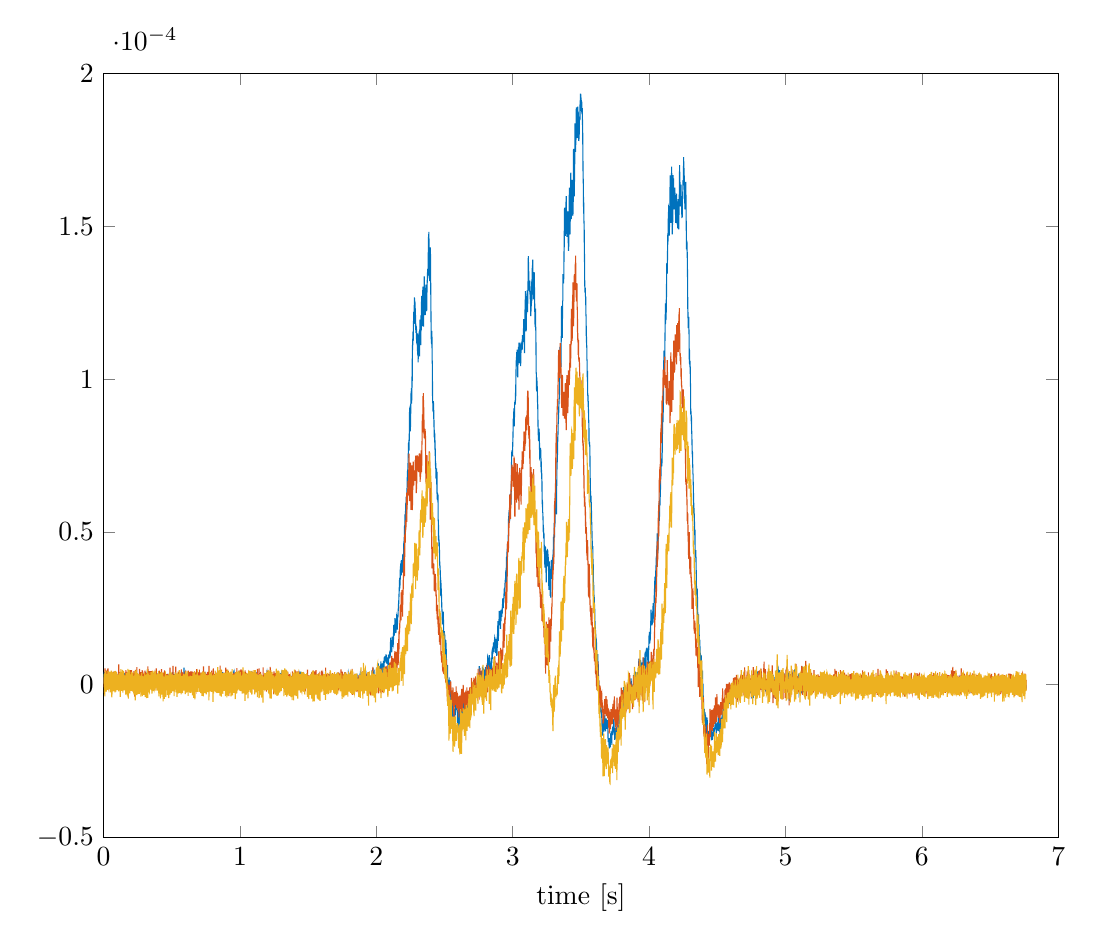
\begin{tikzpicture}

\begin{axis}[%
width=\textwidth,
height=0.8\textwidth,
at={(0\figurewidth,0\figureheight)},
scale only axis,
xmin=0,
xmax=7,
xlabel={time [s]},
ymin=-5e-05,
ymax=0.0002,
ylabel={},
axis background/.style={fill=white},
% title style={font=\bfseries},
% title={Train 4},
% legend style={legend cell align=left,align=left,draw=white!15!black}
]
\addplot [color=mycolor1,solid,forget plot]
  table[row sep=crcr]{%
0	4.08762316295294e-07\\
0.0009765625	1.19213149070928e-06\\
0.001953125	2.03196105632306e-06\\
0.0029296875	7.1928688850139e-07\\
0.00390625	1.20624626176935e-06\\
0.0048828125	3.99392129004066e-06\\
0.005859375	1.26270534995913e-06\\
0.0068359375	1.53088610518187e-06\\
0.0078125	2.4342328562685e-06\\
0.0087890625	2.15193682272653e-06\\
0.009765625	2.13782202519762e-06\\
0.0107421875	1.46031220840128e-06\\
0.01171875	1.67909132056882e-06\\
0.0126953125	1.60851740304787e-06\\
0.013671875	2.71652904783532e-06\\
0.0146484375	1.42502526371473e-06\\
0.015625	2.1801664189696e-06\\
0.0166015625	1.20624626176935e-06\\
0.017578125	1.69320610525817e-06\\
0.0185546875	1.67203392837235e-06\\
0.01953125	4.0503806903304e-06\\
0.0205078125	1.77083742811178e-06\\
0.021484375	3.03411245223748e-06\\
0.0224609375	2.03196105632306e-06\\
0.0234375	2.08842023695734e-06\\
0.0244140625	1.86258355234625e-06\\
0.025390625	1.47639528576401e-07\\
0.0263671875	2.24368301629443e-06\\
0.02734375	1.67909132056882e-06\\
0.0283203125	2.34248662803389e-06\\
0.029296875	1.89081313239155e-06\\
0.0302734375	1.89081313239155e-06\\
0.03125	3.08351433311958e-06\\
0.0322265625	2.56832352755879e-06\\
0.033203125	3.50695922491664e-06\\
0.0341796875	7.05172131071265e-07\\
0.03515625	4.93450817025051e-07\\
0.0361328125	2.61066795747894e-06\\
0.037109375	1.46031220840128e-06\\
0.0380859375	2.28602741895534e-06\\
0.0390625	3.25289224717179e-06\\
0.0400390625	3.07645692126869e-06\\
0.041015625	3.69750954222568e-06\\
0.0419921875	2.75887349019972e-06\\
0.04296875	1.36150876950099e-06\\
0.0439453125	1.41091048653152e-06\\
0.044921875	1.97550188200946e-06\\
0.0458984375	1.70026349775127e-06\\
0.046875	2.42717545350366e-06\\
0.0478515625	1.79200960914619e-06\\
0.048828125	2.32131442388841e-06\\
0.0498046875	2.04607585088906e-06\\
0.05078125	2.47657727492942e-06\\
0.0517578125	1.06509856894897e-06\\
0.052734375	1.72849306871053e-06\\
0.0537109375	9.87467354736978e-07\\
0.0546875	2.49069208193967e-06\\
0.0556640625	3.12585880629917e-06\\
0.056640625	1.5802878388046e-06\\
0.0576171875	7.33401646326815e-07\\
0.05859375	2.30719962161872e-06\\
0.0595703125	9.80409972219836e-07\\
0.060546875	2.99882539742699e-06\\
0.0615234375	2.94236611486686e-06\\
0.0625	1.21330364744694e-06\\
0.0634765625	2.1801664189696e-06\\
0.064453125	2.97059575535665e-06\\
0.0654296875	2.30014222063241e-06\\
0.06640625	6.34598349846024e-07\\
0.0673828125	6.29510859204152e-08\\
0.068359375	1.69320610525817e-06\\
0.0693359375	2.3636588330682e-06\\
0.0703125	1.24859057731895e-06\\
0.0712890625	2.90707906647658e-06\\
0.072265625	1.10038548845016e-06\\
0.0732421875	4.51106564882406e-07\\
0.07421875	2.82944756870907e-06\\
0.0751953125	1.20624626176935e-06\\
0.076171875	6.62827861150957e-07\\
0.0771484375	1.0298116519163e-06\\
0.078125	1.50971393511048e-06\\
0.0791015625	3.77514117362327e-06\\
0.080078125	2.56832352755879e-06\\
0.0810546875	3.73985406696103e-06\\
0.08203125	1.34739399409545e-06\\
0.0830078125	1.5661730572757e-06\\
0.083984375	2.68829942156744e-06\\
0.0849609375	7.89860681578262e-07\\
0.0859375	2.82944756870907e-06\\
0.0869140625	9.02778771044721e-07\\
0.087890625	1.43914004129301e-06\\
0.0888671875	7.33401646326815e-07\\
0.08984375	2.99176798676157e-06\\
0.0908203125	4.65221315201683e-07\\
0.091796875	2.31425702270434e-06\\
0.0927734375	9.6629520748067e-07\\
0.09375	7.82803301826269e-07\\
0.0947265625	2.08842023695734e-06\\
0.095703125	8.32204962165168e-07\\
0.0966796875	1.17095933486046e-06\\
0.09765625	1.30504967024952e-06\\
0.0986328125	1.63674696887104e-06\\
0.099609375	1.80612439699599e-06\\
0.1005859375	2.86473461166706e-06\\
0.1015625	2.75181608289207e-06\\
0.1025390625	1.71437828303347e-06\\
0.103515625	1.61557479435529e-06\\
0.1044921875	2.38483103899112e-06\\
0.10546875	1.31210705731034e-06\\
0.1064453125	1.62263218576181e-06\\
0.107421875	1.94021490127405e-06\\
0.1083984375	1.9966740716366e-06\\
0.109375	2.14487942391275e-06\\
0.1103515625	3.95863416806992e-06\\
0.111328125	9.82379352988758e-08\\
0.1123046875	1.08627072035322e-06\\
0.11328125	1.49559915555678e-06\\
0.1142578125	2.08136283903239e-06\\
0.115234375	2.21545341649539e-06\\
0.1162109375	1.98255927845318e-06\\
0.1171875	2.11664982964488e-06\\
0.1181640625	1.97550188200946e-06\\
0.119140625	1.71437828303347e-06\\
0.1201171875	2.4342328562685e-06\\
0.12109375	2.19428121768354e-06\\
0.1220703125	2.62478276824248e-06\\
0.123046875	1.22741841909941e-06\\
0.1240234375	1.41091048653152e-06\\
0.125	1.11450025694197e-06\\
0.1259765625	2.20839601679278e-06\\
0.126953125	1.48854176592835e-06\\
0.1279296875	1.77789482169125e-06\\
0.12890625	2.2366256161963e-06\\
0.1298828125	2.08136283903239e-06\\
0.130859375	1.5026565452843e-06\\
0.1318359375	3.28112190504481e-06\\
0.1328125	2.82239016041372e-06\\
0.1337890625	1.5026565452843e-06\\
0.134765625	2.60361055224559e-06\\
0.1357421875	2.82239016041372e-06\\
0.13671875	2.27897001826459e-06\\
0.1376953125	2.02490365918827e-06\\
0.138671875	1.87669834217125e-06\\
0.1396484375	3.05528468630867e-06\\
0.140625	2.48363467838532e-06\\
0.1416015625	2.85767720287797e-06\\
0.142578125	2.02490365918827e-06\\
0.1435546875	3.1399736314826e-06\\
0.14453125	2.04607585088906e-06\\
0.1455078125	2.16605162065052e-06\\
0.146484375	6.48713105301166e-07\\
0.1474609375	2.377773636918e-06\\
0.1484375	3.02705504107788e-06\\
0.1494140625	1.46736959763484e-06\\
0.150390625	3.12585880629917e-06\\
0.1513671875	3.81042828275489e-06\\
0.15234375	1.72143567582234e-06\\
0.1533203125	1.67203392837235e-06\\
0.154296875	2.26485521718015e-06\\
0.1552734375	2.1801664189696e-06\\
0.15625	2.73770126857321e-06\\
0.1572265625	1.50971393511048e-06\\
0.158203125	1.89081313239155e-06\\
0.1591796875	1.94021490127405e-06\\
0.16015625	2.42011805083814e-06\\
0.1611328125	1.82729657951164e-06\\
0.162109375	2.39894584343355e-06\\
0.1630859375	2.19428121768354e-06\\
0.1640625	2.13782202519762e-06\\
0.1650390625	2.02490365918827e-06\\
0.166015625	5.92254085851531e-07\\
0.1669921875	1.62263218576181e-06\\
0.16796875	9.45123061113192e-07\\
0.1689453125	2.1237072280638e-06\\
0.169921875	2.4342328562685e-06\\
0.1708984375	2.02490365918827e-06\\
0.171875	2.69535682798625e-06\\
0.1728515625	2.94236611486686e-06\\
0.173828125	2.99176798676157e-06\\
0.1748046875	1.00863950288233e-06\\
0.17578125	2.8365049771033e-06\\
0.1767578125	2.22251081629711e-06\\
0.177734375	2.51892169714587e-06\\
0.1787109375	2.67418460902602e-06\\
0.1796875	2.92119388553645e-06\\
0.1806640625	2.49774948559334e-06\\
0.181640625	2.50480688934523e-06\\
0.1826171875	3.514016642792e-06\\
0.18359375	1.16390194977484e-06\\
0.1845703125	2.03901845355673e-06\\
0.185546875	2.80827534411923e-06\\
0.1865234375	1.24153319114697e-06\\
0.1875	3.36581088814457e-06\\
0.1884765625	1.66497653627433e-06\\
0.189453125	1.92610010967095e-06\\
0.1904296875	1.3191644444696e-06\\
0.19140625	2.6388975794009e-06\\
0.1923828125	3.13291621884177e-06\\
0.193359375	9.45123061113192e-07\\
0.1943359375	4.09272524469527e-06\\
0.1953125	3.02901710383646e-07\\
0.1962890625	1.2838775096597e-06\\
0.197265625	1.41091048653152e-06\\
0.1982421875	1.44619743023037e-06\\
0.19921875	1.19213149070928e-06\\
0.2001953125	1.60851740304787e-06\\
0.201171875	2.14487942391275e-06\\
0.2021484375	3.83160054941872e-06\\
0.203125	6.41655727524155e-07\\
0.2041015625	2.07430544120653e-06\\
0.205078125	1.90492792300693e-06\\
0.2060546875	1.25564796358939e-06\\
0.20703125	7.40459025387304e-07\\
0.2080078125	2.92119388553645e-06\\
0.208984375	1.61754270401604e-07\\
0.2099609375	1.02275426880653e-06\\
0.2109375	2.73064386156177e-06\\
0.2119140625	2.03901845355673e-06\\
0.212890625	2.70241423450373e-06\\
0.2138671875	3.26700707591076e-06\\
0.21484375	1.51677132503554e-06\\
0.2158203125	2.39894584343355e-06\\
0.216796875	2.79416052821981e-06\\
0.2177734375	2.32327985454301e-07\\
0.21875	1.90492792300693e-06\\
0.2197265625	2.1589942216392e-06\\
0.220703125	1.9190427140174e-06\\
0.2216796875	1.27682012299418e-06\\
0.22265625	1.79200960914619e-06\\
0.2236328125	2.74475867568309e-06\\
0.224609375	2.27897001826459e-06\\
0.2255859375	1.3967957097434e-06\\
0.2265625	3.83160054941872e-06\\
0.2275390625	6.91057374036007e-07\\
0.228515625	6.06368840121206e-07\\
0.2294921875	1.67909132056882e-06\\
0.23046875	1.94727229722337e-06\\
0.2314453125	9.52180443136805e-07\\
0.232421875	2.46246246831403e-06\\
0.2333984375	2.38483103899112e-06\\
0.234375	5.64024578497213e-07\\
0.2353515625	2.377773636918e-06\\
0.236328125	2.20133861718861e-06\\
0.2373046875	2.75181608289207e-06\\
0.23828125	1.62263218576181e-06\\
0.2392578125	2.1589942216392e-06\\
0.240234375	3.85277281697181e-06\\
0.2412109375	2.17310901976073e-06\\
0.2421875	2.30719962161872e-06\\
0.2431640625	2.08136283903239e-06\\
0.244140625	7.61631163162481e-07\\
0.2451171875	1.74966524796663e-06\\
0.24609375	2.10959243132506e-06\\
0.2470703125	1.80612439699599e-06\\
0.248046875	1.5026565452843e-06\\
0.2490234375	1.63674696887104e-06\\
0.25	1.45325481926638e-06\\
0.2509765625	2.94236611486686e-06\\
0.251953125	2.17310901976073e-06\\
0.2529296875	1.72849306871053e-06\\
0.25390625	1.5661730572757e-06\\
0.2548828125	2.81533275221725e-06\\
0.255859375	7.61631163162481e-07\\
0.2568359375	2.74475867568309e-06\\
0.2578125	2.8012179361203e-06\\
0.2587890625	2.04607585088906e-06\\
0.259765625	1.61557479435529e-06\\
0.2607421875	1.67909132056882e-06\\
0.26171875	1.84141136834915e-06\\
0.2626953125	1.26976273642689e-06\\
0.263671875	3.74691148809594e-06\\
0.2646484375	4.13506980261611e-06\\
0.265625	2.42011805083814e-06\\
0.2666015625	2.53500101896065e-07\\
0.267578125	1.71437828303347e-06\\
0.2685546875	1.3544513817491e-06\\
0.26953125	4.44049189870978e-07\\
0.2705078125	1.13567241042051e-06\\
0.271484375	2.1589942216392e-06\\
0.2724609375	1.91198531846316e-06\\
0.2734375	2.25779781678624e-06\\
0.2744140625	2.01078886521489e-06\\
0.275390625	-2.05228888662881e-07\\
0.2763671875	3.71162438340912e-06\\
0.27734375	1.89787052765024e-06\\
0.2783203125	1.94727229722337e-06\\
0.279296875	1.48854176592835e-06\\
0.2802734375	1.66497653627433e-06\\
0.28125	8.88664008478731e-07\\
0.2822265625	1.00158212006833e-06\\
0.283203125	1.84141136834915e-06\\
0.2841796875	3.62693534223472e-06\\
0.28515625	1.5026565452843e-06\\
0.2861328125	-4.45179271349027e-07\\
0.287109375	2.99882539742699e-06\\
0.2880859375	1.51677132503554e-06\\
0.2890625	9.0983615247571e-07\\
0.2900390625	9.73352589800705e-07\\
0.291015625	2.00373146837631e-06\\
0.2919921875	2.13076462658116e-06\\
0.29296875	2.97765316572629e-06\\
0.2939453125	2.93530870499139e-06\\
0.294921875	5.0756556852936e-07\\
0.2958984375	-3.46376186422751e-07\\
0.296875	1.43208265245454e-06\\
0.2978515625	2.38483103899112e-06\\
0.298828125	1.22036103322406e-06\\
0.2998046875	2.58243833713709e-06\\
0.30078125	9.87467354736978e-07\\
0.3017578125	1.74260785478267e-06\\
0.302734375	3.50695922491664e-06\\
0.3037109375	2.58949574207467e-06\\
0.3046875	1.61557479435529e-06\\
0.3056640625	2.75887349019972e-06\\
0.306640625	6.48713105301166e-07\\
0.3076171875	2.53303650534116e-06\\
0.30859375	3.19643293616653e-06\\
0.3095703125	7.54573783805571e-07\\
0.310546875	3.28817931975929e-06\\
0.3115234375	7.12229509736671e-07\\
0.3125	2.51892169714587e-06\\
0.3134765625	9.31008297361952e-07\\
0.314453125	2.06019064585036e-06\\
0.3154296875	2.14487942391275e-06\\
0.31640625	2.53303650534116e-06\\
0.3173828125	2.27897001826459e-06\\
0.318359375	1.43208265245454e-06\\
0.3193359375	2.76593089760624e-06\\
0.3203125	2.54715131393197e-06\\
0.3212890625	2.01784626215214e-06\\
0.322265625	1.69320610525817e-06\\
0.3232421875	1.55911566665913e-06\\
0.32421875	2.94942352484142e-06\\
0.3251953125	5.14622944429617e-07\\
0.326171875	1.5026565452843e-06\\
0.3271484375	1.54500088572285e-06\\
0.328125	4.65221315201683e-07\\
0.3291015625	2.54715131393197e-06\\
0.330078125	1.41796787507358e-06\\
0.3310546875	1.26976273642689e-06\\
0.33203125	2.69535682798625e-06\\
0.3330078125	1.89081313239155e-06\\
0.333984375	3.27406449042813e-06\\
0.3349609375	1.97550188200946e-06\\
0.3359375	2.6177253628116e-06\\
0.3369140625	1.13567241042051e-06\\
0.337890625	1.19918887618977e-06\\
0.3388671875	1.94021490127405e-06\\
0.33984375	1.51677132503554e-06\\
0.3408203125	9.38065679188024e-07\\
0.341796875	1.91198531846316e-06\\
0.3427734375	9.73352589800705e-07\\
0.34375	1.65086175237515e-06\\
0.3447265625	2.15193682272653e-06\\
0.345703125	3.99392129004066e-06\\
0.3466796875	2.50480688934523e-06\\
0.34765625	5.99311462937038e-07\\
0.3486328125	3.4857869718821e-06\\
0.349609375	2.90002165709465e-06\\
0.3505859375	1.62968957726677e-06\\
0.3515625	1.17095933486046e-06\\
0.3525390625	3.42932763480307e-06\\
0.353515625	1.81318179106899e-06\\
0.3544921875	2.69535682798625e-06\\
0.35546875	8.88664008478731e-07\\
0.3564453125	8.67491865370364e-07\\
0.357421875	1.52382871505927e-06\\
0.3583984375	1.31210705731034e-06\\
0.359375	1.68614871286438e-06\\
0.3603515625	-1.62884691631317e-07\\
0.361328125	1.2838775096597e-06\\
0.3623046875	2.03901845355673e-06\\
0.36328125	3.89511735474427e-06\\
0.3642578125	2.32131442388841e-06\\
0.365234375	1.9966740716366e-06\\
0.3662109375	2.85061979418753e-06\\
0.3671875	3.64105018144274e-06\\
0.3681640625	2.85767720287797e-06\\
0.369140625	1.9190427140174e-06\\
0.3701171875	3.06939950951647e-06\\
0.37109375	3.02705504107788e-06\\
0.3720703125	3.03411245223748e-06\\
0.373046875	2.34248662803389e-06\\
0.3740234375	2.73064386156177e-06\\
0.375	3.08351433311958e-06\\
0.3759765625	2.02490365918827e-06\\
0.376953125	2.92119388553645e-06\\
0.3779296875	1.61557479435529e-06\\
0.37890625	1.23447580507407e-06\\
0.3798828125	1.88375573723239e-06\\
0.380859375	2.07430544120653e-06\\
0.3818359375	1.25564796358939e-06\\
0.3828125	2.65301239095461e-06\\
0.3837890625	1.70026349775127e-06\\
0.384765625	2.11664982964488e-06\\
0.3857421875	3.2176051770528e-06\\
0.38671875	2.49069208193967e-06\\
0.3876953125	3.89511735474427e-06\\
0.388671875	1.72143567582234e-06\\
0.3896484375	1.55205827614188e-06\\
0.390625	1.60851740304787e-06\\
0.3916015625	3.04116986349573e-06\\
0.392578125	7.33401646326815e-07\\
0.3935546875	3.12585880629917e-06\\
0.39453125	2.17310901976073e-06\\
0.3955078125	2.91413647595697e-06\\
0.396484375	3.60576308416319e-06\\
0.3974609375	1.41091048653152e-06\\
0.3984375	6.41655727524155e-07\\
0.3994140625	2.95648093491421e-06\\
0.400390625	1.55205827614188e-06\\
0.4013671875	9.94524737353434e-07\\
0.40234375	1.24859057731895e-06\\
0.4033203125	1.9190427140174e-06\\
0.404296875	1.78495221536917e-06\\
0.4052734375	1.21330364744694e-06\\
0.40625	2.10253503310368e-06\\
0.4072265625	3.07645692126869e-06\\
0.408203125	1.70026349775127e-06\\
0.4091796875	2.30719962161872e-06\\
0.41015625	2.04607585088906e-06\\
0.4111328125	8.7454924630804e-07\\
0.412109375	1.29093489642431e-06\\
0.4130859375	5.14622944429617e-07\\
0.4140625	1.30504967024952e-06\\
0.4150390625	1.36856615735219e-06\\
0.416015625	1.42502526371473e-06\\
0.4169921875	2.74475867568309e-06\\
0.41796875	1.43208265245454e-06\\
0.4189453125	2.01784626215214e-06\\
0.419921875	1.26270534995913e-06\\
0.4208984375	8.2514758182055e-07\\
0.421875	1.90492792300693e-06\\
0.4228515625	6.55770483176622e-07\\
0.423828125	3.04116986349573e-06\\
0.4248046875	2.40600324580308e-06\\
0.42578125	3.95157674397168e-06\\
0.4267578125	3.73475445188988e-07\\
0.427734375	7.26344267364554e-07\\
0.4287109375	2.49774948559334e-06\\
0.4296875	1.91198531846316e-06\\
0.4306640625	1.45325481926638e-06\\
0.431640625	1.74966524796663e-06\\
0.4326171875	2.31425702270434e-06\\
0.43359375	1.32622183172818e-06\\
0.4345703125	2.8365049771033e-06\\
0.435546875	1.48148437639837e-06\\
0.4365234375	3.00588280819172e-06\\
0.4375	1.61754270401604e-07\\
0.4384765625	1.65791914427541e-06\\
0.439453125	3.04822727485287e-06\\
0.4404296875	1.74260785478267e-06\\
0.44140625	1.93315750542295e-06\\
0.4423828125	1.88375573723239e-06\\
0.443359375	1.29799228328759e-06\\
0.4443359375	1.92610010967095e-06\\
0.4453125	2.52597910119418e-06\\
0.4462890625	3.06234209786335e-06\\
0.447265625	1.75869012622324e-07\\
0.4482421875	2.77298830511142e-06\\
0.44921875	1.90492792300693e-06\\
0.4501953125	1.70026349775127e-06\\
0.451171875	2.22956821619748e-06\\
0.4521484375	1.0298116519163e-06\\
0.453125	7.05172131071265e-07\\
0.4541015625	1.64380436057355e-06\\
0.455078125	1.91198531846316e-06\\
0.4560546875	1.93315750542295e-06\\
0.45703125	6.91057374036007e-07\\
0.4580078125	2.82944756870907e-06\\
0.458984375	2.05313324832027e-06\\
0.4599609375	1.89081313239155e-06\\
0.4609375	1.43914004129301e-06\\
0.4619140625	1.43914004129301e-06\\
0.462890625	1.89787052765024e-06\\
0.4638671875	1.43208265245454e-06\\
0.46484375	2.37071623494355e-06\\
0.4658203125	3.07645692126869e-06\\
0.466796875	1.86258355234625e-06\\
0.4677734375	2.80827534411923e-06\\
0.46875	1.0439264184329e-06\\
0.4697265625	2.1589942216392e-06\\
0.470703125	2.38483103899112e-06\\
0.4716796875	1.80612439699599e-06\\
0.47265625	8.03975441378887e-07\\
0.4736328125	7.47516404547106e-07\\
0.474609375	2.3354292265534e-06\\
0.4755859375	1.9190427140174e-06\\
0.4765625	2.68124201524751e-06\\
0.4775390625	2.78004571271548e-06\\
0.478515625	1.34739399409545e-06\\
0.4794921875	7.82803301826269e-07\\
0.48046875	1.98255927845318e-06\\
0.4814453125	1.46736959763484e-06\\
0.482421875	1.22741841909941e-06\\
0.4833984375	7.75745922172721e-07\\
0.484375	3.54224631528223e-06\\
0.4853515625	2.76593089760624e-06\\
0.486328125	3.40109796863374e-06\\
0.4873046875	2.03196105632306e-06\\
0.48828125	2.10253503310368e-06\\
0.4892578125	1.05098380183974e-06\\
0.490234375	2.28602741895534e-06\\
0.4912109375	2.30014222063241e-06\\
0.4921875	2.11664982964488e-06\\
0.4931640625	1.65791914427541e-06\\
0.494140625	1.19213149070928e-06\\
0.4951171875	2.02490365918827e-06\\
0.49609375	2.27897001826459e-06\\
0.4970703125	3.72573922498743e-06\\
0.498046875	2.63184017377247e-06\\
0.4990234375	2.62478276824248e-06\\
0.5	1.06509856894897e-06\\
0.5009765625	2.4342328562685e-06\\
0.501953125	1.9190427140174e-06\\
0.5029296875	2.56126612291807e-06\\
0.50390625	2.01078886521489e-06\\
0.5048828125	3.06234209786335e-06\\
0.505859375	1.96138708941909e-06\\
0.5068359375	2.55420871837558e-06\\
0.5078125	4.15624208291009e-06\\
0.5087890625	3.3818857655141e-07\\
0.509765625	2.47657727492942e-06\\
0.5107421875	1.62968957726677e-06\\
0.51171875	2.42717545350366e-06\\
0.5126953125	1.14272979511105e-06\\
0.513671875	2.6600697968799e-06\\
0.5146484375	1.5802878388046e-06\\
0.515625	1.5944026207288e-06\\
0.5166015625	2.49069208193967e-06\\
0.517578125	3.43638505159206e-06\\
0.5185546875	3.01999763001695e-06\\
0.51953125	1.62968957726677e-06\\
0.5205078125	2.8365049771033e-06\\
0.521484375	2.54715131393197e-06\\
0.5224609375	2.02490365918827e-06\\
0.5234375	1.57323044799049e-06\\
0.5244140625	1.19918887618977e-06\\
0.525390625	1.22741841909941e-06\\
0.5263671875	3.11880139385566e-06\\
0.52734375	3.93746189607247e-06\\
0.5283203125	3.19643293616653e-06\\
0.529296875	1.70026349775127e-06\\
0.5302734375	3.50695922491664e-06\\
0.53125	1.94727229722337e-06\\
0.5322265625	2.6388975794009e-06\\
0.533203125	1.80612439699599e-06\\
0.5341796875	1.77789482169125e-06\\
0.53515625	1.46736959763484e-06\\
0.5361328125	1.36150876950099e-06\\
0.537109375	1.67203392837235e-06\\
0.5380859375	1.46736959763484e-06\\
0.5390625	1.9966740716366e-06\\
0.5400390625	-3.74605641234463e-07\\
0.541015625	1.77083742811178e-06\\
0.5419921875	1.61557479435529e-06\\
0.54296875	2.81533275221725e-06\\
0.5439453125	1.2838775096597e-06\\
0.544921875	1.82729657951164e-06\\
0.5458984375	3.56341857068706e-06\\
0.546875	2.6177253628116e-06\\
0.5478515625	2.44834766209372e-06\\
0.548828125	2.377773636918e-06\\
0.5498046875	2.65301239095461e-06\\
0.55078125	1.13567241042051e-06\\
0.5517578125	2.51186429319622e-06\\
0.552734375	1.5944026207288e-06\\
0.5537109375	3.1399736314826e-06\\
0.5546875	1.16390194977484e-06\\
0.5556640625	9.87467354736978e-07\\
0.556640625	2.41306064827107e-06\\
0.5576171875	3.09057174506934e-06\\
0.55859375	1.60146001183868e-06\\
0.5595703125	3.32346639481682e-06\\
0.560546875	1.94727229722337e-06\\
0.5615234375	1.72849306871053e-06\\
0.5625	9.87467354736978e-07\\
0.5634765625	2.27897001826459e-06\\
0.564453125	2.58949574207467e-06\\
0.5654296875	2.97765316572629e-06\\
0.56640625	3.23172000480407e-06\\
0.5673828125	2.08136283903239e-06\\
0.568359375	2.21545341649539e-06\\
0.5693359375	3.00588280819172e-06\\
0.5703125	1.70026349775127e-06\\
0.5712890625	1.51677132503554e-06\\
0.572265625	2.25074041649079e-06\\
0.5732421875	2.06019064585036e-06\\
0.57421875	2.34248662803389e-06\\
0.5751953125	1.32622183172818e-06\\
0.576171875	3.30935156449773e-06\\
0.5771484375	2.49774948559334e-06\\
0.578125	3.06939950951647e-06\\
0.5791015625	2.4342328562685e-06\\
0.580078125	1.83435397388106e-06\\
0.5810546875	2.67614846684392e-07\\
0.58203125	1.77789482169125e-06\\
0.5830078125	1.66497653627433e-06\\
0.583984375	1.96844448566527e-06\\
0.5849609375	2.44129025913135e-06\\
0.5859375	1.98961667499534e-06\\
0.5869140625	1.54500088572285e-06\\
0.587890625	2.94236611486686e-06\\
0.5888671875	2.6388975794009e-06\\
0.58984375	5.61007412255539e-06\\
0.5908203125	1.10038548845016e-06\\
0.591796875	1.78495221536917e-06\\
0.5927734375	4.28327578333898e-06\\
0.59375	1.9966740716366e-06\\
0.5947265625	1.41796787507358e-06\\
0.595703125	2.13076462658116e-06\\
0.5966796875	3.36581088814457e-06\\
0.59765625	3.42227021811253e-06\\
0.5986328125	1.63674696887104e-06\\
0.599609375	2.40600324580308e-06\\
0.6005859375	3.23172000480407e-06\\
0.6015625	2.95648093491421e-06\\
0.6025390625	6.62827861150957e-07\\
0.603515625	2.27191261767336e-06\\
0.6044921875	2.95648093491421e-06\\
0.60546875	3.30229414948597e-06\\
0.6064453125	1.54500088572285e-06\\
0.607421875	2.55420871837558e-06\\
0.6083984375	3.55636115211997e-06\\
0.609375	1.18507410532768e-06\\
0.6103515625	2.01078886521489e-06\\
0.611328125	2.10253503310368e-06\\
0.6123046875	3.06939950951647e-06\\
0.61328125	1.07215595265137e-06\\
0.6142578125	2.97765316572629e-06\\
0.615234375	3.3113120312075e-07\\
0.6162109375	2.45540506515454e-06\\
0.6171875	2.15193682272653e-06\\
0.6181640625	1.95432969327222e-06\\
0.619140625	2.44129025913135e-06\\
0.6201171875	2.73770126857321e-06\\
0.62109375	5.58937163412741e-08\\
0.6220703125	7.61631163162481e-07\\
0.623046875	1.77083742811178e-06\\
0.6240234375	3.19643293616653e-06\\
0.625	2.61066795747894e-06\\
0.6259765625	1.96844448566527e-06\\
0.626953125	1.96844448566527e-06\\
0.6279296875	3.54930373365199e-06\\
0.62890625	2.75887349019972e-06\\
0.6298828125	3.60576308416319e-06\\
0.630859375	2.66712720290341e-06\\
0.6318359375	-5.22810253068395e-07\\
0.6328125	2.86473461166706e-06\\
0.6337890625	1.62263218576181e-06\\
0.634765625	2.89296424781159e-06\\
0.6357421875	6.49213205091738e-09\\
0.63671875	2.34954402961326e-06\\
0.6376953125	1.29799228328759e-06\\
0.638671875	1.84846876291611e-06\\
0.6396484375	2.78004571271548e-06\\
0.640625	3.47167213701977e-06\\
0.6416015625	3.85277281697181e-06\\
0.642578125	2.53500101896065e-07\\
0.6435546875	3.32346639481682e-06\\
0.64453125	2.86473461166706e-06\\
0.6455078125	7.26344267364554e-07\\
0.646484375	1.5661730572757e-06\\
0.6474609375	6.83999995666372e-07\\
0.6484375	2.1237072280638e-06\\
0.6494140625	1.69320610525817e-06\\
0.650390625	2.32837182517157e-06\\
0.6513671875	3.37992572004399e-06\\
0.65234375	1.25564796358939e-06\\
0.6533203125	1.97550188200946e-06\\
0.654296875	2.61066795747894e-06\\
0.6552734375	1.61557479435529e-06\\
0.65625	9.87467354736978e-07\\
0.6572265625	1.97550188200946e-06\\
0.658203125	2.56126612291807e-06\\
0.6591796875	1.58734522971715e-06\\
0.66015625	3.04822727485287e-06\\
0.6611328125	9.80409972219836e-07\\
0.662109375	1.98961667499534e-06\\
0.6630859375	1.71437828303347e-06\\
0.6640625	1.25564796358939e-06\\
0.6650390625	2.07430544120653e-06\\
0.666015625	2.81533275221725e-06\\
0.6669921875	1.82023918524109e-06\\
0.66796875	1.5802878388046e-06\\
0.6689453125	1.44619743023037e-06\\
0.669921875	2.32837182517157e-06\\
0.6708984375	8.53377103792081e-07\\
0.671875	-5.7024183496273e-08\\
0.6728515625	3.02705504107788e-06\\
0.673828125	-1.28500471164705e-06\\
0.6748046875	1.82023918524109e-06\\
0.67578125	-5.7024183496273e-08\\
0.6767578125	1.90492792300693e-06\\
0.677734375	9.73352589800705e-07\\
0.6787109375	2.16605162065052e-06\\
0.6796875	2.69535682798625e-06\\
0.6806640625	1.79200960914619e-06\\
0.681640625	3.1399736314826e-06\\
0.6826171875	1.16390194977484e-06\\
0.68359375	1.43208265245454e-06\\
0.6845703125	1.9190427140174e-06\\
0.685546875	1.33327921908498e-06\\
0.6865234375	1.89787052765024e-06\\
0.6875	1.60851740304787e-06\\
0.6884765625	1.48148437639837e-06\\
0.689453125	1.5802878388046e-06\\
0.6904296875	2.20839601679278e-06\\
0.69140625	3.55636115211997e-06\\
0.6923828125	1.48854176592835e-06\\
0.693359375	1.96844448566527e-06\\
0.6943359375	1.44619743023037e-06\\
0.6953125	1.24859057731895e-06\\
0.6962890625	1.5944026207288e-06\\
0.697265625	1.72849306871053e-06\\
0.6982421875	3.240738297881e-07\\
0.69921875	3.14703104422275e-06\\
0.7001953125	1.70732089034261e-06\\
0.701171875	3.38698313614191e-06\\
0.7021484375	6.83999995666372e-07\\
0.703125	1.67909132056882e-06\\
0.7041015625	2.18722381827735e-06\\
0.705078125	5.56967201905669e-07\\
0.7060546875	1.19918887618977e-06\\
0.70703125	2.49069208193967e-06\\
0.7080078125	2.05313324832027e-06\\
0.708984375	1.22036103322406e-06\\
0.7099609375	2.02490365918827e-06\\
0.7109375	2.53303650534116e-06\\
0.7119140625	2.03901845355673e-06\\
0.712890625	2.32131442388841e-06\\
0.7138671875	5.85196708864904e-07\\
0.71484375	1.80612439699599e-06\\
0.7158203125	2.15193682272653e-06\\
0.716796875	1.44619743023037e-06\\
0.7177734375	1.72143567582234e-06\\
0.71875	2.39894584343355e-06\\
0.7197265625	3.14703104422275e-06\\
0.720703125	3.23877741882791e-06\\
0.7216796875	2.04607585088906e-06\\
0.72265625	2.13782202519762e-06\\
0.7236328125	2.08136283903239e-06\\
0.724609375	1.94727229722337e-06\\
0.7255859375	2.8365049771033e-06\\
0.7265625	2.67614846684392e-07\\
0.7275390625	2.13076462658116e-06\\
0.728515625	1.43914004129301e-06\\
0.7294921875	3.45755730255253e-06\\
0.73046875	2.4342328562685e-06\\
0.7314453125	2.20133861718861e-06\\
0.732421875	9.31008297361952e-07\\
0.7333984375	1.1568445647881e-06\\
0.734375	2.75181608289207e-06\\
0.7353515625	1.0439264184329e-06\\
0.736328125	1.69320610525817e-06\\
0.7373046875	2.54715131393197e-06\\
0.73828125	1.09332810435247e-06\\
0.7392578125	2.30014222063241e-06\\
0.740234375	1.22741841909941e-06\\
0.7412109375	3.24583483295019e-06\\
0.7421875	2.3354292265534e-06\\
0.7431640625	2.27897001826459e-06\\
0.744140625	2.00373146837631e-06\\
0.7451171875	1.9966740716366e-06\\
0.74609375	1.78495221536917e-06\\
0.7470703125	1.74260785478267e-06\\
0.748046875	1.65791914427541e-06\\
0.7490234375	1.12155764133608e-06\\
0.75	2.90707906647658e-06\\
0.7509765625	2.71652904783532e-06\\
0.751953125	2.78710312041843e-06\\
0.7529296875	2.61066795747894e-06\\
0.75390625	6.76942617396049e-07\\
0.7548828125	1.74260785478267e-06\\
0.755859375	2.08842023695734e-06\\
0.7568359375	1.96138708941909e-06\\
0.7578125	2.01078886521489e-06\\
0.7587890625	1.3544513817491e-06\\
0.759765625	9.38065679188024e-07\\
0.7607421875	3.2176051770528e-06\\
0.76171875	2.27191261767336e-06\\
0.7626953125	3.09762915711776e-06\\
0.763671875	9.80409972219836e-07\\
0.7646484375	1.54500088572285e-06\\
0.765625	2.35660143129129e-06\\
0.7666015625	2.3354292265534e-06\\
0.767578125	1.43914004129301e-06\\
0.7685546875	1.86258355234625e-06\\
0.76953125	1.07921333645307e-06\\
0.7705078125	1.01569688579477e-06\\
0.771484375	2.75887349019972e-06\\
0.7724609375	2.44834766209372e-06\\
0.7734375	1.55911566665913e-06\\
0.7744140625	9.73352589800705e-07\\
0.775390625	1.54500088572285e-06\\
0.7763671875	1.60851740304787e-06\\
0.77734375	1.38268093335015e-06\\
0.7783203125	9.6629520748067e-07\\
0.779296875	3.23877741882791e-06\\
0.7802734375	1.73555046169695e-06\\
0.78125	2.07430544120653e-06\\
0.7822265625	2.39188844116311e-06\\
0.783203125	1.86258355234625e-06\\
0.7841796875	1.91198531846316e-06\\
0.78515625	-7.27473693043837e-07\\
0.7861328125	3.58459082698093e-06\\
0.787109375	1.96844448566527e-06\\
0.7880859375	2.04607585088906e-06\\
0.7890625	1.26976273642689e-06\\
0.7900390625	3.24583483295019e-06\\
0.791015625	1.22036103322406e-06\\
0.7919921875	1.63674696887104e-06\\
0.79296875	2.00373146837631e-06\\
0.7939453125	9.31008297361952e-07\\
0.794921875	2.20133861718861e-06\\
0.7958984375	9.80409972219836e-07\\
0.796875	1.38973832149712e-06\\
0.7978515625	2.11664982964488e-06\\
0.798828125	5.0756556852936e-07\\
0.7998046875	2.20839601679278e-06\\
0.80078125	1.66497653627433e-06\\
0.8017578125	1.89081313239155e-06\\
0.802734375	1.47442698696727e-06\\
0.8037109375	1.47442698696727e-06\\
0.8046875	1.0298116519163e-06\\
0.8056640625	1.34739399409545e-06\\
0.806640625	2.42011805083814e-06\\
0.8076171875	2.75181608289207e-06\\
0.80859375	2.7094716411203e-06\\
0.8095703125	5.64024578497213e-07\\
0.810546875	1.77083742811178e-06\\
0.8115234375	1.46736959763484e-06\\
0.8125	1.86258355234625e-06\\
0.8134765625	1.98961667499534e-06\\
0.814453125	3.06939950951647e-06\\
0.8154296875	1.0439264184329e-06\\
0.81640625	1.5026565452843e-06\\
0.8173828125	1.89787052765024e-06\\
0.818359375	2.06019064585036e-06\\
0.8193359375	1.05098380183974e-06\\
0.8203125	1.12861502582907e-06\\
0.8212890625	1.52382871505927e-06\\
0.822265625	1.81318179106899e-06\\
0.8232421875	2.2366256161963e-06\\
0.82421875	8.53377103792081e-07\\
0.8251953125	2.50480688934523e-06\\
0.826171875	1.33327921908498e-06\\
0.8271484375	1.05098380183974e-06\\
0.828125	7.1928688850139e-07\\
0.8291015625	1.19213149070928e-06\\
0.830078125	1.14978717990024e-06\\
0.8310546875	2.38483103899112e-06\\
0.83203125	1.60851740304787e-06\\
0.8330078125	2.27191261767336e-06\\
0.833984375	1.60851740304787e-06\\
0.8349609375	1.55205827614188e-06\\
0.8359375	1.77083742811178e-06\\
0.8369140625	1.80612439699599e-06\\
0.837890625	1.78495221536917e-06\\
0.8388671875	1.90492792300693e-06\\
0.83984375	2.85061979418753e-06\\
0.8408203125	1.02275426880653e-06\\
0.841796875	2.22956821619748e-06\\
0.8427734375	2.38483103899112e-06\\
0.84375	1.73555046169695e-06\\
0.8447265625	3.78219859525192e-06\\
0.845703125	2.59655314711047e-06\\
0.8466796875	2.22956821619748e-06\\
0.84765625	3.03411245223748e-06\\
0.8486328125	1.77083742811178e-06\\
0.849609375	2.39894584343355e-06\\
0.8505859375	2.73064386156177e-06\\
0.8515625	1.30504967024952e-06\\
0.8525390625	3.06939950951647e-06\\
0.853515625	2.42717545350366e-06\\
0.8544921875	1.73555046169695e-06\\
0.85546875	2.32837182517157e-06\\
0.8564453125	1.53088610518187e-06\\
0.857421875	1.60851740304787e-06\\
0.8583984375	1.37562354530162e-06\\
0.859375	1.62263218576181e-06\\
0.8603515625	1.98255927845318e-06\\
0.861328125	3.49284438946169e-06\\
0.8623046875	9.31008297361952e-07\\
0.86328125	2.47657727492942e-06\\
0.8642578125	2.377773636918e-06\\
0.865234375	1.36856615735219e-06\\
0.8662109375	2.29308481974433e-06\\
0.8671875	2.14487942391275e-06\\
0.8681640625	7.96918061429352e-07\\
0.869140625	1.10744287264673e-06\\
0.8701171875	2.74672219226441e-07\\
0.87109375	1.0439264184329e-06\\
0.8720703125	1.74966524796663e-06\\
0.873046875	2.27897001826459e-06\\
0.8740234375	4.12095494958082e-06\\
0.875	2.58949574207467e-06\\
0.8759765625	1.2838775096597e-06\\
0.876953125	2.86473461166706e-06\\
0.8779296875	3.40815538502786e-06\\
0.87890625	2.44129025913135e-06\\
0.8798828125	2.53303650534116e-06\\
0.880859375	3.23877741882791e-06\\
0.8818359375	1.52382871505927e-06\\
0.8828125	2.95648093491421e-06\\
0.8837890625	1.76378003463118e-06\\
0.884765625	3.24583483295019e-06\\
0.8857421875	1.95432969327222e-06\\
0.88671875	1.94727229722337e-06\\
0.8876953125	3.34463864103607e-06\\
0.888671875	1.14978717990024e-06\\
0.8896484375	2.49069208193967e-06\\
0.890625	1.96138708941909e-06\\
0.8916015625	1.82023918524109e-06\\
0.892578125	3.09762915711776e-06\\
0.8935546875	3.35875347234308e-06\\
0.89453125	2.78004571271548e-06\\
0.8955078125	2.52597910119418e-06\\
0.896484375	3.24583483295019e-06\\
0.8974609375	1.61557479435529e-06\\
0.8984375	2.85767720287797e-06\\
0.8994140625	2.03196105632306e-06\\
0.900390625	1.66497653627433e-06\\
0.9013671875	2.377773636918e-06\\
0.90234375	1.82729657951164e-06\\
0.9033203125	1.36150876950099e-06\\
0.904296875	1.73555046169695e-06\\
0.9052734375	1.84846876291611e-06\\
0.90625	1.14272979511105e-06\\
0.9072265625	1.9190427140174e-06\\
0.908203125	2.10253503310368e-06\\
0.9091796875	2.42011805083814e-06\\
0.91015625	2.22251081629711e-06\\
0.9111328125	1.9966740716366e-06\\
0.912109375	1.96138708941909e-06\\
0.9130859375	2.61066795747894e-06\\
0.9140625	2.15193682272653e-06\\
0.9150390625	2.82239016041372e-06\\
0.916015625	3.01294021905511e-06\\
0.9169921875	2.07430544120653e-06\\
0.91796875	1.14978717990024e-06\\
0.9189453125	2.22956821619748e-06\\
0.919921875	1.75672264124968e-06\\
0.9208984375	1.66497653627433e-06\\
0.921875	1.08627072035322e-06\\
0.9228515625	2.39188844116311e-06\\
0.923828125	1.72849306871053e-06\\
0.9248046875	1.95432969327222e-06\\
0.92578125	2.67418460902602e-06\\
0.9267578125	2.81729591867586e-07\\
0.927734375	4.79336065915825e-07\\
0.9287109375	2.35660143129129e-06\\
0.9296875	1.8696409472092e-06\\
0.9306640625	2.93530870499139e-06\\
0.931640625	1.46736959763484e-06\\
0.9326171875	1.64380436057355e-06\\
0.93359375	1.54500088572285e-06\\
0.9345703125	2.6177253628116e-06\\
0.935546875	1.8696409472092e-06\\
0.9365234375	2.34248662803389e-06\\
0.9375	3.03411245223748e-06\\
0.9384765625	2.34248662803389e-06\\
0.939453125	1.92610010967095e-06\\
0.9404296875	1.02275426880653e-06\\
0.94140625	1.01569688579477e-06\\
0.9423828125	2.53303650534116e-06\\
0.943359375	2.56832352755879e-06\\
0.9443359375	3.03411245223748e-06\\
0.9453125	3.47167213701977e-06\\
0.9462890625	2.06724804347868e-06\\
0.947265625	1.74966524796663e-06\\
0.9482421875	1.26976273642689e-06\\
0.94921875	7.33401646326815e-07\\
0.9501953125	2.06724804347868e-06\\
0.951171875	1.72143567582234e-06\\
0.9521484375	2.18722381827735e-06\\
0.953125	2.01078886521489e-06\\
0.9541015625	3.53518889701179e-06\\
0.955078125	3.34463864103607e-06\\
0.9560546875	3.18937552273553e-06\\
0.95703125	3.42932763480307e-06\\
0.9580078125	1.43914004129301e-06\\
0.958984375	1.75672264124968e-06\\
0.9599609375	1.55205827614188e-06\\
0.9609375	1.46031220840128e-06\\
0.9619140625	1.96844448566527e-06\\
0.962890625	2.08136283903239e-06\\
0.9638671875	1.9190427140174e-06\\
0.96484375	2.61066795747894e-06\\
0.9658203125	2.08136283903239e-06\\
0.966796875	1.40385309808791e-06\\
0.9677734375	2.80827534411923e-06\\
0.96875	1.38973832149712e-06\\
0.9697265625	1.66497653627433e-06\\
0.970703125	3.29523673457351e-06\\
0.9716796875	2.22251081629711e-06\\
0.97265625	2.58243833713709e-06\\
0.9736328125	2.39894584343355e-06\\
0.974609375	3.08351433311958e-06\\
0.9755859375	2.28602741895534e-06\\
0.9765625	3.43638505159206e-06\\
0.9775390625	4.88363468603616e-08\\
0.978515625	3.15408845706091e-06\\
0.9794921875	2.60361055224559e-06\\
0.98046875	2.10253503310368e-06\\
0.9814453125	3.26700707591076e-06\\
0.982421875	1.2838775096597e-06\\
0.9833984375	2.93530870499139e-06\\
0.984375	1.92610010967095e-06\\
0.9853515625	1.76378003463118e-06\\
0.986328125	2.90002165709465e-06\\
0.9873046875	3.88100250842496e-06\\
0.98828125	5.71081955187637e-07\\
0.9892578125	3.53518889701179e-06\\
0.990234375	1.2838775096597e-06\\
0.9912109375	2.31425702270434e-06\\
0.9921875	1.03686903512559e-06\\
0.9931640625	1.58734522971715e-06\\
0.994140625	2.29308481974433e-06\\
0.9951171875	3.47872955440182e-06\\
0.99609375	3.34463864103607e-06\\
0.9970703125	1.89787052765024e-06\\
0.998046875	1.86258355234625e-06\\
0.9990234375	1.00158212006833e-06\\
1	2.81533275221725e-06\\
1.0009765625	1.43914004129301e-06\\
1.001953125	9.0983615247571e-07\\
1.0029296875	2.97765316572629e-06\\
1.00390625	1.65086175237515e-06\\
1.0048828125	3.47872955440182e-06\\
1.005859375	3.52107406076667e-06\\
1.0068359375	1.64380436057355e-06\\
1.0078125	1.19213149070928e-06\\
1.0087890625	3.49990180713972e-06\\
1.009765625	1.36150876950099e-06\\
1.0107421875	1.24153319114697e-06\\
1.01171875	1.21330364744694e-06\\
1.0126953125	9.0983615247571e-07\\
1.013671875	1.98961667499534e-06\\
1.0146484375	1.64380436057355e-06\\
1.015625	1.3544513817491e-06\\
1.0166015625	1.89787052765024e-06\\
1.017578125	3.04822727485287e-06\\
1.0185546875	1.08627072035322e-06\\
1.01953125	9.6629520748067e-07\\
1.0205078125	2.46951987157239e-06\\
1.021484375	3.80532819212707e-07\\
1.0224609375	1.36856615735219e-06\\
1.0234375	2.27897001826459e-06\\
1.0244140625	1.79906700302165e-06\\
1.025390625	1.26270534995913e-06\\
1.0263671875	2.70241423450373e-06\\
1.02734375	1.51677132503554e-06\\
1.0283203125	1.45325481926638e-06\\
1.029296875	2.88786964607393e-07\\
1.0302734375	2.55420871837558e-06\\
1.03125	4.86393441420999e-07\\
1.0322265625	1.30504967024952e-06\\
1.033203125	1.83435397388106e-06\\
1.0341796875	1.22741841909941e-06\\
1.03515625	2.27191261767336e-06\\
1.0361328125	2.22251081629711e-06\\
1.037109375	1.80612439699599e-06\\
1.0380859375	1.26270534995913e-06\\
1.0390625	2.04607585088906e-06\\
1.0400390625	2.42011805083814e-06\\
1.041015625	1.72849306871053e-06\\
1.0419921875	1.77789482169125e-06\\
1.04296875	1.10038548845016e-06\\
1.0439453125	1.06509856894897e-06\\
1.044921875	1.51677132503554e-06\\
1.0458984375	1.66497653627433e-06\\
1.046875	1.67203392837235e-06\\
1.0478515625	1.92610010967095e-06\\
1.048828125	1.23447580507407e-06\\
1.0498046875	1.72143567582234e-06\\
1.05078125	1.75672264124968e-06\\
1.0517578125	1.74260785478267e-06\\
1.052734375	2.72358645464921e-06\\
1.0537109375	1.34739399409545e-06\\
1.0546875	1.74966524796663e-06\\
1.0556640625	1.98961667499534e-06\\
1.056640625	3.45755730255253e-06\\
1.0576171875	2.19428121768354e-06\\
1.05859375	2.82944756870907e-06\\
1.0595703125	1.37562354530162e-06\\
1.060546875	1.95432969327222e-06\\
1.0615234375	2.20839601679278e-06\\
1.0625	8.53377103792081e-07\\
1.0634765625	1.01569688579477e-06\\
1.064453125	1.88375573723239e-06\\
1.0654296875	1.74966524796663e-06\\
1.06640625	1.80612439699599e-06\\
1.0673828125	1.34739399409545e-06\\
1.068359375	2.95648093491421e-06\\
1.0693359375	2.15193682272653e-06\\
1.0703125	2.22956821619748e-06\\
1.0712890625	2.13782202519762e-06\\
1.072265625	4.86393441420999e-07\\
1.0732421875	2.7094716411203e-06\\
1.07421875	1.82729657951164e-06\\
1.0751953125	1.61557479435529e-06\\
1.076171875	2.56126612291807e-06\\
1.0771484375	2.8365049771033e-06\\
1.078125	3.72573922498743e-06\\
1.0791015625	2.51892169714587e-06\\
1.080078125	3.92334704856791e-06\\
1.0810546875	3.9868638654491e-06\\
1.08203125	1.49559915555678e-06\\
1.0830078125	2.73770126857321e-06\\
1.083984375	2.3636588330682e-06\\
1.0849609375	2.1801664189696e-06\\
1.0859375	2.61066795747894e-06\\
1.0869140625	3.81042828275489e-06\\
1.087890625	3.37286830404495e-06\\
1.0888671875	3.09057174506934e-06\\
1.08984375	2.58949574207467e-06\\
1.0908203125	2.53303650534116e-06\\
1.091796875	2.98471057619439e-06\\
1.0927734375	3.06939950951647e-06\\
1.09375	3.77514117362327e-06\\
1.0947265625	2.84356238559619e-06\\
1.095703125	2.51186429319622e-06\\
1.0966796875	2.92119388553645e-06\\
1.09765625	3.10468656926485e-06\\
1.0986328125	3.89511735474427e-06\\
1.099609375	2.14487942391275e-06\\
1.1005859375	3.46461471973703e-06\\
1.1015625	2.65301239095461e-06\\
1.1025390625	1.53088610518187e-06\\
1.103515625	2.29308481974433e-06\\
1.1044921875	2.34954402961326e-06\\
1.10546875	3.73985406696103e-06\\
1.1064453125	2.70241423450373e-06\\
1.107421875	2.94236611486686e-06\\
1.1083984375	2.65301239095461e-06\\
1.109375	2.99176798676157e-06\\
1.1103515625	1.74260785478267e-06\\
1.111328125	2.78004571271548e-06\\
1.1123046875	1.87669834217125e-06\\
1.11328125	3.60576308416319e-06\\
1.1142578125	2.14487942391275e-06\\
1.115234375	1.91198531846316e-06\\
1.1162109375	2.377773636918e-06\\
1.1171875	1.37562354530162e-06\\
1.1181640625	4.00097871473132e-06\\
1.119140625	1.98961667499534e-06\\
1.1201171875	2.82239016041372e-06\\
1.12109375	3.58459082698093e-06\\
1.1220703125	1.0298116519163e-06\\
1.123046875	1.5802878388046e-06\\
1.1240234375	2.34954402961326e-06\\
1.125	1.37562354530162e-06\\
1.1259765625	1.26270534995913e-06\\
1.126953125	2.11664982964488e-06\\
1.1279296875	4.20564407371858e-06\\
1.12890625	1.72849306871053e-06\\
1.1298828125	1.18507410532768e-06\\
1.130859375	3.04822727485287e-06\\
1.1318359375	1.17095933486046e-06\\
1.1328125	1.61557479435529e-06\\
1.1337890625	1.17801672004452e-06\\
1.134765625	2.34248662803389e-06\\
1.1357421875	1.60851740304787e-06\\
1.13671875	1.74260785478267e-06\\
1.1376953125	1.89787052765024e-06\\
1.138671875	1.41091048653152e-06\\
1.1396484375	3.09762915711776e-06\\
1.140625	8.53377103792081e-07\\
1.1416015625	1.96844448566527e-06\\
1.142578125	1.5944026207288e-06\\
1.1435546875	1.80612439699599e-06\\
1.14453125	1.52382871505927e-06\\
1.1455078125	1.60146001183868e-06\\
1.146484375	1.51677132503554e-06\\
1.1474609375	2.14487942391275e-06\\
1.1484375	1.17095933486046e-06\\
1.1494140625	6.91057374036007e-07\\
1.150390625	1.80612439699599e-06\\
1.1513671875	1.19918887618977e-06\\
1.15234375	1.08627072035322e-06\\
1.1533203125	7.89860681578262e-07\\
1.154296875	2.39894584343355e-06\\
1.1552734375	2.04098498248146e-07\\
1.15625	1.64380436057355e-06\\
1.1572265625	1.53088610518187e-06\\
1.158203125	1.50971393511048e-06\\
1.1591796875	3.09762915711776e-06\\
1.16015625	1.96844448566527e-06\\
1.1611328125	1.3544513817491e-06\\
1.162109375	2.73770126857321e-06\\
1.1630859375	2.42011805083814e-06\\
1.1640625	2.24368301629443e-06\\
1.1650390625	3.47216081956082e-08\\
1.166015625	1.43208265245454e-06\\
1.1669921875	1.40385309808791e-06\\
1.16796875	1.40385309808791e-06\\
1.1689453125	1.60851740304787e-06\\
1.169921875	-8.61563487990864e-07\\
1.1708984375	1.77083742811178e-06\\
1.171875	2.01078886521489e-06\\
1.1728515625	2.68124201524751e-06\\
1.173828125	8.81606627343729e-07\\
1.1748046875	5.49909825412788e-07\\
1.17578125	1.23447580507407e-06\\
1.1767578125	2.47657727492942e-06\\
1.177734375	2.56832352755879e-06\\
1.1787109375	6.69885239223738e-07\\
1.1796875	3.37286830404495e-06\\
1.1806640625	3.35875347234308e-06\\
1.181640625	1.63674696887104e-06\\
1.1826171875	2.1801664189696e-06\\
1.18359375	1.33327921908498e-06\\
1.1845703125	2.46951987157239e-06\\
1.185546875	1.17801672004452e-06\\
1.1865234375	2.35660143129129e-06\\
1.1875	2.76593089760624e-06\\
1.1884765625	3.66927986104404e-06\\
1.189453125	1.5379434954027e-06\\
1.1904296875	2.65301239095461e-06\\
1.19140625	2.37071623494355e-06\\
1.1923828125	1.64380436057355e-06\\
1.193359375	1.73555046169695e-06\\
1.1943359375	1.32622183172818e-06\\
1.1953125	2.42717545350366e-06\\
1.1962890625	1.82023918524109e-06\\
1.197265625	3.514016642792e-06\\
1.1982421875	3.85277281697181e-06\\
1.19921875	3.37992572004399e-06\\
1.2001953125	2.94236611486686e-06\\
1.201171875	4.40325208534982e-06\\
1.2021484375	1.71437828303347e-06\\
1.203125	3.25994966149162e-06\\
1.2041015625	2.97059575535665e-06\\
1.205078125	2.97765316572629e-06\\
1.2060546875	4.29739064091773e-06\\
1.20703125	1.53088610518187e-06\\
1.2080078125	2.32837182517157e-06\\
1.208984375	2.09547763498075e-06\\
1.2099609375	1.70732089034261e-06\\
1.2109375	9.31008297361952e-07\\
1.2119140625	1.87669834217125e-06\\
1.212890625	3.54224631528223e-06\\
1.2138671875	2.03901845355673e-06\\
1.21484375	1.98255927845318e-06\\
1.2158203125	2.78004571271548e-06\\
1.216796875	2.57538093229883e-06\\
1.2177734375	1.72143567582234e-06\\
1.21875	2.39894584343355e-06\\
1.2197265625	8.2514758182055e-07\\
1.220703125	3.64810760119464e-06\\
1.2216796875	2.2366256161963e-06\\
1.22265625	3.08351433311958e-06\\
1.2236328125	2.30014222063241e-06\\
1.224609375	2.70241423450373e-06\\
1.2255859375	2.18722381827735e-06\\
1.2265625	2.62478276824248e-06\\
1.2275390625	2.92825129521437e-06\\
1.228515625	1.83435397388106e-06\\
1.2294921875	2.68124201524751e-06\\
1.23046875	2.56832352755879e-06\\
1.2314453125	3.52813147883957e-06\\
1.232421875	1.32622183172818e-06\\
1.2333984375	2.96353834508632e-06\\
1.234375	2.49774948559334e-06\\
1.2353515625	1.10038548845016e-06\\
1.236328125	1.68614871286438e-06\\
1.2373046875	2.00373146837631e-06\\
1.23828125	2.42717545350366e-06\\
1.2392578125	2.2366256161963e-06\\
1.240234375	2.64595498512864e-06\\
1.2412109375	2.1237072280638e-06\\
1.2421875	1.67203392837235e-06\\
1.2431640625	9.45123061113192e-07\\
1.244140625	1.62263218576181e-06\\
1.2451171875	2.27897001826459e-06\\
1.24609375	1.1568445647881e-06\\
1.2470703125	1.14272979511105e-06\\
1.248046875	2.20133861718861e-06\\
1.2490234375	2.49774948559334e-06\\
1.25	1.68614871286438e-06\\
1.2509765625	1.77083742811178e-06\\
1.251953125	2.1589942216392e-06\\
1.2529296875	8.11032821427301e-07\\
1.25390625	1.63674696887104e-06\\
1.2548828125	9.45123061113192e-07\\
1.255859375	1.16390194977484e-06\\
1.2568359375	1.75869012622324e-07\\
1.2578125	4.58163939992713e-07\\
1.2587890625	1.84141136834915e-06\\
1.259765625	1.0439264184329e-06\\
1.2607421875	2.3354292265534e-06\\
1.26171875	1.30504967024952e-06\\
1.2626953125	-7.11389191983356e-08\\
1.263671875	1.92610010967095e-06\\
1.2646484375	2.26485521718015e-06\\
1.265625	1.3544513817491e-06\\
1.2666015625	1.07921333645307e-06\\
1.267578125	1.85552615758174e-06\\
1.2685546875	5.85196708864904e-07\\
1.26953125	1.40385309808791e-06\\
1.2705078125	-4.02835094465625e-07\\
1.271484375	2.00373146837631e-06\\
1.2724609375	9.82379352988758e-08\\
1.2734375	-4.16949820488581e-07\\
1.2744140625	2.34954402961326e-06\\
1.275390625	-1.34655224967757e-07\\
1.2763671875	2.84356238559619e-06\\
1.27734375	1.3544513817491e-06\\
1.2783203125	1.74966524796663e-06\\
1.279296875	-6.42785383128024e-07\\
1.2802734375	2.49069208193967e-06\\
1.28125	9.6629520748067e-07\\
1.2822265625	2.9584433744608e-07\\
1.283203125	1.94727229722337e-06\\
1.2841796875	1.40385309808791e-06\\
1.28515625	1.18507410532768e-06\\
1.2861328125	1.34739399409545e-06\\
1.287109375	1.93315750542295e-06\\
1.2880859375	1.17095933486046e-06\\
1.2890625	2.73770126857321e-06\\
1.2900390625	2.64595498512864e-06\\
1.291015625	2.04607585088906e-06\\
1.2919921875	2.06724804347868e-06\\
1.29296875	1.0439264184329e-06\\
1.2939453125	1.65791914427541e-06\\
1.294921875	3.78925601697967e-06\\
1.2958984375	2.87884942954189e-06\\
1.296875	2.18722381827735e-06\\
1.2978515625	2.05313324832027e-06\\
1.298828125	2.25074041649079e-06\\
1.2998046875	2.29308481974433e-06\\
1.30078125	2.88590683862741e-06\\
1.3017578125	2.72358645464921e-06\\
1.302734375	2.25074041649079e-06\\
1.3037109375	1.70026349775127e-06\\
1.3046875	1.95432969327222e-06\\
1.3056640625	3.08351433311958e-06\\
1.306640625	1.48854176592835e-06\\
1.3076171875	3.18937552273553e-06\\
1.30859375	2.95648093491421e-06\\
1.3095703125	3.28112190504481e-06\\
1.310546875	3.37992572004399e-06\\
1.3115234375	2.85767720287797e-06\\
1.3125	4.07861039284523e-06\\
1.3134765625	2.62478276824248e-06\\
1.314453125	1.52382871505927e-06\\
1.3154296875	2.49774948559334e-06\\
1.31640625	1.26270534995913e-06\\
1.3173828125	2.56126612291807e-06\\
1.318359375	2.25779781678624e-06\\
1.3193359375	3.40815538502786e-06\\
1.3203125	2.92119388553645e-06\\
1.3212890625	3.81042828275489e-06\\
1.322265625	3.40109796863374e-06\\
1.3232421875	1.86258355234625e-06\\
1.32421875	3.17526069616952e-06\\
1.3251953125	4.48794125689584e-06\\
1.326171875	1.61557479435529e-06\\
1.3271484375	2.49069208193967e-06\\
1.328125	2.87884942954189e-06\\
1.3291015625	3.89511735474427e-06\\
1.330078125	2.30719962161872e-06\\
1.3310546875	2.79416052821981e-06\\
1.33203125	3.78925601697967e-06\\
1.3330078125	2.27897001826459e-06\\
1.333984375	1.71437828303347e-06\\
1.3349609375	2.22956821619748e-06\\
1.3359375	1.90492792300693e-06\\
1.3369140625	2.51892169714587e-06\\
1.337890625	3.47872955440182e-06\\
1.3388671875	1.73555046169695e-06\\
1.33984375	1.67909132056882e-06\\
1.3408203125	1.96138708941909e-06\\
1.341796875	2.65301239095461e-06\\
1.3427734375	3.54224631528223e-06\\
1.34375	2.14487942391275e-06\\
1.3447265625	2.27191261767336e-06\\
1.345703125	1.84141136834915e-06\\
1.3466796875	2.29308481974433e-06\\
1.34765625	1.62263218576181e-06\\
1.3486328125	1.75672264124968e-06\\
1.349609375	1.81318179106899e-06\\
1.3505859375	1.88375573723239e-06\\
1.3515625	8.46319723151042e-07\\
1.3525390625	2.70241423450373e-06\\
1.353515625	2.6177253628116e-06\\
1.3544921875	1.07921333645307e-06\\
1.35546875	1.23447580507407e-06\\
1.3564453125	1.55911566665913e-06\\
1.357421875	7.96918061429352e-07\\
1.3583984375	9.11805652257722e-08\\
1.359375	1.41796787507358e-06\\
1.3603515625	2.50480688934523e-06\\
1.361328125	1.72143567582234e-06\\
1.3623046875	1.91198531846316e-06\\
1.36328125	3.28112190504481e-06\\
1.3642578125	1.62263218576181e-06\\
1.365234375	1.03686903512559e-06\\
1.3662109375	1.74260785478267e-06\\
1.3671875	2.25779781678624e-06\\
1.3681640625	8.2514758182055e-07\\
1.369140625	1.08627072035322e-06\\
1.3701171875	2.07430544120653e-06\\
1.37109375	1.96138708941909e-06\\
1.3720703125	9.02778771044721e-07\\
1.373046875	2.86473461166706e-06\\
1.3740234375	5.85196708864904e-07\\
1.375	4.44049189870978e-07\\
1.3759765625	2.3636588330682e-06\\
1.376953125	5.64024578497213e-07\\
1.3779296875	1.62263218576181e-06\\
1.37890625	1.41091048653152e-06\\
1.3798828125	2.1237072280638e-06\\
1.380859375	1.19918887618977e-06\\
1.3818359375	1.3967957097434e-06\\
1.3828125	1.41796787507358e-06\\
1.3837890625	2.70241423450373e-06\\
1.384765625	1.03686903512559e-06\\
1.3857421875	7.61631163162481e-07\\
1.38671875	1.96138708941909e-06\\
1.3876953125	2.55420871837558e-06\\
1.388671875	5.85196708864904e-07\\
1.3896484375	1.67909132056882e-06\\
1.390625	1.44619743023037e-06\\
1.3916015625	1.58734522971715e-06\\
1.392578125	1.20624626176935e-06\\
1.3935546875	2.21545341649539e-06\\
1.39453125	-7.13358975712062e-07\\
1.3955078125	5.42852449018786e-07\\
1.396484375	1.61557479435529e-06\\
1.3974609375	1.50971393511048e-06\\
1.3984375	2.37071623494355e-06\\
1.3994140625	1.82729657951164e-06\\
1.400390625	1.19213149070928e-06\\
1.4013671875	1.5802878388046e-06\\
1.40234375	1.29093489642431e-06\\
1.4033203125	9.94524737353434e-07\\
1.404296875	2.78710312041843e-06\\
1.4052734375	1.51677132503554e-06\\
1.40625	1.22741841909941e-06\\
1.4072265625	2.88590683862741e-06\\
1.408203125	1.12861502582907e-06\\
1.4091796875	2.19428121768354e-06\\
1.41015625	1.86258355234625e-06\\
1.4111328125	2.97059575535665e-06\\
1.412109375	1.90492792300693e-06\\
1.4130859375	2.89296424781159e-06\\
1.4140625	1.33327921908498e-06\\
1.4150390625	1.48148437639837e-06\\
1.416015625	2.42011805083814e-06\\
1.4169921875	2.01784626215214e-06\\
1.41796875	3.36581088814457e-06\\
1.4189453125	2.77298830511142e-06\\
1.419921875	2.07430544120653e-06\\
1.4208984375	2.67418460902602e-06\\
1.421875	2.41306064827107e-06\\
1.4228515625	3.4857869718821e-06\\
1.423828125	4.21270150137236e-06\\
1.4248046875	1.60146001183868e-06\\
1.42578125	2.56832352755879e-06\\
1.4267578125	2.79416052821981e-06\\
1.427734375	2.27897001826459e-06\\
1.4287109375	1.77083742811178e-06\\
1.4296875	8.53377103792081e-07\\
1.4306640625	2.91413647595697e-06\\
1.431640625	3.00588280819172e-06\\
1.4326171875	3.30229414948597e-06\\
1.43359375	2.68829942156744e-06\\
1.4345703125	3.32346639481682e-06\\
1.435546875	3.68339470143732e-06\\
1.4365234375	2.44834766209372e-06\\
1.4375	1.63674696887104e-06\\
1.4384765625	2.3354292265534e-06\\
1.439453125	2.64595498512864e-06\\
1.4404296875	1.50971393511048e-06\\
1.44140625	3.11174398151103e-06\\
1.4423828125	1.77789482169125e-06\\
1.443359375	4.27621835469793e-06\\
1.4443359375	1.27682012299418e-06\\
1.4453125	8.88664008478731e-07\\
1.4462890625	4.25504606936739e-06\\
1.447265625	2.47657727492942e-06\\
1.4482421875	6.29510859204152e-08\\
1.44921875	9.45123061113192e-07\\
1.4501953125	2.94236611486686e-06\\
1.451171875	2.18722381827735e-06\\
1.4521484375	2.75887349019972e-06\\
1.453125	1.93315750542295e-06\\
1.4541015625	3.09057174506934e-06\\
1.455078125	2.95648093491421e-06\\
1.4560546875	1.74966524796663e-06\\
1.45703125	1.73555046169695e-06\\
1.4580078125	3.04822727485287e-06\\
1.458984375	2.49069208193967e-06\\
1.4599609375	2.41306064827107e-06\\
1.4609375	2.18722381827735e-06\\
1.4619140625	2.32837182517157e-06\\
1.462890625	2.27191261767336e-06\\
1.4638671875	2.22251081629711e-06\\
1.46484375	2.58243833713709e-06\\
1.4658203125	2.68829942156744e-06\\
1.466796875	4.07155296706821e-06\\
1.4677734375	2.08136283903239e-06\\
1.46875	1.5944026207288e-06\\
1.4697265625	3.09762915711776e-06\\
1.470703125	1.1568445647881e-06\\
1.4716796875	2.52597910119418e-06\\
1.47265625	2.30014222063241e-06\\
1.4736328125	2.28602741895534e-06\\
1.474609375	1.9966740716366e-06\\
1.4755859375	1.63674696887104e-06\\
1.4765625	6.34598349846024e-07\\
1.4775390625	1.9190427140174e-06\\
1.478515625	2.21545341649539e-06\\
1.4794921875	7.1928688850139e-07\\
1.48046875	1.72143567582234e-06\\
1.4814453125	1.77789482169125e-06\\
1.482421875	2.87884942954189e-06\\
1.4833984375	3.16820328303451e-06\\
1.484375	1.80612439699599e-06\\
1.4853515625	2.18722381827735e-06\\
1.486328125	1.78495221536917e-06\\
1.4873046875	2.67418460902602e-06\\
1.48828125	1.49559915555678e-06\\
1.4892578125	1.79200960914619e-06\\
1.490234375	8.88664008478731e-07\\
1.4912109375	1.30504967024952e-06\\
1.4921875	2.52597910119418e-06\\
1.4931640625	1.32622183172818e-06\\
1.494140625	3.56341857068706e-06\\
1.4951171875	2.10959243132506e-06\\
1.49609375	2.98471057619439e-06\\
1.4970703125	1.22741841909941e-06\\
1.498046875	4.01704941876708e-07\\
1.4990234375	2.2527061350466e-07\\
1.5	-1.27597858055103e-07\\
1.5009765625	7.47516404547106e-07\\
1.501953125	1.26270534995913e-06\\
1.5029296875	1.41091048653152e-06\\
1.50390625	2.01784626215214e-06\\
1.5048828125	2.46246246831403e-06\\
1.505859375	8.81606627343729e-07\\
1.5068359375	4.86393441420999e-07\\
1.5078125	4.51106564882406e-07\\
1.5087890625	6.06368840121206e-07\\
1.509765625	1.83435397388106e-06\\
1.5107421875	1.12352675741504e-07\\
1.51171875	8.03975441378887e-07\\
1.5126953125	9.45123061113192e-07\\
1.513671875	1.89081313239155e-06\\
1.5146484375	2.53303650534116e-06\\
1.515625	2.20133861718861e-06\\
1.5166015625	2.34248662803389e-06\\
1.517578125	1.0298116519163e-06\\
1.5185546875	3.25994966149162e-06\\
1.51953125	2.74475867568309e-06\\
1.5205078125	1.71437828303347e-06\\
1.521484375	2.14487942391275e-06\\
1.5224609375	8.2514758182055e-07\\
1.5234375	1.9190427140174e-06\\
1.5244140625	2.55420871837558e-06\\
1.525390625	1.72849306871053e-06\\
1.5263671875	2.01078886521489e-06\\
1.52734375	2.49069208193967e-06\\
1.5283203125	2.09547763498075e-06\\
1.529296875	2.19428121768354e-06\\
1.5302734375	2.8365049771033e-06\\
1.53125	3.33052381012435e-06\\
1.5322265625	2.1237072280638e-06\\
1.533203125	2.73770126857321e-06\\
1.5341796875	1.89081313239155e-06\\
1.53515625	3.69750954222568e-06\\
1.5361328125	1.26270534995913e-06\\
1.537109375	1.81318179106899e-06\\
1.5380859375	3.44344246848015e-06\\
1.5390625	2.30014222063241e-06\\
1.5400390625	1.94021490127405e-06\\
1.541015625	2.07430544120653e-06\\
1.5419921875	2.01078886521489e-06\\
1.54296875	1.58734522971715e-06\\
1.5439453125	1.05804118534459e-06\\
1.544921875	2.27191261767336e-06\\
1.5458984375	1.14272979511105e-06\\
1.546875	1.90492792300693e-06\\
1.5478515625	2.49069208193967e-06\\
1.548828125	2.44129025913135e-06\\
1.5498046875	3.04822727485287e-06\\
1.55078125	3.14703104422275e-06\\
1.5517578125	-4.2909447399344e-08\\
1.552734375	2.08842023695734e-06\\
1.5537109375	1.53088610518187e-06\\
1.5546875	2.79416052821981e-06\\
1.5556640625	2.09547763498075e-06\\
1.556640625	3.06234209786335e-06\\
1.5576171875	2.55420871837558e-06\\
1.55859375	1.1568445647881e-06\\
1.5595703125	1.3191644444696e-06\\
1.560546875	9.6629520748067e-07\\
1.5615234375	2.01784626215214e-06\\
1.5625	3.73475445188988e-07\\
1.5634765625	2.94942352484142e-06\\
1.564453125	1.63674696887104e-06\\
1.5654296875	2.56126612291807e-06\\
1.56640625	3.07645692126869e-06\\
1.5673828125	2.99176798676157e-06\\
1.568359375	1.3191644444696e-06\\
1.5693359375	3.31640897960751e-06\\
1.5703125	2.09547763498075e-06\\
1.5712890625	2.1237072280638e-06\\
1.572265625	3.87590193335306e-07\\
1.5732421875	1.72849306871053e-06\\
1.57421875	2.6177253628116e-06\\
1.5751953125	2.07430544120653e-06\\
1.576171875	2.72358645464921e-06\\
1.5771484375	1.72143567582234e-06\\
1.578125	3.30229414948597e-06\\
1.5791015625	1.87669834217125e-06\\
1.580078125	2.16605162065052e-06\\
1.5810546875	3.09762915711776e-06\\
1.58203125	1.88375573723239e-06\\
1.5830078125	1.89787052765024e-06\\
1.583984375	2.1589942216392e-06\\
1.5849609375	1.84141136834915e-06\\
1.5859375	2.1589942216392e-06\\
1.5869140625	2.13076462658116e-06\\
1.587890625	6.20483594785965e-07\\
1.5888671875	8.81606627343729e-07\\
1.58984375	1.62263218576181e-06\\
1.5908203125	2.56832352755879e-06\\
1.591796875	3.66418071263931e-07\\
1.5927734375	2.18213241653898e-07\\
1.59375	1.77789482169125e-06\\
1.5947265625	1.27682012299418e-06\\
1.595703125	1.98255927845318e-06\\
1.5966796875	1.82023918524109e-06\\
1.59765625	3.01294021905511e-06\\
1.5986328125	1.36150876950099e-06\\
1.599609375	1.3967957097434e-06\\
1.6005859375	9.6629520748067e-07\\
1.6015625	1.98255927845318e-06\\
1.6025390625	1.95432969327222e-06\\
1.603515625	1.02275426880653e-06\\
1.6044921875	1.79200960914619e-06\\
1.60546875	3.67633728119124e-06\\
1.6064453125	3.77514117362327e-06\\
1.607421875	2.1237072280638e-06\\
1.6083984375	2.56832352755879e-06\\
1.609375	4.72278690509314e-07\\
1.6103515625	1.01569688579477e-06\\
1.611328125	1.81318179106899e-06\\
1.6123046875	1.65791914427541e-06\\
1.61328125	5.99311462937038e-07\\
1.6142578125	1.14978717990024e-06\\
1.615234375	2.8365049771033e-06\\
1.6162109375	1.14978717990024e-06\\
1.6171875	1.60851740304787e-06\\
1.6181640625	1.67203392837235e-06\\
1.619140625	3.00588280819172e-06\\
1.6201171875	2.20839601679278e-06\\
1.62109375	1.41091048653152e-06\\
1.6220703125	2.13782202519762e-06\\
1.623046875	6.34598349846024e-07\\
1.6240234375	1.74966524796663e-06\\
1.625	2.46951987157239e-06\\
1.6259765625	1.9966740716366e-06\\
1.626953125	2.14487942391275e-06\\
1.6279296875	1.9190427140174e-06\\
1.62890625	1.63674696887104e-06\\
1.6298828125	2.45540506515454e-06\\
1.630859375	1.1568445647881e-06\\
1.6318359375	7.54573783805571e-07\\
1.6328125	-9.23110220103773e-08\\
1.6337890625	1.8696409472092e-06\\
1.634765625	2.09547763498075e-06\\
1.6357421875	1.70026349775127e-06\\
1.63671875	2.37071623494355e-06\\
1.6376953125	1.89787052765024e-06\\
1.638671875	2.40600324580308e-06\\
1.6396484375	1.36856615735219e-06\\
1.640625	1.84141136834915e-06\\
1.6416015625	8.39262342608666e-07\\
1.642578125	2.60361055224559e-06\\
1.6435546875	2.52597910119418e-06\\
1.64453125	2.22956821619748e-06\\
1.6455078125	1.9966740716366e-06\\
1.646484375	2.42717545350366e-06\\
1.6474609375	1.62968957726677e-06\\
1.6484375	3.25289224717179e-06\\
1.6494140625	2.24368301629443e-06\\
1.650390625	8.2514758182055e-07\\
1.6513671875	2.02490365918827e-06\\
1.65234375	1.31210705731034e-06\\
1.6533203125	2.59655314711047e-06\\
1.654296875	1.55205827614188e-06\\
1.6552734375	2.24368301629443e-06\\
1.65625	2.85767720287797e-06\\
1.6572265625	3.33052381012435e-06\\
1.658203125	2.8012179361203e-06\\
1.6591796875	1.84141136834915e-06\\
1.66015625	1.49559915555678e-06\\
1.6611328125	5.64024578497213e-07\\
1.662109375	2.26485521718015e-06\\
1.6630859375	2.90707906647658e-06\\
1.6640625	1.14272979511105e-06\\
1.6650390625	1.91198531846316e-06\\
1.666015625	1.73555046169695e-06\\
1.6669921875	2.17310901976073e-06\\
1.66796875	3.24583483295019e-06\\
1.6689453125	2.00373146837631e-06\\
1.669921875	9.59237825259298e-07\\
1.6708984375	2.20133861718861e-06\\
1.671875	2.27191261767336e-06\\
1.6728515625	1.58734522971715e-06\\
1.673828125	3.01999763001695e-06\\
1.6748046875	2.1589942216392e-06\\
1.67578125	2.54715131393197e-06\\
1.6767578125	3.35169605664024e-06\\
1.677734375	2.01784626215214e-06\\
1.6787109375	1.75672264124968e-06\\
1.6796875	1.96844448566527e-06\\
1.6806640625	3.5704759893528e-06\\
1.681640625	1.00158212006833e-06\\
1.6826171875	2.90707906647658e-06\\
1.68359375	1.65086175237515e-06\\
1.6845703125	1.30504967024952e-06\\
1.685546875	2.8365049771033e-06\\
1.6865234375	4.51106564882406e-07\\
1.6875	3.16820328303451e-06\\
1.6884765625	2.76593089760624e-06\\
1.689453125	2.1589942216392e-06\\
1.6904296875	1.55205827614188e-06\\
1.69140625	1.84846876291611e-06\\
1.6923828125	8.32204962165168e-07\\
1.693359375	1.89787052765024e-06\\
1.6943359375	1.12155764133608e-06\\
1.6953125	8.03975441378887e-07\\
1.6962890625	5.58937163412741e-08\\
1.697265625	1.9190427140174e-06\\
1.6982421875	1.3544513817491e-06\\
1.69921875	2.73770126857321e-06\\
1.7001953125	1.5379434954027e-06\\
1.701171875	8.53377103792081e-07\\
1.7021484375	2.55420871837558e-06\\
1.703125	2.25779781678624e-06\\
1.7041015625	1.14978717990024e-06\\
1.705078125	2.31425702270434e-06\\
1.7060546875	2.22956821619748e-06\\
1.70703125	1.51677132503554e-06\\
1.7080078125	1.14978717990024e-06\\
1.708984375	5.78139331976939e-07\\
1.7099609375	2.60361055224559e-06\\
1.7109375	2.41306064827107e-06\\
1.7119140625	2.30719962161872e-06\\
1.712890625	2.75887349019972e-06\\
1.7138671875	2.15193682272653e-06\\
1.71484375	2.9584433744608e-07\\
1.7158203125	2.14487942391275e-06\\
1.716796875	2.31425702270434e-06\\
1.7177734375	3.04116986349573e-06\\
1.71875	2.90002165709465e-06\\
1.7197265625	2.34248662803389e-06\\
1.720703125	2.11664982964488e-06\\
1.7216796875	1.69320610525817e-06\\
1.72265625	2.85061979418753e-06\\
1.7236328125	2.29308481974433e-06\\
1.724609375	2.18722381827735e-06\\
1.7255859375	2.16605162065052e-06\\
1.7265625	2.97059575535665e-06\\
1.7275390625	1.65086175237515e-06\\
1.728515625	2.40600324580308e-06\\
1.7294921875	2.10253503310368e-06\\
1.73046875	1.29799228328759e-06\\
1.7314453125	1.57323044799049e-06\\
1.732421875	9.52180443136805e-07\\
1.7333984375	5.99311462937038e-07\\
1.734375	1.94021490127405e-06\\
1.7353515625	1.67203392837235e-06\\
1.736328125	1.53088610518187e-06\\
1.7373046875	1.55911566665913e-06\\
1.73828125	1.02275426880653e-06\\
1.7392578125	1.82023918524109e-06\\
1.740234375	1.19213149070928e-06\\
1.7412109375	5.42852449018786e-07\\
1.7421875	1.19410046110812e-07\\
1.7431640625	-1.84056790591188e-07\\
1.744140625	-1.41712591781749e-07\\
1.7451171875	-1.4896678422918e-06\\
1.74609375	9.87467354736978e-07\\
1.7470703125	-1.34655224967757e-07\\
1.748046875	1.60851740304787e-06\\
1.7490234375	2.06724804347868e-06\\
1.75	3.10468656926485e-06\\
1.7509765625	9.23950915634325e-07\\
1.751953125	2.44834766209372e-06\\
1.7529296875	1.54696899439455e-07\\
1.75390625	4.15819690813193e-07\\
1.7548828125	1.94727229722337e-06\\
1.755859375	1.75869012622324e-07\\
1.7568359375	2.94942352484142e-06\\
1.7578125	2.50480688934523e-06\\
1.7587890625	1.36150876950099e-06\\
1.759765625	2.94942352484142e-06\\
1.7607421875	2.99882539742699e-06\\
1.76171875	5.92254085851531e-07\\
1.7626953125	2.28602741895534e-06\\
1.763671875	1.65086175237515e-06\\
1.7646484375	2.49774948559334e-06\\
1.765625	9.6629520748067e-07\\
1.7666015625	1.88375573723239e-06\\
1.767578125	2.03901845355673e-06\\
1.7685546875	2.26485521718015e-06\\
1.76953125	3.88100250842496e-06\\
1.7705078125	1.2838775096597e-06\\
1.771484375	4.11389752321117e-06\\
1.7724609375	3.04822727485287e-06\\
1.7734375	3.57753340811742e-06\\
1.7744140625	1.90492792300693e-06\\
1.775390625	6.76942617396049e-07\\
1.7763671875	1.24859057731895e-06\\
1.77734375	2.50480688934523e-06\\
1.7783203125	1.8696409472092e-06\\
1.779296875	3.05528468630867e-06\\
1.7802734375	2.30719962161872e-06\\
1.78125	2.30014222063241e-06\\
1.7822265625	1.48854176592835e-06\\
1.783203125	2.85767720287797e-06\\
1.7841796875	7.61631163162481e-07\\
1.78515625	1.10038548845016e-06\\
1.7861328125	-3.32261458424596e-07\\
1.787109375	4.86393441420999e-07\\
1.7880859375	9.87467354736978e-07\\
1.7890625	1.96138708941909e-06\\
1.7900390625	2.06019064585036e-06\\
1.791015625	2.49774948559334e-06\\
1.7919921875	1.97550188200946e-06\\
1.79296875	2.21545341649539e-06\\
1.7939453125	2.97765316572629e-06\\
1.794921875	3.75396890932951e-06\\
1.7958984375	3.50695922491664e-06\\
1.796875	1.94727229722337e-06\\
1.7978515625	1.52382871505927e-06\\
1.798828125	3.95157674397168e-06\\
1.7998046875	2.16605162065052e-06\\
1.80078125	3.28112190504481e-06\\
1.8017578125	2.78004571271548e-06\\
1.802734375	7.00084555986524e-08\\
1.8037109375	2.80827534411923e-06\\
1.8046875	1.41091048653152e-06\\
1.8056640625	2.49069208193967e-06\\
1.806640625	3.04116986349573e-06\\
1.8076171875	1.86258355234625e-06\\
1.80859375	2.20839601679278e-06\\
1.8095703125	2.42011805083814e-06\\
1.810546875	3.64810760119464e-06\\
1.8115234375	1.74966524796663e-06\\
1.8125	4.04332326494846e-06\\
1.8134765625	3.16820328303451e-06\\
1.814453125	3.09057174506934e-06\\
1.8154296875	3.9868638654491e-06\\
1.81640625	2.82239016041372e-06\\
1.8173828125	2.26485521718015e-06\\
1.818359375	1.87669834217125e-06\\
1.8193359375	2.76593089760624e-06\\
1.8203125	1.62263218576181e-06\\
1.8212890625	1.89081313239155e-06\\
1.822265625	8.88664008478731e-07\\
1.8232421875	3.05528468630867e-06\\
1.82421875	2.18722381827735e-06\\
1.8251953125	1.52382871505927e-06\\
1.826171875	2.40600324580308e-06\\
1.8271484375	1.00158212006833e-06\\
1.828125	6.29510859204152e-08\\
1.8291015625	1.40385309808791e-06\\
1.830078125	9.59237825259298e-07\\
1.8310546875	1.76378003463118e-06\\
1.83203125	1.50971393511048e-06\\
1.8330078125	-1.00976795671445e-06\\
1.833984375	1.89983755237693e-07\\
1.8349609375	3.66418071263931e-07\\
1.8359375	7.96918061429352e-07\\
1.8369140625	6.69885239223738e-07\\
1.837890625	1.0439264184329e-06\\
1.8388671875	2.19428121768354e-06\\
1.83984375	1.3403366065411e-06\\
1.8408203125	3.44344246848015e-06\\
1.841796875	4.29934440144761e-07\\
1.8427734375	2.90002165709465e-06\\
1.84375	2.13076462658116e-06\\
1.8447265625	1.05098380183974e-06\\
1.845703125	1.67909132056882e-06\\
1.8466796875	2.66712720290341e-06\\
1.84765625	2.20839601679278e-06\\
1.8486328125	2.84356238559619e-06\\
1.849609375	2.73770126857321e-06\\
1.8505859375	2.10959243132506e-06\\
1.8515625	3.20349034969663e-06\\
1.8525390625	2.34248662803389e-06\\
1.853515625	1.07215595265137e-06\\
1.8544921875	2.2366256161963e-06\\
1.85546875	2.10253503310368e-06\\
1.8564453125	5.42852449018786e-07\\
1.857421875	2.8365049771033e-06\\
1.8583984375	2.32131442388841e-06\\
1.859375	2.53303650534116e-06\\
1.8603515625	2.08842023695734e-06\\
1.861328125	2.3636588330682e-06\\
1.8623046875	1.29799228328759e-06\\
1.86328125	7.82803301826269e-07\\
1.8642578125	1.34739399409545e-06\\
1.865234375	7.70658253753352e-08\\
1.8662109375	2.25074041649079e-06\\
1.8671875	4.79336065915825e-07\\
1.8681640625	1.10038548845016e-06\\
1.869140625	1.75672264124968e-06\\
1.8701171875	2.05313324832027e-06\\
1.87109375	2.377773636918e-06\\
1.8720703125	7.33401646326815e-07\\
1.873046875	2.90002165709465e-06\\
1.8740234375	9.80409972219836e-07\\
1.875	9.38065679188024e-07\\
1.8759765625	5.0756556852936e-07\\
1.876953125	3.21054776332517e-06\\
1.8779296875	3.73475445188988e-07\\
1.87890625	4.22877065429537e-07\\
1.8798828125	3.09762915711776e-06\\
1.880859375	3.37286830404495e-06\\
1.8818359375	2.48363467838532e-06\\
1.8828125	2.73770126857321e-06\\
1.8837890625	1.26976273642689e-06\\
1.884765625	2.26485521718015e-06\\
1.8857421875	1.31210705731034e-06\\
1.88671875	2.44834766209372e-06\\
1.8876953125	1.16390194977484e-06\\
1.888671875	3.30229414948597e-06\\
1.8896484375	2.80827534411923e-06\\
1.890625	2.10253503310368e-06\\
1.8916015625	1.66497653627433e-06\\
1.892578125	1.43208265245454e-06\\
1.8935546875	2.96353834508632e-06\\
1.89453125	1.70732089034261e-06\\
1.8955078125	2.45540506515454e-06\\
1.896484375	8.03975441378887e-07\\
1.8974609375	2.13782202519762e-06\\
1.8984375	1.34739399409545e-06\\
1.8994140625	1.01569688579477e-06\\
1.900390625	2.87179202055525e-06\\
1.9013671875	2.28602741895534e-06\\
1.90234375	1.43914004129301e-06\\
1.9033203125	1.14978717990024e-06\\
1.904296875	2.41306064827107e-06\\
1.9052734375	1.9190427140174e-06\\
1.90625	2.77298830511142e-06\\
1.9072265625	3.34463864103607e-06\\
1.908203125	3.36581088814457e-06\\
1.9091796875	2.65301239095461e-06\\
1.91015625	3.00588280819172e-06\\
1.9111328125	3.46461471973703e-06\\
1.912109375	2.55420871837558e-06\\
1.9130859375	1.22036103322406e-06\\
1.9140625	3.38698313614191e-06\\
1.9150390625	3.27406449042813e-06\\
1.916015625	2.73770126857321e-06\\
1.9169921875	4.44049189870978e-07\\
1.91796875	1.92610010967095e-06\\
1.9189453125	1.5026565452843e-06\\
1.919921875	2.8365049771033e-06\\
1.9208984375	3.61987792277859e-06\\
1.921875	2.32131442388841e-06\\
1.9228515625	4.5655730099728e-06\\
1.923828125	3.49284438946169e-06\\
1.9248046875	2.82239016041372e-06\\
1.92578125	2.24368301629443e-06\\
1.9267578125	2.11664982964488e-06\\
1.927734375	1.85552615758174e-06\\
1.9287109375	1.9966740716366e-06\\
1.9296875	3.09057174506934e-06\\
1.9306640625	3.08351433311958e-06\\
1.931640625	2.34248662803389e-06\\
1.9326171875	2.87884942954189e-06\\
1.93359375	1.89787052765024e-06\\
1.9345703125	1.90492792300693e-06\\
1.935546875	1.29799228328759e-06\\
1.9365234375	1.89787052765024e-06\\
1.9375	2.68124201524751e-06\\
1.9384765625	8.88664008478731e-07\\
1.939453125	6.29510859204152e-08\\
1.9404296875	-3.675482776798e-07\\
1.94140625	9.6629520748067e-07\\
1.9423828125	1.19410046110812e-07\\
1.943359375	-5.15752891587376e-07\\
1.9443359375	7.70658253753352e-08\\
1.9453125	1.00158212006833e-06\\
1.9462890625	3.25289224717179e-06\\
1.947265625	2.49774948559334e-06\\
1.9482421875	-9.03907626356249e-07\\
1.94921875	8.67491865370364e-07\\
1.9501953125	2.34954402961326e-06\\
1.951171875	3.3818857655141e-07\\
1.9521484375	2.08842023695734e-06\\
1.953125	-8.96850270209072e-07\\
1.9541015625	1.70732089034261e-06\\
1.955078125	2.46246246831403e-06\\
1.9560546875	-4.5929399618695e-07\\
1.95703125	1.44619743023037e-06\\
1.9580078125	1.42502526371473e-06\\
1.958984375	2.18213241653898e-07\\
1.9599609375	2.65301239095461e-06\\
1.9609375	8.60434484531783e-07\\
1.9619140625	1.98961667499534e-06\\
1.962890625	2.28602741895534e-06\\
1.9638671875	1.86258355234625e-06\\
1.96484375	2.96353834508632e-06\\
1.9658203125	-1.55827325113312e-07\\
1.966796875	1.64380436057355e-06\\
1.9677734375	4.68554937914454e-06\\
1.96875	3.52813147883957e-06\\
1.9697265625	4.06449554139006e-06\\
1.970703125	3.63399276178907e-06\\
1.9716796875	4.35385007518268e-06\\
1.97265625	3.92334704856791e-06\\
1.9736328125	1.94727229722337e-06\\
1.974609375	2.42717545350366e-06\\
1.9755859375	3.74691148809594e-06\\
1.9765625	-3.675482776798e-07\\
1.9775390625	2.15193682272653e-06\\
1.978515625	7.05172131071265e-07\\
1.9794921875	2.49069208193967e-06\\
1.98046875	3.43638505159206e-06\\
1.9814453125	3.66222244099529e-06\\
1.982421875	4.71377911721556e-06\\
1.9833984375	4.59380274132806e-06\\
1.984375	2.87179202055525e-06\\
1.9853515625	-6.71014821346672e-07\\
1.986328125	-5.15752891587376e-07\\
1.9873046875	-1.06425756724298e-07\\
1.98828125	-1.12974297092339e-06\\
1.9892578125	-9.60366471979652e-07\\
1.990234375	-1.55827325113312e-07\\
1.9912109375	2.24368301629443e-06\\
1.9921875	2.32131442388841e-06\\
1.9931640625	2.26485521718015e-06\\
1.994140625	1.36150876950099e-06\\
1.9951171875	1.07921333645307e-06\\
1.99609375	2.35660143129129e-06\\
1.9970703125	-1.32734881445711e-06\\
1.998046875	-3.675482776798e-07\\
1.9990234375	1.32622183172818e-06\\
2	1.26270534995913e-06\\
2.0009765625	3.33758122553099e-06\\
2.001953125	3.23877741882791e-06\\
2.0029296875	5.5536145476473e-06\\
2.00390625	4.87610014179049e-06\\
2.0048828125	4.94667451659755e-06\\
2.005859375	4.89021501596187e-06\\
2.0068359375	3.71868180414916e-06\\
2.0078125	2.95648093491421e-06\\
2.0087890625	1.30504967024952e-06\\
2.009765625	3.95157674397168e-06\\
2.0107421875	3.81042828275489e-06\\
2.01171875	5.26425932545331e-06\\
2.0126953125	6.04763604241786e-06\\
2.013671875	7.01450808264633e-06\\
2.0146484375	4.86904270485269e-06\\
2.015625	5.50421242478754e-06\\
2.0166015625	4.89021501596187e-06\\
2.017578125	4.74200885686692e-06\\
2.0185546875	4.79141090505876e-06\\
2.01953125	4.21975892912437e-06\\
2.0205078125	3.96569159226618e-06\\
2.021484375	4.2268163569757e-06\\
2.0224609375	2.17310901976073e-06\\
2.0234375	6.03352113585118e-06\\
2.0244140625	4.2268163569757e-06\\
2.025390625	2.75887349019972e-06\\
2.0263671875	6.19584258522063e-06\\
2.02734375	5.17957002353609e-06\\
2.0283203125	4.09272524469527e-06\\
2.029296875	2.88590683862741e-06\\
2.0302734375	4.40325208534982e-06\\
2.03125	6.66163486044593e-06\\
2.0322265625	3.67633728119124e-06\\
2.033203125	7.61439312706278e-06\\
2.0341796875	6.3228767994332e-06\\
2.03515625	2.3354292265534e-06\\
2.0361328125	5.25720188308343e-06\\
2.037109375	6.15349785426113e-06\\
2.0380859375	3.33052381012435e-06\\
2.0390625	2.6177253628116e-06\\
2.0400390625	-5.65236737840383e-10\\
2.041015625	2.20839601679278e-06\\
2.0419921875	2.31425702270434e-06\\
2.04296875	3.06234209786335e-06\\
2.0439453125	7.00039314901774e-06\\
2.044921875	5.61007412255539e-06\\
2.0458984375	2.77298830511142e-06\\
2.046875	6.31581934224836e-06\\
2.0478515625	6.05469349584963e-06\\
2.048828125	5.80768268451269e-06\\
2.0498046875	5.87119973872942e-06\\
2.05078125	6.93687595257667e-06\\
2.0517578125	7.81200247441439e-06\\
2.052734375	7.21917466466027e-06\\
2.0537109375	5.67359115188296e-06\\
2.0546875	6.59811770667212e-06\\
2.0556640625	4.82669808530168e-06\\
2.056640625	7.14154250308369e-06\\
2.0576171875	8.09430167638282e-06\\
2.05859375	9.0611776406293e-06\\
2.0595703125	7.90374969772043e-06\\
2.060546875	8.06607174907471e-06\\
2.0615234375	8.47540584971145e-06\\
2.0625	7.14154250308369e-06\\
2.0634765625	9.3717075406864e-06\\
2.064453125	7.75554265298431e-06\\
2.0654296875	8.24250882067645e-06\\
2.06640625	7.5508758532873e-06\\
2.0673828125	8.94825772438019e-06\\
2.068359375	8.91297025573776e-06\\
2.0693359375	8.51775077563718e-06\\
2.0703125	9.90807781843929e-06\\
2.0712890625	9.23761506038613e-06\\
2.072265625	8.50363579993352e-06\\
2.0732421875	9.26584505327589e-06\\
2.07421875	7.78377256290918e-06\\
2.0751953125	9.72458265921972e-06\\
2.076171875	6.88747369420942e-06\\
2.0771484375	7.38149649566477e-06\\
2.078125	8.6800730246246e-06\\
2.0791015625	7.19800225577254e-06\\
2.080078125	8.06607174907471e-06\\
2.0810546875	7.60027817664358e-06\\
2.08203125	8.82828034107002e-06\\
2.0830078125	6.85218636976717e-06\\
2.083984375	8.92002774926875e-06\\
2.0849609375	8.37660103637848e-06\\
2.0859375	4.40325208534982e-06\\
2.0869140625	6.47814088248306e-06\\
2.087890625	6.49225580149422e-06\\
2.0888671875	7.0427379510892e-06\\
2.08984375	7.30386430910081e-06\\
2.0908203125	9.85867526900408e-06\\
2.091796875	9.09646511964212e-06\\
2.0927734375	8.5671531937111e-06\\
2.09375	9.64695011195643e-06\\
2.0947265625	9.10352261574094e-06\\
2.095703125	9.49874255491332e-06\\
2.0966796875	9.04000515440629e-06\\
2.09765625	8.68713051489648e-06\\
2.0986328125	9.57637507936087e-06\\
2.099609375	8.80710786462543e-06\\
2.1005859375	1.03809310364471e-05\\
2.1015625	9.52697256242051e-06\\
2.1025390625	1.09455324745259e-05\\
2.103515625	1.09525899965018e-05\\
2.1044921875	1.54200212263654e-05\\
2.10546875	1.08326121363406e-05\\
2.1064453125	1.34580165391872e-05\\
2.107421875	1.17289180168517e-05\\
2.1083984375	1.19759317284964e-05\\
2.109375	1.23923265448688e-05\\
2.1103515625	1.09525899965018e-05\\
2.111328125	1.13830990238139e-05\\
2.1123046875	1.06279440878268e-05\\
2.11328125	1.14183866653001e-05\\
2.1142578125	1.45942845104967e-05\\
2.115234375	1.32533474251587e-05\\
2.1162109375	1.57164398644166e-05\\
2.1171875	1.5278869555197e-05\\
2.1181640625	1.23640963769621e-05\\
2.119140625	1.29992755370973e-05\\
2.1201171875	1.45519390743339e-05\\
2.12109375	1.40367365524879e-05\\
2.1220703125	1.31757143346709e-05\\
2.123046875	1.36415130568665e-05\\
2.1240234375	1.33027503071469e-05\\
2.125	1.36909159768801e-05\\
2.1259765625	1.63869112360852e-05\\
2.126953125	1.94710910269783e-05\\
2.1279296875	1.83842154472223e-05\\
2.12890625	1.92099583687028e-05\\
2.1298828125	1.87865002913539e-05\\
2.130859375	1.96404744451869e-05\\
2.1318359375	1.61116649861756e-05\\
2.1328125	1.70714987142695e-05\\
2.1337890625	1.78196056809304e-05\\
2.134765625	1.97604544008396e-05\\
2.1357421875	1.80454495115915e-05\\
2.13671875	2.17507142998661e-05\\
2.1376953125	2.13272540890662e-05\\
2.138671875	2.09814285140153e-05\\
2.1396484375	2.14048884344276e-05\\
2.140625	2.0903794233843e-05\\
2.1416015625	1.79537004431872e-05\\
2.142578125	1.86100595307354e-05\\
2.1435546875	1.69091737642552e-05\\
2.14453125	1.82924663171854e-05\\
2.1455078125	1.97039932416825e-05\\
2.146484375	2.00921638385482e-05\\
2.1474609375	1.96828203086283e-05\\
2.1484375	2.0868505928625e-05\\
2.1494140625	2.22659247024911e-05\\
2.150390625	2.20330213046081e-05\\
2.1513671875	1.90688056367447e-05\\
2.15234375	1.89064800438354e-05\\
2.1533203125	1.80525071329296e-05\\
2.154296875	1.95557827289714e-05\\
2.1552734375	2.00498179407345e-05\\
2.15625	2.16377915422191e-05\\
2.1572265625	2.26188088436276e-05\\
2.158203125	2.20259636275638e-05\\
2.1591796875	2.32822316974498e-05\\
2.16015625	2.48631577605865e-05\\
2.1611328125	2.45808491715455e-05\\
2.162109375	2.49831389587845e-05\\
2.1630859375	2.70439969367873e-05\\
2.1640625	2.75733282562498e-05\\
2.1650390625	2.65005506934909e-05\\
2.166015625	2.97118324433224e-05\\
2.1669921875	2.8991938932178e-05\\
2.16796875	3.18503456987035e-05\\
2.1689453125	3.11022179179971e-05\\
2.169921875	3.39535788016073e-05\\
2.1708984375	3.49769672086408e-05\\
2.171875	3.2266756925352e-05\\
2.1728515625	3.21750052696078e-05\\
2.173828125	3.40029837114803e-05\\
2.1748046875	3.76448446816565e-05\\
2.17578125	3.44405702673454e-05\\
2.1767578125	3.618386241254e-05\\
2.177734375	3.95363642447071e-05\\
2.1787109375	3.62191517894483e-05\\
2.1796875	3.58733160022247e-05\\
2.1806640625	3.91128890993018e-05\\
2.181640625	4.04680108162952e-05\\
2.1826171875	3.85976614852353e-05\\
2.18359375	3.58239109091245e-05\\
2.1845703125	4.07503282989926e-05\\
2.185546875	3.84212137931998e-05\\
2.1865234375	3.83365189229512e-05\\
2.1875	3.90705416043189e-05\\
2.1884765625	3.76660183688449e-05\\
2.189453125	3.68543609960677e-05\\
2.1904296875	3.71578501216796e-05\\
2.19140625	3.66849717960724e-05\\
2.1923828125	4.26630334067818e-05\\
2.193359375	3.86329510310506e-05\\
2.1943359375	4.1223210436577e-05\\
2.1953125	4.15125862917012e-05\\
2.1962890625	4.13996591089704e-05\\
2.197265625	3.84847349552209e-05\\
2.1982421875	4.26559754410198e-05\\
2.19921875	4.27477290036332e-05\\
2.2001953125	4.36793815077757e-05\\
2.201171875	4.62626088167419e-05\\
2.2021484375	4.15690498925491e-05\\
2.203125	4.68484245006178e-05\\
2.2041015625	4.83235537548734e-05\\
2.205078125	4.74624729961122e-05\\
2.2060546875	5.16761362885133e-05\\
2.20703125	5.18314143353638e-05\\
2.2080078125	4.82529733094946e-05\\
2.208984375	5.03562748205952e-05\\
2.2099609375	5.57698462355901e-05\\
2.2109375	5.30454079860601e-05\\
2.2119140625	5.38570914175229e-05\\
2.212890625	5.6793278914535e-05\\
2.2138671875	5.26078052867588e-05\\
2.21484375	5.67368136091509e-05\\
2.2158203125	5.89389652037703e-05\\
2.216796875	5.88613250801697e-05\\
2.2177734375	5.65956503733485e-05\\
2.21875	6.15363871365471e-05\\
2.2197265625	5.67509299349042e-05\\
2.220703125	5.8409600961754e-05\\
2.2216796875	5.60239396724155e-05\\
2.22265625	6.14516883842612e-05\\
2.2236328125	6.30115593535435e-05\\
2.224609375	5.97083088927546e-05\\
2.2255859375	6.78676591426726e-05\\
2.2265625	6.72112359438762e-05\\
2.2275390625	6.46561344237405e-05\\
2.228515625	6.86440747818165e-05\\
2.2294921875	6.84182082907818e-05\\
2.23046875	6.87499497343106e-05\\
2.2314453125	7.25191125233733e-05\\
2.232421875	7.09309787006857e-05\\
2.2333984375	7.39378496343076e-05\\
2.234375	7.58224468939603e-05\\
2.2353515625	7.82082018400136e-05\\
2.236328125	7.92246215767217e-05\\
2.2373046875	7.72341348478835e-05\\
2.23828125	8.01422244873337e-05\\
2.2392578125	7.6634166984643e-05\\
2.240234375	7.92528554875384e-05\\
2.2412109375	8.01563414682292e-05\\
2.2421875	8.45467416981369e-05\\
2.2431640625	8.92265833823342e-05\\
2.244140625	8.72995844885536e-05\\
2.2451171875	9.04689015909137e-05\\
2.24609375	9.06524261311528e-05\\
2.2470703125	8.77160415012723e-05\\
2.248046875	8.55208228139068e-05\\
2.2490234375	8.29515114705113e-05\\
2.25	8.43067509874609e-05\\
2.2509765625	8.59302197864045e-05\\
2.251953125	9.05959570347357e-05\\
2.2529296875	8.87395390105938e-05\\
2.25390625	9.53182070659883e-05\\
2.2548828125	9.20641555964528e-05\\
2.255859375	9.51205634277435e-05\\
2.2568359375	9.7047592204519e-05\\
2.2578125	9.46688068311724e-05\\
2.2587890625	9.2021803654997e-05\\
2.259765625	9.44358699941834e-05\\
2.2607421875	9.566408361929e-05\\
2.26171875	0.000100845201603039\\
2.2626953125	9.78169940293134e-05\\
2.263671875	0.000106880494703222\\
2.2646484375	0.000109358162254811\\
2.265625	0.000111504072192701\\
2.2666015625	0.000111278186506115\\
2.267578125	0.000112781740011932\\
2.2685546875	0.000115372380276477\\
2.26953125	0.000113854701122936\\
2.2705078125	0.000112605266363581\\
2.271484375	0.000118979533707465\\
2.2724609375	0.000117235955344423\\
2.2734375	0.000118435988388942\\
2.2744140625	0.000122036104654408\\
2.275390625	0.000121139602710919\\
2.2763671875	0.000118132450349085\\
2.27734375	0.000124252659607335\\
2.2783203125	0.000122713776472404\\
2.279296875	0.000126765708216005\\
2.2802734375	0.000122904371835274\\
2.28125	0.000124655028907795\\
2.2822265625	0.000125657423999648\\
2.283203125	0.000125022102935588\\
2.2841796875	0.000121083130200901\\
2.28515625	0.000123151440005453\\
2.2861328125	0.000118167745460613\\
2.287109375	0.000120949008014953\\
2.2880859375	0.000116141810057047\\
2.2890625	0.000118203040574611\\
2.2900390625	0.00011513237489703\\
2.291015625	0.000116290048956971\\
2.2919921875	0.000117511256790488\\
2.29296875	0.000116381815916854\\
2.2939453125	0.000113035862174037\\
2.294921875	0.000116480641892324\\
2.2958984375	0.000111828783044413\\
2.296875	0.000112089963663797\\
2.2978515625	0.000111814665176948\\
2.298828125	0.000112527617977868\\
2.2998046875	0.000114722954219215\\
2.30078125	0.000109287573267229\\
2.3017578125	0.000114991195315413\\
2.302734375	0.000108009914299746\\
2.3037109375	0.000112654678978895\\
2.3046875	0.000107628734903164\\
2.3056640625	0.000112435851719257\\
2.306640625	0.000105489900299123\\
2.3076171875	0.000110727590568902\\
2.30859375	0.000110897004639408\\
2.3095703125	0.000113367632967269\\
2.310546875	0.000113021744272783\\
2.3115234375	0.000114560597835561\\
2.3125	0.000112485264317973\\
2.3134765625	0.000111292304358563\\
2.314453125	0.000115640621718075\\
2.3154296875	0.000112047610040655\\
2.31640625	0.000114673541401266\\
2.3173828125	0.000107452263057863\\
2.318359375	0.000116205341008822\\
2.3193359375	0.000112689973707083\\
2.3203125	0.000119466607282757\\
2.3212890625	0.000116960654048631\\
2.322265625	0.000113501753137118\\
2.3232421875	0.000112824093696724\\
2.32421875	0.000117899502674951\\
2.3251953125	0.00011111583123137\\
2.326171875	0.000120871358344653\\
2.3271484375	0.000115711211594839\\
2.328125	0.000116763001928942\\
2.3291015625	0.000116699470906921\\
2.330078125	0.00012041251962783\\
2.3310546875	0.000123942058963358\\
2.33203125	0.000127252789310752\\
2.3330078125	0.000121436083492249\\
2.333984375	0.000119036005981942\\
2.3349609375	0.000119198363806287\\
2.3359375	0.000118937179505756\\
2.3369140625	0.000117377135554402\\
2.337890625	0.000120461933008047\\
2.3388671875	0.000124040886420238\\
2.33984375	0.000124182068535089\\
2.3408203125	0.000130295292012315\\
2.341796875	0.000126229213641554\\
2.3427734375	0.000125622128363983\\
2.34375	0.000126977482547226\\
2.3447265625	0.000124640910681292\\
2.345703125	0.000117207719307169\\
2.3466796875	0.000123257326401152\\
2.34765625	0.000127528096224555\\
2.3486328125	0.000125417413725833\\
2.349609375	0.000129779971238163\\
2.3505859375	0.000132102448476996\\
2.3515625	0.000133634301019665\\
2.3525390625	0.000130252936860333\\
2.353515625	0.000127655161004689\\
2.3544921875	0.000126342159820329\\
2.35546875	0.00012236082228691\\
2.3564453125	0.000120934889892191\\
2.357421875	0.000122565535684412\\
2.3583984375	0.000123490276549939\\
2.359375	0.000121061953011275\\
2.3603515625	0.000122713776472404\\
2.361328125	0.000128572852033911\\
2.3623046875	0.000128848159668281\\
2.36328125	0.000130944738121437\\
2.3642578125	0.000129278769346465\\
2.365234375	0.000129201118393721\\
2.3662109375	0.000122996139998641\\
2.3671875	0.000125318585999224\\
2.3681640625	0.000126455106024398\\
2.369140625	0.000122311408720652\\
2.3701171875	0.000128699917077254\\
2.37109375	0.000129031698174684\\
2.3720703125	0.000128382254528918\\
2.373046875	0.000132490705593722\\
2.3740234375	0.000131580066646081\\
2.375	0.000134933202673279\\
2.3759765625	0.000132836607640376\\
2.376953125	0.000135300284181651\\
2.3779296875	0.0001352014545185\\
2.37890625	0.000133895492931314\\
2.3798828125	0.000140439453351616\\
2.380859375	0.00014150541395368\\
2.3818359375	0.000141046556464708\\
2.3828125	0.000146694062301309\\
2.3837890625	0.00014340438246212\\
2.384765625	0.000148197721390113\\
2.3857421875	0.000145875170035116\\
2.38671875	0.000142677267281476\\
2.3876953125	0.000140375919347137\\
2.388671875	0.00013326722072382\\
2.3896484375	0.000135095565615185\\
2.390625	0.000132582475501347\\
2.3916015625	0.000132130685348134\\
2.392578125	0.000137058043568633\\
2.3935546875	0.000138533436698668\\
2.39453125	0.000139782935691267\\
2.3955078125	0.000143157304370535\\
2.396484375	0.000142119577707615\\
2.3974609375	0.000136147396374483\\
2.3984375	0.000131848316707888\\
2.3994140625	0.000127033955717236\\
2.400390625	0.000121909041289903\\
2.4013671875	0.000117638319047048\\
2.40234375	0.000115181787759933\\
2.4033203125	0.000111948784933821\\
2.404296875	0.000111828783044413\\
2.4052734375	0.000113664109179917\\
2.40625	0.000112760563170869\\
2.4072265625	0.00011578886047069\\
2.408203125	0.000111539366840369\\
2.4091796875	0.000106238138436003\\
2.41015625	0.000105793430730264\\
2.4111328125	0.000100562850477896\\
2.412109375	9.45629264373856e-05\\
2.4130859375	9.26359071542e-05\\
2.4140625	9.2134742173449e-05\\
2.4150390625	9.10406513401783e-05\\
2.416015625	8.91842316791632e-05\\
2.4169921875	9.28476671548917e-05\\
2.41796875	8.97630385969957e-05\\
2.4189453125	9.23041499985475e-05\\
2.419921875	9.15135806349348e-05\\
2.4208984375	8.88171837339945e-05\\
2.421875	8.43138095361451e-05\\
2.4228515625	8.66078430918301e-05\\
2.423828125	8.11374726085543e-05\\
2.4248046875	8.34314917162681e-05\\
2.42578125	8.2930335881955e-05\\
2.4267578125	8.06716115413536e-05\\
2.427734375	8.2506824297538e-05\\
2.4287109375	7.90199257705722e-05\\
2.4296875	7.69729722785142e-05\\
2.4306640625	7.9965762259479e-05\\
2.431640625	7.68529787109041e-05\\
2.4326171875	7.38672656040991e-05\\
2.43359375	7.2921440552398e-05\\
2.4345703125	7.06627610375982e-05\\
2.435546875	7.24344119265815e-05\\
2.4365234375	7.23144194388103e-05\\
2.4375	6.75429765934707e-05\\
2.4384765625	6.99075173315495e-05\\
2.439453125	6.88558247090314e-05\\
2.4404296875	6.72606441119007e-05\\
2.44140625	7.08039282109156e-05\\
2.4423828125	6.60960242961186e-05\\
2.443359375	6.5559594255335e-05\\
2.4443359375	6.962518352626e-05\\
2.4453125	6.07246913455135e-05\\
2.4462890625	6.2856277864347e-05\\
2.447265625	6.22422106254495e-05\\
2.4482421875	6.04211880374751e-05\\
2.44921875	6.26657051929504e-05\\
2.4501953125	6.17975417123095e-05\\
2.451171875	5.96871342801039e-05\\
2.4521484375	6.22139776669274e-05\\
2.453125	5.40264863853766e-05\\
2.4541015625	5.35324178881731e-05\\
2.455078125	5.40547188855507e-05\\
2.4560546875	4.73777766074556e-05\\
2.45703125	4.90505329171186e-05\\
2.4580078125	4.70601652766769e-05\\
2.458984375	4.5436821598794e-05\\
2.4599609375	4.75048211957747e-05\\
2.4609375	4.63402470007898e-05\\
2.4619140625	4.46886736628145e-05\\
2.462890625	4.39122949027334e-05\\
2.4638671875	4.25853957888307e-05\\
2.46484375	3.89717307965214e-05\\
2.4658203125	3.97904495026361e-05\\
2.466796875	3.82800556840205e-05\\
2.4677734375	3.78001184083499e-05\\
2.46875	3.69108240753761e-05\\
2.4697265625	3.21397161756895e-05\\
2.470703125	3.43629339152115e-05\\
2.4716796875	3.51604715563753e-05\\
2.47265625	2.89566500609954e-05\\
2.4736328125	3.32971997440315e-05\\
2.474609375	3.19068082177605e-05\\
2.4755859375	3.1370414541955e-05\\
2.4765625	3.05799406911886e-05\\
2.4775390625	2.92742499905403e-05\\
2.478515625	2.77497721528706e-05\\
2.4794921875	2.64793774750851e-05\\
2.48046875	2.39668285360473e-05\\
2.4814453125	2.46655417316642e-05\\
2.482421875	2.24494244250651e-05\\
2.4833984375	2.15248688098567e-05\\
2.484375	1.97745696916165e-05\\
2.4853515625	2.16236761992907e-05\\
2.486328125	2.10449474794092e-05\\
2.4873046875	2.22588670221867e-05\\
2.48828125	2.3155193211073e-05\\
2.4892578125	2.35927703544293e-05\\
2.490234375	2.18989254576506e-05\\
2.4912109375	2.39315400164947e-05\\
2.4921875	2.06708914650344e-05\\
2.4931640625	1.86100595307354e-05\\
2.494140625	1.56670367459754e-05\\
2.4951171875	1.73467454880546e-05\\
2.49609375	1.66480424325622e-05\\
2.4970703125	1.74737825112397e-05\\
2.498046875	1.68738857385573e-05\\
2.4990234375	1.75231858066764e-05\\
2.5	1.49118753950553e-05\\
2.5009765625	1.65704088194855e-05\\
2.501953125	1.49895087528126e-05\\
2.5029296875	1.5060084542963e-05\\
2.50390625	1.20465070969039e-05\\
2.5048828125	9.57637507936087e-06\\
2.505859375	1.16865728212899e-05\\
2.5068359375	1.09878776078638e-05\\
2.5078125	1.14183866653001e-05\\
2.5087890625	1.46154572299119e-05\\
2.509765625	1.35003618834946e-05\\
2.5107421875	1.35003618834946e-05\\
2.51171875	1.2893412288184e-05\\
2.5126953125	1.01198030851191e-05\\
2.513671875	9.82338773665653e-06\\
2.5146484375	5.15839770027886e-06\\
2.515625	3.11174398151103e-06\\
2.5166015625	4.36090750491054e-06\\
2.517578125	1.78495221536917e-06\\
2.5185546875	2.44834766209372e-06\\
2.51953125	3.86688766250073e-06\\
2.5205078125	5.5818443343114e-06\\
2.521484375	6.40050883498298e-06\\
2.5224609375	3.88100250842496e-06\\
2.5234375	1.79906700302165e-06\\
2.5244140625	-5.79269141357756e-07\\
2.525390625	-2.72470221254913e-06\\
2.5263671875	-5.08890242726994e-06\\
2.52734375	-5.43470988771774e-06\\
2.5283203125	-4.5596048346818e-06\\
2.529296875	-3.90327504833066e-06\\
2.5302734375	-3.43749210109405e-06\\
2.53125	2.32327985454301e-07\\
2.5322265625	9.6629520748067e-07\\
2.533203125	1.1568445647881e-06\\
2.5341796875	-5.58097058989647e-07\\
2.53515625	-4.5929399618695e-07\\
2.5361328125	-2.32949154314942e-06\\
2.537109375	-1.61670008850092e-06\\
2.5380859375	-1.91310853854521e-06\\
2.5390625	-3.28928834584358e-06\\
2.5400390625	1.46736959763484e-06\\
2.541015625	-3.25204094277524e-07\\
2.5419921875	9.11805652257722e-08\\
2.54296875	-1.17914443906598e-06\\
2.5439453125	-5.58097058989647e-07\\
2.544921875	-4.56666213957051e-06\\
2.5458984375	-5.84403269770378e-06\\
2.546875	-6.64856276974741e-06\\
2.5478515625	-6.91673917520069e-06\\
2.548828125	-7.32606078225314e-06\\
2.5498046875	-4.88424075734454e-06\\
2.55078125	-2.79527551377834e-06\\
2.5517578125	-1.98368195335349e-06\\
2.552734375	-3.42337745961349e-06\\
2.5537109375	-2.08954205704729e-06\\
2.5546875	-5.33590778035845e-06\\
2.5556640625	-6.61327638999177e-06\\
2.556640625	-6.41567261773154e-06\\
2.5576171875	-7.36840437781314e-06\\
2.55859375	-1.04665344727653e-05\\
2.5595703125	-1.06288505589394e-05\\
2.560546875	-9.6267243229033e-06\\
2.5615234375	-1.00572154147691e-05\\
2.5625	-1.050887780463e-05\\
2.5634765625	-1.01560165971183e-05\\
2.564453125	-7.84124095337809e-06\\
2.5654296875	-8.37759235316322e-06\\
2.56640625	-8.08824495835141e-06\\
2.5673828125	-9.66201049180135e-06\\
2.568359375	-9.58438091696722e-06\\
2.5693359375	-9.70435389121942e-06\\
2.5703125	-9.78904067938896e-06\\
2.5712890625	-9.69023942514174e-06\\
2.572265625	-1.02901038850581e-05\\
2.5732421875	-1.08335098974752e-05\\
2.57421875	-9.84549853026793e-06\\
2.5751953125	-8.73045480507834e-06\\
2.576171875	-9.21034734344822e-06\\
2.5771484375	-7.74243931751274e-06\\
2.578125	-9.00568734616965e-06\\
2.5791015625	-1.00078148163362e-05\\
2.580078125	-6.13338138018499e-06\\
2.5810546875	-6.26041245663624e-06\\
2.58203125	-7.53072146119e-06\\
2.5830078125	-6.70502097222057e-06\\
2.583984375	-5.12418891369004e-06\\
2.5849609375	-5.39942342302614e-06\\
2.5859375	-4.5807767490517e-06\\
2.5869140625	-4.78543854213554e-06\\
2.587890625	-7.2837171831376e-06\\
2.5888671875	-5.73111609365089e-06\\
2.58984375	-8.30701983315155e-06\\
2.5908203125	-7.96121434233328e-06\\
2.591796875	-5.45588176534815e-06\\
2.5927734375	-8.26467631640415e-06\\
2.59375	-9.24563354148052e-06\\
2.5947265625	-1.12287139023537e-05\\
2.595703125	-1.27460121153418e-05\\
2.5966796875	-1.00642726427219e-05\\
2.59765625	-1.32470723829545e-05\\
2.5986328125	-1.32611867494806e-05\\
2.599609375	-1.14404302061361e-05\\
2.6005859375	-1.18709197497139e-05\\
2.6015625	-9.92312806490569e-06\\
2.6025390625	-9.45029344137931e-06\\
2.603515625	-8.64576783913629e-06\\
2.6044921875	-1.00783870983308e-05\\
2.60546875	-1.0219531632692e-05\\
2.6064453125	-1.46302784248616e-05\\
2.607421875	-1.2795412445539e-05\\
2.6083984375	-1.08476243315539e-05\\
2.609375	-1.20191209829613e-05\\
2.6103515625	-1.05865072371483e-05\\
2.611328125	-8.46227936414064e-06\\
2.6123046875	-7.24843084782493e-06\\
2.61328125	-8.31407708559695e-06\\
2.6142578125	-7.07905640395627e-06\\
2.615234375	-8.23644730326345e-06\\
2.6162109375	-8.90688593844602e-06\\
2.6171875	-8.75868379056496e-06\\
2.6181640625	-1.08052810281326e-05\\
2.619140625	-7.70715301429831e-06\\
2.6201171875	-7.91887079654901e-06\\
2.62109375	-7.37546164339452e-06\\
2.6220703125	-5.75934524703467e-06\\
2.623046875	-7.16374363300167e-06\\
2.6240234375	-5.64642862401887e-06\\
2.625	-7.64363766229048e-06\\
2.6259765625	-8.69516857099763e-06\\
2.626953125	-8.68105407667388e-06\\
2.6279296875	-1.10946268639847e-05\\
2.62890625	-1.1934434569296e-05\\
2.6298828125	-1.00783870983308e-05\\
2.630859375	-9.73964005468496e-06\\
2.6318359375	-8.67399682936369e-06\\
2.6328125	-7.65775218565003e-06\\
2.6337890625	-7.46720608695993e-06\\
2.634765625	-5.90754827637296e-06\\
2.6357421875	-7.14257182707367e-06\\
2.63671875	-7.41074796981804e-06\\
2.6376953125	-6.40155805960705e-06\\
2.638671875	-7.98238611389142e-06\\
2.6396484375	-6.46507356805571e-06\\
2.640625	-6.74736461992744e-06\\
2.6416015625	-6.03457940971165e-06\\
2.642578125	-7.0155409728392e-06\\
2.6435546875	-4.49608908623849e-06\\
2.64453125	-6.77559371642334e-06\\
2.6455078125	-5.42059530213735e-06\\
2.646484375	-6.28864158039094e-06\\
2.6474609375	-7.29077444990359e-06\\
2.6484375	-8.24350455669678e-06\\
2.6494140625	-7.29783171657112e-06\\
2.650390625	-9.75375451937985e-06\\
2.6513671875	-9.09743149315198e-06\\
2.65234375	-6.92379644710276e-06\\
2.6533203125	-7.7494965778596e-06\\
2.654296875	-6.57093273102546e-06\\
2.6552734375	-6.90262463110079e-06\\
2.65625	-5.28650671941942e-06\\
2.6572265625	-7.55189325082201e-06\\
2.658203125	-7.6083513521623e-06\\
2.6591796875	-6.81088008482153e-06\\
2.66015625	-7.40369070473105e-06\\
2.6611328125	-7.82712643515398e-06\\
2.662109375	-6.02046484092077e-06\\
2.6630859375	-6.16866779352032e-06\\
2.6640625	-6.66973459641533e-06\\
2.6650390625	-6.71207824708554e-06\\
2.666015625	-6.57799000776697e-06\\
2.6669921875	-4.08676518215086e-06\\
2.66796875	-7.98944337088029e-06\\
2.6689453125	-8.53285186242468e-06\\
2.669921875	-5.66760049276033e-06\\
2.6708984375	-8.52579461304063e-06\\
2.671875	-8.45522211376909e-06\\
2.6728515625	-5.9004909902492e-06\\
2.673828125	-5.53351197572012e-06\\
2.6748046875	-6.05575126215669e-06\\
2.67578125	-8.116473979788e-06\\
2.6767578125	-4.70075091369153e-06\\
2.677734375	-4.64429248682821e-06\\
2.6787109375	-6.52153179107168e-06\\
2.6796875	-6.45801628973387e-06\\
2.6806640625	-7.00848370222126e-06\\
2.681640625	-6.13338138018499e-06\\
2.6826171875	-6.73325007108697e-06\\
2.68359375	-3.07051129420292e-06\\
2.6845703125	-4.03030668654825e-06\\
2.685546875	-2.19540213851929e-06\\
2.6865234375	-4.24908332179999e-06\\
2.6875	-3.80447264092774e-06\\
2.6884765625	-2.7599888643981e-06\\
2.689453125	-3.79035800971849e-06\\
2.6904296875	-2.44240890886799e-06\\
2.69140625	-3.37397621131999e-06\\
2.6923828125	-3.71978484774616e-06\\
2.693359375	-2.79527551377834e-06\\
2.6943359375	-3.28223102307834e-06\\
2.6953125	-8.4744877441238e-07\\
2.6962890625	-1.24266060528124e-06\\
2.697265625	-1.8354777708493e-06\\
2.6982421875	-7.06301616897964e-07\\
2.69921875	-3.88720368047586e-07\\
2.7001953125	-1.3061767634966e-06\\
2.701171875	-1.51789723310393e-06\\
2.7021484375	-1.24266060528124e-06\\
2.703125	-1.16502973437622e-06\\
2.7041015625	-1.21443119906217e-06\\
2.705078125	-8.82735557618079e-07\\
2.7060546875	-1.77196167930002e-06\\
2.70703125	-3.22577243740303e-06\\
2.7080078125	-2.54121158313166e-06\\
2.708984375	-4.46080255586873e-06\\
2.7099609375	-8.19219346069947e-07\\
2.7109375	-2.72470221254913e-06\\
2.7119140625	-1.80724839781506e-06\\
2.712890625	-3.675482776798e-07\\
2.7138671875	-2.18128746227357e-06\\
2.71484375	-8.40391417475037e-07\\
2.7158203125	-1.00271060204894e-06\\
2.716796875	-8.68620844632221e-07\\
2.7177734375	-1.35557821435528e-06\\
2.71875	-1.6872735447899e-06\\
2.7197265625	-1.12974297092339e-06\\
2.720703125	-1.57435600998674e-06\\
2.7216796875	-1.35557821435528e-06\\
2.72265625	-9.53309116622425e-07\\
2.7236328125	-1.12268561793644e-06\\
2.724609375	-3.03522466408223e-06\\
2.7255859375	-7.41588409980311e-07\\
2.7265625	-8.19219346069947e-07\\
2.7275390625	-2.68235822707078e-06\\
2.728515625	3.45245950081601e-07\\
2.7294921875	-1.93428056402501e-06\\
2.73046875	-8.33334060438597e-07\\
2.7314453125	5.64024578497213e-07\\
2.732421875	-1.28500471164705e-06\\
2.7333984375	-2.61687812507568e-07\\
2.734375	-7.5570312652192e-07\\
2.7353515625	-1.70844557975084e-06\\
2.736328125	-9.81538537458493e-07\\
2.7373046875	-1.24971795658897e-06\\
2.73828125	-3.39318822473438e-07\\
2.7392578125	-2.70353022025437e-06\\
2.740234375	1.44619743023037e-06\\
2.7412109375	1.67909132056882e-06\\
2.7421875	2.49774948559334e-06\\
2.7431640625	1.30504967024952e-06\\
2.744140625	1.08627072035322e-06\\
2.7451171875	9.45123061113192e-07\\
2.74609375	-2.40515716806375e-07\\
2.7470703125	1.47639528576401e-07\\
2.748046875	6.20483594785965e-07\\
2.7490234375	9.73352589800705e-07\\
2.75	7.47516404547106e-07\\
2.7509765625	2.59655314711047e-06\\
2.751953125	3.74691148809594e-06\\
2.7529296875	3.78925601697967e-06\\
2.75390625	3.74691148809594e-06\\
2.7548828125	6.07586585673649e-06\\
2.755859375	3.93040447227086e-06\\
2.7568359375	2.73064386156177e-06\\
2.7578125	1.55911566665913e-06\\
2.7587890625	1.81318179106899e-06\\
2.759765625	3.49990180713972e-06\\
2.7607421875	2.65301239095461e-06\\
2.76171875	1.34739399409545e-06\\
2.7626953125	2.62478276824248e-06\\
2.763671875	4.53028584800194e-06\\
2.7646484375	3.73985406696103e-06\\
2.765625	3.85983023968662e-06\\
2.7666015625	4.41736694628634e-06\\
2.767578125	1.31210705731034e-06\\
2.7685546875	1.41796787507358e-06\\
2.76953125	2.65301239095461e-06\\
2.7705078125	-5.15752891587376e-07\\
2.771484375	-8.52536545050981e-08\\
2.7724609375	1.06509856894897e-06\\
2.7734375	8.67491865370364e-07\\
2.7744140625	1.51677132503554e-06\\
2.775390625	4.29033321207913e-06\\
2.7763671875	2.75181608289207e-06\\
2.77734375	5.8782571896916e-06\\
2.7783203125	4.43148180761816e-06\\
2.779296875	1.23447580507407e-06\\
2.7802734375	1.29093489642431e-06\\
2.78125	8.03975441378887e-07\\
2.7822265625	-6.07498583132153e-07\\
2.783203125	6.27540972266772e-07\\
2.7841796875	3.16820328303451e-06\\
2.78515625	4.0362658396654e-06\\
2.7861328125	4.34679264555413e-06\\
2.787109375	5.05253609732687e-06\\
2.7880859375	5.01019146236848e-06\\
2.7890625	3.89511735474427e-06\\
2.7900390625	4.756123727285e-06\\
2.791015625	1.92610010967095e-06\\
2.7919921875	1.00863950288233e-06\\
2.79296875	-3.6049091402604e-07\\
2.7939453125	-8.82735557618079e-07\\
2.794921875	8.39262342608666e-07\\
2.7958984375	1.26976273642689e-06\\
2.796875	2.56126612291807e-06\\
2.7978515625	4.41736694628634e-06\\
2.798828125	4.72083655198019e-06\\
2.7998046875	5.82179758475826e-06\\
2.80078125	5.34894864159287e-06\\
2.8017578125	4.07861039284523e-06\\
2.802734375	3.39404055233849e-06\\
2.8037109375	3.1399736314826e-06\\
2.8046875	4.44559666934485e-06\\
2.8056640625	5.00313402355436e-06\\
2.806640625	3.58459082698093e-06\\
2.8076171875	4.41736694628634e-06\\
2.80859375	6.37933646046576e-06\\
2.8095703125	4.19152921870788e-06\\
2.810546875	4.55851557738135e-06\\
2.8115234375	5.85002738643487e-06\\
2.8125	5.20779978926164e-06\\
2.8134765625	5.82885503502958e-06\\
2.814453125	4.71377911721556e-06\\
2.8154296875	7.1203700974555e-06\\
2.81640625	8.77182040585965e-06\\
2.8173828125	8.5671531937111e-06\\
2.818359375	6.78161172828996e-06\\
2.8193359375	8.75770542304471e-06\\
2.8203125	7.21211719493229e-06\\
2.8212890625	6.66869232247022e-06\\
2.822265625	6.91570355554078e-06\\
2.8232421875	6.06175094937963e-06\\
2.82421875	5.48304008790058e-06\\
2.8251953125	7.07096782111239e-06\\
2.826171875	7.50853100854858e-06\\
2.8271484375	5.29248909591964e-06\\
2.828125	9.65400761575915e-06\\
2.8291015625	5.46186775190289e-06\\
2.830078125	6.91570355554078e-06\\
2.8310546875	7.00039314901774e-06\\
2.83203125	4.62908990774349e-06\\
2.8330078125	4.84081295809027e-06\\
2.833984375	4.53734328019831e-06\\
2.8349609375	3.61282050342178e-06\\
2.8359375	6.28053205780667e-06\\
2.8369140625	6.14644039944657e-06\\
2.837890625	5.90648699452865e-06\\
2.8388671875	7.18388731700786e-06\\
2.83984375	6.37227900249075e-06\\
2.8408203125	6.64751993669378e-06\\
2.841796875	8.86356780378664e-06\\
2.8427734375	5.54655710122793e-06\\
2.84375	4.88315757882652e-06\\
2.8447265625	5.86414228786569e-06\\
2.845703125	7.07096782111239e-06\\
2.8466796875	8.44011841415583e-06\\
2.84765625	9.96453788086214e-06\\
2.8486328125	1.10937404567651e-05\\
2.849609375	1.12631210612306e-05\\
2.8505859375	8.4048309810696e-06\\
2.8515625	1.07549794185055e-05\\
2.8525390625	1.07761519767301e-05\\
2.853515625	1.11713732267498e-05\\
2.8544921875	1.0013940440668e-05\\
2.85546875	1.1305466221236e-05\\
2.8564453125	1.24134991718358e-05\\
2.857421875	1.10161076987314e-05\\
2.8583984375	1.17571481492017e-05\\
2.859375	1.38179520791388e-05\\
2.8603515625	1.14183866653001e-05\\
2.861328125	1.20888523226889e-05\\
2.8623046875	1.18982988346564e-05\\
2.86328125	1.06632316764718e-05\\
2.8642578125	1.3570937465242e-05\\
2.865234375	1.25193623200048e-05\\
2.8662109375	1.44813633552977e-05\\
2.8671875	1.47707238661149e-05\\
2.8681640625	1.53635605531569e-05\\
2.869140625	1.51588906657668e-05\\
2.8701171875	1.21594277068988e-05\\
2.87109375	1.18418385557336e-05\\
2.8720703125	1.40790819453901e-05\\
2.873046875	1.20959098606655e-05\\
2.8740234375	1.33168654171752e-05\\
2.875	1.03103559011329e-05\\
2.8759765625	1.3669743296282e-05\\
2.876953125	1.21806003240883e-05\\
2.8779296875	1.20747372470322e-05\\
2.87890625	1.49753935959681e-05\\
2.8798828125	1.18065508846173e-05\\
2.880859375	1.34439014252083e-05\\
2.8818359375	1.36556281763768e-05\\
2.8828125	9.42816754305855e-06\\
2.8837890625	1.20323920224325e-05\\
2.884765625	9.8022152184333e-06\\
2.8857421875	1.16724577568922e-05\\
2.88671875	1.56246912197352e-05\\
2.8876953125	1.20535646342876e-05\\
2.888671875	1.65421784176934e-05\\
2.8896484375	1.93652264194883e-05\\
2.890625	1.65845240209742e-05\\
2.8916015625	2.07696986871501e-05\\
2.892578125	1.79113547249385e-05\\
2.8935546875	1.4784839017231e-05\\
2.89453125	1.43472695163394e-05\\
2.8955078125	1.65351208174925e-05\\
2.896484375	1.85888866436094e-05\\
2.8974609375	1.82430629463873e-05\\
2.8984375	2.148252279174e-05\\
2.8994140625	1.94216875407177e-05\\
2.900390625	2.23859052827719e-05\\
2.9013671875	2.41503288775254e-05\\
2.90234375	2.19130408082829e-05\\
2.9033203125	2.04732770788805e-05\\
2.904296875	2.11649277692036e-05\\
2.9052734375	1.94852063096563e-05\\
2.90625	2.29364047817742e-05\\
2.9072265625	2.1150812439511e-05\\
2.908203125	2.05932572326674e-05\\
2.9091796875	2.39809439445597e-05\\
2.91015625	2.2696443387815e-05\\
2.9111328125	1.83136391918662e-05\\
2.912109375	2.42209059497186e-05\\
2.9130859375	2.39880016489641e-05\\
2.9140625	2.16236761992907e-05\\
2.9150390625	2.08049869854542e-05\\
2.916015625	2.45667337462419e-05\\
2.9169921875	2.2851712512045e-05\\
2.91796875	2.42067905344898e-05\\
2.9189453125	2.27317318209424e-05\\
2.919921875	2.21953479038954e-05\\
2.9208984375	2.34304433053367e-05\\
2.921875	2.3352808648154e-05\\
2.9228515625	2.34939625791935e-05\\
2.923828125	2.60347400939166e-05\\
2.9248046875	2.49901966772144e-05\\
2.92578125	2.74886352077998e-05\\
2.9267578125	2.82226421002318e-05\\
2.927734375	2.70298814425405e-05\\
2.9287109375	2.62394143952837e-05\\
2.9296875	2.75168662223694e-05\\
2.9306640625	2.50890047456052e-05\\
2.931640625	2.67969758445089e-05\\
2.9326171875	2.67969758445089e-05\\
2.93359375	2.72627871481352e-05\\
2.9345703125	2.83920284578935e-05\\
2.935546875	2.82296998639986e-05\\
2.9365234375	3.01494152757907e-05\\
2.9375	3.08481370373936e-05\\
2.9384765625	3.15609753877575e-05\\
2.939453125	3.16033222521588e-05\\
2.9404296875	3.08763682400279e-05\\
2.94140625	2.91189788888839e-05\\
2.9423828125	3.22526412849205e-05\\
2.943359375	3.29866551112726e-05\\
2.9443359375	3.28525563516979e-05\\
2.9453125	3.40947356997983e-05\\
2.9462890625	3.47511157953999e-05\\
2.947265625	3.37206700059707e-05\\
2.9482421875	3.70025765927351e-05\\
2.94921875	3.39394631139614e-05\\
2.9501953125	3.75319183649981e-05\\
2.951171875	3.51604715563753e-05\\
2.9521484375	3.32830840747574e-05\\
2.953125	4.0277446604818e-05\\
2.9541015625	4.00939403951567e-05\\
2.955078125	3.77860026130386e-05\\
2.9560546875	4.12302683822873e-05\\
2.95703125	4.2733613069837e-05\\
2.9580078125	4.31994390937319e-05\\
2.958984375	4.38981789363405e-05\\
2.9599609375	4.43146001110259e-05\\
2.9609375	4.49639355102063e-05\\
2.9619140625	4.60438103623661e-05\\
2.962890625	4.48580655511214e-05\\
2.9638671875	4.55074016500459e-05\\
2.96484375	4.58955921084964e-05\\
2.9658203125	4.58320700130301e-05\\
2.966796875	4.57685479255648e-05\\
2.9677734375	5.02433456575553e-05\\
2.96875	5.28760133477384e-05\\
2.9697265625	5.51699039066237e-05\\
2.970703125	5.43299858450756e-05\\
2.9716796875	5.48169969876765e-05\\
2.97265625	5.59886489096455e-05\\
2.9736328125	5.71250127113436e-05\\
2.974609375	5.44287996620653e-05\\
2.9755859375	5.29889431002979e-05\\
2.9765625	5.44570321847615e-05\\
2.9775390625	5.51416713440202e-05\\
2.978515625	5.50005085547093e-05\\
2.9794921875	5.83107863647856e-05\\
2.98046875	6.24821908367045e-05\\
2.9814453125	5.92212930267109e-05\\
2.982421875	5.92989332057281e-05\\
2.9833984375	6.22916183066673e-05\\
2.984375	6.10987770695156e-05\\
2.9853515625	6.07176331269732e-05\\
2.986328125	5.89036742370155e-05\\
2.9873046875	5.91718856462866e-05\\
2.98828125	6.10140783907243e-05\\
2.9892578125	6.56019439746521e-05\\
2.990234375	6.6060732828533e-05\\
2.9912109375	7.26038131343904e-05\\
2.9921875	7.49048518428963e-05\\
2.9931640625	7.61541932079424e-05\\
2.994140625	7.51448380796466e-05\\
2.9951171875	7.67471020573104e-05\\
2.99609375	7.59494986479997e-05\\
2.9970703125	7.65847578983029e-05\\
2.998046875	7.47072162042609e-05\\
2.9990234375	7.60765504340462e-05\\
3	7.86317098146962e-05\\
3.0009765625	8.01210490167311e-05\\
3.001953125	8.13633447960371e-05\\
3.0029296875	8.504789913867e-05\\
3.00390625	8.70242995333424e-05\\
3.0048828125	8.59655126444205e-05\\
3.005859375	8.7179588463962e-05\\
3.0068359375	8.64737300736997e-05\\
3.0078125	8.93042281807171e-05\\
3.0087890625	8.91489385959046e-05\\
3.009765625	8.64172614451562e-05\\
3.0107421875	8.45608588023214e-05\\
3.01171875	9.06241915821541e-05\\
3.0126953125	8.75395766233888e-05\\
3.013671875	9.08430093782403e-05\\
3.0146484375	9.25935551647314e-05\\
3.015625	9.20712142537081e-05\\
3.0166015625	9.18100440010655e-05\\
3.017578125	9.17959266939648e-05\\
3.0185546875	9.21982701011926e-05\\
3.01953125	9.56287900825755e-05\\
3.0205078125	9.30382512315346e-05\\
3.021484375	9.33700088700832e-05\\
3.0224609375	9.81346373268236e-05\\
3.0234375	0.000100725202355539\\
3.0244140625	0.00010347813345462\\
3.025390625	0.000106167549885101\\
3.0263671875	0.000105588724140369\\
3.02734375	0.00010419107447098\\
3.0283203125	0.000108835803980654\\
3.029296875	0.000106464021865278\\
3.0302734375	0.000107727559163503\\
3.03125	0.000108151091927145\\
3.0322265625	0.000109668753917543\\
3.033203125	0.000106859318109943\\
3.0341796875	0.000104226368606881\\
3.03515625	0.000108059326464841\\
3.0361328125	0.000106400492140568\\
3.037109375	0.000100562850477896\\
3.0380859375	0.000104522839445965\\
3.0390625	0.000105588724140369\\
3.0400390625	0.000107141672760107\\
3.041015625	0.00010835579955707\\
3.0419921875	0.000110593471136776\\
3.04296875	0.000110014640312513\\
3.0439453125	0.000108821686196969\\
3.044921875	0.000111101713383863\\
3.0458984375	0.00011198407961261\\
3.046875	0.000105249899622428\\
3.0478515625	0.000106068725930437\\
3.048828125	0.000106809906062416\\
3.0498046875	0.000110395821512337\\
3.05078125	0.000108920510691062\\
3.0517578125	0.000110769944081194\\
3.052734375	0.000110381703684984\\
3.0537109375	0.000111927608127733\\
3.0546875	0.000106527551597989\\
3.0556640625	0.000106824023789787\\
3.056640625	0.000106315785853405\\
3.0576171875	0.000104282839229461\\
3.05859375	0.000105489900299123\\
3.0595703125	0.000107402850952244\\
3.060546875	0.000109216984289526\\
3.0615234375	0.000111384070409106\\
3.0625	0.000110657001389653\\
3.0634765625	0.000110939358165927\\
3.064453125	0.000110805238677486\\
3.0654296875	0.00011198407961261\\
3.06640625	0.000109478163556374\\
3.0673828125	0.000112365262300918\\
3.068359375	0.000111828783044413\\
3.0693359375	0.000109682871724939\\
3.0703125	0.000113642932301805\\
3.0712890625	0.000114377064595235\\
3.072265625	0.000112922918975071\\
3.0732421875	0.000113826465274981\\
3.07421875	0.000113332338191658\\
3.0751953125	0.00011288056528198\\
3.076171875	0.000113247630740268\\
3.0771484375	0.00011222408349388\\
3.078125	0.00011660770388924\\
3.0791015625	0.000112852329488562\\
3.080078125	0.000119657201418525\\
3.0810546875	0.000117892443656202\\
3.08203125	0.000119551315778651\\
3.0830078125	0.000113565283756337\\
3.083984375	0.000115584149823777\\
3.0849609375	0.000112774681064812\\
3.0859375	0.000108553448382043\\
3.0869140625	0.000111144066927571\\
3.087890625	0.000118259512762144\\
3.0888671875	0.000118591286991603\\
3.08984375	0.000120567818839099\\
3.0908203125	0.000125092694125407\\
3.091796875	0.000124499728438\\
3.0927734375	0.00012882698215261\\
3.09375	0.000122134931737821\\
3.0947265625	0.000125466827596399\\
3.095703125	0.000122770249165005\\
3.0966796875	0.00012041251962783\\
3.09765625	0.000115619444756972\\
3.0986328125	0.000121287843079798\\
3.099609375	0.000116071220120015\\
3.1005859375	0.000121527851388458\\
3.1015625	0.000123589103918294\\
3.1025390625	0.000127097488041056\\
3.103515625	0.000127125724631989\\
3.1044921875	0.000126892772804067\\
3.10546875	0.000129102289925699\\
3.1064453125	0.000126123326621924\\
3.107421875	0.000124182068535089\\
3.1083984375	0.00012193727759036\\
3.109375	0.000124055004629945\\
3.1103515625	0.000126137444889924\\
3.111328125	0.000128495201189849\\
3.1123046875	0.000132017737873065\\
3.11328125	0.000134784958293709\\
3.1142578125	0.000140255910693846\\
3.115234375	0.00013825106447379\\
3.1162109375	0.000133959026119464\\
3.1171875	0.000135286165657158\\
3.1181640625	0.000129448189648498\\
3.119140625	0.000132067152390296\\
3.1201171875	0.000129314065238029\\
3.12109375	0.00012918700003996\\
3.1220703125	0.00012983644472197\\
3.123046875	0.000129158763333626\\
3.1240234375	0.000129081112399357\\
3.125	0.000132222455190252\\
3.1259765625	0.000129215236747876\\
3.126953125	0.000127817521603667\\
3.1279296875	0.000126384514643891\\
3.12890625	0.00012620803623585\\
3.1298828125	0.000125551537100062\\
3.130859375	0.000124330309798216\\
3.1318359375	0.000120638409405484\\
3.1328125	0.000122876135480674\\
3.1337890625	0.000124527964883497\\
3.134765625	0.000122170227129447\\
3.1357421875	0.000125078575886653\\
3.13671875	0.000130394120714104\\
3.1376953125	0.000124859743236499\\
3.138671875	0.000131940086498628\\
3.1396484375	0.000125671542254606\\
3.140625	0.00013267424542567\\
3.1416015625	0.000130824731712199\\
3.142578125	0.000129547018184298\\
3.1435546875	0.000136966272846662\\
3.14453125	0.000137262762931665\\
3.1455078125	0.00013534969902049\\
3.146484375	0.000139126418885491\\
3.1474609375	0.000135730899368542\\
3.1484375	0.000132893081466439\\
3.1494140625	0.000131100040575778\\
3.150390625	0.0001283046037142\\
3.1513671875	0.00012837519536345\\
3.15234375	0.000126123326621924\\
3.1533203125	0.000130796494914175\\
3.154296875	0.000133048384520716\\
3.1552734375	0.000131297698314102\\
3.15625	0.000133034266059261\\
3.1572265625	0.000135017913766883\\
3.158203125	0.000133514293970476\\
3.1591796875	0.000130019983588015\\
3.16015625	0.000128918751393609\\
3.1611328125	0.000124132654790396\\
3.162109375	0.000121083130200901\\
3.1630859375	0.00011907836019195\\
3.1640625	0.000117003008084357\\
3.1650390625	0.000118386575207214\\
3.166015625	0.000119748968991065\\
3.1669921875	0.00012309496727017\\
3.16796875	0.000117497138763957\\
3.1689453125	0.000116600644888572\\
3.169921875	0.000113424104613384\\
3.1708984375	0.000108271092941507\\
3.171875	0.000102306371201293\\
3.1728515625	0.00010181931419818\\
3.173828125	9.94122712774392e-05\\
3.1748046875	9.60099604097938e-05\\
3.17578125	9.84240458387286e-05\\
3.1767578125	0.000100569909254098\\
3.177734375	9.64546594889833e-05\\
3.1787109375	9.94687413609944e-05\\
3.1796875	9.66523036500411e-05\\
3.1806640625	9.60099604097938e-05\\
3.181640625	9.33841262212454e-05\\
3.1826171875	9.04547843213538e-05\\
3.18359375	9.17323988169016e-05\\
3.1845703125	8.44479219799105e-05\\
3.185546875	8.66713703233926e-05\\
3.1865234375	8.38408869927429e-05\\
3.1875	8.15892170846796e-05\\
3.1884765625	8.12786427138762e-05\\
3.189453125	7.97610661525195e-05\\
3.1904296875	8.27256385717476e-05\\
3.19140625	7.98881188987836e-05\\
3.1923828125	8.29232773526336e-05\\
3.193359375	8.38408869927429e-05\\
3.1943359375	8.19562597694787e-05\\
3.1953125	8.02269263786347e-05\\
3.1962890625	7.83281957300668e-05\\
3.197265625	7.44107628915243e-05\\
3.1982421875	7.45660479383678e-05\\
3.19921875	7.41425433777758e-05\\
3.2001953125	7.46154568269355e-05\\
3.201171875	7.46083984139864e-05\\
3.2021484375	7.7170608805049e-05\\
3.203125	7.74741221930271e-05\\
3.2041015625	7.51307212390291e-05\\
3.205078125	7.68882709337082e-05\\
3.2060546875	7.33520024828514e-05\\
3.20703125	7.40507841031886e-05\\
3.2080078125	6.95616584418517e-05\\
3.208984375	7.29849660600045e-05\\
3.2099609375	7.04651270613378e-05\\
3.2109375	7.02392597547318e-05\\
3.2119140625	6.73665187739673e-05\\
3.212890625	6.92016831146812e-05\\
3.2138671875	6.47761250894216e-05\\
3.21484375	6.49737568363064e-05\\
3.2158203125	5.91154200745862e-05\\
3.216796875	6.04635373253062e-05\\
3.2177734375	5.80849245015616e-05\\
3.21875	5.99059386537015e-05\\
3.2197265625	5.62356843008969e-05\\
3.220703125	5.65038942912659e-05\\
3.2216796875	5.47534737684928e-05\\
3.22265625	5.33277325097026e-05\\
3.2236328125	5.00739519604097e-05\\
3.224609375	5.22690163609835e-05\\
3.2255859375	5.06033074529056e-05\\
3.2265625	4.84929468640839e-05\\
3.2275390625	4.78930131917145e-05\\
3.228515625	4.97492808665828e-05\\
3.2294921875	4.88529074100716e-05\\
3.23046875	4.60296943363115e-05\\
3.2314453125	4.35452799049296e-05\\
3.232421875	4.57544319072145e-05\\
3.2333984375	4.24654104027786e-05\\
3.234375	3.94163795840727e-05\\
3.2353515625	4.21336862487247e-05\\
3.236328125	3.83224031126261e-05\\
3.2373046875	4.32982507298735e-05\\
3.23828125	4.14349488508574e-05\\
3.2392578125	4.5006283500063e-05\\
3.240234375	4.49427615166111e-05\\
3.2412109375	4.32700188318575e-05\\
3.2421875	4.20701646270955e-05\\
3.2431640625	3.91834682655088e-05\\
3.244140625	3.67626085056743e-05\\
3.2451171875	3.64732353760862e-05\\
3.24609375	3.35230505061478e-05\\
3.2470703125	3.88799779209015e-05\\
3.248046875	3.89434991407062e-05\\
3.2490234375	4.15831657937487e-05\\
3.25	4.16890350653412e-05\\
3.2509765625	4.35664538398501e-05\\
3.251953125	4.38487730570773e-05\\
3.2529296875	4.39193528860783e-05\\
3.25390625	3.96634068576698e-05\\
3.2548828125	4.14349488508574e-05\\
3.255859375	3.87317617724706e-05\\
3.2568359375	4.04256632075219e-05\\
3.2578125	4.39475848204446e-05\\
3.2587890625	4.05668219172622e-05\\
3.259765625	4.13784852650236e-05\\
3.2607421875	4.17454986859447e-05\\
3.26171875	3.71437343443456e-05\\
3.2626953125	3.78777552896244e-05\\
3.263671875	3.73272394805066e-05\\
3.2646484375	3.10528132922987e-05\\
3.265625	3.25208385206857e-05\\
3.2666015625	3.44829173735471e-05\\
3.267578125	3.2429086818715e-05\\
3.2685546875	4.0362141801029e-05\\
3.26953125	3.73201815894193e-05\\
3.2705078125	3.74895710027708e-05\\
3.271484375	3.63814829550336e-05\\
3.2724609375	3.73978183968097e-05\\
3.2734375	3.52945709296388e-05\\
3.2744140625	3.23302773121846e-05\\
3.275390625	2.90625166819529e-05\\
3.2763671875	2.99165082370525e-05\\
3.27734375	3.12716052428504e-05\\
3.2783203125	2.8497894960323e-05\\
3.279296875	3.40594464715467e-05\\
3.2802734375	3.74542815369638e-05\\
3.28125	3.80542027915158e-05\\
3.2822265625	4.00163031727084e-05\\
3.283203125	4.08844291586389e-05\\
3.2841796875	3.96281172397475e-05\\
3.28515625	3.93881479033662e-05\\
3.2861328125	3.46381901267089e-05\\
3.287109375	3.66002772174102e-05\\
3.2880859375	3.74401657513325e-05\\
3.2890625	3.78424657966545e-05\\
3.2900390625	3.91834682655088e-05\\
3.291015625	3.7447223644099e-05\\
3.2919921875	4.00727666060305e-05\\
3.29296875	4.08561973957496e-05\\
3.2939453125	4.18513679916149e-05\\
3.294921875	4.22819033969739e-05\\
3.2958984375	4.19360634521535e-05\\
3.296875	4.41946143135646e-05\\
3.2978515625	4.19431214078402e-05\\
3.298828125	4.84011922561988e-05\\
3.2998046875	4.67002060102718e-05\\
3.30078125	4.69542948775348e-05\\
3.3017578125	4.85352951502768e-05\\
3.302734375	4.91634618130588e-05\\
3.3037109375	4.80341739915952e-05\\
3.3046875	5.30030593211459e-05\\
3.3056640625	5.00033712700584e-05\\
3.306640625	4.81965089603039e-05\\
3.3076171875	5.32430351360147e-05\\
3.30859375	5.15490906493783e-05\\
3.3095703125	5.3031291764027e-05\\
3.310546875	5.27701417276805e-05\\
3.3115234375	5.74990957652611e-05\\
3.3125	5.95247956126491e-05\\
3.3134765625	6.15152124471422e-05\\
3.314453125	6.36185692700633e-05\\
3.3154296875	6.2101045848643e-05\\
3.31640625	6.71335945467602e-05\\
3.3173828125	6.23904336836231e-05\\
3.318359375	6.24045501676264e-05\\
3.3193359375	5.98706476192812e-05\\
3.3203125	6.2164569993316e-05\\
3.3212890625	5.5727497341899e-05\\
3.322265625	6.5354903995435e-05\\
3.3232421875	6.51078641372281e-05\\
3.32421875	7.08815701730831e-05\\
3.3251953125	7.42625363005034e-05\\
3.326171875	7.28296814999814e-05\\
3.3271484375	7.4114309753048e-05\\
3.328125	7.57448041711372e-05\\
3.3291015625	7.79964479860362e-05\\
3.330078125	8.07845475181289e-05\\
3.3310546875	8.16386266613049e-05\\
3.33203125	8.21680152860657e-05\\
3.3330078125	8.51890703385781e-05\\
3.333984375	8.58313997970984e-05\\
3.3349609375	8.62549141733124e-05\\
3.3359375	8.99959732757747e-05\\
3.3369140625	9.09700649163094e-05\\
3.337890625	8.90642352061601e-05\\
3.3388671875	9.19653344052548e-05\\
3.33984375	9.30594272444962e-05\\
3.3408203125	9.38429403491321e-05\\
3.341796875	9.35111823994863e-05\\
3.3427734375	9.54805572553458e-05\\
3.34375	9.79793450230459e-05\\
3.3447265625	0.000101826372991967\\
3.345703125	0.000104311074543122\\
3.3466796875	0.00010994405123305\\
3.34765625	0.000109866403257051\\
3.3486328125	0.000108913451797985\\
3.349609375	0.00010853227171852\\
3.3505859375	0.000108172268574664\\
3.3515625	0.00010690873016231\\
3.3525390625	0.000107353438851466\\
3.353515625	0.000103887545004183\\
3.3544921875	0.000110028758129591\\
3.35546875	0.000112718209491412\\
3.3564453125	0.000114850015773314\\
3.357421875	0.000122982021818575\\
3.3583984375	0.000123991472689377\\
3.359375	0.000120920771769825\\
3.3603515625	0.000122777308252025\\
3.361328125	0.000120490169227487\\
3.3623046875	0.000119713673768881\\
3.36328125	0.000113501753137118\\
3.3642578125	0.000119071301156702\\
3.365234375	0.000122233758840598\\
3.3662109375	0.000125537418848464\\
3.3671875	0.000125650364872317\\
3.3681640625	0.000134396699410858\\
3.369140625	0.000133817841267776\\
3.3701171875	0.000132914259152843\\
3.37109375	0.000133980203850626\\
3.3720703125	0.000131340053553821\\
3.373046875	0.000132504824039962\\
3.3740234375	0.000132886022237835\\
3.375	0.000135152039694186\\
3.3759765625	0.000141830144121207\\
3.376953125	0.000140983022383752\\
3.3779296875	0.000147152924928259\\
3.37890625	0.000155751381818863\\
3.3798828125	0.000150908554735199\\
3.380859375	0.000154720688777683\\
3.3818359375	0.000156160835803346\\
3.3828125	0.000150922673697011\\
3.3837890625	0.000150696770355438\\
3.384765625	0.000153337021979333\\
3.3857421875	0.000146877607301994\\
3.38671875	0.000149284876762978\\
3.3876953125	0.000147541193630976\\
3.388671875	0.000151028565923204\\
3.3896484375	0.000150012001469495\\
3.390625	0.000157276246619602\\
3.3916015625	0.000159697684919584\\
3.392578125	0.000159697684919584\\
3.3935546875	0.000155384285425716\\
3.39453125	0.000154699510175633\\
3.3955078125	0.000152087489407896\\
3.396484375	0.000149044855245321\\
3.3974609375	0.000146566992724579\\
3.3984375	0.000150237904504364\\
3.3994140625	0.000149291936221108\\
3.400390625	0.000151713336189315\\
3.4013671875	0.000154198283520032\\
3.40234375	0.000152532237934429\\
3.4033203125	0.00015489717716268\\
3.404296875	0.000153146415115804\\
3.4052734375	0.000151628622291568\\
3.40625	0.000148296553599905\\
3.4072265625	0.000145084516694852\\
3.408203125	0.000142366655290839\\
3.4091796875	0.000142020746708216\\
3.41015625	0.000142663148550479\\
3.4111328125	0.000147541193630976\\
3.412109375	0.000147209400357351\\
3.4130859375	0.000152871094217874\\
3.4140625	0.000154678331574473\\
3.4150390625	0.000162726264053938\\
3.416015625	0.000157057399999118\\
3.4169921875	0.000155010129761489\\
3.41796875	0.000153831188257276\\
3.4189453125	0.000147618847407387\\
3.419921875	0.000147604728538059\\
3.4208984375	0.000151205053016263\\
3.421875	0.000152214560375459\\
3.4228515625	0.000154028854904021\\
3.423828125	0.000162161492672773\\
3.4248046875	0.000161434350450782\\
3.42578125	0.000167597443466197\\
3.4267578125	0.000162881576294626\\
3.427734375	0.000158215170294795\\
3.4287109375	0.000162966292082432\\
3.4296875	0.00015240516688683\\
3.4306640625	0.000153562926503459\\
3.431640625	0.000153598224094494\\
3.4326171875	0.000153697057362532\\
3.43359375	0.00015525721365957\\
3.4345703125	0.000163587541627785\\
3.435546875	0.000165197146282206\\
3.4365234375	0.000164215851605364\\
3.4375	0.000164837102689829\\
3.4384765625	0.000160714268895097\\
3.439453125	0.000157339782753012\\
3.4404296875	0.00015353468843241\\
3.44140625	0.000154028854904021\\
3.4423828125	0.000155589012227402\\
3.443359375	0.000158215170294795\\
3.4443359375	0.000163269857105583\\
3.4453125	0.000174657207271956\\
3.4462890625	0.00017540554802774\\
3.447265625	0.000171388524345627\\
3.4482421875	0.000173972405855125\\
3.44921875	0.000170675488335988\\
3.4501953125	0.00016456883508221\\
3.451171875	0.00015979651938284\\
3.4521484375	0.000164462940013217\\
3.453125	0.000165105370440135\\
3.4541015625	0.000169905975357515\\
3.455078125	0.000172525148187679\\
3.4560546875	0.00018371502895579\\
3.45703125	0.000179450843223214\\
3.4580078125	0.000177961210677484\\
3.458984375	0.0001787942747817\\
3.4599609375	0.000180375688391758\\
3.4609375	0.000174424233489715\\
3.4619140625	0.000177629397392019\\
3.462890625	0.000179182567842772\\
3.4638671875	0.000179104909206644\\
3.46484375	0.00018298785566034\\
3.4658203125	0.000188148690759941\\
3.466796875	0.000188974711676765\\
3.4677734375	0.000188212230782439\\
3.46875	0.000188035730739707\\
3.4697265625	0.000184788140976808\\
3.470703125	0.000182754878030149\\
3.4716796875	0.000178956651843602\\
3.47265625	0.000182267743332947\\
3.4736328125	0.000183686789196595\\
3.474609375	0.000184308064264125\\
3.4755859375	0.000185543556729312\\
3.4765625	0.000189193572146378\\
3.4775390625	0.000186828472103452\\
3.478515625	0.000187682730839533\\
3.4794921875	0.000186291913637084\\
3.48046875	0.000187301491224831\\
3.4814453125	0.000180135652078193\\
3.482421875	0.000178702496465488\\
3.4833984375	0.000180022693852513\\
3.484375	0.000177968270536993\\
3.4853515625	0.000178448341215441\\
3.486328125	0.000179606160613953\\
3.4873046875	0.00018122287629389\\
3.48828125	0.000180100352629951\\
3.4892578125	0.000185811835493103\\
3.490234375	0.000185211738455699\\
3.4912109375	0.000185953034899782\\
3.4921875	0.000184752841202958\\
3.4931640625	0.000189828974047849\\
3.494140625	0.000185014059587946\\
3.4951171875	0.000191255101230017\\
3.49609375	0.00019100093965475\\
3.4970703125	0.000193479020476694\\
3.498046875	0.000192137607694083\\
3.4990234375	0.000193231917853949\\
3.5	0.000192370589658224\\
3.5009765625	0.000190718538054661\\
3.501953125	0.000189892514282021\\
3.5029296875	0.000191368061971246\\
3.50390625	0.000188607591102281\\
3.5048828125	0.000187386211114306\\
3.505859375	0.000190817378596707\\
3.5068359375	0.000188621711119436\\
3.5078125	0.00018713205148857\\
3.5087890625	0.000186701392415097\\
3.509765625	0.000188748791291614\\
3.5107421875	0.000185776535647609\\
3.51171875	0.000183510290737447\\
3.5126953125	0.000181830028499081\\
3.513671875	0.000177142267644995\\
3.5146484375	0.000171932126733126\\
3.515625	0.000167886891839582\\
3.5166015625	0.000165578369189565\\
3.517578125	0.000163735794473291\\
3.5185546875	0.000159203512893811\\
3.51953125	0.000155299570911395\\
3.5205078125	0.000157784535910988\\
3.521484375	0.000151430956585492\\
3.5224609375	0.000151120339203887\\
3.5234375	0.000151812169088003\\
3.5244140625	0.00014610107121713\\
3.525390625	0.00014193603443843\\
3.5263671875	0.00013969116447349\\
3.52734375	0.000132984851447277\\
3.5283203125	0.000130535304607396\\
3.529296875	0.000128530497026577\\
3.5302734375	0.000128925810566685\\
3.53125	0.000129970569271355\\
3.5322265625	0.00012785281739297\\
3.533203125	0.00012713278377997\\
3.5341796875	0.000126949245964592\\
3.53515625	0.000126885713659446\\
3.5361328125	0.000122332585962741\\
3.537109375	0.000120631350348401\\
3.5380859375	0.000121146661775116\\
3.5390625	0.000114179413488036\\
3.5400390625	0.000115160610818096\\
3.541015625	0.000112139376228625\\
3.5419921875	0.00011122877402566\\
3.54296875	0.000110769944081194\\
3.5439453125	0.000106061667077274\\
3.544921875	0.000106449904147984\\
3.5458984375	0.00010280048748219\\
3.546875	0.000100315793373063\\
3.5478515625	0.000102729899412424\\
3.548828125	9.78311115049546e-05\\
3.5498046875	9.47252763836138e-05\\
3.55078125	9.4584102514365e-05\\
3.5517578125	9.27559044770088e-05\\
3.552734375	9.48099807241318e-05\\
3.5537109375	9.12171174430724e-05\\
3.5546875	9.03489048122502e-05\\
3.5556640625	8.98618593566717e-05\\
3.556640625	8.56831698494446e-05\\
3.5576171875	8.66713703233926e-05\\
3.55859375	8.49420207646714e-05\\
3.5595703125	7.96057795061083e-05\\
3.560546875	7.93799081057725e-05\\
3.5615234375	7.86317098146962e-05\\
3.5625	7.94716683499585e-05\\
3.5634765625	7.8765820747486e-05\\
3.564453125	7.84058388506085e-05\\
3.5654296875	7.75799989992478e-05\\
3.56640625	7.37190391728161e-05\\
3.5673828125	6.90322830496253e-05\\
3.568359375	6.65195220997774e-05\\
3.5693359375	6.47902416402021e-05\\
3.5703125	6.15999112100968e-05\\
3.5712890625	6.03294312593737e-05\\
3.572265625	5.96589014646189e-05\\
3.5732421875	6.19739975833004e-05\\
3.57421875	6.05694105604425e-05\\
3.5751953125	5.80990408650497e-05\\
3.576171875	5.97718327360417e-05\\
3.5771484375	5.68144534056842e-05\\
3.578125	5.38782657853931e-05\\
3.5791015625	5.30524660972253e-05\\
3.580078125	5.20078667193629e-05\\
3.5810546875	4.9586945398051e-05\\
3.58203125	4.63543630355374e-05\\
3.5830078125	4.65661036041618e-05\\
3.583984375	4.52886035233176e-05\\
3.5849609375	4.47380796243602e-05\\
3.5859375	4.45757457688851e-05\\
3.5869140625	4.53591835538262e-05\\
3.587890625	4.13996591089704e-05\\
3.5888671875	3.99951293868425e-05\\
3.58984375	3.96210593164592e-05\\
3.5908203125	3.6564987813832e-05\\
3.591796875	3.35371661821385e-05\\
3.5927734375	3.20197332748381e-05\\
3.59375	3.26196480645532e-05\\
3.5947265625	2.95706767719079e-05\\
3.595703125	2.88648990074754e-05\\
3.5966796875	2.94083477986244e-05\\
3.59765625	2.81520644679978e-05\\
3.5986328125	2.55618721980663e-05\\
3.599609375	2.62676453399219e-05\\
3.6005859375	2.55689299245958e-05\\
3.6015625	2.35221933701428e-05\\
3.6025390625	2.02968357281075e-05\\
3.603515625	2.07979293255958e-05\\
3.6044921875	1.89699987478819e-05\\
3.60546875	1.82501205704907e-05\\
3.6064453125	1.78337209173834e-05\\
3.607421875	1.73114574317378e-05\\
3.6083984375	1.63727960401277e-05\\
3.609375	1.50530269635036e-05\\
3.6103515625	1.52929847205359e-05\\
3.611328125	1.5060084542963e-05\\
3.6123046875	1.49542208614417e-05\\
3.61328125	1.2081794784811e-05\\
3.6142578125	1.38814701422687e-05\\
3.615234375	9.35759254108107e-06\\
3.6162109375	9.71752515442886e-06\\
3.6171875	8.90591276230565e-06\\
3.6181640625	8.77182040585965e-06\\
3.619140625	7.9954969377182e-06\\
3.6201171875	4.34679264555413e-06\\
3.62109375	9.83750274929939e-06\\
3.6220703125	7.9954969377182e-06\\
3.623046875	5.81474013458603e-06\\
3.6240234375	9.97865289745561e-06\\
3.625	6.25935968832686e-06\\
3.6259765625	7.62145060242058e-06\\
3.626953125	6.11115312685738e-06\\
3.6279296875	3.28817931975929e-06\\
3.62890625	3.23172000480407e-06\\
3.6298828125	2.13782202519762e-06\\
3.630859375	-3.46376186422751e-07\\
3.6318359375	-2.68235822707078e-06\\
3.6328125	-1.20540491043569e-07\\
3.6337890625	-2.66118623299858e-06\\
3.634765625	-1.82136308452961e-06\\
3.6357421875	-3.17637116975153e-06\\
3.63671875	-3.86093116181395e-06\\
3.6376953125	-4.5031463920158e-06\\
3.638671875	-6.81088008482153e-06\\
3.6396484375	-5.2653348346786e-06\\
3.640625	-6.66973459641533e-06\\
3.6416015625	-7.5166069342747e-06\\
3.642578125	-7.47426335115874e-06\\
3.6435546875	-6.92379644710276e-06\\
3.64453125	-6.34509982315934e-06\\
3.6455078125	-9.02685907387809e-06\\
3.646484375	-7.43191976448703e-06\\
3.6474609375	-8.65282508684157e-06\\
3.6484375	-9.15388942146034e-06\\
3.6494140625	-8.82219900213282e-06\\
3.650390625	-9.54203750747539e-06\\
3.6513671875	-8.21527554237126e-06\\
3.65234375	-9.58438091696722e-06\\
3.6533203125	-1.08970248477189e-05\\
3.654296875	-1.3035356837659e-05\\
3.6552734375	-1.41292195316052e-05\\
3.65625	-1.439033479162e-05\\
3.6572265625	-1.5639451867749e-05\\
3.658203125	-1.51242796632234e-05\\
3.6591796875	-1.66415661552782e-05\\
3.66015625	-1.56606233169502e-05\\
3.6611328125	-1.57594234014705e-05\\
3.662109375	-1.26119254804133e-05\\
3.6630859375	-1.27812980659768e-05\\
3.6640625	-1.16450892153016e-05\\
3.6650390625	-1.34587878393652e-05\\
3.666015625	-1.43832776242079e-05\\
3.6669921875	-1.24354956432941e-05\\
3.66796875	-1.53924515613919e-05\\
3.6689453125	-1.28518699598385e-05\\
3.669921875	-1.41080480181106e-05\\
3.6708984375	-1.2583696710622e-05\\
3.671875	-1.06994227540239e-05\\
3.6728515625	-1.16309748035429e-05\\
3.673828125	-1.00501581867182e-05\\
3.6748046875	-1.12639999591563e-05\\
3.67578125	-1.10805124368192e-05\\
3.6767578125	-1.28236412034787e-05\\
3.677734375	-1.47502501986697e-05\\
3.6787109375	-1.38681041363872e-05\\
3.6796875	-1.52724799403663e-05\\
3.6806640625	-1.35999314275915e-05\\
3.681640625	-1.42915344388663e-05\\
3.6826171875	-1.13628009050697e-05\\
3.68359375	-1.10240547242068e-05\\
3.6845703125	-1.25342963596853e-05\\
3.685546875	-1.23296377113938e-05\\
3.6865234375	-1.30000709048016e-05\\
3.6875	-1.20050065816715e-05\\
3.6884765625	-1.29577277821135e-05\\
3.689453125	-1.44679636266325e-05\\
3.6904296875	-1.22449513498741e-05\\
3.69140625	-1.24072668636263e-05\\
3.6923828125	-1.22731801386275e-05\\
3.693359375	-1.14898306642285e-05\\
3.6943359375	-1.29718421567379e-05\\
3.6953125	-1.2950670594653e-05\\
3.6962890625	-1.15180594952519e-05\\
3.697265625	-1.4496192290947e-05\\
3.6982421875	-1.52865942502037e-05\\
3.69921875	-1.88222164205446e-05\\
3.7001953125	-1.76366213295272e-05\\
3.701171875	-1.84481896987529e-05\\
3.7021484375	-1.80600484677288e-05\\
3.703125	-1.80953340465305e-05\\
3.7041015625	-1.74884217471617e-05\\
3.705078125	-1.98384385657429e-05\\
3.7060546875	-1.8659902971575e-05\\
3.70703125	-1.76295642075454e-05\\
3.7080078125	-2.03747772056376e-05\\
3.708984375	-2.04453480368418e-05\\
3.7099609375	-2.01066079569942e-05\\
3.7109375	-1.88010451040767e-05\\
3.7119140625	-1.98384385657429e-05\\
3.712890625	-2.031126344911e-05\\
3.7138671875	-1.80318200029101e-05\\
3.71484375	-1.80953340465305e-05\\
3.7158203125	-2.0544147183936e-05\\
3.716796875	-1.810944827736e-05\\
3.7177734375	-1.59287949298992e-05\\
3.71875	-1.68109373874267e-05\\
3.7197265625	-1.90621579450629e-05\\
3.720703125	-1.65074805561511e-05\\
3.7216796875	-1.58511663197638e-05\\
3.72265625	-1.59711378031177e-05\\
3.7236328125	-1.80600484677288e-05\\
3.724609375	-1.90339295363391e-05\\
3.7255859375	-1.66768518333339e-05\\
3.7265625	-1.96549541632454e-05\\
3.7275390625	-1.56747376159241e-05\\
3.728515625	-1.64933662804849e-05\\
3.7294921875	-1.58582234666335e-05\\
3.73046875	-1.42280199161597e-05\\
3.7314453125	-1.53289371773453e-05\\
3.732421875	-1.37269606232194e-05\\
3.7333984375	-1.4771421685202e-05\\
3.734375	-1.64933662804849e-05\\
3.7353515625	-1.39810189184789e-05\\
3.736328125	-1.52089655412093e-05\\
3.7373046875	-1.4912564906039e-05\\
3.73828125	-1.32188436487172e-05\\
3.7392578125	-1.51242796632234e-05\\
3.740234375	-1.23578664954064e-05\\
3.7412109375	-1.11510845686958e-05\\
3.7421875	-1.24425528379637e-05\\
3.7431640625	-1.35434739970417e-05\\
3.744140625	-1.43409346176626e-05\\
3.7451171875	-1.55547660620555e-05\\
3.74609375	-1.55759375148122e-05\\
3.7470703125	-1.65286519689099e-05\\
3.748046875	-1.80812198153062e-05\\
3.7490234375	-1.61334521175196e-05\\
3.75	-1.53783372545172e-05\\
3.7509765625	-1.64510234511156e-05\\
3.751953125	-1.40939336752874e-05\\
3.7529296875	-1.7368450624776e-05\\
3.75390625	-1.51242796632234e-05\\
3.7548828125	-1.65851090652544e-05\\
3.755859375	-1.66839089686484e-05\\
3.7568359375	-1.73896220013886e-05\\
3.7578125	-1.74672503746971e-05\\
3.7587890625	-1.67544803163645e-05\\
3.759765625	-1.69732514315219e-05\\
3.7607421875	-1.66768518333339e-05\\
3.76171875	-1.39951332644626e-05\\
3.7626953125	-1.58370520257284e-05\\
3.763671875	-1.31694433600001e-05\\
3.7646484375	-1.57170805104752e-05\\
3.765625	-1.7072051258871e-05\\
3.7666015625	-1.46796785704742e-05\\
3.767578125	-1.61052235448547e-05\\
3.7685546875	-1.47008500599698e-05\\
3.76953125	-1.68885658498165e-05\\
3.7705078125	-1.69873656937567e-05\\
3.771484375	-1.77142496648134e-05\\
3.7724609375	-1.54418516323418e-05\\
3.7734375	-1.57241376592212e-05\\
3.7744140625	-1.50960510340676e-05\\
3.775390625	-1.6916794378632e-05\\
3.7763671875	-1.5752366253218e-05\\
3.77734375	-1.32117864649112e-05\\
3.7783203125	-1.30988715105805e-05\\
3.779296875	-1.1108741290755e-05\\
3.7802734375	-1.44397349607374e-05\\
3.78125	-1.21673221726547e-05\\
3.7822265625	-1.105934079533e-05\\
3.783203125	-1.24072668636263e-05\\
3.7841796875	-1.33882160304375e-05\\
3.78515625	-9.47146515042126e-06\\
3.7861328125	-1.00642726427219e-05\\
3.787109375	-9.28797697586042e-06\\
3.7880859375	-5.91460556239806e-06\\
3.7890625	-7.62246587650978e-06\\
3.7900390625	-8.40582135840269e-06\\
3.791015625	-6.45095901131401e-06\\
3.7919921875	-6.03457940971165e-06\\
3.79296875	-6.62033366614044e-06\\
3.7939453125	-7.87652724720984e-06\\
3.794921875	-6.5638754541855e-06\\
3.7958984375	-8.73751205159815e-06\\
3.796875	-7.79184013786514e-06\\
3.7978515625	-8.63871059133279e-06\\
3.798828125	-7.22725904545225e-06\\
3.7998046875	-6.62033366614044e-06\\
3.80078125	-8.80102726583251e-06\\
3.8017578125	-7.7494965778596e-06\\
3.802734375	-6.43684445417745e-06\\
3.8037109375	-6.04869397810722e-06\\
3.8046875	-6.49330268035365e-06\\
3.8056640625	-8.66693958195526e-06\\
3.806640625	-9.36560659632233e-06\\
3.8076171875	-5.9004909902492e-06\\
3.80859375	-3.78330069396543e-06\\
3.8095703125	-3.44454942168655e-06\\
3.810546875	-3.02816733776167e-06\\
3.8115234375	-1.3132341139155e-06\\
3.8125	-7.69817842668228e-07\\
3.8134765625	-2.32243420695221e-06\\
3.814453125	-2.11071407511939e-06\\
3.8154296875	-4.60194866253255e-06\\
3.81640625	-5.59702759349908e-06\\
3.8173828125	-6.33804254315871e-06\\
3.818359375	-6.96614007643999e-06\\
3.8193359375	-8.63871059133279e-06\\
3.8203125	-7.37546164339452e-06\\
3.8212890625	-7.38251890887659e-06\\
3.822265625	-5.74523067054032e-06\\
3.8232421875	-5.25122024435743e-06\\
3.82421875	-4.46080255586873e-06\\
3.8251953125	-3.25400173103096e-06\\
3.826171875	-4.919527258085e-06\\
3.8271484375	-3.68449826305679e-06\\
3.828125	-5.13124621067795e-06\\
3.8291015625	-5.15947539764098e-06\\
3.830078125	-5.94989199104124e-06\\
3.8310546875	-7.43897702917893e-06\\
3.83203125	-6.13338138018499e-06\\
3.8330078125	-6.77559371642334e-06\\
3.833984375	-7.25548811508531e-06\\
3.8349609375	-3.37397621131999e-06\\
3.8359375	-4.1079371163725e-06\\
3.8369140625	-6.45095901131401e-06\\
3.837890625	-3.99502012358652e-06\\
3.8388671875	-3.25400173103096e-06\\
3.83984375	-2.54121158313166e-06\\
3.8408203125	-2.4282942395358e-06\\
3.841796875	-3.33163228035966e-06\\
3.8427734375	-2.34360621524676e-06\\
3.84375	-6.03457940971165e-06\\
3.8447265625	-4.2208540838749e-06\\
3.845703125	-3.48689334316575e-06\\
3.8466796875	-6.06986582995985e-06\\
3.84765625	-4.5596048346818e-06\\
3.8486328125	-4.37611487290757e-06\\
3.849609375	-3.1057979218551e-06\\
3.8505859375	-2.74587420395463e-06\\
3.8515625	-4.5948913581376e-06\\
3.8525390625	-2.60472757779295e-06\\
3.853515625	-2.13188609230267e-06\\
3.8544921875	-3.15519919642012e-06\\
3.85546875	-1.64492947220154e-06\\
3.8564453125	-3.56452385664291e-06\\
3.857421875	-2.16011544716438e-06\\
3.8583984375	-4.84189695319662e-06\\
3.859375	-3.23282976095844e-06\\
3.8603515625	-2.48475291449407e-06\\
3.861328125	5.58937163412741e-08\\
3.8623046875	-1.58141335665236e-06\\
3.86328125	-4.94580806553215e-07\\
3.8642578125	-8.96850270209072e-07\\
3.865234375	8.95721389712178e-07\\
3.8662109375	2.11155869901799e-07\\
3.8671875	2.07430544120653e-06\\
3.8681640625	1.46031220840128e-06\\
3.869140625	7.12229509736671e-07\\
3.8701171875	-8.19219346069947e-07\\
3.87109375	-1.60258539605787e-06\\
3.8720703125	1.19410046110812e-07\\
3.873046875	-2.31537687065677e-06\\
3.8740234375	-5.93383862442388e-07\\
3.875	-2.12286254489165e-07\\
3.8759765625	-1.51083988554884e-06\\
3.876953125	-5.11007431941847e-06\\
3.8779296875	-3.8327019021608e-06\\
3.87890625	-5.56879843102947e-06\\
3.8798828125	-5.2371056536416e-06\\
3.880859375	-4.48197447438679e-06\\
3.8818359375	-3.45160674217974e-06\\
3.8828125	-2.20245947649372e-06\\
3.8837890625	-7.81962869009396e-08\\
3.884765625	2.1237072280638e-06\\
3.8857421875	3.11174398151103e-06\\
3.88671875	-5.22810253068395e-07\\
3.8876953125	2.32837182517157e-06\\
3.888671875	3.22466259087889e-06\\
3.8896484375	3.59360697437753e-07\\
3.890625	-1.59552804968803e-06\\
3.8916015625	-1.29206206236237e-06\\
3.892578125	-2.24480350226775e-06\\
3.8935546875	-2.76704619447195e-06\\
3.89453125	-2.01896865705377e-06\\
3.8955078125	-1.15797238188324e-06\\
3.896484375	2.62478276824248e-06\\
3.8974609375	2.98471057619439e-06\\
3.8984375	3.45755730255253e-06\\
3.8994140625	4.24798864112142e-06\\
3.900390625	1.94727229722337e-06\\
3.9013671875	2.87884942954189e-06\\
3.90234375	3.9021747780517e-06\\
3.9033203125	3.23877741882791e-06\\
3.904296875	4.36991814958647e-07\\
3.9052734375	3.14703104422275e-06\\
3.90625	-3.95777731305828e-07\\
};
\addplot [color=mycolor1,solid]
  table[row sep=crcr]{%
3.90625	-3.95777731305828e-07\\
3.9072265625	9.02778771044721e-07\\
3.908203125	-3.58520792025606e-08\\
3.9091796875	4.93450817025051e-07\\
3.91015625	1.85552615758174e-06\\
3.9111328125	1.05295305470859e-07\\
3.912109375	-1.05916943661044e-06\\
3.9130859375	2.84356238559619e-06\\
3.9140625	1.84141136834915e-06\\
3.9150390625	1.29799228328759e-06\\
3.916015625	4.09272524469527e-06\\
3.9169921875	3.79631343880586e-06\\
3.91796875	3.4504998854669e-06\\
3.9189453125	3.58459082698093e-06\\
3.919921875	2.73770126857321e-06\\
3.9208984375	1.41091048653152e-06\\
3.921875	2.27191261767336e-06\\
3.9228515625	3.40815538502786e-06\\
3.923828125	7.43795627521819e-06\\
3.9248046875	7.43795627521819e-06\\
3.92578125	8.524808263637e-06\\
3.9267578125	7.30386430910081e-06\\
3.927734375	7.95315205564498e-06\\
3.9287109375	6.90158862467734e-06\\
3.9296875	4.53734328019831e-06\\
3.9306640625	5.70887839385472e-06\\
3.931640625	4.82669808530168e-06\\
3.9326171875	2.58949574207467e-06\\
3.93359375	4.12095494958082e-06\\
3.9345703125	3.47872955440182e-06\\
3.935546875	6.43579612781965e-06\\
3.9365234375	7.6990828378747e-06\\
3.9375	8.08018671253122e-06\\
3.9384765625	5.22191467271704e-06\\
3.939453125	6.3511066291592e-06\\
3.9404296875	5.41952308257378e-06\\
3.94140625	5.54655710122793e-06\\
3.9423828125	6.34404917157971e-06\\
3.943359375	6.06880840300895e-06\\
3.9443359375	7.23328960441244e-06\\
3.9453125	3.37992572004399e-06\\
3.9462890625	5.77945288520679e-06\\
3.947265625	5.67359115188296e-06\\
3.9482421875	2.49774948559334e-06\\
3.94921875	4.98196170770483e-06\\
3.9501953125	6.36522154461483e-06\\
3.951171875	5.69476349676959e-06\\
3.9521484375	7.29680683818736e-06\\
3.953125	5.02430634029293e-06\\
3.9541015625	2.41306064827107e-06\\
3.955078125	5.74416563829607e-06\\
3.9560546875	2.76593089760624e-06\\
3.95703125	8.80005037267478e-06\\
3.9580078125	6.46402596386677e-06\\
3.958984375	8.71536047697061e-06\\
3.9599609375	7.98843945712543e-06\\
3.9609375	7.07802528886539e-06\\
3.9619140625	8.06607174907471e-06\\
3.962890625	2.94942352484142e-06\\
3.9638671875	5.58890178122386e-06\\
3.96484375	3.85277281697181e-06\\
3.9658203125	1.71437828303347e-06\\
3.966796875	6.12526803559681e-06\\
3.9677734375	2.08842023695734e-06\\
3.96875	6.54871548149078e-06\\
3.9697265625	1.01480331273927e-05\\
3.970703125	8.81416535667497e-06\\
3.9716796875	1.04091610933382e-05\\
3.97265625	1.08114395757461e-05\\
3.9736328125	7.23328960441244e-06\\
3.974609375	5.01724890128127e-06\\
3.9755859375	6.9580483505016e-06\\
3.9765625	7.23328960441244e-06\\
3.9775390625	7.05685288590325e-06\\
3.978515625	9.20232757149623e-06\\
3.9794921875	1.19265289764885e-05\\
3.98046875	1.07408643801831e-05\\
3.9814453125	9.39288004083555e-06\\
3.982421875	1.07338068611703e-05\\
3.9833984375	1.00068829318278e-05\\
3.984375	1.21241400135594e-05\\
3.9853515625	1.0253895799993e-05\\
3.986328125	1.14960194852617e-05\\
3.9873046875	1.11854882771218e-05\\
3.98828125	1.17712632159695e-05\\
3.9892578125	1.06773467126217e-05\\
3.990234375	8.03784182334694e-06\\
3.9912109375	8.75770542304471e-06\\
3.9921875	5.21485723093979e-06\\
3.9931640625	6.85218636976717e-06\\
3.994140625	4.0997826707685e-06\\
3.9951171875	5.69476349676959e-06\\
3.99609375	8.10841664062928e-06\\
3.9970703125	1.23640963769621e-05\\
3.998046875	1.23429237520692e-05\\
3.9990234375	1.59916858986137e-05\\
4	1.33521531939743e-05\\
4.0009765625	1.59422827532083e-05\\
4.001953125	1.72832269884624e-05\\
4.0029296875	1.68809433434994e-05\\
4.00390625	1.59352251614027e-05\\
4.0048828125	1.35003618834946e-05\\
4.005859375	1.46366299502156e-05\\
4.0068359375	1.44601906415126e-05\\
4.0078125	1.47142632656006e-05\\
4.0087890625	1.68809433434994e-05\\
4.009765625	1.84124459521302e-05\\
4.0107421875	1.65774664201805e-05\\
4.01171875	2.07908716658362e-05\\
4.0126953125	2.09461402033647e-05\\
4.013671875	2.45596760337383e-05\\
4.0146484375	2.14048884344276e-05\\
4.015625	2.35151356722571e-05\\
4.0166015625	2.22518093419817e-05\\
4.017578125	2.0501507700733e-05\\
4.0185546875	2.20330213046081e-05\\
4.01953125	1.94075722598178e-05\\
4.0205078125	1.96828203086283e-05\\
4.021484375	2.0903794233843e-05\\
4.0224609375	2.00074720464766e-05\\
4.0234375	1.99933567491808e-05\\
4.0244140625	2.19765598910172e-05\\
4.025390625	2.22800400633955e-05\\
4.0263671875	2.38609629847977e-05\\
4.02734375	2.39880016489641e-05\\
4.0283203125	2.47925805985105e-05\\
4.029296875	2.67052251839083e-05\\
4.0302734375	2.16166185279748e-05\\
4.03125	2.29787509219725e-05\\
4.0322265625	2.36986358493787e-05\\
4.033203125	2.19483291865922e-05\\
4.0341796875	2.35927703544293e-05\\
4.03515625	2.03038933809529e-05\\
4.0361328125	2.59500473038558e-05\\
4.037109375	2.65781858352502e-05\\
4.0380859375	2.96624279538331e-05\\
4.0390625	3.06928654511538e-05\\
4.0400390625	3.16668425554278e-05\\
4.041015625	3.17303628666976e-05\\
4.0419921875	3.53792652890194e-05\\
4.04296875	3.32971997440315e-05\\
4.0439453125	3.03188022806162e-05\\
4.044921875	3.34030672761798e-05\\
4.0458984375	3.35159926683011e-05\\
4.046875	3.14339348158883e-05\\
4.0478515625	3.52592816174281e-05\\
4.048828125	3.70660975760706e-05\\
4.0498046875	3.69178819607343e-05\\
4.05078125	3.90281941128924e-05\\
4.0517578125	3.82659398752759e-05\\
4.052734375	4.20560487122646e-05\\
4.0537109375	3.95010746356748e-05\\
4.0546875	4.08703132769965e-05\\
4.0556640625	4.17878464055459e-05\\
4.056640625	4.54862276336333e-05\\
4.0576171875	4.27265551030869e-05\\
4.05859375	4.25995117184783e-05\\
4.0595703125	4.9558713147988e-05\\
4.060546875	4.76742140299846e-05\\
4.0615234375	4.42157882757481e-05\\
4.0625	4.59238241534942e-05\\
4.0634765625	4.36017437333606e-05\\
4.064453125	4.29524100880796e-05\\
4.0654296875	4.75330533308584e-05\\
4.06640625	4.74765890622713e-05\\
4.0673828125	4.88670235151496e-05\\
4.068359375	5.14926259311472e-05\\
4.0693359375	4.95234228376322e-05\\
4.0703125	5.53322411722659e-05\\
4.0712890625	5.20360991065321e-05\\
4.072265625	5.67791625875962e-05\\
4.0732421875	5.94400971981998e-05\\
4.07421875	5.36665221466978e-05\\
4.0751953125	5.47958225803932e-05\\
4.076171875	5.52969504578984e-05\\
4.0771484375	6.0040044607022e-05\\
4.078125	6.04494208956341e-05\\
4.0791015625	6.02376744979665e-05\\
4.080078125	5.87272194402856e-05\\
4.0810546875	6.54537199726005e-05\\
4.08203125	6.15081542175379e-05\\
4.0830078125	6.38373753493481e-05\\
4.083984375	6.66183383051348e-05\\
4.0849609375	6.92510914777076e-05\\
4.0859375	6.72465274919713e-05\\
4.0869140625	6.94769583417549e-05\\
4.087890625	6.9349908218281e-05\\
4.0888671875	7.35919879806769e-05\\
4.08984375	7.39731416531163e-05\\
4.0908203125	7.24979373728418e-05\\
4.091796875	7.22791275360758e-05\\
4.0927734375	7.22650107756733e-05\\
4.09375	7.14321226113377e-05\\
4.0947265625	7.58859727669793e-05\\
4.095703125	7.53707075832599e-05\\
4.0966796875	8.017045844952e-05\\
4.09765625	8.20550789994885e-05\\
4.0986328125	8.5499647117472e-05\\
4.099609375	8.66431359972659e-05\\
4.1005859375	9.15488738836689e-05\\
4.1015625	8.95865730028776e-05\\
4.1025390625	8.59725712163203e-05\\
4.103515625	9.09982994846713e-05\\
4.1044921875	8.97206868487762e-05\\
4.10546875	9.64334833334637e-05\\
4.1064453125	9.66240687651479e-05\\
4.107421875	0.000106181667594491\\
4.1083984375	0.000101042847484692\\
4.109375	0.000109315808861076\\
4.1103515625	0.00010679578833544\\
4.111328125	0.000104995781383352\\
4.1123046875	0.000102793428674769\\
4.11328125	0.000107360497722709\\
4.1142578125	0.000105306370359611\\
4.115234375	0.000108645213934253\\
4.1162109375	0.000113642932301805\\
4.1171875	0.00011641005190787\\
4.1181640625	0.000118887766274925\\
4.119140625	0.000123934999860036\\
4.1201171875	0.000124775033849026\\
4.12109375	0.000118174804483215\\
4.1220703125	0.000120970185199837\\
4.123046875	0.000121866686842182\\
4.1240234375	0.000119508961528926\\
4.125	0.000121076071137594\\
4.1259765625	0.000126215095370986\\
4.126953125	0.000126688057650171\\
4.1279296875	0.000132024797089516\\
4.12890625	0.000137898099415004\\
4.1298828125	0.000135554417690108\\
4.130859375	0.000136952154275533\\
4.1318359375	0.000136472123092306\\
4.1328125	0.00013454494367631\\
4.1337890625	0.00014203486542123\\
4.134765625	0.000138921698766005\\
4.1357421875	0.000141745431883435\\
4.13671875	0.000147202340928369\\
4.1376953125	0.000144089142377078\\
4.138671875	0.000147555312498525\\
4.1396484375	0.000149750801211557\\
4.140625	0.000152631070993583\\
4.1416015625	0.0001521863223799\\
4.142578125	0.000155236035034992\\
4.1435546875	0.000156273788685149\\
4.14453125	0.000156090240265066\\
4.1455078125	0.00015457243858201\\
4.146484375	0.000153315843435384\\
4.1474609375	0.000146955260976237\\
4.1484375	0.000148917785076334\\
4.1494140625	0.00015136742119642\\
4.150390625	0.000149807276931541\\
4.1513671875	0.000155271332743117\\
4.15234375	0.000157177412650206\\
4.1533203125	0.000162387401149351\\
4.154296875	0.000166686741130994\\
4.1552734375	0.000164787684961915\\
4.15625	0.000164794744637035\\
4.1572265625	0.000161349634920284\\
4.158203125	0.000155927870564519\\
4.1591796875	0.000154233581155531\\
4.16015625	0.000151127398687709\\
4.1611328125	0.000152673428024864\\
4.162109375	0.000157523331627823\\
4.1630859375	0.000163100425442226\\
4.1640625	0.000166270218905551\\
4.1650390625	0.000169560047887319\\
4.166015625	0.000164801804312253\\
4.1669921875	0.000159436479645637\\
4.16796875	0.000159231751282241\\
4.1689453125	0.000150604997151826\\
4.169921875	0.000147421183272767\\
4.1708984375	0.000150216726090547\\
4.171875	0.000153287605378168\\
4.1728515625	0.000151480373004749\\
4.173828125	0.000157304484900129\\
4.1748046875	0.000166785576963796\\
4.17578125	0.000166164323479347\\
4.1767578125	0.000164258209609542\\
4.177734375	0.000164293507949074\\
4.1787109375	0.000165754861373884\\
4.1796875	0.000156697362217195\\
4.1806640625	0.000156951506507168\\
4.181640625	0.000156414979822973\\
4.1826171875	0.000155589012227402\\
4.18359375	0.000156316146022346\\
4.1845703125	0.000161159025028688\\
4.185546875	0.000159175274506962\\
4.1865234375	0.000158977605843289\\
4.1875	0.000155786679563053\\
4.1884765625	0.000162712144761702\\
4.189453125	0.000156386741592246\\
4.1904296875	0.000160961355587563\\
4.19140625	0.000157311544470508\\
4.1923828125	0.000156669123970658\\
4.193359375	0.000155087784687843\\
4.1943359375	0.000152172203382714\\
4.1953125	0.000151190934046545\\
4.1962890625	0.000154141807308371\\
4.197265625	0.000153322902949934\\
4.1982421875	0.000154883058089608\\
4.19921875	0.000153245248295308\\
4.2001953125	0.000155158380085813\\
4.201171875	0.000160721328513202\\
4.2021484375	0.000152440464396841\\
4.203125	0.000157975144527319\\
4.2041015625	0.000155645488601112\\
4.205078125	0.000154925415310011\\
4.2060546875	0.00015068265139995\\
4.20703125	0.000154240640682927\\
4.2080078125	0.000154254759738016\\
4.208984375	0.000154692450641814\\
4.2099609375	0.000149348411889713\\
4.2109375	0.00015817987238065\\
4.2119140625	0.000157135055240679\\
4.212890625	0.000155525476314538\\
4.2138671875	0.000158928188689476\\
4.21484375	0.000158017502007397\\
4.2158203125	0.000154904236699365\\
4.216796875	0.000149030736336075\\
4.2177734375	0.000151402718633805\\
4.21875	0.000154057093002737\\
4.2197265625	0.000154586557646387\\
4.220703125	0.000157777476333989\\
4.2216796875	0.000162401520432497\\
4.22265625	0.000166460830728744\\
4.2236328125	0.000170040110562854\\
4.224609375	0.000165818398575357\\
4.2255859375	0.000167032666630535\\
4.2265625	0.000160474241938323\\
4.2275390625	0.000156803255655788\\
4.228515625	0.000158497553696891\\
4.2294921875	0.0001565349923212\\
4.23046875	0.00015699386390128\\
4.2314453125	0.000161702616391231\\
4.232421875	0.00016303688858314\\
4.2333984375	0.000161053130675594\\
4.234375	0.000163693436512986\\
4.2353515625	0.000157530391201265\\
4.236328125	0.000156711481341056\\
4.2373046875	0.000157558629496022\\
4.23828125	0.0001565349923212\\
4.2392578125	0.000154586557646387\\
4.240234375	0.000152758142098097\\
4.2412109375	0.000159450598846176\\
4.2421875	0.000157149174376792\\
4.2431640625	0.000153033462934369\\
4.244140625	0.000159549433261014\\
4.2451171875	0.000159909473078848\\
4.24609375	0.000158977605843289\\
4.2470703125	0.00016188616685375\\
4.248046875	0.000165098310760667\\
4.2490234375	0.000163474587108078\\
4.25	0.000164766505937148\\
4.2509765625	0.000165437175486576\\
4.251953125	0.000167173860780162\\
4.2529296875	0.000172715762374718\\
4.25390625	0.000170138947052772\\
4.2548828125	0.000169574167371254\\
4.255859375	0.000168416371001226\\
4.2568359375	0.000167540965754172\\
4.2578125	0.00016436410463555\\
4.2587890625	0.000164745326913271\\
4.259765625	0.000161985001745851\\
4.2607421875	0.000159295287661988\\
4.26171875	0.000157212710494195\\
4.2626953125	0.000155610190866802\\
4.263671875	0.000158554030396282\\
4.2646484375	0.000156125538032971\\
4.265625	0.000164406462652179\\
4.2666015625	0.00016000124797548\\
4.267578125	0.000162747442993034\\
4.2685546875	0.000164590014098676\\
4.26953125	0.000162945113134147\\
4.2705078125	0.00015699386390128\\
4.271484375	0.000152984046362946\\
4.2724609375	0.000149214282187104\\
4.2734375	0.000144025607912851\\
4.2744140625	0.00014258549553706\\
4.275390625	0.000143192601233351\\
4.2763671875	0.00014536689274552\\
4.27734375	0.000142133696423396\\
4.2783203125	0.000144802140802276\\
4.279296875	0.000140884191607063\\
4.2802734375	0.000139006410529507\\
4.28125	0.000134686128731535\\
4.2822265625	0.00013208127082468\\
4.283203125	0.000123080849087338\\
4.2841796875	0.000122854958215762\\
4.28515625	0.000120814885864672\\
4.2861328125	0.000117560669886457\\
4.287109375	0.000116699470906921\\
4.2880859375	0.000118612464077489\\
4.2890625	0.000120348988146093\\
4.2900390625	0.000119085419227297\\
4.291015625	0.00012037722435921\\
4.2919921875	0.000115428852147063\\
4.29296875	0.000115506500979443\\
4.2939453125	0.000108941687370887\\
4.294921875	0.000105122840486885\\
4.2958984375	0.000109513458062268\\
4.296875	0.000106209903014456\\
4.2978515625	0.000105489900299123\\
4.298828125	0.000103922839118844\\
4.2998046875	0.000106012255107895\\
4.30078125	0.000101699314718907\\
4.3017578125	0.000104099309729195\\
4.302734375	9.89252170692219e-05\\
4.3037109375	9.77393479203506e-05\\
4.3046875	9.05536052165715e-05\\
4.3056640625	8.83654327835759e-05\\
4.306640625	8.94171660906135e-05\\
4.3076171875	8.9050117975919e-05\\
4.30859375	8.80407370379033e-05\\
4.3095703125	8.53231830150924e-05\\
4.310546875	8.74760492824657e-05\\
4.3115234375	8.33961990355798e-05\\
4.3125	8.29091602942875e-05\\
4.3134765625	8.0968068534328e-05\\
4.314453125	7.9506960756014e-05\\
4.3154296875	7.56459861775592e-05\\
4.31640625	7.55118760743874e-05\\
4.3173828125	7.65635825770675e-05\\
4.318359375	7.46013400011365e-05\\
4.3193359375	7.10297957704129e-05\\
4.3203125	7.21309015715586e-05\\
4.3212890625	6.90675747251532e-05\\
4.322265625	6.87711247274769e-05\\
4.3232421875	6.60042664855324e-05\\
4.32421875	6.50372813428242e-05\\
4.3251953125	6.19245899331994e-05\\
4.326171875	5.91083618785681e-05\\
4.3271484375	5.61298119755433e-05\\
4.328125	5.94965628062524e-05\\
4.3291015625	5.61792190579425e-05\\
4.330078125	5.4675834289245e-05\\
4.3310546875	5.6009823367011e-05\\
4.33203125	5.37229871083237e-05\\
4.3330078125	5.23819459776205e-05\\
4.333984375	5.07021205397114e-05\\
4.3349609375	4.88670235151496e-05\\
4.3359375	5.07727013278544e-05\\
4.3369140625	4.47239636348533e-05\\
4.337890625	4.30723955899975e-05\\
4.3388671875	4.15619919420973e-05\\
4.33984375	4.26418595097918e-05\\
4.3408203125	4.29947579090261e-05\\
4.341796875	4.40746285446504e-05\\
4.3427734375	4.24442365140854e-05\\
4.34375	4.1251442220011e-05\\
4.3447265625	3.77295394357444e-05\\
4.345703125	3.71931395667432e-05\\
4.3466796875	3.26549371920549e-05\\
4.34765625	3.14903972883237e-05\\
4.3486328125	2.95777345545401e-05\\
4.349609375	3.02764555240762e-05\\
4.3505859375	2.91683833251346e-05\\
4.3515625	3.04740737516859e-05\\
4.3525390625	3.14409926245971e-05\\
4.353515625	2.73051336516182e-05\\
4.3544921875	2.87731479706481e-05\\
4.35546875	2.58018349554745e-05\\
4.3564453125	2.2512943575359e-05\\
4.357421875	1.89488258456438e-05\\
4.3583984375	2.02403745088976e-05\\
4.359375	1.80101614063841e-05\\
4.3603515625	1.87865002913539e-05\\
4.361328125	2.04238734944414e-05\\
4.3623046875	2.30140393748539e-05\\
4.36328125	2.03038933809529e-05\\
4.3642578125	1.66268696278104e-05\\
4.365234375	1.98592614445751e-05\\
4.3662109375	1.60269738625804e-05\\
4.3671875	1.41284849082693e-05\\
4.3681640625	1.43472695163394e-05\\
4.369140625	1.46154572299119e-05\\
4.3701171875	1.37473764628224e-05\\
4.37109375	1.45519390743339e-05\\
4.3720703125	1.19900468013878e-05\\
4.373046875	1.25123047761025e-05\\
4.3740234375	1.19688741921993e-05\\
4.375	8.24250882067645e-06\\
4.3759765625	5.99117641852161e-06\\
4.376953125	3.88100250842496e-06\\
4.3779296875	4.58674530834109e-06\\
4.37890625	4.11389752321117e-06\\
4.3798828125	6.98627821578402e-06\\
4.380859375	9.51991506039545e-06\\
4.3818359375	9.47051254898625e-06\\
4.3828125	9.08235012774027e-06\\
4.3837890625	7.36738155176424e-06\\
4.384765625	5.25014444081287e-06\\
4.3857421875	1.77083742811178e-06\\
4.38671875	1.11450025694197e-06\\
4.3876953125	8.53377103792081e-07\\
4.388671875	-7.11389191983356e-08\\
4.3896484375	-1.08034149794156e-06\\
4.390625	1.21330364744694e-06\\
4.3916015625	4.57968787545278e-06\\
4.392578125	5.85196708864904e-07\\
4.3935546875	-7.20416334427498e-07\\
4.39453125	3.80532819212707e-07\\
4.3955078125	-1.69433088987561e-06\\
4.396484375	-5.36413695586472e-06\\
4.3974609375	-3.55040921871767e-06\\
4.3984375	-4.80661044702387e-06\\
4.3994140625	-6.81088008482153e-06\\
4.400390625	-8.10941672457701e-06\\
4.4013671875	-7.77066835830646e-06\\
4.40234375	-9.48557962262208e-06\\
4.4033203125	-8.74456929801908e-06\\
4.404296875	-1.05653355749196e-05\\
4.4052734375	-7.98238611389142e-06\\
4.40625	-1.03818477983693e-05\\
4.4072265625	-1.1807404922132e-05\\
4.408203125	-1.00289865019715e-05\\
4.4091796875	-1.23790380823789e-05\\
4.41015625	-9.09743149315198e-06\\
4.4111328125	-1.08335098974752e-05\\
4.412109375	-1.02265888583728e-05\\
4.4130859375	-1.01913027289802e-05\\
4.4140625	-1.15815743592766e-05\\
4.4150390625	-1.31835577286989e-05\\
4.416015625	-1.41927340667556e-05\\
4.4169921875	-1.56959090636441e-05\\
4.41796875	-1.73261078688842e-05\\
4.4189453125	-1.75589929822914e-05\\
4.419921875	-1.84481896987529e-05\\
4.4208984375	-1.64157377572586e-05\\
4.421875	-1.37904752090337e-05\\
4.4228515625	-1.38045895603505e-05\\
4.423828125	-1.0664136657716e-05\\
4.4248046875	-1.29153846558699e-05\\
4.42578125	-1.31835577286989e-05\\
4.4267578125	-1.16309748035429e-05\\
4.427734375	-1.67544803163645e-05\\
4.4287109375	-1.5152508290799e-05\\
4.4296875	-1.64580805895906e-05\\
4.4306640625	-1.74460790013434e-05\\
4.431640625	-1.77777637484318e-05\\
4.4326171875	-1.81376767378336e-05\\
4.43359375	-1.91821286645098e-05\\
4.4345703125	-1.51242796632234e-05\\
4.435546875	-1.71990795798766e-05\\
4.4365234375	-1.54065658678714e-05\\
4.4375	-1.79541917165098e-05\\
4.4384765625	-1.78201064663997e-05\\
4.439453125	-1.61616806886042e-05\\
4.4404296875	-1.6599223338353e-05\\
4.44140625	-1.77918779881495e-05\\
4.4423828125	-1.778482086834e-05\\
4.443359375	-1.47855360090633e-05\\
4.4443359375	-1.50607652454008e-05\\
4.4453125	-1.44185634602799e-05\\
4.4462890625	-1.65427662435886e-05\\
4.447265625	-1.52230798528244e-05\\
4.4482421875	-1.47220215485767e-05\\
4.44921875	-1.53995087146812e-05\\
4.4501953125	-1.38963328342805e-05\\
4.451171875	-1.27248405437761e-05\\
4.4521484375	-1.4496192290947e-05\\
4.453125	-1.31059286959669e-05\\
4.4541015625	-1.47784788471824e-05\\
4.455078125	-1.39457330517912e-05\\
4.4560546875	-1.59429092213672e-05\\
4.45703125	-1.61475664032594e-05\\
4.4580078125	-1.8180019425581e-05\\
4.458984375	-1.56182804176589e-05\\
4.4599609375	-1.78695062995357e-05\\
4.4609375	-1.67756517187533e-05\\
4.4619140625	-1.75025359949775e-05\\
4.462890625	-1.68250516542046e-05\\
4.4638671875	-1.80741626995458e-05\\
4.46484375	-1.74460790013434e-05\\
4.4658203125	-1.70438227387463e-05\\
4.466796875	-1.55194803054858e-05\\
4.4677734375	-1.55194803054858e-05\\
4.46875	-1.66345090193711e-05\\
4.4697265625	-1.40163047826977e-05\\
4.470703125	-1.49337363857572e-05\\
4.4716796875	-1.61334521175196e-05\\
4.47265625	-1.44820779589873e-05\\
4.4736328125	-1.52019083852538e-05\\
4.474609375	-1.68956229821683e-05\\
4.4755859375	-1.65639376548659e-05\\
4.4765625	-1.44185634602799e-05\\
4.4775390625	-1.53853944080042e-05\\
4.478515625	-1.63310520819287e-05\\
4.4794921875	-1.50537080873714e-05\\
4.48046875	-1.47925931708462e-05\\
4.4814453125	-1.39457330517912e-05\\
4.482421875	-1.44891351250163e-05\\
4.4833984375	-1.30776999538291e-05\\
4.484375	-1.23084661223473e-05\\
4.4853515625	-1.4496192290947e-05\\
4.486328125	-1.29577277821135e-05\\
4.4873046875	-1.30565283961884e-05\\
4.48828125	-1.16098031851639e-05\\
4.4892578125	-1.40233619552448e-05\\
4.490234375	-1.29859565309671e-05\\
4.4912109375	-1.39739617453388e-05\\
4.4921875	-1.41997912368338e-05\\
4.4931640625	-1.59923092383936e-05\\
4.494140625	-1.31341574365247e-05\\
4.4951171875	-1.2675440206666e-05\\
4.49609375	-1.31694433600001e-05\\
4.4970703125	-1.51666226039942e-05\\
4.498046875	-1.35293596384165e-05\\
4.4990234375	-1.3501130919981e-05\\
4.5	-1.33317585761848e-05\\
4.5009765625	-1.33670444858337e-05\\
4.501953125	-1.32259008324247e-05\\
4.5029296875	-1.23366949075451e-05\\
4.50390625	-1.35505311762056e-05\\
4.5048828125	-1.31835577286989e-05\\
4.505859375	-1.39245615305935e-05\\
4.5068359375	-1.02054171810335e-05\\
4.5078125	-1.34164447551936e-05\\
4.5087890625	-1.51736797604437e-05\\
4.509765625	-1.29930137179337e-05\\
4.5107421875	-1.34940737401251e-05\\
4.51171875	-1.50254794542652e-05\\
4.5126953125	-1.45526496148354e-05\\
4.513671875	-1.24707816156555e-05\\
4.5146484375	-1.4729078711248e-05\\
4.515625	-1.47925931708462e-05\\
4.5166015625	-1.54065658678714e-05\\
4.517578125	-1.37975323847412e-05\\
4.5185546875	-1.46373355888168e-05\\
4.51953125	-1.62604806749566e-05\\
4.5205078125	-1.31271002515336e-05\\
4.521484375	-1.45455924496947e-05\\
4.5224609375	-1.56323947178175e-05\\
4.5234375	-1.50819367188972e-05\\
4.5244140625	-1.08758531985264e-05\\
4.525390625	-1.33035298466883e-05\\
4.5263671875	-1.29930137179337e-05\\
4.52734375	-1.24637244213808e-05\\
4.5283203125	-1.30141852782409e-05\\
4.529296875	-1.4898450585733e-05\\
4.5302734375	-1.08758531985264e-05\\
4.53125	-1.26613258237456e-05\\
4.5322265625	-1.17297756775574e-05\\
4.533203125	-1.112991293017e-05\\
4.5341796875	-1.04594772504423e-05\\
4.53515625	-1.12498855367315e-05\\
4.5361328125	-1.04030194683017e-05\\
4.537109375	-8.39876410724098e-06\\
4.5380859375	-8.77279828271596e-06\\
4.5390625	-1.33388157583121e-05\\
4.5400390625	-1.15815743592766e-05\\
4.541015625	-1.01630738236879e-05\\
4.5419921875	-1.10522835813029e-05\\
4.54296875	-1.01136732356248e-05\\
4.5439453125	-8.17293201792039e-06\\
4.544921875	-7.34017531450141e-06\\
4.5458984375	-6.67679187177405e-06\\
4.546875	-8.95628664472777e-06\\
4.5478515625	-9.08331701008724e-06\\
4.548828125	-8.92100042644887e-06\\
4.5498046875	-1.14757162481243e-05\\
4.55078125	-1.01136732356248e-05\\
4.5517578125	-9.95841421306339e-06\\
4.552734375	-1.23790380823789e-05\\
4.5537109375	-9.94429975409656e-06\\
4.5546875	-7.94709982746694e-06\\
4.5556640625	-8.44110761272958e-06\\
4.556640625	-8.45522211376909e-06\\
4.5576171875	-6.08398039736793e-06\\
4.55859375	-8.25056181003123e-06\\
4.5595703125	-9.23857630207156e-06\\
4.560546875	-7.97532885680411e-06\\
4.5615234375	-6.84616645075056e-06\\
4.5625	-5.12418891369004e-06\\
4.5634765625	-7.55895051383513e-06\\
4.564453125	-6.95908280513033e-06\\
4.5654296875	-2.64001423803712e-06\\
4.56640625	-4.26319794016991e-06\\
4.5673828125	-5.13124621067795e-06\\
4.568359375	-5.69582964969899e-06\\
4.5693359375	-3.19048581814605e-06\\
4.5703125	-5.46293905769372e-06\\
4.5712890625	-4.79955314549359e-06\\
4.572265625	-2.5553262493034e-06\\
4.5732421875	-4.90541265808536e-06\\
4.57421875	-5.61114217414137e-06\\
4.5751953125	-4.39022948772218e-06\\
4.576171875	-3.51512262217624e-06\\
4.5771484375	-4.57371944436054e-06\\
4.578125	-4.17145291370337e-06\\
4.5791015625	-3.63509704034309e-06\\
4.580078125	-3.50100798286843e-06\\
4.5810546875	-6.03457940971165e-06\\
4.58203125	-2.11071407511939e-06\\
4.5830078125	-3.43043478040332e-06\\
4.583984375	-4.79249584386357e-06\\
4.5849609375	-6.21101148626322e-06\\
4.5859375	-2.57649824781997e-06\\
4.5869140625	-2.48475291449407e-06\\
4.587890625	-4.43963063646207e-06\\
4.5888671875	-4.48903178036164e-06\\
4.58984375	-1.87782182743787e-06\\
4.5908203125	-6.25335517545058e-06\\
4.591796875	-5.56174114016515e-06\\
4.5927734375	-2.48475291449407e-06\\
4.59375	-5.75228795883661e-06\\
4.5947265625	-3.62098240439305e-06\\
4.595703125	-4.43963063646207e-06\\
4.5966796875	-3.93856161771196e-06\\
4.59765625	-4.42551602302982e-06\\
4.5986328125	-4.68663630756854e-06\\
4.599609375	-3.31046031354604e-06\\
4.6005859375	-4.55254752969401e-06\\
4.6015625	-4.29848448436649e-06\\
4.6025390625	-2.34360621524676e-06\\
4.603515625	-3.87504579104801e-06\\
4.6044921875	-4.5948913581376e-06\\
4.60546875	-4.64429248682821e-06\\
4.6064453125	-4.14322367143301e-06\\
4.607421875	-3.09168327109052e-06\\
4.6083984375	-4.52431830875641e-06\\
4.609375	-3.70567021416661e-06\\
4.6103515625	-1.89899385439848e-06\\
4.611328125	-3.48689334316575e-06\\
4.6123046875	-3.81858727174192e-06\\
4.61328125	-1.62375743457434e-06\\
4.6142578125	-2.06837003808636e-06\\
4.615234375	-3.47983602316587e-06\\
4.6162109375	-2.59767024544813e-06\\
4.6171875	-4.34788564209376e-06\\
4.6181640625	-3.13402722219901e-06\\
4.619140625	-2.17423012400272e-06\\
4.6201171875	-9.7448118239812e-07\\
4.62109375	-1.36969291371185e-06\\
4.6220703125	1.18507410532768e-06\\
4.623046875	-2.33458351375391e-07\\
4.6240234375	4.79336065915825e-07\\
4.625	-3.1108936568696e-07\\
4.6259765625	-1.24266060528124e-06\\
4.626953125	-2.40515716806375e-07\\
4.6279296875	-1.27794736083306e-06\\
4.62890625	-3.02111001134245e-06\\
4.6298828125	-2.30831953426224e-06\\
4.630859375	-3.38809085418312e-06\\
4.6318359375	-1.72256026923097e-06\\
4.6328125	-3.6049091402604e-07\\
4.6337890625	-2.37889289376233e-06\\
4.634765625	-1.17914443906598e-06\\
4.6357421875	-1.70138823486245e-06\\
4.63671875	-1.91310853854521e-06\\
4.6376953125	-6.00441222836819e-07\\
4.638671875	-8.68620844632221e-07\\
4.6396484375	-3.26105905419129e-06\\
4.640625	-2.01896865705377e-06\\
4.6416015625	-3.3386896024334e-06\\
4.642578125	-1.42615170718751e-06\\
4.6435546875	-1.12268561793644e-06\\
4.64453125	-1.5531839693962e-06\\
4.6455078125	-1.59552804968803e-06\\
4.646484375	-3.53433550274052e-07\\
4.6474609375	-1.50378253789552e-06\\
4.6484375	-2.80939017283902e-06\\
4.6494140625	-6.99244257985421e-07\\
4.650390625	-2.64001423803712e-06\\
4.6513671875	-7.76875200593496e-07\\
4.65234375	-3.98796281069792e-06\\
4.6533203125	-1.81430574122178e-06\\
4.654296875	-2.32949154314942e-06\\
4.6552734375	-1.93428056402501e-06\\
4.65625	-1.91310853854521e-06\\
4.6572265625	-1.24971795658897e-06\\
4.658203125	-1.59552804968803e-06\\
4.6591796875	-1.23560325387441e-06\\
4.66015625	8.41231952513309e-08\\
4.6611328125	-2.04719801823639e-06\\
4.662109375	-2.43535157425155e-06\\
4.6630859375	-2.83761948977512e-06\\
4.6640625	-2.54121158313166e-06\\
4.6650390625	-1.6872735447899e-06\\
4.666015625	-1.22148855076498e-06\\
4.6669921875	-9.60366471979652e-07\\
4.66796875	-5.3692497573336e-07\\
4.6689453125	4.86393441420999e-07\\
4.669921875	9.59237825259298e-07\\
4.6708984375	4.88363468603616e-08\\
4.671875	-1.98171522737718e-07\\
4.6728515625	-7.81962869009396e-08\\
4.673828125	-2.00485397586995e-06\\
4.6748046875	1.01569688579477e-06\\
4.67578125	-1.17208708677076e-06\\
4.6767578125	-1.26383265890845e-06\\
4.677734375	-8.40391417475037e-07\\
4.6787109375	2.04098498248146e-07\\
4.6796875	-1.62884691631317e-07\\
4.6806640625	-8.19219346069947e-07\\
4.681640625	-1.20031649536011e-06\\
4.6826171875	-9.25079694205806e-07\\
4.68359375	-1.39086496200608e-06\\
4.6845703125	1.38268093335015e-06\\
4.685546875	9.16893534005795e-07\\
4.6865234375	5.92254085851531e-07\\
4.6875	2.35660143129129e-06\\
4.6884765625	2.58243833713709e-06\\
4.689453125	2.74672219226441e-07\\
4.6904296875	9.11805652257722e-08\\
4.69140625	-5.4398233691709e-07\\
4.6923828125	-5.93383862442388e-07\\
4.693359375	-2.54630447372572e-07\\
4.6943359375	-1.25677530779826e-06\\
4.6953125	-5.93383862442388e-07\\
4.6962890625	-1.0873988515207e-06\\
4.697265625	2.2527061350466e-07\\
4.6982421875	3.02901710383646e-07\\
4.69921875	1.05098380183974e-06\\
4.7001953125	-8.96850270209072e-07\\
4.701171875	-1.61670008850092e-06\\
4.7021484375	-1.91310853854521e-06\\
4.703125	-1.56729866322182e-06\\
4.7041015625	-1.5531839693962e-06\\
4.705078125	-5.4398233691709e-07\\
4.7060546875	-1.72256026923097e-06\\
4.70703125	-9.39194405611766e-07\\
4.7080078125	-9.25079694205806e-07\\
4.708984375	1.2838775096597e-06\\
4.7099609375	5.49909825412788e-07\\
4.7109375	1.1568445647881e-06\\
4.7119140625	2.81729591867586e-07\\
4.712890625	-9.67423827238001e-07\\
4.7138671875	3.09959083419657e-07\\
4.71484375	-9.7448118239812e-07\\
4.7158203125	-4.2909447399344e-08\\
4.716796875	-1.09445620500139e-06\\
4.7177734375	-1.61670008850092e-06\\
4.71875	-1.68021619960552e-06\\
4.7197265625	6.69885239223738e-07\\
4.720703125	1.83435397388106e-06\\
4.7216796875	3.17526069616952e-06\\
4.72265625	-5.29867614449883e-07\\
4.7236328125	2.13782202519762e-06\\
4.724609375	2.71652904783532e-06\\
4.7255859375	-7.76875200593496e-07\\
4.7265625	-1.20737384726025e-06\\
4.7275390625	-2.87996346221638e-06\\
4.728515625	-2.44946624338598e-06\\
4.7294921875	-6.14555943329043e-07\\
4.73046875	-3.43043478040332e-06\\
4.7314453125	-1.3344061645798e-06\\
4.732421875	-2.8794710906898e-08\\
4.7333984375	4.86393441420999e-07\\
4.734375	3.09057174506934e-06\\
4.7353515625	1.52382871505927e-06\\
4.736328125	1.3403366065411e-06\\
4.7373046875	-7.5570312652192e-07\\
4.73828125	-2.78821818409979e-06\\
4.7392578125	-1.48769958497295e-07\\
4.740234375	-1.32734881445711e-06\\
4.7412109375	-2.53415424989736e-06\\
4.7421875	-2.23068882740482e-06\\
4.7431640625	2.06068699257211e-08\\
4.744140625	8.53377103792081e-07\\
4.7451171875	2.39385357502821e-07\\
4.74609375	5.28737696526768e-07\\
4.7470703125	3.87590193335306e-07\\
4.748046875	7.96918061429352e-07\\
4.7490234375	-1.76999424370255e-07\\
4.75	-2.43535157425155e-06\\
4.7509765625	-2.40006489968616e-06\\
4.751953125	-8.75678201174264e-07\\
4.7529296875	-4.5807767490517e-06\\
4.75390625	-1.55827325113312e-07\\
4.7548828125	-1.24971795658897e-06\\
4.755859375	-1.22148855076498e-06\\
4.7568359375	1.41091048653152e-06\\
4.7578125	2.11664982964488e-06\\
4.7587890625	1.92610010967095e-06\\
4.759765625	7.1928688850139e-07\\
4.7607421875	-3.46376186422751e-07\\
4.76171875	-1.4896678422918e-06\\
4.7626953125	-1.35557821435528e-06\\
4.763671875	-4.40434410214148e-06\\
4.7646484375	-4.5929399618695e-07\\
4.765625	-1.74373230271024e-06\\
4.7666015625	4.65221315201683e-07\\
4.767578125	2.61066795747894e-06\\
4.7685546875	3.36581088814457e-06\\
4.76953125	2.77298830511142e-06\\
4.7705078125	4.11389752321117e-06\\
4.771484375	3.36581088814457e-06\\
4.7724609375	5.85196708864904e-07\\
4.7734375	2.76642390115503e-08\\
4.7744140625	-3.50100798286843e-06\\
4.775390625	-2.52709691656483e-06\\
4.7763671875	-2.3930075644771e-06\\
4.77734375	-1.8354777708493e-06\\
4.7783203125	-1.77901902320048e-06\\
4.779296875	-1.62884691631317e-07\\
4.7802734375	2.74672219226441e-07\\
4.78125	1.48854176592835e-06\\
4.7822265625	3.57753340811742e-06\\
4.783203125	-3.18146730031357e-07\\
4.7841796875	6.20483594785965e-07\\
4.78515625	-7.48645768300664e-07\\
4.7861328125	-2.68235822707078e-06\\
4.787109375	-2.95053674171731e-06\\
4.7880859375	-2.19540213851929e-06\\
4.7890625	-1.61670008850092e-06\\
4.7900390625	-5.93383862442388e-07\\
4.791015625	-1.9111415671411e-07\\
4.7919921875	2.50480688934523e-06\\
4.79296875	2.51186429319622e-06\\
4.7939453125	2.89296424781159e-06\\
4.794921875	3.13291621884177e-06\\
4.7958984375	4.38913722480816e-06\\
4.796875	1.29093489642431e-06\\
4.7978515625	-4.99668154972481e-08\\
4.798828125	1.89983755237693e-07\\
4.7998046875	5.28737696526768e-07\\
4.80078125	-2.68745177543902e-07\\
4.8017578125	7.82803301826269e-07\\
4.802734375	-1.72961761382294e-06\\
4.8037109375	-7.48645768300664e-07\\
4.8046875	3.52303323710021e-07\\
4.8056640625	1.31210705731034e-06\\
4.806640625	1.27682012299418e-06\\
4.8076171875	3.47216081956082e-08\\
4.80859375	-2.09659939650339e-06\\
4.8095703125	5.64024578497213e-07\\
4.810546875	-7.06301616897964e-07\\
4.8115234375	1.38973832149712e-06\\
4.8125	-6.28670663425967e-07\\
4.8134765625	-3.88720368047586e-07\\
4.814453125	1.40385309808791e-06\\
4.8154296875	1.41091048653152e-06\\
4.81640625	1.55911566665913e-06\\
4.8173828125	1.24153319114697e-06\\
4.818359375	-7.62260542836943e-09\\
4.8193359375	2.19428121768354e-06\\
4.8203125	3.240738297881e-07\\
4.8212890625	8.03975441378887e-07\\
4.822265625	3.3818857655141e-07\\
4.8232421875	-1.52495458055949e-06\\
4.82421875	-9.95653247284119e-07\\
4.8251953125	-5.15752891587376e-07\\
4.826171875	1.49559915555678e-06\\
4.8271484375	-4.31064546116454e-07\\
4.828125	-1.17208708677076e-06\\
4.8291015625	6.48713105301166e-07\\
4.830078125	5.49909825412788e-07\\
4.8310546875	-1.17208708677076e-06\\
4.83203125	-1.34852086452922e-06\\
4.8330078125	-1.59552804968803e-06\\
4.833984375	1.05804118534459e-06\\
4.8349609375	-6.42785383128024e-07\\
4.8359375	-9.93683894169942e-08\\
4.8369140625	-2.12286254489165e-07\\
4.837890625	6.98114752504088e-07\\
4.8388671875	1.31210705731034e-06\\
4.83984375	-9.46251761166535e-07\\
4.8408203125	1.36856615735219e-06\\
4.841796875	1.46736959763484e-06\\
4.8427734375	1.33524787146065e-07\\
4.84375	1.72143567582234e-06\\
4.8447265625	4.52322841590358e-06\\
4.845703125	3.42932763480307e-06\\
4.8466796875	2.89296424781159e-06\\
4.84765625	3.74691148809594e-06\\
4.8486328125	2.3636588330682e-06\\
4.849609375	2.84356238559619e-06\\
4.8505859375	1.37562354530162e-06\\
4.8515625	-6.07498583132153e-07\\
4.8525390625	4.79336065915825e-07\\
4.853515625	7.47516404547106e-07\\
4.8544921875	-1.77196167930002e-06\\
4.85546875	-2.21657415214681e-06\\
4.8564453125	1.19410046110812e-07\\
4.857421875	1.38268093335015e-06\\
4.8583984375	-3.675482776798e-07\\
4.859375	8.81606627343729e-07\\
4.8603515625	4.15819690813193e-07\\
4.861328125	-2.54630447372572e-07\\
4.8623046875	-1.15797238188324e-06\\
4.86328125	-2.03308333784251e-06\\
4.8642578125	-2.67530089581212e-06\\
4.865234375	-2.15305810859711e-06\\
4.8662109375	-8.96850270209072e-07\\
4.8671875	-2.03308333784251e-06\\
4.8681640625	-1.13680032381145e-06\\
4.869140625	8.95721389712178e-07\\
4.8701171875	3.18937552273553e-06\\
4.87109375	2.90707906647658e-06\\
4.8720703125	3.17526069616952e-06\\
4.873046875	3.30229414948597e-06\\
4.8740234375	-8.4744877441238e-07\\
4.875	1.89983755237693e-07\\
4.8759765625	-1.41712591781749e-07\\
4.876953125	-2.02602599749758e-06\\
4.8779296875	-4.97598565413421e-06\\
4.87890625	-3.23282976095844e-06\\
4.8798828125	-3.08462594556034e-06\\
4.880859375	-1.77196167930002e-06\\
4.8818359375	5.99311462937038e-07\\
4.8828125	1.30504967024952e-06\\
4.8837890625	9.6629520748067e-07\\
4.884765625	1.81318179106899e-06\\
4.8857421875	1.13567241042051e-06\\
4.88671875	2.1589942216392e-06\\
4.8876953125	7.89860681578262e-07\\
4.888671875	-1.95545258861577e-06\\
4.8896484375	-2.28009018769706e-06\\
4.890625	-1.29911941297882e-06\\
4.8916015625	-8.61563487990864e-07\\
4.892578125	5.49909825412788e-07\\
4.8935546875	1.84141136834915e-06\\
4.89453125	3.91628962496406e-06\\
4.8955078125	2.97765316572629e-06\\
4.896484375	2.86473461166706e-06\\
4.8974609375	3.16114586999859e-06\\
4.8984375	1.98961667499534e-06\\
4.8994140625	2.15193682272653e-06\\
4.900390625	1.54500088572285e-06\\
4.9013671875	-7.48645768300664e-07\\
4.90234375	2.06068699257211e-08\\
4.9033203125	-9.93683894169942e-08\\
4.904296875	-1.77196167930002e-06\\
4.9052734375	4.72278690509314e-07\\
4.90625	9.45123061113192e-07\\
4.9072265625	5.28737696526768e-07\\
4.908203125	3.12585880629917e-06\\
4.9091796875	7.05172131071265e-07\\
4.91015625	2.03901845355673e-06\\
4.9111328125	4.86393441420999e-07\\
4.912109375	5.92254085851531e-07\\
4.9130859375	-7.98047273776028e-07\\
4.9140625	-1.39792231123996e-06\\
4.9150390625	-4.31259910135362e-06\\
4.916015625	-2.45652357780488e-06\\
4.9169921875	-2.28714752448624e-06\\
4.91796875	-1.89193651217723e-06\\
4.9189453125	-9.10964982404981e-07\\
4.919921875	-6.42785383128024e-07\\
4.9208984375	1.97041126693588e-07\\
4.921875	1.12155764133608e-06\\
4.9228515625	2.52597910119418e-06\\
4.923828125	-1.75784699120267e-06\\
4.9248046875	-1.88487916985666e-06\\
4.92578125	-1.03094002011986e-06\\
4.9267578125	-3.07051129420292e-06\\
4.927734375	-2.34360621524676e-06\\
4.9287109375	-4.07970787054618e-06\\
4.9296875	-1.10857091166656e-06\\
4.9306640625	1.22741841909941e-06\\
4.931640625	3.66927986104404e-06\\
4.9326171875	4.029208414481e-06\\
4.93359375	4.79141090505876e-06\\
4.9345703125	2.8012179361203e-06\\
4.935546875	3.76102633066217e-06\\
4.9365234375	3.47872955440182e-06\\
4.9375	1.60146001183868e-06\\
4.9384765625	-1.17914443906598e-06\\
4.939453125	-1.22854590236935e-06\\
4.9404296875	-1.15091502929138e-06\\
4.94140625	3.45245950081601e-07\\
4.9423828125	2.73064386156177e-06\\
4.943359375	1.0439264184329e-06\\
4.9443359375	2.94236611486686e-06\\
4.9453125	5.01019146236848e-06\\
4.9462890625	5.15134025939087e-06\\
4.947265625	1.57323044799049e-06\\
4.9482421875	1.85552615758174e-06\\
4.94921875	-2.84467681876217e-06\\
4.9501953125	-1.78607636700228e-06\\
4.951171875	-1.24971795658897e-06\\
4.9521484375	-1.92722322229708e-06\\
4.953125	-1.36969291371185e-06\\
4.9541015625	-6.40815513966355e-08\\
4.955078125	3.29523673457351e-06\\
4.9560546875	2.03901845355673e-06\\
4.95703125	4.74906629202641e-06\\
4.9580078125	2.95648093491421e-06\\
4.958984375	3.53518889701179e-06\\
4.9599609375	2.58243833713709e-06\\
4.9609375	2.60557474240789e-07\\
4.9619140625	1.73555046169695e-06\\
4.962890625	9.11805652257722e-08\\
4.9638671875	-1.00271060204894e-06\\
4.96484375	1.07215595265137e-06\\
4.9658203125	-9.39194405611766e-07\\
4.966796875	6.55770483176622e-07\\
4.9677734375	-1.70138823486245e-06\\
4.96875	1.40582157811793e-07\\
4.9697265625	-5.93383862442388e-07\\
4.970703125	-2.40006489968616e-06\\
4.9716796875	1.05295305470859e-07\\
4.97265625	-6.6395746193995e-07\\
4.9736328125	-3.1128552470895e-06\\
4.974609375	-2.11071407511939e-06\\
4.9755859375	-4.02835094465625e-07\\
4.9765625	8.53377103792081e-07\\
4.9775390625	9.59237825259298e-07\\
4.978515625	-4.38121908782072e-07\\
4.9794921875	8.39262342608666e-07\\
4.98046875	3.33758122553099e-06\\
4.9814453125	1.19918887618977e-06\\
4.982421875	1.84846876291611e-06\\
4.9833984375	1.55205827614188e-06\\
4.984375	2.53500101896065e-07\\
4.9853515625	2.9584433744608e-07\\
4.986328125	2.04098498248146e-07\\
4.9873046875	9.87467354736978e-07\\
4.98828125	2.13782202519762e-06\\
4.9892578125	2.3354292265534e-06\\
4.990234375	9.82379352988758e-08\\
4.9912109375	-2.05228888662881e-07\\
4.9921875	-1.22148855076498e-06\\
4.9931640625	1.33524787146065e-07\\
4.994140625	1.16390194977484e-06\\
4.9951171875	1.63674696887104e-06\\
4.99609375	1.34739399409545e-06\\
4.9970703125	4.15819690813193e-07\\
4.998046875	8.53377103792081e-07\\
4.9990234375	1.0439264184329e-06\\
5	-1.08034149794156e-06\\
5.0009765625	-1.80019105430968e-06\\
5.001953125	-2.3930075644771e-06\\
5.0029296875	-1.63081478054888e-06\\
5.00390625	-1.26383265890845e-06\\
5.0048828125	2.6177253628116e-06\\
5.005859375	3.49990180713972e-06\\
5.0068359375	2.73770126857321e-06\\
5.0078125	5.63830391237994e-06\\
5.0087890625	4.81964064905581e-06\\
5.009765625	2.64595498512864e-06\\
5.0107421875	3.23877741882791e-06\\
5.01171875	1.57323044799049e-06\\
5.0126953125	7.33401646326815e-07\\
5.013671875	-1.61670008850092e-06\\
5.0146484375	-9.39194405611766e-07\\
5.015625	-8.82735557618079e-07\\
5.0166015625	-2.49181024841966e-06\\
5.017578125	7.00084555986524e-08\\
5.0185546875	5.49909825412788e-07\\
5.01953125	2.56126612291807e-06\\
5.0205078125	3.23172000480407e-06\\
5.021484375	3.90923220145866e-06\\
5.0224609375	3.02705504107788e-06\\
5.0234375	2.21545341649539e-06\\
5.0244140625	-1.76490433530067e-06\\
5.025390625	-1.63081478054888e-06\\
5.0263671875	-1.89899385439848e-06\\
5.02734375	-5.24416294904874e-06\\
5.0283203125	-4.5807767490517e-06\\
5.029296875	-2.28009018769706e-06\\
5.0302734375	6.49213205091738e-09\\
5.03125	8.32204962165168e-07\\
5.0322265625	2.6600697968799e-06\\
5.033203125	3.41521280152086e-06\\
5.0341796875	1.80612439699599e-06\\
5.03515625	2.1237072280638e-06\\
5.0361328125	2.73064386156177e-06\\
5.037109375	1.51677132503554e-06\\
5.0380859375	-4.16949820488581e-07\\
5.0390625	-6.49842742830734e-07\\
5.0400390625	-6.85129539863697e-07\\
5.041015625	-2.74587420395463e-06\\
5.0419921875	-1.84253511386094e-06\\
5.04296875	-1.06622679048622e-06\\
5.0439453125	7.75745922172721e-07\\
5.044921875	-1.03799737439028e-06\\
5.0458984375	4.1778977478979e-08\\
5.046875	3.52107406076667e-06\\
5.0478515625	3.27406449042813e-06\\
5.048828125	2.90707906647658e-06\\
5.0498046875	3.50695922491664e-06\\
5.05078125	3.29523673457351e-06\\
5.0517578125	1.96844448566527e-06\\
5.052734375	9.94524737353434e-07\\
5.0537109375	7.40459025387304e-07\\
5.0546875	7.12229509736671e-07\\
5.0556640625	1.36856615735219e-06\\
5.056640625	2.60361055224559e-06\\
5.0576171875	2.28602741895534e-06\\
5.05859375	2.79416052821981e-06\\
5.0595703125	3.47216081956082e-08\\
5.060546875	3.3818857655141e-07\\
5.0615234375	-8.26276703303928e-07\\
5.0625	-1.03094002011986e-06\\
5.0634765625	1.33524787146065e-07\\
5.064453125	1.00158212006833e-06\\
5.0654296875	8.32204962165168e-07\\
5.06640625	2.64595498512864e-06\\
5.0673828125	5.03842121861225e-06\\
5.068359375	4.21270150137236e-06\\
5.0693359375	3.63399276178907e-06\\
5.0703125	4.08762316295294e-07\\
5.0712890625	-1.52495458055949e-06\\
5.072265625	-3.36691888974021e-06\\
5.0732421875	-2.17423012400272e-06\\
5.07421875	-1.51789723310393e-06\\
5.0751953125	-8.40391417475037e-07\\
5.076171875	1.06509856894897e-06\\
5.0771484375	-8.33334060438597e-07\\
5.078125	2.89296424781159e-06\\
5.0791015625	4.72278690509314e-07\\
5.080078125	-4.80466082702783e-07\\
5.0810546875	8.53377103792081e-07\\
5.08203125	-5.29867614449883e-07\\
5.0830078125	-9.53309116622425e-07\\
5.083984375	8.41231952513309e-08\\
5.0849609375	2.07430544120653e-06\\
5.0859375	1.75672264124968e-06\\
5.0869140625	2.13782202519762e-06\\
5.087890625	-1.27794736083306e-06\\
5.0888671875	-1.84959245677413e-06\\
5.08984375	-6.92186898973565e-07\\
5.0908203125	-2.33458351375391e-07\\
5.091796875	1.75869012622324e-07\\
5.0927734375	1.98961667499534e-06\\
5.09375	2.74475867568309e-06\\
5.0947265625	3.11174398151103e-06\\
5.095703125	3.01294021905511e-06\\
5.0966796875	1.92610010967095e-06\\
5.09765625	3.45245950081601e-07\\
5.0986328125	-1.20031649536011e-06\\
5.099609375	-2.40006489968616e-06\\
5.1005859375	-2.13894343116614e-06\\
5.1015625	-1.87782182743787e-06\\
5.1025390625	-4.45179271349027e-07\\
5.103515625	3.02901710383646e-07\\
5.1044921875	-5.08695530008346e-07\\
5.10546875	1.86258355234625e-06\\
5.1064453125	3.75396890932951e-06\\
5.107421875	1.49559915555678e-06\\
5.1083984375	5.56967201905669e-07\\
5.109375	3.43638505159206e-06\\
5.1103515625	5.35795072723229e-07\\
5.111328125	3.45245950081601e-07\\
5.1123046875	1.14272979511105e-06\\
5.11328125	-1.87076448491977e-06\\
5.1142578125	-2.18834480044555e-06\\
5.115234375	-2.22363148982547e-06\\
5.1162109375	-2.30831953426224e-06\\
5.1171875	-1.66610150894014e-06\\
5.1181640625	1.5802878388046e-06\\
5.119140625	1.57323044799049e-06\\
5.1201171875	3.97274901656197e-06\\
5.12109375	3.67633728119124e-06\\
5.1220703125	6.00529132390305e-06\\
5.123046875	4.06449554139006e-06\\
5.1240234375	1.27682012299418e-06\\
5.125	1.55911566665913e-06\\
5.1259765625	6.98114752504088e-07\\
5.126953125	-2.04719801823639e-06\\
5.1279296875	-1.5531839693962e-06\\
5.12890625	-1.66610150894014e-06\\
5.1298828125	-2.47769558047004e-06\\
5.130859375	4.88363468603616e-08\\
5.1318359375	8.39262342608666e-07\\
5.1328125	1.82729657951164e-06\\
5.1337890625	1.38973832149712e-06\\
5.134765625	3.04822727485287e-06\\
5.1357421875	1.87669834217125e-06\\
5.13671875	-2.7580254248114e-07\\
5.1376953125	8.18090201574377e-07\\
5.138671875	-2.13188609230267e-06\\
5.1396484375	-2.590612913004e-06\\
5.140625	-1.3061767634966e-06\\
5.1416015625	2.67614846684392e-07\\
5.142578125	1.89983755237693e-07\\
5.1435546875	-6.6395746193995e-07\\
5.14453125	1.0439264184329e-06\\
5.1455078125	4.04332326494846e-06\\
5.146484375	4.79141090505876e-06\\
5.1474609375	5.25014444081287e-06\\
5.1484375	1.42502526371473e-06\\
5.1494140625	1.37562354530162e-06\\
5.150390625	3.87590193335306e-07\\
5.1513671875	-1.7931337107052e-06\\
5.15234375	-1.92016588047091e-06\\
5.1533203125	-1.03094002011986e-06\\
5.154296875	2.76642390115503e-08\\
5.1552734375	-1.23560325387441e-06\\
5.15625	1.37562354530162e-06\\
5.1572265625	2.93530870499139e-06\\
5.158203125	9.59237825259298e-07\\
5.1591796875	-1.27597858055103e-07\\
5.16015625	-2.19343620216569e-07\\
5.1611328125	-1.96956727118195e-06\\
5.162109375	-9.81538537458493e-07\\
5.1630859375	-8.61563487990864e-07\\
5.1640625	3.09057174506934e-06\\
5.1650390625	3.76102633066217e-06\\
5.166015625	2.14487942391275e-06\\
5.1669921875	2.87179202055525e-06\\
5.16796875	2.89296424781159e-06\\
5.1689453125	1.44619743023037e-06\\
5.169921875	-6.78072180654299e-07\\
5.1708984375	-2.08248471749231e-06\\
5.171875	-9.53309116622425e-07\\
5.1728515625	-1.9060511965215e-06\\
5.173828125	-1.32029146423574e-06\\
5.1748046875	-2.69647288929191e-06\\
5.17578125	5.28737696526768e-07\\
5.1767578125	3.17016456554764e-07\\
5.177734375	5.49909825412788e-07\\
5.1787109375	1.80612439699599e-06\\
5.1796875	2.38483103899112e-06\\
5.1806640625	5.0595935368325e-06\\
5.181640625	3.66222244099529e-06\\
5.1826171875	2.07430544120653e-06\\
5.18359375	1.70026349775127e-06\\
5.1845703125	-3.04032001243034e-07\\
5.185546875	-2.3930075644771e-06\\
5.1865234375	-1.85664979958779e-06\\
5.1875	-2.04719801823639e-06\\
5.1884765625	-1.15797238188324e-06\\
5.189453125	5.92254085851531e-07\\
5.1904296875	4.22877065429537e-07\\
5.19140625	1.82023918524109e-06\\
5.1923828125	2.27191261767336e-06\\
5.193359375	5.35795072723229e-07\\
5.1943359375	2.67614846684392e-07\\
5.1953125	1.47639528576401e-07\\
5.1962890625	5.71081955187637e-07\\
5.197265625	-8.96850270209072e-07\\
5.1982421875	-4.8752344467733e-07\\
5.19921875	-1.35557821435528e-06\\
5.2001953125	8.41231952513309e-08\\
5.201171875	-6.42785383128024e-07\\
5.2021484375	2.46442729650003e-07\\
5.203125	-7.20416334427498e-07\\
5.2041015625	-8.19219346069947e-07\\
5.205078125	6.13426217404255e-07\\
5.2060546875	2.01078886521489e-06\\
5.20703125	2.13076462658116e-06\\
5.2080078125	3.41521280152086e-06\\
5.208984375	1.24859057731895e-06\\
5.2099609375	1.62263218576181e-06\\
5.2109375	3.3818857655141e-07\\
5.2119140625	2.08136283903239e-06\\
5.212890625	1.12155764133608e-06\\
5.2138671875	-8.33334060438597e-07\\
5.21484375	1.10744287264673e-06\\
5.2158203125	9.23950915634325e-07\\
5.216796875	-1.41712591781749e-07\\
5.2177734375	-8.4744877441238e-07\\
5.21875	6.55770483176622e-07\\
5.2197265625	-9.46251761166535e-07\\
5.220703125	1.41796787507358e-06\\
5.2216796875	-1.46799740198024e-08\\
5.22265625	1.24859057731895e-06\\
5.2236328125	1.40582157811793e-07\\
5.224609375	2.30719962161872e-06\\
5.2255859375	-2.61687812507568e-07\\
5.2265625	1.0298116519163e-06\\
5.2275390625	2.14487942391275e-06\\
5.228515625	8.46319723151042e-07\\
5.2294921875	-7.41588409980311e-07\\
5.23046875	-8.26276703303928e-07\\
5.2314453125	-1.25677530779826e-06\\
5.232421875	-8.40391417475037e-07\\
5.2333984375	-9.88595892420854e-07\\
5.234375	-1.36969291371185e-06\\
5.2353515625	-5.3692497573336e-07\\
5.236328125	1.24859057731895e-06\\
5.2373046875	-1.76999424370255e-07\\
5.23828125	-2.05228888662881e-07\\
5.2392578125	2.88786964607393e-07\\
5.240234375	2.45540506515454e-06\\
5.2412109375	1.54696899439455e-07\\
5.2421875	2.18213241653898e-07\\
5.2431640625	1.00158212006833e-06\\
5.244140625	-5.29867614449883e-07\\
5.2451171875	-1.14385767660086e-06\\
5.24609375	-2.40515716806375e-07\\
5.2470703125	1.55205827614188e-06\\
5.248046875	-5.7024183496273e-08\\
5.2490234375	1.61754270401604e-07\\
5.25	1.60146001183868e-06\\
5.2509765625	1.75672264124968e-06\\
5.251953125	1.02275426880653e-06\\
5.2529296875	1.58734522971715e-06\\
5.25390625	-2.33458351375391e-07\\
5.2548828125	1.77083742811178e-06\\
5.255859375	1.97041126693588e-07\\
5.2568359375	1.93315750542295e-06\\
5.2578125	5.35795072723229e-07\\
5.2587890625	8.2514758182055e-07\\
5.259765625	1.25564796358939e-06\\
5.2607421875	2.07430544120653e-06\\
5.26171875	-4.8752344467733e-07\\
5.2626953125	-1.13483123933373e-07\\
5.263671875	-6.40815513966355e-08\\
5.2646484375	1.41796787507358e-06\\
5.265625	8.03975441378887e-07\\
5.2666015625	2.76642390115503e-08\\
5.267578125	2.8365049771033e-06\\
5.2685546875	1.57323044799049e-06\\
5.26953125	5.71081955187637e-07\\
5.2705078125	1.73555046169695e-06\\
5.271484375	7.70658253753352e-08\\
5.2724609375	-1.0873988515207e-06\\
5.2734375	-1.11562826485083e-06\\
5.2744140625	1.35495009392049e-08\\
5.275390625	-1.03799737439028e-06\\
5.2763671875	-2.8794710906898e-08\\
5.27734375	1.12352675741504e-07\\
5.2783203125	-6.42785383128024e-07\\
5.279296875	8.46319723151042e-07\\
5.2802734375	7.40459025387304e-07\\
5.28125	-1.60964274232862e-06\\
5.2822265625	9.82379352988758e-08\\
5.283203125	3.17016456554764e-07\\
5.2841796875	8.11032821427301e-07\\
5.28515625	5.78139331976939e-07\\
5.2861328125	-7.34531051561514e-07\\
5.287109375	-2.33458351375391e-07\\
5.2880859375	-8.61563487990864e-07\\
5.2890625	-4.99668154972481e-08\\
5.2900390625	-6.92186898973565e-07\\
5.291015625	1.9966740716366e-06\\
5.2919921875	-3.39318822473438e-07\\
5.29296875	-1.27089000992019e-06\\
5.2939453125	1.41091048653152e-06\\
5.294921875	6.98114752504088e-07\\
5.2958984375	5.56967201905669e-07\\
5.296875	7.61631163162481e-07\\
5.2978515625	3.47216081956082e-08\\
5.298828125	-1.41712591781749e-07\\
5.2998046875	6.98114752504088e-07\\
5.30078125	1.19213149070928e-06\\
5.3017578125	1.03686903512559e-06\\
5.302734375	-7.98047273776028e-07\\
5.3037109375	-6.00441222836819e-07\\
5.3046875	2.9584433744608e-07\\
5.3056640625	-4.2909447399344e-08\\
5.306640625	4.22877065429537e-07\\
5.3076171875	-3.6049091402604e-07\\
5.30859375	-2.47573082138913e-07\\
5.3095703125	1.11450025694197e-06\\
5.310546875	-5.65236737840383e-10\\
5.3115234375	4.58163939992713e-07\\
5.3125	5.99311462937038e-07\\
5.3134765625	5.92254085851531e-07\\
5.314453125	9.45123061113192e-07\\
5.3154296875	-8.52536545050981e-08\\
5.31640625	-3.1108936568696e-07\\
5.3173828125	-4.24007183351741e-07\\
5.318359375	1.0298116519163e-06\\
5.3193359375	-7.62760484644513e-07\\
5.3203125	1.16390194977484e-06\\
5.3212890625	8.32204962165168e-07\\
5.322265625	-1.10857091166656e-06\\
5.3232421875	-4.38121908782072e-07\\
5.32421875	-1.02388266574991e-06\\
5.3251953125	-7.62260542836943e-09\\
5.326171875	-5.65154419877823e-07\\
5.3271484375	-8.40391417475037e-07\\
5.328125	1.01569688579477e-06\\
5.3291015625	3.09959083419657e-07\\
5.330078125	-8.19219346069947e-07\\
5.3310546875	-1.13483123933373e-07\\
5.33203125	-6.6395746193995e-07\\
5.3330078125	-1.92722322229708e-06\\
5.333984375	2.11155869901799e-07\\
5.3349609375	-3.18146730031357e-07\\
5.3359375	-2.61687812507568e-07\\
5.3369140625	-6.21613303426619e-07\\
5.337890625	-4.5929399618695e-07\\
5.3388671875	7.75745922172721e-07\\
5.33984375	1.05098380183974e-06\\
5.3408203125	3.87590193335306e-07\\
5.341796875	4.65221315201683e-07\\
5.3427734375	2.76642390115503e-08\\
5.34375	-2.16717278563277e-06\\
5.3447265625	-1.69942058049792e-07\\
5.345703125	9.82379352988758e-08\\
5.3466796875	7.54573783805571e-07\\
5.34765625	-1.53201192791704e-06\\
5.3486328125	-7.41588409980311e-07\\
5.349609375	-4.31064546116454e-07\\
5.3505859375	-6.49842742830734e-07\\
5.3515625	4.36991814958647e-07\\
5.3525390625	-1.16502973437622e-06\\
5.353515625	5.21680320428753e-07\\
5.3544921875	-1.17208708677076e-06\\
5.35546875	3.45245950081601e-07\\
5.3564453125	-2.33458351375391e-07\\
5.357421875	-1.58847070321996e-06\\
5.3583984375	6.13426217404255e-07\\
5.359375	-5.01638168330003e-07\\
5.3603515625	6.83999995666372e-07\\
5.361328125	2.28602741895534e-06\\
5.3623046875	-1.70844557975084e-06\\
5.36328125	3.52303323710021e-07\\
5.3642578125	1.22036103322406e-06\\
5.365234375	-9.03907626356249e-07\\
5.3662109375	-1.00271060204894e-06\\
5.3671875	-1.98171522737718e-07\\
5.3681640625	-5.65236737840383e-10\\
5.369140625	3.87590193335306e-07\\
5.3701171875	8.39262342608666e-07\\
5.37109375	1.67203392837235e-06\\
5.3720703125	-9.03907626356249e-07\\
5.373046875	5.0756556852936e-07\\
5.3740234375	6.13426217404255e-07\\
5.375	1.68811641462416e-07\\
5.3759765625	-4.2909447399344e-08\\
5.376953125	1.05295305470859e-07\\
5.3779296875	-4.31064546116454e-07\\
5.37890625	-2.89917272059629e-07\\
5.3798828125	5.49909825412788e-07\\
5.380859375	7.75745922172721e-07\\
5.3818359375	6.48713105301166e-07\\
5.3828125	8.32204962165168e-07\\
5.3837890625	-1.62375743457434e-06\\
5.384765625	2.2527061350466e-07\\
5.3857421875	6.76942617396049e-07\\
5.38671875	1.10744287264673e-06\\
5.3876953125	-3.25204094277524e-07\\
5.388671875	-5.79269141357756e-07\\
5.3896484375	5.58937163412741e-08\\
5.390625	2.09547763498075e-06\\
5.3916015625	3.240738297881e-07\\
5.392578125	-9.67423827238001e-07\\
5.3935546875	6.49213205091738e-09\\
5.39453125	1.26467416578999e-07\\
5.3955078125	2.2527061350466e-07\\
5.396484375	-1.25677530779826e-06\\
5.3974609375	-3.88720368047586e-07\\
5.3984375	-1.06622679048622e-06\\
5.3994140625	2.88786964607393e-07\\
5.400390625	-6.00441222836819e-07\\
5.4013671875	6.41655727524155e-07\\
5.40234375	-2.8794710906898e-08\\
5.4033203125	-9.18022338354616e-07\\
5.404296875	-6.28670663425967e-07\\
5.4052734375	-2.12286254489165e-07\\
5.40625	6.91057374036007e-07\\
5.4072265625	-2.61687812507568e-07\\
5.408203125	-1.3132341139155e-06\\
5.4091796875	1.40582157811793e-07\\
5.41015625	1.75869012622324e-07\\
5.4111328125	1.17801672004452e-06\\
5.412109375	-1.76999424370255e-07\\
5.4130859375	2.04098498248146e-07\\
5.4140625	6.20483594785965e-07\\
5.4150390625	1.33327921908498e-06\\
5.416015625	3.09959083419657e-07\\
5.4169921875	-6.99244257985421e-07\\
5.41796875	-1.07328414426311e-06\\
5.4189453125	-7.62260542836943e-09\\
5.419921875	-3.53433550274052e-07\\
5.4208984375	6.06368840121206e-07\\
5.421875	2.00373146837631e-06\\
5.4228515625	6.48713105301166e-07\\
5.423828125	4.29934440144761e-07\\
5.4248046875	6.34598349846024e-07\\
5.42578125	6.41655727524155e-07\\
5.4267578125	1.79200960914619e-06\\
5.427734375	-8.4744877441238e-07\\
5.4287109375	-1.92016588047091e-06\\
5.4296875	3.09959083419657e-07\\
5.4306640625	1.27682012299418e-06\\
5.431640625	9.73352589800705e-07\\
5.4326171875	1.67203392837235e-06\\
5.43359375	-1.09445620500139e-06\\
5.4345703125	1.01569688579477e-06\\
5.435546875	-6.07498583132153e-07\\
5.4365234375	-8.89792913962798e-07\\
5.4375	7.75745922172721e-07\\
5.4384765625	-6.14555943329043e-07\\
5.439453125	-8.40391417475037e-07\\
5.4404296875	-3.81663004690247e-07\\
5.44140625	1.40582157811793e-07\\
5.4423828125	7.82803301826269e-07\\
5.443359375	1.88375573723239e-06\\
5.4443359375	9.73352589800705e-07\\
5.4453125	-1.64492947220154e-06\\
5.4462890625	1.69320610525817e-06\\
5.447265625	-1.55827325113312e-07\\
5.4482421875	1.5802878388046e-06\\
5.44921875	1.3544513817491e-06\\
5.4501953125	1.61754270401604e-07\\
5.451171875	8.18090201574377e-07\\
5.4521484375	9.59237825259298e-07\\
5.453125	2.04098498248146e-07\\
5.4541015625	9.87467354736978e-07\\
5.455078125	-1.9111415671411e-07\\
5.4560546875	-7.62260542836943e-09\\
5.45703125	5.35795072723229e-07\\
5.4580078125	-5.3692497573336e-07\\
5.458984375	-3.6049091402604e-07\\
5.4599609375	-5.01638168330003e-07\\
5.4609375	5.00508192727766e-07\\
5.4619140625	-6.40815513966355e-08\\
5.462890625	-5.65236737840383e-10\\
5.4638671875	9.52180443136805e-07\\
5.46484375	4.86393441420999e-07\\
5.4658203125	-8.12161988737303e-07\\
5.466796875	3.73475445188988e-07\\
5.4677734375	1.42502526371473e-06\\
5.46875	3.59360697437753e-07\\
5.4697265625	3.47216081956082e-08\\
5.470703125	2.32327985454301e-07\\
5.4716796875	6.91057374036007e-07\\
5.47265625	1.46031220840128e-06\\
5.4736328125	4.36991814958647e-07\\
5.474609375	1.11450025694197e-06\\
5.4755859375	-1.48769958497295e-07\\
5.4765625	-3.95777731305828e-07\\
5.4775390625	-8.96850270209072e-07\\
5.478515625	-1.76999424370255e-07\\
5.4794921875	-1.41909435834851e-06\\
5.48046875	-9.60366471979652e-07\\
5.4814453125	-2.54630447372572e-07\\
5.482421875	1.38973832149712e-06\\
5.4833984375	-5.65236737840383e-10\\
5.484375	-3.46376186422751e-07\\
5.4853515625	8.03975441378887e-07\\
5.486328125	1.00863950288233e-06\\
5.4873046875	-1.74373230271024e-06\\
5.48828125	-8.75678201174264e-07\\
5.4892578125	1.0439264184329e-06\\
5.490234375	-6.49842742830734e-07\\
5.4912109375	4.36991814958647e-07\\
5.4921875	1.11450025694197e-06\\
5.4931640625	-4.99668154972481e-08\\
5.494140625	1.29093489642431e-06\\
5.4951171875	-2.47573082138913e-07\\
5.49609375	5.42852449018786e-07\\
5.4970703125	6.69885239223738e-07\\
5.498046875	-8.05104631306213e-07\\
5.4990234375	-6.14555943329043e-07\\
5.5	2.39385357502821e-07\\
5.5009765625	-7.41588409980311e-07\\
5.501953125	3.3818857655141e-07\\
5.5029296875	-2.89917272059629e-07\\
5.50390625	7.33401646326815e-07\\
5.5048828125	-1.34655224967757e-07\\
5.505859375	-5.51039698003025e-07\\
5.5068359375	2.16605162065052e-06\\
5.5078125	-1.24971795658897e-06\\
5.5087890625	-2.33458351375391e-07\\
5.509765625	2.04098498248146e-07\\
5.5107421875	-3.46376186422751e-07\\
5.51171875	2.67614846684392e-07\\
5.5126953125	7.96918061429352e-07\\
5.513671875	1.60851740304787e-06\\
5.5146484375	-5.7024183496273e-08\\
5.515625	-1.40497966037495e-06\\
5.5166015625	-1.20540491043569e-07\\
5.517578125	-1.25677530779826e-06\\
5.5185546875	9.52180443136805e-07\\
5.51953125	-2.47573082138913e-07\\
5.5205078125	1.68811641462416e-07\\
5.521484375	8.11032821427301e-07\\
5.5224609375	-3.04032001243034e-07\\
5.5234375	1.00158212006833e-06\\
5.5244140625	4.51106564882406e-07\\
5.525390625	5.28737696526768e-07\\
5.5263671875	-3.81663004690247e-07\\
5.52734375	6.62827861150957e-07\\
5.5283203125	9.59237825259298e-07\\
5.529296875	3.52303323710021e-07\\
5.5302734375	1.12352675741504e-07\\
5.53125	-1.12974297092339e-06\\
5.5322265625	2.4342328562685e-06\\
5.533203125	7.82803301826269e-07\\
5.5341796875	4.01704941876708e-07\\
5.53515625	8.39262342608666e-07\\
5.5361328125	3.240738297881e-07\\
5.537109375	3.3818857655141e-07\\
5.5380859375	-7.81962869009396e-08\\
5.5390625	3.94647567556351e-07\\
5.5400390625	4.88363468603616e-08\\
5.541015625	1.54696899439455e-07\\
5.5419921875	-1.27597858055103e-07\\
5.54296875	1.27682012299418e-06\\
5.5439453125	2.46442729650003e-07\\
5.544921875	1.97041126693588e-07\\
5.5458984375	6.83999995666372e-07\\
5.546875	-9.67423827238001e-07\\
5.5478515625	1.5802878388046e-06\\
5.548828125	2.2527061350466e-07\\
5.5498046875	6.29510859204152e-08\\
5.55078125	2.9584433744608e-07\\
5.5517578125	4.01704941876708e-07\\
5.552734375	-1.48769958497295e-07\\
5.5537109375	5.49909825412788e-07\\
5.5546875	2.39385357502821e-07\\
5.5556640625	-2.82859907319933e-07\\
5.556640625	1.33327921908498e-06\\
5.5576171875	-3.58520792025606e-08\\
5.55859375	1.3403366065411e-06\\
5.5595703125	-2.11777141427929e-06\\
5.560546875	-1.27597858055103e-07\\
5.5615234375	2.18213241653898e-07\\
5.5625	1.03686903512559e-06\\
5.5634765625	4.88363468603616e-08\\
5.564453125	1.17095933486046e-06\\
5.5654296875	-1.55827325113312e-07\\
5.56640625	2.32327985454301e-07\\
5.5673828125	-1.76999424370255e-07\\
5.568359375	-9.18022338354616e-07\\
5.5693359375	-8.26276703303928e-07\\
5.5703125	-7.98047273776028e-07\\
5.5712890625	2.81729591867586e-07\\
5.572265625	-2.68745177543902e-07\\
5.5732421875	3.94647567556351e-07\\
5.57421875	-1.62884691631317e-07\\
5.5751953125	1.86258355234625e-06\\
5.576171875	-1.34655224967757e-07\\
5.5771484375	9.11805652257722e-08\\
5.578125	1.05804118534459e-06\\
5.5791015625	-7.90989916147396e-07\\
5.580078125	-7.83932558419669e-07\\
5.5810546875	1.26467416578999e-07\\
5.58203125	1.19213149070928e-06\\
5.5830078125	7.47516404547106e-07\\
5.583984375	3.09959083419657e-07\\
5.5849609375	9.0983615247571e-07\\
5.5859375	6.48713105301166e-07\\
5.5869140625	5.35795072723229e-07\\
5.587890625	-5.86326501949294e-07\\
5.5888671875	7.54573783805571e-07\\
5.58984375	1.82926383880243e-07\\
5.5908203125	5.49909825412788e-07\\
5.591796875	2.39385357502821e-07\\
5.5927734375	1.05295305470859e-07\\
5.59375	1.82926383880243e-07\\
5.5947265625	-1.76999424370255e-07\\
5.595703125	8.60434484531783e-07\\
5.5966796875	1.76378003463118e-06\\
5.59765625	-9.60366471979652e-07\\
5.5986328125	7.96918061429352e-07\\
5.599609375	-8.05104631306213e-07\\
5.6005859375	-1.15797238188324e-06\\
5.6015625	-7.76875200593496e-07\\
5.6025390625	5.42852449018786e-07\\
5.603515625	-1.03799737439028e-06\\
5.6044921875	-3.81663004690247e-07\\
5.60546875	3.73475445188988e-07\\
5.6064453125	9.02778771044721e-07\\
5.607421875	-5.93383862442388e-07\\
5.6083984375	7.1928688850139e-07\\
5.609375	-2.40515716806375e-07\\
5.6103515625	1.22741841909941e-06\\
5.611328125	-1.84056790591188e-07\\
5.6123046875	1.16390194977484e-06\\
5.61328125	-5.08695530008346e-07\\
5.6142578125	3.09959083419657e-07\\
5.615234375	9.16893534005795e-07\\
5.6162109375	1.26976273642689e-06\\
5.6171875	-1.36263556408311e-06\\
5.6181640625	6.91057374036007e-07\\
5.619140625	7.1928688850139e-07\\
5.6201171875	-4.24007183351741e-07\\
5.62109375	3.09959083419657e-07\\
5.6220703125	1.46736959763484e-06\\
5.623046875	-5.7024183496273e-08\\
5.6240234375	4.72278690509314e-07\\
5.625	4.93450817025051e-07\\
5.6259765625	4.93450817025051e-07\\
5.626953125	7.40459025387304e-07\\
5.6279296875	6.48713105301166e-07\\
5.62890625	2.46442729650003e-07\\
5.6298828125	-3.74605641234463e-07\\
5.630859375	1.02275426880653e-06\\
5.6318359375	1.41796787507358e-06\\
5.6328125	1.54696899439455e-07\\
5.6337890625	-1.27597858055103e-07\\
5.634765625	2.9584433744608e-07\\
5.6357421875	1.5944026207288e-06\\
5.63671875	-1.25677530779826e-06\\
5.6376953125	-9.93683894169942e-08\\
5.638671875	8.39262342608666e-07\\
5.6396484375	-4.45179271349027e-07\\
5.640625	-2.11777141427929e-06\\
5.6416015625	4.93450817025051e-07\\
5.642578125	-2.19343620216569e-07\\
5.6435546875	8.32204962165168e-07\\
5.64453125	-5.79269141357756e-07\\
5.6455078125	1.19213149070928e-06\\
5.646484375	-8.82735557618079e-07\\
5.6474609375	-5.7024183496273e-08\\
5.6484375	9.31008297361952e-07\\
5.6494140625	4.1778977478979e-08\\
5.650390625	7.1928688850139e-07\\
5.6513671875	9.94524737353434e-07\\
5.65234375	-1.55827325113312e-07\\
5.6533203125	-8.05104631306213e-07\\
5.654296875	-1.00271060204894e-06\\
5.6552734375	3.94647567556351e-07\\
5.65625	2.81729591867586e-07\\
5.6572265625	1.75869012622324e-07\\
5.658203125	-5.65154419877823e-07\\
5.6591796875	-9.25079694205806e-07\\
5.66015625	5.42852449018786e-07\\
5.6611328125	6.13426217404255e-07\\
5.662109375	-3.81663004690247e-07\\
5.6630859375	-2.33458351375391e-07\\
5.6640625	5.56967201905669e-07\\
5.6650390625	-3.74605641234463e-07\\
5.666015625	1.1568445647881e-06\\
5.6669921875	9.52180443136805e-07\\
5.66796875	-3.95777731305828e-07\\
5.6689453125	1.07215595265137e-06\\
5.669921875	-4.2909447399344e-08\\
5.6708984375	-7.5570312652192e-07\\
5.671875	-7.62760484644513e-07\\
5.6728515625	-1.12974297092339e-06\\
5.673828125	-2.17373425130066e-08\\
5.6748046875	4.58163939992713e-07\\
5.67578125	1.54500088572285e-06\\
5.6767578125	1.32622183172818e-06\\
5.677734375	-8.26276703303928e-07\\
5.6787109375	3.52303323710021e-07\\
5.6796875	-1.62884691631317e-07\\
5.6806640625	-3.58520792025606e-08\\
5.681640625	2.76642390115503e-08\\
5.6826171875	1.84846876291611e-06\\
5.68359375	-5.3692497573336e-07\\
5.6845703125	-2.12286254489165e-07\\
5.685546875	3.52303323710021e-07\\
5.6865234375	3.3113120312075e-07\\
5.6875	9.6629520748067e-07\\
5.6884765625	-8.19219346069947e-07\\
5.689453125	5.99311462937038e-07\\
5.6904296875	-5.01638168330003e-07\\
5.69140625	4.65221315201683e-07\\
5.6923828125	-6.92186898973565e-07\\
5.693359375	-8.26276703303928e-07\\
5.6943359375	-6.56900102434781e-07\\
5.6953125	-9.7448118239812e-07\\
5.6962890625	9.80409972219836e-07\\
5.697265625	-1.23560325387441e-06\\
5.6982421875	1.19410046110812e-07\\
5.69921875	-9.53309116622425e-07\\
5.7001953125	-4.94580806553215e-07\\
5.701171875	7.26344267364554e-07\\
5.7021484375	-1.9111415671411e-07\\
5.703125	-7.62260542836943e-09\\
5.7041015625	8.11032821427301e-07\\
5.705078125	1.97550188200946e-06\\
5.7060546875	3.66418071263931e-07\\
5.70703125	6.69885239223738e-07\\
5.7080078125	8.32204962165168e-07\\
5.708984375	-1.20031649536011e-06\\
5.7099609375	1.0439264184329e-06\\
5.7109375	3.47216081956082e-08\\
5.7119140625	4.1778977478979e-08\\
5.712890625	-4.45179271349027e-07\\
5.7138671875	-6.42785383128024e-07\\
5.71484375	-3.46376186422751e-07\\
5.7158203125	1.33524787146065e-07\\
5.716796875	-1.14385767660086e-06\\
5.7177734375	3.73475445188988e-07\\
5.71875	1.26976273642689e-06\\
5.7197265625	4.93450817025051e-07\\
5.720703125	-5.29867614449883e-07\\
5.7216796875	-1.41712591781749e-07\\
5.72265625	2.81729591867586e-07\\
5.7236328125	-4.02835094465625e-07\\
5.724609375	1.1568445647881e-06\\
5.7255859375	-1.9111415671411e-07\\
5.7265625	6.29510859204152e-08\\
5.7275390625	-2.96974636701097e-07\\
5.728515625	5.0756556852936e-07\\
5.7294921875	-4.80466082702783e-07\\
5.73046875	-8.26276703303928e-07\\
5.7314453125	1.82926383880243e-07\\
5.732421875	3.80532819212707e-07\\
5.7333984375	8.60434484531783e-07\\
5.734375	-8.05104631306213e-07\\
5.7353515625	8.81606627343729e-07\\
5.736328125	-3.32261458424596e-07\\
5.7373046875	-2.47573082138913e-07\\
5.73828125	-3.6049091402604e-07\\
5.7392578125	5.71081955187637e-07\\
5.740234375	-1.05211208263601e-06\\
5.7412109375	8.95721389712178e-07\\
5.7421875	-6.49842742830734e-07\\
5.7431640625	1.70026349775127e-06\\
5.744140625	3.47216081956082e-08\\
5.7451171875	-5.3692497573336e-07\\
5.74609375	-9.321370499579e-07\\
5.7470703125	-8.52536545050981e-08\\
5.748046875	1.22741841909941e-06\\
5.7490234375	-1.53906927517528e-06\\
5.75	-1.46799740198024e-08\\
5.7509765625	-8.26276703303928e-07\\
5.751953125	-4.16949820488581e-07\\
5.7529296875	1.19918887618977e-06\\
5.75390625	-1.20540491043569e-07\\
5.7548828125	-1.26383265890845e-06\\
5.755859375	-5.58097058989647e-07\\
5.7568359375	3.66418071263931e-07\\
5.7578125	-7.62260542836943e-09\\
5.7587890625	9.52180443136805e-07\\
5.759765625	-1.20540491043569e-07\\
5.7607421875	2.32327985454301e-07\\
5.76171875	1.97041126693588e-07\\
5.7626953125	-4.8752344467733e-07\\
5.763671875	5.92254085851531e-07\\
5.7646484375	-2.15305810859711e-06\\
5.765625	-9.93683894169942e-08\\
5.7666015625	1.0439264184329e-06\\
5.767578125	3.47216081956082e-08\\
5.7685546875	1.3403366065411e-06\\
5.76953125	-6.92186898973565e-07\\
5.7705078125	-9.46251761166535e-07\\
5.771484375	4.08762316295294e-07\\
5.7724609375	9.0983615247571e-07\\
5.7734375	-4.5223663381732e-07\\
5.7744140625	2.53500101896065e-07\\
5.775390625	-2.89917272059629e-07\\
5.7763671875	-2.19343620216569e-07\\
5.77734375	1.21330364744694e-06\\
5.7783203125	-1.84056790591188e-07\\
5.779296875	5.85196708864904e-07\\
5.7802734375	8.2514758182055e-07\\
5.78125	-1.22854590236935e-06\\
5.7822265625	-5.51039698003025e-07\\
5.783203125	6.98114752504088e-07\\
5.7841796875	5.14622944429617e-07\\
5.78515625	-4.38121908782072e-07\\
5.7861328125	-1.20540491043569e-07\\
5.787109375	2.67614846684392e-07\\
5.7880859375	-4.38121908782072e-07\\
5.7890625	2.04098498248146e-07\\
5.7900390625	-2.8794710906898e-08\\
5.791015625	3.66418071263931e-07\\
5.7919921875	7.68688542618487e-07\\
5.79296875	-1.4896678422918e-06\\
5.7939453125	4.65221315201683e-07\\
5.794921875	6.62827861150957e-07\\
5.7958984375	-3.18146730031357e-07\\
5.796875	1.82023918524109e-06\\
5.7978515625	8.81606627343729e-07\\
5.798828125	1.89983755237693e-07\\
5.7998046875	1.40385309808791e-06\\
5.80078125	-4.45179271349027e-07\\
5.8017578125	5.56967201905669e-07\\
5.802734375	-6.40815513966355e-08\\
5.8037109375	-3.675482776798e-07\\
5.8046875	2.67614846684392e-07\\
5.8056640625	-5.01638168330003e-07\\
5.806640625	6.20483594785965e-07\\
5.8076171875	-6.71014821346672e-07\\
5.80859375	3.02901710383646e-07\\
5.8095703125	2.2366256161963e-06\\
5.810546875	-1.08034149794156e-06\\
5.8115234375	1.60851740304787e-06\\
5.8125	1.33524787146065e-07\\
5.8134765625	4.01704941876708e-07\\
5.814453125	1.66497653627433e-06\\
5.8154296875	-2.19343620216569e-07\\
5.81640625	6.48713105301166e-07\\
5.8173828125	1.24153319114697e-06\\
5.818359375	3.02901710383646e-07\\
5.8193359375	1.13567241042051e-06\\
5.8203125	-9.25079694205806e-07\\
5.8212890625	-1.23560325387441e-06\\
5.822265625	9.31008297361952e-07\\
5.8232421875	1.26467416578999e-07\\
5.82421875	1.47442698696727e-06\\
5.8251953125	-3.32261458424596e-07\\
5.826171875	-1.76999424370255e-07\\
5.8271484375	-3.32261458424596e-07\\
5.828125	6.27540972266772e-07\\
5.8291015625	1.50971393511048e-06\\
5.830078125	1.22741841909941e-06\\
5.8310546875	-5.86326501949294e-07\\
5.83203125	-2.14600076993117e-06\\
5.8330078125	8.60434484531783e-07\\
5.833984375	-5.65236737840383e-10\\
5.8349609375	7.54573783805571e-07\\
5.8359375	2.67614846684392e-07\\
5.8369140625	4.86393441420999e-07\\
5.837890625	-1.72961761382294e-06\\
5.8388671875	-4.73408720629573e-07\\
5.83984375	-1.35557821435528e-06\\
5.8408203125	1.74260785478267e-06\\
5.841796875	-6.56900102434781e-07\\
5.8427734375	-4.2909447399344e-08\\
5.84375	2.74672219226441e-07\\
5.8447265625	-3.1108936568696e-07\\
5.845703125	-4.38121908782072e-07\\
5.8466796875	-2.68745177543902e-07\\
5.84765625	-4.16949820488581e-07\\
5.8486328125	1.05295305470859e-07\\
5.849609375	9.0983615247571e-07\\
5.8505859375	-7.11389191983356e-08\\
5.8515625	5.28737696526768e-07\\
5.8525390625	-3.04032001243034e-07\\
5.853515625	-5.4398233691709e-07\\
5.8544921875	7.54573783805571e-07\\
5.85546875	-5.72211780666904e-07\\
5.8564453125	-1.1015135583832e-06\\
5.857421875	-1.13483123933373e-07\\
5.8583984375	1.3967957097434e-06\\
5.859375	-1.41712591781749e-07\\
5.8603515625	1.94021490127405e-06\\
5.861328125	6.06368840121206e-07\\
5.8623046875	6.83999995666372e-07\\
5.86328125	1.68614871286438e-06\\
5.8642578125	-1.98171522737718e-07\\
5.865234375	8.60434484531783e-07\\
5.8662109375	-9.321370499579e-07\\
5.8671875	2.46442729650003e-07\\
5.8681640625	-3.18146730031357e-07\\
5.869140625	9.82379352988758e-08\\
5.8701171875	-3.58520792025606e-08\\
5.87109375	-1.27597858055103e-07\\
5.8720703125	-1.05211208263601e-06\\
5.873046875	-1.26383265890845e-06\\
5.8740234375	5.14622944429617e-07\\
5.875	4.65221315201683e-07\\
5.8759765625	-8.96850270209072e-07\\
5.876953125	9.6629520748067e-07\\
5.8779296875	3.66418071263931e-07\\
5.87890625	-1.55827325113312e-07\\
5.8798828125	2.05313324832027e-06\\
5.880859375	-5.79269141357756e-07\\
5.8818359375	9.38065679188024e-07\\
5.8828125	-4.31064546116454e-07\\
5.8837890625	3.52303323710021e-07\\
5.884765625	4.79336065915825e-07\\
5.8857421875	-1.09445620500139e-06\\
5.88671875	1.24153319114697e-06\\
5.8876953125	2.04098498248146e-07\\
5.888671875	2.60557474240789e-07\\
5.8896484375	8.46319723151042e-07\\
5.890625	-7.76875200593496e-07\\
5.8916015625	7.75745922172721e-07\\
5.892578125	-1.02388266574991e-06\\
5.8935546875	2.39385357502821e-07\\
5.89453125	-4.99668154972481e-08\\
5.8955078125	1.61754270401604e-07\\
5.896484375	-4.38121908782072e-07\\
5.8974609375	-7.48645768300664e-07\\
5.8984375	-5.22810253068395e-07\\
5.8994140625	1.40385309808791e-06\\
5.900390625	7.00084555986524e-08\\
5.9013671875	1.22741841909941e-06\\
5.90234375	2.2527061350466e-07\\
5.9033203125	4.51106564882406e-07\\
5.904296875	4.44049189870978e-07\\
5.9052734375	-8.26276703303928e-07\\
5.90625	4.72278690509314e-07\\
5.9072265625	3.45245950081601e-07\\
5.908203125	1.26467416578999e-07\\
5.9091796875	-6.00441222836819e-07\\
5.91015625	2.6177253628116e-06\\
5.9111328125	1.68614871286438e-06\\
5.912109375	-2.12286254489165e-07\\
5.9130859375	7.47516404547106e-07\\
5.9140625	1.54696899439455e-07\\
5.9150390625	2.2527061350466e-07\\
5.916015625	-3.58520792025606e-08\\
5.9169921875	1.40385309808791e-06\\
5.91796875	4.01704941876708e-07\\
5.9189453125	1.98255927845318e-06\\
5.919921875	7.54573783805571e-07\\
5.9208984375	1.14272979511105e-06\\
5.921875	-1.21443119906217e-06\\
5.9228515625	1.22741841909941e-06\\
5.923828125	1.61754270401604e-07\\
5.9248046875	6.20483594785965e-07\\
5.92578125	-1.76999424370255e-07\\
5.9267578125	-5.01638168330003e-07\\
5.927734375	-8.52536545050981e-08\\
5.9287109375	-2.61687812507568e-07\\
5.9296875	1.05295305470859e-07\\
5.9306640625	-5.15752891587376e-07\\
5.931640625	3.87590193335306e-07\\
5.9326171875	7.70658253753352e-08\\
5.93359375	5.71081955187637e-07\\
5.9345703125	-7.81962869009396e-08\\
5.935546875	-7.81962869009396e-08\\
5.9365234375	8.53377103792081e-07\\
5.9375	2.18213241653898e-07\\
5.9384765625	8.2514758182055e-07\\
5.939453125	6.83999995666372e-07\\
5.9404296875	1.38973832149712e-06\\
5.94140625	2.67614846684392e-07\\
5.9423828125	1.09332810435247e-06\\
5.943359375	1.97041126693588e-07\\
5.9443359375	3.87590193335306e-07\\
5.9453125	6.29510859204152e-08\\
5.9462890625	6.62827861150957e-07\\
5.947265625	-6.85129539863697e-07\\
5.9482421875	-3.46376186422751e-07\\
5.94921875	-3.46376186422751e-07\\
5.9501953125	5.71081955187637e-07\\
5.951171875	1.05098380183974e-06\\
5.9521484375	-5.3692497573336e-07\\
5.953125	1.12352675741504e-07\\
5.9541015625	-4.31064546116454e-07\\
5.955078125	-3.04032001243034e-07\\
5.9560546875	3.80532819212707e-07\\
5.95703125	-8.61563487990864e-07\\
5.9580078125	-9.10964982404981e-07\\
5.958984375	-7.11389191983356e-08\\
5.9599609375	1.30504967024952e-06\\
5.9609375	4.88363468603616e-08\\
5.9619140625	1.9190427140174e-06\\
5.962890625	1.19410046110812e-07\\
5.9638671875	-1.32029146423574e-06\\
5.96484375	-1.46799740198024e-08\\
5.9658203125	-1.9111415671411e-07\\
5.966796875	-3.95777731305828e-07\\
5.9677734375	-1.00271060204894e-06\\
5.96875	-2.19343620216569e-07\\
5.9697265625	-3.58520792025606e-08\\
5.970703125	-6.78072180654299e-07\\
5.9716796875	5.0756556852936e-07\\
5.97265625	-6.42785383128024e-07\\
5.9736328125	1.30504967024952e-06\\
5.974609375	-7.20416334427498e-07\\
5.9755859375	-3.1108936568696e-07\\
5.9765625	-6.99244257985421e-07\\
5.9775390625	-9.46251761166535e-07\\
5.978515625	3.73475445188988e-07\\
5.9794921875	-5.7024183496273e-08\\
5.98046875	-3.81663004690247e-07\\
5.9814453125	1.3191644444696e-06\\
5.982421875	5.21680320428753e-07\\
5.9833984375	6.55770483176622e-07\\
5.984375	-4.2909447399344e-08\\
5.9853515625	2.32327985454301e-07\\
5.986328125	-6.28670663425967e-07\\
5.9873046875	-4.09892457526326e-07\\
5.98828125	-2.47573082138913e-07\\
5.9892578125	-1.0873988515207e-06\\
5.990234375	-1.06622679048622e-06\\
5.9912109375	-5.7024183496273e-08\\
5.9921875	-4.38121908782072e-07\\
5.9931640625	1.69320610525817e-06\\
5.994140625	6.41655727524155e-07\\
5.9951171875	3.73475445188988e-07\\
5.99609375	1.97550188200946e-06\\
5.9970703125	-6.78072180654299e-07\\
5.998046875	9.11805652257722e-08\\
5.9990234375	-3.6049091402604e-07\\
6	1.47639528576401e-07\\
6.0009765625	1.0439264184329e-06\\
6.001953125	3.240738297881e-07\\
6.0029296875	2.03196105632306e-06\\
6.00390625	-9.95653247284119e-07\\
6.0048828125	9.82379352988758e-08\\
6.005859375	6.55770483176622e-07\\
6.0068359375	-3.74605641234463e-07\\
6.0078125	-4.80466082702783e-07\\
6.0087890625	5.49909825412788e-07\\
6.009765625	-2.33458351375391e-07\\
6.0107421875	7.40459025387304e-07\\
6.01171875	4.08762316295294e-07\\
6.0126953125	1.05295305470859e-07\\
6.013671875	1.07921333645307e-06\\
6.0146484375	-4.09892457526326e-07\\
6.015625	-3.88720368047586e-07\\
6.0166015625	3.73475445188988e-07\\
6.017578125	-5.65154419877823e-07\\
6.0185546875	-6.71014821346672e-07\\
6.01953125	8.41231952513309e-08\\
6.0205078125	6.83999995666372e-07\\
6.021484375	3.09959083419657e-07\\
6.0224609375	-1.26383265890845e-06\\
6.0234375	-1.00271060204894e-06\\
6.0244140625	9.11805652257722e-08\\
6.025390625	-3.88720368047586e-07\\
6.0263671875	-7.13358975712062e-07\\
6.02734375	-8.12161988737303e-07\\
6.0283203125	-7.83932558419669e-07\\
6.029296875	-9.53309116622425e-07\\
6.0302734375	3.240738297881e-07\\
6.03125	1.55911566665913e-06\\
6.0322265625	1.47639528576401e-07\\
6.033203125	1.0298116519163e-06\\
6.0341796875	7.00084555986524e-08\\
6.03515625	-1.71550292454013e-06\\
6.0361328125	5.71081955187637e-07\\
6.037109375	3.80532819212707e-07\\
6.0380859375	-1.8354777708493e-06\\
6.0390625	3.52303323710021e-07\\
6.0400390625	8.60434484531783e-07\\
6.041015625	8.32204962165168e-07\\
6.0419921875	-8.05104631306213e-07\\
6.04296875	7.68688542618487e-07\\
6.0439453125	6.76942617396049e-07\\
6.044921875	-1.63081478054888e-06\\
6.0458984375	4.22877065429537e-07\\
6.046875	-4.80466082702783e-07\\
6.0478515625	6.98114752504088e-07\\
6.048828125	-9.60366471979652e-07\\
6.0498046875	-1.76999424370255e-07\\
6.05078125	-6.07498583132153e-07\\
6.0517578125	6.06368840121206e-07\\
6.052734375	1.50971393511048e-06\\
6.0537109375	1.98255927845318e-06\\
6.0546875	7.47516404547106e-07\\
6.0556640625	-7.76875200593496e-07\\
6.056640625	-4.99668154972481e-08\\
6.0576171875	3.45245950081601e-07\\
6.05859375	1.05295305470859e-07\\
6.0595703125	2.39385357502821e-07\\
6.060546875	-1.76999424370255e-07\\
6.0615234375	-5.58097058989647e-07\\
6.0625	3.94647567556351e-07\\
6.0634765625	-9.39194405611766e-07\\
6.064453125	8.46319723151042e-07\\
6.0654296875	-1.39792231123996e-06\\
6.06640625	1.02275426880653e-06\\
6.0673828125	-1.20540491043569e-07\\
6.068359375	-8.68620844632221e-07\\
6.0693359375	-1.62884691631317e-07\\
6.0703125	-4.73408720629573e-07\\
6.0712890625	-2.7580254248114e-07\\
6.072265625	5.21680320428753e-07\\
6.0732421875	9.0983615247571e-07\\
6.07421875	-2.12286254489165e-07\\
6.0751953125	-5.86326501949294e-07\\
6.076171875	-1.61670008850092e-06\\
6.0771484375	-6.6395746193995e-07\\
6.078125	2.20839601679278e-06\\
6.0791015625	3.45245950081601e-07\\
6.080078125	-1.76999424370255e-07\\
6.0810546875	-5.65236737840383e-10\\
6.08203125	8.7454924630804e-07\\
6.0830078125	-7.98047273776028e-07\\
6.083984375	1.31210705731034e-06\\
6.0849609375	-9.81538537458493e-07\\
6.0859375	-1.03799737439028e-06\\
6.0869140625	-5.65236737840383e-10\\
6.087890625	-1.48769958497295e-07\\
6.0888671875	3.02901710383646e-07\\
6.08984375	3.09959083419657e-07\\
6.0908203125	-3.32261458424596e-07\\
6.091796875	4.65221315201683e-07\\
6.0927734375	-9.18022338354616e-07\\
6.09375	8.53377103792081e-07\\
6.0947265625	9.16893534005795e-07\\
6.095703125	5.85196708864904e-07\\
6.0966796875	3.47216081956082e-08\\
6.09765625	-5.7024183496273e-08\\
6.0986328125	5.0756556852936e-07\\
6.099609375	-7.27473693043837e-07\\
6.1005859375	-1.53906927517528e-06\\
6.1015625	-1.55827325113312e-07\\
6.1025390625	4.79336065915825e-07\\
6.103515625	6.62827861150957e-07\\
6.1044921875	3.52303323710021e-07\\
6.10546875	9.0983615247571e-07\\
6.1064453125	1.35495009392049e-08\\
6.107421875	8.7454924630804e-07\\
6.1083984375	3.52303323710021e-07\\
6.109375	4.22877065429537e-07\\
6.1103515625	-5.15752891587376e-07\\
6.111328125	4.44049189870978e-07\\
6.1123046875	9.02778771044721e-07\\
6.11328125	4.15819690813193e-07\\
6.1142578125	1.88375573723239e-06\\
6.115234375	-1.29206206236237e-06\\
6.1162109375	5.99311462937038e-07\\
6.1171875	7.05172131071265e-07\\
6.1181640625	1.42502526371473e-06\\
6.119140625	6.20483594785965e-07\\
6.1201171875	8.39262342608666e-07\\
6.12109375	-6.85129539863697e-07\\
6.1220703125	-6.40815513966355e-08\\
6.123046875	-7.48645768300664e-07\\
6.1240234375	5.71081955187637e-07\\
6.125	-1.82842042773901e-06\\
6.1259765625	-4.24007183351741e-07\\
6.126953125	-2.12286254489165e-07\\
6.1279296875	-8.19219346069947e-07\\
6.12890625	7.05172131071265e-07\\
6.1298828125	1.32622183172818e-06\\
6.130859375	-8.52536545050981e-08\\
6.1318359375	8.46319723151042e-07\\
6.1328125	4.72278690509314e-07\\
6.1337890625	2.74672219226441e-07\\
6.134765625	6.06368840121206e-07\\
6.1357421875	1.20624626176935e-06\\
6.13671875	-5.4398233691709e-07\\
6.1376953125	-6.56900102434781e-07\\
6.138671875	4.58163939992713e-07\\
6.1396484375	-4.66351358457484e-07\\
6.140625	3.66418071263931e-07\\
6.1416015625	4.51106564882406e-07\\
6.142578125	7.1928688850139e-07\\
6.1435546875	-5.15752891587376e-07\\
6.14453125	-2.68745177543902e-07\\
6.1455078125	4.1778977478979e-08\\
6.146484375	-3.58520792025606e-08\\
6.1474609375	-1.32734881445711e-06\\
6.1484375	8.46319723151042e-07\\
6.1494140625	-6.99244257985421e-07\\
6.150390625	-2.82859907319933e-07\\
6.1513671875	-1.51083988554884e-06\\
6.15234375	7.89860681578262e-07\\
6.1533203125	-2.26400985845312e-07\\
6.154296875	-2.05228888662881e-07\\
6.1552734375	5.58937163412741e-08\\
6.15625	1.51677132503554e-06\\
6.1572265625	5.28737696526768e-07\\
6.158203125	1.43208265245454e-06\\
6.1591796875	5.58937163412741e-08\\
6.16015625	-9.67423827238001e-07\\
6.1611328125	2.11155869901799e-07\\
6.162109375	-1.86370714230343e-06\\
6.1630859375	-5.65236737840383e-10\\
6.1640625	-1.06425756724298e-07\\
6.1650390625	7.75745922172721e-07\\
6.166015625	9.38065679188024e-07\\
6.1669921875	1.47639528576401e-07\\
6.16796875	-3.95777731305828e-07\\
6.1689453125	-2.54630447372572e-07\\
6.169921875	-3.04032001243034e-07\\
6.1708984375	4.1778977478979e-08\\
6.171875	1.53088610518187e-06\\
6.1728515625	3.02901710383646e-07\\
6.173828125	1.68811641462416e-07\\
6.1748046875	8.88664008478731e-07\\
6.17578125	-2.12286254489165e-07\\
6.1767578125	-9.93683894169942e-08\\
6.177734375	-5.08695530008346e-07\\
6.1787109375	3.94647567556351e-07\\
6.1796875	-1.07328414426311e-06\\
6.1806640625	-1.0873988515207e-06\\
6.181640625	2.39385357502821e-07\\
6.1826171875	-9.60366471979652e-07\\
6.18359375	5.35795072723229e-07\\
6.1845703125	-5.3692497573336e-07\\
6.185546875	4.65221315201683e-07\\
6.1865234375	8.11032821427301e-07\\
6.1875	-2.23068882740482e-06\\
6.1884765625	1.48854176592835e-06\\
6.189453125	-7.76875200593496e-07\\
6.1904296875	-5.72211780666904e-07\\
6.19140625	7.12229509736671e-07\\
6.1923828125	-6.71014821346672e-07\\
6.193359375	7.68688542618487e-07\\
6.1943359375	-8.33334060438597e-07\\
6.1953125	1.34739399409545e-06\\
6.1962890625	9.02778771044721e-07\\
6.197265625	7.75745922172721e-07\\
6.1982421875	-9.39194405611766e-07\\
6.19921875	1.52382871505927e-06\\
6.2001953125	-1.13483123933373e-07\\
6.201171875	1.1568445647881e-06\\
6.2021484375	-6.78072180654299e-07\\
6.203125	-5.7024183496273e-08\\
6.2041015625	9.73352589800705e-07\\
6.205078125	9.59237825259298e-07\\
6.2060546875	3.3113120312075e-07\\
6.20703125	9.23950915634325e-07\\
6.2080078125	-2.54630447372572e-07\\
6.208984375	-7.06301616897964e-07\\
6.2099609375	1.52382871505927e-06\\
6.2109375	-7.41588409980311e-07\\
6.2119140625	-5.7024183496273e-08\\
6.212890625	-7.81962869009396e-08\\
6.2138671875	-1.02388266574991e-06\\
6.21484375	-7.11389191983356e-08\\
6.2158203125	1.55205827614188e-06\\
6.216796875	-4.66351358457484e-07\\
6.2177734375	1.79200960914619e-06\\
6.21875	5.21680320428753e-07\\
6.2197265625	-1.55827325113312e-07\\
6.220703125	-1.13680032381145e-06\\
6.2216796875	-3.74605641234463e-07\\
6.22265625	1.68811641462416e-07\\
6.2236328125	2.39385357502821e-07\\
6.224609375	1.20624626176935e-06\\
6.2255859375	1.55205827614188e-06\\
6.2265625	1.68811641462416e-07\\
6.2275390625	5.0756556852936e-07\\
6.228515625	-7.34531051561514e-07\\
6.2294921875	-6.99244257985421e-07\\
6.23046875	-3.04032001243034e-07\\
6.2314453125	-8.19219346069947e-07\\
6.232421875	-1.64492947220154e-06\\
6.2333984375	1.68811641462416e-07\\
6.234375	5.21680320428753e-07\\
6.2353515625	8.39262342608666e-07\\
6.236328125	1.00158212006833e-06\\
6.2373046875	-7.69817842668228e-07\\
6.23828125	-2.61687812507568e-07\\
6.2392578125	-1.46799740198024e-08\\
6.240234375	8.18090201574377e-07\\
6.2412109375	-2.96974636701097e-07\\
6.2421875	6.48713105301166e-07\\
6.2431640625	7.89860681578262e-07\\
6.244140625	-5.01638168330003e-07\\
6.2451171875	1.19213149070928e-06\\
6.24609375	-1.82842042773901e-06\\
6.2470703125	-7.83932558419669e-07\\
6.248046875	1.54500088572285e-06\\
6.2490234375	1.82926383880243e-07\\
6.25	1.54696899439455e-07\\
6.2509765625	9.31008297361952e-07\\
6.251953125	1.19213149070928e-06\\
6.2529296875	2.2527061350466e-07\\
6.25390625	-5.65154419877823e-07\\
6.2548828125	5.56967201905669e-07\\
6.255859375	1.17801672004452e-06\\
6.2568359375	-9.10964982404981e-07\\
6.2578125	-2.54630447372572e-07\\
6.2587890625	-2.40515716806375e-07\\
6.259765625	-7.41588409980311e-07\\
6.2607421875	4.15819690813193e-07\\
6.26171875	-1.01682531128194e-06\\
6.2626953125	3.3113120312075e-07\\
6.263671875	-3.88720368047586e-07\\
6.2646484375	-3.95777731305828e-07\\
6.265625	3.87590193335306e-07\\
6.2666015625	5.58937163412741e-08\\
6.267578125	1.07921333645307e-06\\
6.2685546875	3.09959083419657e-07\\
6.26953125	-9.321370499579e-07\\
6.2705078125	-2.54630447372572e-07\\
6.271484375	-1.56024131635867e-06\\
6.2724609375	-5.08695530008346e-07\\
6.2734375	-1.57435600998674e-06\\
6.2744140625	4.36991814958647e-07\\
6.275390625	8.60434484531783e-07\\
6.2763671875	1.66497653627433e-06\\
6.27734375	1.38973832149712e-06\\
6.2783203125	-1.54612662233529e-06\\
6.279296875	1.11450025694197e-06\\
6.2802734375	-7.98047273776028e-07\\
6.28125	-4.5223663381732e-07\\
6.2822265625	7.05172131071265e-07\\
6.283203125	-1.26383265890845e-06\\
6.2841796875	-1.98171522737718e-07\\
6.28515625	1.05098380183974e-06\\
6.2861328125	4.51106564882406e-07\\
6.287109375	2.14487942391275e-06\\
6.2880859375	-2.33458351375391e-07\\
6.2890625	9.82379352988758e-08\\
6.2900390625	8.7454924630804e-07\\
6.291015625	-1.34852086452922e-06\\
6.2919921875	-8.61563487990864e-07\\
6.29296875	8.39262342608666e-07\\
6.2939453125	-6.40815513966355e-08\\
6.294921875	6.55770483176622e-07\\
6.2958984375	2.11155869901799e-07\\
6.296875	2.20839601679278e-06\\
6.2978515625	-6.40815513966355e-08\\
6.298828125	-1.62884691631317e-07\\
6.2998046875	1.41091048653152e-06\\
6.30078125	2.32327985454301e-07\\
6.3017578125	2.04098498248146e-07\\
6.302734375	-3.53433550274052e-07\\
6.3037109375	-1.55827325113312e-07\\
6.3046875	7.12229509736671e-07\\
6.3056640625	4.1778977478979e-08\\
6.306640625	7.00084555986524e-08\\
6.3076171875	1.82926383880243e-07\\
6.30859375	6.41655727524155e-07\\
6.3095703125	-1.34852086452922e-06\\
6.310546875	4.15819690813193e-07\\
6.3115234375	-7.98047273776028e-07\\
6.3125	2.60557474240789e-07\\
6.3134765625	-5.58097058989647e-07\\
6.314453125	-8.52536545050981e-08\\
6.3154296875	-1.69433088987561e-06\\
6.31640625	7.05172131071265e-07\\
6.3173828125	-1.84056790591188e-07\\
6.318359375	7.61631163162481e-07\\
6.3193359375	-9.7448118239812e-07\\
6.3203125	-7.81962869009396e-08\\
6.3212890625	1.26467416578999e-07\\
6.322265625	-1.3132341139155e-06\\
6.3232421875	1.5379434954027e-06\\
6.32421875	2.04098498248146e-07\\
6.3251953125	3.87590193335306e-07\\
6.326171875	-1.34655224967757e-07\\
6.3271484375	6.62827861150957e-07\\
6.328125	-2.40515716806375e-07\\
6.3291015625	-2.54630447372572e-07\\
6.330078125	-2.54630447372572e-07\\
6.3310546875	1.20624626176935e-06\\
6.33203125	-9.321370499579e-07\\
6.3330078125	-4.73408720629573e-07\\
6.333984375	-8.05104631306213e-07\\
6.3349609375	1.40582157811793e-07\\
6.3359375	-1.0873988515207e-06\\
6.3369140625	6.20483594785965e-07\\
6.337890625	3.3818857655141e-07\\
6.3388671875	1.5661730572757e-06\\
6.33984375	-7.20416334427498e-07\\
6.3408203125	-1.16502973437622e-06\\
6.341796875	-2.26400985845312e-07\\
6.3427734375	-4.45179271349027e-07\\
6.34375	-1.05916943661044e-06\\
6.3447265625	1.75869012622324e-07\\
6.345703125	6.27540972266772e-07\\
6.3466796875	8.2514758182055e-07\\
6.34765625	5.28737696526768e-07\\
6.3486328125	1.27682012299418e-06\\
6.349609375	1.69320610525817e-06\\
6.3505859375	-3.88720368047586e-07\\
6.3515625	-5.3692497573336e-07\\
6.3525390625	-1.53906927517528e-06\\
6.353515625	4.58163939992713e-07\\
6.3544921875	-8.33334060438597e-07\\
6.35546875	-1.07328414426311e-06\\
6.3564453125	5.56967201905669e-07\\
6.357421875	1.83435397388106e-06\\
6.3583984375	1.09332810435247e-06\\
6.359375	-5.7024183496273e-08\\
6.3603515625	-1.46799740198024e-08\\
6.361328125	-3.74605641234463e-07\\
6.3623046875	-9.60366471979652e-07\\
6.36328125	-5.15752891587376e-07\\
6.3642578125	8.46319723151042e-07\\
6.365234375	-8.12161988737303e-07\\
6.3662109375	4.51106564882406e-07\\
6.3671875	2.88786964607393e-07\\
6.3681640625	-6.07498583132153e-07\\
6.369140625	-2.05228888662881e-07\\
6.3701171875	3.3113120312075e-07\\
6.37109375	4.72278690509314e-07\\
6.3720703125	4.72278690509314e-07\\
6.373046875	5.28737696526768e-07\\
6.3740234375	-2.32949154314942e-06\\
6.375	-8.4744877441238e-07\\
6.3759765625	-2.12286254489165e-07\\
6.376953125	-4.5223663381732e-07\\
6.3779296875	3.47216081956082e-08\\
6.37890625	-1.69942058049792e-07\\
6.3798828125	4.88363468603616e-08\\
6.380859375	-5.65154419877823e-07\\
6.3818359375	-9.39194405611766e-07\\
6.3828125	9.11805652257722e-08\\
6.3837890625	-9.88595892420854e-07\\
6.384765625	5.58937163412741e-08\\
6.3857421875	-5.86326501949294e-07\\
6.38671875	5.58937163412741e-08\\
6.3876953125	-2.8794710906898e-08\\
6.388671875	-9.60366471979652e-07\\
6.3896484375	-5.65154419877823e-07\\
6.390625	1.14978717990024e-06\\
6.3916015625	-1.78607636700228e-06\\
6.392578125	7.47516404547106e-07\\
6.3935546875	-1.7931337107052e-06\\
6.39453125	-1.06425756724298e-07\\
6.3955078125	-4.5929399618695e-07\\
6.396484375	-1.41203700941128e-06\\
6.3974609375	4.93450817025051e-07\\
6.3984375	1.14978717990024e-06\\
6.3994140625	5.28737696526768e-07\\
6.400390625	-9.46251761166535e-07\\
6.4013671875	-1.55827325113312e-07\\
6.40234375	-5.08695530008346e-07\\
6.4033203125	2.60557474240789e-07\\
6.404296875	-2.26400985845312e-07\\
6.4052734375	-3.18146730031357e-07\\
6.40625	4.15819690813193e-07\\
6.4072265625	5.85196708864904e-07\\
6.408203125	-1.17914443906598e-06\\
6.4091796875	-9.23110220103773e-08\\
6.41015625	9.52180443136805e-07\\
6.4111328125	-1.44732375311103e-06\\
6.412109375	1.75869012622324e-07\\
6.4130859375	-2.54630447372572e-07\\
6.4140625	-1.65904416345934e-06\\
6.4150390625	7.70658253753352e-08\\
6.416015625	-1.34655224967757e-07\\
6.4169921875	-7.13358975712062e-07\\
6.41796875	-3.1108936568696e-07\\
6.4189453125	-7.62760484644513e-07\\
6.419921875	7.70658253753352e-08\\
6.4208984375	-4.8752344467733e-07\\
6.421875	3.87590193335306e-07\\
6.4228515625	1.65086175237515e-06\\
6.423828125	4.08762316295294e-07\\
6.4248046875	3.17016456554764e-07\\
6.42578125	2.60557474240789e-07\\
6.4267578125	-1.34655224967757e-07\\
6.427734375	1.82926383880243e-07\\
6.4287109375	1.1568445647881e-06\\
6.4296875	1.0439264184329e-06\\
6.4306640625	-4.09892457526326e-07\\
6.431640625	-5.65236737840383e-10\\
6.4326171875	-1.36263556408311e-06\\
6.43359375	-2.26400985845312e-07\\
6.4345703125	-1.39086496200608e-06\\
6.435546875	1.33524787146065e-07\\
6.4365234375	1.12352675741504e-07\\
6.4375	-1.09445620500139e-06\\
6.4384765625	-4.24007183351741e-07\\
6.439453125	-3.58520792025606e-08\\
6.4404296875	3.87590193335306e-07\\
6.44140625	5.58937163412741e-08\\
6.4423828125	8.41231952513309e-08\\
6.443359375	5.92254085851531e-07\\
6.4443359375	-2.04719801823639e-06\\
6.4453125	1.35495009392049e-08\\
6.4462890625	-8.52536545050981e-08\\
6.447265625	6.69885239223738e-07\\
6.4482421875	-1.48769958497295e-07\\
6.44921875	7.1928688850139e-07\\
6.4501953125	3.09959083419657e-07\\
6.451171875	2.27191261767336e-06\\
6.4521484375	-1.20540491043569e-07\\
6.453125	1.61754270401604e-07\\
6.4541015625	4.93450817025051e-07\\
6.455078125	-1.17208708677076e-06\\
6.4560546875	-7.13358975712062e-07\\
6.45703125	-1.22854590236935e-06\\
6.4580078125	-7.81962869009396e-08\\
6.458984375	1.37562354530162e-06\\
6.4599609375	1.61754270401604e-07\\
6.4609375	-8.61563487990864e-07\\
6.4619140625	8.67491865370364e-07\\
6.462890625	-3.81663004690247e-07\\
6.4638671875	7.70658253753352e-08\\
6.46484375	-6.78072180654299e-07\\
6.4658203125	-1.46799740198024e-08\\
6.466796875	-4.66351358457484e-07\\
6.4677734375	-6.40815513966355e-08\\
6.46875	4.51106564882406e-07\\
6.4697265625	1.1568445647881e-06\\
6.470703125	-6.14555943329043e-07\\
6.4716796875	9.11805652257722e-08\\
6.47265625	-8.75678201174264e-07\\
6.4736328125	-8.4744877441238e-07\\
6.474609375	2.2527061350466e-07\\
6.4755859375	-1.62884691631317e-07\\
6.4765625	1.3191644444696e-06\\
6.4775390625	-9.23110220103773e-08\\
6.478515625	3.73475445188988e-07\\
6.4794921875	7.54573783805571e-07\\
6.48046875	1.97550188200946e-06\\
6.4814453125	5.42852449018786e-07\\
6.482421875	1.19410046110812e-07\\
6.4833984375	-7.20416334427498e-07\\
6.484375	2.88786964607393e-07\\
6.4853515625	4.58163939992713e-07\\
6.486328125	1.19213149070928e-06\\
6.4873046875	-6.42785383128024e-07\\
6.48828125	6.27540972266772e-07\\
6.4892578125	8.60434484531783e-07\\
6.490234375	2.32327985454301e-07\\
6.4912109375	8.18090201574377e-07\\
6.4921875	7.70658253753352e-08\\
6.4931640625	-8.61563487990864e-07\\
6.494140625	3.94647567556351e-07\\
6.4951171875	-6.00441222836819e-07\\
6.49609375	-1.22854590236935e-06\\
6.4970703125	-1.27597858055103e-07\\
6.498046875	-2.82859907319933e-07\\
6.4990234375	-4.2909447399344e-08\\
6.5	1.40582157811793e-07\\
6.5009765625	-4.99668154972481e-08\\
6.501953125	2.74672219226441e-07\\
6.5029296875	-7.41588409980311e-07\\
6.50390625	4.01704941876708e-07\\
6.5048828125	-2.82859907319933e-07\\
6.505859375	7.70658253753352e-08\\
6.5068359375	-9.10964982404981e-07\\
6.5078125	-5.22810253068395e-07\\
6.5087890625	6.91057374036007e-07\\
6.509765625	2.04098498248146e-07\\
6.5107421875	-1.62884691631317e-07\\
6.51171875	-8.61563487990864e-07\\
6.5126953125	-6.56900102434781e-07\\
6.513671875	-1.07328414426311e-06\\
6.5146484375	6.06368840121206e-07\\
6.515625	-4.09892457526326e-07\\
6.5166015625	-3.25204094277524e-07\\
6.517578125	-2.24480350226775e-06\\
6.5185546875	-2.82859907319933e-07\\
6.51953125	-8.68620844632221e-07\\
6.5205078125	6.29510859204152e-08\\
6.521484375	5.56967201905669e-07\\
6.5224609375	1.11450025694197e-06\\
6.5234375	2.53500101896065e-07\\
6.5244140625	-9.81538537458493e-07\\
6.525390625	-3.04032001243034e-07\\
6.5263671875	-1.02388266574991e-06\\
6.52734375	-7.11389191983356e-08\\
6.5283203125	1.40582157811793e-07\\
6.529296875	1.65086175237515e-06\\
6.5302734375	-3.53433550274052e-07\\
6.53125	-3.32261458424596e-07\\
6.5322265625	9.45123061113192e-07\\
6.533203125	-6.00441222836819e-07\\
6.5341796875	3.52303323710021e-07\\
6.53515625	-6.00441222836819e-07\\
6.5361328125	2.06068699257211e-08\\
6.537109375	7.68688542618487e-07\\
6.5380859375	-7.27473693043837e-07\\
6.5390625	3.66418071263931e-07\\
6.5400390625	9.31008297361952e-07\\
6.541015625	9.52180443136805e-07\\
6.5419921875	-9.93683894169942e-08\\
6.54296875	-8.40391417475037e-07\\
6.5439453125	-1.76999424370255e-07\\
6.544921875	-6.42785383128024e-07\\
6.5458984375	3.17016456554764e-07\\
6.546875	3.3818857655141e-07\\
6.5478515625	-1.19325914336088e-06\\
6.548828125	-3.25204094277524e-07\\
6.5498046875	-5.86326501949294e-07\\
6.55078125	-3.88720368047586e-07\\
6.5517578125	5.71081955187637e-07\\
6.552734375	6.83999995666372e-07\\
6.5537109375	-8.4744877441238e-07\\
6.5546875	2.39385357502821e-07\\
6.5556640625	-1.52495458055949e-06\\
6.556640625	6.13426217404255e-07\\
6.5576171875	-7.83932558419669e-07\\
6.55859375	6.29510859204152e-08\\
6.5595703125	-3.32261458424596e-07\\
6.560546875	-2.8794710906898e-08\\
6.5615234375	7.33401646326815e-07\\
6.5625	1.22741841909941e-06\\
6.5634765625	-2.96974636701097e-07\\
6.564453125	-4.2909447399344e-08\\
6.5654296875	-2.61687812507568e-07\\
6.56640625	8.60434484531783e-07\\
6.5673828125	-1.27794736083306e-06\\
6.568359375	-5.93383862442388e-07\\
6.5693359375	-8.05104631306213e-07\\
6.5703125	-1.05211208263601e-06\\
6.5712890625	-1.20540491043569e-07\\
6.572265625	-5.65236737840383e-10\\
6.5732421875	8.11032821427301e-07\\
6.57421875	5.64024578497213e-07\\
6.5751953125	-1.9060511965215e-06\\
6.576171875	-1.27597858055103e-07\\
6.5771484375	-8.12161988737303e-07\\
6.578125	5.00508192727766e-07\\
6.5791015625	-8.68620844632221e-07\\
6.580078125	1.40582157811793e-07\\
6.5810546875	-3.675482776798e-07\\
6.58203125	4.58163939992713e-07\\
6.5830078125	7.68688542618487e-07\\
6.583984375	2.68829942156744e-06\\
6.5849609375	6.49213205091738e-09\\
6.5859375	-1.16502973437622e-06\\
6.5869140625	-6.6395746193995e-07\\
6.587890625	5.78139331976939e-07\\
6.5888671875	-4.09892457526326e-07\\
6.58984375	-4.16949820488581e-07\\
6.5908203125	3.3818857655141e-07\\
6.591796875	1.38973832149712e-06\\
6.5927734375	2.11155869901799e-07\\
6.59375	-2.26400985845312e-07\\
6.5947265625	2.92825129521437e-06\\
6.595703125	-4.24007183351741e-07\\
6.5966796875	-5.08695530008346e-07\\
6.59765625	-5.72211780666904e-07\\
6.5986328125	1.07921333645307e-06\\
6.599609375	-1.00976795671445e-06\\
6.6005859375	4.22877065429537e-07\\
6.6015625	-1.07328414426311e-06\\
6.6025390625	1.22741841909941e-06\\
6.603515625	2.06068699257211e-08\\
6.6044921875	5.49909825412788e-07\\
6.60546875	1.80612439699599e-06\\
6.6064453125	-2.17373425130066e-08\\
6.607421875	-3.25204094277524e-07\\
6.6083984375	2.88786964607393e-07\\
6.609375	1.05098380183974e-06\\
6.6103515625	-4.5929399618695e-07\\
6.611328125	3.87590193335306e-07\\
6.6123046875	-6.78072180654299e-07\\
6.61328125	-7.90989916147396e-07\\
6.6142578125	1.9190427140174e-06\\
6.615234375	-1.69433088987561e-06\\
6.6162109375	1.68811641462416e-07\\
6.6171875	9.31008297361952e-07\\
6.6181640625	1.54696899439455e-07\\
6.619140625	-7.5570312652192e-07\\
6.6201171875	2.39385357502821e-07\\
6.62109375	8.11032821427301e-07\\
6.6220703125	1.35495009392049e-08\\
6.623046875	-3.32261458424596e-07\\
6.6240234375	4.88363468603616e-08\\
6.625	9.87467354736978e-07\\
6.6259765625	-8.68620844632221e-07\\
6.626953125	-1.06622679048622e-06\\
6.6279296875	-2.7580254248114e-07\\
6.62890625	-4.38121908782072e-07\\
6.6298828125	-7.90989916147396e-07\\
6.630859375	-5.29867614449883e-07\\
6.6318359375	1.3967957097434e-06\\
6.6328125	6.34598349846024e-07\\
6.6337890625	1.68811641462416e-07\\
6.634765625	-1.21443119906217e-06\\
6.6357421875	-2.05228888662881e-07\\
6.63671875	-6.85129539863697e-07\\
6.6376953125	-7.69817842668228e-07\\
6.638671875	-3.88720368047586e-07\\
6.6396484375	-6.21613303426619e-07\\
6.640625	-8.68620844632221e-07\\
6.6416015625	-4.8752344467733e-07\\
6.642578125	-8.26276703303928e-07\\
6.6435546875	2.60557474240789e-07\\
6.64453125	1.09332810435247e-06\\
6.6455078125	-1.38380761267333e-06\\
6.646484375	-9.18022338354616e-07\\
6.6474609375	6.29510859204152e-08\\
6.6484375	5.56967201905669e-07\\
6.6494140625	-1.69942058049792e-07\\
6.650390625	-3.04032001243034e-07\\
6.6513671875	1.35495009392049e-08\\
6.65234375	-1.69942058049792e-07\\
6.6533203125	1.14272979511105e-06\\
6.654296875	5.0756556852936e-07\\
6.6552734375	3.66418071263931e-07\\
6.65625	-8.89792913962798e-07\\
6.6572265625	-6.14555943329043e-07\\
6.658203125	1.03686903512559e-06\\
6.6591796875	1.19410046110812e-07\\
6.66015625	-8.12161988737303e-07\\
6.6611328125	6.29510859204152e-08\\
6.662109375	-2.68745177543902e-07\\
6.6630859375	9.16893534005795e-07\\
6.6640625	1.36856615735219e-06\\
6.6650390625	-1.48769958497295e-07\\
6.666015625	1.38268093335015e-06\\
6.6669921875	1.09332810435247e-06\\
6.66796875	5.0756556852936e-07\\
6.6689453125	-2.54630447372572e-07\\
6.669921875	1.82926383880243e-07\\
6.6708984375	3.52303323710021e-07\\
6.671875	1.05804118534459e-06\\
6.6728515625	2.11155869901799e-07\\
6.673828125	5.42852449018786e-07\\
6.6748046875	7.54573783805571e-07\\
6.67578125	-1.40497966037495e-06\\
6.6767578125	-2.82859907319933e-07\\
6.677734375	-7.5570312652192e-07\\
6.6787109375	-6.07498583132153e-07\\
6.6796875	-1.23560325387441e-06\\
6.6806640625	-1.58141335665236e-06\\
6.681640625	8.53377103792081e-07\\
6.6826171875	1.89983755237693e-07\\
6.68359375	1.61754270401604e-07\\
6.6845703125	6.62827861150957e-07\\
6.685546875	7.00084555986524e-08\\
6.6865234375	-1.37675026324214e-06\\
6.6875	8.7454924630804e-07\\
6.6884765625	2.32327985454301e-07\\
6.689453125	2.74672219226441e-07\\
6.6904296875	1.08627072035322e-06\\
6.69140625	-1.20540491043569e-07\\
6.6923828125	5.58937163412741e-08\\
6.693359375	-1.9111415671411e-07\\
6.6943359375	-3.39318822473438e-07\\
6.6953125	-9.46251761166535e-07\\
6.6962890625	2.81729591867586e-07\\
6.697265625	-8.4744877441238e-07\\
6.6982421875	-1.12268561793644e-06\\
6.69921875	-1.34655224967757e-07\\
6.7001953125	-1.14385767660086e-06\\
6.701171875	-6.49842742830734e-07\\
6.7021484375	1.0298116519163e-06\\
6.703125	-5.65236737840383e-10\\
6.7041015625	1.24859057731895e-06\\
6.705078125	9.16893534005795e-07\\
6.7060546875	-3.74605641234463e-07\\
6.70703125	-8.05104631306213e-07\\
6.7080078125	7.82803301826269e-07\\
6.708984375	-1.13483123933373e-07\\
6.7099609375	-1.84056790591188e-07\\
6.7109375	-2.06131269823496e-06\\
6.7119140625	-7.11389191983356e-08\\
6.712890625	-1.46799740198024e-08\\
6.7138671875	1.12155764133608e-06\\
6.71484375	8.88664008478731e-07\\
6.7158203125	-2.17373425130066e-08\\
6.716796875	-1.13483123933373e-07\\
6.7177734375	-8.4744877441238e-07\\
6.71875	8.39262342608666e-07\\
6.7197265625	9.0983615247571e-07\\
6.720703125	4.79336065915825e-07\\
6.7216796875	5.78139331976939e-07\\
6.72265625	9.52180443136805e-07\\
6.7236328125	-7.83932558419669e-07\\
6.724609375	7.54573783805571e-07\\
6.7255859375	-2.96974636701097e-07\\
6.7265625	2.67614846684392e-07\\
6.7275390625	3.17016456554764e-07\\
6.728515625	1.12861502582907e-06\\
6.7294921875	7.40459025387304e-07\\
6.73046875	-6.49842742830734e-07\\
6.7314453125	2.39385357502821e-07\\
6.732421875	1.33327921908498e-06\\
6.7333984375	9.31008297361952e-07\\
6.734375	1.00863950288233e-06\\
6.7353515625	-2.17373425130066e-08\\
6.736328125	-1.34146351460384e-06\\
6.7373046875	-1.46799740198024e-08\\
6.73828125	-1.24266060528124e-06\\
6.7392578125	2.53500101896065e-07\\
6.740234375	3.3113120312075e-07\\
6.7412109375	-2.12286254489165e-07\\
6.7421875	-2.19343620216569e-07\\
6.7431640625	1.75869012622324e-07\\
6.744140625	7.26344267364554e-07\\
6.7451171875	1.22036103322406e-06\\
6.74609375	5.85196708864904e-07\\
6.7470703125	-2.28009018769706e-06\\
6.748046875	-4.2909447399344e-08\\
6.7490234375	2.11155869901799e-07\\
6.75	-2.17373425130066e-08\\
6.7509765625	-1.41203700941128e-06\\
6.751953125	4.01704941876708e-07\\
6.7529296875	-2.8794710906898e-08\\
6.75390625	2.39385357502821e-07\\
6.7548828125	-5.79269141357756e-07\\
6.755859375	1.10744287264673e-06\\
6.7568359375	1.70026349775127e-06\\
6.7578125	-1.53906927517528e-06\\
6.7587890625	-2.05228888662881e-07\\
6.759765625	-1.01682531128194e-06\\
6.7607421875	3.47216081956082e-08\\
6.76171875	-3.32261458424596e-07\\
6.7626953125	-1.23560325387441e-06\\
6.763671875	-5.3692497573336e-07\\
6.7646484375	-1.9111415671411e-07\\
};
% \addlegendentry{middle sensor};

\addplot [color=mycolor2,solid,forget plot]
  table[row sep=crcr]{%
0	2.40589897221983e-06\\
0.0009765625	1.41851388485632e-06\\
0.001953125	5.79238081182707e-07\\
0.0029296875	1.21398435855573e-06\\
0.00390625	1.38325016750475e-06\\
0.0048828125	-7.66655657872747e-08\\
0.005859375	-1.15573099906409e-06\\
0.0068359375	7.13240006518408e-07\\
0.0078125	1.7499929485373e-06\\
0.0087890625	2.80790631178502e-06\\
0.009765625	-4.9982875609104e-07\\
0.0107421875	5.3257490461357e-06\\
0.01171875	1.00945491523802e-06\\
0.0126953125	6.07449009872594e-07\\
0.013671875	1.27745903025114e-06\\
0.0146484375	1.50198389316236e-08\\
0.015625	-3.72879836298004e-07\\
0.0166015625	-1.40140066978234e-07\\
0.017578125	1.69357096485817e-06\\
0.0185546875	2.25073833041447e-06\\
0.01953125	-9.78237337388894e-08\\
0.0205078125	4.62046970134021e-06\\
0.021484375	-5.49197771821568e-07\\
0.0224609375	2.39884621473785e-06\\
0.0234375	1.91337971798197e-07\\
0.0244140625	-1.82456396665299e-07\\
0.025390625	-9.15938880170211e-07\\
0.0263671875	-3.09405364412379e-07\\
0.02734375	2.75148420969908e-06\\
0.0283203125	2.75148420969908e-06\\
0.029296875	4.98721483748995e-06\\
0.0302734375	8.1197829008531e-07\\
0.03125	1.93336443910712e-06\\
0.0322265625	5.3680658382016e-06\\
0.033203125	-1.58594598529673e-06\\
0.0341796875	1.27040628855688e-06\\
0.03515625	7.83767349949718e-07\\
0.0361328125	1.00945491523802e-06\\
0.037109375	2.14494701111117e-06\\
0.0380859375	2.36358242880941e-06\\
0.0390625	3.92224412197064e-06\\
0.0400390625	2.34242415843603e-06\\
0.041015625	1.69357096485817e-06\\
0.0419921875	1.02356039142332e-06\\
0.04296875	2.32831864534731e-06\\
0.0439453125	-6.40883073922032e-07\\
0.044921875	5.36921691109051e-07\\
0.0458984375	-1.35320677603547e-06\\
0.046875	9.81243964051593e-07\\
0.0478515625	1.5172523065638e-06\\
0.048828125	2.88548671246417e-06\\
0.0498046875	2.5187431053474e-06\\
0.05078125	2.91252872910899e-08\\
0.0517578125	2.87843394827249e-06\\
0.052734375	1.06705260325551e-07\\
0.0537109375	2.80085354867864e-06\\
0.0546875	-4.14019505610465e-08\\
0.0556640625	1.0870350391416e-06\\
0.056640625	2.68917969796631e-07\\
0.0576171875	3.56960530802737e-06\\
0.05859375	1.2280898404641e-06\\
0.0595703125	4.3665693787655e-06\\
0.060546875	5.93343545330326e-07\\
0.0615234375	3.37918045106855e-06\\
0.0625	3.66834415106601e-06\\
0.0634765625	2.61865242212611e-07\\
0.064453125	1.0870350391416e-06\\
0.0654296875	1.06705260325551e-07\\
0.06640625	-1.12752016746777e-06\\
0.0673828125	3.95867083183721e-07\\
0.068359375	3.34391659656237e-06\\
0.0693359375	7.97872819820189e-07\\
0.0703125	2.80085354867864e-06\\
0.0712890625	1.36209193827793e-06\\
0.072265625	4.17614422075561e-06\\
0.0732421875	1.77820394274509e-06\\
0.07421875	-3.79932554902878e-07\\
0.0751953125	-1.09930933429219e-06\\
0.076171875	-6.47935788777518e-07\\
0.0771484375	-7.3962107291969e-07\\
0.078125	2.60337622176978e-06\\
0.0791015625	4.28898875015236e-06\\
0.080078125	2.5187431053474e-06\\
0.0810546875	2.77969525995254e-06\\
0.08203125	1.88399518508435e-06\\
0.0830078125	3.59781640406494e-06\\
0.083984375	-1.3249959554902e-06\\
0.0849609375	-4.85723322137584e-07\\
0.0859375	-3.23510803300255e-07\\
0.0869140625	-6.13833286825828e-09\\
0.087890625	-1.7540367529701e-07\\
0.0888671875	2.29305486435264e-06\\
0.08984375	2.89959224114328e-06\\
0.0908203125	4.2819359663247e-06\\
0.091796875	-6.69093932751785e-07\\
0.0927734375	9.2482206641431e-07\\
0.09375	3.96456079622127e-06\\
0.0947265625	-4.64565170466783e-07\\
0.095703125	-5.42145055584808e-07\\
0.0966796875	-6.76146647212838e-07\\
0.09765625	3.95867083183721e-07\\
0.0986328125	2.05326121900619e-06\\
0.099609375	2.94896159462751e-06\\
0.1005859375	2.97011989045795e-06\\
0.1015625	2.11673599637943e-06\\
0.1025390625	2.28600210844948e-06\\
0.103515625	2.52579586450643e-06\\
0.1044921875	1.02356039142332e-06\\
0.10546875	8.401892317995e-07\\
0.1064453125	-2.67089045382155e-07\\
0.107421875	-9.65307855149483e-07\\
0.1083984375	1.09408777826999e-06\\
0.109375	2.53990138312089e-06\\
0.1103515625	5.15763497404165e-07\\
0.111328125	6.63757125196748e-06\\
0.1123046875	1.33388096735664e-06\\
0.11328125	1.57367427050829e-06\\
0.1142578125	1.43967211645125e-06\\
0.115234375	-1.11929178546726e-07\\
0.1162109375	5.08710766366745e-07\\
0.1171875	-6.13833286825828e-09\\
0.1181640625	1.36209193827793e-06\\
0.119140625	3.35096936726598e-06\\
0.1201171875	3.49907757484077e-06\\
0.12109375	3.25223058639159e-06\\
0.1220703125	4.94605304587458e-07\\
0.123046875	2.94190882954787e-06\\
0.1240234375	5.15763497404165e-07\\
0.125	-1.73405269888018e-06\\
0.1259765625	-9.72360565465848e-07\\
0.126953125	8.33136496222959e-07\\
0.1279296875	-1.00057140574599e-06\\
0.12890625	2.34947691512893e-06\\
0.1298828125	3.55549976060066e-06\\
0.130859375	3.92224412197064e-06\\
0.1318359375	2.30010762035425e-06\\
0.1328125	9.25998097952956e-08\\
0.1337890625	3.42854985152085e-06\\
0.134765625	2.53284862376411e-06\\
0.1357421875	9.96525350112007e-08\\
0.13671875	-8.94780746556363e-07\\
0.1376953125	-9.65307855149483e-07\\
0.138671875	1.77115119404515e-06\\
0.1396484375	1.96862819494092e-06\\
0.140625	4.57110018415772e-06\\
0.1416015625	-6.83199361574795e-07\\
0.142578125	3.42854985152085e-06\\
0.1435546875	-8.37182885368368e-08\\
0.14453125	4.73447112658495e-07\\
0.1455078125	2.4623210356262e-06\\
0.146484375	-8.87728035154712e-07\\
0.1474609375	-5.56250487959882e-07\\
0.1484375	-1.6835095383071e-07\\
0.1494140625	2.01094470519731e-06\\
0.150390625	2.47642655246409e-06\\
0.1513671875	1.67241272260683e-06\\
0.15234375	2.75148420969908e-06\\
0.1533203125	3.13233352132935e-06\\
0.154296875	-9.07710111870859e-08\\
0.1552734375	1.39030291077761e-06\\
0.15625	3.25339794021717e-07\\
0.1572265625	4.31130731465106e-07\\
0.158203125	-1.18394182908226e-06\\
0.1591796875	3.32392522493698e-07\\
0.16015625	1.79936218943689e-06\\
0.1611328125	4.0139302540025e-06\\
0.162109375	9.1776932965382e-07\\
0.1630859375	2.41295172980047e-06\\
0.1640625	4.74741991058269e-06\\
0.1650390625	-1.22625807114866e-06\\
0.166015625	1.17166791519874e-06\\
0.1669921875	-5.42145055584808e-07\\
0.16796875	2.91252872910899e-08\\
0.1689453125	-5.06881472920424e-07\\
0.169921875	2.94896159462751e-06\\
0.1708984375	3.95867083183721e-07\\
0.171875	4.03508859453177e-06\\
0.1728515625	9.67138489050027e-07\\
0.173828125	2.35652967191962e-06\\
0.1748046875	2.77264249724123e-06\\
0.17578125	-1.26152160349088e-06\\
0.1767578125	2.10263048960576e-06\\
0.177734375	-2.60036325198899e-07\\
0.1787109375	2.19548878779754e-07\\
0.1796875	-8.17200915707644e-07\\
0.1806640625	2.77264249724123e-06\\
0.181640625	1.19987887704201e-06\\
0.1826171875	3.47791925680869e-06\\
0.18359375	4.3524638090387e-06\\
0.1845703125	-3.16458083905865e-07\\
0.185546875	3.0900169169395e-06\\
0.1865234375	1.34916162571096e-07\\
0.1875	6.2860720742553e-07\\
0.1884765625	-7.46673786393686e-07\\
0.189453125	1.15050969485219e-06\\
0.1904296875	2.19431629068989e-06\\
0.19140625	2.7091676372791e-06\\
0.1923828125	1.46083034893415e-06\\
0.193359375	4.78268386326815e-06\\
0.1943359375	2.97128881119766e-07\\
0.1953125	-6.97304790003156e-07\\
0.1962890625	1.27745903025114e-06\\
0.197265625	9.03663856428611e-07\\
0.1982421875	-6.26777643914856e-07\\
0.19921875	7.96711489923357e-09\\
0.2001953125	2.27189659694001e-06\\
0.201171875	1.84873143517115e-06\\
0.2021484375	1.41968888379192e-07\\
0.203125	4.74741991058269e-06\\
0.2041015625	8.82505647330657e-07\\
0.205078125	1.62304349413979e-06\\
0.2060546875	7.4145094270707e-07\\
0.20703125	-6.54988503534558e-07\\
0.2080078125	1.22103709946004e-06\\
0.208984375	-8.80675323654181e-07\\
0.2099609375	1.54546328774642e-06\\
0.2109375	2.4623210356262e-06\\
0.2119140625	2.62453450309533e-06\\
0.212890625	1.57367427050829e-06\\
0.2138671875	7.90820084836056e-07\\
0.21484375	3.73181913180349e-06\\
0.2158203125	-2.19247796513756e-06\\
0.216796875	6.99134539016702e-07\\
0.2177734375	-3.02352644821098e-07\\
0.21875	-5.42145055584808e-07\\
0.2197265625	9.2482206641431e-07\\
0.220703125	2.07441947724235e-06\\
0.2216796875	1.18577339592273e-06\\
0.22265625	4.44415001931808e-06\\
0.2236328125	8.47241967474269e-07\\
0.224609375	1.29156451393565e-06\\
0.2255859375	3.30159997441112e-06\\
0.2265625	-4.84546738039205e-08\\
0.2275390625	-2.05847677658185e-06\\
0.228515625	-3.9133321680096e-06\\
0.2294921875	1.58777976248087e-06\\
0.23046875	1.47493583774953e-06\\
0.2314453125	2.47642655246409e-06\\
0.232421875	2.37768794288475e-06\\
0.2333984375	1.17872065551151e-06\\
0.234375	4.83205340117191e-06\\
0.2353515625	-7.32568359347249e-07\\
0.236328125	2.08852498322673e-06\\
0.2373046875	1.40440839761953e-06\\
0.23828125	-5.06881472920424e-07\\
0.2392578125	-4.7867060501243e-07\\
0.240234375	1.67946546992506e-06\\
0.2412109375	2.04620846645798e-06\\
0.2421875	1.93336443910712e-06\\
0.2431640625	1.48904132695935e-06\\
0.244140625	5.76302273544568e-06\\
0.2451171875	-2.45930884535317e-07\\
0.24609375	6.85029071908778e-07\\
0.2470703125	9.81243964051593e-07\\
0.248046875	1.12935147539382e-06\\
0.2490234375	-1.06404579060292e-06\\
0.25	-7.81937352284162e-07\\
0.2509765625	1.92631168823639e-06\\
0.251953125	2.59632346152525e-06\\
0.2529296875	2.97717265593245e-06\\
0.25390625	6.63870871987727e-07\\
0.2548828125	1.15050969485219e-06\\
0.255859375	3.31570551473392e-06\\
0.2568359375	-1.83279048376114e-06\\
0.2578125	1.70767646018614e-06\\
0.2587890625	3.7470889539923e-07\\
0.259765625	-1.82456396665299e-07\\
0.2607421875	1.68651821734261e-06\\
0.26171875	2.53990138312089e-06\\
0.2626953125	2.39179345735497e-06\\
0.263671875	5.14237632156557e-06\\
0.2646484375	6.56818138877529e-07\\
0.265625	2.208421800029e-06\\
0.2666015625	3.47086648432894e-06\\
0.267578125	-1.08520391711242e-06\\
0.2685546875	2.61748174255503e-06\\
0.26953125	-7.3962107291969e-07\\
0.2705078125	5.29868959775427e-07\\
0.271484375	1.12935147539382e-06\\
0.2724609375	4.11972196553002e-06\\
0.2734375	9.38927540231277e-07\\
0.2744140625	2.67390382964255e-06\\
0.275390625	3.61897472712903e-06\\
0.2763671875	1.41968888379192e-07\\
0.27734375	1.89104793536289e-06\\
0.2783203125	4.73447112658495e-07\\
0.279296875	9.95349439447159e-07\\
0.2802734375	-2.38995333597873e-06\\
0.28125	1.50314681656425e-06\\
0.2822265625	2.27189659694001e-06\\
0.283203125	4.79678944503327e-06\\
0.2841796875	-6.05619498164449e-07\\
0.28515625	1.43261937248732e-06\\
0.2861328125	3.3580221380689e-06\\
0.287109375	-5.91514067170649e-07\\
0.2880859375	1.60893800118058e-06\\
0.2890625	-6.47935788777518e-07\\
0.2900390625	-5.49197771821568e-07\\
0.291015625	4.73447112658495e-07\\
0.2919921875	3.15349182485633e-06\\
0.29296875	2.97717265593245e-06\\
0.2939453125	2.95601435980602e-06\\
0.294921875	-2.03614560176455e-07\\
0.2958984375	2.34947691512893e-06\\
0.296875	8.75452911162141e-07\\
0.2978515625	-7.46673786393686e-07\\
0.298828125	3.61780116194671e-08\\
0.2998046875	-5.63303203999317e-07\\
0.30078125	-7.18462931905512e-07\\
0.3017578125	9.03663856428611e-07\\
0.302734375	3.18875566604178e-06\\
0.3037109375	4.57110018415772e-06\\
0.3046875	3.67539692630874e-06\\
0.3056640625	8.75452911162141e-07\\
0.306640625	4.11266918407048e-06\\
0.3076171875	2.32831864534731e-06\\
0.30859375	-2.45930884535317e-07\\
0.3095703125	2.12496151886371e-07\\
0.310546875	-8.10148203220489e-07\\
0.3115234375	1.36209193827793e-06\\
0.3125	1.77820394274509e-06\\
0.3134765625	1.9545226923115e-06\\
0.314453125	1.66535997538704e-06\\
0.3154296875	3.83761078412708e-06\\
0.31640625	2.68917969796631e-07\\
0.3173828125	2.03915571400843e-06\\
0.318359375	1.28451177204406e-06\\
0.3193359375	1.56074340291372e-07\\
0.3203125	9.81243964051593e-07\\
0.3212890625	-5.56250487959882e-07\\
0.322265625	2.208421800029e-06\\
0.3232421875	2.97011989045795e-06\\
0.32421875	1.70767646018614e-06\\
0.3251953125	5.96050130010793e-06\\
0.326171875	2.44821551918253e-06\\
0.3271484375	-8.80675323654181e-07\\
0.328125	6.63870871987727e-07\\
0.3291015625	1.98390698395376e-07\\
0.330078125	7.4145094270707e-07\\
0.3310546875	-9.37097012896747e-07\\
0.33203125	1.17872065551151e-06\\
0.3330078125	2.34242415843603e-06\\
0.333984375	1.58072701644547e-06\\
0.3349609375	1.1222987357719e-06\\
0.3359375	4.32307360458562e-08\\
0.3369140625	4.41593887591735e-06\\
0.337890625	6.07449009872594e-07\\
0.3388671875	-3.23510803300255e-07\\
0.33984375	-1.14162558346315e-06\\
0.3408203125	3.95867083183721e-07\\
0.341796875	4.80499843202604e-07\\
0.3427734375	2.6315872637345e-06\\
0.34375	2.30010762035425e-06\\
0.3447265625	4.34541102432308e-06\\
0.345703125	2.80790631178502e-06\\
0.3466796875	5.72185349257542e-07\\
0.34765625	4.43709723331985e-06\\
0.3486328125	-4.22248864460646e-07\\
0.349609375	1.07998230011144e-06\\
0.3505859375	-1.33204866077478e-06\\
0.3515625	2.26601605772233e-07\\
0.3525390625	1.00945491523802e-06\\
0.353515625	1.63714898749408e-06\\
0.3544921875	2.208421800029e-06\\
0.35546875	2.16610527319539e-06\\
0.3564453125	1.19987887704201e-06\\
0.357421875	4.73447112658495e-07\\
0.3583984375	4.43004444742028e-06\\
0.359375	-1.69878919959289e-06\\
0.3603515625	1.27040628855688e-06\\
0.361328125	-2.09374025070741e-06\\
0.3623046875	1.10819325682362e-06\\
0.36328125	1.85578418495638e-06\\
0.3642578125	2.94896159462751e-06\\
0.365234375	2.90664500563051e-06\\
0.3662109375	3.47086648432894e-06\\
0.3671875	-1.12752016746777e-06\\
0.3681640625	2.03915571400843e-06\\
0.369140625	2.23663281989162e-06\\
0.3701171875	-1.86100127588925e-06\\
0.37109375	8.47241967474269e-07\\
0.3720703125	-8.94780746556363e-07\\
0.373046875	3.95867083183721e-07\\
0.3740234375	2.98422542150539e-06\\
0.375	3.29454720439815e-06\\
0.3759765625	2.67390382964255e-06\\
0.376953125	1.02356039142332e-06\\
0.3779296875	2.65979830727848e-06\\
0.37890625	9.38927540231277e-07\\
0.3798828125	3.25339794021717e-07\\
0.380859375	-3.37616241793048e-07\\
0.3818359375	3.81761624562065e-07\\
0.3828125	6.99134539016702e-07\\
0.3837890625	1.60893800118058e-06\\
0.384765625	1.35503919539951e-06\\
0.3857421875	2.92075053490181e-06\\
0.38671875	5.36101303927729e-06\\
0.3876953125	-5.55073969479153e-08\\
0.388671875	1.63127066395239e-07\\
0.3896484375	9.74191226501154e-07\\
0.390625	4.38183461417023e-07\\
0.3916015625	7.96711489923357e-09\\
0.392578125	1.10819325682362e-06\\
0.3935546875	2.18726353616821e-06\\
0.39453125	3.0477003161015e-06\\
0.3955078125	3.31570551473392e-06\\
0.396484375	1.53841054230277e-06\\
0.3974609375	2.42000448747912e-06\\
0.3984375	3.25223058639159e-06\\
0.3994140625	5.93343545330326e-07\\
0.400390625	1.29861725592568e-06\\
0.4013671875	-5.8446135152608e-07\\
0.40234375	-4.9982875609104e-07\\
0.4033203125	2.13084150354798e-06\\
0.404296875	4.39478051940281e-06\\
0.4052734375	1.66535997538704e-06\\
0.40625	3.58371085584916e-06\\
0.4072265625	-6.90252075838524e-07\\
0.408203125	4.57815297203032e-06\\
0.4091796875	2.32126588895105e-06\\
0.41015625	2.54812514727037e-07\\
0.4111328125	2.68917969796631e-07\\
0.412109375	-1.8045796900542e-06\\
0.4130859375	-8.59517188559747e-07\\
0.4140625	1.13757985739215e-07\\
0.4150390625	4.1479330923533e-06\\
0.416015625	1.88399518508435e-06\\
0.4169921875	-4.14019505610465e-08\\
0.41796875	2.90664500563051e-06\\
0.4189453125	1.64420173431943e-06\\
0.419921875	-1.56478787980449e-06\\
0.4208984375	1.0870350391416e-06\\
0.421875	8.26083760744863e-07\\
0.4228515625	-1.11929178546726e-07\\
0.423828125	9.74191226501154e-07\\
0.4248046875	5.07890116321669e-06\\
0.42578125	1.88399518508435e-06\\
0.4267578125	3.43560262340906e-06\\
0.427734375	3.26633612533246e-06\\
0.4287109375	1.01650765328091e-06\\
0.4296875	2.03915571400843e-06\\
0.4306640625	-6.90252075838524e-07\\
0.431640625	8.75452911162141e-07\\
0.4326171875	-2.531007124932e-06\\
0.43359375	2.39884621473785e-06\\
0.4345703125	1.00945491523802e-06\\
0.435546875	3.88698022947597e-06\\
0.4365234375	-1.1134147510773e-06\\
0.4375	3.0124364847838e-06\\
0.4384765625	3.07591138293218e-06\\
0.439453125	4.80499843202604e-07\\
0.4404296875	1.77820394274509e-06\\
0.44140625	-1.11929178546726e-07\\
0.4423828125	-3.79932554902878e-07\\
0.443359375	4.94605304587458e-07\\
0.4443359375	1.48198858230522e-06\\
0.4453125	4.1831970031029e-06\\
0.4462890625	4.24078001610984e-07\\
0.447265625	4.69099759141693e-06\\
0.4482421875	3.28749443448363e-06\\
0.44921875	-1.85394857800522e-06\\
0.4501953125	2.30010762035425e-06\\
0.451171875	-7.04357504069126e-07\\
0.4521484375	-4.29301582375316e-07\\
0.453125	1.27745903025114e-06\\
0.4541015625	-8.37182885368368e-08\\
0.455078125	3.35096936726598e-06\\
0.4560546875	6.92081805412975e-07\\
0.45703125	2.95601435980602e-06\\
0.4580078125	3.00538371881577e-06\\
0.458984375	-4.14019505610465e-08\\
0.4599609375	6.63870871987727e-07\\
0.4609375	7.69661880474113e-07\\
0.4619140625	1.91220618679135e-06\\
0.462890625	-9.08886169064546e-07\\
0.4638671875	-1.48015544895307e-06\\
0.46484375	2.32831864534731e-06\\
0.4658203125	2.06031397165262e-06\\
0.466796875	3.50613034771539e-06\\
0.4677734375	-1.11929178546726e-07\\
0.46875	3.22401950969358e-06\\
0.4697265625	1.31977548248818e-06\\
0.470703125	-9.79413275684201e-07\\
0.4716796875	1.35503919539951e-06\\
0.47265625	-1.58594598529673e-06\\
0.4736328125	3.7470889539923e-07\\
0.474609375	4.45236191467819e-07\\
0.4755859375	2.18726353616821e-06\\
0.4765625	3.30159997441112e-06\\
0.4775390625	-6.54988503534558e-07\\
0.478515625	1.91220618679135e-06\\
0.4794921875	2.31421313265368e-06\\
0.48046875	5.43974422541121e-07\\
0.4814453125	2.36358242880941e-06\\
0.482421875	-1.21215265752096e-06\\
0.4833984375	-1.06404579060292e-06\\
0.484375	-8.37182885368368e-08\\
0.4853515625	3.69655525262955e-06\\
0.486328125	1.38325016750475e-06\\
0.4873046875	5.62196666519335e-06\\
0.48828125	-4.71617887788829e-07\\
0.4892578125	2.77969525995254e-06\\
0.490234375	2.87843394827249e-06\\
0.4912109375	-1.81163238862909e-06\\
0.4921875	2.20725630618087e-08\\
0.4931640625	-1.47310274574127e-06\\
0.494140625	1.41968888379192e-07\\
0.4951171875	4.32307360458562e-08\\
0.49609375	3.29454720439815e-06\\
0.4970703125	2.34242415843603e-06\\
0.498046875	1.13640421511504e-06\\
0.4990234375	2.12496151886371e-07\\
0.5	1.83462593589647e-06\\
0.5009765625	6.92081805412975e-07\\
0.501953125	-1.19099453634009e-06\\
0.5029296875	-6.13833286825828e-09\\
0.50390625	1.01650765328091e-06\\
0.5048828125	-4.84546738039205e-08\\
0.505859375	3.87992745127272e-06\\
0.5068359375	1.26335354696107e-06\\
0.5078125	9.2482206641431e-07\\
0.5087890625	6.1720855623771e-06\\
0.509765625	2.12496151886371e-07\\
0.5107421875	4.87552573845808e-07\\
0.51171875	4.59341651865832e-07\\
0.5126953125	-2.74141765467832e-07\\
0.513671875	8.04925554903418e-07\\
0.5146484375	1.31977548248818e-06\\
0.515625	1.15756243486897e-06\\
0.5166015625	2.50463758732513e-06\\
0.517578125	3.04181609197532e-07\\
0.5185546875	2.81495907498964e-06\\
0.51953125	3.25223058639159e-06\\
0.5205078125	2.97128881119766e-07\\
0.521484375	1.86283693484049e-06\\
0.5224609375	-1.04876456192464e-07\\
0.5234375	1.49021614285951e-07\\
0.5244140625	-9.79413275684201e-07\\
0.525390625	8.6134743912088e-07\\
0.5263671875	1.63127066395239e-07\\
0.52734375	2.44116276110857e-06\\
0.5283203125	1.33388096735664e-06\\
0.529296875	5.89702603874401e-06\\
0.5302734375	-5.91514067170649e-07\\
0.53125	1.27745903025114e-06\\
0.5322265625	2.25779108582432e-06\\
0.533203125	-3.02352644821098e-07\\
0.5341796875	-1.66352569783883e-06\\
0.53515625	-7.25515645675495e-07\\
0.5361328125	9.03663856428611e-07\\
0.537109375	2.84317012879559e-06\\
0.5380859375	1.99683920138372e-06\\
0.5390625	5.86290813207619e-07\\
0.5400390625	2.75148420969908e-06\\
0.541015625	-7.25515645675495e-07\\
0.5419921875	8.33136496222959e-07\\
0.54296875	-6.47935788777518e-07\\
0.5439453125	-1.16278370671657e-06\\
0.544921875	-1.04994037243632e-06\\
0.5458984375	2.18021078174542e-06\\
0.546875	2.21547455484666e-06\\
0.5478515625	3.21696674076589e-06\\
0.548828125	1.43261937248732e-06\\
0.5498046875	1.53841054230277e-06\\
0.55078125	4.31719988644831e-06\\
0.5517578125	-1.89509117934058e-07\\
0.552734375	-1.13457287551468e-06\\
0.5537109375	2.4070706005231e-07\\
0.5546875	-1.12752016746777e-06\\
0.5556640625	4.66394382212616e-07\\
0.556640625	2.41295172980047e-06\\
0.5576171875	7.6260914588463e-07\\
0.55859375	2.1590525190688e-06\\
0.5595703125	3.67656166334841e-07\\
0.560546875	3.64013305108194e-06\\
0.5615234375	-1.82456396665299e-07\\
0.5625	2.00389195324107e-06\\
0.5634765625	-3.86985273409524e-07\\
0.564453125	-2.24772722799867e-07\\
0.5654296875	-1.47192788839401e-07\\
0.56640625	1.79230944044053e-06\\
0.5673828125	3.20286120320673e-06\\
0.568359375	1.94041719007651e-06\\
0.5693359375	5.73361851952722e-08\\
0.5703125	5.02247880694974e-06\\
0.5712890625	3.46497979734081e-07\\
0.572265625	1.0870350391416e-06\\
0.5732421875	-1.89509117934058e-07\\
0.57421875	-3.43492272201606e-08\\
0.5751953125	-1.35320677603547e-06\\
0.576171875	1.86283693484049e-06\\
0.5771484375	7.83767349949718e-07\\
0.578125	1.24924806406651e-06\\
0.5791015625	1.70767646018614e-06\\
0.580078125	-1.18981900802543e-07\\
0.5810546875	4.21846091631906e-06\\
0.58203125	2.91252872910899e-08\\
0.5830078125	-4.15196146447963e-07\\
0.583984375	-8.45411764670723e-07\\
0.5849609375	8.54294703248786e-07\\
0.5859375	-7.18462931905512e-07\\
0.5869140625	9.03663856428611e-07\\
0.587890625	3.55549976060066e-06\\
0.5888671875	2.29305486435264e-06\\
0.58984375	1.38325016750475e-06\\
0.5908203125	-4.84546738039205e-08\\
0.591796875	3.17465012927148e-06\\
0.5927734375	-5.28039622814868e-07\\
0.59375	-1.0358349538755e-06\\
0.5947265625	3.39445251064776e-07\\
0.595703125	-8.45411764670723e-07\\
0.5966796875	1.25630080546435e-06\\
0.59765625	4.43004444742028e-06\\
0.5986328125	2.25073833041447e-06\\
0.599609375	3.51318312068866e-06\\
0.6005859375	2.13084150354798e-06\\
0.6015625	1.48904132695935e-06\\
0.6025390625	4.59931133624117e-06\\
0.603515625	-4.08143428336401e-07\\
0.6044921875	1.28451177204406e-06\\
0.60546875	-9.72360565465848e-07\\
0.6064453125	1.66535997538704e-06\\
0.607421875	2.67390382964255e-06\\
0.6083984375	2.7091676372791e-06\\
0.609375	2.83611736519567e-06\\
0.6103515625	2.91369777021639e-06\\
0.611328125	5.65132617430389e-07\\
0.6123046875	2.22958006477754e-06\\
0.61328125	1.13640421511504e-06\\
0.6142578125	-1.21215265752096e-06\\
0.615234375	-1.85394857800522e-06\\
0.6162109375	-1.04288766320524e-06\\
0.6171875	2.10263048960576e-06\\
0.6181640625	2.64569278530928e-06\\
0.619140625	1.2280898404641e-06\\
0.6201171875	-4.7867060501243e-07\\
0.62109375	4.63457527856621e-06\\
0.6220703125	9.14390966373288e-10\\
0.623046875	4.45236191467819e-07\\
0.6240234375	1.26335354696107e-06\\
0.625	-7.60779213045907e-07\\
0.6259765625	-1.10636204273375e-06\\
0.626953125	1.41851388485632e-06\\
0.6279296875	1.43261937248732e-06\\
0.62890625	2.41295172980047e-06\\
0.6298828125	2.58221794133219e-06\\
0.630859375	1.77820394274509e-06\\
0.6318359375	4.20435535073631e-06\\
0.6328125	-6.47935788777518e-07\\
0.6337890625	2.8502228924933e-06\\
0.634765625	-5.56250487959882e-07\\
0.6357421875	6.63870871987727e-07\\
0.63671875	-2.10079294523692e-06\\
0.6376953125	2.7585369721144e-06\\
0.638671875	1.07998230011144e-06\\
0.6396484375	4.3524638090387e-06\\
0.640625	1.96157544357666e-06\\
0.6416015625	8.75452911162141e-07\\
0.642578125	1.83462593589647e-06\\
0.6435546875	-1.7540367529701e-07\\
0.64453125	1.42556662862249e-06\\
0.6455078125	4.73447112658495e-07\\
0.646484375	2.61865242212611e-07\\
0.6474609375	1.50314681656425e-06\\
0.6484375	4.38067494888715e-06\\
0.6494140625	2.41295172980047e-06\\
0.650390625	3.18875566604178e-06\\
0.6513671875	1.63714898749408e-06\\
0.65234375	1.29861725592568e-06\\
0.6533203125	3.26633612533246e-06\\
0.654296875	-1.62826219361799e-06\\
0.6552734375	1.24219532276668e-06\\
0.65625	-1.09930933429219e-06\\
0.6572265625	-2.72965037803954e-08\\
0.658203125	5.79238081182707e-07\\
0.6591796875	4.0139302540025e-06\\
0.66015625	1.42556662862249e-06\\
0.6611328125	5.01658035427337e-07\\
0.662109375	3.57665808188882e-06\\
0.6630859375	7.48503677000783e-07\\
0.6640625	1.03061312966397e-06\\
0.6650390625	3.18287065648399e-07\\
0.666015625	-2.17720002023986e-07\\
0.6669921875	-8.38359052577784e-07\\
0.66796875	1.22103709946004e-06\\
0.6689453125	3.4920248020646e-06\\
0.669921875	1.27745903025114e-06\\
0.6708984375	3.37212767996965e-06\\
0.671875	4.0139302540025e-06\\
0.6728515625	-7.53726499769236e-07\\
0.673828125	8.33136496222959e-07\\
0.6748046875	7.6260914588463e-07\\
0.67578125	-1.15573099906409e-06\\
0.6767578125	-1.38141759500258e-06\\
0.677734375	8.96611119963892e-07\\
0.6787109375	1.43967211645125e-06\\
0.6796875	2.12496151886371e-07\\
0.6806640625	1.86283693484049e-06\\
0.681640625	2.47759787340342e-07\\
0.6826171875	2.80085354867864e-06\\
0.68359375	5.07184836833798e-06\\
0.6845703125	2.61865242212611e-07\\
0.685546875	-8.38359052577784e-07\\
0.6865234375	4.24078001610984e-07\\
0.6875	-3.02352644821098e-07\\
0.6884765625	1.6583072282657e-06\\
0.689453125	1.31272274020216e-06\\
0.6904296875	2.01799745725199e-06\\
0.69140625	4.1479330923533e-06\\
0.6923828125	1.91925893746432e-06\\
0.693359375	6.63870871987727e-07\\
0.6943359375	1.10114051749769e-06\\
0.6953125	1.70062371247261e-06\\
0.6962890625	5.02834605709077e-08\\
0.697265625	-5.20986906282338e-07\\
0.6982421875	-7.60779213045907e-07\\
0.69921875	1.43261937248732e-06\\
0.7001953125	2.56811242153356e-06\\
0.701171875	-5.98566782717205e-07\\
0.7021484375	4.95195087049692e-06\\
0.703125	1.43261937248732e-06\\
0.7041015625	-1.12752016746777e-06\\
0.705078125	8.96611119963892e-07\\
0.7060546875	9.38927540231277e-07\\
0.70703125	-1.14867829131295e-06\\
0.7080078125	6.49765405866861e-07\\
0.708984375	1.34798645261996e-06\\
0.7099609375	1.56662152466978e-06\\
0.7109375	3.35096936726598e-06\\
0.7119140625	3.90813856467683e-06\\
0.712890625	7.14416347391209e-08\\
0.7138671875	3.55549976060066e-06\\
0.71484375	-6.40883073922032e-07\\
0.7158203125	1.06705260325551e-07\\
0.716796875	3.11234337373309e-07\\
0.7177734375	-1.36731218571625e-06\\
0.71875	1.46083034893415e-06\\
0.7197265625	2.01799745725199e-06\\
0.720703125	3.64013305108194e-06\\
0.7216796875	-9.07710111870859e-08\\
0.72265625	4.13382752874445e-06\\
0.7236328125	1.80641493853148e-06\\
0.724609375	5.29868959775427e-07\\
0.7255859375	1.91337971798197e-07\\
0.7265625	1.63127066395239e-07\\
0.7275390625	-3.30563522595983e-07\\
0.728515625	-7.96042777949759e-07\\
0.7294921875	2.10263048960576e-06\\
0.73046875	4.31719988644831e-06\\
0.7314453125	1.70179792598202e-07\\
0.732421875	6.03102937766381e-06\\
0.7333984375	3.81761624562065e-07\\
0.734375	1.41146114118838e-06\\
0.7353515625	-2.60036325198899e-07\\
0.736328125	5.65132617430389e-07\\
0.7373046875	-4.15196146447963e-07\\
0.73828125	1.50198389316236e-08\\
0.7392578125	1.50314681656425e-06\\
0.740234375	3.29454720439815e-06\\
0.7412109375	5.22816228540248e-07\\
0.7421875	2.80790631178502e-06\\
0.7431640625	4.16203865635702e-06\\
0.744140625	-6.12672213513247e-07\\
0.7451171875	2.83611736519567e-06\\
0.74609375	7.83767349949718e-07\\
0.7470703125	9.1776932965382e-07\\
0.748046875	2.9007615314088e-07\\
0.7490234375	1.44672486051341e-06\\
0.75	1.00240217729337e-06\\
0.7509765625	3.49907757484077e-06\\
0.751953125	3.0124364847838e-06\\
0.7529296875	5.58079885701899e-07\\
0.75390625	1.79936218943689e-06\\
0.7548828125	2.94190882954787e-06\\
0.755859375	-1.1134147510773e-06\\
0.7568359375	1.26335354696107e-06\\
0.7578125	-1.04876456192464e-07\\
0.7587890625	-1.51541896353455e-06\\
0.759765625	2.11673599637943e-06\\
0.7607421875	2.46937379399571e-06\\
0.76171875	4.16203865635702e-06\\
0.7626953125	5.93343545330326e-07\\
0.763671875	2.92780329968481e-06\\
0.7646484375	1.47493583774953e-06\\
0.765625	1.74294020023223e-06\\
0.7666015625	1.07998230011144e-06\\
0.767578125	-1.6835095383071e-07\\
0.7685546875	-9.78237337388894e-08\\
0.76953125	1.35503919539951e-06\\
0.7705078125	2.1378942572797e-06\\
0.771484375	2.01799745725199e-06\\
0.7724609375	5.22816228540248e-07\\
0.7734375	6.17913837264866e-06\\
0.7744140625	6.00396277551912e-07\\
0.775390625	9.96525350112007e-08\\
0.7763671875	2.24368557510371e-06\\
0.77734375	-4.84546738039205e-08\\
0.7783203125	-7.66655657872747e-08\\
0.779296875	-1.14867829131295e-06\\
0.7802734375	2.73737868516444e-06\\
0.78125	9.95349439447159e-07\\
0.7822265625	4.07035249738773e-06\\
0.783203125	1.48198858230522e-06\\
0.7841796875	7.90820084836056e-07\\
0.78515625	3.89403300777745e-06\\
0.7861328125	8.89558383597834e-07\\
0.787109375	-6.90252075838524e-07\\
0.7880859375	8.04925554903418e-07\\
0.7890625	-1.28267972171231e-06\\
0.7900390625	1.91925893746432e-06\\
0.791015625	1.81346768772452e-06\\
0.7919921875	4.64162806732677e-06\\
0.79296875	2.73032592304511e-06\\
0.7939453125	1.91220618679135e-06\\
0.794921875	1.15050969485219e-06\\
0.7958984375	8.6134743912088e-07\\
0.796875	1.63009624076782e-06\\
0.7978515625	9.45980277288405e-07\\
0.798828125	-1.04288766320524e-06\\
0.7998046875	1.27040628855688e-06\\
0.80078125	7.69661880474113e-07\\
0.8017578125	3.66834415106601e-06\\
0.802734375	4.52288921617711e-07\\
0.8037109375	2.99833095294727e-06\\
0.8046875	5.30459065143491e-06\\
0.8056640625	-1.91037015831452e-06\\
0.806640625	2.47642655246409e-06\\
0.8076171875	1.09408777826999e-06\\
0.80859375	9.14390966373288e-10\\
0.8095703125	-1.55773517777577e-06\\
0.810546875	2.55400690212957e-06\\
0.8115234375	1.0870350391416e-06\\
0.8125	3.49907757484077e-06\\
0.8134765625	2.72327316102423e-06\\
0.814453125	3.61780116194671e-08\\
0.8154296875	2.98422542150539e-06\\
0.81640625	1.03061312966397e-06\\
0.8173828125	-1.17688912172555e-06\\
0.818359375	1.77820394274509e-06\\
0.8193359375	-4.7867060501243e-07\\
0.8203125	5.08710766366745e-07\\
0.8212890625	1.0870350391416e-06\\
0.822265625	4.16203865635702e-06\\
0.8232421875	4.31130731465106e-07\\
0.82421875	1.56074340291372e-07\\
0.8251953125	1.50198389316236e-08\\
0.826171875	3.36507490896983e-06\\
0.8271484375	1.46788309329229e-06\\
0.828125	-1.99500251693813e-06\\
0.8291015625	5.58079885701899e-07\\
0.830078125	9.14390966373288e-10\\
0.8310546875	2.62453450309533e-06\\
0.83203125	1.96862819494092e-06\\
0.8330078125	2.44116276110857e-06\\
0.833984375	2.23663281989162e-06\\
0.8349609375	2.1378942572797e-06\\
0.8359375	-1.26857430966343e-06\\
0.8369140625	4.62752248990388e-06\\
0.837890625	-1.22625807114866e-06\\
0.8388671875	-3.16458083905865e-07\\
0.83984375	3.95867083183721e-07\\
0.8408203125	2.22252730976299e-06\\
0.841796875	1.70062371247261e-06\\
0.8427734375	1.88399518508435e-06\\
0.84375	2.92780329968481e-06\\
0.8447265625	3.78824134361329e-06\\
0.845703125	2.4623210356262e-06\\
0.8466796875	9.2482206641431e-07\\
0.84765625	2.21547455484666e-06\\
0.8486328125	2.19548878779754e-07\\
0.849609375	-1.6835095383071e-07\\
0.8505859375	4.52288921617711e-07\\
0.8515625	2.92075053490181e-06\\
0.8525390625	7.55556411393375e-07\\
0.853515625	1.84873143517115e-06\\
0.8544921875	6.26377210360659e-06\\
0.85546875	8.401892317995e-07\\
0.8564453125	9.96525350112007e-08\\
0.857421875	9.2482206641431e-07\\
0.8583984375	1.03061312966397e-06\\
0.859375	-6.96128429397008e-08\\
0.8603515625	4.52288921617711e-07\\
0.861328125	1.67241272260683e-06\\
0.8623046875	1.46788309329229e-06\\
0.86328125	1.39735565414913e-06\\
0.8642578125	1.10114051749769e-06\\
0.865234375	4.83910619269632e-06\\
0.8662109375	-1.11929178546726e-07\\
0.8671875	9.2482206641431e-07\\
0.8681640625	4.59341651865832e-07\\
0.869140625	3.32392522493698e-07\\
0.8701171875	-1.88215936894917e-06\\
0.87109375	2.47759787340342e-07\\
0.8720703125	2.1378942572797e-06\\
0.873046875	2.94190882954787e-06\\
0.8740234375	2.90664500563051e-06\\
0.875	5.15763497404165e-07\\
0.8759765625	3.90108578617759e-06\\
0.876953125	-8.80675323654181e-07\\
0.8779296875	2.30010762035425e-06\\
0.87890625	-4.0109071012596e-07\\
0.8798828125	-5.56250487959882e-07\\
0.880859375	-1.37436489040907e-06\\
0.8818359375	1.66535997538704e-06\\
0.8828125	1.41146114118838e-06\\
0.8837890625	1.64420173431943e-06\\
0.884765625	1.31272274020216e-06\\
0.8857421875	8.75452911162141e-07\\
0.88671875	2.91369777021639e-06\\
0.8876953125	-6.97304790003156e-07\\
0.888671875	1.26335354696107e-06\\
0.8896484375	5.93343545330326e-07\\
0.890625	4.73447112658495e-07\\
0.8916015625	4.32307360458562e-08\\
0.892578125	3.27338889495057e-06\\
0.8935546875	2.17315802742107e-06\\
0.89453125	4.15498587430594e-06\\
0.8955078125	5.56554424814386e-06\\
0.896484375	8.55470846774023e-08\\
0.8974609375	2.33537140184267e-06\\
0.8984375	6.43889099178653e-08\\
0.8994140625	1.49609407171258e-06\\
0.900390625	-8.03095490634238e-07\\
0.9013671875	-6.26777643914856e-07\\
0.90234375	1.18577339592273e-06\\
0.9033203125	2.79380078567156e-06\\
0.904296875	2.09557773636691e-06\\
0.9052734375	1.86988968482282e-06\\
0.90625	4.90963411336099e-06\\
0.9072265625	1.11524599624865e-06\\
0.908203125	2.1378942572797e-06\\
0.9091796875	-3.94037991817073e-07\\
0.91015625	-5.35092339248953e-07\\
0.9111328125	-1.40140066978234e-07\\
0.912109375	5.36921691109051e-07\\
0.9130859375	2.38474070007031e-06\\
0.9140625	1.82052043701665e-06\\
0.9150390625	4.54288903365264e-06\\
0.916015625	-3.72879836298004e-07\\
0.9169921875	2.21547455484666e-06\\
0.91796875	3.0124364847838e-06\\
0.9189453125	-3.70175204996294e-06\\
0.919921875	-1.34615407104753e-06\\
0.9208984375	-3.58774398791836e-07\\
0.921875	2.4070706005231e-07\\
0.9228515625	9.10716592991776e-07\\
0.923828125	3.30865274452319e-06\\
0.9248046875	2.30010762035425e-06\\
0.92578125	1.96157544357666e-06\\
0.9267578125	7.13240006518408e-07\\
0.927734375	2.05326121900619e-06\\
0.9287109375	-8.03095490634238e-07\\
0.9296875	6.92081805412975e-07\\
0.9306640625	-1.06404579060292e-06\\
0.931640625	-4.08143428336401e-07\\
0.9326171875	1.3691446812548e-06\\
0.93359375	3.85876911725602e-06\\
0.9345703125	1.53841054230277e-06\\
0.935546875	2.82906460169507e-06\\
0.9365234375	4.16909143850677e-06\\
0.9375	-3.86985273409524e-07\\
0.9384765625	1.53841054230277e-06\\
0.939453125	4.02919812642543e-07\\
0.9404296875	6.42712672954422e-07\\
0.94140625	-2.41816409692714e-06\\
0.9423828125	2.208421800029e-06\\
0.943359375	1.75704569694104e-06\\
0.9443359375	3.54139421356839e-06\\
0.9453125	-5.98566782717205e-07\\
0.9462890625	2.71622039910244e-06\\
0.947265625	7.27345474415414e-07\\
0.9482421875	-5.35092339248953e-07\\
0.94921875	5.15763497404165e-07\\
0.9501953125	-8.37182885368368e-08\\
0.951171875	8.19031025365864e-07\\
0.9521484375	3.04181609197532e-07\\
0.953125	2.76558973462859e-06\\
0.9541015625	2.25779108582432e-06\\
0.955078125	3.89403300777745e-06\\
0.9560546875	2.61748174255503e-06\\
0.95703125	1.32682822487329e-06\\
0.9580078125	3.49907757484077e-06\\
0.958984375	6.07449009872594e-07\\
0.9599609375	-7.96042777949759e-07\\
0.9609375	9.2482206641431e-07\\
0.9619140625	-5.35092339248953e-07\\
0.962890625	2.12496151886371e-07\\
0.9638671875	2.79380078567156e-06\\
0.96484375	3.32275828504288e-06\\
0.9658203125	4.59341651865832e-07\\
0.966796875	4.10561640271003e-06\\
0.9677734375	3.34391659656237e-06\\
0.96875	1.13640421511504e-06\\
0.9697265625	2.37063518579786e-06\\
0.970703125	1.03766586800349e-06\\
0.9716796875	1.70179792598202e-07\\
0.97265625	-1.17688912172555e-06\\
0.9736328125	3.79529412053371e-06\\
0.974609375	3.90813856467683e-06\\
0.9755859375	4.17614422075561e-06\\
0.9765625	7.06187272718007e-07\\
0.9775390625	5.39627703488588e-06\\
0.978515625	2.40589897221983e-06\\
0.9794921875	1.39030291077761e-06\\
0.98046875	-6.62041218192503e-07\\
0.9814453125	7.83767349949718e-07\\
0.982421875	2.83023425260874e-07\\
0.9833984375	2.13084150354798e-06\\
0.984375	3.02654201701454e-06\\
0.9853515625	4.05624693594966e-06\\
0.986328125	1.87694243490447e-06\\
0.9873046875	1.53135779695801e-06\\
0.98828125	3.00538371881577e-06\\
0.9892578125	1.20810711251107e-07\\
0.990234375	-4.84546738039205e-08\\
0.9912109375	1.84285245299681e-07\\
0.9921875	1.37619742433034e-06\\
0.9931640625	-1.7540367529701e-07\\
0.994140625	3.58371085584916e-06\\
0.9951171875	2.56105966178234e-06\\
0.99609375	4.26077761543501e-06\\
0.9970703125	-4.29301582375316e-07\\
0.998046875	9.88296701699828e-07\\
0.9990234375	4.66278643420194e-06\\
1	1.05882408361359e-06\\
1.0009765625	1.61599074761085e-06\\
1.001953125	-4.71617887788829e-07\\
1.0029296875	9.81243964051593e-07\\
1.00390625	1.89104793536289e-06\\
1.0048828125	3.70360802826692e-06\\
1.005859375	1.35503919539951e-06\\
1.0068359375	3.81645245188631e-06\\
1.0078125	5.00837321887001e-06\\
1.0087890625	2.9007615314088e-07\\
1.009765625	2.80085354867864e-06\\
1.0107421875	8.6134743912088e-07\\
1.01171875	9.2482206641431e-07\\
1.0126953125	-2.95299925130504e-07\\
1.013671875	2.15199976504022e-06\\
1.0146484375	2.59632346152525e-06\\
1.015625	2.10263048960576e-06\\
1.0166015625	4.65573364514518e-06\\
1.017578125	3.88814353823345e-07\\
1.0185546875	3.90813856467683e-06\\
1.01953125	4.15498587430594e-06\\
1.0205078125	-2.67089045382155e-07\\
1.021484375	1.70179792598202e-07\\
1.0224609375	2.12496151886371e-07\\
1.0234375	2.91252872910899e-08\\
1.0244140625	3.00538371881577e-06\\
1.025390625	2.37768794288475e-06\\
1.0263671875	2.91369777021639e-06\\
1.02734375	2.77969525995254e-06\\
1.0283203125	2.37063518579786e-06\\
1.029296875	2.32831864534731e-06\\
1.0302734375	1.56662152466978e-06\\
1.03125	1.00240217729337e-06\\
1.0322265625	9.1776932965382e-07\\
1.033203125	-4.85723322137584e-07\\
1.0341796875	1.05882408361359e-06\\
1.03515625	5.72185349257542e-07\\
1.0361328125	4.06329971661904e-06\\
1.037109375	5.79238081182707e-07\\
1.0380859375	4.69099759141693e-06\\
1.0390625	3.14643905691527e-06\\
1.0400390625	-4.0109071012596e-07\\
1.041015625	1.71472920799769e-06\\
1.0419921875	-1.71289459960345e-06\\
1.04296875	3.32392522493698e-07\\
1.0439453125	-1.63531489465922e-06\\
1.044921875	1.55956877892992e-06\\
1.0458984375	2.58927070137917e-06\\
1.046875	3.83761078412708e-06\\
1.0478515625	-8.94780746556363e-07\\
1.048828125	2.36358242880941e-06\\
1.0498046875	1.99683920138372e-06\\
1.05078125	1.14345695493407e-06\\
1.0517578125	1.20810711251107e-07\\
1.052734375	8.04925554903418e-07\\
1.0537109375	-2.74141765467832e-07\\
1.0546875	1.56074340291372e-07\\
1.0556640625	1.92631168823639e-06\\
1.056640625	1.82757318640701e-06\\
1.0576171875	3.37212767996965e-06\\
1.05859375	-1.02878224444666e-06\\
1.0595703125	2.98422542150539e-06\\
1.060546875	3.19580843457438e-06\\
1.0615234375	-1.8045796900542e-06\\
1.0625	-1.82456396665299e-07\\
1.0634765625	9.53033014443111e-07\\
1.064453125	5.01658035427337e-07\\
1.0654296875	-4.0109071012596e-07\\
1.06640625	2.32831864534731e-06\\
1.0673828125	3.46381371194721e-06\\
1.068359375	2.39884621473785e-06\\
1.0693359375	-6.12672213513247e-07\\
1.0703125	3.73181913180349e-06\\
1.0712890625	9.14390966373288e-10\\
1.072265625	1.27863436861879e-07\\
1.0732421875	4.32307360458562e-08\\
1.07421875	-6.97304790003156e-07\\
1.0751953125	1.75704569694104e-06\\
1.076171875	1.91220618679135e-06\\
1.0771484375	3.86582189516285e-06\\
1.078125	-3.44668960891017e-07\\
1.0791015625	3.11822798613787e-06\\
1.080078125	1.23514258156595e-06\\
1.0810546875	4.66394382212616e-07\\
1.08203125	8.26083760744863e-07\\
1.0830078125	-1.11929178546726e-07\\
1.083984375	-1.83279048376114e-06\\
1.0849609375	9.31874803273679e-07\\
1.0859375	8.75452911162141e-07\\
1.0869140625	3.08296414988597e-06\\
1.087890625	2.71622039910244e-06\\
1.0888671875	9.14390966373288e-10\\
1.08984375	4.31014710222644e-06\\
1.0908203125	2.16610527319539e-06\\
1.091796875	3.10412245134103e-06\\
1.0927734375	-3.86985273409524e-07\\
1.09375	1.17166791519874e-06\\
1.0947265625	1.46788309329229e-06\\
1.095703125	3.27338889495057e-06\\
1.0966796875	3.93634967965953e-06\\
1.09765625	3.08296414988597e-06\\
1.0986328125	3.98571913467821e-06\\
1.099609375	2.5469541425759e-06\\
1.1005859375	1.7499929485373e-06\\
1.1015625	1.31977548248818e-06\\
1.1025390625	-1.56478787980449e-06\\
1.103515625	-3.43492272201606e-08\\
1.1044921875	-1.38141759500258e-06\\
1.10546875	1.39030291077761e-06\\
1.1064453125	2.29305486435264e-06\\
1.107421875	4.00687747402376e-06\\
1.1083984375	1.07998230011144e-06\\
1.109375	2.75148420969908e-06\\
1.1103515625	2.06736672439859e-06\\
1.111328125	6.49765405866861e-07\\
1.1123046875	1.10114051749769e-06\\
1.11328125	9.88296701699828e-07\\
1.1142578125	4.17025271856391e-07\\
1.115234375	2.9007615314088e-07\\
1.1162109375	1.89810068574052e-06\\
1.1171875	3.6895024770904e-06\\
1.1181640625	1.61599074761085e-06\\
1.119140625	3.8305580066149e-06\\
1.1201171875	1.86988968482282e-06\\
1.12109375	-1.18394182908226e-06\\
1.1220703125	3.7470889539923e-07\\
1.123046875	-9.37097012896747e-07\\
1.1240234375	-3.72879836298004e-07\\
1.125	-6.96128429397008e-08\\
1.1259765625	9.31874803273679e-07\\
1.126953125	3.56960530802737e-06\\
1.1279296875	-1.02172953491959e-06\\
1.12890625	5.14237632156557e-06\\
1.1298828125	3.38623322226547e-06\\
1.130859375	8.55470846774023e-08\\
1.1318359375	3.02654201701454e-06\\
1.1328125	-4.71617887788829e-07\\
1.1337890625	-2.1066728114966e-07\\
1.134765625	1.48198858230522e-06\\
1.1357421875	1.22103709946004e-06\\
1.13671875	1.80641493853148e-06\\
1.1376953125	1.21398435855573e-06\\
1.138671875	3.27338889495057e-06\\
1.1396484375	-1.52952436867641e-06\\
1.140625	5.37511863722478e-06\\
1.1416015625	2.09557773636691e-06\\
1.142578125	-1.89509117934058e-07\\
1.1435546875	1.70179792598202e-07\\
1.14453125	-1.4378392281997e-06\\
1.1455078125	4.87552573845808e-07\\
1.146484375	1.36209193827793e-06\\
1.1474609375	1.72883470391742e-06\\
1.1484375	3.56255253426523e-06\\
1.1494140625	1.77115119404515e-06\\
1.150390625	1.34798645261996e-06\\
1.1513671875	4.16909143850677e-06\\
1.15234375	-5.06881472920424e-07\\
1.1533203125	1.39030291077761e-06\\
1.154296875	-1.31089054462548e-06\\
1.1552734375	-4.9277603916386e-07\\
1.15625	2.83023425260874e-07\\
1.1572265625	2.2648438413324e-06\\
1.158203125	2.32831864534731e-06\\
1.1591796875	2.32831864534731e-06\\
1.16015625	5.01658035427337e-07\\
1.1611328125	2.70211487555421e-06\\
1.162109375	-8.73622612054554e-07\\
1.1630859375	6.43889099178653e-08\\
1.1640625	-1.04876456192464e-07\\
1.1650390625	-7.96042777949759e-07\\
1.166015625	-1.82456396665299e-07\\
1.1669921875	1.07998230011144e-06\\
1.16796875	1.44672486051341e-06\\
1.1689453125	9.74191226501154e-07\\
1.169921875	5.67133628529221e-06\\
1.1708984375	-3.16458083905865e-07\\
1.171875	1.39030291077761e-06\\
1.1728515625	1.30566999801481e-06\\
1.173828125	2.47759787340342e-07\\
1.1748046875	-6.40883073922032e-07\\
1.17578125	-1.28267972171231e-06\\
1.1767578125	2.38474070007031e-06\\
1.177734375	1.24219532276668e-06\\
1.1787109375	3.17465012927148e-06\\
1.1796875	-2.1066728114966e-07\\
1.1806640625	2.61865242212611e-07\\
1.181640625	3.32981105545071e-06\\
1.1826171875	-9.08886169064546e-07\\
1.18359375	-9.86465985803459e-07\\
1.1845703125	1.38325016750475e-06\\
1.185546875	-1.28267972171231e-06\\
1.1865234375	-3.44668960891017e-07\\
1.1875	3.56960530802737e-06\\
1.1884765625	2.40589897221983e-06\\
1.189453125	2.83611736519567e-06\\
1.1904296875	7.20292740417688e-07\\
1.19140625	2.20136904531001e-06\\
1.1923828125	1.77115119404515e-06\\
1.193359375	-2.29121566022793e-06\\
1.1943359375	6.07449009872594e-07\\
1.1953125	-8.80675323654181e-07\\
1.1962890625	1.89810068574052e-06\\
1.197265625	2.73032592304511e-06\\
1.1982421875	3.3580221380689e-06\\
1.19921875	3.11822798613787e-06\\
1.2001953125	2.69506211392841e-06\\
1.201171875	9.45980277288405e-07\\
1.2021484375	3.11822798613787e-06\\
1.203125	3.32981105545071e-06\\
1.2041015625	-6.05619498164449e-07\\
1.205078125	-1.31910566042275e-08\\
1.2060546875	6.43889099178653e-08\\
1.20703125	7.97872819820189e-07\\
1.2080078125	1.76409844544387e-06\\
1.208984375	3.24517781706904e-06\\
1.2099609375	2.01799745725199e-06\\
1.2109375	2.03915571400843e-06\\
1.2119140625	1.66535997538704e-06\\
1.212890625	1.98273369796478e-06\\
1.2138671875	1.19987887704201e-06\\
1.21484375	7.34398208512019e-07\\
1.2158203125	-9.65307855149483e-07\\
1.216796875	-9.65307855149483e-07\\
1.2177734375	1.7499929485373e-06\\
1.21875	1.35503919539951e-06\\
1.2197265625	3.18875566604178e-06\\
1.220703125	7.34398208512019e-07\\
1.2216796875	5.79828675917608e-06\\
1.22265625	9.81243964051593e-07\\
1.2236328125	-9.37097012896747e-07\\
1.224609375	2.06031397165262e-06\\
1.2255859375	-1.6835095383071e-07\\
1.2265625	-1.47310274574127e-06\\
1.2275390625	1.23514258156595e-06\\
1.228515625	2.49053206969729e-06\\
1.2294921875	3.13233352132935e-06\\
1.23046875	2.07441947724235e-06\\
1.2314453125	8.75452911162141e-07\\
1.232421875	3.37918045106855e-06\\
1.2333984375	8.04925554903418e-07\\
1.234375	1.24219532276668e-06\\
1.2353515625	6.35659940140644e-07\\
1.236328125	5.73361851952722e-08\\
1.2373046875	-2.67089045382155e-07\\
1.23828125	1.94746994114435e-06\\
1.2392578125	2.43411000313328e-06\\
1.240234375	3.50613034771539e-06\\
1.2412109375	3.09706968409105e-06\\
1.2421875	1.49021614285951e-07\\
1.2431640625	2.82201183829313e-06\\
1.244140625	6.92081805412975e-07\\
1.2451171875	-4.9982875609104e-07\\
1.24609375	-4.64565170466783e-07\\
1.2470703125	-3.10227456657916e-06\\
1.248046875	1.88399518508435e-06\\
1.2490234375	1.03766586800349e-06\\
1.25	4.34541102432308e-06\\
1.2509765625	-9.51202434220115e-07\\
1.251953125	3.67539692630874e-06\\
1.2529296875	2.1590525190688e-06\\
1.25390625	5.58079885701899e-07\\
1.2548828125	1.35503919539951e-06\\
1.255859375	7.84943596592556e-08\\
1.2568359375	-1.61415679123889e-06\\
1.2578125	-5.91514067170649e-07\\
1.2587890625	1.77115119404515e-06\\
1.259765625	1.43967211645125e-06\\
1.2607421875	2.08852498322673e-06\\
1.26171875	-3.86985273409524e-07\\
1.2626953125	3.85876911725602e-06\\
1.263671875	-6.54988503534558e-07\\
1.2646484375	-4.71617887788829e-07\\
1.265625	-1.16278370671657e-06\\
1.2666015625	-2.02437802415342e-08\\
1.267578125	-1.39552300389405e-06\\
1.2685546875	9.1776932965382e-07\\
1.26953125	8.54294703248786e-07\\
1.2705078125	3.76003023691909e-06\\
1.271484375	8.89558383597834e-07\\
1.2724609375	-4.64565170466783e-07\\
1.2734375	3.33686382595721e-06\\
1.2744140625	-2.79900921520775e-06\\
1.275390625	-2.02437802415342e-08\\
1.2763671875	-1.39552300389405e-06\\
1.27734375	3.67656166334841e-07\\
1.2783203125	-7.11410218036867e-07\\
1.279296875	2.51169034628661e-06\\
1.2802734375	2.00389195324107e-06\\
1.28125	2.78674802276272e-06\\
1.2822265625	2.51169034628661e-06\\
1.283203125	5.51027154072287e-07\\
1.2841796875	2.25073833041447e-06\\
1.28515625	-1.43078652439527e-06\\
1.2861328125	7.13240006518408e-07\\
1.287109375	-4.85723322137584e-07\\
1.2880859375	-1.51541896353455e-06\\
1.2890625	1.73588745202538e-06\\
1.2900390625	1.74294020023223e-06\\
1.291015625	2.65274554624487e-06\\
1.2919921875	3.25339794021717e-07\\
1.29296875	1.17166791519874e-06\\
1.2939453125	1.91925893746432e-06\\
1.294921875	1.27863436861879e-07\\
1.2958984375	1.61599074761085e-06\\
1.296875	1.70179792598202e-07\\
1.2978515625	-1.12752016746777e-06\\
1.298828125	9.31874803273679e-07\\
1.2998046875	2.76558973462859e-06\\
1.30078125	1.52430505171125e-06\\
1.3017578125	3.54844698703541e-06\\
1.302734375	-7.67831926224132e-07\\
1.3037109375	2.62453450309533e-06\\
1.3046875	1.49609407171258e-06\\
1.3056640625	-6.40883073922032e-07\\
1.306640625	4.31130731465106e-07\\
1.3076171875	-2.60036325198899e-07\\
1.30859375	2.1590525190688e-06\\
1.3095703125	1.89104793536289e-06\\
1.310546875	3.2804416646682e-06\\
1.3115234375	3.78824134361329e-06\\
1.3125	1.51019956151459e-06\\
1.3134765625	7.48503677000783e-07\\
1.314453125	-2.60036325198899e-07\\
1.3154296875	1.52430505171125e-06\\
1.31640625	9.14390966373288e-10\\
1.3173828125	6.49765405866861e-07\\
1.318359375	-5.70355919940306e-07\\
1.3193359375	2.38474070007031e-06\\
1.3203125	3.0124364847838e-06\\
1.3212890625	4.22551369925832e-06\\
1.322265625	3.7470889539923e-07\\
1.3232421875	2.55400690212957e-06\\
1.32421875	4.00687747402376e-06\\
1.3251953125	-6.62041218192503e-07\\
1.326171875	-3.23510803300255e-07\\
1.3271484375	-3.37616241793048e-07\\
1.328125	6.00396277551912e-07\\
1.3291015625	-6.19724928763599e-07\\
1.330078125	2.99127818717657e-06\\
1.3310546875	2.23663281989162e-06\\
1.33203125	3.71066080400275e-06\\
1.3330078125	-4.36354300190674e-07\\
1.333984375	3.60486917832126e-06\\
1.3349609375	1.66535997538704e-06\\
1.3359375	2.37768794288475e-06\\
1.3369140625	1.70767646018614e-06\\
1.337890625	2.33654332862723e-07\\
1.3388671875	1.11524599624865e-06\\
1.33984375	2.00389195324107e-06\\
1.3408203125	1.93336443910712e-06\\
1.341796875	4.66278643420194e-06\\
1.3427734375	4.94605304587458e-07\\
1.34375	3.49907757484077e-06\\
1.3447265625	1.96157544357666e-06\\
1.345703125	-4.14019505610465e-08\\
1.3466796875	4.32307360458562e-08\\
1.34765625	3.53550708502267e-07\\
1.3486328125	-8.52464476664566e-07\\
1.349609375	-8.37182885368368e-08\\
1.3505859375	2.03210296165776e-06\\
1.3515625	1.64420173431943e-06\\
1.3525390625	3.23107227872014e-06\\
1.353515625	-3.09405364412379e-07\\
1.3544921875	2.29305486435264e-06\\
1.35546875	2.5187431053474e-06\\
1.3564453125	-2.17720002023986e-07\\
1.357421875	-6.13833286825828e-09\\
1.3583984375	-2.62974475371538e-06\\
1.359375	-2.74141765467832e-07\\
1.3603515625	1.31272274020216e-06\\
1.361328125	1.30566999801481e-06\\
1.3623046875	3.47791925680869e-06\\
1.36328125	4.02919812642543e-07\\
1.3642578125	2.93485606456712e-06\\
1.365234375	5.22816228540248e-07\\
1.3662109375	4.02919812642543e-07\\
1.3671875	1.84285245299681e-07\\
1.3681640625	-9.15938880170211e-07\\
1.369140625	-1.77636889476867e-06\\
1.3701171875	1.55251603328917e-06\\
1.37109375	1.15756243486897e-06\\
1.3720703125	2.77264249724123e-06\\
1.373046875	7.96711489923357e-09\\
1.3740234375	2.7585369721144e-06\\
1.375	1.23514258156595e-06\\
1.3759765625	-1.98794982092911e-06\\
1.376953125	2.03915571400843e-06\\
1.3779296875	-7.3962107291969e-07\\
1.37890625	7.84943596592556e-08\\
1.3798828125	4.17025271856391e-07\\
1.380859375	2.18021078174542e-06\\
1.3818359375	2.66685106841097e-06\\
1.3828125	1.86283693484049e-06\\
1.3837890625	1.79936218943689e-06\\
1.384765625	4.4018333048095e-06\\
1.3857421875	-1.36025948092562e-06\\
1.38671875	2.12378874991427e-06\\
1.3876953125	1.57367427050829e-06\\
1.388671875	4.45236191467819e-07\\
1.3896484375	-4.14019505610465e-08\\
1.390625	2.92780329968481e-06\\
1.3916015625	2.62453450309533e-06\\
1.392578125	3.72476635577147e-06\\
1.3935546875	7.4145094270707e-07\\
1.39453125	2.23663281989162e-06\\
1.3955078125	3.56255253426523e-06\\
1.396484375	-5.77408635782416e-07\\
1.3974609375	1.70179792598202e-07\\
1.3984375	4.31130731465106e-07\\
1.3994140625	6.07449009872594e-07\\
1.400390625	1.91337971798197e-07\\
1.4013671875	3.33686382595721e-06\\
1.40234375	2.2789493526452e-06\\
1.4033203125	4.83910619269632e-06\\
1.404296875	9.96525350112007e-08\\
1.4052734375	3.64013305108194e-06\\
1.40625	4.30309431810323e-06\\
1.4072265625	-1.37436489040907e-06\\
1.408203125	5.43974422541121e-07\\
1.4091796875	-1.64236759560244e-06\\
1.41015625	8.47241967474269e-07\\
1.4111328125	-4.22248864460646e-07\\
1.412109375	4.3665693787655e-06\\
1.4130859375	7.96711489923357e-09\\
1.4140625	1.58072701644547e-06\\
1.4150390625	2.71622039910244e-06\\
1.416015625	-5.42145055584808e-07\\
1.4169921875	1.73588745202538e-06\\
1.41796875	1.62304349413979e-06\\
1.4189453125	6.92081805412975e-07\\
1.419921875	1.70179792598202e-07\\
1.4208984375	1.63714898749408e-06\\
1.421875	1.27745903025114e-06\\
1.4228515625	4.20435535073631e-06\\
1.423828125	1.18577339592273e-06\\
1.4248046875	2.04620846645798e-06\\
1.42578125	4.38772773409587e-06\\
1.4267578125	2.68917969796631e-07\\
1.427734375	1.11524599624865e-06\\
1.4287109375	6.77976338503243e-07\\
1.4296875	-6.13833286825828e-09\\
1.4306640625	-1.11929178546726e-07\\
1.431640625	2.20136904531001e-06\\
1.4326171875	2.75148420969908e-06\\
1.43359375	4.17614422075561e-06\\
1.4345703125	1.28451177204406e-06\\
1.435546875	1.93336443910712e-06\\
1.4365234375	2.06031397165262e-06\\
1.4375	-1.35320677603547e-06\\
1.4384765625	1.27863436861879e-07\\
1.439453125	-9.72360565465848e-07\\
1.4404296875	4.94605304587458e-07\\
1.44140625	2.39179345735497e-06\\
1.4423828125	3.09706968409105e-06\\
1.443359375	9.53033014443111e-07\\
1.4443359375	2.82906460169507e-06\\
1.4453125	3.18170289760698e-06\\
1.4462890625	4.31130731465106e-07\\
1.447265625	1.76409844544387e-06\\
1.4482421875	1.49021614285951e-07\\
1.44921875	-5.13934189650496e-07\\
1.4501953125	-9.44149723607762e-07\\
1.451171875	9.53033014443111e-07\\
1.4521484375	1.36209193827793e-06\\
1.453125	1.7852566915437e-06\\
1.4541015625	2.71622039910244e-06\\
1.455078125	-3.23510803300255e-07\\
1.4560546875	3.17465012927148e-06\\
1.45703125	2.28600210844948e-06\\
1.4580078125	-4.9277603916386e-07\\
1.458984375	1.06705260325551e-07\\
1.4599609375	4.73447112658495e-07\\
1.4609375	-7.53726499769236e-07\\
1.4619140625	2.2648438413324e-06\\
1.462890625	2.45526827735471e-06\\
1.4638671875	2.24368557510371e-06\\
1.46484375	2.29305486435264e-06\\
1.4658203125	2.46937379399571e-06\\
1.466796875	1.57367427050829e-06\\
1.4677734375	1.49021614285951e-07\\
1.46875	3.11234337373309e-07\\
1.4697265625	5.72185349257542e-07\\
1.470703125	-2.34058450052066e-06\\
1.4716796875	-1.6835095383071e-07\\
1.47265625	1.27745903025114e-06\\
1.4736328125	2.11673599637943e-06\\
1.474609375	2.05326121900619e-06\\
1.4755859375	-2.95299925130504e-07\\
1.4765625	2.8502228924933e-06\\
1.4775390625	9.45980277288405e-07\\
1.478515625	-4.9982875609104e-07\\
1.4794921875	-2.19953065828536e-06\\
1.48046875	5.93343545330326e-07\\
1.4814453125	-1.26034622959697e-07\\
1.482421875	1.58777976248087e-06\\
1.4833984375	1.66535997538704e-06\\
1.484375	7.13240006518408e-07\\
1.4853515625	1.25630080546435e-06\\
1.486328125	1.86988968482282e-06\\
1.4873046875	4.73447112658495e-07\\
1.48828125	-1.09225662575175e-06\\
1.4892578125	4.31130731465106e-07\\
1.490234375	-1.18981900802543e-07\\
1.4912109375	-1.14867829131295e-06\\
1.4921875	3.61780116194671e-08\\
1.4931640625	2.2648438413324e-06\\
1.494140625	-1.04876456192464e-07\\
1.4951171875	4.94489807739413e-06\\
1.49609375	2.01799745725199e-06\\
1.4970703125	6.14501742291287e-07\\
1.498046875	1.90515343621617e-06\\
1.4990234375	-4.9277603916386e-07\\
1.5	-1.77636889476867e-06\\
1.5009765625	-1.74110539844148e-06\\
1.501953125	5.73361851952722e-08\\
1.5029296875	3.67656166334841e-07\\
1.50390625	9.88296701699828e-07\\
1.5048828125	2.9007615314088e-07\\
1.505859375	3.0900169169395e-06\\
1.5068359375	1.70062371247261e-06\\
1.5078125	-1.56478787980449e-06\\
1.5087890625	4.66394382212616e-07\\
1.509765625	-6.83199361574795e-07\\
1.5107421875	-1.98089712482121e-06\\
1.51171875	-7.32568359347249e-07\\
1.5126953125	4.45236191467819e-07\\
1.513671875	2.29305486435264e-06\\
1.5146484375	1.53841054230277e-06\\
1.515625	9.74191226501154e-07\\
1.5166015625	1.91337971798197e-07\\
1.517578125	2.208421800029e-06\\
1.5185546875	1.12935147539382e-06\\
1.51953125	-7.96042777949759e-07\\
1.5205078125	6.43889099178653e-08\\
1.521484375	-9.65307855149483e-07\\
1.5224609375	3.53550708502267e-07\\
1.5234375	2.06031397165262e-06\\
1.5244140625	2.14494701111117e-06\\
1.525390625	1.20810711251107e-07\\
1.5263671875	4.06329971661904e-06\\
1.52734375	9.38927540231277e-07\\
1.5283203125	6.92081805412975e-07\\
1.529296875	-1.26034622959697e-07\\
1.5302734375	-2.72965037803954e-08\\
1.53125	-1.04994037243632e-06\\
1.5322265625	3.67656166334841e-07\\
1.533203125	6.70923605195937e-07\\
1.5341796875	2.8572756562901e-06\\
1.53515625	2.91252872910899e-08\\
1.5361328125	4.67689201261211e-06\\
1.537109375	3.76708301344443e-06\\
1.5380859375	2.61865242212611e-07\\
1.5390625	3.95867083183721e-07\\
1.5400390625	1.46083034893415e-06\\
1.541015625	1.31272274020216e-06\\
1.5419921875	-1.04288766320524e-06\\
1.54296875	2.84317012879559e-06\\
1.5439453125	1.77115119404515e-06\\
1.544921875	2.82201183829313e-06\\
1.5458984375	-3.94037991817073e-07\\
1.546875	4.38772773409587e-06\\
1.5478515625	1.54546328774642e-06\\
1.548828125	1.36209193827793e-06\\
1.5498046875	-2.60036325198899e-07\\
1.55078125	-1.6835095383071e-07\\
1.5517578125	-1.40962841239044e-06\\
1.552734375	-1.09930933429219e-06\\
1.5537109375	1.51019956151459e-06\\
1.5546875	1.51019956151459e-06\\
1.5556640625	3.62602750168155e-06\\
1.556640625	-4.14019505610465e-08\\
1.5576171875	4.78973665410127e-06\\
1.55859375	4.17025271856391e-07\\
1.5595703125	3.81761624562065e-07\\
1.560546875	6.43889099178653e-08\\
1.5615234375	-1.88921206643877e-06\\
1.5625	1.20810711251107e-07\\
1.5634765625	1.42556662862249e-06\\
1.564453125	7.55556411393375e-07\\
1.5654296875	2.17315802742107e-06\\
1.56640625	1.48904132695935e-06\\
1.5673828125	-4.5045973552627e-07\\
1.568359375	2.68800935240084e-06\\
1.5693359375	9.10716592991776e-07\\
1.5703125	-1.58594598529673e-06\\
1.5712890625	3.95867083183721e-07\\
1.572265625	-6.90252075838524e-07\\
1.5732421875	5.51027154072287e-07\\
1.57421875	3.22401950969358e-06\\
1.5751953125	3.29454720439815e-06\\
1.576171875	2.9007615314088e-07\\
1.5771484375	3.13938628907287e-06\\
1.578125	1.71472920799769e-06\\
1.5791015625	9.60085751697129e-07\\
1.580078125	7.97872819820189e-07\\
1.5810546875	-1.98794982092911e-06\\
1.58203125	4.66394382212616e-07\\
1.5830078125	-1.16278370671657e-06\\
1.583984375	1.92631168823639e-06\\
1.5849609375	1.97568094640363e-06\\
1.5859375	4.29604153407803e-06\\
1.5869140625	-9.08886169064546e-07\\
1.587890625	2.86432842018557e-06\\
1.5888671875	1.22103709946004e-06\\
1.58984375	-5.35092339248953e-07\\
1.5908203125	-1.47192788839401e-07\\
1.591796875	-2.15016180417837e-06\\
1.5927734375	-2.15016180417837e-06\\
1.59375	-9.79413275684201e-07\\
1.5947265625	8.82505647330657e-07\\
1.595703125	1.41851388485632e-06\\
1.5966796875	1.29861725592568e-06\\
1.59765625	-9.07710111870859e-08\\
1.5986328125	4.62046970134021e-06\\
1.599609375	-3.02352644821098e-07\\
1.6005859375	1.48904132695935e-06\\
1.6015625	-1.82456396665299e-07\\
1.6025390625	-1.27562701573666e-06\\
1.603515625	-9.9351869582362e-07\\
1.6044921875	1.72178195590876e-06\\
1.60546875	3.77413579006887e-06\\
1.6064453125	3.63308027633209e-06\\
1.607421875	1.59483250861559e-06\\
1.6083984375	-1.4378392281997e-06\\
1.609375	2.49758482846144e-06\\
1.6103515625	-1.26857430966343e-06\\
1.611328125	7.84943596592556e-08\\
1.6123046875	1.84285245299681e-07\\
1.61328125	-1.76931619570047e-06\\
1.6142578125	1.55956877892992e-06\\
1.615234375	2.01094470519731e-06\\
1.6162109375	2.80790631178502e-06\\
1.6171875	1.71472920799769e-06\\
1.6181640625	2.46937379399571e-06\\
1.619140625	2.47642655246409e-06\\
1.6201171875	1.63127066395239e-07\\
1.62109375	1.52430505171125e-06\\
1.6220703125	-5.55073969479153e-08\\
1.623046875	-1.8045796900542e-06\\
1.6240234375	-1.35320677603547e-06\\
1.625	-1.26034622959697e-07\\
1.6259765625	4.07035249738773e-06\\
1.626953125	-1.60005138846492e-06\\
1.6279296875	5.60786106033884e-06\\
1.62890625	2.25779108582432e-06\\
1.6298828125	-1.28267972171231e-06\\
1.630859375	1.18577339592273e-06\\
1.6318359375	-1.71289459960345e-06\\
1.6328125	-2.1066728114966e-07\\
1.6337890625	-1.85394857800522e-06\\
1.634765625	1.06587682234733e-06\\
1.6357421875	1.28451177204406e-06\\
1.63671875	3.35096936726598e-06\\
1.6376953125	8.54294703248786e-07\\
1.638671875	-2.88247205341464e-07\\
1.6396484375	3.65423860087654e-06\\
1.640625	-2.29121566022793e-06\\
1.6416015625	-1.47192788839401e-07\\
1.642578125	-1.45194463551236e-06\\
1.6435546875	1.13757985739215e-07\\
1.64453125	-1.04876456192464e-07\\
1.6455078125	-1.7540367529701e-07\\
1.646484375	2.25073833041447e-06\\
1.6474609375	3.4920248020646e-06\\
1.6484375	4.32307360458562e-08\\
1.6494140625	1.45377760467423e-06\\
1.650390625	3.54139421356839e-06\\
1.6513671875	-6.97304790003156e-07\\
1.65234375	4.17025271856391e-07\\
1.6533203125	-1.30383783904513e-06\\
1.654296875	-1.47192788839401e-07\\
1.6552734375	2.26601605772233e-07\\
1.65625	1.68651821734261e-06\\
1.6572265625	2.18726353616821e-06\\
1.658203125	1.79230944044053e-06\\
1.6591796875	3.53550708502267e-07\\
1.66015625	7.06187272718007e-07\\
1.6611328125	4.11972196553002e-06\\
1.662109375	-7.46673786393686e-07\\
1.6630859375	5.93343545330326e-07\\
1.6640625	1.56074340291372e-07\\
1.6650390625	8.82505647330657e-07\\
1.666015625	1.69357096485817e-06\\
1.6669921875	2.64569278530928e-06\\
1.66796875	8.89558383597834e-07\\
1.6689453125	3.47086648432894e-06\\
1.669921875	9.03663856428611e-07\\
1.6708984375	-4.57512453045641e-07\\
1.671875	-4.4340701790802e-07\\
1.6728515625	2.19548878779754e-07\\
1.673828125	-1.18394182908226e-06\\
1.6748046875	6.49765405866861e-07\\
1.67578125	1.11524599624865e-06\\
1.6767578125	3.06180584931951e-06\\
1.677734375	1.98390698395376e-07\\
1.6787109375	3.34391659656237e-06\\
1.6796875	3.78118856679175e-06\\
1.6806640625	-1.49426085508178e-06\\
1.681640625	1.31977548248818e-06\\
1.6826171875	1.34916162571096e-07\\
1.68359375	6.2860720742553e-07\\
1.6845703125	-9.79413275684201e-07\\
1.685546875	3.17465012927148e-06\\
1.6865234375	2.83023425260874e-07\\
1.6875	2.30716037645431e-06\\
1.6884765625	-6.62041218192503e-07\\
1.689453125	1.85578418495638e-06\\
1.6904296875	8.33136496222959e-07\\
1.69140625	-2.79195653044668e-06\\
1.6923828125	-6.83199361574795e-07\\
1.693359375	-2.03026599550457e-06\\
1.6943359375	-1.96561839105021e-07\\
1.6953125	1.50198389316236e-08\\
1.6962890625	1.51019956151459e-06\\
1.697265625	2.10263048960576e-06\\
1.6982421875	3.0124364847838e-06\\
1.69921875	-2.10784563966734e-06\\
1.7001953125	3.37918045106855e-06\\
1.701171875	-1.82456396665299e-07\\
1.7021484375	-1.30383783904513e-06\\
1.703125	-6.25601199925972e-08\\
1.7041015625	-1.04288766320524e-06\\
1.705078125	-1.64236759560244e-06\\
1.7060546875	1.14345695493407e-06\\
1.70703125	1.70062371247261e-06\\
1.7080078125	2.82201183829313e-06\\
1.708984375	3.51318312068866e-06\\
1.7099609375	1.91337971798197e-07\\
1.7109375	3.19580843457438e-06\\
1.7119140625	-1.63531489465922e-06\\
1.712890625	-9.9351869582362e-07\\
1.7138671875	-4.9277603916386e-07\\
1.71484375	-2.24889950755747e-06\\
1.7158203125	1.58072701644547e-06\\
1.716796875	1.64420173431943e-06\\
1.7177734375	2.8502228924933e-06\\
1.71875	3.11822798613787e-06\\
1.7197265625	7.97872819820189e-07\\
1.720703125	-2.38878164055423e-07\\
1.7216796875	3.99982469414324e-06\\
1.72265625	1.59483250861559e-06\\
1.7236328125	-1.85394857800522e-06\\
1.724609375	1.29156451393565e-06\\
1.7255859375	-1.25446889721989e-06\\
1.7265625	1.86988968482282e-06\\
1.7275390625	2.25073833041447e-06\\
1.728515625	3.6895024770904e-06\\
1.7294921875	3.32275828504288e-06\\
1.73046875	1.17166791519874e-06\\
1.7314453125	2.1590525190688e-06\\
1.732421875	-1.12046745932154e-06\\
1.7333984375	7.34398208512019e-07\\
1.734375	2.61865242212611e-07\\
1.7353515625	-1.40257570819136e-06\\
1.736328125	3.04181609197532e-07\\
1.7373046875	3.35096936726598e-06\\
1.73828125	1.40440839761953e-06\\
1.7392578125	1.9545226923115e-06\\
1.740234375	-1.24036348438127e-06\\
1.7412109375	5.02953160113782e-06\\
1.7421875	1.41968888379192e-07\\
1.7431640625	1.79230944044053e-06\\
1.744140625	1.91337971798197e-07\\
1.7451171875	-1.30383783904513e-06\\
1.74609375	-2.17720002023986e-07\\
1.7470703125	1.10819325682362e-06\\
1.748046875	1.07292956118017e-06\\
1.7490234375	1.26335354696107e-06\\
1.75	-9.51202434220115e-07\\
1.7509765625	4.31014710222644e-06\\
1.751953125	-1.93152824930275e-06\\
1.7529296875	-4.7867060501243e-07\\
1.75390625	1.07998230011144e-06\\
1.7548828125	-1.95268633940257e-06\\
1.755859375	-5.49197771821568e-07\\
1.7568359375	1.26335354696107e-06\\
1.7578125	2.44116276110857e-06\\
1.7587890625	2.03210296165776e-06\\
1.759765625	2.62453450309533e-06\\
1.7607421875	1.06587682234733e-06\\
1.76171875	3.47086648432894e-06\\
1.7626953125	1.71472920799769e-06\\
1.763671875	1.91337971798197e-07\\
1.7646484375	-1.18394182908226e-06\\
1.765625	1.49021614285951e-07\\
1.7666015625	7.76714615163127e-07\\
1.767578125	2.13084150354798e-06\\
1.7685546875	1.86283693484049e-06\\
1.76953125	1.41146114118838e-06\\
1.7705078125	4.15498587430594e-06\\
1.771484375	2.1590525190688e-06\\
1.7724609375	2.58221794133219e-06\\
1.7734375	7.69661880474113e-07\\
1.7744140625	2.02505020940554e-06\\
1.775390625	3.53550708502267e-07\\
1.7763671875	8.68400175092505e-07\\
1.77734375	1.64420173431943e-06\\
1.7783203125	3.36507490896983e-06\\
1.779296875	2.83023425260874e-07\\
1.7802734375	3.64013305108194e-06\\
1.78125	-3.51721679891191e-07\\
1.7822265625	5.86290813207619e-07\\
1.783203125	1.47493583774953e-06\\
1.7841796875	9.10716592991776e-07\\
1.78515625	-2.67089045382155e-07\\
1.7861328125	7.84943596592556e-08\\
1.787109375	9.60085751697129e-07\\
1.7880859375	2.17315802742107e-06\\
1.7890625	2.44116276110857e-06\\
1.7900390625	1.22103709946004e-06\\
1.791015625	7.76714615163127e-07\\
1.7919921875	2.34242415843603e-06\\
1.79296875	-4.64565170466783e-07\\
1.7939453125	-1.43078652439527e-06\\
1.794921875	2.97128881119766e-07\\
1.7958984375	-6.90252075838524e-07\\
1.796875	-1.04288766320524e-06\\
1.7978515625	1.30566999801481e-06\\
1.798828125	-4.7867060501243e-07\\
1.7998046875	3.0477003161015e-06\\
1.80078125	2.77969525995254e-06\\
1.8017578125	2.50463758732513e-06\\
1.802734375	3.46381371194721e-06\\
1.8037109375	-7.889900651664e-07\\
1.8046875	7.96711489923357e-09\\
1.8056640625	1.13757985739215e-07\\
1.806640625	-2.95299925130504e-07\\
1.8076171875	2.5469541425759e-06\\
1.80859375	8.96611119963892e-07\\
1.8095703125	3.88698022947597e-06\\
1.810546875	-2.1219510282324e-06\\
1.8115234375	4.32425267076928e-06\\
1.8125	-3.43492272201606e-08\\
1.8134765625	2.68917969796631e-07\\
1.814453125	2.01799745725199e-06\\
1.8154296875	-6.76146647212838e-07\\
1.81640625	-1.64942029644635e-06\\
1.8173828125	2.91252872910899e-08\\
1.818359375	2.77969525995254e-06\\
1.8193359375	2.87138118417992e-06\\
1.8203125	2.91369777021639e-06\\
1.8212890625	2.61865242212611e-07\\
1.822265625	5.163534709458e-06\\
1.8232421875	-6.54988503534558e-07\\
1.82421875	5.58079885701899e-07\\
1.8251953125	-1.8468958800223e-06\\
1.826171875	-2.89774679149818e-06\\
1.8271484375	-3.30680225867747e-06\\
1.828125	1.60188525484854e-06\\
1.8291015625	6.56818138877529e-07\\
1.830078125	9.03663856428611e-07\\
1.8310546875	1.15050969485219e-06\\
1.83203125	-7.3962107291969e-07\\
1.8330078125	2.77264249724123e-06\\
1.833984375	-9.79413275684201e-07\\
1.8349609375	-7.96042777949759e-07\\
1.8359375	-2.95299925130504e-07\\
1.8369140625	-1.79047429260865e-06\\
1.837890625	7.55556411393375e-07\\
1.8388671875	2.59632346152525e-06\\
1.83984375	2.40589897221983e-06\\
1.8408203125	5.43974422541121e-07\\
1.841796875	2.32831864534731e-06\\
1.8427734375	1.00945491523802e-06\\
1.84375	-7.46673786393686e-07\\
1.8447265625	1.03061312966397e-06\\
1.845703125	-1.3249959554902e-06\\
1.8466796875	1.41968888379192e-07\\
1.84765625	-3.86985273409524e-07\\
1.8486328125	1.57367427050829e-06\\
1.849609375	2.4623210356262e-06\\
1.8505859375	2.88548671246417e-06\\
1.8515625	3.37212767996965e-06\\
1.8525390625	1.94746994114435e-06\\
1.853515625	3.47086648432894e-06\\
1.8544921875	-4.08143428336401e-07\\
1.85546875	-2.25595219991576e-06\\
1.8564453125	-1.4378392281997e-06\\
1.857421875	-8.87728035154712e-07\\
1.8583984375	-1.96679173230922e-06\\
1.859375	2.26601605772233e-07\\
1.8603515625	2.32831864534731e-06\\
1.861328125	1.3691446812548e-06\\
1.8623046875	2.47759787340342e-07\\
1.86328125	1.03766586800349e-06\\
1.8642578125	1.63127066395239e-07\\
1.865234375	-6.25601199925972e-08\\
1.8662109375	-8.10148203220489e-07\\
1.8671875	-2.51690174781264e-06\\
1.8681640625	4.66394382212616e-07\\
1.869140625	9.31874803273679e-07\\
1.8701171875	1.91220618679135e-06\\
1.87109375	-2.1066728114966e-07\\
1.8720703125	3.21696674076589e-06\\
1.873046875	-3.36322367637748e-06\\
1.8740234375	-1.79752699138087e-06\\
1.875	-2.1066728114966e-07\\
1.8759765625	-1.95268633940257e-06\\
1.876953125	-2.76374579041708e-06\\
1.8779296875	-1.48015544895307e-06\\
1.87890625	-9.15938880170211e-07\\
1.8798828125	9.31874803273679e-07\\
1.880859375	2.05326121900619e-06\\
1.8818359375	8.96611119963892e-07\\
1.8828125	-1.31910566042275e-08\\
1.8837890625	1.64420173431943e-06\\
1.884765625	-1.67057839838675e-06\\
1.8857421875	5.29868959775427e-07\\
1.88671875	-1.89509117934058e-07\\
1.8876953125	-1.81868508710489e-06\\
1.888671875	-1.13457287551468e-06\\
1.8896484375	1.49021614285951e-07\\
1.890625	8.26083760744863e-07\\
1.8916015625	1.98273369796478e-06\\
1.892578125	-1.47310274574127e-06\\
1.8935546875	2.13084150354798e-06\\
1.89453125	1.79936218943689e-06\\
1.8955078125	-1.99500251693813e-06\\
1.896484375	-6.54988503534558e-07\\
1.8974609375	-1.04994037243632e-06\\
1.8984375	-6.13833286825828e-09\\
1.8994140625	5.22816228540248e-07\\
1.900390625	4.3665693787655e-06\\
1.9013671875	-6.19724928763599e-07\\
1.90234375	4.26783039896624e-06\\
1.9033203125	2.68917969796631e-07\\
1.904296875	-6.62041218192503e-07\\
1.9052734375	3.46497979734081e-07\\
1.90625	-5.35092339248953e-07\\
1.9072265625	-1.33204866077478e-06\\
1.908203125	-2.79900921520775e-06\\
1.9091796875	6.85029071908778e-07\\
1.91015625	4.02803581425683e-06\\
1.9111328125	8.1197829008531e-07\\
1.912109375	4.17614422075561e-06\\
1.9130859375	4.48646673737872e-06\\
1.9140625	4.59341651865832e-07\\
1.9150390625	4.07740527825487e-06\\
1.916015625	8.55470846774023e-08\\
1.9169921875	8.75452911162141e-07\\
1.91796875	-1.20509995055955e-06\\
1.9189453125	-8.17200915707644e-07\\
1.919921875	1.34093370993886e-06\\
1.9208984375	1.34798645261996e-06\\
1.921875	1.36209193827793e-06\\
1.9228515625	-1.05699308156895e-06\\
1.923828125	2.03210296165776e-06\\
1.9248046875	-6.05619498164449e-07\\
1.92578125	-5.63303203999317e-07\\
1.9267578125	2.05443425091868e-07\\
1.927734375	4.32307360458562e-08\\
1.9287109375	-4.71617887788829e-07\\
1.9296875	1.70062371247261e-06\\
1.9306640625	3.36507490896983e-06\\
1.931640625	2.84317012879559e-06\\
1.9326171875	-7.18462931905512e-07\\
1.93359375	3.90108578617759e-06\\
1.9345703125	7.96711489923357e-09\\
1.935546875	-1.26857430966343e-06\\
1.9365234375	-2.1066728114966e-07\\
1.9375	-9.01833457860003e-07\\
1.9384765625	-2.72142967741194e-06\\
1.939453125	-1.11929178546726e-07\\
1.9404296875	8.89558383597834e-07\\
1.94140625	1.88399518508435e-06\\
1.9423828125	3.06180584931951e-06\\
1.943359375	1.00945491523802e-06\\
1.9443359375	4.11266918407048e-06\\
1.9453125	1.00240217729337e-06\\
1.9462890625	4.31130731465106e-07\\
1.947265625	-1.34615407104753e-06\\
1.9482421875	-1.83984318194094e-06\\
1.94921875	-1.60710408990145e-06\\
1.9501953125	-2.95299925130504e-07\\
1.951171875	5.22816228540248e-07\\
1.9521484375	9.95349439447159e-07\\
1.953125	1.65125448124324e-06\\
1.9541015625	8.26083760744863e-07\\
1.955078125	4.09972542199811e-07\\
1.9560546875	2.78674802276272e-06\\
1.95703125	-3.52543521708838e-06\\
1.9580078125	-9.86465985803459e-07\\
1.958984375	-2.09374025070741e-06\\
1.9599609375	-5.56250487959882e-07\\
1.9609375	1.60188525484854e-06\\
1.9619140625	1.27040628855688e-06\\
1.962890625	2.94896159462751e-06\\
1.9638671875	1.03061312966397e-06\\
1.96484375	-6.26777643914856e-07\\
1.9658203125	2.20725630618087e-08\\
1.966796875	-1.23331077781451e-06\\
1.9677734375	-4.36354300190674e-07\\
1.96875	-1.21920536438414e-06\\
1.9697265625	1.34916162571096e-07\\
1.970703125	3.46497979734081e-07\\
1.9716796875	2.56811242153356e-06\\
1.97265625	1.37619742433034e-06\\
1.9736328125	4.92373969867839e-06\\
1.974609375	5.8406035909086e-06\\
1.9755859375	8.55470846774023e-08\\
1.9765625	2.1590525190688e-06\\
1.9775390625	-1.48015544895307e-06\\
1.978515625	1.77232518899393e-07\\
1.9794921875	-2.10079294523692e-06\\
1.98046875	-2.52983604915897e-07\\
1.9814453125	-4.15196146447963e-07\\
1.982421875	1.63714898749408e-06\\
1.9833984375	-1.74815809790411e-06\\
1.984375	2.06031397165262e-06\\
1.9853515625	1.72178195590876e-06\\
1.986328125	-5.13934189650496e-07\\
1.9873046875	1.13640421511504e-06\\
1.98828125	-1.19099453634009e-06\\
1.9892578125	5.93343545330326e-07\\
1.990234375	-1.7540367529701e-07\\
1.9912109375	3.32392522493698e-07\\
1.9921875	9.10716592991776e-07\\
1.9931640625	6.99134539016702e-07\\
1.994140625	-2.91185215796114e-06\\
1.9951171875	3.12528075368428e-06\\
1.99609375	-2.24184681510008e-06\\
1.9970703125	5.29868959775427e-07\\
1.998046875	-1.20509995055955e-06\\
1.9990234375	-1.63531489465922e-06\\
2	-1.04994037243632e-06\\
2.0009765625	-6.83199361574795e-07\\
2.001953125	6.49765405866861e-07\\
2.0029296875	-2.74141765467832e-07\\
2.00390625	1.96157544357666e-06\\
2.0048828125	-6.12672213513247e-07\\
2.005859375	3.26633612533246e-06\\
2.0068359375	-8.45411764670723e-07\\
2.0078125	1.24219532276668e-06\\
2.0087890625	1.89810068574052e-06\\
2.009765625	2.47759787340342e-07\\
2.0107421875	-1.18981900802543e-07\\
2.01171875	2.89959224114328e-06\\
2.0126953125	3.39445251064776e-07\\
2.013671875	2.5469541425759e-06\\
2.0146484375	-1.38847029949722e-06\\
2.015625	-2.81311458443304e-06\\
2.0166015625	3.09706968409105e-06\\
2.017578125	-7.46673786393686e-07\\
2.0185546875	-1.09225662575175e-06\\
2.01953125	-1.47192788839401e-07\\
2.0205078125	2.68917969796631e-07\\
2.021484375	1.86988968482282e-06\\
2.0224609375	3.47791925680869e-06\\
2.0234375	3.02654201701454e-06\\
2.0244140625	3.80234689755237e-06\\
2.025390625	1.15050969485219e-06\\
2.0263671875	2.61865242212611e-07\\
2.02734375	2.54812514727037e-07\\
2.0283203125	-2.1066728114966e-07\\
2.029296875	-2.62269206658663e-06\\
2.0302734375	8.75452911162141e-07\\
2.03125	-9.08886169064546e-07\\
2.0322265625	1.75704569694104e-06\\
2.033203125	5.36921691109051e-07\\
2.0341796875	-5.35092339248953e-07\\
2.03515625	5.51617463840563e-06\\
2.0361328125	-2.81194485453762e-07\\
2.037109375	-4.15196146447963e-07\\
2.0380859375	1.34916162571096e-07\\
2.0390625	7.13240006518408e-07\\
2.0400390625	-2.00205521284913e-06\\
2.041015625	-2.25595219991576e-06\\
2.0419921875	-2.11489833399931e-06\\
2.04296875	-2.95299925130504e-07\\
2.0439453125	9.1776932965382e-07\\
2.044921875	-1.78342159373799e-06\\
2.0458984375	2.68095659097236e-06\\
2.046875	-2.41111140683765e-06\\
2.0478515625	1.3691446812548e-06\\
2.048828125	7.6260914588463e-07\\
2.0498046875	2.33654332862723e-07\\
2.05078125	-1.6835095383071e-07\\
2.0517578125	2.70211487555421e-06\\
2.052734375	3.81645245188631e-06\\
2.0537109375	3.44970816748102e-06\\
2.0546875	1.60893800118058e-06\\
2.0556640625	5.5302802406947e-06\\
2.056640625	1.45377760467423e-06\\
2.0576171875	1.49021614285951e-07\\
2.05859375	4.73447112658495e-07\\
2.0595703125	-1.28973242758822e-06\\
2.060546875	3.53550708502267e-07\\
2.0615234375	-1.33910136596049e-06\\
2.0625	3.28749443448363e-06\\
2.0634765625	3.90813856467683e-06\\
2.064453125	5.98871252994603e-06\\
2.0654296875	4.63457527856621e-06\\
2.06640625	5.67838908855831e-06\\
2.0673828125	5.69249469538628e-06\\
2.068359375	2.44116276110857e-06\\
2.0693359375	1.54546328774642e-06\\
2.0703125	1.69357096485817e-06\\
2.0712890625	-3.43492272201606e-08\\
2.072265625	4.16909143850677e-06\\
2.0732421875	2.67390382964255e-06\\
2.07421875	4.98721483748995e-06\\
2.0751953125	3.57665808188882e-06\\
2.076171875	2.38474070007031e-06\\
2.0771484375	6.17913837264866e-06\\
2.078125	2.08852498322673e-06\\
2.0791015625	4.02803581425683e-06\\
2.080078125	1.76409844544387e-06\\
2.0810546875	8.75452911162141e-07\\
2.08203125	5.72185349257542e-07\\
2.0830078125	2.94896159462751e-06\\
2.083984375	3.76003023691909e-06\\
2.0849609375	6.99134539016702e-07\\
2.0859375	5.17764030187953e-06\\
2.0869140625	1.19987887704201e-06\\
2.087890625	-6.33830358968317e-07\\
2.0888671875	3.41444430804129e-06\\
2.08984375	-1.08520391711242e-06\\
2.0908203125	-3.16458083905865e-07\\
2.091796875	-5.70355919940306e-07\\
2.0927734375	2.59632346152525e-06\\
2.09375	3.81645245188631e-06\\
2.0947265625	5.88997323241938e-06\\
2.095703125	6.14387432227681e-06\\
2.0966796875	6.11566308375533e-06\\
2.09765625	7.20884973119044e-06\\
2.0986328125	4.33130545518827e-06\\
2.099609375	1.33388096735664e-06\\
2.1005859375	3.19580843457438e-06\\
2.1015625	3.34391659656237e-06\\
2.1025390625	1.54546328774642e-06\\
2.103515625	5.60080825806001e-06\\
2.1044921875	3.31570551473392e-06\\
2.10546875	7.08895172508214e-06\\
2.1064453125	4.93784528439044e-06\\
2.107421875	6.89852553869912e-06\\
2.1083984375	7.99171388381572e-06\\
2.109375	4.50057231085512e-06\\
2.1103515625	5.74891712664467e-06\\
2.111328125	5.45975223319715e-06\\
2.1123046875	4.45120280541454e-06\\
2.11328125	9.45870583982274e-06\\
2.1142578125	4.86731735977798e-06\\
2.115234375	6.54588464275223e-06\\
2.1162109375	3.46381371194721e-06\\
2.1171875	2.49758482846144e-06\\
2.1181640625	7.14537431263955e-06\\
2.119140625	-5.8446135152608e-07\\
2.1201171875	3.32275828504288e-06\\
2.12109375	1.61599074761085e-06\\
2.1220703125	4.50762509774153e-06\\
2.123046875	6.11566308375533e-06\\
2.1240234375	8.35846147259492e-06\\
2.125	8.32319726977167e-06\\
2.1259765625	7.0395819661501e-06\\
2.126953125	6.79978606296845e-06\\
2.1279296875	7.39927603479761e-06\\
2.12890625	5.6501778760861e-06\\
2.1298828125	3.5202358937606e-06\\
2.130859375	3.7177135798381e-06\\
2.1318359375	5.66428348212477e-06\\
2.1328125	7.04663478855866e-06\\
2.1337890625	9.58565726748859e-06\\
2.134765625	9.7196615869309e-06\\
2.1357421875	1.09609664497576e-05\\
2.13671875	8.13277061715505e-06\\
2.1376953125	8.70405079080603e-06\\
2.138671875	5.70660030260847e-06\\
2.1396484375	6.83505015922352e-06\\
2.140625	6.96200092616789e-06\\
2.1416015625	8.83100202842511e-06\\
2.142578125	6.82799733977548e-06\\
2.1435546875	8.0269780634505e-06\\
2.14453125	1.0721168681238e-05\\
2.1455078125	7.26527233216767e-06\\
2.146484375	7.98466104818423e-06\\
2.1474609375	4.94489807739413e-06\\
2.1484375	7.23000820581667e-06\\
2.1494140625	5.96755410741919e-06\\
2.150390625	4.47236116429698e-06\\
2.1513671875	6.71515224202088e-06\\
2.15234375	5.39627703488588e-06\\
2.1533203125	9.17659167058368e-06\\
2.154296875	1.13418219636222e-05\\
2.1552734375	8.87331911473568e-06\\
2.15625	1.35987494319877e-05\\
2.1572265625	7.86476285755643e-06\\
2.158203125	1.12853989063751e-05\\
2.1591796875	6.42598679432421e-06\\
2.16015625	7.7448646954453e-06\\
2.1611328125	7.06779325637631e-06\\
2.162109375	8.92268905325496e-06\\
2.1630859375	7.80128735641599e-06\\
2.1640625	1.05518997368429e-05\\
2.1650390625	1.74919730634188e-05\\
2.166015625	1.16309902311342e-05\\
2.1669921875	1.62788639245365e-05\\
2.16796875	1.68219414920802e-05\\
2.1689453125	1.82536942472675e-05\\
2.169921875	1.71675366124043e-05\\
2.1708984375	1.77881978314829e-05\\
2.171875	2.00169421441987e-05\\
2.1728515625	2.01862142667551e-05\\
2.173828125	2.10819468614539e-05\\
2.1748046875	2.15333402682006e-05\\
2.17578125	2.60755089198858e-05\\
2.1767578125	2.34306076005763e-05\\
2.177734375	2.30215307689655e-05\\
2.1787109375	2.48200606968495e-05\\
2.1796875	2.63999511038975e-05\\
2.1806640625	2.10819468614539e-05\\
2.181640625	2.48412199106603e-05\\
2.1826171875	3.02439015674623e-05\\
2.18359375	2.5285563605842e-05\\
2.1845703125	2.93622589625318e-05\\
2.185546875	2.94962685391102e-05\\
2.1865234375	2.75213941742527e-05\\
2.1875	2.87063178647854e-05\\
2.1884765625	3.09280572913814e-05\\
2.189453125	3.06600374126271e-05\\
2.1904296875	2.72886416337408e-05\\
2.19140625	2.94045777723393e-05\\
2.1923828125	2.22527493456107e-05\\
2.193359375	2.6907774071975e-05\\
2.1943359375	3.11184925549835e-05\\
2.1953125	2.94045777723393e-05\\
2.1962890625	3.18167558036628e-05\\
2.197265625	3.12666089208533e-05\\
2.1982421875	3.87077490264013e-05\\
2.19921875	3.49201597216345e-05\\
2.2001953125	4.03864289924773e-05\\
2.201171875	3.69797019589731e-05\\
2.2021484375	4.17195023593284e-05\\
2.203125	3.68739033513575e-05\\
2.2041015625	3.57312798039196e-05\\
2.205078125	4.51897416242357e-05\\
2.2060546875	3.55055766934514e-05\\
2.20703125	4.49076074585577e-05\\
2.2080078125	4.90056217244549e-05\\
2.208984375	4.18464619114476e-05\\
2.2099609375	4.826501427049e-05\\
2.2109375	5.00072068690457e-05\\
2.2119140625	5.12768247009927e-05\\
2.212890625	4.65087209433205e-05\\
2.2138671875	5.36961608657552e-05\\
2.21484375	5.1953955518765e-05\\
2.2158203125	5.1558962431202e-05\\
2.216796875	5.07901374874927e-05\\
2.2177734375	5.37596421459328e-05\\
2.21875	5.54242652347492e-05\\
2.2197265625	5.64470236721036e-05\\
2.220703125	5.54454257331227e-05\\
2.2216796875	6.28446011180399e-05\\
2.22265625	5.48458786231482e-05\\
2.2236328125	5.32870594741404e-05\\
2.224609375	5.97833466538255e-05\\
2.2255859375	5.73569277501427e-05\\
2.2265625	5.96916503782755e-05\\
2.2275390625	6.15749541533338e-05\\
2.228515625	6.24848674867326e-05\\
2.2294921875	6.40084469779876e-05\\
2.23046875	6.24637066928848e-05\\
2.2314453125	6.66817758240448e-05\\
2.232421875	6.20898661480313e-05\\
2.2333984375	6.42623773408559e-05\\
2.234375	6.23931707198079e-05\\
2.2353515625	6.24919210848796e-05\\
2.236328125	6.74647323388512e-05\\
2.2373046875	7.03779055459431e-05\\
2.23828125	6.67170441093696e-05\\
2.2392578125	7.56399995733804e-05\\
2.240234375	7.0984524844717e-05\\
2.2412109375	6.61527518402501e-05\\
2.2421875	6.75352690215148e-05\\
2.2431640625	6.00654891447436e-05\\
2.244140625	6.28798691349262e-05\\
2.2451171875	6.04393281884294e-05\\
2.24609375	6.1906472774552e-05\\
2.2470703125	6.59340887557642e-05\\
2.248046875	6.72813370101129e-05\\
2.2490234375	6.29504051760999e-05\\
2.25	7.27197422179318e-05\\
2.2509765625	6.4883096544101e-05\\
2.251953125	6.28939763423714e-05\\
2.2529296875	6.08554889593568e-05\\
2.25390625	5.72088037185492e-05\\
2.2548828125	6.2477813888685e-05\\
2.255859375	6.08202210840908e-05\\
2.2568359375	6.32184422225653e-05\\
2.2578125	6.766223507518e-05\\
2.2587890625	6.36698733597898e-05\\
2.259765625	7.17674880419559e-05\\
2.2607421875	6.31267453222108e-05\\
2.26171875	6.25906714692944e-05\\
2.2626953125	6.69004392328297e-05\\
2.263671875	5.71453220040465e-05\\
2.2646484375	5.84572790616165e-05\\
2.265625	6.32819247018113e-05\\
2.2666015625	6.38250529065715e-05\\
2.267578125	6.77609864723596e-05\\
2.2685546875	6.49677401310302e-05\\
2.26953125	6.8628588864822e-05\\
2.2705078125	7.3008945694127e-05\\
2.271484375	6.7351873667117e-05\\
2.2724609375	6.65689173275864e-05\\
2.2734375	6.71755320431114e-05\\
2.2744140625	6.52710464342299e-05\\
2.275390625	6.85580520291863e-05\\
2.2763671875	6.94750316622486e-05\\
2.27734375	7.01239721027198e-05\\
2.2783203125	6.67099904521071e-05\\
2.279296875	6.86779646556395e-05\\
2.2802734375	6.93621725404801e-05\\
2.28125	6.95032464466383e-05\\
2.2822265625	6.66888294809126e-05\\
2.283203125	6.85509983461656e-05\\
2.2841796875	6.8219475355513e-05\\
2.28515625	7.35732456375485e-05\\
2.2861328125	7.32981493362255e-05\\
2.287109375	7.124551244202e-05\\
2.2880859375	7.24305389076395e-05\\
2.2890625	7.49557831683878e-05\\
2.2900390625	6.69991904807881e-05\\
2.291015625	6.73166053373813e-05\\
2.2919921875	6.7831523196474e-05\\
2.29296875	6.27105826763749e-05\\
2.2939453125	6.37192486649481e-05\\
2.294921875	6.76551814046931e-05\\
2.2958984375	6.59270351094571e-05\\
2.296875	7.1386586875195e-05\\
2.2978515625	7.38906646332979e-05\\
2.298828125	7.26421510696179e-05\\
2.2998046875	7.50686435423713e-05\\
2.30078125	7.3742535743744e-05\\
2.3017578125	7.00534350578568e-05\\
2.302734375	7.37566432551596e-05\\
2.3037109375	7.0307368465551e-05\\
2.3046875	7.22259805688256e-05\\
2.3056640625	7.10903306111233e-05\\
2.306640625	7.47300624962179e-05\\
2.3076171875	7.41728150195204e-05\\
2.30859375	7.17181119485484e-05\\
2.3095703125	6.95455686261835e-05\\
2.310546875	7.11538140816257e-05\\
2.3115234375	7.12948884891407e-05\\
2.3125	7.01592406288523e-05\\
2.3134765625	7.56399995733804e-05\\
2.314453125	7.4151653735076e-05\\
2.3154296875	7.36719981925876e-05\\
2.31640625	6.99123609977392e-05\\
2.3173828125	7.56823222681031e-05\\
2.318359375	7.01169183977891e-05\\
2.3193359375	7.006754246604e-05\\
2.3203125	6.84240320686677e-05\\
2.3212890625	6.6378468672103e-05\\
2.322265625	6.98277165806168e-05\\
2.3232421875	6.75423226903242e-05\\
2.32421875	7.19085626211967e-05\\
2.3251953125	6.98841461904524e-05\\
2.326171875	6.90659174660444e-05\\
2.3271484375	7.54001710370638e-05\\
2.328125	7.48429228196702e-05\\
2.3291015625	7.66627990237681e-05\\
2.330078125	7.23317865957804e-05\\
2.3310546875	7.41445999737917e-05\\
2.33203125	6.95808371118524e-05\\
2.3330078125	7.39118259067868e-05\\
2.333984375	7.89552880882734e-05\\
2.3349609375	7.86025967844397e-05\\
2.3359375	8.49440240920422e-05\\
2.3369140625	8.47747302243861e-05\\
2.337890625	8.84709925975068e-05\\
2.3388671875	8.26232922747651e-05\\
2.33984375	8.78784601641511e-05\\
2.3408203125	8.56917393542102e-05\\
2.341796875	9.44739497303227e-05\\
2.3427734375	8.97689232183477e-05\\
2.34375	8.87178813169429e-05\\
2.3447265625	9.53980305609886e-05\\
2.345703125	9.18145815238442e-05\\
2.3466796875	9.25693609949373e-05\\
2.34765625	8.90282558786274e-05\\
2.3486328125	8.96490055752339e-05\\
2.349609375	8.20378205858754e-05\\
2.3505859375	8.49722397421788e-05\\
2.3515625	8.07116944553344e-05\\
2.3525390625	8.36390519986965e-05\\
2.353515625	8.11067103847598e-05\\
2.3544921875	8.09656332315778e-05\\
2.35546875	8.12830568817536e-05\\
2.3564453125	8.37660221080867e-05\\
2.357421875	8.23552449111297e-05\\
2.3583984375	8.30324174729787e-05\\
2.359375	7.95548638710523e-05\\
2.3603515625	8.14452957134677e-05\\
2.361328125	7.09351488279934e-05\\
2.3623046875	6.95878908092817e-05\\
2.36328125	6.97078036806886e-05\\
2.3642578125	6.65548100173058e-05\\
2.365234375	6.58635522971297e-05\\
2.3662109375	7.03849592545249e-05\\
2.3671875	7.05401408682988e-05\\
2.3681640625	7.22683029769429e-05\\
2.369140625	7.51109661891287e-05\\
2.3701171875	7.07023762428623e-05\\
2.37109375	7.24023239594203e-05\\
2.3720703125	7.5096858639815e-05\\
2.373046875	7.10480083018958e-05\\
2.3740234375	7.21836581642616e-05\\
2.375	6.93057429890702e-05\\
2.3759765625	6.76410740640153e-05\\
2.376953125	7.06812151040888e-05\\
2.3779296875	7.06036242695189e-05\\
2.37890625	7.08222893793559e-05\\
2.3798828125	7.10339008662766e-05\\
2.380859375	7.18027566830653e-05\\
2.3818359375	7.08434505240516e-05\\
2.3828125	6.82476900696347e-05\\
2.3837890625	7.31147518854057e-05\\
2.384765625	6.74576786711275e-05\\
2.3857421875	6.82970658231459e-05\\
2.38671875	6.87555551938371e-05\\
2.3876953125	7.63665396591462e-05\\
2.388671875	7.28819782939048e-05\\
2.3896484375	7.34039555882e-05\\
2.390625	7.13513182632004e-05\\
2.3916015625	7.29243007570924e-05\\
2.392578125	6.44528251969433e-05\\
2.3935546875	6.03053103861745e-05\\
2.39453125	5.88734381963764e-05\\
2.3955078125	5.39994603876316e-05\\
2.396484375	5.72863924915754e-05\\
2.3974609375	5.60731875888832e-05\\
2.3984375	6.07426317671901e-05\\
2.3994140625	6.12011142675306e-05\\
2.400390625	6.0255935415377e-05\\
2.4013671875	6.62938248483151e-05\\
2.40234375	5.48740925888063e-05\\
2.4033203125	5.71523755274852e-05\\
2.404296875	5.25605526486763e-05\\
2.4052734375	4.71717385888703e-05\\
2.40625	4.84484026815502e-05\\
2.4072265625	3.80659022813147e-05\\
2.408203125	4.43221795685127e-05\\
2.4091796875	4.42939661933924e-05\\
2.41015625	4.15149564815e-05\\
2.4111328125	4.29890993193353e-05\\
2.412109375	4.04640151764762e-05\\
2.4130859375	4.51403681338441e-05\\
2.4140625	3.88347078200397e-05\\
2.4150390625	3.98151129143603e-05\\
2.416015625	3.93848629619414e-05\\
2.4169921875	3.61333137197484e-05\\
2.41796875	3.76991330795968e-05\\
2.4189453125	3.89334535705298e-05\\
2.419921875	3.6993808441666e-05\\
2.4208984375	3.96669940368344e-05\\
2.421875	3.60275152897613e-05\\
2.4228515625	3.71912992408144e-05\\
2.423828125	3.53927251761114e-05\\
2.4248046875	3.08152067987485e-05\\
2.42578125	3.12666089208533e-05\\
2.4267578125	3.1174917832088e-05\\
2.427734375	3.05542401312917e-05\\
2.4287109375	3.31498065095721e-05\\
2.4296875	3.46803505559641e-05\\
2.4306640625	3.38974449562977e-05\\
2.431640625	3.63025912539111e-05\\
2.4326171875	3.25714454529301e-05\\
2.43359375	3.36999554475159e-05\\
2.4345703125	3.53010333368738e-05\\
2.435546875	3.20283509184526e-05\\
2.4365234375	3.07164626384181e-05\\
2.4375	3.09703762326314e-05\\
2.4384765625	2.91718243623587e-05\\
2.439453125	2.9023708611959e-05\\
2.4404296875	2.94892154026124e-05\\
2.44140625	2.42417091965825e-05\\
2.4423828125	2.417117857121e-05\\
2.443359375	2.48764852689854e-05\\
2.4443359375	2.32190160945052e-05\\
2.4453125	2.42276030707185e-05\\
2.4462890625	2.13499616479632e-05\\
2.447265625	2.1914203769531e-05\\
2.4482421875	2.61178274537852e-05\\
2.44921875	2.32119630458323e-05\\
2.4501953125	2.46084686075872e-05\\
2.451171875	2.39595867543014e-05\\
2.4521484375	1.97982990700193e-05\\
2.453125	2.23585448847611e-05\\
2.4541015625	1.93045892513412e-05\\
2.455078125	1.68219414920802e-05\\
2.4560546875	1.96360800762611e-05\\
2.45703125	1.63423404931455e-05\\
2.4580078125	1.75342908767713e-05\\
2.458984375	2.23797039952556e-05\\
2.4599609375	2.13146965363344e-05\\
2.4609375	1.98899880895817e-05\\
2.4619140625	1.96078680826754e-05\\
2.462890625	1.50234400987661e-05\\
2.4638671875	1.51503929278177e-05\\
2.46484375	1.68078355738341e-05\\
2.4658203125	1.31262044069757e-05\\
2.466796875	1.43252001104639e-05\\
2.4677734375	1.36904373239731e-05\\
2.46875	1.32108393042659e-05\\
2.4697265625	1.66103527598339e-05\\
2.470703125	1.30204108053451e-05\\
2.4716796875	1.55241986656844e-05\\
2.47265625	1.71463777206777e-05\\
2.4736328125	1.02204148853748e-05\\
2.474609375	9.86777166565238e-06\\
2.4755859375	1.09821250818679e-05\\
2.4765625	8.82394918105193e-06\\
2.4775390625	8.57709958515768e-06\\
2.478515625	7.69549487227624e-06\\
2.4794921875	7.28643080916201e-06\\
2.48046875	8.43604272748877e-06\\
2.4814453125	1.00158817878892e-05\\
2.482421875	7.60380807064698e-06\\
2.4833984375	8.99321754524083e-06\\
2.484375	8.81689633377741e-06\\
2.4853515625	5.66428348212477e-06\\
2.486328125	6.27787772681447e-06\\
2.4873046875	4.56404739638313e-06\\
2.48828125	4.44415001931808e-06\\
2.4892578125	7.43454017298898e-06\\
2.490234375	8.21035183731561e-06\\
2.4912109375	9.26827875826907e-06\\
2.4921875	8.33025011013917e-06\\
2.4931640625	7.37106472602049e-06\\
2.494140625	9.55039297881907e-06\\
2.4951171875	7.28643080916201e-06\\
2.49609375	6.66578251969606e-06\\
2.4970703125	5.08595395819428e-06\\
2.498046875	3.44970816748102e-06\\
2.4990234375	5.65723067905643e-06\\
2.5	6.25671929215042e-06\\
2.5009765625	4.45120280541454e-06\\
2.501953125	9.28238446554707e-06\\
2.5029296875	3.99982469414324e-06\\
2.50390625	9.42344156003392e-06\\
2.5048828125	8.0199252273257e-06\\
2.505859375	3.3580221380689e-06\\
2.5068359375	5.3892242355667e-06\\
2.5078125	3.97161357560804e-06\\
2.5087890625	6.77976338503243e-07\\
2.509765625	1.49609407171258e-06\\
2.5107421875	2.7091676372791e-06\\
2.51171875	4.37362216377645e-06\\
2.5126953125	8.04108373599456e-06\\
2.513671875	1.31977548248818e-06\\
2.5146484375	6.82799733977548e-06\\
2.515625	3.7177135798381e-06\\
2.5166015625	2.43411000313328e-06\\
2.517578125	9.95349439447159e-07\\
2.5185546875	-1.49426085508178e-06\\
2.51953125	-1.91742285540904e-06\\
2.5205078125	-4.35059746389734e-06\\
2.521484375	-5.07702122990524e-06\\
2.5224609375	-4.86544160027648e-06\\
2.5234375	-6.00091790542261e-06\\
2.5244140625	-4.80196769407182e-06\\
2.525390625	-8.38359052577784e-07\\
2.5263671875	-2.72848236315963e-06\\
2.52734375	-1.40140066978234e-07\\
2.5283203125	-3.09405364412379e-07\\
2.529296875	-2.48163830328797e-06\\
2.5302734375	-3.68059403327444e-06\\
2.53125	-1.49426085508178e-06\\
2.5322265625	-4.61154592750293e-06\\
2.533203125	-1.33087345018405e-07\\
2.5341796875	-2.86953605738854e-06\\
2.53515625	-3.23627547767257e-06\\
2.5361328125	-2.52983604915897e-07\\
2.537109375	-3.08111652472893e-06\\
2.5380859375	-1.21215265752096e-06\\
2.5390625	-1.8045796900542e-06\\
2.5400390625	-1.48015544895307e-06\\
2.541015625	8.04925554903418e-07\\
2.5419921875	-1.49426085508178e-06\\
2.54296875	3.61780116194671e-08\\
2.5439453125	-2.19247796513756e-06\\
2.544921875	1.07292956118017e-06\\
2.5458984375	8.19031025365864e-07\\
2.546875	-1.89626476382928e-06\\
2.5478515625	-9.79413275684201e-07\\
2.548828125	-4.10375419832433e-06\\
2.5498046875	-1.99500251693813e-06\\
2.55078125	-3.44785579108682e-06\\
2.5517578125	-6.17018123496888e-06\\
2.552734375	-2.73553504880823e-06\\
2.5537109375	-6.84018135669001e-06\\
2.5546875	-3.39143438285927e-06\\
2.5556640625	-4.69617783263598e-06\\
2.556640625	-5.93039150133842e-06\\
2.5576171875	-2.7143769915658e-06\\
2.55859375	-5.78228602064355e-06\\
2.5595703125	-3.20806476250763e-06\\
2.560546875	-3.38438170638671e-06\\
2.5615234375	-9.15938880170211e-07\\
2.5625	-3.17280136633144e-06\\
2.5634765625	-2.90479947477888e-06\\
2.564453125	-6.17018123496888e-06\\
2.5654296875	-7.77112741597225e-06\\
2.56640625	-8.65975614151447e-06\\
2.5673828125	-9.54133071025265e-06\\
2.568359375	-8.70912435811406e-06\\
2.5693359375	-1.07332170759574e-05\\
2.5703125	-4.8301783200388e-06\\
2.5712890625	-7.29860197952285e-06\\
2.572265625	-2.58037594174092e-06\\
2.5732421875	-3.04585311967269e-06\\
2.57421875	-5.89512829559584e-06\\
2.5751953125	-2.40405871665037e-06\\
2.576171875	-6.33239187245263e-06\\
2.5771484375	-6.07144429964055e-06\\
2.578125	-4.92186284352727e-06\\
2.5791015625	-3.94154284370633e-06\\
2.580078125	-6.68502351299687e-06\\
2.5810546875	-3.4266977637417e-06\\
2.58203125	-3.3350129683171e-06\\
2.5830078125	-2.531007124932e-06\\
2.583984375	-4.18838618870885e-06\\
2.5849609375	-5.8446135152608e-07\\
2.5859375	-4.02617486132341e-06\\
2.5869140625	-3.11637992731861e-06\\
2.587890625	-4.16722819244499e-06\\
2.5888671875	-2.1219510282324e-06\\
2.58984375	-7.68649602707902e-06\\
2.5908203125	-3.87806882116851e-06\\
2.591796875	-5.81049659174947e-06\\
2.5927734375	-2.62269206658663e-06\\
2.59375	-6.00797054528882e-06\\
2.5947265625	-5.1828110114178e-06\\
2.595703125	-3.01058971214946e-06\\
2.5966796875	-5.95860206415604e-06\\
2.59765625	-5.22512691780675e-06\\
2.5986328125	-8.04617933174655e-06\\
2.599609375	-7.24218100228648e-06\\
2.6005859375	-8.81491337740474e-06\\
2.6015625	-8.15196849016033e-06\\
2.6025390625	-5.9938652654586e-06\\
2.603515625	-6.36765504760748e-06\\
2.6044921875	-4.95007346278456e-06\\
2.60546875	-1.06909016319326e-05\\
2.6064453125	-3.72996273750002e-06\\
2.607421875	-4.05438553070553e-06\\
2.6083984375	-6.25481287842909e-06\\
2.609375	-5.21102161607219e-06\\
2.6103515625	-7.32681246577282e-06\\
2.611328125	-3.59596195763866e-06\\
2.6123046875	-6.1490233218837e-06\\
2.61328125	-3.96270084944287e-06\\
2.6142578125	-4.59038794899938e-06\\
2.615234375	-3.8428054718613e-06\\
2.6162109375	-7.82049571959771e-06\\
2.6171875	-6.57923404673451e-06\\
2.6181640625	-5.63418049643531e-06\\
2.619140625	-8.36354674038642e-06\\
2.6201171875	-8.59628271306805e-06\\
2.62109375	-8.18723153803136e-06\\
2.6220703125	-7.01649703019141e-06\\
2.623046875	-2.52395443642154e-06\\
2.6240234375	-6.84723398481431e-06\\
2.625	-2.02321329998865e-06\\
2.6259765625	-1.39552300389405e-06\\
2.626953125	-6.24070760550568e-06\\
2.6279296875	-3.29974958102118e-06\\
2.62890625	-3.03880043836524e-06\\
2.6298828125	-5.9938652654586e-06\\
2.630859375	-8.79375557532214e-06\\
2.6318359375	-5.13344244947467e-06\\
2.6328125	-6.09965485456475e-06\\
2.6337890625	-5.58481197869597e-06\\
2.634765625	-6.23365496889641e-06\\
2.6357421875	-4.91481018846619e-06\\
2.63671875	-3.43492272201606e-08\\
2.6376953125	-3.70880472199569e-06\\
2.638671875	-4.23070217857291e-06\\
2.6396484375	-2.37584795491266e-06\\
2.640625	-5.26039017041745e-06\\
2.6416015625	-5.38028521084293e-06\\
2.642578125	-2.64385012767689e-06\\
2.6435546875	-4.9782840804626e-06\\
2.64453125	-3.88512149073449e-06\\
2.6455078125	-7.1504969008083e-06\\
2.646484375	-6.76260244081295e-06\\
2.6474609375	-2.59448131708457e-06\\
2.6484375	-8.4904936478961e-06\\
2.6494140625	-6.819023471726e-06\\
2.650390625	-6.00797054528882e-06\\
2.6513671875	-7.13639165294687e-06\\
2.65234375	-3.82164746109254e-06\\
2.6533203125	-3.01058971214946e-06\\
2.654296875	-3.22217012028742e-06\\
2.6552734375	-2.28416296836251e-06\\
2.65625	-6.39586558595509e-06\\
2.6572265625	-4.06143819780386e-06\\
2.658203125	-3.08816920544441e-06\\
2.6591796875	-7.71470649162239e-06\\
2.66015625	-7.01649703019141e-06\\
2.6611328125	-8.15196849016033e-06\\
2.662109375	-6.29007605901081e-06\\
2.6630859375	-6.91070763349081e-06\\
2.6640625	-8.38359052577784e-07\\
2.6650390625	-7.17870739534677e-06\\
2.666015625	-2.07963486135348e-06\\
2.6669921875	-3.94154284370633e-06\\
2.66796875	-4.85838894442652e-06\\
2.6689453125	-3.30680225867747e-06\\
2.669921875	-5.35207461566101e-06\\
2.6708984375	-4.63975656412609e-06\\
2.671875	-4.51986134757435e-06\\
2.6728515625	-5.04881061775229e-06\\
2.673828125	-3.43375043962185e-06\\
2.6748046875	-6.74144455259265e-06\\
2.67578125	-1.9597390359049e-06\\
2.6767578125	-5.77523337762014e-06\\
2.677734375	-6.19133914716566e-06\\
2.6787109375	-5.59891726997189e-06\\
2.6796875	-5.33091666823893e-06\\
2.6806640625	-4.42817675097096e-06\\
2.681640625	-5.30270607029468e-06\\
2.6826171875	-2.73553504880823e-06\\
2.68359375	-2.15721449791859e-06\\
2.6845703125	-8.38359052577784e-07\\
2.685546875	-2.62269206658663e-06\\
2.6865234375	-2.47458561408709e-06\\
2.6875	-1.28267972171231e-06\\
2.6884765625	-4.15312286110889e-06\\
2.689453125	-3.71585739392891e-06\\
2.6904296875	-4.58333528930116e-06\\
2.69140625	-6.54397088638032e-06\\
2.6923828125	-3.96270084944287e-06\\
2.693359375	-3.98385885429079e-06\\
2.6943359375	-1.12046745932154e-06\\
2.6953125	-3.4266977637417e-06\\
2.6962890625	-5.13934189650496e-07\\
2.697265625	2.19431629068989e-06\\
2.6982421875	5.86290813207619e-07\\
2.69921875	9.95349439447159e-07\\
2.7001953125	1.77232518899393e-07\\
2.701171875	-4.5045973552627e-07\\
2.7021484375	-2.32647911807353e-06\\
2.703125	7.97872819820189e-07\\
2.7041015625	-2.07963486135348e-06\\
2.705078125	-1.02172953491959e-06\\
2.7060546875	-2.72142967741194e-06\\
2.70703125	-4.73144112224789e-06\\
2.7080078125	-9.37097012896747e-07\\
2.708984375	-2.93301020691528e-06\\
2.7099609375	-6.58628667850932e-06\\
2.7109375	-4.13196486336487e-06\\
2.7119140625	-3.90627949883871e-06\\
2.712890625	-2.81194485453762e-07\\
2.7138671875	-3.37616241793048e-07\\
2.71484375	2.28600210844948e-06\\
2.7158203125	1.80641493853148e-06\\
2.716796875	-2.22774142989018e-06\\
2.7177734375	1.60188525484854e-06\\
2.71875	-3.63827799723247e-06\\
2.7197265625	-3.08111652472893e-06\\
2.720703125	-5.47902228154626e-06\\
2.7216796875	-6.3817603169784e-06\\
2.72265625	-6.43112875666971e-06\\
2.7236328125	-2.70027161957732e-06\\
2.724609375	3.11234337373309e-07\\
2.7255859375	1.5172523065638e-06\\
2.7265625	-1.40257570819136e-06\\
2.7275390625	2.69506211392841e-06\\
2.728515625	-7.66655657872747e-08\\
2.7294921875	1.34916162571096e-07\\
2.73046875	-4.57512453045641e-07\\
2.7314453125	-3.20806476250763e-06\\
2.732421875	-2.00910790866082e-06\\
2.7333984375	-2.84837800577009e-06\\
2.734375	-2.05142408146015e-06\\
2.7353515625	-1.88215936894917e-06\\
2.736328125	-1.14867829131295e-06\\
2.7373046875	-4.06143819780386e-06\\
2.73828125	-2.55921787798655e-06\\
2.7392578125	-5.55073969479153e-08\\
2.740234375	-3.54659324028946e-06\\
2.7412109375	-1.40257570819136e-06\\
2.7421875	-1.41668111649064e-06\\
2.7431640625	-5.8446135152608e-07\\
2.744140625	3.76003023691909e-06\\
2.7451171875	5.15763497404165e-07\\
2.74609375	5.14237632156557e-06\\
2.7470703125	2.00389195324107e-06\\
2.748046875	1.05882408361359e-06\\
2.7490234375	6.99134539016702e-07\\
2.75	-6.90252075838524e-07\\
2.7509765625	-2.76374579041708e-06\\
2.751953125	-3.89922682956958e-06\\
2.7529296875	-4.02617486132341e-06\\
2.75390625	-1.38141759500258e-06\\
2.7548828125	-4.85723322137584e-07\\
2.755859375	-5.8446135152608e-07\\
2.7568359375	2.37063518579786e-06\\
2.7578125	3.99982469414324e-06\\
2.7587890625	1.96157544357666e-06\\
2.759765625	3.05475308266128e-06\\
2.7607421875	5.48796343501209e-06\\
2.76171875	1.28451177204406e-06\\
2.7626953125	-6.76146647212838e-07\\
2.763671875	-8.73622612054554e-07\\
2.7646484375	-7.67831926224132e-07\\
2.765625	-2.34058450052066e-06\\
2.7666015625	-2.94006288970245e-06\\
2.767578125	3.60603437369331e-07\\
2.7685546875	2.68917969796631e-07\\
2.76953125	-3.16574868680034e-06\\
2.7705078125	6.99134539016702e-07\\
2.771484375	-6.76146647212838e-07\\
2.7724609375	8.1197829008531e-07\\
2.7734375	-2.12900372236684e-06\\
2.7744140625	4.69099759141693e-06\\
2.775390625	9.60085751697129e-07\\
2.7763671875	4.11266918407048e-06\\
2.77734375	-1.57889328356443e-06\\
2.7783203125	1.46083034893415e-06\\
2.779296875	1.58072701644547e-06\\
2.7802734375	-1.52952436867641e-06\\
2.78125	7.14416347391209e-08\\
2.7822265625	-1.90331746112112e-06\\
2.783203125	-1.0358349538755e-06\\
2.7841796875	-1.66352569783883e-06\\
2.78515625	-2.17720002023986e-07\\
2.7861328125	2.73032592304511e-06\\
2.787109375	-4.23775484320469e-06\\
2.7880859375	2.01799745725199e-06\\
2.7890625	6.77976338503243e-07\\
2.7900390625	-8.2425362809657e-07\\
2.791015625	1.30566999801481e-06\\
2.7919921875	1.41968888379192e-07\\
2.79296875	9.25998097952956e-08\\
2.7939453125	-2.14310911034014e-06\\
2.794921875	1.7852566915437e-06\\
2.7958984375	1.12935147539382e-06\\
2.796875	-9.37097012896747e-07\\
2.7978515625	-3.71585739392891e-06\\
2.798828125	8.55470846774023e-08\\
2.7998046875	-5.63303203999317e-07\\
2.80078125	-4.06849086480397e-06\\
2.8017578125	-3.29269690326622e-06\\
2.802734375	-3.80754212008709e-06\\
2.8037109375	-9.01833457860003e-07\\
2.8046875	5.43974422541121e-07\\
2.8056640625	4.96605645699784e-06\\
2.806640625	5.29048505546132e-06\\
2.8076171875	4.75447270092228e-06\\
2.80859375	-1.96561839105021e-07\\
2.8095703125	3.95750801693252e-06\\
2.810546875	1.47493583774953e-06\\
2.8115234375	-1.09225662575175e-06\\
2.8125	6.63870871987727e-07\\
2.8134765625	-2.49574368139396e-06\\
2.814453125	-2.72965037803954e-08\\
2.8154296875	-4.36354300190674e-07\\
2.81640625	3.9434024586523e-06\\
2.8173828125	-6.96128429397008e-08\\
2.818359375	4.11266918407048e-06\\
2.8193359375	1.31272274020216e-06\\
2.8203125	2.34242415843603e-06\\
2.8212890625	6.32724741114906e-06\\
2.822265625	1.87694243490447e-06\\
2.8232421875	5.00132042497792e-06\\
2.82421875	3.05475308266128e-06\\
2.8251953125	3.00538371881577e-06\\
2.826171875	5.76302273544568e-06\\
2.8271484375	1.91220618679135e-06\\
2.828125	-3.79932554902878e-07\\
2.8291015625	4.00687747402376e-06\\
2.830078125	-2.74964041981009e-06\\
2.8310546875	-1.8045796900542e-06\\
2.83203125	-1.76226349653361e-06\\
2.8330078125	-9.2299159117808e-07\\
2.833984375	-1.46605004242993e-06\\
2.8349609375	9.81243964051593e-07\\
2.8359375	2.43411000313328e-06\\
2.8369140625	3.3580221380689e-06\\
2.837890625	3.44265539539527e-06\\
2.8388671875	1.93336443910712e-06\\
2.83984375	5.06479557355814e-06\\
2.8408203125	3.33686382595721e-06\\
2.841796875	1.98390698395376e-07\\
2.8427734375	3.66834415106601e-06\\
2.84375	2.11673599637943e-06\\
2.8447265625	1.00240217729337e-06\\
2.845703125	2.93485606456712e-06\\
2.8466796875	1.33388096735664e-06\\
2.84765625	3.44970816748102e-06\\
2.8486328125	1.52430505171125e-06\\
2.849609375	1.07292956118017e-06\\
2.8505859375	5.49501623571232e-06\\
2.8515625	1.92631168823639e-06\\
2.8525390625	3.32275828504288e-06\\
2.853515625	2.7091676372791e-06\\
2.8544921875	4.50057231085512e-06\\
2.85546875	5.59375545587941e-06\\
2.8564453125	4.98016204389384e-06\\
2.857421875	6.24261366953516e-06\\
2.8583984375	5.55143864486816e-06\\
2.859375	3.66129137592216e-06\\
2.8603515625	4.56404739638313e-06\\
2.861328125	4.10561640271003e-06\\
2.8623046875	2.64569278530928e-06\\
2.86328125	3.30865274452319e-06\\
2.8642578125	5.87586762006566e-06\\
2.865234375	3.97866635509368e-06\\
2.8662109375	8.47835978064508e-06\\
2.8671875	8.76752640561942e-06\\
2.8681640625	9.24006734489766e-06\\
2.869140625	6.3131417865599e-06\\
2.8701171875	7.75897036009617e-06\\
2.87109375	5.96755410741919e-06\\
2.8720703125	5.0930067532701e-06\\
2.873046875	4.14088031049933e-06\\
2.8740234375	4.06329971661904e-06\\
2.875	9.96525350112007e-08\\
2.8759765625	9.45980277288405e-07\\
2.876953125	2.53284862376411e-06\\
2.8779296875	5.03658439542434e-06\\
2.87890625	1.34798645261996e-06\\
2.8798828125	5.10711234371838e-06\\
2.880859375	6.10155746508657e-06\\
2.8818359375	3.19580843457438e-06\\
2.8828125	7.25821950669971e-06\\
2.8837890625	3.13938628907287e-06\\
2.884765625	5.61491386271719e-06\\
2.8857421875	5.91818445831076e-06\\
2.88671875	2.7585369721144e-06\\
2.8876953125	6.82799733977548e-06\\
2.888671875	4.04214137490581e-06\\
2.8896484375	6.21554474809294e-07\\
2.890625	5.67133628529221e-06\\
2.8916015625	-1.89509117934058e-07\\
2.892578125	5.30459065143491e-06\\
2.8935546875	4.80384223606372e-06\\
2.89453125	4.57815297203032e-06\\
2.8955078125	7.1242158415656e-06\\
2.896484375	6.9831593904337e-06\\
2.8974609375	9.93830028986169e-06\\
2.8984375	9.84661308031393e-06\\
2.8994140625	1.09750722043992e-05\\
2.900390625	7.87886852556203e-06\\
2.9013671875	9.02848179493371e-06\\
2.90234375	9.73376730683899e-06\\
2.9033203125	6.67988815415276e-06\\
2.904296875	6.96200092616789e-06\\
2.9052734375	6.61641280220657e-06\\
2.90625	6.3907227266847e-06\\
2.9072265625	9.04964034593417e-06\\
2.908203125	9.05669319646455e-06\\
2.9091796875	9.14838026234315e-06\\
2.91015625	6.34840584877276e-06\\
2.9111328125	1.20823751753826e-05\\
2.912109375	6.89147271836312e-06\\
2.9130859375	6.97610656891267e-06\\
2.9140625	8.56299389761475e-06\\
2.9150390625	6.84210297877065e-06\\
2.916015625	5.14237632156557e-06\\
2.9169921875	1.01639919536417e-05\\
2.91796875	7.39927603479761e-06\\
2.9189453125	1.14828796343696e-05\\
2.919921875	8.55594105399139e-06\\
2.9208984375	1.04037894571214e-05\\
2.921875	9.03553464516875e-06\\
2.9228515625	1.03755779802032e-05\\
2.923828125	1.08199089250492e-05\\
2.9248046875	8.9297419020092e-06\\
2.92578125	8.78868494566662e-06\\
2.9267578125	9.75492588744121e-06\\
2.927734375	1.26466069240631e-05\\
2.9287109375	1.36128552604385e-05\\
2.9296875	1.54748280806452e-05\\
2.9306640625	1.75201849385923e-05\\
2.931640625	2.0080419183497e-05\\
2.9326171875	1.62718109729624e-05\\
2.93359375	1.65327702469286e-05\\
2.9345703125	1.71111129031068e-05\\
2.935546875	1.56793633929991e-05\\
2.9365234375	1.2159957003379e-05\\
2.9375	1.46073171610169e-05\\
2.9384765625	1.80209459856456e-05\\
2.939453125	1.58486340590847e-05\\
2.9404296875	1.84229657777602e-05\\
2.94140625	2.16602947366725e-05\\
2.9423828125	1.7633032455074e-05\\
2.943359375	2.20411583339178e-05\\
2.9443359375	2.06517128968585e-05\\
2.9453125	2.22174841708277e-05\\
2.9462890625	2.24431813320672e-05\\
2.947265625	2.51727143763115e-05\\
2.9482421875	2.68090306770072e-05\\
2.94921875	3.04907617731482e-05\\
2.9501953125	2.77118281509657e-05\\
2.951171875	2.72745354226187e-05\\
2.9521484375	3.3615317110293e-05\\
2.953125	2.46789992941403e-05\\
2.9541015625	2.51021836206833e-05\\
2.955078125	2.96937564011042e-05\\
2.9560546875	2.68231368751042e-05\\
2.95703125	2.7464969306079e-05\\
2.9580078125	3.30863278245972e-05\\
2.958984375	3.30369555195868e-05\\
2.9599609375	3.89122937652251e-05\\
2.9609375	4.62618528938236e-05\\
2.9619140625	4.18676218399093e-05\\
2.962890625	4.69248702146985e-05\\
2.9638671875	4.47101136365313e-05\\
2.96484375	4.38707657560639e-05\\
2.9658203125	4.34546190057896e-05\\
2.966796875	4.35251523291161e-05\\
2.9677734375	4.5493036028443e-05\\
2.96875	4.46254734507757e-05\\
2.9697265625	4.67838026265914e-05\\
2.970703125	5.28215307082e-05\\
2.9716796875	4.86741115867427e-05\\
2.97265625	5.34986636007684e-05\\
2.9736328125	5.22925212687124e-05\\
2.974609375	5.44790972132781e-05\\
2.9755859375	5.68208600325397e-05\\
2.9765625	5.74063024370121e-05\\
2.9775390625	6.22168308302903e-05\\
2.978515625	5.77378183169411e-05\\
2.9794921875	5.81892445465362e-05\\
2.98046875	5.81046020976964e-05\\
2.9814453125	5.8168083932994e-05\\
2.982421875	5.47682902257293e-05\\
2.9833984375	5.42674926751229e-05\\
2.984375	5.80622808786053e-05\\
2.9853515625	5.79212101739623e-05\\
2.986328125	5.76813900666643e-05\\
2.9873046875	6.30209412271427e-05\\
2.98828125	6.51299737123685e-05\\
2.9892578125	6.49395256004748e-05\\
2.990234375	6.86215351808149e-05\\
2.9912109375	6.41565730074502e-05\\
2.9921875	6.71896393707621e-05\\
2.9931640625	7.07729133785221e-05\\
2.994140625	7.20566909718865e-05\\
2.9951171875	7.04554963457734e-05\\
2.99609375	6.86709109709407e-05\\
2.9970703125	6.67099904521071e-05\\
2.998046875	6.76340203938244e-05\\
2.9990234375	6.91999375972009e-05\\
3	7.12596198835611e-05\\
3.0009765625	6.69991904807881e-05\\
3.001953125	6.9905307295769e-05\\
3.0029296875	6.47984529713824e-05\\
3.00390625	6.5821230426686e-05\\
3.0048828125	7.11044380483216e-05\\
3.005859375	6.76199130537388e-05\\
3.0068359375	6.99899517259187e-05\\
3.0078125	6.98841461904524e-05\\
3.0087890625	7.3707266966932e-05\\
3.009765625	7.41939763048525e-05\\
3.0107421875	7.4024686047064e-05\\
3.01171875	6.34159432953607e-05\\
3.0126953125	6.66676685106061e-05\\
3.013671875	6.24354923024698e-05\\
3.0146484375	5.5078643887052e-05\\
3.015625	5.99667392549607e-05\\
3.0166015625	5.49798949740887e-05\\
3.017578125	6.14338824657464e-05\\
3.0185546875	6.57718549156587e-05\\
3.01953125	6.98347702815009e-05\\
3.0205078125	7.02297776885188e-05\\
3.021484375	7.10480083018958e-05\\
3.0224609375	7.24940225469068e-05\\
3.0234375	7.04272815080899e-05\\
3.0244140625	6.34088896842859e-05\\
3.025390625	6.52216709770878e-05\\
3.0263671875	6.28869227385996e-05\\
3.02734375	6.22238844246873e-05\\
3.0283203125	5.95999541194042e-05\\
3.029296875	6.26823682721431e-05\\
3.0302734375	6.59975715769734e-05\\
3.03125	6.13421858899831e-05\\
3.0322265625	6.05803995977123e-05\\
3.033203125	6.26823682721431e-05\\
3.0341796875	7.23035716530883e-05\\
3.03515625	6.09542390232276e-05\\
3.0361328125	6.72601760149361e-05\\
3.037109375	6.90024342584581e-05\\
3.0380859375	6.96090519021638e-05\\
3.0390625	6.73589273333601e-05\\
3.0400390625	6.66817758240448e-05\\
3.041015625	6.5828284071513e-05\\
3.0419921875	6.38321065234691e-05\\
3.04296875	6.03405782254188e-05\\
3.0439453125	6.13986145500173e-05\\
3.044921875	5.91485266265923e-05\\
3.0458984375	5.73287136455317e-05\\
3.046875	6.33736216303911e-05\\
3.0478515625	6.32184422225653e-05\\
3.048828125	6.66747221672761e-05\\
3.0498046875	6.86779646556395e-05\\
3.05078125	6.92634208296575e-05\\
3.0517578125	7.0984524844717e-05\\
3.052734375	6.76481277343047e-05\\
3.0537109375	7.02297776885188e-05\\
3.0546875	6.90024342584581e-05\\
3.0556640625	6.75846447052517e-05\\
3.056640625	6.47561311903529e-05\\
3.0576171875	6.22873667786958e-05\\
3.05859375	6.64137369362089e-05\\
3.0595703125	6.0989506907869e-05\\
3.060546875	6.08061139346751e-05\\
3.0615234375	5.8979241421003e-05\\
3.0625	6.43258599515577e-05\\
3.0634765625	6.25765642703366e-05\\
3.064453125	6.8967165813253e-05\\
3.0654296875	7.03567444207895e-05\\
3.06640625	7.08787191005165e-05\\
3.0673828125	7.35238693672831e-05\\
3.068359375	7.07094299559844e-05\\
3.0693359375	7.64088624148618e-05\\
3.0703125	7.17674880419559e-05\\
3.0712890625	7.26703660312595e-05\\
3.072265625	7.42645139290424e-05\\
3.0732421875	7.27620646675002e-05\\
3.07421875	7.05471945791508e-05\\
3.0751953125	7.34674393500442e-05\\
3.076171875	7.37778045230234e-05\\
3.0771484375	7.24728613329291e-05\\
3.078125	7.24940225469068e-05\\
3.0791015625	7.73540715515945e-05\\
3.080078125	7.96254022453183e-05\\
3.0810546875	7.78407844102219e-05\\
3.08203125	7.66910142104311e-05\\
3.0830078125	8.28913397809177e-05\\
3.083984375	7.9025826378649e-05\\
3.0849609375	7.79254301727316e-05\\
3.0859375	8.27643698918172e-05\\
3.0869140625	8.06834790436479e-05\\
3.087890625	7.65217231141404e-05\\
3.0888671875	7.9463163999262e-05\\
3.08984375	7.83627668387691e-05\\
3.0908203125	7.83416053784522e-05\\
3.091796875	7.92233336442047e-05\\
3.0927734375	8.01685480577446e-05\\
3.09375	7.91880644839663e-05\\
3.0947265625	8.70813640606886e-05\\
3.095703125	8.16992348592264e-05\\
3.0966796875	8.7307090262961e-05\\
3.09765625	8.76456797558683e-05\\
3.0986328125	8.55153913150888e-05\\
3.099609375	8.66510737675609e-05\\
3.1005859375	8.65029411286759e-05\\
3.1015625	8.81676723362872e-05\\
3.1025390625	8.72365508138939e-05\\
3.103515625	8.32651957511884e-05\\
3.1044921875	8.5959788491814e-05\\
3.10546875	8.97265993410506e-05\\
3.1064453125	8.83792911039387e-05\\
3.107421875	9.17581494592572e-05\\
3.1083984375	9.41212475698136e-05\\
3.109375	9.52851656359052e-05\\
3.1103515625	9.6237464234102e-05\\
3.111328125	9.51934629028798e-05\\
3.1123046875	9.60399503029204e-05\\
3.11328125	9.44245714129975e-05\\
3.1142578125	8.83440213031615e-05\\
3.115234375	8.75046007728548e-05\\
3.1162109375	8.4175148233649e-05\\
3.1171875	8.25456996022143e-05\\
3.1181640625	8.11701951165718e-05\\
3.119140625	8.05494558596999e-05\\
3.1201171875	8.4118717024177e-05\\
3.12109375	8.46195442289752e-05\\
3.1220703125	7.79465916155794e-05\\
3.123046875	8.11067103847598e-05\\
3.1240234375	8.35332435986319e-05\\
3.125	7.40811161266772e-05\\
3.1259765625	7.81582060929132e-05\\
3.126953125	7.2360001540052e-05\\
3.1279296875	6.9573783414521e-05\\
3.12890625	6.78950062566147e-05\\
3.1298828125	6.63432004104644e-05\\
3.130859375	6.50312228305536e-05\\
3.1318359375	6.70485661120213e-05\\
3.1328125	6.5821230426686e-05\\
3.1337890625	6.25060282814687e-05\\
3.134765625	7.11961363997348e-05\\
3.1357421875	6.58494450065873e-05\\
3.13671875	6.75352690215148e-05\\
3.1376953125	6.95808371118524e-05\\
3.138671875	6.42623773408559e-05\\
3.1396484375	6.80713481322839e-05\\
3.140625	6.48266674940431e-05\\
3.1416015625	6.87061793954204e-05\\
3.142578125	6.6378468672103e-05\\
3.1435546875	6.46362194967295e-05\\
3.14453125	6.14409360491877e-05\\
3.1455078125	6.37333558958816e-05\\
3.146484375	6.06297746002875e-05\\
3.1474609375	6.00725427090392e-05\\
3.1484375	6.40225542170134e-05\\
3.1494140625	6.22520988032595e-05\\
3.150390625	6.87273404512924e-05\\
3.1513671875	6.92916356022043e-05\\
3.15234375	6.85509983461656e-05\\
3.1533203125	7.05189797363351e-05\\
3.154296875	6.58635522971297e-05\\
3.1552734375	6.52710464342299e-05\\
3.15625	6.43117527040445e-05\\
3.1572265625	5.65669334178943e-05\\
3.158203125	5.55300677354961e-05\\
3.1591796875	5.30754554363313e-05\\
3.16015625	5.40841021472336e-05\\
3.1611328125	5.48458786231482e-05\\
3.162109375	5.64470236721036e-05\\
3.1630859375	5.60802410973214e-05\\
3.1640625	5.61084551320612e-05\\
3.1650390625	5.478239720619e-05\\
3.166015625	5.44156158425054e-05\\
3.1669921875	5.26381407063145e-05\\
3.16796875	5.04586261763026e-05\\
3.1689453125	4.97039097490104e-05\\
3.169921875	4.53308087662858e-05\\
3.1708984375	4.30102592957576e-05\\
3.171875	4.9506414048012e-05\\
3.1728515625	4.48441272930403e-05\\
3.173828125	4.16842358227473e-05\\
3.1748046875	4.37085390159488e-05\\
3.17578125	4.16912891298661e-05\\
3.1767578125	3.66199867836709e-05\\
3.177734375	3.52022882978847e-05\\
3.1787109375	3.69444357539673e-05\\
3.1796875	3.6831583914528e-05\\
3.1806640625	3.65776673681571e-05\\
3.181640625	4.06191875802968e-05\\
3.1826171875	4.18746751495941e-05\\
3.18359375	3.76144940709405e-05\\
3.1845703125	4.31019525371837e-05\\
3.185546875	3.20777231246829e-05\\
3.1865234375	3.81999141715809e-05\\
3.1875	3.22187865976985e-05\\
3.1884765625	3.30440087057213e-05\\
3.189453125	3.19719255458249e-05\\
3.1904296875	3.26349240730715e-05\\
3.19140625	3.23386905807968e-05\\
3.1923828125	3.35729979470099e-05\\
3.193359375	3.63519638787492e-05\\
3.1943359375	3.63449106463333e-05\\
3.1953125	3.40455621386563e-05\\
3.1962890625	3.46168716782635e-05\\
3.197265625	3.71560330210067e-05\\
3.1982421875	3.13018747286652e-05\\
3.19921875	3.199308505982e-05\\
3.2001953125	3.00111477699637e-05\\
3.201171875	2.87486366195293e-05\\
3.2021484375	2.92494088204121e-05\\
3.203125	2.76412970400912e-05\\
3.2041015625	2.50387059490551e-05\\
3.205078125	2.86710522385454e-05\\
3.2060546875	3.03920176763677e-05\\
3.20703125	2.61389867220671e-05\\
3.2080078125	2.54971559792995e-05\\
3.208984375	2.95667999095123e-05\\
3.2099609375	2.65480660834106e-05\\
3.2109375	2.89531773175402e-05\\
3.2119140625	2.72392698965386e-05\\
3.212890625	2.747907552253e-05\\
3.2138671875	2.21469538286634e-05\\
3.21484375	2.09126744381278e-05\\
3.2158203125	2.81843868483659e-05\\
3.216796875	2.07998261874877e-05\\
3.2177734375	2.2464340446114e-05\\
3.21875	2.1589764472463e-05\\
3.2197265625	2.19988401422364e-05\\
3.220703125	2.17449310667486e-05\\
3.2216796875	2.04965466390641e-05\\
3.22265625	2.28310985640353e-05\\
3.2236328125	2.38467378215969e-05\\
3.224609375	1.94244901628518e-05\\
3.2255859375	2.40512765307247e-05\\
3.2265625	2.34235545489433e-05\\
3.2275390625	1.8712138107173e-05\\
3.228515625	1.81620055253161e-05\\
3.2294921875	1.56723104498123e-05\\
3.23046875	1.65257172918018e-05\\
3.2314453125	1.53126104781313e-05\\
3.232421875	1.37327548182062e-05\\
3.2333984375	1.56652575067241e-05\\
3.234375	1.51010223793874e-05\\
3.2353515625	1.68995240494886e-05\\
3.236328125	1.82819061650692e-05\\
3.2373046875	1.16027786855382e-05\\
3.23828125	1.18707884324417e-05\\
3.2392578125	7.78012885781177e-06\\
3.240234375	6.74336351409103e-06\\
3.2412109375	3.64013305108194e-06\\
3.2421875	9.84661308031393e-06\\
3.2431640625	1.18214182052009e-05\\
3.244140625	1.27100830353091e-05\\
3.2451171875	1.57569457745661e-05\\
3.24609375	2.06869779621089e-05\\
3.2470703125	1.12360287364644e-05\\
3.248046875	1.4416888134576e-05\\
3.2490234375	9.04964034593417e-06\\
3.25	8.83805487589652e-06\\
3.2509765625	6.40482835344443e-06\\
3.251953125	9.26827875826907e-06\\
3.2529296875	1.33871620525907e-05\\
3.25390625	1.98406170769756e-05\\
3.2548828125	1.56299927927639e-05\\
3.255859375	1.71745895765105e-05\\
3.2568359375	1.73297548118115e-05\\
3.2578125	6.25671929215042e-06\\
3.2587890625	9.9876703326797e-06\\
3.259765625	8.45014841147963e-06\\
3.2607421875	6.37661710031941e-06\\
3.26171875	1.01428333558701e-05\\
3.2626953125	1.37398077342571e-05\\
3.263671875	1.15181440582238e-05\\
3.2646484375	2.20482113662099e-05\\
3.265625	1.67302530305364e-05\\
3.2666015625	1.42053004117875e-05\\
3.267578125	1.57851575526417e-05\\
3.2685546875	7.36401189907303e-06\\
3.26953125	8.83100202842511e-06\\
3.2705078125	8.31614442950326e-06\\
3.271484375	8.83100202842511e-06\\
3.2724609375	1.31755747620013e-05\\
3.2734375	1.65116113818448e-05\\
3.2744140625	1.64410818379794e-05\\
3.275390625	2.12371132994344e-05\\
3.2763671875	1.74002844800093e-05\\
3.27734375	1.81267406366978e-05\\
3.2783203125	2.15756584208053e-05\\
3.279296875	1.41347711905928e-05\\
3.2802734375	2.05882357856241e-05\\
3.28125	1.81478995695727e-05\\
3.2822265625	1.96149210809238e-05\\
3.283203125	2.15756584208053e-05\\
3.2841796875	2.17237719828977e-05\\
3.28515625	2.11524770546154e-05\\
3.2861328125	2.49681752121757e-05\\
3.287109375	2.6618597041331e-05\\
3.2880859375	2.55324213835105e-05\\
3.2890625	3.02932735989289e-05\\
3.2900390625	2.88262210124536e-05\\
3.291015625	3.38198597829066e-05\\
3.2919921875	3.11467051927466e-05\\
3.29296875	3.41090409444178e-05\\
3.2939453125	3.82069674299504e-05\\
3.294921875	3.61474201787577e-05\\
3.2958984375	3.9286117123031e-05\\
3.296875	3.74663758399858e-05\\
3.2978515625	4.17688755146863e-05\\
3.298828125	4.19381549411964e-05\\
3.2998046875	4.09647990150112e-05\\
3.30078125	3.95259284796513e-05\\
3.3017578125	4.38848724315846e-05\\
3.302734375	4.17336089746513e-05\\
3.3037109375	4.81309997045962e-05\\
3.3046875	5.13685194459912e-05\\
3.3056640625	5.07830840530701e-05\\
3.306640625	5.92754905680882e-05\\
3.3076171875	5.46695413735576e-05\\
3.30859375	6.11023641553022e-05\\
3.3095703125	5.77801395087942e-05\\
3.310546875	5.94024545415596e-05\\
3.3115234375	6.29010299462419e-05\\
3.3125	5.96987039373413e-05\\
3.3134765625	6.59058741711263e-05\\
3.314453125	6.30703164687441e-05\\
3.3154296875	7.42856752182237e-05\\
3.31640625	6.83605489419101e-05\\
3.3173828125	7.81652599103539e-05\\
3.318359375	8.23411371590967e-05\\
3.3193359375	7.57528601005365e-05\\
3.3203125	8.16639655257781e-05\\
3.3212890625	8.02390865178751e-05\\
3.322265625	8.42668489625131e-05\\
3.3232421875	8.5028671047189e-05\\
3.32421875	8.86402877063779e-05\\
3.3251953125	8.91411194029784e-05\\
3.326171875	9.02768100230595e-05\\
3.3271484375	9.15606372829476e-05\\
3.328125	9.34511141446365e-05\\
3.3291015625	9.19133376520707e-05\\
3.330078125	9.33100335370508e-05\\
3.3310546875	9.26822253120335e-05\\
3.33203125	9.80856340540627e-05\\
3.3330078125	9.81279586331116e-05\\
3.333984375	0.000101408124317866\\
3.3349609375	0.000107771001185604\\
3.3359375	0.00010336917980254\\
3.3369140625	0.00010955572497217\\
3.337890625	0.000108074333241231\\
3.3388671875	0.000102995308923787\\
3.33984375	0.000105951012684381\\
3.3408203125	0.000102945929771849\\
3.341796875	0.000104300331120812\\
3.3427734375	0.000100420545307116\\
3.34375	0.000108963167757455\\
3.3447265625	0.000103926459551539\\
3.345703125	0.000106875114551925\\
3.3466796875	0.000102684925763377\\
3.34765625	0.000103580804951133\\
3.3486328125	0.000111827200747127\\
3.349609375	0.000102586167525138\\
3.3505859375	0.000106169693126001\\
3.3515625	0.000105506597885605\\
3.3525390625	0.000103030579749561\\
3.353515625	0.000103531425741849\\
3.3544921875	0.000101408124317866\\
3.35546875	0.000100794414276487\\
3.3564453125	0.000100025514244488\\
3.357421875	9.35216544632343e-05\\
3.3583984375	9.06154015104517e-05\\
3.359375	9.71827105474765e-05\\
3.3603515625	9.50453277539978e-05\\
3.361328125	9.58918149053145e-05\\
3.3623046875	9.95317258514746e-05\\
3.36328125	9.70910074692976e-05\\
3.3642578125	0.00010138696189021\\
3.365234375	9.97927282275247e-05\\
3.3662109375	9.50453277539978e-05\\
3.3671875	9.5468571151997e-05\\
3.3681640625	8.92046051465297e-05\\
3.369140625	8.80054313412439e-05\\
3.3701171875	9.21954981250269e-05\\
3.37109375	9.13701791862181e-05\\
3.3720703125	9.43117067058426e-05\\
3.373046875	8.97336533203536e-05\\
3.3740234375	9.58635986440389e-05\\
3.375	9.49183548038855e-05\\
3.3759765625	9.3429952050982e-05\\
3.376953125	9.21602280572714e-05\\
3.3779296875	9.11444511647471e-05\\
3.37890625	8.70954719453696e-05\\
3.3798828125	8.88730685739004e-05\\
3.380859375	8.82734817090095e-05\\
3.3818359375	8.81182946366162e-05\\
3.3828125	9.50523818077195e-05\\
3.3837890625	9.30913586733141e-05\\
3.384765625	9.85300423112917e-05\\
3.3857421875	9.52287331828388e-05\\
3.38671875	9.86711243796349e-05\\
3.3876953125	9.39872208135174e-05\\
3.388671875	9.08552372849395e-05\\
3.3896484375	9.10809651769183e-05\\
3.390625	8.63618624654414e-05\\
3.3916015625	8.4175148233649e-05\\
3.392578125	8.33286807548083e-05\\
3.3935546875	8.64676714591665e-05\\
3.39453125	9.22660382679408e-05\\
3.3955078125	9.39096263919473e-05\\
3.396484375	0.00010038527466394\\
3.3974609375	0.000101351691179424\\
3.3984375	9.34228980199613e-05\\
3.3994140625	0.000100618060954502\\
3.400390625	9.26257931503267e-05\\
3.4013671875	9.46009225685103e-05\\
3.40234375	9.1341963178007e-05\\
3.4033203125	8.89153923795429e-05\\
3.404296875	9.07705893515038e-05\\
3.4052734375	9.12643691635695e-05\\
3.40625	9.28374137892966e-05\\
3.4072265625	9.56449226726982e-05\\
3.408203125	9.80080390017017e-05\\
3.4091796875	0.00010291771311577\\
3.41015625	9.95317258514746e-05\\
3.4111328125	0.000100998984207272\\
3.412109375	0.000102550896730455\\
3.4130859375	9.88756934488595e-05\\
3.4140625	9.80644717658706e-05\\
3.4150390625	0.0001017326149865\\
3.416015625	0.000100067838986393\\
3.4169921875	0.000102804846507247\\
3.41796875	0.00010532318871777\\
3.4189453125	0.000102642600801762\\
3.419921875	0.000111446269312879\\
3.4208984375	0.000106804572364917\\
3.421875	0.00010669875910291\\
3.4228515625	0.000109456965388019\\
3.423828125	0.000103820646893593\\
3.4248046875	0.000108596346973552\\
3.42578125	0.000106832789238535\\
3.4267578125	0.000112440924218819\\
3.427734375	0.00011112882667087\\
3.4287109375	0.000111664952138093\\
3.4296875	0.000123001317535353\\
3.4306640625	0.000117378956351781\\
3.431640625	0.000114197447249576\\
3.4326171875	0.00011786570785217\\
3.43359375	0.00011440907694347\\
3.4345703125	0.000112511467194471\\
3.435546875	0.000113209843185992\\
3.4365234375	0.000113633101833493\\
3.4375	0.000113329766433373\\
3.4384765625	0.000125484488232401\\
3.439453125	0.000123720871421993\\
3.4404296875	0.000127685490665765\\
3.44140625	0.000131643086520423\\
3.4423828125	0.000129145776428668\\
3.443359375	0.000125674959217045\\
3.4443359375	0.000122585105461894\\
3.4453125	0.000118253698515155\\
3.4462890625	0.000117350738887909\\
3.447265625	0.000122253546937392\\
3.4482421875	0.000120017296200999\\
3.44921875	0.000129392685067483\\
3.4501953125	0.000129533775772525\\
3.451171875	0.000133780624474982\\
3.4521484375	0.000134260337208271\\
3.453125	0.000131960542079274\\
3.4541015625	0.000134408483879915\\
3.455078125	0.000129258648934265\\
3.4560546875	0.000132454362234795\\
3.45703125	0.000133576041242269\\
3.4580078125	0.000136722399448762\\
3.458984375	0.000137865251909778\\
3.4599609375	0.000134429647693704\\
3.4609375	0.000140419042697278\\
3.4619140625	0.000137075131413423\\
3.462890625	0.000131967596649518\\
3.4638671875	0.000129851230003232\\
3.46484375	0.000127946507617292\\
3.4658203125	0.000126810732137852\\
3.466796875	0.000129336248796521\\
3.4677734375	0.000125463324794104\\
3.46875	0.000131410285904306\\
3.4697265625	0.000130175738978998\\
3.470703125	0.000128905922438177\\
3.4716796875	0.000131248030993006\\
3.47265625	0.000123368148800222\\
3.4736328125	0.000122444016701412\\
3.474609375	0.000119241312459187\\
3.4755859375	0.000113322712123914\\
3.4765625	0.000112786584893828\\
3.4775390625	0.000115051020891706\\
3.478515625	0.000112067046612648\\
3.4794921875	0.000112835965009604\\
3.48046875	0.000107961465478282\\
3.4814453125	0.00011035991087754\\
3.482421875	0.000112800693497842\\
3.4833984375	0.000107114958061585\\
3.484375	0.000106550620573411\\
3.4853515625	0.000105725278134459\\
3.486328125	0.000106388373662475\\
3.4873046875	0.000107079686950067\\
3.48828125	0.000106656433804326\\
3.4892578125	0.000104039326411161\\
3.490234375	0.00010542900169107\\
3.4912109375	0.000101041309030902\\
3.4921875	0.000101958347748729\\
3.4931640625	9.94682388074607e-05\\
3.494140625	9.93412647434181e-05\\
3.4951171875	9.71827105474765e-05\\
3.49609375	9.5214625070559e-05\\
3.4970703125	9.71192237992685e-05\\
3.498046875	0.000100081947234484\\
3.4990234375	9.75918475610365e-05\\
3.5	9.91578578184796e-05\\
3.5009765625	9.96445917272389e-05\\
3.501953125	9.21390660178025e-05\\
3.5029296875	9.69993044077991e-05\\
3.50390625	9.51158682956561e-05\\
3.5048828125	9.11797211614399e-05\\
3.505859375	9.0530753617285e-05\\
3.5068359375	9.0869345275227e-05\\
3.5078125	8.98465170026215e-05\\
3.5087890625	9.03332419218334e-05\\
3.509765625	8.44361426596218e-05\\
3.5107421875	8.65029411286759e-05\\
3.51171875	8.43514958039611e-05\\
3.5126953125	7.92162798119599e-05\\
3.513671875	8.08598253925984e-05\\
3.5146484375	8.01262249864039e-05\\
3.515625	7.81088293735903e-05\\
3.5166015625	7.68250363686442e-05\\
3.517578125	7.88706421528511e-05\\
3.5185546875	7.40387935663752e-05\\
3.51953125	7.69661123631489e-05\\
3.5205078125	6.85580520291863e-05\\
3.521484375	7.18803477021903e-05\\
3.5224609375	6.66958831378787e-05\\
3.5234375	6.12081678477154e-05\\
3.5244140625	6.31690669664557e-05\\
3.525390625	5.87535279019766e-05\\
3.5263671875	5.8809956272259e-05\\
3.52734375	5.99032571931717e-05\\
3.5283203125	6.16102220813988e-05\\
3.529296875	5.97198646151301e-05\\
3.5302734375	5.94095080965788e-05\\
3.53125	5.54524792327773e-05\\
3.5322265625	5.83514759465349e-05\\
3.533203125	5.19257417165326e-05\\
3.5341796875	5.65739869332405e-05\\
3.53515625	4.95910550532515e-05\\
3.5361328125	5.32658990663628e-05\\
3.537109375	4.93794525667974e-05\\
3.5380859375	5.10793283837959e-05\\
3.5390625	5.1587176212907e-05\\
3.5400390625	4.67555891137071e-05\\
3.541015625	4.98238178909354e-05\\
3.5419921875	4.30455259251014e-05\\
3.54296875	4.39412991376142e-05\\
3.5439453125	4.27563396373093e-05\\
3.544921875	4.22767139647423e-05\\
3.5458984375	4.09154259384025e-05\\
3.546875	4.0908372642139e-05\\
3.5478515625	4.26152732156565e-05\\
3.548828125	4.73410198296004e-05\\
3.5498046875	4.46325267990458e-05\\
3.55078125	4.34052456853326e-05\\
3.5517578125	3.91309451295359e-05\\
3.552734375	4.04922283372547e-05\\
3.5537109375	3.32767639035021e-05\\
3.5546875	2.93199401562761e-05\\
3.5556640625	2.92070900236299e-05\\
3.556640625	3.16615861092626e-05\\
3.5576171875	3.4024402538512e-05\\
3.55859375	3.77837721024631e-05\\
3.5595703125	3.88488143546395e-05\\
3.560546875	3.95047686494786e-05\\
3.5615234375	3.76991330795968e-05\\
3.5625	3.59710894695137e-05\\
3.5634765625	3.45957120541397e-05\\
3.564453125	3.27125090640993e-05\\
3.5654296875	2.88755929050773e-05\\
3.56640625	2.73803320156596e-05\\
3.5673828125	2.48553260536943e-05\\
3.568359375	2.40160112301266e-05\\
3.5693359375	2.5081024395919e-05\\
3.5703125	2.42276030707185e-05\\
3.5712890625	2.23021205944514e-05\\
3.572265625	2.59203409926493e-05\\
3.5732421875	2.11454240348552e-05\\
3.57421875	2.23444388115915e-05\\
3.5751953125	2.20975825950191e-05\\
3.576171875	1.94597551422524e-05\\
3.5771484375	2.11595300744745e-05\\
3.578125	2.29651064044497e-05\\
3.5791015625	2.3331864886691e-05\\
3.580078125	2.32613343886144e-05\\
3.5810546875	2.22880145228606e-05\\
3.58203125	2.50528120976153e-05\\
3.5830078125	1.7273331084358e-05\\
3.583984375	1.69700536574936e-05\\
3.5849609375	1.6102540164783e-05\\
3.5859375	1.36763314933512e-05\\
3.5869140625	1.25972366208421e-05\\
3.587890625	1.24350199443015e-05\\
3.5888671875	1.50657577048974e-05\\
3.58984375	1.5644098678052e-05\\
3.5908203125	1.63493934457063e-05\\
3.591796875	1.36974902394317e-05\\
3.5927734375	1.87474030367417e-05\\
3.59375	1.35987494319877e-05\\
3.5947265625	1.5763998718937e-05\\
3.595703125	1.08974905587546e-05\\
3.5966796875	1.01922034187189e-05\\
3.59765625	9.31764873546856e-06\\
3.5986328125	7.61086090094961e-06\\
3.599609375	1.03050492948154e-05\\
3.6005859375	9.29649017321951e-06\\
3.6015625	7.92118553194672e-06\\
3.6025390625	7.94234403647134e-06\\
3.603515625	9.51512869261611e-06\\
3.6044921875	6.63051843528156e-06\\
3.60546875	6.36251147434876e-06\\
3.6064453125	5.57259704992937e-06\\
3.607421875	3.42854985152085e-06\\
3.6083984375	4.50762509774153e-06\\
3.609375	9.26827875826907e-06\\
3.6103515625	8.70405079080603e-06\\
3.611328125	5.30459065143491e-06\\
3.6123046875	2.34947691512893e-06\\
3.61328125	5.77712834464177e-06\\
3.6142578125	-3.23510803300255e-07\\
3.615234375	-4.15196146447963e-07\\
3.6162109375	-2.74141765467832e-07\\
3.6171875	-1.76226349653361e-06\\
3.6181640625	4.32307360458562e-08\\
3.619140625	9.74191226501154e-07\\
3.6201171875	6.00281814545716e-06\\
3.62109375	5.1987986912519e-06\\
3.6220703125	3.31570551473392e-06\\
3.623046875	7.65317788483668e-06\\
3.6240234375	2.07441947724235e-06\\
3.625	4.76857828189789e-06\\
3.6259765625	1.47493583774953e-06\\
3.626953125	6.21554474809294e-07\\
3.6279296875	-1.75521079726852e-06\\
3.62890625	1.84285245299681e-07\\
3.6298828125	-5.63303203999317e-07\\
3.630859375	1.51019956151459e-06\\
3.6318359375	-2.19953065828536e-06\\
3.6328125	-6.69207614329217e-06\\
3.6337890625	-2.73553504880823e-06\\
3.634765625	-4.85838894442652e-06\\
3.6357421875	-8.73028216374807e-06\\
3.63671875	-7.4890227310749e-06\\
3.6376953125	-5.57775933291023e-06\\
3.638671875	-4.57628262950363e-06\\
3.6396484375	-1.52952436867641e-06\\
3.640625	-2.88247205341464e-07\\
3.6416015625	-1.38847029949722e-06\\
3.642578125	-2.34058450052066e-06\\
3.6435546875	-6.75554981150513e-06\\
3.64453125	-1.57184058173368e-06\\
3.6455078125	-7.45375963436229e-06\\
3.646484375	-6.42407612272433e-06\\
3.6474609375	-6.74144455259265e-06\\
3.6484375	-7.05176015749153e-06\\
3.6494140625	-2.12900372236684e-06\\
3.650390625	-4.75259909483148e-06\\
3.6513671875	-3.12343260754078e-06\\
3.65234375	-2.93301020691528e-06\\
3.6533203125	-6.06439166066274e-06\\
3.654296875	-5.06996857701451e-06\\
3.6552734375	-5.70470694196139e-06\\
3.65625	-9.02649134938336e-06\\
3.6572265625	-5.85986508738669e-06\\
3.658203125	-8.56101969381085e-06\\
3.6591796875	-8.80786077680877e-06\\
3.66015625	-8.57512490180963e-06\\
3.6611328125	-9.49901516617804e-06\\
3.662109375	-1.27149863924576e-05\\
3.6630859375	-9.47785739280837e-06\\
3.6640625	-1.07261645021998e-05\\
3.6650390625	-1.24117268239989e-05\\
3.666015625	-1.07050067803356e-05\\
3.6669921875	-1.06415336094147e-05\\
3.66796875	-1.02536418356853e-05\\
3.6689453125	-1.0380588267217e-05\\
3.669921875	-7.02354965584871e-06\\
3.6708984375	-6.71323403358438e-06\\
3.671875	-8.65270353874836e-06\\
3.6728515625	-5.82460187671077e-06\\
3.673828125	-4.74554643740206e-06\\
3.6748046875	-9.18870106776139e-06\\
3.67578125	-4.73849377987442e-06\\
3.6767578125	-8.35649413347584e-06\\
3.677734375	-8.89249197744114e-06\\
3.6787109375	-9.59069884051678e-06\\
3.6796875	-8.10260021899653e-06\\
3.6806640625	-5.81754923427956e-06\\
3.681640625	-4.75965175216158e-06\\
3.6826171875	-7.80639049048344e-06\\
3.68359375	-3.77227876584589e-06\\
3.6845703125	-4.60449326810048e-06\\
3.685546875	-1.02536418356853e-05\\
3.6865234375	-6.74144455259265e-06\\
3.6875	-8.17312631917928e-06\\
3.6884765625	-7.21397051129942e-06\\
3.689453125	-7.85575879065615e-06\\
3.6904296875	-4.73849377987442e-06\\
3.69140625	-5.65533843112907e-06\\
3.6923828125	-5.67649636493465e-06\\
3.693359375	-9.40027888285682e-06\\
3.6943359375	-7.88396924572663e-06\\
3.6953125	-7.79933787577874e-06\\
3.6962890625	-1.10364776541865e-05\\
3.697265625	-8.76554517116493e-06\\
3.6982421875	-1.0549850126197e-05\\
3.69921875	-8.22954719222079e-06\\
3.7001953125	-9.37912110534332e-06\\
3.701171875	-7.7640748007736e-06\\
3.7021484375	-8.18723153803136e-06\\
3.703125	-9.43554184340599e-06\\
3.7041015625	-1.40056006550811e-05\\
3.705078125	-1.31240338934733e-05\\
3.7060546875	-1.27996169371411e-05\\
3.70703125	-1.60014621070933e-05\\
3.7080078125	-1.44499097186218e-05\\
3.708984375	-1.49506385113472e-05\\
3.7099609375	-1.27643542119167e-05\\
3.7109375	-1.03664831097364e-05\\
3.7119140625	-9.80932907357151e-06\\
3.712890625	-1.00843798772471e-05\\
3.7138671875	-9.6823824981807e-06\\
3.71484375	-1.45063298891454e-05\\
3.7158203125	-9.59775143015993e-06\\
3.716796875	-1.14102636972701e-05\\
3.7177734375	-1.26938287540667e-05\\
3.71875	-1.31028762722504e-05\\
3.7197265625	-1.28348796598996e-05\\
3.720703125	-7.98270582604206e-06\\
3.7216796875	-8.83607117859852e-06\\
3.72265625	-9.4284892514934e-06\\
3.7236328125	-8.01796888575345e-06\\
3.724609375	-8.65270353874836e-06\\
3.7255859375	-9.82343424664163e-06\\
3.7265625	-1.04863769357397e-05\\
3.7275390625	-9.59775143015993e-06\\
3.728515625	-1.20238364123859e-05\\
3.7294921875	-1.29195101844554e-05\\
3.73046875	-1.239056917288e-05\\
3.7314453125	-8.82196597790097e-06\\
3.732421875	-1.11422661850662e-05\\
3.7333984375	-7.65828556095771e-06\\
3.734375	-6.31828660169979e-06\\
3.7353515625	-8.63859833292015e-06\\
3.736328125	-8.71617696009065e-06\\
3.7373046875	-8.3988097734568e-06\\
3.73828125	-1.03382727935919e-05\\
3.7392578125	-1.01690108635704e-05\\
3.740234375	-9.13933289812857e-06\\
3.7412109375	-7.83460094831733e-06\\
3.7421875	-5.84575980341201e-06\\
3.7431640625	-4.86544160027648e-06\\
3.744140625	-7.58070677098297e-06\\
3.7451171875	-3.7863841078384e-06\\
3.74609375	-6.05733902158648e-06\\
3.7470703125	-1.16077354571982e-05\\
3.748046875	-1.04722717812194e-05\\
3.7490234375	-9.44964702693498e-06\\
3.75	-1.21437298442088e-05\\
3.7509765625	-1.07402696496162e-05\\
3.751953125	-1.10505827929195e-05\\
3.7529296875	-1.09024788165349e-05\\
3.75390625	-1.29829830685479e-05\\
3.7548828125	-8.10260021899653e-06\\
3.755859375	-1.50211636534604e-05\\
3.7568359375	-1.05075346667801e-05\\
3.7578125	-1.17911020221515e-05\\
3.7587890625	-1.22072028259825e-05\\
3.759765625	-1.20661517445206e-05\\
3.7607421875	-1.33215049820641e-05\\
3.76171875	-8.44112540988591e-06\\
3.7626953125	-8.25070501798346e-06\\
3.763671875	-7.98975843818153e-06\\
3.7646484375	-4.20954418408497e-06\\
3.765625	-6.44523402426513e-06\\
3.7666015625	-9.28743739252343e-06\\
3.767578125	-8.22249458343562e-06\\
3.7685546875	-1.01478531183219e-05\\
3.76953125	-1.22847809039637e-05\\
3.7705078125	-1.41113885628733e-05\\
3.771484375	-1.12762649589777e-05\\
3.7724609375	-1.3074666109239e-05\\
3.7734375	-1.10364776541865e-05\\
3.7744140625	-1.16359457023015e-05\\
3.775390625	-8.25775762637333e-06\\
3.7763671875	-8.95596536859035e-06\\
3.77734375	-1.11352136170318e-05\\
3.7783203125	-6.11376013143487e-06\\
3.779296875	-8.1660737096046e-06\\
3.7802734375	-6.90365500625469e-06\\
3.78125	-6.69207614329217e-06\\
3.7822265625	-5.63418049643531e-06\\
3.783203125	-5.85281244544857e-06\\
3.7841796875	-5.48607492871348e-06\\
3.78515625	-9.66122473250756e-06\\
3.7861328125	-3.92038483708183e-06\\
3.787109375	-9.15343808994542e-06\\
3.7880859375	-8.68796655159208e-06\\
3.7890625	-8.30007327464258e-06\\
3.7900390625	-7.55249629894104e-06\\
3.791015625	-6.59333931018525e-06\\
3.7919921875	-3.87101615150452e-06\\
3.79296875	-3.79343677868612e-06\\
3.7939453125	-4.42112408900329e-06\\
3.794921875	-4.06143819780386e-06\\
3.7958984375	-9.2299159117808e-07\\
3.796875	-5.26744282064407e-06\\
3.7978515625	-5.56365404104212e-06\\
3.798828125	-6.61449720462215e-06\\
3.7998046875	-7.86281140457176e-06\\
3.80078125	-8.1590210999319e-06\\
3.8017578125	-9.87280234927856e-06\\
3.802734375	-6.50165509069904e-06\\
3.8037109375	-5.88807565415125e-06\\
3.8046875	-5.71881222988214e-06\\
3.8056640625	-5.96565470461401e-06\\
3.806640625	-1.8045796900542e-06\\
3.8076171875	-2.8201672688979e-06\\
3.80859375	-4.87249425602863e-06\\
3.8095703125	-3.96270084944287e-06\\
3.810546875	-3.17280136633144e-06\\
3.8115234375	-3.79343677868612e-06\\
3.8125	-2.47458561408709e-06\\
3.8134765625	-4.19543885393282e-06\\
3.814453125	-2.75669310516248e-06\\
3.8154296875	-4.94302080811834e-06\\
3.81640625	-6.80491821458988e-06\\
3.8173828125	-3.39848705923317e-06\\
3.818359375	-8.08144238701792e-06\\
3.8193359375	-6.85428661283973e-06\\
3.8203125	-6.35354977784148e-06\\
3.8212890625	-6.09965485456475e-06\\
3.822265625	-2.00910790866082e-06\\
3.8232421875	-2.80606189986972e-06\\
3.82421875	-1.63531489465922e-06\\
3.8251953125	-3.21511744144718e-06\\
3.826171875	-1.25446889721989e-06\\
3.8271484375	-4.51986134757435e-06\\
3.828125	-4.35059746389734e-06\\
3.8291015625	-5.40144315619288e-06\\
3.830078125	-6.29712869483099e-06\\
3.8310546875	-7.67944341069707e-06\\
3.83203125	-7.87691663210722e-06\\
3.8330078125	-4.92186284352727e-06\\
3.833984375	-6.24070760550568e-06\\
3.8349609375	-7.06586540772042e-06\\
3.8359375	-5.38028521084293e-06\\
3.8369140625	-1.5436297734232e-06\\
3.837890625	-3.65943601569755e-06\\
3.8388671875	-1.79047429260865e-06\\
3.83984375	-2.31825443476651e-07\\
3.8408203125	-2.20658335133429e-06\\
3.841796875	-3.32796029105481e-06\\
3.8427734375	-5.63303203999317e-07\\
3.84375	-7.53726499769236e-07\\
3.8447265625	-9.44149723607762e-07\\
3.845703125	-4.10375419832433e-06\\
3.8466796875	-4.0109071012596e-07\\
3.84765625	-6.23365496889641e-06\\
3.8486328125	-6.18428650986575e-06\\
3.849609375	-6.05028638241134e-06\\
3.8505859375	-5.62712785134021e-06\\
3.8515625	-7.97565321380349e-06\\
3.8525390625	-5.1757583600081e-06\\
3.853515625	-2.18542527189087e-06\\
3.8544921875	-9.2299159117808e-07\\
3.85546875	3.83761078412708e-06\\
3.8564453125	-1.71994729946138e-06\\
3.857421875	1.45377760467423e-06\\
3.8583984375	3.15349182485633e-06\\
3.859375	-3.13753796768847e-06\\
3.8603515625	-2.02321329998865e-06\\
3.861328125	-4.74554643740206e-06\\
3.8623046875	-5.16870570849886e-06\\
3.86328125	-3.76522609470153e-06\\
3.8642578125	-2.31942642670143e-06\\
3.865234375	-2.96827361986537e-06\\
3.8662109375	-1.50836626081562e-06\\
3.8671875	-9.15938880170211e-07\\
3.8681640625	-1.46605004242993e-06\\
3.869140625	-2.74141765467832e-07\\
3.8701171875	-4.9277603916386e-07\\
3.87109375	-1.34615407104753e-06\\
3.8720703125	-1.46605004242993e-06\\
3.873046875	-3.54659324028946e-06\\
3.8740234375	-6.40883073922032e-07\\
3.875	-1.41668111649064e-06\\
3.8759765625	-8.94780746556363e-07\\
3.876953125	-2.79195653044668e-06\\
3.8779296875	-7.98270582604206e-06\\
3.87890625	-2.7425877343586e-06\\
3.8798828125	-3.24332815621704e-06\\
3.880859375	-2.80606189986972e-06\\
3.8818359375	-1.72699999921979e-06\\
3.8828125	-1.31089054462548e-06\\
3.8837890625	-3.02352644821098e-07\\
3.884765625	1.68651821734261e-06\\
3.8857421875	-5.06881472920424e-07\\
3.88671875	3.00538371881577e-06\\
3.8876953125	9.31874803273679e-07\\
3.888671875	-3.3773290298157e-06\\
3.8896484375	7.83767349949718e-07\\
3.890625	-5.11933714517424e-06\\
3.8916015625	-1.02172953491959e-06\\
3.892578125	-3.71585739392891e-06\\
3.8935546875	1.60893800118058e-06\\
3.89453125	-4.57512453045641e-07\\
3.8955078125	9.53033014443111e-07\\
3.896484375	-1.09930933429219e-06\\
3.8974609375	1.14345695493407e-06\\
3.8984375	2.56105966178234e-06\\
3.8994140625	-1.24036348438127e-06\\
3.900390625	1.15050969485219e-06\\
3.9013671875	-2.23479412254446e-06\\
3.90234375	-3.08816920544441e-06\\
3.9033203125	-4.61154592750293e-06\\
3.904296875	-1.26152160349088e-06\\
3.9052734375	-2.85543068974208e-06\\
3.90625	8.19031025365864e-07\\
};
\addplot [color=mycolor2,solid]
  table[row sep=crcr]{%
3.90625	8.19031025365864e-07\\
3.9072265625	-4.11785953104192e-06\\
3.908203125	2.88548671246417e-06\\
3.9091796875	-1.4378392281997e-06\\
3.91015625	-3.43492272201606e-08\\
3.9111328125	1.43967211645125e-06\\
3.912109375	-1.04288766320524e-06\\
3.9130859375	3.53550708502267e-07\\
3.9140625	2.77969525995254e-06\\
3.9150390625	2.2789493526452e-06\\
3.916015625	2.01799745725199e-06\\
3.9169921875	-2.8272199532641e-06\\
3.91796875	-7.74884639303695e-07\\
3.9189453125	-5.7117595859712e-06\\
3.919921875	-4.90775753330709e-06\\
3.9208984375	-3.93449017492987e-06\\
3.921875	-1.86100127588925e-06\\
3.9228515625	-2.30532104366233e-06\\
3.923828125	-5.70355919940306e-07\\
3.9248046875	6.47535649316456e-06\\
3.92578125	7.21590255596712e-06\\
3.9267578125	5.0930067532701e-06\\
3.927734375	8.42898988564155e-06\\
3.9287109375	4.86026456785957e-06\\
3.9296875	5.2834322576223e-06\\
3.9306640625	3.80939967467033e-06\\
3.931640625	7.97872819820189e-07\\
3.9326171875	-1.5224716661546e-06\\
3.93359375	-3.43375043962185e-06\\
3.9345703125	-8.94780746556363e-07\\
3.935546875	-7.18462931905512e-07\\
3.9365234375	-5.35092339248953e-07\\
3.9375	-8.59517188559747e-07\\
3.9384765625	1.83462593589647e-06\\
3.939453125	-1.88921206643877e-06\\
3.9404296875	4.42299166161938e-06\\
3.94140625	2.98422542150539e-06\\
3.9423828125	3.4920248020646e-06\\
3.943359375	5.93229007184821e-06\\
3.9443359375	4.96605645699784e-06\\
3.9453125	6.16503275220419e-06\\
3.9462890625	2.4623210356262e-06\\
3.947265625	-4.08143428336401e-07\\
3.9482421875	-3.85691081187991e-06\\
3.94921875	1.84285245299681e-07\\
3.9501953125	-5.1828110114178e-06\\
3.951171875	-4.15196146447963e-07\\
3.9521484375	-2.62974475371538e-06\\
3.953125	-1.17688912172555e-06\\
3.9541015625	6.68694097152888e-06\\
3.955078125	4.92373969867839e-06\\
3.9560546875	8.9861646955982e-06\\
3.95703125	4.09151084028491e-06\\
3.9580078125	6.94084246279005e-06\\
3.958984375	3.44265539539527e-06\\
3.9599609375	9.31874803273679e-07\\
3.9609375	-2.59448131708457e-06\\
3.9619140625	-7.67831926224132e-07\\
3.962890625	-5.73291751740867e-06\\
3.9638671875	-4.34354480084416e-06\\
3.96484375	-2.05142408146015e-06\\
3.9658203125	1.35503919539951e-06\\
3.966796875	-4.64565170466783e-07\\
3.9677734375	4.32425267076928e-06\\
3.96875	3.20991397193666e-06\\
3.9697265625	3.42149707973196e-06\\
3.970703125	5.00132042497792e-06\\
3.9716796875	2.10968324294326e-06\\
3.97265625	3.64013305108194e-06\\
3.9736328125	9.25998097952956e-08\\
3.974609375	3.69655525262955e-06\\
3.9755859375	3.05475308266128e-06\\
3.9765625	3.31570551473392e-06\\
3.9775390625	1.19987887704201e-06\\
3.978515625	2.88548671246417e-06\\
3.9794921875	2.65274554624487e-06\\
3.98046875	-9.65307855149483e-07\\
3.9814453125	1.06587682234733e-06\\
3.982421875	-2.24772722799867e-07\\
3.9833984375	3.61897472712903e-06\\
3.984375	5.72185349257542e-07\\
3.9853515625	7.50506845677268e-06\\
3.986328125	7.25821950669971e-06\\
3.9873046875	6.84915579841645e-06\\
3.98828125	2.08852498322673e-06\\
3.9892578125	2.61748174255503e-06\\
3.990234375	-1.40140066978234e-07\\
3.9912109375	-2.83427263753121e-06\\
3.9921875	-4.85723322137584e-07\\
3.9931640625	-2.10784563966734e-06\\
3.994140625	-2.36174257345193e-06\\
3.9951171875	3.87287467316856e-06\\
3.99609375	3.0477003161015e-06\\
3.9970703125	4.54994182113103e-06\\
3.998046875	5.8829204261934e-06\\
3.9990234375	3.32275828504288e-06\\
4	7.57559675042393e-06\\
4.0009765625	7.04663478855866e-06\\
4.001953125	2.68800935240084e-06\\
4.0029296875	2.24368557510371e-06\\
4.00390625	3.26633612533246e-06\\
4.0048828125	-4.29301582375316e-07\\
4.005859375	3.45676093966478e-06\\
4.0068359375	4.46530837790453e-06\\
4.0078125	1.92631168823639e-06\\
4.0087890625	7.80128735641599e-06\\
4.009765625	3.78118856679175e-06\\
4.0107421875	6.3907227266847e-06\\
4.01171875	5.29753785339878e-06\\
4.0126953125	5.10005954844502e-06\\
4.013671875	5.81944517459815e-06\\
4.0146484375	5.29048505546132e-06\\
4.015625	1.07423273032837e-05\\
4.0166015625	7.07484607917995e-06\\
4.017578125	1.05236882516362e-05\\
4.0185546875	3.25928335581259e-06\\
4.01953125	7.23000820581667e-06\\
4.0205078125	4.08445805922066e-06\\
4.021484375	3.24517781706904e-06\\
4.0224609375	4.39478051940281e-06\\
4.0234375	3.75297746049242e-06\\
4.0244140625	4.85321177604004e-06\\
4.025390625	2.80085354867864e-06\\
4.0263671875	7.78718169058118e-06\\
4.02734375	6.08039903782372e-06\\
4.0283203125	8.50657115138956e-06\\
4.029296875	7.38517038021162e-06\\
4.0302734375	9.69850300780862e-06\\
4.03125	7.56854392061483e-06\\
4.0322265625	7.25821950669971e-06\\
4.033203125	1.15463555990828e-05\\
4.0341796875	5.31164344957013e-06\\
4.03515625	9.31764873546856e-06\\
4.0361328125	9.99472319633413e-06\\
4.037109375	1.13418219636222e-05\\
4.0380859375	1.19272115552092e-05\\
4.0390625	1.54042986818339e-05\\
4.0400390625	1.79927340824481e-05\\
4.041015625	2.19212568000472e-05\\
4.0419921875	1.88743568036161e-05\\
4.04296875	2.22456963104569e-05\\
4.0439453125	2.34870320171944e-05\\
4.044921875	2.22950675586066e-05\\
4.0458984375	2.40371704101894e-05\\
4.046875	2.69712519789535e-05\\
4.0478515625	2.60825620086226e-05\\
4.048828125	2.77541468222263e-05\\
4.0498046875	3.27407217910701e-05\\
4.05078125	2.68090306770072e-05\\
4.0517578125	3.13724063516897e-05\\
4.052734375	2.88191678853311e-05\\
4.0537109375	3.06318248021e-05\\
4.0546875	3.2825359981455e-05\\
4.0556640625	3.58511846224568e-05\\
4.056640625	3.97375268302289e-05\\
4.0576171875	4.18746751495941e-05\\
4.05859375	4.69178168343554e-05\\
4.0595703125	3.85525772109306e-05\\
4.060546875	4.31442725003905e-05\\
4.0615234375	4.32712324113249e-05\\
4.0625	4.03934822814382e-05\\
4.0634765625	4.23190338586725e-05\\
4.064453125	4.52673285474782e-05\\
4.0654296875	4.44279797392757e-05\\
4.06640625	4.75385146822948e-05\\
4.0673828125	5.54172117354888e-05\\
4.068359375	5.0500946757082e-05\\
4.0693359375	5.8746474356135e-05\\
4.0703125	4.85471503151374e-05\\
4.0712890625	5.56006027483305e-05\\
4.072265625	6.0058435580546e-05\\
4.0732421875	5.66445220921332e-05\\
4.07421875	6.70556197740204e-05\\
4.0751953125	6.43752353209639e-05\\
4.076171875	6.65548100173058e-05\\
4.0771484375	7.04554963457734e-05\\
4.078125	6.55320310737431e-05\\
4.0791015625	7.06177316930981e-05\\
4.080078125	7.13089959320633e-05\\
4.0810546875	6.59693569887826e-05\\
4.08203125	7.27550109256587e-05\\
4.0830078125	7.63947548292284e-05\\
4.083984375	7.77773000976666e-05\\
4.0849609375	7.98229097457685e-05\\
4.0859375	8.39141539427917e-05\\
4.0869140625	7.96254022453183e-05\\
4.087890625	8.50992101873341e-05\\
4.0888671875	8.13606493599729e-05\\
4.08984375	7.99498788940603e-05\\
4.0908203125	8.88095828720985e-05\\
4.091796875	7.90328802082289e-05\\
4.0927734375	8.68415300815122e-05\\
4.09375	9.29714402399214e-05\\
4.0947265625	8.75328165662994e-05\\
4.095703125	9.13349091762009e-05\\
4.0966796875	8.83863450643904e-05\\
4.09765625	9.45162740061654e-05\\
4.0986328125	9.28867919511712e-05\\
4.099609375	9.27668735664364e-05\\
4.1005859375	9.24423886684059e-05\\
4.1015625	9.7203872798656e-05\\
4.1025390625	0.000103122283908122\\
4.103515625	9.71968187148307e-05\\
4.1044921875	0.000103058796411957\\
4.10546875	0.000100237137989545\\
4.1064453125	0.00010029357100323\\
4.107421875	9.80292012875252e-05\\
4.1083984375	9.86287997549863e-05\\
4.109375	0.00010009605548297\\
4.1103515625	0.000100653331613964\\
4.111328125	0.000102268730461823\\
4.1123046875	0.000102896550624748\\
4.11328125	0.000104018163873057\\
4.1142578125	0.000107354801685345\\
4.115234375	0.00010509040025468\\
4.1162109375	0.000101612694497675\\
4.1171875	0.000100357058151175\\
4.1181640625	9.83184192828021e-05\\
4.119140625	9.84665553934178e-05\\
4.1201171875	9.71615482971856e-05\\
4.12109375	9.99549730158757e-05\\
4.1220703125	0.000101344637037562\\
4.123046875	9.94964552704799e-05\\
4.1240234375	0.000100046676614996\\
4.125	9.76694425493412e-05\\
4.1259765625	9.20544178688093e-05\\
4.126953125	9.32324392197068e-05\\
4.1279296875	9.17158254149628e-05\\
4.12890625	9.21249579919836e-05\\
4.1298828125	9.77681998244558e-05\\
4.130859375	9.53063278074338e-05\\
4.1318359375	0.000101471611606165\\
4.1328125	0.000106233181013916\\
4.1337890625	9.45303820989024e-05\\
4.134765625	0.000102346326169954\\
4.1357421875	9.66677627092408e-05\\
4.13671875	9.28938459746906e-05\\
4.1376953125	9.47420035373352e-05\\
4.138671875	9.41917879821754e-05\\
4.1396484375	9.70275207326375e-05\\
4.140625	9.50947061321226e-05\\
4.1416015625	9.17581494592572e-05\\
4.142578125	9.5602598302104e-05\\
4.1435546875	9.2618739130558e-05\\
4.14453125	9.14266112073774e-05\\
4.1455078125	9.49113007520385e-05\\
4.146484375	9.16593933614298e-05\\
4.1474609375	9.86429079628079e-05\\
4.1484375	9.85582587218017e-05\\
4.1494140625	9.94188600009778e-05\\
4.150390625	9.8445393089236e-05\\
4.1513671875	9.44104633232214e-05\\
4.15234375	9.31125207527565e-05\\
4.1533203125	8.56000383661689e-05\\
4.154296875	8.92680908980753e-05\\
4.1552734375	8.80618629857722e-05\\
4.15625	9.14759892310735e-05\\
4.1572265625	9.22096061528204e-05\\
4.158203125	0.00010336212563245\\
4.1591796875	0.000108807974316308\\
4.16015625	0.000106042717374157\\
4.1611328125	0.00010542900169107\\
4.162109375	9.98491611914638e-05\\
4.1630859375	9.97997823476717e-05\\
4.1640625	9.09328312364076e-05\\
4.1650390625	9.00228665567475e-05\\
4.166015625	8.92963067902174e-05\\
4.1669921875	9.45162740061654e-05\\
4.16796875	9.68229524133382e-05\\
4.1689453125	0.000105132725421793\\
4.169921875	0.000103460884022691\\
4.1708984375	0.000105760549151222\\
4.171875	0.000100074893110389\\
4.1728515625	0.000104970478967159\\
4.173828125	9.75283607613071e-05\\
4.1748046875	9.31971690794075e-05\\
4.17578125	9.77540916411123e-05\\
4.1767578125	0.000100519303121137\\
4.177734375	0.000102261676307131\\
4.1787109375	0.000108250689171424\\
4.1796875	0.000108321231560775\\
4.1806640625	0.000112610227376967\\
4.181640625	0.000108377665479362\\
4.1826171875	0.000108871462536458\\
4.18359375	0.000103228096419496\\
4.1845703125	0.000102127647386728\\
4.185546875	0.000103594913297531\\
4.1865234375	0.000102473300990838\\
4.1875	0.000103764213485102\\
4.1884765625	0.000103023525584209\\
4.189453125	0.000111686114997179\\
4.1904296875	0.000110247042602911\\
4.19140625	0.000114677141349931\\
4.1923828125	0.000114267990471004\\
4.193359375	0.000111467432162787\\
4.1943359375	0.000112892399433556\\
4.1953125	0.00011267371607593\\
4.1962890625	0.000107164337621855\\
4.197265625	0.00011198239511767\\
4.1982421875	0.000113590775952752\\
4.19921875	0.000109478128154423\\
4.2001953125	0.000112003557990083\\
4.201171875	0.000104878774472419\\
4.2021484375	0.000117654076707301\\
4.203125	0.000107686350411954\\
4.2041015625	0.000109400531348619\\
4.205078125	0.000112483250003026\\
4.2060546875	0.000115509552783739\\
4.20703125	0.000115149781571675\\
4.2080078125	0.000114599543743929\\
4.208984375	0.000118310133545554\\
4.2099609375	0.000116264367729683\\
4.2109375	0.000113703644975956\\
4.2119140625	0.000109710918643493\\
4.212890625	0.000114049306516706\\
4.2138671875	0.000108899679525757\\
4.21484375	0.000111453323596083\\
4.2158203125	0.0001098378953192\\
4.216796875	0.000119022626347672\\
4.2177734375	0.000118225481002324\\
4.21875	0.000119445889875188\\
4.2197265625	0.000122048968382114\\
4.220703125	0.000119368291535208\\
4.2216796875	0.000123255277613373\\
4.22265625	0.00011203177515468\\
4.2236328125	0.000115707074342668\\
4.224609375	0.000114282099116474\\
4.2255859375	0.000108666889411267\\
4.2265625	0.000108194255267051\\
4.2275390625	0.000105908687448572\\
4.228515625	0.000108476424852089\\
4.2294921875	0.000106240235224177\\
4.23046875	0.000106769301275113\\
4.2314453125	0.00010732658478251\\
4.232421875	0.000104222735111937\\
4.2333984375	0.000102684925763377\\
4.234375	0.000100004351874868\\
4.2353515625	0.000103531425741849\\
4.236328125	0.000101006038344297\\
4.2373046875	9.8445393089236e-05\\
4.23828125	9.73308463243863e-05\\
4.2392578125	9.79939308116467e-05\\
4.240234375	9.75213066729422e-05\\
4.2412109375	9.20120937996426e-05\\
4.2421875	9.14971512427096e-05\\
4.2431640625	9.16805553807644e-05\\
4.244140625	9.07988053277366e-05\\
4.2451171875	9.08481832899437e-05\\
4.24609375	9.16735013742212e-05\\
4.2470703125	9.46079766160138e-05\\
4.248046875	9.56308145487719e-05\\
4.2490234375	9.27668735664364e-05\\
4.25	9.66395464045372e-05\\
4.2509765625	9.19768237447175e-05\\
4.251953125	9.30984126996965e-05\\
4.2529296875	8.88519066724114e-05\\
4.25390625	9.04602137171695e-05\\
4.2548828125	8.66299119593413e-05\\
4.255859375	8.41539865293569e-05\\
4.2568359375	8.25174840878838e-05\\
4.2578125	8.28983936645834e-05\\
4.2587890625	7.96818329518369e-05\\
4.259765625	8.5141533676159e-05\\
4.2607421875	8.09021485255253e-05\\
4.26171875	8.53390433376536e-05\\
4.2626953125	8.20025512287396e-05\\
4.263671875	8.00839019186156e-05\\
4.2646484375	8.36743214703195e-05\\
4.265625	7.23529478038362e-05\\
4.2666015625	7.77420310385899e-05\\
4.267578125	6.96372666940538e-05\\
4.2685546875	6.67523123971613e-05\\
4.26953125	6.57577476276823e-05\\
4.2705078125	6.54897092311304e-05\\
4.271484375	6.74647323388512e-05\\
4.2724609375	6.66747221672761e-05\\
4.2734375	6.44810397002601e-05\\
4.2744140625	6.33877288516531e-05\\
4.275390625	6.55672992786347e-05\\
4.2763671875	6.09330782936268e-05\\
4.27734375	6.06015603125095e-05\\
4.2783203125	5.81821910085902e-05\\
4.279296875	5.35974122235904e-05\\
4.2802734375	5.64752377273708e-05\\
4.28125	5.42745461582974e-05\\
4.2822265625	5.26099268657913e-05\\
4.283203125	5.61084551320612e-05\\
4.2841796875	5.50504299099462e-05\\
4.28515625	4.87728592645416e-05\\
4.2861328125	4.97391768466164e-05\\
4.287109375	4.75385146822948e-05\\
4.2880859375	4.25094734253213e-05\\
4.2890625	4.4061205908898e-05\\
4.2900390625	4.17053957443999e-05\\
4.291015625	4.12116644705864e-05\\
4.2919921875	4.75949417972753e-05\\
4.29296875	4.62477461517894e-05\\
4.2939453125	4.73974469224752e-05\\
4.294921875	4.99366726388006e-05\\
4.2958984375	4.10564918843989e-05\\
4.296875	4.20369012995771e-05\\
4.2978515625	3.89828264530279e-05\\
4.298828125	3.64718688449152e-05\\
4.2998046875	3.65141882515472e-05\\
4.30078125	3.84890978456405e-05\\
4.3017578125	4.03652691261861e-05\\
4.302734375	4.19522615626384e-05\\
4.3037109375	3.89546133767228e-05\\
4.3046875	4.18746751495941e-05\\
4.3056640625	3.95188752028287e-05\\
4.306640625	3.66975723880064e-05\\
4.3076171875	3.44475947101409e-05\\
4.30859375	3.53010333368738e-05\\
4.3095703125	3.25291263772759e-05\\
4.310546875	3.23880628174209e-05\\
4.3115234375	3.4024402538512e-05\\
4.3125	3.15628417831481e-05\\
4.3134765625	3.28888386335691e-05\\
4.314453125	2.48623791253596e-05\\
4.3154296875	3.01239980826033e-05\\
4.31640625	2.79868995776624e-05\\
4.3173828125	2.79375277720752e-05\\
4.318359375	2.98207129246688e-05\\
4.3193359375	2.73168540571706e-05\\
4.3203125	3.05260275266857e-05\\
4.3212890625	3.07164626384181e-05\\
4.322265625	3.02439015674623e-05\\
4.3232421875	2.81632274942325e-05\\
4.32421875	2.49752282854199e-05\\
4.3251953125	2.3028583814974e-05\\
4.326171875	2.35505094934385e-05\\
4.3271484375	2.2337385775155e-05\\
4.328125	2.05459177159088e-05\\
4.3291015625	1.84159127961886e-05\\
4.330078125	1.77035621657024e-05\\
4.3310546875	1.83242240447319e-05\\
4.33203125	2.08985684054166e-05\\
4.3330078125	1.67514119047969e-05\\
4.333984375	2.09832046076065e-05\\
4.3349609375	2.05811827737581e-05\\
4.3359375	1.8063263843402e-05\\
4.3369140625	2.02355853132076e-05\\
4.337890625	1.84229657777602e-05\\
4.3388671875	1.84300187594313e-05\\
4.33984375	1.64410818379794e-05\\
4.3408203125	1.29992520876833e-05\\
4.341796875	1.25549192219292e-05\\
4.3427734375	1.16239373445866e-05\\
4.34375	9.53628726404164e-06\\
4.3447265625	1.20047933593261e-05\\
4.345703125	9.73376730683899e-06\\
4.3466796875	1.487532850528e-05\\
4.34765625	1.30697811500096e-05\\
4.3486328125	1.50516518357925e-05\\
4.349609375	1.18919471027393e-05\\
4.3505859375	1.17791008714136e-05\\
4.3515625	9.95945887904905e-06\\
4.3525390625	9.30354302720372e-06\\
4.353515625	9.00027039498212e-06\\
4.3544921875	1.05095825096246e-05\\
4.35546875	1.22798562155854e-05\\
4.3564453125	5.56554424814386e-06\\
4.357421875	7.0818989020816e-06\\
4.3583984375	6.60935998581728e-06\\
4.359375	3.0900169169395e-06\\
4.3603515625	-8.10148203220489e-07\\
4.361328125	2.80085354867864e-06\\
4.3623046875	1.18577339592273e-06\\
4.36328125	4.11972196553002e-06\\
4.3642578125	4.50057231085512e-06\\
4.365234375	8.84510772346746e-06\\
4.3662109375	1.13136104342095e-05\\
4.3671875	8.13982345485801e-06\\
4.3681640625	5.89702603874401e-06\\
4.369140625	2.27189659694001e-06\\
4.3701171875	-2.40405871665037e-06\\
4.37109375	-3.99796419036313e-06\\
4.3720703125	-1.57889328356443e-06\\
4.373046875	-2.90479947477888e-06\\
4.3740234375	8.19031025365864e-07\\
4.375	-2.81194485453762e-07\\
4.3759765625	7.06187272718007e-07\\
4.376953125	2.44821551918253e-06\\
4.3779296875	-1.96561839105021e-07\\
4.37890625	-1.36731218571625e-06\\
4.3798828125	-3.3350129683171e-06\\
4.380859375	-3.26448619125848e-06\\
4.3818359375	-3.21511744144718e-06\\
4.3828125	6.43889099178653e-08\\
4.3837890625	-2.28416296836251e-06\\
4.384765625	-2.73553504880823e-06\\
4.3857421875	2.05443425091868e-07\\
4.38671875	-7.49607535012117e-06\\
4.3876953125	-7.13639165294687e-06\\
4.388671875	-9.34385814084743e-06\\
4.3896484375	-1.12833175250392e-05\\
4.390625	-1.25316201635673e-05\\
4.3916015625	-1.12903700910016e-05\\
4.392578125	-9.61890919849717e-06\\
4.3935546875	-6.04323374313797e-06\\
4.39453125	-6.36765504760748e-06\\
4.3955078125	-7.91923231234504e-06\\
4.396484375	-4.07554353170562e-06\\
4.3974609375	-8.47638843752964e-06\\
4.3984375	-1.01549057001699e-05\\
4.3994140625	-1.32157169085107e-05\\
4.400390625	-1.53455791801007e-05\\
4.4013671875	-1.66926066336194e-05\\
4.40234375	-1.48801133593667e-05\\
4.4033203125	-1.69535487084382e-05\\
4.404296875	-1.5084636272927e-05\\
4.4052734375	-1.7073440967797e-05\\
4.40625	-1.79126859848975e-05\\
4.4072265625	-1.27925643922939e-05\\
4.408203125	-1.56699944979606e-05\\
4.4091796875	-1.50987412983897e-05\\
4.41015625	-1.49012709059967e-05\\
4.4111328125	-1.71228083604212e-05\\
4.412109375	-1.43018067409544e-05\\
4.4130859375	-1.6565661791624e-05\\
4.4140625	-1.68689188611349e-05\\
4.4150390625	-2.06490381847828e-05\\
4.416015625	-1.56065219521983e-05\\
4.4169921875	-2.21794142529011e-05\\
4.41796875	-2.27436070229213e-05\\
4.4189453125	-2.08676636218232e-05\\
4.419921875	-2.31455939863235e-05\\
4.4208984375	-2.16998499019002e-05\\
4.421875	-2.59806508360412e-05\\
4.4228515625	-2.19607893847645e-05\\
4.423828125	-2.25390872167519e-05\\
4.4248046875	-1.92738114873638e-05\\
4.42578125	-1.83852014721717e-05\\
4.4267578125	-1.8794244372147e-05\\
4.427734375	-1.30676135682393e-05\\
4.4287109375	-1.79620532953322e-05\\
4.4296875	-2.0437465090916e-05\\
4.4306640625	-2.1622273272839e-05\\
4.431640625	-2.44502863080533e-05\\
4.4326171875	-2.46759624751949e-05\\
4.43359375	-2.32584323745706e-05\\
4.4345703125	-1.81383650788487e-05\\
4.435546875	-1.8801296833029e-05\\
4.4365234375	-1.61566170832886e-05\\
4.4375	-1.6671449162173e-05\\
4.4384765625	-1.75812196324819e-05\\
4.439453125	-1.75177473273685e-05\\
4.4404296875	-1.99720039718359e-05\\
4.44140625	-1.81877323671823e-05\\
4.4423828125	-1.85474081791162e-05\\
4.443359375	-1.56206269630583e-05\\
4.4443359375	-1.25386727120658e-05\\
4.4453125	-1.4908323421343e-05\\
4.4462890625	-7.91923231234504e-06\\
4.447265625	-1.48095881975193e-05\\
4.4482421875	-1.58604120872939e-05\\
4.44921875	-1.38504450168287e-05\\
4.4501953125	-1.7038178541534e-05\\
4.451171875	-1.46262227305406e-05\\
4.4521484375	-1.48660083277863e-05\\
4.453125	-1.16218405799471e-05\\
4.4541015625	-9.32975295435878e-06\\
4.455078125	-8.51870406744638e-06\\
4.4560546875	-9.53427811981977e-06\\
4.45703125	-1.03100624758681e-05\\
4.4580078125	-8.26481023466518e-06\\
4.458984375	-1.19039429520478e-05\\
4.4599609375	-1.27855118473477e-05\\
4.4609375	-1.27784593023023e-05\\
4.4619140625	-1.47602205783559e-05\\
4.462890625	-1.48166407141484e-05\\
4.4638671875	-1.16571033850932e-05\\
4.46484375	-1.13961585686011e-05\\
4.4658203125	-1.25668829050723e-05\\
4.466796875	-1.23200436627359e-05\\
4.4677734375	-1.29477203561499e-05\\
4.46875	-8.05323194299806e-06\\
4.4697265625	-1.38151823651112e-05\\
4.470703125	-1.28489847483122e-05\\
4.4716796875	-1.22847809039637e-05\\
4.47265625	-1.17769969041389e-05\\
4.4736328125	-1.14102636972701e-05\\
4.474609375	-7.68649602707902e-06\\
4.4755859375	-9.70354026296567e-06\\
4.4765625	-7.96860060146691e-06\\
4.4775390625	-9.76701355199323e-06\\
4.478515625	-9.80932907357151e-06\\
4.4794921875	-6.75554981150513e-06\\
4.48046875	-1.18898378371924e-05\\
4.4814453125	-1.29054050980158e-05\\
4.482421875	-1.16782610669966e-05\\
4.4833984375	-9.44964702693498e-06\\
4.484375	-7.32681246577282e-06\\
4.4853515625	-7.97565321380349e-06\\
4.486328125	-4.13196486336487e-06\\
4.4873046875	-6.53691825401332e-06\\
4.48828125	-9.34385814084743e-06\\
4.4892578125	-9.79522390010651e-06\\
4.490234375	-8.13786327032119e-06\\
4.4912109375	-1.09447942427995e-05\\
4.4921875	-1.22072028259825e-05\\
4.4931640625	-1.18404699320893e-05\\
4.494140625	-9.64711955489853e-06\\
4.4951171875	-8.94186017124776e-06\\
4.49609375	-9.10406991685921e-06\\
4.4970703125	-3.08816920544441e-06\\
4.498046875	-7.3620755713657e-06\\
4.4990234375	-8.07438977616106e-06\\
4.5	-8.7232295619688e-06\\
4.5009765625	-7.67239079421558e-06\\
4.501953125	-9.81638166015547e-06\\
4.5029296875	-9.04059654435762e-06\\
4.50390625	-9.27333220445618e-06\\
4.5048828125	-7.98975843818153e-06\\
4.505859375	-6.76260244081295e-06\\
4.5068359375	-7.93333753830189e-06\\
4.5078125	-8.01796888575345e-06\\
4.5087890625	-6.44523402426513e-06\\
4.509765625	-9.80227648688845e-06\\
4.5107421875	-7.4184965351829e-06\\
4.51171875	-9.99974887671597e-06\\
4.5126953125	-1.08460582426573e-05\\
4.513671875	-1.02042737703451e-05\\
4.5146484375	-8.17312631917928e-06\\
4.515625	-9.67532990972172e-06\\
4.5166015625	-7.23512837968727e-06\\
4.517578125	-1.25034099685872e-05\\
4.5185546875	-8.1167054398223e-06\\
4.51953125	-8.32123109744515e-06\\
4.5205078125	-1.10082673755354e-05\\
4.521484375	-6.94597076819105e-06\\
4.5224609375	-8.27186284285773e-06\\
4.5234375	-1.00632221284465e-05\\
4.5244140625	-7.22807575699049e-06\\
4.525390625	-5.73291751740867e-06\\
4.5263671875	-7.18576001873463e-06\\
4.52734375	-7.19986526521413e-06\\
4.5283203125	-9.38617369794677e-06\\
4.529296875	-6.24776024201672e-06\\
4.5302734375	-6.74849718209822e-06\\
4.53125	-8.90659717616479e-06\\
4.5322265625	-9.05470173893745e-06\\
4.533203125	-7.97565321380349e-06\\
4.5341796875	-9.78111872624709e-06\\
4.53515625	-4.92186284352727e-06\\
4.5361328125	-4.92186284352727e-06\\
4.537109375	-3.3773290298157e-06\\
4.5380859375	-7.14344427692692e-06\\
4.5390625	-1.21920536438414e-06\\
4.5400390625	-3.92038483708183e-06\\
4.541015625	-4.57628262950363e-06\\
4.5419921875	-4.78080972356079e-06\\
4.54296875	-6.21249705847491e-06\\
4.5439453125	-8.03207410894733e-06\\
4.544921875	-6.43818139051664e-06\\
4.5458984375	-5.61302256085337e-06\\
4.546875	-5.04175796446735e-06\\
4.5478515625	-7.1293390288686e-06\\
4.548828125	-6.72733929328595e-06\\
4.5498046875	-4.56217730961344e-06\\
4.55078125	-5.30270607029468e-06\\
4.5517578125	-7.25628624718717e-06\\
4.552734375	-6.40291822029534e-06\\
4.5537109375	-6.43818139051664e-06\\
4.5546875	-4.6609145405573e-06\\
4.5556640625	-1.57889328356443e-06\\
4.556640625	-5.30975871992846e-06\\
4.5576171875	-1.93858094610106e-06\\
4.55859375	-5.67649636493465e-06\\
4.5595703125	-6.44523402426513e-06\\
4.560546875	-1.23331077781451e-06\\
4.5615234375	-7.4326017751509e-06\\
4.5625	-6.41702348867985e-06\\
4.5634765625	-7.12228640469079e-06\\
4.564453125	-3.5606985885968e-06\\
4.5654296875	-3.69469937783239e-06\\
4.56640625	-1.31794325010739e-06\\
4.5673828125	2.75970697479096e-07\\
4.568359375	-2.76374579041708e-06\\
4.5693359375	-3.79343677868612e-06\\
4.5703125	-1.97384442861422e-06\\
4.5712890625	-3.10227456657916e-06\\
4.572265625	-4.64680922303501e-06\\
4.5732421875	-4.71028314877656e-06\\
4.57421875	-6.64976036004279e-06\\
4.5751953125	-2.32647911807353e-06\\
4.576171875	-2.63679744074569e-06\\
4.5771484375	-8.10148203220489e-07\\
4.578125	2.9007615314088e-07\\
4.5791015625	-1.68468379918726e-06\\
4.580078125	-5.65533843112907e-06\\
4.5810546875	-4.36354300190674e-07\\
4.58203125	-5.07702122990524e-06\\
4.5830078125	-5.76818073449829e-06\\
4.583984375	-5.04175796446735e-06\\
4.5849609375	-4.27301816488469e-06\\
4.5859375	-1.79047429260865e-06\\
4.5869140625	-6.62041218192503e-07\\
4.587890625	7.55556411393375e-07\\
4.5888671875	-2.56627056600305e-06\\
4.58984375	-1.71289459960345e-06\\
4.5908203125	-3.41964508776224e-06\\
4.591796875	-3.22217012028742e-06\\
4.5927734375	-4.86544160027648e-06\\
4.59375	-5.34502196661919e-06\\
4.5947265625	-3.44785579108682e-06\\
4.595703125	-1.45194463551236e-06\\
4.5966796875	-5.06881472920424e-07\\
4.59765625	-3.72879836298004e-07\\
4.5986328125	-1.69173649943941e-06\\
4.599609375	-3.00353703034848e-06\\
4.6005859375	-1.64236759560244e-06\\
4.6015625	-4.80196769407182e-06\\
4.6025390625	-5.09817918798393e-06\\
4.603515625	-6.46639192491798e-06\\
4.6044921875	-4.99944204268598e-06\\
4.60546875	-3.53248789158726e-06\\
4.6064453125	-1.50131355799803e-06\\
4.607421875	-1.60710408990145e-06\\
4.6083984375	-5.8446135152608e-07\\
4.609375	-7.53726499769236e-07\\
4.6103515625	-9.72360565465848e-07\\
4.611328125	-2.72142967741194e-06\\
4.6123046875	-2.531007124932e-06\\
4.61328125	-2.29121566022793e-06\\
4.6142578125	-4.33649213769233e-06\\
4.615234375	-3.3209076136945e-06\\
4.6162109375	-2.21363604428521e-06\\
4.6171875	-1.9597390359049e-06\\
4.6181640625	2.23663281989162e-06\\
4.619140625	-4.00501685825119e-06\\
4.6201171875	2.97128881119766e-07\\
4.62109375	7.4145094270707e-07\\
4.6220703125	-8.03095490634238e-07\\
4.623046875	-2.94006288970245e-06\\
4.6240234375	-3.41964508776224e-06\\
4.625	-7.60779213045907e-07\\
4.6259765625	-1.91742285540904e-06\\
4.626953125	3.18287065648399e-07\\
4.6279296875	2.43411000313328e-06\\
4.62890625	1.42556662862249e-06\\
4.6298828125	-2.38995333597873e-06\\
4.630859375	5.93343545330326e-07\\
4.6318359375	-2.50984905910486e-06\\
4.6328125	-3.27153886940873e-06\\
4.6337890625	-2.60153400460776e-06\\
4.634765625	-4.57628262950363e-06\\
4.6357421875	-3.59596195763866e-06\\
4.63671875	-2.38878164055423e-07\\
4.6376953125	1.41146114118838e-06\\
4.638671875	1.39735565414913e-06\\
4.6396484375	3.18875566604178e-06\\
4.640625	2.05326121900619e-06\\
4.6416015625	-6.12672213513247e-07\\
4.642578125	-6.96128429397008e-08\\
4.6435546875	-3.53954056598813e-06\\
4.64453125	-2.615639379359e-06\\
4.6455078125	-5.62712785134021e-06\\
4.646484375	-2.76374579041708e-06\\
4.6474609375	-2.27005758433657e-06\\
4.6484375	-1.60005138846492e-06\\
4.6494140625	-9.37097012896747e-07\\
4.650390625	2.10968324294326e-06\\
4.6513671875	-2.35468988257358e-06\\
4.65234375	1.34916162571096e-07\\
4.6533203125	-2.07963486135348e-06\\
4.654296875	-1.93858094610106e-06\\
4.6552734375	-1.22625807114866e-06\\
4.65625	-1.21215265752096e-06\\
4.6572265625	1.67946546992506e-06\\
4.658203125	6.85029071908778e-07\\
4.6591796875	2.97128881119766e-07\\
4.66015625	-4.08964886521252e-06\\
4.6611328125	-5.28039622814868e-07\\
4.662109375	-2.52395443642154e-06\\
4.6630859375	-4.99238938870997e-06\\
4.6640625	-4.11080686473267e-06\\
4.6650390625	-3.60301463115113e-06\\
4.666015625	-2.86248337361453e-06\\
4.6669921875	1.41968888379192e-07\\
4.66796875	2.22958006477754e-06\\
4.6689453125	2.37063518579786e-06\\
4.669921875	1.24219532276668e-06\\
4.6708984375	1.89810068574052e-06\\
4.671875	1.82052043701665e-06\\
4.6728515625	-2.17720002023986e-07\\
4.673828125	1.19282613643304e-06\\
4.6748046875	-2.17720002023986e-07\\
4.67578125	-2.36879526423163e-06\\
4.6767578125	-2.07963486135348e-06\\
4.677734375	8.75452911162141e-07\\
4.6787109375	-4.36354300190674e-07\\
4.6796875	1.84167868548437e-06\\
4.6806640625	-3.72879836298004e-07\\
4.681640625	2.02505020940554e-06\\
4.6826171875	3.11117521869055e-06\\
4.68359375	5.08710766366745e-07\\
4.6845703125	-2.67089045382155e-07\\
4.685546875	-2.17720002023986e-07\\
4.6865234375	-6.96128429397008e-08\\
4.6875	1.50314681656425e-06\\
4.6884765625	2.01094470519731e-06\\
4.689453125	2.208421800029e-06\\
4.6904296875	6.85029071908778e-07\\
4.69140625	8.54294703248786e-07\\
4.6923828125	7.34398208512019e-07\\
4.693359375	-2.02321329998865e-06\\
4.6943359375	-8.52464476664566e-07\\
4.6953125	-3.15869600717058e-06\\
4.6962890625	-3.30680225867747e-06\\
4.697265625	-2.94711557239096e-06\\
4.6982421875	2.14494701111117e-06\\
4.69921875	4.52288921617711e-07\\
4.7001953125	5.69954749894772e-06\\
4.701171875	3.88698022947597e-06\\
4.7021484375	1.77232518899393e-07\\
4.703125	1.10819325682362e-06\\
4.7041015625	-4.4340701790802e-07\\
4.705078125	-6.47935788777518e-07\\
4.7060546875	-3.58185661031795e-06\\
4.70703125	-2.72848236315963e-06\\
4.7080078125	-1.40962841239044e-06\\
4.708984375	-2.84132532170031e-06\\
4.7099609375	2.54812514727037e-07\\
4.7109375	-3.01764239385134e-06\\
4.7119140625	1.26335354696107e-06\\
4.712890625	2.33537140184267e-06\\
4.7138671875	-1.91037015831452e-06\\
4.71484375	1.61599074761085e-06\\
4.7158203125	1.24219532276668e-06\\
4.716796875	1.05177134497787e-06\\
4.7177734375	2.90664500563051e-06\\
4.71875	4.38772773409587e-06\\
4.7197265625	2.44821551918253e-06\\
4.720703125	2.61042898211275e-06\\
4.7216796875	-3.87101615150452e-06\\
4.72265625	-1.22625807114866e-06\\
4.7236328125	-2.17131988510216e-06\\
4.724609375	-3.3773290298157e-06\\
4.7255859375	-3.65943601569755e-06\\
4.7265625	-1.98794982092911e-06\\
4.7275390625	7.20292740417688e-07\\
4.728515625	3.98571913467821e-06\\
4.7294921875	3.36507490896983e-06\\
4.73046875	4.83205340117191e-06\\
4.7314453125	1.60188525484854e-06\\
4.732421875	3.47791925680869e-06\\
4.7333984375	1.22103709946004e-06\\
4.734375	-3.72879836298004e-07\\
4.7353515625	-1.36731218571625e-06\\
4.736328125	-2.85543068974208e-06\\
4.7373046875	-3.06701116300264e-06\\
4.73828125	1.27863436861879e-07\\
4.7392578125	4.17025271856391e-07\\
4.740234375	1.86988968482282e-06\\
4.7412109375	-8.94780746556363e-07\\
4.7421875	2.03210296165776e-06\\
4.7431640625	1.98390698395376e-07\\
4.744140625	-1.34615407104753e-06\\
4.7451171875	1.94746994114435e-06\\
4.74609375	-6.97304790003156e-07\\
4.7470703125	-1.08520391711242e-06\\
4.748046875	3.11117521869055e-06\\
4.7490234375	1.60188525484854e-06\\
4.75	3.24517781706904e-06\\
4.7509765625	1.0870350391416e-06\\
4.751953125	1.10114051749769e-06\\
4.7529296875	2.29305486435264e-06\\
4.75390625	-4.12491219725229e-06\\
4.7548828125	-2.1066728114966e-07\\
4.755859375	-3.92038483708183e-06\\
4.7568359375	-1.58594598529673e-06\\
4.7578125	-2.07258216652797e-06\\
4.7587890625	2.91369777021639e-06\\
4.759765625	3.7470889539923e-07\\
4.7607421875	3.45676093966478e-06\\
4.76171875	4.02919812642543e-07\\
4.7626953125	2.99833095294727e-06\\
4.763671875	5.75596993099606e-06\\
4.7646484375	1.50314681656425e-06\\
4.765625	1.09408777826999e-06\\
4.7666015625	7.13240006518408e-07\\
4.767578125	5.51027154072287e-07\\
4.7685546875	-1.60005138846492e-06\\
4.76953125	-3.79932554902878e-07\\
4.7705078125	-8.313063403864e-07\\
4.771484375	2.12496151886371e-07\\
4.7724609375	2.32831864534731e-06\\
4.7734375	4.59341651865832e-07\\
4.7744140625	2.84317012879559e-06\\
4.775390625	4.38067494888715e-06\\
4.7763671875	1.93336443910712e-06\\
4.77734375	4.17025271856391e-07\\
4.7783203125	-5.55073969479153e-08\\
4.779296875	-9.58255144734455e-07\\
4.7802734375	6.49765405866861e-07\\
4.78125	-2.17720002023986e-07\\
4.7822265625	-1.82573778548223e-06\\
4.783203125	1.67946546992506e-06\\
4.7841796875	-1.67763109883644e-06\\
4.78515625	-1.71994729946138e-06\\
4.7861328125	-1.34615407104753e-06\\
4.787109375	-1.19804724349882e-06\\
4.7880859375	-1.36731218571625e-06\\
4.7890625	3.25339794021717e-07\\
4.7900390625	1.88399518508435e-06\\
4.791015625	1.54546328774642e-06\\
4.7919921875	1.00240217729337e-06\\
4.79296875	-1.7540367529701e-07\\
4.7939453125	3.41444430804129e-06\\
4.794921875	4.94605304587458e-07\\
4.7958984375	1.54546328774642e-06\\
4.796875	-7.11410218036867e-07\\
4.7978515625	-4.4340701790802e-07\\
4.798828125	5.79238081182707e-07\\
4.7998046875	3.27338889495057e-06\\
4.80078125	3.71066080400275e-06\\
4.8017578125	-4.22248864460646e-07\\
4.802734375	4.52878345899186e-06\\
4.8037109375	-8.52464476664566e-07\\
4.8046875	-3.02352644821098e-07\\
4.8056640625	-3.03174775695934e-06\\
4.806640625	-2.3123737352311e-06\\
4.8076171875	-1.45899733902059e-06\\
4.80859375	-2.72965037803954e-08\\
4.8095703125	1.43261937248732e-06\\
4.810546875	2.97011989045795e-06\\
4.8115234375	1.82052043701665e-06\\
4.8125	3.87992745127272e-06\\
4.8134765625	4.86026456785957e-06\\
4.814453125	-9.07710111870859e-08\\
4.8154296875	1.63714898749408e-06\\
4.81640625	4.24078001610984e-07\\
4.8173828125	-1.76226349653361e-06\\
4.818359375	2.05443425091868e-07\\
4.8193359375	1.94041719007651e-06\\
4.8203125	5.29048505546132e-06\\
4.8212890625	1.84873143517115e-06\\
4.822265625	4.28898875015236e-06\\
4.8232421875	4.14088031049933e-06\\
4.82421875	9.10716592991776e-07\\
4.8251953125	8.54294703248786e-07\\
4.826171875	-3.65827117594251e-07\\
4.8271484375	7.4145094270707e-07\\
4.828125	-1.89509117934058e-07\\
4.8291015625	-2.44637485629631e-06\\
4.830078125	2.00389195324107e-06\\
4.8310546875	6.35659940140644e-07\\
4.83203125	2.16610527319539e-06\\
4.8330078125	1.82757318640701e-06\\
4.833984375	-2.10784563966734e-06\\
4.8349609375	-1.74110539844148e-06\\
4.8359375	-2.3123737352311e-06\\
4.8369140625	-1.79047429260865e-06\\
4.837890625	-2.45342754589184e-06\\
4.8388671875	-3.02352644821098e-07\\
4.83984375	4.66394382212616e-07\\
4.8408203125	5.51617463840563e-06\\
4.841796875	2.208421800029e-06\\
4.8427734375	7.54738543177905e-06\\
4.84375	5.07184836833798e-06\\
4.8447265625	6.63870871987727e-07\\
4.845703125	2.43411000313328e-06\\
4.8466796875	-3.86985273409524e-07\\
4.84765625	-1.66352569783883e-06\\
4.8486328125	3.32392522493698e-07\\
4.849609375	4.66394382212616e-07\\
4.8505859375	2.96306712508276e-06\\
4.8515625	2.6315872637345e-06\\
4.8525390625	5.07890116321669e-06\\
4.853515625	3.18170289760698e-06\\
4.8544921875	1.96862819494092e-06\\
4.85546875	1.77115119404515e-06\\
4.8564453125	-1.19804724349882e-06\\
4.857421875	-7.11410218036867e-07\\
4.8583984375	-2.87658874106411e-06\\
4.859375	-1.67763109883644e-06\\
4.8603515625	-6.62041218192503e-07\\
4.861328125	1.16461517498442e-06\\
4.8623046875	1.41968888379192e-07\\
4.86328125	-6.40883073922032e-07\\
4.8642578125	2.61865242212611e-07\\
4.865234375	-1.31910566042275e-08\\
4.8662109375	-3.51721679891191e-07\\
4.8671875	8.401892317995e-07\\
4.8681640625	1.25630080546435e-06\\
4.869140625	-1.2967851333659e-06\\
4.8701171875	7.20292740417688e-07\\
4.87109375	4.23256648229647e-06\\
4.8720703125	3.25223058639159e-06\\
4.873046875	1.17872065551151e-06\\
4.8740234375	5.2834322576223e-06\\
4.875	8.96611119963892e-07\\
4.8759765625	4.31130731465106e-07\\
4.876953125	5.79238081182707e-07\\
4.8779296875	8.75452911162141e-07\\
4.87890625	-6.97304790003156e-07\\
4.8798828125	-4.22248864460646e-07\\
4.880859375	1.83462593589647e-06\\
4.8818359375	-4.7867060501243e-07\\
4.8828125	-3.09405364412379e-07\\
4.8837890625	-2.69321893343519e-06\\
4.884765625	-2.41816409692714e-06\\
4.8857421875	7.14416347391209e-08\\
4.88671875	-1.21920536438414e-06\\
4.8876953125	-8.03095490634238e-07\\
4.888671875	8.89558383597834e-07\\
4.8896484375	5.22816228540248e-07\\
4.890625	-9.9351869582362e-07\\
4.8916015625	2.33654332862723e-07\\
4.892578125	7.84943596592556e-08\\
4.8935546875	1.70767646018614e-06\\
4.89453125	-1.75521079726852e-06\\
4.8955078125	1.12935147539382e-06\\
4.896484375	9.45980277288405e-07\\
4.8974609375	-1.93152824930275e-06\\
4.8984375	1.43967211645125e-06\\
4.8994140625	-2.30532104366233e-06\\
4.900390625	2.45526827735471e-06\\
4.9013671875	2.94190882954787e-06\\
4.90234375	6.30608897441353e-06\\
4.9033203125	4.62046970134021e-06\\
4.904296875	4.23961926543305e-06\\
4.9052734375	2.30010762035425e-06\\
4.90625	9.60085751697129e-07\\
4.9072265625	1.37619742433034e-06\\
4.908203125	-6.02207582472416e-06\\
4.9091796875	-4.11080686473267e-06\\
4.91015625	-3.90627949883871e-06\\
4.9111328125	-3.26448619125848e-06\\
4.912109375	-7.32568359347249e-07\\
4.9130859375	1.05882408361359e-06\\
4.9140625	1.82052043701665e-06\\
4.9150390625	1.48198858230522e-06\\
4.916015625	1.41146114118838e-06\\
4.9169921875	1.33388096735664e-06\\
4.91796875	-1.7540367529701e-07\\
4.9189453125	-3.37616241793048e-07\\
4.919921875	-2.9894316664514e-06\\
4.9208984375	-2.80606189986972e-06\\
4.921875	-2.31825443476651e-07\\
4.9228515625	-3.87101615150452e-06\\
4.923828125	1.63009624076782e-06\\
4.9248046875	-8.45411764670723e-07\\
4.92578125	-4.62565124601183e-06\\
4.9267578125	-7.25515645675495e-07\\
4.927734375	-1.36731218571625e-06\\
4.9287109375	-6.12672213513247e-07\\
4.9296875	-7.60779213045907e-07\\
4.9306640625	-6.69093932751785e-07\\
4.931640625	1.19987887704201e-06\\
4.9326171875	2.06736672439859e-06\\
4.93359375	-1.59299868693038e-06\\
4.9345703125	3.8446635617377e-06\\
4.935546875	1.67946546992506e-06\\
4.9365234375	-1.31910566042275e-08\\
4.9375	2.1590525190688e-06\\
4.9384765625	5.01658035427337e-07\\
4.939453125	-4.14019505610465e-08\\
4.9404296875	-1.98794982092911e-06\\
4.94140625	-8.52464476664566e-07\\
4.9423828125	1.13640421511504e-06\\
4.943359375	-2.31825443476651e-07\\
4.9443359375	2.39179345735497e-06\\
4.9453125	-7.66655657872747e-08\\
4.9462890625	3.37918045106855e-06\\
4.947265625	3.80234689755237e-06\\
4.9482421875	7.84943596592556e-08\\
4.94921875	-8.37182885368368e-08\\
4.9501953125	-1.19804724349882e-06\\
4.951171875	-1.33204866077478e-06\\
4.9521484375	-2.04437138624043e-06\\
4.953125	-1.14867829131295e-06\\
4.9541015625	-5.63303203999317e-07\\
4.955078125	-5.8446135152608e-07\\
4.9560546875	-7.60779213045907e-07\\
4.95703125	-2.38878164055423e-07\\
4.9580078125	2.34242415843603e-06\\
4.958984375	8.54294703248786e-07\\
4.9599609375	1.40440839761953e-06\\
4.9609375	1.60893800118058e-06\\
4.9619140625	2.44821551918253e-06\\
4.962890625	4.05624693594966e-06\\
4.9638671875	2.84317012879559e-06\\
4.96484375	-4.84546738039205e-08\\
4.9658203125	9.1776932965382e-07\\
4.966796875	5.72185349257542e-07\\
4.9677734375	-4.56922996960808e-06\\
4.96875	-2.8201672688979e-06\\
4.9697265625	-3.10227456657916e-06\\
4.970703125	-2.58742862946186e-06\\
4.9716796875	-1.18394182908226e-06\\
4.97265625	1.63714898749408e-06\\
4.9736328125	2.39179345735497e-06\\
4.974609375	3.97866635509368e-06\\
4.9755859375	2.03915571400843e-06\\
4.9765625	-3.30563522595983e-07\\
4.9775390625	4.80499843202604e-07\\
4.978515625	-1.78342159373799e-06\\
4.9794921875	-3.46196114215714e-06\\
4.98046875	-4.32238681109245e-06\\
4.9814453125	-4.72438846452292e-06\\
4.982421875	-2.13605641640304e-06\\
4.9833984375	-6.97304790003156e-07\\
4.984375	1.91337971798197e-07\\
4.9853515625	1.01650765328091e-06\\
4.986328125	1.34916162571096e-07\\
4.9873046875	1.46083034893415e-06\\
4.98828125	2.37768794288475e-06\\
4.9892578125	1.64420173431943e-06\\
4.990234375	-2.03614560176455e-07\\
4.9912109375	-2.03614560176455e-07\\
4.9921875	2.36358242880941e-06\\
4.9931640625	2.67390382964255e-06\\
4.994140625	2.39884621473785e-06\\
4.9951171875	4.80499843202604e-07\\
4.99609375	-2.70027161957732e-06\\
4.9970703125	7.55556411393375e-07\\
4.998046875	-4.3717554524651e-06\\
4.9990234375	-1.64942029644635e-06\\
5	-2.19247796513756e-06\\
5.0009765625	-2.02321329998865e-06\\
5.001953125	-2.36174257345193e-06\\
5.0029296875	2.68800935240084e-06\\
5.00390625	4.84615898431831e-06\\
5.0048828125	4.17614422075561e-06\\
5.005859375	4.57110018415772e-06\\
5.0068359375	4.09856362144846e-06\\
5.0078125	-2.1219510282324e-06\\
5.0087890625	-2.02437802415342e-08\\
5.009765625	-2.66500818788006e-06\\
5.0107421875	-2.24184681510008e-06\\
5.01171875	-2.10079294523692e-06\\
5.0126953125	1.31272274020216e-06\\
5.013671875	5.19174589469571e-06\\
5.0146484375	-5.42145055584808e-07\\
5.015625	2.06736672439859e-06\\
5.0166015625	4.98721483748995e-06\\
5.017578125	1.56074340291372e-07\\
5.0185546875	7.55556411393375e-07\\
5.01953125	1.59483250861559e-06\\
5.0205078125	1.89104793536289e-06\\
5.021484375	-1.79752699138087e-06\\
5.0224609375	-1.91742285540904e-06\\
5.0234375	-3.46901381754398e-06\\
5.0244140625	-3.79932554902878e-07\\
5.025390625	-1.99500251693813e-06\\
5.0263671875	-6.74144455259265e-06\\
5.02734375	2.33654332862723e-07\\
5.0283203125	-3.34206564547987e-06\\
5.029296875	-4.65386188184527e-06\\
5.0302734375	-1.45899733902059e-06\\
5.03125	3.18287065648399e-07\\
5.0322265625	9.96525350112007e-08\\
5.033203125	1.94746994114435e-06\\
5.0341796875	3.19580843457438e-06\\
5.03515625	2.30010762035425e-06\\
5.0361328125	3.11117521869055e-06\\
5.037109375	-1.19099453634009e-06\\
5.0380859375	3.44970816748102e-06\\
5.0390625	-5.28039622814868e-07\\
5.0400390625	-2.47458561408709e-06\\
5.041015625	-2.7425877343586e-06\\
5.0419921875	-2.38290064549524e-06\\
5.04296875	-1.65647299719181e-06\\
5.0439453125	-9.78237337388894e-08\\
5.044921875	2.83023425260874e-07\\
5.0458984375	-1.88215936894917e-06\\
5.046875	5.12827073013067e-06\\
5.0478515625	6.77976338503243e-07\\
5.048828125	8.26083760744863e-07\\
5.0498046875	2.5469541425759e-06\\
5.05078125	1.5172523065638e-06\\
5.0517578125	3.18287065648399e-07\\
5.052734375	9.95349439447159e-07\\
5.0537109375	1.22103709946004e-06\\
5.0546875	2.86432842018557e-06\\
5.0556640625	1.7852566915437e-06\\
5.056640625	-1.43078652439527e-06\\
5.0576171875	1.32682822487329e-06\\
5.05859375	-7.18462931905512e-07\\
5.0595703125	2.1590525190688e-06\\
5.060546875	-4.08143428336401e-07\\
5.0615234375	3.46497979734081e-07\\
5.0625	7.90820084836056e-07\\
5.0634765625	1.05177134497787e-06\\
5.064453125	2.4270572452573e-06\\
5.0654296875	6.77976338503243e-07\\
5.06640625	3.11234337373309e-07\\
5.0673828125	4.22551369925832e-06\\
5.068359375	-2.4252167869171e-06\\
5.0693359375	8.401892317995e-07\\
5.0703125	-1.47310274574127e-06\\
5.0712890625	-1.05699308156895e-06\\
5.072265625	-1.51541896353455e-06\\
5.0732421875	-1.40962841239044e-06\\
5.07421875	2.83023425260874e-07\\
5.0751953125	1.34093370993886e-06\\
5.076171875	1.41968888379192e-07\\
5.0771484375	6.80683888202183e-06\\
5.078125	-1.09930933429219e-06\\
5.0791015625	-1.57184058173368e-06\\
5.080078125	-2.3123737352311e-06\\
5.0810546875	-2.23479412254446e-06\\
5.08203125	-2.05142408146015e-06\\
5.0830078125	-1.69173649943941e-06\\
5.083984375	1.05882408361359e-06\\
5.0849609375	2.17315802742107e-06\\
5.0859375	7.55556411393375e-07\\
5.0869140625	2.54812514727037e-07\\
5.087890625	2.92780329968481e-06\\
5.0888671875	-2.06552947160424e-06\\
5.08984375	1.98390698395376e-07\\
5.0908203125	-1.4237338204924e-06\\
5.091796875	5.72185349257542e-07\\
5.0927734375	-2.45342754589184e-06\\
5.09375	1.6583072282657e-06\\
5.0947265625	1.64420173431943e-06\\
5.095703125	2.04620846645798e-06\\
5.0966796875	-5.28039622814868e-07\\
5.09765625	-2.17837257854596e-06\\
5.0986328125	5.86290813207619e-07\\
5.099609375	-2.60858669203314e-06\\
5.1005859375	-2.24772722799867e-07\\
5.1015625	2.75970697479096e-07\\
5.1025390625	9.1776932965382e-07\\
5.103515625	-6.47935788777518e-07\\
5.1044921875	2.23663281989162e-06\\
5.10546875	2.84317012879559e-06\\
5.1064453125	1.15756243486897e-06\\
5.107421875	-4.7867060501243e-07\\
5.1083984375	3.31570551473392e-06\\
5.109375	-3.04585311967269e-06\\
5.1103515625	-5.35092339248953e-07\\
5.111328125	-1.63531489465922e-06\\
5.1123046875	-1.7540367529701e-07\\
5.11328125	-1.86100127588925e-06\\
5.1142578125	-1.38141759500258e-06\\
5.115234375	5.72185349257542e-07\\
5.1162109375	2.37063518579786e-06\\
5.1171875	1.45377760467423e-06\\
5.1181640625	2.37063518579786e-06\\
5.119140625	6.2002968040562e-06\\
5.1201171875	1.29156451393565e-06\\
5.12109375	9.2482206641431e-07\\
5.1220703125	-5.70355919940306e-07\\
5.123046875	-1.33910136596049e-06\\
5.1240234375	-3.28564422541217e-06\\
5.125	1.50314681656425e-06\\
5.1259765625	2.12496151886371e-07\\
5.126953125	2.86432842018557e-06\\
5.1279296875	1.70767646018614e-06\\
5.12890625	8.68400175092505e-07\\
5.1298828125	5.68544189192242e-06\\
5.130859375	-1.64942029644635e-06\\
5.1318359375	5.43974422541121e-07\\
5.1328125	-2.10079294523692e-06\\
5.1337890625	-1.55068247564925e-06\\
5.134765625	-2.03614560176455e-07\\
5.1357421875	2.34242415843603e-06\\
5.13671875	2.80085354867864e-06\\
5.1376953125	1.33388096735664e-06\\
5.138671875	4.50762509774153e-06\\
5.1396484375	-7.32568359347249e-07\\
5.140625	-4.29301582375316e-07\\
5.1416015625	-1.28267972171231e-06\\
5.142578125	-2.03026599550457e-06\\
5.1435546875	-2.66500818788006e-06\\
5.14453125	-2.48163830328797e-06\\
5.1455078125	-6.13833286825828e-09\\
5.146484375	5.06479557355814e-06\\
5.1474609375	2.46937379399571e-06\\
5.1484375	7.80834018948139e-06\\
5.1494140625	3.30865274452319e-06\\
5.150390625	9.95349439447159e-07\\
5.1513671875	5.73361851952722e-08\\
5.15234375	6.2860720742553e-07\\
5.1533203125	-2.58037594174092e-06\\
5.154296875	-3.7440680806767e-06\\
5.1552734375	-1.81163238862909e-06\\
5.15625	1.53135779695801e-06\\
5.1572265625	-1.35320677603547e-06\\
5.158203125	3.97866635509368e-06\\
5.1591796875	1.68651821734261e-06\\
5.16015625	-1.66352569783883e-06\\
5.1611328125	1.77232518899393e-07\\
5.162109375	1.63009624076782e-06\\
5.1630859375	3.56255253426523e-06\\
5.1640625	1.39735565414913e-06\\
5.1650390625	3.32981105545071e-06\\
5.166015625	3.45676093966478e-06\\
5.1669921875	1.57367427050829e-06\\
5.16796875	2.20136904531001e-06\\
5.1689453125	-2.65795550124398e-06\\
5.169921875	3.60603437369331e-07\\
5.1708984375	-4.85723322137584e-07\\
5.171875	-1.4872081520673e-06\\
5.1728515625	5.22816228540248e-07\\
5.173828125	-8.10148203220489e-07\\
5.1748046875	-1.60005138846492e-06\\
5.17578125	-1.06404579060292e-06\\
5.1767578125	1.87694243490447e-06\\
5.177734375	7.55556411393375e-07\\
5.1787109375	-5.55073969479153e-08\\
5.1796875	2.70211487555421e-06\\
5.1806640625	6.21554474809294e-07\\
5.181640625	4.45120280541454e-06\\
5.1826171875	1.00945491523802e-06\\
5.18359375	7.27345474415414e-07\\
5.1845703125	-1.85394857800522e-06\\
5.185546875	-1.44489193190504e-06\\
5.1865234375	-1.14867829131295e-06\\
5.1875	4.02919812642543e-07\\
5.1884765625	-4.22248864460646e-07\\
5.189453125	1.70179792598202e-07\\
5.1904296875	3.88698022947597e-06\\
5.19140625	8.33136496222959e-07\\
5.1923828125	4.66394382212616e-07\\
5.193359375	-6.19724928763599e-07\\
5.1943359375	-3.72879836298004e-07\\
5.1953125	-1.14867829131295e-06\\
5.1962890625	-8.45411764670723e-07\\
5.197265625	9.53033014443111e-07\\
5.1982421875	8.04925554903418e-07\\
5.19921875	2.15199976504022e-06\\
5.2001953125	1.66535997538704e-06\\
5.201171875	-5.55073969479153e-08\\
5.2021484375	-1.04876456192464e-07\\
5.203125	-1.38847029949722e-06\\
5.2041015625	-2.14310911034014e-06\\
5.205078125	-2.55216518987075e-06\\
5.2060546875	-1.19099453634009e-06\\
5.20703125	2.61042898211275e-06\\
5.2080078125	2.30716037645431e-06\\
5.208984375	4.79678944503327e-06\\
5.2099609375	2.14494701111117e-06\\
5.2109375	6.14501742291287e-07\\
5.2119140625	8.75452911162141e-07\\
5.212890625	-1.10636204273375e-06\\
5.2138671875	-1.50131355799803e-06\\
5.21484375	-4.36354300190674e-07\\
5.2158203125	3.61780116194671e-08\\
5.216796875	7.69661880474113e-07\\
5.2177734375	1.53841054230277e-06\\
5.21875	1.42556662862249e-06\\
5.2197265625	2.14494701111117e-06\\
5.220703125	-7.66655657872747e-08\\
5.2216796875	-1.13457287551468e-06\\
5.22265625	2.42000448747912e-06\\
5.2236328125	-1.79047429260865e-06\\
5.224609375	-6.90252075838524e-07\\
5.2255859375	-1.02878224444666e-06\\
5.2265625	1.77115119404515e-06\\
5.2275390625	9.38927540231277e-07\\
5.228515625	3.19580843457438e-06\\
5.2294921875	-5.42145055584808e-07\\
5.23046875	1.80641493853148e-06\\
5.2314453125	2.4270572452573e-06\\
5.232421875	-2.55216518987075e-06\\
5.2333984375	-7.74884639303695e-07\\
5.234375	-2.4393221666019e-06\\
5.2353515625	-2.17837257854596e-06\\
5.236328125	-7.3962107291969e-07\\
5.2373046875	2.14494701111117e-06\\
5.23828125	2.19548878779754e-07\\
5.2392578125	3.3580221380689e-06\\
5.240234375	-8.73622612054554e-07\\
5.2412109375	1.56662152466978e-06\\
5.2421875	1.40440839761953e-06\\
5.2431640625	2.20725630618087e-08\\
5.244140625	-2.00910790866082e-06\\
5.2451171875	-2.50984905910486e-06\\
5.24609375	-1.74815809790411e-06\\
5.2470703125	7.6260914588463e-07\\
5.248046875	1.54546328774642e-06\\
5.2490234375	2.88548671246417e-06\\
5.25	-6.33830358968317e-07\\
5.2509765625	4.24078001610984e-07\\
5.251953125	6.21554474809294e-07\\
5.2529296875	-1.28973242758822e-06\\
5.25390625	3.60603437369331e-07\\
5.2548828125	-1.00762411556904e-06\\
5.255859375	-1.28973242758822e-06\\
5.2568359375	-8.80675323654181e-07\\
5.2578125	6.92081805412975e-07\\
5.2587890625	1.35503919539951e-06\\
5.259765625	1.39030291077761e-06\\
5.2607421875	-8.87728035154712e-07\\
5.26171875	3.92929690076608e-06\\
5.2626953125	-2.45930884535317e-07\\
5.263671875	-3.72879836298004e-07\\
5.2646484375	-2.50984905910486e-06\\
5.265625	-1.45899733902059e-06\\
5.2666015625	-2.19247796513756e-06\\
5.267578125	2.9007615314088e-07\\
5.2685546875	1.17872065551151e-06\\
5.26953125	2.77969525995254e-06\\
5.2705078125	1.45377760467423e-06\\
5.271484375	-2.38878164055423e-07\\
5.2724609375	2.80085354867864e-06\\
5.2734375	-1.09930933429219e-06\\
5.2744140625	-2.04437138624043e-06\\
5.275390625	-1.88215936894917e-06\\
5.2763671875	-2.50279637029863e-06\\
5.27734375	-1.23331077781451e-06\\
5.2783203125	-6.62041218192503e-07\\
5.279296875	5.65132617430389e-07\\
5.2802734375	-8.38359052577784e-07\\
5.28125	3.29454720439815e-06\\
5.2822265625	-7.25515645675495e-07\\
5.283203125	-4.57512453045641e-07\\
5.2841796875	-4.29301582375316e-07\\
5.28515625	-4.64565170466783e-07\\
5.2861328125	-5.77408635782416e-07\\
5.287109375	3.7470889539923e-07\\
5.2880859375	9.31874803273679e-07\\
5.2890625	1.14345695493407e-06\\
5.2900390625	1.19282613643304e-06\\
5.291015625	3.7470889539923e-07\\
5.2919921875	2.2648438413324e-06\\
5.29296875	-4.08143428336401e-07\\
5.2939453125	-4.57512453045641e-07\\
5.294921875	-1.74110539844148e-06\\
5.2958984375	-1.00057140574599e-06\\
5.296875	-2.21363604428521e-06\\
5.2978515625	6.56818138877529e-07\\
5.298828125	5.79238081182707e-07\\
5.2998046875	1.72883470391742e-06\\
5.30078125	1.86988968482282e-06\\
5.3017578125	-1.12046745932154e-06\\
5.302734375	1.77820394274509e-06\\
5.3037109375	-1.28267972171231e-06\\
5.3046875	-2.88247205341464e-07\\
5.3056640625	-1.94563364280136e-06\\
5.306640625	-1.72699999921979e-06\\
5.3076171875	-1.24036348438127e-06\\
5.30859375	7.69661880474113e-07\\
5.3095703125	4.32307360458562e-08\\
5.310546875	1.94041719007651e-06\\
5.3115234375	-2.88247205341464e-07\\
5.3125	1.61599074761085e-06\\
5.3134765625	3.04181609197532e-07\\
5.314453125	-7.25515645675495e-07\\
5.3154296875	-7.11410218036867e-07\\
5.31640625	-2.18542527189087e-06\\
5.3173828125	-5.56250487959882e-07\\
5.318359375	3.53550708502267e-07\\
5.3193359375	3.32981105545071e-06\\
5.3203125	-9.44149723607762e-07\\
5.3212890625	3.7470889539923e-07\\
5.322265625	6.35659940140644e-07\\
5.3232421875	-8.313063403864e-07\\
5.32421875	7.83767349949718e-07\\
5.3251953125	-1.10636204273375e-06\\
5.326171875	-5.56250487959882e-07\\
5.3271484375	-2.67911356085474e-06\\
5.328125	-1.26034622959697e-07\\
5.3291015625	1.82052043701665e-06\\
5.330078125	2.42000448747912e-06\\
5.3310546875	-1.37436489040907e-06\\
5.33203125	6.07449009872594e-07\\
5.3330078125	2.50463758732513e-06\\
5.333984375	-2.56627056600305e-06\\
5.3349609375	-8.10148203220489e-07\\
5.3359375	-9.79413275684201e-07\\
5.3369140625	-2.37584795491266e-06\\
5.337890625	-3.25743351301021e-06\\
5.3388671875	1.79230944044053e-06\\
5.33984375	1.10819325682362e-06\\
5.3408203125	6.92081805412975e-07\\
5.341796875	2.19548878779754e-07\\
5.3427734375	-9.78237337388894e-08\\
5.34375	1.06587682234733e-06\\
5.3447265625	-1.24741619085002e-06\\
5.345703125	-8.2425362809657e-07\\
5.3466796875	-2.20658335133429e-06\\
5.34765625	-3.44668960891017e-07\\
5.3486328125	-3.37616241793048e-07\\
5.349609375	8.04925554903418e-07\\
5.3505859375	1.27745903025114e-06\\
5.3515625	-1.16983641427061e-06\\
5.3525390625	3.41444430804129e-06\\
5.353515625	-2.707324305621e-06\\
5.3544921875	-7.32568359347249e-07\\
5.35546875	-8.10148203220489e-07\\
5.3564453125	-1.13457287551468e-06\\
5.357421875	-1.97384442861422e-06\\
5.3583984375	-9.08886169064546e-07\\
5.359375	2.83023425260874e-07\\
5.3603515625	4.45236191467819e-07\\
5.361328125	-3.09405364412379e-07\\
5.3623046875	5.1987986912519e-06\\
5.36328125	-2.74141765467832e-07\\
5.3642578125	7.34398208512019e-07\\
5.365234375	-5.98566782717205e-07\\
5.3662109375	-2.52983604915897e-07\\
5.3671875	-1.00762411556904e-06\\
5.3681640625	-2.00205521284913e-06\\
5.369140625	2.02505020940554e-06\\
5.3701171875	1.44672486051341e-06\\
5.37109375	-3.02352644821098e-07\\
5.3720703125	4.50057231085512e-06\\
5.373046875	-5.06881472920424e-07\\
5.3740234375	-7.96042777949759e-07\\
5.375	-5.8446135152608e-07\\
5.3759765625	-1.19099453634009e-06\\
5.376953125	-1.81868508710489e-06\\
5.3779296875	-1.98794982092911e-06\\
5.37890625	-5.98566782717205e-07\\
5.3798828125	1.27040628855688e-06\\
5.380859375	1.48904132695935e-06\\
5.3818359375	2.34947691512893e-06\\
5.3828125	-1.47310274574127e-06\\
5.3837890625	2.65274554624487e-06\\
5.384765625	-4.9277603916386e-07\\
5.3857421875	-2.83427263753121e-06\\
5.38671875	-1.89509117934058e-07\\
5.3876953125	-1.02878224444666e-06\\
5.388671875	-5.06881472920424e-07\\
5.3896484375	8.04925554903418e-07\\
5.390625	1.43967211645125e-06\\
5.3916015625	2.18021078174542e-06\\
5.392578125	1.98273369796478e-06\\
5.3935546875	3.53550708502267e-07\\
5.39453125	1.29861725592568e-06\\
5.3955078125	-1.67057839838675e-06\\
5.396484375	3.81761624562065e-07\\
5.3974609375	-2.95299925130504e-07\\
5.3984375	-1.25446889721989e-06\\
5.3994140625	-5.55073969479153e-08\\
5.400390625	1.70767646018614e-06\\
5.4013671875	-8.313063403864e-07\\
5.40234375	4.77563107253369e-06\\
5.4033203125	-4.08143428336401e-07\\
5.404296875	-5.20986906282338e-07\\
5.4052734375	2.75970697479096e-07\\
5.40625	7.84943596592556e-08\\
5.4072265625	-9.3004430208642e-07\\
5.408203125	-2.4252167869171e-06\\
5.4091796875	3.60603437369331e-07\\
5.41015625	1.79230944044053e-06\\
5.4111328125	2.63864002447256e-06\\
5.412109375	9.1776932965382e-07\\
5.4130859375	5.73361851952722e-08\\
5.4140625	3.82350522920116e-06\\
5.4150390625	1.35503919539951e-06\\
5.416015625	-1.26857430966343e-06\\
5.4169921875	-1.09930933429219e-06\\
5.41796875	-1.95268633940257e-06\\
5.4189453125	-1.75521079726852e-06\\
5.419921875	-2.38878164055423e-07\\
5.4208984375	7.76714615163127e-07\\
5.421875	8.89558383597834e-07\\
5.4228515625	4.73447112658495e-07\\
5.423828125	-1.19099453634009e-06\\
5.4248046875	2.10968324294326e-06\\
5.42578125	-1.12752016746777e-06\\
5.4267578125	-6.47935788777518e-07\\
5.427734375	-7.11410218036867e-07\\
5.4287109375	-1.27562701573666e-06\\
5.4296875	-5.35092339248953e-07\\
5.4306640625	1.06705260325551e-07\\
5.431640625	1.60893800118058e-06\\
5.4326171875	-8.45411764670723e-07\\
5.43359375	3.93634967965953e-06\\
5.4345703125	-4.14019505610465e-08\\
5.435546875	2.26601605772233e-07\\
5.4365234375	-3.02352644821098e-07\\
5.4375	-7.96042777949759e-07\\
5.4384765625	-1.4237338204924e-06\\
5.439453125	-2.27711027639909e-06\\
5.4404296875	-4.22248864460646e-07\\
5.44140625	2.02505020940554e-06\\
5.4423828125	2.82906460169507e-06\\
5.443359375	-4.84546738039205e-08\\
5.4443359375	8.54294703248786e-07\\
5.4453125	3.26633612533246e-06\\
5.4462890625	-2.10784563966734e-06\\
5.447265625	-2.58037594174092e-06\\
5.4482421875	-2.05142408146015e-06\\
5.44921875	-2.25595219991576e-06\\
5.4501953125	3.25339794021717e-07\\
5.451171875	1.73588745202538e-06\\
5.4521484375	1.55251603328917e-06\\
5.453125	1.05177134497787e-06\\
5.4541015625	1.98273369796478e-06\\
5.455078125	1.77232518899393e-07\\
5.4560546875	4.94605304587458e-07\\
5.45703125	4.66394382212616e-07\\
5.4580078125	-1.78342159373799e-06\\
5.458984375	-1.92447555240555e-06\\
5.4599609375	-1.79752699138087e-06\\
5.4609375	7.48503677000783e-07\\
5.4619140625	3.60603437369331e-07\\
5.462890625	2.95601435980602e-06\\
5.4638671875	-1.6835095383071e-07\\
5.46484375	-4.84546738039205e-08\\
5.4658203125	2.30716037645431e-06\\
5.466796875	-1.07109849953823e-06\\
5.4677734375	-1.45194463551236e-06\\
5.46875	-2.10079294523692e-06\\
5.4697265625	-1.57889328356443e-06\\
5.470703125	7.34398208512019e-07\\
5.4716796875	4.80499843202604e-07\\
5.47265625	3.45676093966478e-06\\
5.4736328125	8.19031025365864e-07\\
5.474609375	6.92081805412975e-07\\
5.4755859375	1.07292956118017e-06\\
5.4765625	-2.81194485453762e-07\\
5.4775390625	-4.9277603916386e-07\\
5.478515625	-2.31825443476651e-07\\
5.4794921875	-2.00910790866082e-06\\
5.48046875	-5.28039622814868e-07\\
5.4814453125	1.59483250861559e-06\\
5.482421875	9.14390966373288e-10\\
5.4833984375	3.67539692630874e-06\\
5.484375	1.21398435855573e-06\\
5.4853515625	-1.26152160349088e-06\\
5.486328125	3.39445251064776e-07\\
5.4873046875	-1.26857430966343e-06\\
5.48828125	-6.05619498164449e-07\\
5.4892578125	-1.31794325010739e-06\\
5.490234375	-1.19099453634009e-06\\
5.4912109375	1.28451177204406e-06\\
5.4921875	2.41295172980047e-06\\
5.4931640625	1.70062371247261e-06\\
5.494140625	-7.18462931905512e-07\\
5.4951171875	1.12935147539382e-06\\
5.49609375	2.5187431053474e-06\\
5.4970703125	-1.33910136596049e-06\\
5.498046875	-1.59299868693038e-06\\
5.4990234375	-1.83984318194094e-06\\
5.5	-2.67206087441684e-06\\
5.5009765625	-2.81194485453762e-07\\
5.501953125	6.35659940140644e-07\\
5.5029296875	2.04620846645798e-06\\
5.50390625	4.87552573845808e-07\\
5.5048828125	7.55556411393375e-07\\
5.505859375	1.31272274020216e-06\\
5.5068359375	-6.47935788777518e-07\\
5.5078125	-8.80675323654181e-07\\
5.5087890625	-9.37097012896747e-07\\
5.509765625	-1.09930933429219e-06\\
5.5107421875	-7.3962107291969e-07\\
5.51171875	5.43974422541121e-07\\
5.5126953125	1.93336443910712e-06\\
5.513671875	-3.37616241793048e-07\\
5.5146484375	1.24219532276668e-06\\
5.515625	3.79529412053371e-06\\
5.5166015625	-1.64236759560244e-06\\
5.517578125	2.54812514727037e-07\\
5.5185546875	3.04181609197532e-07\\
5.51953125	-2.10784563966734e-06\\
5.5205078125	-2.44637485629631e-06\\
5.521484375	-1.07109849953823e-06\\
5.5224609375	8.04925554903418e-07\\
5.5234375	2.65274554624487e-06\\
5.5244140625	-8.03095490634238e-07\\
5.525390625	1.01650765328091e-06\\
5.5263671875	2.25073833041447e-06\\
5.52734375	-7.11410218036867e-07\\
5.5283203125	-1.04288766320524e-06\\
5.529296875	-2.06552947160424e-06\\
5.5302734375	-2.74964041981009e-06\\
5.53125	-6.12672213513247e-07\\
5.5322265625	1.17166791519874e-06\\
5.533203125	1.41146114118838e-06\\
5.5341796875	1.17872065551151e-06\\
5.53515625	8.96611119963892e-07\\
5.5361328125	3.16759736103465e-06\\
5.537109375	-2.26300489217538e-06\\
5.5380859375	3.46497979734081e-07\\
5.5390625	-1.61415679123889e-06\\
5.5400390625	-1.33910136596049e-06\\
5.541015625	-1.67057839838675e-06\\
5.5419921875	1.10819325682362e-06\\
5.54296875	1.18577339592273e-06\\
5.5439453125	2.87843394827249e-06\\
5.544921875	-7.04357504069126e-07\\
5.5458984375	4.09972542199811e-07\\
5.546875	2.68800935240084e-06\\
5.5478515625	-2.79195653044668e-06\\
5.548828125	-6.47935788777518e-07\\
5.5498046875	-9.9351869582362e-07\\
5.55078125	-6.19724928763599e-07\\
5.5517578125	-4.84546738039205e-08\\
5.552734375	5.36921691109051e-07\\
5.5537109375	1.29156451393565e-06\\
5.5546875	-6.25601199925972e-08\\
5.5556640625	3.26633612533246e-06\\
5.556640625	-1.4237338204924e-06\\
5.5576171875	1.64420173431943e-06\\
5.55859375	-4.7867060501243e-07\\
5.5595703125	-2.36174257345193e-06\\
5.560546875	-8.94780746556363e-07\\
5.5615234375	-1.48015544895307e-06\\
5.5625	9.67138489050027e-07\\
5.5634765625	1.40440839761953e-06\\
5.564453125	-1.18981900802543e-07\\
5.5654296875	4.71215596036401e-06\\
5.56640625	5.86290813207619e-07\\
5.5673828125	-1.02172953491959e-06\\
5.568359375	1.53135779695801e-06\\
5.5693359375	-2.46753292478734e-06\\
5.5703125	-1.02878224444666e-06\\
5.5712890625	-2.50279637029863e-06\\
5.572265625	6.63870871987727e-07\\
5.5732421875	6.42712672954422e-07\\
5.57421875	2.05326121900619e-06\\
5.5751953125	-7.18462931905512e-07\\
5.576171875	2.03210296165776e-06\\
5.5771484375	1.56662152466978e-06\\
5.578125	-2.16426719155949e-06\\
5.5791015625	4.73447112658495e-07\\
5.580078125	-2.03731869092161e-06\\
5.5810546875	-1.12046745932154e-06\\
5.58203125	-8.87728035154712e-07\\
5.5830078125	1.26335354696107e-06\\
5.583984375	5.65132617430389e-07\\
5.5849609375	1.81346768772452e-06\\
5.5859375	-1.40257570819136e-06\\
5.5869140625	2.44821551918253e-06\\
5.587890625	8.47241967474269e-07\\
5.5888671875	-5.42145055584808e-07\\
5.58984375	-1.78342159373799e-06\\
5.5908203125	-2.19953065828536e-06\\
5.591796875	-1.39552300389405e-06\\
5.5927734375	2.12496151886371e-07\\
5.59375	-1.7540367529701e-07\\
5.5947265625	2.00389195324107e-06\\
5.595703125	-4.84546738039205e-08\\
5.5966796875	1.51019956151459e-06\\
5.59765625	1.05177134497787e-06\\
5.5986328125	-2.17720002023986e-07\\
5.599609375	1.63127066395239e-07\\
5.6005859375	-4.22248864460646e-07\\
5.6015625	-9.51202434220115e-07\\
5.6025390625	7.96711489923357e-09\\
5.603515625	4.94605304587458e-07\\
5.6044921875	2.54812514727037e-07\\
5.60546875	-6.40883073922032e-07\\
5.6064453125	9.25998097952956e-08\\
5.607421875	4.02803581425683e-06\\
5.6083984375	-5.98566782717205e-07\\
5.609375	-2.1066728114966e-07\\
5.6103515625	-5.98566782717205e-07\\
5.611328125	-8.2425362809657e-07\\
5.6123046875	-1.71994729946138e-06\\
5.61328125	1.7499929485373e-06\\
5.6142578125	3.39445251064776e-07\\
5.615234375	9.1776932965382e-07\\
5.6162109375	-1.05699308156895e-06\\
5.6171875	2.68095659097236e-06\\
5.6181640625	-7.46673786393686e-07\\
5.619140625	-1.0358349538755e-06\\
5.6201171875	-2.27005758433657e-06\\
5.62109375	-6.76146647212838e-07\\
5.6220703125	-2.707324305621e-06\\
5.623046875	1.27863436861879e-07\\
5.6240234375	3.88814353823345e-07\\
5.625	1.69357096485817e-06\\
5.6259765625	-1.48015544895307e-06\\
5.626953125	2.95601435980602e-06\\
5.6279296875	-1.61298232265747e-07\\
5.62890625	-8.03095490634238e-07\\
5.6298828125	-1.85394857800522e-06\\
5.630859375	6.00396277551912e-07\\
5.6318359375	-1.15573099906409e-06\\
5.6328125	-5.42145055584808e-07\\
5.6337890625	1.23514258156595e-06\\
5.634765625	2.06031397165262e-06\\
5.6357421875	-1.69173649943941e-06\\
5.63671875	3.56960530802737e-06\\
5.6376953125	2.02505020940554e-06\\
5.638671875	-1.68468379918726e-06\\
5.6396484375	-1.28267972171231e-06\\
5.640625	-2.47458561408709e-06\\
5.6416015625	-1.36731218571625e-06\\
5.642578125	-1.63531489465922e-06\\
5.6435546875	2.4070706005231e-07\\
5.64453125	1.31977548248818e-06\\
5.6455078125	-1.33087345018405e-07\\
5.646484375	1.65125448124324e-06\\
5.6474609375	3.42854985152085e-06\\
5.6484375	-8.17200915707644e-07\\
5.6494140625	1.64420173431943e-06\\
5.650390625	-6.54988503534558e-07\\
5.6513671875	-3.02352644821098e-07\\
5.65234375	-7.25515645675495e-07\\
5.6533203125	-3.30563522595983e-07\\
5.654296875	-4.4340701790802e-07\\
5.6552734375	1.21398435855573e-06\\
5.65625	1.52430505171125e-06\\
5.6572265625	3.18287065648399e-07\\
5.658203125	1.53135779695801e-06\\
5.6591796875	1.22103709946004e-06\\
5.66015625	-1.15573099906409e-06\\
5.6611328125	-2.69321893343519e-06\\
5.662109375	-1.8045796900542e-06\\
5.6630859375	-1.21920536438414e-06\\
5.6640625	3.39445251064776e-07\\
5.6650390625	1.32682822487329e-06\\
5.666015625	1.66535997538704e-06\\
5.6669921875	2.07441947724235e-06\\
5.66796875	1.29861725592568e-06\\
5.6689453125	2.19548878779754e-07\\
5.669921875	7.76714615163127e-07\\
5.6708984375	-2.57332325392175e-06\\
5.671875	-3.30563522595983e-07\\
5.6728515625	-3.34206564547987e-06\\
5.673828125	3.67656166334841e-07\\
5.6748046875	9.1776932965382e-07\\
5.67578125	-6.25601199925972e-08\\
5.6767578125	2.52579586450643e-06\\
5.677734375	5.14942911743091e-06\\
5.6787109375	-1.91742285540904e-06\\
5.6796875	1.91337971798197e-07\\
5.6806640625	-4.9277603916386e-07\\
5.681640625	-8.66569900356698e-07\\
5.6826171875	-1.82456396665299e-07\\
5.68359375	-2.10079294523692e-06\\
5.6845703125	6.70923605195937e-07\\
5.685546875	2.52579586450643e-06\\
5.6865234375	-1.59299868693038e-06\\
5.6875	-2.24772722799867e-07\\
5.6884765625	3.14643905691527e-06\\
5.689453125	-1.45899733902059e-06\\
5.6904296875	8.33136496222959e-07\\
5.69140625	-1.67763109883644e-06\\
5.6923828125	-3.15869600717058e-06\\
5.693359375	-1.31089054462548e-06\\
5.6943359375	-1.49426085508178e-06\\
5.6953125	1.07998230011144e-06\\
5.6962890625	1.58777976248087e-06\\
5.697265625	2.12378874991427e-06\\
5.6982421875	-1.3249959554902e-06\\
5.69921875	8.401892317995e-07\\
5.7001953125	4.17025271856391e-07\\
5.701171875	-2.70027161957732e-06\\
5.7021484375	-2.55921787798655e-06\\
5.703125	-1.19099453634009e-06\\
5.7041015625	-1.1134147510773e-06\\
5.705078125	2.26601605772233e-07\\
5.7060546875	2.71622039910244e-06\\
5.70703125	-1.18981900802543e-07\\
5.7080078125	2.12496151886371e-07\\
5.708984375	2.87843394827249e-06\\
5.7099609375	-1.56478787980449e-06\\
5.7109375	3.32392522493698e-07\\
5.7119140625	7.20292740417688e-07\\
5.712890625	-1.93152824930275e-06\\
5.7138671875	-2.05142408146015e-06\\
5.71484375	-1.47192788839401e-07\\
5.7158203125	9.10716592991776e-07\\
5.716796875	8.19031025365864e-07\\
5.7177734375	1.54546328774642e-06\\
5.71875	-1.25446889721989e-06\\
5.7197265625	2.18726353616821e-06\\
5.720703125	6.14501742291287e-07\\
5.7216796875	-3.44668960891017e-07\\
5.72265625	-1.56478787980449e-06\\
5.7236328125	-1.1134147510773e-06\\
5.724609375	-3.37616241793048e-07\\
5.7255859375	1.14345695493407e-06\\
5.7265625	7.83767349949718e-07\\
5.7275390625	1.88399518508435e-06\\
5.728515625	1.52430505171125e-06\\
5.7294921875	-1.33087345018405e-07\\
5.73046875	9.60085751697129e-07\\
5.7314453125	-8.313063403864e-07\\
5.732421875	-4.85723322137584e-07\\
5.7333984375	-2.12900372236684e-06\\
5.734375	-1.22625807114866e-06\\
5.7353515625	-5.98566782717205e-07\\
5.736328125	1.63714898749408e-06\\
5.7373046875	-3.72879836298004e-07\\
5.73828125	5.02953160113782e-06\\
5.7392578125	6.77976338503243e-07\\
5.740234375	-1.17688912172555e-06\\
5.7412109375	-4.29301582375316e-07\\
5.7421875	-1.55773517777577e-06\\
5.7431640625	-3.43492272201606e-08\\
5.744140625	-1.65647299719181e-06\\
5.7451171875	3.81761624562065e-07\\
5.74609375	2.93485606456712e-06\\
5.7470703125	-1.10636204273375e-06\\
5.748046875	-1.26152160349088e-06\\
5.7490234375	4.45825559161031e-06\\
5.75	-2.10079294523692e-06\\
5.7509765625	-1.04288766320524e-06\\
5.751953125	2.75970697479096e-07\\
5.7529296875	-3.02352644821098e-07\\
5.75390625	-1.70584189964772e-06\\
5.7548828125	-1.34615407104753e-06\\
5.755859375	1.34798645261996e-06\\
5.7568359375	7.90820084836056e-07\\
5.7578125	1.46788309329229e-06\\
5.7587890625	9.25998097952956e-08\\
5.759765625	1.91337971798197e-07\\
5.7607421875	2.93485606456712e-06\\
5.76171875	-1.33204866077478e-06\\
5.7626953125	-4.64565170466783e-07\\
5.763671875	-1.50836626081562e-06\\
5.7646484375	-2.20658335133429e-06\\
5.765625	-3.23510803300255e-07\\
5.7666015625	1.98273369796478e-06\\
5.767578125	2.41295172980047e-06\\
5.7685546875	1.27863436861879e-07\\
5.76953125	1.7499929485373e-06\\
5.7705078125	1.81346768772452e-06\\
5.771484375	-2.66500818788006e-06\\
5.7724609375	5.08710766366745e-07\\
5.7734375	-1.24741619085002e-06\\
5.7744140625	-1.57184058173368e-06\\
5.775390625	-2.17720002023986e-07\\
5.7763671875	1.96157544357666e-06\\
5.77734375	2.7091676372791e-06\\
5.7783203125	1.55251603328917e-06\\
5.779296875	1.36209193827793e-06\\
5.7802734375	-6.33830358968317e-07\\
5.78125	3.0900169169395e-06\\
5.7822265625	-1.00762411556904e-06\\
5.783203125	-1.95268633940257e-06\\
5.7841796875	-1.93152824930275e-06\\
5.78515625	4.59341651865832e-07\\
5.7861328125	-4.4340701790802e-07\\
5.787109375	2.8502228924933e-06\\
5.7880859375	1.82757318640701e-06\\
5.7890625	1.66535997538704e-06\\
5.7900390625	1.53135779695801e-06\\
5.791015625	1.49021614285951e-07\\
5.7919921875	-1.7540367529701e-07\\
5.79296875	-1.47192788839401e-07\\
5.7939453125	-3.16458083905865e-07\\
5.794921875	2.75970697479096e-07\\
5.7958984375	-3.65827117594251e-07\\
5.796875	6.70923605195937e-07\\
5.7978515625	2.7585369721144e-06\\
5.798828125	1.03061312966397e-06\\
5.7998046875	-1.12046745932154e-06\\
5.80078125	3.11822798613787e-06\\
5.8017578125	-2.88247205341464e-07\\
5.802734375	-2.33353180934632e-06\\
5.8037109375	3.32392522493698e-07\\
5.8046875	-1.71994729946138e-06\\
5.8056640625	-1.19099453634009e-06\\
5.806640625	6.2860720742553e-07\\
5.8076171875	1.47493583774953e-06\\
5.80859375	1.49609407171258e-06\\
5.8095703125	-8.94780746556363e-07\\
5.810546875	4.63457527856621e-06\\
5.8115234375	-1.39552300389405e-06\\
5.8125	1.6583072282657e-06\\
5.8134765625	-1.47192788839401e-07\\
5.814453125	-1.62826219361799e-06\\
5.8154296875	-1.81868508710489e-06\\
5.81640625	-1.43078652439527e-06\\
5.8173828125	1.17166791519874e-06\\
5.818359375	3.32981105545071e-06\\
5.8193359375	1.45377760467423e-06\\
5.8203125	3.46497979734081e-07\\
5.8212890625	5.73361851952722e-08\\
5.822265625	-1.73405269888018e-06\\
5.8232421875	-4.15196146447963e-07\\
5.82421875	-1.43078652439527e-06\\
5.8251953125	-1.17688912172555e-06\\
5.826171875	-1.00762411556904e-06\\
5.8271484375	1.29861725592568e-06\\
5.828125	7.69661880474113e-07\\
5.8291015625	3.99277191436139e-06\\
5.830078125	2.05443425091868e-07\\
5.8310546875	1.48198858230522e-06\\
5.83203125	3.01948925084984e-06\\
5.8330078125	-2.08668755607966e-06\\
5.833984375	-9.44149723607762e-07\\
5.8349609375	-4.22248864460646e-07\\
5.8359375	-5.42145055584808e-07\\
5.8369140625	3.53550708502267e-07\\
5.837890625	2.21547455484666e-06\\
5.8388671875	7.6260914588463e-07\\
5.83984375	3.18287065648399e-07\\
5.8408203125	-2.60036325198899e-07\\
5.841796875	2.29305486435264e-06\\
5.8427734375	1.59483250861559e-06\\
5.84375	-1.65647299719181e-06\\
5.8447265625	-1.00057140574599e-06\\
5.845703125	-2.4252167869171e-06\\
5.8466796875	-8.80675323654181e-07\\
5.84765625	1.15050969485219e-06\\
5.8486328125	1.53135779695801e-06\\
5.849609375	2.47642655246409e-06\\
5.8505859375	-2.02437802415342e-08\\
5.8515625	1.77820394274509e-06\\
5.8525390625	1.63714898749408e-06\\
5.853515625	-3.37616241793048e-07\\
5.8544921875	3.81761624562065e-07\\
5.85546875	-3.23510803300255e-07\\
5.8564453125	-1.44489193190504e-06\\
5.857421875	2.208421800029e-06\\
5.8583984375	1.12935147539382e-06\\
5.859375	2.61042898211275e-06\\
5.8603515625	-3.44668960891017e-07\\
5.861328125	1.36209193827793e-06\\
5.8623046875	1.91925893746432e-06\\
5.86328125	-3.26448619125848e-06\\
5.8642578125	-4.36354300190674e-07\\
5.865234375	3.61780116194671e-08\\
5.8662109375	-9.15938880170211e-07\\
5.8671875	-1.15573099906409e-06\\
5.8681640625	1.03766586800349e-06\\
5.869140625	5.51027154072287e-07\\
5.8701171875	1.70767646018614e-06\\
5.87109375	-1.96679173230922e-06\\
5.8720703125	1.50314681656425e-06\\
5.873046875	2.26601605772233e-07\\
5.8740234375	-3.93449017492987e-06\\
5.875	-3.79932554902878e-07\\
5.8759765625	-1.57184058173368e-06\\
5.876953125	-2.14310911034014e-06\\
5.8779296875	-3.86985273409524e-07\\
5.87890625	7.13240006518408e-07\\
5.8798828125	1.44672486051341e-06\\
5.880859375	2.43411000313328e-06\\
5.8818359375	-8.17200915707644e-07\\
5.8828125	2.71622039910244e-06\\
5.8837890625	-2.67089045382155e-07\\
5.884765625	-3.16574868680034e-06\\
5.8857421875	-1.28267972171231e-06\\
5.88671875	-1.8045796900542e-06\\
5.8876953125	1.06705260325551e-07\\
5.888671875	1.39735565414913e-06\\
5.8896484375	1.91925893746432e-06\\
5.890625	2.96306712508276e-06\\
5.8916015625	-5.91514067170649e-07\\
5.892578125	1.88399518508435e-06\\
5.8935546875	3.95867083183721e-07\\
5.89453125	9.14390966373288e-10\\
5.8955078125	-1.89509117934058e-07\\
5.896484375	-8.59517188559747e-07\\
5.8974609375	-2.4252167869171e-06\\
5.8984375	2.19431629068989e-06\\
5.8994140625	5.29868959775427e-07\\
5.900390625	1.87694243490447e-06\\
5.9013671875	6.92081805412975e-07\\
5.90234375	1.46083034893415e-06\\
5.9033203125	2.22252730976299e-06\\
5.904296875	-1.50131355799803e-06\\
5.9052734375	8.68400175092505e-07\\
5.90625	-3.1798540457643e-06\\
5.9072265625	-1.30383783904513e-06\\
5.908203125	4.59341651865832e-07\\
5.9091796875	3.44970816748102e-06\\
5.91015625	-1.26857430966343e-06\\
5.9111328125	1.63714898749408e-06\\
5.912109375	1.60893800118058e-06\\
5.9130859375	-1.36731218571625e-06\\
5.9140625	1.11524599624865e-06\\
5.9150390625	-7.67831926224132e-07\\
5.916015625	-1.95268633940257e-06\\
5.9169921875	-1.51541896353455e-06\\
5.91796875	-1.58594598529673e-06\\
5.9189453125	1.72883470391742e-06\\
5.919921875	1.20810711251107e-07\\
5.9208984375	1.30566999801481e-06\\
5.921875	3.87287467316856e-06\\
5.9228515625	-9.72360565465848e-07\\
5.923828125	5.73361851952722e-08\\
5.9248046875	-5.77408635782416e-07\\
5.92578125	-3.79932554902878e-07\\
5.9267578125	-2.19247796513756e-06\\
5.927734375	-2.41816409692714e-06\\
5.9287109375	7.69661880474113e-07\\
5.9296875	1.1222987357719e-06\\
5.9306640625	4.52288921617711e-07\\
5.931640625	6.49765405866861e-07\\
5.9326171875	4.17025271856391e-07\\
5.93359375	1.72178195590876e-06\\
5.9345703125	-1.11929178546726e-07\\
5.935546875	-1.07109849953823e-06\\
5.9365234375	-5.70355919940306e-07\\
5.9375	-1.1134147510773e-06\\
5.9384765625	-4.29301582375316e-07\\
5.939453125	1.31272274020216e-06\\
5.9404296875	2.40589897221983e-06\\
5.94140625	3.01948925084984e-06\\
5.9423828125	1.36209193827793e-06\\
5.943359375	2.20136904531001e-06\\
5.9443359375	-7.18462931905512e-07\\
5.9453125	-1.75521079726852e-06\\
5.9462890625	-8.52464476664566e-07\\
5.947265625	-1.28267972171231e-06\\
5.9482421875	-1.52952436867641e-06\\
5.94921875	9.95349439447159e-07\\
5.9501953125	7.97872819820189e-07\\
5.951171875	3.88814353823345e-07\\
5.9521484375	3.71066080400275e-06\\
5.953125	2.97128881119766e-07\\
5.9541015625	-1.12046745932154e-06\\
5.955078125	4.73447112658495e-07\\
5.9560546875	-2.95299925130504e-07\\
5.95703125	-7.53726499769236e-07\\
5.9580078125	-3.44668960891017e-07\\
5.958984375	-6.97304790003156e-07\\
5.9599609375	1.91220618679135e-06\\
5.9609375	8.401892317995e-07\\
5.9619140625	1.79230944044053e-06\\
5.962890625	-4.85723322137584e-07\\
5.9638671875	3.81645245188631e-06\\
5.96484375	-2.68616624719462e-06\\
5.9658203125	-3.37616241793048e-07\\
5.966796875	-1.98794982092911e-06\\
5.9677734375	-8.10148203220489e-07\\
5.96875	-3.37616241793048e-07\\
5.9697265625	9.45980277288405e-07\\
5.970703125	1.05882408361359e-06\\
5.9716796875	9.14390966373288e-10\\
5.97265625	3.35096936726598e-06\\
5.9736328125	-7.81937352284162e-07\\
5.974609375	9.1776932965382e-07\\
5.9755859375	-2.00910790866082e-06\\
5.9765625	-5.55073969479153e-08\\
5.9775390625	-9.3004430208642e-07\\
5.978515625	-2.88247205341464e-07\\
5.9794921875	1.43261937248732e-06\\
5.98046875	1.96862819494092e-06\\
5.9814453125	-6.76146647212838e-07\\
5.982421875	3.92224412197064e-06\\
5.9833984375	6.85029071908778e-07\\
5.984375	-3.51721679891191e-07\\
5.9853515625	7.27345474415414e-07\\
5.986328125	3.7470889539923e-07\\
5.9873046875	-1.8045796900542e-06\\
5.98828125	-1.83984318194094e-06\\
5.9892578125	-1.30383783904513e-06\\
5.990234375	1.84285245299681e-07\\
5.9912109375	1.0870350391416e-06\\
5.9921875	1.6583072282657e-06\\
5.9931640625	-1.70584189964772e-06\\
5.994140625	2.58927070137917e-06\\
5.9951171875	9.53033014443111e-07\\
5.99609375	2.26601605772233e-07\\
5.9970703125	-1.96561839105021e-07\\
5.998046875	-8.2425362809657e-07\\
5.9990234375	-3.21511744144718e-06\\
6	2.12496151886371e-07\\
6.0009765625	4.38183461417023e-07\\
6.001953125	1.31977548248818e-06\\
6.0029296875	-6.12672213513247e-07\\
6.00390625	2.79380078567156e-06\\
6.0048828125	5.15763497404165e-07\\
6.005859375	-1.57889328356443e-06\\
6.0068359375	-1.6835095383071e-07\\
6.0078125	-1.02172953491959e-06\\
6.0087890625	-3.29974958102118e-06\\
6.009765625	-8.10148203220489e-07\\
6.0107421875	2.66685106841097e-06\\
6.01171875	1.98273369796478e-06\\
6.0126953125	2.10263048960576e-06\\
6.013671875	-1.93858094610106e-06\\
6.0146484375	2.97011989045795e-06\\
6.015625	6.43889099178653e-08\\
6.0166015625	-1.52952436867641e-06\\
6.017578125	2.54812514727037e-07\\
6.0185546875	-2.60153400460776e-06\\
6.01953125	-1.24036348438127e-06\\
6.0205078125	1.89810068574052e-06\\
6.021484375	4.94605304587458e-07\\
6.0224609375	1.67241272260683e-06\\
6.0234375	9.25998097952956e-08\\
6.0244140625	1.74294020023223e-06\\
6.025390625	-1.7540367529701e-07\\
6.0263671875	-6.13833286825828e-09\\
6.02734375	-9.2299159117808e-07\\
6.0283203125	4.94605304587458e-07\\
6.029296875	-2.92595752402879e-06\\
6.0302734375	-5.63303203999317e-07\\
6.03125	1.29861725592568e-06\\
6.0322265625	1.66535997538704e-06\\
6.033203125	4.17025271856391e-07\\
6.0341796875	1.39735565414913e-06\\
6.03515625	2.21547455484666e-06\\
6.0361328125	-1.1134147510773e-06\\
6.037109375	-1.45899733902059e-06\\
6.0380859375	-1.10636204273375e-06\\
6.0390625	-1.05699308156895e-06\\
6.0400390625	-1.37436489040907e-06\\
6.041015625	2.26601605772233e-07\\
6.0419921875	7.48503677000783e-07\\
6.04296875	-6.26777643914856e-07\\
6.0439453125	1.89810068574052e-06\\
6.044921875	1.10819325682362e-06\\
6.0458984375	-3.4266977637417e-06\\
6.046875	1.09408777826999e-06\\
6.0478515625	-1.10636204273375e-06\\
6.048828125	-1.83279048376114e-06\\
6.0498046875	-1.60005138846492e-06\\
6.05078125	8.47241967474269e-07\\
6.0517578125	5.72185349257542e-07\\
6.052734375	2.04620846645798e-06\\
6.0537109375	9.96525350112007e-08\\
6.0546875	1.12935147539382e-06\\
6.0556640625	7.6260914588463e-07\\
6.056640625	-3.79932554902878e-07\\
6.0576171875	3.32392522493698e-07\\
6.05859375	-9.44149723607762e-07\\
6.0595703125	-1.88215936894917e-06\\
6.060546875	-9.3004430208642e-07\\
6.0615234375	1.24219532276668e-06\\
6.0625	1.00945491523802e-06\\
6.0634765625	2.20136904531001e-06\\
6.064453125	-9.08886169064546e-07\\
6.0654296875	1.90515343621617e-06\\
6.06640625	1.07998230011144e-06\\
6.0673828125	-2.05142408146015e-06\\
6.068359375	3.81761624562065e-07\\
6.0693359375	-3.40553973550818e-06\\
6.0703125	-5.49197771821568e-07\\
6.0712890625	1.98390698395376e-07\\
6.072265625	1.92631168823639e-06\\
6.0732421875	-5.8446135152608e-07\\
6.07421875	2.8572756562901e-06\\
6.0751953125	2.8502228924933e-06\\
6.076171875	-1.09225662575175e-06\\
6.0771484375	2.08852498322673e-06\\
6.078125	-7.889900651664e-07\\
6.0791015625	-5.20986906282338e-07\\
6.080078125	-3.93449017492987e-06\\
6.0810546875	9.60085751697129e-07\\
6.08203125	1.65125448124324e-06\\
6.0830078125	2.45526827735471e-06\\
6.083984375	-8.66569900356698e-07\\
6.0849609375	3.90813856467683e-06\\
6.0859375	2.46937379399571e-06\\
6.0869140625	-2.32647911807353e-06\\
6.087890625	3.04181609197532e-07\\
6.0888671875	-1.57889328356443e-06\\
6.08984375	-1.83279048376114e-06\\
6.0908203125	-1.72699999921979e-06\\
6.091796875	1.32682822487329e-06\\
6.0927734375	3.88814353823345e-07\\
6.09375	1.65125448124324e-06\\
6.0947265625	-1.00057140574599e-06\\
6.095703125	1.48904132695935e-06\\
6.0966796875	1.05177134497787e-06\\
6.09765625	-1.02172953491959e-06\\
6.0986328125	-3.23510803300255e-07\\
6.099609375	-1.67763109883644e-06\\
6.1005859375	-9.15938880170211e-07\\
6.1015625	1.03061312966397e-06\\
6.1025390625	7.97872819820189e-07\\
6.103515625	2.62453450309533e-06\\
6.1044921875	2.38474070007031e-06\\
6.10546875	-1.70584189964772e-06\\
6.1064453125	1.89104793536289e-06\\
6.107421875	-4.7867060501243e-07\\
6.1083984375	-3.39848705923317e-06\\
6.109375	2.91252872910899e-08\\
6.1103515625	-1.21920536438414e-06\\
6.111328125	-1.27562701573666e-06\\
6.1123046875	2.47759787340342e-07\\
6.11328125	2.56811242153356e-06\\
6.1142578125	-1.36025948092562e-06\\
6.115234375	3.8446635617377e-06\\
6.1162109375	1.49021614285951e-07\\
6.1171875	6.21554474809294e-07\\
6.1181640625	1.03766586800349e-06\\
6.119140625	2.47759787340342e-07\\
6.1201171875	-4.22248864460646e-07\\
6.12109375	-9.72360565465848e-07\\
6.1220703125	1.39030291077761e-06\\
6.123046875	9.53033014443111e-07\\
6.1240234375	-4.71617887788829e-07\\
6.125	2.69506211392841e-06\\
6.1259765625	2.12378874991427e-06\\
6.126953125	-1.37436489040907e-06\\
6.1279296875	5.51027154072287e-07\\
6.12890625	-3.16458083905865e-07\\
6.1298828125	-2.88247205341464e-07\\
6.130859375	-1.62120949247788e-06\\
6.1318359375	-6.26777643914856e-07\\
6.1328125	5.08710766366745e-07\\
6.1337890625	1.63714898749408e-06\\
6.134765625	2.65274554624487e-06\\
6.1357421875	-1.04288766320524e-06\\
6.13671875	2.6315872637345e-06\\
6.1376953125	-5.55073969479153e-08\\
6.138671875	3.46497979734081e-07\\
6.1396484375	-2.615639379359e-06\\
6.140625	-6.26777643914856e-07\\
6.1416015625	-1.7540367529701e-07\\
6.142578125	2.03915571400843e-06\\
6.1435546875	-4.9982875609104e-07\\
6.14453125	1.86283693484049e-06\\
6.1455078125	1.88399518508435e-06\\
6.146484375	-9.01833457860003e-07\\
6.1474609375	3.40033876495595e-06\\
6.1484375	-6.96128429397008e-08\\
6.1494140625	-3.23510803300255e-07\\
6.150390625	-1.24741619085002e-06\\
6.1513671875	-2.15016180417837e-06\\
6.15234375	-4.14019505610465e-08\\
6.1533203125	1.29156451393565e-06\\
6.154296875	1.47493583774953e-06\\
6.1552734375	1.85578418495638e-06\\
6.15625	-1.00057140574599e-06\\
6.1572265625	2.77264249724123e-06\\
6.158203125	-1.27562701573666e-06\\
6.1591796875	2.4070706005231e-07\\
6.16015625	-5.42145055584808e-07\\
6.1611328125	-7.18462931905512e-07\\
6.162109375	-1.4378392281997e-06\\
6.1630859375	1.06587682234733e-06\\
6.1640625	1.26335354696107e-06\\
6.1650390625	1.35503919539951e-06\\
6.166015625	8.75452911162141e-07\\
6.1669921875	1.56074340291372e-07\\
6.16796875	3.37918045106855e-06\\
6.1689453125	-8.313063403864e-07\\
6.169921875	-2.06552947160424e-06\\
6.1708984375	-1.22625807114866e-06\\
6.171875	-2.64385012767689e-06\\
6.1728515625	-5.63303203999317e-07\\
6.173828125	6.00396277551912e-07\\
6.1748046875	1.70062371247261e-06\\
6.17578125	2.01799745725199e-06\\
6.1767578125	1.40440839761953e-06\\
6.177734375	6.42712672954422e-07\\
6.1787109375	1.00945491523802e-06\\
6.1796875	-1.89509117934058e-07\\
6.1806640625	-1.51541896353455e-06\\
6.181640625	-2.32647911807353e-06\\
6.1826171875	-6.83199361574795e-07\\
6.18359375	9.53033014443111e-07\\
6.1845703125	1.88399518508435e-06\\
6.185546875	8.401892317995e-07\\
6.1865234375	-5.8446135152608e-07\\
6.1875	3.25223058639159e-06\\
6.1884765625	-6.13833286825828e-09\\
6.189453125	-1.51541896353455e-06\\
6.1904296875	-1.50131355799803e-06\\
6.19140625	-1.39552300389405e-06\\
6.1923828125	-1.19099453634009e-06\\
6.193359375	2.20725630618087e-08\\
6.1943359375	1.77115119404515e-06\\
6.1953125	1.3691446812548e-06\\
6.1962890625	6.49765405866861e-07\\
6.197265625	-6.33830358968317e-07\\
6.1982421875	3.14643905691527e-06\\
6.19921875	-8.52464476664566e-07\\
6.2001953125	-1.01467682529386e-06\\
6.201171875	-1.67763109883644e-06\\
6.2021484375	-2.07258216652797e-06\\
6.203125	-2.1066728114966e-07\\
6.2041015625	1.37619742433034e-06\\
6.205078125	1.62304349413979e-06\\
6.2060546875	1.77115119404515e-06\\
6.20703125	-1.25446889721989e-06\\
6.2080078125	2.17315802742107e-06\\
6.208984375	-2.24772722799867e-07\\
6.2099609375	-6.76146647212838e-07\\
6.2109375	-1.13457287551468e-06\\
6.2119140625	-1.38847029949722e-06\\
6.212890625	-5.70355919940306e-07\\
6.2138671875	1.52430505171125e-06\\
6.21484375	4.24078001610984e-07\\
6.2158203125	-9.65307855149483e-07\\
6.216796875	4.6698392233578e-06\\
6.2177734375	7.14416347391209e-08\\
6.21875	2.20725630618087e-08\\
6.2197265625	-1.16983641427061e-06\\
6.220703125	-1.45194463551236e-06\\
6.2216796875	-6.76146647212838e-07\\
6.22265625	-1.79047429260865e-06\\
6.2236328125	1.27745903025114e-06\\
6.224609375	9.88296701699828e-07\\
6.2255859375	-1.60005138846492e-06\\
6.2265625	5.83355078537327e-06\\
6.2275390625	1.55956877892992e-06\\
6.228515625	3.18287065648399e-07\\
6.2294921875	-1.6835095383071e-07\\
6.23046875	-4.64565170466783e-07\\
6.2314453125	-1.07815120837466e-06\\
6.232421875	-1.65647299719181e-06\\
6.2333984375	-1.86805397367484e-06\\
6.234375	1.98273369796478e-06\\
6.2353515625	9.53033014443111e-07\\
6.236328125	-9.2299159117808e-07\\
6.2373046875	4.43004444742028e-06\\
6.23828125	4.38183461417023e-07\\
6.2392578125	-4.84546738039205e-08\\
6.240234375	-7.96042777949759e-07\\
6.2412109375	-7.18462931905512e-07\\
6.2421875	-1.48015544895307e-06\\
6.2431640625	-1.40257570819136e-06\\
6.244140625	2.19431629068989e-06\\
6.2451171875	2.97128881119766e-07\\
6.24609375	2.46937379399571e-06\\
6.2470703125	1.13757985739215e-07\\
6.248046875	1.22103709946004e-06\\
6.2490234375	4.43709723331985e-06\\
6.25	-1.50131355799803e-06\\
6.2509765625	-6.62041218192503e-07\\
6.251953125	-2.09374025070741e-06\\
6.2529296875	-2.60153400460776e-06\\
6.25390625	-2.05847677658185e-06\\
6.2548828125	1.46788309329229e-06\\
6.255859375	6.14501742291287e-07\\
6.2568359375	3.04064754964059e-06\\
6.2578125	-1.55068247564925e-06\\
6.2587890625	4.38183461417023e-07\\
6.259765625	1.60893800118058e-06\\
6.2607421875	-2.63679744074569e-06\\
6.26171875	1.00945491523802e-06\\
6.2626953125	-6.26777643914856e-07\\
6.263671875	-1.51541896353455e-06\\
6.2646484375	1.29156451393565e-06\\
6.265625	5.65132617430389e-07\\
6.2666015625	2.37063518579786e-06\\
6.267578125	1.70767646018614e-06\\
6.2685546875	1.89810068574052e-06\\
6.26953125	1.19987887704201e-06\\
6.2705078125	-1.27562701573666e-06\\
6.271484375	-8.66569900356698e-07\\
6.2724609375	-1.71289459960345e-06\\
6.2734375	-1.40257570819136e-06\\
6.2744140625	-8.59517188559747e-07\\
6.275390625	1.05177134497787e-06\\
6.2763671875	1.48198858230522e-06\\
6.27734375	-6.54988503534558e-07\\
6.2783203125	3.00538371881577e-06\\
6.279296875	-1.21920536438414e-06\\
6.2802734375	3.7470889539923e-07\\
6.28125	-3.86985273409524e-07\\
6.2822265625	-6.76146647212838e-07\\
6.283203125	-1.73405269888018e-06\\
6.2841796875	-1.46605004242993e-06\\
6.28515625	9.10716592991776e-07\\
6.2861328125	-7.53726499769236e-07\\
6.287109375	1.70767646018614e-06\\
6.2880859375	5.37511863722478e-06\\
6.2890625	-2.91185215796114e-06\\
6.2900390625	-1.11929178546726e-07\\
6.291015625	-1.13457287551468e-06\\
6.2919921875	-1.21920536438414e-06\\
6.29296875	-2.44637485629631e-06\\
6.2939453125	-1.17688912172555e-06\\
6.294921875	6.70923605195937e-07\\
6.2958984375	1.91925893746432e-06\\
6.296875	6.21554474809294e-07\\
6.2978515625	1.18577339592273e-06\\
6.298828125	3.89403300777745e-06\\
6.2998046875	-6.90252075838524e-07\\
6.30078125	6.2860720742553e-07\\
6.3017578125	-1.14162558346315e-06\\
6.302734375	-9.78237337388894e-08\\
6.3037109375	-6.83199361574795e-07\\
6.3046875	-6.26777643914856e-07\\
6.3056640625	1.03766586800349e-06\\
6.306640625	1.27040628855688e-06\\
6.3076171875	1.79936218943689e-06\\
6.30859375	1.20810711251107e-07\\
6.3095703125	-4.4340701790802e-07\\
6.310546875	3.6471858259298e-06\\
6.3115234375	-2.19953065828536e-06\\
6.3125	-1.40962841239044e-06\\
6.3134765625	-1.99500251693813e-06\\
6.314453125	-1.91742285540904e-06\\
6.3154296875	-7.889900651664e-07\\
6.31640625	7.27345474415414e-07\\
6.3173828125	2.63864002447256e-06\\
6.318359375	6.2860720742553e-07\\
6.3193359375	4.38183461417023e-07\\
6.3203125	-9.08886169064546e-07\\
6.3212890625	7.13240006518408e-07\\
6.322265625	-1.20509995055955e-06\\
6.3232421875	-7.46673786393686e-07\\
6.32421875	-2.31942642670143e-06\\
6.3251953125	-4.84546738039205e-08\\
6.326171875	8.55470846774023e-08\\
6.3271484375	3.47086648432894e-06\\
6.328125	-1.7540367529701e-07\\
6.3291015625	1.47493583774953e-06\\
6.330078125	3.98571913467821e-06\\
6.3310546875	-5.13934189650496e-07\\
6.33203125	1.07998230011144e-06\\
6.3330078125	-1.45899733902059e-06\\
6.333984375	-5.35092339248953e-07\\
6.3349609375	-2.80606189986972e-06\\
6.3359375	3.46497979734081e-07\\
6.3369140625	7.48503677000783e-07\\
6.337890625	2.93485606456712e-06\\
6.3388671875	-1.26857430966343e-06\\
6.33984375	1.52430505171125e-06\\
6.3408203125	7.13240006518408e-07\\
6.341796875	-2.88247205341464e-07\\
6.3427734375	-5.56250487959882e-07\\
6.34375	-2.45342754589184e-06\\
6.3447265625	-1.09930933429219e-06\\
6.345703125	1.47493583774953e-06\\
6.3466796875	1.19282613643304e-06\\
6.34765625	3.25928335581259e-06\\
6.3486328125	-4.14019505610465e-08\\
6.349609375	-4.7867060501243e-07\\
6.3505859375	1.29861725592568e-06\\
6.3515625	-1.76931619570047e-06\\
6.3525390625	1.15050969485219e-06\\
6.353515625	-1.74110539844148e-06\\
6.3544921875	-1.28973242758822e-06\\
6.35546875	-8.66569900356698e-07\\
6.3564453125	2.16610527319539e-06\\
6.357421875	6.85029071908778e-07\\
6.3583984375	1.31272274020216e-06\\
6.359375	-1.39552300389405e-06\\
6.3603515625	2.88548671246417e-06\\
6.361328125	-2.77785116062899e-06\\
6.3623046875	-6.62041218192503e-07\\
6.36328125	-5.98566782717205e-07\\
6.3642578125	-2.01616060437385e-06\\
6.365234375	-6.69093932751785e-07\\
6.3662109375	9.14390966373288e-10\\
6.3671875	2.30010762035425e-06\\
6.3681640625	2.18726353616821e-06\\
6.369140625	1.61599074761085e-06\\
6.3701171875	-1.60005138846492e-06\\
6.37109375	3.73887190793462e-06\\
6.3720703125	-2.22774142989018e-06\\
6.373046875	-8.45411764670723e-07\\
6.3740234375	-1.25446889721989e-06\\
6.375	-2.17837257854596e-06\\
6.3759765625	-7.53726499769236e-07\\
6.376953125	1.41851388485632e-06\\
6.3779296875	2.00389195324107e-06\\
6.37890625	2.46937379399571e-06\\
6.3798828125	8.55470846774023e-08\\
6.380859375	-5.55073969479153e-08\\
6.3818359375	3.43560262340906e-06\\
6.3828125	2.12496151886371e-07\\
6.3837890625	-2.1219510282324e-06\\
6.384765625	-1.33204866077478e-06\\
6.3857421875	-1.50836626081562e-06\\
6.38671875	6.85029071908778e-07\\
6.3876953125	2.58927070137917e-06\\
6.388671875	3.25339794021717e-07\\
6.3896484375	9.95349439447159e-07\\
6.390625	9.96525350112007e-08\\
6.3916015625	-1.60005138846492e-06\\
6.392578125	-3.44668960891017e-07\\
6.3935546875	-1.48015544895307e-06\\
6.39453125	-3.58774398791836e-07\\
6.3955078125	-1.16278370671657e-06\\
6.396484375	-9.37097012896747e-07\\
6.3974609375	1.5172523065638e-06\\
6.3984375	2.1378942572797e-06\\
6.3994140625	-2.67911356085474e-06\\
6.400390625	3.21696674076589e-06\\
6.4013671875	9.96525350112007e-08\\
6.40234375	-4.64565170466783e-07\\
6.4033203125	2.47759787340342e-07\\
6.404296875	-1.31794325010739e-06\\
6.4052734375	-8.80675323654181e-07\\
6.40625	-4.9982875609104e-07\\
6.4072265625	2.21547455484666e-06\\
6.408203125	1.50198389316236e-08\\
6.4091796875	3.10412245134103e-06\\
6.41015625	-5.91514067170649e-07\\
6.4111328125	3.0900169169395e-06\\
6.412109375	-1.38847029949722e-06\\
6.4130859375	-1.47192788839401e-07\\
6.4140625	-2.20658335133429e-06\\
6.4150390625	-1.33087345018405e-07\\
6.416015625	-1.21920536438414e-06\\
6.4169921875	-4.0109071012596e-07\\
6.41796875	-4.57512453045641e-07\\
6.4189453125	2.72327316102423e-06\\
6.419921875	-2.23479412254446e-06\\
6.4208984375	3.20286120320673e-06\\
6.421875	-4.84546738039205e-08\\
6.4228515625	-1.14867829131295e-06\\
6.423828125	2.14494701111117e-06\\
6.4248046875	-2.07963486135348e-06\\
6.42578125	-1.19804724349882e-06\\
6.4267578125	-8.59517188559747e-07\\
6.427734375	2.34242415843603e-06\\
6.4287109375	2.11673599637943e-06\\
6.4296875	7.6260914588463e-07\\
6.4306640625	2.73032592304511e-06\\
6.431640625	2.44821551918253e-06\\
6.4326171875	-1.64942029644635e-06\\
6.43359375	1.98390698395376e-07\\
6.4345703125	6.07449009872594e-07\\
6.435546875	-1.64942029644635e-06\\
6.4365234375	-2.9894316664514e-06\\
6.4375	8.1197829008531e-07\\
6.4384765625	7.69661880474113e-07\\
6.439453125	2.4070706005231e-07\\
6.4404296875	-1.02172953491959e-06\\
6.44140625	1.23514258156595e-06\\
6.4423828125	8.47241967474269e-07\\
6.443359375	-2.87658874106411e-06\\
6.4443359375	3.46497979734081e-07\\
6.4453125	-9.2299159117808e-07\\
6.4462890625	-2.58037594174092e-06\\
6.447265625	-1.62120949247788e-06\\
6.4482421875	7.48503677000783e-07\\
6.44921875	1.82757318640701e-06\\
6.4501953125	1.77820394274509e-06\\
6.451171875	-4.22248864460646e-07\\
6.4521484375	1.75704569694104e-06\\
6.453125	-1.6835095383071e-07\\
6.4541015625	-8.80675323654181e-07\\
6.455078125	-7.889900651664e-07\\
6.4560546875	-1.28973242758822e-06\\
6.45703125	-4.7867060501243e-07\\
6.4580078125	-8.37182885368368e-08\\
6.458984375	2.4270572452573e-06\\
6.4599609375	1.64420173431943e-06\\
6.4609375	-3.16458083905865e-07\\
6.4619140625	1.89104793536289e-06\\
6.462890625	1.04471860644124e-06\\
6.4638671875	-9.44149723607762e-07\\
6.46484375	-7.3962107291969e-07\\
6.4658203125	-1.65647299719181e-06\\
6.466796875	-1.00762411556904e-06\\
6.4677734375	-1.12752016746777e-06\\
6.46875	2.56811242153356e-06\\
6.4697265625	2.2648438413324e-06\\
6.470703125	1.67241272260683e-06\\
6.4716796875	-1.76226349653361e-06\\
6.47265625	1.85578418495638e-06\\
6.4736328125	3.46497979734081e-07\\
6.474609375	-2.22068873713681e-06\\
6.4755859375	1.34916162571096e-07\\
6.4765625	-1.86805397367484e-06\\
6.4775390625	3.88814353823345e-07\\
6.478515625	-6.05619498164449e-07\\
6.4794921875	2.44116276110857e-06\\
6.48046875	-8.313063403864e-07\\
6.4814453125	2.16610527319539e-06\\
6.482421875	9.2482206641431e-07\\
6.4833984375	-9.08886169064546e-07\\
6.484375	1.44672486051341e-06\\
6.4853515625	-1.38847029949722e-06\\
6.486328125	-1.54245510601472e-07\\
6.4873046875	-1.57184058173368e-06\\
6.48828125	1.37619742433034e-06\\
6.4892578125	1.27745903025114e-06\\
6.490234375	3.34391659656237e-06\\
6.4912109375	1.06587682234733e-06\\
6.4921875	-2.45930884535317e-07\\
6.4931640625	2.91369777021639e-06\\
6.494140625	8.401892317995e-07\\
6.4951171875	-1.99500251693813e-06\\
6.49609375	-9.86465985803459e-07\\
6.4970703125	-2.40405871665037e-06\\
6.498046875	-1.4872081520673e-06\\
6.4990234375	5.93343545330326e-07\\
6.5	2.34242415843603e-06\\
6.5009765625	2.47642655246409e-06\\
6.501953125	7.83767349949718e-07\\
6.5029296875	1.26335354696107e-06\\
6.50390625	2.19548878779754e-07\\
6.5048828125	9.81243964051593e-07\\
6.505859375	-1.28267972171231e-06\\
6.5068359375	-2.12900372236684e-06\\
6.5078125	-2.38995333597873e-06\\
6.5087890625	1.63009624076782e-06\\
6.509765625	9.45980277288405e-07\\
6.5107421875	3.56960530802737e-06\\
6.51171875	5.29868959775427e-07\\
6.5126953125	1.14345695493407e-06\\
6.513671875	2.32126588895105e-06\\
6.5146484375	-3.72879836298004e-07\\
6.515625	-1.24036348438127e-06\\
6.5166015625	-2.02321329998865e-06\\
6.517578125	-7.11410218036867e-07\\
6.5185546875	-4.9982875609104e-07\\
6.51953125	1.09408777826999e-06\\
6.5205078125	2.14494701111117e-06\\
6.521484375	3.95867083183721e-07\\
6.5224609375	6.14501742291287e-07\\
6.5234375	3.88814353823345e-07\\
6.5244140625	1.63127066395239e-07\\
6.525390625	-2.81194485453762e-07\\
6.5263671875	-1.0358349538755e-06\\
6.52734375	-1.28267972171231e-06\\
6.5283203125	-1.6835095383071e-07\\
6.529296875	-5.55073969479153e-08\\
6.5302734375	2.23663281989162e-06\\
6.53125	5.93343545330326e-07\\
6.5322265625	4.45236191467819e-07\\
6.533203125	3.90813856467683e-06\\
6.5341796875	-3.41964508776224e-06\\
6.53515625	6.77976338503243e-07\\
6.5361328125	-7.53726499769236e-07\\
6.537109375	-1.04288766320524e-06\\
6.5380859375	-6.97304790003156e-07\\
6.5390625	-2.03614560176455e-07\\
6.5400390625	1.41146114118838e-06\\
6.541015625	1.82757318640701e-06\\
6.5419921875	1.55251603328917e-06\\
6.54296875	-9.72360565465848e-07\\
6.5439453125	1.43967211645125e-06\\
6.544921875	1.3691446812548e-06\\
6.5458984375	-3.10932724699822e-06\\
6.546875	-3.16458083905865e-07\\
6.5478515625	-1.77636889476867e-06\\
6.548828125	4.94605304587458e-07\\
6.5498046875	8.89558383597834e-07\\
6.55078125	1.84167868548437e-06\\
6.5517578125	2.60337622176978e-06\\
6.552734375	5.36921691109051e-07\\
6.5537109375	-9.07710111870859e-08\\
6.5546875	-6.96128429397008e-08\\
6.5556640625	3.81761624562065e-07\\
6.556640625	-1.76931619570047e-06\\
6.5576171875	-7.25515645675495e-07\\
6.55859375	-1.87510667136134e-06\\
6.5595703125	-2.74141765467832e-07\\
6.560546875	2.22958006477754e-06\\
6.5615234375	3.44265539539527e-06\\
6.5625	-1.16278370671657e-06\\
6.5634765625	3.64013305108194e-06\\
6.564453125	-4.71617887788829e-07\\
6.5654296875	-7.32568359347249e-07\\
6.56640625	-3.44668960891017e-07\\
6.5673828125	-5.8446135152608e-07\\
6.568359375	-6.69093932751785e-07\\
6.5693359375	4.32307360458562e-08\\
6.5703125	1.24924806406651e-06\\
6.5712890625	1.73588745202538e-06\\
6.572265625	2.36358242880941e-06\\
6.5732421875	7.84943596592556e-08\\
6.57421875	2.05443425091868e-07\\
6.5751953125	2.97011989045795e-06\\
6.576171875	-3.11637992731861e-06\\
6.5771484375	-2.01616060437385e-06\\
6.578125	-1.23331077781451e-06\\
6.5791015625	-1.77636889476867e-06\\
6.580078125	-8.37182885368368e-08\\
6.5810546875	2.11673599637943e-06\\
6.58203125	1.41851388485632e-06\\
6.5830078125	-5.63303203999317e-07\\
6.583984375	3.60603437369331e-07\\
6.5849609375	-1.40140066978234e-07\\
6.5859375	-9.78237337388894e-08\\
6.5869140625	-2.05847677658185e-06\\
6.587890625	-2.24889950755747e-06\\
6.5888671875	-1.47310274574127e-06\\
6.58984375	-7.53726499769236e-07\\
6.5908203125	1.58072701644547e-06\\
6.591796875	-1.7540367529701e-07\\
6.5927734375	2.08852498322673e-06\\
6.59375	2.24368557510371e-06\\
6.5947265625	-2.36174257345193e-06\\
6.595703125	-8.37182885368368e-08\\
6.5966796875	-4.5045973552627e-07\\
6.59765625	-2.02437802415342e-08\\
6.5986328125	-3.61006730456429e-06\\
6.599609375	-1.48015544895307e-06\\
6.6005859375	-2.24772722799867e-07\\
6.6015625	2.18726353616821e-06\\
6.6025390625	-1.24036348438127e-06\\
6.603515625	2.75148420969908e-06\\
6.6044921875	3.13938628907287e-06\\
6.60546875	-1.26152160349088e-06\\
6.6064453125	-7.32568359347249e-07\\
6.607421875	-1.18394182908226e-06\\
6.6083984375	-2.07258216652797e-06\\
6.609375	-6.26777643914856e-07\\
6.6103515625	5.43974422541121e-07\\
6.611328125	5.08710766366745e-07\\
6.6123046875	1.93336443910712e-06\\
6.61328125	2.65274554624487e-06\\
6.6142578125	-6.33830358968317e-07\\
6.615234375	1.79936218943689e-06\\
6.6162109375	1.77820394274509e-06\\
6.6171875	-1.99500251693813e-06\\
6.6181640625	-1.26034622959697e-07\\
6.619140625	-1.16983641427061e-06\\
6.6201171875	-9.65307855149483e-07\\
6.62109375	-7.66655657872747e-08\\
6.6220703125	8.54294703248786e-07\\
6.623046875	3.60603437369331e-07\\
6.6240234375	3.7470889539923e-07\\
6.625	7.55556411393375e-07\\
6.6259765625	-6.13833286825828e-09\\
6.626953125	3.39445251064776e-07\\
6.6279296875	-3.09405364412379e-07\\
6.62890625	-1.24741619085002e-06\\
6.6298828125	-1.0358349538755e-06\\
6.630859375	5.86290813207619e-07\\
6.6318359375	7.90820084836056e-07\\
6.6328125	1.96862819494092e-06\\
6.6337890625	-1.25446889721989e-06\\
6.634765625	3.61897472712903e-06\\
6.6357421875	9.1776932965382e-07\\
6.63671875	-9.86465985803459e-07\\
6.6376953125	1.15050969485219e-06\\
6.638671875	-7.81937352284162e-07\\
6.6396484375	-1.08520391711242e-06\\
6.640625	-9.07710111870859e-08\\
6.6416015625	2.22958006477754e-06\\
6.642578125	-7.66655657872747e-08\\
6.6435546875	1.58072701644547e-06\\
6.64453125	-1.26034622959697e-07\\
6.6455078125	3.59076362990772e-06\\
6.646484375	-1.04288766320524e-06\\
6.6474609375	-3.86985273409524e-07\\
6.6484375	-6.05619498164449e-07\\
6.6494140625	-8.87728035154712e-07\\
6.650390625	-1.07109849953823e-06\\
6.6513671875	7.55556411393375e-07\\
6.65234375	9.88296701699828e-07\\
6.6533203125	3.48497202938731e-06\\
6.654296875	8.54294703248786e-07\\
6.6552734375	-7.25515645675495e-07\\
6.65625	3.30159997441112e-06\\
6.6572265625	-1.50131355799803e-06\\
6.658203125	-9.79413275684201e-07\\
6.6591796875	-1.31089054462548e-06\\
6.66015625	-1.19804724349882e-06\\
6.6611328125	3.60603437369331e-07\\
6.662109375	-6.13833286825828e-09\\
6.6630859375	2.03210296165776e-06\\
6.6640625	-4.29301582375316e-07\\
6.6650390625	2.30010762035425e-06\\
6.666015625	7.14416347391209e-08\\
6.6669921875	5.22816228540248e-07\\
6.66796875	1.00240217729337e-06\\
6.6689453125	-1.40257570819136e-06\\
6.669921875	-2.32647911807353e-06\\
6.6708984375	-4.64565170466783e-07\\
6.671875	1.71472920799769e-06\\
6.6728515625	2.16610527319539e-06\\
6.673828125	9.25998097952956e-08\\
6.6748046875	-1.33087345018405e-07\\
6.67578125	2.03915571400843e-06\\
6.6767578125	-6.76146647212838e-07\\
6.677734375	-9.15938880170211e-07\\
6.6787109375	-1.24741619085002e-06\\
6.6796875	-2.76374579041708e-06\\
6.6806640625	-3.66648868832184e-06\\
6.681640625	1.2280898404641e-06\\
6.6826171875	6.2860720742553e-07\\
6.68359375	1.76409844544387e-06\\
6.6845703125	-1.10636204273375e-06\\
6.685546875	-2.60036325198899e-07\\
6.6865234375	2.30010762035425e-06\\
6.6875	-1.96679173230922e-06\\
6.6884765625	9.60085751697129e-07\\
6.689453125	5.02834605709077e-08\\
6.6904296875	4.32307360458562e-08\\
6.69140625	-9.72360565465848e-07\\
6.6923828125	1.43967211645125e-06\\
6.693359375	3.11234337373309e-07\\
6.6943359375	-5.70355919940306e-07\\
6.6953125	4.12677474708758e-06\\
6.6962890625	-2.23479412254446e-06\\
6.697265625	3.60603437369331e-07\\
6.6982421875	-1.00762411556904e-06\\
6.69921875	-8.17200915707644e-07\\
6.7001953125	-1.72699999921979e-06\\
6.701171875	-3.43492272201606e-08\\
6.7021484375	5.36921691109051e-07\\
6.703125	1.41968888379192e-07\\
6.7041015625	2.07441947724235e-06\\
6.705078125	-1.10636204273375e-06\\
6.7060546875	-6.97304790003156e-07\\
6.70703125	2.72327316102423e-06\\
6.7080078125	1.41968888379192e-07\\
6.708984375	-2.81194485453762e-07\\
6.7099609375	-1.31089054462548e-06\\
6.7109375	-2.00910790866082e-06\\
6.7119140625	-1.61298232265747e-07\\
6.712890625	2.00389195324107e-06\\
6.7138671875	1.13757985739215e-07\\
6.71484375	1.65125448124324e-06\\
6.7158203125	-3.44668960891017e-07\\
6.716796875	2.75970697479096e-07\\
6.7177734375	-9.37097012896747e-07\\
6.71875	-1.35320677603547e-06\\
6.7197265625	-3.58774398791836e-07\\
6.720703125	-1.9597390359049e-06\\
6.7216796875	-1.40257570819136e-06\\
6.72265625	8.19031025365864e-07\\
6.7236328125	2.00389195324107e-06\\
6.724609375	-9.3004430208642e-07\\
6.7255859375	2.49053206969729e-06\\
6.7265625	2.24368557510371e-06\\
6.7275390625	-8.52464476664566e-07\\
6.728515625	1.15756243486897e-06\\
6.7294921875	-2.17720002023986e-07\\
6.73046875	-1.97384442861422e-06\\
6.7314453125	-1.83984318194094e-06\\
6.732421875	8.55470846774023e-08\\
6.7333984375	2.1378942572797e-06\\
6.734375	-1.11929178546726e-07\\
6.7353515625	3.14643905691527e-06\\
6.736328125	3.31570551473392e-06\\
6.7373046875	-1.26857430966343e-06\\
6.73828125	2.19548878779754e-07\\
6.7392578125	-2.53805981334358e-06\\
6.740234375	-8.2425362809657e-07\\
6.7412109375	-2.19953065828536e-06\\
6.7421875	-3.58774398791836e-07\\
6.7431640625	-6.25601199925972e-08\\
6.744140625	1.39735565414913e-06\\
6.7451171875	2.63864002447256e-06\\
6.74609375	-1.1134147510773e-06\\
6.7470703125	2.12378874991427e-06\\
6.748046875	1.03061312966397e-06\\
6.7490234375	-6.97304790003156e-07\\
6.75	-1.40140066978234e-07\\
6.7509765625	-5.56250487959882e-07\\
6.751953125	-1.43078652439527e-06\\
6.7529296875	-1.26034622959697e-07\\
6.75390625	6.2860720742553e-07\\
6.7548828125	5.73361851952722e-08\\
6.755859375	3.60486917832126e-06\\
6.7568359375	-1.97384442861422e-06\\
6.7578125	2.68800935240084e-06\\
6.7587890625	-1.89626476382928e-06\\
6.759765625	-8.52464476664566e-07\\
6.7607421875	-9.65307855149483e-07\\
6.76171875	-1.09930933429219e-06\\
6.7626953125	-1.74110539844148e-06\\
6.763671875	-1.26857430966343e-06\\
6.7646484375	1.57367427050829e-06\\
};
% \addlegendentry{Trondheim sensor};

\addplot [color=mycolor3,solid,forget plot]
  table[row sep=crcr]{%
0	1.57883905058565e-06\\
0.0009765625	1.96671079949907e-07\\
0.001953125	2.47442950383758e-06\\
0.0029296875	1.88207028573484e-06\\
0.00390625	3.05973751016223e-06\\
0.0048828125	3.25013905630141e-06\\
0.005859375	3.320658165714e-06\\
0.0068359375	-1.46756695812455e-06\\
0.0078125	-1.32653004933001e-06\\
0.0087890625	-2.79331197206717e-06\\
0.009765625	-3.82287750324509e-06\\
0.0107421875	3.79313645323888e-06\\
0.01171875	1.76218814771181e-06\\
0.0126953125	1.2050891744996e-06\\
0.013671875	4.10342094266038e-06\\
0.0146484375	3.80724028952394e-06\\
0.015625	4.61115961003056e-06\\
0.0166015625	4.85797739948907e-07\\
0.017578125	9.58273370509728e-07\\
0.0185546875	-2.29263208397423e-06\\
0.01953125	-1.84131457559933e-06\\
0.0205078125	3.27834669888272e-06\\
0.021484375	-1.29832266283596e-06\\
0.0224609375	2.70714224424504e-06\\
0.0234375	2.93280318602136e-06\\
0.0244140625	3.53221555313967e-06\\
0.025390625	2.94690699823648e-06\\
0.0263671875	6.47990816942919e-07\\
0.02734375	-8.32900557812873e-07\\
0.0283203125	-1.70732961251837e-06\\
0.029296875	1.89619212265495e-07\\
0.0302734375	-1.05150796368778e-06\\
0.03125	1.63525415029135e-06\\
0.0322265625	4.56179610603801e-06\\
0.033203125	-2.68751975629868e-07\\
0.0341796875	2.61546751550317e-06\\
0.03515625	2.57315610786022e-06\\
0.0361328125	4.22330363744898e-06\\
0.037109375	-7.8117792811673e-10\\
0.0380859375	-1.06561166403731e-06\\
0.0390625	-8.47004264278601e-07\\
0.0400390625	-3.39270582929135e-07\\
0.041015625	-1.16433755543576e-06\\
0.0419921875	2.53086024976827e-07\\
0.04296875	3.34886581224115e-06\\
0.0439453125	7.04405812477181e-07\\
0.044921875	4.28677095799714e-06\\
0.0458984375	2.24171687085678e-06\\
0.046875	2.453273805491e-06\\
0.0478515625	-2.51829068664139e-06\\
0.048828125	-6.14293057139012e-07\\
0.0498046875	-2.52534251634728e-06\\
0.05078125	-1.12907831072715e-06\\
0.0517578125	1.27560799783482e-06\\
0.052734375	-3.53374303205213e-07\\
0.0537109375	2.78471318158695e-06\\
0.0546875	1.03584403874225e-06\\
0.0556640625	4.31497865858326e-06\\
0.056640625	4.62526346920204e-06\\
0.0576171875	-4.02737321064271e-07\\
0.05859375	-2.00350685168322e-06\\
0.0595703125	-2.01761052539824e-06\\
0.060546875	-4.10494988455166e-06\\
0.0615234375	-3.15295496507791e-06\\
0.0625	2.37570291914996e-06\\
0.0634765625	1.16982976653118e-06\\
0.064453125	2.96806271729913e-06\\
0.0654296875	3.78608453524424e-06\\
0.06640625	3.73672111204427e-06\\
0.0673828125	7.1145768736308e-07\\
0.068359375	4.43486511054894e-07\\
0.0693359375	-2.15864724084679e-06\\
0.0703125	-6.00189344162651e-07\\
0.0712890625	-1.47461880252876e-06\\
0.072265625	9.2301397980484e-07\\
0.0732421875	2.27697635379735e-06\\
0.07421875	-7.05967181866647e-07\\
0.0751953125	2.56610420693178e-06\\
0.076171875	4.38549791695309e-06\\
0.0771484375	3.25013905630141e-06\\
0.078125	-2.05285220626497e-07\\
0.0791015625	-2.05992154417604e-06\\
0.080078125	1.0499680774584e-07\\
0.0810546875	6.33887069045706e-07\\
0.08203125	-1.57334461382591e-06\\
0.0830078125	3.70851344381464e-06\\
0.083984375	-2.48303153663307e-06\\
0.0849609375	2.62251941712225e-06\\
0.0859375	1.57178716356644e-06\\
0.0869140625	4.51243260687949e-06\\
0.087890625	1.5576833898238e-06\\
0.0888671875	-3.39270582929135e-07\\
0.08984375	-2.27147658479515e-06\\
0.0908203125	-1.31947820285411e-06\\
0.091796875	-1.76374433815611e-06\\
0.0927734375	1.75515477192443e-07\\
0.09375	4.08931709808898e-06\\
0.0947265625	5.14005227851425e-07\\
0.095703125	2.14299033174468e-06\\
0.0966796875	2.9116474684393e-06\\
0.09765625	3.38412537261956e-06\\
0.0986328125	9.79449413436063e-08\\
0.099609375	-7.2007089188357e-07\\
0.1005859375	-1.14318200890632e-06\\
0.1015625	7.4671706327056e-07\\
0.1025390625	-1.66501856414705e-06\\
0.103515625	1.64935792620413e-06\\
0.1044921875	1.6141174251404e-07\\
0.10546875	1.76924003739468e-06\\
0.1064453125	2.89049175174411e-06\\
0.107421875	3.25719096679858e-06\\
0.1083984375	2.53086024976827e-07\\
0.109375	-2.1304399009138e-06\\
0.1103515625	-1.88362560917411e-06\\
0.111328125	2.62957131883976e-06\\
0.1123046875	-1.53103355420882e-06\\
0.11328125	6.55042691039302e-07\\
0.1142578125	2.9116474684393e-06\\
0.115234375	3.80724028952394e-06\\
0.1162109375	3.46169641413292e-06\\
0.1171875	2.39685861424133e-06\\
0.1181640625	2.56610420693178e-06\\
0.119140625	3.44781481639595e-08\\
0.1201171875	-1.3124263562802e-06\\
0.12109375	-1.98940317757334e-06\\
0.1220703125	-3.94981009436469e-06\\
0.123046875	2.67893463362558e-06\\
0.1240234375	1.55063150310037e-06\\
0.125	5.35160844814106e-07\\
0.1259765625	3.43348876129246e-06\\
0.126953125	5.09774297946628e-06\\
0.1279296875	3.00332225104259e-06\\
0.12890625	9.37117735791068e-07\\
0.1298828125	-4.6620405120862e-07\\
0.130859375	-1.52398171059391e-06\\
0.1318359375	-2.00350685168322e-06\\
0.1328125	-3.8863360216925e-07\\
0.1337890625	2.9116474684393e-06\\
0.134765625	9.44169613932176e-07\\
0.1357421875	2.97511462385024e-06\\
0.13671875	2.67188273121765e-06\\
0.1376953125	4.86502913548716e-06\\
0.138671875	2.36159912291576e-06\\
0.1396484375	-1.1995967976778e-06\\
0.140625	-9.31626494785759e-07\\
0.1416015625	-2.62406812186916e-06\\
0.142578125	1.12046659951843e-06\\
0.1435546875	-1.8412963384974e-07\\
0.14453125	8.52495205792793e-07\\
0.1455078125	2.62957131883976e-06\\
0.146484375	1.99490055932824e-06\\
0.1474609375	4.42075754983795e-06\\
0.1484375	2.87638794110759e-06\\
0.1494140625	1.47308008230287e-07\\
0.150390625	8.87754591565645e-07\\
0.1513671875	-1.84131457559933e-06\\
0.15234375	2.31928773658107e-06\\
0.1533203125	1.81155137756275e-06\\
0.154296875	-3.11063141193247e-07\\
0.1552734375	1.99490055932824e-06\\
0.15625	2.38980671577881e-06\\
0.1572265625	2.84818032101806e-06\\
0.158203125	2.84818032101806e-06\\
0.1591796875	4.08227156355493e-07\\
0.16015625	-9.24574642786067e-07\\
0.1611328125	-1.03740426294361e-06\\
0.162109375	-3.23052498875549e-06\\
0.1630859375	-8.47004264278601e-07\\
0.1640625	2.37570291914996e-06\\
0.1650390625	-2.07402521631267e-06\\
0.166015625	3.7578768642525e-06\\
0.1669921875	1.34612683103498e-06\\
0.16796875	3.22193141529849e-06\\
0.1689453125	3.22193141529849e-06\\
0.169921875	1.4307494438971e-06\\
0.1708984375	-2.79331197206717e-06\\
0.171875	-2.94845211816714e-06\\
0.1728515625	-1.60860382746085e-06\\
0.173828125	5.21057100073656e-07\\
0.1748046875	1.65640981430863e-06\\
0.17578125	3.37708454355721e-07\\
0.1767578125	2.79176508557392e-06\\
0.177734375	3.89891523499435e-06\\
0.1787109375	5.21057397279297e-06\\
0.1796875	7.8197644164525e-07\\
0.1806640625	-1.62974046185238e-07\\
0.181640625	-4.52100635888516e-06\\
0.1826171875	-7.2007089188357e-07\\
0.18359375	2.14299033174468e-06\\
0.1845703125	-5.01442303127257e-08\\
0.185546875	1.38843813569023e-06\\
0.1865234375	2.74945366313378e-06\\
0.1875	2.81997270250669e-06\\
0.1884765625	4.84387333681588e-06\\
0.189453125	2.70714224424504e-06\\
0.1904296875	-7.41226456168987e-07\\
0.19140625	-2.46892787593932e-06\\
0.1923828125	-2.79331197206717e-06\\
0.193359375	1.93848541937477e-06\\
0.1943359375	-8.0469314369812e-07\\
0.1953125	1.26150423237852e-06\\
0.1962890625	1.38843813569023e-06\\
0.197265625	2.82702460698632e-06\\
0.1982421875	3.37002154817225e-06\\
0.19921875	2.38275481741516e-06\\
0.2001953125	5.56316462664531e-07\\
0.201171875	-1.17844125262852e-06\\
0.2021484375	-1.98235134037084e-06\\
0.203125	4.08931709808898e-06\\
0.2041015625	-1.55218908446113e-06\\
0.205078125	2.05131570559522e-06\\
0.2060546875	3.09499705031789e-06\\
0.20703125	3.320658165714e-06\\
0.2080078125	2.41801431022023e-06\\
0.208984375	4.21625171343702e-06\\
0.2099609375	-1.01624871108792e-06\\
0.2109375	-2.16569907558338e-06\\
0.2119140625	-1.00214500935733e-06\\
0.212890625	-1.46756695812455e-06\\
0.2138671875	1.8256734467953e-07\\
0.21484375	3.82839604469117e-06\\
0.2158203125	-2.47596391516778e-07\\
0.216796875	1.36728248291895e-06\\
0.2177734375	1.24034858493393e-06\\
0.21875	2.91869937420089e-06\\
0.2197265625	2.1711979123751e-06\\
0.220703125	1.12046659951843e-06\\
0.2216796875	-2.66637908974562e-06\\
0.22265625	-8.39952411095177e-07\\
0.2236328125	-3.20936952893599e-06\\
0.224609375	-9.95072778641783e-08\\
0.2255859375	1.31791929657119e-06\\
0.2265625	9.79429006116783e-07\\
0.2275390625	3.05973751016223e-06\\
0.228515625	8.6659895980599e-07\\
0.2294921875	4.50538067882302e-06\\
0.23046875	-3.04011280512348e-07\\
0.2314453125	-6.42500481907787e-07\\
0.232421875	-5.14156453002316e-06\\
0.2333984375	-1.06561166403731e-06\\
0.234375	1.64230603819831e-06\\
0.2353515625	-1.68617408877669e-06\\
0.236328125	3.98353827638044e-06\\
0.2373046875	2.0583675993226e-06\\
0.23828125	2.38275481741516e-06\\
0.2392578125	4.88618493504575e-06\\
0.240234375	2.61546751550317e-06\\
0.2412109375	-7.97641289922721e-07\\
0.2421875	-2.25032108472833e-06\\
0.2431640625	-3.37156136486242e-06\\
0.244140625	-4.30923659821853e-08\\
0.2451171875	-2.82857110037301e-06\\
0.24609375	2.46737760428999e-06\\
0.2470703125	1.31086741320206e-06\\
0.248046875	2.89754365721036e-06\\
0.2490234375	3.1232046842182e-06\\
0.25	3.76492878185228e-06\\
0.2509765625	2.91869937420089e-06\\
0.251953125	-2.17980274476079e-06\\
0.2529296875	-2.4336687224789e-06\\
0.25390625	-3.03307399591611e-06\\
0.2548828125	-1.48870320582258e-07\\
0.255859375	2.1147827526922e-06\\
0.2568359375	-1.1995967976778e-06\\
0.2578125	3.47580024114501e-06\\
0.2587890625	3.05268560242718e-06\\
0.259765625	3.30655434304218e-06\\
0.2607421875	8.10183946120448e-07\\
0.26171875	-3.67478023086641e-07\\
0.2626953125	-2.97665941232815e-06\\
0.263671875	1.44485321408832e-06\\
0.2646484375	-1.82015905748054e-06\\
0.265625	-1.14318200890632e-06\\
0.2666015625	2.60841561398255e-06\\
0.267578125	-1.15728570669106e-06\\
0.2685546875	2.56610420693178e-06\\
0.26953125	2.26287256032526e-06\\
0.2705078125	2.9045955627755e-06\\
0.271484375	-5.79033773958574e-07\\
0.2724609375	-4.02737321064271e-07\\
0.2734375	-3.88634380280029e-06\\
0.2744140625	6.26856108128064e-08\\
0.275390625	3.1161527755954e-06\\
0.2763671875	8.10183946120448e-07\\
0.27734375	1.33202306360587e-06\\
0.2783203125	3.56747512634268e-06\\
0.279296875	2.46737760428999e-06\\
0.2802734375	3.91301907423907e-06\\
0.28125	1.33202306360587e-06\\
0.2822265625	-1.00919686027174e-06\\
0.283203125	-2.82855697878977e-07\\
0.2841796875	-3.69594488016387e-06\\
0.28515625	-1.03740426294361e-06\\
0.2861328125	2.7988169896589e-06\\
0.287109375	-1.29832266283596e-06\\
0.2880859375	2.18530170328197e-06\\
0.2890625	1.88207028573484e-06\\
0.2900390625	2.1147827526922e-06\\
0.291015625	2.72829795324543e-06\\
0.2919921875	-6.77759760649285e-07\\
0.29296875	-6.6365604944863e-07\\
0.2939453125	-2.66637908974562e-06\\
0.294921875	-3.28693954393324e-06\\
0.2958984375	1.38843813569023e-06\\
0.296875	1.91027785176583e-06\\
0.2978515625	4.08227156355493e-07\\
0.298828125	2.20645739038277e-06\\
0.2998046875	3.04563369479057e-06\\
0.30078125	3.89186331552021e-06\\
0.3017578125	-2.2644080651551e-07\\
0.302734375	-8.25848704432124e-07\\
0.3037109375	-1.61565566989203e-06\\
0.3046875	-4.02737321064271e-07\\
0.3056640625	-4.00622456904801e-06\\
0.306640625	3.1302565929401e-06\\
0.3076171875	1.69872114500619e-06\\
0.30859375	7.1145768736308e-07\\
0.3095703125	1.48011264129244e-06\\
0.310546875	3.10910086707061e-06\\
0.3115234375	3.1302565929401e-06\\
0.3125	-1.8412963384974e-07\\
0.3134765625	-4.35881489278095e-06\\
0.314453125	-2.15159540601154e-06\\
0.3154296875	-1.97529950306946e-06\\
0.31640625	6.12731447939639e-07\\
0.3173828125	9.2301397980484e-07\\
0.318359375	1.79744759711215e-06\\
0.3193359375	4.03995364519618e-06\\
0.3203125	4.97786007672726e-06\\
0.3212890625	1.48011264129244e-06\\
0.322265625	-1.91181496207466e-07\\
0.3232421875	-6.91863471455291e-07\\
0.32421875	-4.29534865270878e-06\\
0.3251953125	1.98079677374806e-06\\
0.326171875	3.72967804122435e-07\\
0.3271484375	-6.0724120070038e-07\\
0.328125	1.31086741320206e-06\\
0.3291015625	2.61546751550317e-06\\
0.330078125	3.22898332540122e-06\\
0.3310546875	3.37002154817225e-06\\
0.33203125	2.10774815614934e-07\\
0.3330078125	-4.52100334089305e-07\\
0.333984375	-2.27147658479515e-06\\
0.3349609375	-2.27852841795358e-06\\
0.3359375	-2.39135773507076e-06\\
0.3369140625	2.29108014766386e-06\\
0.337890625	2.03722947733197e-07\\
0.3388671875	1.4095937893499e-06\\
0.33984375	9.65325248946823e-07\\
0.3408203125	3.08794514208973e-06\\
0.341796875	2.7635574702191e-06\\
0.3427734375	-4.52100334089305e-07\\
0.34375	-3.60426163195258e-07\\
0.3447265625	-1.27011527476352e-06\\
0.345703125	-1.34063374198495e-06\\
0.3466796875	-1.01624871108792e-06\\
0.34765625	4.08931709808898e-06\\
0.3486328125	-1.63681119659314e-06\\
0.349609375	3.35591772411938e-06\\
0.3505859375	9.44169613932176e-07\\
0.3515625	2.88343984637652e-06\\
0.3525390625	1.42369755894937e-06\\
0.353515625	-1.05150796368778e-06\\
0.3544921875	-2.91319299824608e-06\\
0.35546875	-2.47597970633564e-06\\
0.3564453125	-2.38430590349071e-06\\
0.357421875	2.38982288128069e-07\\
0.3583984375	4.60410768059259e-06\\
0.359375	1.12751848022432e-06\\
0.3603515625	3.67325386074735e-06\\
0.361328125	3.29950243185438e-06\\
0.3623046875	2.53084470376867e-06\\
0.36328125	2.67189762220236e-07\\
0.3642578125	-8.9636723380089e-07\\
0.365234375	-1.78489985864236e-06\\
0.3662109375	-1.24895973267368e-06\\
0.3671875	-2.06697338029347e-06\\
0.3681640625	1.05699967760495e-06\\
0.369140625	2.742401759739e-06\\
0.3701171875	5.06953355727639e-07\\
0.37109375	4.35023828653522e-06\\
0.3720703125	3.75082494675095e-06\\
0.373046875	1.16277788523374e-06\\
0.3740234375	-9.38678346686789e-07\\
0.375	-6.98915326710408e-07\\
0.3759765625	-6.6365604944863e-07\\
0.376953125	-1.34766594584628e-07\\
0.3779296875	3.30656584698061e-07\\
0.37890625	1.28971176368577e-06\\
0.3798828125	2.61546751550317e-06\\
0.380859375	2.59431181123771e-06\\
0.3818359375	4.52653646328864e-06\\
0.3828125	6.19783321543143e-07\\
0.3837890625	2.2487855167396e-07\\
0.384765625	-1.94709215287732e-06\\
0.3857421875	-6.35448625863587e-07\\
0.38671875	2.12888654202111e-06\\
0.3876953125	-8.54035504854918e-08\\
0.388671875	-4.09789180363463e-07\\
0.3896484375	7.8197644164525e-07\\
0.390625	1.23329670264987e-06\\
0.3916015625	2.77766127769908e-06\\
0.392578125	3.5463193821248e-06\\
0.3935546875	3.72967804122435e-07\\
0.39453125	-7.27122746744038e-07\\
0.3955078125	-3.95685461665766e-07\\
0.396484375	-1.95414399057356e-06\\
0.3974609375	8.80702714213836e-07\\
0.3984375	3.53221555313967e-06\\
0.3994140625	-2.12337082688236e-07\\
0.400390625	3.82134412620365e-06\\
0.4013671875	1.79744759711215e-06\\
0.40234375	4.40665369638802e-06\\
0.4033203125	-1.62974046185238e-07\\
0.404296875	5.84523954512894e-07\\
0.4052734375	-3.84403293731783e-06\\
0.40625	-1.46756695812455e-06\\
0.4072265625	-2.36315040815882e-06\\
0.408203125	2.7988169896589e-06\\
0.4091796875	1.67756547921364e-06\\
0.41015625	3.25013905630141e-06\\
0.4111328125	1.21214105638901e-06\\
0.412109375	2.70714224424504e-06\\
0.4130859375	3.63799428014641e-06\\
0.4140625	-1.70732961251837e-06\\
0.4150390625	-1.92593663919747e-06\\
0.416015625	-2.87793387585868e-06\\
0.4169921875	-4.43638473090623e-06\\
0.41796875	8.38391452174028e-07\\
0.4189453125	2.60841561398255e-06\\
0.419921875	7.89028317616219e-07\\
0.4208984375	4.18804401837512e-06\\
0.421875	3.65209811209054e-06\\
0.4228515625	3.50400789635315e-06\\
0.423828125	-2.47596391516778e-07\\
0.4248046875	-5.01442303127257e-08\\
0.42578125	-3.23052498875549e-06\\
0.4267578125	-1.24190788511336e-06\\
0.427734375	6.62094565234564e-07\\
0.4287109375	-2.40544529948568e-07\\
0.4296875	2.36865102098385e-06\\
0.4306640625	4.92849611776272e-07\\
0.431640625	3.9412267539118e-06\\
0.4326171875	3.26424287739463e-06\\
0.43359375	3.92712291387822e-06\\
0.4345703125	-1.66501856414705e-06\\
0.435546875	-1.1995967976778e-06\\
0.4365234375	-5.45889511779571e-06\\
0.4375	8.52495205792793e-07\\
0.4384765625	2.73534985644288e-06\\
0.439453125	9.37117735791068e-07\\
0.4404296875	1.52947584352225e-06\\
0.44140625	1.17688164792793e-06\\
0.4423828125	2.66483082890815e-06\\
0.443359375	1.49421641286473e-06\\
0.4443359375	-1.04445611336513e-06\\
0.4453125	4.50538382290502e-07\\
0.4462890625	-4.66204237394995e-06\\
0.447265625	1.5647352766459e-06\\
0.4482421875	1.1204867424652e-07\\
0.44921875	-9.52782050193078e-07\\
0.4501953125	1.18393352942269e-06\\
0.451171875	1.24740046731709e-06\\
0.4521484375	1.90322596010993e-06\\
0.453125	4.35023828653522e-06\\
0.4541015625	1.96671079949907e-07\\
0.455078125	-3.60426163195258e-07\\
0.4560546875	-4.01327637793917e-06\\
0.45703125	-1.34766594584628e-07\\
0.4580078125	1.86796650331121e-06\\
0.458984375	-1.44641142432104e-06\\
0.4599609375	1.64230603819831e-06\\
0.4609375	1.4730607556543e-06\\
0.4619140625	2.53084470376867e-06\\
0.462890625	2.15004222675424e-06\\
0.4638671875	3.14436041067945e-06\\
0.46484375	8.38412088353425e-08\\
0.4658203125	-1.10792276271821e-06\\
0.466796875	2.74241630989717e-07\\
0.4677734375	-3.43502772123762e-06\\
0.46875	-4.09789180363463e-07\\
0.4697265625	2.19235359888372e-06\\
0.470703125	1.03584403874225e-06\\
0.4716796875	2.33339153163131e-06\\
0.47265625	2.41801431022023e-06\\
0.4736328125	3.06678941799617e-06\\
0.474609375	-1.48870320582258e-07\\
0.4755859375	-1.26306342749898e-06\\
0.4765625	-1.95414399057356e-06\\
0.4775390625	-4.38702210802571e-06\\
0.478515625	-1.48870320582258e-07\\
0.4794921875	1.21919293837752e-06\\
0.48046875	5.42212717332107e-07\\
0.4814453125	3.50400789635315e-06\\
0.482421875	2.48148140348362e-06\\
0.4833984375	3.88481139614494e-06\\
0.484375	3.01037415808745e-06\\
0.4853515625	4.6464212505792e-07\\
0.486328125	-3.26578408648141e-06\\
0.4873046875	-5.29670773362833e-07\\
0.48828125	-3.19526588856366e-06\\
0.4892578125	1.5647352766459e-06\\
0.490234375	3.207827595389e-06\\
0.4912109375	-8.9636723380089e-07\\
0.4921875	2.8622841308655e-06\\
0.4931640625	2.27697635379735e-06\\
0.494140625	4.15983632489183e-06\\
0.4951171875	-2.05285220626497e-07\\
0.49609375	-9.38678346686789e-07\\
0.4970703125	-2.68048274491514e-06\\
0.498046875	-1.22780418969587e-06\\
0.4990234375	-1.20662868192565e-07\\
0.5	1.15572600403431e-06\\
0.5009765625	-4.87359626148058e-07\\
0.501953125	2.04426381196672e-06\\
0.5029296875	2.70009034144245e-06\\
0.50390625	3.40528111002995e-06\\
0.5048828125	1.44485321408832e-06\\
0.505859375	3.23604715139498e-07\\
0.5068359375	-2.17275091022153e-06\\
0.5078125	-1.08676721382196e-06\\
0.5087890625	2.742401759739e-06\\
0.509765625	-1.53808539772485e-06\\
0.5107421875	6.97374767217283e-08\\
0.51171875	7.74924565773161e-07\\
0.5126953125	3.14436041067945e-06\\
0.513671875	8.24287698949914e-07\\
0.5146484375	3.17256804734144e-06\\
0.515625	-1.82015905748054e-06\\
0.5166015625	-1.41818457632557e-07\\
0.517578125	-3.74530757071573e-06\\
0.5185546875	7.96080193685633e-07\\
0.51953125	1.60704659964931e-06\\
0.5205078125	-1.06561166403731e-06\\
0.521484375	1.71282492269467e-06\\
0.5224609375	3.58864063919589e-07\\
0.5234375	1.87501839447358e-06\\
0.5244140625	4.11047286509396e-06\\
0.525390625	8.24287698949914e-07\\
0.5263671875	-4.73255909620501e-07\\
0.52734375	-1.24895973267368e-06\\
0.5283203125	-1.54513724114243e-06\\
0.529296875	1.35317871489786e-06\\
0.5302734375	-2.46892787593932e-06\\
0.53125	2.93280318602136e-06\\
0.5322265625	2.03016002500549e-06\\
0.533203125	3.70851344381464e-06\\
0.5341796875	1.91732974351997e-06\\
0.53515625	3.07384132592877e-06\\
0.5361328125	-2.33492668281262e-07\\
0.537109375	-1.48872249104031e-06\\
0.5380859375	-3.96391371362739e-06\\
0.5390625	-3.67478943987692e-06\\
0.5400390625	1.98079677374806e-06\\
0.541015625	6.19783321543143e-07\\
0.5419921875	1.5365277299497e-06\\
0.54296875	3.17961995675354e-06\\
0.5439453125	3.01742606523053e-06\\
0.544921875	3.43348876129246e-06\\
0.5458984375	1.15572600403431e-06\\
0.546875	-1.85541825385217e-06\\
0.5478515625	-9.95093158344266e-07\\
0.548828125	-2.85677840124242e-06\\
0.5498046875	-2.51123885683727e-06\\
0.55078125	2.02310813167254e-06\\
0.5517578125	-2.75803836803645e-07\\
0.552734375	3.22898332540122e-06\\
0.5537109375	2.99627034409662e-06\\
0.5546875	4.73809435677739e-06\\
0.5556640625	4.06816133197152e-06\\
0.556640625	-7.27122746744038e-07\\
0.5576171875	-1.40410035405015e-06\\
0.55859375	-2.66637908974562e-06\\
0.5595703125	-8.11744997374639e-07\\
0.560546875	2.27697635379735e-06\\
0.5615234375	-1.90478112462966e-06\\
0.5625	3.21487950529441e-06\\
0.5634765625	2.15709412186267e-06\\
0.564453125	3.83544796327779e-06\\
0.5654296875	3.16551613802779e-06\\
0.56640625	-1.77077771393568e-07\\
0.5673828125	2.95397237890785e-07\\
0.568359375	-3.18821406822939e-06\\
0.5693359375	-1.96119582817071e-06\\
0.5703125	1.52242395719325e-06\\
0.5712890625	-1.86952193171057e-06\\
0.572265625	1.88912217709454e-06\\
0.5732421875	2.50968900305463e-06\\
0.57421875	2.07247138707314e-06\\
0.5751953125	2.7635574702191e-06\\
0.576171875	1.5647352766459e-06\\
0.5771484375	-5.15567058019008e-07\\
0.578125	-2.3490467441112e-06\\
0.5791015625	-2.75100101484451e-06\\
0.580078125	-1.12202646148979e-06\\
0.5810546875	1.86796650331121e-06\\
0.58203125	-7.48278310733468e-07\\
0.5830078125	1.44485321408832e-06\\
0.583984375	2.31223583920383e-06\\
0.5849609375	3.45464450077475e-06\\
0.5859375	1.21919293837752e-06\\
0.5869140625	-1.05855981391199e-06\\
0.587890625	-6.42479586778193e-08\\
0.5888671875	-1.90478112462966e-06\\
0.58984375	-5.36722630886752e-07\\
0.5908203125	-5.08515200199535e-07\\
0.591796875	3.38412537261956e-06\\
0.5927734375	4.43486511054894e-07\\
0.59375	5.35160844814106e-07\\
0.5947265625	2.47442950383758e-06\\
0.595703125	3.27129478808912e-06\\
0.5966796875	1.39549002014486e-06\\
0.59765625	-1.60860382746085e-06\\
0.5986328125	-3.06128128534241e-06\\
0.599609375	-1.94709215287732e-06\\
0.6005859375	-1.29832266283596e-06\\
0.6015625	8.38412088353425e-08\\
0.6025390625	4.37844599067254e-06\\
0.603515625	1.60704659964931e-06\\
0.6044921875	3.46874832758974e-06\\
0.60546875	3.34181390046137e-06\\
0.6064453125	1.55063150310037e-06\\
0.607421875	-8.89315381307886e-07\\
0.6083984375	-1.27716712192963e-06\\
0.609375	-2.57470532152491e-06\\
0.6103515625	-1.10087091318486e-06\\
0.611328125	6.83250188412109e-07\\
0.6123046875	-7.8117792811673e-10\\
0.61328125	2.15004222675424e-06\\
0.6142578125	3.24308714590269e-06\\
0.615234375	2.841128416242e-06\\
0.6162109375	4.32203058397607e-06\\
0.6171875	7.25561437429998e-07\\
0.6181640625	-1.62975935445817e-06\\
0.619140625	-8.18796850952713e-07\\
0.6201171875	-3.63953037075832e-06\\
0.62109375	2.73534985644288e-06\\
0.6220703125	-7.5533016519907e-07\\
0.623046875	9.58273370509728e-07\\
0.6240234375	2.72829795324543e-06\\
0.625	1.62820226248263e-06\\
0.6259765625	2.42506620907676e-06\\
0.626953125	1.64935792620413e-06\\
0.6279296875	1.33225522126832e-08\\
0.62890625	-2.47596391516778e-07\\
0.6298828125	-1.69322593012258e-06\\
0.630859375	-2.5958608079787e-06\\
0.6318359375	2.70009034144245e-06\\
0.6328125	-9.17522790687712e-07\\
0.6337890625	2.51674090319398e-06\\
0.634765625	1.76924003739468e-06\\
0.6357421875	2.94690699823648e-06\\
0.63671875	-5.43774488312009e-07\\
0.6376953125	2.53086024976827e-07\\
0.638671875	-2.67343091737982e-06\\
0.6396484375	-5.01463342280966e-07\\
0.640625	-2.1233880656839e-06\\
0.6416015625	5.84523954512894e-07\\
0.642578125	2.53789660420401e-06\\
0.6435546875	7.8197644164525e-07\\
0.64453125	2.79176508557392e-06\\
0.6455078125	1.8961740685529e-06\\
0.646484375	2.80586889384298e-06\\
0.6474609375	-2.05285220626497e-07\\
0.6484375	-7.1301903692444e-07\\
0.6494140625	-2.65932726201297e-06\\
0.650390625	-1.41818457632557e-07\\
0.6513671875	-3.50554588561557e-06\\
0.65234375	1.54359875322507e-07\\
0.6533203125	2.72829795324543e-06\\
0.654296875	-3.11063141193247e-07\\
0.6552734375	2.23466497456483e-06\\
0.65625	3.87775947686812e-06\\
0.6572265625	2.58725991001329e-06\\
0.658203125	1.54359875322507e-07\\
0.6591796875	-1.24895973267368e-06\\
0.66015625	-4.29534865270878e-06\\
0.6611328125	-1.47461880252876e-06\\
0.662109375	2.17824980777975e-06\\
0.6630859375	-8.82263528716436e-07\\
0.6640625	1.97374488110575e-06\\
0.6650390625	1.95258920377122e-06\\
0.666015625	2.73534985644288e-06\\
0.6669921875	4.44896525792133e-06\\
0.66796875	-3.04011280512348e-07\\
0.6689453125	-2.05286970795951e-06\\
0.669921875	-4.76076756101727e-06\\
0.6708984375	-1.11497461215311e-06\\
0.671875	4.36434639917516e-07\\
0.6728515625	-2.20095824778684e-06\\
0.673828125	1.19100540845862e-07\\
0.6748046875	9.93532763681176e-07\\
0.67578125	3.320658165714e-06\\
0.6767578125	2.34044342930454e-06\\
0.677734375	2.81292079812529e-06\\
0.6787109375	-3.67478023086641e-07\\
0.6796875	-2.09518072377766e-06\\
0.6806640625	-1.08676721382196e-06\\
0.681640625	-2.31378758226534e-06\\
0.6826171875	-7.83304285019784e-09\\
0.68359375	1.31791929657119e-06\\
0.6845703125	-2.75803836803645e-07\\
0.685546875	2.12888654202111e-06\\
0.6865234375	3.53926746758312e-06\\
0.6875	3.72966919483914e-06\\
0.6884765625	1.38138625133469e-06\\
0.689453125	-2.377254071812e-06\\
0.6904296875	-3.46322443116288e-07\\
0.69140625	-8.32900557812873e-07\\
0.6923828125	-3.53374303205213e-07\\
0.693359375	1.19098541101655e-06\\
0.6943359375	1.76924003739468e-06\\
0.6953125	2.94690699823648e-06\\
0.6962890625	9.30065857748623e-07\\
0.697265625	3.08089323395959e-06\\
0.6982421875	9.08930750402517e-08\\
0.69921875	-8.54056117363363e-07\\
0.7001953125	-1.10792276271821e-06\\
0.701171875	-2.3208394148318e-06\\
0.7021484375	1.4166456741003e-06\\
0.703125	9.01858346565466e-07\\
0.7041015625	-3.46322443116288e-07\\
0.705078125	1.79744759711215e-06\\
0.7060546875	2.74241630989717e-07\\
0.70703125	3.07384132592877e-06\\
0.7080078125	1.88207028573484e-06\\
0.708984375	4.71693996589515e-07\\
0.7099609375	-1.77079617841671e-06\\
0.7109375	-8.75211676025891e-07\\
0.7119140625	-1.05150796368778e-06\\
0.712890625	-2.75100101484451e-06\\
0.7138671875	3.86365563861003e-06\\
0.71484375	7.67872689999517e-07\\
0.7158203125	1.71987681168691e-06\\
0.716796875	2.01605623843847e-06\\
0.7177734375	3.55337129676558e-06\\
0.71875	1.17688164792793e-06\\
0.7197265625	-8.89315381307886e-07\\
0.720703125	-2.10223255940243e-06\\
0.7216796875	-3.61837492810304e-06\\
0.72265625	1.52242395719325e-06\\
0.7236328125	1.86796650331121e-06\\
0.724609375	2.84818032101806e-06\\
0.7255859375	3.83544796327779e-06\\
0.7265625	3.49695598240323e-06\\
0.7275390625	4.32908250946819e-06\\
0.728515625	2.03721191843645e-06\\
0.7294921875	3.16552845679163e-07\\
0.73046875	-2.69458639969022e-06\\
0.7314453125	-3.85108474847823e-06\\
0.732421875	3.22898332540122e-06\\
0.7333984375	-2.0387660352309e-06\\
0.734375	2.42506620907676e-06\\
0.7353515625	1.74808436864226e-06\\
0.736328125	4.20919978952349e-06\\
0.7373046875	2.12888654202111e-06\\
0.73828125	3.5251636387951e-06\\
0.7392578125	7.8197644164525e-07\\
0.740234375	-4.94411484263952e-07\\
0.7412109375	-2.14454357107762e-06\\
0.7421875	-2.76510466764657e-06\\
0.7431640625	3.35591772411938e-06\\
0.744140625	-2.25737291818275e-06\\
0.7451171875	1.88207028573484e-06\\
0.74609375	2.6013637125608e-06\\
0.7470703125	2.31223583920383e-06\\
0.748046875	2.6930384387381e-06\\
0.7490234375	2.453273805491e-06\\
0.75	4.71693996589515e-07\\
0.7509765625	-5.01463342280966e-07\\
0.751953125	-6.6365604944863e-07\\
0.7529296875	-3.17411042726466e-06\\
0.75390625	8.38391452174028e-07\\
0.7548828125	3.09499705031789e-06\\
0.755859375	1.38138625133469e-06\\
0.7568359375	1.5576833898238e-06\\
0.7578125	2.94690699823648e-06\\
0.7587890625	2.14299033174468e-06\\
0.759765625	1.45895698467377e-06\\
0.7607421875	6.26856108128064e-08\\
0.76171875	-4.73255909620501e-07\\
0.7626953125	-2.44072055336831e-06\\
0.763671875	2.74241630989717e-07\\
0.7646484375	1.2050891744996e-06\\
0.765625	1.2050891744996e-06\\
0.7666015625	1.69166925630994e-06\\
0.767578125	3.15846422881279e-06\\
0.7685546875	2.50263710301394e-06\\
0.76953125	1.36728248291895e-06\\
0.7705078125	-9.31626494785759e-07\\
0.771484375	-1.93298847718927e-06\\
0.7724609375	-5.14156453002316e-06\\
0.7734375	7.4671706327056e-07\\
0.7744140625	-6.213449134792e-07\\
0.775390625	-1.27714731437602e-07\\
0.7763671875	3.45464450077475e-06\\
0.77734375	1.54357961647581e-06\\
0.7783203125	3.60978661744123e-06\\
0.779296875	3.41233302269769e-06\\
0.7802734375	-5.01442303127257e-08\\
0.78125	-2.15864724084679e-06\\
0.7822265625	-9.95093158344266e-07\\
0.783203125	-2.09518072377766e-06\\
0.7841796875	-9.38678346686789e-07\\
0.78515625	2.48853330322854e-06\\
0.7861328125	-4.73255909620501e-07\\
0.787109375	1.61409848716183e-06\\
0.7880859375	2.62251941712225e-06\\
0.7890625	4.19509594199266e-06\\
0.7900390625	8.7365083696069e-07\\
0.791015625	-2.35609857618434e-06\\
0.7919921875	-1.81310721791015e-06\\
0.79296875	-1.15728570669106e-06\\
0.7939453125	-1.69322593012258e-06\\
0.794921875	7.67872689999517e-07\\
0.7958984375	1.21919293837752e-06\\
0.796875	3.00332225104259e-06\\
0.7978515625	2.55200040537047e-06\\
0.798828125	2.21350928628007e-06\\
0.7998046875	2.74945366313378e-06\\
0.80078125	-1.07266351406419e-06\\
0.8017578125	-1.77079617841671e-06\\
0.802734375	-5.63518980246664e-06\\
0.8037109375	-5.79033773958574e-07\\
0.8046875	3.39117728499132e-06\\
0.8056640625	-2.86383022621317e-06\\
0.806640625	2.35454722494698e-06\\
0.8076171875	2.92575128006201e-06\\
0.80859375	2.34044342930454e-06\\
0.8095703125	1.81155137756275e-06\\
0.810546875	2.38982288128069e-07\\
0.8115234375	-1.01624871108792e-06\\
0.8125	-2.18685457920162e-06\\
0.8134765625	6.2706870932773e-09\\
0.814453125	-2.19390641354356e-06\\
0.8154296875	3.10204895864513e-06\\
0.81640625	1.18393352942269e-06\\
0.8173828125	-5.71960945446037e-08\\
0.818359375	4.57589996382822e-06\\
0.8193359375	2.51674090319398e-06\\
0.8203125	1.87501839447358e-06\\
0.8212890625	-1.55924092768139e-06\\
0.822265625	-2.15864724084679e-06\\
0.8232421875	-2.22211374992492e-06\\
0.82421875	-2.61700114357645e-07\\
0.8251953125	-1.82015905748054e-06\\
0.826171875	2.34749532707621e-06\\
0.8271484375	1.7833438170562e-06\\
0.828125	5.35160844814106e-07\\
0.8291015625	3.76492878185228e-06\\
0.830078125	2.00900434530306e-06\\
0.8310546875	-1.49577433514831e-06\\
0.83203125	-1.61565566989203e-06\\
0.8330078125	-6.84811616101511e-07\\
0.833984375	-2.69458639969022e-06\\
0.8349609375	-2.33494307966872e-06\\
0.8359375	-2.89907558855213e-07\\
0.8369140625	5.73946959064853e-06\\
0.837890625	-9.80989456021708e-07\\
0.8388671875	1.50126829879908e-06\\
0.83984375	4.42780947671048e-06\\
0.8408203125	1.74808436864226e-06\\
0.841796875	-1.41115219934188e-06\\
0.8427734375	-2.25737291818275e-06\\
0.84375	-2.65932726201297e-06\\
0.8447265625	6.2706870932773e-09\\
0.845703125	4.08227156355493e-07\\
0.8466796875	1.19100540845862e-07\\
0.84765625	4.279719033097e-06\\
0.8486328125	3.06678941799617e-06\\
0.849609375	4.75925015100973e-06\\
0.8505859375	2.80586889384298e-06\\
0.8515625	1.33225522126832e-08\\
0.8525390625	-1.94709215287732e-06\\
0.853515625	-3.59016766984864e-06\\
0.8544921875	2.54494850473802e-06\\
0.85546875	-8.0469314369812e-07\\
0.8564453125	1.00763652164044e-06\\
0.857421875	6.47990816942919e-07\\
0.8583984375	1.88912217709454e-06\\
0.859375	3.5463193821248e-06\\
0.8603515625	5.11184685225122e-06\\
0.861328125	2.47442950383758e-06\\
0.8623046875	1.33225522126832e-08\\
0.86328125	-3.85813655953975e-06\\
0.8642578125	-3.25873226713377e-06\\
0.865234375	3.46169641413292e-06\\
0.8662109375	-1.35473743424568e-06\\
0.8671875	8.3133957551264e-07\\
0.8681640625	2.96806271729913e-06\\
0.869140625	2.73534985644288e-06\\
0.8701171875	1.57883905058565e-06\\
0.87109375	1.31086741320206e-06\\
0.8720703125	-1.31947820285411e-06\\
0.873046875	-2.31378758226534e-06\\
0.8740234375	-8.82263528716436e-07\\
0.875	-3.02602217331282e-06\\
0.8759765625	3.65915002821103e-06\\
0.876953125	-1.34768558816443e-06\\
0.8779296875	3.76492878185228e-06\\
0.87890625	2.47442950383758e-06\\
0.8798828125	3.15141231969668e-06\\
0.880859375	3.19372377587395e-06\\
0.8818359375	3.44781481639595e-08\\
0.8828125	-1.97529950306946e-06\\
0.8837890625	-8.47004264278601e-07\\
0.884765625	-1.46051511362212e-06\\
0.8857421875	1.89619212265495e-07\\
0.88671875	3.98353827638044e-06\\
0.8876953125	9.08930750402517e-08\\
0.888671875	1.33907494727142e-06\\
0.8896484375	1.45895698467377e-06\\
0.890625	3.83544796327779e-06\\
0.8916015625	6.97374767217283e-08\\
0.892578125	9.51221492171729e-07\\
0.8935546875	-3.77351482028915e-06\\
0.89453125	-1.70025908838517e-07\\
0.8955078125	1.07815531735474e-06\\
0.896484375	-2.19390641354356e-06\\
0.8974609375	2.48148140348362e-06\\
0.8984375	1.28265988071107e-06\\
0.8994140625	3.59568278668039e-06\\
0.900390625	2.65072702458494e-06\\
0.9013671875	4.64641925869815e-06\\
0.90234375	-1.1995967976778e-06\\
0.9033203125	-3.11063141193247e-07\\
0.904296875	-4.14726072813475e-06\\
0.9052734375	-1.81310721791015e-06\\
0.90625	2.41096241146194e-06\\
0.9072265625	-5.71960945446037e-08\\
0.908203125	2.10067896375793e-06\\
0.9091796875	2.0583675993226e-06\\
0.91015625	3.80724028952394e-06\\
0.9111328125	4.94965233904972e-06\\
0.912109375	-2.12337082688236e-07\\
0.9130859375	-7.1301903692444e-07\\
0.9140625	-3.57606404012968e-06\\
0.9150390625	-9.31626494785759e-07\\
0.916015625	-3.27988772488115e-06\\
0.9169921875	1.96669298856231e-06\\
0.91796875	3.08794514208973e-06\\
0.9189453125	1.02879215931918e-06\\
0.919921875	2.65777892669732e-06\\
0.9208984375	2.21350928628007e-06\\
0.921875	4.06110941012969e-06\\
0.9228515625	2.74241630989717e-07\\
0.923828125	-1.37589297189659e-06\\
0.9248046875	-2.54649800487234e-06\\
0.92578125	9.08930750402517e-08\\
0.9267578125	-1.12202646148979e-06\\
0.927734375	1.26152407544083e-07\\
0.9287109375	1.88912217709454e-06\\
0.9296875	2.85523222589234e-06\\
0.9306640625	1.67756547921364e-06\\
0.931640625	4.30087480809277e-06\\
0.9326171875	-1.04445611336513e-06\\
0.93359375	-8.82263528716436e-07\\
0.9345703125	-3.80877388003677e-06\\
0.935546875	5.70420208391388e-07\\
0.9365234375	2.31928773658107e-06\\
0.9375	-9.38678346686789e-07\\
0.9384765625	2.06541949314843e-06\\
0.939453125	4.85818792911666e-08\\
0.9404296875	3.6944096102917e-06\\
0.94140625	2.1147827526922e-06\\
0.9423828125	5.06953523508056e-06\\
0.943359375	-6.28396769720724e-07\\
0.9443359375	-1.55218908446113e-06\\
0.9453125	-3.49144225352893e-06\\
0.9462890625	3.05268560242718e-06\\
0.947265625	1.02174027999413e-06\\
0.9482421875	7.4671706327056e-07\\
0.94921875	9.58273370509728e-07\\
0.9501953125	8.03132069853709e-07\\
0.951171875	3.30655434304218e-06\\
0.9521484375	1.86091461224728e-06\\
0.953125	6.33887069045706e-07\\
0.9541015625	-3.60426163195258e-07\\
0.955078125	-2.67343091737982e-06\\
0.9560546875	3.87071544719715e-07\\
0.95703125	-2.65932726201297e-06\\
0.9580078125	1.8397589396479e-06\\
0.958984375	1.71987681168691e-06\\
0.9599609375	-5.22618915740252e-07\\
0.9609375	2.6930384387381e-06\\
0.9619140625	3.33476198878025e-06\\
0.962890625	1.68463609803802e-07\\
0.9638671875	-1.27716712192963e-06\\
0.96484375	-1.25601158013555e-06\\
0.9658203125	-4.67614597328566e-06\\
0.966796875	2.42506620907676e-06\\
0.9677734375	3.23604715139498e-07\\
0.96875	8.38391452174028e-07\\
0.9697265625	4.20214786570885e-06\\
0.970703125	3.72261727773224e-06\\
0.9716796875	3.7578768642525e-06\\
0.97265625	1.42369755894937e-06\\
0.9736328125	7.53768938748433e-07\\
0.974609375	-2.18685457920162e-06\\
0.9755859375	-2.86383022621317e-06\\
0.9765625	-2.50418702693405e-06\\
0.9775390625	2.99627034409662e-06\\
0.978515625	-8.82263528716436e-07\\
0.9794921875	1.02879215931918e-06\\
0.98046875	3.5463193821248e-06\\
0.9814453125	3.40528111002995e-06\\
0.982421875	3.5181117245492e-06\\
0.9833984375	3.30656584698061e-07\\
0.984375	-1.07266351406419e-06\\
0.9853515625	-1.40410035405015e-06\\
0.986328125	-1.32653004933001e-06\\
0.9873046875	-1.09381906355263e-06\\
0.98828125	2.89754365721036e-06\\
0.9892578125	1.6141174251404e-07\\
0.990234375	2.22056118227647e-06\\
0.9912109375	8.52495205792793e-07\\
0.9921875	4.70988663251598e-06\\
0.9931640625	1.88207028573484e-06\\
0.994140625	2.31930419851683e-07\\
0.9951171875	-1.39704850865975e-06\\
0.99609375	-8.0469314369812e-07\\
0.9970703125	-1.89772928624321e-06\\
0.998046875	1.21919293837752e-06\\
0.9990234375	3.51105981040195e-06\\
1	5.21057100073656e-07\\
1.0009765625	2.7635574702191e-06\\
1.001953125	2.99627034409662e-06\\
1.0029296875	4.15983632489183e-06\\
1.00390625	8.87754591565645e-07\\
1.0048828125	-1.09381906355263e-06\\
1.005859375	-2.1233880656839e-06\\
1.0068359375	6.26856108128064e-08\\
1.0078125	2.72124605014664e-06\\
1.0087890625	-2.12337082688236e-07\\
1.009765625	2.95395890449203e-06\\
1.0107421875	1.79039570703506e-06\\
1.01171875	2.53789660420401e-06\\
1.0126953125	2.03016002500549e-06\\
1.013671875	-2.40544529948568e-07\\
1.0146484375	6.33887069045706e-07\\
1.015625	-2.87793387585868e-06\\
1.0166015625	2.38982288128069e-07\\
1.017578125	-2.65227543418123e-06\\
1.0185546875	2.10773085817552e-06\\
1.01953125	1.95258920377122e-06\\
1.0205078125	2.14299033174468e-06\\
1.021484375	2.53086024976827e-07\\
1.0224609375	5.64074236652579e-06\\
1.0234375	1.9243816353732e-06\\
1.0244140625	-1.34768558816443e-06\\
1.025390625	-9.17522790687712e-07\\
1.0263671875	-2.80741562368549e-06\\
1.02734375	-1.79195169860741e-06\\
1.0283203125	5.98627701028833e-07\\
1.029296875	1.5647352766459e-06\\
1.0302734375	3.02449107054698e-07\\
1.03125	2.34749532707621e-06\\
1.0322265625	4.30087480809277e-06\\
1.033203125	3.6803057771634e-06\\
1.0341796875	-2.89907558855213e-07\\
1.03515625	-9.31626494785759e-07\\
1.0361328125	-2.05992154417604e-06\\
1.037109375	-5.28965216250879e-06\\
1.0380859375	3.65915933971681e-07\\
1.0390625	2.99627034409662e-06\\
1.0400390625	-1.21370049388416e-06\\
1.041015625	2.71419414714651e-06\\
1.0419921875	1.79039570703506e-06\\
1.04296875	3.63799428014641e-06\\
1.0439453125	1.48716452702947e-06\\
1.044921875	-1.13613015986628e-06\\
1.0458984375	-3.22347316891432e-06\\
1.046875	-2.54649800487234e-06\\
1.0478515625	-2.55354983418358e-06\\
1.048828125	2.74262827483496e-08\\
1.0498046875	1.59999471223546e-06\\
1.05078125	1.57883905058565e-06\\
1.0517578125	3.83544796327779e-06\\
1.052734375	1.825655158408e-06\\
1.0537109375	1.52242395719325e-06\\
1.0546875	-2.68751975629868e-07\\
1.0556640625	2.67189762220236e-07\\
1.056640625	-2.14454357107762e-06\\
1.0576171875	-7.2007089188357e-07\\
1.05859375	-4.49279915113723e-06\\
1.0595703125	3.10204895864513e-06\\
1.060546875	3.10910086707061e-06\\
1.0615234375	1.28971176368577e-06\\
1.0625	3.51812193966376e-07\\
1.0634765625	4.69578277097725e-06\\
1.064453125	1.8961740685529e-06\\
1.0654296875	-2.37020224003485e-06\\
1.06640625	-1.92593663919747e-06\\
1.0673828125	-2.17980274476079e-06\\
1.068359375	1.05699967760495e-06\\
1.0693359375	-2.68751975629868e-07\\
1.0703125	3.67325386074735e-06\\
1.0712890625	2.27697635379735e-06\\
1.072265625	3.46874832758974e-06\\
1.0732421875	4.55474417729112e-06\\
1.07421875	3.15141231969668e-06\\
1.0751953125	-1.8412963384974e-07\\
1.076171875	-1.67912224733214e-06\\
1.0771484375	3.30656584698061e-07\\
1.078125	-2.57470532152491e-06\\
1.0791015625	1.11341471891119e-06\\
1.080078125	1.17688164792793e-06\\
1.0810546875	2.82702460698632e-06\\
1.08203125	2.53084470376867e-06\\
1.0830078125	2.42506620907676e-06\\
1.083984375	4.37139406449022e-06\\
1.0849609375	1.45895698467377e-06\\
1.0859375	-1.77077771393568e-07\\
1.0869140625	-3.21642134897449e-06\\
1.087890625	2.17826683595332e-07\\
1.0888671875	-2.88498570053344e-06\\
1.08984375	2.89754365721036e-06\\
1.0908203125	1.94553731152356e-06\\
1.091796875	2.84818032101806e-06\\
1.0927734375	3.68735769367854e-06\\
1.09375	3.83544796327779e-06\\
1.0947265625	3.08089323395959e-06\\
1.095703125	8.24287698949914e-07\\
1.0966796875	-1.47461880252876e-06\\
1.09765625	-1.8412963384974e-07\\
1.0986328125	-1.40410035405015e-06\\
1.099609375	-3.8158174257342e-07\\
1.1005859375	1.21919293837752e-06\\
1.1015625	2.53084470376867e-06\\
1.1025390625	3.65209811209054e-06\\
1.103515625	2.00195245226632e-06\\
1.1044921875	4.80156174213721e-06\\
1.10546875	2.49558520307191e-06\\
1.1064453125	-1.07266351406419e-06\\
1.107421875	-1.51692986688056e-06\\
1.1083984375	-3.18821406822939e-06\\
1.109375	2.62251941712225e-06\\
1.1103515625	-2.12337082688236e-07\\
1.111328125	3.51812193966376e-07\\
1.1123046875	3.5181117245492e-06\\
1.11328125	4.75219821950007e-06\\
1.1142578125	3.63799428014641e-06\\
1.115234375	4.20919978952349e-06\\
1.1162109375	-3.53374303205213e-07\\
1.1171875	-5.71981917026412e-07\\
1.1181640625	-2.53944617546287e-06\\
1.119140625	4.92849611776272e-07\\
1.1201171875	2.10774815614934e-07\\
1.12109375	5.63368335478737e-07\\
1.1220703125	1.16982976653118e-06\\
1.123046875	3.42643684832873e-06\\
1.1240234375	2.72124605014664e-06\\
1.125	3.60273470201137e-06\\
1.1259765625	-5.01463342280966e-07\\
1.126953125	-6.77759760649285e-07\\
1.1279296875	-4.0837944614285e-06\\
1.12890625	1.8961740685529e-06\\
1.1298828125	1.4730607556543e-06\\
1.130859375	-9.80989456021708e-07\\
1.1318359375	1.88207028573484e-06\\
1.1328125	9.65325248946823e-07\\
1.1337890625	2.72124605014664e-06\\
1.134765625	3.13730850176022e-06\\
1.1357421875	6.83250188412109e-07\\
1.13671875	-4.16841039564643e-07\\
1.1376953125	-1.78489985864236e-06\\
1.138671875	-2.17275091022153e-06\\
1.1396484375	-4.3940739115904e-06\\
1.140625	1.90322596010993e-06\\
1.1416015625	6.83250188412109e-07\\
1.142578125	3.02449107054698e-07\\
1.1435546875	3.35591772411938e-06\\
1.14453125	5.91575827721749e-07\\
1.1455078125	3.44054067435442e-06\\
1.146484375	-1.83426273632514e-06\\
1.1474609375	-2.69458639969022e-06\\
1.1484375	-2.47597970633564e-06\\
1.1494140625	-5.79033773958574e-07\\
1.150390625	-3.27988772488115e-06\\
1.1513671875	2.7988169896589e-06\\
1.15234375	4.85818792911666e-08\\
1.1533203125	1.67051359081338e-06\\
1.154296875	3.44759258751525e-06\\
1.1552734375	3.43348876129246e-06\\
1.15625	9.79449413436063e-08\\
1.1572265625	-2.08107705223278e-06\\
1.158203125	-3.31514681915454e-06\\
1.1591796875	-2.53239434595408e-06\\
1.16015625	-4.18251976174095e-06\\
1.1611328125	2.8622841308655e-06\\
1.162109375	-8.82263528716436e-07\\
1.1630859375	9.08910224213261e-07\\
1.1640625	2.12888654202111e-06\\
1.1650390625	3.05973751016223e-06\\
1.166015625	2.29813204474533e-06\\
1.1669921875	-6.42500481907787e-07\\
1.16796875	-1.67207040578893e-06\\
1.1689453125	-5.86789869182832e-06\\
1.169921875	1.7410324792556e-06\\
1.1708984375	-1.65796672240651e-06\\
1.171875	3.37708454355721e-07\\
1.1728515625	2.31928773658107e-06\\
1.173828125	2.29813204474533e-06\\
1.1748046875	1.45895698467377e-06\\
1.17578125	2.62251941712225e-06\\
1.1767578125	1.91027785176583e-06\\
1.177734375	-7.62382019566226e-07\\
1.1787109375	-1.023300561805e-06\\
1.1796875	-1.34768558816443e-06\\
1.1806640625	-1.17844125262852e-06\\
1.181640625	3.89186331552021e-06\\
1.1826171875	-1.20664864583053e-06\\
1.18359375	1.32497118003941e-06\\
1.1845703125	1.88912217709454e-06\\
1.185546875	3.74377302934849e-06\\
1.1865234375	1.26150423237852e-06\\
1.1875	1.02174027999413e-06\\
1.1884765625	-1.82721089695206e-06\\
1.189453125	2.81293499858294e-07\\
1.1904296875	-1.89067744775788e-06\\
1.19140625	6.90302063001804e-07\\
1.1923828125	2.50968900305463e-06\\
1.193359375	-5.22618915740252e-07\\
1.1943359375	2.7635574702191e-06\\
1.1953125	1.19803729270863e-06\\
1.1962890625	4.12457671025734e-06\\
1.197265625	1.8256734467953e-07\\
1.1982421875	4.9990148370295e-07\\
1.19921875	-1.73553697612621e-06\\
1.2001953125	-4.23892898666726e-07\\
1.201171875	-1.10792276271821e-06\\
1.2021484375	2.58725991001329e-06\\
1.203125	3.46874832758974e-06\\
1.2041015625	-1.23485603745416e-06\\
1.205078125	3.98353827638044e-06\\
1.2060546875	4.78745787803347e-06\\
1.20703125	2.53789660420401e-06\\
1.2080078125	-8.18796850952713e-07\\
1.208984375	-2.52534251634728e-06\\
1.2099609375	-2.58880897925943e-06\\
1.2109375	-4.16841039564643e-07\\
1.2119140625	-3.25166862258407e-07\\
1.212890625	3.08794514208973e-06\\
1.2138671875	4.61115961003056e-06\\
1.21484375	2.68598653613262e-06\\
1.2158203125	4.34318636074733e-06\\
1.216796875	2.16414601706977e-06\\
1.2177734375	1.75515477192443e-07\\
1.21875	-1.1854931010768e-06\\
1.2197265625	-7.48278310733468e-07\\
1.220703125	-4.49279915113723e-06\\
1.2216796875	1.11341471891119e-06\\
1.22265625	3.22898332540122e-06\\
1.2236328125	-9.24574642786067e-07\\
1.224609375	3.01037415808745e-06\\
1.2255859375	2.50263710301394e-06\\
1.2265625	4.78745787803347e-06\\
1.2275390625	1.09225907768146e-06\\
1.228515625	-2.19390641354356e-06\\
1.2294921875	-4.5633171675474e-06\\
1.23046875	-6.91863471455291e-07\\
1.2314453125	-1.20664864583053e-06\\
1.232421875	3.55337129676558e-06\\
1.2333984375	9.44169613932176e-07\\
1.234375	3.55337129676558e-06\\
1.2353515625	4.16688824811471e-06\\
1.236328125	2.65072702458494e-06\\
1.2373046875	1.74808436864226e-06\\
1.23828125	-1.21370049388416e-06\\
1.2392578125	-9.45730198489373e-07\\
1.240234375	-4.30944757670582e-07\\
1.2412109375	-1.36178928022762e-06\\
1.2421875	-1.41820404453495e-06\\
1.2431640625	2.00195245226632e-06\\
1.244140625	-1.98233358466313e-07\\
1.2451171875	9.08910224213261e-07\\
1.24609375	3.04563369479057e-06\\
1.2470703125	1.23329670264987e-06\\
1.248046875	-3.04011280512348e-07\\
1.2490234375	-1.94004031508284e-06\\
1.25	-2.3490467441112e-06\\
1.2509765625	-2.17980274476079e-06\\
1.251953125	-7.62382019566226e-07\\
1.2529296875	3.16552845679163e-07\\
1.25390625	1.87501839447358e-06\\
1.2548828125	1.71987681168691e-06\\
1.255859375	1.62820226248263e-06\\
1.2568359375	1.77629192717622e-06\\
1.2578125	-5.93137487526693e-07\\
1.2587890625	-9.59833901798121e-07\\
1.259765625	-1.83426273632514e-06\\
1.2607421875	-3.25168044768703e-06\\
1.26171875	-2.05286970795951e-06\\
1.2626953125	2.82702460698632e-06\\
1.263671875	-1.29832266283596e-06\\
1.2646484375	2.1147827526922e-06\\
1.265625	2.36865102098385e-06\\
1.2666015625	5.23172978685298e-06\\
1.267578125	1.9243816353732e-06\\
1.2685546875	-5.64930059995805e-07\\
1.26953125	-1.1854931010768e-06\\
1.2705078125	-1.78489985864236e-06\\
1.271484375	-3.61837492810304e-06\\
1.2724609375	-2.48303153663307e-06\\
1.2734375	1.07815531735474e-06\\
1.2744140625	-1.43230773462532e-06\\
1.275390625	2.02310813167254e-06\\
1.2763671875	2.66483082890815e-06\\
1.27734375	4.63231539893491e-06\\
1.2783203125	2.10774815614934e-07\\
1.279296875	1.8256734467953e-07\\
1.2802734375	-3.49144225352893e-06\\
1.28125	-6.56604193700417e-07\\
1.2822265625	9.1596210195972e-07\\
1.283203125	1.12046659951843e-06\\
1.2841796875	3.15141231969668e-06\\
1.28515625	5.98627701028833e-07\\
1.2861328125	4.20919978952349e-06\\
1.287109375	4.15983632489183e-06\\
1.2880859375	2.12183464730711e-06\\
1.2890625	-1.19254494942685e-06\\
1.2900390625	-7.34174601505844e-07\\
1.291015625	-2.57470532152491e-06\\
1.2919921875	-2.1233880656839e-06\\
1.29296875	-7.76485728004768e-07\\
1.2939453125	1.62820226248263e-06\\
1.294921875	4.08227156355493e-07\\
1.2958984375	3.60273470201137e-06\\
1.296875	2.14299033174468e-06\\
1.2978515625	3.207827595389e-06\\
1.298828125	6.55042691039302e-07\\
1.2998046875	8.38391452174028e-07\\
1.30078125	-1.21370049388416e-06\\
1.3017578125	-9.24554142242746e-08\\
1.302734375	-2.1092843949281e-06\\
1.3037109375	3.05268560242718e-06\\
1.3046875	2.20645739038277e-06\\
1.3056640625	1.39549002014486e-06\\
1.306640625	2.26287256032526e-06\\
1.3076171875	3.55337129676558e-06\\
1.30859375	4.857977202498e-06\\
1.3095703125	1.14867412293398e-06\\
1.310546875	-9.95093158344266e-07\\
1.3115234375	-3.1811500177505e-07\\
1.3125	-3.32218722642885e-07\\
1.3134765625	3.51812193966376e-07\\
1.314453125	1.95964109611733e-06\\
1.3154296875	3.44054067435442e-06\\
1.31640625	4.73104242556437e-06\\
1.3173828125	3.33476198878025e-06\\
1.318359375	2.8622841308655e-06\\
1.3193359375	2.14299033174468e-06\\
1.3203125	-6.98915326710408e-07\\
1.3212890625	-6.91863471455291e-07\\
1.322265625	-3.7382557580754e-06\\
1.3232421875	4.9990148370295e-07\\
1.32421875	4.68167890983295e-06\\
1.3251953125	1.36023059885896e-06\\
1.326171875	1.55063150310037e-06\\
1.3271484375	2.65072702458494e-06\\
1.328125	5.30930111266995e-06\\
1.3291015625	1.69166925630994e-06\\
1.330078125	-3.04011280512348e-07\\
1.3310546875	-1.98235134037084e-06\\
1.33203125	-1.03035241242385e-06\\
1.3330078125	-3.28693954393324e-06\\
1.333984375	3.6803057771634e-06\\
1.3349609375	9.44169613932176e-07\\
1.3359375	2.64367512257122e-06\\
1.3369140625	4.24445941007707e-06\\
1.337890625	4.95670427332106e-06\\
1.3388671875	2.25582066373689e-06\\
1.33984375	-1.03035241242385e-06\\
1.3408203125	-1.68617408877669e-06\\
1.341796875	-1.09381906355263e-06\\
1.3427734375	-3.93570647470734e-06\\
1.34375	1.09225907768146e-06\\
1.3447265625	2.91869937420089e-06\\
1.345703125	-3.8158174257342e-07\\
1.3466796875	3.30655434304218e-06\\
1.34765625	3.82839604469117e-06\\
1.3486328125	4.32203058397607e-06\\
1.349609375	-2.96959419733437e-07\\
1.3505859375	-1.29127081596563e-06\\
1.3515625	-3.42092408717816e-06\\
1.3525390625	-1.12202646148979e-06\\
1.353515625	-2.94845211816714e-06\\
1.3544921875	9.51221492171729e-07\\
1.35546875	1.90322596010993e-06\\
1.3564453125	1.91732974351997e-06\\
1.357421875	1.35317871489786e-06\\
1.3583984375	2.7988169896589e-06\\
1.359375	1.42369755894937e-06\\
1.3603515625	5.21057100073656e-07\\
1.361328125	-1.72848513537252e-06\\
1.3623046875	5.63368335478737e-07\\
1.36328125	-3.68184125340456e-06\\
1.3642578125	-3.39270582929135e-07\\
1.365234375	1.11341471891119e-06\\
1.3662109375	3.80019674371635e-07\\
1.3671875	1.75513625812781e-06\\
1.3681640625	2.1147827526922e-06\\
1.369140625	2.34044342930454e-06\\
1.3701171875	-4.45048475381871e-07\\
1.37109375	-1.55218908446113e-06\\
1.3720703125	-1.3124263562802e-06\\
1.373046875	-4.04148361251872e-06\\
1.3740234375	-2.57470532152491e-06\\
1.375	2.74241630989717e-07\\
1.3759765625	6.2706870932773e-09\\
1.376953125	6.55042691039302e-07\\
1.3779296875	1.69872114500619e-06\\
1.37890625	2.6930384387381e-06\\
1.3798828125	-2.40544529948568e-07\\
1.380859375	3.16552845679163e-07\\
1.3818359375	-1.84836641477508e-06\\
1.3828125	-5.01463223898189e-06\\
1.3837890625	-5.15567058019008e-07\\
1.384765625	1.4095937893499e-06\\
1.3857421875	-7.62382019566226e-07\\
1.38671875	2.37570291914996e-06\\
1.3876953125	5.14005227851425e-07\\
1.388671875	3.89891523499435e-06\\
1.3896484375	2.27697635379735e-06\\
1.390625	1.14867412293398e-06\\
1.3916015625	-2.83562292573863e-06\\
1.392578125	-4.45048475381871e-07\\
1.3935546875	-5.15566811594382e-06\\
1.39453125	-1.72143329451972e-06\\
1.3955078125	1.75513625812781e-06\\
1.396484375	-2.34199491193918e-06\\
1.3974609375	4.12457671025734e-06\\
1.3984375	1.09931095799271e-06\\
1.3994140625	4.91439266917209e-06\\
1.400390625	1.06405155742267e-06\\
1.4013671875	-2.11633623035533e-06\\
1.40234375	-3.49849406962159e-06\\
1.4033203125	-1.86952193171057e-06\\
1.404296875	-3.45618317158639e-06\\
1.4052734375	1.33202306360587e-06\\
1.40625	2.10773085817552e-06\\
1.4072265625	1.33204274340749e-07\\
1.408203125	3.05973751016223e-06\\
1.4091796875	3.29950243185438e-06\\
1.41015625	3.43348876129246e-06\\
1.4111328125	-2.03171419871882e-06\\
1.412109375	-1.55218908446113e-06\\
1.4130859375	-3.71004850652896e-06\\
1.4140625	2.31930419851683e-07\\
1.4150390625	6.47990816942919e-07\\
1.416015625	-2.15864724084679e-06\\
1.4169921875	2.48148140348362e-06\\
1.41796875	1.97374488110575e-06\\
1.4189453125	4.06110941012969e-06\\
1.419921875	2.71419414714651e-06\\
1.4208984375	1.36728248291895e-06\\
1.421875	-1.06561166403731e-06\\
1.4228515625	1.68463609803802e-07\\
1.423828125	-4.5633171675474e-06\\
1.4248046875	-8.75211676025891e-07\\
1.42578125	4.10342094266038e-06\\
1.4267578125	1.13457036102888e-06\\
1.427734375	4.06110941012969e-06\\
1.4287109375	1.91732974351997e-06\\
1.4296875	3.51105981040195e-06\\
1.4306640625	3.28539860977453e-06\\
1.431640625	5.14005227851425e-07\\
1.4326171875	-9.17522790687712e-07\\
1.43359375	-4.73255909620501e-07\\
1.4345703125	-1.82721089695206e-06\\
1.435546875	2.9116474684393e-06\\
1.4365234375	1.34612683103498e-06\\
1.4375	-3.95685461665766e-07\\
1.4384765625	3.24308714590269e-06\\
1.439453125	2.93985509207981e-06\\
1.4404296875	3.45464450077475e-06\\
1.44140625	1.75515477192443e-07\\
1.4423828125	1.14867412293398e-06\\
1.443359375	-2.60291263659931e-06\\
1.4443359375	-1.70025908838517e-07\\
1.4453125	-6.7070790509818e-07\\
1.4462890625	9.30065857748623e-07\\
1.447265625	3.48285215479916e-06\\
1.4482421875	1.09225907768146e-06\\
1.44921875	3.7578768642525e-06\\
1.4501953125	4.15278440176739e-06\\
1.451171875	2.4039105128023e-06\\
1.4521484375	-2.22916558377355e-06\\
1.453125	-2.38430590349071e-06\\
1.4541015625	-1.09381906355263e-06\\
1.455078125	-1.93298847718927e-06\\
1.4560546875	2.39685861424133e-06\\
1.45703125	4.13868055581493e-06\\
1.4580078125	1.28971176368577e-06\\
1.458984375	2.57315610786022e-06\\
1.4599609375	2.62957131883976e-06\\
1.4609375	2.81292079812529e-06\\
1.4619140625	-5.86085630791856e-07\\
1.462890625	-1.27716712192963e-06\\
1.4638671875	-1.17844125262852e-06\\
1.46484375	-2.26442475153828e-06\\
1.4658203125	1.6141174251404e-07\\
1.466796875	8.38391452174028e-07\\
1.4677734375	2.36159912291576e-06\\
1.46875	3.62389044859649e-06\\
1.4697265625	3.55337129676558e-06\\
1.470703125	2.77060937390987e-06\\
1.4716796875	1.5576833898238e-06\\
1.47265625	-2.35609857618434e-06\\
1.4736328125	-6.0724120070038e-07\\
1.474609375	-7.05967181866647e-07\\
1.4755859375	-3.23757680849779e-06\\
1.4765625	1.26855611505745e-06\\
1.4775390625	1.4166456741003e-06\\
1.478515625	1.76924003739468e-06\\
1.4794921875	9.37117735791068e-07\\
1.48046875	3.49695598240323e-06\\
1.4814453125	2.523792803432e-06\\
1.482421875	2.95397237890785e-07\\
1.4833984375	-8.82263528716436e-07\\
1.484375	-8.18796850952713e-07\\
1.4853515625	-1.15728570669106e-06\\
1.486328125	-3.11063141193247e-07\\
1.4873046875	2.17826683595332e-07\\
1.48828125	1.36728248291895e-06\\
1.4892578125	2.6930384387381e-06\\
1.490234375	3.71556536072444e-06\\
1.4912109375	3.34181390046137e-06\\
1.4921875	-1.48849076740502e-08\\
1.4931640625	-1.74258881678146e-06\\
1.494140625	-3.98506914178146e-06\\
1.4951171875	1.99490055932824e-06\\
1.49609375	-5.01463342280966e-07\\
1.4970703125	-5.86085630791856e-07\\
1.498046875	5.2810897239455e-07\\
1.4990234375	4.78745868219554e-07\\
1.5	7.67872689999517e-07\\
1.5009765625	2.9116474684393e-06\\
1.501953125	1.95258920377122e-06\\
1.5029296875	-2.4195650604041e-06\\
1.50390625	-1.14318200890632e-06\\
1.5048828125	-4.72550856785549e-06\\
1.505859375	1.38138625133469e-06\\
1.5068359375	5.2810897239455e-07\\
1.5078125	-1.83426273632514e-06\\
1.5087890625	1.90322596010993e-06\\
1.509765625	1.63525415029135e-06\\
1.5107421875	2.58725991001329e-06\\
1.51171875	2.98216653050066e-06\\
1.5126953125	-1.57334461382591e-06\\
1.513671875	-2.3208394148318e-06\\
1.5146484375	-3.32219863771331e-06\\
1.515625	-2.82857110037301e-06\\
1.5166015625	-2.60291263659931e-06\\
1.517578125	3.29950243185438e-06\\
1.5185546875	1.63525415029135e-06\\
1.51953125	1.60704659964931e-06\\
1.5205078125	3.19372377587395e-06\\
1.521484375	3.64504619606936e-06\\
1.5224609375	1.97374488110575e-06\\
1.5234375	-1.26306342749898e-06\\
1.5244140625	-2.08812888805488e-06\\
1.525390625	-4.57742076964565e-06\\
1.5263671875	1.89619212265495e-07\\
1.52734375	1.08520719746866e-06\\
1.5283203125	1.14867412293398e-06\\
1.529296875	1.5365277299497e-06\\
1.5302734375	3.207827595389e-06\\
1.53125	4.54769224864223e-06\\
1.5322265625	3.63094236432212e-06\\
1.533203125	-3.53374303205213e-07\\
1.5341796875	-1.81310721791015e-06\\
1.53515625	-5.51530942359806e-06\\
1.5361328125	1.80449948728812e-06\\
1.537109375	-7.6943387383472e-07\\
1.5380859375	-1.26306342749898e-06\\
1.5390625	2.56610420693178e-06\\
1.5400390625	2.70009034144245e-06\\
1.541015625	3.21487950529441e-06\\
1.5419921875	2.91869937420089e-06\\
1.54296875	1.28265988071107e-06\\
1.5439453125	-6.6365604944863e-07\\
1.544921875	-1.10792276271821e-06\\
1.5458984375	-5.4447915403585e-06\\
1.546875	7.60820814324535e-07\\
1.5478515625	3.16552845679163e-07\\
1.548828125	9.37117735791068e-07\\
1.5498046875	2.74945366313378e-06\\
1.55078125	8.38391452174028e-07\\
1.5517578125	3.26424287739463e-06\\
1.552734375	9.51221492171729e-07\\
1.5537109375	1.02879215931918e-06\\
1.5546875	-5.15567058019008e-07\\
1.5556640625	-4.02737321064271e-07\\
1.556640625	-3.27283590573083e-06\\
1.5576171875	1.21214105638901e-06\\
1.55859375	1.40256141236078e-07\\
1.5595703125	1.49421641286473e-06\\
1.560546875	2.06541949314843e-06\\
1.5615234375	1.84681083041562e-06\\
1.5625	3.25013905630141e-06\\
1.5634765625	1.96669298856231e-06\\
1.564453125	-7.1301903692444e-07\\
1.5654296875	-2.20095824778684e-06\\
1.56640625	-3.19526588856366e-06\\
1.5673828125	-4.53510996216715e-06\\
1.568359375	3.43348876129246e-06\\
1.5693359375	7.39665187891999e-07\\
1.5703125	1.02879215931918e-06\\
1.5712890625	1.95964109611733e-06\\
1.572265625	2.841128416242e-06\\
1.5732421875	1.38843813569023e-06\\
1.57421875	-4.02737321064271e-07\\
1.5751953125	-1.55218908446113e-06\\
1.576171875	-4.8524409316966e-06\\
1.5771484375	2.03744174311852e-08\\
1.578125	-3.46322443116288e-07\\
1.5791015625	6.26835195244877e-07\\
1.580078125	2.09362706943858e-06\\
1.5810546875	3.05973751016223e-06\\
1.58203125	3.70851344381464e-06\\
1.5830078125	1.18393352942269e-06\\
1.583984375	-1.85541825385217e-06\\
1.5849609375	-1.67912224733214e-06\\
1.5859375	-2.48303153663307e-06\\
1.5869140625	-5.2614449977703e-06\\
1.587890625	1.83270704897862e-06\\
1.5888671875	3.87071544719715e-07\\
1.58984375	1.05699967760495e-06\\
1.5908203125	1.79039570703506e-06\\
1.591796875	1.00763652164044e-06\\
1.5927734375	3.13730850176022e-06\\
1.59375	2.67189762220236e-07\\
1.5947265625	-2.46892787593932e-06\\
1.595703125	-1.86952193171057e-06\\
1.5966796875	-1.84836641477508e-06\\
1.59765625	-1.19254494942685e-06\\
1.5986328125	2.94690699823648e-06\\
1.599609375	8.80702714213836e-07\\
1.6005859375	1.97374488110575e-06\\
1.6015625	1.02174027999413e-06\\
1.6025390625	2.60841561398255e-06\\
1.603515625	2.07247138707314e-06\\
1.6044921875	-1.22780418969587e-06\\
1.60546875	-6.0724120070038e-07\\
1.6064453125	-1.05150796368778e-06\\
1.607421875	-1.41820404453495e-06\\
1.6083984375	-1.23485603745416e-06\\
1.609375	3.15141231969668e-06\\
1.6103515625	4.15300136782319e-08\\
1.611328125	8.80702714213836e-07\\
1.6123046875	2.46032570484127e-06\\
1.61328125	3.43348876129246e-06\\
1.6142578125	9.58273370509728e-07\\
1.615234375	-7.97641289922721e-07\\
1.6162109375	-3.30809500049731e-06\\
1.6171875	-1.1995967976778e-06\\
1.6181640625	-8.47004264278601e-07\\
1.619140625	1.75515477192443e-07\\
1.6201171875	1.50126829879908e-06\\
1.62109375	1.50832018483166e-06\\
1.6220703125	3.41938493546409e-06\\
1.623046875	2.46737760428999e-06\\
1.6240234375	8.52495205792793e-07\\
1.625	-1.68617408877669e-06\\
1.6259765625	8.1723582248585e-07\\
1.626953125	-4.98642505885466e-06\\
1.6279296875	4.52653646328864e-06\\
1.62890625	-1.41820404453495e-06\\
1.6298828125	1.08520719746866e-06\\
1.630859375	1.23329670264987e-06\\
1.6318359375	6.90302063001804e-07\\
1.6328125	2.65072702458494e-06\\
1.6337890625	1.93848541937477e-06\\
1.634765625	-2.68751975629868e-07\\
1.6357421875	-3.02602217331282e-06\\
1.63671875	-1.86247009283059e-06\\
1.6376953125	-1.53103355420882e-06\\
1.638671875	-2.4336687224789e-06\\
1.6396484375	2.15709412186267e-06\\
1.640625	1.09931095799271e-06\\
1.6416015625	1.59999471223546e-06\\
1.642578125	2.02310813167254e-06\\
1.6435546875	3.89891523499435e-06\\
1.64453125	4.29382768879234e-07\\
1.6455078125	-1.98940317757334e-06\\
1.646484375	-2.92024482242753e-06\\
1.6474609375	-2.89203752510954e-06\\
1.6484375	-1.79900353847358e-06\\
1.6494140625	-2.68751975629868e-07\\
1.650390625	3.08089323395959e-06\\
1.6513671875	-1.57334461382591e-06\\
1.65234375	2.37570291914996e-06\\
1.6533203125	2.49558520307191e-06\\
1.654296875	2.80586889384298e-06\\
1.6552734375	-1.62974046185238e-07\\
1.65625	-3.39270582929135e-07\\
1.6572265625	-1.88362560917411e-06\\
1.658203125	5.56316462664531e-07\\
1.6591796875	-2.75805284129455e-06\\
1.66015625	1.04994779788524e-06\\
1.6611328125	4.78040594612938e-06\\
1.662109375	2.23466497456483e-06\\
1.6630859375	4.54064032009266e-06\\
1.6640625	4.08931709808898e-06\\
1.6650390625	2.68598653613262e-06\\
1.666015625	-8.68159823237333e-07\\
1.6669921875	-2.58880897925943e-06\\
1.66796875	-1.08676721382196e-06\\
1.6689453125	9.79449413436063e-08\\
1.669921875	1.96671079949907e-07\\
1.6708984375	1.04289591826463e-06\\
1.671875	2.21350928628007e-06\\
1.6728515625	2.9116474684393e-06\\
1.673828125	2.82702460698632e-06\\
1.6748046875	3.60978661744123e-06\\
1.67578125	-1.64386303862967e-06\\
1.6767578125	-1.20662868192565e-07\\
1.677734375	-1.78489985864236e-06\\
1.6787109375	-1.23485603745416e-06\\
1.6796875	3.02449107054698e-07\\
1.6806640625	-1.8412963384974e-07\\
1.681640625	2.05131570559522e-06\\
1.6826171875	1.76218814771181e-06\\
1.68359375	3.25013905630141e-06\\
1.6845703125	3.56747512634268e-06\\
1.685546875	1.11341471891119e-06\\
1.6865234375	-1.87657377049145e-06\\
1.6875	-1.50987802306833e-06\\
1.6884765625	-2.69458639969022e-06\\
1.689453125	5.63368335478737e-07\\
1.6904296875	2.841128416242e-06\\
1.69140625	-1.3124263562802e-06\\
1.6923828125	3.19372377587395e-06\\
1.693359375	1.31791929657119e-06\\
1.6943359375	4.13868055581493e-06\\
1.6953125	-1.27714731437602e-07\\
1.6962890625	-9.24554142242746e-08\\
1.697265625	-3.05422946313377e-06\\
1.6982421875	-1.38999666317069e-06\\
1.69921875	-2.66637908974562e-06\\
1.7001953125	3.05268560242718e-06\\
1.701171875	1.67756547921364e-06\\
1.7021484375	5.77472081402918e-07\\
1.703125	2.98216653050066e-06\\
1.7041015625	2.96101081084603e-06\\
1.705078125	3.44054067435442e-06\\
1.7060546875	-1.48872249104031e-06\\
1.70703125	-1.3124263562802e-06\\
1.7080078125	-2.62406812186916e-06\\
1.708984375	-3.37156136486242e-06\\
1.7099609375	-2.95550394185571e-06\\
1.7109375	3.72966919483914e-06\\
1.7119140625	1.14867412293398e-06\\
1.712890625	2.46737760428999e-06\\
1.7138671875	3.320658165714e-06\\
1.71484375	4.00469403894627e-06\\
1.7158203125	2.42506620907676e-06\\
1.716796875	-2.88498570053344e-06\\
1.7177734375	-6.98915326710408e-07\\
1.71875	-3.60405015529825e-08\\
1.7197265625	-2.89886370251173e-08\\
1.720703125	2.53086024976827e-07\\
1.7216796875	3.48285215479916e-06\\
1.72265625	2.00195245226632e-06\\
1.7236328125	4.15279027098222e-07\\
1.724609375	3.18667186626452e-06\\
1.7255859375	3.72966919483914e-06\\
1.7265625	-8.32900557812873e-07\\
1.7275390625	6.12731447939639e-07\\
1.728515625	-1.22780418969587e-06\\
1.7294921875	-7.5533016519907e-07\\
1.73046875	-9.66885753304718e-07\\
1.7314453125	2.9045955627755e-06\\
1.732421875	1.33907494727142e-06\\
1.7333984375	2.71419414714651e-06\\
1.734375	2.8622841308655e-06\\
1.7353515625	2.93280318602136e-06\\
1.736328125	3.16552845679163e-07\\
1.7373046875	-4.6620405120862e-07\\
1.73828125	-1.50282617915765e-06\\
1.7392578125	-1.65091488056731e-06\\
1.740234375	-2.05286970795951e-06\\
1.7412109375	3.79313645323888e-06\\
1.7421875	-2.20801008193189e-06\\
1.7431640625	2.01605623843847e-06\\
1.744140625	6.62094565234564e-07\\
1.7451171875	1.4307494438971e-06\\
1.74609375	1.24034858493393e-06\\
1.7470703125	-3.50554588561557e-06\\
1.748046875	-2.40546139793464e-06\\
1.7490234375	-4.60562797265866e-06\\
1.75	-3.427975904257e-06\\
1.7509765625	1.88207028573484e-06\\
1.751953125	-1.72848513537252e-06\\
1.7529296875	8.03132069853709e-07\\
1.75390625	1.36728248291895e-06\\
1.7548828125	1.73398058996737e-06\\
1.755859375	3.05268560242718e-06\\
1.7568359375	5.63368335478737e-07\\
1.7578125	-1.67207040578893e-06\\
1.7587890625	-3.6254267424202e-06\\
1.759765625	-2.46892787593932e-06\\
1.7607421875	-4.15431253505353e-06\\
1.76171875	2.81997270250669e-06\\
1.7626953125	-4.45048475381871e-07\\
1.763671875	2.6930384387381e-06\\
1.7646484375	3.70851344381464e-06\\
1.765625	3.15141231969668e-06\\
1.7666015625	1.7057730338011e-06\\
1.767578125	-3.95685461665766e-07\\
1.7685546875	-3.19526588856366e-06\\
1.76953125	-3.53375314860491e-06\\
1.7705078125	4.85818792911666e-08\\
1.771484375	-1.70025908838517e-07\\
1.7724609375	1.26150423237852e-06\\
1.7734375	1.43780132894305e-06\\
1.7744140625	1.91732974351997e-06\\
1.775390625	4.04700556674202e-06\\
1.7763671875	3.44054067435442e-06\\
1.77734375	4.9990148370295e-07\\
1.7783203125	-1.74964065733849e-06\\
1.779296875	-3.37861318263234e-06\\
1.7802734375	3.15846422881279e-06\\
1.78125	-2.92729664651053e-06\\
1.7822265625	1.29676364675935e-06\\
1.783203125	9.72377127482363e-07\\
1.7841796875	2.65072702458494e-06\\
1.78515625	1.76924003739468e-06\\
1.7861328125	3.40528111002995e-06\\
1.787109375	1.19803729270863e-06\\
1.7880859375	-3.53374303205213e-07\\
1.7890625	-2.01055868858996e-06\\
1.7900390625	-1.60155198493102e-06\\
1.791015625	-3.88634380280029e-06\\
1.7919921875	1.61409848716183e-06\\
1.79296875	6.40938942944765e-07\\
1.7939453125	2.10774815614934e-07\\
1.794921875	2.61546751550317e-06\\
1.7958984375	4.25856325898919e-06\\
1.796875	3.08089323395959e-06\\
1.7978515625	1.38138625133469e-06\\
1.798828125	-2.29968391683667e-06\\
1.7998046875	9.30065857748623e-07\\
1.80078125	-1.38999666317069e-06\\
1.8017578125	-2.22916558377355e-06\\
1.802734375	2.81292079812529e-06\\
1.8037109375	8.87754591565645e-07\\
1.8046875	1.73398058996737e-06\\
1.8056640625	8.52495205792793e-07\\
1.806640625	3.44759258751525e-06\\
1.8076171875	1.33907494727142e-06\\
1.80859375	-1.41818457632557e-07\\
1.8095703125	5.14005227851425e-07\\
1.810546875	-2.67343091737982e-06\\
1.8115234375	2.50968900305463e-06\\
1.8125	2.6930384387381e-06\\
1.8134765625	2.756505566627e-06\\
1.814453125	4.51948453503485e-06\\
1.8154296875	4.44896525792133e-06\\
1.81640625	4.32908250946819e-06\\
1.8173828125	2.13593843683335e-06\\
1.818359375	-1.06561166403731e-06\\
1.8193359375	-3.15295496507791e-06\\
1.8203125	-2.34199491193918e-06\\
1.8212890625	-1.89067744775788e-06\\
1.822265625	2.453273805491e-06\\
1.8232421875	1.4166456741003e-06\\
1.82421875	2.62957131883976e-06\\
1.8251953125	3.50400789635315e-06\\
1.826171875	4.22330363744898e-06\\
1.8271484375	4.11047286509396e-06\\
1.828125	-6.98915326710408e-07\\
1.8291015625	-2.20801008193189e-06\\
1.830078125	-2.98371123562207e-06\\
1.8310546875	-1.82015905748054e-06\\
1.83203125	-1.64386303862967e-06\\
1.8330078125	3.17961995675354e-06\\
1.833984375	-1.58039645675018e-06\\
1.8349609375	1.48716452702947e-06\\
1.8359375	1.42369755894937e-06\\
1.8369140625	1.77629192717622e-06\\
1.837890625	-3.11063141193247e-07\\
1.8388671875	-1.99645501467761e-06\\
1.83984375	-2.80036379792545e-06\\
1.8408203125	-2.57470532152491e-06\\
1.841796875	3.44054067435442e-06\\
1.8427734375	-1.77784801857908e-06\\
1.84375	3.10910086707061e-06\\
1.8447265625	3.5251636387951e-06\\
1.845703125	2.87638794110759e-06\\
1.8466796875	3.23603523560262e-06\\
1.84765625	3.17961995675354e-06\\
1.8486328125	4.43486511054894e-07\\
1.849609375	-2.15159540601154e-06\\
1.8505859375	-1.77079617841671e-06\\
1.8515625	-1.90478112462966e-06\\
1.8525390625	-1.77784801857908e-06\\
1.853515625	3.63799428014641e-06\\
1.8544921875	-3.46322443116288e-07\\
1.85546875	5.35160844814106e-07\\
1.8564453125	2.16414601706977e-06\\
1.857421875	3.73672111204427e-06\\
1.8583984375	1.12751848022432e-06\\
1.859375	-6.14293057139012e-07\\
1.8603515625	-1.86952193171057e-06\\
1.861328125	-3.25166862258407e-07\\
1.8623046875	-1.55922183432862e-07\\
1.86328125	-2.19388944651096e-07\\
1.8642578125	-2.89907558855213e-07\\
1.865234375	-1.13611004848215e-07\\
1.8662109375	1.83270704897862e-06\\
1.8671875	9.51221492171729e-07\\
1.8681640625	1.4095937893499e-06\\
1.869140625	-6.213449134792e-07\\
1.8701171875	-2.07402521631267e-06\\
1.87109375	-4.00622456904801e-06\\
1.8720703125	2.07247138707314e-06\\
1.873046875	-2.13749173604504e-06\\
1.8740234375	-8.32900557812873e-07\\
1.875	2.20645739038277e-06\\
1.8759765625	2.95395890449203e-06\\
1.876953125	2.44622190623961e-06\\
1.8779296875	3.10910086707061e-06\\
1.87890625	-7.62382019566226e-07\\
1.8798828125	-3.35745772902748e-06\\
1.880859375	-2.99076305881689e-06\\
1.8818359375	-4.30240045755587e-06\\
1.8828125	-6.91863471455291e-07\\
1.8837890625	3.14436041067945e-06\\
1.884765625	-6.35448625863587e-07\\
1.8857421875	1.99490055932824e-06\\
1.88671875	3.98353827638044e-06\\
1.8876953125	5.68305403163944e-06\\
1.888671875	2.36159912291576e-06\\
1.8896484375	6.26856108128064e-08\\
1.890625	-9.80989456021708e-07\\
1.8916015625	-1.12202646148979e-06\\
1.892578125	-2.20801008193189e-06\\
1.8935546875	1.34612683103498e-06\\
1.89453125	1.38138625133469e-06\\
1.8955078125	6.83250188412109e-07\\
1.896484375	2.60841561398255e-06\\
1.8974609375	2.19235359888372e-06\\
1.8984375	4.15278440176739e-06\\
1.8994140625	-3.44207953811913e-06\\
1.900390625	5.70420208391388e-07\\
1.9013671875	-4.54216176366015e-06\\
1.90234375	2.72124605014664e-06\\
1.9033203125	1.46600887011459e-06\\
1.904296875	-9.31626494785759e-07\\
1.9052734375	7.1639645479577e-06\\
1.90625	4.46306911255478e-06\\
1.9072265625	4.08226517595116e-06\\
1.908203125	4.87208106857433e-06\\
1.9091796875	2.80586889384298e-06\\
1.91015625	2.49558520307191e-06\\
1.9111328125	-2.80741562368549e-06\\
1.912109375	2.67188273121765e-06\\
1.9130859375	9.79429006116783e-07\\
1.9140625	-1.74258881678146e-06\\
1.9150390625	2.93280318602136e-06\\
1.916015625	2.20645739038277e-06\\
1.9169921875	3.66620194442975e-06\\
1.91796875	5.16121041010476e-06\\
1.9189453125	5.30930111266995e-06\\
1.919921875	1.83270704897862e-06\\
1.9208984375	7.60820814324535e-07\\
1.921875	-6.49552337853325e-07\\
1.9228515625	-2.03171419871882e-06\\
1.923828125	2.74945366313378e-06\\
1.9248046875	1.87501839447358e-06\\
1.92578125	5.56316462664531e-07\\
1.9267578125	2.91869937420089e-06\\
1.927734375	6.12731447939639e-07\\
1.9287109375	1.37433436707738e-06\\
1.9296875	3.30656584698061e-07\\
1.9306640625	-1.66501856414705e-06\\
1.931640625	-2.97665941232815e-06\\
1.9326171875	-3.67478943987692e-06\\
1.93359375	1.38843813569023e-06\\
1.9345703125	4.92849611776272e-07\\
1.935546875	1.59999471223546e-06\\
1.9365234375	2.78471318158695e-06\\
1.9375	4.13162863298713e-06\\
1.9384765625	2.93280318602136e-06\\
1.939453125	2.21350928628007e-06\\
1.9404296875	-1.66501856414705e-06\\
1.94140625	-1.47461880252876e-06\\
1.9423828125	-4.6197315735734e-06\\
1.943359375	-6.86219909993516e-06\\
1.9443359375	1.69166925630994e-06\\
1.9453125	-6.98915326710408e-07\\
1.9462890625	-9.17522790687712e-07\\
1.947265625	3.17961995675354e-06\\
1.9482421875	3.65209811209054e-06\\
1.94921875	4.37844599067254e-06\\
1.9501953125	6.47990816942919e-07\\
1.951171875	-3.25166862258407e-07\\
1.9521484375	-1.22780418969587e-06\\
1.953125	-1.16433755543576e-06\\
1.9541015625	-9.17522790687712e-07\\
1.955078125	-1.17844125262852e-06\\
1.9560546875	3.05973751016223e-06\\
1.95703125	-2.25032108472833e-06\\
1.9580078125	1.00058464261137e-06\\
1.958984375	1.36023059885896e-06\\
1.9599609375	4.43486511054894e-07\\
1.9609375	-2.21506191597763e-06\\
1.9619140625	-2.35609857618434e-06\\
1.962890625	-2.53944617546287e-06\\
1.9638671875	-1.15023385784834e-06\\
1.96484375	2.601378935492e-07\\
1.9658203125	2.33339153163131e-06\\
1.966796875	3.72966919483914e-06\\
1.9677734375	4.46306911255478e-06\\
1.96875	3.84955180074659e-06\\
1.9697265625	3.1161527755954e-06\\
1.970703125	-6.56604193700417e-07\\
1.9716796875	-3.53374303205213e-07\\
1.97265625	-3.5408049641058e-06\\
1.9736328125	-8.0469314369812e-07\\
1.974609375	1.26150423237852e-06\\
1.9755859375	-8.11744997374639e-07\\
1.9765625	2.82702460698632e-06\\
1.9775390625	1.26855611505745e-06\\
1.978515625	2.24876876724783e-06\\
1.9794921875	3.63094236432212e-06\\
1.98046875	-7.83304285019784e-09\\
1.9814453125	-6.00189344162651e-07\\
1.982421875	-9.66885753304718e-07\\
1.9833984375	-4.20367518072073e-06\\
1.984375	5.2810897239455e-07\\
1.9853515625	3.58864063919589e-07\\
1.986328125	5.49264589949205e-07\\
1.9873046875	3.46169641413292e-06\\
1.98828125	1.6141174251404e-07\\
1.9892578125	1.48716452702947e-06\\
1.990234375	9.2301397980484e-07\\
1.9912109375	-1.95414399057356e-06\\
1.9921875	-2.90614117396597e-06\\
1.9931640625	-2.58880897925943e-06\\
1.994140625	-5.77622550581246e-06\\
1.9951171875	1.95258920377122e-06\\
1.99609375	-9.38678346686789e-07\\
1.9970703125	1.90322596010993e-06\\
1.998046875	3.14436041067945e-06\\
1.9990234375	3.49695598240323e-06\\
2	5.62663847894387e-06\\
2.0009765625	2.601378935492e-07\\
2.001953125	-2.377254071812e-06\\
2.0029296875	-2.71574188111289e-06\\
2.00390625	-1.12907831072715e-06\\
2.0048828125	-1.26306342749898e-06\\
2.005859375	4.40665369638802e-06\\
2.0068359375	1.01468840076795e-06\\
2.0078125	4.25151133448391e-06\\
2.0087890625	6.59980764781661e-06\\
2.009765625	6.81841837169798e-06\\
2.0107421875	3.03858178725262e-06\\
2.01171875	1.13457036102888e-06\\
2.0126953125	-9.10470938490912e-07\\
2.013671875	1.31791929657119e-06\\
2.0146484375	9.08910224213261e-07\\
2.015625	2.29108014766386e-06\\
2.0166015625	5.44328797628599e-06\\
2.017578125	3.31360625432865e-06\\
2.0185546875	3.01037415808745e-06\\
2.01953125	6.17669038703475e-06\\
2.0205078125	5.10479491580952e-06\\
2.021484375	1.09931095799271e-06\\
2.0224609375	-1.97529950306946e-06\\
2.0234375	-2.19367723985897e-08\\
2.0244140625	1.95258920377122e-06\\
2.025390625	-2.2644080651551e-07\\
2.0263671875	2.67893463362558e-06\\
2.02734375	2.66483082890815e-06\\
2.0283203125	4.08931709808898e-06\\
2.029296875	5.13300266216784e-06\\
2.0302734375	4.79450981003601e-06\\
2.03125	3.5463193821248e-06\\
2.0322265625	1.54359875322507e-07\\
2.033203125	-4.09789180363463e-07\\
2.0341796875	-4.42228112486256e-06\\
2.03515625	3.65915002821103e-06\\
2.0361328125	-1.29832266283596e-06\\
2.037109375	-1.22780418969587e-06\\
2.0380859375	1.5576833898238e-06\\
2.0390625	1.61409848716183e-06\\
2.0400390625	4.28677095799714e-06\\
2.041015625	4.44896525792133e-06\\
2.0419921875	-1.55922183432862e-07\\
2.04296875	-4.80307767933503e-07\\
2.0439453125	1.7410324792556e-06\\
2.044921875	-1.90478112462966e-06\\
2.0458984375	3.77903261734825e-06\\
2.046875	6.2706870932773e-09\\
2.0478515625	5.42212717332107e-07\\
2.048828125	4.01175285711644e-07\\
2.0498046875	-8.82263528716436e-07\\
2.05078125	1.50126829879908e-06\\
2.0517578125	1.03584403874225e-06\\
2.052734375	-6.56604193700417e-07\\
2.0537109375	-3.74529882879579e-07\\
2.0546875	-2.73689736164759e-06\\
2.0556640625	5.66895014287357e-06\\
2.056640625	3.22193141529849e-06\\
2.0576171875	1.4307494438971e-06\\
2.05859375	3.58157895631421e-06\\
2.0595703125	4.80861367433707e-06\\
2.060546875	5.64074236652579e-06\\
2.0615234375	1.52947584352225e-06\\
2.0625	4.01175285711644e-07\\
2.0634765625	-8.68159823237333e-07\\
2.064453125	-6.56604193700417e-07\\
2.0654296875	-7.2007089188357e-07\\
2.06640625	2.47442950383758e-06\\
2.0673828125	8.45443328934079e-07\\
2.068359375	-9.24554142242746e-08\\
2.0693359375	1.87501839447358e-06\\
2.0703125	5.2387817250706e-06\\
2.0712890625	4.74514628808972e-06\\
2.072265625	1.45190509933139e-06\\
2.0732421875	9.51221492171729e-07\\
2.07421875	-1.43935957952241e-06\\
2.0751953125	1.02879215931918e-06\\
2.076171875	3.44760324111609e-07\\
2.0771484375	4.06110941012969e-06\\
2.078125	3.23604715139498e-07\\
2.0791015625	2.23466497456483e-06\\
2.080078125	2.07247138707314e-06\\
2.0810546875	1.57178716356644e-06\\
2.08203125	-1.37589297189659e-06\\
2.0830078125	-2.4125132292187e-06\\
2.083984375	-2.16569907558338e-06\\
2.0849609375	-3.94275828458535e-06\\
2.0859375	4.15300136782319e-08\\
2.0869140625	1.02879215931918e-06\\
2.087890625	1.95258920377122e-06\\
2.0888671875	6.44466461096173e-06\\
2.08984375	2.30518394192525e-06\\
2.0908203125	5.15415847297264e-06\\
2.091796875	2.2276130783711e-06\\
2.0927734375	1.26855611505745e-06\\
2.09375	-1.12202646148979e-06\\
2.0947265625	-5.71981917026412e-07\\
2.095703125	-2.01055868858996e-06\\
2.0966796875	-8.54035504854918e-08\\
2.09765625	3.5463193821248e-06\\
2.0986328125	5.42212717332107e-07\\
2.099609375	4.51948453503485e-06\\
2.1005859375	3.5463193821248e-06\\
2.1015625	6.45876852143007e-06\\
2.1025390625	5.32340499137356e-06\\
2.103515625	2.77060937390987e-06\\
2.1044921875	4.57590253624988e-07\\
2.10546875	1.77629192717622e-06\\
2.1064453125	-8.68159823237333e-07\\
2.107421875	1.7410324792556e-06\\
2.1083984375	5.46444380011249e-06\\
2.109375	5.35160844814106e-07\\
2.1103515625	4.94260040487682e-06\\
2.111328125	3.23603523560262e-06\\
2.1123046875	2.453273805491e-06\\
2.11328125	-2.75803836803645e-07\\
2.1142578125	-8.68159823237333e-07\\
2.115234375	1.54359875322507e-07\\
2.1162109375	-2.15159540601154e-06\\
2.1171875	2.31930419851683e-07\\
2.1181640625	5.61958653530069e-06\\
2.119140625	1.83270704897862e-06\\
2.1201171875	4.06110941012969e-06\\
2.12109375	4.57589996382822e-06\\
2.1220703125	3.7578768642525e-06\\
2.123046875	2.62251941712225e-06\\
2.1240234375	-1.96824766566964e-06\\
2.125	-5.64930059995805e-07\\
2.1259765625	3.23604715139498e-07\\
2.126953125	-7.1301903692444e-07\\
2.1279296875	4.25151133448391e-06\\
2.12890625	1.99490055932824e-06\\
2.1298828125	5.57022293256226e-06\\
2.130859375	6.37414506453847e-06\\
2.1318359375	7.48130308173651e-06\\
2.1328125	5.50675545042895e-06\\
2.1337890625	3.55337129676558e-06\\
2.134765625	3.25719096679858e-06\\
2.1357421875	3.87071544719715e-07\\
2.13671875	-3.32218722642885e-07\\
2.1376953125	1.04994779788524e-06\\
2.138671875	1.45895698467377e-06\\
2.1396484375	3.39117728499132e-06\\
2.140625	3.26424287739463e-06\\
2.1416015625	7.00882133748107e-06\\
2.142578125	6.46582047681235e-06\\
2.1435546875	4.80861367433707e-06\\
2.14453125	4.27266710829573e-06\\
2.1455078125	2.67189762220236e-07\\
2.146484375	2.72829795324543e-06\\
2.1474609375	-1.70025908838517e-07\\
2.1484375	5.5490671042966e-06\\
2.1494140625	2.29813204474533e-06\\
2.150390625	4.54769224864223e-06\\
2.1513671875	3.37707346034668e-06\\
2.15234375	2.50968900305463e-06\\
2.1533203125	3.05268560242718e-06\\
2.154296875	-1.48870320582258e-07\\
2.1552734375	4.2233089793918e-07\\
2.15625	1.6141174251404e-07\\
2.1572265625	-2.94140029438034e-06\\
2.158203125	1.38843813569023e-06\\
2.1591796875	1.0711034373397e-06\\
2.16015625	2.42506620907676e-06\\
2.1611328125	1.16277788523374e-06\\
2.162109375	5.33045693087357e-06\\
2.1630859375	3.82134412620365e-06\\
2.1640625	5.52791127691869e-06\\
2.1650390625	3.89186331552021e-06\\
2.166015625	-2.33492668281262e-07\\
2.1669921875	2.31930419851683e-07\\
2.16796875	2.19235359888372e-06\\
2.1689453125	2.67188273121765e-06\\
2.169921875	8.80702714213836e-07\\
2.1708984375	5.25993754031434e-06\\
2.171875	4.34318636074733e-06\\
2.1728515625	6.40235288192396e-06\\
2.173828125	6.20489819337156e-06\\
2.1748046875	5.0836391070762e-06\\
2.17578125	6.14848258227631e-06\\
2.1767578125	6.6068596051717e-06\\
2.177734375	4.54064032009266e-06\\
2.1787109375	8.63782742881809e-06\\
2.1796875	8.67308735912824e-06\\
2.1806640625	8.63782742881809e-06\\
2.181640625	1.07040635071818e-05\\
2.1826171875	8.10187679175177e-06\\
2.18359375	1.05982832974856e-05\\
2.1845703125	1.26150423237852e-06\\
2.185546875	5.5490671042966e-06\\
2.1865234375	4.32908250946819e-06\\
2.1875	8.89875097151069e-06\\
2.1884765625	8.02430503622211e-06\\
2.189453125	7.40373142169861e-06\\
2.1904296875	1.19311155617548e-05\\
2.19140625	1.02386307505467e-05\\
2.1923828125	1.23189774646208e-05\\
2.193359375	9.48406643693205e-06\\
2.1943359375	5.10479491580952e-06\\
2.1953125	4.83682140412292e-06\\
2.1962890625	-3.39270582929135e-07\\
2.197265625	6.12732672974317e-06\\
2.1982421875	7.69286221523552e-06\\
2.19921875	3.45464450077475e-06\\
2.2001953125	6.3106774811925e-06\\
2.201171875	6.95240563641829e-06\\
2.2021484375	1.14163174970254e-05\\
2.203125	1.28972448557396e-05\\
2.2041015625	1.02104227185009e-05\\
2.205078125	6.80431445116737e-06\\
2.2060546875	3.44054067435442e-06\\
2.20703125	5.49265156659555e-06\\
2.2080078125	1.0845103821304e-05\\
2.208984375	9.40649446871467e-06\\
2.2099609375	1.16842945062138e-05\\
2.2109375	1.25940069947519e-05\\
2.2119140625	1.44910096354246e-05\\
2.212890625	1.44839575677792e-05\\
2.2138671875	1.87222680095322e-05\\
2.21484375	1.37223348427257e-05\\
2.2158203125	1.0020018543477e-05\\
2.216796875	1.08662598718254e-05\\
2.2177734375	1.39480007153748e-05\\
2.21875	1.10143522503371e-05\\
2.2197265625	1.22414050601741e-05\\
2.220703125	1.85248084954052e-05\\
2.2216796875	1.75516163057367e-05\\
2.22265625	1.92088649994856e-05\\
2.2236328125	1.93428555574529e-05\\
2.224609375	1.91242394022764e-05\\
2.2255859375	1.38281157079521e-05\\
2.2265625	1.50128629149465e-05\\
2.2275390625	1.46038427311689e-05\\
2.228515625	1.0972040137752e-05\\
2.2294921875	2.24387525776062e-05\\
2.23046875	1.62187691814151e-05\\
2.2314453125	2.15431266559914e-05\\
2.232421875	2.02384775700526e-05\\
2.2333984375	2.04077291527667e-05\\
2.234375	2.25304309113251e-05\\
2.2353515625	1.71284898527416e-05\\
2.236328125	1.76009810817195e-05\\
2.2373046875	1.87222680095322e-05\\
2.23828125	1.65220092227841e-05\\
2.2392578125	2.41524349570692e-05\\
2.240234375	2.33625888568052e-05\\
2.2412109375	1.98294531464224e-05\\
2.2421875	2.4004338719006e-05\\
2.2431640625	2.32568059909154e-05\\
2.244140625	2.20015176769293e-05\\
2.2451171875	1.75093036444557e-05\\
2.24609375	1.9413376918056e-05\\
2.2470703125	2.21214046280899e-05\\
2.248046875	2.69733239887404e-05\\
2.2490234375	2.45050452228057e-05\\
2.25	2.93217261478401e-05\\
2.2509765625	2.9215942031507e-05\\
2.251953125	2.85248196843879e-05\\
2.2529296875	2.84754538387064e-05\\
2.25390625	2.57180264204388e-05\\
2.2548828125	2.51115354568004e-05\\
2.255859375	2.05699286395225e-05\\
2.2568359375	1.98153488618715e-05\\
2.2578125	2.50551177298347e-05\\
2.2587890625	2.37716161470931e-05\\
2.259765625	3.24458937251643e-05\\
2.2607421875	3.1677191554778e-05\\
2.26171875	2.872933538228e-05\\
2.2626953125	3.31581784338798e-05\\
2.263671875	3.08732290709574e-05\\
2.2646484375	3.27491435276328e-05\\
2.265625	2.845429704918e-05\\
2.2666015625	2.93428829737697e-05\\
2.267578125	2.97801242417847e-05\\
2.2685546875	3.10989026211901e-05\\
2.26953125	2.84754538387064e-05\\
2.2705078125	3.95617336818046e-05\\
2.271484375	3.49635778473436e-05\\
2.2724609375	3.62259508094318e-05\\
2.2734375	3.91385887546932e-05\\
2.2744140625	3.79678896403127e-05\\
2.275390625	3.99214071491009e-05\\
2.2763671875	3.57252326640954e-05\\
2.27734375	3.57816515851874e-05\\
2.2783203125	3.87154441827515e-05\\
2.279296875	3.67337218308997e-05\\
2.2802734375	3.84262955961953e-05\\
2.28125	4.64237834978925e-05\\
2.2822265625	3.97662538572266e-05\\
2.283203125	4.19172469342474e-05\\
2.2841796875	4.39836194186594e-05\\
2.28515625	4.16210440639954e-05\\
2.2861328125	3.99214071491009e-05\\
2.287109375	3.80384136063946e-05\\
2.2880859375	3.13104716662827e-05\\
2.2890625	4.4406768412488e-05\\
2.2900390625	3.98649877647126e-05\\
2.291015625	3.8496819626405e-05\\
2.2919921875	3.7474222153981e-05\\
2.29296875	4.61769455540769e-05\\
2.2939453125	4.20371386216842e-05\\
2.294921875	4.1726830783393e-05\\
2.2958984375	4.14658902490339e-05\\
2.296875	3.8955226063245e-05\\
2.2978515625	3.52668291642884e-05\\
2.298828125	3.6070798654884e-05\\
2.2998046875	3.40467726496966e-05\\
2.30078125	4.19172469342474e-05\\
2.3017578125	3.57957563164469e-05\\
2.302734375	4.00130886621989e-05\\
2.3037109375	4.07818035433835e-05\\
2.3046875	4.05843353886313e-05\\
2.3056640625	4.45548706442379e-05\\
2.306640625	3.85602912620288e-05\\
2.3076171875	4.29116435572278e-05\\
2.30859375	3.73895934905779e-05\\
2.3095703125	4.48369702536503e-05\\
2.310546875	4.34335262576675e-05\\
2.3115234375	4.53447499483889e-05\\
2.3125	4.85818575255172e-05\\
2.3134765625	5.05072058770845e-05\\
2.314453125	4.35181559356736e-05\\
2.3154296875	4.79964966637934e-05\\
2.31640625	4.46253955317922e-05\\
2.3173828125	4.43150861003511e-05\\
2.318359375	4.448434576655e-05\\
2.3193359375	4.23474466509789e-05\\
2.3203125	4.89979578284666e-05\\
2.3212890625	4.86312253401146e-05\\
2.322265625	5.40123461134621e-05\\
2.3232421875	5.60364522794413e-05\\
2.32421875	5.46964507725778e-05\\
2.3251953125	5.6713507026828e-05\\
2.326171875	5.66359277908981e-05\\
2.3271484375	5.48375033950471e-05\\
2.328125	5.68616128740263e-05\\
2.3291015625	5.53382405235436e-05\\
2.330078125	5.30461380217374e-05\\
2.3310546875	5.5704977890924e-05\\
2.33203125	5.63749795394748e-05\\
2.3330078125	6.07617491759263e-05\\
2.333984375	5.99577403084745e-05\\
2.3349609375	6.23274543344386e-05\\
2.3359375	6.35969485731963e-05\\
2.3369140625	5.475287181683e-05\\
2.337890625	5.48022402357298e-05\\
2.3388671875	5.65230852872206e-05\\
2.33984375	4.9646792884466e-05\\
2.3408203125	4.80740745702536e-05\\
2.341796875	5.14099358413648e-05\\
2.3427734375	4.88780644856152e-05\\
2.34375	5.41110828110628e-05\\
2.3447265625	5.56485567401162e-05\\
2.345703125	6.16433393201769e-05\\
2.3466796875	6.0155216051864e-05\\
2.34765625	5.60928734736608e-05\\
2.3486328125	5.39136094351988e-05\\
2.349609375	5.24889823726746e-05\\
2.3505859375	5.82791996127771e-05\\
2.3515625	5.16356185850085e-05\\
2.3525390625	5.576845169313e-05\\
2.353515625	5.33282423826609e-05\\
2.3544921875	5.66359277908981e-05\\
2.35546875	6.09451197989492e-05\\
2.3564453125	5.98025808500773e-05\\
2.357421875	5.66570857631497e-05\\
2.3583984375	5.38360306301293e-05\\
2.359375	5.30672958433307e-05\\
2.3603515625	5.39770830118623e-05\\
2.361328125	5.65371905987991e-05\\
2.3623046875	5.55850829530048e-05\\
2.36328125	5.74751947045118e-05\\
2.3642578125	6.31173614850601e-05\\
2.365234375	6.31808362205294e-05\\
2.3662109375	6.74548201279723e-05\\
2.3671875	6.6439216709529e-05\\
2.3681640625	6.22005050863834e-05\\
2.369140625	6.3413576985626e-05\\
2.3701171875	6.13471248597367e-05\\
2.37109375	5.83638317829742e-05\\
2.3720703125	6.55294070512017e-05\\
2.373046875	5.93512081517166e-05\\
2.3740234375	6.08604871954203e-05\\
2.375	6.43445411204764e-05\\
2.3759765625	6.74125032780223e-05\\
2.376953125	7.308299282323e-05\\
2.3779296875	6.44221215426477e-05\\
2.37890625	7.21661183005157e-05\\
2.3798828125	6.60231020108899e-05\\
2.380859375	6.8251788132074e-05\\
2.3818359375	6.94437160822571e-05\\
2.3828125	6.50780292254234e-05\\
2.3837890625	6.57409905461545e-05\\
2.384765625	6.61712105930717e-05\\
2.3857421875	6.43092772961633e-05\\
2.38671875	7.15948357872212e-05\\
2.3876953125	6.6220580130135e-05\\
2.388671875	6.98809921314816e-05\\
2.3896484375	6.45138075115147e-05\\
2.390625	6.78568303796494e-05\\
2.3916015625	7.59887907886439e-05\\
2.392578125	6.45490713501338e-05\\
2.3935546875	6.86537990192628e-05\\
2.39453125	6.44080160104557e-05\\
2.3955078125	6.81318902102373e-05\\
2.396484375	6.87313801045685e-05\\
2.3974609375	7.07908096429781e-05\\
2.3984375	6.50991875519788e-05\\
2.3994140625	6.83505276185272e-05\\
2.400390625	6.52755069744742e-05\\
2.4013671875	6.53389819816679e-05\\
2.40234375	6.29269373266027e-05\\
2.4033203125	5.83215156960998e-05\\
2.404296875	6.28564098787603e-05\\
2.4052734375	5.76374061178405e-05\\
2.40625	5.47599244478053e-05\\
2.4072265625	5.93864716292229e-05\\
2.408203125	5.23126674221181e-05\\
2.4091796875	5.54792933255793e-05\\
2.41015625	5.62621370942056e-05\\
2.4111328125	5.26441395801729e-05\\
2.412109375	5.9414682413004e-05\\
2.4130859375	5.66218224765571e-05\\
2.4140625	5.42239247748575e-05\\
2.4150390625	5.49432928877984e-05\\
2.416015625	5.38853989592468e-05\\
2.4169921875	5.49150823542276e-05\\
2.41796875	4.71995606795568e-05\\
2.4189453125	5.00699466317524e-05\\
2.419921875	4.46183430425928e-05\\
2.4208984375	4.2961010816566e-05\\
2.421875	4.85536473479179e-05\\
2.4228515625	5.04507853079888e-05\\
2.423828125	4.92165869388345e-05\\
2.4248046875	5.45906613316246e-05\\
2.42578125	5.0309733912875e-05\\
2.4267578125	5.4259187893723e-05\\
2.427734375	5.07046779186446e-05\\
2.4287109375	4.38496223113243e-05\\
2.4296875	5.06412047539932e-05\\
2.4306640625	4.14376804696254e-05\\
2.431640625	4.10427437236565e-05\\
2.4326171875	4.19242993856604e-05\\
2.43359375	4.42516137401775e-05\\
2.4345703125	4.48228652694305e-05\\
2.435546875	4.38919371834772e-05\\
2.4365234375	4.65436762570677e-05\\
2.4375	4.86382778854516e-05\\
2.4384765625	4.52389624698076e-05\\
2.439453125	4.20089288103104e-05\\
2.4404296875	4.65013611623381e-05\\
2.44140625	4.50132825896938e-05\\
2.4423828125	4.25731253377081e-05\\
2.443359375	4.61346304901293e-05\\
2.4443359375	4.21711352472662e-05\\
2.4453125	4.53235924508966e-05\\
2.4462890625	4.65436762570677e-05\\
2.447265625	4.17761979267085e-05\\
2.4482421875	4.4406768412488e-05\\
2.44921875	3.68042456243311e-05\\
2.4501953125	3.69523456226495e-05\\
2.451171875	3.48436878421223e-05\\
2.4521484375	3.09931181319402e-05\\
2.453125	3.77845273746714e-05\\
2.4541015625	3.80877803885221e-05\\
2.455078125	3.24952599596471e-05\\
2.4560546875	3.78550513151024e-05\\
2.45703125	3.22907427339749e-05\\
2.4580078125	3.40044586039034e-05\\
2.458984375	3.19310747107762e-05\\
2.4599609375	2.60001154893444e-05\\
2.4609375	2.38280337304189e-05\\
2.4619140625	2.47236637114221e-05\\
2.462890625	2.19168916109232e-05\\
2.4638671875	2.45544106796903e-05\\
2.46484375	2.38280337304189e-05\\
2.4658203125	2.26362136247953e-05\\
2.466796875	2.35741546551747e-05\\
2.4677734375	2.39690777163557e-05\\
2.46875	2.26503179882682e-05\\
2.4697265625	2.20579350621592e-05\\
2.470703125	1.8856258438167e-05\\
2.4716796875	1.88915190832003e-05\\
2.47265625	2.21637176764831e-05\\
2.4736328125	1.62681338268824e-05\\
2.474609375	1.73612093579396e-05\\
2.4755859375	1.65008529349091e-05\\
2.4765625	1.67688326469296e-05\\
2.4775390625	1.58873209727521e-05\\
2.478515625	1.87857371554989e-05\\
2.4794921875	1.60001543810233e-05\\
2.48046875	1.71073335394146e-05\\
2.4814453125	1.79747431138775e-05\\
2.482421875	1.51609565115932e-05\\
2.4833984375	1.78337008050363e-05\\
2.484375	1.71002814351694e-05\\
2.4853515625	1.04713470751496e-05\\
2.486328125	1.41313543112853e-05\\
2.4873046875	1.01963187030701e-05\\
2.48828125	1.21215204585993e-05\\
2.4892578125	5.74652153596854e-06\\
2.490234375	7.61529052264336e-06\\
2.4912109375	6.41645679120856e-06\\
2.4921875	8.33459212996033e-06\\
2.4931640625	1.07675316436532e-05\\
2.494140625	1.49141338746843e-05\\
2.4951171875	1.70791251230262e-05\\
2.49609375	1.52949459936661e-05\\
2.4970703125	1.27209437515733e-05\\
2.498046875	1.08592078548865e-05\\
2.4990234375	8.5743595604757e-06\\
2.5	3.78608453524424e-06\\
2.5009765625	3.22898332540122e-06\\
2.501953125	3.13730850176022e-06\\
2.5029296875	1.9878486664886e-06\\
2.50390625	6.93830171213917e-06\\
2.5048828125	8.92695893016143e-06\\
2.505859375	6.09911892774685e-06\\
2.5068359375	8.75771120193358e-06\\
2.5078125	9.89308246674781e-06\\
2.5087890625	8.28522826136339e-06\\
2.509765625	4.56179610603801e-06\\
2.5107421875	2.55200040537047e-06\\
2.51171875	1.19100540845862e-07\\
2.5126953125	3.41233302269769e-06\\
2.513671875	-1.22780418969587e-06\\
2.5146484375	6.30362552798058e-06\\
2.515625	2.7988169896589e-06\\
2.5166015625	-3.25166862258407e-07\\
2.517578125	1.04289591826463e-06\\
2.5185546875	2.24876876724783e-06\\
2.51953125	-7.6943387383472e-07\\
2.5205078125	-5.06399480040701e-06\\
2.521484375	-4.47869554667129e-06\\
2.5224609375	-5.81148442548398e-06\\
2.5234375	-6.93271678489866e-06\\
2.5244140625	-5.18387528660076e-06\\
2.525390625	-1.7002777713698e-06\\
2.5263671875	-4.20367518072073e-06\\
2.52734375	-4.09084626923481e-06\\
2.5283203125	-7.44044382543739e-06\\
2.529296875	-7.57442726474615e-06\\
2.5302734375	-1.31241310701276e-05\\
2.53125	-1.33991465694765e-05\\
2.5322265625	-1.83211934678194e-05\\
2.533203125	-1.099451879082e-05\\
2.5341796875	-9.37262260932966e-06\\
2.53515625	-1.04938470481101e-05\\
2.5361328125	-6.24869482452163e-06\\
2.537109375	-4.67614597328566e-06\\
2.5380859375	-3.95686190404537e-06\\
2.5390625	-5.55056836151866e-06\\
2.5400390625	-7.8988080755983e-06\\
2.541015625	-9.84508855736378e-06\\
2.5419921875	-1.41748305028534e-05\\
2.54296875	-1.45908786662464e-05\\
2.5439453125	-1.60364670731843e-05\\
2.544921875	-1.00072782583242e-05\\
2.5458984375	-1.08182259803884e-05\\
2.546875	-1.02540885727055e-05\\
2.5478515625	-9.38672607687691e-06\\
2.548828125	-4.98642505885466e-06\\
2.5498046875	-7.94111860075576e-06\\
2.55078125	-1.06348813921392e-05\\
2.5517578125	-1.25882029993018e-05\\
2.552734375	-1.38575054016456e-05\\
2.5537109375	-1.44075354501195e-05\\
2.5546875	-1.21016362310126e-05\\
2.5556640625	-1.12836388664625e-05\\
2.556640625	-1.36882652659923e-05\\
2.5576171875	-1.04374332994502e-05\\
2.55859375	-1.08464328342005e-05\\
2.5595703125	-1.15022417403999e-05\\
2.560546875	-1.8483380441711e-05\\
2.5615234375	-1.73198640386438e-05\\
2.5625	-2.19739135379181e-05\\
2.5634765625	-1.44004837866294e-05\\
2.564453125	-1.74185867468041e-05\\
2.5654296875	-1.86949285901068e-05\\
2.56640625	-1.31452861138657e-05\\
2.5673828125	-1.52114244414243e-05\\
2.568359375	-1.23766522881867e-05\\
2.5693359375	-1.0479743611537e-05\\
2.5703125	-1.45979303270735e-05\\
2.5712890625	-1.92026437840463e-05\\
2.572265625	-1.99430608585878e-05\\
2.5732421875	-1.92802113380909e-05\\
2.57421875	-2.02251242199737e-05\\
2.5751953125	-1.71647283153289e-05\\
2.576171875	-1.72916575470466e-05\\
2.5771484375	-1.54652838565551e-05\\
2.578125	-1.34132499243732e-05\\
2.5791015625	-1.32369579598055e-05\\
2.580078125	-1.03387092241045e-05\\
2.5810546875	-1.33356814675586e-05\\
2.58203125	-1.53383541649699e-05\\
2.5830078125	-1.6374945710977e-05\\
2.583984375	-1.57402980786828e-05\\
2.5849609375	-1.25882029993018e-05\\
2.5859375	-1.83493999018098e-05\\
2.5869140625	-1.45626720219516e-05\\
2.587890625	-1.54582322078611e-05\\
2.5888671875	-1.33850432141854e-05\\
2.58984375	-1.42312438332667e-05\\
2.5908203125	-1.41889338360487e-05\\
2.591796875	-1.54441289101769e-05\\
2.5927734375	-1.32228545999772e-05\\
2.59375	-1.4915254962196e-05\\
2.5947265625	-1.47742218156908e-05\\
2.595703125	-1.25882029993018e-05\\
2.5966796875	-1.51056496473893e-05\\
2.59765625	-1.40408488178191e-05\\
2.5986328125	-1.48306350790277e-05\\
2.599609375	-1.63961006182929e-05\\
2.6005859375	-1.68474050962115e-05\\
2.6015625	-1.9950112444546e-05\\
2.6025390625	-1.95904814349133e-05\\
2.603515625	-2.08104051913386e-05\\
2.6044921875	-1.76089804865159e-05\\
2.60546875	-1.67134241214986e-05\\
2.6064453125	-1.49505132426568e-05\\
2.607421875	-1.30606659335866e-05\\
2.6083984375	-1.6374945710977e-05\\
2.609375	-1.3730575305232e-05\\
2.6103515625	-1.48588417083289e-05\\
2.611328125	-2.16777480317584e-05\\
2.6123046875	-2.25027800804197e-05\\
2.61328125	-2.24604707774378e-05\\
2.6142578125	-2.04860326887425e-05\\
2.615234375	-1.77923225382741e-05\\
2.6162109375	-1.49575648984532e-05\\
2.6171875	-1.1354155932929e-05\\
2.6181640625	-7.96227386200277e-06\\
2.619140625	-9.42198474401888e-06\\
2.6201171875	-1.00284334328632e-05\\
2.62109375	-1.30324592036699e-05\\
2.6220703125	-2.01757631431239e-05\\
2.623046875	-1.81872128848114e-05\\
2.6240234375	-2.26156048710098e-05\\
2.625	-1.5578110222245e-05\\
2.6259765625	-1.67839404284177e-05\\
2.626953125	-1.89699410502995e-05\\
2.6279296875	-1.35472317762115e-05\\
2.62890625	-1.25176861054612e-05\\
2.6298828125	-9.84508855736378e-06\\
2.630859375	-9.92265755129043e-06\\
2.6318359375	-1.42241921673105e-05\\
2.6328125	-1.46543436101388e-05\\
2.6337890625	-1.19606022973395e-05\\
2.634765625	-1.37376269780936e-05\\
2.6357421875	-1.34626116634041e-05\\
2.63671875	-7.60968605864479e-06\\
2.6376953125	-1.36882652659923e-05\\
2.638671875	-9.28095006065555e-06\\
2.6396484375	-9.65469188530447e-06\\
2.640625	-1.10086222129913e-05\\
2.6416015625	-1.18336717232976e-05\\
2.642578125	-1.35683868021941e-05\\
2.6435546875	-1.54723355051505e-05\\
2.64453125	-1.4689601908849e-05\\
2.6455078125	-1.67557339068338e-05\\
2.646484375	-1.03598643847347e-05\\
2.6474609375	-8.35012016086093e-06\\
2.6484375	-9.03413926982483e-06\\
2.6494140625	-8.3289649158904e-06\\
2.650390625	-7.94111860075576e-06\\
2.6513671875	-8.87194925576896e-06\\
2.65234375	-1.29619423719744e-05\\
2.6533203125	-1.35472317762115e-05\\
2.654296875	-1.5881330954909e-05\\
2.6552734375	-1.37164719592132e-05\\
2.65625	-1.82506773759381e-05\\
2.6572265625	-1.25529445536147e-05\\
2.658203125	-6.69295661577573e-06\\
2.6591796875	-1.22990836718671e-05\\
2.66015625	-9.48545033865942e-06\\
2.6611328125	-7.821238770253e-06\\
2.662109375	-7.63084133380103e-06\\
2.6630859375	-1.15939138851291e-05\\
2.6640625	-1.30536142512552e-05\\
2.6650390625	-1.51127013010154e-05\\
2.666015625	-1.13188974009289e-05\\
2.6669921875	-9.34441567305142e-06\\
2.66796875	-1.15868621822801e-05\\
2.6689453125	-8.43474113186582e-06\\
2.669921875	-8.26549917565126e-06\\
2.6708984375	-7.53211670881143e-06\\
2.671875	-1.0444485018378e-05\\
2.6728515625	-1.35119733976009e-05\\
2.673828125	-1.35119733976009e-05\\
2.6748046875	-1.11919666653097e-05\\
2.67578125	-6.00893433006866e-06\\
2.6767578125	-9.30915700048498e-06\\
2.677734375	-4.5633171675474e-06\\
2.6787109375	-5.61403444356121e-06\\
2.6796875	-3.04717764082647e-06\\
2.6806640625	-4.70435317077465e-06\\
2.681640625	-4.22483059881297e-06\\
2.6826171875	-9.26684659014886e-06\\
2.68359375	-1.28984772150139e-05\\
2.6845703125	-1.233434213531e-05\\
2.685546875	-1.42312438332667e-05\\
2.6865234375	-1.08393811208952e-05\\
2.6875	-6.76347432441386e-06\\
2.6884765625	-6.79873317503406e-06\\
2.689453125	-2.5958608079787e-06\\
2.6904296875	-2.28558025101313e-06\\
2.69140625	-9.59833901798121e-07\\
2.6923828125	-2.53239434595408e-06\\
2.693359375	-7.83534228120369e-06\\
2.6943359375	-3.90749923420957e-06\\
2.6953125	-9.95086445521325e-06\\
2.6962890625	-9.73931263732004e-06\\
2.697265625	-5.46594690636632e-06\\
2.6982421875	-6.80578494486207e-06\\
2.69921875	-4.30945226230408e-06\\
2.7001953125	-6.41793745783173e-06\\
2.701171875	-3.01897035061109e-06\\
2.7021484375	-3.99212095096883e-06\\
2.703125	-4.23188240464647e-06\\
2.7041015625	-6.22753949136297e-06\\
2.705078125	-4.52805816057548e-06\\
2.7060546875	-5.91020938744318e-06\\
2.70703125	-3.90749923420957e-06\\
2.7080078125	9.93532763681176e-07\\
2.708984375	-1.56629277080298e-06\\
2.7099609375	-3.80877388003677e-06\\
2.7109375	-4.8383373372925e-06\\
2.7119140625	-2.32789124729959e-06\\
2.712890625	-4.3940739115904e-06\\
2.7138671875	-7.39108149671523e-06\\
2.71484375	-9.75341609460835e-06\\
2.7158203125	-8.71681093262615e-06\\
2.716796875	-1.02540885727055e-05\\
2.7177734375	-3.11769585946029e-06\\
2.71875	-1.84131457559933e-06\\
2.7197265625	-1.10087091318486e-06\\
2.720703125	-2.68751975629868e-07\\
2.7216796875	-1.31947820285411e-06\\
2.72265625	-8.32900557812873e-07\\
2.7236328125	-1.70025908838517e-07\\
2.724609375	-4.73256036668504e-06\\
2.7255859375	-6.2345912691809e-06\\
2.7265625	-8.41358589044649e-06\\
2.7275390625	-1.8060553782413e-06\\
2.728515625	-6.14996992885121e-06\\
2.7294921875	-8.45589637239784e-06\\
2.73046875	-2.01055868858996e-06\\
2.7314453125	-2.90614117396597e-06\\
2.732421875	-3.23757680849779e-06\\
2.7333984375	-1.15728570669106e-06\\
2.734375	-4.37291850060055e-06\\
2.7353515625	-1.43230773462532e-06\\
2.736328125	-2.18685457920162e-06\\
2.7373046875	-1.26306342749898e-06\\
2.73828125	1.87501839447358e-06\\
2.7392578125	3.86365563861003e-06\\
2.740234375	-1.96824766566964e-06\\
2.7412109375	-1.70025908838517e-07\\
2.7421875	-1.62270751222411e-06\\
2.7431640625	-2.7792083200542e-06\\
2.744140625	-6.03008967240142e-06\\
2.7451171875	-6.01598611094491e-06\\
2.74609375	-4.59857617205362e-06\\
2.7470703125	-3.31514681915454e-06\\
2.748046875	-1.72848513537252e-06\\
2.7490234375	5.42212717332107e-07\\
2.75	2.35454722494698e-06\\
2.7509765625	3.29245052076502e-06\\
2.751953125	2.33339153163131e-06\\
2.7529296875	2.34749532707621e-06\\
2.75390625	-3.25166862258407e-07\\
2.7548828125	2.03744174311852e-08\\
2.755859375	-3.97096552311074e-06\\
2.7568359375	-1.48849076740502e-08\\
2.7578125	5.56316462664531e-07\\
2.7587890625	-1.36178928022762e-06\\
2.759765625	1.16277788523374e-06\\
2.7607421875	-1.28421896899707e-06\\
2.76171875	1.71282492269467e-06\\
2.7626953125	5.14005227851425e-07\\
2.763671875	3.24308714590269e-06\\
2.7646484375	-7.83304285019784e-09\\
2.765625	-1.08676721382196e-06\\
2.7666015625	-4.16136434187322e-06\\
2.767578125	1.75515477192443e-07\\
2.7685546875	3.01037415808745e-06\\
2.76953125	2.95397237890785e-07\\
2.7705078125	1.36023059885896e-06\\
2.771484375	-1.70025908838517e-07\\
2.7724609375	2.03722947733197e-07\\
2.7734375	2.46034156503117e-07\\
2.7744140625	-4.10494988455166e-06\\
2.775390625	-5.48710227148575e-06\\
2.7763671875	-4.69730137155045e-06\\
2.77734375	-6.56602471536859e-06\\
2.7783203125	5.42212717332107e-07\\
2.779296875	1.94553731152356e-06\\
2.7802734375	1.75513625812781e-06\\
2.78125	5.44328797628599e-06\\
2.7822265625	6.50108025520299e-06\\
2.783203125	5.06248329923105e-06\\
2.7841796875	3.65209811209054e-06\\
2.78515625	9.79429006116783e-07\\
2.7861328125	-2.60996446512125e-06\\
2.787109375	-9.46429514133351e-06\\
2.7880859375	-3.05422946313377e-06\\
2.7890625	-4.89475171254125e-06\\
2.7900390625	-5.79738085791127e-06\\
2.791015625	5.21057100073656e-07\\
2.7919921875	3.37708454355721e-07\\
2.79296875	1.15572600403431e-06\\
2.7939453125	1.0499680774584e-07\\
2.794921875	-2.40544529948568e-07\\
2.7958984375	-3.22347316891432e-06\\
2.796875	-3.3997686353488e-06\\
2.7978515625	-7.6943387383472e-07\\
2.798828125	3.16552845679163e-07\\
2.7998046875	2.71419414714651e-06\\
2.80078125	-2.47596391516778e-07\\
2.8017578125	3.00332225104259e-06\\
2.802734375	7.18509562346774e-07\\
2.8037109375	6.0567957443523e-07\\
2.8046875	9.2301397980484e-07\\
2.8056640625	-2.28558025101313e-06\\
2.806640625	-1.41820404453495e-06\\
2.8076171875	-2.25032108472833e-06\\
2.80859375	-5.28260037147205e-06\\
2.8095703125	1.28971176368577e-06\\
2.810546875	-5.79033773958574e-07\\
2.8115234375	7.25561437429998e-07\\
2.8125	3.56042321150458e-06\\
2.8134765625	4.22330363744898e-06\\
2.814453125	4.97786007672726e-06\\
2.8154296875	1.19100540845862e-07\\
2.81640625	3.02449107054698e-07\\
2.8173828125	-3.95685461665766e-07\\
2.818359375	2.77766127769908e-06\\
2.8193359375	2.53086024976827e-07\\
2.8203125	4.2233089793918e-07\\
2.8212890625	3.23603523560262e-06\\
2.822265625	4.9990148370295e-07\\
2.8232421875	1.58589093770373e-06\\
2.82421875	2.79176508557392e-06\\
2.8251953125	-2.18685457920162e-06\\
2.826171875	-1.84131457559933e-06\\
2.8271484375	-3.84403293731783e-06\\
2.828125	-6.29805726510657e-06\\
2.8291015625	2.35454722494698e-06\\
2.830078125	2.31930419851683e-07\\
2.8310546875	3.77198069955115e-06\\
2.83203125	3.1232046842182e-06\\
2.8330078125	4.47717296758287e-06\\
2.833984375	5.09774297946628e-06\\
2.8349609375	1.95964109611733e-06\\
2.8359375	-1.79195169860741e-06\\
2.8369140625	-5.24734141480886e-06\\
2.837890625	-4.52100635888516e-06\\
2.8388671875	-8.32191316736978e-06\\
2.83984375	-9.10470938490912e-07\\
2.8408203125	3.72967804122435e-07\\
2.841796875	7.04405812477181e-07\\
2.8427734375	8.03132069853709e-07\\
2.84375	3.22193141529849e-06\\
2.8447265625	4.64641925869815e-06\\
2.845703125	2.72829795324543e-06\\
2.8466796875	2.09362706943858e-06\\
2.84765625	-1.36884112611154e-06\\
2.8486328125	2.46034156503117e-07\\
2.849609375	-2.47596391516778e-07\\
2.8505859375	2.70009034144245e-06\\
2.8515625	-1.89067744775788e-06\\
2.8525390625	1.48011264129244e-06\\
2.853515625	1.67756547921364e-06\\
2.8544921875	2.34044342930454e-06\\
2.85546875	-8.75211676025891e-07\\
2.8564453125	-1.95414399057356e-06\\
2.857421875	4.85818792911666e-08\\
2.8583984375	2.63662322065616e-06\\
2.859375	1.04994779788524e-06\\
2.8603515625	7.47425111214881e-06\\
2.861328125	6.19079429000583e-06\\
2.8623046875	9.01158281558351e-06\\
2.86328125	5.9862877355456e-06\\
2.8642578125	8.31343618568374e-06\\
2.865234375	2.4039105128023e-06\\
2.8662109375	1.14867412293398e-06\\
2.8671875	-2.02466236210765e-06\\
2.8681640625	-2.03171419871882e-06\\
2.869140625	-1.89067744775788e-06\\
2.8701171875	7.39665187891999e-07\\
2.87109375	2.72829795324543e-06\\
2.8720703125	1.7833438170562e-06\\
2.873046875	2.83407651156505e-06\\
2.8740234375	1.64935792620413e-06\\
2.875	3.46169641413292e-06\\
2.8759765625	1.60704659964931e-06\\
2.876953125	-2.37020224003485e-06\\
2.8779296875	1.95258920377122e-06\\
2.87890625	-1.1854931010768e-06\\
2.8798828125	1.07815531735474e-06\\
2.880859375	4.21625171343702e-06\\
2.8818359375	8.38391452174028e-07\\
2.8828125	4.95670427332106e-06\\
2.8837890625	3.10204895864513e-06\\
2.884765625	6.36709311043859e-06\\
2.8857421875	2.27697635379735e-06\\
2.88671875	7.04405812477181e-07\\
2.8876953125	1.45190509933139e-06\\
2.888671875	-6.77759760649285e-07\\
2.8896484375	-1.50987802306833e-06\\
2.890625	2.87638794110759e-06\\
2.8916015625	1.96671079949907e-07\\
2.892578125	3.98353827638044e-06\\
2.8935546875	1.66346170251156e-06\\
2.89453125	4.79450981003601e-06\\
2.8955078125	4.80156174213721e-06\\
2.896484375	1.8397589396479e-06\\
2.8974609375	-2.61700114357645e-07\\
2.8984375	4.29382768879234e-07\\
2.8994140625	-9.17522790687712e-07\\
2.900390625	1.5576833898238e-06\\
2.9013671875	5.09069104322191e-06\\
2.90234375	3.44759258751525e-06\\
2.9033203125	7.74927799916322e-06\\
2.904296875	7.48835505142266e-06\\
2.9052734375	1.01257986318342e-05\\
2.90625	9.33597450796593e-06\\
2.9072265625	6.47992438787266e-06\\
2.908203125	3.74377302934849e-06\\
2.9091796875	2.80586889384298e-06\\
2.91015625	1.26152407544083e-07\\
2.9111328125	5.04132749227322e-06\\
2.912109375	1.16277788523374e-06\\
2.9130859375	3.80019674371635e-07\\
2.9140625	1.95964109611733e-06\\
2.9150390625	3.63094236432212e-06\\
2.916015625	2.00900434530306e-06\\
2.9169921875	-1.15023385784834e-06\\
2.91796875	-2.4336687224789e-06\\
2.9189453125	-1.24190788511336e-06\\
2.919921875	-2.85677840124242e-06\\
2.9208984375	1.52947584352225e-06\\
2.921875	2.67893463362558e-06\\
2.9228515625	4.87208106857433e-06\\
2.923828125	7.0934449009131e-06\\
2.9248046875	5.9792357868715e-06\\
2.92578125	6.56454786252089e-06\\
2.9267578125	2.72124605014664e-06\\
2.927734375	1.28265988071107e-06\\
2.9287109375	-3.53374303205213e-07\\
2.9296875	-1.29832266283596e-06\\
2.9306640625	1.17688164792793e-06\\
2.931640625	3.58157895631421e-06\\
2.9326171875	1.04994779788524e-06\\
2.93359375	6.21195014520264e-06\\
2.9345703125	3.18667186626452e-06\\
2.935546875	7.25564010386386e-06\\
2.9365234375	6.04975527805185e-06\\
2.9375	2.03744174311852e-08\\
2.9384765625	1.9243816353732e-06\\
2.939453125	3.53926746758312e-06\\
2.9404296875	3.08794514208973e-06\\
2.94140625	8.43331988165563e-06\\
2.9423828125	5.04132749227322e-06\\
2.943359375	9.46996244182287e-06\\
2.9443359375	9.46996244182287e-06\\
2.9453125	9.59689841201054e-06\\
2.9462890625	8.65898338670837e-06\\
2.947265625	3.81429220781414e-06\\
2.9482421875	4.61115961003056e-06\\
2.94921875	3.9412267539118e-06\\
2.9501953125	2.06541949314843e-06\\
2.951171875	9.3994424721956e-06\\
2.9521484375	9.49817043243589e-06\\
2.953125	9.74499041762715e-06\\
2.9541015625	8.58141154545214e-06\\
2.955078125	1.17830229139284e-05\\
2.9560546875	1.6359811038432e-05\\
2.95703125	8.98337485219784e-06\\
2.9580078125	6.12027477909626e-06\\
2.958984375	3.79313645323888e-06\\
2.9599609375	2.453273805491e-06\\
2.9609375	6.69853505976589e-06\\
2.9619140625	2.79176508557392e-06\\
2.962890625	4.65347118872809e-06\\
2.9638671875	7.74927799916322e-06\\
2.96484375	1.19804797873643e-05\\
2.9658203125	1.27844121419706e-05\\
2.966796875	9.90718647369496e-06\\
2.9677734375	1.0845103821304e-05\\
2.96875	9.16672664241867e-06\\
2.9697265625	9.02568679786832e-06\\
2.970703125	1.4223031134248e-05\\
2.9716796875	1.11412886094023e-05\\
2.97265625	1.26574753691673e-05\\
2.9736328125	1.13740053507016e-05\\
2.974609375	1.65149571267271e-05\\
2.9755859375	1.33203677572964e-05\\
2.9765625	1.52526335217957e-05\\
2.9775390625	1.09297280287178e-05\\
2.978515625	9.1596746492539e-06\\
2.9794921875	1.01116946187709e-05\\
2.98046875	5.83819683410629e-06\\
2.9814453125	1.45262699751316e-05\\
2.982421875	1.28408284956983e-05\\
2.9833984375	1.834145330154e-05\\
2.984375	1.98012445777151e-05\\
2.9853515625	2.423000919437e-05\\
2.986328125	2.39408689160119e-05\\
2.9873046875	2.071802386866e-05\\
2.98828125	1.6028362737037e-05\\
2.9892578125	8.12303272714984e-06\\
2.990234375	6.21900209713195e-06\\
2.9912109375	6.76200269194324e-06\\
2.9921875	1.06617514206398e-05\\
2.9931640625	8.49678773224183e-06\\
2.994140625	1.71355419573815e-05\\
2.9951171875	1.66418948708469e-05\\
2.99609375	2.07039195592486e-05\\
2.9970703125	2.26785267163983e-05\\
2.998046875	2.25515874522431e-05\\
2.9990234375	2.64937717397479e-05\\
3	2.38139293339955e-05\\
3.0009765625	2.44909408074409e-05\\
3.001953125	2.31298665811486e-05\\
3.0029296875	2.87222831154542e-05\\
3.00390625	2.15501788223872e-05\\
3.0048828125	2.15501788223872e-05\\
3.005859375	1.7213115114929e-05\\
3.0068359375	1.85600691172553e-05\\
3.0078125	1.66630511646408e-05\\
3.0087890625	1.78407529195408e-05\\
3.009765625	2.09930579810531e-05\\
3.0107421875	2.15149179913939e-05\\
3.01171875	2.38421381272369e-05\\
3.0126953125	2.51326921060402e-05\\
3.013671875	3.29325039618062e-05\\
3.0146484375	2.84966106291207e-05\\
3.015625	3.40185632854398e-05\\
3.0166015625	2.90748965775934e-05\\
3.017578125	3.32216493973529e-05\\
3.0185546875	2.60917944707253e-05\\
3.01953125	2.8701126315569e-05\\
3.0205078125	2.41030695395474e-05\\
3.021484375	2.52243709296725e-05\\
3.0224609375	2.43498966754966e-05\\
3.0234375	1.96178889195937e-05\\
3.0244140625	2.45191496385652e-05\\
3.025390625	2.45755673055493e-05\\
3.0263671875	3.01115815847591e-05\\
3.02734375	3.55277664899974e-05\\
3.0283203125	3.36447893580574e-05\\
3.029296875	3.63458411433784e-05\\
3.0302734375	3.32851203688168e-05\\
3.03125	3.6007327332695e-05\\
3.0322265625	2.94275102863699e-05\\
3.033203125	3.11623733253948e-05\\
3.0341796875	2.88703807395118e-05\\
3.03515625	2.29747184570625e-05\\
3.0361328125	2.57814964471804e-05\\
3.037109375	2.88562762020129e-05\\
3.0380859375	2.64303016233299e-05\\
3.0390625	2.48717601608016e-05\\
3.0400390625	2.75868694430705e-05\\
3.041015625	2.83414608533679e-05\\
3.0419921875	3.24106321320644e-05\\
3.04296875	3.35248996664653e-05\\
3.0439453125	4.016824203004e-05\\
3.044921875	4.15082049211061e-05\\
3.0458984375	3.84192431937169e-05\\
3.046875	3.77210558367188e-05\\
3.0478515625	4.04997062031301e-05\\
3.048828125	3.88917543778975e-05\\
3.0498046875	3.01891567390539e-05\\
3.05078125	2.88280671281991e-05\\
3.0517578125	2.48929167999791e-05\\
3.052734375	3.0485352892529e-05\\
3.0537109375	3.04289345641642e-05\\
3.0546875	2.51679531900798e-05\\
3.0556640625	3.70510789790327e-05\\
3.056640625	3.79537848482802e-05\\
3.0576171875	4.04291818927316e-05\\
3.05859375	3.9202060471118e-05\\
3.0595703125	3.92514273671954e-05\\
3.060546875	3.75800080032131e-05\\
3.0615234375	3.57040755703138e-05\\
3.0625	3.67125646947941e-05\\
3.0634765625	3.67971932445439e-05\\
3.064453125	4.2015981263006e-05\\
3.0654296875	4.06760170222897e-05\\
3.06640625	3.64234172570076e-05\\
3.0673828125	4.18114601748933e-05\\
3.068359375	4.0443286754022e-05\\
3.0693359375	4.30174305474441e-05\\
3.0703125	4.33206867090916e-05\\
3.0712890625	4.12402120579668e-05\\
3.072265625	4.4406768412488e-05\\
3.0732421875	4.28622763027232e-05\\
3.07421875	4.93153226971757e-05\\
3.0751953125	4.95480570612062e-05\\
3.076171875	5.06835201962061e-05\\
3.0771484375	5.14804616879008e-05\\
3.078125	4.79471289113527e-05\\
3.0791015625	4.66353589744996e-05\\
3.080078125	4.40118293405312e-05\\
3.0810546875	3.74036982668249e-05\\
3.08203125	3.65715171434487e-05\\
3.0830078125	4.15223098125862e-05\\
3.083984375	4.30526928824485e-05\\
3.0849609375	4.09157998353014e-05\\
3.0859375	4.53659074467689e-05\\
3.0869140625	4.97173184843484e-05\\
3.087890625	5.30884536658121e-05\\
3.0888671875	5.27428760098074e-05\\
3.08984375	5.16638289350677e-05\\
3.0908203125	5.15509875443029e-05\\
3.091796875	5.10784644948035e-05\\
3.0927734375	4.65295712250965e-05\\
3.09375	5.01193145920711e-05\\
3.0947265625	5.28627702717892e-05\\
3.095703125	4.99288953431922e-05\\
3.0966796875	5.78066702569598e-05\\
3.09765625	5.2326772615893e-05\\
3.0986328125	5.74258260238592e-05\\
3.099609375	5.59306625572992e-05\\
3.1005859375	5.5302977329201e-05\\
3.1015625	5.08950974605481e-05\\
3.1025390625	5.30461380217374e-05\\
3.103515625	4.78554459553602e-05\\
3.1044921875	5.30249802010319e-05\\
3.10546875	5.6099926123382e-05\\
3.1064453125	5.43156088890382e-05\\
3.107421875	5.82862522930843e-05\\
3.1083984375	5.85824649550744e-05\\
3.109375	5.84555166500528e-05\\
3.1103515625	5.54440301213707e-05\\
3.111328125	5.22915096321951e-05\\
3.1123046875	4.93082701423673e-05\\
3.11328125	5.20235110366947e-05\\
3.1142578125	5.05495213080501e-05\\
3.115234375	5.46329771053417e-05\\
3.1162109375	5.44425561515849e-05\\
3.1171875	5.93864716292229e-05\\
3.1181640625	5.91607854158044e-05\\
3.119140625	6.48805515537268e-05\\
3.1201171875	5.83708844644649e-05\\
3.12109375	5.6099926123382e-05\\
3.1220703125	5.09515180793694e-05\\
3.123046875	5.21927732909618e-05\\
3.1240234375	5.23902459927661e-05\\
3.125	5.07117304929881e-05\\
3.1259765625	5.71860353580254e-05\\
3.126953125	5.79618291010762e-05\\
3.1279296875	5.6713507026828e-05\\
3.12890625	5.86529918050103e-05\\
3.1298828125	6.32725219636501e-05\\
3.130859375	5.92242596531164e-05\\
3.1318359375	5.98519497634785e-05\\
3.1328125	5.60787681745138e-05\\
3.1337890625	5.45977139603309e-05\\
3.134765625	6.30186230235481e-05\\
3.1357421875	5.70943507218189e-05\\
3.13671875	5.81099353150071e-05\\
3.1376953125	5.50984508506554e-05\\
3.138671875	5.68827708557497e-05\\
3.1396484375	5.84978327481749e-05\\
3.140625	5.7059087404641e-05\\
3.1416015625	5.56908726026301e-05\\
3.142578125	6.17491302410851e-05\\
3.1435546875	5.80464612179945e-05\\
3.14453125	6.09380670814458e-05\\
3.1455078125	6.74971369814736e-05\\
3.146484375	6.50357125749762e-05\\
3.1474609375	6.56916210560563e-05\\
3.1484375	6.25884056669425e-05\\
3.1494140625	6.8794855546881e-05\\
3.150390625	6.38861115968047e-05\\
3.1513671875	5.53382405235436e-05\\
3.15234375	5.46682402528197e-05\\
3.1533203125	5.52253983103301e-05\\
3.154296875	5.53382405235436e-05\\
3.1552734375	5.33141371608654e-05\\
3.15625	5.21998258861229e-05\\
3.1572265625	5.78701443237812e-05\\
3.158203125	6.27999879275907e-05\\
3.1591796875	6.4732443350718e-05\\
3.16015625	6.36322123476834e-05\\
3.1611328125	6.51908736439804e-05\\
3.162109375	6.1974817613218e-05\\
3.1630859375	5.96897376375998e-05\\
3.1640625	5.54792933255793e-05\\
3.1650390625	5.52959246906284e-05\\
3.166015625	5.01052094600584e-05\\
3.1669921875	4.98513171513064e-05\\
3.16796875	5.1755512583662e-05\\
3.1689453125	5.04860481629337e-05\\
3.169921875	5.07610985161549e-05\\
3.1708984375	4.78766035591095e-05\\
3.171875	4.65789388387221e-05\\
3.1728515625	5.38571884848734e-05\\
3.173828125	5.20235110366947e-05\\
3.1748046875	5.18824592015499e-05\\
3.17578125	5.73694046804606e-05\\
3.1767578125	4.96679505633949e-05\\
3.177734375	5.0789308817278e-05\\
3.1787109375	4.46183430425928e-05\\
3.1796875	4.69245122694624e-05\\
3.1806640625	4.48299177614909e-05\\
3.181640625	4.02246614483672e-05\\
3.1826171875	3.85885008804268e-05\\
3.18359375	4.11414778811428e-05\\
3.1845703125	4.20512435279625e-05\\
3.185546875	4.43362435555181e-05\\
3.1865234375	4.23121843653033e-05\\
3.1875	4.88780644856152e-05\\
3.1884765625	5.00699466317524e-05\\
3.189453125	4.50132825896938e-05\\
3.1904296875	4.73758738418792e-05\\
3.19140625	4.25519679565355e-05\\
3.1923828125	3.90751170462602e-05\\
3.193359375	3.33274343542324e-05\\
3.1943359375	3.46391696637253e-05\\
3.1953125	3.45898032193019e-05\\
3.1962890625	3.92302701254274e-05\\
3.197265625	3.95969957750961e-05\\
3.1982421875	3.97662538572266e-05\\
3.19921875	4.32642669442754e-05\\
3.2001953125	4.38143599205765e-05\\
3.201171875	4.26859647189579e-05\\
3.2021484375	4.46536054895762e-05\\
3.203125	4.20794533417042e-05\\
3.2041015625	3.81653567702032e-05\\
3.205078125	4.16139916168249e-05\\
3.2060546875	4.14870475846259e-05\\
3.20703125	4.26648073330498e-05\\
3.2080078125	4.25167056565547e-05\\
3.208984375	4.30103780807388e-05\\
3.2099609375	4.67481992649965e-05\\
3.2109375	4.4420873385066e-05\\
3.2119140625	3.62753174140747e-05\\
3.212890625	3.78762084991557e-05\\
3.2138671875	3.13104716662827e-05\\
3.21484375	3.04924051840185e-05\\
3.2158203125	3.4138453094433e-05\\
3.216796875	2.9850647062464e-05\\
3.2177734375	3.06405033280886e-05\\
3.21875	3.13386808790037e-05\\
3.2197265625	2.85107151565568e-05\\
3.220703125	3.06405033280886e-05\\
3.2216796875	2.51397443226508e-05\\
3.22265625	2.18111090483923e-05\\
3.2236328125	2.14655528321466e-05\\
3.224609375	1.94556897391534e-05\\
3.2255859375	2.13104052202676e-05\\
3.2265625	2.63456748138694e-05\\
3.2275390625	1.92300214010076e-05\\
3.228515625	2.53795197461102e-05\\
3.2294921875	2.30311359512056e-05\\
3.23046875	2.35177371002613e-05\\
3.2314453125	2.24246482200523e-05\\
3.232421875	1.7523407864488e-05\\
3.2333984375	1.54571438354025e-05\\
3.234375	1.33697321189454e-05\\
3.2353515625	1.70086040889609e-05\\
3.236328125	1.81933587705652e-05\\
3.2373046875	1.47237279230685e-05\\
3.23828125	1.36306581108173e-05\\
3.2392578125	1.54148313499182e-05\\
3.240234375	1.2995973501004e-05\\
3.2412109375	1.39338965953746e-05\\
3.2421875	1.3038285783465e-05\\
3.2431640625	1.4215979070351e-05\\
3.244140625	9.14557066322035e-06\\
3.2451171875	1.41454584368095e-05\\
3.24609375	1.97095667403184e-05\\
3.2470703125	1.10707684059757e-05\\
3.248046875	1.4892977654287e-05\\
3.2490234375	1.15503059838131e-05\\
3.25	8.87759500355859e-06\\
3.2509765625	1.22414050601741e-05\\
3.251953125	1.08027917229238e-05\\
3.2529296875	9.93539448877279e-06\\
3.25390625	1.33415239116971e-05\\
3.2548828125	1.31793267506509e-05\\
3.255859375	1.5880268885574e-05\\
3.2568359375	1.85318606195776e-05\\
3.2578125	1.09579361010127e-05\\
3.2587890625	9.30776652642855e-06\\
3.259765625	1.09015199580014e-05\\
3.2607421875	6.70558701850203e-06\\
3.26171875	8.05251294594238e-06\\
3.2626953125	7.20627634091982e-06\\
3.263671875	2.8622841308655e-06\\
3.2646484375	6.02154748039581e-06\\
3.265625	6.26835195244877e-07\\
3.2666015625	3.77903261734825e-06\\
3.267578125	4.78040594612938e-06\\
3.2685546875	1.4730607556543e-06\\
3.26953125	2.94690699823648e-06\\
3.2705078125	7.4671706327056e-07\\
3.271484375	3.19372377587395e-06\\
3.2724609375	2.03721191843645e-06\\
3.2734375	-2.21506191597763e-06\\
3.2744140625	-2.70163822692999e-06\\
3.275390625	-2.23621741752395e-06\\
3.2763671875	-3.71004850652896e-06\\
3.27734375	-4.8383373372925e-06\\
3.2783203125	-3.82287750324509e-06\\
3.279296875	-6.00893433006866e-06\\
3.2802734375	-5.88200225742799e-06\\
3.28125	-2.88498570053344e-06\\
3.2822265625	-4.60562797265866e-06\\
3.283203125	-5.96662364273949e-06\\
3.2841796875	-4.29534865270878e-06\\
3.28515625	-7.47570262870788e-06\\
3.2861328125	-5.19797887133747e-06\\
3.287109375	-4.54921356505471e-06\\
3.2880859375	-5.42363617346314e-06\\
3.2890625	-8.61103477583646e-06\\
3.2900390625	-6.89745794364986e-06\\
3.291015625	-9.13286360065737e-06\\
3.2919921875	-9.15401881189208e-06\\
3.29296875	-1.32440096395716e-05\\
3.2939453125	-1.16855860131878e-05\\
3.294921875	-1.51761661792123e-05\\
3.2958984375	-1.05714159422086e-05\\
3.296875	-1.05220539200726e-05\\
3.2978515625	-3.81582569169026e-06\\
3.298828125	-9.24574642786067e-07\\
3.2998046875	-7.64494485007818e-06\\
3.30078125	-5.71960945446037e-08\\
3.3017578125	-2.96255576544475e-06\\
3.302734375	-2.89203752510954e-06\\
3.3037109375	-8.86489751484362e-06\\
3.3046875	-7.60263430006256e-06\\
3.3056640625	-7.09490742287927e-06\\
3.306640625	-7.38402973507468e-06\\
3.3076171875	-1.65796672240651e-06\\
3.30859375	-6.42500481907787e-07\\
3.3095703125	2.25582066373689e-06\\
3.310546875	6.97353937690161e-07\\
3.3115234375	1.36023059885896e-06\\
3.3125	2.96806271729913e-06\\
3.3134765625	-7.1301903692444e-07\\
3.314453125	-3.39271681787552e-06\\
3.3154296875	-3.92865466473133e-06\\
3.31640625	-3.46323498817236e-06\\
3.3173828125	-3.37156136486242e-06\\
3.318359375	-1.50282617915765e-06\\
3.3193359375	-3.13885132312676e-06\\
3.3203125	-2.90614117396597e-06\\
3.3212890625	-1.85541825385217e-06\\
3.322265625	-1.67912224733214e-06\\
3.3232421875	-2.4125132292187e-06\\
3.32421875	-2.02466236210765e-06\\
3.3251953125	-3.48439043733784e-06\\
3.326171875	-2.87793387585868e-06\\
3.3271484375	1.38843813569023e-06\\
3.328125	2.89754365721036e-06\\
3.3291015625	1.83270704897862e-06\\
3.330078125	1.72692870077781e-06\\
3.3310546875	5.66189819863842e-06\\
3.33203125	3.10204895864513e-06\\
3.3330078125	4.95670427332106e-06\\
3.333984375	2.32633963405697e-06\\
3.3349609375	1.825655158408e-06\\
3.3359375	1.89619212265495e-07\\
3.3369140625	2.79176508557392e-06\\
3.337890625	7.01587330055814e-06\\
3.3388671875	2.7988169896589e-06\\
3.33984375	9.59689841201054e-06\\
3.3408203125	1.20439480845367e-05\\
3.341796875	1.19663757224111e-05\\
3.3427734375	1.74317304413307e-05\\
3.34375	1.39268445355225e-05\\
3.3447265625	1.30805980694776e-05\\
3.345703125	1.01610586662189e-05\\
3.3466796875	9.8789784601953e-06\\
3.34765625	9.21609059733393e-06\\
3.3486328125	1.16067221994306e-05\\
3.349609375	1.2192040809014e-05\\
3.3505859375	1.46179468699127e-05\\
3.3515625	2.15290223234954e-05\\
3.3525390625	2.11058925321085e-05\\
3.353515625	2.7156682322146e-05\\
3.3544921875	2.24669612938978e-05\\
3.35546875	1.9483898288525e-05\\
3.3564453125	1.95121068394747e-05\\
3.357421875	1.43076559087037e-05\\
3.3583984375	1.43288121045371e-05\\
3.359375	2.14796571628669e-05\\
3.3603515625	1.86658509976037e-05\\
3.361328125	2.25233787312161e-05\\
3.3623046875	2.66771298987325e-05\\
3.36328125	2.73188839803663e-05\\
3.3642578125	2.84190357352754e-05\\
3.365234375	2.21284568025757e-05\\
3.3662109375	2.33132235166276e-05\\
3.3671875	2.01397475063775e-05\\
3.3681640625	1.78619092636475e-05\\
3.369140625	2.03865727018196e-05\\
3.3701171875	2.74669811921454e-05\\
3.37109375	2.42582180108935e-05\\
3.3720703125	3.12540532455764e-05\\
3.373046875	3.46391696637253e-05\\
3.3740234375	3.42583429319377e-05\\
3.375	3.56406042942967e-05\\
3.3759765625	2.9215942031507e-05\\
3.376953125	3.26363063705207e-05\\
3.3779296875	2.9512137613176e-05\\
3.37890625	2.6705338852188e-05\\
3.3798828125	3.0485352892529e-05\\
3.380859375	2.7072055390749e-05\\
3.3818359375	3.04500914365612e-05\\
3.3828125	3.30664981674157e-05\\
3.3837890625	3.58733323454284e-05\\
3.384765625	3.56053424777401e-05\\
3.3857421875	4.02458187318672e-05\\
3.38671875	3.93148990978269e-05\\
3.3876953125	3.95264715909798e-05\\
3.388671875	3.91526935798749e-05\\
3.3896484375	4.6296838254549e-05\\
3.390625	4.16422014060992e-05\\
3.3916015625	4.44138208987276e-05\\
3.392578125	4.62756807171e-05\\
3.3935546875	4.77496579499334e-05\\
3.39453125	5.3278874108104e-05\\
3.3955078125	4.78766035591095e-05\\
3.396484375	4.71784031042222e-05\\
3.3974609375	4.93717431391961e-05\\
3.3984375	5.00205786762671e-05\\
3.3994140625	4.17973552753236e-05\\
3.400390625	4.74887142981261e-05\\
3.4013671875	4.36874153343081e-05\\
3.40234375	4.6226313133171e-05\\
3.4033203125	4.98090017789455e-05\\
3.404296875	4.92659548155881e-05\\
3.4052734375	5.2086984375385e-05\\
3.40625	5.05847841699013e-05\\
3.4072265625	4.68116719395009e-05\\
3.408203125	5.41745564125893e-05\\
3.4091796875	5.17978281194061e-05\\
3.41015625	5.39206620544335e-05\\
3.4111328125	4.90191154801647e-05\\
3.412109375	4.72136657302734e-05\\
3.4130859375	5.02674185020363e-05\\
3.4140625	4.97525812879894e-05\\
3.4150390625	5.09162551918659e-05\\
3.416015625	4.97525812879894e-05\\
3.4169921875	5.91889961869564e-05\\
3.41796875	5.87587820984135e-05\\
3.4189453125	6.49581320583826e-05\\
3.419921875	7.27797187580815e-05\\
3.4208984375	7.89651351940479e-05\\
3.421875	7.54668743861496e-05\\
3.4228515625	7.63837549118481e-05\\
3.423828125	7.52693926450241e-05\\
3.4248046875	7.85701690485172e-05\\
3.42578125	6.83928445472128e-05\\
3.4267578125	7.14537784761856e-05\\
3.427734375	6.88512781689792e-05\\
3.4287109375	7.92754659540383e-05\\
3.4296875	7.74205372074512e-05\\
3.4306640625	8.01994063931953e-05\\
3.431640625	8.23646780257277e-05\\
3.4326171875	8.32110408009129e-05\\
3.43359375	8.29853439219346e-05\\
3.4345703125	7.76462315952053e-05\\
3.435546875	7.30970985981423e-05\\
3.4365234375	7.26668726408765e-05\\
3.4375	7.06779639709615e-05\\
3.4384765625	7.32099448116465e-05\\
3.439453125	7.78578201754867e-05\\
3.4404296875	7.68986193227512e-05\\
3.44140625	8.15112636660847e-05\\
3.4423828125	7.86124868350233e-05\\
3.443359375	8.23576250085709e-05\\
3.4443359375	7.89651351940479e-05\\
3.4453125	7.57842559178797e-05\\
3.4462890625	7.66658723321528e-05\\
3.447265625	7.83726860917873e-05\\
3.4482421875	7.38376523352941e-05\\
3.44921875	9.05180318453791e-05\\
3.4501953125	9.04616067983685e-05\\
3.451171875	9.19145537712459e-05\\
3.4521484375	9.7310243012942e-05\\
3.453125	9.15830557922357e-05\\
3.4541015625	9.73455091456466e-05\\
3.455078125	8.45863833410241e-05\\
3.4560546875	7.98820220819479e-05\\
3.45703125	8.18639140527802e-05\\
3.4580078125	8.31616696000026e-05\\
3.458984375	8.4551118100819e-05\\
3.4599609375	9.43761094126605e-05\\
3.4609375	0.000101478716985608\\
3.4619140625	0.000100956774194522\\
3.462890625	0.000100046902242617\\
3.4638671875	0.000103735773113577\\
3.46484375	0.000103072761827842\\
3.4658203125	9.58572804900064e-05\\
3.466796875	9.20344573492468e-05\\
3.4677734375	9.30501123302578e-05\\
3.46875	9.22742645907988e-05\\
3.4697265625	9.52507051417229e-05\\
3.470703125	9.6456803353685e-05\\
3.4716796875	0.000102508497590603\\
3.47265625	9.80860985022973e-05\\
3.4736328125	9.88407954420605e-05\\
3.474609375	9.62945794496287e-05\\
3.4755859375	9.66825062635537e-05\\
3.4765625	9.22178393472303e-05\\
3.4775390625	9.15618963541675e-05\\
3.478515625	9.21896267278141e-05\\
3.4794921875	9.38118549087701e-05\\
3.48046875	9.58854933146649e-05\\
3.4814453125	9.94191620857685e-05\\
3.482421875	0.000100470098295058\\
3.4833984375	9.69152624951848e-05\\
3.484375	9.77052238401439e-05\\
3.4853515625	9.8946594168764e-05\\
3.486328125	9.06732007572219e-05\\
3.4873046875	9.13573551652928e-05\\
3.48828125	8.78590083683241e-05\\
3.4892578125	8.81693446029828e-05\\
3.490234375	9.10681763846869e-05\\
3.4912109375	9.43831625979555e-05\\
3.4921875	9.98141445651933e-05\\
3.4931640625	9.86433045449501e-05\\
3.494140625	0.000100625270269958\\
3.4951171875	0.000100032795713654\\
3.49609375	9.59771850057084e-05\\
3.4970703125	9.8234216504175e-05\\
3.498046875	9.11457609193e-05\\
3.4990234375	9.04827661902573e-05\\
3.5	9.62169941226625e-05\\
3.5009765625	9.49403645480657e-05\\
3.501953125	9.24646998344656e-05\\
3.5029296875	9.6139408807636e-05\\
3.50390625	9.52859711303624e-05\\
3.5048828125	9.83611748261338e-05\\
3.505859375	9.44254817117969e-05\\
3.5068359375	9.46864496589831e-05\\
3.5078125	9.36637382061428e-05\\
3.5087890625	8.91779386849234e-05\\
3.509765625	9.02782254391956e-05\\
3.5107421875	9.66260805266136e-05\\
3.51171875	9.2563444063205e-05\\
3.5126953125	9.54623011105633e-05\\
3.513671875	0.000100639376815499\\
3.5146484375	9.74795204724231e-05\\
3.515625	0.000101880754368772\\
3.5166015625	9.71339123864207e-05\\
3.517578125	9.01583222788791e-05\\
3.5185546875	9.1836969118323e-05\\
3.51953125	8.23858370777907e-05\\
3.5205078125	8.0841228610956e-05\\
3.521484375	8.65823999576941e-05\\
3.5224609375	8.10810305283652e-05\\
3.5234375	8.22518297630566e-05\\
3.5244140625	8.98127192116376e-05\\
3.525390625	8.44946937216217e-05\\
3.5263671875	8.89733984632422e-05\\
3.52734375	8.50448316881672e-05\\
3.5283203125	8.02628832794218e-05\\
3.529296875	8.7308867330913e-05\\
3.5302734375	7.91203005501648e-05\\
3.53125	7.87253342830732e-05\\
3.5322265625	8.66881961119714e-05\\
3.533203125	7.51494930542238e-05\\
3.5341796875	7.69268310864889e-05\\
3.53515625	8.07706986569552e-05\\
3.5361328125	7.55021389909195e-05\\
3.537109375	7.83797390531958e-05\\
3.5380859375	7.91908302732781e-05\\
3.5390625	8.15535816994636e-05\\
3.5400390625	7.90004000435173e-05\\
3.541015625	8.35284272079234e-05\\
3.5419921875	8.09047055779937e-05\\
3.54296875	7.99948698141666e-05\\
3.5439453125	7.62497491925073e-05\\
3.544921875	7.45923129770109e-05\\
3.5458984375	7.17852632197242e-05\\
3.546875	7.26175024725422e-05\\
3.5478515625	6.24402981373238e-05\\
3.548828125	6.52190847525663e-05\\
3.5498046875	6.95706671542504e-05\\
3.55078125	6.28281989023865e-05\\
3.5517578125	6.97046710982576e-05\\
3.552734375	6.87102216255741e-05\\
3.5537109375	7.02830043178173e-05\\
3.5546875	6.79767282360702e-05\\
3.5556640625	6.7384292046696e-05\\
3.556640625	7.02406872304753e-05\\
3.5576171875	6.45631768862722e-05\\
3.55859375	6.33924187298134e-05\\
3.5595703125	6.54236153370255e-05\\
3.560546875	6.06630111757705e-05\\
3.5615234375	5.95557363555891e-05\\
3.5625	6.052195692338e-05\\
3.5634765625	5.83215156960998e-05\\
3.564453125	5.89774154417945e-05\\
3.5654296875	5.85613069020176e-05\\
3.56640625	5.89421519929002e-05\\
3.5673828125	5.87305713513353e-05\\
3.568359375	5.43367667639092e-05\\
3.5693359375	5.53805563600102e-05\\
3.5703125	5.32012954007101e-05\\
3.5712890625	4.93082701423673e-05\\
3.572265625	5.01968928251979e-05\\
3.5732421875	4.48228652694305e-05\\
3.57421875	4.48792852086773e-05\\
3.5751953125	4.15716769358733e-05\\
3.576171875	4.46536054895762e-05\\
3.5771484375	4.13530511408718e-05\\
3.578125	3.98720401874159e-05\\
3.5791015625	3.83910335847904e-05\\
3.580078125	3.78973656840961e-05\\
3.5810546875	3.59791178587317e-05\\
3.58203125	4.31302700281419e-05\\
3.5830078125	3.64163648825483e-05\\
3.583984375	4.04573916157071e-05\\
3.5849609375	4.13177889247505e-05\\
3.5859375	3.75306412708088e-05\\
3.5869140625	3.73966458786521e-05\\
3.587890625	3.46744314127019e-05\\
3.5888671875	2.90114261362064e-05\\
3.58984375	2.83767221618456e-05\\
3.5908203125	2.48294468851112e-05\\
3.591796875	2.51185876731148e-05\\
3.5927734375	3.07815492200324e-05\\
3.59375	2.34683717448912e-05\\
3.5947265625	2.51185876731148e-05\\
3.595703125	2.56475041778763e-05\\
3.5966796875	2.69098538119455e-05\\
3.59765625	2.63950404509946e-05\\
3.5986328125	2.30734490759563e-05\\
3.599609375	2.26221092617168e-05\\
3.6005859375	1.88915190832003e-05\\
3.6015625	1.87363722635009e-05\\
3.6025390625	1.67053637548928e-05\\
3.603515625	1.9434533328161e-05\\
3.6044921875	1.47096237813652e-05\\
3.60546875	1.82991405739655e-05\\
3.6064453125	1.47378320651665e-05\\
3.607421875	1.6987447780665e-05\\
3.6083984375	9.74499041762715e-06\\
3.609375	7.1639645479577e-06\\
3.6103515625	8.10892877011913e-06\\
3.611328125	4.67462697940858e-06\\
3.6123046875	4.93554847080259e-06\\
3.61328125	7.84800563622822e-06\\
3.6142578125	5.32340499137356e-06\\
3.615234375	9.22314259128756e-06\\
3.6162109375	7.74222602582678e-06\\
3.6171875	9.99181052366424e-06\\
3.6181640625	1.13034851147206e-05\\
3.619140625	5.84524878080735e-06\\
3.6201171875	4.47717296758287e-06\\
3.62109375	7.18509562346774e-07\\
3.6220703125	-2.05992154417604e-06\\
3.623046875	1.94553731152356e-06\\
3.6240234375	-2.05286970795951e-06\\
3.625	-3.95685461665766e-07\\
3.6259765625	-1.22075234183956e-06\\
3.626953125	2.77060937390987e-06\\
3.6279296875	1.97374488110575e-06\\
3.62890625	-2.56060166339595e-06\\
3.6298828125	-3.68889306683398e-06\\
3.630859375	-5.79032907397693e-06\\
3.6318359375	-7.3558226875263e-06\\
3.6328125	-9.55596765666667e-06\\
3.6337890625	-6.05124501384664e-06\\
3.634765625	-9.40082954402973e-06\\
3.6357421875	-1.09663119452941e-05\\
3.63671875	-1.05784676592622e-05\\
3.6376953125	-8.17382642564449e-06\\
3.638671875	-6.77757786495784e-06\\
3.6396484375	-1.15939138851291e-05\\
3.640625	-1.51902694843927e-05\\
3.6416015625	-1.51691145264738e-05\\
3.642578125	-1.34485083098884e-05\\
3.6435546875	-1.70871604357687e-05\\
3.64453125	-1.29760457391027e-05\\
3.6455078125	-1.41959855024987e-05\\
3.646484375	-1.34485083098884e-05\\
3.6474609375	-1.35965935021231e-05\\
3.6484375	-1.47953767901819e-05\\
3.6494140625	-1.94494495963952e-05\\
3.650390625	-2.13533760872692e-05\\
3.6513671875	-2.40259126227695e-05\\
3.65234375	-2.2432264573477e-05\\
3.6533203125	-2.42304069192421e-05\\
3.654296875	-1.8180161274193e-05\\
3.6552734375	-1.9950112444546e-05\\
3.65625	-1.93577788801997e-05\\
3.6572265625	-1.74961545753671e-05\\
3.658203125	-1.93154693132567e-05\\
3.6591796875	-2.24252130222407e-05\\
3.66015625	-2.54714739735499e-05\\
3.6611328125	-2.61484183517041e-05\\
3.662109375	-2.99844193235672e-05\\
3.6630859375	-2.22418726554627e-05\\
3.6640625	-2.36451299186321e-05\\
3.6650390625	-2.06764252699155e-05\\
3.666015625	-1.96680489292801e-05\\
3.6669921875	-1.59800539447899e-05\\
3.66796875	-1.7601928867809e-05\\
3.6689453125	-1.88007026310133e-05\\
3.669921875	-2.2277130423483e-05\\
3.6708984375	-2.43855404681254e-05\\
3.671875	-2.99209563096657e-05\\
3.6728515625	-2.44066950392742e-05\\
3.673828125	-2.54009588818809e-05\\
3.6748046875	-2.54644224648268e-05\\
3.67578125	-2.35887176417047e-05\\
3.6767578125	-2.206558377837e-05\\
3.677734375	-1.80250258156323e-05\\
3.6787109375	-1.94565011892582e-05\\
3.6796875	-1.78064257702628e-05\\
3.6806640625	-2.39765519180891e-05\\
3.681640625	-2.24745738788264e-05\\
3.6826171875	-2.64445812312901e-05\\
3.68359375	-2.54644224648268e-05\\
3.6845703125	-2.16424902218155e-05\\
3.685546875	-2.7657436922821e-05\\
3.6865234375	-2.22630273165711e-05\\
3.6875	-2.49990226710117e-05\\
3.6884765625	-1.97949775306808e-05\\
3.689453125	-2.21784086668114e-05\\
3.6904296875	-2.35675630362293e-05\\
3.69140625	-2.32220376877987e-05\\
3.6923828125	-2.45688800552548e-05\\
3.693359375	-2.58099462762589e-05\\
3.6943359375	-2.21431508918863e-05\\
3.6953125	-2.4681704383423e-05\\
3.6962890625	-2.44983648373268e-05\\
3.697265625	-2.22559757629668e-05\\
3.6982421875	-2.24252130222407e-05\\
3.69921875	-2.03520526811068e-05\\
3.7001953125	-2.29117698261662e-05\\
3.701171875	-2.50977438753016e-05\\
3.7021484375	-2.74811499396026e-05\\
3.703125	-2.64022722591454e-05\\
3.7041015625	-3.00690366630075e-05\\
3.705078125	-2.64022722591454e-05\\
3.7060546875	-2.99421106485205e-05\\
3.70703125	-2.87222089907528e-05\\
3.7080078125	-2.84401503837877e-05\\
3.708984375	-2.78196208929337e-05\\
3.7099609375	-2.8024113650441e-05\\
3.7109375	-3.06754605133356e-05\\
3.7119140625	-3.21774141179532e-05\\
3.712890625	-3.22620310892789e-05\\
3.7138671875	-2.92792742758608e-05\\
3.71484375	-2.91382451479538e-05\\
3.7158203125	-2.4752219575704e-05\\
3.716796875	-2.74176866105526e-05\\
3.7177734375	-2.52176195973759e-05\\
3.71875	-2.58311007876326e-05\\
3.7197265625	-2.42797675990651e-05\\
3.720703125	-2.7192039153667e-05\\
3.7216796875	-2.50906923613505e-05\\
3.72265625	-2.63529117871546e-05\\
3.7236328125	-2.59650793390485e-05\\
3.724609375	-2.49708166090922e-05\\
3.7255859375	-2.46041376605198e-05\\
3.7265625	-2.37650059861417e-05\\
3.7275390625	-2.34547384587011e-05\\
3.728515625	-2.63317572976789e-05\\
3.7294921875	-2.08456630594791e-05\\
3.73046875	-2.65785596196564e-05\\
3.7314453125	-2.65080446828498e-05\\
3.732421875	-2.89478557626937e-05\\
3.7333984375	-2.16706964699669e-05\\
3.734375	-2.37861605833316e-05\\
3.7353515625	-2.45477254909121e-05\\
3.736328125	-1.93648304743451e-05\\
3.7373046875	-1.99712672018285e-05\\
3.73828125	-2.0464877953062e-05\\
3.7392578125	-2.11065712070742e-05\\
3.740234375	-2.13181182546391e-05\\
3.7412109375	-2.27213780892546e-05\\
3.7421875	-2.44701587473941e-05\\
3.7431640625	-2.14520980055134e-05\\
3.744140625	-2.65785596196564e-05\\
3.7451171875	-2.02321758019863e-05\\
3.74609375	-1.96186877978823e-05\\
3.7470703125	-2.31444707402937e-05\\
3.748046875	-1.97456164117114e-05\\
3.7490234375	-2.10290039340572e-05\\
3.75	-1.98584418193959e-05\\
3.7509765625	-2.24604707774378e-05\\
3.751953125	-2.69593401079637e-05\\
3.7529296875	-2.63458602907613e-05\\
3.75390625	-2.75375617809403e-05\\
3.7548828125	-2.11770868994599e-05\\
3.755859375	-2.18892948396275e-05\\
3.7568359375	-2.28412543764351e-05\\
3.7578125	-1.70519023047499e-05\\
3.7587890625	-1.76935999033055e-05\\
3.759765625	-1.55499036331899e-05\\
3.7607421875	-2.06834768456149e-05\\
3.76171875	-2.45124678817017e-05\\
3.7626953125	-2.71779361842579e-05\\
3.763671875	-3.12677807791514e-05\\
3.7646484375	-2.29611306351088e-05\\
3.765625	-2.60426458525403e-05\\
3.7666015625	-2.5140052956936e-05\\
3.767578125	-1.97949775306808e-05\\
3.7685546875	-1.7207038062786e-05\\
3.76953125	-1.70025409171807e-05\\
3.7705078125	-1.40620038230868e-05\\
3.771484375	-1.7721806372412e-05\\
3.7724609375	-1.89981474479899e-05\\
3.7734375	-2.02251242199737e-05\\
3.7744140625	-2.20867384468763e-05\\
3.775390625	-1.68474050962115e-05\\
3.7763671875	-1.91673858009895e-05\\
3.77734375	-1.79051483831356e-05\\
3.7783203125	-1.69884376627018e-05\\
3.779296875	-1.57755563014385e-05\\
3.7802734375	-1.27856502495783e-05\\
3.78125	-1.54793871536473e-05\\
3.7822265625	-1.60153121507764e-05\\
3.783203125	-1.79545096823219e-05\\
3.7841796875	-1.48235834214561e-05\\
3.78515625	-1.68050953185703e-05\\
3.7861328125	-8.98477709715797e-06\\
3.787109375	-1.00566403308674e-05\\
3.7880859375	-9.61943323443877e-06\\
3.7890625	-7.85649754688942e-06\\
3.7900390625	-8.55462081647399e-06\\
3.791015625	-9.68289880422116e-06\\
3.7919921875	-1.40690554913119e-05\\
3.79296875	-1.48376867365012e-05\\
3.7939453125	-1.6798043688618e-05\\
3.794921875	-1.99642156161663e-05\\
3.7958984375	-1.01412610154109e-05\\
3.796875	-1.00143299832693e-05\\
3.7978515625	-1.02258816857491e-05\\
3.798828125	-7.6661001237547e-06\\
3.7998046875	-5.38837722666489e-06\\
3.80078125	-3.1317995020032e-06\\
3.8017578125	-5.57172372308732e-06\\
3.802734375	-5.4447915403585e-06\\
3.8037109375	-7.65199660806909e-06\\
3.8046875	-1.01412610154109e-05\\
3.8056640625	-1.11073461571407e-05\\
3.806640625	-7.46865086825106e-06\\
3.8076171875	-1.02681920155919e-05\\
3.80859375	-9.80982991981511e-06\\
3.8095703125	-9.73931263732004e-06\\
3.810546875	-8.977725357811e-06\\
3.8115234375	-8.25139567673522e-06\\
3.8125	-1.03669161047476e-05\\
3.8134765625	-8.43474113186582e-06\\
3.814453125	-1.05150022022299e-05\\
3.8154296875	-7.06670035915285e-06\\
3.81640625	-3.8017220682844e-06\\
3.8173828125	1.27560799783482e-06\\
3.818359375	-2.69458639969022e-06\\
3.8193359375	2.53086024976827e-07\\
3.8203125	-4.80307767933503e-07\\
3.8212890625	-3.00486670491143e-06\\
3.822265625	-6.76347432441386e-06\\
3.8232421875	-1.14105695789997e-05\\
3.82421875	-1.23484455199969e-05\\
3.8251953125	-1.47107568868906e-05\\
3.826171875	-9.91560582506274e-06\\
3.8271484375	-1.05925710930732e-05\\
3.828125	-7.01733799383388e-06\\
3.8291015625	-4.81718194494658e-06\\
3.830078125	-3.38566500030293e-06\\
3.8310546875	7.39665187891999e-07\\
3.83203125	-1.1854931010768e-06\\
3.8330078125	-4.8383373372925e-06\\
3.833984375	-4.15431253505353e-06\\
3.8349609375	-7.32761563839932e-06\\
3.8359375	-8.20203342742198e-06\\
3.8369140625	-2.24326925117526e-06\\
3.837890625	-5.77622550581246e-06\\
3.8388671875	-7.81418701463e-06\\
3.83984375	-5.6704487320018e-06\\
3.8408203125	-6.63654244176248e-06\\
3.841796875	-6.3262643718422e-06\\
3.8427734375	-7.60968605864479e-06\\
3.84375	-7.55327198722244e-06\\
3.8447265625	-6.85514733089645e-06\\
3.845703125	-5.82558799266161e-06\\
3.8466796875	1.66346170251156e-06\\
3.84765625	-3.04717764082647e-06\\
3.8486328125	3.5463193821248e-06\\
3.849609375	3.39822919746152e-06\\
3.8505859375	1.72692870077781e-06\\
3.8515625	1.5576833898238e-06\\
3.8525390625	4.92849611776272e-07\\
3.853515625	-3.75941119569977e-06\\
3.8544921875	-5.45184332912643e-06\\
3.85546875	-9.28095006065555e-06\\
3.8564453125	-8.37127540494371e-06\\
3.857421875	-8.977725357811e-06\\
3.8583984375	-5.58582729697312e-06\\
3.859375	-9.04119100838294e-06\\
3.8603515625	-3.25168044768703e-06\\
3.861328125	-1.29832266283596e-06\\
3.8623046875	1.0499680774584e-07\\
3.86328125	-1.24895973267368e-06\\
3.8642578125	-3.39270582929135e-07\\
3.865234375	-7.83537582075937e-07\\
3.8662109375	-3.08948857319054e-06\\
3.8671875	-6.56604193700417e-07\\
3.8681640625	-2.05286970795951e-06\\
3.869140625	-9.10470938490912e-07\\
3.8701171875	-2.34199491193918e-06\\
3.87109375	-2.44072055336831e-06\\
3.8720703125	-2.4336687224789e-06\\
3.873046875	-6.15702170775464e-06\\
3.8740234375	-3.15295496507791e-06\\
3.875	-5.95252007950728e-06\\
3.8759765625	-3.53375314860491e-06\\
3.876953125	-8.0469314369812e-07\\
3.8779296875	-5.35311827739985e-06\\
3.87890625	-9.24574642786067e-07\\
3.8798828125	-1.43230773462532e-06\\
3.880859375	-2.4336687224789e-06\\
3.8818359375	-1.91181496207466e-07\\
3.8828125	-2.48303153663307e-06\\
3.8837890625	-4.54921356505471e-06\\
3.884765625	-3.88634380280029e-06\\
3.8857421875	-7.23594271783627e-06\\
3.88671875	-3.18116224779625e-06\\
3.8876953125	-3.96391371362739e-06\\
3.888671875	-3.99917276005753e-06\\
3.8896484375	7.53768938748433e-07\\
3.890625	2.17824980777975e-06\\
3.8916015625	4.47717296758287e-06\\
3.892578125	5.80293710208024e-06\\
3.8935546875	3.30655434304218e-06\\
3.89453125	1.64230603819831e-06\\
3.8955078125	8.38412088353425e-08\\
3.896484375	-4.82423374249395e-06\\
3.8974609375	-1.87657377049145e-06\\
3.8984375	-4.14020892111774e-06\\
3.8994140625	-5.02168403376736e-06\\
3.900390625	-3.05422946313377e-06\\
3.9013671875	-1.00919686027174e-06\\
3.90234375	1.26150423237852e-06\\
3.9033203125	2.57315610786022e-06\\
3.904296875	1.19098541101655e-06\\
3.9052734375	1.64230603819831e-06\\
3.90625	4.02584980240027e-06\\
};
\addplot [color=mycolor3,solid]
  table[row sep=crcr]{%
3.90625	4.02584980240027e-06\\
3.9072265625	-1.27714731437602e-07\\
3.908203125	3.3277100771978e-06\\
3.9091796875	-2.36315040815882e-06\\
3.91015625	-1.92593663919747e-06\\
3.9111328125	-2.06697338029347e-06\\
3.912109375	-1.19254494942685e-06\\
3.9130859375	-4.5069027552083e-06\\
3.9140625	-4.16841614859467e-06\\
3.9150390625	-1.62270751222411e-06\\
3.916015625	-2.52534251634728e-06\\
3.9169921875	-4.30240045755587e-06\\
3.91796875	5.5490671042966e-06\\
3.9189453125	4.13162863298713e-06\\
3.919921875	2.65777892669732e-06\\
3.9208984375	6.06385917747152e-06\\
3.921875	4.98491201139347e-06\\
3.9228515625	3.21487950529441e-06\\
3.923828125	1.50832018483166e-06\\
3.9248046875	-3.95686190404537e-06\\
3.92578125	-5.30375574428628e-06\\
3.9267578125	-9.33736393873559e-06\\
3.927734375	-4.57036896864618e-06\\
3.9287109375	-2.15864724084679e-06\\
3.9296875	-1.48167064683387e-06\\
3.9306640625	1.96669298856231e-06\\
3.931640625	5.38687245042291e-06\\
3.9326171875	1.13387452314779e-05\\
3.93359375	9.87192645706693e-06\\
3.9345703125	5.65484625450236e-06\\
3.935546875	3.95533059434003e-06\\
3.9365234375	-9.10470938490912e-07\\
3.9375	-2.7792083200542e-06\\
3.9384765625	9.1596210195972e-07\\
3.939453125	-5.10630556349546e-06\\
3.9404296875	-1.84131457559933e-06\\
3.94140625	-3.66773762625039e-06\\
3.9423828125	-1.67912224733214e-06\\
3.943359375	9.2301397980484e-07\\
3.9443359375	-5.43774488312009e-07\\
3.9453125	6.47990816942919e-07\\
3.9462890625	3.25013905630141e-06\\
3.947265625	2.51674090319398e-06\\
3.9482421875	3.03152987981333e-06\\
3.94921875	6.44466461096173e-06\\
3.9501953125	5.9862877355456e-06\\
3.951171875	3.53221555313967e-06\\
3.9521484375	2.38980671577881e-06\\
3.953125	1.45895698467377e-06\\
3.9541015625	-8.39952411095177e-07\\
3.955078125	-4.38702210802571e-06\\
3.9560546875	-8.92836317962012e-06\\
3.95703125	-8.20203342742198e-06\\
3.9580078125	-1.54513724114243e-06\\
3.958984375	-4.71140496990019e-06\\
3.9599609375	1.71987681168691e-06\\
3.9609375	3.63799428014641e-06\\
3.9619140625	4.08931709808898e-06\\
3.962890625	5.34456081016915e-06\\
3.9638671875	6.23310600128676e-06\\
3.96484375	1.95258920377122e-06\\
3.9658203125	7.04405812477181e-07\\
3.966796875	-3.01897035061109e-06\\
3.9677734375	-1.09381906355263e-06\\
3.96875	-4.03443180402177e-06\\
3.9697265625	-4.24598601601748e-06\\
3.970703125	-1.58744829957579e-06\\
3.9716796875	-2.74394918829517e-06\\
3.97265625	4.29382768879234e-07\\
3.9736328125	3.33476198878025e-06\\
3.974609375	2.81293499858294e-07\\
3.9755859375	2.756505566627e-06\\
3.9765625	2.17826683595332e-07\\
3.9775390625	-3.11063141193247e-07\\
3.978515625	5.57727487551459e-06\\
3.9794921875	1.42369755894937e-06\\
3.98046875	3.25013905630141e-06\\
3.9814453125	-6.6365604944863e-07\\
3.982421875	2.46034156503117e-07\\
3.9833984375	1.54359875322507e-07\\
3.984375	-5.64930059995805e-07\\
3.9853515625	-4.15431253505353e-06\\
3.986328125	-5.15566811594382e-06\\
3.9873046875	-2.87088205108504e-06\\
3.98828125	-3.92865466473133e-06\\
3.9892578125	2.70714224424504e-06\\
3.990234375	-6.28396769720724e-07\\
3.9912109375	3.25013905630141e-06\\
3.9921875	4.03995364519618e-06\\
3.9931640625	6.67737918414921e-06\\
3.994140625	6.91009386476443e-06\\
3.9951171875	3.35591772411938e-06\\
3.99609375	1.42369755894937e-06\\
3.9970703125	-2.97665941232815e-06\\
3.998046875	-3.78056663243595e-06\\
3.9990234375	-6.65064598585788e-06\\
4	-1.86952193171057e-06\\
4.0009765625	-1.27714731437602e-07\\
4.001953125	-2.70163822692999e-06\\
4.0029296875	1.64230603819831e-06\\
4.00390625	5.02017168620334e-06\\
4.0048828125	7.0722890087231e-06\\
4.005859375	2.87638794110759e-06\\
4.0068359375	5.44328797628599e-06\\
4.0078125	7.67893427293127e-08\\
4.0087890625	7.61529052264336e-06\\
4.009765625	3.48285215479916e-06\\
4.0107421875	1.94553731152356e-06\\
4.01171875	5.18941815962027e-06\\
4.0126953125	4.17394017143626e-06\\
4.013671875	4.78745787803347e-06\\
4.0146484375	1.07815531735474e-06\\
4.015625	4.80156174213721e-06\\
4.0166015625	1.4730607556543e-06\\
4.017578125	1.91732974351997e-06\\
4.0185546875	2.46737760428999e-06\\
4.01953125	5.36571662985161e-06\\
4.0205078125	4.66757504908309e-06\\
4.021484375	7.52361490133358e-06\\
4.0224609375	6.47287243229306e-06\\
4.0234375	6.25426185825928e-06\\
4.0244140625	2.8693360359371e-06\\
4.025390625	1.96669298856231e-06\\
4.0263671875	-2.87088205108504e-06\\
4.02734375	-6.47435165630869e-06\\
4.0283203125	-3.57606404012968e-06\\
4.029296875	-8.11036066587344e-06\\
4.0302734375	2.50263710301394e-06\\
4.03125	1.68461736771257e-06\\
4.0322265625	-2.2644080651551e-07\\
4.033203125	6.07796307728605e-06\\
4.0341796875	6.43056070088782e-06\\
4.03515625	8.40511195062689e-06\\
4.0361328125	1.85386272128223e-06\\
4.037109375	3.85660371962876e-06\\
4.0380859375	-2.34199491193918e-06\\
4.0390625	2.65777892669732e-06\\
4.0400390625	3.38412537261956e-06\\
4.041015625	1.93143352732465e-06\\
4.0419921875	4.97786007672726e-06\\
4.04296875	3.14436041067945e-06\\
4.0439453125	5.84524878080735e-06\\
4.044921875	7.46719914265998e-06\\
4.0458984375	5.31635305197264e-06\\
4.046875	5.40802827188151e-06\\
4.0478515625	4.20214786570885e-06\\
4.048828125	2.36159912291576e-06\\
4.0498046875	4.46306911255478e-06\\
4.05078125	4.05405748838653e-06\\
4.0517578125	8.4756317811584e-06\\
4.052734375	6.73379485443344e-06\\
4.0537109375	9.30071453129097e-06\\
4.0546875	1.1726606678581e-05\\
4.0556640625	1.03020988284205e-05\\
4.056640625	7.92557736462984e-06\\
4.0576171875	5.63369042268528e-06\\
4.05859375	5.9792357868715e-06\\
4.0595703125	3.72261727773224e-06\\
4.060546875	6.73379485443344e-06\\
4.0615234375	8.71539927875509e-06\\
4.0625	5.82409294099993e-06\\
4.0634765625	1.07252195517846e-05\\
4.064453125	1.48154048537584e-05\\
4.0654296875	1.18182830642266e-05\\
4.06640625	1.48365610709007e-05\\
4.0673828125	9.73793841637315e-06\\
4.068359375	8.63782742881809e-06\\
4.0693359375	6.94535367422961e-06\\
4.0703125	3.33476198878025e-06\\
4.0712890625	6.47992438787266e-06\\
4.072265625	4.44191333075217e-06\\
4.0732421875	8.2781762805299e-06\\
4.07421875	4.94965233904972e-06\\
4.0751953125	1.22273009879209e-05\\
4.076171875	1.15785140908328e-05\\
4.0771484375	9.25135056808958e-06\\
4.078125	8.09482481348308e-06\\
4.0791015625	3.48285215479916e-06\\
4.080078125	1.17054505919534e-05\\
4.0810546875	7.59413460855356e-06\\
4.08203125	1.39268445355225e-05\\
4.0830078125	1.48859255810184e-05\\
4.083984375	1.38845321784821e-05\\
4.0849609375	1.52455814434957e-05\\
4.0859375	1.81580981743644e-05\\
4.0869140625	1.21849887735289e-05\\
4.087890625	1.25728508717222e-05\\
4.0888671875	8.21470845746705e-06\\
4.08984375	9.80140643120947e-06\\
4.0908203125	9.6533144090204e-06\\
4.091796875	1.35460334500072e-05\\
4.0927734375	1.97307231628535e-05\\
4.09375	2.21566655015041e-05\\
4.0947265625	2.65360851551331e-05\\
4.095703125	2.4180643769252e-05\\
4.0966796875	2.45685150968311e-05\\
4.09765625	1.50974878219889e-05\\
4.0986328125	1.61835087233264e-05\\
4.099609375	1.34966690710945e-05\\
4.1005859375	1.35319293412533e-05\\
4.1015625	1.90819266089987e-05\\
4.1025390625	2.02102689784581e-05\\
4.103515625	2.10212666164489e-05\\
4.1044921875	2.48294468851112e-05\\
4.10546875	2.45896717232818e-05\\
4.1064453125	2.5153848756168e-05\\
4.107421875	2.02384775700526e-05\\
4.1083984375	2.30522925131369e-05\\
4.109375	2.28759878575053e-05\\
4.1103515625	2.25586396327467e-05\\
4.111328125	2.76009739450538e-05\\
4.1123046875	3.13739423971249e-05\\
4.11328125	3.09649089385556e-05\\
4.1142578125	3.32216493973529e-05\\
4.115234375	3.24599983630945e-05\\
4.1162109375	2.98083333688727e-05\\
4.1171875	2.40607563283762e-05\\
4.1181640625	2.41030695395474e-05\\
4.119140625	2.34401629725649e-05\\
4.1201171875	2.66982866136763e-05\\
4.12109375	3.61906889519326e-05\\
4.1220703125	3.72344409779036e-05\\
4.123046875	4.12472644999084e-05\\
4.1240234375	4.4272771192681e-05\\
4.125	4.60641053914431e-05\\
4.1259765625	4.37156252396055e-05\\
4.126953125	4.34194213127144e-05\\
4.1279296875	3.59720654904876e-05\\
4.12890625	3.16207730930303e-05\\
4.1298828125	3.51610438004504e-05\\
4.130859375	3.63035269046121e-05\\
4.1318359375	4.09369571478075e-05\\
4.1328125	4.34617361487579e-05\\
4.1337890625	4.26789122568898e-05\\
4.134765625	4.75945022487959e-05\\
4.1357421875	4.3729730192846e-05\\
4.13671875	4.90614307862253e-05\\
4.1376953125	4.46253955317922e-05\\
4.138671875	4.52530674656692e-05\\
4.1396484375	4.45901330867816e-05\\
4.140625	4.58807401810316e-05\\
4.1416015625	4.4096459115619e-05\\
4.142578125	4.87793288129117e-05\\
4.1435546875	4.63250483058628e-05\\
4.14453125	4.36239430531605e-05\\
4.1455078125	4.72066132048655e-05\\
4.146484375	5.12970945074291e-05\\
4.1474609375	5.27992968354235e-05\\
4.1484375	5.12477264317745e-05\\
4.1494140625	5.16426711723755e-05\\
4.150390625	5.85260434822295e-05\\
4.1513671875	5.17837229404301e-05\\
4.15234375	5.21998258861229e-05\\
4.1533203125	5.59447678523024e-05\\
4.154296875	5.4209819528002e-05\\
4.1552734375	5.90761531118196e-05\\
4.15625	5.51055034864656e-05\\
4.1572265625	6.24967200482385e-05\\
4.158203125	6.15516538733476e-05\\
4.1591796875	6.10015415425282e-05\\
4.16015625	6.30397812636729e-05\\
4.1611328125	5.68968761773918e-05\\
4.162109375	5.87869928470705e-05\\
4.1630859375	6.16151284116842e-05\\
4.1640625	5.13746729217963e-05\\
4.1650390625	5.91889961869564e-05\\
4.166015625	5.61281367232544e-05\\
4.1669921875	6.41964330749378e-05\\
4.16796875	6.6954070964574e-05\\
4.1689453125	6.63404775974161e-05\\
4.169921875	7.43384083359425e-05\\
4.1708984375	6.86114820686733e-05\\
4.171875	6.83082106933935e-05\\
4.1728515625	7.21167481812198e-05\\
4.173828125	6.52966653093172e-05\\
4.1748046875	6.84351614794504e-05\\
4.17578125	6.73137639752867e-05\\
4.1767578125	7.04240613012771e-05\\
4.177734375	7.11152410907256e-05\\
4.1787109375	6.92391838668434e-05\\
4.1796875	7.70678899288573e-05\\
4.1806640625	8.1997921264403e-05\\
4.181640625	7.81681502538675e-05\\
4.1826171875	8.48191339882444e-05\\
4.18359375	8.53974845465731e-05\\
4.1845703125	8.4713338226187e-05\\
4.185546875	8.40785641200669e-05\\
4.1865234375	8.31616696000026e-05\\
4.1875	8.42548901804853e-05\\
4.1884765625	8.07848046469658e-05\\
4.189453125	7.91061946067264e-05\\
4.1904296875	7.530465723598e-05\\
4.19140625	7.79777204103983e-05\\
4.1923828125	8.09752355507415e-05\\
4.193359375	7.97409624521952e-05\\
4.1943359375	7.79495085878538e-05\\
4.1953125	7.91485124382262e-05\\
4.1962890625	7.94235784295578e-05\\
4.197265625	8.17440128936266e-05\\
4.1982421875	8.18991791050171e-05\\
4.19921875	7.77167611120987e-05\\
4.2001953125	8.46004894377963e-05\\
4.201171875	7.66799782073121e-05\\
4.2021484375	8.55879171926812e-05\\
4.203125	8.26961699434054e-05\\
4.2041015625	7.73852724684915e-05\\
4.205078125	8.66035591867733e-05\\
4.2060546875	7.95293730815696e-05\\
4.20703125	8.03827840863221e-05\\
4.2080078125	7.71807370311696e-05\\
4.208984375	8.26467987929157e-05\\
4.2099609375	8.35213741744857e-05\\
4.2109375	7.84502686727055e-05\\
4.2119140625	8.0580267830438e-05\\
4.212890625	8.42055188773518e-05\\
4.2138671875	7.85560631204709e-05\\
4.21484375	7.99596048951347e-05\\
4.2158203125	8.61803747739154e-05\\
4.216796875	8.62438524131988e-05\\
4.2177734375	8.57783499107216e-05\\
4.21875	8.52141050294163e-05\\
4.2197265625	8.36201166515924e-05\\
4.220703125	8.04533139860545e-05\\
4.2216796875	7.76462315952053e-05\\
4.22265625	7.58688910267524e-05\\
4.2236328125	8.08976525812613e-05\\
4.224609375	8.4946088932018e-05\\
4.2255859375	8.10810305283652e-05\\
4.2265625	9.04333942772311e-05\\
4.2275390625	9.5793801640298e-05\\
4.228515625	9.5716216390397e-05\\
4.2294921875	9.38894398656083e-05\\
4.23046875	8.79789109817972e-05\\
4.2314453125	8.20261333134942e-05\\
4.232421875	8.07142747008582e-05\\
4.2333984375	7.65459724092333e-05\\
4.234375	7.86971224186926e-05\\
4.2353515625	8.35143211411467e-05\\
4.236328125	8.42901553999695e-05\\
4.2373046875	8.47415504272315e-05\\
4.23828125	9.09200604881251e-05\\
4.2392578125	8.54045376062571e-05\\
4.240234375	8.69350538916229e-05\\
4.2412109375	8.25692155662012e-05\\
4.2421875	8.16875888285976e-05\\
4.2431640625	8.44735345810509e-05\\
4.244140625	8.55032804521973e-05\\
4.2451171875	8.34014726211422e-05\\
4.24609375	8.70620093682245e-05\\
4.2470703125	8.92484698150888e-05\\
4.248046875	8.62861708438281e-05\\
4.2490234375	8.68997884871292e-05\\
4.25	8.31052453763117e-05\\
4.2509765625	8.11233485256309e-05\\
4.251953125	8.24422612209664e-05\\
4.2529296875	8.0037187720261e-05\\
4.25390625	8.75768846844043e-05\\
4.2548828125	9.07296258279141e-05\\
4.255859375	8.81270260142807e-05\\
4.2568359375	9.43761094126605e-05\\
4.2578125	9.14843117555155e-05\\
4.2587890625	9.17100124392942e-05\\
4.259765625	8.6674089956785e-05\\
4.2607421875	8.30981923487942e-05\\
4.26171875	8.09329175659086e-05\\
4.2626953125	7.95787439267725e-05\\
4.263671875	7.71525252532235e-05\\
4.2646484375	8.02205653543827e-05\\
4.265625	7.74487490003951e-05\\
4.2666015625	7.89933470734256e-05\\
4.267578125	8.52493703159972e-05\\
4.2685546875	8.11304015255203e-05\\
4.26953125	8.59405704309736e-05\\
4.2705078125	8.38528668527195e-05\\
4.271484375	8.42055188773518e-05\\
4.2724609375	8.96998692818075e-05\\
4.2734375	8.18004369649704e-05\\
4.2744140625	8.26609048354193e-05\\
4.275390625	8.807060123487e-05\\
4.2763671875	7.84784805232723e-05\\
4.27734375	7.70749428720121e-05\\
4.2783203125	7.61016376494136e-05\\
4.279296875	7.90074530137071e-05\\
4.2802734375	6.5776254470613e-05\\
4.28125	7.22507528019866e-05\\
4.2822265625	6.67142757666717e-05\\
4.283203125	7.29842524098963e-05\\
4.2841796875	7.95857969050535e-05\\
4.28515625	7.3428584422192e-05\\
4.2861328125	7.74840137437948e-05\\
4.287109375	7.80905677163638e-05\\
4.2880859375	7.55585623636815e-05\\
4.2890625	7.35766951799827e-05\\
4.2900390625	7.27091899318684e-05\\
4.291015625	6.75535594583346e-05\\
4.2919921875	6.41893803119498e-05\\
4.29296875	6.44221215426477e-05\\
4.2939453125	7.0501642659003e-05\\
4.294921875	7.41902973543725e-05\\
4.2958984375	6.94225575733668e-05\\
4.296875	7.2264858553613e-05\\
4.2978515625	7.16018886538093e-05\\
4.298828125	6.88865423109973e-05\\
4.2998046875	7.03464799554903e-05\\
4.30078125	6.77087213022619e-05\\
4.3017578125	6.64603750932119e-05\\
4.302734375	6.54165625568698e-05\\
4.3037109375	6.15022847934995e-05\\
4.3046875	6.4245802418616e-05\\
4.3056640625	6.72150246918896e-05\\
4.306640625	5.84414112848016e-05\\
4.3076171875	6.53389819816679e-05\\
4.30859375	6.21440832086202e-05\\
4.3095703125	6.17843938863212e-05\\
4.310546875	6.01834268786627e-05\\
4.3115234375	5.79970924813988e-05\\
4.3125	5.54863459667171e-05\\
4.3134765625	5.59659257955466e-05\\
4.314453125	5.88152035973057e-05\\
4.3154296875	5.54158195597795e-05\\
4.31640625	5.79054076976907e-05\\
4.3173828125	5.70802453946518e-05\\
4.318359375	5.35398207569488e-05\\
4.3193359375	5.82791996127771e-05\\
4.3203125	5.37302413697288e-05\\
4.3212890625	5.19036169743057e-05\\
4.322265625	4.99359479066829e-05\\
4.3232421875	4.67411467461008e-05\\
4.32421875	4.44349783580386e-05\\
4.3251953125	4.30456404152504e-05\\
4.326171875	4.58807401810316e-05\\
4.3271484375	4.27141745682168e-05\\
4.328125	4.4322138585308e-05\\
4.3291015625	4.42657187084143e-05\\
4.330078125	4.2890486161848e-05\\
4.3310546875	3.91315363422505e-05\\
4.33203125	3.43641281063552e-05\\
4.3330078125	3.45051750401076e-05\\
4.333984375	3.2812614439607e-05\\
4.3349609375	3.70440265957926e-05\\
4.3359375	2.93569875248832e-05\\
4.3369140625	3.31158644626707e-05\\
4.337890625	3.25023122792535e-05\\
4.3388671875	3.00622155836956e-05\\
4.33984375	3.40326679673709e-05\\
4.3408203125	3.11059549212625e-05\\
4.341796875	3.15079361884781e-05\\
4.3427734375	2.6282204716097e-05\\
4.34375	2.57673919961028e-05\\
4.3447265625	2.93358306983611e-05\\
4.345703125	2.73964587049198e-05\\
4.3466796875	2.78054892681563e-05\\
4.34765625	2.84613493122569e-05\\
4.3486328125	2.53442586472725e-05\\
4.349609375	2.46460893981583e-05\\
4.3505859375	2.19380481260932e-05\\
4.3515625	1.65784259947917e-05\\
4.3525390625	1.61623524496573e-05\\
4.353515625	1.37858033591978e-05\\
4.3544921875	1.73541572501428e-05\\
4.35546875	2.29394575264298e-05\\
4.3564453125	1.95050547015894e-05\\
4.357421875	2.00833303358159e-05\\
4.3583984375	2.12963008942827e-05\\
4.359375	2.14937614939818e-05\\
4.3603515625	1.74105741152775e-05\\
4.361328125	1.7537512084915e-05\\
4.3623046875	1.30664939737453e-05\\
4.36328125	1.07252195517846e-05\\
4.3642578125	6.84662621394249e-06\\
4.365234375	8.36280005704301e-06\\
4.3662109375	1.58873209727521e-05\\
4.3671875	1.01116946187709e-05\\
4.3681640625	1.15362019308951e-05\\
4.369140625	1.06617514206398e-05\\
4.3701171875	1.19452196257214e-05\\
4.37109375	1.07463755972749e-05\\
4.3720703125	9.01863480667659e-06\\
4.373046875	6.45876852143007e-06\\
4.3740234375	8.09482481348308e-06\\
4.375	4.72399049444936e-06\\
4.3759765625	3.84249988196264e-06\\
4.376953125	7.73517405258943e-06\\
4.3779296875	2.92575128006201e-06\\
4.37890625	2.8622841308655e-06\\
4.3798828125	-1.42525588962958e-06\\
4.380859375	5.56316462664531e-07\\
4.3818359375	-4.92295889779762e-06\\
4.3828125	-1.09381906355263e-06\\
4.3837890625	-2.1092843949281e-06\\
4.384765625	2.17826683595332e-07\\
4.3857421875	7.97494119800929e-06\\
4.38671875	2.70714224424504e-06\\
4.3876953125	4.90734073549251e-06\\
4.388671875	2.13593843683335e-06\\
4.3896484375	1.38843813569023e-06\\
4.390625	-1.22075234183956e-06\\
4.3916015625	-4.58447257054712e-06\\
4.392578125	-8.49115510464442e-06\\
4.3935546875	-9.82393337513061e-06\\
4.39453125	-1.31100277071421e-05\\
4.3955078125	-9.48545033865942e-06\\
4.396484375	-6.30510904193853e-06\\
4.3974609375	-1.05291056378166e-05\\
4.3984375	-5.77622550581246e-06\\
4.3994140625	-8.84374229147581e-06\\
4.400390625	-1.12624837445997e-05\\
4.4013671875	-8.13151592001828e-06\\
4.40234375	-1.16996894160249e-05\\
4.4033203125	-1.5359509115787e-05\\
4.404296875	-1.66429078047154e-05\\
4.4052734375	-1.84269675871452e-05\\
4.40625	-1.96327909787748e-05\\
4.4072265625	-1.56909365626823e-05\\
4.408203125	-2.22841819767911e-05\\
4.4091796875	-2.1360427653499e-05\\
4.41015625	-2.03873105813054e-05\\
4.4111328125	-2.14238917451309e-05\\
4.412109375	-1.95975330258033e-05\\
4.4130859375	-2.2037377552314e-05\\
4.4140625	-2.27777904632433e-05\\
4.4150390625	-2.25450893798498e-05\\
4.416015625	-1.80814387151786e-05\\
4.4169921875	-1.87583930173138e-05\\
4.41796875	-2.00911441429941e-05\\
4.4189453125	-1.77852709221317e-05\\
4.419921875	-1.59941572274802e-05\\
4.4208984375	-1.86526189675297e-05\\
4.421875	-2.00770409749247e-05\\
4.4228515625	-2.40118095647826e-05\\
4.423828125	-2.79112900703506e-05\\
4.4248046875	-2.94485091772679e-05\\
4.42578125	-2.8418995981903e-05\\
4.4267578125	-2.83414298340649e-05\\
4.427734375	-1.99360092725308e-05\\
4.4287109375	-2.40682217943632e-05\\
4.4296875	-2.47310650190555e-05\\
4.4306640625	-2.24463676756546e-05\\
4.431640625	-2.46323437429565e-05\\
4.4326171875	-2.58945643164265e-05\\
4.43359375	-2.87856721555705e-05\\
4.4345703125	-2.71426787590092e-05\\
4.435546875	-2.736832623799e-05\\
4.4365234375	-2.6832413310487e-05\\
4.4375	-2.42938706495554e-05\\
4.4384765625	-2.75023043808441e-05\\
4.439453125	-2.46676013437828e-05\\
4.4404296875	-2.632470580099e-05\\
4.44140625	-2.70721639011135e-05\\
4.4423828125	-2.75869221369319e-05\\
4.443359375	-2.82004004437803e-05\\
4.4443359375	-2.91593995196552e-05\\
4.4453125	-3.04427630756308e-05\\
4.4462890625	-2.04437232164938e-05\\
4.447265625	-2.49708166090922e-05\\
4.4482421875	-2.35675630362293e-05\\
4.44921875	-2.07257862977408e-05\\
4.4501953125	-2.05636000453076e-05\\
4.451171875	-2.18681401628355e-05\\
4.4521484375	-1.96327909787748e-05\\
4.453125	-2.33278107787977e-05\\
4.4541015625	-2.32290892278892e-05\\
4.455078125	-2.16495417840017e-05\\
4.4560546875	-2.53445468014427e-05\\
4.45703125	-2.80946283751748e-05\\
4.4580078125	-2.00629378064613e-05\\
4.458984375	-2.37085937226298e-05\\
4.4599609375	-2.5006074186245e-05\\
4.4609375	-2.2227769547564e-05\\
4.4619140625	-2.18469854851558e-05\\
4.462890625	-2.27777904632433e-05\\
4.4638671875	-2.26861203523057e-05\\
4.46484375	-2.68958767132203e-05\\
4.4658203125	-2.45970861396643e-05\\
4.466796875	-2.37015421892467e-05\\
4.4677734375	-2.39060366173042e-05\\
4.46875	-2.48297862758214e-05\\
4.4697265625	-2.53304437803469e-05\\
4.470703125	-2.17835214467903e-05\\
4.4716796875	-2.37861605833316e-05\\
4.47265625	-2.19668619802699e-05\\
4.4736328125	-2.43502828475713e-05\\
4.474609375	-2.40259126227695e-05\\
4.4755859375	-2.71003698454554e-05\\
4.4765625	-2.09302819329548e-05\\
4.4775390625	-2.17694183260683e-05\\
4.478515625	-1.98231838822072e-05\\
4.4794921875	-1.53877157154953e-05\\
4.48046875	-2.0655270542225e-05\\
4.4814453125	-1.8483380441711e-05\\
4.482421875	-1.85750513169158e-05\\
4.4833984375	-2.09302819329548e-05\\
4.484375	-2.16072324094071e-05\\
4.4853515625	-2.50131257013796e-05\\
4.486328125	-2.5006074186245e-05\\
4.4873046875	-2.10501586460638e-05\\
4.48828125	-2.17341605225374e-05\\
4.4892578125	-1.96468941592728e-05\\
4.490234375	-1.89064766497253e-05\\
4.4912109375	-1.80532322661944e-05\\
4.4921875	-1.59165891678002e-05\\
4.4931640625	-1.79545096823219e-05\\
4.494140625	-2.02533305474321e-05\\
4.4951171875	-2.23758521608211e-05\\
4.49609375	-2.10713133571821e-05\\
4.4970703125	-1.75384642950073e-05\\
4.498046875	-2.06341158136469e-05\\
4.4990234375	-1.81237483856949e-05\\
4.5	-1.72987091700938e-05\\
4.5009765625	-1.88077542329513e-05\\
4.501953125	-1.70236957981594e-05\\
4.5029296875	-1.72775543006562e-05\\
4.50390625	-1.87654446198438e-05\\
4.5048828125	-1.89346830509669e-05\\
4.505859375	-1.85186384726087e-05\\
4.5068359375	-2.30598522384937e-05\\
4.5078125	-1.96539457493739e-05\\
4.5087890625	-1.78346322330565e-05\\
4.509765625	-2.22348211015629e-05\\
4.5107421875	-1.61986547821528e-05\\
4.51171875	-1.93013661234863e-05\\
4.5126953125	-1.7862838694272e-05\\
4.513671875	-1.82224709364238e-05\\
4.5146484375	-1.9294314528453e-05\\
4.515625	-2.18046761271326e-05\\
4.5166015625	-2.06200126607683e-05\\
4.517578125	-2.33278107787977e-05\\
4.5185546875	-1.73128124158922e-05\\
4.51953125	-1.70519023047499e-05\\
4.5205078125	-1.6699320858931e-05\\
4.521484375	-1.45062587286276e-05\\
4.5224609375	-1.65864947441864e-05\\
4.5234375	-1.46190853089628e-05\\
4.5244140625	-1.9527017112463e-05\\
4.525390625	-1.99078029273171e-05\\
4.5263671875	-2.0951436649104e-05\\
4.52734375	-1.78487354638615e-05\\
4.5283203125	-2.03943621610492e-05\\
4.529296875	-1.31593894758645e-05\\
4.5302734375	-1.54159223136254e-05\\
4.53125	-1.41818821695007e-05\\
4.5322265625	-1.12272252061876e-05\\
4.533203125	-1.25458928641811e-05\\
4.5341796875	-1.367416191879e-05\\
4.53515625	-1.73480705286625e-05\\
4.5361328125	-1.75384642950073e-05\\
4.537109375	-1.80250258156323e-05\\
4.5380859375	-1.88289090381735e-05\\
4.5390625	-1.33568365024192e-05\\
4.5400390625	-1.61986547821528e-05\\
4.541015625	-1.11990183736825e-05\\
4.5419921875	-1.1600965587879e-05\\
4.54296875	-9.0270875311685e-06\\
4.5439453125	-9.1258118633821e-06\\
4.544921875	-1.0331657503697e-05\\
4.5458984375	-1.18971370143134e-05\\
4.546875	-1.25458928641811e-05\\
4.5478515625	-1.42665021615697e-05\\
4.548828125	-1.16644309081921e-05\\
4.5498046875	-5.86789869182832e-06\\
4.55078125	-1.01271575689732e-05\\
4.5517578125	-9.94381272938043e-06\\
4.552734375	-9.2174844402691e-06\\
4.5537109375	-9.47839860631597e-06\\
4.5546875	-1.11426047039375e-05\\
4.5556640625	-1.13259491075263e-05\\
4.556640625	-1.42947088224363e-05\\
4.5576171875	-1.14669832187572e-05\\
4.55859375	-1.05432090730083e-05\\
4.5595703125	-8.25139567673522e-06\\
4.560546875	-3.35745772902748e-06\\
4.5615234375	-1.07547605535407e-05\\
4.5625	-4.32355587150495e-06\\
4.5634765625	-6.91156148044532e-06\\
4.564453125	-6.2345912691809e-06\\
4.5654296875	-9.23158791215663e-06\\
4.56640625	-1.00989506749147e-05\\
4.5673828125	-1.12624837445997e-05\\
4.568359375	-8.91425969924914e-06\\
4.5693359375	-1.22638252059576e-05\\
4.5703125	-5.86084690888037e-06\\
4.5712890625	-5.0357876230419e-06\\
4.572265625	-6.35447147699923e-06\\
4.5732421875	-4.42228112486256e-06\\
4.57421875	-2.62406812186916e-06\\
4.5751953125	-3.02602217331282e-06\\
4.576171875	-7.23594271783627e-06\\
4.5771484375	-5.04989121192178e-06\\
4.578125	-5.87495047467738e-06\\
4.5791015625	-5.77622550581246e-06\\
4.580078125	-7.72251418255086e-06\\
4.5810546875	-3.08948857319054e-06\\
4.58203125	-5.09220197619396e-06\\
4.5830078125	-5.02168403376736e-06\\
4.583984375	-2.47597970633564e-06\\
4.5849609375	-3.37861318263234e-06\\
4.5859375	-3.25873226713377e-06\\
4.5869140625	-5.69160408853955e-06\\
4.587890625	-5.02873582845374e-06\\
4.5888671875	-4.4504883365559e-06\\
4.58984375	-5.31080753502682e-06\\
4.5908203125	-5.19797887133747e-06\\
4.591796875	-3.46323498817236e-06\\
4.5927734375	-1.55218908446113e-06\\
4.59375	-2.80036379792545e-06\\
4.5947265625	-2.06697338029347e-06\\
4.595703125	-6.30510904193853e-06\\
4.5966796875	-6.91156148044532e-06\\
4.59765625	-5.18387528660076e-06\\
4.5986328125	-5.82558799266161e-06\\
4.599609375	-8.08920541084152e-06\\
4.6005859375	-3.39270582929135e-07\\
4.6015625	-4.73961216541593e-06\\
4.6025390625	-3.08243675137656e-06\\
4.603515625	-1.17844125262852e-06\\
4.6044921875	4.85797739948907e-07\\
4.60546875	-2.4125132292187e-06\\
4.6064453125	-5.26849678910281e-06\\
4.607421875	-6.60833535238905e-06\\
4.6083984375	-4.94411428570438e-06\\
4.609375	-3.74530757071573e-06\\
4.6103515625	-4.48574734895337e-06\\
4.611328125	-2.1092843949281e-06\\
4.6123046875	-7.76485728004768e-07\\
4.61328125	-2.3208394148318e-06\\
4.6142578125	1.10636283840262e-06\\
4.615234375	-6.77759760649285e-07\\
4.6162109375	-2.17275091022153e-06\\
4.6171875	-4.00622456904801e-06\\
4.6181640625	-4.10494988455166e-06\\
4.619140625	-6.6788530728645e-06\\
4.6201171875	-1.36884112611154e-06\\
4.62109375	-7.2007089188357e-07\\
4.6220703125	-2.93434847049466e-06\\
4.623046875	-1.77079617841671e-06\\
4.6240234375	-5.71981917026412e-07\\
4.625	-2.2644080651551e-07\\
4.6259765625	-3.16000678590549e-06\\
4.626953125	-2.60996446512125e-06\\
4.6279296875	-3.68889306683398e-06\\
4.62890625	3.87071544719715e-07\\
4.6298828125	-4.13315711400163e-06\\
4.630859375	1.64230603819831e-06\\
4.6318359375	-1.67207040578893e-06\\
4.6328125	5.56316462664531e-07\\
4.6337890625	6.69146439528489e-07\\
4.634765625	-1.00214500935733e-06\\
4.6357421875	-3.8863360216925e-07\\
4.63671875	-4.29534865270878e-06\\
4.6376953125	-3.07538492946369e-06\\
4.638671875	-7.50390966954874e-06\\
4.6396484375	-6.98915326710408e-07\\
4.640625	-4.76781935935373e-06\\
4.6416015625	-1.66501856414705e-06\\
4.642578125	-1.74258881678146e-06\\
4.6435546875	-2.1233880656839e-06\\
4.64453125	-7.05967181866647e-07\\
4.6455078125	6.2706870932773e-09\\
4.646484375	-1.25601158013555e-06\\
4.6474609375	-3.30104318174121e-06\\
4.6484375	-2.92729664651053e-06\\
4.6494140625	-4.3940739115904e-06\\
4.650390625	3.26424287739463e-06\\
4.6513671875	-1.99645501467761e-06\\
4.65234375	-1.90478112462966e-06\\
4.6533203125	-5.79033773958574e-07\\
4.654296875	-2.4125132292187e-06\\
4.6552734375	8.38412088353425e-08\\
4.65625	-2.49008336683206e-06\\
4.6572265625	-2.73689736164759e-06\\
4.658203125	-5.14156453002316e-06\\
4.6591796875	-4.95116608147605e-06\\
4.66015625	-2.39840956655192e-06\\
4.6611328125	-2.47596391516778e-07\\
4.662109375	8.7365083696069e-07\\
4.6630859375	-7.5533016519907e-07\\
4.6640625	1.87501839447358e-06\\
4.6650390625	1.86091461224728e-06\\
4.666015625	4.71693996589515e-07\\
4.6669921875	-2.16569907558338e-06\\
4.66796875	-3.20936952893599e-06\\
4.6689453125	-5.97367542420771e-06\\
4.669921875	-3.94275828458535e-06\\
4.6708984375	-2.3208394148318e-06\\
4.671875	-2.17275091022153e-06\\
4.6728515625	1.6141174251404e-07\\
4.673828125	-3.8158174257342e-07\\
4.6748046875	2.04426381196672e-06\\
4.67578125	4.78040594612938e-06\\
4.6767578125	1.06405155742267e-06\\
4.677734375	-1.70025908838517e-07\\
4.6787109375	1.47308008230287e-07\\
4.6796875	-1.22075234183956e-06\\
4.6806640625	-3.7876184444841e-06\\
4.681640625	1.0499680774584e-07\\
4.6826171875	1.7833438170562e-06\\
4.68359375	-2.17980274476079e-06\\
4.6845703125	-4.52100334089305e-07\\
4.685546875	-3.8863360216925e-07\\
4.6865234375	6.0567957443523e-07\\
4.6875	-2.54649800487234e-06\\
4.6884765625	-1.08676721382196e-06\\
4.689453125	-2.1304399009138e-06\\
4.6904296875	-4.45048475381871e-07\\
4.69140625	2.01605623843847e-06\\
4.6923828125	3.01037415808745e-06\\
4.693359375	3.65915002821103e-06\\
4.6943359375	3.80724028952394e-06\\
4.6953125	1.17688164792793e-06\\
4.6962890625	1.72692870077781e-06\\
4.697265625	-2.67343091737982e-06\\
4.6982421875	-2.54649800487234e-06\\
4.69921875	-5.63518980246664e-06\\
4.7001953125	-1.96119582817071e-06\\
4.701171875	-1.32653004933001e-06\\
4.7021484375	-3.99212095096883e-06\\
4.703125	-1.50987802306833e-06\\
4.7041015625	1.09931095799271e-06\\
4.705078125	7.53768938748433e-07\\
4.7060546875	1.85386272128223e-06\\
4.70703125	1.67756547921364e-06\\
4.7080078125	-2.20801008193189e-06\\
4.708984375	-3.29399136288645e-06\\
4.7099609375	-7.97641289922721e-07\\
4.7109375	-4.26714143233423e-06\\
4.7119140625	3.44760324111609e-07\\
4.712890625	1.50126829879908e-06\\
4.7138671875	4.2233089793918e-07\\
4.71484375	6.83250188412109e-07\\
4.7158203125	1.5365277299497e-06\\
4.716796875	2.80586889384298e-06\\
4.7177734375	-6.0724120070038e-07\\
4.71875	-3.55490859481138e-06\\
4.7197265625	-3.92865466473133e-06\\
4.720703125	-2.19390641354356e-06\\
4.7216796875	-4.58447257054712e-06\\
4.72265625	2.89754365721036e-06\\
4.7236328125	3.37708454355721e-07\\
4.724609375	2.96806271729913e-06\\
4.7255859375	5.39392439081023e-06\\
4.7265625	6.07796307728605e-06\\
4.7275390625	4.75219821950007e-06\\
4.728515625	2.88345368824883e-07\\
4.7294921875	-2.80741562368549e-06\\
4.73046875	-3.56196041001585e-06\\
4.7314453125	-6.48140343067431e-06\\
4.732421875	-2.07402521631267e-06\\
4.7333984375	-4.30240045755587e-06\\
4.734375	-2.50418702693405e-06\\
4.7353515625	4.01175285711644e-07\\
4.736328125	2.93280318602136e-06\\
4.7373046875	2.81997270250669e-06\\
4.73828125	2.38980671577881e-06\\
4.7392578125	7.8197644164525e-07\\
4.740234375	1.69872114500619e-06\\
4.7412109375	-1.56629277080298e-06\\
4.7421875	-8.25848704432124e-07\\
4.7431640625	1.54357961647581e-06\\
4.744140625	-2.16569907558338e-06\\
4.7451171875	-1.1995967976778e-06\\
4.74609375	-3.08948857319054e-06\\
4.7470703125	-1.29127081596563e-06\\
4.748046875	-2.15864724084679e-06\\
4.7490234375	-3.97801733249543e-06\\
4.75	-1.09381906355263e-06\\
4.7509765625	-3.04717764082647e-06\\
4.751953125	1.40254190469816e-06\\
4.7529296875	4.84387333681588e-06\\
4.75390625	8.45443328934079e-07\\
4.7548828125	3.05973751016223e-06\\
4.755859375	7.53768938748433e-07\\
4.7568359375	7.8197644164525e-07\\
4.7578125	-1.68617408877669e-06\\
4.7587890625	-2.21506191597763e-06\\
4.759765625	-6.38267858057745e-06\\
4.7607421875	-3.07538492946369e-06\\
4.76171875	-3.08243675137656e-06\\
4.7626953125	-6.98915326710408e-07\\
4.763671875	2.95395890449203e-06\\
4.7646484375	1.67756547921364e-06\\
4.765625	3.10204895864513e-06\\
4.7666015625	1.15572600403431e-06\\
4.767578125	1.27560799783482e-06\\
4.7685546875	-1.89772928624321e-06\\
4.76953125	-3.15295496507791e-06\\
4.7705078125	-3.56196041001585e-06\\
4.771484375	-3.04012581842073e-06\\
4.7724609375	2.25582066373689e-06\\
4.7734375	1.97374488110575e-06\\
4.7744140625	3.87775947686812e-06\\
4.775390625	4.92144460295034e-06\\
4.7763671875	4.35729021242156e-06\\
4.77734375	3.31360625432865e-06\\
4.7783203125	9.51221492171729e-07\\
4.779296875	-3.23052498875549e-06\\
4.7802734375	-5.28260037147205e-06\\
4.78125	-6.17817704387275e-06\\
4.7822265625	-6.64359421385951e-06\\
4.783203125	-1.56629277080298e-06\\
4.7841796875	-3.27988772488115e-06\\
4.78515625	4.50538382290502e-07\\
4.7861328125	2.48148140348362e-06\\
4.787109375	4.82271753903256e-06\\
4.7880859375	6.07091112732935e-06\\
4.7890625	2.53789660420401e-06\\
4.7900390625	-7.5533016519907e-07\\
4.791015625	-2.3208394148318e-06\\
4.7919921875	-4.58447257054712e-06\\
4.79296875	-3.44207953811913e-06\\
4.7939453125	1.40256141236078e-07\\
4.794921875	-2.73689736164759e-06\\
4.7958984375	1.36023059885896e-06\\
4.796875	6.26835195244877e-07\\
4.7978515625	2.42506620907676e-06\\
4.798828125	-3.95685461665766e-07\\
4.7998046875	-1.28421896899707e-06\\
4.80078125	-1.13611004848215e-07\\
4.8017578125	-3.48439043733784e-06\\
4.802734375	3.03152987981333e-06\\
4.8037109375	-1.37589297189659e-06\\
4.8046875	-1.27716712192963e-06\\
4.8056640625	2.67189762220236e-07\\
4.806640625	2.65777892669732e-06\\
4.8076171875	2.48148140348362e-06\\
4.80859375	3.02447797247271e-06\\
4.8095703125	-2.86383022621317e-06\\
4.810546875	-2.27852841795358e-06\\
4.8115234375	-4.30945226230408e-06\\
4.8125	6.62094565234564e-07\\
4.8134765625	-1.91181496207466e-07\\
4.814453125	4.9990148370295e-07\\
4.8154296875	5.21057100073656e-07\\
4.81640625	4.46306911255478e-06\\
4.8173828125	4.97786007672726e-06\\
4.818359375	3.14436041067945e-06\\
4.8193359375	2.65072702458494e-06\\
4.8203125	1.83270704897862e-06\\
4.8212890625	-1.05855981391199e-06\\
4.822265625	9.65325248946823e-07\\
4.8232421875	1.22624482046425e-06\\
4.82421875	-1.39704850865975e-06\\
4.8251953125	1.12751848022432e-06\\
4.826171875	4.29382768879234e-07\\
4.8271484375	1.1416222419321e-06\\
4.828125	1.30381552993115e-06\\
4.8291015625	1.47308008230287e-07\\
4.830078125	-1.07266351406419e-06\\
4.8310546875	-5.91020938744318e-06\\
4.83203125	-3.25166862258407e-07\\
4.8330078125	-9.45730198489373e-07\\
4.833984375	-3.67478943987692e-06\\
4.8349609375	6.12731447939639e-07\\
4.8359375	-1.74258881678146e-06\\
4.8369140625	2.22056118227647e-06\\
4.837890625	5.06953355727639e-07\\
4.8388671875	4.06110941012969e-06\\
4.83984375	-2.40546139793464e-06\\
4.8408203125	1.51537207096334e-06\\
4.841796875	-3.85813655953975e-06\\
4.8427734375	9.86480884849648e-07\\
4.84375	2.56610420693178e-06\\
4.8447265625	2.10774815614934e-07\\
4.845703125	1.90322596010993e-06\\
4.8466796875	1.71987681168691e-06\\
4.84765625	1.81860326793604e-06\\
4.8486328125	3.72966919483914e-06\\
4.849609375	3.39117728499132e-06\\
4.8505859375	2.29813204474533e-06\\
4.8515625	-1.62270751222411e-06\\
4.8525390625	3.23604715139498e-07\\
4.853515625	-6.0724120070038e-07\\
4.8544921875	-2.75803836803645e-07\\
4.85546875	1.14867412293398e-06\\
4.8564453125	-1.10792276271821e-06\\
4.857421875	-1.50282617915765e-06\\
4.8583984375	1.45190509933139e-06\\
4.859375	5.77472081402918e-07\\
4.8603515625	-3.32925045617343e-06\\
4.861328125	-3.20936952893599e-06\\
4.8623046875	-2.87088205108504e-06\\
4.86328125	-6.35448625863587e-07\\
4.8642578125	4.29382768879234e-07\\
4.865234375	3.207827595389e-06\\
4.8662109375	2.77766127769908e-06\\
4.8671875	2.96806271729913e-06\\
4.8681640625	8.03132069853709e-07\\
4.869140625	1.8397589396479e-06\\
4.8701171875	-2.20095824778684e-06\\
4.87109375	-5.59993087046449e-06\\
4.8720703125	-6.2063841573159e-06\\
4.873046875	-5.17682349408409e-06\\
4.8740234375	-1.00919686027174e-06\\
4.875	-2.20095824778684e-06\\
4.8759765625	2.31928773658107e-06\\
4.876953125	3.6944096102917e-06\\
4.8779296875	6.53634003605977e-06\\
4.87890625	4.279719033097e-06\\
4.8798828125	3.36296963609648e-06\\
4.880859375	-1.03740426294361e-06\\
4.8818359375	-2.09518072377766e-06\\
4.8828125	-5.62108622996168e-06\\
4.8837890625	-4.67614597328566e-06\\
4.884765625	-4.16841614859467e-06\\
4.8857421875	-1.00919686027174e-06\\
4.88671875	-2.52534251634728e-06\\
4.8876953125	-7.2007089188357e-07\\
4.888671875	1.83270704897862e-06\\
4.8896484375	4.41370562306344e-06\\
4.890625	2.31930419851683e-07\\
4.8916015625	-4.30923659821853e-08\\
4.892578125	-1.06561166403731e-06\\
4.8935546875	-5.64930059995805e-07\\
4.89453125	-5.86085630791856e-07\\
4.8955078125	2.24876876724783e-06\\
4.896484375	2.84818032101806e-06\\
4.8974609375	1.67756547921364e-06\\
4.8984375	3.62389044859649e-06\\
4.8994140625	3.43348876129246e-06\\
4.900390625	4.09636902032524e-06\\
4.9013671875	-2.01761052539824e-06\\
4.90234375	-1.62270751222411e-06\\
4.9033203125	-2.74394918829517e-06\\
4.904296875	-1.19254494942685e-06\\
4.9052734375	-1.87657377049145e-06\\
4.90625	3.46874832758974e-06\\
4.9072265625	3.00332225104259e-06\\
4.908203125	1.76218814771181e-06\\
4.9091796875	2.01605623843847e-06\\
4.91015625	2.82702460698632e-06\\
4.9111328125	-9.66885753304718e-07\\
4.912109375	-3.3997686353488e-06\\
4.9130859375	-1.82015905748054e-06\\
4.9140625	-2.80741562368549e-06\\
4.9150390625	-9.95072778641783e-08\\
4.916015625	4.92849611776272e-07\\
4.9169921875	-3.1811500177505e-07\\
4.91796875	1.24034858493393e-06\\
4.9189453125	-2.89886370251173e-08\\
4.919921875	1.11341471891119e-06\\
4.9208984375	-1.55218908446113e-06\\
4.921875	-2.1304399009138e-06\\
4.9228515625	-4.1120016920622e-06\\
4.923828125	1.95258920377122e-06\\
4.9248046875	-1.20664864583053e-06\\
4.92578125	-2.19367723985897e-08\\
4.9267578125	4.63231539893491e-06\\
4.927734375	6.90302063001804e-07\\
4.9287109375	2.7635574702191e-06\\
4.9296875	-4.94411484263952e-07\\
4.9306640625	-3.46322443116288e-07\\
4.931640625	-4.1966233744928e-06\\
4.9326171875	-3.64658218477928e-06\\
4.93359375	-6.73526724214238e-06\\
4.9345703125	-8.54035504854918e-08\\
4.935546875	1.99490055932824e-06\\
4.9365234375	5.04837942782717e-06\\
4.9375	6.98061348616049e-06\\
4.9384765625	9.25840256253674e-06\\
4.939453125	9.92129048103655e-06\\
4.9404296875	8.45447583096336e-06\\
4.94140625	4.05405748838653e-06\\
4.9423828125	-3.53374303205213e-07\\
4.943359375	-4.54921356505471e-06\\
4.9443359375	-4.34471128456649e-06\\
4.9453125	-7.71546242554636e-06\\
4.9462890625	-5.64224158857091e-06\\
4.947265625	-1.27714731437602e-07\\
4.9482421875	-3.15295496507791e-06\\
4.94921875	9.37117735791068e-07\\
4.9501953125	3.96238251470214e-06\\
4.951171875	3.60273470201137e-06\\
4.9521484375	2.25582066373689e-06\\
4.953125	1.09931095799271e-06\\
4.9541015625	6.40938942944765e-07\\
4.955078125	2.8622841308655e-06\\
4.9560546875	2.73534985644288e-06\\
4.95703125	2.59431181123771e-06\\
4.9580078125	2.85523222589234e-06\\
4.958984375	2.77060937390987e-06\\
4.9599609375	2.06541949314843e-06\\
4.9609375	4.15278440176739e-06\\
4.9619140625	-9.17522790687712e-07\\
4.962890625	-4.46459194181092e-06\\
4.9638671875	-1.86247009283059e-06\\
4.96484375	-4.54921356505471e-06\\
4.9658203125	2.1147827526922e-06\\
4.966796875	3.44054067435442e-06\\
4.9677734375	6.26856108128064e-08\\
4.96875	4.82976947152841e-06\\
4.9697265625	3.82839604469117e-06\\
4.970703125	4.83682140412292e-06\\
4.9716796875	1.31791929657119e-06\\
4.97265625	-2.68048274491514e-06\\
4.9736328125	-4.84538913454388e-06\\
4.974609375	-4.0837944614285e-06\\
4.9755859375	-4.88064811932087e-06\\
4.9765625	-2.71574188111289e-06\\
4.9775390625	4.57590253624988e-07\\
4.978515625	-9.73937604712653e-07\\
4.9794921875	1.4730607556543e-06\\
4.98046875	3.57452704127879e-06\\
4.9814453125	5.40097633129687e-06\\
4.982421875	3.49695598240323e-06\\
4.9833984375	4.15278440176739e-06\\
4.984375	7.74924565773161e-07\\
4.9853515625	-7.48278310733468e-07\\
4.986328125	-6.49552337853325e-07\\
4.9873046875	8.87754591565645e-07\\
4.98828125	-6.98915326710408e-07\\
4.9892578125	-1.34768558816443e-06\\
4.990234375	-1.06561166403731e-06\\
4.9912109375	-6.35448625863587e-07\\
4.9921875	-1.28421896899707e-06\\
4.9931640625	-2.67343091737982e-06\\
4.994140625	-6.00189344162651e-07\\
4.9951171875	-6.91863471455291e-07\\
4.99609375	-1.27716712192963e-06\\
4.9970703125	3.39822919746152e-06\\
4.998046875	1.22624482046425e-06\\
4.9990234375	1.18393352942269e-06\\
5	7.4671706327056e-07\\
5.0009765625	2.02310813167254e-06\\
5.001953125	2.34044342930454e-06\\
5.0029296875	-1.17138940408136e-06\\
5.00390625	-1.23485603745416e-06\\
5.0048828125	-5.32491111621255e-06\\
5.005859375	-1.78489985864236e-06\\
5.0068359375	1.85386272128223e-06\\
5.0078125	-1.51692986688056e-06\\
5.0087890625	2.70714224424504e-06\\
5.009765625	5.21762591071417e-06\\
5.0107421875	6.47287243229306e-06\\
5.01171875	9.78730242722219e-06\\
5.0126953125	7.42488732779784e-06\\
5.013671875	5.89461241047693e-06\\
5.0146484375	-9.24574642786067e-07\\
5.015625	1.42369755894937e-06\\
5.0166015625	1.86091461224728e-06\\
5.017578125	-4.82423374249395e-06\\
5.0185546875	-4.05558722921641e-06\\
5.01953125	-1.74964065733849e-06\\
5.0205078125	-2.461876045445e-06\\
5.021484375	-2.461876045445e-06\\
5.0224609375	-2.68751975629868e-07\\
5.0234375	-1.97529950306946e-06\\
5.0244140625	-2.54649800487234e-06\\
5.025390625	-1.55924092768139e-06\\
5.0263671875	-5.36722630886752e-07\\
5.02734375	4.45601718518851e-06\\
5.0283203125	3.46874832758974e-06\\
5.029296875	3.34886581224115e-06\\
5.0302734375	3.46874832758974e-06\\
5.03125	2.1711979123751e-06\\
5.0322265625	1.17688164792793e-06\\
5.033203125	-4.37997030436257e-06\\
5.0341796875	-5.53646478664645e-06\\
5.03515625	-5.80443264174674e-06\\
5.0361328125	-2.63817177822263e-06\\
5.037109375	-4.4152293216923e-06\\
5.0380859375	1.9243816353732e-06\\
5.0390625	1.19100540845862e-07\\
5.0400390625	1.97374488110575e-06\\
5.041015625	3.25013905630141e-06\\
5.0419921875	6.23310600128676e-06\\
5.04296875	4.70283470169739e-06\\
5.0439453125	2.31928773658107e-06\\
5.044921875	8.45443328934079e-07\\
5.0458984375	-3.26578408648141e-06\\
5.046875	2.1147827526922e-06\\
5.0478515625	-1.72143329451972e-06\\
5.048828125	-1.71438145356848e-06\\
5.0498046875	4.15279027098222e-07\\
5.05078125	-1.42525588962958e-06\\
5.0517578125	1.16982976653118e-06\\
5.052734375	2.38275481741516e-06\\
5.0537109375	1.49421641286473e-06\\
5.0546875	6.55042691039302e-07\\
5.0556640625	6.12731447939639e-07\\
5.056640625	4.9990148370295e-07\\
5.0576171875	4.7663020826174e-06\\
5.05859375	3.44759258751525e-06\\
5.0595703125	4.35729021242156e-06\\
5.060546875	3.40528111002995e-06\\
5.0615234375	2.96806271729913e-06\\
5.0625	3.19372377587395e-06\\
5.0634765625	-1.65091488056731e-06\\
5.064453125	-1.57334461382591e-06\\
5.0654296875	-5.55762014880687e-06\\
5.06640625	-4.66204237394995e-06\\
5.0673828125	2.09362706943858e-06\\
5.068359375	-1.05150796368778e-06\\
5.0693359375	3.65915002821103e-06\\
5.0703125	2.61546751550317e-06\\
5.0712890625	6.87483405776581e-06\\
5.072265625	6.12732672974317e-06\\
5.0732421875	6.08501502734099e-06\\
5.07421875	-9.95072778641783e-08\\
5.0751953125	-1.47461880252876e-06\\
5.076171875	-4.76781935935373e-06\\
5.0771484375	6.69146439528489e-07\\
5.078125	-3.17411042726466e-06\\
5.0791015625	-1.64386303862967e-06\\
5.080078125	-2.89886370251173e-08\\
5.0810546875	1.7410324792556e-06\\
5.08203125	3.22193141529849e-06\\
5.0830078125	5.97218383829629e-06\\
5.083984375	1.33907494727142e-06\\
5.0849609375	9.72377127482363e-07\\
5.0859375	-1.45346326902102e-06\\
5.0869140625	-2.97665941232815e-06\\
5.087890625	1.31791929657119e-06\\
5.0888671875	-3.02602217331282e-06\\
5.08984375	-2.55354983418358e-06\\
5.0908203125	-4.80307767933503e-07\\
5.091796875	1.45895698467377e-06\\
5.0927734375	1.5647352766459e-06\\
5.09375	2.05131570559522e-06\\
5.0947265625	-1.69322593012258e-06\\
5.095703125	-2.47596391516778e-07\\
5.0966796875	-1.63681119659314e-06\\
5.09765625	-1.03035241242385e-06\\
5.0986328125	2.68598653613262e-06\\
5.099609375	1.43780132894305e-06\\
5.1005859375	3.89186331552021e-06\\
5.1015625	3.60273470201137e-06\\
5.1025390625	2.57315610786022e-06\\
5.103515625	1.95258920377122e-06\\
5.1044921875	-2.7721564938995e-06\\
5.10546875	-3.24462862814163e-06\\
5.1064453125	-5.78327728994413e-06\\
5.107421875	-5.08515018239511e-06\\
5.1083984375	2.07247138707314e-06\\
5.109375	-8.75211676025891e-07\\
5.1103515625	2.42506620907676e-06\\
5.111328125	3.96238251470214e-06\\
5.1123046875	4.10342094266038e-06\\
5.11328125	3.71556536072444e-06\\
5.1142578125	2.66483082890815e-06\\
5.115234375	-1.12907831072715e-06\\
5.1162109375	-6.98915326710408e-07\\
5.1171875	-2.14454357107762e-06\\
5.1181640625	-6.28396769720724e-07\\
5.119140625	3.25719096679858e-06\\
5.1201171875	1.06405155742267e-06\\
5.12109375	2.10774815614934e-07\\
5.1220703125	7.04405812477181e-07\\
5.123046875	3.81429220781414e-06\\
5.1240234375	2.26992445701165e-06\\
5.125	1.54357961647581e-06\\
5.1259765625	7.4671706327056e-07\\
5.126953125	9.01858346565466e-07\\
5.1279296875	2.17824980777975e-06\\
5.12890625	2.29813204474533e-06\\
5.1298828125	5.9087163055561e-06\\
5.130859375	-1.98940317757334e-06\\
5.1318359375	-5.36722630886752e-07\\
5.1328125	-1.46051511362212e-06\\
5.1337890625	7.18509562346774e-07\\
5.134765625	-3.47028680465922e-06\\
5.1357421875	-2.93434847049466e-06\\
5.13671875	-3.1317995020032e-06\\
5.1376953125	-1.37589297189659e-06\\
5.138671875	5.71126181035469e-06\\
5.1396484375	2.07952328109629e-06\\
5.140625	5.02017168620334e-06\\
5.1416015625	6.12027477909626e-06\\
5.142578125	4.46306911255478e-06\\
5.1435546875	3.82134412620365e-06\\
5.14453125	1.42369755894937e-06\\
5.1455078125	-4.88064811932087e-06\\
5.146484375	-9.95093158344266e-07\\
5.1474609375	-4.47869554667129e-06\\
5.1484375	-2.96959419733437e-07\\
5.1494140625	-9.38678346686789e-07\\
5.150390625	2.43211810803238e-06\\
5.1513671875	7.89028317616219e-07\\
5.15234375	2.70009034144245e-06\\
5.1533203125	3.68735769367854e-06\\
5.154296875	6.59275569056018e-06\\
5.1552734375	2.06541949314843e-06\\
5.15625	5.21057100073656e-07\\
5.1572265625	-2.08107705223278e-06\\
5.158203125	2.34044342930454e-06\\
5.1591796875	2.36159912291576e-06\\
5.16015625	6.12731447939639e-07\\
5.1611328125	1.48716452702947e-06\\
5.162109375	3.89186331552021e-06\\
5.1630859375	3.20077568558203e-06\\
5.1640625	5.06953355727639e-07\\
5.1650390625	-1.50987802306833e-06\\
5.166015625	-6.42500481907787e-07\\
5.1669921875	-4.63383517409349e-06\\
5.16796875	-3.19526588856366e-06\\
5.1689453125	-4.8383373372925e-06\\
5.169921875	4.57589996382822e-06\\
5.1708984375	6.46582047681235e-06\\
5.171875	3.1161527755954e-06\\
5.1728515625	6.26836576340072e-06\\
5.173828125	6.95945759870606e-06\\
5.1748046875	5.53496321927948e-06\\
5.17578125	4.08227156355493e-07\\
5.1767578125	-1.19254494942685e-06\\
5.177734375	-6.8339920231877e-06\\
5.1787109375	-4.91590710163152e-06\\
5.1796875	-3.32218722642885e-07\\
5.1806640625	-2.93434847049466e-06\\
5.181640625	2.01605623843847e-06\\
5.1826171875	3.29950243185438e-06\\
5.18359375	5.07658717102894e-06\\
5.1845703125	4.39960176981105e-06\\
5.185546875	1.73398058996737e-06\\
5.1865234375	3.58864063919589e-07\\
5.1875	-1.01624871108792e-06\\
5.1884765625	-3.47733862104786e-06\\
5.189453125	-2.48303153663307e-06\\
5.1904296875	2.24171687085678e-06\\
5.19140625	4.85797739948907e-07\\
5.1923828125	2.26287256032526e-06\\
5.193359375	9.65325248946823e-07\\
5.1943359375	3.02447797247271e-06\\
5.1953125	1.8397589396479e-06\\
5.1962890625	-1.32653004933001e-06\\
5.197265625	-3.16000678590549e-06\\
5.1982421875	-1.82015905748054e-06\\
5.19921875	-1.07971536399219e-06\\
5.2001953125	1.88207028573484e-06\\
5.201171875	5.42212717332107e-07\\
5.2021484375	2.9116474684393e-06\\
5.203125	1.00763652164044e-06\\
5.2041015625	3.06678941799617e-06\\
5.205078125	3.13730850176022e-06\\
5.2060546875	5.63368335478737e-07\\
5.20703125	-2.89886370251173e-08\\
5.2080078125	-2.1233880656839e-06\\
5.208984375	3.39117728499132e-06\\
5.2099609375	-1.20662868192565e-07\\
5.2109375	-1.38294481758297e-06\\
5.2119140625	2.46737760428999e-06\\
5.212890625	1.36728248291895e-06\\
5.2138671875	1.60704659964931e-06\\
5.21484375	3.45464450077475e-06\\
5.2158203125	3.01742606523053e-06\\
5.216796875	-1.37589297189659e-06\\
5.2177734375	-1.42525588962958e-06\\
5.21875	-4.5633171675474e-06\\
5.2197265625	1.50832018483166e-06\\
5.220703125	4.78745868219554e-07\\
5.2216796875	-4.80307767933503e-07\\
5.22265625	2.03721191843645e-06\\
5.2236328125	2.14299033174468e-06\\
5.224609375	2.6930384387381e-06\\
5.2255859375	1.06405155742267e-06\\
5.2265625	6.97353937690161e-07\\
5.2275390625	-7.1301903692444e-07\\
5.228515625	-2.12337082688236e-07\\
5.2294921875	-3.96391371362739e-06\\
5.23046875	-1.32653004933001e-06\\
5.2314453125	3.08089323395959e-06\\
5.232421875	-1.70025908838517e-07\\
5.2333984375	3.27129478808912e-06\\
5.234375	2.72124605014664e-06\\
5.2353515625	2.15709412186267e-06\\
5.236328125	1.93848541937477e-06\\
5.2373046875	-1.46756695812455e-06\\
5.23828125	-1.47461880252876e-06\\
5.2392578125	-1.90478112462966e-06\\
5.240234375	-3.18821406822939e-06\\
5.2412109375	9.2301397980484e-07\\
5.2421875	9.30065857748623e-07\\
5.2431640625	-2.12337082688236e-07\\
5.244140625	1.19100540845862e-07\\
5.2451171875	2.53084470376867e-06\\
5.24609375	8.6659895980599e-07\\
5.2470703125	-1.27714731437602e-07\\
5.248046875	-1.12202646148979e-06\\
5.2490234375	5.49264589949205e-07\\
5.25	-2.15159540601154e-06\\
5.2509765625	-3.11063141193247e-07\\
5.251953125	2.53789660420401e-06\\
5.2529296875	2.03744174311852e-08\\
5.25390625	2.06541949314843e-06\\
5.2548828125	2.28402825068127e-06\\
5.255859375	4.27266710829573e-06\\
5.2568359375	-3.39270582929135e-07\\
5.2578125	-2.45482421485136e-06\\
5.2587890625	-2.71574188111289e-06\\
5.259765625	-2.99781488191349e-06\\
5.2607421875	-9.66885753304718e-07\\
5.26171875	2.80586889384298e-06\\
5.2626953125	6.26835195244877e-07\\
5.263671875	3.320658165714e-06\\
5.2646484375	2.00900434530306e-06\\
5.265625	4.03995364519618e-06\\
5.2666015625	2.22056118227647e-06\\
5.267578125	-5.01463342280966e-07\\
5.2685546875	-1.41820404453495e-06\\
5.26953125	-2.47597970633564e-06\\
5.2705078125	-1.96824766566964e-06\\
5.271484375	-2.68753457235223e-06\\
5.2724609375	3.320658165714e-06\\
5.2734375	-4.37996616575341e-07\\
5.2744140625	1.21919293837752e-06\\
5.275390625	3.26424287739463e-06\\
5.2763671875	4.11752478762643e-06\\
5.27734375	1.66346170251156e-06\\
5.2783203125	-1.45346326902102e-06\\
5.279296875	4.08227156355493e-07\\
5.2802734375	-4.51395455709617e-06\\
5.28125	2.00195245226632e-06\\
5.2822265625	-1.10087091318486e-06\\
5.283203125	4.9990148370295e-07\\
5.2841796875	2.94690699823648e-06\\
5.28515625	4.60410768059259e-06\\
5.2861328125	2.13593843683335e-06\\
5.287109375	4.36434639917516e-07\\
5.2880859375	-1.99645501467761e-06\\
5.2890625	-2.99781488191349e-06\\
5.2900390625	-2.91319299824608e-06\\
5.291015625	-3.02602217331282e-06\\
5.2919921875	2.57315610786022e-06\\
5.29296875	5.2810897239455e-07\\
5.2939453125	1.19803729270863e-06\\
5.294921875	1.02174027999413e-06\\
5.2958984375	2.19940549458369e-06\\
5.296875	3.56042321150458e-06\\
5.2978515625	-3.25166862258407e-07\\
5.298828125	-1.94004031508284e-06\\
5.2998046875	-1.52398171059391e-06\\
5.30078125	-1.84131457559933e-06\\
5.3017578125	-1.94709215287732e-06\\
5.302734375	4.30087480809277e-06\\
5.3037109375	1.14867412293398e-06\\
5.3046875	1.33907494727142e-06\\
5.3056640625	3.70851344381464e-06\\
5.306640625	3.5251636387951e-06\\
5.3076171875	-5.01442303127257e-08\\
5.30859375	-1.99645501467761e-06\\
5.3095703125	-1.53808539772485e-06\\
5.310546875	-2.51829068664139e-06\\
5.3115234375	-3.89339561336871e-06\\
5.3125	2.00900434530306e-06\\
5.3134765625	2.16414601706977e-06\\
5.314453125	-5.01442303127257e-08\\
5.3154296875	2.24171687085678e-06\\
5.31640625	1.80449948728812e-06\\
5.3173828125	3.06678941799617e-06\\
5.318359375	-1.99645501467761e-06\\
5.3193359375	-9.52782050193078e-07\\
5.3203125	-4.37291850060055e-06\\
5.3212890625	-1.11497461215311e-06\\
5.322265625	7.18509562346774e-07\\
5.3232421875	-1.42525588962958e-06\\
5.32421875	1.16277788523374e-06\\
5.3251953125	3.65915002821103e-06\\
5.326171875	2.6930384387381e-06\\
5.3271484375	3.41233302269769e-06\\
5.328125	1.35317871489786e-06\\
5.3291015625	-2.4125132292187e-06\\
5.330078125	-2.969607588936e-06\\
5.3310546875	-4.69730137155045e-06\\
5.33203125	-2.87088205108504e-06\\
5.3330078125	1.21919293837752e-06\\
5.333984375	-1.46756695812455e-06\\
5.3349609375	8.94806469016116e-07\\
5.3359375	2.44622190623961e-06\\
5.3369140625	3.09499705031789e-06\\
5.337890625	2.07247138707314e-06\\
5.3388671875	6.97374767217283e-08\\
5.33984375	-3.21642134897449e-06\\
5.3408203125	-2.25737291818275e-06\\
5.341796875	-3.32219863771331e-06\\
5.3427734375	-1.41115219934188e-06\\
5.34375	1.71282492269467e-06\\
5.3447265625	-6.14293057139012e-07\\
5.345703125	2.99627034409662e-06\\
5.3466796875	1.19098541101655e-06\\
5.34765625	2.64367512257122e-06\\
5.3486328125	-1.59450014230273e-06\\
5.349609375	-2.05992154417604e-06\\
5.3505859375	-3.14590314415167e-06\\
5.3515625	-3.99917276005753e-06\\
5.3525390625	1.23329670264987e-06\\
5.353515625	-1.99645501467761e-06\\
5.3544921875	5.91575827721749e-07\\
5.35546875	1.02879215931918e-06\\
5.3564453125	2.89049175174411e-06\\
5.357421875	6.40938942944765e-07\\
5.3583984375	2.03016002500549e-06\\
5.359375	-5.29670773362833e-07\\
5.3603515625	-3.32925045617343e-06\\
5.361328125	-3.99917276005753e-06\\
5.3623046875	3.08794514208973e-06\\
5.36328125	-1.60860382746085e-06\\
5.3642578125	7.1145768736308e-07\\
5.365234375	1.2050891744996e-06\\
5.3662109375	1.85386272128223e-06\\
5.3671875	2.24171687085678e-06\\
5.3681640625	3.53926746758312e-06\\
5.369140625	-1.58744829957579e-06\\
5.3701171875	-3.25168044768703e-06\\
5.37109375	-3.63953037075832e-06\\
5.3720703125	1.33202306360587e-06\\
5.373046875	-1.40410035405015e-06\\
5.3740234375	1.08520719746866e-06\\
5.375	1.69872114500619e-06\\
5.3759765625	2.81293499858294e-07\\
5.376953125	2.25582066373689e-06\\
5.3779296875	2.53084470376867e-06\\
5.37890625	5.42212717332107e-07\\
5.3798828125	-3.00486670491143e-06\\
5.380859375	-2.63817177822263e-06\\
5.3818359375	-1.97529950306946e-06\\
5.3828125	-1.24895973267368e-06\\
5.3837890625	8.1723582248585e-07\\
5.384765625	7.67893427293127e-08\\
5.3857421875	1.04994779788524e-06\\
5.38671875	3.01742606523053e-06\\
5.3876953125	4.21625171343702e-06\\
5.388671875	2.36159912291576e-06\\
5.3896484375	-1.98233358466313e-07\\
5.390625	-2.4336687224789e-06\\
5.3916015625	-1.60155198493102e-06\\
5.392578125	-1.39704850865975e-06\\
5.3935546875	-6.35448625863587e-07\\
5.39453125	1.65640981430863e-06\\
5.3955078125	1.07815531735474e-06\\
5.396484375	1.12751848022432e-06\\
5.3974609375	2.26992445701165e-06\\
5.3984375	3.51105981040195e-06\\
5.3994140625	1.19100540845862e-07\\
5.400390625	-1.43935957952241e-06\\
5.4013671875	-6.38267858057745e-06\\
5.40234375	5.49264589949205e-07\\
5.4033203125	-6.91863471455291e-07\\
5.404296875	-1.82015905748054e-06\\
5.4052734375	1.5576833898238e-06\\
5.40625	3.01037415808745e-06\\
5.4072265625	2.12183464730711e-06\\
5.408203125	4.38549791695309e-06\\
5.4091796875	1.71987681168691e-06\\
5.41015625	-1.58744829957579e-06\\
5.4111328125	-8.11744997374639e-07\\
5.412109375	-2.1092843949281e-06\\
5.4130859375	-3.5831158550386e-06\\
5.4140625	3.22898332540122e-06\\
5.4150390625	1.65640981430863e-06\\
5.416015625	1.1204867424652e-07\\
5.4169921875	2.19940549458369e-06\\
5.41796875	4.43486511054894e-07\\
5.4189453125	4.32203058397607e-06\\
5.419921875	-8.61107970349462e-07\\
5.4208984375	-1.75669249779641e-06\\
5.421875	-1.22780418969587e-06\\
5.4228515625	-1.72848513537252e-06\\
5.423828125	-2.56765349250965e-06\\
5.4248046875	4.75925015100973e-06\\
5.42578125	2.53086024976827e-07\\
5.4267578125	1.50126829879908e-06\\
5.427734375	1.13457036102888e-06\\
5.4287109375	3.26424287739463e-06\\
5.4296875	1.87501839447358e-06\\
5.4306640625	-1.04445611336513e-06\\
5.431640625	-8.0469314369812e-07\\
5.4326171875	-4.30945226230408e-06\\
5.43359375	2.49558520307191e-06\\
5.4345703125	-1.06561166403731e-06\\
5.435546875	3.9412341516624e-07\\
5.4365234375	5.70420208391388e-07\\
5.4375	1.02879215931918e-06\\
5.4384765625	2.82702460698632e-06\\
5.439453125	3.17256804734144e-06\\
5.4404296875	-1.66501856414705e-06\\
5.44140625	-3.07538492946369e-06\\
5.4423828125	3.16552845679163e-07\\
5.443359375	-2.69458639969022e-06\\
5.4443359375	-1.14318200890632e-06\\
5.4453125	1.52242395719325e-06\\
5.4462890625	-3.25166862258407e-07\\
5.447265625	2.22056118227647e-06\\
5.4482421875	2.62251941712225e-06\\
5.44921875	2.89049175174411e-06\\
5.4501953125	5.49264589949205e-07\\
5.451171875	-9.52782050193078e-07\\
5.4521484375	-1.82721089695206e-06\\
5.453125	-3.32925045617343e-06\\
5.4541015625	-1.3124263562802e-06\\
5.455078125	2.601378935492e-07\\
5.4560546875	7.53768938748433e-07\\
5.45703125	2.92575128006201e-06\\
5.4580078125	2.29108014766386e-06\\
5.458984375	3.91301907423907e-06\\
5.4599609375	6.26835195244877e-07\\
5.4609375	-5.93137487526693e-07\\
5.4619140625	-3.17411042726466e-06\\
5.462890625	-9.24574642786067e-07\\
5.4638671875	-2.84972657617322e-06\\
5.46484375	2.07247138707314e-06\\
5.4658203125	2.07247138707314e-06\\
5.466796875	-1.48870320582258e-07\\
5.4677734375	2.38980671577881e-06\\
5.46875	7.53768938748433e-07\\
5.4697265625	2.756505566627e-06\\
5.470703125	-7.27122746744038e-07\\
5.4716796875	-1.67912224733214e-06\\
5.47265625	-2.84267475100493e-06\\
5.4736328125	-1.03740426294361e-06\\
5.474609375	-1.00919686027174e-06\\
5.4755859375	1.57178716356644e-06\\
5.4765625	-1.07971536399219e-06\\
5.4775390625	5.98627701028833e-07\\
5.478515625	1.89619212265495e-07\\
5.4794921875	1.7057730338011e-06\\
5.48046875	3.16552845679163e-07\\
5.4814453125	-1.69322593012258e-06\\
5.482421875	-3.89339561336871e-06\\
5.4833984375	6.97374767217283e-08\\
5.484375	1.47308008230287e-07\\
5.4853515625	-2.3208394148318e-06\\
5.486328125	1.88912217709454e-06\\
5.4873046875	-1.62974046185238e-07\\
5.48828125	1.39549002014486e-06\\
5.4892578125	3.78608453524424e-06\\
5.490234375	3.37708454355721e-07\\
5.4912109375	7.1145768736308e-07\\
5.4921875	-1.38294481758297e-06\\
5.4931640625	-2.00350685168322e-06\\
5.494140625	-3.86518837050304e-06\\
5.4951171875	-5.93137487526693e-07\\
5.49609375	3.09499705031789e-06\\
5.4970703125	1.44485321408832e-06\\
5.498046875	5.70420208391388e-07\\
5.4990234375	1.81860326793604e-06\\
5.5	4.46306911255478e-06\\
5.5009765625	8.38391452174028e-07\\
5.501953125	-3.53374303205213e-07\\
5.5029296875	-1.60860382746085e-06\\
5.50390625	-2.81446744934645e-06\\
5.5048828125	1.8256734467953e-07\\
5.505859375	-2.40544529948568e-07\\
5.5068359375	1.43780132894305e-06\\
5.5078125	3.27834669888272e-06\\
5.5087890625	6.47990816942919e-07\\
5.509765625	3.30655434304218e-06\\
5.5107421875	2.65777892669732e-06\\
5.51171875	-1.65796672240651e-06\\
5.5126953125	-8.18796850952713e-07\\
5.513671875	-5.10630556349546e-06\\
5.5146484375	1.26152407544083e-07\\
5.515625	5.63368335478737e-07\\
5.5166015625	-2.1092843949281e-06\\
5.517578125	2.65777892669732e-06\\
5.5185546875	2.60841561398255e-06\\
5.51953125	3.06678941799617e-06\\
5.5205078125	3.97648635572234e-06\\
5.521484375	2.43917000708666e-06\\
5.5224609375	-3.36450954699428e-06\\
5.5234375	-1.43935957952241e-06\\
5.5244140625	-4.59152437134948e-06\\
5.525390625	-1.42525588962958e-06\\
5.5263671875	1.57178716356644e-06\\
5.52734375	-1.22075234183956e-06\\
5.5283203125	1.59999471223546e-06\\
5.529296875	1.23329670264987e-06\\
5.5302734375	3.89891523499435e-06\\
5.53125	1.34612683103498e-06\\
5.5322265625	-1.023300561805e-06\\
5.533203125	-2.461876045445e-06\\
5.5341796875	-4.55626536635038e-06\\
5.53515625	-4.11905349947386e-06\\
5.5361328125	3.41938493546409e-06\\
5.537109375	-7.76485728004768e-07\\
5.5380859375	4.43486511054894e-07\\
5.5390625	3.44760324111609e-07\\
5.5400390625	1.79744759711215e-06\\
5.541015625	1.91027785176583e-06\\
5.5419921875	-5.71981917026412e-07\\
5.54296875	-3.20231770879905e-06\\
5.5439453125	-1.54513724114243e-06\\
5.544921875	-2.17275091022153e-06\\
5.5458984375	-8.89315381307886e-07\\
5.546875	3.66620194442975e-06\\
5.5478515625	-6.6365604944863e-07\\
5.548828125	1.30381552993115e-06\\
5.5498046875	-1.06559141405419e-07\\
5.55078125	3.72966919483914e-06\\
5.5517578125	4.2233089793918e-07\\
5.552734375	-5.79033773958574e-07\\
5.5537109375	-2.86383022621317e-06\\
5.5546875	-3.61132311368765e-06\\
5.5556640625	1.95964109611733e-06\\
5.556640625	-1.30537450960719e-06\\
5.5576171875	3.51812193966376e-07\\
5.55859375	1.21919293837752e-06\\
5.5595703125	1.17688164792793e-06\\
5.560546875	9.72377127482363e-07\\
5.5615234375	2.24171687085678e-06\\
5.5625	-3.8863360216925e-07\\
5.5634765625	-1.43230773462532e-06\\
5.564453125	-4.98642505885466e-06\\
5.5654296875	3.38412537261956e-06\\
5.56640625	-8.11744997374639e-07\\
5.5673828125	-1.50282617915765e-06\\
5.568359375	1.57883905058565e-06\\
5.5693359375	2.6013637125608e-06\\
5.5703125	4.09636902032524e-06\\
5.5712890625	2.20645739038277e-06\\
5.572265625	1.65640981430863e-06\\
5.5732421875	-9.88041307232535e-07\\
5.57421875	-2.21506191597763e-06\\
5.5751953125	-4.47164374429011e-06\\
5.576171875	-1.7002777713698e-06\\
5.5771484375	2.84818032101806e-06\\
5.578125	-5.71981917026412e-07\\
5.5791015625	3.30655434304218e-06\\
5.580078125	3.96943443516291e-06\\
5.5810546875	3.9059671545676e-06\\
5.58203125	3.94827867407658e-06\\
5.5830078125	-1.41818457632557e-07\\
5.583984375	-3.68184125340456e-06\\
5.5849609375	-7.83537582075937e-07\\
5.5859375	-2.99781488191349e-06\\
5.5869140625	8.59547082749951e-07\\
5.587890625	-5.71960945446037e-08\\
5.5888671875	-1.48870320582258e-07\\
5.58984375	1.81860326793604e-06\\
5.5908203125	1.16277788523374e-06\\
5.591796875	3.18667186626452e-06\\
5.5927734375	-6.35448625863587e-07\\
5.59375	-1.58039645675018e-06\\
5.5947265625	-2.377254071812e-06\\
5.595703125	-3.50554588561557e-06\\
5.5966796875	-1.42525588962958e-06\\
5.59765625	1.29676364675935e-06\\
5.5986328125	-5.79033773958574e-07\\
5.599609375	2.49558520307191e-06\\
5.6005859375	8.59547082749951e-07\\
5.6015625	2.71419414714651e-06\\
5.6025390625	1.7410324792556e-06\\
5.603515625	-1.88362560917411e-06\\
5.6044921875	-1.87657377049145e-06\\
5.60546875	-4.44343653378029e-06\\
5.6064453125	-1.74964065733849e-06\\
5.607421875	2.66483082890815e-06\\
5.6083984375	-5.08515200199535e-07\\
5.609375	1.74808436864226e-06\\
5.6103515625	1.47308008230287e-07\\
5.611328125	3.16551613802779e-06\\
5.6123046875	1.19098541101655e-06\\
5.61328125	6.0567957443523e-07\\
5.6142578125	-1.43935957952241e-06\\
5.615234375	-2.17980274476079e-06\\
5.6162109375	-3.27988772488115e-06\\
5.6171875	1.76924003739468e-06\\
5.6181640625	8.10183946120448e-07\\
5.619140625	4.08227156355493e-07\\
5.6201171875	2.32633963405697e-06\\
5.62109375	2.36865102098385e-06\\
5.6220703125	2.48853330322854e-06\\
5.623046875	9.72377127482363e-07\\
5.6240234375	-2.42661689149083e-06\\
5.625	-2.08812888805488e-06\\
5.6259765625	-3.10359221652274e-06\\
5.626953125	2.48148140348362e-06\\
5.6279296875	-1.1854931010768e-06\\
5.62890625	1.5365277299497e-06\\
5.6298828125	9.2301397980484e-07\\
5.630859375	3.77903261734825e-06\\
5.6318359375	3.77903261734825e-06\\
5.6328125	2.63662322065616e-06\\
5.6337890625	-2.62406812186916e-06\\
5.634765625	-2.68751975629868e-07\\
5.6357421875	-5.55762014880687e-06\\
5.63671875	-7.83516866482634e-08\\
5.6376953125	9.37117735791068e-07\\
5.638671875	-2.26442475153828e-06\\
5.6396484375	-6.35448625863587e-07\\
5.640625	1.65640981430863e-06\\
5.6416015625	4.06110941012969e-06\\
5.642578125	4.80156174213721e-06\\
5.6435546875	-1.8060553782413e-06\\
5.64453125	-1.01624871108792e-06\\
5.6455078125	-3.94275828458535e-06\\
5.646484375	-7.48278310733468e-07\\
5.6474609375	5.77472081402918e-07\\
5.6484375	-1.92593663919747e-06\\
5.6494140625	1.38138625133469e-06\\
5.650390625	2.09362706943858e-06\\
5.6513671875	1.60704659964931e-06\\
5.65234375	2.59431181123771e-06\\
5.6533203125	5.14005227851425e-07\\
5.654296875	-1.41820404453495e-06\\
5.6552734375	-3.28693954393324e-06\\
5.65625	-3.82287750324509e-06\\
5.6572265625	-4.12610530678707e-06\\
5.658203125	-8.0469314369812e-07\\
5.6591796875	1.09225907768146e-06\\
5.66015625	-1.22780418969587e-06\\
5.6611328125	-7.8117792811673e-10\\
5.662109375	1.81860326793604e-06\\
5.6630859375	3.9059671545676e-06\\
5.6640625	3.16552845679163e-07\\
5.6650390625	-2.18685457920162e-06\\
5.666015625	-2.60291263659931e-06\\
5.6669921875	-1.48870320582258e-07\\
5.66796875	-2.29263208397423e-06\\
5.6689453125	6.62094565234564e-07\\
5.669921875	-7.76485728004768e-07\\
5.6708984375	1.79039570703506e-06\\
5.671875	1.40256141236078e-07\\
5.6728515625	2.93280318602136e-06\\
5.673828125	-2.05285220626497e-07\\
5.6748046875	-8.61107970349462e-07\\
5.67578125	-2.62406812186916e-06\\
5.6767578125	-2.74394918829517e-06\\
5.677734375	1.33202306360587e-06\\
5.6787109375	-2.19390641354356e-06\\
5.6796875	6.97374767217283e-08\\
5.6806640625	2.38982288128069e-07\\
5.681640625	1.85386272128223e-06\\
5.6826171875	2.23466497456483e-06\\
5.68359375	3.01037415808745e-06\\
5.6845703125	-1.53103355420882e-06\\
5.685546875	-1.03740426294361e-06\\
5.6865234375	-3.94275828458535e-06\\
5.6875	-1.27011527476352e-06\\
5.6884765625	2.03744174311852e-08\\
5.689453125	-1.41115219934188e-06\\
5.6904296875	1.00763652164044e-06\\
5.69140625	1.61409848716183e-06\\
5.6923828125	3.87071544719715e-07\\
5.693359375	4.67462697940858e-06\\
5.6943359375	1.51537207096334e-06\\
5.6953125	-1.96824766566964e-06\\
5.6962890625	-2.72279370805623e-06\\
5.697265625	-2.95550394185571e-06\\
5.6982421875	-4.21777879288082e-06\\
5.69921875	1.89619212265495e-07\\
5.7001953125	2.70714224424504e-06\\
5.701171875	3.44760324111609e-07\\
5.7021484375	3.01742606523053e-06\\
5.703125	2.80586889384298e-06\\
5.7041015625	3.46169641413292e-06\\
5.705078125	3.9412341516624e-07\\
5.7060546875	1.0499680774584e-07\\
5.70703125	-3.94275828458535e-06\\
5.7080078125	-2.40546139793464e-06\\
5.708984375	-6.42479586778193e-08\\
5.7099609375	-1.04445611336513e-06\\
5.7109375	1.95258920377122e-06\\
5.7119140625	2.98216653050066e-06\\
5.712890625	2.29108014766386e-06\\
5.7138671875	1.69166925630994e-06\\
5.71484375	-5.01442303127257e-08\\
5.7158203125	-1.86247009283059e-06\\
5.716796875	-2.65227543418123e-06\\
5.7177734375	-2.16569907558338e-06\\
5.71875	-3.53375314860491e-06\\
5.7197265625	2.13593843683335e-06\\
5.720703125	4.9990148370295e-07\\
5.7216796875	5.63368335478737e-07\\
5.72265625	1.1416222419321e-06\\
5.7236328125	1.86796650331121e-06\\
5.724609375	7.18509562346774e-07\\
5.7255859375	-2.3208394148318e-06\\
5.7265625	-5.71981917026412e-07\\
5.7275390625	-2.68048274491514e-06\\
5.728515625	-9.88041307232535e-07\\
5.7294921875	2.2487855167396e-07\\
5.73046875	-3.8158174257342e-07\\
5.7314453125	7.04405812477181e-07\\
5.732421875	2.89049175174411e-06\\
5.7333984375	2.8622841308655e-06\\
5.734375	1.84681083041562e-06\\
5.7353515625	1.0499680774584e-07\\
5.736328125	-9.17522790687712e-07\\
5.7373046875	-6.38973035622568e-06\\
5.73828125	3.10204895864513e-06\\
5.7392578125	-2.05992154417604e-06\\
5.740234375	-6.49552337853325e-07\\
5.7412109375	5.2810897239455e-07\\
5.7421875	-1.27714731437602e-07\\
5.7431640625	3.10204895864513e-06\\
5.744140625	3.79313645323888e-06\\
5.7451171875	1.00763652164044e-06\\
5.74609375	-1.60155198493102e-06\\
5.7470703125	-3.71710031956372e-06\\
5.748046875	-3.13885132312676e-06\\
5.7490234375	2.96806271729913e-06\\
5.75	-2.82855697878977e-07\\
5.7509765625	4.50538382290502e-07\\
5.751953125	1.69166925630994e-06\\
5.7529296875	3.66620194442975e-06\\
5.75390625	1.91732974351997e-06\\
5.7548828125	1.50832018483166e-06\\
5.755859375	6.97374767217283e-08\\
5.7568359375	-2.21506191597763e-06\\
5.7578125	-3.15295496507791e-06\\
5.7587890625	-2.74394918829517e-06\\
5.759765625	-1.83426273632514e-06\\
5.7607421875	2.62251941712225e-06\\
5.76171875	-1.41818457632557e-07\\
5.7626953125	2.58020800888732e-06\\
5.763671875	2.53084470376867e-06\\
5.7646484375	2.59431181123771e-06\\
5.765625	6.26835195244877e-07\\
5.7666015625	-1.82721089695206e-06\\
5.767578125	-4.87359626148058e-07\\
5.7685546875	-3.7876184444841e-06\\
5.76953125	-1.8060553782413e-06\\
5.7705078125	9.79449413436063e-08\\
5.771484375	-6.35448625863587e-07\\
5.7724609375	3.95533059434003e-06\\
5.7734375	1.75513625812781e-06\\
5.7744140625	4.34318636074733e-06\\
5.775390625	9.93532763681176e-07\\
5.7763671875	-8.25848704432124e-07\\
5.77734375	-1.03035241242385e-06\\
5.7783203125	-2.60291263659931e-06\\
5.779296875	-2.14454357107762e-06\\
5.7802734375	-5.15567058019008e-07\\
5.78125	3.26424287739463e-06\\
5.7822265625	1.64230603819831e-06\\
5.783203125	9.86480884849648e-07\\
5.7841796875	1.57883905058565e-06\\
5.78515625	2.37570291914996e-06\\
5.7861328125	-1.16433755543576e-06\\
5.787109375	-2.51829068664139e-06\\
5.7880859375	-1.57334461382591e-06\\
5.7890625	-1.38294481758297e-06\\
5.7900390625	-3.67478023086641e-07\\
5.791015625	2.00900434530306e-06\\
5.7919921875	8.1723582248585e-07\\
5.79296875	5.14005227851425e-07\\
5.7939453125	1.59294282492026e-06\\
5.794921875	4.66052311885604e-06\\
5.7958984375	2.32633963405697e-06\\
5.796875	-2.01761052539824e-06\\
5.7978515625	-1.81310721791015e-06\\
5.798828125	-2.87088205108504e-06\\
5.7998046875	-3.69594488016387e-06\\
5.80078125	3.19372377587395e-06\\
5.8017578125	-2.47596391516778e-07\\
5.802734375	-1.39704850865975e-06\\
5.8037109375	3.56747512634268e-06\\
5.8046875	3.20077568558203e-06\\
5.8056640625	3.64504619606936e-06\\
5.806640625	6.26856108128064e-08\\
5.8076171875	-1.53103355420882e-06\\
5.80859375	-3.32219863771331e-06\\
5.8095703125	-3.32925045617343e-06\\
5.810546875	7.4671706327056e-07\\
5.8115234375	-4.45048475381871e-07\\
5.8125	2.53789660420401e-06\\
5.8134765625	2.17824980777975e-06\\
5.814453125	3.37002154817225e-06\\
5.8154296875	1.4095937893499e-06\\
5.81640625	6.40938942944765e-07\\
5.8173828125	-2.44777238415927e-06\\
5.818359375	-1.44641142432104e-06\\
5.8193359375	-3.94275828458535e-06\\
5.8203125	-1.93298847718927e-06\\
5.8212890625	2.55200040537047e-06\\
5.822265625	-6.213449134792e-07\\
5.8232421875	1.77629192717622e-06\\
5.82421875	3.02447797247271e-06\\
5.8251953125	4.15983632489183e-06\\
5.826171875	1.7833438170562e-06\\
5.8271484375	-4.73255909620501e-07\\
5.828125	-2.10223255940243e-06\\
5.8291015625	-1.81310721791015e-06\\
5.830078125	-3.84403293731783e-06\\
5.8310546875	-1.52398171059391e-06\\
5.83203125	3.70851344381464e-06\\
5.8330078125	-7.27122746744038e-07\\
5.833984375	3.73672111204427e-06\\
5.8349609375	2.27697635379735e-06\\
5.8359375	4.06110941012969e-06\\
5.8369140625	-5.01442303127257e-08\\
5.837890625	2.03722947733197e-07\\
5.8388671875	-3.11064403804052e-06\\
5.83984375	-3.26578408648141e-06\\
5.8408203125	-4.24598601601748e-06\\
5.841796875	1.95258920377122e-06\\
5.8427734375	8.52495205792793e-07\\
5.84375	6.69146439528489e-07\\
5.8447265625	2.81292079812529e-06\\
5.845703125	2.09362706943858e-06\\
5.8466796875	2.41096241146194e-06\\
5.84765625	-1.28421896899707e-06\\
5.8486328125	-1.77079617841671e-06\\
5.849609375	-1.61565566989203e-06\\
5.8505859375	-2.62406812186916e-06\\
5.8515625	1.36728248291895e-06\\
5.8525390625	2.67189762220236e-07\\
5.853515625	-5.15567058019008e-07\\
5.8544921875	1.18393352942269e-06\\
5.85546875	1.61409848716183e-06\\
5.8564453125	1.86091461224728e-06\\
5.857421875	9.08930750402517e-08\\
5.8583984375	-1.76374433815611e-06\\
5.859375	-1.79900353847358e-06\\
5.8603515625	-3.921602854656e-06\\
5.861328125	-3.67478023086641e-07\\
5.8623046875	1.97374488110575e-06\\
5.86328125	-2.36315040815882e-06\\
5.8642578125	2.06541949314843e-06\\
5.865234375	2.65777892669732e-06\\
5.8662109375	3.58157895631421e-06\\
5.8671875	2.17826683595332e-07\\
5.8681640625	-1.73553697612621e-06\\
5.869140625	-2.20801008193189e-06\\
5.8701171875	-7.34174601505844e-07\\
5.87109375	-3.26578408648141e-06\\
5.8720703125	-4.73255909620501e-07\\
5.873046875	2.19940549458369e-06\\
5.8740234375	9.93532763681176e-07\\
5.875	3.30655434304218e-06\\
5.8759765625	2.0583675993226e-06\\
5.876953125	4.09636902032524e-06\\
5.8779296875	-1.08676721382196e-06\\
5.87890625	-3.04011280512348e-07\\
5.8798828125	-3.91455104448222e-06\\
5.880859375	-3.17411042726466e-06\\
5.8818359375	-2.81446744934645e-06\\
5.8828125	1.9878486664886e-06\\
5.8837890625	1.09931095799271e-06\\
5.884765625	3.14436041067945e-06\\
5.8857421875	2.38980671577881e-06\\
5.88671875	3.19372377587395e-06\\
5.8876953125	4.57590253624988e-07\\
5.888671875	-1.05855981391199e-06\\
5.8896484375	-2.35609857618434e-06\\
5.890625	-1.45346326902102e-06\\
5.8916015625	-4.59152437134948e-06\\
5.892578125	1.18393352942269e-06\\
5.8935546875	1.50832018483166e-06\\
5.89453125	1.13457036102888e-06\\
5.8955078125	2.79176508557392e-06\\
5.896484375	9.37117735791068e-07\\
5.8974609375	1.42369755894937e-06\\
5.8984375	-2.00350685168322e-06\\
5.8994140625	-2.80036379792545e-06\\
5.900390625	-2.47597970633564e-06\\
5.9013671875	-2.22916558377355e-06\\
5.90234375	2.95397237890785e-07\\
5.9033203125	8.80702714213836e-07\\
5.904296875	-1.09381906355263e-06\\
5.9052734375	2.34749532707621e-06\\
5.90625	2.27697635379735e-06\\
5.9072265625	3.59568278668039e-06\\
5.908203125	-8.89315381307886e-07\\
5.9091796875	-3.04011280512348e-07\\
5.91015625	-2.74394918829517e-06\\
5.9111328125	-2.40544529948568e-07\\
5.912109375	8.87754591565645e-07\\
5.9130859375	-8.0469314369812e-07\\
5.9140625	1.63525415029135e-06\\
5.9150390625	1.80449948728812e-06\\
5.916015625	3.13730850176022e-06\\
5.9169921875	2.67893463362558e-06\\
5.91796875	3.44781481639595e-08\\
5.9189453125	-5.64930059995805e-07\\
5.919921875	-3.03307399591611e-06\\
5.9208984375	-1.17844125262852e-06\\
5.921875	1.59294282492026e-06\\
5.9228515625	-2.09518072377766e-06\\
5.923828125	1.13457036102888e-06\\
5.9248046875	9.44169613932176e-07\\
5.92578125	1.17688164792793e-06\\
5.9267578125	1.23329670264987e-06\\
5.927734375	1.91027785176583e-06\\
5.9287109375	-2.08107705223278e-06\\
5.9296875	-1.09381906355263e-06\\
5.9306640625	-1.3335818957066e-06\\
5.931640625	-3.02602217331282e-06\\
5.9326171875	-1.45346326902102e-06\\
5.93359375	1.93848541937477e-06\\
5.9345703125	-4.09789180363463e-07\\
5.935546875	2.42506620907676e-06\\
5.9365234375	1.9243816353732e-06\\
5.9375	2.50968900305463e-06\\
5.9384765625	-1.42525588962958e-06\\
5.939453125	-6.28396769720724e-07\\
5.9404296875	-1.22075234183956e-06\\
5.94140625	-1.89772928624321e-06\\
5.9423828125	-2.65932726201297e-06\\
5.943359375	-8.0469314369812e-07\\
5.9443359375	1.1416222419321e-06\\
5.9453125	1.76924003739468e-06\\
5.9462890625	3.96943443516291e-06\\
5.947265625	3.68735769367854e-06\\
5.9482421875	1.19098541101655e-06\\
5.94921875	-1.75669249779641e-06\\
5.9501953125	-1.98940317757334e-06\\
5.951171875	-3.56196041001585e-06\\
5.9521484375	2.56610420693178e-06\\
5.953125	-1.74258881678146e-06\\
5.9541015625	2.46034156503117e-07\\
5.955078125	1.77629192717622e-06\\
5.9560546875	3.40528111002995e-06\\
5.95703125	7.18509562346774e-07\\
5.9580078125	1.50832018483166e-06\\
5.958984375	1.26152407544083e-07\\
5.9599609375	-1.17844125262852e-06\\
5.9609375	-2.3490467441112e-06\\
5.9619140625	-3.47733862104786e-06\\
5.962890625	-1.75669249779641e-06\\
5.9638671875	1.45895698467377e-06\\
5.96484375	-7.62382019566226e-07\\
5.9658203125	1.58589093770373e-06\\
5.966796875	3.9412341516624e-07\\
5.9677734375	2.81292079812529e-06\\
5.96875	-2.68751975629868e-07\\
5.9697265625	-1.94709215287732e-06\\
5.970703125	-1.62975935445817e-06\\
5.9716796875	-4.43638473090623e-06\\
5.97265625	1.79039570703506e-06\\
5.9736328125	-1.55924092768139e-06\\
5.974609375	1.99490055932824e-06\\
5.9755859375	-1.3335818957066e-06\\
5.9765625	2.27697635379735e-06\\
5.9775390625	8.3133957551264e-07\\
5.978515625	3.1232046842182e-06\\
5.9794921875	-7.83537582075937e-07\\
5.98046875	-2.82151927490939e-06\\
5.9814453125	-4.94411428570438e-06\\
5.982421875	2.04426381196672e-06\\
5.9833984375	-1.62270751222411e-06\\
5.984375	3.87071544719715e-07\\
5.9853515625	1.76218814771181e-06\\
5.986328125	-2.40544529948568e-07\\
5.9873046875	2.60841561398255e-06\\
5.98828125	1.26150423237852e-06\\
5.9892578125	1.02174027999413e-06\\
5.990234375	-2.29263208397423e-06\\
5.9912109375	-2.4125132292187e-06\\
5.9921875	-9.73937604712653e-07\\
5.9931640625	-2.56765349250965e-06\\
5.994140625	2.43917000708666e-06\\
5.9951171875	2.15004222675424e-06\\
5.99609375	2.49558520307191e-06\\
5.9970703125	3.07384132592877e-06\\
5.998046875	3.61683853296931e-06\\
5.9990234375	1.86091461224728e-06\\
6	-2.46892787593932e-06\\
6.0009765625	-1.55924092768139e-06\\
6.001953125	-2.72279370805623e-06\\
6.0029296875	-3.30104318174121e-06\\
6.00390625	9.01858346565466e-07\\
6.0048828125	-9.80989456021708e-07\\
6.005859375	1.52947584352225e-06\\
6.0068359375	1.93848541937477e-06\\
6.0078125	1.8961740685529e-06\\
6.0087890625	3.21487950529441e-06\\
6.009765625	3.58864063919589e-07\\
6.0107421875	-4.80307767933503e-07\\
6.01171875	-2.1304399009138e-06\\
6.0126953125	-2.65932726201297e-06\\
6.013671875	-3.74530757071573e-06\\
6.0146484375	1.96669298856231e-06\\
6.015625	-5.71960945446037e-08\\
6.0166015625	1.81860326793604e-06\\
6.017578125	2.57315610786022e-06\\
6.0185546875	2.28402825068127e-06\\
6.01953125	2.29813204474533e-06\\
6.0205078125	-5.43774488312009e-07\\
6.021484375	-2.13749173604504e-06\\
6.0224609375	-4.09789807694267e-06\\
6.0234375	-1.40410035405015e-06\\
6.0244140625	-7.34174601505844e-07\\
6.025390625	-1.16433755543576e-06\\
6.0263671875	9.93532763681176e-07\\
6.02734375	9.79429006116783e-07\\
6.0283203125	2.35454722494698e-06\\
6.029296875	7.18509562346774e-07\\
6.0302734375	6.26856108128064e-08\\
6.03125	-1.72143329451972e-06\\
6.0322265625	1.19100540845862e-07\\
6.033203125	-2.22916558377355e-06\\
6.0341796875	-7.9058943604866e-07\\
6.03515625	1.2050891744996e-06\\
6.0361328125	2.81293499858294e-07\\
6.037109375	1.43780132894305e-06\\
6.0380859375	9.44169613932176e-07\\
6.0390625	1.30381552993115e-06\\
6.0400390625	2.95395890449203e-06\\
6.041015625	-2.17275091022153e-06\\
6.0419921875	-2.02466236210765e-06\\
6.04296875	-4.60562797265866e-06\\
6.0439453125	1.26152407544083e-07\\
6.044921875	-7.83516866482634e-08\\
6.0458984375	-2.21506191597763e-06\\
6.046875	2.03721191843645e-06\\
6.0478515625	2.66483082890815e-06\\
6.048828125	3.08089323395959e-06\\
6.0498046875	2.61546751550317e-06\\
6.05078125	-1.09381906355263e-06\\
6.0517578125	-2.27852841795358e-06\\
6.052734375	-1.3124263562802e-06\\
6.0537109375	-3.7876184444841e-06\\
6.0546875	-2.82855697878977e-07\\
6.0556640625	1.49421641286473e-06\\
6.056640625	-1.91181496207466e-07\\
6.0576171875	3.42643684832873e-06\\
6.05859375	1.9243816353732e-06\\
6.0595703125	3.46874832758974e-06\\
6.060546875	3.16552845679163e-07\\
6.0615234375	-1.06561166403731e-06\\
6.0625	-3.65363399870136e-06\\
6.0634765625	-8.89315381307886e-07\\
6.064453125	-3.72415213249939e-06\\
6.0654296875	2.31930419851683e-07\\
6.06640625	1.94553731152356e-06\\
6.0673828125	-3.60426163195258e-07\\
6.068359375	4.11752478762643e-06\\
6.0693359375	2.65072702458494e-06\\
6.0703125	4.22330363744898e-06\\
6.0712890625	-2.55354983418358e-06\\
6.072265625	-4.30944757670582e-07\\
6.0732421875	-4.30945226230408e-06\\
6.07421875	-1.16433755543576e-06\\
6.0751953125	-6.6365604944863e-07\\
6.076171875	-2.66637908974562e-06\\
6.0771484375	2.33339153163131e-06\\
6.078125	1.93143352732465e-06\\
6.0791015625	2.33339153163131e-06\\
6.080078125	2.77060937390987e-06\\
6.0810546875	6.62094565234564e-07\\
6.08203125	-1.97529950306946e-06\\
6.0830078125	-2.13749173604504e-06\\
6.083984375	-4.3306076759576e-06\\
6.0849609375	-7.8117792811673e-10\\
6.0859375	1.0711034373397e-06\\
6.0869140625	-1.3335818957066e-06\\
6.087890625	1.07815531735474e-06\\
6.0888671875	1.16277788523374e-06\\
6.08984375	2.65072702458494e-06\\
6.0908203125	3.70851344381464e-06\\
6.091796875	4.29382768879234e-07\\
6.0927734375	-2.30673574960023e-06\\
6.09375	-2.08107705223278e-06\\
6.0947265625	-3.20231770879905e-06\\
6.095703125	7.89028317616219e-07\\
6.0966796875	1.46600887011459e-06\\
6.09765625	2.74262827483496e-08\\
6.0986328125	1.91732974351997e-06\\
6.099609375	1.97374488110575e-06\\
6.1005859375	4.32203058397607e-06\\
6.1015625	1.26152407544083e-07\\
6.1025390625	-2.00350685168322e-06\\
6.103515625	-3.88634380280029e-06\\
6.1044921875	-7.34174601505844e-07\\
6.10546875	-2.10223255940243e-06\\
6.1064453125	2.81292079812529e-06\\
6.107421875	-1.77077771393568e-07\\
6.1083984375	1.09225907768146e-06\\
6.109375	2.64367512257122e-06\\
6.1103515625	3.28539860977453e-06\\
6.111328125	2.58725991001329e-06\\
6.1123046875	-9.10470938490912e-07\\
6.11328125	-1.98940317757334e-06\\
6.1142578125	-4.21777879288082e-06\\
6.115234375	1.12751848022432e-06\\
6.1162109375	-6.49552337853325e-07\\
6.1171875	1.27560799783482e-06\\
6.1181640625	-8.54035504854918e-08\\
6.119140625	2.61546751550317e-06\\
6.1201171875	2.46737760428999e-06\\
6.12109375	2.15004222675424e-06\\
6.1220703125	1.31791929657119e-06\\
6.123046875	-1.74258881678146e-06\\
6.1240234375	-4.51395455709617e-06\\
6.125	1.51537207096334e-06\\
6.1259765625	-1.29127081596563e-06\\
6.126953125	-1.10087091318486e-06\\
6.1279296875	1.44485321408832e-06\\
6.12890625	1.9243816353732e-06\\
6.1298828125	2.48148140348362e-06\\
6.130859375	4.08226517595116e-06\\
6.1318359375	2.88345368824883e-07\\
6.1328125	-1.55218908446113e-06\\
6.1337890625	-1.01624871108792e-06\\
6.134765625	-2.05992154417604e-06\\
6.1357421875	-4.20367518072073e-06\\
6.13671875	1.7410324792556e-06\\
6.1376953125	-5.79033773958574e-07\\
6.138671875	2.01605623843847e-06\\
6.1396484375	1.95258920377122e-06\\
6.140625	2.841128416242e-06\\
6.1416015625	1.94553731152356e-06\\
6.142578125	-2.68751975629868e-07\\
6.1435546875	-3.05422946313377e-06\\
6.14453125	-3.38566500030293e-06\\
6.1455078125	-2.51123885683727e-06\\
6.146484375	-2.44777238415927e-06\\
6.1474609375	2.78471318158695e-06\\
6.1484375	3.09500976317708e-07\\
6.1494140625	1.45895698467377e-06\\
6.150390625	6.97353937690161e-07\\
6.1513671875	3.83544796327779e-06\\
6.15234375	-1.51692986688056e-06\\
6.1533203125	-1.20664864583053e-06\\
6.154296875	-1.023300561805e-06\\
6.1552734375	-5.15567058019008e-07\\
6.15625	-3.49144225352893e-06\\
6.1572265625	3.49695598240323e-06\\
6.158203125	-7.83537582075937e-07\\
6.1591796875	1.9878486664886e-06\\
6.16015625	1.17688164792793e-06\\
6.1611328125	2.31223583920383e-06\\
6.162109375	8.3133957551264e-07\\
6.1630859375	-1.13611004848215e-07\\
6.1640625	-1.96119582817071e-06\\
6.1650390625	-1.3124263562802e-06\\
6.166015625	-6.7070790509818e-07\\
6.1669921875	-2.70869005407066e-06\\
6.16796875	4.47012104001928e-06\\
6.1689453125	-1.15023385784834e-06\\
6.169921875	3.65915933971681e-07\\
6.1708984375	3.26424287739463e-06\\
6.171875	3.07384132592877e-06\\
6.1728515625	-1.43935957952241e-06\\
6.173828125	-1.19254494942685e-06\\
6.1748046875	-2.35609857618434e-06\\
6.17578125	-1.59450014230273e-06\\
6.1767578125	-8.0469314369812e-07\\
6.177734375	-5.71960945446037e-08\\
6.1787109375	2.18530170328197e-06\\
6.1796875	3.44054067435442e-06\\
6.1806640625	1.80449948728812e-06\\
6.181640625	2.31928773658107e-06\\
6.1826171875	8.38391452174028e-07\\
6.18359375	4.2233089793918e-07\\
6.1845703125	-2.96255576544475e-06\\
6.185546875	-2.83562292573863e-06\\
6.1865234375	-3.95686190404537e-06\\
6.1875	9.65325248946823e-07\\
6.1884765625	6.26835195244877e-07\\
6.189453125	2.38982288128069e-07\\
6.1904296875	1.99490055932824e-06\\
6.19140625	9.2301397980484e-07\\
6.1923828125	2.8693360359371e-06\\
6.193359375	-1.45346326902102e-06\\
6.1943359375	-2.09518072377766e-06\\
6.1953125	-2.44072055336831e-06\\
6.1962890625	-2.53944617546287e-06\\
6.197265625	-7.6943387383472e-07\\
6.1982421875	2.6013637125608e-06\\
6.19921875	6.26835195244877e-07\\
6.2001953125	2.72124605014664e-06\\
6.201171875	1.87501839447358e-06\\
6.2021484375	2.55905230610179e-06\\
6.203125	1.1416222419321e-06\\
6.2041015625	-2.1304399009138e-06\\
6.205078125	-2.4971351969326e-06\\
6.2060546875	-5.79033773958574e-07\\
6.20703125	-2.84267475100493e-06\\
6.2080078125	1.63525415029135e-06\\
6.208984375	-8.11744997374639e-07\\
6.2099609375	6.83250188412109e-07\\
6.2109375	1.825655158408e-06\\
6.2119140625	3.43348876129246e-06\\
6.212890625	1.4095937893499e-06\\
6.2138671875	-9.10470938490912e-07\\
6.21484375	-2.47597970633564e-06\\
6.2158203125	-3.45618317158639e-06\\
6.216796875	2.61546751550317e-06\\
6.2177734375	-2.61701629354454e-06\\
6.21875	4.29382768879234e-07\\
6.2197265625	6.90302063001804e-07\\
6.220703125	2.26287256032526e-06\\
6.2216796875	1.22624482046425e-06\\
6.22265625	2.1147827526922e-06\\
6.2236328125	2.67189762220236e-07\\
6.224609375	-1.01624871108792e-06\\
6.2255859375	-3.75235938325697e-06\\
6.2265625	2.12888654202111e-06\\
6.2275390625	-2.37020224003485e-06\\
6.228515625	-5.01463342280966e-07\\
6.2294921875	-1.8060553782413e-06\\
6.23046875	4.85818792911666e-08\\
6.2314453125	2.46737760428999e-06\\
6.232421875	2.89049175174411e-06\\
6.2333984375	1.15572600403431e-06\\
6.234375	-1.40410035405015e-06\\
6.2353515625	-5.08515200199535e-07\\
6.236328125	-3.40682045272406e-06\\
6.2373046875	2.58725991001329e-06\\
6.23828125	-9.80989456021708e-07\\
6.2392578125	-6.35448625863587e-07\\
6.240234375	3.61683853296931e-06\\
6.2412109375	2.58020800888732e-06\\
6.2421875	3.38412537261956e-06\\
6.2431640625	1.48011264129244e-06\\
6.244140625	-1.20662868192565e-07\\
6.2451171875	-1.3335818957066e-06\\
6.24609375	-2.53944617546287e-06\\
6.2470703125	-2.90614117396597e-06\\
6.248046875	-3.01191852781048e-06\\
6.2490234375	4.82976947152841e-06\\
6.25	-1.07971536399219e-06\\
6.2509765625	2.39685861424133e-06\\
6.251953125	3.79313645323888e-06\\
6.2529296875	2.87638794110759e-06\\
6.25390625	2.74262827483496e-08\\
6.2548828125	-1.47461880252876e-06\\
6.255859375	-2.74394918829517e-06\\
6.2568359375	-2.99076305881689e-06\\
6.2578125	-3.43502772123762e-06\\
6.2587890625	5.91575827721749e-07\\
6.259765625	2.62251941712225e-06\\
6.2607421875	1.86091461224728e-06\\
6.26171875	1.05699967760495e-06\\
6.2626953125	2.24876876724783e-06\\
6.263671875	2.17824980777975e-06\\
6.2646484375	-2.32789124729959e-06\\
6.265625	-2.80036379792545e-06\\
6.2666015625	-3.38566500030293e-06\\
6.267578125	-2.68753457235223e-06\\
6.2685546875	-9.10470938490912e-07\\
6.26953125	1.12046659951843e-06\\
6.2705078125	-2.52534251634728e-06\\
6.271484375	8.1723582248585e-07\\
6.2724609375	-1.13611004848215e-07\\
6.2734375	2.51674090319398e-06\\
6.2744140625	-3.60426163195258e-07\\
6.275390625	2.17826683595332e-07\\
6.2763671875	-3.73120394533705e-06\\
6.27734375	-1.87657377049145e-06\\
6.2783203125	1.4307494438971e-06\\
6.279296875	-9.66885753304718e-07\\
6.2802734375	4.6464212505792e-07\\
6.28125	7.60820814324535e-07\\
6.2822265625	3.23604715139498e-07\\
6.283203125	2.7988169896589e-06\\
6.2841796875	1.5647352766459e-06\\
6.28515625	-2.89886370251173e-08\\
6.2861328125	-1.55924092768139e-06\\
6.287109375	-2.49008336683206e-06\\
6.2880859375	2.16414601706977e-06\\
6.2890625	-3.39271681787552e-06\\
6.2900390625	1.45895698467377e-06\\
6.291015625	-6.35448625863587e-07\\
6.2919921875	1.81155137756275e-06\\
6.29296875	1.77629192717622e-06\\
6.2939453125	4.00469403894627e-06\\
6.294921875	-2.03171419871882e-06\\
6.2958984375	1.52242395719325e-06\\
6.296875	-1.29127081596563e-06\\
6.2978515625	-1.10792276271821e-06\\
6.298828125	1.00058464261137e-06\\
6.2998046875	-2.45482421485136e-06\\
6.30078125	4.57590253624988e-07\\
6.3017578125	2.58020800888732e-06\\
6.302734375	3.21487950529441e-06\\
6.3037109375	3.39822919746152e-06\\
6.3046875	1.36728248291895e-06\\
6.3056640625	-2.36315040815882e-06\\
6.306640625	-2.42661689149083e-06\\
6.3076171875	-2.52534251634728e-06\\
6.30859375	-1.58039645675018e-06\\
6.3095703125	-6.91863471455291e-07\\
6.310546875	1.95964109611733e-06\\
6.3115234375	6.97353937690161e-07\\
6.3125	1.73398058996737e-06\\
6.3134765625	2.53084470376867e-06\\
6.314453125	3.05268560242718e-06\\
6.3154296875	-1.40410035405015e-06\\
6.31640625	-3.83698112605899e-06\\
6.3173828125	-2.92024482242753e-06\\
6.318359375	-2.04581787164454e-06\\
6.3193359375	-1.35473743424568e-06\\
6.3203125	7.67893427293127e-08\\
6.3212890625	1.64935792620413e-06\\
6.322265625	2.6013637125608e-06\\
6.3232421875	7.96080193685633e-07\\
6.32421875	3.08089323395959e-06\\
6.3251953125	1.825655158408e-06\\
6.326171875	-1.65796672240651e-06\\
6.3271484375	-1.59450014230273e-06\\
6.328125	-4.64088697420565e-06\\
6.3291015625	-6.7070790509818e-07\\
6.330078125	3.95533059434003e-06\\
6.3310546875	-1.01624871108792e-06\\
6.33203125	1.47308008230287e-07\\
6.3330078125	9.30065857748623e-07\\
6.333984375	4.31497865858326e-06\\
6.3349609375	2.01605623843847e-06\\
6.3359375	4.85818792911666e-08\\
6.3369140625	-3.54785677950781e-06\\
6.337890625	-5.79033773958574e-07\\
6.3388671875	-1.58744829957579e-06\\
6.33984375	-7.05967181866647e-07\\
6.3408203125	1.00763652164044e-06\\
6.341796875	-9.10470938490912e-07\\
6.3427734375	3.02447797247271e-06\\
6.34375	5.98627701028833e-07\\
6.3447265625	2.67893463362558e-06\\
6.345703125	3.23604715139498e-07\\
6.3466796875	-7.76485728004768e-07\\
6.34765625	-9.10470938490912e-07\\
6.3486328125	-2.95550394185571e-06\\
6.349609375	-2.40544529948568e-07\\
6.3505859375	2.39685861424133e-06\\
6.3515625	-8.32900557812873e-07\\
6.3525390625	1.16982976653118e-06\\
6.353515625	1.67051359081338e-06\\
6.3544921875	4.03995364519618e-06\\
6.35546875	1.64230603819831e-06\\
6.3564453125	-1.94004031508284e-06\\
6.357421875	-1.37589297189659e-06\\
6.3583984375	-2.19367723985897e-08\\
6.359375	-2.40546139793464e-06\\
6.3603515625	2.06541949314843e-06\\
6.361328125	-2.28558025101313e-06\\
6.3623046875	1.8961740685529e-06\\
6.36328125	2.36865102098385e-06\\
6.3642578125	2.6930384387381e-06\\
6.365234375	2.62957131883976e-06\\
6.3662109375	1.54359875322507e-07\\
6.3671875	-2.56765349250965e-06\\
6.3681640625	-2.31378758226534e-06\\
6.369140625	-2.71574188111289e-06\\
6.3701171875	-3.12474768078097e-06\\
6.37109375	3.23603523560262e-06\\
6.3720703125	-1.50987802306833e-06\\
6.373046875	1.80449948728812e-06\\
6.3740234375	2.523792803432e-06\\
6.375	3.39117728499132e-06\\
6.3759765625	1.26152407544083e-07\\
6.376953125	-2.15864724084679e-06\\
6.3779296875	-3.5831158550386e-06\\
6.37890625	-2.08107705223278e-06\\
6.3798828125	-2.377254071812e-06\\
6.380859375	-2.10223255940243e-06\\
6.3818359375	4.62526346920204e-06\\
6.3828125	1.26150423237852e-06\\
6.3837890625	1.93848541937477e-06\\
6.384765625	2.63662322065616e-06\\
6.3857421875	2.43917000708666e-06\\
6.38671875	-1.27011527476352e-06\\
6.3876953125	-1.59450014230273e-06\\
6.388671875	-3.42092408717816e-06\\
6.3896484375	-6.28396769720724e-07\\
6.390625	-2.47596391516778e-07\\
6.3916015625	-9.38678346686789e-07\\
6.392578125	8.94806469016116e-07\\
6.3935546875	9.58273370509728e-07\\
6.39453125	1.02879215931918e-06\\
6.3955078125	3.64504619606936e-06\\
6.396484375	6.55042691039302e-07\\
6.3974609375	-2.14454357107762e-06\\
6.3984375	-2.51123885683727e-06\\
6.3994140625	-3.27988772488115e-06\\
6.400390625	8.45443328934079e-07\\
6.4013671875	-8.54035504854918e-08\\
6.40234375	-1.39704850865975e-06\\
6.4033203125	2.15004222675424e-06\\
6.404296875	1.55063150310037e-06\\
6.4052734375	2.98921843724909e-06\\
6.40625	1.26855611505745e-06\\
6.4072265625	4.71693996589515e-07\\
6.408203125	-3.44207953811913e-06\\
6.4091796875	-1.36178928022762e-06\\
6.41015625	-2.48303153663307e-06\\
6.4111328125	3.01742606523053e-06\\
6.412109375	-6.28396769720724e-07\\
6.4130859375	1.4166456741003e-06\\
6.4140625	1.68461736771257e-06\\
6.4150390625	3.71556536072444e-06\\
6.416015625	2.34044342930454e-06\\
6.4169921875	1.26152407544083e-07\\
6.41796875	-2.73689736164759e-06\\
6.4189453125	-2.13749173604504e-06\\
6.419921875	-2.94845211816714e-06\\
6.4208984375	1.38138625133469e-06\\
6.421875	-7.83304285019784e-09\\
6.4228515625	1.83270704897862e-06\\
6.423828125	9.79429006116783e-07\\
6.4248046875	3.1232046842182e-06\\
6.42578125	2.98216653050066e-06\\
6.4267578125	1.24034858493393e-06\\
6.427734375	4.01175285711644e-07\\
6.4287109375	-1.05855981391199e-06\\
6.4296875	-4.59857617205362e-06\\
6.4306640625	-4.09789180363463e-07\\
6.431640625	-5.57878202866536e-07\\
6.4326171875	-7.1301903692444e-07\\
6.43359375	3.40528111002995e-06\\
6.4345703125	1.52242395719325e-06\\
6.435546875	2.9116474684393e-06\\
6.4365234375	8.94806469016116e-07\\
6.4375	-2.96959419733437e-07\\
6.4384765625	-1.47461880252876e-06\\
6.439453125	-3.51259770151112e-06\\
6.4404296875	-4.12610530678707e-06\\
6.44140625	-7.5533016519907e-07\\
6.4423828125	1.4095937893499e-06\\
6.443359375	-5.22618915740252e-07\\
6.4443359375	2.16414601706977e-06\\
6.4453125	9.01858346565466e-07\\
6.4462890625	2.32633963405697e-06\\
6.447265625	-9.52782050193078e-07\\
6.4482421875	-2.10223255940243e-06\\
6.44921875	-3.08948857319054e-06\\
6.4501953125	-2.51829068664139e-06\\
6.451171875	-3.87224018136723e-06\\
6.4521484375	1.02174027999413e-06\\
6.453125	-3.53374303205213e-07\\
6.4541015625	1.30381552993115e-06\\
6.455078125	9.44169613932176e-07\\
6.4560546875	3.01742606523053e-06\\
6.45703125	2.27697635379735e-06\\
6.4580078125	-1.48849076740502e-08\\
6.458984375	-3.27283590573083e-06\\
6.4599609375	-2.14454357107762e-06\\
6.4609375	-3.5831158550386e-06\\
6.4619140625	-4.30923659821853e-08\\
6.462890625	7.89028317616219e-07\\
6.4638671875	-3.53374303205213e-07\\
6.46484375	1.87501839447358e-06\\
6.4658203125	6.69146439528489e-07\\
6.466796875	3.02447797247271e-06\\
6.4677734375	2.03722947733197e-07\\
6.46875	-4.52100334089305e-07\\
6.4697265625	-2.56765349250965e-06\\
6.470703125	-1.34766594584628e-07\\
6.4716796875	-2.4195650604041e-06\\
6.47265625	1.5576833898238e-06\\
6.4736328125	7.96080193685633e-07\\
6.474609375	-2.68751975629868e-07\\
6.4755859375	1.01468840076795e-06\\
6.4765625	2.88343984637652e-06\\
6.4775390625	2.07952328109629e-06\\
6.478515625	-2.36315040815882e-06\\
6.4794921875	1.09225907768146e-06\\
6.48046875	-4.40112571505622e-06\\
6.4814453125	-6.56604193700417e-07\\
6.482421875	4.01175285711644e-07\\
6.4833984375	-1.34766594584628e-07\\
6.484375	2.07952328109629e-06\\
6.4853515625	3.09499705031789e-06\\
6.486328125	2.93280318602136e-06\\
6.4873046875	2.16414601706977e-06\\
6.48828125	3.09500976317708e-07\\
6.4892578125	-1.83426273632514e-06\\
6.490234375	-2.4971351969326e-06\\
6.4912109375	-2.51829068664139e-06\\
6.4921875	-2.92729664651053e-06\\
6.4931640625	3.71556536072444e-06\\
6.494140625	1.64935792620413e-06\\
6.4951171875	1.68461736771257e-06\\
6.49609375	1.16277788523374e-06\\
6.4970703125	3.70146152700417e-06\\
6.498046875	9.93532763681176e-07\\
6.4990234375	-1.72848513537252e-06\\
6.5	-2.11633623035533e-06\\
6.5009765625	-2.19390641354356e-06\\
6.501953125	-1.10087091318486e-06\\
6.5029296875	-1.70732961251837e-06\\
6.50390625	5.56316462664531e-07\\
6.5048828125	2.04426381196672e-06\\
6.505859375	1.19803729270863e-06\\
6.5068359375	1.38843813569023e-06\\
6.5078125	8.6659895980599e-07\\
6.5087890625	-8.82263528716436e-07\\
6.509765625	-2.03171419871882e-06\\
6.5107421875	-4.02032818673211e-06\\
6.51171875	-2.70163822692999e-06\\
6.5126953125	-6.56604193700417e-07\\
6.513671875	1.73398058996737e-06\\
6.5146484375	-7.2007089188357e-07\\
6.515625	3.16552845679163e-07\\
6.5166015625	1.26152407544083e-07\\
6.517578125	2.80586889384298e-06\\
6.5185546875	9.08930750402517e-08\\
6.51953125	-2.51829068664139e-06\\
6.5205078125	-2.05992154417604e-06\\
6.521484375	-9.31626494785759e-07\\
6.5224609375	-5.43774488312009e-07\\
6.5234375	4.50538382290502e-07\\
6.5244140625	4.36434639917516e-07\\
6.525390625	4.15300136782319e-08\\
6.5263671875	1.04994779788524e-06\\
6.52734375	2.71419414714651e-06\\
6.5283203125	2.03721191843645e-06\\
6.529296875	-1.67912224733214e-06\\
6.5302734375	-8.32900557812873e-07\\
6.53125	-5.55762014880687e-06\\
6.5322265625	-7.48278310733468e-07\\
6.533203125	1.68461736771257e-06\\
6.5341796875	-1.78489985864236e-06\\
6.53515625	6.2706870932773e-09\\
6.5361328125	2.2276130783711e-06\\
6.537109375	3.17961995675354e-06\\
6.5380859375	3.58863087144786e-06\\
6.5390625	-9.10470938490912e-07\\
6.5400390625	-1.12202646148979e-06\\
6.541015625	-1.93298847718927e-06\\
6.5419921875	-7.48278310733468e-07\\
6.54296875	-2.99781488191349e-06\\
6.5439453125	2.59431181123771e-06\\
6.544921875	2.43917000708666e-06\\
6.5458984375	1.1416222419321e-06\\
6.546875	2.95395890449203e-06\\
6.5478515625	2.23466497456483e-06\\
6.548828125	1.4307494438971e-06\\
6.5498046875	-2.16569907558338e-06\\
6.55078125	-1.20664864583053e-06\\
6.5517578125	-3.69594488016387e-06\\
6.552734375	-1.74964065733849e-06\\
6.5537109375	-2.67343091737982e-06\\
6.5546875	1.28265988071107e-06\\
6.5556640625	1.65640981430863e-06\\
6.556640625	3.38412537261956e-06\\
6.5576171875	3.06678941799617e-06\\
6.55859375	2.38980671577881e-06\\
6.5595703125	-1.39704850865975e-06\\
6.560546875	-1.74258881678146e-06\\
6.5615234375	-3.47733862104786e-06\\
6.5625	-3.17411042726466e-06\\
6.5634765625	2.07952328109629e-06\\
6.564453125	-1.26306342749898e-06\\
6.5654296875	-5.29670773362833e-07\\
6.56640625	2.7988169896589e-06\\
6.5673828125	1.31791929657119e-06\\
6.568359375	2.65072702458494e-06\\
6.5693359375	3.58864063919589e-07\\
6.5703125	-1.36178928022762e-06\\
6.5712890625	-2.19390641354356e-06\\
6.572265625	-1.97529950306946e-06\\
6.5732421875	-2.06697338029347e-06\\
6.57421875	-4.30944757670582e-07\\
6.5751953125	2.17824980777975e-06\\
6.576171875	-4.37996616575341e-07\\
6.5771484375	1.23329670264987e-06\\
6.578125	2.79176508557392e-06\\
6.5791015625	3.21487950529441e-06\\
6.580078125	-8.9636723380089e-07\\
6.5810546875	-1.48167064683387e-06\\
6.58203125	-2.08812888805488e-06\\
6.5830078125	-1.72848513537252e-06\\
6.583984375	-4.45048475381871e-07\\
6.5849609375	-1.39704850865975e-06\\
6.5859375	2.17826683595332e-07\\
6.5869140625	2.04426381196672e-06\\
6.587890625	1.50832018483166e-06\\
6.5888671875	3.40528111002995e-06\\
6.58984375	-1.55922183432862e-07\\
6.5908203125	-7.8117792811673e-10\\
6.591796875	-5.54351657413199e-06\\
6.5927734375	-1.86247009283059e-06\\
6.59375	2.523792803432e-06\\
6.5947265625	-1.86247009283059e-06\\
6.595703125	4.01175285711644e-07\\
6.5966796875	3.65915933971681e-07\\
6.59765625	1.90322596010993e-06\\
6.5986328125	3.1302565929401e-06\\
6.599609375	1.98079677374806e-06\\
6.6005859375	-1.89067744775788e-06\\
6.6015625	-1.72848513537252e-06\\
6.6025390625	-5.42363617346314e-06\\
6.603515625	2.10774815614934e-07\\
6.6044921875	9.65325248946823e-07\\
6.60546875	-8.54056117363363e-07\\
6.6064453125	1.11341471891119e-06\\
6.607421875	8.24287698949914e-07\\
6.6083984375	2.31223583920383e-06\\
6.609375	2.99627034409662e-06\\
6.6103515625	-9.31626494785759e-07\\
6.611328125	-1.81310721791015e-06\\
6.6123046875	-3.56901222512231e-06\\
6.61328125	-3.08948857319054e-06\\
6.6142578125	-4.22483059881297e-06\\
6.615234375	2.25582066373689e-06\\
6.6162109375	1.5365277299497e-06\\
6.6171875	1.05699967760495e-06\\
6.6181640625	2.65777892669732e-06\\
6.619140625	3.38412537261956e-06\\
6.6201171875	3.30656584698061e-07\\
6.62109375	-1.30537450960719e-06\\
6.6220703125	-2.33494307966872e-06\\
6.623046875	-3.00486670491143e-06\\
6.6240234375	-2.68048274491514e-06\\
6.625	-1.07971536399219e-06\\
6.6259765625	2.32633963405697e-06\\
6.626953125	1.21214105638901e-06\\
6.6279296875	2.38275481741516e-06\\
6.62890625	6.83250188412109e-07\\
6.6298828125	-5.01442303127257e-08\\
6.630859375	-1.72848513537252e-06\\
6.6318359375	-1.66501856414705e-06\\
6.6328125	-3.57606404012968e-06\\
6.6337890625	-4.07674265352352e-06\\
6.634765625	3.30655434304218e-06\\
6.6357421875	-4.37996616575341e-07\\
6.63671875	2.95397237890785e-07\\
6.6376953125	1.39549002014486e-06\\
6.638671875	1.36728248291895e-06\\
6.6396484375	3.20077568558203e-06\\
6.640625	-9.38678346686789e-07\\
6.6416015625	-1.60860382746085e-06\\
6.642578125	-2.63111995009533e-06\\
6.6435546875	-2.36315040815882e-06\\
6.64453125	-2.79331197206717e-06\\
6.6455078125	1.74808436864226e-06\\
6.646484375	-4.30923659821853e-08\\
6.6474609375	4.85797739948907e-07\\
6.6484375	1.5647352766459e-06\\
6.6494140625	1.48716452702947e-06\\
6.650390625	7.4671706327056e-07\\
6.6513671875	-1.34768558816443e-06\\
6.65234375	-1.17844125262852e-06\\
6.6533203125	-1.82721089695206e-06\\
6.654296875	-2.54649800487234e-06\\
6.6552734375	-1.37589297189659e-06\\
6.65625	1.88912217709454e-06\\
6.6572265625	-2.46892787593932e-06\\
6.658203125	3.58864063919589e-07\\
6.6591796875	3.03858178725262e-06\\
6.66015625	3.29245052076502e-06\\
6.6611328125	-6.56604193700417e-07\\
6.662109375	-2.39840956655192e-06\\
6.6630859375	-9.03419086195015e-07\\
6.6640625	-3.34335409279767e-06\\
6.6650390625	8.45443328934079e-07\\
6.666015625	-3.95685461665766e-07\\
6.6669921875	9.65325248946823e-07\\
6.66796875	1.5647352766459e-06\\
6.6689453125	2.48853330322854e-06\\
6.669921875	2.64367512257122e-06\\
6.6708984375	1.69166925630994e-06\\
6.671875	-2.15159540601154e-06\\
6.6728515625	-1.17844125262852e-06\\
6.673828125	-3.27283590573083e-06\\
6.6748046875	-4.15431253505353e-06\\
6.67578125	9.79429006116783e-07\\
6.6767578125	-1.65796672240651e-06\\
6.677734375	3.30656584698061e-07\\
6.6787109375	1.12751848022432e-06\\
6.6796875	2.65777892669732e-06\\
6.6806640625	2.39685861424133e-06\\
6.681640625	1.33225522126832e-08\\
6.6826171875	-3.25168044768703e-06\\
6.68359375	-2.55354983418358e-06\\
6.6845703125	-3.1670586066344e-06\\
6.685546875	-1.22780418969587e-06\\
6.6865234375	3.1232046842182e-06\\
6.6875	4.08227156355493e-07\\
6.6884765625	1.06405155742267e-06\\
6.689453125	5.70420208391388e-07\\
6.6904296875	4.44191333075217e-06\\
6.69140625	1.99490055932824e-06\\
6.6923828125	-1.57334461382591e-06\\
6.693359375	-3.35745772902748e-06\\
6.6943359375	-2.61701629354454e-06\\
6.6953125	8.87754591565645e-07\\
6.6962890625	-3.24462862814163e-06\\
6.697265625	5.91575827721749e-07\\
6.6982421875	9.2301397980484e-07\\
6.69921875	1.61409848716183e-06\\
6.7001953125	4.29382288299552e-06\\
6.701171875	2.22056118227647e-06\\
6.7021484375	2.523792803432e-06\\
6.703125	-3.57606404012968e-06\\
6.7041015625	-1.87657377049145e-06\\
6.705078125	-2.80741562368549e-06\\
6.7060546875	-9.66885753304718e-07\\
6.70703125	1.67051359081338e-06\\
6.7080078125	-2.5958608079787e-06\\
6.708984375	7.39665187891999e-07\\
6.7099609375	3.16552845679163e-07\\
6.7109375	4.15983632489183e-06\\
6.7119140625	-1.34766594584628e-07\\
6.712890625	-1.10792276271821e-06\\
6.7138671875	-3.87224018136723e-06\\
6.71484375	-1.27714731437602e-07\\
6.7158203125	-4.02032818673211e-06\\
6.716796875	1.45190509933139e-06\\
6.7177734375	2.10774815614934e-07\\
6.71875	-1.55924092768139e-06\\
6.7197265625	1.7833438170562e-06\\
6.720703125	3.16551613802779e-06\\
6.7216796875	2.41801431022023e-06\\
6.72265625	-1.49577433514831e-06\\
6.7236328125	-1.04445611336513e-06\\
6.724609375	-4.0837944614285e-06\\
6.7255859375	-1.00919686027174e-06\\
6.7265625	1.07815531735474e-06\\
6.7275390625	-8.68159823237333e-07\\
6.728515625	1.51537207096334e-06\\
6.7294921875	3.86365563861003e-06\\
6.73046875	1.80449948728812e-06\\
6.7314453125	1.11341471891119e-06\\
6.732421875	-1.44641142432104e-06\\
6.7333984375	-9.45730198489373e-07\\
6.734375	-5.70570765907148e-06\\
6.7353515625	-1.43935957952241e-06\\
6.736328125	8.3133957551264e-07\\
6.7373046875	-1.56629277080298e-06\\
6.73828125	1.93143352732465e-06\\
6.7392578125	1.21919293837752e-06\\
6.740234375	3.85660371962876e-06\\
6.7412109375	2.9116474684393e-06\\
6.7421875	9.79429006116783e-07\\
6.7431640625	-1.3335818957066e-06\\
6.744140625	-1.13613015986628e-06\\
6.7451171875	-2.1092843949281e-06\\
6.74609375	-3.7382557580754e-06\\
6.7470703125	2.50263710301394e-06\\
6.748046875	3.44781481639595e-08\\
6.7490234375	1.52947584352225e-06\\
6.75	2.67188273121765e-06\\
6.7509765625	3.50400789635315e-06\\
6.751953125	1.69166925630994e-06\\
6.7529296875	-9.45730198489373e-07\\
6.75390625	-1.35473743424568e-06\\
6.7548828125	-4.68319777280585e-06\\
6.755859375	-1.20664864583053e-06\\
6.7568359375	-3.06833310745238e-06\\
6.7578125	3.33476198878025e-06\\
6.7587890625	-2.08107705223278e-06\\
6.759765625	1.35317871489786e-06\\
6.7607421875	1.59999471223546e-06\\
6.76171875	3.37002154817225e-06\\
6.7626953125	1.72692870077781e-06\\
6.763671875	-2.04581787164454e-06\\
6.7646484375	-1.53103355420882e-06\\
};
% \addlegendentry{Heimdal sensor};

\end{axis}
\end{tikzpicture}%

		\caption{Train 4, towards Trondheim}
		\label{fig:strain_train4}
	\end{subfigure}

	\begin{subfigure}[t]{0.4\textwidth}
		\centering
		% This file was created by matlab2tikz.
%
%The latest updates can be retrieved from
%  http://www.mathworks.com/matlabcentral/fileexchange/22022-matlab2tikz-matlab2tikz
%where you can also make suggestions and rate matlab2tikz.
%
\definecolor{mycolor1}{rgb}{0.00000,0.44700,0.74100}%
\definecolor{mycolor2}{rgb}{0.85000,0.32500,0.09800}%
\definecolor{mycolor3}{rgb}{0.92900,0.69400,0.12500}%
%
\begin{tikzpicture}

\begin{axis}[%
width=\textwidth,
height=\textwidth,
at={(0\figurewidth,0\figureheight)},
scale only axis,
xmin=109,
xmax=117,
ymin=-5e-05,
ymax=0.0002,
axis background/.style={fill=white},
title style={font=\bfseries},
title={Raw strain history, train 5},
% legend style={legend cell align=left,align=left,draw=white!15!black}
% legend style={at={(1.1,-0.2)}}
]
\addplot [color=mycolor1,solid,forget plot]
  table[row sep=crcr]{%
109.669921875	-1.34261192477224e-06\\
109.6708984375	-5.02774578565448e-07\\
109.671875	5.77018350271259e-07\\
109.6728515625	1.40980140398675e-06\\
109.673828125	3.44121640649371e-07\\
109.6748046875	-2.27533463322774e-07\\
109.67578125	-1.14613987970986e-07\\
109.6767578125	1.18282509795195e-07\\
109.677734375	-1.39201407805189e-06\\
109.6787109375	4.92328625236772e-07\\
109.6796875	-1.88603534467184e-06\\
109.6806640625	-1.49901326734671e-07\\
109.681640625	9.71100964628803e-08\\
109.6826171875	-5.23946965823134e-07\\
109.68359375	-6.1569396700217e-07\\
109.6845703125	1.39454924016121e-07\\
109.685546875	3.8646648894405e-07\\
109.6865234375	4.85271148792593e-07\\
109.6875	9.36949840336584e-07\\
109.6884765625	-8.2036029409871e-07\\
109.689453125	1.46512395620855e-07\\
109.6904296875	8.02857686561364e-07\\
109.69140625	-2.76935725838619e-07\\
109.6923828125	3.30006692008267e-07\\
109.693359375	-1.10265854000248e-06\\
109.6943359375	1.74742283026849e-07\\
109.6953125	3.01776795910659e-07\\
109.6962890625	2.38259535468481e-07\\
109.697265625	-4.18085020644681e-07\\
109.6982421875	-7.56843166992149e-07\\
109.69921875	5.55845917679177e-07\\
109.7001953125	-7.14498411143703e-07\\
109.701171875	1.39454924016121e-07\\
109.7021484375	-8.76819955921435e-07\\
109.703125	2.10029644506955e-07\\
109.7041015625	1.24042168843158e-06\\
109.705078125	-9.19164698140375e-07\\
109.7060546875	1.95914699618709e-07\\
109.70703125	-2.06361063620182e-07\\
109.7080078125	9.00526255494336e-08\\
109.708984375	-5.1688950350264e-07\\
109.7099609375	-6.93326031885695e-07\\
109.7109375	-1.12383090207458e-06\\
109.7119140625	5.98190783751736e-07\\
109.712890625	6.47593131997614e-07\\
109.7138671875	2.31202062580269e-07\\
109.71484375	2.73546901393166e-07\\
109.7158203125	1.49449128309808e-06\\
109.716796875	-5.38061890167701e-07\\
109.7177734375	-4.816021904185e-07\\
109.71875	-2.55763328210106e-07\\
109.7197265625	-7.8507300224932e-07\\
109.720703125	-1.49901326734671e-07\\
109.7216796875	-1.046198903464e-06\\
109.72265625	-8.06245377654941e-07\\
109.7236328125	8.02857686561364e-07\\
109.724609375	-1.39201407805189e-06\\
109.7255859375	4.92328625236772e-07\\
109.7265625	1.9038258993007e-06\\
109.7275390625	1.96734336952429e-06\\
109.728515625	-1.99303596855544e-07\\
109.7294921875	6.05248261776464e-07\\
109.73046875	-8.63841151824227e-08\\
109.7314453125	4.14696389782658e-07\\
109.732421875	1.23336420151791e-06\\
109.7333984375	-1.21557779411631e-06\\
109.734375	1.12044442433399e-06\\
109.7353515625	-1.39201407805189e-06\\
109.736328125	-6.1569396700217e-07\\
109.7373046875	-8.13302835926373e-07\\
109.73828125	-2.06361063620182e-07\\
109.7392578125	6.88802134021522e-08\\
109.740234375	4.0650331921974e-08\\
109.7412109375	-2.2247925049331e-06\\
109.7421875	6.40535653380261e-07\\
109.7431640625	5.84075827999133e-07\\
109.744140625	-2.13418530286592e-07\\
109.7451171875	1.50154877366594e-06\\
109.74609375	3.15891743761813e-07\\
109.7470703125	1.81913595144706e-06\\
109.748046875	-7.99187919285497e-07\\
109.7490234375	3.8646648894405e-07\\
109.75	1.38157144744357e-06\\
109.7509765625	7.11110443995773e-07\\
109.751953125	3.79409013981542e-07\\
109.7529296875	-1.64608221847303e-06\\
109.75390625	4.28811340794696e-07\\
109.7548828125	-9.75624348901203e-07\\
109.755859375	9.29892357669736e-07\\
109.7568359375	-9.19164698140375e-07\\
109.7578125	-1.64016261548728e-07\\
109.7587890625	1.07104202976644e-06\\
109.759765625	-2.99243648645142e-08\\
109.7607421875	7.8874272508027e-07\\
109.76171875	-1.99303596855544e-07\\
109.7626953125	2.87661848454371e-07\\
109.763671875	-6.93326031885695e-07\\
109.7646484375	1.39454924016121e-07\\
109.765625	8.45202573375361e-07\\
109.7666015625	-4.88659653232956e-07\\
109.767578125	1.24204520223457e-08\\
109.7685546875	5.13501055161934e-07\\
109.76953125	1.81799755125545e-07\\
109.7705078125	-1.78131195967702e-07\\
109.771484375	-9.5445198060708e-07\\
109.7724609375	-1.99303596855544e-07\\
109.7734375	-1.10265854000248e-06\\
109.7744140625	1.19807676843167e-06\\
109.775390625	5.48788440346386e-07\\
109.7763671875	-5.38061890167701e-07\\
109.77734375	4.0763891442485e-07\\
109.7783203125	-2.69878260061255e-07\\
109.779296875	4.0650331921974e-08\\
109.7802734375	-4.674872644936e-07\\
109.78125	1.46512395620855e-07\\
109.7822265625	-2.76935725838619e-07\\
109.783203125	-8.75195686539029e-09\\
109.7841796875	-2.20475996853906e-07\\
109.78515625	-8.83877413204726e-07\\
109.7861328125	-3.75740236351107e-07\\
109.787109375	2.17087117099397e-07\\
109.7880859375	1.15573185198773e-06\\
109.7890625	1.14867436625953e-06\\
109.7900390625	-1.73077157016857e-06\\
109.791015625	-6.50981270703408e-07\\
109.7919921875	4.92328625236772e-07\\
109.79296875	-8.13302835926373e-07\\
109.7939453125	-8.41532668023094e-07\\
109.794921875	8.24030129523623e-07\\
109.7958984375	-1.73782901550113e-06\\
109.796875	5.06443578421334e-07\\
109.7978515625	7.32282883106079e-07\\
109.798828125	3.7235153911748e-07\\
109.7998046875	-7.22691781956247e-08\\
109.80078125	-7.99187919285497e-07\\
109.8017578125	-1.45553112515713e-06\\
109.802734375	-1.78131195967702e-07\\
109.8037109375	5.55845917679177e-07\\
109.8046875	1.39454924016121e-07\\
109.8056640625	3.37064166279705e-07\\
109.806640625	-1.35786391525531e-07\\
109.8076171875	1.88857227322687e-07\\
109.80859375	-8.2036029409871e-07\\
109.8095703125	-9.19164698140375e-07\\
109.810546875	-4.88659653232956e-07\\
109.8115234375	-6.3686634951929e-07\\
109.8125	-8.69762498539265e-07\\
109.8134765625	1.20513425485159e-06\\
109.814453125	-1.39907152812524e-06\\
109.8154296875	4.49983768052937e-07\\
109.81640625	-8.75195686539029e-09\\
109.8173828125	-1.20852034147514e-06\\
109.818359375	5.20558532001196e-07\\
109.8193359375	2.65353917745098e-08\\
109.8203125	-1.97778209804541e-06\\
109.8212890625	-8.48590125800347e-07\\
109.822265625	-7.70958084818276e-07\\
109.8232421875	-7.63900625954436e-07\\
109.82421875	-1.15206071678829e-06\\
109.8251953125	-4.95717115948533e-07\\
109.826171875	2.36256336400638e-06\\
109.8271484375	5.77018350271259e-07\\
109.828125	-2.13418530286592e-07\\
109.8291015625	-2.2866895630063e-08\\
109.830078125	2.02972172013609e-07\\
109.8310546875	7.95800205771269e-07\\
109.83203125	-1.046198903464e-06\\
109.8330078125	-6.08636505965805e-07\\
109.833984375	8.94604945818897e-07\\
109.8349609375	-1.35672682620306e-06\\
109.8359375	1.17690430976539e-06\\
109.8369140625	7.7462776399426e-07\\
109.837890625	6.47593131997614e-07\\
109.8388671875	-3.26337983514585e-07\\
109.83984375	-1.16617562355295e-06\\
109.8408203125	-8.83877413204726e-07\\
109.841796875	1.19101928211106e-06\\
109.8427734375	-8.90934870389571e-07\\
109.84375	-6.7921111188661e-07\\
109.8447265625	-5.38061890167701e-07\\
109.845703125	3.51179115118351e-07\\
109.8466796875	-1.15911817022006e-06\\
109.84765625	4.7115619620044e-07\\
109.8486328125	7.11110443995773e-07\\
109.849609375	-7.0038349173681e-07\\
109.8505859375	-1.99303596855544e-07\\
109.8515625	-4.95717115948533e-07\\
109.8525390625	-1.92246129991592e-07\\
109.853515625	-1.98483953992089e-06\\
109.8544921875	-4.32199947952372e-07\\
109.85546875	-3.47510378179974e-07\\
109.8564453125	1.35334149248051e-06\\
109.857421875	-2.33771150778524e-06\\
109.8583984375	1.94779218489882e-08\\
109.859375	6.82880526564318e-07\\
109.8603515625	-1.61079498440229e-06\\
109.861328125	5.41730963111824e-07\\
109.8623046875	-1.24380760369437e-06\\
109.86328125	-7.99187919285497e-07\\
109.8642578125	-4.46314874864981e-07\\
109.865234375	1.32511153909799e-06\\
109.8662109375	5.41730963111824e-07\\
109.8671875	-1.64016261548728e-07\\
109.8681640625	-6.43923810160572e-07\\
109.869140625	-3.68682771956751e-07\\
109.8701171875	-7.22691781956247e-08\\
109.87109375	1.94779218489882e-08\\
109.8720703125	-1.20146288873487e-06\\
109.873046875	-1.80840346339557e-06\\
109.8740234375	9.51064805966052e-07\\
109.875	9.00526255494336e-08\\
109.8759765625	8.31087610709018e-07\\
109.876953125	1.08515699914899e-06\\
109.8779296875	-4.88659653232956e-07\\
109.87890625	7.816852444875e-07\\
109.8798828125	-1.56958794191248e-07\\
109.880859375	-7.8507300224932e-07\\
109.8818359375	-1.25792250789056e-06\\
109.8828125	-1.20146288873487e-06\\
109.8837890625	-2.99243648645142e-08\\
109.884765625	6.61708089527875e-07\\
109.8857421875	-7.07440951489479e-07\\
109.88671875	-4.674872644936e-07\\
109.8876953125	1.10632945396396e-06\\
109.888671875	1.04281209218661e-06\\
109.8896484375	6.61708089527875e-07\\
109.890625	9.71100964628803e-08\\
109.8916015625	-6.58038731147148e-07\\
109.892578125	-4.46314874864981e-07\\
109.8935546875	5.84075827999133e-07\\
109.89453125	-9.5445198060708e-07\\
109.8955078125	1.6062733912631e-07\\
109.896484375	-1.01796908282405e-06\\
109.8974609375	-3.19280518428508e-07\\
109.8984375	-1.22969269910288e-06\\
109.8994140625	5.47652724645215e-08\\
109.900390625	-7.70958084818276e-07\\
109.9013671875	-6.29808888778912e-07\\
109.90234375	-5.87464122263218e-07\\
109.9033203125	9.0166242799135e-07\\
109.904296875	-1.03208399334135e-06\\
109.9052734375	-8.90934870389571e-07\\
109.90625	1.28276661198702e-06\\
109.9072265625	5.27616008939337e-07\\
109.908203125	1.74742283026849e-07\\
109.9091796875	4.00581439165921e-07\\
109.91015625	8.38145091992424e-07\\
109.9111328125	3.01776795910659e-07\\
109.912109375	4.7821367244686e-07\\
109.9130859375	5.34673485976358e-07\\
109.9140625	6.05248261776464e-07\\
109.9150390625	-2.13418530286592e-07\\
109.916015625	-1.09560108578054e-06\\
109.9169921875	1.83325094176836e-06\\
109.91796875	1.6062733912631e-07\\
109.9189453125	5.98190783751736e-07\\
109.919921875	3.01776795910659e-07\\
109.9208984375	-3.54567842870751e-07\\
109.921875	5.41730963111824e-07\\
109.9228515625	1.11225038585544e-07\\
109.923828125	5.9113330582632e-07\\
109.9248046875	-1.08854363146038e-06\\
109.92578125	1.74742283026849e-07\\
109.9267578125	-5.94521583596437e-07\\
109.927734375	7.04052964489591e-07\\
109.9287109375	-9.19164698140375e-07\\
109.9296875	-5.81542408135266e-08\\
109.9306640625	3.35928617989107e-08\\
109.931640625	-1.39201407805189e-06\\
109.9326171875	3.51179115118351e-07\\
109.93359375	-2.76935725838619e-07\\
109.9345703125	-8.69762498539265e-07\\
109.935546875	7.816852444875e-07\\
109.9365234375	-1.54727795685238e-06\\
109.9375	1.23336420151791e-06\\
109.9384765625	7.39340363007344e-07\\
109.939453125	-3.68682771956751e-07\\
109.9404296875	4.92328625236772e-07\\
109.94140625	-3.33395448501783e-07\\
109.9423828125	-1.14613987970986e-07\\
109.943359375	-1.01091162741729e-06\\
109.9443359375	4.14696389782658e-07\\
109.9453125	1.26865163707353e-06\\
109.9462890625	8.24030129523623e-07\\
109.947265625	-4.816021904185e-07\\
109.9482421875	1.25339981103291e-07\\
109.94921875	2.53900096154527e-06\\
109.9501953125	1.34628400398672e-06\\
109.951171875	1.55800870176503e-06\\
109.9521484375	5.55845917679177e-07\\
109.953125	-1.51199071586833e-06\\
109.9541015625	7.39340363007344e-07\\
109.955078125	-2.48705862136321e-07\\
109.9560546875	6.12305739899422e-07\\
109.95703125	1.18282509795195e-07\\
109.9580078125	4.42926292201599e-07\\
109.958984375	-6.43923810160572e-07\\
109.9599609375	-1.22263524665904e-06\\
109.9609375	1.09927196892661e-06\\
109.9619140625	-1.78017368542309e-06\\
109.962890625	2.73546901393166e-07\\
109.9638671875	-1.87897790141314e-06\\
109.96484375	-3.47510378179974e-07\\
109.9658203125	7.8874272508027e-07\\
109.966796875	1.32397452510266e-07\\
109.9677734375	4.92328625236772e-07\\
109.96875	3.30006692008267e-07\\
109.9697265625	1.94779218489882e-08\\
109.970703125	1.51566375509809e-06\\
109.9716796875	1.06398454522328e-06\\
109.97265625	2.15083832844315e-06\\
109.9736328125	3.8646648894405e-07\\
109.974609375	1.24042168843158e-06\\
109.9755859375	7.46397843007056e-07\\
109.9765625	-5.45119352191991e-07\\
109.9775390625	-1.58962264277455e-06\\
109.978515625	1.57918117643175e-06\\
109.9794921875	8.2995154735083e-08\\
109.98046875	5.69960872641613e-07\\
109.9814453125	1.18282509795195e-07\\
109.982421875	-5.31004428044966e-07\\
109.9833984375	4.14696389782658e-07\\
109.984375	5.27616008939337e-07\\
109.9853515625	-4.88659653232956e-07\\
109.986328125	4.0763891442485e-07\\
109.9873046875	5.9113330582632e-07\\
109.98828125	1.6215261284321e-06\\
109.9892578125	-2.98108122578087e-07\\
109.990234375	1.8261934465586e-06\\
109.9912109375	-6.7921111188661e-07\\
109.9921875	-1.78131195967702e-07\\
109.9931640625	1.54389371914763e-06\\
109.994140625	-4.32199947952372e-07\\
109.9951171875	1.7626759941131e-06\\
109.99609375	5.36298229436571e-09\\
109.9970703125	5.20558532001196e-07\\
109.998046875	-7.22691781956247e-08\\
109.9990234375	1.38157144744357e-06\\
110	7.67570283599249e-07\\
110.0009765625	-3.54567842870751e-07\\
110.001953125	1.07104202976644e-06\\
110.0029296875	9.93409705224522e-07\\
110.00390625	5.84075827999133e-07\\
110.0048828125	-1.21557779411631e-06\\
110.005859375	-4.25142484347966e-07\\
110.0068359375	1.04986957643336e-06\\
110.0078125	-3.82797700647234e-07\\
110.0087890625	1.3886289364311e-06\\
110.009765625	1.65681359114872e-06\\
110.0107421875	-6.7921111188661e-07\\
110.01171875	-1.92246129991592e-07\\
110.0126953125	-3.89855164844048e-07\\
110.013671875	4.77078021439165e-08\\
110.0146484375	-1.09560108578054e-06\\
110.015625	4.5704124400337e-07\\
110.0166015625	8.45202573375361e-07\\
110.017578125	-2.02012674781877e-06\\
110.0185546875	-1.1802905299221e-06\\
110.01953125	9.0166242799135e-07\\
110.0205078125	1.24747917544391e-06\\
110.021484375	5.84075827999133e-07\\
110.0224609375	1.81799755125545e-07\\
110.0234375	-3.96912628942633e-07\\
110.0244140625	-1.14613987970986e-07\\
110.025390625	-5.66291737672019e-07\\
110.0263671875	-1.28728923772534e-07\\
110.02734375	1.86148092359601e-06\\
110.0283203125	-1.44141622649167e-06\\
110.029296875	4.14696389782658e-07\\
110.0302734375	6.33478174862003e-07\\
110.03125	4.49983768052937e-07\\
110.0322265625	5.55845917679177e-07\\
110.033203125	1.94617087856093e-06\\
110.0341796875	1.7626759941131e-06\\
110.03515625	7.25225403303909e-07\\
110.0361328125	2.24144589790285e-07\\
110.037109375	1.1133869390991e-06\\
110.0380859375	3.7235153911748e-07\\
110.0390625	4.92328625236772e-07\\
110.0400390625	-5.87464122263218e-07\\
110.041015625	2.65192105636616e-06\\
110.0419921875	8.94604945818897e-07\\
110.04296875	-7.92130460816522e-07\\
110.0439453125	2.10029644506955e-07\\
110.044921875	-1.42843859179649e-07\\
110.0458984375	-9.26222154831258e-07\\
110.046875	7.39340363007344e-07\\
110.0478515625	4.42926292201599e-07\\
110.048828125	3.8646648894405e-07\\
110.0498046875	1.24204520223457e-08\\
110.05078125	-5.10967719745924e-08\\
110.0517578125	1.43097387243123e-06\\
110.052734375	-9.5445198060708e-07\\
110.0537109375	8.45202573375361e-07\\
110.0546875	-1.18734798295835e-06\\
110.0556640625	-2.99243648645142e-08\\
110.056640625	1.46512395620855e-07\\
110.0576171875	-9.19164698140375e-07\\
110.05859375	3.35928617989107e-08\\
110.0595703125	9.58122288928455e-07\\
110.060546875	5.9113330582632e-07\\
110.0615234375	6.82880526564318e-07\\
110.0625	-2.2866895630063e-08\\
110.0634765625	3.58236589685992e-07\\
110.064453125	-6.7921111188661e-07\\
110.0654296875	1.32397452510266e-07\\
110.06640625	-3.75740236351107e-07\\
110.0673828125	2.9471932213275e-07\\
110.068359375	-7.21555870698398e-07\\
110.0693359375	1.07104202976644e-06\\
110.0703125	5.34673485976358e-07\\
110.0712890625	-5.23946965823134e-07\\
110.072265625	1.24747917544391e-06\\
110.0732421875	-1.07556519922218e-07\\
110.07421875	9.228348751022e-07\\
110.0751953125	8.94604945818897e-07\\
110.076171875	-2.34590929692764e-07\\
110.0771484375	-5.73349199301226e-07\\
110.078125	5.34673485976358e-07\\
110.0791015625	-8.2036029409871e-07\\
110.080078125	1.12044442433399e-06\\
110.0810546875	4.64098720052248e-07\\
110.08203125	-1.03208399334135e-06\\
110.0830078125	5.98190783751736e-07\\
110.083984375	-6.65096191492442e-07\\
110.0849609375	-7.78015543583021e-07\\
110.0859375	-1.49901326734671e-07\\
110.0869140625	-2.34476894462373e-06\\
110.087890625	4.7115619620044e-07\\
110.0888671875	-7.22691781956247e-08\\
110.08984375	-4.95717115948533e-07\\
110.0908203125	5.55845917679177e-07\\
110.091796875	2.9471932213275e-07\\
110.0927734375	2.44019589931851e-06\\
110.09375	4.49983768052937e-07\\
110.0947265625	-2.27533463322774e-07\\
110.095703125	-6.72153651738857e-07\\
110.0966796875	2.45317008456007e-07\\
110.09765625	1.26865163707353e-06\\
110.0986328125	1.16278933781503e-06\\
110.099609375	-3.40452913390101e-07\\
110.1005859375	1.64975609840768e-06\\
110.1015625	6.96995485082504e-07\\
110.1025390625	-1.49901326734671e-07\\
110.103515625	4.00581439165921e-07\\
110.1044921875	-2.98108122578087e-07\\
110.10546875	-1.02502653813214e-06\\
110.1064453125	1.18396179588868e-06\\
110.107421875	1.24204520223457e-08\\
110.1083984375	3.08834269787013e-07\\
110.109375	-2.55763328210106e-07\\
110.1103515625	1.45214634176476e-06\\
110.111328125	7.32282883106079e-07\\
110.1123046875	-3.75740236351107e-07\\
110.11328125	1.93205588507918e-06\\
110.1142578125	-1.16617562355295e-06\\
110.115234375	1.21219174137018e-06\\
110.1162109375	4.21753865239129e-07\\
110.1171875	-4.25142484347966e-07\\
110.1181640625	8.59317536436787e-07\\
110.119140625	7.67570283599249e-07\\
110.1201171875	1.43097387243123e-06\\
110.12109375	-2.06361063620182e-07\\
110.1220703125	4.00581439165921e-07\\
110.123046875	1.79796346670637e-06\\
110.1240234375	-9.82681804802136e-07\\
110.125	9.58122288928455e-07\\
110.1259765625	-1.73077157016857e-06\\
110.126953125	-5.81542408135266e-08\\
110.1279296875	4.64098720052248e-07\\
110.12890625	8.38145091992424e-07\\
110.1298828125	1.46512395620855e-07\\
110.130859375	1.24204520223457e-08\\
110.1318359375	-4.03970092941906e-07\\
110.1328125	1.9885158613767e-06\\
110.1337890625	9.72237255150547e-07\\
110.134765625	-1.15911817022006e-06\\
110.1357421875	1.53569867324252e-07\\
110.13671875	-1.16617562355295e-06\\
110.1376953125	5.77018350271259e-07\\
110.138671875	3.30006692008267e-07\\
110.1396484375	9.44007323101662e-07\\
110.140625	9.65179771990387e-07\\
110.1416015625	8.38145091992424e-07\\
110.142578125	1.20513425485159e-06\\
110.1435546875	6.68765568441433e-07\\
110.14453125	2.52374481541978e-07\\
110.1455078125	-9.1210724135083e-07\\
110.146484375	4.21753865239129e-07\\
110.1474609375	-1.19440543589595e-06\\
110.1484375	-6.1569396700217e-07\\
110.1494140625	4.5704124400337e-07\\
110.150390625	2.10029644506955e-07\\
110.1513671875	8.31087610709018e-07\\
110.15234375	3.51179115118351e-07\\
110.1533203125	-1.71073728807763e-07\\
110.154296875	1.9885158613767e-06\\
110.1552734375	4.9938610177983e-07\\
110.15625	7.25225403303909e-07\\
110.1572265625	-1.046198903464e-06\\
110.158203125	9.00526255494336e-08\\
110.1591796875	1.22630671470334e-06\\
110.16015625	-1.02502653813214e-06\\
110.1611328125	1.53569867324252e-07\\
110.162109375	2.52488595147067e-06\\
110.1630859375	1.47331881198668e-06\\
110.1640625	1.36039898107317e-06\\
110.1650390625	1.16278933781503e-06\\
110.166015625	-4.533723381734e-07\\
110.1669921875	1.04167567474556e-07\\
110.16796875	-7.70958084818276e-07\\
110.1689453125	1.03575460803852e-06\\
110.169921875	-2.41648395963873e-07\\
110.1708984375	-2.13418530286592e-07\\
110.171875	1.33216902729535e-06\\
110.1728515625	3.15891743761813e-07\\
110.173828125	9.00526255494336e-08\\
110.1748046875	6.40535653380261e-07\\
110.17578125	1.11225038585544e-07\\
110.1767578125	-2.98108122578087e-07\\
110.177734375	-3.89855164844048e-07\\
110.1787109375	1.05692706077899e-06\\
110.1796875	1.19101928211106e-06\\
110.1806640625	-2.10481603669867e-06\\
110.181640625	3.93523964005655e-07\\
110.1826171875	1.46512395620855e-07\\
110.18359375	2.52374481541978e-07\\
110.1845703125	4.0650331921974e-08\\
110.185546875	2.65353917745098e-08\\
110.1865234375	4.5704124400337e-07\\
110.1875	-2.91050657097143e-07\\
110.1884765625	5.13501055161934e-07\\
110.189453125	-1.99303596855544e-07\\
110.1904296875	7.95800205771269e-07\\
110.19140625	-1.06031381319135e-06\\
110.1923828125	3.30006692008267e-07\\
110.193359375	6.54650610713414e-07\\
110.1943359375	4.14696389782658e-07\\
110.1953125	-6.86268571935484e-07\\
110.1962890625	3.7235153911748e-07\\
110.197265625	-5.66291737672019e-07\\
110.1982421875	5.69960872641613e-07\\
110.19921875	-2.55649200385966e-06\\
110.2001953125	1.11225038585544e-07\\
110.201171875	-3.26337983514585e-07\\
110.2021484375	2.22141333042062e-06\\
110.203125	2.15789582819659e-06\\
110.2041015625	9.15777392632893e-07\\
110.205078125	6.68765568441433e-07\\
110.2060546875	-1.42843859179649e-07\\
110.20703125	5.55845917679177e-07\\
110.2080078125	1.07104202976644e-06\\
110.208984375	-5.80406660831553e-07\\
110.2099609375	7.67570283599249e-07\\
110.2109375	8.31087610709018e-07\\
110.2119140625	7.11110443995773e-07\\
110.212890625	-1.39907152812524e-06\\
110.2138671875	3.58236589685992e-07\\
110.21484375	-5.73349199301226e-07\\
110.2158203125	-2.69878260061255e-07\\
110.216796875	1.26865163707353e-06\\
110.2177734375	-3.54567842870751e-07\\
110.21875	5.41730963111824e-07\\
110.2197265625	7.5937684019178e-08\\
110.220703125	-1.30026721810927e-06\\
110.2216796875	-9.33279611423261e-07\\
110.22265625	9.08719910262899e-07\\
110.2236328125	-4.88659653232956e-07\\
110.224609375	1.24747917544391e-06\\
110.2255859375	4.7821367244686e-07\\
110.2265625	2.8060437487422e-07\\
110.2275390625	-3.75740236351107e-07\\
110.228515625	-1.14613987970986e-07\\
110.2294921875	8.45202573375361e-07\\
110.23046875	3.7235153911748e-07\\
110.2314453125	-3.96912628942633e-07\\
110.232421875	2.66489428010558e-07\\
110.2333984375	-1.78131195967702e-07\\
110.234375	-7.22691781956247e-08\\
110.2353515625	1.26159414976477e-06\\
110.236328125	-1.64016261548728e-07\\
110.2373046875	-1.48376092130279e-06\\
110.23828125	1.6779860699638e-06\\
110.2392578125	3.65294064352513e-07\\
110.240234375	-9.19164698140375e-07\\
110.2412109375	3.58236589685992e-07\\
110.2421875	2.10029644506955e-07\\
110.2431640625	-2.13418530286592e-07\\
110.244140625	-1.07442872252362e-06\\
110.2451171875	9.15777392632893e-07\\
110.24609375	-4.46314874864981e-07\\
110.2470703125	-5.10967719745924e-08\\
110.248046875	2.65353917745098e-08\\
110.2490234375	-3.12223053243986e-07\\
110.25	1.40980140398675e-06\\
110.2509765625	-7.99187919285497e-07\\
110.251953125	-2.06361063620182e-07\\
110.2529296875	1.18396179588868e-06\\
110.25390625	1.18282509795195e-07\\
110.2548828125	1.00752467243389e-06\\
110.255859375	8.45202573375361e-07\\
110.2568359375	3.15891743761813e-07\\
110.2578125	4.77078021439165e-08\\
110.2587890625	1.12044442433399e-06\\
110.259765625	-1.99303596855544e-07\\
110.2607421875	1.06398454522328e-06\\
110.26171875	1.19101928211106e-06\\
110.2626953125	-5.09832041083267e-07\\
110.263671875	-5.09832041083267e-07\\
110.2646484375	4.49983768052937e-07\\
110.265625	2.08732083510784e-06\\
110.2666015625	1.67684811027248e-07\\
110.267578125	-1.69448733495191e-09\\
110.2685546875	-1.10265854000248e-06\\
110.26953125	6.54650610713414e-07\\
110.2705078125	-1.69548434202364e-06\\
110.271484375	1.05692706077899e-06\\
110.2724609375	-3.69818340000862e-08\\
110.2734375	1.24204520223457e-08\\
110.2744140625	8.24030129523623e-07\\
110.275390625	1.55800870176503e-06\\
110.2763671875	-8.2036029409871e-07\\
110.27734375	1.04986957643336e-06\\
110.2783203125	-8.76819955921435e-07\\
110.279296875	3.7235153911748e-07\\
110.2802734375	2.52374481541978e-07\\
110.28125	-1.37789917760834e-06\\
110.2822265625	1.95914699618709e-07\\
110.283203125	5.47652724645215e-08\\
110.2841796875	1.21924922798721e-06\\
110.28515625	1.55800870176503e-06\\
110.2861328125	1.39568642551751e-06\\
110.287109375	7.67570283599249e-07\\
110.2880859375	-6.93326031885695e-07\\
110.2890625	-5.81542408135266e-08\\
110.2900390625	4.0650331921974e-08\\
110.291015625	-1.19440543589595e-06\\
110.2919921875	-2.55763328210106e-07\\
110.29296875	-1.51199071586833e-06\\
110.2939453125	-8.55647583478721e-07\\
110.294921875	2.05203334226753e-06\\
110.2958984375	1.58623866818508e-06\\
110.296875	6.88802134021522e-08\\
110.2978515625	2.24144589790285e-07\\
110.298828125	-7.99187919285497e-07\\
110.2998046875	-9.89739260603972e-07\\
110.30078125	7.18167923600401e-07\\
110.3017578125	-1.42843859179649e-07\\
110.302734375	-1.29320976665313e-06\\
110.3037109375	1.34628400398672e-06\\
110.3046875	-1.65313966499062e-06\\
110.3056640625	8.8754746374489e-07\\
110.306640625	-8.62705041058216e-07\\
110.3076171875	-4.88659653232956e-07\\
110.30859375	2.38259535468481e-07\\
110.3095703125	-5.5923427594415e-07\\
110.310546875	-6.93326031885695e-07\\
110.3115234375	4.00581439165921e-07\\
110.3125	-1.42843859179649e-07\\
110.3134765625	-6.01579044830127e-07\\
110.314453125	3.65294064352513e-07\\
110.3154296875	1.26865163707353e-06\\
110.31640625	9.58122288928455e-07\\
110.3173828125	4.14696389782658e-07\\
110.318359375	9.44007323101662e-07\\
110.3193359375	-3.33395448501783e-07\\
110.3203125	-1.18734798295835e-06\\
110.3212890625	5.41730963111824e-07\\
110.322265625	6.82880526564318e-07\\
110.3232421875	-1.12383090207458e-06\\
110.32421875	2.9471932213275e-07\\
110.3251953125	1.55800870176503e-06\\
110.326171875	-6.43923810160572e-07\\
110.3271484375	1.45920383173978e-06\\
110.328125	-1.41318642797573e-06\\
110.3291015625	9.228348751022e-07\\
110.330078125	-1.35786391525531e-07\\
110.3310546875	-8.69762498539265e-07\\
110.33203125	1.48743379262866e-06\\
110.3330078125	6.89938005773863e-07\\
110.333984375	1.19807676843167e-06\\
110.3349609375	-7.35670789512232e-07\\
110.3359375	1.3392265155916e-06\\
110.3369140625	-9.89739260603972e-07\\
110.337890625	-9.47394524311064e-07\\
110.3388671875	6.47593131997614e-07\\
110.33984375	2.87661848454371e-07\\
110.3408203125	-3.69818340000862e-08\\
110.341796875	-9.40337067916819e-07\\
110.3427734375	6.89938005773863e-07\\
110.34375	3.44121640649371e-07\\
110.3447265625	1.49449128309808e-06\\
110.345703125	-8.83877413204726e-07\\
110.3466796875	1.9955733588583e-06\\
110.34765625	2.52374481541978e-07\\
110.3486328125	1.61446863618524e-06\\
110.349609375	4.21753865239129e-07\\
110.3505859375	-1.99895442337629e-06\\
110.3515625	-1.22969269910288e-06\\
110.3525390625	1.31099656299925e-06\\
110.353515625	4.85271148792593e-07\\
110.3544921875	-3.47510378179974e-07\\
110.35546875	-5.31004428044966e-07\\
110.3564453125	6.19363218121692e-07\\
110.357421875	7.46397843007056e-07\\
110.3583984375	1.34628400398672e-06\\
110.359375	-1.07556519922218e-07\\
110.3603515625	-1.56139285255492e-06\\
110.361328125	8.02857686561364e-07\\
110.3623046875	1.14161688062977e-06\\
110.36328125	1.81207845643483e-06\\
110.3642578125	-7.93266467385718e-08\\
110.365234375	9.72237255150547e-07\\
110.3662109375	1.20513425485159e-06\\
110.3671875	1.57918117643175e-06\\
110.3681640625	-9.33279611423261e-07\\
110.369140625	-1.56958794191248e-07\\
110.3701171875	-6.1569396700217e-07\\
110.37109375	1.6062733912631e-07\\
110.3720703125	-4.533723381734e-07\\
110.373046875	-1.07556519922218e-07\\
110.3740234375	-1.85188663029195e-07\\
110.375	4.64098720052248e-07\\
110.3759765625	-1.66725455773005e-06\\
110.376953125	2.17087117099397e-07\\
110.3779296875	-1.49901326734671e-07\\
110.37890625	8.38145091992424e-07\\
110.3798828125	7.67570283599249e-07\\
110.380859375	-1.35786391525531e-07\\
110.3818359375	4.28811340794696e-07\\
110.3828125	-7.63900625954436e-07\\
110.3837890625	-9.19164698140375e-07\\
110.384765625	1.02163964003877e-06\\
110.3857421875	-2.55763328210106e-07\\
110.38671875	-1.5543354047532e-06\\
110.3876953125	7.11110443995773e-07\\
110.388671875	4.77078021439165e-08\\
110.3896484375	-4.18085020644681e-07\\
110.390625	-3.89855164844048e-07\\
110.3916015625	-1.2720374116921e-06\\
110.392578125	1.81799755125545e-07\\
110.3935546875	2.45317008456007e-07\\
110.39453125	-2.06361063620182e-07\\
110.3955078125	6.26420696442191e-07\\
110.396484375	2.10029644506955e-07\\
110.3974609375	1.41685889336958e-06\\
110.3984375	-9.5445198060708e-07\\
110.3994140625	8.80489981769979e-07\\
110.400390625	1.14161688062977e-06\\
110.4013671875	-8.62705041058216e-07\\
110.40234375	7.60512803303333e-07\\
110.4033203125	-4.88659653232956e-07\\
110.404296875	1.08515699914899e-06\\
110.4052734375	-1.58094262971663e-08\\
110.40625	-2.83993191517321e-07\\
110.4072265625	3.7235153911748e-07\\
110.408203125	-8.75195686539029e-09\\
110.4091796875	-3.69818340000862e-08\\
110.41015625	1.83325094176836e-06\\
110.4111328125	-7.99187919285497e-07\\
110.412109375	-1.14613987970986e-07\\
110.4130859375	-6.01579044830127e-07\\
110.4140625	1.45214634176476e-06\\
110.4150390625	-5.09832041083267e-07\\
110.416015625	-3.19280518428508e-07\\
110.4169921875	-1.32143957188506e-06\\
110.41796875	1.18396179588868e-06\\
110.4189453125	-6.1569396700217e-07\\
110.419921875	1.46512395620855e-07\\
110.4208984375	1.11225038585544e-07\\
110.421875	-1.56958794191248e-07\\
110.4228515625	4.00581439165921e-07\\
110.423828125	4.0650331921974e-08\\
110.4248046875	1.74742283026849e-07\\
110.42578125	-1.58094262971663e-08\\
110.4267578125	2.24144589790285e-07\\
110.427734375	4.92328625236772e-07\\
110.4287109375	2.58134599414044e-06\\
110.4296875	-9.19164698140375e-07\\
110.4306640625	1.6062733912631e-07\\
110.431640625	-1.54727795685238e-06\\
110.4326171875	5.36298229436571e-09\\
110.43359375	-1.46258857434186e-06\\
110.4345703125	-4.4039303036562e-08\\
110.435546875	-2.55763328210106e-07\\
110.4365234375	-7.42728248771156e-07\\
110.4375	1.19807676843167e-06\\
110.4384765625	7.18167923600401e-07\\
110.439453125	-5.09832041083267e-07\\
110.4404296875	1.53569867324252e-07\\
110.44140625	-1.85074812739127e-06\\
110.4423828125	-8.83877413204726e-07\\
110.443359375	8.66375018115494e-07\\
110.4443359375	5.13501055161934e-07\\
110.4453125	-2.3094817594427e-06\\
110.4462890625	4.92328625236772e-07\\
110.447265625	-5.1688950350264e-07\\
110.4482421875	-6.43923810160572e-07\\
110.44921875	-4.18085020644681e-07\\
110.4501953125	2.38259535468481e-07\\
110.451171875	1.24042168843158e-06\\
110.4521484375	-1.28615231509833e-06\\
110.453125	5.47652724645215e-08\\
110.4541015625	-1.85188663029195e-07\\
110.455078125	5.9113330582632e-07\\
110.4560546875	-3.12223053243986e-07\\
110.45703125	-5.02774578565448e-07\\
110.4580078125	-9.05049784462623e-07\\
110.458984375	-5.10967719745924e-08\\
110.4599609375	4.77078021439165e-08\\
110.4609375	-4.32199947952372e-07\\
110.4619140625	-1.06031381319135e-06\\
110.462890625	-1.15206071678829e-06\\
110.4638671875	1.14867436625953e-06\\
110.46484375	2.31202062580269e-07\\
110.4658203125	-1.12383090207458e-06\\
110.466796875	1.56506619322172e-06\\
110.4677734375	7.25225403303909e-07\\
110.46875	1.00752467243389e-06\\
110.4697265625	1.02869712398932e-06\\
110.470703125	1.18282509795195e-07\\
110.4716796875	-6.1569396700217e-07\\
110.47265625	-1.92246129991592e-07\\
110.4736328125	-3.33395448501783e-07\\
110.474609375	-1.49081837009244e-06\\
110.4755859375	-2.55763328210106e-07\\
110.4765625	5.20558532001196e-07\\
110.4775390625	-5.80406660831553e-07\\
110.478515625	2.59431954727045e-07\\
110.4794921875	-1.69448733495191e-09\\
110.48046875	3.35928617989107e-08\\
110.4814453125	-1.046198903464e-06\\
110.482421875	-3.61625307463082e-07\\
110.4833984375	8.73432499893297e-07\\
110.484375	-1.34261192477224e-06\\
110.4853515625	8.38145091992424e-07\\
110.486328125	-6.01579044830127e-07\\
110.4873046875	4.7115619620044e-07\\
110.48828125	2.52374481541978e-07\\
110.4892578125	1.08515699914899e-06\\
110.490234375	-3.96912628942633e-07\\
110.4912109375	-3.75740236351107e-07\\
110.4921875	-8.90934870389571e-07\\
110.4931640625	-3.19280518428508e-07\\
110.494140625	1.53569867324252e-07\\
110.4951171875	7.11110443995773e-07\\
110.49609375	-1.64016261548728e-07\\
110.4970703125	6.12305739899422e-07\\
110.498046875	-7.93266467385718e-08\\
110.4990234375	-4.03970092941906e-07\\
110.5	2.59431954727045e-07\\
110.5009765625	-1.07442872252362e-06\\
110.501953125	-1.78131195967702e-07\\
110.5029296875	-6.22751427940089e-07\\
110.50390625	-7.56843166992149e-07\\
110.5048828125	-1.00385417191144e-06\\
110.505859375	6.61708089527875e-07\\
110.5068359375	-1.09560108578054e-06\\
110.5078125	8.31087610709018e-07\\
110.5087890625	1.16984682374055e-06\\
110.509765625	4.49983768052937e-07\\
110.5107421875	5.98190783751736e-07\\
110.51171875	-1.64016261548728e-07\\
110.5126953125	-1.54727795685238e-06\\
110.513671875	-3.75740236351107e-07\\
110.5146484375	-7.42728248771156e-07\\
110.515625	-3.96912628942633e-07\\
110.5166015625	-2.48705862136321e-07\\
110.517578125	3.35928617989107e-08\\
110.5185546875	-8.55647583478721e-07\\
110.51953125	4.0763891442485e-07\\
110.5205078125	7.25225403303909e-07\\
110.521484375	-4.4039303036562e-08\\
110.5224609375	-1.01091162741729e-06\\
110.5234375	-1.64608221847303e-06\\
110.5244140625	-1.06031381319135e-06\\
110.525390625	-6.86268571935484e-07\\
110.5263671875	-3.33395448501783e-07\\
110.52734375	5.47652724645215e-08\\
110.5283203125	-1.08854363146038e-06\\
110.529296875	1.19101928211106e-06\\
110.5302734375	6.54650610713414e-07\\
110.53125	9.93409705224522e-07\\
110.5322265625	-5.45119352191991e-07\\
110.533203125	2.9471932213275e-07\\
110.5341796875	-4.32199947952372e-07\\
110.53515625	-1.49787581878321e-06\\
110.5361328125	1.727388523989e-06\\
110.537109375	-5.02774578565448e-07\\
110.5380859375	1.07809951440828e-06\\
110.5390625	-1.92246129991592e-07\\
110.5400390625	9.0166242799135e-07\\
110.541015625	7.11110443995773e-07\\
110.5419921875	1.74742283026849e-07\\
110.54296875	-4.1102755684295e-07\\
110.5439453125	-1.22263524665904e-06\\
110.544921875	3.01776795910659e-07\\
110.5458984375	-1.08148617704112e-06\\
110.546875	-1.40612897810014e-06\\
110.5478515625	9.8635222176794e-07\\
110.548828125	-1.37084172723901e-06\\
110.5498046875	4.77078021439165e-08\\
110.55078125	5.62903395111064e-07\\
110.5517578125	-1.5049332673751e-06\\
110.552734375	-1.10265854000248e-06\\
110.5537109375	-7.28613330154863e-07\\
110.5546875	-3.12223053243986e-07\\
110.5556640625	-2.69878260061255e-07\\
110.556640625	1.3392265155916e-06\\
110.5576171875	7.04052964489591e-07\\
110.55859375	-2.13418530286592e-07\\
110.5595703125	-1.92246129991592e-07\\
110.560546875	1.9955733588583e-06\\
110.5615234375	-5.5923427594415e-07\\
110.5625	1.95914699618709e-07\\
110.5634765625	-3.68682771956751e-07\\
110.564453125	-7.21555870698398e-07\\
110.5654296875	-1.47670347241469e-06\\
110.56640625	-1.78131195967702e-07\\
110.5673828125	-2.13418530286592e-07\\
110.568359375	3.44121640649371e-07\\
110.5693359375	-5.1688950350264e-07\\
110.5703125	-1.07556519922218e-07\\
110.5712890625	2.45317008456007e-07\\
110.572265625	-2.98108122578087e-07\\
110.5732421875	-8.76819955921435e-07\\
110.57421875	-6.3686634951929e-07\\
110.5751953125	5.41730963111824e-07\\
110.576171875	6.18227428840056e-08\\
110.5771484375	8.80489981769979e-07\\
110.578125	9.79294738410021e-07\\
110.5791015625	6.18227428840056e-08\\
110.580078125	2.31202062580269e-07\\
110.5810546875	5.62903395111064e-07\\
110.58203125	-9.33279611423261e-07\\
110.5830078125	2.45317008456007e-07\\
110.583984375	-3.12223053243986e-07\\
110.5849609375	-9.33279611423261e-07\\
110.5859375	6.18227428840056e-08\\
110.5869140625	-4.25142484347966e-07\\
110.587890625	-1.31438212072534e-06\\
110.5888671875	-5.09832041083267e-07\\
110.58984375	1.39568642551751e-06\\
110.5908203125	-6.86268571935484e-07\\
110.591796875	7.7462776399426e-07\\
110.5927734375	-6.3686634951929e-07\\
110.59375	-2.27533463322774e-07\\
110.5947265625	-4.816021904185e-07\\
110.595703125	-4.39257411458333e-07\\
110.5966796875	1.03575460803852e-06\\
110.59765625	7.46397843007056e-07\\
110.5986328125	-7.78015543583021e-07\\
110.599609375	9.72237255150547e-07\\
110.6005859375	2.02972172013609e-07\\
110.6015625	5.41730963111824e-07\\
110.6025390625	7.04052964489591e-07\\
110.603515625	-4.32199947952372e-07\\
110.6044921875	-1.32143957188506e-06\\
110.60546875	-5.09832041083267e-07\\
110.6064453125	2.65353917745098e-08\\
110.607421875	5.13501055161934e-07\\
110.6083984375	1.67684811027248e-07\\
110.609375	-1.49901326734671e-07\\
110.6103515625	-8.06245377654941e-07\\
110.611328125	1.15573185198773e-06\\
110.6123046875	-1.02502653813214e-06\\
110.61328125	1.39454924016121e-07\\
110.6142578125	-3.54567842870751e-07\\
110.615234375	-5.23946965823134e-07\\
110.6162109375	-5.1688950350264e-07\\
110.6171875	3.08834269787013e-07\\
110.6181640625	-6.58038731147148e-07\\
110.619140625	-5.5923427594415e-07\\
110.6201171875	-7.35670789512232e-07\\
110.62109375	-1.69448733495191e-09\\
110.6220703125	-7.93266467385718e-08\\
110.623046875	-6.3686634951929e-07\\
110.6240234375	-4.25142484347966e-07\\
110.625	-2.62820794185228e-07\\
110.6259765625	-4.95717115948533e-07\\
110.626953125	5.9113330582632e-07\\
110.6279296875	8.94604945818897e-07\\
110.62890625	-1.39201407805189e-06\\
110.6298828125	7.53455323105647e-07\\
110.630859375	-7.63900625954436e-07\\
110.6318359375	1.07104202976644e-06\\
110.6328125	-7.0038349173681e-07\\
110.6337890625	-1.42843859179649e-07\\
110.634765625	3.79409013981542e-07\\
110.6357421875	-9.96796716307364e-07\\
110.63671875	-5.23946965823134e-07\\
110.6376953125	-2.83993191517321e-07\\
110.638671875	5.69960872641613e-07\\
110.6396484375	1.04167567474556e-07\\
110.640625	-7.28613330154863e-07\\
110.6416015625	-3.05165587960584e-07\\
110.642578125	1.08515699914899e-06\\
110.6435546875	-8.75195686539029e-09\\
110.64453125	-6.22751427940089e-07\\
110.6455078125	-5.94521583596437e-07\\
110.646484375	-4.4039303036562e-08\\
110.6474609375	-3.61625307463082e-07\\
110.6484375	4.7115619620044e-07\\
110.6494140625	5.9113330582632e-07\\
110.650390625	2.65353917745098e-08\\
110.6513671875	1.15573185198773e-06\\
110.65234375	1.59329616003685e-06\\
110.6533203125	8.45202573375361e-07\\
110.654296875	-9.33279611423261e-07\\
110.6552734375	-5.52176814117402e-07\\
110.65625	7.25225403303909e-07\\
110.6572265625	-3.96912628942633e-07\\
110.658203125	1.39568642551751e-06\\
110.6591796875	-1.85074812739127e-06\\
110.66015625	4.49983768052937e-07\\
110.6611328125	2.20729832923496e-06\\
110.662109375	-7.35670789512232e-07\\
110.6630859375	3.93523964005655e-07\\
110.6640625	-1.42024387775309e-06\\
110.6650390625	-1.69448733495191e-09\\
110.666015625	-3.96912628942633e-07\\
110.6669921875	-1.9707246560704e-06\\
110.66796875	-3.54567842870751e-07\\
110.6689453125	1.52272124596259e-06\\
110.669921875	1.20513425485159e-06\\
110.6708984375	-1.20146288873487e-06\\
110.671875	1.6638710839882e-06\\
110.6728515625	-1.99303596855544e-07\\
110.673828125	-9.89739260603972e-07\\
110.6748046875	9.00526255494336e-08\\
110.67578125	6.05248261776464e-07\\
110.6767578125	8.2995154735083e-08\\
110.677734375	4.35868816448491e-07\\
110.6787109375	-4.533723381734e-07\\
110.6796875	1.3886289364311e-06\\
110.6806640625	1.53569867324252e-07\\
110.681640625	-1.58256519536769e-06\\
110.6826171875	8.66375018115494e-07\\
110.68359375	8.8754746374489e-07\\
110.6845703125	8.45202573375361e-07\\
110.685546875	-6.86268571935484e-07\\
110.6865234375	8.09915167449904e-07\\
110.6875	-1.08148617704112e-06\\
110.6884765625	-4.533723381734e-07\\
110.689453125	-1.29320976665313e-06\\
110.6904296875	1.74150351174227e-06\\
110.69140625	-1.00499051774137e-07\\
110.6923828125	-5.09832041083267e-07\\
110.693359375	9.79294738410021e-07\\
110.6943359375	1.81799755125545e-07\\
110.6953125	-4.03970092941906e-07\\
110.6962890625	-7.70958084818276e-07\\
110.697265625	-1.15911817022006e-06\\
110.6982421875	-1.20852034147514e-06\\
110.69921875	-7.22691781956247e-08\\
110.7001953125	-1.71665667920702e-06\\
110.701171875	8.66375018115494e-07\\
110.7021484375	1.28982409959176e-06\\
110.703125	3.35928617989107e-08\\
110.7041015625	-2.76935725838619e-07\\
110.705078125	-7.56843166992149e-07\\
110.7060546875	1.19101928211106e-06\\
110.70703125	7.32282883106079e-07\\
110.7080078125	2.24144589790285e-07\\
110.708984375	1.4027439147028e-06\\
110.7099609375	-9.96796716307364e-07\\
110.7109375	1.40980140398675e-06\\
110.7119140625	-4.816021904185e-07\\
110.712890625	-6.3686634951929e-07\\
110.7138671875	-5.02774578565448e-07\\
110.71484375	7.39340363007344e-07\\
110.7158203125	3.08834269787013e-07\\
110.716796875	8.45202573375361e-07\\
110.7177734375	-7.22691781956247e-08\\
110.71875	-4.816021904185e-07\\
110.7197265625	-4.25142484347966e-07\\
110.720703125	-6.65096191492442e-07\\
110.7216796875	-1.64016261548728e-07\\
110.72265625	7.04052964489591e-07\\
110.7236328125	-2.91050657097143e-07\\
110.724609375	3.51179115118351e-07\\
110.7255859375	-1.71073728807763e-07\\
110.7265625	-6.29808888778912e-07\\
110.7275390625	-1.46258857434186e-06\\
110.728515625	-6.86268571935484e-07\\
110.7294921875	9.0166242799135e-07\\
110.73046875	-3.89855164844048e-07\\
110.7314453125	-1.01091162741729e-06\\
110.732421875	-6.52117095542321e-08\\
110.7333984375	-2.13418530286592e-07\\
110.734375	-6.50981270703408e-07\\
110.7353515625	1.88857227322687e-07\\
110.736328125	-1.1802905299221e-06\\
110.7373046875	1.81799755125545e-07\\
110.73828125	-5.94521583596437e-07\\
110.7392578125	9.00526255494336e-08\\
110.740234375	2.45317008456007e-07\\
110.7412109375	1.57212368477751e-06\\
110.7421875	-2.7258703872476e-06\\
110.7431640625	7.39340363007344e-07\\
110.744140625	3.37064166279705e-07\\
110.7451171875	-2.55763328210106e-07\\
110.74609375	3.58236589685992e-07\\
110.7470703125	-4.74544727505164e-07\\
110.748046875	6.68765568441433e-07\\
110.7490234375	7.53455323105647e-07\\
110.75	5.9113330582632e-07\\
110.7509765625	-7.56843166992149e-07\\
110.751953125	1.74742283026849e-07\\
110.7529296875	-6.01579044830127e-07\\
110.75390625	7.8874272508027e-07\\
110.7548828125	4.35868816448491e-07\\
110.755859375	-6.43923810160572e-07\\
110.7568359375	-1.39201407805189e-06\\
110.7578125	-5.66291737672019e-07\\
110.7587890625	-9.1210724135083e-07\\
110.759765625	3.35928617989107e-08\\
110.7607421875	8.16972648437541e-07\\
110.76171875	-6.65096191492442e-07\\
110.7626953125	1.64975609840768e-06\\
110.763671875	-7.56843166992149e-07\\
110.7646484375	-5.5923427594415e-07\\
110.765625	-3.75740236351107e-07\\
110.7666015625	-1.12383090207458e-06\\
110.767578125	6.05248261776464e-07\\
110.7685546875	-1.046198903464e-06\\
110.76953125	-4.95717115948533e-07\\
110.7705078125	5.36298229436571e-09\\
110.771484375	-1.03914144845211e-06\\
110.7724609375	2.02972172013609e-07\\
110.7734375	-9.05049784462623e-07\\
110.7744140625	-1.28728923772534e-07\\
110.775390625	-3.26337983514585e-07\\
110.7763671875	-3.75740236351107e-07\\
110.77734375	-3.69818340000862e-08\\
110.7783203125	-4.03970092941906e-07\\
110.779296875	-1.67431200395187e-06\\
110.7802734375	-2.91050657097143e-07\\
110.78125	-6.65096191492442e-07\\
110.7822265625	-1.07442872252362e-06\\
110.783203125	6.19363218121692e-07\\
110.7841796875	7.60512803303333e-07\\
110.78515625	7.95800205771269e-07\\
110.7861328125	1.24204520223457e-08\\
110.787109375	-7.70958084818276e-07\\
110.7880859375	-1.14613987970986e-07\\
110.7890625	-5.31004428044966e-07\\
110.7900390625	-7.28613330154863e-07\\
110.791015625	-1.21671455921308e-07\\
110.7919921875	6.54650610713414e-07\\
110.79296875	-3.47510378179974e-07\\
110.7939453125	-1.2508650558418e-06\\
110.794921875	6.88802134021522e-08\\
110.7958984375	-1.28728923772534e-07\\
110.796875	5.20558532001196e-07\\
110.7978515625	-3.54567842870751e-07\\
110.798828125	2.24144589790285e-07\\
110.7998046875	-6.65096191492442e-07\\
110.80078125	-3.12223053243986e-07\\
110.8017578125	6.12305739899422e-07\\
110.802734375	-9.26222154831258e-07\\
110.8037109375	-2.69878260061255e-07\\
110.8046875	9.08719910262899e-07\\
110.8056640625	-4.32199947952372e-07\\
110.806640625	4.14696389782658e-07\\
110.8076171875	-2.27533463322774e-07\\
110.80859375	-9.5445198060708e-07\\
110.8095703125	-2.41648395963873e-07\\
110.810546875	-5.94521583596437e-07\\
110.8115234375	1.31099656299925e-06\\
110.8125	-6.52117095542321e-08\\
110.8134765625	-1.40612897810014e-06\\
110.814453125	2.41196588509534e-06\\
110.8154296875	2.17087117099397e-07\\
110.81640625	1.04167567474556e-07\\
110.8173828125	-2.0130693064366e-06\\
110.818359375	-1.43435877701117e-06\\
110.8193359375	-1.40612897810014e-06\\
110.8203125	2.24144589790285e-07\\
110.8212890625	-1.63196732514098e-06\\
110.822265625	-5.1688950350264e-07\\
110.8232421875	2.52374481541978e-07\\
110.82421875	-3.82797700647234e-07\\
110.8251953125	9.72237255150547e-07\\
110.826171875	-3.89855164844048e-07\\
110.8271484375	5.47652724645215e-08\\
110.828125	-4.1102755684295e-07\\
110.8291015625	-1.14500326325829e-06\\
110.830078125	3.35928617989107e-08\\
110.8310546875	7.60512803303333e-07\\
110.83203125	-1.78723113006415e-06\\
110.8330078125	6.89938005773863e-07\\
110.833984375	7.46397843007056e-07\\
110.8349609375	1.06398454522328e-06\\
110.8359375	-1.5543354047532e-06\\
110.8369140625	1.32397452510266e-07\\
110.837890625	-1.15911817022006e-06\\
110.8388671875	-5.09832041083267e-07\\
110.83984375	-2.13418530286592e-07\\
110.8408203125	-4.1102755684295e-07\\
110.841796875	4.35868816448491e-07\\
110.8427734375	2.03086084774821e-06\\
110.84375	8.2995154735083e-08\\
110.8447265625	-1.046198903464e-06\\
110.845703125	8.31087610709018e-07\\
110.8466796875	-2.06361063620182e-07\\
110.84765625	-2.91050657097143e-07\\
110.8486328125	-1.25792250789056e-06\\
110.849609375	-1.00499051774137e-07\\
110.8505859375	-4.25142484347966e-07\\
110.8515625	1.02163964003877e-06\\
110.8525390625	-2.06361063620182e-07\\
110.853515625	-1.43435877701117e-06\\
110.8544921875	-1.18734798295835e-06\\
110.85546875	1.46512395620855e-07\\
110.8564453125	6.40535653380261e-07\\
110.857421875	-3.69818340000862e-08\\
110.8583984375	-5.94521583596437e-07\\
110.859375	-1.10971599412511e-06\\
110.8603515625	4.21753865239129e-07\\
110.861328125	8.24030129523623e-07\\
110.8623046875	2.38259535468481e-07\\
110.86328125	-3.47510378179974e-07\\
110.8642578125	-3.47510378179974e-07\\
110.865234375	5.27616008939337e-07\\
110.8662109375	1.6215261284321e-06\\
110.8671875	1.29688158729559e-06\\
110.8681640625	-9.26222154831258e-07\\
110.869140625	-9.61509436803783e-07\\
110.8701171875	7.7462776399426e-07\\
110.87109375	6.61708089527875e-07\\
110.8720703125	1.88857227322687e-07\\
110.873046875	4.77078021439165e-08\\
110.8740234375	-3.68682771956751e-07\\
110.875	-7.22691781956247e-08\\
110.8759765625	-4.4039303036562e-08\\
110.876953125	1.6062733912631e-07\\
110.8779296875	-7.93266467385718e-08\\
110.87890625	2.9471932213275e-07\\
110.8798828125	7.8874272508027e-07\\
110.880859375	-3.47510378179974e-07\\
110.8818359375	2.45317008456007e-07\\
110.8828125	-4.88659653232956e-07\\
110.8837890625	-8.63841151824227e-08\\
110.884765625	1.16984682374055e-06\\
110.8857421875	3.58236589685992e-07\\
110.88671875	9.29892357669736e-07\\
110.8876953125	1.03575460803852e-06\\
110.888671875	1.25339981103291e-07\\
110.8896484375	-1.28728923772534e-07\\
110.890625	3.65294064352513e-07\\
110.8916015625	-5.81542408135266e-08\\
110.892578125	-1.00385417191144e-06\\
110.8935546875	-5.5923427594415e-07\\
110.89453125	-1.66725455773005e-06\\
110.8955078125	-1.17323307678675e-06\\
110.896484375	4.14696389782658e-07\\
110.8974609375	-6.86268571935484e-07\\
110.8984375	-6.29808888778912e-07\\
110.8994140625	-8.41532668023094e-07\\
110.900390625	-6.01579044830127e-07\\
110.9013671875	-4.74544727505164e-07\\
110.90234375	-5.09832041083267e-07\\
110.9033203125	6.68765568441433e-07\\
110.904296875	-9.47394524311064e-07\\
110.9052734375	4.9938610177983e-07\\
110.90625	-1.4696460234275e-06\\
110.9072265625	-7.0038349173681e-07\\
110.908203125	-1.99303596855544e-07\\
110.9091796875	2.65353917745098e-08\\
110.91015625	-5.5923427594415e-07\\
110.9111328125	-8.63841151824227e-08\\
110.912109375	4.21753865239129e-07\\
110.9130859375	-6.65096191492442e-07\\
110.9140625	-5.02774578565448e-07\\
110.9150390625	1.31805405099907e-06\\
110.916015625	-2.91050657097143e-07\\
110.9169921875	-9.33279611423261e-07\\
110.91796875	-6.7921111188661e-07\\
110.9189453125	-1.28615231509833e-06\\
110.919921875	-5.73349199301226e-07\\
110.9208984375	-3.61625307463082e-07\\
110.921875	6.26420696442191e-07\\
110.9228515625	-3.89855164844048e-07\\
110.923828125	1.16984682374055e-06\\
110.9248046875	7.67570283599249e-07\\
110.92578125	-4.25142484347966e-07\\
110.9267578125	1.74150351174227e-06\\
110.927734375	-7.49785707930984e-07\\
110.9287109375	1.38157144744357e-06\\
110.9296875	-1.36378427677015e-06\\
110.9306640625	-5.31004428044966e-07\\
110.931640625	-9.40337067916819e-07\\
110.9326171875	-1.01796908282405e-06\\
110.93359375	3.35928617989107e-08\\
110.9345703125	1.94779218489882e-08\\
110.935546875	-6.52117095542321e-08\\
110.9365234375	2.00968835411815e-06\\
110.9375	1.67684811027248e-07\\
110.9384765625	-1.05325635837679e-06\\
110.939453125	-3.26337983514585e-07\\
110.9404296875	1.32397452510266e-07\\
110.94140625	-1.01796908282405e-06\\
110.9423828125	-8.13302835926373e-07\\
110.943359375	-3.89855164844048e-07\\
110.9443359375	-6.50981270703408e-07\\
110.9453125	5.47652724645215e-08\\
110.9462890625	-5.10967719745924e-08\\
110.947265625	-1.00499051774137e-07\\
110.9482421875	9.00526255494336e-08\\
110.94921875	-5.66291737672019e-07\\
110.9501953125	7.32282883106079e-07\\
110.951171875	-8.06245377654941e-07\\
110.9521484375	4.0650331921974e-08\\
110.953125	5.55845917679177e-07\\
110.9541015625	-8.34475210147179e-07\\
110.955078125	7.816852444875e-07\\
110.9560546875	-5.87464122263218e-07\\
110.95703125	2.8060437487422e-07\\
110.9580078125	-2.04129907137199e-06\\
110.958984375	5.9113330582632e-07\\
110.9599609375	-5.31004428044966e-07\\
110.9609375	2.02972172013609e-07\\
110.9619140625	-7.92130460816522e-07\\
110.962890625	-6.3686634951929e-07\\
110.9638671875	1.95914699618709e-07\\
110.96484375	-1.41318642797573e-06\\
110.9658203125	-1.14613987970986e-07\\
110.966796875	-4.25142484347966e-07\\
110.9677734375	6.75823047453219e-07\\
110.96875	-1.06031381319135e-06\\
110.9697265625	-2.62820794185228e-07\\
110.970703125	-3.47510378179974e-07\\
110.9716796875	-2.91050657097143e-07\\
110.97265625	5.13501055161934e-07\\
110.9736328125	-4.95717115948533e-07\\
110.974609375	4.0650331921974e-08\\
110.9755859375	-2.13418530286592e-07\\
110.9765625	-1.51904816426247e-06\\
110.9775390625	1.31099656299925e-06\\
110.978515625	-6.22751427940089e-07\\
110.9794921875	-4.4039303036562e-08\\
110.98046875	9.51064805966052e-07\\
110.9814453125	1.94779218489882e-08\\
110.982421875	-2.76935725838619e-07\\
110.9833984375	-2.13418530286592e-07\\
110.984375	1.04167567474556e-07\\
110.9853515625	9.36949840336584e-07\\
110.986328125	1.94779218489882e-08\\
110.9873046875	-1.32849702294633e-06\\
110.98828125	-1.14500326325829e-06\\
110.9892578125	8.16972648437541e-07\\
110.990234375	-2.52120483349339e-06\\
110.9912109375	-3.68682771956751e-07\\
110.9921875	3.51179115118351e-07\\
110.9931640625	1.05692706077899e-06\\
110.994140625	-8.06245377654941e-07\\
110.9951171875	-7.28613330154863e-07\\
110.99609375	-2.55763328210106e-07\\
110.9970703125	9.08719910262899e-07\\
110.998046875	-8.76819955921435e-07\\
110.9990234375	-4.46314874864981e-07\\
111	-1.0673712679066e-06\\
111.0009765625	-7.14498411143703e-07\\
111.001953125	-2.98108122578087e-07\\
111.0029296875	-1.26497995984066e-06\\
111.00390625	-1.14500326325829e-06\\
111.0048828125	6.47593131997614e-07\\
111.005859375	-2.98108122578087e-07\\
111.0068359375	-1.88603534467184e-06\\
111.0078125	-1.14613987970986e-07\\
111.0087890625	1.39454924016121e-07\\
111.009765625	-2.83993191517321e-07\\
111.0107421875	1.46512395620855e-07\\
111.01171875	-9.05049784462623e-07\\
111.0126953125	-2.13418530286592e-07\\
111.013671875	-1.24380760369437e-06\\
111.0146484375	1.95914699618709e-07\\
111.015625	-1.05325635837679e-06\\
111.0166015625	3.08834269787013e-07\\
111.017578125	2.45317008456007e-07\\
111.0185546875	-3.33395448501783e-07\\
111.01953125	1.54389371914763e-06\\
111.0205078125	-1.69448733495191e-09\\
111.021484375	-1.10971599412511e-06\\
111.0224609375	2.73546901393166e-07\\
111.0234375	1.74742283026849e-07\\
111.0244140625	-1.0673712679066e-06\\
111.025390625	-1.5543354047532e-06\\
111.0263671875	6.19363218121692e-07\\
111.02734375	-1.07556519922218e-07\\
111.0283203125	-8.27417752172167e-07\\
111.029296875	7.7462776399426e-07\\
111.0302734375	-1.28728923772534e-07\\
111.03125	-3.69818340000862e-08\\
111.0322265625	7.32282883106079e-07\\
111.033203125	-1.01091162741729e-06\\
111.0341796875	4.64098720052248e-07\\
111.03515625	3.51179115118351e-07\\
111.0361328125	-1.35786391525531e-07\\
111.037109375	3.30006692008267e-07\\
111.0380859375	-6.52117095542321e-08\\
111.0390625	-1.51199071586833e-06\\
111.0400390625	-1.28728923772534e-07\\
111.041015625	-5.45119352191991e-07\\
111.0419921875	4.77078021439165e-08\\
111.04296875	-2.83993191517321e-07\\
111.0439453125	1.11225038585544e-07\\
111.044921875	-1.71073728807763e-07\\
111.0458984375	-3.96912628942633e-07\\
111.046875	-2.20475996853906e-07\\
111.0478515625	-1.07556519922218e-07\\
111.048828125	-4.03970092941906e-07\\
111.0498046875	-1.14500326325829e-06\\
111.05078125	-1.85188663029195e-07\\
111.0517578125	-1.51904816426247e-06\\
111.052734375	6.18227428840056e-08\\
111.0537109375	3.58236589685992e-07\\
111.0546875	-1.13088835590144e-06\\
111.0556640625	-1.03208399334135e-06\\
111.056640625	-7.93266467385718e-08\\
111.0576171875	-1.35672682620306e-06\\
111.05859375	-1.00499051774137e-07\\
111.0595703125	-9.75624348901203e-07\\
111.060546875	-1.07556519922218e-07\\
111.0615234375	3.35928617989107e-08\\
111.0625	-1.03914144845211e-06\\
111.0634765625	-7.28613330154863e-07\\
111.064453125	1.53569867324252e-07\\
111.0654296875	-1.14613987970986e-07\\
111.06640625	1.53569867324252e-07\\
111.0673828125	-1.22263524665904e-06\\
111.068359375	2.65353917745098e-08\\
111.0693359375	-1.02502653813214e-06\\
111.0703125	-2.06361063620182e-07\\
111.0712890625	-8.62705041058216e-07\\
111.072265625	-3.75740236351107e-07\\
111.0732421875	-1.15911817022006e-06\\
111.07421875	-8.27417752172167e-07\\
111.0751953125	-6.08636505965805e-07\\
111.076171875	7.46397843007056e-07\\
111.0771484375	-8.27417752172167e-07\\
111.078125	4.49983768052937e-07\\
111.0791015625	9.72237255150547e-07\\
111.080078125	-1.40612897810014e-06\\
111.0810546875	-5.10967719745924e-08\\
111.08203125	-2.48591766065774e-06\\
111.0830078125	4.77078021439165e-08\\
111.083984375	-8.34475210147179e-07\\
111.0849609375	8.73432499893297e-07\\
111.0859375	4.49983768052937e-07\\
111.0869140625	-2.2953668846787e-06\\
111.087890625	-9.19164698140375e-07\\
111.0888671875	-8.55647583478721e-07\\
111.08984375	6.82880526564318e-07\\
111.0908203125	-7.14498411143703e-07\\
111.091796875	-5.02774578565448e-07\\
111.0927734375	-6.1569396700217e-07\\
111.09375	-9.40337067916819e-07\\
111.0947265625	9.51064805966052e-07\\
111.095703125	-5.09832041083267e-07\\
111.0966796875	1.14161688062977e-06\\
111.09765625	-7.56843166992149e-07\\
111.0986328125	-2.06361063620182e-07\\
111.099609375	1.3392265155916e-06\\
111.1005859375	5.20558532001196e-07\\
111.1015625	-9.05049784462623e-07\\
111.1025390625	4.42926292201599e-07\\
111.103515625	-9.61509436803783e-07\\
111.1044921875	-1.65313966499062e-06\\
111.10546875	-1.28728923772534e-07\\
111.1064453125	5.84075827999133e-07\\
111.107421875	4.7821367244686e-07\\
111.1083984375	-3.26337983514585e-07\\
111.109375	-4.46314874864981e-07\\
111.1103515625	4.21753865239129e-07\\
111.111328125	5.9113330582632e-07\\
111.1123046875	1.11225038585544e-07\\
111.11328125	-1.37789917760834e-06\\
111.1142578125	-3.61625307463082e-07\\
111.115234375	-1.0673712679066e-06\\
111.1162109375	-5.73349199301226e-07\\
111.1171875	-5.94521583596437e-07\\
111.1181640625	1.1133869390991e-06\\
111.119140625	-5.38061890167701e-07\\
111.1201171875	4.28811340794696e-07\\
111.12109375	-3.26337983514585e-07\\
111.1220703125	7.60512803303333e-07\\
111.123046875	-4.1102755684295e-07\\
111.1240234375	-7.63900625954436e-07\\
111.125	-1.99303596855544e-07\\
111.1259765625	-2.41648395963873e-07\\
111.126953125	-7.92130460816522e-07\\
111.1279296875	1.40980140398675e-06\\
111.12890625	1.62858362077827e-06\\
111.1298828125	-3.89855164844048e-07\\
111.130859375	-1.51199071586833e-06\\
111.1318359375	9.0166242799135e-07\\
111.1328125	-9.1210724135083e-07\\
111.1337890625	-8.62705041058216e-07\\
111.134765625	1.39454924016121e-07\\
111.1357421875	-2.20475996853906e-07\\
111.13671875	-2.27533463322774e-07\\
111.1376953125	-2.49297509542236e-06\\
111.138671875	1.22630671470334e-06\\
111.1396484375	2.31202062580269e-07\\
111.140625	1.02869712398932e-06\\
111.1416015625	-4.39257411458333e-07\\
111.142578125	-1.71073728807763e-07\\
111.1435546875	-7.63900625954436e-07\\
111.14453125	-4.39257411458333e-07\\
111.1455078125	-5.5923427594415e-07\\
111.146484375	5.77018350271259e-07\\
111.1474609375	7.95800205771269e-07\\
111.1484375	-2.76935725838619e-07\\
111.1494140625	-1.07442872252362e-06\\
111.150390625	4.7821367244686e-07\\
111.1513671875	-6.58038731147148e-07\\
111.15234375	-4.25142484347966e-07\\
111.1533203125	-6.01579044830127e-07\\
111.154296875	-1.0673712679066e-06\\
111.1552734375	-5.87464122263218e-07\\
111.15625	-3.12223053243986e-07\\
111.1572265625	-8.06245377654941e-07\\
111.158203125	3.30006692008267e-07\\
111.1591796875	-6.3686634951929e-07\\
111.16015625	-7.0038349173681e-07\\
111.1611328125	-1.2508650558418e-06\\
111.162109375	1.09927196892661e-06\\
111.1630859375	-1.77311624068271e-06\\
111.1640625	-1.21557779411631e-06\\
111.1650390625	-1.14613987970986e-07\\
111.166015625	-7.92130460816522e-07\\
111.1669921875	4.7821367244686e-07\\
111.16796875	-9.40337067916819e-07\\
111.1689453125	2.24144589790285e-07\\
111.169921875	-1.06031381319135e-06\\
111.1708984375	-1.69448733495191e-09\\
111.171875	-6.50981270703408e-07\\
111.1728515625	-9.96796716307364e-07\\
111.173828125	7.95800205771269e-07\\
111.1748046875	-1.82957579583773e-06\\
111.17578125	3.8646648894405e-07\\
111.1767578125	-6.50981270703408e-07\\
111.177734375	-5.5923427594415e-07\\
111.1787109375	5.9113330582632e-07\\
111.1796875	-4.32199947952372e-07\\
111.1806640625	8.09915167449904e-07\\
111.181640625	2.38259535468481e-07\\
111.1826171875	-2.41648395963873e-07\\
111.18359375	-8.83877413204726e-07\\
111.1845703125	-3.40452913390101e-07\\
111.185546875	7.11110443995773e-07\\
111.1865234375	5.36298229436571e-09\\
111.1875	-1.00499051774137e-07\\
111.1884765625	-5.10967719745924e-08\\
111.189453125	-4.46314874864981e-07\\
111.1904296875	5.55845917679177e-07\\
111.19140625	9.72237255150547e-07\\
111.1923828125	5.48788440346386e-07\\
111.193359375	4.0650331921974e-08\\
111.1943359375	-1.51199071586833e-06\\
111.1953125	-6.01579044830127e-07\\
111.1962890625	2.59431954727045e-07\\
111.197265625	5.34673485976358e-07\\
111.1982421875	1.24204520223457e-08\\
111.19921875	-9.19164698140375e-07\\
111.2001953125	6.18227428840056e-08\\
111.201171875	-7.0038349173681e-07\\
111.2021484375	-1.5049332673751e-06\\
111.203125	7.95800205771269e-07\\
111.2041015625	-4.88659653232956e-07\\
111.205078125	-1.56139285255492e-06\\
111.2060546875	-9.5445198060708e-07\\
111.20703125	-1.28615231509833e-06\\
111.2080078125	1.25339981103291e-07\\
111.208984375	4.0650331921974e-08\\
111.2099609375	-3.47510378179974e-07\\
111.2109375	-8.69762498539265e-07\\
111.2119140625	1.24747917544391e-06\\
111.212890625	-3.68682771956751e-07\\
111.2138671875	1.6062733912631e-07\\
111.21484375	9.00526255494336e-08\\
111.2158203125	-7.56843166992149e-07\\
111.216796875	-7.35670789512232e-07\\
111.2177734375	2.38259535468481e-07\\
111.21875	1.81799755125545e-07\\
111.2197265625	-1.75900135090641e-06\\
111.220703125	1.3886289364311e-06\\
111.2216796875	7.5937684019178e-08\\
111.22265625	-5.38061890167701e-07\\
111.2236328125	-7.07440951489479e-07\\
111.224609375	-7.22691781956247e-08\\
111.2255859375	-2.20475996853906e-07\\
111.2265625	-2.41648395963873e-07\\
111.2275390625	4.21753865239129e-07\\
111.228515625	-2.55763328210106e-07\\
111.2294921875	-1.01091162741729e-06\\
111.23046875	5.06443578421334e-07\\
111.2314453125	8.8754746374489e-07\\
111.232421875	1.18282509795195e-07\\
111.2333984375	2.65353917745098e-08\\
111.234375	-8.27417752172167e-07\\
111.2353515625	-7.49785707930984e-07\\
111.236328125	-7.35670789512232e-07\\
111.2373046875	3.35928617989107e-08\\
111.23828125	-7.49785707930984e-07\\
111.2392578125	-1.13088835590144e-06\\
111.240234375	1.74856100576722e-06\\
111.2412109375	8.2995154735083e-08\\
111.2421875	1.94779218489882e-08\\
111.2431640625	-2.41648395963873e-07\\
111.244140625	2.73546901393166e-07\\
111.2451171875	-1.17323307678675e-06\\
111.24609375	1.04281209218661e-06\\
111.2470703125	2.45317008456007e-07\\
111.248046875	-8.75195686539029e-09\\
111.2490234375	-3.61625307463082e-07\\
111.25	5.47652724645215e-08\\
111.2509765625	4.7115619620044e-07\\
111.251953125	-8.69762498539265e-07\\
111.2529296875	-1.75194390587005e-06\\
111.25390625	-7.0038349173681e-07\\
111.2548828125	-2.06952883472725e-06\\
111.255859375	-3.68682771956751e-07\\
111.2568359375	-1.61079498440229e-06\\
111.2578125	-1.22263524665904e-06\\
111.2587890625	-1.92246129991592e-07\\
111.259765625	-1.29320976665313e-06\\
111.2607421875	-2.83993191517321e-07\\
111.26171875	3.8646648894405e-07\\
111.2626953125	5.69960872641613e-07\\
111.263671875	8.45202573375361e-07\\
111.2646484375	-1.33555447390851e-06\\
111.265625	-1.51199071586833e-06\\
111.2666015625	-9.05049784462623e-07\\
111.267578125	-1.19440543589595e-06\\
111.2685546875	-3.68682771956751e-07\\
111.26953125	-1.42843859179649e-07\\
111.2705078125	-1.10971599412511e-06\\
111.271484375	-1.64016261548728e-07\\
111.2724609375	-7.28613330154863e-07\\
111.2734375	-7.35670789512232e-07\\
111.2744140625	6.54650610713414e-07\\
111.275390625	-1.02502653813214e-06\\
111.2763671875	2.52374481541978e-07\\
111.27734375	-7.28613330154863e-07\\
111.2783203125	1.81799755125545e-07\\
111.279296875	5.55845917679177e-07\\
111.2802734375	3.65294064352513e-07\\
111.28125	-1.74488646073503e-06\\
111.2822265625	-6.58038731147148e-07\\
111.283203125	4.5704124400337e-07\\
111.2841796875	-5.10967719745924e-08\\
111.28515625	-2.41648395963873e-07\\
111.2861328125	3.79409013981542e-07\\
111.287109375	6.33478174862003e-07\\
111.2880859375	-2.55763328210106e-07\\
111.2890625	-5.31004428044966e-07\\
111.2900390625	-3.89855164844048e-07\\
111.291015625	-8.90934870389571e-07\\
111.2919921875	-7.99187919285497e-07\\
111.29296875	5.13501055161934e-07\\
111.2939453125	1.32397452510266e-07\\
111.294921875	-4.1102755684295e-07\\
111.2958984375	-1.78131195967702e-07\\
111.296875	-6.29808888778912e-07\\
111.2978515625	9.228348751022e-07\\
111.298828125	-1.54727795685238e-06\\
111.2998046875	-9.26222154831258e-07\\
111.30078125	-9.5445198060708e-07\\
111.3017578125	-3.47510378179974e-07\\
111.302734375	-4.816021904185e-07\\
111.3037109375	-9.61509436803783e-07\\
111.3046875	-6.72153651738857e-07\\
111.3056640625	7.39340363007344e-07\\
111.306640625	-7.14498411143703e-07\\
111.3076171875	-1.03914144845211e-06\\
111.30859375	-4.74544727505164e-07\\
111.3095703125	-1.00499051774137e-07\\
111.310546875	5.41730963111824e-07\\
111.3115234375	-3.26337983514585e-07\\
111.3125	3.58236589685992e-07\\
111.3134765625	-4.88659653232956e-07\\
111.314453125	7.816852444875e-07\\
111.3154296875	-3.82797700647234e-07\\
111.31640625	1.39568642551751e-06\\
111.3173828125	3.35928617989107e-08\\
111.318359375	-7.99187919285497e-07\\
111.3193359375	-1.15206071678829e-06\\
111.3203125	1.88857227322687e-07\\
111.3212890625	5.47652724645215e-08\\
111.322265625	-5.66291737672019e-07\\
111.3232421875	1.46512395620855e-07\\
111.32421875	-5.10967719745924e-08\\
111.3251953125	-4.46314874864981e-07\\
111.326171875	-8.41532668023094e-07\\
111.3271484375	-7.92130460816522e-07\\
111.328125	2.66489428010558e-07\\
111.3291015625	-1.5543354047532e-06\\
111.330078125	1.06398454522328e-06\\
111.3310546875	-1.33555447390851e-06\\
111.33203125	-2.62820794185228e-07\\
111.3330078125	6.40535653380261e-07\\
111.333984375	-1.37789917760834e-06\\
111.3349609375	1.56506619322172e-06\\
111.3359375	-1.07442872252362e-06\\
111.3369140625	-1.00499051774137e-07\\
111.337890625	-1.20146288873487e-06\\
111.3388671875	1.13455939509911e-06\\
111.33984375	-1.17323307678675e-06\\
111.3408203125	-1.03208399334135e-06\\
111.341796875	1.72033103026069e-06\\
111.3427734375	3.35928617989107e-08\\
111.34375	1.16984682374055e-06\\
111.3447265625	7.816852444875e-07\\
111.345703125	-1.16617562355295e-06\\
111.3466796875	-4.39257411458333e-07\\
111.34765625	-2.2866895630063e-08\\
111.3486328125	-2.20475996853906e-07\\
111.349609375	-6.29808888778912e-07\\
111.3505859375	3.37064166279705e-07\\
111.3515625	-5.5923427594415e-07\\
111.3525390625	5.69960872641613e-07\\
111.353515625	-5.23946965823134e-07\\
111.3544921875	2.13672332923269e-06\\
111.35546875	1.53569867324252e-07\\
111.3564453125	-1.35786391525531e-07\\
111.357421875	-7.70958084818276e-07\\
111.3583984375	-7.70958084818276e-07\\
111.359375	-4.39257411458333e-07\\
111.3603515625	-4.18085020644681e-07\\
111.361328125	-1.49901326734671e-07\\
111.3623046875	-4.4039303036562e-08\\
111.36328125	-6.93326031885695e-07\\
111.3642578125	-3.89855164844048e-07\\
111.365234375	-2.13418530286592e-07\\
111.3662109375	-4.674872644936e-07\\
111.3671875	-2.06361063620182e-07\\
111.3681640625	-1.64016261548728e-07\\
111.369140625	-1.23675015144807e-06\\
111.3701171875	-1.67431200395187e-06\\
111.37109375	6.61708089527875e-07\\
111.3720703125	-5.52176814117402e-07\\
111.373046875	7.46397843007056e-07\\
111.3740234375	6.75823047453219e-07\\
111.375	8.45202573375361e-07\\
111.3759765625	-7.28613330154863e-07\\
111.376953125	-1.09560108578054e-06\\
111.3779296875	-1.70959923357782e-06\\
111.37890625	-9.40337067916819e-07\\
111.3798828125	3.01776795910659e-07\\
111.380859375	-9.47394524311064e-07\\
111.3818359375	-1.37084172723901e-06\\
111.3828125	1.17690430976539e-06\\
111.3837890625	-1.03914144845211e-06\\
111.384765625	2.02972172013609e-07\\
111.3857421875	5.47652724645215e-08\\
111.38671875	-2.83993191517321e-07\\
111.3876953125	-2.34590929692764e-07\\
111.388671875	-1.58962264277455e-06\\
111.3896484375	6.47593131997614e-07\\
111.390625	-1.37084172723901e-06\\
111.3916015625	5.36298229436571e-09\\
111.392578125	3.22949217835709e-07\\
111.3935546875	-1.44141622649167e-06\\
111.39453125	2.03791834582265e-06\\
111.3955078125	-8.69762498539265e-07\\
111.396484375	1.67684811027248e-07\\
111.3974609375	-2.69878260061255e-07\\
111.3984375	4.92328625236772e-07\\
111.3994140625	-7.22691781956247e-08\\
111.400390625	1.42391638285086e-06\\
111.4013671875	-1.07556519922218e-07\\
111.40234375	-1.24380760369437e-06\\
111.4033203125	-4.25142484347966e-07\\
111.404296875	-6.01579044830127e-07\\
111.4052734375	-3.69818340000862e-08\\
111.40625	1.88857227322687e-07\\
111.4072265625	-1.58962264277455e-06\\
111.408203125	-4.88659653232956e-07\\
111.4091796875	3.51179115118351e-07\\
111.41015625	-8.48590125800347e-07\\
111.4111328125	1.53569867324252e-07\\
111.412109375	3.79409013981542e-07\\
111.4130859375	1.04986957643336e-06\\
111.4140625	-1.76605879584411e-06\\
111.4150390625	1.24042168843158e-06\\
111.416015625	-5.10967719745924e-08\\
111.4169921875	2.52374481541978e-07\\
111.41796875	-4.25142484347966e-07\\
111.4189453125	-8.62705041058216e-07\\
111.419921875	-1.01091162741729e-06\\
111.4208984375	-6.1569396700217e-07\\
111.421875	-5.38061890167701e-07\\
111.4228515625	-7.14498411143703e-07\\
111.423828125	-2.91050657097143e-07\\
111.4248046875	3.15891743761813e-07\\
111.42578125	-5.52176814117402e-07\\
111.4267578125	9.228348751022e-07\\
111.427734375	-4.32199947952372e-07\\
111.4287109375	-1.00499051774137e-07\\
111.4296875	7.5937684019178e-08\\
111.4306640625	-5.87464122263218e-07\\
111.431640625	-1.69448733495191e-09\\
111.4326171875	-1.70254178785039e-06\\
111.43359375	5.84075827999133e-07\\
111.4345703125	6.88802134021522e-08\\
111.435546875	-6.3686634951929e-07\\
111.4365234375	-8.13302835926373e-07\\
111.4375	-3.12223053243986e-07\\
111.4384765625	5.55845917679177e-07\\
111.439453125	-3.61625307463082e-07\\
111.4404296875	-1.61785243141407e-06\\
111.44140625	-5.66291737672019e-07\\
111.4423828125	4.21753865239129e-07\\
111.443359375	1.61446863618524e-06\\
111.4443359375	4.5704124400337e-07\\
111.4453125	1.93911338177062e-06\\
111.4462890625	7.18167923600401e-07\\
111.447265625	1.21924922798721e-06\\
111.4482421875	-3.47510378179974e-07\\
111.44921875	5.06443578421334e-07\\
111.4501953125	-1.27909486344444e-06\\
111.451171875	-3.26337983514585e-07\\
111.4521484375	7.95800205771269e-07\\
111.453125	2.57428848846096e-06\\
111.4541015625	-4.74544727505164e-07\\
111.455078125	-3.12223053243986e-07\\
111.4560546875	4.35868816448491e-07\\
111.45703125	-7.8507300224932e-07\\
111.4580078125	-2.41648395963873e-07\\
111.458984375	7.53455323105647e-07\\
111.4599609375	6.05248261776464e-07\\
111.4609375	-2.78938726635159e-06\\
111.4619140625	-1.06031381319135e-06\\
111.462890625	-1.32849702294633e-06\\
111.4638671875	5.13501055161934e-07\\
111.46484375	1.08515699914899e-06\\
111.4658203125	-2.34590929692764e-07\\
111.466796875	8.2995154735083e-08\\
111.4677734375	8.80489981769979e-07\\
111.46875	7.39340363007344e-07\\
111.4697265625	-9.82681804802136e-07\\
111.470703125	4.7821367244686e-07\\
111.4716796875	-4.39257411458333e-07\\
111.47265625	-1.85188663029195e-07\\
111.4736328125	-1.46258857434186e-06\\
111.474609375	-4.95717115948533e-07\\
111.4755859375	9.15777392632893e-07\\
111.4765625	1.28276661198702e-06\\
111.4775390625	-2.91050657097143e-07\\
111.478515625	4.0763891442485e-07\\
111.4794921875	2.65353917745098e-08\\
111.48046875	-3.05165587960584e-07\\
111.4814453125	-9.89739260603972e-07\\
111.482421875	-2.06952883472725e-06\\
111.4833984375	4.49983768052937e-07\\
111.484375	-2.71881295574208e-06\\
111.4853515625	-1.21671455921308e-07\\
111.486328125	3.51179115118351e-07\\
111.4873046875	-8.63841151824227e-08\\
111.48828125	9.08719910262899e-07\\
111.4892578125	2.10029644506955e-07\\
111.490234375	1.1275019096669e-06\\
111.4912109375	1.18396179588868e-06\\
111.4921875	-3.54567842870751e-07\\
111.4931640625	-1.07442872252362e-06\\
111.494140625	1.60035365198751e-06\\
111.4951171875	-1.49787581878321e-06\\
111.49609375	5.84075827999133e-07\\
111.4970703125	6.12305739899422e-07\\
111.498046875	9.08719910262899e-07\\
111.4990234375	1.31099656299925e-06\\
111.5	8.02857686561364e-07\\
111.5009765625	-1.19440543589595e-06\\
111.501953125	-9.61509436803783e-07\\
111.5029296875	-8.62705041058216e-07\\
111.50390625	-2.27533463322774e-07\\
111.5048828125	-8.55647583478721e-07\\
111.505859375	4.28811340794696e-07\\
111.5068359375	-1.49081837009244e-06\\
111.5078125	-5.02774578565448e-07\\
111.5087890625	8.59317536436787e-07\\
111.509765625	-1.64016261548728e-07\\
111.5107421875	-5.80406660831553e-07\\
111.51171875	2.8060437487422e-07\\
111.5126953125	1.32511153909799e-06\\
111.513671875	-6.08636505965805e-07\\
111.5146484375	2.24144589790285e-07\\
111.515625	-1.29320976665313e-06\\
111.5166015625	5.55845917679177e-07\\
111.517578125	-2.48705862136321e-07\\
111.5185546875	-3.05165587960584e-07\\
111.51953125	5.41730963111824e-07\\
111.5205078125	-1.14500326325829e-06\\
111.521484375	4.00581439165921e-07\\
111.5224609375	-1.78131195967702e-07\\
111.5234375	7.8874272508027e-07\\
111.5244140625	5.62903395111064e-07\\
111.525390625	6.40535653380261e-07\\
111.5263671875	1.21219174137018e-06\\
111.52734375	-1.06031381319135e-06\\
111.5283203125	-6.01579044830127e-07\\
111.529296875	-8.34475210147179e-07\\
111.5302734375	-1.5543354047532e-06\\
111.53125	-8.90934870389571e-07\\
111.5322265625	3.30006692008267e-07\\
111.533203125	2.8060437487422e-07\\
111.5341796875	1.49449128309808e-06\\
111.53515625	1.9038258993007e-06\\
111.5361328125	1.32397452510266e-07\\
111.537109375	1.81913595144706e-06\\
111.5380859375	-9.89739260603972e-07\\
111.5390625	-4.03970092941906e-07\\
111.5400390625	-2.55763328210106e-07\\
111.541015625	2.45317008456007e-07\\
111.5419921875	9.8635222176794e-07\\
111.54296875	1.24042168843158e-06\\
111.5439453125	2.87661848454371e-07\\
111.544921875	3.51179115118351e-07\\
111.5458984375	-3.89855164844048e-07\\
111.546875	3.01776795910659e-07\\
111.5478515625	1.88857227322687e-07\\
111.548828125	-1.21557779411631e-06\\
111.5498046875	-3.35398139566612e-06\\
111.55078125	-1.49901326734671e-07\\
111.5517578125	-1.13088835590144e-06\\
111.552734375	-1.37084172723901e-06\\
111.5537109375	-7.99187919285497e-07\\
111.5546875	1.06398454522328e-06\\
111.5556640625	8.8754746374489e-07\\
111.556640625	1.11225038585544e-07\\
111.5576171875	1.70621604309983e-06\\
111.55859375	1.26865163707353e-06\\
111.5595703125	-2.91050657097143e-07\\
111.560546875	-4.46314874864981e-07\\
111.5615234375	-7.63900625954436e-07\\
111.5625	-1.03208399334135e-06\\
111.5634765625	-1.03208399334135e-06\\
111.564453125	2.9471932213275e-07\\
111.5654296875	-3.33395448501783e-07\\
111.56640625	-2.19656275026944e-06\\
111.5673828125	1.05692706077899e-06\\
111.568359375	-3.26337983514585e-07\\
111.5693359375	1.09221448398836e-06\\
111.5703125	4.14696389782658e-07\\
111.5712890625	-5.02774578565448e-07\\
111.572265625	1.08515699914899e-06\\
111.5732421875	-6.72153651738857e-07\\
111.57421875	-3.75740236351107e-07\\
111.5751953125	-1.9283800021491e-06\\
111.576171875	-1.78131195967702e-07\\
111.5771484375	-4.03970092941906e-07\\
111.578125	-7.93266467385718e-08\\
111.5791015625	-2.83993191517321e-07\\
111.580078125	-4.46314874864981e-07\\
111.5810546875	-4.1102755684295e-07\\
111.58203125	6.61708089527875e-07\\
111.5830078125	-8.63841151824227e-08\\
111.583984375	2.20729832923496e-06\\
111.5849609375	1.28982409959176e-06\\
111.5859375	2.04497584399554e-06\\
111.5869140625	5.77018350271259e-07\\
111.587890625	-4.25142484347966e-07\\
111.5888671875	-1.15911817022006e-06\\
111.58984375	3.37064166279705e-07\\
111.5908203125	-2.07658627531904e-06\\
111.591796875	1.25339981103291e-07\\
111.5927734375	-6.58038731147148e-07\\
111.59375	4.7821367244686e-07\\
111.5947265625	-6.86268571935484e-07\\
111.595703125	3.58236589685992e-07\\
111.5966796875	-1.60373753729163e-06\\
111.59765625	-9.5445198060708e-07\\
111.5986328125	-1.19440543589595e-06\\
111.599609375	1.32397452510266e-07\\
111.6005859375	-8.83877413204726e-07\\
111.6015625	-5.52176814117402e-07\\
111.6025390625	-7.93266467385718e-08\\
111.603515625	-3.69818340000862e-08\\
111.6044921875	2.66489428010558e-07\\
111.60546875	-2.20475996853906e-07\\
111.6064453125	5.84075827999133e-07\\
111.607421875	1.07809951440828e-06\\
111.6083984375	1.27570912448072e-06\\
111.609375	-9.1210724135083e-07\\
111.6103515625	2.06614833910749e-06\\
111.611328125	3.01776795910659e-07\\
111.6123046875	-2.20475996853906e-07\\
111.61328125	-5.73349199301226e-07\\
111.6142578125	6.88802134021522e-08\\
111.615234375	-2.20475996853906e-07\\
111.6162109375	-7.22691781956247e-08\\
111.6171875	-2.91050657097143e-07\\
111.6181640625	7.5937684019178e-08\\
111.619140625	4.92328625236772e-07\\
111.6201171875	3.7235153911748e-07\\
111.62109375	8.02857686561364e-07\\
111.6220703125	-1.36378427677015e-06\\
111.623046875	-1.81546090764154e-06\\
111.6240234375	-2.06361063620182e-07\\
111.625	-2.66235350014393e-06\\
111.6259765625	6.68765568441433e-07\\
111.626953125	-1.92246129991592e-07\\
111.6279296875	7.60512803303333e-07\\
111.62890625	1.60035365198751e-06\\
111.6298828125	-1.07442872252362e-06\\
111.630859375	6.18227428840056e-08\\
111.6318359375	-1.49081837009244e-06\\
111.6328125	1.95914699618709e-07\\
111.6337890625	9.58122288928455e-07\\
111.634765625	1.10632945396396e-06\\
111.6357421875	2.17201082799968e-06\\
111.63671875	1.76973348843383e-06\\
111.6376953125	-1.58094262971663e-08\\
111.638671875	5.06443578421334e-07\\
111.6396484375	1.70621604309983e-06\\
111.640625	7.04052964489591e-07\\
111.6416015625	7.18167923600401e-07\\
111.642578125	-1.21671455921308e-07\\
111.6435546875	7.7462776399426e-07\\
111.64453125	1.8261934465586e-06\\
111.6455078125	9.93409705224522e-07\\
111.646484375	1.28276661198702e-06\\
111.6474609375	8.31087610709018e-07\\
111.6484375	5.55845917679177e-07\\
111.6494140625	2.82835875514221e-06\\
111.650390625	2.03086084774821e-06\\
111.6513671875	1.33216902729535e-06\\
111.65234375	-1.33555447390851e-06\\
111.6533203125	-1.78131195967702e-07\\
111.654296875	2.55311597201517e-06\\
111.6552734375	2.36962086672295e-06\\
111.65625	-6.29808888778912e-07\\
111.6572265625	1.63564111322245e-06\\
111.658203125	5.06443578421334e-07\\
111.6591796875	4.14696389782658e-07\\
111.66015625	1.21219174137018e-06\\
111.6611328125	-1.42843859179649e-07\\
111.662109375	1.6215261284321e-06\\
111.6630859375	8.2995154735083e-08\\
111.6640625	9.29892357669736e-07\\
111.6650390625	6.68765568441433e-07\\
111.666015625	1.04281209218661e-06\\
111.6669921875	-7.93266467385718e-08\\
111.66796875	-9.3441583528045e-08\\
111.6689453125	2.06614833910749e-06\\
111.669921875	1.43097387243123e-06\\
111.6708984375	1.3886289364311e-06\\
111.671875	9.72237255150547e-07\\
111.6728515625	-8.76819955921435e-07\\
111.673828125	-1.71073728807763e-07\\
111.6748046875	1.15573185198773e-06\\
111.67578125	-8.63841151824227e-08\\
111.6767578125	2.84953128314386e-06\\
111.677734375	1.69210105633428e-06\\
111.6787109375	9.36949840336584e-07\\
111.6796875	3.13183174143546e-06\\
111.6806640625	2.90599136215978e-06\\
111.681640625	4.8326953469807e-06\\
111.6826171875	4.73388983535908e-06\\
111.68359375	3.59057032320569e-06\\
111.6845703125	2.83541626437743e-06\\
111.685546875	2.63780604313111e-06\\
111.6865234375	3.28003954529958e-06\\
111.6875	4.47276107640388e-06\\
111.6884765625	2.24964333397741e-06\\
111.689453125	2.63780604313111e-06\\
111.6904296875	3.62585792370272e-06\\
111.69140625	2.30610334583155e-06\\
111.6923828125	3.00479651564795e-06\\
111.693359375	2.36962086672295e-06\\
111.6943359375	3.11771671476758e-06\\
111.6953125	3.80229596322855e-06\\
111.6962890625	5.912499700093e-06\\
111.697265625	3.43530491035064e-06\\
111.6982421875	4.20457492416757e-06\\
111.69921875	4.81152273571774e-06\\
111.7001953125	4.19751739577146e-06\\
111.701171875	5.46081655213851e-06\\
111.7021484375	5.62314013686539e-06\\
111.703125	4.71271722824428e-06\\
111.7041015625	5.35495337285717e-06\\
111.705078125	4.75506244336228e-06\\
111.7060546875	4.53627887019134e-06\\
111.70703125	3.30826960811669e-06\\
111.7080078125	3.91521634092061e-06\\
111.708984375	2.05909084063797e-06\\
111.7099609375	4.60685420600486e-06\\
111.7109375	3.53411016754514e-06\\
111.7119140625	4.64214187761557e-06\\
111.712890625	5.72194582271483e-06\\
111.7138671875	3.69643313210578e-06\\
111.71484375	4.09871200859804e-06\\
111.7158203125	4.35984057386833e-06\\
111.716796875	3.06125661204753e-06\\
111.7177734375	6.61708089527875e-07\\
111.71875	3.64703048518649e-06\\
111.7197265625	2.75072616007558e-06\\
111.720703125	1.88265341100405e-06\\
111.7216796875	3.34355718886064e-06\\
111.72265625	2.79307121044885e-06\\
111.7236328125	1.48743379262866e-06\\
111.724609375	1.93205588507918e-06\\
111.7255859375	1.33216902729535e-06\\
111.7265625	3.61174288320779e-06\\
111.7275390625	4.33866798245797e-06\\
111.728515625	4.97384611145035e-06\\
111.7294921875	2.45431090702282e-06\\
111.73046875	2.56723098288037e-06\\
111.7314453125	3.14594676849821e-06\\
111.732421875	4.61391174012946e-06\\
111.7333984375	3.67526056854772e-06\\
111.734375	3.47059249998375e-06\\
111.7353515625	1.44508885188775e-06\\
111.736328125	2.22847083116177e-06\\
111.7373046875	3.17417682380917e-06\\
111.73828125	2.89187634181301e-06\\
111.7392578125	2.67309357695989e-06\\
111.740234375	3.73877826188797e-06\\
111.7412109375	5.11499691542702e-06\\
111.7421875	5.55256465882515e-06\\
111.7431640625	4.95267349426092e-06\\
111.744140625	3.99284911525117e-06\\
111.7451171875	5.54550711156436e-06\\
111.74609375	3.16006179595625e-06\\
111.7470703125	4.7480049072627e-06\\
111.748046875	3.43530491035064e-06\\
111.7490234375	5.39729864190317e-06\\
111.75	4.28220774304259e-06\\
111.7509765625	7.7333514929463e-06\\
111.751953125	6.23008965572889e-06\\
111.7529296875	7.34518486169601e-06\\
111.75390625	6.27949255569251e-06\\
111.7548828125	5.23497512987009e-06\\
111.755859375	7.42987573757771e-06\\
111.7568359375	7.30989700094362e-06\\
111.7578125	5.59490994446379e-06\\
111.7587890625	6.25126232654924e-06\\
111.759765625	6.48416176424215e-06\\
111.7607421875	6.15245653699239e-06\\
111.76171875	6.978191230563e-06\\
111.7626953125	6.51944956721546e-06\\
111.763671875	6.3712408113223e-06\\
111.7646484375	7.7333514929463e-06\\
111.765625	7.86038790988341e-06\\
111.7666015625	8.47439770954115e-06\\
111.767578125	8.94725634066856e-06\\
111.7685546875	1.17844174383705e-05\\
111.76953125	9.72359236822121e-06\\
111.7705078125	1.13256714029818e-05\\
111.771484375	1.18691090597667e-05\\
111.7724609375	1.0012954284233e-05\\
111.7734375	1.13186137749273e-05\\
111.7744140625	9.40600021249885e-06\\
111.775390625	9.1307538393245e-06\\
111.7763671875	1.39722888866534e-05\\
111.77734375	1.06904852736744e-05\\
111.7783203125	1.2744256647026e-05\\
111.779296875	1.41134422092612e-05\\
111.7802734375	1.41346152110597e-05\\
111.78125	1.44451526729041e-05\\
111.7822265625	1.50944588928549e-05\\
111.783203125	1.55461506693661e-05\\
111.7841796875	1.39440582268731e-05\\
111.78515625	1.48333247691138e-05\\
111.7861328125	1.59202082280305e-05\\
111.787109375	1.57508236387912e-05\\
111.7880859375	1.71200173638907e-05\\
111.7890625	1.64071892390031e-05\\
111.7900390625	2.10088301239261e-05\\
111.791015625	2.10652922360349e-05\\
111.7919921875	2.09664835439931e-05\\
111.79296875	1.8919736419895e-05\\
111.7939453125	2.02607077352717e-05\\
111.794921875	1.83339448064329e-05\\
111.7958984375	2.27379851748964e-05\\
111.796875	2.32390883589339e-05\\
111.7978515625	2.29356032725198e-05\\
111.798828125	2.3062643519027e-05\\
111.7998046875	2.47282852670211e-05\\
111.80078125	2.49823666952287e-05\\
111.8017578125	2.86595039188477e-05\\
111.802734375	2.54764142831963e-05\\
111.8037109375	2.60551563589495e-05\\
111.8046875	2.60269250227723e-05\\
111.8056640625	2.55681660313932e-05\\
111.806640625	2.77702129960029e-05\\
111.8076171875	2.85254043935694e-05\\
111.80859375	2.77631551378079e-05\\
111.8095703125	3.0741580070335e-05\\
111.810546875	3.01487168332046e-05\\
111.8115234375	3.05863062980069e-05\\
111.8125	3.29648234169185e-05\\
111.8134765625	3.25836952899982e-05\\
111.814453125	3.24990001897979e-05\\
111.8154296875	3.29507075552296e-05\\
111.81640625	3.19061348866639e-05\\
111.8173828125	3.51245549100991e-05\\
111.818359375	3.76795433253997e-05\\
111.8193359375	3.75666153872179e-05\\
111.8203125	3.9733424613357e-05\\
111.8212890625	4.07921295752828e-05\\
111.822265625	4.14132375206925e-05\\
111.8232421875	4.13073667940979e-05\\
111.82421875	4.32059851989597e-05\\
111.8251953125	4.35659471152165e-05\\
111.826171875	4.32553917212733e-05\\
111.8271484375	4.54010510741209e-05\\
111.828125	4.5281063303547e-05\\
111.8291015625	4.94524196119317e-05\\
111.830078125	4.76525915922735e-05\\
111.8310546875	4.94524196119317e-05\\
111.83203125	5.33485399151687e-05\\
111.8330078125	5.33485399151687e-05\\
111.833984375	5.27697665173134e-05\\
111.8349609375	5.74070305712079e-05\\
111.8359375	5.70117674370116e-05\\
111.8369140625	5.41390607512692e-05\\
111.837890625	5.44284481528883e-05\\
111.8388671875	5.67647281354518e-05\\
111.83984375	5.72517485886855e-05\\
111.8408203125	5.74634967585245e-05\\
111.841796875	5.83951897620142e-05\\
111.8427734375	5.96868579095147e-05\\
111.84375	6.0364455637683e-05\\
111.8447265625	6.15784871774432e-05\\
111.845703125	5.88751534961499e-05\\
111.8466796875	6.14161455813468e-05\\
111.84765625	6.0244464306986e-05\\
111.8486328125	5.5790688639912e-05\\
111.849609375	5.5515416949515e-05\\
111.8505859375	6.0851479567136e-05\\
111.8515625	5.85998801221805e-05\\
111.8525390625	6.11832207738771e-05\\
111.853515625	5.83387234703815e-05\\
111.8544921875	6.33218980469091e-05\\
111.85546875	5.71741076153536e-05\\
111.8564453125	5.410376961609e-05\\
111.857421875	5.60589022263575e-05\\
111.8583984375	5.83316651843718e-05\\
111.859375	5.62000673291498e-05\\
111.8603515625	5.54589509803125e-05\\
111.861328125	5.88116288580522e-05\\
111.8623046875	6.13102706555249e-05\\
111.86328125	5.87904539804641e-05\\
111.8642578125	5.82116743373235e-05\\
111.865234375	6.22913791528074e-05\\
111.8662109375	5.71882241550705e-05\\
111.8671875	5.42519924004367e-05\\
111.8681640625	5.42943417753947e-05\\
111.869140625	5.45060887035256e-05\\
111.8701171875	5.3150909899758e-05\\
111.87109375	5.56354071550617e-05\\
111.8720703125	6.08020713209726e-05\\
111.873046875	6.42536018732726e-05\\
111.8740234375	6.558057696109e-05\\
111.875	7.01473742935426e-05\\
111.8759765625	7.16296512506406e-05\\
111.876953125	7.59071034663438e-05\\
111.8779296875	7.75870368657776e-05\\
111.87890625	7.37260218133882e-05\\
111.8798828125	7.74176315634036e-05\\
111.880859375	7.36836708066866e-05\\
111.8818359375	7.44953990542978e-05\\
111.8828125	7.52012507663753e-05\\
111.8837890625	7.72764605215591e-05\\
111.884765625	8.17868948462688e-05\\
111.8857421875	8.33327337320029e-05\\
111.88671875	8.90926134898505e-05\\
111.8876953125	9.09984705408005e-05\\
111.888671875	9.17043453503164e-05\\
111.8896484375	9.13372903260737e-05\\
111.890625	9.29537461850458e-05\\
111.8916015625	9.37090351963859e-05\\
111.892578125	8.94102558315337e-05\\
111.8935546875	9.11184691887192e-05\\
111.89453125	9.19161079858193e-05\\
111.8955078125	9.27066892773074e-05\\
111.896484375	9.62925556932917e-05\\
111.8974609375	9.81631457338619e-05\\
111.8984375	0.000102814945008365\\
111.8994140625	0.00010361966122381\\
111.900390625	9.78454978794437e-05\\
111.9013671875	0.000100824336728699\\
111.90234375	0.000102793768283192\\
111.9033203125	9.83678522349393e-05\\
111.904296875	9.74643207182226e-05\\
111.9052734375	9.94196214299196e-05\\
111.90625	9.77537329809688e-05\\
111.9072265625	0.000100111390284093\\
111.908203125	0.000102483176416147\\
111.9091796875	0.000107607966681327\\
111.91015625	0.000102447881897904\\
111.9111328125	0.000106231468313263\\
111.912109375	0.000103873782400704\\
111.9130859375	9.94125625689512e-05\\
111.9140625	0.000100259626590577\\
111.9150390625	9.69560849513986e-05\\
111.916015625	9.65396143576018e-05\\
111.9169921875	0.000100358450819104\\
111.91796875	9.87349123759702e-05\\
111.9189453125	0.000103203185127448\\
111.919921875	0.000106972659275398\\
111.9208984375	0.000105532632118058\\
111.921875	0.000109768017847507\\
111.9228515625	0.000110022142122323\\
111.923828125	0.000111681012062287\\
111.9248046875	0.000110685689443564\\
111.92578125	0.00011145512306871\\
111.9267578125	0.000114822291365125\\
111.927734375	0.00011416579766894\\
111.9287109375	0.000116544708995708\\
111.9296875	0.000117963590232982\\
111.9306640625	0.000120250750481231\\
111.931640625	0.000123970937608244\\
111.9326171875	0.000122312027245169\\
111.93359375	0.000125128648498528\\
111.9345703125	0.000123632095899166\\
111.935546875	0.000119806024065104\\
111.9365234375	0.000118196541265351\\
111.9375	0.000122347323153529\\
111.9384765625	0.000121380216157841\\
111.939453125	0.000121133145324952\\
111.9404296875	0.00012641342832917\\
111.94140625	0.000122728519121211\\
111.9423828125	0.000129272428158464\\
111.943359375	0.000127253478449507\\
111.9443359375	0.000127627618869419\\
111.9453125	0.000125763978774962\\
111.9462890625	0.00012074489140352\\
111.947265625	0.000123526207911763\\
111.9482421875	0.00012144374867729\\
111.94921875	0.000123716806305093\\
111.9501953125	0.000121719056354047\\
111.951171875	0.000123229721665304\\
111.9521484375	0.000120321342011917\\
111.953125	0.000120928429583676\\
111.9541015625	0.000122015541712464\\
111.955078125	0.000115224658891611\\
111.9560546875	0.000114885823058492\\
111.95703125	0.000113205765415192\\
111.9580078125	0.000112090436121014\\
111.958984375	0.000112139849391958\\
111.9599609375	0.000113650486011427\\
111.9609375	0.00011030450257785\\
111.9619140625	0.000113721076618321\\
111.962890625	0.000107833853951846\\
111.9638671875	0.000108779757995982\\
111.96484375	0.000111278647362873\\
111.9658203125	0.000105426747930529\\
111.966796875	9.96313873049147e-05\\
111.9677734375	0.00010049962832202\\
111.96875	9.8650206165867e-05\\
111.9697265625	9.85372645745271e-05\\
111.970703125	9.97090348146918e-05\\
111.9716796875	9.9786682336423e-05\\
111.97265625	0.000103182008385973\\
111.9736328125	9.94407980134178e-05\\
111.974609375	9.82972637769064e-05\\
111.9755859375	0.000101064338728869\\
111.9765625	9.83325580046876e-05\\
111.9775390625	9.54596159454424e-05\\
111.978515625	9.49231470056538e-05\\
111.9794921875	9.58125563486133e-05\\
111.98046875	9.50219701885274e-05\\
111.9814453125	9.49090294096811e-05\\
111.982421875	0.000100316097575936\\
111.9833984375	9.82760872414229e-05\\
111.984375	9.80219688849768e-05\\
111.9853515625	9.69913790853242e-05\\
111.986328125	9.58337327806576e-05\\
111.9873046875	9.58054975381292e-05\\
111.98828125	9.53254986569977e-05\\
111.9892578125	9.79372627946148e-05\\
111.990234375	9.88760894244226e-05\\
111.9912109375	9.90313842233646e-05\\
111.9921875	0.000102497294224136\\
111.9931640625	0.00010414908048683\\
111.994140625	0.00010465026456789\\
111.9951171875	0.000107911502724452\\
111.99609375	0.000105878520618899\\
111.9970703125	0.000101021985426422\\
111.998046875	9.76619680991902e-05\\
111.9990234375	9.65890261049867e-05\\
112	9.71749086215521e-05\\
112.0009765625	9.75631443990244e-05\\
112.001953125	9.77325564683071e-05\\
112.0029296875	0.000100965514362026\\
112.00390625	9.80290277264827e-05\\
112.0048828125	9.94690334594655e-05\\
112.005859375	0.000100584334842738\\
112.0068359375	9.81631457338619e-05\\
112.0078125	9.51137345899626e-05\\
112.0087890625	9.68643202147509e-05\\
112.009765625	9.26713954432243e-05\\
112.0107421875	9.08431782152886e-05\\
112.01171875	9.05749461293012e-05\\
112.0126953125	8.79702788181291e-05\\
112.013671875	8.94879017677068e-05\\
112.0146484375	8.93396686272041e-05\\
112.015625	8.96643698489212e-05\\
112.0166015625	9.00384823853009e-05\\
112.017578125	8.73632309169755e-05\\
112.0185546875	8.74549939249237e-05\\
112.01953125	8.80479245326104e-05\\
112.0205078125	8.50691611444417e-05\\
112.021484375	8.3876248986604e-05\\
112.0224609375	8.40597737503095e-05\\
112.0234375	7.83281857327193e-05\\
112.0244140625	8.10386822927508e-05\\
112.025390625	8.28950984981466e-05\\
112.0263671875	8.55985609350025e-05\\
112.02734375	8.59797291282993e-05\\
112.0283203125	8.91420245076394e-05\\
112.029296875	8.95373128242229e-05\\
112.0302734375	8.50550438243004e-05\\
112.03125	8.01916505528994e-05\\
112.0322265625	8.03328224107508e-05\\
112.033203125	7.53283041794635e-05\\
112.0341796875	7.74952756532616e-05\\
112.03515625	7.89705156317444e-05\\
112.0361328125	8.09116274410829e-05\\
112.037109375	8.09539790547489e-05\\
112.0380859375	8.39962459399308e-05\\
112.0390625	8.85137990705321e-05\\
112.0400390625	9.06525922447846e-05\\
112.041015625	8.51820997197982e-05\\
112.0419921875	8.58244383481073e-05\\
112.04296875	8.37915452720334e-05\\
112.0439453125	8.07986898220276e-05\\
112.044921875	8.08763344324114e-05\\
112.0458984375	8.00363615549044e-05\\
112.046875	7.77917350153997e-05\\
112.0478515625	7.40224789598808e-05\\
112.048828125	7.77140908799008e-05\\
112.0498046875	7.79752575650061e-05\\
112.05078125	7.65917815291964e-05\\
112.0517578125	8.08269242244203e-05\\
112.052734375	7.40930640204449e-05\\
112.0537109375	7.1657885139724e-05\\
112.0546875	7.44742235181987e-05\\
112.0556640625	6.61664234566043e-05\\
112.056640625	6.93497699242158e-05\\
112.0576171875	6.63287665818059e-05\\
112.05859375	6.58205621902163e-05\\
112.0595703125	6.46276955605799e-05\\
112.060546875	6.63428833777714e-05\\
112.0615234375	5.8769279103765e-05\\
112.0625	6.32089643667366e-05\\
112.0634765625	5.63482907296076e-05\\
112.064453125	6.0929121106601e-05\\
112.0654296875	5.37720330661213e-05\\
112.06640625	5.78799350852315e-05\\
112.0673828125	5.55295334428035e-05\\
112.068359375	5.31367934730493e-05\\
112.0693359375	5.40402455789912e-05\\
112.0703125	5.1075799413713e-05\\
112.0712890625	4.94383032887467e-05\\
112.072265625	4.74055568752032e-05\\
112.0732421875	4.47658220249861e-05\\
112.07421875	4.56692591351004e-05\\
112.0751953125	4.62550825011609e-05\\
112.076171875	4.46740667840221e-05\\
112.0771484375	4.60292228095449e-05\\
112.078125	4.29307203775337e-05\\
112.0791015625	4.45893696533342e-05\\
112.080078125	3.89076362859295e-05\\
112.0810546875	4.15473404729516e-05\\
112.08203125	3.67620045596184e-05\\
112.0830078125	3.55127429237977e-05\\
112.083984375	3.38611814433003e-05\\
112.0849609375	3.38470655565218e-05\\
112.0859375	3.47081353730472e-05\\
112.0869140625	3.60491486708042e-05\\
112.087890625	3.36635590643586e-05\\
112.0888671875	3.82300673861561e-05\\
112.08984375	3.52092504512398e-05\\
112.0908203125	3.40093982783276e-05\\
112.091796875	3.65714390253157e-05\\
112.0927734375	3.14756021867031e-05\\
112.09375	3.05369010168374e-05\\
112.0947265625	2.92311917687604e-05\\
112.095703125	2.82783790456092e-05\\
112.0966796875	3.23719575661672e-05\\
112.09765625	2.91464972315837e-05\\
112.0986328125	3.02122378609887e-05\\
112.099609375	2.91959023765414e-05\\
112.1005859375	2.69232707178816e-05\\
112.1015625	2.62739492679087e-05\\
112.1025390625	2.7629055850874e-05\\
112.103515625	2.26885806625902e-05\\
112.1044921875	2.21804202454974e-05\\
112.10546875	2.07335774179212e-05\\
112.1064453125	1.88421013476716e-05\\
112.107421875	2.18063580434357e-05\\
112.1083984375	2.02677654884695e-05\\
112.109375	2.40648510302125e-05\\
112.1103515625	2.1121754354465e-05\\
112.111328125	1.98372427241494e-05\\
112.1123046875	1.98301849769764e-05\\
112.11328125	1.83904066190625e-05\\
112.1142578125	1.31606580483709e-05\\
112.115234375	1.28430637280966e-05\\
112.1162109375	9.25779060827582e-06\\
112.1171875	9.03194748559763e-06\\
112.1181640625	7.98036677748565e-06\\
112.119140625	9.85062928651292e-06\\
112.1201171875	9.84357167910124e-06\\
112.12109375	7.52162420249907e-06\\
112.1220703125	8.32618837910736e-06\\
112.123046875	7.21109100397174e-06\\
112.1240234375	7.65571814279466e-06\\
112.125	7.94507887228639e-06\\
112.1259765625	5.1643997061525e-06\\
112.126953125	6.68177349269429e-06\\
112.1279296875	4.70565969273732e-06\\
112.12890625	3.73877826188797e-06\\
112.1298828125	2.63074853666147e-06\\
112.130859375	1.3392265155916e-06\\
112.1318359375	3.02596905105688e-06\\
112.1328125	3.06831412454165e-06\\
112.1337890625	2.55311597201517e-06\\
112.134765625	5.95484501595528e-06\\
112.1357421875	8.37559148441237e-06\\
112.13671875	5.44670146028384e-06\\
112.1376953125	7.1334577342176e-06\\
112.138671875	5.05853658909526e-06\\
112.1396484375	3.2941545765107e-06\\
112.140625	5.60902504046727e-06\\
112.1416015625	4.10576953561092e-06\\
112.142578125	3.5129376108028e-06\\
112.1435546875	5.72900337244479e-06\\
112.14453125	5.22086004433654e-06\\
112.1455078125	5.55256465882515e-06\\
112.146484375	6.37829837013873e-06\\
112.1474609375	6.78763695050391e-06\\
112.1484375	6.39947104718176e-06\\
112.1494140625	3.94344643929456e-06\\
112.150390625	9.8635222176794e-07\\
112.1513671875	3.35767222184964e-06\\
112.15234375	-6.58038731147148e-07\\
112.1533203125	4.5704124400337e-07\\
112.154296875	4.00581439165921e-07\\
112.1552734375	1.04167567474556e-07\\
112.15625	-2.0130693064366e-06\\
112.1572265625	8.52260054856309e-07\\
112.158203125	5.9113330582632e-07\\
112.1591796875	-1.40612897810014e-06\\
112.16015625	-3.56570403119518e-06\\
112.1611328125	-4.93484159496457e-06\\
112.162109375	-6.5721558627919e-06\\
112.1630859375	-5.94404886267879e-06\\
112.1640625	-8.51293097613452e-06\\
112.1650390625	-5.36534284428878e-06\\
112.166015625	-6.11342610828546e-06\\
112.1669921875	-9.97380040710988e-06\\
112.16796875	-3.98914903558512e-06\\
112.1689453125	-6.04285226286309e-06\\
112.169921875	-8.44941481791916e-06\\
112.1708984375	-7.08028679605893e-06\\
112.171875	-1.05666157806995e-05\\
112.1728515625	-8.44941481791916e-06\\
112.173828125	-9.78325246045789e-06\\
112.1748046875	-1.04184120026344e-05\\
112.17578125	-1.0841851252981e-05\\
112.1767578125	-1.10606280596865e-05\\
112.177734375	-9.04928932649886e-06\\
112.1787109375	-7.83542487606389e-06\\
112.1796875	-6.95325411074186e-06\\
112.1806640625	-6.92502462077034e-06\\
112.181640625	-7.96951469728244e-06\\
112.1826171875	-8.30826777102112e-06\\
112.18359375	-8.97871589193794e-06\\
112.1845703125	-9.88911243970871e-06\\
112.185546875	-9.3527549825691e-06\\
112.1865234375	-8.12477655099254e-06\\
112.1875	-8.16712068461758e-06\\
112.1884765625	-7.36963890426924e-06\\
112.189453125	-6.03579487777747e-06\\
112.1904296875	-5.56294985206438e-06\\
112.19140625	-9.93145642518706e-06\\
112.1923828125	-9.24689489072692e-06\\
112.193359375	-7.58841721732817e-06\\
112.1943359375	-8.08243241381219e-06\\
112.1953125	-7.4472699294443e-06\\
112.1962890625	-6.17694256072163e-06\\
112.197265625	-7.24966366003727e-06\\
112.1982421875	-5.23830972697266e-06\\
112.19921875	-5.90876192935034e-06\\
112.2001953125	-7.07322942549186e-06\\
112.201171875	-7.25672102813517e-06\\
112.2021484375	-7.12263101738659e-06\\
112.203125	-7.27789313183626e-06\\
112.2041015625	-7.4613846600105e-06\\
112.205078125	-8.42118541170009e-06\\
112.2060546875	-9.26806691087289e-06\\
112.20703125	-8.61173387301287e-06\\
112.2080078125	-1.08136219806861e-05\\
112.208984375	-8.7458234878132e-06\\
112.2099609375	-9.88205510845004e-06\\
112.2109375	-1.12723474596783e-05\\
112.2119140625	-1.1300576706295e-05\\
112.212890625	-1.23097712347723e-05\\
112.2138671875	-1.00584883602885e-05\\
112.21484375	-8.87991306695998e-06\\
112.2158203125	-9.55741776378525e-06\\
112.216796875	-9.3739269982707e-06\\
112.2177734375	-7.84953959576595e-06\\
112.21875	-1.03054948091604e-05\\
112.2197265625	-1.13146913290104e-05\\
112.220703125	-1.19145624292432e-05\\
112.2216796875	-1.10112268535657e-05\\
112.22265625	-1.41376079315437e-05\\
112.2236328125	-1.36647705023718e-05\\
112.224609375	-1.00020297264163e-05\\
112.2255859375	-9.7126791286119e-06\\
112.2265625	-9.88205510845004e-06\\
112.2275390625	-8.92225713717805e-06\\
112.228515625	-8.12477655099254e-06\\
112.2294921875	-8.64702061720659e-06\\
112.23046875	-1.08065646623654e-05\\
112.2314453125	-1.0841851252981e-05\\
112.232421875	-1.13640925054035e-05\\
112.2333984375	-1.35730258752061e-05\\
112.234375	-1.26485213929981e-05\\
112.2353515625	-1.16322702356677e-05\\
112.236328125	-1.11100292609686e-05\\
112.2373046875	-1.10606280596865e-05\\
112.23828125	-1.25638338747745e-05\\
112.2392578125	-1.12370608991862e-05\\
112.240234375	-1.3128417060962e-05\\
112.2412109375	-1.16252129288038e-05\\
112.2421875	-1.42928678862249e-05\\
112.2431640625	-1.15546398547317e-05\\
112.244140625	-1.26485213929981e-05\\
112.2451171875	-1.3445994825421e-05\\
112.24609375	-1.40458633904e-05\\
112.2470703125	-1.32766200425978e-05\\
112.248046875	-1.24438598662795e-05\\
112.2490234375	-1.38129733263824e-05\\
112.25	-1.20698230683528e-05\\
112.2509765625	-1.23521150169948e-05\\
112.251953125	-1.19004478233177e-05\\
112.2529296875	-1.26767505625785e-05\\
112.25390625	-1.13499778840709e-05\\
112.2548828125	-1.30719587707873e-05\\
112.255859375	-1.06795329157057e-05\\
112.2568359375	-1.31566462036792e-05\\
112.2578125	-1.16887286870247e-05\\
112.2587890625	-1.24368025707731e-05\\
112.259765625	-1.1300576706295e-05\\
112.2607421875	-1.12370608991862e-05\\
112.26171875	-1.19710208489957e-05\\
112.2626953125	-1.12935193947888e-05\\
112.263671875	-1.07924500254279e-05\\
112.2646484375	-1.00090870559957e-05\\
112.265625	-7.64487612142e-06\\
112.2666015625	-1.13570351947868e-05\\
112.267578125	-1.08841951584602e-05\\
112.2685546875	-1.32554481907451e-05\\
112.26953125	-1.32695627587459e-05\\
112.2705078125	-1.48574491366572e-05\\
112.271484375	-1.13640925054035e-05\\
112.2724609375	-1.4448127793104e-05\\
112.2734375	-1.2274484746871e-05\\
112.2744140625	-1.25779484621328e-05\\
112.275390625	-1.15264106223373e-05\\
112.2763671875	-9.74090846253529e-06\\
112.27734375	-1.05030998811474e-05\\
112.2783203125	-9.59270444180708e-06\\
112.279296875	-9.43744304004275e-06\\
112.2802734375	-9.77619512771799e-06\\
112.28125	-9.88911243970871e-06\\
112.2822265625	-1.02349215503996e-05\\
112.283203125	-1.22321409581302e-05\\
112.2841796875	-9.46567238937351e-06\\
112.28515625	-1.04889852357163e-05\\
112.2861328125	-8.66819266253749e-06\\
112.287109375	-8.05420298705031e-06\\
112.2880859375	-7.24260629184049e-06\\
112.2890625	-8.33649718356131e-06\\
112.2900390625	-6.19811470975559e-06\\
112.291015625	-9.24689489072692e-06\\
112.2919921875	-9.72679379577113e-06\\
112.29296875	-1.02490362029418e-05\\
112.2939453125	-1.0841851252981e-05\\
112.294921875	-1.12300035867911e-05\\
112.2958984375	-1.08841951584602e-05\\
112.296875	-1.0361953409058e-05\\
112.2978515625	-1.07077621955064e-05\\
112.298828125	-8.67525001078387e-06\\
112.2998046875	-8.66819266253749e-06\\
112.30078125	-9.31041094849876e-06\\
112.3017578125	-6.93913936595353e-06\\
112.302734375	-7.55313039906068e-06\\
112.3037109375	-6.64978701073226e-06\\
112.3046875	-7.52490094266928e-06\\
112.3056640625	-8.71053675053344e-06\\
112.306640625	-7.92011318834999e-06\\
112.3076171875	-7.71544974264627e-06\\
112.30859375	-8.8093396086958e-06\\
112.3095703125	-7.95539998093859e-06\\
112.310546875	-5.7958437261064e-06\\
112.3115234375	-4.97012859644163e-06\\
112.3125	-5.37945763312629e-06\\
112.3134765625	-4.34201960097086e-06\\
112.314453125	-5.74644200423665e-06\\
112.3154296875	-6.2828032970036e-06\\
112.31640625	-5.45708896467129e-06\\
112.3173828125	-4.99835819584515e-06\\
112.318359375	-6.56509848511377e-06\\
112.3193359375	-6.95325411074186e-06\\
112.3203125	-4.94895639585168e-06\\
112.3212890625	-5.44297417800674e-06\\
112.322265625	-7.22849155515093e-06\\
112.3232421875	-6.01462272192864e-06\\
112.32421875	-6.12754087618485e-06\\
112.3251953125	-4.44082331503169e-06\\
112.326171875	-6.85445088892791e-06\\
112.3271484375	-3.98209162175904e-06\\
112.328125	-3.91857489287863e-06\\
112.3291015625	-5.74644200423665e-06\\
112.330078125	-2.38005612733625e-06\\
112.3310546875	-2.63412376997414e-06\\
112.33203125	-1.38495662787967e-06\\
112.3330078125	-3.69273756984593e-06\\
112.333984375	-5.31594108024638e-06\\
112.3349609375	-3.50218724986975e-06\\
112.3359375	-5.36534284428878e-06\\
112.3369140625	-4.26438809777107e-06\\
112.337890625	-3.20577549790661e-06\\
112.3388671875	-2.88113385537789e-06\\
112.33984375	-4.58902884982633e-06\\
112.3408203125	-3.21989034718882e-06\\
112.341796875	-4.45493812974585e-06\\
112.3427734375	-4.89249718993359e-06\\
112.34375	-5.39357242156893e-06\\
112.3447265625	-2.35182638136399e-06\\
112.345703125	-2.38005612733625e-06\\
112.3466796875	-1.47670347241469e-06\\
112.34765625	-2.62706633718515e-06\\
112.3486328125	-2.52120483349339e-06\\
112.349609375	-2.04835651235907e-06\\
112.3505859375	-4.3843640522242e-06\\
112.3515625	-3.01522499393005e-06\\
112.3525390625	-5.30888368498769e-06\\
112.353515625	-6.47335256631111e-06\\
112.3544921875	-6.1839999438314e-06\\
112.35546875	-5.72526983623955e-06\\
112.3564453125	-5.17479315631487e-06\\
112.357421875	-4.14441211477458e-06\\
112.3583984375	-3.81977107649601e-06\\
112.359375	-5.01247299495439e-06\\
112.3603515625	-4.32084737401052e-06\\
112.361328125	-3.40338335190699e-06\\
112.3623046875	-5.46414635785525e-06\\
112.36328125	-3.99620644931276e-06\\
112.3642578125	-6.21928685790095e-06\\
112.365234375	-5.87347499355294e-06\\
112.3662109375	-4.3984788685187e-06\\
112.3671875	-4.58197144439544e-06\\
112.3681640625	-4.37024923553462e-06\\
112.369140625	-3.73508207561816e-06\\
112.3701171875	-3.50924467041225e-06\\
112.37109375	-5.96522102149096e-06\\
112.3720703125	-2.83173184797612e-06\\
112.373046875	-3.64333564195087e-06\\
112.3740234375	-4.83603797769437e-06\\
112.375	-4.7442917443239e-06\\
112.3759765625	-2.85290413745525e-06\\
112.376953125	-4.26438809777107e-06\\
112.3779296875	-4.32084737401052e-06\\
112.37890625	-3.98914903558512e-06\\
112.3798828125	-2.39417099972953e-06\\
112.380859375	-4.03855092960342e-06\\
112.3818359375	-2.02718418910184e-06\\
112.3828125	-9.96796716307364e-07\\
112.3837890625	-4.14441211477458e-06\\
112.384765625	-3.05051212972783e-06\\
112.3857421875	-2.64118120266513e-06\\
112.38671875	-3.11402896794265e-06\\
112.3876953125	-1.75194390587005e-06\\
112.388671875	-2.70469809243528e-06\\
112.3896484375	-3.38221108553893e-06\\
112.390625	-2.19656275026944e-06\\
112.3916015625	-2.04835651235907e-06\\
112.392578125	-4.46314874864981e-07\\
112.3935546875	-2.81055955760837e-06\\
112.39453125	-2.45063048535292e-06\\
112.3955078125	-1.39907152812524e-06\\
112.396484375	-2.76821497420575e-06\\
112.3974609375	-2.11187347679692e-06\\
112.3984375	-3.98209162175904e-06\\
112.3994140625	-3.87623040251357e-06\\
112.400390625	-4.32084737401052e-06\\
112.4013671875	-3.36809624080017e-06\\
112.40234375	-4.22910104691163e-06\\
112.4033203125	-4.4196510922195e-06\\
112.404296875	-2.50708996465498e-06\\
112.4052734375	-4.06678058115532e-06\\
112.40625	-1.65313966499062e-06\\
112.4072265625	-3.96797679381002e-06\\
112.408203125	-3.56570403119518e-06\\
112.4091796875	-2.57766430489443e-06\\
112.41015625	-4.29967514616134e-06\\
112.4111328125	-2.64823863525658e-06\\
112.412109375	-2.89524871374658e-06\\
112.4130859375	-2.92347842929894e-06\\
112.4140625	-2.47180279083206e-06\\
112.4150390625	-1.41318642797573e-06\\
112.416015625	-7.8507300224932e-07\\
112.4169921875	-1.58094262971663e-08\\
112.41796875	2.45317008456007e-07\\
112.4189453125	-2.19656275026944e-06\\
112.419921875	-3.33395448501783e-07\\
112.4208984375	1.24042168843158e-06\\
112.421875	-8.69762498539265e-07\\
112.4228515625	-5.45119352191991e-07\\
112.423828125	-2.55763328210106e-07\\
112.4248046875	-1.14613987970986e-07\\
112.42578125	1.24204520223457e-08\\
112.4267578125	4.7821367244686e-07\\
112.427734375	6.68765568441433e-07\\
112.4287109375	1.57918117643175e-06\\
112.4296875	1.04167567474556e-07\\
112.4306640625	1.28276661198702e-06\\
112.431640625	1.79090597198991e-06\\
112.4326171875	1.71327353663082e-06\\
112.43359375	2.02972172013609e-07\\
112.4345703125	4.14696389782658e-07\\
112.435546875	-2.06952883472725e-06\\
112.4365234375	-1.67431200395187e-06\\
112.4375	-1.07442872252362e-06\\
112.4384765625	3.30006692008267e-07\\
112.439453125	-1.84369068363904e-06\\
112.4404296875	1.11225038585544e-07\\
112.44140625	2.59431954727045e-07\\
112.4423828125	8.59317536436787e-07\\
112.443359375	6.88802134021522e-08\\
112.4443359375	6.40535653380261e-07\\
112.4453125	1.28276661198702e-06\\
112.4462890625	7.11110443995773e-07\\
112.447265625	2.59431954727045e-07\\
112.4482421875	1.61446863618524e-06\\
112.44921875	2.93422140403812e-06\\
112.4501953125	2.04497584399554e-06\\
112.451171875	2.76484117647151e-06\\
112.4521484375	3.66820304755909e-06\\
112.453125	1.9885158613767e-06\\
112.4541015625	-5.45119352191991e-07\\
112.455078125	1.1275019096669e-06\\
112.4560546875	4.21753865239129e-07\\
112.45703125	-1.58256519536769e-06\\
112.4580078125	4.92328625236772e-07\\
112.458984375	1.46512395620855e-07\\
112.4599609375	-1.69448733495191e-09\\
112.4609375	2.5037134370996e-06\\
112.4619140625	-6.58038731147148e-07\\
112.462890625	3.6540880058787e-06\\
112.4638671875	3.70349065348906e-06\\
112.46484375	3.28709706085592e-06\\
112.4658203125	3.90110129232647e-06\\
112.466796875	2.77895619326253e-06\\
112.4677734375	1.9249983884864e-06\\
112.46875	1.55095121040678e-06\\
112.4697265625	2.17201082799968e-06\\
112.470703125	2.29198834227539e-06\\
112.4716796875	4.48687614099867e-06\\
112.47265625	2.88481883178762e-06\\
112.4736328125	6.81586720967264e-06\\
112.474609375	5.84898173296676e-06\\
112.4755859375	5.80663642599363e-06\\
112.4765625	5.14322708096318e-06\\
112.4775390625	4.91738580092149e-06\\
112.478515625	4.21163245266213e-06\\
112.4794921875	3.93638891455308e-06\\
112.48046875	2.13672332923269e-06\\
112.4814453125	4.68448708680754e-06\\
112.482421875	5.94072991027248e-06\\
112.4833984375	4.68448708680754e-06\\
112.484375	7.51456662768132e-06\\
112.4853515625	6.42064372511362e-06\\
112.486328125	4.80446519882777e-06\\
112.4873046875	6.18068676060493e-06\\
112.48828125	5.96190256894457e-06\\
112.4892578125	4.47276107640388e-06\\
112.490234375	1.57212368477751e-06\\
112.4912109375	1.47331881198668e-06\\
112.4921875	3.51999512961782e-06\\
112.4931640625	4.90327072427688e-06\\
112.494140625	6.20891698579736e-06\\
112.4951171875	7.66983329647856e-06\\
112.49609375	4.81152273571774e-06\\
112.4970703125	5.55962220618483e-06\\
112.498046875	6.51944956721546e-06\\
112.4990234375	5.99013278188964e-06\\
112.5	3.47765001820657e-06\\
112.5009765625	5.17145724807989e-06\\
112.501953125	7.30989700094362e-06\\
112.5029296875	3.14594676849821e-06\\
112.50390625	3.84464110189989e-06\\
112.5048828125	5.62314013686539e-06\\
112.505859375	4.06342437501289e-06\\
112.5068359375	3.08948666261728e-06\\
112.5078125	4.94561595539575e-06\\
112.5087890625	5.13616953943131e-06\\
112.509765625	4.14105717215919e-06\\
112.5107421875	4.99501872952795e-06\\
112.51171875	6.95701852922279e-06\\
112.5126953125	6.23008965572889e-06\\
112.513671875	3.95756148907373e-06\\
112.5146484375	4.51510627137307e-06\\
112.515625	6.12422631496063e-06\\
112.5166015625	4.60685420600486e-06\\
112.517578125	5.34789582836218e-06\\
112.5185546875	7.42987573757771e-06\\
112.51953125	7.77569696170321e-06\\
112.5205078125	9.03900508165034e-06\\
112.521484375	9.25779060827582e-06\\
112.5224609375	1.16079766061435e-05\\
112.5234375	9.83651407178909e-06\\
112.5244140625	9.56832506710165e-06\\
112.525390625	8.65083744542141e-06\\
112.5263671875	7.47927875507622e-06\\
112.52734375	1.00270695038952e-05\\
112.5283203125	8.94725634066856e-06\\
112.529296875	9.5189218449524e-06\\
112.5302734375	1.07610614707558e-05\\
112.53125	1.07822343318063e-05\\
112.5322265625	1.28430637280966e-05\\
112.533203125	1.10010206147133e-05\\
112.5341796875	1.36617517159871e-05\\
112.53515625	1.06975428929381e-05\\
112.5361328125	1.20737805368591e-05\\
112.537109375	1.12550951268842e-05\\
112.5380859375	1.11915764868409e-05\\
112.5390625	1.28218907805232e-05\\
112.5400390625	1.37746743013774e-05\\
112.541015625	1.24125473021618e-05\\
112.5419921875	1.53626508363652e-05\\
112.54296875	1.55532083565839e-05\\
112.5439453125	1.42404802333873e-05\\
112.544921875	1.76987498499356e-05\\
112.5458984375	1.5369708521015e-05\\
112.546875	1.50803435313579e-05\\
112.5478515625	1.73035178363402e-05\\
112.548828125	1.66894972867739e-05\\
112.5498046875	1.68588821912927e-05\\
112.55078125	1.62025160031906e-05\\
112.5517578125	1.67459589152921e-05\\
112.552734375	1.79316545744226e-05\\
112.5537109375	1.66330356645768e-05\\
112.5546875	1.65483432431339e-05\\
112.5556640625	1.88773900153822e-05\\
112.556640625	1.88421013476716e-05\\
112.5576171875	1.8192790302515e-05\\
112.55859375	2.0408920573171e-05\\
112.5595703125	1.85103879918897e-05\\
112.560546875	1.96819723091643e-05\\
112.5615234375	2.00419174351265e-05\\
112.5625	2.18910513479058e-05\\
112.5634765625	2.09664835439931e-05\\
112.564453125	2.54693564571034e-05\\
112.5654296875	2.46083024148657e-05\\
112.56640625	2.26603495148739e-05\\
112.5673828125	2.82078003969882e-05\\
112.568359375	2.56740334539018e-05\\
112.5693359375	2.47635743466173e-05\\
112.5703125	2.91253235995121e-05\\
112.5712890625	2.64221638730702e-05\\
112.572265625	2.81089903055125e-05\\
112.5732421875	2.86171566964866e-05\\
112.57421875	3.04663220521344e-05\\
112.5751953125	3.16097024964594e-05\\
112.576171875	3.15391233816163e-05\\
112.5771484375	3.02828167901329e-05\\
112.578125	2.97323014047635e-05\\
112.5791015625	3.29507075552296e-05\\
112.580078125	3.07345221705556e-05\\
112.5810546875	3.0628653685719e-05\\
112.58203125	3.27177958944045e-05\\
112.5830078125	3.28871861825187e-05\\
112.583984375	3.39317608831185e-05\\
112.5849609375	3.35365161473612e-05\\
112.5859375	3.47293092395156e-05\\
112.5869140625	3.58585834058685e-05\\
112.587890625	3.48210626711499e-05\\
112.5888671875	3.77360073039732e-05\\
112.58984375	4.05521562557877e-05\\
112.5908203125	3.82865314263671e-05\\
112.591796875	3.95781480724976e-05\\
112.5927734375	4.06933170181323e-05\\
112.59375	4.01216161746705e-05\\
112.5947265625	4.22813783171076e-05\\
112.595703125	4.26766299064928e-05\\
112.5966796875	4.20837526385795e-05\\
112.59765625	4.29024880966517e-05\\
112.5986328125	4.41941165648669e-05\\
112.599609375	4.34953663270734e-05\\
112.6005859375	4.45540791864122e-05\\
112.6015625	4.51328431557802e-05\\
112.6025390625	4.29024880966517e-05\\
112.603515625	4.6085687722966e-05\\
112.6044921875	4.49634487545312e-05\\
112.60546875	4.54081091791614e-05\\
112.6064453125	4.60998039523092e-05\\
112.607421875	4.7758463650918e-05\\
112.6083984375	4.66079884718117e-05\\
112.609375	4.82243009729947e-05\\
112.6103515625	4.91136279645447e-05\\
112.611328125	4.98759094912182e-05\\
112.6123046875	4.99676656786025e-05\\
112.61328125	4.85066268321544e-05\\
112.6142578125	5.1816909321419e-05\\
112.615234375	4.88242436126282e-05\\
112.6162109375	5.0045305542505e-05\\
112.6171875	4.90995116508425e-05\\
112.6181640625	4.92830237597891e-05\\
112.619140625	5.03135160734064e-05\\
112.6201171875	5.03840978157725e-05\\
112.62109375	5.47460686628838e-05\\
112.6220703125	5.49719322583591e-05\\
112.623046875	5.40967113893509e-05\\
112.6240234375	5.68706021070171e-05\\
112.625	5.59812614366645e-05\\
112.6259765625	5.68706021070171e-05\\
112.626953125	5.59247954153043e-05\\
112.6279296875	5.70400005077522e-05\\
112.62890625	6.08091296415568e-05\\
112.6298828125	5.71811658851629e-05\\
112.630859375	5.78799350852315e-05\\
112.6318359375	6.10138209814679e-05\\
112.6328125	6.29972137845746e-05\\
112.6337890625	5.63341742134014e-05\\
112.634765625	5.91080772376342e-05\\
112.6357421875	5.94045257914719e-05\\
112.63671875	6.0915004462173e-05\\
112.6376953125	5.86704630242589e-05\\
112.638671875	6.65334601619803e-05\\
112.6396484375	6.46700458068171e-05\\
112.640625	6.68722635117224e-05\\
112.6416015625	7.26954816599285e-05\\
112.642578125	7.69447087287695e-05\\
112.6435546875	7.92740344400745e-05\\
112.64453125	7.79187890810914e-05\\
112.6455078125	8.48644600410702e-05\\
112.646484375	8.2662163770466e-05\\
112.6474609375	8.1278674877676e-05\\
112.6484375	8.32833232833567e-05\\
112.6494140625	8.33892028220978e-05\\
112.650390625	7.93657959762268e-05\\
112.6513671875	8.08128070230265e-05\\
112.65234375	8.96431936759151e-05\\
112.6533203125	8.92549639950491e-05\\
112.654296875	9.19090492298702e-05\\
112.6552734375	9.36384473904015e-05\\
112.65625	9.97372702757563e-05\\
112.6572265625	9.52407930195141e-05\\
112.658203125	9.5883144458886e-05\\
112.6591796875	9.72737322456453e-05\\
112.66015625	9.43796198459772e-05\\
112.6611328125	9.24172799107357e-05\\
112.662109375	9.59113797057614e-05\\
112.6630859375	9.52831458364775e-05\\
112.6640625	9.63207909630876e-05\\
112.6650390625	0.000100612570352806\\
112.666015625	9.86572650161657e-05\\
112.6669921875	0.00010251847093686\\
112.66796875	0.00010155140196264\\
112.6689453125	0.000100069037061672\\
112.669921875	9.80925573044796e-05\\
112.6708984375	9.52972634429225e-05\\
112.671875	9.33913901472563e-05\\
112.6728515625	9.19796367938085e-05\\
112.673828125	9.40196216600859e-05\\
112.6748046875	9.54243219187098e-05\\
112.67578125	9.83396168505405e-05\\
112.6767578125	0.000102885534098696\\
112.677734375	0.000101205516429378\\
112.6787109375	0.000104502026970919\\
112.6796875	0.000104163198341451\\
112.6806640625	9.96666816260588e-05\\
112.681640625	0.000102363175064198\\
112.6826171875	0.000101219634201602\\
112.68359375	0.000100958455479421\\
112.6845703125	0.000102271409343736\\
112.685546875	0.000103153772732057\\
112.6865234375	0.000105694987915443\\
112.6875	0.000107770323146787\\
112.6884765625	0.000111963373446531\\
112.689453125	0.000110763338655234\\
112.6904296875	0.000111878665014659\\
112.69140625	0.000113996380079608\\
112.6923828125	0.000114942295681537\\
112.693359375	0.000112069259006377\\
112.6943359375	0.000113721076618321\\
112.6953125	0.000110283325538202\\
112.6962890625	0.000112429270076134\\
112.697265625	0.000109888020961325\\
112.6982421875	0.000111659834964841\\
112.69921875	0.000114709346152231\\
112.7001953125	0.000111165702943543\\
112.701171875	0.000111956314409998\\
112.7021484375	0.000113262237850121\\
112.703125	0.000115034063707471\\
112.7041015625	0.000111539831429445\\
112.705078125	0.00011111628976804\\
112.7060546875	0.000112732809020899\\
112.70703125	0.000112026904779771\\
112.7080078125	0.000110643335333147\\
112.708984375	0.000111885724050105\\
112.7099609375	0.000111462182098228\\
112.7109375	0.0001138340216099\\
112.7119140625	0.000112641041413681\\
112.712890625	0.000117187087568828\\
112.7138671875	0.000114003439144694\\
112.71484375	0.000114419924159642\\
112.7158203125	0.000116099985847448\\
112.716796875	0.000118725975829972\\
112.7177734375	0.000117575338751468\\
112.71875	0.000115507022259766\\
112.7197265625	0.000116184694988312\\
112.720703125	0.000111836310804059\\
112.7216796875	0.000110544509089337\\
112.72265625	0.000110106850242383\\
112.7236328125	0.000111716307226673\\
112.724609375	0.00011113040781769\\
112.7255859375	0.000113939907562478\\
112.7265625	0.000112873989987684\\
112.7275390625	0.000115605849475967\\
112.728515625	0.000114631696333039\\
112.7294921875	0.000114419924159642\\
112.73046875	0.000109746840830385\\
112.7314453125	0.000105991463854223\\
112.732421875	0.00010625264518278\\
112.7333984375	0.000102236114840313\\
112.734375	0.000102843180643312\\
112.7353515625	0.000103669073664845\\
112.736328125	0.000105596162641245\\
112.7373046875	0.000106739713427069\\
112.73828125	0.000103386716924139\\
112.7392578125	0.000104537321632913\\
112.740234375	0.000105610280536374\\
112.7412109375	0.000103796134249735\\
112.7421875	0.000103838487785145\\
112.7431640625	0.000101819639886441\\
112.744140625	0.000103153772732057\\
112.7451171875	0.000101565519744547\\
112.74609375	0.00010121257531544\\
112.7470703125	0.000102334939456124\\
112.748046875	0.000103259656442393\\
112.7490234375	0.000101981994488574\\
112.75	0.000101636108660007\\
112.7509765625	0.000103132595992658\\
112.751953125	0.000102010230076888\\
112.7529296875	9.94196214299196e-05\\
112.75390625	9.97443291412693e-05\\
112.7548828125	0.0001017208153716\\
112.755859375	9.97302114103421e-05\\
112.7568359375	0.000100887866658806\\
112.7578125	0.000105179684912745\\
112.7587890625	0.000108137390130918\\
112.759765625	0.000107431492321628\\
112.7607421875	0.000109372713674521\\
112.76171875	0.000109351536673998\\
112.7626953125	0.000107135015536345\\
112.763671875	0.000105843225863048\\
112.7646484375	0.000105723223711628\\
112.765625	0.000102850239552295\\
112.7666015625	0.000101501989729079\\
112.767578125	0.000102003171179661\\
112.7685546875	0.000104876150513722\\
112.76953125	0.000101897287733114\\
112.7705078125	0.000103654955824055\\
112.771484375	0.000105511455278774\\
112.7724609375	0.000104692618175027\\
112.7734375	0.000105680870017943\\
112.7744140625	0.000106005581760417\\
112.775390625	0.000104233787620486\\
112.7763671875	0.000101389047499119\\
112.77734375	9.97160936798099e-05\\
112.7783203125	9.81772634209238e-05\\
112.779296875	9.5607850884691e-05\\
112.7802734375	9.02573030540771e-05\\
112.78125	9.09420005987184e-05\\
112.7822265625	9.12172916260907e-05\\
112.783203125	8.88737933264023e-05\\
112.7841796875	9.30949216152326e-05\\
112.78515625	9.52478518220943e-05\\
112.7861328125	9.40760919467623e-05\\
112.787109375	9.16408165770044e-05\\
112.7880859375	9.05961223414294e-05\\
112.7890625	8.98196618114658e-05\\
112.7900390625	8.75891091204198e-05\\
112.791015625	8.68761813850412e-05\\
112.7919921875	8.81538050716225e-05\\
112.79296875	9.10055292840056e-05\\
112.7939453125	8.98126030848582e-05\\
112.794921875	9.52902046396505e-05\\
112.7958984375	9.59113797057614e-05\\
112.796875	9.60313795226164e-05\\
112.7978515625	9.29043347938164e-05\\
112.798828125	9.38925635381815e-05\\
112.7998046875	9.05749461293012e-05\\
112.80078125	9.21561057468773e-05\\
112.8017578125	9.06102398166755e-05\\
112.802734375	9.44643253388252e-05\\
112.8037109375	9.51560873962561e-05\\
112.8046875	9.29113935636953e-05\\
112.8056640625	9.42172676911162e-05\\
112.806640625	9.68925555165567e-05\\
112.8076171875	9.12243503723581e-05\\
112.80859375	9.05043587619626e-05\\
112.8095703125	8.83373313919002e-05\\
112.810546875	8.88032061971559e-05\\
112.8115234375	8.80267484274758e-05\\
112.8125	8.88737933264023e-05\\
112.8134765625	8.67067729624473e-05\\
112.814453125	8.39044835612885e-05\\
112.8154296875	7.99093069557459e-05\\
112.81640625	8.00787130950701e-05\\
112.8173828125	7.70717625810751e-05\\
112.818359375	7.40718885012383e-05\\
112.8193359375	7.32389854510341e-05\\
112.8203125	7.00767897852045e-05\\
112.8212890625	7.03661863321701e-05\\
112.822265625	6.76063382169746e-05\\
112.8232421875	6.67593290365192e-05\\
112.82421875	6.63570001741324e-05\\
112.8251953125	6.63781753694141e-05\\
112.826171875	6.51570738941501e-05\\
112.8271484375	6.31313224762873e-05\\
112.828125	6.0703254843167e-05\\
112.8291015625	6.06820798861561e-05\\
112.830078125	5.92633597917217e-05\\
112.8310546875	5.52119124393863e-05\\
112.83203125	6.14584955578993e-05\\
112.8330078125	5.67576698714714e-05\\
112.833984375	5.91151355345098e-05\\
112.8349609375	5.82328491906107e-05\\
112.8359375	5.8070508671464e-05\\
112.8369140625	5.83951897620142e-05\\
112.837890625	5.70188257045486e-05\\
112.8388671875	5.82399074752374e-05\\
112.83984375	5.42802253166799e-05\\
112.8408203125	5.28403486034412e-05\\
112.841796875	5.24592054557038e-05\\
112.8427734375	5.35391117890899e-05\\
112.84375	5.25156710890445e-05\\
112.8447265625	4.87818946970076e-05\\
112.845703125	4.67703253012371e-05\\
112.8466796875	4.86901387253625e-05\\
112.84765625	4.49705068534475e-05\\
112.8486328125	4.6198617568774e-05\\
112.849609375	4.72573361030445e-05\\
112.8505859375	4.6650337204885e-05\\
112.8515625	4.29377784480012e-05\\
112.8525390625	4.36082955928439e-05\\
112.853515625	4.28813138870273e-05\\
112.8544921875	3.92746531534061e-05\\
112.85546875	3.89288103287162e-05\\
112.8564453125	3.69172802334023e-05\\
112.857421875	3.53362937896202e-05\\
112.8583984375	3.36070955417418e-05\\
112.859375	3.42352525868935e-05\\
112.8603515625	3.45528603794454e-05\\
112.861328125	3.36141534817234e-05\\
112.8623046875	3.31624455220509e-05\\
112.86328125	3.5082207144863e-05\\
112.8642578125	3.58021196374938e-05\\
112.865234375	3.48492944996267e-05\\
112.8662109375	3.51174969489795e-05\\
112.8671875	3.5660960244216e-05\\
112.8681640625	2.99087485782247e-05\\
112.869140625	2.88006613524e-05\\
112.8701171875	2.83701313035837e-05\\
112.87109375	2.65139157933328e-05\\
112.8720703125	2.67468245889694e-05\\
112.873046875	2.55893395141172e-05\\
112.8740234375	2.64856844314741e-05\\
112.875	2.3302608516413e-05\\
112.8759765625	2.35708048250841e-05\\
112.876953125	2.26321183687383e-05\\
112.8779296875	2.2653291728192e-05\\
112.87890625	1.93855471042161e-05\\
112.8798828125	2.43753946068755e-05\\
112.880859375	2.52435060742813e-05\\
112.8818359375	2.63162962935099e-05\\
112.8828125	2.30555857267151e-05\\
112.8837890625	2.30697013114383e-05\\
112.884765625	2.26321183687383e-05\\
112.8857421875	2.2808563058015e-05\\
112.88671875	2.1361718428318e-05\\
112.8876953125	2.34155332605741e-05\\
112.888671875	1.91667571837536e-05\\
112.8896484375	1.8213963475584e-05\\
112.890625	1.90397179186572e-05\\
112.8916015625	2.10652922360349e-05\\
112.892578125	2.17287225268326e-05\\
112.8935546875	1.94914132288391e-05\\
112.89453125	2.19333980054747e-05\\
112.8955078125	2.11288121197135e-05\\
112.896484375	2.12276208435603e-05\\
112.8974609375	2.09594257810166e-05\\
112.8984375	2.29214876915501e-05\\
112.8994140625	2.25544827250138e-05\\
112.900390625	2.13193718187532e-05\\
112.9013671875	2.47212274513983e-05\\
112.90234375	2.42412962207666e-05\\
112.9033203125	2.55963973418891e-05\\
112.904296875	2.58434213761419e-05\\
112.9052734375	2.56740334539018e-05\\
112.90625	2.65915520465932e-05\\
112.9072265625	2.31755682094559e-05\\
112.908203125	2.64786265912564e-05\\
112.9091796875	2.65633206803886e-05\\
112.91015625	2.50247136123754e-05\\
112.9111328125	2.72055846525486e-05\\
112.912109375	2.57728430682941e-05\\
112.9130859375	2.69656177980067e-05\\
112.9140625	2.69373864108615e-05\\
112.9150390625	2.90688605850008e-05\\
112.916015625	2.96617225526642e-05\\
112.9169921875	3.03039904708019e-05\\
112.91796875	3.03604536235997e-05\\
112.9189453125	3.32118510604339e-05\\
112.919921875	3.1320328188375e-05\\
112.9208984375	2.89277030763788e-05\\
112.921875	3.05369010168374e-05\\
112.9228515625	2.8723024759057e-05\\
112.923828125	2.65139157933328e-05\\
112.9248046875	3.08615643816962e-05\\
112.92578125	3.50469173432159e-05\\
112.9267578125	3.68467003757558e-05\\
112.927734375	3.97051925114631e-05\\
112.9287109375	3.82441833956162e-05\\
112.9296875	4.18155464844468e-05\\
112.9306640625	3.96840184360798e-05\\
112.931640625	3.59150471805644e-05\\
112.9326171875	3.54280473316879e-05\\
112.93359375	3.31412717213683e-05\\
112.9345703125	3.53645256469402e-05\\
112.935546875	3.85829677411931e-05\\
112.9365234375	4.33189143999309e-05\\
112.9375	4.60151065821773e-05\\
112.9384765625	4.61280364121807e-05\\
112.939453125	4.94171288047099e-05\\
112.9404296875	5.09275775628605e-05\\
112.94140625	5.03770396410917e-05\\
112.9423828125	5.27909411421144e-05\\
112.943359375	4.81678358201284e-05\\
112.9443359375	4.67279765580884e-05\\
112.9453125	4.93606635182916e-05\\
112.9462890625	4.86901387253625e-05\\
112.947265625	4.970651349683e-05\\
112.9482421875	5.15910471389309e-05\\
112.94921875	5.40190709017369e-05\\
112.9501953125	5.66235628746065e-05\\
112.951171875	5.69623595670188e-05\\
112.9521484375	5.87763373958994e-05\\
112.953125	5.76399536346374e-05\\
112.9541015625	5.73505643902135e-05\\
112.955078125	6.08444212459591e-05\\
112.9560546875	6.13455622949957e-05\\
112.95703125	6.03079891255633e-05\\
112.9580078125	6.41265512501417e-05\\
112.958984375	6.50653149431872e-05\\
112.9599609375	6.8163953370622e-05\\
112.9609375	6.69851980122154e-05\\
112.9619140625	6.81568949471027e-05\\
112.962890625	7.09661553122054e-05\\
112.9638671875	6.69357891651379e-05\\
112.96484375	6.93638868047427e-05\\
112.9658203125	7.0655583045198e-05\\
112.966796875	7.19472825939575e-05\\
112.9677734375	7.55330014123186e-05\\
112.96875	7.47000959490972e-05\\
112.9697265625	7.84552399335553e-05\\
112.970703125	7.95846120144267e-05\\
112.9716796875	7.81305459283726e-05\\
112.97265625	7.94857918563869e-05\\
112.9736328125	8.07281038229602e-05\\
112.974609375	8.04104669494125e-05\\
112.9755859375	8.05657560625974e-05\\
112.9765625	8.20480636404522e-05\\
112.9775390625	8.34597891936071e-05\\
112.978515625	8.17445431626589e-05\\
112.9794921875	8.50762198046609e-05\\
112.98046875	8.88667346130331e-05\\
112.9814453125	9.17255216098657e-05\\
112.982421875	9.81984399522576e-05\\
112.9833984375	9.74360853844075e-05\\
112.984375	9.87631477824991e-05\\
112.9853515625	9.41113858791461e-05\\
112.986328125	9.67302025527614e-05\\
112.9873046875	9.7379614721519e-05\\
112.98828125	9.28902172543543e-05\\
112.9892578125	9.024318558871e-05\\
112.990234375	9.58619680247667e-05\\
112.9912109375	9.37302115401077e-05\\
112.9921875	0.000101883169941921\\
112.9931640625	0.000106139701888968\\
112.994140625	0.000113262237850121\\
112.9951171875	0.000115867035783432\\
112.99609375	0.000119827201504598\\
112.9970703125	0.00012333560959046\\
112.998046875	0.000121380216157841\\
112.9990234375	0.000118133009154943\\
113	0.000115090536347115\\
113.0009765625	0.000110911578092528\\
113.001953125	0.000111109230743363\\
113.0029296875	0.000110339797645906\\
113.00390625	0.000114730523377722\\
113.0048828125	0.000117448274695157\\
113.005859375	0.000122100251846881\\
113.0068359375	0.000129766577919737\\
113.0078125	0.000131510224516976\\
113.0087890625	0.000131347860409269\\
113.009765625	0.000129251250322371\\
113.0107421875	0.000125545142700501\\
113.01171875	0.00012464862170933\\
113.0126953125	0.00012473333228599\\
113.013671875	0.00012670285720424\\
113.0146484375	0.000126872279061835\\
113.015625	0.000133663318713622\\
113.0166015625	0.000134884586064601\\
113.017578125	0.000138943732901545\\
113.0185546875	0.000139155515372324\\
113.01953125	0.000134637508616247\\
113.0205078125	0.000132675012039526\\
113.021484375	0.000128291189353414\\
113.0224609375	0.000129357139511726\\
113.0234375	0.000130543099951336\\
113.0244140625	0.000130331321096879\\
113.025390625	0.000138604881133267\\
113.0263671875	0.000142247549572751\\
113.02734375	0.000148678759047291\\
113.0283203125	0.000152145010238066\\
113.029296875	0.000150097730687491\\
113.0302734375	0.000151806149600626\\
113.03125	0.000147245672338124\\
113.0322265625	0.000148064578530479\\
113.033203125	0.000148057518988656\\
113.0341796875	0.000143899466023904\\
113.03515625	0.000146384410363451\\
113.0361328125	0.000144485403500906\\
113.037109375	0.000145953779927623\\
113.0380859375	0.000149617680133536\\
113.0390625	0.000154022867063798\\
113.0400390625	0.000155660702785404\\
113.041015625	0.000158096287292709\\
113.0419921875	0.000157842138794522\\
113.04296875	0.000157482095307974\\
113.0439453125	0.000157037336061783\\
113.044921875	0.000156790247761141\\
113.0458984375	0.000157277364812599\\
113.046875	0.000155872492275669\\
113.0478515625	0.000155957208096676\\
113.048828125	0.000156952620059354\\
113.0498046875	0.00015840691340885\\
113.05078125	0.00016003770365716\\
113.0517578125	0.000159529404832336\\
113.052734375	0.000163532271944686\\
113.0537109375	0.000162981611092356\\
113.0546875	0.000161788514641387\\
113.0556640625	0.000161181377885936\\
113.056640625	0.000159148181049883\\
113.0576171875	0.00015706557473242\\
113.05859375	0.000154750008990636\\
113.0595703125	0.000156239594269466\\
113.060546875	0.000158555166849903\\
113.0615234375	0.000158957569266709\\
113.0625	0.000169879034651543\\
113.0634765625	0.0001703026256618\\
113.064453125	0.000167704606399038\\
113.0654296875	0.000168841238179865\\
113.06640625	0.000163793483072046\\
113.0673828125	0.000160595421012662\\
113.068359375	0.00015715029075382\\
113.0693359375	0.000156860844406115\\
113.0703125	0.000156345489125022\\
113.0712890625	0.000159592942157425\\
113.072265625	0.000164104112696887\\
113.0732421875	0.000170359104490045\\
113.07421875	0.00017088153395113\\
113.0751953125	0.000168763580026359\\
113.076171875	0.00016605967177373\\
113.0771484375	0.000163207523164174\\
113.078125	0.00015835749560485\\
113.0791015625	0.000155780716818969\\
113.080078125	0.000152582705565042\\
113.0810546875	0.000154700591544932\\
113.08203125	0.000155025334848197\\
113.0830078125	0.000157383259886038\\
113.083984375	0.000160715436220428\\
113.0849609375	0.00016133669187009\\
113.0859375	0.000158901091715159\\
113.0869140625	0.000159854151244661\\
113.087890625	0.000155773657169145\\
113.0888671875	0.000153796959105788\\
113.08984375	0.000151199024861231\\
113.0908203125	0.000150330696562168\\
113.091796875	0.000148191650300182\\
113.0927734375	0.000147210374687309\\
113.09375	0.000152300321439645\\
113.0947265625	0.00015208853344935\\
113.095703125	0.000151636719367279\\
113.0966796875	0.000151707315290923\\
113.09765625	0.000151156667348545\\
113.0986328125	0.000148692878148426\\
113.099609375	0.000152476811499491\\
113.1005859375	0.000149370595467695\\
113.1015625	0.000150768390314681\\
113.1025390625	0.000152956864774715\\
113.103515625	0.000154460564020382\\
113.1044921875	0.000156239594269466\\
113.10546875	0.000156154878401028\\
113.1064453125	0.000156211355645072\\
113.107421875	0.000158724599407323\\
113.1083984375	0.000154792366805094\\
113.109375	0.000150161266824459\\
113.1103515625	0.000150740151996605\\
113.111328125	0.000150606020007335\\
113.1123046875	0.000155258302998906\\
113.11328125	0.000155335959073055\\
113.1142578125	0.000164174710365576\\
113.115234375	0.000166236166648279\\
113.1162109375	0.000165078361397539\\
113.1171875	0.000162459189813829\\
113.1181640625	0.000160468346117919\\
113.119140625	0.000155752478220267\\
113.1201171875	0.000151954401101493\\
113.12109375	0.000149907122324612\\
113.1220703125	0.000148671699496872\\
113.123046875	0.000148085757156539\\
113.1240234375	0.000152152069837101\\
113.125	0.000155491271257222\\
113.1259765625	0.000155943088792187\\
113.126953125	0.00015788449686866\\
113.1279296875	0.000155145348730578\\
113.12890625	0.000155441853738891\\
113.1298828125	0.000152081473851205\\
113.130859375	0.000152024997069603\\
113.1318359375	0.000154171119216231\\
113.1328125	0.000152201487033107\\
113.1337890625	0.000149885943622071\\
113.134765625	0.000151537885090777\\
113.1357421875	0.000151862626357723\\
113.13671875	0.000146906814992274\\
113.1376953125	0.000148106935783489\\
113.138671875	0.00014711154127817\\
113.1396484375	0.000146236160499781\\
113.140625	0.00014442186807893\\
113.1416015625	0.00014232520364371\\
113.142578125	0.000144252440326122\\
113.1435546875	0.000141358058340039\\
113.14453125	0.000139741447338174\\
113.1455078125	0.000139134337121245\\
113.146484375	0.000135350503867961\\
113.1474609375	0.000132929147856471\\
113.1484375	0.000136487062739281\\
113.1494140625	0.000132907969866835\\
113.150390625	0.000136155271996614\\
113.1513671875	0.000134581033787904\\
113.15234375	0.000130874887002108\\
113.1533203125	0.000130493684877342\\
113.154296875	0.00012372386550623\\
113.1552734375	0.00012488863504682\\
113.15625	0.000121168441150812\\
113.1572265625	0.000117180028459183\\
113.158203125	0.000117949471992054\\
113.1591796875	0.00012087195629036\\
113.16015625	0.000119241292673265\\
113.1611328125	0.000119283647505719\\
113.162109375	0.000122813229375377\\
113.1630859375	0.000117949471992054\\
113.1640625	0.000119368357181297\\
113.1650390625	0.000118909513275434\\
113.166015625	0.00011630469962889\\
113.1669921875	0.000109175061704216\\
113.16796875	0.000108892701881004\\
113.1689453125	0.000107946797625043\\
113.169921875	0.000106012640713662\\
113.1708984375	0.000106012640713662\\
113.171875	0.000109768017847507\\
113.1728515625	0.000108716227071771\\
113.173828125	0.000105497337386412\\
113.1748046875	0.000106605593138959\\
113.17578125	0.00010506674185921\\
113.1767578125	0.000104283200121688\\
113.177734375	9.94972689070937e-05\\
113.1787109375	9.83254991589338e-05\\
113.1796875	9.73231440649534e-05\\
113.1806640625	9.3109039160425e-05\\
113.181640625	9.23113984766541e-05\\
113.1826171875	8.72220570911947e-05\\
113.18359375	8.74832286999593e-05\\
113.1845703125	8.32127369365448e-05\\
113.185546875	8.29021571279378e-05\\
113.1865234375	7.74599828836623e-05\\
113.1875	8.01069474571567e-05\\
113.1884765625	7.6860006178348e-05\\
113.189453125	7.77917350153997e-05\\
113.1904296875	8.08269242244203e-05\\
113.19140625	8.06434006371205e-05\\
113.1923828125	7.68317719980355e-05\\
113.193359375	7.36695538052429e-05\\
113.1943359375	7.45236331038135e-05\\
113.1953125	7.22790310994463e-05\\
113.1962890625	7.16014173631381e-05\\
113.197265625	7.01261989400036e-05\\
113.1982421875	6.91874258265555e-05\\
113.19921875	6.87286275722213e-05\\
113.2001953125	6.77686818056837e-05\\
113.201171875	7.00979651366686e-05\\
113.2021484375	6.49312057371954e-05\\
113.203125	6.34912986145853e-05\\
113.2041015625	6.00538898992628e-05\\
113.205078125	5.58118633915508e-05\\
113.2060546875	5.27556501012732e-05\\
113.20703125	5.1703978217531e-05\\
113.2080078125	4.93888961607106e-05\\
113.208984375	4.72926267591309e-05\\
113.2099609375	5.09416939277318e-05\\
113.2109375	5.16475126750696e-05\\
113.2119140625	5.28191739765655e-05\\
113.212890625	5.12099049353547e-05\\
113.2138671875	5.36943926284913e-05\\
113.21484375	5.10687412293516e-05\\
113.2158203125	4.91771513810935e-05\\
113.216796875	4.47305315457169e-05\\
113.2177734375	4.34389017036705e-05\\
113.21875	4.02627768165042e-05\\
113.2197265625	3.83712274985375e-05\\
113.220703125	4.08133036971911e-05\\
113.2216796875	3.67337726240669e-05\\
113.22265625	4.02698348496333e-05\\
113.2236328125	4.00016296601771e-05\\
113.224609375	3.92605371151026e-05\\
113.2255859375	4.21472751696609e-05\\
113.2265625	3.97475406648969e-05\\
113.2275390625	3.76795433253997e-05\\
113.228515625	3.47293092395156e-05\\
113.2294921875	2.91747287423957e-05\\
113.23046875	2.77066922758054e-05\\
113.2314453125	2.6252775756442e-05\\
113.232421875	2.07547506976651e-05\\
113.2333984375	2.18769357961733e-05\\
113.234375	2.60904455313936e-05\\
113.2353515625	2.48482681477226e-05\\
113.236328125	2.83066105078234e-05\\
113.2373046875	2.69091550252969e-05\\
113.23828125	2.61327925415863e-05\\
113.2392578125	2.60339828566684e-05\\
113.240234375	2.30344123503708e-05\\
113.2412109375	2.05289024262313e-05\\
113.2421875	1.99854554375947e-05\\
113.2431640625	1.60190159313601e-05\\
113.244140625	1.29842167346369e-05\\
113.2451171875	1.22149333280797e-05\\
113.24609375	1.20173194314336e-05\\
113.2470703125	1.55390929822466e-05\\
113.248046875	1.42616532405198e-05\\
113.2490234375	1.2970101432205e-05\\
113.25	1.3640578734041e-05\\
113.2509765625	1.46709982198055e-05\\
113.251953125	1.49462476168405e-05\\
113.2529296875	1.68377090751168e-05\\
113.25390625	1.29136402264281e-05\\
113.2548828125	1.02035097830086e-05\\
113.255859375	9.58244027431912e-06\\
113.2568359375	4.58568160422368e-06\\
113.2578125	5.912499700093e-06\\
113.2587890625	4.93150087796141e-06\\
113.259765625	4.85386795913249e-06\\
113.2607421875	6.5547373726577e-06\\
113.26171875	8.70024058252975e-06\\
113.2626953125	7.06288204481214e-06\\
113.263671875	1.00764727758245e-05\\
113.2646484375	6.50533444572976e-06\\
113.265625	7.35930000668851e-06\\
113.2666015625	4.02813674389778e-06\\
113.267578125	3.01891153915539e-06\\
113.2685546875	2.79307121044885e-06\\
113.26953125	1.80502096152105e-06\\
113.2705078125	2.96245144749702e-06\\
113.271484375	3.51999512961782e-06\\
113.2724609375	4.43747341664523e-06\\
113.2734375	2.92716389342054e-06\\
113.2744140625	4.49393367344428e-06\\
113.275390625	1.39454924016121e-07\\
113.2763671875	3.15891743761813e-07\\
113.27734375	-2.43651561453954e-06\\
113.2783203125	-2.50003253008811e-06\\
113.279296875	-8.07537505727015e-06\\
113.2802734375	-8.32238247748876e-06\\
113.28125	-8.18123539503605e-06\\
113.2822265625	-9.84676845067504e-06\\
113.283203125	-9.40921368913165e-06\\
113.2841796875	-8.12477655099254e-06\\
113.28515625	-8.82345430113884e-06\\
113.2861328125	-6.76976239767928e-06\\
113.287109375	-7.67310557109541e-06\\
113.2880859375	-8.34355453644938e-06\\
113.2890625	-1.02208068974623e-05\\
113.2900390625	-1.15193533139915e-05\\
113.291015625	-1.25638338747745e-05\\
113.2919921875	-1.1491124079622e-05\\
113.29296875	-1.368594233704e-05\\
113.2939453125	-1.47233611469126e-05\\
113.294921875	-1.11876597103484e-05\\
113.2958984375	-1.0072603017769e-05\\
113.296875	-1.05807304239579e-05\\
113.2978515625	-8.24475158702821e-06\\
113.298828125	-8.92225713717805e-06\\
113.2998046875	-9.76913779487877e-06\\
113.30078125	-1.19216197320576e-05\\
113.3017578125	-1.09688829587529e-05\\
113.302734375	-1.31919326298536e-05\\
113.3037109375	-1.67205627784768e-05\\
113.3046875	-1.4666903035301e-05\\
113.3056640625	-1.56549190759366e-05\\
113.306640625	-1.29660994596726e-05\\
113.3076171875	-1.48080483024786e-05\\
113.30859375	-1.46598457709049e-05\\
113.3095703125	-1.43493260397116e-05\\
113.310546875	-1.52738274038753e-05\\
113.3115234375	-1.43352115019324e-05\\
113.3125	-1.53443999574663e-05\\
113.3134765625	-1.59724952493276e-05\\
113.314453125	-1.62194988014759e-05\\
113.3154296875	-1.54502587693347e-05\\
113.31640625	-1.45187004622477e-05\\
113.3173828125	-1.54855450350197e-05\\
113.318359375	-1.58172358117681e-05\\
113.3193359375	-1.68334785355412e-05\\
113.3203125	-1.89718159119381e-05\\
113.3212890625	-1.95716779038005e-05\\
113.322265625	-1.64947311884983e-05\\
113.3232421875	-1.9451705562512e-05\\
113.32421875	-1.93599619881506e-05\\
113.3251953125	-1.83931248435687e-05\\
113.326171875	-1.72357407146094e-05\\
113.3271484375	-1.7779147008399e-05\\
113.328125	-1.77509181244395e-05\\
113.3291015625	-1.69534514997197e-05\\
113.330078125	-1.7376885262797e-05\\
113.3310546875	-1.92258751955993e-05\\
113.33203125	-1.69181653367476e-05\\
113.3330078125	-1.73063129936413e-05\\
113.333984375	-1.88730150448369e-05\\
113.3349609375	-1.87106992925756e-05\\
113.3359375	-1.72921985386251e-05\\
113.3369140625	-1.59230945243802e-05\\
113.337890625	-1.82590377939408e-05\\
113.3388671875	-1.58172358117681e-05\\
113.33984375	-1.71157678175891e-05\\
113.3408203125	-1.67417344848521e-05\\
113.341796875	-1.61277546390868e-05\\
113.3427734375	-1.56690335767786e-05\\
113.34375	-1.65441318574478e-05\\
113.3447265625	-1.80826074111643e-05\\
113.345703125	-1.66217614703051e-05\\
113.3466796875	-1.82660950079679e-05\\
113.34765625	-1.8689527668864e-05\\
113.3486328125	-1.80684929778755e-05\\
113.349609375	-1.78003186703318e-05\\
113.3505859375	-1.83013810766226e-05\\
113.3515625	-1.85272118575436e-05\\
113.3525390625	-1.7567430340186e-05\\
113.353515625	-1.83648959939781e-05\\
113.3544921875	-1.83860676313192e-05\\
113.35546875	-1.84072392677716e-05\\
113.3564453125	-1.85836695369718e-05\\
113.357421875	-2.06161417867909e-05\\
113.3583984375	-2.07149423123757e-05\\
113.359375	-2.09619435416512e-05\\
113.3603515625	-1.99386519470347e-05\\
113.361328125	-1.99527663279798e-05\\
113.3623046875	-1.95575635121893e-05\\
113.36328125	-1.93317331926817e-05\\
113.3642578125	-1.9755164958799e-05\\
113.365234375	-2.03126829086049e-05\\
113.3662109375	-2.22816337738017e-05\\
113.3671875	-2.05455699709501e-05\\
113.3681640625	-2.10607439994862e-05\\
113.369140625	-2.19146614355756e-05\\
113.3701171875	-2.22251765083796e-05\\
113.37109375	-2.13500880860791e-05\\
113.3720703125	-2.27756345766298e-05\\
113.373046875	-2.16676606729449e-05\\
113.3740234375	-1.94446483650771e-05\\
113.375	-2.16041461715709e-05\\
113.3759765625	-1.76803459076278e-05\\
113.376953125	-1.79555774973445e-05\\
113.3779296875	-1.751802977148e-05\\
113.37890625	-1.71651684257013e-05\\
113.3798828125	-1.73557135830873e-05\\
113.380859375	-1.94658199570861e-05\\
113.3818359375	-1.82308089368447e-05\\
113.3828125	-1.68828791713069e-05\\
113.3837890625	-1.67770206601695e-05\\
113.384765625	-1.68969936377797e-05\\
113.3857421875	-1.54079152472539e-05\\
113.38671875	-1.51467967825234e-05\\
113.3876953125	-1.59089800306489e-05\\
113.388671875	-1.5160911297587e-05\\
113.3896484375	-1.53302854475383e-05\\
113.390625	-1.41305506597407e-05\\
113.3916015625	-1.6487673949682e-05\\
113.392578125	-1.79132341856269e-05\\
113.3935546875	-1.74615719727472e-05\\
113.39453125	-1.79979208055066e-05\\
113.3955078125	-1.52526556358721e-05\\
113.396484375	-1.53373427025515e-05\\
113.3974609375	-1.7094596126917e-05\\
113.3984375	-1.63253574296464e-05\\
113.3994140625	-1.57043198271553e-05\\
113.400390625	-1.77509181244395e-05\\
113.4013671875	-1.58948655365229e-05\\
113.40234375	-1.61700981007248e-05\\
113.4033203125	-1.80755501945696e-05\\
113.404296875	-1.5951323510657e-05\\
113.4052734375	-1.40811497543537e-05\\
113.40625	-1.40599779362778e-05\\
113.4072265625	-1.40599779362778e-05\\
113.408203125	-1.43352115019324e-05\\
113.4091796875	-1.34671666692742e-05\\
113.41015625	-1.37141714485482e-05\\
113.4111328125	-1.39047179098953e-05\\
113.412109375	-1.54573160226692e-05\\
113.4130859375	-1.51326822670646e-05\\
113.4140625	-1.57396060750626e-05\\
113.4150390625	-1.58525220517742e-05\\
113.416015625	-1.44128414548291e-05\\
113.4169921875	-1.60712966847051e-05\\
113.41796875	-1.63253574296464e-05\\
113.4189453125	-1.47374756738279e-05\\
113.419921875	-1.47233611469126e-05\\
113.4208984375	-1.87600997444467e-05\\
113.421875	-1.66782193630592e-05\\
113.4228515625	-1.38976606348328e-05\\
113.423828125	-1.48927354438225e-05\\
113.4248046875	-1.3410708417024e-05\\
113.42578125	-1.33965938529739e-05\\
113.4267578125	-1.5182083069442e-05\\
113.427734375	-1.38906033596716e-05\\
113.4287109375	-1.19992500565015e-05\\
113.4296875	-1.39329470091566e-05\\
113.4306640625	-1.34389375439389e-05\\
113.431640625	-1.23521150169948e-05\\
113.4326171875	-1.31001879166649e-05\\
113.43359375	-1.28108390965076e-05\\
113.4345703125	-1.33965938529739e-05\\
113.435546875	-1.10888573181549e-05\\
113.4365234375	-1.18087028751705e-05\\
113.4375	-1.20415938647974e-05\\
113.4384765625	-1.21333387705746e-05\\
113.439453125	-1.3445994825421e-05\\
113.4404296875	-1.43704978456396e-05\\
113.44140625	-1.21968544647968e-05\\
113.4423828125	-1.13217486402198e-05\\
113.443359375	-1.1491124079622e-05\\
113.4443359375	-1.15405252387321e-05\\
113.4453125	-8.69642205492973e-06\\
113.4462890625	-8.54821772724177e-06\\
113.447265625	-1.06230743513631e-05\\
113.4482421875	-8.33649718356131e-06\\
113.44921875	-6.31809020415919e-06\\
113.4501953125	-7.09440153689642e-06\\
113.451171875	-6.86856563608652e-06\\
113.4521484375	-5.60529420079925e-06\\
113.453125	-5.74644200423665e-06\\
113.4541015625	-5.24536712321884e-06\\
113.455078125	-4.15146952632926e-06\\
113.4560546875	-4.27144550764653e-06\\
113.45703125	-4.56079922750928e-06\\
113.4580078125	-4.77252135636943e-06\\
113.458984375	-3.76331174415778e-06\\
113.4599609375	-4.65254549426235e-06\\
113.4609375	-5.94404886267879e-06\\
113.4619140625	-4.70900472704459e-06\\
113.462890625	-5.13950616915925e-06\\
113.4638671875	-4.84309537956973e-06\\
113.46484375	-4.44788072243821e-06\\
113.4658203125	-4.7231195342526e-06\\
113.466796875	-5.0336451928772e-06\\
113.4677734375	-6.46629518725062e-06\\
113.46875	-4.76546395350658e-06\\
113.4697265625	-4.53962700973452e-06\\
113.470703125	-4.94189899545778e-06\\
113.4716796875	-4.77252135636943e-06\\
113.47265625	-5.42180199726875e-06\\
113.4736328125	-5.38651502739683e-06\\
113.474609375	-6.81916401930262e-06\\
113.4755859375	-6.98854097098403e-06\\
113.4765625	-8.05420298705031e-06\\
113.4775390625	-6.88268038284983e-06\\
113.478515625	-6.25457376950112e-06\\
113.4794921875	-7.59547458068551e-06\\
113.48046875	-8.63996326856535e-06\\
113.4814453125	-6.91796724803053e-06\\
113.482421875	-8.8093396086958e-06\\
113.4833984375	-8.75993818203412e-06\\
113.484375	-8.15300597380446e-06\\
113.4853515625	-9.90322710192983e-06\\
113.486328125	-8.97871589193794e-06\\
113.4873046875	-8.14594861824969e-06\\
113.48828125	-7.8777690339846e-06\\
113.4892578125	-6.29691806016222e-06\\
113.490234375	-6.6709591399147e-06\\
113.4912109375	-7.95539998093859e-06\\
113.4921875	-5.54883506836252e-06\\
113.4931640625	-7.06617205482613e-06\\
113.494140625	-9.24689489072692e-06\\
113.4951171875	-6.54392635148697e-06\\
113.49609375	-6.36749187002926e-06\\
113.4970703125	-5.81701589114081e-06\\
113.498046875	-5.09010438299305e-06\\
113.4990234375	-5.66881071723522e-06\\
113.5	-5.80995850289453e-06\\
113.5009765625	-5.15362096431765e-06\\
113.501953125	-5.1677357590812e-06\\
113.5029296875	-3.29046458767386e-06\\
113.50390625	-3.66450789735569e-06\\
113.5048828125	-5.37240023875687e-06\\
113.505859375	-3.57981887040321e-06\\
113.5068359375	-4.97012859644163e-06\\
113.5078125	-5.18890795048578e-06\\
113.5087890625	-4.92072679368258e-06\\
113.509765625	-6.81210664508158e-06\\
113.5107421875	-5.91581931621362e-06\\
113.51171875	-6.29691806016222e-06\\
113.5126953125	-4.12323987951835e-06\\
113.513671875	-2.59883660504016e-06\\
113.5146484375	-2.73998524996221e-06\\
113.515625	-3.43161303901465e-06\\
113.5166015625	-2.63412376997414e-06\\
113.517578125	-4.77252135636943e-06\\
113.5185546875	-5.40062981564194e-06\\
113.51953125	-4.53256960361191e-06\\
113.5205078125	-5.48531853681558e-06\\
113.521484375	-1.90015023089261e-06\\
113.5224609375	-3.43867046054464e-06\\
113.5234375	-2.03424163028646e-06\\
113.5244140625	-3.03639727570505e-06\\
113.525390625	-1.41318642797573e-06\\
113.5263671875	-3.58687628985934e-06\\
113.52734375	-2.71881295574208e-06\\
113.5283203125	-4.54668441575803e-06\\
113.529296875	-6.48040994527337e-06\\
113.5302734375	-6.5509837294613e-06\\
113.53125	-6.15577041079818e-06\\
113.5322265625	-6.33220496632989e-06\\
113.533203125	-7.80013807508031e-06\\
113.5341796875	-6.35337710884584e-06\\
113.53515625	-6.53686897341419e-06\\
113.5361328125	-5.74644200423665e-06\\
113.537109375	-3.88328781782111e-06\\
113.5380859375	-4.27850291742356e-06\\
113.5390625	-4.75134914748338e-06\\
113.5400390625	-4.39142146042067e-06\\
113.541015625	-5.60529420079925e-06\\
113.5419921875	-6.35337710884584e-06\\
113.54296875	-6.33926234726756e-06\\
113.5439453125	-6.16282779420502e-06\\
113.544921875	-7.34140943760568e-06\\
113.5458984375	-5.54177767636359e-06\\
113.546875	-3.86917298710694e-06\\
113.5478515625	-3.93974713672716e-06\\
113.548828125	-3.65039306051795e-06\\
113.5498046875	-2.85996156708379e-06\\
113.55078125	-4.08089540633876e-06\\
113.5517578125	-1.53316306075496e-06\\
113.552734375	-3.41044077383206e-06\\
113.5537109375	-1.63196732514098e-06\\
113.5546875	-2.25302225801641e-06\\
113.5556640625	-2.7258703872476e-06\\
113.556640625	-2.15421811531106e-06\\
113.5576171875	-1.44141622649167e-06\\
113.55859375	-1.57550774786217e-06\\
113.5595703125	-1.06031381319135e-06\\
113.560546875	1.25453666255512e-06\\
113.5615234375	7.39340363007344e-07\\
113.5625	2.34139085645018e-06\\
113.5634765625	1.60035365198751e-06\\
113.564453125	3.92933138991004e-06\\
113.5654296875	2.67309357695989e-06\\
113.56640625	1.83325094176836e-06\\
113.5673828125	1.96734336952429e-06\\
113.568359375	1.30393907509787e-06\\
113.5693359375	2.05203334226753e-06\\
113.5703125	6.61708089527875e-07\\
113.5712890625	2.49665593250628e-06\\
113.572265625	6.18774431675488e-06\\
113.5732421875	3.55528272517718e-06\\
113.57421875	5.50316183007367e-06\\
113.5751953125	3.66114552666956e-06\\
113.576171875	1.18282509795195e-07\\
};
\addplot [color=mycolor1,solid]
  table[row sep=crcr]{%
113.576171875	1.18282509795195e-07\\
113.5771484375	2.07320583767547e-06\\
113.578125	2.15083832844315e-06\\
113.5791015625	-1.74488646073503e-06\\
113.580078125	-3.75740236351107e-07\\
113.5810546875	-1.21557779411631e-06\\
113.58203125	-1.48376092130279e-06\\
113.5830078125	-8.9799232747532e-07\\
113.583984375	2.27081583768188e-06\\
113.5849609375	1.28276661198702e-06\\
113.5859375	1.84736593248475e-06\\
113.5869140625	9.79294738410021e-07\\
113.587890625	2.18612582819763e-06\\
113.5888671875	9.93409705224522e-07\\
113.58984375	2.24144589790285e-07\\
113.5908203125	2.27081583768188e-06\\
113.591796875	1.07809951440828e-06\\
113.5927734375	3.76700835038484e-06\\
113.59375	5.27732038884169e-06\\
113.5947265625	5.00207626908506e-06\\
113.595703125	3.71054817497143e-06\\
113.5966796875	2.77189868481769e-06\\
113.59765625	8.24030129523623e-07\\
113.5986328125	1.50154877366594e-06\\
113.599609375	1.16278933781503e-06\\
113.6005859375	-3.69818340000862e-08\\
113.6015625	1.61446863618524e-06\\
113.6025390625	4.83975288426597e-06\\
113.603515625	4.34572551282928e-06\\
113.6044921875	6.44887396373888e-06\\
113.60546875	5.18557233223087e-06\\
113.6064453125	6.37829837013873e-06\\
113.607421875	4.76917751585852e-06\\
113.6083984375	4.38807069713209e-06\\
113.609375	3.10360168849499e-06\\
113.6103515625	3.14594676849821e-06\\
113.611328125	3.59762784310751e-06\\
113.6123046875	2.83541626437743e-06\\
113.61328125	5.6937156247825e-06\\
113.6142578125	3.46353498185958e-06\\
113.615234375	4.18340233927566e-06\\
113.6162109375	5.94072991027248e-06\\
113.6171875	6.54062225018451e-06\\
113.6181640625	9.72359236822121e-06\\
113.619140625	1.03446620507465e-05\\
113.6201171875	8.24855493769235e-06\\
113.62109375	7.60631510801071e-06\\
113.6220703125	7.67689087346861e-06\\
113.623046875	6.45593152364191e-06\\
113.6240234375	5.52433447037438e-06\\
113.625	3.46353498185958e-06\\
113.6259765625	-1.28728923772534e-07\\
113.626953125	8.2995154735083e-08\\
113.6279296875	3.45647746383387e-06\\
113.62890625	3.5764552836976e-06\\
113.6298828125	3.38590228901267e-06\\
113.630859375	6.37829837013873e-06\\
113.6318359375	6.51944956721546e-06\\
113.6328125	9.46246102556496e-06\\
113.6337890625	9.8576868940224e-06\\
113.634765625	9.63890110713874e-06\\
113.6357421875	8.79904687126607e-06\\
113.63671875	7.65571814279466e-06\\
113.6376953125	5.93367235757962e-06\\
113.638671875	3.32944215626673e-06\\
113.6396484375	3.87992872017545e-06\\
113.640625	1.69915854966772e-06\\
113.6416015625	3.90815881657399e-06\\
113.642578125	5.74311847220113e-06\\
113.6435546875	3.49176505494864e-06\\
113.64453125	5.6937156247825e-06\\
113.6455078125	7.38047272491843e-06\\
113.646484375	8.23443976780982e-06\\
113.6474609375	9.34953940575408e-06\\
113.6484375	1.24266625889879e-05\\
113.6494140625	9.43423061824152e-06\\
113.650390625	7.40164544403652e-06\\
113.6513671875	8.20620942923065e-06\\
113.65234375	9.41305781378653e-06\\
113.6533203125	7.74746664880381e-06\\
113.654296875	7.12640016483257e-06\\
113.6552734375	8.94725634066856e-06\\
113.65625	7.22520614521095e-06\\
113.6572265625	9.55420986027949e-06\\
113.658203125	1.06693124164755e-05\\
113.6591796875	1.39440582268731e-05\\
113.66015625	1.59696120772754e-05\\
113.6611328125	1.25537001882017e-05\\
113.662109375	1.32806381769712e-05\\
113.6630859375	1.26666225254799e-05\\
113.6640625	1.07469462305493e-05\\
113.6650390625	1.00411847239526e-05\\
113.666015625	1.13891900599147e-05\\
113.6669921875	1.31041968212597e-05\\
113.66796875	1.48192094149258e-05\\
113.6689453125	1.74729029470957e-05\\
113.669921875	1.74517298051399e-05\\
113.6708984375	1.63154391575049e-05\\
113.671875	1.62801506690656e-05\\
113.6728515625	1.5948438998435e-05\\
113.673828125	1.63295545535719e-05\\
113.6748046875	1.54332276873098e-05\\
113.67578125	1.32806381769712e-05\\
113.6767578125	1.5037997449237e-05\\
113.677734375	1.68306513699222e-05\\
113.6787109375	1.83974643460857e-05\\
113.6796875	2.16934336596001e-05\\
113.6806640625	2.46365336716279e-05\\
113.681640625	2.77066922758054e-05\\
113.6826171875	2.70997169085282e-05\\
113.68359375	2.93723493623289e-05\\
113.6845703125	2.76714029902642e-05\\
113.685546875	2.73537995315138e-05\\
113.6865234375	2.59986936881752e-05\\
113.6875	2.31755682094559e-05\\
113.6884765625	2.46224180430491e-05\\
113.689453125	2.44389149074778e-05\\
113.6904296875	2.40930822565525e-05\\
113.69140625	2.77137501332101e-05\\
113.6923828125	3.21178724149171e-05\\
113.693359375	3.18143819853622e-05\\
113.6943359375	3.61903081727379e-05\\
113.6953125	3.56256704020701e-05\\
113.6962890625	3.49692797882845e-05\\
113.697265625	3.63949895207227e-05\\
113.6982421875	3.39599926618115e-05\\
113.69921875	3.48634104144576e-05\\
113.7001953125	3.42352525868935e-05\\
113.701171875	3.34941685154739e-05\\
113.7021484375	3.60068008279288e-05\\
113.703125	3.56397863386321e-05\\
113.7041015625	3.54774530920232e-05\\
113.705078125	4.01498482998763e-05\\
113.7060546875	3.9613438191222e-05\\
113.70703125	3.9041738571925e-05\\
113.7080078125	3.73619335637164e-05\\
113.708984375	4.22390299509034e-05\\
113.7099609375	4.10956254075848e-05\\
113.7109375	4.30789398780938e-05\\
113.7119140625	4.51822498668624e-05\\
113.712890625	4.67420928054094e-05\\
113.7138671875	4.80901962452605e-05\\
113.71484375	5.06452503484175e-05\\
113.7158203125	4.80690218178255e-05\\
113.716796875	4.85913246207218e-05\\
113.7177734375	5.04617377437844e-05\\
113.71875	4.92406748056437e-05\\
113.7197265625	4.80125566823452e-05\\
113.720703125	4.60080484686418e-05\\
113.7216796875	4.86266153701565e-05\\
113.72265625	5.34755878231147e-05\\
113.7236328125	5.36520433039129e-05\\
113.724609375	5.46331369030786e-05\\
113.7255859375	5.36449850834959e-05\\
113.7265625	5.80069841347181e-05\\
113.7275390625	5.58259798931369e-05\\
113.728515625	5.53177860849658e-05\\
113.7294921875	5.84375394848875e-05\\
113.73046875	5.62918246671538e-05\\
113.7314453125	5.48025345522693e-05\\
113.732421875	5.65247472155248e-05\\
113.7333984375	5.84657726354458e-05\\
113.734375	6.03079891255633e-05\\
113.7353515625	6.19243455346884e-05\\
113.736328125	5.88822117897662e-05\\
113.7373046875	6.44230027539022e-05\\
113.73828125	6.39642088338293e-05\\
113.7392578125	6.55594017992965e-05\\
113.740234375	6.54182340767294e-05\\
113.7412109375	6.75145788203858e-05\\
113.7421875	6.87427444353618e-05\\
113.7431640625	6.83051218617495e-05\\
113.744140625	6.95262309592058e-05\\
113.7451171875	7.5455357624559e-05\\
113.74609375	7.12414354360315e-05\\
113.7470703125	7.3641319803541e-05\\
113.748046875	7.05144138961463e-05\\
113.7490234375	7.49965536681696e-05\\
113.75	7.2568428910108e-05\\
113.7509765625	7.6669425491912e-05\\
113.751953125	7.99163655437482e-05\\
113.7529296875	7.77211494371796e-05\\
113.75390625	8.17163087088945e-05\\
113.7548828125	8.15469020195032e-05\\
113.755859375	8.58314970188967e-05\\
113.7568359375	8.64667777945149e-05\\
113.7578125	8.80196897259616e-05\\
113.7587890625	8.5252686342239e-05\\
113.759765625	8.8231450814359e-05\\
113.7607421875	8.99678950930455e-05\\
113.76171875	9.16831690916566e-05\\
113.7626953125	9.25161026026006e-05\\
113.763671875	9.44360901729616e-05\\
113.7646484375	9.8791383190609e-05\\
113.765625	0.000101276105294451\\
113.7666015625	0.000106358529543699\\
113.767578125	0.000107269135965243\\
113.7685546875	0.000108186803014568\\
113.76953125	0.000107989151509013\\
113.7705078125	0.000111589244646445\\
113.771484375	0.000109930375008313\\
113.7724609375	0.000109768017847507\\
113.7734375	0.000109845666917893\\
113.7744140625	0.000109189179699527\\
113.775390625	0.000114116384199506\\
113.7763671875	0.000112873989987684\\
113.77734375	0.000115514081345995\\
113.7783203125	0.000117363565342068\\
113.779296875	0.000114963472916809\\
113.7802734375	0.000116763541164995\\
113.78125	0.000119594249719062\\
113.7822265625	0.000119806024065104\\
113.783203125	0.00012457097035989\\
113.7841796875	0.000122050837600075\\
113.78515625	0.000121987305004153\\
113.7861328125	0.000125156885382709\\
113.787109375	0.000120575471604196\\
113.7880859375	0.000122897939643771\\
113.7890625	0.000121373156989508\\
113.7900390625	0.000120504880037941\\
113.791015625	0.000121733174700496\\
113.7919921875	0.0001225096843638\\
113.79296875	0.000125898104157854\\
113.7939453125	0.000124563911146897\\
113.794921875	0.000128848871605569\\
113.7958984375	0.000130147779494946\\
113.796875	0.000129907763654739\\
113.7978515625	0.000130380736154965\\
113.798828125	0.000131524343137508\\
113.7998046875	0.000132258511949769\\
113.80078125	0.000132223215347802\\
113.8017578125	0.000134341015837994\\
113.802734375	0.000136268222012167\\
113.8037109375	0.000134686924096235\\
113.8046875	0.000131552580379757\\
113.8056640625	0.000136352934540431\\
113.806640625	0.000133853920937814\\
113.8076171875	0.00013801189108657\\
113.80859375	0.000138463692963673\\
113.8095703125	0.000140207369628182\\
113.810546875	0.000142847604068188\\
113.8115234375	0.000143850049641305\\
113.8125	0.000145057222658852\\
113.8134765625	0.000150634258317901\\
113.814453125	0.000146370291326939\\
113.8154296875	0.000147648065732011\\
113.81640625	0.000147775137396777\\
113.8173828125	0.000146603255479939\\
113.818359375	0.000145600804434749\\
113.8193359375	0.000145629042465088\\
113.8203125	0.000145494911835056\\
113.8212890625	0.000144647771837874\\
113.822265625	0.000147464517828312\\
113.8232421875	0.000147203315157443\\
113.82421875	0.000146384410363451\\
113.8251953125	0.000147669244340582\\
113.826171875	0.000145883184809286\\
113.8271484375	0.000145840827743027\\
113.828125	0.000143391183462679\\
113.8291015625	0.000144457165534596\\
113.830078125	0.00014767630387697\\
113.8310546875	0.000145586685420172\\
113.83203125	0.000148205769387681\\
113.8330078125	0.000148827009628918\\
113.833984375	0.000148001042657633\\
113.8349609375	0.000146511481709851\\
113.8359375	0.000146673850699062\\
113.8369140625	0.00014596083944\\
113.837890625	0.000147245672338124\\
113.8388671875	0.00014503604415996\\
113.83984375	0.00014770454202351\\
113.8408203125	0.000147153898451144\\
113.841796875	0.000151806149600626\\
113.8427734375	0.000150549543390946\\
113.84375	0.000155583046661256\\
113.8447265625	0.00015179203041234\\
113.845703125	0.000150838986116787\\
113.8466796875	0.000151968520294324\\
113.84765625	0.000149328238108562\\
113.8486328125	0.000147048005525378\\
113.849609375	0.000146920934043806\\
113.8505859375	0.000148855247839882\\
113.8515625	0.000147761018321333\\
113.8525390625	0.000152568586355017\\
113.853515625	0.000148827009628918\\
113.8544921875	0.000150048313697606\\
113.85546875	0.000147761018321333\\
113.8564453125	0.000146779743546274\\
113.857421875	0.000145911422855435\\
113.8583984375	0.00014344765927752\\
113.859375	0.000139932051859336\\
113.8603515625	0.000140405033760035\\
113.861328125	0.000138230732570251\\
113.8623046875	0.000138541346452059\\
113.86328125	0.000140256785653883\\
113.8642578125	0.000140546222473073\\
113.865234375	0.00014406889365814\\
113.8662109375	0.000142028706346191\\
113.8671875	0.000142826425662078\\
113.8681640625	0.000145890244320676\\
113.869140625	0.000145586685420172\\
113.8701171875	0.000142395798264047\\
113.87109375	0.000147196255627675\\
113.8720703125	0.000143828871193103\\
113.873046875	0.000144852497206814\\
113.8740234375	0.00014156984182459\\
113.875	0.000142981733994203\\
113.8759765625	0.000140920372753767\\
113.876953125	0.000143793573781408\\
113.8779296875	0.000140419152629561\\
113.87890625	0.000146779743546274\\
113.8798828125	0.000148932902928187\\
113.880859375	0.000149045855805246\\
113.8818359375	0.000153493395446546\\
113.8828125	0.000154107582574138\\
113.8837890625	0.000153218070425234\\
113.884765625	0.000153761660996489\\
113.8857421875	0.000148452853482889\\
113.88671875	0.000147104481749686\\
113.8876953125	0.000147210374687309\\
113.888671875	0.000142995852935858\\
113.8896484375	0.000145551387885459\\
113.890625	0.000145071341658608\\
113.8916015625	0.000143186458686891\\
113.892578125	0.000147965744953954\\
113.8935546875	0.000147457458294889\\
113.89453125	0.000145784351660215\\
113.8955078125	0.000148248126652549\\
113.896484375	0.000144951330173285\\
113.8974609375	0.000145516090353216\\
113.8984375	0.000144661890826167\\
113.8994140625	0.000142600522718903\\
113.900390625	0.000142565225393172\\
113.9013671875	0.000141209809953764\\
113.90234375	0.000140143834745109\\
113.9033203125	0.000140334439418338\\
113.904296875	0.000135675234712708\\
113.9052734375	0.000138449574148888\\
113.90625	0.000138202494954118\\
113.9072265625	0.000139247287803946\\
113.908203125	0.000138774306988949\\
113.9091796875	0.000142854663537089\\
113.91015625	0.000141047442723556\\
113.9111328125	0.000139155515372324\\
113.912109375	0.000136345875162532\\
113.9130859375	0.000136127034496679\\
113.9140625	0.000136494122119156\\
113.9150390625	0.000133458597886388\\
113.916015625	0.000135491691166075\\
113.9169921875	0.00013650118149913\\
113.91796875	0.000135682294081221\\
113.9189453125	0.000138280148402289\\
113.919921875	0.000137630683567564\\
113.9208984375	0.000135901134554104\\
113.921875	0.000130133660912949\\
113.9228515625	0.000126420487568049\\
113.923828125	0.000124006233632697\\
113.9248046875	0.000120533116663257\\
113.92578125	0.000119431889447317\\
113.9267578125	0.000119269529227839\\
113.927734375	0.000118535379322685\\
113.9287109375	0.000119657782013538\\
113.9296875	0.000122396737429383\\
113.9306640625	0.000123737983908799\\
113.931640625	0.000122784992622407\\
113.9326171875	0.000118584793225065\\
113.93359375	0.00011449757394623\\
113.9345703125	0.000112718690926394\\
113.935546875	0.000108560929290725\\
113.9365234375	0.000106132642933944\\
113.9375	0.000104424378723227\\
113.9384765625	0.000104000843037166\\
113.939453125	0.000105193802796215\\
113.9404296875	0.000106471472886515\\
113.94140625	0.000105391453206293\\
113.9423828125	0.000106647946910298\\
113.943359375	0.000103203185127448\\
113.9443359375	0.000103012594486189\\
113.9453125	9.78878509151401e-05\\
113.9462890625	9.78243213629289e-05\\
113.947265625	9.16972865973311e-05\\
113.9482421875	8.82455682234135e-05\\
113.94921875	8.84855642378016e-05\\
113.9501953125	8.45044686470209e-05\\
113.951171875	8.28033363198537e-05\\
113.9521484375	8.0897510237318e-05\\
113.953125	7.94293232033434e-05\\
113.9541015625	7.89705156317444e-05\\
113.955078125	7.87940512922687e-05\\
113.9560546875	8.08410414262096e-05\\
113.95703125	8.16598398061081e-05\\
113.9580078125	7.92952101777045e-05\\
113.958984375	7.66482498645315e-05\\
113.9599609375	7.32460439456801e-05\\
113.9609375	7.2511961031573e-05\\
113.9619140625	6.68722635117224e-05\\
113.962890625	6.5869970928036e-05\\
113.9638671875	6.27995799881041e-05\\
113.96484375	6.22984374942354e-05\\
113.9658203125	6.28701634779528e-05\\
113.966796875	6.42536018732726e-05\\
113.9677734375	6.3823041557775e-05\\
113.96875	6.58276205810374e-05\\
113.9697265625	6.16702454940051e-05\\
113.970703125	5.8296373755806e-05\\
113.9716796875	5.6560038520117e-05\\
113.97265625	5.30379784971521e-05\\
113.9736328125	4.91348024358384e-05\\
113.974609375	4.73420336818012e-05\\
113.9755859375	4.65374072579257e-05\\
113.9765625	4.42152908296104e-05\\
113.9775390625	4.61633269892424e-05\\
113.978515625	4.3862386533286e-05\\
113.9794921875	4.57892469980345e-05\\
113.98046875	4.63538961480506e-05\\
113.9814453125	4.10321030089662e-05\\
113.982421875	4.35871213535859e-05\\
113.9833984375	3.93734654325932e-05\\
113.984375	3.90699706366781e-05\\
113.9853515625	3.79336312787649e-05\\
113.986328125	3.52021924889348e-05\\
113.9873046875	3.44963967572616e-05\\
113.98828125	3.5138670832635e-05\\
113.9892578125	3.61903081727379e-05\\
113.990234375	3.51880765646212e-05\\
113.9912109375	3.30354027312902e-05\\
113.9921875	2.73396838268787e-05\\
113.9931640625	3.14120809997902e-05\\
113.994140625	2.80948745797394e-05\\
113.9951171875	2.77702129960029e-05\\
113.99609375	2.49329619630516e-05\\
113.9970703125	2.29356032725198e-05\\
113.998046875	2.73326259747095e-05\\
113.9990234375	2.13687761969246e-05\\
114	2.36554984258753e-05\\
114.0009765625	2.27379851748964e-05\\
114.001953125	2.08535593482222e-05\\
114.0029296875	2.00560329354973e-05\\
114.00390625	2.22227669273644e-05\\
114.0048828125	2.01407259460187e-05\\
114.005859375	1.75293646633233e-05\\
114.0068359375	1.83480602589979e-05\\
114.0078125	1.8905620951329e-05\\
114.0087890625	1.41769612173241e-05\\
114.009765625	1.50168244095104e-05\\
114.0107421875	1.48686131563125e-05\\
114.01171875	1.30900815154696e-05\\
114.0126953125	1.20878958142035e-05\\
114.013671875	1.33935606770237e-05\\
114.0146484375	1.0923386761527e-05\\
114.015625	1.28783519760278e-05\\
114.0166015625	1.03517196651706e-05\\
114.017578125	9.72359236822121e-06\\
114.0185546875	9.57538267066073e-06\\
114.01953125	9.62478589834137e-06\\
114.0205078125	8.02271226698357e-06\\
114.021484375	8.91196836781227e-06\\
114.0224609375	6.75940669291508e-06\\
114.0234375	8.42499459455725e-06\\
114.0244140625	7.0981698882804e-06\\
114.025390625	7.50750905296267e-06\\
114.0263671875	5.93367235757962e-06\\
114.02734375	7.98036677748565e-06\\
114.0283203125	5.89838459559588e-06\\
114.029296875	7.23226371597899e-06\\
114.0302734375	5.78546377384085e-06\\
114.03125	7.05582447641461e-06\\
114.0322265625	7.63454541300866e-06\\
114.033203125	5.17145724807989e-06\\
114.0341796875	5.89838459559588e-06\\
114.03515625	3.38590228901267e-06\\
114.0361328125	4.19045986747423e-06\\
114.037109375	3.90815881657399e-06\\
114.0380859375	9.8635222176794e-07\\
114.0390625	1.71327353663082e-06\\
114.0400390625	-2.06361063620182e-07\\
114.041015625	3.8646648894405e-07\\
114.0419921875	-6.43923810160572e-07\\
114.04296875	-3.54567842870751e-07\\
114.0439453125	-2.43651561453954e-06\\
114.044921875	-4.28556032710148e-06\\
114.0458984375	-3.50218724986975e-06\\
114.046875	-7.15086049629665e-06\\
114.0478515625	-4.68783251549205e-06\\
114.048828125	-4.48316775798871e-06\\
114.0498046875	-6.60038537251672e-06\\
114.05078125	-6.48746732413654e-06\\
114.0517578125	-7.39786836935204e-06\\
114.052734375	-5.14656356678756e-06\\
114.0537109375	-6.76270502276695e-06\\
114.0546875	-5.35122805505619e-06\\
114.0556640625	-8.77405287585975e-06\\
114.056640625	-8.43530011500728e-06\\
114.0576171875	-1.17734163522084e-05\\
114.05859375	-8.91519979238876e-06\\
114.0595703125	-6.86150826255632e-06\\
114.060546875	-8.32238247748876e-06\\
114.0615234375	-8.0612603438892e-06\\
114.0625	-8.5623324269932e-06\\
114.0634765625	-6.42395091081166e-06\\
114.064453125	-9.03517464037693e-06\\
114.0654296875	-7.12263101738659e-06\\
114.06640625	-7.1861473427122e-06\\
114.0673828125	-9.27512425072429e-06\\
114.068359375	-7.69427765731526e-06\\
114.0693359375	-9.41627102700785e-06\\
114.0703125	-6.26163115152473e-06\\
114.0712890625	-7.63076139598967e-06\\
114.072265625	-1.00655456890784e-05\\
114.0732421875	-9.07046135494136e-06\\
114.07421875	-1.12864620831841e-05\\
114.0751953125	-1.20063073581315e-05\\
114.076171875	-1.35377394756978e-05\\
114.0771484375	-1.15052386970044e-05\\
114.078125	-1.2719094313987e-05\\
114.0791015625	-1.37918014970471e-05\\
114.080078125	-1.00161443854769e-05\\
114.0810546875	-7.20731944937577e-06\\
114.08203125	-9.09163338249459e-06\\
114.0830078125	-8.78111022262467e-06\\
114.083984375	-9.32452562691722e-06\\
114.0849609375	-9.85382578242767e-06\\
114.0859375	-1.33189637436368e-05\\
114.0869140625	-1.0841851252981e-05\\
114.087890625	-1.15969837003601e-05\\
114.0888671875	-1.0834793935055e-05\\
114.08984375	-1.2803781806137e-05\\
114.0908203125	-1.25356046988727e-05\\
114.091796875	-1.29590421714745e-05\\
114.0927734375	-1.1307634017702e-05\\
114.09375	-1.32342763380033e-05\\
114.0947265625	-1.29943286114758e-05\\
114.095703125	-1.17663590473197e-05\\
114.0966796875	-1.4356383308453e-05\\
114.09765625	-1.3142531632518e-05\\
114.0986328125	-1.56478618253675e-05\\
114.099609375	-1.54079152472539e-05\\
114.1005859375	-1.57184343266145e-05\\
114.1015625	-1.60077814784704e-05\\
114.1025390625	-1.6374758115188e-05\\
114.103515625	-1.32836773263515e-05\\
114.1044921875	-1.51326822670646e-05\\
114.10546875	-1.13782071263413e-05\\
114.1064453125	-1.09759402748015e-05\\
114.107421875	-1.16746140747784e-05\\
114.1083984375	-1.15405252387321e-05\\
114.109375	-1.3213104484373e-05\\
114.1103515625	-1.66147042332666e-05\\
114.111328125	-1.40388061173132e-05\\
114.1123046875	-1.61277546390868e-05\\
114.11328125	-1.59089800306489e-05\\
114.1142578125	-1.66147042332666e-05\\
114.115234375	-1.42152379148592e-05\\
114.1162109375	-1.44340132580902e-05\\
114.1171875	-1.27120370223327e-05\\
114.1181640625	-1.15334679305838e-05\\
114.119140625	-1.23803442031677e-05\\
114.1201171875	-1.26696932703316e-05\\
114.12109375	-1.33330783098598e-05\\
114.1220703125	-1.19921927547735e-05\\
114.123046875	-1.3121359775036e-05\\
114.1240234375	-1.39823479290613e-05\\
114.125	-1.50338806477919e-05\\
114.1259765625	-1.50691669426114e-05\\
114.126953125	-1.59583807569793e-05\\
114.1279296875	-1.44198987226815e-05\\
114.12890625	-1.58031213150739e-05\\
114.1298828125	-1.64241587958898e-05\\
114.130859375	-1.53161709372149e-05\\
114.1318359375	-1.62124415588076e-05\\
114.1328125	-1.46598457709049e-05\\
114.1337890625	-1.62688994973877e-05\\
114.134765625	-1.83931248435687e-05\\
114.1357421875	-1.79202914044932e-05\\
114.13671875	-1.85695551177076e-05\\
114.1376953125	-1.79485202789717e-05\\
114.138671875	-1.48433346131001e-05\\
114.1396484375	-1.56125755710406e-05\\
114.140625	-1.15405252387321e-05\\
114.1416015625	-1.2634406807615e-05\\
114.142578125	-1.32625054747946e-05\\
114.1435546875	-1.2839068257002e-05\\
114.14453125	-1.40035197503966e-05\\
114.1455078125	-1.3389536570801e-05\\
114.146484375	-1.49985943505031e-05\\
114.1474609375	-1.47374756738279e-05\\
114.1484375	-1.6198327073175e-05\\
114.1494140625	-1.46598457709049e-05\\
114.150390625	-1.55631748108346e-05\\
114.1513671875	-1.33824792885287e-05\\
114.15234375	-1.5160911297587e-05\\
114.1533203125	-1.38270878787784e-05\\
114.154296875	-1.65582463334014e-05\\
114.1552734375	-1.50832814598478e-05\\
114.15625	-1.30649014840707e-05\\
114.1572265625	-1.28955265732507e-05\\
114.158203125	-1.20204219610941e-05\\
114.1591796875	-1.10888573181549e-05\\
114.16015625	-1.24791463423288e-05\\
114.1611328125	-1.36365413880987e-05\\
114.162109375	-1.20486511658345e-05\\
114.1630859375	-1.30931306303434e-05\\
114.1640625	-1.40105770239775e-05\\
114.1650390625	-1.35730258752061e-05\\
114.166015625	-1.14628948436725e-05\\
114.1669921875	-1.24720890473165e-05\\
114.16796875	-1.33824792885287e-05\\
114.1689453125	-1.1879275913688e-05\\
114.169921875	-1.45892731215145e-05\\
114.1708984375	-1.42222951854771e-05\\
114.171875	-1.46739602995979e-05\\
114.1728515625	-1.18439893956638e-05\\
114.173828125	-1.22674274489942e-05\\
114.1748046875	-1.3213104484373e-05\\
114.17578125	-1.13782071263413e-05\\
114.1767578125	-1.36577132239519e-05\\
114.177734375	-1.20063073581315e-05\\
114.1787109375	-1.33542501584533e-05\\
114.1796875	-1.25003182267736e-05\\
114.1806640625	-1.0397240030784e-05\\
114.181640625	-1.15193533139915e-05\\
114.1826171875	-9.51507374690017e-06\\
114.18359375	-1.07148195152094e-05\\
114.1845703125	-8.64702061720659e-06\\
114.185546875	-9.71973646224063e-06\\
114.1865234375	-1.13217486402198e-05\\
114.1875	-1.23238858292418e-05\\
114.1884765625	-1.35306821954998e-05\\
114.189453125	-1.30013858991797e-05\\
114.1904296875	-1.26132349287998e-05\\
114.19140625	-1.0284322832569e-05\\
114.1923828125	-1.00373163733271e-05\\
114.193359375	-1.17945882662819e-05\\
114.1943359375	-7.97657205530615e-06\\
114.1953125	-8.23063687838783e-06\\
114.1962890625	-1.08841951584602e-05\\
114.197265625	-1.18228174836642e-05\\
114.1982421875	-9.28218159047681e-06\\
114.19921875	-9.84676845067504e-06\\
114.2001953125	-9.59976177711502e-06\\
114.201171875	-9.29629626968522e-06\\
114.2021484375	-8.95048651534816e-06\\
114.203125	-6.48746732413654e-06\\
114.2041015625	-7.38375363700818e-06\\
114.205078125	-6.53686897341419e-06\\
114.2060546875	-9.73385112920276e-06\\
114.20703125	-8.83756899318681e-06\\
114.2080078125	-1.00020297264163e-05\\
114.208984375	-8.47058687154637e-06\\
114.2099609375	-1.04042973548329e-05\\
114.2109375	-1.0312552134493e-05\\
114.2119140625	-7.29200786714302e-06\\
114.212890625	-8.01891620137523e-06\\
114.2138671875	-4.61725847056326e-06\\
114.21484375	-4.66666030305069e-06\\
114.2158203125	-2.69058322873317e-06\\
114.216796875	-4.80780836920438e-06\\
114.2177734375	-2.93053585794e-06\\
114.21875	-4.64548808971985e-06\\
114.2197265625	-4.15852693778506e-06\\
114.220703125	-5.96522102149096e-06\\
114.2216796875	-4.9630711963435e-06\\
114.22265625	-7.87071167457788e-06\\
114.2236328125	-7.08734416652711e-06\\
114.224609375	-6.33926234726756e-06\\
114.2255859375	-4.93484159496457e-06\\
114.2265625	-5.09716178131287e-06\\
114.2275390625	-4.58902884982633e-06\\
114.228515625	-5.17479315631487e-06\\
114.2294921875	-5.40062981564194e-06\\
114.23046875	-5.09716178131287e-06\\
114.2314453125	-5.01247299495439e-06\\
114.232421875	-5.0336451928772e-06\\
114.2333984375	-4.97718599644045e-06\\
114.234375	-5.54883506836252e-06\\
114.2353515625	-5.69704027752744e-06\\
114.236328125	-6.04990964784983e-06\\
114.2373046875	-5.01247299495439e-06\\
114.23828125	-4.09501023112689e-06\\
114.2392578125	-3.34692397295131e-06\\
114.240234375	-3.98209162175904e-06\\
114.2412109375	-6.94619673839714e-06\\
114.2421875	-4.58197144439544e-06\\
114.2431640625	-4.86426758460404e-06\\
114.244140625	-5.78878633756435e-06\\
114.2451171875	-5.91581931621362e-06\\
114.24609375	-8.13889126259583e-06\\
114.2470703125	-7.24966366003727e-06\\
114.248046875	-7.60253194394375e-06\\
114.2490234375	-6.98854097098403e-06\\
114.25	-6.85445088892791e-06\\
114.2509765625	-7.94834262261824e-06\\
114.251953125	-5.1324487714314e-06\\
114.2529296875	-7.00971308594434e-06\\
114.25390625	-6.27574591527597e-06\\
114.2548828125	-6.51569683860192e-06\\
114.255859375	-5.84524544313693e-06\\
114.2568359375	-4.80075096683484e-06\\
114.2578125	-5.27359670721497e-06\\
114.2587890625	-2.83173184797612e-06\\
114.259765625	-1.66019711140999e-06\\
114.2607421875	-4.61725847056326e-06\\
114.26171875	-2.53531970193627e-06\\
114.2626953125	-4.02443610323495e-06\\
114.263671875	-3.72802465823611e-06\\
114.2646484375	-4.29261773668096e-06\\
114.265625	-4.26438809777107e-06\\
114.2666015625	-4.48316775798871e-06\\
114.267578125	-6.20517209256959e-06\\
114.2685546875	-4.08089540633876e-06\\
114.26953125	-2.27419457179208e-06\\
114.2705078125	-3.45984272454199e-06\\
114.271484375	-2.31653919667606e-06\\
114.2724609375	-3.82797700647234e-07\\
114.2734375	-3.47510378179974e-07\\
114.2744140625	-2.91050657097143e-07\\
114.275390625	-6.29808888778912e-07\\
114.2763671875	-1.54727795685238e-06\\
114.27734375	-2.69764066063399e-06\\
114.2783203125	-6.06402441752688e-06\\
114.279296875	-5.49237592960446e-06\\
114.2802734375	-6.64272963414071e-06\\
114.28125	-5.04775999099873e-06\\
114.2822265625	-3.56570403119518e-06\\
114.283203125	-1.75900135090641e-06\\
114.2841796875	-6.22751427940089e-07\\
114.28515625	-9.61509436803783e-07\\
114.2861328125	-1.01091162741729e-06\\
114.287109375	-2.03424163028646e-06\\
114.2880859375	-2.66941093243962e-06\\
114.2890625	-5.72526983623955e-06\\
114.2900390625	-5.37945763312629e-06\\
114.291015625	-3.98209162175904e-06\\
114.2919921875	-5.73938461500309e-06\\
114.29296875	-3.60099112847474e-06\\
114.2939453125	-4.6313732803391e-06\\
114.294921875	-1.30732466946653e-06\\
114.2958984375	-1.63902477185612e-06\\
114.296875	-3.03639727570505e-06\\
114.2978515625	-3.79859882761006e-06\\
114.298828125	-3.17754579815693e-06\\
114.2998046875	-3.89034523303041e-06\\
114.30078125	-4.77957875913426e-06\\
114.3017578125	-3.77742657783485e-06\\
114.302734375	-2.17539043323466e-06\\
114.3037109375	-3.96797679381002e-06\\
114.3046875	-2.02012674781877e-06\\
114.3056640625	-1.12383090207458e-06\\
114.306640625	-1.13794580962898e-06\\
114.3076171875	-1.71665667920702e-06\\
114.30859375	-1.95660977182505e-06\\
114.3095703125	-1.49081837009244e-06\\
114.310546875	-1.02502653813214e-06\\
114.3115234375	-1.59668009008253e-06\\
114.3125	-2.32359663381141e-06\\
114.3134765625	5.62903395111064e-07\\
114.314453125	-1.83663323978793e-06\\
114.3154296875	-2.76821497420575e-06\\
114.31640625	-1.77311624068271e-06\\
114.3173828125	-9.5445198060708e-07\\
114.318359375	-1.31438212072534e-06\\
114.3193359375	7.67570283599249e-07\\
114.3203125	3.7235153911748e-07\\
114.3212890625	-5.66291737672019e-07\\
114.322265625	-1.29320976665313e-06\\
114.3232421875	7.60512803303333e-07\\
114.32421875	-9.33279611423261e-07\\
114.3251953125	-2.75410011228152e-06\\
114.326171875	-9.96796716307364e-07\\
114.3271484375	-1.79428857460698e-06\\
114.328125	-2.08364371581215e-06\\
114.3291015625	-2.55763328210106e-07\\
114.330078125	3.08834269787013e-07\\
114.3310546875	5.98190783751736e-07\\
114.33203125	4.0763891442485e-07\\
114.3330078125	1.02869712398932e-06\\
114.333984375	-2.18950531135666e-06\\
114.3349609375	-3.63627822328513e-06\\
114.3359375	-2.70469809243528e-06\\
114.3369140625	-3.7844839945254e-06\\
114.337890625	-2.66235350014393e-06\\
114.3388671875	-1.38495662787967e-06\\
114.33984375	-1.96366721399738e-06\\
114.3408203125	-2.04129907137199e-06\\
114.341796875	-5.09832041083267e-07\\
114.3427734375	-6.58038731147148e-07\\
114.34375	-1.06031381319135e-06\\
114.3447265625	-1.46258857434186e-06\\
114.345703125	-2.71175552413834e-06\\
114.3466796875	-6.29808888778912e-07\\
114.34765625	-2.07658627531904e-06\\
114.3486328125	-1.70959923357782e-06\\
114.349609375	-7.14498411143703e-07\\
114.3505859375	-1.49081837009244e-06\\
114.3515625	-1.13794580962898e-06\\
114.3525390625	-2.65529606774981e-06\\
114.353515625	-7.93266467385718e-08\\
114.3544921875	-6.50981270703408e-07\\
114.35546875	-3.05051212972783e-06\\
114.3564453125	-4.533723381734e-07\\
114.357421875	-7.22691781956247e-08\\
114.3583984375	-8.9799232747532e-07\\
114.359375	-5.45119352191991e-07\\
114.3603515625	-9.68566892902258e-07\\
114.361328125	-6.43923810160572e-07\\
114.3623046875	1.00046718877977e-06\\
114.36328125	-2.21773506641539e-06\\
114.3642578125	4.5704124400337e-07\\
114.365234375	1.94779218489882e-08\\
114.3662109375	-1.78131195967702e-07\\
114.3671875	-1.49901326734671e-07\\
114.3681640625	-2.25302225801641e-06\\
114.369140625	-2.76115754329308e-06\\
114.3701171875	-3.81271366029943e-06\\
114.37109375	-1.19440543589595e-06\\
114.3720703125	-1.65313966499062e-06\\
114.373046875	-6.93326031885695e-07\\
114.3740234375	5.27616008939337e-07\\
114.375	-3.61625307463082e-07\\
114.3759765625	1.32511153909799e-06\\
114.376953125	1.26865163707353e-06\\
114.3779296875	6.88802134021522e-08\\
114.37890625	-1.30732466946653e-06\\
114.3798828125	-3.14931609682735e-06\\
114.380859375	-3.36809624080017e-06\\
114.3818359375	-2.98699528351355e-06\\
114.3828125	-1.23675015144807e-06\\
114.3837890625	-2.31653919667606e-06\\
114.384765625	-1.99303596855544e-07\\
114.3857421875	-1.21557779411631e-06\\
114.38671875	8.59317536436787e-07\\
114.3876953125	1.21219174137018e-06\\
114.388671875	1.94779218489882e-08\\
114.3896484375	-6.58038731147148e-07\\
114.390625	1.95914699618709e-07\\
114.3916015625	-1.02502653813214e-06\\
114.392578125	-1.85780557104506e-06\\
114.3935546875	-1.95660977182505e-06\\
114.39453125	-2.83173184797612e-06\\
114.3955078125	-2.56354943763679e-06\\
114.396484375	-1.51199071586833e-06\\
114.3974609375	-2.0130693064366e-06\\
114.3984375	-1.24380760369437e-06\\
114.3994140625	-7.8507300224932e-07\\
114.400390625	3.65294064352513e-07\\
114.4013671875	-8.69762498539265e-07\\
114.40234375	1.39568642551751e-06\\
114.4033203125	-1.78131195967702e-07\\
114.404296875	1.07809951440828e-06\\
114.4052734375	-2.2247925049331e-06\\
114.40625	-2.20362018908357e-06\\
114.4072265625	-1.44847367587395e-06\\
114.408203125	-1.5049332673751e-06\\
114.4091796875	-1.84369068363904e-06\\
114.41015625	-9.47394524311064e-07\\
114.4111328125	2.66489428010558e-07\\
114.412109375	5.48788440346386e-07\\
114.4130859375	4.5704124400337e-07\\
114.4140625	1.1133869390991e-06\\
114.4150390625	6.12305739899422e-07\\
114.416015625	-4.1102755684295e-07\\
114.4169921875	6.19363218121692e-07\\
114.41796875	-1.99303596855544e-07\\
114.4189453125	9.8635222176794e-07\\
114.419921875	-1.00499051774137e-07\\
114.4208984375	7.7462776399426e-07\\
114.421875	-5.81542408135266e-08\\
114.4228515625	1.62858362077827e-06\\
114.423828125	-2.13418530286592e-07\\
114.4248046875	5.06443578421334e-07\\
114.42578125	-7.56843166992149e-07\\
114.4267578125	1.43097387243123e-06\\
114.427734375	-1.87192045805599e-06\\
114.4287109375	-1.0673712679066e-06\\
114.4296875	1.95914699618709e-07\\
114.4306640625	-1.18734798295835e-06\\
114.431640625	-8.34475210147179e-07\\
114.4326171875	-1.42730132743113e-06\\
114.43359375	-7.56843166992149e-07\\
114.4345703125	1.1133869390991e-06\\
114.435546875	9.79294738410021e-07\\
114.4365234375	-9.5445198060708e-07\\
114.4375	7.11110443995773e-07\\
114.4384765625	2.17087117099397e-07\\
114.439453125	1.95914699618709e-07\\
114.4404296875	4.35868816448491e-07\\
114.44140625	4.28811340794696e-07\\
114.4423828125	-6.29808888778912e-07\\
114.443359375	-1.56958794191248e-07\\
114.4443359375	-2.48705862136321e-07\\
114.4453125	-1.69448733495191e-09\\
114.4462890625	4.42926292201599e-07\\
114.447265625	-1.32143957188506e-06\\
114.4482421875	2.17201082799968e-06\\
114.44921875	-1.64016261548728e-07\\
114.4501953125	1.76973348843383e-06\\
114.451171875	-1.54022050885311e-06\\
114.4521484375	-9.26222154831258e-07\\
114.453125	-3.96912628942633e-07\\
114.4541015625	-2.2812520095194e-06\\
114.455078125	-1.9707246560704e-06\\
114.4560546875	2.9471932213275e-07\\
114.45703125	1.08515699914899e-06\\
114.4580078125	-1.13794580962898e-06\\
114.458984375	7.67570283599249e-07\\
114.4599609375	2.17087117099397e-07\\
114.4609375	9.71100964628803e-08\\
114.4619140625	1.43097387243123e-06\\
114.462890625	7.7462776399426e-07\\
114.4638671875	-1.00499051774137e-07\\
114.46484375	1.6062733912631e-07\\
114.4658203125	5.77018350271259e-07\\
114.466796875	-1.97778209804541e-06\\
114.4677734375	-1.56958794191248e-07\\
114.46875	-3.05165587960584e-07\\
114.4697265625	-2.69878260061255e-07\\
114.470703125	-1.85188663029195e-07\\
114.4716796875	-4.46314874864981e-07\\
114.47265625	2.22141333042062e-06\\
114.4736328125	2.52374481541978e-07\\
114.474609375	9.15777392632893e-07\\
114.4755859375	1.33216902729535e-06\\
114.4765625	-4.533723381734e-07\\
114.4775390625	3.15891743761813e-07\\
114.478515625	-3.26337983514585e-07\\
114.4794921875	-1.94249488718462e-06\\
114.48046875	-2.26007969604037e-06\\
114.4814453125	-7.78015543583021e-07\\
114.482421875	-1.1802905299221e-06\\
114.4833984375	-1.046198903464e-06\\
114.484375	1.4027439147028e-06\\
114.4853515625	1.32397452510266e-07\\
114.486328125	1.31099656299925e-06\\
114.4873046875	1.22630671470334e-06\\
114.48828125	5.77018350271259e-07\\
114.4892578125	1.09221448398836e-06\\
114.490234375	-8.55647583478721e-07\\
114.4912109375	-4.88659653232956e-07\\
114.4921875	-2.71881295574208e-06\\
114.4931640625	-7.35670789512232e-07\\
114.494140625	-5.1688950350264e-07\\
114.4951171875	-3.26337983514585e-07\\
114.49609375	1.73444601781641e-06\\
114.4970703125	-8.76819955921435e-07\\
114.498046875	2.22847083116177e-06\\
114.4990234375	-4.03970092941906e-07\\
114.5	-1.88603534467184e-06\\
114.5009765625	-1.61785243141407e-06\\
114.501953125	-1.92132255948303e-06\\
114.5029296875	-1.44847367587395e-06\\
114.50390625	-1.73077157016857e-06\\
114.5048828125	-1.29320976665313e-06\\
114.505859375	-1.43435877701117e-06\\
114.5068359375	-1.78017368542309e-06\\
114.5078125	-2.04835651235907e-06\\
114.5087890625	1.50860626433268e-06\\
114.509765625	9.00526255494336e-08\\
114.5107421875	5.84075827999133e-07\\
114.51171875	1.88857227322687e-07\\
114.5126953125	-1.32143957188506e-06\\
114.513671875	-1.61079498440229e-06\\
114.5146484375	-9.1210724135083e-07\\
114.515625	-1.31438212072534e-06\\
114.5166015625	3.65294064352513e-07\\
114.517578125	9.36949840336584e-07\\
114.5185546875	9.65179771990387e-07\\
114.51953125	1.04281209218661e-06\\
114.5205078125	8.59317536436787e-07\\
114.521484375	-1.42730132743113e-06\\
114.5224609375	-1.14500326325829e-06\\
114.5234375	-1.66725455773005e-06\\
114.5244140625	-1.09560108578054e-06\\
114.525390625	-2.73292781865402e-06\\
114.5263671875	-1.39201407805189e-06\\
114.52734375	1.53569867324252e-07\\
114.5283203125	6.89938005773863e-07\\
114.529296875	2.59431954727045e-07\\
114.5302734375	1.26865163707353e-06\\
114.53125	2.02972172013609e-07\\
114.5322265625	-6.29808888778912e-07\\
114.533203125	4.92328625236772e-07\\
114.5341796875	4.5704124400337e-07\\
114.53515625	4.14696389782658e-07\\
114.5361328125	9.71100964628803e-08\\
114.537109375	8.80489981769979e-07\\
114.5380859375	4.14696389782658e-07\\
114.5390625	6.68765568441433e-07\\
114.5400390625	-7.49785707930984e-07\\
114.541015625	5.13501055161934e-07\\
114.5419921875	1.50860626433268e-06\\
114.54296875	1.25453666255512e-06\\
114.5439453125	9.71100964628803e-08\\
114.544921875	1.42391638285086e-06\\
114.5458984375	5.48788440346386e-07\\
114.546875	-7.63900625954436e-07\\
114.5478515625	1.57918117643175e-06\\
114.548828125	8.73432499893297e-07\\
114.5498046875	-3.68682771956751e-07\\
114.55078125	4.85271148792593e-07\\
114.5517578125	-2.36594125454766e-06\\
114.552734375	-6.22751427940089e-07\\
114.5537109375	-7.63900625954436e-07\\
114.5546875	-3.33395448501783e-07\\
114.5556640625	2.17087117099397e-07\\
114.556640625	2.32727585190609e-06\\
114.5576171875	-3.26337983514585e-07\\
114.55859375	1.48037630225855e-06\\
114.5595703125	-3.40452913390101e-07\\
114.560546875	-8.55647583478721e-07\\
114.5615234375	-3.96912628942633e-07\\
114.5625	-1.31438212072534e-06\\
114.5634765625	-3.96912628942633e-07\\
114.564453125	5.48788440346386e-07\\
114.5654296875	1.81207845643483e-06\\
114.56640625	8.2995154735083e-08\\
114.5673828125	-3.75740236351107e-07\\
114.568359375	-1.08854363146038e-06\\
114.5693359375	-4.60429801382506e-07\\
114.5703125	-4.816021904185e-07\\
114.5712890625	-2.0130693064366e-06\\
114.572265625	-7.92130460816522e-07\\
114.5732421875	-8.63841151824227e-08\\
114.57421875	6.05248261776464e-07\\
114.5751953125	-1.14613987970986e-07\\
114.576171875	1.07809951440828e-06\\
114.5771484375	-5.09832041083267e-07\\
114.578125	1.43803136211026e-06\\
114.5791015625	2.37667836953817e-06\\
114.580078125	5.69960872641613e-07\\
114.5810546875	2.12260833041752e-06\\
114.58203125	-4.60429801382506e-07\\
114.5830078125	-2.06952883472725e-06\\
114.583984375	1.39454924016121e-07\\
114.5849609375	-2.84584670772739e-06\\
114.5859375	1.57212368477751e-06\\
114.5869140625	-1.39907152812524e-06\\
114.587890625	5.13501055161934e-07\\
114.5888671875	2.13672332923269e-06\\
114.58984375	-3.82797700647234e-07\\
114.5908203125	3.01776795910659e-07\\
114.591796875	1.09221448398836e-06\\
114.5927734375	8.2995154735083e-08\\
114.59375	-1.15911817022006e-06\\
114.5947265625	-1.35786391525531e-07\\
114.595703125	1.67684811027248e-07\\
114.5966796875	-1.06031381319135e-06\\
114.59765625	6.89938005773863e-07\\
114.5986328125	-2.09775859650197e-06\\
114.599609375	5.55845917679177e-07\\
114.6005859375	-1.14500326325829e-06\\
114.6015625	7.816852444875e-07\\
114.6025390625	-8.69762498539265e-07\\
114.603515625	9.8635222176794e-07\\
114.6044921875	-6.1569396700217e-07\\
114.60546875	7.95800205771269e-07\\
114.6064453125	2.73661114407473e-06\\
114.607421875	-3.69818340000862e-08\\
114.6083984375	1.18282509795195e-07\\
114.609375	1.01458215618711e-06\\
114.6103515625	1.00046718877977e-06\\
114.611328125	1.09221448398836e-06\\
114.6123046875	1.91794089199251e-06\\
114.61328125	-1.56958794191248e-07\\
114.6142578125	1.24747917544391e-06\\
114.615234375	4.0650331921974e-08\\
114.6162109375	5.47652724645215e-08\\
114.6171875	-1.14613987970986e-07\\
114.6181640625	2.38259535468481e-07\\
114.619140625	4.00581439165921e-07\\
114.6201171875	1.07104202976644e-06\\
114.62109375	6.88802134021522e-08\\
114.6220703125	8.2995154735083e-08\\
114.623046875	-2.99405271126556e-06\\
114.6240234375	-2.09070115620639e-06\\
114.625	-3.81271366029943e-06\\
114.6259765625	-1.66019711140999e-06\\
114.626953125	-2.57766430489443e-06\\
114.6279296875	-5.28065410296697e-06\\
114.62890625	-2.60589403822445e-06\\
114.6298828125	-2.93759328648217e-06\\
114.630859375	-2.78938726635159e-06\\
114.6318359375	-2.27419457179208e-06\\
114.6328125	-1.82251835178929e-06\\
114.6337890625	-2.20362018908357e-06\\
114.634765625	-2.24596481989379e-06\\
114.6357421875	-7.92130460816522e-07\\
114.63671875	1.02163964003877e-06\\
114.6376953125	4.21753865239129e-07\\
114.638671875	1.54389371914763e-06\\
114.6396484375	1.25339981103291e-07\\
114.640625	1.35334149248051e-06\\
114.6416015625	9.08719910262899e-07\\
114.642578125	-2.48705862136321e-07\\
114.6435546875	1.6638710839882e-06\\
114.64453125	1.51566375509809e-06\\
114.6455078125	1.15573185198773e-06\\
114.646484375	2.1296658297761e-06\\
114.6474609375	1.17690430976539e-06\\
114.6484375	1.00752467243389e-06\\
114.6494140625	3.37064166279705e-07\\
114.650390625	1.93205588507918e-06\\
114.6513671875	2.21435582977857e-06\\
114.65234375	1.1133869390991e-06\\
114.6533203125	1.41685889336958e-06\\
114.654296875	-4.4039303036562e-08\\
114.6552734375	1.17690430976539e-06\\
114.65625	6.82880526564318e-07\\
114.6572265625	5.98190783751736e-07\\
114.658203125	-1.64608221847303e-06\\
114.6591796875	-7.63900625954436e-07\\
114.66015625	-5.23946965823134e-07\\
114.6611328125	4.7821367244686e-07\\
114.662109375	1.88857227322687e-07\\
114.6630859375	-2.44357304999567e-06\\
114.6640625	-2.06247139403638e-06\\
114.6650390625	-8.06245377654941e-07\\
114.666015625	-1.31438212072534e-06\\
114.6669921875	-1.37084172723901e-06\\
114.66796875	-2.13418530286592e-07\\
114.6689453125	1.26865163707353e-06\\
114.669921875	1.17690430976539e-06\\
114.6708984375	2.3484483588701e-06\\
114.671875	2.6872085911833e-06\\
114.6728515625	1.3886289364311e-06\\
114.673828125	-6.50981270703408e-07\\
114.6748046875	1.04167567474556e-07\\
114.67578125	-2.95170814327054e-06\\
114.6767578125	-1.25792250789056e-06\\
114.677734375	-2.90230614278272e-06\\
114.6787109375	-2.78938726635159e-06\\
114.6796875	-1.60373753729163e-06\\
114.6806640625	-1.42843859179649e-07\\
114.681640625	-1.34966937553687e-06\\
114.6826171875	1.16278933781503e-06\\
114.68359375	4.9938610177983e-07\\
114.6845703125	3.37064166279705e-07\\
114.685546875	-6.7921111188661e-07\\
114.6865234375	6.47593131997614e-07\\
114.6875	1.89676840310301e-06\\
114.6884765625	9.79294738410021e-07\\
114.689453125	3.30121209226437e-06\\
114.6904296875	2.7154386208145e-06\\
114.69140625	1.56506619322172e-06\\
114.6923828125	2.52488595147067e-06\\
114.693359375	3.02596905105688e-06\\
114.6943359375	2.15789582819659e-06\\
114.6953125	1.69915854966772e-06\\
114.6962890625	1.79796346670637e-06\\
114.697265625	1.51566375509809e-06\\
114.6982421875	2.10143583293529e-06\\
114.69921875	1.95322837544991e-06\\
114.7001953125	-4.1102755684295e-07\\
114.701171875	2.90599136215978e-06\\
114.7021484375	1.93911338177062e-06\\
114.703125	9.8635222176794e-07\\
114.7041015625	-2.91050657097143e-07\\
114.705078125	-6.52117095542321e-08\\
114.7060546875	-3.47510378179974e-07\\
114.70703125	-8.62705041058216e-07\\
114.7080078125	-9.40337067916819e-07\\
114.708984375	1.28276661198702e-06\\
114.7099609375	2.02972172013609e-07\\
114.7109375	-2.41534330757917e-06\\
114.7119140625	-6.1569396700217e-07\\
114.712890625	-1.67431200395187e-06\\
114.7138671875	-3.68568015187126e-06\\
114.71484375	-4.22204363644354e-06\\
114.7158203125	-3.88328781782111e-06\\
114.716796875	-1.92132255948303e-06\\
114.7177734375	-1.89309278783144e-06\\
114.71875	-2.04835651235907e-06\\
114.7197265625	2.24258583294006e-06\\
114.720703125	1.28276661198702e-06\\
114.7216796875	6.12305739899422e-07\\
114.72265625	2.9412789147548e-06\\
114.7236328125	1.81913595144706e-06\\
114.724609375	-1.10265854000248e-06\\
114.7255859375	1.46512395620855e-07\\
114.7265625	1.18282509795195e-07\\
114.7275390625	-1.57550774786217e-06\\
114.728515625	-1.44847367587395e-06\\
114.7294921875	-5.73349199301226e-07\\
114.73046875	7.04052964489591e-07\\
114.7314453125	3.35928617989107e-08\\
114.732421875	1.28982409959176e-06\\
114.7333984375	3.76700835038484e-06\\
114.734375	3.37884477207397e-06\\
114.7353515625	2.04497584399554e-06\\
114.736328125	1.24747917544391e-06\\
114.7373046875	7.39340363007344e-07\\
114.73828125	-1.37789917760834e-06\\
114.7392578125	-3.37515366321921e-06\\
114.740234375	-6.43923810160572e-07\\
114.7412109375	-1.27909486344444e-06\\
114.7421875	2.44725340312123e-06\\
114.7431640625	1.26159414976477e-06\\
114.744140625	1.78384847737277e-06\\
114.7451171875	2.92716389342054e-06\\
114.74609375	3.8646648894405e-07\\
114.7470703125	1.32397452510266e-07\\
114.748046875	-1.12383090207458e-06\\
114.7490234375	-2.09775859650197e-06\\
114.75	-2.26713713396567e-06\\
114.7509765625	-3.44572788197575e-06\\
114.751953125	-2.30242432210982e-06\\
114.7529296875	1.32397452510266e-07\\
114.75390625	9.29892357669736e-07\\
114.7548828125	-1.15911817022006e-06\\
114.755859375	3.8646648894405e-07\\
114.7568359375	6.47593131997614e-07\\
114.7578125	1.80502096152105e-06\\
114.7587890625	3.86581367256881e-06\\
114.759765625	2.32021834978258e-06\\
114.7607421875	3.59762784310751e-06\\
114.76171875	2.17906832804889e-06\\
114.7626953125	5.98190783751736e-07\\
114.763671875	-1.17323307678675e-06\\
114.7646484375	-2.38711356358211e-06\\
114.765625	-4.0032638629413e-06\\
114.7666015625	-5.1688950350264e-07\\
114.767578125	-2.21773506641539e-06\\
114.7685546875	2.8060437487422e-07\\
114.76953125	-1.39907152812524e-06\\
114.7705078125	-1.33555447390851e-06\\
114.771484375	2.05909084063797e-06\\
114.7724609375	5.9113330582632e-07\\
114.7734375	5.55845917679177e-07\\
114.7744140625	1.38157144744357e-06\\
114.775390625	-4.1102755684295e-07\\
114.7763671875	-1.49787581878321e-06\\
114.77734375	-2.56354943763679e-06\\
114.7783203125	-1.19440543589595e-06\\
114.779296875	-8.90934870389571e-07\\
114.7802734375	5.47652724645215e-08\\
114.78125	-2.34590929692764e-07\\
114.7822265625	1.50154877366594e-06\\
114.783203125	2.99068149253582e-06\\
114.7841796875	1.33216902729535e-06\\
114.78515625	1.97440086670991e-06\\
114.7861328125	8.8754746374489e-07\\
114.787109375	-2.9093635717202e-06\\
114.7880859375	-3.49512982922881e-06\\
114.7890625	-2.26007969604037e-06\\
114.7900390625	-1.54022050885311e-06\\
114.791015625	-2.90230614278272e-06\\
114.7919921875	-4.816021904185e-07\\
114.79296875	9.228348751022e-07\\
114.7939453125	1.81913595144706e-06\\
114.794921875	1.19807676843167e-06\\
114.7958984375	1.35334149248051e-06\\
114.796875	-1.1167734481495e-06\\
114.7978515625	2.66489428010558e-07\\
114.798828125	-2.42240074333129e-06\\
114.7998046875	-2.87407642604511e-06\\
114.80078125	3.44121640649371e-07\\
114.8017578125	3.51179115118351e-07\\
114.802734375	2.56723098288037e-06\\
114.8037109375	1.88265341100405e-06\\
114.8046875	3.96461901411185e-06\\
114.8056640625	6.19480187300371e-06\\
114.806640625	7.18991829285376e-06\\
114.8076171875	6.22303209898631e-06\\
114.80859375	5.25614775891137e-06\\
114.8095703125	5.51727692350889e-06\\
114.810546875	3.72466321823237e-06\\
114.8115234375	8.09915167449904e-07\\
114.8125	-2.13304579649819e-06\\
114.8134765625	-5.38061890167701e-07\\
114.814453125	-2.09070115620639e-06\\
114.8154296875	-3.41749819565825e-06\\
114.81640625	2.65353917745098e-08\\
114.8173828125	3.35061470530559e-06\\
114.818359375	4.16222975527323e-06\\
114.8193359375	5.05853658909526e-06\\
114.8203125	3.4211898751889e-06\\
114.8212890625	2.58134599414044e-06\\
114.822265625	8.94604945818897e-07\\
114.8232421875	-9.47394524311064e-07\\
114.82421875	-9.5445198060708e-07\\
114.8251953125	-2.80350212728811e-06\\
114.826171875	-4.33496219208267e-06\\
114.8271484375	-4.85721018302467e-06\\
114.828125	-2.31653919667606e-06\\
114.8291015625	-5.52176814117402e-07\\
114.830078125	-2.18950531135666e-06\\
114.8310546875	-1.15206071678829e-06\\
114.83203125	-1.05325635837679e-06\\
114.8330078125	4.7115619620044e-07\\
114.833984375	8.52260054856309e-07\\
114.8349609375	3.04714158735507e-06\\
114.8359375	3.32944215626673e-06\\
114.8369140625	3.35061470530559e-06\\
114.837890625	3.30006692008267e-07\\
114.8388671875	1.96028587243799e-06\\
114.83984375	2.08026333634232e-06\\
114.8408203125	6.40535653380261e-07\\
114.841796875	-2.83993191517321e-07\\
114.8427734375	-2.55649200385966e-06\\
114.84375	-3.41044077383206e-06\\
114.8447265625	-2.95876557151651e-06\\
114.845703125	-4.59608625515899e-06\\
114.8466796875	-3.28340716407001e-06\\
114.84765625	-1.24380760369437e-06\\
114.8486328125	-1.35786391525531e-07\\
114.849609375	1.45214634176476e-06\\
114.8505859375	2.45431090702282e-06\\
114.8515625	3.58351280340232e-06\\
114.8525390625	4.00696416641335e-06\\
114.853515625	3.73172074001052e-06\\
114.8544921875	3.11771671476758e-06\\
114.85546875	1.35334149248051e-06\\
114.8564453125	-7.8507300224932e-07\\
114.857421875	-5.09832041083267e-07\\
114.8583984375	-1.79428857460698e-06\\
114.859375	-1.07442872252362e-06\\
114.8603515625	-4.46314874864981e-07\\
114.861328125	-1.86486301459975e-06\\
114.8623046875	1.48037630225855e-06\\
114.86328125	1.12044442433399e-06\\
114.8642578125	1.00046718877977e-06\\
114.865234375	7.18167923600401e-07\\
114.8662109375	2.46136841102352e-06\\
114.8671875	6.54650610713414e-07\\
114.8681640625	9.71100964628803e-08\\
114.869140625	6.05248261776464e-07\\
114.8701171875	1.27570912448072e-06\\
114.87109375	-9.75624348901203e-07\\
114.8720703125	-7.99187919285497e-07\\
114.873046875	1.9955733588583e-06\\
114.8740234375	9.228348751022e-07\\
114.875	2.37667836953817e-06\\
114.8759765625	-6.86268571935484e-07\\
114.876953125	-1.60373753729163e-06\\
114.8779296875	-1.08854363146038e-06\\
114.87890625	-1.99895442337629e-06\\
114.8798828125	-7.93266467385718e-08\\
114.880859375	-1.01091162741729e-06\\
114.8818359375	-5.66291737672019e-07\\
114.8828125	2.10029644506955e-07\\
114.8837890625	-1.35786391525531e-07\\
114.884765625	4.92328625236772e-07\\
114.8857421875	-1.77311624068271e-06\\
114.88671875	-1.22969269910288e-06\\
114.8876953125	-8.62705041058216e-07\\
114.888671875	6.26420696442191e-07\\
114.8896484375	6.05248261776464e-07\\
114.890625	2.10029644506955e-07\\
114.8916015625	-2.98108122578087e-07\\
114.892578125	-3.47510378179974e-07\\
114.8935546875	1.84030843707744e-06\\
114.89453125	-4.4039303036562e-08\\
114.8955078125	2.51077094179093e-06\\
114.896484375	8.02857686561364e-07\\
114.8974609375	4.0650331921974e-08\\
114.8984375	-1.13088835590144e-06\\
114.8994140625	2.73546901393166e-07\\
114.900390625	5.9113330582632e-07\\
114.9013671875	-1.27909486344444e-06\\
114.90234375	-2.97993785566223e-06\\
114.9033203125	-1.87192045805599e-06\\
114.904296875	-1.15206071678829e-06\\
114.9052734375	-3.96912628942633e-07\\
114.90625	1.18282509795195e-07\\
114.9072265625	2.658978563132e-06\\
114.908203125	1.14867436625953e-06\\
114.9091796875	1.51566375509809e-06\\
114.91015625	1.29688158729559e-06\\
114.9111328125	3.01185402735212e-06\\
114.912109375	1.40980140398675e-06\\
114.9130859375	-4.03970092941906e-07\\
114.9140625	-1.2720374116921e-06\\
114.9150390625	-2.35182638136399e-06\\
114.916015625	-2.77527240501976e-06\\
114.9169921875	-2.0130693064366e-06\\
114.91796875	-7.42728248771156e-07\\
114.9189453125	8.45202573375361e-07\\
114.919921875	9.8635222176794e-07\\
114.9208984375	2.26375833634832e-06\\
114.921875	1.12044442433399e-06\\
114.9228515625	1.51566375509809e-06\\
114.923828125	-1.07556519922218e-07\\
114.9248046875	2.02972172013609e-07\\
114.92578125	-6.43923810160572e-07\\
114.9267578125	-5.80406660831553e-07\\
114.927734375	-6.29808888778912e-07\\
114.9287109375	-3.17048837297253e-06\\
114.9296875	-1.69548434202364e-06\\
114.9306640625	4.35868816448491e-07\\
114.931640625	-3.12223053243986e-07\\
114.9326171875	1.32511153909799e-06\\
114.93359375	4.6703720166818e-06\\
114.9345703125	3.5764552836976e-06\\
114.935546875	2.94833642556992e-06\\
114.9365234375	1.13455939509911e-06\\
114.9375	5.41730963111824e-07\\
114.9384765625	-1.45553112515713e-06\\
114.939453125	-3.17754579815693e-06\\
114.9404296875	-1.70254178785039e-06\\
114.94140625	-1.52610561255815e-06\\
114.9423828125	-6.50981270703408e-07\\
114.943359375	-1.07556519922218e-07\\
114.9443359375	2.96950895860835e-06\\
114.9453125	1.38157144744357e-06\\
114.9462890625	-6.52117095542321e-08\\
114.947265625	-3.96912628942633e-07\\
114.9482421875	-1.96366721399738e-06\\
114.94921875	-3.82682849259393e-06\\
114.9501953125	-2.19656275026944e-06\\
114.951171875	-1.2720374116921e-06\\
114.9521484375	1.28276661198702e-06\\
114.953125	2.7154386208145e-06\\
114.9541015625	1.44508885188775e-06\\
114.955078125	3.49882257346789e-06\\
114.9560546875	2.91304887248115e-06\\
114.95703125	1.15573185198773e-06\\
114.9580078125	1.09221448398836e-06\\
114.958984375	-1.95660977182505e-06\\
114.9599609375	-2.04835651235907e-06\\
114.9609375	-2.35182638136399e-06\\
114.9619140625	-3.20577549790661e-06\\
114.962890625	-1.54022050885311e-06\\
114.9638671875	-1.75194390587005e-06\\
114.96484375	-2.62820794185228e-07\\
114.9658203125	-3.89855164844048e-07\\
114.966796875	1.57212368477751e-06\\
114.9677734375	2.55311597201517e-06\\
114.96875	4.82563780979453e-06\\
114.9697265625	4.62096927435251e-06\\
114.970703125	3.97873406448386e-06\\
114.9716796875	2.39785087857605e-06\\
114.97265625	1.16278933781503e-06\\
114.9736328125	-9.26222154831258e-07\\
114.974609375	-1.34966937553687e-06\\
114.9755859375	-2.24596481989379e-06\\
114.9765625	-2.32359663381141e-06\\
114.9775390625	-1.89309278783144e-06\\
114.978515625	-2.55763328210106e-07\\
114.9794921875	1.39454924016121e-07\\
114.98046875	1.95914699618709e-07\\
114.9814453125	-1.00499051774137e-07\\
114.982421875	1.75561849989061e-06\\
114.9833984375	8.52260054856309e-07\\
114.984375	1.24042168843158e-06\\
114.9853515625	3.22949217835709e-07\\
114.986328125	-1.49901326734671e-07\\
114.9873046875	-1.39201407805189e-06\\
114.98828125	-3.40452913390101e-07\\
114.9892578125	-7.21555870698398e-07\\
114.990234375	-2.48591766065774e-06\\
114.9912109375	-1.34966937553687e-06\\
114.9921875	-2.78232983573511e-06\\
114.9931640625	-1.51199071586833e-06\\
114.994140625	-8.62705041058216e-07\\
114.9951171875	-1.09560108578054e-06\\
114.99609375	8.94604945818897e-07\\
114.9970703125	2.1296658297761e-06\\
114.998046875	3.22949217835709e-07\\
114.9990234375	8.59317536436787e-07\\
115	1.1133869390991e-06\\
115.0009765625	-3.40452913390101e-07\\
115.001953125	-2.54943456998408e-06\\
115.0029296875	-1.45553112515713e-06\\
115.00390625	-1.02502653813214e-06\\
115.0048828125	-8.62705041058216e-07\\
115.005859375	1.48037630225855e-06\\
115.0068359375	3.47059249998375e-06\\
115.0078125	6.96995485082504e-07\\
115.0087890625	3.17417682380917e-06\\
115.009765625	1.48743379262866e-06\\
115.0107421875	1.4027439147028e-06\\
115.01171875	-2.19656275026944e-06\\
115.0126953125	-1.72371412473734e-06\\
115.013671875	-2.21067762779881e-06\\
115.0146484375	-4.25733068779651e-06\\
115.015625	-2.55649200385966e-06\\
115.0166015625	-3.16343094768946e-06\\
115.017578125	-1.27909486344444e-06\\
115.0185546875	-1.32849702294633e-06\\
115.01953125	3.15891743761813e-07\\
115.0205078125	-1.2720374116921e-06\\
115.021484375	1.52977873692532e-06\\
115.0224609375	7.95800205771269e-07\\
115.0234375	-7.0038349173681e-07\\
115.0244140625	9.58122288928455e-07\\
115.025390625	1.48037630225855e-06\\
115.0263671875	-7.93266467385718e-08\\
115.02734375	1.22630671470334e-06\\
115.0283203125	-6.50981270703408e-07\\
115.029296875	-7.49785707930984e-07\\
115.0302734375	6.33478174862003e-07\\
115.03125	2.08026333634232e-06\\
115.0322265625	6.96995485082504e-07\\
115.033203125	1.41685889336958e-06\\
115.0341796875	1.05692706077899e-06\\
115.03515625	4.00581439165921e-07\\
115.0361328125	1.18282509795195e-07\\
115.037109375	-8.06245377654941e-07\\
115.0380859375	-1.26497995984066e-06\\
115.0390625	-1.34261192477224e-06\\
115.0400390625	-3.17048837297253e-06\\
115.041015625	-1.67431200395187e-06\\
115.0419921875	-9.05049784462623e-07\\
115.04296875	-2.13418530286592e-07\\
115.0439453125	1.16278933781503e-06\\
115.044921875	3.13183174143546e-06\\
115.0458984375	1.54389371914763e-06\\
115.046875	6.12305739899422e-07\\
115.0478515625	1.4027439147028e-06\\
115.048828125	-1.97778209804541e-06\\
115.0498046875	-5.23946965823134e-07\\
115.05078125	-2.3094817594427e-06\\
115.0517578125	-2.97993785566223e-06\\
115.052734375	-2.32359663381141e-06\\
115.0537109375	-2.0130693064366e-06\\
115.0546875	6.61708089527875e-07\\
115.0556640625	1.24042168843158e-06\\
115.056640625	-4.816021904185e-07\\
115.0576171875	2.47548341932046e-06\\
115.05859375	1.46512395620855e-07\\
115.0595703125	-2.31653919667606e-06\\
115.060546875	-2.51414739912341e-06\\
115.0615234375	-3.29752201117927e-06\\
115.0625	-1.79428857460698e-06\\
115.0634765625	-1.34261192477224e-06\\
115.064453125	-4.816021904185e-07\\
115.0654296875	5.84075827999133e-07\\
115.06640625	1.63564111322245e-06\\
115.0673828125	2.48254092361671e-06\\
115.068359375	2.08732083510784e-06\\
115.0693359375	1.71327353663082e-06\\
115.0703125	4.5704124400337e-07\\
115.0712890625	-4.39257411458333e-07\\
115.072265625	3.08834269787013e-07\\
115.0732421875	-1.69548434202364e-06\\
115.07421875	-4.74544727505164e-07\\
115.0751953125	-4.27850291742356e-06\\
115.076171875	-1.28615231509833e-06\\
115.0771484375	-3.05165587960584e-07\\
115.078125	1.74150351174227e-06\\
115.0791015625	2.18612582819763e-06\\
115.080078125	2.60251851177105e-06\\
115.0810546875	1.34628400398672e-06\\
115.08203125	8.24030129523623e-07\\
115.0830078125	-1.21671455921308e-07\\
115.083984375	-1.68136945007439e-06\\
115.0849609375	-2.02718418910184e-06\\
115.0859375	-6.50981270703408e-07\\
115.0869140625	-2.66941093243962e-06\\
115.087890625	-4.32199947952372e-07\\
115.0888671875	-1.69448733495191e-09\\
115.08984375	-1.21671455921308e-07\\
115.0908203125	-1.26497995984066e-06\\
115.091796875	-7.35670789512232e-07\\
115.0927734375	-1.39907152812524e-06\\
115.09375	-4.39257411458333e-07\\
115.0947265625	-1.42024387775309e-06\\
115.095703125	-2.89524871374658e-06\\
115.0966796875	-2.2953668846787e-06\\
115.09765625	-1.56958794191248e-07\\
115.0986328125	5.36298229436571e-09\\
115.099609375	-9.47394524311064e-07\\
115.1005859375	-3.26337983514585e-07\\
115.1015625	4.00581439165921e-07\\
115.1025390625	1.39454924016121e-07\\
115.103515625	-7.49785707930984e-07\\
115.1044921875	1.21219174137018e-06\\
115.10546875	4.42926292201599e-07\\
115.1064453125	1.01458215618711e-06\\
115.107421875	-6.29808888778912e-07\\
115.1083984375	4.00581439165921e-07\\
115.109375	5.55845917679177e-07\\
115.1103515625	1.00046718877977e-06\\
115.111328125	8.52260054856309e-07\\
115.1123046875	1.51566375509809e-06\\
115.11328125	8.59317536436787e-07\\
115.1142578125	2.24964333397741e-06\\
115.115234375	1.07809951440828e-06\\
115.1162109375	4.49983768052937e-07\\
115.1171875	-2.38711356358211e-06\\
115.1181640625	9.29892357669736e-07\\
115.119140625	1.3745139585547e-06\\
115.1201171875	-5.02774578565448e-07\\
115.12109375	8.66375018115494e-07\\
115.1220703125	-1.05325635837679e-06\\
115.123046875	1.22630671470334e-06\\
115.1240234375	1.28982409959176e-06\\
115.125	5.36298229436571e-09\\
115.1259765625	7.32282883106079e-07\\
115.126953125	-5.23946965823134e-07\\
115.1279296875	-2.95876557151651e-06\\
115.12890625	-2.95170814327054e-06\\
115.1298828125	-1.23675015144807e-06\\
115.130859375	-1.51904816426247e-06\\
115.1318359375	-1.28615231509833e-06\\
115.1328125	-3.19280518428508e-07\\
115.1337890625	-1.64016261548728e-07\\
115.134765625	1.93911338177062e-06\\
115.1357421875	9.29892357669736e-07\\
115.13671875	6.19363218121692e-07\\
115.1376953125	-8.27417752172167e-07\\
115.138671875	-1.70959923357782e-06\\
115.1396484375	1.18282509795195e-07\\
115.140625	-1.67431200395187e-06\\
115.1416015625	-2.10481603669867e-06\\
115.142578125	-1.2720374116921e-06\\
115.1435546875	-1.01091162741729e-06\\
115.14453125	-4.39257411458333e-07\\
115.1455078125	1.91794089199251e-06\\
115.146484375	7.5937684019178e-08\\
115.1474609375	4.42926292201599e-07\\
115.1484375	1.74856100576722e-06\\
115.1494140625	1.4027439147028e-06\\
115.150390625	4.0763891442485e-07\\
115.1513671875	9.51064805966052e-07\\
115.15234375	-5.31004428044966e-07\\
115.1533203125	1.04986957643336e-06\\
115.154296875	-1.14613987970986e-07\\
115.1552734375	-1.56958794191248e-07\\
115.15625	3.58236589685992e-07\\
115.1572265625	-8.62705041058216e-07\\
115.158203125	4.9938610177983e-07\\
115.1591796875	1.21219174137018e-06\\
115.16015625	-2.2866895630063e-08\\
115.1611328125	-9.3441583528045e-08\\
115.162109375	-2.20475996853906e-07\\
115.1630859375	-1.28728923772534e-07\\
115.1640625	-2.0130693064366e-06\\
115.1650390625	-4.32199947952372e-07\\
115.166015625	1.25339981103291e-07\\
115.1669921875	-6.93326031885695e-07\\
115.16796875	-2.98108122578087e-07\\
115.1689453125	1.55095121040678e-06\\
115.169921875	2.03791834582265e-06\\
115.1708984375	6.40535653380261e-07\\
115.171875	1.43803136211026e-06\\
115.1728515625	-4.03970092941906e-07\\
115.173828125	-1.05325635837679e-06\\
115.1748046875	-1.9283800021491e-06\\
115.17578125	-2.0130693064366e-06\\
115.1767578125	-1.45553112515713e-06\\
115.177734375	1.32397452510266e-07\\
115.1787109375	-2.20475996853906e-07\\
115.1796875	1.67684811027248e-07\\
115.1806640625	9.08719910262899e-07\\
115.181640625	-7.28613330154863e-07\\
115.1826171875	-7.22691781956247e-08\\
115.18359375	-7.42728248771156e-07\\
115.1845703125	-3.33395448501783e-07\\
115.185546875	-1.26497995984066e-06\\
115.1865234375	-6.86268571935484e-07\\
115.1875	-1.19440543589595e-06\\
115.1884765625	-1.19440543589595e-06\\
115.189453125	-3.19280518428508e-07\\
115.1904296875	-1.30026721810927e-06\\
115.19140625	-1.02502653813214e-06\\
115.1923828125	-6.58038731147148e-07\\
115.193359375	-1.14613987970986e-07\\
115.1943359375	1.24204520223457e-08\\
115.1953125	3.8646648894405e-07\\
115.1962890625	7.816852444875e-07\\
115.197265625	-7.70958084818276e-07\\
115.1982421875	-8.90934870389571e-07\\
115.19921875	6.61708089527875e-07\\
115.2001953125	-5.66291737672019e-07\\
115.201171875	-3.05165587960584e-07\\
115.2021484375	1.28982409959176e-06\\
115.203125	-2.09775859650197e-06\\
115.2041015625	-4.46314874864981e-07\\
115.205078125	2.65353917745098e-08\\
115.2060546875	-1.92246129991592e-07\\
115.20703125	-8.2036029409871e-07\\
115.2080078125	-1.69448733495191e-09\\
115.208984375	-2.59883660504016e-06\\
115.2099609375	-4.74544727505164e-07\\
115.2109375	1.09221448398836e-06\\
115.2119140625	1.49449128309808e-06\\
115.212890625	1.18396179588868e-06\\
115.2138671875	6.05248261776464e-07\\
115.21484375	1.42391638285086e-06\\
115.2158203125	-6.58038731147148e-07\\
115.216796875	2.17087117099397e-07\\
115.2177734375	7.67570283599249e-07\\
115.21875	9.00526255494336e-08\\
115.2197265625	-9.68566892902258e-07\\
115.220703125	1.25453666255512e-06\\
115.2216796875	-5.81542408135266e-08\\
115.22265625	-2.62820794185228e-07\\
115.2236328125	9.44007323101662e-07\\
115.224609375	-1.19440543589595e-06\\
115.2255859375	-6.7921111188661e-07\\
115.2265625	4.35868816448491e-07\\
115.2275390625	-4.46314874864981e-07\\
115.228515625	-1.34261192477224e-06\\
115.2294921875	-1.71073728807763e-07\\
115.23046875	-7.8507300224932e-07\\
115.2314453125	-2.15421811531106e-06\\
115.232421875	-6.65096191492442e-07\\
115.2333984375	-1.54727795685238e-06\\
115.234375	-1.1167734481495e-06\\
115.2353515625	3.30006692008267e-07\\
115.236328125	-3.01522499393005e-06\\
115.2373046875	-1.54727795685238e-06\\
115.23828125	-1.69448733495191e-09\\
115.2392578125	-1.54022050885311e-06\\
115.240234375	-1.25792250789056e-06\\
115.2412109375	2.87661848454371e-07\\
115.2421875	-5.10967719745924e-08\\
115.2431640625	1.32397452510266e-07\\
115.244140625	-1.54022050885311e-06\\
115.2451171875	1.20513425485159e-06\\
115.24609375	-6.22751427940089e-07\\
115.2470703125	3.22949217835709e-07\\
115.248046875	-1.56958794191248e-07\\
115.2490234375	2.09437833397223e-06\\
115.25	-1.59668009008253e-06\\
115.2509765625	5.48788440346386e-07\\
115.251953125	1.72033103026069e-06\\
115.2529296875	1.88857227322687e-07\\
115.25390625	1.10632945396396e-06\\
115.2548828125	5.69960872641613e-07\\
115.255859375	-1.27909486344444e-06\\
115.2568359375	-8.62705041058216e-07\\
115.2578125	-6.1569396700217e-07\\
115.2587890625	-6.86268571935484e-07\\
115.259765625	-2.76935725838619e-07\\
115.2607421875	3.7235153911748e-07\\
115.26171875	-1.07556519922218e-07\\
115.2626953125	1.1275019096669e-06\\
115.263671875	-1.14613987970986e-07\\
115.2646484375	-1.34966937553687e-06\\
115.265625	4.42926292201599e-07\\
115.2666015625	-1.22263524665904e-06\\
115.267578125	-1.1167734481495e-06\\
115.2685546875	-4.95717115948533e-07\\
115.26953125	-1.62490987832653e-06\\
115.2705078125	-6.29808888778912e-07\\
115.271484375	3.79409013981542e-07\\
115.2724609375	-2.11187347679692e-06\\
115.2734375	-9.68566892902258e-07\\
115.2744140625	-2.05541395324705e-06\\
115.275390625	-2.69058322873317e-06\\
115.2763671875	-1.85780557104506e-06\\
115.27734375	-2.56354943763679e-06\\
115.2783203125	-1.82251835178929e-06\\
115.279296875	-3.82797700647234e-07\\
115.2802734375	-2.50708996465498e-06\\
115.28125	-2.48705862136321e-07\\
115.2822265625	1.16984682374055e-06\\
115.283203125	-1.31438212072534e-06\\
115.2841796875	1.04167567474556e-07\\
115.28515625	-1.2720374116921e-06\\
115.2861328125	-8.63841151824227e-08\\
115.287109375	-7.49785707930984e-07\\
115.2880859375	-5.80406660831553e-07\\
115.2890625	-1.32143957188506e-06\\
115.2900390625	4.5704124400337e-07\\
115.291015625	-4.95717115948533e-07\\
115.2919921875	-2.13418530286592e-07\\
115.29296875	1.6062733912631e-07\\
115.2939453125	-1.27909486344444e-06\\
115.294921875	4.35868816448491e-07\\
115.2958984375	6.47593131997614e-07\\
115.296875	-2.2866895630063e-08\\
115.2978515625	5.84075827999133e-07\\
115.298828125	-8.9799232747532e-07\\
115.2998046875	-1.64016261548728e-07\\
115.30078125	4.21753865239129e-07\\
115.3017578125	-8.62705041058216e-07\\
115.302734375	8.2995154735083e-08\\
115.3037109375	-1.68842689609867e-06\\
115.3046875	-1.26497995984066e-06\\
115.3056640625	-2.69878260061255e-07\\
115.306640625	-1.07556519922218e-07\\
115.3076171875	4.21753865239129e-07\\
115.30859375	3.93523964005655e-07\\
115.3095703125	1.1133869390991e-06\\
115.310546875	1.51566375509809e-06\\
115.3115234375	-9.89739260603972e-07\\
115.3125	-6.93326031885695e-07\\
115.3134765625	-6.93326031885695e-07\\
115.314453125	-1.77311624068271e-06\\
115.3154296875	-1.82251835178929e-06\\
115.31640625	5.62903395111064e-07\\
115.3173828125	-6.43923810160572e-07\\
115.318359375	1.09221448398836e-06\\
115.3193359375	-1.49901326734671e-07\\
115.3203125	1.04167567474556e-07\\
115.3212890625	2.9471932213275e-07\\
115.322265625	-4.4039303036562e-08\\
115.3232421875	1.6062733912631e-07\\
115.32421875	-3.47510378179974e-07\\
115.3251953125	-1.64608221847303e-06\\
115.326171875	-1.03914144845211e-06\\
115.3271484375	-9.26222154831258e-07\\
115.328125	-1.48376092130279e-06\\
115.3291015625	-1.71073728807763e-07\\
115.330078125	1.91088339559706e-06\\
115.3310546875	-6.65096191492442e-07\\
115.33203125	2.24144589790285e-07\\
115.3330078125	1.74742283026849e-07\\
115.333984375	-1.27909486344444e-06\\
115.3349609375	2.87661848454371e-07\\
115.3359375	-1.32143957188506e-06\\
115.3369140625	-9.61509436803783e-07\\
115.337890625	-8.55647583478721e-07\\
115.3388671875	-1.69448733495191e-09\\
115.33984375	-1.07442872252362e-06\\
115.3408203125	4.21753865239129e-07\\
115.341796875	-1.03914144845211e-06\\
115.3427734375	6.33478174862003e-07\\
115.34375	1.02869712398932e-06\\
115.3447265625	7.32282883106079e-07\\
115.345703125	5.9113330582632e-07\\
115.3466796875	1.26159414976477e-06\\
115.34765625	9.58122288928455e-07\\
115.3486328125	7.60512803303333e-07\\
115.349609375	1.24204520223457e-08\\
115.3505859375	2.31202062580269e-07\\
115.3515625	-7.22691781956247e-08\\
115.3525390625	7.04052964489591e-07\\
115.353515625	1.69915854966772e-06\\
115.3544921875	1.28276661198702e-06\\
115.35546875	1.16278933781503e-06\\
115.3564453125	7.8874272508027e-07\\
115.357421875	-8.27417752172167e-07\\
115.3583984375	1.24042168843158e-06\\
115.359375	1.45920383173978e-06\\
115.3603515625	-8.41532668023094e-07\\
115.361328125	6.12305739899422e-07\\
115.3623046875	-6.29808888778912e-07\\
115.36328125	-2.71175552413834e-06\\
115.3642578125	1.39568642551751e-06\\
115.365234375	1.25339981103291e-07\\
115.3662109375	-9.68566892902258e-07\\
115.3671875	4.7821367244686e-07\\
115.3681640625	-1.10971599412511e-06\\
115.369140625	6.96995485082504e-07\\
115.3701171875	-1.39907152812524e-06\\
115.37109375	-4.32199947952372e-07\\
115.3720703125	7.46397843007056e-07\\
115.373046875	-1.0673712679066e-06\\
115.3740234375	1.25339981103291e-07\\
115.375	-9.5445198060708e-07\\
115.3759765625	1.94779218489882e-08\\
115.376953125	-5.45119352191991e-07\\
115.3779296875	6.18227428840056e-08\\
115.37890625	1.42391638285086e-06\\
115.3798828125	-1.76605879584411e-06\\
115.380859375	-7.78015543583021e-07\\
115.3818359375	-3.33395448501783e-07\\
115.3828125	1.95914699618709e-07\\
115.3837890625	-1.44847367587395e-06\\
115.384765625	9.36949840336584e-07\\
115.3857421875	-1.42024387775309e-06\\
115.38671875	-2.21773506641539e-06\\
115.3876953125	-1.05325635837679e-06\\
115.388671875	-2.12598835669657e-06\\
115.3896484375	-2.52826226776405e-06\\
115.390625	-1.08854363146038e-06\\
115.3916015625	-2.41648395963873e-07\\
115.392578125	9.36949840336584e-07\\
115.3935546875	3.93523964005655e-07\\
115.39453125	-6.08636505965805e-07\\
115.3955078125	1.32397452510266e-07\\
115.396484375	-6.52117095542321e-08\\
115.3974609375	-8.90934870389571e-07\\
115.3984375	-8.13302835926373e-07\\
115.3994140625	6.12305739899422e-07\\
115.400390625	-1.42843859179649e-07\\
115.4013671875	4.28811340794696e-07\\
115.40234375	-7.70958084818276e-07\\
115.4033203125	-8.55647583478721e-07\\
115.404296875	4.21753865239129e-07\\
115.4052734375	-4.18085020644681e-07\\
115.40625	2.31202062580269e-07\\
115.4072265625	-1.15911817022006e-06\\
115.408203125	-1.83663323978793e-06\\
115.4091796875	-8.62705041058216e-07\\
115.41015625	-5.66291737672019e-07\\
115.4111328125	-1.12383090207458e-06\\
115.412109375	8.73432499893297e-07\\
115.4130859375	-1.85074812739127e-06\\
115.4140625	1.02163964003877e-06\\
115.4150390625	1.32397452510266e-07\\
115.416015625	3.44121640649371e-07\\
115.4169921875	-3.33395448501783e-07\\
115.41796875	4.0763891442485e-07\\
115.4189453125	-1.2508650558418e-06\\
115.419921875	8.80489981769979e-07\\
115.4208984375	1.95914699618709e-07\\
115.421875	2.38259535468481e-07\\
115.4228515625	-4.46314874864981e-07\\
115.423828125	7.67570283599249e-07\\
115.4248046875	4.0650331921974e-08\\
115.42578125	-4.674872644936e-07\\
115.4267578125	1.95914699618709e-07\\
115.427734375	-9.26222154831258e-07\\
115.4287109375	-4.60429801382506e-07\\
115.4296875	-7.42728248771156e-07\\
115.4306640625	-7.35670789512232e-07\\
115.431640625	3.22949217835709e-07\\
115.4326171875	-1.01796908282405e-06\\
115.43359375	-2.91050657097143e-07\\
115.4345703125	-3.61625307463082e-07\\
115.435546875	-1.35672682620306e-06\\
115.4365234375	-7.22691781956247e-08\\
115.4375	-8.2036029409871e-07\\
115.4384765625	4.5704124400337e-07\\
115.439453125	-2.83993191517321e-07\\
115.4404296875	1.45214634176476e-06\\
115.44140625	-1.75900135090641e-06\\
115.4423828125	-7.35670789512232e-07\\
115.443359375	-2.2866895630063e-08\\
115.4443359375	-1.00499051774137e-07\\
115.4453125	-2.34590929692764e-07\\
115.4462890625	-1.66019711140999e-06\\
115.447265625	7.04052964489591e-07\\
115.4482421875	-1.0673712679066e-06\\
115.44921875	1.39454924016121e-07\\
115.4501953125	-9.05049784462623e-07\\
115.451171875	-2.83993191517321e-07\\
115.4521484375	6.12305739899422e-07\\
115.453125	1.09927196892661e-06\\
115.4541015625	-2.2866895630063e-08\\
115.455078125	-2.98108122578087e-07\\
115.4560546875	-9.5445198060708e-07\\
115.45703125	7.04052964489591e-07\\
115.4580078125	4.77078021439165e-08\\
115.458984375	1.11225038585544e-07\\
115.4599609375	-5.52176814117402e-07\\
115.4609375	1.46626132181411e-06\\
115.4619140625	-1.21671455921308e-07\\
115.462890625	1.52977873692532e-06\\
115.4638671875	-5.52176814117402e-07\\
115.46484375	8.59317536436787e-07\\
115.4658203125	6.26420696442191e-07\\
115.466796875	5.34673485976358e-07\\
115.4677734375	1.94779218489882e-08\\
115.46875	-2.33065407084744e-06\\
115.4697265625	-8.2036029409871e-07\\
115.470703125	4.0763891442485e-07\\
115.4716796875	-1.66725455773005e-06\\
115.47265625	4.77078021439165e-08\\
115.4736328125	2.59431954727045e-07\\
115.474609375	-1.92246129991592e-07\\
115.4755859375	-1.10971599412511e-06\\
115.4765625	5.36298229436571e-09\\
115.4775390625	-7.0038349173681e-07\\
115.478515625	-1.29320976665313e-06\\
115.4794921875	-1.69448733495191e-09\\
115.48046875	-7.56843166992149e-07\\
115.4814453125	-3.82797700647234e-07\\
115.482421875	6.75823047453219e-07\\
115.4833984375	-4.1102755684295e-07\\
115.484375	6.05248261776464e-07\\
115.4853515625	9.8635222176794e-07\\
115.486328125	-2.41648395963873e-07\\
115.4873046875	5.55845917679177e-07\\
115.48828125	-6.58038731147148e-07\\
115.4892578125	-1.01796908282405e-06\\
115.490234375	-6.3686634951929e-07\\
115.4912109375	-6.72153651738857e-07\\
115.4921875	8.38145091992424e-07\\
115.4931640625	8.59317536436787e-07\\
115.494140625	-1.48376092130279e-06\\
115.4951171875	-5.31004428044966e-07\\
115.49609375	5.47652724645215e-08\\
115.4970703125	-1.63196732514098e-06\\
115.498046875	-1.14500326325829e-06\\
115.4990234375	-9.5445198060708e-07\\
115.5	-6.22751427940089e-07\\
115.5009765625	-1.78131195967702e-07\\
115.501953125	-1.15911817022006e-06\\
115.5029296875	-1.63196732514098e-06\\
115.50390625	-1.39201407805189e-06\\
115.5048828125	-1.82251835178929e-06\\
115.505859375	-4.533723381734e-07\\
115.5068359375	7.60512803303333e-07\\
115.5078125	-5.38061890167701e-07\\
115.5087890625	-4.1102755684295e-07\\
115.509765625	8.52260054856309e-07\\
115.5107421875	1.76973348843383e-06\\
115.51171875	-3.68682771956751e-07\\
115.5126953125	-2.20475996853906e-07\\
115.513671875	2.10029644506955e-07\\
115.5146484375	-1.99303596855544e-07\\
115.515625	-1.07556519922218e-07\\
115.5166015625	-1.49901326734671e-07\\
115.517578125	-1.58256519536769e-06\\
115.5185546875	-1.56845030025799e-06\\
115.51953125	2.31202062580269e-07\\
115.5205078125	3.08834269787013e-07\\
115.521484375	-5.31004428044966e-07\\
115.5224609375	-1.42730132743113e-06\\
115.5234375	-4.88659653232956e-07\\
115.5244140625	5.77018350271259e-07\\
115.525390625	-1.49081837009244e-06\\
115.5263671875	-1.0673712679066e-06\\
115.52734375	-1.32849702294633e-06\\
115.5283203125	-1.59668009008253e-06\\
115.529296875	-1.28615231509833e-06\\
115.5302734375	-8.62705041058216e-07\\
115.53125	4.0763891442485e-07\\
115.5322265625	2.9471932213275e-07\\
115.533203125	-1.14500326325829e-06\\
115.5341796875	1.54389371914763e-06\\
115.53515625	-3.96912628942633e-07\\
115.5361328125	8.80489981769979e-07\\
115.537109375	-2.83993191517321e-07\\
115.5380859375	-1.5049332673751e-06\\
115.5390625	-1.51904816426247e-06\\
115.5400390625	1.46626132181411e-06\\
115.541015625	9.58122288928455e-07\\
115.5419921875	-6.08636505965805e-07\\
115.54296875	-4.18085020644681e-07\\
115.5439453125	4.21753865239129e-07\\
115.544921875	1.83325094176836e-06\\
115.5458984375	1.53569867324252e-07\\
115.546875	-1.56958794191248e-07\\
115.5478515625	-2.34590929692764e-07\\
115.548828125	-1.06031381319135e-06\\
115.5498046875	-1.03914144845211e-06\\
115.55078125	4.77078021439165e-08\\
115.5517578125	6.82880526564318e-07\\
115.552734375	1.26865163707353e-06\\
115.5537109375	-1.1802905299221e-06\\
115.5546875	4.9938610177983e-07\\
115.5556640625	-3.96912628942633e-07\\
115.556640625	-1.28728923772534e-07\\
115.5576171875	-1.18734798295835e-06\\
115.55859375	8.16972648437541e-07\\
115.5595703125	-5.73349199301226e-07\\
115.560546875	2.65353917745098e-08\\
115.5615234375	-1.27909486344444e-06\\
115.5625	1.07809951440828e-06\\
115.5634765625	-2.98108122578087e-07\\
115.564453125	-7.14498411143703e-07\\
115.5654296875	-8.41532668023094e-07\\
115.56640625	-2.13418530286592e-07\\
115.5673828125	5.62903395111064e-07\\
115.568359375	-5.80406660831553e-07\\
115.5693359375	8.8754746374489e-07\\
115.5703125	9.51064805966052e-07\\
115.5712890625	-2.41648395963873e-07\\
115.572265625	-5.38061890167701e-07\\
115.5732421875	4.49983768052937e-07\\
115.57421875	-1.48376092130279e-06\\
115.5751953125	5.48788440346386e-07\\
115.576171875	-2.99243648645142e-08\\
115.5771484375	2.02972172013609e-07\\
115.578125	-1.13088835590144e-06\\
115.5791015625	-7.70958084818276e-07\\
115.580078125	-1.07442872252362e-06\\
115.5810546875	-7.93266467385718e-08\\
115.58203125	1.11225038585544e-07\\
115.5830078125	5.77018350271259e-07\\
115.583984375	-2.17539043323466e-06\\
115.5849609375	-2.98108122578087e-07\\
115.5859375	-3.40452913390101e-07\\
115.5869140625	-2.62820794185228e-07\\
115.587890625	-1.58094262971663e-08\\
115.5888671875	-5.23946965823134e-07\\
115.58984375	4.0650331921974e-08\\
115.5908203125	-5.80406660831553e-07\\
115.591796875	6.33478174862003e-07\\
115.5927734375	-1.09560108578054e-06\\
115.59375	4.0650331921974e-08\\
115.5947265625	-3.12223053243986e-07\\
115.595703125	-6.3686634951929e-07\\
115.5966796875	1.43803136211026e-06\\
115.59765625	-4.533723381734e-07\\
115.5986328125	-4.4039303036562e-08\\
115.599609375	-6.01579044830127e-07\\
115.6005859375	-2.83993191517321e-07\\
115.6015625	6.40535653380261e-07\\
115.6025390625	-1.08854363146038e-06\\
115.603515625	-1.69548434202364e-06\\
115.6044921875	-2.2866895630063e-08\\
115.60546875	-1.39907152812524e-06\\
115.6064453125	-2.78938726635159e-06\\
115.607421875	8.52260054856309e-07\\
115.6083984375	2.02972172013609e-07\\
115.609375	-1.05325635837679e-06\\
115.6103515625	-1.14500326325829e-06\\
115.611328125	-6.08636505965805e-07\\
115.6123046875	-5.23946965823134e-07\\
115.61328125	-2.13418530286592e-07\\
115.6142578125	-1.86486301459975e-06\\
115.615234375	-7.56843166992149e-07\\
115.6162109375	-1.63902477185612e-06\\
115.6171875	-5.52176814117402e-07\\
115.6181640625	-2.99243648645142e-08\\
115.619140625	-7.35670789512232e-07\\
115.6201171875	-6.86268571935484e-07\\
115.62109375	-1.69548434202364e-06\\
115.6220703125	-2.00601186495599e-06\\
115.623046875	-8.90934870389571e-07\\
115.6240234375	9.71100964628803e-08\\
115.625	-4.1102755684295e-07\\
115.6259765625	-1.92246129991592e-07\\
115.626953125	-1.34966937553687e-06\\
115.6279296875	-7.22691781956247e-08\\
115.62890625	-3.05165587960584e-07\\
115.6298828125	-3.68682771956751e-07\\
115.630859375	-9.05049784462623e-07\\
115.6318359375	-2.69878260061255e-07\\
115.6328125	-8.55647583478721e-07\\
115.6337890625	-1.21557779411631e-06\\
115.634765625	-7.56843166992149e-07\\
115.6357421875	-9.19164698140375e-07\\
115.63671875	-1.85074812739127e-06\\
115.6376953125	1.03575460803852e-06\\
115.638671875	-7.93266467385718e-08\\
115.6396484375	5.55845917679177e-07\\
115.640625	6.96995485082504e-07\\
115.6416015625	-1.99303596855544e-07\\
115.642578125	-7.07440951489479e-07\\
115.6435546875	-1.20852034147514e-06\\
115.64453125	-6.7921111188661e-07\\
115.6455078125	3.51179115118351e-07\\
115.646484375	-3.54567842870751e-07\\
115.6474609375	2.66489428010558e-07\\
115.6484375	-1.14613987970986e-07\\
115.6494140625	1.74856100576722e-06\\
115.650390625	9.58122288928455e-07\\
115.6513671875	1.28276661198702e-06\\
115.65234375	-7.49785707930984e-07\\
115.6533203125	3.93523964005655e-07\\
115.654296875	-5.23946965823134e-07\\
115.6552734375	-1.94955232955449e-06\\
115.65625	2.66489428010558e-07\\
115.6572265625	1.14867436625953e-06\\
115.658203125	-2.98108122578087e-07\\
115.6591796875	-9.5445198060708e-07\\
115.66015625	-8.13302835926373e-07\\
115.6611328125	-1.62490987832653e-06\\
115.662109375	-5.09832041083267e-07\\
115.6630859375	-1.66725455773005e-06\\
115.6640625	1.94779218489882e-08\\
115.6650390625	-1.25792250789056e-06\\
115.666015625	8.38145091992424e-07\\
115.6669921875	-8.75195686539029e-09\\
115.66796875	-7.63900625954436e-07\\
115.6689453125	1.50860626433268e-06\\
115.669921875	-2.24596481989379e-06\\
115.6708984375	-8.63841151824227e-08\\
115.671875	2.9471932213275e-07\\
115.6728515625	-7.56843166992149e-07\\
115.673828125	-6.1569396700217e-07\\
115.6748046875	6.33478174862003e-07\\
115.67578125	5.62903395111064e-07\\
115.6767578125	-1.08148617704112e-06\\
115.677734375	-2.13418530286592e-07\\
115.6787109375	-5.10967719745924e-08\\
115.6796875	-1.20852034147514e-06\\
115.6806640625	-4.4039303036562e-08\\
115.681640625	-1.48376092130279e-06\\
115.6826171875	-1.63902477185612e-06\\
115.68359375	-7.28613330154863e-07\\
115.6845703125	-2.06361063620182e-07\\
115.685546875	1.95914699618709e-07\\
115.6865234375	-1.29320976665313e-06\\
115.6875	1.51566375509809e-06\\
115.6884765625	5.36298229436571e-09\\
115.689453125	-1.85188663029195e-07\\
115.6904296875	1.18282509795195e-07\\
115.69140625	-7.92130460816522e-07\\
115.6923828125	8.24030129523623e-07\\
115.693359375	-3.05165587960584e-07\\
115.6943359375	-7.78015543583021e-07\\
115.6953125	3.22949217835709e-07\\
115.6962890625	3.51179115118351e-07\\
115.697265625	-3.13520124556972e-06\\
115.6982421875	9.79294738410021e-07\\
115.69921875	-1.17323307678675e-06\\
115.7001953125	-5.87464122263218e-07\\
115.701171875	-8.62705041058216e-07\\
115.7021484375	-7.8507300224932e-07\\
115.703125	-5.94521583596437e-07\\
115.7041015625	-7.63900625954436e-07\\
115.705078125	-7.14498411143703e-07\\
115.7060546875	5.13501055161934e-07\\
115.70703125	-2.21773506641539e-06\\
115.7080078125	-9.61509436803783e-07\\
115.708984375	1.04281209218661e-06\\
115.7099609375	1.69915854966772e-06\\
115.7109375	6.26420696442191e-07\\
115.7119140625	3.01776795910659e-07\\
115.712890625	-5.10967719745924e-08\\
115.7138671875	-1.49901326734671e-07\\
115.71484375	4.77078021439165e-08\\
115.7158203125	3.35928617989107e-08\\
115.716796875	-3.96912628942633e-07\\
115.7177734375	-1.41318642797573e-06\\
115.71875	-1.00499051774137e-07\\
115.7197265625	1.28276661198702e-06\\
115.720703125	1.24204520223457e-08\\
115.7216796875	-1.56958794191248e-07\\
115.72265625	-7.14498411143703e-07\\
115.7236328125	-1.1802905299221e-06\\
115.724609375	-7.56843166992149e-07\\
115.7255859375	2.59431954727045e-07\\
115.7265625	-7.8507300224932e-07\\
115.7275390625	-5.80406660831553e-07\\
115.728515625	-8.62705041058216e-07\\
115.7294921875	-1.27909486344444e-06\\
115.73046875	-3.40452913390101e-07\\
115.7314453125	-3.89855164844048e-07\\
115.732421875	-6.52117095542321e-08\\
115.7333984375	2.73546901393166e-07\\
115.734375	-8.63841151824227e-08\\
115.7353515625	-5.80406660831553e-07\\
115.736328125	-8.41532668023094e-07\\
115.7373046875	-1.69448733495191e-09\\
115.73828125	8.2995154735083e-08\\
115.7392578125	-3.40452913390101e-07\\
115.740234375	-4.03970092941906e-07\\
115.7412109375	-7.8507300224932e-07\\
115.7421875	-1.22969269910288e-06\\
115.7431640625	9.0166242799135e-07\\
115.744140625	-6.29808888778912e-07\\
115.7451171875	-3.12223053243986e-07\\
115.74609375	-3.47510378179974e-07\\
115.7470703125	9.29892357669736e-07\\
115.748046875	4.49983768052937e-07\\
115.7490234375	2.02972172013609e-07\\
115.75	-4.674872644936e-07\\
115.7509765625	2.59431954727045e-07\\
115.751953125	1.95914699618709e-07\\
115.7529296875	-1.01796908282405e-06\\
115.75390625	-3.26337983514585e-07\\
115.7548828125	3.30006692008267e-07\\
115.755859375	-4.25142484347966e-07\\
115.7568359375	-1.49787581878321e-06\\
115.7578125	1.16984682374055e-06\\
115.7587890625	-7.49785707930984e-07\\
115.759765625	-6.3686634951929e-07\\
115.7607421875	-1.71073728807763e-07\\
115.76171875	5.06443578421334e-07\\
115.7626953125	1.88857227322687e-07\\
115.763671875	-7.07440951489479e-07\\
115.7646484375	1.39454924016121e-07\\
115.765625	5.13501055161934e-07\\
115.7666015625	-1.69448733495191e-09\\
115.767578125	3.01776795910659e-07\\
115.7685546875	-1.18734798295835e-06\\
115.76953125	-9.3441583528045e-08\\
115.7705078125	-2.62820794185228e-07\\
115.771484375	-1.35786391525531e-07\\
115.7724609375	-7.22691781956247e-08\\
115.7734375	1.39454924016121e-07\\
115.7744140625	-1.48376092130279e-06\\
115.775390625	-1.14500326325829e-06\\
115.7763671875	4.7821367244686e-07\\
115.77734375	1.20513425485159e-06\\
115.7783203125	-6.65096191492442e-07\\
115.779296875	-9.19164698140375e-07\\
115.7802734375	1.01458215618711e-06\\
115.78125	7.816852444875e-07\\
115.7822265625	7.11110443995773e-07\\
115.783203125	-1.58094262971663e-08\\
115.7841796875	-6.7921111188661e-07\\
115.78515625	-8.75195686539029e-09\\
115.7861328125	-5.10967719745924e-08\\
115.787109375	-1.92246129991592e-07\\
115.7880859375	-1.80840346339557e-06\\
115.7890625	-7.21555870698398e-07\\
115.7900390625	-1.34966937553687e-06\\
115.791015625	5.55845917679177e-07\\
115.7919921875	4.0650331921974e-08\\
115.79296875	-9.33279611423261e-07\\
115.7939453125	1.53569867324252e-07\\
115.794921875	-9.89739260603972e-07\\
115.7958984375	-1.48376092130279e-06\\
115.796875	-1.85074812739127e-06\\
115.7978515625	-1.21671455921308e-07\\
115.798828125	5.69960872641613e-07\\
115.7998046875	5.34673485976358e-07\\
115.80078125	2.10029644506955e-07\\
115.8017578125	-5.73349199301226e-07\\
115.802734375	8.8754746374489e-07\\
115.8037109375	-3.75740236351107e-07\\
115.8046875	-2.35182638136399e-06\\
115.8056640625	2.9471932213275e-07\\
115.806640625	-2.27533463322774e-07\\
115.8076171875	4.9938610177983e-07\\
115.80859375	4.49983768052937e-07\\
115.8095703125	-1.39907152812524e-06\\
115.810546875	-1.49081837009244e-06\\
115.8115234375	-9.05049784462623e-07\\
115.8125	-1.27909486344444e-06\\
115.8134765625	-8.62705041058216e-07\\
115.814453125	1.08515699914899e-06\\
115.8154296875	-3.54567842870751e-07\\
115.81640625	-4.533723381734e-07\\
115.8173828125	-1.40612897810014e-06\\
115.818359375	-3.61625307463082e-07\\
115.8193359375	3.44121640649371e-07\\
115.8203125	-7.70958084818276e-07\\
115.8212890625	-7.63900625954436e-07\\
115.822265625	-9.61509436803783e-07\\
115.8232421875	-1.51199071586833e-06\\
115.82421875	-4.95717115948533e-07\\
115.8251953125	4.00581439165921e-07\\
115.826171875	-1.34966937553687e-06\\
115.8271484375	4.14696389782658e-07\\
115.828125	-6.3686634951929e-07\\
115.8291015625	4.7115619620044e-07\\
115.830078125	-3.75740236351107e-07\\
115.8310546875	7.60512803303333e-07\\
115.83203125	1.26865163707353e-06\\
115.8330078125	-7.8507300224932e-07\\
115.833984375	6.96995485082504e-07\\
115.8349609375	-9.75624348901203e-07\\
115.8359375	-4.1102755684295e-07\\
115.8369140625	2.17087117099397e-07\\
115.837890625	5.13501055161934e-07\\
115.8388671875	3.79409013981542e-07\\
115.83984375	-5.5923427594415e-07\\
115.8408203125	-1.82251835178929e-06\\
115.841796875	5.69960872641613e-07\\
115.8427734375	-7.28613330154863e-07\\
115.84375	-7.07440951489479e-07\\
115.8447265625	-1.40612897810014e-06\\
115.845703125	2.8060437487422e-07\\
115.8466796875	-1.23675015144807e-06\\
115.84765625	-2.76935725838619e-07\\
115.8486328125	-7.78015543583021e-07\\
115.849609375	6.68765568441433e-07\\
115.8505859375	7.46397843007056e-07\\
115.8515625	4.7821367244686e-07\\
115.8525390625	-5.23946965823134e-07\\
115.853515625	-2.55763328210106e-07\\
115.8544921875	4.85271148792593e-07\\
115.85546875	-5.31004428044966e-07\\
115.8564453125	-9.61509436803783e-07\\
115.857421875	1.1275019096669e-06\\
115.8583984375	-8.90934870389571e-07\\
115.859375	-2.48705862136321e-07\\
115.8603515625	1.45920383173978e-06\\
115.861328125	-1.42843859179649e-07\\
115.8623046875	1.88857227322687e-07\\
115.86328125	5.06443578421334e-07\\
115.8642578125	6.12305739899422e-07\\
115.865234375	-6.01579044830127e-07\\
115.8662109375	-3.54567842870751e-07\\
115.8671875	-7.8507300224932e-07\\
115.8681640625	-1.26497995984066e-06\\
115.869140625	1.12044442433399e-06\\
115.8701171875	6.05248261776464e-07\\
115.87109375	-1.58962264277455e-06\\
115.8720703125	9.29892357669736e-07\\
115.873046875	4.21753865239129e-07\\
115.8740234375	4.5704124400337e-07\\
115.875	-3.69818340000862e-08\\
115.8759765625	-5.80406660831553e-07\\
115.876953125	-4.4039303036562e-08\\
115.8779296875	-3.75740236351107e-07\\
115.87890625	3.44121640649371e-07\\
115.8798828125	5.98190783751736e-07\\
115.880859375	-3.10697154186942e-06\\
115.8818359375	-3.40452913390101e-07\\
115.8828125	7.5937684019178e-08\\
115.8837890625	-7.22691781956247e-08\\
115.884765625	-3.61625307463082e-07\\
115.8857421875	-1.42024387775309e-06\\
115.88671875	1.86148092359601e-06\\
115.8876953125	-2.2866895630063e-08\\
115.888671875	4.5704124400337e-07\\
115.8896484375	-1.26497995984066e-06\\
115.890625	4.77078021439165e-08\\
115.8916015625	-3.12223053243986e-07\\
115.892578125	-5.1688950350264e-07\\
115.8935546875	1.43803136211026e-06\\
115.89453125	-4.18085020644681e-07\\
115.8955078125	-7.99187919285497e-07\\
115.896484375	3.7235153911748e-07\\
115.8974609375	-5.73349199301226e-07\\
115.8984375	-1.00385417191144e-06\\
115.8994140625	-1.65313966499062e-06\\
115.900390625	-3.61625307463082e-07\\
115.9013671875	-4.1102755684295e-07\\
115.90234375	-5.73349199301226e-07\\
115.9033203125	-1.32849702294633e-06\\
115.904296875	-1.17323307678675e-06\\
115.9052734375	-2.62820794185228e-07\\
115.90625	-4.95717115948533e-07\\
115.9072265625	5.20558532001196e-07\\
115.908203125	-2.20475996853906e-07\\
115.9091796875	-4.60429801382506e-07\\
115.91015625	-1.54727795685238e-06\\
115.9111328125	-6.58038731147148e-07\\
115.912109375	-2.91050657097143e-07\\
115.9130859375	4.7821367244686e-07\\
115.9140625	-1.15206071678829e-06\\
115.9150390625	1.74742283026849e-07\\
115.916015625	-1.5049332673751e-06\\
115.9169921875	-1.046198903464e-06\\
115.91796875	-7.93266467385718e-08\\
115.9189453125	-9.19164698140375e-07\\
115.919921875	1.39568642551751e-06\\
115.9208984375	-1.25792250789056e-06\\
115.921875	1.25339981103291e-07\\
115.9228515625	8.09915167449904e-07\\
115.923828125	-6.29808888778912e-07\\
115.9248046875	-1.10971599412511e-06\\
115.92578125	-1.54022050885311e-06\\
115.9267578125	-3.54567842870751e-07\\
115.927734375	-2.53531970193627e-06\\
115.9287109375	3.37064166279705e-07\\
115.9296875	-1.00385417191144e-06\\
115.9306640625	-2.41648395963873e-07\\
115.931640625	2.10029644506955e-07\\
115.9326171875	-2.41648395963873e-07\\
115.93359375	2.73546901393166e-07\\
115.9345703125	-3.12223053243986e-07\\
115.935546875	-8.34475210147179e-07\\
115.9365234375	-6.1569396700217e-07\\
115.9375	-9.5445198060708e-07\\
115.9384765625	-2.08364371581215e-06\\
115.939453125	-1.91426511671829e-06\\
115.9404296875	-6.1569396700217e-07\\
115.94140625	-1.66019711140999e-06\\
115.9423828125	-7.99187919285497e-07\\
115.943359375	-5.81542408135266e-08\\
115.9443359375	-2.26007969604037e-06\\
115.9453125	1.64975609840768e-06\\
115.9462890625	-7.92130460816522e-07\\
115.947265625	3.08834269787013e-07\\
115.9482421875	5.47652724645215e-08\\
115.94921875	-1.59668009008253e-06\\
115.9501953125	-9.1210724135083e-07\\
115.951171875	1.25453666255512e-06\\
115.9521484375	-1.13088835590144e-06\\
115.953125	1.55095121040678e-06\\
115.9541015625	-4.533723381734e-07\\
115.955078125	-3.89855164844048e-07\\
115.9560546875	-5.23946965823134e-07\\
115.95703125	-2.27533463322774e-07\\
115.9580078125	-1.01796908282405e-06\\
115.958984375	3.7235153911748e-07\\
115.9599609375	5.36298229436571e-09\\
115.9609375	-1.51904816426247e-06\\
115.9619140625	1.61446863618524e-06\\
115.962890625	-2.76935725838619e-07\\
115.9638671875	-7.92130460816522e-07\\
115.96484375	-2.27533463322774e-07\\
115.9658203125	-1.07442872252362e-06\\
115.966796875	1.81799755125545e-07\\
115.9677734375	-9.61509436803783e-07\\
115.96875	-5.45119352191991e-07\\
115.9697265625	1.16278933781503e-06\\
115.970703125	-8.2036029409871e-07\\
115.9716796875	9.51064805966052e-07\\
115.97265625	-5.09832041083267e-07\\
115.9736328125	1.53569867324252e-07\\
115.974609375	1.39454924016121e-07\\
115.9755859375	4.0650331921974e-08\\
115.9765625	-4.60429801382506e-07\\
115.9775390625	-4.46314874864981e-07\\
115.978515625	-1.01796908282405e-06\\
115.9794921875	1.6062733912631e-07\\
115.98046875	-1.54727795685238e-06\\
115.9814453125	1.24042168843158e-06\\
115.982421875	2.87661848454371e-07\\
115.9833984375	1.03575460803852e-06\\
115.984375	-2.99243648645142e-08\\
115.9853515625	-7.35670789512232e-07\\
115.986328125	-1.13088835590144e-06\\
115.9873046875	-6.86268571935484e-07\\
115.98828125	-1.20146288873487e-06\\
115.9892578125	-7.92130460816522e-07\\
115.990234375	-5.81542408135266e-08\\
115.9912109375	1.77679098285386e-06\\
115.9921875	-1.56139285255492e-06\\
115.9931640625	-9.3441583528045e-08\\
115.994140625	9.79294738410021e-07\\
115.9951171875	8.16972648437541e-07\\
115.99609375	1.18282509795195e-07\\
115.9970703125	-7.35670789512232e-07\\
115.998046875	-4.95717115948533e-07\\
115.9990234375	-1.26497995984066e-06\\
116	-1.1802905299221e-06\\
116.0009765625	-8.90934870389571e-07\\
116.001953125	2.45317008456007e-07\\
116.0029296875	-2.11187347679692e-06\\
116.00390625	-1.56139285255492e-06\\
116.0048828125	3.08834269787013e-07\\
116.005859375	-1.51199071586833e-06\\
116.0068359375	-9.61509436803783e-07\\
116.0078125	-4.46314874864981e-07\\
116.0087890625	1.05692706077899e-06\\
116.009765625	-8.63841151824227e-08\\
116.0107421875	4.14696389782658e-07\\
116.01171875	6.61708089527875e-07\\
116.0126953125	-1.43435877701117e-06\\
116.013671875	1.94779218489882e-08\\
116.0146484375	-1.20852034147514e-06\\
116.015625	-1.28728923772534e-07\\
116.0166015625	-8.06245377654941e-07\\
116.017578125	-1.41318642797573e-06\\
116.0185546875	-1.25792250789056e-06\\
116.01953125	7.816852444875e-07\\
116.0205078125	-3.19280518428508e-07\\
116.021484375	-6.72153651738857e-07\\
116.0224609375	4.0650331921974e-08\\
116.0234375	3.37064166279705e-07\\
116.0244140625	-3.89855164844048e-07\\
116.025390625	-6.08636505965805e-07\\
116.0263671875	-5.66291737672019e-07\\
116.02734375	-5.81542408135266e-08\\
116.0283203125	1.04986957643336e-06\\
116.029296875	-1.57550774786217e-06\\
116.0302734375	1.24204520223457e-08\\
116.03125	-6.1569396700217e-07\\
116.0322265625	9.29892357669736e-07\\
116.033203125	-1.37789917760834e-06\\
116.0341796875	-6.3686634951929e-07\\
116.03515625	-5.38061890167701e-07\\
116.0361328125	-6.01579044830127e-07\\
116.037109375	-5.09832041083267e-07\\
116.0380859375	-4.39257411458333e-07\\
116.0390625	-2.98108122578087e-07\\
116.0400390625	-8.69762498539265e-07\\
116.041015625	6.18227428840056e-08\\
116.0419921875	-1.13794580962898e-06\\
116.04296875	6.33478174862003e-07\\
116.0439453125	-1.43435877701117e-06\\
116.044921875	7.18167923600401e-07\\
116.0458984375	-1.02502653813214e-06\\
116.046875	-9.26222154831258e-07\\
116.0478515625	-1.14500326325829e-06\\
116.048828125	1.94779218489882e-08\\
116.0498046875	-3.40452913390101e-07\\
116.05078125	-1.49901326734671e-07\\
116.0517578125	-1.88603534467184e-06\\
116.052734375	-4.674872644936e-07\\
116.0537109375	-9.82681804802136e-07\\
116.0546875	-1.21671455921308e-07\\
116.0556640625	6.18227428840056e-08\\
116.056640625	-8.62705041058216e-07\\
116.0576171875	-5.31004428044966e-07\\
116.05859375	-1.10265854000248e-06\\
116.0595703125	-1.78131195967702e-07\\
116.060546875	-8.41532668023094e-07\\
116.0615234375	-9.5445198060708e-07\\
116.0625	5.06443578421334e-07\\
116.0634765625	-1.046198903464e-06\\
116.064453125	-1.15911817022006e-06\\
116.0654296875	2.87661848454371e-07\\
116.06640625	-6.86268571935484e-07\\
116.0673828125	9.29892357669736e-07\\
116.068359375	-5.94521583596437e-07\\
116.0693359375	5.47652724645215e-08\\
116.0703125	-9.75624348901203e-07\\
116.0712890625	3.22949217835709e-07\\
116.072265625	3.22949217835709e-07\\
116.0732421875	-1.56958794191248e-07\\
116.07421875	-1.12383090207458e-06\\
116.0751953125	1.21219174137018e-06\\
116.076171875	-1.02502653813214e-06\\
116.0771484375	-9.68566892902258e-07\\
116.078125	-3.54567842870751e-07\\
116.0791015625	-1.82957579583773e-06\\
116.080078125	-1.1802905299221e-06\\
116.0810546875	-4.533723381734e-07\\
116.08203125	7.67570283599249e-07\\
116.0830078125	1.03575460803852e-06\\
116.083984375	1.02869712398932e-06\\
116.0849609375	-5.73349199301226e-07\\
116.0859375	-1.20146288873487e-06\\
116.0869140625	3.79409013981542e-07\\
116.087890625	-1.38495662787967e-06\\
116.0888671875	-1.31438212072534e-06\\
116.08984375	-9.33279611423261e-07\\
116.0908203125	1.31805405099907e-06\\
116.091796875	8.94604945818897e-07\\
116.0927734375	-5.38061890167701e-07\\
116.09375	4.28811340794696e-07\\
116.0947265625	-1.76605879584411e-06\\
116.095703125	1.86148092359601e-06\\
116.0966796875	3.01776795910659e-07\\
116.09765625	-4.32199947952372e-07\\
116.0986328125	-6.43923810160572e-07\\
116.099609375	1.3886289364311e-06\\
116.1005859375	2.65353917745098e-08\\
116.1015625	-2.91050657097143e-07\\
116.1025390625	-1.046198903464e-06\\
116.103515625	6.54650610713414e-07\\
116.1044921875	-1.00385417191144e-06\\
116.10546875	5.36298229436571e-09\\
116.1064453125	-3.33395448501783e-07\\
116.107421875	5.47652724645215e-08\\
116.1083984375	-5.52176814117402e-07\\
116.109375	-2.27419457179208e-06\\
116.1103515625	-1.81546090764154e-06\\
116.111328125	-1.63196732514098e-06\\
116.1123046875	-4.95717115948533e-07\\
116.11328125	2.07320583767547e-06\\
116.1142578125	9.71100964628803e-08\\
116.115234375	-1.28728923772534e-07\\
116.1162109375	5.77018350271259e-07\\
116.1171875	8.38145091992424e-07\\
116.1181640625	9.36949840336584e-07\\
116.119140625	-9.61509436803783e-07\\
116.1201171875	3.37064166279705e-07\\
116.12109375	-1.57550774786217e-06\\
116.1220703125	1.94779218489882e-08\\
116.123046875	-6.29808888778912e-07\\
116.1240234375	2.9471932213275e-07\\
116.125	-1.32849702294633e-06\\
116.1259765625	-1.28728923772534e-07\\
116.126953125	3.44121640649371e-07\\
116.1279296875	-1.36378427677015e-06\\
116.12890625	-9.61509436803783e-07\\
116.1298828125	-3.75740236351107e-07\\
116.130859375	-8.06245377654941e-07\\
116.1318359375	9.71100964628803e-08\\
116.1328125	-3.12223053243986e-07\\
116.1337890625	-9.82681804802136e-07\\
116.134765625	6.05248261776464e-07\\
116.1357421875	6.19363218121692e-07\\
116.13671875	3.35928617989107e-08\\
116.1376953125	-1.94249488718462e-06\\
116.138671875	-9.89739260603972e-07\\
116.1396484375	-6.01579044830127e-07\\
116.140625	-3.61625307463082e-07\\
116.1416015625	-1.13088835590144e-06\\
116.142578125	-5.1688950350264e-07\\
116.1435546875	1.42391638285086e-06\\
116.14453125	1.04167567474556e-07\\
116.1455078125	-5.10967719745924e-08\\
116.146484375	1.98145836399397e-06\\
116.1474609375	-1.43435877701117e-06\\
116.1484375	3.65294064352513e-07\\
116.1494140625	4.7821367244686e-07\\
116.150390625	-9.89739260603972e-07\\
116.1513671875	-3.61625307463082e-07\\
116.15234375	-3.68682771956751e-07\\
116.1533203125	-5.80406660831553e-07\\
116.154296875	-7.92130460816522e-07\\
116.1552734375	-1.72371412473734e-06\\
116.15625	-6.7921111188661e-07\\
116.1572265625	-4.4039303036562e-08\\
116.158203125	5.98190783751736e-07\\
116.1591796875	4.77078021439165e-08\\
116.16015625	-1.22263524665904e-06\\
116.1611328125	-2.0130693064366e-06\\
116.162109375	5.48788440346386e-07\\
116.1630859375	9.00526255494336e-08\\
116.1640625	-3.25517746866625e-06\\
116.1650390625	-5.09832041083267e-07\\
116.166015625	-1.46258857434186e-06\\
116.1669921875	-8.75195686539029e-09\\
116.16796875	-3.37515366321921e-06\\
116.1689453125	-1.15206071678829e-06\\
116.169921875	-5.45119352191991e-07\\
116.1708984375	-6.93326031885695e-07\\
116.171875	-2.14010323620136e-06\\
116.1728515625	3.79409013981542e-07\\
116.173828125	-6.50981270703408e-07\\
116.1748046875	-1.31438212072534e-06\\
116.17578125	-3.68682771956751e-07\\
116.1767578125	-2.73292781865402e-06\\
116.177734375	3.35928617989107e-08\\
116.1787109375	-9.40337067916819e-07\\
116.1796875	-1.69448733495191e-09\\
116.1806640625	-1.1167734481495e-06\\
116.181640625	-2.04835651235907e-06\\
116.1826171875	-6.50981270703408e-07\\
116.18359375	-1.4696460234275e-06\\
116.1845703125	1.3886289364311e-06\\
116.185546875	-1.42730132743113e-06\\
116.1865234375	3.65294064352513e-07\\
116.1875	1.63564111322245e-06\\
116.1884765625	-1.28728923772534e-07\\
116.189453125	-1.046198903464e-06\\
116.1904296875	-2.10481603669867e-06\\
116.19140625	-8.2036029409871e-07\\
116.1923828125	-1.17323307678675e-06\\
116.193359375	-1.34261192477224e-06\\
116.1943359375	1.39454924016121e-07\\
116.1953125	-9.82681804802136e-07\\
116.1962890625	-6.01579044830127e-07\\
116.197265625	1.11225038585544e-07\\
116.1982421875	1.18282509795195e-07\\
116.19921875	-2.99243648645142e-08\\
116.2001953125	4.35868816448491e-07\\
116.201171875	-2.83993191517321e-07\\
116.2021484375	-6.86268571935484e-07\\
116.203125	4.7821367244686e-07\\
116.2041015625	7.8874272508027e-07\\
116.205078125	2.17087117099397e-07\\
116.2060546875	4.7115619620044e-07\\
116.20703125	9.58122288928455e-07\\
116.2080078125	2.66489428010558e-07\\
116.208984375	-1.51199071586833e-06\\
116.2099609375	6.05248261776464e-07\\
116.2109375	4.77078021439165e-08\\
116.2119140625	5.48788440346386e-07\\
116.212890625	-1.92246129991592e-07\\
116.2138671875	-1.14500326325829e-06\\
116.21484375	-2.18950531135666e-06\\
116.2158203125	-1.20852034147514e-06\\
116.216796875	7.95800205771269e-07\\
116.2177734375	1.28276661198702e-06\\
116.21875	-1.20852034147514e-06\\
116.2197265625	-4.4039303036562e-08\\
116.220703125	-1.37084172723901e-06\\
116.2216796875	-1.02502653813214e-06\\
116.22265625	-1.45553112515713e-06\\
116.2236328125	-1.85188663029195e-07\\
116.224609375	-1.37084172723901e-06\\
116.2255859375	1.06398454522328e-06\\
116.2265625	-1.64016261548728e-07\\
116.2275390625	-5.66291737672019e-07\\
116.228515625	1.74150351174227e-06\\
116.2294921875	3.93523964005655e-07\\
116.23046875	-9.3441583528045e-08\\
116.2314453125	1.67684811027248e-07\\
116.232421875	-1.56845030025799e-06\\
116.2333984375	-4.74544727505164e-07\\
116.234375	-3.89855164844048e-07\\
116.2353515625	7.816852444875e-07\\
116.236328125	-1.59668009008253e-06\\
116.2373046875	6.54650610713414e-07\\
116.23828125	-7.07440951489479e-07\\
116.2392578125	-5.10967719745924e-08\\
116.240234375	5.47652724645215e-08\\
116.2412109375	6.54650610713414e-07\\
116.2421875	-3.54567842870751e-07\\
116.2431640625	-7.92130460816522e-07\\
116.244140625	4.14696389782658e-07\\
116.2451171875	-1.1802905299221e-06\\
116.24609375	1.53569867324252e-07\\
116.2470703125	1.71327353663082e-06\\
116.248046875	5.27616008939337e-07\\
116.2490234375	1.24747917544391e-06\\
116.25	6.89938005773863e-07\\
116.2509765625	6.12305739899422e-07\\
116.251953125	-6.22751427940089e-07\\
116.2529296875	-1.99303596855544e-07\\
116.25390625	-8.63841151824227e-08\\
116.2548828125	-9.68566892902258e-07\\
116.255859375	-1.21671455921308e-07\\
116.2568359375	1.45214634176476e-06\\
116.2578125	-1.01091162741729e-06\\
116.2587890625	7.5937684019178e-08\\
116.259765625	-4.25142484347966e-07\\
116.2607421875	3.01776795910659e-07\\
116.26171875	-1.42024387775309e-06\\
116.2626953125	-1.56958794191248e-07\\
116.263671875	-6.93326031885695e-07\\
116.2646484375	3.30006692008267e-07\\
116.265625	4.7115619620044e-07\\
116.2666015625	-1.92246129991592e-07\\
116.267578125	-1.17323307678675e-06\\
116.2685546875	7.25225403303909e-07\\
116.26953125	4.28811340794696e-07\\
116.2705078125	-7.93266467385718e-08\\
116.271484375	1.46512395620855e-07\\
116.2724609375	-5.87464122263218e-07\\
116.2734375	-5.94521583596437e-07\\
116.2744140625	-1.1802905299221e-06\\
116.275390625	-1.0673712679066e-06\\
116.2763671875	-1.046198903464e-06\\
116.27734375	-9.1210724135083e-07\\
116.2783203125	-1.92246129991592e-07\\
116.279296875	-4.816021904185e-07\\
116.2802734375	2.59431954727045e-07\\
116.28125	-1.52610561255815e-06\\
116.2822265625	-8.34475210147179e-07\\
116.283203125	-8.2036029409871e-07\\
116.2841796875	-1.08854363146038e-06\\
116.28515625	1.26159414976477e-06\\
116.2861328125	-1.85780557104506e-06\\
116.287109375	-3.68682771956751e-07\\
116.2880859375	-1.28728923772534e-07\\
116.2890625	-7.99187919285497e-07\\
116.2900390625	1.11225038585544e-07\\
116.291015625	-3.54567842870751e-07\\
116.2919921875	-1.49901326734671e-07\\
116.29296875	-1.73782901550113e-06\\
116.2939453125	-2.21773506641539e-06\\
116.294921875	-2.62820794185228e-07\\
116.2958984375	-8.90934870389571e-07\\
116.296875	3.65294064352513e-07\\
116.2978515625	-4.95717115948533e-07\\
116.298828125	4.64098720052248e-07\\
116.2998046875	5.06443578421334e-07\\
116.30078125	-1.32849702294633e-06\\
116.3017578125	-1.05325635837679e-06\\
116.302734375	-9.61509436803783e-07\\
116.3037109375	-1.51904816426247e-06\\
116.3046875	6.05248261776464e-07\\
116.3056640625	3.37064166279705e-07\\
116.306640625	8.2995154735083e-08\\
116.3076171875	8.52260054856309e-07\\
116.30859375	3.44121640649371e-07\\
116.3095703125	5.69960872641613e-07\\
116.310546875	-1.52610561255815e-06\\
116.3115234375	-1.21671455921308e-07\\
116.3125	-2.13304579649819e-06\\
116.3134765625	5.48788440346386e-07\\
116.314453125	-4.46314874864981e-07\\
116.3154296875	-8.55647583478721e-07\\
116.31640625	2.45317008456007e-07\\
116.3173828125	1.36039898107317e-06\\
116.318359375	-1.1802905299221e-06\\
116.3193359375	4.9938610177983e-07\\
116.3203125	1.24204520223457e-08\\
116.3212890625	-5.1688950350264e-07\\
116.322265625	-1.71073728807763e-07\\
116.3232421875	-8.41532668023094e-07\\
116.32421875	3.93523964005655e-07\\
116.3251953125	-3.75740236351107e-07\\
116.326171875	-6.7921111188661e-07\\
116.3271484375	2.31202062580269e-07\\
116.328125	2.01674585189595e-06\\
116.3291015625	-1.73077157016857e-06\\
116.330078125	-3.33395448501783e-07\\
116.3310546875	-1.13088835590144e-06\\
116.33203125	-7.99187919285497e-07\\
116.3330078125	2.31202062580269e-07\\
116.333984375	-1.20852034147514e-06\\
116.3349609375	-1.56845030025799e-06\\
116.3359375	-1.45553112515713e-06\\
116.3369140625	-5.80406660831553e-07\\
116.337890625	-3.47510378179974e-07\\
116.3388671875	5.62903395111064e-07\\
116.33984375	-8.48590125800347e-07\\
116.3408203125	-8.63841151824227e-08\\
116.341796875	-4.816021904185e-07\\
116.3427734375	-4.816021904185e-07\\
116.34375	-1.4696460234275e-06\\
116.3447265625	-8.83877413204726e-07\\
116.345703125	9.71100964628803e-08\\
116.3466796875	-1.56958794191248e-07\\
116.34765625	-2.61295147130987e-06\\
116.3486328125	3.7235153911748e-07\\
116.349609375	-7.63900625954436e-07\\
116.3505859375	-1.046198903464e-06\\
116.3515625	3.08834269787013e-07\\
116.3525390625	3.08834269787013e-07\\
116.353515625	-5.81542408135266e-08\\
116.3544921875	-8.2036029409871e-07\\
116.35546875	-7.92130460816522e-07\\
116.3564453125	-3.54567842870751e-07\\
116.357421875	-5.31004428044966e-07\\
116.3583984375	7.60512803303333e-07\\
116.359375	-4.32199947952372e-07\\
116.3603515625	1.40980140398675e-06\\
116.361328125	-8.63841151824227e-08\\
116.3623046875	-1.78131195967702e-07\\
116.36328125	-3.33395448501783e-07\\
116.3642578125	4.77078021439165e-08\\
116.365234375	2.24144589790285e-07\\
116.3662109375	2.45317008456007e-07\\
116.3671875	-7.42728248771156e-07\\
116.3681640625	5.41730963111824e-07\\
116.369140625	-1.85188663029195e-07\\
116.3701171875	9.93409705224522e-07\\
116.37109375	-1.69448733495191e-09\\
116.3720703125	-7.99187919285497e-07\\
116.373046875	-1.61785243141407e-06\\
116.3740234375	-1.36378427677015e-06\\
116.375	-6.86268571935484e-07\\
116.3759765625	1.11225038585544e-07\\
116.376953125	-8.27417752172167e-07\\
116.3779296875	-2.60589403822445e-06\\
116.37890625	1.02869712398932e-06\\
116.3798828125	-1.26497995984066e-06\\
116.380859375	5.13501055161934e-07\\
116.3818359375	7.67570283599249e-07\\
116.3828125	-2.06361063620182e-07\\
116.3837890625	-2.2389073816723e-06\\
116.384765625	1.53569867324252e-07\\
116.3857421875	-2.56354943763679e-06\\
116.38671875	-3.96912628942633e-07\\
116.3876953125	-9.61509436803783e-07\\
116.388671875	1.11225038585544e-07\\
116.3896484375	-1.49081837009244e-06\\
116.390625	-5.5923427594415e-07\\
116.3916015625	4.0763891442485e-07\\
116.392578125	-1.37789917760834e-06\\
116.3935546875	-7.42728248771156e-07\\
116.39453125	-5.5923427594415e-07\\
116.3955078125	-1.59668009008253e-06\\
116.396484375	-8.76819955921435e-07\\
116.3974609375	-7.21555870698398e-07\\
116.3984375	1.88857227322687e-07\\
116.3994140625	-1.0673712679066e-06\\
116.400390625	-1.64016261548728e-07\\
116.4013671875	1.11225038585544e-07\\
116.40234375	-2.83993191517321e-07\\
116.4033203125	2.65353917745098e-08\\
116.404296875	-7.42728248771156e-07\\
116.4052734375	-1.98483953992089e-06\\
116.40625	-1.40612897810014e-06\\
116.4072265625	-1.08854363146038e-06\\
116.408203125	-4.88659653232956e-07\\
116.4091796875	-6.93326031885695e-07\\
116.41015625	-7.28613330154863e-07\\
116.4111328125	8.80489981769979e-07\\
116.412109375	-8.06245377654941e-07\\
116.4130859375	-1.28615231509833e-06\\
116.4140625	-8.34475210147179e-07\\
116.4150390625	-1.49787581878321e-06\\
116.416015625	-4.816021904185e-07\\
116.4169921875	6.96995485082504e-07\\
116.41796875	-1.99189698169813e-06\\
116.4189453125	1.81799755125545e-07\\
116.419921875	-1.14500326325829e-06\\
116.4208984375	-1.58094262971663e-08\\
116.421875	-9.05049784462623e-07\\
116.4228515625	-7.93266467385718e-08\\
116.423828125	-7.70958084818276e-07\\
116.4248046875	-9.82681804802136e-07\\
116.42578125	-7.14498411143703e-07\\
116.4267578125	-1.48376092130279e-06\\
116.427734375	-1.61785243141407e-06\\
116.4287109375	-1.14500326325829e-06\\
116.4296875	-1.79428857460698e-06\\
116.4306640625	3.08834269787013e-07\\
116.431640625	4.7821367244686e-07\\
116.4326171875	3.22949217835709e-07\\
116.43359375	-6.93326031885695e-07\\
116.4345703125	-8.55647583478721e-07\\
116.435546875	-4.60429801382506e-07\\
116.4365234375	-4.74544727505164e-07\\
116.4375	-1.40612897810014e-06\\
116.4384765625	-1.76605879584411e-06\\
116.439453125	-3.96912628942633e-07\\
116.4404296875	-2.35182638136399e-06\\
116.44140625	1.81799755125545e-07\\
116.4423828125	-1.25792250789056e-06\\
116.443359375	4.28811340794696e-07\\
116.4443359375	-6.50981270703408e-07\\
116.4453125	-5.52176814117402e-07\\
116.4462890625	-1.56139285255492e-06\\
116.447265625	-1.68842689609867e-06\\
116.4482421875	-8.2036029409871e-07\\
116.44921875	7.11110443995773e-07\\
116.4501953125	-3.96912628942633e-07\\
116.451171875	-6.1569396700217e-07\\
116.4521484375	6.96995485082504e-07\\
116.453125	-3.96912628942633e-07\\
116.4541015625	-1.046198903464e-06\\
};
% \addlegendentry{middle sensor};

\addplot [color=mycolor2,solid,forget plot]
  table[row sep=crcr]{%
109.669921875	-8.98458276056254e-07\\
109.6708984375	-7.7856082686097e-07\\
109.671875	-4.18868308175654e-07\\
109.6728515625	2.58200658528798e-07\\
109.673828125	1.16096069538289e-06\\
109.6748046875	1.8380317839625e-06\\
109.67578125	4.90943325859609e-07\\
109.6767578125	1.49244330221077e-06\\
109.677734375	-1.86125953441797e-07\\
109.6787109375	-1.46268118353604e-06\\
109.6796875	-2.03395623396313e-06\\
109.6806640625	-3.20129140503247e-07\\
109.681640625	7.02527662133816e-07\\
109.6826171875	-2.88734121452455e-06\\
109.68359375	4.63801250448416e-06\\
109.6845703125	8.36531121040313e-07\\
109.685546875	8.89333315989404e-08\\
109.6865234375	1.5136017738769e-06\\
109.6875	-2.63706750292751e-07\\
109.6884765625	-8.06771993942627e-07\\
109.689453125	-3.09187128450937e-06\\
109.6904296875	-1.49794509428564e-06\\
109.69140625	-6.79821729641103e-07\\
109.6923828125	1.38302962749293e-07\\
109.693359375	-8.77299904741054e-07\\
109.6943359375	3.00517499141799e-07\\
109.6953125	1.57707719420351e-06\\
109.6962890625	1.09748532745209e-06\\
109.697265625	1.03038940005729e-07\\
109.6982421875	4.66165087473387e-08\\
109.69921875	-1.70952850697941e-06\\
109.7001953125	4.66165087473387e-08\\
109.701171875	-3.43745638660994e-06\\
109.7021484375	1.8380317839625e-06\\
109.703125	1.18211915313654e-06\\
109.7041015625	-3.55393131177629e-07\\
109.705078125	2.53626229650963e-06\\
109.7060546875	1.94725404269657e-07\\
109.70703125	1.3584396689483e-06\\
109.7080078125	-7.50349658200063e-07\\
109.708984375	-3.58556421498632e-06\\
109.7099609375	-1.19467538122441e-06\\
109.7109375	-6.65716142745102e-07\\
109.7119140625	-1.54731456519048e-06\\
109.712890625	1.9015072451401e-06\\
109.7138671875	1.33728120379475e-06\\
109.71484375	-2.84865147361655e-07\\
109.7158203125	4.11610056120061e-06\\
109.716796875	2.15883821468076e-07\\
109.7177734375	6.03788294154407e-07\\
109.71875	-1.98458681071679e-06\\
109.7197265625	-2.16795892983026e-06\\
109.720703125	9.56428982887498e-07\\
109.7216796875	-7.08032902248506e-07\\
109.72265625	-1.83647851196862e-06\\
109.7236328125	-2.70396935709107e-06\\
109.724609375	3.25565232094419e-06\\
109.7255859375	4.97996135637863e-07\\
109.7265625	9.84640248642612e-07\\
109.7275390625	2.14835633680988e-06\\
109.728515625	-6.58663349149e-07\\
109.7294921875	-1.67426461103091e-06\\
109.73046875	-2.46417528903197e-06\\
109.7314453125	-5.38765842920562e-07\\
109.732421875	-1.35688943648658e-06\\
109.7333984375	-1.22650747138003e-07\\
109.734375	1.61939414552873e-06\\
109.7353515625	1.65465827434565e-06\\
109.736328125	4.55679278447627e-07\\
109.7373046875	1.78160915851461e-06\\
109.73828125	4.90943325859609e-07\\
109.7392578125	-1.30046716231586e-06\\
109.740234375	-2.23848665018966e-06\\
109.7412109375	4.29968944714969e-09\\
109.7421875	-2.89439397693986e-06\\
109.7431640625	2.69142476396617e-06\\
109.744140625	3.85151191024859e-07\\
109.7451171875	-6.02240996828984e-07\\
109.74609375	5.47365806849269e-07\\
109.7470703125	1.6264469710947e-06\\
109.748046875	9.70534615567622e-07\\
109.7490234375	-8.20877576891916e-07\\
109.75	-1.66015905196074e-06\\
109.7509765625	-9.90144541493767e-07\\
109.751953125	-1.08545144651391e-07\\
109.7529296875	-6.304521737784e-07\\
109.75390625	-7.36244073277961e-07\\
109.7548828125	3.08638398754187e-06\\
109.755859375	8.08319863573491e-07\\
109.7568359375	1.28085863439296e-06\\
109.7578125	1.43602071544266e-06\\
109.7587890625	1.18917197258457e-06\\
109.759765625	-5.24660252077631e-07\\
109.7607421875	-1.18056980873442e-06\\
109.76171875	-9.90144541493767e-07\\
109.7626953125	-9.83091752437002e-07\\
109.763671875	-1.07477800248123e-06\\
109.7646484375	-9.61933384673649e-07\\
109.765625	2.30351868487169e-06\\
109.7666015625	1.85919027013374e-06\\
109.767578125	1.76045067559944e-06\\
109.7685546875	1.55591871987327e-06\\
109.76953125	-5.74029818300971e-07\\
109.7705078125	-2.32311990159607e-06\\
109.771484375	-1.89995350247498e-06\\
109.7724609375	-1.27930880787345e-06\\
109.7734375	2.40225838577597e-06\\
109.7744140625	2.72306271671815e-07\\
109.775390625	-1.08183079025582e-06\\
109.7763671875	1.8027676423173e-06\\
109.77734375	1.01990433305711e-06\\
109.7783203125	1.17506633378651e-06\\
109.779296875	6.53157975726883e-07\\
109.7802734375	-1.9352173826362e-06\\
109.78125	-1.16646423584999e-06\\
109.7822265625	-1.83647851196862e-06\\
109.783203125	5.3669312308777e-08\\
109.7841796875	-2.60523063699836e-06\\
109.78515625	3.15691245288585e-06\\
109.7861328125	1.94725404269657e-07\\
109.787109375	8.15372677791986e-07\\
109.7880859375	1.31612273952895e-06\\
109.7890625	5.75577049712755e-07\\
109.7900390625	-1.91405905483545e-06\\
109.791015625	-2.51354466530959e-06\\
109.7919921875	-3.55393131177629e-07\\
109.79296875	-1.00425011931218e-06\\
109.7939453125	1.47833765492666e-06\\
109.794921875	-2.15385338457434e-06\\
109.7958984375	4.65211824018041e-06\\
109.796875	-3.69498726757005e-07\\
109.7978515625	1.96498271431067e-06\\
109.798828125	2.0707751806888e-06\\
109.7998046875	6.46105163777406e-07\\
109.80078125	-1.57552568925121e-06\\
109.8017578125	-1.04656685039777e-06\\
109.802734375	-2.35495552818954e-07\\
109.8037109375	-4.04762713977986e-07\\
109.8046875	1.17144548806734e-07\\
109.8056640625	-3.9065711938545e-07\\
109.806640625	1.29496427615111e-06\\
109.8076171875	1.46423200803698e-06\\
109.80859375	2.23299033892308e-06\\
109.8095703125	3.28728728190815e-07\\
109.810546875	-8.73867401821569e-08\\
109.8115234375	-2.14680061179817e-06\\
109.8125	1.31250158002822e-07\\
109.8134765625	-2.16795892983026e-06\\
109.814453125	1.30906991830412e-06\\
109.8154296875	1.30906991830412e-06\\
109.81640625	-5.88135407762628e-07\\
109.8173828125	2.65616056262328e-06\\
109.818359375	1.22443607130686e-06\\
109.8193359375	1.6264469710947e-06\\
109.8203125	-1.03951406212987e-06\\
109.8212890625	-2.80976082144327e-06\\
109.822265625	-7.36244073277961e-07\\
109.8232421875	-2.57701957056254e-06\\
109.82421875	1.37254531287745e-06\\
109.8251953125	1.73566987959201e-07\\
109.826171875	7.3779172681367e-07\\
109.8271484375	1.97908837521171e-06\\
109.828125	-1.01492343260526e-07\\
109.8291015625	1.22443607130686e-06\\
109.830078125	-8.20877576891916e-07\\
109.8310546875	-2.19617001915792e-06\\
109.83203125	-2.4148059079188e-06\\
109.8330078125	4.55679278447627e-07\\
109.833984375	-1.84353128908658e-06\\
109.8349609375	1.18211915313654e-06\\
109.8359375	7.87161421509546e-07\\
109.8369140625	-8.73867401821569e-08\\
109.837890625	1.88034875719294e-06\\
109.8388671875	1.915612904265e-06\\
109.83984375	-1.72020352731759e-07\\
109.8408203125	-6.51610555454235e-07\\
109.841796875	-2.01985068495739e-06\\
109.8427734375	-8.98458276056254e-07\\
109.84375	-6.72768936242326e-07\\
109.8447265625	-9.61933384673649e-07\\
109.845703125	-1.18762259502863e-06\\
109.8466796875	4.41232078702528e-06\\
109.84765625	-2.91917946187298e-07\\
109.8486328125	7.30738913680461e-07\\
109.849609375	1.11159096407936e-06\\
109.8505859375	-2.49601151753069e-07\\
109.8515625	-3.09187128450937e-06\\
109.8525390625	-2.40775313879423e-06\\
109.853515625	-1.56142012741828e-06\\
109.8544921875	-9.68986174026834e-07\\
109.85546875	7.66002980333563e-07\\
109.8564453125	-6.51610555454235e-07\\
109.857421875	5.00476176086063e-06\\
109.8583984375	-1.41331170434248e-06\\
109.859375	2.0707751806888e-06\\
109.8603515625	-4.68237884759413e-07\\
109.861328125	-8.27930368218349e-07\\
109.8623046875	-1.82942573475264e-06\\
109.86328125	-8.98458276056254e-07\\
109.8642578125	-1.41331170434248e-06\\
109.865234375	-1.24404488182944e-06\\
109.8662109375	-2.14337153678357e-07\\
109.8671875	8.15372677791986e-07\\
109.8681640625	8.43583935653675e-07\\
109.869140625	9.56428982887498e-07\\
109.8701171875	-5.66977023422257e-07\\
109.87109375	5.47365806849269e-07\\
109.8720703125	-4.34020818862414e-06\\
109.873046875	-1.65310627227755e-06\\
109.8740234375	-2.13974783892356e-06\\
109.875	1.78866198635003e-06\\
109.8759765625	2.12014500592999e-06\\
109.876953125	-1.01835569673507e-06\\
109.8779296875	2.02140536028294e-06\\
109.87890625	1.76045067559944e-06\\
109.8798828125	8.9295364070997e-07\\
109.880859375	6.7431641216642e-07\\
109.8818359375	-5.59924228444664e-07\\
109.8828125	-9.61933384673649e-07\\
109.8837890625	-1.22650747138003e-07\\
109.884765625	-1.38510057120394e-06\\
109.8857421875	2.7831116990026e-06\\
109.88671875	-1.56142012741828e-06\\
109.8876953125	1.23148889134709e-06\\
109.888671875	1.4712848314326e-06\\
109.8896484375	7.02527662133816e-07\\
109.890625	1.33728120379475e-06\\
109.8916015625	-3.28934851471932e-06\\
109.892578125	-1.56142012741828e-06\\
109.8935546875	-1.5120506578945e-06\\
109.89453125	8.43583935653675e-07\\
109.8955078125	-2.17501170231e-06\\
109.896484375	3.88335622016219e-06\\
109.8974609375	1.37959813498981e-06\\
109.8984375	-2.91917946187298e-07\\
109.8994140625	1.4994961260006e-06\\
109.900390625	4.20415233502638e-07\\
109.9013671875	1.98614120581033e-06\\
109.90234375	-2.95081607271054e-06\\
109.9033203125	7.30738913680461e-07\\
109.904296875	-1.07477800248123e-06\\
109.9052734375	1.01285151597719e-06\\
109.90625	8.29478306525614e-07\\
109.9072265625	2.22936627398062e-07\\
109.908203125	5.27982387824098e-06\\
109.9091796875	-1.29341437760024e-06\\
109.91015625	1.3513868471315e-06\\
109.9111328125	9.91693065328534e-07\\
109.912109375	-2.08332565237372e-06\\
109.9130859375	-2.96492159566658e-06\\
109.9140625	-1.72363406466831e-06\\
109.9150390625	-1.08183079025582e-06\\
109.916015625	-4.61185088400764e-07\\
109.9169921875	1.31612273952895e-06\\
109.91796875	1.36549249086333e-06\\
109.9189453125	8.9295364070997e-07\\
109.919921875	2.82542875156672e-06\\
109.9208984375	1.73929219357267e-06\\
109.921875	-2.56653951072241e-07\\
109.9228515625	-1.63900071261519e-06\\
109.923828125	-1.67426461103091e-06\\
109.9248046875	1.73566987959201e-07\\
109.92578125	-1.5120506578945e-06\\
109.9267578125	1.4078094244265e-06\\
109.927734375	9.77587432056219e-07\\
109.9287109375	-1.83647851196862e-06\\
109.9296875	1.70402805883471e-06\\
109.9306640625	1.3584396689483e-06\\
109.931640625	9.56428982887498e-07\\
109.9326171875	-6.86874522940785e-07\\
109.93359375	-2.2173283351181e-06\\
109.9345703125	-6.58663349149e-07\\
109.935546875	-2.73218041642255e-06\\
109.9365234375	7.94214235432054e-07\\
109.9375	7.09580474872809e-07\\
109.9384765625	-1.01130290807274e-06\\
109.939453125	3.16396529996261e-06\\
109.9404296875	6.53157975726883e-07\\
109.94140625	3.18512384178617e-06\\
109.9423828125	-5.66977023422257e-07\\
109.943359375	-2.18206447469174e-06\\
109.9443359375	-1.90700627870433e-06\\
109.9453125	-4.5069928578936e-08\\
109.9462890625	-1.1029891529863e-06\\
109.947265625	1.80982047044936e-06\\
109.9482421875	1.73223936642789e-06\\
109.94921875	7.48277235868011e-08\\
109.9501953125	2.16951483600651e-06\\
109.951171875	2.64205488277667e-06\\
109.9521484375	-2.42185867694537e-06\\
109.953125	-2.45006975206456e-06\\
109.9541015625	-4.89396273244038e-07\\
109.955078125	-2.2737505066693e-06\\
109.9560546875	-9.19616646483275e-07\\
109.95703125	2.86411885209266e-07\\
109.9580078125	-3.02134368354362e-06\\
109.958984375	4.17957630922386e-06\\
109.9599609375	7.87161421509546e-07\\
109.9609375	-1.39920613797043e-06\\
109.9619140625	2.74784749124579e-06\\
109.962890625	-6.16346585501125e-07\\
109.9638671875	-1.39215335463673e-06\\
109.96484375	-2.11153674643826e-06\\
109.9658203125	9.1411208721459e-07\\
109.966796875	-1.79073153136217e-07\\
109.9677734375	1.0622212376105e-06\\
109.96875	5.82629860675175e-07\\
109.9697265625	1.75339784815867e-06\\
109.970703125	-5.91755328419041e-08\\
109.9716796875	1.5982356694217e-06\\
109.97265625	4.55679278447627e-07\\
109.9736328125	-2.13269506595028e-06\\
109.974609375	-1.42741727031988e-06\\
109.9755859375	-1.54731456519048e-06\\
109.9765625	-2.28442753204446e-07\\
109.9775390625	1.76045067559944e-06\\
109.978515625	-1.67426461103091e-06\\
109.9794921875	2.97353846351583e-06\\
109.98046875	1.24559453172418e-06\\
109.9814453125	1.93677139369254e-06\\
109.982421875	6.88422036952902e-07\\
109.9833984375	-1.3357310844125e-06\\
109.984375	-1.3780477876727e-06\\
109.9853515625	-8.06771993942627e-07\\
109.986328125	4.55679278447627e-07\\
109.9873046875	-2.51354466530959e-06\\
109.98828125	2.72668896777583e-06\\
109.9892578125	3.83398622224099e-06\\
109.990234375	-1.2299393107216e-06\\
109.9912109375	2.21888467091748e-06\\
109.9921875	7.44844540045758e-07\\
109.9931640625	-1.22650747138003e-07\\
109.994140625	-1.79416184719109e-06\\
109.9951171875	-6.86874522940785e-07\\
109.99609375	-4.5069928578936e-08\\
109.9970703125	7.3779172681367e-07\\
109.998046875	-5.66977023422257e-07\\
109.9990234375	4.13362424809671e-07\\
110	2.4868924305161e-06\\
110.0009765625	3.19922953682852e-06\\
110.001953125	3.11459537249504e-06\\
110.0029296875	1.68286957917606e-06\\
110.00390625	-1.28636159278618e-06\\
110.0048828125	-1.92111183086748e-06\\
110.005859375	-5.74029818300971e-07\\
110.0068359375	-7.00980109244811e-07\\
110.0078125	2.41636405891267e-06\\
110.0087890625	-1.68131739041767e-06\\
110.009765625	8.50636750365699e-07\\
110.0107421875	1.27380581366188e-06\\
110.01171875	5.54418617417255e-07\\
110.0126953125	-1.86125953441797e-07\\
110.013671875	-7.08032902248506e-07\\
110.0146484375	-1.40625892120589e-06\\
110.015625	2.51147852105066e-07\\
110.0166015625	-9.61933384673649e-07\\
110.017578125	1.57707719420351e-06\\
110.0185546875	2.54580986532634e-08\\
110.01953125	8.15372677791986e-07\\
110.0205078125	-3.55393131177629e-07\\
110.021484375	1.70402805883471e-06\\
110.0224609375	2.25414884167155e-06\\
110.0234375	5.68524238848782e-07\\
110.0244140625	-1.32867830019063e-06\\
110.025390625	-1.55436734635404e-06\\
110.0263671875	6.67263599920956e-07\\
110.02734375	-1.66015905196074e-06\\
110.0283203125	2.25414884167155e-06\\
110.029296875	2.25414884167155e-06\\
110.0302734375	1.44307353844319e-06\\
110.03125	2.45868108069086e-06\\
110.0322265625	7.09580474872809e-07\\
110.033203125	6.39052351927025e-07\\
110.0341796875	-1.28636159278618e-06\\
110.03515625	-9.90144541493767e-07\\
110.0361328125	-1.03951406212987e-06\\
110.037109375	-1.50499787613962e-06\\
110.0380859375	2.08831015636318e-07\\
110.0390625	-2.68986382683293e-06\\
110.0400390625	4.52516663312463e-06\\
110.041015625	1.47833765492666e-06\\
110.0419921875	1.41486224703303e-06\\
110.04296875	1.05516841993861e-06\\
110.0439453125	1.73566987959201e-07\\
110.044921875	-1.15941144926022e-06\\
110.0458984375	-7.57402450513554e-07\\
110.046875	-1.45562840109009e-06\\
110.0478515625	1.02695715023613e-06\\
110.048828125	-5.91755328419041e-08\\
110.0498046875	1.71813371243408e-06\\
110.05078125	2.51510378192037e-06\\
110.0517578125	-7.85613618779378e-07\\
110.052734375	1.63349979675933e-06\\
110.0537109375	-5.21227307595344e-08\\
110.0546875	-9.19616646483275e-07\\
110.0556640625	-1.76595073536623e-06\\
110.056640625	-1.25109766723613e-06\\
110.0576171875	-2.5488085025479e-06\\
110.05859375	6.53157975726883e-07\\
110.0595703125	1.41486224703303e-06\\
110.060546875	-7.64455242727733e-07\\
110.0615234375	1.78160915851461e-06\\
110.0625	1.22443607130686e-06\\
110.0634765625	4.83890516180018e-07\\
110.064453125	-8.20877576891916e-07\\
110.0654296875	-2.18206447469174e-06\\
110.06640625	-1.20172816732086e-06\\
110.0673828125	-5.74029818300971e-07\\
110.068359375	9.63481799178337e-07\\
110.0693359375	-7.22138487960558e-07\\
110.0703125	1.4994961260006e-06\\
110.0712890625	5.08234336851548e-06\\
110.072265625	-5.66977023422257e-07\\
110.0732421875	1.60528849469212e-06\\
110.07421875	-1.56142012741828e-06\\
110.0751953125	-1.9352173826362e-06\\
110.076171875	-2.11858951970753e-06\\
110.0771484375	-9.61933384673649e-07\\
110.078125	-7.29191280668265e-07\\
110.0791015625	1.34433402541358e-06\\
110.080078125	7.30738913680461e-07\\
110.0810546875	9.63481799178337e-07\\
110.08203125	-8.73867401821569e-08\\
110.0830078125	2.74784749124579e-06\\
110.083984375	5.61471428083904e-07\\
110.0849609375	-1.85763684302565e-06\\
110.0859375	-1.03951406212987e-06\\
110.0869140625	-1.68131739041767e-06\\
110.087890625	-3.00723816216639e-06\\
110.0888671875	3.05111975857004e-06\\
110.08984375	7.80108607685267e-07\\
110.0908203125	-6.93927316142021e-07\\
110.091796875	1.17506633378651e-06\\
110.0927734375	8.78848010200852e-07\\
110.09375	1.6264469710947e-06\\
110.0947265625	-4.82343477180942e-07\\
110.095703125	-1.84353128908658e-06\\
110.0966796875	-4.54132291943235e-07\\
110.09765625	-7.9971920232064e-07\\
110.0986328125	-2.68281106155619e-06\\
110.099609375	1.3584396689483e-06\\
110.1005859375	-5.21227307595344e-08\\
110.1015625	8.57689565176168e-07\\
110.1025390625	4.1231534216972e-06\\
110.103515625	6.81369224510113e-07\\
110.1044921875	1.25264735206018e-06\\
110.10546875	-1.34983665256092e-06\\
110.1064453125	-1.09593636550792e-06\\
110.107421875	-6.16346585501125e-07\\
110.1083984375	6.10841105511475e-07\\
110.109375	8.18805275437564e-08\\
110.1103515625	-1.54731456519048e-06\\
110.111328125	2.76900601560394e-06\\
110.1123046875	1.88740158641029e-06\\
110.11328125	-7.08032902248506e-07\\
110.1142578125	1.37959813498981e-06\\
110.115234375	-6.16346585501125e-07\\
110.1162109375	-2.56996680370676e-06\\
110.1171875	-4.54132291943235e-07\\
110.1181640625	-1.66721183154526e-06\\
110.119140625	7.16633287709814e-07\\
110.1201171875	-1.30046716231586e-06\\
110.12109375	7.09580474872809e-07\\
110.1220703125	2.62794920332537e-06\\
110.123046875	-8.06771993942627e-07\\
110.1240234375	1.89445441572608e-06\\
110.125	1.17144548806734e-07\\
110.1259765625	-3.62445929016648e-07\\
110.126953125	1.1352492417481e-08\\
110.1279296875	-1.79073153136217e-07\\
110.12890625	1.01285151597719e-06\\
110.1298828125	-2.49601151753069e-07\\
110.130859375	1.23854171148641e-06\\
110.1318359375	4.03146624293558e-06\\
110.1328125	-7.50349658200063e-07\\
110.1337890625	2.12014500592999e-06\\
110.134765625	1.66514182719851e-07\\
110.1357421875	-1.43809150127084e-07\\
110.13671875	-3.10597680351805e-06\\
110.1376953125	-2.77812348437349e-07\\
110.138671875	-1.11004194036581e-06\\
110.1396484375	-1.28636159278618e-06\\
110.140625	2.4409504578043e-07\\
110.1416015625	2.52920945821469e-06\\
110.142578125	5.47365806849269e-07\\
110.1435546875	2.27530734530777e-06\\
110.14453125	6.10841105511475e-07\\
110.1455078125	6.46105163777406e-07\\
110.146484375	-7.50349658200063e-07\\
110.1474609375	-9.40775016022551e-07\\
110.1484375	-1.77300351347038e-06\\
110.1494140625	-1.57552568925121e-06\\
110.150390625	2.22936627398062e-07\\
110.1513671875	9.35270534606954e-07\\
110.15234375	-1.97048126033021e-06\\
110.1533203125	1.8662430990551e-06\\
110.154296875	1.07632687325115e-06\\
110.1552734375	1.33022838227372e-06\\
110.15625	-2.16795892983026e-06\\
110.1572265625	-1.80121462490124e-06\\
110.158203125	-1.92111183086748e-06\\
110.1591796875	-1.52615622110892e-06\\
110.16015625	2.59268500642251e-06\\
110.1611328125	2.14130350394224e-06\\
110.162109375	-4.89396273244038e-07\\
110.1630859375	1.23854171148641e-06\\
110.1640625	2.21183183706278e-06\\
110.1650390625	2.16951483600651e-06\\
110.166015625	-8.49088741605676e-07\\
110.1669921875	-1.01130290807274e-06\\
110.16796875	-1.15597945944245e-07\\
110.1689453125	-9.68986174026834e-07\\
110.169921875	3.49887151013641e-07\\
110.1708984375	2.67026624286432e-06\\
110.171875	-9.05511066297184e-07\\
110.1728515625	1.52065459796272e-06\\
110.173828125	1.6264469710947e-06\\
110.1748046875	1.77455633077763e-06\\
110.17578125	-5.17607456508281e-07\\
110.1767578125	-2.72512765173713e-06\\
110.177734375	-9.40775016022551e-07\\
110.1787109375	-5.81082613080805e-07\\
110.1796875	-1.98458681071679e-06\\
110.1806640625	3.69292911196642e-06\\
110.181640625	-1.07477800248123e-06\\
110.1826171875	1.8662430990551e-06\\
110.18359375	6.60210787774588e-07\\
110.1845703125	1.32317556085222e-06\\
110.185546875	1.18211915313654e-06\\
110.1865234375	5.61471428083904e-07\\
110.1875	-1.09593636550792e-06\\
110.1884765625	-1.39215335463673e-06\\
110.189453125	-6.93927316142021e-07\\
110.1904296875	-7.15085695153755e-07\\
110.19140625	1.96498271431067e-06\\
110.1923828125	-1.82237295743778e-06\\
110.193359375	-1.29703548233315e-07\\
110.1943359375	9.35270534606954e-07\\
110.1953125	9.42323350601806e-07\\
110.1962890625	-1.00425011931218e-06\\
110.197265625	-1.15235866257092e-06\\
110.1982421875	-1.97048126033021e-06\\
110.19921875	-1.64967552228638e-07\\
110.2001953125	-1.61078959210717e-06\\
110.201171875	1.94382422369918e-06\\
110.2021484375	-2.04100900831768e-06\\
110.203125	2.79721738279614e-06\\
110.2041015625	1.5418130708128e-06\\
110.205078125	2.52215662001798e-06\\
110.2060546875	2.82542875156672e-06\\
110.20703125	-2.94376331108474e-06\\
110.2080078125	-1.80826740251187e-06\\
110.208984375	-6.62283348245273e-08\\
110.2099609375	-9.19616646483275e-07\\
110.2109375	3.49887151013641e-07\\
110.2119140625	-2.25259219307724e-06\\
110.212890625	3.22744092809673e-06\\
110.2138671875	-2.70759549414164e-07\\
110.21484375	-1.28636159278618e-06\\
110.2158203125	1.68286957917606e-06\\
110.216796875	-1.79416184719109e-06\\
110.2177734375	-2.59817787053745e-06\\
110.21875	-1.69542294889587e-06\\
110.2197265625	-2.42185867694537e-06\\
110.220703125	-9.54880595222017e-07\\
110.2216796875	7.09580474872809e-07\\
110.22265625	-1.96342848498838e-06\\
110.2236328125	4.51811376700278e-06\\
110.224609375	-5.52871433368842e-07\\
110.2255859375	1.01990433305711e-06\\
110.2265625	1.37254531287745e-06\\
110.2275390625	-1.31457273145068e-06\\
110.228515625	-1.07477800248123e-06\\
110.2294921875	-2.42548352335885e-07\\
110.23046875	-4.54132291943235e-07\\
110.2314453125	4.48626469261347e-07\\
110.232421875	-1.99163958576241e-06\\
110.2333984375	3.76345766217047e-06\\
110.234375	5.96735482896217e-07\\
110.2353515625	1.40075660191971e-06\\
110.236328125	-4.54132291943235e-07\\
110.2373046875	-1.13825308889742e-06\\
110.23828125	-3.09892404406304e-06\\
110.2392578125	-4.96449069208038e-07\\
110.240234375	-2.80270805784336e-06\\
110.2412109375	5.33260186009717e-07\\
110.2421875	-7.36244073277961e-07\\
110.2431640625	2.59973784560563e-06\\
110.244140625	9.07059271614387e-07\\
110.2451171875	-1.3075199469326e-06\\
110.24609375	1.64760544838502e-06\\
110.2470703125	-6.93927316142021e-07\\
110.248046875	-5.31713047548753e-07\\
110.2490234375	-9.68986174026834e-07\\
110.25	5.68524238848782e-07\\
110.2509765625	-2.10448397307056e-06\\
110.251953125	7.51897353376291e-07\\
110.2529296875	-1.66015905196074e-06\\
110.25390625	3.97504337198615e-06\\
110.2548828125	8.18805275437564e-08\\
110.255859375	5.75577049712755e-07\\
110.2568359375	1.34433402541358e-06\\
110.2578125	-1.2087809533191e-06\\
110.2587890625	-1.44152283590264e-06\\
110.259765625	-1.41331170434248e-06\\
110.2607421875	-1.16646423584999e-06\\
110.26171875	6.81369224510113e-07\\
110.2626953125	-1.38510057120394e-06\\
110.263671875	3.65766484056477e-06\\
110.2646484375	8.29478306525614e-07\\
110.265625	7.66002980333563e-07\\
110.2666015625	1.11864378254099e-06\\
110.267578125	-1.27225602286249e-06\\
110.2685546875	-1.49089231233301e-06\\
110.26953125	-5.24660252077631e-07\\
110.2705078125	-1.9317875364893e-07\\
110.271484375	4.69784897116389e-07\\
110.2724609375	-1.96342848498838e-06\\
110.2734375	8.71795195093962e-07\\
110.2744140625	6.60210787774588e-07\\
110.275390625	2.29989433426711e-07\\
110.2763671875	2.43046973244379e-06\\
110.27734375	7.87161421509546e-07\\
110.2783203125	-1.09593636550792e-06\\
110.279296875	-1.81532018002405e-06\\
110.2802734375	-1.6248951525584e-06\\
110.28125	-2.33017267190503e-06\\
110.2822265625	7.23686100645698e-07\\
110.283203125	-7.08032902248506e-07\\
110.2841796875	3.56939958818213e-07\\
110.28515625	2.37404704068675e-06\\
110.2861328125	2.41636405891267e-06\\
110.287109375	1.8027676423173e-06\\
110.2880859375	-3.83604321941514e-07\\
110.2890625	-1.36394222031424e-06\\
110.2900390625	-4.96449069208038e-07\\
110.291015625	-2.51354466530959e-06\\
110.2919921875	1.4712848314326e-06\\
110.29296875	2.58200658528798e-07\\
110.2939453125	-1.50499787613962e-06\\
110.294921875	2.88890433707348e-06\\
110.2958984375	-2.56653951072241e-07\\
110.296875	1.58413001917772e-06\\
110.2978515625	-1.1029891529863e-06\\
110.298828125	-1.5825784700199e-06\\
110.2998046875	-2.73923318100844e-06\\
110.30078125	-3.9065711938545e-07\\
110.3017578125	-3.44450914132894e-06\\
110.302734375	3.48134352055993e-06\\
110.3037109375	1.24197353355881e-07\\
110.3046875	2.17656766926923e-06\\
110.3056640625	7.66002980333563e-07\\
110.306640625	1.73566987959201e-07\\
110.3076171875	1.3584396689483e-06\\
110.30859375	-1.50499787613962e-06\\
110.3095703125	-1.20172816732086e-06\\
110.310546875	-4.61185088400764e-07\\
110.3115234375	-2.56291403675298e-06\\
110.3125	1.09748532745209e-06\\
110.3134765625	1.01990433305711e-06\\
110.314453125	1.3513868471315e-06\\
110.3154296875	1.23854171148641e-06\\
110.31640625	4.48626469261347e-07\\
110.3173828125	1.82392612700839e-06\\
110.318359375	-5.24660252077631e-07\\
110.3193359375	-8.91405485716661e-07\\
110.3203125	-2.6193361696244e-06\\
110.3212890625	-1.27225602286249e-06\\
110.322265625	-4.68237884759413e-07\\
110.3232421875	2.92416855469783e-06\\
110.32421875	-4.11815511125934e-07\\
110.3251953125	8.9295364070997e-07\\
110.326171875	1.4712848314326e-06\\
110.3271484375	1.04106278488994e-06\\
110.328125	2.16246200284245e-06\\
110.3291015625	-4.11815511125934e-07\\
110.330078125	-2.22438110690699e-06\\
110.3310546875	-1.08545144651391e-07\\
110.33203125	-2.2138995349019e-07\\
110.3330078125	8.78848010200852e-07\\
110.333984375	-1.70247572798665e-06\\
110.3349609375	2.68437192350022e-06\\
110.3359375	1.59461377579381e-07\\
110.3369140625	4.62732087732785e-07\\
110.337890625	1.87672598734321e-07\\
110.3388671875	-7.92666410598906e-07\\
110.33984375	-2.15385338457434e-06\\
110.3408203125	-1.71658128587287e-06\\
110.341796875	-9.26669436428652e-07\\
110.3427734375	2.01778209903873e-07\\
110.34375	-4.47079495387043e-07\\
110.3447265625	2.01778209903873e-07\\
110.345703125	3.39670930886286e-06\\
110.3466796875	2.58200658528798e-07\\
110.34765625	2.21888467091748e-06\\
110.3486328125	1.39370377951115e-06\\
110.349609375	2.9346469212631e-07\\
110.3505859375	-2.11153674643826e-06\\
110.3515625	-1.22288652501957e-06\\
110.3525390625	-7.15085695153755e-07\\
110.353515625	5.75577049712755e-07\\
110.3544921875	-5.17607456508281e-07\\
110.35546875	1.66514182719851e-07\\
110.3564453125	1.41486224703303e-06\\
110.357421875	9.28217718710765e-07\\
110.3583984375	-2.14337153678357e-07\\
110.359375	-8.98458276056254e-07\\
110.3603515625	-3.33166505398527e-06\\
110.361328125	-1.05361963856636e-06\\
110.3623046875	-2.6687055307065e-06\\
110.36328125	-1.22288652501957e-06\\
110.3642578125	2.92416855469783e-06\\
110.365234375	-1.53320900256847e-06\\
110.3662109375	1.80619793297429e-07\\
110.3671875	1.41486224703303e-06\\
110.3681640625	4.90943325859609e-07\\
110.369140625	5.3669312308777e-08\\
110.3701171875	-7.29191280668265e-07\\
110.37109375	-1.65310627227755e-06\\
110.3720703125	-8.34983159446337e-07\\
110.373046875	-5.24660252077631e-07\\
110.3740234375	-8.20877576891916e-07\\
110.375	-7.08032902248506e-07\\
110.3759765625	1.96498271431067e-06\\
110.376953125	-1.84353128908658e-06\\
110.3779296875	1.65465827434565e-06\\
110.37890625	-3.83604321941514e-07\\
110.3798828125	-8.42035950575229e-07\\
110.380859375	-3.36692883399375e-06\\
110.3818359375	-8.98458276056254e-07\\
110.3828125	-1.24404488182944e-06\\
110.3837890625	-3.80171263001088e-08\\
110.384765625	-6.44557761661025e-07\\
110.3857421875	1.5982356694217e-06\\
110.38671875	2.58563216733784e-06\\
110.3876953125	-1.56142012741828e-06\\
110.388671875	2.09898650880636e-06\\
110.3896484375	4.41573660173947e-07\\
110.390625	-1.29341437760024e-06\\
110.3916015625	-1.83647851196862e-06\\
110.392578125	-5.88135407762628e-07\\
110.3935546875	-1.66721183154526e-06\\
110.39453125	1.66514182719851e-07\\
110.3955078125	1.60528849469212e-06\\
110.396484375	9.07059271614387e-07\\
110.3974609375	2.09898650880636e-06\\
110.3984375	1.02695715023613e-06\\
110.3994140625	3.78098382824987e-07\\
110.400390625	4.66165087473387e-08\\
110.4013671875	-2.00574513555701e-06\\
110.40234375	-1.56142012741828e-06\\
110.4033203125	4.27468042294484e-07\\
110.404296875	-2.34427821222782e-06\\
110.4052734375	2.74079464999055e-06\\
110.40625	6.88422036952902e-07\\
110.4072265625	1.07632687325115e-06\\
110.408203125	3.14623113468982e-07\\
110.4091796875	1.11159096407936e-06\\
110.41015625	-1.64967552228638e-07\\
110.4111328125	-3.19060990928424e-06\\
110.412109375	-8.49088741605676e-07\\
110.4130859375	-1.19467538122441e-06\\
110.4140625	2.33173002601355e-06\\
110.4150390625	-8.06771993942627e-07\\
110.416015625	6.1789391696764e-07\\
110.4169921875	4.39821505803894e-06\\
110.41796875	-1.68131739041767e-06\\
110.4189453125	1.5982356694217e-06\\
110.419921875	4.20415233502638e-07\\
110.4208984375	-1.1029891529863e-06\\
110.421875	-1.24404488182944e-06\\
110.4228515625	-1.80121462490124e-06\\
110.423828125	-4.89396273244038e-07\\
110.4248046875	1.61939414552873e-06\\
110.42578125	-1.67426461103091e-06\\
110.4267578125	1.11159096407936e-06\\
110.427734375	4.8495985813695e-06\\
110.4287109375	-1.00425011931218e-06\\
110.4296875	7.02527662133816e-07\\
110.4306640625	-1.15941144926022e-06\\
110.431640625	-2.14680061179817e-06\\
110.4326171875	-5.03501865073376e-07\\
110.43359375	-2.00574513555701e-06\\
110.4345703125	-4.68237884759413e-07\\
110.435546875	-7.32811367095722e-08\\
110.4365234375	6.77749197289419e-08\\
110.4375	1.07632687325115e-06\\
110.4384765625	1.04811560236451e-06\\
110.439453125	-2.28442753204446e-07\\
110.4404296875	-3.97709916731158e-07\\
110.44140625	-2.93671054935984e-06\\
110.4423828125	-1.39920613797043e-06\\
110.443359375	-2.48533359374311e-06\\
110.4443359375	-1.47678674813218e-06\\
110.4453125	2.25414884167155e-06\\
110.4462890625	-9.47827805671724e-07\\
110.447265625	-5.81082613080805e-07\\
110.4482421875	8.29478306525614e-07\\
110.44921875	2.38815271303393e-06\\
110.4501953125	7.09580474872809e-07\\
110.451171875	-1.05361963856636e-06\\
110.4521484375	-1.92816460680085e-06\\
110.453125	3.9220399932296e-07\\
110.4541015625	-3.23292645683848e-06\\
110.455078125	2.08831015636318e-07\\
110.4560546875	3.11459537249504e-06\\
110.45703125	-1.03246127376375e-06\\
110.4580078125	1.38302962749293e-07\\
110.458984375	1.13980223851785e-06\\
110.4599609375	-3.06023543542597e-07\\
110.4609375	-9.90144541493767e-07\\
110.4619140625	-1.99869236070915e-06\\
110.462890625	-1.82942573475264e-06\\
110.4638671875	-1.39920613797043e-06\\
110.46484375	-1.58963125068928e-06\\
110.4658203125	2.45162824348078e-06\\
110.466796875	-8.63194323370798e-07\\
110.4677734375	9.98745882112469e-07\\
110.46875	1.5982356694217e-06\\
110.4697265625	1.11159096407936e-06\\
110.470703125	4.13362424809671e-07\\
110.4716796875	-1.08888357793109e-06\\
110.47265625	-6.16346585501125e-07\\
110.4736328125	1.94725404269657e-07\\
110.474609375	-1.2087809533191e-06\\
110.4755859375	9.00006456113281e-07\\
110.4765625	3.56939958818213e-07\\
110.4775390625	2.57857932835226e-06\\
110.478515625	-2.97902711822798e-06\\
110.4794921875	4.76837706598655e-07\\
110.48046875	2.69847760453056e-06\\
110.4814453125	-1.2299393107216e-06\\
110.482421875	-2.18911724697416e-06\\
110.4833984375	-1.18762259502863e-06\\
110.484375	-7.36244073277961e-07\\
110.4853515625	-1.03951406212987e-06\\
110.486328125	2.63500204300158e-06\\
110.4873046875	-4.82343477180942e-07\\
110.48828125	9.77587432056219e-07\\
110.4892578125	2.03551102276258e-06\\
110.490234375	1.05516841993861e-06\\
110.4912109375	-1.79073153136217e-07\\
110.4921875	-2.01985068495739e-06\\
110.4931640625	-3.33166505398527e-06\\
110.494140625	-1.39920613797043e-06\\
110.4951171875	-3.62445929016648e-07\\
110.49609375	1.95792988400803e-06\\
110.4970703125	2.37042239554456e-07\\
110.498046875	-2.49943912972368e-06\\
110.4990234375	2.39520554935562e-06\\
110.5	-4.11815511125934e-07\\
110.5009765625	1.05516841993861e-06\\
110.501953125	-6.16346585501125e-07\\
110.5029296875	-1.87879517319451e-06\\
110.50390625	-1.42741727031988e-06\\
110.5048828125	-1.96342848498838e-06\\
110.505859375	-1.76595073536623e-06\\
110.5068359375	2.20477900330653e-06\\
110.5078125	-2.42548352335885e-07\\
110.5087890625	1.33022838227372e-06\\
110.509765625	1.97908837521171e-06\\
110.5107421875	1.84508461258765e-06\\
110.51171875	-5.38765842920562e-07\\
110.5126953125	-2.42891144587305e-06\\
110.513671875	-1.60373681173313e-06\\
110.5146484375	-1.57914751626855e-07\\
110.515625	1.37254531287745e-06\\
110.5166015625	-6.65716142745102e-07\\
110.517578125	-1.54026178392891e-06\\
110.5185546875	4.92718016514523e-06\\
110.51953125	7.58950166805487e-07\\
110.5205078125	-1.57914751626855e-07\\
110.521484375	-6.79821729641103e-07\\
110.5224609375	-1.21583373921866e-06\\
110.5234375	-2.35133098224079e-06\\
110.5244140625	-1.17351702234197e-06\\
110.525390625	-1.56142012741828e-06\\
110.5263671875	-5.81082613080805e-07\\
110.52734375	-3.07776576510539e-06\\
110.5283203125	3.66471769464765e-06\\
110.529296875	-2.49601151753069e-07\\
110.5302734375	7.02527662133816e-07\\
110.53125	8.08319863573491e-07\\
110.5322265625	-3.9065711938545e-07\\
110.533203125	-1.53320900256847e-06\\
110.5341796875	-1.64967552228638e-07\\
110.53515625	-2.83091911164931e-06\\
110.5361328125	-3.97709916731158e-07\\
110.537109375	2.34583569717678e-06\\
110.5380859375	-4.5094739715239e-06\\
110.5390625	5.27982387824098e-06\\
110.5400390625	7.16633287709814e-07\\
110.541015625	8.08319863573491e-07\\
110.5419921875	7.58950166805487e-07\\
110.54296875	-1.23699209632518e-06\\
110.5439453125	-1.7518451788615e-06\\
110.544921875	-1.36756349229748e-07\\
110.5458984375	-2.56996680370676e-06\\
110.546875	1.73223936642789e-06\\
110.5478515625	-1.52615622110892e-06\\
110.548828125	3.42492071118299e-06\\
110.5498046875	2.26825451066399e-06\\
110.55078125	-2.77812348437349e-07\\
110.5517578125	1.81687329867944e-06\\
110.552734375	-1.24404488182944e-06\\
110.5537109375	-1.72020352731759e-07\\
110.5546875	-2.30901436068173e-06\\
110.5556640625	-1.01130290807274e-06\\
110.556640625	-1.64967552228638e-07\\
110.5576171875	-5.52871433368842e-07\\
110.55859375	3.34028650895925e-06\\
110.5595703125	1.23148889134709e-06\\
110.560546875	-1.30046716231586e-06\\
110.5615234375	2.03551102276258e-06\\
110.5625	-7.36244073277961e-07\\
110.5634765625	-4.18868308175654e-07\\
110.564453125	-2.52059743295467e-06\\
110.5654296875	-6.51610555454235e-07\\
110.56640625	-1.13120030191256e-06\\
110.5673828125	-4.04762713977986e-07\\
110.568359375	-2.17501170231e-06\\
110.5693359375	4.24305206524049e-06\\
110.5703125	1.5982356694217e-06\\
110.5712890625	-1.29703548233315e-07\\
110.572265625	3.48839637217559e-06\\
110.5732421875	-1.66721183154526e-06\\
110.57421875	-1.61784237238212e-06\\
110.5751953125	6.67263599920956e-07\\
110.576171875	-1.86125953441797e-07\\
110.5771484375	-3.9065711938545e-07\\
110.578125	-4.32973901979107e-07\\
110.5791015625	9.1411208721459e-07\\
110.580078125	1.08337969121947e-06\\
110.5810546875	1.8380317839625e-06\\
110.58203125	-4.5069928578936e-08\\
110.5830078125	3.85151191024859e-07\\
110.583984375	-9.26669436428652e-07\\
110.5849609375	-1.52615622110892e-06\\
110.5859375	-1.54026178392891e-06\\
110.5869140625	-2.09037842603828e-06\\
110.587890625	1.52770742214764e-06\\
110.5888671875	-1.95637570954855e-06\\
110.58984375	1.38302962749293e-07\\
110.5908203125	3.32618080996975e-06\\
110.591796875	1.04811560236451e-06\\
110.5927734375	1.60528849469212e-06\\
110.59375	-8.98458276056254e-07\\
110.5947265625	-2.10448397307056e-06\\
110.595703125	-4.96449069208038e-07\\
110.5966796875	-8.34983159446337e-07\\
110.59765625	-2.0728435376721e-07\\
110.5986328125	2.82542875156672e-06\\
110.599609375	-7.32811367095722e-08\\
110.6005859375	8.71795195093962e-07\\
110.6015625	1.0622212376105e-06\\
110.6025390625	1.30906991830412e-06\\
110.603515625	-3.97709916731158e-07\\
110.6044921875	-2.96492159566658e-06\\
110.60546875	-1.25109766723613e-06\\
110.6064453125	-1.27930880787345e-06\\
110.607421875	-3.80171263001088e-08\\
110.6083984375	-1.53320900256847e-06\\
110.609375	1.4712848314326e-06\\
110.6103515625	5.50551598408385e-06\\
110.611328125	-6.23399379689202e-07\\
110.6123046875	3.32618080996975e-06\\
110.61328125	1.52408572537139e-07\\
110.6142578125	-1.21583373921866e-06\\
110.615234375	-2.09037842603828e-06\\
110.6162109375	-1.38510057120394e-06\\
110.6171875	1.38302962749293e-07\\
110.6181640625	8.9295364070997e-07\\
110.619140625	-1.29341437760024e-06\\
110.6201171875	2.72306271671815e-07\\
110.62109375	2.18362050263018e-06\\
110.6220703125	-1.64967552228638e-07\\
110.623046875	1.87672598734321e-07\\
110.6240234375	5.19154565565248e-07\\
110.625	-3.06366024530676e-06\\
110.6259765625	8.89333315989404e-08\\
110.626953125	-2.33017267190503e-06\\
110.6279296875	-1.39215335463673e-06\\
110.62890625	3.52366063173645e-06\\
110.6298828125	-2.48533359374311e-06\\
110.630859375	1.54886589529371e-06\\
110.6318359375	5.89682671736039e-07\\
110.6328125	7.3779172681367e-07\\
110.6337890625	-2.0728435376721e-07\\
110.634765625	-1.36394222031424e-06\\
110.6357421875	-1.88584794971985e-06\\
110.63671875	-1.87879517319451e-06\\
110.6376953125	8.08319863573491e-07\\
110.638671875	-1.68587188703519e-08\\
110.6396484375	-1.74479240046136e-06\\
110.640625	3.19922953682852e-06\\
110.6416015625	-1.03951406212987e-06\\
110.642578125	2.57857932835226e-06\\
110.6435546875	1.80619793297429e-07\\
110.64453125	-1.54731456519048e-06\\
110.6455078125	-2.01279791030686e-06\\
110.646484375	-2.11858951970753e-06\\
110.6474609375	-1.16646423584999e-06\\
110.6484375	-1.50499787613962e-06\\
110.6494140625	-1.11004194036581e-06\\
110.650390625	9.49376166695104e-07\\
110.6513671875	1.40075660191971e-06\\
110.65234375	2.58563216733784e-06\\
110.6533203125	1.65465827434565e-06\\
110.654296875	1.42191506973736e-06\\
110.6552734375	-3.59966972018097e-06\\
110.65625	-8.84352695277972e-07\\
110.6572265625	-1.49794509428564e-06\\
110.658203125	-1.63900071261519e-06\\
110.6591796875	9.84640248642612e-07\\
110.66015625	7.3779172681367e-07\\
110.6611328125	-7.50349658200063e-07\\
110.662109375	2.28236018005065e-06\\
110.6630859375	1.66514182719851e-07\\
110.6640625	7.02527662133816e-07\\
110.6650390625	-7.22138487960558e-07\\
110.666015625	-2.15385338457434e-06\\
110.6669921875	-1.81532018002405e-06\\
110.66796875	-1.59668403126086e-06\\
110.6689453125	1.66171110040558e-06\\
110.669921875	-1.38510057120394e-06\\
110.6708984375	2.91006286735245e-06\\
110.671875	1.5982356694217e-06\\
110.6728515625	6.53157975726883e-07\\
110.673828125	1.1256966011015e-06\\
110.6748046875	-1.3780477876727e-06\\
110.67578125	-2.02690345950992e-06\\
110.6767578125	-9.40775016022551e-07\\
110.677734375	-5.52871433368842e-07\\
110.6787109375	7.730557939603e-07\\
110.6796875	-2.00574513555701e-06\\
110.6806640625	3.40376215929522e-06\\
110.681640625	-2.35495552818954e-07\\
110.6826171875	3.63992766721664e-07\\
110.68359375	2.60679068488762e-06\\
110.6845703125	8.50636750365699e-07\\
110.685546875	-5.74029818300971e-07\\
110.6865234375	-2.57701957056254e-06\\
110.6875	-2.76039147417478e-06\\
110.6884765625	-2.19617001915792e-06\\
110.689453125	1.37959813498981e-06\\
110.6904296875	-1.90700627870433e-06\\
110.69140625	5.39972279688908e-06\\
110.6923828125	4.7014883182248e-06\\
110.693359375	-1.65310627227755e-06\\
110.6943359375	3.50250207570421e-06\\
110.6953125	-2.42548352335885e-07\\
110.6962890625	-1.80121462490124e-06\\
110.697265625	1.94725404269657e-07\\
110.6982421875	-1.81532018002405e-06\\
110.69921875	-9.54880595222017e-07\\
110.7001953125	-3.27181938835361e-07\\
110.701171875	2.4409504578043e-07\\
110.7021484375	1.04811560236451e-06\\
110.703125	4.97996135637863e-07\\
110.7041015625	6.46105163777406e-07\\
110.705078125	-5.31713047548753e-07\\
110.7060546875	-1.66015905196074e-06\\
110.70703125	-9.47827805671724e-07\\
110.7080078125	-6.65716142745102e-07\\
110.708984375	-6.86874522940785e-07\\
110.7099609375	2.20477900330653e-06\\
110.7109375	-1.71658128587287e-06\\
110.7119140625	9.84640248642612e-07\\
110.712890625	2.14130350394224e-06\\
110.7138671875	2.40931122229499e-06\\
110.71484375	5.47365806849269e-07\\
110.7158203125	-7.22138487960558e-07\\
110.716796875	-1.76595073536623e-06\\
110.7177734375	-1.42741727031988e-06\\
110.71875	-1.85763684302565e-06\\
110.7197265625	2.35994136873465e-06\\
110.720703125	-9.76038963281141e-07\\
110.7216796875	-5.91755328419041e-08\\
110.72265625	6.24946728521817e-07\\
110.7236328125	1.58413001917772e-06\\
110.724609375	9.59861357527868e-08\\
110.7255859375	-8.73867401821569e-08\\
110.7265625	-2.18206447469174e-06\\
110.7275390625	-1.44152283590264e-06\\
110.728515625	-1.35688943648658e-06\\
110.7294921875	-9.83091752437002e-07\\
110.73046875	3.22744092809673e-06\\
110.7314453125	-3.41287535204036e-07\\
110.732421875	-9.4439541770781e-08\\
110.7333984375	2.30351868487169e-06\\
110.734375	1.07632687325115e-06\\
110.7353515625	-1.01492343260526e-07\\
110.736328125	-2.37248929168838e-06\\
110.7373046875	-1.13120030191256e-06\\
110.73828125	-7.71508034843466e-07\\
110.7392578125	-8.98458276056254e-07\\
110.740234375	-1.15597945944245e-07\\
110.7412109375	-9.26669436428652e-07\\
110.7421875	4.15841772566134e-06\\
110.7431640625	-8.77299904741054e-07\\
110.744140625	1.33728120379475e-06\\
110.7451171875	4.55679278447627e-07\\
110.74609375	-1.42036448738062e-06\\
110.7470703125	-2.74628594549567e-06\\
110.748046875	-2.13974783892356e-06\\
110.7490234375	-1.40625892120589e-06\\
110.75	-7.71508034843466e-07\\
110.7509765625	1.73566987959201e-07\\
110.751953125	-1.30046716231586e-06\\
110.7529296875	5.30098250887175e-06\\
110.75390625	-5.88135407762628e-07\\
110.7548828125	1.78866198635003e-06\\
110.755859375	1.43602071544266e-06\\
110.7568359375	-6.65716142745102e-07\\
110.7578125	-1.9493229340094e-06\\
110.7587890625	-4.4002669873219e-07\\
110.759765625	-3.13076342071819e-07\\
110.7607421875	8.29478306525614e-07\\
110.76171875	-1.08888357793109e-06\\
110.7626953125	9.77587432056219e-07\\
110.763671875	1.78160915851461e-06\\
110.7646484375	1.30906991830412e-06\\
110.765625	1.03400996751381e-06\\
110.7666015625	-1.20172816732086e-06\\
110.767578125	-2.64754723369167e-06\\
110.7685546875	-2.38659483082636e-06\\
110.76953125	-3.43040363179228e-06\\
110.7705078125	1.8380317839625e-06\\
110.771484375	-3.48340333240164e-07\\
110.7724609375	-1.39920613797043e-06\\
110.7734375	1.82392612700839e-06\\
110.7744140625	-2.56653951072241e-07\\
110.775390625	1.915612904265e-06\\
110.7763671875	-2.2138995349019e-07\\
110.77734375	-1.3780477876727e-06\\
110.7783203125	-1.02540848529874e-06\\
110.779296875	-6.02240996828984e-07\\
110.7802734375	5.33260186009717e-07\\
110.78125	-2.52765020050108e-06\\
110.7822265625	3.46723781762372e-06\\
110.783203125	-2.75311342386869e-09\\
110.7841796875	-1.28636159278618e-06\\
110.78515625	1.99319403650718e-06\\
110.7861328125	3.42834343307081e-07\\
110.787109375	-1.12414751482904e-06\\
110.7880859375	-2.95786883423811e-06\\
110.7890625	3.07570306255734e-07\\
110.7900390625	-5.88135407762628e-07\\
110.791015625	1.33728120379475e-06\\
110.7919921875	-2.57701957056254e-06\\
110.79296875	3.53071348394474e-06\\
110.7939453125	9.00006456113281e-07\\
110.794921875	-1.08888357793109e-06\\
110.7958984375	1.22443607130686e-06\\
110.796875	-6.65716142745102e-07\\
110.7978515625	-1.3075199469326e-06\\
110.798828125	3.42834343307081e-07\\
110.7998046875	-1.70247572798665e-06\\
110.80078125	1.67581675282057e-06\\
110.8017578125	-8.70247114105258e-07\\
110.802734375	1.36549249086333e-06\\
110.8037109375	2.57857932835226e-06\\
110.8046875	-1.27930880787345e-06\\
110.8056640625	8.64742380085951e-07\\
110.806640625	-3.97709916731158e-07\\
110.8076171875	-1.89290072614653e-06\\
110.80859375	-3.11302956287484e-06\\
110.8095703125	-1.27225602286249e-06\\
110.810546875	-2.0728435376721e-07\\
110.8115234375	-1.44152283590264e-06\\
110.8125	2.44457540636979e-06\\
110.8134765625	1.00579869899528e-06\\
110.814453125	4.34520851184776e-07\\
110.8154296875	2.82542875156672e-06\\
110.81640625	7.30738913680461e-07\\
110.8173828125	-2.75311342386869e-09\\
110.818359375	-2.71102212207183e-06\\
110.8193359375	-7.7856082686097e-07\\
110.8203125	-1.06772521460863e-06\\
110.8212890625	1.21738325136464e-06\\
110.822265625	-2.28442753204446e-07\\
110.8232421875	9.42323350601806e-07\\
110.82421875	8.85900825406405e-07\\
110.8251953125	1.04811560236451e-06\\
110.826171875	1.1680135145358e-06\\
110.8271484375	3.28728728190815e-07\\
110.828125	-3.62788072938696e-06\\
110.8291015625	-1.78710906938292e-06\\
110.830078125	-2.09037842603828e-06\\
110.8310546875	-4.75290681019834e-07\\
110.83203125	2.74784749124579e-06\\
110.8330078125	-2.13974783892356e-06\\
110.833984375	1.1352492417481e-08\\
110.8349609375	-3.62445929016648e-07\\
110.8359375	2.00729969819773e-06\\
110.8369140625	-2.14337153678357e-07\\
110.837890625	-7.29191280668265e-07\\
110.8388671875	-2.08332565237372e-06\\
110.83984375	9.98745882112469e-07\\
110.8408203125	-1.43447005316027e-06\\
110.841796875	3.77756337339497e-06\\
110.8427734375	-3.25408472928398e-06\\
110.84375	1.24559453172418e-06\\
110.8447265625	2.66321340269457e-06\\
110.845703125	-2.06922010475012e-06\\
110.8466796875	1.68992240563021e-06\\
110.84765625	-2.39115214456e-08\\
110.8486328125	-1.72363406466831e-06\\
110.849609375	-1.66015905196074e-06\\
110.8505859375	-1.04656685039777e-06\\
110.8515625	-6.93927316142021e-07\\
110.8525390625	5.82629860675175e-07\\
110.853515625	5.54418617417255e-07\\
110.8544921875	4.36295073730003e-06\\
110.85546875	-6.37504967768935e-07\\
110.8564453125	3.40376215929522e-06\\
110.857421875	6.7431641216642e-07\\
110.8583984375	-8.84352695277972e-07\\
110.859375	-1.52615622110892e-06\\
110.8603515625	-1.06772521460863e-06\\
110.861328125	-1.22288652501957e-06\\
110.8623046875	6.10841105511475e-07\\
110.86328125	-1.34278386853572e-06\\
110.8642578125	3.91862050735199e-06\\
110.865234375	2.31762435524497e-06\\
110.8662109375	-7.64455242727733e-07\\
110.8671875	8.71795195093962e-07\\
110.8681640625	-2.48533359374311e-06\\
110.869140625	-1.3075199469326e-06\\
110.8701171875	-2.13269506595028e-06\\
110.87109375	-3.41287535204036e-07\\
110.8720703125	-1.39920613797043e-06\\
110.873046875	4.13362424809671e-07\\
110.8740234375	5.26207375738151e-07\\
110.875	2.18362050263018e-06\\
110.8759765625	1.31612273952895e-06\\
110.876953125	-4.75290681019834e-07\\
110.8779296875	1.03038940005729e-07\\
110.87890625	-8.27930368218349e-07\\
110.8798828125	-2.97902711822798e-06\\
110.880859375	-7.57402450513554e-07\\
110.8818359375	-1.21583373921866e-06\\
110.8828125	-1.79416184719109e-06\\
110.8837890625	2.18362050263018e-06\\
110.884765625	-2.77812348437349e-07\\
110.8857421875	1.71108088558485e-06\\
110.88671875	6.88422036952902e-07\\
110.8876953125	9.00006456113281e-07\\
110.888671875	-1.32867830019063e-06\\
110.8896484375	-1.28636159278618e-06\\
110.890625	-2.06216733078979e-06\\
110.8916015625	-2.59817787053745e-06\\
110.892578125	5.33260186009717e-07\\
110.8935546875	-1.54731456519048e-06\\
110.89453125	3.33323365941506e-06\\
110.8955078125	2.93827424243808e-06\\
110.896484375	-9.33722226274933e-07\\
110.8974609375	6.03788294154407e-07\\
110.8984375	-6.23399379689202e-07\\
110.8994140625	-1.74479240046136e-06\\
110.900390625	-8.27930368218349e-07\\
110.9013671875	-9.97197330451869e-07\\
110.90234375	-5.45818638193925e-07\\
110.9033203125	5.89682671736039e-07\\
110.904296875	-1.57914751626855e-07\\
110.9052734375	1.89445441572608e-06\\
110.90625	1.39370377951115e-06\\
110.9072265625	1.16096069538289e-06\\
110.908203125	1.52408572537139e-07\\
110.9091796875	-1.3780477876727e-06\\
110.91015625	-6.93927316142021e-07\\
110.9111328125	-5.81082613080805e-07\\
110.912109375	-3.88883248969791e-06\\
110.9130859375	7.51897353376291e-07\\
110.9140625	1.55591871987327e-06\\
110.9150390625	-1.01492343260526e-07\\
110.916015625	9.35270534606954e-07\\
110.9169921875	1.5136017738769e-06\\
110.91796875	9.49376166695104e-07\\
110.9189453125	1.10453814571639e-06\\
110.919921875	-2.14680061179817e-06\\
110.9208984375	-9.40775016022551e-07\\
110.921875	-2.20322279124367e-06\\
110.9228515625	1.32317556085222e-06\\
110.923828125	-5.03501865073376e-07\\
110.9248046875	2.02140536028294e-06\\
110.92578125	2.24709600732355e-06\\
110.9267578125	-7.00980109244811e-07\\
110.927734375	3.31207511137578e-06\\
110.9287109375	3.42834343307081e-07\\
110.9296875	2.4409504578043e-07\\
110.9306640625	-1.89995350247498e-06\\
110.931640625	-1.78710906938292e-06\\
110.9326171875	-2.10448397307056e-06\\
110.93359375	-6.23399379689202e-07\\
110.9345703125	1.68992240563021e-06\\
110.935546875	2.69847760453056e-06\\
110.9365234375	-1.9352173826362e-06\\
110.9375	2.64205488277667e-06\\
110.9384765625	2.37042239554456e-07\\
110.939453125	9.91693065328534e-07\\
110.9404296875	-8.63194323370798e-07\\
110.94140625	-5.66977023422257e-07\\
110.9423828125	-2.6193361696244e-06\\
110.943359375	1.97203554471175e-06\\
110.9443359375	-1.80121462490124e-06\\
110.9453125	1.40075660191971e-06\\
110.9462890625	5.02592037994595e-06\\
110.947265625	-1.13120030191256e-06\\
110.9482421875	2.12719783850208e-06\\
110.94921875	-1.8646896198472e-06\\
110.9501953125	-1.7518451788615e-06\\
110.951171875	-2.01985068495739e-06\\
110.9521484375	-1.51910343955137e-06\\
110.953125	-5.17607456508281e-07\\
110.9541015625	-8.73867401821569e-08\\
110.955078125	7.16633287709814e-07\\
110.9560546875	2.50805094392098e-06\\
110.95703125	-1.5120506578945e-06\\
110.9580078125	1.7675035031391e-06\\
110.958984375	-2.70759549414164e-07\\
110.9599609375	-6.79821729641103e-07\\
110.9609375	-2.16090615725163e-06\\
110.9619140625	-1.5120506578945e-06\\
110.962890625	-6.72768936242326e-07\\
110.9638671875	-2.13974783892356e-06\\
110.96484375	3.22038808013179e-06\\
110.9658203125	1.80619793297429e-07\\
110.966796875	2.26120167611801e-06\\
110.9677734375	2.00729969819773e-06\\
110.96875	4.90943325859609e-07\\
110.9697265625	1.38302962749293e-07\\
110.970703125	-2.06922010475012e-06\\
110.9716796875	-2.98970744913845e-07\\
110.97265625	3.357815356994e-07\\
110.9736328125	8.57689565176168e-07\\
110.974609375	-2.49238636178262e-06\\
110.9755859375	5.26207375738151e-07\\
110.9765625	6.22491024580276e-06\\
110.9775390625	-1.13825308889742e-06\\
110.978515625	2.53626229650963e-06\\
110.9794921875	1.92971856378499e-06\\
110.98046875	-4.04762713977986e-07\\
110.9814453125	-3.34234737068813e-07\\
110.982421875	-1.81532018002405e-06\\
110.9833984375	7.58950166805487e-07\\
110.984375	-3.41287535204036e-07\\
110.9853515625	-9.76038963281141e-07\\
110.986328125	1.45012636154282e-06\\
110.9873046875	6.53157975726883e-07\\
110.98828125	1.59118284425038e-06\\
110.9892578125	3.78098382824987e-07\\
110.990234375	-6.44557761661025e-07\\
110.9912109375	-2.63344170185515e-06\\
110.9921875	3.56939958818213e-07\\
110.9931640625	-9.61933384673649e-07\\
110.994140625	-1.47678674813218e-06\\
110.9951171875	2.21183183706278e-06\\
110.99609375	-9.97197330451869e-07\\
110.9970703125	-4.82343477180942e-07\\
110.998046875	2.57152648946535e-06\\
110.9990234375	1.67581675282057e-06\\
111	1.24559453172418e-06\\
111.0009765625	6.03788294154407e-07\\
111.001953125	-8.63194323370798e-07\\
111.0029296875	-1.54026178392891e-06\\
111.00390625	5.61471428083904e-07\\
111.0048828125	2.46573391799875e-06\\
111.005859375	-1.39215335463673e-06\\
111.0068359375	3.60829486474677e-06\\
111.0078125	1.7675035031391e-06\\
111.0087890625	4.48626469261347e-07\\
111.009765625	1.95792988400803e-06\\
111.0107421875	-8.06771993942627e-07\\
111.01171875	-1.15941144926022e-06\\
111.0126953125	-1.55436734635404e-06\\
111.013671875	-2.29490881937296e-06\\
111.0146484375	-2.06216733078979e-06\\
111.015625	3.48839637217559e-06\\
111.0166015625	-7.57402450513554e-07\\
111.017578125	1.09748532745209e-06\\
111.0185546875	3.52366063173645e-06\\
111.01953125	1.71108088558485e-06\\
111.0205078125	7.80108607685267e-07\\
111.021484375	-9.68986174026834e-07\\
111.0224609375	-1.91405905483545e-06\\
111.0234375	1.78866198635003e-06\\
111.0244140625	1.87672598734321e-07\\
111.025390625	-6.93927316142021e-07\\
111.0263671875	8.01267049453224e-07\\
111.02734375	4.80022848881934e-06\\
111.0283203125	1.428967892541e-06\\
111.029296875	5.61471428083904e-07\\
111.0302734375	3.31207511137578e-06\\
111.03125	-6.37504967768935e-07\\
111.0322265625	-3.55393131177629e-07\\
111.033203125	-6.37504967768935e-07\\
111.0341796875	1.66514182719851e-07\\
111.03515625	-7.85613618779378e-07\\
111.0361328125	1.5136017738769e-06\\
111.037109375	4.13362424809671e-07\\
111.0380859375	3.03701406767195e-06\\
111.0390625	1.28791145522292e-06\\
111.0400390625	1.81687329867944e-06\\
111.041015625	9.07059271614387e-07\\
111.0419921875	8.78848010200852e-07\\
111.04296875	-5.03501865073376e-07\\
111.0439453125	-7.43296865788343e-07\\
111.044921875	3.25109019193651e-08\\
111.0458984375	2.33878286154529e-06\\
111.046875	2.34583569717678e-06\\
111.0478515625	-1.6248951525584e-06\\
111.048828125	3.83398622224099e-06\\
111.0498046875	1.8380317839625e-06\\
111.05078125	-3.41287535204036e-07\\
111.0517578125	-1.17351702234197e-06\\
111.052734375	-2.40775313879423e-06\\
111.0537109375	-2.28442753204446e-07\\
111.0546875	-8.63194323370798e-07\\
111.0556640625	1.66876392656353e-06\\
111.056640625	-8.77299904741054e-07\\
111.0576171875	4.03146624293558e-06\\
111.05859375	2.7831116990026e-06\\
111.0595703125	-8.63194323370798e-07\\
111.060546875	2.71963612681679e-06\\
111.0615234375	2.51147852105066e-07\\
111.0625	-2.11153674643826e-06\\
111.0634765625	2.9346469212631e-07\\
111.064453125	-1.34278386853572e-06\\
111.0654296875	1.30201709717861e-06\\
111.06640625	-2.30901436068173e-06\\
111.0673828125	4.15841772566134e-06\\
111.068359375	2.45162824348078e-06\\
111.0693359375	-1.31457273145068e-06\\
111.0703125	2.13425067117283e-06\\
111.0712890625	2.29989433426711e-07\\
111.072265625	1.38302962749293e-07\\
111.0732421875	-3.10597680351805e-06\\
111.07421875	-1.96342848498838e-06\\
111.0751953125	1.04811560236451e-06\\
111.076171875	4.66165087473387e-08\\
111.0771484375	2.15540916977705e-06\\
111.078125	2.42341689562901e-06\\
111.0791015625	-4.54132291943235e-07\\
111.080078125	2.95943277478874e-06\\
111.0810546875	-1.43809150127084e-07\\
111.08203125	-1.9317875364893e-07\\
111.0830078125	-2.85913016387623e-06\\
111.083984375	-2.77812348437349e-07\\
111.0849609375	-1.11709472764708e-06\\
111.0859375	2.94532708645608e-06\\
111.0869140625	1.49244330221077e-06\\
111.087890625	-1.51910343955137e-06\\
111.0888671875	1.23854171148641e-06\\
111.08984375	1.5136017738769e-06\\
111.0908203125	9.91693065328534e-07\\
111.091796875	-3.09643239217519e-08\\
111.0927734375	-1.98458681071679e-06\\
111.09375	-1.20172816732086e-06\\
111.0947265625	-1.51910343955137e-06\\
111.095703125	-7.32811367095722e-08\\
111.0966796875	-5.31713047548753e-07\\
111.09765625	4.41573660173947e-07\\
111.0986328125	3.60124201145319e-06\\
111.099609375	-1.16646423584999e-06\\
111.1005859375	3.33323365941506e-06\\
111.1015625	3.71045574724211e-07\\
111.1025390625	-7.15085695153755e-07\\
111.103515625	-2.23143387859765e-06\\
111.1044921875	-4.32973901979107e-07\\
111.10546875	-3.41287535204036e-07\\
111.1064453125	1.4712848314326e-06\\
111.107421875	-1.43447005316027e-06\\
111.1083984375	1.5418130708128e-06\\
111.109375	3.4108150098256e-06\\
111.1103515625	1.1352492417481e-08\\
111.111328125	2.32467719058003e-06\\
111.1123046875	-2.35495552818954e-07\\
111.11328125	-2.22438110690699e-06\\
111.1142578125	-2.20322279124367e-06\\
111.115234375	-2.56653951072241e-07\\
111.1162109375	-1.26520323775179e-06\\
111.1171875	4.76837706598655e-07\\
111.1181640625	2.65253465050975e-07\\
111.119140625	6.67263599920956e-07\\
111.1201171875	2.86774580768312e-06\\
111.12109375	1.88740158641029e-06\\
111.1220703125	1.8027676423173e-06\\
111.123046875	-5.95188202345137e-07\\
111.1240234375	-1.61784237238212e-06\\
111.125	-1.17351702234197e-06\\
111.1259765625	-2.32311990159607e-06\\
111.126953125	2.59973784560563e-06\\
111.1279296875	-9.26669436428652e-07\\
111.12890625	6.81369224510113e-07\\
111.1298828125	6.10841105511475e-07\\
111.130859375	1.17506633378651e-06\\
111.1318359375	5.54418617417255e-07\\
111.1328125	-1.7518451788615e-06\\
111.1337890625	-2.20322279124367e-06\\
111.134765625	-6.93927316142021e-07\\
111.1357421875	-7.22138487960558e-07\\
111.13671875	-2.35495552818954e-07\\
111.1376953125	2.49394526821906e-06\\
111.138671875	1.80619793297429e-07\\
111.1396484375	4.69784897116389e-07\\
111.140625	1.98614120581033e-06\\
111.1416015625	1.09043250928688e-06\\
111.142578125	8.29478306525614e-07\\
111.1435546875	-2.68986382683293e-06\\
111.14453125	-2.39115214456e-08\\
111.1455078125	-1.3075199469326e-06\\
111.146484375	1.10091744357117e-07\\
111.1474609375	-8.84352695277972e-07\\
111.1484375	5.40312996380379e-07\\
111.1494140625	4.09494198030198e-06\\
111.150390625	-3.41287535204036e-07\\
111.1513671875	2.16246200284245e-06\\
111.15234375	-5.31713047548753e-07\\
111.1533203125	-3.41287535204036e-07\\
111.154296875	-3.04250196486917e-06\\
111.1552734375	-8.06771993942627e-07\\
111.15625	-9.40775016022551e-07\\
111.1572265625	-9.90144541493767e-07\\
111.158203125	-8.73867401821569e-08\\
111.1591796875	-2.42548352335885e-07\\
111.16015625	2.57857932835226e-06\\
111.1611328125	2.07782801257047e-06\\
111.162109375	2.40931122229499e-06\\
111.1630859375	-4.75290681019834e-07\\
111.1640625	-2.22438110690699e-06\\
111.1650390625	-1.18762259502863e-06\\
111.166015625	-5.52871433368842e-07\\
111.1669921875	-1.44857561854548e-06\\
111.16796875	2.0707751806888e-06\\
111.1689453125	-9.47827805671724e-07\\
111.169921875	9.84640248642612e-07\\
111.1708984375	1.27380581366188e-06\\
111.171875	1.06927405538193e-06\\
111.1728515625	-5.95188202345137e-07\\
111.173828125	-1.30046716231586e-06\\
111.1748046875	-1.94227015837202e-06\\
111.17578125	-6.72768936242326e-07\\
111.1767578125	-2.95786883423811e-06\\
111.177734375	1.93677139369254e-06\\
111.1787109375	3.49887151013641e-07\\
111.1796875	-5.31713047548753e-07\\
111.1806640625	3.56597774646525e-06\\
111.181640625	1.37254531287745e-06\\
111.1826171875	4.41573660173947e-07\\
111.18359375	4.62732087732785e-07\\
111.1845703125	-2.03395623396313e-06\\
111.185546875	4.27468042294484e-07\\
111.1865234375	-2.06216733078979e-06\\
111.1875	1.88740158641029e-06\\
111.1884765625	1.52408572537139e-07\\
111.189453125	-1.96342848498838e-06\\
111.1904296875	2.23299033892308e-06\\
111.19140625	1.14685505737456e-06\\
111.1923828125	2.91006286735245e-06\\
111.193359375	2.79359078391318e-07\\
111.1943359375	-1.35688943648658e-06\\
111.1953125	-1.66721183154526e-06\\
111.1962890625	-1.53320900256847e-06\\
111.197265625	-2.83091911164931e-06\\
111.1982421875	2.02140536028294e-06\\
111.19921875	4.55679278447627e-07\\
111.2001953125	-1.06067242663693e-06\\
111.201171875	2.54331513490302e-06\\
111.2021484375	1.9015072451401e-06\\
111.203125	1.04811560236451e-06\\
111.2041015625	2.22936627398062e-07\\
111.205078125	-5.88135407762628e-07\\
111.2060546875	4.29968944714969e-09\\
111.20703125	-1.40625892120589e-06\\
111.2080078125	1.25264735206018e-06\\
111.208984375	-1.46268118353604e-06\\
111.2099609375	2.69847760453056e-06\\
111.2109375	7.730557939603e-07\\
111.2119140625	7.23686100645698e-07\\
111.212890625	1.38665095720083e-06\\
111.2138671875	6.95474849494136e-07\\
111.21484375	-1.87174239657008e-06\\
111.2158203125	-6.16346585501125e-07\\
111.216796875	-2.30196159007657e-06\\
111.2177734375	-1.3075199469326e-06\\
111.21875	-1.37099500404259e-06\\
111.2197265625	2.45162824348078e-06\\
111.220703125	1.37959813498981e-06\\
111.2216796875	7.30738913680461e-07\\
111.22265625	2.52215662001798e-06\\
111.2236328125	1.09043250928688e-06\\
111.224609375	-6.37504967768935e-07\\
111.2255859375	-2.98970744913845e-07\\
111.2265625	-9.12563856439886e-07\\
111.2275390625	6.7431641216642e-07\\
111.228515625	1.50654894988953e-06\\
111.2294921875	9.77587432056219e-07\\
111.23046875	3.78098382824987e-07\\
111.2314453125	4.34520851184776e-07\\
111.232421875	3.31207511137578e-06\\
111.2333984375	1.1680135145358e-06\\
111.234375	-4.54132291943235e-07\\
111.2353515625	-2.72512765173713e-06\\
111.236328125	-9.19616646483275e-07\\
111.2373046875	-2.88734121452455e-06\\
111.23828125	1.18211915313654e-06\\
111.2392578125	3.07570306255734e-07\\
111.240234375	-1.13825308889742e-06\\
111.2412109375	1.78160915851461e-06\\
111.2421875	1.93677139369254e-06\\
111.2431640625	2.03551102276258e-06\\
111.244140625	-5.21227307595344e-08\\
111.2451171875	-1.27930880787345e-06\\
111.24609375	-2.25259219307724e-06\\
111.2470703125	1.29496427615111e-06\\
111.248046875	-1.73773962196212e-06\\
111.2490234375	2.39520554935562e-06\\
111.25	6.53157975726883e-07\\
111.2509765625	-6.44557761661025e-07\\
111.251953125	1.9015072451401e-06\\
111.2529296875	6.1789391696764e-07\\
111.25390625	1.61939414552873e-06\\
111.2548828125	-1.15597945944245e-07\\
111.255859375	-1.35688943648658e-06\\
111.2568359375	-3.91704348272153e-06\\
111.2578125	1.98614120581033e-06\\
111.2587890625	-7.00980109244811e-07\\
111.259765625	2.57857932835226e-06\\
111.2607421875	6.1789391696764e-07\\
111.26171875	1.46423200803698e-06\\
111.2626953125	2.63500204300158e-06\\
111.263671875	1.36549249086333e-06\\
111.2646484375	2.65253465050975e-07\\
111.265625	-1.49794509428564e-06\\
111.2666015625	-2.40775313879423e-06\\
111.267578125	1.4994961260006e-06\\
111.2685546875	-1.99869236070915e-06\\
111.26953125	2.52920945821469e-06\\
111.2705078125	-9.80591619644151e-09\\
111.271484375	-3.27181938835361e-07\\
111.2724609375	2.23299033892308e-06\\
111.2734375	-3.20129140503247e-07\\
111.2744140625	1.64055262252306e-06\\
111.275390625	-3.80171263001088e-08\\
111.2763671875	-5.38765842920562e-07\\
111.27734375	-1.67426461103091e-06\\
111.2783203125	-2.42548352335885e-07\\
111.279296875	4.29968944714969e-09\\
111.2802734375	-1.61078959210717e-06\\
111.28125	3.02290837716915e-06\\
111.2822265625	-9.54880595222017e-07\\
111.283203125	2.18362050263018e-06\\
111.2841796875	1.16096069538289e-06\\
111.28515625	-4.75290681019834e-07\\
111.2861328125	-2.42548352335885e-07\\
111.287109375	-2.05511455673123e-06\\
111.2880859375	2.72306271671815e-07\\
111.2890625	1.23148889134709e-06\\
111.2900390625	2.4409504578043e-07\\
111.291015625	-1.9317875364893e-07\\
111.2919921875	1.05516841993861e-06\\
111.29296875	2.10603934108202e-06\\
111.2939453125	2.51147852105066e-07\\
111.294921875	9.42323350601806e-07\\
111.2958984375	-6.23399379689202e-07\\
111.296875	-2.34427821222782e-06\\
111.2978515625	-3.97709916731158e-07\\
111.298828125	1.10453814571639e-06\\
111.2998046875	9.59861357527868e-08\\
111.30078125	3.31207511137578e-06\\
111.3017578125	-1.67426461103091e-06\\
111.302734375	2.79721738279614e-06\\
111.3037109375	2.00729969819773e-06\\
111.3046875	2.61384352426828e-06\\
111.3056640625	8.71795195093962e-07\\
111.306640625	-5.88135407762628e-07\\
111.3076171875	-5.52871433368842e-07\\
111.30859375	-1.44152283590264e-06\\
111.3095703125	6.03788294154407e-07\\
111.310546875	-2.70759549414164e-07\\
111.3115234375	1.5629715445515e-06\\
111.3125	9.35270534606954e-07\\
111.3134765625	1.61234132006077e-06\\
111.314453125	2.64910772265086e-06\\
111.3154296875	-5.59924228444664e-07\\
111.31640625	-9.76038963281141e-07\\
111.3173828125	-2.29490881937296e-06\\
111.318359375	-1.65310627227755e-06\\
111.3193359375	-2.45006975206456e-06\\
111.3203125	-3.9065711938545e-07\\
111.3212890625	2.98059130802737e-06\\
111.322265625	-1.79416184719109e-06\\
111.3232421875	4.3065278292492e-06\\
111.32421875	7.02527662133816e-07\\
111.3251953125	1.92266573397588e-06\\
111.326171875	-7.43296865788343e-07\\
111.3271484375	-2.80976082144327e-06\\
111.328125	-4.04762713977986e-07\\
111.3291015625	-1.07477800248123e-06\\
111.330078125	5.96735482896217e-07\\
111.3310546875	5.3669312308777e-08\\
111.33203125	2.00024686730334e-06\\
111.3330078125	2.35288853290584e-06\\
111.333984375	9.28217718710765e-07\\
111.3349609375	1.32317556085222e-06\\
111.3359375	1.66171110040558e-06\\
111.3369140625	-3.59966972018097e-06\\
111.337890625	-9.26669436428652e-07\\
111.3388671875	-3.69135549432745e-06\\
111.33984375	-3.80171263001088e-08\\
111.3408203125	2.52215662001798e-06\\
111.341796875	-8.91405485716661e-07\\
111.3427734375	1.01990433305711e-06\\
111.34375	2.14835633680988e-06\\
111.3447265625	3.0440669130721e-06\\
111.345703125	-1.68587188703519e-08\\
111.3466796875	-2.49601151753069e-07\\
111.34765625	-1.8646896198472e-06\\
111.3486328125	3.78098382824987e-07\\
111.349609375	-6.304521737784e-07\\
111.3505859375	1.36549249086333e-06\\
111.3515625	-5.81082613080805e-07\\
111.3525390625	2.19772616964916e-06\\
111.353515625	3.98209623050927e-06\\
111.3544921875	-9.54880595222017e-07\\
111.35546875	1.83097895543644e-06\\
111.3564453125	-4.5069928578936e-08\\
111.357421875	-2.46417528903197e-06\\
111.3583984375	-1.9493229340094e-06\\
111.359375	-8.84352695277972e-07\\
111.3603515625	-2.75311342386869e-09\\
111.361328125	7.02527662133816e-07\\
111.3623046875	-1.57914751626855e-07\\
111.36328125	1.66876392656353e-06\\
111.3642578125	1.38665095720083e-06\\
111.365234375	1.38665095720083e-06\\
111.3662109375	-5.21227307595344e-08\\
111.3671875	-1.66015905196074e-06\\
111.3681640625	-2.73923318100844e-06\\
111.369140625	-7.36244073277961e-07\\
111.3701171875	-1.55436734635404e-06\\
111.37109375	4.06673054048558e-06\\
111.3720703125	-1.31457273145068e-06\\
111.373046875	1.5982356694217e-06\\
111.3740234375	1.49244330221077e-06\\
111.375	1.43602071544266e-06\\
111.3759765625	3.99256807719723e-07\\
111.376953125	-4.25921105126495e-07\\
111.3779296875	-2.18911724697416e-06\\
111.37890625	-1.58963125068928e-06\\
111.3798828125	-3.55030045027203e-06\\
111.380859375	2.51147852105066e-07\\
111.3818359375	3.00880268706057e-06\\
111.3828125	-2.45006975206456e-06\\
111.3837890625	1.61234132006077e-06\\
111.384765625	9.1411208721459e-07\\
111.3857421875	5.96735482896217e-07\\
111.38671875	1.30201709717861e-06\\
111.3876953125	-1.25815045254308e-06\\
111.388671875	-2.54175573529791e-06\\
111.3896484375	-2.75333870988488e-06\\
111.390625	5.61471428083904e-07\\
111.3916015625	-4.04762713977986e-07\\
111.392578125	-8.73867401821569e-08\\
111.3935546875	2.98059130802737e-06\\
111.39453125	-1.6460534924957e-06\\
111.3955078125	2.63500204300158e-06\\
111.396484375	-7.32811367095722e-08\\
111.3974609375	5.75577049712755e-07\\
111.3984375	-9.61933384673649e-07\\
111.3994140625	-7.00980109244811e-07\\
111.400390625	-9.12563856439886e-07\\
111.4013671875	-8.13824785467036e-07\\
111.40234375	-1.71658128587287e-06\\
111.4033203125	3.99620194785214e-06\\
111.404296875	-1.00425011931218e-06\\
111.4052734375	2.90301002382732e-06\\
111.40625	-1.29703548233315e-07\\
111.4072265625	1.33022838227372e-06\\
111.408203125	-2.72512765173713e-06\\
111.4091796875	-4.47079495387043e-07\\
111.41015625	-1.80826740251187e-06\\
111.4111328125	9.91693065328534e-07\\
111.412109375	-3.20129140503247e-07\\
111.4130859375	1.28791145522292e-06\\
111.4140625	2.12014500592999e-06\\
111.4150390625	-1.13120030191256e-06\\
111.416015625	1.32317556085222e-06\\
111.4169921875	7.94214235432054e-07\\
111.41796875	-2.42185867694537e-06\\
111.4189453125	-3.7618830015546e-06\\
111.419921875	-1.95637570954855e-06\\
111.4208984375	-9.83091752437002e-07\\
111.421875	-4.11815511125934e-07\\
111.4228515625	-3.76551524398482e-07\\
111.423828125	2.01435252919079e-06\\
111.4248046875	2.51147852105066e-07\\
111.42578125	2.12014500592999e-06\\
111.4267578125	6.67263599920956e-07\\
111.427734375	1.13274941976045e-06\\
111.4287109375	-2.59112510397766e-06\\
111.4296875	-8.27930368218349e-07\\
111.4306640625	-2.21027556322989e-06\\
111.431640625	-3.06023543542597e-07\\
111.4326171875	2.4868924305161e-06\\
111.43359375	-1.16646423584999e-06\\
111.4345703125	-7.92666410598906e-07\\
111.435546875	1.25264735206018e-06\\
111.4365234375	5.3669312308777e-08\\
111.4375	-9.76038963281141e-07\\
111.4384765625	-8.49088741605676e-07\\
111.439453125	-2.26669773557039e-06\\
111.4404296875	-8.20877576891916e-07\\
111.44140625	-2.49601151753069e-07\\
111.4423828125	-1.25109766723613e-06\\
111.443359375	-1.43447005316027e-06\\
111.4443359375	4.96949739769146e-06\\
111.4453125	-5.45818638193925e-07\\
111.4462890625	1.80982047044936e-06\\
111.447265625	7.87161421509546e-07\\
111.4482421875	-1.48383953028192e-06\\
111.44921875	-7.71508034843466e-07\\
111.4501953125	1.59461377579381e-07\\
111.451171875	-9.54880595222017e-07\\
111.4521484375	1.55591871987327e-06\\
111.453125	4.27468042294484e-07\\
111.4541015625	2.40931122229499e-06\\
111.455078125	-1.31457273145068e-06\\
111.4560546875	6.81369224510113e-07\\
111.45703125	1.01990433305711e-06\\
111.4580078125	-7.92666410598906e-07\\
111.458984375	-1.14530587578382e-06\\
111.4599609375	-1.84353128908658e-06\\
111.4609375	-2.44301698343222e-06\\
111.4619140625	-1.01835569673507e-06\\
111.462890625	1.87329592807469e-06\\
111.4638671875	-9.97197330451869e-07\\
111.46484375	4.27468042294484e-07\\
111.4658203125	2.47983959291158e-06\\
111.466796875	1.50654894988953e-06\\
111.4677734375	7.94214235432054e-07\\
111.46875	-7.7856082686097e-07\\
111.4697265625	-4.04762713977986e-07\\
111.470703125	-9.05511066297184e-07\\
111.4716796875	1.23854171148641e-06\\
111.47265625	-4.32973901979107e-07\\
111.4736328125	2.39520554935562e-06\\
111.474609375	-2.32311990159607e-06\\
111.4755859375	2.22936627398062e-07\\
111.4765625	2.00729969819773e-06\\
111.4775390625	1.3584396689483e-06\\
111.478515625	-5.91755328419041e-08\\
111.4794921875	-2.18911724697416e-06\\
111.48046875	-1.45562840109009e-06\\
111.4814453125	-5.45818638193925e-07\\
111.482421875	6.60210787774588e-07\\
111.4833984375	-2.03395623396313e-06\\
111.484375	1.79571481428455e-06\\
111.4853515625	7.66002980333563e-07\\
111.486328125	-3.34234737068813e-07\\
111.4873046875	1.88034875719294e-06\\
111.48828125	-1.80121462490124e-06\\
111.4892578125	-2.13974783892356e-06\\
111.490234375	3.21675920780242e-07\\
111.4912109375	5.75577049712755e-07\\
111.4921875	8.50636750365699e-07\\
111.4931640625	2.22936627398062e-07\\
111.494140625	-1.6460534924957e-06\\
111.4951171875	5.25161237211564e-06\\
111.49609375	7.80108607685267e-07\\
111.4970703125	-1.15597945944245e-07\\
111.498046875	2.17656766926923e-06\\
111.4990234375	-2.70759549414164e-07\\
111.5	-3.2470319719011e-06\\
111.5009765625	-1.30046716231586e-06\\
111.501953125	-5.38765842920562e-07\\
111.5029296875	1.73566987959201e-07\\
111.50390625	2.09193367662871e-06\\
111.5048828125	1.66514182719851e-07\\
111.505859375	3.50250207570421e-06\\
111.5068359375	1.48539047851938e-06\\
111.5078125	1.64760544838502e-06\\
111.5087890625	2.12014500592999e-06\\
111.509765625	-2.81681358494388e-06\\
111.5107421875	-1.3075199469326e-06\\
111.51171875	-2.93671054935984e-06\\
111.5126953125	-4.47079495387043e-07\\
111.513671875	3.07933114154996e-06\\
111.5146484375	-9.97197330451869e-07\\
111.515625	2.59973784560563e-06\\
111.5166015625	7.02527662133816e-07\\
111.517578125	1.5982356694217e-06\\
111.5185546875	5.33260186009717e-07\\
111.51953125	-2.33722544211576e-06\\
111.5205078125	-3.14124059931382e-06\\
111.521484375	-2.17501170231e-06\\
111.5224609375	-3.80419950115458e-06\\
111.5234375	1.73223936642789e-06\\
111.5244140625	9.84640248642612e-07\\
111.525390625	-7.08032902248506e-07\\
111.5263671875	2.57152648946535e-06\\
111.52734375	1.82392612700839e-06\\
111.5283203125	-5.10554660840485e-07\\
111.529296875	4.27468042294484e-07\\
111.5302734375	-1.84353128908658e-06\\
111.53125	-2.59817787053745e-06\\
111.5322265625	-2.84865147361655e-07\\
111.533203125	2.00729969819773e-06\\
111.5341796875	-5.81082613080805e-07\\
111.53515625	2.20477900330653e-06\\
111.5361328125	3.26975801796e-06\\
111.537109375	9.70534615567622e-07\\
111.5380859375	2.32467719058003e-06\\
111.5390625	2.15883821468076e-07\\
111.5400390625	-2.01985068495739e-06\\
111.541015625	-3.28934851471932e-06\\
111.5419921875	-1.8646896198472e-06\\
111.54296875	-2.37954206130648e-06\\
111.5439453125	-8.13824785467036e-07\\
111.544921875	-1.03951406212987e-06\\
111.5458984375	2.76195317405249e-06\\
111.546875	-3.76551524398482e-07\\
111.5478515625	3.37555075815925e-06\\
111.548828125	2.16951483600651e-06\\
111.5498046875	-8.56141532537677e-07\\
111.55078125	-1.27930880787345e-06\\
111.5517578125	-2.01279791030686e-06\\
111.552734375	-1.97048126033021e-06\\
111.5537109375	-1.15597945944245e-07\\
111.5546875	-2.97902711822798e-06\\
111.5556640625	-1.11709472764708e-06\\
111.556640625	2.55742081198664e-06\\
111.5576171875	-8.06771993942627e-07\\
111.55859375	4.83890516180018e-07\\
111.5595703125	1.67581675282057e-06\\
111.560546875	2.9346469212631e-07\\
111.5615234375	-3.00018540132967e-06\\
111.5625	-2.63706750292751e-07\\
111.5634765625	3.49887151013641e-07\\
111.564453125	1.01285151597719e-06\\
111.5654296875	1.04106278488994e-06\\
111.56640625	1.55591871987327e-06\\
111.5673828125	-1.67426461103091e-06\\
111.568359375	7.09580474872809e-07\\
111.5693359375	-2.75311342386869e-09\\
111.5703125	-1.73068684336422e-06\\
111.5712890625	-3.70546099656244e-06\\
111.572265625	-2.12564229287835e-06\\
111.5732421875	-2.29490881937296e-06\\
111.57421875	-2.0728435376721e-07\\
111.5751953125	2.49394526821906e-06\\
111.576171875	2.4409504578043e-07\\
111.5771484375	2.09193367662871e-06\\
111.578125	3.38965645852981e-06\\
111.5791015625	2.42341689562901e-06\\
111.580078125	9.77587432056219e-07\\
111.5810546875	-1.58963125068928e-06\\
111.58203125	-2.50649189756607e-06\\
111.5830078125	-2.44301698343222e-06\\
111.583984375	-3.67019724023532e-06\\
111.5849609375	-4.22031155801646e-06\\
111.5859375	2.47983959291158e-06\\
111.5869140625	-1.11004194036581e-06\\
111.587890625	9.07059271614387e-07\\
111.5888671875	3.02290837716915e-06\\
111.58984375	1.2032776117775e-06\\
111.5908203125	-2.75311342386869e-09\\
111.591796875	-2.63706750292751e-07\\
111.5927734375	2.10603934108202e-06\\
111.59375	3.9220399932296e-07\\
111.5947265625	3.28728728190815e-07\\
111.595703125	-2.43596421470229e-06\\
111.5966796875	1.8662430990551e-06\\
111.59765625	-7.64455242727733e-07\\
111.5986328125	-7.85613618779378e-07\\
111.599609375	-6.62283348245273e-08\\
111.6005859375	-2.65459999946238e-06\\
111.6015625	-1.79416184719109e-06\\
111.6025390625	-6.62283348245273e-08\\
111.603515625	-3.20129140503247e-07\\
111.6044921875	6.95474849494136e-07\\
111.60546875	3.22744092809673e-06\\
111.6064453125	2.25414884167155e-06\\
111.607421875	3.16396529996261e-06\\
111.6083984375	3.21333523226552e-06\\
111.609375	2.0496166856373e-06\\
111.6103515625	-6.62283348245273e-08\\
111.611328125	3.28728728190815e-07\\
111.6123046875	-2.48533359374311e-06\\
111.61328125	-1.34278386853572e-06\\
111.6142578125	-1.82942573475264e-06\\
111.615234375	3.88335622016219e-06\\
111.6162109375	4.69784897116389e-07\\
111.6171875	-1.31457273145068e-06\\
111.6181640625	2.0707751806888e-06\\
111.619140625	1.30906991830412e-06\\
111.6201171875	1.18211915313654e-06\\
111.62109375	8.22425492109794e-07\\
111.6220703125	-2.00574513555701e-06\\
111.623046875	-7.22138487960558e-07\\
111.6240234375	-2.71807488695414e-06\\
111.625	1.73223936642789e-06\\
111.6259765625	-2.78154976645338e-06\\
111.626953125	1.97203554471175e-06\\
111.6279296875	2.24709600732355e-06\\
111.62890625	-1.34983665256092e-06\\
111.6298828125	3.01585553206521e-06\\
111.630859375	3.14623113468982e-07\\
111.6318359375	1.57707719420351e-06\\
111.6328125	-1.12414751482904e-06\\
111.6337890625	1.07632687325115e-06\\
111.634765625	-8.06771993942627e-07\\
111.6357421875	1.92971856378499e-06\\
111.63671875	-2.11858951970753e-06\\
111.6376953125	2.65616056262328e-06\\
111.638671875	2.77605885725405e-06\\
111.6396484375	-9.26669436428652e-07\\
111.640625	3.17807099441299e-06\\
111.6416015625	-2.28080327766911e-06\\
111.642578125	-5.95188202345137e-07\\
111.6435546875	-6.58663349149e-07\\
111.64453125	-1.21583373921866e-06\\
111.6455078125	1.59461377579381e-07\\
111.646484375	4.48626469261347e-07\\
111.6474609375	1.61234132006077e-06\\
111.6484375	1.50654894988953e-06\\
111.6494140625	2.73374180883375e-06\\
111.650390625	1.88740158641029e-06\\
111.6513671875	2.55742081198664e-06\\
111.65234375	-1.30046716231586e-06\\
111.6533203125	1.73223936642789e-06\\
111.654296875	4.29968944714969e-09\\
111.6552734375	4.83890516180018e-07\\
111.65625	3.48134352055993e-06\\
111.6572265625	-7.7856082686097e-07\\
111.658203125	2.20477900330653e-06\\
111.6591796875	3.39670930886286e-06\\
111.66015625	3.31912796062333e-06\\
111.6611328125	2.10603934108202e-06\\
111.662109375	-7.36244073277961e-07\\
111.6630859375	-1.06772521460863e-06\\
111.6640625	-1.61078959210717e-06\\
111.6650390625	-2.53470296794839e-06\\
111.666015625	8.64742380085951e-07\\
111.6669921875	4.55337809859607e-06\\
111.66796875	-1.28636159278618e-06\\
111.6689453125	2.16951483600651e-06\\
111.669921875	2.43046973244379e-06\\
111.6708984375	3.24859947258439e-06\\
111.671875	2.49394526821906e-06\\
111.6728515625	-7.57402450513554e-07\\
111.673828125	1.71813371243408e-06\\
111.6748046875	-2.75311342386869e-09\\
111.67578125	2.21888467091748e-06\\
111.6767578125	7.44844540045758e-07\\
111.677734375	4.34884500969518e-06\\
111.6787109375	3.75640480670546e-06\\
111.6796875	-8.27930368218349e-07\\
111.6806640625	4.85665145212827e-06\\
111.681640625	2.57152648946535e-06\\
111.6826171875	1.32317556085222e-06\\
111.68359375	2.24709600732355e-06\\
111.6845703125	2.69847760453056e-06\\
111.685546875	8.22425492109794e-07\\
111.6865234375	5.15992498811022e-06\\
111.6875	2.01435252919079e-06\\
111.6884765625	6.94430553413753e-06\\
111.689453125	5.2657181249811e-06\\
111.6904296875	3.25565232094419e-06\\
111.69140625	4.87781006499721e-06\\
111.6923828125	1.534760246431e-06\\
111.693359375	-1.13120030191256e-06\\
111.6943359375	-1.76595073536623e-06\\
111.6953125	-6.304521737784e-07\\
111.6962890625	-2.22438110690699e-06\\
111.697265625	2.51147852105066e-07\\
111.6982421875	-4.47079495387043e-07\\
111.69921875	1.88034875719294e-06\\
111.7001953125	1.05516841993861e-06\\
111.701171875	-8.70247114105258e-07\\
111.7021484375	-8.49088741605676e-07\\
111.703125	-5.09485103256666e-06\\
111.7041015625	-2.57701957056254e-06\\
111.705078125	-4.69989790935054e-06\\
111.7060546875	-2.71807488695414e-06\\
111.70703125	-3.37398158969894e-06\\
111.7080078125	-5.89180907117426e-06\\
111.708984375	-2.56291403675298e-06\\
111.7099609375	-6.26560311540255e-06\\
111.7109375	-5.36990748915985e-06\\
111.7119140625	-7.85246153797324e-06\\
111.712890625	-7.35172008628666e-06\\
111.7138671875	-1.14845853479162e-05\\
111.71484375	-1.03208980443237e-05\\
111.7158203125	-1.16961645690503e-05\\
111.716796875	-7.37287818585873e-06\\
111.7177734375	-8.83983759097191e-06\\
111.71875	-1.25636384472674e-05\\
111.7197265625	-7.1824552577383e-06\\
111.720703125	-8.94562776766012e-06\\
111.7216796875	-9.38994626731565e-06\\
111.72265625	-1.22180596014998e-05\\
111.7236328125	-1.15551117648275e-05\\
111.724609375	-1.15762696879774e-05\\
111.7255859375	-1.14281642072825e-05\\
111.7265625	-1.03350033610566e-05\\
111.7275390625	-1.07440573746229e-05\\
111.728515625	-1.34804791349563e-05\\
111.7294921875	-4.66463422258735e-06\\
111.73046875	-6.30791940483145e-06\\
111.7314453125	-8.00056806921252e-06\\
111.732421875	-3.72661924917463e-06\\
111.7333984375	-8.04993690328932e-06\\
111.734375	-4.02988743902809e-06\\
111.7353515625	-5.76486008744149e-06\\
111.736328125	-3.20471542553037e-06\\
111.7373046875	-3.44450914132894e-06\\
111.73828125	-3.95230722178078e-06\\
111.7392578125	-3.67019724023532e-06\\
111.740234375	-4.57294862545878e-06\\
111.7412109375	-2.51354466530959e-06\\
111.7421875	-3.43745638660994e-06\\
111.7431640625	-2.00574513555701e-06\\
111.744140625	-4.24146978901942e-06\\
111.7451171875	-2.31606713118823e-06\\
111.74609375	-1.84353128908658e-06\\
111.7470703125	3.27681086661601e-06\\
111.748046875	6.47176145453471e-06\\
111.7490234375	2.47983959291158e-06\\
111.75	6.52113171078638e-06\\
111.7509765625	4.68738258114728e-06\\
111.751953125	6.05564091539154e-06\\
111.7529296875	3.76345766217047e-06\\
111.75390625	1.97908837521171e-06\\
111.7548828125	3.53071348394474e-06\\
111.755859375	3.77051051773328e-06\\
111.7568359375	9.42323350601806e-07\\
111.7578125	8.48889300395384e-06\\
111.7587890625	6.10501113089022e-06\\
111.759765625	5.68889089448232e-06\\
111.7607421875	8.93322726221819e-06\\
111.76171875	8.36899335056969e-06\\
111.7626953125	7.6778076694504e-06\\
111.763671875	7.74128386595171e-06\\
111.7646484375	7.31105646838474e-06\\
111.765625	7.83297171945353e-06\\
111.7666015625	8.10098246376793e-06\\
111.767578125	1.03014971205766e-05\\
111.7685546875	8.25614664402298e-06\\
111.76953125	1.20294720936283e-05\\
111.7705078125	9.09544462869864e-06\\
111.771484375	1.15921880712675e-05\\
111.7724609375	1.17967240990259e-05\\
111.7734375	9.95590283673275e-06\\
111.7744140625	8.53826345775409e-06\\
111.775390625	7.79770715844067e-06\\
111.7763671875	1.08375213764755e-05\\
111.77734375	1.06894093540441e-05\\
111.7783203125	1.19095715981404e-05\\
111.779296875	1.02662323868811e-05\\
111.7802734375	1.71640612479556e-05\\
111.78125	1.28828823265424e-05\\
111.7822265625	1.518921307646e-05\\
111.783203125	1.42864279175957e-05\\
111.7841796875	1.42088448934448e-05\\
111.78515625	1.31508957556437e-05\\
111.7861328125	1.62330604317918e-05\\
111.787109375	1.21070547823754e-05\\
111.7880859375	1.63176967985768e-05\\
111.7890625	1.6289484674736e-05\\
111.7900390625	1.33060614902502e-05\\
111.791015625	1.59791514166953e-05\\
111.7919921875	1.83207616267951e-05\\
111.79296875	1.74885013303047e-05\\
111.7939453125	1.87227861604803e-05\\
111.794921875	1.8222018807916e-05\\
111.7958984375	1.8624043262855e-05\\
111.796875	2.20518437413623e-05\\
111.7978515625	2.08598693267556e-05\\
111.798828125	2.55290396454491e-05\\
111.7998046875	2.17344538290206e-05\\
111.80078125	2.57900066342105e-05\\
111.8017578125	2.51763817671596e-05\\
111.802734375	2.2658411685256e-05\\
111.8037109375	2.1706241402039e-05\\
111.8046875	2.16357103414912e-05\\
111.8056640625	2.15581261862868e-05\\
111.806640625	1.94069339109764e-05\\
111.8076171875	2.25244024255396e-05\\
111.80859375	2.46544485600368e-05\\
111.8095703125	2.33848835553044e-05\\
111.810546875	2.5416189097555e-05\\
111.8115234375	2.66363869867944e-05\\
111.8125	2.81457688089044e-05\\
111.8134765625	2.60580269254506e-05\\
111.814453125	2.6629333811318e-05\\
111.8154296875	2.63965790759575e-05\\
111.81640625	2.8604226799199e-05\\
111.8173828125	3.00571887229463e-05\\
111.818359375	3.01982532104087e-05\\
111.8193359375	3.4239767541839e-05\\
111.8203125	3.17429119306911e-05\\
111.8212890625	3.29490186055921e-05\\
111.822265625	3.47969771202895e-05\\
111.8232421875	3.77452608365946e-05\\
111.82421875	3.67154755695162e-05\\
111.8251953125	3.49521495175966e-05\\
111.826171875	3.93181560924228e-05\\
111.8271484375	3.74419676969322e-05\\
111.828125	4.27743108888671e-05\\
111.8291015625	3.84364877436809e-05\\
111.830078125	4.19208500523568e-05\\
111.8310546875	4.37335743801585e-05\\
111.83203125	4.4876228862165e-05\\
111.8330078125	4.52500608290379e-05\\
111.833984375	4.65337878068277e-05\\
111.8349609375	4.61952221326709e-05\\
111.8359375	4.49820303340977e-05\\
111.8369140625	5.11679283271007e-05\\
111.837890625	4.82618869774606e-05\\
111.8388671875	5.38130047978383e-05\\
111.83984375	5.511086072819e-05\\
111.8408203125	5.05331120391806e-05\\
111.841796875	5.7149347711906e-05\\
111.8427734375	5.29665788172641e-05\\
111.84375	5.61054156316926e-05\\
111.8447265625	5.26139017447862e-05\\
111.845703125	5.08998946858079e-05\\
111.8466796875	5.21554219194138e-05\\
111.84765625	4.82971543691528e-05\\
111.8486328125	5.52307714990615e-05\\
111.849609375	5.11185536982599e-05\\
111.8505859375	5.26491694409314e-05\\
111.8515625	5.49133606971642e-05\\
111.8525390625	5.16546213558601e-05\\
111.853515625	5.42714861306839e-05\\
111.8544921875	5.13724804123833e-05\\
111.85546875	5.10409650055666e-05\\
111.8564453125	4.3303316264938e-05\\
111.857421875	4.86357214549312e-05\\
111.8583984375	3.95791302194087e-05\\
111.859375	4.3754734624807e-05\\
111.8603515625	4.22241458866127e-05\\
111.861328125	4.31975151453153e-05\\
111.8623046875	3.90501287512793e-05\\
111.86328125	4.37053607220089e-05\\
111.8642578125	4.55533586662278e-05\\
111.865234375	3.88455816657531e-05\\
111.8662109375	4.33385833097464e-05\\
111.8671875	4.57085343744206e-05\\
111.8681640625	4.78598388865465e-05\\
111.869140625	4.73449356594372e-05\\
111.8701171875	5.2606848205853e-05\\
111.87109375	4.84382239605947e-05\\
111.8720703125	4.81349243877959e-05\\
111.873046875	4.73167217991774e-05\\
111.8740234375	4.52712211373393e-05\\
111.875	4.49890837663494e-05\\
111.8759765625	3.98401044814942e-05\\
111.876953125	4.42978478747424e-05\\
111.8779296875	4.48409617097882e-05\\
111.87890625	5.22682784531274e-05\\
111.8798828125	5.34885413373165e-05\\
111.880859375	5.8052209632649e-05\\
111.8818359375	6.46826514019935e-05\\
111.8828125	5.88774832715577e-05\\
111.8837890625	5.96745437095689e-05\\
111.884765625	5.76007784701597e-05\\
111.8857421875	5.41868433916988e-05\\
111.88671875	5.16757819329864e-05\\
111.8876953125	5.05824866106831e-05\\
111.888671875	5.33404167834622e-05\\
111.8896484375	5.64792559254791e-05\\
111.890625	5.7311580594121e-05\\
111.8916015625	5.64510415540125e-05\\
111.892578125	6.28557443811443e-05\\
111.8935546875	6.27428854772878e-05\\
111.89453125	6.11840244523492e-05\\
111.8955078125	6.26582413159754e-05\\
111.896484375	5.83766760303744e-05\\
111.8974609375	6.17835858145812e-05\\
111.8984375	6.18752834975539e-05\\
111.8994140625	6.06408930103359e-05\\
111.900390625	6.81671951181311e-05\\
111.9013671875	6.00695475794814e-05\\
111.90234375	5.77771187198959e-05\\
111.9033203125	5.97874019265345e-05\\
111.904296875	5.86306064003488e-05\\
111.9052734375	6.09300927962362e-05\\
111.90625	5.65497918610545e-05\\
111.9072265625	5.83696224108123e-05\\
111.908203125	6.01682985953186e-05\\
111.9091796875	5.7713636222885e-05\\
111.91015625	6.58888368858773e-05\\
111.9111328125	6.15226001927953e-05\\
111.912109375	6.47884570307237e-05\\
111.9130859375	6.68975205296686e-05\\
111.9140625	6.2185645009835e-05\\
111.9150390625	6.87526572555541e-05\\
111.916015625	6.42805902153353e-05\\
111.9169921875	5.76501537338685e-05\\
111.91796875	6.2517167745369e-05\\
111.9189453125	5.87857861338531e-05\\
111.919921875	6.07678587495699e-05\\
111.9208984375	6.18823371661655e-05\\
111.921875	6.33706634505917e-05\\
111.9228515625	6.91476682384122e-05\\
111.923828125	6.80684425354583e-05\\
111.9248046875	7.30413644882185e-05\\
111.92578125	7.76616408994077e-05\\
111.9267578125	7.43886468240482e-05\\
111.927734375	7.61873801621955e-05\\
111.9287109375	7.64765888664294e-05\\
111.9296875	7.1814000468164e-05\\
111.9306640625	7.66529357187273e-05\\
111.931640625	7.24276821046815e-05\\
111.9326171875	8.0772415739359e-05\\
111.93359375	7.72807310135929e-05\\
111.9345703125	7.6681151220819e-05\\
111.935546875	8.51035491837265e-05\\
111.9365234375	8.15342410751079e-05\\
111.9375	8.38126700140403e-05\\
111.9384765625	8.08923326140142e-05\\
111.939453125	8.35939968208738e-05\\
111.9404296875	8.26910891566631e-05\\
111.94140625	8.49483613491885e-05\\
111.9423828125	8.05325820756185e-05\\
111.943359375	7.90018816743125e-05\\
111.9443359375	8.54350869902794e-05\\
111.9453125	7.84022998345808e-05\\
111.9462890625	8.12944070489516e-05\\
111.947265625	8.03985574308692e-05\\
111.9482421875	8.06031213766397e-05\\
111.94921875	8.13437846332453e-05\\
111.9501953125	8.37985620632316e-05\\
111.951171875	7.83458686393209e-05\\
111.9521484375	8.09558180297912e-05\\
111.953125	8.49906852993247e-05\\
111.9541015625	7.79508504493668e-05\\
111.955078125	8.24583085366744e-05\\
111.9560546875	7.55948555302103e-05\\
111.95703125	7.56653941403581e-05\\
111.9580078125	7.39583625453631e-05\\
111.958984375	7.15247944386643e-05\\
111.9599609375	7.39583625453631e-05\\
111.9609375	7.49035776730609e-05\\
111.9619140625	7.12920189744511e-05\\
111.962890625	7.74006470577167e-05\\
111.9638671875	6.99588524771867e-05\\
111.96484375	7.02903803244132e-05\\
111.9658203125	7.34645941534876e-05\\
111.966796875	6.87667647853267e-05\\
111.9677734375	6.67000158810801e-05\\
111.96875	6.59382129613233e-05\\
111.9697265625	6.2185645009835e-05\\
111.970703125	6.2496006713183e-05\\
111.9716796875	5.98297237644099e-05\\
111.97265625	6.13462586329392e-05\\
111.9736328125	5.60278261714944e-05\\
111.974609375	6.07960733626314e-05\\
111.9755859375	6.06902685717937e-05\\
111.9765625	6.04504444614387e-05\\
111.9775390625	6.18752834975539e-05\\
111.978515625	5.63593448576502e-05\\
111.9794921875	5.85882846631375e-05\\
111.98046875	5.87505180084076e-05\\
111.9814453125	5.70505972874223e-05\\
111.982421875	5.31147032612775e-05\\
111.9833984375	5.07094498167517e-05\\
111.984375	5.67261317431695e-05\\
111.9853515625	5.07094498167517e-05\\
111.986328125	5.41374684671866e-05\\
111.9873046875	5.38412190216656e-05\\
111.98828125	5.41938969527379e-05\\
111.9892578125	5.49274678396717e-05\\
111.990234375	5.63452376750749e-05\\
111.9912109375	5.39822901644879e-05\\
111.9921875	5.5491753863667e-05\\
111.9931640625	5.51531821734762e-05\\
111.994140625	5.70999724972461e-05\\
111.9951171875	5.12807846397517e-05\\
111.99609375	5.34885413373165e-05\\
111.9970703125	5.08293595407319e-05\\
111.998046875	4.68441398745465e-05\\
111.9990234375	4.85369726980916e-05\\
112	4.85440261800813e-05\\
112.0009765625	4.76341278181434e-05\\
112.001953125	4.70839575122789e-05\\
112.0029296875	4.5835496353015e-05\\
112.00390625	5.21060471938585e-05\\
112.0048828125	4.86357214549312e-05\\
112.005859375	4.93128563086168e-05\\
112.0068359375	5.03073997738927e-05\\
112.0078125	4.82689404556016e-05\\
112.0087890625	4.08275758850666e-05\\
112.009765625	4.39028563622166e-05\\
112.0107421875	4.31269810779026e-05\\
112.01171875	4.00305452444962e-05\\
112.0126953125	3.9882424644833e-05\\
112.013671875	4.18150492228701e-05\\
112.0146484375	3.99529582582926e-05\\
112.015625	4.15188070184342e-05\\
112.0166015625	3.72374212639075e-05\\
112.017578125	3.79498074756718e-05\\
112.0185546875	3.57280122205757e-05\\
112.01953125	3.27444739955495e-05\\
112.0205078125	3.68565419201165e-05\\
112.021484375	3.59748778764794e-05\\
112.0224609375	3.99529582582926e-05\\
112.0234375	3.98048376814258e-05\\
112.0244140625	4.19067432738088e-05\\
112.025390625	3.90783421489e-05\\
112.0263671875	3.59255047356281e-05\\
112.02734375	3.32029361680005e-05\\
112.0283203125	2.82727263644746e-05\\
112.029296875	2.75744602045026e-05\\
112.0302734375	2.85548543802118e-05\\
112.03125	2.88017165235019e-05\\
112.0322265625	3.31888296334008e-05\\
112.033203125	3.54881999848832e-05\\
112.0341796875	3.89937019607755e-05\\
112.03515625	3.96919839377858e-05\\
112.0361328125	4.0503120781964e-05\\
112.037109375	3.81614075344674e-05\\
112.0380859375	3.54740933863364e-05\\
112.0390625	3.43596733484866e-05\\
112.0400390625	3.26034087955991e-05\\
112.041015625	3.52836543445869e-05\\
112.0419921875	3.49098297681399e-05\\
112.04296875	3.85916612612499e-05\\
112.0439453125	3.45783251869708e-05\\
112.044921875	3.79850741459699e-05\\
112.0458984375	3.48181369898373e-05\\
112.046875	3.52836543445869e-05\\
112.0478515625	3.14819418602977e-05\\
112.048828125	3.10516942013674e-05\\
112.0498046875	2.55784117680967e-05\\
112.05078125	3.1552474298433e-05\\
112.0517578125	2.98385388453871e-05\\
112.052734375	3.0353424192209e-05\\
112.0537109375	3.42891405175931e-05\\
112.0546875	2.61567712791955e-05\\
112.0556640625	3.29983914549332e-05\\
112.056640625	2.96339954973946e-05\\
112.0576171875	2.71583222458875e-05\\
112.05859375	2.71724286117414e-05\\
112.0595703125	2.06905950822173e-05\\
112.060546875	2.17274007221274e-05\\
112.0615234375	2.18049849033833e-05\\
112.0625	2.2538508661727e-05\\
112.0634765625	2.11208338984459e-05\\
112.064453125	2.07681791039084e-05\\
112.0654296875	2.52610196354495e-05\\
112.06640625	2.14170641165054e-05\\
112.0673828125	2.23974463176159e-05\\
112.068359375	2.06412234382671e-05\\
112.0693359375	2.10785153100758e-05\\
112.0703125	1.88991128114878e-05\\
112.0712890625	1.94915708106248e-05\\
112.072265625	1.93505093191045e-05\\
112.0732421875	1.79963210088191e-05\\
112.07421875	1.63600149872978e-05\\
112.0751953125	1.79963210088191e-05\\
112.076171875	1.46390781778556e-05\\
112.0771484375	1.23891737511975e-05\\
112.078125	1.14370228641877e-05\\
112.0791015625	1.4476859027497e-05\\
112.080078125	1.21141077546716e-05\\
112.0810546875	1.27700346095497e-05\\
112.08203125	1.50552058022606e-05\\
112.0830078125	1.59368332599463e-05\\
112.083984375	1.36728170528116e-05\\
112.0849609375	1.57040834613243e-05\\
112.0859375	1.71146899493812e-05\\
112.0869140625	1.42723219123165e-05\\
112.087890625	1.35388101817095e-05\\
112.0888671875	1.04778208260582e-05\\
112.08984375	7.26168613477177e-06\\
112.0908203125	6.63397802894649e-06\\
112.091796875	7.6989664007294e-06\\
112.0927734375	7.07831065225478e-06\\
112.09375	1.67056136614878e-05\\
112.0947265625	8.29846415601756e-06\\
112.095703125	1.50693118294463e-05\\
112.0966796875	1.50834178570267e-05\\
112.09765625	1.35599691589892e-05\\
112.0986328125	1.42723219123165e-05\\
112.099609375	7.17705128839793e-06\\
112.1005859375	8.01634747648575e-06\\
112.1015625	5.82289567887975e-06\\
112.1025390625	5.35740552822742e-06\\
112.103515625	7.79065424653448e-06\\
112.1044921875	3.66471769464765e-06\\
112.10546875	1.00758028675531e-05\\
112.1064453125	7.07831065225478e-06\\
112.107421875	6.18964579728e-06\\
112.1083984375	8.07982371561506e-06\\
112.109375	3.46018496630361e-06\\
112.1103515625	3.47429066904206e-06\\
112.111328125	4.46874370691711e-06\\
112.1123046875	4.14431200378e-06\\
112.11328125	4.56748383192399e-06\\
112.1142578125	5.02592037994595e-06\\
112.115234375	7.69191349020404e-06\\
112.1162109375	4.65211824018041e-06\\
112.1171875	9.28217718710765e-07\\
112.1181640625	4.13362424809671e-07\\
112.119140625	-3.02134368354362e-06\\
112.1201171875	-5.52506747538784e-06\\
112.12109375	-8.08520035324085e-06\\
112.1220703125	-5.80717641890469e-06\\
112.123046875	-4.30494447670009e-06\\
112.1240234375	-2.40070036956991e-06\\
112.125	-1.99163958576241e-06\\
112.1259765625	3.19217668925758e-06\\
112.126953125	1.18211915313654e-06\\
112.1279296875	9.21164902913238e-07\\
112.12890625	2.29646584983239e-06\\
112.1298828125	-2.42185867694537e-06\\
112.130859375	-3.18355715101274e-06\\
112.1318359375	-4.80568895483945e-06\\
112.1328125	-5.70138558358686e-06\\
112.1337890625	-4.19210058196472e-06\\
112.134765625	-4.48831575176997e-06\\
112.1357421875	-5.05253464130862e-06\\
112.13671875	2.61384352426828e-06\\
112.1376953125	-3.93114897864126e-06\\
112.138671875	-1.13825308889742e-06\\
112.1396484375	1.41486224703303e-06\\
112.140625	-5.74029818300971e-07\\
112.1416015625	1.81687329867944e-06\\
112.142578125	2.80427022484068e-06\\
112.1435546875	2.02140536028294e-06\\
112.14453125	3.72114053086357e-06\\
112.1455078125	2.86411885209266e-07\\
112.146484375	-2.69691659201144e-06\\
112.1474609375	-4.89396273244038e-07\\
112.1484375	-1.79416184719109e-06\\
112.1494140625	-3.6208279772334e-06\\
112.150390625	-4.95379638122597e-06\\
112.1513671875	-5.82128186193596e-06\\
112.15234375	-3.98757095837325e-06\\
112.1533203125	-4.07925666196917e-06\\
112.154296875	-3.88883248969791e-06\\
112.1552734375	-2.23143387859765e-06\\
112.15625	2.27530734530777e-06\\
112.1572265625	-2.84502463796031e-06\\
112.158203125	-1.11709472764708e-06\\
112.1591796875	-1.23699209632518e-06\\
112.16015625	-2.14680061179817e-06\\
112.1611328125	-6.14570694272999e-06\\
112.162109375	-6.16686509292128e-06\\
112.1630859375	-7.10487552565953e-06\\
112.1640625	-9.90479102314784e-06\\
112.1650390625	-9.59447369902242e-06\\
112.166015625	-1.34381634476141e-05\\
112.1669921875	-5.97644170923493e-06\\
112.16796875	-1.17878488706301e-05\\
112.1689453125	-7.73256574271861e-06\\
112.169921875	-5.95528355105132e-06\\
112.1708984375	-7.84540884492431e-06\\
112.171875	-7.42224708140762e-06\\
112.1728515625	-5.68728013719999e-06\\
112.173828125	-5.6520165195072e-06\\
112.1748046875	-4.84800536681876e-06\\
112.17578125	-7.33761468607835e-06\\
112.1767578125	-7.47161597212118e-06\\
112.177734375	-8.64941521698743e-06\\
112.1787109375	-1.01868975156767e-05\\
112.1796875	-1.10684792872942e-05\\
112.1806640625	-1.21263753781653e-05\\
112.181640625	-1.21122701115569e-05\\
112.1826171875	-9.00910186301643e-06\\
112.18359375	-1.09697422055396e-05\\
112.1845703125	-5.10190376409782e-06\\
112.185546875	-7.21066606644344e-06\\
112.1865234375	-5.10895649552989e-06\\
112.1875	-3.7336719998476e-06\\
112.1884765625	-4.29083899123944e-06\\
112.189453125	-4.10041489889252e-06\\
112.1904296875	-5.15832561279314e-06\\
112.19140625	-7.47866867040008e-06\\
112.1923828125	-8.55067766141783e-06\\
112.193359375	-9.9682649977314e-06\\
112.1943359375	-1.03773193088868e-05\\
112.1953125	-7.81719807174111e-06\\
112.1962890625	-1.12589007474923e-05\\
112.197265625	-9.97531766108034e-06\\
112.1982421875	-7.51393216031379e-06\\
112.19921875	-8.5929937590299e-06\\
112.2001953125	-6.82276730836449e-06\\
112.201171875	-5.0102182464983e-06\\
112.2021484375	-3.98757095837325e-06\\
112.203125	-4.07220391613066e-06\\
112.2041015625	-4.40368286387226e-06\\
112.205078125	-4.97495458144301e-06\\
112.2060546875	-5.45454021484075e-06\\
112.20703125	-7.97235730471248e-06\\
112.2080078125	-3.53619494369568e-06\\
112.208984375	-1.17455330412037e-05\\
112.2099609375	-9.01615453978498e-06\\
112.2109375	-8.90331169964916e-06\\
112.2119140625	-1.38683727700746e-05\\
112.212890625	-1.28316382053736e-05\\
112.2138671875	-1.25989015814739e-05\\
112.21484375	-1.14986906320875e-05\\
112.2158203125	-1.08921630563084e-05\\
112.216796875	-9.42520962352988e-06\\
112.2177734375	-7.48572136857989e-06\\
112.21875	-3.86767424389385e-06\\
112.2197265625	-3.31755954129163e-06\\
112.220703125	-4.82684716127308e-06\\
112.2216796875	-4.55884314749734e-06\\
112.22265625	-7.73256574271861e-06\\
112.2236328125	-1.12095322276811e-05\\
112.224609375	-1.08427945005813e-05\\
112.2255859375	-1.19289016097307e-05\\
112.2265625	-9.42520962352988e-06\\
112.2275390625	-1.1597427610239e-05\\
112.228515625	-1.23661648501233e-05\\
112.2294921875	-5.94117811176945e-06\\
112.23046875	-8.96678580033345e-06\\
112.2314453125	-8.03583152261768e-06\\
112.232421875	-8.07814766344778e-06\\
112.2333984375	-1.12236375195492e-05\\
112.234375	-9.19247142692841e-06\\
112.2353515625	-1.00246863017628e-05\\
112.236328125	-1.14845853479162e-05\\
112.2373046875	-7.94414653863319e-06\\
112.23828125	-1.01375288908809e-05\\
112.2392578125	-1.06030043039911e-05\\
112.240234375	-7.84540884492431e-06\\
112.2412109375	-9.87658036521186e-06\\
112.2421875	-1.14986906320875e-05\\
112.2431640625	-1.24931121714533e-05\\
112.244140625	-9.24184014427761e-06\\
112.2451171875	-1.04196352531652e-05\\
112.24609375	-8.88215366431151e-06\\
112.2470703125	-1.18301646965047e-05\\
112.248046875	-6.18802324222375e-06\\
112.2490234375	-7.47866867040008e-06\\
112.25	-7.11898093238021e-06\\
112.2509765625	-7.61972261525317e-06\\
112.251953125	-8.22625412837986e-06\\
112.2529296875	-1.07017414575775e-05\\
112.25390625	-1.06805834977227e-05\\
112.2548828125	-1.0786373288116e-05\\
112.255859375	-1.01939501759678e-05\\
112.2568359375	-9.91889635152364e-06\\
112.2578125	-6.54065893319531e-06\\
112.2587890625	-9.29826152961332e-06\\
112.259765625	-7.67614418214352e-06\\
112.2607421875	-7.30235118383076e-06\\
112.26171875	-8.72699471136788e-06\\
112.2626953125	-1.06312149212751e-05\\
112.263671875	-1.0433740567135e-05\\
112.2646484375	-1.01093182459692e-05\\
112.265625	-1.10120581000882e-05\\
112.2666015625	-7.28119308129817e-06\\
112.267578125	-9.93300167950501e-06\\
112.2685546875	-7.02729578164153e-06\\
112.26953125	-8.71994203055417e-06\\
112.2705078125	-7.71140765824319e-06\\
112.271484375	-8.32499174749368e-06\\
112.2724609375	-1.10120581000882e-05\\
112.2734375	-1.19430068814699e-05\\
112.2744140625	-1.21969017052874e-05\\
112.275390625	-1.07793206361136e-05\\
112.2763671875	-9.78489571601686e-06\\
112.27734375	-8.26857025322558e-06\\
112.2783203125	-8.98089115495605e-06\\
112.279296875	-5.89180907117426e-06\\
112.2802734375	-6.68171314051444e-06\\
112.28125	-5.84244002574397e-06\\
112.2822265625	-5.34874930551918e-06\\
112.283203125	-6.73813481239069e-06\\
112.2841796875	-8.24035950372352e-06\\
112.28515625	-8.23330681610081e-06\\
112.2861328125	-6.51244808699564e-06\\
112.287109375	-8.75520543363716e-06\\
112.2880859375	-7.92298846303803e-06\\
112.2890625	-3.2470319719011e-06\\
112.2900390625	-9.99647565053628e-06\\
112.291015625	-6.30791940483145e-06\\
112.2919921875	-7.76782921487135e-06\\
112.29296875	-8.22625412837986e-06\\
112.2939453125	-9.59447369902242e-06\\
112.294921875	-8.26857025322558e-06\\
112.2958984375	-8.00056806921252e-06\\
112.296875	-6.26560311540255e-06\\
112.2978515625	-6.97792684741373e-06\\
112.298828125	-9.26299816451882e-06\\
112.2998046875	-5.26411656207688e-06\\
112.30078125	-1.07017414575775e-05\\
112.3017578125	-6.59708062085906e-06\\
112.302734375	-9.43931496532506e-06\\
112.3037109375	-9.8342643753478e-06\\
112.3046875	-7.42929978037694e-06\\
112.3056640625	-8.0428842130025e-06\\
112.306640625	-6.17391780945381e-06\\
112.3076171875	-5.94117811176945e-06\\
112.30859375	-4.78453074751807e-06\\
112.3095703125	-5.90591451183784e-06\\
112.310546875	-5.50390929825975e-06\\
112.3115234375	-4.71400338336527e-06\\
112.3125	-7.02024307704802e-06\\
112.3134765625	-6.68876584984418e-06\\
112.314453125	-8.81162687343929e-06\\
112.3154296875	-6.9215052023756e-06\\
112.31640625	-7.97235730471248e-06\\
112.3173828125	-4.410735605073e-06\\
112.318359375	-5.81422914046966e-06\\
112.3193359375	-7.24592957510387e-06\\
112.3203125	-4.97495458144301e-06\\
112.3212890625	-5.68022741385911e-06\\
112.322265625	-6.00465258543078e-06\\
112.3232421875	-5.17948380442633e-06\\
112.32421875	-8.07814766344778e-06\\
112.3251953125	-5.56033110196154e-06\\
112.326171875	-4.97495458144301e-06\\
112.3271484375	-3.96641271671388e-06\\
112.328125	-4.81274169041599e-06\\
112.3291015625	-7.7856082686097e-07\\
112.330078125	-2.29490881937296e-06\\
112.3310546875	-3.50798392935925e-06\\
112.33203125	-2.28785604857004e-06\\
112.3330078125	-5.03842917676635e-06\\
112.333984375	-6.13160150877653e-06\\
112.3349609375	-8.95268044531642e-06\\
112.3359375	-6.6041333313734e-06\\
112.3369140625	-5.03842917676635e-06\\
112.337890625	-5.58854200144367e-06\\
112.3388671875	-5.13011468923478e-06\\
112.33984375	-1.47678674813218e-06\\
112.3408203125	-2.84502463796031e-06\\
112.341796875	-2.49601151753069e-07\\
112.3427734375	-5.38765842920562e-07\\
112.34375	-3.13418784035234e-06\\
112.3447265625	-4.36136641459488e-06\\
112.345703125	-3.0848185248566e-06\\
112.3466796875	-6.47718452702535e-06\\
112.34765625	-5.44748748824357e-06\\
112.3486328125	-3.51503668309097e-06\\
112.349609375	-7.59856452604152e-06\\
112.3505859375	-5.17948380442633e-06\\
112.3515625	-6.47013181473552e-06\\
112.3525390625	-5.68728013719999e-06\\
112.353515625	-7.02729578164153e-06\\
112.3544921875	-6.87918896445346e-06\\
112.35546875	-6.04696889676491e-06\\
112.3564453125	-5.89180907117426e-06\\
112.357421875	-4.19915332612554e-06\\
112.3583984375	-3.38103434530655e-06\\
112.359375	-3.26819024375419e-06\\
112.3603515625	-1.11709472764708e-06\\
112.361328125	-5.9129672320211e-06\\
112.3623046875	-4.46010479071622e-06\\
112.36328125	-4.91853271222353e-06\\
112.3642578125	-6.4419209645887e-06\\
112.365234375	-8.70583666863012e-06\\
112.3662109375	-6.21623410657925e-06\\
112.3671875	-6.10339063968459e-06\\
112.3681640625	-4.61526505697498e-06\\
112.369140625	-6.73813481239069e-06\\
112.3701171875	-2.50649189756607e-06\\
112.37109375	1.45012636154282e-06\\
112.3720703125	-3.6208279772334e-06\\
112.373046875	-5.52871433368842e-07\\
112.3740234375	-1.80121462490124e-06\\
112.375	-4.17799509334666e-06\\
112.3759765625	-2.97902711822798e-06\\
112.376953125	-4.3684191563878e-06\\
112.3779296875	-3.33871781018464e-06\\
112.37890625	-4.55884314749734e-06\\
112.3798828125	-4.59410684166108e-06\\
112.380859375	-2.14680061179817e-06\\
112.3818359375	-4.41778834617485e-06\\
112.3828125	-1.48383953028192e-06\\
112.3837890625	-4.32610270415077e-06\\
112.384765625	-4.58000136429161e-06\\
112.3857421875	-4.53768492981533e-06\\
112.38671875	-3.02839644408391e-06\\
112.3876953125	-4.72105612022464e-06\\
112.388671875	1.26675299302924e-06\\
112.3896484375	4.06309616215799e-07\\
112.390625	-2.68986382683293e-06\\
112.3916015625	-2.49601151753069e-07\\
112.392578125	5.3669312308777e-08\\
112.3935546875	-2.10448397307056e-06\\
112.39453125	-4.57294862545878e-06\\
112.3955078125	-7.47866867040008e-06\\
112.396484375	-6.94971602568407e-06\\
112.3974609375	-5.39106567191191e-06\\
112.3984375	-6.99203225768648e-06\\
112.3994140625	-6.16686509292128e-06\\
112.400390625	-2.35495552818954e-07\\
112.4013671875	-2.96492159566658e-06\\
112.40234375	-2.73218041642255e-06\\
112.4033203125	-1.32162551586966e-06\\
112.404296875	-1.73068684336422e-06\\
112.4052734375	-4.01578194587113e-06\\
112.40625	-4.33315544643678e-06\\
112.4072265625	-3.52914219025951e-06\\
112.408203125	-2.49943912972368e-06\\
112.4091796875	-4.46010479071622e-06\\
112.41015625	-3.6984082454946e-06\\
112.4111328125	-2.09743119960353e-06\\
112.412109375	-4.07220391613066e-06\\
112.4130859375	-2.83797187485392e-06\\
112.4140625	-4.74926706667505e-06\\
112.4150390625	-6.3008666901735e-06\\
112.416015625	-5.04548190908703e-06\\
112.4169921875	-4.07220391613066e-06\\
112.41796875	-4.04399293179041e-06\\
112.4189453125	-9.47827805671724e-07\\
112.419921875	2.0707751806888e-06\\
112.4208984375	-3.06023543542597e-07\\
112.421875	1.95792988400803e-06\\
112.4228515625	7.30738913680461e-07\\
112.423828125	-2.2138995349019e-07\\
112.4248046875	-3.27524300084109e-06\\
112.42578125	-5.56033110196154e-06\\
112.4267578125	-3.33166505398527e-06\\
112.427734375	-4.60821231863546e-06\\
112.4287109375	-9.68986174026834e-07\\
112.4296875	-3.17650439264324e-06\\
112.4306640625	-3.09643239217519e-08\\
112.431640625	2.64910772265086e-06\\
112.4326171875	-3.84651599720206e-06\\
112.43359375	-6.23399379689202e-07\\
112.4345703125	1.428967892541e-06\\
112.435546875	-3.40924536674733e-06\\
112.4365234375	-4.43894656888995e-06\\
112.4375	-1.37099500404259e-06\\
112.4384765625	-3.06366024530676e-06\\
112.439453125	-1.73068684336422e-06\\
112.4404296875	-2.39364760024736e-06\\
112.44140625	-1.49794509428564e-06\\
112.4423828125	-2.245539421683e-06\\
112.443359375	-4.68237884759413e-07\\
112.4443359375	1.66514182719851e-07\\
112.4453125	-2.64754723369167e-06\\
112.4462890625	-2.88734121452455e-06\\
112.447265625	-5.59924228444664e-07\\
112.4482421875	-3.97346546403212e-06\\
112.44921875	-2.10448397307056e-06\\
112.4501953125	2.16246200284245e-06\\
112.451171875	-2.96492159566658e-06\\
112.4521484375	-2.60523063699836e-06\\
112.453125	-1.72020352731759e-07\\
112.4541015625	4.13362424809671e-07\\
112.455078125	-9.33722226274933e-07\\
112.4560546875	1.67581675282057e-06\\
112.45703125	-8.84352695277972e-07\\
112.4580078125	6.81369224510113e-07\\
112.458984375	1.94382422369918e-06\\
112.4599609375	1.66876392656353e-06\\
112.4609375	-2.52765020050108e-06\\
112.4619140625	3.22744092809673e-06\\
112.462890625	4.69784897116389e-07\\
112.4638671875	-9.97197330451869e-07\\
112.46484375	3.78098382824987e-07\\
112.4658203125	-1.9493229340094e-06\\
112.466796875	-1.49089231233301e-06\\
112.4677734375	1.66514182719851e-07\\
112.46875	4.34520851184776e-07\\
112.4697265625	3.07227829565715e-06\\
112.470703125	3.10754252610891e-06\\
112.4716796875	2.59268500642251e-06\\
112.47265625	3.75640480670546e-06\\
112.4736328125	1.08337969121947e-06\\
112.474609375	2.29646584983239e-06\\
112.4755859375	2.67026624286432e-06\\
112.4765625	3.78098382824987e-07\\
112.4775390625	1.72518653938154e-06\\
112.478515625	3.5589248937643e-06\\
112.4794921875	4.19368203209247e-06\\
112.48046875	6.14732846230897e-06\\
112.4814453125	1.63349979675933e-06\\
112.482421875	5.92163606912455e-06\\
112.4833984375	3.62945342521925e-06\\
112.484375	5.4490929481503e-06\\
112.4853515625	4.3065278292492e-06\\
112.486328125	1.3584396689483e-06\\
112.4873046875	2.02140536028294e-06\\
112.48828125	2.05666951722254e-06\\
112.4892578125	2.58563216733784e-06\\
112.490234375	3.60124201145319e-06\\
112.4912109375	4.82843996968451e-06\\
112.4921875	1.09043250928688e-06\\
112.4931640625	1.48539047851938e-06\\
112.494140625	3.2909165642238e-06\\
112.4951171875	1.73223936642789e-06\\
112.49609375	1.80619793297429e-07\\
112.4970703125	2.54580986532634e-08\\
112.498046875	-2.98970744913845e-07\\
112.4990234375	7.23686100645698e-07\\
112.5	9.84640248642612e-07\\
112.5009765625	-2.77812348437349e-07\\
112.501953125	3.02290837716915e-06\\
112.5029296875	6.14027557349281e-06\\
112.50390625	2.0425638541505e-06\\
112.5048828125	6.50702592279256e-06\\
112.505859375	3.74229909607272e-06\\
112.5068359375	2.79016454084982e-06\\
112.5078125	1.66171110040558e-06\\
112.5087890625	2.10603934108202e-06\\
112.509765625	-5.91755328419041e-08\\
112.5107421875	2.11309217345722e-06\\
112.51171875	2.58563216733784e-06\\
112.5126953125	3.05111975857004e-06\\
112.513671875	3.69292911196642e-06\\
112.5146484375	5.54078038474928e-06\\
112.515625	5.08939624253055e-06\\
112.5166015625	4.01030766558944e-06\\
112.517578125	2.21183183706278e-06\\
112.5185546875	2.4868924305161e-06\\
112.51953125	2.38815271303393e-06\\
112.5205078125	2.95237993057319e-06\\
112.521484375	5.3150882631187e-06\\
112.5224609375	1.94382422369918e-06\\
112.5234375	5.83700144773068e-06\\
112.5244140625	6.68334830108475e-06\\
112.525390625	6.26722758728638e-06\\
112.5263671875	6.68334830108475e-06\\
112.52734375	6.27428047787911e-06\\
112.5283203125	4.96244452535409e-06\\
112.529296875	5.50551598408385e-06\\
112.5302734375	5.11055486516836e-06\\
112.53125	4.65917110817641e-06\\
112.5322265625	3.22038808013179e-06\\
112.533203125	8.96143897437794e-06\\
112.5341796875	2.72668896777583e-06\\
112.53515625	7.95287124534874e-06\\
112.5361328125	6.33775649765307e-06\\
112.537109375	2.67731908313272e-06\\
112.5380859375	5.4420400691028e-06\\
112.5390625	5.3150882631187e-06\\
112.5400390625	4.10904770080226e-06\\
112.541015625	1.01957029268905e-05\\
112.5419921875	2.88185149384477e-06\\
112.54296875	8.47478716089946e-06\\
112.5439453125	1.08939450155149e-05\\
112.544921875	3.40376215929522e-06\\
112.5458984375	1.21846374830624e-05\\
112.546875	7.79770715844067e-06\\
112.5478515625	7.35337390104433e-06\\
112.548828125	8.58763391638922e-06\\
112.5498046875	1.02027558724458e-05\\
112.55078125	8.39720503115356e-06\\
112.5517578125	1.07317270702987e-05\\
112.552734375	9.1024975588602e-06\\
112.5537109375	7.4803262203368e-06\\
112.5546875	1.16697706927171e-05\\
112.5556640625	1.04989796748604e-05\\
112.556640625	9.96295577893286e-06\\
112.5576171875	1.02380206017008e-05\\
112.55859375	8.48889300395384e-06\\
112.5595703125	1.06400386895708e-05\\
112.560546875	1.17755651957542e-05\\
112.5615234375	1.58945151067494e-05\\
112.5625	1.27065577798424e-05\\
112.5634765625	1.93222970255368e-05\\
112.564453125	1.51257359421355e-05\\
112.5654296875	1.82361249237146e-05\\
112.56640625	2.12407365847861e-05\\
112.5673828125	1.91600763681638e-05\\
112.568359375	1.63600149872978e-05\\
112.5693359375	1.89625904209482e-05\\
112.5703125	2.01827726896379e-05\\
112.5712890625	1.87086800310641e-05\\
112.572265625	2.59028572657859e-05\\
112.5732421875	1.90754395241696e-05\\
112.57421875	2.28558990802959e-05\\
112.5751953125	2.40619844932826e-05\\
112.576171875	2.19742595221146e-05\\
112.5771484375	2.32156084629097e-05\\
112.578125	2.19319408621031e-05\\
112.5791015625	2.28135803462745e-05\\
112.580078125	2.48448835865093e-05\\
112.5810546875	2.47038205970296e-05\\
112.58203125	2.86677056307162e-05\\
112.5830078125	2.77437367605311e-05\\
112.583984375	2.89780466998632e-05\\
112.5849609375	3.20673613957818e-05\\
112.5859375	3.26104620546593e-05\\
112.5869140625	3.19474561343578e-05\\
112.587890625	3.35273865727497e-05\\
112.5888671875	3.14607821307814e-05\\
112.58984375	3.1707645697068e-05\\
112.5908203125	3.62358502727384e-05\\
112.591796875	3.6017197715344e-05\\
112.5927734375	3.85070211548369e-05\\
112.59375	4.27602040864378e-05\\
112.5947265625	3.84294344031085e-05\\
112.595703125	4.29224323382122e-05\\
112.5966796875	3.987537128403e-05\\
112.59765625	4.06371348209763e-05\\
112.5986328125	3.757598092219e-05\\
112.599609375	4.02844663737406e-05\\
112.6005859375	3.91418222993186e-05\\
112.6015625	4.26614564804826e-05\\
112.6025390625	4.35431322182885e-05\\
112.603515625	4.41638328625899e-05\\
112.6044921875	4.79868014069329e-05\\
112.60546875	4.43401684122973e-05\\
112.6064453125	4.72744010117478e-05\\
112.607421875	4.81772452474644e-05\\
112.6083984375	4.78951062501131e-05\\
112.609375	4.52077402151e-05\\
112.6103515625	5.0194543679145e-05\\
112.611328125	4.70486902054579e-05\\
112.6123046875	4.95808891061264e-05\\
112.61328125	5.01381156412452e-05\\
112.6142578125	4.85299192162004e-05\\
112.615234375	5.70223828839801e-05\\
112.6162109375	5.05260585293606e-05\\
112.6171875	5.46805929027864e-05\\
112.6181640625	4.99688315654422e-05\\
112.619140625	4.91506260004062e-05\\
112.6201171875	5.22189037165189e-05\\
112.62109375	4.46364122746569e-05\\
112.6220703125	5.16405143049365e-05\\
112.623046875	5.00111525790639e-05\\
112.6240234375	4.96302635843691e-05\\
112.625	4.90236631869186e-05\\
112.6259765625	5.3093542623754e-05\\
112.626953125	5.36366659346923e-05\\
112.6279296875	5.08081989991339e-05\\
112.62890625	5.13583733693546e-05\\
112.6298828125	4.70275298225494e-05\\
112.630859375	5.42714861306839e-05\\
112.6318359375	4.71262782837218e-05\\
112.6328125	5.21836360504733e-05\\
112.6337890625	4.96514240765245e-05\\
112.634765625	5.22612249190296e-05\\
112.6357421875	5.5724522032572e-05\\
112.63671875	4.95244611369134e-05\\
112.6376953125	5.57315756151253e-05\\
112.638671875	4.98700825474745e-05\\
112.6396484375	5.24798845219351e-05\\
112.640625	5.16616748814703e-05\\
112.6416015625	4.96655310717881e-05\\
112.642578125	5.26985442196796e-05\\
112.6435546875	5.09210552312553e-05\\
112.64453125	5.63029161297177e-05\\
112.6455078125	5.49697892695622e-05\\
112.646484375	6.05280346023045e-05\\
112.6474609375	6.2312611138111e-05\\
112.6484375	6.31237843790621e-05\\
112.6494140625	6.28557443811443e-05\\
112.650390625	6.39984422056343e-05\\
112.6513671875	6.15578685121685e-05\\
112.65234375	6.04504444614387e-05\\
112.6533203125	5.93430228433443e-05\\
112.654296875	5.63663984490858e-05\\
112.6552734375	5.64016664077449e-05\\
112.65625	5.5590503982804e-05\\
112.6572265625	5.97874019265345e-05\\
112.658203125	5.84754267146108e-05\\
112.6591796875	5.8969180425941e-05\\
112.66015625	6.19740348670999e-05\\
112.6611328125	6.28698517459029e-05\\
112.662109375	6.38926367427072e-05\\
112.6630859375	6.49718535064591e-05\\
112.6640625	6.48801552602519e-05\\
112.6650390625	6.47038125259631e-05\\
112.666015625	6.56207954178405e-05\\
112.6669921875	5.62253266391231e-05\\
112.66796875	5.93077546789159e-05\\
112.6689453125	5.72057765345813e-05\\
112.669921875	5.55058610223595e-05\\
112.6708984375	5.67825605184737e-05\\
112.671875	5.82990862206161e-05\\
112.6728515625	6.13250976499017e-05\\
112.673828125	5.91948965693262e-05\\
112.6748046875	6.61145561273917e-05\\
112.67578125	6.48872089709066e-05\\
112.6767578125	6.29121738425474e-05\\
112.677734375	6.99165297889778e-05\\
112.6787109375	6.19669811972048e-05\\
112.6796875	6.3539952026657e-05\\
112.6806640625	6.48872089709066e-05\\
112.681640625	6.12051854294653e-05\\
112.6826171875	6.50353369174498e-05\\
112.68359375	6.2919227525667e-05\\
112.6845703125	6.6996272882979e-05\\
112.685546875	6.25947582043175e-05\\
112.6865234375	6.88302486741886e-05\\
112.6875	6.69398429644331e-05\\
112.6884765625	6.59664278637488e-05\\
112.689453125	6.7849776171235e-05\\
112.6904296875	6.78850449332431e-05\\
112.69140625	7.16376553084866e-05\\
112.6923828125	6.97613466292761e-05\\
112.693359375	7.33305713877109e-05\\
112.6943359375	7.30695797881828e-05\\
112.6953125	7.41206008368198e-05\\
112.6962890625	7.56442325562775e-05\\
112.697265625	7.1976238069547e-05\\
112.6982421875	7.54255629061239e-05\\
112.69921875	7.15459558498315e-05\\
112.7001953125	6.90418616947984e-05\\
112.701171875	7.24982202716885e-05\\
112.7021484375	6.88937325710448e-05\\
112.703125	7.56653941403581e-05\\
112.7041015625	7.76616408994077e-05\\
112.705078125	7.82682757561528e-05\\
112.7060546875	8.15412950187805e-05\\
112.70703125	7.65612353478341e-05\\
112.7080078125	8.24865243636756e-05\\
112.708984375	7.97143269050497e-05\\
112.7099609375	7.82330062677513e-05\\
112.7109375	7.7499401468413e-05\\
112.7119140625	7.79085270902296e-05\\
112.712890625	7.60463028057006e-05\\
112.7138671875	7.93122537302742e-05\\
112.71484375	8.24230387551431e-05\\
112.7158203125	8.16753199673198e-05\\
112.716796875	7.81906828849267e-05\\
112.7177734375	7.88890191558826e-05\\
112.71875	7.89383965045865e-05\\
112.7197265625	8.02998024522744e-05\\
112.720703125	7.61591646877384e-05\\
112.7216796875	7.88325879061424e-05\\
112.72265625	7.97354886599734e-05\\
112.7236328125	7.76122636757521e-05\\
112.724609375	8.1774075215358e-05\\
112.7255859375	7.49952777424393e-05\\
112.7265625	8.04761506419077e-05\\
112.7275390625	7.3083687438757e-05\\
112.728515625	7.33658405331454e-05\\
112.7294921875	7.58981716238692e-05\\
112.73046875	7.20467761733889e-05\\
112.7314453125	7.72736771295327e-05\\
112.732421875	7.25052740889322e-05\\
112.7333984375	7.45579390999374e-05\\
112.734375	7.28861803666425e-05\\
112.7353515625	7.46990160399375e-05\\
112.736328125	6.9253474804232e-05\\
112.7373046875	6.89290014060861e-05\\
112.73828125	6.78991524387372e-05\\
112.7392578125	6.34412003503771e-05\\
112.740234375	6.12192927480363e-05\\
112.7412109375	6.06267857079501e-05\\
112.7421875	6.26159192406487e-05\\
112.7431640625	6.34905761860993e-05\\
112.744140625	6.08807172112892e-05\\
112.7451171875	6.61709859535609e-05\\
112.74609375	6.19740348670999e-05\\
112.7470703125	5.92160574629499e-05\\
112.748046875	6.06267857079501e-05\\
112.7490234375	5.68107749084944e-05\\
112.75	5.561871830611e-05\\
112.7509765625	5.24798845219351e-05\\
112.751953125	5.39752366064089e-05\\
112.7529296875	5.45536286966056e-05\\
112.75390625	5.74879207426995e-05\\
112.7548828125	5.91102530037139e-05\\
112.755859375	5.50332714210596e-05\\
112.7568359375	6.07819660559034e-05\\
112.7578125	5.56680933756955e-05\\
112.7587890625	5.33545238819541e-05\\
112.759765625	5.56469326309956e-05\\
112.7607421875	5.28396150427499e-05\\
112.76171875	5.08011454854647e-05\\
112.7626953125	5.33051490389591e-05\\
112.763671875	4.95456216246281e-05\\
112.7646484375	5.17956918868118e-05\\
112.765625	4.97360660540291e-05\\
112.7666015625	5.40528257507024e-05\\
112.767578125	5.38412190216656e-05\\
112.7685546875	5.39752366064089e-05\\
112.76953125	5.52872001069878e-05\\
112.7705078125	5.20989936620313e-05\\
112.771484375	5.19790836360644e-05\\
112.7724609375	5.04907909817415e-05\\
112.7734375	4.78739458316772e-05\\
112.7744140625	4.48832822929365e-05\\
112.775390625	4.62798635298936e-05\\
112.7763671875	4.1899689884683e-05\\
112.77734375	4.14905934842339e-05\\
112.7783203125	3.91347689488774e-05\\
112.779296875	4.31269810779026e-05\\
112.7802734375	4.04396404601293e-05\\
112.78125	4.14764867177257e-05\\
112.7822265625	3.86692480379455e-05\\
112.783203125	3.94310097523781e-05\\
112.7841796875	3.97625175246003e-05\\
112.78515625	3.7061088198602e-05\\
112.7861328125	4.099685689132e-05\\
112.787109375	3.68001153751394e-05\\
112.7880859375	3.96567171480789e-05\\
112.7890625	3.88314749732587e-05\\
112.7900390625	4.19279034417786e-05\\
112.791015625	4.46928396967486e-05\\
112.7919921875	3.70822481631818e-05\\
112.79296875	3.50438423202743e-05\\
112.7939453125	3.76324075540089e-05\\
112.794921875	3.39646896225854e-05\\
112.7958984375	3.40704888045355e-05\\
112.796875	3.48322435700292e-05\\
112.7978515625	4.41356191803605e-05\\
112.798828125	3.94944899472051e-05\\
112.7998046875	4.50525646610552e-05\\
112.80078125	4.56238930731216e-05\\
112.8017578125	4.3550185630408e-05\\
112.802734375	4.2619136083851e-05\\
112.8037109375	4.13777393632215e-05\\
112.8046875	3.96285037180903e-05\\
112.8056640625	3.93534228584449e-05\\
112.806640625	3.78157941510391e-05\\
112.8076171875	4.12225649880798e-05\\
112.80859375	3.91136088981458e-05\\
112.8095703125	3.88314749732587e-05\\
112.810546875	3.98683179233252e-05\\
112.8115234375	3.52977609378051e-05\\
112.8125	3.24623436351215e-05\\
112.8134765625	3.22225329529014e-05\\
112.814453125	3.13690899798069e-05\\
112.8154296875	3.33581080746543e-05\\
112.81640625	3.18487106463641e-05\\
112.8173828125	3.26880479108328e-05\\
112.818359375	3.44302061892491e-05\\
112.8193359375	3.19474561343578e-05\\
112.8203125	3.09882150696594e-05\\
112.8212890625	2.83714711520225e-05\\
112.822265625	2.60439205907802e-05\\
112.8232421875	2.17626662575815e-05\\
112.82421875	2.23762869694037e-05\\
112.8251953125	2.11984179863509e-05\\
112.826171875	2.10996746038167e-05\\
112.8271484375	2.45204387697168e-05\\
112.828125	2.58323256180908e-05\\
112.8291015625	2.27218897680815e-05\\
112.830078125	2.56912623523052e-05\\
112.8310546875	2.60298142565041e-05\\
112.83203125	2.59451762591395e-05\\
112.8330078125	2.4717926894201e-05\\
112.833984375	2.46826611520119e-05\\
112.8349609375	2.49295213991438e-05\\
112.8359375	2.49154150960512e-05\\
112.8369140625	2.19954188534523e-05\\
112.837890625	2.46332891170918e-05\\
112.8388671875	2.28347397128409e-05\\
112.83984375	2.25455617799684e-05\\
112.8408203125	2.32297147184383e-05\\
112.841796875	2.0394365291045e-05\\
112.8427734375	1.62119013423158e-05\\
112.84375	1.82996024496928e-05\\
112.8447265625	1.87439453553449e-05\\
112.845703125	1.55065988679765e-05\\
112.8466796875	1.7255750815279e-05\\
112.84765625	1.70723716973091e-05\\
112.8486328125	1.92729255155931e-05\\
112.849609375	1.54078566003137e-05\\
112.8505859375	1.98794901158318e-05\\
112.8515625	1.70441595312341e-05\\
112.8525390625	1.58663030065914e-05\\
112.853515625	1.59156741829038e-05\\
112.8544921875	1.21846374830624e-05\\
112.85546875	1.48788804957443e-05\\
112.8564453125	1.7417970859858e-05\\
112.857421875	1.46179191552833e-05\\
112.8583984375	1.70723716973091e-05\\
112.859375	1.31015248501028e-05\\
112.8603515625	1.45967601335993e-05\\
112.861328125	1.35176512053182e-05\\
112.8623046875	1.32990085012776e-05\\
112.86328125	1.10632159705246e-05\\
112.8642578125	1.19801012979145e-05\\
112.865234375	1.09362627489385e-05\\
112.8662109375	1.2001260209771e-05\\
112.8671875	1.21070547823754e-05\\
112.8681640625	1.44909650384994e-05\\
112.869140625	1.34118563366833e-05\\
112.8701171875	1.01957029268905e-05\\
112.87109375	1.02662323868811e-05\\
112.8720703125	6.78208885986683e-06\\
112.873046875	6.49997302894375e-06\\
112.8740234375	3.40376215929522e-06\\
112.875	6.04153514042289e-06\\
112.8759765625	6.79619465555718e-06\\
112.876953125	9.73726167747603e-06\\
112.8779296875	7.20526290227713e-06\\
112.87890625	1.46390781778556e-05\\
112.8798828125	1.40818908796799e-05\\
112.880859375	1.02309676556524e-05\\
112.8818359375	8.35488751086961e-06\\
112.8828125	4.65917110817641e-06\\
112.8837890625	2.99469699734664e-06\\
112.884765625	-1.03246127376375e-06\\
112.8857421875	1.07632687325115e-06\\
112.88671875	2.08488084455015e-06\\
112.8876953125	6.81369224510113e-07\\
112.888671875	3.34733935860188e-06\\
112.8896484375	3.52366063173645e-06\\
112.890625	2.98059130802737e-06\\
112.8916015625	7.0077816382789e-06\\
112.892578125	4.84254571070895e-06\\
112.8935546875	6.58460776164311e-06\\
112.89453125	5.94984761274702e-06\\
112.8955078125	7.05715194702591e-06\\
112.896484375	8.01634747648575e-06\\
112.8974609375	8.89796262423825e-06\\
112.8984375	7.21936870980893e-06\\
112.8994140625	1.1020898226444e-05\\
112.900390625	1.07599388831081e-05\\
112.9013671875	7.03599324268522e-06\\
112.90234375	7.70601931135277e-06\\
112.9033203125	3.89746193474208e-06\\
112.904296875	4.05262482116968e-06\\
112.9052734375	4.54632523208e-06\\
112.90625	5.90047741244387e-06\\
112.9072265625	1.19730483274932e-05\\
112.908203125	1.4434540996858e-05\\
112.9091796875	1.80386393384532e-05\\
112.91015625	2.01263480109288e-05\\
112.9111328125	2.09586126623186e-05\\
112.912109375	1.83278146860268e-05\\
112.9130859375	1.69383639225158e-05\\
112.9140625	1.23468558958092e-05\\
112.9150390625	1.12183810625473e-05\\
112.916015625	1.28405644297099e-05\\
112.9169921875	1.27629816280763e-05\\
112.91796875	2.15299137691727e-05\\
112.9189453125	1.70723716973091e-05\\
112.919921875	2.24115525502507e-05\\
112.9208984375	2.43158975794886e-05\\
112.921875	2.55713586074222e-05\\
112.9228515625	3.06285001409647e-05\\
112.923828125	3.01206677374196e-05\\
112.9248046875	2.8237460373609e-05\\
112.92578125	3.21802134325862e-05\\
112.9267578125	3.28996457610866e-05\\
112.927734375	2.89850999082007e-05\\
112.9287109375	3.38024642533871e-05\\
112.9296875	3.00783483935495e-05\\
112.9306640625	3.14819418602977e-05\\
112.931640625	3.35062267573791e-05\\
112.9326171875	3.48816166038093e-05\\
112.93359375	3.51143752567596e-05\\
112.9345703125	3.75618742652218e-05\\
112.935546875	3.72515279117966e-05\\
112.9365234375	4.17233551886092e-05\\
112.9375	4.03620534109644e-05\\
112.9384765625	4.54828242692025e-05\\
112.939453125	4.81137639592938e-05\\
112.9404296875	4.98348150457452e-05\\
112.94140625	5.37072014725488e-05\\
112.9423828125	5.80592632477706e-05\\
112.943359375	5.87928397592378e-05\\
112.9443359375	5.39258617026218e-05\\
112.9453125	5.74032774636839e-05\\
112.9462890625	5.66414885920569e-05\\
112.947265625	5.50685392864566e-05\\
112.9482421875	5.72551517596029e-05\\
112.94921875	5.47017536069252e-05\\
112.9501953125	5.57033612855031e-05\\
112.951171875	6.10147366673956e-05\\
112.9521484375	6.21503766465442e-05\\
112.953125	7.01563584024733e-05\\
112.9541015625	7.18774847407481e-05\\
112.955078125	7.0812360781048e-05\\
112.9560546875	7.52915396190397e-05\\
112.95703125	7.51998394957734e-05\\
112.9580078125	7.52068933508173e-05\\
112.958984375	7.44874006447416e-05\\
112.9599609375	7.04102947058228e-05\\
112.9609375	7.63284575581689e-05\\
112.9619140625	6.88161411426394e-05\\
112.962890625	6.95991097406619e-05\\
112.9638671875	7.21243680990146e-05\\
112.96484375	6.95638408587415e-05\\
112.9658203125	7.15530096537511e-05\\
112.966796875	7.66388279682733e-05\\
112.9677734375	7.88466957179854e-05\\
112.96875	8.18093449514883e-05\\
112.9697265625	8.24371466674595e-05\\
112.970703125	8.64226477060158e-05\\
112.9716796875	8.77629117715766e-05\\
112.97265625	8.66131060665665e-05\\
112.9736328125	8.63873776471428e-05\\
112.974609375	8.23101754708247e-05\\
112.9755859375	8.17246975889207e-05\\
112.9765625	7.77886109253013e-05\\
112.9775390625	7.54255629061239e-05\\
112.978515625	7.94674398299086e-05\\
112.9794921875	7.40289009265381e-05\\
112.98046875	8.44686901626326e-05\\
112.9814453125	7.72525154779445e-05\\
112.982421875	8.22325819775122e-05\\
112.9833984375	8.36786444972997e-05\\
112.984375	8.11321664488951e-05\\
112.9853515625	8.08500090079376e-05\\
112.986328125	8.19081002257798e-05\\
112.9873046875	8.06948224827224e-05\\
112.98828125	8.59994071623947e-05\\
112.9892578125	9.06691808273126e-05\\
112.990234375	8.38126700140403e-05\\
112.9912109375	8.64579177673557e-05\\
112.9921875	8.19998015692293e-05\\
112.9931640625	7.37255859575116e-05\\
112.994140625	6.82941627528487e-05\\
112.9951171875	6.62556307046581e-05\\
112.99609375	7.06148545987623e-05\\
112.9970703125	6.87456034908157e-05\\
112.998046875	7.5030547004334e-05\\
112.9990234375	8.50189012680568e-05\\
113	8.70504551668081e-05\\
113.0009765625	8.88774498658458e-05\\
113.001953125	8.77346956492701e-05\\
113.0029296875	8.81649916860362e-05\\
113.00390625	8.31778126185025e-05\\
113.0048828125	7.6758743859715e-05\\
113.005859375	7.44027545115341e-05\\
113.0068359375	6.87526572555541e-05\\
113.0078125	6.66365322604659e-05\\
113.0087890625	6.49789072183968e-05\\
113.009765625	7.07488766425895e-05\\
113.0107421875	7.24276821046815e-05\\
113.01171875	7.42898930226991e-05\\
113.0126953125	7.77956648165662e-05\\
113.013671875	8.14919174151427e-05\\
113.0146484375	8.19998015692293e-05\\
113.015625	8.174585942823e-05\\
113.0166015625	8.10263573900302e-05\\
113.017578125	8.1576564738626e-05\\
113.0185546875	7.64836427393368e-05\\
113.01953125	7.76757486784835e-05\\
113.0205078125	8.01446160964231e-05\\
113.021484375	7.50234931517575e-05\\
113.0224609375	7.68081209997753e-05\\
113.0234375	7.49247392260524e-05\\
113.0244140625	7.85786473604792e-05\\
113.025390625	7.30413644882185e-05\\
113.0263671875	7.80919283388201e-05\\
113.02734375	8.18798844311511e-05\\
113.0283203125	8.45462840001045e-05\\
113.029296875	8.73326160779867e-05\\
113.0302734375	8.82496401299422e-05\\
113.03125	9.68485852774555e-05\\
113.0322265625	9.52402398416592e-05\\
113.033203125	8.99214498093508e-05\\
113.0341796875	9.53601601576582e-05\\
113.03515625	8.8510639588122e-05\\
113.0361328125	8.71492114677573e-05\\
113.037109375	8.28815461075083e-05\\
113.0380859375	8.27193049966928e-05\\
113.0390625	8.22325819775122e-05\\
113.0400390625	8.61969193718679e-05\\
113.041015625	8.74313724342076e-05\\
113.0419921875	9.77726808092936e-05\\
113.04296875	9.95150640152023e-05\\
113.0439453125	0.000101744194629471\\
113.044921875	0.000106456439886445\\
113.0458984375	0.000104798683913454\\
113.046875	0.000104805738182643\\
113.0478515625	0.000103818141456749\\
113.048828125	9.83934482245217e-05\\
113.0498046875	9.94304136797937e-05\\
113.05078125	9.91976253307059e-05\\
113.0517578125	0.000100989392969728\\
113.052734375	0.000102160394158846\\
113.0537109375	0.000103289072577963\\
113.0546875	0.00010909475212254\\
113.0556640625	0.000105927368239009\\
113.056640625	0.000111796567464629\\
113.0576171875	0.000116734648585438\\
113.05859375	0.000118053829871089\\
113.0595703125	0.000119316578827093\\
113.060546875	0.000119055563420456\\
113.0615234375	0.000122300629430653\\
113.0625	0.000113884664436694\\
113.0634765625	0.000108516297455924\\
113.064453125	0.000110420967765778\\
113.0654296875	0.000105666359764123\\
113.06640625	0.000106414114134218\\
113.0673828125	0.000107944897766113\\
113.068359375	0.000113200388462777\\
113.0693359375	0.00011554245028591\\
113.0703125	0.000115831681567024\\
113.0712890625	0.000121108417969272\\
113.072265625	0.000115909280231651\\
113.0732421875	0.00011305930074859\\
113.07421875	0.000116741703021636\\
113.0751953125	0.00011188827424467\\
113.076171875	0.000112466732780156\\
113.0771484375	0.00010941925137245\\
113.078125	0.000111316870733177\\
113.0791015625	0.000111246327134693\\
113.080078125	0.000113334421827825\\
113.0810546875	0.000110752522221689\\
113.08203125	0.00010873498145918\\
113.0830078125	0.000112452624027492\\
113.083984375	0.000106315354059508\\
113.0849609375	0.000110696087405285\\
113.0859375	0.000112967593755542\\
113.0869140625	0.000112410297771867\\
113.087890625	0.000112727744775665\\
113.0888671875	0.00011437141801436\\
113.08984375	0.000113383802550247\\
113.0908203125	0.000111232218416181\\
113.091796875	0.000107295901373057\\
113.0927734375	0.000101356212326775\\
113.09375	0.000103980389357483\\
113.0947265625	9.54236473953234e-05\\
113.095703125	9.81818228834596e-05\\
113.0966796875	9.23198362460815e-05\\
113.09765625	9.63054154117407e-05\\
113.0986328125	0.000100982338753938\\
113.099609375	0.00010007939994782\\
113.1005859375	0.000103853412735076\\
113.1015625	0.000104495350431756\\
113.1025390625	9.98395570992721e-05\\
113.103515625	9.63336320137312e-05\\
113.1044921875	9.53178353369896e-05\\
113.10546875	9.24256476751973e-05\\
113.1064453125	8.95334766049481e-05\\
113.107421875	8.52728450577041e-05\\
113.1083984375	8.65778359943694e-05\\
113.109375	9.13322639785679e-05\\
113.1103515625	9.21999166532638e-05\\
113.111328125	8.94065036210806e-05\\
113.1123046875	9.06550726846335e-05\\
113.11328125	9.19882939119925e-05\\
113.1142578125	8.80732892211771e-05\\
113.115234375	8.96463415063437e-05\\
113.1162109375	8.88139634525262e-05\\
113.1171875	8.7840506116063e-05\\
113.1181640625	8.35516729879905e-05\\
113.119140625	8.29661936643125e-05\\
113.1201171875	8.33329999080303e-05\\
113.12109375	7.95732485615933e-05\\
113.1220703125	8.08429550739371e-05\\
113.123046875	7.71960844113844e-05\\
113.1240234375	7.65048043586518e-05\\
113.125	7.69421446900319e-05\\
113.1259765625	7.69633063285923e-05\\
113.126953125	7.45579390999374e-05\\
113.1279296875	7.36268322860452e-05\\
113.12890625	7.78944193046394e-05\\
113.1298828125	7.64624811209101e-05\\
113.130859375	7.69209830523594e-05\\
113.1318359375	7.69421446900319e-05\\
113.1328125	7.04878863795808e-05\\
113.1337890625	7.09957594481681e-05\\
113.134765625	6.76522711495866e-05\\
113.1357421875	6.99306373513192e-05\\
113.13671875	6.83788078604251e-05\\
113.1376953125	6.38785293493281e-05\\
113.138671875	6.78850449332431e-05\\
113.1396484375	6.44216642794011e-05\\
113.140625	6.56701714670338e-05\\
113.1416015625	6.3723348048211e-05\\
113.142578125	6.35963815646449e-05\\
113.1435546875	6.51623037634143e-05\\
113.14453125	6.54867747372642e-05\\
113.1455078125	6.62415232451554e-05\\
113.146484375	6.46967588178746e-05\\
113.1474609375	6.15860831694431e-05\\
113.1484375	5.28960433830311e-05\\
113.1494140625	5.80098879439936e-05\\
113.150390625	5.1584086105188e-05\\
113.1513671875	5.37495228000004e-05\\
113.15234375	5.45254144329076e-05\\
113.1533203125	5.30512213513712e-05\\
113.154296875	5.59572903089495e-05\\
113.1552734375	5.70576508885298e-05\\
113.15625	5.58373793652727e-05\\
113.1572265625	5.74032774636839e-05\\
113.158203125	5.2324706729458e-05\\
113.1591796875	5.36507730414739e-05\\
113.16015625	5.05260585293606e-05\\
113.1611328125	4.98418685458942e-05\\
113.162109375	4.76200208797239e-05\\
113.1630859375	4.9933564056805e-05\\
113.1640625	4.94257122059887e-05\\
113.1650390625	4.32327821827225e-05\\
113.166015625	4.79656409846482e-05\\
113.1669921875	4.49467631743197e-05\\
113.16796875	4.80573361542971e-05\\
113.1689453125	4.27108302810421e-05\\
113.169921875	4.13001521696803e-05\\
113.1708984375	4.46364122746569e-05\\
113.171875	4.23299468019554e-05\\
113.1728515625	4.55392517860333e-05\\
113.173828125	4.51301524321073e-05\\
113.1748046875	4.21536119553862e-05\\
113.17578125	4.35642924549438e-05\\
113.1767578125	4.25486020973612e-05\\
113.177734375	4.13636325998711e-05\\
113.1787109375	3.67507421534655e-05\\
113.1796875	3.70117149513685e-05\\
113.1806640625	3.52483878632687e-05\\
113.181640625	3.27303674737781e-05\\
113.1826171875	3.07484050886769e-05\\
113.18359375	3.05861807544632e-05\\
113.1845703125	3.44866324689639e-05\\
113.185546875	3.29560718694876e-05\\
113.1865234375	3.18134444053395e-05\\
113.1875	3.12280251647185e-05\\
113.1884765625	3.11645460108071e-05\\
113.189453125	2.85901203932806e-05\\
113.1904296875	2.86959184472898e-05\\
113.19140625	2.60509737580663e-05\\
113.1923828125	2.94435586617986e-05\\
113.193359375	2.8265673166104e-05\\
113.1943359375	2.52328070111071e-05\\
113.1953125	2.8406737152263e-05\\
113.1962890625	2.57265281650508e-05\\
113.197265625	2.63542600447105e-05\\
113.1982421875	2.50635312982099e-05\\
113.19921875	1.98794901158318e-05\\
113.2001953125	2.12266303849129e-05\\
113.201171875	1.85887779469618e-05\\
113.2021484375	2.1797931795503e-05\\
113.203125	2.1713294508636e-05\\
113.2041015625	2.12054710858431e-05\\
113.205078125	2.23480745065025e-05\\
113.2060546875	2.37022745067463e-05\\
113.20703125	2.22634371272712e-05\\
113.2080078125	1.87157330957225e-05\\
113.208984375	1.28405644297099e-05\\
113.2099609375	1.36022871162125e-05\\
113.2109375	1.23891737511975e-05\\
113.2119140625	1.21493726176335e-05\\
113.212890625	1.467434321745e-05\\
113.2138671875	1.15921880712675e-05\\
113.21484375	1.92306070823465e-05\\
113.2158203125	1.46955022423904e-05\\
113.216796875	1.53796445273911e-05\\
113.2177734375	1.59156741829038e-05\\
113.21875	1.55277579278489e-05\\
113.2197265625	1.0816362513464e-05\\
113.220703125	1.39619898960365e-05\\
113.2216796875	1.18108300350332e-05\\
113.22265625	1.17050355245959e-05\\
113.2236328125	8.96849190266513e-06\\
113.224609375	1.15075524978489e-05\\
113.2255859375	1.1035004140743e-05\\
113.2265625	1.18178830031857e-05\\
113.2275390625	1.15146054617578e-05\\
113.228515625	8.06571788400661e-06\\
113.2294921875	5.6465736015469e-06\\
113.23046875	5.38561704027381e-06\\
113.2314453125	2.88185149384477e-06\\
113.232421875	2.987644152638e-06\\
113.2333984375	6.33775649765307e-06\\
113.234375	4.04557196165951e-06\\
113.2353515625	4.03146624293558e-06\\
113.236328125	4.34179214604076e-06\\
113.2373046875	4.96244452535409e-06\\
113.23828125	5.67478512977586e-06\\
113.2392578125	-3.80171263001088e-08\\
113.240234375	2.14130350394224e-06\\
113.2412109375	1.33022838227372e-06\\
113.2421875	2.40225838577597e-06\\
113.2431640625	-5.45818638193925e-07\\
113.244140625	2.64910772265086e-06\\
113.2451171875	-3.38808710081463e-06\\
113.24609375	-3.99462370539571e-06\\
113.2470703125	-2.37248929168838e-06\\
113.248046875	-7.22138487960558e-07\\
113.2490234375	-7.08032902248506e-07\\
113.25	-1.92111183086748e-06\\
113.2509765625	1.21033043152196e-06\\
113.251953125	2.62794920332537e-06\\
113.2529296875	4.20415233502638e-07\\
113.25390625	1.84508461258765e-06\\
113.2548828125	1.16096069538289e-06\\
113.255859375	-3.02839644408391e-06\\
113.2568359375	9.59861357527868e-08\\
113.2578125	-1.18056980873442e-06\\
113.2587890625	-1.80121462490124e-06\\
113.259765625	-7.10487552565953e-06\\
113.2607421875	-6.3008666901735e-06\\
113.26171875	-8.11341111142628e-06\\
113.2626953125	-3.11302956287484e-06\\
113.263671875	-6.24444496935615e-06\\
113.2646484375	-1.85763684302565e-06\\
113.265625	-1.08888357793109e-06\\
113.2666015625	-8.56141532537677e-07\\
113.267578125	3.52366063173645e-06\\
113.2685546875	-3.76551524398482e-07\\
113.26953125	-1.73773962196212e-06\\
113.2705078125	-5.53917292631339e-06\\
113.271484375	-7.76782921487135e-06\\
113.2724609375	-8.09930573253078e-06\\
113.2734375	-7.35877278624239e-06\\
113.2744140625	-1.08145838951378e-05\\
113.275390625	-9.77784305000381e-06\\
113.2763671875	-9.60152636760156e-06\\
113.27734375	-5.41222385377622e-06\\
113.2783203125	-7.45751057526804e-06\\
113.279296875	-7.62677531146016e-06\\
113.2802734375	-9.10783932879609e-06\\
113.28125	-7.54214295046822e-06\\
113.2822265625	-1.17807962326391e-05\\
113.283203125	-1.32618480454538e-05\\
113.2841796875	-8.94562776766012e-06\\
113.28515625	-9.43226229447734e-06\\
113.2861328125	-1.35016369772951e-05\\
113.287109375	-1.4058793172633e-05\\
113.2880859375	-1.4333844738231e-05\\
113.2890625	-1.19994279644804e-05\\
113.2900390625	-1.56103641422735e-05\\
113.291015625	-1.46230013505033e-05\\
113.2919921875	-1.30996378210012e-05\\
113.29296875	-1.14704800633497e-05\\
113.2939453125	-8.23330681610081e-06\\
113.294921875	-8.26857025322558e-06\\
113.2958984375	-6.05402161497535e-06\\
113.296875	-8.02877883213419e-06\\
113.2978515625	-7.02024307704802e-06\\
113.298828125	-8.43078203222611e-06\\
113.2998046875	-1.05113197869154e-05\\
113.30078125	-1.2041743772594e-05\\
113.3017578125	-1.26694278424877e-05\\
113.302734375	-1.15551117648275e-05\\
113.3037109375	-1.4693527328336e-05\\
113.3046875	-9.22773479695689e-06\\
113.3056640625	-1.18654278820198e-05\\
113.306640625	-1.30925852013628e-05\\
113.3076171875	-1.01234235686224e-05\\
113.30859375	-1.38331097246703e-05\\
113.3095703125	-1.14140589211372e-05\\
113.310546875	-1.44607915640437e-05\\
113.3115234375	-1.33464794461872e-05\\
113.3125	-1.36497418488039e-05\\
113.3134765625	-1.32265849576219e-05\\
113.314453125	-1.3699110129637e-05\\
113.3154296875	-1.4136371834535e-05\\
113.31640625	-1.41927926720561e-05\\
113.3173828125	-1.14140589211372e-05\\
113.318359375	-1.22110069695279e-05\\
113.3193359375	-1.29938485160634e-05\\
113.3203125	-1.3565110498984e-05\\
113.3212890625	-1.50320518845857e-05\\
113.322265625	-1.4333844738231e-05\\
113.3232421875	-1.36003735631356e-05\\
113.32421875	-1.47217377167062e-05\\
113.3251953125	-1.23450069601269e-05\\
113.326171875	-1.62874117960537e-05\\
113.3271484375	-1.36074261756702e-05\\
113.328125	-1.21193227449101e-05\\
113.3291015625	-1.29444801661618e-05\\
113.330078125	-1.34875317491677e-05\\
113.3310546875	-1.44396337619611e-05\\
113.33203125	-1.6146360276504e-05\\
113.3330078125	-1.40799509906996e-05\\
113.333984375	-1.47287903135523e-05\\
113.3349609375	-1.44678441645399e-05\\
113.3359375	-1.12518481021006e-05\\
113.3369140625	-1.3586268337771e-05\\
113.337890625	-1.04478458807108e-05\\
113.3388671875	-1.07652153318132e-05\\
113.33984375	-1.10402686944802e-05\\
113.3408203125	-1.44678441645399e-05\\
113.341796875	-1.42351082960529e-05\\
113.3427734375	-1.4136371834535e-05\\
113.34375	-1.14634274209185e-05\\
113.3447265625	-1.17596383180738e-05\\
113.345703125	-1.55751012187251e-05\\
113.3466796875	-8.60004644162018e-06\\
113.34765625	-9.58036836156881e-06\\
113.3486328125	-1.19359542456498e-05\\
113.349609375	-1.05677410301662e-05\\
113.3505859375	-1.31842692489669e-05\\
113.3515625	-1.6146360276504e-05\\
113.3525390625	-1.79165539864034e-05\\
113.353515625	-1.70138264967174e-05\\
113.3544921875	-1.66118301412382e-05\\
113.35546875	-1.57725735588242e-05\\
113.3564453125	-1.56597322310971e-05\\
113.357421875	-1.53776288012706e-05\\
113.3583984375	-1.33605846782613e-05\\
113.359375	-1.28951118114249e-05\\
113.3603515625	-1.32477428106174e-05\\
113.361328125	-1.50108941064802e-05\\
113.3623046875	-1.52365770271557e-05\\
113.36328125	-1.36567944606474e-05\\
113.3642578125	-1.63579375410279e-05\\
113.365234375	-1.35086895912107e-05\\
113.3662109375	-1.20135332342464e-05\\
113.3671875	-1.49826837342914e-05\\
113.3681640625	-1.26200594608144e-05\\
113.369140625	-1.30361642407023e-05\\
113.3701171875	-1.45031071655433e-05\\
113.37109375	-1.54411020867455e-05\\
113.3720703125	-1.74510853264091e-05\\
113.373046875	-1.41293192294013e-05\\
113.3740234375	-1.89532780935119e-05\\
113.375	-1.45242649649611e-05\\
113.3759765625	-1.63932004098148e-05\\
113.376953125	-1.34804791349563e-05\\
113.3779296875	-8.50836156025348e-06\\
113.37890625	-1.32830058969691e-05\\
113.3798828125	-1.02715294326508e-05\\
113.380859375	-1.28598486979384e-05\\
113.3818359375	-1.30009011370833e-05\\
113.3828125	-1.37343731844148e-05\\
113.3837890625	-1.33394268300019e-05\\
113.384765625	-1.48557370399061e-05\\
113.3857421875	-1.54411020867455e-05\\
113.38671875	-1.27822698395858e-05\\
113.3876953125	-1.09415316072005e-05\\
113.388671875	-1.63861478362551e-05\\
113.3896484375	-1.13505851286003e-05\\
113.390625	-1.45454227634912e-05\\
113.3916015625	-1.34381634476141e-05\\
113.392578125	-1.59347829231785e-05\\
113.3935546875	-1.32547954280848e-05\\
113.39453125	-1.42703713133362e-05\\
113.3955078125	-1.45242649649611e-05\\
113.396484375	-1.12447954566108e-05\\
113.3974609375	-1.12941639729689e-05\\
113.3984375	-1.11672163497091e-05\\
113.3994140625	-1.09203736574101e-05\\
113.400390625	-1.11390057624214e-05\\
113.4013671875	-1.21545859101981e-05\\
113.40234375	-1.38542675522091e-05\\
113.4033203125	-1.4157529649346e-05\\
113.404296875	-1.43902655536498e-05\\
113.4052734375	-1.43267921358591e-05\\
113.40625	-7.81014537819843e-06\\
113.4072265625	-1.43197395333897e-05\\
113.408203125	-1.14775327056818e-05\\
113.4091796875	-9.38994626731565e-06\\
113.41015625	-9.79900104774783e-06\\
113.4111328125	-8.98089115495605e-06\\
113.412109375	-1.18654278820198e-05\\
113.4130859375	-1.21969017052874e-05\\
113.4140625	-1.3473426520646e-05\\
113.4150390625	-1.29021644338261e-05\\
113.416015625	-1.443258116107e-05\\
113.4169921875	-1.36567944606474e-05\\
113.41796875	-1.23379543299311e-05\\
113.4189453125	-1.48698422297497e-05\\
113.419921875	-1.28669013208336e-05\\
113.4208984375	-1.27752172155075e-05\\
113.421875	-1.30855325816256e-05\\
113.4228515625	-1.58783622806274e-05\\
113.423828125	-1.48486844448363e-05\\
113.4248046875	-1.34311108327114e-05\\
113.42578125	-1.34804791349563e-05\\
113.4267578125	-9.54510501620853e-06\\
113.427734375	-1.1611532891253e-05\\
113.4287109375	-1.04125825960322e-05\\
113.4296875	-9.48163098834251e-06\\
113.4306640625	-9.30531420233649e-06\\
113.431640625	-9.86952770048121e-06\\
113.4326171875	-1.31207956793249e-05\\
113.43359375	-1.37696362367263e-05\\
113.4345703125	-1.52013140774605e-05\\
113.435546875	-1.18372173338046e-05\\
113.4365234375	-1.43197395333897e-05\\
113.4375	-8.00762076009088e-06\\
113.4384765625	-1.04478458807108e-05\\
113.439453125	-9.62268437274612e-06\\
113.4404296875	-8.97383847769375e-06\\
113.44140625	-8.37436054979858e-06\\
113.4423828125	-9.98237032433127e-06\\
113.443359375	-1.07722679840128e-05\\
113.4443359375	-1.23520595902242e-05\\
113.4453125	-1.06805834977227e-05\\
113.4462890625	-9.90479102314784e-06\\
113.447265625	-7.45045787669315e-06\\
113.4482421875	-7.24592957510387e-06\\
113.44921875	-6.61118604178843e-06\\
113.4501953125	-2.71807488695414e-06\\
113.451171875	-6.73108210375137e-06\\
113.4521484375	-4.55179040836896e-06\\
113.453125	-8.27562294035433e-06\\
113.4541015625	-9.35468290863464e-06\\
113.455078125	-8.76225811395756e-06\\
113.4560546875	-6.99908496267442e-06\\
113.45703125	-6.6041333313734e-06\\
113.4580078125	-6.47013181473552e-06\\
113.458984375	-5.18653653477311e-06\\
113.4599609375	-4.55884314749734e-06\\
113.4609375	-3.66314448867417e-06\\
113.4619140625	-4.27673350538414e-06\\
113.462890625	-4.60115958019771e-06\\
113.4638671875	-7.57740643594169e-06\\
113.46484375	-6.53360622179366e-06\\
113.4658203125	-6.15275965955937e-06\\
113.466796875	-6.15275965955937e-06\\
113.4677734375	-4.00872919914487e-06\\
113.46875	-8.32499174749368e-06\\
113.4697265625	-7.55624834495347e-06\\
113.470703125	-7.60561722254385e-06\\
113.4716796875	-7.08371741483865e-06\\
113.47265625	-7.67614418214352e-06\\
113.4736328125	-8.43078203222611e-06\\
113.474609375	-9.53805234683988e-06\\
113.4755859375	-6.42781553892311e-06\\
113.4765625	-7.53509025307772e-06\\
113.4775390625	-7.02024307704802e-06\\
113.478515625	-6.47718452702535e-06\\
113.4794921875	-7.01319037235519e-06\\
113.48046875	-6.30791940483145e-06\\
113.4814453125	-7.47161597212118e-06\\
113.482421875	-7.67614418214352e-06\\
113.4833984375	-7.58445913274001e-06\\
113.484375	-1.06312149212751e-05\\
113.4853515625	-9.95415967073665e-06\\
113.486328125	-1.09062683570564e-05\\
113.4873046875	-8.10635842202786e-06\\
113.48828125	-5.75780736518567e-06\\
113.4892578125	-1.01304762298009e-05\\
113.490234375	-4.42484108717891e-06\\
113.4912109375	-6.42781553892311e-06\\
113.4921875	-5.15127288205149e-06\\
113.4931640625	-5.8777036301156e-06\\
113.494140625	-6.97792684741373e-06\\
113.4951171875	-6.22328682242136e-06\\
113.49609375	-6.18802324222375e-06\\
113.4970703125	-5.32053839261723e-06\\
113.498046875	-4.1568368596796e-06\\
113.4990234375	-4.83389989655364e-06\\
113.5	-5.73664919782603e-06\\
113.5009765625	-1.58963125068928e-06\\
113.501953125	-3.55030045027203e-06\\
113.5029296875	-3.33871781018464e-06\\
113.50390625	-5.51801474977707e-06\\
113.5048828125	-5.52506747538784e-06\\
113.505859375	-6.26560311540255e-06\\
113.5068359375	-4.26968076230861e-06\\
113.5078125	-5.47569839404074e-06\\
113.5087890625	-2.93671054935984e-06\\
113.509765625	-2.71102212207183e-06\\
113.5107421875	-1.73773962196212e-06\\
113.51171875	-7.71508034843466e-07\\
113.5126953125	-2.76744423836645e-06\\
113.513671875	-4.11452038968094e-06\\
113.5146484375	-7.8383561517765e-06\\
113.515625	-5.92001995210678e-06\\
113.5166015625	-7.88772500173902e-06\\
113.517578125	-5.92001995210678e-06\\
113.5185546875	-1.9352173826362e-06\\
113.51953125	-6.26560311540255e-06\\
113.5205078125	-5.10554660840485e-07\\
113.521484375	-6.79821729641103e-07\\
113.5224609375	-2.21027556322989e-06\\
113.5234375	-1.28636159278618e-06\\
113.5244140625	-4.90442724393188e-06\\
113.525390625	-4.62231779521562e-06\\
113.5263671875	-3.78304125179846e-06\\
113.52734375	-5.57443655189982e-06\\
113.5283203125	-6.03991617845602e-06\\
113.529296875	-8.13456917902891e-06\\
113.5302734375	-2.60523063699836e-06\\
113.53125	-5.30643293557417e-06\\
113.5322265625	-4.99611278077208e-06\\
113.533203125	-7.64793339948808e-06\\
113.5341796875	-6.6746604310856e-06\\
113.53515625	-6.68876584984418e-06\\
113.5361328125	-7.30235118383076e-06\\
113.537109375	-7.85951423092415e-06\\
113.5380859375	-5.17243107398045e-06\\
113.5390625	-3.83241049891443e-06\\
113.5400390625	-6.17391780945381e-06\\
113.541015625	-2.18206447469174e-06\\
113.5419921875	-2.33017267190503e-06\\
113.54296875	-2.39364760024736e-06\\
113.5439453125	-4.43894656888995e-06\\
113.544921875	-7.79603999081732e-06\\
113.5458984375	-9.12194467947132e-06\\
113.546875	-4.66463422258735e-06\\
113.5478515625	-8.38141323544718e-06\\
113.548828125	-4.89032177524557e-06\\
113.5498046875	-4.73516159364717e-06\\
113.55078125	-1.85763684302565e-06\\
113.5517578125	-1.69542294889587e-06\\
113.552734375	-1.58963125068928e-06\\
113.5537109375	-3.23292645683848e-06\\
113.5546875	-4.1850478377048e-06\\
113.5556640625	-5.49685657235299e-06\\
113.556640625	-3.05660748525977e-06\\
113.5576171875	-4.30494447670009e-06\\
113.55859375	-1.29341437760024e-06\\
113.5595703125	5.19154565565248e-07\\
113.560546875	-4.54473766914125e-06\\
113.5615234375	4.83890516180018e-07\\
113.5625	-2.4148059079188e-06\\
113.5634765625	-2.17501170231e-06\\
113.564453125	-3.94525447416634e-06\\
113.5654296875	-4.5069928578936e-08\\
113.56640625	-2.49601151753069e-07\\
113.5673828125	1.93677139369254e-06\\
113.568359375	3.49544922389057e-06\\
113.5693359375	4.63095963678414e-06\\
113.5703125	2.59973784560563e-06\\
113.5712890625	1.01285151597719e-06\\
113.572265625	-7.57402450513554e-07\\
113.5732421875	-1.87879517319451e-06\\
113.57421875	-4.42484108717891e-06\\
113.5751953125	-4.62937053335804e-06\\
113.576171875	-5.03842917676635e-06\\
};
\addplot [color=mycolor2,solid]
  table[row sep=crcr]{%
113.576171875	-5.03842917676635e-06\\
113.5771484375	-2.75333870988488e-06\\
113.578125	-2.69691659201144e-06\\
113.5791015625	1.45717918474068e-06\\
113.580078125	2.96648561910339e-06\\
113.5810546875	2.86411885209266e-07\\
113.58203125	5.62541495641145e-06\\
113.5830078125	-1.03246127376375e-06\\
113.583984375	-3.62445929016648e-07\\
113.5849609375	-1.11004194036581e-06\\
113.5859375	-3.02134368354362e-06\\
113.5869140625	-4.81979442589408e-06\\
113.587890625	-4.00872919914487e-06\\
113.5888671875	-3.0354492045262e-06\\
113.58984375	-3.66314448867417e-06\\
113.5908203125	-2.85207740096738e-06\\
113.591796875	-1.84353128908658e-06\\
113.5927734375	8.22425492109794e-07\\
113.59375	-3.06023543542597e-07\\
113.5947265625	1.85213744131147e-06\\
113.595703125	-1.46973396588333e-06\\
113.5966796875	2.81837590922619e-06\\
113.59765625	2.81837590922619e-06\\
113.5986328125	1.34433402541358e-06\\
113.599609375	4.75085840110473e-06\\
113.6005859375	2.31057152000878e-06\\
113.6015625	2.7831116990026e-06\\
113.6025390625	3.57303059926551e-06\\
113.603515625	1.89445441572608e-06\\
113.6044921875	-1.46973396588333e-06\\
113.60546875	-1.97753403557294e-06\\
113.6064453125	-4.19915332612554e-06\\
113.607421875	3.9220399932296e-07\\
113.6083984375	-5.52871433368842e-07\\
113.609375	2.91711571097581e-06\\
113.6103515625	4.37705646529952e-06\\
113.611328125	4.63095963678414e-06\\
113.6123046875	7.03599324268522e-06\\
113.61328125	2.96648561910339e-06\\
113.6142578125	7.40274424363666e-06\\
113.615234375	2.35994136873465e-06\\
113.6162109375	7.30738913680461e-07\\
113.6171875	4.90943325859609e-07\\
113.6181640625	-9.05511066297184e-07\\
113.619140625	-1.9317875364893e-07\\
113.6201171875	3.32618080996975e-06\\
113.62109375	7.23686100645698e-07\\
113.6220703125	1.4712848314326e-06\\
113.623046875	3.41786786045508e-06\\
113.6240234375	3.79872194097202e-06\\
113.625	5.2657181249811e-06\\
113.6259765625	2.23299033892308e-06\\
113.626953125	4.79317561885009e-06\\
113.6279296875	3.43197356200979e-06\\
113.62890625	5.39266991853222e-06\\
113.6298828125	4.00325480667124e-06\\
113.630859375	3.17101814713847e-06\\
113.6318359375	2.31057152000878e-06\\
113.6328125	1.45717918474068e-06\\
113.6337890625	4.20415233502638e-07\\
113.634765625	1.17506633378651e-06\\
113.6357421875	1.03038940005729e-07\\
113.63671875	-1.5120506578945e-06\\
113.6376953125	-1.81532018002405e-06\\
113.638671875	1.68286957917606e-06\\
113.6396484375	1.02695715023613e-06\\
113.640625	6.26722758728638e-06\\
113.6416015625	3.83398622224099e-06\\
113.642578125	2.79016454084982e-06\\
113.6435546875	5.80173702634376e-06\\
113.64453125	1.47833765492666e-06\\
113.6455078125	8.36531121040313e-07\\
113.646484375	6.1789391696764e-07\\
113.6474609375	-1.91405905483545e-06\\
113.6484375	1.57002436932817e-06\\
113.6494140625	3.43902641293525e-06\\
113.650390625	4.69443544963703e-06\\
113.6513671875	5.55488614570614e-06\\
113.65234375	7.10652226060824e-06\\
113.6533203125	7.3463209953543e-06\\
113.654296875	4.96244452535409e-06\\
113.6552734375	5.06823762078112e-06\\
113.65625	1.68286957917606e-06\\
113.6572265625	2.69142476396617e-06\\
113.658203125	1.66171110040558e-06\\
113.6591796875	6.7431641216642e-07\\
113.66015625	3.093436833632e-06\\
113.6611328125	5.3715112840534e-06\\
113.662109375	4.91307442175245e-06\\
113.6630859375	5.05413187344163e-06\\
113.6640625	7.58611984416949e-06\\
113.6650390625	8.75690409698864e-06\\
113.666015625	8.84153920860191e-06\\
113.6669921875	6.19669868678744e-06\\
113.66796875	7.26168613477177e-06\\
113.6689453125	8.46773423951994e-06\\
113.669921875	6.06269380302418e-06\\
113.6708984375	5.52667462418708e-06\\
113.671875	2.74784749124579e-06\\
113.6728515625	1.01957029268905e-05\\
113.673828125	6.33070360617259e-06\\
113.6748046875	1.00758028675531e-05\\
113.67578125	1.05765621280665e-05\\
113.6767578125	1.28899353096933e-05\\
113.677734375	1.11337455518873e-05\\
113.6787109375	1.38350359444384e-05\\
113.6796875	1.32284786169771e-05\\
113.6806640625	1.34894392381782e-05\\
113.681640625	1.37997709635572e-05\\
113.6826171875	1.80386393384532e-05\\
113.68359375	1.41735798864144e-05\\
113.6845703125	1.79257904673244e-05\\
113.685546875	1.95479954182853e-05\\
113.6865234375	2.07117543596764e-05\\
113.6875	1.97948531510549e-05\\
113.6884765625	2.09374533744983e-05\\
113.689453125	2.05354270746557e-05\\
113.6904296875	2.30886521809146e-05\\
113.69140625	1.96114731094519e-05\\
113.6923828125	2.31803428258146e-05\\
113.693359375	3.03675306474684e-05\\
113.6943359375	2.64247917654292e-05\\
113.6953125	3.12773978455095e-05\\
113.6962890625	3.18487106463641e-05\\
113.697265625	2.97327405515814e-05\\
113.6982421875	3.02687854689427e-05\\
113.69921875	3.22436927143906e-05\\
113.7001953125	2.87876101120576e-05\\
113.701171875	3.2229586206632e-05\\
113.7021484375	3.07695647882925e-05\\
113.703125	3.1707645697068e-05\\
113.7041015625	3.15383678100168e-05\\
113.705078125	3.33792678838078e-05\\
113.7060546875	3.43949397676342e-05\\
113.70703125	3.79004341413993e-05\\
113.7080078125	4.21042382093993e-05\\
113.708984375	4.21112916013874e-05\\
113.7099609375	4.50948852619669e-05\\
113.7109375	4.90518771427079e-05\\
113.7119140625	5.06177541647172e-05\\
113.712890625	4.57226412593523e-05\\
113.7138671875	4.62798635298936e-05\\
113.71484375	4.76129674106616e-05\\
113.7158203125	4.5941298026268e-05\\
113.716796875	4.48056945598788e-05\\
113.7177734375	4.09827501386276e-05\\
113.71875	4.58213894649253e-05\\
113.7197265625	4.57367481446784e-05\\
113.720703125	5.16546213558601e-05\\
113.7216796875	5.09845368729259e-05\\
113.72265625	5.34250593803357e-05\\
113.7236328125	5.85882846631375e-05\\
113.724609375	5.5985504652783e-05\\
113.7255859375	6.34835224949857e-05\\
113.7265625	5.97027582614415e-05\\
113.7275390625	5.98861528871041e-05\\
113.728515625	5.91314138937847e-05\\
113.7294921875	5.91314138937847e-05\\
113.73046875	5.72128301378593e-05\\
113.7314453125	6.05139273030769e-05\\
113.732421875	6.27076170750137e-05\\
113.7333984375	6.27076170750137e-05\\
113.734375	6.38009386927985e-05\\
113.7353515625	6.63332217389818e-05\\
113.736328125	6.8773818550361e-05\\
113.7373046875	6.8780872315494e-05\\
113.73828125	6.80754962907218e-05\\
113.7392578125	7.17434623968909e-05\\
113.740234375	7.15812248704172e-05\\
113.7412109375	7.45297237166747e-05\\
113.7421875	7.20538299843164e-05\\
113.7431640625	7.28226959670383e-05\\
113.744140625	6.95920559640804e-05\\
113.7451171875	6.62415232451554e-05\\
113.74609375	6.62979530855364e-05\\
113.7470703125	6.80684425354583e-05\\
113.748046875	6.55290970535971e-05\\
113.7490234375	6.44992550314642e-05\\
113.75	7.00082289512543e-05\\
113.7509765625	7.10733512120337e-05\\
113.751953125	7.51857317859825e-05\\
113.7529296875	7.19832918794868e-05\\
113.75390625	7.8395245934828e-05\\
113.7548828125	7.4318108392539e-05\\
113.755859375	7.10451360237921e-05\\
113.7568359375	7.38878241740583e-05\\
113.7578125	7.16658705298898e-05\\
113.7587890625	7.06430697629229e-05\\
113.759765625	7.19409690213269e-05\\
113.7607421875	7.10239746336463e-05\\
113.76171875	7.34645941534876e-05\\
113.7626953125	7.28368036107042e-05\\
113.763671875	7.40430086039574e-05\\
113.7646484375	7.90724207611617e-05\\
113.765625	7.30131491898333e-05\\
113.7666015625	7.94321702576152e-05\\
113.767578125	7.79226348762139e-05\\
113.7685546875	7.89666121345889e-05\\
113.76953125	7.57500404855625e-05\\
113.7705078125	7.73160004353744e-05\\
113.771484375	8.00599690133654e-05\\
113.7724609375	7.45438314081086e-05\\
113.7734375	7.60604105395737e-05\\
113.7744140625	7.66317740931949e-05\\
113.775390625	7.13696107839134e-05\\
113.7763671875	7.58770100300179e-05\\
113.77734375	7.31260103928482e-05\\
113.7783203125	7.25123279062742e-05\\
113.779296875	7.31119027410896e-05\\
113.7802734375	7.34716479842523e-05\\
113.78125	7.59404948142367e-05\\
113.7822265625	7.67305283532801e-05\\
113.783203125	7.73865392863398e-05\\
113.7841796875	7.50446547097825e-05\\
113.78515625	8.23172294253541e-05\\
113.7861328125	7.68222287549666e-05\\
113.787109375	7.80354971783013e-05\\
113.7880859375	7.45508852539735e-05\\
113.7890625	7.0685392512125e-05\\
113.7900390625	7.02339500371486e-05\\
113.791015625	7.08617373387098e-05\\
113.7919921875	7.10380822269779e-05\\
113.79296875	7.64131040147022e-05\\
113.7939453125	7.61803262934332e-05\\
113.794921875	8.07935775386961e-05\\
113.7958984375	8.07653618064442e-05\\
113.796875	8.51952511084074e-05\\
113.7978515625	8.59147590963087e-05\\
113.798828125	8.36927524447526e-05\\
113.7998046875	8.55691129739611e-05\\
113.80078125	8.52093590983005e-05\\
113.8017578125	8.63873776471428e-05\\
113.802734375	8.37421302639456e-05\\
113.8037109375	8.46309318364206e-05\\
113.8046875	8.99073416875957e-05\\
113.8056640625	8.4525122043246e-05\\
113.806640625	8.92513144620034e-05\\
113.8076171875	8.62110273897908e-05\\
113.80859375	9.19459693743976e-05\\
113.8095703125	9.07115052577187e-05\\
113.810546875	9.58398417069007e-05\\
113.8115234375	9.86121278369423e-05\\
113.8125	0.000100587302827277\\
113.8134765625	9.66299064299751e-05\\
113.814453125	0.000101088152001139\\
113.8154296875	0.000103289072577963\\
113.81640625	9.79984143263941e-05\\
113.8173828125	0.00010422023417595\\
113.818359375	0.000100213429824646\\
113.8193359375	0.000100827146031549\\
113.8203125	0.000101264507462492\\
113.8212890625	0.00010381108720138\\
113.822265625	0.000102103960304219\\
113.8232421875	0.000107521639154146\\
113.82421875	0.00010823412468866\\
113.8251953125	0.000106893806200857\\
113.826171875	0.000109376925371486\\
113.8271484375	0.000110286935175277\\
113.828125	0.00011070314175699\\
113.8291015625	0.000108918393922147\\
113.830078125	0.000102611865223276\\
113.8310546875	0.000107027837889291\\
113.83203125	0.000102287370354854\\
113.8330078125	0.000100178158800974\\
113.833984375	0.000101948767236567\\
113.8349609375	0.000105560545556043\\
113.8359375	0.000108939556902937\\
113.8369140625	0.000104989149216168\\
113.837890625	0.000111309816372884\\
113.8388671875	0.000109969489708331\\
113.83984375	0.000111316870733177\\
113.8408203125	0.000109362816705288\\
113.841796875	0.000106625742930886\\
113.8427734375	0.000109581501075727\\
113.84375	0.000107408770250967\\
113.8447265625	0.000110329261252638\\
113.845703125	0.000112981702522617\\
113.8466796875	0.000108869013637092\\
113.84765625	0.00010886195931105\\
113.8486328125	0.000109574446739716\\
113.849609375	0.000105680468326879\\
113.8505859375	0.00010375465316198\\
113.8515625	0.000103169150375958\\
113.8525390625	0.000104671707084954\\
113.853515625	0.000104333102365299\\
113.8544921875	0.000107295901373057\\
113.85546875	0.000107542802076305\\
113.8564453125	0.000109666153115556\\
113.857421875	0.000106809154626521\\
113.8583984375	0.000110103522214439\\
113.859375	0.000105504111320814\\
113.8603515625	0.000100220484029677\\
113.861328125	9.66369605848651e-05\\
113.8623046875	9.28841641246528e-05\\
113.86328125	9.33991138650423e-05\\
113.8642578125	9.32157070478849e-05\\
113.865234375	9.05986401178653e-05\\
113.8662109375	9.33285727736238e-05\\
113.8671875	9.28488936137357e-05\\
113.8681640625	8.66483761412309e-05\\
113.869140625	9.30605167162504e-05\\
113.8701171875	8.75160207549366e-05\\
113.87109375	8.51811431189092e-05\\
113.8720703125	8.60346771941255e-05\\
113.873046875	8.22819596536925e-05\\
113.8740234375	8.53716010104449e-05\\
113.875	8.63662156130036e-05\\
113.8759765625	8.71209953797975e-05\\
113.876953125	8.73819942536788e-05\\
113.8779296875	9.10853712139585e-05\\
113.87890625	8.51670351298059e-05\\
113.8798828125	8.32060284857725e-05\\
113.880859375	8.2154988496142e-05\\
113.8818359375	8.02715867476577e-05\\
113.8828125	7.89454504119395e-05\\
113.8837890625	7.92840380809275e-05\\
113.884765625	8.24442006237657e-05\\
113.8857421875	7.68151748773221e-05\\
113.88671875	8.43417184543485e-05\\
113.8876953125	7.82330062677513e-05\\
113.888671875	8.12944070489516e-05\\
113.8896484375	7.62649727250955e-05\\
113.890625	7.26816195520954e-05\\
113.8916015625	7.13766645853656e-05\\
113.892578125	6.98459919831916e-05\\
113.8935546875	7.04102947058228e-05\\
113.89453125	6.95991097406619e-05\\
113.8955078125	6.70950252556332e-05\\
113.896484375	7.42334622877564e-05\\
113.8974609375	6.4908370103462e-05\\
113.8984375	6.77933461571542e-05\\
113.8994140625	6.432291243041e-05\\
113.900390625	6.49789072183968e-05\\
113.9013671875	5.88492687658721e-05\\
113.90234375	6.10076830109229e-05\\
113.9033203125	6.42029994969262e-05\\
113.904296875	6.44075568712178e-05\\
113.9052734375	6.39631737155248e-05\\
113.90625	6.38432608676069e-05\\
113.9072265625	6.47461347765669e-05\\
113.908203125	6.09794683860184e-05\\
113.9091796875	5.9836777404401e-05\\
113.91015625	6.0027225721473e-05\\
113.9111328125	5.9625168247591e-05\\
113.912109375	6.10993805527668e-05\\
113.9130859375	6.13039366677522e-05\\
113.9140625	6.27852075632735e-05\\
113.9150390625	6.62415232451554e-05\\
113.916015625	6.36669184960119e-05\\
113.9169921875	5.8694089012827e-05\\
113.91796875	5.98085628450281e-05\\
113.9189453125	5.58797008715489e-05\\
113.919921875	5.33263096853648e-05\\
113.9208984375	5.09210552312553e-05\\
113.921875	4.94186587116625e-05\\
113.9228515625	5.14006944996256e-05\\
113.923828125	5.15629255319102e-05\\
113.9248046875	5.43490753205714e-05\\
113.92578125	5.28960433830311e-05\\
113.9267578125	5.590791521104e-05\\
113.927734375	5.69447932826555e-05\\
113.9287109375	5.06600752328145e-05\\
113.9296875	4.89178608667701e-05\\
113.9306640625	4.52994348831229e-05\\
113.931640625	4.31269810779026e-05\\
113.9326171875	4.41638328625899e-05\\
113.93359375	4.38182153640818e-05\\
113.9345703125	4.62587031792555e-05\\
113.935546875	4.65761085320841e-05\\
113.9365234375	4.79868014069329e-05\\
113.9375	4.79092131962307e-05\\
113.9384765625	4.75353792574944e-05\\
113.939453125	4.64068256523734e-05\\
113.9404296875	4.20689712509409e-05\\
113.94140625	3.81261408518335e-05\\
113.9423828125	3.79004341413993e-05\\
113.943359375	3.62640635128586e-05\\
113.9443359375	3.38871035699339e-05\\
113.9453125	3.66167291475828e-05\\
113.9462890625	3.74560743505448e-05\\
113.947265625	3.47969771202895e-05\\
113.9482421875	4.04043736181199e-05\\
113.94921875	3.54952532843047e-05\\
113.9501953125	3.76676742021029e-05\\
113.951171875	3.28432196590016e-05\\
113.9521484375	2.90908980451023e-05\\
113.953125	3.09529488888309e-05\\
113.9541015625	3.11998122064377e-05\\
113.955078125	3.16230067464371e-05\\
113.9560546875	2.8195141187827e-05\\
113.95703125	2.84984287644331e-05\\
113.9580078125	3.13338237723341e-05\\
113.958984375	2.65376425391049e-05\\
113.9599609375	2.71018967864202e-05\\
113.9609375	2.59028572657859e-05\\
113.9619140625	2.75109815106459e-05\\
113.962890625	2.50141592259881e-05\\
113.9638671875	2.48096178354386e-05\\
113.96484375	2.53950296226376e-05\\
113.9658203125	2.32790866158971e-05\\
113.966796875	2.15581261862868e-05\\
113.9677734375	2.19460470817119e-05\\
113.96875	1.81162229520081e-05\\
113.9697265625	1.83137085676625e-05\\
113.970703125	1.95056769619478e-05\\
113.9716796875	1.84336105863399e-05\\
113.97265625	1.94210400599308e-05\\
113.9736328125	2.00910825899428e-05\\
113.974609375	2.1261895885336e-05\\
113.9755859375	1.9964127094819e-05\\
113.9765625	1.48154034004962e-05\\
113.9775390625	1.50199407360232e-05\\
113.978515625	1.58451439325096e-05\\
113.9794921875	1.14370228641877e-05\\
113.98046875	1.29252002269277e-05\\
113.9814453125	1.36304990896678e-05\\
113.982421875	1.10138452694419e-05\\
113.9833984375	1.13947050887279e-05\\
113.984375	1.28405644297099e-05\\
113.9853515625	1.32355316049629e-05\\
113.986328125	1.30380479786551e-05\\
113.9873046875	1.06823564016804e-05\\
113.98828125	1.19166245676737e-05\\
113.9892578125	1.10843748438974e-05\\
113.990234375	9.48335593411662e-06\\
113.9912109375	9.34229724306422e-06\\
113.9921875	7.37453261870618e-06\\
113.9931640625	5.15992498811022e-06\\
113.994140625	8.48184008237743e-06\\
113.9951171875	7.67075475922082e-06\\
113.99609375	7.5085378511881e-06\\
113.9970703125	6.59871355180772e-06\\
113.998046875	3.53071348394474e-06\\
113.9990234375	4.53221949934406e-06\\
114	3.73524624090456e-06\\
114.0009765625	4.64506537228284e-06\\
114.001953125	1.73223936642789e-06\\
114.0029296875	2.24004317307398e-06\\
114.00390625	2.49394526821906e-06\\
114.0048828125	1.0622212376105e-06\\
114.005859375	4.48284943787647e-06\\
114.0068359375	5.49141022450892e-06\\
114.0078125	2.22593750487127e-06\\
114.0087890625	4.3065278292492e-06\\
114.009765625	3.43902641293525e-06\\
114.0107421875	2.21183183706278e-06\\
114.01171875	1.17144548806734e-07\\
114.0126953125	-3.60672247263051e-06\\
114.013671875	-5.18653653477311e-06\\
114.0146484375	-2.60523063699836e-06\\
114.015625	-3.59261696763276e-06\\
114.0166015625	-3.45156189594906e-06\\
114.017578125	1.33022838227372e-06\\
114.0185546875	-1.54731456519048e-06\\
114.01953125	1.78866198635003e-06\\
114.0205078125	2.67731908313272e-06\\
114.021484375	1.71108088558485e-06\\
114.0224609375	2.17656766926923e-06\\
114.0234375	-1.1029891529863e-06\\
114.0244140625	-8.13824785467036e-07\\
114.025390625	-4.5658958865275e-06\\
114.0263671875	-4.91147997812693e-06\\
114.02734375	-5.58148927672108e-06\\
114.0283203125	-7.99351537823551e-06\\
114.029296875	-2.49943912972368e-06\\
114.0302734375	-1.35688943648658e-06\\
114.03125	1.77455633077763e-06\\
114.0322265625	2.35288853290584e-06\\
114.033203125	-9.05511066297184e-07\\
114.0341796875	-5.81082613080805e-07\\
114.03515625	-1.68837016970643e-06\\
114.0361328125	-4.49536849178676e-06\\
114.037109375	-3.23292645683848e-06\\
114.0380859375	-1.80826740251187e-06\\
114.0390625	-5.09485103256666e-06\\
114.0400390625	-2.94376331108474e-06\\
114.041015625	-6.05402161497535e-06\\
114.0419921875	-8.79046883425359e-06\\
114.04296875	-1.30925852013628e-05\\
114.0439453125	-1.24790069151064e-05\\
114.044921875	-1.3332374213718e-05\\
114.0458984375	-1.02221608161426e-05\\
114.046875	-6.81571460090956e-06\\
114.0478515625	-2.47828082560429e-06\\
114.048828125	-5.1371674202722e-06\\
114.0498046875	-1.49089231233301e-06\\
114.05078125	-3.84651599720206e-06\\
114.0517578125	-5.58854200144367e-06\\
114.052734375	-8.19099068829544e-06\\
114.0537109375	-1.18513226081093e-05\\
114.0546875	-1.21193227449101e-05\\
114.0556640625	-1.36356366248205e-05\\
114.056640625	-1.34099529874125e-05\\
114.0576171875	-1.07228994165442e-05\\
114.05859375	-1.22815332848098e-05\\
114.0595703125	-1.2923322300438e-05\\
114.060546875	-8.77636347430301e-06\\
114.0615234375	-7.64088070357707e-06\\
114.0625	-6.8580308441599e-06\\
114.0634765625	-6.81571460090956e-06\\
114.064453125	-7.54214295046822e-06\\
114.0654296875	-5.72254375242622e-06\\
114.06640625	-4.17094234888941e-06\\
114.0673828125	-2.72512765173713e-06\\
114.068359375	-6.50539537519869e-06\\
114.0693359375	-6.39960468640818e-06\\
114.0703125	-8.28267562738463e-06\\
114.0712890625	-1.55539434634124e-05\\
114.072265625	-1.68234072103987e-05\\
114.0732421875	-1.68727751804251e-05\\
114.07421875	-1.84102323985556e-05\\
114.0751953125	-1.57302580638861e-05\\
114.076171875	-1.41645822540853e-05\\
114.0771484375	-8.77636347430301e-06\\
114.078125	-6.54771164449895e-06\\
114.0791015625	-3.58556421498632e-06\\
114.080078125	-3.37398158969894e-06\\
114.0810546875	-2.43596421470229e-06\\
114.08203125	-4.04399293179041e-06\\
114.0830078125	-8.26151756599795e-06\\
114.083984375	-1.03632139933382e-05\\
114.0849609375	-1.33464794461872e-05\\
114.0859375	-1.49967889205831e-05\\
114.0869140625	-1.62450963443331e-05\\
114.087890625	-1.52788925635344e-05\\
114.0888671875	-1.86641239651182e-05\\
114.08984375	-9.88363302984363e-06\\
114.0908203125	-1.16891119297769e-05\\
114.091796875	-1.09979528023e-05\\
114.0927734375	-7.52098485800028e-06\\
114.09375	-7.55624834495347e-06\\
114.0947265625	-8.21920144056069e-06\\
114.095703125	-5.49685657235299e-06\\
114.0966796875	-7.73256574271861e-06\\
114.09765625	-9.64384237700207e-06\\
114.0986328125	-9.26299816451882e-06\\
114.099609375	-1.04266879101997e-05\\
114.1005859375	-1.18865857921446e-05\\
114.1015625	-1.4355002544753e-05\\
114.1025390625	-1.49826837342914e-05\\
114.103515625	-1.66329878521505e-05\\
114.1044921875	-1.88686476340772e-05\\
114.10546875	-1.90096983919083e-05\\
114.1064453125	-1.67387763933906e-05\\
114.107421875	-1.37978466767993e-05\\
114.1083984375	-9.0584705983237e-06\\
114.109375	-1.13364798402843e-05\\
114.1103515625	-2.04100900831768e-06\\
114.111328125	-2.20322279124367e-06\\
114.1123046875	-4.58000136429161e-06\\
114.11328125	-3.47977291344356e-06\\
114.1142578125	-1.06805834977227e-05\\
114.115234375	-1.29726906524118e-05\\
114.1162109375	-1.69009854468409e-05\\
114.1171875	-1.84243374889413e-05\\
114.1181640625	-1.88827527116359e-05\\
114.119140625	-1.77755029227014e-05\\
114.1201171875	-1.65201467170243e-05\\
114.12109375	-1.30291116201763e-05\\
114.1220703125	-1.26059542080196e-05\\
114.123046875	-7.06961200713134e-06\\
114.1240234375	-8.69878398752021e-06\\
114.125	-1.00881602612497e-05\\
114.1259765625	-1.00458442891464e-05\\
114.126953125	-8.46604545553685e-06\\
114.1279296875	-1.47076325227188e-05\\
114.12890625	-1.06594255369797e-05\\
114.1298828125	-1.25565858201298e-05\\
114.130859375	-1.41645822540853e-05\\
114.1318359375	-1.02715294326508e-05\\
114.1328125	-1.48910000137756e-05\\
114.1337890625	-1.27963750874472e-05\\
114.134765625	-1.43056343281534e-05\\
114.1357421875	-1.61322551223786e-05\\
114.13671875	-1.27258488441943e-05\\
114.1376953125	-1.05113197869154e-05\\
114.138671875	-1.01163709073453e-05\\
114.1396484375	-8.1557272457438e-06\\
114.140625	-6.31497211939073e-06\\
114.1416015625	-7.78898729697909e-06\\
114.142578125	-7.8242507651849e-06\\
114.1435546875	-8.72699471136788e-06\\
114.14453125	-1.4249213503262e-05\\
114.1455078125	-1.39459514612815e-05\\
114.146484375	-1.6146360276504e-05\\
114.1474609375	-1.34170056026112e-05\\
114.1484375	-1.55116279501224e-05\\
114.1494140625	-9.02320721645465e-06\\
114.150390625	-1.20346911381553e-05\\
114.1513671875	-9.30531420233649e-06\\
114.15234375	-8.02877883213419e-06\\
114.1533203125	-8.18393799998252e-06\\
114.154296875	-8.65646789878841e-06\\
114.1552734375	-1.12165848736646e-05\\
114.15625	-1.08286891980568e-05\\
114.1572265625	-1.11037425260911e-05\\
114.158203125	-8.86804830692637e-06\\
114.1591796875	-1.11107951735541e-05\\
114.16015625	-1.07793206361136e-05\\
114.1611328125	-9.78489571601686e-06\\
114.162109375	-1.25072174274057e-05\\
114.1630859375	-1.20558490411759e-05\\
114.1640625	-1.30079537580046e-05\\
114.1650390625	-1.42703713133362e-05\\
114.166015625	-1.22110069695279e-05\\
114.1669921875	-9.94005434334748e-06\\
114.16796875	-8.79046883425359e-06\\
114.1689453125	-6.53360622179366e-06\\
114.169921875	-7.81014537819843e-06\\
114.1708984375	-6.68876584984418e-06\\
114.171875	-7.37287818585873e-06\\
114.1728515625	-9.76373771768087e-06\\
114.173828125	-9.84836970569728e-06\\
114.1748046875	-1.27399540936343e-05\\
114.17578125	-1.44890019654379e-05\\
114.1767578125	-1.39318462455866e-05\\
114.177734375	-1.37978466767993e-05\\
114.1787109375	-1.01939501759678e-05\\
114.1796875	-7.1824552577383e-06\\
114.1806640625	-8.6705732620933e-06\\
114.181640625	-6.49128995130967e-06\\
114.1826171875	-5.68728013719999e-06\\
114.18359375	-5.05253464130862e-06\\
114.1845703125	-5.35580203349807e-06\\
114.185546875	-7.54919564776007e-06\\
114.1865234375	-1.05042671310655e-05\\
114.1875	-9.75668505137162e-06\\
114.1884765625	-1.07370047220284e-05\\
114.189453125	-1.1738480402621e-05\\
114.1904296875	-9.44636763607477e-06\\
114.19140625	-1.21193227449101e-05\\
114.1923828125	-1.0017633639104e-05\\
114.193359375	-9.76373771768087e-06\\
114.1943359375	-9.41815695248483e-06\\
114.1953125	-9.00204918614944e-06\\
114.1962890625	-7.26003497787783e-06\\
114.197265625	-5.30643293557417e-06\\
114.1982421875	-6.3008666901735e-06\\
114.19921875	-2.98607987936047e-06\\
114.2001953125	-3.20471542553037e-06\\
114.201171875	-8.16277993445158e-06\\
114.2021484375	-6.56886977781703e-06\\
114.203125	-7.56330104204799e-06\\
114.2041015625	-1.05465830646872e-05\\
114.205078125	-1.15480591235807e-05\\
114.2060546875	-1.29303749224446e-05\\
114.20703125	-1.36003735631356e-05\\
114.2080078125	-1.27540593426794e-05\\
114.208984375	-1.14422694930331e-05\\
114.2099609375	-5.66612196688048e-06\\
114.2109375	-5.46159294133926e-06\\
114.2119140625	-4.22031155801646e-06\\
114.212890625	2.0496166856373e-06\\
114.2138671875	2.0496166856373e-06\\
114.21484375	1.09748532745209e-06\\
114.2158203125	-2.99313264039407e-06\\
114.216796875	-7.17540255531536e-06\\
114.2177734375	-6.8580308441599e-06\\
114.21875	-9.93300167950501e-06\\
114.2197265625	-7.041401190533e-06\\
114.220703125	-9.84836970569728e-06\\
114.2216796875	-1.08145838951378e-05\\
114.22265625	-3.93114897864126e-06\\
114.2236328125	-9.09373397772577e-06\\
114.224609375	-7.72551304799242e-06\\
114.2255859375	-6.99203225768648e-06\\
114.2265625	-6.54771164449895e-06\\
114.2275390625	-4.48831575176997e-06\\
114.228515625	-3.72661924917463e-06\\
114.2294921875	-2.22438110690699e-06\\
114.23046875	-1.92816460680085e-06\\
114.2314453125	-1.14530587578382e-06\\
114.232421875	-2.94376331108474e-06\\
114.2333984375	-3.7618830015546e-06\\
114.234375	-6.85097813719849e-06\\
114.2353515625	-7.71140765824319e-06\\
114.236328125	-9.50984166838082e-06\\
114.2373046875	-1.34522686771224e-05\\
114.23828125	-1.06664781906599e-05\\
114.2392578125	-1.00952129229218e-05\\
114.240234375	-6.6323441724424e-06\\
114.2412109375	-2.09743119960353e-06\\
114.2421875	-5.44043476154708e-06\\
114.2431640625	-2.02690345950992e-06\\
114.244140625	-1.92816460680085e-06\\
114.2451171875	-2.048061782574e-06\\
114.24609375	-5.32053839261723e-06\\
114.2470703125	-7.37993088551912e-06\\
114.248046875	-7.21066606644344e-06\\
114.2490234375	-8.40257129180143e-06\\
114.25	-9.12194467947132e-06\\
114.2509765625	-1.00740549376099e-05\\
114.251953125	-8.64236253508843e-06\\
114.2529296875	-9.50278899851885e-06\\
114.25390625	-8.28972831431584e-06\\
114.2548828125	-5.92707267209271e-06\\
114.255859375	-4.28378624836101e-06\\
114.2568359375	-2.84502463796031e-06\\
114.2578125	-2.40070036956991e-06\\
114.2587890625	-5.52871433368842e-07\\
114.259765625	-2.51354466530959e-06\\
114.2607421875	1.8027676423173e-06\\
114.26171875	-3.32461229768789e-06\\
114.2626953125	-5.68022741385911e-06\\
114.263671875	-1.61078959210717e-06\\
114.2646484375	-5.92001995210678e-06\\
114.265625	-4.01578194587113e-06\\
114.2666015625	-7.52803755558812e-06\\
114.267578125	-7.8383561517765e-06\\
114.2685546875	-8.16277993445158e-06\\
114.26953125	-7.17540255531536e-06\\
114.2705078125	-9.11489200418293e-06\\
114.271484375	-2.98607987936047e-06\\
114.2724609375	-4.5658958865275e-06\\
114.2734375	-2.82386634834582e-06\\
114.2744140625	8.01267049453224e-07\\
114.275390625	-8.63194323370798e-07\\
114.2763671875	-1.03246127376375e-06\\
114.27734375	-2.86618292668641e-06\\
114.2783203125	-5.41222385377622e-06\\
114.279296875	-3.12713508129154e-06\\
114.2802734375	-5.33464384926564e-06\\
114.28125	-2.64754723369167e-06\\
114.2822265625	-5.835387304573e-06\\
114.283203125	-6.04696889676491e-06\\
114.2841796875	-4.40368286387226e-06\\
114.28515625	-4.00872919914487e-06\\
114.2861328125	-6.49128995130967e-06\\
114.287109375	-6.15275965955937e-06\\
114.2880859375	-4.99611278077208e-06\\
114.2890625	-4.98200731465122e-06\\
114.2900390625	-2.52765020050108e-06\\
114.291015625	-3.59966972018097e-06\\
114.2919921875	1.57002436932817e-06\\
114.29296875	-4.00872919914487e-06\\
114.2939453125	-2.30196159007657e-06\\
114.294921875	-2.79565529414565e-06\\
114.2958984375	-7.46456327374383e-06\\
114.296875	-4.69989790935054e-06\\
114.2978515625	-8.90331169964916e-06\\
114.298828125	-8.21214875264199e-06\\
114.2998046875	-6.97087414212915e-06\\
114.30078125	-4.55884314749734e-06\\
114.3017578125	-4.51652671124513e-06\\
114.302734375	-5.34874930551918e-06\\
114.3037109375	8.36531121040313e-07\\
114.3046875	-2.47122805736746e-06\\
114.3056640625	-1.58963125068928e-06\\
114.306640625	7.48277235868011e-08\\
114.3076171875	-3.58556421498632e-06\\
114.30859375	-2.73923318100844e-06\\
114.3095703125	-2.96492159566658e-06\\
114.310546875	-3.15534611694166e-06\\
114.3115234375	-4.46715753112743e-06\\
114.3125	-3.32461229768789e-06\\
114.3134765625	-3.12008232213252e-06\\
114.314453125	-4.05104567802335e-06\\
114.3154296875	-5.24660252077631e-07\\
114.31640625	-1.24404488182944e-06\\
114.3173828125	-3.2470319719011e-06\\
114.318359375	-5.15832561279314e-06\\
114.3193359375	-3.74777750089842e-06\\
114.3203125	-2.82386634834582e-06\\
114.3212890625	-1.80121462490124e-06\\
114.322265625	9.07059271614387e-07\\
114.3232421875	-1.50861950926626e-07\\
114.32421875	-2.89439397693986e-06\\
114.3251953125	5.54418617417255e-07\\
114.326171875	-7.36244073277961e-07\\
114.3271484375	-3.9065711938545e-07\\
114.328125	-3.19766266745642e-06\\
114.3291015625	-6.13160150877653e-06\\
114.330078125	-6.03286346004847e-06\\
114.3310546875	-5.53917292631339e-06\\
114.33203125	-4.09336215334978e-06\\
114.3330078125	-4.69284517219584e-06\\
114.333984375	1.37959813498981e-06\\
114.3349609375	2.08831015636318e-07\\
114.3359375	-1.6248951525584e-06\\
114.3369140625	3.42834343307081e-07\\
114.337890625	-6.72768936242326e-07\\
114.3388671875	-2.01279791030686e-06\\
114.33984375	-2.47122805736746e-06\\
114.3408203125	-1.46268118353604e-06\\
114.341796875	-3.71251374753183e-06\\
114.3427734375	-3.79009400168257e-06\\
114.34375	-5.28527474926961e-06\\
114.3447265625	-3.97346546403212e-06\\
114.345703125	-3.39513985622448e-06\\
114.3466796875	-2.65459999946238e-06\\
114.34765625	-3.44450914132894e-06\\
114.3486328125	-3.83946324810746e-06\\
114.349609375	-3.68430274306228e-06\\
114.3505859375	-3.38808710081463e-06\\
114.3515625	-3.28934851471932e-06\\
114.3525390625	-6.72768936242326e-07\\
114.353515625	-1.55436734635404e-06\\
114.3544921875	2.86411885209266e-07\\
114.35546875	-1.14530587578382e-06\\
114.3564453125	-9.12563856439886e-07\\
114.357421875	-1.19467538122441e-06\\
114.3583984375	-1.66015905196074e-06\\
114.359375	-5.16537834343634e-06\\
114.3603515625	-4.9679018481357e-06\\
114.361328125	-5.94823083146004e-06\\
114.3623046875	-4.29789173401899e-06\\
114.36328125	-2.56996680370676e-06\\
114.3642578125	-6.54771164449895e-06\\
114.365234375	-8.49088741605676e-07\\
114.3662109375	3.42834343307081e-07\\
114.3671875	-1.18762259502863e-06\\
114.3681640625	3.71045574724211e-07\\
114.369140625	-1.85058406610523e-06\\
114.3701171875	-1.92111183086748e-06\\
114.37109375	-3.6984082454946e-06\\
114.3720703125	-1.51910343955137e-06\\
114.373046875	-4.19210058196472e-06\\
114.3740234375	-2.22438110690699e-06\\
114.375	1.03038940005729e-07\\
114.3759765625	-3.04250196486917e-06\\
114.376953125	-2.71102212207183e-06\\
114.3779296875	-3.63493348144164e-06\\
114.37890625	-3.0848185248566e-06\\
114.3798828125	-4.3543136727033e-06\\
114.380859375	-3.49387842159873e-06\\
114.3818359375	-2.11858951970753e-06\\
114.3828125	2.08831015636318e-07\\
114.3837890625	-1.6460534924957e-06\\
114.384765625	9.98745882112469e-07\\
114.3857421875	2.87479865071494e-06\\
114.38671875	-1.89290072614653e-06\\
114.3876953125	-2.31606713118823e-06\\
114.388671875	-4.17094234888941e-06\\
114.3896484375	-6.42076282594264e-06\\
114.390625	-6.42781553892311e-06\\
114.3916015625	-5.2782220203041e-06\\
114.392578125	-4.17094234888941e-06\\
114.3935546875	-4.23441704545057e-06\\
114.39453125	-2.16090615725163e-06\\
114.3955078125	-4.68237884759413e-07\\
114.396484375	2.22936627398062e-07\\
114.3974609375	1.87672598734321e-07\\
114.3984375	-7.32811367095722e-08\\
114.3994140625	-2.55586126969944e-06\\
114.400390625	-2.245539421683e-06\\
114.4013671875	-1.70952850697941e-06\\
114.40234375	-4.37547189808206e-06\\
114.4033203125	2.90301002382732e-06\\
114.404296875	-2.18911724697416e-06\\
114.4052734375	-3.12008232213252e-06\\
114.40625	-2.82386634834582e-06\\
114.4072265625	-2.32311990159607e-06\\
114.408203125	-3.2470319719011e-06\\
114.4091796875	-4.80568895483945e-06\\
114.41015625	-5.41927658086671e-06\\
114.4111328125	-3.14124059931382e-06\\
114.412109375	-4.28378624836101e-06\\
114.4130859375	-1.40625892120589e-06\\
114.4140625	3.95637052834786e-08\\
114.4150390625	-5.91755328419041e-08\\
114.416015625	2.20477900330653e-06\\
114.4169921875	6.7431641216642e-07\\
114.41796875	2.36699420466126e-06\\
114.4189453125	-3.97709916731158e-07\\
114.419921875	-3.91704348272153e-06\\
114.4208984375	-4.40368286387226e-06\\
114.421875	-3.98757095837325e-06\\
114.4228515625	-4.10041489889252e-06\\
114.423828125	-1.71658128587287e-06\\
114.4248046875	-2.80270805784336e-06\\
114.42578125	-1.23699209632518e-06\\
114.4267578125	6.07221159695283e-08\\
114.427734375	-1.15597945944245e-07\\
114.4287109375	2.4868924305161e-06\\
114.4296875	-5.10554660840485e-07\\
114.4306640625	-1.82237295743778e-06\\
114.431640625	-2.53470296794839e-06\\
114.4326171875	-7.43296865788343e-07\\
114.43359375	-8.91405485716661e-07\\
114.4345703125	-2.81681358494388e-06\\
114.435546875	-1.97753403557294e-06\\
114.4365234375	1.23854171148641e-06\\
114.4375	-4.61526505697498e-06\\
114.4384765625	-1.15235866257092e-06\\
114.439453125	-3.80419950115458e-06\\
114.4404296875	-2.44301698343222e-06\\
114.44140625	-3.51503668309097e-06\\
114.4423828125	-2.56996680370676e-06\\
114.443359375	-7.00980109244811e-07\\
114.4443359375	1.58413001917772e-06\\
114.4453125	-2.00231553757185e-07\\
114.4462890625	6.81369224510113e-07\\
114.447265625	1.42191506973736e-06\\
114.4482421875	-9.4439541770781e-08\\
114.44921875	-5.59924228444664e-07\\
114.4501953125	-3.88883248969791e-06\\
114.451171875	-4.3543136727033e-06\\
114.4521484375	-4.53768492981533e-06\\
114.453125	-5.02432371182965e-06\\
114.4541015625	6.77749197289419e-08\\
114.455078125	-3.57145870939659e-06\\
114.4560546875	-2.6263889357891e-06\\
114.45703125	2.21888467091748e-06\\
114.4580078125	4.13362424809671e-07\\
114.458984375	1.48539047851938e-06\\
114.4599609375	9.28217718710765e-07\\
114.4609375	-1.11004194036581e-06\\
114.4619140625	-1.49089231233301e-06\\
114.462890625	-1.32867830019063e-06\\
114.4638671875	1.10091744357117e-07\\
114.46484375	-3.27181938835361e-07\\
114.4658203125	-5.31713047548753e-07\\
114.466796875	4.02441338372118e-06\\
114.4677734375	-3.19060990928424e-06\\
114.46875	-2.56653951072241e-07\\
114.4697265625	-1.1029891529863e-06\\
114.470703125	-3.77598850181612e-06\\
114.4716796875	-4.50242123170488e-06\\
114.47265625	-8.63194323370798e-07\\
114.4736328125	-1.95637570954855e-06\\
114.474609375	-1.47678674813218e-06\\
114.4755859375	-1.49089231233301e-06\\
114.4765625	-3.76551524398482e-07\\
114.4775390625	1.3584396689483e-06\\
114.478515625	6.53157975726883e-07\\
114.4794921875	6.31999540175524e-07\\
114.48046875	-1.80121462490124e-06\\
114.4814453125	-2.59817787053745e-06\\
114.482421875	-2.96492159566658e-06\\
114.4833984375	-3.81125225074248e-06\\
114.484375	-3.18355715101274e-06\\
114.4853515625	-1.08545144651391e-07\\
114.486328125	-2.35838375215532e-06\\
114.4873046875	-1.51910343955137e-06\\
114.48828125	9.98745882112469e-07\\
114.4892578125	1.39370377951115e-06\\
114.490234375	8.71795195093962e-07\\
114.4912109375	-1.43809150127084e-07\\
114.4921875	-1.9352173826362e-06\\
114.4931640625	-1.96342848498838e-06\\
114.494140625	-4.47079495387043e-07\\
114.4951171875	-2.34427821222782e-06\\
114.49609375	-1.90700627870433e-06\\
114.4970703125	5.33260186009717e-07\\
114.498046875	-3.50798392935925e-06\\
114.4990234375	-9.19616646483275e-07\\
114.5	-3.63493348144164e-06\\
114.5009765625	-2.84502463796031e-06\\
114.501953125	-6.14570694272999e-06\\
114.5029296875	-2.78860253034884e-06\\
114.50390625	-2.06216733078979e-06\\
114.5048828125	4.55679278447627e-07\\
114.505859375	-3.2470319719011e-06\\
114.5068359375	7.58950166805487e-07\\
114.5078125	4.26421065235507e-06\\
114.5087890625	-3.16239887560737e-06\\
114.509765625	6.81369224510113e-07\\
114.5107421875	-4.19915332612554e-06\\
114.51171875	-4.4742102714402e-06\\
114.5126953125	-4.58000136429161e-06\\
114.513671875	-2.40775313879423e-06\\
114.5146484375	-2.08332565237372e-06\\
114.515625	-1.85058406610523e-06\\
114.5166015625	-1.42741727031988e-06\\
114.517578125	-7.32811367095722e-08\\
114.5185546875	8.78848010200852e-07\\
114.51953125	2.34583569717678e-06\\
114.5205078125	-7.00980109244811e-07\\
114.521484375	-8.63194323370798e-07\\
114.5224609375	-5.81082613080805e-07\\
114.5234375	-7.15085695153755e-07\\
114.5244140625	-2.08332565237372e-06\\
114.525390625	2.21888467091748e-06\\
114.5263671875	-3.71251374753183e-06\\
114.52734375	1.17506633378651e-06\\
114.5283203125	3.065225449863e-06\\
114.529296875	-3.40924536674733e-06\\
114.5302734375	-9.4439541770781e-08\\
114.53125	-3.74777750089842e-06\\
114.5322265625	-3.33166505398527e-06\\
114.533203125	-2.95786883423811e-06\\
114.5341796875	-2.59817787053745e-06\\
114.53515625	-8.49088741605676e-07\\
114.5361328125	-3.41287535204036e-07\\
114.537109375	1.1680135145358e-06\\
114.5380859375	1.1256966011015e-06\\
114.5390625	2.79359078391318e-07\\
114.5400390625	4.62732087732785e-07\\
114.541015625	-9.83091752437002e-07\\
114.5419921875	-3.42335087687596e-06\\
114.54296875	-5.03137644434766e-06\\
114.5439453125	-2.28785604857004e-06\\
114.544921875	-4.19915332612554e-06\\
114.5458984375	-3.69498726757005e-07\\
114.546875	-2.25964496437347e-06\\
114.5478515625	-6.79821729641103e-07\\
114.548828125	1.57707719420351e-06\\
114.5498046875	-8.70247114105258e-07\\
114.55078125	1.30201709717861e-06\\
114.5517578125	-1.73773962196212e-06\\
114.552734375	-1.89995350247498e-06\\
114.5537109375	-2.37954206130648e-06\\
114.5546875	-4.25921105126495e-07\\
114.5556640625	1.80619793297429e-07\\
114.556640625	-2.97197435699639e-06\\
114.5576171875	5.40312996380379e-07\\
114.55859375	-1.08183079025582e-06\\
114.5595703125	-1.49089231233301e-06\\
114.560546875	-9.19616646483275e-07\\
114.5615234375	-2.71102212207183e-06\\
114.5625	-4.31199721928231e-06\\
114.5634765625	-4.64347600934558e-06\\
114.564453125	-2.44301698343222e-06\\
114.5654296875	-1.40625892120589e-06\\
114.56640625	-1.65310627227755e-06\\
114.5673828125	-2.79565529414565e-06\\
114.568359375	3.43197356200979e-06\\
114.5693359375	-2.37248929168838e-06\\
114.5703125	3.21675920780242e-07\\
114.5712890625	-5.03501865073376e-07\\
114.572265625	-2.13269506595028e-06\\
114.5732421875	-4.79158348339016e-06\\
114.57421875	-1.74479240046136e-06\\
114.5751953125	-1.82942573475264e-06\\
114.576171875	-1.23699209632518e-06\\
114.5771484375	-2.45006975206456e-06\\
114.578125	-1.07477800248123e-06\\
114.5791015625	-4.75290681019834e-07\\
114.580078125	1.2032776117775e-06\\
114.5810546875	8.22425492109794e-07\\
114.58203125	-2.56653951072241e-07\\
114.5830078125	-1.97753403557294e-06\\
114.583984375	-1.77300351347038e-06\\
114.5849609375	-2.12564229287835e-06\\
114.5859375	-2.06922010475012e-06\\
114.5869140625	1.60528849469212e-06\\
114.587890625	-3.40219261153523e-06\\
114.5888671875	-8.56141532537677e-07\\
114.58984375	-9.12563856439886e-07\\
114.5908203125	-2.68986382683293e-06\\
114.591796875	-1.25109766723613e-06\\
114.5927734375	-3.76893575173448e-06\\
114.59375	-1.99869236070915e-06\\
114.5947265625	-5.05958737343133e-06\\
114.595703125	-3.00018540132967e-06\\
114.5966796875	-2.10448397307056e-06\\
114.59765625	-2.91917946187298e-07\\
114.5986328125	2.97353846351583e-06\\
114.599609375	-3.2470319719011e-06\\
114.6005859375	8.89333315989404e-08\\
114.6015625	-1.46268118353604e-06\\
114.6025390625	-2.49238636178262e-06\\
114.603515625	-2.96492159566658e-06\\
114.6044921875	-4.06515117019348e-06\\
114.60546875	-1.78710906938292e-06\\
114.6064453125	-1.72363406466831e-06\\
114.607421875	-2.09037842603828e-06\\
114.6083984375	-1.45562840109009e-06\\
114.609375	1.89445441572608e-06\\
114.6103515625	-2.4148059079188e-06\\
114.611328125	-1.37099500404259e-06\\
114.6123046875	-6.65716142745102e-07\\
114.61328125	-2.61228340336039e-06\\
114.6142578125	-2.33722544211576e-06\\
114.615234375	-1.85763684302565e-06\\
114.6162109375	-1.15597945944245e-07\\
114.6171875	-1.46268118353604e-06\\
114.6181640625	-2.54175573529791e-06\\
114.619140625	-8.03339384950873e-08\\
114.6201171875	-7.08032902248506e-07\\
114.62109375	-1.44152283590264e-06\\
114.6220703125	-2.45712252059716e-06\\
114.623046875	-5.18653653477311e-06\\
114.6240234375	-4.33315544643678e-06\\
114.625	-4.36136641459488e-06\\
114.6259765625	-4.09336215334978e-06\\
114.626953125	-2.31606713118823e-06\\
114.6279296875	-5.17607456508281e-07\\
114.62890625	-2.32311990159607e-06\\
114.6298828125	6.1789391696764e-07\\
114.630859375	9.84640248642612e-07\\
114.6318359375	-1.61078959210717e-06\\
114.6328125	-1.97753403557294e-06\\
114.6337890625	-4.02988743902809e-06\\
114.634765625	-3.71956649840256e-06\\
114.6357421875	-2.32311990159607e-06\\
114.63671875	-3.9382017264528e-06\\
114.6376953125	-2.10448397307056e-06\\
114.638671875	-2.64049446782317e-06\\
114.6396484375	3.01585553206521e-06\\
114.640625	6.95474849494136e-07\\
114.6416015625	1.01285151597719e-06\\
114.642578125	1.46423200803698e-06\\
114.6435546875	3.95637052834786e-08\\
114.64453125	1.4535576759356e-07\\
114.6455078125	-4.5069928578936e-08\\
114.646484375	-1.30046716231586e-06\\
114.6474609375	-4.5069928578936e-08\\
114.6484375	-2.16795892983026e-06\\
114.6494140625	7.02527662133816e-07\\
114.650390625	-1.68131739041767e-06\\
114.6513671875	-1.28636159278618e-06\\
114.65234375	-2.75311342386869e-09\\
114.6533203125	-2.34427821222782e-06\\
114.654296875	-3.88883248969791e-06\\
114.6552734375	-1.66015905196074e-06\\
114.65625	-1.91405905483545e-06\\
114.6572265625	-1.37099500404259e-06\\
114.658203125	1.34433402541358e-06\\
114.6591796875	-1.18056980873442e-06\\
114.66015625	1.92971856378499e-06\\
114.6611328125	1.01990433305711e-06\\
114.662109375	1.534760246431e-06\\
114.6630859375	-1.18056980873442e-06\\
114.6640625	-1.19467538122441e-06\\
114.6650390625	-1.44857561854548e-06\\
114.666015625	-2.53470296794839e-06\\
114.6669921875	-1.67426461103091e-06\\
114.66796875	-3.07776576510539e-06\\
114.6689453125	-1.85763684302565e-06\\
114.669921875	-1.63900071261519e-06\\
114.6708984375	-3.23997921441912e-06\\
114.671875	-8.63194323370798e-07\\
114.6728515625	-2.11858951970753e-06\\
114.673828125	-2.57701957056254e-06\\
114.6748046875	-4.20620607018769e-06\\
114.67578125	-3.97709916731158e-07\\
114.6767578125	-1.9493229340094e-06\\
114.677734375	-1.15235866257092e-06\\
114.6787109375	-1.20172816732086e-06\\
114.6796875	-1.05361963856636e-06\\
114.6806640625	4.06309616215799e-07\\
114.681640625	-2.91917946187298e-07\\
114.6826171875	-8.34983159446337e-07\\
114.68359375	-3.77598850181612e-06\\
114.6845703125	-3.28229575782954e-06\\
114.685546875	-2.30901436068173e-06\\
114.6865234375	-2.80270805784336e-06\\
114.6875	-2.59817787053745e-06\\
114.6884765625	1.68992240563021e-06\\
114.689453125	3.07933114154996e-06\\
114.6904296875	4.18662917060883e-06\\
114.69140625	3.5589248937643e-06\\
114.6923828125	2.79016454084982e-06\\
114.693359375	4.29947496618675e-06\\
114.6943359375	-8.03339384950873e-08\\
114.6953125	-2.00231553757185e-07\\
114.6962890625	-1.6248951525584e-06\\
114.697265625	-1.29703548233315e-07\\
114.6982421875	-3.6208279772334e-06\\
114.69921875	-9.33722226274933e-07\\
114.7001953125	-1.73068684336422e-06\\
114.701171875	-4.12862588007514e-06\\
114.7021484375	1.21738325136464e-06\\
114.703125	-6.86874522940785e-07\\
114.7041015625	-1.86125953441797e-07\\
114.705078125	-2.75333870988488e-06\\
114.7060546875	-7.50349658200063e-07\\
114.70703125	-2.17501170231e-06\\
114.7080078125	2.68437192350022e-06\\
114.708984375	-2.2138995349019e-07\\
114.7099609375	1.43602071544266e-06\\
114.7109375	3.0440669130721e-06\\
114.7119140625	-3.48682566757015e-06\\
114.712890625	-2.57701957056254e-06\\
114.7138671875	-5.18653653477311e-06\\
114.71484375	-5.75780736518567e-06\\
114.7158203125	-6.0117053042332e-06\\
114.716796875	-3.6208279772334e-06\\
114.7177734375	-2.13269506595028e-06\\
114.71875	-1.28636159278618e-06\\
114.7197265625	-1.43447005316027e-06\\
114.720703125	2.95943277478874e-06\\
114.7216796875	2.86774580768312e-06\\
114.72265625	-1.15597945944245e-07\\
114.7236328125	2.54331513490302e-06\\
114.724609375	1.66514182719851e-07\\
114.7255859375	-1.84353128908658e-06\\
114.7265625	-1.3780477876727e-06\\
114.7275390625	-2.09037842603828e-06\\
114.728515625	-3.0354492045262e-06\\
114.7294921875	-2.75333870988488e-06\\
114.73046875	-2.6687055307065e-06\\
114.7314453125	-1.68131739041767e-06\\
114.732421875	-6.79821729641103e-07\\
114.7333984375	-8.73867401821569e-08\\
114.734375	2.0425638541505e-06\\
114.7353515625	-4.96449069208038e-07\\
114.736328125	1.8380317839625e-06\\
114.7373046875	-1.00425011931218e-06\\
114.73828125	1.37254531287745e-06\\
114.7392578125	1.79571481428455e-06\\
114.740234375	-2.03395623396313e-06\\
114.7412109375	-8.73867401821569e-08\\
114.7421875	-2.61228340336039e-06\\
114.7431640625	2.79359078391318e-07\\
114.744140625	-2.45712252059716e-06\\
114.7451171875	-3.81125225074248e-06\\
114.74609375	-2.92260502561472e-06\\
114.7470703125	-1.6460534924957e-06\\
114.748046875	-3.00723816216639e-06\\
114.7490234375	2.45868108069086e-06\\
114.75	-3.90999073461356e-06\\
114.7509765625	1.80982047044936e-06\\
114.751953125	2.92416855469783e-06\\
114.7529296875	-6.51610555454235e-07\\
114.75390625	2.67731908313272e-06\\
114.7548828125	-9.61933384673649e-07\\
114.755859375	-9.76038963281141e-07\\
114.7568359375	-2.89439397693986e-06\\
114.7578125	-1.36394222031424e-06\\
114.7587890625	-6.58663349149e-07\\
114.759765625	-8.34983159446337e-07\\
114.7607421875	-2.06216733078979e-06\\
114.76171875	6.67263599920956e-07\\
114.7626953125	9.07059271614387e-07\\
114.763671875	5.3669312308777e-08\\
114.7646484375	-8.84352695277972e-07\\
114.765625	-3.46566740489353e-06\\
114.7666015625	-4.09336215334978e-06\\
114.767578125	-2.245539421683e-06\\
114.7685546875	-4.78453074751807e-06\\
114.76953125	-3.45861465047073e-06\\
114.7705078125	-2.01279791030686e-06\\
114.771484375	-5.32759112099055e-06\\
114.7724609375	-1.6460534924957e-06\\
114.7734375	-2.01985068495739e-06\\
114.7744140625	-1.00425011931218e-06\\
114.775390625	4.55679278447627e-07\\
114.7763671875	-5.66977023422257e-07\\
114.77734375	-1.45562840109009e-06\\
114.7783203125	-1.41331170434248e-06\\
114.779296875	6.10841105511475e-07\\
114.7802734375	-9.26669436428652e-07\\
114.78125	1.5136017738769e-06\\
114.7822265625	1.85919027013374e-06\\
114.783203125	-7.36244073277961e-07\\
114.7841796875	1.33022838227372e-06\\
114.78515625	-8.13824785467036e-07\\
114.7861328125	-2.60523063699836e-06\\
114.787109375	-4.80568895483945e-06\\
114.7880859375	-2.37954206130648e-06\\
114.7890625	-1.82942573475264e-06\\
114.7900390625	-1.6460534924957e-06\\
114.791015625	1.95087705380428e-06\\
114.7919921875	3.19217668925758e-06\\
114.79296875	5.68524238848782e-07\\
114.7939453125	2.02140536028294e-06\\
114.794921875	-2.66165276513355e-06\\
114.7958984375	-3.62788072938696e-06\\
114.796875	-7.16129715017349e-06\\
114.7978515625	-5.20769472522192e-06\\
114.798828125	-5.57443655189982e-06\\
114.7998046875	-1.35688943648658e-06\\
114.80078125	-7.22138487960558e-07\\
114.8017578125	7.15589257902502e-06\\
114.802734375	3.22744092809673e-06\\
114.8037109375	1.5982356694217e-06\\
114.8046875	5.20224224019421e-06\\
114.8056640625	1.24559453172418e-06\\
114.806640625	2.23299033892308e-06\\
114.8076171875	1.22443607130686e-06\\
114.80859375	1.55591871987327e-06\\
114.8095703125	3.51660777962747e-06\\
114.810546875	3.50955492761608e-06\\
114.8115234375	1.59461377579381e-07\\
114.8125	3.63650627890812e-06\\
114.8134765625	1.33728120379475e-06\\
114.814453125	-2.88028845201035e-06\\
114.8154296875	-1.8646896198472e-06\\
114.81640625	-6.2726558305538e-06\\
114.8173828125	-5.51801474977707e-06\\
114.818359375	-3.57145870939659e-06\\
114.8193359375	-1.68837016970643e-06\\
114.8203125	-4.11815511125934e-07\\
114.8212890625	1.90856007465366e-06\\
114.822265625	2.94532708645608e-06\\
114.8232421875	3.72114053086357e-06\\
114.82421875	2.67026624286432e-06\\
114.8251953125	1.00579869899528e-06\\
114.826171875	-2.37248929168838e-06\\
114.8271484375	-3.89588523810164e-06\\
114.828125	-5.2429583739964e-06\\
114.8291015625	-6.9215052023756e-06\\
114.830078125	-7.09077011854398e-06\\
114.8310546875	-4.4002669873219e-07\\
114.83203125	3.357815356994e-07\\
114.8330078125	-7.9971920232064e-07\\
114.833984375	3.60124201145319e-06\\
114.8349609375	3.64355913269479e-06\\
114.8359375	4.4899023035048e-06\\
114.8369140625	6.88422036952902e-07\\
114.837890625	-1.44152283590264e-06\\
114.8388671875	-1.02540848529874e-06\\
114.83984375	-5.15127288205149e-06\\
114.8408203125	-2.76039147417478e-06\\
114.841796875	-6.42076282594264e-06\\
114.8427734375	-7.7856082686097e-07\\
114.84375	-1.95637570954855e-06\\
114.8447265625	-4.3543136727033e-06\\
114.845703125	-1.50861950926626e-07\\
114.8466796875	-2.50649189756607e-06\\
114.84765625	2.37042239554456e-07\\
114.8486328125	-5.95188202345137e-07\\
114.849609375	2.43752256935768e-06\\
114.8505859375	-2.75311342386869e-09\\
114.8515625	2.14130350394224e-06\\
114.8525390625	7.16633287709814e-07\\
114.853515625	3.80577479702879e-06\\
114.8544921875	1.64055262252306e-06\\
114.85546875	1.24559453172418e-06\\
114.8564453125	-2.52765020050108e-06\\
114.857421875	-2.40070036956991e-06\\
114.8583984375	-3.88883248969791e-06\\
114.859375	-4.69989790935054e-06\\
114.8603515625	-3.66314448867417e-06\\
114.861328125	-6.02240996828984e-07\\
114.8623046875	-4.71400338336527e-06\\
114.86328125	7.3779172681367e-07\\
114.8642578125	1.8380317839625e-06\\
114.865234375	3.093436833632e-06\\
114.8662109375	3.73524624090456e-06\\
114.8671875	1.52770742214764e-06\\
114.8681640625	1.44307353844319e-06\\
114.869140625	-3.27181938835361e-07\\
114.8701171875	-7.36244073277961e-07\\
114.87109375	-5.10554660840485e-07\\
114.8720703125	7.66002980333563e-07\\
114.873046875	-4.02988743902809e-06\\
114.8740234375	-5.24660252077631e-07\\
114.875	-3.19060990928424e-06\\
114.8759765625	-3.45156189594906e-06\\
114.876953125	-3.86062149509525e-06\\
114.8779296875	-6.07517976901426e-06\\
114.87890625	-2.71807488695414e-06\\
114.8798828125	6.67263599920956e-07\\
114.880859375	3.82693336579022e-06\\
114.8818359375	1.5136017738769e-06\\
114.8828125	2.40225838577597e-06\\
114.8837890625	4.6662239762713e-06\\
114.884765625	-6.02240996828984e-07\\
114.8857421875	7.87161421509546e-07\\
114.88671875	-2.23143387859765e-06\\
114.8876953125	-3.92409623073018e-06\\
114.888671875	-4.17799509334666e-06\\
114.8896484375	-4.24146978901942e-06\\
114.890625	-4.07925666196917e-06\\
114.8916015625	-1.89995350247498e-06\\
114.892578125	-2.57701957056254e-06\\
114.8935546875	-1.29341437760024e-06\\
114.89453125	2.24004317307398e-06\\
114.8955078125	-4.61185088400764e-07\\
114.896484375	2.47278675540637e-06\\
114.8974609375	2.16951483600651e-06\\
114.8984375	-4.11815511125934e-07\\
114.8994140625	2.33878286154529e-06\\
114.900390625	2.52215662001798e-06\\
114.9013671875	1.16096069538289e-06\\
114.90234375	-3.13076342071819e-07\\
114.9033203125	-1.1029891529863e-06\\
114.904296875	-2.2737505066693e-06\\
114.9052734375	-1.40625892120589e-06\\
114.90625	-2.64754723369167e-06\\
114.9072265625	-1.92111183086748e-06\\
114.908203125	-1.78710906938292e-06\\
114.9091796875	-1.76595073536623e-06\\
114.91015625	-2.13974783892356e-06\\
114.9111328125	-2.00231553757185e-07\\
114.912109375	4.72264692458137e-06\\
114.9130859375	-2.2138995349019e-07\\
114.9140625	2.76195317405249e-06\\
114.9150390625	1.25264735206018e-06\\
114.916015625	1.52770742214764e-06\\
114.9169921875	-1.64967552228638e-07\\
114.91796875	-2.56291403675298e-06\\
114.9189453125	-4.29789173401899e-06\\
114.919921875	-2.50649189756607e-06\\
114.9208984375	-4.58000136429161e-06\\
114.921875	-4.49536849178676e-06\\
114.9228515625	-2.43596421470229e-06\\
114.923828125	-2.88734121452455e-06\\
114.9248046875	1.70402805883471e-06\\
114.92578125	4.09494198030198e-06\\
114.9267578125	5.47730446532778e-06\\
114.927734375	5.4490929481503e-06\\
114.9287109375	-6.93927316142021e-07\\
114.9296875	-2.09743119960353e-06\\
114.9306640625	-1.11004194036581e-06\\
114.931640625	-6.1809705258879e-06\\
114.9326171875	1.03400996751381e-06\\
114.93359375	-4.5658958865275e-06\\
114.9345703125	-1.11709472764708e-06\\
114.935546875	1.33728120379475e-06\\
114.9365234375	2.93827424243808e-06\\
114.9375	3.20628238449725e-06\\
114.9384765625	3.63992766721664e-07\\
114.939453125	-5.88135407762628e-07\\
114.9404296875	-2.45712252059716e-06\\
114.94140625	-4.1215731349277e-06\\
114.9423828125	-3.55735320341222e-06\\
114.943359375	-1.61784237238212e-06\\
114.9443359375	-3.96641271671388e-06\\
114.9453125	1.09043250928688e-06\\
114.9462890625	3.9220399932296e-07\\
114.947265625	3.86219764903287e-06\\
114.9482421875	2.02845819147332e-06\\
114.94921875	3.56939958818213e-07\\
114.9501953125	-3.18355715101274e-06\\
114.951171875	-1.14530587578382e-06\\
114.9521484375	-2.59817787053745e-06\\
114.953125	-2.45006975206456e-06\\
114.9541015625	-6.62283348245273e-08\\
114.955078125	-2.71102212207183e-06\\
114.9560546875	-1.49089231233301e-06\\
114.95703125	-2.9084995014745e-06\\
114.9580078125	-2.60523063699836e-06\\
114.958984375	-3.55735320341222e-06\\
114.9599609375	-1.9493229340094e-06\\
114.9609375	-8.63194323370798e-07\\
114.9619140625	7.09580474872809e-07\\
114.962890625	3.24154662432324e-06\\
114.9638671875	-1.3357310844125e-06\\
114.96484375	5.61836207489631e-06\\
114.9658203125	5.39266991853222e-06\\
114.966796875	-1.7518451788615e-06\\
114.9677734375	3.21675920780242e-07\\
114.96875	-4.410735605073e-06\\
114.9697265625	-3.86062149509525e-06\\
114.970703125	-5.22180018502796e-06\\
114.9716796875	-3.88177974119507e-06\\
114.97265625	-3.09892404406304e-06\\
114.9736328125	-1.66721183154526e-06\\
114.974609375	-1.45562840109009e-06\\
114.9755859375	-9.76038963281141e-07\\
114.9765625	1.38665095720083e-06\\
114.9775390625	7.30738913680461e-07\\
114.978515625	-7.08032902248506e-07\\
114.9794921875	-6.37504967768935e-07\\
114.98046875	-3.12008232213252e-06\\
114.9814453125	3.63992766721664e-07\\
114.982421875	-1.96342848498838e-06\\
114.9833984375	2.65253465050975e-07\\
114.984375	4.90943325859609e-07\\
114.9853515625	-3.7336719998476e-06\\
114.986328125	-1.92816460680085e-06\\
114.9873046875	-3.16239887560737e-06\\
114.98828125	-2.94376331108474e-06\\
114.9892578125	-5.11600922686352e-06\\
114.990234375	-3.72661924917463e-06\\
114.9912109375	-1.13825308889742e-06\\
114.9921875	-3.41287535204036e-07\\
114.9931640625	1.87672598734321e-07\\
114.994140625	-1.35688943648658e-06\\
114.9951171875	4.23599920306578e-06\\
114.99609375	-2.2138995349019e-07\\
114.9970703125	-1.07477800248123e-06\\
114.998046875	3.00517499141799e-07\\
114.9990234375	-2.35838375215532e-06\\
115	-4.49536849178676e-06\\
115.0009765625	-3.06366024530676e-06\\
115.001953125	-4.55884314749734e-06\\
115.0029296875	-1.09593636550792e-06\\
115.00390625	-2.20322279124367e-06\\
115.0048828125	3.16396529996261e-06\\
115.005859375	6.24946728521817e-07\\
115.0068359375	-2.84865147361655e-07\\
115.0078125	2.27530734530777e-06\\
115.0087890625	-1.84353128908658e-06\\
115.009765625	-1.82942573475264e-06\\
115.0107421875	-2.80976082144327e-06\\
115.01171875	-1.56142012741828e-06\\
115.0126953125	-3.57145870939659e-06\\
115.013671875	-5.81082613080805e-07\\
115.0146484375	-1.01835569673507e-06\\
115.015625	-5.45818638193925e-07\\
115.0166015625	-3.62445929016648e-07\\
115.017578125	-8.98458276056254e-07\\
115.0185546875	-1.48383953028192e-06\\
115.01953125	-8.27930368218349e-07\\
115.0205078125	-4.33315544643678e-06\\
115.021484375	-2.9084995014745e-06\\
115.0224609375	-3.05660748525977e-06\\
115.0234375	-1.23699209632518e-06\\
115.0244140625	-1.78005629147609e-06\\
115.025390625	-1.66015905196074e-06\\
115.0263671875	5.75236684054593e-06\\
115.02734375	6.31999540175524e-07\\
115.0283203125	2.72306271671815e-07\\
115.029296875	4.48626469261347e-07\\
115.0302734375	-1.23699209632518e-06\\
115.03125	-1.88584794971985e-06\\
115.0322265625	-4.60821231863546e-06\\
115.033203125	-2.05511455673123e-06\\
115.0341796875	-3.41629812186141e-06\\
115.03515625	-1.59668403126086e-06\\
115.0361328125	-8.98458276056254e-07\\
115.037109375	9.63481799178337e-07\\
115.0380859375	1.45012636154282e-06\\
115.0390625	5.54418617417255e-07\\
115.0400390625	6.31999540175524e-07\\
115.041015625	-1.96342848498838e-06\\
115.0419921875	-2.28785604857004e-06\\
115.04296875	-3.90999073461356e-06\\
115.0439453125	-1.61078959210717e-06\\
115.044921875	-2.92260502561472e-06\\
115.0458984375	3.56939958818213e-07\\
115.046875	-2.06922010475012e-06\\
115.0478515625	-2.42891144587305e-06\\
115.048828125	-3.20129140503247e-07\\
115.0498046875	3.42834343307081e-07\\
115.05078125	8.29478306525614e-07\\
115.0517578125	-1.13825308889742e-06\\
115.052734375	-1.68587188703519e-08\\
115.0537109375	1.38302962749293e-07\\
115.0546875	-1.15235866257092e-06\\
115.0556640625	-5.20769472522192e-06\\
115.056640625	1.0622212376105e-06\\
115.0576171875	-1.07477800248123e-06\\
115.05859375	-1.85058406610523e-06\\
115.0595703125	-2.77812348437349e-07\\
115.060546875	-1.23699209632518e-06\\
115.0615234375	-2.95081607271054e-06\\
115.0625	-1.2299393107216e-06\\
115.0634765625	2.65253465050975e-07\\
115.064453125	7.730557939603e-07\\
115.0654296875	1.44307353844319e-06\\
115.06640625	1.00579869899528e-06\\
115.0673828125	2.47278675540637e-06\\
115.068359375	-3.80171263001088e-08\\
115.0693359375	-6.62283348245273e-08\\
115.0703125	-2.23848665018966e-06\\
115.0712890625	-4.3543136727033e-06\\
115.072265625	-4.94674364762224e-06\\
115.0732421875	-3.99462370539571e-06\\
115.07421875	-3.19766266745642e-06\\
115.0751953125	1.03038940005729e-07\\
115.076171875	-1.1029891529863e-06\\
115.0771484375	-1.03951406212987e-06\\
115.078125	2.89595718040107e-06\\
115.0791015625	1.94382422369918e-06\\
115.080078125	2.15540916977705e-06\\
115.0810546875	-7.85613618779378e-07\\
115.08203125	-6.23399379689202e-07\\
115.0830078125	-5.10554660840485e-07\\
115.083984375	-2.81681358494388e-06\\
115.0849609375	-7.00980109244811e-07\\
115.0859375	-3.67019724023532e-06\\
115.0869140625	6.81369224510113e-07\\
115.087890625	-2.59817787053745e-06\\
115.0888671875	-2.18206447469174e-06\\
115.08984375	-1.39215335463673e-06\\
115.0908203125	-4.58000136429161e-06\\
115.091796875	-4.01578194587113e-06\\
115.0927734375	-3.63493348144164e-06\\
115.09375	-6.79821729641103e-07\\
115.0947265625	-7.36244073277961e-07\\
115.095703125	6.77749197289419e-08\\
115.0966796875	4.94833878097426e-06\\
115.09765625	-1.08545144651391e-07\\
115.0986328125	2.43046973244379e-06\\
115.099609375	-1.30046716231586e-06\\
115.1005859375	-4.04762713977986e-07\\
115.1015625	-5.55327837684365e-06\\
115.1025390625	-5.96233627054481e-06\\
115.103515625	-3.74777750089842e-06\\
115.1044921875	-2.50649189756607e-06\\
115.10546875	2.58200658528798e-07\\
115.1064453125	5.96735482896217e-07\\
115.107421875	4.58864243265615e-06\\
115.1083984375	8.29478306525614e-07\\
115.109375	3.26975801796e-06\\
115.1103515625	4.44053224618168e-06\\
115.111328125	7.44844540045758e-07\\
115.1123046875	-1.80121462490124e-06\\
115.11328125	-8.13824785467036e-07\\
115.1142578125	-2.86618292668641e-06\\
115.115234375	-1.66721183154526e-06\\
115.1162109375	-4.07925666196917e-06\\
115.1171875	2.23299033892308e-06\\
115.1181640625	-2.02690345950992e-06\\
115.119140625	-2.77812348437349e-07\\
115.1201171875	1.96498271431067e-06\\
115.12109375	-2.65459999946238e-06\\
115.1220703125	-3.19060990928424e-06\\
115.123046875	-1.96342848498838e-06\\
115.1240234375	-1.34983665256092e-06\\
115.125	-2.70759549414164e-07\\
115.1259765625	1.6264469710947e-06\\
115.126953125	-1.69542294889587e-06\\
115.1279296875	3.73524624090456e-06\\
115.12890625	1.34433402541358e-06\\
115.1298828125	-8.70247114105258e-07\\
115.130859375	-8.49088741605676e-07\\
115.1318359375	-4.36136641459488e-06\\
115.1328125	-5.61675289934786e-06\\
115.1337890625	-5.34874930551918e-06\\
115.134765625	-4.3543136727033e-06\\
115.1357421875	-2.06922010475012e-06\\
115.13671875	-4.07925666196917e-06\\
115.1376953125	-1.70247572798665e-06\\
115.138671875	-8.91405485716661e-07\\
115.1396484375	2.29989433426711e-07\\
115.140625	1.96498271431067e-06\\
115.1416015625	-5.95188202345137e-07\\
115.142578125	-1.9317875364893e-07\\
115.1435546875	-1.66015905196074e-06\\
115.14453125	-1.53320900256847e-06\\
115.1455078125	-3.25408472928398e-06\\
115.146484375	8.15372677791986e-07\\
115.1474609375	-2.36543652197075e-06\\
115.1484375	-2.08332565237372e-06\\
115.1494140625	4.76837706598655e-07\\
115.150390625	7.09580474872809e-07\\
115.1513671875	1.36549249086333e-06\\
115.15234375	5.89682671736039e-07\\
115.1533203125	-7.08032902248506e-07\\
115.154296875	-7.29191280668265e-07\\
115.1552734375	-1.84353128908658e-06\\
115.15625	-3.34234737068813e-07\\
115.1572265625	-3.14124059931382e-06\\
115.158203125	1.33728120379475e-06\\
115.1591796875	-1.63194793263645e-06\\
115.16015625	-2.37248929168838e-06\\
115.1611328125	6.31999540175524e-07\\
115.162109375	-2.56996680370676e-06\\
115.1630859375	-2.15385338457434e-06\\
115.1640625	-1.47678674813218e-06\\
115.1650390625	-2.28442753204446e-07\\
115.166015625	1.48539047851938e-06\\
115.1669921875	-6.02240996828984e-07\\
115.16796875	2.59268500642251e-06\\
115.1689453125	1.3584396689483e-06\\
115.169921875	-6.44557761661025e-07\\
115.1708984375	5.05048945514995e-07\\
115.171875	-1.13825308889742e-06\\
115.1728515625	-2.96492159566658e-06\\
115.173828125	-4.55179040836896e-06\\
115.1748046875	-3.55030045027203e-06\\
115.17578125	-2.76744423836645e-06\\
115.1767578125	-1.88584794971985e-06\\
115.177734375	-3.22587369915982e-06\\
115.1787109375	1.49244330221077e-06\\
115.1796875	-1.23699209632518e-06\\
115.1806640625	-1.97753403557294e-06\\
115.181640625	2.54580986532634e-08\\
115.1826171875	-3.0707130052553e-06\\
115.18359375	-3.1482933581775e-06\\
115.1845703125	-2.14680061179817e-06\\
115.185546875	-2.00574513555701e-06\\
115.1865234375	-1.15235866257092e-06\\
115.1875	1.10091744357117e-07\\
115.1884765625	-1.5120506578945e-06\\
115.189453125	-8.20877576891916e-07\\
115.1904296875	1.4535576759356e-07\\
115.19140625	-4.54132291943235e-07\\
115.1923828125	-9.76038963281141e-07\\
115.193359375	-2.43596421470229e-06\\
115.1943359375	-1.30046716231586e-06\\
115.1953125	-9.12563856439886e-07\\
115.1962890625	-2.21027556322989e-06\\
115.197265625	2.62794920332537e-06\\
115.1982421875	1.06927405538193e-06\\
115.19921875	-2.32311990159607e-06\\
115.2001953125	2.33173002601355e-06\\
115.201171875	6.24946728521817e-07\\
115.2021484375	1.13980223851785e-06\\
115.203125	-4.19915332612554e-06\\
115.2041015625	-2.59112510397766e-06\\
115.205078125	-2.95081607271054e-06\\
115.2060546875	-5.28527474926961e-06\\
115.20703125	-5.59924228444664e-07\\
115.2080078125	-3.31050678479628e-06\\
115.208984375	1.88740158641029e-06\\
115.2099609375	1.37254531287745e-06\\
115.2109375	-5.38765842920562e-07\\
115.2119140625	6.81369224510113e-07\\
115.212890625	-7.7856082686097e-07\\
115.2138671875	-1.84353128908658e-06\\
115.21484375	-1.50499787613962e-06\\
115.2158203125	-9.97197330451869e-07\\
115.216796875	-2.70759549414164e-07\\
115.2177734375	-1.2299393107216e-06\\
115.21875	-7.85613618779378e-07\\
115.2197265625	3.25109019193651e-08\\
115.220703125	1.38302962749293e-07\\
115.2216796875	-9.80591619644151e-09\\
115.22265625	-7.64455242727733e-07\\
115.2236328125	-3.71251374753183e-06\\
115.224609375	-4.13567862512436e-06\\
115.2255859375	-2.77812348437349e-07\\
115.2265625	-3.26113748656863e-06\\
115.2275390625	1.5982356694217e-06\\
115.228515625	-4.25921105126495e-07\\
115.2294921875	-1.08888357793109e-06\\
115.23046875	-5.31713047548753e-07\\
115.2314453125	6.53157975726883e-07\\
115.232421875	3.9220399932296e-07\\
115.2333984375	-1.13825308889742e-06\\
115.234375	-3.71956649840256e-06\\
115.2353515625	-4.07925666196917e-06\\
115.236328125	-2.58407233731943e-06\\
115.2373046875	-8.91405485716661e-07\\
115.23828125	-2.76744423836645e-06\\
115.2392578125	1.78866198635003e-06\\
115.240234375	-1.2087809533191e-06\\
115.2412109375	-1.49089231233301e-06\\
115.2421875	-3.62445929016648e-07\\
115.2431640625	2.22936627398062e-07\\
115.244140625	-2.11858951970753e-06\\
115.2451171875	-2.73218041642255e-06\\
115.24609375	-1.34983665256092e-06\\
115.2470703125	-3.11302956287484e-06\\
115.248046875	9.42323350601806e-07\\
115.2490234375	-3.07776576510539e-06\\
115.25	3.60829486474677e-06\\
115.2509765625	-1.18762259502863e-06\\
115.251953125	-5.24660252077631e-07\\
115.2529296875	4.29968944714969e-09\\
115.25390625	-1.09593636550792e-06\\
115.2548828125	-2.08332565237372e-06\\
115.255859375	-1.36394222031424e-06\\
115.2568359375	-6.44557761661025e-07\\
115.2578125	6.39052351927025e-07\\
115.2587890625	-1.9317875364893e-07\\
115.259765625	1.17144548806734e-07\\
115.2607421875	3.56939958818213e-07\\
115.26171875	1.52065459796272e-06\\
115.2626953125	8.57689565176168e-07\\
115.263671875	-1.41331170434248e-06\\
115.2646484375	-3.21882094138164e-06\\
115.265625	-2.97197435699639e-06\\
115.2666015625	-2.42891144587305e-06\\
115.267578125	-1.11004194036581e-06\\
115.2685546875	-3.10597680351805e-06\\
115.26953125	1.66171110040558e-06\\
115.2705078125	-1.17351702234197e-06\\
115.271484375	-1.18056980873442e-06\\
115.2724609375	1.09748532745209e-06\\
115.2734375	-9.68986174026834e-07\\
115.2744140625	-2.34427821222782e-06\\
115.275390625	-3.12713508129154e-06\\
115.2763671875	-1.56847290838408e-06\\
115.27734375	-1.46268118353604e-06\\
115.2783203125	5.61471428083904e-07\\
115.279296875	-2.29490881937296e-06\\
115.2802734375	3.28386371537025e-06\\
115.28125	-1.2299393107216e-06\\
115.2822265625	-1.31457273145068e-06\\
115.283203125	-3.69498726757005e-07\\
115.2841796875	-2.40775313879423e-06\\
115.28515625	-2.26669773557039e-06\\
115.2861328125	-4.10746764433617e-06\\
115.287109375	-3.86767424389385e-06\\
115.2880859375	-1.49089231233301e-06\\
115.2890625	-2.57701957056254e-06\\
115.2900390625	-3.67724999169802e-06\\
115.291015625	4.14431200378e-06\\
115.2919921875	-9.47827805671724e-07\\
115.29296875	3.49887151013641e-07\\
115.2939453125	2.58200658528798e-07\\
115.294921875	-2.11858951970753e-06\\
115.2958984375	-2.52059743295467e-06\\
115.296875	-5.17607456508281e-07\\
115.2978515625	-7.00980109244811e-07\\
115.298828125	-9.19616646483275e-07\\
115.2998046875	-1.90700627870433e-06\\
115.30078125	7.48277235868011e-08\\
115.3017578125	2.0425638541505e-06\\
115.302734375	1.34433402541358e-06\\
115.3037109375	-1.57914751626855e-07\\
115.3046875	-1.3357310844125e-06\\
115.3056640625	-3.62788072938696e-06\\
115.306640625	-1.8646896198472e-06\\
115.3076171875	-4.48126301165453e-06\\
115.30859375	-2.14337153678357e-07\\
115.3095703125	6.77749197289419e-08\\
115.310546875	-2.54175573529791e-06\\
115.3115234375	7.09580474872809e-07\\
115.3125	-1.34278386853572e-06\\
115.3134765625	6.67263599920956e-07\\
115.314453125	-1.52615622110892e-06\\
115.3154296875	-3.56440595645374e-06\\
115.31640625	-1.41331170434248e-06\\
115.3173828125	-3.27181938835361e-07\\
115.318359375	-3.67724999169802e-06\\
115.3193359375	8.64742380085951e-07\\
115.3203125	-7.71508034843466e-07\\
115.3212890625	-1.07477800248123e-06\\
115.322265625	1.87672598734321e-07\\
115.3232421875	-3.13076342071819e-07\\
115.32421875	-2.22438110690699e-06\\
115.3251953125	-2.36543652197075e-06\\
115.326171875	-3.8253577496223e-06\\
115.3271484375	-2.55586126969944e-06\\
115.328125	-1.2087809533191e-06\\
115.3291015625	3.07570306255734e-07\\
115.330078125	-3.38103434530655e-06\\
115.3310546875	3.34733935860188e-06\\
115.33203125	1.00579869899528e-06\\
115.3330078125	-1.85058406610523e-06\\
115.333984375	2.29989433426711e-07\\
115.3349609375	-2.11153674643826e-06\\
115.3359375	-3.00018540132967e-06\\
115.3369140625	-2.9296577875365e-06\\
115.337890625	-1.31457273145068e-06\\
115.3388671875	-1.17351702234197e-06\\
115.33984375	8.89333315989404e-08\\
115.3408203125	-1.79416184719109e-06\\
115.341796875	4.90602155020395e-06\\
115.3427734375	-2.98970744913845e-07\\
115.34375	-2.28442753204446e-07\\
115.3447265625	7.730557939603e-07\\
115.345703125	-3.43040363179228e-06\\
115.3466796875	-2.65459999946238e-06\\
115.34765625	-2.37248929168838e-06\\
115.3486328125	-2.04100900831768e-06\\
115.349609375	-1.16646423584999e-06\\
115.3505859375	-1.22650747138003e-07\\
115.3515625	9.91693065328534e-07\\
115.3525390625	1.3513868471315e-06\\
115.353515625	1.77455633077763e-06\\
115.3544921875	7.51897353376291e-07\\
115.35546875	7.23686100645698e-07\\
115.3564453125	-2.42185867694537e-06\\
115.357421875	-2.76039147417478e-06\\
115.3583984375	-3.04250196486917e-06\\
115.359375	-6.304521737784e-07\\
115.3603515625	-1.27930880787345e-06\\
115.361328125	-4.34020818862414e-06\\
115.3623046875	-1.2087809533191e-06\\
115.36328125	-1.66721183154526e-06\\
115.3642578125	1.31250158002822e-07\\
115.365234375	-1.99869236070915e-06\\
115.3662109375	-1.60373681173313e-06\\
115.3671875	-3.21176818350566e-06\\
115.3681640625	-1.80121462490124e-06\\
115.369140625	-2.26669773557039e-06\\
115.3701171875	-2.35495552818954e-07\\
115.37109375	-4.25921105126495e-07\\
115.3720703125	-5.17607456508281e-07\\
115.373046875	2.61384352426828e-06\\
115.3740234375	8.29478306525614e-07\\
115.375	7.16633287709814e-07\\
115.3759765625	-2.47122805736746e-06\\
115.376953125	-2.84502463796031e-06\\
115.3779296875	-4.58705410302535e-06\\
115.37890625	-2.37248929168838e-06\\
115.3798828125	1.24197353355881e-07\\
115.380859375	3.25109019193651e-08\\
115.3818359375	-7.57402450513554e-07\\
115.3828125	1.10091744357117e-07\\
115.3837890625	-5.45818638193925e-07\\
115.384765625	-1.45562840109009e-06\\
115.3857421875	-2.02690345950992e-06\\
115.38671875	-4.67873969758892e-06\\
115.3876953125	-2.78860253034884e-06\\
115.388671875	-1.73068684336422e-06\\
115.3896484375	-1.58963125068928e-06\\
115.390625	-5.02432371182965e-06\\
115.3916015625	-7.00980109244811e-07\\
115.392578125	1.25264735206018e-06\\
115.3935546875	-9.61933384673649e-07\\
115.39453125	1.55591871987327e-06\\
115.3955078125	-1.03951406212987e-06\\
115.396484375	4.34520851184776e-07\\
115.3974609375	-2.675758296181e-06\\
115.3984375	-6.62283348245273e-08\\
115.3994140625	-1.60373681173313e-06\\
115.400390625	-6.23399379689202e-07\\
115.4013671875	-1.67426461103091e-06\\
115.40234375	1.52065459796272e-06\\
115.4033203125	1.2032776117775e-06\\
115.404296875	-1.56142012741828e-06\\
115.4052734375	-2.08332565237372e-06\\
115.40625	-8.20877576891916e-07\\
115.4072265625	-2.03395623396313e-06\\
115.408203125	-2.42185867694537e-06\\
115.4091796875	-1.28636159278618e-06\\
115.41015625	-1.18762259502863e-06\\
115.4111328125	-1.13120030191256e-06\\
115.412109375	-8.84352695277972e-07\\
115.4130859375	2.84658727918094e-06\\
115.4140625	-2.87323568939771e-06\\
115.4150390625	1.37959813498981e-06\\
115.416015625	-1.39920613797043e-06\\
115.4169921875	-8.34983159446337e-07\\
115.41796875	-2.84502463796031e-06\\
115.4189453125	-1.87879517319451e-06\\
115.419921875	-6.58663349149e-07\\
115.4208984375	-1.1029891529863e-06\\
115.421875	-3.28934851471932e-06\\
115.4228515625	4.21484061713514e-06\\
115.423828125	-5.17607456508281e-07\\
115.4248046875	-6.65716142745102e-07\\
115.42578125	-2.98970744913845e-07\\
115.4267578125	-1.46268118353604e-06\\
115.427734375	-2.99313264039407e-06\\
115.4287109375	-2.64049446782317e-06\\
115.4296875	-2.70396935709107e-06\\
115.4306640625	-1.46973396588333e-06\\
115.431640625	-2.23848665018966e-06\\
115.4326171875	1.78866198635003e-06\\
115.43359375	2.72306271671815e-07\\
115.4345703125	1.01990433305711e-06\\
115.435546875	5.05048945514995e-07\\
115.4365234375	-9.4439541770781e-08\\
115.4375	-3.43745638660994e-06\\
115.4384765625	-4.25557527586134e-06\\
115.439453125	-2.17501170231e-06\\
115.4404296875	-3.21176818350566e-06\\
115.44140625	-2.0728435376721e-07\\
115.4423828125	1.80619793297429e-07\\
115.443359375	-1.58963125068928e-06\\
115.4443359375	9.59861357527868e-08\\
115.4453125	1.59461377579381e-07\\
115.4462890625	-6.79821729641103e-07\\
115.447265625	-7.22138487960558e-07\\
115.4482421875	-2.59112510397766e-06\\
115.44921875	-3.16945163417485e-06\\
115.4501953125	-2.09037842603828e-06\\
115.451171875	-1.68837016970643e-06\\
115.4521484375	-4.1568368596796e-06\\
115.453125	1.6264469710947e-06\\
115.4541015625	2.77605885725405e-06\\
115.455078125	-6.65716142745102e-07\\
115.4560546875	1.23854171148641e-06\\
115.45703125	3.63992766721664e-07\\
115.4580078125	-1.72020352731759e-07\\
115.458984375	-7.00980109244811e-07\\
115.4599609375	-1.30046716231586e-06\\
115.4609375	-6.44557761661025e-07\\
115.4619140625	4.55679278447627e-07\\
115.462890625	-2.02690345950992e-06\\
115.4638671875	3.29796941317558e-06\\
115.46484375	-1.11709472764708e-06\\
115.4658203125	-9.33722226274933e-07\\
115.466796875	-9.76038963281141e-07\\
115.4677734375	-2.60523063699836e-06\\
115.46875	-3.7618830015546e-06\\
115.4697265625	-2.77812348437349e-07\\
115.470703125	-3.80419950115458e-06\\
115.4716796875	-1.04656685039777e-06\\
115.47265625	-3.17650439264324e-06\\
115.4736328125	1.23854171148641e-06\\
115.474609375	4.97996135637863e-07\\
115.4755859375	-1.9317875364893e-07\\
115.4765625	1.94382422369918e-06\\
115.4775390625	-1.53320900256847e-06\\
115.478515625	-2.46417528903197e-06\\
115.4794921875	-2.18911724697416e-06\\
115.48046875	-1.66015905196074e-06\\
115.4814453125	-6.58663349149e-07\\
115.482421875	-3.37398158969894e-06\\
115.4833984375	1.64760544838502e-06\\
115.484375	-1.72020352731759e-07\\
115.4853515625	2.51147852105066e-07\\
115.486328125	1.50654894988953e-06\\
115.4873046875	-7.32811367095722e-08\\
115.48828125	-3.07776576510539e-06\\
115.4892578125	-3.02134368354362e-06\\
115.490234375	-1.77300351347038e-06\\
115.4912109375	-1.75889795716298e-06\\
115.4921875	-8.73867401821569e-08\\
115.4931640625	-1.47678674813218e-06\\
115.494140625	3.07227829565715e-06\\
115.4951171875	1.59118284425038e-06\\
115.49609375	-1.18762259502863e-06\\
115.4970703125	1.66514182719851e-07\\
115.498046875	-2.21027556322989e-06\\
115.4990234375	-3.05660748525977e-06\\
115.5	-1.85058406610523e-06\\
115.5009765625	-2.06922010475012e-06\\
115.501953125	-1.43447005316027e-06\\
115.5029296875	-1.81532018002405e-06\\
115.50390625	-1.57552568925121e-06\\
115.5048828125	-7.32811367095722e-08\\
115.505859375	1.02695715023613e-06\\
115.5068359375	-1.38510057120394e-06\\
115.5078125	-1.04656685039777e-06\\
115.5087890625	-2.68281106155619e-06\\
115.509765625	-7.00980109244811e-07\\
115.5107421875	-2.37248929168838e-06\\
115.51171875	-1.2087809533191e-06\\
115.5126953125	-1.43447005316027e-06\\
115.513671875	-3.10597680351805e-06\\
115.5146484375	1.45717918474068e-06\\
115.515625	-1.9317875364893e-07\\
115.5166015625	2.41636405891267e-06\\
115.517578125	-8.56141532537677e-07\\
115.5185546875	-8.98458276056254e-07\\
115.51953125	-3.83241049891443e-06\\
115.5205078125	-5.52871433368842e-07\\
115.521484375	-1.72363406466831e-06\\
115.5224609375	-1.75889795716298e-06\\
115.5234375	6.39052351927025e-07\\
115.5244140625	-1.78005629147609e-06\\
115.525390625	-2.56653951072241e-07\\
115.5263671875	7.44844540045758e-07\\
115.52734375	1.52408572537139e-07\\
115.5283203125	-1.21583373921866e-06\\
115.529296875	-3.66314448867417e-06\\
115.5302734375	-2.21027556322989e-06\\
115.53125	-8.34983159446337e-07\\
115.5322265625	-1.81532018002405e-06\\
115.533203125	-2.245539421683e-06\\
115.5341796875	1.08337969121947e-06\\
115.53515625	5.35035265046275e-06\\
115.5361328125	-2.02690345950992e-06\\
115.537109375	1.78866198635003e-06\\
115.5380859375	-9.61933384673649e-07\\
115.5390625	-1.48383953028192e-06\\
115.5400390625	-2.61228340336039e-06\\
115.541015625	-1.81532018002405e-06\\
115.5419921875	-1.67426461103091e-06\\
115.54296875	6.07221159695283e-08\\
115.5439453125	-1.21583373921866e-06\\
115.544921875	-2.39115214456e-08\\
115.5458984375	-1.27930880787345e-06\\
115.546875	3.00517499141799e-07\\
115.5478515625	1.84052954858242e-08\\
115.548828125	-1.27225602286249e-06\\
115.5498046875	-4.91147997812693e-06\\
115.55078125	-3.26113748656863e-06\\
115.5517578125	-2.57701957056254e-06\\
115.552734375	-1.23699209632518e-06\\
115.5537109375	1.96498271431067e-06\\
115.5546875	-2.82386634834582e-06\\
115.5556640625	1.09748532745209e-06\\
115.556640625	1.28085863439296e-06\\
115.5576171875	-4.04762713977986e-07\\
115.55859375	-2.84865147361655e-07\\
115.5595703125	-2.23143387859765e-06\\
115.560546875	-3.47977291344356e-06\\
115.5615234375	-3.81830500023194e-06\\
115.5625	-7.57402450513554e-07\\
115.5634765625	-1.34278386853572e-06\\
115.564453125	-1.95637570954855e-06\\
115.5654296875	9.21164902913238e-07\\
115.56640625	-2.42891144587305e-06\\
115.5673828125	7.02527662133816e-07\\
115.568359375	-1.03951406212987e-06\\
115.5693359375	-9.26669436428652e-07\\
115.5703125	-2.45712252059716e-06\\
115.5712890625	-8.27930368218349e-07\\
115.572265625	-1.82237295743778e-06\\
115.5732421875	-2.68986382683293e-06\\
115.57421875	1.52065459796272e-06\\
115.5751953125	-5.45818638193925e-07\\
115.576171875	7.87161421509546e-07\\
115.5771484375	1.44307353844319e-06\\
115.578125	-1.64967552228638e-07\\
115.5791015625	-8.34983159446337e-07\\
115.580078125	-2.72512765173713e-06\\
115.5810546875	-3.04955472511369e-06\\
115.58203125	-1.66721183154526e-06\\
115.5830078125	-2.21027556322989e-06\\
115.583984375	1.52770742214764e-06\\
115.5849609375	-1.68131739041767e-06\\
115.5859375	-1.7518451788615e-06\\
115.5869140625	1.70402805883471e-06\\
115.587890625	2.15883821468076e-07\\
115.5888671875	-9.68986174026834e-07\\
115.58984375	-3.19766266745642e-06\\
115.5908203125	-2.47828082560429e-06\\
115.591796875	-2.09743119960353e-06\\
115.5927734375	-1.17351702234197e-06\\
115.59375	-2.6193361696244e-06\\
115.5947265625	-1.76595073536623e-06\\
115.595703125	2.77605885725405e-06\\
115.5966796875	-1.34983665256092e-06\\
115.59765625	2.14835633680988e-06\\
115.5986328125	9.42323350601806e-07\\
115.599609375	-3.76551524398482e-07\\
115.6005859375	-3.25408472928398e-06\\
115.6015625	-1.12414751482904e-06\\
115.6025390625	-3.50093117552778e-06\\
115.603515625	-2.45712252059716e-06\\
115.6044921875	-3.51503668309097e-06\\
115.60546875	-1.16646423584999e-06\\
115.6064453125	3.18512384178617e-06\\
115.607421875	-3.98757095837325e-06\\
115.6083984375	3.63992766721664e-07\\
115.609375	-2.30901436068173e-06\\
115.6103515625	-2.83091911164931e-06\\
115.611328125	-2.85207740096738e-06\\
115.6123046875	-2.56291403675298e-06\\
115.61328125	-2.29490881937296e-06\\
115.6142578125	-1.30046716231586e-06\\
115.615234375	-7.64455242727733e-07\\
115.6162109375	2.09193367662871e-06\\
115.6171875	-1.66015905196074e-06\\
115.6181640625	1.25970017249592e-06\\
115.619140625	-6.09293791214603e-07\\
115.6201171875	-7.9971920232064e-07\\
115.62109375	-2.95081607271054e-06\\
115.6220703125	-2.45006975206456e-06\\
115.623046875	-2.57701957056254e-06\\
115.6240234375	-1.30046716231586e-06\\
115.625	1.92971856378499e-06\\
115.6259765625	-4.69989790935054e-06\\
115.626953125	1.73929219357267e-06\\
115.6279296875	1.11864378254099e-06\\
115.62890625	-4.25921105126495e-07\\
115.6298828125	-1.50499787613962e-06\\
115.630859375	-2.80976082144327e-06\\
115.6318359375	-2.73218041642255e-06\\
115.6328125	-2.44301698343222e-06\\
115.6337890625	1.03038940005729e-07\\
115.634765625	-1.90700627870433e-06\\
115.6357421875	-9.19616646483275e-07\\
115.63671875	1.88740158641029e-06\\
115.6376953125	-1.34278386853572e-06\\
115.638671875	6.53157975726883e-07\\
115.6396484375	-4.11815511125934e-07\\
115.640625	-2.21027556322989e-06\\
115.6416015625	-1.25109766723613e-06\\
115.642578125	-1.47678674813218e-06\\
115.6435546875	-8.49088741605676e-07\\
115.64453125	-2.12564229287835e-06\\
115.6455078125	-1.21583373921866e-06\\
115.646484375	1.03400996751381e-06\\
115.6474609375	-1.41331170434248e-06\\
115.6484375	1.87672598734321e-07\\
115.6494140625	2.01778209903873e-07\\
115.650390625	-9.97197330451869e-07\\
115.6513671875	-2.20322279124367e-06\\
115.65234375	-2.675758296181e-06\\
115.6533203125	-2.77449700245903e-06\\
115.654296875	-8.20877576891916e-07\\
115.6552734375	1.02695715023613e-06\\
115.65625	-2.26669773557039e-06\\
115.6572265625	6.39052351927025e-07\\
115.658203125	1.97908837521171e-06\\
115.6591796875	8.01267049453224e-07\\
115.66015625	-8.73867401821569e-08\\
115.6611328125	-1.92816460680085e-06\\
115.662109375	-1.61078959210717e-06\\
115.6630859375	-1.45562840109009e-06\\
115.6640625	-2.12564229287835e-06\\
115.6650390625	-4.82343477180942e-07\\
115.666015625	-3.21882094138164e-06\\
115.6669921875	1.3584396689483e-06\\
115.66796875	3.43902641293525e-06\\
115.6689453125	-2.94376331108474e-06\\
115.669921875	6.88422036952902e-07\\
115.6708984375	-1.01130290807274e-06\\
115.671875	-2.71102212207183e-06\\
115.6728515625	-1.34278386853572e-06\\
115.673828125	-1.6248951525584e-06\\
115.6748046875	-2.49601151753069e-07\\
115.67578125	-3.06023543542597e-07\\
115.6767578125	1.03038940005729e-07\\
115.677734375	-4.75290681019834e-07\\
115.6787109375	1.8662430990551e-06\\
115.6796875	5.82629860675175e-07\\
115.6806640625	1.6264469710947e-06\\
115.681640625	-4.7704252754768e-06\\
115.6826171875	-3.19060990928424e-06\\
115.68359375	-1.9352173826362e-06\\
115.6845703125	-2.46417528903197e-06\\
115.685546875	-2.82386634834582e-06\\
115.6865234375	1.0622212376105e-06\\
115.6875	-3.0848185248566e-06\\
115.6884765625	1.11864378254099e-06\\
115.689453125	9.07059271614387e-07\\
115.6904296875	-7.43296865788343e-07\\
115.69140625	-1.68837016970643e-06\\
115.6923828125	-3.64198623339787e-06\\
115.693359375	-2.18206447469174e-06\\
115.6943359375	-1.9352173826362e-06\\
115.6953125	-8.20877576891916e-07\\
115.6962890625	-1.13825308889742e-06\\
115.697265625	1.47833765492666e-06\\
115.6982421875	-1.65310627227755e-06\\
115.69921875	1.58413001917772e-06\\
115.7001953125	-1.68587188703519e-08\\
115.701171875	-2.98970744913845e-07\\
115.7021484375	-3.00018540132967e-06\\
115.703125	-2.37954206130648e-06\\
115.7041015625	-6.304521737784e-07\\
115.705078125	-3.55393131177629e-07\\
115.7060546875	-1.18762259502863e-06\\
115.70703125	-9.80591619644151e-09\\
115.7080078125	3.34733935860188e-06\\
115.708984375	-4.54132291943235e-07\\
115.7099609375	7.02527662133816e-07\\
115.7109375	1.1352492417481e-08\\
115.7119140625	-2.15385338457434e-06\\
115.712890625	-4.61526505697498e-06\\
115.7138671875	-2.64754723369167e-06\\
115.71484375	-1.41331170434248e-06\\
115.7158203125	-7.57402450513554e-07\\
115.716796875	-3.21882094138164e-06\\
115.7177734375	3.6788234031096e-06\\
115.71875	-1.76595073536623e-06\\
115.7197265625	1.94725404269657e-07\\
115.720703125	-1.86125953441797e-07\\
115.7216796875	-6.51610555454235e-07\\
115.72265625	-2.90144673925673e-06\\
115.7236328125	-1.77300351347038e-06\\
115.724609375	-2.11153674643826e-06\\
115.7255859375	-8.13824785467036e-07\\
115.7265625	-1.44857561854548e-06\\
115.7275390625	-2.78154976645338e-06\\
115.728515625	3.14280675902767e-06\\
115.7294921875	-1.99869236070915e-06\\
115.73046875	-2.35495552818954e-07\\
115.7314453125	-1.30046716231586e-06\\
115.732421875	-2.64754723369167e-06\\
115.7333984375	-2.43596421470229e-06\\
115.734375	-1.25109766723613e-06\\
115.7353515625	-1.92816460680085e-06\\
115.736328125	-1.17351702234197e-06\\
115.7373046875	-3.97709916731158e-07\\
115.73828125	-1.20172816732086e-06\\
115.7392578125	-3.34234737068813e-07\\
115.740234375	7.87161421509546e-07\\
115.7412109375	-4.96449069208038e-07\\
115.7421875	-2.048061782574e-06\\
115.7431640625	-2.65459999946238e-06\\
115.744140625	-1.42036448738062e-06\\
115.7451171875	-4.58000136429161e-06\\
115.74609375	2.0707751806888e-06\\
115.7470703125	-4.25921105126495e-07\\
115.748046875	3.21675920780242e-07\\
115.7490234375	1.03400996751381e-06\\
115.75	-1.57914751626855e-07\\
115.7509765625	7.23686100645698e-07\\
115.751953125	-1.28636159278618e-06\\
115.7529296875	-1.36394222031424e-06\\
115.75390625	-1.84353128908658e-06\\
115.7548828125	-2.25964496437347e-06\\
115.755859375	-2.03395623396313e-06\\
115.7568359375	1.04811560236451e-06\\
115.7578125	-1.3780477876727e-06\\
115.7587890625	-1.44152283590264e-06\\
115.759765625	3.42834343307081e-07\\
115.7607421875	4.66165087473387e-08\\
115.76171875	-4.5069928578936e-08\\
115.7626953125	-1.88584794971985e-06\\
115.763671875	-2.05511455673123e-06\\
115.7646484375	-2.26669773557039e-06\\
115.765625	-5.31713047548753e-07\\
115.7666015625	-8.03339384950873e-08\\
115.767578125	-1.94227015837202e-06\\
115.7685546875	4.2783163775918e-06\\
115.76953125	-3.55393131177629e-07\\
115.7705078125	-6.79821729641103e-07\\
115.771484375	2.15883821468076e-07\\
115.7724609375	-1.11004194036581e-06\\
115.7734375	-2.45712252059716e-06\\
115.7744140625	-1.75889795716298e-06\\
115.775390625	-1.26520323775179e-06\\
115.7763671875	-1.58963125068928e-06\\
115.77734375	-5.31713047548753e-07\\
115.7783203125	-1.14530587578382e-06\\
115.779296875	4.08788912020005e-06\\
115.7802734375	8.18805275437564e-08\\
115.78125	4.20415233502638e-07\\
115.7822265625	1.23854171148641e-06\\
115.783203125	-2.02690345950992e-06\\
115.7841796875	-2.06922010475012e-06\\
115.78515625	-2.09037842603828e-06\\
115.7861328125	-4.18868308175654e-07\\
115.787109375	-4.25921105126495e-07\\
115.7880859375	-1.6460534924957e-06\\
115.7890625	7.94214235432054e-07\\
115.7900390625	-2.42548352335885e-07\\
115.791015625	-3.9065711938545e-07\\
115.7919921875	-5.38765842920562e-07\\
115.79296875	-1.64967552228638e-07\\
115.7939453125	-3.70546099656244e-06\\
115.794921875	-3.09892404406304e-06\\
115.7958984375	-1.32867830019063e-06\\
115.796875	-2.56996680370676e-06\\
115.7978515625	1.68286957917606e-06\\
115.798828125	1.59461377579381e-07\\
115.7998046875	-3.97709916731158e-07\\
115.80078125	3.00174984215395e-06\\
115.8017578125	4.06309616215799e-07\\
115.802734375	6.81369224510113e-07\\
115.8037109375	-2.11858951970753e-06\\
115.8046875	-3.34577056628469e-06\\
115.8056640625	-3.57851146224036e-06\\
115.806640625	-1.70952850697941e-06\\
115.8076171875	-3.48340333240164e-07\\
115.80859375	-2.86618292668641e-06\\
115.8095703125	3.77756337339497e-06\\
115.810546875	-4.25921105126495e-07\\
115.8115234375	-1.87174239657008e-06\\
115.8125	5.68524238848782e-07\\
115.8134765625	-2.52059743295467e-06\\
115.814453125	-2.25259219307724e-06\\
115.8154296875	-1.91405905483545e-06\\
115.81640625	-2.06922010475012e-06\\
115.8173828125	-1.1029891529863e-06\\
115.818359375	7.66002980333563e-07\\
115.8193359375	1.21033043152196e-06\\
115.8203125	1.60528849469212e-06\\
115.8212890625	1.64055262252306e-06\\
115.822265625	3.85151191024859e-07\\
115.8232421875	-6.93927316142021e-07\\
115.82421875	-1.88584794971985e-06\\
115.8251953125	-1.68837016970643e-06\\
115.826171875	-5.74029818300971e-07\\
115.8271484375	-1.6460534924957e-06\\
115.828125	6.24946728521817e-07\\
115.8291015625	7.16633287709814e-07\\
115.830078125	-1.70247572798665e-06\\
115.8310546875	2.38815271303393e-06\\
115.83203125	7.16633287709814e-07\\
115.8330078125	4.34520851184776e-07\\
115.833984375	-1.66015905196074e-06\\
115.8349609375	-1.06772521460863e-06\\
115.8359375	-1.47678674813218e-06\\
115.8369140625	-2.45006975206456e-06\\
115.837890625	-6.93927316142021e-07\\
115.8388671875	-4.14273137007469e-06\\
115.83984375	2.56447365067666e-06\\
115.8408203125	3.10754252610891e-06\\
115.841796875	-2.245539421683e-06\\
115.8427734375	2.45868108069086e-06\\
115.84375	-1.9352173826362e-06\\
115.8447265625	-4.61185088400764e-07\\
115.845703125	-1.99869236070915e-06\\
115.8466796875	-1.99869236070915e-06\\
115.84765625	-1.34983665256092e-06\\
115.8486328125	-4.61185088400764e-07\\
115.849609375	2.08831015636318e-07\\
115.8505859375	-6.44557761661025e-07\\
115.8515625	-4.32973901979107e-07\\
115.8525390625	1.03038940005729e-07\\
115.853515625	-1.36394222031424e-06\\
115.8544921875	-3.14124059931382e-06\\
115.85546875	-3.77598850181612e-06\\
115.8564453125	-2.45006975206456e-06\\
115.857421875	-1.82942573475264e-06\\
115.8583984375	1.03038940005729e-07\\
115.859375	2.68437192350022e-06\\
115.8603515625	-1.05361963856636e-06\\
115.861328125	7.16633287709814e-07\\
115.8623046875	-9.40775016022551e-07\\
115.86328125	3.07570306255734e-07\\
115.8642578125	-1.5120506578945e-06\\
115.865234375	-2.56996680370676e-06\\
115.8662109375	-2.54175573529791e-06\\
115.8671875	-1.70952850697941e-06\\
115.8681640625	-2.06216733078979e-06\\
115.869140625	-3.15534611694166e-06\\
115.8701171875	-1.57552568925121e-06\\
115.87109375	2.26120167611801e-06\\
115.8720703125	-3.05660748525977e-06\\
115.873046875	1.45717918474068e-06\\
115.8740234375	-3.13076342071819e-07\\
115.875	-1.42741727031988e-06\\
115.8759765625	-3.86062149509525e-06\\
115.876953125	-2.9084995014745e-06\\
115.8779296875	-1.41331170434248e-06\\
115.87890625	-1.20172816732086e-06\\
115.8798828125	-6.79821729641103e-07\\
115.880859375	-3.48340333240164e-07\\
115.8818359375	1.09748532745209e-06\\
115.8828125	5.89682671736039e-07\\
115.8837890625	1.3584396689483e-06\\
115.884765625	-2.08332565237372e-06\\
115.8857421875	-1.8646896198472e-06\\
115.88671875	-1.21583373921866e-06\\
115.8876953125	-1.25815045254308e-06\\
115.888671875	-1.89290072614653e-06\\
115.8896484375	1.36549249086333e-06\\
115.890625	-1.84353128908658e-06\\
115.8916015625	-1.15597945944245e-07\\
115.892578125	3.56939958818213e-07\\
115.8935546875	1.1539078763295e-06\\
115.89453125	-1.3780477876727e-06\\
115.8955078125	-3.09892404406304e-06\\
115.896484375	-1.3780477876727e-06\\
115.8974609375	-1.36394222031424e-06\\
115.8984375	-4.96449069208038e-07\\
115.8994140625	-3.15534611694166e-06\\
115.900390625	-1.46973396588333e-06\\
115.9013671875	-9.47827805671724e-07\\
115.90234375	1.1680135145358e-06\\
115.9033203125	-1.79073153136217e-07\\
115.904296875	-1.12414751482904e-06\\
115.9052734375	-2.01279791030686e-06\\
115.90625	-8.91405485716661e-07\\
115.9072265625	-2.13269506595028e-06\\
115.908203125	-3.98757095837325e-06\\
115.9091796875	1.63349979675933e-06\\
115.91015625	-9.4439541770781e-08\\
115.9111328125	-2.15385338457434e-06\\
115.912109375	6.03788294154407e-07\\
115.9130859375	-3.9065711938545e-07\\
115.9140625	1.18211915313654e-06\\
115.9150390625	-1.05361963856636e-06\\
115.916015625	-4.44599930959693e-06\\
115.9169921875	-1.54026178392891e-06\\
115.91796875	-2.71102212207183e-06\\
115.9189453125	-1.19467538122441e-06\\
115.919921875	-3.28934851471932e-06\\
115.9208984375	3.12164821898047e-06\\
115.921875	-1.66721183154526e-06\\
115.9228515625	-4.96449069208038e-07\\
115.923828125	3.21675920780242e-07\\
115.9248046875	-1.44857561854548e-06\\
115.92578125	-2.53470296794839e-06\\
115.9267578125	-4.9679018481357e-06\\
115.927734375	-1.68837016970643e-06\\
115.9287109375	-1.73068684336422e-06\\
115.9296875	-8.73867401821569e-08\\
115.9306640625	-4.27673350538414e-06\\
115.931640625	3.23449377616098e-06\\
115.9326171875	-9.05511066297184e-07\\
115.93359375	-1.42036448738062e-06\\
115.9345703125	-5.21227307595344e-08\\
115.935546875	-2.81681358494388e-06\\
115.9365234375	-1.80121462490124e-06\\
115.9375	-1.50499787613962e-06\\
115.9384765625	-2.48533359374311e-06\\
115.939453125	-7.50349658200063e-07\\
115.9404296875	-1.18762259502863e-06\\
115.94140625	7.94214235432054e-07\\
115.9423828125	2.10603934108202e-06\\
115.943359375	-2.04100900831768e-06\\
115.9443359375	5.3669312308777e-08\\
115.9453125	-7.15085695153755e-07\\
115.9462890625	-1.75889795716298e-06\\
115.947265625	-2.80976082144327e-06\\
115.9482421875	-9.47827805671724e-07\\
115.94921875	-1.71658128587287e-06\\
115.9501953125	6.10841105511475e-07\\
115.951171875	-2.84865147361655e-07\\
115.9521484375	3.90451479218012e-06\\
115.953125	-1.97048126033021e-06\\
115.9541015625	1.5982356694217e-06\\
115.955078125	3.85151191024859e-07\\
115.9560546875	-2.35838375215532e-06\\
115.95703125	-3.29640127151002e-06\\
115.9580078125	-1.14530587578382e-06\\
115.958984375	-1.1029891529863e-06\\
115.9599609375	-1.49089231233301e-06\\
115.9609375	-8.13824785467036e-07\\
115.9619140625	-2.245539421683e-06\\
115.962890625	2.86411885209266e-07\\
115.9638671875	-1.36756349229748e-07\\
115.96484375	5.75577049712755e-07\\
115.9658203125	3.357815356994e-07\\
115.966796875	-2.10448397307056e-06\\
115.9677734375	-3.54324769703319e-06\\
115.96875	-2.11858951970753e-06\\
115.9697265625	-8.34983159446337e-07\\
115.970703125	1.1680135145358e-06\\
115.9716796875	-1.67426461103091e-06\\
115.97265625	-1.68587188703519e-08\\
115.9736328125	-9.80591619644151e-09\\
115.974609375	5.3669312308777e-08\\
115.9755859375	-4.75290681019834e-07\\
115.9765625	-1.00425011931218e-06\\
115.9775390625	-2.83797187485392e-06\\
115.978515625	-1.97753403557294e-06\\
115.9794921875	-3.58556421498632e-06\\
115.98046875	2.07782801257047e-06\\
115.9814453125	-3.61377522498118e-06\\
115.982421875	3.17807099441299e-06\\
115.9833984375	-6.58663349149e-07\\
115.984375	-4.25921105126495e-07\\
115.9853515625	1.3513868471315e-06\\
115.986328125	-1.45562840109009e-06\\
115.9873046875	-3.02839644408391e-06\\
115.98828125	-1.6248951525584e-06\\
115.9892578125	-5.88135407762628e-07\\
115.990234375	-1.92816460680085e-06\\
115.9912109375	-1.87879517319451e-06\\
115.9921875	1.915612904265e-06\\
115.9931640625	-7.57402450513554e-07\\
115.994140625	8.18805275437564e-08\\
115.9951171875	1.61234132006077e-06\\
115.99609375	-2.56996680370676e-06\\
115.9970703125	-1.59668403126086e-06\\
115.998046875	-4.41778834617485e-06\\
115.9990234375	-1.2299393107216e-06\\
116	-2.68281106155619e-06\\
116.0009765625	1.52065459796272e-06\\
116.001953125	-3.7336719998476e-06\\
116.0029296875	2.93122139851873e-06\\
116.00390625	1.52065459796272e-06\\
116.0048828125	-3.83604321941514e-07\\
116.005859375	-2.63706750292751e-07\\
116.0068359375	-1.9352173826362e-06\\
116.0078125	-1.84353128908658e-06\\
116.0087890625	-1.82237295743778e-06\\
116.009765625	-1.6460534924957e-06\\
116.0107421875	-1.15235866257092e-06\\
116.01171875	-6.72768936242326e-07\\
116.0126953125	-1.41331170434248e-06\\
116.013671875	1.13274941976045e-06\\
116.0146484375	1.14685505737456e-06\\
116.015625	-3.9065711938545e-07\\
116.0166015625	-1.87174239657008e-06\\
116.017578125	-2.52059743295467e-06\\
116.0185546875	-1.11709472764708e-06\\
116.01953125	-3.33871781018464e-06\\
116.0205078125	-8.70247114105258e-07\\
116.021484375	1.60528849469212e-06\\
116.0224609375	-1.92816460680085e-06\\
116.0234375	4.29968944714969e-09\\
116.0244140625	2.0425638541505e-06\\
116.025390625	1.11159096407936e-06\\
116.0263671875	-1.50861950926626e-07\\
116.02734375	-7.50349658200063e-07\\
116.0283203125	-2.2173283351181e-06\\
116.029296875	-1.54026178392891e-06\\
116.0302734375	-1.13120030191256e-06\\
116.03125	-2.14680061179817e-06\\
116.0322265625	-9.47827805671724e-07\\
116.033203125	1.03400996751381e-06\\
116.0341796875	-2.44301698343222e-06\\
116.03515625	5.96735482896217e-07\\
116.0361328125	-1.16646423584999e-06\\
116.037109375	-2.14680061179817e-06\\
116.0380859375	-2.83797187485392e-06\\
116.0390625	-3.00723816216639e-06\\
116.0400390625	-1.25815045254308e-06\\
116.041015625	1.59461377579381e-07\\
116.0419921875	-1.32162551586966e-06\\
116.04296875	-1.68587188703519e-08\\
116.0439453125	4.03146624293558e-06\\
116.044921875	-1.68131739041767e-06\\
116.0458984375	-2.28442753204446e-07\\
116.046875	-7.92666410598906e-07\\
116.0478515625	-1.61078959210717e-06\\
116.048828125	-3.0848185248566e-06\\
116.0498046875	-1.42036448738062e-06\\
116.05078125	-2.71807488695414e-06\\
116.0517578125	-5.81082613080805e-07\\
116.052734375	-3.16945163417485e-06\\
116.0537109375	2.33173002601355e-06\\
116.0546875	-1.42036448738062e-06\\
116.0556640625	-5.95188202345137e-07\\
116.056640625	-4.47079495387043e-07\\
116.0576171875	-3.0707130052553e-06\\
116.05859375	-2.83091911164931e-06\\
116.0595703125	-3.57145870939659e-06\\
116.060546875	-2.11858951970753e-06\\
116.0615234375	-1.66015905196074e-06\\
116.0625	-5.59924228444664e-07\\
116.0634765625	1.34433402541358e-06\\
116.064453125	8.22425492109794e-07\\
116.0654296875	-1.80826740251187e-06\\
116.06640625	1.23854171148641e-06\\
116.0673828125	-1.01492343260526e-07\\
116.068359375	-3.02839644408391e-06\\
116.0693359375	-2.21027556322989e-06\\
116.0703125	-1.69542294889587e-06\\
116.0712890625	-1.34983665256092e-06\\
116.072265625	-1.25815045254308e-06\\
116.0732421875	1.88034875719294e-06\\
116.07421875	1.48539047851938e-06\\
116.0751953125	-1.79416184719109e-06\\
116.076171875	1.04811560236451e-06\\
116.0771484375	2.86411885209266e-07\\
116.078125	-3.13418784035234e-06\\
116.0791015625	-2.81681358494388e-06\\
116.080078125	-9.19616646483275e-07\\
116.0810546875	-2.52059743295467e-06\\
116.08203125	-4.82343477180942e-07\\
116.0830078125	2.52920945821469e-06\\
116.083984375	-1.89995350247498e-06\\
116.0849609375	1.23854171148641e-06\\
116.0859375	1.26675299302924e-06\\
116.0869140625	-8.34983159446337e-07\\
116.087890625	-2.14337153678357e-07\\
116.0888671875	-2.44301698343222e-06\\
116.08984375	-2.11153674643826e-06\\
116.0908203125	-1.6460534924957e-06\\
116.091796875	-8.77299904741054e-07\\
116.0927734375	-2.75333870988488e-06\\
116.09375	-3.76551524398482e-07\\
116.0947265625	3.17101814713847e-06\\
116.095703125	-7.85613618779378e-07\\
116.0966796875	-2.00231553757185e-07\\
116.09765625	-2.68281106155619e-06\\
116.0986328125	-1.06067242663693e-06\\
116.099609375	-2.18911724697416e-06\\
116.1005859375	-2.2737505066693e-06\\
116.1015625	-3.33166505398527e-06\\
116.1025390625	5.47365806849269e-07\\
116.103515625	-1.90700627870433e-06\\
116.1044921875	2.42341689562901e-06\\
116.10546875	-1.19467538122441e-06\\
116.1064453125	1.59461377579381e-07\\
116.107421875	3.21675920780242e-07\\
116.1083984375	-1.12414751482904e-06\\
116.109375	-3.63493348144164e-06\\
116.1103515625	-1.06772521460863e-06\\
116.111328125	-2.06216733078979e-06\\
116.1123046875	-7.71508034843466e-07\\
116.11328125	-2.70396935709107e-06\\
116.1142578125	2.11309217345722e-06\\
116.115234375	-2.49601151753069e-07\\
116.1162109375	-5.17607456508281e-07\\
116.1171875	1.27380581366188e-06\\
116.1181640625	-2.33722544211576e-06\\
116.119140625	-3.04955472511369e-06\\
116.1201171875	-2.30196159007657e-06\\
116.12109375	-7.85613618779378e-07\\
116.1220703125	-1.51910343955137e-06\\
116.123046875	-2.98970744913845e-07\\
116.1240234375	-2.59112510397766e-06\\
116.125	4.52516663312463e-06\\
116.1259765625	-5.03501865073376e-07\\
116.126953125	7.58950166805487e-07\\
116.1279296875	4.27468042294484e-07\\
116.12890625	-1.6460534924957e-06\\
116.1298828125	-2.49943912972368e-06\\
116.130859375	-1.38510057120394e-06\\
116.1318359375	-1.70952850697941e-06\\
116.1328125	5.96735482896217e-07\\
116.1337890625	-1.83647851196862e-06\\
116.134765625	1.81687329867944e-06\\
116.1357421875	1.90856007465366e-06\\
116.13671875	-1.17351702234197e-06\\
116.1376953125	3.9220399932296e-07\\
116.138671875	-2.70759549414164e-07\\
116.1396484375	-1.70247572798665e-06\\
116.140625	-2.30196159007657e-06\\
116.1416015625	-2.245539421683e-06\\
116.142578125	-2.63344170185515e-06\\
116.1435546875	-2.33722544211576e-06\\
116.14453125	7.23686100645698e-07\\
116.1455078125	1.50654894988953e-06\\
116.146484375	-2.50649189756607e-06\\
116.1474609375	1.31250158002822e-07\\
116.1484375	2.15883821468076e-07\\
116.1494140625	-1.45562840109009e-06\\
116.150390625	-3.38808710081463e-06\\
116.1513671875	-1.54731456519048e-06\\
116.15234375	-8.42035950575229e-07\\
116.1533203125	2.54580986532634e-08\\
116.154296875	-1.39920613797043e-06\\
116.1552734375	8.57689565176168e-07\\
116.15625	-1.89995350247498e-06\\
116.1572265625	1.5629715445515e-06\\
116.158203125	6.07221159695283e-08\\
116.1591796875	-4.54132291943235e-07\\
116.16015625	-4.16388960433373e-06\\
116.1611328125	-1.66721183154526e-06\\
116.162109375	-3.09892404406304e-06\\
116.1630859375	4.83890516180018e-07\\
116.1640625	-4.18868308175654e-07\\
116.1650390625	-3.16945163417485e-06\\
116.166015625	1.88034875719294e-06\\
116.1669921875	1.18211915313654e-06\\
116.16796875	6.1789391696764e-07\\
116.1689453125	-2.39115214456e-08\\
116.169921875	-3.47977291344356e-06\\
116.1708984375	-3.53619494369568e-06\\
116.171875	-1.11004194036581e-06\\
116.1728515625	-2.13974783892356e-06\\
116.173828125	-1.36756349229748e-07\\
116.1748046875	1.33022838227372e-06\\
116.17578125	-2.74628594549567e-06\\
116.1767578125	1.5418130708128e-06\\
116.177734375	1.1256966011015e-06\\
116.1787109375	-3.9065711938545e-07\\
116.1796875	3.07570306255734e-07\\
116.1806640625	-2.00574513555701e-06\\
116.181640625	-2.28785604857004e-06\\
116.1826171875	-1.5825784700199e-06\\
116.18359375	5.47365806849269e-07\\
116.1845703125	-3.28934851471932e-06\\
116.185546875	1.55591871987327e-06\\
116.1865234375	2.64205488277667e-06\\
116.1875	-1.75889795716298e-06\\
116.1884765625	1.8380317839625e-06\\
116.189453125	-1.36394222031424e-06\\
116.1904296875	-1.92111183086748e-06\\
116.19140625	-3.39513985622448e-06\\
116.1923828125	6.07221159695283e-08\\
116.193359375	-9.97197330451869e-07\\
116.1943359375	3.78098382824987e-07\\
116.1953125	-2.35495552818954e-07\\
116.1962890625	-1.15235866257092e-06\\
116.197265625	-1.64967552228638e-07\\
116.1982421875	-9.12563856439886e-07\\
116.19921875	2.72306271671815e-07\\
116.2001953125	-1.97753403557294e-06\\
116.201171875	-1.17351702234197e-06\\
116.2021484375	-2.32311990159607e-06\\
116.203125	-9.83091752437002e-07\\
116.2041015625	-1.34278386853572e-06\\
116.205078125	1.32317556085222e-06\\
116.2060546875	-2.00231553757185e-07\\
116.20703125	-1.16646423584999e-06\\
116.2080078125	1.95087705380428e-06\\
116.208984375	8.71795195093962e-07\\
116.2099609375	6.67263599920956e-07\\
116.2109375	-2.61228340336039e-06\\
116.2119140625	-1.54731456519048e-06\\
116.212890625	-1.50499787613962e-06\\
116.2138671875	-2.39115214456e-08\\
116.21484375	-2.9084995014745e-06\\
116.2158203125	4.55679278447627e-07\\
116.216796875	6.53157975726883e-07\\
116.2177734375	-1.85763684302565e-06\\
116.21875	3.63992766721664e-07\\
116.2197265625	-1.3357310844125e-06\\
116.220703125	-1.49794509428564e-06\\
116.2216796875	-4.10746764433617e-06\\
116.22265625	-2.25964496437347e-06\\
116.2236328125	-2.71807488695414e-06\\
116.224609375	-9.54880595222017e-07\\
116.2255859375	-1.97048126033021e-06\\
116.2265625	2.88185149384477e-06\\
116.2275390625	2.65616056262328e-06\\
116.228515625	-9.68986174026834e-07\\
116.2294921875	1.72518653938154e-06\\
116.23046875	-1.84353128908658e-06\\
116.2314453125	-2.05511455673123e-06\\
116.232421875	-2.28080327766911e-06\\
116.2333984375	-1.6248951525584e-06\\
116.234375	-6.58663349149e-07\\
116.2353515625	-1.21583373921866e-06\\
116.236328125	-4.61185088400764e-07\\
116.2373046875	6.1789391696764e-07\\
116.23828125	-3.97709916731158e-07\\
116.2392578125	1.81687329867944e-06\\
116.240234375	-1.85763684302565e-06\\
116.2412109375	-2.01985068495739e-06\\
116.2421875	-3.55030045027203e-06\\
116.2431640625	-2.19617001915792e-06\\
116.244140625	-2.12564229287835e-06\\
116.2451171875	1.17144548806734e-07\\
116.24609375	5.96735482896217e-07\\
116.2470703125	-2.71102212207183e-06\\
116.248046875	3.25109019193651e-08\\
116.2490234375	7.16633287709814e-07\\
116.25	8.08319863573491e-07\\
116.2509765625	-1.43809150127084e-07\\
116.251953125	-1.87174239657008e-06\\
116.2529296875	-1.90700627870433e-06\\
116.25390625	-1.85763684302565e-06\\
116.2548828125	1.73566987959201e-07\\
116.255859375	1.5136017738769e-06\\
116.2568359375	-3.21176818350566e-06\\
116.2578125	7.94214235432054e-07\\
116.2587890625	-1.83647851196862e-06\\
116.259765625	-5.03501865073376e-07\\
116.2607421875	-1.03246127376375e-06\\
116.26171875	-3.14124059931382e-06\\
116.2626953125	-1.97753403557294e-06\\
116.263671875	-2.07627287861158e-06\\
116.2646484375	-1.63194793263645e-06\\
116.265625	-6.02240996828984e-07\\
116.2666015625	-3.47977291344356e-06\\
116.267578125	5.18813648910511e-06\\
116.2685546875	-5.03501865073376e-07\\
116.26953125	-2.84865147361655e-07\\
116.2705078125	-2.49601151753069e-07\\
116.271484375	-1.43447005316027e-06\\
116.2724609375	-2.86618292668641e-06\\
116.2734375	-3.02839644408391e-06\\
116.2744140625	-1.8646896198472e-06\\
116.275390625	-1.18056980873442e-06\\
116.2763671875	-2.63706750292751e-07\\
116.27734375	-5.74029818300971e-07\\
116.2783203125	3.42834343307081e-07\\
116.279296875	-1.08545144651391e-07\\
116.2802734375	-1.04656685039777e-06\\
116.28125	-1.24404488182944e-06\\
116.2822265625	-2.14680061179817e-06\\
116.283203125	-1.6460534924957e-06\\
116.2841796875	-3.47272015921787e-06\\
116.28515625	-4.33315544643678e-06\\
116.2861328125	1.28791145522292e-06\\
116.287109375	-1.06067242663693e-06\\
116.2880859375	-9.90144541493767e-07\\
116.2890625	7.730557939603e-07\\
116.2900390625	4.48626469261347e-07\\
116.291015625	-1.42741727031988e-06\\
116.2919921875	-1.80826740251187e-06\\
116.29296875	-4.01578194587113e-06\\
116.2939453125	-3.09892404406304e-06\\
116.294921875	-1.85058406610523e-06\\
116.2958984375	-1.35688943648658e-06\\
116.296875	-1.99869236070915e-06\\
116.2978515625	1.79571481428455e-06\\
116.298828125	-2.16090615725163e-06\\
116.2998046875	8.08319863573491e-07\\
116.30078125	4.66165087473387e-08\\
116.3017578125	-8.20877576891916e-07\\
116.302734375	-2.02690345950992e-06\\
116.3037109375	-3.02839644408391e-06\\
116.3046875	-1.54026178392891e-06\\
116.3056640625	-3.33166505398527e-06\\
116.306640625	2.89595718040107e-06\\
116.3076171875	-1.71658128587287e-06\\
116.30859375	-3.69498726757005e-07\\
116.3095703125	1.84052954858242e-08\\
116.310546875	7.3779172681367e-07\\
116.3115234375	5.40312996380379e-07\\
116.3125	-3.47977291344356e-06\\
116.3134765625	-2.78860253034884e-06\\
116.314453125	-7.50349658200063e-07\\
116.3154296875	-1.24404488182944e-06\\
116.31640625	-2.60523063699836e-06\\
116.3173828125	-4.25921105126495e-07\\
116.318359375	3.5589248937643e-06\\
116.3193359375	-2.93671054935984e-06\\
116.3203125	1.55591871987327e-06\\
116.3212890625	-7.71508034843466e-07\\
116.322265625	-1.02540848529874e-06\\
116.3232421875	-3.12008232213252e-06\\
116.32421875	-3.29640127151002e-06\\
116.3251953125	-3.40219261153523e-06\\
116.326171875	-5.59924228444664e-07\\
116.3271484375	-1.84353128908658e-06\\
116.328125	-1.36394222031424e-06\\
116.3291015625	4.56043096521081e-06\\
116.330078125	-1.3357310844125e-06\\
116.3310546875	1.58413001917772e-06\\
116.33203125	-6.23399379689202e-07\\
116.3330078125	-9.61933384673649e-07\\
116.333984375	-2.93671054935984e-06\\
116.3349609375	-1.47678674813218e-06\\
116.3359375	-1.18056980873442e-06\\
116.3369140625	-1.11709472764708e-06\\
116.337890625	-1.46973396588333e-06\\
116.3388671875	1.80619793297429e-07\\
116.33984375	1.17144548806734e-07\\
116.3408203125	1.30906991830412e-06\\
116.341796875	-2.82386634834582e-06\\
116.3427734375	-2.25964496437347e-06\\
116.34375	-3.52914219025951e-06\\
116.3447265625	-1.80826740251187e-06\\
116.345703125	-2.5488085025479e-06\\
116.3466796875	-5.59924228444664e-07\\
116.34765625	9.28217718710765e-07\\
116.3486328125	-1.32162551586966e-06\\
116.349609375	1.97203554471175e-06\\
116.3505859375	6.77749197289419e-08\\
116.3515625	9.49376166695104e-07\\
116.3525390625	-3.62445929016648e-07\\
116.353515625	-1.18762259502863e-06\\
116.3544921875	-1.14530587578382e-06\\
116.35546875	-1.89290072614653e-06\\
116.3564453125	1.94725404269657e-07\\
116.357421875	-1.25815045254308e-06\\
116.3583984375	-2.2138995349019e-07\\
116.359375	1.75339784815867e-06\\
116.3603515625	-1.34278386853572e-06\\
116.361328125	1.01285151597719e-06\\
116.3623046875	-6.51610555454235e-07\\
116.36328125	-1.46973396588333e-06\\
116.3642578125	-2.79565529414565e-06\\
116.365234375	-2.13269506595028e-06\\
116.3662109375	-1.5825784700199e-06\\
116.3671875	-2.00231553757185e-07\\
116.3681640625	-1.23699209632518e-06\\
116.369140625	-2.49601151753069e-07\\
116.3701171875	2.51147852105066e-07\\
116.37109375	8.43583935653675e-07\\
116.3720703125	-5.24660252077631e-07\\
116.373046875	-2.91555226359383e-06\\
116.3740234375	-3.0354492045262e-06\\
116.375	-3.12008232213252e-06\\
116.3759765625	-2.89439397693986e-06\\
116.376953125	1.39370377951115e-06\\
116.3779296875	-2.63706750292751e-07\\
116.37890625	-2.09743119960353e-06\\
116.3798828125	6.24946728521817e-07\\
116.380859375	5.26207375738151e-07\\
116.3818359375	6.53157975726883e-07\\
116.3828125	-2.56996680370676e-06\\
116.3837890625	-2.97197435699639e-06\\
116.384765625	-3.05660748525977e-06\\
116.3857421875	-1.35688943648658e-06\\
116.38671875	-3.46566740489353e-06\\
116.3876953125	-9.05511066297184e-07\\
116.388671875	-3.41629812186141e-06\\
116.3896484375	1.33728120379475e-06\\
116.390625	3.28728728190815e-07\\
116.3916015625	-7.9971920232064e-07\\
116.392578125	6.7431641216642e-07\\
116.3935546875	-2.31606713118823e-06\\
116.39453125	-1.08183079025582e-06\\
116.3955078125	-4.26968076230861e-06\\
116.396484375	-2.18206447469174e-06\\
116.3974609375	-5.17607456508281e-07\\
116.3984375	-1.36394222031424e-06\\
116.3994140625	2.12014500592999e-06\\
116.400390625	-2.2737505066693e-06\\
116.4013671875	-4.75290681019834e-07\\
116.40234375	-5.81082613080805e-07\\
116.4033203125	-1.67426461103091e-06\\
116.404296875	-1.21583373921866e-06\\
116.4052734375	-3.34577056628469e-06\\
116.40625	-2.98970744913845e-07\\
116.4072265625	-3.41629812186141e-06\\
116.408203125	2.91711571097581e-06\\
116.4091796875	-3.55393131177629e-07\\
116.41015625	-6.304521737784e-07\\
116.4111328125	1.09043250928688e-06\\
116.412109375	3.63992766721664e-07\\
116.4130859375	9.07059271614387e-07\\
116.4140625	-3.09892404406304e-06\\
116.4150390625	-3.27524300084109e-06\\
116.416015625	-2.97902711822798e-06\\
116.4169921875	-5.17607456508281e-07\\
116.41796875	6.07221159695283e-08\\
116.4189453125	-2.28080327766911e-06\\
116.419921875	3.8480919354396e-06\\
116.4208984375	-1.6460534924957e-06\\
116.421875	5.89682671736039e-07\\
116.4228515625	-4.82343477180942e-07\\
116.423828125	-1.23699209632518e-06\\
116.4248046875	-3.47272015921787e-06\\
116.42578125	-2.05511455673123e-06\\
116.4267578125	-2.11858951970753e-06\\
116.427734375	-1.30046716231586e-06\\
116.4287109375	-1.18056980873442e-06\\
116.4296875	1.77455633077763e-06\\
116.4306640625	-1.02540848529874e-06\\
116.431640625	8.9295364070997e-07\\
116.4326171875	7.3779172681367e-07\\
116.43359375	-1.76595073536623e-06\\
116.4345703125	-1.99869236070915e-06\\
116.435546875	-2.28080327766911e-06\\
116.4365234375	-2.69691659201144e-06\\
116.4375	-8.13824785467036e-07\\
116.4384765625	-6.86874522940785e-07\\
116.439453125	-1.91405905483545e-06\\
116.4404296875	9.42323350601806e-07\\
116.44140625	-2.33017267190503e-06\\
116.4423828125	1.3584396689483e-06\\
116.443359375	-4.32973901979107e-07\\
116.4443359375	-3.62445929016648e-07\\
116.4453125	-1.92816460680085e-06\\
116.4462890625	-2.89439397693986e-06\\
116.447265625	-2.64049446782317e-06\\
116.4482421875	-1.76595073536623e-06\\
116.44921875	-1.59668403126086e-06\\
116.4501953125	2.37042239554456e-07\\
116.451171875	4.81433422905471e-06\\
116.4521484375	-2.64754723369167e-06\\
116.453125	1.4712848314326e-06\\
116.4541015625	-1.00425011931218e-06\\
};
% \addlegendentry{Trondheim sensor};

\addplot [color=mycolor3,solid,forget plot]
  table[row sep=crcr]{%
109.669921875	2.26832861536077e-06\\
109.6708984375	9.70767436462997e-07\\
109.671875	-7.9972592605896e-08\\
109.6728515625	-1.08180348434937e-07\\
109.673828125	-2.06156360035804e-06\\
109.6748046875	-1.68781215578034e-06\\
109.67578125	-2.53404144505399e-06\\
109.6767578125	-6.86438995094792e-07\\
109.677734375	2.33884834033825e-06\\
109.6787109375	2.08497737658794e-06\\
109.6796875	1.69006724265106e-06\\
109.6806640625	1.71827509910143e-06\\
109.681640625	-5.59504227039482e-07\\
109.6826171875	-7.21698647216003e-07\\
109.68359375	1.45689510846645e-07\\
109.6845703125	-1.5679295582579e-06\\
109.685546875	-4.18418447336341e-06\\
109.6865234375	-2.06861551174339e-06\\
109.6875	4.69623281564718e-08\\
109.6884765625	1.35862504759086e-06\\
109.689453125	9.98975252664751e-07\\
109.6904296875	2.176652987639e-06\\
109.69140625	4.98286749720141e-07\\
109.6923828125	1.24533684356908e-07\\
109.693359375	-6.01815819942664e-07\\
109.6943359375	-1.30700851216003e-06\\
109.6953125	-2.7597023489498e-06\\
109.6962890625	-2.37184760798459e-06\\
109.697265625	-9.19152653517264e-07\\
109.6982421875	1.54197602218243e-06\\
109.69921875	1.33041721126479e-06\\
109.7001953125	2.81838273179951e-06\\
109.701171875	-5.88167746984856e-08\\
109.7021484375	2.24012072813206e-06\\
109.703125	1.20348196733016e-06\\
109.7041015625	-2.32953616364487e-06\\
109.705078125	-1.92757726529729e-06\\
109.7060546875	-2.35774379359933e-06\\
109.70703125	-2.15323844067082e-06\\
109.7080078125	-9.26204580883536e-07\\
109.708984375	3.48832124836651e-06\\
109.7099609375	1.92278210556988e-06\\
109.7109375	1.23168979655362e-06\\
109.7119140625	-1.0037757753995e-06\\
109.712890625	1.17527413968574e-06\\
109.7138671875	-6.51179340507672e-07\\
109.71484375	-2.2096537187306e-06\\
109.7158203125	-5.94763888038573e-07\\
109.716796875	-2.69623522993943e-06\\
109.7177734375	-4.39621361195217e-07\\
109.71875	2.75491491850293e-06\\
109.7197265625	2.35295228651739e-06\\
109.720703125	2.66323920229293e-06\\
109.7216796875	7.94468620962706e-07\\
109.72265625	5.40598434958101e-07\\
109.7236328125	-1.5397218841094e-06\\
109.724609375	1.59133975750512e-06\\
109.7255859375	-3.62708550794423e-06\\
109.7265625	-2.51288573013494e-06\\
109.7275390625	-3.76153950088637e-07\\
109.728515625	5.26494539484059e-07\\
109.7294921875	3.84092082521552e-06\\
109.73046875	1.45735248716149e-06\\
109.7314453125	1.9086781714256e-06\\
109.732421875	7.23949112026168e-07\\
109.7333984375	-9.96723849118952e-07\\
109.734375	-1.17302197654855e-06\\
109.7353515625	-1.61024106652089e-06\\
109.736328125	-1.15186620451221e-06\\
109.7373046875	-1.2576450558147e-06\\
109.73828125	-2.08271933421766e-06\\
109.7392578125	3.1991897793801e-06\\
109.740234375	1.61249564555152e-06\\
109.7412109375	2.69849909116963e-06\\
109.7421875	-6.15919683454643e-07\\
109.7431640625	2.00035375041529e-06\\
109.744140625	9.21403761908537e-07\\
109.7451171875	-2.95715555699528e-06\\
109.74609375	-1.89231769752028e-06\\
109.7470703125	-2.54109334983004e-06\\
109.748046875	-1.16597005263503e-06\\
109.7490234375	7.02793261268949e-07\\
109.75	4.13005266226211e-06\\
109.7509765625	1.54197602218243e-06\\
109.751953125	2.19780890024844e-06\\
109.7529296875	7.66260816204272e-07\\
109.75390625	-1.53266996532546e-06\\
109.7548828125	1.44324856603934e-06\\
109.755859375	-2.25901708185384e-06\\
109.7568359375	-4.3322739681868e-06\\
109.7578125	-1.45509885219382e-06\\
109.7587890625	-1.03198347953682e-06\\
109.759765625	3.42485335072485e-06\\
109.7607421875	1.07654675535803e-06\\
109.76171875	2.46578387015617e-06\\
109.7626953125	4.34819228522587e-07\\
109.763671875	-4.39621361195217e-07\\
109.7646484375	1.24533684356908e-07\\
109.765625	-1.20828159463579e-06\\
109.7666015625	-1.94168109171763e-06\\
109.767578125	-2.66802761892553e-06\\
109.7685546875	-7.49906367137135e-07\\
109.76953125	2.13434116508207e-06\\
109.7705078125	2.4375759718788e-06\\
109.771484375	3.13572191814053e-06\\
109.7724609375	1.61249564555152e-06\\
109.7734375	3.23444970574418e-06\\
109.7744140625	-8.48633374430719e-07\\
109.775390625	-2.30838044014327e-06\\
109.7763671875	-1.5397218841094e-06\\
109.77734375	-2.58340477641314e-06\\
109.7783203125	-2.44236667399224e-06\\
109.779296875	-6.58231271622681e-07\\
109.7802734375	1.93688604010816e-06\\
109.78125	2.37410820652585e-06\\
109.7822265625	9.07299855780475e-07\\
109.783203125	6.1816986711774e-07\\
109.7841796875	-1.0037757753995e-06\\
109.78515625	2.43052399755616e-06\\
109.7861328125	-3.38732120674381e-06\\
109.787109375	-3.53541093565642e-06\\
109.7880859375	-1.85705812727694e-06\\
109.7890625	-1.6596044883398e-06\\
109.7900390625	2.64913524743258e-06\\
109.791015625	2.10613328535062e-06\\
109.7919921875	2.7619668973636e-06\\
109.79296875	7.02793261268949e-07\\
109.7939453125	5.12390644404883e-07\\
109.794921875	-2.54109334983004e-06\\
109.7958984375	1.95098997504131e-06\\
109.796875	-2.55519715908572e-06\\
109.7978515625	-2.54109334983004e-06\\
109.798828125	3.71351715315171e-07\\
109.7998046875	-8.70245317112581e-08\\
109.80078125	3.20624176445585e-06\\
109.8017578125	9.7781939036555e-07\\
109.802734375	2.09908131566447e-06\\
109.8037109375	4.48923121431624e-07\\
109.8046875	-2.35115230133066e-07\\
109.8056640625	-1.0037757753995e-06\\
109.806640625	-1.71601982164229e-06\\
109.8076171875	-1.37047580607303e-06\\
109.80859375	-1.63139681932109e-06\\
109.8095703125	-6.01815819942664e-07\\
109.810546875	2.2612766434056e-06\\
109.8115234375	5.05338697013181e-07\\
109.8125	2.86774659211011e-06\\
109.8134765625	-2.21011355967284e-07\\
109.814453125	2.176652987639e-06\\
109.8154296875	7.59208865261157e-07\\
109.81640625	-3.31680227292361e-06\\
109.8173828125	-1.29290466798306e-06\\
109.818359375	-3.48604769751914e-06\\
109.8193359375	-7.14646716988955e-07\\
109.8203125	1.45030052655076e-06\\
109.8212890625	2.20486087131586e-06\\
109.822265625	2.83953867134075e-06\\
109.8232421875	-9.96723849118952e-07\\
109.82421875	2.20486087131586e-06\\
109.8251953125	1.16117022645485e-06\\
109.826171875	-1.37047580607303e-06\\
109.8271484375	-2.25196517313194e-06\\
109.828125	-3.13345299882421e-06\\
109.8291015625	-3.06090161073316e-08\\
109.830078125	-3.05634595043104e-07\\
109.8310546875	1.36567700691898e-06\\
109.83203125	1.21758588174457e-06\\
109.8330078125	3.02994216716404e-06\\
109.833984375	-2.29427662398231e-06\\
109.8349609375	1.16117022645485e-06\\
109.8359375	7.51700926662855e-08\\
109.8369140625	-2.48467810886168e-06\\
109.837890625	-2.33658807128148e-06\\
109.8388671875	-1.01082770158183e-06\\
109.83984375	-1.4974103699271e-06\\
109.8408203125	2.19780890024844e-06\\
109.841796875	4.72242084631502e-06\\
109.8427734375	2.32474439455354e-06\\
109.84375	9.56663528954094e-07\\
109.8447265625	-1.43440041001442e-07\\
109.845703125	-7.4285443730452e-07\\
109.8466796875	8.22676427299522e-07\\
109.84765625	-3.84569403612234e-06\\
109.8486328125	-2.27312089900143e-06\\
109.849609375	-1.36342388492184e-06\\
109.8505859375	4.69623281564718e-08\\
109.8515625	3.11456596616979e-06\\
109.8525390625	2.28243255956688e-06\\
109.853515625	1.09065066622102e-06\\
109.8544921875	-9.45319612844463e-09\\
109.85546875	7.1689716167481e-07\\
109.8564453125	-3.28154280231411e-06\\
109.857421875	-2.13959418736073e-07\\
109.8583984375	-4.4944671745064e-06\\
109.859375	-1.75833131747555e-06\\
109.8603515625	-1.11660658247891e-06\\
109.861328125	2.00035375041529e-06\\
109.8623046875	1.6407034976614e-06\\
109.86328125	1.28105350149219e-06\\
109.8642578125	7.45104963671131e-07\\
109.865234375	6.81181513910011e-08\\
109.8662109375	-2.28063293099398e-07\\
109.8671875	-7.99269873200288e-07\\
109.8681640625	-2.28722471575416e-06\\
109.869140625	-2.12503079927346e-06\\
109.8701171875	-3.87390158124038e-06\\
109.87109375	1.54902798407577e-06\\
109.8720703125	2.10613328535062e-06\\
109.873046875	1.29515741807717e-06\\
109.8740234375	8.15624475567541e-07\\
109.875	2.33179636739624e-06\\
109.8759765625	-9.33256508150711e-07\\
109.876953125	-2.06861551174339e-06\\
109.8779296875	-1.36342388492184e-06\\
109.87890625	-3.22512764420937e-06\\
109.8798828125	-7.78114085479452e-07\\
109.880859375	-1.02493155365048e-06\\
109.8818359375	2.6561872248131e-06\\
109.8828125	1.99330178220886e-06\\
109.8837890625	2.24012072813206e-06\\
109.884765625	-2.83727326133403e-06\\
109.8857421875	1.45030052655076e-06\\
109.88671875	-3.47946209254112e-07\\
109.8876953125	-2.68918332733395e-06\\
109.888671875	-3.36616552763357e-06\\
109.8896484375	-3.11229730906039e-06\\
109.890625	-8.76841087249025e-07\\
109.8916015625	-6.37075477982318e-07\\
109.892578125	2.2612766434056e-06\\
109.8935546875	6.53429612954351e-07\\
109.89453125	2.23306875657132e-06\\
109.8955078125	-9.40308435319875e-07\\
109.896484375	1.43619660562594e-06\\
109.8974609375	-3.75401950358941e-06\\
109.8984375	-4.14892506342217e-06\\
109.8994140625	-2.63982000633304e-06\\
109.900390625	-3.22512764420937e-06\\
109.9013671875	6.0406596947356e-07\\
109.90234375	3.06520208168994e-06\\
109.9033203125	2.07087343790605e-06\\
109.904296875	2.42347202333197e-06\\
109.9052734375	1.66845338224562e-07\\
109.90625	1.18937805331084e-06\\
109.9072265625	-1.48330653107769e-06\\
109.908203125	3.71351715315171e-07\\
109.9091796875	-3.87390158124038e-06\\
109.91015625	-3.64118928681645e-06\\
109.9111328125	-4.32569427022324e-07\\
109.912109375	1.60544368277087e-06\\
109.9130859375	1.85226243879541e-06\\
109.9140625	2.24012072813206e-06\\
109.9150390625	-1.78699731102037e-07\\
109.916015625	2.16208938891944e-07\\
109.9169921875	1.31585626421274e-07\\
109.91796875	-1.20122967121579e-06\\
109.9189453125	-2.02630404195266e-06\\
109.919921875	-3.14755679150722e-06\\
109.9208984375	-1.52561804644328e-06\\
109.921875	1.68301527878577e-06\\
109.9228515625	3.06520208168994e-06\\
109.923828125	1.03423502513652e-06\\
109.9248046875	1.87341833779182e-06\\
109.92578125	-1.7301236539815e-06\\
109.9267578125	2.705551069241e-06\\
109.927734375	-1.5749814765481e-06\\
109.9287109375	-4.48741529705593e-06\\
109.9296875	-1.32111235594235e-06\\
109.9306640625	-1.10955465777631e-06\\
109.931640625	-1.7164779327907e-07\\
109.9326171875	3.08635803158964e-06\\
109.93359375	1.71122313484106e-06\\
109.9345703125	2.14139313526153e-06\\
109.935546875	-1.51856612746202e-06\\
109.9365234375	1.06244284488969e-06\\
109.9375	-2.77426850262517e-07\\
109.9384765625	-2.69623522993943e-06\\
109.939453125	-1.08839888307653e-06\\
109.9404296875	-2.61866429585294e-06\\
109.94140625	-1.79359089462418e-06\\
109.9423828125	2.4441671287183e-07\\
109.943359375	3.2979175794139e-06\\
109.9443359375	9.21403761908537e-07\\
109.9453125	2.2753805874146e-06\\
109.9462890625	-1.51151420838252e-06\\
109.947265625	2.02150965562657e-06\\
109.9482421875	-1.39163156893506e-06\\
109.94921875	-3.14755679150722e-06\\
109.9501953125	-1.4198392513699e-06\\
109.951171875	-8.55685302783397e-07\\
109.9521484375	-2.633229772809e-07\\
109.953125	1.81700260910747e-06\\
109.9541015625	2.6561872248131e-06\\
109.955078125	2.36705623309118e-06\\
109.9560546875	1.9721458781811e-06\\
109.95703125	1.42209268509533e-06\\
109.9580078125	-1.5679295582579e-06\\
109.958984375	-1.08180348434937e-07\\
109.9599609375	-1.37752772712578e-06\\
109.9609375	-3.3591136343995e-06\\
109.9619140625	-1.37752772712578e-06\\
109.962890625	3.14936154727696e-07\\
109.9638671875	1.95098997504131e-06\\
109.96484375	1.78174278188566e-06\\
109.9658203125	2.34590031337827e-06\\
109.966796875	1.13296240117767e-06\\
109.9677734375	1.42914464531141e-06\\
109.96875	-1.95578491774331e-06\\
109.9697265625	-2.54109334983004e-06\\
109.970703125	-2.68213142462959e-06\\
109.9716796875	-1.4198392513699e-06\\
109.97265625	2.01445768712415e-06\\
109.9736328125	2.19075692927989e-06\\
109.974609375	3.22034573490269e-06\\
109.9755859375	2.14139313526153e-06\\
109.9765625	-7.0054285623909e-07\\
109.9775390625	1.66891135134966e-06\\
109.978515625	-2.70328713244646e-06\\
109.9794921875	-1.70896790532469e-06\\
109.98046875	-3.11934920574678e-06\\
109.9814453125	-4.0436168934478e-07\\
109.982421875	-3.26790402592481e-07\\
109.9833984375	2.16960101696601e-06\\
109.984375	4.16531265373383e-06\\
109.9853515625	1.14706631361883e-06\\
109.986328125	1.00602720696195e-06\\
109.9873046875	-1.17302197654855e-06\\
109.98828125	9.14351808795283e-07\\
109.9892578125	5.47650382843115e-07\\
109.990234375	-4.59319344845582e-06\\
109.9912109375	-1.64595855357873e-07\\
109.9921875	-2.42826286158001e-06\\
109.9931640625	1.57018387034625e-06\\
109.994140625	2.93826640093871e-06\\
109.9951171875	2.21191284248152e-06\\
109.99609375	1.513768175597e-06\\
109.9970703125	4.91234802525763e-07\\
109.998046875	3.71351715315171e-07\\
109.9990234375	-1.07429503278357e-06\\
110	-1.66665640534761e-06\\
110.0009765625	-3.63413739742978e-06\\
110.001953125	-7.56958296870003e-07\\
110.0029296875	3.64299769896499e-07\\
110.00390625	3.43190533895715e-06\\
110.0048828125	2.29653650416807e-06\\
110.005859375	3.22034573490269e-06\\
110.0068359375	-1.4974103699271e-06\\
110.0078125	3.65051702308624e-06\\
110.0087890625	-2.11092697798292e-06\\
110.009765625	-1.13071043158814e-06\\
110.0107421875	-2.42121095522601e-06\\
110.01171875	-1.51151420838252e-06\\
110.0126953125	-1.27174890097808e-06\\
110.013671875	6.1816986711774e-07\\
110.0146484375	2.30358847661634e-06\\
110.015625	3.31907353907945e-06\\
110.0166015625	3.50195879355144e-07\\
110.017578125	2.51514769593971e-06\\
110.0185546875	-1.06724310748878e-06\\
110.01953125	-3.33842338244876e-07\\
110.0205078125	-3.8033827154864e-06\\
110.021484375	-3.51425526276083e-06\\
110.0224609375	-3.47946209254112e-07\\
110.0234375	-4.81932964160664e-07\\
110.0244140625	3.20624176445585e-06\\
110.025390625	1.52082013709547e-06\\
110.0263671875	3.55884114400652e-06\\
110.02734375	-1.77243514863082e-06\\
110.0283203125	3.4742172704222e-06\\
110.029296875	-1.11660658247891e-06\\
110.0302734375	-2.76675425056887e-06\\
110.03125	-1.23648928733022e-06\\
110.0322265625	-1.01082770158183e-06\\
110.033203125	1.10429800523511e-07\\
110.0341796875	2.71260304741104e-06\\
110.03515625	1.85931440502881e-06\\
110.0361328125	1.74648295712997e-06\\
110.037109375	2.02105052493759e-07\\
110.0380859375	-1.65051362204308e-08\\
110.0390625	-2.55519715908572e-06\\
110.0400390625	1.41504072497791e-06\\
110.041015625	-2.47762620329654e-06\\
110.0419921875	-4.60729720029888e-06\\
110.04296875	-1.9134734384823e-06\\
110.0439453125	-4.18465558380769e-07\\
110.044921875	4.16531265373383e-06\\
110.0458984375	2.176652987639e-06\\
110.046875	2.33884834033825e-06\\
110.0478515625	-2.35570762128871e-08\\
110.048828125	-3.19738466840989e-07\\
110.0498046875	-6.72335133556062e-07\\
110.05078125	-8.97996870827342e-07\\
110.0517578125	-4.40279275995526e-06\\
110.052734375	-2.91530722850136e-07\\
110.0537109375	-2.25196517313194e-06\\
110.0546875	3.12866993405184e-06\\
110.0556640625	7.45104963671131e-07\\
110.056640625	3.18508580952523e-06\\
110.0576171875	-1.02493155365048e-06\\
110.05859375	7.66260816204272e-07\\
110.0595703125	2.02105052493759e-07\\
110.060546875	-3.95147232217495e-06\\
110.0615234375	-2.93599985983243e-06\\
110.0625	-1.76538323310273e-06\\
110.0634765625	-1.80064280975783e-06\\
110.064453125	5.89962072224245e-07\\
110.0654296875	3.1709818400648e-06\\
110.06640625	2.28948453181803e-06\\
110.0673828125	1.59133975750512e-06\\
110.068359375	-1.2933616427087e-07\\
110.0693359375	-1.55382572138087e-06\\
110.0703125	-1.65051362204308e-08\\
110.0712890625	1.75353492188409e-06\\
110.072265625	-4.78359406504321e-06\\
110.0732421875	-6.22971615062314e-07\\
110.07421875	-1.50446228920392e-06\\
110.0751953125	2.76901887632272e-06\\
110.076171875	1.54197602218243e-06\\
110.0771484375	2.83953867134075e-06\\
110.078125	7.94468620962706e-07\\
110.0791015625	3.64299769896499e-07\\
110.080078125	-5.24244563574047e-07\\
110.0810546875	-1.2858527457468e-06\\
110.08203125	-2.42826286158001e-06\\
110.0830078125	-3.05634595043104e-07\\
110.083984375	-1.73717557000268e-06\\
110.0849609375	1.78174278188566e-06\\
110.0859375	9.28455715120454e-07\\
110.0869140625	1.27400154334802e-06\\
110.087890625	-6.22971615062314e-07\\
110.0888671875	2.36000425975474e-06\\
110.08984375	1.59133975750512e-06\\
110.0908203125	-1.63139681932109e-06\\
110.091796875	-2.46352239187115e-06\\
110.0927734375	-2.44236667399224e-06\\
110.09375	-5.45400361949121e-07\\
110.0947265625	-4.88984897642703e-07\\
110.095703125	3.98196072500965e-06\\
110.0966796875	2.1625490463919e-06\\
110.09765625	1.49261229169377e-06\\
110.0986328125	-1.64595855357873e-07\\
110.099609375	2.9664743272323e-06\\
110.1005859375	-3.90257819913925e-07\\
110.1015625	-2.81611755914026e-06\\
110.1025390625	-7.21698647216003e-07\\
110.103515625	-1.7301236539815e-06\\
110.1044921875	-9.05048798489167e-07\\
110.10546875	3.24150169131281e-06\\
110.1064453125	2.44462794630031e-06\\
110.107421875	1.66185938777971e-06\\
110.1083984375	-2.21011355967284e-07\\
110.109375	2.86774659211011e-06\\
110.1103515625	-1.77243514863082e-06\\
110.111328125	1.22463783909965e-06\\
110.1123046875	-1.10250273297505e-06\\
110.11328125	-3.45078823874739e-06\\
110.1142578125	-3.62050079868699e-07\\
110.115234375	3.78403660832504e-07\\
110.1162109375	4.43328866952001e-06\\
110.1171875	3.91849276521893e-06\\
110.1181640625	1.79584671247852e-06\\
110.119140625	1.43619660562594e-06\\
110.1201171875	-1.32111235594235e-06\\
110.12109375	-1.63139681932109e-06\\
110.1220703125	8.93195950047061e-07\\
110.123046875	-6.3138482608578e-06\\
110.1240234375	7.23949112026168e-07\\
110.125	-1.2858527457468e-06\\
110.1259765625	3.3613854610742e-06\\
110.126953125	2.95942234551086e-06\\
110.1279296875	2.2753805874146e-06\\
110.12890625	1.30926133505636e-06\\
110.1298828125	-1.4974103699271e-06\\
110.130859375	8.01520572399133e-07\\
110.1318359375	2.50809572053179e-06\\
110.1328125	-5.12208387252284e-06\\
110.1337890625	-2.13208270977063e-06\\
110.134765625	-1.4198392513699e-06\\
110.1357421875	1.92278210556988e-06\\
110.13671875	3.16392985548258e-06\\
110.1376953125	3.60820507682423e-06\\
110.138671875	9.7781939036555e-07\\
110.1396484375	7.51700926662855e-08\\
110.140625	5.47650382843115e-07\\
110.1416015625	-4.39621361195217e-07\\
110.142578125	-2.24491326431182e-06\\
110.1435546875	-2.51993763520655e-06\\
110.14453125	-1.72307173786101e-06\\
110.1455078125	-8.83893015207271e-07\\
110.146484375	3.86207680766904e-06\\
110.1474609375	1.83815850662416e-06\\
110.1484375	1.28810545973524e-06\\
110.1494140625	-1.01082770158183e-06\\
110.150390625	2.94531838236395e-06\\
110.1513671875	1.06244284488969e-06\\
110.15234375	-3.52130715382476e-06\\
110.1533203125	-1.23648928733022e-06\\
110.154296875	-1.27174890097808e-06\\
110.1552734375	-3.62050079868699e-07\\
110.15625	1.09770262180062e-06\\
110.1572265625	3.26265764861089e-06\\
110.158203125	1.40798876495938e-06\\
110.1591796875	4.98286749720141e-07\\
110.16015625	1.59133975750512e-06\\
110.1611328125	5.33546487171748e-07\\
110.162109375	-2.04040786561067e-06\\
110.1630859375	-1.61729298421977e-06\\
110.1640625	-1.70191598890864e-06\\
110.1650390625	-7.49906367137135e-07\\
110.166015625	-6.30023546571972e-07\\
110.1669921875	3.22034573490269e-06\\
110.16796875	2.52925164705153e-06\\
110.1689453125	2.90300649529135e-06\\
110.169921875	-3.33842338244876e-07\\
110.1708984375	2.82543471154793e-06\\
110.171875	-2.66802761892553e-06\\
110.1728515625	-1.36342388492184e-06\\
110.173828125	-2.28722471575416e-06\\
110.1748046875	-2.38595142197542e-06\\
110.17578125	2.37364769228648e-07\\
110.1767578125	2.57861547904971e-06\\
110.177734375	3.73514092626517e-06\\
110.1787109375	3.77040089011575e-06\\
110.1796875	1.88001166490223e-07\\
110.1806640625	1.76763885168765e-06\\
110.181640625	-1.59613723082781e-06\\
110.1826171875	-1.76538323310273e-06\\
110.18359375	-2.51993763520655e-06\\
110.1845703125	-1.53266996532546e-06\\
110.185546875	-1.22284225757699e-07\\
110.1865234375	9.07299855780475e-07\\
110.1875	3.12866993405184e-06\\
110.1884765625	8.22220340404491e-08\\
110.189453125	1.27400154334802e-06\\
110.1904296875	-1.37047580607303e-06\\
110.19140625	3.11456596616979e-06\\
110.1923828125	-2.9712593546101e-06\\
110.193359375	-2.59750858448509e-06\\
110.1943359375	-4.10661376823722e-06\\
110.1953125	-2.58340477641314e-06\\
110.1962890625	-3.97309754678575e-07\\
110.197265625	2.38116018005962e-06\\
110.1982421875	1.69711920661587e-06\\
110.19921875	2.52925164705153e-06\\
110.2001953125	-2.06156360035804e-06\\
110.201171875	2.63503129296688e-06\\
110.2021484375	-3.0417783367675e-06\\
110.203125	1.25989762735524e-06\\
110.2041015625	-2.99241505029323e-06\\
110.205078125	-1.76538323310273e-06\\
110.2060546875	-1.15186620451221e-06\\
110.20703125	1.0835987107403e-06\\
110.2080078125	3.81271284999188e-06\\
110.208984375	1.80995064346583e-06\\
110.2099609375	1.20348196733016e-06\\
110.2109375	5.68806227089482e-07\\
110.2119140625	-5.38348429256165e-07\\
110.212890625	2.11318525513565e-06\\
110.2138671875	-3.22512764420937e-06\\
110.21484375	-4.7624384445289e-06\\
110.2158203125	-2.13208270977063e-06\\
110.216796875	-1.04608733101372e-06\\
110.2177734375	3.42485335072485e-06\\
110.21875	1.20348196733016e-06\\
110.2197265625	2.29653650416807e-06\\
110.220703125	-7.9972592605896e-08\\
110.2216796875	4.48923121431624e-07\\
110.22265625	-2.2026018093185e-06\\
110.2236328125	9.84871344366549e-07\\
110.224609375	-3.48604769751914e-06\\
110.2255859375	-3.7046562868584e-06\\
110.2265625	-2.77426850262517e-07\\
110.2275390625	2.4375759718788e-06\\
110.228515625	4.04542869279051e-06\\
110.2294921875	2.57861547904971e-06\\
110.23046875	1.20348196733016e-06\\
110.2314453125	1.30220937651711e-06\\
110.232421875	-8.27477588780925e-07\\
110.2333984375	1.68301527878577e-06\\
110.234375	-2.87253276301741e-06\\
110.2353515625	-2.78085805351124e-06\\
110.236328125	-1.38457964807964e-06\\
110.2373046875	9.14351808795283e-07\\
110.23828125	2.94531838236395e-06\\
110.2392578125	2.39526412742271e-06\\
110.240234375	1.25284566950684e-06\\
110.2412109375	5.47650382843115e-07\\
110.2421875	-1.52561804644328e-06\\
110.2431640625	1.13296240117767e-06\\
110.244140625	-8.20425660034031e-07\\
110.2451171875	-4.84000904873994e-06\\
110.24609375	-2.28063293099398e-07\\
110.2470703125	-1.44804693222637e-06\\
110.248046875	2.95942234551086e-06\\
110.2490234375	1.54902798407577e-06\\
110.25	2.19075692927989e-06\\
110.2509765625	1.40798876495938e-06\\
110.251953125	1.65480742430821e-06\\
110.2529296875	-2.44236667399224e-06\\
110.25390625	1.78174278188566e-06\\
110.2548828125	-3.06998592686822e-06\\
110.255859375	-2.42826286158001e-06\\
110.2568359375	-3.90257819913925e-07\\
110.2578125	1.89457423767597e-06\\
110.2587890625	1.68301527878577e-06\\
110.259765625	3.62936104951147e-06\\
110.2607421875	1.31631329369384e-06\\
110.26171875	1.2669495853023e-06\\
110.2626953125	-7.28750577343954e-07\\
110.263671875	2.31769242180907e-06\\
110.2646484375	-2.27312089900143e-06\\
110.265625	-2.59045668049812e-06\\
110.2666015625	6.10662102139455e-08\\
110.267578125	-2.91530722850136e-07\\
110.2685546875	3.18508580952523e-06\\
110.26953125	2.42347202333197e-06\\
110.2705078125	7.45104963671131e-07\\
110.271484375	1.30926133505636e-06\\
110.2724609375	-1.20828159463579e-06\\
110.2734375	2.39526412742271e-06\\
110.2744140625	-2.22375753725925e-06\\
110.275390625	-4.62845282732361e-06\\
110.2763671875	-3.06090161073316e-08\\
110.27734375	-1.6737083222574e-06\\
110.2783203125	2.11318525513565e-06\\
110.279296875	2.92416243838378e-06\\
110.2802734375	2.90300649529135e-06\\
110.28125	-2.98582658995843e-07\\
110.2822265625	-2.21011355967284e-07\\
110.283203125	1.41504072497791e-06\\
110.2841796875	-1.06019118209597e-06\\
110.28515625	-1.52561804644328e-06\\
110.2861328125	-1.78653897939165e-06\\
110.287109375	-1.78653897939165e-06\\
110.2880859375	-2.77426850262517e-07\\
110.2890625	2.51514769593971e-06\\
110.2900390625	2.78312283453716e-06\\
110.291015625	-2.06907481406634e-07\\
110.2919921875	1.50671621419718e-06\\
110.29296875	1.30926133505636e-06\\
110.2939453125	-1.46920269183297e-06\\
110.294921875	6.6048156241753e-07\\
110.2958984375	-3.33795795410532e-06\\
110.296875	-1.44804693222637e-06\\
110.2978515625	-2.13208270977063e-06\\
110.298828125	3.2979175794139e-06\\
110.2998046875	1.71122313484106e-06\\
110.30078125	3.42485335072485e-06\\
110.3017578125	-2.18144608049001e-06\\
110.302734375	2.29653650416807e-06\\
110.3037109375	-1.58203339474007e-06\\
110.3046875	-6.22971615062314e-07\\
110.3056640625	-2.95010365803966e-06\\
110.306640625	-2.30838044014327e-06\\
110.3076171875	-4.18465558380769e-07\\
110.30859375	2.02105052493759e-07\\
110.3095703125	3.56589313411319e-06\\
110.310546875	4.19352064868757e-06\\
110.3115234375	1.22463783909965e-06\\
110.3125	1.96509391036932e-06\\
110.3134765625	3.43143934232243e-07\\
110.314453125	-6.72335133556062e-07\\
110.3154296875	-3.19738466840989e-07\\
110.31640625	-3.47194391430621e-06\\
110.3173828125	-1.44099501216024e-06\\
110.318359375	-8.69789159192551e-07\\
110.3193359375	2.64913524743258e-06\\
110.3203125	1.57723583263402e-06\\
110.3212890625	3.43895732728811e-06\\
110.322265625	-2.28063293099398e-07\\
110.3232421875	2.36705623309118e-06\\
110.32421875	-4.67829096899948e-07\\
110.3251953125	-1.21533351795733e-06\\
110.326171875	-8.1337373118804e-07\\
110.3271484375	-2.75265044723228e-06\\
110.328125	3.21988099455947e-07\\
110.3291015625	5.89962072224245e-07\\
110.330078125	3.32612552583224e-06\\
110.3310546875	2.2753805874146e-06\\
110.33203125	2.39526412742271e-06\\
110.3330078125	7.1689716167481e-07\\
110.333984375	4.27767282216171e-07\\
110.3349609375	1.29515741807717e-06\\
110.3359375	-4.07135435286999e-06\\
110.3369140625	-2.53404144505399e-06\\
110.337890625	-4.53725229244799e-07\\
110.3388671875	8.15624475567541e-07\\
110.33984375	2.67029117987034e-06\\
110.3408203125	1.66185938777971e-06\\
110.341796875	1.85226243879541e-06\\
110.3427734375	1.98624981410087e-06\\
110.34375	-1.31406043410052e-06\\
110.3447265625	-7.99269873200288e-07\\
110.345703125	3.12161795006137e-06\\
110.3466796875	-3.99378363038182e-06\\
110.34765625	-3.21807574900227e-06\\
110.3486328125	-1.14481428030292e-06\\
110.349609375	5.75858175369147e-07\\
110.3505859375	1.95098997504131e-06\\
110.3515625	2.45873189543911e-06\\
110.3525390625	2.08497737658794e-06\\
110.353515625	2.37364769228648e-07\\
110.3544921875	-2.91530722850136e-07\\
110.35546875	-2.11797888867741e-06\\
110.3564453125	-2.02630404195266e-06\\
110.357421875	-1.89936961127288e-06\\
110.3583984375	-1.82885046930647e-06\\
110.359375	9.00247902864762e-07\\
110.3603515625	2.49399177001193e-06\\
110.361328125	1.50671621419718e-06\\
110.3623046875	1.85931440502881e-06\\
110.36328125	-9.19152653517264e-07\\
110.3642578125	4.31340464484924e-06\\
110.365234375	-1.46920269183297e-06\\
110.3662109375	-1.73717557000268e-06\\
110.3671875	-3.8033827154864e-06\\
110.3681640625	-1.26469697844561e-06\\
110.369140625	2.51468656613241e-07\\
110.3701171875	2.74786293974092e-06\\
110.37109375	2.45873189543911e-06\\
110.3720703125	2.42347202333197e-06\\
110.373046875	2.26832861536077e-06\\
110.3740234375	1.38637568584737e-07\\
110.375	-1.20122967121579e-06\\
110.3759765625	5.33546487171748e-07\\
110.376953125	-5.51698836065667e-06\\
110.3779296875	-7.28750577343954e-07\\
110.37890625	-2.16029035077355e-06\\
110.3798828125	1.32336525242999e-06\\
110.380859375	3.4530613042458e-06\\
110.3818359375	2.03561359292761e-06\\
110.3828125	1.33746917019848e-06\\
110.3837890625	5.12390644404883e-07\\
110.384765625	-1.11660658247891e-06\\
110.3857421875	-6.37075477982318e-07\\
110.38671875	1.15411826998773e-06\\
110.3876953125	-3.73286383986791e-06\\
110.388671875	8.57936187440445e-07\\
110.3896484375	7.51700926662855e-08\\
110.390625	3.10751398237665e-06\\
110.3916015625	1.99330178220886e-06\\
110.392578125	1.0835987107403e-06\\
110.3935546875	1.20348196733016e-06\\
110.39453125	8.01520572399133e-07\\
110.3955078125	1.88752227094947e-06\\
110.396484375	-1.6737083222574e-06\\
110.3974609375	-2.10387506718933e-06\\
110.3984375	-1.29995659012088e-06\\
110.3994140625	-2.37184760798459e-06\\
110.400390625	2.34590031337827e-06\\
110.4013671875	3.33317751268305e-06\\
110.40234375	1.76763885168765e-06\\
110.4033203125	2.14139313526153e-06\\
110.404296875	5.61754278908914e-07\\
110.4052734375	1.99330178220886e-06\\
110.40625	-2.99241505029323e-06\\
110.4072265625	-1.82179855456746e-06\\
110.408203125	-2.16029035077355e-06\\
110.4091796875	-5.80660023934837e-07\\
110.41015625	6.81181513910011e-08\\
110.4111328125	3.13572191814053e-06\\
110.412109375	3.50242522670526e-06\\
110.4130859375	2.86069461176972e-06\\
110.4140625	1.18937805331084e-06\\
110.4150390625	-9.33256508150711e-07\\
110.416015625	1.87545652248228e-08\\
110.4169921875	9.63715482659323e-07\\
110.41796875	-4.88937215429577e-06\\
110.4189453125	-9.47360362389725e-07\\
110.419921875	-1.33521619933002e-06\\
110.4208984375	2.84659065138515e-06\\
110.421875	2.53630362275501e-06\\
110.4228515625	1.54902798407577e-06\\
110.423828125	1.73237902791838e-06\\
110.4248046875	2.92416243838378e-06\\
110.42578125	-2.56930096794675e-06\\
110.4267578125	-3.06090161073316e-08\\
110.427734375	9.91923298466427e-07\\
110.4287109375	-4.85411279367749e-06\\
110.4296875	-6.08867751747877e-07\\
110.4306640625	6.46377663589617e-07\\
110.431640625	3.68577698101774e-06\\
110.4326171875	1.92983407278991e-06\\
110.43359375	1.33746917019848e-06\\
110.4345703125	-6.58231271622681e-07\\
110.435546875	1.45689510846645e-07\\
110.4365234375	-2.56271040641881e-07\\
110.4375	-2.492191039042e-07\\
110.4384765625	-2.37889951502945e-06\\
110.439453125	-2.57635287222906e-06\\
110.4404296875	-9.40764707177411e-08\\
110.44140625	1.33041721126479e-06\\
110.4423828125	3.75629690427953e-06\\
110.443359375	2.79722679314624e-06\\
110.4443359375	5.54702330826575e-07\\
110.4453125	3.19213779440366e-06\\
110.4462890625	-6.22971615062314e-07\\
110.447265625	7.66260816204272e-07\\
110.4482421875	-3.52130715382476e-06\\
110.44921875	-1.85000621293237e-06\\
110.4501953125	-1.75833131747555e-06\\
110.451171875	1.74648295712997e-06\\
110.4521484375	2.95942234551086e-06\\
110.453125	2.33179636739624e-06\\
110.4541015625	2.28948453181803e-06\\
110.455078125	-3.69102015027999e-07\\
110.4560546875	3.58704910502473e-06\\
110.45703125	-2.64687190962916e-06\\
110.4580078125	-2.80906565821182e-06\\
110.458984375	-1.34226812087586e-06\\
110.4599609375	-1.56087763986839e-06\\
110.4609375	-2.70374913820823e-07\\
110.4619140625	2.16960101696601e-06\\
110.462890625	2.24012072813206e-06\\
110.4638671875	7.87416669625158e-07\\
110.46484375	6.46377663589617e-07\\
110.4658203125	3.19213779440366e-06\\
110.466796875	-1.48330653107769e-06\\
110.4677734375	-1.80064280975783e-06\\
110.46875	-2.51993763520655e-06\\
110.4697265625	-9.40308435319875e-07\\
110.470703125	-2.35069188625871e-06\\
110.4716796875	1.67596331501828e-06\\
110.47265625	4.26404064297697e-06\\
110.4736328125	1.9086781714256e-06\\
110.474609375	1.33746917019848e-06\\
110.4755859375	6.6048156241753e-07\\
110.4765625	-1.01128409625778e-07\\
110.4775390625	8.79092044708514e-07\\
110.478515625	-4.05019870246617e-06\\
110.4794921875	-2.35774379359933e-06\\
110.48046875	-8.97996870827342e-07\\
110.4814453125	9.49611575348178e-07\\
110.482421875	3.22739772027399e-06\\
110.4833984375	1.85226243879541e-06\\
110.484375	1.41504072497791e-06\\
110.4853515625	-5.94763888038573e-07\\
110.486328125	2.07087343790605e-06\\
110.4873046875	-2.04040786561067e-06\\
110.48828125	-1.90642152492703e-06\\
110.4892578125	-1.43394309199546e-06\\
110.490234375	-1.41278733090913e-06\\
110.4912109375	-7.14646716988955e-07\\
110.4921875	3.31907353907945e-06\\
110.4931640625	1.1964300102715e-06\\
110.494140625	2.87479857254917e-06\\
110.4951171875	-1.53266996532546e-06\\
110.49609375	2.57156350275405e-06\\
110.4970703125	5.47650382843115e-07\\
110.498046875	-3.66939684337737e-06\\
110.4990234375	-3.06090161073316e-08\\
110.5	-3.15460868770094e-06\\
110.5009765625	-3.06090161073316e-08\\
110.501953125	1.43619660562594e-06\\
110.5029296875	3.48832124836651e-06\\
110.50390625	3.07930604819093e-06\\
110.5048828125	1.73943099247517e-06\\
110.505859375	-1.63139681932109e-06\\
110.5068359375	2.35295228651739e-06\\
110.5078125	-1.78653897939165e-06\\
110.5087890625	-2.56224906356535e-06\\
110.509765625	-1.7301236539815e-06\\
110.5107421875	-1.6948640723935e-06\\
110.51171875	-5.87711956036036e-07\\
110.5126953125	2.50809572053179e-06\\
110.513671875	2.61387536200776e-06\\
110.5146484375	2.83953867134075e-06\\
110.515625	1.07654675535803e-06\\
110.5166015625	-1.2858527457468e-06\\
110.517578125	-5.03088764311228e-07\\
110.5185546875	1.71122313484106e-06\\
110.51953125	-4.43100027390031e-06\\
110.5205078125	-1.93462917855679e-06\\
110.521484375	-9.47360362389725e-07\\
110.5224609375	1.3515730883614e-06\\
110.5234375	2.67734315754749e-06\\
110.5244140625	1.72532706346068e-06\\
110.525390625	2.11318525513565e-06\\
110.5263671875	6.88689361257305e-07\\
110.52734375	-1.92052535193912e-06\\
110.5283203125	1.40798876495938e-06\\
110.529296875	-3.09114161840818e-06\\
110.5302734375	-2.83022136070158e-06\\
110.53125	-1.25059313308491e-06\\
110.5322265625	1.4714564086785e-06\\
110.533203125	4.43328866952001e-06\\
110.5341796875	1.67596331501828e-06\\
110.53515625	2.18370495840958e-06\\
110.5361328125	4.70078961534604e-07\\
110.537109375	2.20486087131586e-06\\
110.5380859375	-3.59887794901584e-06\\
110.5390625	1.77469081673711e-06\\
110.5400390625	-2.16734226077763e-06\\
110.541015625	-4.07840623614089e-06\\
110.5419921875	1.01307916135739e-06\\
110.54296875	1.28810545973524e-06\\
110.5439453125	2.93121441961169e-06\\
110.544921875	2.98057829097097e-06\\
110.5458984375	-8.76841087249025e-07\\
110.546875	1.76058688673621e-06\\
110.5478515625	-9.26204580883536e-07\\
110.548828125	5.75858175369147e-07\\
110.5498046875	-2.55519715908572e-06\\
110.55078125	-4.00788739899466e-06\\
110.5517578125	-2.42167167068073e-07\\
110.552734375	5.54702330826575e-07\\
110.5537109375	4.48970469099489e-06\\
110.5546875	1.59133975750512e-06\\
110.5556640625	1.58428779502002e-06\\
110.556640625	1.52082013709547e-06\\
110.5576171875	4.70078961534604e-07\\
110.55859375	7.23949112026168e-07\\
110.5595703125	-8.62737231037197e-07\\
110.560546875	-4.69191970307024e-06\\
110.5615234375	-1.5754391733758e-07\\
110.5625	-1.37752772712578e-06\\
110.5634765625	3.86207680766904e-06\\
110.564453125	2.063821468713e-06\\
110.5654296875	3.48126925934513e-06\\
110.56640625	1.11885848913095e-06\\
110.5673828125	1.16822218302107e-06\\
110.568359375	-1.53266996532546e-06\\
110.5693359375	5.40598434958101e-07\\
110.5703125	-3.76153950088637e-07\\
110.5712890625	-4.43805215213987e-06\\
110.572265625	2.23260882238705e-07\\
110.5732421875	1.45030052655076e-06\\
110.57421875	2.7760708553805e-06\\
110.5751953125	1.1964300102715e-06\\
110.576171875	2.49399177001193e-06\\
110.5771484375	-3.69102015027999e-07\\
110.578125	1.24533684356908e-07\\
110.5791015625	-1.63139681932109e-06\\
110.580078125	-1.63844873672355e-06\\
110.5810546875	-3.53541093565642e-06\\
110.58203125	-1.47625461150444e-06\\
110.5830078125	-4.88984897642703e-07\\
110.583984375	1.73943099247517e-06\\
110.5849609375	2.88185055308666e-06\\
110.5859375	1.52082013709547e-06\\
110.5869140625	-6.08867751747877e-07\\
110.587890625	1.40798876495938e-06\\
110.5888671875	-2.1884979901981e-06\\
110.58984375	-1.24354121025711e-06\\
110.5908203125	-3.26038711876493e-06\\
110.591796875	-1.53266996532546e-06\\
110.5927734375	-1.42689117173201e-06\\
110.59375	1.60544368277087e-06\\
110.5947265625	1.43619660562594e-06\\
110.595703125	2.705551069241e-06\\
110.5966796875	-2.40125593844662e-09\\
110.59765625	1.87545652248228e-08\\
110.5986328125	2.04971753062287e-06\\
110.599609375	-3.76812327891021e-06\\
110.6005859375	-1.3986834896916e-06\\
110.6015625	-2.62571619944504e-06\\
110.6025390625	-1.81474663972937e-06\\
110.603515625	7.31001062475537e-07\\
110.6044921875	1.76763885168765e-06\\
110.60546875	2.52925164705153e-06\\
110.6064453125	1.34452112923061e-06\\
110.607421875	9.70767436462997e-07\\
110.6083984375	-8.90944943066421e-07\\
110.609375	6.81181513910011e-08\\
110.6103515625	2.09156995643629e-07\\
110.611328125	-4.3040664487173e-06\\
110.6123046875	-1.5749814765481e-06\\
110.61328125	-2.35069188625871e-06\\
110.6142578125	3.55178915399852e-06\\
110.615234375	2.91711045725409e-06\\
110.6162109375	2.52219967144607e-06\\
110.6171875	3.78403660832504e-07\\
110.6181640625	1.87545652248228e-08\\
110.619140625	-8.27477588780925e-07\\
110.6201171875	-2.44941858005068e-06\\
110.62109375	-1.85705812727694e-06\\
110.6220703125	-2.26606899047664e-06\\
110.623046875	-1.75833131747555e-06\\
110.6240234375	2.4375759718788e-06\\
110.625	2.36705623309118e-06\\
110.6259765625	2.88890253372304e-06\\
110.626953125	1.95053109442551e-07\\
110.6279296875	-1.01082770158183e-06\\
110.62890625	3.10751398237665e-06\\
110.6298828125	-2.61866429585294e-06\\
110.630859375	-2.35774379359933e-06\\
110.6318359375	-1.96283683060795e-06\\
110.6328125	-4.53725229244799e-07\\
110.6337890625	1.31585626421274e-07\\
110.634765625	2.60682338521921e-06\\
110.6357421875	2.52219967144607e-06\\
110.63671875	2.47988781988673e-06\\
110.6376953125	7.73312767245833e-07\\
110.638671875	-1.15232287145649e-07\\
110.6396484375	-4.25517492750986e-07\\
110.640625	1.2669495853023e-06\\
110.6416015625	-4.48036341950658e-06\\
110.642578125	-2.25196517313194e-06\\
110.6435546875	-1.48330653107769e-06\\
110.64453125	5.26494539484059e-07\\
110.6455078125	2.89595451445786e-06\\
110.646484375	1.80995064346583e-06\\
110.6474609375	2.34590031337827e-06\\
110.6484375	-6.86438995094792e-07\\
110.6494140625	-7.49906367137135e-07\\
110.650390625	-9.19152653517264e-07\\
110.6513671875	-1.35637196367177e-06\\
110.65234375	-2.86548086287806e-06\\
110.6533203125	-3.40894273798825e-07\\
110.654296875	-6.58231271622681e-07\\
110.6552734375	2.81838273179951e-06\\
110.65625	2.81133075214976e-06\\
110.6572265625	2.7408109610778e-06\\
110.658203125	-1.10250273297505e-06\\
110.6591796875	2.7408109610778e-06\\
110.66015625	5.40142691359859e-08\\
110.6611328125	-2.65392381282661e-06\\
110.662109375	-1.56087763986839e-06\\
110.6630859375	-2.1884979901981e-06\\
110.6640625	-6.65283202638594e-07\\
110.6650390625	2.93780321135133e-07\\
110.666015625	1.50671621419718e-06\\
110.6669921875	1.80289867792284e-06\\
110.66796875	6.11117918246319e-07\\
110.6689453125	2.38116018005962e-06\\
110.669921875	-1.4057354103497e-06\\
110.6708984375	1.70417117067892e-06\\
110.671875	-1.81474663972937e-06\\
110.6728515625	-3.75401950358941e-06\\
110.673828125	-1.2576450558147e-06\\
110.6748046875	1.69711920661587e-06\\
110.67578125	3.9960647171594e-06\\
110.6767578125	7.66260816204272e-07\\
110.677734375	2.72670700404709e-06\\
110.6787109375	1.3515730883614e-06\\
110.6796875	1.03423502513652e-06\\
110.6806640625	1.61954760843127e-06\\
110.681640625	-1.2576450558147e-06\\
110.6826171875	-4.66371220372527e-06\\
110.68359375	-1.2933616427087e-07\\
110.6845703125	-1.0037757753995e-06\\
110.685546875	2.93121441961169e-06\\
110.6865234375	1.67596331501828e-06\\
110.6875	3.72808893379104e-06\\
110.6884765625	1.54197602218243e-06\\
110.689453125	9.63259170847636e-08\\
110.6904296875	-2.8936884628435e-06\\
110.69140625	-1.43440041001442e-07\\
110.6923828125	1.83815850662416e-06\\
110.693359375	-3.8033827154864e-06\\
110.6943359375	-8.41581445979378e-07\\
110.6953125	9.91923298466427e-07\\
110.6962890625	4.11594866636385e-06\\
110.697265625	3.11456596616979e-06\\
110.6982421875	1.85931440502881e-06\\
110.69921875	-2.24491326431182e-06\\
110.7001953125	6.6048156241753e-07\\
110.701171875	-1.15186620451221e-06\\
110.7021484375	-3.00651884692208e-06\\
110.703125	-1.63139681932109e-06\\
110.7041015625	-5.87711956036036e-07\\
110.705078125	-1.23648928733022e-06\\
110.7060546875	2.82543471154793e-06\\
110.70703125	1.92983407278991e-06\\
110.7080078125	4.27767282216171e-07\\
110.708984375	9.84871344366549e-07\\
110.7099609375	2.59271943193725e-06\\
110.7109375	-3.64118928681645e-06\\
110.7119140625	-8.55685302783397e-07\\
110.712890625	-1.68781215578034e-06\\
110.7138671875	-1.80064280975783e-06\\
110.71484375	-1.2576450558147e-06\\
110.7158203125	8.72040092187235e-07\\
110.716796875	2.00035375041529e-06\\
110.7177734375	3.1427739023281e-06\\
110.71875	5.97014020799463e-07\\
110.7197265625	2.02856162422787e-06\\
110.720703125	-5.88167746984856e-08\\
110.7216796875	-1.52561804644328e-06\\
110.72265625	-2.13913462016936e-06\\
110.7236328125	-1.18007390036319e-06\\
110.724609375	-1.89231769752028e-06\\
110.7255859375	-1.2933616427087e-07\\
110.7265625	2.6279793158817e-06\\
110.7275390625	2.22601678510946e-06\\
110.728515625	1.40093680503928e-06\\
110.7294921875	-1.73717557000268e-06\\
110.73046875	1.61954760843127e-06\\
110.7314453125	-1.72307173786101e-06\\
110.732421875	-2.42826286158001e-06\\
110.7333984375	-1.75127940174992e-06\\
110.734375	-2.63982000633304e-06\\
110.7353515625	-7.78114085479452e-07\\
110.736328125	1.97919784609177e-06\\
110.7373046875	4.24288464365413e-06\\
110.73828125	3.01583820204432e-06\\
110.7392578125	1.9086781714256e-06\\
110.740234375	-1.26469697844561e-06\\
110.7412109375	-2.35570762128871e-08\\
110.7421875	2.81133075214976e-06\\
110.7431640625	-3.8033827154864e-06\\
110.744140625	-1.11660658247891e-06\\
110.7451171875	-1.39163156893506e-06\\
110.74609375	1.25284566950684e-06\\
110.7470703125	2.64913524743258e-06\\
110.748046875	9.56663528954094e-07\\
110.7490234375	2.07087343790605e-06\\
110.75	1.33746917019848e-06\\
110.7509765625	-7.85166014818321e-07\\
110.751953125	-1.89936961127288e-06\\
110.7529296875	2.44462794630031e-06\\
110.75390625	-4.46625966411232e-06\\
110.7548828125	-1.5749814765481e-06\\
110.755859375	-1.34226812087586e-06\\
110.7568359375	2.6561872248131e-06\\
110.7578125	2.9876302729884e-06\\
110.7587890625	1.81700260910747e-06\\
110.759765625	1.57723583263402e-06\\
110.7607421875	9.98975252664751e-07\\
110.76171875	-3.97309754678575e-07\\
110.7626953125	-1.30700851216003e-06\\
110.763671875	-2.08271933421766e-06\\
110.7646484375	-2.86548086287806e-06\\
110.765625	-1.13776235599497e-06\\
110.7666015625	1.98624981410087e-06\\
110.767578125	2.82543471154793e-06\\
110.7685546875	1.39388484521807e-06\\
110.76953125	-5.24244563574047e-07\\
110.7705078125	1.93688604010816e-06\\
110.771484375	4.06611443888464e-07\\
110.7724609375	-3.7046562868584e-06\\
110.7734375	-9.26204580883536e-07\\
110.7744140625	-3.61298172867736e-06\\
110.775390625	-1.03903540532471e-06\\
110.7763671875	-5.31296496464329e-07\\
110.77734375	2.93121441961169e-06\\
110.7783203125	2.59977140852868e-06\\
110.779296875	1.99330178220886e-06\\
110.7802734375	6.81637411399476e-07\\
110.78125	-1.29290466798306e-06\\
110.7822265625	1.78174278188566e-06\\
110.783203125	-1.04608733101372e-06\\
110.7841796875	-4.9810464803604e-06\\
110.78515625	-1.7301236539815e-06\\
110.7861328125	-2.08271933421766e-06\\
110.787109375	3.31202155242575e-06\\
110.7880859375	2.45873189543911e-06\\
110.7890625	2.44462794630031e-06\\
110.7900390625	1.0553908898034e-06\\
110.791015625	1.21758588174457e-06\\
110.7919921875	-1.16597005263503e-06\\
110.79296875	3.29040044282644e-07\\
110.7939453125	-2.12503079927346e-06\\
110.794921875	-3.37321742076898e-06\\
110.7958984375	-1.06724310748878e-06\\
110.796875	9.07299855780475e-07\\
110.7978515625	3.46716528159814e-06\\
110.798828125	2.64208327015007e-06\\
110.7998046875	4.48923121431624e-07\\
110.80078125	1.64775546093558e-06\\
110.8017578125	-4.96036831026296e-07\\
110.802734375	9.91923298466427e-07\\
110.8037109375	-2.35115230133066e-07\\
110.8046875	-4.12071753369352e-06\\
110.8056640625	-6.01815819942664e-07\\
110.806640625	3.71351715315171e-07\\
110.8076171875	2.79017481379204e-06\\
110.80859375	3.76334889714831e-06\\
110.8095703125	2.86774659211011e-06\\
110.810546875	3.19213779440366e-06\\
110.8115234375	-8.34529517429808e-07\\
110.8125	9.91923298466427e-07\\
110.8134765625	-8.83893015207271e-07\\
110.814453125	-3.77517516642273e-06\\
110.8154296875	-1.37752772712578e-06\\
110.81640625	-1.29995659012088e-06\\
110.8173828125	1.71827509910143e-06\\
110.818359375	1.99330178220886e-06\\
110.8193359375	2.61387536200776e-06\\
110.8203125	3.89733678039773e-06\\
110.8212890625	1.22463783909965e-06\\
110.822265625	2.58520600453747e-07\\
110.8232421875	1.11885848913095e-06\\
110.82421875	-2.4071071422218e-06\\
110.8251953125	-1.75833131747555e-06\\
110.826171875	-6.44127409294652e-07\\
110.8271484375	-3.33842338244876e-07\\
110.828125	3.72103694141557e-06\\
110.8291015625	1.43619660562594e-06\\
110.830078125	1.93688604010816e-06\\
110.8310546875	2.24717269979124e-06\\
110.83203125	2.33179636739624e-06\\
110.8330078125	-2.03335595383089e-06\\
110.833984375	1.01307916135739e-06\\
110.8349609375	-3.6905525097621e-06\\
110.8359375	-6.44127409294652e-07\\
110.8369140625	-2.23080944637536e-06\\
110.837890625	3.09341001508636e-06\\
110.8388671875	2.7619668973636e-06\\
110.83984375	3.06520208168994e-06\\
110.8408203125	-7.0054285623909e-07\\
110.841796875	5.22311354470288e-06\\
110.8427734375	-9.19152653517264e-07\\
110.84375	-1.43440041001442e-07\\
110.8447265625	-4.11413623912105e-07\\
110.845703125	-3.3591136343995e-06\\
110.8466796875	4.69623281564718e-08\\
110.84765625	2.4441671287183e-07\\
110.8486328125	5.0750212863466e-06\\
110.849609375	2.02856162422787e-06\\
110.8505859375	2.1625490463919e-06\\
110.8515625	1.3797809258712e-06\\
110.8525390625	-9.26204580883536e-07\\
110.853515625	2.02105052493759e-07\\
110.8544921875	-1.03903540532471e-06\\
110.85546875	-4.42394839556231e-06\\
110.8564453125	-2.56271040641881e-07\\
110.857421875	-1.48330653107769e-06\\
110.8583984375	1.9721458781811e-06\\
110.859375	1.80289867792284e-06\\
110.8603515625	4.05953268671619e-06\\
110.861328125	6.53429612954351e-07\\
110.8623046875	6.6048156241753e-07\\
110.86328125	-1.56087763986839e-06\\
110.8642578125	1.90162620450178e-06\\
110.865234375	-1.42689117173201e-06\\
110.8662109375	-3.37321742076898e-06\\
110.8671875	5.33546487171748e-07\\
110.8681640625	8.22220340404491e-08\\
110.869140625	3.13572191814053e-06\\
110.8701171875	2.39526412742271e-06\\
110.87109375	1.70417117067892e-06\\
110.8720703125	5.75858175369147e-07\\
110.873046875	9.56663528954094e-07\\
110.8740234375	-2.53404144505399e-06\\
110.875	-3.12686530991486e-07\\
110.8759765625	-2.72444283937472e-06\\
110.876953125	1.66845338224562e-07\\
110.8779296875	-1.15891812862306e-06\\
110.87890625	1.99330178220886e-06\\
110.8798828125	3.35433347382875e-06\\
110.880859375	3.4742172704222e-06\\
110.8818359375	9.63715482659323e-07\\
110.8828125	4.48923121431624e-07\\
110.8837890625	2.00740571872039e-06\\
110.884765625	-1.80769472479326e-06\\
110.8857421875	-1.82179855456746e-06\\
110.88671875	-1.5397218841094e-06\\
110.8876953125	-3.26790402592481e-07\\
110.888671875	1.34452112923061e-06\\
110.8896484375	3.71398494913877e-06\\
110.890625	1.77469081673711e-06\\
110.8916015625	2.19780890024844e-06\\
110.892578125	-6.58687140994013e-08\\
110.8935546875	-3.14050489521526e-06\\
110.89453125	6.88689361257305e-07\\
110.8955078125	-8.0632180224382e-07\\
110.896484375	-4.34637772732979e-06\\
110.8974609375	6.25221816087608e-07\\
110.8984375	-8.0632180224382e-07\\
110.8994140625	2.55040757445881e-06\\
110.900390625	1.23168979655362e-06\\
110.9013671875	3.1709818400648e-06\\
110.90234375	-5.24244563574047e-07\\
110.9033203125	-3.69102015027999e-07\\
110.904296875	1.00602720696195e-06\\
110.9052734375	-8.0632180224382e-07\\
110.90625	-1.48330653107769e-06\\
110.9072265625	-2.75265044723228e-06\\
110.908203125	-3.47946209254112e-07\\
110.9091796875	3.06520208168994e-06\\
110.91015625	3.50242522670526e-06\\
110.9111328125	2.86069461176972e-06\\
110.912109375	-6.08867751747877e-07\\
110.9130859375	2.79676432566375e-07\\
110.9140625	1.43619660562594e-06\\
110.9150390625	-2.73854664350082e-06\\
110.916015625	-1.15186620451221e-06\\
110.9169921875	-1.37752772712578e-06\\
110.91796875	-1.32111235594235e-06\\
110.9189453125	7.09845211422982e-07\\
110.919921875	3.78450487634662e-06\\
110.9208984375	9.00247902864762e-07\\
110.921875	2.08497737658794e-06\\
110.9228515625	1.14001435734903e-06\\
110.923828125	-3.76609559028969e-08\\
110.9248046875	7.59208865261157e-07\\
110.92578125	4.98286749720141e-07\\
110.9267578125	-5.91189253943488e-06\\
110.927734375	-9.40764707177411e-08\\
110.9287109375	-2.28063293099398e-07\\
110.9296875	2.4375759718788e-06\\
110.9306640625	8.50884235214719e-07\\
110.931640625	-2.35570762128871e-08\\
110.9326171875	1.78174278188566e-06\\
110.93359375	-1.18007390036319e-06\\
110.9345703125	1.24533684356908e-07\\
110.935546875	-4.74881030579528e-07\\
110.9365234375	-4.00788739899466e-06\\
110.9375	-1.44099501216024e-06\\
110.9384765625	-2.04745977729179e-06\\
110.939453125	2.22601678510946e-06\\
110.9404296875	2.94531838236395e-06\\
110.94140625	1.50671621419718e-06\\
110.9423828125	1.45030052655076e-06\\
110.943359375	1.98624981410087e-06\\
110.9443359375	-5.24244563574047e-07\\
110.9453125	-6.86438995094792e-07\\
110.9462890625	1.59793395666666e-07\\
110.947265625	-5.66507746395102e-06\\
110.9482421875	-3.06090161073316e-08\\
110.94921875	-1.22238544118022e-06\\
110.9501953125	2.38821215369162e-06\\
110.951171875	2.47988781988673e-06\\
110.9521484375	7.3805301302422e-07\\
110.953125	1.25989762735524e-06\\
110.9541015625	8.22676427299522e-07\\
110.955078125	3.14936154727696e-07\\
110.9560546875	5.19442591895248e-07\\
110.95703125	-4.73423094912912e-06\\
110.9580078125	-1.68076023906788e-06\\
110.958984375	-1.17302197654855e-06\\
110.9599609375	2.67734315754749e-06\\
110.9609375	2.93826640093871e-06\\
110.9619140625	2.7619668973636e-06\\
110.962890625	-3.05634595043104e-07\\
110.9638671875	-4.96036831026296e-07\\
110.96484375	4.30635264428566e-06\\
110.9658203125	-2.9712593546101e-06\\
110.966796875	-2.36479570084151e-06\\
110.9677734375	-2.68213142462959e-06\\
110.96875	-2.36479570084151e-06\\
110.9697265625	3.14936154727696e-07\\
110.970703125	3.49537323748655e-06\\
110.9716796875	2.50104374522274e-06\\
110.97265625	2.0567694996186e-06\\
110.9736328125	2.0426655617258e-06\\
110.974609375	-6.44127409294652e-07\\
110.9755859375	-9.40308435319875e-07\\
110.9765625	1.54902798407577e-06\\
110.9775390625	-5.38300294400016e-06\\
110.978515625	-1.07429503278357e-06\\
110.9794921875	-1.33521619933002e-06\\
110.98046875	3.1427739023281e-06\\
110.9814453125	2.14139313526153e-06\\
110.982421875	2.00740571872039e-06\\
110.9833984375	1.40798876495938e-06\\
110.984375	7.31001062475537e-07\\
110.9853515625	-2.35115230133066e-07\\
110.986328125	-1.17302197654855e-06\\
110.9873046875	-3.2039719582923e-06\\
110.98828125	-1.58908531283316e-06\\
110.9892578125	-1.5397218841094e-06\\
110.990234375	2.09156995643629e-07\\
110.9912109375	2.44462794630031e-06\\
110.9921875	3.91849276521893e-06\\
110.9931640625	3.02289018455485e-06\\
110.994140625	5.19442591895248e-07\\
110.9951171875	4.99744916837921e-06\\
110.99609375	-1.56087763986839e-06\\
110.9970703125	-1.85705812727694e-06\\
110.998046875	-3.07703782414679e-06\\
110.9990234375	-1.13071043158814e-06\\
111	5.40142691359859e-08\\
111.0009765625	4.05953268671619e-06\\
111.001953125	4.1371046603587e-06\\
111.0029296875	3.09341001508636e-06\\
111.00390625	1.45030052655076e-06\\
111.0048828125	1.18232609644885e-06\\
111.005859375	-7.71062156041486e-07\\
111.0068359375	2.21191284248152e-06\\
111.0078125	-1.90642152492703e-06\\
111.0087890625	-2.28017280742691e-06\\
111.009765625	3.50195879355144e-07\\
111.0107421875	7.87416669625158e-07\\
111.01171875	2.92416243838378e-06\\
111.0126953125	1.35862504759086e-06\\
111.013671875	1.37272896634576e-06\\
111.0146484375	-2.36479570084151e-06\\
111.015625	2.66323920229293e-06\\
111.0166015625	-1.34932004232347e-06\\
111.017578125	-3.25333522405093e-06\\
111.0185546875	-2.44236667399224e-06\\
111.01953125	-1.01128409625778e-07\\
111.0205078125	-1.15232287145649e-07\\
111.021484375	3.77040089011575e-06\\
111.0224609375	2.7408109610778e-06\\
111.0234375	2.71965502567973e-06\\
111.0244140625	1.57723583263402e-06\\
111.025390625	-1.08134695797927e-06\\
111.0263671875	-2.35115230133066e-07\\
111.02734375	2.83248669139501e-06\\
111.0283203125	-2.18144608049001e-06\\
111.029296875	-1.6525525712329e-06\\
111.0302734375	4.34819228522587e-07\\
111.03125	1.62659957140903e-06\\
111.0322265625	5.28658166874482e-06\\
111.033203125	2.2753805874146e-06\\
111.0341796875	1.52787209869239e-06\\
111.03515625	9.63715482659323e-07\\
111.0361328125	1.42209268509533e-06\\
111.037109375	-1.5397218841094e-06\\
111.0380859375	-1.37752772712578e-06\\
111.0390625	-2.48467810886168e-06\\
111.0400390625	-1.25059313308491e-06\\
111.041015625	-7.56958296870003e-07\\
111.0419921875	4.84230496825455e-06\\
111.04296875	2.88185055308666e-06\\
111.0439453125	3.4530613042458e-06\\
111.044921875	-2.70374913820823e-07\\
111.0458984375	2.33179636739624e-06\\
111.046875	1.16117022645485e-06\\
111.0478515625	-2.34363997881942e-06\\
111.048828125	2.37364769228648e-07\\
111.0498046875	-2.15323844067082e-06\\
111.05078125	-3.12686530991486e-07\\
111.0517578125	3.08635803158964e-06\\
111.052734375	2.7760708553805e-06\\
111.0537109375	4.24288464365413e-06\\
111.0546875	1.88752227094947e-06\\
111.0556640625	2.61387536200776e-06\\
111.056640625	-1.50446228920392e-06\\
111.0576171875	9.91923298466427e-07\\
111.05859375	-2.84478786605766e-07\\
111.0595703125	-3.28154280231411e-06\\
111.060546875	1.42209268509533e-06\\
111.0615234375	1.47850836958478e-06\\
111.0625	2.24012072813206e-06\\
111.0634765625	2.24717269979124e-06\\
111.064453125	1.73943099247517e-06\\
111.0654296875	-2.70374913820823e-07\\
111.06640625	-1.38457964807964e-06\\
111.0673828125	2.97352630905219e-06\\
111.068359375	1.17481742390553e-07\\
111.0693359375	-5.72149234900118e-06\\
111.0703125	-8.90944943066421e-07\\
111.0712890625	-5.73608091734975e-07\\
111.072265625	4.19352064868757e-06\\
111.0732421875	1.30220937651711e-06\\
111.07421875	1.99330178220886e-06\\
111.0751953125	1.39388484521807e-06\\
111.076171875	4.70078961534604e-07\\
111.0771484375	1.30220937651711e-06\\
111.078125	-1.06019118209597e-06\\
111.0791015625	-3.67644873227094e-06\\
111.080078125	-3.83205885050612e-07\\
111.0810546875	-1.34226812087586e-06\\
111.08203125	1.71122313484106e-06\\
111.0830078125	3.12161795006137e-06\\
111.083984375	3.11456596616979e-06\\
111.0849609375	1.55607994606712e-06\\
111.0859375	9.35507668431033e-07\\
111.0869140625	1.30926133505636e-06\\
111.087890625	-2.28722471575416e-06\\
111.0888671875	-1.32816427768551e-06\\
111.08984375	-5.31296496464329e-07\\
111.0908203125	-1.47625461150444e-06\\
111.091796875	5.75858175369147e-07\\
111.0927734375	3.00878621963224e-06\\
111.09375	2.25422467154909e-06\\
111.0947265625	1.76763885168765e-06\\
111.095703125	1.0835987107403e-06\\
111.0966796875	6.6048156241753e-07\\
111.09765625	9.7781939036555e-07\\
111.0986328125	6.67533511979805e-07\\
111.099609375	-4.4944671745064e-06\\
111.1005859375	1.0835987107403e-06\\
111.1015625	-6.44127409294652e-07\\
111.1025390625	3.00878621963224e-06\\
111.103515625	2.7760708553805e-06\\
111.1044921875	2.79017481379204e-06\\
111.10546875	4.84182855430048e-07\\
111.1064453125	8.08572523933789e-07\\
111.107421875	-2.39300332882295e-06\\
111.1083984375	4.27767282216171e-07\\
111.109375	8.57936187440445e-07\\
111.1103515625	-5.14323947794397e-06\\
111.111328125	3.99103872756202e-08\\
111.1123046875	7.45104963671131e-07\\
111.11328125	2.7619668973636e-06\\
111.1142578125	2.5574595504587e-06\\
111.115234375	2.91005847622371e-06\\
111.1162109375	1.59793395666666e-07\\
111.1171875	1.69711920661587e-06\\
111.1181640625	-5.17192630584886e-07\\
111.119140625	-9.40308435319875e-07\\
111.1201171875	-8.97996870827342e-07\\
111.12109375	1.03377858754481e-07\\
111.1220703125	-1.30700851216003e-06\\
111.123046875	2.1625490463919e-06\\
111.1240234375	1.13296240117767e-06\\
111.125	2.7408109610778e-06\\
111.1259765625	-1.01082770158183e-06\\
111.126953125	2.61387536200776e-06\\
111.1279296875	-1.32111235594235e-06\\
111.12890625	-1.43394309199546e-06\\
111.1298828125	-2.24491326431182e-06\\
111.130859375	-3.06293402949098e-06\\
111.1318359375	-2.11797888867741e-06\\
111.1328125	7.23949112026168e-07\\
111.1337890625	3.83386883126189e-06\\
111.134765625	3.04404613267841e-06\\
111.1357421875	2.93780321135133e-07\\
111.13671875	8.36780331059904e-07\\
111.1376953125	2.30358847661634e-06\\
111.138671875	-1.98399256861053e-06\\
111.1396484375	-2.25196517313194e-06\\
111.140625	-2.16029035077355e-06\\
111.1416015625	-5.03088764311228e-07\\
111.142578125	-1.01128409625778e-07\\
111.1435546875	4.35571665030111e-06\\
111.14453125	2.97352630905219e-06\\
111.1455078125	1.02013111585191e-06\\
111.146484375	1.9721458781811e-06\\
111.1474609375	-5.94763888038573e-07\\
111.1484375	4.65068435086431e-09\\
111.1494140625	1.06949480007464e-06\\
111.150390625	-4.39574088122239e-06\\
111.1513671875	-1.61729298421977e-06\\
111.15234375	-9.82619996260994e-07\\
111.1533203125	2.9876302729884e-06\\
111.154296875	4.20057264767255e-06\\
111.1552734375	8.649881397644e-07\\
111.15625	2.24717269979124e-06\\
111.1572265625	1.02718307044467e-06\\
111.158203125	-3.19738466840989e-07\\
111.1591796875	-1.06724310748878e-06\\
111.16015625	-2.93599985983243e-06\\
111.1611328125	-1.77243514863082e-06\\
111.162109375	-7.29206534020883e-08\\
111.1630859375	-1.6596044883398e-06\\
111.1640625	3.15687787099902e-06\\
111.1650390625	8.43832283088305e-07\\
111.166015625	2.9664743272323e-06\\
111.1669921875	-6.08867751747877e-07\\
111.16796875	3.22034573490269e-06\\
111.1689453125	-6.58231271622681e-07\\
111.169921875	-3.18281627148835e-06\\
111.1708984375	-2.95715555699528e-06\\
111.171875	-1.89231769752028e-06\\
111.1728515625	-2.28063293099398e-07\\
111.173828125	3.21329374962983e-06\\
111.1748046875	1.80289867792284e-06\\
111.17578125	1.9439380075253e-06\\
111.1767578125	4.55975068034244e-07\\
111.177734375	1.20348196733016e-06\\
111.1787109375	6.10662102139455e-08\\
111.1796875	-2.32248425590981e-06\\
111.1806640625	-3.05634595043104e-07\\
111.181640625	-2.24491326431182e-06\\
111.1826171875	-1.70191598890864e-06\\
111.18359375	1.83110654068674e-06\\
111.1845703125	2.91711045725409e-06\\
111.185546875	2.09202934607676e-06\\
111.1865234375	1.513768175597e-06\\
111.1875	1.41504072497791e-06\\
111.1884765625	9.21403761908537e-07\\
111.189453125	-2.69623522993943e-06\\
111.1904296875	-1.27880082341166e-06\\
111.19140625	-2.98536315183071e-06\\
111.1923828125	-4.32569427022324e-07\\
111.193359375	-9.6146421623409e-07\\
111.1943359375	3.38254142340363e-06\\
111.1953125	3.52358119495313e-06\\
111.1962890625	1.02718307044467e-06\\
111.197265625	-5.17192630584886e-07\\
111.1982421875	3.34022949963317e-06\\
111.19921875	-7.49906367137135e-07\\
111.2001953125	-3.24628332923869e-06\\
111.201171875	-7.0054285623909e-07\\
111.2021484375	-1.06724310748878e-06\\
111.203125	-1.50491979219059e-07\\
111.2041015625	8.15624475567541e-07\\
111.205078125	2.60682338521921e-06\\
111.2060546875	2.02856162422787e-06\\
111.20703125	1.3515730883614e-06\\
111.2080078125	1.3515730883614e-06\\
111.208984375	-1.01787962766549e-06\\
111.2099609375	1.45689510846645e-07\\
111.2109375	-3.2039719582923e-06\\
111.2119140625	-2.11092697798292e-06\\
111.212890625	-6.93490925716272e-07\\
111.2138671875	9.56663528954094e-07\\
111.21484375	3.48126925934513e-06\\
111.2158203125	2.55040757445881e-06\\
111.216796875	1.4714564086785e-06\\
111.2177734375	1.96509391036932e-06\\
111.21875	-1.08180348434937e-07\\
111.2197265625	8.15624475567541e-07\\
111.220703125	-1.72307173786101e-06\\
111.2216796875	-3.40142499232398e-06\\
111.22265625	-6.30023546571972e-07\\
111.2236328125	-2.30838044014327e-06\\
111.224609375	2.59977140852868e-06\\
111.2255859375	1.95804194265598e-06\\
111.2265625	1.91573013844852e-06\\
111.2275390625	3.31202155242575e-06\\
111.228515625	5.33546487171748e-07\\
111.2294921875	4.06611443888464e-07\\
111.23046875	-1.32816427768551e-06\\
111.2314453125	-2.66802761892553e-06\\
111.232421875	-2.44236667399224e-06\\
111.2333984375	-2.32953616364487e-06\\
111.234375	5.61754278908914e-07\\
111.2353515625	3.48126925934513e-06\\
111.236328125	3.14982588661456e-06\\
111.2373046875	-3.54998144610737e-07\\
111.23828125	2.79722679314624e-06\\
111.2392578125	1.06949480007464e-06\\
111.240234375	-1.84295429848892e-06\\
111.2412109375	-9.75568069684022e-07\\
111.2421875	-2.64687190962916e-06\\
111.2431640625	-1.42689117173201e-06\\
111.244140625	-5.45400361949121e-07\\
111.2451171875	3.32612552583224e-06\\
111.24609375	2.79017481379204e-06\\
111.2470703125	3.11456596616979e-06\\
111.248046875	6.0406596947356e-07\\
111.2490234375	3.13572191814053e-06\\
111.25	1.14706631361883e-06\\
111.2509765625	-4.12776941627357e-06\\
111.251953125	-1.01082770158183e-06\\
111.2529296875	-2.68918332733395e-06\\
111.25390625	6.32273765156354e-07\\
111.2548828125	-2.42167167068073e-07\\
111.255859375	3.51652920543865e-06\\
111.2568359375	7.3805301302422e-07\\
111.2578125	2.79722679314624e-06\\
111.2587890625	-1.82885046930647e-06\\
111.259765625	2.02150965562657e-06\\
111.2607421875	-3.02767454112506e-06\\
111.26171875	-1.9769406560421e-06\\
111.2626953125	-1.99809639345248e-06\\
111.263671875	-1.02493155365048e-06\\
111.2646484375	-7.71062156041486e-07\\
111.265625	4.29930064382075e-06\\
111.2666015625	1.48556033059016e-06\\
111.267578125	3.88323279101052e-06\\
111.2685546875	-2.2096537187306e-06\\
111.26953125	3.1427739023281e-06\\
111.2705078125	-2.56271040641881e-07\\
111.271484375	-4.40984463858968e-06\\
111.2724609375	4.27767282216171e-07\\
111.2734375	-2.19554989980752e-06\\
111.2744140625	-5.52452294543633e-07\\
111.275390625	1.42914464531141e-06\\
111.2763671875	4.24288464365413e-06\\
111.27734375	1.37272896634576e-06\\
111.2783203125	2.45873189543911e-06\\
111.279296875	1.24533684356908e-07\\
111.2802734375	-1.2858527457468e-06\\
111.28125	2.03561359292761e-06\\
111.2822265625	-3.81748648942614e-06\\
111.283203125	-2.28722471575416e-06\\
111.2841796875	-6.72335133556062e-07\\
111.28515625	-4.74881030579528e-07\\
111.2861328125	3.04404613267841e-06\\
111.287109375	1.93688604010816e-06\\
111.2880859375	2.57156350275405e-06\\
111.2890625	7.45104963671131e-07\\
111.2900390625	1.56313190815757e-06\\
111.291015625	2.65572544392483e-07\\
111.2919921875	-2.81611755914026e-06\\
111.29296875	-2.57635287222906e-06\\
111.2939453125	-2.00514830572536e-06\\
111.294921875	-9.33256508150711e-07\\
111.2958984375	2.14844510553966e-06\\
111.296875	3.84797281926825e-06\\
111.2978515625	2.705551069241e-06\\
111.298828125	3.50195879355144e-07\\
111.2998046875	-1.22284225757699e-07\\
111.30078125	4.03132469925971e-06\\
111.3017578125	-3.09114161840818e-06\\
111.302734375	-1.19417774769692e-06\\
111.3037109375	-2.80906565821182e-06\\
111.3046875	1.95053109442551e-07\\
111.3056640625	6.39325714323763e-07\\
111.306640625	3.79155686960984e-06\\
111.3076171875	1.54902798407577e-06\\
111.30859375	2.84659065138515e-06\\
111.3095703125	2.58520600453747e-07\\
111.310546875	8.72040092187235e-07\\
111.3115234375	-1.2933616427087e-07\\
111.3125	-1.48330653107769e-06\\
111.3134765625	-8.48633374430719e-07\\
111.314453125	-1.13776235599497e-06\\
111.3154296875	-1.15186620451221e-06\\
111.31640625	3.20624176445585e-06\\
111.3173828125	2.38821215369162e-06\\
111.318359375	2.52219967144607e-06\\
111.3193359375	7.51700926662855e-08\\
111.3203125	7.3805301302422e-07\\
111.3212890625	2.52925164705153e-06\\
111.322265625	-2.87253276301741e-06\\
111.3232421875	-2.06861551174339e-06\\
111.32421875	-1.85000621293237e-06\\
111.3251953125	-9.45319612844463e-09\\
111.326171875	1.71122313484106e-06\\
111.3271484375	3.40369738661994e-06\\
111.328125	2.57156350275405e-06\\
111.3291015625	2.61387536200776e-06\\
111.330078125	1.6336515344861e-06\\
111.3310546875	1.87341833779182e-06\\
111.33203125	-9.33256508150711e-07\\
111.3330078125	-2.13208270977063e-06\\
111.333984375	-1.06724310748878e-06\\
111.3349609375	-1.53266996532546e-06\\
111.3359375	2.4441671287183e-07\\
111.3369140625	3.89733678039773e-06\\
111.337890625	2.69849909116963e-06\\
111.3388671875	1.64775546093558e-06\\
111.33984375	1.48556033059016e-06\\
111.3408203125	2.33884834033825e-06\\
111.341796875	-1.94873300477958e-06\\
111.3427734375	-1.72307173786101e-06\\
111.34375	-1.68781215578034e-06\\
111.3447265625	-9.40308435319875e-07\\
111.345703125	-9.40308435319875e-07\\
111.3466796875	3.08635803158964e-06\\
111.34765625	3.37548943586154e-06\\
111.3486328125	3.20624176445585e-06\\
111.349609375	6.10662102139455e-08\\
111.3505859375	8.22676427299522e-07\\
111.3515625	-6.51179340507672e-07\\
111.3525390625	4.55975068034244e-07\\
111.353515625	1.49966425289647e-06\\
111.3544921875	-4.45215590832342e-06\\
111.35546875	-8.55685302783397e-07\\
111.3564453125	-1.32111235594235e-06\\
111.357421875	2.47283584497234e-06\\
111.3583984375	1.4714564086785e-06\\
111.359375	2.57156350275405e-06\\
111.3603515625	9.98975252664751e-07\\
111.361328125	-3.26790402592481e-07\\
111.3623046875	-1.85751668825909e-07\\
111.36328125	-4.47128956002334e-08\\
111.3642578125	-1.19417774769692e-06\\
111.365234375	-1.51856612746202e-06\\
111.3662109375	-1.0954508080749e-06\\
111.3671875	3.13572191814053e-06\\
111.3681640625	3.01583820204432e-06\\
111.369140625	3.91144077017979e-06\\
111.3701171875	-8.70245317112581e-08\\
111.37109375	3.24150169131281e-06\\
111.3720703125	-8.0632180224382e-07\\
111.373046875	-1.43394309199546e-06\\
111.3740234375	-2.98536315183071e-06\\
111.375	-2.55519715908572e-06\\
111.3759765625	-1.58908531283316e-06\\
111.376953125	1.59793395666666e-07\\
111.3779296875	3.70693295696062e-06\\
111.37890625	2.45167992082005e-06\\
111.3798828125	3.21988099455947e-07\\
111.380859375	1.21758588174457e-06\\
111.3818359375	1.68301527878577e-06\\
111.3828125	-3.07703782414679e-06\\
111.3837890625	-1.63844873672355e-06\\
111.384765625	-1.87116195567009e-06\\
111.3857421875	-1.15891812862306e-06\\
111.38671875	-5.66556159436451e-07\\
111.3876953125	2.88890253372304e-06\\
111.388671875	1.54197602218243e-06\\
111.3896484375	2.31769242180907e-06\\
111.390625	8.93195950047061e-07\\
111.3916015625	1.17026247381871e-08\\
111.392578125	-6.72335133556062e-07\\
111.3935546875	-1.3986834896916e-06\\
111.39453125	-3.57772227878393e-06\\
111.3955078125	-8.83893015207271e-07\\
111.396484375	-3.97309754678575e-07\\
111.3974609375	7.59208865261157e-07\\
111.3984375	3.43895732728811e-06\\
111.3994140625	1.76763885168765e-06\\
111.400390625	3.11456596616979e-06\\
111.4013671875	1.52082013709547e-06\\
111.40234375	-4.60777163121704e-07\\
111.4033203125	2.063821468713e-06\\
111.404296875	-4.19828823664935e-06\\
111.4052734375	-3.47946209254112e-07\\
111.40625	-4.88984897642703e-07\\
111.4072265625	-7.9972592605896e-08\\
111.408203125	2.80427877259867e-06\\
111.4091796875	2.49399177001193e-06\\
111.41015625	1.55607994606712e-06\\
111.4111328125	1.42209268509533e-06\\
111.412109375	7.59208865261157e-07\\
111.4130859375	4.55975068034244e-07\\
111.4140625	8.57936187440445e-07\\
111.4150390625	-3.06293402949098e-06\\
111.416015625	2.86728376801531e-07\\
111.4169921875	-3.90257819913925e-07\\
111.41796875	2.6279793158817e-06\\
111.4189453125	2.45167992082005e-06\\
111.419921875	1.54197602218243e-06\\
111.4208984375	2.24717269979124e-06\\
111.421875	1.07654675535803e-06\\
111.4228515625	-2.77426850262517e-07\\
111.423828125	-6.08867751747877e-07\\
111.4248046875	-4.01493928315309e-06\\
111.42578125	-2.04040786561067e-06\\
111.4267578125	-1.58203339474007e-06\\
111.427734375	6.6048156241753e-07\\
111.4287109375	3.64346503179628e-06\\
111.4296875	1.56313190815757e-06\\
111.4306640625	1.59793395666666e-07\\
111.431640625	7.31001062475537e-07\\
111.4326171875	2.60682338521921e-06\\
111.43359375	-1.01082770158183e-06\\
111.4345703125	-4.07135435286999e-06\\
111.435546875	-1.50446228920392e-06\\
111.4365234375	-2.14618653046942e-06\\
111.4375	-1.31406043410052e-06\\
111.4384765625	4.67305680439101e-06\\
111.439453125	2.7760708553805e-06\\
111.4404296875	3.00173423731904e-06\\
111.44140625	8.93195950047061e-07\\
111.4423828125	1.21758588174457e-06\\
111.443359375	-2.56271040641881e-07\\
111.4443359375	3.6575690144753e-06\\
111.4453125	-3.8033827154864e-06\\
111.4462890625	-1.55382572138087e-06\\
111.447265625	-6.51179340507672e-07\\
111.4482421875	1.47850836958478e-06\\
111.44921875	3.1991897793801e-06\\
111.4501953125	3.3613854610742e-06\\
111.451171875	1.41504072497791e-06\\
111.4521484375	1.01307916135739e-06\\
111.453125	3.14936154727696e-07\\
111.4541015625	6.46377663589617e-07\\
111.455078125	-2.44941858005068e-06\\
111.4560546875	-2.34363997881942e-06\\
111.45703125	-2.24491326431182e-06\\
111.4580078125	4.84182855430048e-07\\
111.458984375	3.07225406489132e-06\\
111.4599609375	3.56589313411319e-06\\
111.4609375	2.38116018005962e-06\\
111.4619140625	9.35507668431033e-07\\
111.462890625	2.67734315754749e-06\\
111.4638671875	-7.4285443730452e-07\\
111.46484375	-1.74422748592563e-06\\
111.4658203125	-1.60318914872379e-06\\
111.466796875	-1.42689117173201e-06\\
111.4677734375	-1.4198392513699e-06\\
111.46875	2.26832861536077e-06\\
111.4697265625	4.53906871496451e-06\\
111.470703125	1.28105350149219e-06\\
111.4716796875	4.15120865684894e-06\\
111.47265625	-2.98582658995843e-07\\
111.4736328125	4.08068867834401e-06\\
111.474609375	-2.30132853211245e-06\\
111.4755859375	-3.76812327891021e-06\\
111.4765625	-7.71062156041486e-07\\
111.4775390625	-2.52698954017971e-06\\
111.478515625	-2.13959418736073e-07\\
111.4794921875	2.52219967144607e-06\\
111.48046875	3.35433347382875e-06\\
111.4814453125	1.17527413968574e-06\\
111.482421875	2.12728919500127e-06\\
111.4833984375	-1.62434490181954e-06\\
111.484375	1.54902798407577e-06\\
111.4853515625	-3.24628332923869e-06\\
111.486328125	-4.3040664487173e-06\\
111.4873046875	-1.87116195567009e-06\\
111.48828125	-1.11660658247891e-06\\
111.4892578125	1.52082013709547e-06\\
111.490234375	2.36000425975474e-06\\
111.4912109375	3.38959341104374e-06\\
111.4921875	2.01445768712415e-06\\
111.4931640625	4.20715336008201e-07\\
111.494140625	-1.50491979219059e-07\\
111.4951171875	2.88890253372304e-06\\
111.49609375	-2.58340477641314e-06\\
111.4970703125	-2.41415904877291e-06\\
111.498046875	-9.75568069684022e-07\\
111.4990234375	-4.25517492750986e-07\\
111.5	3.09341001508636e-06\\
111.5009765625	2.72670700404709e-06\\
111.501953125	9.49611575348178e-07\\
111.5029296875	2.31769242180907e-06\\
111.50390625	1.9439380075253e-06\\
111.5048828125	6.0406596947356e-07\\
111.505859375	4.84182855430048e-07\\
111.5068359375	-2.54814525450699e-06\\
111.5078125	-1.22943736430466e-06\\
111.5087890625	-1.58908531283316e-06\\
111.509765625	1.40093680503928e-06\\
111.5107421875	3.48126925934513e-06\\
111.51171875	1.27400154334802e-06\\
111.5126953125	1.36567700691898e-06\\
111.513671875	4.41213266309456e-06\\
111.5146484375	-6.22971615062314e-07\\
111.515625	3.28584464932141e-08\\
111.5166015625	-1.90642152492703e-06\\
111.517578125	-5.31296496464329e-07\\
111.5185546875	-1.75833131747555e-06\\
111.51953125	7.02793261268949e-07\\
111.5205078125	2.36705623309118e-06\\
111.521484375	1.81700260910747e-06\\
111.5224609375	-1.13776235599497e-06\\
111.5234375	3.04404613267841e-06\\
111.5244140625	2.45873189543911e-06\\
111.525390625	-2.35069188625871e-06\\
111.5263671875	1.02013111585191e-06\\
111.52734375	-1.23648928733022e-06\\
111.5283203125	-2.13959418736073e-07\\
111.529296875	1.64775546093558e-06\\
111.5302734375	2.40936807518002e-06\\
111.53125	8.22676427299522e-07\\
111.5322265625	1.46440444787044e-06\\
111.533203125	-5.17192630584886e-07\\
111.5341796875	-2.23080944637536e-06\\
111.53515625	8.72040092187235e-07\\
111.5361328125	-7.21698647216003e-07\\
111.537109375	-3.8668496951087e-06\\
111.5380859375	6.6048156241753e-07\\
111.5390625	1.70417117067892e-06\\
111.5400390625	5.00450117861019e-06\\
111.541015625	4.48265268796519e-06\\
111.5419921875	2.94531838236395e-06\\
111.54296875	1.47850836958478e-06\\
111.5439453125	-1.50446228920392e-06\\
111.544921875	-1.33521619933002e-06\\
111.5458984375	-4.39621361195217e-07\\
111.546875	-7.32226208115488e-06\\
111.5478515625	-2.09682315629751e-06\\
111.548828125	-1.72307173786101e-06\\
111.5498046875	-1.21533351795733e-06\\
111.55078125	3.63641304060454e-06\\
111.5517578125	3.3049695658705e-06\\
111.552734375	2.063821468713e-06\\
111.5537109375	2.79722679314624e-06\\
111.5546875	5.40142691359859e-08\\
111.5556640625	1.00602720696195e-06\\
111.556640625	1.85226243879541e-06\\
111.5576171875	-4.69897157765993e-06\\
111.55859375	-7.64010226505293e-07\\
111.5595703125	-4.0436168934478e-07\\
111.560546875	2.53630362275501e-06\\
111.5615234375	1.85931440502881e-06\\
111.5625	3.00832265567397e-07\\
111.5634765625	1.52787209869239e-06\\
111.564453125	-1.10250273297505e-06\\
111.5654296875	-1.65051362204308e-08\\
111.56640625	8.01520572399133e-07\\
111.5673828125	-3.19692006279008e-06\\
111.568359375	3.85455606448501e-07\\
111.5693359375	7.09845211422982e-07\\
111.5703125	2.48693979490022e-06\\
111.5712890625	4.64484878260479e-06\\
111.572265625	3.88323279101052e-06\\
111.5732421875	1.27400154334802e-06\\
111.57421875	-8.55685302783397e-07\\
111.5751953125	1.3868328854953e-06\\
111.576171875	-3.83159026297168e-06\\
111.5771484375	-4.52267468332209e-06\\
111.578125	-3.16166058379557e-06\\
111.5791015625	-1.75833131747555e-06\\
111.580078125	-8.20425660034031e-07\\
111.5810546875	4.40508066115015e-06\\
111.58203125	3.86207680766904e-06\\
111.5830078125	3.41074937455646e-06\\
111.583984375	2.97352630905219e-06\\
111.5849609375	9.91923298466427e-07\\
111.5859375	3.44600931571752e-06\\
111.5869140625	-2.56224906356535e-06\\
111.587890625	-4.16302882769452e-06\\
111.5888671875	-2.37184760798459e-06\\
111.58984375	-2.43531476783556e-06\\
111.5908203125	2.00035375041529e-06\\
111.591796875	1.6407034976614e-06\\
111.5927734375	1.6407034976614e-06\\
111.59375	7.80364718386056e-07\\
111.5947265625	-4.74881030579528e-07\\
111.595703125	1.04128697992682e-06\\
111.5966796875	1.3515730883614e-06\\
111.59765625	-1.27880082341166e-06\\
111.5986328125	-1.6948640723935e-06\\
111.599609375	3.78403660832504e-07\\
111.6005859375	4.20715336008201e-07\\
111.6015625	4.99744916837921e-06\\
111.6025390625	1.31631329369384e-06\\
111.603515625	1.28810545973524e-06\\
111.6044921875	-9.40764707177411e-08\\
111.60546875	-1.16597005263503e-06\\
111.6064453125	-7.28750577343954e-07\\
111.607421875	-1.94873300477958e-06\\
111.6083984375	-2.66802761892553e-06\\
111.609375	-2.633229772809e-07\\
111.6103515625	7.52156914416921e-07\\
111.611328125	3.11456596616979e-06\\
111.6123046875	3.26265764861089e-06\\
111.61328125	4.63074477230355e-06\\
111.6142578125	2.48693979490022e-06\\
111.615234375	3.36843744841876e-06\\
111.6162109375	1.72532706346068e-06\\
111.6171875	-1.9134734384823e-06\\
111.6181640625	-1.74422748592563e-06\\
111.619140625	-2.31543234807587e-06\\
111.6201171875	-2.15323844067082e-06\\
111.62109375	3.29040044282644e-07\\
111.6220703125	8.79092044708514e-07\\
111.623046875	2.38821215369162e-06\\
111.6240234375	2.91005847622371e-06\\
111.625	4.13663389899109e-07\\
111.6259765625	1.77469081673711e-06\\
111.626953125	1.45735248716149e-06\\
111.6279296875	1.37272896634576e-06\\
111.62890625	-3.45784013069885e-06\\
111.6298828125	-8.48633374430719e-07\\
111.630859375	-1.10955465777631e-06\\
111.6318359375	3.05815009858765e-06\\
111.6328125	2.76901887632272e-06\\
111.6337890625	2.15549707591645e-06\\
111.634765625	7.23949112026168e-07\\
111.6357421875	2.44462794630031e-06\\
111.63671875	2.58065058094704e-08\\
111.6376953125	1.31631329369384e-06\\
111.638671875	-1.85751668825909e-07\\
111.6396484375	-2.04040786561067e-06\\
111.640625	1.41504072497791e-06\\
111.6416015625	2.1625490463919e-06\\
111.642578125	4.27814464301862e-06\\
111.6435546875	3.73514092626517e-06\\
111.64453125	1.07654675535803e-06\\
111.6455078125	2.46578387015617e-06\\
111.646484375	6.10662102139455e-08\\
111.6474609375	-2.06907481406634e-07\\
111.6484375	-1.39163156893506e-06\\
111.6494140625	-1.22943736430466e-06\\
111.650390625	1.47850836958478e-06\\
111.6513671875	1.41504072497791e-06\\
111.65234375	4.18646864980125e-06\\
111.6533203125	4.16531265373383e-06\\
111.654296875	1.11885848913095e-06\\
111.6552734375	8.79092044708514e-07\\
111.65625	3.55884114400652e-06\\
111.6572265625	-2.675079521827e-06\\
111.658203125	-1.82179855456746e-06\\
111.6591796875	-2.45647048601003e-06\\
111.66015625	-1.93462917855679e-06\\
111.6611328125	-7.21698647216003e-07\\
111.662109375	4.03132469925971e-06\\
111.6630859375	3.55884114400652e-06\\
111.6640625	3.0369941498719e-06\\
111.6650390625	1.06244284488969e-06\\
111.666015625	4.20762464675619e-06\\
111.6669921875	3.4530613042458e-06\\
111.66796875	-2.30838044014327e-06\\
111.6689453125	1.18937805331084e-06\\
111.669921875	-3.10524541227469e-06\\
111.6708984375	3.92507552163159e-07\\
111.671875	1.61249564555152e-06\\
111.6728515625	2.48693979490022e-06\\
111.673828125	3.49537323748655e-06\\
111.6748046875	2.33884834033825e-06\\
111.67578125	2.24012072813206e-06\\
111.6767578125	1.61249564555152e-06\\
111.677734375	1.83110654068674e-06\\
111.6787109375	1.28105350149219e-06\\
111.6796875	-3.59887794901584e-06\\
111.6806640625	2.07792540719755e-06\\
111.681640625	-8.34529517429808e-07\\
111.6826171875	4.49675669412326e-06\\
111.68359375	2.69144711319692e-06\\
111.6845703125	2.63503129296688e-06\\
111.685546875	1.17527413968574e-06\\
111.6865234375	-1.85705812727694e-06\\
111.6875	-9.40308435319875e-07\\
111.6884765625	1.48556033059016e-06\\
111.689453125	-9.47360362389725e-07\\
111.6904296875	-2.72444283937472e-06\\
111.69140625	1.4714564086785e-06\\
111.6923828125	3.07930604819093e-06\\
111.693359375	4.16531265373383e-06\\
111.6943359375	5.08207329766286e-06\\
111.6953125	3.84092082521552e-06\\
111.6962890625	2.4375759718788e-06\\
111.697265625	4.6871608158762e-06\\
111.6982421875	6.95741311214013e-07\\
111.69921875	1.3797809258712e-06\\
111.7001953125	-8.97996870827342e-07\\
111.701171875	-1.94873300477958e-06\\
111.7021484375	-1.13776235599497e-06\\
111.703125	2.13434116508207e-06\\
111.7041015625	2.67734315754749e-06\\
111.705078125	2.37364769228648e-07\\
111.7060546875	4.84182855430048e-07\\
111.70703125	1.53492406038819e-06\\
111.7080078125	4.70078961534604e-07\\
111.708984375	-3.05634595043104e-07\\
111.7099609375	-2.75265044723228e-06\\
111.7109375	-5.17192630584886e-07\\
111.7119140625	-8.76841087249025e-07\\
111.712890625	3.92507552163159e-07\\
111.7138671875	1.95098997504131e-06\\
111.71484375	-4.46673295269448e-07\\
111.7158203125	-3.65529306529423e-06\\
111.716796875	-2.19554989980752e-06\\
111.7177734375	-3.89505723904257e-06\\
111.71875	-7.94987525858169e-06\\
111.7197265625	-6.08113709278245e-06\\
111.720703125	-7.3575212691415e-06\\
111.7216796875	-6.91325532028086e-06\\
111.72265625	-4.44510403028097e-06\\
111.7236328125	-1.4198392513699e-06\\
111.724609375	-7.99269873200288e-07\\
111.7255859375	-4.96036831026296e-07\\
111.7265625	-1.07429503278357e-06\\
111.7275390625	-2.74559854541588e-06\\
111.728515625	-5.73559606927725e-06\\
111.7294921875	-2.49173001432793e-06\\
111.73046875	-5.48172904393622e-06\\
111.7314453125	-1.02487662917781e-05\\
111.732421875	-7.4774024898497e-06\\
111.7333984375	-5.67212932492726e-06\\
111.734375	-3.26743901337984e-06\\
111.7353515625	-3.01357074508819e-06\\
111.736328125	-2.48467810886168e-06\\
111.7373046875	-4.43100027390031e-06\\
111.73828125	-3.88800535320731e-06\\
111.7392578125	-5.05156518137398e-06\\
111.740234375	-6.15870749407681e-06\\
111.7412109375	-5.42531413205423e-06\\
111.7421875	-4.35342960675286e-06\\
111.7431640625	-3.4084768849663e-06\\
111.744140625	-5.10140697497713e-07\\
111.7451171875	-1.06019118209597e-06\\
111.74609375	-2.42826286158001e-06\\
111.7470703125	-1.54677380279425e-06\\
111.748046875	-2.06861551174339e-06\\
111.7490234375	-7.68190568290871e-06\\
111.75	-6.68759627567924e-06\\
111.7509765625	-8.79609403607227e-06\\
111.751953125	-5.33363988678088e-06\\
111.7529296875	-5.24901749173129e-06\\
111.75390625	-8.34529517429808e-07\\
111.7548828125	-9.12100726052764e-07\\
111.755859375	-3.33842338244876e-07\\
111.7568359375	-2.60456048837296e-06\\
111.7578125	6.11117918246319e-07\\
111.7587890625	6.74585461640093e-07\\
111.759765625	-4.3322739681868e-06\\
111.7607421875	-4.2194438808383e-06\\
111.76171875	-2.8936884628435e-06\\
111.7626953125	-3.01357074508819e-06\\
111.763671875	1.17026247381871e-08\\
111.7646484375	1.36567700691898e-06\\
111.765625	-7.99269873200288e-07\\
111.7666015625	-9.54412289361564e-07\\
111.767578125	-1.51151420838252e-06\\
111.7685546875	-5.56635139992178e-06\\
111.76953125	-2.60456048837296e-06\\
111.7705078125	-4.60024532442679e-06\\
111.771484375	-4.43805215213987e-06\\
111.7724609375	-3.37321742076898e-06\\
111.7734375	6.32273765156354e-07\\
111.7744140625	3.91849276521893e-06\\
111.775390625	8.649881397644e-07\\
111.7763671875	1.95804194265598e-06\\
111.77734375	1.4714564086785e-06\\
111.7783203125	3.39664539878294e-06\\
111.779296875	-1.4198392513699e-06\\
111.7802734375	1.36567700691898e-06\\
111.78125	-6.63823334620759e-06\\
111.7822265625	-1.07429503278357e-06\\
111.783203125	-1.45509885219382e-06\\
111.7841796875	1.59133975750512e-06\\
111.78515625	2.79017481379204e-06\\
111.7861328125	2.18370495840958e-06\\
111.787109375	2.53630362275501e-06\\
111.7880859375	1.99330178220886e-06\\
111.7890625	3.68577698101774e-06\\
111.7900390625	-1.70191598890864e-06\\
111.791015625	2.26832861536077e-06\\
111.7919921875	2.86774659211011e-06\\
111.79296875	1.21053392448814e-06\\
111.7939453125	3.50947721602241e-06\\
111.794921875	7.20473318757122e-06\\
111.7958984375	5.49109012279165e-06\\
111.796875	4.43328866952001e-06\\
111.7978515625	1.78174278188566e-06\\
111.798828125	4.56727673083207e-06\\
111.7998046875	1.49261229169377e-06\\
111.80078125	3.3049695658705e-06\\
111.8017578125	9.35507668431033e-07\\
111.802734375	1.42209268509533e-06\\
111.8037109375	2.93121441961169e-06\\
111.8046875	8.01571856169983e-06\\
111.8056640625	9.15110027729709e-06\\
111.806640625	5.94947144185723e-06\\
111.8076171875	5.9001072797776e-06\\
111.80859375	6.22450043335858e-06\\
111.8095703125	9.00247902864762e-07\\
111.810546875	2.21896481374649e-06\\
111.8115234375	2.0567694996186e-06\\
111.8125	4.31340464484924e-06\\
111.8134765625	3.38959341104374e-06\\
111.814453125	6.88739143979238e-06\\
111.8154296875	8.85491349626537e-06\\
111.81640625	7.80415703397364e-06\\
111.8173828125	6.09756395709743e-06\\
111.818359375	5.73085876077583e-06\\
111.8193359375	8.96774653518667e-06\\
111.8203125	3.66462100596281e-06\\
111.8212890625	4.51086070067577e-06\\
111.822265625	5.15964542865152e-06\\
111.8232421875	7.02138015337694e-06\\
111.82421875	4.18646864980125e-06\\
111.8251953125	1.17321638776861e-05\\
111.826171875	1.01595470509534e-05\\
111.8271484375	1.23245409947462e-05\\
111.828125	9.62358907392858e-06\\
111.8291015625	1.18238412431322e-05\\
111.830078125	1.14782881834624e-05\\
111.8310546875	7.59964764156761e-06\\
111.83203125	1.00326095838462e-05\\
111.8330078125	1.14782881834624e-05\\
111.833984375	1.38266432334136e-05\\
111.8349609375	1.36997048429267e-05\\
111.8359375	1.88336830206281e-05\\
111.8369140625	1.71552613254602e-05\\
111.837890625	1.32272122259167e-05\\
111.8388671875	1.42779799917844e-05\\
111.83984375	1.55262103182627e-05\\
111.8408203125	1.13160898901987e-05\\
111.841796875	1.07025576877278e-05\\
111.8427734375	1.0695505597787e-05\\
111.84375	1.14782881834624e-05\\
111.8447265625	1.34528802862583e-05\\
111.845703125	1.81637241108569e-05\\
111.8466796875	1.87349521779884e-05\\
111.84765625	1.68449654896598e-05\\
111.8486328125	1.84669685597218e-05\\
111.849609375	1.47293171542356e-05\\
111.8505859375	1.25713649989636e-05\\
111.8515625	1.58365053423474e-05\\
111.8525390625	9.17930855123318e-06\\
111.853515625	1.31919516006135e-05\\
111.8544921875	1.43061885525995e-05\\
111.85546875	1.9002935938711e-05\\
111.8564453125	2.10410276225933e-05\\
111.857421875	2.13936394766604e-05\\
111.8583984375	2.30861798093602e-05\\
111.859375	2.31425979183159e-05\\
111.8603515625	2.01242379562745e-05\\
111.861328125	2.21905431754101e-05\\
111.8623046875	1.21129776587457e-05\\
111.86328125	1.46235349705317e-05\\
111.8642578125	1.37349655037445e-05\\
111.865234375	1.30720654930312e-05\\
111.8662109375	1.14994444864311e-05\\
111.8671875	9.70116190375666e-06\\
111.8681640625	1.08788599683049e-05\\
111.869140625	1.12949335949249e-05\\
111.8701171875	1.43555535378238e-05\\
111.87109375	1.44472313803503e-05\\
111.8720703125	1.64782524754057e-05\\
111.873046875	1.58858704774245e-05\\
111.8740234375	2.34670021673395e-05\\
111.875	1.96094260284734e-05\\
111.8759765625	2.30791275461848e-05\\
111.876953125	2.21341251730016e-05\\
111.8779296875	1.90593535906993e-05\\
111.87890625	1.95741649567653e-05\\
111.8798828125	1.98562535994853e-05\\
111.880859375	1.91580844968722e-05\\
111.8818359375	2.42286477463328e-05\\
111.8828125	2.07871472403822e-05\\
111.8837890625	2.26277829081553e-05\\
111.884765625	2.45530526942299e-05\\
111.8857421875	2.8565818115632e-05\\
111.88671875	3.39961490703772e-05\\
111.8876953125	3.17675905886811e-05\\
111.888671875	3.16688572129607e-05\\
111.8896484375	3.36435284013759e-05\\
111.890625	3.46379193209021e-05\\
111.8916015625	3.3678790457177e-05\\
111.892578125	3.12316096386369e-05\\
111.8935546875	3.33614320437593e-05\\
111.89453125	2.86222368378313e-05\\
111.8955078125	2.73880787313306e-05\\
111.896484375	3.06392103041966e-05\\
111.8974609375	2.80298405696464e-05\\
111.8984375	3.07449958485773e-05\\
111.8994140625	2.70848289161357e-05\\
111.900390625	3.67607036623223e-05\\
111.9013671875	3.54912634468812e-05\\
111.90234375	3.29876546130595e-05\\
111.9033203125	3.88834969423423e-05\\
111.904296875	3.84462431105073e-05\\
111.9052734375	4.17327086174729e-05\\
111.90625	4.26424850441438e-05\\
111.9072265625	4.14858703352524e-05\\
111.908203125	3.88623394901352e-05\\
111.9091796875	3.66196545916418e-05\\
111.91015625	3.29453402044049e-05\\
111.9111328125	3.16900143632732e-05\\
111.912109375	3.16829619797369e-05\\
111.9130859375	3.28818685980824e-05\\
111.9140625	3.1711171514473e-05\\
111.9150390625	3.53149525586607e-05\\
111.916015625	3.46943387226544e-05\\
111.9169921875	4.10697717902373e-05\\
111.91796875	4.0470308388508e-05\\
111.9189453125	3.87283423134426e-05\\
111.919921875	4.06607260976888e-05\\
111.9208984375	3.93419086248709e-05\\
111.921875	4.10204041890435e-05\\
111.9228515625	4.12319796567709e-05\\
111.923828125	3.56534695185038e-05\\
111.9248046875	4.25296444679258e-05\\
111.92578125	4.19372318571551e-05\\
111.9267578125	4.55763488910936e-05\\
111.927734375	4.59995037394407e-05\\
111.9287109375	4.8094125469267e-05\\
111.9296875	4.89615976229918e-05\\
111.9306640625	4.72054970058488e-05\\
111.931640625	4.77626527640319e-05\\
111.9326171875	4.84538088640573e-05\\
111.93359375	4.46736197350483e-05\\
111.9345703125	4.67752885505643e-05\\
111.935546875	5.10562316599662e-05\\
111.9365234375	5.33836130193577e-05\\
111.9375	5.29957153799828e-05\\
111.9384765625	5.63457502890557e-05\\
111.939453125	5.24173958172899e-05\\
111.9404296875	5.49916282347731e-05\\
111.94140625	5.76152430182394e-05\\
111.9423828125	5.13171799442443e-05\\
111.943359375	5.48999430188177e-05\\
111.9443359375	4.9278965857055e-05\\
111.9453125	5.57039524036653e-05\\
111.9462890625	5.61764848333625e-05\\
111.947265625	6.03235048580906e-05\\
111.9482421875	5.88001057829882e-05\\
111.94921875	5.69381798315248e-05\\
111.9501953125	6.02388714553734e-05\\
111.951171875	5.82570433368046e-05\\
111.9521484375	5.24315011645846e-05\\
111.953125	6.0619721879487e-05\\
111.9541015625	5.12466533676063e-05\\
111.955078125	5.2812345690716e-05\\
111.9560546875	5.69804962540544e-05\\
111.95703125	5.84897843135378e-05\\
111.9580078125	6.34831620594182e-05\\
111.958984375	5.85814701823581e-05\\
111.9599609375	5.5929639479015e-05\\
111.9609375	5.65996485791531e-05\\
111.9619140625	4.97373869923093e-05\\
111.962890625	5.03721246369881e-05\\
111.9638671875	4.6909287866123e-05\\
111.96484375	4.26918528041815e-05\\
111.9658203125	4.73465490383178e-05\\
111.966796875	4.85525455271266e-05\\
111.9677734375	5.81371465119356e-05\\
111.96875	5.58309013711175e-05\\
111.9697265625	5.87225253977179e-05\\
111.970703125	5.09927577734028e-05\\
111.9716796875	5.49916282347731e-05\\
111.97265625	5.16909709651441e-05\\
111.9736328125	4.56539272533682e-05\\
111.974609375	4.94905447907589e-05\\
111.9755859375	4.71420236041139e-05\\
111.9765625	5.00900189184682e-05\\
111.9775390625	5.24385538383798e-05\\
111.978515625	5.57462687225971e-05\\
111.9794921875	5.66419649732678e-05\\
111.98046875	5.76505067507939e-05\\
111.9814453125	5.56122670581638e-05\\
111.982421875	5.09081259370829e-05\\
111.9833984375	5.1556970378614e-05\\
111.984375	5.33554022718848e-05\\
111.9853515625	5.1881392912536e-05\\
111.986328125	5.74248189050698e-05\\
111.9873046875	5.72132366414614e-05\\
111.98828125	6.16141660099714e-05\\
111.9892578125	5.7248500345896e-05\\
111.990234375	5.44979388072348e-05\\
111.9912109375	5.31438217161574e-05\\
111.9921875	4.97162290845833e-05\\
111.9931640625	4.5428244778084e-05\\
111.994140625	5.3722142112164e-05\\
111.9951171875	4.80447571802062e-05\\
111.99609375	5.63386975606002e-05\\
111.9970703125	6.06902497673771e-05\\
111.998046875	6.57471250445092e-05\\
111.9990234375	6.75526604444095e-05\\
112	6.92665144818752e-05\\
112.0009765625	6.57541779045846e-05\\
112.001953125	6.28413550877104e-05\\
112.0029296875	5.73260805043353e-05\\
112.00390625	5.65009103400318e-05\\
112.0048828125	5.28476090873185e-05\\
112.005859375	5.08587573724575e-05\\
112.0068359375	5.54782654293483e-05\\
112.0078125	5.4815310526582e-05\\
112.0087890625	5.64303830382139e-05\\
112.009765625	5.69875489914884e-05\\
112.0107421875	5.85744174226265e-05\\
112.01171875	5.84897843135378e-05\\
112.0126953125	5.98439157638876e-05\\
112.013671875	5.82923071142517e-05\\
112.0146484375	5.83487291632974e-05\\
112.015625	5.73966079314579e-05\\
112.0166015625	5.35458248479613e-05\\
112.017578125	5.24949752322939e-05\\
112.0185546875	5.42863577720004e-05\\
112.01953125	4.97867554471228e-05\\
112.0205078125	5.5217314991239e-05\\
112.021484375	5.00618083552986e-05\\
112.0224609375	5.56052143399694e-05\\
112.0234375	5.60354303303639e-05\\
112.0244140625	5.36163517462426e-05\\
112.025390625	5.38138271139188e-05\\
112.0263671875	4.78754945115586e-05\\
112.02734375	4.73253912309313e-05\\
112.0283203125	5.02874929048569e-05\\
112.029296875	4.9109702774025e-05\\
112.0302734375	4.86512822095336e-05\\
112.03125	5.28264510490609e-05\\
112.0322265625	5.42722523728084e-05\\
112.033203125	5.38349851936153e-05\\
112.0341796875	5.84122039760219e-05\\
112.03515625	5.40324606469319e-05\\
112.0361328125	5.18602349148295e-05\\
112.037109375	5.33412968987403e-05\\
112.0380859375	5.2360974432058e-05\\
112.0390625	5.52878421233541e-05\\
112.0400390625	5.12537060248261e-05\\
112.041015625	5.33201388397636e-05\\
112.0419921875	5.27629769396173e-05\\
112.04296875	6.14166875868348e-05\\
112.0439453125	5.68464942615611e-05\\
112.044921875	5.85109425894779e-05\\
112.0458984375	5.94983297876547e-05\\
112.046875	5.65573321885903e-05\\
112.0478515625	5.76011375259084e-05\\
112.048828125	5.7981985957373e-05\\
112.0498046875	5.48717321864939e-05\\
112.05078125	5.34541398949462e-05\\
112.0517578125	4.88134925154689e-05\\
112.052734375	5.12325480534629e-05\\
112.0537109375	5.26360287447045e-05\\
112.0546875	4.52519304145642e-05\\
112.0556640625	4.67259203906522e-05\\
112.056640625	4.68951826733343e-05\\
112.0576171875	4.85313876691267e-05\\
112.05859375	5.11056002439291e-05\\
112.0595703125	5.03721246369881e-05\\
112.060546875	5.30027680616708e-05\\
112.0615234375	4.85031771931747e-05\\
112.0625	4.88134925154689e-05\\
112.0634765625	4.5879609829682e-05\\
112.064453125	4.27553256456192e-05\\
112.0654296875	4.33618443112748e-05\\
112.06640625	3.32838555730877e-05\\
112.0673828125	3.53290574274493e-05\\
112.068359375	3.55124207576114e-05\\
112.0693359375	3.76563661820784e-05\\
112.0703125	4.0336310784421e-05\\
112.0712890625	3.72755331052056e-05\\
112.072265625	3.76140513815529e-05\\
112.0732421875	3.45462378065213e-05\\
112.07421875	3.47084435740786e-05\\
112.0751953125	3.89258118494206e-05\\
112.076171875	2.50819742525805e-05\\
112.0771484375	3.22118910187157e-05\\
112.078125	2.87280219589741e-05\\
112.0791015625	3.12950810371861e-05\\
112.080078125	3.3340274823301e-05\\
112.0810546875	2.79804742453864e-05\\
112.08203125	2.84106666621391e-05\\
112.0830078125	2.86645508836246e-05\\
112.083984375	2.48774578508817e-05\\
112.0849609375	2.6280865172677e-05\\
112.0859375	2.08224083969324e-05\\
112.0869140625	1.97011048264561e-05\\
112.087890625	2.43203273843598e-05\\
112.0888671875	2.39747657588111e-05\\
112.08984375	2.93697855030602e-05\\
112.0908203125	3.12598191481168e-05\\
112.091796875	2.71341951526899e-05\\
112.0927734375	2.97717696775782e-05\\
112.09375	2.93133666972002e-05\\
112.0947265625	2.42427523049439e-05\\
112.095703125	2.42921182631911e-05\\
112.0966796875	1.81073065591e-05\\
112.09765625	1.508192459356e-05\\
112.0986328125	1.76066010639344e-05\\
112.099609375	1.58999748026201e-05\\
112.1005859375	2.04345358105291e-05\\
112.1015625	1.76066010639344e-05\\
112.1025390625	1.74302964304996e-05\\
112.103515625	2.05544236690064e-05\\
112.1044921875	1.63442612482777e-05\\
112.10546875	2.12666991807836e-05\\
112.1064453125	1.71623135057665e-05\\
112.107421875	1.26277819311813e-05\\
112.1083984375	1.28887103248165e-05\\
112.109375	1.14218713798868e-05\\
112.1103515625	1.12949335949249e-05\\
112.111328125	1.03640574818564e-05\\
112.1123046875	4.59548474827736e-06\\
112.11328125	4.68010881008417e-06\\
112.1142578125	5.71675472009047e-06\\
112.115234375	7.99456240493175e-06\\
112.1162109375	4.08774067575082e-06\\
112.1171875	5.48403810575341e-06\\
112.1181640625	8.86901762474942e-06\\
112.119140625	4.46854868220198e-06\\
112.1201171875	1.01807032985787e-05\\
112.12109375	6.28796868347502e-06\\
112.1220703125	8.7984969862748e-06\\
112.123046875	3.51652920543865e-06\\
112.1240234375	2.36705623309118e-06\\
112.125	9.63259170847636e-08\\
112.1259765625	1.513768175597e-06\\
112.126953125	-4.62140095174751e-06\\
112.1279296875	-6.96261822282222e-06\\
112.12890625	-2.08271933421766e-06\\
112.1298828125	-2.93599985983243e-06\\
112.130859375	3.6575690144753e-06\\
112.1318359375	2.7619668973636e-06\\
112.1328125	4.00311671338205e-06\\
112.1337890625	4.49675669412326e-06\\
112.134765625	3.63641304060454e-06\\
112.1357421875	-9.40308435319875e-07\\
112.13671875	6.17513624434781e-06\\
112.1376953125	-2.1884979901981e-06\\
112.138671875	-2.32953616364487e-06\\
112.1396484375	3.31907353907945e-06\\
112.140625	7.59208865261157e-07\\
112.1416015625	2.86069461176972e-06\\
112.142578125	8.15624475567541e-07\\
112.1435546875	-3.0417783367675e-06\\
112.14453125	-3.99378363038182e-06\\
112.1455078125	-1.7301236539815e-06\\
112.146484375	-4.33932584780741e-06\\
112.1474609375	-1.61024106652089e-06\\
112.1484375	-3.11934920574678e-06\\
112.1494140625	-9.33256508150711e-07\\
112.150390625	3.39664539878294e-06\\
112.1513671875	5.2724776404894e-06\\
112.15234375	3.19213779440366e-06\\
112.1533203125	-7.29206534020883e-08\\
112.154296875	-4.28291080807933e-06\\
112.1552734375	-8.66916131000528e-06\\
112.15625	-7.76652766956275e-06\\
112.1572265625	-1.63132751522389e-05\\
112.158203125	-1.70184458662226e-05\\
112.1591796875	-1.64119991115795e-05\\
112.16015625	-1.35066859348074e-05\\
112.1611328125	-8.60569493498636e-06\\
112.162109375	-9.25446194743927e-06\\
112.1630859375	-7.48445432547447e-06\\
112.1640625	-4.86116466599839e-06\\
112.1650390625	-6.99787743596407e-06\\
112.166015625	-8.91597491467695e-06\\
112.1669921875	-6.96967006564783e-06\\
112.16796875	-1.54600172694067e-05\\
112.1689453125	-1.62286546002725e-05\\
112.169921875	-1.62216028869672e-05\\
112.1708984375	-1.73357723656921e-05\\
112.171875	-1.53260344954525e-05\\
112.1728515625	-1.73639791559779e-05\\
112.173828125	-2.0100030312113e-05\\
112.1748046875	-1.66729123396252e-05\\
112.17578125	-1.70113941639655e-05\\
112.1767578125	-1.76460469720296e-05\\
112.177734375	-1.78575977304943e-05\\
112.1787109375	-1.62286546002725e-05\\
112.1796875	-1.62286546002725e-05\\
112.1806640625	-1.25335433116688e-05\\
112.181640625	-1.36547726910332e-05\\
112.1826171875	-1.1228965108761e-05\\
112.18359375	-1.35207894372746e-05\\
112.1845703125	-1.24841809546361e-05\\
112.185546875	-1.50228101913259e-05\\
112.1865234375	-2.07558341819105e-05\\
112.1875	-2.13411207860865e-05\\
112.1884765625	-2.43451112167024e-05\\
112.189453125	-2.3061718434232e-05\\
112.1904296875	-2.26174663251898e-05\\
112.19140625	-1.82383888720069e-05\\
112.1923828125	-1.55798965632867e-05\\
112.193359375	-1.47901030435301e-05\\
112.1943359375	-1.53119310434908e-05\\
112.1953125	-9.81860649697827e-06\\
112.1962890625	-1.12571722407494e-05\\
112.197265625	-1.40144117750424e-05\\
112.1982421875	-1.42471192809157e-05\\
112.19921875	-1.73851342476564e-05\\
112.2001953125	-1.75825817271789e-05\\
112.201171875	-1.81255618971015e-05\\
112.2021484375	-1.54811724409868e-05\\
112.203125	-1.74062893384471e-05\\
112.2041015625	-1.83371124543343e-05\\
112.205078125	-1.96698789234394e-05\\
112.2060546875	-1.97051372477965e-05\\
112.20703125	-2.20392328349329e-05\\
112.2080078125	-1.6722274286497e-05\\
112.208984375	-2.02481151314797e-05\\
112.2099609375	-1.6736377699001e-05\\
112.2109375	-1.50651205702932e-05\\
112.2119140625	-1.25617503706603e-05\\
112.212890625	-1.17437450191139e-05\\
112.2138671875	-1.4035567007288e-05\\
112.21484375	-1.61158271755545e-05\\
112.2158203125	-1.85627662841953e-05\\
112.216796875	-2.04808197597365e-05\\
112.2177734375	-2.23988659373373e-05\\
112.21875	-2.37175184510839e-05\\
112.2197265625	-2.48669293257959e-05\\
112.220703125	-2.24200208177241e-05\\
112.2216796875	-1.76883571308248e-05\\
112.22265625	-1.44868784170357e-05\\
112.2236328125	-1.40214635192227e-05\\
112.224609375	-1.40003082863853e-05\\
112.2255859375	-1.85486629227882e-05\\
112.2265625	-1.40073600307629e-05\\
112.2275390625	-1.88307300759605e-05\\
112.228515625	-1.86191797258775e-05\\
112.2294921875	-1.9493587264664e-05\\
112.23046875	-2.05513362925458e-05\\
112.2314453125	-1.73216689699574e-05\\
112.232421875	-1.56856723871532e-05\\
112.2333984375	-1.51003792167198e-05\\
112.234375	-1.8280698981086e-05\\
112.2353515625	-1.76037368096837e-05\\
112.236328125	-2.09673836353344e-05\\
112.2373046875	-1.90352286633182e-05\\
112.23828125	-2.13411207860865e-05\\
112.2392578125	-2.17853740199397e-05\\
112.240234375	-2.10379001000804e-05\\
112.2412109375	-1.95993622673272e-05\\
112.2421875	-1.40426187511726e-05\\
112.2431640625	-1.35278411883604e-05\\
112.244140625	-1.09398419148789e-05\\
112.2451171875	-1.30201148580609e-05\\
112.24609375	-1.56645172241557e-05\\
112.2470703125	-1.84640427460599e-05\\
112.248046875	-1.59324825565283e-05\\
112.2490234375	-1.88589367825969e-05\\
112.25	-2.15033085200114e-05\\
112.2509765625	-1.70889628833674e-05\\
112.251953125	-1.71594798906473e-05\\
112.2529296875	-1.44375162512745e-05\\
112.25390625	-1.52414137777647e-05\\
112.2548828125	-1.57209309901765e-05\\
112.255859375	-1.83230090866141e-05\\
112.2568359375	-1.52061551412026e-05\\
112.2578125	-1.49946032700419e-05\\
112.2587890625	-1.82736472964862e-05\\
112.259765625	-1.69761356512011e-05\\
112.2607421875	-1.59959480091221e-05\\
112.26171875	-1.7025497568381e-05\\
112.2626953125	-1.21174890082144e-05\\
112.263671875	-1.4430464512914e-05\\
112.2646484375	-1.65671367229102e-05\\
112.265625	-1.7307565573828e-05\\
112.2666015625	-1.56574655029592e-05\\
112.267578125	-1.90493320111128e-05\\
112.2685546875	-1.75191164743379e-05\\
112.26953125	-1.7371030853303e-05\\
112.2705078125	-1.61510857484917e-05\\
112.271484375	-1.27098374044714e-05\\
112.2724609375	-1.48324134420287e-05\\
112.2734375	-9.00059669417508e-06\\
112.2744140625	-1.26534233014825e-05\\
112.275390625	-1.40919809556029e-05\\
112.2763671875	-1.4056722238646e-05\\
112.27734375	-1.22303173278309e-05\\
112.2783203125	-1.65953435562044e-05\\
112.279296875	-1.5897223968302e-05\\
112.2802734375	-1.44657232037299e-05\\
112.28125	-1.37393936750589e-05\\
112.2822265625	-1.21880067109341e-05\\
112.283203125	-8.54928037270644e-06\\
112.2841796875	-9.53653430112557e-06\\
112.28515625	-1.10033079960337e-05\\
112.2861328125	-1.13558971902798e-05\\
112.287109375	-1.28085620695107e-05\\
112.2880859375	-1.09751008498403e-05\\
112.2890625	-1.10385669265555e-05\\
112.2900390625	-1.43881540806791e-05\\
112.291015625	-1.24912327202228e-05\\
112.2919921875	-1.21386443200661e-05\\
112.29296875	-7.12481058285351e-06\\
112.2939453125	-7.50560983175594e-06\\
112.294921875	-9.55063791466672e-06\\
112.2958984375	-1.13065347179312e-05\\
112.296875	-1.19694018003947e-05\\
112.2978515625	-1.26252162476203e-05\\
112.298828125	-1.56856723871532e-05\\
112.2998046875	-1.06718739285808e-05\\
112.30078125	-1.51285861320855e-05\\
112.3017578125	-1.15533470313373e-05\\
112.302734375	-8.74673131306633e-06\\
112.3037109375	-4.26175516655362e-06\\
112.3046875	-4.50857092911135e-06\\
112.3056640625	-6.80747765570162e-06\\
112.306640625	-7.59023184800393e-06\\
112.3076171875	-7.16006978465113e-06\\
112.30859375	-9.85386551036215e-06\\
112.3095703125	-9.9878497387307e-06\\
112.310546875	-1.31047359486229e-05\\
112.3115234375	-1.03545432342713e-05\\
112.3125	-9.85386551036215e-06\\
112.3134765625	-6.56066301870056e-06\\
112.314453125	-4.79769781155915e-06\\
112.3154296875	-5.31953615525924e-06\\
112.31640625	-6.08818894793869e-06\\
112.3173828125	-3.26743901337984e-06\\
112.318359375	-7.7735795011428e-06\\
112.3193359375	-8.39414029388252e-06\\
112.3203125	-8.0909118201427e-06\\
112.3212890625	-7.69600934833739e-06\\
112.322265625	-8.71852404060692e-06\\
112.3232421875	-5.2983805572367e-06\\
112.32421875	-3.06998592686822e-06\\
112.3251953125	-3.51425526276083e-06\\
112.326171875	-3.59887794901584e-06\\
112.3271484375	-4.77654219163681e-06\\
112.328125	-5.70033676784709e-06\\
112.3291015625	-1.12365850708286e-06\\
112.330078125	-7.58318001385888e-06\\
112.3310546875	-6.5536111701534e-06\\
112.33203125	-3.74696761578069e-06\\
112.3330078125	-4.51562280626605e-06\\
112.333984375	-5.17192630584886e-07\\
112.3349609375	-1.06724310748878e-06\\
112.3359375	-1.77948706406067e-06\\
112.3369140625	-3.64118928681645e-06\\
112.337890625	-4.80474968466912e-06\\
112.3388671875	-4.05725058603263e-06\\
112.33984375	-5.30543242334273e-06\\
112.3408203125	-9.71988124638321e-06\\
112.341796875	-6.07408523752733e-06\\
112.3427734375	-7.88640879300609e-06\\
112.34375	-3.00651884692208e-06\\
112.3447265625	-1.50446228920392e-06\\
112.345703125	-2.73854664350082e-06\\
112.3466796875	-4.28291080807933e-06\\
112.34765625	-5.98241111023469e-06\\
112.3486328125	-1.51151420838252e-06\\
112.349609375	-6.09524080299648e-06\\
112.3505859375	-6.29974455675975e-06\\
112.3515625	-6.01061853579277e-06\\
112.3525390625	-5.64392188042969e-06\\
112.353515625	-3.21102385369694e-06\\
112.3544921875	-1.82179855456746e-06\\
112.35546875	-2.07566742302986e-06\\
112.3564453125	-3.08408972132671e-06\\
112.357421875	-4.12071753369352e-06\\
112.3583984375	-5.80611466473877e-06\\
112.359375	-7.4774024898497e-06\\
112.3603515625	-3.5001514803372e-06\\
112.361328125	-1.04673719484672e-05\\
112.3623046875	-5.97535925359874e-06\\
112.36328125	-5.48172904393622e-06\\
112.3642578125	-1.24354121025711e-06\\
112.365234375	-1.04608733101372e-06\\
112.3662109375	-1.32816427768551e-06\\
112.3671875	-6.08867751747877e-07\\
112.3681640625	-2.55519715908572e-06\\
112.369140625	-3.8033827154864e-06\\
112.3701171875	-6.56771486714884e-06\\
112.37109375	-3.37321742076898e-06\\
112.3720703125	-9.62820778208952e-06\\
112.373046875	-7.78063133262397e-06\\
112.3740234375	-5.67212932492726e-06\\
112.375	-7.0054285623909e-07\\
112.3759765625	-1.30700851216003e-06\\
112.376953125	-3.05588213201508e-06\\
112.3779296875	-2.78085805351124e-06\\
112.37890625	-4.05725058603263e-06\\
112.3798828125	-2.47057429763275e-06\\
112.380859375	-4.28996268839058e-06\\
112.3818359375	-4.19828823664935e-06\\
112.3828125	-2.30132853211245e-06\\
112.3837890625	-2.4071071422218e-06\\
112.384765625	2.43052399755616e-06\\
112.3857421875	8.01520572399133e-07\\
112.38671875	1.88001166490223e-07\\
112.3876953125	-2.94305175898538e-06\\
112.388671875	-2.05451168887425e-06\\
112.3896484375	-4.22649576203773e-06\\
112.390625	-6.61002595576791e-06\\
112.3916015625	-7.54086900691883e-06\\
112.392578125	-6.16575934814798e-06\\
112.3935546875	-4.65666032864204e-06\\
112.39453125	-2.08271933421766e-06\\
112.3955078125	1.01307916135739e-06\\
112.396484375	-7.0054285623909e-07\\
112.3974609375	-5.31296496464329e-07\\
112.3984375	-2.7738061520895e-06\\
112.3994140625	-5.220810023558e-06\\
112.400390625	-1.29290466798306e-06\\
112.4013671875	-5.80611466473877e-06\\
112.40234375	-8.34477753151679e-06\\
112.4033203125	-4.53677843713796e-06\\
112.404296875	-5.9683073968639e-06\\
112.4052734375	-2.25901708185384e-06\\
112.40625	-3.25333522405093e-06\\
112.4072265625	-9.45319612844463e-09\\
112.408203125	-1.7164779327907e-07\\
112.4091796875	-2.44941858005068e-06\\
112.41015625	-1.32816427768551e-06\\
112.4111328125	-3.33090606047682e-06\\
112.412109375	-3.05588213201508e-06\\
112.4130859375	-2.36479570084151e-06\\
112.4140625	-1.11660658247891e-06\\
112.4150390625	-7.64010226505293e-07\\
112.416015625	3.05109811558359e-06\\
112.4169921875	-3.0417783367675e-06\\
112.41796875	-1.36342388492184e-06\\
112.4189453125	-7.49906367137135e-07\\
112.419921875	1.87545652248228e-08\\
112.4208984375	-3.75401950358941e-06\\
112.421875	-3.11934920574678e-06\\
112.4228515625	-2.15323844067082e-06\\
112.423828125	6.81637411399476e-07\\
112.4248046875	6.39325714323763e-07\\
112.42578125	1.25284566950684e-06\\
112.4267578125	2.45873189543911e-06\\
112.427734375	2.03561359292761e-06\\
112.4287109375	1.9086781714256e-06\\
112.4296875	4.48923121431624e-07\\
112.4306640625	1.14706631361883e-06\\
112.431640625	6.46377663589617e-07\\
112.4326171875	-4.41689651712522e-06\\
112.43359375	-1.21533351795733e-06\\
112.4345703125	-3.19738466840989e-07\\
112.435546875	5.26494539484059e-07\\
112.4365234375	3.38959341104374e-06\\
112.4375	9.14351808795283e-07\\
112.4384765625	-1.92803606451769e-07\\
112.439453125	-3.40894273798825e-07\\
112.4404296875	-1.04608733101372e-06\\
112.44140625	-5.31296496464329e-07\\
112.4423828125	-3.96557609197174e-06\\
112.443359375	-9.19152653517264e-07\\
112.4443359375	-9.26204580883536e-07\\
112.4453125	1.36567700691898e-06\\
112.4462890625	3.70693295696062e-06\\
112.447265625	1.32336525242999e-06\\
112.4482421875	2.0426655617258e-06\\
112.44921875	-1.72307173786101e-06\\
112.4501953125	1.99330178220886e-06\\
112.451171875	-1.68781215578034e-06\\
112.4521484375	-2.7597023489498e-06\\
112.453125	-3.18986816718833e-06\\
112.4541015625	-2.7103390348544e-06\\
112.455078125	-2.05451168887425e-06\\
112.4560546875	8.86143997328673e-07\\
112.45703125	6.39325714323763e-07\\
112.4580078125	-2.98582658995843e-07\\
112.458984375	5.05338697013181e-07\\
112.4599609375	-2.77426850262517e-07\\
112.4609375	-5.15734321439808e-06\\
112.4619140625	-3.62050079868699e-07\\
112.462890625	-2.14618653046942e-06\\
112.4638671875	-3.84569403612234e-06\\
112.46484375	-1.37047580607303e-06\\
112.4658203125	1.00602720696195e-06\\
112.466796875	4.03837669597611e-06\\
112.4677734375	2.79722679314624e-06\\
112.46875	3.6575690144753e-06\\
112.4697265625	4.06611443888464e-07\\
112.470703125	1.77469081673711e-06\\
112.4716796875	-2.45647048601003e-06\\
112.47265625	-3.9021091247796e-06\\
112.4736328125	-5.33363988678088e-06\\
112.474609375	-4.79064593835029e-06\\
112.4755859375	-2.58340477641314e-06\\
112.4765625	2.65572544392483e-07\\
112.4775390625	2.69849909116963e-06\\
112.478515625	6.88689361257305e-07\\
112.4794921875	4.89166902675124e-06\\
112.48046875	4.15826065524238e-06\\
112.4814453125	2.30312825684345e-07\\
112.482421875	4.91234802525763e-07\\
112.4833984375	-2.83727326133403e-06\\
112.484375	-5.80660023934837e-07\\
112.4853515625	-3.0417783367675e-06\\
112.486328125	2.09156995643629e-07\\
112.4873046875	1.0835987107403e-06\\
112.48828125	1.03423502513652e-06\\
112.4892578125	-1.5679295582579e-06\\
112.490234375	2.58065058094704e-08\\
112.4912109375	2.76901887632272e-06\\
112.4921875	-4.13482129875496e-06\\
112.4931640625	-2.11092697798292e-06\\
112.494140625	-2.42121095522601e-06\\
112.4951171875	-1.85705812727694e-06\\
112.49609375	-7.4285443730452e-07\\
112.4970703125	8.29728379130599e-07\\
112.498046875	1.59839172008845e-06\\
112.4990234375	-2.84478786605766e-07\\
112.5	1.11180653325558e-06\\
112.5009765625	-5.13618760956893e-06\\
112.501953125	1.17026247381871e-08\\
112.5029296875	-2.86548086287806e-06\\
112.50390625	-5.78495908713631e-06\\
112.5048828125	-1.71601982164229e-06\\
112.505859375	-3.85979780887879e-06\\
112.5068359375	1.85226243879541e-06\\
112.5078125	9.49611575348178e-07\\
112.5087890625	9.49611575348178e-07\\
112.509765625	-1.37752772712578e-06\\
112.5107421875	4.70078961534604e-07\\
112.51171875	-1.80769472479326e-06\\
112.5126953125	-2.36479570084151e-06\\
112.513671875	-3.95147232217495e-06\\
112.5146484375	-9.75568069684022e-07\\
112.515625	-1.2858527457468e-06\\
112.5166015625	2.20486087131586e-06\\
112.517578125	3.42485335072485e-06\\
112.5185546875	3.3049695658705e-06\\
112.51953125	-2.13959418736073e-07\\
112.5205078125	2.07087343790605e-06\\
112.521484375	1.2669495853023e-06\\
112.5224609375	-2.47057429763275e-06\\
112.5234375	1.10475457747866e-06\\
112.5244140625	-1.64550065402777e-06\\
112.525390625	6.95741311214013e-07\\
112.5263671875	1.14001435734903e-06\\
112.52734375	4.74357686576217e-06\\
112.5283203125	4.45444467683321e-06\\
112.529296875	1.9721458781811e-06\\
112.5302734375	7.09845211422982e-07\\
112.53125	-7.49906367137135e-07\\
112.5322265625	-1.29995659012088e-06\\
112.533203125	8.01520572399133e-07\\
112.5341796875	-3.563618498136e-06\\
112.53515625	-9.26204580883536e-07\\
112.5361328125	5.05338697013181e-07\\
112.537109375	3.22739772027399e-06\\
112.5380859375	5.6885466399037e-06\\
112.5390625	3.44600931571752e-06\\
112.5400390625	3.06520208168994e-06\\
112.541015625	3.69988096488093e-06\\
112.5419921875	6.39325714323763e-07\\
112.54296875	-1.07429503278357e-06\\
112.5439453125	4.24993664332996e-06\\
112.544921875	-2.1884979901981e-06\\
112.5458984375	8.57936187440445e-07\\
112.546875	1.59133975750512e-06\\
112.5478515625	5.0750212863466e-06\\
112.548828125	4.72947285269881e-06\\
112.5498046875	4.77178489307261e-06\\
112.55078125	9.14351808795283e-07\\
112.5517578125	6.1816986711774e-07\\
112.552734375	9.49611575348178e-07\\
112.5537109375	-3.05634595043104e-07\\
112.5546875	-4.60777163121704e-07\\
112.5556640625	-1.7301236539815e-06\\
112.556640625	1.80289867792284e-06\\
112.5576171875	3.79860886297193e-06\\
112.55859375	7.70542835141943e-06\\
112.5595703125	7.67722015995514e-06\\
112.560546875	4.09479267325587e-06\\
112.5615234375	7.35987811474603e-06\\
112.5625	1.83815850662416e-06\\
112.5634765625	5.53340222709023e-06\\
112.564453125	-7.0054285623909e-07\\
112.5654296875	2.23306875657132e-06\\
112.56640625	3.46011329287253e-06\\
112.5673828125	2.83953867134075e-06\\
112.568359375	8.57988306969732e-06\\
112.5693359375	6.97201588633419e-06\\
112.5703125	6.52068566893318e-06\\
112.5712890625	4.73652485918105e-06\\
112.572265625	8.07918703733053e-06\\
112.5732421875	4.30635264428566e-06\\
112.57421875	3.69282897290011e-06\\
112.5751953125	4.36276865155511e-06\\
112.576171875	5.97062751279943e-06\\
112.5771484375	5.4346739892506e-06\\
112.578125	6.86623533037662e-06\\
112.5791015625	8.84786143217102e-06\\
112.580078125	7.67722015995514e-06\\
112.5810546875	5.33594577074642e-06\\
112.58203125	7.289357687384e-06\\
112.5830078125	5.067969275129e-06\\
112.583984375	3.00173423731904e-06\\
112.5849609375	4.91987706234846e-06\\
112.5859375	6.47837348176838e-06\\
112.5869140625	6.14692813851207e-06\\
112.587890625	8.76323667073744e-06\\
112.5888671875	1.08506515992691e-05\\
112.58984375	6.60531005391659e-06\\
112.5908203125	8.63629955522222e-06\\
112.591796875	5.46993407197355e-06\\
112.5927734375	5.8860032343571e-06\\
112.59375	1.01595470509534e-05\\
112.5947265625	2.07792540719755e-06\\
112.595703125	6.16808421774104e-06\\
112.5966796875	5.8013789701215e-06\\
112.59765625	9.49665174177655e-06\\
112.5986328125	1.07448702294428e-05\\
112.599609375	1.22540198728806e-05\\
112.6005859375	1.04980471195019e-05\\
112.6015625	1.238801001286e-05\\
112.6025390625	1.21200297685151e-05\\
112.603515625	1.26277819311813e-05\\
112.6044921875	1.53075934841598e-05\\
112.60546875	7.64195992284463e-06\\
112.6064453125	1.25361044195336e-05\\
112.607421875	1.24162184679199e-05\\
112.6083984375	1.47293171542356e-05\\
112.609375	1.41792500413624e-05\\
112.6103515625	1.47081607157189e-05\\
112.611328125	9.56012040385684e-06\\
112.6123046875	1.30368048785799e-05\\
112.61328125	1.18873101982073e-05\\
112.6142578125	1.13442982852786e-05\\
112.615234375	1.31214303574064e-05\\
112.6162109375	9.78578682263699e-06\\
112.6171875	1.41863021800369e-05\\
112.6181640625	1.41016765224529e-05\\
112.619140625	1.80156280509623e-05\\
112.6201171875	1.6435939452465e-05\\
112.62109375	1.57307229263161e-05\\
112.6220703125	1.33964632617026e-05\\
112.623046875	1.61538527236218e-05\\
112.6240234375	1.32413164767285e-05\\
112.625	1.52088633320921e-05\\
112.6259765625	1.1598173912025e-05\\
112.626953125	1.37702261670289e-05\\
112.6279296875	1.57095664457734e-05\\
112.62890625	1.78040623265827e-05\\
112.6298828125	1.82201416689272e-05\\
112.630859375	1.72046265896747e-05\\
112.6318359375	1.20565607841404e-05\\
112.6328125	1.44472313803503e-05\\
112.6337890625	1.4842151507986e-05\\
112.634765625	1.8290663625394e-05\\
112.6357421875	1.73245136800349e-05\\
112.63671875	1.35163494464309e-05\\
112.6376953125	2.15699454961821e-05\\
112.638671875	2.43203273843598e-05\\
112.6396484375	3.0618053197984e-05\\
112.640625	2.86998125911654e-05\\
112.6416015625	2.85164517388867e-05\\
112.642578125	2.79804742453864e-05\\
112.6435546875	2.46165232519315e-05\\
112.64453125	2.49973467659522e-05\\
112.6455078125	2.12384902304856e-05\\
112.646484375	2.03781180046403e-05\\
112.6474609375	2.03851702300307e-05\\
112.6484375	2.1774460556074e-05\\
112.6494140625	3.01878588975777e-05\\
112.650390625	2.68873640182586e-05\\
112.6513671875	3.07238387379253e-05\\
112.65234375	2.80086835729432e-05\\
112.6533203125	3.15137048044689e-05\\
112.654296875	3.2099052777167e-05\\
112.6552734375	2.8565818115632e-05\\
112.65625	2.99269215499672e-05\\
112.6572265625	2.92005291044207e-05\\
112.658203125	2.72752415694834e-05\\
112.6591796875	3.30793358439951e-05\\
112.66015625	3.81500391173173e-05\\
112.6611328125	3.0730891108044e-05\\
112.662109375	3.25151439180241e-05\\
112.6630859375	3.28889209983902e-05\\
112.6640625	2.79240555950085e-05\\
112.6650390625	2.92287385002478e-05\\
112.666015625	3.10764573647133e-05\\
112.6669921875	2.71482997925934e-05\\
112.66796875	3.1866323983738e-05\\
112.6689453125	3.59496720448312e-05\\
112.669921875	4.2705957879366e-05\\
112.6708984375	4.34887901708517e-05\\
112.671875	4.46665671698801e-05\\
112.6728515625	3.95464308946256e-05\\
112.673828125	4.09569315660398e-05\\
112.6748046875	3.70216445471181e-05\\
112.67578125	3.47154959999387e-05\\
112.6767578125	2.82766722634589e-05\\
112.677734375	2.96025131439762e-05\\
112.6787109375	2.92851572966373e-05\\
112.6796875	3.47578105571724e-05\\
112.6806640625	3.5646417079522e-05\\
112.681640625	3.89046543954376e-05\\
112.6826171875	3.91444389259065e-05\\
112.68359375	4.02093657186661e-05\\
112.6845703125	4.39331009311037e-05\\
112.685546875	4.19654419656918e-05\\
112.6865234375	4.0554938472598e-05\\
112.6875	4.43421492788074e-05\\
112.6884765625	4.21135450614078e-05\\
112.689453125	4.26848002667373e-05\\
112.6904296875	4.52237201221234e-05\\
112.69140625	4.53647716001132e-05\\
112.6923828125	4.45184633241439e-05\\
112.693359375	4.43915172052859e-05\\
112.6943359375	4.30515323446602e-05\\
112.6953125	4.51390892542731e-05\\
112.6962890625	4.76991792921475e-05\\
112.697265625	4.29316391359878e-05\\
112.6982421875	4.59995037394407e-05\\
112.69921875	4.85948612457903e-05\\
112.7001953125	5.25443439571484e-05\\
112.701171875	5.10491790055088e-05\\
112.7021484375	4.88205451386499e-05\\
112.703125	4.882759776193e-05\\
112.7041015625	4.7903704952387e-05\\
112.705078125	4.70221294226398e-05\\
112.7060546875	4.68810774809404e-05\\
112.70703125	4.18384964897074e-05\\
112.7080078125	4.70291820207605e-05\\
112.708984375	4.58161365948818e-05\\
112.7099609375	4.82915986738533e-05\\
112.7109375	5.36868786543904e-05\\
112.7119140625	4.70926554082889e-05\\
112.712890625	5.13383379191596e-05\\
112.7138671875	4.8771176778454e-05\\
112.71484375	5.00688609959431e-05\\
112.7158203125	4.61969761235542e-05\\
112.716796875	4.40388892650706e-05\\
112.7177734375	4.69727612385556e-05\\
112.71875	4.61123450923198e-05\\
112.7197265625	4.57879262708695e-05\\
112.720703125	5.42017253827699e-05\\
112.7216796875	5.4596676654066e-05\\
112.72265625	5.59578503705376e-05\\
112.7236328125	5.68464942615611e-05\\
112.724609375	5.16768656385689e-05\\
112.7255859375	5.27911876539394e-05\\
112.7265625	5.32002431890023e-05\\
112.7275390625	4.4927512146803e-05\\
112.728515625	4.76357058282553e-05\\
112.7294921875	4.70009716288689e-05\\
112.73046875	5.1881392912536e-05\\
112.7314453125	5.15851810254494e-05\\
112.732421875	4.96104395592738e-05\\
112.7333984375	5.11056002439291e-05\\
112.734375	4.85243350499907e-05\\
112.7353515625	4.72337074091853e-05\\
112.736328125	5.09574945065428e-05\\
112.7373046875	5.04849669685976e-05\\
112.73828125	4.63944485850183e-05\\
112.7392578125	5.07035990579658e-05\\
112.740234375	4.83691774539607e-05\\
112.7412109375	5.44838334021233e-05\\
112.7421875	5.25725546592357e-05\\
112.7431640625	5.2643081421361e-05\\
112.744140625	5.30309787894112e-05\\
112.7451171875	5.1154968832727e-05\\
112.74609375	5.00406504339572e-05\\
112.7470703125	4.86935979364849e-05\\
112.748046875	4.72901282205945e-05\\
112.7490234375	4.64367641225384e-05\\
112.75	4.81787568331891e-05\\
112.7509765625	5.10562316599662e-05\\
112.751953125	5.04779143221316e-05\\
112.7529296875	5.20718149318539e-05\\
112.75390625	5.38631959679247e-05\\
112.7548828125	5.19942355819681e-05\\
112.755859375	5.22622370230973e-05\\
112.7568359375	5.50974188892866e-05\\
112.7578125	5.08164414637698e-05\\
112.7587890625	4.59853985721069e-05\\
112.759765625	4.62604494063034e-05\\
112.7607421875	5.00547557147528e-05\\
112.76171875	5.1655707649446e-05\\
112.7626953125	5.53301584073592e-05\\
112.763671875	5.67477559740939e-05\\
112.7646484375	5.66913341042243e-05\\
112.765625	6.05562467888216e-05\\
112.7666015625	5.85673646629928e-05\\
112.767578125	5.79467222016324e-05\\
112.7685546875	5.61130103021292e-05\\
112.76953125	5.79749332060276e-05\\
112.7705078125	5.3715089420412e-05\\
112.771484375	5.46248874709982e-05\\
112.7724609375	5.40747768255636e-05\\
112.7734375	5.15922336874052e-05\\
112.7744140625	5.01464400495433e-05\\
112.775390625	5.13030746281274e-05\\
112.7763671875	5.31297163489327e-05\\
112.77734375	5.22269736674403e-05\\
112.7783203125	5.3038031471593e-05\\
112.779296875	5.3235506612737e-05\\
112.7802734375	5.73401859889704e-05\\
112.78125	5.7220289382151e-05\\
112.7822265625	5.84051512186579e-05\\
112.783203125	5.49493119791833e-05\\
112.7841796875	5.0308650836558e-05\\
112.78515625	4.97655975373252e-05\\
112.7861328125	4.46736197350483e-05\\
112.787109375	4.2021862187501e-05\\
112.7880859375	4.59924511557242e-05\\
112.7890625	4.85172824309535e-05\\
112.7900390625	5.00194925135038e-05\\
112.791015625	5.4772994285792e-05\\
112.7919921875	5.65291212635216e-05\\
112.79296875	5.56052143399694e-05\\
112.7939453125	5.74812408570286e-05\\
112.794921875	5.28828724863869e-05\\
112.7958984375	5.51749987167058e-05\\
112.796875	5.62893284641764e-05\\
112.7978515625	5.45755185424024e-05\\
112.798828125	5.35951936757224e-05\\
112.7998046875	5.53654219800765e-05\\
112.80078125	5.19730775795256e-05\\
112.8017578125	5.37080367287585e-05\\
112.802734375	5.557700346818e-05\\
112.8037109375	5.5217314991239e-05\\
112.8046875	5.70016544666518e-05\\
112.8056640625	5.47236253426928e-05\\
112.806640625	5.32425592977798e-05\\
112.8076171875	5.73331332466035e-05\\
112.80859375	5.20788676006171e-05\\
112.8095703125	5.43639374746092e-05\\
112.810546875	5.38984594380312e-05\\
112.8115234375	5.43216212717061e-05\\
112.8125	5.6190590285833e-05\\
112.8134765625	5.90187414784358e-05\\
112.814453125	5.3700984037204e-05\\
112.8154296875	5.12466533676063e-05\\
112.81640625	4.80659150177832e-05\\
112.8173828125	4.78613892917366e-05\\
112.818359375	4.45466735771202e-05\\
112.8193359375	3.92008588320036e-05\\
112.8203125	4.23956463164712e-05\\
112.8212890625	3.77480482620699e-05\\
112.822265625	4.24168039169649e-05\\
112.8232421875	4.12108221060025e-05\\
112.82421875	3.91726488781659e-05\\
112.8251953125	4.16198682448899e-05\\
112.826171875	3.84885579808847e-05\\
112.8271484375	3.78890976484598e-05\\
112.828125	4.08299863440074e-05\\
112.8291015625	3.15419143297336e-05\\
112.830078125	3.81147767487687e-05\\
112.8310546875	3.4786020263968e-05\\
112.83203125	4.09921941333885e-05\\
112.8330078125	3.52796903884157e-05\\
112.833984375	3.49482261086764e-05\\
112.8349609375	3.13867619603102e-05\\
112.8359375	2.87139172748725e-05\\
112.8369140625	2.95108325453354e-05\\
112.837890625	3.37634194011627e-05\\
112.8388671875	2.50185036362776e-05\\
112.83984375	2.86222368378313e-05\\
112.8408203125	3.40173063183608e-05\\
112.841796875	3.18099048984804e-05\\
112.8427734375	3.54066342128402e-05\\
112.84375	3.23599912490766e-05\\
112.8447265625	3.31569122831942e-05\\
112.845703125	2.92216861511433e-05\\
112.8466796875	3.23388340706468e-05\\
112.84765625	2.29380823033923e-05\\
112.8486328125	2.31002843360073e-05\\
112.849609375	1.90311447639162e-05\\
112.8505859375	1.91721889136183e-05\\
112.8515625	1.60198615827166e-05\\
112.8525390625	2.17956172911433e-05\\
112.853515625	2.2888716477738e-05\\
112.8544921875	2.16545724074542e-05\\
112.85546875	2.06954682448941e-05\\
112.8564453125	1.82624548416236e-05\\
112.857421875	1.73174614974596e-05\\
112.8583984375	1.93132331027818e-05\\
112.859375	1.47434214470732e-05\\
112.8603515625	1.30509091240646e-05\\
112.861328125	1.67039219910699e-05\\
112.8623046875	1.65628785319416e-05\\
112.86328125	1.82695070374181e-05\\
112.8642578125	1.52159154851699e-05\\
112.865234375	1.15558612986885e-05\\
112.8662109375	9.10878786935252e-06\\
112.8671875	8.29074868047741e-06\\
112.8681640625	9.64474529906167e-06\\
112.869140625	1.01383908042158e-05\\
112.8701171875	8.01571856169983e-06\\
112.87109375	9.6800056762561e-06\\
112.8720703125	1.17462680866696e-05\\
112.873046875	1.44895442363707e-05\\
112.8740234375	1.2938075171237e-05\\
112.875	1.01807032985787e-05\\
112.8759765625	8.81260111318047e-06\\
112.876953125	4.73652485918105e-06\\
112.8779296875	5.59687039019771e-06\\
112.87890625	2.43052399755616e-06\\
112.8798828125	1.59839172008845e-06\\
112.880859375	-5.07272078975433e-06\\
112.8818359375	-5.17648351984739e-08\\
112.8828125	-1.59613723082781e-06\\
112.8837890625	6.82392311420897e-06\\
112.884765625	4.91987706234846e-06\\
112.8857421875	5.12438536763127e-06\\
112.88671875	5.04681324206796e-06\\
112.8876953125	4.41213266309456e-06\\
112.888671875	5.56866231671911e-06\\
112.8896484375	3.01583820204432e-06\\
112.890625	-8.69789159192551e-07\\
112.8916015625	3.99103872756202e-08\\
112.892578125	-1.06724310748878e-06\\
112.8935546875	-3.82453837624824e-06\\
112.89453125	-3.09114161840818e-06\\
112.8955078125	-6.68759627567924e-06\\
112.896484375	-4.28291080807933e-06\\
112.8974609375	-3.54246282642415e-06\\
112.8984375	-3.08408972132671e-06\\
112.8994140625	7.02793261268949e-07\\
112.900390625	4.53201671124438e-06\\
112.9013671875	-1.45509885219382e-06\\
112.90234375	2.60682338521921e-06\\
112.9033203125	8.649881397644e-07\\
112.904296875	1.84521047266045e-06\\
112.9052734375	4.41871174927883e-07\\
112.90625	-5.84842581728066e-06\\
112.9072265625	-3.47899580596211e-06\\
112.908203125	-3.72581195176342e-06\\
112.9091796875	-3.78222705383659e-06\\
112.91015625	-7.5761281796156e-06\\
112.9111328125	-4.34637772732979e-06\\
112.912109375	-4.42394839556231e-06\\
112.9130859375	-3.8668496951087e-06\\
112.9140625	-3.62708550794423e-06\\
112.9150390625	-2.41415904877291e-06\\
112.916015625	-2.47057429763275e-06\\
112.9169921875	-2.71739093716389e-06\\
112.91796875	3.14936154727696e-07\\
112.9189453125	-4.82590530340751e-06\\
112.919921875	-4.64960845346059e-06\\
112.9208984375	-7.22353634167137e-06\\
112.921875	-9.07816664623591e-06\\
112.9228515625	-8.69031676656935e-06\\
112.923828125	-6.680544428908e-06\\
112.9248046875	-9.32498005065739e-06\\
112.92578125	-1.02840252750756e-05\\
112.9267578125	-1.05237862960952e-05\\
112.927734375	-1.48112582432232e-05\\
112.9287109375	-8.21079286644506e-06\\
112.9296875	-1.14828292398378e-05\\
112.9306640625	-8.14732643371861e-06\\
112.931640625	-4.61434907607253e-06\\
112.9326171875	-4.39621361195217e-07\\
112.93359375	8.86143997328673e-07\\
112.9345703125	5.70970269989568e-06\\
112.935546875	-5.59504227039482e-07\\
112.9365234375	1.04833893481578e-06\\
112.9375	-5.71444048871493e-06\\
112.9384765625	-4.05725058603263e-06\\
112.939453125	-1.01641447218027e-05\\
112.9404296875	-1.31893570249801e-05\\
112.94140625	-1.15392434738267e-05\\
112.9423828125	-1.26534233014825e-05\\
112.943359375	-9.38139452612958e-06\\
112.9443359375	-5.45352158878441e-06\\
112.9453125	-2.46352239187115e-06\\
112.9462890625	-2.4071071422218e-06\\
112.947265625	-5.94763888038573e-07\\
112.9482421875	-2.70374913820823e-07\\
112.94921875	-4.96036831026296e-07\\
112.9501953125	-5.38348429256165e-07\\
112.951171875	-1.01082770158183e-06\\
112.9521484375	-6.77221842924273e-06\\
112.953125	-4.46625966411232e-06\\
112.9541015625	-5.00220209170041e-06\\
112.955078125	-4.18418447336341e-06\\
112.9560546875	-5.48878090747746e-06\\
112.95703125	-4.29701456860338e-06\\
112.9580078125	-6.21512232388492e-06\\
112.958984375	-3.54246282642415e-06\\
112.9599609375	-3.84569403612234e-06\\
112.9609375	1.00602720696195e-06\\
112.9619140625	2.63503129296688e-06\\
112.962890625	4.15120865684894e-06\\
112.9638671875	1.02089116301269e-05\\
112.96484375	1.14289234799882e-05\\
112.9658203125	1.34387760295275e-05\\
112.966796875	9.95503670301592e-06\\
112.9677734375	6.09756395709743e-06\\
112.96875	5.08912530907757e-06\\
112.9697265625	-8.70245317112581e-08\\
112.970703125	-3.97309754678575e-07\\
112.9716796875	-4.35342960675286e-06\\
112.97265625	-1.6948640723935e-06\\
112.9736328125	2.063821468713e-06\\
112.974609375	6.13282408618607e-06\\
112.9755859375	1.14077671799792e-05\\
112.9765625	1.50748724423568e-05\\
112.9775390625	1.89253616775359e-05\\
112.978515625	2.14641618770702e-05\\
112.9794921875	1.98703580357648e-05\\
112.98046875	2.31496501823794e-05\\
112.9814453125	1.35304537053321e-05\\
112.982421875	9.89862006990942e-06\\
112.9833984375	1.00749220693305e-05\\
112.984375	5.72380674038371e-06\\
112.9853515625	5.44172600559778e-06\\
112.986328125	4.25698864310381e-06\\
112.9873046875	7.52912718066448e-06\\
112.98828125	1.13231419888208e-05\\
112.9892578125	1.66122437381476e-05\\
112.990234375	1.97434181234562e-05\\
112.9912109375	2.65488529447042e-05\\
112.9921875	2.81567825685125e-05\\
112.9931640625	2.9101796231457e-05\\
112.994140625	3.08860432756146e-05\\
112.9951171875	3.43699272488064e-05\\
112.99609375	3.13303429287221e-05\\
112.9970703125	2.81849919059349e-05\\
112.998046875	2.17180426002308e-05\\
112.9990234375	2.53429090924472e-05\\
113	2.04486402629878e-05\\
113.0009765625	1.73245136800349e-05\\
113.001953125	1.72892527681458e-05\\
113.0029296875	1.61468005574234e-05\\
113.00390625	2.14147961957476e-05\\
113.0048828125	2.09775575150542e-05\\
113.005859375	3.11610858718431e-05\\
113.0068359375	2.88338071023147e-05\\
113.0078125	3.43135078833608e-05\\
113.0087890625	3.50399076961621e-05\\
113.009765625	3.64927104617699e-05\\
113.0107421875	3.58156756423166e-05\\
113.01171875	3.40596208169915e-05\\
113.0126953125	3.21625242849304e-05\\
113.013671875	3.13373953073253e-05\\
113.0146484375	2.86151844972108e-05\\
113.015625	2.61539236461762e-05\\
113.0166015625	2.76490147648354e-05\\
113.017578125	2.29662913487935e-05\\
113.0185546875	2.81144685653387e-05\\
113.01953125	3.56816792754179e-05\\
113.0205078125	4.43985697666063e-05\\
113.021484375	4.37638396429295e-05\\
113.0224609375	4.67964463348636e-05\\
113.0234375	5.14652857872989e-05\\
113.0244140625	5.09010732846977e-05\\
113.025390625	5.07670729081226e-05\\
113.0263671875	4.70432872172984e-05\\
113.02734375	4.20712298867634e-05\\
113.0283203125	3.48424396822951e-05\\
113.029296875	3.56746268360415e-05\\
113.0302734375	3.30934406502341e-05\\
113.03125	3.95675883755428e-05\\
113.0322265625	4.119671707265e-05\\
113.033203125	4.26354325073902e-05\\
113.0341796875	5.53795274098542e-05\\
113.03515625	5.65996485791531e-05\\
113.0361328125	6.37934866025151e-05\\
113.037109375	6.33421055120664e-05\\
113.0380859375	6.23264995361899e-05\\
113.0390625	5.8997583181184e-05\\
113.0400390625	5.91456912805944e-05\\
113.041015625	5.1556970378614e-05\\
113.0419921875	5.49281538527204e-05\\
113.04296875	5.2692450160719e-05\\
113.0439453125	5.06824411096896e-05\\
113.044921875	5.4039513343124e-05\\
113.0458984375	5.89341082947565e-05\\
113.046875	6.18892253711049e-05\\
113.0478515625	6.70095885699389e-05\\
113.048828125	7.11425918361948e-05\\
113.0498046875	7.21582155722928e-05\\
113.05078125	7.82943191668351e-05\\
113.0517578125	7.91759493825907e-05\\
113.052734375	7.55295368087521e-05\\
113.0537109375	7.75608040023028e-05\\
113.0546875	7.49370854189273e-05\\
113.0556640625	7.7052986436652e-05\\
113.056640625	7.54307948620996e-05\\
113.0576171875	7.36816550127065e-05\\
113.05859375	7.56353317730549e-05\\
113.0595703125	7.61008298797335e-05\\
113.060546875	7.73068951555385e-05\\
113.0615234375	7.66932826371301e-05\\
113.0625	7.38015555344508e-05\\
113.0634765625	7.11919623871651e-05\\
113.064453125	7.58539747696325e-05\\
113.0654296875	7.95074427425439e-05\\
113.06640625	8.64053753066073e-05\\
113.0673828125	9.38606089555768e-05\\
113.068359375	9.01012389462595e-05\\
113.0693359375	8.93747597937177e-05\\
113.0703125	9.06161228630146e-05\\
113.0712890625	8.62854717873173e-05\\
113.072265625	8.02973852448347e-05\\
113.0732421875	7.4090727498328e-05\\
113.07421875	7.75890161042814e-05\\
113.0751953125	7.80545160148579e-05\\
113.076171875	8.65182257037544e-05\\
113.0771484375	9.20690857924903e-05\\
113.078125	9.66607583042325e-05\\
113.0791015625	9.88754970156097e-05\\
113.080078125	0.000103403751032066\\
113.0810546875	9.80714187789192e-05\\
113.08203125	9.86921106382148e-05\\
113.0830078125	8.8676494410444e-05\\
113.083984375	8.19971764335246e-05\\
113.0849609375	8.26601670814609e-05\\
113.0859375	7.78781902405858e-05\\
113.0869140625	8.10591166871208e-05\\
113.087890625	8.02339076765948e-05\\
113.0888671875	8.19619109979494e-05\\
113.08984375	8.39226729602541e-05\\
113.0908203125	8.74915614276497e-05\\
113.091796875	8.50370662511823e-05\\
113.0927734375	8.97838450129803e-05\\
113.09375	8.68356175811583e-05\\
113.0947265625	9.0192930564185e-05\\
113.095703125	9.29225271352439e-05\\
113.0966796875	8.87611325872115e-05\\
113.09765625	9.21960439172957e-05\\
113.0986328125	8.9720366250303e-05\\
113.099609375	8.66310761261611e-05\\
113.1005859375	8.60527179783359e-05\\
113.1015625	8.43811255981564e-05\\
113.1025390625	7.77159705827222e-05\\
113.103515625	8.17714776884693e-05\\
113.1044921875	7.60514588480435e-05\\
113.10546875	7.77089175553033e-05\\
113.1064453125	7.99235730135851e-05\\
113.107421875	8.52063413969517e-05\\
113.1083984375	9.35573191535545e-05\\
113.109375	9.27320896856089e-05\\
113.1103515625	9.40651533436788e-05\\
113.111328125	9.24499602628188e-05\\
113.1123046875	9.06796017384774e-05\\
113.11328125	8.5361510330502e-05\\
113.1142578125	7.8456539010793e-05\\
113.115234375	8.02198015514048e-05\\
113.1162109375	8.03185444360241e-05\\
113.1171875	8.46138786354145e-05\\
113.1181640625	9.08488787787873e-05\\
113.119140625	9.44460293219667e-05\\
113.1201171875	9.79656191064039e-05\\
113.12109375	9.98982299590485e-05\\
113.1220703125	9.84381911488686e-05\\
113.123046875	9.62939872273436e-05\\
113.1240234375	9.24922796661726e-05\\
113.125	8.97908982093272e-05\\
113.1259765625	8.45221880321522e-05\\
113.126953125	8.38027700314243e-05\\
113.1279296875	8.8486058564669e-05\\
113.12890625	8.83520481977996e-05\\
113.1298828125	8.63630564141898e-05\\
113.130859375	8.43247006356096e-05\\
113.1318359375	8.6475906801864e-05\\
113.1328125	8.04172873399831e-05\\
113.1337890625	8.12566028044737e-05\\
113.134765625	8.29916627323804e-05\\
113.1357421875	8.47972598919675e-05\\
113.13671875	8.53403509276604e-05\\
113.1376953125	8.76890500647147e-05\\
113.138671875	8.95651959751827e-05\\
113.1396484375	8.64194816048692e-05\\
113.140625	8.43599662364611e-05\\
113.1416015625	8.11719658875647e-05\\
113.142578125	7.9190055478574e-05\\
113.1435546875	8.06006670700736e-05\\
113.14453125	8.27236449551896e-05\\
113.1455078125	8.03467566923247e-05\\
113.146484375	8.49665349572195e-05\\
113.1474609375	8.6546438306988e-05\\
113.1484375	8.85565903510129e-05\\
113.1494140625	8.95934087489249e-05\\
113.150390625	8.12495497275218e-05\\
113.1513671875	8.58058579953224e-05\\
113.15234375	8.34642207392445e-05\\
113.1533203125	8.16797876021524e-05\\
113.154296875	8.17362122686818e-05\\
113.1552734375	7.87457136446955e-05\\
113.15625	8.33161054954045e-05\\
113.1572265625	8.42047976111653e-05\\
113.158203125	8.60668242667301e-05\\
113.1591796875	8.4106053965388e-05\\
113.16015625	8.31256716744071e-05\\
113.1611328125	8.02480138021797e-05\\
113.162109375	7.93452225604399e-05\\
113.1630859375	7.97472465856152e-05\\
113.1640625	8.01069525640926e-05\\
113.1650390625	7.59809288111595e-05\\
113.166015625	8.17150530179932e-05\\
113.1669921875	8.78583261009138e-05\\
113.16796875	9.19209680206249e-05\\
113.1689453125	8.97838450129803e-05\\
113.169921875	9.09687833833947e-05\\
113.1708984375	9.24711199640517e-05\\
113.171875	8.44304974455656e-05\\
113.1728515625	8.75479867446312e-05\\
113.173828125	8.34642207392445e-05\\
113.1748046875	7.75960691300228e-05\\
113.17578125	7.87245545195176e-05\\
113.1767578125	7.55577487970619e-05\\
113.177734375	7.89290927667721e-05\\
113.1787109375	8.21523443793614e-05\\
113.1796875	7.89361458112608e-05\\
113.1806640625	7.78288190348409e-05\\
113.181640625	8.00646342003629e-05\\
113.1826171875	7.88585623273104e-05\\
113.18359375	7.5155728112686e-05\\
113.1845703125	7.4288210886048e-05\\
113.185546875	7.47889726802552e-05\\
113.1865234375	7.41118864290267e-05\\
113.1875	7.07053100243639e-05\\
113.1884765625	6.97531654558149e-05\\
113.189453125	7.27577166545945e-05\\
113.1904296875	6.72423335873647e-05\\
113.19140625	6.29824114949558e-05\\
113.1923828125	6.59304994385448e-05\\
113.193359375	6.51687908540632e-05\\
113.1943359375	6.07607776651341e-05\\
113.1953125	6.06620386110368e-05\\
113.1962890625	6.15154267887342e-05\\
113.197265625	6.41672868739594e-05\\
113.1982421875	6.1035836560662e-05\\
113.19921875	6.51476322987004e-05\\
113.2001953125	6.33914752991502e-05\\
113.201171875	5.78832474475155e-05\\
113.2021484375	5.56334252133379e-05\\
113.203125	5.53442638361501e-05\\
113.2041015625	5.30168734253437e-05\\
113.205078125	5.19801302469077e-05\\
113.2060546875	4.87147558012923e-05\\
113.20703125	4.23039633912605e-05\\
113.2080078125	4.77556001556505e-05\\
113.208984375	4.60841347517322e-05\\
113.2099609375	4.60418192438105e-05\\
113.2109375	4.15493430248519e-05\\
113.2119140625	4.15705005898269e-05\\
113.212890625	4.0223470724394e-05\\
113.2138671875	3.65209202656455e-05\\
113.21484375	3.98920031941296e-05\\
113.2158203125	3.57804134370483e-05\\
113.216796875	3.99272656869897e-05\\
113.2177734375	3.83192985206873e-05\\
113.21875	4.19513369112261e-05\\
113.2197265625	4.53083510041816e-05\\
113.220703125	3.83898232888631e-05\\
113.2216796875	3.92149638095145e-05\\
113.22265625	3.47437057043665e-05\\
113.2236328125	3.06392103041966e-05\\
113.224609375	2.86716032249356e-05\\
113.2255859375	2.37561452608988e-05\\
113.2265625	2.05967370376292e-05\\
113.2275390625	2.57589946570332e-05\\
113.228515625	2.15699454961821e-05\\
113.2294921875	2.69085209679029e-05\\
113.23046875	2.75855438253362e-05\\
113.2314453125	2.25149468117869e-05\\
113.232421875	2.50255559265833e-05\\
113.2333984375	2.51454448768741e-05\\
113.234375	2.0074872406162e-05\\
113.2353515625	1.40523115620889e-05\\
113.236328125	1.10692665005812e-05\\
113.2373046875	5.9001072797776e-06\\
113.23828125	9.32034994458931e-06\\
113.2392578125	6.35848897075379e-06\\
113.240234375	1.15417570950322e-05\\
113.2412109375	9.64474529906167e-06\\
113.2421875	1.47293171542356e-05\\
113.2431640625	1.2684198869713e-05\\
113.244140625	1.55544189489236e-05\\
113.2451171875	1.36573920532011e-05\\
113.24609375	1.27758764082923e-05\\
113.2470703125	1.15064965876179e-05\\
113.248046875	9.80694305457693e-06\\
113.2490234375	1.29662836570758e-05\\
113.25	7.80415703397364e-06\\
113.2509765625	4.84935697631561e-06\\
113.251953125	3.21988099455947e-07\\
113.2529296875	-6.25038158930937e-06\\
113.25390625	-4.18418447336341e-06\\
113.2548828125	-5.66507746395102e-06\\
113.255859375	-8.30246658849957e-06\\
113.2568359375	-1.10250273297505e-06\\
113.2578125	4.41871174927883e-07\\
113.2587890625	4.2146766459385e-06\\
113.259765625	8.15675962950865e-06\\
113.2607421875	7.35987811474603e-06\\
113.26171875	5.66739058079947e-06\\
113.2626953125	-2.28063293099398e-07\\
113.263671875	-5.05156518137398e-06\\
113.2646484375	-6.50424822756183e-06\\
113.265625	-1.17931074486502e-05\\
113.2666015625	-1.44163610358969e-05\\
113.267578125	-1.14616739004644e-05\\
113.2685546875	-8.90892309907783e-06\\
113.26953125	-6.51130007679919e-06\\
113.2705078125	-3.11229730906039e-06\\
113.271484375	-3.98673174592718e-06\\
113.2724609375	-1.54677380279425e-06\\
113.2734375	-9.31087643080337e-06\\
113.2744140625	-9.13458114932902e-06\\
113.275390625	-1.34291166641852e-05\\
113.2763671875	-1.52061551412026e-05\\
113.27734375	-1.89435568930373e-05\\
113.2783203125	-1.87531616245716e-05\\
113.279296875	-1.89506085682661e-05\\
113.2802734375	-1.4768947842949e-05\\
113.28125	-1.68421532802049e-05\\
113.2822265625	-1.85909730058258e-05\\
113.283203125	-1.95852589349214e-05\\
113.2841796875	-2.01987535298574e-05\\
113.28515625	-1.85486629227882e-05\\
113.2861328125	-2.56708102206076e-05\\
113.287109375	-2.3357886289423e-05\\
113.2880859375	-2.54451595725334e-05\\
113.2890625	-2.17783223843649e-05\\
113.2900390625	-1.78717011112353e-05\\
113.291015625	-1.78999078715332e-05\\
113.2919921875	-1.91903654673548e-05\\
113.29296875	-1.92397271677176e-05\\
113.2939453125	-1.97051372477965e-05\\
113.294921875	-2.27514471612127e-05\\
113.2958984375	-2.35553314295478e-05\\
113.296875	-2.56002944039348e-05\\
113.2978515625	-2.86113109939613e-05\\
113.298828125	-2.78638471954448e-05\\
113.2998046875	-2.74337024316112e-05\\
113.30078125	-2.29559441580667e-05\\
113.3017578125	-2.41406147833858e-05\\
113.302734375	-2.46271751265315e-05\\
113.3037109375	-2.39925311074736e-05\\
113.3046875	-2.28713247211537e-05\\
113.3056640625	-2.66932884538892e-05\\
113.306640625	-3.02120080418935e-05\\
113.3076171875	-2.67355978533412e-05\\
113.30859375	-3.01485443790488e-05\\
113.3095703125	-2.80824452134531e-05\\
113.310546875	-2.74125477616259e-05\\
113.3115234375	-2.65875149397246e-05\\
113.3125	-2.90626093545781e-05\\
113.3134765625	-3.00357200698205e-05\\
113.314453125	-3.27082391094469e-05\\
113.3154296875	-3.34697986692175e-05\\
113.31640625	-3.40409675840178e-05\\
113.3173828125	-3.34133868894306e-05\\
113.318359375	-3.3237100036908e-05\\
113.3193359375	-3.17421850495212e-05\\
113.3203125	-2.81106514024205e-05\\
113.3212890625	-2.41617695906796e-05\\
113.322265625	-2.44720399956563e-05\\
113.3232421875	-2.67567525517351e-05\\
113.32421875	-2.63195552711751e-05\\
113.3251953125	-2.67567525517351e-05\\
113.326171875	-3.38223721498597e-05\\
113.3271484375	-3.14178161178792e-05\\
113.328125	-3.55711329689719e-05\\
113.3291015625	-3.41749453839069e-05\\
113.330078125	-3.32653059374548e-05\\
113.3310546875	-3.08889532817582e-05\\
113.33203125	-2.99652048637289e-05\\
113.3330078125	-2.89427332669455e-05\\
113.333984375	-3.1199219546221e-05\\
113.3349609375	-2.86888779284455e-05\\
113.3359375	-2.92318461356461e-05\\
113.3369140625	-3.25883638887536e-05\\
113.337890625	-2.98312259449807e-05\\
113.3388671875	-3.02120080418935e-05\\
113.33984375	-3.07972836670759e-05\\
113.3408203125	-2.95491649470103e-05\\
113.341796875	-2.82728369583546e-05\\
113.3427734375	-2.97184015647313e-05\\
113.34375	-3.09453653440464e-05\\
113.3447265625	-3.31877397071543e-05\\
113.345703125	-3.4457003793596e-05\\
113.3466796875	-3.16434640924208e-05\\
113.34765625	-3.28986291072506e-05\\
113.3486328125	-3.57192132436005e-05\\
113.349609375	-3.32300485615248e-05\\
113.3505859375	-3.41185336830304e-05\\
113.3515625	-3.01132867851276e-05\\
113.3525390625	-3.0388295952317e-05\\
113.353515625	-2.99017411698132e-05\\
113.3544921875	-2.80119297341301e-05\\
113.35546875	-2.87946510016898e-05\\
113.3564453125	-2.99369987785305e-05\\
113.357421875	-3.07690776284353e-05\\
113.3583984375	-3.11146014930334e-05\\
113.359375	-2.88863209805487e-05\\
113.3603515625	-2.85831048330077e-05\\
113.361328125	-2.78991049466964e-05\\
113.3623046875	-2.75042179918191e-05\\
113.36328125	-2.95985256330482e-05\\
113.3642578125	-3.32300485615248e-05\\
113.365234375	-3.13190950972555e-05\\
113.3662109375	-2.94504435604352e-05\\
113.3671875	-3.48730396598144e-05\\
113.3681640625	-3.22639955015976e-05\\
113.369140625	-3.13543526068401e-05\\
113.3701171875	-3.05363777494305e-05\\
113.37109375	-2.46483299134062e-05\\
113.3720703125	-2.42111308042456e-05\\
113.373046875	-2.31181313724456e-05\\
113.3740234375	-2.35341765968053e-05\\
113.375	-2.42957500162556e-05\\
113.3759765625	-2.53887468947321e-05\\
113.376953125	-2.64253288415656e-05\\
113.3779296875	-2.63971225582982e-05\\
113.37890625	-3.22005320970889e-05\\
113.3798828125	-2.81600122293154e-05\\
113.380859375	-2.83997647483394e-05\\
113.3818359375	-2.47964133966725e-05\\
113.3828125	-2.29700473961712e-05\\
113.3837890625	-2.10590550375803e-05\\
113.384765625	-2.19828197759826e-05\\
113.3857421875	-2.25046403303933e-05\\
113.38671875	-2.12282945056233e-05\\
113.3876953125	-2.1996923041312e-05\\
113.388671875	-2.84914347990085e-05\\
113.3896484375	-2.45496075670616e-05\\
113.390625	-2.48034649900288e-05\\
113.3916015625	-2.35976410923708e-05\\
113.392578125	-1.88166267220504e-05\\
113.3935546875	-2.11577780675105e-05\\
113.39453125	-2.08192990272592e-05\\
113.3955078125	-2.16654962017545e-05\\
113.396484375	-2.22930915220868e-05\\
113.3974609375	-2.19334583442218e-05\\
113.3984375	-2.58188934035126e-05\\
113.3994140625	-2.44931947890414e-05\\
113.400390625	-2.14680503214232e-05\\
113.4013671875	-1.63978956900007e-05\\
113.40234375	-1.55305345045534e-05\\
113.4033203125	-1.43881540806791e-05\\
113.404296875	-1.582670678445e-05\\
113.4052734375	-1.56010517298358e-05\\
113.40625	-1.33021851046928e-05\\
113.4072265625	-1.91339520895924e-05\\
113.408203125	-2.09814869290728e-05\\
113.4091796875	-2.21943687144957e-05\\
113.41015625	-2.51348897665038e-05\\
113.4111328125	-2.13058625761543e-05\\
113.412109375	-2.12423977920622e-05\\
113.4130859375	-1.8654438123723e-05\\
113.4140625	-1.74203927318145e-05\\
113.4150390625	-1.77870808208702e-05\\
113.416015625	-1.86755931612466e-05\\
113.4169921875	-1.86262314056437e-05\\
113.41796875	-1.6701119167001e-05\\
113.4189453125	-2.02551667884594e-05\\
113.419921875	-1.69761356512011e-05\\
113.4208984375	-2.00083587354673e-05\\
113.421875	-1.75050130837324e-05\\
113.4228515625	-1.58901722503606e-05\\
113.423828125	-1.46279131497215e-05\\
113.4248046875	-1.56292586171868e-05\\
113.42578125	-1.70537043760282e-05\\
113.4267578125	-1.47266374391235e-05\\
113.427734375	-1.85204561987903e-05\\
113.4287109375	-1.65318781790726e-05\\
113.4296875	-1.69267737291873e-05\\
113.4306640625	-1.51215344033921e-05\\
113.431640625	-1.33868061479056e-05\\
113.4326171875	-1.35560481917165e-05\\
113.43359375	-1.27450962156331e-05\\
113.4345703125	-1.19905571184611e-05\\
113.435546875	-1.38733768707165e-05\\
113.4365234375	-1.48394651747665e-05\\
113.4375	-1.3809911150897e-05\\
113.4384765625	-1.51638447740731e-05\\
113.439453125	-1.4254171021841e-05\\
113.4404296875	-1.32457710679927e-05\\
113.44140625	-1.11372919188979e-05\\
113.4423828125	-1.11654990560162e-05\\
113.443359375	-7.56202451083284e-06\\
113.4443359375	-8.89481946758316e-06\\
113.4453125	-7.78768316400669e-06\\
113.4462890625	-9.09932208563577e-06\\
113.447265625	-6.2362778834354e-06\\
113.4482421875	-1.22303173278309e-05\\
113.44921875	-9.97374613742152e-06\\
113.4501953125	-1.04180093891139e-05\\
113.451171875	-9.162788398508e-06\\
113.4521484375	-6.77221842924273e-06\\
113.453125	-5.74969978915868e-06\\
113.4541015625	-5.59455884876028e-06\\
113.455078125	-3.83864214959623e-06\\
113.4560546875	-4.26880704716085e-06\\
113.45703125	-6.79337396541392e-06\\
113.4580078125	-6.17986305599476e-06\\
113.458984375	-8.8595603871199e-06\\
113.4599609375	-8.79609403607227e-06\\
113.4609375	-1.03686468249267e-05\\
113.4619140625	-7.89346062290931e-06\\
113.462890625	-4.28996268839058e-06\\
113.4638671875	-2.59045668049812e-06\\
113.46484375	-3.69760439835947e-06\\
113.4658203125	-4.57203781995159e-06\\
113.466796875	-6.53245562392039e-06\\
113.4677734375	-4.04314681880062e-06\\
113.46875	-8.33772570792775e-06\\
113.4697265625	-1.03333878475481e-05\\
113.470703125	-9.31792824077939e-06\\
113.4716796875	-8.38708847098347e-06\\
113.47265625	-7.18122530454562e-06\\
113.4736328125	-4.65666032864204e-06\\
113.474609375	-4.55793406712213e-06\\
113.4755859375	-7.04724033021909e-06\\
113.4765625	-6.65233704083557e-06\\
113.4775390625	-8.38708847098347e-06\\
113.478515625	-1.03192842559061e-05\\
113.4794921875	-1.172964146693e-05\\
113.48046875	-1.15039845783238e-05\\
113.4814453125	-8.83135312097403e-06\\
113.482421875	-9.9596425357177e-06\\
113.4833984375	-5.50288463426461e-06\\
113.484375	-4.05019870246617e-06\\
113.4853515625	-5.54519581225728e-06\\
113.486328125	-7.96397891651354e-06\\
113.4873046875	-5.67212932492726e-06\\
113.48828125	-8.52812491022371e-06\\
113.4892578125	-1.13629489716491e-05\\
113.490234375	-8.27425929118158e-06\\
113.4912109375	-1.14687256803541e-05\\
113.4921875	-5.72854420918833e-06\\
113.4931640625	-6.52540377497836e-06\\
113.494140625	-1.22284225757699e-07\\
113.4951171875	-7.0054285623909e-07\\
113.49609375	-2.22375753725925e-06\\
113.4970703125	-5.42531413205423e-06\\
113.498046875	-2.4071071422218e-06\\
113.4990234375	-7.17417346467945e-06\\
113.5	-8.77493858394756e-06\\
113.5009765625	-6.56066301870056e-06\\
113.501953125	-7.09660321964053e-06\\
113.5029296875	-6.17986305599476e-06\\
113.50390625	-2.52698954017971e-06\\
113.5048828125	-3.563618498136e-06\\
113.505859375	-3.88800535320731e-06\\
113.5068359375	-4.21239199954087e-06\\
113.5078125	-5.02335770215245e-06\\
113.5087890625	-4.84000904873994e-06\\
113.509765625	-5.48878090747746e-06\\
113.5107421875	-5.15029134622036e-06\\
113.51171875	-4.78359406504321e-06\\
113.5126953125	-4.38868900239087e-06\\
113.513671875	3.78403660832504e-07\\
113.5146484375	1.70417117067892e-06\\
113.515625	1.25989762735524e-06\\
113.5166015625	-2.69623522993943e-06\\
113.517578125	2.4441671287183e-07\\
113.5185546875	-1.08839888307653e-06\\
113.51953125	-6.44078157998403e-06\\
113.5205078125	-5.67918118580548e-06\\
113.521484375	-8.73262767703384e-06\\
113.5224609375	-6.16575934814798e-06\\
113.5234375	-6.81452950069736e-06\\
113.5244140625	-4.14187318113811e-06\\
113.525390625	-3.62003361836023e-06\\
113.5263671875	-5.28427682472844e-06\\
113.52734375	-6.61002595576791e-06\\
113.5283203125	-4.25470328584772e-06\\
113.529296875	-7.06134401340418e-06\\
113.5302734375	-6.58181856374985e-06\\
113.53125	-6.32090011275883e-06\\
113.5322265625	-6.39141862634378e-06\\
113.533203125	-5.50993649750964e-06\\
113.5341796875	-2.99241505029323e-06\\
113.53515625	-2.04040786561067e-06\\
113.5361328125	-3.42258066995471e-06\\
113.537109375	-5.25606935852796e-06\\
113.5380859375	-4.44510403028097e-06\\
113.5390625	-5.06566892039288e-06\\
113.5400390625	-9.092270272601e-06\\
113.541015625	-6.74401104629966e-06\\
113.5419921875	-7.50560983175594e-06\\
113.54296875	-5.69328490726529e-06\\
113.5439453125	-4.91052776948253e-06\\
113.544921875	-2.51288573013494e-06\\
113.5458984375	-3.22512764420937e-06\\
113.546875	-2.60456048837296e-06\\
113.5478515625	-2.8936884628435e-06\\
113.548828125	-4.66371220372527e-06\\
113.5498046875	-3.2039719582923e-06\\
113.55078125	-5.6157144343533e-06\\
113.5517578125	-5.69328490726529e-06\\
113.552734375	-5.21375815626824e-06\\
113.5537109375	-4.4592077862672e-06\\
113.5546875	-1.85705812727694e-06\\
113.5556640625	3.99103872756202e-08\\
113.556640625	-3.12686530991486e-07\\
113.5576171875	-2.08271933421766e-06\\
113.55859375	6.81637411399476e-07\\
113.5595703125	8.36780331059904e-07\\
113.560546875	-2.56224906356535e-06\\
113.5615234375	-1.7301236539815e-06\\
113.5625	-2.42121095522601e-06\\
113.5634765625	-8.83893015207271e-07\\
113.564453125	7.73312767245833e-07\\
113.5654296875	2.01445768712415e-06\\
113.56640625	2.47988781988673e-06\\
113.5673828125	1.50671621419718e-06\\
113.568359375	1.49261229169377e-06\\
113.5693359375	-1.50491979219059e-07\\
113.5703125	-1.18712582407939e-06\\
113.5712890625	-2.39300332882295e-06\\
113.572265625	-3.59887794901584e-06\\
113.5732421875	-1.44099501216024e-06\\
113.57421875	-1.92052535193912e-06\\
113.5751953125	3.74219291883818e-06\\
113.576171875	4.12300066426332e-06\\
};
\addplot [color=mycolor3,solid]
  table[row sep=crcr]{%
113.576171875	4.12300066426332e-06\\
113.5771484375	4.22878064459888e-06\\
113.578125	-2.633229772809e-07\\
113.5791015625	1.09770262180062e-06\\
113.580078125	-5.80660023934837e-07\\
113.5810546875	-4.01493928315309e-06\\
113.58203125	-5.25606935852796e-06\\
113.5830078125	-8.95828580620172e-06\\
113.583984375	-4.74128282312728e-06\\
113.5849609375	-5.65802560287569e-06\\
113.5859375	4.98286749720141e-07\\
113.5869140625	-1.11660658247891e-06\\
113.587890625	1.64775546093558e-06\\
113.5888671875	-5.59504227039482e-07\\
113.58984375	5.47650382843115e-07\\
113.5908203125	-1.4057354103497e-06\\
113.591796875	-2.08977124530703e-06\\
113.5927734375	-3.81748648942614e-06\\
113.59375	-4.96694273897382e-06\\
113.5947265625	-5.02335770215245e-06\\
113.595703125	-1.23648928733022e-06\\
113.5966796875	-3.42258066995471e-06\\
113.59765625	-3.3591136343995e-06\\
113.5986328125	-1.4057354103497e-06\\
113.599609375	3.1991897793801e-06\\
113.6005859375	-8.97996870827342e-07\\
113.6015625	1.04833893481578e-06\\
113.6025390625	5.97014020799463e-07\\
113.603515625	2.53630362275501e-06\\
113.6044921875	1.28105350149219e-06\\
113.60546875	4.65895279330069e-06\\
113.6064453125	3.74219291883818e-06\\
113.607421875	5.34299778571254e-06\\
113.6083984375	3.73514092626517e-06\\
113.609375	3.36843744841876e-06\\
113.6103515625	2.09202934607676e-06\\
113.611328125	-4.31817020864938e-06\\
113.6123046875	-3.45784013069885e-06\\
113.61328125	-6.88504794522969e-06\\
113.6142578125	-3.59182605903698e-06\\
113.615234375	-2.25196517313194e-06\\
113.6162109375	2.48693979490022e-06\\
113.6171875	2.83953867134075e-06\\
113.6181640625	2.08497737658794e-06\\
113.619140625	2.58566745544404e-06\\
113.6201171875	2.79722679314624e-06\\
113.62109375	7.1689716167481e-07\\
113.6220703125	-1.6737083222574e-06\\
113.623046875	-2.7314947414871e-06\\
113.6240234375	-1.5749814765481e-06\\
113.625	-1.48330653107769e-06\\
113.6259765625	1.10475457747866e-06\\
113.626953125	2.02856162422787e-06\\
113.6279296875	7.73312767245833e-07\\
113.62890625	1.59133975750512e-06\\
113.6298828125	-9.40764707177411e-08\\
113.630859375	-2.492191039042e-07\\
113.6318359375	-2.99946694865688e-06\\
113.6328125	-4.47331154185878e-06\\
113.6337890625	-3.6905525097621e-06\\
113.634765625	-4.66371220372527e-06\\
113.6357421875	-1.43394309199546e-06\\
113.63671875	5.68806227089482e-07\\
113.6376953125	6.6048156241753e-07\\
113.638671875	1.66185938777971e-06\\
113.6396484375	-8.55685302783397e-07\\
113.640625	3.26265764861089e-06\\
113.6416015625	-2.13913462016936e-06\\
113.642578125	-5.01630583210036e-06\\
113.6435546875	-3.23923143432736e-06\\
113.64453125	-4.78359406504321e-06\\
113.6455078125	-2.85842896264005e-06\\
113.646484375	-5.52452294543633e-07\\
113.6474609375	1.52741453207433e-07\\
113.6484375	-3.83205885050612e-07\\
113.6494140625	1.49261229169377e-06\\
113.650390625	-9.96723849118952e-07\\
113.6513671875	-5.59504227039482e-07\\
113.65234375	-3.59182605903698e-06\\
113.6533203125	-3.28859469663346e-06\\
113.654296875	-7.85166014818321e-07\\
113.6552734375	4.06611443888464e-07\\
113.65625	2.21896481374649e-06\\
113.6572265625	4.6095887575922e-06\\
113.658203125	1.09065066622102e-06\\
113.6591796875	1.40093680503928e-06\\
113.66015625	1.17481742390553e-07\\
113.6611328125	1.61249564555152e-06\\
113.662109375	-3.76107139129903e-06\\
113.6630859375	-4.75538657082717e-06\\
113.6640625	-4.12071753369352e-06\\
113.6650390625	-3.02062264315628e-06\\
113.666015625	-3.19738466840989e-07\\
113.6669921875	3.66462100596281e-06\\
113.66796875	6.1816986711774e-07\\
113.6689453125	1.90162620450178e-06\\
113.669921875	-1.88526578366881e-06\\
113.6708984375	-2.35115230133066e-07\\
113.671875	-3.12686530991486e-07\\
113.6728515625	2.31769242180907e-06\\
113.673828125	-5.88167746984856e-08\\
113.6748046875	1.67596331501828e-06\\
113.67578125	3.54473716408939e-06\\
113.6767578125	6.21744840606118e-06\\
113.677734375	8.10739525128703e-06\\
113.6787109375	3.00173423731904e-06\\
113.6796875	6.6048156241753e-07\\
113.6806640625	-1.72307173786101e-06\\
113.681640625	-4.7694903181324e-06\\
113.6826171875	-1.51151420838252e-06\\
113.68359375	-5.55224767491056e-06\\
113.6845703125	-9.12100726052764e-07\\
113.685546875	1.39388484521807e-06\\
113.6865234375	6.89444347646163e-06\\
113.6875	1.13654545826243e-05\\
113.6884765625	1.18449975606029e-05\\
113.689453125	1.097758927236e-05\\
113.6904296875	6.47837348176838e-06\\
113.69140625	4.14415665855481e-06\\
113.6923828125	2.84659065138515e-06\\
113.693359375	4.57432873504529e-06\\
113.6943359375	-3.47899580596211e-06\\
113.6953125	1.27400154334802e-06\\
113.6962890625	9.84871344366549e-07\\
113.697265625	3.98901272103498e-06\\
113.6982421875	8.22022812289663e-06\\
113.69921875	8.59398719048657e-06\\
113.7001953125	9.31329787398454e-06\\
113.701171875	9.73642228489736e-06\\
113.7021484375	8.26254045626132e-06\\
113.703125	8.34716513364473e-06\\
113.7041015625	5.94947144185723e-06\\
113.705078125	8.16381168393518e-06\\
113.7060546875	6.92265162412502e-06\\
113.70703125	9.1863606199638e-06\\
113.7080078125	1.14148192798835e-05\\
113.708984375	8.31895690627167e-06\\
113.7099609375	8.73502842008329e-06\\
113.7109375	6.33733288353403e-06\\
113.7119140625	1.01172345583662e-05\\
113.712890625	5.35004980077754e-06\\
113.7138671875	6.06230383047557e-06\\
113.71484375	6.8803394032218e-06\\
113.7158203125	1.0695505597787e-05\\
113.716796875	9.61653699908176e-06\\
113.7177734375	1.68097046113129e-05\\
113.71875	1.67321306876308e-05\\
113.7197265625	1.9503642820749e-05\\
113.720703125	1.63936264330757e-05\\
113.7216796875	1.09916934602316e-05\\
113.72265625	1.01242866402174e-05\\
113.7236328125	1.08012869572544e-05\\
113.724609375	4.30635264428566e-06\\
113.7255859375	8.21317606768146e-06\\
113.7265625	8.43178982523401e-06\\
113.7275390625	1.16545907353314e-05\\
113.728515625	1.58506096661617e-05\\
113.7294921875	1.35727664844036e-05\\
113.73046875	1.78040623265827e-05\\
113.7314453125	1.71764178666747e-05\\
113.732421875	2.28111416186194e-05\\
113.7333984375	1.59704964345182e-05\\
113.734375	1.63442612482777e-05\\
113.7353515625	1.46658478413493e-05\\
113.736328125	1.54063236555632e-05\\
113.7373046875	1.54838973752309e-05\\
113.73828125	1.79310017505555e-05\\
113.7392578125	1.74585051677058e-05\\
113.740234375	1.60833310660746e-05\\
113.7412109375	1.97434181234562e-05\\
113.7421875	1.34458281578435e-05\\
113.7431640625	1.96870003949122e-05\\
113.744140625	2.10480798572578e-05\\
113.7451171875	1.75149226468534e-05\\
113.74609375	2.40593930737789e-05\\
113.7470703125	2.29733436103907e-05\\
113.748046875	2.79099509334004e-05\\
113.7490234375	2.63584405657189e-05\\
113.75	2.63866498025117e-05\\
113.7509765625	2.29803958720863e-05\\
113.751953125	2.16052067074856e-05\\
113.7529296875	1.92991286820897e-05\\
113.75390625	1.69860090277105e-05\\
113.7548828125	1.81919328891026e-05\\
113.755859375	1.47434214470732e-05\\
113.7568359375	2.2550208089189e-05\\
113.7578125	2.23386404617722e-05\\
113.7587890625	2.83189862802472e-05\\
113.759765625	2.99410262680068e-05\\
113.7607421875	3.2430515183588e-05\\
113.76171875	3.36435284013759e-05\\
113.7626953125	3.16900143632732e-05\\
113.763671875	3.57804134370483e-05\\
113.7646484375	3.73319528021447e-05\\
113.765625	3.03782727229657e-05\\
113.7666015625	3.06039484610026e-05\\
113.767578125	2.86645508836246e-05\\
113.7685546875	3.45391853830289e-05\\
113.76953125	3.08437290433598e-05\\
113.7705078125	3.41724594973703e-05\\
113.771484375	3.33684844507755e-05\\
113.7724609375	3.50328552657638e-05\\
113.7734375	3.73813200421462e-05\\
113.7744140625	4.20430197723069e-05\\
113.775390625	3.54207390841938e-05\\
113.7763671875	3.79666748277958e-05\\
113.77734375	3.96592708031111e-05\\
113.7783203125	3.9158543901839e-05\\
113.779296875	4.37920498536789e-05\\
113.7802734375	4.11544019749608e-05\\
113.78125	3.8171196539631e-05\\
113.7822265625	3.89117068799998e-05\\
113.783203125	3.22683101489608e-05\\
113.7841796875	3.30440738301233e-05\\
113.78515625	3.8594345172366e-05\\
113.7861328125	3.10553002401508e-05\\
113.787109375	3.94547484875783e-05\\
113.7880859375	4.14506077333727e-05\\
113.7890625	4.80165467314851e-05\\
113.7900390625	5.29040305270122e-05\\
113.791015625	4.90885448926419e-05\\
113.7919921875	4.93565447891029e-05\\
113.79296875	4.87641241559633e-05\\
113.7939453125	4.61264502632059e-05\\
113.794921875	4.45889889595444e-05\\
113.7958984375	3.7388372505398e-05\\
113.796875	4.11755595233613e-05\\
113.7978515625	3.96804282887641e-05\\
113.798828125	4.55058231175673e-05\\
113.7998046875	4.91379132839165e-05\\
113.80078125	4.88981240001538e-05\\
113.8017578125	5.5083313467402e-05\\
113.802734375	5.19307615773046e-05\\
113.8037109375	5.12960219702172e-05\\
113.8046875	5.67689141769232e-05\\
113.8056640625	5.31085582988356e-05\\
113.806640625	5.45261496186415e-05\\
113.8076171875	5.75588210512833e-05\\
113.80859375	5.76152430182394e-05\\
113.8095703125	6.39415961108786e-05\\
113.810546875	5.76857704858149e-05\\
113.8115234375	5.95759102923106e-05\\
113.8125	5.72908167944736e-05\\
113.8134765625	5.69452325683666e-05\\
113.814453125	6.20796511705706e-05\\
113.8154296875	5.82076740525228e-05\\
113.81640625	6.00625519120129e-05\\
113.8173828125	6.59587108897011e-05\\
113.818359375	6.59869223424365e-05\\
113.8193359375	7.30116232102365e-05\\
113.8203125	7.22216921237328e-05\\
113.8212890625	6.804636265612e-05\\
113.822265625	6.88997633336657e-05\\
113.8232421875	6.44494004698908e-05\\
113.82421875	6.45058232080216e-05\\
113.8251953125	6.34690564029071e-05\\
113.826171875	5.96958074593514e-05\\
113.8271484375	6.05703523638343e-05\\
113.828125	6.74821315964894e-05\\
113.8291015625	6.46045630149441e-05\\
113.830078125	7.11002742249248e-05\\
113.8310546875	6.91113505019954e-05\\
113.83203125	6.9188932485966e-05\\
113.8330078125	7.18831506084077e-05\\
113.833984375	7.02750815151391e-05\\
113.8349609375	7.42529459897103e-05\\
113.8359375	7.55859607869506e-05\\
113.8369140625	6.85048008570433e-05\\
113.837890625	7.65451693825101e-05\\
113.8388671875	7.28211932815167e-05\\
113.83984375	7.68696079969846e-05\\
113.8408203125	7.47889726802552e-05\\
113.841796875	6.90690330612251e-05\\
113.8427734375	7.31315235726285e-05\\
113.84375	7.36534431293814e-05\\
113.8447265625	7.17773564314899e-05\\
113.845703125	8.163041602412e-05\\
113.8466796875	7.31315235726285e-05\\
113.84765625	8.06570916158282e-05\\
113.8486328125	8.48607380347763e-05\\
113.849609375	8.20394949594713e-05\\
113.8505859375	8.59257614005458e-05\\
113.8515625	7.8773925812981e-05\\
113.8525390625	7.53391059289529e-05\\
113.853515625	7.36322842179236e-05\\
113.8544921875	7.25038102268288e-05\\
113.85546875	6.46116158590357e-05\\
113.8564453125	6.64383058008979e-05\\
113.857421875	6.55496450024469e-05\\
113.8583984375	6.66498919361729e-05\\
113.859375	7.11496447717514e-05\\
113.8603515625	7.23486452505896e-05\\
113.861328125	7.68272899049954e-05\\
113.8623046875	7.79698796355111e-05\\
113.86328125	7.22357980251383e-05\\
113.8642578125	7.56494377699727e-05\\
113.865234375	7.80827281444644e-05\\
113.8662109375	7.75184858522952e-05\\
113.8671875	7.7172887760191e-05\\
113.8681640625	7.39214560847104e-05\\
113.869140625	7.77441826933839e-05\\
113.8701171875	7.82943191668351e-05\\
113.87109375	7.88515092839067e-05\\
113.8720703125	7.58398687669918e-05\\
113.873046875	8.02973852448347e-05\\
113.8740234375	7.37380787840928e-05\\
113.875	8.08404714331443e-05\\
113.8759765625	7.6777918802164e-05\\
113.876953125	7.86610771493115e-05\\
113.8779296875	8.17009468513609e-05\\
113.87890625	7.96908221416899e-05\\
113.8798828125	7.97966179792305e-05\\
113.880859375	8.18631677914623e-05\\
113.8818359375	7.72857360907472e-05\\
113.8828125	7.38791382401862e-05\\
113.8837890625	7.45914890963794e-05\\
113.884765625	7.31879472824451e-05\\
113.8857421875	7.33007947210224e-05\\
113.88671875	7.77018645279834e-05\\
113.8876953125	7.36111253073536e-05\\
113.888671875	8.03679158855861e-05\\
113.8896484375	8.0776993796525e-05\\
113.890625	8.27306980527639e-05\\
113.8916015625	8.44375505670183e-05\\
113.892578125	8.28223883302093e-05\\
113.8935546875	8.33443179194477e-05\\
113.89453125	8.10661697614086e-05\\
113.8955078125	8.31679902950787e-05\\
113.896484375	8.3943832303596e-05\\
113.8974609375	8.13271335794188e-05\\
113.8984375	7.97049282520793e-05\\
113.8994140625	7.99235730135851e-05\\
113.900390625	7.7955773573668e-05\\
113.9013671875	8.12424966506685e-05\\
113.90234375	8.12495497275218e-05\\
113.9033203125	8.44516568102207e-05\\
113.904296875	8.08898429338182e-05\\
113.9052734375	8.12777620359212e-05\\
113.90625	7.77794478339306e-05\\
113.9072265625	8.02268546139504e-05\\
113.908203125	7.54801658330085e-05\\
113.9091796875	7.52121520490483e-05\\
113.91015625	7.93099573103678e-05\\
113.9111328125	8.11508066605572e-05\\
113.912109375	8.45856661403272e-05\\
113.9130859375	8.55801575452017e-05\\
113.9140625	8.34642207392445e-05\\
113.9150390625	8.68356175811583e-05\\
113.916015625	8.4091947731856e-05\\
113.9169921875	7.78781902405858e-05\\
113.91796875	8.26460608883844e-05\\
113.9189453125	7.97895649227035e-05\\
113.919921875	8.09744798033652e-05\\
113.9208984375	8.1968964084867e-05\\
113.921875	8.16797876021524e-05\\
113.9228515625	8.60668242667301e-05\\
113.923828125	8.69484680746104e-05\\
113.9248046875	8.90079940172766e-05\\
113.92578125	8.20324418715666e-05\\
113.9267578125	8.46350380077666e-05\\
113.927734375	8.2356884017296e-05\\
113.9287109375	7.60726178610329e-05\\
113.9296875	7.73421602654979e-05\\
113.9306640625	7.86681301900509e-05\\
113.931640625	8.32032558150189e-05\\
113.9326171875	8.26672201781472e-05\\
113.93359375	8.7477455099391e-05\\
113.9345703125	8.09744798033652e-05\\
113.935546875	8.71600628179179e-05\\
113.9365234375	8.59469208279574e-05\\
113.9375	8.55660512704246e-05\\
113.9384765625	8.52063413969517e-05\\
113.939453125	8.252615826317e-05\\
113.9404296875	8.194780482441e-05\\
113.94140625	8.02056954266092e-05\\
113.9423828125	7.75255388770497e-05\\
113.943359375	7.58046037621172e-05\\
113.9443359375	7.61149358896756e-05\\
113.9453125	7.52544700054645e-05\\
113.9462890625	7.500056232025e-05\\
113.947265625	7.17703034871515e-05\\
113.9482421875	7.15516622615978e-05\\
113.94921875	7.29693054420822e-05\\
113.9501953125	7.17068269925449e-05\\
113.951171875	7.24191747793232e-05\\
113.9521484375	7.46197010321969e-05\\
113.953125	7.16927211059401e-05\\
113.9541015625	6.91113505019954e-05\\
113.955078125	6.66357861910587e-05\\
113.9560546875	5.9582963066053e-05\\
113.95703125	5.63880666618589e-05\\
113.9580078125	5.93361160437715e-05\\
113.958984375	5.46319401754779e-05\\
113.9599609375	5.95618047451215e-05\\
113.9609375	5.86449450243865e-05\\
113.9619140625	6.15718491985019e-05\\
113.962890625	6.40544414797894e-05\\
113.9638671875	6.23829220367303e-05\\
113.96484375	5.70510236328316e-05\\
113.9658203125	5.33977183936861e-05\\
113.966796875	4.79953888959802e-05\\
113.9677734375	4.91802290517142e-05\\
113.96875	4.26636426549966e-05\\
113.9697265625	4.27623781840501e-05\\
113.970703125	4.47300402599436e-05\\
113.9716796875	4.77062318997401e-05\\
113.97265625	4.63944485850183e-05\\
113.9736328125	4.64508693025006e-05\\
113.974609375	4.45678312678882e-05\\
113.9755859375	4.17468136658216e-05\\
113.9765625	4.03645208033741e-05\\
113.9775390625	3.37140525154447e-05\\
113.978515625	3.13938143397027e-05\\
113.9794921875	2.6845050121634e-05\\
113.98046875	2.71482997925934e-05\\
113.9814453125	3.00750211090636e-05\\
113.982421875	3.35095326118254e-05\\
113.9833984375	3.19721097856145e-05\\
113.984375	3.36646856345605e-05\\
113.9853515625	2.60410867605658e-05\\
113.986328125	2.88972781989734e-05\\
113.9873046875	2.40734976276547e-05\\
113.98828125	2.13936394766604e-05\\
113.9892578125	1.99197235658509e-05\\
113.990234375	1.71270526052225e-05\\
113.9912109375	1.73033571326054e-05\\
113.9921875	2.20565504299992e-05\\
113.9931640625	2.2409162994379e-05\\
113.994140625	2.16757291374918e-05\\
113.9951171875	2.10198709191924e-05\\
113.99609375	2.15558410123513e-05\\
113.9970703125	2.05685281248194e-05\\
113.998046875	1.55826275811631e-05\\
113.9990234375	1.2740615814558e-05\\
114	1.20777171113775e-05\\
114.0009765625	1.28675539635443e-05\\
114.001953125	1.0145442886363e-05\\
114.0029296875	1.24021142401925e-05\\
114.00390625	7.47976286390195e-06\\
114.0048828125	8.00161445708926e-06\\
114.005859375	6.66877835197709e-06\\
114.0068359375	9.74347436142123e-06\\
114.0078125	3.62230905851706e-06\\
114.0087890625	9.41202687143204e-06\\
114.009765625	4.84230496825455e-06\\
114.0107421875	8.26959251216757e-06\\
114.01171875	6.51363363749218e-06\\
114.0126953125	1.17392159821286e-05\\
114.013671875	1.04063699951603e-05\\
114.0146484375	8.61514337241053e-06\\
114.015625	5.2724776404894e-06\\
114.0166015625	2.74786293974092e-06\\
114.017578125	2.2612766434056e-06\\
114.0185546875	-5.43236599638477e-06\\
114.01953125	-5.58750698669854e-06\\
114.0205078125	-7.49855799642737e-06\\
114.021484375	-3.64118928681645e-06\\
114.0224609375	-2.52698954017971e-06\\
114.0234375	-2.91530722850136e-07\\
114.0244140625	-1.15891812862306e-06\\
114.025390625	1.66185938777971e-06\\
114.0263671875	5.19442591895248e-07\\
114.02734375	2.55040757445881e-06\\
114.0283203125	-2.28722471575416e-06\\
114.029296875	-2.50583382496446e-06\\
114.0302734375	-4.52972656027925e-06\\
114.03125	-6.41257417849589e-06\\
114.0322265625	-1.1271275806152e-05\\
114.033203125	-9.1134257114091e-06\\
114.0341796875	-1.1983505345871e-05\\
114.03515625	-1.41554466399107e-05\\
114.0361328125	-1.32105122918498e-05\\
114.037109375	-1.06859775103583e-05\\
114.0380859375	-8.74673131306633e-06\\
114.0390625	-1.41413431551992e-05\\
114.0400390625	-1.15956577015025e-05\\
114.041015625	-1.1045618712364e-05\\
114.0419921875	-9.65641500364801e-06\\
114.04296875	-1.12148615421747e-05\\
114.0439453125	-1.14123114384735e-05\\
114.044921875	-1.41272396700935e-05\\
114.0458984375	-1.70396009724018e-05\\
114.046875	-1.96064139333825e-05\\
114.0478515625	-2.07699374815673e-05\\
114.048828125	-2.33508346758453e-05\\
114.0498046875	-2.46201235307093e-05\\
114.05078125	-2.57695323473775e-05\\
114.0517578125	-2.38656022077831e-05\\
114.052734375	-2.32803185346434e-05\\
114.0537109375	-1.85416112419366e-05\\
114.0546875	-1.57279827104851e-05\\
114.0556640625	-1.56786206662524e-05\\
114.056640625	-1.73569274585545e-05\\
114.0576171875	-1.27521479775696e-05\\
114.05859375	-1.42330157987692e-05\\
114.0595703125	-1.84287843348976e-05\\
114.060546875	-1.93172955442369e-05\\
114.0615234375	-2.1891148541723e-05\\
114.0625	-2.33296798345206e-05\\
114.0634765625	-2.37809829235669e-05\\
114.064453125	-2.33508346758453e-05\\
114.0654296875	-2.46201235307093e-05\\
114.06640625	-2.83433524011808e-05\\
114.0673828125	-2.57201712864092e-05\\
114.068359375	-2.88017025391169e-05\\
114.0693359375	-2.16020314629389e-05\\
114.0703125	-2.23001431504603e-05\\
114.0712890625	-2.55368301604953e-05\\
114.072265625	-2.16443412897037e-05\\
114.0732421875	-1.72229451887657e-05\\
114.07421875	-1.52273103234358e-05\\
114.0751953125	-1.7723615593775e-05\\
114.076171875	-1.99025838186224e-05\\
114.0771484375	-2.38726538141598e-05\\
114.078125	-2.52759215201906e-05\\
114.0791015625	-2.87029810061604e-05\\
114.080078125	-3.05857383388016e-05\\
114.0810546875	-3.57192132436005e-05\\
114.08203125	-3.3801217747975e-05\\
114.0830078125	-3.33640265769383e-05\\
114.083984375	-2.61503175123877e-05\\
114.0849609375	-2.50643738748638e-05\\
114.0859375	-2.01070819711643e-05\\
114.0869140625	-1.66164986801394e-05\\
114.087890625	-1.63908439790633e-05\\
114.0888671875	-1.64613610840001e-05\\
114.08984375	-1.48676721047315e-05\\
114.0908203125	-2.15808765482248e-05\\
114.091796875	-2.51913024727133e-05\\
114.0927734375	-2.80542390229076e-05\\
114.09375	-3.04306050416454e-05\\
114.0947265625	-3.27011876266657e-05\\
114.095703125	-3.50845831889222e-05\\
114.0966796875	-3.66570539727675e-05\\
114.09765625	-3.60929394575679e-05\\
114.0986328125	-2.94081343888415e-05\\
114.099609375	-2.6086853338194e-05\\
114.1005859375	-2.18065289260714e-05\\
114.1015625	-1.99237388037667e-05\\
114.1025390625	-1.59536377082807e-05\\
114.103515625	-1.6263913165318e-05\\
114.1044921875	-1.66023952642815e-05\\
114.10546875	-1.99448937880237e-05\\
114.1064453125	-2.39572730829879e-05\\
114.107421875	-2.63900709872348e-05\\
114.1083984375	-3.01767504524105e-05\\
114.109375	-3.65019225440179e-05\\
114.1103515625	-2.93940313308547e-05\\
114.111328125	-3.30044012971818e-05\\
114.1123046875	-3.21652746466869e-05\\
114.11328125	-2.54451595725334e-05\\
114.1142578125	-2.26104147012551e-05\\
114.115234375	-1.8083251775002e-05\\
114.1162109375	-2.15949798247994e-05\\
114.1171875	-1.8732006590303e-05\\
114.1181640625	-1.95641039355727e-05\\
114.119140625	-1.80762000876399e-05\\
114.1201171875	-2.12071395752254e-05\\
114.12109375	-2.3710466842537e-05\\
114.1220703125	-2.77228161657777e-05\\
114.123046875	-2.65734118028254e-05\\
114.1240234375	-2.90273516847042e-05\\
114.125	-2.79414142449429e-05\\
114.1259765625	-3.02684201799364e-05\\
114.126953125	-2.57695323473775e-05\\
114.1279296875	-2.99299472569842e-05\\
114.12890625	-2.17783223843649e-05\\
114.1298828125	-2.47258974576852e-05\\
114.130859375	-2.39290666616233e-05\\
114.1318359375	-1.95147422669725e-05\\
114.1328125	-2.02692701021237e-05\\
114.1337890625	-1.62921200155791e-05\\
114.134765625	-1.72017900902809e-05\\
114.1357421875	-1.82524922420946e-05\\
114.13671875	-2.06782660267446e-05\\
114.1376953125	-2.16090831009796e-05\\
114.138671875	-2.92177430727268e-05\\
114.1396484375	-2.26245179490263e-05\\
114.140625	-2.88158056136751e-05\\
114.1416015625	-2.91754338816027e-05\\
114.142578125	-2.74407539880759e-05\\
114.1435546875	-2.57695323473775e-05\\
114.14453125	-2.06218528154907e-05\\
114.1455078125	-1.61651891769756e-05\\
114.146484375	-1.86403347648806e-05\\
114.1474609375	-1.71524281903635e-05\\
114.1484375	-1.60946720306088e-05\\
114.1494140625	-1.64754645038034e-05\\
114.150390625	-2.24482273235257e-05\\
114.1513671875	-2.16795994759619e-05\\
114.15234375	-2.20533360986842e-05\\
114.1533203125	-2.22366784915452e-05\\
114.154296875	-2.14821536011543e-05\\
114.1552734375	-1.96910339183497e-05\\
114.15625	-1.92326754965332e-05\\
114.1572265625	-2.11084165549621e-05\\
114.158203125	-1.87813683355485e-05\\
114.1591796875	-2.09885385757938e-05\\
114.16015625	-1.90493320111128e-05\\
114.1611328125	-1.69338254326283e-05\\
114.162109375	-2.14327921203685e-05\\
114.1630859375	-1.97897572161915e-05\\
114.1640625	-1.8894195163673e-05\\
114.1650390625	-1.51497413175741e-05\\
114.166015625	-1.3894532108881e-05\\
114.1669921875	-1.58478619406413e-05\\
114.16796875	-1.75755300328134e-05\\
114.1689453125	-1.73851342476564e-05\\
114.169921875	-1.88589367825969e-05\\
114.1708984375	-1.9141003762158e-05\\
114.171875	-1.84217326523689e-05\\
114.1728515625	-1.81608203294718e-05\\
114.173828125	-1.66517572180579e-05\\
114.1748046875	-1.4106084441695e-05\\
114.17578125	-9.70577763757699e-06\\
114.1767578125	-9.54358610794526e-06\\
114.177734375	-1.23854562260699e-05\\
114.1787109375	-1.23925079930369e-05\\
114.1796875	-1.13135864999914e-05\\
114.1806640625	-1.72793587803854e-05\\
114.181640625	-1.93031922039394e-05\\
114.1826171875	-1.91480554346249e-05\\
114.18359375	-1.94794839292985e-05\\
114.1845703125	-1.94019155777359e-05\\
114.185546875	-1.55869482855685e-05\\
114.1865234375	-1.25476468413618e-05\\
114.1875	-9.93848713242242e-06\\
114.1884765625	-1.22091620198266e-05\\
114.189453125	-8.57043583430144e-06\\
114.1904296875	-7.34341759424276e-06\\
114.19140625	-1.12078097587336e-05\\
114.1923828125	-1.22444208660072e-05\\
114.193359375	-1.24630256572854e-05\\
114.1943359375	-1.43035332055559e-05\\
114.1953125	-1.30483218898267e-05\\
114.1962890625	-9.27561737944075e-06\\
114.197265625	-1.17366932430713e-05\\
114.1982421875	-1.33585991350796e-05\\
114.19921875	-1.40919809556029e-05\\
114.2001953125	-1.34714271769136e-05\\
114.201171875	-1.58126033464958e-05\\
114.2021484375	-1.38169628979379e-05\\
114.203125	-1.21668514011541e-05\\
114.2041015625	-9.25446194743927e-06\\
114.205078125	-7.85114964201136e-06\\
114.2060546875	-1.80064280975783e-06\\
114.20703125	-2.16734226077763e-06\\
114.2080078125	-2.38595142197542e-06\\
114.208984375	-7.61138734984559e-06\\
114.2099609375	-7.08249953744185e-06\\
114.2109375	-1.00795231376225e-05\\
114.2119140625	-1.56010517298358e-05\\
114.212890625	-1.3690031436104e-05\\
114.2138671875	-1.54741207172252e-05\\
114.21484375	-1.55446379503993e-05\\
114.2158203125	-1.16238648129729e-05\\
114.216796875	-6.08818894793869e-06\\
114.2177734375	-5.18555068612214e-06\\
114.21875	-2.4071071422218e-06\\
114.2197265625	-1.56087763986839e-06\\
114.220703125	-3.02062264315628e-06\\
114.2216796875	-3.78927894115178e-06\\
114.22265625	-1.96988874337435e-06\\
114.2236328125	-6.49014452879025e-06\\
114.224609375	-9.23330651455027e-06\\
114.2255859375	-9.53653430112557e-06\\
114.2265625	-8.71147222224547e-06\\
114.2275390625	-1.00160569401655e-05\\
114.228515625	-9.63525958762703e-06\\
114.2294921875	-1.09821526365365e-05\\
114.23046875	-9.60000055895286e-06\\
114.2314453125	-1.0425061183603e-05\\
114.232421875	-7.98513440267135e-06\\
114.2333984375	-6.64528519357102e-06\\
114.234375	-3.54951471709343e-06\\
114.2353515625	-4.18418447336341e-06\\
114.236328125	-2.22375753725925e-06\\
114.2373046875	1.18232609644885e-06\\
114.23828125	-2.13208270977063e-06\\
114.2392578125	-4.14892506342217e-06\\
114.240234375	-9.46601622750054e-06\\
114.2412109375	-6.19396676344668e-06\\
114.2421875	-1.27662515011467e-05\\
114.2431640625	-1.35701516928025e-05\\
114.244140625	-1.28790796755584e-05\\
114.2451171875	-1.42189123162281e-05\\
114.24609375	-8.96533762111064e-06\\
114.2470703125	-3.67644873227094e-06\\
114.248046875	-3.55656660766404e-06\\
114.2490234375	-1.4974103699271e-06\\
114.25	-6.58687140994013e-08\\
114.2509765625	-5.03088764311228e-07\\
114.251953125	-1.44804693222637e-06\\
114.2529296875	-2.85137706230337e-06\\
114.25390625	-4.40984463858968e-06\\
114.2548828125	-5.71444048871493e-06\\
114.255859375	-7.10365506059176e-06\\
114.2568359375	-4.93873525501715e-06\\
114.2578125	-5.07272078975433e-06\\
114.2587890625	-7.98513440267135e-06\\
114.259765625	-9.02880395085132e-06\\
114.2607421875	-7.9921862311933e-06\\
114.26171875	-9.02175213683036e-06\\
114.2626953125	-9.81155469400533e-06\\
114.263671875	-7.32226208115488e-06\\
114.2646484375	-6.52540377497836e-06\\
114.265625	-2.10387506718933e-06\\
114.2666015625	1.59839172008845e-06\\
114.267578125	4.59548474827736e-06\\
114.2685546875	4.88461701809843e-06\\
114.26953125	4.05953268671619e-06\\
114.2705078125	-1.75833131747555e-06\\
114.271484375	-2.28063293099398e-07\\
114.2724609375	-6.25743344209793e-06\\
114.2734375	-9.56474152781299e-06\\
114.2744140625	-1.04673719484672e-05\\
114.275390625	-9.35318728918278e-06\\
114.2763671875	-8.8031458532502e-06\\
114.27734375	-4.36753336530409e-06\\
114.2783203125	-1.31406043410052e-06\\
114.279296875	3.64299769896499e-07\\
114.2802734375	-9.82619996260994e-07\\
114.28125	2.9876302729884e-06\\
114.2822265625	-9.12100726052764e-07\\
114.283203125	-3.14755679150722e-06\\
114.2841796875	-3.02767454112506e-06\\
114.28515625	-6.45488528013623e-06\\
114.2861328125	-5.43941786061665e-06\\
114.287109375	-5.50993649750964e-06\\
114.2880859375	-1.85705812727694e-06\\
114.2890625	-4.06430246950086e-06\\
114.2900390625	-4.27585892766942e-06\\
114.291015625	-8.08385999300203e-06\\
114.2919921875	-3.12640110233515e-06\\
114.29296875	-5.68623304658439e-06\\
114.2939453125	-6.34910751937676e-06\\
114.294921875	-5.5310920866543e-06\\
114.2958984375	-3.74696761578069e-06\\
114.296875	-1.52561804644328e-06\\
114.2978515625	1.14001435734903e-06\\
114.298828125	2.02105052493759e-07\\
114.2998046875	1.14001435734903e-06\\
114.30078125	-3.40894273798825e-07\\
114.3017578125	-2.51288573013494e-06\\
114.302734375	-2.39300332882295e-06\\
114.3037109375	-1.44804693222637e-06\\
114.3046875	-7.43509147403155e-06\\
114.3056640625	-5.90484068181229e-06\\
114.306640625	-5.60161071072314e-06\\
114.3076171875	-2.64687190962916e-06\\
114.30859375	-1.13071043158814e-06\\
114.3095703125	-9.12100726052764e-07\\
114.310546875	-1.10250273297505e-06\\
114.3115234375	-1.92757726529729e-06\\
114.3125	-1.27880082341166e-06\\
114.3134765625	-9.26204580883536e-07\\
114.314453125	-1.54677380279425e-06\\
114.3154296875	-1.45509885219382e-06\\
114.31640625	-9.05048798489167e-07\\
114.3173828125	-6.37075477982318e-07\\
114.318359375	1.2669495853023e-06\\
114.3193359375	-2.07566742302986e-06\\
114.3203125	-9.89671922739304e-07\\
114.3212890625	-3.43668445454848e-06\\
114.322265625	-1.92803606451769e-07\\
114.3232421875	-3.41552877750973e-06\\
114.32421875	-4.52972656027925e-06\\
114.3251953125	-2.08977124530703e-06\\
114.326171875	-1.9769406560421e-06\\
114.3271484375	-9.05048798489167e-07\\
114.328125	7.66260816204272e-07\\
114.3291015625	8.29728379130599e-07\\
114.330078125	7.94468620962706e-07\\
114.3310546875	-3.05634595043104e-07\\
114.33203125	8.50884235214719e-07\\
114.3330078125	-1.22238544118022e-06\\
114.333984375	6.53429612954351e-07\\
114.3349609375	-9.45319612844463e-09\\
114.3359375	-6.78632212012219e-06\\
114.3369140625	-1.96988874337435e-06\\
114.337890625	-3.78222705383659e-06\\
114.3388671875	-2.06907481406634e-07\\
114.33984375	-2.51993763520655e-06\\
114.3408203125	-7.14646716988955e-07\\
114.341796875	-4.55793406712213e-06\\
114.3427734375	-1.22943736430466e-06\\
114.34375	-2.42121095522601e-06\\
114.3447265625	-3.09114161840818e-06\\
114.345703125	-1.45509885219382e-06\\
114.3466796875	-1.85000621293237e-06\\
114.34765625	-1.92803606451769e-07\\
114.3486328125	3.67872498923424e-06\\
114.349609375	1.76763885168765e-06\\
114.3505859375	6.32273765156354e-07\\
114.3515625	-1.66665640534761e-06\\
114.3525390625	-1.06724310748878e-06\\
114.353515625	-7.4774024898497e-06\\
114.3544921875	-4.7624384445289e-06\\
114.35546875	-6.56771486714884e-06\\
114.3564453125	-6.96967006564783e-06\\
114.357421875	-2.21670562804426e-06\\
114.3583984375	8.08572523933789e-07\\
114.359375	2.35295228651739e-06\\
114.3603515625	2.33884834033825e-06\\
114.361328125	1.15411826998773e-06\\
114.3623046875	1.22463783909965e-06\\
114.36328125	6.46377663589617e-07\\
114.3642578125	-4.74128282312728e-06\\
114.365234375	-4.20534011814412e-06\\
114.3662109375	-4.99515022135233e-06\\
114.3671875	-5.02335770215245e-06\\
114.3681640625	-2.27312089900143e-06\\
114.369140625	-2.28063293099398e-07\\
114.3701171875	-4.46673295269448e-07\\
114.37109375	6.10662102139455e-08\\
114.3720703125	9.42559621840275e-07\\
114.373046875	3.28584464932141e-08\\
114.3740234375	-2.42121095522601e-06\\
114.375	-1.50491979219059e-07\\
114.3759765625	-5.48172904393622e-06\\
114.376953125	-2.06156360035804e-06\\
114.3779296875	-4.02199116721308e-06\\
114.37890625	1.67596331501828e-06\\
114.3798828125	1.18232609644885e-06\\
114.380859375	8.92739755130583e-08\\
114.3818359375	-1.20828159463579e-06\\
114.3828125	-4.44510403028097e-06\\
114.3837890625	-3.90916101041775e-06\\
114.384765625	-4.79769781155915e-06\\
114.3857421875	-1.43440041001442e-07\\
114.38671875	-6.5395074727631e-06\\
114.3876953125	-3.61298172867736e-06\\
114.388671875	-6.22971615062314e-07\\
114.3896484375	3.08635803158964e-06\\
114.390625	2.71965502567973e-06\\
114.3916015625	1.35862504759086e-06\\
114.392578125	1.79584671247852e-06\\
114.3935546875	6.39325714323763e-07\\
114.39453125	6.81181513910011e-08\\
114.3955078125	-1.75127940174992e-06\\
114.396484375	-3.26743901337984e-06\\
114.3974609375	-2.82316945997025e-06\\
114.3984375	-4.51562280626605e-06\\
114.3994140625	-1.26469697844561e-06\\
114.400390625	-1.9134734384823e-06\\
114.4013671875	-1.06724310748878e-06\\
114.40234375	-4.4592077862672e-06\\
114.4033203125	-1.63139681932109e-06\\
114.404296875	-2.90074036258842e-06\\
114.4052734375	-4.50151905185821e-06\\
114.40625	-7.92217944058744e-07\\
114.4072265625	-9.33256508150711e-07\\
114.408203125	-2.91530722850136e-07\\
114.4091796875	2.88185055308666e-06\\
114.41015625	3.89733678039773e-06\\
114.4111328125	1.97919784609177e-06\\
114.412109375	1.71827509910143e-06\\
114.4130859375	4.84182855430048e-07\\
114.4140625	-2.16734226077763e-06\\
114.4150390625	-5.03040957210567e-06\\
114.416015625	-2.44236667399224e-06\\
114.4169921875	-5.39005480892224e-06\\
114.41796875	-4.11413623912105e-07\\
114.4189453125	-5.45400361949121e-07\\
114.419921875	3.02289018455485e-06\\
114.4208984375	3.48126925934513e-06\\
114.421875	3.24855367698032e-06\\
114.4228515625	1.9439380075253e-06\\
114.423828125	4.13005266226211e-06\\
114.4248046875	-8.76841087249025e-07\\
114.42578125	-4.62140095174751e-06\\
114.4267578125	-3.30269848497575e-06\\
114.427734375	-5.54519581225728e-06\\
114.4287109375	-4.31817020864938e-06\\
114.4296875	-2.54814525450699e-06\\
114.4306640625	-1.60318914872379e-06\\
114.431640625	-9.33256508150711e-07\\
114.4326171875	-3.76153950088637e-07\\
114.43359375	-7.0054285623909e-07\\
114.4345703125	-1.07429503278357e-06\\
114.435546875	-7.56958296870003e-07\\
114.4365234375	2.25422467154909e-06\\
114.4375	-3.10524541227469e-06\\
114.4384765625	-1.03198347953682e-06\\
114.439453125	9.70767436462997e-07\\
114.4404296875	3.36843744841876e-06\\
114.44140625	2.38116018005962e-06\\
114.4423828125	-1.03198347953682e-06\\
114.443359375	-1.26469697844561e-06\\
114.4443359375	-4.47128956002334e-08\\
114.4453125	-3.67644873227094e-06\\
114.4462890625	-4.52972656027925e-06\\
114.447265625	-5.28427682472844e-06\\
114.4482421875	-4.63550470280148e-06\\
114.44921875	-1.87116195567009e-06\\
114.4501953125	4.20715336008201e-07\\
114.451171875	2.55040757445881e-06\\
114.4521484375	2.97352630905219e-06\\
114.453125	-2.77426850262517e-07\\
114.4541015625	3.59410109552582e-06\\
114.455078125	-6.72335133556062e-07\\
114.4560546875	-2.10387506718933e-06\\
114.45703125	-2.73854664350082e-06\\
114.4580078125	-3.97967986137389e-06\\
114.458984375	-2.13208270977063e-06\\
114.4599609375	-1.5679295582579e-06\\
114.4609375	7.66260816204272e-07\\
114.4619140625	-1.59613723082781e-06\\
114.462890625	3.78403660832504e-07\\
114.4638671875	-1.5679295582579e-06\\
114.46484375	-1.15232287145649e-07\\
114.4658203125	-1.70896790532469e-06\\
114.466796875	2.16960101696601e-06\\
114.4677734375	-4.82590530340751e-06\\
114.46875	-2.01220021789979e-06\\
114.4697265625	-3.19738466840989e-07\\
114.470703125	1.71122313484106e-06\\
114.4716796875	2.39526412742271e-06\\
114.47265625	6.46377663589617e-07\\
114.4736328125	-9.47360362389725e-07\\
114.474609375	-1.19417774769692e-06\\
114.4755859375	-2.81611755914026e-06\\
114.4765625	-3.17576437568927e-06\\
114.4775390625	-4.80474968466912e-06\\
114.478515625	-2.7738061520895e-06\\
114.4794921875	-1.46920269183297e-06\\
114.48046875	-2.56271040641881e-07\\
114.4814453125	3.0369941498719e-06\\
114.482421875	1.83110654068674e-06\\
114.4833984375	2.40231610125203e-06\\
114.484375	-1.96283683060795e-06\\
114.4853515625	1.91573013844852e-06\\
114.486328125	-2.92189606123077e-06\\
114.4873046875	-4.12071753369352e-06\\
114.48828125	-2.18144608049001e-06\\
114.4892578125	-1.36342388492184e-06\\
114.490234375	-1.06724310748878e-06\\
114.4912109375	1.6336515344861e-06\\
114.4921875	7.09845211422982e-07\\
114.4931640625	5.54702330826575e-07\\
114.494140625	4.34819228522587e-07\\
114.4951171875	-2.99946694865688e-06\\
114.49609375	-2.39300332882295e-06\\
114.4970703125	-1.06019118209597e-06\\
114.498046875	-5.12913574109521e-06\\
114.4990234375	-2.66802761892553e-06\\
114.5	-2.54109334983004e-06\\
114.5009765625	1.95804194265598e-06\\
114.501953125	-4.88984897642703e-07\\
114.5029296875	2.36000425975474e-06\\
114.50390625	4.65068435086431e-09\\
114.5048828125	-1.76538323310273e-06\\
114.505859375	-2.44236667399224e-06\\
114.5068359375	-2.04745977729179e-06\\
114.5078125	-2.57635287222906e-06\\
114.5087890625	-6.01061853579277e-06\\
114.509765625	-3.11934920574678e-06\\
114.5107421875	-1.13776235599497e-06\\
114.51171875	2.91005847622371e-06\\
114.5126953125	9.84871344366549e-07\\
114.513671875	3.21329374962983e-06\\
114.5146484375	1.9439380075253e-06\\
114.515625	-3.05634595043104e-07\\
114.5166015625	-3.32385416674944e-06\\
114.517578125	-2.69623522993943e-06\\
114.5185546875	-3.66234495438513e-06\\
114.51953125	-3.89505723904257e-06\\
114.5205078125	-5.28427682472844e-06\\
114.521484375	2.51468656613241e-07\\
114.5224609375	4.34819228522587e-07\\
114.5234375	1.89457423767597e-06\\
114.5244140625	-6.58687140994013e-08\\
114.525390625	3.37548943586154e-06\\
114.5263671875	-6.58231271622681e-07\\
114.52734375	5.47650382843115e-07\\
114.5283203125	2.67029117987034e-06\\
114.529296875	-3.4084768849663e-06\\
114.5302734375	-1.78699731102037e-07\\
114.53125	-1.64595855357873e-07\\
114.5322265625	4.46854868220198e-06\\
114.533203125	1.76058688673621e-06\\
114.5341796875	2.21191284248152e-06\\
114.53515625	-6.01815819942664e-07\\
114.5361328125	1.95053109442551e-07\\
114.537109375	-1.03903540532471e-06\\
114.5380859375	-2.55519715908572e-06\\
114.5390625	-3.58477416895989e-06\\
114.5400390625	-1.29290466798306e-06\\
114.541015625	-2.06156360035804e-06\\
114.5419921875	1.57018387034625e-06\\
114.54296875	2.69144711319692e-06\\
114.5439453125	1.33746917019848e-06\\
114.544921875	-6.7938706437465e-07\\
114.5458984375	2.28243255956688e-06\\
114.546875	1.10429800523511e-07\\
114.5478515625	-3.11934920574678e-06\\
114.548828125	-2.43531476783556e-06\\
114.5498046875	-3.8104346025056e-06\\
114.55078125	-1.85705812727694e-06\\
114.5517578125	-9.6146421623409e-07\\
114.552734375	1.35862504759086e-06\\
114.5537109375	6.67533511979805e-07\\
114.5546875	2.31064044916348e-06\\
114.5556640625	-1.39163156893506e-06\\
114.556640625	-1.96283683060795e-06\\
114.5576171875	1.82405457484778e-06\\
114.55859375	-1.86411004152284e-06\\
114.5595703125	-1.7301236539815e-06\\
114.560546875	4.84182855430048e-07\\
114.5615234375	-2.492191039042e-07\\
114.5625	3.01583820204432e-06\\
114.5634765625	1.03377858754481e-07\\
114.564453125	1.79584671247852e-06\\
114.5654296875	-1.93462917855679e-06\\
114.56640625	-1.06724310748878e-06\\
114.5673828125	-3.563618498136e-06\\
114.568359375	1.38637568584737e-07\\
114.5693359375	-4.31817020864938e-06\\
114.5703125	-2.59750858448509e-06\\
114.5712890625	-1.01128409625778e-07\\
114.572265625	1.17527413968574e-06\\
114.5732421875	4.17236465232438e-06\\
114.57421875	2.03561359292761e-06\\
114.5751953125	2.57861547904971e-06\\
114.576171875	5.33546487171748e-07\\
114.5771484375	8.50884235214719e-07\\
114.578125	-1.73717557000268e-06\\
114.5791015625	-2.45647048601003e-06\\
114.580078125	-1.9134734384823e-06\\
114.5810546875	-1.42689117173201e-06\\
114.58203125	6.81637411399476e-07\\
114.5830078125	2.62092733889561e-06\\
114.583984375	2.01445768712415e-06\\
114.5849609375	1.40798876495938e-06\\
114.5859375	-1.51151420838252e-06\\
114.5869140625	4.05953268671619e-06\\
114.587890625	-1.73717557000268e-06\\
114.5888671875	-2.60456048837296e-06\\
114.58984375	-2.01925212997556e-06\\
114.5908203125	-1.68076023906788e-06\\
114.591796875	-2.95010365803966e-06\\
114.5927734375	1.41504072497791e-06\\
114.59375	2.31064044916348e-06\\
114.5947265625	-3.05634595043104e-07\\
114.595703125	2.63503129296688e-06\\
114.5966796875	3.21988099455947e-07\\
114.59765625	9.07299855780475e-07\\
114.5986328125	1.21758588174457e-06\\
114.599609375	-5.06566892039288e-06\\
114.6005859375	-4.09956188536097e-06\\
114.6015625	-3.54951471709343e-06\\
114.6025390625	-7.85166014818321e-07\\
114.603515625	1.32336525242999e-06\\
114.6044921875	2.24012072813206e-06\\
114.60546875	1.68301527878577e-06\\
114.6064453125	5.12390644404883e-07\\
114.607421875	-1.34932004232347e-06\\
114.6083984375	-2.45647048601003e-06\\
114.609375	9.42559621840275e-07\\
114.6103515625	-5.83432210016135e-06\\
114.611328125	-3.57772227878393e-06\\
114.6123046875	-3.13345299882421e-06\\
114.61328125	1.30926133505636e-06\\
114.6142578125	2.68439513532288e-06\\
114.615234375	2.13434116508207e-06\\
114.6162109375	1.22463783909965e-06\\
114.6171875	2.01445768712415e-06\\
114.6181640625	8.08572523933789e-07\\
114.619140625	1.72532706346068e-06\\
114.6201171875	-3.0417783367675e-06\\
114.62109375	-1.5397218841094e-06\\
114.6220703125	-1.82885046930647e-06\\
114.623046875	8.22220340404491e-08\\
114.6240234375	4.27767282216171e-07\\
114.625	-1.75833131747555e-06\\
114.6259765625	-1.6737083222574e-06\\
114.626953125	-3.72581195176342e-06\\
114.6279296875	-9.6146421623409e-07\\
114.62890625	-5.92599625438405e-06\\
114.6298828125	-5.87663325033599e-06\\
114.630859375	-6.01061853579277e-06\\
114.6318359375	-3.8104346025056e-06\\
114.6328125	-3.19738466840989e-07\\
114.6337890625	3.02994216716404e-06\\
114.634765625	2.21896481374649e-06\\
114.6357421875	3.12161795006137e-06\\
114.63671875	2.04971753062287e-06\\
114.6376953125	1.35862504759086e-06\\
114.638671875	-1.19417774769692e-06\\
114.6396484375	3.93964875092809e-06\\
114.640625	-5.38300294400016e-06\\
114.6416015625	-2.40005523557138e-06\\
114.642578125	-3.11229730906039e-06\\
114.6435546875	1.36567700691898e-06\\
114.64453125	1.35862504759086e-06\\
114.6455078125	5.82910123747256e-07\\
114.646484375	9.28455715120454e-07\\
114.6474609375	6.95741311214013e-07\\
114.6484375	1.66185938777971e-06\\
114.6494140625	8.93195950047061e-07\\
114.650390625	-9.75568069684022e-07\\
114.6513671875	1.10429800523511e-07\\
114.65234375	-7.28750577343954e-07\\
114.6533203125	-3.76609559028969e-08\\
114.654296875	1.88752227094947e-06\\
114.6552734375	1.95053109442551e-07\\
114.65625	-1.74422748592563e-06\\
114.6572265625	-1.94168109171763e-06\\
114.658203125	-1.85751668825909e-07\\
114.6591796875	-5.99651482321105e-06\\
114.66015625	-5.2067062888796e-06\\
114.6611328125	-4.70602345215118e-06\\
114.662109375	-2.37889951502945e-06\\
114.6630859375	-1.96283683060795e-06\\
114.6640625	9.14351808795283e-07\\
114.6650390625	2.7408109610778e-06\\
114.666015625	4.20762464675619e-06\\
114.6669921875	3.22739772027399e-06\\
114.66796875	4.77130908432995e-07\\
114.6689453125	2.57156350275405e-06\\
114.669921875	-7.28750577343954e-07\\
114.6708984375	-4.16302882769452e-06\\
114.671875	-2.99241505029323e-06\\
114.6728515625	-3.57772227878393e-06\\
114.673828125	-1.51151420838252e-06\\
114.6748046875	1.23168979655362e-06\\
114.67578125	5.68806227089482e-07\\
114.6767578125	-1.18007390036319e-06\\
114.677734375	-2.30838044014327e-06\\
114.6787109375	-2.14618653046942e-06\\
114.6796875	-2.34363997881942e-06\\
114.6806640625	-2.57635287222906e-06\\
114.681640625	-2.83727326133403e-06\\
114.6826171875	-1.73717557000268e-06\\
114.68359375	8.36780331059904e-07\\
114.6845703125	4.64484878260479e-06\\
114.685546875	2.59977140852868e-06\\
114.6865234375	2.91711045725409e-06\\
114.6875	2.23306875657132e-06\\
114.6884765625	3.77040089011575e-06\\
114.689453125	-9.40764707177411e-08\\
114.6904296875	-1.80064280975783e-06\\
114.69140625	-3.09114161840818e-06\\
114.6923828125	-1.76538323310273e-06\\
114.693359375	-3.06090161073316e-08\\
114.6943359375	5.19442591895248e-07\\
114.6953125	2.87479857254917e-06\\
114.6962890625	1.25284566950684e-06\\
114.697265625	1.88047030432121e-06\\
114.6982421875	1.20348196733016e-06\\
114.69921875	7.59208865261157e-07\\
114.7001953125	2.5574595504587e-06\\
114.701171875	-2.7103390348544e-06\\
114.7021484375	1.3515730883614e-06\\
114.703125	-8.48633374430719e-07\\
114.7041015625	-1.48330653107769e-06\\
114.705078125	2.40936807518002e-06\\
114.7060546875	-1.6596044883398e-06\\
114.70703125	-2.62571619944504e-06\\
114.7080078125	-3.48604769751914e-06\\
114.708984375	-4.09251000238627e-06\\
114.7099609375	-2.99946694865688e-06\\
114.7109375	-3.19738466840989e-07\\
114.7119140625	-5.82021838264738e-06\\
114.712890625	-1.51856612746202e-06\\
114.7138671875	-1.20122967121579e-06\\
114.71484375	5.18080146644727e-06\\
114.7158203125	3.1780338247459e-06\\
114.716796875	3.32612552583224e-06\\
114.7177734375	8.22220340404491e-08\\
114.71875	-8.48633374430719e-07\\
114.7197265625	-3.4930995889775e-06\\
114.720703125	-4.3040664487173e-06\\
114.7216796875	-3.95147232217495e-06\\
114.72265625	-6.70875181540205e-06\\
114.7236328125	-2.31543234807587e-06\\
114.724609375	-1.22943736430466e-06\\
114.7255859375	4.09479267325587e-06\\
114.7265625	2.02105052493759e-07\\
114.7275390625	8.92739755130583e-08\\
114.728515625	-8.70245317112581e-08\\
114.7294921875	3.84092082521552e-06\\
114.73046875	2.75491491850293e-06\\
114.7314453125	1.40798876495938e-06\\
114.732421875	6.95741311214013e-07\\
114.7333984375	8.72040092187235e-07\\
114.734375	2.00035375041529e-06\\
114.7353515625	3.82681683740648e-06\\
114.736328125	2.94531838236395e-06\\
114.7373046875	-1.14481428030292e-06\\
114.73828125	-1.74422748592563e-06\\
114.7392578125	-7.85166014818321e-07\\
114.740234375	-2.61866429585294e-06\\
114.7412109375	3.92507552163159e-07\\
114.7421875	-4.73423094912912e-06\\
114.7431640625	6.81637411399476e-07\\
114.744140625	-5.03088764311228e-07\\
114.7451171875	4.95513710906462e-06\\
114.74609375	5.54045424481868e-06\\
114.7470703125	3.09341001508636e-06\\
114.748046875	9.14351808795283e-07\\
114.7490234375	1.69711920661587e-06\\
114.75	-5.22786189074954e-06\\
114.7509765625	-1.27880082341166e-06\\
114.751953125	-2.39300332882295e-06\\
114.7529296875	-4.09251000238627e-06\\
114.75390625	-4.25517492750986e-07\\
114.7548828125	1.38637568584737e-07\\
114.755859375	3.46716528159814e-06\\
114.7568359375	3.39664539878294e-06\\
114.7578125	1.68301527878577e-06\\
114.7587890625	-1.03903540532471e-06\\
114.759765625	-9.96723849118952e-07\\
114.7607421875	-7.14646716988955e-07\\
114.76171875	-2.37184760798459e-06\\
114.7626953125	-3.4084768849663e-06\\
114.763671875	-1.02493155365048e-06\\
114.7646484375	-1.61729298421977e-06\\
114.765625	3.56589313411319e-06\\
114.7666015625	2.4375759718788e-06\\
114.767578125	2.56451152655704e-06\\
114.7685546875	-1.21533351795733e-06\\
114.76953125	4.6302701473531e-07\\
114.7705078125	9.70767436462997e-07\\
114.771484375	-3.57772227878393e-06\\
114.7724609375	-1.10250273297505e-06\\
114.7734375	-1.82885046930647e-06\\
114.7744140625	-1.18007390036319e-06\\
114.775390625	-6.22971615062314e-07\\
114.7763671875	4.22172864521946e-06\\
114.77734375	1.33746917019848e-06\\
114.7783203125	9.35507668431033e-07\\
114.779296875	-4.39621361195217e-07\\
114.7802734375	-3.26038711876493e-06\\
114.78125	3.14936154727696e-07\\
114.7822265625	-7.0054285623909e-07\\
114.783203125	-3.11934920574678e-06\\
114.7841796875	1.98624981410087e-06\\
114.78515625	1.04833893481578e-06\\
114.7861328125	6.01999168178412e-06\\
114.787109375	4.60253675288545e-06\\
114.7880859375	3.27676162063632e-06\\
114.7890625	1.89457423767597e-06\\
114.7900390625	-4.26880704716085e-06\\
114.791015625	-3.54998144610737e-07\\
114.7919921875	-4.62845282732361e-06\\
114.79296875	-8.69736858522658e-06\\
114.7939453125	-6.06703338217355e-06\\
114.794921875	-6.33500381626512e-06\\
114.7958984375	1.46440444787044e-06\\
114.796875	2.69144711319692e-06\\
114.7978515625	5.26542562650969e-06\\
114.798828125	5.40646592484765e-06\\
114.7998046875	6.86623533037662e-06\\
114.80078125	5.05386525298979e-06\\
114.8017578125	6.99317200018911e-06\\
114.802734375	3.92507552163159e-07\\
114.8037109375	-4.31111832873234e-06\\
114.8046875	-1.6596044883398e-06\\
114.8056640625	-4.3040664487173e-06\\
114.806640625	1.45030052655076e-06\\
114.8076171875	7.02793261268949e-07\\
114.80859375	1.85226243879541e-06\\
114.8095703125	1.80995064346583e-06\\
114.810546875	3.85502481341921e-06\\
114.8115234375	3.32612552583224e-06\\
114.8125	4.8987210355025e-06\\
114.8134765625	2.88185055308666e-06\\
114.814453125	-4.39621361195217e-07\\
114.8154296875	9.56663528954094e-07\\
114.81640625	1.88001166490223e-07\\
114.8173828125	2.07792540719755e-06\\
114.818359375	-2.11092697798292e-06\\
114.8193359375	-3.94442043712899e-06\\
114.8203125	-4.14187318113811e-06\\
114.8212890625	-2.73854664350082e-06\\
114.822265625	-3.36616552763357e-06\\
114.8232421875	-4.71307532654355e-06\\
114.82421875	-3.53541093565642e-06\\
114.8251953125	3.21988099455947e-07\\
114.826171875	3.00832265567397e-07\\
114.8271484375	4.14415665855481e-06\\
114.828125	3.8761807964647e-06\\
114.8291015625	4.34866464914599e-06\\
114.830078125	1.16822218302107e-06\\
114.8310546875	4.99744916837921e-06\\
114.83203125	4.98286749720141e-07\\
114.8330078125	-3.62708550794423e-06\\
114.833984375	-3.66234495438513e-06\\
114.8349609375	-5.5310920866543e-06\\
114.8359375	-4.23354764313806e-06\\
114.8369140625	-3.55656660766404e-06\\
114.837890625	-2.30132853211245e-06\\
114.8388671875	-5.38348429256165e-07\\
114.83984375	7.09845211422982e-07\\
114.8408203125	1.76058688673621e-06\\
114.841796875	-5.87711956036036e-07\\
114.8427734375	3.82681683740648e-06\\
114.84375	3.33317751268305e-06\\
114.8447265625	-2.00514830572536e-06\\
114.845703125	2.86069461176972e-06\\
114.8466796875	2.00740571872039e-06\\
114.84765625	4.9621891187034e-06\\
114.8486328125	2.97352630905219e-06\\
114.849609375	1.12591044510498e-06\\
114.8505859375	-1.75127940174992e-06\\
114.8515625	-4.46625966411232e-06\\
114.8525390625	-6.5959222599562e-06\\
114.853515625	-5.78495908713631e-06\\
114.8544921875	-4.78359406504321e-06\\
114.85546875	-6.7938706437465e-07\\
114.8564453125	-1.6525525712329e-06\\
114.857421875	4.76473288609706e-06\\
114.8583984375	7.34577402848428e-06\\
114.859375	7.19062910565019e-06\\
114.8603515625	7.83236523254054e-06\\
114.861328125	8.4388418835075e-06\\
114.8623046875	1.42209268509533e-06\\
114.86328125	3.14936154727696e-07\\
114.8642578125	-4.79064593835029e-06\\
114.865234375	-5.02335770215245e-06\\
114.8662109375	-7.2870028907017e-06\\
114.8671875	-6.00356667955124e-06\\
114.8681640625	-3.95147232217495e-06\\
114.869140625	-4.00788739899466e-06\\
114.8701171875	-3.26743901337984e-06\\
114.87109375	-1.87116195567009e-06\\
114.8720703125	3.1780338247459e-06\\
114.873046875	-6.44127409294652e-07\\
114.8740234375	2.29653650416807e-06\\
114.875	7.87416669625158e-07\\
114.8759765625	3.71351715315171e-07\\
114.876953125	2.32474439455354e-06\\
114.8779296875	4.2146766459385e-06\\
114.87890625	2.16960101696601e-06\\
114.8798828125	-1.02493155365048e-06\\
114.880859375	2.30312825684345e-07\\
114.8818359375	-6.34910751937676e-06\\
114.8828125	-3.66939684337737e-06\\
114.8837890625	-2.51288573013494e-06\\
114.884765625	-9.10637389857144e-06\\
114.8857421875	-1.98399256861053e-06\\
114.88671875	-1.59613723082781e-06\\
114.8876953125	4.77883690014683e-06\\
114.888671875	5.57571433494066e-06\\
114.8896484375	5.84369110046392e-06\\
114.890625	5.14554140394752e-06\\
114.8916015625	3.22739772027399e-06\\
114.892578125	8.43832283088305e-07\\
114.8935546875	-2.03335595383089e-06\\
114.89453125	-2.63276810293827e-06\\
114.8955078125	-7.43509147403155e-06\\
114.896484375	-5.55224767491056e-06\\
114.8974609375	-2.96420745585181e-06\\
114.8984375	-3.62050079868699e-07\\
114.8994140625	1.04833893481578e-06\\
114.900390625	1.21758588174457e-06\\
114.9013671875	9.49611575348178e-07\\
114.90234375	2.79722679314624e-06\\
114.9033203125	2.34590031337827e-06\\
114.904296875	1.78174278188566e-06\\
114.9052734375	9.35507668431033e-07\\
114.90625	2.13434116508207e-06\\
114.9072265625	1.76763885168765e-06\\
114.908203125	3.27676162063632e-06\\
114.9091796875	1.46440444787044e-06\\
114.91015625	-1.04608733101372e-06\\
114.9111328125	-3.45078823874739e-06\\
114.912109375	6.32273765156354e-07\\
114.9130859375	-3.97262797672215e-06\\
114.9140625	-1.58908531283316e-06\\
114.9150390625	-1.50446228920392e-06\\
114.916015625	-2.21011355967284e-07\\
114.9169921875	7.87416669625158e-07\\
114.91796875	3.55884114400652e-06\\
114.9189453125	5.01860519936813e-06\\
114.919921875	2.9876302729884e-06\\
114.9208984375	-7.35802507373894e-07\\
114.921875	-1.44099501216024e-06\\
114.9228515625	9.21403761908537e-07\\
114.923828125	-3.15460868770094e-06\\
114.9248046875	-2.00514830572536e-06\\
114.92578125	-1.80064280975783e-06\\
114.9267578125	1.23168979655362e-06\\
114.927734375	2.07792540719755e-06\\
114.9287109375	5.39236189323815e-06\\
114.9296875	2.21896481374649e-06\\
114.9306640625	4.70078961534604e-07\\
114.931640625	-2.54109334983004e-06\\
114.9326171875	1.66845338224562e-07\\
114.93359375	-4.19828823664935e-06\\
114.9345703125	-2.61866429585294e-06\\
114.935546875	-3.62708550794423e-06\\
114.9365234375	-1.55382572138087e-06\\
114.9375	3.64299769896499e-07\\
114.9384765625	2.98057829097097e-06\\
114.939453125	4.18646864980125e-06\\
114.9404296875	2.51514769593971e-06\\
114.94140625	1.62659957140903e-06\\
114.9423828125	-3.54998144610737e-07\\
114.943359375	1.78174278188566e-06\\
114.9443359375	-4.52267468332209e-06\\
114.9453125	-2.65392381282661e-06\\
114.9462890625	-4.17713259157244e-06\\
114.947265625	-1.27174890097808e-06\\
114.9482421875	-1.08134695797927e-06\\
114.94921875	2.52925164705153e-06\\
114.9501953125	-1.73717557000268e-06\\
114.951171875	1.58428779502002e-06\\
114.9521484375	-5.87711956036036e-07\\
114.953125	5.89962072224245e-07\\
114.9541015625	2.01445768712415e-06\\
114.955078125	-1.90642152492703e-06\\
114.9560546875	-4.88984897642703e-07\\
114.95703125	-5.17192630584886e-07\\
114.9580078125	1.99330178220886e-06\\
114.958984375	2.40936807518002e-06\\
114.9599609375	4.9621891187034e-06\\
114.9609375	2.01445768712415e-06\\
114.9619140625	-1.08180348434937e-07\\
114.962890625	-1.22238544118022e-06\\
114.9638671875	-3.93031666674065e-06\\
114.96484375	1.25284566950684e-06\\
114.9658203125	-1.05313925660385e-06\\
114.966796875	-6.46193713006423e-06\\
114.9677734375	-2.2026018093185e-06\\
114.96875	-1.89936961127288e-06\\
114.9697265625	3.94670074636144e-06\\
114.970703125	2.86069461176972e-06\\
114.9716796875	4.95513710906462e-06\\
114.97265625	2.18370495840958e-06\\
114.9736328125	4.24993664332996e-06\\
114.974609375	2.13434116508207e-06\\
114.9755859375	1.40798876495938e-06\\
114.9765625	-3.12686530991486e-07\\
114.9775390625	-1.18007390036319e-06\\
114.978515625	-3.00651884692208e-06\\
114.9794921875	1.4714564086785e-06\\
114.98046875	2.51468656613241e-07\\
114.9814453125	-1.99855543978316e-07\\
114.982421875	-3.9021091247796e-06\\
114.9833984375	-8.1337373118804e-07\\
114.984375	4.69623281564718e-08\\
114.9853515625	-3.19692006279008e-06\\
114.986328125	3.50195879355144e-07\\
114.9873046875	-1.7301236539815e-06\\
114.98828125	2.58065058094704e-08\\
114.9892578125	2.99468225510428e-06\\
114.990234375	3.38959341104374e-06\\
114.9912109375	2.01445768712415e-06\\
114.9921875	1.52082013709547e-06\\
114.9931640625	-1.47625461150444e-06\\
114.994140625	-2.92894796058104e-06\\
114.9951171875	-8.97996870827342e-07\\
114.99609375	-4.66371220372527e-06\\
114.9970703125	-7.42098780130295e-06\\
114.998046875	-3.38026931380572e-06\\
114.9990234375	-3.57067038850929e-06\\
115	2.91711045725409e-06\\
115.0009765625	2.62092733889561e-06\\
115.001953125	4.10184467086001e-06\\
115.0029296875	5.37120584656364e-06\\
115.00390625	4.46149667946826e-06\\
115.0048828125	4.00311671338205e-06\\
115.005859375	1.43619660562594e-06\\
115.0068359375	-3.62003361836023e-06\\
115.0078125	-2.11092697798292e-06\\
115.0087890625	-2.42121095522601e-06\\
115.009765625	-4.74881030579528e-07\\
115.0107421875	-6.22971615062314e-07\\
115.01171875	-3.69102015027999e-07\\
115.0126953125	-1.58203339474007e-06\\
115.013671875	-2.35115230133066e-07\\
115.0146484375	1.53492406038819e-06\\
115.015625	-2.8936884628435e-06\\
115.0166015625	-2.16029035077355e-06\\
115.017578125	-1.82885046930647e-06\\
115.0185546875	-1.51856612746202e-06\\
115.01953125	1.57018387034625e-06\\
115.0205078125	3.50947721602241e-06\\
115.021484375	1.82405457484778e-06\\
115.0224609375	1.40798876495938e-06\\
115.0234375	-7.0054285623909e-07\\
115.0244140625	-7.14646716988955e-07\\
115.025390625	-1.44099501216024e-06\\
115.0263671875	2.176652987639e-06\\
115.02734375	-3.27449090789652e-06\\
115.0283203125	-1.73717557000268e-06\\
115.029296875	-6.08867751747877e-07\\
115.0302734375	2.9876302729884e-06\\
115.03125	1.9086781714256e-06\\
115.0322265625	-2.77426850262517e-07\\
115.033203125	-3.19738466840989e-07\\
115.0341796875	-1.80064280975783e-06\\
115.03515625	-1.02493155365048e-06\\
115.0361328125	-3.88095346727296e-06\\
115.037109375	-2.99946694865688e-06\\
115.0380859375	-1.90642152492703e-06\\
115.0390625	-8.20425660034031e-07\\
115.0400390625	2.41642004920688e-06\\
115.041015625	4.75062887244173e-06\\
115.0419921875	2.7619668973636e-06\\
115.04296875	2.24012072813206e-06\\
115.0439453125	-6.58231271622681e-07\\
115.044921875	-3.24628332923869e-06\\
115.0458984375	-8.70245317112581e-08\\
115.046875	-5.31953615525924e-06\\
115.0478515625	-6.15165563990676e-06\\
115.048828125	-1.44804693222637e-06\\
115.0498046875	-5.88167746984856e-08\\
115.05078125	3.38959341104374e-06\\
115.0517578125	2.22601678510946e-06\\
115.052734375	2.19780890024844e-06\\
115.0537109375	2.79676432566375e-07\\
115.0546875	7.73312767245833e-07\\
115.0556640625	-3.02062264315628e-06\\
115.056640625	7.02793261268949e-07\\
115.0576171875	-3.38026931380572e-06\\
115.05859375	-2.54109334983004e-06\\
115.0595703125	-9.05048798489167e-07\\
115.060546875	2.76901887632272e-06\\
115.0615234375	4.43328866952001e-06\\
115.0625	2.38116018005962e-06\\
115.0634765625	2.37410820652585e-06\\
115.064453125	-2.98582658995843e-07\\
115.0654296875	-3.62050079868699e-07\\
115.06640625	-3.99378363038182e-06\\
115.0673828125	-4.57203781995159e-06\\
115.068359375	-5.00220209170041e-06\\
115.0693359375	-2.98536315183071e-06\\
115.0703125	9.07299855780475e-07\\
115.0712890625	6.02704370631941e-06\\
115.072265625	6.79571497206981e-06\\
115.0732421875	6.16103219123272e-06\\
115.07421875	1.09770262180062e-06\\
115.0751953125	3.59410109552582e-06\\
115.076171875	-5.59504227039482e-07\\
115.0771484375	-4.81180155768065e-06\\
115.078125	-4.4592077862672e-06\\
115.0791015625	-5.50993649750964e-06\\
115.080078125	-4.34637772732979e-06\\
115.0810546875	-7.92217944058744e-07\\
115.08203125	1.6336515344861e-06\\
115.0830078125	1.10475457747866e-06\\
115.083984375	2.15549707591645e-06\\
115.0849609375	1.97919784609177e-06\\
115.0859375	-6.08867751747877e-07\\
115.0869140625	2.59271943193725e-06\\
115.087890625	-4.25517492750986e-07\\
115.0888671875	-3.40894273798825e-07\\
115.08984375	4.69623281564718e-08\\
115.0908203125	-7.29206534020883e-08\\
115.091796875	2.78312283453716e-06\\
115.0927734375	-3.05634595043104e-07\\
115.09375	-5.59504227039482e-07\\
115.0947265625	-2.53404144505399e-06\\
115.095703125	-3.42963256230082e-06\\
115.0966796875	-6.93490925716272e-07\\
115.09765625	-6.42667787943718e-06\\
115.0986328125	-3.66939684337737e-06\\
115.099609375	-1.3986834896916e-06\\
115.1005859375	-3.40894273798825e-07\\
115.1015625	4.912825053301e-06\\
115.1025390625	5.30068569739488e-06\\
115.103515625	4.76473288609706e-06\\
115.1044921875	4.81409693699805e-06\\
115.10546875	4.8352529602926e-06\\
115.1064453125	4.98286749720141e-07\\
115.107421875	1.97919784609177e-06\\
115.1083984375	-4.95989086813286e-06\\
115.109375	-2.68918332733395e-06\\
115.1103515625	-3.77517516642273e-06\\
115.111328125	-1.9769406560421e-06\\
115.1123046875	4.27767282216171e-07\\
115.11328125	8.92739755130583e-08\\
115.1142578125	-1.64595855357873e-07\\
115.115234375	1.45030052655076e-06\\
115.1162109375	1.07654675535803e-06\\
115.1171875	5.067969275129e-06\\
115.1181640625	1.65480742430821e-06\\
115.119140625	6.53429612954351e-07\\
115.1201171875	3.36843744841876e-06\\
115.12109375	8.43832283088305e-07\\
115.1220703125	2.66323920229293e-06\\
115.123046875	7.45104963671131e-07\\
115.1240234375	-7.07594786663462e-07\\
115.125	-3.28154280231411e-06\\
115.1259765625	-1.22238544118022e-06\\
115.126953125	-4.48036341950658e-06\\
115.1279296875	1.9086781714256e-06\\
115.12890625	-2.32953616364487e-06\\
115.1298828125	-1.61024106652089e-06\\
115.130859375	-7.07594786663462e-07\\
115.1318359375	1.02013111585191e-06\\
115.1328125	2.14139313526153e-06\\
115.1337890625	2.24717269979124e-06\\
115.134765625	7.45104963671131e-07\\
115.1357421875	-5.80660023934837e-07\\
115.13671875	-2.31543234807587e-06\\
115.1376953125	-2.9712593546101e-06\\
115.138671875	-3.30975037899891e-06\\
115.1396484375	-2.58340477641314e-06\\
115.140625	-1.56087763986839e-06\\
115.1416015625	1.03377858754481e-07\\
115.142578125	4.37687265435909e-06\\
115.1435546875	2.84659065138515e-06\\
115.14453125	3.3049695658705e-06\\
115.1455078125	-7.92217944058744e-07\\
115.146484375	2.92416243838378e-06\\
115.1474609375	-1.29290466798306e-06\\
115.1484375	-3.37321742076898e-06\\
115.1494140625	-2.92189606123077e-06\\
115.150390625	-2.90074036258842e-06\\
115.1513671875	-1.01082770158183e-06\\
115.15234375	1.68301527878577e-06\\
115.1533203125	2.15549707591645e-06\\
115.154296875	1.9439380075253e-06\\
115.1552734375	1.7389728088112e-07\\
115.15625	1.81700260910747e-06\\
115.1572265625	1.95053109442551e-07\\
115.158203125	1.99330178220886e-06\\
115.1591796875	-7.07594786663462e-07\\
115.16015625	-3.30269848497575e-06\\
115.1611328125	6.81637411399476e-07\\
115.162109375	1.17527413968574e-06\\
115.1630859375	5.80843099159825e-06\\
115.1640625	1.3515730883614e-06\\
115.1650390625	2.79017481379204e-06\\
115.166015625	1.35862504759086e-06\\
115.1669921875	-2.41415904877291e-06\\
115.16796875	1.02718307044467e-06\\
115.1689453125	-3.26743901337984e-06\\
115.169921875	-5.17144695045711e-06\\
115.1708984375	-7.4285443730452e-07\\
115.171875	-1.52561804644328e-06\\
115.1728515625	4.51086070067577e-06\\
115.173828125	3.52358119495313e-06\\
115.1748046875	2.2753805874146e-06\\
115.17578125	1.88047030432121e-06\\
115.1767578125	1.9721458781811e-06\\
115.177734375	-2.1884979901981e-06\\
115.1787109375	3.36091989208221e-07\\
115.1796875	-4.3040664487173e-06\\
115.1806640625	-5.40415853847063e-06\\
115.181640625	-2.44236667399224e-06\\
115.1826171875	-1.26469697844561e-06\\
115.18359375	1.36567700691898e-06\\
115.1845703125	2.99468225510428e-06\\
115.185546875	2.48693979490022e-06\\
115.1865234375	1.10429800523511e-07\\
115.1875	8.43832283088305e-07\\
115.1884765625	-9.05048798489167e-07\\
115.189453125	5.12390644404883e-07\\
115.1904296875	-2.633229772809e-07\\
115.19140625	-1.59613723082781e-06\\
115.1923828125	3.14936154727696e-07\\
115.193359375	2.19075692927989e-06\\
115.1943359375	2.4441671287183e-07\\
115.1953125	-1.99855543978316e-07\\
115.1962890625	-2.04745977729179e-06\\
115.197265625	-1.7164779327907e-07\\
115.1982421875	-5.24244563574047e-07\\
115.19921875	-4.18418447336341e-06\\
115.2001953125	-2.11797888867741e-06\\
115.201171875	-2.99946694865688e-06\\
115.2021484375	1.30926133505636e-06\\
115.203125	1.09770262180062e-06\\
115.2041015625	2.49399177001193e-06\\
115.205078125	3.26265764861089e-06\\
115.2060546875	9.21403761908537e-07\\
115.20703125	2.54335559855779e-06\\
115.2080078125	-1.58908531283316e-06\\
115.208984375	2.1625490463919e-06\\
115.2099609375	-8.48633374430719e-07\\
115.2109375	-4.77654219163681e-06\\
115.2119140625	-2.08977124530703e-06\\
115.212890625	-8.83893015207271e-07\\
115.2138671875	2.50104374522274e-06\\
115.21484375	-2.06907481406634e-07\\
115.2158203125	4.91234802525763e-07\\
115.216796875	-8.55685302783397e-07\\
115.2177734375	5.89962072224245e-07\\
115.21875	-2.22375753725925e-06\\
115.2197265625	-7.78114085479452e-07\\
115.220703125	-2.16029035077355e-06\\
115.2216796875	-1.37752772712578e-06\\
115.22265625	2.37364769228648e-07\\
115.2236328125	4.75062887244173e-06\\
115.224609375	2.07087343790605e-06\\
115.2255859375	1.33746917019848e-06\\
115.2265625	-1.82885046930647e-06\\
115.2275390625	9.14351808795283e-07\\
115.228515625	-1.22943736430466e-06\\
115.2294921875	-3.87390158124038e-06\\
115.23046875	-2.78790995483433e-06\\
115.2314453125	-3.02767454112506e-06\\
115.232421875	-4.88984897642703e-07\\
115.2333984375	2.7408109610778e-06\\
115.234375	3.3049695658705e-06\\
115.2353515625	3.12866993405184e-06\\
115.236328125	2.47283584497234e-06\\
115.2373046875	1.52741453207433e-07\\
115.23828125	1.2457937117571e-06\\
115.2392578125	1.85226243879541e-06\\
115.240234375	-1.96988874337435e-06\\
115.2412109375	-5.33363988678088e-06\\
115.2421875	-1.70191598890864e-06\\
115.2431640625	-1.81474663972937e-06\\
115.244140625	2.0426655617258e-06\\
115.2451171875	1.95053109442551e-07\\
115.24609375	2.59271943193725e-06\\
115.2470703125	1.45735248716149e-06\\
115.248046875	1.45030052655076e-06\\
115.2490234375	-1.85705812727694e-06\\
115.25	2.40231610125203e-06\\
115.2509765625	-2.00514830572536e-06\\
115.251953125	-2.80201375718473e-06\\
115.2529296875	-2.32953616364487e-06\\
115.25390625	3.85455606448501e-07\\
115.2548828125	2.176652987639e-06\\
115.255859375	1.70417117067892e-06\\
115.2568359375	2.28948453181803e-06\\
115.2578125	1.8094922363634e-07\\
115.2587890625	2.93780321135133e-07\\
115.259765625	-4.53725229244799e-07\\
115.2607421875	-2.16029035077355e-06\\
115.26171875	-1.34932004232347e-06\\
115.2626953125	-1.7301236539815e-06\\
115.263671875	4.41871174927883e-07\\
115.2646484375	2.92416243838378e-06\\
115.265625	2.54335559855779e-06\\
115.2666015625	9.56663528954094e-07\\
115.267578125	-3.76609559028969e-08\\
115.2685546875	-1.4198392513699e-06\\
115.26953125	6.11117918246319e-07\\
115.2705078125	-4.00788739899466e-06\\
115.271484375	-5.34069175239381e-06\\
115.2724609375	-1.43394309199546e-06\\
115.2734375	-3.19692006279008e-06\\
115.2744140625	2.57156350275405e-06\\
115.275390625	1.32336525242999e-06\\
115.2763671875	2.08497737658794e-06\\
115.27734375	1.28105350149219e-06\\
115.2783203125	5.47650382843115e-07\\
115.279296875	-1.56087763986839e-06\\
115.2802734375	5.26494539484059e-07\\
115.28125	-3.76107139129903e-06\\
115.2822265625	-4.17008070968303e-06\\
115.283203125	-1.85000621293237e-06\\
115.2841796875	6.88689361257305e-07\\
115.28515625	3.93259675559297e-06\\
115.2861328125	3.50195879355144e-07\\
115.287109375	6.67533511979805e-07\\
115.2880859375	5.68806227089482e-07\\
115.2890625	3.36091989208221e-07\\
115.2900390625	-2.99946694865688e-06\\
115.291015625	1.17527413968574e-06\\
115.2919921875	-4.43805215213987e-06\\
115.29296875	-2.50583382496446e-06\\
115.2939453125	-2.98582658995843e-07\\
115.294921875	4.44739267429681e-06\\
115.2958984375	2.49399177001193e-06\\
115.296875	3.5376851742785e-06\\
115.2978515625	5.05338697013181e-07\\
115.298828125	8.57936187440445e-07\\
115.2998046875	-3.06090161073316e-08\\
115.30078125	1.45689510846645e-07\\
115.3017578125	-2.59750858448509e-06\\
115.302734375	-1.68076023906788e-06\\
115.3037109375	-1.47625461150444e-06\\
115.3046875	1.21053392448814e-06\\
115.3056640625	1.97919784609177e-06\\
115.306640625	2.9876302729884e-06\\
115.3076171875	-1.02493155365048e-06\\
115.30859375	1.3797809258712e-06\\
115.3095703125	-1.2858527457468e-06\\
115.310546875	-4.09956188536097e-06\\
115.3115234375	-1.89936961127288e-06\\
115.3125	-5.43236599638477e-06\\
115.3134765625	-1.95578491774331e-06\\
115.314453125	-1.70191598890864e-06\\
115.3154296875	2.33884834033825e-06\\
115.31640625	8.50884235214719e-07\\
115.3173828125	2.34590031337827e-06\\
115.318359375	-1.5749814765481e-06\\
115.3193359375	2.39526412742271e-06\\
115.3203125	-3.90257819913925e-07\\
115.3212890625	-3.69760439835947e-06\\
115.322265625	-1.93462917855679e-06\\
115.3232421875	-3.06998592686822e-06\\
115.32421875	-1.27174890097808e-06\\
115.3251953125	1.87545652248228e-08\\
115.326171875	2.45167992082005e-06\\
115.3271484375	1.76763885168765e-06\\
115.328125	1.25989762735524e-06\\
115.3291015625	3.5724782457649e-07\\
115.330078125	-2.2026018093185e-06\\
115.3310546875	9.28455715120454e-07\\
115.33203125	-4.42394839556231e-06\\
115.3330078125	-4.2194438808383e-06\\
115.333984375	-6.58231271622681e-07\\
115.3349609375	-1.05313925660385e-06\\
115.3359375	2.23306875657132e-06\\
115.3369140625	1.34452112923061e-06\\
115.337890625	2.57156350275405e-06\\
115.3388671875	4.48923121431624e-07\\
115.33984375	1.06949480007464e-06\\
115.3408203125	-1.18007390036319e-06\\
115.341796875	5.33546487171748e-07\\
115.3427734375	-3.14755679150722e-06\\
115.34375	-2.85842896264005e-06\\
115.3447265625	-5.03088764311228e-07\\
115.345703125	2.063821468713e-06\\
115.3466796875	4.87756500954471e-06\\
115.34765625	1.89457423767597e-06\\
115.3486328125	4.53201671124438e-06\\
115.349609375	2.75491491850293e-06\\
115.3505859375	1.01307916135739e-06\\
115.3515625	1.30220937651711e-06\\
115.3525390625	-8.76841087249025e-07\\
115.353515625	-4.96036831026296e-07\\
115.3544921875	-1.14481428030292e-06\\
115.35546875	-3.76609559028969e-08\\
115.3564453125	1.44324856603934e-06\\
115.357421875	1.55607994606712e-06\\
115.3583984375	6.81181513910011e-08\\
115.359375	6.6048156241753e-07\\
115.3603515625	9.98975252664751e-07\\
115.361328125	-2.28722471575416e-06\\
115.3623046875	4.69623281564718e-08\\
115.36328125	-3.46489202255208e-06\\
115.3642578125	-3.06090161073316e-08\\
115.365234375	-9.54412289361564e-07\\
115.3662109375	2.58566745544404e-06\\
115.3671875	2.19075692927989e-06\\
115.3681640625	1.81700260910747e-06\\
115.369140625	-3.62050079868699e-07\\
115.3701171875	-5.17192630584886e-07\\
115.37109375	-1.47625461150444e-06\\
115.3720703125	-2.37184760798459e-06\\
115.373046875	-2.31543234807587e-06\\
115.3740234375	-1.50446228920392e-06\\
115.375	6.10662102139455e-08\\
115.3759765625	2.57156350275405e-06\\
115.376953125	2.54335559855779e-06\\
115.3779296875	1.09065066622102e-06\\
115.37890625	3.21988099455947e-07\\
115.3798828125	-4.25517492750986e-07\\
115.380859375	6.46377663589617e-07\\
115.3818359375	-4.03609493503706e-06\\
115.3828125	-2.94305175898538e-06\\
115.3837890625	-2.69623522993943e-06\\
115.384765625	-2.2096537187306e-06\\
115.3857421875	-1.23648928733022e-06\\
115.38671875	1.31631329369384e-06\\
115.3876953125	3.89733678039773e-06\\
115.388671875	2.71260304741104e-06\\
115.3896484375	1.28105350149219e-06\\
115.390625	-2.01220021789979e-06\\
115.3916015625	-5.45400361949121e-07\\
115.392578125	-1.02493155365048e-06\\
115.3935546875	-4.84000904873994e-06\\
115.39453125	-1.29995659012088e-06\\
115.3955078125	-1.29290466798306e-06\\
115.396484375	2.21896481374649e-06\\
115.3974609375	2.0426655617258e-06\\
115.3984375	2.11318525513565e-06\\
115.3994140625	6.74585461640093e-07\\
115.400390625	8.86143997328673e-07\\
115.4013671875	-1.78653897939165e-06\\
115.40234375	-5.45400361949121e-07\\
115.4033203125	-1.22284225757699e-07\\
115.404296875	-5.70033676784709e-06\\
115.4052734375	-1.90642152492703e-06\\
115.40625	-8.97996870827342e-07\\
115.4072265625	1.43619660562594e-06\\
115.408203125	6.67533511979805e-07\\
115.4091796875	1.3515730883614e-06\\
115.41015625	9.84871344366549e-07\\
115.4111328125	-5.94763888038573e-07\\
115.412109375	-1.54677380279425e-06\\
115.4130859375	1.30926133505636e-06\\
115.4140625	-4.20534011814412e-06\\
115.4150390625	-1.85751668825909e-07\\
115.416015625	-1.32111235594235e-06\\
115.4169921875	2.88890253372304e-06\\
115.41796875	1.16822218302107e-06\\
115.4189453125	2.07792540719755e-06\\
115.419921875	3.29040044282644e-07\\
115.4208984375	-2.70374913820823e-07\\
115.421875	1.17026247381871e-08\\
115.4228515625	1.61249564555152e-06\\
115.423828125	-4.50151905185821e-06\\
115.4248046875	-3.73991572787374e-06\\
115.42578125	-2.22375753725925e-06\\
115.4267578125	7.73312767245833e-07\\
115.427734375	1.85226243879541e-06\\
115.4287109375	-2.40125593844662e-09\\
115.4296875	5.12390644404883e-07\\
115.4306640625	-7.29206534020883e-08\\
115.431640625	-2.10387506718933e-06\\
115.4326171875	6.0406596947356e-07\\
115.43359375	-2.04745977729179e-06\\
115.4345703125	-4.43805215213987e-06\\
115.435546875	3.07884210098324e-07\\
115.4365234375	-1.64595855357873e-07\\
115.4375	2.28948453181803e-06\\
115.4384765625	1.85226243879541e-06\\
115.439453125	1.36567700691898e-06\\
115.4404296875	-9.96723849118952e-07\\
115.44140625	5.40598434958101e-07\\
115.4423828125	-7.29206534020883e-08\\
115.443359375	-4.48741529705593e-06\\
115.4443359375	-8.48633374430719e-07\\
115.4453125	-2.50583382496446e-06\\
115.4462890625	-2.25196517313194e-06\\
115.447265625	8.92739755130583e-08\\
115.4482421875	2.91005847622371e-06\\
115.44921875	1.73237902791838e-06\\
115.4501953125	1.4714564086785e-06\\
115.451171875	1.83815850662416e-06\\
115.4521484375	-7.28750577343954e-07\\
115.453125	-1.05313925660385e-06\\
115.4541015625	3.07884210098324e-07\\
115.455078125	-3.41552877750973e-06\\
115.4560546875	-6.7938706437465e-07\\
115.45703125	-6.58687140994013e-08\\
115.4580078125	3.91144077017979e-06\\
115.458984375	6.95741311214013e-07\\
115.4599609375	1.46440444787044e-06\\
115.4609375	-1.45509885219382e-06\\
115.4619140625	6.74585461640093e-07\\
115.462890625	-3.23923143432736e-06\\
115.4638671875	3.99103872756202e-08\\
115.46484375	-4.60729720029888e-06\\
115.4658203125	-2.21670562804426e-06\\
115.466796875	-1.70896790532469e-06\\
115.4677734375	3.92554476035651e-06\\
115.46875	4.01722070612356e-06\\
115.4697265625	3.21329374962983e-06\\
115.470703125	-1.85751668825909e-07\\
115.4716796875	1.3515730883614e-06\\
115.47265625	-2.8795846630581e-06\\
115.4736328125	8.50884235214719e-07\\
115.474609375	-4.91052776948253e-06\\
115.4755859375	-3.55656660766404e-06\\
115.4765625	-1.15186620451221e-06\\
115.4775390625	-2.21670562804426e-06\\
115.478515625	2.98057829097097e-06\\
115.4794921875	2.13434116508207e-06\\
115.48046875	1.36567700691898e-06\\
115.4814453125	-1.36388102685596e-07\\
115.482421875	-1.44099501216024e-06\\
115.4833984375	1.99330178220886e-06\\
115.484375	-3.32385416674944e-06\\
115.4853515625	-3.97967986137389e-06\\
115.486328125	-1.43394309199546e-06\\
115.4873046875	-7.07594786663462e-07\\
115.48828125	2.23306875657132e-06\\
115.4892578125	1.76763885168765e-06\\
115.490234375	2.59977140852868e-06\\
115.4912109375	-4.32569427022324e-07\\
115.4921875	1.66891135134966e-06\\
115.4931640625	-1.68781215578034e-06\\
115.494140625	4.20715336008201e-07\\
115.4951171875	-1.81474663972937e-06\\
115.49609375	-4.35342960675286e-06\\
115.4970703125	-1.6737083222574e-06\\
115.498046875	4.13663389899109e-07\\
115.4990234375	3.22739772027399e-06\\
115.5	5.40598434958101e-07\\
115.5009765625	1.75353492188409e-06\\
115.501953125	-1.13776235599497e-06\\
115.5029296875	3.92507552163159e-07\\
115.50390625	-2.68213142462959e-06\\
115.5048828125	-2.36479570084151e-06\\
115.505859375	-3.60592983889583e-06\\
115.5068359375	-3.14755679150722e-06\\
115.5078125	-2.1884979901981e-06\\
115.5087890625	1.3797809258712e-06\\
115.509765625	1.9721458781811e-06\\
115.5107421875	1.6336515344861e-06\\
115.51171875	-8.76841087249025e-07\\
115.5126953125	1.29515741807717e-06\\
115.513671875	-3.84569403612234e-06\\
115.5146484375	-1.94873300477958e-06\\
115.515625	-2.49173001432793e-06\\
115.5166015625	3.71351715315171e-07\\
115.517578125	-1.99104448108073e-06\\
115.5185546875	1.80289867792284e-06\\
115.51953125	3.20624176445585e-06\\
115.5205078125	2.95942234551086e-06\\
115.521484375	1.0553908898034e-06\\
115.5224609375	-5.45400361949121e-07\\
115.5234375	2.55040757445881e-06\\
115.5244140625	-3.90916101041775e-06\\
115.525390625	-4.12776941627357e-06\\
115.5263671875	-2.80201375718473e-06\\
115.52734375	-1.48330653107769e-06\\
115.5283203125	1.04833893481578e-06\\
115.529296875	2.91005847622371e-06\\
115.5302734375	2.40231610125203e-06\\
115.53125	2.24717269979124e-06\\
115.5322265625	1.10429800523511e-07\\
115.533203125	-8.1337373118804e-07\\
115.5341796875	-1.10955465777631e-06\\
115.53515625	3.11456596616979e-06\\
115.5361328125	-5.95420368309845e-06\\
115.537109375	-6.72335133556062e-07\\
115.5380859375	-1.73717557000268e-06\\
115.5390625	2.7408109610778e-06\\
115.5400390625	2.28948453181803e-06\\
115.541015625	2.19780890024844e-06\\
115.5419921875	-1.03903540532471e-06\\
115.54296875	3.9955949797648e-07\\
115.5439453125	1.67596331501828e-06\\
115.544921875	-8.62737231037197e-07\\
115.5458984375	-2.07566742302986e-06\\
115.546875	-1.47625461150444e-06\\
115.5478515625	-1.77948706406067e-06\\
115.548828125	1.66185938777971e-06\\
115.5498046875	2.7760708553805e-06\\
115.55078125	3.55178915399852e-06\\
115.5517578125	1.06949480007464e-06\\
115.552734375	1.3515730883614e-06\\
115.5537109375	2.33884834033825e-06\\
115.5546875	-2.54814525450699e-06\\
115.5556640625	-1.27880082341166e-06\\
115.556640625	-2.48467810886168e-06\\
115.5576171875	-1.51151420838252e-06\\
115.55859375	5.05338697013181e-07\\
115.5595703125	1.80995064346583e-06\\
115.560546875	2.87479857254917e-06\\
115.5615234375	2.36000425975474e-06\\
115.5625	2.28948453181803e-06\\
115.5634765625	-6.37075477982318e-07\\
115.564453125	1.17481742390553e-07\\
115.5654296875	1.12591044510498e-06\\
115.56640625	-4.78359406504321e-06\\
115.5673828125	-2.08271933421766e-06\\
115.568359375	-1.58203339474007e-06\\
115.5693359375	9.70767436462997e-07\\
115.5703125	2.16960101696601e-06\\
115.5712890625	1.06244284488969e-06\\
115.572265625	-5.17648351984739e-08\\
115.5732421875	1.10429800523511e-07\\
115.57421875	2.1625490463919e-06\\
115.5751953125	-1.4198392513699e-06\\
115.576171875	-2.37889951502945e-06\\
115.5771484375	-1.71601982164229e-06\\
115.578125	-1.29290466798306e-06\\
115.5791015625	1.23874175410603e-06\\
115.580078125	1.50671621419718e-06\\
115.5810546875	2.81838273179951e-06\\
115.58203125	1.35862504759086e-06\\
115.5830078125	-9.54412289361564e-07\\
115.583984375	3.70693295696062e-06\\
115.5849609375	-3.45078823874739e-06\\
115.5859375	-2.83022136070158e-06\\
115.5869140625	-1.93462917855679e-06\\
115.587890625	-1.14481428030292e-06\\
115.5888671875	-1.06724310748878e-06\\
115.58984375	2.51514769593971e-06\\
115.5908203125	3.3049695658705e-06\\
115.591796875	3.20624176445585e-06\\
115.5927734375	1.85226243879541e-06\\
115.59375	1.38637568584737e-07\\
115.5947265625	-5.03088764311228e-07\\
115.595703125	8.57936187440445e-07\\
115.5966796875	-5.30543242334273e-06\\
115.59765625	-4.74881030579528e-07\\
115.5986328125	-1.01082770158183e-06\\
115.599609375	6.25221816087608e-07\\
115.6005859375	2.97352630905219e-06\\
115.6015625	2.21896481374649e-06\\
115.6025390625	1.3868328854953e-06\\
115.603515625	-2.28063293099398e-07\\
115.6044921875	-1.61729298421977e-06\\
115.60546875	-1.20122967121579e-06\\
115.6064453125	1.12591044510498e-06\\
115.607421875	-4.95283899719281e-06\\
115.6083984375	-1.31406043410052e-06\\
115.609375	-1.44804693222637e-06\\
115.6103515625	2.90300649529135e-06\\
115.611328125	2.68439513532288e-06\\
115.6123046875	5.89962072224245e-07\\
115.61328125	3.85455606448501e-07\\
115.6142578125	2.09156995643629e-07\\
115.615234375	-1.99809639345248e-06\\
115.6162109375	6.81181513910011e-08\\
115.6171875	-6.05998152672133e-06\\
115.6181640625	-2.02630404195266e-06\\
115.619140625	-2.11797888867741e-06\\
115.6201171875	1.23874175410603e-06\\
115.62109375	3.00173423731904e-06\\
115.6220703125	1.48556033059016e-06\\
115.623046875	1.73943099247517e-06\\
115.6240234375	-1.05313925660385e-06\\
115.625	3.44600931571752e-06\\
115.6259765625	-3.21807574900227e-06\\
115.626953125	-2.82316945997025e-06\\
115.6279296875	-2.43531476783556e-06\\
115.62890625	-3.47899580596211e-06\\
115.6298828125	-3.97309754678575e-07\\
115.630859375	2.53630362275501e-06\\
115.6318359375	1.83110654068674e-06\\
115.6328125	-7.07594786663462e-07\\
115.6337890625	2.03561359292761e-06\\
115.634765625	-3.69102015027999e-07\\
115.6357421875	9.56663528954094e-07\\
115.63671875	2.47988781988673e-06\\
115.6376953125	-3.90916101041775e-06\\
115.638671875	-8.76841087249025e-07\\
115.6396484375	-1.47625461150444e-06\\
115.640625	3.60820507682423e-06\\
115.6416015625	2.97352630905219e-06\\
115.642578125	3.06520208168994e-06\\
115.6435546875	1.84521047266045e-06\\
115.64453125	-4.32569427022324e-07\\
115.6455078125	2.72624488430314e-07\\
115.646484375	-1.85751668825909e-07\\
115.6474609375	-4.19828823664935e-06\\
115.6484375	-8.27477588780925e-07\\
115.6494140625	-1.38457964807964e-06\\
115.650390625	3.43143934232243e-07\\
115.6513671875	2.10613328535062e-06\\
115.65234375	2.31064044916348e-06\\
115.6533203125	2.88185055308666e-06\\
115.654296875	-1.60318914872379e-06\\
115.6552734375	2.14844510553966e-06\\
115.65625	-2.93599985983243e-06\\
115.6572265625	-2.36479570084151e-06\\
115.658203125	-2.83727326133403e-06\\
115.6591796875	-2.52698954017971e-06\\
115.66015625	-2.35570762128871e-08\\
115.6611328125	2.83953867134075e-06\\
115.662109375	2.21191284248152e-06\\
115.6630859375	1.75353492188409e-06\\
115.6640625	4.06611443888464e-07\\
115.6650390625	-9.96723849118952e-07\\
115.666015625	-2.09682315629751e-06\\
115.6669921875	-9.40308435319875e-07\\
115.66796875	3.78403660832504e-07\\
115.6689453125	-5.17849881833884e-06\\
115.669921875	-1.59613723082781e-06\\
115.6708984375	1.49261229169377e-06\\
115.671875	3.72103694141557e-06\\
115.6728515625	2.09908131566447e-06\\
115.673828125	1.04128697992682e-06\\
115.6748046875	6.6048156241753e-07\\
115.67578125	1.24533684356908e-07\\
115.6767578125	-1.44804693222637e-06\\
115.677734375	-3.28154280231411e-06\\
115.6787109375	-3.17576437568927e-06\\
115.6796875	-1.6737083222574e-06\\
115.6806640625	-1.4198392513699e-06\\
115.681640625	1.17527413968574e-06\\
115.6826171875	1.68301527878577e-06\\
115.68359375	2.4375759718788e-06\\
115.6845703125	1.31585626421274e-07\\
115.685546875	-2.06861551174339e-06\\
115.6865234375	8.08572523933789e-07\\
115.6875	-3.47194391430621e-06\\
115.6884765625	-2.675079521827e-06\\
115.689453125	-1.33521619933002e-06\\
115.6904296875	-7.85166014818321e-07\\
115.69140625	1.30220937651711e-06\\
115.6923828125	4.15120865684894e-06\\
115.693359375	1.04128697992682e-06\\
115.6943359375	3.85455606448501e-07\\
115.6953125	4.84182855430048e-07\\
115.6962890625	-5.45400361949121e-07\\
115.697265625	9.28455715120454e-07\\
115.6982421875	-5.6157144343533e-06\\
115.69921875	-2.13913462016936e-06\\
115.7001953125	-1.6525525712329e-06\\
115.701171875	1.24533684356908e-07\\
115.7021484375	2.69849909116963e-06\\
115.703125	2.85364263152821e-06\\
115.7041015625	2.5574595504587e-06\\
115.705078125	1.17026247381871e-08\\
115.7060546875	1.16117022645485e-06\\
115.70703125	-3.54998144610737e-07\\
115.7080078125	1.14001435734903e-06\\
115.708984375	-4.79769781155915e-06\\
115.7099609375	-6.86438995094792e-07\\
115.7109375	-1.18712582407939e-06\\
115.7119140625	1.23874175410603e-06\\
115.712890625	3.11456596616979e-06\\
115.7138671875	2.0567694996186e-06\\
115.71484375	8.15624475567541e-07\\
115.7158203125	2.37364769228648e-07\\
115.716796875	-1.13071043158814e-06\\
115.7177734375	1.54902798407577e-06\\
115.71875	-4.8752684103444e-06\\
115.7197265625	-2.11092697798292e-06\\
115.720703125	-1.4974103699271e-06\\
115.7216796875	-3.83205885050612e-07\\
115.72265625	3.44600931571752e-06\\
115.7236328125	7.09845211422982e-07\\
115.724609375	2.7619668973636e-06\\
115.7255859375	-2.633229772809e-07\\
115.7265625	-9.40764707177411e-08\\
115.7275390625	-1.27880082341166e-06\\
115.728515625	2.0426655617258e-06\\
115.7294921875	-4.18418447336341e-06\\
115.73046875	-2.64687190962916e-06\\
115.7314453125	-8.70245317112581e-08\\
115.732421875	2.01445768712415e-06\\
115.7333984375	2.42347202333197e-06\\
115.734375	1.77469081673711e-06\\
115.7353515625	-1.15232287145649e-07\\
115.736328125	2.72624488430314e-07\\
115.7373046875	-1.01082770158183e-06\\
115.73828125	-2.45647048601003e-06\\
115.7392578125	-1.41278733090913e-06\\
115.740234375	-1.82885046930647e-06\\
115.7412109375	-1.45509885219382e-06\\
115.7421875	2.0426655617258e-06\\
115.7431640625	2.54335559855779e-06\\
115.744140625	2.21896481374649e-06\\
115.7451171875	1.17026247381871e-08\\
115.74609375	1.67596331501828e-06\\
115.7470703125	-2.492191039042e-07\\
115.748046875	-1.86411004152284e-06\\
115.7490234375	-1.86411004152284e-06\\
115.75	-2.9712593546101e-06\\
115.7509765625	-7.07594786663462e-07\\
115.751953125	8.22676427299522e-07\\
115.7529296875	2.00740571872039e-06\\
115.75390625	1.21053392448814e-06\\
115.7548828125	7.09845211422982e-07\\
115.755859375	9.91923298466427e-07\\
115.7568359375	1.56313190815757e-06\\
115.7578125	-5.87711956036036e-07\\
115.7587890625	-2.51993763520655e-06\\
115.759765625	-2.76675425056887e-06\\
115.7607421875	-1.32111235594235e-06\\
115.76171875	-6.01815819942664e-07\\
115.7626953125	2.78312283453716e-06\\
115.763671875	3.63641304060454e-06\\
115.7646484375	3.05109811558359e-06\\
115.765625	4.91234802525763e-07\\
115.7666015625	7.51700926662855e-08\\
115.767578125	-1.29995659012088e-06\\
115.7685546875	2.42347202333197e-06\\
115.76953125	-4.83295717612284e-06\\
115.7705078125	-2.71739093716389e-06\\
115.771484375	-2.633229772809e-07\\
115.7724609375	8.86143997328673e-07\\
115.7734375	4.52496470762292e-06\\
115.7744140625	3.15687787099902e-06\\
115.775390625	2.4375759718788e-06\\
115.7763671875	1.21758588174457e-06\\
115.77734375	2.58520600453747e-07\\
115.7783203125	-1.94168109171763e-06\\
115.779296875	1.22463783909965e-06\\
115.7802734375	-4.14892506342217e-06\\
115.78125	-2.39300332882295e-06\\
115.7822265625	-8.1337373118804e-07\\
115.783203125	2.21896481374649e-06\\
115.7841796875	1.78174278188566e-06\\
115.78515625	1.06949480007464e-06\\
115.7861328125	9.7781939036555e-07\\
115.787109375	-2.28063293099398e-07\\
115.7880859375	6.67533511979805e-07\\
115.7890625	-2.84478786605766e-07\\
115.7900390625	-1.4198392513699e-06\\
115.791015625	-1.85705812727694e-06\\
115.7919921875	-8.90944943066421e-07\\
115.79296875	8.649881397644e-07\\
115.7939453125	4.05248068970402e-06\\
115.794921875	1.03423502513652e-06\\
115.7958984375	2.10613328535062e-06\\
115.796875	-2.28722471575416e-06\\
115.7978515625	2.24717269979124e-06\\
115.798828125	-1.15186620451221e-06\\
115.7998046875	-2.16734226077763e-06\\
115.80078125	-2.69623522993943e-06\\
115.8017578125	-2.11797888867741e-06\\
115.802734375	5.40598434958101e-07\\
115.8037109375	2.33179636739624e-06\\
115.8046875	1.48556033059016e-06\\
115.8056640625	1.14706631361883e-06\\
115.806640625	-3.33842338244876e-07\\
115.8076171875	1.00602720696195e-06\\
115.80859375	-2.62571619944504e-06\\
115.8095703125	7.80364718386056e-07\\
115.810546875	-2.27312089900143e-06\\
115.8115234375	-3.95852420712267e-06\\
115.8125	-1.22943736430466e-06\\
115.8134765625	-3.40894273798825e-07\\
115.814453125	2.71965502567973e-06\\
115.8154296875	1.42209268509533e-06\\
115.81640625	1.88001166490223e-07\\
115.8173828125	-3.19738466840989e-07\\
115.818359375	5.61754278908914e-07\\
115.8193359375	-1.68781215578034e-06\\
115.8203125	3.00832265567397e-07\\
115.8212890625	-1.68781215578034e-06\\
115.822265625	-1.04608733101372e-06\\
115.8232421875	2.09156995643629e-07\\
115.82421875	2.61387536200776e-06\\
115.8251953125	2.08497737658794e-06\\
115.826171875	1.57018387034625e-06\\
115.8271484375	-1.5749814765481e-06\\
115.828125	2.55040757445881e-06\\
115.8291015625	-3.12686530991486e-07\\
115.830078125	-4.57908969621833e-06\\
115.8310546875	-2.2378613553926e-06\\
115.83203125	-2.72444283937472e-06\\
115.8330078125	-1.18712582407939e-06\\
115.833984375	1.57723583263402e-06\\
115.8349609375	2.21191284248152e-06\\
115.8359375	3.21329374962983e-06\\
115.8369140625	7.31001062475537e-07\\
115.837890625	9.07299855780475e-07\\
115.8388671875	-1.2858527457468e-06\\
115.83984375	9.91923298466427e-07\\
115.8408203125	7.3805301302422e-07\\
115.841796875	-4.34637772732979e-06\\
115.8427734375	-8.70245317112581e-08\\
115.84375	-6.37075477982318e-07\\
115.8447265625	3.34022949963317e-06\\
115.845703125	1.69006724265106e-06\\
115.8466796875	1.36567700691898e-06\\
115.84765625	-6.01815819942664e-07\\
115.8486328125	5.40142691359859e-08\\
115.849609375	-9.75568069684022e-07\\
115.8505859375	-2.42121095522601e-06\\
115.8515625	-2.63982000633304e-06\\
115.8525390625	-1.43394309199546e-06\\
115.853515625	-2.40005523557138e-06\\
115.8544921875	2.43052399755616e-06\\
115.85546875	2.89595451445786e-06\\
115.8564453125	1.54902798407577e-06\\
115.857421875	9.70767436462997e-07\\
115.8583984375	-8.1337373118804e-07\\
115.859375	1.78174278188566e-06\\
115.8603515625	-2.7314947414871e-06\\
115.861328125	-1.68076023906788e-06\\
115.8623046875	-3.04883023444073e-06\\
115.86328125	-2.01220021789979e-06\\
115.8642578125	7.73312767245833e-07\\
115.865234375	1.84521047266045e-06\\
115.8662109375	2.25422467154909e-06\\
115.8671875	2.2612766434056e-06\\
115.8681640625	8.93195950047061e-07\\
115.869140625	-1.5754391733758e-07\\
115.8701171875	-1.77243514863082e-06\\
115.87109375	1.0553908898034e-06\\
115.8720703125	-5.91189253943488e-06\\
115.873046875	-2.03335595383089e-06\\
115.8740234375	3.07884210098324e-07\\
115.875	4.20057264767255e-06\\
115.8759765625	1.54902798407577e-06\\
115.876953125	1.28810545973524e-06\\
115.8779296875	1.14001435734903e-06\\
115.87890625	-8.0632180224382e-07\\
115.8798828125	-7.28750577343954e-07\\
115.880859375	-1.43394309199546e-06\\
115.8818359375	-2.29427662398231e-06\\
115.8828125	-1.45509885219382e-06\\
115.8837890625	-1.50491979219059e-07\\
115.884765625	1.61249564555152e-06\\
115.8857421875	3.1991897793801e-06\\
115.88671875	2.81838273179951e-06\\
115.8876953125	2.24717269979124e-06\\
115.888671875	-1.23648928733022e-06\\
115.8896484375	2.04971753062287e-06\\
115.890625	-2.51993763520655e-06\\
115.8916015625	-3.5001514803372e-06\\
115.892578125	-2.02630404195266e-06\\
115.8935546875	-8.34529517429808e-07\\
115.89453125	-6.08867751747877e-07\\
115.8955078125	2.45167992082005e-06\\
115.896484375	3.38959341104374e-06\\
115.8974609375	2.81133075214976e-06\\
115.8984375	4.98286749720141e-07\\
115.8994140625	2.09156995643629e-07\\
115.900390625	-1.38457964807964e-06\\
115.9013671875	-8.55685302783397e-07\\
115.90234375	-7.71062156041486e-07\\
115.9033203125	-2.47057429763275e-06\\
115.904296875	-9.33256508150711e-07\\
115.9052734375	1.35862504759086e-06\\
115.90625	3.67872498923424e-06\\
115.9072265625	1.29515741807717e-06\\
115.908203125	-1.03903540532471e-06\\
115.9091796875	2.48693979490022e-06\\
115.91015625	8.93195950047061e-07\\
115.9111328125	-3.52130715382476e-06\\
115.912109375	-2.17439417068304e-06\\
115.9130859375	-2.48467810886168e-06\\
115.9140625	-7.64010226505293e-07\\
115.9150390625	1.66845338224562e-07\\
115.916015625	4.84230496825455e-06\\
115.9169921875	2.21191284248152e-06\\
115.91796875	1.02013111585191e-06\\
115.9189453125	2.02150965562657e-06\\
115.919921875	-1.27174890097808e-06\\
115.9208984375	2.50104374522274e-06\\
115.921875	-2.79496185605875e-06\\
115.9228515625	-3.54951471709343e-06\\
115.923828125	-1.54677380279425e-06\\
115.9248046875	-1.49035845055183e-06\\
115.92578125	2.55040757445881e-06\\
115.9267578125	-2.70374913820823e-07\\
115.927734375	1.29515741807717e-06\\
115.9287109375	2.02105052493759e-07\\
115.9296875	1.06244284488969e-06\\
115.9306640625	-7.0054285623909e-07\\
115.931640625	1.78879474713265e-06\\
115.9326171875	-2.66802761892553e-06\\
115.93359375	-2.99241505029323e-06\\
115.9345703125	-8.1337373118804e-07\\
115.935546875	3.07884210098324e-07\\
115.9365234375	2.42347202333197e-06\\
115.9375	5.05338697013181e-07\\
115.9384765625	3.43143934232243e-07\\
115.939453125	-9.45319612844463e-09\\
115.9404296875	-1.88526578366881e-06\\
115.94140625	-1.22943736430466e-06\\
115.9423828125	-1.17302197654855e-06\\
115.943359375	-5.57340326227951e-06\\
115.9443359375	-1.30700851216003e-06\\
115.9453125	-1.9769406560421e-06\\
115.9462890625	2.87479857254917e-06\\
115.947265625	1.69006724265106e-06\\
115.9482421875	3.04404613267841e-06\\
115.94921875	-1.53266996532546e-06\\
115.9501953125	7.87416669625158e-07\\
115.951171875	-1.24354121025711e-06\\
115.9521484375	1.6336515344861e-06\\
115.953125	-5.42531413205423e-06\\
115.9541015625	3.36091989208221e-07\\
115.955078125	-1.15891812862306e-06\\
115.9560546875	1.66185938777971e-06\\
115.95703125	2.12728919500127e-06\\
115.9580078125	1.73943099247517e-06\\
115.958984375	7.87416669625158e-07\\
115.9599609375	-2.35115230133066e-07\\
115.9609375	2.52925164705153e-06\\
115.9619140625	-2.71739093716389e-06\\
115.962890625	-1.9134734384823e-06\\
115.9638671875	-3.75401950358941e-06\\
115.96484375	-1.43394309199546e-06\\
115.9658203125	1.07654675535803e-06\\
115.966796875	3.60820507682423e-06\\
115.9677734375	2.40936807518002e-06\\
115.96875	1.3868328854953e-06\\
115.9697265625	-1.92803606451769e-07\\
115.970703125	2.64913524743258e-06\\
115.9716796875	-2.06861551174339e-06\\
115.97265625	-2.02630404195266e-06\\
115.9736328125	-2.24491326431182e-06\\
115.974609375	-1.26469697844561e-06\\
115.9755859375	-1.98399256861053e-06\\
115.9765625	1.80995064346583e-06\\
115.9775390625	1.65480742430821e-06\\
115.978515625	2.49399177001193e-06\\
115.9794921875	4.41871174927883e-07\\
115.98046875	2.89595451445786e-06\\
115.9814453125	-3.30269848497575e-06\\
115.982421875	2.51468656613241e-07\\
115.9833984375	-3.26038711876493e-06\\
115.984375	-3.59182605903698e-06\\
115.9853515625	-9.26204580883536e-07\\
115.986328125	-1.92803606451769e-07\\
115.9873046875	2.7408109610778e-06\\
115.98828125	3.12161795006137e-06\\
115.9892578125	2.45167992082005e-06\\
115.990234375	-8.20425660034031e-07\\
115.9912109375	-5.31296496464329e-07\\
115.9921875	1.45735248716149e-06\\
115.9931640625	-1.02493155365048e-06\\
115.994140625	-4.67781595359486e-06\\
115.9951171875	-5.03088764311228e-07\\
115.99609375	-1.34932004232347e-06\\
115.9970703125	3.1709818400648e-06\\
115.998046875	1.54902798407577e-06\\
115.9990234375	2.07792540719755e-06\\
116	5.75858175369147e-07\\
116.0009765625	2.30312825684345e-07\\
116.001953125	-1.08839888307653e-06\\
116.0029296875	2.59977140852868e-06\\
116.00390625	-2.23080944637536e-06\\
116.0048828125	-3.18281627148835e-06\\
116.005859375	-1.05313925660385e-06\\
116.0068359375	9.56663528954094e-07\\
116.0078125	3.78450487634662e-06\\
116.0087890625	2.23306875657132e-06\\
116.009765625	3.71351715315171e-07\\
116.0107421875	2.23260882238705e-07\\
116.01171875	9.7781939036555e-07\\
116.0126953125	-2.1884979901981e-06\\
116.013671875	-1.38457964807964e-06\\
116.0146484375	-2.8795846630581e-06\\
116.015625	-1.08134695797927e-06\\
116.0166015625	-1.5754391733758e-07\\
116.017578125	3.3472814866813e-06\\
116.0185546875	2.37410820652585e-06\\
116.01953125	9.14351808795283e-07\\
116.0205078125	1.42209268509533e-06\\
116.021484375	3.55178915399852e-06\\
116.0224609375	-1.62434490181954e-06\\
116.0234375	-1.5679295582579e-06\\
116.0244140625	-2.60456048837296e-06\\
116.025390625	-2.51993763520655e-06\\
116.0263671875	-1.32816427768551e-06\\
116.02734375	2.063821468713e-06\\
116.0283203125	2.31064044916348e-06\\
116.029296875	1.90162620450178e-06\\
116.0302734375	1.12591044510498e-06\\
116.03125	-4.96036831026296e-07\\
116.0322265625	1.28105350149219e-06\\
116.033203125	4.34819228522587e-07\\
116.0341796875	-4.75538657082717e-06\\
116.03515625	-2.63276810293827e-06\\
116.0361328125	-1.64550065402777e-06\\
116.037109375	-1.64595855357873e-07\\
116.0380859375	2.705551069241e-06\\
116.0390625	1.14706631361883e-06\\
116.0400390625	1.14001435734903e-06\\
116.041015625	1.02013111585191e-06\\
116.0419921875	-5.31296496464329e-07\\
116.04296875	-2.05451168887425e-06\\
116.0439453125	1.33746917019848e-06\\
116.044921875	-4.48036341950658e-06\\
116.0458984375	-2.30132853211245e-06\\
116.046875	1.2457937117571e-06\\
116.0478515625	1.91573013844852e-06\\
116.048828125	3.21329374962983e-06\\
116.0498046875	2.86774659211011e-06\\
116.05078125	-7.29206534020883e-08\\
116.0517578125	4.20715336008201e-07\\
116.052734375	-1.61729298421977e-06\\
116.0537109375	1.2457937117571e-06\\
116.0546875	-3.66939684337737e-06\\
116.0556640625	-3.30269848497575e-06\\
116.056640625	-1.6948640723935e-06\\
116.0576171875	-4.39621361195217e-07\\
116.05859375	1.71827509910143e-06\\
116.0595703125	1.72532706346068e-06\\
116.060546875	1.66891135134966e-06\\
116.0615234375	8.43832283088305e-07\\
116.0625	-9.75568069684022e-07\\
116.0634765625	1.83110654068674e-06\\
116.064453125	3.64299769896499e-07\\
116.0654296875	-2.60456048837296e-06\\
116.06640625	1.18232609644885e-06\\
116.0673828125	-1.10250273297505e-06\\
116.068359375	1.70417117067892e-06\\
116.0693359375	2.91711045725409e-06\\
116.0703125	1.85931440502881e-06\\
116.0712890625	2.72624488430314e-07\\
116.072265625	-5.66556159436451e-07\\
116.0732421875	7.1689716167481e-07\\
116.07421875	-6.7938706437465e-07\\
116.0751953125	-4.56498594358619e-06\\
116.076171875	-1.92757726529729e-06\\
116.0771484375	-1.38457964807964e-06\\
116.078125	1.68301527878577e-06\\
116.0791015625	3.63641304060454e-06\\
116.080078125	2.24012072813206e-06\\
116.0810546875	-3.12686530991486e-07\\
116.08203125	1.3868328854953e-06\\
116.0830078125	2.02856162422787e-06\\
116.083984375	-1.72307173786101e-06\\
116.0849609375	-1.41278733090913e-06\\
116.0859375	-2.8795846630581e-06\\
116.0869140625	-1.07429503278357e-06\\
116.087890625	-1.20828159463579e-06\\
116.0888671875	2.59271943193725e-06\\
116.08984375	1.80995064346583e-06\\
116.0908203125	3.31907353907945e-06\\
116.091796875	7.51700926662855e-08\\
116.0927734375	-1.51856612746202e-06\\
116.09375	-4.47128956002334e-08\\
116.0947265625	2.7408109610778e-06\\
116.095703125	-5.01630583210036e-06\\
116.0966796875	-8.90944943066421e-07\\
116.09765625	-1.93462917855679e-06\\
116.0986328125	2.6279793158817e-06\\
116.099609375	2.705551069241e-06\\
116.1005859375	2.7408109610778e-06\\
116.1015625	1.17527413968574e-06\\
116.1025390625	1.20348196733016e-06\\
116.103515625	-1.70191598890864e-06\\
116.1044921875	1.85931440502881e-06\\
116.10546875	-5.2983805572367e-06\\
116.1064453125	-3.45784013069885e-06\\
116.107421875	-2.08271933421766e-06\\
116.1083984375	-3.06090161073316e-08\\
116.109375	3.44600931571752e-06\\
116.1103515625	2.00740571872039e-06\\
116.111328125	1.25284566950684e-06\\
116.1123046875	-4.60777163121704e-07\\
116.11328125	6.88689361257305e-07\\
116.1142578125	2.48693979490022e-06\\
116.115234375	-3.30975037899891e-06\\
116.1162109375	-3.54246282642415e-06\\
116.1171875	-3.83205885050612e-07\\
116.1181640625	-1.36342388492184e-06\\
116.119140625	2.19780890024844e-06\\
116.1201171875	2.45873189543911e-06\\
116.12109375	2.62092733889561e-06\\
116.1220703125	1.66185938777971e-06\\
116.123046875	-7.56958296870003e-07\\
116.1240234375	-2.97831125326974e-06\\
116.125	1.59133975750512e-06\\
116.1259765625	-2.82316945997025e-06\\
116.126953125	-2.2026018093185e-06\\
116.1279296875	-9.6146421623409e-07\\
116.12890625	6.25221816087608e-07\\
116.1298828125	2.85364263152821e-06\\
116.130859375	2.94531838236395e-06\\
116.1318359375	1.06244284488969e-06\\
116.1328125	7.66260816204272e-07\\
116.1337890625	-5.38348429256165e-07\\
116.134765625	8.649881397644e-07\\
116.1357421875	-1.42689117173201e-06\\
116.13671875	-4.4944671745064e-06\\
116.1376953125	-5.45400361949121e-07\\
116.138671875	-1.03903540532471e-06\\
116.1396484375	3.1427739023281e-06\\
116.140625	2.57156350275405e-06\\
116.1416015625	1.61249564555152e-06\\
116.142578125	1.68301527878577e-06\\
116.1435546875	-8.41581445979378e-07\\
116.14453125	3.00832265567397e-07\\
116.1455078125	8.36780331059904e-07\\
116.146484375	-4.47331154185878e-06\\
116.1474609375	-4.81932964160664e-07\\
116.1484375	-4.46673295269448e-07\\
116.1494140625	3.12161795006137e-06\\
116.150390625	1.85226243879541e-06\\
116.1513671875	2.33179636739624e-06\\
116.15234375	1.83110654068674e-06\\
116.1533203125	-1.50491979219059e-07\\
116.154296875	2.72624488430314e-07\\
116.1552734375	-8.48633374430719e-07\\
116.15625	-2.99241505029323e-06\\
116.1572265625	-5.52452294543633e-07\\
116.158203125	-9.89671922739304e-07\\
116.1591796875	1.47850836958478e-06\\
116.16015625	2.6279793158817e-06\\
116.1611328125	3.4530613042458e-06\\
116.162109375	1.82405457484778e-06\\
116.1630859375	2.95237036388829e-06\\
116.1640625	2.59977140852868e-06\\
116.1650390625	-3.40142499232398e-06\\
116.166015625	-1.68076023906788e-06\\
116.1669921875	-2.54109334983004e-06\\
116.16796875	-1.20828159463579e-06\\
116.1689453125	-5.38348429256165e-07\\
116.169921875	2.29653650416807e-06\\
116.1708984375	1.80995064346583e-06\\
116.171875	2.90300649529135e-06\\
116.1728515625	-9.40308435319875e-07\\
116.173828125	1.09065066622102e-06\\
116.1748046875	2.83953867134075e-06\\
116.17578125	-4.59319344845582e-06\\
116.1767578125	-1.9134734384823e-06\\
116.177734375	-1.51151420838252e-06\\
116.1787109375	-7.85166014818321e-07\\
116.1796875	9.49611575348178e-07\\
116.1806640625	2.59271943193725e-06\\
116.181640625	1.61954760843127e-06\\
116.1826171875	2.23306875657132e-06\\
116.18359375	2.43052399755616e-06\\
116.1845703125	-1.71601982164229e-06\\
116.185546875	1.06949480007464e-06\\
116.1865234375	-9.19152653517264e-07\\
116.1875	-5.14323947794397e-06\\
116.1884765625	-2.84478786605766e-07\\
116.189453125	-1.26469697844561e-06\\
116.1904296875	4.72242084631502e-06\\
116.19140625	9.70767436462997e-07\\
116.1923828125	2.68439513532288e-06\\
116.193359375	8.93195950047061e-07\\
116.1943359375	3.5724782457649e-07\\
116.1953125	9.42559621840275e-07\\
116.1962890625	-2.23080944637536e-06\\
116.197265625	-2.24491326431182e-06\\
116.1982421875	-2.42826286158001e-06\\
116.19921875	-1.92052535193912e-06\\
116.2001953125	1.40093680503928e-06\\
116.201171875	1.77469081673711e-06\\
116.2021484375	1.21758588174457e-06\\
116.203125	1.0835987107403e-06\\
116.2041015625	-1.51856612746202e-06\\
116.205078125	1.66845338224562e-07\\
116.2060546875	9.56663528954094e-07\\
116.20703125	-4.00788739899466e-06\\
116.2080078125	-1.96283683060795e-06\\
116.208984375	-6.51179340507672e-07\\
116.2099609375	9.91923298466427e-07\\
116.2109375	2.6561872248131e-06\\
116.2119140625	2.63503129296688e-06\\
116.212890625	1.84521047266045e-06\\
116.2138671875	1.2457937117571e-06\\
116.21484375	-2.31543234807587e-06\\
116.2158203125	1.98624981410087e-06\\
116.216796875	-4.60777163121704e-07\\
116.2177734375	-5.18555068612214e-06\\
116.21875	-2.73854664350082e-06\\
116.2197265625	-2.4071071422218e-06\\
116.220703125	2.67734315754749e-06\\
116.2216796875	2.9876302729884e-06\\
116.22265625	4.41871174927883e-07\\
116.2236328125	4.41871174927883e-07\\
116.224609375	9.98975252664751e-07\\
116.2255859375	-1.73717557000268e-06\\
116.2265625	1.78174278188566e-06\\
116.2275390625	-2.06156360035804e-06\\
116.228515625	-2.44941858005068e-06\\
116.2294921875	6.81637411399476e-07\\
116.23046875	5.33546487171748e-07\\
116.2314453125	3.37548943586154e-06\\
116.232421875	1.45735248716149e-06\\
116.2333984375	2.10613328535062e-06\\
116.234375	3.78403660832504e-07\\
116.2353515625	6.81637411399476e-07\\
116.236328125	-2.27312089900143e-06\\
116.2373046875	-5.94763888038573e-07\\
116.23828125	-2.14618653046942e-06\\
116.2392578125	-1.20122967121579e-06\\
116.240234375	-8.34529517429808e-07\\
116.2412109375	3.64346503179628e-06\\
116.2421875	6.1816986711774e-07\\
116.2431640625	3.77040089011575e-06\\
116.244140625	3.92507552163159e-07\\
116.2451171875	2.33884834033825e-06\\
116.24609375	1.81700260910747e-06\\
116.2470703125	-3.31680227292361e-06\\
116.248046875	-1.9134734384823e-06\\
116.2490234375	-2.70328713244646e-06\\
116.25	-5.17192630584886e-07\\
116.2509765625	1.6407034976614e-06\\
116.251953125	3.90438877523932e-06\\
116.2529296875	3.6011530861258e-06\\
116.25390625	6.0406596947356e-07\\
116.2548828125	5.97014020799463e-07\\
116.255859375	1.88047030432121e-06\\
116.2568359375	-2.97831125326974e-06\\
116.2578125	-4.46673295269448e-07\\
116.2587890625	-2.71739093716389e-06\\
116.259765625	-7.9972592605896e-08\\
116.2607421875	-4.96036831026296e-07\\
116.26171875	4.26404064297697e-06\\
116.2626953125	1.85226243879541e-06\\
116.263671875	3.3613854610742e-06\\
116.2646484375	5.40598434958101e-07\\
116.265625	3.28584464932141e-08\\
116.2666015625	-3.44373634669727e-06\\
116.267578125	1.88752227094947e-06\\
116.2685546875	-3.24628332923869e-06\\
116.26953125	-4.06430246950086e-06\\
116.2705078125	-1.06724310748878e-06\\
116.271484375	1.9439380075253e-06\\
116.2724609375	2.95942234551086e-06\\
116.2734375	1.80995064346583e-06\\
116.2744140625	1.23874175410603e-06\\
116.275390625	1.01307916135739e-06\\
116.2763671875	1.04128697992682e-06\\
116.27734375	-1.49035845055183e-06\\
116.2783203125	-2.24491326431182e-06\\
116.279296875	-2.01220021789979e-06\\
116.2802734375	-2.31543234807587e-06\\
116.28125	-9.75568069684022e-07\\
116.2822265625	3.05109811558359e-06\\
116.283203125	3.59410109552582e-06\\
116.2841796875	5.40598434958101e-07\\
116.28515625	-1.96283683060795e-06\\
116.2861328125	1.41504072497791e-06\\
116.287109375	-2.81611755914026e-06\\
116.2880859375	-3.54246282642415e-06\\
116.2890625	-4.21239199954087e-06\\
116.2900390625	-2.06861551174339e-06\\
116.291015625	-1.01787962766549e-06\\
116.2919921875	2.95237036388829e-06\\
116.29296875	1.88752227094947e-06\\
116.2939453125	1.60544368277087e-06\\
116.294921875	1.52082013709547e-06\\
116.2958984375	8.22676427299522e-07\\
116.296875	-2.21670562804426e-06\\
116.2978515625	1.06244284488969e-06\\
116.298828125	-4.90347589785249e-06\\
116.2998046875	-2.68213142462959e-06\\
116.30078125	-6.86438995094792e-07\\
116.3017578125	-2.13959418736073e-07\\
116.302734375	2.7760708553805e-06\\
116.3037109375	1.43619660562594e-06\\
116.3046875	1.92983407278991e-06\\
116.3056640625	-1.03198347953682e-06\\
116.306640625	1.92983407278991e-06\\
116.3076171875	-2.19554989980752e-06\\
116.30859375	-3.24628332923869e-06\\
116.3095703125	-2.15323844067082e-06\\
116.310546875	-8.90944943066421e-07\\
116.3115234375	-1.62434490181954e-06\\
116.3125	1.82405457484778e-06\\
116.3134765625	2.09908131566447e-06\\
116.314453125	9.84871344366549e-07\\
116.3154296875	1.00602720696195e-06\\
116.31640625	-2.633229772809e-07\\
116.3173828125	2.4441671287183e-07\\
116.318359375	1.52787209869239e-06\\
116.3193359375	-5.54519581225728e-06\\
116.3203125	-1.81474663972937e-06\\
116.3212890625	-1.01787962766549e-06\\
116.322265625	2.95942234551086e-06\\
116.3232421875	2.99468225510428e-06\\
116.32421875	1.32336525242999e-06\\
116.3251953125	2.16960101696601e-06\\
116.326171875	1.16822218302107e-06\\
116.3271484375	-5.94763888038573e-07\\
116.328125	-1.7164779327907e-07\\
116.3291015625	3.05815009858765e-06\\
116.330078125	-5.17849881833884e-06\\
116.3310546875	-7.56958296870003e-07\\
116.33203125	-6.30023546571972e-07\\
116.3330078125	4.13005266226211e-06\\
116.333984375	7.94468620962706e-07\\
116.3349609375	1.12591044510498e-06\\
116.3359375	-1.5754391733758e-07\\
116.3369140625	1.90162620450178e-06\\
116.337890625	-6.15919683454643e-07\\
116.3388671875	-6.30023546571972e-07\\
116.33984375	-2.95715555699528e-06\\
116.3408203125	-1.89936961127288e-06\\
116.341796875	-8.62737231037197e-07\\
116.3427734375	2.01445768712415e-06\\
116.34375	1.93688604010816e-06\\
116.3447265625	9.35507668431033e-07\\
116.345703125	-9.96723849118952e-07\\
116.3466796875	-4.81932964160664e-07\\
116.34765625	1.52741453207433e-07\\
116.3486328125	-2.4071071422218e-06\\
116.349609375	-9.96723849118952e-07\\
116.3505859375	-3.0417783367675e-06\\
116.3515625	-2.84478786605766e-07\\
116.3525390625	-2.77426850262517e-07\\
116.353515625	4.16531265373383e-06\\
116.3544921875	2.82543471154793e-06\\
116.35546875	2.28243255956688e-06\\
116.3564453125	1.52082013709547e-06\\
116.357421875	3.71351715315171e-07\\
116.3583984375	9.63715482659323e-07\\
116.359375	1.03377858754481e-07\\
116.3603515625	-5.99651482321105e-06\\
116.361328125	-5.73608091734975e-07\\
116.3623046875	-4.67829096899948e-07\\
116.36328125	3.15687787099902e-06\\
116.3642578125	2.33884834033825e-06\\
116.365234375	2.18370495840958e-06\\
116.3662109375	1.81700260910747e-06\\
116.3671875	-3.76153950088637e-07\\
116.3681640625	1.2457937117571e-06\\
116.369140625	2.58520600453747e-07\\
116.3701171875	-2.68918332733395e-06\\
116.37109375	-2.39300332882295e-06\\
116.3720703125	-2.16029035077355e-06\\
116.373046875	9.00247902864762e-07\\
116.3740234375	1.73237902791838e-06\\
116.375	2.45167992082005e-06\\
116.3759765625	8.01520572399133e-07\\
116.376953125	2.22601678510946e-06\\
116.3779296875	9.14351808795283e-07\\
116.37890625	-2.35774379359933e-06\\
116.3798828125	-1.2858527457468e-06\\
116.380859375	-3.12640110233515e-06\\
116.3818359375	-2.35115230133066e-07\\
116.3828125	-7.78114085479452e-07\\
116.3837890625	4.20762464675619e-06\\
116.384765625	1.85931440502881e-06\\
116.3857421875	2.49399177001193e-06\\
116.38671875	8.86143997328673e-07\\
116.3876953125	1.12591044510498e-06\\
116.388671875	-2.33658807128148e-06\\
116.3896484375	1.09065066622102e-06\\
116.390625	-2.08977124530703e-06\\
116.3916015625	-3.41552877750973e-06\\
116.392578125	-9.75568069684022e-07\\
116.3935546875	1.44324856603934e-06\\
116.39453125	3.54473716408939e-06\\
116.3955078125	1.7389728088112e-07\\
116.396484375	-1.92803606451769e-07\\
116.3974609375	-1.06019118209597e-06\\
116.3984375	-3.69102015027999e-07\\
116.3994140625	3.64299769896499e-07\\
116.400390625	-2.92189606123077e-06\\
116.4013671875	-3.93736855198372e-06\\
116.40234375	-1.16597005263503e-06\\
116.4033203125	-1.2933616427087e-07\\
116.404296875	3.72103694141557e-06\\
116.4052734375	1.55607994606712e-06\\
116.40625	2.83248669139501e-06\\
116.4072265625	-1.78653897939165e-06\\
116.408203125	2.7760708553805e-06\\
116.4091796875	-5.03088764311228e-07\\
116.41015625	-2.61866429585294e-06\\
116.4111328125	-1.63844873672355e-06\\
116.412109375	-1.43394309199546e-06\\
116.4130859375	-1.24354121025711e-06\\
116.4140625	1.21053392448814e-06\\
116.4150390625	2.85364263152821e-06\\
116.416015625	3.4742172704222e-06\\
116.4169921875	8.649881397644e-07\\
116.41796875	-3.54998144610737e-07\\
116.4189453125	-9.12100726052764e-07\\
116.419921875	9.7781939036555e-07\\
116.4208984375	-4.31817020864938e-06\\
116.421875	-2.62571619944504e-06\\
116.4228515625	-1.51856612746202e-06\\
116.423828125	1.91573013844852e-06\\
116.4248046875	2.12728919500127e-06\\
116.42578125	2.81838273179951e-06\\
116.4267578125	2.59977140852868e-06\\
116.427734375	4.70078961534604e-07\\
116.4287109375	-5.87711956036036e-07\\
116.4296875	2.19075692927989e-06\\
116.4306640625	-4.22649576203773e-06\\
116.431640625	-2.12503079927346e-06\\
116.4326171875	-5.80660023934837e-07\\
116.43359375	-8.20425660034031e-07\\
116.4345703125	1.76763885168765e-06\\
116.435546875	2.10613328535062e-06\\
116.4365234375	2.87479857254917e-06\\
116.4375	7.51700926662855e-08\\
116.4384765625	1.66845338224562e-07\\
116.439453125	-9.68516143008604e-07\\
116.4404296875	-6.22971615062314e-07\\
116.44140625	-4.92463151244705e-06\\
116.4423828125	-5.94763888038573e-07\\
116.443359375	-3.0417783367675e-06\\
116.4443359375	1.28105350149219e-06\\
116.4453125	4.52496470762292e-06\\
116.4462890625	1.98624981410087e-06\\
116.447265625	2.50809572053179e-06\\
116.4482421875	9.42559621840275e-07\\
116.44921875	1.03377858754481e-07\\
116.4501953125	-2.40125593844662e-09\\
116.451171875	4.84182855430048e-07\\
116.4521484375	-4.3322739681868e-06\\
116.453125	-1.37752772712578e-06\\
116.4541015625	4.98286749720141e-07\\
};
% \addlegendentry{Heimdal sensor};

\end{axis}
\end{tikzpicture}%

		\caption{Train 5, towards Heimdal}
		\label{fig:strain_train5}
	\end{subfigure}
	\qquad
  \begin{subfigure}[t]{0.4\textwidth}
    \centering
    % This file was created by matlab2tikz.
%
%The latest updates can be retrieved from
%  http://www.mathworks.com/matlabcentral/fileexchange/22022-matlab2tikz-matlab2tikz
%where you can also make suggestions and rate matlab2tikz.
%
\definecolor{mycolor1}{rgb}{0.00000,0.44700,0.74100}%
\definecolor{mycolor2}{rgb}{0.85000,0.32500,0.09800}%
\definecolor{mycolor3}{rgb}{0.92900,0.69400,0.12500}%
%
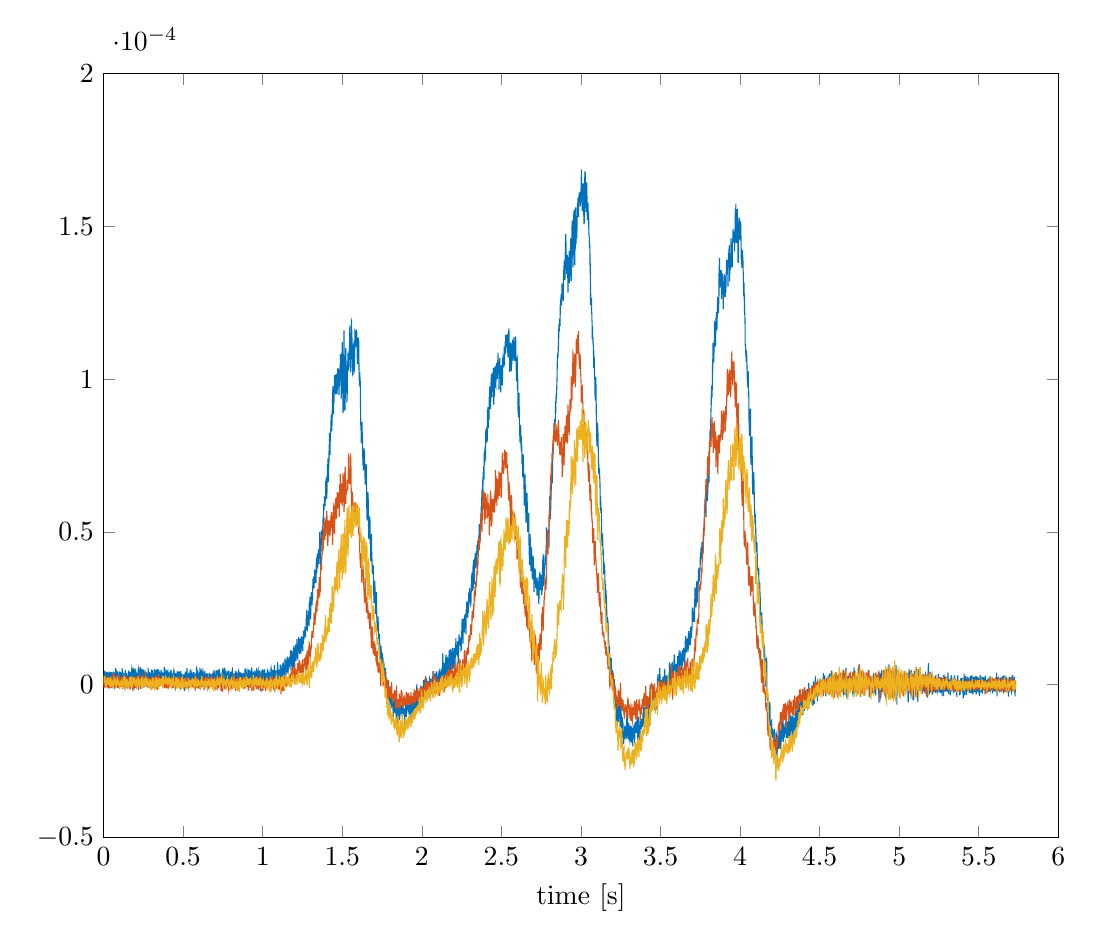
\begin{tikzpicture}

\begin{axis}[%
width=\textwidth,
height=0.8\textwidth,
at={(0\figurewidth,0\figureheight)},
scale only axis,
xmin=0,
xmax=6,
xlabel={time [s]},
ymin=-5e-05,
ymax=0.0002,
ylabel={},
axis background/.style={fill=white},
% title style={font=\bfseries},
% title={Raw strain freight train},
% legend style={legend cell align=left,align=left,draw=white!15!black}
]
\addplot [color=mycolor1,solid,forget plot]
  table[row sep=crcr]{%
0	1.5585854416327e-06\\
0.0009765625	2.14436281522484e-06\\
0.001953125	2.13730525245714e-06\\
0.0029296875	2.87129230928419e-06\\
0.00390625	3.19594077132705e-06\\
0.0048828125	3.9158141935411e-06\\
0.005859375	4.62157344818521e-06\\
0.0068359375	1.02221157582765e-06\\
0.0078125	1.5656429963012e-06\\
0.0087890625	4.85838280510483e-07\\
0.009765625	5.77586303737417e-07\\
0.0107421875	-5.51618974462724e-07\\
0.01171875	3.27357413017096e-06\\
0.0126953125	2.62427731512692e-06\\
0.013671875	2.94186804412379e-06\\
0.0146484375	3.45001362653512e-06\\
0.015625	3.95815972096657e-06\\
0.0166015625	3.9016990185227e-06\\
0.017578125	1.14924743985592e-06\\
0.0185546875	1.57270055106836e-06\\
0.01953125	1.964792396697e-07\\
0.0205078125	1.48095234679853e-06\\
0.021484375	1.29745598833448e-06\\
0.0224609375	2.68779544492599e-06\\
0.0234375	2.10201744010115e-06\\
0.0244140625	4.23340573590361e-06\\
0.025390625	3.59822285118656e-06\\
0.0263671875	3.50647427840899e-06\\
0.02734375	2.04555694546782e-06\\
0.0283203125	7.25794684210612e-07\\
0.029296875	-1.15150825008201e-06\\
0.0302734375	2.71602572740441e-06\\
0.03125	-4.24583506891413e-07\\
0.0322265625	2.02438426160994e-06\\
0.033203125	3.6758562719588e-06\\
0.0341796875	3.85935349583779e-06\\
0.03515625	3.85935349583779e-06\\
0.0361328125	3.37238024052935e-06\\
0.037109375	3.52764702449162e-06\\
0.0380859375	2.05967206853321e-06\\
0.0390625	3.6586012147643e-07\\
0.0400390625	4.36435505686344e-07\\
0.041015625	7.46967313548091e-07\\
0.0419921875	4.19106018536577e-06\\
0.04296875	1.15630498879549e-06\\
0.0439453125	2.71602572740441e-06\\
0.044921875	2.1725930672825e-06\\
0.0458984375	4.12754186622619e-06\\
0.046875	3.75348970468241e-06\\
0.0478515625	3.41559479892159e-08\\
0.048828125	7.82255031085829e-07\\
0.0498046875	-7.8451724856406e-07\\
0.05078125	4.92895820166034e-07\\
0.0517578125	1.09278705189269e-06\\
0.052734375	2.39843514063492e-06\\
0.0537109375	3.99344766320413e-06\\
0.0546875	3.63351076823788e-06\\
0.0556640625	3.68997144065608e-06\\
0.056640625	4.01462042973178e-06\\
0.0576171875	2.32080191651203e-06\\
0.05859375	1.62916099276183e-06\\
0.0595703125	-1.211097603801e-07\\
0.060546875	1.4033192639153e-06\\
0.0615234375	3.09007711943613e-06\\
0.0625	1.31862864167272e-06\\
0.0634765625	1.92557841535972e-06\\
0.064453125	4.17694500264346e-06\\
0.0654296875	2.78660144051464e-06\\
0.06640625	3.90875660598268e-06\\
0.0673828125	3.82406556298336e-06\\
0.068359375	1.11395969663798e-06\\
0.0693359375	-1.98742596638126e-07\\
0.0703125	7.65011494774977e-08\\
0.0712890625	-1.14445073334107e-06\\
0.072265625	3.51745045819741e-07\\
0.0732421875	3.1324225775258e-06\\
0.07421875	3.06184681601851e-06\\
0.0751953125	3.52764702449162e-06\\
0.076171875	5.44025542096021e-06\\
0.0771484375	3.54881977146287e-06\\
0.078125	1.68562144077641e-06\\
0.0791015625	9.3046347170926e-07\\
0.080078125	5.705287628964e-07\\
0.0810546875	-2.55202833683013e-07\\
0.08203125	2.54664405623757e-06\\
0.0830078125	3.26651655160014e-06\\
0.083984375	2.89952260203521e-06\\
0.0849609375	4.17694500264346e-06\\
0.0859375	4.1416570475657e-06\\
0.0869140625	3.35120750096602e-06\\
0.087890625	1.25511068432469e-06\\
0.0888671875	8.24600295390833e-07\\
0.08984375	-7.35114593348671e-07\\
0.0908203125	2.10594310980474e-07\\
0.091796875	-9.8918534004221e-07\\
0.0927734375	1.79854235576957e-06\\
0.09375	2.9912710643881e-06\\
0.0947265625	1.24099558377797e-06\\
0.095703125	3.23828623830587e-06\\
0.0966796875	4.2828088826915e-06\\
0.09765625	3.81700797670885e-06\\
0.0986328125	-2.34030245531988e-07\\
0.099609375	8.81060653328599e-07\\
0.1005859375	2.95284747143165e-07\\
0.1015625	9.16348380249456e-07\\
0.1025390625	3.72917659452986e-07\\
0.103515625	1.33274374439218e-06\\
0.1044921875	2.21493844833201e-06\\
0.10546875	3.64056835194435e-06\\
0.1064453125	3.50647427840899e-06\\
0.107421875	4.19811777687502e-06\\
0.1083984375	2.05967206853321e-06\\
0.109375	-7.35114593348671e-07\\
0.1103515625	9.76737515548821e-08\\
0.111328125	3.6586012147643e-07\\
0.1123046875	-3.18720592803112e-07\\
0.11328125	2.59604703778458e-06\\
0.1142578125	2.66662273410378e-06\\
0.115234375	2.65956516402725e-06\\
0.1162109375	3.78877763259808e-06\\
0.1171875	5.32733369052667e-06\\
0.1181640625	3.47824395168211e-06\\
0.119140625	2.02438426160994e-06\\
0.1201171875	2.03536775275973e-07\\
0.12109375	2.67054600175268e-07\\
0.1220703125	1.47389479331506e-06\\
0.123046875	2.94892561815093e-06\\
0.1240234375	2.83600444556868e-06\\
0.125	3.18182561645768e-06\\
0.1259765625	3.38649540073234e-06\\
0.126953125	3.1324225775258e-06\\
0.1279296875	3.57705010214124e-06\\
0.12890625	2.44783810766295e-06\\
0.1298828125	6.90506970623273e-07\\
0.130859375	8.17542751093379e-07\\
0.1318359375	-5.72791549280013e-07\\
0.1328125	-3.39893177398604e-07\\
0.1337890625	3.17476803917078e-06\\
0.134765625	1.33980129590002e-06\\
0.1357421875	4.23340573590361e-06\\
0.13671875	4.86153181976172e-06\\
0.1376953125	3.35120750096602e-06\\
0.138671875	2.71602572740441e-06\\
0.1396484375	1.91852085565402e-06\\
0.140625	-2.4108777501447e-07\\
0.1416015625	4.71723201495586e-07\\
0.142578125	1.15630498879549e-06\\
0.1435546875	1.74208189511211e-06\\
0.14453125	3.88052625673561e-06\\
0.1455078125	3.15359530790398e-06\\
0.146484375	2.31374435127538e-06\\
0.1474609375	3.05478924041082e-06\\
0.1484375	2.10201744010115e-06\\
0.1494140625	1.6715063281803e-06\\
0.150390625	2.70984147534431e-08\\
0.1513671875	3.16457358406127e-07\\
0.15234375	-1.01035789648878e-06\\
0.1533203125	-5.75919763704056e-08\\
0.154296875	3.00538621392449e-06\\
0.1552734375	2.09495987792629e-06\\
0.15625	4.14871463838367e-06\\
0.1572265625	3.57705010214124e-06\\
0.158203125	4.62863104571981e-06\\
0.1591796875	2.00321157864088e-06\\
0.16015625	9.586936558139e-07\\
0.1611328125	4.5055058371375e-07\\
0.162109375	1.75619700968385e-06\\
0.1630859375	1.47389479331506e-06\\
0.1640625	2.10907500237489e-06\\
0.1650390625	2.46195324198843e-06\\
0.166015625	2.87129230928419e-06\\
0.1669921875	3.47118637024726e-06\\
0.16796875	4.21929055199584e-06\\
0.1689453125	3.40766814177777e-06\\
0.169921875	1.08572950384151e-06\\
0.1708984375	8.316578397876e-07\\
0.171875	-4.59871139981945e-07\\
0.1728515625	3.0406740894925e-06\\
0.173828125	1.14924743985592e-06\\
0.1748046875	2.85717716350152e-06\\
0.17578125	3.59822285118656e-06\\
0.1767578125	4.69214942797297e-06\\
0.177734375	5.21441198537888e-06\\
0.1787109375	4.89681982521195e-06\\
0.1796875	2.39843514063492e-06\\
0.1806640625	2.32080191651203e-06\\
0.181640625	-1.47615391341786e-06\\
0.1826171875	2.52939527283945e-07\\
0.18359375	7.96370118792342e-07\\
0.1845703125	5.28183519925675e-07\\
0.185546875	2.49018351182462e-06\\
0.1865234375	1.8408877054104e-06\\
0.1875	5.05914468208616e-06\\
0.1884765625	4.94622303699038e-06\\
0.189453125	2.69485301539717e-06\\
0.1904296875	1.45272213345838e-06\\
0.19140625	3.30572433075108e-07\\
0.1923828125	-3.64193799226326e-08\\
0.193359375	7.681399437744e-07\\
0.1943359375	1.10690214829082e-06\\
0.1953125	3.2100559265915e-06\\
0.1962890625	3.42884088371182e-06\\
0.197265625	4.27575128999699e-06\\
0.1982421875	5.35556412076428e-06\\
0.19921875	4.50159430521384e-06\\
0.2001953125	7.39909770336791e-07\\
0.201171875	5.53285482887255e-08\\
0.2021484375	-4.34769121706972e-08\\
0.203125	-2.48145304398073e-07\\
0.2041015625	2.90658017546973e-06\\
0.205078125	2.67368030427918e-06\\
0.2060546875	1.5303552239462e-06\\
0.20703125	3.56999251932338e-06\\
0.2080078125	3.39355298098216e-06\\
0.208984375	3.70408660974801e-06\\
0.2099609375	2.01026913953183e-06\\
0.2109375	1.47389479331506e-06\\
0.2119140625	1.17747763620792e-06\\
0.212890625	-2.93618475759056e-08\\
0.2138671875	1.21276538387022e-06\\
0.21484375	1.36803150291905e-06\\
0.2158203125	3.65468351965371e-06\\
0.216796875	3.84523832239973e-06\\
0.2177734375	4.76978301714739e-06\\
0.21875	5.00974145924561e-06\\
0.2197265625	3.37238024052935e-06\\
0.220703125	1.41037681641062e-06\\
0.2216796875	2.05967206853321e-06\\
0.22265625	7.89312574889971e-07\\
0.2236328125	1.12101724508424e-06\\
0.224609375	2.34197461281504e-06\\
0.2255859375	1.07867195588921e-06\\
0.2265625	4.31809684764612e-06\\
0.2275390625	4.25457851250589e-06\\
0.228515625	3.47824395168211e-06\\
0.2294921875	5.86371213527961e-06\\
0.23046875	1.23393803365293e-06\\
0.2314453125	1.75306633443941e-07\\
0.232421875	-2.93618475759056e-08\\
0.2333984375	-1.3914637605225e-06\\
0.234375	1.3539163992121e-06\\
0.2353515625	2.19376575736241e-06\\
0.236328125	2.65250759404981e-06\\
0.2373046875	3.80995039053278e-06\\
0.23828125	3.52058944236527e-06\\
0.2392578125	5.20029677401326e-06\\
0.240234375	4.38161519078668e-06\\
0.2412109375	1.28334088660294e-06\\
0.2421875	5.91701385715439e-07\\
0.2431640625	-2.12857656492135e-07\\
0.244140625	8.66945563251587e-07\\
0.2451171875	1.21982293369905e-06\\
0.24609375	2.37726244196185e-06\\
0.2470703125	2.51841378324071e-06\\
0.248046875	7.54024856858054e-07\\
0.2490234375	5.01679906221206e-06\\
0.25	3.40766814177777e-06\\
0.2509765625	8.66945563251587e-07\\
0.251953125	1.1178882010029e-07\\
0.2529296875	-9.46840224482371e-07\\
0.25390625	3.41559479892159e-08\\
0.2548828125	1.28334088660294e-06\\
0.255859375	2.22199601218609e-06\\
0.2568359375	2.03849938408313e-06\\
0.2578125	3.41472572232358e-06\\
0.2587890625	3.49235911484779e-06\\
0.259765625	4.79095581626941e-06\\
0.2607421875	3.39355298098216e-06\\
0.26171875	1.27628333588484e-06\\
0.2626953125	1.84794526402951e-06\\
0.263671875	1.55152788706286e-06\\
0.2646484375	1.43154947448987e-06\\
0.265625	2.76542872554427e-06\\
0.2666015625	2.69485301539717e-06\\
0.267578125	1.36803150291905e-06\\
0.2685546875	2.89952260203521e-06\\
0.26953125	3.16771046198318e-06\\
0.2705078125	4.02873560791084e-06\\
0.271484375	1.18846354521095e-07\\
0.2724609375	1.02221157582765e-06\\
0.2734375	-9.39782704876971e-07\\
0.2744140625	-3.18720592803112e-07\\
0.275390625	2.2078808845766e-06\\
0.2763671875	1.30451353934813e-06\\
0.27734375	2.63133488470927e-06\\
0.2783203125	3.44295604549514e-06\\
0.279296875	1.89029061781914e-06\\
0.2802734375	5.58140761955828e-06\\
0.28125	2.15142037809099e-06\\
0.2822265625	1.00103893493431e-06\\
0.283203125	5.56413681511003e-07\\
0.2841796875	1.17042008697149e-06\\
0.28515625	-4.03410925851238e-07\\
0.2861328125	2.58898946869576e-06\\
0.287109375	4.16282982031602e-06\\
0.2880859375	1.13513234227254e-06\\
0.2890625	2.48312594421703e-06\\
0.2900390625	3.62645318463008e-06\\
0.291015625	3.5629349366044e-06\\
0.2919921875	7.89312574889971e-07\\
0.29296875	-4.03410925851238e-07\\
0.2939453125	-3.25778121100344e-07\\
0.294921875	9.65751202087204e-07\\
0.2958984375	2.76542872554427e-06\\
0.296875	1.55152788706286e-06\\
0.2978515625	2.09495987792629e-06\\
0.298828125	3.14653773101237e-06\\
0.2998046875	3.78172004681754e-06\\
0.30078125	5.00268385637782e-06\\
0.3017578125	2.01026913953183e-06\\
0.302734375	2.09495987792629e-06\\
0.3037109375	8.316578397876e-07\\
0.3046875	-6.92769456454769e-07\\
0.3056640625	1.38920415922064e-06\\
0.306640625	4.73449502058675e-06\\
0.3076171875	2.48312594421703e-06\\
0.30859375	3.2100559265915e-06\\
0.3095703125	2.13730525245714e-06\\
0.310546875	3.73937453420725e-06\\
0.3115234375	2.94186804412379e-06\\
0.3125	7.65011494774977e-08\\
0.3134765625	-1.04564548859083e-06\\
0.314453125	6.34046634020004e-07\\
0.3154296875	2.02438426160994e-06\\
0.31640625	1.07867195588921e-06\\
0.3173828125	3.31591960366843e-06\\
0.318359375	3.12536500093061e-06\\
0.3193359375	3.6758562719588e-06\\
0.3203125	4.85447421896801e-06\\
0.3212890625	4.80507101617762e-06\\
0.322265625	1.43154947448987e-06\\
0.3232421875	6.34046634020004e-07\\
0.32421875	1.36097395101614e-06\\
0.3251953125	-4.52813613561684e-07\\
0.326171875	2.27139896192934e-06\\
0.3271484375	3.59822285118656e-06\\
0.328125	1.3821466070213e-06\\
0.3291015625	3.42884088371182e-06\\
0.330078125	2.89246502869936e-06\\
0.3310546875	4.89681982521195e-06\\
0.33203125	2.2078808845766e-06\\
0.3330078125	3.51745045819741e-07\\
0.333984375	5.53285482887255e-08\\
0.3349609375	-9.9937166599031e-08\\
0.3359375	-8.58221035845725e-08\\
0.3369140625	1.82677258846859e-06\\
0.337890625	2.49724107953e-06\\
0.3388671875	2.29962922109806e-06\\
0.33984375	5.1085479097668e-06\\
0.3408203125	3.35120750096602e-06\\
0.341796875	4.33221203431926e-06\\
0.3427734375	5.63471222154695e-07\\
0.34375	7.82255031085829e-07\\
0.3447265625	-8.83322544475854e-07\\
0.345703125	1.98203889656043e-06\\
0.3466796875	1.23393803365293e-06\\
0.34765625	4.89681982521195e-06\\
0.3486328125	3.37238024052935e-06\\
0.349609375	2.23611114019023e-06\\
0.3505859375	3.97933248601277e-06\\
0.3515625	3.86641108270492e-06\\
0.3525390625	1.99615401784881e-06\\
0.353515625	1.33274374439218e-06\\
0.3544921875	-4.34769121706972e-08\\
0.35546875	4.99953359920464e-07\\
0.3564453125	8.52830473569441e-07\\
0.357421875	1.12101724508424e-06\\
0.3583984375	1.89029061781914e-06\\
0.359375	3.5629349366044e-06\\
0.3603515625	3.90875660598268e-06\\
0.361328125	4.86858942065431e-06\\
0.3623046875	3.70408660974801e-06\\
0.36328125	9.72808748458736e-07\\
0.3642578125	1.39626171151842e-06\\
0.365234375	1.4033192639153e-06\\
0.3662109375	-3.25778121100344e-07\\
0.3671875	4.26163610490397e-06\\
0.3681640625	2.10201744010115e-06\\
0.369140625	1.28334088660294e-06\\
0.3701171875	3.80289280445603e-06\\
0.37109375	3.17476803917078e-06\\
0.3720703125	3.18182561645768e-06\\
0.373046875	4.92895820166034e-07\\
0.3740234375	-4.34769121706972e-08\\
0.375	-9.8918534004221e-07\\
0.3759765625	1.29039843741905e-06\\
0.376953125	3.25945897312863e-06\\
0.3779296875	6.76391885879668e-07\\
0.37890625	3.78172004681754e-06\\
0.3798828125	4.0005052519478e-06\\
0.380859375	3.60528043439928e-06\\
0.3818359375	5.84253929111875e-06\\
0.3828125	3.40766814177777e-06\\
0.3837890625	1.06455686028147e-06\\
0.384765625	-4.17525979976539e-07\\
0.3857421875	5.98758926852443e-07\\
0.38671875	2.03536775275973e-07\\
0.3876953125	2.67368030427918e-06\\
0.388671875	3.75348970468241e-06\\
0.3896484375	2.5254713513416e-06\\
0.390625	3.11830742443409e-06\\
0.3916015625	5.08737509731082e-06\\
0.392578125	3.9016990185227e-06\\
0.3935546875	1.41743436900504e-06\\
0.39453125	5.98758926852443e-07\\
0.3955078125	4.15262889386829e-07\\
0.396484375	1.72090922399577e-06\\
0.3974609375	8.17542751093379e-07\\
0.3984375	9.9398138816726e-07\\
0.3994140625	2.71602572740441e-06\\
0.400390625	4.67097663299975e-06\\
0.4013671875	3.23828623830587e-06\\
0.40234375	3.9863900745589e-06\\
0.4033203125	3.43589846455426e-06\\
0.404296875	1.21982293369905e-06\\
0.4052734375	3.7997519752842e-07\\
0.40625	-3.89295871330853e-07\\
0.4072265625	1.5585854416327e-06\\
0.408203125	4.06402355508672e-06\\
0.4091796875	1.0151540287644e-06\\
0.41015625	3.76760487555243e-06\\
0.4111328125	1.84794526402951e-06\\
0.412109375	3.66879868775837e-06\\
0.4130859375	3.45001362653512e-06\\
0.4140625	1.36097395101614e-06\\
0.4150390625	1.6715063281803e-06\\
0.416015625	1.63621854841782e-06\\
0.4169921875	4.36435505686344e-07\\
0.41796875	8.66945563251587e-07\\
0.4189453125	2.40549270705682e-06\\
0.419921875	2.39843514063492e-06\\
0.4208984375	4.0922539146053e-06\\
0.421875	3.47824395168211e-06\\
0.4228515625	4.8333014171795e-06\\
0.423828125	1.43154947448987e-06\\
0.4248046875	8.17542751093379e-07\\
0.42578125	6.48161717577925e-07\\
0.4267578125	1.00103893493431e-06\\
0.427734375	-5.44561449326159e-07\\
0.4287109375	1.99615401784881e-06\\
0.4296875	2.64545002417083e-06\\
0.4306640625	1.31862864167272e-06\\
0.431640625	3.15359530790398e-06\\
0.4326171875	2.87129230928419e-06\\
0.43359375	3.45707120767377e-06\\
0.4345703125	-7.13942025346026e-07\\
0.435546875	1.75306633443941e-07\\
0.4365234375	-1.1232781825239e-06\\
0.4375	-4.03410925851238e-07\\
0.4384765625	2.51841378324071e-06\\
0.439453125	3.15359530790398e-06\\
0.4404296875	2.77248629710247e-06\\
0.44140625	2.87129230928419e-06\\
0.4423828125	4.71332222383523e-06\\
0.443359375	4.56511267146655e-06\\
0.4443359375	1.51624011569579e-06\\
0.4453125	1.40018958376571e-07\\
0.4462890625	4.78780740953378e-07\\
0.447265625	-1.04564548859083e-06\\
0.4482421875	1.77736968228208e-06\\
0.44921875	3.2100559265915e-06\\
0.4501953125	2.66662273410378e-06\\
0.451171875	3.53470460671642e-06\\
0.4521484375	2.80777415637384e-06\\
0.453125	3.85229590906932e-06\\
0.4541015625	1.79854235576957e-06\\
0.455078125	-6.92769456454769e-07\\
0.4560546875	-4.52813613561684e-07\\
0.45703125	-4.73986192526914e-07\\
0.4580078125	-1.4228235327169e-07\\
0.458984375	1.93969353506733e-06\\
0.4599609375	8.24600295390833e-07\\
0.4609375	2.10907500237489e-06\\
0.4619140625	3.45001362653512e-06\\
0.462890625	4.35338481506991e-06\\
0.4638671875	9.02233289184736e-07\\
0.46484375	2.10201744010115e-06\\
0.4658203125	2.00408816167664e-08\\
0.466796875	9.16348380249456e-07\\
0.4677734375	-2.19915186270821e-07\\
0.46875	3.0406740894925e-06\\
0.4697265625	3.44295604549514e-06\\
0.470703125	1.84794526402951e-06\\
0.4716796875	4.29692406837714e-06\\
0.47265625	6.97564513143286e-07\\
0.4736328125	4.36750000273054e-06\\
0.474609375	2.15847794105624e-06\\
0.4755859375	4.29377966821177e-07\\
0.4765625	-9.6801278270703e-07\\
0.4775390625	-4.17525979976539e-07\\
0.478515625	1.67856388442913e-06\\
0.4794921875	2.63839245439072e-06\\
0.48046875	1.93969353506733e-06\\
0.4814453125	2.92069532263498e-06\\
0.482421875	1.48095234679853e-06\\
0.4833984375	4.47336392278043e-06\\
0.484375	3.6476259357497e-06\\
0.4853515625	1.14218989101457e-06\\
0.486328125	-4.59871139981945e-07\\
0.4873046875	-2.55202833683013e-07\\
0.48828125	2.95284747143165e-07\\
0.4892578125	1.57270055106836e-06\\
0.490234375	3.24534381648139e-06\\
0.4912109375	2.24316870434051e-06\\
0.4921875	1.74913945234865e-06\\
0.4931640625	3.33003476229109e-06\\
0.494140625	3.23828623830587e-06\\
0.4951171875	6.05816468088544e-07\\
0.49609375	7.18737141295516e-07\\
0.4970703125	-5.16331347791754e-07\\
0.498046875	4.12134813236511e-08\\
0.4990234375	1.48800990038044e-06\\
0.5	1.43860702738071e-06\\
0.5009765625	2.92069532263498e-06\\
0.501953125	3.01244378884025e-06\\
0.5029296875	3.01244378884025e-06\\
0.50390625	3.36532266057639e-06\\
0.5048828125	2.08084475387276e-06\\
0.505859375	1.08572950384151e-06\\
0.5068359375	-5.58676499500844e-07\\
0.5078125	-1.08093307822394e-06\\
0.5087890625	-2.04781207345235e-06\\
0.509765625	2.13024768978875e-06\\
0.5107421875	3.73231694911777e-06\\
0.51171875	2.32785948184756e-06\\
0.5126953125	3.56999251932338e-06\\
0.513671875	3.68997144065608e-06\\
0.5146484375	4.30398166136785e-06\\
0.515625	1.0151540287644e-06\\
0.5166015625	-1.13171720150622e-09\\
0.517578125	-2.62260362869074e-07\\
0.5185546875	4.78780740953378e-07\\
0.51953125	2.3176691868812e-07\\
0.5205078125	2.73014086923625e-06\\
0.521484375	1.98203889656043e-06\\
0.5224609375	3.77466246113522e-06\\
0.5234375	4.32515444093347e-06\\
0.5244140625	5.44025542096021e-06\\
0.525390625	3.37238024052935e-06\\
0.5263671875	3.02655893896883e-06\\
0.52734375	6.19931550856732e-07\\
0.5283203125	8.17542751093379e-07\\
0.529296875	8.24600295390833e-07\\
0.5302734375	1.96792377566758e-06\\
0.53125	2.68073787455304e-06\\
0.5322265625	1.27628333588484e-06\\
0.533203125	3.28063170884e-06\\
0.5341796875	3.47824395168211e-06\\
0.53515625	3.28063170884e-06\\
0.5361328125	3.51745045819741e-07\\
0.537109375	3.16457358406127e-07\\
0.5380859375	-2.4108777501447e-07\\
0.5390625	-7.28057070780146e-07\\
0.5400390625	3.51745045819741e-07\\
0.541015625	3.90875660598268e-06\\
0.5419921875	1.55152788706286e-06\\
0.54296875	3.0406740894925e-06\\
0.5439453125	2.55370162473376e-06\\
0.544921875	4.9391654350112e-06\\
0.5458984375	7.04622055761961e-07\\
0.546875	1.15630498879549e-06\\
0.5478515625	8.59888018361074e-07\\
0.548828125	3.41559479892159e-08\\
0.5498046875	2.06672963021432e-06\\
0.55078125	1.41743436900504e-06\\
0.5517578125	2.27139896192934e-06\\
0.552734375	3.48530153321562e-06\\
0.5537109375	3.76054729006765e-06\\
0.5546875	2.67368030427918e-06\\
0.5556640625	2.67368030427918e-06\\
0.556640625	7.54024856858054e-07\\
0.5576171875	4.15262889386829e-07\\
0.55859375	9.23405925930135e-07\\
0.5595703125	1.96086621536947e-06\\
0.560546875	-3.11663064407001e-07\\
0.5615234375	2.65250759404981e-06\\
0.5625	1.69973655376782e-06\\
0.5634765625	4.07108114481853e-06\\
0.564453125	3.1324225775258e-06\\
0.5654296875	2.48312594421703e-06\\
0.56640625	2.21493844833201e-06\\
0.5673828125	7.39909770336791e-07\\
0.568359375	-9.60955263397401e-07\\
0.5693359375	6.41104175749634e-07\\
0.5703125	2.01732670052144e-06\\
0.5712890625	2.05967206853321e-06\\
0.572265625	3.18888319384282e-06\\
0.5732421875	1.89734817712976e-06\\
0.57421875	3.5629349366044e-06\\
0.5751953125	3.47824395168211e-06\\
0.576171875	3.11124984803623e-06\\
0.5771484375	-1.35224822406634e-07\\
0.578125	1.23393803365293e-06\\
0.5791015625	-9.9937166599031e-08\\
0.580078125	9.09290834667873e-07\\
0.5810546875	2.76542872554427e-06\\
0.58203125	8.81060653328599e-07\\
0.5830078125	3.90875660598268e-06\\
0.583984375	5.46848585751894e-06\\
0.5849609375	5.59552284159115e-06\\
0.5859375	4.25457851250589e-06\\
0.5869140625	2.10907500237489e-06\\
0.587890625	7.11679598479299e-07\\
0.5888671875	4.15262889386829e-07\\
0.58984375	1.21276538387022e-06\\
0.5908203125	-7.28057070780146e-07\\
0.591796875	4.42396075732497e-06\\
0.5927734375	1.91852085565402e-06\\
0.59375	2.57487433081454e-06\\
0.5947265625	3.56999251932338e-06\\
0.595703125	3.33003476229109e-06\\
0.5966796875	2.10907500237489e-06\\
0.59765625	5.8464384467688e-07\\
0.5986328125	-1.211097603801e-07\\
0.599609375	3.4468750813939e-07\\
0.6005859375	1.29039843741905e-06\\
0.6015625	2.39843514063492e-06\\
0.6025390625	2.9912710643881e-06\\
0.603515625	4.12048427570443e-06\\
0.6044921875	2.54664405623757e-06\\
0.60546875	5.62375328684215e-06\\
0.6064453125	4.53688228547761e-06\\
0.607421875	1.6432761041729e-06\\
0.6083984375	-6.71596886674683e-07\\
0.609375	1.50212500784068e-06\\
0.6103515625	-4.88101244676799e-07\\
0.611328125	2.13024768978875e-06\\
0.6123046875	4.67097663299975e-06\\
0.61328125	1.69267899722278e-06\\
0.6142578125	3.95110213281531e-06\\
0.615234375	1.85500282274772e-06\\
0.6162109375	5.0309142684416e-06\\
0.6171875	2.52939527283945e-07\\
0.6181640625	5.14068439725528e-07\\
0.619140625	-6.43366792251777e-07\\
0.6201171875	5.35241060174068e-07\\
0.62109375	-1.63454945275102e-07\\
0.6220703125	2.87834988232406e-06\\
0.623046875	2.87129230928419e-06\\
0.6240234375	3.41472572232358e-06\\
0.625	4.19106018536577e-06\\
0.6259765625	3.8381807358288e-06\\
0.626953125	3.71114419444262e-06\\
0.6279296875	2.00408816167664e-08\\
0.62890625	-2.97548007318791e-07\\
0.6298828125	8.81060653328599e-07\\
0.630859375	9.3046347170926e-07\\
0.6318359375	9.9398138816726e-07\\
0.6328125	2.78660144051464e-06\\
0.6337890625	2.10907500237489e-06\\
0.634765625	4.28986647548488e-06\\
0.6357421875	3.12536500093061e-06\\
0.63671875	4.50159430521384e-06\\
0.6376953125	1.76325456711793e-06\\
0.638671875	-3.11663064407001e-07\\
0.6396484375	-1.13171720150622e-09\\
0.640625	2.599970636806e-07\\
0.6416015625	9.4457856356393e-07\\
0.642578125	1.11395969663798e-06\\
0.6435546875	2.04555694546782e-06\\
0.64453125	2.29257165615783e-06\\
0.6455078125	2.69485301539717e-06\\
0.646484375	3.78877763259808e-06\\
0.6474609375	2.29257165615783e-06\\
0.6484375	4.43493044650824e-07\\
0.6494140625	9.8692384149909e-07\\
0.650390625	1.89421704162741e-07\\
0.6513671875	1.45272213345838e-06\\
0.65234375	5.14068439725528e-07\\
0.6533203125	3.61233801771067e-06\\
0.654296875	1.49506745406145e-06\\
0.6552734375	2.77248629710247e-06\\
0.65625	2.40549270705682e-06\\
0.6572265625	1.9114632960472e-06\\
0.658203125	1.72090922399577e-06\\
0.6591796875	-1.4228235327169e-07\\
0.66015625	-1.24325595873224e-06\\
0.6611328125	1.40018958376571e-07\\
0.662109375	1.09278705189269e-06\\
0.6630859375	2.11613256474751e-06\\
0.6640625	3.73937453420725e-06\\
0.6650390625	3.42178330296847e-06\\
0.666015625	3.22417108225125e-06\\
0.6669921875	3.32297718293032e-06\\
0.66796875	3.35120750096602e-06\\
0.6689453125	2.22199601218609e-06\\
0.669921875	1.86911794047991e-06\\
0.6708984375	-2.05800126614353e-07\\
0.671875	1.66444877203035e-06\\
0.6728515625	2.32080191651203e-06\\
0.673828125	1.5656429963012e-06\\
0.6748046875	2.610162176258e-06\\
0.67578125	2.48312594421703e-06\\
0.6767578125	3.47824395168211e-06\\
0.677734375	2.97715591524744e-06\\
0.6787109375	4.08205350817432e-07\\
0.6796875	6.90506970623273e-07\\
0.6806640625	1.66444877203035e-06\\
0.681640625	1.11395969663798e-06\\
0.6826171875	1.00103893493431e-06\\
0.68359375	3.17476803917078e-06\\
0.6845703125	3.21711350437172e-06\\
0.685546875	3.5911652680725e-06\\
0.6865234375	3.62645318463008e-06\\
0.6875	2.82188930077394e-06\\
0.6884765625	1.55152788706286e-06\\
0.689453125	6.19931550856732e-07\\
0.6904296875	5.98758926852443e-07\\
0.69140625	9.23405925930135e-07\\
0.6923828125	1.30451353934813e-06\\
0.693359375	4.88270462273548e-06\\
0.6943359375	2.63133488470927e-06\\
0.6953125	2.19376575736241e-06\\
0.6962890625	2.19376575736241e-06\\
0.697265625	4.35338481506991e-06\\
0.6982421875	2.85717716350152e-06\\
0.69921875	1.14924743985592e-06\\
0.7001953125	7.65011494774977e-08\\
0.701171875	-7.70402204710707e-07\\
0.7021484375	7.681399437744e-07\\
0.703125	1.53741277821983e-06\\
0.7041015625	2.58193189970582e-06\\
0.705078125	2.94186804412379e-06\\
0.7060546875	2.87834988232406e-06\\
0.70703125	3.45001362653512e-06\\
0.7080078125	4.70626462511603e-06\\
0.708984375	2.73014086923625e-06\\
0.7099609375	1.24805313400189e-06\\
0.7109375	1.3539163992121e-06\\
0.7119140625	1.12807479362874e-06\\
0.712890625	3.13948015422008e-06\\
0.7138671875	2.22199601218609e-06\\
0.71484375	2.27845652657314e-06\\
0.7158203125	4.64980383891515e-06\\
0.716796875	3.18888319384282e-06\\
0.7177734375	3.45707120767377e-06\\
0.71875	2.27845652657314e-06\\
0.7197265625	2.599970636806e-07\\
0.720703125	3.23514895691395e-07\\
0.7216796875	1.44566458036999e-06\\
0.72265625	-9.25667665368883e-07\\
0.7236328125	3.02655893896883e-06\\
0.724609375	4.86153181976172e-06\\
0.7255859375	2.49018351182462e-06\\
0.7265625	3.92287178119818e-06\\
0.7275390625	5.08031749335688e-06\\
0.728515625	4.38867278496308e-06\\
0.7294921875	1.46683723993091e-06\\
0.73046875	2.51135621523826e-06\\
0.7314453125	3.37629970557918e-07\\
0.732421875	2.75837115408517e-06\\
0.7333984375	2.22199601218609e-06\\
0.734375	3.46412878891107e-06\\
0.7353515625	1.5868156608991e-06\\
0.736328125	2.89246502869936e-06\\
0.7373046875	1.99615401784881e-06\\
0.73828125	3.58410768505754e-06\\
0.7392578125	2.43372297373235e-06\\
0.740234375	8.17542751093379e-07\\
0.7412109375	7.65011494774977e-08\\
0.7421875	-1.211097603801e-07\\
0.7431640625	2.33491704728175e-06\\
0.744140625	1.33274374439218e-06\\
0.7451171875	3.8381807358288e-06\\
0.74609375	4.16988741143019e-06\\
0.7470703125	4.07108114481853e-06\\
0.748046875	5.31321847600037e-06\\
0.7490234375	3.39355298098216e-06\\
0.75	1.65033366002622e-06\\
0.7509765625	1.82677258846859e-06\\
0.751953125	1.10690214829082e-06\\
0.7529296875	3.23514895691395e-07\\
0.75390625	4.84035901767701e-06\\
0.7548828125	4.26869369740115e-06\\
0.755859375	2.98421348976854e-06\\
0.7568359375	4.72037982265396e-06\\
0.7578125	3.09007711943613e-06\\
0.7587890625	5.59552284159115e-06\\
0.759765625	2.37726244196185e-06\\
0.7607421875	1.11395969663798e-06\\
0.76171875	1.75306633443941e-07\\
0.7626953125	-8.05689813603147e-07\\
0.763671875	2.0526145069514e-06\\
0.7646484375	2.15142037809099e-06\\
0.765625	3.52764702449162e-06\\
0.7666015625	3.8381807358288e-06\\
0.767578125	3.27357413017096e-06\\
0.7685546875	3.44295604549514e-06\\
0.76953125	2.50429864733512e-06\\
0.7705078125	1.17747763620792e-06\\
0.771484375	1.82364168753793e-07\\
0.7724609375	6.48161717577925e-07\\
0.7734375	3.8381807358288e-06\\
0.7744140625	3.49235911484779e-06\\
0.775390625	1.53741277821983e-06\\
0.7763671875	3.76054729006765e-06\\
0.77734375	2.87129230928419e-06\\
0.7783203125	4.38867278496308e-06\\
0.779296875	3.23122866022923e-06\\
0.7802734375	3.30572433075108e-07\\
0.78125	1.26216823474593e-06\\
0.7822265625	-3.39893177398604e-07\\
0.783203125	-4.52813613561684e-07\\
0.7841796875	1.36803150291905e-06\\
0.78515625	3.61939560112093e-06\\
0.7861328125	3.46412878891107e-06\\
0.787109375	2.75131358272473e-06\\
0.7880859375	3.86641108270492e-06\\
0.7890625	4.57217026821077e-06\\
0.7900390625	2.32785948184756e-06\\
0.791015625	8.03427662794025e-07\\
0.7919921875	-8.58221035845725e-08\\
0.79296875	6.90506970623273e-07\\
0.7939453125	1.44566458036999e-06\\
0.794921875	2.97009834082521e-06\\
0.7958984375	1.63621854841782e-06\\
0.796875	2.36314731000666e-06\\
0.7978515625	2.87834988232406e-06\\
0.798828125	4.0922539146053e-06\\
0.7998046875	2.91363774900313e-06\\
0.80078125	6.8344942820214e-07\\
0.8017578125	-7.06884502481081e-07\\
0.802734375	-1.21502589631021e-06\\
0.8037109375	3.45707120767377e-06\\
0.8046875	1.4707649319246e-07\\
0.8056640625	3.34414992130883e-06\\
0.806640625	3.16771046198318e-06\\
0.8076171875	3.11830742443409e-06\\
0.80859375	3.40061056133042e-06\\
0.8095703125	5.66609895768155e-06\\
0.810546875	2.75131358272473e-06\\
0.8115234375	7.46967313548091e-07\\
0.8125	4.08205350817432e-07\\
0.8134765625	4.78780740953378e-07\\
0.814453125	2.599970636806e-07\\
0.8154296875	3.71114419444262e-06\\
0.81640625	2.56075919332862e-06\\
0.8173828125	3.40766814177777e-06\\
0.818359375	2.59604703778458e-06\\
0.8193359375	3.59822285118656e-06\\
0.8203125	2.56075919332862e-06\\
0.8212890625	1.50212500784068e-06\\
0.822265625	5.4935614096684e-07\\
0.8232421875	1.1178882010029e-07\\
0.82421875	7.65011494774977e-08\\
0.8251953125	2.45489567477614e-06\\
0.826171875	8.88118198515099e-07\\
0.8271484375	2.70191058596766e-06\\
0.828125	3.95815972096657e-06\\
0.8291015625	4.42396075732497e-06\\
0.830078125	3.20299834890973e-06\\
0.8310546875	2.69485301539717e-06\\
0.83203125	8.38715384282596e-07\\
0.8330078125	-4.52813613561684e-07\\
0.833984375	8.03427662794025e-07\\
0.8349609375	1.63621854841782e-06\\
0.8359375	3.68291385625832e-06\\
0.8369140625	3.5629349366044e-06\\
0.837890625	2.70896815663638e-06\\
0.8388671875	8.24600295390833e-07\\
0.83984375	3.79583521847773e-06\\
0.8408203125	2.29962922109806e-06\\
0.841796875	1.54447033259212e-06\\
0.8427734375	1.5303552239462e-06\\
0.84375	6.48161717577925e-07\\
0.8447265625	1.21982293369905e-06\\
0.845703125	2.95598319227696e-06\\
0.8466796875	2.75131358272473e-06\\
0.84765625	3.41472572232358e-06\\
0.8486328125	3.99344766320413e-06\\
0.849609375	3.61233801771067e-06\\
0.8505859375	4.67097663299975e-06\\
0.8515625	1.6432761041729e-06\\
0.8525390625	1.4033192639153e-06\\
0.853515625	-1.14445073334107e-06\\
0.8544921875	2.71602572740441e-06\\
0.85546875	3.31591960366843e-06\\
0.8564453125	1.22688048362655e-06\\
0.857421875	3.28063170884e-06\\
0.8583984375	3.43589846455426e-06\\
0.859375	4.02167801877209e-06\\
0.8603515625	3.42884088371182e-06\\
0.861328125	2.8007165843219e-06\\
0.8623046875	3.16457358406127e-07\\
0.86328125	2.15142037809099e-06\\
0.8642578125	1.11395969663798e-06\\
0.865234375	3.87346866967094e-06\\
0.8662109375	1.75619700968385e-06\\
0.8671875	2.34197461281504e-06\\
0.8681640625	2.82188930077394e-06\\
0.869140625	3.03361651418145e-06\\
0.8701171875	3.35120750096602e-06\\
0.87109375	3.30180444544086e-06\\
0.8720703125	1.06455686028147e-06\\
0.873046875	1.43860702738071e-06\\
0.8740234375	-1.06994697958267e-07\\
0.875	-7.63344682635711e-07\\
0.8759765625	1.6715063281803e-06\\
0.876953125	3.71820177923524e-06\\
0.8779296875	1.04338421761025e-06\\
0.87890625	3.83112314935674e-06\\
0.8798828125	2.92775289636614e-06\\
0.880859375	1.75619700968385e-06\\
0.8818359375	2.39843514063492e-06\\
0.8828125	-7.91574770342201e-07\\
0.8837890625	-1.70512475745292e-07\\
0.884765625	-1.211097603801e-07\\
0.8857421875	9.09290834667873e-07\\
0.88671875	2.47606837670898e-06\\
0.8876953125	3.01950136385532e-06\\
0.888671875	5.26381522827002e-06\\
0.8896484375	3.74643211939517e-06\\
0.890625	4.03579319714826e-06\\
0.8916015625	4.21929055199584e-06\\
0.892578125	1.63621854841782e-06\\
0.8935546875	1.05749931262559e-06\\
0.89453125	-6.85711933293403e-07\\
0.8955078125	9.02233289184736e-07\\
0.896484375	3.55587735398452e-06\\
0.8974609375	1.25511068432469e-06\\
0.8984375	3.2100559265915e-06\\
0.8994140625	4.05696596545422e-06\\
0.900390625	4.36750000273054e-06\\
0.9013671875	3.57705010214124e-06\\
0.90234375	1.81265747192143e-06\\
0.9033203125	1.54447033259212e-06\\
0.904296875	-6.78654410033374e-07\\
0.9052734375	9.09290834667873e-07\\
0.90625	-1.91685066563019e-07\\
0.9072265625	2.66662273410378e-06\\
0.908203125	1.91852085565402e-06\\
0.9091796875	2.54664405623757e-06\\
0.91015625	3.40061056133042e-06\\
0.9111328125	5.03797187170491e-06\\
0.912109375	1.9538086551698e-06\\
0.9130859375	1.81265747192143e-06\\
0.9140625	8.10485206894154e-07\\
0.9150390625	-3.32835649298913e-07\\
0.916015625	3.94404454476293e-06\\
0.9169921875	1.34685884750673e-06\\
0.91796875	1.9326359751643e-06\\
0.9189453125	3.85229590906932e-06\\
0.919921875	4.32515444093347e-06\\
0.9208984375	4.21929055199584e-06\\
0.921875	2.68073787455304e-06\\
0.9228515625	1.54447033259212e-06\\
0.923828125	1.29745598833448e-06\\
0.9248046875	3.41559479892159e-08\\
0.92578125	-1.35224822406634e-07\\
0.9267578125	-1.52467825864644e-08\\
0.927734375	2.28551409131605e-06\\
0.9287109375	1.68562144077641e-06\\
0.9296875	4.11342668528176e-06\\
0.9306640625	5.64492612181722e-06\\
0.931640625	4.85447421896801e-06\\
0.9326171875	1.47389479331506e-06\\
0.93359375	8.24600295390833e-07\\
0.9345703125	2.52939527283945e-07\\
0.935546875	1.47389479331506e-06\\
0.9365234375	8.45772928876904e-07\\
0.9375	2.31374435127538e-06\\
0.9384765625	1.5303552239462e-06\\
0.939453125	4.02873560791084e-06\\
0.9404296875	3.30180444544086e-06\\
0.94140625	3.90875660598268e-06\\
0.9423828125	3.79583521847773e-06\\
0.943359375	1.07161440803601e-06\\
0.9443359375	-1.70512475745292e-07\\
0.9453125	8.52830473569441e-07\\
0.9462890625	-9.46840224482371e-07\\
0.947265625	6.34046634020004e-07\\
0.9482421875	3.71114419444262e-06\\
0.94921875	1.74913945234865e-06\\
0.9501953125	3.06184681601851e-06\\
0.951171875	4.35338481506991e-06\\
0.9521484375	4.68509182954976e-06\\
0.953125	2.32785948184756e-06\\
0.9541015625	2.95598319227696e-06\\
0.955078125	1.4033192639153e-06\\
0.9560546875	1.98203889656043e-06\\
0.95703125	2.84306201811394e-06\\
0.9580078125	3.44295604549514e-06\\
0.958984375	2.53958648784003e-06\\
0.9599609375	3.68997144065608e-06\\
0.9609375	2.78660144051464e-06\\
0.9619140625	5.38379455258288e-06\\
0.962890625	2.79365901236905e-06\\
0.9638671875	8.38715384282596e-07\\
0.96484375	1.19159273497655e-06\\
0.9658203125	7.11679598479299e-07\\
0.966796875	4.78780740953378e-07\\
0.9677734375	2.68073787455304e-06\\
0.96875	3.69702902515293e-06\\
0.9697265625	3.65468351965371e-06\\
0.970703125	4.26869369740115e-06\\
0.9716796875	4.52276709307577e-06\\
0.97265625	3.35826508072166e-06\\
0.9736328125	1.0080964817998e-06\\
0.974609375	2.88227210253197e-07\\
0.9755859375	1.32961423659345e-07\\
0.9765625	8.24600295390833e-07\\
0.9775390625	1.87617549949389e-06\\
0.978515625	2.92069532263498e-06\\
0.9794921875	3.31591960366843e-06\\
0.98046875	2.87834988232406e-06\\
0.9814453125	4.69214942797297e-06\\
0.982421875	3.9652173092165e-06\\
0.9833984375	3.35120750096602e-06\\
0.984375	-4.81043718651404e-07\\
0.9853515625	-2.19601963879199e-06\\
0.986328125	1.65739121597906e-06\\
0.9873046875	-1.13171720150622e-09\\
0.98828125	2.19376575736241e-06\\
0.9892578125	2.57487433081454e-06\\
0.990234375	2.76542872554427e-06\\
0.9912109375	3.71820177923524e-06\\
0.9921875	3.9369869568092e-06\\
0.9931640625	4.0922539146053e-06\\
0.994140625	1.76325456711793e-06\\
0.9951171875	4.64665662136023e-07\\
0.99609375	2.45881990986819e-07\\
0.9970703125	-1.05976052474071e-06\\
0.998046875	-7.49229638189733e-07\\
0.9990234375	1.02221157582765e-06\\
1	2.92069532263498e-06\\
1.0009765625	5.0309142684416e-06\\
1.001953125	2.78660144051464e-06\\
1.0029296875	3.95110213281531e-06\\
1.00390625	2.01732670052144e-06\\
1.0048828125	9.72808748458736e-07\\
1.005859375	2.00408816167664e-08\\
1.0068359375	-3.6812328880944e-07\\
1.0078125	8.88118198515099e-07\\
1.0087890625	4.71332222383523e-06\\
1.009765625	6.48161717577925e-07\\
1.0107421875	4.06402355508672e-06\\
1.01171875	4.67803423122542e-06\\
1.0126953125	4.57217026821077e-06\\
1.013671875	3.08301954343336e-06\\
1.0146484375	-3.25778121100344e-07\\
1.015625	-3.61065761105049e-07\\
1.0166015625	-3.9635339864081e-07\\
1.017578125	1.86206038156416e-06\\
1.0185546875	1.69267899722278e-06\\
1.01953125	2.03144182279709e-06\\
1.0205078125	3.84523832239973e-06\\
1.021484375	2.51135621523826e-06\\
1.0224609375	3.46412878891107e-06\\
1.0234375	1.98909645715518e-06\\
1.0244140625	5.56413681511003e-07\\
1.025390625	-1.14052229218406e-07\\
1.0263671875	1.45272213345838e-06\\
1.02734375	3.09399821219955e-07\\
1.0283203125	1.98203889656043e-06\\
1.029296875	3.35120750096602e-06\\
1.0302734375	4.43807594696123e-06\\
1.03125	5.101490305516e-06\\
1.0322265625	3.55587735398452e-06\\
1.033203125	4.31103925445766e-06\\
1.0341796875	1.63621854841782e-06\\
1.03515625	1.39626171151842e-06\\
1.0361328125	8.24600295390833e-07\\
1.037109375	9.23405925930135e-07\\
1.0380859375	-6.22194220397396e-07\\
1.0390625	3.31591960366843e-06\\
1.0400390625	3.5629349366044e-06\\
1.041015625	3.09007711943613e-06\\
1.0419921875	3.25945897312863e-06\\
1.04296875	3.99344766320413e-06\\
1.0439453125	2.47606837670898e-06\\
1.044921875	4.5055058371375e-07\\
1.0458984375	5.8464384467688e-07\\
1.046875	-4.31641033706758e-07\\
1.0478515625	4.99953359920464e-07\\
1.048828125	2.48312594421703e-06\\
1.0498046875	2.13024768978875e-06\\
1.05078125	2.64545002417083e-06\\
1.0517578125	5.12266311856417e-06\\
1.052734375	5.48260107639115e-06\\
1.0537109375	5.07325988950095e-06\\
1.0546875	3.57705010214124e-06\\
1.0556640625	1.99615401784881e-06\\
1.056640625	3.05478924041082e-06\\
1.0576171875	2.48312594421703e-06\\
1.05859375	1.98203889656043e-06\\
1.0595703125	4.57217026821077e-06\\
1.060546875	2.37020487593503e-06\\
1.0615234375	4.88976222392428e-06\\
1.0625	3.43589846455426e-06\\
1.0634765625	4.81918621648091e-06\\
1.064453125	4.44513354192779e-06\\
1.0654296875	1.29039843741905e-06\\
1.06640625	6.19931550856732e-07\\
1.0673828125	2.09495987792629e-06\\
1.068359375	8.24600295390833e-07\\
1.0693359375	2.19376575736241e-06\\
1.0703125	3.05478924041082e-06\\
1.0712890625	1.75619700968385e-06\\
1.072265625	4.43807594696123e-06\\
1.0732421875	5.08737509731082e-06\\
1.07421875	6.43537926363737e-06\\
1.0751953125	3.06184681601851e-06\\
1.076171875	2.0526145069514e-06\\
1.0771484375	1.13513234227254e-06\\
1.078125	2.88540745546195e-06\\
1.0791015625	2.29962922109806e-06\\
1.080078125	3.9652173092165e-06\\
1.0810546875	1.66444877203035e-06\\
1.08203125	4.64980383891515e-06\\
1.0830078125	3.65468351965371e-06\\
1.083984375	3.37943782058162e-06\\
1.0849609375	4.27575128999699e-06\\
1.0859375	2.29962922109806e-06\\
1.0869140625	9.8692384149909e-07\\
1.087890625	2.49724107953e-06\\
1.0888671875	-6.29251744447374e-07\\
1.08984375	4.52276709307577e-06\\
1.0908203125	3.29474686647517e-06\\
1.091796875	3.05478924041082e-06\\
1.0927734375	3.2100559265915e-06\\
1.09375	7.45873561793799e-06\\
1.0947265625	5.96251875311683e-06\\
1.095703125	3.42884088371182e-06\\
1.0966796875	4.74861021891484e-06\\
1.09765625	4.99953359920464e-07\\
1.0986328125	3.63351076823788e-06\\
1.099609375	3.82406556298336e-06\\
1.1005859375	4.57922786505343e-06\\
1.1015625	4.54393988182675e-06\\
1.1025390625	4.21929055199584e-06\\
1.103515625	4.16282982031602e-06\\
1.1044921875	4.91093502808307e-06\\
1.10546875	3.78877763259808e-06\\
1.1064453125	6.8344942820214e-07\\
1.107421875	7.46967313548091e-07\\
1.1083984375	6.8344942820214e-07\\
1.109375	5.35241060174068e-07\\
1.1103515625	6.45655213268826e-06\\
1.111328125	5.2214695912098e-06\\
1.1123046875	3.31591960366843e-06\\
1.11328125	5.22852719713959e-06\\
1.1142578125	5.80019360546394e-06\\
1.115234375	5.58140761955828e-06\\
1.1162109375	3.64056835194435e-06\\
1.1171875	9.586936558139e-07\\
1.1181640625	9.09290834667873e-07\\
1.119140625	1.3821466070213e-06\\
1.1201171875	3.76760487555243e-06\\
1.12109375	4.45924873215668e-06\\
1.1220703125	3.63351076823788e-06\\
1.123046875	5.37673694447991e-06\\
1.1240234375	5.39790976908459e-06\\
1.125	7.0070470400271e-06\\
1.1259765625	4.81212861628004e-06\\
1.126953125	3.21711350437172e-06\\
1.1279296875	5.9258156391833e-09\\
1.12890625	5.08737509731082e-06\\
1.1298828125	3.33709234175052e-06\\
1.130859375	4.48042151824073e-06\\
1.1318359375	5.94840352081201e-06\\
1.1328125	6.85177918480695e-06\\
1.1337890625	6.7388571383096e-06\\
1.134765625	7.02821993307898e-06\\
1.1357421875	5.29910326186917e-06\\
1.13671875	4.25457851250589e-06\\
1.1376953125	3.70408660974801e-06\\
1.138671875	3.06890439172466e-06\\
1.1396484375	6.48478262613877e-06\\
1.140625	3.85229590906932e-06\\
1.1416015625	5.00974145924561e-06\\
1.142578125	5.02385666527739e-06\\
1.1435546875	6.33657255315334e-06\\
1.14453125	6.14601680903274e-06\\
1.1455078125	8.609131792111e-06\\
1.146484375	6.16013204686873e-06\\
1.1474609375	5.06620228574455e-06\\
1.1484375	1.93969353506733e-06\\
1.1494140625	7.88219402715618e-06\\
1.150390625	4.69920702649506e-06\\
1.1513671875	4.12754186622619e-06\\
1.15234375	6.78826053054069e-06\\
1.1533203125	7.33169816450946e-06\\
1.154296875	7.30346762364918e-06\\
1.1552734375	9.2090326785834e-06\\
1.15625	7.31758289388177e-06\\
1.1572265625	5.76490553680104e-06\\
1.158203125	6.61181986622342e-06\\
1.1591796875	3.62645318463008e-06\\
1.16015625	8.02334690924527e-06\\
1.1611328125	6.78826053054069e-06\\
1.162109375	4.85447421896801e-06\\
1.1630859375	6.35068779632295e-06\\
1.1640625	6.6471079941486e-06\\
1.1650390625	7.38815925097123e-06\\
1.166015625	9.07493712438328e-06\\
1.1669921875	5.68727179443406e-06\\
1.16796875	6.56947411597293e-06\\
1.1689453125	7.61400366003167e-06\\
1.169921875	6.57653174076763e-06\\
1.1708984375	7.95982810741585e-06\\
1.171875	9.15257138825844e-06\\
1.1728515625	7.55048490976105e-06\\
1.173828125	6.7741452751235e-06\\
1.1748046875	9.89362632676234e-06\\
1.17578125	1.13545663950507e-05\\
1.1767578125	6.23776586202861e-06\\
1.177734375	5.270872834792e-06\\
1.1787109375	4.88976222392428e-06\\
1.1796875	7.71281062080008e-06\\
1.1806640625	1.07546629563289e-05\\
1.181640625	7.83984817023342e-06\\
1.1826171875	9.89362632676234e-06\\
1.18359375	8.75028487766797e-06\\
1.1845703125	1.11357779994333e-05\\
1.185546875	1.03735482012419e-05\\
1.1865234375	9.1737443713893e-06\\
1.1875	7.97394339602004e-06\\
1.1884765625	5.55317717667821e-06\\
1.189453125	6.86589444239688e-06\\
1.1904296875	9.77364592950457e-06\\
1.19140625	5.33439129793835e-06\\
1.1923828125	8.29859514295478e-06\\
1.193359375	9.68189623321513e-06\\
1.1943359375	1.07405475898931e-05\\
1.1953125	1.19685859478113e-05\\
1.1962890625	1.26743564722025e-05\\
1.197265625	8.02334690924527e-06\\
1.1982421875	6.96470125658983e-06\\
1.19921875	4.09931150473219e-06\\
1.2001953125	7.2470065466694e-06\\
1.201171875	1.07687783231596e-05\\
1.2021484375	7.8186752431055e-06\\
1.203125	9.93597235613894e-06\\
1.2041015625	1.10510857427419e-05\\
1.205078125	9.23020566408455e-06\\
1.2060546875	1.31048769771015e-05\\
1.20703125	9.45605089807885e-06\\
1.2080078125	8.86320737455959e-06\\
1.208984375	7.95982810741585e-06\\
1.2099609375	7.97394339602004e-06\\
1.2109375	9.42782023829851e-06\\
1.2119140625	1.05641055427833e-05\\
1.212890625	1.09734511866025e-05\\
1.2138671875	9.74541525194527e-06\\
1.21484375	1.17427395886123e-05\\
1.2158203125	1.49469442715252e-05\\
1.216796875	1.23426442027181e-05\\
1.2177734375	1.10157973066518e-05\\
1.21875	1.08393551632392e-05\\
1.2197265625	8.49620935211158e-06\\
1.220703125	8.45386344363046e-06\\
1.2216796875	1.30978192609433e-05\\
1.22265625	1.32036850136877e-05\\
1.2236328125	1.09522781279116e-05\\
1.224609375	1.35495132941945e-05\\
1.2255859375	1.38035913656886e-05\\
1.2265625	1.55821414504057e-05\\
1.2275390625	1.16509895340786e-05\\
1.228515625	1.33024930696335e-05\\
1.2294921875	1.20321052545593e-05\\
1.23046875	1.00418374451372e-05\\
1.2314453125	1.08817012720282e-05\\
1.232421875	1.39941500033151e-05\\
1.2333984375	1.32530890392406e-05\\
1.234375	1.27167027350759e-05\\
1.2353515625	1.42058819073505e-05\\
1.236328125	1.50104639534104e-05\\
1.2373046875	1.45375954024017e-05\\
1.23828125	1.17992011689303e-05\\
1.2392578125	1.37400718358146e-05\\
1.240234375	1.00771258130753e-05\\
1.2412109375	1.30625306816339e-05\\
1.2421875	1.57091809821891e-05\\
1.2431640625	1.3140165559374e-05\\
1.244140625	1.31542809929748e-05\\
1.2451171875	1.35565710166743e-05\\
1.24609375	1.53845244645746e-05\\
1.2470703125	1.52716005074394e-05\\
1.248046875	1.19615282475555e-05\\
1.2490234375	1.3217800449066e-05\\
1.25	1.23073556762519e-05\\
1.2509765625	1.24908560408424e-05\\
1.251953125	1.10087396197299e-05\\
1.2529296875	1.5215138538354e-05\\
1.25390625	1.56244879574441e-05\\
1.2548828125	1.33730702643043e-05\\
1.255859375	1.57868162673665e-05\\
1.2568359375	1.77135867194468e-05\\
1.2578125	1.66337474274761e-05\\
1.2587890625	1.45940572956298e-05\\
1.259765625	1.59562023856017e-05\\
1.2607421875	1.63584946444287e-05\\
1.26171875	1.54480442015753e-05\\
1.2626953125	1.71560223518716e-05\\
1.263671875	1.71701378978756e-05\\
1.2646484375	1.78618001360588e-05\\
1.265625	1.7537142232656e-05\\
1.2666015625	1.88146017115081e-05\\
1.267578125	1.81370537396175e-05\\
1.2685546875	1.62949747927524e-05\\
1.26953125	1.61467618366221e-05\\
1.2705078125	1.87440237552966e-05\\
1.271484375	1.83134984363023e-05\\
1.2724609375	1.767829781715e-05\\
1.2734375	2.1948272922543e-05\\
1.2744140625	1.99791394150442e-05\\
1.275390625	1.96827113808286e-05\\
1.2763671875	2.14189352025361e-05\\
1.27734375	2.4594969856717e-05\\
1.2783203125	2.10519280428186e-05\\
1.279296875	1.83487873830475e-05\\
1.2802734375	1.82005738233123e-05\\
1.28125	1.95415552352995e-05\\
1.2822265625	2.04237817930633e-05\\
1.283203125	2.15600918735449e-05\\
1.2841796875	2.20894297417137e-05\\
1.28515625	2.27105202154452e-05\\
1.2861328125	2.16941907475996e-05\\
1.287109375	2.34868843832692e-05\\
1.2880859375	2.39809349305324e-05\\
1.2890625	2.16094967177326e-05\\
1.2900390625	2.22517601326047e-05\\
1.291015625	1.91886650443311e-05\\
1.2919921875	2.01061800544746e-05\\
1.29296875	2.68534955577191e-05\\
1.2939453125	2.51666582186823e-05\\
1.294921875	2.41573816718503e-05\\
1.2958984375	2.69099588298381e-05\\
1.296875	2.87732503562405e-05\\
1.2978515625	2.70581749492284e-05\\
1.298828125	2.44255808368884e-05\\
1.2998046875	2.7262854423809e-05\\
1.30078125	2.13554147134721e-05\\
1.3017578125	2.29857764654649e-05\\
1.302734375	2.77004453032839e-05\\
1.3037109375	2.63312105903033e-05\\
1.3046875	3.00366223908708e-05\\
1.3056640625	2.87873662274121e-05\\
1.306640625	2.81239207094589e-05\\
1.3076171875	3.01142598816957e-05\\
1.30859375	3.01283757904024e-05\\
1.3095703125	2.59783156482556e-05\\
1.310546875	2.98742894941312e-05\\
1.3115234375	2.82933109714959e-05\\
1.3125	2.75239973223274e-05\\
1.3134765625	2.96625510116946e-05\\
1.314453125	3.24151582175422e-05\\
1.3154296875	3.1250591796896e-05\\
1.31640625	3.46313708343249e-05\\
1.3173828125	3.25210280254966e-05\\
1.318359375	3.489251754842e-05\\
1.3193359375	3.40808457719565e-05\\
1.3203125	3.54077533539071e-05\\
1.3212890625	3.17234760191739e-05\\
1.322265625	3.17305339959995e-05\\
1.3232421875	3.24081002311357e-05\\
1.32421875	3.37420614168968e-05\\
1.3251953125	3.46737189409376e-05\\
1.326171875	3.57112486637672e-05\\
1.3271484375	3.76522113598914e-05\\
1.328125	3.64594006727816e-05\\
1.3291015625	3.58030030957271e-05\\
1.330078125	3.68758253850208e-05\\
1.3310546875	3.57818289945622e-05\\
1.33203125	3.3495031301475e-05\\
1.3330078125	3.76451533001909e-05\\
1.333984375	3.56830165342146e-05\\
1.3349609375	3.3367987289232e-05\\
1.3359375	3.89014894829503e-05\\
1.3369140625	3.96919947526892e-05\\
1.337890625	4.08777549806049e-05\\
1.3388671875	4.13647644533185e-05\\
1.33984375	3.66358517800542e-05\\
1.3408203125	3.94308455533077e-05\\
1.341796875	4.2282319810071e-05\\
1.3427734375	3.80827531884125e-05\\
1.34375	4.29951908934132e-05\\
1.3447265625	4.05248498594666e-05\\
1.345703125	3.83791920381034e-05\\
1.3466796875	4.08706968757621e-05\\
1.34765625	4.26564005499377e-05\\
1.3486328125	3.95367168340556e-05\\
1.349609375	3.95861234393437e-05\\
1.3505859375	4.42868311657984e-05\\
1.3515625	4.00590154776945e-05\\
1.3525390625	3.95508330065012e-05\\
1.353515625	4.36163071142234e-05\\
1.3544921875	4.15129848209703e-05\\
1.35546875	4.17317863956926e-05\\
1.3564453125	4.12447765685542e-05\\
1.357421875	4.40750866321472e-05\\
1.3583984375	5.00533748107269e-05\\
1.359375	4.53808460059431e-05\\
1.3603515625	4.39974469920836e-05\\
1.361328125	4.6968936287136e-05\\
1.3623046875	4.46256226045597e-05\\
1.36328125	3.93461485447115e-05\\
1.3642578125	4.31504698769007e-05\\
1.365234375	4.5133810189437e-05\\
1.3662109375	4.35527838292509e-05\\
1.3671875	4.38986329220168e-05\\
1.3681640625	4.7441835248266e-05\\
1.369140625	5.04698107478604e-05\\
1.3701171875	4.96651721281689e-05\\
1.37109375	4.94675417863797e-05\\
1.3720703125	4.9354610197272e-05\\
1.373046875	4.88675930089243e-05\\
1.3740234375	4.80206077146026e-05\\
1.375	5.01874812614185e-05\\
1.3759765625	4.98486860863187e-05\\
1.376953125	4.91569799771832e-05\\
1.3779296875	5.20579170540708e-05\\
1.37890625	5.3476629583509e-05\\
1.3798828125	5.48177047980829e-05\\
1.380859375	5.23190727921181e-05\\
1.3818359375	5.52623778933353e-05\\
1.3828125	5.36672032124159e-05\\
1.3837890625	5.92079864994732e-05\\
1.384765625	5.69422575693247e-05\\
1.3857421875	5.83539254893782e-05\\
1.38671875	5.85656760181959e-05\\
1.3876953125	5.99914652269803e-05\\
1.388671875	6.16360686770037e-05\\
1.3896484375	6.10996309108134e-05\\
1.390625	5.94409124805139e-05\\
1.3916015625	5.92503366698427e-05\\
1.392578125	6.12266819091337e-05\\
1.3935546875	6.16078350961368e-05\\
1.39453125	6.01679245677783e-05\\
1.3955078125	6.13113825924628e-05\\
1.396484375	6.66052035288543e-05\\
1.3974609375	6.41347468434371e-05\\
1.3984375	6.5631136304968e-05\\
1.3994140625	6.72122318807723e-05\\
1.400390625	6.70075361920818e-05\\
1.4013671875	6.20313389751007e-05\\
1.40234375	6.18760541781877e-05\\
1.4033203125	6.08949377030636e-05\\
1.404296875	6.45582528443433e-05\\
1.4052734375	6.68240159900965e-05\\
1.40625	6.7600448070282e-05\\
1.4072265625	7.21743631316072e-05\\
1.408203125	7.14755678681523e-05\\
1.4091796875	7.04167890108378e-05\\
1.41015625	7.40448804701281e-05\\
1.4111328125	6.86874549907094e-05\\
1.412109375	6.89345023448219e-05\\
1.4130859375	6.62734557848237e-05\\
1.4140625	7.18073190341224e-05\\
1.4150390625	7.30425646561892e-05\\
1.416015625	7.09673537392414e-05\\
1.4169921875	7.63036276350995e-05\\
1.41796875	7.837180187988e-05\\
1.4189453125	7.73271257747065e-05\\
1.419921875	8.23034739159461e-05\\
1.4208984375	7.92470727150969e-05\\
1.421875	7.69106676603718e-05\\
1.4228515625	7.51530770338692e-05\\
1.423828125	7.88729648335232e-05\\
1.4248046875	8.04541019231767e-05\\
1.42578125	8.20846547386481e-05\\
1.4267578125	8.22470044417481e-05\\
1.427734375	8.37434476442884e-05\\
1.4287109375	8.26705256523493e-05\\
1.4296875	8.66516424164099e-05\\
1.4306640625	8.69057573193832e-05\\
1.431640625	8.84375081964713e-05\\
1.4326171875	8.49010765639354e-05\\
1.43359375	8.29952254880007e-05\\
1.4345703125	8.54304809187205e-05\\
1.435546875	8.48163719187401e-05\\
1.4365234375	8.65457612446265e-05\\
1.4375	8.96657357627483e-05\\
1.4384765625	9.42116155360103e-05\\
1.439453125	9.41974978335362e-05\\
1.4404296875	9.61457445106532e-05\\
1.44140625	9.77339946528111e-05\\
1.4423828125	9.34633778494432e-05\\
1.443359375	9.28351414038713e-05\\
1.4443359375	9.30045534020209e-05\\
1.4453125	8.8508095906625e-05\\
1.4462890625	9.22633763302441e-05\\
1.447265625	9.35480839469184e-05\\
1.4482421875	9.26092588281924e-05\\
1.44921875	9.71481062403828e-05\\
1.4501953125	9.73881086402844e-05\\
1.451171875	9.95481353788267e-05\\
1.4521484375	0.000101341105776518\\
1.453125	0.000100028142577033\\
1.4541015625	9.84610619423221e-05\\
1.455078125	9.61669211463159e-05\\
1.4560546875	9.6689278440803e-05\\
1.45703125	9.71904595967726e-05\\
1.4580078125	9.50586784076476e-05\\
1.458984375	0.000101305811022148\\
1.4599609375	9.96469603528765e-05\\
1.4609375	0.000101199926773859\\
1.4619140625	0.000101799937808089\\
1.462890625	9.80163507572631e-05\\
1.4638671875	9.87293006244892e-05\\
1.46484375	9.95551943049023e-05\\
1.4658203125	9.75504632696851e-05\\
1.466796875	9.50727961342279e-05\\
1.4677734375	9.76281111543956e-05\\
1.46875	9.63151576208522e-05\\
1.4697265625	9.66822195548388e-05\\
1.470703125	0.000101404636340607\\
1.4716796875	0.000103536444353063\\
1.47265625	9.70492817559724e-05\\
1.4736328125	0.000102788192832306\\
1.474609375	9.87363595391043e-05\\
1.4755859375	9.76916412507773e-05\\
1.4765625	9.8941068105921e-05\\
1.4775390625	9.81292932433048e-05\\
1.478515625	9.99928479145456e-05\\
1.4794921875	9.4903383441345e-05\\
1.48046875	0.000102442303353559\\
1.4814453125	0.000102287006113732\\
1.482421875	9.77128179513499e-05\\
1.4833984375	0.000100882274162368\\
1.484375	0.000101439931101893\\
1.4853515625	0.000103345851879199\\
1.486328125	0.000103995278381846\\
1.4873046875	0.000103183495384199\\
1.48828125	0.000107193010205023\\
1.4892578125	0.000108237748174822\\
1.490234375	0.000104157635138169\\
1.4912109375	0.000103804685734591\\
1.4921875	0.000102054060343651\\
1.4931640625	9.35339662630178e-05\\
1.494140625	9.6159862267663e-05\\
1.4951171875	9.5432798295552e-05\\
1.49609375	9.71057528875499e-05\\
1.4970703125	0.00010055756281074\\
1.498046875	0.000105724733472999\\
1.4990234375	0.000109974276885653\\
1.5	0.0001122049485556\\
1.5009765625	0.000107058888595376\\
1.501953125	0.000107207128271271\\
1.5029296875	0.000102512893023834\\
1.50390625	9.40845562279696e-05\\
1.5048828125	8.89104460431499e-05\\
1.505859375	8.94539721758561e-05\\
1.5068359375	9.21645528029703e-05\\
1.5078125	9.48680891374907e-05\\
1.5087890625	9.92304838076771e-05\\
1.509765625	0.000107545961979788\\
1.5107421875	0.000116009819518206\\
1.51171875	0.00011091313432919\\
1.5126953125	0.000104778826688375\\
1.513671875	0.000105025891722144\\
1.5146484375	9.6428099725933e-05\\
1.515625	9.00257340645256e-05\\
1.5166015625	9.26516118034261e-05\\
1.517578125	8.97363236448047e-05\\
1.5185546875	9.38657319391569e-05\\
1.51953125	9.39080850199045e-05\\
1.5205078125	0.000102258770257083\\
1.521484375	0.000108174216749995\\
1.5224609375	0.000110277817070955\\
1.5234375	0.000103607034176475\\
1.5244140625	0.000106338867932228\\
1.525390625	9.95128407499303e-05\\
1.5263671875	0.000104531761775634\\
1.52734375	9.92446016510355e-05\\
1.5283203125	9.70069284114384e-05\\
1.529296875	9.23410234009718e-05\\
1.5302734375	9.58422128305297e-05\\
1.53125	9.50798549976663e-05\\
1.5322265625	9.95410764528498e-05\\
1.533203125	0.000100684623749524\\
1.5341796875	0.000105717674460574\\
1.53515625	0.0001050188327195\\
1.5361328125	0.000107743615081545\\
1.537109375	0.000107510666791196\\
1.5380859375	0.000108449519648713\\
1.5390625	0.000104199989083197\\
1.5400390625	0.000102788192832306\\
1.541015625	0.000104150576147677\\
1.5419921875	0.000106960062168986\\
1.54296875	0.000106310631848736\\
1.5439453125	0.000108287161510777\\
1.544921875	0.000112374367060224\\
1.5458984375	0.000111929643606964\\
1.546875	0.000115487442213062\\
1.5478515625	0.000117562836323368\\
1.548828125	0.000112847327353494\\
1.5498046875	0.000111668456999737\\
1.55078125	0.000109148366143441\\
1.5517578125	0.000105400019003681\\
1.552734375	0.000102216416475073\\
1.5537109375	0.000106550638608803\\
1.5546875	0.000106776527428493\\
1.5556640625	0.00010969191408659\\
1.556640625	0.00010912012990266\\
1.5576171875	0.000119122917110542\\
1.55859375	0.000118925259549273\\
1.5595703125	0.000114654463305171\\
1.560546875	0.000114809764353155\\
1.5615234375	0.00011179552073771\\
1.5625	0.000110284876147206\\
1.5634765625	0.000104814121685789\\
1.564453125	0.000102985844069524\\
1.5654296875	0.00010176464302161\\
1.56640625	0.000101404636340607\\
1.5673828125	0.000101517579585415\\
1.568359375	0.000110496648480661\\
1.5693359375	0.000107390663168461\\
1.5703125	0.000111160202367964\\
1.5712890625	0.000111357856886125\\
1.572265625	0.000109070716485097\\
1.5732421875	0.000107270659574279\\
1.57421875	0.000108498933005416\\
1.5751953125	0.000103261144136157\\
1.576171875	0.000103070551766328\\
1.5771484375	0.000104884711688027\\
1.578125	0.000111068434225148\\
1.5791015625	0.00010969897315464\\
1.580078125	0.000115212135472656\\
1.5810546875	0.00011499330201697\\
1.58203125	0.000111139025102755\\
1.5830078125	0.00011588275471851\\
1.583984375	0.000111866111717082\\
1.5849609375	0.000110644889166987\\
1.5859375	0.0001118590526187\\
1.5869140625	0.000112254362280237\\
1.587890625	0.00011195082090537\\
1.5888671875	0.000116320422496675\\
1.58984375	0.000112776736236787\\
1.5908203125	0.000115438028171667\\
1.591796875	0.000112642613142265\\
1.5927734375	0.000111110788750526\\
1.59375	0.000107934209217313\\
1.5947265625	0.000106698878135313\\
1.595703125	0.000105004714714508\\
1.5966796875	0.000107715378919409\\
1.59765625	0.000109451905831678\\
1.5986328125	0.000107644788520984\\
1.599609375	0.000112946154933481\\
1.6005859375	0.000113623830289352\\
1.6015625	0.000112882622915552\\
1.6025390625	0.000112035530107886\\
1.603515625	0.000112600258488248\\
1.6044921875	0.000106832999649223\\
1.60546875	0.000103042315865813\\
1.6064453125	0.000102131708921724\\
1.607421875	9.85881223529337e-05\\
1.6083984375	9.87293006244892e-05\\
1.609375	0.000100028142577033\\
1.6103515625	0.000102244652329351\\
1.611328125	9.90469518799811e-05\\
1.6123046875	0.000100578739631648\\
1.61328125	9.80798809025491e-05\\
1.6142578125	9.31739654570769e-05\\
1.615234375	8.98069115367406e-05\\
1.6162109375	8.60234144558227e-05\\
1.6171875	8.33058081351023e-05\\
1.6181640625	8.41740288223356e-05\\
1.619140625	7.91976622242666e-05\\
1.6201171875	8.0623509762501e-05\\
1.62109375	8.33340429306866e-05\\
1.6220703125	8.25999387592178e-05\\
1.623046875	8.28540516207271e-05\\
1.6240234375	8.59175334159286e-05\\
1.625	8.42940269210612e-05\\
1.6259765625	8.02141075815425e-05\\
1.626953125	7.82447465623136e-05\\
1.6279296875	8.12870243477564e-05\\
1.62890625	7.43272233125235e-05\\
1.6298828125	7.36001908138799e-05\\
1.630859375	7.15743873415781e-05\\
1.6318359375	7.28802179160335e-05\\
1.6328125	7.01626824158286e-05\\
1.6337890625	7.59295219369088e-05\\
1.634765625	7.41225247360296e-05\\
1.6357421875	7.65083270968547e-05\\
1.63671875	7.61836314375252e-05\\
1.6376953125	7.73553602355836e-05\\
1.638671875	7.36848935753162e-05\\
1.6396484375	7.6021283686251e-05\\
1.640625	7.02897356973297e-05\\
1.6416015625	7.29508034488103e-05\\
1.642578125	6.76075065492211e-05\\
1.6435546875	6.83557058769808e-05\\
1.64453125	6.55323179960603e-05\\
1.6455078125	6.62805142451904e-05\\
1.646484375	6.55464348961474e-05\\
1.6474609375	6.69298930215533e-05\\
1.6484375	6.68451913946094e-05\\
1.6494140625	7.01838579605226e-05\\
1.650390625	7.21955387607662e-05\\
1.6513671875	6.64710927124365e-05\\
1.65234375	6.48547072565797e-05\\
1.6533203125	6.3358320098769e-05\\
1.654296875	5.77257327770044e-05\\
1.6552734375	5.44294984481805e-05\\
1.65625	5.51847365309916e-05\\
1.6572265625	5.38154271957972e-05\\
1.658203125	5.67446243758393e-05\\
1.6591796875	5.8819776770134e-05\\
1.66015625	6.26242450031118e-05\\
1.6611328125	6.27583547965862e-05\\
1.662109375	6.25960113669239e-05\\
1.6630859375	6.05631937152123e-05\\
1.6640625	5.96738385691318e-05\\
1.6650390625	5.25167042513444e-05\\
1.666015625	4.94746000115388e-05\\
1.6669921875	4.77171049969873e-05\\
1.66796875	4.80206077146026e-05\\
1.6689453125	5.0060433044085e-05\\
1.669921875	5.16697128285178e-05\\
1.6708984375	5.30954825417361e-05\\
1.671875	5.4761238401344e-05\\
1.6728515625	5.46906554143103e-05\\
1.673828125	5.44718482172848e-05\\
1.6748046875	5.19449848849077e-05\\
1.67578125	4.60654887583748e-05\\
1.6767578125	4.65454450565138e-05\\
1.677734375	4.13718225650763e-05\\
1.6787109375	4.04472107659567e-05\\
1.6796875	4.43715290041522e-05\\
1.6806640625	4.38280514552512e-05\\
1.681640625	4.32422256623434e-05\\
1.6826171875	4.63972232098101e-05\\
1.68359375	4.93969595402239e-05\\
1.6845703125	4.57761035640486e-05\\
1.685546875	4.08212901446274e-05\\
1.6865234375	4.13788806769323e-05\\
1.6875	3.86191664726197e-05\\
1.6884765625	3.71087410519831e-05\\
1.689453125	3.62264853057126e-05\\
1.6904296875	3.8583876107441e-05\\
1.69140625	3.75745727086191e-05\\
1.6923828125	3.65440971965675e-05\\
1.693359375	3.70663927408978e-05\\
1.6943359375	3.9197928813896e-05\\
1.6953125	3.69252317296302e-05\\
1.6962890625	3.04248099645163e-05\\
1.697265625	3.12858816489193e-05\\
1.6982421875	2.94719864535106e-05\\
1.69921875	2.67688006613932e-05\\
1.7001953125	3.02765928556787e-05\\
1.701171875	3.11800121002568e-05\\
1.7021484375	3.04036360891582e-05\\
1.703125	3.18928674902436e-05\\
1.7041015625	3.32550593052175e-05\\
1.705078125	3.41020198017037e-05\\
1.7060546875	2.9239074313519e-05\\
1.70703125	2.69664221082789e-05\\
1.7080078125	2.57242314428865e-05\\
1.708984375	2.30845864380149e-05\\
1.7099609375	2.46726065098197e-05\\
1.7109375	2.71711015456208e-05\\
1.7119140625	2.52584107321892e-05\\
1.712890625	2.81027469307049e-05\\
1.7138671875	2.67193953117722e-05\\
1.71484375	3.0340114468418e-05\\
1.7158203125	2.69593641981285e-05\\
1.716796875	2.25834789199537e-05\\
1.7177734375	2.12707207404993e-05\\
1.71875	2.01626425711606e-05\\
1.7197265625	1.7727702281057e-05\\
1.720703125	2.20188513271895e-05\\
1.7216796875	1.96262489178761e-05\\
1.72265625	1.98309253761568e-05\\
1.7236328125	2.22658758212385e-05\\
1.724609375	2.11577954653272e-05\\
1.7255859375	2.21670660090992e-05\\
1.7265625	1.71842534442746e-05\\
1.7275390625	1.65843430707387e-05\\
1.728515625	1.60479532234008e-05\\
1.7294921875	1.50739836432964e-05\\
1.73046875	1.54974484469961e-05\\
1.7314453125	1.49751752402645e-05\\
1.732421875	1.38882840846331e-05\\
1.7333984375	1.58503360550373e-05\\
1.734375	1.65984586007414e-05\\
1.7353515625	1.36553791417603e-05\\
1.736328125	1.27731644244378e-05\\
1.7373046875	1.11781241331128e-05\\
1.73828125	1.04723557026829e-05\\
1.7392578125	1.23708750256696e-05\\
1.740234375	7.98100104047001e-06\\
1.7412109375	1.01971062825348e-05\\
1.7421875	1.03170867805393e-05\\
1.7431640625	9.62543488994901e-06\\
1.744140625	1.27731644244378e-05\\
1.7451171875	1.05499901816811e-05\\
1.74609375	9.76658825996681e-06\\
1.7470703125	7.21171837676673e-06\\
1.748046875	5.39790976908459e-06\\
1.7490234375	6.66122324600982e-06\\
1.75	7.55048490976105e-06\\
1.7509765625	7.42344743322014e-06\\
1.751953125	9.42782023829851e-06\\
1.7529296875	9.6183772224851e-06\\
1.75390625	8.69382363870427e-06\\
1.7548828125	8.73616956733421e-06\\
1.755859375	8.52443995974072e-06\\
1.7568359375	6.42832164081809e-06\\
1.7578125	6.52712836927819e-06\\
1.7587890625	6.70356900396444e-06\\
1.759765625	7.47990852995408e-06\\
1.7607421875	5.2920456549521e-06\\
1.76171875	7.2681794497959e-06\\
1.7626953125	5.7366750836486e-06\\
1.763671875	5.31321847600037e-06\\
1.7646484375	2.72308329827067e-06\\
1.765625	3.23122866022923e-06\\
1.7666015625	3.42178330296847e-06\\
1.767578125	1.54447033259212e-06\\
1.7685546875	-4.34769121706972e-08\\
1.76953125	1.69973655376782e-06\\
1.7705078125	2.92775289636614e-06\\
1.771484375	4.26869369740115e-06\\
1.7724609375	5.48260107639115e-06\\
1.7734375	3.36532266057639e-06\\
1.7744140625	2.31374435127538e-06\\
1.775390625	4.15262889386829e-07\\
1.7763671875	2.599970636806e-07\\
1.77734375	-3.69220785905095e-06\\
1.7783203125	-2.95117179535285e-06\\
1.779296875	-4.68731171738234e-06\\
1.7802734375	-6.25406700407571e-06\\
1.78125	-3.07820662646431e-06\\
1.7822265625	1.04338421761025e-06\\
1.783203125	-3.20524142557533e-06\\
1.7841796875	8.88118198515099e-07\\
1.78515625	7.61082400267113e-07\\
1.7861328125	-1.07387556049507e-06\\
1.787109375	-2.47831964275192e-06\\
1.7880859375	-4.08742664777988e-06\\
1.7890625	-4.98372525306818e-06\\
1.7900390625	-6.91746642435265e-06\\
1.791015625	-4.71554158543012e-06\\
1.7919921875	-2.20307714081706e-06\\
1.79296875	-2.76767698280736e-06\\
1.7939453125	-5.23388873323403e-07\\
1.794921875	-1.95606451117614e-06\\
1.7958984375	-7.77459726686606e-07\\
1.796875	-3.60751807831168e-06\\
1.7978515625	-4.05213926852233e-06\\
1.798828125	-4.20034624481276e-06\\
1.7998046875	-5.27308115556673e-06\\
1.80078125	-4.69436918454228e-06\\
1.8017578125	-7.28445296278033e-06\\
1.802734375	-3.67103541519921e-06\\
1.8037109375	-3.71338030201321e-06\\
1.8046875	-1.97723702702931e-06\\
1.8056640625	-1.22208341206387e-06\\
1.806640625	-3.82238343922883e-07\\
1.8076171875	-4.36972559295372e-06\\
1.80859375	-7.29151039359434e-06\\
1.8095703125	-7.19976378530892e-06\\
1.810546875	-5.87296481477763e-06\\
1.8115234375	-5.37894302963279e-06\\
1.8125	-4.39795547877938e-06\\
1.8134765625	-6.98804077940663e-06\\
1.814453125	-3.8545298990467e-06\\
1.8154296875	-6.82571974801728e-06\\
1.81640625	-5.20956402046027e-06\\
1.8173828125	-6.43050310529286e-06\\
1.818359375	-7.58086497193032e-06\\
1.8193359375	-8.44892771078437e-06\\
1.8203125	-9.57811277729976e-06\\
1.8212890625	-1.05096885537656e-05\\
1.822265625	-5.4001154017793e-06\\
1.8232421875	-8.09605685897778e-06\\
1.82421875	-7.28445296278033e-06\\
1.8251953125	-6.45167543329066e-06\\
1.826171875	-4.84257597208916e-06\\
1.8271484375	-5.60478162003495e-06\\
1.828125	-8.33600906507059e-06\\
1.8291015625	-8.99940574656329e-06\\
1.830078125	-7.78553030514003e-06\\
1.8310546875	-9.37344817159924e-06\\
1.83203125	-7.60909467800133e-06\\
1.8330078125	-4.50381753655223e-06\\
1.833984375	-6.74103049350767e-06\\
1.8349609375	-5.47774742537836e-06\\
1.8359375	-6.9950982143688e-06\\
1.8369140625	-5.5906667110982e-06\\
1.837890625	-8.11722911704931e-06\\
1.8388671875	-9.77571990398913e-06\\
1.83984375	-1.0544975481168e-05\\
1.8408203125	-1.28809645830957e-05\\
1.841796875	-6.74103049350767e-06\\
1.8427734375	-8.40658322160499e-06\\
1.84375	-8.66770751490383e-06\\
1.8447265625	-5.4212877730372e-06\\
1.845703125	-5.69652851849668e-06\\
1.8466796875	-4.60967957210262e-06\\
1.84765625	-6.82571974801728e-06\\
1.8486328125	-9.8533512540033e-06\\
1.849609375	-9.76866250794028e-06\\
1.8505859375	-1.32902908644343e-05\\
1.8515625	-1.25916130458447e-05\\
1.8525390625	-1.02979669374978e-05\\
1.853515625	-7.07272999243423e-06\\
1.8544921875	-7.86316196152589e-06\\
1.85546875	-7.94079360596058e-06\\
1.8564453125	-7.31268268544375e-06\\
1.857421875	-7.49617584423681e-06\\
1.8583984375	-1.11236807382755e-05\\
1.859375	-8.84414277167061e-06\\
1.8603515625	-1.12295413841875e-05\\
1.861328125	-1.11942545046857e-05\\
1.8623046875	-1.04108851439022e-05\\
1.86328125	-9.44402218294792e-06\\
1.8642578125	-8.37129614457226e-06\\
1.865234375	-8.32895164887401e-06\\
1.8662109375	-5.94353931600571e-06\\
1.8671875	-6.26818189444463e-06\\
1.8681640625	-6.11291807865711e-06\\
1.869140625	-8.33600906507059e-06\\
1.8701171875	-9.13349645913783e-06\\
1.87109375	-9.20407050406663e-06\\
1.8720703125	-8.96411871101279e-06\\
1.873046875	-9.19701310001832e-06\\
1.8740234375	-6.67751354329216e-06\\
1.875	-8.85120018065725e-06\\
1.8759765625	-8.09605685897778e-06\\
1.876953125	-7.81375999975385e-06\\
1.8779296875	-7.1574191912397e-06\\
1.87890625	-9.50753878471711e-06\\
1.8798828125	-7.49617584423681e-06\\
1.880859375	-9.45107958353914e-06\\
1.8818359375	-7.96902329188299e-06\\
1.8828125	-8.1525162118597e-06\\
1.8837890625	-9.30993155294144e-06\\
1.884765625	-9.25347232964011e-06\\
1.8857421875	-8.10311427843391e-06\\
1.88671875	-7.70789863680389e-06\\
1.8876953125	-8.79474090599813e-06\\
1.888671875	-9.74043292275933e-06\\
1.8896484375	-1.01144747981646e-05\\
1.890625	-1.00156713108699e-05\\
1.8916015625	-1.3403208400818e-05\\
1.892578125	-9.94509737952125e-06\\
1.8935546875	-7.87727680685748e-06\\
1.89453125	-8.90765944899525e-06\\
1.8955078125	-8.5830185697299e-06\\
1.896484375	-8.25132006419273e-06\\
1.8974609375	-5.90825206662647e-06\\
1.8984375	-6.10586063134913e-06\\
1.8994140625	-8.67476492635963e-06\\
1.900390625	-9.02057796670877e-06\\
1.9013671875	-9.76866250794028e-06\\
1.90234375	-1.07072953154177e-05\\
1.9033203125	-9.36639076992121e-06\\
1.904296875	-7.10801716033156e-06\\
1.9052734375	-6.25406700407571e-06\\
1.90625	-9.23935752282718e-06\\
1.9072265625	-6.46579031812907e-06\\
1.908203125	-5.72475833004972e-06\\
1.9091796875	-6.25406700407571e-06\\
1.91015625	-7.6937837867315e-06\\
1.9111328125	-7.53146298250462e-06\\
1.912109375	-8.48421478238459e-06\\
1.9130859375	-6.39521588998771e-06\\
1.9140625	-6.82571974801728e-06\\
1.9150390625	-7.50323327208813e-06\\
1.916015625	-6.63516890537065e-06\\
1.9169921875	-7.39031441461969e-06\\
1.91796875	-8.8864872241092e-06\\
1.9189453125	-6.71985817765814e-06\\
1.919921875	-9.84629385904125e-06\\
1.9208984375	-7.79258772894164e-06\\
1.921875	-9.81100688274934e-06\\
1.9228515625	-8.55478891817799e-06\\
1.923828125	-5.78827540026667e-06\\
1.9248046875	-8.09605685897778e-06\\
1.92578125	-5.18839164031343e-06\\
1.9267578125	-4.06625422052164e-06\\
1.927734375	-5.78827540026667e-06\\
1.9287109375	-4.2638635070326e-06\\
1.9296875	-8.55478891817799e-06\\
1.9306640625	-8.71005198215739e-06\\
1.931640625	-1.16176968957416e-05\\
1.9326171875	-1.15965247846335e-05\\
1.93359375	-1.0206220876177e-05\\
1.9345703125	-7.94785102758923e-06\\
1.935546875	-8.08194201976976e-06\\
1.9365234375	-6.14820531371556e-06\\
1.9375	-5.56243689203858e-06\\
1.9384765625	-4.31326581656097e-06\\
1.939453125	-4.4403003045554e-06\\
1.9404296875	-6.93863873190586e-06\\
1.94140625	-1.02767947709821e-05\\
1.9423828125	-1.09119593797852e-05\\
1.943359375	-1.00227287034612e-05\\
1.9443359375	-5.95765421506625e-06\\
1.9453125	-7.37619955565837e-06\\
1.9462890625	-5.73887323523361e-06\\
1.947265625	-2.64769956927441e-06\\
1.9482421875	-4.48970259680007e-06\\
1.94921875	-3.90393224867515e-06\\
1.9501953125	-5.88002226534472e-06\\
1.951171875	-6.03528615283704e-06\\
1.9521484375	-8.51244443788733e-06\\
1.953125	-7.70789863680389e-06\\
1.9541015625	-8.44892771078437e-06\\
1.955078125	-4.44735777517242e-06\\
1.9560546875	-6.69162842180924e-06\\
1.95703125	-5.88002226534472e-06\\
1.9580078125	-3.98156450259822e-06\\
1.958984375	-6.02822870444291e-06\\
1.9599609375	-5.40717285896415e-06\\
1.9609375	-7.67966893626404e-06\\
1.9619140625	-8.70299457119555e-06\\
1.962890625	-7.28445296278033e-06\\
1.9638671875	-7.28445296278033e-06\\
1.96484375	-6.62105402527324e-06\\
1.9658203125	-1.4902689375177e-06\\
1.966796875	-4.80728864567172e-06\\
1.9677734375	-2.23836464946026e-06\\
1.96875	2.10594310980474e-07\\
1.9697265625	-1.67376421486348e-06\\
1.970703125	-4.90609315341862e-06\\
1.9716796875	-8.62536304409474e-06\\
1.97265625	-6.27523933948099e-06\\
1.9736328125	-6.25406700407571e-06\\
1.974609375	-4.39089800747128e-06\\
1.9755859375	-3.8545298990467e-06\\
1.9765625	-4.24974856056402e-06\\
1.9775390625	-3.52988576680664e-06\\
1.978515625	-3.90393224867515e-06\\
1.9794921875	-2.97234426942694e-06\\
1.98046875	-2.65475706497857e-06\\
1.9814453125	-5.35071319872175e-06\\
1.982421875	-7.42560156029477e-06\\
1.9833984375	-7.10095972694951e-06\\
1.984375	-6.50813497027271e-06\\
1.9853515625	-5.02607002965784e-06\\
1.986328125	-5.09664464940613e-06\\
1.9873046875	-4.70142665160377e-06\\
1.98828125	-3.66397793371827e-06\\
1.9892578125	-1.13739321650061e-06\\
1.990234375	-2.11838710999853e-06\\
1.9912109375	-2.68298704680621e-06\\
1.9921875	-2.70415953213974e-06\\
1.9931640625	-7.43265898913337e-06\\
1.994140625	-5.23073639971828e-06\\
1.9951171875	-4.37678306455845e-06\\
1.99609375	-3.04997666676046e-06\\
1.9970703125	-3.4945983485358e-06\\
1.998046875	-3.15583900750141e-06\\
1.9990234375	-2.88059687535212e-06\\
2	-5.51618974462724e-07\\
2.0009765625	-4.28503592599431e-06\\
2.001953125	-3.38873607890768e-06\\
2.0029296875	-4.5885071667702e-06\\
2.00390625	-5.18839164031343e-06\\
2.0048828125	-1.22914092771866e-06\\
2.005859375	-4.78611624863583e-06\\
2.0068359375	-2.7323895112018e-06\\
2.0078125	-2.29482465815395e-06\\
2.0087890625	-3.34639116483402e-06\\
2.009765625	1.52329766977188e-06\\
2.0107421875	-9.75070301917347e-07\\
2.01171875	-4.58144969812881e-06\\
2.0126953125	-4.68731171738234e-06\\
2.013671875	-3.0217467054765e-06\\
2.0146484375	2.3176691868812e-07\\
2.015625	-2.53477962458061e-06\\
2.0166015625	1.6432761041729e-06\\
2.017578125	-1.25031347409104e-06\\
2.0185546875	4.08205350817432e-07\\
2.01953125	2.00408816167664e-08\\
2.0205078125	1.0998446000421e-06\\
2.021484375	-1.02447293362593e-06\\
2.0224609375	-1.09504811338567e-06\\
2.0234375	-3.4945983485358e-06\\
2.0244140625	-4.66928666303977e-07\\
2.025390625	1.48800990038044e-06\\
2.0263671875	-2.89471186014248e-06\\
2.02734375	1.9538086551698e-06\\
2.0283203125	-1.77570006116602e-07\\
2.029296875	-9.28796351413498e-08\\
2.0302734375	2.21493844833201e-06\\
2.03125	-2.32305466012998e-06\\
2.0322265625	-3.56517318260852e-06\\
2.033203125	-4.51087500628021e-06\\
2.0341796875	-2.41480215563928e-06\\
2.03515625	7.681399437744e-07\\
2.0361328125	-1.99840954199278e-06\\
2.037109375	1.16336253783438e-06\\
2.0380859375	-1.78668435235185e-06\\
2.0390625	-8.26862377753838e-07\\
2.0400390625	-2.21719214457054e-06\\
2.041015625	1.02926912298978e-06\\
2.0419921875	-2.04075456925411e-06\\
2.04296875	-3.37462110794481e-06\\
2.0439453125	-3.60046059594168e-06\\
2.044921875	-2.45714714793661e-06\\
2.0458984375	-2.27365215563452e-06\\
2.046875	-2.45714714793661e-06\\
2.0478515625	1.04731285777929e-07\\
2.048828125	1.45977968664499e-06\\
2.0498046875	2.17965063054352e-06\\
2.05078125	1.98909645715518e-06\\
2.0517578125	7.681399437744e-07\\
2.052734375	-2.83119442547508e-06\\
2.0537109375	-7.4217211581875e-07\\
2.0546875	-3.38167859347547e-06\\
2.0556640625	-3.52988576680664e-06\\
2.056640625	-3.39893177398604e-07\\
2.0576171875	-1.63847666671303e-06\\
2.05859375	-6.46495083222662e-08\\
2.0595703125	1.92557841535972e-06\\
2.060546875	1.89421704162741e-07\\
2.0615234375	-2.76375420945425e-07\\
2.0625	-6.36309268399124e-07\\
2.0634765625	-1.67376421486348e-06\\
2.064453125	-1.50438396122245e-06\\
2.0654296875	-2.74650450014075e-06\\
2.06640625	-7.70402204710707e-07\\
2.0673828125	2.68779544492599e-06\\
2.068359375	6.90506970623273e-07\\
2.0693359375	3.33003476229109e-06\\
2.0703125	4.44513354192779e-06\\
2.0712890625	3.69702902515293e-06\\
2.072265625	1.5303552239462e-06\\
2.0732421875	1.33274374439218e-06\\
2.07421875	-5.09273822161226e-07\\
2.0751953125	1.1845351855428e-06\\
2.076171875	-1.4267513259573e-06\\
2.0771484375	5.4935614096684e-07\\
2.078125	9.65751202087204e-07\\
2.0791015625	4.57608122875772e-07\\
2.080078125	3.14653773101237e-06\\
2.0810546875	3.59822285118656e-06\\
2.08203125	2.0737871919941e-06\\
2.0830078125	4.5055058371375e-07\\
2.083984375	-4.52813613561684e-07\\
2.0849609375	-2.28070965657299e-06\\
2.0859375	-2.8241369322403e-06\\
2.0869140625	7.54024856858054e-07\\
2.087890625	1.14924743985592e-06\\
2.0888671875	9.72808748458736e-07\\
2.08984375	3.68997144065608e-06\\
2.0908203125	4.33926962780415e-06\\
2.091796875	2.63133488470927e-06\\
2.0927734375	8.316578397876e-07\\
2.09375	-5.37503924090714e-07\\
2.0947265625	-4.52813613561684e-07\\
2.095703125	-8.40977420026858e-07\\
2.0966796875	2.10907500237489e-06\\
2.09765625	8.59888018361074e-07\\
2.0986328125	5.56413681511003e-07\\
2.099609375	1.5797581059344e-06\\
2.1005859375	2.98421348976854e-06\\
2.1015625	3.23122866022923e-06\\
2.1025390625	3.09399821219955e-07\\
2.103515625	-2.27365215563452e-06\\
2.1044921875	-2.70415953213974e-06\\
2.10546875	-1.97017952184358e-06\\
2.1064453125	-8.05689813603147e-07\\
2.107421875	-1.01741541510669e-06\\
2.1083984375	-1.22208341206387e-06\\
2.109375	2.58898946869576e-06\\
2.1103515625	3.26651655160014e-06\\
2.111328125	4.12754186622619e-06\\
2.1123046875	3.88052625673561e-06\\
2.11328125	2.59604703778458e-06\\
2.1142578125	2.13730525245714e-06\\
2.115234375	1.61504588174584e-06\\
2.1162109375	-4.24583506891413e-07\\
2.1171875	1.61504588174584e-06\\
2.1181640625	2.90658017546973e-06\\
2.119140625	1.17747763620792e-06\\
2.1201171875	3.24534381648139e-06\\
2.12109375	4.63568864335264e-06\\
2.1220703125	5.05914468208616e-06\\
2.123046875	4.00756284079057e-06\\
2.1240234375	3.46412878891107e-06\\
2.125	4.52276709307577e-06\\
2.1259765625	2.22199601218609e-06\\
2.126953125	1.5585854416327e-06\\
2.1279296875	5.56023478724991e-06\\
2.12890625	2.99832863910675e-06\\
2.1298828125	5.31321847600037e-06\\
2.130859375	5.11560551411604e-06\\
2.1318359375	1.02888560725586e-05\\
2.1328125	7.77632939151659e-06\\
2.1337890625	5.06620228574455e-06\\
2.134765625	3.95110213281531e-06\\
2.1357421875	3.77466246113522e-06\\
2.13671875	3.86641108270492e-06\\
2.1376953125	4.05696596545422e-06\\
2.138671875	6.21659300216329e-06\\
2.1396484375	1.83383014688994e-06\\
2.140625	4.31103925445766e-06\\
2.1416015625	4.38867278496308e-06\\
2.142578125	7.05645045853123e-06\\
2.1435546875	3.54176218904053e-06\\
2.14453125	2.89246502869936e-06\\
2.1455078125	3.35826508072166e-06\\
2.146484375	2.42666540691537e-06\\
2.1474609375	4.9250502313497e-06\\
2.1484375	5.14383593250116e-06\\
2.1494140625	8.61618944545078e-06\\
2.150390625	8.02334690924527e-06\\
2.1513671875	8.37622928731704e-06\\
2.15234375	9.8442226303167e-06\\
2.1533203125	6.08249824365979e-06\\
2.154296875	5.68021418208471e-06\\
2.1552734375	3.26651655160014e-06\\
2.15625	3.35826508072166e-06\\
2.1572265625	8.46797874606234e-06\\
2.158203125	4.87564702164535e-06\\
2.1591796875	8.75734253298318e-06\\
2.16015625	8.16449983084291e-06\\
2.1611328125	8.61618944545078e-06\\
2.162109375	8.46797874606234e-06\\
2.1630859375	7.46579325517781e-06\\
2.1640625	4.61451585074993e-06\\
2.1650390625	5.70138701943006e-06\\
2.166015625	1.6432761041729e-06\\
2.1669921875	4.16282982031602e-06\\
2.16796875	8.27742219656666e-06\\
2.1689453125	6.49184024974843e-06\\
2.169921875	8.91261097490069e-06\\
2.1708984375	9.40664724450018e-06\\
2.171875	1.09663935002734e-05\\
2.1728515625	1.1375739470632e-05\\
2.173828125	7.501081442859e-06\\
2.1748046875	8.65147771362987e-06\\
2.17578125	5.39085216078408e-06\\
2.1767578125	2.30668678613739e-06\\
2.177734375	1.05923362661723e-05\\
2.1787109375	9.23020566408455e-06\\
2.1796875	7.41638979657316e-06\\
2.1806640625	1.16439318382676e-05\\
2.181640625	9.25843631280278e-06\\
2.1826171875	9.2937246259227e-06\\
2.18359375	1.06205669911418e-05\\
2.1845703125	8.609131792111e-06\\
2.185546875	5.81430883362039e-06\\
2.1865234375	4.14871463838367e-06\\
2.1875	4.66391903487275e-06\\
2.1884765625	8.12215395021515e-06\\
2.189453125	8.61618944545078e-06\\
2.1904296875	9.01141819010251e-06\\
2.19140625	1.11851818224049e-05\\
2.1923828125	1.16721626221049e-05\\
2.193359375	1.2053278358587e-05\\
2.1943359375	9.66072322874955e-06\\
2.1953125	5.03797187170491e-06\\
2.1962890625	6.06838300799676e-06\\
2.197265625	5.64492612181722e-06\\
2.1982421875	7.92453988763468e-06\\
2.19921875	5.99074921891194e-06\\
2.2001953125	7.18348784262287e-06\\
2.201171875	7.20466074308288e-06\\
2.2021484375	1.03664905233085e-05\\
2.203125	1.2053278358587e-05\\
2.2041015625	1.04158942709172e-05\\
2.205078125	8.84909206106516e-06\\
2.2060546875	5.64492612181722e-06\\
2.20703125	5.44025542096021e-06\\
2.2080078125	5.84959690574038e-06\\
2.208984375	5.9272306730954e-06\\
2.2099609375	1.12981048645141e-05\\
2.2109375	8.76440018839661e-06\\
2.2119140625	1.20673937617655e-05\\
2.212890625	9.42076257360019e-06\\
2.2138671875	1.53280624828462e-05\\
2.21484375	1.17145088008241e-05\\
2.2158203125	1.27237604459001e-05\\
2.216796875	1.04652980233663e-05\\
2.2177734375	9.86539564248662e-06\\
2.21875	1.25896639571242e-05\\
2.2197265625	1.21944324081528e-05\\
2.220703125	1.15945279703547e-05\\
2.2216796875	1.20250475534147e-05\\
2.22265625	1.23567596139961e-05\\
2.2236328125	1.4135304596128e-05\\
2.224609375	1.35283401273484e-05\\
2.2255859375	9.95714537216081e-06\\
2.2265625	9.09611010425481e-06\\
2.2275390625	1.0458240344149e-05\\
2.228515625	6.7459147654748e-06\\
2.2294921875	1.16439318382676e-05\\
2.23046875	1.38388799968538e-05\\
2.2314453125	1.05005864209358e-05\\
2.232421875	1.40859004841498e-05\\
2.2333984375	1.60620687383898e-05\\
2.234375	1.64784766083122e-05\\
2.2353515625	1.34436474688523e-05\\
2.236328125	1.33589548245801e-05\\
2.2373046875	1.36624368657218e-05\\
2.23828125	1.45446531387094e-05\\
2.2392578125	1.42623437634402e-05\\
2.240234375	1.3140165559374e-05\\
2.2412109375	1.45305376661926e-05\\
2.2421875	1.54480442015753e-05\\
2.2431640625	1.50880991310243e-05\\
2.244140625	1.42199973707804e-05\\
2.2451171875	1.25826062481761e-05\\
2.24609375	1.28296261201208e-05\\
2.2470703125	1.13969125471016e-05\\
2.248046875	1.15380664129524e-05\\
2.2490234375	1.76147777992382e-05\\
2.25	1.57232964876962e-05\\
2.2509765625	1.59773756543814e-05\\
2.251953125	2.06214007535768e-05\\
2.2529296875	1.93933413250161e-05\\
2.25390625	2.16306702238659e-05\\
2.2548828125	1.62173394293466e-05\\
2.255859375	1.53280624828462e-05\\
2.2568359375	1.48622513747902e-05\\
2.2578125	1.63514368827361e-05\\
2.2587890625	1.34507051898507e-05\\
2.259765625	1.56950654770774e-05\\
2.2607421875	2.1447166533577e-05\\
2.26171875	1.92521852604816e-05\\
2.2626953125	1.80594180926334e-05\\
2.263671875	2.08331354400609e-05\\
2.2646484375	2.11083906653906e-05\\
2.265625	1.91533760388154e-05\\
2.2666015625	1.70783868559123e-05\\
2.267578125	1.83205562254536e-05\\
2.2685546875	1.87016769863109e-05\\
2.26953125	1.87581393457487e-05\\
2.2705078125	1.96333067253994e-05\\
2.271484375	2.16589015667598e-05\\
2.2724609375	2.25270161322299e-05\\
2.2734375	2.30351814493198e-05\\
2.2744140625	2.30634128708385e-05\\
2.275390625	2.00144284783425e-05\\
2.2763671875	2.1277778571037e-05\\
2.27734375	1.66408051931197e-05\\
2.2783203125	1.89486998555218e-05\\
2.279296875	2.465143287597e-05\\
2.2802734375	2.21670660090992e-05\\
2.28125	2.33669007519781e-05\\
2.2822265625	2.60912420028438e-05\\
2.283203125	2.74181285633867e-05\\
2.2841796875	2.68182060158546e-05\\
2.28515625	2.69311325585128e-05\\
2.2861328125	2.67405690324457e-05\\
2.287109375	2.50607899546097e-05\\
2.2880859375	2.58653893189539e-05\\
2.2890625	2.18776945277732e-05\\
2.2900390625	2.56536525196688e-05\\
2.291015625	2.47220116589256e-05\\
2.2919921875	2.34939422448224e-05\\
2.29296875	2.48772850161977e-05\\
2.2939453125	2.71499278068708e-05\\
2.294921875	3.01566076090015e-05\\
2.2958984375	2.63523842946789e-05\\
2.296875	2.70299433040814e-05\\
2.2978515625	2.71993331986699e-05\\
2.298828125	3.16317223294346e-05\\
2.2998046875	3.12082439777271e-05\\
2.30078125	3.09118093431134e-05\\
2.3017578125	2.97825361408269e-05\\
2.302734375	3.07071283875715e-05\\
2.3037109375	2.87732503562405e-05\\
2.3046875	3.02907087689297e-05\\
2.3056640625	2.70511170377937e-05\\
2.306640625	2.80109938997097e-05\\
2.3076171875	2.62253420817604e-05\\
2.30859375	2.63947317060971e-05\\
2.3095703125	2.95637397503142e-05\\
2.310546875	3.05659691562884e-05\\
2.3115234375	3.53018829399479e-05\\
2.3125	3.34385672920829e-05\\
2.3134765625	3.36926553841325e-05\\
2.314453125	3.67276063802347e-05\\
2.3154296875	3.46807769590523e-05\\
2.31640625	3.11235483500575e-05\\
2.3173828125	3.2937449485749e-05\\
2.318359375	3.0650664690317e-05\\
2.3193359375	3.33962192891868e-05\\
2.3203125	3.11164903817273e-05\\
2.3212890625	3.56971325987936e-05\\
2.322265625	3.95367168340556e-05\\
2.3232421875	3.15329106822296e-05\\
2.32421875	3.64241104587352e-05\\
2.3251953125	4.09624522464244e-05\\
2.326171875	3.78498370716095e-05\\
2.3271484375	3.63747041632197e-05\\
2.328125	3.63394139551003e-05\\
2.3291015625	3.78851273854224e-05\\
2.330078125	3.28315795903762e-05\\
2.3310546875	3.61841370687119e-05\\
2.33203125	3.90849995244181e-05\\
2.3330078125	4.11812535822951e-05\\
2.333984375	4.18729487523426e-05\\
2.3349609375	4.02637002288107e-05\\
2.3359375	4.30728303791807e-05\\
2.3369140625	4.02919326147944e-05\\
2.337890625	4.09977427780473e-05\\
2.3388671875	3.80404047955381e-05\\
2.33984375	4.00166669188699e-05\\
2.3408203125	4.13435901186387e-05\\
2.341796875	4.09412779286359e-05\\
2.3427734375	3.88379667918459e-05\\
2.34375	4.36586559753166e-05\\
2.3447265625	4.37221792736243e-05\\
2.345703125	4.33833884417756e-05\\
2.3466796875	4.57478708710533e-05\\
2.34765625	4.19717624255077e-05\\
2.3486328125	4.44068197743308e-05\\
2.349609375	4.46891460246645e-05\\
2.3505859375	4.42374240999948e-05\\
2.3515625	4.6785423376871e-05\\
2.3525390625	4.72442057777394e-05\\
2.353515625	4.61925359693128e-05\\
2.3544921875	4.63901650277203e-05\\
2.35546875	4.64113395742859e-05\\
2.3564453125	4.75406500125713e-05\\
2.357421875	4.64113395742859e-05\\
2.3583984375	4.92205039680515e-05\\
2.359375	4.81335390049918e-05\\
2.3603515625	4.98698607780945e-05\\
2.361328125	5.26437530874574e-05\\
2.3623046875	4.92628532997423e-05\\
2.36328125	4.90793395547656e-05\\
2.3642578125	5.2460238112234e-05\\
2.365234375	5.11756351554463e-05\\
2.3662109375	5.01310153830968e-05\\
2.3671875	4.69195289585723e-05\\
2.3681640625	5.09780042217487e-05\\
2.369140625	5.26931609768119e-05\\
2.3701171875	5.13944409223776e-05\\
2.37109375	5.61446669414601e-05\\
2.3720703125	5.5064745358152e-05\\
2.373046875	5.77680828229038e-05\\
2.3740234375	5.77257327770044e-05\\
2.375	5.75633909673345e-05\\
2.3759765625	6.06055439993833e-05\\
2.376953125	6.05137850548416e-05\\
2.3779296875	6.22360326440839e-05\\
2.37890625	6.42123895836467e-05\\
2.3798828125	6.01749829426943e-05\\
2.380859375	6.34641964026561e-05\\
2.3818359375	6.52146878485703e-05\\
2.3828125	6.70569454886416e-05\\
2.3837890625	6.32947943271056e-05\\
2.384765625	6.78686703394112e-05\\
2.3857421875	6.82145361075397e-05\\
2.38671875	6.99368099944136e-05\\
2.3876953125	6.70992963181171e-05\\
2.388671875	7.15814458761355e-05\\
2.3896484375	6.99368099944136e-05\\
2.390625	6.72475242492882e-05\\
2.3916015625	7.22025973040167e-05\\
2.392578125	7.60495180740228e-05\\
2.3935546875	7.19767239689988e-05\\
2.39453125	7.24708220207406e-05\\
2.3955078125	7.61342212468223e-05\\
2.396484375	7.71859534940307e-05\\
2.3974609375	7.30566817664987e-05\\
2.3984375	7.81459257818914e-05\\
2.3994140625	7.5837760204262e-05\\
2.400390625	7.37978306126943e-05\\
2.4013671875	8.31716928776634e-05\\
2.40234375	7.89506098427268e-05\\
2.4033203125	8.35387452459452e-05\\
2.404296875	8.2331708655416e-05\\
2.4052734375	8.29528733236695e-05\\
2.40625	8.25999387592178e-05\\
2.4072265625	8.17528968122185e-05\\
2.408203125	7.92329554315085e-05\\
2.4091796875	8.24234715696103e-05\\
2.41015625	8.03552807098491e-05\\
2.4111328125	7.97905884337223e-05\\
2.412109375	8.40328546250935e-05\\
2.4130859375	9.00539692363167e-05\\
2.4140625	8.36728606009916e-05\\
2.4150390625	8.79363357384614e-05\\
2.416015625	9.08516134924999e-05\\
2.4169921875	8.58328286000179e-05\\
2.41796875	8.40610894613804e-05\\
2.4189453125	8.75269276212258e-05\\
2.419921875	8.61645892102586e-05\\
2.4208984375	8.79363357384614e-05\\
2.421875	8.70116385667437e-05\\
2.4228515625	9.02727918712946e-05\\
2.423828125	9.41692624297733e-05\\
2.4248046875	9.09998484047774e-05\\
2.42578125	9.47127942298731e-05\\
2.4267578125	9.75928166598635e-05\\
2.427734375	9.51716202313559e-05\\
2.4287109375	9.11198481275796e-05\\
2.4296875	9.26021999993324e-05\\
2.4306640625	9.48116182564606e-05\\
2.431640625	9.01810275289385e-05\\
2.4326171875	9.15010239070477e-05\\
2.43359375	9.6188097782868e-05\\
2.4345703125	9.76845823507844e-05\\
2.435546875	9.9978730050242e-05\\
2.4365234375	0.000100006965779244\\
2.4375	0.000101835232597038\\
2.4384765625	9.99081407346528e-05\\
2.439453125	9.65975129309769e-05\\
2.4404296875	9.46633822238409e-05\\
2.44140625	9.40563208305294e-05\\
2.4423828125	9.60822146089998e-05\\
2.443359375	9.6893986176736e-05\\
2.4443359375	9.58422128305297e-05\\
2.4453125	9.72257540631473e-05\\
2.4462890625	0.000102287006113732\\
2.447265625	0.000100931686777682\\
2.4482421875	0.000100846979440108\\
2.44921875	9.96399014255168e-05\\
2.4501953125	0.000103656447058742\\
2.451171875	9.24821999238312e-05\\
2.4521484375	9.17127883534562e-05\\
2.453125	9.91740124381957e-05\\
2.4541015625	9.49598543326497e-05\\
2.455078125	9.42751452020344e-05\\
2.4560546875	9.78328192713883e-05\\
2.45703125	0.000103395264735878\\
2.4580078125	0.000100211674861784\\
2.458984375	0.000100804625776656\\
2.4599609375	0.000104214107065663\\
2.4609375	0.00010374821385294\\
2.4619140625	0.000100430501903967\\
2.462890625	9.94634282736248e-05\\
2.4638671875	9.75575221678013e-05\\
2.46484375	9.74022264320707e-05\\
2.4658203125	9.91598945968134e-05\\
2.466796875	0.000100839920495952\\
2.4677734375	0.0001027176031235\\
2.46875	0.00010521648483089\\
2.4697265625	0.000100126967645139\\
2.470703125	0.000103804685734591\\
2.4716796875	0.000101369341581792\\
2.47265625	0.000101891704264494\\
2.4736328125	0.000102385831624453\\
2.474609375	0.000100141085513591\\
2.4755859375	0.000102202298548527\\
2.4765625	0.000106183569492586\\
2.4775390625	0.000105209425825578\\
2.478515625	0.000106981239258725\\
2.4794921875	0.00010864717310457\\
2.48046875	0.000103239967202619\\
2.4814453125	0.000101701112412172\\
2.482421875	0.00010227288818521\\
2.4833984375	0.000105491786115122\\
2.484375	0.000102731721064471\\
2.4853515625	9.65551596243809e-05\\
2.486328125	0.0001050188327195\\
2.4873046875	0.000102152885808727\\
2.48828125	0.000100952863614299\\
2.4892578125	0.000104425876850081\\
2.490234375	0.000107030652471575\\
2.4912109375	0.000100635211158415\\
2.4921875	0.00010203994242165\\
2.4931640625	0.000100783448946264\\
2.494140625	0.000104256461015433\\
2.4951171875	9.81857644958102e-05\\
2.49609375	9.56657410074581e-05\\
2.4970703125	0.000100614034335136\\
2.498046875	0.000102583482703988\\
2.4990234375	9.93081319510386e-05\\
2.5	0.000104228225048525\\
2.5009765625	0.000104623528729095\\
2.501953125	0.000102251711293167\\
2.5029296875	9.97669621331132e-05\\
2.50390625	0.000102992903043714\\
2.5048828125	0.000102576423735528\\
2.505859375	9.79598795237263e-05\\
2.5068359375	0.000100536385990722\\
2.5078125	0.000107080065689265\\
2.5087890625	0.000106705937161472\\
2.509765625	0.000105230602841811\\
2.5107421875	0.000107157715041132\\
2.51171875	0.000106917707992174\\
2.5126953125	0.000103832921677787\\
2.513671875	0.000105929444876319\\
2.5146484375	0.000107235364404953\\
2.515625	0.000104221166057044\\
2.5166015625	0.000106981239258725\\
2.517578125	0.000110595475600037\\
2.5185546875	0.00011030605337655\\
2.51953125	0.000104510584788745\\
2.5205078125	0.000108505992056768\\
2.521484375	0.000108089508196007\\
2.5224609375	0.000109310724558611\\
2.5234375	0.00010995309967024\\
2.5244140625	0.000112324953323829\\
2.525390625	0.000108710704588974\\
2.5263671875	0.000108364811048486\\
2.52734375	0.000114407393554662\\
2.5283203125	0.000110298994300003\\
2.529296875	0.000110849602567354\\
2.5302734375	0.000111435506896596\\
2.53125	0.000112995568730736\\
2.5322265625	0.000111414329619827\\
2.533203125	0.000111068434225148\\
2.5341796875	0.000112374367060224\\
2.53515625	0.000112212007658823\\
2.5361328125	0.000110997843357421\\
2.537109375	0.00011472505468469\\
2.5380859375	0.000111124906926443\\
2.5390625	0.000108498933005416\\
2.5400390625	0.000110164871864386\\
2.541015625	0.00010969191408659\\
2.5419921875	0.000107418899312418\\
2.54296875	0.000107482430642101\\
2.5439453125	0.00010995309967024\\
2.544921875	0.000114950947165546\\
2.5458984375	0.000113087337224198\\
2.546875	0.000116602789006725\\
2.5478515625	0.000115692157578987\\
2.548828125	0.000111449625081602\\
2.5498046875	0.000110016631319147\\
2.55078125	0.000110101340196805\\
2.5517578125	0.000104214107065663\\
2.552734375	0.000102357595762271\\
2.5537109375	0.000106296513807583\\
2.5546875	0.000108230689127224\\
2.5556640625	0.000106282395766825\\
2.556640625	0.000111026079703326\\
2.5576171875	0.000111979057304628\\
2.55859375	0.000108562464471147\\
2.5595703125	0.000105520022152771\\
2.560546875	0.000109607205277697\\
2.5615234375	0.000104411758861686\\
2.5625	0.00010261877754777\\
2.5634765625	0.000104524702779905\\
2.564453125	0.000110531943878215\\
2.5654296875	0.000104927065694113\\
2.56640625	0.000110828425315187\\
2.5673828125	0.000111873170815562\\
2.568359375	0.000111456684174254\\
2.5693359375	0.000112600258488248\\
2.5703125	0.000110673125493132\\
2.5712890625	0.000112932036706583\\
2.572265625	0.000111315502339998\\
2.5732421875	0.000106091802255274\\
2.57421875	0.000108901299090204\\
2.5751953125	0.000111371975068958\\
2.576171875	0.000110164871864386\\
2.5771484375	0.00011219083034945\\
2.578125	0.000112543785621757\\
2.5791015625	0.000113736776270523\\
2.580078125	0.000109981335957655\\
2.5810546875	0.000111583747858873\\
2.58203125	0.000110793129896884\\
2.5830078125	0.000106014153067514\\
2.583984375	0.000108407165346822\\
2.5849609375	0.000107397722204302\\
2.5859375	0.000109296606433478\\
2.5869140625	0.000109346019873173\\
2.587890625	0.000112529667406122\\
2.5888671875	0.000111124906926443\\
2.58984375	0.000114005023077176\\
2.5908203125	0.000108322456753708\\
2.591796875	0.000105929444876319\\
2.5927734375	0.000107531843904055\\
2.59375	0.000102823487690414\\
2.5947265625	9.93787211826501e-05\\
2.595703125	0.000101722289281095\\
2.5966796875	0.000103084669717179\\
2.59765625	0.000102018765539389\\
2.5986328125	0.000106310631848736\\
2.599609375	0.00010660711080424\\
2.6005859375	0.00010519530781525\\
2.6015625	9.66116307006327e-05\\
2.6025390625	0.000100197556991355\\
2.603515625	9.46069113657315e-05\\
2.6044921875	9.04916146012139e-05\\
2.60546875	8.85786836266581e-05\\
2.6064453125	8.93692667659955e-05\\
2.607421875	8.75128101058694e-05\\
2.6083984375	9.29410238960458e-05\\
2.609375	9.21786704485381e-05\\
2.6103515625	9.56092700371163e-05\\
2.611328125	9.26939647822166e-05\\
2.6123046875	9.01951451189832e-05\\
2.61328125	8.58963572106172e-05\\
2.6142578125	8.54516571044709e-05\\
2.615234375	8.41810875332346e-05\\
2.6162109375	7.93035418534017e-05\\
2.6171875	8.12023203095439e-05\\
2.6181640625	8.05035125371013e-05\\
2.619140625	7.98964681873351e-05\\
2.6201171875	8.20281852889505e-05\\
2.62109375	8.49434288918683e-05\\
2.6220703125	8.22470044417481e-05\\
2.623046875	8.02282248925951e-05\\
2.6240234375	7.73059499300861e-05\\
2.625	8.13082003595328e-05\\
2.6259765625	7.86400298776338e-05\\
2.626953125	7.60989282564272e-05\\
2.6279296875	7.84565054427065e-05\\
2.62890625	7.55412993359683e-05\\
2.6298828125	7.20826020821927e-05\\
2.630859375	7.48354408271576e-05\\
2.6318359375	7.55130649766481e-05\\
2.6328125	7.07838320963255e-05\\
2.6337890625	6.81510097241833e-05\\
2.634765625	7.0607369041115e-05\\
2.6357421875	6.83557058769808e-05\\
2.63671875	6.78051439996199e-05\\
2.6376953125	7.52871901589897e-05\\
2.638671875	7.24990562097465e-05\\
2.6396484375	6.95415335003533e-05\\
2.640625	6.92944858488871e-05\\
2.6416015625	6.44312010067299e-05\\
2.642578125	6.40076951125138e-05\\
2.6435546875	5.85868510759677e-05\\
2.64453125	6.15301927569028e-05\\
2.6455078125	6.35418390396334e-05\\
2.646484375	6.03161504617623e-05\\
2.6474609375	6.52358631855127e-05\\
2.6484375	6.88003909090019e-05\\
2.6494140625	6.59558251705616e-05\\
2.650390625	6.4042987256782e-05\\
2.6513671875	6.54829088488679e-05\\
2.65234375	5.63493582212114e-05\\
2.6533203125	5.74151658824047e-05\\
2.654296875	5.5029453842162e-05\\
2.6552734375	5.28625594913459e-05\\
2.65625	5.59540923763728e-05\\
2.6572265625	5.81280583566348e-05\\
2.658203125	6.02173331942658e-05\\
2.6591796875	6.21725070137848e-05\\
2.66015625	6.02667418255936e-05\\
2.6611328125	6.27654132077569e-05\\
2.662109375	6.08525873945916e-05\\
2.6630859375	5.36036786614453e-05\\
2.6640625	5.35330958364184e-05\\
2.6650390625	5.43024491622044e-05\\
2.666015625	5.00110254126539e-05\\
2.6669921875	5.1690887596752e-05\\
2.66796875	5.29543170438092e-05\\
2.6689453125	5.28555012187708e-05\\
2.669921875	5.38295437679153e-05\\
2.6708984375	5.2770801955577e-05\\
2.671875	5.62787750119128e-05\\
2.6728515625	5.03286459848826e-05\\
2.673828125	4.59666742831058e-05\\
2.6748046875	4.4265656708433e-05\\
2.67578125	4.16117984236061e-05\\
2.6767578125	3.91202899246632e-05\\
2.677734375	4.37433537081714e-05\\
2.6787109375	4.49150071387279e-05\\
2.6796875	4.66301432741891e-05\\
2.6806640625	4.92487368554501e-05\\
2.681640625	4.65101541366809e-05\\
2.6826171875	4.56702309734663e-05\\
2.68359375	4.39056910692365e-05\\
2.6845703125	4.22752616855708e-05\\
2.685546875	3.71440313139371e-05\\
2.6865234375	4.17670769811505e-05\\
2.6875	4.07365929025155e-05\\
2.6884765625	4.3051655972786e-05\\
2.689453125	4.49502979469375e-05\\
2.6904296875	4.17106120456027e-05\\
2.69140625	3.85203534563428e-05\\
2.6923828125	4.19999949071112e-05\\
2.693359375	3.6021802193152e-05\\
2.6943359375	3.51466063730106e-05\\
2.6953125	3.96778785762923e-05\\
2.6962890625	3.72357860065745e-05\\
2.697265625	3.44831524891837e-05\\
2.6982421875	4.2232912940644e-05\\
2.69921875	4.18023675690785e-05\\
2.7001953125	4.13294738960128e-05\\
2.701171875	4.00307831047496e-05\\
2.7021484375	3.85556438170765e-05\\
2.703125	3.55136237900917e-05\\
2.7041015625	3.45255005833505e-05\\
2.705078125	3.03259985537847e-05\\
2.7060546875	3.28739275458584e-05\\
2.70703125	3.37279454070416e-05\\
2.7080078125	3.44125723401416e-05\\
2.708984375	3.49136916122466e-05\\
2.7099609375	3.80333467304046e-05\\
2.7109375	3.54148113822944e-05\\
2.7119140625	3.64664587158871e-05\\
2.712890625	3.56265522798518e-05\\
2.7138671875	3.76592694196906e-05\\
2.71484375	3.45255005833505e-05\\
2.7158203125	3.15823165034119e-05\\
2.716796875	3.52665928069003e-05\\
2.7177734375	3.25774919321599e-05\\
2.71875	3.48501694234346e-05\\
2.7197265625	3.41584838853778e-05\\
2.720703125	3.20904909450683e-05\\
2.7216796875	3.26974777548094e-05\\
2.72265625	3.13282294746077e-05\\
2.7236328125	2.9126147254062e-05\\
2.724609375	3.06718385760466e-05\\
2.7255859375	2.92743640247853e-05\\
2.7265625	3.18928674902436e-05\\
2.7275390625	3.39749756365529e-05\\
2.728515625	3.3473857297212e-05\\
2.7294921875	3.18928674902436e-05\\
2.73046875	3.51395483483769e-05\\
2.7314453125	3.11800121002568e-05\\
2.732421875	3.01354337449043e-05\\
2.7333984375	2.9831941790532e-05\\
2.734375	2.94578705631761e-05\\
2.7353515625	2.62818052835512e-05\\
2.736328125	2.86956130718594e-05\\
2.7373046875	3.02271871624135e-05\\
2.73828125	3.37279454070416e-05\\
2.7392578125	3.28104056139685e-05\\
2.740234375	3.38338154905868e-05\\
2.7412109375	3.63888202471589e-05\\
2.7421875	3.68758253850208e-05\\
2.7431640625	3.35303213105554e-05\\
2.744140625	3.23657523147699e-05\\
2.7451171875	3.26198398663058e-05\\
2.74609375	3.11235483500575e-05\\
2.7470703125	3.11376642870146e-05\\
2.748046875	3.14058671642716e-05\\
2.7490234375	3.52101285991608e-05\\
2.75	3.56053781860959e-05\\
2.7509765625	3.41090778118176e-05\\
2.751953125	3.59653379008577e-05\\
2.7529296875	3.44972685201775e-05\\
2.75390625	2.93731752294675e-05\\
2.7548828125	3.01354337449043e-05\\
2.755859375	3.21681287520799e-05\\
2.7568359375	3.10953164773284e-05\\
2.7578125	3.69816961293956e-05\\
2.7587890625	3.50336779907214e-05\\
2.759765625	3.9614355787396e-05\\
2.7607421875	4.15553335054435e-05\\
2.76171875	4.00378411978377e-05\\
2.7626953125	4.27763887705563e-05\\
2.763671875	3.80474628607699e-05\\
2.7646484375	3.46596029050046e-05\\
2.765625	3.46948929955775e-05\\
2.7666015625	3.22387085870076e-05\\
2.767578125	3.62476594255468e-05\\
2.7685546875	3.30150874231477e-05\\
2.76953125	3.75039921269252e-05\\
2.7705078125	3.72287279527023e-05\\
2.771484375	3.88803152516931e-05\\
2.7724609375	3.79839402772373e-05\\
2.7734375	4.14565199138711e-05\\
2.7744140625	3.91485222466373e-05\\
2.775390625	4.23529010605062e-05\\
2.7763671875	3.93320323779952e-05\\
2.77734375	4.09836265651017e-05\\
2.7783203125	4.05389660595706e-05\\
2.779296875	4.22046804460013e-05\\
2.7802734375	4.19082393476793e-05\\
2.78125	4.2183506076057e-05\\
2.7822265625	4.4992646920049e-05\\
2.783203125	5.14650234480899e-05\\
2.7841796875	4.62207686872009e-05\\
2.78515625	4.69265871480711e-05\\
2.7861328125	4.81264807986014e-05\\
2.787109375	4.93122608578758e-05\\
2.7880859375	4.85852644194317e-05\\
2.7890625	4.81476554180687e-05\\
2.7900390625	4.8797010846734e-05\\
2.791015625	4.79006182462726e-05\\
2.7919921875	4.71312746864951e-05\\
2.79296875	5.03145295107582e-05\\
2.7939453125	5.07662568787284e-05\\
2.794921875	4.78865018401105e-05\\
2.7958984375	4.8387634500828e-05\\
2.796875	4.6757190627373e-05\\
2.7978515625	4.9742812640775e-05\\
2.798828125	4.46679715504074e-05\\
2.7998046875	5.03004130370289e-05\\
2.80078125	5.58905675373473e-05\\
2.8017578125	5.46835971161504e-05\\
2.802734375	5.74292825552829e-05\\
2.8037109375	6.17772366050464e-05\\
2.8046875	5.60952587139668e-05\\
2.8056640625	5.98291226879761e-05\\
2.806640625	5.57282263184114e-05\\
2.8076171875	5.41895164904286e-05\\
2.80859375	5.5975267324493e-05\\
2.8095703125	5.69069659219507e-05\\
2.810546875	5.81774667832787e-05\\
2.8115234375	6.05773104762075e-05\\
2.8125	6.32877359085257e-05\\
2.8134765625	6.38877018404756e-05\\
2.814453125	6.6026409734221e-05\\
2.8154296875	6.68240159900965e-05\\
2.81640625	6.66546127859979e-05\\
2.8173828125	6.66193204589727e-05\\
2.818359375	6.58005391652851e-05\\
2.8193359375	6.87580399366787e-05\\
2.8203125	6.61252281399403e-05\\
2.8212890625	6.97885812728362e-05\\
2.822265625	7.24002365551403e-05\\
2.8232421875	7.6240100232827e-05\\
2.82421875	7.70800743094566e-05\\
2.8251953125	7.52871901589897e-05\\
2.826171875	7.75318256518776e-05\\
2.8271484375	7.98964681873351e-05\\
2.828125	7.88659061969155e-05\\
2.8291015625	8.19717158455759e-05\\
2.830078125	8.34328647276797e-05\\
2.8310546875	8.11670269644871e-05\\
2.83203125	8.42304985122968e-05\\
2.8330078125	8.56845952064067e-05\\
2.833984375	8.53387174574107e-05\\
2.8349609375	8.70328148188833e-05\\
2.8359375	8.41175591386964e-05\\
2.8369140625	8.54093047338595e-05\\
2.837890625	8.59740033011059e-05\\
2.8388671875	8.67363473698412e-05\\
2.83984375	9.08939663201336e-05\\
2.8408203125	9.28069060763788e-05\\
2.841796875	8.87763292953103e-05\\
2.8427734375	9.41269093270932e-05\\
2.84375	9.23480822261763e-05\\
2.8447265625	9.49457366092306e-05\\
2.845703125	9.56163289080633e-05\\
2.8466796875	9.36963196517329e-05\\
2.84765625	9.66116307006327e-05\\
2.8486328125	9.86657703973986e-05\\
2.849609375	9.96116657170645e-05\\
2.8505859375	0.000102738780035104\\
2.8515625	0.00010584473669935\\
2.8525390625	0.000108336574851572\\
2.853515625	0.00010734124992034\\
2.8544921875	0.00010667770105743\\
2.85546875	0.000108837767581791\\
2.8564453125	0.000107355367990737\\
2.857421875	0.000110602534680733\\
2.8583984375	0.000109091893663459\\
2.859375	0.000114414452688711\\
2.8603515625	0.000116454546569237\\
2.861328125	0.000113645007658895\\
2.8623046875	0.000117760493350705\\
2.86328125	0.000115572152009574\\
2.8642578125	0.000118946437141418\\
2.865234375	0.000119186449914543\\
2.8662109375	0.000118805253210581\\
2.8671875	0.000118191103571317\\
2.8681640625	0.0001174145936037\\
2.869140625	0.000118113452520757\\
2.8701171875	0.000124212625991676\\
2.87109375	0.000122737240460933\\
2.8720703125	0.000126083336338969\\
2.873046875	0.000124184388907516\\
2.8740234375	0.000126944571359653\\
2.875	0.000124198507449398\\
2.8759765625	0.000127834045137869\\
2.876953125	0.000126365708314857\\
2.8779296875	0.000124339692889962\\
2.87890625	0.000126796325882457\\
2.8798828125	0.000126746910733074\\
2.880859375	0.000130798969061034\\
2.8818359375	0.000131356659079822\\
2.8828125	0.000130608366284613\\
2.8837890625	0.000127826985815994\\
2.884765625	0.000130989571909485\\
2.8857421875	0.000127445782581444\\
2.88671875	0.000127057520323906\\
2.8876953125	0.00012755873165794\\
2.888671875	0.000125575067180753\\
2.8896484375	0.000131801399663351\\
2.890625	0.000133749791604067\\
2.8916015625	0.0001322602594066\\
2.892578125	0.000137067722738148\\
2.8935546875	0.00013723714959456\\
2.89453125	0.000136841820351464\\
2.8955078125	0.000138740815439202\\
2.896484375	0.000136354718674476\\
2.8974609375	0.000133382702691955\\
2.8984375	0.000134371019602448\\
2.8994140625	0.000132408506489796\\
2.900390625	0.000141317530243755\\
2.9013671875	0.000139016135023064\\
2.90234375	0.000141486958527764\\
2.9033203125	0.000145447360880491\\
2.904296875	0.00014745228230575\\
2.9052734375	0.000145129680400193\\
2.90625	0.000144324890745628\\
2.9072265625	0.000139136146170755\\
2.908203125	0.000138084284730328\\
2.9091796875	0.000136594739731882\\
2.91015625	0.000134371019602448\\
2.9111328125	0.000134956951256657\\
2.912109375	0.000136813582560243\\
2.9130859375	0.000137900738663501\\
2.9140625	0.000139764440292397\\
2.9150390625	0.000140618639173824\\
2.916015625	0.000136877117592714\\
2.9169921875	0.000135557002451396\\
2.91796875	0.000130311873220017\\
2.9189453125	0.000128299960600112\\
2.919921875	0.000132380268946781\\
2.9208984375	0.000131490787151014\\
2.921875	0.000133262692913255\\
2.9228515625	0.000134293366060806\\
2.923828125	0.000134956951256657\\
2.9248046875	0.000137872500812994\\
2.92578125	0.000141981124681207\\
2.9267578125	0.000136700631411167\\
2.927734375	0.000132902663748484\\
2.9287109375	0.000131377837193954\\
2.9296875	0.000136213529870534\\
2.9306640625	0.000136622977510851\\
2.931640625	0.000133792148034195\\
2.9326171875	0.000140929257307567\\
2.93359375	0.000139192622014843\\
2.9345703125	0.000142192910323754\\
2.935546875	0.000146103901173846\\
2.9365234375	0.000144522558261114\\
2.9375	0.000140329199721375\\
2.9384765625	0.000137865441350615\\
2.939453125	0.000132182606189935\\
2.9404296875	0.000142517648481715\\
2.94140625	0.000143795424567945\\
2.9423828125	0.000142658839050391\\
2.943359375	0.000150276128816519\\
2.9443359375	0.000147925275494007\\
2.9453125	0.000151455089412987\\
2.9462890625	0.000151949265332954\\
2.947265625	0.000145729743697625\\
2.9482421875	0.000142905922640677\\
2.94921875	0.000137688954823238\\
2.9501953125	0.00013658062084299\\
2.951171875	0.000140039760435026\\
2.9521484375	0.000143597757337429\\
2.953125	0.000147184017709539\\
2.9541015625	0.00014858887862524\\
2.955078125	0.000153961272291533\\
2.9560546875	0.000153615347716789\\
2.95703125	0.000155443808870529\\
2.9580078125	0.00014622391400803\\
2.958984375	0.000144684928063931\\
2.9599609375	0.000142221148416147\\
2.9609375	0.000137293625226012\\
2.9619140625	0.000140837483748141\\
2.962890625	0.000143682471855307\\
2.9638671875	0.00014252470800921\\
2.96484375	0.000152690530120751\\
2.9658203125	0.000156262735706349\\
2.966796875	0.000154208361418748\\
2.9677734375	0.000150706766798761\\
2.96875	0.000151010331498992\\
2.9697265625	0.000144176640159851\\
2.970703125	0.000148101765603258\\
2.9716796875	0.000147148719746976\\
2.97265625	0.000146005067096548\\
2.9736328125	0.000146527476010199\\
2.974609375	0.000147127540970624\\
2.9755859375	0.000152845842880997\\
2.9765625	0.000153763601076914\\
2.9775390625	0.000157547606352541\\
2.978515625	0.000154631943061308\\
2.9794921875	0.000155182599728452\\
2.98046875	0.000153918914167593\\
2.9814453125	0.000159164288903688\\
2.982421875	0.000156079183024088\\
2.9833984375	0.000155422629745862\\
2.984375	0.000153135289516348\\
2.9853515625	0.000159637293075358\\
2.986328125	0.000159376081761533\\
2.9873046875	0.000159834966591957\\
2.98828125	0.000159827906822174\\
2.9892578125	0.000161049248464981\\
2.990234375	0.000158726583945961\\
2.9912109375	0.000161169264855364\\
2.9921875	0.000160060879277219\\
2.9931640625	0.00015900897419779\\
2.994140625	0.000157992370031132\\
2.9951171875	0.000156474527345809\\
2.99609375	0.000157794697236672\\
2.9970703125	0.000157265216918899\\
2.998046875	0.000157307575323866\\
2.9990234375	0.000161338699808051\\
3	0.000161868184402054\\
3.0009765625	0.000162087038196597\\
3.001953125	0.000164889787121933\\
3.0029296875	0.000168680935764358\\
3.00390625	0.000159820847052488\\
3.0048828125	0.000160413868050514\\
3.005859375	0.000162475327420614\\
3.0068359375	0.000158599508384219\\
3.0078125	0.000154977868333282\\
3.0087890625	0.000156065063589757\\
3.009765625	0.000159750249361071\\
3.0107421875	0.000155274375898091\\
3.01171875	0.000159940863150575\\
3.0126953125	0.000164063786449757\\
3.013671875	0.000161832885411828\\
3.0146484375	0.000158606568136809\\
3.015625	0.000161910543193587\\
3.0166015625	0.000156474527345809\\
3.017578125	0.000155676779300566\\
3.0185546875	0.000150713826440878\\
3.01953125	0.000153276483057282\\
3.0205078125	0.000150989152560489\\
3.021484375	0.000155323793842506\\
3.0224609375	0.000163795513018184\\
3.0234375	0.000165101582383971\\
3.0244140625	0.000164861547760381\\
3.025390625	0.000168038485851307\\
3.0263671875	0.000166605331301779\\
3.02734375	0.000167593713313944\\
3.0283203125	0.000159051332749201\\
3.029296875	0.000159086631544761\\
3.0302734375	0.000156728677430553\\
3.03125	0.000154730778829091\\
3.0322265625	0.000157844115428024\\
3.033203125	0.000159178408424777\\
3.0341796875	0.000163548419194291\\
3.03515625	0.000156629841271269\\
3.0361328125	0.000164416778024485\\
3.037109375	0.000157879414139097\\
3.0380859375	0.000159940863150575\\
3.0390625	0.000153565929939765\\
3.0400390625	0.000154780196720246\\
3.041015625	0.000152019861932475\\
3.0419921875	0.000154060107927894\\
3.04296875	0.000152506978738482\\
3.0439453125	0.000156262735706349\\
3.044921875	0.000157794697236672\\
3.0458984375	0.000153248244345934\\
3.046875	0.000154893151918208\\
3.0478515625	0.000153636526765568\\
3.048828125	0.000152584635084367\\
3.0498046875	0.000147071064238032\\
3.05078125	0.000147664070245651\\
3.0517578125	0.000146506297259933\\
3.052734375	0.000146202735270511\\
3.0537109375	0.000142891803575115\\
3.0546875	0.000144783761882541\\
3.0556640625	0.000143237720795185\\
3.056640625	0.000137371279229583\\
3.0576171875	0.000141126923492276\\
3.05859375	0.000135295803608298\\
3.0595703125	0.000132274378174551\\
3.060546875	0.000124262040892761\\
3.0615234375	0.000127763451923561\\
3.0625	0.000127234003131189\\
3.0634765625	0.000124925612890642\\
3.064453125	0.000126280996705491\\
3.0654296875	0.000124925612890642\\
3.06640625	0.000126513953665483\\
3.0673828125	0.000122243093161873\\
3.068359375	0.000121275977706137\\
3.0693359375	0.000119024088320225\\
3.0703125	0.000118960555536675\\
3.0712890625	0.000113207342202381\\
3.072265625	0.000117245173406004\\
3.0732421875	0.000114576812799112\\
3.07421875	0.000113475588727449\\
3.0751953125	0.000112430839907744\\
3.076171875	0.000112543785621757\\
3.0771484375	0.000111040197876871\\
3.078125	0.000110771952647088\\
3.0791015625	0.000108393047246981\\
3.080078125	0.000103599975193689\\
3.0810546875	0.000109338960810063\\
3.08203125	0.00010686829479039\\
3.0830078125	0.000107263600540216\\
3.083984375	0.000106035330117536\\
3.0849609375	0.000102745839005837\\
3.0859375	0.000100352853587809\\
3.0869140625	0.000100854038384363\\
3.087890625	9.47975005371909e-05\\
3.0888671875	9.88916556856336e-05\\
3.08984375	9.41551447284847e-05\\
3.0908203125	9.29833768991402e-05\\
3.091796875	9.37033784959062e-05\\
3.0927734375	9.83057659283786e-05\\
3.09375	0.000100762272116761\\
3.0947265625	9.6428099725933e-05\\
3.095703125	9.27927884132253e-05\\
3.0966796875	8.78657481083308e-05\\
3.09765625	8.60445906664686e-05\\
3.0986328125	8.2536410563846e-05\\
3.099609375	7.99388200950039e-05\\
3.1005859375	7.84917985980833e-05\\
3.1015625	7.79976946475637e-05\\
3.1025390625	7.98329403324998e-05\\
3.103515625	8.27905233933464e-05\\
3.1044921875	8.56563602792298e-05\\
3.10546875	8.36799193048767e-05\\
3.1064453125	8.33269842316427e-05\\
3.107421875	8.07293896909755e-05\\
3.1083984375	7.80823981475589e-05\\
3.109375	7.61624556409172e-05\\
3.1103515625	7.31202087677811e-05\\
3.111328125	7.33884339725261e-05\\
3.1123046875	6.89556778379484e-05\\
3.11328125	7.07979491434095e-05\\
3.1142578125	7.05297253163829e-05\\
3.115234375	7.08473588113157e-05\\
3.1162109375	6.9562709018967e-05\\
3.1171875	6.96403525948246e-05\\
3.1181640625	6.7748676148746e-05\\
3.119140625	6.65910865991308e-05\\
3.1201171875	6.44947269215358e-05\\
3.12109375	6.08031787058688e-05\\
3.1220703125	5.77398494585758e-05\\
3.123046875	6.02314499455795e-05\\
3.1240234375	6.04502596414768e-05\\
3.125	5.62787750119128e-05\\
3.1259765625	5.74292825552829e-05\\
3.126953125	5.78951329819404e-05\\
3.1279296875	5.71681241709986e-05\\
3.12890625	5.483887969849e-05\\
3.1298828125	5.23190727921181e-05\\
3.130859375	4.75124172207941e-05\\
3.1318359375	4.70536345759341e-05\\
3.1328125	4.53808460059431e-05\\
3.1337890625	4.90652231156107e-05\\
3.134765625	4.62984086695428e-05\\
3.1357421875	4.9439308886732e-05\\
3.13671875	4.75688828059288e-05\\
3.1376953125	4.63760486638372e-05\\
3.138671875	4.24164241943433e-05\\
3.1396484375	4.46256226045597e-05\\
3.140625	4.21764479529396e-05\\
3.1416015625	3.9204986895328e-05\\
3.142578125	3.64876328457964e-05\\
3.1435546875	3.61206147198782e-05\\
3.14453125	3.79557080204575e-05\\
3.1455078125	3.92120449768587e-05\\
3.146484375	3.79839402772373e-05\\
3.1474609375	3.90497091266419e-05\\
3.1484375	3.87603279580289e-05\\
3.1494140625	3.73275407159061e-05\\
3.150390625	3.52313026763223e-05\\
3.1513671875	3.33609292894905e-05\\
3.15234375	3.04318679231663e-05\\
3.1533203125	2.66205846270494e-05\\
3.154296875	2.76863294625355e-05\\
3.1552734375	3.29092175114765e-05\\
3.15625	2.72275648532992e-05\\
3.1572265625	2.77075032238062e-05\\
3.158203125	3.07565341278553e-05\\
3.1591796875	2.77921982777788e-05\\
3.16015625	2.70511170377937e-05\\
3.1611328125	2.69311325585128e-05\\
3.162109375	2.35786365911648e-05\\
3.1630859375	2.14753978661985e-05\\
3.1640625	1.87369659602188e-05\\
3.1650390625	2.22235287565223e-05\\
3.166015625	1.99509081661837e-05\\
3.1669921875	2.10731015255427e-05\\
3.16796875	2.16941907475996e-05\\
3.1689453125	1.98520988076169e-05\\
3.169921875	2.06778633279469e-05\\
3.1708984375	1.81229381665498e-05\\
3.171875	1.9061624636032e-05\\
3.1728515625	1.52786582540195e-05\\
3.173828125	1.51516188306889e-05\\
3.1748046875	1.42411705666657e-05\\
3.17578125	1.2949607244437e-05\\
3.1767578125	1.12769317921926e-05\\
3.177734375	1.09099320131966e-05\\
3.1787109375	1.26955296031947e-05\\
3.1796875	1.17215664976232e-05\\
3.1806640625	9.66778089680586e-06\\
3.181640625	8.45386344363046e-06\\
3.1826171875	6.13190157159162e-06\\
3.18359375	2.54664405623757e-06\\
3.1845703125	6.81649104256011e-06\\
3.185546875	2.81483172852423e-06\\
3.1865234375	5.01679906221206e-06\\
3.1875	5.53906195583059e-06\\
3.1884765625	5.12972072311095e-06\\
3.189453125	7.78338703320098e-06\\
3.1904296875	8.78557315523061e-06\\
3.19140625	6.28011158442594e-06\\
3.1923828125	5.36967933647582e-06\\
3.193359375	3.5629349366044e-06\\
3.1943359375	4.49453670945733e-06\\
3.1953125	3.29474686647517e-06\\
3.1962890625	4.88270462273548e-06\\
3.197265625	4.21929055199584e-06\\
3.1982421875	2.04555694546782e-06\\
3.19921875	4.61451585074993e-06\\
3.2001953125	3.45001362653512e-06\\
3.201171875	1.41743436900504e-06\\
3.2021484375	5.21125979776162e-07\\
3.203125	7.65011494774977e-08\\
3.2041015625	-2.08309959296013e-06\\
3.205078125	8.59888018361074e-07\\
3.2060546875	-4.24583506891413e-07\\
3.20703125	9.3046347170926e-07\\
3.2080078125	1.04338421761025e-06\\
3.208984375	1.04731285777929e-07\\
3.2099609375	1.83383014688994e-06\\
3.2109375	-2.23043151302994e-08\\
3.2119140625	-3.77689762556723e-06\\
3.212890625	-4.51087500628021e-06\\
3.2138671875	-7.42560156029477e-06\\
3.21484375	-7.71495606169208e-06\\
3.2158203125	-4.46147271611005e-06\\
3.216796875	-6.15526276043069e-06\\
3.2177734375	-5.95059676558574e-06\\
3.21875	-6.60693914478097e-06\\
3.2197265625	-5.92236696667471e-06\\
3.220703125	-5.90119461645424e-06\\
3.2216796875	-8.30777939969164e-06\\
3.22265625	-8.37835356017644e-06\\
3.2236328125	-1.12860003862539e-05\\
3.224609375	-1.15612379308109e-05\\
3.2255859375	-1.21328846587388e-05\\
3.2265625	-1.23657775843405e-05\\
3.2275390625	-9.90981041014351e-06\\
3.228515625	-9.65574415773382e-06\\
3.2294921875	-6.47284776039963e-06\\
3.23046875	-5.95765421506625e-06\\
3.2314453125	-7.09390229346901e-06\\
3.232421875	-1.0206220876177e-05\\
3.2333984375	-1.00650730569371e-05\\
3.234375	-1.13142298849172e-05\\
3.2353515625	-1.21752288350298e-05\\
3.236328125	-9.16878348283692e-06\\
3.2373046875	-1.06649510158679e-05\\
3.23828125	-8.74533903548621e-06\\
3.2392578125	-9.18289829162527e-06\\
3.240234375	-6.11997552586621e-06\\
3.2412109375	-6.12703297297687e-06\\
3.2421875	-8.47009995404071e-06\\
3.2431640625	-7.83493226967744e-06\\
3.244140625	-7.02332795322956e-06\\
3.2451171875	-1.37207888363424e-05\\
3.24609375	-1.02979669374978e-05\\
3.2470703125	-8.32895164887401e-06\\
3.248046875	-9.8533512540033e-06\\
3.2490234375	-6.28229678441869e-06\\
3.25	-4.53910488420464e-06\\
3.2509765625	-5.20956402046027e-06\\
3.251953125	-8.05371234016846e-06\\
3.2529296875	-9.5428257822429e-06\\
3.25390625	-1.04391146915528e-05\\
3.2548828125	-1.43912357656671e-05\\
3.255859375	-1.48781913976326e-05\\
3.2568359375	-1.35090685682148e-05\\
3.2578125	-1.73341343753539e-05\\
3.2587890625	-1.54992355793266e-05\\
3.259765625	-1.37701902194489e-05\\
3.2607421875	-1.05732050213123e-05\\
3.26171875	-1.19917373787564e-05\\
3.2626953125	-1.34173230910881e-05\\
3.263671875	-1.25774983324638e-05\\
3.2646484375	-1.28739072305039e-05\\
3.265625	-1.71435875033499e-05\\
3.2666015625	-1.68118946284824e-05\\
3.267578125	-1.81457220978583e-05\\
3.2685546875	-1.9387801648394e-05\\
3.26953125	-1.76940560482548e-05\\
3.2705078125	-1.72635614681916e-05\\
3.271484375	-1.54710063149325e-05\\
3.2724609375	-1.53792611947397e-05\\
3.2734375	-1.77858007473204e-05\\
3.2744140625	-1.56756684459856e-05\\
3.275390625	-1.39819103779481e-05\\
3.2763671875	-1.33255775972704e-05\\
3.27734375	-1.50334525147585e-05\\
3.2783203125	-1.36361007397577e-05\\
3.279296875	-1.42642037843442e-05\\
3.2802734375	-1.58097573833634e-05\\
3.28125	-1.49275926673575e-05\\
3.2822265625	-1.58662158726455e-05\\
3.283203125	-1.67907227354455e-05\\
3.2841796875	-1.74117645618253e-05\\
3.28515625	-1.72988479230074e-05\\
3.2861328125	-1.4708815578977e-05\\
3.287109375	-1.38689929711437e-05\\
3.2880859375	-1.06720083993728e-05\\
3.2890625	-1.29091939924755e-05\\
3.2900390625	-1.08484429549045e-05\\
3.291015625	-1.09119593797852e-05\\
3.2919921875	-1.06437788647594e-05\\
3.29296875	-1.27186454484966e-05\\
3.2939453125	-1.55839233630265e-05\\
3.294921875	-1.77293424729475e-05\\
3.2958984375	-1.67201497522358e-05\\
3.296875	-1.68965821917423e-05\\
3.2978515625	-1.53580892415556e-05\\
3.298828125	-1.48076181467728e-05\\
3.2998046875	-1.55980379922605e-05\\
3.30078125	-1.25139821173599e-05\\
3.3017578125	-1.4687643597645e-05\\
3.302734375	-1.32902908644343e-05\\
3.3037109375	-1.52945733766698e-05\\
3.3046875	-1.66213475591495e-05\\
3.3056640625	-1.83080394856217e-05\\
3.306640625	-1.76869987630198e-05\\
3.3076171875	-1.71435875033499e-05\\
3.30859375	-1.86256168323133e-05\\
3.3095703125	-1.84209558984699e-05\\
3.310546875	-1.65154880450761e-05\\
3.3115234375	-1.3756075539055e-05\\
3.3125	-1.42148024496322e-05\\
3.3134765625	-1.32832335175712e-05\\
3.314453125	-1.60708778433063e-05\\
3.3154296875	-1.59791328322471e-05\\
3.31640625	-1.84280131734331e-05\\
3.3173828125	-1.59226743556063e-05\\
3.318359375	-1.36855021311605e-05\\
3.3193359375	-1.89784803162978e-05\\
3.3203125	-1.68118946284824e-05\\
3.3212890625	-1.47935034954154e-05\\
3.322265625	-1.40665984164593e-05\\
3.3232421875	-1.63178835593501e-05\\
3.32421875	-1.80610347443712e-05\\
3.3251953125	-1.84844713695855e-05\\
3.326171875	-2.02558440636372e-05\\
3.3271484375	-1.60708778433063e-05\\
3.328125	-1.68048373309024e-05\\
3.3291015625	-1.62543678153511e-05\\
3.330078125	-1.74188218509115e-05\\
3.3310546875	-1.68542384118904e-05\\
3.33203125	-1.40383690718693e-05\\
3.3330078125	-1.31985453475057e-05\\
3.333984375	-1.45112103853123e-05\\
3.3349609375	-1.5718012324799e-05\\
3.3359375	-1.71859312589062e-05\\
3.3369140625	-1.80610347443712e-05\\
3.337890625	-1.77787434633692e-05\\
3.3388671875	-1.24928100438807e-05\\
3.33984375	-1.54992355793266e-05\\
3.3408203125	-1.42148024496322e-05\\
3.341796875	-1.42853757834533e-05\\
3.3427734375	-1.21258272956781e-05\\
3.34375	-1.3360864327637e-05\\
3.3447265625	-1.34808391924152e-05\\
3.345703125	-1.58097573833634e-05\\
3.3466796875	-1.46452996323148e-05\\
3.34765625	-1.58732731833614e-05\\
3.3486328125	-1.49911085784648e-05\\
3.349609375	-1.30926851149243e-05\\
3.3505859375	-1.36431580816834e-05\\
3.3515625	-1.09754757966654e-05\\
3.3525390625	-1.11095659838082e-05\\
3.353515625	-1.21187699325183e-05\\
3.3544921875	-1.48640767482506e-05\\
3.35546875	-1.42500891177773e-05\\
3.3564453125	-1.82586385470505e-05\\
3.357421875	-1.53722038771103e-05\\
3.3583984375	-1.45182677149908e-05\\
3.359375	-1.27680469297752e-05\\
3.3603515625	-1.31279718615874e-05\\
3.361328125	-1.42642037843442e-05\\
3.3623046875	-1.04461720782183e-05\\
3.36328125	-1.21117125692601e-05\\
3.3642578125	-1.34737818482183e-05\\
3.365234375	-1.41442291059343e-05\\
3.3662109375	-1.66142902589027e-05\\
3.3671875	-1.82656958242857e-05\\
3.3681640625	-1.81880657692682e-05\\
3.369140625	-1.35231832555222e-05\\
3.3701171875	-1.75105666000504e-05\\
3.37109375	-1.77505143265778e-05\\
3.3720703125	-1.36643301068661e-05\\
3.373046875	-1.3036226315128e-05\\
3.3740234375	-1.19846800137201e-05\\
3.375	-1.42994904490325e-05\\
3.3759765625	-1.21187699325183e-05\\
3.376953125	-1.29585954550869e-05\\
3.3779296875	-1.17023853312868e-05\\
3.37890625	-1.28103910527332e-05\\
3.3798828125	-1.44900383956845e-05\\
3.380859375	-1.11519102460249e-05\\
3.3818359375	-1.23304907843447e-05\\
3.3828125	-1.22810892602021e-05\\
3.3837890625	-1.11730823757997e-05\\
3.384765625	-1.34173230910881e-05\\
3.3857421875	-1.37772475594976e-05\\
3.38671875	-1.26198424714216e-05\\
3.3876953125	-1.25774983324638e-05\\
3.388671875	-1.12224840084847e-05\\
3.3896484375	-9.19701310001832e-06\\
3.390625	-1.10037053127111e-05\\
3.3916015625	-9.21818531186727e-06\\
3.392578125	-9.69103114488944e-06\\
3.3935546875	-5.73887323523361e-06\\
3.39453125	-1.04744016238935e-05\\
3.3955078125	-1.38548782935152e-05\\
3.396484375	-1.27609895756028e-05\\
3.3974609375	-1.26621866068243e-05\\
3.3984375	-1.12577708860108e-05\\
3.3994140625	-9.12643905410203e-06\\
3.400390625	-9.69808854202423e-06\\
3.4013671875	-1.03826555946714e-05\\
3.40234375	-7.43971641787352e-06\\
3.4033203125	-8.05371234016846e-06\\
3.404296875	-8.94294648849702e-06\\
3.4052734375	-1.13071725103993e-05\\
3.40625	-1.02838521599195e-05\\
3.4072265625	-1.19987947436936e-05\\
3.408203125	-1.15612379308109e-05\\
3.4091796875	-6.21877977642496e-06\\
3.41015625	-6.69162842180924e-06\\
3.4111328125	-5.02607002965784e-06\\
3.412109375	-6.45167543329066e-06\\
3.4130859375	-4.19328877073887e-06\\
3.4140625	-3.66397793371827e-06\\
3.4150390625	-7.39737184395246e-06\\
3.416015625	-1.38548782935152e-05\\
3.4169921875	-1.39677957034802e-05\\
3.41796875	-1.34808391924152e-05\\
3.4189453125	-1.20199668379136e-05\\
3.419921875	-9.8533512540033e-06\\
3.4208984375	-9.33110376004939e-06\\
3.421875	-7.43971641787352e-06\\
3.4228515625	-7.58086497193032e-06\\
3.423828125	-4.51087500628021e-06\\
3.4248046875	-5.82356265804111e-06\\
3.42578125	-8.25837748147547e-06\\
3.4267578125	-9.45813698403236e-06\\
3.427734375	-1.23728349440432e-05\\
3.4287109375	-1.37207888363424e-05\\
3.4296875	-1.05732050213123e-05\\
3.4306640625	-1.16529837456138e-05\\
3.431640625	-9.31698895540942e-06\\
3.4326171875	-6.39521588998771e-06\\
3.43359375	-4.00273693341264e-06\\
3.4345703125	1.29833485785352e-08\\
3.435546875	-1.57495907381977e-06\\
3.4365234375	-1.8078568753163e-06\\
3.4375	-1.4196938130681e-06\\
3.4384765625	-4.27797845310609e-06\\
3.439453125	-5.35777065659767e-06\\
3.4404296875	-1.58907409515403e-06\\
3.44140625	-4.4403003045554e-06\\
3.4423828125	-8.03959749977518e-06\\
3.443359375	-5.28719607339285e-06\\
3.4443359375	-2.9299993203895e-06\\
3.4453125	-1.70199425160618e-06\\
3.4462890625	-3.99567945657338e-06\\
3.447265625	-4.39089800747128e-06\\
3.4482421875	-3.76984014556752e-06\\
3.44921875	-8.26862377753838e-07\\
3.4501953125	-2.78179197075817e-06\\
3.451171875	-1.63141915678696e-06\\
3.4521484375	-7.13942025346026e-07\\
3.453125	-1.72316677812573e-06\\
3.4541015625	-1.11622066538766e-06\\
3.455078125	-1.3914637605225e-06\\
3.4560546875	-5.02607002965784e-06\\
3.45703125	-4.602622103757e-06\\
3.4580078125	-5.4001154017793e-06\\
3.458984375	-6.05645849742768e-06\\
3.4599609375	-7.56675011830241e-06\\
3.4609375	-5.17427671972172e-06\\
3.4619140625	-6.24700955874314e-06\\
3.462890625	-8.23720522933041e-06\\
3.4638671875	-7.34091240652685e-06\\
3.46484375	-5.73181578269089e-06\\
3.4658203125	-6.35287122836251e-06\\
3.466796875	-5.68241361212753e-06\\
3.4677734375	-6.95981103857025e-06\\
3.46875	-7.06567255855865e-06\\
3.4697265625	-5.15310433809387e-06\\
3.470703125	-4.63790944449588e-06\\
3.4716796875	-7.54557783712024e-06\\
3.47265625	-4.19328877073887e-06\\
3.4736328125	-6.26818189444463e-06\\
3.474609375	-5.16721925927798e-06\\
3.4755859375	-5.54832198191592e-06\\
3.4765625	-8.11722911704931e-06\\
3.4775390625	-7.61615210427189e-06\\
3.478515625	-6.86806436993857e-06\\
3.4794921875	-3.56517318260852e-06\\
3.48046875	-2.21719214457054e-06\\
3.4814453125	1.92557841535972e-06\\
3.482421875	1.98909645715518e-06\\
3.4833984375	1.48800990038044e-06\\
3.484375	3.48530153321562e-06\\
3.4853515625	2.80777415637384e-06\\
3.486328125	2.70984147534431e-08\\
3.4873046875	-1.66670670543071e-06\\
3.48828125	-4.10859907414973e-06\\
3.4892578125	-4.08742664777988e-06\\
3.490234375	-4.37678306455845e-06\\
3.4912109375	2.00408816167664e-08\\
3.4921875	-7.77459726686606e-07\\
3.4931640625	1.02221157582765e-06\\
3.494140625	2.82188930077394e-06\\
3.4951171875	5.50377390544018e-06\\
3.49609375	4.36750000273054e-06\\
3.4970703125	1.80559991379585e-06\\
3.498046875	2.17651846784505e-07\\
3.4990234375	-2.97234426942694e-06\\
3.5	-3.86864485657696e-06\\
3.5009765625	-4.40501294998903e-06\\
3.501953125	-1.87843194544347e-06\\
3.5029296875	-4.4191278921117e-06\\
3.50390625	-2.57006711001364e-06\\
3.5048828125	1.10690214829082e-06\\
3.505859375	1.5656429963012e-06\\
3.5068359375	-4.03410925851238e-07\\
3.5078125	-4.88101244676799e-07\\
3.5087890625	-1.29971607883616e-06\\
3.509765625	-2.96528677816779e-06\\
3.5107421875	-2.93705681214283e-06\\
3.51171875	-1.68082172419715e-06\\
3.5126953125	-2.62260362869074e-07\\
3.513671875	1.49506745406145e-06\\
3.5146484375	2.0526145069514e-06\\
3.515625	2.65956516402725e-06\\
3.5166015625	1.41037681641062e-06\\
3.517578125	-1.25031347409104e-06\\
3.5185546875	-1.0315304520463e-06\\
3.51953125	-1.64553417654088e-06\\
3.5205078125	-4.29209339878429e-06\\
3.521484375	-1.17973831606022e-06\\
3.5224609375	9.06162174302803e-08\\
3.5234375	-5.93964123208474e-07\\
3.5244140625	2.22199601218609e-06\\
3.525390625	4.8333014171795e-06\\
3.5263671875	4.76978301714739e-06\\
3.52734375	1.06455686028147e-06\\
3.5283203125	1.82677258846859e-06\\
3.529296875	2.45881990986819e-07\\
3.5302734375	-3.14172403001987e-06\\
3.53125	-4.69436918454228e-06\\
3.5322265625	-1.86431693220842e-06\\
3.533203125	-2.76375420945425e-07\\
3.5341796875	-8.55092461905013e-07\\
3.53515625	-2.0195820560683e-06\\
3.5361328125	3.0406740894925e-06\\
3.537109375	-3.89295871330853e-07\\
3.5380859375	-6.22194220397396e-07\\
3.5390625	-2.48145304398073e-07\\
3.5400390625	-3.39893177398604e-07\\
3.541015625	-1.0315304520463e-06\\
3.5419921875	1.46683723993091e-06\\
3.54296875	1.76325456711793e-06\\
3.5439453125	1.90440573653904e-06\\
3.544921875	1.22688048362655e-06\\
3.5458984375	2.55370162473376e-06\\
3.546875	3.0406740894925e-06\\
3.5478515625	-5.30446398756606e-07\\
3.548828125	-1.44792386403293e-06\\
3.5498046875	-6.29251744447374e-07\\
3.55078125	-1.44086635143949e-06\\
3.5517578125	-1.20091086450646e-06\\
3.552734375	8.66945563251587e-07\\
3.5537109375	2.97715591524744e-06\\
3.5546875	3.66879868775837e-06\\
3.5556640625	3.9016990185227e-06\\
3.556640625	7.33875579997183e-06\\
3.5576171875	3.40766814177777e-06\\
3.55859375	-8.48034941015484e-07\\
3.5595703125	1.77031212465089e-06\\
3.560546875	9.9398138816726e-07\\
3.5615234375	3.71114419444262e-06\\
3.5625	1.6715063281803e-06\\
3.5634765625	3.65468351965371e-06\\
3.564453125	4.0922539146053e-06\\
3.5654296875	3.05478924041082e-06\\
3.56640625	6.33657255315334e-06\\
3.5673828125	6.83060629916256e-06\\
3.568359375	2.56075919332862e-06\\
3.5693359375	3.44295604549514e-06\\
3.5703125	3.79583521847773e-06\\
3.5712890625	4.01462042973178e-06\\
3.572265625	6.04015253785574e-06\\
3.5732421875	6.97881651734065e-06\\
3.57421875	7.33875579997183e-06\\
3.5751953125	6.04721015524251e-06\\
3.576171875	5.49671629565844e-06\\
3.5771484375	6.19542014318724e-06\\
3.578125	8.88118198515099e-07\\
3.5791015625	2.79365901236905e-06\\
3.580078125	7.25794684210612e-07\\
3.5810546875	2.10594310980474e-07\\
3.58203125	6.41420639547552e-06\\
3.5830078125	1.89029061781914e-06\\
3.583984375	7.46579325517781e-06\\
3.5849609375	7.98100104047001e-06\\
3.5859375	9.69601157001926e-06\\
3.5869140625	9.70306923856975e-06\\
3.587890625	9.053764145401e-06\\
3.5888671875	6.40714877295245e-06\\
3.58984375	7.48696616749032e-06\\
3.5908203125	3.99344766320413e-06\\
3.591796875	3.34414992130883e-06\\
3.5927734375	4.81918621648091e-06\\
3.59375	2.29257165615783e-06\\
3.5947265625	5.05914468208616e-06\\
3.595703125	4.11342668528176e-06\\
3.5966796875	5.835481676596e-06\\
3.59765625	6.7459147654748e-06\\
3.5986328125	5.32733369052667e-06\\
3.599609375	4.31809684764612e-06\\
3.6005859375	4.73449502058675e-06\\
3.6015625	4.03579319714826e-06\\
3.6025390625	4.49453670945733e-06\\
3.603515625	5.1085479097668e-06\\
3.6044921875	4.9391654350112e-06\\
3.60546875	6.88706732952294e-06\\
3.6064453125	7.35287107119214e-06\\
3.607421875	9.42782023829851e-06\\
3.6083984375	7.02116230196295e-06\\
3.609375	2.70896815663638e-06\\
3.6103515625	6.12484395301916e-06\\
3.611328125	7.08468098556403e-06\\
3.6123046875	2.3560897441776e-06\\
3.61328125	7.35287107119214e-06\\
3.6142578125	9.25137865047517e-06\\
3.615234375	6.37186066181831e-06\\
3.6162109375	9.67483856496127e-06\\
3.6171875	1.12769317921926e-05\\
3.6181640625	9.03259116730713e-06\\
3.619140625	7.45167798079684e-06\\
3.6201171875	7.83279052775886e-06\\
3.62109375	5.54611956620496e-06\\
3.6220703125	6.61887749161118e-06\\
3.623046875	6.8447215561603e-06\\
3.6240234375	8.05157749040404e-06\\
3.625	7.67046477810054e-06\\
3.6259765625	7.45873561793799e-06\\
3.626953125	9.31489761497981e-06\\
3.6279296875	1.09805088730306e-05\\
3.62890625	9.19491735540921e-06\\
3.6298828125	8.99024521378673e-06\\
3.630859375	8.79263081103934e-06\\
3.6318359375	7.64223421827583e-06\\
3.6328125	4.64980383891515e-06\\
3.6337890625	8.84909206106516e-06\\
3.634765625	8.35505633766938e-06\\
3.6357421875	5.58846523052528e-06\\
3.63671875	6.97881651734065e-06\\
3.6376953125	1.03876635574054e-05\\
3.638671875	1.05429325012786e-05\\
3.6396484375	1.13404510118241e-05\\
3.640625	7.7339835434832e-06\\
3.6416015625	1.0182990931705e-05\\
3.642578125	9.52662755444411e-06\\
3.6435546875	1.05711632234825e-05\\
3.64453125	1.14745471684302e-05\\
3.6455078125	1.20462206571455e-05\\
3.646484375	1.10299126807915e-05\\
3.6474609375	8.44680579256273e-06\\
3.6484375	7.69163769900557e-06\\
3.6494140625	7.10585388187523e-06\\
3.650390625	6.85177918480695e-06\\
3.6513671875	5.78607837770236e-06\\
3.65234375	6.7459147654748e-06\\
3.6533203125	1.02676830426097e-05\\
3.654296875	9.50545455649762e-06\\
3.6552734375	1.4135304596128e-05\\
3.65625	1.41635355194322e-05\\
3.6572265625	1.37188986609675e-05\\
3.658203125	1.59350291177112e-05\\
3.6591796875	1.33801279843149e-05\\
3.66015625	1.26955296031947e-05\\
3.6611328125	1.18838935512593e-05\\
3.662109375	1.19544705473984e-05\\
3.6630859375	1.05005864209358e-05\\
3.6640625	1.3415416585848e-05\\
3.6650390625	1.42270551026433e-05\\
3.666015625	1.21450284863106e-05\\
3.6669921875	1.50175216963363e-05\\
3.66796875	1.37541872862064e-05\\
3.6689453125	1.40364963770107e-05\\
3.669921875	1.27167027350759e-05\\
3.6708984375	1.23285287918354e-05\\
3.671875	1.14251433171112e-05\\
3.6728515625	1.27237604459001e-05\\
3.673828125	1.08252397944331e-05\\
3.6748046875	1.57797585136747e-05\\
3.67578125	1.71277912610493e-05\\
3.6767578125	1.4848135893384e-05\\
3.677734375	1.75512577893278e-05\\
3.6787109375	1.64290722667853e-05\\
3.6796875	1.57374119935979e-05\\
3.6806640625	1.35918596305541e-05\\
3.681640625	1.30342998199639e-05\\
3.6826171875	1.30625306816339e-05\\
3.68359375	1.35777441847057e-05\\
3.6845703125	1.28507992576319e-05\\
3.685546875	1.68101915981925e-05\\
3.6865234375	1.29284341027775e-05\\
3.6875	1.64431877924421e-05\\
3.6884765625	1.71419068062629e-05\\
3.689453125	1.90263356394064e-05\\
3.6904296875	1.54551019506247e-05\\
3.69140625	1.64502455554185e-05\\
3.6923828125	1.56315457089629e-05\\
3.693359375	1.88075439154422e-05\\
3.6943359375	1.51939653015765e-05\\
3.6953125	1.58221050373069e-05\\
3.6962890625	1.81723426740156e-05\\
3.697265625	1.8249978338384e-05\\
3.6982421875	1.88851796775968e-05\\
3.69921875	2.37762567879441e-05\\
3.7001953125	2.52654686185348e-05\\
3.701171875	2.1651843730888e-05\\
3.7021484375	2.16094967177326e-05\\
3.703125	2.20117934862803e-05\\
3.7041015625	2.05931694687623e-05\\
3.705078125	2.5244294959794e-05\\
3.7060546875	2.11930846111023e-05\\
3.70703125	2.38044882509487e-05\\
3.7080078125	2.32469171492333e-05\\
3.708984375	2.09178293395455e-05\\
3.7099609375	2.28657929533956e-05\\
3.7109375	2.21952973820205e-05\\
3.7119140625	2.31128178622994e-05\\
3.712890625	2.15530340390562e-05\\
3.7138671875	2.05437647241395e-05\\
3.71484375	2.65429476740634e-05\\
3.7158203125	2.85332806067751e-05\\
3.716796875	3.18222877037171e-05\\
3.7177734375	3.10953164773284e-05\\
3.71875	2.94861023442399e-05\\
3.7197265625	2.86532654672346e-05\\
3.720703125	2.82509634006527e-05\\
3.7216796875	2.65923530063988e-05\\
3.72265625	2.53007580517457e-05\\
3.7236328125	2.65288318657137e-05\\
3.724609375	3.1250591796896e-05\\
3.7255859375	2.83286006165814e-05\\
3.7265625	3.03824622146891e-05\\
3.7275390625	3.38408734969467e-05\\
3.728515625	3.27327677080802e-05\\
3.7294921875	3.16458382806158e-05\\
3.73046875	3.12647077374089e-05\\
3.7314453125	2.73546073186902e-05\\
3.732421875	2.74957656511035e-05\\
3.7333984375	2.8526222674696e-05\\
3.734375	2.8385064053855e-05\\
3.7353515625	3.05800850776386e-05\\
3.736328125	3.43137601480769e-05\\
3.7373046875	3.29233334984151e-05\\
3.73828125	3.68405351418351e-05\\
3.7392578125	3.67840707578739e-05\\
3.740234375	3.81039273861835e-05\\
3.7412109375	3.5090142178705e-05\\
3.7421875	3.57324227619686e-05\\
3.7431640625	3.57183066964021e-05\\
3.744140625	3.38408734969467e-05\\
3.7451171875	3.66358517800542e-05\\
3.74609375	3.76380952405893e-05\\
3.7470703125	3.79627660845041e-05\\
3.748046875	3.75322243584175e-05\\
3.7490234375	3.79839402772373e-05\\
3.75	4.1837658159476e-05\\
3.7509765625	3.92402773039693e-05\\
3.751953125	4.01437126060118e-05\\
3.7529296875	4.23740754375629e-05\\
3.75390625	4.22540873126626e-05\\
3.7548828125	4.48020765690524e-05\\
3.755859375	4.11247887123374e-05\\
3.7568359375	4.40680284825568e-05\\
3.7578125	4.47385531347226e-05\\
3.7587890625	4.26564005499377e-05\\
3.759765625	4.61854777900875e-05\\
3.7607421875	4.67642488145995e-05\\
3.76171875	4.43150637770024e-05\\
3.7626953125	4.3284574492024e-05\\
3.763671875	4.41668425858143e-05\\
3.7646484375	4.54231950152086e-05\\
3.765625	4.5634940114878e-05\\
3.7666015625	4.26422842905651e-05\\
3.767578125	4.75900574019846e-05\\
3.7685546875	4.91075724342617e-05\\
3.76953125	4.75547664090525e-05\\
3.7705078125	4.85782062067193e-05\\
3.771484375	5.00886659785041e-05\\
3.7724609375	5.18955770688508e-05\\
3.7734375	5.0533334904091e-05\\
3.7744140625	5.45565477661622e-05\\
3.775390625	5.05545096246129e-05\\
3.7763671875	5.8897418692096e-05\\
3.77734375	5.75986826606434e-05\\
3.7783203125	5.83609838389068e-05\\
3.779296875	5.9942056622621e-05\\
3.7802734375	6.05279018144535e-05\\
3.78125	6.10855141351977e-05\\
3.7822265625	5.62434834109676e-05\\
3.783203125	5.67022744158831e-05\\
3.7841796875	5.96385467306081e-05\\
3.78515625	5.99349982509645e-05\\
3.7861328125	5.48600545997864e-05\\
3.787109375	6.14243168590291e-05\\
3.7880859375	6.21089813914869e-05\\
3.7890625	6.72475242492882e-05\\
3.7900390625	6.48829410192151e-05\\
3.791015625	6.59064159818784e-05\\
3.7919921875	6.48052981757725e-05\\
3.79296875	6.40853378331633e-05\\
3.7939453125	6.0160866192961e-05\\
3.794921875	6.48617656970904e-05\\
3.7958984375	6.33089111645615e-05\\
3.796875	6.24760184307614e-05\\
3.7978515625	6.2581894549423e-05\\
3.798828125	6.98097568018227e-05\\
3.7998046875	7.27108126776749e-05\\
3.80078125	7.3833123442061e-05\\
3.8017578125	7.19484898092345e-05\\
3.802734375	7.1263811918869e-05\\
3.8037109375	7.439780904782e-05\\
3.8046875	6.6174637350061e-05\\
3.8056640625	7.63318620386776e-05\\
3.806640625	7.52730729862451e-05\\
3.8076171875	7.26825784768141e-05\\
3.80859375	7.50966083602773e-05\\
3.8095703125	7.67765541035358e-05\\
3.810546875	7.97058846468358e-05\\
3.8115234375	8.34610995303772e-05\\
3.8125	8.17670141663443e-05\\
3.8134765625	8.1103498949609e-05\\
3.814453125	8.33340429306866e-05\\
3.8154296875	8.50493097272595e-05\\
3.81640625	8.7625750239785e-05\\
3.8173828125	9.03504386355596e-05\\
3.818359375	9.07527902418532e-05\\
3.8193359375	9.49175011635782e-05\\
3.8203125	9.43316160229963e-05\\
3.8212890625	9.70069284114384e-05\\
3.822265625	9.77551713551618e-05\\
3.8232421875	9.4783382818317e-05\\
3.82421875	9.40069088888136e-05\\
3.8251953125	9.76916412507773e-05\\
3.826171875	0.000100550503870635\\
3.8271484375	0.000105117658765513\\
3.828125	0.000103303498005899\\
3.8291015625	0.000109106011782862\\
3.830078125	0.000111851993520417\\
3.8310546875	0.000110298994300003\\
3.83203125	0.00011091313432919\\
3.8330078125	0.000109211897690979\\
3.833984375	0.000106854176733627\\
3.8349609375	0.000105484727105957\\
3.8359375	0.000108774236081382\\
3.8369140625	0.00010977662290971\\
3.837890625	0.000111491979638993\\
3.8388671875	0.000114922710599906\\
3.83984375	0.000118755838844124\\
3.8408203125	0.000118741720454597\\
3.841796875	0.000117816966801315\\
3.8427734375	0.000114696818131697\\
3.84375	0.000116228653414945\\
3.8447265625	0.000110659007329862\\
3.845703125	0.00011128020688761\\
3.8466796875	0.000115487442213062\\
3.84765625	0.000114703877269797\\
3.8486328125	0.000119807659975361\\
3.849609375	0.000120471226112764\\
3.8505859375	0.000118169926010888\\
3.8515625	0.000121784242531965\\
3.8525390625	0.000121833657195128\\
3.853515625	0.000118586418195887\\
3.8544921875	0.000115960405425631\\
3.85546875	0.000118727602065466\\
3.8564453125	0.000121240681556697\\
3.857421875	0.000120457107675218\\
3.8583984375	0.000124276159436817\\
3.859375	0.000126591606009391\\
3.8603515625	0.000126951630669177\\
3.861328125	0.000125928031819616\\
3.8623046875	0.000124946790734738\\
3.86328125	0.000122031315896197\\
3.8642578125	0.000121635998571522\\
3.865234375	0.000122426633530722\\
3.8662109375	0.000126888096887012\\
3.8671875	0.000126351589712308\\
3.8681640625	0.000137244209048145\\
3.869140625	0.000136255886507567\\
3.8701171875	0.000136891236489905\\
3.87109375	0.000139722083360716\\
3.8720703125	0.000135105199132488\\
3.873046875	0.000130813087788078\\
3.8740234375	0.000131935527852814\\
3.875	0.000130085973859218\\
3.8759765625	0.000131342540337561\\
3.876953125	0.000130382466791017\\
3.8779296875	0.000133665078754481\\
3.87890625	0.000135698191071554\\
3.8798828125	0.000134505148475264\\
3.880859375	0.000135648775050003\\
3.8818359375	0.000135281684755767\\
3.8828125	0.000130996631275626\\
3.8837890625	0.000126217463007804\\
3.884765625	0.000129478869828412\\
3.8857421875	0.000129090606005786\\
3.88671875	0.000130460119730528\\
3.8876953125	0.000127721095999718\\
3.888671875	0.000134469851400012\\
3.8896484375	0.00013346035609339\\
3.890625	0.000134646336800974\\
3.8916015625	0.000129683590873416\\
3.892578125	0.000131999062270799\\
3.8935546875	0.00012786228242636\\
3.89453125	0.000123019610563479\\
3.8955078125	0.000127629324843595\\
3.896484375	0.00012786228242636\\
3.8974609375	0.000126768088653646\\
3.8984375	0.00012839879120804\\
3.8994140625	0.000130107151919995\\
3.900390625	0.00012839879120804\\
3.9013671875	0.000132429684648096\\
3.90234375	0.00013427218782425\\
3.9033203125	0.000130071855152527\\
3.904296875	0.000128363494560129\\
3.9052734375	0.000131794340285946\\
3.90625	0.000126958689978801\\
};
\addplot [color=mycolor1,solid]
  table[row sep=crcr]{%
3.90625	0.000126958689978801\\
3.9072265625	0.000133072089205774\\
3.908203125	0.000133255633515397\\
3.9091796875	0.000128843529183372\\
3.91015625	0.00012825054530341\\
3.9111328125	0.000129697709569237\\
3.912109375	0.000132747357129297\\
3.9130859375	0.000135105199132488\\
3.9140625	0.000134018049054955\\
3.9150390625	0.000138366663425106\\
3.916015625	0.000138161938855632\\
3.9169921875	0.000135662893912809\\
3.91796875	0.000134815762843996\\
3.9189453125	0.00013898789711011\\
3.919921875	0.00013763247914752\\
3.9208984375	0.000134420435498809\\
3.921875	0.000137928976515589\\
3.9228515625	0.00013609351941826\\
3.923828125	0.000130318932576673\\
3.9248046875	0.000135818201429763\\
3.92578125	0.00013753364673023\\
3.9267578125	0.00013663003695584\\
3.927734375	0.000139884451618142\\
3.9287109375	0.00014005387942075\\
3.9296875	0.000142552946120178\\
3.9306640625	0.000138423139183033\\
3.931640625	0.000141585791719719\\
3.9326171875	0.000143971913232083\\
3.93359375	0.000139397347002675\\
3.9345703125	0.000132013181031438\\
3.935546875	0.000141225756613681\\
3.9365234375	0.000135648775050003\\
3.9375	0.000137646598065856\\
3.9384765625	0.000135959390123039\\
3.939453125	0.000138663161224772\\
3.9404296875	0.000136601799176476\\
3.94140625	0.00013970796438428\\
3.9423828125	0.000137484230528848\\
3.943359375	0.000146103901173846\\
3.9443359375	0.000139616191047078\\
3.9453125	0.000141818755748811\\
3.9462890625	0.000137921917052418\\
3.947265625	0.000138140760456636\\
3.9482421875	0.000137427754876053\\
3.94921875	0.00013669357196519\\
3.9501953125	0.000142849446380798\\
3.951171875	0.000136622977510851\\
3.9521484375	0.000143343613869166\\
3.953125	0.000145419122607474\\
3.9541015625	0.000145906233038617\\
3.955078125	0.000145503837431271\\
3.9560546875	0.000149167767176152\\
3.95703125	0.000144677868506199\\
3.9580078125	0.000147099302603538\\
3.958984375	0.000146478058927628\\
3.9599609375	0.000146407463103783\\
3.9609375	0.000148292374990616\\
3.9619140625	0.000147085183420587\\
3.962890625	0.000146068603286873\\
3.9638671875	0.000148271196166241\\
3.96484375	0.000147904096685046\\
3.9658203125	0.000141797577196266\\
3.966796875	0.000146915753256013\\
3.9677734375	0.000149174826796727\\
3.96875	0.000147685249044532\\
3.9697265625	0.000153558870257728\\
3.970703125	0.000156142720483465\\
3.9716796875	0.0001535729896219\\
3.97265625	0.000153269423379297\\
3.9736328125	0.000157427590823925\\
3.974609375	0.000149139528694839\\
3.9755859375	0.000144748464087957\\
3.9765625	0.000148871263201219\\
3.9775390625	0.000145475599155091\\
3.978515625	0.000144593153821133\\
3.9794921875	0.000146675727286962\\
3.98046875	0.000151709236968497\\
3.9814453125	0.000151666879033685\\
3.982421875	0.000155634421032555\\
3.9833984375	0.000153036454061211\\
3.984375	0.000150925615750316\\
3.9853515625	0.000145560313988373\\
3.986328125	0.000143668352768007\\
3.9873046875	0.000138451377064368\\
3.98828125	0.000138084284730328\\
3.9892578125	0.000140364497206683\\
3.990234375	0.000143110649135755\\
3.9912109375	0.000145962709640777\\
3.9921875	0.000148002931134469\\
3.9931640625	0.000150050220513852\\
3.994140625	0.000152972916993136\\
3.9951171875	0.000151765714220445\\
3.99609375	0.000150614991460241\\
3.9970703125	0.00015079148251068\\
3.998046875	0.000145680326693214\\
3.9990234375	0.000147649951046891\\
4	0.000150960913977202\\
4.0009765625	0.000148377090297008\\
4.001953125	0.000150946794686151\\
4.0029296875	0.000151257419180571\\
4.00390625	0.000151137405148686\\
4.0048828125	0.000149923147138066\\
4.005859375	0.000145553254418389\\
4.0068359375	0.000143950734589126\\
4.0078125	0.000139326752169898\\
4.0087890625	0.000138882004950613\\
4.009765625	0.000138274890331963\\
4.0107421875	0.00013774543050528\\
4.01171875	0.000136418253649144\\
4.0126953125	0.000137611300770756\\
4.013671875	0.000142228207939492\\
4.0146484375	0.000141748160577117\\
4.015625	0.000142221148416147\\
4.0166015625	0.000139976225004157\\
4.017578125	0.000140315080727943\\
4.0185546875	0.000137441873788659\\
4.01953125	0.000134836941103376\\
4.0205078125	0.000135147555676443\\
4.021484375	0.000130813087788078\\
4.0224609375	0.000128356435230843\\
4.0234375	0.000127396367368431\\
4.0244140625	0.00013149784652417\\
4.025390625	0.000131038987474545\\
4.0263671875	0.000125695075130252\\
4.02734375	0.000127989350244128\\
4.0283203125	0.000121043023165478\\
4.029296875	0.000122080730583568\\
4.0302734375	0.000120873601748944\\
4.03125	0.000118635832545743\\
4.0322265625	0.000111456684174254\\
4.033203125	0.000110828425315187\\
4.0341796875	0.000110821366231329\\
4.03515625	0.000110369585069917\\
4.0361328125	0.000108230689127224\\
4.037109375	0.000109077775544452\\
4.0380859375	0.00010558355324326\\
4.0390625	0.00010707300665787\\
4.0400390625	0.000106988298288836\\
4.041015625	0.00010925425206045\\
4.0419921875	0.000107200069238098\\
4.04296875	0.00010474353169343\\
4.0439453125	0.000105011773716954\\
4.044921875	0.000100239910603828\\
4.0458984375	0.000100529327050913\\
4.046875	9.93716622590445e-05\\
4.0478515625	9.77481124542791e-05\\
4.048828125	9.96610782078931e-05\\
4.0498046875	9.72751663202219e-05\\
4.05078125	9.78187014675489e-05\\
4.0517578125	0.000102576423735528\\
4.052734375	9.41410270275912e-05\\
4.0537109375	9.61245678758793e-05\\
4.0546875	9.49457366092306e-05\\
4.0556640625	9.14445534030222e-05\\
4.056640625	8.53669523668047e-05\\
4.0576171875	8.62634115618769e-05\\
4.05859375	8.18023075533874e-05\\
4.0595703125	8.14846671589101e-05\\
4.060546875	8.61857654268325e-05\\
4.0615234375	8.42163810892138e-05\\
4.0625	8.6799876094251e-05\\
4.0634765625	9.01386747611747e-05\\
4.064453125	8.55081269374848e-05\\
4.0654296875	9.02657330751357e-05\\
4.06640625	7.98682335841983e-05\\
4.0673828125	7.43272233125235e-05\\
4.068359375	7.36354836294161e-05\\
4.0693359375	7.19555483490275e-05\\
4.0703125	7.55060063870648e-05\\
4.0712890625	7.91482517382767e-05\\
4.072265625	8.09340909490557e-05\\
4.0732421875	7.88941407439386e-05\\
4.07421875	7.89647271184116e-05\\
4.0751953125	8.11952616403349e-05\\
4.076171875	7.52660144000207e-05\\
4.0771484375	6.86098115615531e-05\\
4.078125	6.69157760827415e-05\\
4.0791015625	6.34218458784341e-05\\
4.080078125	6.22713246643744e-05\\
4.0810546875	6.61252281399403e-05\\
4.08203125	6.49747007586937e-05\\
4.0830078125	6.38735849868186e-05\\
4.083984375	6.974623021753e-05\\
4.0849609375	6.79110212370505e-05\\
4.0859375	6.8285120987321e-05\\
4.0869140625	6.9421538911669e-05\\
4.087890625	6.23560255231478e-05\\
4.0888671875	6.29136398651623e-05\\
4.08984375	5.92715117563609e-05\\
4.0908203125	5.62928916529822e-05\\
4.091796875	5.73445825239407e-05\\
4.0927734375	5.44647899221869e-05\\
4.09375	5.28343264016389e-05\\
4.0947265625	5.59188007981486e-05\\
4.095703125	5.49659291196032e-05\\
4.0966796875	5.35330958364184e-05\\
4.09765625	5.20932083621205e-05\\
4.0986328125	5.02792383271758e-05\\
4.099609375	4.68489470690215e-05\\
4.1005859375	4.71171583018677e-05\\
4.1015625	4.44209360830937e-05\\
4.1025390625	4.48514836901739e-05\\
4.103515625	4.33551558827281e-05\\
4.1044921875	4.37504118532181e-05\\
4.10546875	4.66160269035885e-05\\
4.1064453125	4.61078378251312e-05\\
4.107421875	4.36374815443253e-05\\
4.1083984375	4.04754431622136e-05\\
4.109375	3.90849995244181e-05\\
4.1103515625	3.78568951341742e-05\\
4.111328125	3.74192954419312e-05\\
4.1123046875	3.82592048636663e-05\\
4.11328125	3.6988754179811e-05\\
4.1142578125	3.62758915867082e-05\\
4.115234375	3.82309725914772e-05\\
4.1162109375	3.7087566895996e-05\\
4.1171875	3.77721983899129e-05\\
4.1181640625	3.44337463838167e-05\\
4.119140625	3.29303914920326e-05\\
4.1201171875	3.30715513851265e-05\\
4.12109375	2.9288479909983e-05\\
4.1220703125	3.05589111957614e-05\\
4.123046875	3.04530417997099e-05\\
4.1240234375	3.32480013070561e-05\\
4.125	3.0248361030363e-05\\
4.1259765625	3.00436803440884e-05\\
4.126953125	2.73334335722357e-05\\
4.1279296875	2.35151158300747e-05\\
4.12890625	1.89063530693493e-05\\
4.1298828125	1.7212484538258e-05\\
4.130859375	1.94709771773509e-05\\
4.1318359375	1.9231011854209e-05\\
4.1328125	2.02685098069856e-05\\
4.1337890625	2.07907884956519e-05\\
4.134765625	2.29575450482924e-05\\
4.1357421875	2.12283737593463e-05\\
4.13671875	2.37339095964008e-05\\
4.1376953125	2.05861116478055e-05\\
4.138671875	1.71771956710256e-05\\
4.1396484375	1.57232964876962e-05\\
4.140625	1.68948848220636e-05\\
4.1416015625	1.69584047493012e-05\\
4.142578125	1.43188056258509e-05\\
4.1435546875	1.58362205459745e-05\\
4.14453125	1.58997403398684e-05\\
4.1455078125	1.42129396390161e-05\\
4.146484375	1.49610597556975e-05\\
4.1474609375	1.27943375595777e-05\\
4.1484375	1.02182793095204e-05\\
4.1494140625	1.11569510658283e-05\\
4.150390625	9.00436053123178e-06\\
4.1513671875	1.28649146831331e-05\\
4.15234375	1.20673937617655e-05\\
4.1533203125	1.1220470270348e-05\\
4.154296875	1.14322010098605e-05\\
4.1552734375	8.75734253298318e-06\\
4.15625	8.10098101123474e-06\\
4.1572265625	5.62375328684215e-06\\
4.158203125	2.06672963021432e-06\\
4.1591796875	-4.31641033706758e-07\\
4.16015625	-4.3869856042409e-07\\
4.1611328125	8.17542751093379e-07\\
4.162109375	2.67054600175268e-07\\
4.1630859375	6.08249824365979e-06\\
4.1640625	6.54830124218082e-06\\
4.1650390625	8.77851549952054e-06\\
4.166015625	6.16013204686873e-06\\
4.1669921875	8.82791909156489e-06\\
4.16796875	5.75079031002717e-06\\
4.1689453125	-1.69493674256828e-06\\
4.169921875	-4.5885071667702e-06\\
4.1708984375	-4.2638635070326e-06\\
4.171875	-4.97666778995708e-06\\
4.1728515625	-3.84041494112136e-06\\
4.173828125	-3.17701147298298e-06\\
4.1748046875	-3.96744954822819e-06\\
4.17578125	-5.32954082450095e-06\\
4.1767578125	-6.29641167399766e-06\\
4.177734375	-6.1411478669011e-06\\
4.1787109375	-9.50753878471711e-06\\
4.1796875	-1.15965247846335e-05\\
4.1806640625	-1.24292938181105e-05\\
4.181640625	-1.11236807382755e-05\\
4.1826171875	-9.66280155536214e-06\\
4.18359375	-7.40442927318593e-06\\
4.1845703125	-5.68241361212753e-06\\
4.185546875	-6.84689205942201e-06\\
4.1865234375	-6.0776308411295e-06\\
4.1875	-5.66124125183287e-06\\
4.1884765625	-8.98529093263929e-06\\
4.189453125	-1.218934355967e-05\\
4.1904296875	-1.48711340729908e-05\\
4.19140625	-1.61061643815768e-05\\
4.1923828125	-1.88937931026594e-05\\
4.193359375	-1.77646288951712e-05\\
4.1943359375	-1.6014419376937e-05\\
4.1953125	-1.40030823889096e-05\\
4.1962890625	-1.28527351721359e-05\\
4.197265625	-1.29444807519775e-05\\
4.1982421875	-1.13565741299486e-05\\
4.19921875	-1.41301144360095e-05\\
4.2001953125	-1.57674135122538e-05\\
4.201171875	-1.42712611174791e-05\\
4.2021484375	-1.4687643597645e-05\\
4.203125	-1.61767374507113e-05\\
4.2041015625	-1.46170703201193e-05\\
4.205078125	-1.69106967842362e-05\\
4.2060546875	-1.68471811149025e-05\\
4.20703125	-1.7171816674116e-05\\
4.2080078125	-1.58379866287944e-05\\
4.208984375	-1.54639489985872e-05\\
4.2099609375	-1.82304094371228e-05\\
4.2109375	-1.54851209473274e-05\\
4.2119140625	-1.59015024252369e-05\\
4.212890625	-1.54568916821431e-05\\
4.2138671875	-1.61767374507113e-05\\
4.21484375	-1.44900383956845e-05\\
4.2158203125	-1.4962879285627e-05\\
4.216796875	-1.72071031353509e-05\\
4.2177734375	-1.89079076392533e-05\\
4.21875	-1.99382677435838e-05\\
4.2197265625	-2.22600988917777e-05\\
4.220703125	-2.35939119509264e-05\\
4.2216796875	-2.28952484075456e-05\\
4.22265625	-2.23659571999589e-05\\
4.2236328125	-2.10674270840487e-05\\
4.224609375	-2.00370692868095e-05\\
4.2255859375	-1.96559775134182e-05\\
4.2265625	-1.67483789467048e-05\\
4.2275390625	-1.60285339941219e-05\\
4.228515625	-1.62684824258205e-05\\
4.2294921875	-1.78352017322113e-05\\
4.23046875	-2.05804774285373e-05\\
4.2314453125	-2.28881911950986e-05\\
4.232421875	-2.53088092717589e-05\\
4.2333984375	-2.16178913458142e-05\\
4.234375	-1.96700920286794e-05\\
4.2353515625	-2.04111035250975e-05\\
4.236328125	-1.97053783151039e-05\\
4.2373046875	-1.90631675157139e-05\\
4.23828125	-1.67695508415193e-05\\
4.2392578125	-1.81880657692682e-05\\
4.240234375	-1.90702247816897e-05\\
4.2412109375	-2.09756829820033e-05\\
4.2421875	-2.0524019467045e-05\\
4.2431640625	-2.04534470062908e-05\\
4.244140625	-1.92537136624025e-05\\
4.2451171875	-1.72000458433016e-05\\
4.24609375	-1.63178835593501e-05\\
4.2470703125	-1.48570194234115e-05\\
4.248046875	-1.51816562637872e-05\\
4.2490234375	-1.64731442332247e-05\\
4.25	-1.71083010376705e-05\\
4.2509765625	-1.80116337816034e-05\\
4.251953125	-1.77787434633692e-05\\
4.2529296875	-2.11168277474676e-05\\
4.25390625	-1.75317384628658e-05\\
4.2548828125	-1.72212177191537e-05\\
4.255859375	-1.93172290286322e-05\\
4.2568359375	-1.46311849764146e-05\\
4.2578125	-1.40454264081647e-05\\
4.2587890625	-1.51745989433922e-05\\
4.259765625	-1.59015024252369e-05\\
4.2607421875	-1.55204075265847e-05\\
4.26171875	-1.81668939340076e-05\\
4.2626953125	-1.87597049853129e-05\\
4.263671875	-1.67766081395936e-05\\
4.2646484375	-1.60991070741201e-05\\
4.265625	-1.6423743114904e-05\\
4.2666015625	-1.47723315176394e-05\\
4.267578125	-1.20764257514866e-05\\
4.2685546875	-1.24645806111928e-05\\
4.26953125	-1.23304907843447e-05\\
4.2705078125	-1.66354621593471e-05\\
4.271484375	-1.63531700803374e-05\\
4.2724609375	-1.55062928951779e-05\\
4.2734375	-1.87738195256599e-05\\
4.2744140625	-1.29797675090108e-05\\
4.275390625	-1.465941428782e-05\\
4.2763671875	-1.55062928951779e-05\\
4.27734375	-1.58521012509174e-05\\
4.2783203125	-1.60073620681966e-05\\
4.279296875	-1.38972223252152e-05\\
4.2802734375	-1.62614251206354e-05\\
4.28125	-1.73270770850822e-05\\
4.2822265625	-1.62261385932283e-05\\
4.283203125	-1.52451721428944e-05\\
4.2841796875	-1.60285339941219e-05\\
4.28515625	-1.24151791001861e-05\\
4.2861328125	-1.43841784342111e-05\\
4.287109375	-1.28315631128791e-05\\
4.2880859375	-1.07284674638591e-05\\
4.2890625	-9.93803998584333e-06\\
4.2900390625	-1.22316877312208e-05\\
4.291015625	-1.52663441008193e-05\\
4.2919921875	-1.49064206952107e-05\\
4.29296875	-1.74682228717528e-05\\
4.2939453125	-1.6289654340783e-05\\
4.294921875	-1.57109550119104e-05\\
4.2958984375	-1.50405098371285e-05\\
4.296875	-1.70306708044841e-05\\
4.2978515625	-1.36361007397577e-05\\
4.298828125	-1.38195915977159e-05\\
4.2998046875	-1.21187699325183e-05\\
4.30078125	-1.59791328322471e-05\\
4.3017578125	-1.66213475591495e-05\\
4.302734375	-1.74752801600491e-05\\
4.3037109375	-1.39960250520208e-05\\
4.3046875	-1.55415794729544e-05\\
4.3056640625	-1.29021366402785e-05\\
4.306640625	-1.05379180958848e-05\\
4.3076171875	-1.34526098150354e-05\\
4.30859375	-1.25633836186875e-05\\
4.3095703125	-1.22105156458898e-05\\
4.310546875	-1.63813992953492e-05\\
4.3115234375	-1.59720755230125e-05\\
4.3125	-1.68401238178164e-05\\
4.3134765625	-1.63037689502642e-05\\
4.314453125	-1.7065957275596e-05\\
4.3154296875	-1.26057277588306e-05\\
4.31640625	-1.26974733836106e-05\\
4.3173828125	-1.00862452323415e-05\\
4.318359375	-1.03897129821275e-05\\
4.3193359375	-1.02767947709821e-05\\
4.3203125	-1.11025086064265e-05\\
4.3212890625	-1.48005608211436e-05\\
4.322265625	-1.45323823740515e-05\\
4.3232421875	-1.45041530555353e-05\\
4.32421875	-1.59297316655322e-05\\
4.3251953125	-1.25139821173599e-05\\
4.326171875	-1.38901649868453e-05\\
4.3271484375	-1.22387450927999e-05\\
4.328125	-1.1130738115361e-05\\
4.3291015625	-1.07425822289927e-05\\
4.330078125	-1.01215321893738e-05\\
4.3310546875	-1.41865731133381e-05\\
4.33203125	-1.83644976952063e-05\\
4.3330078125	-1.79410609692538e-05\\
4.333984375	-1.4652356960117e-05\\
4.3349609375	-1.49911085784648e-05\\
4.3359375	-1.36996168135296e-05\\
4.3369140625	-1.06790657827796e-05\\
4.337890625	-1.14765494715625e-05\\
4.3388671875	-1.17235574379503e-05\\
4.33984375	-1.11236807382755e-05\\
4.3408203125	-1.36643301068661e-05\\
4.341796875	-1.44900383956845e-05\\
4.3427734375	-1.51745989433922e-05\\
4.34375	-1.44476944137616e-05\\
4.3447265625	-1.46947009248546e-05\\
4.345703125	-1.31279718615874e-05\\
4.3466796875	-1.17165000691616e-05\\
4.34765625	-9.10526683840091e-06\\
4.3486328125	-9.03469277964506e-06\\
4.349609375	-9.55694058056198e-06\\
4.3505859375	-8.51244443788733e-06\\
4.3515625	-1.12154266326831e-05\\
4.3525390625	-1.43982930970246e-05\\
4.353515625	-1.39325090155824e-05\\
4.3544921875	-1.17165000691616e-05\\
4.35546875	-1.17588442804151e-05\\
4.3564453125	-9.87452343829639e-06\\
4.357421875	-1.03755982071171e-05\\
4.3583984375	-9.30993155294144e-06\\
4.359375	-8.17368846756051e-06\\
4.3603515625	-9.0135205600922e-06\\
4.361328125	-1.03191391031246e-05\\
4.3623046875	-1.32056026955546e-05\\
4.36328125	-1.12365987597915e-05\\
4.3642578125	-1.38337062763319e-05\\
4.365234375	-1.05943771753834e-05\\
4.3662109375	-1.03544260438603e-05\\
4.3671875	-9.67691635032344e-06\\
4.3681640625	-6.89629411591082e-06\\
4.369140625	-9.00646315337718e-06\\
4.3701171875	-6.46579031812907e-06\\
4.37109375	-7.07978742621137e-06\\
4.3720703125	-8.49127219640844e-06\\
4.373046875	-7.76435803314258e-06\\
4.3740234375	-1.04955737821131e-05\\
4.375	-6.85394949635982e-06\\
4.3759765625	-5.19544910046119e-06\\
4.376953125	-8.38541097568151e-06\\
4.3779296875	-7.72907091117184e-06\\
4.37890625	-7.89139165179378e-06\\
4.3798828125	-6.84689205942201e-06\\
4.380859375	-5.50597724917855e-06\\
4.3818359375	-6.93863873190586e-06\\
4.3828125	-6.29641167399766e-06\\
4.3837890625	-9.5004813849154e-06\\
4.384765625	-7.25622323853679e-06\\
4.3857421875	-3.8051275445788e-06\\
4.38671875	-5.60478162003495e-06\\
4.3876953125	-5.2942535321576e-06\\
4.388671875	-5.54832198191592e-06\\
4.3896484375	-4.63790944449588e-06\\
4.390625	-5.89413716618292e-06\\
4.3916015625	-5.39305794449601e-06\\
4.392578125	-7.40442927318593e-06\\
4.3935546875	-9.87452343829639e-06\\
4.39453125	-7.75024318465053e-06\\
4.3955078125	-8.20191814044583e-06\\
4.396484375	-9.74749031920305e-06\\
4.3974609375	-2.37951465934189e-06\\
4.3984375	-6.69868586091957e-06\\
4.3994140625	-5.4142303160499e-06\\
4.400390625	-3.67103541519921e-06\\
4.4013671875	-3.48754086458526e-06\\
4.40234375	-4.99078271607974e-06\\
4.4033203125	-7.51734812749392e-06\\
4.404296875	-5.06135734076657e-06\\
4.4052734375	-8.56890374415159e-06\\
4.40625	-5.78121794841523e-06\\
4.4072265625	-5.23073639971828e-06\\
4.408203125	-5.9294244165503e-06\\
4.4091796875	-2.64064207347223e-06\\
4.41015625	-3.32521870646352e-06\\
4.4111328125	-1.8713744388756e-06\\
4.412109375	-2.53477962458061e-06\\
4.4130859375	-3.84041494112136e-06\\
4.4140625	-4.23563361370036e-06\\
4.4150390625	-6.93863873190586e-06\\
4.416015625	-7.75024318465053e-06\\
4.4169921875	-2.42891715346674e-06\\
4.41796875	-6.1693776535652e-06\\
4.4189453125	-4.4755876566526e-06\\
4.419921875	-4.32032328895587e-06\\
4.4208984375	-2.90176935238934e-06\\
4.421875	-1.38440624713912e-06\\
4.4228515625	-4.34149570554773e-06\\
4.423828125	-4.40501294998903e-06\\
4.4248046875	-5.72475833004972e-06\\
4.42578125	-5.38600048711384e-06\\
4.4267578125	-4.84257597208916e-06\\
4.427734375	-4.79317371441319e-06\\
4.4287109375	-4.61673704034871e-06\\
4.4296875	-3.01468921490864e-06\\
4.4306640625	-2.3442271605749e-06\\
4.431640625	5.56413681511003e-07\\
4.4326171875	-2.77473447683231e-06\\
4.43359375	-4.04508179237414e-06\\
4.4345703125	-4.04508179237414e-06\\
4.435546875	-2.78884946458557e-06\\
4.4365234375	-3.83335746201026e-06\\
4.4375	-2.84530941164801e-06\\
4.4384765625	-2.18190463444588e-06\\
4.439453125	-4.30620834406762e-06\\
4.4404296875	-3.89687477045288e-06\\
4.44140625	-1.31383110787433e-06\\
4.4423828125	-2.16073212718545e-06\\
4.443359375	-5.3083684493911e-06\\
4.4443359375	-4.08036917212608e-06\\
4.4453125	-5.40717285896415e-06\\
4.4462890625	-5.68241361212753e-06\\
4.447265625	-2.19601963879199e-06\\
4.4482421875	-1.58907409515403e-06\\
4.44921875	-2.18896213666849e-06\\
4.4501953125	-1.70199425160618e-06\\
4.451171875	-2.25247965222625e-06\\
4.4521484375	-3.39893177398604e-07\\
4.453125	-4.77200131678468e-06\\
4.4541015625	-3.50871331614069e-06\\
4.455078125	-6.84689205942201e-06\\
4.4560546875	-2.04781207345235e-06\\
4.45703125	-1.94900700569421e-06\\
4.4580078125	-2.64064207347223e-06\\
4.458984375	-1.32088862224498e-06\\
4.4599609375	-2.42891715346674e-06\\
4.4609375	1.07867195588921e-06\\
4.4619140625	-5.86906598664533e-07\\
4.462890625	-3.20524142557533e-06\\
4.4638671875	-5.50597724917855e-06\\
4.46484375	-6.1623202070476e-06\\
4.4658203125	-6.06351594542695e-06\\
4.466796875	-5.13193195557675e-06\\
4.4677734375	-3.70632282112467e-06\\
4.46875	2.38824454787704e-07\\
4.4697265625	-1.58201658453645e-06\\
4.470703125	-1.00330037777177e-06\\
4.4716796875	1.55152788706286e-06\\
4.47265625	1.76325456711793e-06\\
4.4736328125	-2.23836464946026e-06\\
4.474609375	-3.81218502408498e-06\\
4.4755859375	-3.83335746201026e-06\\
4.4765625	-3.12760905214348e-06\\
4.4775390625	-2.60535459297752e-06\\
4.478515625	1.1178882010029e-07\\
4.4794921875	1.1178882010029e-07\\
4.48046875	-6.22194220397396e-07\\
4.4814453125	-1.13171720150622e-09\\
4.482421875	3.02342284132229e-07\\
4.4833984375	-6.29251744447374e-07\\
4.484375	-1.99135203710391e-06\\
4.4853515625	-1.78668435235185e-06\\
4.486328125	-5.4212877730372e-06\\
4.4873046875	-2.71827452186821e-06\\
4.48828125	-3.0429191765879e-06\\
4.4892578125	-1.25737098935074e-06\\
4.490234375	2.10594310980474e-07\\
4.4912109375	2.38824454787704e-07\\
4.4921875	2.00408816167664e-08\\
4.4931640625	6.94436156491e-08\\
4.494140625	-2.61946958547156e-06\\
4.4951171875	-2.69710203712752e-06\\
4.49609375	-1.45498137652704e-06\\
4.4970703125	-2.68298704680621e-06\\
4.498046875	-2.61946958547156e-06\\
4.4990234375	7.61082400267113e-07\\
4.5	-1.85020191857807e-06\\
4.5009765625	-1.25737098935074e-06\\
4.501953125	-8.69207503388083e-07\\
4.5029296875	2.05967206853321e-06\\
4.50390625	8.17542751093379e-07\\
4.5048828125	-5.86906598664533e-07\\
4.505859375	-1.30677359340436e-06\\
4.5068359375	-1.77256933654854e-06\\
4.5078125	-1.29971607883616e-06\\
4.5087890625	-1.36323370639635e-06\\
4.509765625	-1.398521273807e-06\\
4.5107421875	-1.49732644941919e-06\\
4.51171875	-3.18720592803112e-07\\
4.5126953125	1.50212500784068e-06\\
4.513671875	-1.70199425160618e-06\\
4.5146484375	-9.18610145467062e-07\\
4.515625	-2.18896213666849e-06\\
4.5166015625	-1.46203888892293e-06\\
4.517578125	-5.72791549280013e-07\\
4.5185546875	8.66945563251587e-07\\
4.51953125	1.41743436900504e-06\\
4.5205078125	-1.70512475745292e-07\\
4.521484375	-1.4228235327169e-07\\
4.5224609375	3.41559479892159e-08\\
4.5234375	3.78172004681754e-06\\
4.5244140625	-2.90490478626476e-07\\
4.525390625	-6.92769456454769e-07\\
4.5263671875	-2.35834216037799e-06\\
4.52734375	-2.83432949835282e-07\\
4.5283203125	-4.3869856042409e-07\\
4.529296875	8.52830473569441e-07\\
4.5302734375	-1.61730413663773e-06\\
4.53125	3.08301954343336e-06\\
4.5322265625	2.55370162473376e-06\\
4.533203125	1.74208189511211e-06\\
4.5341796875	1.69973655376782e-06\\
4.53515625	-2.49243463880172e-06\\
4.5361328125	-9.96242858956756e-07\\
4.537109375	-1.31383110787433e-06\\
4.5380859375	-3.7839551054685e-06\\
4.5390625	-6.22194220397396e-07\\
4.5400390625	3.37629970557918e-07\\
4.541015625	-8.48034941015484e-07\\
4.5419921875	6.76391885879668e-07\\
4.54296875	1.05044176506837e-06\\
4.5439453125	1.7844272400128e-06\\
4.544921875	-1.34206116476541e-06\\
4.5458984375	-2.68298704680621e-06\\
4.546875	-2.18190463444588e-06\\
4.5478515625	-5.09273822161226e-07\\
4.548828125	-1.0315304520463e-06\\
4.5498046875	1.29833485785352e-08\\
4.55078125	-1.70512475745292e-07\\
4.5517578125	8.52830473569441e-07\\
4.552734375	1.91852085565402e-06\\
4.5537109375	2.95598319227696e-06\\
4.5546875	6.26989092388603e-07\\
4.5556640625	-8.69207503388083e-07\\
4.556640625	-2.05800126614353e-07\\
4.5576171875	-2.06898458545335e-06\\
4.55859375	1.3115710904611e-06\\
4.5595703125	8.17542751093379e-07\\
4.560546875	1.4707649319246e-07\\
4.5615234375	3.870327357023e-07\\
4.5625	1.61504588174584e-06\\
4.5634765625	3.65468351965371e-06\\
4.564453125	-1.91685066563019e-07\\
4.5654296875	-2.43597465223225e-06\\
4.56640625	-1.65259168626963e-06\\
4.5673828125	-2.05486957755106e-06\\
4.568359375	-2.03369706495786e-06\\
4.5693359375	-1.398521273807e-06\\
4.5703125	2.34197461281504e-06\\
4.5712890625	1.07161440803601e-06\\
4.572265625	9.3752101758748e-07\\
4.5732421875	3.58410768505754e-06\\
4.57421875	4.60040065617512e-06\\
4.5751953125	-5.51618974462724e-07\\
4.576171875	-2.76375420945425e-07\\
4.5771484375	-3.09937909520499e-06\\
4.578125	-3.93921963830332e-06\\
4.5791015625	-5.09273822161226e-07\\
4.580078125	-2.27365215563452e-06\\
4.5810546875	-7.91574770342201e-07\\
4.58203125	-1.52555649603875e-06\\
4.5830078125	1.25903889040997e-07\\
4.583984375	2.71602572740441e-06\\
4.5849609375	1.27628333588484e-06\\
4.5859375	-4.52813613561684e-07\\
4.5869140625	-1.34206116476541e-06\\
4.587890625	-2.6618145605832e-06\\
4.5888671875	-4.07331169637298e-06\\
4.58984375	-6.57481839660664e-07\\
4.5908203125	-1.87843194544347e-06\\
4.591796875	2.10594310980474e-07\\
4.5927734375	2.00408816167664e-08\\
4.59375	9.02233289184736e-07\\
4.5947265625	3.37943782058162e-06\\
4.595703125	7.61082400267113e-07\\
4.5966796875	-2.69317891956689e-07\\
4.59765625	-4.24583506891413e-07\\
4.5986328125	-1.77570006116602e-07\\
4.599609375	-1.41263630007958e-06\\
4.6005859375	9.23405925930135e-07\\
4.6015625	1.50212500784068e-06\\
4.6025390625	-5.44561449326159e-07\\
4.603515625	6.41104175749634e-07\\
4.6044921875	2.49018351182462e-06\\
4.60546875	2.62427731512692e-06\\
4.6064453125	1.68249098232969e-07\\
4.607421875	-1.28167291442481e-07\\
4.6083984375	-8.83322544475854e-07\\
4.609375	-2.08309959296013e-06\\
4.6103515625	-1.9207769827792e-06\\
4.611328125	-2.0195820560683e-06\\
4.6123046875	-1.25031347409104e-06\\
4.61328125	1.3115710904611e-06\\
4.6142578125	7.39909770336791e-07\\
4.615234375	1.74208189511211e-06\\
4.6162109375	1.38920415922064e-06\\
4.6171875	1.82364168753793e-07\\
4.6181640625	5.91701385715439e-07\\
4.619140625	-7.06884502481081e-07\\
4.6201171875	1.68562144077641e-06\\
4.62109375	1.13513234227254e-06\\
4.6220703125	-9.18610145467062e-07\\
4.623046875	-1.1232781825239e-06\\
4.6240234375	-8.76265023981408e-07\\
4.625	-1.56397414706249e-07\\
4.6259765625	-1.09504811338567e-06\\
4.626953125	-3.61065761105049e-07\\
4.6279296875	-1.44792386403293e-06\\
4.62890625	-2.30893965933962e-06\\
4.6298828125	2.10201744010115e-06\\
4.630859375	2.77248629710247e-06\\
4.6318359375	3.46412878891107e-06\\
4.6328125	2.34903217844677e-06\\
4.6337890625	3.01950136385532e-06\\
4.634765625	3.40061056133042e-06\\
4.6357421875	3.20299834890973e-06\\
4.63671875	-1.16562328326898e-06\\
4.6376953125	-1.59613160567317e-06\\
4.638671875	-2.23836464946026e-06\\
4.6396484375	-1.58907409515403e-06\\
4.640625	-3.9635339864081e-07\\
4.6416015625	3.01950136385532e-06\\
4.642578125	2.56075919332862e-06\\
4.6435546875	1.71385166715431e-06\\
4.64453125	1.4033192639153e-06\\
4.6455078125	3.76760487555243e-06\\
4.646484375	-1.77570006116602e-07\\
4.6474609375	-2.37245715978577e-06\\
4.6484375	-2.62652708157038e-06\\
4.6494140625	-6.43366792251777e-07\\
4.650390625	-6.15136696248105e-07\\
4.6513671875	5.21125979776162e-07\\
4.65234375	1.55152788706286e-06\\
4.6533203125	1.22688048362655e-06\\
4.654296875	2.39843514063492e-06\\
4.6552734375	3.76760487555243e-06\\
4.65625	2.40549270705682e-06\\
4.6572265625	-6.57481839660664e-07\\
4.658203125	-1.52555649603875e-06\\
4.6591796875	-3.41696601964796e-06\\
4.66015625	-1.14052229218406e-07\\
4.6611328125	5.98758926852443e-07\\
4.662109375	3.30180444544086e-06\\
4.6630859375	1.02926912298978e-06\\
4.6640625	3.09007711943613e-06\\
4.6650390625	4.0005052519478e-06\\
4.666015625	5.42614020327325e-06\\
4.6669921875	4.29377966821177e-07\\
4.66796875	-7.8451724856406e-07\\
4.6689453125	-2.18190463444588e-06\\
4.669921875	-3.28287378705667e-06\\
4.6708984375	-3.0570341568348e-06\\
4.671875	-2.42185965460234e-06\\
4.6728515625	-4.81043718651404e-07\\
4.673828125	8.10485206894154e-07\\
4.6748046875	2.55370162473376e-06\\
4.67578125	2.25022626858967e-06\\
4.6767578125	2.81483172852423e-06\\
4.677734375	-3.46950705399415e-07\\
4.6787109375	-2.93618475759056e-08\\
4.6796875	-2.61946958547156e-06\\
4.6806640625	-2.47126214457903e-06\\
4.681640625	-5.93964123208474e-07\\
4.6826171875	-2.06898458545335e-06\\
4.68359375	-9.53897743989542e-07\\
4.6845703125	-5.75919763704056e-08\\
4.685546875	2.70191058596766e-06\\
4.6865234375	3.73937453420725e-06\\
4.6875	1.29833485785352e-08\\
4.6884765625	1.96086621536947e-06\\
4.689453125	-6.78654410033374e-07\\
4.6904296875	-6.46495083222662e-08\\
4.69140625	3.09399821219955e-07\\
4.6923828125	-8.69207503388083e-07\\
4.693359375	1.1178882010029e-07\\
4.6943359375	-1.80079936776007e-06\\
4.6953125	1.79854235576957e-06\\
4.6962890625	1.62210343720428e-06\\
4.697265625	-1.91685066563019e-07\\
4.6982421875	-2.48145304398073e-07\\
4.69921875	9.586936558139e-07\\
4.7001953125	-1.20091086450646e-06\\
4.701171875	2.38432000808754e-06\\
4.7021484375	1.83383014688994e-06\\
4.703125	5.91701385715439e-07\\
4.7041015625	2.99832863910675e-06\\
4.705078125	8.38715384282596e-07\\
4.7060546875	1.3115710904611e-06\\
4.70703125	1.09278705189269e-06\\
4.7080078125	-2.53477962458061e-06\\
4.708984375	-2.92294182853772e-06\\
4.7099609375	-2.25247965222625e-06\\
4.7109375	-4.34769121706972e-08\\
4.7119140625	-2.74650450014075e-06\\
4.712890625	2.25728383293727e-06\\
4.7138671875	8.74003108240545e-07\\
4.71484375	3.45001362653512e-06\\
4.7158203125	4.7274374215707e-06\\
4.716796875	5.66609895768155e-06\\
4.7177734375	2.82894687312144e-06\\
4.71875	7.39909770336791e-07\\
4.7197265625	3.30572433075108e-07\\
4.720703125	-2.01252455147498e-06\\
4.7216796875	-5.37503924090714e-07\\
4.72265625	-4.17525979976539e-07\\
4.7236328125	1.1178882010029e-07\\
4.724609375	3.37629970557918e-07\\
4.7255859375	-7.5628716046227e-07\\
4.7265625	8.45772928876904e-07\\
4.7275390625	1.17747763620792e-06\\
4.728515625	-2.64064207347223e-06\\
4.7294921875	-2.11132960678843e-06\\
4.73046875	-8.62149982695879e-07\\
4.7314453125	-1.51144147292662e-06\\
4.732421875	-1.68787923343237e-06\\
4.7333984375	2.65956516402725e-06\\
4.734375	5.77586303737417e-07\\
4.7353515625	1.04338421761025e-06\\
4.736328125	1.05749931262559e-06\\
4.7373046875	2.85717716350152e-06\\
4.73828125	-1.97017952184358e-06\\
4.7392578125	-2.67592955149713e-06\\
4.740234375	-2.64769956927441e-06\\
4.7412109375	-1.10916314815255e-06\\
4.7421875	4.85838280510483e-07\\
4.7431640625	2.34903217844677e-06\\
4.744140625	4.9391654350112e-06\\
4.7451171875	5.26381522827002e-06\\
4.74609375	4.33221203431926e-06\\
4.7470703125	6.08249824365979e-06\\
4.748046875	4.48042151824073e-06\\
4.7490234375	6.8344942820214e-07\\
4.75	-1.08093307822394e-06\\
4.7509765625	-1.02447293362593e-06\\
4.751953125	-9.60955263397401e-07\\
4.7529296875	-3.11663064407001e-07\\
4.75390625	4.04990837591995e-06\\
4.7548828125	1.46683723993091e-06\\
4.755859375	3.24534381648139e-06\\
4.7568359375	3.60528043439928e-06\\
4.7578125	3.61233801771067e-06\\
4.7587890625	1.46683723993091e-06\\
4.759765625	-4.59871139981945e-07\\
4.7607421875	-7.63344682635711e-07\\
4.76171875	-4.73986192526914e-07\\
4.7626953125	-7.87645719293496e-08\\
4.763671875	6.8344942820214e-07\\
4.7646484375	2.0737871919941e-06\\
4.765625	1.54447033259212e-06\\
4.7666015625	1.77736968228208e-06\\
4.767578125	7.82255031085829e-07\\
4.7685546875	2.95284747143165e-07\\
4.76953125	-2.55202833683013e-07\\
4.7705078125	-1.32794613651741e-06\\
4.771484375	4.15262889386829e-07\\
4.7724609375	-2.97940176058721e-06\\
4.7734375	1.61504588174584e-06\\
4.7744140625	-1.52467825864644e-08\\
4.775390625	-1.4228235327169e-07\\
4.7763671875	1.51624011569579e-06\\
4.77734375	3.95110213281531e-06\\
4.7783203125	2.59604703778458e-06\\
4.779296875	6.97564513143286e-07\\
4.7802734375	-6.08079172000585e-07\\
4.78125	-1.78668435235185e-06\\
4.7822265625	-1.21502589631021e-06\\
4.783203125	-1.398521273807e-06\\
4.7841796875	1.07867195588921e-06\\
4.78515625	-1.22208341206387e-06\\
4.7861328125	-5.16331347791754e-07\\
4.787109375	-2.05800126614353e-07\\
4.7880859375	2.63133488470927e-06\\
4.7890625	8.17542751093379e-07\\
4.7900390625	2.37726244196185e-06\\
4.791015625	1.82364168753793e-07\\
4.7919921875	1.57270055106836e-06\\
4.79296875	1.70679411041173e-06\\
4.7939453125	4.99953359920464e-07\\
4.794921875	3.12536500093061e-06\\
4.7958984375	8.03427662794025e-07\\
4.796875	9.3752101758748e-07\\
4.7978515625	1.5585854416327e-06\\
4.798828125	1.98909645715518e-06\\
4.7998046875	-1.56397414706249e-07\\
4.80078125	7.04622055761961e-07\\
4.8017578125	8.45772928876904e-07\\
4.802734375	1.26216823474593e-06\\
4.8037109375	3.6758562719588e-06\\
4.8046875	3.24534381648139e-06\\
4.8056640625	4.69214942797297e-06\\
4.806640625	3.0406740894925e-06\\
4.8076171875	1.84794526402951e-06\\
4.80859375	1.0998446000421e-06\\
4.8095703125	-6.57481839660664e-07\\
4.810546875	-1.29971607883616e-06\\
4.8115234375	-3.3040462472044e-06\\
4.8125	-4.10859907414973e-06\\
4.8134765625	-2.45008964946708e-06\\
4.814453125	-8.58221035845725e-08\\
4.8154296875	-1.52555649603875e-06\\
4.81640625	-4.52813613561684e-07\\
4.8173828125	6.69334343656293e-07\\
4.818359375	1.05749931262559e-06\\
4.8193359375	2.38824454787704e-07\\
4.8203125	-2.57006711001364e-06\\
4.8212890625	-1.95606451117614e-06\\
4.822265625	-1.20796838045788e-06\\
4.8232421875	-2.69710203712752e-06\\
4.82421875	1.5585854416327e-06\\
4.8251953125	1.31862864167272e-06\\
4.826171875	-5.75919763704056e-08\\
4.8271484375	1.67856388442913e-06\\
4.828125	1.44566458036999e-06\\
4.8291015625	2.95284747143165e-07\\
4.830078125	-1.13739321650061e-06\\
4.8310546875	-2.22424964629918e-06\\
4.83203125	-2.8241369322403e-06\\
4.8330078125	-2.10427210347924e-06\\
4.833984375	5.9258156391833e-09\\
4.8349609375	9.4457856356393e-07\\
4.8359375	2.53958648784003e-06\\
4.8369140625	2.82188930077394e-06\\
4.837890625	2.41960784019704e-06\\
4.8388671875	2.59604703778458e-06\\
4.83984375	5.21125979776162e-07\\
4.8408203125	-4.66928666303977e-07\\
4.841796875	-9.46840224482371e-07\\
4.8427734375	-2.81002194547474e-06\\
4.84375	-8.58221035845725e-08\\
4.8447265625	1.24805313400189e-06\\
4.845703125	9.02233289184736e-07\\
4.8466796875	2.9912710643881e-06\\
4.84765625	1.99615401784881e-06\\
4.8486328125	3.35120750096602e-06\\
4.849609375	1.67856388442913e-06\\
4.8505859375	1.05749931262559e-06\\
4.8515625	4.82710147569655e-08\\
4.8525390625	-3.45931092779559e-06\\
4.853515625	2.06672963021432e-06\\
4.8544921875	9.586936558139e-07\\
4.85546875	1.1845351855428e-06\\
4.8564453125	1.55152788706286e-06\\
4.857421875	1.44566458036999e-06\\
4.8583984375	3.16065288489403e-06\\
4.859375	2.31374435127538e-06\\
4.8603515625	-2.19915186270821e-07\\
4.861328125	-8.48034941015484e-07\\
4.8623046875	2.3176691868812e-07\\
4.86328125	7.681399437744e-07\\
4.8642578125	-5.30446398756606e-07\\
4.865234375	3.20299834890973e-06\\
4.8662109375	1.3821466070213e-06\\
4.8671875	2.41960784019704e-06\\
4.8681640625	2.65956516402725e-06\\
4.869140625	1.43154947448987e-06\\
4.8701171875	-1.13171720150622e-09\\
4.87109375	-2.31599715978391e-06\\
4.8720703125	-3.3040462472044e-06\\
4.873046875	-5.83062010929992e-06\\
4.8740234375	-1.83608690455242e-06\\
4.875	-3.9635339864081e-07\\
4.8759765625	7.96370118792342e-07\\
4.876953125	3.48530153321562e-06\\
4.8779296875	3.59822285118656e-06\\
4.87890625	3.06184681601851e-06\\
4.8798828125	3.09713469553736e-06\\
4.880859375	-1.94194950011361e-06\\
4.8818359375	-2.57712460680396e-06\\
4.8828125	-4.24974856056402e-06\\
4.8837890625	-4.1438864494571e-06\\
4.884765625	-9.39782704876971e-07\\
4.8857421875	-3.29698876058737e-06\\
4.88671875	-9.9937166599031e-08\\
4.8876953125	2.55370162473376e-06\\
4.888671875	2.86423473634385e-06\\
4.8896484375	4.78389821646319e-06\\
4.890625	4.23340573590361e-06\\
4.8916015625	1.25511068432469e-06\\
4.892578125	3.30572433075108e-07\\
4.8935546875	-1.27148601957415e-06\\
4.89453125	-2.35834216037799e-06\\
4.8955078125	1.36803150291905e-06\\
4.896484375	8.45772928876904e-07\\
4.8974609375	2.30668678613739e-06\\
4.8984375	2.55370162473376e-06\\
4.8994140625	2.89952260203521e-06\\
4.900390625	3.9369869568092e-06\\
4.9013671875	1.9326359751643e-06\\
4.90234375	8.316578397876e-07\\
4.9033203125	1.14218989101457e-06\\
4.904296875	-6.22194220397396e-07\\
4.9052734375	2.08790231585008e-06\\
4.90625	4.16282982031602e-06\\
4.9072265625	6.97564513143286e-07\\
4.908203125	4.43101835209399e-06\\
4.9091796875	9.72808748458736e-07\\
4.91015625	2.2008233209205e-06\\
4.9111328125	-1.4902689375177e-06\\
4.912109375	-2.87353938280862e-06\\
4.9130859375	-2.29482465815395e-06\\
4.9140625	-3.39579356424058e-06\\
4.9150390625	-3.12760905214348e-06\\
4.916015625	6.94436156491e-08\\
4.9169921875	1.41743436900504e-06\\
4.91796875	2.44078054064821e-06\\
4.9189453125	5.06620228574455e-06\\
4.919921875	3.9016990185227e-06\\
4.9208984375	3.22417108225125e-06\\
4.921875	-4.24583506891413e-07\\
4.9228515625	-1.32794613651741e-06\\
4.923828125	-2.21013464274302e-06\\
4.9248046875	-1.31383110787433e-06\\
4.92578125	-1.94194950011361e-06\\
4.9267578125	-1.64553417654088e-06\\
4.927734375	-2.55595211613659e-06\\
4.9287109375	6.34046634020004e-07\\
4.9296875	-3.64193799226326e-08\\
4.9306640625	1.45272213345838e-06\\
4.931640625	-4.66928666303977e-07\\
4.9326171875	-5.44561449326159e-07\\
4.93359375	-8.12747335085517e-07\\
4.9345703125	2.599970636806e-07\\
4.935546875	6.67533849826635e-06\\
4.9365234375	3.51353186033802e-06\\
4.9375	4.07813873464858e-06\\
4.9384765625	3.78172004681754e-06\\
4.939453125	4.73449502058675e-06\\
4.9404296875	3.30180444544086e-06\\
4.94140625	3.09399821219955e-07\\
4.9423828125	7.65011494774977e-08\\
4.943359375	-1.35617619261832e-06\\
4.9443359375	-4.10468452963653e-07\\
4.9453125	-1.211097603801e-07\\
4.9462890625	2.87834988232406e-06\\
4.947265625	1.89029061781914e-06\\
4.9482421875	2.37020487593503e-06\\
4.94921875	4.16988741143019e-06\\
4.9501953125	2.03849938408313e-06\\
4.951171875	2.58193189970582e-06\\
4.9521484375	1.5585854416327e-06\\
4.953125	-1.29265856416865e-06\\
4.9541015625	-3.31816122014291e-06\\
4.955078125	-2.19601963879199e-06\\
4.9560546875	-4.24974856056402e-06\\
4.95703125	-2.72533201658466e-06\\
4.9580078125	-2.31599715978391e-06\\
4.958984375	-8.62149982695879e-07\\
4.9599609375	1.99615401784881e-06\\
4.9609375	2.90658017546973e-06\\
4.9619140625	2.99832863910675e-06\\
4.962890625	2.40549270705682e-06\\
4.9638671875	2.01732670052144e-06\\
4.96484375	3.6758562719588e-06\\
4.9658203125	3.28768928760837e-06\\
4.966796875	3.81700797670885e-06\\
4.9677734375	2.42666540691537e-06\\
4.96875	1.52329766977188e-06\\
4.9697265625	-2.69317891956689e-07\\
4.970703125	-5.86906598664533e-07\\
4.9716796875	-2.55202833683013e-07\\
4.97265625	-4.18623129656631e-06\\
4.9736328125	-3.26875881313067e-06\\
4.974609375	-4.63790944449588e-06\\
4.9755859375	-2.71121702705352e-06\\
4.9765625	-6.01021647653969e-07\\
4.9775390625	1.5303552239462e-06\\
4.978515625	5.14383593250116e-06\\
4.9794921875	6.44243688655553e-06\\
4.98046875	5.27793044141352e-06\\
4.9814453125	5.24264240929517e-06\\
4.982421875	4.92895820166034e-07\\
4.9833984375	-2.62652708157038e-06\\
4.984375	-1.6102466264148e-06\\
4.9853515625	-6.54342217767641e-06\\
4.986328125	-6.01021647653969e-07\\
4.9873046875	-1.49732644941919e-06\\
4.98828125	1.45977968664499e-06\\
4.9892578125	3.4468750813939e-07\\
4.990234375	1.89029061781914e-06\\
4.9912109375	4.82624381678088e-06\\
4.9921875	3.16065288489403e-06\\
4.9931640625	2.60310460697185e-06\\
4.994140625	8.45772928876904e-07\\
4.9951171875	-1.211097603801e-07\\
4.99609375	-1.28167291442481e-07\\
4.9970703125	7.46967313548091e-07\\
4.998046875	1.43860702738071e-06\\
4.9990234375	6.76391885879668e-07\\
5	2.13024768978875e-06\\
5.0009765625	7.96370118792342e-07\\
5.001953125	1.62916099276183e-06\\
5.0029296875	3.72917659452986e-07\\
5.00390625	-8.58221035845725e-08\\
5.0048828125	-2.3442271605749e-06\\
5.005859375	-2.50654963445643e-06\\
5.0068359375	2.2008233209205e-06\\
5.0078125	-2.90490478626476e-07\\
5.0087890625	2.04555694546782e-06\\
5.009765625	1.6432761041729e-06\\
5.0107421875	1.52329766977188e-06\\
5.01171875	4.71723201495586e-07\\
5.0126953125	3.41559479892159e-08\\
5.013671875	-1.73022428676833e-06\\
5.0146484375	-5.51618974462724e-07\\
5.015625	-1.13033569956191e-06\\
5.0166015625	8.81060653328599e-07\\
5.017578125	1.0151540287644e-06\\
5.0185546875	4.12134813236511e-08\\
5.01953125	1.69973655376782e-06\\
5.0205078125	1.12101724508424e-06\\
5.021484375	1.55152788706286e-06\\
5.0224609375	1.45272213345838e-06\\
5.0234375	1.50212500784068e-06\\
5.0244140625	2.47606837670898e-06\\
5.025390625	-6.36309268399124e-07\\
5.0263671875	5.07010899773556e-07\\
5.02734375	1.66444877203035e-06\\
5.0283203125	-2.20307714081706e-06\\
5.029296875	-1.71610926938469e-06\\
5.0302734375	-2.18190463444588e-06\\
5.03125	-1.31383110787433e-06\\
5.0322265625	8.17542751093379e-07\\
5.033203125	5.98758926852443e-07\\
5.0341796875	1.61191563120659e-07\\
5.03515625	5.77586303737417e-07\\
5.0361328125	1.54447033259212e-06\\
5.037109375	-1.09504811338567e-06\\
5.0380859375	2.51135621523826e-06\\
5.0390625	1.24099558377797e-06\\
5.0400390625	9.4457856356393e-07\\
5.041015625	1.46683723993091e-06\\
5.0419921875	2.49018351182462e-06\\
5.04296875	-2.12857656492135e-07\\
5.0439453125	-2.23043151302994e-08\\
5.044921875	7.54024856858054e-07\\
5.0458984375	3.58802583598538e-07\\
5.046875	1.83383014688994e-06\\
5.0478515625	2.28551409131605e-06\\
5.048828125	3.73231694911777e-06\\
5.0498046875	1.51624011569579e-06\\
5.05078125	3.86641108270492e-06\\
5.0517578125	2.56781676202236e-06\\
5.052734375	2.85011959075872e-06\\
5.0537109375	2.10594310980474e-07\\
5.0546875	-2.59829709658207e-06\\
5.0556640625	-4.82140357653516e-06\\
5.056640625	-5.80944775522771e-06\\
5.0576171875	-2.72533201658466e-06\\
5.05859375	-1.5396715187558e-06\\
5.0595703125	1.89421704162741e-07\\
5.060546875	2.22905357613883e-06\\
5.0615234375	3.82406556298336e-06\\
5.0625	5.0944327013643e-06\\
5.0634765625	3.36532266057639e-06\\
5.064453125	2.47606837670898e-06\\
5.0654296875	-2.3442271605749e-06\\
5.06640625	-2.42891715346674e-06\\
5.0673828125	8.17542751093379e-07\\
5.068359375	-2.5841821034954e-06\\
5.0693359375	1.33980129590002e-06\\
5.0703125	1.7844272400128e-06\\
5.0712890625	3.45001362653512e-06\\
5.072265625	3.22417108225125e-06\\
5.0732421875	2.46195324198843e-06\\
5.07421875	-3.32835649298913e-07\\
5.0751953125	-3.53694325016455e-06\\
5.076171875	-3.36050613658685e-06\\
5.0771484375	-2.90176935238934e-06\\
5.078125	1.68249098232969e-07\\
5.0791015625	2.80777415637384e-06\\
5.080078125	1.17747763620792e-06\\
5.0810546875	3.70408660974801e-06\\
5.08203125	3.06184681601851e-06\\
5.0830078125	2.74425601146317e-06\\
5.083984375	-5.05344443203163e-08\\
5.0849609375	-1.27148601957415e-06\\
5.0859375	-4.09448412333545e-06\\
5.0869140625	-4.85669090196468e-06\\
5.087890625	-5.13193195557675e-06\\
5.0888671875	-2.11838710999853e-06\\
5.08984375	-1.22208341206387e-06\\
5.0908203125	-4.31641033706758e-07\\
5.091796875	1.70679411041173e-06\\
5.0927734375	2.11613256474751e-06\\
5.09375	4.2828088826915e-06\\
5.0947265625	4.27575128999699e-06\\
5.095703125	2.34197461281504e-06\\
5.0966796875	1.97498133606478e-06\\
5.09765625	-3.61065761105049e-07\\
5.0986328125	1.57270055106836e-06\\
5.099609375	1.47389479331506e-06\\
5.1005859375	-2.4108777501447e-07\\
5.1015625	-6.78654410033374e-07\\
5.1025390625	7.25794684210612e-07\\
5.103515625	1.43154947448987e-06\\
5.1044921875	-1.72316677812573e-06\\
5.10546875	-2.06898458545335e-06\\
5.1064453125	-2.05800126614353e-07\\
5.107421875	1.6715063281803e-06\\
5.1083984375	2.5325289195416e-06\\
5.109375	5.07325988950095e-06\\
5.1103515625	3.49235911484779e-06\\
5.111328125	3.66879868775837e-06\\
5.1123046875	1.43860702738071e-06\\
5.11328125	1.67856388442913e-06\\
5.1142578125	1.14924743985592e-06\\
5.115234375	-2.35834216037799e-06\\
5.1162109375	-3.13466654113101e-06\\
5.1171875	-5.64712634447601e-06\\
5.1181640625	-1.92783448865622e-06\\
5.119140625	-3.34639116483402e-06\\
5.1201171875	-1.25737098935074e-06\\
5.12109375	1.39626171151842e-06\\
5.1220703125	3.49235911484779e-06\\
5.123046875	4.2828088826915e-06\\
5.1240234375	5.17206635246726e-06\\
5.125	3.25240139475557e-06\\
5.1259765625	2.92069532263498e-06\\
5.126953125	-6.43366792251777e-07\\
5.1279296875	2.16553550411972e-06\\
5.12890625	2.70984147534431e-08\\
5.1298828125	-1.97723702702931e-06\\
5.130859375	3.58802583598538e-07\\
5.1318359375	1.17042008697149e-06\\
5.1328125	2.32785948184756e-06\\
5.1337890625	1.46683723993091e-06\\
5.134765625	1.75619700968385e-06\\
5.1357421875	5.63471222154695e-07\\
5.13671875	-8.48034941015484e-07\\
5.1376953125	-1.83608690455242e-06\\
5.138671875	2.11613256474751e-06\\
5.1396484375	9.72808748458736e-07\\
5.140625	1.93969353506733e-06\\
5.1416015625	1.81265747192143e-06\\
5.142578125	1.70679411041173e-06\\
5.1435546875	2.01026913953183e-06\\
5.14453125	7.46967313548091e-07\\
5.1455078125	-2.0195820560683e-06\\
5.146484375	-1.99840954199278e-06\\
5.1474609375	-1.38440624713912e-06\\
5.1484375	-2.25247965222625e-06\\
5.1494140625	1.32568619298301e-06\\
5.150390625	3.28768928760837e-06\\
5.1513671875	1.45977968664499e-06\\
5.15234375	1.26216823474593e-06\\
5.1533203125	1.54447033259212e-06\\
5.154296875	2.34903217844677e-06\\
5.1552734375	1.8408877054104e-06\\
5.15625	-7.17070401750307e-08\\
5.1572265625	-2.0195820560683e-06\\
5.158203125	-2.11132960678843e-06\\
5.1591796875	-7.70402204710707e-07\\
5.16015625	-5.05344443203163e-08\\
5.1611328125	1.54447033259212e-06\\
5.162109375	2.3560897441776e-06\\
5.1630859375	3.04773166490244e-06\\
5.1640625	3.23828623830587e-06\\
5.1650390625	5.56413681511003e-07\\
5.166015625	-2.04781207345235e-06\\
5.1669921875	-6.64539363217113e-07\\
5.16796875	-2.89471186014248e-06\\
5.1689453125	2.86423473634385e-06\\
5.169921875	1.34685884750673e-06\\
5.1708984375	1.73502433797467e-06\\
5.171875	1.5303552239462e-06\\
5.1728515625	8.74003108240545e-07\\
5.173828125	-2.19915186270821e-07\\
5.1748046875	2.70984147534431e-08\\
5.17578125	-2.71121702705352e-06\\
5.1767578125	-3.76984014556752e-06\\
5.177734375	-4.24269108718141e-06\\
5.1787109375	-3.40285104947547e-06\\
5.1796875	-1.43380883874805e-06\\
5.1806640625	3.92287178119818e-06\\
5.181640625	2.8007165843219e-06\\
5.1826171875	5.17206635246726e-06\\
5.18359375	7.09173861756889e-06\\
5.1845703125	5.82842406217192e-06\\
5.185546875	2.22199601218609e-06\\
5.1865234375	-4.59871139981945e-07\\
5.1875	-1.28560104940291e-06\\
5.1884765625	-1.17268079971393e-06\\
5.189453125	-3.16289649609407e-06\\
5.1904296875	-1.70905176054455e-06\\
5.19140625	2.64545002417083e-06\\
5.1923828125	2.13730525245714e-06\\
5.193359375	3.35120750096602e-06\\
5.1943359375	3.71820177923524e-06\\
5.1953125	4.18400259395517e-06\\
5.1962890625	1.76325456711793e-06\\
5.197265625	-4.59871139981945e-07\\
5.1982421875	-1.82902939739127e-06\\
5.19921875	-1.68082172419715e-06\\
5.2001953125	-2.42185965460234e-06\\
5.201171875	1.29833485785352e-08\\
5.2021484375	4.92895820166034e-07\\
5.203125	2.34197461281504e-06\\
5.2041015625	3.1324225775258e-06\\
5.205078125	3.30180444544086e-06\\
5.2060546875	1.54447033259212e-06\\
5.20703125	-2.49243463880172e-06\\
5.2080078125	-3.20524142557533e-06\\
5.208984375	-2.44303215089911e-06\\
5.2099609375	5.91701385715439e-07\\
5.2109375	-3.11663064407001e-07\\
5.2119140625	1.24099558377797e-06\\
5.212890625	4.29377966821177e-07\\
5.2138671875	5.42298600520689e-07\\
5.21484375	1.16336253783438e-06\\
5.2158203125	1.50212500784068e-06\\
5.216796875	-1.20796838045788e-06\\
5.2177734375	-1.73728179531205e-06\\
5.21875	-1.56790156300465e-06\\
5.2197265625	-8.33919898939788e-07\\
5.220703125	1.41743436900504e-06\\
5.2216796875	2.00408816167664e-08\\
5.22265625	-1.4228235327169e-07\\
5.2236328125	2.08084475387276e-06\\
5.224609375	6.76391885879668e-07\\
5.2255859375	2.78660144051464e-06\\
5.2265625	-1.3914637605225e-06\\
5.2275390625	-6.43366792251777e-07\\
5.228515625	-2.33716966052569e-06\\
5.2294921875	-2.66887205608982e-06\\
5.23046875	3.10419227173768e-06\\
5.2314453125	-1.38440624713912e-06\\
5.232421875	8.95175743800694e-07\\
5.2333984375	1.51624011569579e-06\\
5.234375	-3.18720592803112e-07\\
5.2353515625	1.07867195588921e-06\\
5.236328125	-1.14052229218406e-07\\
5.2373046875	-1.46909640121951e-06\\
5.23828125	-1.32794613651741e-06\\
5.2392578125	-1.54672902996623e-06\\
5.240234375	-1.81491438277321e-06\\
5.2412109375	1.10690214829082e-06\\
5.2421875	-1.52467825864644e-08\\
5.2431640625	9.02233289184736e-07\\
5.244140625	1.11395969663798e-06\\
5.2451171875	3.47824395168211e-06\\
5.24609375	2.25022626858967e-06\\
5.2470703125	3.7997519752842e-07\\
5.248046875	5.8464384467688e-07\\
5.2490234375	-2.05800126614353e-07\\
5.25	-2.42185965460234e-06\\
5.2509765625	1.61191563120659e-07\\
5.251953125	1.03632667025058e-06\\
5.2529296875	-6.29251744447374e-07\\
5.25390625	2.45489567477614e-06\\
5.2548828125	1.04338421761025e-06\\
5.255859375	9.9398138816726e-07\\
5.2568359375	-2.05486957755106e-06\\
5.2578125	-1.36323370639635e-06\\
5.2587890625	-2.66887205608982e-06\\
5.259765625	-1.1938533484566e-06\\
5.2607421875	-2.59829709658207e-06\\
5.26171875	5.63471222154695e-07\\
5.2626953125	2.39843514063492e-06\\
5.263671875	-1.13171720150622e-09\\
5.2646484375	1.36097395101614e-06\\
5.265625	1.32568619298301e-06\\
5.2666015625	2.43372297373235e-06\\
5.267578125	-1.63141915678696e-06\\
5.2685546875	-6.01021647653969e-07\\
5.26953125	-3.74161022458032e-06\\
5.2705078125	-1.80079936776007e-06\\
5.271484375	1.10690214829082e-06\\
5.2724609375	9.586936558139e-07\\
5.2734375	1.49506745406145e-06\\
5.2744140625	1.9538086551698e-06\\
5.275390625	1.23393803365293e-06\\
5.2763671875	1.70679411041173e-06\\
5.27734375	3.58802583598538e-07\\
5.2783203125	-6.08079172000585e-07\\
5.279296875	-3.74161022458032e-06\\
5.2802734375	-1.13171720150622e-09\\
5.28125	7.46967313548091e-07\\
5.2822265625	-1.06681804266711e-06\\
5.283203125	1.98203889656043e-06\\
5.2841796875	2.66662273410378e-06\\
5.28515625	2.01026913953183e-06\\
5.2861328125	2.32080191651203e-06\\
5.287109375	1.74208189511211e-06\\
5.2880859375	4.22320428054238e-07\\
5.2890625	-2.25953715346115e-06\\
5.2900390625	-1.32794613651741e-06\\
5.291015625	-2.16778962970447e-06\\
5.2919921875	1.08572950384151e-06\\
5.29296875	1.04338421761025e-06\\
5.2939453125	7.32852227224154e-07\\
5.294921875	2.22199601218609e-06\\
5.2958984375	1.09278705189269e-06\\
5.296875	2.59604703778458e-06\\
5.2978515625	-9.75070301917347e-07\\
5.298828125	-1.89960446455597e-06\\
5.2998046875	-2.02663956056209e-06\\
5.30078125	-2.05486957755106e-06\\
5.3017578125	1.19159273497655e-06\\
5.302734375	3.7997519752842e-07\\
5.3037109375	4.82710147569655e-08\\
5.3046875	1.54447033259212e-06\\
5.3056640625	2.66662273410378e-06\\
5.306640625	3.92992936895436e-06\\
5.3076171875	5.14068439725528e-07\\
5.30859375	-1.37734873365686e-06\\
5.3095703125	-2.03369706495786e-06\\
5.310546875	-3.00763172424189e-06\\
5.3115234375	1.7844272400128e-06\\
5.3125	-7.49229638189733e-07\\
5.3134765625	-1.53261400744672e-06\\
5.314453125	1.02926912298978e-06\\
5.3154296875	1.59387321596268e-06\\
5.31640625	-1.14052229218406e-07\\
5.3173828125	-3.39893177398604e-07\\
5.318359375	2.88227210253197e-07\\
5.3193359375	-1.69493674256828e-06\\
5.3203125	-2.83119442547508e-06\\
5.3212890625	-3.47342589638797e-06\\
5.322265625	-8.12747335085517e-07\\
5.3232421875	2.04555694546782e-06\\
5.32421875	-1.00330037777177e-06\\
5.3251953125	-4.24583506891413e-07\\
5.326171875	1.69973655376782e-06\\
5.3271484375	3.09007711943613e-06\\
5.328125	1.12101724508424e-06\\
5.3291015625	8.10485206894154e-07\\
5.330078125	-1.59613160567317e-06\\
5.3310546875	3.02342284132229e-07\\
5.33203125	-1.05270300671499e-06\\
5.3330078125	1.0998446000421e-06\\
5.333984375	8.52830473569441e-07\\
5.3349609375	2.81169673461675e-07\\
5.3359375	1.71385166715431e-06\\
5.3369140625	5.21125979776162e-07\\
5.337890625	1.40018958376571e-07\\
5.3388671875	-2.25953715346115e-06\\
5.33984375	-1.63454945275102e-07\\
5.3408203125	-2.31599715978391e-06\\
5.341796875	-2.21719214457054e-06\\
5.3427734375	3.870327357023e-07\\
5.34375	-4.31641033706758e-07\\
5.3447265625	2.17651846784505e-07\\
5.345703125	2.4125502735776e-06\\
5.3466796875	2.62427731512692e-06\\
5.34765625	3.06890439172466e-06\\
5.3486328125	-1.22914092771866e-06\\
5.349609375	-8.76265023981408e-07\\
5.3505859375	-2.20307714081706e-06\\
5.3515625	-1.765511828499e-06\\
5.3525390625	4.08205350817432e-07\\
5.353515625	-8.48034941015484e-07\\
5.3544921875	8.74003108240545e-07\\
5.35546875	9.3046347170926e-07\\
5.3564453125	1.14924743985592e-06\\
5.357421875	1.11395969663798e-06\\
5.3583984375	9.79866294929582e-07\\
5.359375	-1.4267513259573e-06\\
5.3603515625	-2.26659465459716e-06\\
5.361328125	-1.84314441161468e-06\\
5.3623046875	-4.03096683978198e-06\\
5.36328125	-6.64539363217113e-07\\
5.3642578125	1.50918256171923e-06\\
5.365234375	-1.58907409515403e-06\\
5.3662109375	1.0151540287644e-06\\
5.3671875	2.34197461281504e-06\\
5.3681640625	3.01244378884025e-06\\
5.369140625	-7.9863229202233e-07\\
5.3701171875	-9.75070301917347e-07\\
5.37109375	-5.93964123208474e-07\\
5.3720703125	-1.18679583230785e-06\\
5.373046875	-2.0901570965653e-06\\
5.3740234375	1.5656429963012e-06\\
5.375	-1.56397414706249e-07\\
5.3759765625	3.41559479892159e-08\\
5.376953125	4.99953359920464e-07\\
5.3779296875	2.81169673461675e-07\\
5.37890625	1.05749931262559e-06\\
5.3798828125	-1.15150825008201e-06\\
5.380859375	-3.4522534433513e-06\\
5.3818359375	-3.12760905214348e-06\\
5.3828125	-1.75139681210306e-06\\
5.3837890625	-1.87843194544347e-06\\
5.384765625	1.26216823474593e-06\\
5.3857421875	6.76391885879668e-07\\
5.38671875	1.76325456711793e-06\\
5.3876953125	1.76325456711793e-06\\
5.388671875	2.19376575736241e-06\\
5.3896484375	-1.98742596638126e-07\\
5.390625	-4.10468452963653e-07\\
5.3916015625	-2.19601963879199e-06\\
5.392578125	-1.07387556049507e-06\\
5.3935546875	-3.39893177398604e-07\\
5.39453125	2.38824454787704e-07\\
5.3955078125	4.43493044650824e-07\\
5.396484375	1.21982293369905e-06\\
5.3974609375	1.96086621536947e-06\\
5.3984375	2.25022626858967e-06\\
5.3994140625	-2.97548007318791e-07\\
5.400390625	-1.1232781825239e-06\\
5.4013671875	-3.23347137658756e-06\\
5.40234375	-4.49676006672559e-06\\
5.4033203125	1.13513234227254e-06\\
5.404296875	-1.21502589631021e-06\\
5.4052734375	-4.24583506891413e-07\\
5.40625	5.63471222154695e-07\\
5.4072265625	1.36097395101614e-06\\
5.408203125	3.71820177923524e-06\\
5.4091796875	7.54024856858054e-07\\
5.41015625	-1.70512475745292e-07\\
5.4111328125	-2.48537714082637e-06\\
5.412109375	-3.44519595880813e-06\\
5.4130859375	-1.97723702702931e-06\\
5.4140625	-1.94900700569421e-06\\
5.4150390625	1.53741277821983e-06\\
5.416015625	-4.24583506891413e-07\\
5.4169921875	1.75306633443941e-07\\
5.41796875	2.82894687312144e-06\\
5.4189453125	1.37508905492085e-06\\
5.419921875	-1.4902689375177e-06\\
5.4208984375	-1.78668435235185e-06\\
5.421875	-2.1748471321244e-06\\
5.4228515625	-3.28287378705667e-06\\
5.423828125	4.22320428054238e-07\\
5.4248046875	-2.76375420945425e-07\\
5.42578125	6.48161717577925e-07\\
5.4267578125	1.98909645715518e-06\\
5.427734375	1.21982293369905e-06\\
5.4287109375	2.54664405623757e-06\\
5.4296875	1.54134028107229e-07\\
5.4306640625	-1.64553417654088e-06\\
5.431640625	-1.86431693220842e-06\\
5.4326171875	-2.23130714792916e-06\\
5.43359375	-2.93618475759056e-08\\
5.4345703125	-3.39893177398604e-07\\
5.435546875	-5.37503924090714e-07\\
5.4365234375	8.81060653328599e-07\\
5.4375	2.23611114019023e-06\\
5.4384765625	1.03632667025058e-06\\
5.439453125	2.49724107953e-06\\
5.4404296875	5.9258156391833e-09\\
5.44140625	-1.82902939739127e-06\\
5.4423828125	-1.27148601957415e-06\\
5.443359375	-2.76061948868396e-06\\
5.4443359375	2.88227210253197e-07\\
5.4453125	4.29377966821177e-07\\
5.4462890625	3.09399821219955e-07\\
5.447265625	5.91701385715439e-07\\
5.4482421875	1.51624011569579e-06\\
5.44921875	2.90658017546973e-06\\
5.4501953125	-4.4575608704211e-07\\
5.451171875	-7.35114593348671e-07\\
5.4521484375	-1.08093307822394e-06\\
5.453125	-2.75356199446147e-06\\
5.4541015625	9.23405925930135e-07\\
5.455078125	1.73502433797467e-06\\
5.4560546875	-4.95158770603965e-07\\
5.45703125	3.13948015422008e-06\\
5.4580078125	7.61082400267113e-07\\
5.458984375	1.82677258846859e-06\\
5.4599609375	1.88323305860718e-06\\
5.4609375	-7.70402204710707e-07\\
5.4619140625	-1.97017952184358e-06\\
5.462890625	-3.24052886409385e-06\\
5.4638671875	-1.73022428676833e-06\\
5.46484375	-2.95117179535285e-06\\
5.4658203125	1.14924743985592e-06\\
5.466796875	1.22688048362655e-06\\
5.4677734375	-7.63344682635711e-07\\
5.46875	2.44078054064821e-06\\
5.4697265625	1.92557841535972e-06\\
5.470703125	-2.37245715978577e-06\\
5.4716796875	-1.22914092771866e-06\\
5.47265625	-1.398521273807e-06\\
5.4736328125	-1.28167291442481e-07\\
5.474609375	-6.71596886674683e-07\\
5.4755859375	5.28183519925675e-07\\
5.4765625	9.65751202087204e-07\\
5.4775390625	2.12319012721836e-06\\
5.478515625	2.03849938408313e-06\\
5.4794921875	2.18670819390385e-06\\
5.48046875	7.89312574889971e-07\\
5.4814453125	-2.42891715346674e-06\\
5.482421875	-1.83608690455242e-06\\
5.4833984375	-3.24758635150105e-06\\
5.484375	-2.49243463880172e-06\\
5.4853515625	1.964792396697e-07\\
5.486328125	8.52830473569441e-07\\
5.4873046875	6.1287400942309e-07\\
5.48828125	2.79365901236905e-06\\
5.4892578125	1.94675109506945e-06\\
5.490234375	9.02233289184736e-07\\
5.4912109375	4.57608122875772e-07\\
5.4921875	-1.08093307822394e-06\\
5.4931640625	-2.28070965657299e-06\\
5.494140625	-7.77459726686606e-07\\
5.4951171875	-1.95606451117614e-06\\
5.49609375	2.3560897441776e-06\\
5.4970703125	1.8408877054104e-06\\
5.498046875	1.54447033259212e-06\\
5.4990234375	8.10485206894154e-07\\
5.5	1.5585854416327e-06\\
5.5009765625	1.51624011569579e-06\\
5.501953125	-3.07820662646431e-06\\
5.5029296875	-2.64064207347223e-06\\
5.50390625	-2.04075456925411e-06\\
5.5048828125	-3.66397793371827e-06\\
5.505859375	5.8464384467688e-07\\
5.5068359375	9.3752101758748e-07\\
5.5078125	1.90440573653904e-06\\
5.5087890625	3.14653773101237e-06\\
5.509765625	2.0526145069514e-06\\
5.5107421875	6.90506970623273e-07\\
5.51171875	-5.75919763704056e-08\\
5.5126953125	-1.37029122007637e-06\\
5.513671875	-2.32305466012998e-06\\
5.5146484375	-2.29482465815395e-06\\
5.515625	-1.61730413663773e-06\\
5.5166015625	1.80559991379585e-06\\
5.517578125	2.74112136769249e-07\\
5.5185546875	8.17542751093379e-07\\
5.51953125	5.63471222154695e-07\\
5.5205078125	2.67368030427918e-06\\
5.521484375	-1.91685066563019e-07\\
5.5224609375	-1.78668435235185e-06\\
5.5234375	-2.90882684453753e-06\\
5.5244140625	-1.77256933654854e-06\\
5.525390625	-1.68082172419715e-06\\
5.5263671875	1.12807479362874e-06\\
5.52734375	-6.15136696248105e-07\\
5.5283203125	2.43372297373235e-06\\
5.529296875	1.47389479331506e-06\\
5.5302734375	1.67856388442913e-06\\
5.53125	2.32080191651203e-06\\
5.5322265625	-1.77570006116602e-07\\
5.533203125	-8.12747335085517e-07\\
5.5341796875	-1.72316677812573e-06\\
5.53515625	2.81169673461675e-07\\
5.5361328125	-8.90380064871854e-07\\
5.537109375	4.78780740953378e-07\\
5.5380859375	6.26989092388603e-07\\
5.5390625	1.17747763620792e-06\\
5.5400390625	5.8464384467688e-07\\
5.541015625	2.94892561815093e-06\\
5.5419921875	-7.91574770342201e-07\\
5.54296875	-1.97017952184358e-06\\
5.5439453125	-2.26659465459716e-06\\
5.544921875	-2.9299993203895e-06\\
5.5458984375	-1.99135203710391e-06\\
5.546875	1.25903889040997e-07\\
5.5478515625	3.4468750813939e-07\\
5.548828125	-8.58221035845725e-08\\
5.5498046875	1.65739121597906e-06\\
5.55078125	1.19159273497655e-06\\
5.5517578125	9.79866294929582e-07\\
5.552734375	-5.09273822161226e-07\\
5.5537109375	-1.15856576672494e-06\\
5.5546875	-2.47126214457903e-06\\
5.5556640625	-4.52813613561684e-07\\
5.556640625	-1.62436164676157e-06\\
5.5576171875	-3.04605535912444e-07\\
5.55859375	1.46683723993091e-06\\
5.5595703125	1.71385166715431e-06\\
5.560546875	1.80559991379585e-06\\
5.5615234375	1.57270055106836e-06\\
5.5625	-2.26972715950844e-07\\
5.5634765625	-1.4228235327169e-07\\
5.564453125	-2.23130714792916e-06\\
5.5654296875	-1.63847666671303e-06\\
5.56640625	-1.038587970368e-06\\
5.5673828125	4.64665662136023e-07\\
5.568359375	-5.79849074021496e-07\\
5.5693359375	1.77031212465089e-06\\
5.5703125	1.65739121597906e-06\\
5.5712890625	2.82894687312144e-06\\
5.572265625	-3.46950705399415e-07\\
5.5732421875	-1.53261400744672e-06\\
5.57421875	-1.236198443275e-06\\
5.5751953125	-6.08079172000585e-07\\
5.576171875	-1.37734873365686e-06\\
5.5771484375	3.37629970557918e-07\\
5.578125	-4.10468452963653e-07\\
5.5791015625	1.10690214829082e-06\\
5.580078125	1.29745598833448e-06\\
5.5810546875	2.16553550411972e-06\\
5.58203125	1.0998446000421e-06\\
5.5830078125	-5.65734024439652e-07\\
5.583984375	-1.57495907381977e-06\\
5.5849609375	-2.05486957755106e-06\\
5.5859375	-2.23130714792916e-06\\
5.5869140625	-1.84314441161468e-06\\
5.587890625	3.41559479892159e-08\\
5.5888671875	-1.52467825864644e-08\\
5.58984375	3.94090273975276e-07\\
5.5908203125	1.8408877054104e-06\\
5.591796875	1.33980129590002e-06\\
5.5927734375	6.48161717577925e-07\\
5.59375	-4.81043718651404e-07\\
5.5947265625	-2.1748471321244e-06\\
5.595703125	-1.22208341206387e-06\\
5.5966796875	-2.18896213666849e-06\\
5.59765625	1.88323305860718e-06\\
5.5986328125	8.35586834047747e-08\\
5.599609375	-1.49339884038301e-07\\
5.6005859375	6.41104175749634e-07\\
5.6015625	1.77031212465089e-06\\
5.6025390625	-3.46950705399415e-07\\
5.603515625	-2.2454221508927e-06\\
5.6044921875	-8.69207503388083e-07\\
5.60546875	-1.05270300671499e-06\\
5.6064453125	-1.70905176054455e-06\\
5.607421875	-2.55202833683013e-07\\
5.6083984375	5.77586303737417e-07\\
5.609375	1.07161440803601e-06\\
5.6103515625	9.23405925930135e-07\\
5.611328125	2.15847794105624e-06\\
5.6123046875	3.95110213281531e-06\\
5.61328125	4.12134813236511e-08\\
5.6142578125	-1.58201658453645e-06\\
5.615234375	-3.79101258527067e-06\\
5.6162109375	3.09399821219955e-07\\
5.6171875	-9.96242858956756e-07\\
5.6181640625	-1.13171720150622e-09\\
5.619140625	1.02221157582765e-06\\
5.6201171875	1.59387321596268e-06\\
5.62109375	1.50212500784068e-06\\
5.6220703125	1.72090922399577e-06\\
5.623046875	5.705287628964e-07\\
5.6240234375	-2.08309959296013e-06\\
5.625	-1.75845432035036e-06\\
5.6259765625	-2.76375420945425e-07\\
5.626953125	1.25903889040997e-07\\
5.6279296875	-4.31641033706758e-07\\
5.62890625	2.13730525245714e-06\\
5.6298828125	-1.00330037777177e-06\\
5.630859375	1.22688048362655e-06\\
5.6318359375	2.15847794105624e-06\\
5.6328125	6.19931550856732e-07\\
5.6337890625	-4.24583506891413e-07\\
5.634765625	-6.01021647653969e-07\\
5.6357421875	-1.68787923343237e-06\\
5.63671875	-1.27854353453786e-06\\
5.6376953125	-1.13171720150622e-09\\
5.638671875	4.82710147569655e-08\\
5.6396484375	5.28183519925675e-07\\
5.640625	2.49724107953e-06\\
5.6416015625	1.19159273497655e-06\\
5.642578125	2.32785948184756e-06\\
5.6435546875	6.19931550856732e-07\\
5.64453125	-1.4267513259573e-06\\
5.6455078125	-1.70199425160618e-06\\
5.646484375	-1.73022428676833e-06\\
5.6474609375	-4.4575608704211e-07\\
5.6484375	1.74913945234865e-06\\
5.6494140625	-2.12857656492135e-07\\
5.650390625	1.71385166715431e-06\\
5.6513671875	1.54447033259212e-06\\
5.65234375	2.85717716350152e-06\\
5.6533203125	9.72808748458736e-07\\
5.654296875	6.97564513143286e-07\\
5.6552734375	-7.13942025346026e-07\\
5.65625	-2.89471186014248e-06\\
5.6572265625	3.02342284132229e-07\\
5.658203125	-9.25667665368883e-07\\
5.6591796875	2.45881990986819e-07\\
5.66015625	5.63471222154695e-07\\
5.6611328125	6.41104175749634e-07\\
5.662109375	3.04773166490244e-06\\
5.6630859375	2.63839245439072e-06\\
5.6640625	6.34046634020004e-07\\
5.6650390625	-1.6102466264148e-06\\
5.666015625	-2.31599715978391e-06\\
5.6669921875	-8.76265023981408e-07\\
5.66796875	-1.33500365069052e-06\\
5.6689453125	4.78780740953378e-07\\
5.669921875	1.3115710904611e-06\\
5.6708984375	5.21125979776162e-07\\
5.671875	1.59387321596268e-06\\
5.6728515625	2.10907500237489e-06\\
5.673828125	1.9326359751643e-06\\
5.6748046875	-1.85020191857807e-06\\
5.67578125	-1.34911867874098e-06\\
5.6767578125	-2.46420464630704e-06\\
5.677734375	1.19159273497655e-06\\
5.6787109375	-2.48145304398073e-07\\
5.6796875	-7.4217211581875e-07\\
5.6806640625	7.04622055761961e-07\\
5.681640625	6.48161717577925e-07\\
5.6826171875	6.26989092388603e-07\\
5.68359375	1.9538086551698e-06\\
5.6845703125	-9.04495105366783e-07\\
5.685546875	-1.49732644941919e-06\\
5.6865234375	-3.90393224867515e-06\\
5.6875	-2.57006711001364e-06\\
5.6884765625	-2.27365215563452e-06\\
5.689453125	1.84794526402951e-06\\
5.6904296875	4.43493044650824e-07\\
5.69140625	2.18670819390385e-06\\
5.6923828125	2.59604703778458e-06\\
5.693359375	1.75619700968385e-06\\
5.6943359375	1.31862864167272e-06\\
5.6953125	-8.55092461905013e-07\\
5.6962890625	-1.765511828499e-06\\
5.697265625	-9.96242858956756e-07\\
5.6982421875	-1.63141915678696e-06\\
5.69921875	-1.06994697958267e-07\\
5.7001953125	-1.25031347409104e-06\\
5.701171875	2.39137757431169e-06\\
5.7021484375	1.1178882010029e-07\\
5.703125	5.56413681511003e-07\\
5.7041015625	1.05044176506837e-06\\
5.705078125	-1.83608690455242e-06\\
5.7060546875	-2.2877671574128e-06\\
5.70703125	-1.98429453211572e-06\\
5.7080078125	-2.62260362869074e-07\\
5.708984375	-1.8219718901319e-06\\
5.7099609375	1.14924743985592e-06\\
5.7109375	1.62916099276183e-06\\
5.7119140625	5.07010899773556e-07\\
5.712890625	1.02926912298978e-06\\
5.7138671875	3.09713469553736e-06\\
5.71484375	-5.58676499500844e-07\\
5.7158203125	-8.26862377753838e-07\\
5.716796875	-1.07387556049507e-06\\
5.7177734375	-2.22424964629918e-06\\
5.71875	-1.52467825864644e-08\\
5.7197265625	3.72917659452986e-07\\
5.720703125	1.21982293369905e-06\\
5.7216796875	6.19931550856732e-07\\
5.72265625	1.0151540287644e-06\\
5.7236328125	2.48312594421703e-06\\
5.724609375	1.38920415922064e-06\\
5.7255859375	-9.04495105366783e-07\\
5.7265625	-1.49732644941919e-06\\
5.7275390625	-2.39362965815705e-06\\
5.728515625	-3.81218502408498e-06\\
5.7294921875	-8.69207503388083e-07\\
5.73046875	-1.8462753638925e-07\\
5.7314453125	5.53285482887255e-08\\
};
% \addlegendentry{middle sensor};

\addplot [color=mycolor2,solid,forget plot]
  table[row sep=crcr]{%
0	5.78190827302955e-07\\
0.0009765625	2.42603985089822e-06\\
0.001953125	5.62804977396331e-08\\
0.0029296875	7.74390141052538e-08\\
0.00390625	-5.7142175046202e-07\\
0.0048828125	-5.07946277739828e-07\\
0.005859375	-5.57316090547821e-07\\
0.0068359375	1.02252031748944e-06\\
0.0078125	1.53032592868857e-06\\
0.0087890625	2.78573644077245e-06\\
0.009765625	3.21596211083218e-06\\
0.0107421875	1.58674880595304e-06\\
0.01171875	8.67357593874749e-07\\
0.0126953125	6.06402211861907e-07\\
0.013671875	4.51239616326184e-07\\
0.0146484375	-1.04396112950633e-06\\
0.015625	-8.47762553343387e-08\\
0.0166015625	3.66605493436114e-07\\
0.017578125	2.41898697915218e-06\\
0.0185546875	3.31341279759126e-07\\
0.01953125	1.36811019173016e-06\\
0.0205078125	1.22705307158784e-06\\
0.021484375	9.16727546208069e-07\\
0.0224609375	8.46199044354876e-07\\
0.0234375	1.24821163709318e-06\\
0.0244140625	-9.18290919520171e-08\\
0.025390625	-8.39429213841426e-07\\
0.0263671875	5.07662372813567e-07\\
0.02734375	8.46199044354876e-07\\
0.0283203125	1.48800877488426e-06\\
0.029296875	2.3343525259005e-06\\
0.0302734375	7.33353461913975e-07\\
0.03125	1.21294736174439e-06\\
0.0322265625	1.31874019519045e-06\\
0.033203125	1.12831311097224e-06\\
0.0341796875	-9.59327243434203e-07\\
0.03515625	-2.96361310940475e-07\\
0.0361328125	-1.26965142289992e-06\\
0.037109375	4.58292460541734e-07\\
0.0380859375	1.03662602200447e-06\\
0.0390625	1.07894313791765e-06\\
0.0400390625	2.55299155919463e-06\\
0.041015625	5.49979444323034e-07\\
0.0419921875	6.34613597999241e-07\\
0.04296875	2.01697345275577e-06\\
0.0439453125	1.19756049499946e-07\\
0.044921875	-3.03414144597848e-07\\
0.0458984375	-1.97621629375319e-07\\
0.046875	-1.00164418824641e-06\\
0.0478515625	1.04367887441008e-06\\
0.048828125	1.25526449245845e-06\\
0.0498046875	1.55853736653129e-06\\
0.05078125	3.24288437319716e-07\\
0.0517578125	3.24288437319716e-07\\
0.052734375	-2.18780134196355e-07\\
0.0537109375	-1.29080988272505e-06\\
0.0546875	6.1345505824803e-07\\
0.0556640625	1.97337290283551e-07\\
0.056640625	-4.5152362860971e-07\\
0.0576171875	1.13536596466112e-06\\
0.05859375	2.08750211840914e-06\\
0.0595703125	3.75903438254552e-06\\
0.060546875	1.58674880595304e-06\\
0.0615234375	1.52327306947417e-06\\
0.0625	1.58674880595304e-06\\
0.0634765625	1.87591615105251e-06\\
0.064453125	3.51219822626245e-08\\
0.0654296875	-3.66889643074178e-07\\
0.06640625	-2.54044306923461e-07\\
0.0673828125	6.1345505824803e-07\\
0.068359375	1.45274448276112e-06\\
0.0693359375	1.21294736174439e-06\\
0.0703125	2.12981932253714e-06\\
0.0712890625	1.78422892611104e-06\\
0.072265625	6.487192916601e-07\\
0.0732421875	-2.75202809375732e-07\\
0.07421875	1.1988416522956e-06\\
0.0751953125	1.10010169720618e-06\\
0.076171875	9.16727546208069e-07\\
0.0771484375	-5.57316090547821e-07\\
0.078125	1.62073088447569e-07\\
0.0791015625	8.53251894096171e-07\\
0.080078125	9.59044652056604e-07\\
0.0810546875	1.32579305154321e-06\\
0.08203125	2.42603985089822e-06\\
0.0830078125	1.52327306947417e-06\\
0.083984375	-4.30365133558203e-07\\
0.0849609375	2.03813205141581e-06\\
0.0859375	1.55020248376273e-07\\
0.0869140625	-1.00164418824641e-06\\
0.087890625	1.24821163709318e-06\\
0.0888671875	1.52327306947417e-06\\
0.08984375	2.27792956495991e-06\\
0.0908203125	3.06785159281107e-06\\
0.091796875	1.52327306947417e-06\\
0.0927734375	-8.25323561426438e-07\\
0.09375	1.72075316476642e-06\\
0.0947265625	1.17063023458261e-06\\
0.095703125	-1.14975346711551e-06\\
0.0966796875	-5.29104769535259e-07\\
0.09765625	-5.92580239593349e-07\\
0.0986328125	1.15652452631777e-06\\
0.099609375	1.00841461336907e-06\\
0.1005859375	2.56004443281504e-06\\
0.1015625	3.09606311669824e-06\\
0.1025390625	1.00841461336907e-06\\
0.103515625	3.03129910593676e-07\\
0.1044921875	1.62073088447569e-07\\
0.10546875	3.45446964933934e-07\\
0.1064453125	-2.25832968939231e-07\\
0.107421875	-6.27844386172317e-07\\
0.1083984375	7.26300613849724e-07\\
0.109375	1.03662602200447e-06\\
0.1103515625	1.57264308604495e-06\\
0.111328125	8.885161442828e-07\\
0.1123046875	1.12831311097224e-06\\
0.11328125	2.81971384755598e-07\\
0.1142578125	2.12276645493556e-06\\
0.115234375	1.26231734792347e-06\\
0.1162109375	-7.47742466088337e-07\\
0.1171875	-1.3331267997112e-06\\
0.1181640625	-3.24572644977775e-07\\
0.119140625	1.51622021035908e-06\\
0.1201171875	1.79128178897574e-06\\
0.12109375	1.41042733546939e-06\\
0.1220703125	2.03813205141581e-06\\
0.123046875	1.65022455042422e-06\\
0.1240234375	1.12831311097224e-06\\
0.125	5.49979444323034e-07\\
0.1259765625	-3.66889643074178e-07\\
0.126953125	-2.75202809375732e-07\\
0.1279296875	1.33861728754577e-07\\
0.12890625	8.46199044354876e-07\\
0.1298828125	7.03861752183402e-08\\
0.130859375	1.98876198925779e-06\\
0.1318359375	1.62906596804587e-06\\
0.1328125	-2.75202809375732e-07\\
0.1337890625	-6.34897215191907e-07\\
0.134765625	8.1093479712877e-07\\
0.1357421875	6.41666444780664e-07\\
0.13671875	2.81971384755598e-07\\
0.1376953125	2.32601494586744e-07\\
0.138671875	4.86503838390993e-07\\
0.1396484375	2.47540995588092e-06\\
0.140625	1.48095591626226e-06\\
0.1416015625	1.41748019310498e-06\\
0.142578125	1.69959457942798e-06\\
0.1435546875	4.86503838390993e-07\\
0.14453125	1.07189028501851e-06\\
0.1455078125	7.74390141052538e-08\\
0.146484375	5.3587375342494e-07\\
0.1474609375	-1.22733450058513e-06\\
0.1484375	-2.89308477184223e-07\\
0.1494140625	1.16357738040064e-06\\
0.150390625	8.81463294047759e-07\\
0.1513671875	2.19329513539003e-06\\
0.15234375	7.75670552369007e-07\\
0.1533203125	-5.65649078772181e-08\\
0.154296875	1.40337447793312e-06\\
0.1552734375	2.27792956495991e-06\\
0.15625	-3.52783977437127e-07\\
0.1572265625	-5.57316090547821e-07\\
0.158203125	-7.05425499962454e-07\\
0.1591796875	5.57032289920075e-07\\
0.16015625	5.71137981410143e-07\\
0.1611328125	2.32601494586744e-07\\
0.162109375	2.22855947931721e-06\\
0.1630859375	8.1798764637632e-07\\
0.1640625	1.02252031748944e-06\\
0.1650390625	1.69254171784546e-06\\
0.166015625	-1.31196834166243e-06\\
0.1669921875	-6.8426701556757e-07\\
0.16796875	-8.25323561426438e-07\\
0.1689453125	3.17235594979185e-07\\
0.169921875	9.16727546208069e-07\\
0.1708984375	2.79278931764894e-06\\
0.171875	2.3343525259005e-06\\
0.1728515625	1.48800877488426e-06\\
0.173828125	2.67994329946112e-06\\
0.1748046875	9.59044652056604e-07\\
0.17578125	1.5444316474125e-06\\
0.1767578125	1.10010169720618e-06\\
0.177734375	-3.66889643074178e-07\\
0.1787109375	1.05650370640616e-07\\
0.1796875	4.3713392819107e-07\\
0.1806640625	1.06483743221824e-06\\
0.181640625	8.60304743935695e-07\\
0.1826171875	1.45274448276112e-06\\
0.18359375	2.13687219023716e-06\\
0.1845703125	-2.13714754752534e-06\\
0.185546875	-4.93840616049273e-07\\
0.1865234375	1.76178768885715e-07\\
0.1875	-5.07946277739828e-07\\
0.1884765625	-6.91319843797644e-07\\
0.189453125	-7.97112255412295e-07\\
0.1904296875	2.05223778434907e-06\\
0.19140625	1.16357738040064e-06\\
0.1923828125	1.07894313791765e-06\\
0.193359375	3.52499807669765e-07\\
0.1943359375	5.57032289920075e-07\\
0.1953125	2.51067431954318e-06\\
0.1962890625	1.05650370640616e-07\\
0.197265625	-3.54063962482599e-08\\
0.1982421875	-1.02280265932035e-06\\
0.19921875	-2.83535588406318e-08\\
0.2001953125	4.30081084271724e-07\\
0.201171875	1.05778457951729e-06\\
0.2021484375	2.56709730653412e-06\\
0.203125	1.00841461336907e-06\\
0.2041015625	4.79450993780359e-07\\
0.205078125	1.78422892611104e-06\\
0.2060546875	1.97337290283551e-07\\
0.20703125	4.79450993780359e-07\\
0.2080078125	4.86503838390993e-07\\
0.208984375	-5.29104769535259e-07\\
0.2099609375	1.69254171784546e-06\\
0.2109375	9.37886098688247e-07\\
0.2119140625	1.20589450697088e-06\\
0.212890625	1.97465625810067e-06\\
0.2138671875	2.87742384786748e-06\\
0.21484375	2.04390130947255e-07\\
0.2158203125	2.53760018352478e-07\\
0.216796875	1.35400447793957e-06\\
0.2177734375	-1.72103170656174e-06\\
0.21875	8.81463294047759e-07\\
0.2197265625	-5.36157599936339e-07\\
0.220703125	1.23410592665755e-06\\
0.2216796875	1.74896461326598e-06\\
0.22265625	1.9676033926701e-06\\
0.2236328125	2.27087669528643e-06\\
0.224609375	8.81463294047759e-07\\
0.2255859375	2.96077068549132e-07\\
0.2265625	2.045184917833e-06\\
0.2275390625	1.20589450697088e-06\\
0.228515625	8.1798764637632e-07\\
0.2294921875	8.44918530908297e-08\\
0.23046875	1.48800877488426e-06\\
0.2314453125	1.53032592868857e-06\\
0.232421875	1.77717606334479e-06\\
0.2333984375	2.06634351767698e-06\\
0.234375	8.25040495722748e-07\\
0.2353515625	2.96077068549132e-07\\
0.236328125	1.36811019173016e-06\\
0.2373046875	6.27560751316914e-07\\
0.23828125	-6.20791557054065e-07\\
0.2392578125	-1.16385911045225e-06\\
0.240234375	8.1798764637632e-07\\
0.2412109375	1.76307033810806e-06\\
0.2421875	9.66097503376714e-07\\
0.2431640625	3.05374583145913e-06\\
0.244140625	1.50211449242424e-06\\
0.2451171875	1.30463448278178e-06\\
0.24609375	-5.7142175046202e-07\\
0.2470703125	1.27642305914797e-06\\
0.248046875	-3.10466978156124e-07\\
0.2490234375	8.885161442828e-07\\
0.25	-4.86787785056219e-07\\
0.2509765625	1.82654610478088e-06\\
0.251953125	9.09674695578596e-07\\
0.2529296875	2.05223778434907e-06\\
0.25390625	1.55853736653129e-06\\
0.2548828125	5.92296519384998e-07\\
0.255859375	5.78190827302955e-07\\
0.2568359375	1.41042733546939e-06\\
0.2578125	-1.8351595900204e-07\\
0.2587890625	-6.77214187238618e-07\\
0.259765625	2.96077068549132e-07\\
0.2607421875	7.19247765884785e-07\\
0.26171875	1.68548885636183e-06\\
0.2626953125	1.13536596466112e-06\\
0.263671875	4.23863116091622e-06\\
0.2646484375	2.38372262190427e-06\\
0.265625	5.57032289920075e-07\\
0.2666015625	1.24821163709318e-06\\
0.267578125	6.41666444780664e-07\\
0.2685546875	1.91823333741911e-06\\
0.26953125	-2.54044306923461e-07\\
0.2705078125	4.92276591489236e-08\\
0.271484375	3.03129910593676e-07\\
0.2724609375	2.68699617485811e-06\\
0.2734375	2.00992058673366e-06\\
0.2744140625	1.12831311097224e-06\\
0.275390625	1.30463448278178e-06\\
0.2763671875	8.32093345168056e-07\\
0.27734375	6.20507904733466e-07\\
0.2783203125	7.26300613849724e-07\\
0.279296875	-1.48251781341164e-07\\
0.2802734375	-5.99633069106901e-07\\
0.28125	1.63611882873977e-06\\
0.2822265625	1.29052877076755e-06\\
0.283203125	-9.18290919520171e-08\\
0.2841796875	2.14392505803584e-06\\
0.28515625	2.05223778434907e-06\\
0.2861328125	-5.92580239593349e-07\\
0.287109375	1.71370030288814e-06\\
0.2880859375	6.76930680165982e-07\\
0.2890625	-1.08627806721397e-06\\
0.2900390625	-1.05934764891387e-07\\
0.291015625	1.21294736174439e-06\\
0.2919921875	1.10010169720618e-06\\
0.29296875	9.37886098688247e-07\\
0.2939453125	1.86886328700322e-06\\
0.294921875	2.96077068549132e-07\\
0.2958984375	1.74191175099348e-06\\
0.296875	1.02252031748944e-06\\
0.2978515625	6.83983527539163e-07\\
0.298828125	-8.25323561426438e-07\\
0.2998046875	8.53251894096171e-07\\
0.30078125	6.55772138638848e-07\\
0.3017578125	9.02621845048218e-07\\
0.302734375	2.22150661033436e-06\\
0.3037109375	8.885161442828e-07\\
0.3046875	1.19178879771941e-06\\
0.3056640625	2.3766697507502e-06\\
0.306640625	2.17918939850984e-06\\
0.3076171875	-9.18290919520171e-08\\
0.30859375	1.55020248376273e-07\\
0.3095703125	1.76307033810806e-06\\
0.310546875	3.17235594979185e-07\\
0.3115234375	-3.59836810304767e-07\\
0.3125	1.58674880595304e-06\\
0.3134765625	1.43158590867106e-06\\
0.314453125	2.40488123595694e-06\\
0.3154296875	1.57969594594934e-06\\
0.31640625	1.13536596466112e-06\\
0.3173828125	1.26937020348628e-06\\
0.318359375	-3.31625478240498e-07\\
0.3193359375	-9.38168769695508e-07\\
0.3203125	4.15975396728802e-07\\
0.3212890625	-7.77234186179979e-08\\
0.322265625	1.18473594324167e-06\\
0.3232421875	1.79128178897574e-06\\
0.32421875	2.72931342931021e-06\\
0.3251953125	8.885161442828e-07\\
0.326171875	2.96077068549132e-07\\
0.3271484375	2.46130421110709e-06\\
0.328125	1.63611882873977e-06\\
0.3291015625	1.39632162049507e-06\\
0.330078125	-1.37544371314551e-06\\
0.3310546875	9.15446921755016e-08\\
0.33203125	-2.83535588406318e-08\\
0.3330078125	1.33284590799398e-06\\
0.333984375	1.02957316969773e-06\\
0.3349609375	1.47390305773915e-06\\
0.3359375	2.6235202998401e-06\\
0.3369140625	-3.73942475744926e-07\\
0.337890625	6.62824985715607e-07\\
0.3388671875	-1.65050356388131e-06\\
0.33984375	6.27560751316914e-07\\
0.3408203125	-7.05425499962454e-07\\
0.341796875	6.27560751316914e-07\\
0.3427734375	4.3713392819107e-07\\
0.34375	5.9934936557423e-07\\
0.3447265625	7.1219491801851e-07\\
0.345703125	3.61797659338844e-06\\
0.3466796875	1.71370030288814e-06\\
0.34765625	6.20507904733466e-07\\
0.3486328125	1.79833465193974e-06\\
0.349609375	1.08599599091502e-06\\
0.3505859375	-1.48251781341164e-07\\
0.3515625	-6.41950044113267e-07\\
0.3525390625	1.33284590799398e-06\\
0.353515625	1.11420740389221e-06\\
0.3544921875	1.49506163360513e-06\\
0.35546875	2.41193410750544e-06\\
0.3564453125	1.14241881844779e-06\\
0.357421875	1.26808889078364e-07\\
0.3583984375	1.78422892611104e-06\\
0.359375	-7.77234186179979e-08\\
0.3603515625	9.94308909643563e-07\\
0.361328125	-3.80995308317013e-07\\
0.3623046875	4.08922553105442e-07\\
0.36328125	9.51991800835156e-07\\
0.3642578125	9.30833247762787e-07\\
0.365234375	2.08750211840914e-06\\
0.3662109375	6.69877832891463e-07\\
0.3671875	6.91036375010572e-07\\
0.3681640625	1.28347591490854e-06\\
0.369140625	9.09674695578596e-07\\
0.3701171875	-1.90568794238228e-07\\
0.37109375	-3.10466978156124e-07\\
0.3720703125	-9.8881928471033e-08\\
0.373046875	6.91036375010572e-07\\
0.3740234375	1.45979734098825e-06\\
0.375	1.62201310745019e-06\\
0.3759765625	5.64085135615995e-07\\
0.376953125	2.1509779259334e-06\\
0.3779296875	-3.10466978156124e-07\\
0.37890625	5.21768062922146e-07\\
0.3798828125	-1.11448935704618e-06\\
0.380859375	-3.24572644977775e-07\\
0.3818359375	-9.80485716284285e-07\\
0.3828125	4.23028240450823e-07\\
0.3837890625	6.69877832891463e-07\\
0.384765625	8.32093345168056e-07\\
0.3857421875	2.07339638448882e-06\\
0.38671875	1.09304884401171e-06\\
0.3876953125	-4.72682122773689e-07\\
0.388671875	1.40914568529668e-07\\
0.3896484375	1.05778457951729e-06\\
0.390625	-6.91319843797644e-07\\
0.3916015625	-8.53534865861982e-07\\
0.392578125	-1.21322885902409e-06\\
0.3935546875	8.32093345168056e-07\\
0.39453125	1.85475755920149e-06\\
0.3955078125	1.69959457942798e-06\\
0.396484375	6.1345505824803e-07\\
0.3974609375	5.3587375342494e-07\\
0.3984375	2.80691439676854e-08\\
0.3994140625	-1.42478837309064e-08\\
0.400390625	2.32601494586744e-07\\
0.4013671875	-4.65629291484431e-07\\
0.40234375	-1.1991232170684e-06\\
0.4033203125	-1.76463123666972e-07\\
0.404296875	1.48095591626226e-06\\
0.4052734375	1.55148450692267e-06\\
0.40625	1.28347591490854e-06\\
0.4072265625	-3.54063962482599e-08\\
0.408203125	2.25548653528824e-07\\
0.4091796875	1.26937020348628e-06\\
0.41015625	1.02957316969773e-06\\
0.4111328125	-4.23312301676537e-07\\
0.412109375	-2.61097141173025e-07\\
0.4130859375	-1.20040437435456e-07\\
0.4140625	1.79128178897574e-06\\
0.4150390625	1.89002187944687e-06\\
0.416015625	1.69959457942798e-06\\
0.4169921875	1.38926876315569e-06\\
0.41796875	9.15446921755016e-08\\
0.4189453125	1.33861728754577e-07\\
0.419921875	-4.24592335561413e-08\\
0.4208984375	9.44938949712371e-07\\
0.421875	2.89024226602817e-07\\
0.4228515625	-5.85527409982002e-07\\
0.423828125	1.47390305773915e-06\\
0.4248046875	1.50211449242424e-06\\
0.42578125	7.05142070250245e-07\\
0.4267578125	2.29908817457234e-06\\
0.427734375	2.46130421110709e-06\\
0.4287109375	2.96077068549132e-07\\
0.4296875	3.31341279759126e-07\\
0.4306640625	-5.07946277739828e-07\\
0.431640625	1.07189028501851e-06\\
0.4326171875	-1.02985548281441e-06\\
0.43359375	1.39634676733606e-08\\
0.4345703125	1.41042733546939e-06\\
0.435546875	1.91118047277827e-06\\
0.4365234375	1.31168733893679e-06\\
0.4375	4.21748206560092e-08\\
0.4384765625	1.50211449242424e-06\\
0.439453125	9.16727546208069e-07\\
0.4404296875	-7.77234186179979e-08\\
0.44140625	4.3713392819107e-07\\
0.4423828125	1.12703210021275e-07\\
0.443359375	3.45446964933934e-07\\
0.4443359375	7.4745915833738e-07\\
0.4453125	1.29052877076755e-06\\
0.4462890625	1.82654610478088e-06\\
0.447265625	1.90412760823545e-06\\
0.4482421875	2.96077068549132e-07\\
0.44921875	9.09674695578596e-07\\
0.4501953125	1.52327306947417e-06\\
0.451171875	5.64085135615995e-07\\
0.4521484375	-4.72682122773689e-07\\
0.453125	-1.2061760380959e-06\\
0.4541015625	1.18473594324167e-06\\
0.455078125	1.05073172691392e-06\\
0.4560546875	1.27642305914797e-06\\
0.45703125	1.17063023458261e-06\\
0.4580078125	2.15803079392941e-06\\
0.458984375	1.53032592868857e-06\\
0.4599609375	-3.88048140789786e-07\\
0.4609375	3.03129910593676e-07\\
0.4619140625	-7.77234186179979e-08\\
0.462890625	1.21294736174439e-06\\
0.4638671875	-2.61097141173025e-07\\
0.46484375	8.67357593874749e-07\\
0.4658203125	1.0013617614572e-06\\
0.466796875	2.40488123595694e-06\\
0.4677734375	1.65727741141433e-06\\
0.46875	6.55772138638848e-07\\
0.4697265625	7.61564855155869e-07\\
0.470703125	1.85475755920149e-06\\
0.4716796875	1.76307033810806e-06\\
0.47265625	6.487192916601e-07\\
0.4736328125	7.19247765884785e-07\\
0.474609375	4.23028240450823e-07\\
0.4755859375	1.81949324142287e-06\\
0.4765625	2.83510658098196e-06\\
0.4775390625	2.44014559468565e-06\\
0.478515625	1.95349766210495e-06\\
0.4794921875	1.79128178897574e-06\\
0.48046875	-4.37417965340556e-07\\
0.4814453125	1.26808889078364e-07\\
0.482421875	-9.59327243434203e-07\\
0.4833984375	-1.48828879826981e-06\\
0.484375	9.09674695578596e-07\\
0.4853515625	1.23410592665755e-06\\
0.486328125	8.81463294047759e-07\\
0.4873046875	1.33284590799398e-06\\
0.48828125	1.77717606334479e-06\\
0.4892578125	1.75601747563802e-06\\
0.490234375	-1.05934764891387e-07\\
0.4912109375	-2.68149975323926e-07\\
0.4921875	-7.97112255412295e-07\\
0.4931640625	2.1016305770975e-08\\
0.494140625	2.81971384755598e-07\\
0.4951171875	2.10866072002883e-06\\
0.49609375	2.12276645493556e-06\\
0.4970703125	1.61496024695361e-06\\
0.498046875	1.99581485498413e-06\\
0.4990234375	4.3713392819107e-07\\
0.5	6.91036375010572e-07\\
0.5009765625	1.83231609253215e-07\\
0.501953125	8.32093345168056e-07\\
0.5029296875	3.73658336467932e-07\\
0.50390625	-1.4459718943084e-06\\
0.5048828125	3.51219822626245e-08\\
0.505859375	1.12831311097224e-06\\
0.5068359375	1.1988416522956e-06\\
0.5078125	1.77717606334479e-06\\
0.5087890625	1.76307033810806e-06\\
0.509765625	-1.12987601213078e-07\\
0.5107421875	1.03662602200447e-06\\
0.51171875	6.83983527539163e-07\\
0.5126953125	4.6534530485638e-07\\
0.513671875	1.12703210021275e-07\\
0.5146484375	-2.32885803583011e-07\\
0.515625	-1.42478837309064e-08\\
0.5166015625	1.26937020348628e-06\\
0.517578125	1.59380166605497e-06\\
0.5185546875	1.75601747563802e-06\\
0.51953125	-3.52783977437127e-07\\
0.5205078125	1.41042733546939e-06\\
0.521484375	-5.57316090547821e-07\\
0.5224609375	1.03662602200447e-06\\
0.5234375	5.62804977396331e-08\\
0.5244140625	-9.09957469996626e-07\\
0.525390625	1.28347591490854e-06\\
0.5263671875	1.48095591626226e-06\\
0.52734375	9.66097503376714e-07\\
0.5283203125	1.25526449245845e-06\\
0.529296875	7.33353461913975e-07\\
0.5302734375	1.19178879771941e-06\\
0.53125	7.1219491801851e-07\\
0.5322265625	7.89776249976795e-07\\
0.533203125	2.80691439676854e-08\\
0.5341796875	-4.86787785056219e-07\\
0.53515625	-8.67640517487672e-07\\
0.5361328125	-3.24572644977775e-07\\
0.537109375	1.29758162672501e-06\\
0.5380859375	1.07189028501851e-06\\
0.5390625	1.59380166605497e-06\\
0.5400390625	8.1093479712877e-07\\
0.541015625	5.9934936557423e-07\\
0.5419921875	-2.83535588406318e-08\\
0.54296875	-8.46482039901361e-07\\
0.5439453125	4.51239616326184e-07\\
0.544921875	-6.34897215191907e-07\\
0.5458984375	4.23028240450823e-07\\
0.546875	8.885161442828e-07\\
0.5478515625	1.65727741141433e-06\\
0.548828125	4.21748206560092e-08\\
0.5498046875	1.62073088447569e-07\\
0.55078125	9.59044652056604e-07\\
0.5517578125	-1.42478837309064e-08\\
0.552734375	6.41666444780664e-07\\
0.5537109375	-1.34146109585743e-07\\
0.5546875	-5.78474580271125e-07\\
0.5556640625	9.23780396935988e-07\\
0.556640625	1.76178768885715e-07\\
0.5576171875	1.04367887441008e-06\\
0.55859375	-3.45731144469957e-07\\
0.5595703125	1.60790738655526e-06\\
0.560546875	3.03129910593676e-07\\
0.5615234375	4.23028240450823e-07\\
0.5625	-9.18290919520171e-08\\
0.5634765625	-7.90059428662157e-07\\
0.564453125	8.67357593874749e-07\\
0.5654296875	-1.12859500136955e-06\\
0.56640625	1.19756049499946e-07\\
0.5673828125	5.78190827302955e-07\\
0.568359375	1.04367887441008e-06\\
0.5693359375	1.07189028501851e-06\\
0.5703125	1.63611882873977e-06\\
0.5712890625	1.20589450697088e-06\\
0.572265625	9.09674695578596e-07\\
0.5732421875	3.94816866154061e-07\\
0.57421875	-2.39938638128996e-07\\
0.5751953125	-1.63639793416106e-06\\
0.576171875	-1.95377450739774e-06\\
0.5771484375	1.9605505273382e-06\\
0.578125	2.41898697915218e-06\\
0.5791015625	1.05650370640616e-07\\
0.580078125	4.23028240450823e-07\\
0.5810546875	-6.8426701556757e-07\\
0.58203125	-1.48251781341164e-07\\
0.5830078125	-4.30365133558203e-07\\
0.583984375	-5.7142175046202e-07\\
0.5849609375	-2.25832968939231e-07\\
0.5859375	-9.38168769695508e-07\\
0.5869140625	1.60790738655526e-06\\
0.587890625	1.39632162049507e-06\\
0.5888671875	1.72780602674338e-06\\
0.58984375	9.85975313586192e-08\\
0.5908203125	-8.47762553343387e-08\\
0.591796875	6.98089222581511e-07\\
0.5927734375	7.33353461913975e-07\\
0.59375	4.92276591489236e-08\\
0.5947265625	3.31341279759126e-07\\
0.595703125	-1.25554578252283e-06\\
0.5966796875	7.03861752183402e-08\\
0.59765625	1.12126025738311e-06\\
0.5986328125	5.00609527906946e-07\\
0.599609375	4.86503838390993e-07\\
0.6005859375	5.64085135615995e-07\\
0.6015625	-2.46991472575451e-07\\
0.6025390625	-4.23312301676537e-07\\
0.603515625	4.86503838390993e-07\\
0.6044921875	1.49506163360513e-06\\
0.60546875	-9.80485716284285e-07\\
0.6064453125	-9.59327243434203e-07\\
0.607421875	5.42926598825089e-07\\
0.6083984375	1.49506163360513e-06\\
0.609375	3.24288437319716e-07\\
0.6103515625	1.14947167233355e-06\\
0.611328125	-3.73942475744926e-07\\
0.6123046875	-1.20040437435456e-07\\
0.61328125	5.92296519384998e-07\\
0.6142578125	4.15975396728802e-07\\
0.615234375	7.26300613849724e-07\\
0.6162109375	-6.13738727836717e-07\\
0.6171875	3.24288437319716e-07\\
0.6181640625	1.14947167233355e-06\\
0.619140625	1.8124403781631e-06\\
0.6201171875	2.08750211840914e-06\\
0.62109375	6.20507904733466e-07\\
0.6220703125	6.91036375010572e-07\\
0.623046875	5.92296519384998e-07\\
0.6240234375	6.1345505824803e-07\\
0.625	1.05650370640616e-07\\
0.6259765625	2.04390130947255e-07\\
0.626953125	1.55020248376273e-07\\
0.6279296875	1.25526449245845e-06\\
0.62890625	9.80203206312922e-07\\
0.6298828125	6.76930680165982e-07\\
0.630859375	1.47967408403856e-07\\
0.6318359375	5.71137981410143e-07\\
0.6328125	-1.58702822703242e-06\\
0.6337890625	3.03129910593676e-07\\
0.634765625	-7.77234186179979e-08\\
0.6357421875	2.74918543007041e-07\\
0.63671875	-1.43186625886508e-06\\
0.6376953125	2.55299155919463e-06\\
0.638671875	3.17235594979185e-07\\
0.6396484375	1.48800877488426e-06\\
0.640625	2.41898697915218e-06\\
0.6416015625	7.75670552369007e-07\\
0.642578125	-8.53534865861982e-07\\
0.6435546875	2.25548653528824e-07\\
0.64453125	-7.19531155732398e-07\\
0.6455078125	-1.41198945512351e-07\\
0.646484375	-6.49002872935532e-07\\
0.6474609375	1.9028444971916e-07\\
0.6484375	1.65022455042422e-06\\
0.6494140625	2.58825592828354e-06\\
0.650390625	8.53251894096171e-07\\
0.6513671875	2.07339638448882e-06\\
0.65234375	-2.54044306923461e-07\\
0.6533203125	-5.85527409982002e-07\\
0.654296875	1.02252031748944e-06\\
0.6552734375	1.58674880595304e-06\\
0.65625	-1.36133807572916e-06\\
0.6572265625	-1.24144014175109e-06\\
0.658203125	-1.12987601213078e-07\\
0.6591796875	1.72075316476642e-06\\
0.66015625	9.09674695578596e-07\\
0.6611328125	1.16357738040064e-06\\
0.662109375	3.45446964933934e-07\\
0.6630859375	1.55020248376273e-07\\
0.6640625	1.19756049499946e-07\\
0.6650390625	6.55772138638848e-07\\
0.666015625	-5.57316090547821e-07\\
0.6669921875	-5.00893446943665e-07\\
0.66796875	-9.240631200435e-07\\
0.6689453125	1.56559022623857e-06\\
0.669921875	1.82654610478088e-06\\
0.6708984375	2.34845826712249e-06\\
0.671875	8.67357593874749e-07\\
0.6728515625	1.32579305154321e-06\\
0.673828125	1.04367887441008e-06\\
0.6748046875	-4.95120707662278e-08\\
0.67578125	-6.63108530284508e-07\\
0.6767578125	-8.47762553343387e-08\\
0.677734375	-1.05934764891387e-07\\
0.6787109375	1.62906596804587e-06\\
0.6796875	3.23712075981676e-06\\
0.6806640625	1.8053875150022e-06\\
0.681640625	2.72226055332125e-06\\
0.6826171875	1.10715455049976e-06\\
0.68359375	-4.30365133558203e-07\\
0.6845703125	6.1345505824803e-07\\
0.685546875	4.44186772209079e-07\\
0.6865234375	3.17235594979185e-07\\
0.6875	-1.42481344099585e-06\\
0.6884765625	-9.66380067816009e-07\\
0.689453125	9.09674695578596e-07\\
0.6904296875	1.64317168953299e-06\\
0.69140625	1.22000021661657e-06\\
0.6923828125	9.09674695578596e-07\\
0.693359375	-4.86787785056219e-07\\
0.6943359375	2.89024226602817e-07\\
0.6953125	9.30833247762787e-07\\
0.6962890625	-1.31196834166243e-06\\
0.697265625	-1.00869701203624e-06\\
0.6982421875	2.53760018352478e-07\\
0.69921875	-2.11727299354817e-07\\
0.7001953125	-1.42208226097673e-10\\
0.701171875	9.44938949712371e-07\\
0.7021484375	1.9028444971916e-07\\
0.703125	-3.80995308317013e-07\\
0.7041015625	1.73485888881877e-06\\
0.705078125	5.42926598825089e-07\\
0.7060546875	-1.95377450739774e-06\\
0.70703125	9.37886098688247e-07\\
0.7080078125	-1.11448935704618e-06\\
0.708984375	5.00609527906946e-07\\
0.7099609375	2.00992058673366e-06\\
0.7109375	2.39782836450732e-06\\
0.7119140625	2.4330927227425e-06\\
0.712890625	-4.5152362860971e-07\\
0.7138671875	2.96077068549132e-07\\
0.71484375	2.80691439676854e-08\\
0.7158203125	3.10182752736882e-07\\
0.716796875	-6.98372671929706e-07\\
0.7177734375	-4.79734953964068e-07\\
0.71875	1.68548885636183e-06\\
0.7197265625	1.86886328700322e-06\\
0.720703125	1.50916735134243e-06\\
0.7216796875	5.07662372813567e-07\\
0.72265625	1.11420740389221e-06\\
0.7236328125	6.69877832891463e-07\\
0.724609375	-3.52783977437127e-07\\
0.7255859375	-8.95851819554885e-07\\
0.7265625	4.08922553105442e-07\\
0.7275390625	-4.72682122773689e-07\\
0.728515625	4.15975396728802e-07\\
0.7294921875	-2.32885803583011e-07\\
0.73046875	2.81394794887169e-06\\
0.7314453125	8.39146194712244e-07\\
0.732421875	2.20740087266465e-06\\
0.7333984375	1.17063023458261e-06\\
0.734375	-8.47762553343387e-08\\
0.7353515625	4.3713392819107e-07\\
0.736328125	-9.18290919520171e-08\\
0.7373046875	1.17768308886259e-06\\
0.73828125	-2.04546103579938e-06\\
0.7392578125	2.0592906509638e-06\\
0.740234375	5.71137981410143e-07\\
0.7412109375	2.70815480164018e-06\\
0.7421875	-1.31196834166243e-06\\
0.7431640625	-5.14999108436678e-07\\
0.744140625	2.89024226602817e-07\\
0.7451171875	-1.46713034673319e-06\\
0.74609375	-8.39429213841426e-07\\
0.7470703125	-8.46482039901361e-07\\
0.748046875	-2.41220698264807e-06\\
0.7490234375	-9.02904644825304e-07\\
0.75	3.87764022826472e-07\\
0.7509765625	1.20589450697088e-06\\
0.751953125	1.93233906699763e-06\\
0.7529296875	1.21294736174439e-06\\
0.75390625	2.34140539646195e-06\\
0.7548828125	-6.36177448893292e-08\\
0.755859375	8.39146194712244e-07\\
0.7568359375	-1.22733450058513e-06\\
0.7578125	-4.72682122773689e-07\\
0.7587890625	-6.41950044113267e-07\\
0.759765625	1.25526449245845e-06\\
0.7607421875	-9.18290919520171e-08\\
0.76171875	1.27642305914797e-06\\
0.7626953125	1.22705307158784e-06\\
0.763671875	8.25040495722748e-07\\
0.7646484375	4.23028240450823e-07\\
0.765625	3.10182752736882e-07\\
0.7666015625	-6.63108530284508e-07\\
0.767578125	-4.93840616049273e-07\\
0.7685546875	4.92276591489236e-08\\
0.76953125	-6.56055701659351e-07\\
0.7705078125	9.85975313586192e-08\\
0.771484375	7.19247765884785e-07\\
0.7724609375	1.56559022623857e-06\\
0.7734375	-9.31115944918836e-07\\
0.7744140625	1.42453305083858e-06\\
0.775390625	-1.90568794238228e-07\\
0.7763671875	7.74390141052538e-08\\
0.77734375	-6.63108530284508e-07\\
0.7783203125	7.89776249976795e-07\\
0.779296875	-7.26583983469377e-07\\
0.7802734375	2.1016305770975e-08\\
0.78125	1.14241881844779e-06\\
0.7822265625	1.09304884401171e-06\\
0.783203125	2.89024226602817e-07\\
0.7841796875	2.89024226602817e-07\\
0.78515625	-2.83535588406318e-08\\
0.7861328125	6.91062967397502e-09\\
0.787109375	-1.7915598393742e-06\\
0.7880859375	-1.54471133135951e-06\\
0.7890625	-1.00869701203624e-06\\
0.7900390625	1.39634676733606e-08\\
0.791015625	1.81949324142287e-06\\
0.7919921875	4.01869709580312e-07\\
0.79296875	1.65727741141433e-06\\
0.7939453125	4.58292460541734e-07\\
0.794921875	9.09674695578596e-07\\
0.7958984375	-1.66460919320669e-06\\
0.796875	4.15975396728802e-07\\
0.7978515625	-4.95120707662278e-08\\
0.798828125	6.20507904733466e-07\\
0.7998046875	9.37886098688247e-07\\
0.80078125	2.46707176998788e-07\\
0.8017578125	1.43158590867106e-06\\
0.802734375	7.74390141052538e-08\\
0.8037109375	-2.13007213354256e-08\\
0.8046875	1.09304884401171e-06\\
0.8056640625	2.6786570135693e-07\\
0.806640625	-1.36839089448656e-06\\
0.8076171875	-8.81746168718278e-07\\
0.80859375	-9.66380067816009e-07\\
0.8095703125	4.44186772209079e-07\\
0.810546875	8.25040495722748e-07\\
0.8115234375	1.86886328700322e-06\\
0.8125	9.59044652056604e-07\\
0.8134765625	3.42754864063538e-06\\
0.814453125	2.09455498551676e-06\\
0.8154296875	1.39634676733606e-08\\
0.81640625	3.73658336467932e-07\\
0.8173828125	-3.59836810304767e-07\\
0.818359375	-4.16259469696858e-07\\
0.8193359375	-6.06685898520924e-07\\
0.8203125	-9.66380067816009e-07\\
0.8212890625	1.46685019931404e-06\\
0.822265625	-1.8351595900204e-07\\
0.8232421875	2.3766697507502e-06\\
0.82421875	3.80711179597763e-07\\
0.8251953125	6.83983527539163e-07\\
0.826171875	8.32093345168056e-07\\
0.8271484375	-1.97621629375319e-07\\
0.828125	2.25548653528824e-07\\
0.8291015625	-1.62934511915304e-06\\
0.830078125	-1.53765851506867e-06\\
0.8310546875	1.14241881844779e-06\\
0.83203125	1.28347591490854e-06\\
0.8330078125	1.56559022623857e-06\\
0.833984375	1.55148450692267e-06\\
0.8349609375	2.11442971708971e-07\\
0.8359375	-6.36177448893292e-08\\
0.8369140625	8.46199044354876e-07\\
0.837890625	1.36811019173016e-06\\
0.8388671875	-8.3237638768348e-07\\
0.83984375	-3.31625478240498e-07\\
0.8408203125	-1.97621629375319e-07\\
0.841796875	1.98170912362947e-06\\
0.8427734375	1.09304884401171e-06\\
0.84375	2.30614104464112e-06\\
0.8447265625	2.02402631887763e-06\\
0.845703125	8.03881947979016e-07\\
0.8466796875	-5.220519390353e-07\\
0.84765625	1.04367887441008e-06\\
0.8486328125	-1.39660216853061e-06\\
0.849609375	-1.82682390208059e-06\\
0.8505859375	-8.67640517487672e-07\\
0.8515625	2.09455498551676e-06\\
0.8525390625	6.33333364296555e-08\\
0.853515625	1.77717606334479e-06\\
0.8544921875	-2.32885803583011e-07\\
0.85546875	2.36256400873869e-06\\
0.8564453125	-2.83535588406318e-08\\
0.857421875	8.39146194712244e-07\\
0.8583984375	1.02957316969773e-06\\
0.859375	-2.68149975323926e-07\\
0.8603515625	5.42926598825089e-07\\
0.861328125	2.22855947931721e-06\\
0.8623046875	4.6534530485638e-07\\
0.86328125	1.9605505273382e-06\\
0.8642578125	2.40488123595694e-06\\
0.865234375	-6.49002872935532e-07\\
0.8662109375	1.8124403781631e-06\\
0.8671875	-8.47762553343387e-08\\
0.8681640625	2.39654335743543e-07\\
0.869140625	-2.39938638128996e-07\\
0.8701171875	-5.43210430238973e-07\\
0.87109375	-8.39429213841426e-07\\
0.8720703125	1.25526449245845e-06\\
0.873046875	2.02402631887763e-06\\
0.8740234375	7.26300613849724e-07\\
0.875	8.39146194712244e-07\\
0.8759765625	-1.02280265932035e-06\\
0.876953125	2.80691439676854e-08\\
0.8779296875	3.17235594979185e-07\\
0.87890625	-4.93840616049273e-07\\
0.8798828125	-7.06705818032116e-08\\
0.880859375	-1.4530247118825e-06\\
0.8818359375	5.2882090812432e-07\\
0.8828125	6.83983527539163e-07\\
0.8837890625	9.66097503376714e-07\\
0.884765625	2.4330927227425e-06\\
0.8857421875	5.64085135615995e-07\\
0.88671875	7.89776249976795e-07\\
0.8876953125	2.60812859805481e-07\\
0.888671875	5.57032289920075e-07\\
0.8896484375	7.54512006697185e-07\\
0.890625	-1.22028167985405e-06\\
0.8916015625	-3.80995308317013e-07\\
0.892578125	3.24288437319716e-07\\
0.8935546875	1.89002187944687e-06\\
0.89453125	3.79429883600206e-06\\
0.8955078125	5.42926598825089e-07\\
0.896484375	1.05778457951729e-06\\
0.8974609375	1.32579305154321e-06\\
0.8984375	7.1219491801851e-07\\
0.8994140625	-9.18290919520171e-08\\
0.900390625	-9.18290919520171e-08\\
0.9013671875	2.11442971708971e-07\\
0.90234375	1.93233906699763e-06\\
0.9033203125	1.90412760823545e-06\\
0.904296875	1.74191175099348e-06\\
0.9052734375	2.1509779259334e-06\\
0.90625	-1.5530461707023e-07\\
0.9072265625	7.33353461913975e-07\\
0.908203125	-1.97621629375319e-07\\
0.9091796875	-1.96788012823729e-06\\
0.91015625	1.47967408403856e-07\\
0.9111328125	-1.69987326479378e-06\\
0.912109375	4.21748206560092e-08\\
0.9130859375	-3.10466978156124e-07\\
0.9140625	9.59044652056604e-07\\
0.9150390625	9.73150354795053e-07\\
0.916015625	4.30081084271724e-07\\
0.9169921875	-5.00893446943665e-07\\
0.91796875	-3.80995308317013e-07\\
0.9189453125	2.89024226602817e-07\\
0.919921875	-1.05934764891387e-07\\
0.9208984375	-4.30365133558203e-07\\
0.921875	-9.7343289209937e-07\\
0.9228515625	1.72780602674338e-06\\
0.923828125	6.55772138638848e-07\\
0.9248046875	1.62906596804587e-06\\
0.92578125	1.20589450697088e-06\\
0.9267578125	-9.02904644825304e-07\\
0.927734375	5.85243673294862e-07\\
0.9287109375	8.44918530908297e-08\\
0.9296875	-5.220519390353e-07\\
0.9306640625	-3.31625478240498e-07\\
0.931640625	-2.07367227195252e-06\\
0.9326171875	1.69125928617311e-07\\
0.93359375	1.3469516211926e-06\\
0.9345703125	1.45274448276112e-06\\
0.935546875	-4.09206637618301e-07\\
0.9365234375	1.57264308604495e-06\\
0.9375	-5.29104769535259e-07\\
0.9384765625	2.6786570135693e-07\\
0.939453125	-1.07922524450964e-06\\
0.9404296875	-1.28375706288236e-06\\
0.94140625	-1.74924296087071e-06\\
0.9423828125	-1.79861265211319e-06\\
0.943359375	-1.02280265932035e-06\\
0.9443359375	-3.03414144597848e-07\\
0.9453125	-5.07946277739828e-07\\
0.9462890625	4.21748206560092e-08\\
0.947265625	-1.17091193197329e-06\\
0.9482421875	5.9934936557423e-07\\
0.94921875	1.37516304877312e-06\\
0.9501953125	-5.29104769535259e-07\\
0.951171875	4.08922553105442e-07\\
0.9521484375	-1.48251781341164e-07\\
0.953125	7.82723401123245e-07\\
0.9541015625	1.98876198925779e-06\\
0.955078125	3.45446964933934e-07\\
0.9560546875	1.48800877488426e-06\\
0.95703125	9.02621845048218e-07\\
0.9580078125	4.30081084271724e-07\\
0.958984375	-1.76463123666972e-07\\
0.9599609375	-1.39660216853061e-06\\
0.9609375	-6.8426701556757e-07\\
0.9619140625	-1.27670424294015e-06\\
0.962890625	-8.3237638768348e-07\\
0.9638671875	2.55299155919463e-06\\
0.96484375	2.58825592828354e-06\\
0.9658203125	2.60941455092136e-06\\
0.966796875	1.14947167233355e-06\\
0.9677734375	6.91036375010572e-07\\
0.96875	5.92296519384998e-07\\
0.9697265625	4.6534530485638e-07\\
0.970703125	2.1016305770975e-08\\
0.9716796875	-1.66460919320669e-06\\
0.97265625	-9.7343289209937e-07\\
0.9736328125	1.70664744110873e-06\\
0.974609375	-4.16259469696858e-07\\
0.9755859375	1.42453305083858e-06\\
0.9765625	1.99581485498413e-06\\
0.9775390625	1.45274448276112e-06\\
0.978515625	1.60085452625557e-06\\
0.9794921875	9.02621845048218e-07\\
0.98046875	1.9028444971916e-07\\
0.9814453125	6.06402211861907e-07\\
0.982421875	6.91062967397502e-09\\
0.9833984375	-1.00164418824641e-06\\
0.984375	6.98089222581511e-07\\
0.9853515625	1.10010169720618e-06\\
0.986328125	3.94946246051698e-06\\
0.9873046875	1.56559022623857e-06\\
0.98828125	5.07662372813567e-07\\
0.9892578125	-4.5152362860971e-07\\
0.990234375	-4.5857646009651e-07\\
0.9912109375	-1.25554578252283e-06\\
0.9921875	-2.12304193142202e-06\\
0.9931640625	2.1016305770975e-08\\
0.994140625	4.44186772209079e-07\\
0.9951171875	1.47390305773915e-06\\
0.99609375	2.34845826712249e-06\\
0.9970703125	3.31341279759126e-07\\
0.998046875	-9.45221594373736e-07\\
0.9990234375	-3.45731144469957e-07\\
1	-2.11727299354817e-07\\
1.0009765625	-1.23438732121776e-06\\
1.001953125	-1.91851045357183e-06\\
1.0029296875	-7.12478327896974e-07\\
1.00390625	4.6534530485638e-07\\
1.0048828125	7.61564855155869e-07\\
1.005859375	1.11420740389221e-06\\
1.0068359375	1.63611882873977e-06\\
1.0078125	7.40406310076238e-07\\
1.0087890625	8.60304743935695e-07\\
1.009765625	6.83983527539163e-07\\
1.0107421875	-8.67640517487672e-07\\
1.01171875	6.91036375010572e-07\\
1.0126953125	5.62804977396331e-08\\
1.013671875	3.52499807669765e-07\\
1.0146484375	9.44938949712371e-07\\
1.015625	3.80711179597763e-07\\
1.0166015625	1.17768308886259e-06\\
1.017578125	3.80711179597763e-07\\
1.0185546875	-2.61097141173025e-07\\
1.01953125	-2.00314417860914e-06\\
1.0205078125	-5.14999108436678e-07\\
1.021484375	-5.36157599936339e-07\\
1.0224609375	-5.57316090547821e-07\\
1.0234375	2.80691439676854e-08\\
1.0244140625	1.69125928617311e-07\\
1.025390625	2.72226055332125e-06\\
1.0263671875	1.35400447793957e-06\\
1.02734375	1.27642305914797e-06\\
1.0283203125	2.03813205141581e-06\\
1.029296875	3.03129910593676e-07\\
1.0302734375	2.18495812569783e-07\\
1.03125	8.03881947979016e-07\\
1.0322265625	-8.47762553343387e-08\\
1.033203125	2.46707176998788e-07\\
1.0341796875	9.66097503376714e-07\\
1.03515625	5.21768062922146e-07\\
1.0361328125	-8.88798994186238e-07\\
1.037109375	1.55020248376273e-07\\
1.0380859375	1.92528620215882e-06\\
1.0390625	6.20507904733466e-07\\
1.0400390625	-1.62357452701718e-07\\
1.041015625	3.10182752736882e-07\\
1.0419921875	-9.240631200435e-07\\
1.04296875	-5.29104769535259e-07\\
1.0439453125	4.3713392819107e-07\\
1.044921875	7.33353461913975e-07\\
1.0458984375	3.24288437319716e-07\\
1.046875	7.61564855155869e-07\\
1.0478515625	-1.20040437435456e-07\\
1.048828125	-1.62357452701718e-07\\
1.0498046875	1.46685019931404e-06\\
1.05078125	-2.23588684919603e-06\\
1.0517578125	-1.13564782338368e-06\\
1.052734375	-6.06685898520924e-07\\
1.0537109375	7.26300613849724e-07\\
1.0546875	1.87591615105251e-06\\
1.0556640625	9.44938949712371e-07\\
1.056640625	1.98170912362947e-06\\
1.0576171875	1.49506163360513e-06\\
1.05859375	9.30833247762787e-07\\
1.0595703125	2.90563536109781e-06\\
1.060546875	1.05650370640616e-07\\
1.0615234375	3.31341279759126e-07\\
1.0625	9.85975313586192e-08\\
1.0634765625	3.80711179597763e-07\\
1.064453125	1.77717606334479e-06\\
1.0654296875	1.55853736653129e-06\\
1.06640625	1.38926876315569e-06\\
1.0673828125	1.17063023458261e-06\\
1.068359375	7.96829098928574e-07\\
1.0693359375	-1.51650006560439e-06\\
1.0703125	1.45274448276112e-06\\
1.0712890625	1.89707474379194e-06\\
1.072265625	-7.19531155732398e-07\\
1.0732421875	-2.14420035542879e-06\\
1.07421875	-1.58702822703242e-06\\
1.0751953125	-2.25832968939231e-07\\
1.076171875	4.21748206560092e-08\\
1.0771484375	2.30614104464112e-06\\
1.078125	1.12126025738311e-06\\
1.0791015625	3.45446964933934e-07\\
1.080078125	-1.23438732121776e-06\\
1.0810546875	-2.39938638128996e-07\\
1.08203125	6.91062967397502e-09\\
1.0830078125	1.02252031748944e-06\\
1.083984375	-1.49534161525172e-06\\
1.0849609375	-8.88798994186238e-07\\
1.0859375	1.57264308604495e-06\\
1.0869140625	1.56559022623857e-06\\
1.087890625	1.89707474379194e-06\\
1.0888671875	1.07894313791765e-06\\
1.08984375	-8.95851819554885e-07\\
1.0908203125	1.23410592665755e-06\\
1.091796875	1.41748019310498e-06\\
1.0927734375	1.38926876315569e-06\\
1.09375	-6.63108530284508e-07\\
1.0947265625	2.1016305770975e-08\\
1.095703125	1.62073088447569e-07\\
1.0966796875	8.32093345168056e-07\\
1.09765625	1.81949324142287e-06\\
1.0986328125	-1.22028167985405e-06\\
1.099609375	-8.81746168718278e-07\\
1.1005859375	-1.36133807572916e-06\\
1.1015625	-8.1827073507095e-07\\
1.1025390625	-4.02153805440647e-07\\
1.103515625	-6.06685898520924e-07\\
1.1044921875	-1.38249653170602e-06\\
1.10546875	-1.7915598393742e-06\\
1.1064453125	2.83510658098196e-06\\
1.107421875	1.79833465193974e-06\\
1.1083984375	5.85243673294862e-07\\
1.109375	2.74918543007041e-07\\
1.1103515625	-6.49002872935532e-07\\
1.111328125	2.16508366202429e-06\\
1.1123046875	9.30833247762787e-07\\
1.11328125	-9.17010295069286e-07\\
1.1142578125	-2.81421665631883e-06\\
1.115234375	-3.11043410546161e-06\\
1.1162109375	3.51219822626245e-08\\
1.1171875	-3.03414144597848e-07\\
1.1181640625	-1.1991232170684e-06\\
1.119140625	1.55020248376273e-07\\
1.1201171875	3.10182752736882e-07\\
1.12109375	1.99581485498413e-06\\
1.1220703125	1.16357738040064e-06\\
1.123046875	-3.80995308317013e-07\\
1.1240234375	-1.24144014175109e-06\\
1.125	-2.08777788943734e-06\\
1.1259765625	1.51622021035908e-06\\
1.126953125	2.44719846672725e-06\\
1.1279296875	1.43863876660264e-06\\
1.12890625	-3.03414144597848e-07\\
1.1298828125	2.18624226690028e-06\\
1.130859375	4.92276591489236e-08\\
1.1318359375	-1.03690830621003e-06\\
1.1328125	7.82723401123245e-07\\
1.1337890625	-1.72808452028671e-06\\
1.134765625	-2.13714754752534e-06\\
1.1357421875	2.11442971708971e-07\\
1.13671875	1.29052877076755e-06\\
1.1376953125	2.77163068731481e-06\\
1.138671875	1.83359896823842e-06\\
1.1396484375	1.05073172691392e-06\\
1.140625	1.81949324142287e-06\\
1.1416015625	4.58292460541734e-07\\
1.142578125	5.21768062922146e-07\\
1.1435546875	6.41666444780664e-07\\
1.14453125	-4.93840616049273e-07\\
1.1455078125	2.27792956495991e-06\\
1.146484375	3.94816866154061e-07\\
1.1474609375	2.18624226690028e-06\\
1.1484375	9.85975313586192e-08\\
1.1494140625	-6.36177448893292e-08\\
1.150390625	1.82654610478088e-06\\
1.1513671875	1.24821163709318e-06\\
1.15234375	1.95349766210495e-06\\
1.1533203125	-3.45731144469957e-07\\
1.154296875	1.31168733893679e-06\\
1.1552734375	-8.47762553343387e-08\\
1.15625	1.74896461326598e-06\\
1.1572265625	1.29052877076755e-06\\
1.158203125	1.98170912362947e-06\\
1.1591796875	2.56709730653412e-06\\
1.16015625	6.98089222581511e-07\\
1.1611328125	1.17768308886259e-06\\
1.162109375	2.65173179886131e-06\\
1.1630859375	1.67843599497685e-06\\
1.1640625	8.74410443912248e-07\\
1.1650390625	-3.54063962482599e-08\\
1.166015625	1.03662602200447e-06\\
1.1669921875	1.8124403781631e-06\\
1.16796875	1.22000021661657e-06\\
1.1689453125	1.50211449242424e-06\\
1.169921875	3.49102461689359e-06\\
1.1708984375	2.67289042416323e-06\\
1.171875	2.045184917833e-06\\
1.1728515625	1.69959457942798e-06\\
1.173828125	1.89002187944687e-06\\
1.1748046875	1.69254171784546e-06\\
1.17578125	1.94644479697081e-06\\
1.1767578125	2.75047205786864e-06\\
1.177734375	2.3766697507502e-06\\
1.1787109375	5.35299014299811e-06\\
1.1796875	2.91268823965178e-06\\
1.1806640625	3.02553430994008e-06\\
1.181640625	3.60387081664321e-06\\
1.1826171875	3.70966415185045e-06\\
1.18359375	2.49656857378251e-06\\
1.1845703125	1.90412760823545e-06\\
1.185546875	1.45979734098825e-06\\
1.1865234375	1.77012320067699e-06\\
1.1875	3.58976504029307e-06\\
1.1884765625	5.88901179661232e-06\\
1.189453125	3.84366907498564e-06\\
1.1904296875	4.65475226477802e-06\\
1.19140625	4.49253552242115e-06\\
1.1923828125	5.15550862481215e-06\\
1.193359375	3.16659193332351e-06\\
1.1943359375	1.51622021035908e-06\\
1.1953125	2.36256400873869e-06\\
1.1962890625	1.57264308604495e-06\\
1.197265625	3.4416544124464e-06\\
1.1982421875	2.67289042416323e-06\\
1.19921875	5.08497952992249e-06\\
1.2001953125	3.11016887923391e-06\\
1.201171875	3.80135172698922e-06\\
1.2021484375	6.89758040050138e-06\\
1.203125	4.22452536680469e-06\\
1.2041015625	3.37817844240479e-06\\
1.205078125	3.03258719017217e-06\\
1.2060546875	2.40488123595694e-06\\
1.20703125	2.52478006569894e-06\\
1.2080078125	4.16104929818611e-06\\
1.208984375	3.02553430994008e-06\\
1.2099609375	3.2441736430083e-06\\
1.2109375	4.29505434131018e-06\\
1.2119140625	4.16810219430503e-06\\
1.212890625	2.81394794887169e-06\\
1.2138671875	4.47137682074456e-06\\
1.21484375	3.73787571165572e-06\\
1.2158203125	3.06079871208566e-06\\
1.216796875	3.87893353436235e-06\\
1.2177734375	5.52931299246527e-06\\
1.21875	6.98221561986961e-06\\
1.2197265625	5.37414888167787e-06\\
1.220703125	5.25424937423513e-06\\
1.2216796875	6.86936866387011e-06\\
1.22265625	6.91168626940964e-06\\
1.2236328125	3.90009221117277e-06\\
1.224609375	5.91722347838036e-06\\
1.2255859375	2.13687219023716e-06\\
1.2265625	4.46432392038295e-06\\
1.2275390625	6.07944067918388e-06\\
1.228515625	4.04115007927039e-06\\
1.2294921875	8.0683688630347e-06\\
1.23046875	7.5182390058381e-06\\
1.2314453125	6.77062759809276e-06\\
1.232421875	7.60992727368015e-06\\
1.2333984375	5.89606471690656e-06\\
1.234375	7.40539192984864e-06\\
1.2353515625	5.05676789472938e-06\\
1.236328125	3.75903438254552e-06\\
1.2373046875	5.88901179661232e-06\\
1.23828125	6.46735158841812e-06\\
1.2392578125	5.32477849280659e-06\\
1.240234375	5.79732384177055e-06\\
1.2412109375	4.94392136974578e-06\\
1.2421875	4.95097427681752e-06\\
1.2431640625	3.79429883600206e-06\\
1.244140625	4.83107487002366e-06\\
1.2451171875	5.90311763729902e-06\\
1.24609375	4.62654065366201e-06\\
1.2470703125	6.82705106188329e-06\\
1.248046875	6.86936866387011e-06\\
1.2490234375	6.46029866013093e-06\\
1.25	8.26585152231005e-06\\
1.2509765625	6.90463333490651e-06\\
1.251953125	6.51672208918752e-06\\
1.2529296875	3.56860637650783e-06\\
1.25390625	3.63208237052766e-06\\
1.2548828125	4.93686846277314e-06\\
1.255859375	1.84065183179375e-06\\
1.2568359375	1.84770469544818e-06\\
1.2578125	5.85374719662261e-06\\
1.2587890625	5.55752465410337e-06\\
1.259765625	5.83258843781312e-06\\
1.2607421875	8.36459288095881e-06\\
1.26171875	7.41244487135811e-06\\
1.2626953125	6.24871085741496e-06\\
1.263671875	7.70866850385225e-06\\
1.2646484375	8.80187627317047e-06\\
1.265625	7.86383333319812e-06\\
1.2666015625	6.53788087671145e-06\\
1.267578125	7.87793922914335e-06\\
1.2685546875	8.39280470126794e-06\\
1.26953125	7.92730986805983e-06\\
1.2705078125	4.76054582052477e-06\\
1.271484375	5.5504717385458e-06\\
1.2724609375	6.85526279614623e-06\\
1.2734375	4.64064645902236e-06\\
1.2744140625	6.91168626940964e-06\\
1.275390625	8.25879856886113e-06\\
1.2763671875	8.01194526030844e-06\\
1.27734375	9.53538475059182e-06\\
1.2783203125	9.30263675273353e-06\\
1.279296875	1.00008810686868e-05\\
1.2802734375	1.02900532403143e-05\\
1.28125	1.04734308009531e-05\\
1.2822265625	7.84267449002079e-06\\
1.283203125	5.02855626111532e-06\\
1.2841796875	8.93588254994074e-06\\
1.28515625	7.45476252248575e-06\\
1.2861328125	6.61546310523229e-06\\
1.287109375	9.42959019278942e-06\\
1.2880859375	7.01748029880008e-06\\
1.2890625	1.08895570513736e-05\\
1.2900390625	1.21873089197315e-05\\
1.291015625	1.1757075593185e-05\\
1.2919921875	1.4345534098672e-05\\
1.29296875	1.13127366413665e-05\\
1.2939453125	1.07414442788009e-05\\
1.294921875	1.2469429333189e-05\\
1.2958984375	9.82455665520031e-06\\
1.296875	9.4578020726991e-06\\
1.2978515625	1.0395847978696e-05\\
1.298828125	9.26737191394721e-06\\
1.2998046875	9.46485504292366e-06\\
1.30078125	1.2561118501557e-05\\
1.3017578125	1.15454855672834e-05\\
1.302734375	1.14467435855887e-05\\
1.3037109375	1.30759887567585e-05\\
1.3046875	1.15102205716006e-05\\
1.3056640625	1.32664203542259e-05\\
1.306640625	1.51143158877284e-05\\
1.3076171875	1.47616635453633e-05\\
1.30859375	1.63627071621054e-05\\
1.3095703125	1.75687830242881e-05\\
1.310546875	1.61722743950031e-05\\
1.3115234375	1.66659891248908e-05\\
1.3125	1.73219251568216e-05\\
1.3134765625	1.68493690048575e-05\\
1.314453125	1.53541196214501e-05\\
1.3154296875	1.64120786319858e-05\\
1.31640625	1.53823318329166e-05\\
1.3173828125	1.72090758862407e-05\\
1.318359375	1.79073311533824e-05\\
1.3193359375	1.83516759178519e-05\\
1.3203125	1.96706063348927e-05\\
1.3212890625	2.0397077503623e-05\\
1.322265625	2.22520523246103e-05\\
1.3232421875	2.35286739422571e-05\\
1.32421875	2.20545641863108e-05\\
1.3251953125	2.23225838213239e-05\\
1.326171875	2.19910858725732e-05\\
1.3271484375	2.01713776109462e-05\\
1.328125	1.94942785392053e-05\\
1.3291015625	2.07285744041913e-05\\
1.330078125	2.10741777879433e-05\\
1.3310546875	2.46148628364482e-05\\
1.33203125	2.31830688758048e-05\\
1.3330078125	2.20968830665763e-05\\
1.333984375	2.59479160415607e-05\\
1.3349609375	2.61736185204649e-05\\
1.3359375	2.35075144415838e-05\\
1.3369140625	2.70129505004957e-05\\
1.337890625	2.51861709212921e-05\\
1.3388671875	2.36697373027768e-05\\
1.33984375	2.58914904376238e-05\\
1.3408203125	2.74714097351682e-05\\
1.341796875	2.40223958767668e-05\\
1.3427734375	2.88820561492394e-05\\
1.34375	2.66038641507861e-05\\
1.3447265625	2.92488248634652e-05\\
1.345703125	3.13648034252179e-05\\
1.3466796875	2.58703308377755e-05\\
1.34765625	3.01869075965857e-05\\
1.3486328125	2.95168483233773e-05\\
1.349609375	2.82895841745491e-05\\
1.3505859375	2.95309548252148e-05\\
1.3515625	2.96226470967791e-05\\
1.3525390625	2.97496056541708e-05\\
1.353515625	2.84518085745839e-05\\
1.3544921875	3.51735872177708e-05\\
1.35546875	2.99118305240333e-05\\
1.3564453125	3.35301640148409e-05\\
1.357421875	3.41508554103775e-05\\
1.3583984375	2.90936534518044e-05\\
1.359375	3.14776558646489e-05\\
1.3603515625	3.24016361626623e-05\\
1.361328125	3.02292271595311e-05\\
1.3623046875	3.40168424307447e-05\\
1.36328125	3.87919584747939e-05\\
1.3642578125	3.61398943489731e-05\\
1.365234375	3.91657877846449e-05\\
1.3662109375	3.91234674715019e-05\\
1.3671875	3.81501012497504e-05\\
1.3681640625	3.82700085813665e-05\\
1.369140625	3.78961799357667e-05\\
1.3701171875	3.75717251095749e-05\\
1.37109375	4.20083102837965e-05\\
1.3720703125	4.23327679653623e-05\\
1.373046875	4.28688289402421e-05\\
1.3740234375	4.89912499798207e-05\\
1.375	4.24949968844532e-05\\
1.3759765625	4.45334429691731e-05\\
1.376953125	4.69245718917417e-05\\
1.3779296875	4.63391321985265e-05\\
1.37890625	4.37505094149936e-05\\
1.3798828125	4.52528964964031e-05\\
1.380859375	4.46110310452657e-05\\
1.3818359375	4.77075103753599e-05\\
1.3828125	4.91746416187394e-05\\
1.3837890625	5.01409755872578e-05\\
1.384765625	5.31881138070369e-05\\
1.3857421875	4.99082088415497e-05\\
1.38671875	5.1537578318423e-05\\
1.3876953125	5.30964172492355e-05\\
1.388671875	5.13541858199243e-05\\
1.3896484375	4.73336747314982e-05\\
1.390625	5.13118644835913e-05\\
1.3916015625	5.46764218082069e-05\\
1.392578125	5.08604371171012e-05\\
1.3935546875	5.32939175483017e-05\\
1.39453125	5.04583849591498e-05\\
1.3955078125	5.20383812503123e-05\\
1.396484375	5.07616874345657e-05\\
1.3974609375	4.9795352276256e-05\\
1.3984375	5.0021065432108e-05\\
1.3994140625	4.96472280726485e-05\\
1.400390625	5.07757945308865e-05\\
1.4013671875	5.39216868698773e-05\\
1.40234375	5.67995607320799e-05\\
1.4033203125	5.46129393866944e-05\\
1.404296875	5.53253536866279e-05\\
1.4052734375	5.17632922543121e-05\\
1.40625	5.25815061190593e-05\\
1.4072265625	4.62333299168665e-05\\
1.408203125	4.7481798255341e-05\\
1.4091796875	4.53657520448159e-05\\
1.41015625	4.69034114090603e-05\\
1.4111328125	5.22993632570696e-05\\
1.412109375	4.93439262677239e-05\\
1.4130859375	5.37453470938539e-05\\
1.4140625	5.34773107524298e-05\\
1.4150390625	5.16363281529396e-05\\
1.416015625	5.29623992332195e-05\\
1.4169921875	5.37100791460508e-05\\
1.41796875	5.15446318773895e-05\\
1.4189453125	5.08533835677071e-05\\
1.419921875	4.90476781693054e-05\\
1.4208984375	4.95837462844255e-05\\
1.421875	4.88783936197989e-05\\
1.4228515625	4.89771429334361e-05\\
1.423828125	4.96824957362263e-05\\
1.4248046875	5.04936526794738e-05\\
1.42578125	5.43731169775669e-05\\
1.4267578125	5.25321311068126e-05\\
1.427734375	5.40133835777862e-05\\
1.4287109375	5.42249914289225e-05\\
1.4296875	5.55722301640621e-05\\
1.4306640625	5.13189180394e-05\\
1.431640625	5.4119187492252e-05\\
1.4326171875	5.65879518002843e-05\\
1.43359375	5.22076668609216e-05\\
1.4345703125	5.31034708300122e-05\\
1.435546875	5.33150782992195e-05\\
1.4365234375	5.41050803023735e-05\\
1.4375	5.0246778689017e-05\\
1.4384765625	4.57113723189889e-05\\
1.439453125	5.36183824933097e-05\\
1.4404296875	4.73195677314975e-05\\
1.44140625	5.17985600659236e-05\\
1.4423828125	5.61365197093155e-05\\
1.443359375	5.52195495190223e-05\\
1.4443359375	5.79634114446423e-05\\
1.4453125	5.83231476630245e-05\\
1.4462890625	5.77800166085712e-05\\
1.447265625	5.61224124629863e-05\\
1.4482421875	5.51278525917256e-05\\
1.44921875	5.01762432853772e-05\\
1.4501953125	5.53112464629977e-05\\
1.451171875	4.92945515725648e-05\\
1.4521484375	5.19819527260747e-05\\
1.453125	5.43237417898498e-05\\
1.4541015625	5.69476870371853e-05\\
1.455078125	5.92542308320058e-05\\
1.4560546875	5.82808257416564e-05\\
1.45703125	6.04604093122092e-05\\
1.4580078125	6.05873756358948e-05\\
1.458984375	5.70534915674784e-05\\
1.4599609375	5.63199139475186e-05\\
1.4609375	5.42038306398122e-05\\
1.4619140625	5.78223384878967e-05\\
1.462890625	5.48950835434939e-05\\
1.4638671875	5.4563564175489e-05\\
1.46484375	6.04110335283004e-05\\
1.4658203125	5.79069822572071e-05\\
1.466796875	5.91413721744828e-05\\
1.4677734375	6.30702790592361e-05\\
1.46875	6.13350668573118e-05\\
1.4697265625	5.92683381659726e-05\\
1.470703125	5.74414417018677e-05\\
1.4716796875	5.89156549352327e-05\\
1.47265625	6.07002346171255e-05\\
1.4736328125	6.18147184134037e-05\\
1.474609375	6.03475503846665e-05\\
1.4755859375	6.11869392630996e-05\\
1.4765625	6.29009898010099e-05\\
1.4775390625	5.89368159221195e-05\\
1.478515625	5.90708355263617e-05\\
1.4794921875	6.12574762072964e-05\\
1.48046875	6.09400600361301e-05\\
1.4814453125	5.50220484655697e-05\\
1.482421875	5.99102222790743e-05\\
1.4833984375	6.36698456393139e-05\\
1.484375	6.54756034117641e-05\\
1.4853515625	6.50594321015901e-05\\
1.486328125	6.48478197027484e-05\\
1.4873046875	6.89107932798612e-05\\
1.48828125	6.41494994167756e-05\\
1.4892578125	5.96139679714736e-05\\
1.490234375	6.15607851798027e-05\\
1.4912109375	5.93459285098462e-05\\
1.4921875	5.96915583685419e-05\\
1.4931640625	6.54826571657447e-05\\
1.494140625	6.24707131922121e-05\\
1.4951171875	6.39378873998758e-05\\
1.49609375	6.58776675461781e-05\\
1.4970703125	6.17300739879918e-05\\
1.498046875	6.52780983403742e-05\\
1.4990234375	5.84712744157922e-05\\
1.5	5.92824455003342e-05\\
1.5009765625	6.13985501252976e-05\\
1.501953125	6.19557924873388e-05\\
1.5029296875	6.09400600361301e-05\\
1.50390625	6.61174954281565e-05\\
1.5048828125	6.91929454386252e-05\\
1.505859375	6.61668717709615e-05\\
1.5068359375	6.83323818480635e-05\\
1.5078125	6.32395683743091e-05\\
1.5087890625	6.29150972370244e-05\\
1.509765625	5.98185244985944e-05\\
1.5107421875	5.6468040111694e-05\\
1.51171875	5.70534915674784e-05\\
1.5126953125	6.03334430204999e-05\\
1.513671875	5.84077915164198e-05\\
1.5146484375	6.84734577458483e-05\\
1.515625	6.92775911170468e-05\\
1.5166015625	6.69992165632548e-05\\
1.517578125	6.96584968458182e-05\\
1.5185546875	7.14007915332828e-05\\
1.51953125	6.41001232715543e-05\\
1.5205078125	6.36910068257559e-05\\
1.521484375	5.90990501844258e-05\\
1.5224609375	6.0072456854627e-05\\
1.5234375	6.31901923182077e-05\\
1.5244140625	6.25976800221878e-05\\
1.525390625	6.29997418614004e-05\\
1.5263671875	6.27740228946463e-05\\
1.52734375	6.29856344230172e-05\\
1.5283203125	6.36275232690951e-05\\
1.529296875	6.39802097961498e-05\\
1.5302734375	6.68158184401362e-05\\
1.53125	6.6752334489985e-05\\
1.5322265625	6.65477751494346e-05\\
1.533203125	6.362046954107e-05\\
1.5341796875	6.3973156063191e-05\\
1.53515625	6.62867857664788e-05\\
1.5361328125	6.58353449906135e-05\\
1.537109375	6.66253666136661e-05\\
1.5380859375	7.0025295227008e-05\\
1.5390625	7.31713076876682e-05\\
1.5400390625	7.56895425706797e-05\\
1.541015625	7.35240008913846e-05\\
1.5419921875	7.1189176472663e-05\\
1.54296875	6.98912727106324e-05\\
1.5439453125	6.82054135738113e-05\\
1.544921875	6.61668717709615e-05\\
1.5458984375	6.77680786517019e-05\\
1.546875	6.56166785101295e-05\\
1.5478515625	6.78033475829693e-05\\
1.548828125	6.88543628670577e-05\\
1.5498046875	7.03638785849723e-05\\
1.55078125	7.12385533121964e-05\\
1.5517578125	7.45256509353568e-05\\
1.552734375	7.48078062365739e-05\\
1.5537109375	7.3883748213365e-05\\
1.5546875	7.14360607186886e-05\\
1.5556640625	6.54544421504141e-05\\
1.556640625	6.33383205010205e-05\\
1.5576171875	6.01359399636206e-05\\
1.55859375	5.52900856282922e-05\\
1.5595703125	5.97903098002643e-05\\
1.560546875	5.9832631848352e-05\\
1.5615234375	6.18711480382405e-05\\
1.5625	6.31619774311774e-05\\
1.5634765625	6.22097259199035e-05\\
1.564453125	6.22308870450571e-05\\
1.5654296875	6.18782017417893e-05\\
1.56640625	5.97409340819851e-05\\
1.5673828125	5.83513622792438e-05\\
1.568359375	5.60448226152321e-05\\
1.5693359375	5.52336567400868e-05\\
1.5703125	5.68842043296677e-05\\
1.5712890625	5.69759015764256e-05\\
1.572265625	5.50573165051544e-05\\
1.5732421875	5.53888361978501e-05\\
1.57421875	5.74202807777488e-05\\
1.5751953125	5.89932452248266e-05\\
1.576171875	5.88803866257291e-05\\
1.5771484375	5.70746524762018e-05\\
1.578125	5.41332946825252e-05\\
1.5791015625	5.81538599988688e-05\\
1.580078125	5.56145518580469e-05\\
1.5810546875	5.58614284771016e-05\\
1.58203125	5.93459285098462e-05\\
1.5830078125	5.50079412504269e-05\\
1.583984375	5.96421826599353e-05\\
1.5849609375	5.86405621865345e-05\\
1.5859375	5.66443808400784e-05\\
1.5869140625	5.82314501712171e-05\\
1.587890625	5.51913350780775e-05\\
1.5888671875	5.5551069318402e-05\\
1.58984375	5.38793653180065e-05\\
1.5908203125	5.32798103815171e-05\\
1.591796875	5.52407103507672e-05\\
1.5927734375	5.27437383362039e-05\\
1.59375	5.64821473676945e-05\\
1.5947265625	5.67572389386151e-05\\
1.595703125	5.81820746056139e-05\\
1.5966796875	5.83372549709368e-05\\
1.59765625	5.64398256008764e-05\\
1.5986328125	5.36607040232721e-05\\
1.599609375	5.23981132408047e-05\\
1.6005859375	5.27578454879881e-05\\
1.6015625	5.15728461142442e-05\\
1.6025390625	5.06558842247424e-05\\
1.603515625	4.98094593455361e-05\\
1.6044921875	4.98658876266042e-05\\
1.60546875	5.12060611583018e-05\\
1.6064453125	4.88431260124733e-05\\
1.607421875	4.91887486706504e-05\\
1.6083984375	4.86456274570439e-05\\
1.609375	4.38563111755845e-05\\
1.6103515625	4.34189973755942e-05\\
1.611328125	4.27912411322816e-05\\
1.6123046875	3.98640734644239e-05\\
1.61328125	4.01532627665501e-05\\
1.6142578125	3.82841153281376e-05\\
1.615234375	4.13311818818704e-05\\
1.6162109375	4.30874855541941e-05\\
1.6171875	4.02308501685153e-05\\
1.6181640625	4.04777192542108e-05\\
1.619140625	4.293230988291e-05\\
1.6201171875	3.71837902653999e-05\\
1.62109375	3.70427231233498e-05\\
1.6220703125	3.6012934182248e-05\\
1.623046875	3.3367937980614e-05\\
1.6240234375	3.57590139447197e-05\\
1.625	3.36006970894833e-05\\
1.6259765625	3.85803571015155e-05\\
1.626953125	3.5857760688561e-05\\
1.6279296875	3.75717251095749e-05\\
1.62890625	3.82135815982297e-05\\
1.6298828125	3.71978969817756e-05\\
1.630859375	3.93914961814088e-05\\
1.6318359375	3.71555768338319e-05\\
1.6328125	3.68734426049956e-05\\
1.6337890625	3.53851871611054e-05\\
1.634765625	3.49760940174567e-05\\
1.6357421875	3.10050864431321e-05\\
1.63671875	3.04478782913451e-05\\
1.6376953125	3.01516412968446e-05\\
1.638671875	2.85011812284342e-05\\
1.6396484375	2.68648329907111e-05\\
1.640625	3.02221738987939e-05\\
1.6416015625	2.88256302168881e-05\\
1.642578125	3.15270288148441e-05\\
1.6435546875	3.16257747297406e-05\\
1.64453125	3.01445880371929e-05\\
1.6455078125	3.50184139824399e-05\\
1.646484375	3.28107272171707e-05\\
1.6474609375	2.96931796247161e-05\\
1.6484375	2.89525885735593e-05\\
1.6494140625	2.64839595939537e-05\\
1.650390625	2.65756513113187e-05\\
1.6513671875	2.37120563186296e-05\\
1.65234375	2.46571819316405e-05\\
1.6533203125	2.35498334438193e-05\\
1.654296875	2.46783414805691e-05\\
1.6552734375	2.47770860539783e-05\\
1.65625	2.68295669233673e-05\\
1.6572265625	2.85576071244701e-05\\
1.658203125	2.71681212717083e-05\\
1.6591796875	2.57574796535852e-05\\
1.66015625	2.44032674137733e-05\\
1.6611328125	2.58844372375757e-05\\
1.662109375	2.15255784827327e-05\\
1.6630859375	2.20898299196188e-05\\
1.6640625	2.26540819880598e-05\\
1.6650390625	2.40858744462852e-05\\
1.666015625	2.21744676896232e-05\\
1.6669921875	2.3056111972123e-05\\
1.66796875	2.34017169515389e-05\\
1.6689453125	2.09331151537131e-05\\
1.669921875	2.04817149894283e-05\\
1.6708984375	1.96706063348927e-05\\
1.671875	1.98680935392834e-05\\
1.6728515625	1.81753485834911e-05\\
1.673828125	1.89723486254342e-05\\
1.6748046875	2.22661586231638e-05\\
1.67578125	2.36274182904765e-05\\
1.6767578125	2.12505061362386e-05\\
1.677734375	2.22379460264517e-05\\
1.6787109375	2.02771744230567e-05\\
1.6796875	1.87254900706659e-05\\
1.6806640625	1.67506259842784e-05\\
1.681640625	1.35203292627498e-05\\
1.6826171875	1.36754958809156e-05\\
1.68359375	1.26175426134573e-05\\
1.6845703125	1.20180367474414e-05\\
1.685546875	1.41974203107056e-05\\
1.6865234375	1.63556540953742e-05\\
1.6875	1.77521632326585e-05\\
1.6884765625	1.89723486254342e-05\\
1.689453125	1.68564220784961e-05\\
1.6904296875	1.60100539464338e-05\\
1.69140625	1.70468551040383e-05\\
1.6923828125	1.28079740377453e-05\\
1.693359375	1.15102205716006e-05\\
1.6943359375	9.90213938953616e-06\\
1.6953125	1.16794925733759e-05\\
1.6962890625	1.19968777299014e-05\\
1.697265625	1.21590968870696e-05\\
1.6982421875	1.31535719914875e-05\\
1.69921875	1.41692081655506e-05\\
1.7001953125	1.14185315943714e-05\\
1.701171875	1.05369076644081e-05\\
1.7021484375	1.28996632676884e-05\\
1.703125	9.46485504292366e-06\\
1.7041015625	1.10447228597905e-05\\
1.705078125	1.13338956301914e-05\\
1.7060546875	1.33581096675519e-05\\
1.70703125	1.12422066850318e-05\\
1.7080078125	1.1115252788496e-05\\
1.708984375	1.22084679452642e-05\\
1.7099609375	1.07555502552664e-05\\
1.7109375	1.15243265695778e-05\\
1.7119140625	7.67340377657048e-06\\
1.712890625	9.00641218360191e-06\\
1.7138671875	8.42101652315588e-06\\
1.71484375	7.43360369647806e-06\\
1.7158203125	7.13032728795449e-06\\
1.716796875	8.26585152231005e-06\\
1.7177734375	9.94445724966089e-06\\
1.71875	1.04875367699187e-05\\
1.7197265625	1.09459809761812e-05\\
1.720703125	7.955521663897e-06\\
1.7216796875	8.35048697139622e-06\\
1.72265625	7.07390379021955e-06\\
1.7236328125	6.58725138438874e-06\\
1.724609375	4.59832904412438e-06\\
1.7255859375	3.9706211402877e-06\\
1.7265625	4.40790072104322e-06\\
1.7275390625	5.035609169371e-06\\
1.728515625	6.86231572995938e-06\\
1.7294921875	4.26684275032369e-06\\
1.73046875	6.31218718890529e-06\\
1.7314453125	7.45476252248575e-06\\
1.732421875	6.72831000439402e-06\\
1.7333984375	4.18220798683775e-06\\
1.734375	4.24568405812042e-06\\
1.7353515625	5.49404841763837e-06\\
1.736328125	6.17818160957798e-06\\
1.7373046875	6.98926855545825e-06\\
1.73828125	5.38120179476844e-06\\
1.7392578125	3.73787571165572e-06\\
1.740234375	3.61092370496649e-06\\
1.7412109375	-5.64368920554469e-07\\
1.7421875	7.96829098928574e-07\\
1.7431640625	1.82654610478088e-06\\
1.744140625	9.37886098688247e-07\\
1.7451171875	2.68699617485811e-06\\
1.74609375	3.42049575487754e-06\\
1.7470703125	4.69706968441222e-06\\
1.748046875	5.19782608648239e-06\\
1.7490234375	5.25424937423513e-06\\
1.75	4.95802718398749e-06\\
1.7509765625	3.68850548303299e-06\\
1.751953125	3.14543328729989e-06\\
1.7529296875	3.02553430994008e-06\\
1.75390625	2.1016078527239e-06\\
1.7548828125	1.83359896823842e-06\\
1.755859375	-5.14999108436678e-07\\
1.7568359375	1.05073172691392e-06\\
1.7578125	6.69877832891463e-07\\
1.7587890625	-8.47762553343387e-08\\
1.759765625	1.60085452625557e-06\\
1.7607421875	3.66605493436114e-07\\
1.76171875	2.84921233621575e-06\\
1.7626953125	2.17213653021719e-06\\
1.763671875	2.41193410750544e-06\\
1.7646484375	2.045184917833e-06\\
1.765625	2.69404905035332e-06\\
1.7666015625	4.29505434131018e-06\\
1.767578125	4.37968912374211e-06\\
1.7685546875	1.43863876660264e-06\\
1.76953125	6.69877832891463e-07\\
1.7705078125	-1.28375706288236e-06\\
1.771484375	-2.58147425274209e-06\\
1.7724609375	-1.37544371314551e-06\\
1.7734375	-3.63939340314442e-06\\
1.7744140625	-8.60587691723941e-07\\
1.775390625	-7.54795293430883e-07\\
1.7763671875	-1.14270064529871e-06\\
1.77734375	9.73150354795053e-07\\
1.7783203125	1.22705307158784e-06\\
1.779296875	2.30614104464112e-06\\
1.7802734375	1.85475755920149e-06\\
1.78125	-1.12859500136955e-06\\
1.7822265625	-1.07922524450964e-06\\
1.783203125	-3.01169497508749e-06\\
1.7841796875	-5.71996125562865e-06\\
1.78515625	-5.45195638695754e-06\\
1.7861328125	-5.19100414107993e-06\\
1.787109375	-3.72402683926657e-06\\
1.7880859375	-1.82682390208059e-06\\
1.7890625	-3.40665138054419e-06\\
1.7900390625	1.49506163360513e-06\\
1.791015625	3.24288437319716e-07\\
1.7919921875	-2.15830597093992e-06\\
1.79296875	-4.37417965340556e-07\\
1.7939453125	-2.84242784945104e-06\\
1.794921875	-2.57442145095658e-06\\
1.7958984375	-3.98497984452893e-06\\
1.796875	-1.23438732121776e-06\\
1.7978515625	-2.13009473952279e-06\\
1.798828125	-9.38168769695508e-07\\
1.7998046875	-3.09632851659214e-06\\
1.80078125	-1.59408104263262e-06\\
1.8017578125	-1.8973520200926e-06\\
1.802734375	-4.52804377375693e-06\\
1.8037109375	-2.87769183864549e-06\\
1.8046875	-3.89329366888374e-06\\
1.8056640625	-2.17241158605619e-06\\
1.806640625	-4.23887993620913e-06\\
1.8076171875	-2.03840822651422e-06\\
1.80859375	-1.49534161525172e-06\\
1.8095703125	-1.00164418824641e-06\\
1.810546875	8.03881947979016e-07\\
1.8115234375	-3.23033159491527e-06\\
1.8125	-3.11043410546161e-06\\
1.8134765625	-3.42075696073028e-06\\
1.814453125	-4.7184686493651e-06\\
1.8154296875	-6.10081003442797e-06\\
1.81640625	-3.71697405346567e-06\\
1.8173828125	-4.47162157457721e-06\\
1.818359375	-4.82426021584307e-06\\
1.8193359375	-2.96937819900642e-06\\
1.8203125	-3.88624088545095e-06\\
1.8212890625	-3.45602090946902e-06\\
1.822265625	-2.82126945475025e-06\\
1.8232421875	-3.42780975067566e-06\\
1.82421875	-3.01874777075529e-06\\
1.8251953125	-2.94821980963405e-06\\
1.826171875	-3.32907068246536e-06\\
1.8271484375	-4.70436310549068e-06\\
1.828125	-3.23738438752497e-06\\
1.8291015625	-2.90590302822499e-06\\
1.830078125	-1.97493293850885e-06\\
1.8310546875	-1.98198574868176e-06\\
1.83203125	-5.08521265156644e-06\\
1.8330078125	-3.9073992354529e-06\\
1.833984375	-4.49983267495615e-06\\
1.8349609375	-5.79048882896633e-06\\
1.8359375	-7.49020036200842e-06\\
1.8369140625	-5.80459434244992e-06\\
1.837890625	-4.19656326314287e-06\\
1.8388671875	-3.44896811991873e-06\\
1.83984375	-1.95377450739774e-06\\
1.8408203125	-2.54044306923461e-07\\
1.841796875	-1.2978627024695e-06\\
1.8427734375	-3.46307369892065e-06\\
1.84375	-8.06147141620855e-06\\
1.8447265625	-5.12752925003611e-06\\
1.845703125	-5.18395137580319e-06\\
1.8466796875	-5.71996125562865e-06\\
1.84765625	-5.5718533195023e-06\\
1.8486328125	-5.70585573977738e-06\\
1.849609375	-6.50281676656652e-06\\
1.8505859375	-6.29123431592957e-06\\
1.8515625	-4.7184686493651e-06\\
1.8525390625	-7.56072768767833e-06\\
1.853515625	-6.35470906044542e-06\\
1.8544921875	-5.33205942589631e-06\\
1.85546875	-4.94415729767922e-06\\
1.8564453125	-6.13607379568865e-06\\
1.857421875	-4.84541852647483e-06\\
1.8583984375	-3.32907068246536e-06\\
1.859375	-3.28675393302638e-06\\
1.8603515625	-2.96232540264777e-06\\
1.861328125	-5.28974284459585e-06\\
1.8623046875	-4.10487712598014e-06\\
1.86328125	-7.13051084760504e-06\\
1.8642578125	-6.97535058568721e-06\\
1.865234375	-7.00356154595188e-06\\
1.8662109375	-7.07408893970579e-06\\
1.8671875	-6.81313753352931e-06\\
1.8681640625	-3.85097696680792e-06\\
1.869140625	-5.26153178842179e-06\\
1.8701171875	-2.61673826019125e-06\\
1.87109375	-1.71397889273746e-06\\
1.8720703125	-2.41220698264807e-06\\
1.873046875	-1.98903855875643e-06\\
1.8740234375	-4.79604913361997e-06\\
1.875	-2.22178123585569e-06\\
1.8759765625	-3.69581569547141e-06\\
1.876953125	-4.89478791449436e-06\\
1.8779296875	-5.91038568099433e-06\\
1.87890625	-6.86250672884189e-06\\
1.8798828125	-6.03733525794269e-06\\
1.880859375	-7.16577453683436e-06\\
1.8818359375	-5.81869985553864e-06\\
1.8828125	-7.79346779238368e-06\\
1.8837890625	-4.48572712496379e-06\\
1.884765625	-5.5365895187732e-06\\
1.8857421875	-6.62976619432215e-06\\
1.88671875	-3.99908540853265e-06\\
1.8876953125	-4.78194359191612e-06\\
1.888671875	-3.45602090946902e-06\\
1.8896484375	-3.7733963371095e-06\\
1.890625	-5.176898610428e-06\\
1.8916015625	-4.5209909992044e-06\\
1.892578125	-5.72701401340683e-06\\
1.8935546875	-6.8907176954216e-06\\
1.89453125	-5.4731146712434e-06\\
1.8955078125	-6.31944531447894e-06\\
1.896484375	-4.83836575636276e-06\\
1.8974609375	-6.29123431592957e-06\\
1.8984375	-5.5365895187732e-06\\
1.8994140625	-5.40258705350374e-06\\
1.900390625	-5.10637095124536e-06\\
1.9013671875	-3.11748689974813e-06\\
1.90234375	-2.37694296089113e-06\\
1.9033203125	-5.14163478207018e-06\\
1.904296875	-3.92150480162763e-06\\
1.9052734375	-3.7663435519988e-06\\
1.90625	-6.55923873840508e-06\\
1.9072265625	-5.93154394603929e-06\\
1.908203125	-6.75671559010834e-06\\
1.9091796875	-5.49427295464108e-06\\
1.91015625	-5.43785086360685e-06\\
1.9111328125	-6.58744972195603e-06\\
1.912109375	-5.55774779950678e-06\\
1.9130859375	-2.84948064748717e-06\\
1.9140625	-4.63383538019729e-06\\
1.9150390625	-4.47162157457721e-06\\
1.916015625	-2.73663586706596e-06\\
1.9169921875	-5.38142876625736e-06\\
1.91796875	-5.14868754793868e-06\\
1.9189453125	-4.88068237555349e-06\\
1.919921875	-5.06405435099998e-06\\
1.9208984375	-3.61823504189409e-06\\
1.921875	-4.98647390799012e-06\\
1.9228515625	-6.73555735969758e-06\\
1.923828125	-3.9073992354529e-06\\
1.9248046875	-5.46606190991359e-06\\
1.92578125	-5.31795389919088e-06\\
1.9267578125	-5.22626796598414e-06\\
1.927734375	-3.47012648827384e-06\\
1.9287109375	-5.02879051474808e-06\\
1.9296875	-4.79604913361997e-06\\
1.9306640625	-3.78750190703318e-06\\
1.931640625	-2.33462613152715e-06\\
1.9326171875	-3.30791230818963e-06\\
1.93359375	-3.93561036740727e-06\\
1.9345703125	-3.99203262658001e-06\\
1.935546875	-5.44490362533174e-06\\
1.9365234375	-5.81869985553864e-06\\
1.9375	-6.13607379568865e-06\\
1.9384765625	-6.28418156604547e-06\\
1.939453125	-4.59151874028529e-06\\
1.9404296875	-5.5365895187732e-06\\
1.94140625	-5.16279307938056e-06\\
1.9423828125	-3.66055176350723e-06\\
1.943359375	-4.05550766060104e-06\\
1.9443359375	-4.67615201655701e-06\\
1.9453125	-5.40258705350374e-06\\
1.9462890625	-5.86101639243647e-06\\
1.947265625	-5.88217465955355e-06\\
1.9482421875	-5.38848152877155e-06\\
1.94921875	-4.50688544980401e-06\\
1.9501953125	-3.87918810191971e-06\\
1.951171875	-2.70842466801422e-06\\
1.9521484375	-2.97643099526684e-06\\
1.953125	-2.73663586706596e-06\\
1.9541015625	-3.89329366888374e-06\\
1.955078125	-3.89329366888374e-06\\
1.9560546875	-4.49277990000941e-06\\
1.95703125	-5.50837847641339e-06\\
1.9580078125	-4.28824938362993e-06\\
1.958984375	-5.98091322769057e-06\\
1.9599609375	-3.16685645699211e-06\\
1.9609375	-2.69431906789594e-06\\
1.9619140625	-1.92556326453425e-06\\
1.962890625	-3.72402683926657e-06\\
1.9638671875	-2.77895266268435e-06\\
1.96484375	-2.16535877854761e-06\\
1.9658203125	-3.32201789113892e-06\\
1.966796875	-3.87918810191971e-06\\
1.9677734375	-2.96232540264777e-06\\
1.96875	-4.18951048395343e-06\\
1.9697265625	-5.28269008070038e-06\\
1.970703125	-3.32201789113892e-06\\
1.9716796875	-2.44747100193823e-06\\
1.97265625	-1.01574983572762e-06\\
1.9736328125	-2.16535877854761e-06\\
1.974609375	-1.10743653473585e-06\\
1.9755859375	-1.98903855875643e-06\\
1.9765625	-3.06811733766926e-06\\
1.9775390625	-3.47717927752815e-06\\
1.978515625	-2.70137186800419e-06\\
1.9794921875	-5.71290849775267e-06\\
1.98046875	-3.82276583011667e-06\\
1.9814453125	-3.16685645699211e-06\\
1.982421875	-3.18801483718779e-06\\
1.9833984375	-2.08072508074437e-06\\
1.984375	-3.08222292732781e-06\\
1.9853515625	-3.61118225461281e-06\\
1.986328125	-2.51799903311736e-06\\
1.9873046875	-1.72103170656174e-06\\
1.98828125	-2.77189986366117e-06\\
1.9892578125	-4.02024375379837e-06\\
1.990234375	-2.80011105916085e-06\\
1.9912109375	-6.41950044113267e-07\\
1.9921875	-1.56586977964005e-06\\
1.9931640625	-7.12478327896974e-07\\
1.994140625	-7.97112255412295e-07\\
1.9951171875	-2.6096854588984e-06\\
1.99609375	-1.5517641475519e-06\\
1.9970703125	-1.46713034673319e-06\\
1.998046875	-3.10338131107599e-06\\
1.9990234375	-2.94821980963405e-06\\
2	-3.49128485574077e-06\\
2.0009765625	-4.2811966057231e-06\\
2.001953125	-2.21472842903774e-06\\
2.0029296875	-1.08627806721397e-06\\
2.00390625	-1.96082731786663e-06\\
2.0048828125	-2.36283735149771e-06\\
2.005859375	-1.2978627024695e-06\\
2.0068359375	-1.41070780496013e-06\\
2.0078125	-1.76334858743334e-06\\
2.0087890625	-2.39810137424128e-06\\
2.009765625	-4.57741319285858e-06\\
2.0107421875	-2.60263265750753e-06\\
2.01171875	-2.68021346738322e-06\\
2.0126953125	-1.04396112950633e-06\\
2.013671875	-2.33462613152715e-06\\
2.0146484375	-1.5588169636452e-06\\
2.015625	-2.93411421622611e-06\\
2.0166015625	-1.38954935016765e-06\\
2.017578125	-1.28375706288236e-06\\
2.0185546875	-4.5857646009651e-07\\
2.01953125	6.55772138638848e-07\\
2.0205078125	-1.74219014744152e-06\\
2.021484375	2.24266521757889e-06\\
2.0224609375	1.84770469544818e-06\\
2.0234375	2.87742384786748e-06\\
2.0244140625	1.69959457942798e-06\\
2.025390625	1.50916735134243e-06\\
2.0263671875	5.3587375342494e-07\\
2.02734375	-2.13714754752534e-06\\
2.0283203125	-1.37544371314551e-06\\
2.029296875	-3.41370417068689e-06\\
2.0302734375	-4.80310190432358e-06\\
2.03125	-4.20361604223365e-06\\
2.0322265625	-2.35578454665345e-06\\
2.033203125	-2.96937819900642e-06\\
2.0341796875	-2.36283735149771e-06\\
2.03515625	5.92296519384998e-07\\
2.0361328125	-1.34017961886412e-06\\
2.037109375	-6.06685898520924e-07\\
2.0380859375	9.30833247762787e-07\\
2.0390625	-9.09957469996626e-07\\
2.0400390625	-2.92000862242266e-06\\
2.041015625	-2.04674464414616e-07\\
2.0419921875	-6.77214187238618e-07\\
2.04296875	2.53760018352478e-07\\
2.0439453125	7.75670552369007e-07\\
2.044921875	-1.08627806721397e-06\\
2.0458984375	-5.50263260442729e-07\\
2.046875	-1.82682390208059e-06\\
2.0478515625	-1.98198574868176e-06\\
2.048828125	-2.81421665631883e-06\\
2.0498046875	-3.56886552885564e-06\\
2.05078125	-3.08927572200963e-06\\
2.0517578125	-1.64345074907084e-06\\
2.052734375	3.73658336467932e-07\\
2.0537109375	4.3713392819107e-07\\
2.0546875	-5.65649078772181e-08\\
2.0556640625	1.00841461336907e-06\\
2.056640625	1.72075316476642e-06\\
2.0576171875	-5.85527409982002e-07\\
2.05859375	-1.5588169636452e-06\\
2.0595703125	-2.34873174170987e-06\\
2.060546875	-1.32607398046049e-06\\
2.0615234375	-2.75074146600007e-06\\
2.0625	-2.16535877854761e-06\\
2.0634765625	-7.90059428662157e-07\\
2.064453125	-3.23033159491527e-06\\
2.0654296875	-3.24572644977775e-07\\
2.06640625	-2.83537505131582e-06\\
2.0673828125	3.03129910593676e-07\\
2.068359375	-2.13007213354256e-08\\
2.0693359375	-7.97112255412295e-07\\
2.0703125	-2.83535588406318e-08\\
2.0712890625	2.38372262190427e-06\\
2.072265625	2.08750211840914e-06\\
2.0732421875	1.26231734792347e-06\\
2.07421875	4.48548262176312e-06\\
2.0751953125	2.00992058673366e-06\\
2.076171875	1.37516304877312e-06\\
2.0771484375	-1.11448935704618e-06\\
2.078125	-1.21322885902409e-06\\
2.0791015625	-4.09206637618301e-07\\
2.080078125	-2.32757332628781e-06\\
2.0810546875	-2.9411670129792e-06\\
2.08203125	9.15446921755016e-08\\
2.0830078125	8.95568994615853e-07\\
2.083984375	1.5444316474125e-06\\
2.0849609375	2.81394794887169e-06\\
2.0859375	2.44719846672725e-06\\
2.0869140625	2.11442971708971e-07\\
2.087890625	2.5953088023977e-06\\
2.0888671875	-1.02985548281441e-06\\
2.08984375	-1.53765851506867e-06\\
2.0908203125	-8.1827073507095e-07\\
2.091796875	-2.45452380549967e-06\\
2.0927734375	-2.43336539451806e-06\\
2.09375	-1.38249653170602e-06\\
2.0947265625	-2.61097141173025e-07\\
2.095703125	2.6786570135693e-07\\
2.0966796875	-1.28375706288236e-06\\
2.09765625	-6.49002872935532e-07\\
2.0986328125	3.87764022826472e-07\\
2.099609375	-1.98903855875643e-06\\
2.1005859375	7.03861752183402e-08\\
2.1015625	-1.93261607539822e-06\\
2.1025390625	3.94816866154061e-07\\
2.103515625	1.89002187944687e-06\\
2.1044921875	7.82723401123245e-07\\
2.10546875	1.89002187944687e-06\\
2.1064453125	2.74918543007041e-07\\
2.107421875	1.83231609253215e-07\\
2.1083984375	-1.3331267997112e-06\\
2.109375	-2.96937819900642e-06\\
2.1103515625	-2.08072508074437e-06\\
2.111328125	-2.17241158605619e-06\\
2.1123046875	-3.61118225461281e-06\\
2.11328125	-2.11727299354817e-07\\
2.1142578125	7.74390141052538e-08\\
2.115234375	5.85243673294862e-07\\
2.1162109375	1.22000021661657e-06\\
2.1171875	5.00609527906946e-07\\
2.1181640625	2.17918939850984e-06\\
2.119140625	1.00841461336907e-06\\
2.1201171875	-9.87538540370104e-07\\
2.12109375	-9.240631200435e-07\\
2.1220703125	-1.67166200772139e-06\\
2.123046875	-4.16259469696858e-07\\
2.1240234375	-2.75202809375732e-07\\
2.125	3.38394122297416e-07\\
2.1259765625	6.20507904733466e-07\\
2.126953125	2.27792956495991e-06\\
2.1279296875	2.38372262190427e-06\\
2.12890625	3.31470248035571e-06\\
2.1298828125	2.21445374145039e-06\\
2.130859375	1.73485888881877e-06\\
2.1318359375	-1.62357452701718e-07\\
2.1328125	1.07189028501851e-06\\
2.1337890625	6.20507904733466e-07\\
2.134765625	1.07894313791765e-06\\
2.1357421875	1.25526449245845e-06\\
2.13671875	2.84215945854974e-06\\
2.1376953125	1.8124403781631e-06\\
2.138671875	1.77717606334479e-06\\
2.1396484375	1.81949324142287e-06\\
2.140625	3.80711179597763e-07\\
2.1416015625	-3.88048140789786e-07\\
2.142578125	-2.31346771551269e-06\\
2.1435546875	9.02621845048218e-07\\
2.14453125	9.85975313586192e-08\\
2.1455078125	2.58825592828354e-06\\
2.146484375	-7.05425499962454e-07\\
2.1474609375	2.74918543007041e-07\\
2.1484375	2.80691439676854e-08\\
2.1494140625	8.32093345168056e-07\\
2.150390625	2.51067431954318e-06\\
2.1513671875	-8.67640517487672e-07\\
2.15234375	1.26231734792347e-06\\
2.1533203125	2.17213653021719e-06\\
2.154296875	3.80840461807548e-06\\
2.1552734375	3.81545750925997e-06\\
2.15625	4.1257848190741e-06\\
2.1572265625	2.06634351767698e-06\\
2.158203125	3.67439970431495e-06\\
2.1591796875	1.36811019173016e-06\\
2.16015625	8.03881947979016e-07\\
2.1611328125	2.24971808685773e-06\\
2.162109375	-4.24592335561413e-08\\
2.1630859375	2.3343525259005e-06\\
2.1640625	2.34140539646195e-06\\
2.1650390625	2.51772719257184e-06\\
2.166015625	5.035609169371e-06\\
2.1669921875	4.16810219430503e-06\\
2.16796875	2.82805370351328e-06\\
2.1689453125	4.66180516780373e-06\\
2.169921875	7.89776249976795e-07\\
2.1708984375	9.94308909643563e-07\\
2.171875	1.84065183179375e-06\\
2.1728515625	9.44938949712371e-07\\
2.173828125	2.3131939148077e-06\\
2.1748046875	4.09757323756072e-06\\
2.17578125	4.54895873123334e-06\\
2.1767578125	4.90160392938965e-06\\
2.177734375	3.47691884370065e-06\\
2.1787109375	3.61092370496649e-06\\
2.1796875	2.70815480164018e-06\\
2.1806640625	4.40790072104322e-06\\
2.181640625	2.63762604915327e-06\\
2.1826171875	4.01293850249302e-06\\
2.18359375	3.01848142980729e-06\\
2.1845703125	4.38674202291934e-06\\
2.185546875	5.38120179476844e-06\\
2.1865234375	5.66331839930707e-06\\
2.1875	6.39682230999124e-06\\
2.1884765625	9.16727546208069e-07\\
2.189453125	4.16810219430503e-06\\
2.1904296875	3.27238517676279e-06\\
2.19140625	2.07339638448882e-06\\
2.1923828125	2.97616415108077e-06\\
2.193359375	1.29758162672501e-06\\
2.1943359375	3.87188064228969e-06\\
2.1953125	3.70261126214611e-06\\
2.1962890625	3.82956329192559e-06\\
2.197265625	3.93535667449663e-06\\
2.1982421875	2.41193410750544e-06\\
2.19921875	1.76307033810806e-06\\
2.2001953125	9.23780396935988e-07\\
2.201171875	6.76930680165982e-07\\
2.2021484375	3.10182752736882e-07\\
2.203125	-2.54044306923461e-07\\
2.2041015625	3.45446964933934e-07\\
2.205078125	4.05525586825105e-06\\
2.2060546875	6.77062759809276e-06\\
2.20703125	6.10765237160898e-06\\
2.2080078125	6.36861060138399e-06\\
2.208984375	5.83964135731805e-06\\
2.2099609375	5.45173093110174e-06\\
2.2109375	5.15550862481215e-06\\
2.2119140625	4.53485292843821e-06\\
2.212890625	2.82100082614305e-06\\
2.2138671875	3.33586113348367e-06\\
2.21484375	3.9071451036403e-06\\
2.2158203125	3.06079871208566e-06\\
2.216796875	3.97767403374229e-06\\
2.2177734375	5.51520716223874e-06\\
2.21875	4.51369422498592e-06\\
2.2197265625	3.85777485844012e-06\\
2.220703125	5.4305721891659e-06\\
2.2216796875	6.77062759809276e-06\\
2.22265625	6.58019845442494e-06\\
2.2236328125	5.49404841763837e-06\\
2.224609375	5.75500632977598e-06\\
2.2255859375	4.69706968441222e-06\\
2.2265625	4.83812777551614e-06\\
2.2275390625	4.77465162963516e-06\\
2.228515625	4.78875743913977e-06\\
2.2294921875	2.45425133886751e-06\\
2.23046875	2.045184917833e-06\\
2.2314453125	2.65878467386321e-06\\
2.232421875	3.06785159281107e-06\\
2.2333984375	2.12276645493556e-06\\
2.234375	4.87339230445917e-06\\
2.2353515625	5.86080011642353e-06\\
2.236328125	4.47842972120483e-06\\
2.2373046875	7.12327435039195e-06\\
2.23828125	7.53234489211311e-06\\
2.2392578125	7.14443316337469e-06\\
2.240234375	7.40539192984864e-06\\
2.2412109375	7.54645077878299e-06\\
2.2421875	3.99177982094638e-06\\
2.2431640625	2.3343525259005e-06\\
2.244140625	3.16659193332351e-06\\
2.2451171875	3.89303931880389e-06\\
2.24609375	4.11167902812019e-06\\
2.2470703125	3.34996690272904e-06\\
2.248046875	3.9847269272949e-06\\
2.2490234375	3.8648277503159e-06\\
2.25	4.97918590608979e-06\\
2.2509765625	6.07238775632442e-06\\
2.251953125	6.093546525199e-06\\
2.2529296875	4.74644001180902e-06\\
2.25390625	6.81294519534357e-06\\
2.2548828125	6.90463333490651e-06\\
2.255859375	7.20790960765153e-06\\
2.2568359375	8.28701038324965e-06\\
2.2578125	5.88901179661232e-06\\
2.2587890625	7.49708017716609e-06\\
2.259765625	5.37414888167787e-06\\
2.2607421875	2.91974111830506e-06\\
2.26171875	6.11470529496175e-06\\
2.2626953125	3.4416544124464e-06\\
2.263671875	5.04971498617814e-06\\
2.2646484375	4.3303188322632e-06\\
2.265625	7.85678038537404e-06\\
2.2666015625	1.07626032436468e-05\\
2.267578125	8.11773952060098e-06\\
2.2685546875	1.05862785637321e-05\\
2.26953125	1.12774716619659e-05\\
2.2705078125	9.33084862553865e-06\\
2.271484375	7.13032728795449e-06\\
2.2724609375	6.72831000439402e-06\\
2.2734375	6.25576378274163e-06\\
2.2744140625	5.38120179476844e-06\\
2.275390625	6.36155767447851e-06\\
2.2763671875	5.04971498617814e-06\\
2.27734375	9.59180852383164e-06\\
2.2783203125	6.37566352838792e-06\\
2.279296875	7.3489684013267e-06\\
2.2802734375	1.04734308009531e-05\\
2.28125	1.05086957241079e-05\\
2.2822265625	1.09389279852345e-05\\
2.283203125	1.01278346845853e-05\\
2.2841796875	1.10940938088477e-05\\
2.28515625	1.01278346845853e-05\\
2.2861328125	1.20815138053892e-05\\
2.287109375	9.66939122234783e-06\\
2.2880859375	1.11434647627406e-05\\
2.2890625	1.22296269716847e-05\\
2.2900390625	1.1757075593185e-05\\
2.291015625	1.05228016940603e-05\\
2.2919921875	1.00573048940277e-05\\
2.29296875	1.13127366413665e-05\\
2.2939453125	1.06568084282971e-05\\
2.294921875	1.4310268907114e-05\\
2.2958984375	1.57984621354458e-05\\
2.296875	1.61017437587763e-05\\
2.2978515625	1.41551020935654e-05\\
2.298828125	1.61511152030989e-05\\
2.2998046875	1.5720878493669e-05\\
2.30078125	1.45641783413949e-05\\
2.3017578125	1.4655867890759e-05\\
2.302734375	1.56715070914824e-05\\
2.3037109375	1.55163398589449e-05\\
2.3046875	1.62004866522565e-05\\
2.3056640625	1.91627824502789e-05\\
2.306640625	1.97270312425385e-05\\
2.3076171875	1.82529326030116e-05\\
2.30859375	1.78226940997944e-05\\
2.3095703125	1.77027916315356e-05\\
2.310546875	1.84292599645088e-05\\
2.3115234375	1.62286989110895e-05\\
2.3125	1.89864548322152e-05\\
2.3134765625	1.96423938834385e-05\\
2.314453125	1.83587290125086e-05\\
2.3154296875	2.21744676896232e-05\\
2.31640625	2.42339911395789e-05\\
2.3173828125	2.11870279237475e-05\\
2.318359375	2.42551506707445e-05\\
2.3193359375	2.30913777754939e-05\\
2.3203125	2.40576617477346e-05\\
2.3212890625	2.31336967427961e-05\\
2.322265625	2.28092514176011e-05\\
2.3232421875	2.29644208949034e-05\\
2.32421875	2.64980660109244e-05\\
2.3251953125	2.18429698382702e-05\\
2.326171875	2.45090651140088e-05\\
2.3271484375	2.49110965773989e-05\\
2.328125	2.60607672683815e-05\\
2.3291015625	3.04901978761983e-05\\
2.330078125	2.76336338719189e-05\\
2.3310546875	3.06735827849483e-05\\
2.33203125	2.97848719257874e-05\\
2.3330078125	2.73515049719919e-05\\
2.333984375	3.04831446118097e-05\\
2.3349609375	3.2204144048266e-05\\
2.3359375	2.90795469622036e-05\\
2.3369140625	3.26626080039243e-05\\
2.337890625	3.09557135440553e-05\\
2.3388671875	3.38052430617524e-05\\
2.33984375	3.28248338111782e-05\\
2.3408203125	3.25709151794377e-05\\
2.341796875	3.24580624952717e-05\\
2.3427734375	3.40309490585024e-05\\
2.34375	3.33115115461633e-05\\
2.3447265625	3.62104277887472e-05\\
2.345703125	3.45105746371215e-05\\
2.3466796875	3.71978969817756e-05\\
2.34765625	3.65207750409912e-05\\
2.3486328125	4.12606477256407e-05\\
2.349609375	3.6019987524005e-05\\
2.3505859375	3.8982399786683e-05\\
2.3515625	4.01038889715167e-05\\
2.3525390625	3.8495716577073e-05\\
2.353515625	4.22199130959155e-05\\
2.3544921875	4.20365239869472e-05\\
2.35546875	4.37364025152591e-05\\
2.3564453125	4.67905555164253e-05\\
2.357421875	4.77075103753599e-05\\
2.3583984375	4.77216173862165e-05\\
2.359375	4.48014745553923e-05\\
2.3603515625	4.46745122073141e-05\\
2.361328125	4.39550595055032e-05\\
2.3623046875	4.57466397072272e-05\\
2.36328125	4.7432423742558e-05\\
2.3642578125	4.60217254201608e-05\\
2.365234375	4.68046625016231e-05\\
2.3662109375	4.889250066342e-05\\
2.3671875	4.94638362618142e-05\\
2.3681640625	5.06982055060072e-05\\
2.369140625	4.86103598660017e-05\\
2.3701171875	5.30823100879771e-05\\
2.37109375	5.24263275254247e-05\\
2.3720703125	5.55440157033796e-05\\
2.373046875	5.44436529684084e-05\\
2.3740234375	5.5783838669514e-05\\
2.375	5.53958898107014e-05\\
2.3759765625	5.36324896695691e-05\\
2.376953125	5.67642925706122e-05\\
2.3779296875	5.26802561580605e-05\\
2.37890625	4.99928512820995e-05\\
2.3798828125	5.63410748254504e-05\\
2.380859375	5.55158012442755e-05\\
2.3818359375	5.98114708238639e-05\\
2.3828125	5.51772278581976e-05\\
2.3837890625	6.3133762545727e-05\\
2.384765625	6.03052282933515e-05\\
2.3857421875	5.86758304792611e-05\\
2.38671875	6.02135304410242e-05\\
2.3876953125	5.74061734954958e-05\\
2.388671875	6.20192758334888e-05\\
2.3896484375	6.30138493001777e-05\\
2.390625	6.28375063438311e-05\\
2.3916015625	5.95504849282091e-05\\
2.392578125	6.05803219504064e-05\\
2.3935546875	6.15607851798027e-05\\
2.39453125	5.70323306596436e-05\\
2.3955078125	5.47116898236123e-05\\
2.396484375	5.25673989722095e-05\\
2.3974609375	5.89579769098944e-05\\
2.3984375	5.43660633790255e-05\\
2.3994140625	5.7448495343438e-05\\
2.400390625	6.28022377599635e-05\\
2.4013671875	5.93953041894382e-05\\
2.40234375	6.04392482613705e-05\\
2.4033203125	5.83372549709368e-05\\
2.404296875	6.18147184134037e-05\\
2.4052734375	5.93177138379652e-05\\
2.40625	5.7448495343438e-05\\
2.4072265625	5.84077915164198e-05\\
2.408203125	5.81185917426579e-05\\
2.4091796875	5.46058857847974e-05\\
2.41015625	5.79140359052912e-05\\
2.4111328125	5.57203561085521e-05\\
2.412109375	5.54099970367004e-05\\
2.4130859375	5.59672327794195e-05\\
2.4140625	5.50784773300894e-05\\
2.4150390625	6.24142835002647e-05\\
2.416015625	5.56357127063718e-05\\
2.4169921875	5.60377689933012e-05\\
2.41796875	5.94728945528529e-05\\
2.4189453125	5.78787676658577e-05\\
2.419921875	5.93036065026167e-05\\
2.4208984375	5.62634849440428e-05\\
2.421875	5.86052938962754e-05\\
2.4228515625	5.51842814680882e-05\\
2.423828125	4.89207147518463e-05\\
2.4248046875	5.14388285032493e-05\\
2.42578125	5.31740066432127e-05\\
2.4267578125	5.14882034084181e-05\\
2.427734375	5.26732025832048e-05\\
2.4287109375	5.51490134196215e-05\\
2.4296875	6.07566641172156e-05\\
2.4306640625	6.20615980686965e-05\\
2.431640625	6.1984007306863e-05\\
2.4326171875	6.35287710857334e-05\\
2.43359375	5.98537928737282e-05\\
2.4345703125	6.10458654043136e-05\\
2.435546875	5.57626778149719e-05\\
2.4365234375	5.44224921701201e-05\\
2.4375	5.21512383177358e-05\\
2.4384765625	5.20807026476351e-05\\
2.439453125	5.45353497712572e-05\\
2.4404296875	5.25885596926322e-05\\
2.44140625	5.48245474894904e-05\\
2.4423828125	5.74555489851073e-05\\
2.443359375	5.77941239012845e-05\\
2.4443359375	6.07213956789197e-05\\
2.4453125	5.85629719512212e-05\\
2.4462890625	5.92189624988157e-05\\
2.447265625	5.71310815704732e-05\\
2.4482421875	5.90073525514898e-05\\
2.44921875	5.88803866257291e-05\\
2.4501953125	5.67360780432151e-05\\
2.451171875	5.6468040111694e-05\\
2.4521484375	6.08483620683335e-05\\
2.453125	5.77729629623617e-05\\
2.4541015625	5.70958133858138e-05\\
2.455078125	5.93600358463791e-05\\
2.4560546875	5.90778891907293e-05\\
2.45703125	5.63481284516251e-05\\
2.4580078125	5.84783280717714e-05\\
2.458984375	6.33876965716303e-05\\
2.4599609375	6.20827591876329e-05\\
2.4609375	5.93459285098462e-05\\
2.4619140625	6.51229158385631e-05\\
2.462890625	7.03003941880333e-05\\
2.4638671875	6.67100118609924e-05\\
2.46484375	6.46220999085544e-05\\
2.4658203125	6.83605970244628e-05\\
2.466796875	6.71402920879767e-05\\
2.4677734375	6.07425567416013e-05\\
2.46875	5.96703973499756e-05\\
2.4697265625	6.22308870450571e-05\\
2.470703125	6.25765188816379e-05\\
2.4716796875	5.85065426966758e-05\\
2.47265625	6.53556896091925e-05\\
2.4736328125	6.70203778894466e-05\\
2.474609375	6.69427863644199e-05\\
2.4755859375	6.47349597930188e-05\\
2.4765625	6.73377978889088e-05\\
2.4775390625	6.58141837141634e-05\\
2.478515625	6.06720198694493e-05\\
2.4794921875	6.16313221763064e-05\\
2.48046875	6.4163606887727e-05\\
2.4814453125	6.38673500806476e-05\\
2.482421875	6.32677832656818e-05\\
2.4833984375	6.37262754717997e-05\\
2.484375	6.65689364566773e-05\\
2.4853515625	6.98207345584299e-05\\
2.486328125	6.17794499010883e-05\\
2.4873046875	6.47349597930188e-05\\
2.48828125	6.77469172941257e-05\\
2.4892578125	6.44810250885037e-05\\
2.490234375	6.63502696580057e-05\\
2.4912109375	6.66817967769711e-05\\
2.4921875	6.92987525388728e-05\\
2.4931640625	6.55884634872983e-05\\
2.494140625	6.47631747680824e-05\\
2.4951171875	6.75635188990063e-05\\
2.49609375	6.92846449242236e-05\\
2.4970703125	6.35005561797548e-05\\
2.498046875	6.13562279457524e-05\\
2.4990234375	6.43611115224989e-05\\
2.5	6.12574762072964e-05\\
2.5009765625	6.39802097961498e-05\\
2.501953125	6.88825780726695e-05\\
2.5029296875	6.91717840212403e-05\\
2.50390625	7.01522639595968e-05\\
2.5048828125	7.29032610178632e-05\\
2.505859375	7.49700456062787e-05\\
2.5068359375	7.59011595203338e-05\\
2.5078125	7.39683946793732e-05\\
2.5087890625	6.97219811619269e-05\\
2.509765625	7.36227550326403e-05\\
2.5107421875	6.96796582836327e-05\\
2.51171875	6.97078735354341e-05\\
2.5126953125	7.01452101402808e-05\\
2.513671875	6.90236541244173e-05\\
2.5146484375	7.04696859309699e-05\\
2.515625	7.19298295734439e-05\\
2.5166015625	7.0222802158186e-05\\
2.517578125	7.23177911557302e-05\\
2.5185546875	7.2268414210495e-05\\
2.51953125	7.57882971361308e-05\\
2.5205078125	7.68675447194583e-05\\
2.521484375	7.59505368213677e-05\\
2.5224609375	7.54849796037822e-05\\
2.5234375	7.69451377719897e-05\\
2.5244140625	7.37638324108485e-05\\
2.525390625	7.44198427381124e-05\\
2.5263671875	7.19439372621144e-05\\
2.52734375	7.08576463896136e-05\\
2.5283203125	7.31571999646522e-05\\
2.529296875	7.0942292347539e-05\\
2.5302734375	7.6148046073864e-05\\
2.53125	7.41447415292043e-05\\
2.5322265625	7.52874706110543e-05\\
2.533203125	7.61339382675478e-05\\
2.5341796875	7.43634117086622e-05\\
2.53515625	7.0773000445901e-05\\
2.5361328125	7.10692613110739e-05\\
2.537109375	7.20144757113885e-05\\
2.5380859375	6.93833982350598e-05\\
2.5390625	6.94257210884825e-05\\
2.5400390625	6.9884218894968e-05\\
2.541015625	6.9101245969706e-05\\
2.5419921875	6.65125063060048e-05\\
2.54296875	6.34935024535069e-05\\
2.5439453125	6.38814575437041e-05\\
2.544921875	6.25271428904763e-05\\
2.5458984375	6.30138493001777e-05\\
2.546875	6.01782620407241e-05\\
2.5478515625	6.60469578039665e-05\\
2.548828125	6.64349148591437e-05\\
2.5498046875	6.25835725950562e-05\\
2.55078125	6.35922546299596e-05\\
2.5517578125	6.041808721142e-05\\
2.552734375	6.30491178988488e-05\\
2.5537109375	6.03052282933515e-05\\
2.5546875	5.78293921347965e-05\\
2.5556640625	5.65033082524362e-05\\
2.556640625	5.48598155152586e-05\\
2.5576171875	5.2623827561977e-05\\
2.55859375	5.16433817132878e-05\\
2.5595703125	5.4648207397659e-05\\
2.560546875	5.62493776941606e-05\\
2.5615234375	5.72016179471945e-05\\
2.5625	6.2160349964665e-05\\
2.5634765625	5.97620951035124e-05\\
2.564453125	6.15960536768209e-05\\
2.5654296875	5.82526111293849e-05\\
2.56640625	5.71945643090784e-05\\
2.5673828125	5.32022209712561e-05\\
2.568359375	5.33715069726754e-05\\
2.5693359375	5.25815061190593e-05\\
2.5703125	5.13965071598102e-05\\
2.5712890625	5.51842814680882e-05\\
2.572265625	5.29553456544163e-05\\
2.5732421875	5.63199139475186e-05\\
2.57421875	5.35619537922205e-05\\
2.5751953125	5.30188278671997e-05\\
2.576171875	5.50573165051544e-05\\
2.5771484375	5.15164176421144e-05\\
2.578125	5.10649900924574e-05\\
2.5791015625	5.0014011894458e-05\\
2.580078125	5.38511509520665e-05\\
2.5810546875	5.13612393763256e-05\\
2.58203125	5.36113289053284e-05\\
2.5830078125	5.552990847363e-05\\
2.583984375	5.53747289724431e-05\\
2.5849609375	5.39710620182175e-05\\
2.5859375	5.02608857709294e-05\\
2.5869140625	5.20665955147997e-05\\
2.587890625	4.78133129664065e-05\\
2.5888671875	4.74747447532188e-05\\
2.58984375	4.92733909904057e-05\\
2.5908203125	4.87796443255047e-05\\
2.591796875	4.83705403123466e-05\\
2.5927734375	4.95414250967175e-05\\
2.59375	5.02326716074993e-05\\
2.5947265625	5.20172205529829e-05\\
2.595703125	4.7679296354831e-05\\
2.5966796875	4.48296884148632e-05\\
2.59765625	4.50201320075911e-05\\
2.5986328125	4.09079770925184e-05\\
2.599609375	4.25584777800469e-05\\
2.6005859375	4.1352342130664e-05\\
2.6015625	4.13876092139602e-05\\
2.6025390625	4.57748536195942e-05\\
2.603515625	4.3334356038768e-05\\
2.6044921875	4.78344734872803e-05\\
2.60546875	4.57254792739883e-05\\
2.6064453125	4.43500530186043e-05\\
2.607421875	4.19659897320311e-05\\
2.6083984375	4.5062452815745e-05\\
2.609375	4.21282185330924e-05\\
2.6103515625	3.86015172348464e-05\\
2.611328125	4.15568912481244e-05\\
2.6123046875	4.0026301589091e-05\\
2.61328125	3.97723793300957e-05\\
2.6142578125	4.00686219780249e-05\\
2.615234375	4.22763405274809e-05\\
2.6162109375	3.9871126860063e-05\\
2.6171875	3.7007456344005e-05\\
2.6181640625	3.38334563058193e-05\\
2.619140625	3.30223261687309e-05\\
2.6201171875	3.17738936383514e-05\\
2.62109375	3.44541480747761e-05\\
2.6220703125	3.6012934182248e-05\\
2.623046875	3.64220281672809e-05\\
2.6240234375	3.84675030720828e-05\\
2.625	3.43695082431006e-05\\
2.6259765625	3.27049277746966e-05\\
2.626953125	3.13930165327075e-05\\
2.6279296875	3.07441154599227e-05\\
2.62890625	3.01939608568301e-05\\
2.6298828125	2.97425524001436e-05\\
2.630859375	3.12872173877637e-05\\
2.6318359375	3.33538313714093e-05\\
2.6328125	3.37206033390234e-05\\
2.6337890625	3.29658997729641e-05\\
2.634765625	3.13295370430768e-05\\
2.6357421875	3.11249920753086e-05\\
2.63671875	3.13789099787654e-05\\
2.6376953125	2.98695109877316e-05\\
2.638671875	2.89032158754992e-05\\
2.6396484375	2.71963341443332e-05\\
2.640625	2.63217358271619e-05\\
2.6416015625	3.03279728202203e-05\\
2.642578125	2.91007066967528e-05\\
2.6435546875	2.87903640123766e-05\\
2.64453125	3.03491326071699e-05\\
2.6455078125	2.69776844227902e-05\\
2.646484375	2.64627999692377e-05\\
2.6474609375	2.44949587526945e-05\\
2.6484375	2.37755348490699e-05\\
2.6494140625	2.39518641422332e-05\\
2.650390625	2.49816284461398e-05\\
2.6513671875	2.22873180717336e-05\\
2.65234375	2.75842613030337e-05\\
2.6533203125	2.81696792167716e-05\\
2.654296875	3.01022684813521e-05\\
2.6552734375	2.60325544593077e-05\\
2.65625	2.5538830556106e-05\\
2.6572265625	2.1003646465894e-05\\
2.658203125	2.49957348210721e-05\\
2.6591796875	1.90076141431263e-05\\
2.66015625	1.98610404235084e-05\\
2.6611328125	1.9593022097192e-05\\
2.662109375	2.04393962447494e-05\\
2.6630859375	2.40929276211696e-05\\
2.6640625	2.06862556387897e-05\\
2.6650390625	2.26822946080602e-05\\
2.666015625	2.37614285082818e-05\\
2.6669921875	1.80131274903508e-05\\
2.66796875	2.35709929462687e-05\\
2.6689453125	2.37402689978387e-05\\
2.669921875	2.07285744041913e-05\\
2.6708984375	2.22026802827826e-05\\
2.671875	1.93391101300179e-05\\
2.6728515625	2.05028743630997e-05\\
2.673828125	1.9522490982371e-05\\
2.6748046875	1.83375697288333e-05\\
2.67578125	1.83939944872753e-05\\
2.6767578125	1.8076605303189e-05\\
2.677734375	1.56997193207109e-05\\
2.6787109375	1.67999974921504e-05\\
2.6796875	1.39646701603953e-05\\
2.6806640625	1.4507754011614e-05\\
2.681640625	1.47616635453633e-05\\
2.6826171875	1.6144062139328e-05\\
2.68359375	1.83869413921251e-05\\
2.6845703125	1.95154378714315e-05\\
2.685546875	2.1003646465894e-05\\
2.6865234375	1.86479059784189e-05\\
2.6875	1.69198997456838e-05\\
2.6884765625	1.59959478229386e-05\\
2.689453125	1.19968777299014e-05\\
2.6904296875	1.01983644850098e-05\\
2.69140625	7.59582138523435e-06\\
2.6923828125	9.01346514751078e-06\\
2.693359375	1.11364117690318e-05\\
2.6943359375	1.51213689370924e-05\\
2.6953125	1.57631968422487e-05\\
2.6962890625	1.91980479812928e-05\\
2.697265625	1.69410589698558e-05\\
2.6982421875	1.44090114496934e-05\\
2.69921875	1.46488148479085e-05\\
2.7001953125	1.40563596007193e-05\\
2.701171875	1.15243265695778e-05\\
2.7021484375	1.22860510464822e-05\\
2.703125	1.07273383027301e-05\\
2.7041015625	1.09953519155681e-05\\
2.705078125	8.63965819631902e-06\\
2.7060546875	7.91320397073312e-06\\
2.70703125	6.48145744528718e-06\\
2.7080078125	9.49306692480658e-06\\
2.708984375	8.49859904148852e-06\\
2.7099609375	6.81999812856366e-06\\
2.7109375	1.18628706394395e-05\\
2.7119140625	1.28009210207478e-05\\
2.712890625	1.57490907256612e-05\\
2.7138671875	1.40352004976258e-05\\
2.71484375	1.52694829965224e-05\\
2.7158203125	1.50014671113307e-05\\
2.716796875	1.08613450913377e-05\\
2.7177734375	8.68902890983512e-06\\
2.71875	6.70715120887734e-06\\
2.7197265625	3.653241036977e-06\\
2.720703125	6.86231572995938e-06\\
2.7216796875	7.5817154971832e-06\\
2.72265625	7.24317430237016e-06\\
2.7236328125	1.29137693045439e-05\\
2.724609375	1.18487646319895e-05\\
2.7255859375	1.07132323270537e-05\\
2.7265625	1.18276056215545e-05\\
2.7275390625	7.99078641091407e-06\\
2.728515625	1.06356494678915e-05\\
2.7294921875	9.47190801324624e-06\\
2.73046875	6.93284507351146e-06\\
2.7314453125	1.11646237444607e-05\\
2.732421875	1.07978681870306e-05\\
2.7333984375	8.40691061201448e-06\\
2.734375	1.36331777075885e-05\\
2.7353515625	7.1021155382974e-06\\
2.736328125	8.85829996431081e-06\\
2.7373046875	7.955521663897e-06\\
2.73828125	8.92177662439268e-06\\
2.7392578125	1.3061882715363e-05\\
2.740234375	1.10165108910712e-05\\
2.7412109375	1.51425280857751e-05\\
2.7421875	1.25822775427797e-05\\
2.7431640625	1.66800952671354e-05\\
2.744140625	1.38236095155364e-05\\
2.7451171875	1.49873610160577e-05\\
2.74609375	1.2927875341795e-05\\
2.7470703125	1.19616127026421e-05\\
2.748046875	1.32946324488577e-05\\
2.7490234375	1.13480016232345e-05\\
2.75	1.29772464752809e-05\\
2.7509765625	1.48251409487828e-05\\
2.751953125	1.72655005183735e-05\\
2.7529296875	1.74418275344932e-05\\
2.75390625	2.31195904199673e-05\\
2.7548828125	1.90217203508939e-05\\
2.755859375	2.24001684791064e-05\\
2.7568359375	2.36415246275151e-05\\
2.7578125	2.43962142345466e-05\\
2.7587890625	2.54400858334903e-05\\
2.759765625	2.18923418448692e-05\\
2.7607421875	2.11376559862248e-05\\
2.76171875	2.26752414529126e-05\\
2.7626953125	1.75546768571763e-05\\
2.763671875	2.18570761253763e-05\\
2.7646484375	2.28938893083906e-05\\
2.765625	2.34863549417987e-05\\
2.7666015625	2.3683843641e-05\\
2.767578125	2.59831820472285e-05\\
2.7685546875	2.83883294553099e-05\\
2.76953125	2.86422459803658e-05\\
2.7705078125	2.90936534518044e-05\\
2.771484375	2.87409913302041e-05\\
2.7724609375	2.91571326598925e-05\\
2.7734375	3.00740554460986e-05\\
2.7744140625	3.19361191596207e-05\\
2.775390625	3.41367487792647e-05\\
2.7763671875	3.49408273826852e-05\\
2.77734375	3.34032045053532e-05\\
2.7783203125	3.21900374716272e-05\\
2.779296875	3.51383205691835e-05\\
2.7802734375	3.3868722863124e-05\\
2.78125	3.12448977360035e-05\\
2.7822265625	3.57872272981291e-05\\
2.783203125	3.30434860687716e-05\\
2.7841796875	4.06611077961284e-05\\
2.78515625	4.16979596533503e-05\\
2.7861328125	4.13876092139602e-05\\
2.787109375	4.72137652440736e-05\\
2.7880859375	4.59582440884689e-05\\
2.7890625	5.06206164930692e-05\\
2.7900390625	4.67411810713418e-05\\
2.791015625	4.6381453117408e-05\\
2.7919921875	5.00422260456502e-05\\
2.79296875	4.26995464655416e-05\\
2.7939453125	4.64237740398421e-05\\
2.794921875	4.77427779032415e-05\\
2.7958984375	4.93439262677239e-05\\
2.796875	4.9724816935777e-05\\
2.7978515625	4.88431260124733e-05\\
2.798828125	5.23275775361628e-05\\
2.7998046875	5.5212495908638e-05\\
2.80078125	5.30047207081125e-05\\
2.8017578125	5.63199139475186e-05\\
2.802734375	5.75542999788372e-05\\
2.8037109375	5.47046362203343e-05\\
2.8046875	5.76742119258e-05\\
2.8056640625	5.93459285098462e-05\\
2.806640625	6.14549797035519e-05\\
2.8076171875	6.54685496578821e-05\\
2.80859375	6.12574762072964e-05\\
2.8095703125	6.57648074059009e-05\\
2.810546875	6.87415020604e-05\\
2.8115234375	6.5778914922054e-05\\
2.8125	6.91082997744149e-05\\
2.8134765625	7.15912451637864e-05\\
2.814453125	6.77821862239125e-05\\
2.8154296875	6.99194879742768e-05\\
2.81640625	7.20144757113885e-05\\
2.8173828125	7.31078229372032e-05\\
2.818359375	7.54003328831381e-05\\
2.8193359375	7.37708862807952e-05\\
2.8203125	7.70368386676507e-05\\
2.8212890625	7.56401652952082e-05\\
2.822265625	7.45185970548496e-05\\
2.8232421875	7.91389099263188e-05\\
2.82421875	7.80102799729896e-05\\
2.8251953125	8.14385012748353e-05\\
2.826171875	7.77986621380274e-05\\
2.8271484375	8.12833137985715e-05\\
2.828125	8.00347617504811e-05\\
2.8291015625	8.28140287208344e-05\\
2.830078125	8.12339359752322e-05\\
2.8310546875	8.56567973354387e-05\\
2.83203125	8.45563688734155e-05\\
2.8330078125	8.3194944677121e-05\\
2.833984375	8.25036529692462e-05\\
2.8349609375	8.3216106683131e-05\\
2.8359375	8.3216106683131e-05\\
2.8369140625	7.99712761357302e-05\\
2.837890625	7.94210678094396e-05\\
2.8388671875	8.12833137985715e-05\\
2.83984375	7.92870427952666e-05\\
2.8408203125	8.05638088509667e-05\\
2.841796875	8.23907891069535e-05\\
2.8427734375	8.15725268609607e-05\\
2.84375	8.52688254881534e-05\\
2.8447265625	8.09447231070804e-05\\
2.845703125	8.4309478202222e-05\\
2.8466796875	8.09870469310808e-05\\
2.84765625	8.34629968188847e-05\\
2.8486328125	8.20945215886479e-05\\
2.849609375	7.9858412840358e-05\\
2.8505859375	8.02534344847032e-05\\
2.8515625	7.95833086637402e-05\\
2.8525390625	7.8765050974423e-05\\
2.853515625	7.8243059694044e-05\\
2.8544921875	8.15019870743479e-05\\
2.85546875	8.19887118028752e-05\\
2.8564453125	8.59107427062403e-05\\
2.857421875	8.23978430976062e-05\\
2.8583984375	8.67078498399349e-05\\
2.859375	8.47397734502853e-05\\
2.8603515625	8.3251376695122e-05\\
2.861328125	8.35617529070397e-05\\
2.8623046875	8.03945137184084e-05\\
2.86328125	7.95903626151114e-05\\
2.8642578125	7.71920248367676e-05\\
2.865234375	7.83206529582805e-05\\
2.8662109375	7.56472191914079e-05\\
2.8671875	7.53297939601245e-05\\
2.8681640625	7.86733497644119e-05\\
2.869140625	7.85604867596043e-05\\
2.8701171875	7.95692007612935e-05\\
2.87109375	7.58588361232967e-05\\
2.8720703125	7.74812355521341e-05\\
2.873046875	7.72343483457264e-05\\
2.8740234375	7.50970155842057e-05\\
2.875	7.67758438545904e-05\\
2.8759765625	7.73895345756409e-05\\
2.876953125	8.05355929915923e-05\\
2.8779296875	8.10152628157215e-05\\
2.87890625	7.79397406847993e-05\\
2.8798828125	7.58517822241362e-05\\
2.880859375	7.25646759544485e-05\\
2.8818359375	7.40530411595939e-05\\
2.8828125	6.79444233327128e-05\\
2.8837890625	6.93481291932547e-05\\
2.884765625	7.02086945176786e-05\\
2.8857421875	7.51675544746493e-05\\
2.88671875	7.74389120224493e-05\\
2.8876953125	7.6994515175273e-05\\
2.888671875	8.2087467602239e-05\\
2.8896484375	7.57107042616478e-05\\
2.890625	7.91459638714719e-05\\
2.8916015625	7.77492846559837e-05\\
2.892578125	7.59152673201356e-05\\
2.8935546875	7.17887527084521e-05\\
2.89453125	7.61127765588144e-05\\
2.8955078125	7.45820819829672e-05\\
2.896484375	7.72555101015381e-05\\
2.8974609375	7.95057152051693e-05\\
2.8984375	8.20663056436037e-05\\
2.8994140625	8.46692332205161e-05\\
2.900390625	7.89343455598027e-05\\
2.9013671875	8.02322726030527e-05\\
2.90234375	8.1826470174488e-05\\
2.9033203125	8.02675424062971e-05\\
2.904296875	7.95409849575848e-05\\
2.9052734375	7.99783300925304e-05\\
2.90625	8.32937007127681e-05\\
2.9072265625	8.47891516169953e-05\\
2.908203125	8.6524444547102e-05\\
2.9091796875	8.58613644296776e-05\\
2.91015625	8.81680405130656e-05\\
2.9111328125	8.39638314656731e-05\\
2.912109375	8.38086432120612e-05\\
2.9130859375	7.98231430657358e-05\\
2.9140625	7.9089532313008e-05\\
2.9150390625	7.90965862574704e-05\\
2.916015625	8.22073853846159e-05\\
2.9169921875	8.58613644296776e-05\\
2.91796875	9.16739262078188e-05\\
2.9189453125	9.11025427717226e-05\\
2.919921875	8.92473145983575e-05\\
2.9208984375	8.85560145914553e-05\\
2.921875	8.44928826892752e-05\\
2.9228515625	8.50854207188208e-05\\
2.923828125	8.3075026659842e-05\\
2.9248046875	8.38580212875742e-05\\
2.92578125	8.17065524827162e-05\\
2.9267578125	8.37874811811788e-05\\
2.927734375	8.91344492263606e-05\\
2.9287109375	8.95365322294299e-05\\
2.9296875	8.82033108714909e-05\\
2.9306640625	9.05875928223841e-05\\
2.931640625	9.3472730142401e-05\\
2.9326171875	9.2943669495408e-05\\
2.93359375	9.20901194886594e-05\\
2.9345703125	8.93954504374479e-05\\
2.935546875	9.08627030038523e-05\\
2.9365234375	9.1144867448485e-05\\
2.9375	9.10461098749002e-05\\
2.9384765625	9.42063618249445e-05\\
2.939453125	0.000100957234244521\\
2.9404296875	9.69998153107336e-05\\
2.94140625	9.53702988963419e-05\\
2.9423828125	9.87845298077528e-05\\
2.943359375	9.27108829866167e-05\\
2.9443359375	9.86716623006423e-05\\
2.9453125	9.78322110093417e-05\\
2.9462890625	9.7550042821939e-05\\
2.947265625	0.000100794986511781\\
2.9482421875	0.000103532042209832\\
2.94921875	0.000106579503149991\\
2.9501953125	0.000108639371441229\\
2.951171875	0.00010839246897609\\
2.9521484375	0.000102353977755473\\
2.953125	0.000105295616897258\\
2.9541015625	9.8403602072525e-05\\
2.955078125	9.92218916364687e-05\\
2.9560546875	0.000100442274229438\\
2.95703125	0.000101394597958078\\
2.9580078125	0.000105606006680668\\
2.958984375	0.000104315068609592\\
2.9599609375	0.000104928792854142\\
2.9609375	0.000108272544965222\\
2.9619140625	0.000107059197753744\\
2.962890625	0.00010432212290701\\
2.9638671875	0.000104068168262175\\
2.96484375	9.74230671891309e-05\\
2.9658203125	0.000100703281294633\\
2.966796875	0.000100717389788494\\
2.9677734375	0.000102466846086955\\
2.96875	0.000104837086885065\\
2.9697265625	0.000108441849459445\\
2.970703125	0.000112610990567816\\
2.9716796875	0.000111616319253133\\
2.97265625	0.000111933767331846\\
2.9736328125	0.000112921384854986\\
2.974609375	0.000113013092294584\\
2.9755859375	0.000111073130782073\\
2.9765625	0.000108307816730164\\
2.9775390625	0.000110953206133562\\
2.978515625	0.000111059021998415\\
2.9794921875	0.000112864949515832\\
2.98046875	0.000114635611292014\\
2.9814453125	0.000113464575317362\\
2.982421875	0.000113831405571069\\
2.9833984375	0.000113690316980364\\
2.984375	0.000115820758903174\\
2.9853515625	0.000112907276019605\\
2.986328125	0.000108526501727877\\
2.9873046875	0.000109492949466582\\
2.98828125	0.000106664155105724\\
2.9892578125	0.000105535463531295\\
2.990234375	0.000103390956501341\\
2.9912109375	0.000104343285799853\\
2.9921875	0.000105577789419734\\
2.9931640625	0.000104688946508718\\
2.994140625	0.00010749656676083\\
2.9951171875	0.000108279599318013\\
2.99609375	0.000104054059674546\\
2.9970703125	0.000105098096225492\\
2.998046875	0.000102325760676551\\
2.9990234375	0.000101338163909202\\
3	9.97509588718415e-05\\
3.0009765625	9.85658490356754e-05\\
3.001953125	9.30776981401371e-05\\
3.0029296875	9.23017433225475e-05\\
3.00390625	9.61885835369998e-05\\
3.0048828125	9.58923079102747e-05\\
3.005859375	9.44391490242517e-05\\
3.0068359375	9.32540516743294e-05\\
3.0078125	9.81355419869346e-05\\
3.0087890625	9.60051747951637e-05\\
3.009765625	9.24216635345152e-05\\
3.0107421875	9.33951345460993e-05\\
3.01171875	9.19208204855071e-05\\
3.0126953125	8.69688497947701e-05\\
3.013671875	8.71099309076963e-05\\
3.0146484375	8.69053633068336e-05\\
3.015625	8.63410393209898e-05\\
3.0166015625	8.61435260751781e-05\\
3.017578125	8.69688497947701e-05\\
3.0185546875	8.99456696494382e-05\\
3.01953125	8.73497688902776e-05\\
3.0205078125	8.59319048262478e-05\\
3.021484375	8.25318689387676e-05\\
3.0224609375	8.4281262133213e-05\\
3.0234375	8.0606132642989e-05\\
3.0244140625	8.32937007127681e-05\\
3.025390625	8.14102853665068e-05\\
3.0263671875	7.96961718975257e-05\\
3.02734375	8.47115573571929e-05\\
3.0283203125	8.11704502094743e-05\\
3.029296875	8.08318595937833e-05\\
3.0302734375	8.13326916267463e-05\\
3.03125	8.33078087194401e-05\\
3.0322265625	7.96326863254126e-05\\
3.033203125	7.82642214921972e-05\\
3.0341796875	7.85393249490157e-05\\
3.03515625	7.97737653854098e-05\\
3.0361328125	7.62185851113648e-05\\
3.037109375	7.8765050974423e-05\\
3.0380859375	7.92165033284347e-05\\
3.0390625	8.07260500730145e-05\\
3.0400390625	8.25671389028896e-05\\
3.041015625	7.83135990246745e-05\\
3.0419921875	7.8504055266675e-05\\
3.04296875	7.45750281016702e-05\\
3.0439453125	7.05120088755863e-05\\
3.044921875	6.99618108727044e-05\\
3.0458984375	6.88684704696664e-05\\
3.046875	7.05684394739358e-05\\
3.0478515625	6.64419686265466e-05\\
3.048828125	6.80996067030271e-05\\
3.0498046875	7.20003680207443e-05\\
3.05078125	7.18592911360132e-05\\
3.0517578125	6.90800845561702e-05\\
3.052734375	6.75000348547017e-05\\
3.0537109375	7.01804792378484e-05\\
3.0546875	6.2851613778069e-05\\
3.0556640625	6.31478699882548e-05\\
3.056640625	6.02276378018349e-05\\
3.0576171875	6.26047337359023e-05\\
3.05859375	6.07355030539417e-05\\
3.0595703125	6.17653424968532e-05\\
3.060546875	6.55390872011433e-05\\
3.0615234375	6.35358248124752e-05\\
3.0625	6.12856909877383e-05\\
3.0634765625	5.94517335434645e-05\\
3.064453125	6.06931809300586e-05\\
3.0654296875	5.53253536866279e-05\\
3.06640625	5.69124188653555e-05\\
3.0673828125	5.50714237216793e-05\\
3.068359375	5.65244691380661e-05\\
3.0693359375	5.4119187492252e-05\\
3.0703125	5.29694528121213e-05\\
3.0712890625	5.35407930309405e-05\\
3.072265625	4.889250066342e-05\\
3.0732421875	4.79896506674945e-05\\
3.07421875	4.6381453117408e-05\\
3.0751953125	4.74183167397937e-05\\
3.076171875	4.87161626465296e-05\\
3.0771484375	5.09874010230695e-05\\
3.078125	4.94849968519673e-05\\
3.0791015625	5.03243676444193e-05\\
3.080078125	5.12201682670577e-05\\
3.0810546875	4.94356221429917e-05\\
3.08203125	4.29957908335713e-05\\
3.0830078125	4.54997680413693e-05\\
3.083984375	3.90317734718796e-05\\
3.0849609375	4.38704180786744e-05\\
3.0859375	4.15851049260119e-05\\
3.0869140625	4.05129862763216e-05\\
3.087890625	4.38845249821592e-05\\
3.0888671875	4.09079770925184e-05\\
3.08984375	4.70021603358399e-05\\
3.0908203125	4.29957908335713e-05\\
3.091796875	4.12818079714734e-05\\
3.0927734375	4.18319746748777e-05\\
3.09375	4.11125260296793e-05\\
3.0947265625	4.0019248191281e-05\\
3.095703125	3.73248574469236e-05\\
3.0966796875	3.78044861593706e-05\\
3.09765625	3.78609130967174e-05\\
3.0986328125	3.72049503401123e-05\\
3.099609375	3.58507073490741e-05\\
3.1005859375	3.57590139447197e-05\\
3.1015625	3.35372173218614e-05\\
3.1025390625	3.3163392185779e-05\\
3.103515625	3.00317358961793e-05\\
3.1044921875	3.08569677604073e-05\\
3.10546875	3.17738936383514e-05\\
3.1064453125	3.43483482874015e-05\\
3.107421875	3.34384710325591e-05\\
3.1083984375	3.36006970894833e-05\\
3.109375	3.65207750409912e-05\\
3.1103515625	3.50536806226391e-05\\
3.111328125	3.43271883325913e-05\\
3.1123046875	3.06594762511372e-05\\
3.11328125	2.8472968282785e-05\\
3.1142578125	2.73303453108623e-05\\
3.115234375	2.70341101483032e-05\\
3.1162109375	2.79157629297375e-05\\
3.1171875	2.87692042908534e-05\\
3.1181640625	2.56375752980633e-05\\
3.119140625	2.66250237814234e-05\\
3.1201171875	3.02856532489852e-05\\
3.12109375	2.73021324307375e-05\\
3.1220703125	2.84447553387142e-05\\
3.123046875	2.48758306467291e-05\\
3.1240234375	2.43538951612615e-05\\
3.125	2.25200720646195e-05\\
3.1259765625	2.12928249490071e-05\\
3.126953125	2.13845157221919e-05\\
3.1279296875	1.99174653524692e-05\\
3.12890625	2.02560150588582e-05\\
3.1298828125	2.09190088924609e-05\\
3.130859375	2.18218104083513e-05\\
3.1318359375	2.37896411902534e-05\\
3.1328125	2.25976567527954e-05\\
3.1337890625	1.84363130602513e-05\\
3.134765625	1.7159704338305e-05\\
3.1357421875	1.62075397168171e-05\\
3.13671875	1.78226940997944e-05\\
3.1376953125	1.61299560120832e-05\\
3.138671875	1.70609612569403e-05\\
3.1396484375	1.63486010287418e-05\\
3.140625	1.733603131742e-05\\
3.1416015625	1.57773029592315e-05\\
3.142578125	1.73219251568216e-05\\
3.1435546875	1.69198997456838e-05\\
3.14453125	1.62639642368504e-05\\
3.1455078125	1.48251409487828e-05\\
3.146484375	1.39646701603953e-05\\
3.1474609375	1.45007009708354e-05\\
3.1484375	1.39082458977154e-05\\
3.1494140625	1.3604965594011e-05\\
3.150390625	1.27303908562034e-05\\
3.1513671875	1.2307210076159e-05\\
3.15234375	1.23777401814973e-05\\
3.1533203125	1.29137693045439e-05\\
3.154296875	1.3139465947921e-05\\
3.1552734375	9.85276855721339e-06\\
3.15625	1.21661498950869e-05\\
3.1572265625	1.02477353511787e-05\\
3.158203125	1.06991263517729e-05\\
3.1591796875	1.14255845920274e-05\\
3.16015625	9.92329831915454e-06\\
3.1611328125	1.23706871705193e-05\\
3.162109375	9.4578020726991e-06\\
3.1630859375	1.1115252788496e-05\\
3.1640625	9.69760311567776e-06\\
3.1650390625	9.63412635790603e-06\\
3.166015625	9.0275710756245e-06\\
3.1669921875	7.73688028745377e-06\\
3.16796875	7.92025691934714e-06\\
3.1689453125	6.890527466196e-06\\
3.169921875	5.16256153484376e-06\\
3.1708984375	6.9681097489881e-06\\
3.171875	7.96962756240767e-06\\
3.1728515625	8.68902890983512e-06\\
3.173828125	8.92882958711738e-06\\
3.1748046875	1.02477353511787e-05\\
3.17578125	4.94392136974578e-06\\
3.1767578125	7.25728018094798e-06\\
3.177734375	6.12881114196349e-06\\
3.1787109375	3.70261126214611e-06\\
3.1796875	1.01546746538047e-06\\
3.1806640625	6.487192916601e-07\\
3.181640625	-6.91319843797644e-07\\
3.1826171875	-5.50263260442729e-07\\
3.18359375	-5.64368920554469e-07\\
3.1845703125	5.49979444323034e-07\\
3.185546875	1.58674880595304e-06\\
3.1865234375	2.11571358743287e-06\\
3.1875	5.13434989530886e-06\\
3.1884765625	4.40790072104322e-06\\
3.189453125	1.84065183179375e-06\\
3.1904296875	1.45274448276112e-06\\
3.19140625	3.56155348877718e-06\\
3.1923828125	2.05223778434907e-06\\
3.193359375	1.75601747563802e-06\\
3.1943359375	1.33989876454428e-06\\
3.1953125	2.48951570104984e-06\\
3.1962890625	-1.7915598393742e-06\\
3.197265625	1.83231609253215e-07\\
3.1982421875	-3.52783977437127e-07\\
3.19921875	-4.79734953964068e-07\\
3.2001953125	-1.68576763645502e-06\\
3.201171875	1.94644479697081e-06\\
3.2021484375	1.82654610478088e-06\\
3.203125	3.9706211402877e-06\\
3.2041015625	3.23006787672281e-06\\
3.205078125	-3.17519811616823e-07\\
3.2060546875	6.76930680165982e-07\\
3.20703125	-9.02904644825304e-07\\
3.2080078125	-1.31196834166243e-06\\
3.208984375	-2.41925978670325e-06\\
3.2099609375	-2.93411421622611e-06\\
3.2109375	-4.09782434550787e-06\\
3.2119140625	-1.91145764251097e-06\\
3.212890625	-2.51799903311736e-06\\
3.2138671875	-1.41776062302754e-06\\
3.21484375	-9.59327243434203e-07\\
3.2158203125	-2.17241158605619e-06\\
3.216796875	-2.15125316323336e-06\\
3.2177734375	-1.71397889273746e-06\\
3.21875	-2.27115088082029e-06\\
3.2197265625	-3.9567687153371e-06\\
3.220703125	-5.27563731670603e-06\\
3.2216796875	-4.74667973593e-06\\
3.22265625	-5.26858455261346e-06\\
3.2236328125	-3.51244322231974e-06\\
3.224609375	-6.11491553922819e-06\\
3.2255859375	-4.77489082091631e-06\\
3.2265625	-5.43785086360685e-06\\
3.2275390625	-7.90631144083364e-06\\
3.228515625	-7.17988001183592e-06\\
3.2294921875	-6.86250672884189e-06\\
3.23046875	-7.31388200466299e-06\\
3.2314453125	-6.39702555234865e-06\\
3.232421875	-4.1260354668054e-06\\
3.2333984375	-5.89628017047148e-06\\
3.234375	-1.60113385813372e-06\\
3.2353515625	-3.80160747656287e-06\\
3.236328125	-2.32757332628781e-06\\
3.2373046875	-3.49833764469887e-06\\
3.23828125	-3.78044912212046e-06\\
3.2392578125	-5.69175022353124e-06\\
3.240234375	-5.89628017047148e-06\\
3.2412109375	-7.05998346174435e-06\\
3.2421875	-5.35321771521439e-06\\
3.2431640625	-5.31795389919088e-06\\
3.244140625	-5.55774779950678e-06\\
3.2451171875	-1.91851045357183e-06\\
3.24609375	-3.09632851659214e-06\\
3.2470703125	-1.86914077407148e-06\\
3.248046875	6.487192916601e-07\\
3.2490234375	-2.46157660896353e-06\\
3.25	-1.16385911045225e-06\\
3.2509765625	-6.6227134491747e-06\\
3.251953125	-5.81869985553864e-06\\
3.2529296875	-4.20361604223365e-06\\
3.25390625	-6.55218599227036e-06\\
3.2548828125	-5.06405435099998e-06\\
3.255859375	-8.09673504031504e-06\\
3.2568359375	-5.15574031370938e-06\\
3.2578125	-5.30384837209037e-06\\
3.2587890625	-4.725521421154e-06\\
3.259765625	-7.87104780340686e-06\\
3.2607421875	-8.51989833718396e-06\\
3.26171875	-7.86399507562508e-06\\
3.2626953125	-7.21514369761227e-06\\
3.263671875	-5.87512190394594e-06\\
3.2646484375	-5.0146849795566e-06\\
3.265625	-6.07965177648736e-06\\
3.2666015625	-8.21663134382565e-06\\
3.267578125	-7.14461632359258e-06\\
3.2685546875	-8.59042551879397e-06\\
3.26953125	-9.16169532617982e-06\\
3.2705078125	-8.98537755346374e-06\\
3.271484375	-1.01138102331952e-05\\
3.2724609375	-1.04664449275874e-05\\
3.2734375	-1.06004460467778e-05\\
3.2744140625	-7.45493669547298e-06\\
3.275390625	-7.87810053108932e-06\\
3.2763671875	-8.28010584590436e-06\\
3.27734375	-6.34060356235447e-06\\
3.2783203125	-8.5692673653466e-06\\
3.279296875	-7.75115141770223e-06\\
3.2802734375	-7.87810053108932e-06\\
3.28125	-6.7637683333812e-06\\
3.2822265625	-8.89369228727964e-06\\
3.283203125	-8.02620778963484e-06\\
3.2841796875	-6.57334423037766e-06\\
3.28515625	-9.13348448668941e-06\\
3.2861328125	-8.84432329088911e-06\\
3.287109375	-1.10941340732769e-05\\
3.2880859375	-8.8795868602332e-06\\
3.2890625	-1.02196006674139e-05\\
3.2900390625	-7.95568052908775e-06\\
3.291015625	-9.31685491515656e-06\\
3.2919921875	-7.79346779238368e-06\\
3.29296875	-7.75820414706261e-06\\
3.2939453125	-4.88773514507337e-06\\
3.294921875	-6.97535058568721e-06\\
3.2958984375	-4.725521421154e-06\\
3.296875	-4.88068237555349e-06\\
3.2978515625	-6.86955947063481e-06\\
3.298828125	-6.77082107655561e-06\\
3.2998046875	-7.84988961976619e-06\\
3.30078125	-7.41967302647054e-06\\
3.3017578125	-9.03474653604066e-06\\
3.302734375	-1.11011867558672e-05\\
3.3037109375	-8.29421128972535e-06\\
3.3046875	-7.77936233455111e-06\\
3.3056640625	-8.16020955749018e-06\\
3.306640625	-8.484634742679e-06\\
3.3076171875	-7.81462597839225e-06\\
3.30859375	-8.04736596587475e-06\\
3.3095703125	-7.56072768767833e-06\\
3.310546875	-8.06147141620855e-06\\
3.3115234375	-9.52138339129502e-06\\
3.3125	-1.0064441356295e-05\\
3.3134765625	-1.18487705508489e-05\\
3.314453125	-1.04452868528802e-05\\
3.3154296875	-8.84432329088911e-06\\
3.31640625	-8.76674342964955e-06\\
3.3173828125	-8.7385325680566e-06\\
3.318359375	-9.97980898464709e-06\\
3.3193359375	-7.94862780249058e-06\\
3.3203125	-6.15723205126071e-06\\
3.3212890625	-1.08825535496942e-05\\
3.322265625	-1.19475079503218e-05\\
3.3232421875	-1.21802460297032e-05\\
3.32421875	-9.2886440843491e-06\\
3.3251953125	-1.05581299077236e-05\\
3.326171875	-8.69621627270752e-06\\
3.3271484375	-7.46198942897717e-06\\
3.328125	-9.66949016704055e-06\\
3.3291015625	-8.7596907143992e-06\\
3.330078125	-8.04736596587475e-06\\
3.3310546875	-8.8795868602332e-06\\
3.33203125	-9.71180638069044e-06\\
3.3330078125	-9.6977009765352e-06\\
3.333984375	-6.60155521313953e-06\\
3.3349609375	-6.63681893937136e-06\\
3.3359375	-6.00207148977478e-06\\
3.3369140625	-5.21921520120114e-06\\
3.337890625	-6.39702555234865e-06\\
3.3388671875	-8.17431500466635e-06\\
3.33984375	-1.01913898871264e-05\\
3.3408203125	-9.30274949995005e-06\\
3.341796875	-9.99391438090825e-06\\
3.3427734375	-1.06921310025424e-05\\
3.34375	-1.12986618283277e-05\\
3.3447265625	-7.45493669547298e-06\\
3.345703125	-5.60711711776506e-06\\
3.3466796875	-6.65092442917337e-06\\
3.34765625	-5.50837847641339e-06\\
3.3486328125	-6.35470906044542e-06\\
3.349609375	-7.46904216238271e-06\\
3.3505859375	-4.92299899119237e-06\\
3.3515625	-9.64127935596773e-06\\
3.3525390625	-9.64833205888398e-06\\
3.353515625	-1.13127671876863e-05\\
3.3544921875	-9.09116822449371e-06\\
3.35546875	-8.74558528360316e-06\\
3.3564453125	-6.52397500674616e-06\\
3.357421875	-8.08262959096809e-06\\
3.3583984375	-7.61714954111052e-06\\
3.359375	-7.46904216238271e-06\\
3.3603515625	-6.29123431592957e-06\\
3.361328125	-7.79346779238368e-06\\
3.3623046875	-8.38589666494137e-06\\
3.36328125	-6.3758673068408e-06\\
3.3642578125	-6.10786278687752e-06\\
3.365234375	-4.60562428731756e-06\\
3.3662109375	-6.51692226011813e-06\\
3.3671875	-5.29679560839266e-06\\
3.3681640625	-6.62976619432215e-06\\
3.369140625	-5.88217465955355e-06\\
3.3701171875	-9.48611986684644e-06\\
3.37109375	-7.9979968866e-06\\
3.3720703125	-1.02901276112261e-05\\
3.373046875	-1.17077170894828e-05\\
3.3740234375	-1.0621604114973e-05\\
3.375	-1.02125479724902e-05\\
3.3759765625	-8.63979454004981e-06\\
3.376953125	-9.59896313639831e-06\\
3.3779296875	-9.47906716166074e-06\\
3.37890625	-7.65946592704014e-06\\
3.3798828125	-7.52546402607666e-06\\
3.380859375	-7.85694234774507e-06\\
3.3818359375	-7.12345810946263e-06\\
3.3828125	-6.82724301839777e-06\\
3.3837890625	-6.77082107655561e-06\\
3.384765625	-5.12047648387141e-06\\
3.3857421875	-4.59857151385054e-06\\
3.38671875	-7.52546402607666e-06\\
3.3876953125	-4.83836575636276e-06\\
3.388671875	-7.80052052115187e-06\\
3.3896484375	-7.23630190789418e-06\\
3.390625	-7.30682926908645e-06\\
3.3916015625	-6.71439912839863e-06\\
3.392578125	-6.17133755448232e-06\\
3.3935546875	-4.61972983395453e-06\\
3.39453125	-4.7184686493651e-06\\
3.3955078125	-3.30791230818963e-06\\
3.396484375	-4.5633076450368e-06\\
3.3974609375	-2.7225302677372e-06\\
3.3984375	-5.20510967133808e-06\\
3.3994140625	-7.10935263288246e-06\\
3.400390625	-6.39702555234865e-06\\
3.4013671875	-5.5365895187732e-06\\
3.40234375	-6.84134850287114e-06\\
3.4033203125	-5.33205942589631e-06\\
3.404296875	-5.32500666259282e-06\\
3.4052734375	-2.56736864907153e-06\\
3.40625	-1.93261607539822e-06\\
3.4072265625	-3.95100973164982e-07\\
3.408203125	-3.10338131107599e-06\\
3.4091796875	-4.92299899119237e-06\\
3.41015625	-5.5718533195023e-06\\
3.4111328125	-6.22070681264957e-06\\
3.412109375	-7.63125500348179e-06\\
3.4130859375	-9.15464261645499e-06\\
3.4140625	-6.42523654497719e-06\\
3.4150390625	-5.97386047346488e-06\\
3.416015625	-5.5718533195023e-06\\
3.4169921875	-4.64794092604518e-06\\
3.41796875	-3.68171012298142e-06\\
3.4189453125	-6.97535058568721e-06\\
3.419921875	-7.43377849436754e-06\\
3.4208984375	-7.66651865768335e-06\\
3.421875	-6.06554627070074e-06\\
3.4228515625	-6.77787381963115e-06\\
3.423828125	-6.96829784537444e-06\\
3.4248046875	-5.44490362533174e-06\\
3.42578125	-5.26153178842179e-06\\
3.4267578125	-5.14163478207018e-06\\
3.427734375	-4.02024375379837e-06\\
3.4287109375	-6.33355081316143e-06\\
3.4296875	-5.5506950393607e-06\\
3.4306640625	-4.78194359191612e-06\\
3.431640625	-4.09077156493629e-06\\
3.4326171875	-3.667604550097e-06\\
3.43359375	-2.52505183569261e-06\\
3.4345703125	-5.15574031370938e-06\\
3.435546875	-2.05956665407306e-06\\
3.4365234375	-1.24849296218683e-06\\
3.4375	-3.20917321649551e-06\\
3.4384765625	-1.65755637859333e-06\\
3.439453125	-3.45731144469957e-07\\
3.4404296875	-2.55326304500654e-06\\
3.44140625	-1.80566546475287e-06\\
3.4423828125	6.98089222581511e-07\\
3.443359375	-3.03285336179576e-06\\
3.4443359375	-2.22883404257519e-06\\
3.4453125	-5.00763221181308e-06\\
3.4462890625	-2.64494946437409e-06\\
3.447265625	-3.04695895244093e-06\\
3.4482421875	-2.27820368684894e-06\\
3.44921875	-9.09957469996626e-07\\
3.4501953125	-1.04396112950633e-06\\
3.451171875	-4.93840616049273e-07\\
3.4521484375	7.74390141052538e-08\\
3.453125	-1.81977108973689e-06\\
3.4541015625	-3.85097696680792e-06\\
3.455078125	-3.08927572200963e-06\\
3.4560546875	-5.20510967133808e-06\\
3.45703125	-4.04845487943749e-06\\
3.4580078125	-2.13009473952279e-06\\
3.458984375	-3.20917321649551e-06\\
3.4599609375	-6.06685898520924e-07\\
3.4609375	-2.02430260764835e-06\\
3.4619140625	4.51239616326184e-07\\
3.462890625	-2.2076756221207e-06\\
3.4638671875	-3.49833764469887e-06\\
3.46484375	-4.13308824688346e-06\\
3.4658203125	-5.43785086360685e-06\\
3.466796875	-5.21216243631883e-06\\
3.4677734375	-3.56181274088394e-06\\
3.46875	-3.28675393302638e-06\\
3.4697265625	-6.07965177648736e-06\\
3.470703125	-5.39553429118687e-06\\
3.4716796875	-4.99352667602962e-06\\
3.47265625	-5.4731146712434e-06\\
3.4736328125	-5.28269008070038e-06\\
3.474609375	-5.45900914848511e-06\\
3.4755859375	-3.82276583011667e-06\\
3.4765625	-3.48423206668401e-06\\
3.4775390625	-2.84242784945104e-06\\
3.478515625	-6.77214187238618e-07\\
3.4794921875	-1.43186625886508e-06\\
3.48046875	-2.75074146600007e-06\\
3.4814453125	-1.41070780496013e-06\\
3.482421875	-7.19531155732398e-07\\
3.4833984375	-2.84948064748717e-06\\
3.484375	-2.13007213354256e-08\\
3.4853515625	-7.26583983469377e-07\\
3.486328125	-5.43210430238973e-07\\
3.4873046875	6.41666444780664e-07\\
3.48828125	-1.43186625886508e-06\\
3.4892578125	1.3469516211926e-06\\
3.490234375	4.15975396728802e-07\\
3.4912109375	-3.73942475744926e-07\\
3.4921875	5.21768062922146e-07\\
3.4931640625	-7.47742466088337e-07\\
3.494140625	-4.16259469696858e-07\\
3.4951171875	-1.93261607539822e-06\\
3.49609375	-5.50263260442729e-07\\
3.4970703125	-1.10743653473585e-06\\
3.498046875	-5.07946277739828e-07\\
3.4990234375	-1.60818667353704e-06\\
3.5	1.3469516211926e-06\\
3.5009765625	9.16727546208069e-07\\
3.501953125	-9.17010295069286e-07\\
3.5029296875	-1.74924296087071e-06\\
3.50390625	3.52499807669765e-07\\
3.5048828125	-2.01724979806699e-06\\
3.505859375	-2.35578454665345e-06\\
3.5068359375	-1.6152394888406e-06\\
3.5078125	-1.42208226097673e-10\\
3.5087890625	-2.11727299354817e-07\\
3.509765625	-8.53534865861982e-07\\
3.5107421875	4.6534530485638e-07\\
3.51171875	-1.74219014744152e-06\\
3.5126953125	2.96077068549132e-07\\
3.513671875	8.44918530908297e-08\\
3.5146484375	-5.99633069106901e-07\\
3.515625	-2.34167893666763e-06\\
3.5166015625	-1.5588169636452e-06\\
3.517578125	-3.95100973164982e-07\\
3.5185546875	-1.24849296218683e-06\\
3.51953125	-9.02904644825304e-07\\
3.5205078125	-2.68149975323926e-07\\
3.521484375	-1.34146109585743e-07\\
3.5224609375	1.02252031748944e-06\\
3.5234375	-4.16259469696858e-07\\
3.5244140625	1.89707474379194e-06\\
3.525390625	-1.80566546475287e-06\\
3.5263671875	-1.8550351504696e-06\\
3.52734375	-1.07922524450964e-06\\
3.5283203125	-3.47012648827384e-06\\
3.529296875	-1.69282045067352e-06\\
3.5302734375	-4.5152362860971e-07\\
3.53125	-2.32885803583011e-07\\
3.5322265625	-2.75202809375732e-07\\
3.533203125	-6.91319843797644e-07\\
3.5341796875	-1.21322885902409e-06\\
3.53515625	-1.70692607881495e-06\\
3.5361328125	-3.21622600940076e-06\\
3.537109375	-1.67871482213721e-06\\
3.5380859375	1.05650370640616e-07\\
3.5390625	-9.45221594373736e-07\\
3.5400390625	7.26300613849724e-07\\
3.541015625	-1.41198945512351e-07\\
3.5419921875	5.147152178182e-07\\
3.54296875	4.44186772209079e-07\\
3.5439453125	-2.56736864907153e-06\\
3.544921875	-2.39104856988989e-06\\
3.5458984375	-2.41925978670325e-06\\
3.546875	-1.80566546475287e-06\\
3.5478515625	-6.77214187238618e-07\\
3.548828125	-9.80485716284285e-07\\
3.5498046875	1.93233906699763e-06\\
3.55078125	1.45274448276112e-06\\
3.5517578125	6.69877832891463e-07\\
3.552734375	1.61496024695361e-06\\
3.5537109375	1.69125928617311e-07\\
3.5546875	1.83231609253215e-07\\
3.5556640625	-2.82832225308237e-06\\
3.556640625	-1.72103170656174e-06\\
3.5576171875	-7.06705818032116e-08\\
3.55859375	-1.34146109585743e-07\\
3.5595703125	-2.83535588406318e-08\\
3.560546875	-3.17519811616823e-07\\
3.5615234375	-7.97112255412295e-07\\
3.5625	-1.05101395270419e-06\\
3.5634765625	1.39634676733606e-08\\
3.564453125	-1.24849296218683e-06\\
3.5654296875	-1.6941028823346e-07\\
3.56640625	1.82654610478088e-06\\
3.5673828125	2.61646742533172e-06\\
3.568359375	4.26684275032369e-06\\
3.5693359375	5.96659392527294e-06\\
3.5703125	6.10765237160898e-06\\
3.5712890625	1.85475755920149e-06\\
3.572265625	1.62073088447569e-07\\
3.5732421875	-6.06685898520924e-07\\
3.57421875	-9.240631200435e-07\\
3.5751953125	-4.91594622216581e-06\\
3.576171875	-2.75202809375732e-07\\
3.5771484375	-2.03840822651422e-06\\
3.578125	5.147152178182e-07\\
3.5791015625	2.38372262190427e-06\\
3.580078125	3.37817844240479e-06\\
3.5810546875	3.19480346273621e-06\\
3.58203125	3.79429883600206e-06\\
3.5830078125	4.27389564792231e-06\\
3.583984375	2.29908817457234e-06\\
3.5849609375	1.94644479697081e-06\\
3.5859375	2.24266521757889e-06\\
3.5869140625	2.78573644077245e-06\\
3.587890625	1.98170912362947e-06\\
3.5888671875	2.67994329946112e-06\\
3.58984375	1.85475755920149e-06\\
3.5908203125	3.61797659338844e-06\\
3.591796875	-4.30365133558203e-07\\
3.5927734375	5.57032289920075e-07\\
3.59375	1.58674880595304e-06\\
3.5947265625	5.78190827302955e-07\\
3.595703125	1.60790738655526e-06\\
3.5966796875	2.07339638448882e-06\\
3.59765625	2.80689507169878e-06\\
3.5986328125	3.9847269272949e-06\\
3.599609375	3.13132752377716e-06\\
3.6005859375	6.06402211861907e-07\\
3.6015625	2.53760018352478e-07\\
3.6025390625	1.26937020348628e-06\\
3.603515625	6.06402211861907e-07\\
3.6044921875	2.30614104464112e-06\\
3.60546875	7.03861752183402e-08\\
3.6064453125	2.38372262190427e-06\\
3.607421875	3.73658336467932e-07\\
3.6083984375	1.57969594594934e-06\\
3.609375	2.61646742533172e-06\\
3.6103515625	2.01697345275577e-06\\
3.611328125	4.30916013739562e-06\\
3.6123046875	6.32629304143256e-06\\
3.61328125	3.01848142980729e-06\\
3.6142578125	4.82402196462961e-06\\
3.615234375	6.17818160957798e-06\\
3.6162109375	5.67742423367851e-06\\
3.6171875	1.98170912362947e-06\\
3.6181640625	1.99581485498413e-06\\
3.619140625	1.41042733546939e-06\\
3.6201171875	1.41042733546939e-06\\
3.62109375	3.89303931880389e-06\\
3.6220703125	2.69404905035332e-06\\
3.623046875	3.11016887923391e-06\\
3.6240234375	2.08044925139976e-06\\
3.625	2.29203530460308e-06\\
3.6259765625	5.90311763729902e-06\\
3.626953125	2.8844767260268e-06\\
3.6279296875	1.46685019931404e-06\\
3.62890625	3.34996690272904e-06\\
3.6298828125	2.89858248264207e-06\\
3.630859375	2.56004443281504e-06\\
3.6318359375	3.32175536463275e-06\\
3.6328125	3.4416544124464e-06\\
3.6337890625	2.32024678507338e-06\\
3.634765625	1.97465625810067e-06\\
3.6357421875	2.16508366202429e-06\\
3.63671875	3.17364481552886e-06\\
3.6376953125	2.84921233621575e-06\\
3.638671875	2.41193410750544e-06\\
3.6396484375	2.3131939148077e-06\\
3.640625	4.28094854561982e-06\\
3.6416015625	5.62100089856131e-06\\
3.642578125	2.71520767743138e-06\\
3.6435546875	3.46281307090279e-06\\
3.64453125	3.61092370496649e-06\\
3.6455078125	3.26533229317639e-06\\
3.646484375	2.3272996554375e-06\\
3.6474609375	4.46432392038295e-06\\
3.6484375	3.87893353436235e-06\\
3.6494140625	2.96205839229471e-06\\
3.650390625	6.67893948290248e-06\\
3.6513671875	5.83964135731805e-06\\
3.65234375	5.59984214952092e-06\\
3.6533203125	2.87742384786748e-06\\
3.654296875	3.95651535367515e-06\\
3.6552734375	2.08750211840914e-06\\
3.65625	1.65022455042422e-06\\
3.6572265625	2.84215945854974e-06\\
3.658203125	3.0890102355784e-06\\
3.6591796875	4.85223358679733e-06\\
3.66015625	7.99783936061339e-06\\
3.6611328125	6.20639330752883e-06\\
3.662109375	7.41244487135811e-06\\
3.6630859375	6.69304534569259e-06\\
3.6640625	4.64064645902236e-06\\
3.6650390625	2.30614104464112e-06\\
3.666015625	4.90865683586941e-06\\
3.6669921875	4.37968912374211e-06\\
3.66796875	3.05374583145913e-06\\
3.6689453125	5.3459372303024e-06\\
3.669921875	6.04417606587301e-06\\
3.6708984375	8.81598219536314e-06\\
3.671875	6.10059944835444e-06\\
3.6728515625	4.78170453433813e-06\\
3.673828125	6.17112868533725e-06\\
3.6748046875	3.43460152649145e-06\\
3.67578125	4.71822839556192e-06\\
3.6767578125	4.5066413240319e-06\\
3.677734375	2.50362144661362e-06\\
3.6787109375	2.29908817457234e-06\\
3.6796875	5.42926598825089e-07\\
3.6806640625	2.01697345275577e-06\\
3.681640625	3.92830378163466e-06\\
3.6826171875	2.8844767260268e-06\\
3.68359375	5.32477849280659e-06\\
3.6845703125	3.6391352592458e-06\\
3.685546875	4.86633939847294e-06\\
3.6865234375	7.54645077878299e-06\\
3.6875	5.66331839930707e-06\\
3.6884765625	5.1766673552034e-06\\
3.689453125	4.25978985282393e-06\\
3.6904296875	3.50513039048097e-06\\
3.69140625	3.0466929509317e-06\\
3.6923828125	5.50110133240643e-06\\
3.693359375	2.30614104464112e-06\\
3.6943359375	3.70261126214611e-06\\
3.6953125	3.70261126214611e-06\\
3.6962890625	1.68548885636183e-06\\
3.697265625	8.31522219921698e-06\\
3.6982421875	7.22906842418655e-06\\
3.69921875	7.03158617106265e-06\\
3.7001953125	7.62403316252082e-06\\
3.701171875	7.6381390517557e-06\\
3.7021484375	7.50413311995796e-06\\
3.703125	8.02605116039792e-06\\
3.7041015625	8.39985765659209e-06\\
3.705078125	5.40941344811781e-06\\
3.7060546875	8.519757912197e-06\\
3.70703125	7.65929788634876e-06\\
3.7080078125	6.53788087671145e-06\\
3.708984375	6.47440451680332e-06\\
3.7099609375	5.82553551840728e-06\\
3.7109375	8.27995742950431e-06\\
3.7119140625	8.35048697139622e-06\\
3.712890625	1.1587803565359e-05\\
3.7138671875	1.2293104056276e-05\\
3.71484375	9.68349716881536e-06\\
3.7158203125	1.05298546791851e-05\\
3.716796875	1.51072628384635e-05\\
3.7177734375	1.05862785637321e-05\\
3.71875	1.2815027054841e-05\\
3.7197265625	1.10729348300885e-05\\
3.720703125	1.20744607985559e-05\\
3.7216796875	1.36684428517814e-05\\
3.72265625	1.5015573206999e-05\\
3.7236328125	1.6539033862452e-05\\
3.724609375	1.69904304963778e-05\\
3.7255859375	1.81118707582193e-05\\
3.7265625	1.70821204870328e-05\\
3.7275390625	1.7604048443794e-05\\
3.728515625	1.91134107110046e-05\\
3.7294921875	1.60946906956965e-05\\
3.73046875	1.99386247024575e-05\\
3.7314453125	2.1363356311515e-05\\
3.732421875	2.04111837502701e-05\\
3.7333984375	2.03406525209806e-05\\
3.734375	2.15678973185922e-05\\
3.7353515625	2.12363998661055e-05\\
3.736328125	2.08414244626302e-05\\
3.7373046875	2.18923418448692e-05\\
3.73828125	2.03829712573703e-05\\
3.7392578125	2.03124400320275e-05\\
3.740234375	2.2146255098043e-05\\
3.7412109375	2.41352466725474e-05\\
3.7421875	2.68507265634775e-05\\
3.7431640625	3.15129222571522e-05\\
3.744140625	3.04831446118097e-05\\
3.7451171875	3.13083772149761e-05\\
3.74609375	3.27895673268995e-05\\
3.7470703125	3.18655863178721e-05\\
3.748046875	3.20842381594153e-05\\
3.7490234375	3.24298493281775e-05\\
3.75	3.20771848727238e-05\\
3.7509765625	3.18303199006982e-05\\
3.751953125	3.16963075379373e-05\\
3.7529296875	3.38828294867369e-05\\
3.75390625	3.24792223716282e-05\\
3.7548828125	3.38828294867369e-05\\
3.755859375	3.62809612383897e-05\\
3.7568359375	3.4552894563025e-05\\
3.7578125	3.68099624252676e-05\\
3.7587890625	3.82982220753034e-05\\
3.759765625	3.75152982045968e-05\\
3.7607421875	3.67112154949119e-05\\
3.76171875	3.93068555207803e-05\\
3.7626953125	4.23680351172454e-05\\
3.763671875	4.24879434521024e-05\\
3.7646484375	4.15145707342544e-05\\
3.765625	4.37152421663973e-05\\
3.7666015625	4.40467544006045e-05\\
3.767578125	4.37646163151226e-05\\
3.7685546875	4.32073940601736e-05\\
3.76953125	4.85891993125612e-05\\
3.7705078125	4.8342326254711e-05\\
3.771484375	5.05289204022652e-05\\
3.7724609375	4.88078584076148e-05\\
3.7734375	5.05007062238346e-05\\
3.7744140625	5.02679393120334e-05\\
3.775390625	5.33221318830561e-05\\
3.7763671875	5.08886513156644e-05\\
3.77734375	5.79281432017548e-05\\
3.7783203125	5.60236617497354e-05\\
3.779296875	5.80057333393641e-05\\
3.7802734375	5.91907478340406e-05\\
3.78125	5.84289524819892e-05\\
3.7822265625	6.20545443625821e-05\\
3.783203125	6.10740801729123e-05\\
3.7841796875	6.52498833364919e-05\\
3.78515625	6.55179259371286e-05\\
3.7861328125	6.68158184401362e-05\\
3.787109375	6.67100118609924e-05\\
3.7880859375	6.58141837141634e-05\\
3.7890625	6.35499322662542e-05\\
3.7900390625	6.34229651964554e-05\\
3.791015625	6.52146145838596e-05\\
3.7919921875	6.58988288252929e-05\\
3.79296875	6.80996067030271e-05\\
3.7939453125	7.01875330576579e-05\\
3.794921875	7.08505925604281e-05\\
3.7958984375	7.47372673964653e-05\\
3.796875	7.42717112992776e-05\\
3.7978515625	6.8960169896246e-05\\
3.798828125	7.1922775729257e-05\\
3.7998046875	6.88543628670577e-05\\
3.80078125	6.85581033034682e-05\\
3.8017578125	7.02369097990885e-05\\
3.802734375	6.90024927141387e-05\\
3.8037109375	7.20144757113885e-05\\
3.8046875	7.63526093098079e-05\\
3.8056640625	7.39119637004552e-05\\
3.806640625	7.36862398479485e-05\\
3.8076171875	7.96326863254126e-05\\
3.80859375	7.9322312532384e-05\\
3.8095703125	7.81019810623927e-05\\
3.810546875	7.95198231058395e-05\\
3.8115234375	7.85534328226426e-05\\
3.8125	7.97526035238932e-05\\
3.8134765625	7.90189928738107e-05\\
3.814453125	7.98372509752884e-05\\
3.8154296875	8.12409899496986e-05\\
3.81640625	7.90331007608609e-05\\
3.8173828125	7.78621474791892e-05\\
3.818359375	8.43376942728103e-05\\
3.8193359375	7.9928952397005e-05\\
3.8203125	8.21086295617623e-05\\
3.8212890625	8.54522303242056e-05\\
3.822265625	8.1826470174488e-05\\
3.8232421875	8.7638985432788e-05\\
3.82421875	8.56285811910232e-05\\
3.8251953125	8.55862569773612e-05\\
3.826171875	8.52688254881534e-05\\
3.8271484375	8.09588310480191e-05\\
3.828125	8.39285614038393e-05\\
3.8291015625	7.96326863254126e-05\\
3.830078125	7.95974165665816e-05\\
3.8310546875	7.58447283250739e-05\\
3.83203125	7.7812769990928e-05\\
3.8330078125	7.81443046477428e-05\\
3.833984375	8.34277267920893e-05\\
3.8349609375	8.55509868020236e-05\\
3.8359375	8.28422447077268e-05\\
3.8369140625	8.63833635980165e-05\\
3.837890625	8.30679726597141e-05\\
3.8388671875	8.61153099035214e-05\\
3.83984375	7.73754267345838e-05\\
3.8408203125	8.01335171670946e-05\\
3.841796875	7.77281228794456e-05\\
3.8427734375	7.91741796530728e-05\\
3.84375	7.76223140100793e-05\\
3.8447265625	8.29974326638611e-05\\
3.845703125	7.80455496207863e-05\\
3.8466796875	7.70156769210179e-05\\
3.84765625	7.93434743758387e-05\\
3.8486328125	7.12597148163337e-05\\
3.849609375	7.60422375361181e-05\\
3.8505859375	7.33547081228077e-05\\
3.8515625	7.54920334978106e-05\\
3.8525390625	7.61621538805746e-05\\
3.853515625	7.89413995020934e-05\\
3.8544921875	8.13820694597577e-05\\
3.85546875	7.56260575031048e-05\\
3.8564453125	7.59434829209237e-05\\
3.857421875	7.45538664583723e-05\\
3.8583984375	7.38202633731857e-05\\
3.859375	7.17323219735094e-05\\
3.8603515625	6.88473090659015e-05\\
3.861328125	7.3707401454828e-05\\
3.8623046875	7.55484646535918e-05\\
3.86328125	7.58799978213712e-05\\
3.8642578125	8.1516095030881e-05\\
3.865234375	8.15019870743479e-05\\
3.8662109375	7.9089532313008e-05\\
3.8671875	7.80032260437268e-05\\
3.8681640625	7.67546821189126e-05\\
3.869140625	7.8757997034599e-05\\
3.8701171875	7.57177581588346e-05\\
3.87109375	7.82642214921972e-05\\
3.8720703125	8.10787485619375e-05\\
3.873046875	8.19604958637529e-05\\
3.8740234375	8.05214850624972e-05\\
3.875	8.11916121305056e-05\\
3.8759765625	8.04932692054919e-05\\
3.876953125	8.10575866456438e-05\\
3.8779296875	8.07542659430481e-05\\
3.87890625	8.13115296997933e-05\\
3.8798828125	8.34982668481477e-05\\
3.880859375	8.09165072263871e-05\\
3.8818359375	8.39073993679233e-05\\
3.8828125	8.97975336486762e-05\\
3.8837890625	8.64115797846756e-05\\
3.884765625	8.83937708496252e-05\\
3.8857421875	8.64468500202196e-05\\
3.88671875	8.54169601582446e-05\\
3.8876953125	8.53675819300448e-05\\
3.888671875	8.01687869634304e-05\\
3.8896484375	8.30256486610177e-05\\
3.890625	8.51206908615877e-05\\
3.8916015625	8.1565472881855e-05\\
3.892578125	8.56426892630335e-05\\
3.8935546875	8.7222795826463e-05\\
3.89453125	8.88381777450866e-05\\
3.8955078125	8.97763713664066e-05\\
3.896484375	8.51277448904373e-05\\
3.8974609375	8.69265254685909e-05\\
3.8984375	8.24190050701576e-05\\
3.8994140625	8.42177759837156e-05\\
3.900390625	8.56497432991871e-05\\
3.9013671875	8.68348227740583e-05\\
3.90234375	8.77518504699944e-05\\
3.9033203125	8.66584714853012e-05\\
3.904296875	8.77800667332441e-05\\
3.9052734375	8.8760582862095e-05\\
3.90625	8.86265553650576e-05\\
};
\addplot [color=mycolor2,solid]
  table[row sep=crcr]{%
3.90625	8.86265553650576e-05\\
3.9072265625	8.28986766862484e-05\\
3.908203125	8.92261523391833e-05\\
3.9091796875	9.11519215616241e-05\\
3.91015625	8.70817146819529e-05\\
3.9111328125	8.60800396911717e-05\\
3.912109375	8.74485257397976e-05\\
3.9130859375	8.98328041211004e-05\\
3.9140625	8.82526893774319e-05\\
3.9150390625	9.12436250414153e-05\\
3.916015625	9.27249912568171e-05\\
3.9169921875	9.56665742163003e-05\\
3.91796875	9.84177105020306e-05\\
3.9189453125	9.70068695057954e-05\\
3.919921875	0.000103412119355097\\
3.9208984375	9.7874536251073e-05\\
3.921875	9.44109323883077e-05\\
3.9228515625	9.99273147403454e-05\\
3.923828125	0.000101860179102337\\
3.9248046875	9.66823766351207e-05\\
3.92578125	9.9623982684718e-05\\
3.9267578125	9.4883561248675e-05\\
3.927734375	9.63367214156534e-05\\
3.9287109375	9.99273147403454e-05\\
3.9296875	9.59628497103693e-05\\
3.9306640625	0.000101556845883783\\
3.931640625	0.000102875994000398\\
3.9326171875	9.90878613583161e-05\\
3.93359375	0.000101987155852664\\
3.9345703125	0.000103115839483342\\
3.935546875	0.000101190024560958\\
3.9365234375	9.7401904586772e-05\\
3.9375	9.81425961978876e-05\\
3.9384765625	9.57864952286394e-05\\
3.939453125	9.74442297923782e-05\\
3.9404296875	9.40793870342633e-05\\
3.94140625	9.59205246291283e-05\\
3.9423828125	9.67105933981924e-05\\
3.943359375	9.66964850164589e-05\\
3.9443359375	0.000101126536282179\\
3.9453125	0.000105845853462367\\
3.9462890625	0.000105718875740196\\
3.947265625	0.000108491229947637\\
3.9482421875	0.000108604099653092\\
3.94921875	0.00010479476105881\\
3.9501953125	0.000100660955815423\\
3.951171875	0.000100491653934111\\
3.9521484375	9.98990977972391e-05\\
3.953125	9.94546811516317e-05\\
3.9541015625	9.80156204158406e-05\\
3.955078125	9.98497181506034e-05\\
3.9560546875	0.000102121186901593\\
3.95703125	0.000100428165743277\\
3.9580078125	0.000105337942765562\\
3.958984375	0.000105641278259056\\
3.9599609375	0.000104082276850198\\
3.9609375	0.00010605042874869\\
3.9619140625	0.000105034607454573\\
3.962890625	0.000103341576512696\\
3.9638671875	0.00010078087801575\\
3.96484375	9.94828980698645e-05\\
3.9658203125	9.84106562872287e-05\\
3.966796875	9.62097460884281e-05\\
3.9677734375	9.49399945750461e-05\\
3.96875	9.29577777721222e-05\\
3.9697265625	9.1144867448485e-05\\
3.970703125	9.12647873852744e-05\\
3.9716796875	9.42627950755125e-05\\
3.97265625	9.66259431137144e-05\\
3.9736328125	9.36914087053245e-05\\
3.974609375	9.91372409303321e-05\\
3.9755859375	9.72396579981989e-05\\
3.9765625	9.79380241203326e-05\\
3.9775390625	9.82766262247422e-05\\
3.978515625	9.01996171805823e-05\\
3.9794921875	8.76813098187796e-05\\
3.98046875	8.3159674669078e-05\\
3.9814453125	7.9689117944674e-05\\
3.982421875	7.67476282072176e-05\\
3.9833984375	7.81160889237814e-05\\
3.984375	8.04015676811299e-05\\
3.9853515625	8.32443226925267e-05\\
3.986328125	8.39497234406434e-05\\
3.9873046875	9.15892767690161e-05\\
3.98828125	9.21818231391046e-05\\
3.9892578125	9.10884345469247e-05\\
3.990234375	8.49584482252909e-05\\
3.9912109375	8.57978780812035e-05\\
3.9921875	8.29268926778781e-05\\
3.9931640625	7.65853882654689e-05\\
3.994140625	7.32559540340579e-05\\
3.9951171875	7.34746238280103e-05\\
3.99609375	7.22825219086403e-05\\
3.9970703125	7.29808534602559e-05\\
3.998046875	7.4892452857732e-05\\
3.9990234375	7.56260575031048e-05\\
4	7.49136145152421e-05\\
4.0009765625	7.9004884987156e-05\\
4.001953125	7.61057226561009e-05\\
4.0029296875	7.81090349930376e-05\\
4.00390625	7.51463928064797e-05\\
4.0048828125	7.3340600394659e-05\\
4.005859375	7.51816622539224e-05\\
4.0068359375	7.41094721543032e-05\\
4.0078125	7.57318659535043e-05\\
4.0087890625	6.79585309098583e-05\\
4.009765625	6.63432158918859e-05\\
4.0107421875	6.28445600609003e-05\\
4.01171875	6.14479260059246e-05\\
4.0126953125	6.04533556284974e-05\\
4.013671875	5.84430597928623e-05\\
4.0146484375	5.98679002244728e-05\\
4.015625	6.00512958200728e-05\\
4.0166015625	6.42764666695509e-05\\
4.017578125	6.44245951715368e-05\\
4.0185546875	6.61950868261643e-05\\
4.01953125	6.78456703037472e-05\\
4.0205078125	6.23366926841503e-05\\
4.021484375	6.37474366606101e-05\\
4.0224609375	5.79281432017548e-05\\
4.0234375	5.40486515468075e-05\\
4.0244140625	4.95625856901274e-05\\
4.025390625	4.73477817318942e-05\\
4.0263671875	4.62051159788408e-05\\
4.02734375	4.52387895546278e-05\\
4.0283203125	4.83987543715609e-05\\
4.029296875	4.85680387600079e-05\\
4.0302734375	4.96895492692381e-05\\
4.03125	5.03243676444193e-05\\
4.0322265625	4.87373232052994e-05\\
4.033203125	4.74112632385592e-05\\
4.0341796875	4.9202855722956e-05\\
4.03515625	4.46604052817239e-05\\
4.0361328125	4.77498314091138e-05\\
4.037109375	4.62474368864716e-05\\
4.0380859375	4.38422042728895e-05\\
4.0390625	4.44981756658057e-05\\
4.0400390625	4.03930784112112e-05\\
4.041015625	3.97230055723657e-05\\
4.0419921875	4.09291373235482e-05\\
4.04296875	4.12677011408192e-05\\
4.0439453125	3.92222148743622e-05\\
4.044921875	4.26854395952161e-05\\
4.0458984375	4.02449569701557e-05\\
4.046875	4.44629083649053e-05\\
4.0478515625	4.66918066310946e-05\\
4.048828125	4.15992117655472e-05\\
4.0498046875	4.19589363070817e-05\\
4.05078125	3.9137574242155e-05\\
4.0517578125	3.76422587496795e-05\\
4.052734375	3.46304811030755e-05\\
4.0537109375	3.51594805580399e-05\\
4.0546875	3.24510092033496e-05\\
4.0556640625	3.48632407948717e-05\\
4.056640625	3.79667136212666e-05\\
4.0576171875	3.60693609190675e-05\\
4.05859375	3.86861577770527e-05\\
4.0595703125	3.80795675385922e-05\\
4.060546875	3.52018005384169e-05\\
4.0615234375	3.6690055440924e-05\\
4.0625	3.49549340362978e-05\\
4.0634765625	3.29235799802832e-05\\
4.064453125	3.19995987256324e-05\\
4.0654296875	2.99188837804287e-05\\
4.06640625	2.89032158754992e-05\\
4.0673828125	2.96790731183392e-05\\
4.068359375	3.13295370430768e-05\\
4.0693359375	3.20630782996373e-05\\
4.0703125	3.49902006720564e-05\\
4.0712890625	3.32480318149552e-05\\
4.072265625	3.55192005044881e-05\\
4.0732421875	3.28318871083302e-05\\
4.07421875	3.20701315861312e-05\\
4.0751953125	3.08287546829178e-05\\
4.076171875	3.05254641996234e-05\\
4.0771484375	3.51242139104389e-05\\
4.078125	3.34173111159394e-05\\
4.0791015625	3.54627738292481e-05\\
4.080078125	3.49760940174567e-05\\
4.0810546875	3.235931641735e-05\\
4.08203125	2.98271914549832e-05\\
4.0830078125	2.82613712407418e-05\\
4.083984375	2.50027880086862e-05\\
4.0849609375	2.39518641422332e-05\\
4.0859375	2.42339911395789e-05\\
4.0869140625	2.29785272133898e-05\\
4.087890625	2.60819268762228e-05\\
4.0888671875	2.31054840975332e-05\\
4.08984375	2.47770860539783e-05\\
4.0908203125	2.35992056175829e-05\\
4.091796875	2.38742792456428e-05\\
4.0927734375	2.69847376381342e-05\\
4.09375	2.62370973608632e-05\\
4.0947265625	2.53342879378657e-05\\
4.095703125	2.32959194836966e-05\\
4.0966796875	2.28021982606767e-05\\
4.09765625	2.15114722049024e-05\\
4.0986328125	2.16807475649184e-05\\
4.099609375	2.09049026316036e-05\\
4.1005859375	1.81753485834911e-05\\
4.1015625	1.91134107110046e-05\\
4.1025390625	1.68211567112898e-05\\
4.103515625	1.68987405223995e-05\\
4.1044921875	1.50578914963721e-05\\
4.10546875	1.27374438722138e-05\\
4.1064453125	1.24412172847381e-05\\
4.107421875	1.17359165865984e-05\\
4.1083984375	1.56080295814897e-05\\
4.109375	1.45641783413949e-05\\
4.1103515625	1.631333569706e-05\\
4.111328125	1.58266743717798e-05\\
4.1123046875	1.55163398589449e-05\\
4.11328125	1.54669684767903e-05\\
4.1142578125	1.29067162860667e-05\\
4.115234375	1.31817840798036e-05\\
4.1162109375	1.18910826555237e-05\\
4.1171875	1.09882989239312e-05\\
4.1181640625	1.11998887159675e-05\\
4.119140625	1.12492596802212e-05\\
4.1201171875	1.03887949954463e-05\\
4.12109375	1.13480016232345e-05\\
4.1220703125	1.13338956301914e-05\\
4.123046875	1.20109837414963e-05\\
4.1240234375	8.95704143900325e-06\\
4.125	7.96962756240767e-06\\
4.1259765625	8.35048697139622e-06\\
4.126953125	5.96659392527294e-06\\
4.1279296875	8.26585152231005e-06\\
4.12890625	6.44619280385384e-06\\
4.1298828125	1.12845246576484e-05\\
4.130859375	6.30513426278889e-06\\
4.1318359375	4.92276264912363e-06\\
4.1328125	1.72075316476642e-06\\
4.1337890625	1.48800877488426e-06\\
4.134765625	1.71370030288814e-06\\
4.1357421875	5.78190827302955e-07\\
4.13671875	2.99732279000005e-06\\
4.1376953125	5.90311763729902e-06\\
4.138671875	8.3716458358881e-06\\
4.1396484375	7.75098617984628e-06\\
4.140625	4.62654065366201e-06\\
4.1416015625	3.7167170416541e-06\\
4.142578125	1.65727741141433e-06\\
4.1435546875	-1.5588169636452e-06\\
4.14453125	-1.42481344099585e-06\\
4.1455078125	-8.67640517487672e-07\\
4.146484375	-2.47568221559374e-06\\
4.1474609375	-1.34017961886412e-06\\
4.1484375	2.75047205786864e-06\\
4.1494140625	6.55772138638848e-07\\
4.150390625	-7.19504602794165e-09\\
4.1513671875	-4.37417965340556e-07\\
4.15234375	-2.59557985601779e-06\\
4.1533203125	-3.14569807590803e-06\\
4.154296875	-2.51094623044345e-06\\
4.1552734375	-2.43336539451806e-06\\
4.15625	-1.48828879826981e-06\\
4.1572265625	-2.40515417849422e-06\\
4.158203125	-2.50389342767087e-06\\
4.1591796875	-3.25148997244707e-06\\
4.16015625	-5.21216243631883e-06\\
4.1611328125	-5.73406677108548e-06\\
4.162109375	-8.28715856786419e-06\\
4.1630859375	-6.52397500674616e-06\\
4.1640625	-8.05441869109066e-06\\
4.1650390625	-8.11789321359486e-06\\
4.166015625	-7.54662222333404e-06\\
4.1669921875	-7.53956949101336e-06\\
4.16796875	-5.93859670085695e-06\\
4.1689453125	-8.22368406667323e-06\\
4.169921875	-8.7526379990504e-06\\
4.1708984375	-9.39443469173597e-06\\
4.171875	-1.03818126234304e-05\\
4.1728515625	-1.38940413054267e-05\\
4.173828125	-1.46063577923512e-05\\
4.1748046875	-1.55302519344233e-05\\
4.17578125	-1.6383618301793e-05\\
4.1767578125	-1.54597257237309e-05\\
4.177734375	-1.68631954609766e-05\\
4.1787109375	-1.60098299054577e-05\\
4.1796875	-1.33933033705555e-05\\
4.1806640625	-1.32734082982598e-05\\
4.181640625	-1.35484616570788e-05\\
4.1826171875	-1.23495100199443e-05\\
4.18359375	-1.65176178480834e-05\\
4.1845703125	-1.36471987236381e-05\\
4.185546875	-1.64541443832282e-05\\
4.1865234375	-1.7258141014196e-05\\
4.1875	-1.92328641389124e-05\\
4.1884765625	-2.05869555249959e-05\\
4.189453125	-1.95290719404229e-05\\
4.1904296875	-2.14473658700155e-05\\
4.19140625	-1.93809680614238e-05\\
4.1923828125	-2.10383185120678e-05\\
4.193359375	-2.10242134248396e-05\\
4.1943359375	-1.90424447460316e-05\\
4.1953125	-2.06997963096522e-05\\
4.1962890625	-2.05657978750605e-05\\
4.197265625	-2.11864219041402e-05\\
4.1982421875	-2.15108387061553e-05\\
4.19921875	-2.00650665673947e-05\\
4.2001953125	-2.07844268815685e-05\\
4.201171875	-1.9663070650595e-05\\
4.2021484375	-1.9190548724488e-05\\
4.203125	-2.10947388570358e-05\\
4.2041015625	-1.97194911494847e-05\\
4.205078125	-2.29354491479272e-05\\
4.2060546875	-2.13415777920217e-05\\
4.20703125	-2.3541965242824e-05\\
4.2080078125	-2.13063150944237e-05\\
4.208984375	-2.2018621107561e-05\\
4.2099609375	-1.85769748161763e-05\\
4.2109375	-1.75190870135278e-05\\
4.2119140625	-1.77165595718813e-05\\
4.212890625	-1.75543499760498e-05\\
4.2138671875	-1.92117064321442e-05\\
4.21484375	-1.99945409911429e-05\\
4.2158203125	-2.2082093871772e-05\\
4.216796875	-2.32669173367299e-05\\
4.2177734375	-2.43812130543641e-05\\
4.21875	-2.34150200740439e-05\\
4.2197265625	-2.1764729970795e-05\\
4.220703125	-2.06010606244591e-05\\
4.2216796875	-1.84359232374256e-05\\
4.22265625	-2.07844268815685e-05\\
4.2236328125	-2.21596716838436e-05\\
4.224609375	-2.13556828703703e-05\\
4.2255859375	-2.10594761421708e-05\\
4.2265625	-2.16377843544593e-05\\
4.2275390625	-2.14403133321731e-05\\
4.228515625	-2.10171608810773e-05\\
4.2294921875	-1.8414765497209e-05\\
4.23046875	-1.84218180773797e-05\\
4.2314453125	-1.87250789313873e-05\\
4.232421875	-1.74415084872954e-05\\
4.2333984375	-1.79210846400556e-05\\
4.234375	-2.05375876737659e-05\\
4.2353515625	-1.89013932975237e-05\\
4.236328125	-1.64400391677304e-05\\
4.2373046875	-1.78152958220498e-05\\
4.23828125	-1.65669860930013e-05\\
4.2392578125	-1.7194667642583e-05\\
4.240234375	-1.35696196015412e-05\\
4.2412109375	-1.49378314579448e-05\\
4.2421875	-1.38376201545313e-05\\
4.2431640625	-1.29207755674122e-05\\
4.244140625	-1.57770935941431e-05\\
4.2451171875	-1.22014040315915e-05\\
4.24609375	-1.50154103694805e-05\\
4.2470703125	-1.26950904902148e-05\\
4.248046875	-1.4401831379315e-05\\
4.2490234375	-1.33439348148283e-05\\
4.25	-1.30759339993754e-05\\
4.2509765625	-1.26175112215923e-05\\
4.251953125	-1.18699285666499e-05\\
4.2529296875	-9.13348448668941e-06\\
4.25390625	-1.01561264095468e-05\\
4.2548828125	-1.17077170894828e-05\\
4.255859375	-8.97127212898252e-06\\
4.2568359375	-1.01208629295002e-05\\
4.2578125	-1.04805503102323e-05\\
4.2587890625	-1.46627788572063e-05\\
4.259765625	-1.22014040315915e-05\\
4.2607421875	-1.06004460467778e-05\\
4.26171875	-1.06145514256733e-05\\
4.2626953125	-9.66949016704055e-06\\
4.263671875	-9.2392751266377e-06\\
4.2646484375	-9.14053719670957e-06\\
4.265625	-8.9642194165936e-06\\
4.2666015625	-8.73147985241203e-06\\
4.267578125	-1.03747599307761e-05\\
4.2685546875	-1.20321399916204e-05\\
4.26953125	-1.16865590668741e-05\\
4.2705078125	-1.00221251722473e-05\\
4.271484375	-8.80200700442051e-06\\
4.2724609375	-7.55367495555563e-06\\
4.2734375	-6.30533981540158e-06\\
4.2744140625	-8.3083167331517e-06\\
4.275390625	-6.41818379696854e-06\\
4.2763671875	-9.39443469173597e-06\\
4.27734375	-9.62012124662722e-06\\
4.2783203125	-1.09742384541501e-05\\
4.279296875	-1.15596109125707e-05\\
4.2802734375	-7.30682926908645e-06\\
4.28125	-8.38589666494137e-06\\
4.2822265625	-6.17133755448232e-06\\
4.283203125	-7.10935263288246e-06\\
4.2841796875	-6.93303414233022e-06\\
4.28515625	-9.64833205888398e-06\\
4.2861328125	-8.05441869109066e-06\\
4.287109375	-1.08896062352446e-05\\
4.2880859375	-9.3239076226115e-06\\
4.2890625	-1.23354046895948e-05\\
4.2900390625	-1.4239620716868e-05\\
4.291015625	-9.70475367866172e-06\\
4.2919921875	-9.50727798181158e-06\\
4.29296875	-6.79903204826599e-06\\
4.2939453125	-8.79495428966347e-06\\
4.294921875	-8.00504961250676e-06\\
4.2958984375	-7.02471976511405e-06\\
4.296875	-7.58188588345556e-06\\
4.2978515625	-6.29123431592957e-06\\
4.298828125	-7.21514369761227e-06\\
4.2998046875	-7.44788396186925e-06\\
4.30078125	-7.04587798338826e-06\\
4.3017578125	-5.24742625974267e-06\\
4.302734375	-7.23630190789418e-06\\
4.3037109375	-9.10527364562041e-06\\
4.3046875	-1.01490737137351e-05\\
4.3056640625	-8.88663957380564e-06\\
4.306640625	-9.81054419872478e-06\\
4.3076171875	-1.07908686285628e-05\\
4.30859375	-1.12563457478842e-05\\
4.3095703125	-8.85137600495508e-06\\
4.310546875	-8.25894767943268e-06\\
4.3115234375	-7.01061428577091e-06\\
4.3125	-4.82426021584307e-06\\
4.3134765625	-6.89777043681944e-06\\
4.314453125	-8.53400377429548e-06\\
4.3154296875	-8.59042551879397e-06\\
4.31640625	-8.16726228112749e-06\\
4.3173828125	-9.43675092847417e-06\\
4.318359375	-8.53400377429548e-06\\
4.3193359375	-9.39443469173597e-06\\
4.3203125	-6.79903204826599e-06\\
4.3212890625	-5.51543123715145e-06\\
4.322265625	-6.77082107655561e-06\\
4.3232421875	-7.44083122816794e-06\\
4.32421875	-8.24484223462484e-06\\
4.3251953125	-7.18693274918882e-06\\
4.326171875	-8.32947489755125e-06\\
4.3271484375	-8.22368406667323e-06\\
4.328125	-8.93600856605235e-06\\
4.3291015625	-8.188420451447e-06\\
4.330078125	-8.95716670410644e-06\\
4.3310546875	-8.70326898884583e-06\\
4.33203125	-6.86250672884189e-06\\
4.3330078125	-7.46904216238271e-06\\
4.333984375	-4.86657683621775e-06\\
4.3349609375	-6.6579771739266e-06\\
4.3359375	-9.14053719670957e-06\\
4.3369140625	-9.80349149807777e-06\\
4.337890625	-8.49168746177697e-06\\
4.3388671875	-1.02054952774678e-05\\
4.33984375	-7.76525687632389e-06\\
4.3408203125	-7.73704595868614e-06\\
4.341796875	-7.27156558972381e-06\\
4.3427734375	-5.09931818478446e-06\\
4.34375	-3.57591831672823e-06\\
4.3447265625	-6.63681893937136e-06\\
4.345703125	-6.03733525794269e-06\\
4.3466796875	-6.74261010326642e-06\\
4.34765625	-7.57483315162841e-06\\
4.3486328125	-7.72294049927497e-06\\
4.349609375	-9.33801303722604e-06\\
4.3505859375	-8.54105649270302e-06\\
4.3515625	-6.88366495392488e-06\\
4.3525390625	-6.47460577827912e-06\\
4.353515625	-5.29679560839266e-06\\
4.3544921875	-4.10487712598014e-06\\
4.35546875	-6.2630233158016e-06\\
4.3564453125	-5.76227780081564e-06\\
4.357421875	-4.54214932256469e-06\\
4.3583984375	-8.16726228112749e-06\\
4.359375	-4.2529854931085e-06\\
4.3603515625	-7.39851482388517e-06\\
4.361328125	-5.69175022353124e-06\\
4.3623046875	-3.57591831672823e-06\\
4.36328125	-3.94971593279249e-06\\
4.3642578125	-5.52953675833092e-06\\
4.365234375	-6.46755303096089e-06\\
4.3662109375	-6.15723205126071e-06\\
4.3671875	-7.82167870686423e-06\\
4.3681640625	-6.55218599227036e-06\\
4.369140625	-4.39404104039354e-06\\
4.3701171875	-3.37844021898806e-06\\
4.37109375	-4.54920209682101e-06\\
4.3720703125	-4.29530216143809e-06\\
4.373046875	-2.46862941232764e-06\\
4.3740234375	-1.5588169636452e-06\\
4.375	-4.87362960593539e-06\\
4.3759765625	-3.46307369892065e-06\\
4.376953125	-2.78600546160866e-06\\
4.3779296875	-1.49534161525172e-06\\
4.37890625	-5.67059194842186e-06\\
4.3798828125	-5.33205942589631e-06\\
4.380859375	-4.57036041899713e-06\\
4.3818359375	-3.21622600940076e-06\\
4.3828125	-4.07666600349822e-06\\
4.3837890625	-4.32351327168479e-06\\
4.384765625	-4.11898268662912e-06\\
4.3857421875	-5.33205942589631e-06\\
4.38671875	-4.98647390799012e-06\\
4.3876953125	-5.12752925003611e-06\\
4.388671875	-5.74111952866612e-06\\
4.3896484375	-3.7663435519988e-06\\
4.390625	-3.20212042349182e-06\\
4.3916015625	-4.66909924407726e-06\\
4.392578125	-1.36839089448656e-06\\
4.3935546875	-3.35728184678468e-06\\
4.39453125	-3.71697405346567e-06\\
4.3955078125	-1.34017961886412e-06\\
4.396484375	-3.24443718003535e-06\\
4.3974609375	-4.11898268662912e-06\\
4.3984375	-2.61673826019125e-06\\
4.3994140625	-4.33056604899965e-06\\
4.400390625	-4.95826283484417e-06\\
4.4013671875	-6.46755303096089e-06\\
4.40234375	-4.40814659295134e-06\\
4.4033203125	-1.81977108973689e-06\\
4.404296875	-3.79455469184725e-06\\
4.4052734375	-2.36283735149771e-06\\
4.40625	-8.11217908616799e-07\\
4.4072265625	-2.39104856988989e-06\\
4.408203125	-3.80160747656287e-06\\
4.4091796875	-4.30235493914825e-06\\
4.41015625	-5.50132571557668e-06\\
4.4111328125	-4.90184068381691e-06\\
4.412109375	-4.34467160333359e-06\\
4.4130859375	-5.16279307938056e-06\\
4.4140625	-3.65349897681793e-06\\
4.4150390625	-4.30235493914825e-06\\
4.416015625	-5.21921520120114e-06\\
4.4169921875	-3.85097696680792e-06\\
4.41796875	-3.38549300952498e-06\\
4.4189453125	-2.32052052094958e-06\\
4.419921875	-3.11043410546161e-06\\
4.4208984375	-4.16129936620774e-06\\
4.421875	-2.09483069803121e-06\\
4.4228515625	-4.09782434550787e-06\\
4.423828125	-3.05401174761585e-06\\
4.4248046875	-3.22327880220756e-06\\
4.42578125	-2.17241158605619e-06\\
4.4267578125	-3.27264834909047e-06\\
4.427734375	-3.33612347369334e-06\\
4.4287109375	-4.02729653535593e-06\\
4.4296875	-1.15680628883343e-06\\
4.4306640625	-3.18801483718779e-06\\
4.431640625	-4.00613819038663e-06\\
4.4326171875	-3.9567687153371e-06\\
4.43359375	-1.14975346711551e-06\\
4.4345703125	-1.8127182772941e-06\\
4.435546875	-2.41925978670325e-06\\
4.4365234375	-2.03840822651422e-06\\
4.4375	-3.37138742835226e-06\\
4.4384765625	-1.4389190766365e-06\\
4.439453125	-3.15275086970124e-06\\
4.4404296875	-2.29936210434313e-06\\
4.44140625	-4.47867434981994e-06\\
4.4423828125	-3.43486254052194e-06\\
4.443359375	-4.18951048395343e-06\\
4.4443359375	-3.9073992354529e-06\\
4.4453125	-1.72808452028671e-06\\
4.4462890625	-3.35728184678468e-06\\
4.447265625	-1.70692607881495e-06\\
4.4482421875	-2.87769183864549e-06\\
4.44921875	-4.23312301676537e-07\\
4.4501953125	-2.54621024282594e-06\\
4.451171875	-3.39959859030326e-06\\
4.4521484375	-1.98903855875643e-06\\
4.453125	-2.71547746792536e-06\\
4.4541015625	-3.24572644977775e-07\\
4.455078125	-9.94591364357478e-07\\
4.4560546875	-1.93261607539822e-06\\
4.45703125	-5.29104769535259e-07\\
4.4580078125	-2.98348379142795e-06\\
4.458984375	-1.68576763645502e-06\\
4.4599609375	-3.83687139865951e-06\\
4.4609375	-3.62528782907605e-06\\
4.4619140625	-3.87918810191971e-06\\
4.462890625	-2.73663586706596e-06\\
4.4638671875	-2.29230929861069e-06\\
4.46484375	-2.83535588406318e-08\\
4.4658203125	-9.7343289209937e-07\\
4.466796875	-1.60818667353704e-06\\
4.4677734375	2.53760018352478e-07\\
4.46875	-2.67316066697876e-06\\
4.4697265625	-2.45452380549967e-06\\
4.470703125	-1.76334858743334e-06\\
4.4716796875	-2.06661946306223e-06\\
4.47265625	-2.45452380549967e-06\\
4.4736328125	-2.46157660896353e-06\\
4.474609375	-2.54621024282594e-06\\
4.4755859375	5.9934936557423e-07\\
4.4765625	-2.0101969883874e-06\\
4.4775390625	2.46707176998788e-07\\
4.478515625	-2.13714754752534e-06\\
4.4794921875	-5.78474580271125e-07\\
4.48046875	-1.72808452028671e-06\\
4.4814453125	-1.4389190766365e-06\\
4.482421875	-3.95100973164982e-07\\
4.4833984375	7.19247765884785e-07\\
4.484375	3.17235594979185e-07\\
4.4853515625	2.53760018352478e-07\\
4.486328125	5.21768062922146e-07\\
4.4873046875	-1.71397889273746e-06\\
4.48828125	9.37886098688247e-07\\
4.4892578125	-2.67316066697876e-06\\
4.490234375	-2.63084386248032e-06\\
4.4912109375	-3.78750190703318e-06\\
4.4921875	-3.06106454269167e-06\\
4.4931640625	-3.06106454269167e-06\\
4.494140625	-2.85653344542463e-06\\
4.4951171875	-1.43186625886508e-06\\
4.49609375	-3.38678311404559e-07\\
4.4970703125	3.31341279759126e-07\\
4.498046875	-9.17010295069286e-07\\
4.4990234375	6.33333364296555e-08\\
4.5	1.23410592665755e-06\\
4.5009765625	-9.80485716284285e-07\\
4.501953125	-1.8127182772941e-06\\
4.5029296875	-1.69282045067352e-06\\
4.50390625	1.12703210021275e-07\\
4.5048828125	-1.19207039594288e-06\\
4.505859375	2.89024226602817e-07\\
4.5068359375	-1.48828879826981e-06\\
4.5078125	-2.13714754752534e-06\\
4.5087890625	-1.072172421706e-06\\
4.509765625	-1.70692607881495e-06\\
4.5107421875	-4.5857646009651e-07\\
4.51171875	3.51219822626245e-08\\
4.5126953125	-1.00164418824641e-06\\
4.513671875	-2.13007213354256e-08\\
4.5146484375	9.59044652056604e-07\\
4.515625	1.03662602200447e-06\\
4.5166015625	9.44938949712371e-07\\
4.517578125	9.44938949712371e-07\\
4.5185546875	-3.03414144597848e-07\\
4.51953125	-2.11727299354817e-07\\
4.5205078125	-2.84242784945104e-06\\
4.521484375	-2.03840822651422e-06\\
4.5224609375	-3.7663435519988e-06\\
4.5234375	-2.08072508074437e-06\\
4.5244140625	-1.05806677580382e-06\\
4.525390625	-1.37544371314551e-06\\
4.5263671875	6.34613597999241e-07\\
4.52734375	-1.76463123666972e-07\\
4.5283203125	1.89707474379194e-06\\
4.529296875	1.24821163709318e-06\\
4.5302734375	1.26937020348628e-06\\
4.53125	3.45446964933934e-07\\
4.5322265625	1.62201310745019e-06\\
4.533203125	-9.38168769695508e-07\\
4.5341796875	-1.93261607539822e-06\\
4.53515625	-7.47742466088337e-07\\
4.5361328125	-2.68149975323926e-07\\
4.537109375	-2.85653344542463e-06\\
4.5380859375	-1.4530247118825e-06\\
4.5390625	-2.95527260619024e-06\\
4.5400390625	-1.41776062302754e-06\\
4.541015625	5.62804977396331e-08\\
4.5419921875	7.19247765884785e-07\\
4.54296875	2.12276645493556e-06\\
4.5439453125	7.61564855155869e-07\\
4.544921875	2.25677095623544e-06\\
4.5458984375	1.35400447793957e-06\\
4.546875	8.67357593874749e-07\\
4.5478515625	1.18473594324167e-06\\
4.548828125	-7.26583983469377e-07\\
4.5498046875	-5.64368920554469e-07\\
4.55078125	-2.81421665631883e-06\\
4.5517578125	-9.02904644825304e-07\\
4.552734375	-9.7343289209937e-07\\
4.5537109375	-2.72958306745145e-06\\
4.5546875	-3.24572644977775e-07\\
4.5556640625	1.95349766210495e-06\\
4.556640625	8.67357593874749e-07\\
4.5576171875	2.47540995588092e-06\\
4.55859375	1.49506163360513e-06\\
4.5595703125	2.20740087266465e-06\\
4.560546875	-2.32885803583011e-07\\
4.5615234375	-5.29104769535259e-07\\
4.5625	-2.55326304500654e-06\\
4.5634765625	-2.56736864907153e-06\\
4.564453125	-3.49833764469887e-06\\
4.5654296875	-1.82682390208059e-06\\
4.56640625	-1.27670424294015e-06\\
4.5673828125	-6.49002872935532e-07\\
4.568359375	1.73485888881877e-06\\
4.5693359375	2.48951570104984e-06\\
4.5703125	-1.42208226097673e-10\\
4.5712890625	5.07662372813567e-07\\
4.572265625	-6.36177448893292e-08\\
4.5732421875	1.82654610478088e-06\\
4.57421875	-5.14999108436678e-07\\
4.5751953125	-8.04165082063553e-07\\
4.576171875	1.82654610478088e-06\\
4.5771484375	5.00609527906946e-07\\
4.578125	1.74191175099348e-06\\
4.5791015625	-3.52783977437127e-07\\
4.580078125	-1.14270064529871e-06\\
4.5810546875	-2.12304193142202e-06\\
4.58203125	-2.07367227195252e-06\\
4.5830078125	-1.62934511915304e-06\\
4.583984375	-6.06685898520924e-07\\
4.5849609375	-1.53060569867938e-06\\
4.5859375	1.65727741141433e-06\\
4.5869140625	2.30614104464112e-06\\
4.587890625	3.14543328729989e-06\\
4.5888671875	2.06634351767698e-06\\
4.58984375	1.33861728754577e-07\\
4.5908203125	1.08599599091502e-06\\
4.591796875	1.73485888881877e-06\\
4.5927734375	-3.28675393302638e-06\\
4.59375	-4.26003827140998e-06\\
4.5947265625	-2.05956665407306e-06\\
4.595703125	-3.28675393302638e-06\\
4.5966796875	-5.00893446943665e-07\\
4.59765625	4.01869709580312e-07\\
4.5986328125	2.45425133886751e-06\\
4.599609375	1.91118047277827e-06\\
4.6005859375	3.57565926433758e-06\\
4.6015625	3.7731401636321e-06\\
4.6025390625	4.13283771469948e-06\\
4.603515625	1.69254171784546e-06\\
4.6044921875	1.00841461336907e-06\\
4.60546875	-3.52783977437127e-07\\
4.6064453125	-7.6890094781912e-07\\
4.607421875	-1.31196834166243e-06\\
4.6083984375	-2.82126945475025e-06\\
4.609375	-2.48273501876118e-06\\
4.6103515625	-4.02024375379837e-06\\
4.611328125	-2.53210463816876e-06\\
4.6123046875	-2.02430260764835e-06\\
4.61328125	1.05073172691392e-06\\
4.6142578125	2.84921233621575e-06\\
4.615234375	1.21294736174439e-06\\
4.6162109375	2.34140539646195e-06\\
4.6171875	2.48951570104984e-06\\
4.6181640625	3.57565926433758e-06\\
4.619140625	9.09674695578596e-07\\
4.6201171875	-1.5517641475519e-06\\
4.62109375	-8.53534865861982e-07\\
4.6220703125	-1.22733450058513e-06\\
4.623046875	-9.94591364357478e-07\\
4.6240234375	-2.62379106138501e-06\\
4.625	-2.77189986366117e-06\\
4.6259765625	-2.23588684919603e-06\\
4.626953125	2.25548653528824e-07\\
4.6279296875	9.30833247762787e-07\\
4.62890625	2.56709730653412e-06\\
4.6298828125	2.7011019259472e-06\\
4.630859375	3.23712075981676e-06\\
4.6318359375	3.46281307090279e-06\\
4.6328125	3.35701978750025e-06\\
4.6337890625	3.41344286921858e-06\\
4.634765625	1.28347591490854e-06\\
4.6357421875	4.21748206560092e-08\\
4.63671875	4.15975396728802e-07\\
4.6376953125	-5.43210430238973e-07\\
4.638671875	-3.73942475744926e-07\\
4.6396484375	-2.68149975323926e-07\\
4.640625	-1.01574983572762e-06\\
4.6416015625	-2.58852705442916e-06\\
4.642578125	-1.65050356388131e-06\\
4.6435546875	-4.30365133558203e-07\\
4.64453125	5.42926598825089e-07\\
4.6455078125	1.37516304877312e-06\\
4.646484375	3.27238517676279e-06\\
4.6474609375	4.68296387747306e-06\\
4.6484375	4.99329172131812e-06\\
4.6494140625	3.49807750363762e-06\\
4.650390625	1.78422892611104e-06\\
4.6513671875	1.83231609253215e-07\\
4.65234375	-2.25832968939231e-07\\
4.6533203125	-2.41925978670325e-06\\
4.654296875	-1.22028167985405e-06\\
4.6552734375	-2.49684062479986e-06\\
4.65625	-4.93840616049273e-07\\
4.6572265625	4.08922553105442e-07\\
4.658203125	1.3469516211926e-06\\
4.6591796875	4.48548262176312e-06\\
4.66015625	3.74492860185337e-06\\
4.6611328125	3.70261126214611e-06\\
4.662109375	2.55299155919463e-06\\
4.6630859375	8.1093479712877e-07\\
4.6640625	2.3131939148077e-06\\
4.6650390625	6.20507904733466e-07\\
4.666015625	1.62073088447569e-07\\
4.6669921875	1.69125928617311e-07\\
4.66796875	3.66605493436114e-07\\
4.6689453125	-1.5530461707023e-07\\
4.669921875	3.59552650503608e-07\\
4.6708984375	9.09674695578596e-07\\
4.671875	2.96077068549132e-07\\
4.6728515625	1.07894313791765e-06\\
4.673828125	-1.63639793416106e-06\\
4.6748046875	4.30081084271724e-07\\
4.67578125	-6.34897215191907e-07\\
4.6767578125	1.49506163360513e-06\\
4.677734375	1.8053875150022e-06\\
4.6787109375	1.84065183179375e-06\\
4.6796875	2.3766697507502e-06\\
4.6806640625	4.86503838390993e-07\\
4.681640625	-1.1215421792572e-06\\
4.6826171875	6.33333364296555e-08\\
4.68359375	4.72398149268822e-07\\
4.6845703125	-1.38249653170602e-06\\
4.685546875	-3.95100973164982e-07\\
4.6865234375	-2.96361310940475e-07\\
4.6875	-7.06705818032116e-08\\
4.6884765625	2.72226055332125e-06\\
4.689453125	3.70261126214611e-06\\
4.6904296875	2.00992058673366e-06\\
4.69140625	3.80840461807548e-06\\
4.6923828125	3.90009221117277e-06\\
4.693359375	3.30764959617647e-06\\
4.6943359375	1.69254171784546e-06\\
4.6953125	-1.41198945512351e-07\\
4.6962890625	-8.25323561426438e-07\\
4.697265625	-2.39938638128996e-07\\
4.6982421875	-4.93840616049273e-07\\
4.69921875	-7.33636811107909e-07\\
4.7001953125	-6.06685898520924e-07\\
4.701171875	-1.40365498679492e-06\\
4.7021484375	1.8053875150022e-06\\
4.703125	2.08044925139976e-06\\
4.7041015625	9.73150354795053e-07\\
4.705078125	1.93939193193467e-06\\
4.7060546875	1.13536596466112e-06\\
4.70703125	2.53183293892449e-06\\
4.7080078125	2.22855947931721e-06\\
4.708984375	4.21747246989669e-06\\
4.7099609375	3.2230149937286e-06\\
4.7109375	2.84215945854974e-06\\
4.7119140625	6.06402211861907e-07\\
4.712890625	-1.60113385813372e-06\\
4.7138671875	-1.42481344099585e-06\\
4.71484375	-1.42208226097673e-10\\
4.7158203125	9.16727546208069e-07\\
4.716796875	9.94308909643563e-07\\
4.7177734375	3.12427464216444e-06\\
4.71875	3.57565926433758e-06\\
4.7197265625	3.96356824693242e-06\\
4.720703125	1.5373787880012e-06\\
4.7216796875	2.67994329946112e-06\\
4.72265625	3.59552650503608e-07\\
4.7236328125	1.44569162463244e-06\\
4.724609375	1.42453305083858e-06\\
4.7255859375	2.80691439676854e-08\\
4.7265625	-5.65649078772181e-08\\
4.7275390625	-2.33462613152715e-06\\
4.728515625	5.9934936557423e-07\\
4.7294921875	-1.16385911045225e-06\\
4.73046875	1.53032592868857e-06\\
4.7314453125	4.86503838390993e-07\\
4.732421875	7.89776249976795e-07\\
4.7333984375	-1.53060569867938e-06\\
4.734375	-7.77234186179979e-08\\
4.7353515625	1.12831311097224e-06\\
4.736328125	-1.34146109585743e-07\\
4.7373046875	-1.5530461707023e-07\\
4.73828125	1.21294736174439e-06\\
4.7392578125	-1.48251781341164e-07\\
4.740234375	7.96829098928574e-07\\
4.7412109375	5.57032289920075e-07\\
4.7421875	-5.07946277739828e-07\\
4.7431640625	-3.24572644977775e-07\\
4.744140625	2.00286772080978e-06\\
4.7451171875	7.68617703712999e-07\\
4.74609375	1.17768308886259e-06\\
4.7470703125	2.8633180918444e-06\\
4.748046875	3.82956329192559e-06\\
4.7490234375	6.38271645549008e-06\\
4.75	6.43913987586329e-06\\
4.7509765625	4.37968912374211e-06\\
4.751953125	2.87742384786748e-06\\
4.7529296875	3.59552650503608e-07\\
4.75390625	-1.90440483135079e-06\\
4.7548828125	-2.18651720077802e-06\\
4.755859375	-2.84242784945104e-06\\
4.7568359375	-3.11748689974813e-06\\
4.7578125	-3.99203262658001e-06\\
4.7587890625	6.41666444780664e-07\\
4.759765625	1.89707474379194e-06\\
4.7607421875	3.85072196666366e-06\\
4.76171875	3.76608727303937e-06\\
4.7626953125	4.43611231992422e-06\\
4.763671875	3.92125088887136e-06\\
4.7646484375	2.02402631887763e-06\\
4.765625	2.3343525259005e-06\\
4.7666015625	-6.98372671929706e-07\\
4.767578125	-2.05251384498566e-06\\
4.7685546875	-1.91851045357183e-06\\
4.76953125	4.01869709580312e-07\\
4.7705078125	-7.26583983469377e-07\\
4.771484375	3.38394122297416e-07\\
4.7724609375	2.74918543007041e-07\\
4.7734375	1.00841461336907e-06\\
4.7744140625	2.045184917833e-06\\
4.775390625	1.82654610478088e-06\\
4.7763671875	4.3303188322632e-06\\
4.77734375	1.33989876454428e-06\\
4.7783203125	2.60236167661009e-06\\
4.779296875	2.57415018035207e-06\\
4.7802734375	1.35400447793957e-06\\
4.78125	-1.34146109585743e-07\\
4.7822265625	-2.98348379142795e-06\\
4.783203125	-1.9396688861631e-06\\
4.7841796875	-3.63234061615957e-06\\
4.78515625	-1.71397889273746e-06\\
4.7861328125	-1.36133807572916e-06\\
4.787109375	-1.00164418824641e-06\\
4.7880859375	-1.58702822703242e-06\\
4.7890625	1.75601747563802e-06\\
4.7900390625	1.23410592665755e-06\\
4.791015625	1.74191175099348e-06\\
4.7919921875	4.18926088325221e-06\\
4.79296875	3.45576018465229e-06\\
4.7939453125	2.53888581224957e-06\\
4.794921875	2.07339638448882e-06\\
4.7958984375	1.49506163360513e-06\\
4.796875	6.55772138638848e-07\\
4.7978515625	-1.60818667353704e-06\\
4.798828125	-4.65629291484431e-07\\
4.7998046875	8.39146194712244e-07\\
4.80078125	3.03129910593676e-07\\
4.8017578125	2.79984219462475e-06\\
4.802734375	3.87893353436235e-06\\
4.8037109375	3.51218327742232e-06\\
4.8046875	3.4416544124464e-06\\
4.8056640625	2.97616415108077e-06\\
4.806640625	1.71370030288814e-06\\
4.8076171875	2.53183293892449e-06\\
4.80859375	4.30081084271724e-07\\
4.8095703125	3.06785159281107e-06\\
4.810546875	4.83812777551614e-06\\
4.8115234375	2.74341918158369e-06\\
4.8125	5.3587375342494e-07\\
4.8134765625	-3.69581569547141e-06\\
4.814453125	-3.34317626482224e-06\\
4.8154296875	-2.9270614193735e-06\\
4.81640625	-3.47012648827384e-06\\
4.8173828125	-1.72808452028671e-06\\
4.818359375	-1.76463123666972e-07\\
4.8193359375	5.9934936557423e-07\\
4.8203125	2.00992058673366e-06\\
4.8212890625	2.56709730653412e-06\\
4.822265625	1.05073172691392e-06\\
4.8232421875	2.06634351767698e-06\\
4.82421875	1.36105733478586e-06\\
4.8251953125	1.57264308604495e-06\\
4.826171875	5.9934936557423e-07\\
4.8271484375	-1.62934511915304e-06\\
4.828125	1.55020248376273e-07\\
4.8291015625	-3.17519811616823e-07\\
4.830078125	3.38394122297416e-07\\
4.8310546875	-7.33636811107909e-07\\
4.83203125	6.69877832891463e-07\\
4.8330078125	-2.25832968939231e-07\\
4.833984375	4.15975396728802e-07\\
4.8349609375	5.92296519384998e-07\\
4.8359375	-5.36157599936339e-07\\
4.8369140625	5.49979444323034e-07\\
4.837890625	4.51239616326184e-07\\
4.8388671875	-1.51650006560439e-06\\
4.83984375	6.91036375010572e-07\\
4.8408203125	2.22855947931721e-06\\
4.841796875	1.31874019519045e-06\\
4.8427734375	2.17213653021719e-06\\
4.84375	-6.13738727836717e-07\\
4.8447265625	1.24115878182571e-06\\
4.845703125	4.30081084271724e-07\\
4.8466796875	-7.97112255412295e-07\\
4.84765625	-1.71397889273746e-06\\
4.8486328125	-1.5588169636452e-06\\
4.849609375	-7.75953774865461e-07\\
4.8505859375	2.28498243473184e-06\\
4.8515625	3.55450060114454e-06\\
4.8525390625	3.93535667449663e-06\\
4.853515625	3.14543328729989e-06\\
4.8544921875	3.96356824693242e-06\\
4.85546875	3.06785159281107e-06\\
4.8564453125	2.46707176998788e-07\\
4.857421875	8.39146194712244e-07\\
4.8583984375	-3.24572644977775e-07\\
4.859375	-6.06685898520924e-07\\
4.8603515625	6.98089222581511e-07\\
4.861328125	-1.27093273560256e-07\\
4.8623046875	9.44938949712371e-07\\
4.86328125	2.4330927227425e-06\\
4.8642578125	8.46199044354876e-07\\
4.865234375	-7.19531155732398e-07\\
4.8662109375	8.32093345168056e-07\\
4.8671875	4.44186772209079e-07\\
4.8681640625	-5.92580239593349e-07\\
4.869140625	1.02957316969773e-06\\
4.8701171875	2.12981932253714e-06\\
4.87109375	2.70815480164018e-06\\
4.8720703125	4.66885807092832e-06\\
4.873046875	3.0466929509317e-06\\
4.8740234375	7.40406310076238e-07\\
4.875	-5.65649078772181e-08\\
4.8759765625	-2.16535877854761e-06\\
4.876953125	-4.04140209817592e-06\\
4.8779296875	-4.02729653535593e-06\\
4.87890625	-4.37993548744152e-06\\
4.8798828125	-3.5900238921781e-06\\
4.880859375	-2.24293965571821e-06\\
4.8818359375	1.12703210021275e-07\\
4.8828125	1.13536596466112e-06\\
4.8837890625	1.31874019519045e-06\\
4.884765625	1.22000021661657e-06\\
4.8857421875	2.27792956495991e-06\\
4.88671875	1.85475755920149e-06\\
4.8876953125	1.97465625810067e-06\\
4.888671875	2.96077068549132e-07\\
4.8896484375	-7.54795293430883e-07\\
4.890625	3.87764022826472e-07\\
4.8916015625	2.6786570135693e-07\\
4.892578125	-2.96361310940475e-07\\
4.8935546875	1.26231734792347e-06\\
4.89453125	-6.56055701659351e-07\\
4.8955078125	-1.2625986027606e-06\\
4.896484375	-9.80485716284285e-07\\
4.8974609375	-1.74219014744152e-06\\
4.8984375	-3.45731144469957e-07\\
4.8994140625	-8.39429213841426e-07\\
4.900390625	5.42926598825089e-07\\
4.9013671875	2.17918939850984e-06\\
4.90234375	4.32326593387549e-06\\
4.9033203125	4.23157826381134e-06\\
4.904296875	4.79581034404071e-06\\
4.9052734375	3.15953905121683e-06\\
4.90625	2.12276645493556e-06\\
4.9072265625	2.52478006569894e-06\\
4.908203125	-1.28375706288236e-06\\
4.9091796875	-2.82832225308237e-06\\
4.91015625	-2.65905506587386e-06\\
4.9111328125	-3.14569807590803e-06\\
4.912109375	-1.70692607881495e-06\\
4.9130859375	-6.56055701659351e-07\\
4.9140625	-2.13007213354256e-08\\
4.9150390625	1.14947167233355e-06\\
4.916015625	1.39634676733606e-08\\
4.9169921875	6.98089222581511e-07\\
4.91796875	3.94240956745769e-06\\
4.9189453125	2.46130421110709e-06\\
4.919921875	1.69254171784546e-06\\
4.9208984375	1.88296901520047e-06\\
4.921875	1.60085452625557e-06\\
4.9228515625	2.18495812569783e-07\\
4.923828125	4.72398149268822e-07\\
4.9248046875	-1.36839089448656e-06\\
4.92578125	-8.95851819554885e-07\\
4.9267578125	-2.75074146600007e-06\\
4.927734375	-1.48828879826981e-06\\
4.9287109375	-2.89885023097816e-06\\
4.9296875	5.00609527906946e-07\\
4.9306640625	-1.1991232170684e-06\\
4.931640625	2.72931342931021e-06\\
4.9326171875	2.51067431954318e-06\\
4.93359375	5.40941344811781e-06\\
4.9345703125	2.69404905035332e-06\\
4.935546875	3.46281307090279e-06\\
4.9365234375	2.38372262190427e-06\\
4.9375	-5.220519390353e-07\\
4.9384765625	-1.71397889273746e-06\\
4.939453125	-3.5900238921781e-06\\
4.9404296875	-4.45046324825641e-06\\
4.94140625	-3.18801483718779e-06\\
4.9423828125	-1.24849296218683e-06\\
4.943359375	7.74390141052538e-08\\
4.9443359375	2.54593868567244e-06\\
4.9453125	5.26835519715999e-06\\
4.9462890625	2.48246282841627e-06\\
4.947265625	2.74341918158369e-06\\
4.9482421875	4.13989061042309e-06\\
4.94921875	2.98321703062179e-06\\
4.9501953125	4.52780002718886e-06\\
4.951171875	2.36256400873869e-06\\
4.9521484375	1.13536596466112e-06\\
4.953125	1.73485888881877e-06\\
4.9541015625	-5.43210430238973e-07\\
4.955078125	-7.77234186179979e-08\\
4.9560546875	-2.13009473952279e-06\\
4.95703125	-3.56886552885564e-06\\
4.9580078125	-3.7310796249686e-06\\
4.958984375	-2.52505183569261e-06\\
4.9599609375	-9.522744189533e-07\\
4.9609375	-2.11727299354817e-07\\
4.9619140625	3.39933709819686e-06\\
4.962890625	3.89303931880389e-06\\
4.9638671875	3.80840461807548e-06\\
4.96484375	4.97918590608979e-06\\
4.9658203125	3.1172217606493e-06\\
4.966796875	1.38926876315569e-06\\
4.9677734375	-4.16259469696858e-07\\
4.96875	-8.04165082063553e-07\\
4.9697265625	-5.43210430238973e-07\\
4.970703125	-1.54471133135951e-06\\
4.9716796875	-3.66889643074178e-07\\
4.97265625	-2.68149975323926e-07\\
4.9736328125	-1.41198945512351e-07\\
4.974609375	6.55772138638848e-07\\
4.9755859375	1.77012320067699e-06\\
4.9765625	2.75752493425182e-06\\
4.9775390625	1.65022455042422e-06\\
4.978515625	1.64317168953299e-06\\
4.9794921875	-2.11727299354817e-07\\
4.98046875	1.83231609253215e-07\\
4.9814453125	-9.522744189533e-07\\
4.982421875	-2.60263265750753e-06\\
4.9833984375	-1.97493293850885e-06\\
4.984375	-1.1991232170684e-06\\
4.9853515625	-5.85527409982002e-07\\
4.986328125	1.15652452631777e-06\\
4.9873046875	2.22150661033436e-06\\
4.98828125	3.10311599791631e-06\\
4.9892578125	1.12831311097224e-06\\
4.990234375	4.71822839556192e-06\\
4.9912109375	7.4745915833738e-07\\
4.9921875	8.74410443912248e-07\\
4.9931640625	2.00992058673366e-06\\
4.994140625	1.71370030288814e-06\\
4.9951171875	3.35701978750025e-06\\
4.99609375	1.90412760823545e-06\\
4.9970703125	1.69254171784546e-06\\
4.998046875	-2.39938638128996e-07\\
4.9990234375	2.60812859805481e-07\\
5	-2.63789666347675e-06\\
5.0009765625	-4.14719380674271e-06\\
5.001953125	-2.64494946437409e-06\\
5.0029296875	-1.34017961886412e-06\\
5.00390625	1.37516304877312e-06\\
5.0048828125	2.3131939148077e-06\\
5.005859375	4.13283771469948e-06\\
5.0068359375	2.77163068731481e-06\\
5.0078125	2.52478006569894e-06\\
5.0087890625	1.05778457951729e-06\\
5.009765625	-3.38678311404559e-07\\
5.0107421875	-2.12304193142202e-06\\
5.01171875	-2.30641490997735e-06\\
5.0126953125	-2.02430260764835e-06\\
5.013671875	-1.31196834166243e-06\\
5.0146484375	-1.36133807572916e-06\\
5.015625	1.04367887441008e-06\\
5.0166015625	9.85975313586192e-08\\
5.017578125	2.54593868567244e-06\\
5.0185546875	3.46986595725282e-06\\
5.01953125	1.83359896823842e-06\\
5.0205078125	2.72226055332125e-06\\
5.021484375	1.11420740389221e-06\\
5.0224609375	2.81971384755598e-07\\
5.0234375	1.8053875150022e-06\\
5.0244140625	1.57969594594934e-06\\
5.025390625	-9.09957469996626e-07\\
5.0263671875	-3.80160747656287e-06\\
5.02734375	-1.63639793416106e-06\\
5.0283203125	-2.89179743363246e-06\\
5.029296875	-1.89029920873553e-06\\
5.0302734375	-1.71397889273746e-06\\
5.03125	9.15446921755016e-08\\
5.0322265625	9.94308909643563e-07\\
5.033203125	1.05073172691392e-06\\
5.0341796875	3.7167170416541e-06\\
5.03515625	3.84366907498564e-06\\
5.0361328125	4.40790072104322e-06\\
5.037109375	-4.86787785056219e-07\\
5.0380859375	-6.91319843797644e-07\\
5.0390625	-2.82255643329525e-07\\
5.0400390625	-2.2076756221207e-06\\
5.041015625	-1.58702822703242e-06\\
5.0419921875	-1.78450702653719e-06\\
5.04296875	-4.23312301676537e-07\\
5.0439453125	1.00841461336907e-06\\
5.044921875	1.26231734792347e-06\\
5.0458984375	2.21445374145039e-06\\
5.046875	1.78422892611104e-06\\
5.0478515625	3.66605493436114e-07\\
5.048828125	1.03662602200447e-06\\
5.0498046875	1.98876198925779e-06\\
5.05078125	1.86886328700322e-06\\
5.0517578125	2.7363663053974e-06\\
5.052734375	5.00609527906946e-07\\
5.0537109375	1.66433027250332e-06\\
5.0546875	-5.14999108436678e-07\\
5.0556640625	-1.10743653473585e-06\\
5.056640625	-1.20040437435456e-07\\
5.0576171875	4.01869709580312e-07\\
5.05859375	1.69125928617311e-07\\
5.0595703125	-4.02153805440647e-07\\
5.060546875	-3.45731144469957e-07\\
5.0615234375	-2.68149975323926e-07\\
5.0625	-9.80485716284285e-07\\
5.0634765625	1.05650370640616e-07\\
5.064453125	1.70664744110873e-06\\
5.0654296875	2.76457781073409e-06\\
5.06640625	4.93556683099639e-07\\
5.0673828125	2.1016078527239e-06\\
5.068359375	2.22150661033436e-06\\
5.0693359375	1.60790738655526e-06\\
5.0703125	4.92276591489236e-08\\
5.0712890625	-1.24144014175109e-06\\
5.072265625	-3.25854276476056e-06\\
5.0732421875	-1.41776062302754e-06\\
5.07421875	-6.13738727836717e-07\\
5.0751953125	2.22150661033436e-06\\
5.076171875	4.76759872503041e-06\\
5.0771484375	4.0764145524618e-06\\
5.078125	2.93384687590718e-06\\
5.0791015625	2.46835708344446e-06\\
5.080078125	2.89024226602817e-07\\
5.0810546875	-7.33636811107909e-07\\
5.08203125	-2.37694296089113e-06\\
5.0830078125	-4.18951048395343e-06\\
5.083984375	-1.74924296087071e-06\\
5.0849609375	-8.81746168718278e-07\\
5.0859375	1.19756049499946e-07\\
5.0869140625	4.08922553105442e-07\\
5.087890625	1.84065183179375e-06\\
5.0888671875	9.16727546208069e-07\\
5.08984375	3.27238517676279e-06\\
5.0908203125	2.16508366202429e-06\\
5.091796875	-1.42478837309064e-08\\
5.0927734375	9.51991800835156e-07\\
5.09375	-9.7343289209937e-07\\
5.0947265625	3.03129910593676e-07\\
5.095703125	2.91974111830506e-06\\
5.0966796875	2.60236167661009e-06\\
5.09765625	2.75752493425182e-06\\
5.0986328125	-1.19207039594288e-06\\
5.099609375	-7.97112255412295e-07\\
5.1005859375	-3.49833764469887e-06\\
5.1015625	-3.28675393302638e-06\\
5.1025390625	-1.32607398046049e-06\\
5.103515625	-5.92580239593349e-07\\
5.1044921875	2.26382382571117e-06\\
5.10546875	4.30210723930346e-06\\
5.1064453125	5.95248808281032e-06\\
5.107421875	4.16810219430503e-06\\
5.1083984375	2.74341918158369e-06\\
5.109375	1.83359896823842e-06\\
5.1103515625	2.29203530460308e-06\\
5.111328125	1.26231734792347e-06\\
5.1123046875	2.18495812569783e-07\\
5.11328125	-7.19531155732398e-07\\
5.1142578125	9.87256057928586e-07\\
5.115234375	-5.07946277739828e-07\\
5.1162109375	5.78190827302955e-07\\
5.1171875	9.15446921755016e-08\\
5.1181640625	-2.47568221559374e-06\\
5.119140625	-9.240631200435e-07\\
5.1201171875	-5.99633069106901e-07\\
5.12109375	-1.42208226097673e-10\\
5.1220703125	1.33284590799398e-06\\
5.123046875	1.00841461336907e-06\\
5.1240234375	1.27642305914797e-06\\
5.125	2.29203530460308e-06\\
5.1259765625	1.53032592868857e-06\\
5.126953125	6.62824985715607e-07\\
5.1279296875	-3.10466978156124e-07\\
5.12890625	-4.02153805440647e-07\\
5.1298828125	-1.05806677580382e-06\\
5.130859375	5.85243673294862e-07\\
5.1318359375	-1.97621629375319e-07\\
5.1328125	1.62073088447569e-07\\
5.1337890625	-1.22733450058513e-06\\
5.134765625	2.15803079392941e-06\\
5.1357421875	1.81949324142287e-06\\
5.13671875	3.39933709819686e-06\\
5.1376953125	2.26382382571117e-06\\
5.138671875	1.48095591626226e-06\\
5.1396484375	1.69959457942798e-06\\
5.140625	1.19178879771941e-06\\
5.1416015625	5.42926598825089e-07\\
5.142578125	-1.47418316401087e-06\\
5.1435546875	-1.91145764251097e-06\\
5.14453125	-3.01874777075529e-06\\
5.1455078125	-2.29936210434313e-06\\
5.146484375	-1.3472324379175e-06\\
5.1474609375	-6.36177448893292e-08\\
5.1484375	3.45446964933934e-07\\
5.1494140625	6.83983527539163e-07\\
5.150390625	1.57969594594934e-06\\
5.1513671875	2.99732279000005e-06\\
5.15234375	2.85626521398042e-06\\
5.1533203125	1.43863876660264e-06\\
5.154296875	1.82654610478088e-06\\
5.1552734375	2.47540995588092e-06\\
5.15625	1.72075316476642e-06\\
5.1572265625	1.90412760823545e-06\\
5.158203125	1.29052877076755e-06\\
5.1591796875	1.24115878182571e-06\\
5.16015625	-1.36839089448656e-06\\
5.1611328125	-1.57997541133377e-06\\
5.162109375	-1.84798233852012e-06\\
5.1630859375	-3.31625478240498e-07\\
5.1640625	-1.74219014744152e-06\\
5.1650390625	9.16727546208069e-07\\
5.166015625	1.84770469544818e-06\\
5.1669921875	3.54744771361099e-06\\
5.16796875	2.91268823965178e-06\\
5.1689453125	2.96205839229471e-06\\
5.169921875	1.30463448278178e-06\\
5.1708984375	2.60812859805481e-07\\
5.171875	9.23780396935988e-07\\
5.1728515625	-3.93561036740727e-06\\
5.173828125	-2.32052052094958e-06\\
5.1748046875	-1.93261607539822e-06\\
5.17578125	-1.10038371232729e-06\\
5.1767578125	3.59552650503608e-07\\
5.177734375	1.41748019310498e-06\\
5.1787109375	1.48800877488426e-06\\
5.1796875	9.15446921755016e-08\\
5.1806640625	-1.05934764891387e-07\\
5.181640625	-9.02904644825304e-07\\
5.1826171875	-4.09206637618301e-07\\
5.18359375	-1.11448935704618e-06\\
5.1845703125	-1.48251781341164e-07\\
5.185546875	1.66433027250332e-06\\
5.1865234375	1.52327306947417e-06\\
5.1875	4.2104195730878e-06\\
5.1884765625	2.39077549315614e-06\\
5.189453125	9.73150354795053e-07\\
5.1904296875	3.24288437319716e-07\\
5.19140625	4.58292460541734e-07\\
5.1923828125	-1.90568794238228e-07\\
5.193359375	-1.67166200772139e-06\\
5.1943359375	4.30081084271724e-07\\
5.1953125	-6.20791557054065e-07\\
5.1962890625	3.38394122297416e-07\\
5.197265625	1.09304884401171e-06\\
5.1982421875	2.65878467386321e-06\\
5.19921875	9.80203206312922e-07\\
5.2001953125	1.60085452625557e-06\\
5.201171875	2.6786570135693e-07\\
5.2021484375	-2.61097141173025e-07\\
5.203125	-1.8550351504696e-06\\
5.2041015625	-1.4459718943084e-06\\
5.205078125	-1.83387671432605e-06\\
5.2060546875	9.37886098688247e-07\\
5.20703125	-3.24572644977775e-07\\
5.2080078125	8.95568994615853e-07\\
5.208984375	5.147152178182e-07\\
5.2099609375	6.34613597999241e-07\\
5.2109375	1.14241881844779e-06\\
5.2119140625	9.87256057928586e-07\\
5.212890625	6.62824985715607e-07\\
5.2138671875	-2.12304193142202e-06\\
5.21484375	9.80203206312922e-07\\
5.2158203125	-9.87538540370104e-07\\
5.216796875	6.91036375010572e-07\\
5.2177734375	8.95568994615853e-07\\
5.21875	1.77012320067699e-06\\
5.2197265625	-3.38678311404559e-07\\
5.220703125	3.94816866154061e-07\\
5.2216796875	1.0013617614572e-06\\
5.22265625	-2.36283735149771e-06\\
5.2236328125	-1.10038371232729e-06\\
5.224609375	-1.22733450058513e-06\\
5.2255859375	-1.34017961886412e-06\\
5.2265625	4.08922553105442e-07\\
5.2275390625	2.96077068549132e-07\\
5.228515625	2.24971808685773e-06\\
5.2294921875	2.09455498551676e-06\\
5.23046875	6.1345505824803e-07\\
5.2314453125	2.46707176998788e-07\\
5.232421875	-1.00869701203624e-06\\
5.2333984375	-1.34017961886412e-06\\
5.234375	-8.53534865861982e-07\\
5.2353515625	-1.08627806721397e-06\\
5.236328125	5.85243673294862e-07\\
5.2373046875	1.45274448276112e-06\\
5.23828125	1.62073088447569e-07\\
5.2392578125	2.09455498551676e-06\\
5.240234375	-5.57316090547821e-07\\
5.2412109375	-2.46991472575451e-07\\
5.2421875	-6.34897215191907e-07\\
5.2431640625	-9.17010295069286e-07\\
5.244140625	-5.85527409982002e-07\\
5.2451171875	-9.45221594373736e-07\\
5.24609375	8.03881947979016e-07\\
5.2470703125	2.47540995588092e-06\\
5.248046875	6.1345505824803e-07\\
5.2490234375	7.61564855155869e-07\\
5.25	9.59044652056604e-07\\
5.2509765625	1.9028444971916e-07\\
5.251953125	1.62073088447569e-07\\
5.2529296875	1.39634676733606e-08\\
5.25390625	-1.12987601213078e-07\\
5.2548828125	4.92276591489236e-08\\
5.255859375	-1.20040437435456e-07\\
5.2568359375	1.13536596466112e-06\\
5.2578125	8.95568994615853e-07\\
5.2587890625	3.94816866154061e-07\\
5.259765625	-6.34897215191907e-07\\
5.2607421875	1.39632162049507e-06\\
5.26171875	-4.5857646009651e-07\\
5.2626953125	-9.87538540370104e-07\\
5.263671875	6.62824985715607e-07\\
5.2646484375	-1.28375706288236e-06\\
5.265625	-7.47742466088337e-07\\
5.2666015625	-5.07946277739828e-07\\
5.267578125	-3.31625478240498e-07\\
5.2685546875	1.03662602200447e-06\\
5.26953125	2.08750211840914e-06\\
5.2705078125	3.10182752736882e-07\\
5.271484375	-2.18780134196355e-07\\
5.2724609375	3.66605493436114e-07\\
5.2734375	-1.39660216853061e-06\\
5.2744140625	-3.45731144469957e-07\\
5.275390625	-7.12478327896974e-07\\
5.2763671875	-8.47762553343387e-08\\
5.27734375	7.05142070250245e-07\\
5.2783203125	3.18775058023532e-06\\
5.279296875	1.92528620215882e-06\\
5.2802734375	-2.02430260764835e-06\\
5.28125	7.68617703712999e-07\\
5.2822265625	-1.8351595900204e-07\\
5.283203125	-1.91145764251097e-06\\
5.2841796875	2.04390130947255e-07\\
5.28515625	-1.41776062302754e-06\\
5.2861328125	-1.77745421360131e-06\\
5.287109375	-1.69282045067352e-06\\
5.2880859375	3.87764022826472e-07\\
5.2890625	1.60790738655526e-06\\
5.2900390625	1.84065183179375e-06\\
5.291015625	1.49506163360513e-06\\
5.2919921875	-1.31196834166243e-06\\
5.29296875	-2.54044306923461e-07\\
5.2939453125	5.49979444323034e-07\\
5.294921875	-2.89308477184223e-07\\
5.2958984375	4.30081084271724e-07\\
5.296875	-1.02985548281441e-06\\
5.2978515625	1.45274448276112e-06\\
5.298828125	1.16357738040064e-06\\
5.2998046875	1.33284590799398e-06\\
5.30078125	1.46685019931404e-06\\
5.3017578125	-5.36157599936339e-07\\
5.302734375	1.65727741141433e-06\\
5.3037109375	1.05650370640616e-07\\
5.3046875	-1.48123598118989e-06\\
5.3056640625	-1.62357452701718e-07\\
5.306640625	-1.11448935704618e-06\\
5.3076171875	9.87256057928586e-07\\
5.30859375	6.69877832891463e-07\\
5.3095703125	3.03129910593676e-07\\
5.310546875	1.01546746538047e-06\\
5.3115234375	-4.02153805440647e-07\\
5.3125	1.10010169720618e-06\\
5.3134765625	-8.81746168718278e-07\\
5.314453125	-1.54471133135951e-06\\
5.3154296875	-1.11448935704618e-06\\
5.31640625	-1.05101395270419e-06\\
5.3173828125	-8.46482039901361e-07\\
5.318359375	-2.68149975323926e-07\\
5.3193359375	7.4745915833738e-07\\
5.3203125	-5.07946277739828e-07\\
5.3212890625	4.86503838390993e-07\\
5.322265625	-6.13738727836717e-07\\
5.3232421875	-9.66380067816009e-07\\
5.32421875	2.46707176998788e-07\\
5.3251953125	-2.36989015624418e-06\\
5.326171875	-7.12478327896974e-07\\
5.3271484375	-2.89308477184223e-07\\
5.328125	2.04390130947255e-07\\
5.3291015625	5.62804977396331e-08\\
5.330078125	1.03662602200447e-06\\
5.3310546875	2.02402631887763e-06\\
5.33203125	3.59552650503608e-07\\
5.3330078125	-1.70692607881495e-06\\
5.333984375	-1.97621629375319e-07\\
5.3349609375	-2.96361310940475e-07\\
5.3359375	-7.40689638647563e-07\\
5.3369140625	-1.54471133135951e-06\\
5.337890625	-7.83006601812923e-07\\
5.3388671875	9.44938949712371e-07\\
5.33984375	1.21294736174439e-06\\
5.3408203125	1.59380166605497e-06\\
5.341796875	5.21768062922146e-07\\
5.3427734375	-3.80995308317013e-07\\
5.34375	-8.11217908616799e-07\\
5.3447265625	-1.48123598118989e-06\\
5.345703125	-1.63639793416106e-06\\
5.3466796875	-1.05934764891387e-07\\
5.34765625	-1.10038371232729e-06\\
5.3486328125	6.1345505824803e-07\\
5.349609375	1.12831311097224e-06\\
5.3505859375	1.77717606334479e-06\\
5.3515625	5.2882090812432e-07\\
5.3525390625	1.28347591490854e-06\\
5.353515625	1.41748019310498e-06\\
5.3544921875	-6.56055701659351e-07\\
5.35546875	-4.44470797024464e-07\\
5.3564453125	-7.83006601812923e-07\\
5.357421875	-9.80485716284285e-07\\
5.3583984375	-2.54044306923461e-07\\
5.359375	1.11420740389221e-06\\
5.3603515625	-2.96361310940475e-07\\
5.361328125	8.1093479712877e-07\\
5.3623046875	4.15975396728802e-07\\
5.36328125	-2.27820368684894e-06\\
5.3642578125	-5.57316090547821e-07\\
5.365234375	-7.06705818032116e-08\\
5.3662109375	-9.02904644825304e-07\\
5.3671875	-1.51650006560439e-06\\
5.3681640625	-2.00314417860914e-06\\
5.369140625	7.4745915833738e-07\\
5.3701171875	3.03129910593676e-07\\
5.37109375	5.3587375342494e-07\\
5.3720703125	-3.17519811616823e-07\\
5.373046875	8.1093479712877e-07\\
5.3740234375	-2.09483069803121e-06\\
5.375	8.74410443912248e-07\\
5.3759765625	-8.3237638768348e-07\\
5.376953125	-8.95851819554885e-07\\
5.3779296875	-2.21472842903774e-06\\
5.37890625	-1.54471133135951e-06\\
5.3798828125	1.36811019173016e-06\\
5.380859375	-2.82255643329525e-07\\
5.3818359375	-4.5152362860971e-07\\
5.3828125	-7.12478327896974e-07\\
5.3837890625	-1.34146109585743e-07\\
5.384765625	-1.38249653170602e-06\\
5.3857421875	-9.80485716284285e-07\\
5.38671875	-1.4389190766365e-06\\
5.3876953125	-1.05806677580382e-06\\
5.388671875	-5.7142175046202e-07\\
5.3896484375	-8.95851819554885e-07\\
5.390625	-1.3472324379175e-06\\
5.3916015625	6.27560751316914e-07\\
5.392578125	2.46707176998788e-07\\
5.3935546875	1.55020248376273e-07\\
5.39453125	-5.00893446943665e-07\\
5.3955078125	6.76930680165982e-07\\
5.396484375	-3.31625478240498e-07\\
5.3974609375	-2.46991472575451e-07\\
5.3984375	-1.072172421706e-06\\
5.3994140625	6.33333364296555e-08\\
5.400390625	4.08922553105442e-07\\
5.4013671875	1.91118047277827e-06\\
5.40234375	1.31168733893679e-06\\
5.4033203125	1.47967408403856e-07\\
5.404296875	-7.19504602794165e-09\\
5.4052734375	-6.06685898520924e-07\\
5.40625	-5.57316090547821e-07\\
5.4072265625	-7.6890094781912e-07\\
5.408203125	-1.38954935016765e-06\\
5.4091796875	-5.43210430238973e-07\\
5.41015625	8.67357593874749e-07\\
5.4111328125	-4.95120707662278e-08\\
5.412109375	1.20589450697088e-06\\
5.4130859375	-4.16259469696858e-07\\
5.4140625	4.93556683099639e-07\\
5.4150390625	-1.59408104263262e-06\\
5.416015625	-1.12987601213078e-07\\
5.4169921875	-7.83006601812923e-07\\
5.41796875	-3.73942475744926e-07\\
5.4189453125	7.03861752183402e-08\\
5.419921875	3.51219822626245e-08\\
5.4208984375	7.33353461913975e-07\\
5.421875	-9.8881928471033e-08\\
5.4228515625	-4.72682122773689e-07\\
5.423828125	1.12703210021275e-07\\
5.4248046875	1.05650370640616e-07\\
5.42578125	2.60812859805481e-07\\
5.4267578125	4.30081084271724e-07\\
5.427734375	-1.16385911045225e-06\\
5.4287109375	-1.28375706288236e-06\\
5.4296875	-9.38168769695508e-07\\
5.4306640625	5.07662372813567e-07\\
5.431640625	2.17213653021719e-06\\
5.4326171875	3.10182752736882e-07\\
5.43359375	-8.39429213841426e-07\\
5.4345703125	-1.05806677580382e-06\\
5.435546875	-8.67640517487672e-07\\
5.4365234375	-5.36157599936339e-07\\
5.4375	-1.10743653473585e-06\\
5.4384765625	-6.36177448893292e-08\\
5.439453125	-8.1827073507095e-07\\
5.4404296875	-7.06705818032116e-08\\
5.44140625	6.69877832891463e-07\\
5.4423828125	6.91036375010572e-07\\
5.443359375	1.67138313369075e-06\\
5.4443359375	7.26300613849724e-07\\
5.4453125	-1.60818667353704e-06\\
5.4462890625	-1.20040437435456e-07\\
5.447265625	-7.90059428662157e-07\\
5.4482421875	-1.17091193197329e-06\\
5.44921875	-9.09957469996626e-07\\
5.4501953125	-7.83006601812923e-07\\
5.451171875	-2.83535588406318e-08\\
5.4521484375	7.96829098928574e-07\\
5.453125	1.1988416522956e-06\\
5.4541015625	-1.39660216853061e-06\\
5.455078125	7.1219491801851e-07\\
5.4560546875	1.12831311097224e-06\\
5.45703125	1.12703210021275e-07\\
5.4580078125	2.1016305770975e-08\\
5.458984375	-3.95100973164982e-07\\
5.4599609375	-1.2061760380959e-06\\
5.4609375	6.487192916601e-07\\
5.4619140625	1.55020248376273e-07\\
5.462890625	-4.5857646009651e-07\\
5.4638671875	1.76178768885715e-07\\
5.46484375	-8.11217908616799e-07\\
5.4658203125	-1.07922524450964e-06\\
5.466796875	-1.2978627024695e-06\\
5.4677734375	-5.36157599936339e-07\\
5.46875	-5.29104769535259e-07\\
5.4697265625	-1.96788012823729e-06\\
5.470703125	8.44918530908297e-08\\
5.4716796875	-5.64368920554469e-07\\
5.47265625	1.14947167233355e-06\\
5.4736328125	1.89002187944687e-06\\
5.474609375	-3.38678311404559e-07\\
5.4755859375	-4.16259469696858e-07\\
5.4765625	7.33353461913975e-07\\
5.4775390625	-5.07946277739828e-07\\
5.478515625	-6.13738727836717e-07\\
5.4794921875	-1.86208796231998e-06\\
5.48046875	-1.46713034673319e-06\\
5.4814453125	1.12126025738311e-06\\
5.482421875	1.48800877488426e-06\\
5.4833984375	6.20507904733466e-07\\
5.484375	9.94308909643563e-07\\
5.4853515625	-1.5517641475519e-06\\
5.486328125	1.55020248376273e-07\\
5.4873046875	-3.24572644977775e-07\\
5.48828125	-4.02153805440647e-07\\
5.4892578125	-8.67640517487672e-07\\
5.490234375	-1.31902116111047e-06\\
5.4912109375	1.22705307158784e-06\\
5.4921875	-3.59836810304767e-07\\
5.4931640625	3.66605493436114e-07\\
5.494140625	1.10010169720618e-06\\
5.4951171875	5.49979444323034e-07\\
5.49609375	-7.6890094781912e-07\\
5.4970703125	-5.92580239593349e-07\\
5.498046875	-4.44470797024464e-07\\
5.4990234375	-5.43210430238973e-07\\
5.5	-1.04396112950633e-06\\
5.5009765625	6.91062967397502e-09\\
5.501953125	1.62073088447569e-07\\
5.5029296875	-7.6890094781912e-07\\
5.50390625	1.07189028501851e-06\\
5.5048828125	1.28347591490854e-06\\
5.505859375	-1.10038371232729e-06\\
5.5068359375	1.69125928617311e-07\\
5.5078125	2.11442971708971e-07\\
5.5087890625	-1.41070780496013e-06\\
5.509765625	-1.54471133135951e-06\\
5.5107421875	-1.07922524450964e-06\\
5.51171875	1.91118047277827e-06\\
5.5126953125	1.1988416522956e-06\\
5.513671875	6.83983527539163e-07\\
5.5146484375	5.00609527906946e-07\\
5.515625	5.00609527906946e-07\\
5.5166015625	-4.37417965340556e-07\\
5.517578125	-1.20040437435456e-07\\
5.5185546875	-1.09333088982051e-06\\
5.51953125	-1.50944724891847e-06\\
5.5205078125	-8.60587691723941e-07\\
5.521484375	-8.88798994186238e-07\\
5.5224609375	-1.41070780496013e-06\\
5.5234375	1.12703210021275e-07\\
5.5244140625	6.55772138638848e-07\\
5.525390625	1.28347591490854e-06\\
5.5263671875	3.10182752736882e-07\\
5.52734375	-1.5530461707023e-07\\
5.5283203125	-1.6941028823346e-07\\
5.529296875	-8.95851819554885e-07\\
5.5302734375	-1.50944724891847e-06\\
5.53125	-4.09206637618301e-07\\
5.5322265625	-1.48251781341164e-07\\
5.533203125	-1.8351595900204e-07\\
5.5341796875	5.9934936557423e-07\\
5.53515625	6.98089222581511e-07\\
5.5361328125	2.60812859805481e-07\\
5.537109375	-7.19504602794165e-09\\
5.5380859375	-2.14420035542879e-06\\
5.5390625	-1.93261607539822e-06\\
5.5400390625	-8.46482039901361e-07\\
5.541015625	-1.69987326479378e-06\\
5.5419921875	6.91062967397502e-09\\
5.54296875	6.62824985715607e-07\\
5.5439453125	1.18473594324167e-06\\
5.544921875	2.11442971708971e-07\\
5.5458984375	1.49506163360513e-06\\
5.546875	-1.51650006560439e-06\\
5.5478515625	-1.2978627024695e-06\\
5.548828125	-4.37417965340556e-07\\
5.5498046875	-1.4389190766365e-06\\
5.55078125	-1.57997541133377e-06\\
5.5517578125	-2.74368866658289e-06\\
5.552734375	7.74390141052538e-08\\
5.5537109375	5.64085135615995e-07\\
5.5546875	-4.5152362860971e-07\\
5.5556640625	6.69877832891463e-07\\
5.556640625	-7.77234186179979e-08\\
5.5576171875	-7.83006601812923e-07\\
5.55859375	4.79450993780359e-07\\
5.5595703125	-2.18780134196355e-07\\
5.560546875	-9.87538540370104e-07\\
5.5615234375	-1.91145764251097e-06\\
5.5625	7.4745915833738e-07\\
5.5634765625	2.18624226690028e-06\\
5.564453125	5.2882090812432e-07\\
5.5654296875	1.24821163709318e-06\\
5.56640625	6.62824985715607e-07\\
5.5673828125	-5.50263260442729e-07\\
5.568359375	-6.98372671929706e-07\\
5.5693359375	2.6786570135693e-07\\
5.5703125	-2.13007213354256e-08\\
5.5712890625	-1.18501757471806e-06\\
5.572265625	-9.94591364357478e-07\\
5.5732421875	9.66097503376714e-07\\
5.57421875	1.99581485498413e-06\\
5.5751953125	1.60790738655526e-06\\
5.576171875	-8.95851819554885e-07\\
5.5771484375	8.46199044354876e-07\\
5.578125	-2.18780134196355e-07\\
5.5791015625	4.51239616326184e-07\\
5.580078125	-1.29080988272505e-06\\
5.5810546875	-1.69987326479378e-06\\
5.58203125	-1.74219014744152e-06\\
5.5830078125	-2.83535588406318e-08\\
5.583984375	5.57032289920075e-07\\
5.5849609375	8.44918530908297e-08\\
5.5859375	2.36256400873869e-06\\
5.5869140625	2.80691439676854e-08\\
5.587890625	-5.14999108436678e-07\\
5.5888671875	-1.75629577420125e-06\\
5.58984375	-7.19504602794165e-09\\
5.5908203125	-9.94591364357478e-07\\
5.591796875	-2.13007213354256e-08\\
5.5927734375	9.23780396935988e-07\\
5.59375	1.03662602200447e-06\\
5.5947265625	2.60812859805481e-07\\
5.595703125	8.1093479712877e-07\\
5.5966796875	2.60812859805481e-07\\
5.59765625	2.60812859805481e-07\\
5.5986328125	1.94644479697081e-06\\
5.599609375	-3.54063962482599e-08\\
5.6005859375	-3.31625478240498e-07\\
5.6015625	-8.46482039901361e-07\\
5.6025390625	-5.14999108436678e-07\\
5.603515625	-1.08627806721397e-06\\
5.6044921875	-5.57316090547821e-07\\
5.60546875	1.90412760823545e-06\\
5.6064453125	1.8053875150022e-06\\
5.607421875	-7.05425499962454e-07\\
5.6083984375	-5.99633069106901e-07\\
5.609375	-1.88324639727937e-06\\
5.6103515625	-9.17010295069286e-07\\
5.611328125	-5.99633069106901e-07\\
5.6123046875	-1.36133807572916e-06\\
5.61328125	-1.25554578252283e-06\\
5.6142578125	1.33861728754577e-07\\
5.615234375	5.42926598825089e-07\\
5.6162109375	-6.77214187238618e-07\\
5.6171875	2.48246282841627e-06\\
5.6181640625	2.1016305770975e-08\\
5.619140625	-8.74693343152306e-07\\
5.6201171875	-4.30365133558203e-07\\
5.62109375	-9.8881928471033e-08\\
5.6220703125	-1.41776062302754e-06\\
5.623046875	7.54512006697185e-07\\
5.6240234375	-3.59836810304767e-07\\
5.625	1.77012320067699e-06\\
5.6259765625	6.41666444780664e-07\\
5.626953125	7.40406310076238e-07\\
5.6279296875	-1.32607398046049e-06\\
5.62890625	-1.24849296218683e-06\\
5.6298828125	4.86503838390993e-07\\
5.630859375	-1.2061760380959e-06\\
5.6318359375	-2.59557985601779e-06\\
5.6328125	-1.52355288219079e-06\\
5.6337890625	1.60790738655526e-06\\
5.634765625	7.1219491801851e-07\\
5.6357421875	1.12831311097224e-06\\
5.63671875	3.80711179597763e-07\\
5.6376953125	1.76178768885715e-07\\
5.638671875	-2.16535877854761e-06\\
5.6396484375	4.44186772209079e-07\\
5.640625	-1.76463123666972e-07\\
5.6416015625	-1.05806677580382e-06\\
5.642578125	-1.93261607539822e-06\\
5.6435546875	-2.35578454665345e-06\\
5.64453125	1.20589450697088e-06\\
5.6455078125	-3.73942475744926e-07\\
5.646484375	2.56709730653412e-06\\
5.6474609375	1.04367887441008e-06\\
5.6484375	1.20589450697088e-06\\
5.6494140625	-1.5530461707023e-07\\
5.650390625	-8.95851819554885e-07\\
5.6513671875	-1.072172421706e-06\\
5.65234375	-7.54795293430883e-07\\
5.6533203125	2.81971384755598e-07\\
5.654296875	3.24288437319716e-07\\
5.6552734375	8.1798764637632e-07\\
5.65625	-6.63108530284508e-07\\
5.6572265625	4.58292460541734e-07\\
5.658203125	4.58292460541734e-07\\
5.6591796875	-1.23438732121776e-06\\
5.66015625	1.0013617614572e-06\\
5.6611328125	-7.6890094781912e-07\\
5.662109375	-1.4530247118825e-06\\
5.6630859375	-2.33462613152715e-06\\
5.6640625	8.44918530908297e-08\\
5.6650390625	1.39634676733606e-08\\
5.666015625	1.49506163360513e-06\\
5.6669921875	7.82723401123245e-07\\
5.66796875	4.23028240450823e-07\\
5.6689453125	-3.95100973164982e-07\\
5.669921875	2.80691439676854e-08\\
5.6708984375	-9.87538540370104e-07\\
5.671875	-2.89308477184223e-07\\
5.6728515625	-2.29230929861069e-06\\
5.673828125	4.44186772209079e-07\\
5.6748046875	7.82723401123245e-07\\
5.67578125	1.41042733546939e-06\\
5.6767578125	1.50916735134243e-06\\
5.677734375	-6.34897215191907e-07\\
5.6787109375	1.17063023458261e-06\\
5.6796875	-2.75202809375732e-07\\
5.6806640625	-1.65755637859333e-06\\
5.681640625	-1.11448935704618e-06\\
5.6826171875	-7.47742466088337e-07\\
5.68359375	7.74390141052538e-08\\
5.6845703125	-2.61097141173025e-07\\
5.685546875	8.81463294047759e-07\\
5.6865234375	2.04390130947255e-07\\
5.6875	1.76178768885715e-07\\
5.6884765625	5.21768062922146e-07\\
5.689453125	-6.63108530284508e-07\\
5.6904296875	4.15975396728802e-07\\
5.69140625	-7.06705818032116e-08\\
5.6923828125	-4.5857646009651e-07\\
5.693359375	-2.28525649277893e-06\\
5.6943359375	-7.83006601812923e-07\\
5.6953125	1.02957316969773e-06\\
5.6962890625	8.03881947979016e-07\\
5.697265625	1.92528620215882e-06\\
5.6982421875	-2.54044306923461e-07\\
5.69921875	4.3713392819107e-07\\
5.7001953125	-4.02153805440647e-07\\
5.701171875	4.21748206560092e-08\\
5.7021484375	-5.29104769535259e-07\\
5.703125	-1.94672169682975e-06\\
5.7041015625	-3.80995308317013e-07\\
5.705078125	1.18473594324167e-06\\
5.7060546875	1.62906596804587e-06\\
5.70703125	1.14241881844779e-06\\
5.7080078125	1.43863876660264e-06\\
5.708984375	1.03662602200447e-06\\
5.7099609375	-1.19207039594288e-06\\
5.7109375	-1.34146109585743e-07\\
5.7119140625	-1.4389190766365e-06\\
5.712890625	-1.98903855875643e-06\\
5.7138671875	-1.09333088982051e-06\\
5.71484375	-5.00893446943665e-07\\
5.7158203125	5.49979444323034e-07\\
5.716796875	1.08599599091502e-06\\
5.7177734375	1.39632162049507e-06\\
5.71875	1.56559022623857e-06\\
5.7197265625	1.56559022623857e-06\\
5.720703125	-3.03414144597848e-07\\
5.7216796875	-1.05806677580382e-06\\
5.72265625	-7.12478327896974e-07\\
5.7236328125	-1.12859500136955e-06\\
5.724609375	-5.14999108436678e-07\\
5.7255859375	5.92296519384998e-07\\
5.7265625	9.80203206312922e-07\\
5.7275390625	1.07189028501851e-06\\
5.728515625	1.5373787880012e-06\\
5.7294921875	1.39634676733606e-08\\
5.73046875	5.64085135615995e-07\\
5.7314453125	-3.31625478240498e-07\\
};
% \addlegendentry{Trondheim sensor};

\addplot [color=mycolor3,solid,forget plot]
  table[row sep=crcr]{%
0	-1.8617892896854e-08\\
0.0009765625	1.36355806303816e-06\\
0.001953125	6.16054269381031e-07\\
0.0029296875	1.30714264371485e-06\\
0.00390625	9.75702182692915e-07\\
0.0048828125	2.77394559799983e-06\\
0.005859375	1.49754470923458e-06\\
0.0068359375	1.37060999089731e-06\\
0.0078125	8.69923358024936e-07\\
0.0087890625	2.39314057468932e-06\\
0.009765625	1.14494834832827e-06\\
0.0107421875	7.21833040779121e-07\\
0.01171875	4.18600622157338e-07\\
0.0126953125	1.43407734607055e-06\\
0.013671875	-1.15659843720646e-08\\
0.0146484375	3.12821914386953e-07\\
0.015625	8.91079121182739e-07\\
0.0166015625	1.66416507119821e-08\\
0.017578125	2.84614262730225e-07\\
0.0185546875	2.36935597292161e-08\\
0.01953125	4.89119773001848e-07\\
0.0205078125	7.78248394600134e-07\\
0.021484375	1.46228506204583e-06\\
0.0224609375	2.22389398999725e-06\\
0.0234375	8.69923358024936e-07\\
0.0244140625	9.47494493944547e-07\\
0.025390625	2.37903669046149e-06\\
0.0263671875	4.1154870761566e-07\\
0.02734375	2.50597166271782e-06\\
0.0283203125	1.03916948814725e-06\\
0.029296875	9.58974179275998e-09\\
0.0302734375	1.53985628911562e-06\\
0.03125	2.08990715074671e-06\\
0.0322265625	9.26338728419063e-07\\
0.033203125	-3.97736178777298e-08\\
0.0341796875	1.46933699128626e-06\\
0.03515625	1.57679849807071e-07\\
0.0361328125	8.13507993944335e-07\\
0.037109375	1.53985628911562e-06\\
0.0380859375	1.78835583074721e-07\\
0.0390625	1.11674065010961e-06\\
0.0400390625	-3.57109386057595e-07\\
0.041015625	-3.78265096833688e-07\\
0.0419921875	2.28736145259779e-06\\
0.04296875	1.15200027312953e-06\\
0.0439453125	2.54828332723971e-06\\
0.044921875	-7.09704449747229e-07\\
0.0458984375	1.19431182400861e-06\\
0.046875	7.21833040779121e-07\\
0.0478515625	6.30158104285034e-07\\
0.048828125	1.23662337843909e-06\\
0.0498046875	4.6796402671293e-07\\
0.05078125	1.22251952656776e-06\\
0.0517578125	-6.53289256129881e-07\\
0.052734375	3.69237222435769e-07\\
0.0537109375	1.01801371877436e-06\\
0.0546875	8.27611834372565e-07\\
0.0556640625	3.62185308584295e-07\\
0.056640625	1.17315604812531e-06\\
0.0576171875	-3.78265096833688e-07\\
0.05859375	3.90392964581734e-07\\
0.0595703125	-4.68255260078695e-08\\
0.060546875	-6.60341155677476e-07\\
0.0615234375	1.16610412302805e-06\\
0.0625	1.10968872580166e-06\\
0.0634765625	6.5131385738079e-07\\
0.064453125	1.36355806303816e-06\\
0.0654296875	1.65973911806601e-06\\
0.06640625	2.7034261275362e-06\\
0.0673828125	1.63858332264994e-06\\
0.068359375	2.11811490341898e-06\\
0.0693359375	5.94898517764777e-07\\
0.0703125	1.24367530452275e-06\\
0.0712890625	3.41029567622279e-07\\
0.072265625	-2.23123197191965e-07\\
0.0732421875	1.25777915698563e-06\\
0.07421875	1.0831647563516e-07\\
0.0751953125	1.78835583074721e-07\\
0.076171875	9.47494493944547e-07\\
0.0771484375	1.23662337843909e-06\\
0.078125	-5.82770255229447e-07\\
0.0791015625	-4.41732223834847e-07\\
0.080078125	7.99404153910754e-07\\
0.0810546875	5.10275520178944e-07\\
0.08203125	1.36355806303816e-06\\
0.0830078125	-2.37227008223354e-07\\
0.083984375	1.24367530452275e-06\\
0.0849609375	3.05770001324994e-07\\
0.0859375	9.827541051265e-07\\
0.0869140625	2.28198964151915e-07\\
0.087890625	1.71615457684841e-06\\
0.0888671875	1.50459663896744e-06\\
0.08984375	-2.37227008223354e-07\\
0.0908203125	7.71196475026891e-07\\
0.091796875	4.89119773001848e-07\\
0.0927734375	7.28884959661294e-07\\
0.09375	1.68794684666813e-06\\
0.0947265625	2.77562350062483e-07\\
0.095703125	1.78835583074721e-07\\
0.0966796875	2.63458525023852e-07\\
0.09765625	2.07043228812789e-07\\
0.0986328125	2.91666175496631e-07\\
0.099609375	-1.37258250183965e-06\\
0.1005859375	4.48492873739766e-08\\
0.1015625	-1.42194572616636e-06\\
0.1025390625	-3.71213193340464e-07\\
0.103515625	6.16054269381031e-07\\
0.1044921875	-2.01967479905455e-07\\
0.10546875	2.21147052273689e-07\\
0.1064453125	7.99404153910754e-07\\
0.107421875	1.30714264371485e-06\\
0.1083984375	2.21147052273689e-07\\
0.109375	9.05182963781108e-07\\
0.1103515625	-1.52604136117226e-07\\
0.111328125	-2.51330818859877e-07\\
0.1123046875	-6.10977856773482e-07\\
0.11328125	7.50040716900654e-07\\
0.1142578125	5.03223604354655e-07\\
0.115234375	1.63858332264994e-06\\
0.1162109375	-5.54562652107246e-07\\
0.1171875	-1.45552229466805e-07\\
0.1181640625	6.30158104285034e-07\\
0.119140625	2.07043228812789e-07\\
0.1201171875	-6.4623735648384e-07\\
0.12109375	-1.01293600727526e-06\\
0.1220703125	6.60050159064819e-08\\
0.123046875	-5.75718354596999e-07\\
0.1240234375	7.35936878642563e-07\\
0.125	1.86424518619065e-06\\
0.1259765625	1.56806401100979e-06\\
0.126953125	7.0067728472371e-07\\
0.1279296875	7.4298879772206e-07\\
0.12890625	7.57092636177476e-07\\
0.1298828125	1.08853295346955e-06\\
0.130859375	1.50459663896744e-06\\
0.1318359375	8.98131042432809e-07\\
0.1328125	1.57679849807071e-07\\
0.1337890625	1.03916948814725e-06\\
0.134765625	-1.68286554587914e-06\\
0.1357421875	1.72320650964025e-06\\
0.13671875	1.51870049873068e-06\\
0.1376953125	-4.55836028749818e-07\\
0.138671875	2.03349165013729e-06\\
0.1396484375	-3.50057482268384e-07\\
0.140625	-3.97736178777298e-08\\
0.1416015625	-6.74444954476463e-07\\
0.142578125	-5.19303145984917e-07\\
0.1435546875	-5.19303145984917e-07\\
0.14453125	1.43407734607055e-06\\
0.1455078125	4.6796402671293e-07\\
0.146484375	1.79372584298287e-06\\
0.1474609375	-5.26355047406665e-07\\
0.1484375	1.19431182400861e-06\\
0.1494140625	1.66679105006854e-06\\
0.150390625	3.33977654165454e-07\\
0.1513671875	9.47494493944547e-07\\
0.15234375	1.99991317230332e-07\\
0.1533203125	4.96171688629029e-07\\
0.154296875	8.20559914109118e-07\\
0.1552734375	6.86573447846676e-07\\
0.15625	1.57679849807071e-07\\
0.1572265625	-1.13281820063923e-06\\
0.158203125	9.33390650162229e-07\\
0.1591796875	-8.71898096230575e-07\\
0.16015625	-9.91780323134116e-07\\
0.1611328125	-2.86590343725459e-07\\
0.162109375	-1.80811761730983e-07\\
0.1630859375	3.77973780603218e-08\\
0.1640625	6.44261939583687e-07\\
0.1650390625	2.55533527167198e-06\\
0.166015625	-1.10292694736934e-07\\
0.1669921875	9.89806027658965e-07\\
0.16796875	1.33535035258731e-06\\
0.1689453125	8.69923358024936e-07\\
0.169921875	1.21546760077987e-06\\
0.1708984375	-1.59656042668333e-07\\
0.171875	-6.09293419712945e-08\\
0.1728515625	2.47071194499652e-06\\
0.173828125	8.84027200031548e-07\\
0.1748046875	1.48344085006309e-06\\
0.17578125	7.21833040779121e-07\\
0.1767578125	8.13507993944335e-07\\
0.177734375	1.08148102955603e-06\\
0.1787109375	-7.09704449747229e-07\\
0.1796875	7.99404153910754e-07\\
0.1806640625	-1.31448415870844e-07\\
0.181640625	-2.37227008223354e-07\\
0.1826171875	1.03916948814725e-06\\
0.18359375	4.75015942043907e-07\\
0.1845703125	1.57679849807071e-07\\
0.185546875	3.90392964581734e-07\\
0.1865234375	7.50040716900654e-07\\
0.1875	2.02643971300518e-06\\
0.1884765625	2.39314057468932e-06\\
0.189453125	3.62185308584295e-07\\
0.1904296875	1.50459663896744e-06\\
0.19140625	7.0067728472371e-07\\
0.1923828125	7.85300314271606e-07\\
0.193359375	2.40019251695122e-06\\
0.1943359375	9.40442572004057e-07\\
0.1953125	1.49049277959929e-06\\
0.1962890625	1.33535035258731e-06\\
0.197265625	1.63858332264994e-06\\
0.1982421875	1.15368385935222e-07\\
0.19921875	-5.82770255229447e-07\\
0.2001953125	2.4935470037922e-07\\
0.201171875	-1.94915573946105e-07\\
0.2021484375	1.50459663896744e-06\\
0.203125	3.19873827547791e-07\\
0.2041015625	-1.94915573946105e-07\\
0.205078125	4.1154870761566e-07\\
0.2060546875	-4.06472709820827e-07\\
0.20703125	1.23662337843909e-06\\
0.2080078125	1.73731037551969e-06\\
0.208984375	9.68650260357775e-07\\
0.2099609375	1.16610412302805e-06\\
0.2109375	1.6949987790651e-06\\
0.2119140625	1.44818120386076e-06\\
0.212890625	5.80794683847181e-07\\
0.2138671875	6.37210021884813e-07\\
0.21484375	-6.03925956535467e-07\\
0.2158203125	1.37766191885555e-06\\
0.216796875	1.6456352543567e-06\\
0.2177734375	5.52587017195938e-07\\
0.21875	5.3848318446229e-07\\
0.2197265625	-6.18029756912835e-07\\
0.220703125	5.10275520178944e-07\\
0.2216796875	3.83341050434489e-07\\
0.22265625	-3.50057482268384e-07\\
0.2236328125	1.26483108336527e-06\\
0.224609375	1.180207973321e-06\\
0.2255859375	1.00390987301966e-06\\
0.2265625	1.22957145245409e-06\\
0.2275390625	3.26925740807291e-07\\
0.228515625	6.44261939583687e-07\\
0.2294921875	1.6456352543567e-06\\
0.23046875	3.41029567622279e-07\\
0.2314453125	2.21147052273689e-07\\
0.232421875	-3.27217096495781e-08\\
0.2333984375	-1.80811761730983e-07\\
0.234375	-2.56698013223304e-08\\
0.2353515625	1.01801371877436e-06\\
0.236328125	-5.89822155763449e-07\\
0.2373046875	-9.61888801541324e-08\\
0.23828125	-1.4642570574559e-06\\
0.2392578125	2.37903669046149e-06\\
0.240234375	8.48767595754878e-07\\
0.2412109375	1.61037559680993e-06\\
0.2421875	-3.35953674393541e-07\\
0.2431640625	-7.02652550890704e-07\\
0.244140625	2.2732575713294e-06\\
0.2451171875	-8.08431023386399e-07\\
0.24609375	-3.14797961842176e-07\\
0.2470703125	6.86573447846676e-07\\
0.248046875	7.50040716900654e-07\\
0.2490234375	1.46228506204583e-06\\
0.25	1.07442910574139e-06\\
0.2509765625	1.56101208038831e-06\\
0.251953125	1.92939405746538e-07\\
0.2529296875	-1.10292694736934e-07\\
0.25390625	1.13084449902172e-06\\
0.2548828125	6.79521529556477e-07\\
0.255859375	1.01096179584747e-06\\
0.2568359375	3.41029567622279e-07\\
0.2578125	-7.50331575402868e-08\\
0.2587890625	5.1901196786077e-08\\
0.259765625	3.26925740807291e-07\\
0.2607421875	2.70510437494053e-07\\
0.26171875	7.21833040779121e-07\\
0.2626953125	1.32829842522104e-06\\
0.263671875	9.26338728419063e-07\\
0.2646484375	-4.13524612820956e-07\\
0.265625	1.43407734607055e-06\\
0.2666015625	1.61742752812226e-06\\
0.267578125	-2.01967479905455e-07\\
0.2685546875	6.72469611364508e-07\\
0.26953125	7.85300314271606e-07\\
0.2705078125	1.06737718202519e-06\\
0.271484375	2.06875133727867e-06\\
0.2724609375	5.89531062970567e-08\\
0.2734375	1.15200027312953e-06\\
0.2744140625	-1.52604136117226e-07\\
0.275390625	2.06169939965281e-06\\
0.2763671875	1.49754470923458e-06\\
0.27734375	3.62185308584295e-07\\
0.2783203125	3.97444878827641e-07\\
0.279296875	-7.87275330662923e-07\\
0.2802734375	-4.55836028749818e-07\\
0.28125	-2.93642248402415e-07\\
0.2822265625	1.99991317230332e-07\\
0.283203125	-1.23154469141456e-06\\
0.2841796875	2.84614262730225e-07\\
0.28515625	1.13789642362566e-06\\
0.2861328125	-5.61614553035682e-07\\
0.287109375	6.01950434871677e-07\\
0.2880859375	3.62185308584295e-07\\
0.2890625	1.82898551335359e-06\\
0.2900390625	1.49049277959929e-06\\
0.291015625	1.32124649795387e-06\\
0.2919921875	3.33977654165454e-07\\
0.29296875	7.14781121995177e-07\\
0.2939453125	4.18600622157338e-07\\
0.294921875	4.46808281311323e-07\\
0.2958984375	1.4129215601252e-06\\
0.296875	-1.78864381269604e-06\\
0.2978515625	2.91666175496631e-07\\
0.298828125	9.33390650162229e-07\\
0.2998046875	1.22420296333947e-07\\
0.30078125	8.62871437169515e-07\\
0.3017578125	-5.05199342845219e-07\\
0.302734375	5.52587017195938e-07\\
0.3037109375	-1.7674881611085e-06\\
0.3046875	-1.8617892896854e-08\\
0.3056640625	8.48767595754878e-07\\
0.306640625	2.2944133933802e-06\\
0.3076171875	1.5962717344819e-06\\
0.30859375	-5.61614553035682e-07\\
0.3095703125	1.14494834832827e-06\\
0.310546875	1.55396014986549e-06\\
0.3115234375	2.00528390220038e-06\\
0.3125	2.91666175496631e-07\\
0.3134765625	5.1901196786077e-08\\
0.314453125	2.16747847439332e-06\\
0.3154296875	2.4935470037922e-07\\
0.31640625	1.34240228005181e-06\\
0.3173828125	1.00390987301966e-06\\
0.318359375	9.89806027658965e-07\\
0.3193359375	-5.96874056198789e-07\\
0.3203125	2.21147052273689e-07\\
0.3212890625	-8.78949992719636e-07\\
0.322265625	-5.61614553035682e-07\\
0.3232421875	6.58365775276773e-07\\
0.32421875	8.20559914109118e-07\\
0.3251953125	-2.23123197191965e-07\\
0.326171875	-4.06472709820827e-07\\
0.3271484375	2.53417943867095e-06\\
0.328125	4.39756366375213e-07\\
0.3291015625	1.46228506204583e-06\\
0.330078125	4.25652536798111e-07\\
0.3310546875	2.18158235270249e-06\\
0.33203125	6.72469611364508e-07\\
0.3330078125	1.62447945953261e-06\\
0.333984375	-3.92368903524582e-07\\
0.3349609375	1.23662337843909e-06\\
0.3359375	-2.44278913590947e-07\\
0.3369140625	3.07454688453293e-08\\
0.337890625	1.15200027312953e-06\\
0.3388671875	-8.15482920763638e-07\\
0.33984375	1.1872598986158e-06\\
0.3408203125	-7.37912044188657e-07\\
0.341796875	1.8501413167598e-06\\
0.3427734375	-7.30860145726131e-07\\
0.34375	-1.54182782226373e-06\\
0.3447265625	-9.14209473687391e-07\\
0.345703125	1.27188300984358e-06\\
0.3466796875	9.47494493944547e-07\\
0.34765625	2.25210175016613e-06\\
0.3486328125	1.50627938915252e-07\\
0.349609375	2.06875133727867e-06\\
0.3505859375	4.48492873739766e-08\\
0.3515625	1.70205071156095e-06\\
0.3525390625	7.85300314271606e-07\\
0.353515625	4.53860196346747e-07\\
0.3544921875	1.01096179584747e-06\\
0.35546875	4.75015942043907e-07\\
0.3564453125	7.21833040779121e-07\\
0.357421875	-4.20576515722422e-07\\
0.3583984375	2.21147052273689e-07\\
0.359375	1.20841567509086e-06\\
0.3603515625	4.96171688629029e-07\\
0.361328125	2.01233583903651e-06\\
0.3623046875	7.14781121995177e-07\\
0.36328125	8.20559914109118e-07\\
0.3642578125	8.91079121182739e-07\\
0.365234375	3.12821914386953e-07\\
0.3662109375	-3.50057482268384e-07\\
0.3671875	1.77257004194391e-06\\
0.3681640625	2.28736145259779e-06\\
0.369140625	1.44818120386076e-06\\
0.3701171875	1.8588749436119e-07\\
0.37109375	2.89382872042834e-06\\
0.3720703125	-4.68255260078695e-08\\
0.373046875	5.89531062970567e-08\\
0.3740234375	1.41997348867477e-06\\
0.375	-1.17512955619624e-06\\
0.3759765625	7.9235223404174e-07\\
0.376953125	2.8656209243509e-06\\
0.3779296875	1.42702541732365e-06\\
0.37890625	6.30158104285034e-07\\
0.3798828125	1.9277126035121e-06\\
0.380859375	1.58216787254852e-06\\
0.3818359375	3.12821914386953e-07\\
0.3828125	1.180207973321e-06\\
0.3837890625	3.48081481177549e-07\\
0.384765625	1.49049277959929e-06\\
0.3857421875	7.50040716900654e-07\\
0.38671875	8.27611834372565e-07\\
0.3876953125	7.0067728472371e-07\\
0.388671875	1.23662337843909e-06\\
0.3896484375	4.60912111480399e-07\\
0.390625	2.07580327500254e-06\\
0.3916015625	1.93476453926359e-06\\
0.392578125	2.2027381709061e-06\\
0.3935546875	1.95592034710874e-06\\
0.39453125	9.827541051265e-07\\
0.3955078125	2.01938777597151e-06\\
0.396484375	7.64144555552744e-07\\
0.3974609375	2.2732575713294e-06\\
0.3984375	1.180207973321e-06\\
0.3994140625	1.78835583074721e-07\\
0.400390625	1.08853295346955e-06\\
0.4013671875	-2.44278913590947e-07\\
0.40234375	2.13927071895893e-06\\
0.4033203125	3.26925740807291e-07\\
0.404296875	1.45523313290429e-06\\
0.4052734375	-1.10292694736934e-07\\
0.40625	2.91666175496631e-07\\
0.4072265625	1.12379257451644e-06\\
0.408203125	2.24504980997613e-06\\
0.4091796875	1.99991317230332e-07\\
0.41015625	1.53985628911562e-06\\
0.4111328125	8.69923358024936e-07\\
0.412109375	2.66111444999304e-06\\
0.4130859375	1.15905219802968e-06\\
0.4140625	1.14494834832827e-06\\
0.4150390625	1.32829842522104e-06\\
0.416015625	8.34663754734673e-07\\
0.4169921875	1.03916948814725e-06\\
0.41796875	7.78248394600134e-07\\
0.4189453125	2.91666175496631e-07\\
0.419921875	4.46808281311323e-07\\
0.4208984375	2.01233583903651e-06\\
0.421875	-8.22534818042215e-07\\
0.4228515625	1.63858332264994e-06\\
0.423828125	7.64144555552744e-07\\
0.4248046875	8.48767595754878e-07\\
0.42578125	-4.27628418525009e-07\\
0.4267578125	-6.4623735648384e-07\\
0.427734375	-5.38774340386964e-08\\
0.4287109375	8.69923358024936e-07\\
0.4296875	1.03211756492436e-06\\
0.4306640625	1.22251952656776e-06\\
0.431640625	1.49049277959929e-06\\
0.4326171875	2.17453041349868e-06\\
0.43359375	1.09558487748152e-06\\
0.4345703125	2.56406612652096e-07\\
0.435546875	3.90392964581734e-07\\
0.4365234375	8.91079121182739e-07\\
0.4375	1.61037559680993e-06\\
0.4384765625	1.88540099107658e-06\\
0.439453125	1.99991317230332e-07\\
0.4404296875	1.03916948814725e-06\\
0.44140625	-6.79812498052303e-08\\
0.4423828125	4.96171688629029e-07\\
0.443359375	1.01096179584747e-06\\
0.4443359375	-3.35953674393541e-07\\
0.4453125	1.15368385935222e-07\\
0.4462890625	-5.05199342845219e-07\\
0.447265625	-1.57003537014366e-06\\
0.4482421875	1.0831647563516e-07\\
0.44921875	2.91666175496631e-07\\
0.4501953125	-4.41732223834847e-07\\
0.451171875	1.78667390920463e-06\\
0.4521484375	1.37766191885555e-06\\
0.453125	1.97002421949881e-06\\
0.4541015625	2.47071194499652e-06\\
0.455078125	3.33977654165454e-07\\
0.4560546875	7.0067728472371e-07\\
0.45703125	3.69237222435769e-07\\
0.4580078125	9.96857950289875e-07\\
0.458984375	1.24367530452275e-06\\
0.4599609375	1.46228506204583e-06\\
0.4609375	5.73742767036702e-07\\
0.4619140625	6.93625366236187e-07\\
0.462890625	-1.59656042668333e-07\\
0.4638671875	-4.34680321229368e-07\\
0.46484375	-9.61888801541324e-08\\
0.4658203125	-7.80223432891251e-07\\
0.466796875	8.41715675195445e-07\\
0.4677734375	5.94898517764777e-07\\
0.46875	-9.9883221794635e-07\\
0.4697265625	1.83603744772381e-06\\
0.470703125	-7.30860145726131e-07\\
0.4716796875	9.47494493944547e-07\\
0.47265625	1.29472206831117e-07\\
0.4736328125	6.09002352076806e-07\\
0.474609375	9.1223488522872e-07\\
0.4755859375	1.47638892062513e-06\\
0.4765625	1.49049277959929e-06\\
0.4775390625	-1.59656042668333e-07\\
0.478515625	-6.10977856773482e-07\\
0.4794921875	-5.38774340386964e-08\\
0.48046875	9.42126553310236e-08\\
0.4814453125	-2.16071291528168e-07\\
0.482421875	-9.35365161083748e-07\\
0.4833984375	-3.50057482268384e-07\\
0.484375	9.89806027658965e-07\\
0.4853515625	-4.27628418525009e-07\\
0.486328125	4.75015942043907e-07\\
0.4873046875	-3.78265096833688e-07\\
0.48828125	-5.82770255229447e-07\\
0.4892578125	6.58365775276773e-07\\
0.490234375	2.19568623140609e-06\\
0.4912109375	-6.3918545673892e-07\\
0.4921875	1.78835583074721e-07\\
0.4931640625	2.13221878034688e-06\\
0.494140625	2.4284002869857e-06\\
0.4951171875	1.91360873230575e-06\\
0.49609375	1.11674065010961e-06\\
0.4970703125	-4.84043637396245e-07\\
0.498046875	-3.50057482268384e-07\\
0.4990234375	1.82898551335359e-06\\
0.5	8.34663754734673e-07\\
0.5009765625	5.17327436101896e-07\\
0.501953125	-3.43005578380511e-07\\
0.5029296875	8.48767595754878e-07\\
0.50390625	-4.20576515722422e-07\\
0.5048828125	-2.01967479905455e-07\\
0.505859375	-2.37227008223354e-07\\
0.5068359375	-2.72486534075127e-07\\
0.5078125	2.98718088361264e-07\\
0.5087890625	-7.30860145726131e-07\\
0.509765625	-2.09019385766576e-07\\
0.5107421875	1.36524117427166e-07\\
0.51171875	-8.78949992719636e-07\\
0.5126953125	2.12516684183371e-06\\
0.513671875	3.76289136385689e-07\\
0.5146484375	7.57092636177476e-07\\
0.515625	3.76289136385689e-07\\
0.5166015625	-2.72486534075127e-07\\
0.517578125	3.19873827547791e-07\\
0.5185546875	-4.98147441127701e-07\\
0.51953125	3.77973780603218e-08\\
0.5205078125	1.15200027312953e-06\\
0.521484375	7.71196475026891e-07\\
0.5224609375	4.1154870761566e-07\\
0.5234375	-1.17344601880016e-07\\
0.5244140625	-1.38668628071187e-06\\
0.525390625	1.66416507119821e-08\\
0.5263671875	1.66416507119821e-08\\
0.52734375	-3.21849866124482e-07\\
0.5283203125	-3.00694152981142e-07\\
0.529296875	-1.03240787494756e-07\\
0.5302734375	1.00390987301966e-06\\
0.53125	1.15368385935222e-07\\
0.5322265625	-3.57109386057595e-07\\
0.533203125	-2.79538438949407e-07\\
0.5341796875	1.27188300984358e-06\\
0.53515625	2.17453041349868e-06\\
0.5361328125	-3.97736178777298e-08\\
0.537109375	1.15905219802968e-06\\
0.5380859375	2.07043228812789e-07\\
0.5390625	-3.00694152981142e-07\\
0.5400390625	3.33977654165454e-07\\
0.541015625	2.21147052273689e-07\\
0.5419921875	-3.07746057460773e-07\\
0.54296875	-5.54562652107246e-07\\
0.5439453125	-9.35365161083748e-07\\
0.544921875	1.41997348867477e-06\\
0.5458984375	-2.58382724030361e-07\\
0.546875	-3.85317000228466e-07\\
0.5478515625	1.22420296333947e-07\\
0.548828125	-1.52604136117226e-07\\
0.5498046875	1.01801371877436e-06\\
0.55078125	1.19431182400861e-06\\
0.5517578125	1.3141945707847e-06\\
0.552734375	-7.23808247165159e-07\\
0.5537109375	1.49754470923458e-06\\
0.5546875	8.27611834372565e-07\\
0.5556640625	9.54546415983699e-07\\
0.556640625	6.01950434871677e-07\\
0.5576171875	2.36935597292161e-08\\
0.55859375	4.89119773001848e-07\\
0.5595703125	2.2027381709061e-06\\
0.560546875	1.01096179584747e-06\\
0.5615234375	1.89950486149384e-06\\
0.5625	8.48767595754878e-07\\
0.5634765625	1.46228506204583e-06\\
0.564453125	2.14095140493907e-07\\
0.5654296875	9.26338728419063e-07\\
0.56640625	7.30569256145695e-08\\
0.5673828125	-4.6288793105931e-07\\
0.568359375	-8.93053785402638e-07\\
0.5693359375	8.41715675195445e-07\\
0.5703125	1.70205071156095e-06\\
0.5712890625	-1.30911549203142e-06\\
0.572265625	6.93625366236187e-07\\
0.5732421875	1.22420296333947e-07\\
0.57421875	1.58216787254852e-06\\
0.5751953125	1.1872598986158e-06\\
0.576171875	1.80782971083513e-06\\
0.5771484375	2.17453041349868e-06\\
0.578125	2.00528390220038e-06\\
0.5791015625	-5.05199342845219e-07\\
0.580078125	1.15200027312953e-06\\
0.5810546875	7.07729203310329e-07\\
0.58203125	1.29303878987049e-06\\
0.5830078125	-6.79812498052303e-08\\
0.583984375	5.66690850324235e-07\\
0.5849609375	1.0831647563516e-07\\
0.5859375	-5.26355047406665e-07\\
0.5869140625	2.84614262730225e-07\\
0.587890625	-5.26355047406665e-07\\
0.5888671875	-5.54562652107246e-07\\
0.58984375	6.44261939583687e-07\\
0.5908203125	-2.65434629101967e-07\\
0.591796875	1.99118002882368e-06\\
0.5927734375	1.44818120386076e-06\\
0.59375	-3.27217096495781e-08\\
0.5947265625	1.46228506204583e-06\\
0.595703125	1.06737718202519e-06\\
0.5966796875	1.02506564179992e-06\\
0.59765625	4.89119773001848e-07\\
0.5986328125	6.5131385738079e-07\\
0.599609375	4.53860196346747e-07\\
0.6005859375	-8.20850651768977e-08\\
0.6015625	7.0067728472371e-07\\
0.6025390625	-4.41732223834847e-07\\
0.603515625	1.11674065010961e-06\\
0.6044921875	-1.2439650892487e-07\\
0.60546875	4.82067857473763e-07\\
0.6064453125	-9.21261369584694e-07\\
0.607421875	-9.84728428222786e-07\\
0.6083984375	3.77973780603218e-08\\
0.609375	2.42302788204789e-07\\
0.6103515625	-3.92368903524582e-07\\
0.611328125	-8.57794302955815e-07\\
0.6123046875	1.62447945953261e-06\\
0.61328125	6.65417693271417e-07\\
0.6142578125	1.91360873230575e-06\\
0.615234375	7.4298879772206e-07\\
0.6162109375	2.61880277600108e-06\\
0.6171875	2.60469888545972e-06\\
0.6181640625	4.32704451537114e-07\\
0.619140625	-2.16071291528168e-07\\
0.6201171875	7.28884959661294e-07\\
0.62109375	2.77562350062483e-07\\
0.6220703125	1.32124649795387e-06\\
0.623046875	1.17315604812531e-06\\
0.6240234375	1.01264565433761e-07\\
0.625	6.37210021884813e-07\\
0.6259765625	4.89119773001848e-07\\
0.626953125	9.1223488522872e-07\\
0.6279296875	-3.07746057460773e-07\\
0.62890625	-3.07746057460773e-07\\
0.6298828125	-4.20576515722422e-07\\
0.630859375	-6.18029756912835e-07\\
0.6318359375	-1.28795982031957e-06\\
0.6328125	1.08148102955603e-06\\
0.6337890625	7.0067728472371e-07\\
0.634765625	8.27611834372565e-07\\
0.6357421875	1.35650613527724e-06\\
0.63671875	2.91666175496631e-07\\
0.6376953125	1.20841567509086e-06\\
0.638671875	-5.82770255229447e-07\\
0.6396484375	5.94898517764777e-07\\
0.640625	-1.29501171098885e-06\\
0.6416015625	-2.09019385766576e-07\\
0.642578125	6.79521529556477e-07\\
0.6435546875	3.26925740807291e-07\\
0.64453125	4.75015942043907e-07\\
0.6455078125	5.3848318446229e-07\\
0.646484375	3.48081481177549e-07\\
0.6474609375	-5.19303145984917e-07\\
0.6484375	1.92939405746538e-07\\
0.6494140625	-9.14209473687391e-07\\
0.650390625	1.20136374950073e-06\\
0.6513671875	2.98718088361264e-07\\
0.65234375	-3.64161289748361e-07\\
0.6533203125	1.16610412302805e-06\\
0.654296875	3.77973780603218e-08\\
0.6552734375	1.37766191885555e-06\\
0.65625	1.61037559680993e-06\\
0.6572265625	7.57092636177476e-07\\
0.658203125	1.20136374950073e-06\\
0.6591796875	1.06737718202519e-06\\
0.66015625	-1.15659843720646e-08\\
0.6611328125	-8.91369727148462e-08\\
0.662109375	4.89119773001848e-07\\
0.6630859375	-2.30175102757099e-07\\
0.6640625	7.28884959661294e-07\\
0.6650390625	9.61598338121514e-07\\
0.666015625	2.42302788204789e-07\\
0.6669921875	-7.59067738983609e-07\\
0.66796875	7.28884959661294e-07\\
0.6689453125	-8.50742406170116e-07\\
0.669921875	-5.68666453865671e-07\\
0.6708984375	-5.05199342845219e-07\\
0.671875	8.13507993944335e-07\\
0.6728515625	3.62185308584295e-07\\
0.673828125	6.01950434871677e-07\\
0.6748046875	1.50627938915252e-07\\
0.67578125	-2.58382724030361e-07\\
0.6767578125	2.00528390220038e-06\\
0.677734375	4.32704451537114e-07\\
0.6787109375	1.49754470923458e-06\\
0.6796875	1.61037559680993e-06\\
0.6806640625	1.20841567509086e-06\\
0.681640625	2.98718088361264e-07\\
0.6826171875	4.53860196346747e-07\\
0.68359375	2.56406612652096e-07\\
0.6845703125	1.68794684666813e-06\\
0.685546875	1.06032525840766e-06\\
0.6865234375	-1.17512955619624e-06\\
0.6875	4.75015942043907e-07\\
0.6884765625	1.70910264415546e-06\\
0.689453125	-1.13281820063923e-06\\
0.6904296875	-2.14123787511782e-06\\
0.69140625	-1.01293600727526e-06\\
0.6923828125	4.75015942043907e-07\\
0.693359375	5.3848318446229e-07\\
0.6943359375	8.69923358024936e-07\\
0.6953125	3.69237222435769e-07\\
0.6962890625	1.4129215601252e-06\\
0.697265625	2.14632265766964e-06\\
0.6982421875	1.33535035258731e-06\\
0.69921875	6.37210021884813e-07\\
0.7001953125	-2.09019385766576e-07\\
0.701171875	9.42126553310236e-08\\
0.7021484375	7.64144555552744e-07\\
0.703125	1.57679849807071e-07\\
0.7041015625	-1.17344601880016e-07\\
0.705078125	-8.22534818042215e-07\\
0.7060546875	3.83341050434489e-07\\
0.70703125	1.11674065010961e-06\\
0.7080078125	5.17327436101896e-07\\
0.708984375	-1.00588411266036e-06\\
0.7099609375	3.12821914386953e-07\\
0.7109375	1.67384298216974e-06\\
0.7119140625	3.90392964581734e-07\\
0.712890625	1.39881770332118e-06\\
0.7138671875	8.06456073878213e-07\\
0.71484375	8.27611834372565e-07\\
0.7158203125	2.08990715074671e-06\\
0.716796875	1.86424518619065e-06\\
0.7177734375	1.6456352543567e-06\\
0.71875	1.98412809228376e-06\\
0.7197265625	5.3848318446229e-07\\
0.720703125	6.86573447846676e-07\\
0.7216796875	3.97444878827641e-07\\
0.72265625	-4.51407574926337e-09\\
0.7236328125	1.08853295346955e-06\\
0.724609375	7.30569256145695e-08\\
0.7255859375	7.71196475026891e-07\\
0.7265625	2.01233583903651e-06\\
0.7275390625	-3.71213193340464e-07\\
0.728515625	6.58365775276773e-07\\
0.7294921875	3.62185308584295e-07\\
0.73046875	4.53860196346747e-07\\
0.7314453125	-4.27628418525009e-07\\
0.732421875	7.21833040779121e-07\\
0.7333984375	2.02643971300518e-06\\
0.734375	4.89119773001848e-07\\
0.7353515625	4.60912111480399e-07\\
0.736328125	5.5963893371108e-07\\
0.7373046875	1.3141945707847e-06\\
0.73828125	1.82898551335359e-06\\
0.7392578125	5.73742767036702e-07\\
0.740234375	9.26338728419063e-07\\
0.7412109375	1.89245292623588e-06\\
0.7421875	1.40586963167386e-06\\
0.7431640625	3.64133589159988e-06\\
0.744140625	8.41715675195445e-07\\
0.7451171875	8.13507993944335e-07\\
0.74609375	6.16054269381031e-07\\
0.7470703125	2.77562350062483e-07\\
0.748046875	9.827541051265e-07\\
0.7490234375	1.29472206831117e-07\\
0.75	4.48492873739766e-08\\
0.7509765625	-2.30175102757099e-07\\
0.751953125	-4.27628418525009e-07\\
0.7529296875	-1.25270036549388e-06\\
0.75390625	1.98412809228376e-06\\
0.7548828125	8.62871437169515e-07\\
0.755859375	1.20136374950073e-06\\
0.7568359375	1.88540099107658e-06\\
0.7578125	1.53985628911562e-06\\
0.7587890625	1.52575242876062e-06\\
0.759765625	1.03916948814725e-06\\
0.7607421875	1.56806401100979e-06\\
0.76171875	5.52587017195938e-07\\
0.7626953125	2.63458525023852e-07\\
0.763671875	1.55396014986549e-06\\
0.7646484375	7.28884959661294e-07\\
0.765625	1.01264565433761e-07\\
0.7666015625	8.34663754734673e-07\\
0.767578125	-1.16102577140515e-06\\
0.7685546875	-2.65434629101967e-07\\
0.76953125	8.01088354215364e-08\\
0.7705078125	2.35250876129021e-07\\
0.771484375	1.01264565433761e-07\\
0.7724609375	8.62871437169515e-07\\
0.7734375	8.69923358024936e-07\\
0.7744140625	1.9277126035121e-06\\
0.775390625	6.23106186783485e-07\\
0.7763671875	9.40442572004057e-07\\
0.77734375	1.20136374950073e-06\\
0.7783203125	3.06307553003837e-06\\
0.779296875	2.2732575713294e-06\\
0.7802734375	1.35650613527724e-06\\
0.78125	1.10263680159236e-06\\
0.7822265625	8.06456073878213e-07\\
0.783203125	-2.23123197191965e-07\\
0.7841796875	-1.31448415870844e-07\\
0.78515625	1.8501413167598e-06\\
0.7861328125	1.07442910574139e-06\\
0.787109375	9.827541051265e-07\\
0.7880859375	2.36935597292161e-08\\
0.7890625	1.78835583074721e-07\\
0.7900390625	3.48081481177549e-07\\
0.791015625	4.39756366375213e-07\\
0.7919921875	-1.59824291644521e-06\\
0.79296875	5.17327436101896e-07\\
0.7939453125	-5.26355047406665e-07\\
0.794921875	-7.66119637051702e-07\\
0.7958984375	5.89531062970567e-08\\
0.796875	1.65268718616191e-06\\
0.7978515625	-6.03925956535467e-07\\
0.798828125	-4.84043637396245e-07\\
0.7998046875	-7.59067738983609e-07\\
0.80078125	1.61742752812226e-06\\
0.8017578125	1.13789642362566e-06\\
0.802734375	-2.56698013223304e-08\\
0.8037109375	2.4425041725948e-06\\
0.8046875	1.64731760797553e-07\\
0.8056640625	9.05182963781108e-07\\
0.806640625	5.89531062970567e-08\\
0.8076171875	1.04622141146879e-06\\
0.80859375	8.48767595754878e-07\\
0.8095703125	7.64144555552744e-07\\
0.810546875	1.22420296333947e-07\\
0.8115234375	-1.08345494800074e-06\\
0.8125	-4.68255260078695e-08\\
0.8134765625	-3.00694152981142e-07\\
0.814453125	-8.20850651768977e-08\\
0.8154296875	1.22957145245409e-06\\
0.81640625	4.32704451537114e-07\\
0.8173828125	1.65973911806601e-06\\
0.818359375	1.91360873230575e-06\\
0.8193359375	2.70510437494053e-07\\
0.8203125	4.60912111480399e-07\\
0.8212890625	1.11674065010961e-06\\
0.822265625	3.05770001324994e-07\\
0.8232421875	-3.78265096833688e-07\\
0.82421875	-4.84043637396245e-07\\
0.8251953125	1.17315604812531e-06\\
0.826171875	2.4935470037922e-07\\
0.8271484375	-6.53289256129881e-07\\
0.828125	-5.82770255229447e-07\\
0.8291015625	-1.8617892896854e-08\\
0.830078125	-4.98147441127701e-07\\
0.8310546875	-3.85317000228466e-07\\
0.83203125	6.72469611364508e-07\\
0.8330078125	-1.25270036549388e-06\\
0.833984375	3.33977654165454e-07\\
0.8349609375	1.47638892062513e-06\\
0.8359375	-1.64760611867502e-06\\
0.8369140625	1.87129712105397e-06\\
0.837890625	1.11674065010961e-06\\
0.8388671875	8.69923358024936e-07\\
0.83984375	-2.86590343725459e-07\\
0.8408203125	-3.78265096833688e-07\\
0.841796875	6.01950434871677e-07\\
0.8427734375	-9.91780323134116e-07\\
0.84375	-7.37912044188657e-07\\
0.8447265625	-5.61614553035682e-07\\
0.845703125	9.05182963781108e-07\\
0.8466796875	-2.51330818859877e-07\\
0.84765625	-4.68255260078695e-08\\
0.8486328125	4.53860196346747e-07\\
0.849609375	2.77562350062483e-07\\
0.8505859375	5.80794683847181e-07\\
0.8515625	-8.2958671522213e-07\\
0.8525390625	-1.68286554587914e-06\\
0.853515625	-2.31048293748161e-06\\
0.8544921875	-1.59656042668333e-07\\
0.85546875	1.10263680159236e-06\\
0.8564453125	7.9235223404174e-07\\
0.857421875	4.04496793172211e-07\\
0.8583984375	7.21833040779121e-07\\
0.859375	1.33535035258731e-06\\
0.8603515625	1.34945420761541e-06\\
0.861328125	2.50597166271782e-06\\
0.8623046875	7.99404153910754e-07\\
0.86328125	1.03211756492436e-06\\
0.8642578125	5.17327436101896e-07\\
0.865234375	1.92939405746538e-07\\
0.8662109375	6.65417693271417e-07\\
0.8671875	2.98718088361264e-07\\
0.8681640625	7.71196475026891e-07\\
0.869140625	-9.61888801541324e-08\\
0.8701171875	2.56406612652096e-07\\
0.87109375	-9.61888801541324e-08\\
0.8720703125	-6.3918545673892e-07\\
0.873046875	2.07043228812789e-07\\
0.8740234375	-1.16807766385014e-06\\
0.875	-6.67393055126192e-07\\
0.8759765625	-1.12576630770115e-06\\
0.876953125	2.63458525023852e-07\\
0.8779296875	3.77973780603218e-08\\
0.87890625	1.49049277959929e-06\\
0.8798828125	6.72469611364508e-07\\
0.880859375	7.0067728472371e-07\\
0.8818359375	2.56943916083227e-06\\
0.8828125	5.73742767036702e-07\\
0.8837890625	1.89245292623588e-06\\
0.884765625	8.06456073878213e-07\\
0.8857421875	9.42126553310236e-08\\
0.88671875	3.05770001324994e-07\\
0.8876953125	-3.78265096833688e-07\\
0.888671875	-7.87275330662923e-07\\
0.8896484375	8.71607453269488e-08\\
0.890625	-5.19303145984917e-07\\
0.8916015625	1.66416507119821e-08\\
0.892578125	-2.72486534075127e-07\\
0.8935546875	-2.23123197191965e-07\\
0.89453125	-7.23808247165159e-07\\
0.8955078125	1.89245292623588e-06\\
0.896484375	2.06875133727867e-06\\
0.8974609375	-4.55836028749818e-07\\
0.8984375	6.09002352076806e-07\\
0.8994140625	2.68227028832075e-06\\
0.900390625	1.57511594172993e-06\\
0.9013671875	1.27893493642056e-06\\
0.90234375	3.90392964581734e-07\\
0.9033203125	7.57092636177476e-07\\
0.904296875	1.03211756492436e-06\\
0.9052734375	5.31431268243569e-07\\
0.90625	-7.50331575402868e-08\\
0.9072265625	9.96857950289875e-07\\
0.908203125	1.42702541732365e-06\\
0.9091796875	6.37210021884813e-07\\
0.91015625	1.01096179584747e-06\\
0.9111328125	8.20559914109118e-07\\
0.912109375	2.01938777597151e-06\\
0.9130859375	5.66690850324235e-07\\
0.9140625	2.01938777597151e-06\\
0.9150390625	1.8588749436119e-07\\
0.916015625	9.47494493944547e-07\\
0.9169921875	-4.69939833270139e-07\\
0.91796875	1.94886841106147e-06\\
0.9189453125	2.21147052273689e-07\\
0.919921875	1.74436230860687e-06\\
0.9208984375	1.04622141146879e-06\\
0.921875	1.13789642362566e-06\\
0.9228515625	2.25915369045544e-06\\
0.923828125	1.45523313290429e-06\\
0.9248046875	2.40019251695122e-06\\
0.92578125	1.857193251426e-06\\
0.9267578125	4.75015942043907e-07\\
0.927734375	1.61037559680993e-06\\
0.9287109375	3.76289136385689e-07\\
0.9296875	9.61598338121514e-07\\
0.9306640625	2.35250876129021e-07\\
0.931640625	6.79521529556477e-07\\
0.9326171875	-3.35953674393541e-07\\
0.93359375	-1.15659843720646e-08\\
0.9345703125	-5.75718354596999e-07\\
0.935546875	-2.72486534075127e-07\\
0.9365234375	9.58974179275998e-09\\
0.9375	8.69923358024936e-07\\
0.9384765625	8.76975278978802e-07\\
0.939453125	1.8501413167598e-06\\
0.9404296875	1.51870049873068e-06\\
0.94140625	3.2182184887639e-06\\
0.9423828125	1.21546760077987e-06\\
0.943359375	9.54546415983699e-07\\
0.9443359375	6.72469611364508e-07\\
0.9453125	2.28198964151915e-07\\
0.9462890625	4.82067857473763e-07\\
0.947265625	-1.16102577140515e-06\\
0.9482421875	1.94886841106147e-06\\
0.94921875	1.00390987301966e-06\\
0.9501953125	3.12821914386953e-07\\
0.951171875	5.45535100779891e-07\\
0.9521484375	-1.17344601880016e-07\\
0.953125	3.62185308584295e-07\\
0.9541015625	6.79521529556477e-07\\
0.955078125	8.06456073878213e-07\\
0.9560546875	-1.15659843720646e-08\\
0.95703125	2.01938777597151e-06\\
0.9580078125	2.59764694033682e-06\\
0.958984375	1.23662337843909e-06\\
0.9599609375	2.2944133933802e-06\\
0.9609375	1.86424518619065e-06\\
0.9619140625	1.27893493642056e-06\\
0.962890625	2.12516684183371e-06\\
0.9638671875	1.62447945953261e-06\\
0.96484375	6.01950434871677e-07\\
0.9658203125	9.1928680677456e-07\\
0.966796875	8.20559914109118e-07\\
0.9677734375	5.17327436101896e-07\\
0.96875	8.13507993944335e-07\\
0.9697265625	6.5131385738079e-07\\
0.970703125	9.33390650162229e-07\\
0.9716796875	9.75702182692915e-07\\
0.97265625	7.64144555552744e-07\\
0.9736328125	7.57092636177476e-07\\
0.974609375	2.01938777597151e-06\\
0.9755859375	1.34240228005181e-06\\
0.9765625	3.33977654165454e-07\\
0.9775390625	-4.55836028749818e-07\\
0.978515625	7.07729203310329e-07\\
0.9794921875	6.37210021884813e-07\\
0.98046875	-5.12251244464291e-07\\
0.9814453125	1.71615457684841e-06\\
0.982421875	1.99991317230332e-07\\
0.9833984375	2.43545222974092e-06\\
0.984375	1.56101208038831e-06\\
0.9853515625	1.41997348867477e-06\\
0.986328125	1.5962717344819e-06\\
0.9873046875	2.05464746212626e-06\\
0.98828125	9.1928680677456e-07\\
0.9892578125	5.3848318446229e-07\\
0.990234375	3.12821914386953e-07\\
0.9912109375	1.01096179584747e-06\\
0.9921875	-8.86001889110685e-07\\
0.9931640625	-7.23808247165159e-07\\
0.994140625	-5.89822155763449e-07\\
0.9951171875	-4.51407574926337e-09\\
0.99609375	-4.69939833270139e-07\\
0.9970703125	-1.25975225665625e-06\\
0.998046875	1.13789642362566e-06\\
0.9990234375	1.63858332264994e-06\\
1	6.23106186783485e-07\\
1.0009765625	7.0067728472371e-07\\
1.001953125	1.65268718616191e-06\\
1.0029296875	7.4298879772206e-07\\
1.00390625	1.26483108336527e-06\\
1.0048828125	8.34663754734673e-07\\
1.005859375	1.12379257451644e-06\\
1.0068359375	9.05182963781108e-07\\
1.0078125	1.57679849807071e-07\\
1.0087890625	8.62871437169515e-07\\
1.009765625	4.04496793172211e-07\\
1.0107421875	1.08148102955603e-06\\
1.01171875	-1.45552229466805e-07\\
1.0126953125	-3.21849866124482e-07\\
1.013671875	-2.23123197191965e-07\\
1.0146484375	3.07454688453293e-08\\
1.015625	-8.43690509286189e-07\\
1.0166015625	1.36524117427166e-07\\
1.017578125	2.36935597292161e-08\\
1.0185546875	-3.00694152981142e-07\\
1.01953125	-6.25081656953526e-07\\
1.0205078125	1.25072723070507e-06\\
1.021484375	1.27893493642056e-06\\
1.0224609375	1.97707615584206e-06\\
1.0234375	8.06456073878213e-07\\
1.0244140625	1.80782971083513e-06\\
1.025390625	1.87129712105397e-06\\
1.0263671875	4.04496793172211e-07\\
1.02734375	4.18600622157338e-07\\
1.0283203125	7.4298879772206e-07\\
1.029296875	-2.30175102757099e-07\\
1.0302734375	-6.53289256129881e-07\\
1.03125	-7.87275330662923e-07\\
1.0322265625	3.33977654165454e-07\\
1.033203125	-6.79812498052303e-08\\
1.0341796875	-7.30860145726131e-07\\
1.03515625	1.50627938915252e-07\\
1.0361328125	-7.73171535020482e-07\\
1.037109375	-1.52604136117226e-07\\
1.0380859375	1.34945420761541e-06\\
1.0390625	-6.18029756912835e-07\\
1.0400390625	-1.02703979620953e-06\\
1.041015625	-8.50742406170116e-07\\
1.0419921875	-1.00588411266036e-06\\
1.04296875	-5.75718354596999e-07\\
1.0439453125	3.26925740807291e-07\\
1.044921875	-7.09704449747229e-07\\
1.0458984375	-2.53614293224571e-06\\
1.046875	1.29472206831117e-07\\
1.0478515625	-7.50331575402868e-08\\
1.048828125	1.74436230860687e-06\\
1.0498046875	2.02643971300518e-06\\
1.05078125	1.74436230860687e-06\\
1.0517578125	-3.92368903524582e-07\\
1.052734375	9.26338728419063e-07\\
1.0537109375	1.56101208038831e-06\\
1.0546875	1.0831647563516e-07\\
1.0556640625	-5.38774340386964e-08\\
1.056640625	-3.14797961842176e-07\\
1.0576171875	1.39881770332118e-06\\
1.05859375	-5.96874056198789e-07\\
1.0595703125	1.07442910574139e-06\\
1.060546875	5.31431268243569e-07\\
1.0615234375	-9.07157577690991e-07\\
1.0625	-2.44278913590947e-07\\
1.0634765625	1.25777915698563e-06\\
1.064453125	2.21147052273689e-07\\
1.0654296875	2.53783297263395e-09\\
1.06640625	-3.85317000228466e-07\\
1.0673828125	1.07442910574139e-06\\
1.068359375	7.14781121995177e-07\\
1.0693359375	1.10263680159236e-06\\
1.0703125	1.07442910574139e-06\\
1.0712890625	1.44818120386076e-06\\
1.072265625	1.95592034710874e-06\\
1.0732421875	-2.86590343725459e-07\\
1.07421875	1.01096179584747e-06\\
1.0751953125	-8.78949992719636e-07\\
1.076171875	-9.84728428222786e-07\\
1.0771484375	-2.50088356472259e-06\\
1.078125	-6.95600651935083e-07\\
1.0791015625	-1.7674881611085e-06\\
1.080078125	-7.30860145726131e-07\\
1.0810546875	-1.45552229466805e-07\\
1.08203125	1.56806401100979e-06\\
1.0830078125	2.98550406858012e-06\\
1.083984375	1.46933699128626e-06\\
1.0849609375	2.35082892318934e-06\\
1.0859375	2.74573780863034e-06\\
1.0869140625	2.35082892318934e-06\\
1.087890625	2.99960796977571e-06\\
1.0888671875	-1.8617892896854e-08\\
1.08984375	1.8501413167598e-06\\
1.0908203125	-3.35953674393541e-07\\
1.091796875	-5.40458849954172e-07\\
1.0927734375	1.61037559680993e-06\\
1.09375	-3.78265096833688e-07\\
1.0947265625	-5.38774340386964e-08\\
1.095703125	-3.99420806722036e-07\\
1.0966796875	9.26338728419063e-07\\
1.09765625	5.94898517764777e-07\\
1.0986328125	-4.76991735382524e-07\\
1.099609375	2.07043228812789e-07\\
1.1005859375	1.32829842522104e-06\\
1.1015625	5.45535100779891e-07\\
1.1025390625	1.62447945953261e-06\\
1.103515625	3.03486772449063e-06\\
1.1044921875	3.55133394831699e-07\\
1.10546875	1.79372584298287e-06\\
1.1064453125	2.68932223462717e-06\\
1.107421875	2.11106296510314e-06\\
1.1083984375	1.47638892062513e-06\\
1.109375	4.53860196346747e-07\\
1.1103515625	4.48492873739766e-08\\
1.111328125	8.01088354215364e-08\\
1.1123046875	-7.66119637051702e-07\\
1.11328125	-2.62076540423982e-06\\
1.1142578125	-6.95600651935083e-07\\
1.115234375	-4.4878412634188e-07\\
1.1162109375	1.64731760797553e-07\\
1.1171875	-1.07640305437224e-06\\
1.1181640625	7.57092636177476e-07\\
1.119140625	2.30851727524056e-06\\
1.1201171875	2.4425041725948e-06\\
1.12109375	1.88540099107658e-06\\
1.1220703125	1.30714264371485e-06\\
1.123046875	1.84308938219247e-06\\
1.1240234375	1.63153139104226e-06\\
1.125	2.5905949953128e-06\\
1.1259765625	-1.80811761730983e-07\\
1.126953125	6.30158104285034e-07\\
1.1279296875	-6.885487528808e-07\\
1.12890625	2.63290666693708e-06\\
1.1298828125	4.89119773001848e-07\\
1.130859375	1.58921980346598e-06\\
1.1318359375	7.30569256145695e-08\\
1.1328125	8.20559914109118e-07\\
1.1337890625	1.64731760797553e-07\\
1.134765625	5.03223604354655e-07\\
1.1357421875	6.5131385738079e-07\\
1.13671875	4.6796402671293e-07\\
1.1376953125	2.21147052273689e-07\\
1.138671875	-1.6687617752937e-06\\
1.1396484375	2.06875133727867e-06\\
1.140625	1.13789642362566e-06\\
1.1416015625	1.75846617507828e-06\\
1.142578125	1.22420296333947e-07\\
1.1435546875	6.58365775276773e-07\\
1.14453125	9.54546415983699e-07\\
1.1455078125	3.14064700343325e-06\\
1.146484375	2.25210175016613e-06\\
1.1474609375	4.03624578799023e-06\\
1.1484375	1.26483108336527e-06\\
1.1494140625	1.6949987790651e-06\\
1.150390625	2.39314057468932e-06\\
1.1513671875	1.81488164490936e-06\\
1.15234375	1.03211756492436e-06\\
1.1533203125	8.27611834372565e-07\\
1.154296875	1.14494834832827e-06\\
1.1552734375	-1.73759855475429e-07\\
1.15625	1.64731760797553e-07\\
1.1572265625	1.50459663896744e-06\\
1.158203125	2.54123138290611e-06\\
1.1591796875	-1.66707949121429e-07\\
1.16015625	1.6456352543567e-06\\
1.1611328125	1.15905219802968e-06\\
1.162109375	2.83741312985183e-06\\
1.1630859375	1.30009071674301e-06\\
1.1640625	1.21546760077987e-06\\
1.1650390625	3.33104976146261e-06\\
1.166015625	2.37903669046149e-06\\
1.1669921875	5.03223604354655e-07\\
1.16796875	1.61037559680993e-06\\
1.1689453125	-5.38774340386964e-08\\
1.169921875	-7.73171535020482e-07\\
1.1708984375	1.11674065010961e-06\\
1.171875	1.30009071674301e-06\\
1.1728515625	8.48767595754878e-07\\
1.173828125	-1.03240787494756e-07\\
1.1748046875	-8.91369727148462e-08\\
1.17578125	1.86424518619065e-06\\
1.1767578125	8.98131042432809e-07\\
1.177734375	1.65268718616191e-06\\
1.1787109375	-2.65434629101967e-07\\
1.1796875	-9.07157577690991e-07\\
1.1806640625	1.58216787254852e-06\\
1.181640625	1.10968872580166e-06\\
1.1826171875	2.87972482219219e-06\\
1.18359375	3.03486772449063e-06\\
1.1845703125	1.65268718616191e-06\\
1.185546875	2.75984170311776e-06\\
1.1865234375	2.04759552469794e-06\\
1.1875	2.5623872162029e-06\\
1.1884765625	1.96297228325444e-06\\
1.189453125	1.46933699128626e-06\\
1.1904296875	2.51302360655833e-06\\
1.19140625	1.54690821944112e-06\\
1.1923828125	2.16747847439332e-06\\
1.193359375	3.30284194092036e-06\\
1.1943359375	2.9008806696942e-06\\
1.1953125	1.30009071674301e-06\\
1.1962890625	2.24504980997613e-06\\
1.197265625	2.21147052273689e-07\\
1.1982421875	1.81488164490936e-06\\
1.19921875	1.16610412302805e-06\\
1.2001953125	6.23106186783485e-07\\
1.201171875	1.25777915698563e-06\\
1.2021484375	1.06032525840766e-06\\
1.203125	-2.30175102757099e-07\\
1.2041015625	1.20136374950073e-06\\
1.205078125	5.03223604354655e-07\\
1.2060546875	1.23662337843909e-06\\
1.20703125	1.25777915698563e-06\\
1.2080078125	1.63858332264994e-06\\
1.208984375	9.54546415983699e-07\\
1.2099609375	3.36630953936016e-06\\
1.2109375	2.84446507832882e-06\\
1.2119140625	1.89245292623588e-06\\
1.212890625	3.33810171684488e-06\\
1.2138671875	2.25915369045544e-06\\
1.21484375	2.73163391453757e-06\\
1.2158203125	3.77973780603218e-08\\
1.216796875	1.96297228325444e-06\\
1.2177734375	2.14095140493907e-07\\
1.21875	1.09558487748152e-06\\
1.2197265625	1.80077777685978e-06\\
1.220703125	2.25915369045544e-06\\
1.2216796875	1.10263680159236e-06\\
1.22265625	2.63995861255308e-06\\
1.2236328125	4.41705205249648e-06\\
1.224609375	2.97140016777939e-06\\
1.2255859375	3.47208888784914e-06\\
1.2265625	3.30989389590798e-06\\
1.2275390625	2.98550406858012e-06\\
1.228515625	1.9982319654627e-06\\
1.2294921875	2.00528390220038e-06\\
1.23046875	1.98412809228376e-06\\
1.2314453125	2.35082892318934e-06\\
1.232421875	2.40019251695122e-06\\
1.2333984375	4.25652536798111e-07\\
1.234375	8.06456073878213e-07\\
1.2353515625	1.43407734607055e-06\\
1.236328125	7.71196475026891e-07\\
1.2373046875	3.60607609446598e-06\\
1.23828125	3.08423138523518e-06\\
1.2392578125	2.2944133933802e-06\\
1.240234375	3.4861928026582e-06\\
1.2412109375	9.96857950289875e-07\\
1.2421875	3.52145259140688e-06\\
1.2431640625	3.76289136385689e-07\\
1.244140625	2.12516684183371e-06\\
1.2451171875	2.04759552469794e-06\\
1.24609375	1.56806401100979e-06\\
1.2470703125	2.90793261905893e-06\\
1.248046875	2.80215338894769e-06\\
1.2490234375	1.22251952656776e-06\\
1.25	2.28198964151915e-07\\
1.2509765625	3.07454688453293e-08\\
1.251953125	1.05327333488879e-06\\
1.2529296875	3.0771794334041e-06\\
1.25390625	2.30851727524056e-06\\
1.2548828125	3.99393399857974e-06\\
1.255859375	3.05602357850371e-06\\
1.2568359375	2.05464746212626e-06\\
1.2578125	2.06169939965281e-06\\
1.2587890625	2.80920533693115e-06\\
1.259765625	1.67384298216974e-06\\
1.2607421875	7.30569256145695e-08\\
1.26171875	5.52587017195938e-07\\
1.2626953125	3.69237222435769e-07\\
1.263671875	5.52587017195938e-07\\
1.2646484375	2.37903669046149e-06\\
1.265625	2.35082892318934e-06\\
1.2666015625	2.84446507832882e-06\\
1.267578125	2.75984170311776e-06\\
1.2685546875	3.59902413533519e-06\\
1.26953125	4.81901453266162e-06\\
1.2705078125	2.83741312985183e-06\\
1.271484375	5.34791302119093e-06\\
1.2724609375	2.88677677126093e-06\\
1.2734375	1.3141945707847e-06\\
1.2744140625	3.20411458145276e-06\\
1.275390625	1.50459663896744e-06\\
1.2763671875	3.24642630457101e-06\\
1.27734375	2.70510437494053e-07\\
1.2783203125	7.64144555552744e-07\\
1.279296875	3.69069961173051e-06\\
1.2802734375	-2.86590343725459e-07\\
1.28125	2.03349165013729e-06\\
1.2822265625	3.97444878827641e-07\\
1.283203125	3.02781577335041e-06\\
1.2841796875	6.27877570874721e-06\\
1.28515625	4.88953429907146e-06\\
1.2861328125	6.34929567936045e-06\\
1.287109375	5.54536859916077e-06\\
1.2880859375	3.50734867561142e-06\\
1.2890625	3.64133589159988e-06\\
1.2900390625	4.35358432176905e-06\\
1.291015625	2.49891971897641e-06\\
1.2919921875	1.68794684666813e-06\\
1.29296875	2.76689365050946e-06\\
1.2939453125	-1.03409169052888e-06\\
1.294921875	4.75015942043907e-07\\
1.2958984375	4.27601266173114e-06\\
1.296875	2.68932223462717e-06\\
1.2978515625	5.08698969749958e-06\\
1.298828125	4.96005407534558e-06\\
1.2998046875	4.1279213438964e-06\\
1.30078125	8.99380169863185e-06\\
1.3017578125	5.40432889271913e-06\\
1.302734375	6.56790765095382e-06\\
1.3037109375	5.26328922573682e-06\\
1.3046875	2.95729626737353e-06\\
1.3056640625	2.5905949953128e-06\\
1.306640625	5.19982138846853e-06\\
1.3076171875	5.62999244196612e-06\\
1.30859375	2.08990715074671e-06\\
1.3095703125	5.15045752056244e-06\\
1.310546875	4.29716856783038e-06\\
1.3115234375	5.46074477056043e-06\\
1.3125	7.36478435001868e-06\\
1.3134765625	5.72166828770272e-06\\
1.314453125	7.5481366891251e-06\\
1.3154296875	4.11381741113339e-06\\
1.31640625	6.75125970022784e-06\\
1.3173828125	6.36339967466696e-06\\
1.318359375	5.93322799533882e-06\\
1.3193359375	6.18709976169755e-06\\
1.3203125	4.19844101362987e-06\\
1.3212890625	4.6427151597962e-06\\
1.322265625	7.52698064659398e-06\\
1.3232421875	7.7738011980339e-06\\
1.32421875	6.92755981049559e-06\\
1.3251953125	6.16594377628437e-06\\
1.326171875	7.25195217448379e-06\\
1.3271484375	8.09114208459821e-06\\
1.328125	8.17576635475312e-06\\
1.3291015625	7.06859994310262e-06\\
1.330078125	7.91484156739968e-06\\
1.3310546875	1.10459479290745e-05\\
1.33203125	8.11229815080483e-06\\
1.3330078125	1.21954355502521e-05\\
1.333984375	1.06651366571092e-05\\
1.3349609375	9.7906822324155e-06\\
1.3359375	1.06651366571092e-05\\
1.3369140625	9.19831074201326e-06\\
1.337890625	9.84004655470226e-06\\
1.3388671875	7.42120044725588e-06\\
1.33984375	6.7794677137275e-06\\
1.3408203125	5.41843286158716e-06\\
1.341796875	9.98813955056669e-06\\
1.3427734375	7.21669212480798e-06\\
1.34375	1.06580845992304e-05\\
1.3447265625	1.35423845028023e-05\\
1.345703125	1.16242174476914e-05\\
1.3466796875	1.31404150669149e-05\\
1.34765625	1.32038839039041e-05\\
1.3486328125	1.23153209132124e-05\\
1.349609375	1.19909252910019e-05\\
1.3505859375	8.39437911840431e-06\\
1.3515625	9.88235883479555e-06\\
1.3525390625	8.50721154963961e-06\\
1.353515625	7.56929273254417e-06\\
1.3544921875	8.86686509274457e-06\\
1.35546875	1.03195859370484e-05\\
1.3564453125	9.86120269430503e-06\\
1.357421875	9.72721382514938e-06\\
1.3583984375	9.76952609577217e-06\\
1.359375	7.58339676198332e-06\\
1.3603515625	8.16871433169733e-06\\
1.361328125	8.59183588963861e-06\\
1.3623046875	9.28998723666741e-06\\
1.36328125	1.24845708859287e-05\\
1.3642578125	1.27102376046081e-05\\
1.365234375	1.36975306865921e-05\\
1.3662109375	1.32814569377426e-05\\
1.3671875	1.0192648997329e-05\\
1.3681640625	9.48039231729743e-06\\
1.369140625	9.81183836994658e-06\\
1.3701171875	9.98813955056669e-06\\
1.37109375	1.08132298953579e-05\\
1.3720703125	1.00939202885336e-05\\
1.373046875	1.11517288890061e-05\\
1.3740234375	1.39373021554564e-05\\
1.375	1.35988012913832e-05\\
1.3759765625	1.6433753047467e-05\\
1.376953125	1.33237695066858e-05\\
1.3779296875	1.37680516950082e-05\\
1.37890625	1.42969595725803e-05\\
1.3798828125	1.46918778163555e-05\\
1.380859375	1.24069979747135e-05\\
1.3818359375	1.23082688322487e-05\\
1.3828125	1.11658330186738e-05\\
1.3837890625	1.58766344039139e-05\\
1.384765625	1.4416845435309e-05\\
1.3857421875	1.51291090899745e-05\\
1.38671875	1.51643696930806e-05\\
1.3876953125	1.35988012913832e-05\\
1.388671875	1.56368620126547e-05\\
1.3896484375	1.78230262709506e-05\\
1.390625	1.86481294391803e-05\\
1.3916015625	1.89584249971745e-05\\
1.392578125	2.11446036597798e-05\\
1.3935546875	1.78723913797868e-05\\
1.39453125	2.27525088558054e-05\\
1.3955078125	1.99175215657604e-05\\
1.396484375	1.89654771711666e-05\\
1.3974609375	1.48399722375307e-05\\
1.3984375	1.4064240038083e-05\\
1.3994140625	1.60599898388837e-05\\
1.400390625	1.63420752536743e-05\\
1.4013671875	1.701202874641e-05\\
1.40234375	1.63420752536743e-05\\
1.4033203125	1.8401303563528e-05\\
1.404296875	1.78935478564815e-05\\
1.4052734375	1.82179472769889e-05\\
1.40625	1.859171208552e-05\\
1.4072265625	1.90007380426083e-05\\
1.408203125	1.63420752536743e-05\\
1.4091796875	1.87680163366739e-05\\
1.41015625	2.17369891879725e-05\\
1.4111328125	2.14055352947518e-05\\
1.412109375	2.20543388644184e-05\\
1.4130859375	2.13279610107877e-05\\
1.4140625	1.99950956326867e-05\\
1.4150390625	1.97482690975379e-05\\
1.416015625	1.96565907009765e-05\\
1.4169921875	1.79288086529464e-05\\
1.41796875	1.71953845943388e-05\\
1.4189453125	1.96918516207577e-05\\
1.419921875	1.93674512518002e-05\\
1.4208984375	2.28300833589783e-05\\
1.421875	2.50938536630223e-05\\
1.4228515625	2.5347735078739e-05\\
1.423828125	2.54535190396901e-05\\
1.4248046875	2.67229283024966e-05\\
1.42578125	2.59330732744049e-05\\
1.4267578125	2.60177005396499e-05\\
1.427734375	2.52137420934005e-05\\
1.4287109375	2.37116126426899e-05\\
1.4296875	2.01996091390745e-05\\
1.4306640625	2.01714003746402e-05\\
1.431640625	2.09330375684088e-05\\
1.4326171875	2.29852324011366e-05\\
1.43359375	2.48470246314316e-05\\
1.4345703125	2.71319608569863e-05\\
1.435546875	3.08414781418213e-05\\
1.4365234375	3.17512308454367e-05\\
1.4375	3.2188476915042e-05\\
1.4384765625	2.98541514839722e-05\\
1.439453125	2.9529744575588e-05\\
1.4404296875	2.5672139295996e-05\\
1.44140625	2.37398216052212e-05\\
1.4423828125	2.70684902664326e-05\\
1.443359375	2.53124737633547e-05\\
1.4443359375	2.73717387156394e-05\\
1.4453125	2.68498694045807e-05\\
1.4462890625	2.55028848957298e-05\\
1.447265625	3.15608173530159e-05\\
1.4482421875	3.25410949893505e-05\\
1.44921875	3.06792743438608e-05\\
1.4501953125	3.22942623114371e-05\\
1.451171875	3.49389044356223e-05\\
1.4521484375	2.9677843355692e-05\\
1.453125	3.28020325231267e-05\\
1.4541015625	3.53832056736632e-05\\
1.455078125	3.07568500668091e-05\\
1.4560546875	3.24000477300299e-05\\
1.45703125	3.23647859213658e-05\\
1.4580078125	3.12505140379871e-05\\
1.458984375	3.343674600695e-05\\
1.4599609375	3.33168556210107e-05\\
1.4609375	3.14127180197445e-05\\
1.4619140625	3.09825249650787e-05\\
1.462890625	3.51927908094124e-05\\
1.4638671875	3.42618747306105e-05\\
1.46484375	3.33239079958649e-05\\
1.4658203125	3.90293115776655e-05\\
1.466796875	4.01012858345039e-05\\
1.4677734375	3.87683708206335e-05\\
1.46875	3.7407249602062e-05\\
1.4697265625	3.68712650529773e-05\\
1.470703125	3.48965900524214e-05\\
1.4716796875	3.11306241719703e-05\\
1.47265625	2.96214247676653e-05\\
1.4736328125	3.44804988067896e-05\\
1.474609375	3.6673797204856e-05\\
1.4755859375	4.34794301458542e-05\\
1.4765625	3.76681896545722e-05\\
1.4775390625	4.34794301458542e-05\\
1.478515625	4.35358502847885e-05\\
1.4794921875	4.42693126655341e-05\\
1.48046875	4.24638687247707e-05\\
1.4814453125	3.92620426370779e-05\\
1.482421875	4.10604226280284e-05\\
1.4833984375	3.63846479953731e-05\\
1.484375	3.15608173530159e-05\\
1.4853515625	3.79855493599203e-05\\
1.486328125	3.7654084783416e-05\\
1.4873046875	3.71110475439679e-05\\
1.48828125	3.7146309684615e-05\\
1.4892578125	3.87119512152499e-05\\
1.490234375	4.53412980646244e-05\\
1.4912109375	4.50239337286842e-05\\
1.4921875	4.56586626003531e-05\\
1.4931640625	4.92343168420905e-05\\
1.494140625	4.802832411556e-05\\
1.4951171875	4.46572018559751e-05\\
1.49609375	4.26754438521211e-05\\
1.4970703125	4.19560887814094e-05\\
1.498046875	4.0587906479638e-05\\
1.4990234375	3.51716336067127e-05\\
1.5	3.44381844620653e-05\\
1.5009765625	3.5644144678522e-05\\
1.501953125	4.01577055953739e-05\\
1.5029296875	4.02987550251741e-05\\
1.50390625	4.36134279861334e-05\\
1.5048828125	4.96363150587059e-05\\
1.505859375	4.93612636127071e-05\\
1.5068359375	4.72666459852399e-05\\
1.5078125	4.76474849065518e-05\\
1.5087890625	4.38108985525156e-05\\
1.509765625	3.84510106224846e-05\\
1.5107421875	3.71039951161342e-05\\
1.51171875	3.72450436915486e-05\\
1.5126953125	4.01859154781766e-05\\
1.513671875	4.5757398274438e-05\\
1.5146484375	4.52707726393724e-05\\
1.515625	4.97914723508559e-05\\
1.5166015625	5.3853789355564e-05\\
1.517578125	4.81764283300928e-05\\
1.5185546875	4.62228667127312e-05\\
1.51953125	4.64273908594014e-05\\
1.5205078125	4.25061837431376e-05\\
1.521484375	3.62718093244653e-05\\
1.5224609375	4.01506531249197e-05\\
1.5234375	3.94383541172511e-05\\
1.5244140625	4.04962242931931e-05\\
1.525390625	4.53624556941241e-05\\
1.5263671875	4.65613894832441e-05\\
1.52734375	5.00312609871961e-05\\
1.5283203125	5.44321079797695e-05\\
1.529296875	5.29369441157942e-05\\
1.5302734375	5.6724231003511e-05\\
1.53125	5.78103483214784e-05\\
1.5322265625	5.01088396880781e-05\\
1.533203125	4.72313831367077e-05\\
1.5341796875	4.69915958321036e-05\\
1.53515625	4.27741789419387e-05\\
1.5361328125	4.25908137905255e-05\\
1.537109375	4.45443613334279e-05\\
1.5380859375	4.57432931769562e-05\\
1.5390625	5.18014688608483e-05\\
1.5400390625	5.54900096188416e-05\\
1.541015625	5.71403406085629e-05\\
1.5419921875	5.72743420799104e-05\\
1.54296875	5.88612043173635e-05\\
1.5439453125	5.25349432672587e-05\\
1.544921875	5.03768389284339e-05\\
1.5458984375	4.98055775616012e-05\\
1.546875	4.98761036212467e-05\\
1.5478515625	4.97068410946723e-05\\
1.548828125	5.14347320578188e-05\\
1.5498046875	5.14135741734761e-05\\
1.55078125	5.31837869009355e-05\\
1.5517578125	5.31696815956714e-05\\
1.552734375	5.63363325284522e-05\\
1.5537109375	5.50527433388708e-05\\
1.5546875	4.97985249561792e-05\\
1.5556640625	5.2288100799812e-05\\
1.556640625	5.16745214757623e-05\\
1.5576171875	4.80847447635847e-05\\
1.55859375	5.06589435458789e-05\\
1.5595703125	5.26266276430927e-05\\
1.560546875	5.3621051559866e-05\\
1.5615234375	5.75846614134638e-05\\
1.5625	5.86707805851389e-05\\
1.5634765625	5.43756866213741e-05\\
1.564453125	5.46507408031927e-05\\
1.5654296875	5.28523123315687e-05\\
1.56640625	4.99889453372013e-05\\
1.5673828125	4.8677161949075e-05\\
1.568359375	4.99536822982521e-05\\
1.5693359375	5.14206268014915e-05\\
1.5703125	5.3197892206594e-05\\
1.5712890625	5.4798846963253e-05\\
1.572265625	5.71756041502015e-05\\
1.5732421875	5.9926167997615e-05\\
1.57421875	5.61388570557971e-05\\
1.5751953125	5.64632810874344e-05\\
1.576171875	5.62728582609489e-05\\
1.5771484375	5.48552683690064e-05\\
1.578125	5.48129523140995e-05\\
1.5791015625	5.23586272067496e-05\\
1.580078125	5.25278906236542e-05\\
1.5810546875	5.17450477968634e-05\\
1.58203125	5.34306298069394e-05\\
1.5830078125	5.24362062657763e-05\\
1.583984375	5.5962539734863e-05\\
1.5849609375	5.56522213997906e-05\\
1.5859375	5.65831769780481e-05\\
1.5869140625	5.88259406578211e-05\\
1.587890625	5.55393784162142e-05\\
1.5888671875	5.93478430709381e-05\\
1.58984375	5.74718179973436e-05\\
1.5908203125	5.19072583728382e-05\\
1.591796875	5.53207452074103e-05\\
1.5927734375	5.7760979301717e-05\\
1.59375	5.58285386121943e-05\\
1.5947265625	5.70063391728336e-05\\
1.595703125	5.37973680618923e-05\\
1.5966796875	5.72461312408777e-05\\
1.59765625	5.71050770693915e-05\\
1.5986328125	5.43827392908284e-05\\
1.599609375	5.51091647730392e-05\\
1.6005859375	5.39454739712487e-05\\
1.6015625	5.28382070355791e-05\\
1.6025390625	5.14982057161751e-05\\
1.603515625	5.65690715776724e-05\\
1.6044921875	5.53489559387023e-05\\
1.60546875	5.32613660869418e-05\\
1.6064453125	5.81488788729361e-05\\
1.607421875	5.28382070355791e-05\\
1.6083984375	5.58638020620749e-05\\
1.609375	5.23727324893207e-05\\
1.6103515625	5.00453662046502e-05\\
1.611328125	5.15264162335653e-05\\
1.6123046875	4.81693757474616e-05\\
1.61328125	4.65402318034274e-05\\
1.6142578125	4.98619984085284e-05\\
1.615234375	4.7986008633685e-05\\
1.6162109375	4.90862123167736e-05\\
1.6171875	4.91285278909962e-05\\
1.6181640625	4.85008472377731e-05\\
1.619140625	4.75064334206688e-05\\
1.6201171875	4.94317896101958e-05\\
1.62109375	4.45866765264233e-05\\
1.6220703125	4.34230100132338e-05\\
1.623046875	4.54682438549413e-05\\
1.6240234375	3.7738714016273e-05\\
1.625	4.13848369564735e-05\\
1.6259765625	4.03410698618099e-05\\
1.626953125	3.87119512152499e-05\\
1.6279296875	4.70550689310467e-05\\
1.62890625	4.61946564921157e-05\\
1.6298828125	4.54682438549413e-05\\
1.630859375	4.80565344387828e-05\\
1.6318359375	4.7379487117117e-05\\
1.6328125	4.84937946506033e-05\\
1.6337890625	4.56304524113092e-05\\
1.634765625	4.11097900123681e-05\\
1.6357421875	4.42058399173306e-05\\
1.63671875	4.24920787366206e-05\\
1.6376953125	4.00660234871665e-05\\
1.638671875	4.56375049584221e-05\\
1.6396484375	4.53271929787846e-05\\
1.640625	4.16105166124322e-05\\
1.6416015625	4.79154828384534e-05\\
1.642578125	4.21817686930943e-05\\
1.6435546875	4.69915958321036e-05\\
1.64453125	4.45090986753124e-05\\
1.6455078125	3.84086959444932e-05\\
1.646484375	3.86555316161808e-05\\
1.6474609375	3.65680108894654e-05\\
1.6484375	3.52844720313699e-05\\
1.6494140625	3.39515697530121e-05\\
1.650390625	3.90645738524886e-05\\
1.6513671875	3.72873582718683e-05\\
1.65234375	4.08911630612784e-05\\
1.6533203125	4.67235983913389e-05\\
1.654296875	4.33031172523814e-05\\
1.6552734375	4.51438268987802e-05\\
1.65625	4.3253749653259e-05\\
1.6572265625	3.78515530155157e-05\\
1.658203125	3.33591698716161e-05\\
1.6591796875	3.27103517526258e-05\\
1.66015625	2.66806146089053e-05\\
1.6611328125	2.8232119029613e-05\\
1.662109375	3.01503492782919e-05\\
1.6630859375	2.94169074389963e-05\\
1.6640625	3.68642126284983e-05\\
1.6650390625	3.82394372680434e-05\\
1.666015625	4.02000204201701e-05\\
1.6669921875	3.99320265897782e-05\\
1.66796875	3.98756068541652e-05\\
1.6689453125	3.72873582718683e-05\\
1.669921875	3.64199100852114e-05\\
1.6708984375	3.24705713547573e-05\\
1.671875	2.9825942179304e-05\\
1.6728515625	2.9981093374514e-05\\
1.673828125	2.81968575124784e-05\\
1.6748046875	2.78442424767864e-05\\
1.67578125	3.0009302687864e-05\\
1.6767578125	3.11306241719703e-05\\
1.677734375	3.00586689900252e-05\\
1.6787109375	3.26891946541086e-05\\
1.6796875	3.01997155942649e-05\\
1.6806640625	3.17935449646305e-05\\
1.681640625	3.26327757290703e-05\\
1.6826171875	3.09895773072772e-05\\
1.68359375	2.91489193408124e-05\\
1.6845703125	2.79359223623393e-05\\
1.685546875	2.69274445382571e-05\\
1.6865234375	2.49810175192993e-05\\
1.6875	2.54464667749359e-05\\
1.6884765625	2.34083663951657e-05\\
1.689453125	2.10458728060912e-05\\
1.6904296875	2.57497142484419e-05\\
1.69140625	2.52983692378916e-05\\
1.6923828125	2.11869168887085e-05\\
1.693359375	2.525605566387e-05\\
1.6943359375	2.2216539887305e-05\\
1.6953125	2.48540768878001e-05\\
1.6962890625	2.58978119180788e-05\\
1.697265625	2.43745236794906e-05\\
1.6982421875	2.36692992018521e-05\\
1.69921875	2.45719867100183e-05\\
1.7001953125	2.12926999765687e-05\\
1.701171875	2.02278179050875e-05\\
1.7021484375	1.91629380830037e-05\\
1.703125	1.73152711463501e-05\\
1.7041015625	1.64901701596263e-05\\
1.705078125	1.93039816388124e-05\\
1.7060546875	1.75479921816425e-05\\
1.70703125	1.99245737531695e-05\\
1.7080078125	1.73293754484613e-05\\
1.708984375	1.98187909523917e-05\\
1.7099609375	1.96636428847353e-05\\
1.7109375	1.90007380426083e-05\\
1.7119140625	1.89866336937354e-05\\
1.712890625	1.89161119552924e-05\\
1.7138671875	1.9586068868813e-05\\
1.71484375	1.8295521082386e-05\\
1.7158203125	1.7026133040037e-05\\
1.716796875	1.52066824200634e-05\\
1.7177734375	1.4275803246823e-05\\
1.71875	1.33167174116153e-05\\
1.7197265625	1.33872383667596e-05\\
1.720703125	1.52913078846845e-05\\
1.7216796875	1.43322201174821e-05\\
1.72265625	1.39161458447932e-05\\
1.7236328125	1.46636693601117e-05\\
1.724609375	1.35423845028023e-05\\
1.7255859375	1.35353324046733e-05\\
1.7265625	1.32603006546027e-05\\
1.7275390625	1.21601751548069e-05\\
1.728515625	1.11446768243197e-05\\
1.7294921875	1.11164685665625e-05\\
1.73046875	1.14056032834017e-05\\
1.7314453125	9.86120269430503e-06\\
1.732421875	1.19133524557481e-05\\
1.7333984375	7.80200926875038e-06\\
1.734375	8.17576635475312e-06\\
1.7353515625	8.46489938496702e-06\\
1.736328125	7.60455280688212e-06\\
1.7373046875	6.98397585880339e-06\\
1.73828125	6.87114376850197e-06\\
1.7392578125	7.23784815431761e-06\\
1.740234375	6.11657981377362e-06\\
1.7412109375	7.08270395853344e-06\\
1.7421875	7.92189358690405e-06\\
1.7431640625	8.3379629122575e-06\\
1.744140625	6.73715569406977e-06\\
1.7451171875	5.8062921601031e-06\\
1.74609375	3.95162221272045e-06\\
1.7470703125	2.07580327500254e-06\\
1.748046875	2.21684205020168e-06\\
1.7490234375	2.04054358736851e-06\\
1.75	9.61598338121514e-07\\
1.7509765625	1.56806401100979e-06\\
1.751953125	9.54546415983699e-07\\
1.7529296875	3.96572614094564e-06\\
1.75390625	6.38455566836669e-06\\
1.7548828125	6.84998775438194e-06\\
1.755859375	7.04744392069604e-06\\
1.7568359375	4.84017046154862e-06\\
1.7578125	4.73439082599131e-06\\
1.7587890625	2.18863429200518e-06\\
1.759765625	4.69207897798338e-06\\
1.7607421875	8.20559914109118e-07\\
1.76171875	2.57649110556053e-06\\
1.7626953125	2.05464746212626e-06\\
1.763671875	2.21684205020168e-06\\
1.7646484375	7.4298879772206e-07\\
1.765625	-1.03240787494756e-07\\
1.7666015625	2.39314057468932e-06\\
1.767578125	-1.06229926681903e-06\\
1.7685546875	-4.1369156202392e-06\\
1.76953125	-3.39647073559733e-06\\
1.7705078125	-4.40488588189709e-06\\
1.771484375	-3.75611552968819e-06\\
1.7724609375	-2.83937339114258e-06\\
1.7734375	-3.0086182191216e-06\\
1.7744140625	-1.12576630770115e-06\\
1.775390625	-1.73928062427724e-06\\
1.7763671875	-2.76180282599578e-06\\
1.77734375	-1.89442205731759e-06\\
1.7783203125	-3.50224864284704e-06\\
1.779296875	-5.44150634223281e-06\\
1.7802734375	-6.17489640079394e-06\\
1.78125	-7.54294808165976e-06\\
1.7822265625	-6.59800556462669e-06\\
1.783203125	-6.9929071304705e-06\\
1.7841796875	-1.00392802404128e-05\\
1.78515625	-7.07047704455281e-06\\
1.7861328125	-6.25246644074843e-06\\
1.787109375	-6.13963728777795e-06\\
1.7880859375	-4.40488588189709e-06\\
1.7890625	-5.3286770077543e-06\\
1.7900390625	-6.67557553947528e-06\\
1.791015625	-6.77430094474674e-06\\
1.7919921875	-7.94490070491405e-06\\
1.79296875	-9.8347789182602e-06\\
1.7939453125	-1.08572846994237e-05\\
1.794921875	-1.06950942656374e-05\\
1.7958984375	-1.1097044375522e-05\\
1.796875	-9.67963992887341e-06\\
1.7978515625	-8.51609598663235e-06\\
1.798828125	-8.48788882741786e-06\\
1.7998046875	-7.89553811932119e-06\\
1.80078125	-7.0986842830782e-06\\
1.8017578125	-7.31023852170842e-06\\
1.802734375	-6.5697982980866e-06\\
1.8037109375	-8.12824740908306e-06\\
1.8046875	-9.98991785990263e-06\\
1.8056640625	-1.10406303443461e-05\\
1.806640625	-1.2063133679625e-05\\
1.8076171875	-1.04412308732115e-05\\
1.80859375	-1.30574280373863e-05\\
1.8095703125	-1.17105465569118e-05\\
1.810546875	-1.16047703720092e-05\\
1.8115234375	-1.06104731490335e-05\\
1.8125	-1.19926162748111e-05\\
1.8134765625	-9.03087636505489e-06\\
1.814453125	-1.0645731949345e-05\\
1.8154296875	-1.02014708852e-05\\
1.81640625	-8.86163355891907e-06\\
1.8173828125	-9.79246828952587e-06\\
1.818359375	-1.04553343983668e-05\\
1.8193359375	-1.06527837091112e-05\\
1.8203125	-1.11816654104486e-05\\
1.8212890625	-1.31843590908348e-05\\
1.822265625	-1.16400291027764e-05\\
1.8232421875	-1.30010142255946e-05\\
1.82421875	-1.35792554971745e-05\\
1.8251953125	-1.3466427984072e-05\\
1.826171875	-1.14848906689544e-05\\
1.8271484375	-1.37555484358422e-05\\
1.828125	-1.29798590445451e-05\\
1.8291015625	-1.46652190195437e-05\\
1.830078125	-1.39741515941679e-05\\
1.8310546875	-1.35369451827203e-05\\
1.83203125	-1.4044668721793e-05\\
1.8330078125	-1.19291506020449e-05\\
1.833984375	-1.20419784592166e-05\\
1.8349609375	-1.21195475963737e-05\\
1.8359375	-1.09701127964986e-05\\
1.8369140625	-1.14566836758579e-05\\
1.837890625	-1.07374048186123e-05\\
1.8388671875	-1.25990656338418e-05\\
1.83984375	-1.23593066721241e-05\\
1.8408203125	-1.42209614976989e-05\\
1.841796875	-1.35792554971745e-05\\
1.8427734375	-1.51024244524499e-05\\
1.84375	-1.61319712321426e-05\\
1.8447265625	-1.57723352672398e-05\\
1.845703125	-1.6674950536179e-05\\
1.8466796875	-1.34382211018505e-05\\
1.84765625	-1.38472207395848e-05\\
1.8486328125	-1.34241176601478e-05\\
1.849609375	-1.13579591875888e-05\\
1.8505859375	-1.16188738646119e-05\\
1.8515625	-1.02155744170632e-05\\
1.8525390625	-1.26484277588634e-05\\
1.853515625	-1.4044668721793e-05\\
1.8544921875	-1.49825455811579e-05\\
1.85546875	-1.62941599166837e-05\\
1.8564453125	-1.60685060805095e-05\\
1.857421875	-1.49190802848152e-05\\
1.8583984375	-1.87481388628358e-05\\
1.859375	-1.68300873727679e-05\\
1.8603515625	-1.58216970815354e-05\\
1.861328125	-1.43619956740348e-05\\
1.8623046875	-1.21336510745746e-05\\
1.86328125	-1.21900649834316e-05\\
1.8642578125	-1.15836151323653e-05\\
1.865234375	-1.20278749784512e-05\\
1.8662109375	-1.25073931031203e-05\\
1.8671875	-1.33465487237312e-05\\
1.8681640625	-1.35510486212664e-05\\
1.869140625	-1.74435825770179e-05\\
1.8701171875	-1.62377464671096e-05\\
1.87109375	-1.66255888054338e-05\\
1.8720703125	-1.70063791745747e-05\\
1.873046875	-1.54761642799644e-05\\
1.8740234375	-1.43902025045671e-05\\
1.875	-1.28881865830719e-05\\
1.8759765625	-1.16118221183601e-05\\
1.876953125	-9.86298600210984e-06\\
1.8779296875	-9.80657183283196e-06\\
1.87890625	-1.14496319273372e-05\\
1.8798828125	-1.22605823606248e-05\\
1.880859375	-1.35722037783454e-05\\
1.8818359375	-1.54197507388498e-05\\
1.8828125	-1.60614543965015e-05\\
1.8837890625	-1.37555484358422e-05\\
1.884765625	-1.73942209215371e-05\\
1.8857421875	-1.3318341834802e-05\\
1.88671875	-1.38542724545667e-05\\
1.8876953125	-1.53915439659251e-05\\
1.888671875	-1.5588991343254e-05\\
1.8896484375	-1.50460108695107e-05\\
1.890625	-1.5511422739955e-05\\
1.8916015625	-1.46229087962361e-05\\
1.892578125	-1.63223666391032e-05\\
1.8935546875	-1.46370122043999e-05\\
1.89453125	-1.14355284299994e-05\\
1.8955078125	-1.17105465569118e-05\\
1.896484375	-1.22464788859754e-05\\
1.8974609375	-1.11957689148887e-05\\
1.8984375	-1.27330485333696e-05\\
1.8994140625	-1.16752878310774e-05\\
1.900390625	-1.4228013207453e-05\\
1.9013671875	-1.50248557742809e-05\\
1.90234375	-1.27965141049275e-05\\
1.9033203125	-1.39882550204821e-05\\
1.904296875	-1.32337211585446e-05\\
1.9052734375	-1.15695116387762e-05\\
1.90625	-1.33112901123228e-05\\
1.9072265625	-1.1696443066874e-05\\
1.908203125	-1.09066469950014e-05\\
1.9091796875	-1.28952383114695e-05\\
1.91015625	-1.2789462375149e-05\\
1.9111328125	-1.4566495159635e-05\\
1.912109375	-1.39600481674591e-05\\
1.9130859375	-1.32830832214211e-05\\
1.9140625	-1.45312366335536e-05\\
1.9150390625	-1.32266694348822e-05\\
1.916015625	-1.30926866665504e-05\\
1.9169921875	-1.11816654104486e-05\\
1.91796875	-1.02649367754767e-05\\
1.9189453125	-1.073035306003e-05\\
1.919921875	-1.17740122572002e-05\\
1.9208984375	-1.04341791104857e-05\\
1.921875	-1.06104731490335e-05\\
1.9228515625	-1.13650109373922e-05\\
1.923828125	-1.01380049869323e-05\\
1.9248046875	-1.25567552371187e-05\\
1.92578125	-1.14707871726031e-05\\
1.9267578125	-1.20419784592166e-05\\
1.927734375	-1.37484967194792e-05\\
1.9287109375	-1.24368757604524e-05\\
1.9296875	-1.31773073664815e-05\\
1.9306640625	-1.38190138786703e-05\\
1.931640625	-1.25990656338418e-05\\
1.9326171875	-1.34805314245907e-05\\
1.93359375	-1.2154806291136e-05\\
1.9345703125	-1.21407028135269e-05\\
1.935546875	-1.1216924170809e-05\\
1.9365234375	-1.23663584079196e-05\\
1.9375	-9.03087636505489e-06\\
1.9384765625	-9.58796686724873e-06\\
1.939453125	-1.01591602872429e-05\\
1.9404296875	-1.0589317867663e-05\\
1.94140625	-1.08995952387864e-05\\
1.9423828125	-9.87708954344291e-06\\
1.943359375	-1.08713882129392e-05\\
1.9443359375	-1.05046967333029e-05\\
1.9453125	-1.09489575302205e-05\\
1.9462890625	-9.7219505670776e-06\\
1.947265625	-1.03213508934597e-05\\
1.9482421875	-1.14566836758579e-05\\
1.94921875	-9.77836474582534e-06\\
1.9501953125	-9.72900233976639e-06\\
1.951171875	-8.56545851145958e-06\\
1.9521484375	-1.12310276742622e-05\\
1.953125	-9.70784702140405e-06\\
1.9541015625	-7.81796833219483e-06\\
1.955078125	-9.41872424814363e-06\\
1.9560546875	-9.60207041627616e-06\\
1.95703125	-1.13650109373922e-05\\
1.9580078125	-8.53725135500699e-06\\
1.958984375	-9.57386331782687e-06\\
1.9599609375	-8.24812791036978e-06\\
1.9609375	-9.31294758234921e-06\\
1.9619140625	-7.69103592751486e-06\\
1.962890625	-9.61617396490894e-06\\
1.9638671875	-9.47513846082538e-06\\
1.96484375	-8.51609598663235e-06\\
1.9658203125	-8.00131508253026e-06\\
1.966796875	-8.21286894236257e-06\\
1.9677734375	-7.43717102227154e-06\\
1.96875	-8.71354605694059e-06\\
1.9697265625	-7.27497948810221e-06\\
1.970703125	-7.58525889919988e-06\\
1.9716796875	-8.32569763130494e-06\\
1.97265625	-7.41601560773071e-06\\
1.9736328125	-7.93784890726823e-06\\
1.974609375	-6.75314550238767e-06\\
1.9755859375	-8.39621554907027e-06\\
1.9765625	-8.14940279373483e-06\\
1.9775390625	-6.5063319425998e-06\\
1.978515625	-7.83912372986765e-06\\
1.9794921875	-8.38211196630637e-06\\
1.98046875	-7.72629493202108e-06\\
1.9814453125	-6.95764807466873e-06\\
1.982421875	-5.31457333916908e-06\\
1.9833984375	-5.11712193754081e-06\\
1.984375	-7.93079710952375e-06\\
1.9853515625	-4.15101932177246e-06\\
1.986328125	-5.75178688183662e-06\\
1.9873046875	-6.23131097649021e-06\\
1.98828125	-9.36231002914836e-06\\
1.9892578125	-8.459681666625e-06\\
1.990234375	-8.81932284850701e-06\\
1.9912109375	-9.29179224652688e-06\\
1.9921875	-8.65713175902971e-06\\
1.9931640625	-8.36095659142045e-06\\
1.994140625	-8.08593663711651e-06\\
1.9951171875	-6.76019731660595e-06\\
1.99609375	-4.75042627219157e-06\\
1.9970703125	-3.22017417419174e-06\\
1.998046875	-1.7040212010181e-06\\
1.9990234375	-2.33869044235125e-06\\
2	-3.91830819601612e-06\\
2.0009765625	-4.10870821598917e-06\\
2.001953125	-4.48950804019508e-06\\
2.0029296875	-5.35688434374101e-06\\
2.00390625	-7.56410349087369e-06\\
2.0048828125	-3.95356746439959e-06\\
2.005859375	-6.20310368943115e-06\\
2.0068359375	-5.54023198918617e-06\\
2.0078125	-5.89282342761403e-06\\
2.0087890625	-4.09460451327218e-06\\
2.009765625	-6.58390193155386e-06\\
2.0107421875	-6.8730263306832e-06\\
2.01171875	-5.9986008110525e-06\\
2.0126953125	-5.69537225247711e-06\\
2.013671875	-5.05365539916493e-06\\
2.0146484375	-4.04524155065518e-06\\
2.015625	-4.95492965691953e-06\\
2.0166015625	-3.21312231045296e-06\\
2.017578125	-1.81685134676541e-06\\
2.0185546875	-2.60666165989381e-06\\
2.01953125	-4.03113784616248e-06\\
2.0205078125	-2.31048293748161e-06\\
2.021484375	-3.87599707070093e-06\\
2.0224609375	-3.50224864284704e-06\\
2.0234375	-3.81958223142275e-06\\
2.0244140625	-4.59528571809201e-06\\
2.025390625	-2.56435042448873e-06\\
2.0263671875	-5.9703935109724e-06\\
2.02734375	-2.16944538945774e-06\\
2.0283203125	-2.58550604263536e-06\\
2.029296875	-3.15670739699258e-06\\
2.0302734375	-3.48109306317268e-06\\
2.03125	-3.05798128324574e-06\\
2.0322265625	-1.59119103001776e-06\\
2.033203125	-4.29205631540322e-06\\
2.0341796875	-4.38373034010301e-06\\
2.03515625	-1.68991743102441e-06\\
2.0361328125	-4.20743412395965e-06\\
2.037109375	-5.25815866088126e-06\\
2.0380859375	-4.35552294966333e-06\\
2.0390625	-3.50224864284704e-06\\
2.0400390625	-3.41762631882268e-06\\
2.041015625	-3.4246781797009e-06\\
2.0419921875	-2.29637918445482e-06\\
2.04296875	-2.04956344261272e-06\\
2.0439453125	-1.64055423293799e-06\\
2.044921875	-6.53289256129881e-07\\
2.0458984375	-1.52067216031815e-06\\
2.046875	-3.21312231045296e-06\\
2.0478515625	-1.26680414772018e-06\\
2.048828125	-3.51635236213671e-06\\
2.0498046875	-3.0720850149647e-06\\
2.05078125	-3.69970067699388e-06\\
2.0517578125	-4.45424880929747e-06\\
2.052734375	-3.72085624749416e-06\\
2.0537109375	-4.42604142280342e-06\\
2.0546875	-5.47676550407866e-06\\
2.0556640625	-2.3527941941943e-06\\
2.056640625	-2.65602476337795e-06\\
2.0576171875	-3.10029247721911e-06\\
2.05859375	-7.59067738983609e-07\\
2.0595703125	-2.37394982121903e-06\\
2.060546875	8.84027200031548e-07\\
2.0615234375	-1.64760611867502e-06\\
2.0625	-6.09293419712945e-08\\
2.0634765625	-1.18218144844391e-06\\
2.064453125	-1.11166252152899e-06\\
2.0654296875	-6.95600651935083e-07\\
2.06640625	-1.11166252152899e-06\\
2.0673828125	-2.40920919762069e-06\\
2.068359375	-2.51498731202783e-06\\
2.0693359375	-4.31321186104426e-06\\
2.0703125	-1.6687617752937e-06\\
2.0712890625	-2.26111980016147e-06\\
2.072265625	-2.31753481384702e-06\\
2.0732421875	-4.32731555764527e-06\\
2.07421875	-4.32026370939431e-06\\
2.0751953125	-1.49246460967611e-06\\
2.076171875	-1.39373817000009e-06\\
2.0771484375	1.180207973321e-06\\
2.078125	-3.97736178777298e-08\\
2.0791015625	1.8588749436119e-07\\
2.080078125	1.32829842522104e-06\\
2.0810546875	1.26483108336527e-06\\
2.08203125	-2.86590343725459e-07\\
2.0830078125	-1.33027116285532e-06\\
2.083984375	-9.91780323134116e-07\\
2.0849609375	-2.01430404105627e-06\\
2.0859375	-3.95356746439959e-06\\
2.0869140625	-2.00725216044904e-06\\
2.087890625	-2.00725216044904e-06\\
2.0888671875	-2.07777096208222e-06\\
2.08984375	-2.01430404105627e-06\\
2.0908203125	-1.95788899343629e-06\\
2.091796875	9.47494493944547e-07\\
2.0927734375	3.41029567622279e-07\\
2.09375	-8.08431023386399e-07\\
2.0947265625	-3.28901770308559e-07\\
2.095703125	3.77973780603218e-08\\
2.0966796875	-2.79538438949407e-07\\
2.09765625	-1.45552229466805e-07\\
2.0986328125	-2.98746261873139e-06\\
2.099609375	-2.07071908236251e-06\\
2.1005859375	-3.41057445784644e-06\\
2.1015625	-2.72654347425582e-06\\
2.1025390625	-3.636233960167e-06\\
2.103515625	-2.98041075173718e-06\\
2.1044921875	-2.8887364718394e-06\\
2.10546875	-2.3527941941943e-06\\
2.1064453125	-4.55836028749818e-07\\
2.107421875	-9.49468952187718e-07\\
2.1083984375	-1.27385603868524e-06\\
2.109375	8.20559914109118e-07\\
2.1103515625	-6.32133556895554e-07\\
2.111328125	-1.28795982031957e-06\\
2.1123046875	-3.85317000228466e-07\\
2.11328125	5.24379352123076e-07\\
2.1142578125	-1.92968146725883e-06\\
2.115234375	-1.25975225665625e-06\\
2.1162109375	-2.70538786202828e-06\\
2.1171875	-1.23154469141456e-06\\
2.1181640625	1.94181647511309e-06\\
2.119140625	1.54690821944112e-06\\
2.1201171875	8.76975278978802e-07\\
2.12109375	1.21546760077987e-06\\
2.1220703125	1.48344085006309e-06\\
2.123046875	4.75015942043907e-07\\
2.1240234375	1.32124649795387e-06\\
2.125	1.57679849807071e-07\\
2.1259765625	-1.80274757992805e-06\\
2.126953125	1.15368385935222e-07\\
2.1279296875	2.80920533693115e-06\\
2.12890625	2.08285521282551e-06\\
2.1298828125	-6.60341155677476e-07\\
2.130859375	3.33977654165454e-07\\
2.1318359375	4.48492873739766e-08\\
2.1328125	-5.19303145984917e-07\\
2.1337890625	-2.67718037767696e-06\\
2.134765625	-1.41489383727279e-06\\
2.1357421875	-2.58382724030361e-07\\
2.13671875	7.71196475026891e-07\\
2.1376953125	-2.64192102001856e-06\\
2.138671875	6.30158104285034e-07\\
2.1396484375	-4.41732223834847e-07\\
2.140625	1.51870049873068e-06\\
2.1416015625	2.05464746212626e-06\\
2.142578125	1.51870049873068e-06\\
2.1435546875	1.48344085006309e-06\\
2.14453125	1.34240228005181e-06\\
2.1455078125	1.15200027312953e-06\\
2.146484375	-7.44963942552303e-07\\
2.1474609375	1.53985628911562e-06\\
2.1484375	-1.45552229466805e-07\\
2.1494140625	3.13359505081309e-06\\
2.150390625	5.94898517764777e-07\\
2.1513671875	2.70510437494053e-07\\
2.15234375	7.28884959661294e-07\\
2.1533203125	7.21833040779121e-07\\
2.154296875	1.01264565433761e-07\\
2.1552734375	3.33977654165454e-07\\
2.15625	-8.86001889110685e-07\\
2.1572265625	3.55133394831699e-07\\
2.158203125	-1.02703979620953e-06\\
2.1591796875	-2.23123197191965e-07\\
2.16015625	-6.4623735648384e-07\\
2.1611328125	1.1872598986158e-06\\
2.162109375	-3.71213193340464e-07\\
2.1630859375	2.25210175016613e-06\\
2.1640625	2.98550406858012e-06\\
2.1650390625	1.56806401100979e-06\\
2.166015625	1.29303878987049e-06\\
2.1669921875	9.89806027658965e-07\\
2.16796875	2.37903669046149e-06\\
2.1689453125	1.82898551335359e-06\\
2.169921875	-1.31448415870844e-07\\
2.1708984375	2.37198474849513e-06\\
2.171875	1.83603744772381e-06\\
2.1728515625	-5.19303145984917e-07\\
2.173828125	6.5131385738079e-07\\
2.1748046875	2.30146533426105e-06\\
2.17578125	1.82193357908225e-06\\
2.1767578125	1.61037559680993e-06\\
2.177734375	5.87846600756973e-07\\
2.1787109375	3.39451736345361e-06\\
2.1796875	4.96171688629029e-07\\
2.1806640625	2.4935470037922e-07\\
2.181640625	2.14632265766964e-06\\
2.1826171875	2.10401102688552e-06\\
2.18359375	7.78248394600134e-07\\
2.1845703125	9.61598338121514e-07\\
2.185546875	1.87834905601594e-06\\
2.1865234375	3.51440063345982e-06\\
2.1875	3.47914084520423e-06\\
2.1884765625	4.46808281311323e-07\\
2.189453125	1.13084449902172e-06\\
2.1904296875	2.02643971300518e-06\\
2.19140625	1.15905219802968e-06\\
2.1923828125	-7.30860145726131e-07\\
2.193359375	-1.97199275593315e-06\\
2.1943359375	-2.50088356472259e-06\\
2.1953125	-1.80979946339628e-06\\
2.1962890625	-7.80223432891251e-07\\
2.197265625	-1.24564847423262e-06\\
2.1982421875	-4.51407574926337e-09\\
2.19921875	4.04496793172211e-07\\
2.2001953125	9.1223488522872e-07\\
2.201171875	2.28030951191405e-06\\
2.2021484375	1.06737718202519e-06\\
2.203125	1.28598686309597e-06\\
2.2041015625	-4.27628418525009e-07\\
2.205078125	-1.8617892896854e-08\\
2.2060546875	4.18600622157338e-07\\
2.20703125	-1.09755873496198e-06\\
2.2080078125	4.04496793172211e-07\\
2.208984375	-3.97736178777298e-08\\
2.2099609375	1.64731760797553e-07\\
2.2109375	1.13084449902172e-06\\
2.2119140625	1.49754470923458e-06\\
2.212890625	1.01096179584747e-06\\
2.2138671875	1.35650613527724e-06\\
2.21484375	5.1901196786077e-08\\
2.2158203125	3.76121922030176e-06\\
2.216796875	-2.09019385766576e-07\\
2.2177734375	2.89382872042834e-06\\
2.21875	3.1053872413193e-06\\
2.2197265625	1.9206606678597e-06\\
2.220703125	-1.8617892896854e-08\\
2.2216796875	-2.56698013223304e-08\\
2.22265625	4.04496793172211e-07\\
2.2236328125	-9.70624638104789e-07\\
2.224609375	-5.89822155763449e-07\\
2.2255859375	1.53985628911562e-06\\
2.2265625	4.04496793172211e-07\\
2.2275390625	3.44388105941542e-06\\
2.228515625	3.09833528919288e-06\\
2.2294921875	6.27877570874721e-06\\
2.23046875	6.22941173518713e-06\\
2.2314453125	5.07993771765251e-06\\
2.232421875	3.81763491426215e-06\\
2.2333984375	6.37210021884813e-07\\
2.234375	1.11674065010961e-06\\
2.2353515625	-1.28795982031957e-06\\
2.236328125	-1.04819547887118e-06\\
2.2373046875	-1.52067216031815e-06\\
2.23828125	-2.56435042448873e-06\\
2.2392578125	-1.59656042668333e-07\\
2.240234375	9.47494493944547e-07\\
2.2412109375	1.73025844253053e-06\\
2.2421875	3.24642630457101e-06\\
2.2431640625	7.09680797435913e-06\\
2.244140625	5.35496500478697e-06\\
2.2451171875	6.0390078824512e-06\\
2.24609375	4.6356631861642e-06\\
2.2470703125	4.71323490154369e-06\\
2.248046875	3.49324476021061e-06\\
2.2490234375	2.67521834211278e-06\\
2.25	5.45535100779891e-07\\
2.2509765625	7.14781121995177e-07\\
2.251953125	1.63858332264994e-06\\
2.2529296875	-8.50742406170116e-07\\
2.25390625	2.28030951191405e-06\\
2.2548828125	1.15368385935222e-07\\
2.255859375	4.6356631861642e-06\\
2.2568359375	4.00098596323455e-06\\
2.2578125	4.02919382284169e-06\\
2.2587890625	4.20549298114589e-06\\
2.259765625	5.22097733333688e-06\\
2.2607421875	6.9064037940081e-06\\
2.26171875	4.14907724378055e-06\\
2.2626953125	4.17728511167446e-06\\
2.263671875	5.06583375825434e-06\\
2.2646484375	2.88677677126093e-06\\
2.265625	3.57786825853457e-06\\
2.2666015625	5.44664080050824e-06\\
2.267578125	2.10401102688552e-06\\
2.2685546875	1.16610412302805e-06\\
2.26953125	2.4935470037922e-07\\
2.2705078125	1.73025844253053e-06\\
2.271484375	3.41567323255943e-06\\
2.2724609375	2.40019251695122e-06\\
2.2734375	4.93889814142745e-06\\
2.2744140625	4.57924740065812e-06\\
2.275390625	5.51010866885063e-06\\
2.2763671875	5.42548484616938e-06\\
2.27734375	5.12224959821469e-06\\
2.2783203125	5.7780842010577e-06\\
2.279296875	6.72305168830656e-06\\
2.2802734375	1.9277126035121e-06\\
2.28125	2.44955611554713e-06\\
2.2822265625	1.25777915698563e-06\\
2.283203125	1.22251952656776e-06\\
2.2841796875	-1.12576630770115e-06\\
2.28515625	8.55819516412974e-07\\
2.2861328125	3.50029671786168e-06\\
2.287109375	2.33672504014503e-06\\
2.2880859375	5.17866544448835e-06\\
2.2890625	4.73439082599131e-06\\
2.2900390625	5.55242058551848e-06\\
2.291015625	7.92894560650665e-06\\
2.2919921875	6.32813968714065e-06\\
2.29296875	5.33380905429551e-06\\
2.2939453125	6.36339967466696e-06\\
2.294921875	6.01079991038411e-06\\
2.2958984375	4.1702331445531e-06\\
2.296875	2.85856897557814e-06\\
2.2978515625	3.03486772449063e-06\\
2.298828125	3.20411458145276e-06\\
2.2998046875	8.62871437169515e-07\\
2.30078125	3.66954373108249e-06\\
2.3017578125	3.57786825853457e-06\\
2.302734375	2.87972482219219e-06\\
2.3037109375	4.77670267755065e-06\\
2.3046875	6.80767572880533e-06\\
2.3056640625	7.08975596639717e-06\\
2.306640625	5.70756431035038e-06\\
2.3076171875	7.25900418471477e-06\\
2.30859375	7.44940849824248e-06\\
2.3095703125	5.8133441501111e-06\\
2.310546875	6.32108768993116e-06\\
2.3115234375	6.07426784975454e-06\\
2.3125	8.40848317092764e-06\\
2.3134765625	8.30975481155155e-06\\
2.314453125	5.58062853193682e-06\\
2.3154296875	7.36478435001868e-06\\
2.31640625	7.08270395853344e-06\\
2.3173828125	8.18987040116003e-06\\
2.318359375	7.70328102814863e-06\\
2.3193359375	5.29854913878299e-06\\
2.3203125	5.73577226544971e-06\\
2.3212890625	8.16166230874064e-06\\
2.322265625	8.47195141216576e-06\\
2.3232421875	9.19831074201326e-06\\
2.32421875	7.23784815431761e-06\\
2.3251953125	9.46628823478442e-06\\
2.326171875	1.00586600400782e-05\\
2.3271484375	9.19125870465338e-06\\
2.328125	5.92617600365377e-06\\
2.3291015625	8.54247168957959e-06\\
2.330078125	8.56362777472744e-06\\
2.3310546875	7.01218388532475e-06\\
2.33203125	8.28859873705794e-06\\
2.3330078125	8.3379629122575e-06\\
2.333984375	1.029137772546e-05\\
2.3349609375	8.65530415396091e-06\\
2.3359375	9.31819539222293e-06\\
2.3369140625	9.1136863002066e-06\\
2.337890625	8.21807849515801e-06\\
2.3388671875	7.90073752868735e-06\\
2.33984375	9.05021797817439e-06\\
2.3408203125	9.37461170806867e-06\\
2.341796875	8.3238588617072e-06\\
2.3427734375	1.07145010650252e-05\\
2.34375	1.23928938103204e-05\\
2.3447265625	8.50721154963961e-06\\
2.345703125	9.91761907091966e-06\\
2.3466796875	9.64258929455762e-06\\
2.34765625	1.19556649098612e-05\\
2.3486328125	1.12575098711336e-05\\
2.349609375	8.06293399770283e-06\\
2.3505859375	1.32109359973964e-05\\
2.3515625	1.18780920800332e-05\\
2.3525390625	1.06651366571092e-05\\
2.353515625	9.93877521377785e-06\\
2.3544921875	1.34718635259551e-05\\
2.35546875	1.23646854827183e-05\\
2.3564453125	8.21807849515801e-06\\
2.357421875	9.4592361936758e-06\\
2.3583984375	6.34929567936045e-06\\
2.359375	9.91056702349751e-06\\
2.3603515625	1.03407420967759e-05\\
2.361328125	8.59888791861349e-06\\
2.3623046875	1.18780920800332e-05\\
2.36328125	1.35282803066436e-05\\
2.3642578125	1.69132987020708e-05\\
2.365234375	1.35564886993556e-05\\
2.3662109375	1.44873665443494e-05\\
2.3671875	1.52630993948992e-05\\
2.3681640625	1.19345086823607e-05\\
2.369140625	1.17511547478811e-05\\
2.3701171875	1.0347794150216e-05\\
2.37109375	1.05311475742766e-05\\
2.3720703125	1.09965834887032e-05\\
2.373046875	1.06087201968393e-05\\
2.3740234375	1.25621438090801e-05\\
2.375	1.29852690545814e-05\\
2.3759765625	1.37186869880815e-05\\
2.376953125	1.37045827869901e-05\\
2.3779296875	1.42899074638957e-05\\
2.37890625	1.58061131005284e-05\\
2.3798828125	1.72659060920692e-05\\
2.380859375	1.94168165118711e-05\\
2.3818359375	1.94943905017493e-05\\
2.3828125	2.42475832007082e-05\\
2.3837890625	2.14972140093722e-05\\
2.384765625	2.23082187494124e-05\\
2.3857421875	1.8295521082386e-05\\
2.38671875	1.68498293980637e-05\\
2.3876953125	1.67510993854905e-05\\
2.388671875	1.27454980385269e-05\\
2.3896484375	1.54323503572878e-05\\
2.390625	1.67087865288783e-05\\
2.3916015625	1.84436165621999e-05\\
2.392578125	2.15818405299732e-05\\
2.3935546875	2.16029971623433e-05\\
2.39453125	2.32038515870397e-05\\
2.3955078125	2.30063890924029e-05\\
2.396484375	2.1722884762545e-05\\
2.3974609375	2.3062806940121e-05\\
2.3984375	2.21178088236804e-05\\
2.3994140625	2.03265485985635e-05\\
2.400390625	1.92193555005916e-05\\
2.4013671875	1.9515547046515e-05\\
2.40234375	1.86622337785822e-05\\
2.4033203125	1.64478573249148e-05\\
2.404296875	1.66030044028861e-05\\
2.4052734375	2.0093826280584e-05\\
2.40625	2.01502438023503e-05\\
2.4072265625	2.57285574420455e-05\\
2.408203125	2.25973598852705e-05\\
2.4091796875	2.80276022645656e-05\\
2.41015625	2.69203922528842e-05\\
2.4111328125	2.69415491092983e-05\\
2.412109375	2.61023278191016e-05\\
2.4130859375	2.51361672234296e-05\\
2.4140625	2.37045604023036e-05\\
2.4150390625	2.29781801709117e-05\\
2.416015625	2.02630788648237e-05\\
2.4169921875	1.93039816388124e-05\\
2.41796875	2.10106117916023e-05\\
2.4189453125	1.83519384028994e-05\\
2.419921875	1.97130081738103e-05\\
2.4208984375	2.32179560539019e-05\\
2.421875	2.75974120985518e-05\\
2.4228515625	2.66594577634411e-05\\
2.423828125	2.93463842414522e-05\\
2.4248046875	3.26398280943549e-05\\
2.42578125	3.33803269982503e-05\\
2.4267578125	3.343674600695e-05\\
2.427734375	3.05734892863518e-05\\
2.4287109375	3.00727736486732e-05\\
2.4296875	2.7265954352175e-05\\
2.4306640625	2.48681814008327e-05\\
2.431640625	2.32179560539019e-05\\
2.4326171875	2.40642247877872e-05\\
2.43359375	2.16241537956013e-05\\
2.4345703125	2.15959449514547e-05\\
2.435546875	2.39231799001518e-05\\
2.4365234375	2.74140524672405e-05\\
2.4375	2.92335471459015e-05\\
2.4384765625	2.95791108307886e-05\\
2.439453125	3.00727736486732e-05\\
2.4404296875	3.43323986157929e-05\\
2.44140625	3.41701936946222e-05\\
2.4423828125	3.11165194837252e-05\\
2.443359375	3.01503492782919e-05\\
2.4443359375	3.31123367931546e-05\\
2.4453125	2.56227734233816e-05\\
2.4462890625	2.23646365189966e-05\\
2.447265625	2.45860912151585e-05\\
2.4482421875	2.51432194838426e-05\\
2.44921875	2.62574778683265e-05\\
2.4501953125	2.3782135051978e-05\\
2.451171875	3.07991641025395e-05\\
2.4521484375	3.50376380102357e-05\\
2.453125	3.46427038278017e-05\\
2.4541015625	3.8119545739941e-05\\
2.455078125	3.89376296746687e-05\\
2.4560546875	3.58557169437747e-05\\
2.45703125	3.45580751146752e-05\\
2.4580078125	3.49600616285546e-05\\
2.458984375	3.02138202568595e-05\\
2.4599609375	2.86623097372467e-05\\
2.4609375	3.05593846136945e-05\\
2.4619140625	3.10883101084193e-05\\
2.462890625	3.17089167297946e-05\\
2.4638671875	3.72591485512605e-05\\
2.46484375	4.00589710179949e-05\\
2.4658203125	3.78586054538073e-05\\
2.466796875	4.12085247955506e-05\\
2.4677734375	3.98121346591473e-05\\
2.46875	3.93466721398657e-05\\
2.4697265625	3.67161117372273e-05\\
2.470703125	3.72873582718683e-05\\
2.4716796875	4.02634926640242e-05\\
2.47265625	3.62365472449861e-05\\
2.4736328125	3.72662009812644e-05\\
2.474609375	4.08488481784706e-05\\
2.4755859375	4.13918894441928e-05\\
2.4765625	3.82253323809043e-05\\
2.4775390625	3.79291298421461e-05\\
2.478515625	4.02211778339004e-05\\
2.4794921875	4.18644063461455e-05\\
2.48046875	4.29575441600453e-05\\
2.4814453125	4.30139642405732e-05\\
2.482421875	4.65895997243809e-05\\
2.4833984375	4.40859469703059e-05\\
2.484375	4.51015116590197e-05\\
2.4853515625	4.37262683003091e-05\\
2.486328125	4.69563330028114e-05\\
2.4873046875	4.0587906479638e-05\\
2.48828125	3.77951335127373e-05\\
2.4892578125	3.33732746226069e-05\\
2.490234375	3.32181223834109e-05\\
2.4912109375	3.63564383252784e-05\\
2.4921875	3.23718382829014e-05\\
2.4931640625	3.49036424493747e-05\\
2.494140625	4.26049187998048e-05\\
2.4951171875	4.15329392193014e-05\\
2.49609375	4.73935922603776e-05\\
2.4970703125	4.76474849065518e-05\\
2.498046875	4.28235464940989e-05\\
2.4990234375	4.60112900965931e-05\\
2.5	3.91562557785718e-05\\
2.5009765625	3.8782475722966e-05\\
2.501953125	4.15117817505195e-05\\
2.5029296875	3.77739762008231e-05\\
2.50390625	3.72591485512605e-05\\
2.5048828125	4.20900862167881e-05\\
2.505859375	4.34512200787546e-05\\
2.5068359375	4.38461611617952e-05\\
2.5078125	4.11873673403836e-05\\
2.5087890625	4.47912000093038e-05\\
2.509765625	4.35076402145321e-05\\
2.5107421875	3.87754232717501e-05\\
2.51171875	4.35640603566232e-05\\
2.5126953125	4.60395003069479e-05\\
2.513671875	4.62863397148871e-05\\
2.5146484375	4.61029732860174e-05\\
2.515625	4.83668480984244e-05\\
2.5166015625	5.07717854370581e-05\\
2.517578125	4.74923282742512e-05\\
2.5185546875	4.92131590500956e-05\\
2.51953125	4.89733708028785e-05\\
2.5205078125	4.86560041804626e-05\\
2.521484375	4.42269974991773e-05\\
2.5224609375	4.76192746062178e-05\\
2.5234375	4.51931946829898e-05\\
2.5244140625	4.39942641477025e-05\\
2.525390625	4.92343168420905e-05\\
2.5263671875	4.81482180001605e-05\\
2.52734375	4.64203383012387e-05\\
2.5283203125	5.36774728338053e-05\\
2.529296875	5.47001095183783e-05\\
2.5302734375	5.39243159815338e-05\\
2.53125	5.34870510595674e-05\\
2.5322265625	4.98055775616012e-05\\
2.533203125	5.00171557701364e-05\\
2.5341796875	4.68717022225717e-05\\
2.53515625	4.68999124810731e-05\\
2.5361328125	4.7337171689703e-05\\
2.537109375	4.73512768317797e-05\\
2.5380859375	4.78520096311803e-05\\
2.5390625	5.28029437973318e-05\\
2.5400390625	5.37127361332241e-05\\
2.541015625	5.35152616882493e-05\\
2.5419921875	5.46718988233945e-05\\
2.54296875	5.32261028190954e-05\\
2.5439453125	5.07435749618954e-05\\
2.544921875	4.84232687843354e-05\\
2.5458984375	4.58702390684991e-05\\
2.546875	4.6716545829032e-05\\
2.5478515625	4.67800188933447e-05\\
2.548828125	5.23515745656118e-05\\
2.5498046875	5.00171557701364e-05\\
2.55078125	4.93894740105187e-05\\
2.5517578125	4.80847447635847e-05\\
2.552734375	5.16110477952075e-05\\
2.5537109375	5.07365223433513e-05\\
2.5546875	4.7710958088074e-05\\
2.5556640625	4.64273908594014e-05\\
2.556640625	4.94388422104871e-05\\
2.5576171875	4.86489515911228e-05\\
2.55859375	5.05390490641764e-05\\
2.5595703125	5.23163113614032e-05\\
2.560546875	5.13077847650817e-05\\
2.5615234375	5.03274706366106e-05\\
2.5625	5.04755755265827e-05\\
2.5634765625	4.97138936988114e-05\\
2.564453125	4.8620741234749e-05\\
2.5654296875	4.81764283300928e-05\\
2.56640625	4.72454882758247e-05\\
2.5673828125	4.83880058549011e-05\\
2.568359375	5.19707320906879e-05\\
2.5693359375	5.09833640510954e-05\\
2.5703125	5.38961053299617e-05\\
2.5712890625	5.24785221211865e-05\\
2.572265625	5.31767342482543e-05\\
2.5732421875	5.53066398423564e-05\\
2.57421875	5.44180026395787e-05\\
2.5751953125	5.65761242778107e-05\\
2.576171875	5.64139121995873e-05\\
2.5771484375	5.02781023496222e-05\\
2.578125	5.14276794296058e-05\\
2.5791015625	4.96222098526962e-05\\
2.580078125	5.05390490641764e-05\\
2.5810546875	4.82469541618288e-05\\
2.58203125	4.64979164464577e-05\\
2.5830078125	5.12231532543493e-05\\
2.583984375	4.93753688114156e-05\\
2.5849609375	5.15475741226438e-05\\
2.5859375	5.47353728893279e-05\\
2.5869140625	4.86277938236946e-05\\
2.587890625	5.31203130303556e-05\\
2.5888671875	5.26971540973887e-05\\
2.58984375	5.28170490923349e-05\\
2.5908203125	5.48482156929419e-05\\
2.591796875	5.036978631502e-05\\
2.5927734375	5.03204180238878e-05\\
2.59375	5.12584163820946e-05\\
2.5947265625	5.1194942753929e-05\\
2.595703125	4.97138936988114e-05\\
2.5966796875	4.68293868377794e-05\\
2.59765625	4.62299192681313e-05\\
2.5986328125	4.39448964808988e-05\\
2.599609375	4.55528743995781e-05\\
2.6005859375	4.87758982143382e-05\\
2.6015625	4.81059025082221e-05\\
2.6025390625	4.64697062104514e-05\\
2.603515625	5.01793657901482e-05\\
2.6044921875	4.89663182090985e-05\\
2.60546875	5.20553637269193e-05\\
2.6064453125	5.00735766407426e-05\\
2.607421875	4.68293868377794e-05\\
2.6083984375	4.30351217723989e-05\\
2.609375	4.02000204201701e-05\\
2.6103515625	4.15540966889714e-05\\
2.611328125	3.62788617406572e-05\\
2.6123046875	3.90152066684268e-05\\
2.61328125	4.12649446803375e-05\\
2.6142578125	4.23510286931576e-05\\
2.615234375	4.37685834246367e-05\\
2.6162109375	4.7753273546862e-05\\
2.6171875	4.81764283300928e-05\\
2.6181640625	4.77744312775879e-05\\
2.619140625	4.60395003069479e-05\\
2.6201171875	4.35499553205088e-05\\
2.62109375	3.95300361113102e-05\\
2.6220703125	3.88530002405478e-05\\
2.623046875	3.76752420902984e-05\\
2.6240234375	3.35918983134299e-05\\
2.625	3.51434240044948e-05\\
2.6259765625	3.76258750422872e-05\\
2.626953125	3.35425316652792e-05\\
2.6279296875	3.75059836601004e-05\\
2.62890625	3.62153899984832e-05\\
2.6298828125	4.12296822516057e-05\\
2.630859375	4.07642184235097e-05\\
2.6318359375	3.81900701647831e-05\\
2.6328125	3.84298532830447e-05\\
2.6337890625	3.66314826760359e-05\\
2.634765625	3.74566166286639e-05\\
2.6357421875	3.65539060490905e-05\\
2.63671875	3.59826603455466e-05\\
2.6376953125	3.40714602898968e-05\\
2.638671875	3.1391560975686e-05\\
2.6396484375	3.30065512250965e-05\\
2.640625	3.55665682035097e-05\\
2.6416015625	3.39868316726658e-05\\
2.642578125	3.4381765341291e-05\\
2.6435546875	3.27103517526258e-05\\
2.64453125	3.4417027291035e-05\\
2.6455078125	3.16172361580869e-05\\
2.646484375	3.14338750646913e-05\\
2.6474609375	2.9677843355692e-05\\
2.6484375	2.57003483682316e-05\\
2.6494140625	2.94310120796891e-05\\
2.650390625	2.95579538636822e-05\\
2.6513671875	3.28937133103012e-05\\
2.65234375	3.42407175669796e-05\\
2.6533203125	3.30700225632675e-05\\
2.654296875	3.24705713547573e-05\\
2.6552734375	3.51998432105095e-05\\
2.65625	2.86764143568271e-05\\
2.6572265625	2.73223726765938e-05\\
2.658203125	2.7498679981097e-05\\
2.6591796875	2.75127845681211e-05\\
2.66015625	2.86129435718234e-05\\
2.6611328125	2.84084266522807e-05\\
2.662109375	2.77948763914712e-05\\
2.6630859375	3.4995323618748e-05\\
2.6640625	2.93675411996797e-05\\
2.6650390625	2.75268891555397e-05\\
2.666015625	3.40503031342569e-05\\
2.6669921875	2.57920278638986e-05\\
2.66796875	2.60459096312221e-05\\
2.6689453125	2.61023278191016e-05\\
2.669921875	1.82532080961445e-05\\
2.6708984375	2.39443366307815e-05\\
2.671875	2.10106117916023e-05\\
2.6728515625	2.04605402849222e-05\\
2.673828125	2.43322101830116e-05\\
2.6748046875	1.95084948648278e-05\\
2.67578125	2.87469374606485e-05\\
2.6767578125	2.92123901932972e-05\\
2.677734375	2.80346545654274e-05\\
2.6787109375	2.55381462244324e-05\\
2.6796875	1.99104693784501e-05\\
2.6806640625	1.90642076174175e-05\\
2.681640625	1.84647730628676e-05\\
2.6826171875	1.44309496563279e-05\\
2.68359375	1.19486128339289e-05\\
2.6845703125	1.49880667022115e-05\\
2.685546875	1.53265684991358e-05\\
2.6865234375	1.62221889331016e-05\\
2.6875	1.48540764703879e-05\\
2.6884765625	1.87750685080026e-05\\
2.689453125	2.01220350406781e-05\\
2.6904296875	1.75550443359041e-05\\
2.69140625	2.13984830866253e-05\\
2.6923828125	2.3062806940121e-05\\
2.693359375	1.88314858821834e-05\\
2.6943359375	1.8507086066867e-05\\
2.6953125	1.45508355509207e-05\\
2.6962890625	1.38033122029154e-05\\
2.697265625	1.1694738166073e-05\\
2.6982421875	1.00657120895718e-05\\
2.69921875	9.40987190867844e-06\\
2.7001953125	8.15461028588218e-06\\
2.701171875	1.10318438027613e-05\\
2.7021484375	1.0164440792843e-05\\
2.703125	1.42616990301448e-05\\
2.7041015625	1.42193863824777e-05\\
2.705078125	1.76890352856203e-05\\
2.7060546875	1.7724296067781e-05\\
2.70703125	1.6483118020261e-05\\
2.7080078125	1.64901701596263e-05\\
2.708984375	1.29711648740095e-05\\
2.7099609375	1.26608730012649e-05\\
2.7109375	1.12081454100449e-05\\
2.7119140625	1.11517288890061e-05\\
2.712890625	1.07215531236935e-05\\
2.7138671875	9.23357093029174e-06\\
2.71484375	6.63842766201301e-06\\
2.7158203125	8.13345421789963e-06\\
2.716796875	8.13345421789963e-06\\
2.7177734375	8.96559356122805e-06\\
2.71875	1.03760023649616e-05\\
2.7197265625	1.18710400051863e-05\\
2.720703125	1.31686234379237e-05\\
2.7216796875	1.34859677205349e-05\\
2.72265625	1.164537366217e-05\\
2.7236328125	9.81183836994658e-06\\
2.724609375	6.70894768293778e-06\\
2.7255859375	3.19873827547791e-07\\
2.7265625	-2.18354914603529e-06\\
2.7275390625	-5.35688434374101e-06\\
2.728515625	-2.33869044235125e-06\\
2.7294921875	-2.45857232043897e-06\\
2.73046875	1.99991317230332e-07\\
2.7314453125	7.82316532282369e-06\\
2.732421875	8.1193501730711e-06\\
2.7333984375	9.22651889243876e-06\\
2.734375	8.62709603549811e-06\\
2.7353515625	5.08698969749958e-06\\
2.736328125	4.84017046154862e-06\\
2.7373046875	1.34945420761541e-06\\
2.73828125	-2.09019385766576e-07\\
2.7392578125	3.23937435047113e-06\\
2.740234375	4.46808281311323e-07\\
2.7412109375	1.71783671886914e-07\\
2.7421875	-6.3918545673892e-07\\
2.7431640625	-3.99420806722036e-07\\
2.744140625	-1.91557770357845e-06\\
2.7451171875	-2.31753481384702e-06\\
2.74609375	-1.84505887925639e-06\\
2.7470703125	1.64731760797553e-07\\
2.748046875	2.12516684183371e-06\\
2.7490234375	3.8105829521717e-06\\
2.75	1.68794684666813e-06\\
2.7509765625	4.79785860466237e-06\\
2.751953125	7.32247228123358e-06\\
2.7529296875	5.87846600756973e-07\\
2.75390625	2.68932223462717e-06\\
2.7548828125	-4.41732223834847e-07\\
2.755859375	-3.60097466958796e-06\\
2.7568359375	-5.91397890607726e-06\\
2.7578125	-3.66444139085422e-06\\
2.7587890625	-9.84728428222786e-07\\
2.759765625	-3.58687095266597e-06\\
2.7607421875	-3.33300398059396e-06\\
2.76171875	1.99991317230332e-07\\
2.7626953125	-1.36553061225566e-06\\
2.763671875	1.3141945707847e-06\\
2.7646484375	1.08853295346955e-06\\
2.765625	-1.48541272176916e-06\\
2.7666015625	-1.13987009347886e-06\\
2.767578125	-2.7970621752694e-06\\
2.7685546875	-1.60529480277422e-06\\
2.76953125	-1.31616738240472e-06\\
2.7705078125	-4.58823387358958e-06\\
2.771484375	-3.93241190366558e-06\\
2.7724609375	-3.81958223142275e-06\\
2.7734375	-5.01839620772535e-06\\
2.7744140625	-3.81958223142275e-06\\
2.775390625	-6.40055466569829e-06\\
2.7763671875	-2.86052899774723e-06\\
2.77734375	-9.35365161083748e-07\\
2.7783203125	-3.27217096495781e-08\\
2.779296875	3.26053021306653e-06\\
2.7802734375	1.50627938915252e-07\\
2.78125	8.20559914109118e-07\\
2.7822265625	-2.57140229730293e-06\\
2.783203125	-1.42899761496128e-06\\
2.7841796875	-2.50793543842432e-06\\
2.78515625	-4.71516705954325e-06\\
2.7861328125	-5.39214351150574e-06\\
2.787109375	-5.72357956794617e-06\\
2.7880859375	-5.68126859415105e-06\\
2.7890625	-2.01430404105627e-06\\
2.7900390625	-1.55593159640102e-06\\
2.791015625	1.04622141146879e-06\\
2.7919921875	1.89950486149384e-06\\
2.79296875	2.22389398999725e-06\\
2.7939453125	1.20136374950073e-06\\
2.794921875	1.27188300984358e-06\\
2.7958984375	-1.58413914349165e-06\\
2.796875	3.76827118170157e-06\\
2.7978515625	1.73025844253053e-06\\
2.798828125	-1.83800699628169e-06\\
2.7998046875	1.52575242876062e-06\\
2.80078125	-2.0636672025448e-06\\
2.8017578125	-2.40920919762069e-06\\
2.802734375	-1.84505887925639e-06\\
2.8037109375	-1.01293600727526e-06\\
2.8046875	1.01801371877436e-06\\
2.8056640625	-8.01379125910497e-07\\
2.806640625	9.33390650162229e-07\\
2.8076171875	2.10401102688552e-06\\
2.80859375	1.9206606678597e-06\\
2.8095703125	4.67092305531146e-06\\
2.810546875	4.93889814142745e-06\\
2.8115234375	2.49186777533323e-06\\
2.8125	4.98121001015167e-06\\
2.8134765625	-2.56698013223304e-08\\
2.814453125	2.35250876129021e-07\\
2.8154296875	-1.47130894565884e-06\\
2.81640625	2.80215338894769e-06\\
2.8173828125	4.21254494876056e-06\\
2.818359375	5.10814563763279e-06\\
2.8193359375	6.5467516495595e-06\\
2.8203125	3.82468687645083e-06\\
2.8212890625	7.50582460495083e-06\\
2.822265625	6.96987184613468e-06\\
2.8232421875	8.60593994768638e-06\\
2.82421875	1.07215531236935e-05\\
2.8251953125	8.54247168957959e-06\\
2.826171875	8.49310749435396e-06\\
2.8271484375	8.70466836506924e-06\\
2.828125	7.66096893095223e-06\\
2.8291015625	8.31680683658015e-06\\
2.830078125	1.0545251686582e-05\\
2.8310546875	1.25550917246639e-05\\
2.83203125	1.01503366911919e-05\\
2.8330078125	1.35988012913832e-05\\
2.833984375	1.47906074256382e-05\\
2.8349609375	1.39020416381774e-05\\
2.8359375	1.24493104702601e-05\\
2.8369140625	1.24211021395012e-05\\
2.837890625	1.25903521477316e-05\\
2.8388671875	1.32109359973964e-05\\
2.83984375	8.61299197685837e-06\\
2.8408203125	1.18851441549791e-05\\
2.841796875	1.1271614003761e-05\\
2.8427734375	1.11164685665625e-05\\
2.84375	1.10388958658684e-05\\
2.8447265625	1.18146234099614e-05\\
2.845703125	9.64258929455762e-06\\
2.8466796875	1.5171421813998e-05\\
2.84765625	1.15607488095828e-05\\
2.8486328125	1.64549094637868e-05\\
2.849609375	1.71530717004362e-05\\
2.8505859375	1.69767680140694e-05\\
2.8515625	2.39513888745219e-05\\
2.8525390625	1.90077902171922e-05\\
2.853515625	2.47976588396159e-05\\
2.8544921875	2.66100917941448e-05\\
2.85546875	2.45226209451353e-05\\
2.8564453125	2.3648142482765e-05\\
2.857421875	2.47906065840367e-05\\
2.8583984375	2.5284264712823e-05\\
2.859375	2.38808664415563e-05\\
2.8603515625	1.95578601387099e-05\\
2.861328125	2.04393837004979e-05\\
2.8623046875	2.50585923653958e-05\\
2.86328125	2.39725456063354e-05\\
2.8642578125	2.61940073878726e-05\\
2.865234375	2.64549416363988e-05\\
2.8662109375	2.66594577634411e-05\\
2.8671875	2.74775231013007e-05\\
2.8681640625	2.69274445382571e-05\\
2.869140625	2.61869551127598e-05\\
2.8701171875	2.66594577634411e-05\\
2.87109375	2.60811709979069e-05\\
2.8720703125	2.58978119180788e-05\\
2.873046875	2.45296731969653e-05\\
2.8740234375	2.56016166223126e-05\\
2.875	2.53195260262343e-05\\
2.8759765625	2.75621506258127e-05\\
2.876953125	2.71954314555306e-05\\
2.8779296875	3.04959135916196e-05\\
2.87890625	2.83167466807984e-05\\
2.8798828125	3.11094671397506e-05\\
2.880859375	3.26962470201823e-05\\
2.8818359375	3.07568500668091e-05\\
2.8828125	3.51011096041275e-05\\
2.8837890625	3.3182860517526e-05\\
2.884765625	3.61589706788143e-05\\
2.8857421875	3.20967962561217e-05\\
2.88671875	3.26680375564794e-05\\
2.8876953125	3.00375120027927e-05\\
2.888671875	3.21673198384266e-05\\
2.8896484375	3.32533842517628e-05\\
2.890625	2.45226209451353e-05\\
2.8916015625	2.80276022645656e-05\\
2.892578125	3.26821422881336e-05\\
2.8935546875	3.38669411559071e-05\\
2.89453125	3.92479377213277e-05\\
2.8955078125	4.18644063461455e-05\\
2.896484375	4.33101697669364e-05\\
2.8974609375	4.2336923690982e-05\\
2.8984375	4.8691267128643e-05\\
2.8994140625	4.38038460309565e-05\\
2.900390625	4.44949936127565e-05\\
2.9013671875	4.15964116309755e-05\\
2.90234375	4.31832245200413e-05\\
2.9033203125	4.3253749653259e-05\\
2.904296875	3.81477555086941e-05\\
2.9052734375	4.28870190682651e-05\\
2.90625	4.60324477542114e-05\\
2.9072265625	4.89663182090985e-05\\
2.908203125	5.0306312798738e-05\\
2.9091796875	5.26054697087281e-05\\
2.91015625	5.39313686446735e-05\\
2.9111328125	5.26407329331626e-05\\
2.912109375	5.21188374634162e-05\\
2.9130859375	5.40653692630722e-05\\
2.9140625	5.12725216338834e-05\\
2.9150390625	4.4953408347829e-05\\
2.916015625	4.67094932668239e-05\\
2.9169921875	4.83668480984244e-05\\
2.91796875	4.73935922603776e-05\\
2.9189453125	5.18578899311472e-05\\
2.919921875	4.87265300792891e-05\\
2.9208984375	5.37197887934035e-05\\
2.921875	5.20059952707245e-05\\
2.9228515625	4.94600000119534e-05\\
2.923828125	5.29228388174367e-05\\
2.9248046875	4.92766324287444e-05\\
2.92578125	4.99748401213257e-05\\
2.9267578125	5.74788707101113e-05\\
2.927734375	5.25772591309565e-05\\
2.9287109375	5.56733794620234e-05\\
2.9296875	6.01871197061319e-05\\
2.9306640625	5.62587528692554e-05\\
2.931640625	6.03352274926739e-05\\
2.9326171875	5.87272024242251e-05\\
2.93359375	5.81065625415722e-05\\
2.9345703125	6.59280914670516e-05\\
2.935546875	5.90163644486527e-05\\
2.9365234375	6.47009003634917e-05\\
2.9375	6.76560380277699e-05\\
2.9384765625	6.75290866503032e-05\\
2.939453125	7.46948366459723e-05\\
2.9404296875	6.59069329744411e-05\\
2.94140625	6.60479896086197e-05\\
2.9423828125	6.95673654078422e-05\\
2.943359375	6.41296227652955e-05\\
2.9443359375	6.87844961213854e-05\\
2.9453125	6.4439946318569e-05\\
2.9462890625	6.23946355095988e-05\\
2.947265625	7.28610720286764e-05\\
2.9482421875	7.29457071718855e-05\\
2.94921875	7.36086829519287e-05\\
2.9501953125	7.32137185524512e-05\\
2.951171875	7.36721594021337e-05\\
2.9521484375	7.10061553747762e-05\\
2.953125	7.13235360673297e-05\\
2.9541015625	7.06394046011115e-05\\
2.955078125	7.27834898265492e-05\\
2.9560546875	7.10555256916061e-05\\
2.95703125	6.46797419223846e-05\\
2.9580078125	7.04278177376667e-05\\
2.958984375	8.0076269011948e-05\\
2.9599609375	7.56963570608697e-05\\
2.9609375	7.74102311187905e-05\\
2.9619140625	7.57527808054178e-05\\
2.962890625	7.54988740046807e-05\\
2.9638671875	7.5491821039819e-05\\
2.96484375	7.4878213474554e-05\\
2.9658203125	7.14434354920706e-05\\
2.966796875	7.1387012229817e-05\\
2.9677734375	6.53286011869337e-05\\
2.96875	7.43562949838273e-05\\
2.9697265625	7.7607714923687e-05\\
2.970703125	7.64651311234656e-05\\
2.9716796875	8.02667008295128e-05\\
2.97265625	7.89054675660462e-05\\
2.9736328125	8.27846394028649e-05\\
2.974609375	8.3934290608257e-05\\
2.9755859375	7.60772174591175e-05\\
2.9765625	7.54988740046807e-05\\
2.9775390625	7.88067253997531e-05\\
2.978515625	7.29950776786528e-05\\
2.9794921875	7.84893399962249e-05\\
2.98046875	7.87785133557933e-05\\
2.9814453125	7.7833410795435e-05\\
2.982421875	7.88137784109896e-05\\
2.9833984375	8.30667621553203e-05\\
2.984375	8.45902277466627e-05\\
2.9853515625	8.32995135449462e-05\\
2.986328125	8.22768188462897e-05\\
2.9873046875	8.34476281215638e-05\\
2.98828125	8.19382720927476e-05\\
2.9892578125	8.03654432817542e-05\\
2.990234375	8.03442841832175e-05\\
2.9912109375	8.10919062035006e-05\\
2.9921875	8.14868767749963e-05\\
2.9931640625	8.32219297364648e-05\\
2.994140625	8.20017495917198e-05\\
2.9951171875	8.45196968306161e-05\\
2.99609375	8.62829726919491e-05\\
2.9970703125	8.23402963878884e-05\\
2.998046875	8.29045415533681e-05\\
2.9990234375	8.3941343691228e-05\\
3	8.016090536643e-05\\
3.0009765625	8.09085271147754e-05\\
3.001953125	8.18113171187802e-05\\
3.0029296875	8.34476281215638e-05\\
3.00390625	8.66497348458843e-05\\
3.0048828125	8.67202660599221e-05\\
3.005859375	8.53590153715076e-05\\
3.0068359375	9.03526369222601e-05\\
3.0078125	8.55212367632319e-05\\
3.0087890625	8.26576842157666e-05\\
3.009765625	8.06122994969679e-05\\
3.0107421875	7.61054293519144e-05\\
3.01171875	7.83835449061172e-05\\
3.0126953125	7.29174954559038e-05\\
3.013671875	7.92016941809622e-05\\
3.0146484375	8.14022401979127e-05\\
3.015625	8.19241659829502e-05\\
3.0166015625	8.60431668124821e-05\\
3.017578125	8.8236689548388e-05\\
3.0185546875	8.83636461403864e-05\\
3.01953125	8.76230664710849e-05\\
3.0205078125	8.2382614753394e-05\\
3.021484375	8.40894584564083e-05\\
3.0224609375	7.97659358337435e-05\\
3.0234375	7.42716596038118e-05\\
3.0244140625	7.53154969503431e-05\\
3.025390625	7.82565908272932e-05\\
3.0263671875	7.66767205207324e-05\\
3.02734375	8.49640417664415e-05\\
3.0283203125	8.18959537645396e-05\\
3.029296875	8.60713792629698e-05\\
3.0302734375	8.5401333990403e-05\\
3.03125	8.53872277837098e-05\\
3.0322265625	8.44773782857245e-05\\
3.033203125	7.97095116400485e-05\\
3.0341796875	8.03724963147972e-05\\
3.03515625	7.72903302749875e-05\\
3.0361328125	7.6627349653427e-05\\
3.037109375	7.53930795421146e-05\\
3.0380859375	8.21004923837851e-05\\
3.0390625	7.62464888395822e-05\\
3.0400390625	8.01185871874127e-05\\
3.041015625	7.99281554257944e-05\\
3.0419921875	8.1705521331562e-05\\
3.04296875	8.36239550552269e-05\\
3.0439453125	8.33065666190364e-05\\
3.044921875	8.52391126372595e-05\\
3.0458984375	8.51121568320793e-05\\
3.046875	8.67273191818686e-05\\
3.0478515625	8.13176036350372e-05\\
3.048828125	8.47806612692746e-05\\
3.0498046875	8.22979780259346e-05\\
3.05078125	8.41247238831033e-05\\
3.0517578125	7.74243371022892e-05\\
3.052734375	7.57598337739304e-05\\
3.0537109375	7.6324071574623e-05\\
3.0546875	8.22203943715784e-05\\
3.0556640625	7.63804953894235e-05\\
3.056640625	7.79533117683977e-05\\
3.0576171875	8.27282148713184e-05\\
3.05859375	7.86938772333848e-05\\
3.0595703125	8.1776051853907e-05\\
3.060546875	7.92087471977244e-05\\
3.0615234375	8.21357576713526e-05\\
3.0625	7.62676477661366e-05\\
3.0634765625	7.46102012091235e-05\\
3.064453125	7.32137185524512e-05\\
3.0654296875	7.48006309620141e-05\\
3.06640625	7.04771879978608e-05\\
3.0673828125	7.63452305044326e-05\\
3.068359375	7.23250497849648e-05\\
3.0693359375	7.44197715281628e-05\\
3.0703125	7.79180467733896e-05\\
3.0712890625	7.18736630744021e-05\\
3.072265625	7.8164901790247e-05\\
3.0732421875	7.02232838540805e-05\\
3.07421875	7.18383985046595e-05\\
3.0751953125	7.55694036587251e-05\\
3.076171875	7.39049064545977e-05\\
3.0771484375	6.73316067933412e-05\\
3.078125	7.60842704321688e-05\\
3.0791015625	7.13729064152403e-05\\
3.080078125	6.9694317298578e-05\\
3.0810546875	6.9257038698405e-05\\
3.08203125	6.59563027919144e-05\\
3.0830078125	6.85517514328192e-05\\
3.083984375	7.02585483108478e-05\\
3.0849609375	6.82132138958057e-05\\
3.0859375	7.54636091813586e-05\\
3.0869140625	7.54071854691741e-05\\
3.087890625	7.18525043322605e-05\\
3.0888671875	7.52520202932283e-05\\
3.08984375	6.7091809928169e-05\\
3.0908203125	6.98212692212821e-05\\
3.091796875	6.28107497949262e-05\\
3.0927734375	6.18233605247712e-05\\
3.09375	5.51867442553317e-05\\
3.0947265625	5.61670678328693e-05\\
3.095703125	6.38051938002036e-05\\
3.0966796875	6.4193098022016e-05\\
3.09765625	6.79945751906363e-05\\
3.0986328125	6.81779495821072e-05\\
3.099609375	6.79522580328458e-05\\
3.1005859375	6.85729100364306e-05\\
3.1015625	6.44681575601568e-05\\
3.1025390625	5.70768662398302e-05\\
3.103515625	5.74577125721045e-05\\
3.1044921875	5.18931531032902e-05\\
3.10546875	4.73160139773283e-05\\
3.1064453125	5.41147379209341e-05\\
3.107421875	5.60683301200234e-05\\
3.1083984375	5.40935799241153e-05\\
3.109375	5.77680320185295e-05\\
3.1103515625	5.34306298069394e-05\\
3.111328125	5.49469531668236e-05\\
3.1123046875	5.80078244488691e-05\\
3.11328125	5.5010427267388e-05\\
3.1142578125	5.44321079797695e-05\\
3.115234375	5.46648461498952e-05\\
3.1162109375	5.00312609871961e-05\\
3.1171875	5.07153644883113e-05\\
3.1181640625	5.15828372730815e-05\\
3.119140625	4.67729663302485e-05\\
3.1201171875	5.00524188135254e-05\\
3.12109375	4.71467523102951e-05\\
3.1220703125	4.56586626003531e-05\\
3.123046875	4.39307914341287e-05\\
3.1240234375	4.55669794917322e-05\\
3.125	4.43609955381587e-05\\
3.1259765625	4.37826884668686e-05\\
3.126953125	4.11662098861044e-05\\
3.1279296875	4.30492267941094e-05\\
3.12890625	4.1681041525638e-05\\
3.1298828125	3.84862728568575e-05\\
3.130859375	3.67795835424444e-05\\
3.1318359375	3.43958701208927e-05\\
3.1328125	3.53197340442551e-05\\
3.1337890625	3.41984032423816e-05\\
3.134765625	3.27385612186966e-05\\
3.1357421875	3.47766993193065e-05\\
3.13671875	3.09472632555646e-05\\
3.1376953125	3.42336651793001e-05\\
3.138671875	3.43465033940135e-05\\
3.1396484375	3.3479060267618e-05\\
3.140625	3.19275396988422e-05\\
3.1416015625	3.15890267547619e-05\\
3.142578125	3.09613679390743e-05\\
3.1435546875	3.28513990987642e-05\\
3.14453125	2.76467781645307e-05\\
3.1455078125	2.80276022645656e-05\\
3.146484375	2.70050196838699e-05\\
3.1474609375	2.62997915264024e-05\\
3.1484375	2.65748303904644e-05\\
3.1494140625	2.73858432991117e-05\\
3.150390625	2.7470470808233e-05\\
3.1513671875	2.56509824928552e-05\\
3.15234375	2.39866500947046e-05\\
3.1533203125	2.54394145102806e-05\\
3.154296875	2.36128812862596e-05\\
3.1552734375	2.22870620874463e-05\\
3.15625	2.08836721598648e-05\\
3.1572265625	1.96142776004943e-05\\
3.158203125	1.74210534218012e-05\\
3.1591796875	1.85423469062458e-05\\
3.16015625	1.70613937758304e-05\\
3.1611328125	1.94168165118711e-05\\
3.162109375	1.89372684757895e-05\\
3.1630859375	1.79358608125356e-05\\
3.1640625	2.01220350406781e-05\\
3.1650390625	2.01008784704595e-05\\
3.166015625	1.82602602602712e-05\\
3.1669921875	1.92687207461609e-05\\
3.16796875	1.92475642117535e-05\\
3.1689453125	1.66876301019041e-05\\
3.169921875	1.47059820450688e-05\\
3.1708984375	1.15960091631011e-05\\
3.171875	9.20536277947159e-06\\
3.1728515625	8.62709603549811e-06\\
3.173828125	6.13068380256928e-06\\
3.1748046875	8.28859873705794e-06\\
3.17578125	7.97125772619505e-06\\
3.1767578125	9.71310973573087e-06\\
3.177734375	9.04316594288641e-06\\
3.1787109375	7.79495725092326e-06\\
3.1796875	1.02067531001638e-05\\
3.1806640625	7.69622901170236e-06\\
3.181640625	5.62294045452333e-06\\
3.1826171875	4.55809148272091e-06\\
3.18359375	3.58492021736937e-06\\
3.1845703125	2.61175083068107e-06\\
3.185546875	2.00528390220038e-06\\
3.1865234375	1.75141424179335e-06\\
3.1875	1.87129712105397e-06\\
3.1884765625	2.97845211813075e-06\\
3.189453125	7.50040716900654e-07\\
3.1904296875	-2.51330818859877e-07\\
3.19140625	1.43576028121661e-07\\
3.1923828125	-4.13524612820956e-07\\
3.193359375	6.09002352076806e-07\\
3.1943359375	8.84027200031548e-07\\
3.1953125	1.65973911806601e-06\\
3.1962890625	-7.50331575402868e-08\\
3.197265625	2.84614262730225e-07\\
3.1982421875	8.34663754734673e-07\\
3.19921875	5.31431268243569e-07\\
3.2001953125	4.89119773001848e-07\\
3.201171875	-1.65465800431317e-06\\
3.2021484375	-2.87463273499064e-06\\
3.203125	-3.16375926152045e-06\\
3.2041015625	-5.81525333231969e-06\\
3.205078125	-3.9394637573421e-06\\
3.2060546875	-4.36257479742162e-06\\
3.20703125	-7.78976113391741e-06\\
3.2080078125	-6.18900004530987e-06\\
3.208984375	-7.13394332901547e-06\\
3.2099609375	-6.77430094474674e-06\\
3.2109375	-5.16648479519837e-06\\
3.2119140625	-7.11983971093629e-06\\
3.212890625	-7.18330598918388e-06\\
3.2138671875	-7.42306741267624e-06\\
3.21484375	-9.12960130906144e-06\\
3.2158203125	-9.97581432172633e-06\\
3.216796875	-1.36074623715045e-05\\
3.2177734375	-1.14073214341403e-05\\
3.21875	-1.30010142255946e-05\\
3.2197265625	-1.5758231890839e-05\\
3.220703125	-1.41433926838961e-05\\
3.2216796875	-1.37696518682723e-05\\
3.22265625	-1.48415115784348e-05\\
3.2236328125	-1.41504443947353e-05\\
3.224609375	-1.4940235384484e-05\\
3.2255859375	-1.17458052802807e-05\\
3.2265625	-1.31279452932481e-05\\
3.2275390625	-1.53562854975503e-05\\
3.228515625	-1.61249195490224e-05\\
3.2294921875	-1.48838217833951e-05\\
3.23046875	-1.76692357976621e-05\\
3.2314453125	-1.81275935911272e-05\\
3.232421875	-2.01232080499581e-05\\
3.2333984375	-2.16393056265939e-05\\
3.234375	-1.98834526668012e-05\\
3.2353515625	-1.80147670960191e-05\\
3.236328125	-1.6174281328793e-05\\
3.2373046875	-1.54902676642564e-05\\
3.23828125	-1.67384156114633e-05\\
3.2392578125	-1.48274081759924e-05\\
3.240234375	-1.44889263990005e-05\\
3.2412109375	-1.36074623715045e-05\\
3.2421875	-1.21971167215949e-05\\
3.2431640625	-1.48626666813586e-05\\
3.244140625	-1.66044337764923e-05\\
3.2451171875	-1.73096009294682e-05\\
3.24609375	-1.45382883389672e-05\\
3.2470703125	-1.53633371914226e-05\\
3.248046875	-1.80077154392365e-05\\
3.2490234375	-1.7478840899402e-05\\
3.25	-2.03347568227534e-05\\
3.2509765625	-2.01937243174211e-05\\
3.251953125	-1.93827866460515e-05\\
3.2529296875	-1.77891140300456e-05\\
3.25390625	-1.57159217592693e-05\\
3.2548828125	-1.6421090155142e-05\\
3.255859375	-1.75987191770614e-05\\
3.2568359375	-1.41786512371043e-05\\
3.2578125	-1.77891140300456e-05\\
3.2587890625	-1.72108775874339e-05\\
3.259765625	-1.9777678196805e-05\\
3.2607421875	-2.24572912625998e-05\\
3.26171875	-2.39451755251314e-05\\
3.2626953125	-2.39099176550187e-05\\
3.263671875	-2.48195699150125e-05\\
3.2646484375	-2.4875982404213e-05\\
3.265625	-2.36983703825529e-05\\
3.2666015625	-2.1956627798141e-05\\
3.267578125	-2.20624018109343e-05\\
3.2685546875	-2.16816152610079e-05\\
3.26953125	-2.04475827986113e-05\\
3.2705078125	-2.03770665666593e-05\\
3.271484375	-2.35502872390056e-05\\
3.2724609375	-2.31553986435426e-05\\
3.2734375	-2.64484780000559e-05\\
3.2744140625	-2.56022926387938e-05\\
3.275390625	-2.44599401479544e-05\\
3.2763671875	-2.46221261530958e-05\\
3.27734375	-2.8070329305562e-05\\
3.2783203125	-2.43048056594274e-05\\
3.279296875	-2.52567665411931e-05\\
3.2802734375	-2.679400328082e-05\\
3.28125	-2.44599401479544e-05\\
3.2822265625	-2.3564390397408e-05\\
3.283203125	-2.22245885874452e-05\\
3.2841796875	-2.25419103905679e-05\\
3.28515625	-2.21752274001184e-05\\
3.2861328125	-2.30778312045135e-05\\
3.287109375	-2.42836509527474e-05\\
3.2880859375	-2.34304103766539e-05\\
3.2890625	-2.33387398156204e-05\\
3.2900390625	-2.13078800341605e-05\\
3.291015625	-2.42554446757931e-05\\
3.2919921875	-2.2619477912061e-05\\
3.29296875	-2.20553502107718e-05\\
3.2939453125	-2.45304558087753e-05\\
3.294921875	-2.36490093395375e-05\\
3.2958984375	-2.27182001948808e-05\\
3.296875	-2.36560609174071e-05\\
3.2978515625	-2.24079300980584e-05\\
3.298828125	-2.04405311758596e-05\\
3.2998046875	-2.18790601746528e-05\\
3.30078125	-2.19002149822423e-05\\
3.3017578125	-2.27957676892476e-05\\
3.302734375	-2.09200412982415e-05\\
3.3037109375	-2.35150293412729e-05\\
3.3046875	-2.34727198607388e-05\\
3.3056640625	-2.601833395225e-05\\
3.306640625	-2.64625810773762e-05\\
3.3076171875	-2.33457913978302e-05\\
3.30859375	-2.75485168461812e-05\\
3.3095703125	-2.44458370146066e-05\\
3.310546875	-2.50734260667002e-05\\
3.3115234375	-2.52849727621198e-05\\
3.3125	-2.62439833345729e-05\\
3.3134765625	-2.45234042431373e-05\\
3.314453125	-2.3564390397408e-05\\
3.3154296875	-2.35432356596563e-05\\
3.31640625	-2.44176307467275e-05\\
3.3173828125	-2.48407245992024e-05\\
3.318359375	-2.23585689286838e-05\\
3.3193359375	-2.291564470252e-05\\
3.3203125	-2.601833395225e-05\\
3.3212890625	-2.17309764966693e-05\\
3.322265625	-2.43612182062342e-05\\
3.3232421875	-2.45163526774003e-05\\
3.32421875	-2.30284701007348e-05\\
3.3251953125	-2.13572413064181e-05\\
3.326171875	-2.17027700768833e-05\\
3.3271484375	-2.12091574751461e-05\\
3.328125	-2.29650058173457e-05\\
3.3291015625	-2.13854477455378e-05\\
3.330078125	-2.37618345736144e-05\\
3.3310546875	-2.70055492541958e-05\\
3.33203125	-2.54683131596732e-05\\
3.3330078125	-2.57362720823052e-05\\
3.333984375	-2.63356533672893e-05\\
3.3349609375	-2.53836945229343e-05\\
3.3359375	-2.4495197979598e-05\\
3.3369140625	-2.12726219795888e-05\\
3.337890625	-2.11880026385559e-05\\
3.3388671875	-2.14418606190427e-05\\
3.33984375	-1.95308710138351e-05\\
3.3408203125	-1.95308710138351e-05\\
3.341796875	-1.89314816378349e-05\\
3.3427734375	-1.8903275061406e-05\\
3.34375	-1.93827866460515e-05\\
3.3447265625	-2.14841702700281e-05\\
3.345703125	-1.88327586134289e-05\\
3.3466796875	-2.35150293412729e-05\\
3.34765625	-2.12021058630478e-05\\
3.3486328125	-2.43964760447822e-05\\
3.349609375	-2.29509026421746e-05\\
3.3505859375	-2.24713944515806e-05\\
3.3515625	-2.35079777614305e-05\\
3.3525390625	-2.28733351716789e-05\\
3.353515625	-2.03277051984241e-05\\
3.3544921875	-2.13078800341605e-05\\
3.35546875	-1.97424200352075e-05\\
3.3564453125	-1.88398102586704e-05\\
3.357421875	-1.88750684833989e-05\\
3.3583984375	-1.72108775874339e-05\\
3.359375	-2.14136541830793e-05\\
3.3603515625	-1.9791781460753e-05\\
3.361328125	-2.08001638104069e-05\\
3.3623046875	-2.17098216819778e-05\\
3.36328125	-2.21822789986037e-05\\
3.3642578125	-2.11386413497268e-05\\
3.365234375	-2.37547829972241e-05\\
3.3662109375	-2.07790089566532e-05\\
3.3671875	-1.99187108185347e-05\\
3.3681640625	-1.86212092103124e-05\\
3.369140625	-1.83250398968027e-05\\
3.3701171875	-1.85436410735929e-05\\
3.37109375	-1.80993869697175e-05\\
3.3720703125	-1.75634608630623e-05\\
3.373046875	-1.59556791245435e-05\\
3.3740234375	-1.85930026165226e-05\\
3.375	-1.89526365691208e-05\\
3.3759765625	-2.1773286123389e-05\\
3.376953125	-2.03629633190852e-05\\
3.3779296875	-2.19213697889441e-05\\
3.37890625	-2.0870679983174e-05\\
3.3798828125	-2.01725694382177e-05\\
3.380859375	-2.10469703719352e-05\\
3.3818359375	-1.81275935911272e-05\\
3.3828125	-1.56101464148092e-05\\
3.3837890625	-1.4510081516721e-05\\
3.384765625	-1.62800565548819e-05\\
3.3857421875	-1.67736739831684e-05\\
3.38671875	-1.59768341807106e-05\\
3.3876953125	-1.67243122620906e-05\\
3.388671875	-1.88468619038134e-05\\
3.3896484375	-1.54691125876705e-05\\
3.390625	-1.53844922724474e-05\\
3.3916015625	-1.52223032952334e-05\\
3.392578125	-1.6505710296359e-05\\
3.3935546875	-1.55748879617239e-05\\
3.39453125	-1.46088053876777e-05\\
3.3955078125	-1.57018183812904e-05\\
3.396484375	-1.28106175641886e-05\\
3.3974609375	-1.60473510281893e-05\\
3.3984375	-1.46299605003673e-05\\
3.3994140625	-1.3501686584629e-05\\
3.400390625	-1.24157205557281e-05\\
3.4013671875	-1.08149741565103e-05\\
3.40234375	-1.18374779494983e-05\\
3.4033203125	-9.89824485470286e-06\\
3.404296875	-8.19171356037447e-06\\
3.4052734375	-9.63027751314707e-06\\
3.40625	-9.43987957863907e-06\\
3.4072265625	-7.92374531168039e-06\\
3.408203125	-1.28599796684955e-05\\
3.4091796875	-1.44043059192409e-05\\
3.41015625	-1.55748879617239e-05\\
3.4111328125	-1.35510486212664e-05\\
3.412109375	-1.55678362708106e-05\\
3.4130859375	-1.69429141330265e-05\\
3.4140625	-1.52223032952334e-05\\
3.4150390625	-1.19503058271882e-05\\
3.416015625	-9.10139418417518e-06\\
3.4169921875	-7.93079710952375e-06\\
3.41796875	-1.14989941649112e-05\\
3.4189453125	-1.38260655940471e-05\\
3.419921875	-1.15413046504139e-05\\
3.4208984375	-1.28529279396045e-05\\
3.421875	-1.41927546576971e-05\\
3.4228515625	-1.53421821095096e-05\\
3.423828125	-1.50742176617696e-05\\
3.4248046875	-1.54761642799644e-05\\
3.42578125	-1.4742787753051e-05\\
3.4267578125	-1.2154806291136e-05\\
3.427734375	-1.03425061860757e-05\\
3.4287109375	-1.22887893087406e-05\\
3.4296875	-9.5033455647989e-06\\
3.4306640625	-1.11605101530486e-05\\
3.431640625	-8.17055817749841e-06\\
3.4326171875	-8.02247047250871e-06\\
3.43359375	-1.05046967333029e-05\\
3.4345703125	-1.29163934960703e-05\\
3.435546875	-1.29587038626077e-05\\
3.4365234375	-1.00251767036173e-05\\
3.4375	-1.09419057745975e-05\\
3.4384765625	-9.61617396490894e-06\\
3.439453125	-8.80521927758044e-06\\
3.4404296875	-6.5063319425998e-06\\
3.44140625	-2.67012850634248e-06\\
3.4423828125	-1.29501171098885e-06\\
3.443359375	-3.57981909405677e-06\\
3.4443359375	-4.07344895845684e-06\\
3.4453125	-4.75042627219157e-06\\
3.4462890625	-7.66282872213461e-06\\
3.447265625	-7.44422282692152e-06\\
3.4482421875	-6.52748739531626e-06\\
3.44921875	-6.70378280009714e-06\\
3.4501953125	-6.90828539240342e-06\\
3.451171875	-8.67828712148612e-06\\
3.4521484375	-6.9929071304705e-06\\
3.453125	-6.36529556846525e-06\\
3.4541015625	-5.82935698689746e-06\\
3.455078125	-5.39214351150574e-06\\
3.4560546875	-7.15509875539363e-06\\
3.45703125	-6.55569466422447e-06\\
3.4580078125	-5.13122561165069e-06\\
3.458984375	-5.89987525386696e-06\\
3.4599609375	-7.0986842830782e-06\\
3.4609375	-6.55569466422447e-06\\
3.4619140625	-5.7165277392269e-06\\
3.462890625	-6.04091175821354e-06\\
3.4638671875	-5.8082015048826e-06\\
3.46484375	-7.73334673262612e-06\\
3.4658203125	-6.13258546487889e-06\\
3.466796875	-8.56545851145958e-06\\
3.4677734375	-9.4469313552737e-06\\
3.46875	-5.82935698689746e-06\\
3.4697265625	-6.56274648120508e-06\\
3.470703125	-5.22995131936989e-06\\
3.4716796875	-4.62349309511578e-06\\
3.47265625	-4.39078218746644e-06\\
3.4736328125	-4.1157600672e-06\\
3.474609375	-2.61371353211604e-06\\
3.4755859375	-4.09460451327218e-06\\
3.4765625	-5.07481091284478e-06\\
3.4775390625	-6.25246644074843e-06\\
3.478515625	-7.09163247359485e-06\\
3.4794921875	-7.07047704455281e-06\\
3.48046875	-9.91234839504951e-06\\
3.4814453125	-7.45832643592507e-06\\
3.482421875	-7.99426328567353e-06\\
3.4833984375	-5.54728382037156e-06\\
3.484375	-2.74064721524775e-06\\
3.4853515625	-1.57003537014366e-06\\
3.486328125	-1.03240787494756e-07\\
3.4873046875	1.12379257451644e-06\\
3.48828125	-1.45720516915408e-06\\
3.4892578125	-2.55024667856455e-06\\
3.490234375	-2.08482284170283e-06\\
3.4912109375	-5.82770255229447e-07\\
3.4921875	-4.03113784616248e-06\\
3.4931640625	-5.38509167815021e-06\\
3.494140625	-5.59664663590679e-06\\
3.4951171875	-4.77158179859713e-06\\
3.49609375	-3.26953721760002e-06\\
3.4970703125	-5.12417377464508e-06\\
3.498046875	-2.64192102001856e-06\\
3.4990234375	-2.33869044235125e-06\\
3.5	-3.19901858267984e-06\\
3.5009765625	-2.14123787511782e-06\\
3.501953125	-2.29637918445482e-06\\
3.5029296875	-2.94515141528793e-06\\
3.50390625	-3.21312231045296e-06\\
3.5048828125	-2.4515204460466e-06\\
3.505859375	-3.33300398059396e-06\\
3.5068359375	-5.03955172288513e-06\\
3.5078125	-4.29910816404882e-06\\
3.5087890625	-6.43581376046478e-06\\
3.509765625	-3.74906367344666e-06\\
3.5107421875	-2.69128412004995e-06\\
3.51171875	-1.18923334059269e-06\\
3.5126953125	-1.06935116064486e-06\\
3.513671875	-7.44963942552303e-07\\
3.5146484375	-2.00020027974314e-06\\
3.515625	-1.42194572616636e-06\\
3.5166015625	-2.38805357207546e-06\\
3.517578125	-3.01567008572094e-06\\
3.5185546875	-3.8548415067115e-06\\
3.51953125	-4.48950804019508e-06\\
3.5205078125	-3.33300398059396e-06\\
3.521484375	4.32704451537114e-07\\
3.5224609375	-2.31753481384702e-06\\
3.5234375	-3.0791368806763e-06\\
3.5244140625	-2.49383169092176e-06\\
3.525390625	-4.72927074489848e-06\\
3.5263671875	-1.58413914349165e-06\\
3.52734375	-2.95925515016366e-06\\
3.5283203125	-5.13827744855742e-06\\
3.529296875	-3.45288562222587e-06\\
3.5302734375	-2.33163856628183e-06\\
3.53125	-1.4431013922549e-06\\
3.5322265625	-2.30175102757099e-07\\
3.533203125	-6.03925956535467e-07\\
3.5341796875	-2.16239351102064e-06\\
3.53515625	-2.47972794302454e-06\\
3.5361328125	-2.78295843585586e-06\\
3.537109375	-3.9958785832048e-06\\
3.5380859375	-5.49792100000232e-06\\
3.5390625	-6.34414010894195e-06\\
3.5400390625	-4.7222189022702e-06\\
3.541015625	-4.77863364053478e-06\\
3.5419921875	-2.28932730779344e-06\\
3.54296875	-1.7040212010181e-06\\
3.5439453125	-1.7322287398226e-06\\
3.544921875	-1.34437494291127e-06\\
3.5458984375	-3.50057482268384e-07\\
3.546875	3.26758216746196e-06\\
3.5478515625	2.4284002869857e-06\\
3.548828125	1.06737718202519e-06\\
3.5498046875	2.36493280662809e-06\\
3.55078125	3.77973780603218e-08\\
3.5517578125	-1.95083711203954e-06\\
3.552734375	-2.60666165989381e-06\\
3.5537109375	-2.98041075173718e-06\\
3.5546875	-2.60666165989381e-06\\
3.5556640625	-2.56435042448873e-06\\
3.556640625	-4.00293043599335e-06\\
3.5576171875	-3.5657153765428e-06\\
3.55859375	-1.59119103001776e-06\\
3.5595703125	-1.2439650892487e-07\\
3.560546875	-6.10977856773482e-07\\
3.5615234375	-1.06935116064486e-06\\
3.5625	-2.33869044235125e-06\\
3.5634765625	-6.03925956535467e-07\\
3.564453125	-6.4623735648384e-07\\
3.5654296875	-1.7956956963616e-06\\
3.56640625	-1.5770872568671e-06\\
3.5673828125	-2.49383169092176e-06\\
3.568359375	-1.15397387886172e-06\\
3.5693359375	-1.51362027280564e-06\\
3.5703125	-4.41732223834847e-07\\
3.5712890625	-8.78949992719636e-07\\
3.572265625	6.60050159064819e-08\\
3.5732421875	6.09002352076806e-07\\
3.57421875	-1.08345494800074e-06\\
3.5751953125	2.16042653538684e-06\\
3.576171875	1.27893493642056e-06\\
3.5771484375	2.91666175496631e-07\\
3.578125	2.04054358736851e-06\\
3.5791015625	1.49049277959929e-06\\
3.580078125	7.21833040779121e-07\\
3.5810546875	5.03223604354655e-07\\
3.58203125	-1.26680414772018e-06\\
3.5830078125	-2.72654347425582e-06\\
3.583984375	-1.95788899343629e-06\\
3.5849609375	-3.78432295366788e-06\\
3.5859375	-1.19628523264281e-06\\
3.5869140625	-1.20333712459427e-06\\
3.587890625	2.01233583903651e-06\\
3.5888671875	3.54966042418175e-06\\
3.58984375	4.65681910735661e-06\\
3.5908203125	2.68227028832075e-06\\
3.591796875	3.8317388387386e-06\\
3.5927734375	1.53985628911562e-06\\
3.59375	1.08148102955603e-06\\
3.5947265625	1.12379257451644e-06\\
3.595703125	-3.19196671864528e-06\\
3.5966796875	-2.37227008223354e-07\\
3.59765625	-9.84728428222786e-07\\
3.5986328125	-1.06229926681903e-06\\
3.599609375	-1.87326641016899e-06\\
3.6005859375	-1.85916264491002e-06\\
3.6015625	-3.76316738583105e-06\\
3.6025390625	-1.17512955619624e-06\\
3.603515625	2.56406612652096e-07\\
3.6044921875	7.14781121995177e-07\\
3.60546875	1.16610412302805e-06\\
3.6064453125	1.32829842522104e-06\\
3.607421875	2.75984170311776e-06\\
3.6083984375	2.4284002869857e-06\\
3.609375	3.0066599205215e-06\\
3.6103515625	1.29303878987049e-06\\
3.611328125	1.34945420761541e-06\\
3.6123046875	7.57092636177476e-07\\
3.61328125	-5.89822155763449e-07\\
3.6142578125	8.55819516412974e-07\\
3.615234375	2.14632265766964e-06\\
3.6162109375	1.66416507119821e-08\\
3.6171875	1.66679105006854e-06\\
3.6181640625	2.19568623140609e-06\\
3.619140625	9.05182963781108e-07\\
3.6201171875	3.33977654165454e-07\\
3.62109375	2.82330923319406e-06\\
3.6220703125	1.5962717344819e-06\\
3.623046875	-1.95788899343629e-06\\
3.6240234375	-1.34437494291127e-06\\
3.625	1.06737718202519e-06\\
3.6259765625	1.96297228325444e-06\\
3.626953125	1.22420296333947e-07\\
3.6279296875	9.1928680677456e-07\\
3.62890625	1.15905219802968e-06\\
3.6298828125	-3.00694152981142e-07\\
3.630859375	-9.63572742897689e-07\\
3.6318359375	-1.11166252152899e-06\\
3.6328125	-1.47836083376333e-06\\
3.6337890625	-1.38668628071187e-06\\
3.634765625	-4.06472709820827e-07\\
3.6357421875	7.28884959661294e-07\\
3.63671875	1.05327333488879e-06\\
3.6376953125	2.13221878034688e-06\\
3.638671875	3.11949114586898e-06\\
3.6396484375	1.55396014986549e-06\\
3.640625	1.6808949143696e-06\\
3.6416015625	1.03211756492436e-06\\
3.642578125	-1.11166252152899e-06\\
3.6435546875	-8.57794302955815e-07\\
3.64453125	-2.90989207637213e-06\\
3.6455078125	-1.45720516915408e-06\\
3.646484375	-6.885487528808e-07\\
3.6474609375	1.02506564179992e-06\\
3.6484375	2.12516684183371e-06\\
3.6494140625	1.10968872580166e-06\\
3.650390625	2.49891971897641e-06\\
3.6513671875	3.28168607654925e-06\\
3.65234375	3.66954373108249e-06\\
3.6533203125	4.93889814142745e-06\\
3.654296875	3.58492021736937e-06\\
3.6552734375	1.77257004194391e-06\\
3.65625	2.52007555049706e-06\\
3.6572265625	1.10263680159236e-06\\
3.658203125	-9.21261369584694e-07\\
3.6591796875	-1.66707949121429e-07\\
3.66015625	6.01950434871677e-07\\
3.6611328125	-1.25270036549388e-06\\
3.662109375	-3.78265096833688e-07\\
3.6630859375	4.04496793172211e-07\\
3.6640625	2.39314057468932e-06\\
3.6650390625	1.39881770332118e-06\\
3.666015625	4.57219542791365e-06\\
3.6669921875	2.35788086485906e-06\\
3.66796875	5.94027998712231e-06\\
3.6689453125	5.33380905429551e-06\\
3.669921875	2.9925560191288e-06\\
3.6708984375	2.80215338894769e-06\\
3.671875	5.89531062970567e-08\\
3.6728515625	8.84027200031548e-07\\
3.673828125	2.01233583903651e-06\\
3.6748046875	-1.23859658287292e-06\\
3.67578125	-9.70624638104789e-07\\
3.6767578125	7.28884959661294e-07\\
3.677734375	-7.30860145726131e-07\\
3.6787109375	1.07442910574139e-06\\
3.6796875	1.29303878987049e-06\\
3.6806640625	2.40724445931201e-06\\
3.681640625	3.59197217630306e-06\\
3.6826171875	2.2732575713294e-06\\
3.68359375	3.28168607654925e-06\\
3.6845703125	2.2027381709061e-06\\
3.685546875	2.35788086485906e-06\\
3.6865234375	3.15475090896934e-06\\
3.6875	7.14781121995177e-07\\
3.6884765625	-1.00588411266036e-06\\
3.689453125	6.93625366236187e-07\\
3.6904296875	-2.13418599628629e-06\\
3.69140625	4.32704451537114e-07\\
3.6923828125	2.21147052273689e-07\\
3.693359375	1.94181647511309e-06\\
3.6943359375	3.62018001302355e-06\\
3.6953125	4.65681910735661e-06\\
3.6962890625	3.79647902828701e-06\\
3.697265625	5.75692823280983e-06\\
3.6982421875	4.25485675651987e-06\\
3.69921875	-1.06229926681903e-06\\
3.7001953125	-2.0425115624988e-06\\
3.701171875	-2.4303648222773e-06\\
3.7021484375	4.39756366375213e-07\\
3.703125	-4.76991735382524e-07\\
3.7041015625	1.9206606678597e-06\\
3.705078125	3.37336149523553e-06\\
3.7060546875	7.59044877685099e-06\\
3.70703125	4.18433707889449e-06\\
3.7080078125	7.68917699535518e-06\\
3.708984375	8.35911898882259e-06\\
3.7099609375	7.5481366891251e-06\\
3.7109375	3.04191967572974e-06\\
3.7119140625	2.28198964151915e-07\\
3.712890625	1.77962197552505e-06\\
3.7138671875	-4.76991735382524e-07\\
3.71484375	-1.80811761730983e-07\\
3.7158203125	-1.40784194828055e-06\\
3.716796875	-5.54562652107246e-07\\
3.7177734375	2.36935597292161e-08\\
3.71875	2.76689365050946e-06\\
3.7197265625	2.97845211813075e-06\\
3.720703125	3.91636239388429e-06\\
3.7216796875	4.81196255656328e-06\\
3.72265625	7.31542027011464e-06\\
3.7236328125	6.63137566046367e-06\\
3.724609375	6.25056772326398e-06\\
3.7255859375	7.30131624817254e-06\\
3.7265625	5.5312646267409e-06\\
3.7275390625	2.46366000174821e-06\\
3.728515625	1.50459663896744e-06\\
3.7294921875	4.33242841330213e-06\\
3.73046875	1.77257004194391e-06\\
3.7314453125	3.04191967572974e-06\\
3.732421875	1.80077777685978e-06\\
3.7333984375	4.58629937350082e-06\\
3.734375	7.2872122266253e-06\\
3.7353515625	5.12224959821469e-06\\
3.736328125	6.24351572713956e-06\\
3.7373046875	3.03486772449063e-06\\
3.73828125	3.2182184887639e-06\\
3.7392578125	4.91069023091767e-06\\
3.740234375	5.05878177870325e-06\\
3.7412109375	1.35650613527724e-06\\
3.7421875	3.09833528919288e-06\\
3.7431640625	4.21254494876056e-06\\
3.744140625	6.86409176369677e-06\\
3.7451171875	5.70756431035038e-06\\
3.74609375	9.36755966824245e-06\\
3.7470703125	7.98536176688041e-06\\
3.748046875	6.56085565039024e-06\\
3.7490234375	8.76813664359676e-06\\
3.75	8.09114208459821e-06\\
3.7509765625	8.88802119150588e-06\\
3.751953125	9.30409131424774e-06\\
3.7529296875	4.81196255656328e-06\\
3.75390625	6.9064037940081e-06\\
3.7548828125	9.81183836994658e-06\\
3.755859375	7.75969716326763e-06\\
3.7568359375	9.14894648256621e-06\\
3.7578125	7.2942642373498e-06\\
3.7587890625	8.98674966413296e-06\\
3.759765625	8.49310749435396e-06\\
3.7607421875	1.01997010486974e-05\\
3.76171875	9.70605769116972e-06\\
3.7626953125	8.97264559543095e-06\\
3.763671875	8.18281837790713e-06\\
3.7646484375	1.21813313917782e-05\\
3.765625	6.87819577340561e-06\\
3.7666015625	9.21946685468423e-06\\
3.767578125	8.90917729115558e-06\\
3.7685546875	7.91484156739968e-06\\
3.76953125	1.1849883781237e-05\\
3.7705078125	8.81044883372121e-06\\
3.771484375	1.21178626835282e-05\\
3.7724609375	9.50860048350697e-06\\
3.7734375	1.09331149296139e-05\\
3.7744140625	8.90917729115558e-06\\
3.775390625	9.81889041598723e-06\\
3.7763671875	1.29570606938324e-05\\
3.77734375	1.12363536729321e-05\\
3.7783203125	1.22377480280414e-05\\
3.779296875	1.39584584670082e-05\\
3.7802734375	1.25621438090801e-05\\
3.78125	1.05946160827582e-05\\
3.7822265625	1.23223729942741e-05\\
3.783203125	1.09683752392326e-05\\
3.7841796875	1.2294164670618e-05\\
3.78515625	1.42616990301448e-05\\
3.7861328125	1.92475642117535e-05\\
3.787109375	1.74986271045726e-05\\
3.7880859375	1.99245737531695e-05\\
3.7890625	1.76678788175082e-05\\
3.7900390625	1.39443542592084e-05\\
3.791015625	1.77384003813355e-05\\
3.7919921875	1.56298098852265e-05\\
3.79296875	1.35988012913832e-05\\
3.7939453125	1.04324187991881e-05\\
3.794921875	1.36552180862778e-05\\
3.7958984375	1.23364771566943e-05\\
3.796875	1.28442272666204e-05\\
3.7978515625	1.95578601387099e-05\\
3.798828125	1.59965206423089e-05\\
3.7998046875	1.25127792202388e-05\\
3.80078125	1.83237297418535e-05\\
3.8017578125	1.91417815530359e-05\\
3.802734375	1.88173815380461e-05\\
3.8037109375	2.06227407950062e-05\\
3.8046875	2.13632220474734e-05\\
3.8056640625	1.90712597928895e-05\\
3.806640625	2.09541941735506e-05\\
3.8076171875	1.94732339578714e-05\\
3.80859375	1.64901701596263e-05\\
3.8095703125	1.88879032626775e-05\\
3.810546875	1.97835300237315e-05\\
3.8115234375	1.91770424368088e-05\\
3.8125	2.09612463754616e-05\\
3.8134765625	2.5023331070236e-05\\
3.814453125	2.60106482670034e-05\\
3.8154296875	2.43392624321779e-05\\
3.81640625	2.57074006365374e-05\\
3.8173828125	2.96707910318436e-05\\
3.818359375	2.5291316975308e-05\\
3.8193359375	2.60811709979069e-05\\
3.8203125	2.2681986590552e-05\\
3.8212890625	2.20331822131071e-05\\
3.822265625	2.38244485022867e-05\\
3.8232421875	2.4931651714363e-05\\
3.82421875	2.46636660004836e-05\\
3.8251953125	2.57920278638986e-05\\
3.826171875	2.83731651228147e-05\\
3.8271484375	2.65536735494397e-05\\
3.828125	2.9198285558721e-05\\
3.8291015625	3.26398280943549e-05\\
3.830078125	3.32251747568841e-05\\
3.8310546875	3.59826603455466e-05\\
3.83203125	3.40573555193716e-05\\
3.8330078125	3.45792322916248e-05\\
3.833984375	3.45580751146752e-05\\
3.8349609375	3.1553765002826e-05\\
3.8359375	2.86199958808738e-05\\
3.8369140625	3.26468804597378e-05\\
3.837890625	3.07709547449912e-05\\
3.8388671875	2.72306929026197e-05\\
3.83984375	3.08555828223709e-05\\
3.8408203125	3.09472632555646e-05\\
3.841796875	3.49600616285546e-05\\
3.8427734375	3.60390796454836e-05\\
3.84375	3.92973049281797e-05\\
3.8447265625	4.14624143268141e-05\\
3.845703125	3.76963993980683e-05\\
3.8466796875	4.26472338300107e-05\\
3.84765625	3.63634907426542e-05\\
3.8486328125	3.74425117634274e-05\\
3.849609375	3.45792322916248e-05\\
3.8505859375	2.9656686384442e-05\\
3.8515625	3.33450651210196e-05\\
3.8525390625	3.4974166424336e-05\\
3.853515625	3.66455875185814e-05\\
3.8544921875	3.57287735739682e-05\\
3.85546875	3.76399799126542e-05\\
3.8564453125	3.94030918162839e-05\\
3.857421875	3.86132169210224e-05\\
3.8583984375	3.52844720313699e-05\\
3.859375	3.44734464157556e-05\\
3.8603515625	3.67302165821407e-05\\
3.861328125	3.61237086072279e-05\\
3.8623046875	3.76258750422872e-05\\
3.86328125	3.71674669701872e-05\\
3.8642578125	3.9381934436887e-05\\
3.865234375	3.80349164431529e-05\\
3.8662109375	3.92479377213277e-05\\
3.8671875	3.96146656590868e-05\\
3.8681640625	3.95300361113102e-05\\
3.869140625	4.28023889711526e-05\\
3.8701171875	4.27036538758099e-05\\
3.87109375	4.20900862167881e-05\\
3.8720703125	5.01370501277223e-05\\
3.873046875	5.12513637563479e-05\\
3.8740234375	4.94317896101958e-05\\
3.875	4.95375786249274e-05\\
3.8759765625	4.5757398274438e-05\\
3.876953125	4.36134279861334e-05\\
3.8779296875	4.56304524113092e-05\\
3.87890625	3.94665639598011e-05\\
3.8798828125	4.68717022225717e-05\\
3.880859375	4.65190741244985e-05\\
3.8818359375	4.5574032037957e-05\\
3.8828125	5.18931531032902e-05\\
3.8837890625	5.09833640510954e-05\\
3.884765625	5.38114733847185e-05\\
3.8857421875	4.71467523102951e-05\\
3.88671875	4.94247370100031e-05\\
3.8876953125	4.72736985552423e-05\\
3.888671875	4.67870714565392e-05\\
3.8896484375	4.87829508054542e-05\\
3.890625	4.9135580487045e-05\\
3.8916015625	5.17803109611138e-05\\
3.892578125	5.64632810874344e-05\\
3.8935546875	5.13007321386448e-05\\
3.89453125	6.09629228805106e-05\\
3.8955078125	5.71403406085629e-05\\
3.896484375	5.46295827838785e-05\\
3.8974609375	5.64562283888745e-05\\
3.8984375	5.30497865168622e-05\\
3.8994140625	5.46860041706892e-05\\
3.900390625	5.24785221211865e-05\\
3.9013671875	5.27394699747022e-05\\
3.90234375	5.6844126956184e-05\\
3.9033203125	5.71685514416764e-05\\
3.904296875	5.59343289692361e-05\\
3.9052734375	5.82828806123545e-05\\
3.90625	5.42487385880727e-05\\
};
\addplot [color=mycolor3,solid]
  table[row sep=crcr]{%
3.90625	5.42487385880727e-05\\
3.9072265625	6.13155610817079e-05\\
3.908203125	5.95241615758456e-05\\
3.9091796875	6.67039034759954e-05\\
3.91015625	6.7014228613857e-05\\
3.9111328125	6.48490094761027e-05\\
3.912109375	6.67532733715141e-05\\
3.9130859375	6.32973923609327e-05\\
3.9140625	6.32268644237093e-05\\
3.9150390625	5.97851130762774e-05\\
3.916015625	5.77680320185295e-05\\
3.9169921875	5.88682570495679e-05\\
3.91796875	5.58285386121943e-05\\
3.9189453125	5.72108676943062e-05\\
3.919921875	5.93901595064921e-05\\
3.9208984375	6.24157938548019e-05\\
3.921875	6.75925623350403e-05\\
3.9228515625	6.62102047867159e-05\\
3.923828125	6.97930576801407e-05\\
3.9248046875	7.07099335753266e-05\\
3.92578125	7.08792031536998e-05\\
3.9267578125	7.34746771388522e-05\\
3.927734375	7.00610673847232e-05\\
3.9287109375	6.61749406131245e-05\\
3.9296875	6.95885240540781e-05\\
3.9306640625	6.76913023049614e-05\\
3.931640625	6.3868669016076e-05\\
3.9326171875	6.49830129964351e-05\\
3.93359375	6.88691305802318e-05\\
3.9345703125	6.81074209621095e-05\\
3.935546875	6.59139858052125e-05\\
3.9365234375	6.70353871529399e-05\\
3.9375	7.05759285327537e-05\\
3.9384765625	7.34323595210705e-05\\
3.939453125	7.0731092269515e-05\\
3.9404296875	7.18595572462091e-05\\
3.94140625	7.8355332885838e-05\\
3.9423828125	6.99552740632626e-05\\
3.943359375	7.34464653932697e-05\\
3.9443359375	7.21275680493649e-05\\
3.9453125	6.69084359317621e-05\\
3.9462890625	7.10555256916061e-05\\
3.947265625	7.22404147459495e-05\\
3.9482421875	6.67603262141262e-05\\
3.94921875	7.35804711988473e-05\\
3.9501953125	7.44550362784693e-05\\
3.951171875	7.14152238601544e-05\\
3.9521484375	7.31149775009298e-05\\
3.953125	7.20147213780385e-05\\
3.9541015625	7.89901037239757e-05\\
3.955078125	7.66978794653434e-05\\
3.9560546875	7.4878213474554e-05\\
3.95703125	7.79180467733896e-05\\
3.9580078125	7.42857654994944e-05\\
3.958984375	7.20006155458988e-05\\
3.9599609375	6.71129684705078e-05\\
3.9609375	6.99059038541782e-05\\
3.9619140625	6.69084359317621e-05\\
3.962890625	7.30656069824211e-05\\
3.9638671875	7.49205312136991e-05\\
3.96484375	7.47301014155193e-05\\
3.9658203125	8.34758404268058e-05\\
3.966796875	8.02102765797726e-05\\
3.9677734375	8.375091048565e-05\\
3.96875	8.38567067020907e-05\\
3.9697265625	8.01185871874127e-05\\
3.970703125	7.61548001681086e-05\\
3.9716796875	7.45326187378272e-05\\
3.97265625	7.20640917936356e-05\\
3.9736328125	7.13094302545289e-05\\
3.974609375	7.20076684619195e-05\\
3.9755859375	7.33547772310294e-05\\
3.9765625	7.38132182089822e-05\\
3.9775390625	7.90042097516786e-05\\
3.978515625	8.22627127270198e-05\\
3.9794921875	8.07463072072733e-05\\
3.98046875	8.5098050633477e-05\\
3.9814453125	8.19805904245074e-05\\
3.982421875	8.27141087394187e-05\\
3.9833984375	8.0492397891625e-05\\
3.984375	8.10072696927234e-05\\
3.9853515625	7.88631494924095e-05\\
3.986328125	7.76923508637522e-05\\
3.9873046875	7.54424502885497e-05\\
3.98828125	7.75089730115691e-05\\
3.9892578125	7.33477242961633e-05\\
3.990234375	7.21416738850567e-05\\
3.9912109375	7.45819893999979e-05\\
3.9921875	7.03572888029187e-05\\
3.9931640625	7.33759360362204e-05\\
3.994140625	7.23885260735507e-05\\
3.9951171875	7.4236394866332e-05\\
3.99609375	7.75724499528533e-05\\
3.9970703125	8.08097845561666e-05\\
3.998046875	8.03231250855684e-05\\
3.9990234375	8.11201183769171e-05\\
4	7.92651713353749e-05\\
4.0009765625	7.8581029092276e-05\\
4.001953125	7.47583132329334e-05\\
4.0029296875	7.1471647125565e-05\\
4.00390625	7.09074147556207e-05\\
4.0048828125	6.89960822951412e-05\\
4.005859375	6.94404135490754e-05\\
4.0068359375	7.20288272105728e-05\\
4.0078125	7.65779787909571e-05\\
4.0087890625	8.16208847177718e-05\\
4.009765625	7.5491821039819e-05\\
4.0107421875	8.22415535488552e-05\\
4.01171875	8.15080359214877e-05\\
4.0126953125	8.03231250855684e-05\\
4.013671875	7.80732127698756e-05\\
4.0146484375	7.07028806774613e-05\\
4.015625	7.56328803558012e-05\\
4.0166015625	6.66827449508248e-05\\
4.017578125	6.86222801149776e-05\\
4.0185546875	6.82766896666794e-05\\
4.01953125	6.80227866311364e-05\\
4.0205078125	7.19512451365179e-05\\
4.021484375	7.07734096605562e-05\\
4.0224609375	7.20358801269882e-05\\
4.0234375	7.50827492466616e-05\\
4.0244140625	7.29033895985054e-05\\
4.025390625	7.32771949529273e-05\\
4.0263671875	7.02514954192971e-05\\
4.02734375	7.14575413086204e-05\\
4.0283203125	7.28963366699537e-05\\
4.029296875	7.14575413086204e-05\\
4.0302734375	6.67462205290014e-05\\
4.03125	6.93064088439469e-05\\
4.0322265625	6.85870157726648e-05\\
4.033203125	6.17316744763795e-05\\
4.0341796875	6.59845141183554e-05\\
4.03515625	6.33114979495615e-05\\
4.0361328125	6.19362049149119e-05\\
4.037109375	5.9369001288271e-05\\
4.0380859375	6.32691811848593e-05\\
4.0390625	6.5180491933426e-05\\
4.0400390625	6.59421971292856e-05\\
4.041015625	7.00963318301432e-05\\
4.0419921875	6.34525538575547e-05\\
4.04296875	7.06958277796944e-05\\
4.0439453125	6.98988509675611e-05\\
4.044921875	6.36147682005375e-05\\
4.0458984375	6.92217743116924e-05\\
4.046875	6.4707953177391e-05\\
4.0478515625	6.10263977385221e-05\\
4.048828125	6.28530665211485e-05\\
4.0498046875	5.8191195207852e-05\\
4.05078125	5.75635032710172e-05\\
4.0517578125	6.09276590739572e-05\\
4.052734375	5.64562283888745e-05\\
4.0537109375	6.03634385045679e-05\\
4.0546875	6.24228466367335e-05\\
4.0556640625	6.29306471951142e-05\\
4.056640625	6.17598855664164e-05\\
4.0576171875	6.44963688033232e-05\\
4.05859375	6.41719396022214e-05\\
4.0595703125	6.45457384826631e-05\\
4.060546875	6.0603232169402e-05\\
4.0615234375	5.82053006536133e-05\\
4.0625	5.44744240027098e-05\\
4.0634765625	5.43263179379585e-05\\
4.064453125	5.16110477952075e-05\\
4.0654296875	5.30779971210757e-05\\
4.06640625	5.43615812827619e-05\\
4.0673828125	5.59484343518521e-05\\
4.068359375	5.25984170641372e-05\\
4.0693359375	5.89246789107554e-05\\
4.0703125	5.63715960138517e-05\\
4.0712890625	4.88323189460282e-05\\
4.072265625	5.51373754924915e-05\\
4.0732421875	4.71961202906429e-05\\
4.07421875	4.69140176109157e-05\\
4.0751953125	4.97914723508559e-05\\
4.076171875	4.76263271811533e-05\\
4.0771484375	5.17097846350796e-05\\
4.078125	5.33318926300343e-05\\
4.0791015625	5.25067326934332e-05\\
4.080078125	5.54900096188416e-05\\
4.0810546875	5.32261028190954e-05\\
4.08203125	5.40442112683256e-05\\
4.0830078125	5.17803109611138e-05\\
4.083984375	4.80776921822363e-05\\
4.0849609375	4.78943251018076e-05\\
4.0859375	4.71467523102951e-05\\
4.0869140625	4.60465528597835e-05\\
4.087890625	4.92625272327987e-05\\
4.0888671875	4.46148866570602e-05\\
4.08984375	4.36134279861334e-05\\
4.0908203125	4.83950584405908e-05\\
4.091796875	4.37474258620292e-05\\
4.0927734375	4.63921280695733e-05\\
4.09375	4.49957235751581e-05\\
4.0947265625	4.03763322283856e-05\\
4.095703125	4.21112437098401e-05\\
4.0966796875	3.68148456599069e-05\\
4.09765625	3.30277083369324e-05\\
4.0986328125	3.75341933945203e-05\\
4.099609375	3.46709134020008e-05\\
4.1005859375	3.65398012091101e-05\\
4.1015625	3.9120993497336e-05\\
4.1025390625	3.75482982623223e-05\\
4.103515625	4.18855638297264e-05\\
4.1044921875	3.76470323479856e-05\\
4.10546875	3.36483173458072e-05\\
4.1064453125	3.30982320494643e-05\\
4.107421875	3.00868783077162e-05\\
4.1083984375	2.64831507524373e-05\\
4.109375	2.85142112554785e-05\\
4.1103515625	2.62927392498096e-05\\
4.111328125	2.65959872323765e-05\\
4.1123046875	2.67370328678163e-05\\
4.11328125	2.79993930621049e-05\\
4.1142578125	2.87469374606485e-05\\
4.115234375	3.33380127458694e-05\\
4.1162109375	3.23506811985906e-05\\
4.1171875	3.30559178207609e-05\\
4.1181640625	3.21602674797524e-05\\
4.119140625	3.10671530779753e-05\\
4.1201171875	2.80558114686051e-05\\
4.12109375	2.74493139296205e-05\\
4.1220703125	2.50021742943236e-05\\
4.123046875	2.37116126426899e-05\\
4.1240234375	2.09471419717379e-05\\
4.125	1.90853641441296e-05\\
4.1259765625	2.08554633571525e-05\\
4.126953125	1.69203508474539e-05\\
4.1279296875	1.8507086066867e-05\\
4.12890625	1.76396701947394e-05\\
4.1298828125	2.26185165602588e-05\\
4.130859375	1.93603990721845e-05\\
4.1318359375	1.94309208727793e-05\\
4.1328125	1.98963650041252e-05\\
4.1337890625	1.82038429500176e-05\\
4.134765625	1.65395351379447e-05\\
4.1357421875	1.56509662678072e-05\\
4.13671875	1.82038429500176e-05\\
4.1376953125	1.43745327746197e-05\\
4.138671875	1.40783442492368e-05\\
4.1396484375	1.29641127838717e-05\\
4.140625	1.19345086823607e-05\\
4.1416015625	1.33308216018551e-05\\
4.142578125	1.39020416381774e-05\\
4.1435546875	1.37116348874861e-05\\
4.14453125	1.47130341595734e-05\\
4.1455078125	1.76326180392941e-05\\
4.146484375	1.67440472424753e-05\\
4.1474609375	1.46284087920265e-05\\
4.1484375	1.42969595725803e-05\\
4.1494140625	1.23435292380524e-05\\
4.150390625	4.0644536495704e-06\\
4.1513671875	3.71185549326606e-06\\
4.15234375	3.20411458145276e-06\\
4.1533203125	9.54546415983699e-07\\
4.154296875	2.31556921631852e-06\\
4.1552734375	4.12086937746545e-06\\
4.15625	6.44097165590583e-06\\
4.1572265625	7.22374413454608e-06\\
4.158203125	7.39299239784766e-06\\
4.1591796875	7.23784815431761e-06\\
4.16015625	6.962819839948e-06\\
4.1611328125	3.80353099018035e-06\\
4.162109375	1.91360873230575e-06\\
4.1630859375	3.91636239388429e-06\\
4.1640625	-1.29501171098885e-06\\
4.1650390625	-2.40920919762069e-06\\
4.166015625	-3.31890025617493e-06\\
4.1669921875	-4.65875231417628e-06\\
4.16796875	-3.48109306317268e-06\\
4.1689453125	-2.71243973286924e-06\\
4.169921875	-2.99451448562671e-06\\
4.1708984375	-2.62076540423982e-06\\
4.171875	-2.88168460346435e-06\\
4.1728515625	-3.19901858267984e-06\\
4.173828125	-2.38805357207546e-06\\
4.1748046875	-2.61371353211604e-06\\
4.17578125	-3.53750794033093e-06\\
4.1767578125	-5.04660356107425e-06\\
4.177734375	-6.85187089246686e-06\\
4.1787109375	-9.29179224652688e-06\\
4.1796875	-1.088549172606e-05\\
4.1806640625	-1.30503763112579e-05\\
4.181640625	-1.41998063678457e-05\\
4.1826171875	-1.441135762643e-05\\
4.18359375	-1.76480808125178e-05\\
4.1845703125	-1.51447346355105e-05\\
4.185546875	-1.58075937065157e-05\\
4.1865234375	-1.53210270267088e-05\\
4.1875	-1.45876502741003e-05\\
4.1884765625	-1.38331173093248e-05\\
4.189453125	-1.36427209621974e-05\\
4.1904296875	-1.36497726800401e-05\\
4.19140625	-1.38824793135082e-05\\
4.1923828125	-1.60544027123948e-05\\
4.193359375	-1.66961055621615e-05\\
4.1943359375	-1.8050025378453e-05\\
4.1953125	-1.98340912502316e-05\\
4.1962890625	-2.13008284234433e-05\\
4.197265625	-2.4163774264792e-05\\
4.1982421875	-2.29085931142932e-05\\
4.19921875	-2.25701167634008e-05\\
4.2001953125	-2.2069453410998e-05\\
4.201171875	-1.95520259199668e-05\\
4.2021484375	-1.80852836584207e-05\\
4.203125	-2.01655178116195e-05\\
4.2041015625	-1.86071059136148e-05\\
4.205078125	-2.16675120499311e-05\\
4.2060546875	-1.88609651938035e-05\\
4.20703125	-2.04969441551081e-05\\
4.2080078125	-2.30284701007348e-05\\
4.208984375	-2.05251506423644e-05\\
4.2099609375	-2.35714419764613e-05\\
4.2109375	-2.24502396679613e-05\\
4.2119140625	-2.58067875645875e-05\\
4.212890625	-2.39169692292384e-05\\
4.2138671875	-2.21893305969909e-05\\
4.21484375	-2.42201868273808e-05\\
4.2158203125	-2.03841181902985e-05\\
4.216796875	-2.23938269073016e-05\\
4.2177734375	-2.22104853915598e-05\\
4.21875	-2.21258662079574e-05\\
4.2197265625	-2.26335810965047e-05\\
4.220703125	-2.16040475952029e-05\\
4.2216796875	-2.29579542298096e-05\\
4.22265625	-2.61593648280382e-05\\
4.2236328125	-2.81196899156472e-05\\
4.224609375	-3.06723320206311e-05\\
4.2255859375	-3.13210677331979e-05\\
4.2265625	-2.92267766148235e-05\\
4.2275390625	-2.76754442508796e-05\\
4.228515625	-2.76754442508796e-05\\
4.2294921875	-2.69068278110009e-05\\
4.23046875	-2.29861605793634e-05\\
4.2314453125	-2.54260038430789e-05\\
4.232421875	-2.57292205335343e-05\\
4.2333984375	-2.59478184995597e-05\\
4.234375	-2.35150293412729e-05\\
4.2353515625	-2.49535495665555e-05\\
4.236328125	-2.66247664382009e-05\\
4.2373046875	-2.56446019405918e-05\\
4.23828125	-2.64907872308331e-05\\
4.2392578125	-2.47137964807457e-05\\
4.240234375	-2.49112402067578e-05\\
4.2412109375	-2.76331351195312e-05\\
4.2421875	-2.4875982404213e-05\\
4.2431640625	-2.81619990061593e-05\\
4.244140625	-2.64343749223409e-05\\
4.2451171875	-2.45798167654808e-05\\
4.24609375	-2.64202718442315e-05\\
4.2470703125	-2.5221508762815e-05\\
4.248046875	-2.39804333927787e-05\\
4.2490234375	-2.60888493950763e-05\\
4.25	-2.5595241088149e-05\\
4.2509765625	-2.67093848666123e-05\\
4.251953125	-2.44317338808642e-05\\
4.2529296875	-2.43541666382283e-05\\
4.25390625	-2.50593229505157e-05\\
4.2548828125	-2.4495197979598e-05\\
4.255859375	-2.31060375473595e-05\\
4.2568359375	-2.34868230213113e-05\\
4.2578125	-2.20765050109634e-05\\
4.2587890625	-2.05745119912662e-05\\
4.259765625	-2.35502872390056e-05\\
4.2607421875	-1.90231530003289e-05\\
4.26171875	-2.21540726040696e-05\\
4.2626953125	-2.26970454216186e-05\\
4.263671875	-2.34233587956278e-05\\
4.2646484375	-2.30778312045135e-05\\
4.265625	-2.12021058630478e-05\\
4.2666015625	-2.52567665411931e-05\\
4.267578125	-2.40015881121834e-05\\
4.2685546875	-2.5461261607154e-05\\
4.26953125	-2.36983703825529e-05\\
4.2705078125	-2.46785386643913e-05\\
4.271484375	-2.35784935554159e-05\\
4.2724609375	-1.9975123856179e-05\\
4.2734375	-2.13149316447788e-05\\
4.2744140625	-2.02007759436246e-05\\
4.275390625	-1.93052186265182e-05\\
4.2763671875	-2.16886668663982e-05\\
4.27734375	-2.19143181868088e-05\\
4.2783203125	-2.24854976401672e-05\\
4.279296875	-2.18861117772813e-05\\
4.2802734375	-2.25207556099074e-05\\
4.28125	-2.21752274001184e-05\\
4.2822265625	-2.04687376662729e-05\\
4.283203125	-2.14136541830793e-05\\
4.2841796875	-2.18085441429428e-05\\
4.28515625	-1.91430309107439e-05\\
4.2861328125	-1.77327007477694e-05\\
4.287109375	-1.91007210632642e-05\\
4.2880859375	-2.11104348967971e-05\\
4.2890625	-2.12091574751461e-05\\
4.2900390625	-2.04757892886299e-05\\
4.291015625	-2.08495251323795e-05\\
4.2919921875	-2.13924993550708e-05\\
4.29296875	-2.11668478010782e-05\\
4.2939453125	-1.98481945126018e-05\\
4.294921875	-2.16110992016785e-05\\
4.2958984375	-2.0095001540211e-05\\
4.296875	-1.93757350084053e-05\\
4.2978515625	-2.11527445755997e-05\\
4.298828125	-2.08777315999081e-05\\
4.2998046875	-2.15969959886288e-05\\
4.30078125	-2.13995509645059e-05\\
4.3017578125	-1.96719037046139e-05\\
4.302734375	-2.12867252017133e-05\\
4.3037109375	-2.24008785027294e-05\\
4.3046875	-2.07084927710637e-05\\
4.3056640625	-2.05815636121435e-05\\
4.306640625	-1.82897816336043e-05\\
4.3076171875	-1.68512423922395e-05\\
4.30859375	-1.83461948535383e-05\\
4.3095703125	-1.96789553381172e-05\\
4.310546875	-1.85295377747251e-05\\
4.3115234375	-1.82474717145107e-05\\
4.3125	-2.04898925330475e-05\\
4.3134765625	-2.07578541020121e-05\\
4.314453125	-2.22034337934685e-05\\
4.3154296875	-2.0419376307014e-05\\
4.31640625	-2.12162090871453e-05\\
4.3173828125	-1.94321481068128e-05\\
4.318359375	-1.75705125260595e-05\\
4.3193359375	-1.69006041008885e-05\\
4.3203125	-1.64492968704594e-05\\
4.3212890625	-1.70275341866487e-05\\
4.322265625	-1.53139753322447e-05\\
4.3232421875	-1.76128225019708e-05\\
4.32421875	-1.75211508830074e-05\\
4.3251953125	-2.02501373242887e-05\\
4.326171875	-1.98905042973453e-05\\
4.3271484375	-1.92347022347674e-05\\
4.328125	-2.0870679983174e-05\\
4.3291015625	-2.03700149429217e-05\\
4.330078125	-2.18579053661756e-05\\
4.3310546875	-1.90372562853868e-05\\
4.33203125	-1.7972457153843e-05\\
4.3330078125	-1.86987773350968e-05\\
4.333984375	-1.66114854529046e-05\\
4.3349609375	-1.82897816336043e-05\\
4.3359375	-1.751409921932e-05\\
4.3369140625	-1.61249195490224e-05\\
4.337890625	-1.86000542651179e-05\\
4.3388671875	-1.74576859062674e-05\\
4.33984375	-1.83673498093861e-05\\
4.3408203125	-1.86353125066156e-05\\
4.341796875	-1.72249809231939e-05\\
4.3427734375	-1.62941599166837e-05\\
4.34375	-1.60826094482297e-05\\
4.3447265625	-1.46934258331093e-05\\
4.345703125	-1.77679590499318e-05\\
4.3466796875	-1.72390842585594e-05\\
4.34765625	-1.51306312415518e-05\\
4.3486328125	-1.61601779636374e-05\\
4.349609375	-1.68794490834879e-05\\
4.3505859375	-1.51588380290753e-05\\
4.3515625	-1.6498658618467e-05\\
4.3525390625	-1.51799931186825e-05\\
4.353515625	-1.54550092027865e-05\\
4.3544921875	-1.5278716858444e-05\\
4.35546875	-1.62800565548819e-05\\
4.3564453125	-1.59909375509954e-05\\
4.357421875	-1.47921496681596e-05\\
4.3583984375	-1.37202898530407e-05\\
4.359375	-1.32619280522085e-05\\
4.3603515625	-1.21759615068094e-05\\
4.361328125	-1.38401690245042e-05\\
4.3623046875	-1.27824106452719e-05\\
4.36328125	-1.20913406387885e-05\\
4.3642578125	-1.16188738646119e-05\\
4.365234375	-1.3586307215905e-05\\
4.3662109375	-1.26907381478921e-05\\
4.3671875	-1.29163934960703e-05\\
4.3681640625	-1.18797884065913e-05\\
4.369140625	-9.93350370482953e-06\\
4.3701171875	-8.99561745179578e-06\\
4.37109375	-1.05752143462561e-05\\
4.3720703125	-1.22253236732612e-05\\
4.373046875	-1.15624598918333e-05\\
4.3740234375	-1.20067197565631e-05\\
4.375	-1.22112201976254e-05\\
4.3759765625	-9.71489879429016e-06\\
4.376953125	-9.57386331782687e-06\\
4.3779296875	-1.09348540188756e-05\\
4.37890625	-8.8686853436425e-06\\
4.3798828125	-8.54430314426824e-06\\
4.380859375	-7.43011921752333e-06\\
4.3818359375	-7.43717102227154e-06\\
4.3828125	-6.81661182680145e-06\\
4.3837890625	-8.63597639568555e-06\\
4.384765625	-9.15075665169018e-06\\
4.3857421875	-7.68398412631785e-06\\
4.38671875	-9.93350370482953e-06\\
4.3876953125	-8.87573712826726e-06\\
4.388671875	-8.67123533409946e-06\\
4.3896484375	-8.08593663711651e-06\\
4.390625	-8.93215140171421e-06\\
4.3916015625	-7.66988052362761e-06\\
4.392578125	-9.53155266719338e-06\\
4.3935546875	-8.84752998917622e-06\\
4.39453125	-8.95330675262907e-06\\
4.3955078125	-7.31023852170842e-06\\
4.396484375	-9.53155266719338e-06\\
4.3974609375	-7.21856502920227e-06\\
4.3984375	-5.46266183963618e-06\\
4.3994140625	-8.05067765776509e-06\\
4.400390625	-4.83504837248583e-06\\
4.4013671875	-6.85187089246686e-06\\
4.40234375	-6.68262735477885e-06\\
4.4033203125	-6.04796358239499e-06\\
4.404296875	-7.86027912665251e-06\\
4.4052734375	-6.95059626321256e-06\\
4.40625	-6.88007814322444e-06\\
4.4072265625	-7.78976113391741e-06\\
4.408203125	-5.85756429486882e-06\\
4.4091796875	-5.92103073203463e-06\\
4.41015625	-5.89987525386696e-06\\
4.4111328125	-6.16079275588357e-06\\
4.412109375	-6.019756285077e-06\\
4.4130859375	-4.94787781744801e-06\\
4.4140625	-6.32298464853112e-06\\
4.4150390625	-7.18330598918388e-06\\
4.416015625	-7.47948184869019e-06\\
4.4169921875	-5.3286770077543e-06\\
4.41796875	-7.27497948810221e-06\\
4.4189453125	-6.35119192888178e-06\\
4.419921875	-5.36393617749141e-06\\
4.4208984375	-7.28203129502099e-06\\
4.421875	-7.97310789451135e-06\\
4.4228515625	-7.21151322139596e-06\\
4.423828125	-6.18194822310124e-06\\
4.4248046875	-8.53019956564729e-06\\
4.42578125	-3.92536004989019e-06\\
4.4267578125	-5.54023198918617e-06\\
4.427734375	-4.62349309511578e-06\\
4.4287109375	-2.70538786202828e-06\\
4.4296875	-3.38941887432511e-06\\
4.4306640625	-4.45424880929747e-06\\
4.431640625	-5.72357956794617e-06\\
4.4326171875	-5.3780398446958e-06\\
4.43359375	-8.03657406533444e-06\\
4.4345703125	-5.8505124680237e-06\\
4.435546875	-6.33708828890345e-06\\
4.4365234375	-6.17489640079394e-06\\
4.4375	-5.2652104960125e-06\\
4.4384765625	-4.06639710665425e-06\\
4.439453125	-4.05229340275353e-06\\
4.4404296875	-3.8407377968919e-06\\
4.44140625	-1.90852582158995e-06\\
4.4423828125	-3.05092941723815e-06\\
4.443359375	-1.3796343913252e-06\\
4.4443359375	-3.05798128324574e-06\\
4.4453125	-3.32595211843378e-06\\
4.4462890625	-4.44014511624766e-06\\
4.447265625	-3.5657153765428e-06\\
4.4482421875	-4.04524155065518e-06\\
4.44921875	-4.41193772896453e-06\\
4.4501953125	-4.24269337212057e-06\\
4.451171875	-6.76019731660595e-06\\
4.4521484375	-3.15670739699258e-06\\
4.453125	-3.88304892516653e-06\\
4.4541015625	-4.8068410072996e-06\\
4.455078125	-4.15101932177246e-06\\
4.4560546875	-3.57981909405677e-06\\
4.45703125	-3.55161165863419e-06\\
4.4580078125	-3.34710770461856e-06\\
4.458984375	-3.17081112594965e-06\\
4.4599609375	-4.05229340275353e-06\\
4.4609375	-2.09187472122521e-06\\
4.4619140625	-2.66307663490954e-06\\
4.462890625	-1.25270036549388e-06\\
4.4638671875	-1.84505887925639e-06\\
4.46484375	-1.30206360155947e-06\\
4.4658203125	-3.5657153765428e-06\\
4.466796875	-3.31890025617493e-06\\
4.4677734375	-4.20038227403165e-06\\
4.46875	-3.20607044661573e-06\\
4.4697265625	-4.7222189022702e-06\\
4.470703125	-4.62349309511578e-06\\
4.4716796875	-3.12144807287419e-06\\
4.47265625	-2.28227543103338e-06\\
4.4736328125	-3.03682568492721e-06\\
4.474609375	-2.47267606892816e-06\\
4.4755859375	-1.09755873496198e-06\\
4.4765625	-8.22534818042215e-07\\
4.4775390625	-8.15482920763638e-07\\
4.478515625	-1.59656042668333e-07\\
4.4794921875	-1.6687617752937e-06\\
4.48046875	-2.28932730779344e-06\\
4.4814453125	-1.06935116064486e-06\\
4.482421875	-1.87863667887658e-07\\
4.4833984375	-1.92968146725883e-06\\
4.484375	-3.13555180281766e-06\\
4.4853515625	-1.85211076213264e-06\\
4.486328125	-3.97472302424606e-06\\
4.4873046875	-2.33163856628183e-06\\
4.48828125	-2.72654347425582e-06\\
4.4892578125	-2.92399581223427e-06\\
4.490234375	-1.91557770357845e-06\\
4.4912109375	-6.67393055126192e-07\\
4.4921875	2.56406612652096e-07\\
4.4931640625	5.5963893371108e-07\\
4.494140625	-8.43690509286189e-07\\
4.4951171875	-2.55024667856455e-06\\
4.49609375	-1.42194572616636e-06\\
4.4970703125	-2.60666165989381e-06\\
4.498046875	-2.23996416840182e-06\\
4.4990234375	-1.33027116285532e-06\\
4.5	-1.83095511320812e-06\\
4.5009765625	-3.32595211843378e-06\\
4.501953125	-3.50224864284704e-06\\
4.5029296875	-1.50656838519446e-06\\
4.50390625	-2.66307663490954e-06\\
4.5048828125	-1.14692198621941e-06\\
4.505859375	4.89119773001848e-07\\
4.5068359375	7.85300314271606e-07\\
4.5078125	9.1928680677456e-07\\
4.5087890625	1.32829842522104e-06\\
4.509765625	7.4298879772206e-07\\
4.5107421875	7.35936878642563e-07\\
4.51171875	6.60050159064819e-08\\
4.5126953125	-8.15482920763638e-07\\
4.513671875	-2.93809954770197e-06\\
4.5146484375	-2.67012850634248e-06\\
4.515625	-4.02408599376835e-06\\
4.5166015625	-2.68423224891257e-06\\
4.517578125	-3.21312231045296e-06\\
4.5185546875	-1.32321927267935e-06\\
4.51953125	1.90655679685047e-06\\
4.5205078125	5.52587017195938e-07\\
4.521484375	1.89245292623588e-06\\
4.5224609375	6.23106186783485e-07\\
4.5234375	8.27611834372565e-07\\
4.5244140625	1.4129215601252e-06\\
4.525390625	4.82067857473763e-07\\
4.5263671875	-7.52015840817504e-07\\
4.52734375	-1.25270036549388e-06\\
4.5283203125	-1.5770872568671e-06\\
4.529296875	-1.81685134676541e-06\\
4.5302734375	-2.29637918445482e-06\\
4.53125	-1.42899761496128e-06\\
4.5322265625	-6.95600651935083e-07\\
4.533203125	-1.11166252152899e-06\\
4.5341796875	1.02506564179992e-06\\
4.53515625	3.33977654165454e-07\\
4.5361328125	9.1223488522872e-07\\
4.537109375	1.98412809228376e-06\\
4.5380859375	-5.05199342845219e-07\\
4.5390625	-8.22534818042215e-07\\
4.5400390625	5.5963893371108e-07\\
4.541015625	-1.69696931607037e-06\\
4.5419921875	-1.2439650892487e-07\\
4.54296875	-2.71949160361197e-06\\
4.5439453125	-1.35142683279125e-06\\
4.544921875	-2.47972794302454e-06\\
4.5458984375	-1.85916264491002e-06\\
4.546875	-2.00020027974314e-06\\
4.5478515625	-8.36638612303599e-07\\
4.548828125	-1.10292694736934e-07\\
4.5498046875	-9.49468952187718e-07\\
4.55078125	4.60912111480399e-07\\
4.5517578125	1.58216787254852e-06\\
4.552734375	1.77257004194391e-06\\
4.5537109375	1.857193251426e-06\\
4.5546875	1.22251952656776e-06\\
4.5556640625	-4.20576515722422e-07\\
4.556640625	1.34945420761541e-06\\
4.5576171875	-3.4246781797009e-06\\
4.55859375	-1.94378523054478e-06\\
4.5595703125	-1.75338439289009e-06\\
4.560546875	-2.52203918553223e-06\\
4.5615234375	-2.00020027974314e-06\\
4.5625	-4.41732223834847e-07\\
4.5634765625	2.4284002869857e-06\\
4.564453125	5.10275520178944e-07\\
4.5654296875	1.87834905601594e-06\\
4.56640625	2.06875133727867e-06\\
4.5673828125	1.91360873230575e-06\\
4.568359375	2.18863429200518e-06\\
4.5693359375	-4.69939833270139e-07\\
4.5703125	-1.25975225665625e-06\\
4.5712890625	-1.40079005918965e-06\\
4.572265625	-2.81821778364976e-06\\
4.5732421875	-3.19196671864528e-06\\
4.57421875	-4.00293043599335e-06\\
4.5751953125	-2.08482284170283e-06\\
4.576171875	-1.66170988985287e-06\\
4.5771484375	5.80794683847181e-07\\
4.578125	9.61598338121514e-07\\
4.5791015625	2.68227028832075e-06\\
4.580078125	2.13927071895893e-06\\
4.5810546875	4.33242841330213e-06\\
4.58203125	1.72320650964025e-06\\
4.5830078125	4.96171688629029e-07\\
4.583984375	-8.91369727148462e-08\\
4.5849609375	-1.76043627704852e-06\\
4.5859375	-4.44719696282157e-06\\
4.5869140625	-4.29205631540322e-06\\
4.587890625	-3.79842666506564e-06\\
4.5888671875	-3.4669893428966e-06\\
4.58984375	2.36935597292161e-08\\
4.5908203125	-2.86590343725459e-07\\
4.591796875	3.23937435047113e-06\\
4.5927734375	2.61175083068107e-06\\
4.59375	2.48481583178892e-06\\
4.5947265625	3.8317388387386e-06\\
4.595703125	2.00528390220038e-06\\
4.5966796875	3.33977654165454e-07\\
4.59765625	2.98718088361264e-07\\
4.5986328125	-2.00725216044904e-06\\
4.599609375	-2.41626107260438e-06\\
4.6005859375	-1.13281820063923e-06\\
4.6015625	-1.14692198621941e-06\\
4.6025390625	-2.31048293748161e-06\\
4.603515625	-2.27522355417467e-06\\
4.6044921875	-9.49468952187718e-07\\
4.60546875	-1.88737017503353e-06\\
4.6064453125	1.27893493642056e-06\\
4.607421875	9.58974179275998e-09\\
4.6083984375	2.59764694033682e-06\\
4.609375	9.827541051265e-07\\
4.6103515625	1.87834905601594e-06\\
4.611328125	-1.2439650892487e-07\\
4.6123046875	1.13789642362566e-06\\
4.61328125	8.13507993944335e-07\\
4.6142578125	-2.21175665800774e-06\\
4.615234375	-3.17081112594965e-06\\
4.6162109375	-2.95925515016366e-06\\
4.6171875	-4.79978916575639e-06\\
4.6181640625	-4.06639710665425e-06\\
4.619140625	-3.21312231045296e-06\\
4.6201171875	-1.7322287398226e-06\\
4.62109375	1.4129215601252e-06\\
4.6220703125	2.05464746212626e-06\\
4.623046875	5.40432889271913e-06\\
4.6240234375	5.47484874100727e-06\\
4.625	4.19844101362987e-06\\
4.6259765625	2.98550406858012e-06\\
4.626953125	7.4298879772206e-07\\
4.6279296875	-6.74444954476463e-07\\
4.62890625	-1.32321927267935e-06\\
4.6298828125	-3.67854510560607e-06\\
4.630859375	-3.72790810413011e-06\\
4.6318359375	-1.98609651803536e-06\\
4.6328125	-3.88304892516653e-06\\
4.6337890625	-1.96494087473372e-06\\
4.634765625	-5.40458849954172e-07\\
4.6357421875	2.04054358736851e-06\\
4.63671875	3.78237510479697e-06\\
4.6376953125	2.40724445931201e-06\\
4.638671875	3.90931043041279e-06\\
4.6396484375	2.20979011050434e-06\\
4.640625	1.82898551335359e-06\\
4.6416015625	1.25072723070507e-06\\
4.642578125	7.85300314271606e-07\\
4.6435546875	-1.36553061225566e-06\\
4.64453125	-1.65465800431317e-06\\
4.6455078125	-1.52604136117226e-07\\
4.646484375	-3.50057482268384e-07\\
4.6474609375	-1.03409169052888e-06\\
4.6484375	1.71783671886914e-07\\
4.6494140625	1.92939405746538e-07\\
4.650390625	-1.04819547887118e-06\\
4.6513671875	1.61037559680993e-06\\
4.65234375	4.48492873739766e-08\\
4.6533203125	1.01264565433761e-07\\
4.654296875	5.73742767036702e-07\\
4.6552734375	1.71615457684841e-06\\
4.65625	1.54690821944112e-06\\
4.6572265625	-6.18029756912835e-07\\
4.658203125	-3.57109386057595e-07\\
4.6591796875	-9.21261369584694e-07\\
4.66015625	-1.49246460967611e-06\\
4.6611328125	-2.44446857155536e-06\\
4.662109375	-1.97199275593315e-06\\
4.6630859375	-2.98746261873139e-06\\
4.6640625	1.71783671886914e-07\\
4.6650390625	-1.13987009347886e-06\\
4.666015625	8.13507993944335e-07\\
4.6669921875	1.9982319654627e-06\\
4.66796875	4.48051979121404e-06\\
4.6689453125	3.27463412195649e-06\\
4.669921875	2.38608863252585e-06\\
4.6708984375	2.61880277600108e-06\\
4.671875	1.73025844253053e-06\\
4.6728515625	-2.86590343725459e-07\\
4.673828125	-1.13987009347886e-06\\
4.6748046875	-3.44583376174251e-06\\
4.67578125	-3.44583376174251e-06\\
4.6767578125	-4.87735941730595e-06\\
4.677734375	-4.05934525475322e-06\\
4.6787109375	-3.02977381862386e-06\\
4.6796875	-3.86189336147331e-06\\
4.6806640625	-2.28932730779344e-06\\
4.681640625	3.41029567622279e-07\\
4.6826171875	1.8501413167598e-06\\
4.68359375	1.16610412302805e-06\\
4.6845703125	1.42702541732365e-06\\
4.685546875	2.37903669046149e-06\\
4.6865234375	1.11674065010961e-06\\
4.6875	-3.00694152981142e-07\\
4.6884765625	-5.47510751080149e-07\\
4.689453125	-1.54182782226373e-06\\
4.6904296875	-2.83937339114258e-06\\
4.69140625	-1.94378523054478e-06\\
4.6923828125	-2.09187472122521e-06\\
4.693359375	-3.07746057460773e-07\\
4.6943359375	-8.50742406170116e-07\\
4.6953125	2.12516684183371e-06\\
4.6962890625	5.3848318446229e-07\\
4.697265625	1.77962197552505e-06\\
4.6982421875	-8.91369727148462e-08\\
4.69921875	1.27893493642056e-06\\
4.7001953125	-9.42417056685498e-07\\
4.701171875	-1.26680414772018e-06\\
4.7021484375	-9.07157577690991e-07\\
4.703125	-1.50656838519446e-06\\
4.7041015625	-4.84043637396245e-07\\
4.705078125	-2.11303035919951e-06\\
4.7060546875	-1.05524737289433e-06\\
4.70703125	-3.97736178777298e-08\\
4.7080078125	7.9235223404174e-07\\
4.708984375	2.41429640177124e-06\\
4.7099609375	2.47776388834328e-06\\
4.7109375	1.17315604812531e-06\\
4.7119140625	1.45523313290429e-06\\
4.712890625	2.61175083068107e-06\\
4.7138671875	3.33977654165454e-07\\
4.71484375	3.69237222435769e-07\\
4.7158203125	1.78667390920463e-06\\
4.716796875	-9.49468952187718e-07\\
4.7177734375	-5.12251244464291e-07\\
4.71875	-2.0636672025448e-06\\
4.7197265625	-3.96767117106264e-06\\
4.720703125	-2.33163856628183e-06\\
4.7216796875	-1.23154469141456e-06\\
4.72265625	-5.54562652107246e-07\\
4.7236328125	-6.10977856773482e-07\\
4.724609375	3.42977714579032e-06\\
4.7255859375	4.62861121263043e-06\\
4.7265625	3.89520650376598e-06\\
4.7275390625	1.39881770332118e-06\\
4.728515625	1.64731760797553e-07\\
4.7294921875	2.77562350062483e-07\\
4.73046875	-1.4642570574559e-06\\
4.7314453125	-1.7745400450696e-06\\
4.732421875	-3.89715263380218e-06\\
4.7333984375	-2.57140229730293e-06\\
4.734375	-3.4669893428966e-06\\
4.7353515625	-2.69833599108823e-06\\
4.736328125	-1.4642570574559e-06\\
4.7373046875	-1.17344601880016e-07\\
4.73828125	2.90793261905893e-06\\
4.7392578125	2.83741312985183e-06\\
4.740234375	3.98688203402295e-06\\
4.7412109375	3.73301137568936e-06\\
4.7421875	1.97707615584206e-06\\
4.7431640625	2.18158235270249e-06\\
4.744140625	6.60050159064819e-08\\
4.7451171875	-2.53614293224571e-06\\
4.74609375	-3.0791368806763e-06\\
4.7470703125	-1.73928062427724e-06\\
4.748046875	-2.00725216044904e-06\\
4.7490234375	-7.30860145726131e-07\\
4.75	2.65406250408106e-06\\
4.7509765625	2.93614041750405e-06\\
4.751953125	2.73163391453757e-06\\
4.7529296875	3.62018001302355e-06\\
4.75390625	5.22802931515677e-06\\
4.7548828125	4.29716856783038e-06\\
4.755859375	3.89520650376598e-06\\
4.7568359375	1.36355806303816e-06\\
4.7578125	-1.5770872568671e-06\\
4.7587890625	-1.6193985751358e-06\\
4.759765625	-3.41057445784644e-06\\
4.7607421875	-3.05798128324574e-06\\
4.76171875	-9.14209473687391e-07\\
4.7626953125	-1.1187144146644e-06\\
4.763671875	-7.02652550890704e-07\\
4.7646484375	-5.33406948729749e-07\\
4.765625	-8.22534818042215e-07\\
4.7666015625	2.68932223462717e-06\\
4.767578125	1.74436230860687e-06\\
4.7685546875	4.0644536495704e-06\\
4.76953125	3.64133589159988e-06\\
4.7705078125	5.06583375825434e-06\\
4.771484375	2.58354305038722e-06\\
4.7724609375	2.70510437494053e-07\\
4.7734375	3.19873827547791e-07\\
4.7744140625	-1.55593159640102e-06\\
4.775390625	-2.85347712897775e-06\\
4.7763671875	-2.71949160361197e-06\\
4.77734375	-3.74201181710648e-06\\
4.7783203125	-3.23427790137288e-06\\
4.779296875	1.43576028121661e-07\\
4.7802734375	-5.38774340386964e-08\\
4.78125	1.75141424179335e-06\\
4.7822265625	1.65268718616191e-06\\
4.783203125	1.6456352543567e-06\\
4.7841796875	2.47776388834328e-06\\
4.78515625	2.78804949327633e-06\\
4.7861328125	2.71753002083989e-06\\
4.787109375	1.66679105006854e-06\\
4.7880859375	-4.41732223834847e-07\\
4.7890625	-1.7956956963616e-06\\
4.7900390625	-2.49383169092176e-06\\
4.791015625	-1.91557770357845e-06\\
4.7919921875	1.15905219802968e-06\\
4.79296875	9.26338728419063e-07\\
4.7939453125	7.28884959661294e-07\\
4.794921875	1.93476453926359e-06\\
4.7958984375	3.04897162706728e-06\\
4.796875	1.07442910574139e-06\\
4.7978515625	5.66690850324235e-07\\
4.798828125	-7.16756348505525e-07\\
4.7998046875	5.3848318446229e-07\\
4.80078125	2.36935597292161e-08\\
4.8017578125	3.07454688453293e-08\\
4.802734375	-5.68666453865671e-07\\
4.8037109375	-2.44278913590947e-07\\
4.8046875	1.48344085006309e-06\\
4.8056640625	-3.97736178777298e-08\\
4.806640625	1.56101208038831e-06\\
4.8076171875	2.35788086485906e-06\\
4.80859375	8.91079121182739e-07\\
4.8095703125	4.6796402671293e-07\\
4.810546875	1.34945420761541e-06\\
4.8115234375	1.43407734607055e-06\\
4.8125	5.5963893371108e-07\\
4.8134765625	-2.16071291528168e-07\\
4.814453125	7.4298879772206e-07\\
4.8154296875	5.31431268243569e-07\\
4.81640625	1.01801371877436e-06\\
4.8173828125	8.06456073878213e-07\\
4.818359375	-6.79812498052303e-08\\
4.8193359375	-7.30860145726131e-07\\
4.8203125	-1.22449279985754e-06\\
4.8212890625	-2.64192102001856e-06\\
4.822265625	-3.81253037606897e-06\\
4.8232421875	-4.82799653133727e-06\\
4.82421875	-3.25543349140507e-06\\
4.8251953125	-7.23808247165159e-07\\
4.826171875	-8.64846199642201e-07\\
4.8271484375	-2.93642248402415e-07\\
4.828125	1.35650613527724e-06\\
4.8291015625	2.8656209243509e-06\\
4.830078125	2.4425041725948e-06\\
4.8310546875	1.84308938219247e-06\\
4.83203125	2.31556921631852e-06\\
4.8330078125	-3.07746057460773e-07\\
4.833984375	4.89119773001848e-07\\
4.8349609375	-2.72486534075127e-07\\
4.8359375	-1.18218144844391e-06\\
4.8369140625	-2.64897289174791e-06\\
4.837890625	-3.05092941723815e-06\\
4.8388671875	-3.19901858267984e-06\\
4.83984375	-1.49246460967611e-06\\
4.8408203125	-8.86001889110685e-07\\
4.841796875	-1.85916264491002e-06\\
4.8427734375	5.94898517764777e-07\\
4.84375	9.26338728419063e-07\\
4.8447265625	2.69637418103246e-06\\
4.845703125	3.46503693059272e-06\\
4.8466796875	2.49891971897641e-06\\
4.84765625	1.99118002882368e-06\\
4.8486328125	2.16042653538684e-06\\
4.849609375	2.01233583903651e-06\\
4.8505859375	2.53417943867095e-06\\
4.8515625	9.75702182692915e-07\\
4.8525390625	-3.71213193340464e-07\\
4.853515625	2.30146533426105e-06\\
4.8544921875	2.91666175496631e-07\\
4.85546875	-6.74444954476463e-07\\
4.8564453125	-7.66119637051702e-07\\
4.857421875	-1.45720516915408e-06\\
4.8583984375	-3.57109386057595e-07\\
4.859375	-5.47510751080149e-07\\
4.8603515625	-1.16102577140515e-06\\
4.861328125	2.70510437494053e-07\\
4.8623046875	7.07729203310329e-07\\
4.86328125	1.82898551335359e-06\\
4.8642578125	2.32967309877086e-06\\
4.865234375	2.23094592989169e-06\\
4.8662109375	2.71753002083989e-06\\
4.8671875	1.63858332264994e-06\\
4.8681640625	1.37766191885555e-06\\
4.869140625	1.38471384691203e-06\\
4.8701171875	3.19873827547791e-07\\
4.87109375	-1.08345494800074e-06\\
4.8720703125	3.12821914386953e-07\\
4.873046875	-9.9883221794635e-07\\
4.8740234375	-1.03240787494756e-07\\
4.875	7.99404153910754e-07\\
4.8759765625	6.01950434871677e-07\\
4.876953125	-2.72486534075127e-07\\
4.8779296875	-9.14209473687391e-07\\
4.87890625	-1.64760611867502e-06\\
4.8798828125	-9.07157577690991e-07\\
4.880859375	-1.69696931607037e-06\\
4.8818359375	-3.00694152981142e-07\\
4.8828125	7.64144555552744e-07\\
4.8837890625	-1.28090792955184e-06\\
4.884765625	2.05464746212626e-06\\
4.8857421875	-4.51407574926337e-09\\
4.88671875	4.6796402671293e-07\\
4.8876953125	1.19431182400861e-06\\
4.888671875	-7.37912044188657e-07\\
4.8896484375	-6.03925956535467e-07\\
4.890625	-3.14797961842176e-07\\
4.8916015625	-3.92368903524582e-07\\
4.892578125	-7.87275330662923e-07\\
4.8935546875	1.15905219802968e-06\\
4.89453125	3.23937435047113e-06\\
4.8955078125	2.76689365050946e-06\\
4.896484375	2.67521834211278e-06\\
4.8974609375	4.42410402307059e-06\\
4.8984375	1.07442910574139e-06\\
4.8994140625	-3.35953674393541e-07\\
4.900390625	4.1154870761566e-07\\
4.9013671875	-2.225860413402e-06\\
4.90234375	-2.57845417001826e-06\\
4.9033203125	-2.65602476337795e-06\\
4.904296875	-2.9028402082935e-06\\
4.9052734375	-1.96494087473372e-06\\
4.90625	-8.2958671522213e-07\\
4.9072265625	4.32704451537114e-07\\
4.908203125	2.5623872162029e-06\\
4.9091796875	2.88677677126093e-06\\
4.91015625	3.91636239388429e-06\\
4.9111328125	3.33104976146261e-06\\
4.912109375	3.80353099018035e-06\\
4.9130859375	6.13068380256928e-06\\
4.9140625	4.39589614136611e-06\\
4.9150390625	2.45660805859834e-06\\
4.916015625	-3.71213193340464e-07\\
4.9169921875	-1.5770872568671e-06\\
4.91796875	-4.44014511624766e-06\\
4.9189453125	-4.56707833948987e-06\\
4.919921875	-5.4838173361518e-06\\
4.9208984375	-5.73768322508872e-06\\
4.921875	-3.33300398059396e-06\\
4.9228515625	-7.9432722833615e-07\\
4.923828125	2.28198964151915e-07\\
4.9248046875	3.3451536723256e-06\\
4.92578125	5.25623724342362e-06\\
4.9267578125	3.8317388387386e-06\\
4.927734375	5.88386405561605e-06\\
4.9287109375	4.93184616365207e-06\\
4.9296875	3.16885481489986e-06\\
4.9306640625	3.47914084520423e-06\\
4.931640625	1.57679849807071e-07\\
4.9326171875	-2.28932730779344e-06\\
4.93359375	-3.14260366764151e-06\\
4.9345703125	-5.03249988459712e-06\\
4.935546875	-3.33300398059396e-06\\
4.9365234375	-3.45993748261035e-06\\
4.9375	-2.3810016966969e-06\\
4.9384765625	1.95592034710874e-06\\
4.939453125	4.50167570589582e-06\\
4.9404296875	4.91774220839751e-06\\
4.94140625	5.93322799533882e-06\\
4.9423828125	4.4875717626759e-06\\
4.943359375	4.04329775323723e-06\\
4.9443359375	3.46503693059272e-06\\
4.9453125	1.77257004194391e-06\\
4.9462890625	4.48492873739766e-08\\
4.947265625	-4.25679707069461e-06\\
4.9482421875	-5.03955172288513e-06\\
4.94921875	-4.65875231417628e-06\\
4.9501953125	-2.44446857155536e-06\\
4.951171875	-2.66307663490954e-06\\
4.9521484375	-1.88031829265038e-06\\
4.953125	1.53280435888858e-06\\
4.9541015625	2.57649110556053e-06\\
4.955078125	3.90225846704016e-06\\
4.9560546875	3.37336149523553e-06\\
4.95703125	5.98259193989562e-06\\
4.9580078125	4.81196255656328e-06\\
4.958984375	2.41429640177124e-06\\
4.9599609375	1.80077777685978e-06\\
4.9609375	-7.02652550890704e-07\\
4.9619140625	-1.7745400450696e-06\\
4.962890625	-3.23427790137288e-06\\
4.9638671875	-5.46266183963618e-06\\
4.96484375	-3.53045608103173e-06\\
4.9658203125	-2.85347712897775e-06\\
4.966796875	3.62185308584295e-07\\
4.9677734375	2.28736145259779e-06\\
4.96875	4.55103951027265e-06\\
4.9697265625	7.06154793553532e-06\\
4.970703125	7.56929273254417e-06\\
4.9716796875	7.98536176688041e-06\\
4.97265625	5.16456148232829e-06\\
4.9736328125	5.29149715597648e-06\\
4.974609375	1.55396014986549e-06\\
4.9755859375	-2.24701604575363e-06\\
4.9765625	-4.45424880929747e-06\\
4.9775390625	-5.25110682565136e-06\\
4.978515625	-5.3286770077543e-06\\
4.9794921875	-4.53887095930934e-06\\
4.98046875	-3.98882673031693e-06\\
4.9814453125	-3.08618874628923e-06\\
4.982421875	-7.73171535020482e-07\\
4.9833984375	6.37210021884813e-07\\
4.984375	3.05602357850371e-06\\
4.9853515625	2.5905949953128e-06\\
4.986328125	4.56514345526806e-06\\
4.9873046875	4.40294811164424e-06\\
4.98828125	3.58492021736937e-06\\
4.9892578125	1.68794684666813e-06\\
4.990234375	1.87129712105397e-06\\
4.9912109375	-7.50331575402868e-08\\
4.9921875	-1.74633250863278e-06\\
4.9931640625	-1.83800699628169e-06\\
4.994140625	-8.36638612303599e-07\\
4.9951171875	1.10263680159236e-06\\
4.99609375	1.08853295346955e-06\\
4.9970703125	2.54828332723971e-06\\
4.998046875	5.76398022212698e-06\\
4.9990234375	2.99960796977571e-06\\
5	2.85151702690404e-06\\
5.0009765625	-9.28313265383769e-07\\
5.001953125	-7.23808247165159e-07\\
5.0029296875	-1.21744090820163e-06\\
5.00390625	-3.67854510560607e-06\\
5.0048828125	-4.24974522145725e-06\\
5.005859375	-4.61644125100778e-06\\
5.0068359375	-3.01567008572094e-06\\
5.0078125	-1.87326641016899e-06\\
5.0087890625	9.05182963781108e-07\\
5.009765625	7.64144555552744e-07\\
5.0107421875	3.66249177106395e-06\\
5.01171875	4.84017046154862e-06\\
5.0126953125	3.99393399857974e-06\\
5.013671875	3.8317388387386e-06\\
5.0146484375	4.00098596323455e-06\\
5.015625	2.68932223462717e-06\\
5.0166015625	1.44818120386076e-06\\
5.017578125	-1.03240787494756e-07\\
5.0185546875	-1.11166252152899e-06\\
5.01953125	-3.24132976481568e-06\\
5.0205078125	-1.18218144844391e-06\\
5.021484375	-3.0791368806763e-06\\
5.0224609375	-3.03682568492721e-06\\
5.0234375	-2.1553416324851e-06\\
5.0244140625	-1.08345494800074e-06\\
5.025390625	3.97444878827641e-07\\
5.0263671875	1.28598686309597e-06\\
5.02734375	4.39589614136611e-06\\
5.0283203125	3.8387908011246e-06\\
5.029296875	2.75278975582472e-06\\
5.0302734375	2.35788086485906e-06\\
5.03125	3.62185308584295e-07\\
5.0322265625	2.63458525023852e-07\\
5.033203125	-1.16102577140515e-06\\
5.0341796875	-2.34574231832221e-06\\
5.03515625	-2.67718037767696e-06\\
5.0361328125	-1.68991743102441e-06\\
5.037109375	-2.00725216044904e-06\\
5.0380859375	-7.87275330662923e-07\\
5.0390625	1.180207973321e-06\\
5.0400390625	1.20136374950073e-06\\
5.041015625	3.78942706649277e-06\\
5.0419921875	4.33948038269251e-06\\
5.04296875	2.78099754558864e-06\\
5.0439453125	3.04191967572974e-06\\
5.044921875	2.54828332723971e-06\\
5.0458984375	-1.03240787494756e-07\\
5.046875	-3.71213193340464e-07\\
5.0478515625	-1.96494087473372e-06\\
5.048828125	2.14095140493907e-07\\
5.0498046875	2.98718088361264e-07\\
5.05078125	1.71615457684841e-06\\
5.0517578125	1.88540099107658e-06\\
5.052734375	1.9206606678597e-06\\
5.0537109375	2.83036118147372e-06\\
5.0546875	2.64701055826774e-06\\
5.0556640625	1.01096179584747e-06\\
5.056640625	1.51870049873068e-06\\
5.0576171875	1.93476453926359e-06\\
5.05859375	-1.94915573946105e-07\\
5.0595703125	-5.47510751080149e-07\\
5.060546875	-2.09187472122521e-06\\
5.0615234375	-1.18218144844391e-06\\
5.0625	-1.14692198621941e-06\\
5.0634765625	-1.76043627704852e-06\\
5.064453125	-1.58413914349165e-06\\
5.0654296875	2.56406612652096e-07\\
5.06640625	-1.26680414772018e-06\\
5.0673828125	2.28198964151915e-07\\
5.068359375	6.44261939583687e-07\\
5.0693359375	1.89245292623588e-06\\
5.0703125	2.32967309877086e-06\\
5.0712890625	1.89950486149384e-06\\
5.072265625	2.39314057468932e-06\\
5.0732421875	3.41567323255943e-06\\
5.07421875	4.12086937746545e-06\\
5.0751953125	2.75984170311776e-06\\
5.076171875	1.87129712105397e-06\\
5.0771484375	7.78248394600134e-07\\
5.078125	1.12379257451644e-06\\
5.0791015625	-7.44963942552303e-07\\
5.080078125	-3.17786299028019e-06\\
5.0810546875	-4.17922672365525e-06\\
5.08203125	-3.33300398059396e-06\\
5.0830078125	-1.27385603868524e-06\\
5.083984375	-1.01293600727526e-06\\
5.0849609375	2.06875133727867e-06\\
5.0859375	1.86424518619065e-06\\
5.0869140625	9.68650260357775e-07\\
5.087890625	1.9982319654627e-06\\
5.0888671875	2.40019251695122e-06\\
5.08984375	-7.73171535020482e-07\\
5.0908203125	8.71607453269488e-08\\
5.091796875	-6.95600651935083e-07\\
5.0927734375	-1.84505887925639e-06\\
5.09375	-1.33027116285532e-06\\
5.0947265625	-6.53289256129881e-07\\
5.095703125	1.20841567509086e-06\\
5.0966796875	-3.50057482268384e-07\\
5.09765625	9.1223488522872e-07\\
5.0986328125	3.37336149523553e-06\\
5.099609375	2.53417943867095e-06\\
5.1005859375	3.30284194092036e-06\\
5.1015625	3.77532314320005e-06\\
5.1025390625	4.81196255656328e-06\\
5.103515625	2.87267287322232e-06\\
5.1044921875	3.14064700343325e-06\\
5.10546875	-3.57109386057595e-07\\
5.1064453125	2.07043228812789e-07\\
5.107421875	-2.02840780197475e-06\\
5.1083984375	-4.1369156202392e-06\\
5.109375	-9.63572742897689e-07\\
5.1103515625	-1.18923334059269e-06\\
5.111328125	-5.47510751080149e-07\\
5.1123046875	2.30851727524056e-06\\
5.11328125	3.74711529779834e-06\\
5.1142578125	4.60745529262197e-06\\
5.115234375	4.69207897798338e-06\\
5.1162109375	4.47346781985106e-06\\
5.1171875	3.26758216746196e-06\\
5.1181640625	2.66816639600369e-06\\
5.119140625	1.05327333488879e-06\\
5.1201171875	-1.83095511320812e-06\\
5.12109375	-4.20576515722422e-07\\
5.1220703125	-3.30479653136103e-06\\
5.123046875	-4.09460451327218e-06\\
5.1240234375	-1.68991743102441e-06\\
5.125	-1.3796343913252e-06\\
5.1259765625	1.08853295346955e-06\\
5.126953125	-2.93642248402415e-07\\
5.1279296875	2.47776388834328e-06\\
5.12890625	4.11381741113339e-06\\
5.1298828125	3.8669986516561e-06\\
5.130859375	5.91207202057988e-06\\
5.1318359375	4.87543034500019e-06\\
5.1328125	4.99531396718237e-06\\
5.1337890625	4.00098596323455e-06\\
5.134765625	9.33390650162229e-07\\
5.1357421875	2.56406612652096e-07\\
5.13671875	-9.42417056685498e-07\\
5.1376953125	-3.06503314915466e-06\\
5.138671875	-1.54182782226373e-06\\
5.1396484375	-2.81821778364976e-06\\
5.140625	-1.94378523054478e-06\\
5.1416015625	-1.12576630770115e-06\\
5.142578125	4.25652536798111e-07\\
5.1435546875	3.06307553003837e-06\\
5.14453125	1.89245292623588e-06\\
5.1455078125	1.78667390920463e-06\\
5.146484375	2.4425041725948e-06\\
5.1474609375	2.25210175016613e-06\\
5.1484375	6.60050159064819e-08\\
5.1494140625	5.87846600756973e-07\\
5.150390625	6.23106186783485e-07\\
5.1513671875	7.50040716900654e-07\\
5.15234375	-3.71213193340464e-07\\
5.1533203125	-2.86590343725459e-07\\
5.154296875	8.48767595754878e-07\\
5.1552734375	1.13789642362566e-06\\
5.15625	1.46933699128626e-06\\
5.1572265625	1.04622141146879e-06\\
5.158203125	3.46503693059272e-06\\
5.1591796875	2.21684205020168e-06\\
5.16015625	1.180207973321e-06\\
5.1611328125	2.54123138290611e-06\\
5.162109375	1.78835583074721e-07\\
5.1630859375	9.75702182692915e-07\\
5.1640625	1.57679849807071e-07\\
5.1650390625	7.57092636177476e-07\\
5.166015625	2.61880277600108e-06\\
5.1669921875	-2.79538438949407e-07\\
5.16796875	-9.28313265383769e-07\\
5.1689453125	1.60332366559691e-06\\
5.169921875	-2.44278913590947e-07\\
5.1708984375	-3.43005578380511e-07\\
5.171875	1.46228506204583e-06\\
5.1728515625	1.29472206831117e-07\\
5.173828125	2.68932223462717e-06\\
5.1748046875	2.7034261275362e-06\\
5.17578125	2.35082892318934e-06\\
5.1767578125	1.75141424179335e-06\\
5.177734375	2.08990715074671e-06\\
5.1787109375	1.0831647563516e-07\\
5.1796875	-2.79538438949407e-07\\
5.1806640625	1.30009071674301e-06\\
5.181640625	-3.38236701295422e-06\\
5.1826171875	-3.41057445784644e-06\\
5.18359375	-1.13987009347886e-06\\
5.1845703125	-6.81496853727854e-07\\
5.185546875	1.32124649795387e-06\\
5.1865234375	-1.73759855475429e-07\\
5.1875	2.60469888545972e-06\\
5.1884765625	3.62018001302355e-06\\
5.189453125	2.07580327500254e-06\\
5.1904296875	2.77562350062483e-07\\
5.19140625	2.71753002083989e-06\\
5.1923828125	1.23662337843909e-06\\
5.193359375	2.25210175016613e-06\\
5.1943359375	2.94319236736188e-06\\
5.1953125	2.83036118147372e-06\\
5.1962890625	3.04191967572974e-06\\
5.197265625	2.52712749453489e-06\\
5.1982421875	2.81625728501349e-06\\
5.19921875	1.75846617507828e-06\\
5.2001953125	8.34663754734673e-07\\
5.201171875	-1.03240787494756e-07\\
5.2021484375	-1.65465800431317e-06\\
5.203125	-2.86758086641826e-06\\
5.2041015625	-1.78864381269604e-06\\
5.205078125	-9.70624638104789e-07\\
5.2060546875	4.04496793172211e-07\\
5.20703125	1.0831647563516e-07\\
5.2080078125	1.14494834832827e-06\\
5.208984375	2.28198964151915e-07\\
5.2099609375	2.34377698161764e-06\\
5.2109375	2.61880277600108e-06\\
5.2119140625	3.33977654165454e-07\\
5.212890625	1.39881770332118e-06\\
5.2138671875	1.00390987301966e-06\\
5.21484375	6.58365775276773e-07\\
5.2158203125	8.69923358024936e-07\\
5.216796875	2.70510437494053e-07\\
5.2177734375	-9.61888801541324e-08\\
5.21875	2.52007555049706e-06\\
5.2197265625	-1.45552229466805e-07\\
5.220703125	-6.79812498052303e-08\\
5.2216796875	6.5131385738079e-07\\
5.22265625	5.10275520178944e-07\\
5.2236328125	1.56101208038831e-06\\
5.224609375	-7.59067738983609e-07\\
5.2255859375	4.48492873739766e-08\\
5.2265625	1.78667390920463e-06\\
5.2275390625	-2.01967479905455e-07\\
5.228515625	1.92939405746538e-07\\
5.2294921875	-2.58382724030361e-07\\
5.23046875	5.31431268243569e-07\\
5.2314453125	-1.35847872257278e-06\\
5.232421875	-4.69939833270139e-07\\
5.2333984375	3.19873827547791e-07\\
5.234375	-4.68255260078695e-08\\
5.2353515625	2.16747847439332e-06\\
5.236328125	3.90392964581734e-07\\
5.2373046875	-1.87863667887658e-07\\
5.23828125	1.58921980346598e-06\\
5.2392578125	-8.86001889110685e-07\\
5.240234375	-1.40784194828055e-06\\
5.2412109375	1.65973911806601e-06\\
5.2421875	-1.5770872568671e-06\\
5.2431640625	3.19873827547791e-07\\
5.244140625	2.4935470037922e-07\\
5.2451171875	2.06169939965281e-06\\
5.24609375	1.10263680159236e-06\\
5.2470703125	4.25652536798111e-07\\
5.248046875	9.96857950289875e-07\\
5.2490234375	5.10275520178944e-07\\
5.25	9.42126553310236e-08\\
5.2509765625	4.32704451537114e-07\\
5.251953125	1.93476453926359e-06\\
5.2529296875	7.4298879772206e-07\\
5.25390625	2.18158235270249e-06\\
5.2548828125	1.02506564179992e-06\\
5.255859375	1.87129712105397e-06\\
5.2568359375	3.76289136385689e-07\\
5.2578125	1.22957145245409e-06\\
5.2587890625	-1.38500322718373e-07\\
5.259765625	-5.75718354596999e-07\\
5.2607421875	-1.62645046116838e-06\\
5.26171875	-1.26680414772018e-06\\
5.2626953125	-2.79538438949407e-07\\
5.263671875	-1.18218144844391e-06\\
5.2646484375	-2.30175102757099e-07\\
5.265625	2.98718088361264e-07\\
5.2666015625	-4.91095539311304e-07\\
5.267578125	4.48492873739766e-08\\
5.2685546875	-3.50057482268384e-07\\
5.26953125	-1.58413914349165e-06\\
5.2705078125	-6.885487528808e-07\\
5.271484375	8.27611834372565e-07\\
5.2724609375	1.32829842522104e-06\\
5.2734375	3.76289136385689e-07\\
5.2744140625	1.20136374950073e-06\\
5.275390625	-3.00694152981142e-07\\
5.2763671875	1.91360873230575e-06\\
5.27734375	9.47494493944547e-07\\
5.2783203125	2.35250876129021e-07\\
5.279296875	1.34945420761541e-06\\
5.2802734375	-4.34680321229368e-07\\
5.28125	1.22251952656776e-06\\
5.2822265625	-1.54887970938182e-06\\
5.283203125	2.70510437494053e-07\\
5.2841796875	-9.42417056685498e-07\\
5.28515625	-2.65434629101967e-07\\
5.2861328125	-7.37912044188657e-07\\
5.287109375	5.5963893371108e-07\\
5.2880859375	7.21833040779121e-07\\
5.2890625	-1.45552229466805e-07\\
5.2900390625	5.87846600756973e-07\\
5.291015625	-4.41732223834847e-07\\
5.2919921875	1.1872598986158e-06\\
5.29296875	-4.4878412634188e-07\\
5.2939453125	7.78248394600134e-07\\
5.294921875	1.70205071156095e-06\\
5.2958984375	1.66679105006854e-06\\
5.296875	1.80077777685978e-06\\
5.2978515625	2.36493280662809e-06\\
5.298828125	7.9235223404174e-07\\
5.2998046875	2.12516684183371e-06\\
5.30078125	1.50627938915252e-07\\
5.3017578125	1.58216787254852e-06\\
5.302734375	8.20559914109118e-07\\
5.3037109375	3.12821914386953e-07\\
5.3046875	-6.25081656953526e-07\\
5.3056640625	-7.09704449747229e-07\\
5.306640625	-8.36638612303599e-07\\
5.3076171875	5.52587017195938e-07\\
5.30859375	-3.28901770308559e-07\\
5.3095703125	3.33977654165454e-07\\
5.310546875	-1.58413914349165e-06\\
5.3115234375	-9.70624638104789e-07\\
5.3125	6.65417693271417e-07\\
5.3134765625	-1.52604136117226e-07\\
5.314453125	1.71783671886914e-07\\
5.3154296875	2.36935597292161e-08\\
5.31640625	1.71783671886914e-07\\
5.3173828125	4.60912111480399e-07\\
5.318359375	1.22251952656776e-06\\
5.3193359375	-9.84728428222786e-07\\
5.3203125	-6.79812498052303e-08\\
5.3212890625	-1.01293600727526e-06\\
5.322265625	-9.21261369584694e-07\\
5.3232421875	1.28598686309597e-06\\
5.32421875	-8.78949992719636e-07\\
5.3251953125	-6.18029756912835e-07\\
5.326171875	-1.73759855475429e-07\\
5.3271484375	-1.80811761730983e-07\\
5.328125	1.8588749436119e-07\\
5.3291015625	-1.71107308586716e-06\\
5.330078125	-2.01967479905455e-07\\
5.3310546875	-8.91369727148462e-08\\
5.33203125	2.53783297263395e-09\\
5.3330078125	6.72469611364508e-07\\
5.333984375	1.9277126035121e-06\\
5.3349609375	1.44818120386076e-06\\
5.3359375	2.22389398999725e-06\\
5.3369140625	3.90392964581734e-07\\
5.337890625	9.47494493944547e-07\\
5.3388671875	1.14494834832827e-06\\
5.33984375	1.14494834832827e-06\\
5.3408203125	1.53985628911562e-06\\
5.341796875	1.8588749436119e-07\\
5.3427734375	-2.23123197191965e-07\\
5.34375	9.05182963781108e-07\\
5.3447265625	9.42126553310236e-08\\
5.345703125	1.22420296333947e-07\\
5.3466796875	2.096959088767e-06\\
5.34765625	-6.67393055126192e-07\\
5.3486328125	-7.52015840817504e-07\\
5.349609375	7.14781121995177e-07\\
5.3505859375	-1.54887970938182e-06\\
5.3515625	1.50627938915252e-07\\
5.3525390625	-2.37227008223354e-07\\
5.353515625	-2.56698013223304e-08\\
5.3544921875	1.56806401100979e-06\\
5.35546875	8.27611834372565e-07\\
5.3564453125	1.22251952656776e-06\\
5.357421875	1.21546760077987e-06\\
5.3583984375	1.06737718202519e-06\\
5.359375	-4.06472709820827e-07\\
5.3603515625	-1.29501171098885e-06\\
5.361328125	-1.56298348332157e-06\\
5.3623046875	-4.51407574926337e-09\\
5.36328125	-1.13987009347886e-06\\
5.3642578125	1.32829842522104e-06\\
5.365234375	-3.43005578380511e-07\\
5.3662109375	-8.08431023386399e-07\\
5.3671875	-4.91095539311304e-07\\
5.3681640625	-5.75718354596999e-07\\
5.369140625	-3.35953674393541e-07\\
5.3701171875	-4.51407574926337e-09\\
5.37109375	-6.885487528808e-07\\
5.3720703125	1.78835583074721e-07\\
5.373046875	-1.88737017503353e-06\\
5.3740234375	-1.01998790179194e-06\\
5.375	7.0067728472371e-07\\
5.3759765625	4.75015942043907e-07\\
5.376953125	3.55133394831699e-07\\
5.3779296875	4.89119773001848e-07\\
5.37890625	-1.3796343913252e-06\\
5.3798828125	7.4298879772206e-07\\
5.380859375	6.86573447846676e-07\\
5.3818359375	-2.72486534075127e-07\\
5.3828125	6.79521529556477e-07\\
5.3837890625	-1.23154469141456e-06\\
5.384765625	1.3141945707847e-06\\
5.3857421875	9.40442572004057e-07\\
5.38671875	-2.51330818859877e-07\\
5.3876953125	-1.13987009347886e-06\\
5.388671875	2.98718088361264e-07\\
5.3896484375	-2.44446857155536e-06\\
5.390625	-7.9432722833615e-07\\
5.3916015625	-1.17512955619624e-06\\
5.392578125	-2.18354914603529e-06\\
5.3935546875	-1.23859658287292e-06\\
5.39453125	-9.77676533213227e-07\\
5.3955078125	7.64144555552744e-07\\
5.396484375	8.84027200031548e-07\\
5.3974609375	5.87846600756973e-07\\
5.3984375	2.98718088361264e-07\\
5.3994140625	-8.64846199642201e-07\\
5.400390625	9.58974179275998e-09\\
5.4013671875	2.10401102688552e-06\\
5.40234375	-6.32133556895554e-07\\
5.4033203125	1.01096179584747e-06\\
5.404296875	8.48767595754878e-07\\
5.4052734375	-1.32321927267935e-06\\
5.40625	-1.94378523054478e-06\\
5.4072265625	-4.91095539311304e-07\\
5.408203125	-4.76991735382524e-07\\
5.4091796875	-2.1271341173561e-06\\
5.41015625	-2.09019385766576e-07\\
5.4111328125	-1.69696931607037e-06\\
5.412109375	-1.30206360155947e-06\\
5.4130859375	-6.885487528808e-07\\
5.4140625	-1.65465800431317e-06\\
5.4150390625	8.27611834372565e-07\\
5.416015625	3.97444878827641e-07\\
5.4169921875	1.14494834832827e-06\\
5.41796875	5.03223604354655e-07\\
5.4189453125	6.72469611364508e-07\\
5.419921875	5.52587017195938e-07\\
5.4208984375	-1.08345494800074e-06\\
5.421875	-8.91369727148462e-08\\
5.4228515625	-1.09755873496198e-06\\
5.423828125	-3.28901770308559e-07\\
5.4248046875	6.93625366236187e-07\\
5.42578125	7.28884959661294e-07\\
5.4267578125	6.60050159064819e-08\\
5.427734375	-1.04114358474914e-06\\
5.4287109375	-5.33406948729749e-07\\
5.4296875	-1.2103890164475e-06\\
5.4306640625	-4.68255260078695e-08\\
5.431640625	-2.42331294749028e-06\\
5.4326171875	-1.07640305437224e-06\\
5.43359375	9.05182963781108e-07\\
5.4345703125	-9.35365161083748e-07\\
5.435546875	-6.32133556895554e-07\\
5.4365234375	1.00390987301966e-06\\
5.4375	-2.65434629101967e-07\\
5.4384765625	1.08853295346955e-06\\
5.439453125	-1.2439650892487e-07\\
5.4404296875	2.42302788204789e-07\\
5.44140625	-9.14209473687391e-07\\
5.4423828125	1.20841567509086e-06\\
5.443359375	-1.52604136117226e-07\\
5.4443359375	3.69237222435769e-07\\
5.4453125	1.64731760797553e-07\\
5.4462890625	-1.54887970938182e-06\\
5.447265625	-5.26355047406665e-07\\
5.4482421875	-9.35365161083748e-07\\
5.44921875	-5.05199342845219e-07\\
5.4501953125	-2.58382724030361e-07\\
5.451171875	-1.42899761496128e-06\\
5.4521484375	-9.77676533213227e-07\\
5.453125	-3.35953674393541e-07\\
5.4541015625	-7.66119637051702e-07\\
5.455078125	7.78248394600134e-07\\
5.4560546875	4.6796402671293e-07\\
5.45703125	3.19873827547791e-07\\
5.4580078125	-5.75718354596999e-07\\
5.458984375	1.52575242876062e-06\\
5.4599609375	1.58921980346598e-06\\
5.4609375	8.76975278978802e-07\\
5.4619140625	-6.79812498052303e-08\\
5.462890625	8.48767595754878e-07\\
5.4638671875	-4.41732223834847e-07\\
5.46484375	1.8588749436119e-07\\
5.4658203125	1.15368385935222e-07\\
5.466796875	-1.04114358474914e-06\\
5.4677734375	1.36524117427166e-07\\
5.46875	-8.71898096230575e-07\\
5.4697265625	-1.50656838519446e-06\\
5.470703125	-5.96874056198789e-07\\
5.4716796875	-9.70624638104789e-07\\
5.47265625	-1.3373230529324e-06\\
5.4736328125	-1.59656042668333e-07\\
5.474609375	-7.23808247165159e-07\\
5.4755859375	6.60050159064819e-08\\
5.4765625	3.26925740807291e-07\\
5.4775390625	-6.32133556895554e-07\\
5.478515625	2.35250876129021e-07\\
5.4794921875	3.07454688453293e-08\\
5.48046875	-2.01967479905455e-07\\
5.4814453125	1.66416507119821e-08\\
5.482421875	3.33977654165454e-07\\
5.4833984375	5.89531062970567e-08\\
5.484375	-7.59067738983609e-07\\
5.4853515625	5.89531062970567e-08\\
5.486328125	-5.54562652107246e-07\\
5.4873046875	8.69923358024936e-07\\
5.48828125	-6.885487528808e-07\\
5.4892578125	-2.16071291528168e-07\\
5.490234375	5.45535100779891e-07\\
5.4912109375	-3.64161289748361e-07\\
5.4921875	1.58921980346598e-06\\
5.4931640625	-2.86590343725459e-07\\
5.494140625	-3.71213193340464e-07\\
5.4951171875	-1.17344601880016e-07\\
5.49609375	-1.1187144146644e-06\\
5.4970703125	7.30569256145695e-08\\
5.498046875	1.01264565433761e-07\\
5.4990234375	-6.3918545673892e-07\\
5.5	9.75702182692915e-07\\
5.5009765625	2.91666175496631e-07\\
5.501953125	-3.92368903524582e-07\\
5.5029296875	1.45523313290429e-06\\
5.50390625	-4.6288793105931e-07\\
5.5048828125	-8.50742406170116e-07\\
5.505859375	3.26925740807291e-07\\
5.5068359375	-5.05199342845219e-07\\
5.5078125	-4.6288793105931e-07\\
5.5087890625	-9.07157577690991e-07\\
5.509765625	-1.16102577140515e-06\\
5.5107421875	-5.96874056198789e-07\\
5.51171875	-1.52067216031815e-06\\
5.5126953125	1.50627938915252e-07\\
5.513671875	-3.43005578380511e-07\\
5.5146484375	-1.49246460967611e-06\\
5.515625	-1.47130894565884e-06\\
5.5166015625	-3.27217096495781e-08\\
5.517578125	8.76975278978802e-07\\
5.5185546875	3.48081481177549e-07\\
5.51953125	-8.78949992719636e-07\\
5.5205078125	1.56806401100979e-06\\
5.521484375	1.56806401100979e-06\\
5.5224609375	3.97444878827641e-07\\
5.5234375	9.33390650162229e-07\\
5.5244140625	-2.09019385766576e-07\\
5.525390625	-1.10292694736934e-07\\
5.5263671875	-5.12251244464291e-07\\
5.52734375	6.86573447846676e-07\\
5.5283203125	6.65417693271417e-07\\
5.529296875	-9.07157577690991e-07\\
5.5302734375	-1.52604136117226e-07\\
5.53125	-3.99420806722036e-07\\
5.5322265625	4.53860196346747e-07\\
5.533203125	3.05770001324994e-07\\
5.5341796875	-1.33027116285532e-06\\
5.53515625	8.01088354215364e-08\\
5.5361328125	-7.30860145726131e-07\\
5.537109375	4.75015942043907e-07\\
5.5380859375	-2.56698013223304e-08\\
5.5390625	-6.60341155677476e-07\\
5.5400390625	1.07442910574139e-06\\
5.541015625	1.02506564179992e-06\\
5.5419921875	8.91079121182739e-07\\
5.54296875	5.73742767036702e-07\\
5.5439453125	-6.32133556895554e-07\\
5.544921875	1.01264565433761e-07\\
5.5458984375	2.07043228812789e-07\\
5.546875	-1.09755873496198e-06\\
5.5478515625	6.58365775276773e-07\\
5.548828125	2.84614262730225e-07\\
5.5498046875	-7.23808247165159e-07\\
5.55078125	-2.60666165989381e-06\\
5.5517578125	-1.15397387886172e-06\\
5.552734375	-8.15482920763638e-07\\
5.5537109375	-6.09293419712945e-08\\
5.5546875	-1.57003537014366e-06\\
5.5556640625	-1.15659843720646e-08\\
5.556640625	1.92939405746538e-07\\
5.5576171875	-3.78265096833688e-07\\
5.55859375	-7.30860145726131e-07\\
5.5595703125	-5.89822155763449e-07\\
5.560546875	5.66690850324235e-07\\
5.5615234375	1.10263680159236e-06\\
5.5625	-3.35953674393541e-07\\
5.5634765625	7.57092636177476e-07\\
5.564453125	6.79521529556477e-07\\
5.5654296875	-7.37912044188657e-07\\
5.56640625	-3.07746057460773e-07\\
5.5673828125	8.41715675195445e-07\\
5.568359375	-2.51330818859877e-07\\
5.5693359375	5.31431268243569e-07\\
5.5703125	4.89119773001848e-07\\
5.5712890625	-1.03240787494756e-07\\
5.572265625	-4.4878412634188e-07\\
5.5732421875	-9.9883221794635e-07\\
5.57421875	-2.65434629101967e-07\\
5.5751953125	3.41029567622279e-07\\
5.576171875	-6.81496853727854e-07\\
5.5771484375	-4.84043637396245e-07\\
5.578125	-5.61614553035682e-07\\
5.5791015625	-6.18029756912835e-07\\
5.580078125	2.4935470037922e-07\\
5.5810546875	-6.74444954476463e-07\\
5.58203125	2.50597166271782e-06\\
5.5830078125	5.89531062970567e-08\\
5.583984375	-1.03240787494756e-07\\
5.5849609375	-3.07746057460773e-07\\
5.5859375	9.827541051265e-07\\
5.5869140625	5.31431268243569e-07\\
5.587890625	-2.65434629101967e-07\\
5.5888671875	-2.09019385766576e-07\\
5.58984375	1.27188300984358e-06\\
5.5908203125	-8.57794302955815e-07\\
5.591796875	3.19873827547791e-07\\
5.5927734375	-8.91369727148462e-08\\
5.59375	-1.15659843720646e-08\\
5.5947265625	-8.2958671522213e-07\\
5.595703125	3.48081481177549e-07\\
5.5966796875	-1.20333712459427e-06\\
5.59765625	-6.03925956535467e-07\\
5.5986328125	1.15905219802968e-06\\
5.599609375	-1.38668628071187e-06\\
5.6005859375	4.32704451537114e-07\\
5.6015625	4.1154870761566e-07\\
5.6025390625	-6.3918545673892e-07\\
5.603515625	1.08853295346955e-06\\
5.6044921875	1.02506564179992e-06\\
5.60546875	1.88540099107658e-06\\
5.6064453125	4.18600622157338e-07\\
5.607421875	3.07454688453293e-08\\
5.6083984375	2.21147052273689e-07\\
5.609375	-2.56698013223304e-08\\
5.6103515625	-1.1187144146644e-06\\
5.611328125	-9.5652084759236e-07\\
5.6123046875	7.50040716900654e-07\\
5.61328125	-1.47836083376333e-06\\
5.6142578125	-6.79812498052303e-08\\
5.615234375	-2.37394982121903e-06\\
5.6162109375	9.68650260357775e-07\\
5.6171875	9.1223488522872e-07\\
5.6181640625	5.3848318446229e-07\\
5.619140625	5.87846600756973e-07\\
5.6201171875	2.91666175496631e-07\\
5.62109375	-8.2958671522213e-07\\
5.6220703125	2.21147052273689e-07\\
5.623046875	8.20559914109118e-07\\
5.6240234375	7.35936878642563e-07\\
5.625	9.1223488522872e-07\\
5.6259765625	4.32704451537114e-07\\
5.626953125	7.4298879772206e-07\\
5.6279296875	-4.41732223834847e-07\\
5.62890625	1.22420296333947e-07\\
5.6298828125	3.76289136385689e-07\\
5.630859375	-4.76991735382524e-07\\
5.6318359375	-1.60529480277422e-06\\
5.6328125	-4.6288793105931e-07\\
5.6337890625	-7.30860145726131e-07\\
5.634765625	7.4298879772206e-07\\
5.6357421875	9.58974179275998e-09\\
5.63671875	-1.17512955619624e-06\\
5.6376953125	7.4298879772206e-07\\
5.638671875	3.07454688453293e-08\\
5.6396484375	2.53783297263395e-09\\
5.640625	-2.16071291528168e-07\\
5.6416015625	2.14095140493907e-07\\
5.642578125	1.12379257451644e-06\\
5.6435546875	-5.75718354596999e-07\\
5.64453125	9.26338728419063e-07\\
5.6455078125	-8.43690509286189e-07\\
5.646484375	4.04496793172211e-07\\
5.6474609375	-5.61614553035682e-07\\
5.6484375	1.4129215601252e-06\\
5.6494140625	-6.79812498052303e-08\\
5.650390625	2.07043228812789e-07\\
5.6513671875	-1.17344601880016e-07\\
5.65234375	4.96171688629029e-07\\
5.6533203125	-8.91369727148462e-08\\
5.654296875	-7.02652550890704e-07\\
5.6552734375	-8.36638612303599e-07\\
5.65625	-2.56698013223304e-08\\
5.6572265625	1.70910264415546e-06\\
5.658203125	-7.66119637051702e-07\\
5.6591796875	-7.80223432891251e-07\\
5.66015625	1.46228506204583e-06\\
5.6611328125	-4.4878412634188e-07\\
5.662109375	5.3848318446229e-07\\
5.6630859375	1.35650613527724e-06\\
5.6640625	2.80920533693115e-06\\
5.6650390625	5.03223604354655e-07\\
5.666015625	4.96171688629029e-07\\
5.6669921875	1.43407734607055e-06\\
5.66796875	-2.51330818859877e-07\\
5.6689453125	-7.9432722833615e-07\\
5.669921875	1.99991317230332e-07\\
5.6708984375	-1.38500322718373e-07\\
5.671875	-9.70624638104789e-07\\
5.6728515625	-6.4623735648384e-07\\
5.673828125	-7.87275330662923e-07\\
5.6748046875	-8.36638612303599e-07\\
5.67578125	-2.63486914819119e-06\\
5.6767578125	-6.03925956535467e-07\\
5.677734375	-6.32133556895554e-07\\
5.6787109375	-9.61888801541324e-08\\
5.6796875	-9.49468952187718e-07\\
5.6806640625	2.63458525023852e-07\\
5.681640625	1.43576028121661e-07\\
5.6826171875	1.37060999089731e-06\\
5.68359375	2.04759552469794e-06\\
5.6845703125	7.30569256145695e-08\\
5.685546875	1.02506564179992e-06\\
5.6865234375	-2.86590343725459e-07\\
5.6875	7.71196475026891e-07\\
5.6884765625	-2.09187472122521e-06\\
5.689453125	-3.50057482268384e-07\\
5.6904296875	-4.20576515722422e-07\\
5.69140625	-4.06472709820827e-07\\
5.6923828125	6.86573447846676e-07\\
5.693359375	-8.36638612303599e-07\\
5.6943359375	-7.66119637051702e-07\\
5.6953125	3.69237222435769e-07\\
5.6962890625	-7.50331575402868e-08\\
5.697265625	-8.2958671522213e-07\\
5.6982421875	5.66690850324235e-07\\
5.69921875	1.29472206831117e-07\\
5.7001953125	3.05770001324994e-07\\
5.701171875	7.57092636177476e-07\\
5.7021484375	1.39881770332118e-06\\
5.703125	3.41029567622279e-07\\
5.7041015625	5.03223604354655e-07\\
5.705078125	6.60050159064819e-08\\
5.7060546875	1.44818120386076e-06\\
5.70703125	-1.87863667887658e-07\\
5.7080078125	1.20136374950073e-06\\
5.708984375	3.26925740807291e-07\\
5.7099609375	1.29472206831117e-07\\
5.7109375	1.20136374950073e-06\\
5.7119140625	-1.35142683279125e-06\\
5.712890625	-5.82770255229447e-07\\
5.7138671875	-3.14797961842176e-07\\
5.71484375	-9.84728428222786e-07\\
5.7158203125	-9.5652084759236e-07\\
5.716796875	-1.1187144146644e-06\\
5.7177734375	-2.39510544735601e-06\\
5.71875	4.18600622157338e-07\\
5.7197265625	2.28198964151915e-07\\
5.720703125	2.14095140493907e-07\\
5.7216796875	-6.09293419712945e-08\\
5.72265625	2.36935597292161e-08\\
5.7236328125	-3.97736178777298e-08\\
5.724609375	1.25777915698563e-06\\
5.7255859375	-1.41489383727279e-06\\
5.7265625	-9.00105681596363e-07\\
5.7275390625	1.53280435888858e-06\\
5.728515625	-3.50057482268384e-07\\
5.7294921875	-1.63350234710273e-06\\
5.73046875	2.36935597292161e-08\\
5.7314453125	-7.44963942552303e-07\\
};
% \addlegendentry{Heimdal sensor};

\end{axis}
\end{tikzpicture}%

		\caption{Train 6, towards Trondheim}
    \label{fig:strain_train6}
  \end{subfigure}

  \begin{subfigure}[t]{0.4\textwidth}
    \centering
    % This file was created by matlab2tikz.
%
%The latest updates can be retrieved from
%  http://www.mathworks.com/matlabcentral/fileexchange/22022-matlab2tikz-matlab2tikz
%where you can also make suggestions and rate matlab2tikz.
%
\definecolor{mycolor1}{rgb}{0.00000,0.44700,0.74100}%
\definecolor{mycolor2}{rgb}{0.85000,0.32500,0.09800}%
\definecolor{mycolor3}{rgb}{0.92900,0.69400,0.12500}%
%
\begin{tikzpicture}

\begin{axis}[%
width=\textwidth,
height=0.8\textwidth,
at={(0\figurewidth,0\figureheight)},
scale only axis,
xmin=0,
xmax=30,
xlabel={time [s]},
ymin=-5e-05,
ymax=0.00025,
ylabel={strain},
axis background/.style={fill=white},
% title style={font=\bfseries},
% title={Raw strain freight train},
% legend style={legend cell align=left,align=left,draw=white!15!black}
]
\addplot [color=mycolor1,solid,forget plot]
  table[row sep=crcr]{%
0	3.11323596627008e-06\\
0.0009765625	-2.95574006266329e-07\\
0.001953125	-1.75648551233856e-06\\
0.0029296875	-1.38243610951034e-06\\
0.00390625	-2.20110991329143e-06\\
0.0048828125	-1.707082776923e-06\\
0.005859375	1.99813617227031e-06\\
0.0068359375	4.22128060896748e-06\\
0.0078125	4.17239424248825e-07\\
0.0087890625	8.1952071593022e-07\\
0.009765625	-1.27657302060225e-06\\
0.0107421875	2.19627679204056e-07\\
0.01171875	-1.94703887503402e-06\\
0.0126953125	-1.70002524289749e-06\\
0.013671875	-2.86451702082285e-06\\
0.0146484375	-1.92586628273441e-06\\
0.015625	2.47857923755352e-07\\
0.0166015625	2.00519375814995e-06\\
0.017578125	3.58609548415214e-06\\
0.0185546875	1.76523589365675e-06\\
0.01953125	-5.00243022908721e-07\\
0.0205078125	8.90096414225263e-07\\
0.021484375	-1.24834285980709e-06\\
0.0224609375	-6.34336471532285e-07\\
0.0234375	-1.96821146644438e-06\\
0.0244140625	4.80757501601561e-07\\
0.025390625	6.92484483889259e-07\\
0.0263671875	2.23103655844431e-06\\
0.02734375	2.17457584888872e-06\\
0.0283203125	3.53721354897068e-07\\
0.029296875	1.68054490991948e-06\\
0.0302734375	2.80270159870783e-06\\
0.03125	-2.70219408579414e-06\\
0.0322265625	-1.19188253347533e-06\\
0.033203125	-1.22011269743138e-06\\
0.0341796875	-1.01544397294677e-06\\
0.03515625	-1.52358686015251e-06\\
0.0361328125	5.65448283849825e-07\\
0.037109375	2.61214651328385e-06\\
0.0380859375	3.45200094896739e-06\\
0.0390625	6.64254214448367e-07\\
0.0400390625	9.18326696308603e-07\\
0.041015625	-1.64356496713531e-06\\
0.0419921875	1.90638756482515e-06\\
0.04296875	-9.1663835208723e-07\\
0.0439453125	-6.6962421524353e-07\\
0.044921875	-5.84933626187516e-07\\
0.0458984375	4.03124297034636e-07\\
0.046875	3.82605421505341e-06\\
0.0478515625	2.75329842149897e-06\\
0.048828125	2.13223032087041e-06\\
0.0498046875	2.61920410775602e-06\\
0.05078125	5.08987760770288e-07\\
0.0517578125	-2.32814538441849e-06\\
0.052734375	6.07793680307148e-07\\
0.0537109375	-4.07135111690077e-06\\
0.0546875	-1.14953728457814e-06\\
0.0556640625	-1.98232652689079e-06\\
0.056640625	8.55340391661165e-08\\
0.0576171875	1.52527814334066e-06\\
0.05859375	1.19357202944077e-06\\
0.0595703125	1.15122658379601e-06\\
0.060546875	1.69466007288784e-06\\
0.0615234375	3.04318417598511e-07\\
0.0625	1.75112072871276e-06\\
0.0634765625	-1.9893840569659e-06\\
0.064453125	-6.27278922493398e-07\\
0.0654296875	3.25491104419739e-07\\
0.06640625	-3.23804220396864e-07\\
0.0673828125	3.07089035943395e-06\\
0.068359375	2.64037689176621e-06\\
0.0693359375	-1.7559557858194e-07\\
0.0703125	5.93678547759768e-07\\
0.0712890625	-4.72012818655051e-07\\
0.072265625	1.06706716801984e-07\\
0.0732421875	-4.06429361596229e-06\\
0.07421875	-5.3558146429363e-06\\
0.0751953125	-4.06429361596229e-06\\
0.076171875	-8.53120442740295e-07\\
0.0771484375	-2.81458898608545e-07\\
0.078125	4.94872630988274e-07\\
0.0791015625	-6.41394020471859e-07\\
0.080078125	2.83145731666328e-07\\
0.0810546875	-4.08494853306471e-07\\
0.08203125	-5.56171223531094e-08\\
0.0830078125	4.73699937056198e-07\\
0.083984375	-2.34931795982862e-06\\
0.0849609375	-1.19188253347533e-06\\
0.0859375	-2.0670168812732e-06\\
0.0869140625	1.70171765452001e-06\\
0.087890625	3.05677515794519e-06\\
0.0888671875	1.29943565910836e-06\\
0.08984375	8.90096414225263e-07\\
0.0908203125	3.46663792129363e-07\\
0.091796875	-1.75648551233856e-06\\
0.0927734375	8.40693424381499e-07\\
0.09375	-1.76354304557433e-06\\
0.0947265625	-3.2385653243607e-06\\
0.095703125	-1.47418410192165e-06\\
0.0966796875	-9.37810986758334e-07\\
0.09765625	2.4145339081556e-06\\
0.0986328125	1.25003262916473e-06\\
0.099609375	3.27556082541677e-06\\
0.1005859375	2.54157057399148e-06\\
0.1015625	1.32766596410631e-06\\
0.1025390625	1.7299479820375e-06\\
0.103515625	2.40800362469318e-07\\
0.1044921875	-2.38460558353625e-06\\
0.10546875	3.67836480728466e-07\\
0.1064453125	-3.09689113529247e-07\\
0.107421875	3.34613686742927e-06\\
0.1083984375	3.61432591715555e-06\\
0.109375	2.21692138046279e-06\\
0.1103515625	5.23102890947601e-07\\
0.111328125	2.2668524019367e-07\\
0.1123046875	5.23102890947601e-07\\
0.11328125	-1.0013288854378e-06\\
0.1142578125	-2.12347710962669e-06\\
0.115234375	-9.37810986758334e-07\\
0.1162109375	-1.35420595464143e-06\\
0.1171875	7.56002595909792e-07\\
0.1181640625	1.7581783111351e-06\\
0.119140625	3.81193899242792e-06\\
0.1201171875	2.19627679204056e-07\\
0.12109375	-5.63760976701223e-07\\
0.1220703125	9.88902408431561e-07\\
0.123046875	-3.59091985837907e-07\\
0.1240234375	-1.36832103227354e-06\\
0.125	-7.47257242717523e-07\\
0.1259765625	-8.31947804513875e-07\\
0.126953125	-1.86234850050281e-06\\
0.1279296875	1.40529931099928e-06\\
0.12890625	2.2874972743208e-06\\
0.1298828125	1.44058719990145e-06\\
0.130859375	-4.57897715935591e-07\\
0.1318359375	2.33690040589841e-06\\
0.1328125	-2.17993733165863e-06\\
0.1337890625	-1.67885264022749e-06\\
0.134765625	-2.30697280811953e-06\\
0.1357421875	-2.68102152519963e-06\\
0.13671875	-2.34931795982862e-06\\
0.1376953125	-1.26192688297425e-07\\
0.138671875	2.21692138046279e-06\\
0.1396484375	1.52527814334066e-06\\
0.140625	9.53614551135393e-07\\
0.1416015625	-8.46062896763845e-07\\
0.142578125	1.58879636025385e-06\\
0.1435546875	-1.44595395218839e-06\\
0.14453125	-7.67897931734651e-08\\
0.1455078125	-2.05995935228446e-06\\
0.146484375	8.43337513755163e-10\\
0.1474609375	-9.73098709234396e-07\\
0.1484375	1.63819942338404e-06\\
0.1494140625	1.92050273411484e-06\\
0.150390625	2.48510982966922e-06\\
0.1513671875	4.03124297034636e-07\\
0.15234375	1.77282315339802e-07\\
0.1533203125	1.60996910100264e-06\\
0.154296875	-3.06212747990193e-06\\
0.1552734375	-1.53064439664717e-06\\
0.15625	-9.23695897076188e-07\\
0.1572265625	1.91397436232659e-07\\
0.158203125	-3.37919326869399e-07\\
0.1591796875	3.14852397468343e-06\\
0.16015625	2.83798958539204e-06\\
0.1611328125	2.25926691559217e-06\\
0.162109375	7.98348008367988e-07\\
0.1630859375	1.21474475359672e-06\\
0.1640625	1.77935105899561e-06\\
0.1650390625	-1.06484677611716e-06\\
0.166015625	-3.09689113529247e-07\\
0.1669921875	-6.9732236332009e-08\\
0.16796875	1.32060838770845e-06\\
0.1689453125	4.58827682351965e-06\\
0.169921875	2.73212563274799e-06\\
0.1708984375	1.07359327601608e-06\\
0.171875	1.99813617227031e-06\\
0.1728515625	-5.56171223531094e-08\\
0.173828125	-1.5094717868661e-06\\
0.1748046875	-1.84117590464809e-06\\
0.17578125	-2.80805687543446e-06\\
0.1767578125	-1.53064439664717e-06\\
0.177734375	-1.53064439664717e-06\\
0.1787109375	2.92973836232618e-06\\
0.1796875	2.85210478075679e-06\\
0.1806640625	1.94873307387947e-06\\
0.181640625	9.60672122396955e-07\\
0.1826171875	-2.60286236381576e-07\\
0.18359375	1.90638756482515e-06\\
0.1845703125	-6.26746793918904e-08\\
0.185546875	-1.73531291203905e-06\\
0.1865234375	-2.03293356768833e-08\\
0.1875	-3.66149538629868e-07\\
0.1884765625	1.65231458516737e-06\\
0.189453125	2.86621997651684e-06\\
0.1904296875	1.03830541279366e-06\\
0.19140625	1.45470235615361e-06\\
0.1923828125	3.60778917763219e-07\\
0.193359375	-6.13163824119854e-07\\
0.1943359375	-2.90686212571544e-06\\
0.1953125	1.27879395326247e-07\\
0.1962890625	-4.26190360490681e-06\\
0.197265625	-2.71630912569666e-06\\
0.1982421875	-1.76354304557433e-06\\
0.19921875	1.15828415782316e-06\\
0.2001953125	-9.09049065599566e-08\\
0.201171875	1.05947813043095e-06\\
0.2021484375	-3.66149538629868e-07\\
0.203125	2.61973046623626e-07\\
0.2041015625	-3.16746667012712e-07\\
0.205078125	1.75112072871276e-06\\
0.2060546875	-2.299915282489e-06\\
0.20703125	-1.61533482688383e-06\\
0.2080078125	-1.37537857094095e-06\\
0.208984375	1.22885990352754e-06\\
0.2099609375	3.7978237701975e-06\\
0.2109375	2.23809414758307e-06\\
0.2119140625	1.55350846098106e-06\\
0.212890625	9.39499408908473e-07\\
0.2138671875	-5.35530776003086e-07\\
0.21484375	1.54645088142275e-06\\
0.2158203125	-3.25268034925071e-06\\
0.216796875	-2.41283568072517e-06\\
0.2177734375	-1.5800471493473e-06\\
0.21875	7.14189212363842e-08\\
0.2197265625	3.42377052505111e-06\\
0.220703125	1.52527814334066e-06\\
0.2216796875	2.01225134412826e-06\\
0.22265625	4.80757501601561e-07\\
0.2236328125	1.15122658379601e-06\\
0.224609375	-1.27657302060225e-06\\
0.2255859375	2.71801044074123e-06\\
0.2265625	-6.41394020471859e-07\\
0.2275390625	-7.04911956486264e-07\\
0.228515625	-5.56703426674845e-07\\
0.2294921875	1.82169655738289e-06\\
0.23046875	3.2614456181993e-06\\
0.2314453125	2.35101558723793e-06\\
0.232421875	2.13928790862659e-06\\
0.2333984375	1.6734873285833e-06\\
0.234375	-1.48124163910782e-06\\
0.2353515625	9.74787265216499e-07\\
0.236328125	-2.37049053434927e-06\\
0.2373046875	-2.75159672372518e-06\\
0.23828125	-5.77876076457559e-07\\
0.2392578125	2.90735698176871e-08\\
0.240234375	3.22615760188429e-06\\
0.2412109375	1.48999024851223e-06\\
0.2421875	1.74406314638865e-06\\
0.2431640625	-2.60286236381576e-07\\
0.244140625	1.82169655738289e-06\\
0.2451171875	4.73699937056198e-07\\
0.24609375	-2.28580023093174e-06\\
0.2470703125	-1.10719203212564e-06\\
0.248046875	-4.15552405406928e-07\\
0.2490234375	-5.99048725351227e-07\\
0.25	1.65937216620735e-06\\
0.2509765625	2.31572763462955e-06\\
0.251953125	2.35807317805589e-06\\
0.2529296875	5.01930195830058e-07\\
0.25390625	2.12517273321332e-06\\
0.2548828125	1.17945688049743e-06\\
0.255859375	-2.03878676472585e-06\\
0.2568359375	-1.707082776923e-06\\
0.2578125	-1.46712656463638e-06\\
0.2587890625	-1.34714841567695e-06\\
0.259765625	-2.74401344631985e-07\\
0.2607421875	1.3488386938923e-06\\
0.26171875	6.99542051496842e-07\\
0.2626953125	1.92050273411484e-06\\
0.263671875	-5.42588326325885e-07\\
0.2646484375	1.25003262916473e-06\\
0.265625	-1.27657302060225e-06\\
0.2666015625	-2.48341091678254e-06\\
0.267578125	-1.37537857094095e-06\\
0.2685546875	-7.33142147702186e-07\\
0.26953125	6.92484483889259e-07\\
0.2705078125	3.19086958803865e-06\\
0.271484375	3.33202165823639e-06\\
0.2724609375	1.48999024851223e-06\\
0.2734375	1.60996910100264e-06\\
0.2744140625	-2.09524699624022e-06\\
0.275390625	1.91397436232659e-07\\
0.2763671875	-1.27657302060225e-06\\
0.27734375	-2.81511439395371e-06\\
0.2783203125	-2.26462765285469e-06\\
0.279296875	-1.64356496713531e-06\\
0.2802734375	1.66642974734599e-06\\
0.28125	2.61920410775602e-06\\
0.2822265625	2.68978005791296e-06\\
0.283203125	3.5225770156726e-06\\
0.2841796875	1.74406314638865e-06\\
0.28515625	3.46663792129363e-07\\
0.2861328125	3.89009170215747e-07\\
0.287109375	2.16046067248754e-06\\
0.2880859375	-2.02467170585976e-06\\
0.2890625	1.93461790379962e-06\\
0.2900390625	-4.8559565215666e-08\\
0.291015625	3.21204239605005e-06\\
0.2919921875	3.62844113424988e-06\\
0.29296875	1.07359327601608e-06\\
0.2939453125	1.71583281808121e-06\\
0.294921875	-5.42588326325885e-07\\
0.2958984375	-1.29774564016174e-06\\
0.296875	-1.26951548055161e-06\\
0.2978515625	-2.01761417627862e-06\\
0.298828125	-1.18482499223923e-06\\
0.2998046875	-1.38243610951034e-06\\
0.30078125	1.48999024851223e-06\\
0.3017578125	3.00737195584586e-06\\
0.302734375	1.96990582973988e-06\\
0.3037109375	2.83145731666328e-07\\
0.3046875	8.05405577456808e-07\\
0.3056640625	8.6186613372204e-07\\
0.306640625	-7.11969504438564e-07\\
0.3076171875	-1.5871046850518e-06\\
0.30859375	-2.02467170585976e-06\\
0.3095703125	-9.23695897076188e-07\\
0.310546875	1.07359327601608e-06\\
0.3115234375	3.08500556131758e-06\\
0.3125	2.12517273321332e-06\\
0.3134765625	1.89227239593055e-06\\
0.314453125	6.14851246729048e-07\\
0.3154296875	6.92484483889259e-07\\
0.31640625	-8.53120442740295e-07\\
0.3173828125	7.56002595909792e-07\\
0.318359375	-3.61967085771905e-06\\
0.3193359375	-2.20110991329143e-06\\
0.3203125	-1.48829917619555e-06\\
0.3212890625	6.50139080320437e-07\\
0.322265625	3.02148715595227e-06\\
0.3232421875	2.95796875858707e-06\\
0.32421875	7.84232870486767e-07\\
0.3251953125	1.26414778008305e-06\\
0.326171875	-9.94271341535433e-07\\
0.3271484375	6.78369348971379e-07\\
0.328125	-1.53770193304383e-06\\
0.3291015625	-1.77060057871101e-06\\
0.330078125	-3.59091985837907e-07\\
0.3310546875	4.52527244012733e-07\\
0.33203125	3.22615760188429e-06\\
0.3330078125	4.87815066245369e-07\\
0.333984375	2.46393705217811e-06\\
0.3349609375	-6.76681763689792e-07\\
0.3359375	2.80270159870783e-06\\
0.3369140625	-1.40360872462547e-06\\
0.337890625	-2.78688431928453e-06\\
0.3388671875	-2.43400825257955e-06\\
0.33984375	-1.91175122070788e-06\\
0.3408203125	3.60778917763219e-07\\
0.341796875	1.97696341522466e-06\\
0.3427734375	2.44276427557584e-06\\
0.34375	2.4357066835724e-06\\
0.3447265625	2.27338209475895e-06\\
0.345703125	1.21474475359672e-06\\
0.3466796875	1.49052074739555e-07\\
0.34765625	2.85916237858738e-06\\
0.3486328125	-1.89763615828604e-06\\
0.349609375	-5.49645876549805e-07\\
0.3505859375	4.59584808261892e-07\\
0.3515625	1.80052380774473e-06\\
0.3525390625	4.36949058654095e-06\\
0.353515625	2.80975919584735e-06\\
0.3544921875	2.35101558723793e-06\\
0.35546875	3.11375979773374e-07\\
0.3564453125	2.48510982966922e-06\\
0.357421875	-8.88408171143039e-07\\
0.3583984375	-1.12836465879641e-06\\
0.359375	-2.30697280811953e-06\\
0.3603515625	-1.24834285980709e-06\\
0.361328125	3.96066733576077e-07\\
0.3623046875	3.93897601027975e-06\\
0.36328125	8.68923703699473e-07\\
0.3642578125	1.51822056417743e-06\\
0.365234375	-6.26746793918904e-08\\
0.3662109375	2.06165444874154e-06\\
0.3671875	-8.74293080078319e-07\\
0.3681640625	-1.00838642924195e-06\\
0.369140625	-1.03661660346972e-06\\
0.3701171875	-6.55509118055236e-07\\
0.37109375	-3.16746667012712e-07\\
0.3720703125	2.44276427557584e-06\\
0.373046875	3.6002107004563e-06\\
0.3740234375	2.78152880788299e-06\\
0.375	1.87815722743059e-06\\
0.3759765625	5.72505849678884e-07\\
0.376953125	-4.43782612821048e-07\\
0.3779296875	-3.27385288584467e-06\\
0.37890625	-2.80099935681655e-06\\
0.3798828125	-2.65279144302365e-06\\
0.380859375	-1.94703887503402e-06\\
0.3818359375	8.43337513755163e-10\\
0.3828125	1.14416900986753e-06\\
0.3837890625	2.36513076897274e-06\\
0.384765625	5.16045325809613e-07\\
0.3857421875	-8.39005350687866e-07\\
0.38671875	2.35807317805589e-06\\
0.3876953125	-1.68591017454985e-06\\
0.388671875	-1.89763615828604e-06\\
0.3896484375	-1.33250244348715e-07\\
0.390625	-4.79070369866679e-07\\
0.3916015625	-3.59091985837907e-07\\
0.392578125	3.40965531368548e-06\\
0.3935546875	2.00519375814995e-06\\
0.39453125	1.51822056417743e-06\\
0.3955078125	1.43352962192348e-06\\
0.396484375	7.70117733000847e-07\\
0.3974609375	2.90735698176871e-08\\
0.3984375	-4.43782612821048e-07\\
0.3994140625	-1.89057862692681e-06\\
0.400390625	-2.58927375235011e-06\\
0.4013671875	-4.01437301107135e-07\\
0.40234375	2.36513076897274e-06\\
0.4033203125	1.87815722743059e-06\\
0.404296875	2.188691025685e-06\\
0.4052734375	7.98348008367988e-07\\
0.40625	1.15828415782316e-06\\
0.4072265625	1.7299479820375e-06\\
0.408203125	-1.24834285980709e-06\\
0.4091796875	-2.0670168812732e-06\\
0.41015625	-1.26951548055161e-06\\
0.4111328125	1.98454996827406e-07\\
0.412109375	9.74787265216499e-07\\
0.4130859375	3.38848249737777e-06\\
0.4140625	3.2049847932807e-06\\
0.4150390625	3.48728898108574e-06\\
0.416015625	-2.03293356768833e-08\\
0.4169921875	1.41941446626373e-06\\
0.41796875	-1.59416222065807e-06\\
0.4189453125	5.51333152487262e-07\\
0.419921875	-1.79883071027109e-06\\
0.4208984375	-8.60177988618515e-07\\
0.421875	-1.3118607193744e-06\\
0.4228515625	3.35319447217338e-06\\
0.423828125	2.20986379162002e-06\\
0.4248046875	6.2896637986927e-07\\
0.42578125	1.34936955031948e-07\\
0.4267578125	8.6186613372204e-07\\
0.427734375	1.41941446626373e-06\\
0.4287109375	-1.96115393607307e-06\\
0.4296875	-1.56593207764123e-06\\
0.4306640625	-1.50241425007458e-06\\
0.431640625	-1.41772380087479e-06\\
0.4326171875	8.43337513755163e-10\\
0.43359375	3.24027280811383e-06\\
0.4345703125	1.56762362039388e-06\\
0.435546875	3.28967603302911e-06\\
0.4365234375	5.01930195830058e-07\\
0.4375	9.18326696308603e-07\\
0.4384765625	-2.84334446704277e-06\\
0.439453125	-3.08330002449643e-06\\
0.4404296875	-1.72119784467867e-06\\
0.44140625	-2.62456135926756e-06\\
0.4423828125	-6.41394020471859e-07\\
0.443359375	1.56762362039388e-06\\
0.4443359375	2.83798958539204e-06\\
0.4453125	7.70117733000847e-07\\
0.4462890625	7.41887459213822e-07\\
0.447265625	5.30160456184252e-07\\
0.4482421875	1.43352962192348e-06\\
0.44921875	-3.68318841861164e-06\\
0.4501953125	-1.48829917619555e-06\\
0.451171875	-9.80156253433621e-07\\
0.4521484375	-3.06212747990193e-06\\
0.453125	1.49052074739555e-07\\
0.4541015625	3.31084884518822e-06\\
0.455078125	1.49704782728059e-06\\
0.4560546875	2.64743448663346e-06\\
0.45703125	-3.30861773682788e-07\\
0.4580078125	-4.36725061115674e-07\\
0.458984375	-1.23422777881677e-06\\
0.4599609375	-1.69296770877289e-06\\
0.4609375	-3.26679537374563e-06\\
0.4619140625	-2.27168517897918e-06\\
0.462890625	-1.00838642924195e-06\\
0.4638671875	1.01713269604607e-06\\
0.46484375	6.0073611398391e-07\\
0.4658203125	3.58609548415214e-06\\
0.466796875	8.26578285315245e-07\\
0.4677734375	1.48293266984318e-06\\
0.46875	1.75112072871276e-06\\
0.4697265625	-2.24345507388946e-06\\
0.470703125	-1.36832103227354e-06\\
0.4716796875	-1.11424957444811e-06\\
0.47265625	4.17239424248825e-07\\
0.4736328125	1.77229347627663e-06\\
0.474609375	4.41183630241941e-06\\
0.4755859375	9.39499408908473e-07\\
0.4765625	2.18163343723753e-06\\
0.4775390625	1.03830541279366e-06\\
0.478515625	2.47857923755352e-07\\
0.4794921875	-9.23695897076188e-07\\
0.48046875	-1.31891825883219e-06\\
0.4814453125	-1.1001344897045e-06\\
0.482421875	-8.24890258240571e-07\\
0.4833984375	-1.26192688297425e-07\\
0.484375	2.223978969404e-06\\
0.4853515625	1.03830541279366e-06\\
0.486328125	1.32060838770845e-06\\
0.4873046875	-3.52034432947066e-07\\
0.48828125	1.36295384757621e-06\\
0.4892578125	-4.79070369866679e-07\\
0.490234375	-1.21305515659036e-06\\
0.4912109375	-3.49969322087232e-06\\
0.4921875	2.40800362469318e-07\\
0.4931640625	-8.81350625659902e-07\\
0.494140625	2.58391613638161e-06\\
0.4951171875	4.36949058654095e-06\\
0.49609375	2.02636651638107e-06\\
0.4970703125	5.08987760770288e-07\\
0.498046875	-8.10775165398193e-07\\
0.4990234375	-1.707082776923e-06\\
0.5	-2.23639754736988e-06\\
0.5009765625	-2.28580023093174e-06\\
0.501953125	-3.64084337890584e-06\\
0.5029296875	-3.71141844310698e-06\\
0.50390625	3.67836480728466e-07\\
0.5048828125	2.31572763462955e-06\\
0.505859375	1.20062960406032e-06\\
0.5068359375	1.00301755204127e-06\\
0.5078125	3.96066733576077e-07\\
0.5087890625	1.32766596410631e-06\\
0.509765625	-2.40577815657588e-06\\
0.5107421875	1.06653570317375e-06\\
0.51171875	-2.17287980425066e-06\\
0.5126953125	-1.89710689202848e-07\\
0.513671875	6.99542051496842e-07\\
0.5146484375	2.19574861423113e-06\\
0.515625	4.13658921276762e-06\\
0.5166015625	2.13928790862659e-06\\
0.517578125	1.39118415612991e-06\\
0.5185546875	-8.38473499160421e-08\\
0.51953125	1.77229347627663e-06\\
0.5205078125	-2.13053463772638e-06\\
0.521484375	-1.79177317752928e-06\\
0.5224609375	-1.68591017454985e-06\\
0.5234375	-2.92097715988968e-06\\
0.5244140625	1.43352962192348e-06\\
0.525390625	2.53451298060569e-06\\
0.5263671875	1.41941446626373e-06\\
0.52734375	2.1675182606388e-06\\
0.5283203125	6.43081513404574e-07\\
0.529296875	3.3254866689059e-07\\
0.5302734375	1.8993299803283e-06\\
0.53125	-2.18699485896858e-06\\
0.5322265625	-1.16365236793917e-06\\
0.533203125	-6.76681763689792e-07\\
0.5341796875	1.3558962706846e-06\\
0.53515625	2.35101558723793e-06\\
0.5361328125	4.48947012409817e-06\\
0.537109375	2.72506803669528e-06\\
0.5380859375	3.39554010271494e-06\\
0.5390625	-5.14358124442931e-07\\
0.5400390625	6.07793680307148e-07\\
0.541015625	-1.99644158694213e-06\\
0.5419921875	-2.4269507287269e-06\\
0.54296875	3.3960622946097e-07\\
0.5439453125	-5.77876076457559e-07\\
0.544921875	5.79563415607255e-07\\
0.5458984375	1.5041054061474e-06\\
0.546875	2.42864909166807e-06\\
0.5478515625	2.01930893020501e-06\\
0.548828125	6.36023946587591e-07\\
0.5498046875	-3.09689113529247e-07\\
0.55078125	-2.4617112773565e-07\\
0.5517578125	-1.1001344897045e-06\\
0.552734375	-1.55887454163966e-06\\
0.5537109375	-6.41394020471859e-07\\
0.5546875	8.54808563843052e-07\\
0.5556640625	1.74406314638865e-06\\
0.556640625	1.68054490991948e-06\\
0.5576171875	1.15828415782316e-06\\
0.55859375	9.04211555069392e-07\\
0.5595703125	1.29237808310558e-06\\
0.560546875	-4.11369612045775e-06\\
0.5615234375	-1.34009087661402e-06\\
0.5625	-1.52358686015251e-06\\
0.5634765625	-1.30480317981729e-06\\
0.564453125	-1.86234850050281e-06\\
0.5654296875	3.89009170215747e-07\\
0.56640625	1.08065084895642e-06\\
0.5673828125	-5.49645876549805e-07\\
0.568359375	1.27879395326247e-07\\
0.5693359375	-1.82706084025041e-06\\
0.5703125	7.98348008367988e-07\\
0.5712890625	-6.20221373356282e-07\\
0.572265625	-3.3091404448599e-06\\
0.5732421875	-5.49645876549805e-07\\
0.57421875	-1.79883071027109e-06\\
0.5751953125	-3.30861773682788e-07\\
0.576171875	2.4357066835724e-06\\
0.5771484375	1.87815722743059e-06\\
0.578125	1.07359327601608e-06\\
0.5791015625	6.43081513404574e-07\\
0.580078125	7.8476480152136e-08\\
0.5810546875	6.57196647335179e-07\\
0.58203125	-2.56810118701438e-06\\
0.5830078125	-2.64573392223279e-06\\
0.583984375	-2.60286236381576e-07\\
0.5849609375	-1.3965511863525e-06\\
0.5859375	2.69683765347192e-06\\
0.5869140625	2.19574861423113e-06\\
0.587890625	1.69466007288784e-06\\
0.5888671875	1.27879395326247e-07\\
0.58984375	2.54157057399148e-06\\
0.5908203125	1.70877523625128e-06\\
0.591796875	-2.27168517897918e-06\\
0.5927734375	-5.42588326325885e-07\\
0.59375	-7.96660072160515e-07\\
0.5947265625	6.36023946587591e-07\\
0.595703125	1.75112072871276e-06\\
0.5966796875	3.81193899242792e-06\\
0.59765625	3.56492266043651e-06\\
0.5986328125	2.25926691559217e-06\\
0.599609375	2.09694238357161e-06\\
0.6005859375	-2.03293356768833e-08\\
0.6015625	4.31354551858314e-07\\
0.6025390625	-3.4502906562275e-06\\
0.603515625	-2.67396400480363e-06\\
0.6044921875	-7.89602525393465e-07\\
0.60546875	3.04318417598511e-07\\
0.6064453125	2.35807317805589e-06\\
0.607421875	2.72506803669528e-06\\
0.6083984375	1.17239930617387e-06\\
0.609375	1.14416900986753e-06\\
0.6103515625	1.41941446626373e-06\\
0.611328125	-3.80264643917152e-07\\
0.6123046875	-1.18482499223923e-06\\
0.61328125	-2.29285775675981e-06\\
0.6142578125	-4.57897715935591e-07\\
0.615234375	-2.58221623066998e-06\\
0.6162109375	-2.73868932098437e-08\\
0.6171875	2.79564400166763e-06\\
0.6181640625	4.80757501601561e-07\\
0.619140625	-7.67897931734651e-08\\
0.6201171875	-1.44595395218839e-06\\
0.62109375	3.96066733576077e-07\\
0.6220703125	-1.70002524289749e-06\\
0.623046875	-4.57243343108594e-06\\
0.6240234375	-3.04801244967851e-06\\
0.625	-2.65984896371586e-06\\
0.6259765625	-3.23804220396864e-07\\
0.626953125	1.37706900165541e-06\\
0.6279296875	7.48945027512259e-07\\
0.62890625	2.08282720934316e-06\\
0.6298828125	6.0073611398391e-07\\
0.630859375	-5.56171223531094e-08\\
0.6318359375	-3.52034432947066e-07\\
0.6328125	-2.13053463772638e-06\\
0.6337890625	-3.18916273413477e-06\\
0.634765625	-1.06484677611716e-06\\
0.6357421875	2.33742801282162e-07\\
0.63671875	5.65448283849825e-07\\
0.6376953125	1.91344514942023e-06\\
0.638671875	1.81463897407151e-06\\
0.6396484375	4.52527244012733e-07\\
0.640625	-2.73868932098437e-08\\
0.6416015625	1.05242055778616e-06\\
0.642578125	-1.84117590464809e-06\\
0.6435546875	-1.98232652689079e-06\\
0.64453125	-2.33520290965393e-06\\
0.6455078125	-2.13053463772638e-06\\
0.646484375	4.31354551858314e-07\\
0.6474609375	1.71583281808121e-06\\
0.6484375	1.29943565910836e-06\\
0.6494140625	2.78152880788299e-06\\
0.650390625	5.93678547759768e-07\\
0.6513671875	4.10181860592725e-07\\
0.65234375	-6.9732236332009e-08\\
0.6533203125	-8.17832711869039e-07\\
0.654296875	-1.67885264022749e-06\\
0.6552734375	-2.81458898608545e-07\\
0.65625	1.34936955031948e-07\\
0.6572265625	3.07794796032654e-06\\
0.658203125	4.12247398145051e-06\\
0.6591796875	8.12463146644075e-07\\
0.66015625	2.42864909166807e-06\\
0.6611328125	1.3135508114099e-06\\
0.662109375	-7.89602525393465e-07\\
0.6630859375	-1.81294577545807e-06\\
0.6640625	-2.16582227674316e-06\\
0.6650390625	-1.91880875177026e-06\\
0.666015625	-4.93185471993297e-07\\
0.6669921875	9.32441837942898e-07\\
0.66796875	1.45470235615361e-06\\
0.6689453125	2.50628260804937e-06\\
0.669921875	8.55340391661165e-08\\
0.6708984375	1.27120535569074e-06\\
0.671875	6.57196647335179e-07\\
0.6728515625	-8.17832711869039e-07\\
0.673828125	-1.06484677611716e-06\\
0.6748046875	-1.22011269743138e-06\\
0.67578125	-1.62239236209481e-06\\
0.6767578125	1.84339875737008e-07\\
0.677734375	2.4709946445762e-06\\
0.6787109375	1.44058719990145e-06\\
0.6796875	1.32060838770845e-06\\
0.6806640625	-6.76681763689792e-07\\
0.681640625	-6.0610627478498e-07\\
0.6826171875	-1.74942797900412e-06\\
0.68359375	-4.79827318456967e-06\\
0.6845703125	-2.48341091678254e-06\\
0.685546875	-4.13486862090267e-06\\
0.6865234375	-2.36343300960779e-06\\
0.6875	-6.21422031497551e-09\\
0.6884765625	1.81463897407151e-06\\
0.689453125	1.00301755204127e-06\\
0.6904296875	1.42647204404395e-06\\
0.69140625	-4.15552405406928e-07\\
0.6923828125	-3.44444506439247e-08\\
0.693359375	8.68923703699473e-07\\
0.6943359375	-4.10663862011169e-06\\
0.6953125	-1.90469368954618e-06\\
0.6962890625	-2.39166310798174e-06\\
0.697265625	6.92484483889259e-07\\
0.6982421875	2.56274335474213e-06\\
0.69921875	3.12029356775529e-06\\
0.7001953125	1.01713269604607e-06\\
0.701171875	1.44764477797809e-06\\
0.7021484375	6.0073611398391e-07\\
0.703125	-1.95409640560288e-06\\
0.7041015625	-6.20221373356282e-07\\
0.705078125	-2.68807904549632e-06\\
0.7060546875	-2.46929587036115e-06\\
0.70703125	-2.49752596280886e-06\\
0.7080078125	5.16045325809613e-07\\
0.708984375	1.3558962706846e-06\\
0.7099609375	1.72289040001024e-06\\
0.7109375	-9.44868531450871e-07\\
0.7119140625	2.83093198785744e-06\\
0.712890625	1.09476599513417e-06\\
0.7138671875	-1.1001344897045e-06\\
0.71484375	2.12570118313105e-07\\
0.7158203125	-1.89710689202848e-07\\
0.716796875	7.13657187007347e-07\\
0.7177734375	2.23103655844431e-06\\
0.71875	4.84940890803798e-06\\
0.7197265625	1.18651445491966e-06\\
0.720703125	1.24297505385367e-06\\
0.7216796875	6.43081513404574e-07\\
0.72265625	1.99813617227031e-06\\
0.7236328125	-1.17070990947104e-06\\
0.724609375	-1.43183887672924e-06\\
0.7255859375	-2.44812329998844e-06\\
0.7265625	-1.19894007461234e-06\\
0.7275390625	2.47857923755352e-07\\
0.728515625	6.78369348971379e-07\\
0.7294921875	2.73212563274799e-06\\
0.73046875	1.01713269604607e-06\\
0.7314453125	1.29943565910836e-06\\
0.732421875	9.88902408431561e-07\\
0.7333984375	6.7131178166065e-07\\
0.734375	-1.12130711667148e-06\\
0.7353515625	-1.80588824291424e-06\\
0.736328125	-2.34931795982862e-06\\
0.7373046875	-1.29774564016174e-06\\
0.73828125	1.56109634741677e-07\\
0.7392578125	2.91562316478825e-06\\
0.740234375	1.69466007288784e-06\\
0.7412109375	1.02419026819646e-06\\
0.7421875	2.47857923755352e-07\\
0.7431640625	-5.91991175819028e-07\\
0.744140625	-1.65768003666843e-06\\
0.7451171875	-3.1044725682021e-06\\
0.74609375	-3.71141844310698e-06\\
0.7470703125	-2.87157453855171e-06\\
0.748046875	-1.82706084025041e-06\\
0.7490234375	2.61973046623626e-07\\
0.75	8.33635854799149e-07\\
0.7509765625	1.84339875737008e-07\\
0.751953125	-5.91991175819028e-07\\
0.7529296875	6.99542051496842e-07\\
0.75390625	-1.84117590464809e-06\\
0.7548828125	-2.66690648430918e-06\\
0.755859375	-1.61533482688383e-06\\
0.7568359375	-1.22717023817308e-06\\
0.7578125	-6.21422031497551e-09\\
0.7587890625	1.24297505385367e-06\\
0.759765625	1.94167548879e-06\\
0.7607421875	4.24296988004239e-07\\
0.76171875	9.95959980186869e-07\\
0.7626953125	-4.57897715935591e-07\\
0.763671875	3.61311281408139e-08\\
0.7646484375	-2.25757012663175e-06\\
0.765625	-2.84334446704277e-06\\
0.7666015625	-2.04584429401079e-06\\
0.767578125	-1.16365236793917e-06\\
0.7685546875	5.44275586953974e-07\\
0.76953125	2.06165444874154e-06\\
0.7705078125	9.67729693757396e-07\\
0.771484375	1.87109964332904e-06\\
0.7724609375	6.43613624199454e-08\\
0.7734375	9.88902408431561e-07\\
0.7744140625	2.40800362469318e-07\\
0.775390625	-3.44976879957781e-07\\
0.7763671875	-1.61533482688383e-06\\
0.77734375	-1.14953728457814e-06\\
0.7783203125	-3.09689113529247e-07\\
0.779296875	4.39066344403577e-06\\
0.7802734375	3.04265995685173e-06\\
0.78125	1.30649323520958e-06\\
0.7822265625	2.24515173682049e-06\\
0.783203125	-4.29667509311638e-07\\
0.7841796875	3.18433542047117e-07\\
0.78515625	-4.57897715935591e-07\\
0.7861328125	-2.51869853110792e-06\\
0.787109375	-1.86940603225712e-06\\
0.7880859375	-7.04911956486264e-07\\
0.7890625	1.45470235615361e-06\\
0.7900390625	3.11323596627008e-06\\
0.791015625	1.30649323520958e-06\\
0.7919921875	7.91290439378046e-07\\
0.79296875	-5.56171223531094e-08\\
0.7939453125	1.3135508114099e-06\\
0.794921875	-1.77765811174924e-06\\
0.7958984375	-1.96115393607307e-06\\
0.796875	-2.85040198506848e-06\\
0.7978515625	-2.25051260030972e-06\\
0.798828125	7.8476480152136e-08\\
0.7998046875	2.82387439042215e-06\\
0.80078125	1.77229347627663e-06\\
0.8017578125	1.7299479820375e-06\\
0.802734375	3.11375979773374e-07\\
0.8037109375	5.73038037017352e-08\\
0.8046875	-1.71414031085028e-06\\
0.8056640625	-2.23639754736988e-06\\
0.806640625	-4.48774349745529e-06\\
0.8076171875	-2.68102152519963e-06\\
0.80859375	-1.3612634935066e-06\\
0.8095703125	1.27120535569074e-06\\
0.810546875	6.43081513404574e-07\\
0.8115234375	1.52527814334066e-06\\
0.8125	-5.63760976701223e-07\\
0.8134765625	1.04536298524091e-06\\
0.814453125	9.25384267076636e-07\\
0.8154296875	-2.0105566465986e-06\\
0.81640625	-2.0670168812732e-06\\
0.8173828125	-3.3938305764212e-06\\
0.818359375	-1.56593207764123e-06\\
0.8193359375	1.63167194842028e-07\\
0.8203125	2.38630354231569e-06\\
0.8212890625	3.07089035943395e-06\\
0.822265625	2.53451298060569e-06\\
0.8232421875	2.1675182606388e-06\\
0.82421875	1.17239930617387e-06\\
0.8251953125	3.60778917763219e-07\\
0.826171875	-3.28091039784547e-06\\
0.8271484375	-3.16093268040414e-06\\
0.828125	-2.73042416520475e-06\\
0.8291015625	-1.51652932355853e-06\\
0.830078125	1.34178111719802e-06\\
0.8310546875	8.40693424381499e-07\\
0.83203125	2.88033517267198e-06\\
0.8330078125	1.30649323520958e-06\\
0.833984375	3.29673363698305e-06\\
0.8349609375	-1.44595395218839e-06\\
0.8359375	-1.22717023817308e-06\\
0.8369140625	-2.09524699624022e-06\\
0.837890625	-1.71414031085028e-06\\
0.8388671875	1.20821835719424e-07\\
0.83984375	2.52039779412988e-06\\
0.8408203125	4.39066344403577e-06\\
0.841796875	2.59097373045891e-06\\
0.8427734375	9.11269125639883e-07\\
0.84375	1.80052380774473e-06\\
0.8447265625	-1.02955906006066e-06\\
0.845703125	1.48999024851223e-06\\
0.8466796875	-3.3091404448599e-06\\
0.84765625	-3.92314357645029e-06\\
0.8486328125	-1.67179510580668e-06\\
0.849609375	-1.69296770877289e-06\\
0.8505859375	2.62626170232749e-06\\
0.8515625	2.81681679308509e-06\\
0.8525390625	2.86621997651684e-06\\
0.853515625	3.46663792129363e-07\\
0.8544921875	4.52527244012733e-07\\
0.85546875	-1.47365356154873e-07\\
0.8564453125	-2.10936205313089e-06\\
0.857421875	-3.25268034925071e-06\\
0.8583984375	-2.26462765285469e-06\\
0.859375	-1.16365236793917e-06\\
0.8603515625	4.80757501601561e-07\\
0.861328125	1.69466007288784e-06\\
0.8623046875	1.8993299803283e-06\\
0.86328125	3.96066733576077e-07\\
0.8642578125	-8.31947804513875e-07\\
0.865234375	1.96990582973988e-06\\
0.8662109375	-2.70925160579484e-06\\
0.8671875	-1.71414031085028e-06\\
0.8681640625	-2.45518082354489e-06\\
0.869140625	-1.83411837249847e-06\\
0.8701171875	-1.19135132147473e-07\\
0.87109375	2.223978969404e-06\\
0.8720703125	5.72505849678884e-07\\
0.873046875	2.2668524019367e-07\\
0.8740234375	1.60291152065438e-06\\
0.875	-8.31947804513875e-07\\
0.8759765625	7.41887459213822e-07\\
0.876953125	9.81844836774699e-07\\
0.8779296875	-1.53064439664717e-06\\
0.87890625	4.10181860592725e-07\\
0.8798828125	-8.88408171143039e-07\\
0.880859375	1.08065084895642e-06\\
0.8818359375	1.69466007288784e-06\\
0.8828125	5.02462450826212e-08\\
0.8837890625	2.6903060820543e-07\\
0.884765625	1.91397436232659e-07\\
0.8857421875	-7.40199695259403e-07\\
0.88671875	-2.970379776388e-06\\
0.8876953125	-3.9090285703263e-06\\
0.888671875	-1.47418410192165e-06\\
0.8896484375	-1.98232652689079e-06\\
0.890625	-2.81458898608545e-07\\
0.8916015625	4.26362631240082e-06\\
0.892578125	1.20062960406032e-06\\
0.8935546875	2.2668524019367e-07\\
0.89453125	3.09206316240771e-06\\
0.8955078125	1.51116298511308e-06\\
0.896484375	-1.14953728457814e-06\\
0.8974609375	-5.56703426674845e-07\\
0.8984375	-1.73531291203905e-06\\
0.8994140625	2.61973046623626e-07\\
0.900390625	-1.54422911909959e-07\\
0.9013671875	2.92973836232618e-06\\
0.90234375	2.91562316478825e-06\\
0.9033203125	1.39824173351504e-06\\
0.904296875	3.74894043791941e-07\\
0.9052734375	1.27120535569074e-06\\
0.90625	2.05459686207195e-06\\
0.9072265625	-3.01978238804643e-06\\
0.908203125	-2.05290182319685e-06\\
0.9091796875	-1.05778923310362e-06\\
0.91015625	-2.71630912569666e-06\\
0.9111328125	1.09476599513417e-06\\
0.912109375	5.16045325809613e-07\\
0.9130859375	1.96990582973988e-06\\
0.9140625	7.06599619202221e-07\\
0.9150390625	3.53721354897068e-07\\
0.916015625	-6.41394020471859e-07\\
0.9169921875	-6.26746793918904e-08\\
0.91796875	-2.60338879541329e-06\\
0.9189453125	-1.56593207764123e-06\\
0.919921875	-2.3422604347905e-06\\
0.9208984375	-1.09307694718449e-06\\
0.921875	1.93461790379962e-06\\
0.9228515625	1.60996910100264e-06\\
0.923828125	9.53614551135393e-07\\
0.9248046875	-6.9732236332009e-08\\
0.92578125	2.37218835998825e-06\\
0.9267578125	-1.03661660346972e-06\\
0.927734375	-2.69513656569456e-06\\
0.9287109375	-3.09741505373213e-06\\
0.9296875	-2.53987109851751e-06\\
0.9306640625	-2.34931795982862e-06\\
0.931640625	1.96990582973988e-06\\
0.9326171875	4.24296988004239e-07\\
0.93359375	1.16534173194918e-06\\
0.9345703125	-2.67343790555895e-07\\
0.935546875	-4.43782612821048e-07\\
0.9365234375	8.33635854799149e-07\\
0.9375	-3.01272487239165e-06\\
0.9384765625	-1.24834285980709e-06\\
0.939453125	-2.29285775675981e-06\\
0.9404296875	-1.19894007461234e-06\\
0.94140625	-2.60286236381576e-07\\
0.9423828125	2.46393705217811e-06\\
0.943359375	2.18163343723753e-06\\
0.9443359375	1.87109964332904e-06\\
0.9453125	1.74406314638865e-06\\
0.9462890625	-9.79624631049919e-08\\
0.947265625	-3.44444506439247e-08\\
0.9482421875	-3.56321079687631e-06\\
0.94921875	-2.4269507287269e-06\\
0.9501953125	-2.22228249403453e-06\\
0.951171875	-7.75487431563379e-07\\
0.9521484375	2.32984281537665e-06\\
0.953125	2.37218835998825e-06\\
0.9541015625	1.8993299803283e-06\\
0.955078125	6.07793680307148e-07\\
0.9560546875	3.89009170215747e-07\\
0.95703125	1.75112072871276e-06\\
0.9580078125	-2.13759216572719e-06\\
0.958984375	-1.35420595464143e-06\\
0.9599609375	-5.21415675061501e-07\\
0.9609375	3.04318417598511e-07\\
0.9619140625	1.4617599344278e-06\\
0.962890625	4.06601306013267e-06\\
0.9638671875	2.44982186767772e-06\\
0.96484375	8.40693424381499e-07\\
0.9658203125	3.60778917763219e-07\\
0.966796875	-9.94271341535433e-07\\
0.9677734375	1.06653570317375e-06\\
0.96875	-3.06918499486564e-06\\
0.9697265625	-3.27385288584467e-06\\
0.970703125	-1.97526899671703e-06\\
0.9716796875	-1.61533482688383e-06\\
0.97265625	8.47750994062944e-07\\
0.9736328125	-1.01544397294677e-06\\
0.974609375	1.00301755204127e-06\\
0.9755859375	8.12463146644075e-07\\
0.9765625	-1.7559557858194e-07\\
0.9775390625	7.41887459213822e-07\\
0.978515625	-2.05290182319685e-06\\
0.9794921875	-2.84334446704277e-06\\
0.98046875	-2.94214971040979e-06\\
0.9814453125	-1.50241425007458e-06\\
0.982421875	2.12570118313105e-07\\
0.9833984375	2.40747631654725e-06\\
0.984375	3.89009170215747e-07\\
0.9853515625	1.42647204404395e-06\\
0.986328125	-2.53228682107944e-07\\
0.9873046875	-1.2059976156509e-06\\
0.98828125	-2.20110991329143e-06\\
0.9892578125	-3.76082098217136e-06\\
0.990234375	-3.53498076408466e-06\\
0.9912109375	-4.41011104579934e-06\\
0.9921875	-2.73868932098437e-08\\
0.9931640625	3.24027280811383e-06\\
0.994140625	1.07359327601608e-06\\
0.9951171875	3.0356023564531e-06\\
0.99609375	2.61920410775602e-06\\
0.9970703125	2.78858640472565e-06\\
0.998046875	-4.79070369866679e-07\\
0.9990234375	-5.49645876549805e-07\\
1	5.08987760770288e-07\\
1.0009765625	-6.41394020471859e-07\\
1.001953125	5.51333152487262e-07\\
1.0029296875	1.59585394040457e-06\\
1.00390625	4.31354551858314e-07\\
1.0048828125	9.67729693757396e-07\\
1.005859375	8.8303884395141e-07\\
1.0068359375	4.87815066245369e-07\\
1.0078125	-6.48451569313204e-07\\
1.0087890625	-4.14192612085387e-06\\
1.009765625	-1.77060057871101e-06\\
1.0107421875	-2.87157453855171e-06\\
1.01171875	-2.80805687543446e-06\\
1.0126953125	-1.22011269743138e-06\\
1.013671875	1.05947813043095e-06\\
1.0146484375	7.90089544179876e-09\\
1.015625	2.83093198785744e-06\\
1.0166015625	1.46881751280086e-06\\
1.017578125	3.82605421505341e-06\\
1.0185546875	-1.07896186184848e-06\\
1.01953125	-2.15876474913721e-06\\
1.0205078125	-4.8559565215666e-08\\
1.021484375	7.8476480152136e-08\\
1.0224609375	8.12463146644075e-07\\
1.0234375	5.56222961086436e-06\\
1.0244140625	3.83311182651437e-06\\
1.025390625	1.6240842619958e-06\\
1.0263671875	4.91292754363666e-06\\
1.02734375	3.45905855519339e-06\\
1.0283203125	7.20714754910484e-07\\
1.029296875	9.25915982794099e-08\\
1.0302734375	-4.6495526734476e-07\\
1.03125	5.30160456184252e-07\\
1.0322265625	5.16045325809613e-07\\
1.033203125	1.93461790379962e-06\\
1.0341796875	3.91074555910228e-06\\
1.03515625	3.8472270497325e-06\\
1.0361328125	1.04536298524091e-06\\
1.037109375	1.46881751280086e-06\\
1.0380859375	5.86620981634072e-07\\
1.0390625	-2.20110991329143e-06\\
1.0400390625	3.25491104419739e-07\\
1.041015625	-1.64356496713531e-06\\
1.0419921875	2.58391613638161e-06\\
1.04296875	2.40747631654725e-06\\
1.0439453125	4.32714487421802e-06\\
1.044921875	4.65885304924479e-06\\
1.0458984375	4.60944969020026e-06\\
1.046875	2.11105755819493e-06\\
1.0478515625	2.35101558723793e-06\\
1.048828125	2.84504718302487e-06\\
1.0498046875	3.96066733576077e-07\\
1.05078125	1.66642974734599e-06\\
1.0517578125	5.86620981634072e-07\\
1.052734375	2.12570118313105e-07\\
1.0537109375	2.34395799651906e-06\\
1.0546875	1.5041054061474e-06\\
1.0556640625	2.95796875858707e-06\\
1.056640625	3.38142489213948e-06\\
1.0576171875	2.34395799651906e-06\\
1.05859375	3.3254866689059e-07\\
1.0595703125	1.9557906590674e-06\\
1.060546875	2.00519375814995e-06\\
1.0615234375	8.55340391661165e-08\\
1.0625	3.12735116933917e-06\\
1.0634765625	4.80000553032588e-06\\
1.064453125	6.42326190240816e-06\\
1.0654296875	6.01391849851967e-06\\
1.06640625	6.98787403919277e-06\\
1.0673828125	5.2234632106176e-06\\
1.068359375	4.73648690895042e-06\\
1.0693359375	4.16481967658753e-06\\
1.0703125	1.29237808310558e-06\\
1.0712890625	-7.04911956486264e-07\\
1.072265625	5.23102890947601e-07\\
1.0732421875	3.31790644943902e-06\\
1.07421875	5.95039972424763e-06\\
1.0751953125	5.25169373527968e-06\\
1.076171875	7.32664162468783e-06\\
1.0771484375	4.71531403693618e-06\\
1.078125	4.86352415970167e-06\\
1.0791015625	5.43519218410352e-06\\
1.080078125	8.1952071593022e-07\\
1.0810546875	3.19086958803865e-06\\
1.08203125	3.10617836488418e-06\\
1.0830078125	6.57147252712542e-06\\
1.083984375	7.23489204781241e-06\\
1.0849609375	1.11166195016792e-05\\
1.0859375	9.54980955149634e-06\\
1.0869140625	8.35000342125879e-06\\
1.087890625	6.21153251408545e-06\\
1.0888671875	8.20884994654348e-06\\
1.08984375	2.25926691559217e-06\\
1.0908203125	1.05242055778616e-06\\
1.091796875	1.6311418426407e-06\\
1.0927734375	1.87109964332904e-06\\
1.09375	6.82554798512301e-06\\
1.0947265625	7.87713943647809e-06\\
1.095703125	6.74791380382025e-06\\
1.0966796875	4.28479916545106e-06\\
1.09765625	5.69632470716255e-06\\
1.0986328125	5.18111742658792e-06\\
1.099609375	8.25825365819962e-06\\
1.1005859375	3.6002107004563e-06\\
1.1015625	2.27338209475895e-06\\
1.1025390625	3.07089035943395e-06\\
1.103515625	2.1675182606388e-06\\
1.1044921875	5.75278581100777e-06\\
1.10546875	7.70069776469934e-06\\
1.1064453125	6.16212900293451e-06\\
1.107421875	5.70338234479745e-06\\
1.1083984375	5.13171401638011e-06\\
1.109375	5.92922680126766e-06\\
1.1103515625	6.63499137962416e-06\\
1.111328125	3.25491104419739e-07\\
1.1123046875	2.92973836232618e-06\\
1.11328125	3.10617836488418e-06\\
1.1142578125	4.01660975916473e-06\\
1.115234375	2.97208395731025e-06\\
1.1162109375	6.1127254966228e-06\\
1.1171875	5.97157264811601e-06\\
1.1181640625	9.45805957015215e-06\\
1.119140625	6.79731737235735e-06\\
1.1201171875	8.36411877090312e-06\\
1.12109375	1.01497136870525e-05\\
1.1220703125	7.24900736624539e-06\\
1.123046875	6.14095607106538e-06\\
1.1240234375	5.03290721048412e-06\\
1.125	6.74791380382025e-06\\
1.1259765625	5.95039972424763e-06\\
1.126953125	8.72406032032718e-06\\
1.1279296875	8.10298486643457e-06\\
1.12890625	7.97594679963903e-06\\
1.1298828125	6.85377859946856e-06\\
1.130859375	6.72674084735729e-06\\
1.1318359375	7.66540943775108e-06\\
1.1328125	6.88906686962328e-06\\
1.1337890625	7.58071746315083e-06\\
1.134765625	6.90318217837649e-06\\
1.1357421875	7.93360078448499e-06\\
1.13671875	7.38310291106153e-06\\
1.1376953125	9.43688649990477e-06\\
1.138671875	9.19692509922937e-06\\
1.1396484375	9.82505959568275e-06\\
1.140625	7.32664162468783e-06\\
1.1416015625	9.77565573053569e-06\\
1.142578125	8.09592719521759e-06\\
1.1435546875	6.46560779073982e-06\\
1.14453125	8.77346408245552e-06\\
1.1455078125	9.39454036207716e-06\\
1.146484375	1.03685024317297e-05\\
1.1474609375	7.33369928513868e-06\\
1.1484375	8.54056067479459e-06\\
1.1494140625	8.13827322400178e-06\\
1.150390625	7.0513929441387e-06\\
1.1513671875	6.86789390723407e-06\\
1.15234375	9.21809815940212e-06\\
1.1533203125	6.83260563856081e-06\\
1.154296875	1.00297328028511e-05\\
1.1552734375	1.15189093283284e-05\\
1.15625	1.08837150118747e-05\\
1.1572265625	1.0403790947825e-05\\
1.158203125	9.98738661524257e-06\\
1.1591796875	8.00417747838359e-06\\
1.16015625	1.07072722881783e-05\\
1.1611328125	7.77127442600292e-06\\
1.162109375	7.0231623187306e-06\\
1.1630859375	9.28867503306426e-06\\
1.1640625	8.84404089389139e-06\\
1.1650390625	1.01779444874836e-05\\
1.166015625	1.2394067252619e-05\\
1.1669921875	1.32127647502563e-05\\
1.16796875	1.14977361715569e-05\\
1.1689453125	1.13001200845563e-05\\
1.169921875	9.91680964379646e-06\\
1.1708984375	8.83698321230337e-06\\
1.171875	7.92654311563851e-06\\
1.1728515625	6.88200921539466e-06\\
1.173828125	1.01144251887359e-05\\
1.1748046875	1.24364136423155e-05\\
1.17578125	1.43278893419698e-05\\
1.1767578125	1.47372394943511e-05\\
1.177734375	1.53442075732789e-05\\
1.1787109375	1.42149652204763e-05\\
1.1796875	1.54359586255145e-05\\
1.1806640625	1.16882946145029e-05\\
1.181640625	1.45466798993198e-05\\
1.1826171875	1.16177174050163e-05\\
1.18359375	1.47301817302881e-05\\
1.1845703125	2.10892671988884e-05\\
1.185546875	2.3037238391552e-05\\
1.1865234375	2.17174165078973e-05\\
1.1875	2.30090068712582e-05\\
1.1884765625	2.30866435558699e-05\\
1.189453125	2.09692837120068e-05\\
1.1904296875	2.31431066067306e-05\\
1.19140625	2.02634990728895e-05\\
1.1923828125	1.87672389046387e-05\\
1.193359375	1.86613716080676e-05\\
1.1943359375	1.98188552574048e-05\\
1.1953125	2.27408075072861e-05\\
1.1962890625	2.92270373751452e-05\\
1.197265625	2.83306763756721e-05\\
1.1982421875	2.95869938154102e-05\\
1.19921875	2.79777787814725e-05\\
1.2001953125	2.85424150507244e-05\\
1.201171875	3.04833570478479e-05\\
1.2021484375	2.76178234897896e-05\\
1.203125	2.76178234897896e-05\\
1.2041015625	2.85071252653752e-05\\
1.205078125	2.90576461980379e-05\\
1.2060546875	3.35959378090095e-05\\
1.20703125	3.79789922696069e-05\\
1.2080078125	3.8543639736406e-05\\
1.208984375	3.88259637068779e-05\\
1.2099609375	3.75555070843837e-05\\
1.2109375	3.88824285199379e-05\\
1.2119140625	3.99976098732833e-05\\
1.212890625	4.2531480469723e-05\\
1.2138671875	3.84165940012569e-05\\
1.21484375	4.04140389856735e-05\\
1.2158203125	4.20797588737973e-05\\
1.216796875	4.83262574541763e-05\\
1.2177734375	4.8488596866848e-05\\
1.21875	4.88062176079961e-05\\
1.2197265625	4.87991593671306e-05\\
1.220703125	4.86438780930836e-05\\
1.2216796875	4.67240408364262e-05\\
1.22265625	4.96461489762918e-05\\
1.2236328125	5.05354895968574e-05\\
1.224609375	5.12483748774958e-05\\
1.2255859375	4.91591297772148e-05\\
1.2265625	5.25823906345783e-05\\
1.2275390625	5.72550027523413e-05\\
1.228515625	5.91537049404482e-05\\
1.2294921875	5.78620220053935e-05\\
1.23046875	6.03536319425588e-05\\
1.2314453125	6.44898727848627e-05\\
1.232421875	6.1370042930655e-05\\
1.2333984375	6.25558583391081e-05\\
1.234375	6.20194176899245e-05\\
1.2353515625	6.686857955476e-05\\
1.236328125	6.64944795269933e-05\\
1.2373046875	6.93672925172408e-05\\
1.23828125	7.15342654771297e-05\\
1.2392578125	7.48729749387971e-05\\
1.240234375	7.01649068886997e-05\\
1.2412109375	7.50353228968405e-05\\
1.2421875	7.29459792544308e-05\\
1.2431640625	7.0454307105267e-05\\
1.244140625	7.23954104112402e-05\\
1.2451171875	7.17177880447159e-05\\
1.24609375	7.52047295174733e-05\\
1.2470703125	7.83669968809563e-05\\
1.248046875	8.26516184456369e-05\\
1.2490234375	8.29833781411493e-05\\
1.25	8.70139229368269e-05\\
1.2509765625	8.84750916148079e-05\\
1.251953125	8.81080343506989e-05\\
1.2529296875	8.39574823380059e-05\\
1.25390625	8.61104004618333e-05\\
1.2548828125	8.40068934705931e-05\\
1.255859375	8.52421733585555e-05\\
1.2568359375	8.32445508209285e-05\\
1.2578125	8.67598070771317e-05\\
1.2587890625	8.82421513969975e-05\\
1.259765625	8.71974511373467e-05\\
1.2607421875	8.9724500073714e-05\\
1.26171875	9.67974808926059e-05\\
1.2626953125	9.3458626289499e-05\\
1.263671875	9.01974408063885e-05\\
1.2646484375	9.29927413579892e-05\\
1.265625	9.28374464764536e-05\\
1.2666015625	9.06562643290837e-05\\
1.267578125	9.49127547526997e-05\\
1.2685546875	9.58304107949639e-05\\
1.26953125	9.41080423666257e-05\\
1.2705078125	9.49056958665379e-05\\
1.271484375	9.23927386711294e-05\\
1.2724609375	9.63880641285735e-05\\
1.2734375	9.40374536220838e-05\\
1.2744140625	9.24350917785519e-05\\
1.275390625	9.69245413352277e-05\\
1.2763671875	9.99457657338775e-05\\
1.27734375	0.000101971690362432\\
1.2783203125	0.000105642375924662\\
1.279296875	0.000108854247706659\\
1.2802734375	0.000111797893215095\\
1.28125	0.000112313209423685\\
1.2822265625	0.000116343988618488\\
1.283203125	0.000114995685862703\\
1.2841796875	0.00011568748473218\\
1.28515625	0.000114233296370931\\
1.2861328125	0.000111670829025403\\
1.287109375	0.000112715579980014\\
1.2880859375	0.000115567478737817\\
1.2890625	0.000113110891716386\\
1.2900390625	0.000115101573383261\\
1.291015625	0.000115045100036197\\
1.2919921875	0.000122174910098546\\
1.29296875	0.00012581044610782\\
1.2939453125	0.000123770307140009\\
1.294921875	0.000128711834424064\\
1.2958984375	0.000130130767634021\\
1.296875	0.000131846199680787\\
1.2978515625	0.000135291200180347\\
1.298828125	0.000135559459403459\\
1.2998046875	0.000140126947545456\\
1.30078125	0.000141199995582027\\
1.3017578125	0.000139639840966443\\
1.302734375	0.000144722715382928\\
1.3037109375	0.000146374660597379\\
1.3046875	0.000145802832795475\\
1.3056640625	0.000145788713598691\\
1.306640625	0.000144899204998122\\
1.3076171875	0.000146261706906115\\
1.30859375	0.000148711395760044\\
1.3095703125	0.000150786933955737\\
1.310546875	0.000153434316498191\\
1.3115234375	0.000156611193891486\\
1.3125	0.000156159370108327\\
1.3134765625	0.000159152710213325\\
1.314453125	0.000162294324476946\\
1.3154296875	0.000158778541728697\\
1.31640625	0.000160522310430242\\
1.3173828125	0.00015899033517647\\
1.318359375	0.000160423473176678\\
1.3193359375	0.000157048898567392\\
1.3203125	0.000159724553150631\\
1.3212890625	0.000158354955099953\\
1.322265625	0.000164609953809655\\
1.3232421875	0.000167328007900297\\
1.32421875	0.000168704690235657\\
1.3251953125	0.000170123735960268\\
1.326171875	0.000170483792973163\\
1.3271484375	0.000174543277080034\\
1.328125	0.000171959323416806\\
1.3291015625	0.000174310297108416\\
1.330078125	0.000172467641124321\\
1.3310546875	0.000168146956939316\\
1.33203125	0.00016673497666763\\
1.3330078125	0.000170370833882625\\
1.333984375	0.000169015326769377\\
1.3349609375	0.000168563491874483\\
1.3359375	0.00017015903565605\\
1.3369140625	0.00017043437336794\\
1.337890625	0.000169989597138825\\
1.3388671875	0.00016911416570659\\
1.33984375	0.000171373346695189\\
1.3408203125	0.000167490385621313\\
1.341796875	0.000162739093920246\\
1.3427734375	0.000162216666360398\\
1.34375	0.000163755711263408\\
1.3447265625	0.00016553479654452\\
1.345703125	0.000162774393099211\\
1.3466796875	0.000163614514287658\\
1.34765625	0.000164440517156533\\
1.3486328125	0.000167723362442774\\
1.349609375	0.000169594240819987\\
1.3505859375	0.000169347143278083\\
1.3515625	0.000164807629976903\\
1.3525390625	0.000166417281651235\\
1.353515625	0.000161962512608021\\
1.3544921875	0.000162915589839777\\
1.35546875	0.00016204723051125\\
1.3564453125	0.000160797642881582\\
1.357421875	0.000162146068083003\\
1.3583984375	0.000164602893947972\\
1.359375	0.000169304783711625\\
1.3603515625	0.000167186809924513\\
1.361328125	0.000165753652707008\\
1.3623046875	0.000165450078055504\\
1.36328125	0.000167878680383533\\
1.3642578125	0.000163685112770593\\
1.365234375	0.000162795572607776\\
1.3662109375	0.000161313009155999\\
1.3671875	0.000161489504576507\\
1.3681640625	0.000160719984995473\\
1.369140625	0.000163515676428152\\
1.3701171875	0.000164793510248101\\
1.37109375	0.000164122823585344\\
1.3720703125	0.000164998246354406\\
1.373046875	0.000164772330655641\\
1.3740234375	0.000164186362283573\\
1.375	0.000163628633983455\\
1.3759765625	0.000161884854542561\\
1.376953125	0.000161560102762004\\
1.3779296875	0.000157881950451598\\
1.37890625	0.000159809270677964\\
1.3798828125	0.00016811165738435\\
1.380859375	0.000163303881080143\\
1.3818359375	0.000163176803914026\\
1.3828125	0.000160875300779647\\
1.3837890625	0.000158912677568627\\
1.384765625	0.000162873230813457\\
1.3857421875	0.000162223726188681\\
1.38671875	0.000160098722337048\\
1.3876953125	0.000162230786017063\\
1.388671875	0.000160261097730726\\
1.3896484375	0.000164355798851317\\
1.390625	0.000162202546704128\\
1.3916015625	0.000159738672737532\\
1.392578125	0.000157246571771341\\
1.3935546875	0.000157295990084433\\
1.39453125	0.000152975435861951\\
1.3955078125	0.000155531053332651\\
1.396484375	0.000156957121749036\\
1.3974609375	0.000155876980449387\\
1.3984375	0.000154627408106263\\
1.3994140625	0.000154500333126144\\
1.400390625	0.000153822600439556\\
1.4013671875	0.000149360882984745\\
1.40234375	0.000150186862511249\\
1.4033203125	0.000151761169115462\\
1.404296875	0.0001513305287041\\
1.4052734375	0.000151161096511895\\
1.40625	0.000156477058663617\\
1.4072265625	0.00015166939325926\\
1.408203125	0.000154337959587028\\
1.4091796875	0.000153596689746398\\
1.41015625	0.000151718811025909\\
1.4111328125	0.000151012843390405\\
1.412109375	0.000146706462211759\\
1.4130859375	0.000143275502867817\\
1.4140625	0.000145591044885218\\
1.4150390625	0.000146635866105314\\
1.416015625	0.000148436069906337\\
1.4169921875	0.00014826663868645\\
1.41796875	0.000151118738472737\\
1.4189453125	0.000150765754951424\\
1.419921875	0.000150617501946139\\
1.4208984375	0.000144793311221595\\
1.421875	0.000140649352225462\\
1.4228515625	0.000141411781648471\\
1.423828125	0.00014011282850756\\
1.4248046875	0.000139929281050878\\
1.42578125	0.000145343959102315\\
1.4267578125	0.000145054515910578\\
1.427734375	0.000149170272516874\\
1.4287109375	0.000150391592688544\\
1.4296875	0.00015087164998188\\
1.4306640625	0.000152897779180199\\
1.431640625	0.000149953893789896\\
1.4326171875	0.000150624561612069\\
1.43359375	0.000147666570240435\\
1.4345703125	0.000145160409741945\\
1.435546875	0.000144906264584014\\
1.4365234375	0.000144454451286111\\
1.4375	0.000143247264616142\\
1.4384765625	0.000147045323660248\\
1.439453125	0.00014875375359703\\
1.4404296875	0.000152968376163116\\
1.44140625	0.000154923916517713\\
1.4423828125	0.000153194286574852\\
1.443359375	0.00015528396268024\\
1.4443359375	0.000153363719450057\\
1.4453125	0.000148690216842884\\
1.4462890625	0.000144510927926216\\
1.447265625	0.000139668079016149\\
1.4482421875	0.000138940949739996\\
1.44921875	0.000138870354720469\\
1.4501953125	0.000142103616751926\\
1.451171875	0.000148167803834468\\
1.4521484375	0.00015058220361797\\
1.453125	0.000153116629859405\\
1.4541015625	0.000157027719300136\\
1.455078125	0.000158319656230281\\
1.4560546875	0.000158312596456643\\
1.45703125	0.000159668074806981\\
1.4580078125	0.000156505297655993\\
1.458984375	0.000159639835637528\\
1.4599609375	0.000155036872148877\\
1.4609375	0.000154387377615139\\
1.4619140625	0.000149290286506764\\
1.462890625	0.00014972092517615\\
1.4638671875	0.000147595973999604\\
1.46484375	0.000153229585085826\\
1.4658203125	0.000156978301013328\\
1.466796875	0.000160232858528071\\
1.4677734375	0.000165294760862598\\
1.46875	0.0001690929859327\\
1.4697265625	0.000169001206922785\\
1.470703125	0.000168231675881314\\
1.4716796875	0.000168154016850605\\
1.47265625	0.000160684685960286\\
1.4736328125	0.000157190093705165\\
1.474609375	0.000155644009099784\\
1.4755859375	0.000161447145669953\\
1.4765625	0.000156378222202751\\
1.4775390625	0.000163480377197307\\
1.478515625	0.000167793961500827\\
1.4794921875	0.000176498901084644\\
1.48046875	0.000176675401819119\\
1.4814453125	0.00017981006515244\\
1.482421875	0.000176294160310031\\
1.4833984375	0.000175383417871415\\
1.484375	0.000165633634799691\\
1.4853515625	0.000162682615239039\\
1.486328125	0.000159738672737532\\
1.4873046875	0.000156427640430763\\
1.48828125	0.00015749366338522\\
1.4892578125	0.000163805130214259\\
1.490234375	0.000165584215669685\\
1.4912109375	0.000171613385269921\\
1.4921875	0.000173907877410914\\
1.4931640625	0.000173314838441912\\
1.494140625	0.000173519578007164\\
1.4951171875	0.000168012818643588\\
1.49609375	0.000162491999736659\\
1.4970703125	0.000156286445506431\\
1.498046875	0.000154337959587028\\
1.4990234375	0.000151062261092726\\
1.5	0.000150271578436602\\
1.5009765625	0.000152573033186055\\
1.501953125	0.000172354681589491\\
1.5029296875	0.000171239207541418\\
1.50390625	0.00017459975708936\\
1.5048828125	0.000177564966460953\\
1.505859375	0.000180911437975481\\
1.5068359375	0.000174430317080356\\
1.5078125	0.0001682034362324\\
1.5087890625	0.000162011931383175\\
1.509765625	0.00016169423934167\\
1.5107421875	0.00015821375963609\\
1.51171875	0.000163720412015765\\
1.5126953125	0.000171578085472355\\
1.513671875	0.00017748730599321\\
1.5146484375	0.000176075299573898\\
1.515625	0.000177628506852547\\
1.5166015625	0.000178348631850031\\
1.517578125	0.000176230620086531\\
1.5185546875	0.000171959323416806\\
1.51953125	0.000165330060220422\\
1.5205078125	0.000166007808369717\\
1.521484375	0.000163127385024738\\
1.5224609375	0.000166777336018269\\
1.5234375	0.000170490852917162\\
1.5244140625	0.000176202379989768\\
1.525390625	0.000181363283931922\\
1.5263671875	0.000184935705276225\\
1.52734375	0.000182337578152882\\
1.5283203125	0.000184264991829746\\
1.529296875	0.000177494366035238\\
1.5302734375	0.000175905859069211\\
1.53125	0.000171599265350598\\
1.5322265625	0.00016986251828826\\
1.533203125	0.000169728379536287\\
1.5341796875	0.000171140368187783\\
1.53515625	0.000172481761067953\\
1.5361328125	0.000176421240781042\\
1.537109375	0.000182379938813877\\
1.5380859375	0.00018071375549682\\
1.5390625	0.000182782365270754\\
1.5400390625	0.00018024778996081\\
1.541015625	0.000175122197475445\\
1.5419921875	0.000173936117379211\\
1.54296875	0.000170321414288469\\
1.5439453125	0.00016842935346798\\
1.544921875	0.00017008137632859\\
1.5458984375	0.000169721319602961\\
1.546875	0.000173512518020771\\
1.5478515625	0.000177903848641948\\
1.548828125	0.000177113123907135\\
1.5498046875	0.000177402585496581\\
1.55078125	0.000174762137151401\\
1.5517578125	0.000171775764370545\\
1.552734375	0.000171683984872464\\
1.5537109375	0.000163607454439909\\
1.5546875	0.000160797642881582\\
1.5556640625	0.000158962096044962\\
1.556640625	0.00016377689081318\\
1.5576171875	0.000161680119700025\\
1.55859375	0.000164348738993191\\
1.5595703125	0.00016486410889606\\
1.560546875	0.000167095031261451\\
1.5615234375	0.000170307294405314\\
1.5625	0.000167405666803826\\
1.5634765625	0.000159138590642827\\
1.564453125	0.000153420197087773\\
1.5654296875	0.000147250052562367\\
1.56640625	0.000147624212494751\\
1.5673828125	0.000151570557740488\\
1.568359375	0.000152078854900498\\
1.5693359375	0.000158171401004639\\
1.5703125	0.00016182131613426\\
1.5712890625	0.000164475816454573\\
1.572265625	0.000164327559419407\\
1.5732421875	0.000161235351190542\\
1.57421875	0.00015134464805602\\
1.5751953125	0.000145951084385569\\
1.576171875	0.000142195390867554\\
1.5771484375	0.00013875034320995\\
1.578125	0.000140543459341197\\
1.5791015625	0.000142993120422213\\
1.580078125	0.000143381396325678\\
1.5810546875	0.000144270902249448\\
1.58203125	0.000147687749114611\\
1.5830078125	0.000144659179136577\\
1.583984375	0.00013596890796645\\
1.5849609375	0.000128747131221667\\
1.5859375	0.000124349169261171\\
1.5869140625	0.000126523437796874\\
1.587890625	0.000128810665463578\\
1.5888671875	0.000130949656278324\\
1.58984375	0.000132912170681997\\
1.5908203125	0.000131662655232438\\
1.591796875	0.000136194810764178\\
1.5927734375	0.00013423228358758\\
1.59375	0.000135757124185472\\
1.5947265625	0.000130984953232537\\
1.595703125	0.00012485037968323\\
1.5966796875	0.000118941775818311\\
1.59765625	0.000120544221877621\\
1.5986328125	0.00011667577047749\\
1.599609375	0.000119322973978836\\
1.6005859375	0.000118645288559313\\
1.6015625	0.00011745228206449\\
1.6025390625	0.00011524981594939\\
1.603515625	0.000120890124999066\\
1.6044921875	0.000119562987783274\\
1.60546875	0.000115821609112613\\
1.6064453125	0.00011277205306624\\
1.607421875	0.000112976768056816\\
1.6083984375	0.00010946132906715\\
1.609375	0.000106870649751196\\
1.6103515625	0.000104668229844375\\
1.611328125	0.000101696390022225\\
1.6123046875	0.000102409347622869\\
1.61328125	0.000102289344787862\\
1.6142578125	0.000106002386908759\\
1.615234375	0.00010483058739376\\
1.6162109375	0.000103482315416615\\
1.6171875	9.80257331788291e-05\\
1.6181640625	9.87739802906162e-05\\
1.619140625	9.89928074859362e-05\\
1.6201171875	9.15597949479449e-05\\
1.62109375	8.60962829360051e-05\\
1.6220703125	8.71339221373011e-05\\
1.623046875	8.86656791457675e-05\\
1.6240234375	9.22374439743425e-05\\
1.625	9.20327374016382e-05\\
1.6259765625	9.71857212344765e-05\\
1.626953125	9.2632739660217e-05\\
1.6279296875	9.16515598669691e-05\\
1.62890625	8.96186178808893e-05\\
1.6298828125	8.9604500256859e-05\\
1.630859375	8.80162700764128e-05\\
1.6318359375	8.29622019838513e-05\\
1.6328125	8.29622019838513e-05\\
1.6337890625	8.71762748031089e-05\\
1.634765625	8.66609842773837e-05\\
1.6357421875	8.92162657508834e-05\\
1.63671875	8.78609767271947e-05\\
1.6376953125	8.55174647172827e-05\\
1.638671875	8.66892193610502e-05\\
1.6396484375	8.21433912502093e-05\\
1.640625	8.09787058590034e-05\\
1.6416015625	7.67576261914947e-05\\
1.642578125	7.60870565865944e-05\\
1.6435546875	7.19577791954017e-05\\
1.64453125	6.96637508088951e-05\\
1.6455078125	6.79697057752425e-05\\
1.646484375	7.19718963254692e-05\\
1.6474609375	7.1477797008231e-05\\
1.6484375	7.34824315259174e-05\\
1.6494140625	6.64168361597774e-05\\
1.650390625	6.96213996137039e-05\\
1.6513671875	6.73344403546387e-05\\
1.65234375	6.84285090766605e-05\\
1.6533203125	6.29934813965803e-05\\
1.654296875	6.07630194552787e-05\\
1.6552734375	5.80878898209436e-05\\
1.65625	6.0812428315495e-05\\
1.6572265625	5.89560701786424e-05\\
1.658203125	5.83631663579147e-05\\
1.6591796875	5.99442447621571e-05\\
1.66015625	5.78479052702804e-05\\
1.6611328125	5.69514933997975e-05\\
1.662109375	5.57374578161673e-05\\
1.6630859375	5.68526764407106e-05\\
1.6640625	5.47845830970234e-05\\
1.6650390625	5.24906328239921e-05\\
1.666015625	5.24765162392298e-05\\
1.6669921875	5.19965525924192e-05\\
1.66796875	5.26106238104254e-05\\
1.6689453125	5.06907714533317e-05\\
1.669921875	5.13613072916426e-05\\
1.6708984375	4.70557768989023e-05\\
1.671875	4.40489856687383e-05\\
1.6728515625	4.02587602933923e-05\\
1.673828125	3.68991057500573e-05\\
1.6748046875	3.75696232514952e-05\\
1.67578125	3.53322156961405e-05\\
1.6767578125	3.52192868713216e-05\\
1.677734375	3.46122948711653e-05\\
1.6787109375	3.96658784535433e-05\\
1.6796875	4.32372962733639e-05\\
1.6806640625	4.03999227389449e-05\\
1.681640625	4.02164115674314e-05\\
1.6826171875	4.1253956377191e-05\\
1.68359375	3.80919217123914e-05\\
1.6845703125	3.88612542143001e-05\\
1.685546875	3.63344601245152e-05\\
1.6865234375	3.39206072034394e-05\\
1.6875	2.97352112478425e-05\\
1.6884765625	2.95869938154102e-05\\
1.689453125	3.05327629416322e-05\\
1.6904296875	3.00034143315446e-05\\
1.69140625	3.18526078958801e-05\\
1.6923828125	3.41182321545576e-05\\
1.693359375	3.15914618286841e-05\\
1.6943359375	3.12456199478208e-05\\
1.6953125	3.38570849141694e-05\\
1.6962890625	2.97846170683332e-05\\
1.697265625	2.92552692435278e-05\\
1.6982421875	2.88459073066634e-05\\
1.69921875	3.15773458289042e-05\\
1.7001953125	2.91846895755343e-05\\
1.701171875	2.6347395102128e-05\\
1.7021484375	2.43358900335105e-05\\
1.703125	2.48722906006605e-05\\
1.7041015625	2.60439043497716e-05\\
1.705078125	2.60227305831668e-05\\
1.7060546875	2.72084628820707e-05\\
1.70703125	2.7067304128869e-05\\
1.7080078125	2.73002160928394e-05\\
1.708984375	3.31795143264687e-05\\
1.7099609375	3.41394062610564e-05\\
1.7109375	3.23960744692574e-05\\
1.7119140625	3.07797924831534e-05\\
1.712890625	2.85565309655553e-05\\
1.7138671875	2.70249565106132e-05\\
1.71484375	2.67708708757519e-05\\
1.7158203125	2.77095767750367e-05\\
1.716796875	2.7010840638651e-05\\
1.7177734375	2.3432479841614e-05\\
1.71875	2.40676899638844e-05\\
1.7197265625	2.43500058305999e-05\\
1.720703125	2.43994111235237e-05\\
1.7216796875	2.88600232299892e-05\\
1.72265625	3.24525385624135e-05\\
1.7236328125	3.21702181598504e-05\\
1.724609375	3.25795827951297e-05\\
1.7255859375	3.23819584469561e-05\\
1.7265625	3.1210329973313e-05\\
1.7275390625	2.97069793525919e-05\\
1.728515625	2.67849867409968e-05\\
1.7294921875	2.83165604671629e-05\\
1.73046875	3.13656058796201e-05\\
1.7314453125	3.32642106001466e-05\\
1.732421875	3.46122948711653e-05\\
1.7333984375	3.53675059590825e-05\\
1.734375	3.86283369109524e-05\\
1.7353515625	3.81836769032739e-05\\
1.736328125	3.91506364683081e-05\\
1.7373046875	4.12186657023359e-05\\
1.73828125	4.01881790854325e-05\\
1.7392578125	3.764020409298e-05\\
1.740234375	3.60027311143169e-05\\
1.7412109375	3.72731838251283e-05\\
1.7421875	3.47605137805309e-05\\
1.7431640625	3.51628224683949e-05\\
1.744140625	3.59744988682052e-05\\
1.7451171875	4.13315958705642e-05\\
1.74609375	4.53265168415399e-05\\
1.7470703125	4.40207529721871e-05\\
1.748046875	4.64134796139988e-05\\
1.7490234375	4.78533559846591e-05\\
1.75	4.83333156884233e-05\\
1.7509765625	4.70698933319328e-05\\
1.751953125	4.90391396119716e-05\\
1.7529296875	5.00908190905387e-05\\
1.75390625	5.40858094472115e-05\\
1.7548828125	5.40646345032402e-05\\
1.755859375	5.678209291036e-05\\
1.7568359375	5.9880719194982e-05\\
1.7578125	5.7713796306413e-05\\
1.7587890625	5.37117189012776e-05\\
1.759765625	5.54551243783588e-05\\
1.7607421875	5.80384812276483e-05\\
1.76171875	5.23353504133398e-05\\
1.7626953125	5.67538595009855e-05\\
1.763671875	5.87160852148557e-05\\
1.7646484375	5.72832361897709e-05\\
1.765625	5.53210160507691e-05\\
1.7666015625	6.07983114977965e-05\\
1.767578125	5.83772831074505e-05\\
1.7685546875	6.2217053652186e-05\\
1.76953125	5.55045327185653e-05\\
1.7705078125	6.3459338616974e-05\\
1.771484375	6.46098666262135e-05\\
1.7724609375	5.80455395978226e-05\\
1.7734375	5.71844191656829e-05\\
1.7744140625	6.36499166947989e-05\\
1.775390625	6.33816957170249e-05\\
1.7763671875	6.1370042930655e-05\\
1.77734375	6.71156268950421e-05\\
1.7783203125	6.89226054065041e-05\\
1.779296875	7.02778435388216e-05\\
1.7802734375	6.90849514491079e-05\\
1.78125	7.0284902080294e-05\\
1.7822265625	7.33836113277684e-05\\
1.783203125	7.04825412816278e-05\\
1.7841796875	7.08778199166487e-05\\
1.78515625	7.53459017448022e-05\\
1.7861328125	7.74776071808922e-05\\
1.787109375	8.19033952526155e-05\\
1.7880859375	8.47057085784067e-05\\
1.7890625	8.51362921067491e-05\\
1.7900390625	8.55668760027031e-05\\
1.791015625	9.04374407508101e-05\\
1.7919921875	8.96609707553516e-05\\
1.79296875	9.48704014372118e-05\\
1.7939453125	8.79386233958268e-05\\
1.794921875	9.02892054775346e-05\\
1.7958984375	9.47927537013886e-05\\
1.796875	9.53857003505863e-05\\
1.7978515625	9.25621511221591e-05\\
1.798828125	9.65292422855243e-05\\
1.7998046875	9.8293972581823e-05\\
1.80078125	9.9246929509329e-05\\
1.8017578125	0.000100164593437612\\
1.802734375	0.000105056476245066\\
1.8037109375	0.000100432833978166\\
1.8046875	0.00010170344900343\\
1.8056640625	0.000102952890233103\\
1.806640625	0.000103164660239818\\
1.8076171875	0.000106235335329524\\
1.80859375	0.000106150626800434\\
1.8095703125	0.000107583614666273\\
1.810546875	0.00010864247531096\\
1.8115234375	0.0001084448211552\\
1.8125	0.000112793230475205\\
1.8134765625	0.00011715579568109\\
1.814453125	0.000119379447804898\\
1.8154296875	0.000121977250639449\\
1.81640625	0.000123276157074416\\
1.8173828125	0.000124899794822238\\
1.818359375	0.0001272717271882\\
1.8193359375	0.000134641731073163\\
1.8203125	0.00013423934302417\\
1.8212890625	0.000133399270763627\\
1.822265625	0.000131323804118661\\
1.8232421875	0.000133293379401516\\
1.82421875	0.000135580637769255\\
1.8251953125	0.000136717211371453\\
1.826171875	0.00014136236489168\\
1.8271484375	0.00014685471406746\\
1.828125	0.000144758013301026\\
1.8291015625	0.000144694477050228\\
1.830078125	0.000148068969001852\\
1.8310546875	0.000149537374222927\\
1.83203125	0.000155552232537062\\
1.8330078125	0.000151034022405093\\
1.833984375	0.000152100033959948\\
1.8349609375	0.000153794361597378\\
1.8359375	0.000155418097590815\\
1.8369140625	0.00015698536076829\\
1.837890625	0.000158510270155854\\
1.8388671875	0.000158270237816892\\
1.83984375	0.000158693824374489\\
1.8408203125	0.000158023145822574\\
1.841796875	0.000164362858709542\\
1.8427734375	0.000169827218613229\\
1.84375	0.000169071806159698\\
1.8447265625	0.000171507485884634\\
1.845703125	0.000169777799072337\\
1.8466796875	0.000173208938699393\\
1.84765625	0.000171825184107197\\
1.8486328125	0.000169933117645732\\
1.849609375	0.000168852948557432\\
1.8505859375	0.000168041058281829\\
1.8515625	0.000165845431125991\\
1.8525390625	0.000167532745035392\\
1.853515625	0.000173914937402841\\
1.8544921875	0.000174875097225393\\
1.85546875	0.000177600266677517\\
1.8564453125	0.000177896788594188\\
1.857421875	0.00017396435734909\\
1.8583984375	0.000172517060928763\\
1.859375	0.000167801021407175\\
1.8603515625	0.000162936769354271\\
1.861328125	0.000164306379846512\\
1.8623046875	0.000164772330655641\\
1.86328125	0.000164313439704045\\
1.8642578125	0.000166932653667712\\
1.865234375	0.00016689029430403\\
1.8662109375	0.000172389981441408\\
1.8671875	0.000172319381740045\\
1.8681640625	0.000174027897287097\\
1.869140625	0.000169629540478713\\
1.8701171875	0.000164496996034583\\
1.87109375	0.000158206699863934\\
1.8720703125	0.000155361619729383\\
1.873046875	0.000156837105934845\\
1.8740234375	0.000157867830916674\\
1.875	0.00015737364744336\\
1.8759765625	0.000156420580683608\\
1.876953125	0.000159075052580481\\
1.8779296875	0.000161157693237041\\
1.87890625	0.00015947040065401\\
1.8798828125	0.000156434700178017\\
1.880859375	0.000153130749261324\\
1.8818359375	0.000151725870707254\\
1.8828125	0.000149113795355043\\
1.8837890625	0.00014981270067781\\
1.884765625	0.000150970485363697\\
1.8857421875	0.000153709645080329\\
1.88671875	0.000154846259535962\\
1.8876953125	0.000161433026035225\\
1.888671875	0.000162428461251874\\
1.8896484375	0.000154535631728522\\
1.890625	0.000150088027282987\\
1.8916015625	0.000149233809331494\\
1.892578125	0.000151323469028289\\
1.8935546875	0.000148323115753422\\
1.89453125	0.000143451991976603\\
1.8955078125	0.000146974727506372\\
1.896484375	0.000146734700657105\\
1.8974609375	0.000152714227070861\\
1.8984375	0.000157175974189609\\
1.8994140625	0.000157578380537844\\
1.900390625	0.00015085047097401\\
1.9013671875	0.000151965899931783\\
1.90234375	0.000146085216814155\\
1.9033203125	0.000143557885471518\\
1.904296875	0.000142753095467755\\
1.9052734375	0.000140416387909425\\
1.90625	0.000147024144813048\\
1.9072265625	0.000147821882005044\\
1.908203125	0.000143557885471518\\
1.9091796875	0.000141051745388429\\
1.91015625	0.000142018902198476\\
1.9111328125	0.000136794865561971\\
1.912109375	0.000141757699081576\\
1.9130859375	0.000139399817607771\\
1.9140625	0.00014555574690882\\
1.9150390625	0.000145831071190229\\
1.916015625	0.000141552972408838\\
1.9169921875	0.000153081331356336\\
1.91796875	0.000149756223444042\\
1.9189453125	0.000152368302123294\\
1.919921875	0.000146939429433139\\
1.9208984375	0.000143932042664942\\
1.921875	0.000135771243101437\\
1.9228515625	0.000141094102582154\\
1.923828125	0.000132213288777866\\
1.9248046875	0.000138199702527775\\
1.92578125	0.00013923744892991\\
1.9267578125	0.000143974400100555\\
1.927734375	0.000152643630123517\\
1.9287109375	0.000155580471477659\\
1.9296875	0.000151189335206643\\
1.9306640625	0.000148584322270426\\
1.931640625	0.000150561024622254\\
1.9326171875	0.000139018604272889\\
1.93359375	0.000143600242875709\\
1.9345703125	0.00014419324690789\\
1.935546875	0.000137416099516526\\
1.9365234375	0.000139703376580505\\
1.9375	0.000142668380805218\\
1.9384765625	0.000145005098796881\\
1.939453125	0.000149099676065573\\
1.9404296875	0.00015129523032603\\
1.94140625	0.000150137444894697\\
1.9423828125	0.000144828609144634\\
1.943359375	0.000143437872845628\\
1.9443359375	0.00014169416320873\\
1.9453125	0.000136039502579871\\
1.9462890625	0.000131189675615682\\
1.947265625	0.000137740835751846\\
1.9482421875	0.000135107654478322\\
1.94921875	0.000144990979622429\\
1.9501953125	0.000146678223767996\\
1.951171875	0.000146056978405173\\
1.9521484375	0.000150080967624567\\
1.953125	0.000149353823336502\\
1.9541015625	0.00014669940260067\\
1.955078125	0.000141771818165518\\
1.9560546875	0.000137027828205259\\
1.95703125	0.00013559475668028\\
1.9580078125	0.00013463467163094\\
1.958984375	0.000135728886354728\\
1.9599609375	0.000143028418219268\\
1.9609375	0.000145301601551685\\
1.9619140625	0.000146861773680723\\
1.962890625	0.000149431479472607\\
1.9638671875	0.000144228544788934\\
1.96484375	0.000145548687313838\\
1.9658203125	0.000143967340527705\\
1.966796875	0.000137105482443601\\
1.9677734375	0.00013559475668028\\
1.96875	0.000144454451286111\\
1.9697265625	0.000146614687275306\\
1.970703125	0.00014849254699228\\
1.9716796875	0.00015562282989152\\
1.97265625	0.00015610289216389\\
1.9736328125	0.000157077137591785\\
1.974609375	0.000151118738472737\\
1.9755859375	0.000148372533192209\\
1.9765625	0.000147045323660248\\
1.9775390625	0.000140571697441494\\
1.978515625	0.000146169932050588\\
1.9794921875	0.00015904681344423\\
1.98046875	0.00015792430905874\\
1.9814453125	0.000164553474918957\\
1.982421875	0.000169375382991031\\
1.9833984375	0.000165690113811342\\
1.984375	0.000162400221927872\\
1.9853515625	0.000159089172149199\\
1.986328125	0.000152396540885631\\
1.9873046875	0.000150299817081549\\
1.98828125	0.00015087164998188\\
1.9892578125	0.00015444385536748\\
1.990234375	0.000160098722337048\\
1.9912109375	0.000161877794719021\\
1.9921875	0.000169417742563417\\
1.9931640625	0.000164186362283573\\
1.994140625	0.000164334619277236\\
1.9951171875	0.000168838828715385\\
1.99609375	0.000166247844390979\\
1.9970703125	0.000167850440754383\\
1.998046875	0.000170999169144759\\
1.9990234375	0.000170074316390323\\
2	0.000170314354346842\\
2.0009765625	0.000173399558251937\\
2.001953125	0.00017450091707719\\
2.0029296875	0.000171161548047645\\
2.00390625	0.000164186362283573\\
2.0048828125	0.000169100045857231\\
2.005859375	0.00017027905464019\\
2.0068359375	0.000172093462762089\\
2.0078125	0.000172481761067953\\
2.0087890625	0.00017465623710501\\
2.009765625	0.000169876638158964\\
2.0107421875	0.000177430825660543\\
2.01171875	0.000172855939718243\\
2.0126953125	0.00017063911176396\\
2.013671875	0.000167172690129109\\
2.0146484375	0.00016821049614448\\
2.015625	0.000165485377424198\\
2.0166015625	0.00016895884738538\\
2.017578125	0.000172566480738049\\
2.0185546875	0.00017540459790945\\
2.01953125	0.000169890758030063\\
2.0205078125	0.000173893757427359\\
2.021484375	0.000178398052230696\\
2.0224609375	0.00017594115916966\\
2.0234375	0.000172750040072073\\
2.0244140625	0.000173978477334622\\
2.025390625	0.000169297723784228\\
2.0263671875	0.000168033998372121\\
2.02734375	0.000168069297921652\\
2.0283203125	0.000173477218090293\\
2.029296875	0.000179986567045594\\
2.0302734375	0.000180664334889261\\
2.03125	0.000186933730618343\\
2.0322265625	0.000192320672301492\\
2.033203125	0.000192927854133082\\
2.0341796875	0.000185408735295845\\
2.03515625	0.000185902946237962\\
2.0361328125	0.00017836981201258\\
2.037109375	0.000179555902534805\\
2.0380859375	0.000174536217079313\\
2.0390625	0.000181659808060814\\
2.0400390625	0.000186114751075676\\
2.041015625	0.000193669181778904\\
2.0419921875	0.000198413704512912\\
2.04296875	0.000202741708370672\\
2.0439453125	0.000199246824718356\\
2.044921875	0.000196846312601898\\
2.0458984375	0.000193012577237461\\
2.046875	0.000189990795312475\\
2.0478515625	0.000189143569984739\\
2.048828125	0.000190019036181241\\
2.0498046875	0.000197227569645487\\
2.05078125	0.000202466353022316\\
2.0517578125	0.000201583804841859\\
2.052734375	0.000206201314017689\\
2.0537109375	0.000205756506248058\\
2.0546875	0.000204881012736198\\
2.0556640625	0.000201442597276286\\
2.056640625	0.000196747468230231\\
2.0576171875	0.000197926541640534\\
2.05859375	0.000198427825182896\\
2.0595703125	0.00020038354179455\\
2.060546875	0.000201011914445445\\
2.0615234375	0.00020531169887068\\
2.0625	0.000207507497830582\\
2.0634765625	0.000207521618755149\\
2.064453125	0.000202826433123484\\
2.0654296875	0.000199049135053559\\
2.06640625	0.000191784093616828\\
2.0673828125	0.00019421988302112\\
2.068359375	0.000197622947624708\\
2.0693359375	0.000201167242637121\\
2.0703125	0.000203461869223201\\
2.0712890625	0.000203645439801042\\
2.072265625	0.000200171730965038\\
2.0732421875	0.000196705106362589\\
2.07421875	0.000194438751630506\\
2.0751953125	0.000193520916162576\\
2.076171875	0.00019316790296578\\
2.0771484375	0.000190548552763378\\
2.078125	0.000191311057618244\\
2.0791015625	0.000190936865276912\\
2.080078125	0.000191798214101217\\
2.0810546875	0.000193189083750621\\
2.08203125	0.000195102418316987\\
2.0830078125	0.00018750560505298\\
2.083984375	0.000182775305154709\\
2.0849609375	0.000184286172240733\\
2.0859375	0.000187766831862313\\
2.0869140625	0.000186065329938921\\
2.087890625	0.000185881765759082\\
2.0888671875	0.000185055727776516\\
2.08984375	0.000180184249239252\\
2.0908203125	0.000177656747029157\\
2.091796875	0.000180749055933756\\
2.0927734375	0.000184709780647271\\
2.09375	0.000182464660146537\\
2.0947265625	0.000184695660361321\\
2.095703125	0.000187329100528668\\
2.0966796875	0.000185288712711553\\
2.09765625	0.000183368355247034\\
2.0986328125	0.00017792502878582\\
2.099609375	0.000177790887889651\\
2.1005859375	0.000170526152638637\\
2.1015625	0.000167942219554902\\
2.1025390625	0.000167589224259699\\
2.103515625	0.000165944269442033\\
2.1044921875	0.000164440517156533\\
2.10546875	0.000166403161877373\\
2.1064453125	0.000168775289431067\\
2.107421875	0.000169227124515693\\
2.1083984375	0.000166982072929838\\
2.109375	0.000165598335420621\\
2.1103515625	0.000161729538447511\\
2.111328125	0.00015991516760714\\
2.1123046875	0.000154549751170164\\
2.11328125	0.000155163947264174\\
2.1142578125	0.000154225004112386\\
2.115234375	0.000154345019305033\\
2.1162109375	0.000153469615025963\\
2.1171875	0.000152008258042086\\
2.1181640625	0.000155093349973945\\
2.119140625	0.000154147347238243\\
2.1201171875	0.000155601650684145\\
2.12109375	0.00015333548063357\\
2.1220703125	0.000150059788649898\\
2.123046875	0.000144885085826634\\
2.1240234375	0.000142724857245328\\
2.125	0.000139308044000818\\
2.1259765625	0.000139781031230783\\
2.126953125	0.000139152734857863\\
2.1279296875	0.000134458185607486\\
2.12890625	0.000134571136655382\\
2.1298828125	0.00013291923010011\\
2.130859375	0.000131796783861199\\
2.1318359375	0.000129982520693997\\
2.1328125	0.000130010758203023\\
2.1337890625	0.000122132554493646\\
2.134765625	0.000120981895254778\\
2.1357421875	0.000118504104211525\\
2.13671875	0.000115348644351016\\
2.1376953125	0.000116372225363948\\
2.138671875	0.000115574537913165\\
2.1396484375	0.000117226387661329\\
2.140625	0.000114847443371269\\
2.1416015625	0.00011668988885931\\
2.142578125	0.000117494637276347\\
2.1435546875	0.000112856762707435\\
2.14453125	0.000109171906466935\\
2.1455078125	0.000107654205306758\\
2.146484375	0.000103644672584239\\
2.1474609375	0.000104279983742553\\
2.1484375	0.000100115180722018\\
2.1494140625	0.000101639918176141\\
2.150390625	9.88728054638426e-05\\
2.1513671875	9.94375211109011e-05\\
2.15234375	9.93457547752274e-05\\
2.1533203125	0.000100009296347761\\
2.154296875	9.41151012416235e-05\\
2.1552734375	9.39668648874215e-05\\
2.15625	9.13409709776504e-05\\
2.1572265625	9.21950908835179e-05\\
2.158203125	8.77621537116794e-05\\
2.1591796875	8.390101247812e-05\\
2.16015625	8.3830425162154e-05\\
2.1611328125	8.03151893235868e-05\\
2.162109375	8.29339671088378e-05\\
2.1630859375	8.4938647162851e-05\\
2.1640625	8.32021984852899e-05\\
2.1650390625	8.07316517278556e-05\\
2.166015625	7.99763727060165e-05\\
2.1669921875	7.54235464866767e-05\\
2.16796875	7.37859508270133e-05\\
2.1689453125	6.82379291930852e-05\\
2.169921875	6.80897004445384e-05\\
2.1708984375	6.82943972992291e-05\\
2.171875	6.68474040740811e-05\\
2.1728515625	6.75391369027876e-05\\
2.173828125	7.18519007324922e-05\\
2.1748046875	6.82802802721007e-05\\
2.17578125	6.87955520183112e-05\\
2.1767578125	6.88026105390379e-05\\
2.177734375	6.81814610932637e-05\\
2.1787109375	6.18853076167838e-05\\
2.1796875	6.29793645178314e-05\\
2.1806640625	6.0650084935819e-05\\
2.181640625	6.19558918613598e-05\\
2.1826171875	5.77843799671608e-05\\
2.18359375	5.91748800980927e-05\\
2.1845703125	5.75867457419605e-05\\
2.185546875	5.68103263213148e-05\\
2.1865234375	5.27376731212948e-05\\
2.1875	5.4234034079903e-05\\
2.1884765625	4.98014305589376e-05\\
2.189453125	4.81145104727024e-05\\
2.1904296875	4.58135323395212e-05\\
2.19140625	4.27926322019402e-05\\
2.1923828125	4.60817439740162e-05\\
2.193359375	4.46136399316712e-05\\
2.1943359375	4.30467259090316e-05\\
2.1953125	4.33361105647012e-05\\
2.1962890625	3.84236520968146e-05\\
2.197265625	3.88330218081647e-05\\
2.1982421875	3.69626284224924e-05\\
2.19921875	3.78237143270682e-05\\
2.2001953125	3.36594600653859e-05\\
2.201171875	3.62709375312032e-05\\
2.2021484375	3.61297762413776e-05\\
2.203125	3.95952973285599e-05\\
2.2041015625	4.17127353750319e-05\\
2.205078125	3.64897376085181e-05\\
2.2060546875	3.54663187084573e-05\\
2.20703125	3.43087991450507e-05\\
2.2080078125	3.23890164580574e-05\\
2.208984375	3.18384918887905e-05\\
2.2099609375	3.70755576376877e-05\\
2.2109375	3.22125662101593e-05\\
2.2119140625	3.18032018727953e-05\\
2.212890625	3.5875686019261e-05\\
2.2138671875	3.8571872126341e-05\\
2.21484375	3.40194196693181e-05\\
2.2158203125	3.31089341092691e-05\\
2.216796875	2.69826088959127e-05\\
2.2177734375	2.76601711578291e-05\\
2.21875	2.16115485920081e-05\\
2.2197265625	2.33336694500587e-05\\
2.220703125	2.62274103642502e-05\\
2.2216796875	2.52887072237982e-05\\
2.22265625	2.30160647511834e-05\\
2.2236328125	2.91493997452415e-05\\
2.224609375	3.12315039577213e-05\\
2.2255859375	2.50769699148285e-05\\
2.2265625	2.73143319729011e-05\\
2.2275390625	2.20209046566189e-05\\
2.228515625	1.78356074575484e-05\\
2.2294921875	2.09975151181168e-05\\
2.23046875	1.81108620241521e-05\\
2.2314453125	1.66781283601231e-05\\
2.232421875	1.87672389046387e-05\\
2.2333984375	2.18515158999278e-05\\
2.234375	2.52675334889007e-05\\
2.2353515625	2.50699120060605e-05\\
2.236328125	2.59521513675718e-05\\
2.2373046875	2.79918946804992e-05\\
2.23828125	2.6036846427471e-05\\
2.2392578125	2.50205066474505e-05\\
2.240234375	2.63332792491311e-05\\
2.2412109375	2.05458128100064e-05\\
2.2421875	2.31713381345321e-05\\
2.2431640625	2.37147953527361e-05\\
2.244140625	2.33124957972441e-05\\
2.2451171875	2.4230021567935e-05\\
2.24609375	2.36583322378685e-05\\
2.2470703125	2.79636628828411e-05\\
2.248046875	2.36230427942861e-05\\
2.2490234375	2.53451705212039e-05\\
2.25	2.02846725976908e-05\\
2.2509765625	1.96635829062563e-05\\
2.251953125	1.73486189769729e-05\\
2.2529296875	2.0905763054038e-05\\
2.25390625	1.97412190758547e-05\\
2.2548828125	2.08916473533535e-05\\
2.255859375	2.02846725976908e-05\\
2.2568359375	2.32842642615408e-05\\
2.2578125	2.46746692727016e-05\\
2.2587890625	2.49146380381557e-05\\
2.259765625	2.13221764019716e-05\\
2.2607421875	2.31078171992023e-05\\
2.26171875	2.28819650494919e-05\\
2.2626953125	2.09833994148643e-05\\
2.263671875	2.26914023768482e-05\\
2.2646484375	2.56204291865865e-05\\
2.265625	2.50416803719762e-05\\
2.2666015625	2.39759373412305e-05\\
2.267578125	2.56698346039685e-05\\
2.2685546875	2.67285232823879e-05\\
2.26953125	2.82036332133124e-05\\
2.2705078125	2.47240745974314e-05\\
2.271484375	2.91705736431209e-05\\
2.2724609375	3.11326920380873e-05\\
2.2734375	3.11397500317048e-05\\
2.2744140625	3.34053710878859e-05\\
2.275390625	3.28830774806099e-05\\
2.2763671875	3.1210329973313e-05\\
2.27734375	3.20996380839041e-05\\
2.2783203125	2.98128489679295e-05\\
2.279296875	3.0949184238703e-05\\
2.2802734375	3.24737125989773e-05\\
2.28125	3.02363276515297e-05\\
2.2822265625	3.34759513465725e-05\\
2.283203125	3.43723214912177e-05\\
2.2841796875	3.33700809622471e-05\\
2.28515625	3.5995673052641e-05\\
2.2861328125	3.58262796020491e-05\\
2.287109375	3.38006206637579e-05\\
2.2880859375	3.15702878291627e-05\\
2.2890625	3.29748317238032e-05\\
2.2900390625	3.22337402366476e-05\\
2.291015625	3.68355830856239e-05\\
2.2919921875	3.38853170417461e-05\\
2.29296875	3.88965447241907e-05\\
2.2939453125	3.81907349955714e-05\\
2.294921875	3.76825526026119e-05\\
2.2958984375	3.9192985104774e-05\\
2.296875	3.87977313027186e-05\\
2.2978515625	3.79225275576975e-05\\
2.298828125	3.41041160840524e-05\\
2.2998046875	3.67650023567487e-05\\
2.30078125	4.23267940714374e-05\\
2.3017578125	4.31525983247704e-05\\
2.302734375	4.16280376824799e-05\\
2.3037109375	4.6300548307805e-05\\
2.3046875	4.46701053927355e-05\\
2.3056640625	4.86509363317757e-05\\
2.306640625	4.74086878432117e-05\\
2.3076171875	4.31384820013879e-05\\
2.30859375	4.33008197441439e-05\\
2.3095703125	4.17127353750319e-05\\
2.310546875	4.21926892348464e-05\\
2.3115234375	4.36607862297001e-05\\
2.3125	4.24538407916284e-05\\
2.3134765625	4.39925202772166e-05\\
2.314453125	4.6342897544664e-05\\
2.3154296875	5.00343530225528e-05\\
2.31640625	5.41211010224721e-05\\
2.3173828125	5.32388123818343e-05\\
2.318359375	5.30905880416438e-05\\
2.3193359375	5.23141755428645e-05\\
2.3203125	5.01402269052127e-05\\
2.3212890625	4.89473824460485e-05\\
2.322265625	4.63923049921612e-05\\
2.3232421875	4.86721110484452e-05\\
2.32421875	5.18765617520882e-05\\
2.3251953125	5.678209291036e-05\\
2.326171875	6.2478215578252e-05\\
2.3271484375	6.63744852372433e-05\\
2.328125	6.23511638135437e-05\\
2.3291015625	6.54851166855515e-05\\
2.330078125	6.33111112728988e-05\\
2.3310546875	5.83419912343515e-05\\
2.33203125	5.98242520308777e-05\\
2.3330078125	5.63162418577984e-05\\
2.333984375	5.98736607991231e-05\\
2.3349609375	6.55768768603883e-05\\
2.3359375	6.83367483829862e-05\\
2.3369140625	7.5670598017623e-05\\
2.337890625	7.78658326507282e-05\\
2.3388671875	7.93128574892812e-05\\
2.33984375	8.09292950230923e-05\\
2.3408203125	8.13669340238904e-05\\
2.341796875	8.02587198715185e-05\\
2.3427734375	7.58329462324243e-05\\
2.34375	7.80917094252414e-05\\
2.3447265625	8.14798731825174e-05\\
2.345703125	8.51927621049462e-05\\
2.3466796875	9.42492198853489e-05\\
2.34765625	9.44468684779525e-05\\
2.3486328125	9.71574855631722e-05\\
2.349609375	9.7616315417733e-05\\
2.3505859375	9.7686904663176e-05\\
2.3515625	8.96539119426944e-05\\
2.3525390625	8.95621473871388e-05\\
2.353515625	8.68021597115226e-05\\
2.3544921875	8.73245091614441e-05\\
2.35546875	9.22303851256248e-05\\
2.3564453125	9.6917482420909e-05\\
2.357421875	0.000101399912900828\\
2.3583984375	0.000105289424228938\\
2.359375	0.000108388348553496\\
2.3603515625	0.000110075470256754\\
2.361328125	0.000108917779442708\\
2.3623046875	0.000107308311262784\\
2.36328125	0.000103814088814874\\
2.3642578125	0.000103715262673421\\
2.365234375	0.000104604698643625\\
2.3662109375	0.000106729468699442\\
2.3671875	0.000110379011580639\\
2.3681640625	0.000115920437626281\\
2.369140625	0.000116944019799655\\
2.3701171875	0.000116986374968828\\
2.37109375	0.000118433512052452\\
2.3720703125	0.000116223982467917\\
2.373046875	0.000108995429353192\\
2.3740234375	0.000110357834273044\\
2.375	0.000110534311863502\\
2.3759765625	0.000108748361497694\\
2.376953125	0.000112482628566171\\
2.3779296875	0.000113266192840447\\
2.37890625	0.000113456789739879\\
2.3798828125	0.000113442671448562\\
2.380859375	0.000118878242819568\\
2.3818359375	0.000119322973978836\\
2.3828125	0.00012415150894998\\
2.3837890625	0.000115440413598437\\
2.384765625	0.000115976911071358\\
2.3857421875	0.000119026486495751\\
2.38671875	0.000123812662882445\\
2.3876953125	0.000132199169961499\\
2.388671875	0.000132283882865626\\
2.3896484375	0.000134895871058984\\
2.390625	0.000138616212731986\\
2.3916015625	0.000134098154311133\\
2.392578125	0.000132389774015794\\
2.3935546875	0.000135735945812265\\
2.39453125	0.000126255183379751\\
2.3955078125	0.000127702347058176\\
2.396484375	0.000128958912059162\\
2.3974609375	0.0001297566206787\\
2.3984375	0.000126403429224209\\
2.3994140625	0.0001302013614303\\
2.400390625	0.000136484248871635\\
2.4013671875	0.000135651232328331\\
2.40234375	0.000130808468486176\\
2.4033203125	0.000134260521334535\\
2.404296875	0.000130857884208932\\
2.4052734375	0.000133900490179279\\
2.40625	0.000131556764234928\\
2.4072265625	0.000133053359063039\\
2.408203125	0.000133392211338795\\
2.4091796875	0.000125881039299403\\
2.41015625	0.000129728383183903\\
2.4111328125	0.000131182616221777\\
2.412109375	0.000133265141708708\\
2.4130859375	0.000132559199902305\\
2.4140625	0.000136667795074621\\
2.4150390625	0.000135164130071831\\
2.416015625	0.000135679470154728\\
2.4169921875	0.000136731330314294\\
2.41796875	0.00013782554958675\\
2.4189453125	0.00013373812327178\\
2.419921875	0.000134196986406109\\
2.4208984375	0.000129989580071105\\
2.421875	0.000130843765430508\\
2.4228515625	0.000135354735246611\\
2.423828125	0.000129093039968903\\
2.4248046875	0.00013154264543694\\
2.42578125	0.000136448951532564\\
2.4267578125	0.000140959971480896\\
2.427734375	0.000138242059481984\\
2.4287109375	0.0001389268307353\\
2.4296875	0.000135418270320878\\
2.4306640625	0.000130653161960461\\
2.431640625	0.00012948836454195\\
2.4326171875	0.000130900240546577\\
2.43359375	0.0001297566206787\\
2.4345703125	0.000125683378387869\\
2.435546875	0.000132926289518322\\
2.4365234375	0.000136851341344402\\
2.4375	0.000142011842652998\\
2.4384765625	0.000142336581847281\\
2.439453125	0.000144870966655541\\
2.4404296875	0.000134225224151088\\
2.44140625	0.000136823103452396\\
2.4423828125	0.000132065041225729\\
2.443359375	0.00013367458840916\\
2.4443359375	0.000126135174870915\\
2.4453125	0.000127568219518267\\
2.4462890625	0.000132100338258\\
2.447265625	0.00013530531908327\\
2.4482421875	0.000137860847022159\\
2.44921875	0.000140261078425181\\
2.4501953125	0.000137444337441732\\
2.451171875	0.000134189926970112\\
2.4521484375	0.000129318939686988\\
2.453125	0.000127391735967469\\
2.4541015625	0.000120544221877621\\
2.455078125	0.000117727591005137\\
2.4560546875	0.000126438725860264\\
2.45703125	0.000131472051452927\\
2.4580078125	0.000138270297453433\\
2.458984375	0.000143091954260191\\
2.4599609375	0.00014189183039498\\
2.4609375	0.000141510615176578\\
2.4619140625	0.00013463467163094\\
2.462890625	0.000133300438824966\\
2.4638671875	0.000121963132109621\\
2.46484375	0.000116499290738084\\
2.4658203125	0.000118461748914896\\
2.466796875	0.000120925421249287\\
2.4677734375	0.000126784633024324\\
2.46875	0.000133039240223156\\
2.4697265625	0.000137917322923952\\
2.470703125	0.000135319437986587\\
2.4716796875	0.000130914359326582\\
2.47265625	0.000126551675112239\\
2.4736328125	0.000119344151662869\\
2.474609375	0.000112228499873782\\
2.4755859375	0.000109009547520019\\
2.4765625	0.000109567215425798\\
2.4775390625	0.000112779112202463\\
2.478515625	0.000116478113173505\\
2.4794921875	0.000121200732085783\\
2.48046875	0.000122669059085187\\
2.4814453125	0.000125189226447937\\
2.482421875	0.000123812662882445\\
2.4833984375	0.000124193864724429\\
2.484375	0.000115899260086007\\
2.4853515625	0.000111127277019752\\
2.486328125	0.000106708291545088\\
2.4873046875	0.000107929508899055\\
2.48828125	0.000107131834801126\\
2.4892578125	0.000111797893215095\\
2.490234375	0.000112814407885059\\
2.4912109375	0.000115793372397979\\
2.4921875	0.00011441683447659\\
2.4931640625	0.000114409775317445\\
2.494140625	0.000115532182862556\\
2.4951171875	0.000115412176905145\\
2.49609375	0.000106793000167841\\
2.4970703125	0.000105437663911057\\
2.498046875	0.000101555210418871\\
2.4990234375	0.000104011741155874\\
2.5	0.000102741120315306\\
2.5009765625	0.000101957572392612\\
2.501953125	0.000104428223127977\\
2.5029296875	0.000103461138398604\\
2.50390625	0.000104731761053127\\
2.5048828125	0.000106842413537684\\
2.505859375	0.000105769438595588\\
2.5068359375	0.000100108121763043\\
2.5078125	9.96351717367544e-05\\
2.5087890625	9.85057406323287e-05\\
2.509765625	9.5964529894834e-05\\
2.5107421875	9.42139255019632e-05\\
2.51171875	9.52515814046416e-05\\
2.5126953125	9.45174572797966e-05\\
2.513671875	9.79480849572199e-05\\
2.5146484375	9.75245494134272e-05\\
2.515625	9.76233743418327e-05\\
2.5166015625	9.70233661460643e-05\\
2.517578125	9.71151320591796e-05\\
2.5185546875	9.62257092969353e-05\\
2.51953125	9.51951102801771e-05\\
2.5205078125	9.49056958665379e-05\\
2.521484375	9.2752740197589e-05\\
2.5224609375	8.98162646588096e-05\\
2.5234375	9.05644995911517e-05\\
2.5244140625	9.00421467855618e-05\\
2.525390625	8.93433242835763e-05\\
2.5263671875	8.82845041558699e-05\\
2.52734375	9.02821466560843e-05\\
2.5283203125	8.63503984613802e-05\\
2.529296875	8.50939396122507e-05\\
2.5302734375	8.69998053857071e-05\\
2.53125	8.00822528745561e-05\\
2.5322265625	8.05763606216486e-05\\
2.533203125	8.16351645669246e-05\\
2.5341796875	8.12469361955608e-05\\
2.53515625	7.73223170766348e-05\\
2.5361328125	8.13528166308402e-05\\
2.537109375	8.26869120198926e-05\\
2.5380859375	8.05622432507281e-05\\
2.5390625	8.03363653697428e-05\\
2.5400390625	7.97575537614737e-05\\
2.541015625	7.47529786555713e-05\\
2.5419921875	7.39059468801554e-05\\
2.54296875	7.11319277741861e-05\\
2.5439453125	7.28401005840619e-05\\
2.544921875	7.35318416322525e-05\\
2.5458984375	7.52894328491288e-05\\
2.546875	7.23036489958093e-05\\
2.5478515625	7.52611984036632e-05\\
2.548828125	7.44141657746948e-05\\
2.5498046875	7.96869670254218e-05\\
2.55078125	7.28824520495419e-05\\
2.5517578125	7.10895764557057e-05\\
2.552734375	6.67415266840227e-05\\
2.5537109375	6.61415552268762e-05\\
2.5546875	6.31417086473011e-05\\
2.5556640625	6.36781504902313e-05\\
2.556640625	6.19558918613598e-05\\
2.5576171875	5.78126134342261e-05\\
2.55859375	5.98313104260449e-05\\
2.5595703125	6.46733927890748e-05\\
2.560546875	6.19135413134288e-05\\
2.5615234375	6.33958126070356e-05\\
2.5625	6.2704085461208e-05\\
2.5634765625	6.07912530890952e-05\\
2.564453125	6.01630551103399e-05\\
2.5654296875	5.33517452416957e-05\\
2.56640625	5.49469245886051e-05\\
2.5673828125	5.20953686000106e-05\\
2.568359375	5.53139577187255e-05\\
2.5693359375	5.41987424967391e-05\\
2.5703125	5.47069415325655e-05\\
2.5712890625	5.64503504500342e-05\\
2.572265625	5.57445161541374e-05\\
2.5732421875	5.40999260770195e-05\\
2.57421875	5.72408860342194e-05\\
2.5751953125	5.42834423004812e-05\\
2.576171875	4.82839080507692e-05\\
2.5771484375	4.82839080507692e-05\\
2.578125	4.4917141859226e-05\\
2.5791015625	4.62723154852074e-05\\
2.580078125	4.77474825820859e-05\\
2.5810546875	4.51782948268083e-05\\
2.58203125	4.13386540069184e-05\\
2.5830078125	4.72463487781575e-05\\
2.583984375	4.46559890268769e-05\\
2.5849609375	4.40489856687383e-05\\
2.5859375	4.29620279924431e-05\\
2.5869140625	3.98282150784932e-05\\
2.587890625	3.80283988977135e-05\\
2.5888671875	3.63485762574492e-05\\
2.58984375	3.67861765743739e-05\\
2.5908203125	3.82613159239822e-05\\
2.591796875	3.86001045178566e-05\\
2.5927734375	3.93976702311566e-05\\
2.59375	3.97858663886857e-05\\
2.5947265625	3.77743077190141e-05\\
2.595703125	3.29889477626993e-05\\
2.5966796875	3.37370983896008e-05\\
2.59765625	2.76601711578291e-05\\
2.5986328125	2.78789674993491e-05\\
2.599609375	2.96011097594793e-05\\
2.6005859375	2.96999213790265e-05\\
2.6015625	2.96081677316621e-05\\
2.6025390625	3.07374445531563e-05\\
2.603515625	3.27066270598498e-05\\
2.6044921875	2.99398925356718e-05\\
2.60546875	3.4824036183594e-05\\
2.6064453125	2.87470958544452e-05\\
2.607421875	2.52110702001871e-05\\
2.6083984375	2.3432479841614e-05\\
2.609375	2.04822922053758e-05\\
2.6103515625	2.09269366058052e-05\\
2.611328125	2.20420782552054e-05\\
2.6123046875	2.21126569235821e-05\\
2.61328125	2.48228852614109e-05\\
2.6142578125	2.21550041293488e-05\\
2.615234375	2.35806954652473e-05\\
2.6162109375	2.11386721723722e-05\\
2.6171875	1.8717834163473e-05\\
2.6181640625	1.57959052224067e-05\\
2.619140625	1.35021322871486e-05\\
2.6201171875	1.19141417512356e-05\\
2.62109375	1.48713370303147e-05\\
2.6220703125	1.04814256919269e-05\\
2.623046875	1.33892083505579e-05\\
2.6240234375	1.20058921794244e-05\\
2.625	1.48289904361579e-05\\
2.6259765625	1.57394429941406e-05\\
2.626953125	1.15330247666696e-05\\
2.6279296875	1.3530363275247e-05\\
2.62890625	1.59300030398747e-05\\
2.6298828125	1.27893003614024e-05\\
2.630859375	1.47584127871325e-05\\
2.6318359375	1.74615438001539e-05\\
2.6328125	1.11660234981934e-05\\
2.6337890625	8.78757944395257e-06\\
2.634765625	4.7435445331527e-06\\
2.6357421875	3.0991207635965e-06\\
2.63671875	5.85159275794805e-06\\
2.6376953125	4.16481967658753e-06\\
2.638671875	4.34831772993475e-06\\
2.6396484375	8.57584906298076e-06\\
2.640625	7.48191017742664e-06\\
2.6416015625	1.18435645101419e-05\\
2.642578125	1.31774760376035e-05\\
2.6435546875	8.93579076352482e-06\\
2.64453125	4.77883265564516e-06\\
2.6455078125	2.95091115937347e-06\\
2.646484375	-2.81511439395371e-06\\
2.6474609375	-4.96059544491563e-06\\
2.6484375	-5.3487571599739e-06\\
2.6494140625	-4.77004322091499e-06\\
2.650390625	-3.73259096044139e-06\\
2.6513671875	2.9726085552231e-07\\
2.65234375	6.85426916381205e-07\\
2.6533203125	1.56762362039388e-06\\
2.654296875	2.20280620287635e-06\\
2.6552734375	8.26578285315245e-07\\
2.65625	-1.56593207764123e-06\\
2.6572265625	-6.06861991343387e-06\\
2.658203125	-6.3085739362373e-06\\
2.6591796875	-6.73202193325032e-06\\
2.66015625	-6.80259656485088e-06\\
2.6611328125	-4.77710071197703e-06\\
2.662109375	-4.72064078071727e-06\\
2.6630859375	-3.18210522085027e-06\\
2.6640625	-5.15820508264282e-06\\
2.6650390625	-5.67340127404035e-06\\
2.666015625	-6.58381517474097e-06\\
2.6669921875	-6.06861991343387e-06\\
2.66796875	-5.84983820489898e-06\\
2.6689453125	-1.1898058867185e-05\\
2.669921875	-8.84925658491175e-06\\
2.6708984375	-9.27975987661525e-06\\
2.671875	-7.55774450474415e-06\\
2.6728515625	-3.85962604578113e-06\\
2.673828125	-7.65654882443922e-06\\
2.6748046875	-8.3905231647145e-06\\
2.67578125	-1.04583489752316e-05\\
2.6767578125	-1.17427962334285e-05\\
2.677734375	-1.20039197264298e-05\\
2.6787109375	-1.49750721114398e-05\\
2.6796875	-1.47633516181292e-05\\
2.6806640625	-1.49115559727802e-05\\
2.681640625	-1.11782044349869e-05\\
2.6826171875	-9.04686469886456e-06\\
2.68359375	-9.18095587494746e-06\\
2.6845703125	-8.3764082836296e-06\\
2.685546875	-1.08676786764116e-05\\
2.6865234375	-8.75750993425527e-06\\
2.6875	-1.18698293009667e-05\\
2.6884765625	-1.38176656627833e-05\\
2.689453125	-1.39588129328893e-05\\
2.6904296875	-1.21874118298121e-05\\
2.69140625	-1.41846484828869e-05\\
2.6923828125	-1.18486571252659e-05\\
2.693359375	-1.16581075039585e-05\\
2.6943359375	-1.31895598317522e-05\\
2.6953125	-1.26179122718281e-05\\
2.6962890625	-1.39799850199978e-05\\
2.697265625	-1.52644233085461e-05\\
2.6982421875	-1.84331609196253e-05\\
2.69921875	-1.65276863463646e-05\\
2.7001953125	-1.54408568838374e-05\\
2.701171875	-1.63653678091908e-05\\
2.7021484375	-1.61113039069884e-05\\
2.703125	-1.46504339853517e-05\\
2.7041015625	-2.17006801880061e-05\\
2.705078125	-1.93576663592441e-05\\
2.7060546875	-2.15242488027937e-05\\
2.70703125	-1.98940198832204e-05\\
2.7080078125	-1.92447497551912e-05\\
2.708984375	-1.95058693636943e-05\\
2.7099609375	-1.8440218219477e-05\\
2.7109375	-1.49962441558823e-05\\
2.7119140625	-1.66688328579604e-05\\
2.712890625	-1.59419279010761e-05\\
2.7138671875	-1.74239660239448e-05\\
2.71484375	-1.82214418781455e-05\\
2.7158203125	-2.18135962421475e-05\\
2.716796875	-2.04092010204428e-05\\
2.7177734375	-2.29145264450314e-05\\
2.71875	-1.95199839332753e-05\\
2.7197265625	-2.10655269123623e-05\\
2.720703125	-2.0126910051532e-05\\
2.7216796875	-1.89836300114809e-05\\
2.72265625	-1.85601923018471e-05\\
2.7236328125	-1.8877770617405e-05\\
2.724609375	-1.97599315557065e-05\\
2.7255859375	-2.08185226446798e-05\\
2.7265625	-2.16865656794607e-05\\
2.7275390625	-1.81014677151843e-05\\
2.728515625	-1.95340985024611e-05\\
2.7294921875	-1.52644233085461e-05\\
2.73046875	-1.47562942668215e-05\\
2.7314453125	-1.58007811860265e-05\\
2.732421875	-1.54902582738573e-05\\
2.7333984375	-1.61042465745443e-05\\
2.734375	-1.79109204565214e-05\\
2.7353515625	-1.92165206002275e-05\\
2.736328125	-2.17712527248073e-05\\
2.7373046875	-2.64995901925074e-05\\
2.73828125	-2.15736495968754e-05\\
2.7392578125	-2.39872253565301e-05\\
2.740234375	-2.26322368785488e-05\\
2.7412109375	-2.22511457131384e-05\\
2.7421875	-1.92165206002275e-05\\
2.7431640625	-1.85743068978966e-05\\
2.744140625	-1.97740461181765e-05\\
2.7451171875	-2.00775091157258e-05\\
2.74609375	-2.23711188888651e-05\\
2.7470703125	-2.45659172428431e-05\\
2.748046875	-2.5222237724867e-05\\
2.7490234375	-2.57656422087509e-05\\
2.75	-2.61185019496538e-05\\
2.7509765625	-2.33661894227235e-05\\
2.751953125	-2.3408532806142e-05\\
2.7529296875	-1.99928217859424e-05\\
2.75390625	-1.73392782485406e-05\\
2.7548828125	-2.19265122710058e-05\\
2.755859375	-2.28086678761182e-05\\
2.7568359375	-2.48623201469505e-05\\
2.7578125	-2.99293714187989e-05\\
2.7587890625	-2.94777143193682e-05\\
2.759765625	-3.21241368774067e-05\\
2.7607421875	-2.96682572075216e-05\\
2.76171875	-2.98517428836227e-05\\
2.7626953125	-2.81015691005963e-05\\
2.763671875	-2.36908219380719e-05\\
2.7646484375	-2.31968158534946e-05\\
2.765625	-2.18347679994844e-05\\
2.7666015625	-2.16371648964406e-05\\
2.767578125	-2.18982832661616e-05\\
2.7685546875	-2.43259719071567e-05\\
2.76953125	-2.28368968300011e-05\\
2.7705078125	-2.50740364003644e-05\\
2.771484375	-2.53986678162971e-05\\
2.7724609375	-2.42695141645208e-05\\
2.7734375	-2.13125310590603e-05\\
2.7744140625	-2.06350336817967e-05\\
2.775390625	-2.07408927069925e-05\\
2.7763671875	-2.17853672309825e-05\\
2.77734375	-2.22017449854253e-05\\
2.7783203125	-2.11360995380501e-05\\
2.779296875	-2.65207617531108e-05\\
2.7802734375	-2.52081233148862e-05\\
2.78125	-2.57515278139794e-05\\
2.7822265625	-2.44600590205842e-05\\
2.783203125	-2.00845663925657e-05\\
2.7841796875	-1.74733672196957e-05\\
2.78515625	-1.39023540295879e-05\\
2.7861328125	-1.76639146436891e-05\\
2.787109375	-1.65559156518442e-05\\
2.7880859375	-2.09596679553129e-05\\
2.7890625	-1.9675244172591e-05\\
2.7900390625	-2.1594821364286e-05\\
2.791015625	-2.65207617531108e-05\\
2.7919921875	-2.826388386021e-05\\
2.79296875	-2.8016883118319e-05\\
2.7939453125	-2.61467307182597e-05\\
2.794921875	-2.43471435590155e-05\\
2.7958984375	-2.10655269123623e-05\\
2.796875	-2.17006801880061e-05\\
2.7978515625	-1.96329004757e-05\\
2.798828125	-2.12913592797985e-05\\
2.7998046875	-2.02398264580589e-05\\
2.80078125	-2.33450177296809e-05\\
2.8017578125	-2.30768428742057e-05\\
2.802734375	-2.39519392444204e-05\\
2.8037109375	-2.20747145205133e-05\\
2.8046875	-2.25052065220774e-05\\
2.8056640625	-2.24840347928881e-05\\
2.806640625	-2.14819052611582e-05\\
2.8076171875	-2.37331652942323e-05\\
2.80859375	-1.87225101325639e-05\\
2.8095703125	-1.93858955063069e-05\\
2.810546875	-1.85531350036746e-05\\
2.8115234375	-1.7176959972598e-05\\
2.8125	-1.59419279010761e-05\\
2.8134765625	-1.71628453374381e-05\\
2.814453125	-1.52573659642505e-05\\
2.8154296875	-1.70287562837165e-05\\
2.81640625	-2.04515446521505e-05\\
2.8173828125	-2.16371648964406e-05\\
2.818359375	-2.44741734515025e-05\\
2.8193359375	-2.12772447597967e-05\\
2.8203125	-2.11925576314891e-05\\
2.8212890625	-2.37543369709789e-05\\
2.822265625	-1.97458169928413e-05\\
2.8232421875	-1.52573659642505e-05\\
2.82421875	-1.43540250790153e-05\\
2.8251953125	-1.37823788390842e-05\\
2.826171875	-1.41070175239827e-05\\
2.8271484375	-1.50385882420998e-05\\
2.828125	-1.62947945158631e-05\\
2.8291015625	-1.60195585775143e-05\\
2.830078125	-1.76498000221588e-05\\
2.8310546875	-1.77556596740072e-05\\
2.83203125	-1.78474046876344e-05\\
2.8330078125	-1.8362587915675e-05\\
2.833984375	-1.78826912268924e-05\\
2.8349609375	-1.48127530745191e-05\\
2.8359375	-1.82355564836763e-05\\
2.8369140625	-1.93223799231936e-05\\
2.837890625	-1.69228964792779e-05\\
2.8388671875	-1.71063867928484e-05\\
2.83984375	-1.82426137862934e-05\\
2.8408203125	-1.47633516181292e-05\\
2.841796875	-1.51656204794202e-05\\
2.8427734375	-1.43046235776877e-05\\
2.84375	-1.45304589728222e-05\\
2.8447265625	-1.07406453564289e-05\\
2.845703125	-1.31401582163513e-05\\
2.8466796875	-1.4558688390103e-05\\
2.84765625	-1.82355564836763e-05\\
2.8486328125	-1.79603216045698e-05\\
2.849609375	-1.97458169928413e-05\\
2.8505859375	-2.22229167264663e-05\\
2.8515625	-1.79532642980023e-05\\
2.8525390625	-1.68099793300498e-05\\
2.853515625	-1.36976904521315e-05\\
2.8544921875	-1.18274849486759e-05\\
2.85546875	-8.52461451531774e-06\\
2.8564453125	-9.69614795666299e-06\\
2.857421875	-1.24203055571878e-05\\
2.8583984375	-1.16439927143311e-05\\
2.859375	-1.40505586372736e-05\\
2.8603515625	-1.47280648606024e-05\\
2.861328125	-1.63512531513154e-05\\
2.8623046875	-1.89906873036294e-05\\
2.86328125	-1.64782850579728e-05\\
2.8642578125	-1.76145134666043e-05\\
2.865234375	-1.18910014757785e-05\\
2.8662109375	-1.13758116363427e-05\\
2.8671875	-1.0818276833554e-05\\
2.8681640625	-1.15663613643169e-05\\
2.869140625	-8.95511808415893e-06\\
2.8701171875	-1.30484123463386e-05\\
2.87109375	-1.0705358317421e-05\\
2.8720703125	-1.31401582163513e-05\\
2.873046875	-1.41070175239827e-05\\
2.8740234375	-1.45022295539611e-05\\
2.875	-1.23567890967522e-05\\
2.8759765625	-9.59028661297236e-06\\
2.876953125	-1.12981802450449e-05\\
2.8779296875	-1.35847725807386e-05\\
2.87890625	-7.07078007485679e-06\\
2.8798828125	-1.07688749858572e-05\\
2.880859375	-1.29919533411115e-05\\
2.8818359375	-1.46998354528033e-05\\
2.8828125	-1.62383358740894e-05\\
2.8837890625	-1.61113039069884e-05\\
2.884765625	-1.47139501569004e-05\\
2.8857421875	-1.14322708225079e-05\\
2.88671875	-1.19121736497016e-05\\
2.8876953125	-1.02536840000487e-05\\
2.888671875	-1.15875335518693e-05\\
2.8896484375	-1.09453101339815e-05\\
2.890625	-1.09100231092947e-05\\
2.8916015625	-1.47915810223733e-05\\
2.892578125	-1.83343587113294e-05\\
2.8935546875	-1.74451379655733e-05\\
2.89453125	-1.86519371691068e-05\\
2.8955078125	-1.26461417961699e-05\\
2.896484375	-9.73849248791701e-06\\
2.8974609375	-9.86552606034564e-06\\
2.8984375	-9.3644490054938e-06\\
2.8994140625	-8.76456736951386e-06\\
2.900390625	-9.42796584281957e-06\\
2.9013671875	-1.11076304157372e-05\\
2.90234375	-1.2222698765116e-05\\
2.9033203125	-1.16087057385333e-05\\
2.904296875	-1.37541493783467e-05\\
2.9052734375	-1.4163476404371e-05\\
2.90625	-1.03666026173175e-05\\
2.9072265625	-1.14040412302152e-05\\
2.908203125	-9.84435380049623e-06\\
2.9091796875	-1.06841860928312e-05\\
2.91015625	-8.6869355762386e-06\\
2.9111328125	-8.05882335477241e-06\\
2.912109375	-1.01619376049e-05\\
2.9130859375	-7.3248485317264e-06\\
2.9140625	-7.17664194744162e-06\\
2.9150390625	-8.3905231647145e-06\\
2.916015625	-7.96707656031234e-06\\
2.9169921875	-9.38562128549114e-06\\
2.91796875	-8.2634892207274e-06\\
2.9189453125	-8.3622934021494e-06\\
2.919921875	-7.69889352695424e-06\\
2.9208984375	-4.12781112085346e-06\\
2.921875	-1.05006934424852e-05\\
2.9228515625	-6.58381517474097e-06\\
2.923828125	-7.20487177637767e-06\\
2.9248046875	-8.48932732124734e-06\\
2.92578125	-6.64733236229245e-06\\
2.9267578125	-6.19565441031681e-06\\
2.927734375	-7.64949137367459e-06\\
2.9287109375	-8.79985454432471e-06\\
2.9296875	-9.69614795666299e-06\\
2.9306640625	-7.28250379780355e-06\\
2.931640625	-1.13758116363427e-05\\
2.9326171875	-9.5620569175686e-06\\
2.93359375	-8.43992524540054e-06\\
2.9345703125	-6.57675770896361e-06\\
2.935546875	-8.04470846440348e-06\\
2.9365234375	-5.87806810810766e-06\\
2.9375	-6.98609056078896e-06\\
2.9384765625	-8.9904052456367e-06\\
2.939453125	-1.00419615245205e-05\\
2.9404296875	-8.52461451531774e-06\\
2.94140625	-7.65654882443922e-06\\
2.9423828125	-7.55774450474415e-06\\
2.943359375	-9.86552606034564e-06\\
2.9443359375	-9.30093216016791e-06\\
2.9453125	-7.64949137367459e-06\\
2.9462890625	-7.40248053468289e-06\\
2.947265625	-4.86884808679209e-06\\
2.9482421875	-3.26679537374563e-06\\
2.94921875	-4.22661611256003e-06\\
2.9501953125	-6.01921760044798e-06\\
2.951171875	-7.1554695747027e-06\\
2.9521484375	-9.27270244856638e-06\\
2.953125	-6.19565441031681e-06\\
2.9541015625	-6.92257341590452e-06\\
2.955078125	-3.38677306600094e-06\\
2.9560546875	-1.1001344897045e-06\\
2.95703125	1.8358117243023e-06\\
2.9580078125	7.48945027512259e-07\\
2.958984375	-8.95465716527081e-07\\
2.9599609375	-2.38460558353625e-06\\
2.9609375	-6.3085739362373e-06\\
2.9619140625	-4.9958828859031e-06\\
2.962890625	-8.43992524540054e-06\\
2.9638671875	-1.21944692170707e-05\\
2.96484375	-8.05882335477241e-06\\
2.9658203125	-6.42149343687334e-06\\
2.966796875	-2.10230452473478e-06\\
2.9677734375	-8.10775165398193e-07\\
2.96875	8.1952071593022e-07\\
2.9697265625	-2.4617112773565e-07\\
2.970703125	-3.36560053414755e-06\\
2.9716796875	-6.21422031497551e-09\\
2.97265625	-1.80588824291424e-06\\
2.9736328125	-5.96981528262265e-06\\
2.974609375	-6.76025178707575e-06\\
2.9755859375	-3.62672836488019e-06\\
2.9765625	-2.49752596280886e-06\\
2.9775390625	2.19627679204056e-07\\
2.978515625	5.30160456184252e-07\\
2.9794921875	1.73700556416385e-06\\
2.98046875	-2.27168517897918e-06\\
2.9814453125	1.20768717877897e-06\\
2.982421875	-4.24073110979486e-06\\
2.9833984375	-4.8547331071376e-06\\
2.984375	-7.09900990971887e-06\\
2.9853515625	-7.6847786265107e-06\\
2.986328125	-6.44266584042788e-06\\
2.9873046875	-2.03172923534225e-06\\
2.98828125	-2.11641958142812e-06\\
2.9892578125	7.63060164405988e-07\\
2.990234375	2.47857923755352e-07\\
2.9912109375	3.40965531368548e-06\\
2.9921875	1.75112072871276e-06\\
2.9931640625	-2.63161888035463e-06\\
2.994140625	-4.25484610663482e-06\\
2.9951171875	-4.07840861774058e-06\\
2.99609375	-4.76298572975472e-06\\
2.9970703125	-5.80043587048102e-06\\
2.998046875	-5.21415675061501e-07\\
2.9990234375	-1.82706084025041e-06\\
3	-1.41772380087479e-06\\
3.0009765625	1.09476599513417e-06\\
3.001953125	4.32008725584311e-06\\
3.0029296875	-8.24890258240571e-07\\
3.00390625	2.11105755819493e-06\\
3.0048828125	2.04753927550102e-06\\
3.005859375	1.29237808310558e-06\\
3.0068359375	3.61311281408139e-08\\
3.0078125	3.04318417598511e-07\\
3.0087890625	-2.61750383808161e-06\\
3.009765625	-1.72119784467867e-06\\
3.0107421875	-1.34714841567695e-06\\
3.01171875	1.65937216620735e-06\\
3.0126953125	6.0073611398391e-07\\
3.013671875	-9.23695897076188e-07\\
3.0146484375	1.86404205932593e-06\\
3.015625	2.34395799651906e-06\\
3.0166015625	2.25926691559217e-06\\
3.017578125	3.40965531368548e-06\\
3.0185546875	5.65397888342679e-06\\
3.01953125	1.82169655738289e-06\\
3.0205078125	-6.97854408435086e-07\\
3.021484375	-2.12347710962669e-06\\
3.0224609375	-2.20816744030431e-06\\
3.0234375	-3.01978238804643e-06\\
3.0244140625	-6.6614472917731e-06\\
3.025390625	-2.3422604347905e-06\\
3.0263671875	-4.79070369866679e-07\\
3.02734375	3.3960622946097e-07\\
3.0283203125	5.68220943218895e-06\\
3.029296875	9.31690578529474e-06\\
3.0302734375	7.82067809479252e-06\\
3.03125	5.77395872657983e-06\\
3.0322265625	3.58609548415214e-06\\
3.033203125	3.6566715696238e-06\\
3.0341796875	4.94872630988274e-07\\
3.03515625	-2.05290182319685e-06\\
3.0361328125	-1.29068810040731e-06\\
3.037109375	2.35807317805589e-06\\
3.0380859375	4.36243296757319e-06\\
3.0390625	4.55298871436137e-06\\
3.0400390625	9.10517518208729e-06\\
3.041015625	6.50795368262701e-06\\
3.0419921875	6.49383838493634e-06\\
3.04296875	5.77395872657983e-06\\
3.0439453125	2.97914155681961e-06\\
3.044921875	1.07359327601608e-06\\
3.0458984375	2.2874972743208e-06\\
3.046875	2.12570118313105e-07\\
3.0478515625	3.62844113424988e-06\\
3.048828125	3.15558157666261e-06\\
3.0498046875	4.27774154766899e-06\\
3.05078125	3.33202165823639e-06\\
3.0517578125	4.90586991706366e-06\\
3.052734375	7.45367952791824e-06\\
3.0537109375	2.14634549648143e-06\\
3.0546875	1.82875414079316e-06\\
3.0556640625	9.25384267076636e-07\\
3.056640625	2.77447121113878e-06\\
3.0576171875	3.43082813088202e-06\\
3.05859375	4.52475822881253e-06\\
3.0595703125	3.56492266043651e-06\\
3.060546875	2.76035601794677e-06\\
3.0615234375	1.09476599513417e-06\\
3.0625	2.52745538731835e-06\\
3.0634765625	2.91562316478825e-06\\
3.064453125	4.98350381479573e-06\\
3.0654296875	4.02366737329261e-06\\
3.06640625	3.57198026824327e-06\\
3.0673828125	5.75984344943327e-06\\
3.068359375	7.67952476823409e-06\\
3.0693359375	7.03727763123711e-06\\
3.0703125	6.9102398329011e-06\\
3.0712890625	3.97426407647327e-06\\
3.072265625	6.27505132124828e-06\\
3.0732421875	5.43519218410352e-06\\
3.07421875	4.97644618723545e-06\\
3.0751953125	5.20934794887929e-06\\
3.076171875	2.02636651638107e-06\\
3.0771484375	6.29622425874724e-06\\
3.078125	8.87227162123163e-06\\
3.0791015625	1.24999332335278e-05\\
3.080078125	1.29516283351018e-05\\
3.0810546875	1.13071778006155e-05\\
3.08203125	1.21541044448368e-05\\
3.0830078125	1.18082758932985e-05\\
3.083984375	9.17575203994566e-06\\
3.0849609375	7.84890876484525e-06\\
3.0859375	6.22564780387467e-06\\
3.0869140625	8.05358116998892e-06\\
3.087890625	8.21590761934101e-06\\
3.0888671875	1.34880167936917e-05\\
3.08984375	1.37350379862242e-05\\
3.0908203125	1.21752776291661e-05\\
3.091796875	1.07072722881783e-05\\
3.0927734375	1.09966383874378e-05\\
3.09375	1.23023167538079e-05\\
3.0947265625	6.08449492376078e-06\\
3.095703125	7.60189045546727e-06\\
3.0966796875	8.44881087706676e-06\\
3.09765625	7.46779485247501e-06\\
3.0986328125	8.96402149600114e-06\\
3.099609375	1.45396221379239e-05\\
3.1005859375	1.63111233473607e-05\\
3.1015625	1.66569549867423e-05\\
3.1025390625	1.84637527139305e-05\\
3.103515625	1.97694504132171e-05\\
3.1044921875	1.88025280084346e-05\\
3.10546875	1.85343308815181e-05\\
3.1064453125	1.86119668772733e-05\\
3.107421875	1.82026135797392e-05\\
3.1083984375	1.98753179424024e-05\\
3.109375	1.85696199690162e-05\\
3.1103515625	1.8703718524029e-05\\
3.111328125	1.99882433313627e-05\\
3.1123046875	1.9374211833957e-05\\
3.11328125	2.1265713554983e-05\\
3.1142578125	2.70743620655904e-05\\
3.115234375	2.93470228266868e-05\\
3.1162109375	2.62485841394486e-05\\
3.1171875	2.96716894857519e-05\\
3.1181640625	2.73425637342093e-05\\
3.119140625	3.03774872917521e-05\\
3.1201171875	3.09633002209004e-05\\
3.12109375	3.08080244384606e-05\\
3.1220703125	2.73566796154562e-05\\
3.123046875	3.02998494847405e-05\\
3.1240234375	2.58321667237296e-05\\
3.125	3.02363276515297e-05\\
3.1259765625	2.9241153309139e-05\\
3.126953125	2.91070519521503e-05\\
3.1279296875	3.42241026959414e-05\\
3.12890625	3.48310942288727e-05\\
3.1298828125	3.78519466767014e-05\\
3.130859375	3.69273380479295e-05\\
3.1318359375	3.86706855035597e-05\\
3.1328125	4.07245965136664e-05\\
3.1337890625	3.98987962360745e-05\\
3.134765625	3.86565693056289e-05\\
3.1357421875	3.72520095870553e-05\\
3.13671875	3.56215959251627e-05\\
3.1376953125	3.77107849443422e-05\\
3.138671875	4.01881790854325e-05\\
3.1396484375	4.09433985232213e-05\\
3.140625	4.21644566422133e-05\\
3.1416015625	4.31384820013879e-05\\
3.142578125	4.26585272414774e-05\\
3.1435546875	4.54888552886112e-05\\
3.14453125	4.51359456877434e-05\\
3.1455078125	4.18397819405315e-05\\
3.146484375	4.35196228714084e-05\\
3.1474609375	4.44442435864098e-05\\
3.1484375	4.6018220152955e-05\\
3.1494140625	4.57711831471138e-05\\
3.150390625	5.14742397310784e-05\\
3.1513671875	5.04649069506292e-05\\
3.15234375	5.11072093953744e-05\\
3.1533203125	4.95755664545309e-05\\
3.154296875	4.98084888138305e-05\\
3.1552734375	5.3852885112427e-05\\
3.15625	5.24341664873138e-05\\
3.1572265625	5.07684123994981e-05\\
3.158203125	5.5116324461623e-05\\
3.1591796875	5.70361936658545e-05\\
3.16015625	5.70714854475764e-05\\
3.1611328125	6.01559967105295e-05\\
3.162109375	6.06853769704336e-05\\
3.1630859375	6.06359681226646e-05\\
3.1640625	5.9513682741314e-05\\
3.1650390625	6.07983114977965e-05\\
3.166015625	6.44051712669807e-05\\
3.1669921875	6.10312390403516e-05\\
3.16796875	6.09959469815341e-05\\
3.1689453125	6.07630194552787e-05\\
3.169921875	6.17370807353297e-05\\
3.1708984375	6.50474914660119e-05\\
3.171875	6.04171575693017e-05\\
3.1728515625	6.45957497022198e-05\\
3.173828125	6.09041876401672e-05\\
3.1748046875	6.4264002102123e-05\\
3.17578125	6.72073873665402e-05\\
3.1767578125	6.91625952270872e-05\\
3.177734375	7.150603124189e-05\\
3.1787109375	7.28048076988786e-05\\
3.1796875	7.17319051680655e-05\\
3.1806640625	8.06963582904283e-05\\
3.181640625	7.95246175699944e-05\\
3.1826171875	7.68493884173061e-05\\
3.18359375	7.86140498537649e-05\\
3.1845703125	7.56988324860082e-05\\
3.185546875	7.72376134035566e-05\\
3.1865234375	7.72517306814149e-05\\
3.1875	8.16351645669246e-05\\
3.1884765625	8.22351544559408e-05\\
3.189453125	8.86939143416648e-05\\
3.1904296875	9.02186172674787e-05\\
3.19140625	9.10374411115221e-05\\
3.1923828125	9.26115630977623e-05\\
3.193359375	9.55480549118173e-05\\
3.1943359375	9.33456844484026e-05\\
3.1953125	9.2653916223561e-05\\
3.1962890625	9.49692258455489e-05\\
3.197265625	9.52304047322267e-05\\
3.1982421875	9.41151012416235e-05\\
3.19921875	9.58304107949639e-05\\
3.2001953125	9.71786623165021e-05\\
3.201171875	0.000104421164108636\\
3.2021484375	0.00010113873081923\\
3.203125	0.000104505872347255\\
3.2041015625	0.000104244688657208\\
3.205078125	0.000107865977287495\\
3.2060546875	0.000104378809994661\\
3.20703125	0.000108296580589213\\
3.2080078125	0.000109666042713926\\
3.208984375	0.000110781380593884\\
3.2099609375	0.000112941472362858\\
3.2109375	0.000117078144514239\\
3.2119140625	0.000122174910098546\\
3.212890625	0.000123742069980361\\
3.2138671875	0.000124102093884286\\
3.21484375	0.00012672815836909\\
3.2158203125	0.000127264667849132\\
3.216796875	0.000125838683383267\\
3.2177734375	0.000133258082285753\\
3.21875	0.000137874965997014\\
3.2197265625	0.000139470412701406\\
3.220703125	0.000143939102237297\\
3.2216796875	0.000140218721301414\\
3.22265625	0.000140416387909425\\
3.2236328125	0.000143684957694763\\
3.224609375	0.000143176668993872\\
3.2255859375	0.000138460903802064\\
3.2265625	0.000133123953268381\\
3.2275390625	0.000137161958260813\\
3.228515625	0.000144885085826634\\
3.2294921875	0.00015374494362737\\
3.23046875	0.000161623641137399\\
3.2314453125	0.000171380406651639\\
3.232421875	0.00016486410889606\\
3.2333984375	0.000161793076844251\\
3.234375	0.000161143573610416\\
3.2353515625	0.000163430958278276\\
3.236328125	0.000148796111437574\\
3.2373046875	0.000140458745049792\\
3.23828125	0.000140486983145346\\
3.2392578125	0.00014631112414293\\
3.240234375	0.000159308025514881\\
3.2412109375	0.000172058162930925\\
3.2421875	0.000177677927162654\\
3.2431640625	0.000176301220335358\\
3.244140625	0.000179930086433065\\
3.2451171875	0.000175256337661883\\
3.24609375	0.000167673943108017\\
3.2470703125	0.000158319656230281\\
3.248046875	0.000150109206258842\\
3.2490234375	0.000149057318199535\\
3.25	0.000152749525548238\\
3.2509765625	0.000160585848674903\\
3.251953125	0.000169954297454901\\
3.2529296875	0.000179019337429271\\
3.25390625	0.000181462125288851\\
3.2548828125	0.000189920193147476\\
3.255859375	0.000186905489922321\\
3.2568359375	0.000181511545974578\\
3.2578125	0.000170688531389244\\
3.2587890625	0.000165661874304726\\
3.259765625	0.00015899033517647\\
3.2607421875	0.000158715003711707\\
3.26171875	0.000163748651413682\\
3.2626953125	0.000166141946132223\\
3.263671875	0.000170413193538612\\
3.2646484375	0.00017748024595128\\
3.265625	0.000179224079310088\\
3.2666015625	0.000175835258875724\\
3.267578125	0.000173357198345146\\
3.2685546875	0.000168154016850605\\
3.26953125	0.000165167683194885\\
3.2705078125	0.000165047665426999\\
3.271484375	0.00016842935346798\\
3.2724609375	0.000174507977077417\\
3.2734375	0.000173703137688045\\
3.2744140625	0.000176929562985267\\
3.275390625	0.000185528757908696\\
3.2763671875	0.000180177189159572\\
3.27734375	0.000183848443927727\\
3.2783203125	0.000180516073095636\\
3.279296875	0.000179746524486024\\
3.2802734375	0.000175383417871415\\
3.28125	0.000181349163739656\\
3.2822265625	0.00018430029251522\\
3.283203125	0.000184879224109499\\
3.2841796875	0.00018399670670088\\
3.28515625	0.000185175750305368\\
3.2861328125	0.000181017339335205\\
3.287109375	0.000185013366890799\\
3.2880859375	0.000180805536637992\\
3.2890625	0.000181765709577666\\
3.2900390625	0.000176809542418627\\
3.291015625	0.000177790887889651\\
3.2919921875	0.000177967389076232\\
3.29296875	0.000178094469968814\\
3.2939453125	0.000175566978230599\\
3.294921875	0.000177056643616369\\
3.2958984375	0.000173399558251937\\
3.296875	0.00017486097721476\\
3.2978515625	0.000173124218921386\\
3.298828125	0.000175037477376075\\
3.2998046875	0.00017656244134194\\
3.30078125	0.000176936623019489\\
3.3017578125	0.000179661803609922\\
3.302734375	0.000179852425601164\\
3.3037109375	0.000181116180624341\\
3.3046875	0.000177939148882229\\
3.3056640625	0.000181285622879352\\
3.306640625	0.000177134304017804\\
3.3076171875	0.000177099003833851\\
3.30859375	0.000178087409918386\\
3.3095703125	0.000178405112285472\\
3.310546875	0.000177289624856546\\
3.3115234375	0.000179464121621023\\
3.3125	0.000180445472256847\\
3.3134765625	0.000181349163739656\\
3.314453125	0.000177247264623054\\
3.3154296875	0.000178242731050626\\
3.31640625	0.00017656244134194\\
3.3173828125	0.000176442420862657\\
3.318359375	0.000171825184107197\\
3.3193359375	0.000179457061551423\\
3.3203125	0.000175461078015225\\
3.3212890625	0.000182464660146537\\
3.322265625	0.00017811565012069\\
3.3232421875	0.000182817665852465\\
3.32421875	0.000179005217302623\\
3.3251953125	0.00018209753447445\\
3.326171875	0.000177204904393121\\
3.3271484375	0.000178080349868057\\
3.328125	0.000175235157630074\\
3.3291015625	0.000175997639335517\\
3.330078125	0.000176753062161854\\
3.3310546875	0.000181095000346467\\
3.33203125	0.000177515546161915\\
3.3330078125	0.000182570561832374\\
3.333984375	0.000181765709577666\\
3.3349609375	0.000181942212155162\\
3.3359375	0.000179111118262119\\
3.3369140625	0.000176978983226891\\
3.337890625	0.000177677927162654\\
3.3388671875	0.000169940177582023\\
3.33984375	0.000172764160023611\\
3.3408203125	0.000174945697284484\\
3.341796875	0.000171874603848692\\
3.3427734375	0.00017158514543167\\
3.34375	0.000175686998501568\\
3.3447265625	0.000168309334923979\\
3.345703125	0.000171528665759912\\
3.3466796875	0.000166876174516926\\
3.34765625	0.000169961357391488\\
3.3486328125	0.000161404786766956\\
3.349609375	0.000160282277133755\\
3.3505859375	0.000163819249915392\\
3.3515625	0.000163120325183806\\
3.3525390625	0.0001625696578956\\
3.353515625	0.000166622018416653\\
3.3544921875	0.000164504055894784\\
3.35546875	0.00016402398562623\\
3.3564453125	0.000158842079753691\\
3.357421875	0.000160550549649103\\
3.3583984375	0.000159653955222057\\
3.359375	0.000151923541825036\\
3.3603515625	0.000151739990070241\\
3.361328125	0.000151965899931783\\
3.3623046875	0.000149417360174244\\
3.36328125	0.000153201346276849\\
3.3642578125	0.000156392341695974\\
3.365234375	0.000157331288882463\\
3.3662109375	0.000154373258178042\\
3.3671875	0.000155721666204362\\
3.3681640625	0.000151401125467651\\
3.369140625	0.000149142033935168\\
3.3701171875	0.000143910863948469\\
3.37109375	0.000141545912869882\\
3.3720703125	0.000139795150259391\\
3.373046875	0.000137733776266246\\
3.3740234375	0.000140592876017754\\
3.375	0.00014169416320873\\
3.3759765625	0.000140804661829267\\
3.376953125	0.000140028114288484\\
3.3779296875	0.000141411781648471\\
3.37890625	0.000142682499914652\\
3.3798828125	0.000136088918815145\\
3.380859375	0.000139046842287813\\
3.3818359375	0.000137642002962441\\
3.3828125	0.000134804098271554\\
3.3837890625	0.000135531221583781\\
3.384765625	0.000140374030772615\\
3.3857421875	0.000138213821512116\\
3.38671875	0.000137924382412121\\
3.3876953125	0.000137465515886674\\
3.388671875	0.000133152190953285\\
3.3896484375	0.000134288759083071\\
3.390625	0.000129460127062171\\
3.3916015625	0.000128104729891914\\
3.392578125	0.000128817724824285\\
3.3935546875	0.000123826781464047\\
3.39453125	0.000127003472373086\\
3.3955078125	0.000129107158698319\\
3.396484375	0.000129093039968903\\
3.3974609375	0.000129594255105202\\
3.3984375	0.000126558734441328\\
3.3994140625	0.000123833840754996\\
3.400390625	0.000121716057901598\\
3.4013671875	0.000117777005446288\\
3.40234375	0.000116993434164036\\
3.4033203125	0.000112757934794091\\
3.404296875	0.000113795628850048\\
3.4052734375	0.000116619296954161\\
3.40625	0.000113802688000597\\
3.4072265625	0.000111042567669034\\
3.408203125	0.000114275651312463\\
3.4091796875	0.000112136731210777\\
3.41015625	0.000106771823010819\\
3.4111328125	0.000107258897847295\\
3.412109375	0.000107943627036044\\
3.4130859375	0.000101265792355545\\
3.4140625	0.000100891666812474\\
3.4150390625	0.000104767056172559\\
3.416015625	0.00010318583724538\\
3.4169921875	0.000100101062804166\\
3.41796875	0.00010408939031103\\
3.4189453125	0.000100023414263044\\
3.419921875	9.95081106112427e-05\\
3.4208984375	9.75033726455742e-05\\
3.421875	9.43480441719686e-05\\
3.4228515625	8.99856762443894e-05\\
3.423828125	8.74727435633477e-05\\
3.4248046875	8.60821654105717e-05\\
3.42578125	8.71903923591686e-05\\
3.4267578125	8.47339435526096e-05\\
3.427734375	8.08587081230449e-05\\
3.4287109375	8.28422037759591e-05\\
3.4296875	7.95246175699944e-05\\
3.4306640625	8.11975253333704e-05\\
3.431640625	7.83246449549122e-05\\
3.4326171875	7.82399411134933e-05\\
3.43359375	7.90163935256564e-05\\
3.4345703125	7.52753156261984e-05\\
3.435546875	7.94963828874287e-05\\
3.4365234375	7.51412020280676e-05\\
3.4375	7.5218846738428e-05\\
3.4384765625	7.58329462324243e-05\\
3.439453125	7.66729226132567e-05\\
3.4404296875	7.20777748135703e-05\\
3.44140625	7.11036935614707e-05\\
3.4423828125	7.08637028172061e-05\\
3.443359375	6.97908044158077e-05\\
3.4443359375	6.83932165001949e-05\\
3.4453125	6.42216513603714e-05\\
3.4462890625	6.45392820101966e-05\\
3.447265625	6.05865592797363e-05\\
3.4482421875	5.91819384841714e-05\\
3.44921875	6.05300920366026e-05\\
3.4501953125	5.87302019742703e-05\\
3.451171875	5.79820142698093e-05\\
3.4521484375	6.01630551103399e-05\\
3.453125	6.22805795136466e-05\\
3.4541015625	5.97960184511961e-05\\
3.455078125	6.01136463137424e-05\\
3.4560546875	5.49680995696206e-05\\
3.45703125	5.31894042635971e-05\\
3.4580078125	5.08460533576174e-05\\
3.458984375	4.77263079042387e-05\\
3.4599609375	4.86509363317757e-05\\
3.4609375	4.65122945276632e-05\\
3.4619140625	4.41619164707487e-05\\
3.462890625	4.74157460646166e-05\\
3.4638671875	4.69146125903265e-05\\
3.46484375	4.62581990745014e-05\\
3.4658203125	4.53759241894648e-05\\
3.466796875	4.25103060108752e-05\\
3.4677734375	3.79366437350823e-05\\
3.46875	3.42805669937673e-05\\
3.4697265625	3.12456199478208e-05\\
3.470703125	2.8852965268277e-05\\
3.4716796875	2.84436036579701e-05\\
3.47265625	2.95234720719888e-05\\
3.4736328125	3.33630229374157e-05\\
3.474609375	3.38853170417461e-05\\
3.4755859375	3.62850536623589e-05\\
3.4765625	3.7442577761716e-05\\
3.4775390625	3.14855918399663e-05\\
3.478515625	2.56980662732169e-05\\
3.4794921875	2.72649263944149e-05\\
3.48046875	2.28960808058855e-05\\
3.4814453125	2.02282098668617e-05\\
3.482421875	2.36371585714227e-05\\
3.4833984375	2.2423203181783e-05\\
3.484375	2.48158273561988e-05\\
3.4853515625	2.56910083557564e-05\\
3.486328125	2.78295618655472e-05\\
3.4873046875	2.6869681940764e-05\\
3.48828125	2.1413928541811e-05\\
3.4892578125	1.60923320245174e-05\\
3.490234375	1.35444787698891e-05\\
3.4912109375	1.04179063549544e-05\\
3.4921875	1.08695995917074e-05\\
3.4931640625	9.09105981170043e-06\\
3.494140625	8.74523336064645e-06\\
3.4951171875	1.19564881006331e-05\\
3.49609375	1.56759229948975e-05\\
3.4970703125	1.56759229948975e-05\\
3.498046875	1.78991277288148e-05\\
3.4990234375	1.96635829062563e-05\\
3.5	1.51889365998306e-05\\
3.5009765625	1.51748210591603e-05\\
3.501953125	9.67684801476076e-06\\
3.5029296875	8.51232996602349e-06\\
3.50390625	6.64910668126588e-06\\
3.5048828125	5.34344295134563e-06\\
3.505859375	9.5921557023617e-06\\
3.5068359375	1.13142355167737e-05\\
3.5078125	1.18647376814325e-05\\
3.5087890625	1.141304355336e-05\\
3.509765625	1.17376986670207e-05\\
3.5107421875	1.09260612747482e-05\\
3.51171875	5.604575426896e-06\\
3.5126953125	2.38630354231569e-06\\
3.513671875	1.34936955031948e-07\\
3.5146484375	-3.19622024732061e-06\\
3.515625	-4.64300836491415e-06\\
3.5166015625	-6.97854408435086e-07\\
3.517578125	-5.49645876549805e-07\\
3.5185546875	1.01007512399412e-06\\
3.51953125	1.1300538623072e-06\\
3.5205078125	2.82387439042215e-06\\
3.521484375	3.67784439719116e-06\\
3.5224609375	-1.6506225019512e-06\\
3.5234375	-1.67179510580668e-06\\
3.5244140625	-3.79610850711142e-06\\
3.525390625	-6.0968498043954e-06\\
3.5263671875	-3.75376347688718e-06\\
3.52734375	-2.25051260030972e-06\\
3.5283203125	-1.02955906006066e-06\\
3.529296875	-1.63650743222055e-06\\
3.5302734375	1.13711143603836e-06\\
3.53125	-2.92803467682838e-06\\
3.5322265625	-2.0670168812732e-06\\
3.533203125	-7.38130817142598e-06\\
3.5341796875	-1.21732970549992e-05\\
3.53515625	-1.34153957262414e-05\\
3.5361328125	-1.11146878181067e-05\\
3.537109375	-1.00560763589878e-05\\
3.5380859375	-1.15663613643169e-05\\
3.5390625	-1.45375163272902e-05\\
3.5400390625	-9.9008131581185e-06\\
3.541015625	-1.27590598777347e-05\\
3.5419921875	-1.24414777088889e-05\\
3.54296875	-1.05006934424852e-05\\
3.5439453125	-1.34224530963145e-05\\
3.544921875	-1.4601032513061e-05\\
3.5458984375	-1.29990107171107e-05\\
3.546875	-1.06206694137287e-05\\
3.5478515625	-1.43257956502776e-05\\
3.548828125	-1.61254185715798e-05\\
3.5498046875	-1.88848279110351e-05\\
3.55078125	-1.71557880197101e-05\\
3.5517578125	-1.86237079809587e-05\\
3.552734375	-1.50597602838756e-05\\
3.5537109375	-1.44951721989988e-05\\
3.5546875	-1.83978744188848e-05\\
3.5556640625	-1.1029998983155e-05\\
3.556640625	-1.04442341520238e-05\\
3.5576171875	-1.09170805144298e-05\\
3.55859375	-1.14816726052172e-05\\
3.5595703125	-1.30342975956245e-05\\
3.560546875	-1.86307652781442e-05\\
3.5615234375	-2.11502140620024e-05\\
3.5625	-1.70075843246064e-05\\
3.5634765625	-2.01551391555341e-05\\
3.564453125	-2.04656591952629e-05\\
3.5654296875	-1.74380806517961e-05\\
3.56640625	-1.41423043249662e-05\\
3.5673828125	-1.69017245157234e-05\\
3.568359375	-1.66758901825029e-05\\
3.5693359375	-1.33448220200779e-05\\
3.5703125	-1.28860926892735e-05\\
3.5712890625	-1.43328530076102e-05\\
3.572265625	-1.53067673722455e-05\\
3.5732421875	-1.47633516181292e-05\\
3.57421875	-1.74663099063133e-05\\
3.5751953125	-1.76356854002333e-05\\
3.576171875	-1.57090358000596e-05\\
3.5771484375	-1.30060680930109e-05\\
3.578125	-1.46222045732068e-05\\
3.5791015625	-1.47562942668215e-05\\
3.580078125	-1.82496710888118e-05\\
3.5810546875	-2.15101342893101e-05\\
3.58203125	-1.97952179611404e-05\\
3.5830078125	-2.42201136345292e-05\\
3.583984375	-2.36343641243275e-05\\
3.5849609375	-2.34649906451694e-05\\
3.5859375	-2.32391592511348e-05\\
3.5869140625	-2.30133277559683e-05\\
3.587890625	-2.05009455513153e-05\\
3.5888671875	-2.227937469823e-05\\
3.58984375	-2.49046634047438e-05\\
3.5908203125	-2.54268966251975e-05\\
3.591796875	-2.78969112857482e-05\\
3.5927734375	-2.64360755053642e-05\\
3.59375	-2.85885132227041e-05\\
3.5947265625	-2.77345964080169e-05\\
3.595703125	-2.75934529936092e-05\\
3.5966796875	-2.58785573527028e-05\\
3.59765625	-2.31191862819198e-05\\
3.5986328125	-2.19406267728353e-05\\
3.599609375	-2.56597842383341e-05\\
3.6005859375	-2.3436761726446e-05\\
3.6015625	-2.38813670127942e-05\\
3.6025390625	-2.86237990103832e-05\\
3.603515625	-2.34649906451694e-05\\
3.6044921875	-2.45729744568703e-05\\
3.60546875	-2.27028092849835e-05\\
3.6064453125	-2.04515446521505e-05\\
3.607421875	-1.66758901825029e-05\\
3.6083984375	-1.45728030981507e-05\\
3.609375	-1.48903839247824e-05\\
3.6103515625	-1.69017245157234e-05\\
3.611328125	-1.81790980591833e-05\\
3.6123046875	-1.82073272722201e-05\\
3.61328125	-2.05432891753194e-05\\
3.6142578125	-2.27522099636118e-05\\
3.615234375	-2.54339538271759e-05\\
3.6162109375	-2.58926717439192e-05\\
3.6171875	-2.7247651461356e-05\\
3.6181640625	-2.62737601574323e-05\\
3.619140625	-2.4700004292471e-05\\
3.6201171875	-2.43824296434719e-05\\
3.62109375	-2.45518028144924e-05\\
3.6220703125	-2.4735290352237e-05\\
3.623046875	-2.58997289393794e-05\\
3.6240234375	-2.15877641085813e-05\\
3.625	-2.01551391555341e-05\\
3.6259765625	-2.13901609087501e-05\\
3.626953125	-2.1129042275926e-05\\
3.6279296875	-2.29992132841624e-05\\
3.62890625	-2.30839001090718e-05\\
3.6298828125	-2.73887949725493e-05\\
3.630859375	-2.89060852229322e-05\\
3.6318359375	-2.89978282079877e-05\\
3.6328125	-2.67748204110208e-05\\
3.6337890625	-2.78898541182379e-05\\
3.634765625	-2.63584464324366e-05\\
3.6357421875	-2.5836214176684e-05\\
3.63671875	-2.487643456661e-05\\
3.6376953125	-2.41001408986885e-05\\
3.638671875	-2.40507403521054e-05\\
3.6396484375	-2.62878745375874e-05\\
3.640625	-2.74593667133314e-05\\
3.6416015625	-2.88425708388856e-05\\
3.642578125	-3.1284340289965e-05\\
3.6435546875	-3.04939422242293e-05\\
3.64453125	-2.63584464324366e-05\\
3.6455078125	-2.43048002544089e-05\\
3.646484375	-2.17359664576411e-05\\
3.6474609375	-2.04021437481459e-05\\
3.6484375	-1.80661811912343e-05\\
3.6494140625	-1.86095933862919e-05\\
3.650390625	-2.42412852908323e-05\\
3.6513671875	-2.48058624643611e-05\\
3.65234375	-2.83273983171415e-05\\
3.6533203125	-2.75017097530604e-05\\
3.654296875	-2.94000857146651e-05\\
3.6552734375	-2.72194227543768e-05\\
3.65625	-2.43330291245416e-05\\
3.6572265625	-2.35567346201081e-05\\
3.658203125	-1.91106612550394e-05\\
3.6591796875	-1.52361939307713e-05\\
3.66015625	-1.86095933862919e-05\\
3.6611328125	-1.74521952792522e-05\\
3.662109375	-2.03245137463618e-05\\
3.6630859375	-1.9392952792826e-05\\
3.6640625	-1.95199839332753e-05\\
3.6650390625	-2.05785755259397e-05\\
3.666015625	-2.23852333782507e-05\\
3.6669921875	-2.10866987011055e-05\\
3.66796875	-1.92306351779069e-05\\
3.6689453125	-1.69087818370072e-05\\
3.669921875	-1.65206290197479e-05\\
3.6708984375	-1.9392952792826e-05\\
3.671875	-1.91953487329673e-05\\
3.6728515625	-2.08820380393534e-05\\
3.673828125	-2.13478173558554e-05\\
3.6748046875	-2.68665637838106e-05\\
3.67578125	-2.4255399727874e-05\\
3.6767578125	-2.68312778731743e-05\\
3.677734375	-2.56456698405996e-05\\
3.6787109375	-2.10937559638226e-05\\
3.6796875	-1.89201143777021e-05\\
3.6806640625	-1.89342289636776e-05\\
3.681640625	-1.86801663556748e-05\\
3.6826171875	-1.7783888910747e-05\\
3.68359375	-1.81649834520722e-05\\
3.6845703125	-1.84119890194773e-05\\
3.685546875	-2.09667252198073e-05\\
3.6865234375	-2.25052065220774e-05\\
3.6875	-2.46364893786708e-05\\
3.6884765625	-2.46294321655323e-05\\
3.689453125	-2.23711188888651e-05\\
3.6904296875	-2.41142553396804e-05\\
3.69140625	-2.17430237112719e-05\\
3.6923828125	-1.81014677151843e-05\\
3.693359375	-1.39658702953576e-05\\
3.6943359375	-1.51726778249996e-05\\
3.6953125	-1.65841449557432e-05\\
3.6962890625	-1.70993294743302e-05\\
3.697265625	-2.16159931308074e-05\\
3.6982421875	-1.92941507725752e-05\\
3.69921875	-1.90824320925698e-05\\
3.7001953125	-1.72828197237038e-05\\
3.701171875	-1.91459477059043e-05\\
3.7021484375	-2.06491482197739e-05\\
3.703125	-2.08467517099666e-05\\
3.7041015625	-1.89836300114809e-05\\
3.705078125	-1.87436820196754e-05\\
3.7060546875	-2.06350336817967e-05\\
3.70703125	-2.00069363418939e-05\\
3.7080078125	-2.07832363108493e-05\\
3.708984375	-1.79603216045698e-05\\
3.7099609375	-1.30695844716693e-05\\
3.7109375	-9.05392213007366e-06\\
3.7119140625	-1.04442341520238e-05\\
3.712890625	-1.31895598317522e-05\\
3.7138671875	-1.15381317795308e-05\\
3.71484375	-1.68029220073839e-05\\
3.7158203125	-1.48409824759974e-05\\
3.716796875	-1.27943467730389e-05\\
3.7177734375	-1.08676786764116e-05\\
3.71875	-1.18839440842735e-05\\
3.7197265625	-1.13899264334765e-05\\
3.720703125	-9.823181539758e-06\\
3.7216796875	-1.05148082641133e-05\\
3.72265625	-1.25332236893204e-05\\
3.7236328125	-1.44034265755031e-05\\
3.724609375	-1.39729276577272e-05\\
3.7255859375	-1.47633516181292e-05\\
3.7265625	-1.42340499959678e-05\\
3.7275390625	-1.52714806527429e-05\\
3.728515625	-1.59560425704083e-05\\
3.7294921875	-1.72263611925461e-05\\
3.73046875	-1.60054439099599e-05\\
3.7314453125	-1.94423537956919e-05\\
3.732421875	-1.9978707229596e-05\\
3.7333984375	-2.17006801880061e-05\\
3.734375	-1.75862842203829e-05\\
3.7353515625	-1.87789684962189e-05\\
3.736328125	-1.96611296073557e-05\\
3.7373046875	-1.56949211238139e-05\\
3.73828125	-1.60548452446719e-05\\
3.7392578125	-1.35918299484412e-05\\
3.740234375	-9.76672217344434e-06\\
3.7412109375	-1.35283136355601e-05\\
3.7421875	-1.05642101366989e-05\\
3.7431640625	-1.03595452044794e-05\\
3.744140625	-1.37188625502032e-05\\
3.7451171875	-1.41211322446724e-05\\
3.74609375	-1.26249696530615e-05\\
3.7470703125	-1.49186133219152e-05\\
3.748046875	-1.40646733595433e-05\\
3.7490234375	-1.13687542376275e-05\\
3.75	-7.16252703238107e-06\\
3.7509765625	-3.07624250973069e-06\\
3.751953125	-3.97254609477366e-06\\
3.7529296875	-4.86179059701461e-06\\
3.75390625	-8.63753351974979e-06\\
3.7548828125	-8.9904052456367e-06\\
3.755859375	-1.23567890967522e-05\\
3.7568359375	-1.44034265755031e-05\\
3.7578125	-1.64218264367424e-05\\
3.7587890625	-1.54620289087245e-05\\
3.759765625	-1.38317803915716e-05\\
3.7607421875	-1.2808461530469e-05\\
3.76171875	-1.23779612511198e-05\\
3.7626953125	-9.10332414577153e-06\\
3.763671875	-6.8661137248465e-06\\
3.7646484375	-6.68967714954958e-06\\
3.765625	-4.67829582812408e-06\\
3.7666015625	-4.38188106041595e-06\\
3.767578125	-8.41875292569927e-06\\
3.7685546875	-7.77652547232985e-06\\
3.76953125	-8.8351417166664e-06\\
3.7705078125	-8.0941105789665e-06\\
3.771484375	-9.77377959457924e-06\\
3.7724609375	-9.31504701537616e-06\\
3.7734375	-9.72437764456061e-06\\
3.7744140625	-9.02569240464443e-06\\
3.775390625	-6.50618304575789e-06\\
3.7763671875	-5.61694144312849e-06\\
3.77734375	-1.12981802450449e-05\\
3.7783203125	-1.05924397760038e-05\\
3.779296875	-1.26955434599659e-05\\
3.7802734375	-1.28014041518036e-05\\
3.78125	-1.31119287196636e-05\\
3.7822265625	-1.4092902802898e-05\\
3.783203125	-1.38176656627833e-05\\
3.7841796875	-1.4092902802898e-05\\
3.78515625	-1.13334672425707e-05\\
3.7861328125	-8.94806065156748e-06\\
3.787109375	-8.24937433608697e-06\\
3.7880859375	-7.14841211692544e-06\\
3.7890625	-5.15114759691462e-06\\
3.7900390625	-4.7276982724706e-06\\
3.791015625	-1.81294577545807e-06\\
3.7919921875	-3.2385653243607e-06\\
3.79296875	-6.11802222157966e-06\\
3.7939453125	-1.03948322676846e-05\\
3.794921875	-8.65164839352608e-06\\
3.7958984375	-8.58813145842175e-06\\
3.796875	-1.25614532184035e-05\\
3.7978515625	-1.27449451189218e-05\\
3.798828125	-9.00452010953634e-06\\
3.7998046875	-6.8661137248465e-06\\
3.80078125	-7.58597431234679e-06\\
3.8017578125	-5.00999786160676e-06\\
3.802734375	-2.51164100844008e-06\\
3.8037109375	-5.01705534931059e-06\\
3.8046875	-4.76298572975472e-06\\
3.8056640625	-4.45245602091098e-06\\
3.806640625	-5.25700987246899e-06\\
3.8076171875	-9.5408846449783e-06\\
3.80859375	-8.23525945105145e-06\\
3.8095703125	-6.63321743241694e-06\\
3.810546875	-5.1370326251618e-06\\
3.8115234375	-1.04367414677968e-06\\
3.8125	-1.95409640560288e-06\\
3.8134765625	-6.03333254750918e-06\\
3.814453125	-5.68045875246016e-06\\
3.8154296875	-7.28250379780355e-06\\
3.81640625	-1.06065545950637e-05\\
3.8173828125	-6.53441291222513e-06\\
3.818359375	-9.2938747324159e-06\\
3.8193359375	-8.60224633358105e-06\\
3.8203125	-3.74670597150391e-06\\
3.8212890625	-2.39166310798174e-06\\
3.822265625	-5.21415675061501e-07\\
3.8232421875	9.96491574913657e-08\\
3.82421875	-1.47365356154873e-07\\
3.8251953125	-1.97526899671703e-06\\
3.826171875	-1.32717780456943e-08\\
3.8271484375	1.84339875737008e-07\\
3.828125	-3.48557820289606e-06\\
3.8291015625	-2.09524699624022e-06\\
3.830078125	-1.84823343669818e-06\\
3.8310546875	-3.25268034925071e-06\\
3.83203125	-1.22011269743138e-06\\
3.8330078125	-2.3422604347905e-06\\
3.833984375	-2.63867640134326e-06\\
3.8349609375	-3.63378587194246e-06\\
3.8359375	-2.97743729263562e-06\\
3.8369140625	-2.33520290965393e-06\\
3.837890625	-5.8427807288501e-06\\
3.8388671875	-5.03822781182882e-06\\
3.83984375	-3.75376347688718e-06\\
3.8408203125	-1.72119784467867e-06\\
3.841796875	3.66372917871404e-06\\
3.8427734375	5.86620981634072e-07\\
3.84375	1.01713269604607e-06\\
3.8447265625	2.37218835998825e-06\\
3.845703125	1.66642974734599e-06\\
3.8466796875	1.21474475359672e-06\\
3.84765625	-1.85529096865004e-06\\
3.8486328125	-5.49645876549805e-07\\
3.849609375	-5.99048725351227e-07\\
3.8505859375	-1.67885264022749e-06\\
3.8515625	-1.27657302060225e-06\\
3.8525390625	5.37218021519782e-07\\
3.853515625	-1.88352109546912e-06\\
3.8544921875	-4.64300836491415e-06\\
3.85546875	-4.05017861378892e-06\\
3.8564453125	-5.28473225581841e-07\\
3.857421875	-5.29935477646846e-06\\
3.8583984375	-3.01272487239165e-06\\
3.859375	-3.07624250973069e-06\\
3.8603515625	-2.44812329998844e-06\\
3.861328125	-1.43183887672924e-06\\
3.8623046875	2.19574861423113e-06\\
3.86328125	2.09694238357161e-06\\
3.8642578125	2.6615496766648e-06\\
3.865234375	4.0589554454126e-06\\
3.8662109375	2.5980313246353e-06\\
3.8671875	-1.23422777881677e-06\\
3.8681640625	-1.1001344897045e-06\\
3.869140625	-8.6723553439764e-07\\
3.8701171875	-2.0670168812732e-06\\
3.87109375	-1.70002524289749e-06\\
3.8720703125	1.29237808310558e-06\\
3.873046875	1.98402100080744e-06\\
3.8740234375	2.59097373045891e-06\\
3.875	1.56056604063825e-06\\
3.8759765625	3.38848249737777e-06\\
3.876953125	3.90368794655517e-06\\
3.8779296875	-1.62239236209481e-06\\
3.87890625	-1.47365356154873e-07\\
3.8798828125	1.22180232851247e-06\\
3.880859375	6.43081513404574e-07\\
3.8818359375	2.99325675613541e-06\\
3.8828125	4.72237166084248e-06\\
3.8837890625	5.27992426152253e-06\\
3.884765625	3.43788573681182e-06\\
3.8857421875	4.40477868285947e-06\\
3.88671875	4.807063155417e-06\\
3.8876953125	6.10566785325941e-06\\
3.888671875	5.66103652046906e-06\\
3.8896484375	3.68490200657761e-06\\
3.890625	5.71749762036367e-06\\
3.8916015625	6.1127254966228e-06\\
3.892578125	8.78757944395257e-06\\
3.8935546875	1.17518141114859e-05\\
3.89453125	8.63936816793815e-06\\
3.8955078125	6.74791380382025e-06\\
3.896484375	6.87495156126514e-06\\
3.8974609375	6.51501133162088e-06\\
3.8984375	1.24297505385367e-06\\
3.8994140625	-2.20110991329143e-06\\
3.900390625	6.7131178166065e-07\\
3.9013671875	1.79346622472976e-06\\
3.90234375	1.55350846098106e-06\\
3.9033203125	5.88688095797549e-06\\
3.904296875	7.60894811977051e-06\\
3.9052734375	6.32445484346177e-06\\
3.90625	5.21640557969933e-06\\
};
\addplot [color=mycolor1,solid,forget plot]
  table[row sep=crcr]{%
3.90625	5.21640557969933e-06\\
3.9072265625	6.09861020999425e-06\\
3.908203125	4.01660975916473e-06\\
3.9091796875	1.20768717877897e-06\\
3.91015625	2.53451298060569e-06\\
3.9111328125	1.32766596410631e-06\\
3.912109375	1.12299628867536e-06\\
3.9130859375	6.50795368262701e-06\\
3.9140625	9.154578981551e-06\\
3.9150390625	8.08886952409905e-06\\
3.916015625	7.61600578417241e-06\\
3.9169921875	8.40646482220707e-06\\
3.91796875	5.25169373527968e-06\\
3.9189453125	-1.61533482688383e-06\\
3.919921875	-4.93185471993297e-07\\
3.9208984375	8.90096414225263e-07\\
3.921875	-6.34336471532285e-07\\
3.9228515625	3.10617836488418e-06\\
3.923828125	8.68171424235511e-06\\
3.9248046875	7.94771612247459e-06\\
3.92578125	9.07694444170887e-06\\
3.9267578125	1.05661181536683e-05\\
3.927734375	8.69582960128391e-06\\
3.9287109375	9.38748267278501e-06\\
3.9296875	6.88906686962328e-06\\
3.9306640625	4.30597201939013e-06\\
3.931640625	7.45367952791824e-06\\
3.9326171875	5.63986360963844e-06\\
3.93359375	1.19000263022267e-05\\
3.9345703125	1.22176240004909e-05\\
3.935546875	1.19635458258787e-05\\
3.9365234375	1.14412744245116e-05\\
3.9375	1.24928755007761e-05\\
3.9384765625	8.27942667896227e-06\\
3.939453125	3.93191839733712e-06\\
3.9404296875	4.39066344403577e-06\\
3.94140625	4.44712440170083e-06\\
3.9423828125	5.84453511823907e-06\\
3.943359375	8.75934872135334e-06\\
3.9443359375	1.10954463617976e-05\\
3.9453125	1.06719837508467e-05\\
3.9462890625	1.33256886473375e-05\\
3.947265625	1.20129499053608e-05\\
3.9482421875	1.52736298521488e-05\\
3.94921875	1.49842612987827e-05\\
3.9501953125	1.2295259023822e-05\\
3.951171875	1.43349471004026e-05\\
3.9521484375	1.17376986670207e-05\\
3.953125	1.10742732228053e-05\\
3.9541015625	1.30645521737099e-05\\
3.955078125	1.14624475789128e-05\\
3.9560546875	1.00297328028511e-05\\
3.95703125	8.92167539787939e-06\\
3.9580078125	1.13001200845563e-05\\
3.958984375	1.38197309943753e-05\\
3.9599609375	1.38691352556983e-05\\
3.9609375	1.33539196255587e-05\\
3.9619140625	1.43349471004026e-05\\
3.962890625	1.60711586757311e-05\\
3.9638671875	1.53653808915438e-05\\
3.96484375	1.70169024551145e-05\\
3.9658203125	1.48078171404136e-05\\
3.966796875	1.39961748070387e-05\\
3.9677734375	1.39608860395672e-05\\
3.96875	1.25493373655573e-05\\
3.9697265625	1.25775683003186e-05\\
3.970703125	1.51254166699264e-05\\
3.9716796875	1.54924208198026e-05\\
3.97265625	1.60641008929998e-05\\
3.9736328125	1.9600062412748e-05\\
3.974609375	2.23808559534949e-05\\
3.9755859375	1.94589057891505e-05\\
3.9765625	1.99529541445962e-05\\
3.9775390625	1.77791450009165e-05\\
3.978515625	1.76309310823365e-05\\
3.9794921875	1.48501637327919e-05\\
3.98046875	1.79979370555762e-05\\
3.9814453125	1.76521044966097e-05\\
3.982421875	1.76803357170231e-05\\
3.9833984375	1.96424094075314e-05\\
3.984375	2.39124163045562e-05\\
3.9853515625	2.26843445014667e-05\\
3.986328125	2.38488952758829e-05\\
3.9873046875	2.51475490079406e-05\\
3.98828125	2.49711012936806e-05\\
3.9892578125	2.38559531675628e-05\\
3.990234375	2.50205066474505e-05\\
3.9912109375	2.51546069177952e-05\\
3.9921875	2.49287538514444e-05\\
3.9931640625	2.45970323436194e-05\\
3.994140625	2.84647775262163e-05\\
3.9951171875	3.24595965745028e-05\\
3.99609375	2.90788200920647e-05\\
3.9970703125	2.9248211276284e-05\\
3.998046875	3.1407953862365e-05\\
3.9990234375	2.90011824849788e-05\\
4	2.97563851703172e-05\\
4.0009765625	3.00739941141201e-05\\
4.001953125	3.09280102661477e-05\\
4.0029296875	3.25725247813612e-05\\
4.00390625	3.4951081013724e-05\\
4.0048828125	3.75061005026052e-05\\
4.005859375	3.95317743245199e-05\\
4.0068359375	3.92494499589268e-05\\
4.0078125	3.68567573062128e-05\\
4.0087890625	4.05622596001784e-05\\
4.009765625	3.97152852469095e-05\\
4.0107421875	3.86212788125303e-05\\
4.01171875	3.86777436026736e-05\\
4.0126953125	3.93341472520097e-05\\
4.013671875	3.91365202569429e-05\\
4.0146484375	4.05199108487317e-05\\
4.015625	4.33572850582209e-05\\
4.0166015625	4.07810615393022e-05\\
4.017578125	3.98493894247303e-05\\
4.0185546875	4.22350381267596e-05\\
4.01953125	4.12398401069525e-05\\
4.0205078125	3.98282150784932e-05\\
4.021484375	4.20797588737973e-05\\
4.0224609375	4.2630294622766e-05\\
4.0234375	4.37596006040138e-05\\
4.0244140625	4.53829823824205e-05\\
4.025390625	5.03943243142795e-05\\
4.0263671875	4.78745306678411e-05\\
4.02734375	4.74298625077238e-05\\
4.0283203125	4.53406332261673e-05\\
4.029296875	4.72745816552829e-05\\
4.0302734375	4.78462977571295e-05\\
4.03125	4.55029716777825e-05\\
4.0322265625	4.67875647463915e-05\\
4.033203125	5.00343530225528e-05\\
4.0341796875	5.40575761887806e-05\\
4.03515625	5.64009420171668e-05\\
4.0361328125	5.71279523034686e-05\\
4.037109375	5.51304411202762e-05\\
4.0380859375	5.57727495070067e-05\\
4.0390625	5.32811622013186e-05\\
4.0400390625	5.05354895968574e-05\\
4.041015625	5.37611270706852e-05\\
4.0419921875	5.03307999500107e-05\\
4.04296875	4.80086370153046e-05\\
4.0439453125	5.09025195164841e-05\\
4.044921875	5.63021251659534e-05\\
4.0458984375	5.91678217121124e-05\\
4.046875	5.70997188747322e-05\\
4.0478515625	6.30287735951815e-05\\
4.048828125	6.10665311016384e-05\\
4.0498046875	5.75020453834406e-05\\
4.05078125	6.15465033803309e-05\\
4.0517578125	6.07559610470718e-05\\
4.052734375	5.58574495750971e-05\\
4.0537109375	5.82149405116443e-05\\
4.0546875	6.09324212818866e-05\\
4.0556640625	6.69321060021318e-05\\
4.056640625	6.64803625502466e-05\\
4.0576171875	7.18166079164617e-05\\
4.05859375	7.54517809412312e-05\\
4.0595703125	7.58400048516445e-05\\
4.060546875	7.50282642888824e-05\\
4.0615234375	8.11339970890966e-05\\
4.0625	7.67858607207354e-05\\
4.0634765625	7.28612763163576e-05\\
4.064453125	7.50212056810228e-05\\
4.0654296875	7.7512900393074e-05\\
4.06640625	7.43506383848703e-05\\
4.0673828125	7.65176327567679e-05\\
4.068359375	8.02304851478552e-05\\
4.0693359375	8.327278571333e-05\\
4.0703125	8.76209780088198e-05\\
4.0712890625	9.09739116277764e-05\\
4.072265625	9.03174407643234e-05\\
4.0732421875	8.83833272737364e-05\\
4.07421875	9.17221482775803e-05\\
4.0751953125	8.8489209207224e-05\\
4.076171875	9.38539229325113e-05\\
4.0771484375	9.26256808059668e-05\\
4.078125	9.74892548008326e-05\\
4.0791015625	0.000101414030855038\\
4.080078125	0.000103150542236604\\
4.0810546875	0.000103199955249582\\
4.08203125	0.00010339054834499\\
4.0830078125	0.000102366993677842\\
4.083984375	0.000101745802892735\\
4.0849609375	0.000102501114515964\\
4.0859375	0.000106884767858545\\
4.0869140625	0.000105338837451469\\
4.087890625	0.000105677671107819\\
4.0888671875	0.000111960253059621\\
4.08984375	0.000116880487052564\\
4.0908203125	0.000118857065155099\\
4.091796875	0.000119852416346418\\
4.0927734375	0.000121518398622326\\
4.09375	0.000122782007492969\\
4.0947265625	0.000120946599000605\\
4.095703125	0.000120812473257275\\
4.0966796875	0.000122930252316568\\
4.09765625	0.000119562987783274\\
4.0986328125	0.000120459510945266\\
4.099609375	0.000124539770348898\\
4.1005859375	0.000125408065104464\\
4.1015625	0.000124666837780731\\
4.1025390625	0.00012581044610782\\
4.103515625	0.000129523661393897\\
4.1044921875	0.000128817724824285\\
4.10546875	0.000131069665932726\\
4.1064453125	0.000133731063842205\\
4.107421875	0.00013358281584395\\
4.1083984375	0.000132283882865626\\
4.109375	0.000136039502579871\\
4.1103515625	0.000140275197467227\\
4.111328125	0.000138475022793718\\
4.1123046875	0.000140515221242481\\
4.11328125	0.000144595642898229\\
4.1142578125	0.000141898889938778\\
4.115234375	0.000141298829068634\\
4.1162109375	0.000144814489975122\\
4.1171875	0.000144849787899642\\
4.1181640625	0.000143783791668309\\
4.119140625	0.000142498951522829\\
4.1201171875	0.000145160409741945\\
4.12109375	0.000146635866105314\\
4.1220703125	0.000148146624940134\\
4.123046875	0.00015075163561571\\
4.1240234375	0.000149925655164316\\
4.125	0.000154853319261081\\
4.1259765625	0.000155396918392037\\
4.126953125	0.000156194668826811\\
4.1279296875	0.000151761169115462\\
4.12890625	0.000151048141748712\\
4.1298828125	0.00015123169325173\\
4.130859375	0.000151507020631504\\
4.1318359375	0.000150158623872627\\
4.1328125	0.000152636570429326\\
4.1337890625	0.000150080967624567\\
4.134765625	0.00015154937870327\\
4.1357421875	0.000156152310364926\\
4.13671875	0.000158566748369858\\
4.1376953125	0.000159300965727409\\
4.138671875	0.000156590014642609\\
4.1396484375	0.000159943406792009\\
4.140625	0.000154641527550475\\
4.1416015625	0.000156717090149211\\
4.142578125	0.000153568450916868\\
4.1435546875	0.000154909797065596\\
4.14453125	0.000152460078106669\\
4.1455078125	0.000156293505251709\\
4.146484375	0.000159738672737532\\
4.1474609375	0.000161510684031119\\
4.1484375	0.00016170129916264\\
4.1494140625	0.000160811762498522\\
4.150390625	0.000159555118138654\\
4.1513671875	0.000157239512012723\\
4.15234375	0.00015784665161503\\
4.1533203125	0.000154810960911845\\
4.154296875	0.000152198869582474\\
4.1552734375	0.000154556810891134\\
4.15625	0.000154846259535962\\
4.1572265625	0.000156808866923891\\
4.158203125	0.000159230367858124\\
4.1591796875	0.000156830046181959\\
4.16015625	0.000156604134141761\\
4.1611328125	0.000159809270677964\\
4.162109375	0.000159477460443854\\
4.1630859375	0.000157288930325123\\
4.1640625	0.000160190499727052\\
4.1650390625	0.000153695525662204\\
4.166015625	0.000152283585845769\\
4.1669921875	0.000155912279148108\\
4.16796875	0.000157768994183276\\
4.1689453125	0.000152509495950788\\
4.169921875	0.000154161466669016\\
4.1708984375	0.000149325584744519\\
4.171875	0.00015133758838001\\
4.1728515625	0.000156300564997085\\
4.173828125	0.000162414341589675\\
4.1748046875	0.00016701737240575\\
4.17578125	0.000165647754552011\\
4.1767578125	0.000164701732020528\\
4.177734375	0.000169213004663171\\
4.1787109375	0.000165301820733965\\
4.1796875	0.000154281481846545\\
4.1806640625	0.000144652119554143\\
4.181640625	0.000134486423367089\\
4.1826171875	0.000138291475933057\\
4.18359375	0.000140472864097371\\
4.1845703125	0.000150716337278154\\
4.185546875	0.000156434700178017\\
4.1865234375	0.000162287264647675\\
4.1875	0.000172813579857107\\
4.1884765625	0.000180925558155492\\
4.189453125	0.000174917457259661\\
4.1904296875	0.000170413193538612\\
4.19140625	0.000154923916517713\\
4.1923828125	0.000140931733358861\\
4.193359375	0.000137500813296887\\
4.1943359375	0.000136095978277722\\
4.1953125	0.000138538558261047\\
4.1962890625	0.000142929584393741\\
4.197265625	0.000152057675841937\\
4.1982421875	0.000160465831997262\\
4.19921875	0.000158312596456643\\
4.2001953125	0.000165965449083705\\
4.201171875	0.000160564669259127\\
4.2021484375	0.000153024853756564\\
4.203125	0.000140070471396243\\
4.2041015625	0.000131104962895337\\
4.205078125	0.000121377213470273\\
4.2060546875	0.000118694703090376\\
4.20703125	0.000120057134210879\\
4.2080078125	0.000135390032509104\\
4.208984375	0.00014036697125016\\
4.2099609375	0.000147885418649805\\
4.2109375	0.000155954637589834\\
4.2119140625	0.000156844165687831\\
4.212890625	0.00014920557074623\\
4.2138671875	0.000148026611222374\\
4.21484375	0.000136830162925249\\
4.2158203125	0.000124144449654585\\
4.216796875	0.000119908890231763\\
4.2177734375	0.000118158202726472\\
4.21875	0.000120000660308936\\
4.2197265625	0.000125478658239728\\
4.220703125	0.000139230389423363\\
4.2216796875	0.000143289621994247\\
4.22265625	0.000147885418649805\\
4.2236328125	0.000144341498024875\\
4.224609375	0.00013782554958675\\
4.2255859375	0.000126706980375007\\
4.2265625	0.000118962953486337\\
4.2275390625	0.000111091981455224\\
4.228515625	0.000110753144161429\\
4.2294921875	0.000109376619996236\\
4.23046875	0.000115631011319511\\
4.2314453125	0.000123650299222425\\
4.232421875	0.000129446008322874\\
4.2333984375	0.000134359353461328\\
4.234375	0.000132658031695719\\
4.2353515625	0.000131606180030999\\
4.236328125	0.000122210206438678\\
4.2373046875	0.000114014462563015\\
4.23828125	0.000111437878094108\\
4.2392578125	0.000105218833919432\\
4.240234375	9.92822242449271e-05\\
4.2412109375	0.000100446951905305\\
4.2421875	0.000104138803415991\\
4.2431640625	0.000111783774970215\\
4.244140625	0.000114459189433535\\
4.2451171875	0.000120833651003851\\
4.24609375	0.000117035789337359\\
4.2470703125	0.000115087455045902\\
4.248046875	0.000114960390027457\\
4.2490234375	0.000114755674231741\\
4.25	0.000108628357154408\\
4.2509765625	0.000108706007020333\\
4.251953125	0.000107209484436648\\
4.2529296875	0.000109863697348277\\
4.25390625	0.000112729698250978\\
4.2548828125	0.000112447332906793\\
4.255859375	0.000116605178574317\\
4.2568359375	0.000112870880982351\\
4.2578125	0.000108811893220406\\
4.2587890625	0.000109891933730937\\
4.259765625	0.000103136424233785\\
4.2607421875	0.000100065768011265\\
4.26171875	9.6437476479011e-05\\
4.2626953125	9.86045657529945e-05\\
4.263671875	9.41503956180933e-05\\
4.2646484375	9.56257027639241e-05\\
4.265625	9.35362738199244e-05\\
4.2666015625	9.66210081087342e-05\\
4.267578125	9.75598440284922e-05\\
4.2685546875	9.92681063503914e-05\\
4.26953125	0.000101378735970254\\
4.2705078125	9.64233586641062e-05\\
4.271484375	9.3430390826854e-05\\
4.2724609375	8.72821564831881e-05\\
4.2734375	8.87433259382881e-05\\
4.2744140625	8.64209861300409e-05\\
4.275390625	7.98775512354344e-05\\
4.2763671875	8.05340085100721e-05\\
4.27734375	8.49951171389184e-05\\
4.2783203125	8.39645410709365e-05\\
4.279296875	8.98868528125521e-05\\
4.2802734375	9.20115608643761e-05\\
4.28125	9.13903828336116e-05\\
4.2822265625	8.61880468609542e-05\\
4.283203125	8.79739173400655e-05\\
4.2841796875	8.12963470625916e-05\\
4.28515625	8.00681355174666e-05\\
4.2861328125	7.1477797008231e-05\\
4.287109375	7.37224235163203e-05\\
4.2880859375	7.30377407867303e-05\\
4.2890625	7.65811604195523e-05\\
4.2900390625	7.67293916638346e-05\\
4.291015625	7.88116923191458e-05\\
4.2919921875	7.81128853780382e-05\\
4.29296875	7.57623600456544e-05\\
4.2939453125	7.19083692432777e-05\\
4.294921875	7.06801805604128e-05\\
4.2958984375	6.94096436910934e-05\\
4.296875	6.37134427367439e-05\\
4.2978515625	6.54639412629599e-05\\
4.298828125	7.00449117256557e-05\\
4.2998046875	7.45976893902489e-05\\
4.30078125	7.3651837624935e-05\\
4.3017578125	7.40259429618485e-05\\
4.302734375	7.11672205423032e-05\\
4.3037109375	7.00307946495276e-05\\
4.3046875	6.72850308554638e-05\\
4.3056640625	6.28452541894247e-05\\
4.306640625	6.01630551103399e-05\\
4.3076171875	5.81584735340479e-05\\
4.30859375	5.91537049404482e-05\\
4.3095703125	6.18358986514585e-05\\
4.310546875	6.16735549423284e-05\\
4.3115234375	5.99583615559492e-05\\
4.3125	6.34240463882425e-05\\
4.3134765625	5.9746609690557e-05\\
4.314453125	5.7233827675307e-05\\
4.3154296875	5.48833996508935e-05\\
4.31640625	5.50316245180019e-05\\
4.3173828125	5.2836489274099e-05\\
4.318359375	5.41422759688143e-05\\
4.3193359375	5.15377642393744e-05\\
4.3203125	5.34223282919512e-05\\
4.3212890625	5.42058008131745e-05\\
4.322265625	5.21236017485929e-05\\
4.3232421875	5.13754238451894e-05\\
4.32421875	4.65758184109574e-05\\
4.3251953125	4.31384820013879e-05\\
4.326171875	4.28985045643367e-05\\
4.3271484375	3.80495731683835e-05\\
4.328125	3.70402672552224e-05\\
4.3291015625	3.65462021600089e-05\\
4.330078125	3.65109118145863e-05\\
4.3310546875	3.89036028264657e-05\\
4.33203125	3.84448263840795e-05\\
4.3330078125	3.93976702311566e-05\\
4.333984375	3.48734425026193e-05\\
4.3349609375	3.45275983710859e-05\\
4.3359375	3.50781258758586e-05\\
4.3369140625	3.23537264035388e-05\\
4.337890625	3.00739941141201e-05\\
4.3388671875	3.28548454091393e-05\\
4.33984375	3.12526779430191e-05\\
4.3408203125	3.16338098303945e-05\\
4.341796875	2.93399648581591e-05\\
4.3427734375	2.90082404487658e-05\\
4.34375	3.26219308798138e-05\\
4.3447265625	3.05115889865605e-05\\
4.345703125	3.04762990634168e-05\\
4.3466796875	3.37370983896008e-05\\
4.34765625	3.05327629416322e-05\\
4.3486328125	2.74343169693761e-05\\
4.349609375	2.51263752789699e-05\\
4.3505859375	2.32419169609492e-05\\
4.3515625	2.22608721593236e-05\\
4.3525390625	2.10328043779764e-05\\
4.353515625	2.34465956134165e-05\\
4.3544921875	2.23596823406844e-05\\
4.35546875	2.74131431443948e-05\\
4.3564453125	2.76178234897896e-05\\
4.357421875	2.60580201946684e-05\\
4.3583984375	2.51122594601499e-05\\
4.359375	2.5867456321896e-05\\
4.3603515625	2.13010028336103e-05\\
4.361328125	2.12021928596771e-05\\
4.3623046875	2.06163912689792e-05\\
4.36328125	1.61064475908688e-05\\
4.3642578125	1.90213205070841e-05\\
4.365234375	1.85131574302049e-05\\
4.3662109375	2.16186064523761e-05\\
4.3671875	1.95718310848673e-05\\
4.3681640625	1.89295688025454e-05\\
4.369140625	2.15903750114968e-05\\
4.3701171875	2.22467564207096e-05\\
4.37109375	2.25149555219384e-05\\
4.3720703125	2.00023590067608e-05\\
4.373046875	1.97482769100472e-05\\
4.3740234375	1.54641897218684e-05\\
4.375	1.52877453955846e-05\\
4.3759765625	1.79908792458797e-05\\
4.376953125	1.43772936530742e-05\\
4.3779296875	1.4250254005727e-05\\
4.37890625	1.29939747716165e-05\\
4.3798828125	1.15471402054063e-05\\
4.380859375	1.37773844885219e-05\\
4.3818359375	1.47795860808034e-05\\
4.3828125	1.41514454132482e-05\\
4.3837890625	1.24717023031124e-05\\
4.384765625	1.04390794663897e-05\\
4.3857421875	1.24293559104526e-05\\
4.38671875	7.18548843640899e-06\\
4.3876953125	7.77833209267688e-06\\
4.388671875	5.66809415761022e-06\\
4.3896484375	5.75984344943327e-06\\
4.390625	7.36192992793067e-06\\
4.3916015625	1.07213877038022e-05\\
4.392578125	1.45043333324246e-05\\
4.3935546875	1.47866438455575e-05\\
4.39453125	1.61699676443383e-05\\
4.3955078125	1.63393544927064e-05\\
4.396484375	1.50407234424989e-05\\
4.3974609375	9.12634823840744e-06\\
4.3984375	6.55029957807038e-06\\
4.3994140625	5.68220943218895e-06\\
4.400390625	6.69145258856176e-06\\
4.4013671875	8.43469552505192e-06\\
4.40234375	1.32409957221561e-05\\
4.4033203125	1.1554197924923e-05\\
4.404296875	1.26834343197487e-05\\
4.4052734375	1.38550197519691e-05\\
4.40625	1.1942372650439e-05\\
4.4072265625	9.33102116200293e-06\\
4.408203125	6.86789390723407e-06\\
4.4091796875	6.19035958014224e-06\\
4.41015625	5.68926706962631e-06\\
4.4111328125	6.38797366484781e-06\\
4.412109375	1.11448503562375e-05\\
4.4130859375	1.05449450368998e-05\\
4.4140625	7.57365979924289e-06\\
4.4150390625	6.9172974875248e-06\\
4.416015625	1.08272533335756e-05\\
4.4169921875	8.63231048921459e-06\\
4.41796875	7.97594679963903e-06\\
4.4189453125	7.76421675942828e-06\\
4.419921875	7.51719849153426e-06\\
4.4208984375	8.6040797753074e-06\\
4.421875	1.11025040749927e-05\\
4.4228515625	1.38973662643415e-05\\
4.423828125	1.06296375093086e-05\\
4.4248046875	1.12648315057403e-05\\
4.42578125	1.01073674893693e-05\\
4.4267578125	8.66054120470211e-06\\
4.427734375	8.4911569354822e-06\\
4.4287109375	6.55029957807038e-06\\
4.4296875	5.68926706962631e-06\\
4.4306640625	5.0470224672841e-06\\
4.431640625	1.06578683366056e-05\\
4.4326171875	1.15894865239871e-05\\
4.43359375	1.19564881006331e-05\\
4.4345703125	1.48642792643751e-05\\
4.435546875	1.35021322871486e-05\\
4.4365234375	1.57182696601706e-05\\
4.4375	1.60499853278338e-05\\
4.4384765625	1.50971855925369e-05\\
4.439453125	1.49630879965191e-05\\
4.4404296875	1.42079074637227e-05\\
4.44140625	1.07919647878484e-05\\
4.4423828125	1.28528199970621e-05\\
4.443359375	1.22387971874865e-05\\
4.4443359375	1.02344060930869e-05\\
4.4453125	1.2295259023822e-05\\
4.4462890625	1.17024100575855e-05\\
4.447265625	1.40596945947095e-05\\
4.4482421875	1.47019506750237e-05\\
4.44921875	1.00932520909315e-05\\
4.4501953125	1.31210141024961e-05\\
4.451171875	1.14553898606803e-05\\
4.4521484375	1.29657438135448e-05\\
4.453125	1.39326550273684e-05\\
4.4541015625	1.2295259023822e-05\\
4.455078125	1.37703267378921e-05\\
4.4560546875	1.48572214985342e-05\\
4.45703125	1.55700563472709e-05\\
4.4580078125	1.94236166394244e-05\\
4.458984375	1.94730214497323e-05\\
4.4599609375	1.84002323715465e-05\\
4.4609375	1.83720011108328e-05\\
4.4619140625	2.04681765165445e-05\\
4.462890625	2.14845071222771e-05\\
4.4638671875	1.77932606144821e-05\\
4.46484375	1.77015091333708e-05\\
4.4658203125	1.74050813854026e-05\\
4.466796875	1.80049948653714e-05\\
4.4677734375	1.43561203762943e-05\\
4.46875	1.79767636267834e-05\\
4.4697265625	1.81108620241521e-05\\
4.470703125	1.82096713923991e-05\\
4.4716796875	1.92330552735754e-05\\
4.47265625	2.20420782552054e-05\\
4.4736328125	2.20491361215987e-05\\
4.474609375	2.06446226553342e-05\\
4.4755859375	1.67769374476543e-05\\
4.4765625	1.75956420605233e-05\\
4.4775390625	2.24726082859461e-05\\
4.478515625	1.93459805187196e-05\\
4.4794921875	1.95506575899943e-05\\
4.48046875	2.09339944565916e-05\\
4.4814453125	2.23596823406844e-05\\
4.482421875	2.33689588733915e-05\\
4.4833984375	2.70461303192963e-05\\
4.484375	2.49499275721179e-05\\
4.4853515625	2.41665004992574e-05\\
4.486328125	2.36159849058663e-05\\
4.4873046875	2.40676899638844e-05\\
4.48828125	2.13715813982725e-05\\
4.4892578125	2.21126569235821e-05\\
4.490234375	2.38841847352695e-05\\
4.4912109375	2.5302823047557e-05\\
4.4921875	2.71519993760487e-05\\
4.4931640625	3.1351489886162e-05\\
4.494140625	3.44923081669181e-05\\
4.4951171875	3.20925800768525e-05\\
4.49609375	3.12597359383156e-05\\
4.4970703125	2.76037076012336e-05\\
4.498046875	2.34183640702064e-05\\
4.4990234375	2.55004446216667e-05\\
4.5	1.89578000944716e-05\\
4.5009765625	2.04822922053758e-05\\
4.501953125	2.28890229276391e-05\\
4.5029296875	2.63121054703771e-05\\
4.50390625	2.99892983762148e-05\\
4.5048828125	3.04692410790844e-05\\
4.505859375	3.14573598467283e-05\\
4.5068359375	3.13585478828417e-05\\
4.5078125	2.81330536924971e-05\\
4.5087890625	2.83871400136601e-05\\
4.509765625	3.06527487038296e-05\\
4.5107421875	2.50205066474505e-05\\
4.51171875	2.69049716115316e-05\\
4.5126953125	2.51828385582011e-05\\
4.513671875	2.66720598301004e-05\\
4.5146484375	2.68132184726726e-05\\
4.515625	2.75190122781929e-05\\
4.5166015625	2.65450170855671e-05\\
4.517578125	2.5084027823695e-05\\
4.5185546875	2.7554301994398e-05\\
4.51953125	3.25795827951297e-05\\
4.5205078125	3.05751108544421e-05\\
4.521484375	3.28195553220244e-05\\
4.5224609375	3.1845549892286e-05\\
4.5234375	3.28477873915191e-05\\
4.5244140625	3.65320860215435e-05\\
4.525390625	3.53604479062966e-05\\
4.5263671875	3.59109763202329e-05\\
4.52734375	3.71320222547682e-05\\
4.5283203125	3.64050407931354e-05\\
4.529296875	3.16408678310255e-05\\
4.5302734375	3.50075453929436e-05\\
4.53125	3.28266133392495e-05\\
4.5322265625	3.21137540983032e-05\\
4.533203125	3.27278011070813e-05\\
4.5341796875	3.51557644184737e-05\\
4.53515625	3.71037899454378e-05\\
4.5361328125	3.71743707217277e-05\\
4.537109375	3.75555070843837e-05\\
4.5380859375	3.88400799095504e-05\\
4.5390625	3.95247162134538e-05\\
4.5400390625	3.99482030522585e-05\\
4.541015625	3.35747637253286e-05\\
4.5419921875	3.38570849141694e-05\\
4.54296875	3.38994331061271e-05\\
4.5439453125	3.41041160840524e-05\\
4.544921875	3.59462666236741e-05\\
4.5458984375	3.6376808524502e-05\\
4.546875	3.99976098732833e-05\\
4.5478515625	4.26020620056351e-05\\
4.548828125	4.15786307017265e-05\\
4.5498046875	4.03787483695935e-05\\
4.55078125	3.98423313092192e-05\\
4.5517578125	3.86142207142071e-05\\
4.552734375	3.73084742238921e-05\\
4.5537109375	3.91082878353982e-05\\
4.5546875	4.29973187892931e-05\\
4.5556640625	4.4359545435116e-05\\
4.556640625	4.73945714006981e-05\\
4.5576171875	4.69075543759348e-05\\
4.55859375	4.93497024512783e-05\\
4.5595703125	4.67663901088475e-05\\
4.560546875	4.53829823824205e-05\\
4.5615234375	4.24397244878044e-05\\
4.5625	4.12116075676609e-05\\
4.5634765625	4.18962470910267e-05\\
4.564453125	4.9187362761421e-05\\
4.5654296875	5.04719652148077e-05\\
4.56640625	5.01472851648465e-05\\
4.5673828125	4.73522220755269e-05\\
4.568359375	4.66675751453966e-05\\
4.5693359375	4.02305278090233e-05\\
4.5703125	4.49312582323947e-05\\
4.5712890625	4.19950611196054e-05\\
4.572265625	3.98282150784932e-05\\
4.5732421875	4.02728765361697e-05\\
4.57421875	4.41266255924039e-05\\
4.5751953125	4.43242545429422e-05\\
4.576171875	4.35760882099834e-05\\
4.5771484375	4.41125092417577e-05\\
4.578125	3.96164716650175e-05\\
4.5791015625	4.13527702799227e-05\\
4.580078125	3.95811811047485e-05\\
4.5810546875	4.07598871539478e-05\\
4.58203125	4.16350958229823e-05\\
4.5830078125	4.45854072035094e-05\\
4.583984375	4.23338522217197e-05\\
4.5849609375	4.42395564117996e-05\\
4.5859375	4.21432821987762e-05\\
4.5869140625	4.30184932685882e-05\\
4.587890625	4.52629931156064e-05\\
4.5888671875	4.27643995757215e-05\\
4.58984375	3.87694989001396e-05\\
4.5908203125	4.34419830411905e-05\\
4.591796875	4.10492704974079e-05\\
4.5927734375	4.17974330818092e-05\\
4.59375	4.5234760351093e-05\\
4.5947265625	4.64134796139988e-05\\
4.595703125	4.63146647196959e-05\\
4.5966796875	4.33572850582209e-05\\
4.59765625	4.26232364683352e-05\\
4.5986328125	3.78590047643563e-05\\
4.599609375	3.98917381198717e-05\\
4.6005859375	3.93694377949926e-05\\
4.6015625	3.72308353498714e-05\\
4.6025390625	3.907299731069e-05\\
4.603515625	4.16209795420757e-05\\
4.6044921875	4.40419274944526e-05\\
4.60546875	4.80086370153046e-05\\
4.6064453125	4.67169826247021e-05\\
4.607421875	4.45359999330301e-05\\
4.6083984375	3.74496358436416e-05\\
4.609375	3.71108480226225e-05\\
4.6103515625	3.03421973779922e-05\\
4.611328125	2.73919693203019e-05\\
4.6123046875	3.18878979153323e-05\\
4.61328125	3.42452768068854e-05\\
4.6142578125	3.71461384100261e-05\\
4.615234375	3.96517622277563e-05\\
4.6162109375	4.10210379687848e-05\\
4.6171875	4.0675189621421e-05\\
4.6181640625	4.11551424938201e-05\\
4.619140625	4.19315378132965e-05\\
4.6201171875	3.69767445730089e-05\\
4.62109375	3.94541351082264e-05\\
4.6220703125	3.53180995916553e-05\\
4.623046875	3.75272747513461e-05\\
4.6240234375	3.83601292403527e-05\\
4.625	3.83742454299861e-05\\
4.6259765625	4.45430581142308e-05\\
4.626953125	4.1289247054515e-05\\
4.6279296875	4.07245965136664e-05\\
4.62890625	4.19668285380358e-05\\
4.6298828125	3.73014161439416e-05\\
4.630859375	3.78095981528445e-05\\
4.6318359375	3.02363276515297e-05\\
4.6328125	2.87259219743461e-05\\
4.6337890625	3.17961438698929e-05\\
4.634765625	3.32500945535458e-05\\
4.6357421875	3.73508227056681e-05\\
4.63671875	3.63626923907778e-05\\
4.6376953125	3.68426411590549e-05\\
4.638671875	3.7739017287653e-05\\
4.6396484375	3.88965447241907e-05\\
4.640625	3.65956086477493e-05\\
4.6416015625	3.4061767874907e-05\\
4.642578125	3.13020839121704e-05\\
4.6435546875	2.81189377895194e-05\\
4.64453125	2.41241531245841e-05\\
4.6455078125	2.54369233929715e-05\\
4.646484375	2.95093561300927e-05\\
4.6474609375	2.59098038429561e-05\\
4.6484375	2.5443981306876e-05\\
4.6494140625	2.36301006828054e-05\\
4.650390625	2.85353570934569e-05\\
4.6513671875	2.61356573486643e-05\\
4.65234375	2.59309776048195e-05\\
4.6533203125	2.70955358763485e-05\\
4.654296875	2.45829165396159e-05\\
4.6552734375	2.55498500272937e-05\\
4.65625	2.41241531245841e-05\\
4.6572265625	2.36301006828054e-05\\
4.658203125	2.19503260010833e-05\\
4.6591796875	2.17738794054587e-05\\
4.66015625	1.97482769100472e-05\\
4.6611328125	2.06940275852582e-05\\
4.662109375	2.24302610535099e-05\\
4.6630859375	2.03199618076695e-05\\
4.6640625	2.39900531282446e-05\\
4.6650390625	2.42794268491046e-05\\
4.666015625	2.55357341966205e-05\\
4.6669921875	2.51475490079406e-05\\
4.66796875	2.4159442603232e-05\\
4.6689453125	1.83437698516996e-05\\
4.669921875	1.8449637081598e-05\\
4.6708984375	1.25211064323763e-05\\
4.671875	1.57535585506147e-05\\
4.6728515625	1.85202152472104e-05\\
4.673828125	1.53159764836415e-05\\
4.6748046875	2.10116308217644e-05\\
4.67578125	1.94236166394244e-05\\
4.6767578125	2.06799118905004e-05\\
4.677734375	2.1872689491403e-05\\
4.6787109375	1.9444790128964e-05\\
4.6796875	1.53018609394156e-05\\
4.6806640625	1.61558520762092e-05\\
4.681640625	1.36715182394453e-05\\
4.6826171875	1.55771141230878e-05\\
4.68359375	1.58594252367627e-05\\
4.6845703125	1.68757465545447e-05\\
4.685546875	1.55488830204126e-05\\
4.6865234375	1.8273191710781e-05\\
4.6875	1.88237014718971e-05\\
4.6884765625	2.0531697119397e-05\\
4.689453125	1.50266079059773e-05\\
4.6904296875	1.53512653459351e-05\\
4.69140625	1.29375128570539e-05\\
4.6923828125	1.05731758594555e-05\\
4.693359375	1.20976426243053e-05\\
4.6943359375	1.19635458258787e-05\\
4.6953125	1.33398041362504e-05\\
4.6962890625	1.52101099115767e-05\\
4.697265625	1.77862028076501e-05\\
4.6982421875	1.62193721359022e-05\\
4.69921875	1.63958167881386e-05\\
4.7001953125	1.37773844885219e-05\\
4.701171875	8.80875248693877e-06\\
4.7021484375	8.61113745363588e-06\\
4.703125	7.52425615465203e-06\\
4.7041015625	6.83260563856081e-06\\
4.705078125	8.63231048921459e-06\\
4.7060546875	1.27328384697549e-05\\
4.70703125	1.56900385495933e-05\\
4.7080078125	1.38832507598223e-05\\
4.708984375	1.37985577410042e-05\\
4.7099609375	9.06988675686174e-06\\
4.7109375	9.10517518208729e-06\\
4.7119140625	7.17843077803178e-06\\
4.712890625	5.01173432602498e-06\\
4.7138671875	5.83747747862876e-06\\
4.71484375	5.37873111581579e-06\\
4.7158203125	8.30059970061419e-06\\
4.716796875	1.1038984659793e-05\\
4.7177734375	8.51938764306784e-06\\
4.71875	7.07962357112714e-06\\
4.7197265625	8.53350299745339e-06\\
4.720703125	7.43956420375677e-06\\
4.7216796875	5.58340251843544e-06\\
4.72265625	5.73161289632541e-06\\
4.7236328125	4.30597201939013e-06\\
4.724609375	4.19305014198734e-06\\
4.7255859375	5.92216916047231e-06\\
4.7265625	8.4770415822819e-06\\
4.7275390625	1.12789469369702e-05\\
4.728515625	1.00720789940156e-05\\
4.7294921875	9.96621352277144e-06\\
4.73046875	9.66273262837302e-06\\
4.7314453125	7.89831244124009e-06\\
4.732421875	8.84404089389139e-06\\
4.7333984375	5.11759875720984e-06\\
4.734375	3.00031435594163e-06\\
4.7353515625	4.28479916545106e-06\\
4.736328125	5.54811433964406e-06\\
4.7373046875	6.8043750254005e-06\\
4.73828125	7.8841971046335e-06\\
4.7392578125	5.83747747862876e-06\\
4.740234375	4.82117840589565e-06\\
4.7412109375	1.43352962192348e-06\\
4.7421875	2.95796875858707e-06\\
4.7431640625	2.68272246245265e-06\\
4.744140625	2.77447121113878e-06\\
4.7451171875	3.0991207635965e-06\\
4.74609375	4.36243296757319e-06\\
4.7470703125	6.07743728079247e-06\\
4.748046875	8.87932930331383e-06\\
4.7490234375	7.72187076205299e-06\\
4.75	8.51232996602349e-06\\
4.7509765625	6.1127254966228e-06\\
4.751953125	5.97863028960286e-06\\
4.7529296875	3.77665093759271e-06\\
4.75390625	1.45470235615361e-06\\
4.7548828125	2.83145731666328e-07\\
4.755859375	3.3254866689059e-07\\
4.7568359375	1.41941446626373e-06\\
4.7578125	3.09206316240771e-06\\
4.7587890625	3.47317376794224e-06\\
4.759765625	2.13223032087041e-06\\
4.7607421875	2.80270159870783e-06\\
4.76171875	1.73700556416385e-06\\
4.7626953125	2.92973836232618e-06\\
4.763671875	1.11593871514196e-06\\
4.7646484375	3.34613686742927e-06\\
4.765625	2.68272246245265e-06\\
4.7666015625	2.56980094852323e-06\\
4.767578125	5.35755821683744e-06\\
4.7685546875	2.73918322889958e-06\\
4.76953125	-8.31947804513875e-07\\
4.7705078125	-2.07407441016306e-06\\
4.771484375	-3.46440567519125e-06\\
4.7724609375	-5.80749334712252e-06\\
4.7734375	-4.89002055553277e-06\\
4.7744140625	-2.37049053434927e-06\\
4.775390625	-1.62239236209481e-06\\
4.7763671875	-7.19027052291767e-07\\
4.77734375	9.25384267076636e-07\\
4.7783203125	1.93461790379962e-06\\
4.779296875	1.10888114170744e-06\\
4.7802734375	-2.71630912569666e-06\\
4.78125	-3.61967085771905e-06\\
4.7822265625	-3.47146318452492e-06\\
4.783203125	-7.41659544302746e-06\\
4.7841796875	-8.34112107918881e-06\\
4.78515625	-6.6614472917731e-06\\
4.7861328125	-4.38893855690984e-06\\
4.787109375	-4.69946830486531e-06\\
4.7880859375	4.38412115811053e-07\\
4.7890625	2.96502635789911e-06\\
4.7900390625	-2.94920722705271e-06\\
4.791015625	-2.12347710962669e-06\\
4.7919921875	-2.70219408579414e-06\\
4.79296875	-3.33031297908358e-06\\
4.7939453125	-4.93942297913785e-06\\
4.794921875	-3.25268034925071e-06\\
4.7958984375	-3.48557820289606e-06\\
4.796875	-1.94703887503402e-06\\
4.7978515625	7.90089544179876e-09\\
4.798828125	1.98402100080744e-06\\
4.7998046875	-9.37810986758334e-07\\
4.80078125	-2.25051260030972e-06\\
4.8017578125	-4.6641808431364e-06\\
4.802734375	-4.6641808431364e-06\\
4.8037109375	-4.39599605330529e-06\\
4.8046875	-3.03389741906001e-06\\
4.8056640625	-2.03172923534225e-06\\
4.806640625	-2.09524699624022e-06\\
4.8076171875	-4.38188106041595e-06\\
4.80859375	1.82169655738289e-06\\
4.8095703125	1.39824173351504e-06\\
4.810546875	-1.12077575898642e-07\\
4.8115234375	-1.34009087661402e-06\\
4.8125	-1.56593207764123e-06\\
4.8134765625	-1.74237044557081e-06\\
4.814453125	-6.7179070057453e-06\\
4.8154296875	-4.89002055553277e-06\\
4.81640625	-8.31994875533895e-06\\
4.8173828125	-8.31289131385834e-06\\
4.818359375	-6.8661137248465e-06\\
4.8193359375	-5.36287212580069e-06\\
4.8203125	-6.71084954184426e-06\\
4.8212890625	-4.6712383356799e-06\\
4.822265625	-7.8329850614605e-06\\
4.8232421875	-4.94648046782918e-06\\
4.82421875	-5.72280362090322e-06\\
4.8251953125	-7.07078007485679e-06\\
4.826171875	-5.39815953863945e-06\\
4.8271484375	-4.36070857034142e-06\\
4.828125	-5.10174519405076e-06\\
4.8291015625	-2.16582227674316e-06\\
4.830078125	-3.85256854187953e-06\\
4.8310546875	-4.2901335970064e-06\\
4.83203125	-4.75592823849557e-06\\
4.8330078125	-6.24505670601835e-06\\
4.833984375	-8.43992524540054e-06\\
4.8349609375	-8.34817852027434e-06\\
4.8359375	-8.3622934021494e-06\\
4.8369140625	-8.27760410497275e-06\\
4.837890625	-6.06156244044634e-06\\
4.8388671875	-4.12781112085346e-06\\
4.83984375	-4.00783360489832e-06\\
4.8408203125	-4.77004322091499e-06\\
4.841796875	-4.21955861379451e-06\\
4.8427734375	-7.79064037020514e-06\\
4.84375	-8.46109756421341e-06\\
4.8447265625	-7.31779107631964e-06\\
4.845703125	-7.18369940482379e-06\\
4.8466796875	-1.10864582080366e-05\\
4.84765625	-6.49206811193155e-06\\
4.8486328125	-5.76514848579053e-06\\
4.849609375	-2.80099935681655e-06\\
4.8505859375	-4.12075362070472e-06\\
4.8515625	-3.9090285703263e-06\\
4.8525390625	-7.4942274318607e-06\\
4.853515625	-4.92530800145878e-06\\
4.8544921875	-7.51539979037749e-06\\
4.85546875	-8.30583387227864e-06\\
4.8564453125	-7.34602089735447e-06\\
4.857421875	-6.6614472917731e-06\\
4.8583984375	-6.73907939685472e-06\\
4.859375	-5.41933198515746e-06\\
4.8603515625	-7.30367616520971e-06\\
4.861328125	-7.18369940482379e-06\\
4.8623046875	-8.36935084293873e-06\\
4.86328125	-5.46873435690993e-06\\
4.8642578125	-6.62615996733086e-06\\
4.865234375	-4.31130609004405e-06\\
4.8662109375	-3.95843109003225e-06\\
4.8671875	-6.56264277711246e-06\\
4.8681640625	-3.79610850711142e-06\\
4.869140625	-2.72336664550003e-06\\
4.8701171875	-3.45734816575849e-06\\
4.87109375	-3.3938305764212e-06\\
4.8720703125	-4.39599605330529e-06\\
4.873046875	-5.05940027345844e-06\\
4.8740234375	-4.79121569380426e-06\\
4.875	-2.10230452473478e-06\\
4.8759765625	-4.29719109478421e-06\\
4.876953125	-8.2634892207274e-06\\
4.8779296875	-5.70868866515062e-06\\
4.87890625	-6.99314802083783e-06\\
4.8798828125	-3.78905100232056e-06\\
4.880859375	-3.1468176529461e-06\\
4.8818359375	-1.52358686015251e-06\\
4.8828125	7.13657187007347e-07\\
4.8837890625	1.49584534680711e-08\\
4.884765625	7.06599619202221e-07\\
4.8857421875	1.15122658379601e-06\\
4.88671875	-1.33250244348715e-07\\
4.8876953125	-2.89980460848032e-06\\
4.888671875	-4.09958111966739e-06\\
4.8896484375	-3.73259096044139e-06\\
4.890625	-3.68318841861164e-06\\
4.8916015625	-3.01978238804643e-06\\
4.892578125	-2.47635339362118e-06\\
4.8935546875	4.10181860592725e-07\\
4.89453125	-1.41772380087479e-06\\
4.8955078125	-3.20327776040736e-06\\
4.896484375	-3.78905100232056e-06\\
4.8974609375	-6.08979233180295e-06\\
4.8984375	-5.00294037380448e-06\\
4.8994140625	-7.19075686210708e-06\\
4.900390625	-2.80805687543446e-06\\
4.9013671875	-6.17448199639208e-06\\
4.90234375	-3.25268034925071e-06\\
4.9033203125	-5.32052722713441e-06\\
4.904296875	-7.26084600046308e-07\\
4.9052734375	-2.36343300960779e-06\\
4.90625	-5.34169967691196e-06\\
4.9072265625	-1.61533482688383e-06\\
4.908203125	-4.08546611848173e-06\\
4.9091796875	-5.27818232491303e-06\\
4.91015625	-2.78688431928453e-06\\
4.9111328125	-4.84061812708824e-06\\
4.912109375	-6.00510265299169e-06\\
4.9130859375	-7.04255023841458e-06\\
4.9140625	-4.06429361596229e-06\\
4.9150390625	-5.87806810810766e-06\\
4.916015625	-5.5534241257967e-06\\
4.9169921875	-2.73748168481015e-06\\
4.91796875	-2.21522496721919e-06\\
4.9189453125	-1.19188253347533e-06\\
4.919921875	-9.8721379753375e-07\\
4.9208984375	5.58390718118995e-07\\
4.921875	-2.48341091678254e-06\\
4.9228515625	-3.1044725682021e-06\\
4.923828125	-3.37265804486423e-06\\
4.9248046875	6.14851246729048e-07\\
4.92578125	-2.18699485896858e-06\\
4.9267578125	-7.89602525393465e-07\\
4.927734375	1.11593871514196e-06\\
4.9287109375	6.92484483889259e-07\\
4.9296875	3.08500556131758e-06\\
4.9306640625	5.20229031815834e-06\\
4.931640625	5.42107691643896e-06\\
4.9326171875	4.44006678164692e-06\\
4.93359375	2.35807317805589e-06\\
4.9345703125	9.67729693757396e-07\\
4.935546875	2.14634549648143e-06\\
4.9365234375	3.67078678790295e-06\\
4.9375	1.1300538623072e-06\\
4.9384765625	4.88469703793857e-06\\
4.939453125	2.83093198785744e-06\\
4.9404296875	6.19741722469131e-06\\
4.94140625	8.30059970061419e-06\\
4.9423828125	6.33151248988738e-06\\
4.943359375	4.48241250345207e-06\\
4.9443359375	3.76959332692214e-06\\
4.9453125	2.6615496766648e-06\\
4.9462890625	-5.21415675061501e-07\\
4.947265625	-1.41066626279935e-06\\
4.9482421875	7.56002595909792e-07\\
4.94921875	1.6734873285833e-06\\
4.9501953125	2.87327757454497e-06\\
4.951171875	4.89881229058997e-06\\
4.9521484375	4.81412078060677e-06\\
4.953125	2.19574861423113e-06\\
4.9541015625	-6.97854408435086e-07\\
4.955078125	3.47317376794224e-06\\
4.9560546875	-3.79610850711142e-06\\
4.95703125	-1.72119784467867e-06\\
4.9580078125	-7.19027052291767e-07\\
4.958984375	-4.01437301107135e-07\\
4.9599609375	8.75981273776002e-07\\
4.9609375	1.43352962192348e-06\\
4.9619140625	6.23976309405919e-06\\
4.962890625	5.56928724662251e-06\\
4.9638671875	5.03996483883478e-06\\
4.96484375	4.5388734713893e-06\\
4.9658203125	4.83529365676938e-06\\
4.966796875	2.4145339081556e-06\\
4.9677734375	1.53939330196332e-06\\
4.96875	1.03124784044616e-06\\
4.9697265625	2.69683765347192e-06\\
4.970703125	3.75547810587719e-06\\
4.9716796875	7.73598609411633e-06\\
4.97265625	7.3689875888757e-06\\
4.9736328125	7.30546864392704e-06\\
4.974609375	8.21590761934101e-06\\
4.9755859375	6.63499137962416e-06\\
4.9765625	5.08936824005412e-06\\
4.9775390625	4.0589554454126e-06\\
4.978515625	4.57416157955987e-06\\
4.9794921875	3.63549874294548e-06\\
4.98046875	4.68708354230043e-06\\
4.9814453125	7.41133355661909e-06\\
4.982421875	9.18280972627469e-06\\
4.9833984375	4.9905614424551e-06\\
4.984375	9.58509801030419e-06\\
4.9853515625	7.70069776469934e-06\\
4.986328125	1.17518141114859e-05\\
4.9873046875	8.80169480584449e-06\\
4.98828125	7.74304376029611e-06\\
4.9892578125	1.02767523014378e-05\\
4.990234375	8.32177272315515e-06\\
4.9912109375	8.0394658290362e-06\\
4.9921875	1.04320217624791e-05\\
4.9931640625	9.40865574095787e-06\\
4.994140625	9.5004057133136e-06\\
4.9951171875	1.03685024317297e-05\\
4.99609375	9.01342528163737e-06\\
4.9970703125	1.00579635965658e-05\\
4.998046875	7.69364009911198e-06\\
4.9990234375	6.19741722469131e-06\\
5	7.71481309616985e-06\\
5.0009765625	6.9596434173402e-06\\
5.001953125	9.45100187997139e-06\\
5.0029296875	9.82505959568275e-06\\
5.00390625	1.04179063549544e-05\\
5.0048828125	1.09260612747482e-05\\
5.005859375	1.18153336164698e-05\\
5.0068359375	9.8744634656697e-06\\
5.0078125	1.22740858344553e-05\\
5.0087890625	9.47923264128857e-06\\
5.009765625	9.38042498359131e-06\\
5.0107421875	9.6062710867738e-06\\
5.01171875	9.96621352277144e-06\\
5.0126953125	1.18365067865755e-05\\
5.013671875	9.1192905528688e-06\\
5.0146484375	1.00015020107168e-05\\
5.015625	1.17800450016021e-05\\
5.0166015625	1.17729872789248e-05\\
5.017578125	1.26904920551673e-05\\
5.0185546875	9.6062710867738e-06\\
5.01953125	1.06790414581156e-05\\
5.0205078125	1.19282572006397e-05\\
5.021484375	1.03402716206307e-05\\
5.0224609375	1.29869170319506e-05\\
5.0234375	1.535832311869e-05\\
5.0244140625	1.41655609252739e-05\\
5.025390625	1.40244058227936e-05\\
5.0263671875	1.48925103287264e-05\\
5.02734375	1.39397127802694e-05\\
5.0283203125	1.88872218676191e-05\\
5.029296875	1.41796764376954e-05\\
5.0302734375	1.48995680950615e-05\\
5.03125	1.58029630013847e-05\\
5.0322265625	2.06657961961377e-05\\
5.033203125	2.1435102114914e-05\\
5.0341796875	2.1244539988992e-05\\
5.03515625	1.99317806337221e-05\\
5.0361328125	1.99247227969611e-05\\
5.037109375	1.82167292051573e-05\\
5.0380859375	1.80896885906185e-05\\
5.0390625	1.74897750098999e-05\\
5.0400390625	1.71157116090215e-05\\
5.041015625	1.82308448309705e-05\\
5.0419921875	1.94165588097758e-05\\
5.04296875	2.16750693388748e-05\\
5.0439453125	2.25784763825943e-05\\
5.044921875	2.19785574621123e-05\\
5.0458984375	2.21691198653948e-05\\
5.046875	1.98117974222246e-05\\
5.0478515625	1.99529541445962e-05\\
5.048828125	2.10328043779764e-05\\
5.0498046875	1.97129877400725e-05\\
5.05078125	2.48652326947573e-05\\
5.0517578125	2.28537335378901e-05\\
5.052734375	2.60721360399606e-05\\
5.0537109375	2.52110702001871e-05\\
5.0546875	2.69261454151775e-05\\
5.0556640625	2.56980662732169e-05\\
5.056640625	2.8415371835025e-05\\
5.0576171875	2.60862518856476e-05\\
5.05859375	2.45476270313353e-05\\
5.0595703125	2.43570637292927e-05\\
5.060546875	2.32348590778629e-05\\
5.0615234375	2.47311325013593e-05\\
5.0625	2.85141832222476e-05\\
5.0634765625	2.95234720719888e-05\\
5.064453125	2.9834022893664e-05\\
5.0654296875	3.12809099247988e-05\\
5.06640625	2.9890486699969e-05\\
5.0673828125	3.08644883538166e-05\\
5.068359375	2.75331281643786e-05\\
5.0693359375	2.50628540973913e-05\\
5.0703125	2.47593641180587e-05\\
5.0712890625	2.5867456321896e-05\\
5.072265625	2.62344682892177e-05\\
5.0732421875	3.01022260299159e-05\\
5.07421875	3.07797924831534e-05\\
5.0751953125	3.07586185177104e-05\\
5.076171875	3.21984501929944e-05\\
5.0771484375	2.9869312771864e-05\\
5.078125	2.86694582984273e-05\\
5.0791015625	2.9085878056938e-05\\
5.080078125	2.52604755774659e-05\\
5.0810546875	2.27196338793629e-05\\
5.08203125	2.42864847468096e-05\\
5.0830078125	2.74837225644575e-05\\
5.083984375	2.70814200024111e-05\\
5.0849609375	2.55992554377615e-05\\
5.0859375	2.57192400261901e-05\\
5.0869140625	3.04480671266798e-05\\
5.087890625	2.78860254474302e-05\\
5.0888671875	2.75754758253062e-05\\
5.08984375	2.84506616139537e-05\\
5.0908203125	2.83447922845765e-05\\
5.091796875	2.95587619284572e-05\\
5.0927734375	3.1669099834536e-05\\
5.09375	3.71320222547682e-05\\
5.0947265625	3.26360469088318e-05\\
5.095703125	3.17255638462991e-05\\
5.0966796875	3.20925800768525e-05\\
5.09765625	2.93611387640388e-05\\
5.0986328125	2.91211678827856e-05\\
5.099609375	3.2311378341376e-05\\
5.1005859375	2.90435302691802e-05\\
5.1015625	3.0455125110716e-05\\
5.1025390625	3.42593928813419e-05\\
5.103515625	3.97082271332749e-05\\
5.1044921875	3.96164716650175e-05\\
5.10546875	3.90871135202771e-05\\
5.1064453125	4.03363996335567e-05\\
5.107421875	3.81130959857285e-05\\
5.1083984375	3.35535896425368e-05\\
5.109375	3.33277328147398e-05\\
5.1103515625	3.26148728654527e-05\\
5.111328125	3.51345902693024e-05\\
5.1123046875	3.54380864923745e-05\\
5.11328125	3.95882392166045e-05\\
5.1142578125	4.35407973726335e-05\\
5.115234375	4.3928996719311e-05\\
5.1162109375	4.41619164707487e-05\\
5.1171875	4.43030800088228e-05\\
5.1181640625	4.53265168415399e-05\\
5.119140625	4.21573984943024e-05\\
5.1201171875	3.59180343807233e-05\\
5.12109375	3.36594600653859e-05\\
5.1220703125	3.20502320366189e-05\\
5.123046875	3.35253575335305e-05\\
5.1240234375	3.5028719536781e-05\\
5.125	3.96305878898166e-05\\
5.1259765625	4.12468982420222e-05\\
5.126953125	4.54041569618805e-05\\
5.1279296875	4.80509863955967e-05\\
5.12890625	4.93002947140504e-05\\
5.1298828125	4.81427433984289e-05\\
5.130859375	4.62581990745014e-05\\
5.1318359375	4.65969930405002e-05\\
5.1328125	4.72534069972904e-05\\
5.1337890625	4.69357872340938e-05\\
5.134765625	4.94485179402546e-05\\
5.1357421875	4.82768498172134e-05\\
5.13671875	4.87144604844505e-05\\
5.1376953125	4.78957053519121e-05\\
5.138671875	5.15095311235886e-05\\
5.1396484375	4.89473824460485e-05\\
5.140625	4.60393947590864e-05\\
5.1416015625	4.79874623264924e-05\\
5.142578125	4.78039483940262e-05\\
5.1435546875	5.03731495253006e-05\\
5.14453125	5.08742864362606e-05\\
5.1455078125	5.10719180310181e-05\\
5.146484375	5.0599013986909e-05\\
5.1474609375	5.06837131860908e-05\\
5.1484375	4.77968901671877e-05\\
5.1494140625	4.67734483212633e-05\\
5.150390625	4.77121914528346e-05\\
5.1513671875	4.90038483923333e-05\\
5.15234375	4.58276487377805e-05\\
5.1533203125	4.44724763066686e-05\\
5.154296875	4.49806655415967e-05\\
5.1552734375	4.53829823824205e-05\\
5.15625	4.61523260068015e-05\\
5.1572265625	4.61735006185636e-05\\
5.158203125	4.31173075170546e-05\\
5.1591796875	4.37384260936027e-05\\
5.16015625	4.28420393016259e-05\\
5.1611328125	4.32796452529947e-05\\
5.162109375	4.37384260936027e-05\\
5.1630859375	4.53618078038495e-05\\
5.1640625	4.60393947590864e-05\\
5.1650390625	4.66816915675613e-05\\
5.166015625	4.56017864130459e-05\\
5.1669921875	4.47618617804492e-05\\
5.16796875	4.38372404831288e-05\\
5.1689453125	4.35337392054595e-05\\
5.169921875	4.64205378214756e-05\\
5.1708984375	4.57217757604664e-05\\
5.171875	4.5531204457311e-05\\
5.1728515625	4.57923577428727e-05\\
5.173828125	4.71687083742124e-05\\
5.1748046875	5.40858094472115e-05\\
5.17578125	5.17565709403057e-05\\
5.1767578125	5.27659063058344e-05\\
5.177734375	5.23565252847041e-05\\
5.1787109375	4.88626835384752e-05\\
5.1796875	4.62652572798051e-05\\
5.1806640625	4.15715725620141e-05\\
5.181640625	4.2107991461689e-05\\
5.1826171875	4.10775030276111e-05\\
5.18359375	4.14374679262451e-05\\
5.1845703125	4.58417651364349e-05\\
5.185546875	4.94132266919689e-05\\
5.1865234375	4.78674724400149e-05\\
5.1875	4.70910679822201e-05\\
5.1884765625	4.95191004442346e-05\\
5.189453125	4.77968901671877e-05\\
5.1904296875	4.7465153617219e-05\\
5.19140625	4.78110066209629e-05\\
5.1923828125	4.78110066209629e-05\\
5.193359375	4.83191992200279e-05\\
5.1943359375	5.03378582123119e-05\\
5.1953125	5.23918167389542e-05\\
5.1962890625	4.93708771972861e-05\\
5.197265625	4.8735635203787e-05\\
5.1982421875	4.7669842100992e-05\\
5.19921875	4.71616501562645e-05\\
5.2001953125	4.4437185406592e-05\\
5.201171875	4.72251741213505e-05\\
5.2021484375	4.30961330336102e-05\\
5.203125	4.59688127421064e-05\\
5.2041015625	4.62440826641906e-05\\
5.205078125	4.63358393382736e-05\\
5.2060546875	4.92861782185889e-05\\
5.20703125	4.6900496161642e-05\\
5.2080078125	4.58558815354846e-05\\
5.208984375	4.54253315422301e-05\\
5.2099609375	4.46983381256385e-05\\
5.2109375	4.49030254864524e-05\\
5.2119140625	4.20162355568201e-05\\
5.212890625	4.32231799476106e-05\\
5.2138671875	4.2136224051161e-05\\
5.21484375	4.4521883570925e-05\\
5.2158203125	4.4437185406592e-05\\
5.216796875	4.25808875438244e-05\\
5.2177734375	4.29761443108867e-05\\
5.21875	3.83460130511145e-05\\
5.2197265625	3.93059148194013e-05\\
5.220703125	3.56710023223224e-05\\
5.2216796875	3.65179698834732e-05\\
5.22265625	3.72943580640903e-05\\
5.2236328125	3.75484490009765e-05\\
5.224609375	3.66097247879928e-05\\
5.2255859375	4.14021772385488e-05\\
5.2265625	4.47759781492714e-05\\
5.2275390625	4.23691429746118e-05\\
5.228515625	4.40701601921894e-05\\
5.2294921875	4.20374099949234e-05\\
5.23046875	4.13104214620954e-05\\
5.2314453125	3.9644704115011e-05\\
5.232421875	3.44781920859423e-05\\
5.2333984375	3.3850026882522e-05\\
5.234375	3.26360469088318e-05\\
5.2353515625	3.50569517299467e-05\\
5.236328125	3.88189056056898e-05\\
5.2373046875	4.02093534467834e-05\\
5.23828125	3.79225275576975e-05\\
5.2392578125	3.88189056056898e-05\\
5.240234375	3.42382187698055e-05\\
5.2412109375	3.55368992555783e-05\\
5.2421875	2.91141099174187e-05\\
5.2431640625	2.65873646635225e-05\\
5.244140625	3.03421973779922e-05\\
5.2451171875	3.1732621848214e-05\\
5.24609375	3.48734425026193e-05\\
5.2470703125	3.45134822891222e-05\\
5.248046875	3.86424531080933e-05\\
5.2490234375	3.66450151403303e-05\\
5.25	3.74355196798887e-05\\
5.2509765625	3.32500945535458e-05\\
5.251953125	3.45487724947725e-05\\
5.2529296875	2.86482844215879e-05\\
5.25390625	2.86553423804352e-05\\
5.2548828125	2.96222836763239e-05\\
5.255859375	3.09844741949374e-05\\
5.2568359375	3.1732621848214e-05\\
5.2578125	2.91070519521503e-05\\
5.2587890625	3.0109284009112e-05\\
5.259765625	2.87823856565865e-05\\
5.2607421875	2.93046750170006e-05\\
5.26171875	3.22760882922907e-05\\
5.2626953125	2.81612854996379e-05\\
5.263671875	2.89800085942118e-05\\
5.2646484375	2.78154459710646e-05\\
5.265625	2.83730241035704e-05\\
5.2666015625	2.95446459855735e-05\\
5.267578125	2.77025188294253e-05\\
5.2685546875	3.01728058263204e-05\\
5.26953125	2.38912426274427e-05\\
5.2705078125	2.36301006828054e-05\\
5.271484375	2.54016338249315e-05\\
5.2724609375	2.21408883936982e-05\\
5.2734375	2.25784763825943e-05\\
5.2744140625	2.34889429311948e-05\\
5.275390625	2.12798292661377e-05\\
5.2763671875	2.4342947932006e-05\\
5.27734375	2.4342947932006e-05\\
5.2783203125	2.51475490079406e-05\\
5.279296875	2.62979896183682e-05\\
5.2802734375	2.27549232597287e-05\\
5.28125	1.89648579177004e-05\\
5.2822265625	2.07857796108147e-05\\
5.283203125	1.87672389046387e-05\\
5.2841796875	1.94024431507745e-05\\
5.28515625	2.0249383390182e-05\\
5.2861328125	2.26984602523289e-05\\
5.287109375	2.3248974844134e-05\\
5.2880859375	1.97271034077661e-05\\
5.2890625	2.06940275852582e-05\\
5.2900390625	1.9240113100656e-05\\
5.291015625	1.8851932757897e-05\\
5.2919921875	1.78285496501235e-05\\
5.29296875	1.75815264524895e-05\\
5.2939453125	1.71651161932349e-05\\
5.294921875	1.85625621513189e-05\\
5.2958984375	1.8703718524029e-05\\
5.296875	2.03199618076695e-05\\
5.2978515625	2.03623088629033e-05\\
5.298828125	1.90918987527035e-05\\
5.2998046875	2.04752343609107e-05\\
5.30078125	1.85696199690162e-05\\
5.3017578125	2.07363746719022e-05\\
5.302734375	1.8844874936249e-05\\
5.3037109375	1.93812696630132e-05\\
5.3046875	1.8527273064315e-05\\
5.3056640625	1.88237014718971e-05\\
5.306640625	1.90566096286596e-05\\
5.3076171875	2.05387549646523e-05\\
5.30859375	2.02634990728895e-05\\
5.3095703125	1.89295688025454e-05\\
5.310546875	1.76873935223737e-05\\
5.3115234375	1.76238732777763e-05\\
5.3125	1.22176240004909e-05\\
5.3134765625	1.36150562490248e-05\\
5.314453125	1.45113910933268e-05\\
5.3154296875	1.68333997920781e-05\\
5.31640625	1.73486189769729e-05\\
5.3173828125	2.01788049825717e-05\\
5.318359375	2.16609536166574e-05\\
5.3193359375	1.99953011690121e-05\\
5.3203125	1.8527273064315e-05\\
5.3212890625	1.55559407959331e-05\\
5.322265625	1.44549290088745e-05\\
5.3232421875	8.33588807200953e-06\\
5.32421875	8.96402149600114e-06\\
5.3251953125	7.29135332391394e-06\\
5.326171875	9.04165601845917e-06\\
5.3271484375	1.25281641655231e-05\\
5.328125	1.55982874511314e-05\\
5.3291015625	1.52595143091078e-05\\
5.330078125	1.53089187114792e-05\\
5.3310546875	1.73768501803976e-05\\
5.33203125	1.69039777314979e-05\\
5.3330078125	1.38761930077111e-05\\
5.333984375	1.1031926947487e-05\\
5.3349609375	8.51938764306784e-06\\
5.3359375	1.01426559871917e-05\\
5.3369140625	1.03685024317297e-05\\
5.337890625	1.55841718990034e-05\\
5.3388671875	1.50971855925369e-05\\
5.33984375	1.58241363389104e-05\\
5.3408203125	1.7412139186901e-05\\
5.341796875	1.56688652176976e-05\\
5.3427734375	1.3713864736409e-05\\
5.34375	9.72625187022806e-06\\
5.3447265625	7.77833209267688e-06\\
5.345703125	4.56004633599518e-06\\
5.3466796875	6.76202910862263e-06\\
5.34765625	8.45586855322271e-06\\
5.3486328125	1.19776612766654e-05\\
5.349609375	1.38832507598223e-05\\
5.3505859375	1.40667523493892e-05\\
5.3515625	1.39750015462595e-05\\
5.3525390625	1.27116652620166e-05\\
5.353515625	1.15753710840649e-05\\
5.3544921875	1.34739013006302e-05\\
5.35546875	1.44408134887491e-05\\
5.3564453125	1.28881086869966e-05\\
5.357421875	1.07213877038022e-05\\
5.3583984375	1.1730640944936e-05\\
5.359375	1.33539196255587e-05\\
5.3603515625	9.3239634735994e-06\\
5.361328125	1.17800450016021e-05\\
5.3623046875	1.22882012939343e-05\\
5.36328125	1.27893003614024e-05\\
5.3642578125	9.76154034138259e-06\\
5.365234375	7.37604524991896e-06\\
5.3662109375	9.28867503306426e-06\\
5.3671875	9.13340592404517e-06\\
5.3681640625	1.07355031198214e-05\\
5.369140625	1.13354086658409e-05\\
5.3701171875	1.12436583596361e-05\\
5.37109375	9.82505959568275e-06\\
5.3720703125	8.23002296523228e-06\\
5.373046875	1.00438481995108e-05\\
5.3740234375	7.24900736624539e-06\\
5.375	3.75547810587719e-06\\
5.3759765625	6.52206898071298e-06\\
5.376953125	4.56004633599518e-06\\
5.3779296875	7.62306344867297e-06\\
5.37890625	8.25825365819962e-06\\
5.3798828125	9.59921339451874e-06\\
5.380859375	9.76859803590948e-06\\
5.3818359375	8.68171424235511e-06\\
5.3828125	8.40646482220707e-06\\
5.3837890625	9.75448264695393e-06\\
5.384765625	6.90318217837649e-06\\
5.3857421875	7.42544887999039e-06\\
5.38671875	7.94771612247459e-06\\
5.3876953125	8.48409925883272e-06\\
5.388671875	9.59921339451874e-06\\
5.3896484375	8.86521393924831e-06\\
5.390625	6.38091601763203e-06\\
5.3916015625	6.30328190477777e-06\\
5.392578125	5.03290721048412e-06\\
5.3935546875	8.53350299745339e-06\\
5.39453125	6.9667010726554e-06\\
5.3955078125	8.14533089581117e-06\\
5.396484375	7.12902717215995e-06\\
5.3974609375	7.41133355661909e-06\\
5.3984375	7.63012111327241e-06\\
5.3994140625	1.04814256919269e-05\\
5.400390625	9.66979032151756e-06\\
5.4013671875	8.33588807200953e-06\\
5.40234375	6.60676077752576e-06\\
5.4033203125	6.83260563856081e-06\\
5.404296875	6.26093603007627e-06\\
5.4052734375	6.51501133162088e-06\\
5.40625	7.71481309616985e-06\\
5.4072265625	9.20398278585481e-06\\
5.408203125	9.49334802254e-06\\
5.4091796875	9.54275186003102e-06\\
5.41015625	9.0557713874628e-06\\
5.4111328125	7.96888913019971e-06\\
5.412109375	5.44224981808422e-06\\
5.4130859375	2.50628260804937e-06\\
5.4140625	5.20934794887929e-06\\
5.4150390625	6.98081638358158e-06\\
5.416015625	5.33638531874793e-06\\
5.4169921875	8.85815625736408e-06\\
5.41796875	9.92386734049631e-06\\
5.4189453125	1.55841718990034e-05\\
5.419921875	1.3008090251245e-05\\
5.4208984375	1.3530363275247e-05\\
5.421875	9.84623268222721e-06\\
5.4228515625	5.67515179485003e-06\\
5.423828125	5.33638531874793e-06\\
5.4248046875	3.54374983761057e-06\\
5.42578125	2.71801044074123e-06\\
5.4267578125	1.89227239593055e-06\\
5.427734375	3.97426407647327e-06\\
5.4287109375	7.48191017742664e-06\\
5.4296875	1.07566762445909e-05\\
5.4306640625	1.21541044448368e-05\\
5.431640625	1.28739932107264e-05\\
5.4326171875	1.43490626175649e-05\\
5.43359375	1.34809590471117e-05\\
5.4345703125	1.08201956242327e-05\\
5.435546875	9.2675019699286e-06\\
5.4365234375	7.10785419969591e-06\\
5.4375	5.98568793118881e-06\\
5.4384765625	6.25387838463858e-06\\
5.439453125	9.41571343054666e-06\\
5.4404296875	1.14059858358192e-05\\
5.44140625	9.92386734049631e-06\\
5.4423828125	1.06437529227596e-05\\
5.443359375	1.03332139181032e-05\\
5.4443359375	1.14271589887382e-05\\
5.4453125	1.09613498298583e-05\\
5.4462890625	8.5264453202115e-06\\
5.447265625	1.13495240990462e-05\\
5.4482421875	7.70069776469934e-06\\
5.44921875	1.16247751255202e-05\\
5.4501953125	1.21329312613968e-05\\
5.451171875	1.23870095213488e-05\\
5.4521484375	1.44478712487627e-05\\
5.453125	1.50407234424989e-05\\
5.4541015625	1.4920741394658e-05\\
5.455078125	1.72004051849223e-05\\
5.4560546875	1.61558520762092e-05\\
5.45703125	1.52736298521488e-05\\
5.4580078125	1.52030521408961e-05\\
5.458984375	1.47654705515909e-05\\
5.4599609375	1.89154531571748e-05\\
5.4609375	1.66851861514473e-05\\
5.4619140625	1.91836504867763e-05\\
5.462890625	1.73062721747995e-05\\
5.4638671875	2.065168050217e-05\\
5.46484375	1.73274455754415e-05\\
5.4658203125	1.64663946663189e-05\\
5.466796875	1.97129877400725e-05\\
5.4677734375	1.69674978854209e-05\\
5.46875	1.75885842564568e-05\\
5.4697265625	1.89578000944716e-05\\
5.470703125	1.93248070333291e-05\\
5.4716796875	1.86966607044555e-05\\
5.47265625	2.16115485920081e-05\\
5.4736328125	2.2571418508793e-05\\
5.474609375	2.11386721723722e-05\\
5.4755859375	2.54580971349812e-05\\
5.4765625	2.47523062137356e-05\\
5.4775390625	2.51475490079406e-05\\
5.478515625	2.86553423804352e-05\\
5.4794921875	2.86412264628385e-05\\
5.48046875	3.08644883538166e-05\\
5.4814453125	3.01798638065042e-05\\
5.482421875	2.82530388837606e-05\\
5.4833984375	2.80130685297803e-05\\
5.484375	2.61285994250799e-05\\
5.4853515625	2.7307274032821e-05\\
5.486328125	2.48087694510858e-05\\
5.4873046875	2.6036846427471e-05\\
5.48828125	2.71308255629201e-05\\
5.4892578125	2.76672291028483e-05\\
5.490234375	3.20149420058073e-05\\
5.4912109375	3.30595279631068e-05\\
5.4921875	3.14150118598349e-05\\
5.4931640625	3.23537264035388e-05\\
5.494140625	3.09280102661477e-05\\
5.4951171875	3.42099866224726e-05\\
5.49609375	3.22337402366476e-05\\
5.4970703125	3.08715463436802e-05\\
5.498046875	3.21419861282865e-05\\
5.4990234375	3.63062278598331e-05\\
5.5	3.52616351776654e-05\\
5.5009765625	3.5395738171214e-05\\
5.501953125	3.58051054247255e-05\\
5.5029296875	3.67932346471132e-05\\
5.50390625	3.5953324684659e-05\\
5.5048828125	3.69202799733132e-05\\
5.505859375	3.65956086477493e-05\\
5.5068359375	3.20925800768525e-05\\
5.5078125	3.60450794864478e-05\\
5.5087890625	3.29465996471968e-05\\
5.509765625	3.31089341092691e-05\\
5.5107421875	3.59886149910635e-05\\
5.51171875	3.25301767008259e-05\\
5.5126953125	3.28266133392495e-05\\
5.513671875	3.44358438453848e-05\\
5.5146484375	3.49299068731466e-05\\
5.515625	3.72943580640903e-05\\
5.5166015625	3.71955449565407e-05\\
5.517578125	3.7739017287653e-05\\
5.5185546875	3.93553215775029e-05\\
5.51953125	4.12186657023359e-05\\
5.5205078125	4.53406332261673e-05\\
5.521484375	4.44230690472528e-05\\
5.5224609375	4.09010497397697e-05\\
5.5234375	4.09433985232213e-05\\
5.5244140625	3.96658784535433e-05\\
5.525390625	3.84307101924707e-05\\
5.5263671875	3.61932988169095e-05\\
5.52734375	4.0421097109186e-05\\
5.5283203125	3.91435783625763e-05\\
5.529296875	4.07669452823006e-05\\
5.5302734375	4.15856888415379e-05\\
5.53125	4.62087916401422e-05\\
5.5322265625	4.71122426333962e-05\\
5.533203125	4.58770561347999e-05\\
5.5341796875	4.26514690866516e-05\\
5.53515625	4.51712366367173e-05\\
5.5361328125	4.26938180170891e-05\\
5.537109375	4.38795895131385e-05\\
5.5380859375	4.26585272414774e-05\\
5.5390625	4.21150496089087e-05\\
5.5400390625	4.25879456976625e-05\\
5.541015625	4.28632137744018e-05\\
5.5419921875	4.86579945705669e-05\\
5.54296875	4.84109562716591e-05\\
5.5439453125	4.86227033775996e-05\\
5.544921875	4.62370244591833e-05\\
5.5458984375	4.76345509771729e-05\\
5.546875	4.70840097653591e-05\\
5.5478515625	4.79239382653895e-05\\
5.548828125	4.71122426333962e-05\\
5.5498046875	4.78110066209629e-05\\
5.55078125	5.02531590712146e-05\\
5.5517578125	5.33023371123945e-05\\
5.552734375	5.05566643926524e-05\\
5.5537109375	5.18342120505522e-05\\
5.5546875	4.91097220586573e-05\\
5.5556640625	5.24129916126897e-05\\
5.556640625	5.05637226581148e-05\\
5.5576171875	5.05143148019521e-05\\
5.55859375	5.21024268870076e-05\\
5.5595703125	5.4636358302522e-05\\
5.560546875	5.51233827909001e-05\\
5.5615234375	5.75373371977618e-05\\
5.5625	5.81161233049999e-05\\
5.5634765625	5.77279130377722e-05\\
5.564453125	5.74244034006269e-05\\
5.5654296875	5.83702247326332e-05\\
5.56640625	5.79678975313376e-05\\
5.5673828125	5.70079602422553e-05\\
5.568359375	5.79820142698093e-05\\
5.5693359375	5.84337501095458e-05\\
5.5703125	5.89137198826173e-05\\
5.5712890625	6.22099952236287e-05\\
5.572265625	6.28593710644198e-05\\
5.5732421875	6.04524495876168e-05\\
5.57421875	6.06077344975416e-05\\
5.5751953125	6.15323865420848e-05\\
5.576171875	6.07559610470718e-05\\
5.5771484375	5.85537425099897e-05\\
5.578125	5.80596563384678e-05\\
5.5791015625	5.86807933180479e-05\\
5.580078125	6.31417086473011e-05\\
5.5810546875	6.47792697449593e-05\\
5.58203125	6.5569818384808e-05\\
5.5830078125	6.51180761531559e-05\\
5.583984375	6.06289097162356e-05\\
5.5849609375	6.03606903451352e-05\\
5.5859375	5.73891115942082e-05\\
5.5869140625	5.67397427968909e-05\\
5.587890625	5.68879682095909e-05\\
5.5888671875	5.62668334380696e-05\\
5.58984375	6.11794657143531e-05\\
5.5908203125	5.97889600565226e-05\\
5.591796875	6.25135077407957e-05\\
5.5927734375	6.45886912403711e-05\\
5.59375	6.38052025892361e-05\\
5.5947265625	6.37205011863433e-05\\
5.595703125	6.32687606111648e-05\\
5.5966796875	6.42004759908287e-05\\
5.59765625	6.10453558645698e-05\\
5.5986328125	6.5174543909984e-05\\
5.599609375	6.62615494612057e-05\\
5.6005859375	6.96778678747493e-05\\
5.6015625	6.83649824408002e-05\\
5.6025390625	7.21130676478766e-05\\
5.603515625	7.06731220134081e-05\\
5.6044921875	6.92049463837511e-05\\
5.60546875	6.67485851760018e-05\\
5.6064453125	6.74544348727877e-05\\
5.607421875	6.23441053831093e-05\\
5.6083984375	6.41651837102338e-05\\
5.609375	6.20405929678909e-05\\
5.6103515625	6.15253281231098e-05\\
5.611328125	6.23582222440766e-05\\
5.6123046875	6.63109588601104e-05\\
5.61328125	6.524512861491e-05\\
5.6142578125	6.14406271031162e-05\\
5.615234375	6.01418799112052e-05\\
5.6162109375	5.9732492902692e-05\\
5.6171875	6.04453911837561e-05\\
5.6181640625	5.90195956293481e-05\\
5.619140625	5.54339493768947e-05\\
5.6201171875	5.57021661277974e-05\\
5.62109375	5.39869930496189e-05\\
5.6220703125	5.32741038978242e-05\\
5.623046875	5.83631663579147e-05\\
5.6240234375	5.98736607991231e-05\\
5.625	6.18711907690542e-05\\
5.6259765625	6.18570739217197e-05\\
5.626953125	6.50474914660119e-05\\
5.6279296875	6.04453911837561e-05\\
5.62890625	5.74949870208725e-05\\
5.6298828125	5.76361542909999e-05\\
5.630859375	5.56598161050137e-05\\
5.6318359375	5.72902945493753e-05\\
5.6328125	5.79184889497974e-05\\
5.6337890625	5.9513682741314e-05\\
5.634765625	6.15535617996023e-05\\
5.6357421875	6.32617021678883e-05\\
5.63671875	6.34381632794389e-05\\
5.6376953125	6.12288746153682e-05\\
5.638671875	5.82431740028134e-05\\
5.6396484375	5.48481080222885e-05\\
5.640625	5.44387253109534e-05\\
5.6416015625	5.68738515017422e-05\\
5.642578125	5.68456180872309e-05\\
5.6435546875	5.96195586139974e-05\\
5.64453125	5.85325673784251e-05\\
5.6455078125	5.77349714036e-05\\
5.646484375	5.99371863654089e-05\\
5.6474609375	5.83913998573817e-05\\
5.6484375	5.59421496574128e-05\\
5.6494140625	5.7212652599161e-05\\
5.650390625	5.1890678320057e-05\\
5.6513671875	5.32882205049121e-05\\
5.65234375	5.5052799502573e-05\\
5.6533203125	5.58786245943427e-05\\
5.654296875	5.880078577727e-05\\
5.6552734375	5.83066993637223e-05\\
5.65625	5.63233002038692e-05\\
5.6572265625	5.5553941063613e-05\\
5.658203125	5.50810328167183e-05\\
5.6591796875	5.67538595009855e-05\\
5.66015625	5.54762993807119e-05\\
5.6611328125	5.71350106608995e-05\\
5.662109375	5.38811183593987e-05\\
5.6630859375	5.47775247724878e-05\\
5.6640625	5.5073974488034e-05\\
5.6650390625	4.99567121893952e-05\\
5.666015625	4.80862775485565e-05\\
5.6669921875	4.9356760699849e-05\\
5.66796875	4.88979747482355e-05\\
5.6689453125	5.03943243142795e-05\\
5.669921875	4.9356760699849e-05\\
5.6708984375	5.02178677666224e-05\\
5.671875	5.32105791708202e-05\\
5.6728515625	5.26106238104254e-05\\
5.673828125	5.10789763036917e-05\\
5.6748046875	4.4917141859226e-05\\
5.67578125	3.92565080661403e-05\\
5.6767578125	3.96870527929647e-05\\
5.677734375	3.95670648813322e-05\\
5.6787109375	4.11198518258801e-05\\
5.6796875	4.55947282170278e-05\\
5.6806640625	4.88062176079961e-05\\
5.681640625	4.88697417802297e-05\\
5.6826171875	5.24129916126897e-05\\
5.68359375	5.43046172536391e-05\\
5.6845703125	5.49963328790243e-05\\
5.685546875	4.87215187241305e-05\\
5.6865234375	4.40913347165288e-05\\
5.6875	3.94047283404444e-05\\
5.6884765625	3.59321505020011e-05\\
5.689453125	3.26995690443034e-05\\
5.6904296875	3.49722551551907e-05\\
5.69140625	3.35182995065257e-05\\
5.6923828125	3.71108480226225e-05\\
5.693359375	4.31808309727211e-05\\
5.6943359375	4.57358921561574e-05\\
5.6953125	4.6653458723627e-05\\
5.6962890625	4.6561701991756e-05\\
5.697265625	4.52206439694291e-05\\
5.6982421875	4.03222833890015e-05\\
5.69921875	3.63062278598331e-05\\
5.7001953125	3.46122948711653e-05\\
5.701171875	3.12597359383156e-05\\
5.7021484375	3.07586185177104e-05\\
5.703125	3.26642789680537e-05\\
5.7041015625	3.80848636214765e-05\\
5.705078125	3.70120349510285e-05\\
5.7060546875	3.78942952041137e-05\\
5.70703125	3.46546431265389e-05\\
5.7080078125	3.50922419736267e-05\\
5.708984375	3.20149420058073e-05\\
5.7099609375	2.78083880239711e-05\\
5.7109375	2.63544530287744e-05\\
5.7119140625	2.38418373843022e-05\\
5.712890625	2.60933098086391e-05\\
5.7138671875	2.98410808691068e-05\\
5.71484375	3.03563133431997e-05\\
5.7158203125	3.20572900430775e-05\\
5.716796875	3.36806341526229e-05\\
5.7177734375	3.04339511589043e-05\\
5.71875	3.06739226648275e-05\\
5.7197265625	2.8415371835025e-05\\
5.720703125	2.43994111235237e-05\\
5.7216796875	2.16821272001314e-05\\
5.72265625	2.13292342582901e-05\\
5.7236328125	1.95930045806295e-05\\
5.724609375	2.53522284338243e-05\\
5.7255859375	2.60721360399606e-05\\
5.7265625	2.86059366705754e-05\\
5.7275390625	2.81401116441341e-05\\
5.728515625	2.89729506308201e-05\\
5.7294921875	2.7787214183284e-05\\
5.73046875	2.56557187699364e-05\\
5.7314453125	2.33901325285767e-05\\
5.732421875	2.42794268491046e-05\\
5.7333984375	2.23737980824593e-05\\
5.734375	2.58745142418259e-05\\
5.7353515625	2.57615875348038e-05\\
5.736328125	2.45052796246587e-05\\
5.7373046875	2.54722129634812e-05\\
5.73828125	2.54016338249315e-05\\
5.7392578125	2.57827612904445e-05\\
5.740234375	2.4575858637762e-05\\
5.7412109375	2.1265713554983e-05\\
5.7421875	2.09269366058052e-05\\
5.7431640625	1.97976817521602e-05\\
5.744140625	1.84214058181187e-05\\
5.7451171875	2.18303423093417e-05\\
5.74609375	1.96918142392729e-05\\
5.7470703125	1.91130722283158e-05\\
5.748046875	1.95224262648798e-05\\
5.7490234375	2.23596823406844e-05\\
5.75	1.69957290675107e-05\\
5.7509765625	1.84637527139305e-05\\
5.751953125	1.63181811335493e-05\\
5.7529296875	1.60782164585608e-05\\
5.75390625	1.74756594048292e-05\\
5.7548828125	1.7292156574865e-05\\
5.755859375	1.72780409753257e-05\\
5.7568359375	1.63817012136878e-05\\
5.7578125	1.49560302292952e-05\\
5.7587890625	1.38691352556983e-05\\
5.759765625	1.40385213312638e-05\\
5.7607421875	1.41302721459501e-05\\
5.76171875	1.44337557288349e-05\\
5.7626953125	1.20058921794244e-05\\
5.763671875	1.30151479912075e-05\\
5.7646484375	1.44337557288349e-05\\
5.765625	1.41796764376954e-05\\
5.7666015625	1.32692266956362e-05\\
5.767578125	9.21104047257892e-06\\
5.7685546875	5.90805387917738e-06\\
5.76953125	8.78052176315472e-06\\
5.7705078125	5.55517197520445e-06\\
5.771484375	9.01342528163737e-06\\
5.7724609375	9.6062710867738e-06\\
5.7734375	1.141304355336e-05\\
5.7744140625	1.11801389266577e-05\\
5.775390625	1.27540116783816e-05\\
5.7763671875	1.2394067252619e-05\\
5.77734375	9.8744634656697e-06\\
5.7783203125	7.49602550277314e-06\\
5.779296875	4.807063155417e-06\\
5.7802734375	6.59264547706929e-06\\
5.78125	4.27774154766899e-06\\
5.7822265625	5.0470224672841e-06\\
5.783203125	6.14095607106538e-06\\
5.7841796875	9.09811749684442e-06\\
5.78515625	1.00438481995108e-05\\
5.7861328125	1.20976426243053e-05\\
5.787109375	1.02344060930869e-05\\
5.7880859375	6.17624429134073e-06\\
5.7890625	5.58340251843544e-06\\
5.7900390625	3.96014884969939e-06\\
5.791015625	1.85698447542192e-06\\
5.7919921875	7.27772322912934e-07\\
5.79296875	1.85698447542192e-06\\
5.7939453125	1.82169655738289e-06\\
5.794921875	6.32445484346177e-06\\
5.7958984375	7.43250654182447e-06\\
5.796875	7.25606502560987e-06\\
5.7978515625	6.55029957807038e-06\\
5.798828125	4.55298871436137e-06\\
5.7998046875	5.09642586919517e-06\\
5.80078125	2.31572763462955e-06\\
5.8017578125	2.54157057399148e-06\\
5.802734375	-2.03825799428674e-07\\
5.8037109375	4.80757501601561e-07\\
5.8046875	9.74787265216499e-07\\
5.8056640625	2.25220932615722e-06\\
5.806640625	4.81412078060677e-06\\
5.8076171875	3.49434658780527e-06\\
5.80859375	3.12735116933917e-06\\
5.8095703125	-7.26084600046308e-07\\
5.810546875	8.68923703699473e-07\\
5.8115234375	-2.02467170585976e-06\\
5.8125	-4.12781112085346e-06\\
5.8134765625	-3.1256451110183e-06\\
5.814453125	-3.46440567519125e-06\\
5.8154296875	-9.94271341535433e-07\\
5.81640625	-1.48829917619555e-06\\
5.8173828125	-2.87157453855171e-06\\
5.818359375	-2.87157453855171e-06\\
5.8193359375	-2.20110991329143e-06\\
5.8203125	-5.44756191246556e-06\\
5.8212890625	-4.36070857034142e-06\\
5.822265625	-8.32700619672112e-06\\
5.8232421875	-7.60008921555548e-06\\
5.82421875	-5.04528529913758e-06\\
5.8251953125	-4.19132861774409e-06\\
5.826171875	-1.36832103227354e-06\\
5.8271484375	-2.47635339362118e-06\\
5.828125	-2.21522496721919e-06\\
5.8291015625	-3.7749359924435e-06\\
5.830078125	1.12299628867536e-06\\
5.8310546875	-7.16252703238107e-06\\
5.83203125	-4.18427111848483e-06\\
5.8330078125	-6.02627507402813e-06\\
5.833984375	-6.8661137248465e-06\\
5.8349609375	-5.15114759691462e-06\\
5.8359375	-2.85040198506848e-06\\
5.8369140625	-1.22011269743138e-06\\
5.837890625	-2.17993733165863e-06\\
5.8388671875	-1.38243610951034e-06\\
5.83984375	-3.82433852528564e-06\\
5.8408203125	-1.84823343669818e-06\\
5.841796875	-3.64084337890584e-06\\
5.8427734375	-6.81671148998562e-06\\
5.84375	-6.6614472917731e-06\\
5.8447265625	-6.55558531103867e-06\\
5.845703125	-5.71574614307603e-06\\
5.8466796875	-1.01544397294677e-06\\
5.84765625	1.84339875737008e-07\\
5.8486328125	1.16534173194918e-06\\
5.849609375	-1.22717023817308e-06\\
5.8505859375	-3.94431608489597e-06\\
5.8515625	-2.28580023093174e-06\\
5.8525390625	-3.36560053414755e-06\\
5.853515625	-5.92747043492081e-06\\
5.8544921875	-8.72222275648152e-06\\
5.85546875	-1.01266505253984e-05\\
5.8564453125	-7.14841211692544e-06\\
5.857421875	-6.92963087684244e-06\\
5.8583984375	-7.09900990971887e-06\\
5.859375	-7.88238719676452e-06\\
5.8603515625	-7.6847786265107e-06\\
5.861328125	-7.58597431234679e-06\\
5.8623046875	-6.2027118814278e-06\\
5.86328125	-3.04801244967851e-06\\
5.8642578125	-3.61261335045967e-06\\
5.865234375	-5.78632091690116e-06\\
5.8662109375	-4.55831844313513e-06\\
5.8671875	-4.12075362070472e-06\\
5.8681640625	-6.43560837267488e-06\\
5.869140625	-8.05882335477241e-06\\
5.8701171875	-1.32177893240942e-05\\
5.87109375	-9.3715064322581e-06\\
5.8720703125	-1.09311953244032e-05\\
5.873046875	-7.76241057405948e-06\\
5.8740234375	-5.93452790978487e-06\\
5.875	-6.1533095815781e-06\\
5.8759765625	-7.78358292131704e-06\\
5.876953125	-6.33680381376686e-06\\
5.8779296875	-7.44482525853133e-06\\
5.87890625	-6.28740152705336e-06\\
5.8798828125	-9.97844476452849e-06\\
5.880859375	-1.18839440842735e-05\\
5.8818359375	-1.12417210438669e-05\\
5.8828125	-1.42199352784382e-05\\
5.8837890625	-8.63753351974979e-06\\
5.884765625	-9.85141122054499e-06\\
5.8857421875	-8.53167195383545e-06\\
5.88671875	-7.41659544302746e-06\\
5.8876953125	-7.24015906032561e-06\\
5.888671875	-8.10116802350933e-06\\
5.8896484375	-1.06700712759441e-05\\
5.890625	-1.40576159984574e-05\\
5.8916015625	-1.68311512974563e-05\\
5.892578125	-1.36341741525838e-05\\
5.8935546875	-1.39588129328893e-05\\
5.89453125	-1.39729276577272e-05\\
5.8955078125	-1.13334672425707e-05\\
5.896484375	-1.08959082987287e-05\\
5.8974609375	-4.9958828859031e-06\\
5.8984375	-4.75592823849557e-06\\
5.8994140625	-5.31346974367783e-06\\
5.900390625	-6.87317118657437e-06\\
5.9013671875	-9.9008131581185e-06\\
5.90234375	-1.31613303378303e-05\\
5.9033203125	-1.73039916712588e-05\\
5.904296875	-1.47210075088005e-05\\
5.9052734375	-1.21238953400432e-05\\
5.90625	-5.54636664559902e-06\\
5.9072265625	-3.22445029907583e-06\\
5.908203125	-6.48451569313204e-07\\
5.9091796875	1.03830541279366e-06\\
5.91015625	-2.68102152519963e-06\\
5.9111328125	-1.79883071027109e-06\\
5.912109375	-4.93185471993297e-07\\
5.9130859375	-1.85529096865004e-06\\
5.9140625	-6.41443596882457e-06\\
5.9150390625	-4.87590557647112e-06\\
5.916015625	-1.5871046850518e-06\\
5.9169921875	2.88739277089765e-06\\
5.91796875	3.73430527505028e-06\\
5.9189453125	-2.03825799428674e-07\\
5.919921875	-4.14898362070576e-06\\
5.9208984375	-7.98119145285422e-06\\
5.921875	-5.68045875246016e-06\\
5.9228515625	-5.56753908589501e-06\\
5.923828125	-5.96981528262265e-06\\
5.9248046875	-7.29661870950632e-06\\
5.92578125	-4.22661611256003e-06\\
5.9267578125	-2.59633127393092e-06\\
5.927734375	4.75765978185305e-06\\
5.9287109375	3.50140419462432e-06\\
5.9296875	1.47587509127236e-06\\
5.9306640625	-2.51164100844008e-06\\
5.931640625	-3.68318841861164e-06\\
5.9326171875	-5.73691857626074e-06\\
5.93359375	-1.01619376049e-05\\
5.9345703125	-1.13758116363427e-05\\
5.935546875	-1.22509283115811e-05\\
5.9365234375	-1.15663613643169e-05\\
5.9375	-8.34112107918881e-06\\
5.9384765625	-5.52519420441485e-06\\
5.939453125	-5.60988396381985e-06\\
5.9404296875	-8.48226988213702e-06\\
5.94140625	-1.1545189175875e-05\\
5.9423828125	-1.23426743266798e-05\\
5.943359375	-1.28649205562391e-05\\
5.9443359375	-1.56172903974011e-05\\
5.9453125	-1.44175412878965e-05\\
5.9462890625	-1.19545179948811e-05\\
5.947265625	-8.29877643060048e-06\\
5.9482421875	-4.63595087197579e-06\\
5.94921875	-1.5800471493473e-06\\
5.9501953125	-1.5094717868661e-06\\
5.951171875	-3.62672836488019e-06\\
5.9521484375	-2.08818946764657e-06\\
5.953125	-7.12018228482872e-06\\
5.9541015625	-8.1717424635021e-06\\
5.955078125	-8.22114456562064e-06\\
5.9560546875	-1.00066744366236e-05\\
5.95703125	-8.32700619672112e-06\\
5.9580078125	-3.04801244967851e-06\\
5.958984375	6.64254214448367e-07\\
5.9599609375	4.59584808261892e-07\\
5.9609375	2.59097373045891e-06\\
5.9619140625	6.63499137962416e-06\\
5.962890625	7.99006213881388e-06\\
5.9638671875	7.36192992793067e-06\\
5.96484375	8.61113745363588e-06\\
5.9658203125	5.31521242154746e-06\\
5.966796875	3.92486078449358e-06\\
5.9677734375	4.48947012409817e-06\\
5.96875	7.46779485247501e-06\\
5.9697265625	5.36461584973134e-06\\
5.970703125	2.64743448663346e-06\\
5.9716796875	2.4709946445762e-06\\
5.97265625	2.81681679308509e-06\\
5.9736328125	2.33690040589841e-06\\
5.974609375	3.04318417598511e-07\\
5.9755859375	1.43352962192348e-06\\
5.9765625	1.15122658379601e-06\\
5.9775390625	3.8195160695473e-07\\
5.978515625	3.47317376794224e-06\\
5.9794921875	4.71531403693618e-06\\
5.98046875	4.6447378033096e-06\\
5.9814453125	5.37873111581579e-06\\
5.982421875	3.91780317174871e-06\\
5.9833984375	3.88957272175693e-06\\
5.984375	3.21204239605005e-06\\
5.9853515625	2.67566486709123e-06\\
5.986328125	-7.96660072160515e-07\\
5.9873046875	6.0073611398391e-07\\
5.98828125	-4.6495526734476e-07\\
5.9892578125	2.3933611336274e-06\\
5.990234375	7.13657187007347e-07\\
5.9912109375	-2.01761417627862e-06\\
5.9921875	-4.81238816580428e-06\\
5.9931640625	-3.85962604578113e-06\\
5.994140625	-3.80316601180275e-06\\
5.9951171875	-3.42206061711473e-06\\
5.99609375	-5.27818232491303e-06\\
5.9970703125	-1.2624579404021e-06\\
5.998046875	-6.21422031497551e-09\\
5.9990234375	2.05459686207195e-06\\
6	3.16263917874023e-06\\
6.0009765625	4.75060215745365e-06\\
6.001953125	1.71583281808121e-06\\
6.0029296875	1.69466007288784e-06\\
6.00390625	1.32060838770845e-06\\
6.0048828125	1.16534173194918e-06\\
6.005859375	-1.08601940456581e-06\\
6.0068359375	2.42159149986239e-06\\
6.0078125	2.86621997651684e-06\\
6.0087890625	6.49383838493634e-06\\
6.009765625	1.00579635965658e-05\\
6.0107421875	8.89344466777401e-06\\
6.01171875	9.07694444170887e-06\\
6.0126953125	4.98350381479573e-06\\
6.013671875	6.21859015893073e-06\\
6.0146484375	3.37436728699986e-06\\
6.015625	2.52745538731835e-06\\
6.0166015625	7.13657187007347e-07\\
6.017578125	2.05459686207195e-06\\
6.0185546875	2.51334020104008e-06\\
6.01953125	5.51988379838848e-06\\
6.0205078125	7.19254609488464e-06\\
6.021484375	8.31471504887595e-06\\
6.0224609375	9.7191941762938e-06\\
6.0234375	8.86521393924831e-06\\
6.0244140625	8.87932930331383e-06\\
6.025390625	1.11236772151705e-05\\
6.0263671875	6.69145258856176e-06\\
6.02734375	7.67246710294336e-06\\
6.0283203125	1.08343110430174e-05\\
6.029296875	1.11871966410378e-05\\
6.0302734375	1.38338464971163e-05\\
6.03125	1.32480534653775e-05\\
6.0322265625	1.27046075263013e-05\\
6.033203125	1.2048238536526e-05\\
6.0341796875	1.57535585506147e-05\\
6.03515625	1.10248692352796e-05\\
6.0361328125	1.00861943918608e-05\\
6.037109375	1.1730640944936e-05\\
6.0380859375	1.19564881006331e-05\\
6.0390625	1.32974576706965e-05\\
6.0400390625	1.39679437928641e-05\\
6.041015625	1.36291717460373e-05\\
6.0419921875	1.65157991869217e-05\\
6.04296875	1.3664460490297e-05\\
6.0439453125	1.55629985715527e-05\\
6.044921875	1.62052565663901e-05\\
6.0458984375	1.14342167065757e-05\\
6.046875	1.19917767278472e-05\\
6.0478515625	1.48854525624906e-05\\
6.048828125	1.85343308815181e-05\\
6.0498046875	1.97976817521602e-05\\
6.05078125	2.36089270175448e-05\\
6.0517578125	2.2218524944667e-05\\
6.052734375	2.19009209480858e-05\\
6.0537109375	1.70663070296483e-05\\
6.0546875	1.81108620241521e-05\\
6.0556640625	1.6367585639632e-05\\
6.056640625	1.42361384913303e-05\\
6.0576171875	1.46384308064575e-05\\
6.05859375	1.7412139186901e-05\\
6.0595703125	1.79979370555762e-05\\
6.060546875	2.21055990562999e-05\\
6.0615234375	2.22396985515507e-05\\
6.0625	2.26349393765606e-05\\
6.0634765625	2.16538957556968e-05\\
6.064453125	2.21902934702046e-05\\
6.0654296875	2.2677286626184e-05\\
6.06640625	2.36653901268813e-05\\
6.0673828125	2.52463597548924e-05\\
6.068359375	2.53663442593612e-05\\
6.0693359375	2.68626240069068e-05\\
6.0703125	3.08362563953481e-05\\
6.0712890625	2.93329068897297e-05\\
6.072265625	2.99257765821199e-05\\
6.0732421875	2.89870665577019e-05\\
6.07421875	2.89941245212911e-05\\
6.0751953125	3.07656765060928e-05\\
6.076171875	2.70320144467419e-05\\
6.0771484375	2.84859513953509e-05\\
6.078125	2.97422692219019e-05\\
6.0791015625	2.98199069430757e-05\\
6.080078125	3.26078148511907e-05\\
6.0810546875	3.19443619515923e-05\\
6.08203125	3.37935626329006e-05\\
6.0830078125	3.64544472670465e-05\\
6.083984375	3.61509504323324e-05\\
6.0849609375	3.99905517556977e-05\\
6.0859375	3.63485762574492e-05\\
6.0869140625	3.7033209179026e-05\\
6.087890625	3.64332730633493e-05\\
6.0888671875	4.07810615393022e-05\\
6.08984375	4.18538982275625e-05\\
6.0908203125	4.42536727660022e-05\\
6.091796875	4.53547496111898e-05\\
6.0927734375	4.59335217373204e-05\\
6.09375	4.49806655415967e-05\\
6.0947265625	4.67310990482498e-05\\
6.095703125	4.71404755030141e-05\\
6.0966796875	3.87130340997232e-05\\
6.09765625	3.97788082740636e-05\\
6.0986328125	4.13245377343093e-05\\
6.099609375	4.50653637972046e-05\\
6.1005859375	4.93426442028067e-05\\
6.1015625	4.97943723041443e-05\\
6.1025390625	5.17918623525724e-05\\
6.103515625	5.27870811952765e-05\\
6.1044921875	5.19047948884211e-05\\
6.10546875	5.12201417779106e-05\\
6.1064453125	5.10154518531844e-05\\
6.107421875	5.27588480095514e-05\\
6.1083984375	4.70769515485965e-05\\
6.109375	4.85380045245549e-05\\
6.1103515625	4.75851434079753e-05\\
6.111328125	5.22365343587272e-05\\
6.1123046875	5.37893603125199e-05\\
6.11328125	5.25753323408638e-05\\
6.1142578125	5.29423637450172e-05\\
6.115234375	5.35634944220972e-05\\
6.1162109375	5.1749512658149e-05\\
6.1171875	5.29000139539825e-05\\
6.1181640625	5.02037512454768e-05\\
6.119140625	4.97308480154445e-05\\
6.1201171875	4.93214694579842e-05\\
6.12109375	5.25612157537307e-05\\
6.1220703125	5.1149559035862e-05\\
6.123046875	5.40081679903303e-05\\
6.1240234375	5.82361156298728e-05\\
6.125	5.86455014237105e-05\\
6.1259765625	5.70856021609566e-05\\
6.126953125	5.60691998075587e-05\\
6.1279296875	5.83278744858038e-05\\
6.12890625	5.30552965384956e-05\\
6.1298828125	5.66338675287775e-05\\
6.130859375	5.94219236696345e-05\\
6.1318359375	6.24076312605735e-05\\
6.1328125	6.17300223134897e-05\\
6.1337890625	6.455339893261e-05\\
6.134765625	6.37134427367439e-05\\
6.1357421875	6.32899359415873e-05\\
6.13671875	6.30711242367626e-05\\
6.1376953125	6.19276581623441e-05\\
6.138671875	6.11582904725429e-05\\
6.1396484375	6.01277631122762e-05\\
6.140625	5.94219236696345e-05\\
6.1416015625	6.26335011119175e-05\\
6.142578125	6.4920439054047e-05\\
6.1435546875	6.37063842872441e-05\\
6.14453125	6.75744294194867e-05\\
6.1455078125	7.08001758746048e-05\\
6.146484375	7.3115385173255e-05\\
6.1474609375	7.05319510940631e-05\\
6.1484375	7.17389637298884e-05\\
6.1494140625	6.91131855488085e-05\\
6.150390625	6.7729716522301e-05\\
6.1513671875	6.96566922761164e-05\\
6.15234375	6.95861069537611e-05\\
6.1533203125	6.85767379247867e-05\\
6.154296875	6.78567696419854e-05\\
6.1552734375	6.71862118716362e-05\\
6.15625	6.65580059272424e-05\\
6.1572265625	7.22542390098003e-05\\
6.158203125	7.14354456607064e-05\\
6.1591796875	7.08919370164863e-05\\
6.16015625	7.53882534207065e-05\\
6.1611328125	7.53529603572058e-05\\
6.162109375	7.55294256994065e-05\\
6.1630859375	7.48094474911801e-05\\
6.1640625	7.63835188282798e-05\\
6.1650390625	7.3651837624935e-05\\
6.166015625	7.5296491460742e-05\\
6.1669921875	7.49576782147344e-05\\
6.16796875	7.73999621227865e-05\\
6.1689453125	7.55082498550823e-05\\
6.169921875	7.89528655561239e-05\\
6.1708984375	7.81481786346762e-05\\
6.171875	7.91928601496777e-05\\
6.1728515625	7.91999188159232e-05\\
6.173828125	7.58541220903814e-05\\
6.1748046875	7.61152910782946e-05\\
6.17578125	7.45129861747717e-05\\
6.1767578125	7.29177449401591e-05\\
6.177734375	7.31859709895595e-05\\
6.1787109375	7.62917566872311e-05\\
6.1796875	7.84587593995864e-05\\
6.1806640625	8.06116540506788e-05\\
6.181640625	7.98775512354344e-05\\
6.1826171875	8.08163559877589e-05\\
6.18359375	7.94610895364447e-05\\
6.1845703125	7.74846658231311e-05\\
6.185546875	7.9164625485685e-05\\
6.1865234375	7.60235289860489e-05\\
6.1875	7.55364843143787e-05\\
6.1884765625	7.52753156261984e-05\\
6.189453125	7.54729567831844e-05\\
6.1904296875	7.90799215031912e-05\\
6.19140625	7.91928601496777e-05\\
6.1923828125	8.08798841920215e-05\\
6.193359375	8.09716471678625e-05\\
6.1943359375	8.15081079761258e-05\\
6.1953125	8.17904559991477e-05\\
6.1962890625	7.86493431454739e-05\\
6.197265625	8.12045840276729e-05\\
6.1982421875	7.76823078459249e-05\\
6.19921875	7.8656401804112e-05\\
6.2001953125	7.89528655561239e-05\\
6.201171875	8.0075194195962e-05\\
6.2021484375	8.06681235422642e-05\\
6.203125	8.25316203116417e-05\\
6.2041015625	8.26798533048439e-05\\
6.205078125	8.28704386458357e-05\\
6.2060546875	8.21222151281807e-05\\
6.20703125	8.08516494335836e-05\\
6.2080078125	8.00187247707649e-05\\
6.208984375	7.9531676240883e-05\\
6.2099609375	7.88752202708959e-05\\
6.2109375	8.11692905571498e-05\\
6.2119140625	8.12187014165738e-05\\
6.212890625	8.38798362822928e-05\\
6.2138671875	8.08163559877589e-05\\
6.21484375	7.7992888323944e-05\\
6.2158203125	7.42518180166041e-05\\
6.216796875	7.48023888863833e-05\\
6.2177734375	7.54941326260269e-05\\
6.21875	7.19436620657296e-05\\
6.2197265625	7.40471187439342e-05\\
6.220703125	7.37294821060021e-05\\
6.2216796875	7.45623963820711e-05\\
6.22265625	7.34894901122402e-05\\
6.2236328125	7.57835359006481e-05\\
6.224609375	7.58611807098984e-05\\
6.2255859375	7.55082498550823e-05\\
6.2265625	7.59458841518043e-05\\
6.2275390625	7.55294256994065e-05\\
6.228515625	7.3651837624935e-05\\
6.2294921875	7.05319510940631e-05\\
6.23046875	6.87249668164789e-05\\
6.2314453125	6.99390336643263e-05\\
6.232421875	7.17319051680655e-05\\
6.2333984375	7.36094860948459e-05\\
6.234375	7.2748339087722e-05\\
6.2353515625	7.54376637137565e-05\\
6.236328125	7.30447993668299e-05\\
6.2373046875	7.58964738089636e-05\\
6.23828125	7.31577366618523e-05\\
6.2392578125	7.05954780028781e-05\\
6.240234375	6.96072825494304e-05\\
6.2412109375	6.5774514216741e-05\\
6.2421875	6.51463100307796e-05\\
6.2431640625	6.62544909760434e-05\\
6.244140625	6.58592159646018e-05\\
6.2451171875	6.79767642844107e-05\\
6.24609375	6.86473231058735e-05\\
6.2470703125	6.97131605411131e-05\\
6.248046875	7.04472485614236e-05\\
6.2490234375	7.202836484969e-05\\
6.25	6.9501404579975e-05\\
6.2509765625	6.94872875190604e-05\\
6.251953125	6.97908044158077e-05\\
6.2529296875	6.63744852372433e-05\\
6.25390625	6.78285356126229e-05\\
6.2548828125	6.74262008659489e-05\\
6.255859375	6.80967589553859e-05\\
6.2568359375	6.5569818384808e-05\\
6.2578125	6.93178828189073e-05\\
6.2587890625	6.93249413469444e-05\\
6.259765625	7.01507898092128e-05\\
6.2607421875	6.97978629504634e-05\\
6.26171875	7.04260729304867e-05\\
6.2626953125	7.01084385731228e-05\\
6.263671875	7.02213752105994e-05\\
6.2646484375	6.59086253240898e-05\\
6.265625	6.23088132324201e-05\\
6.2666015625	5.98454272166759e-05\\
6.267578125	6.02195223123783e-05\\
6.2685546875	6.17229638917487e-05\\
6.26953125	5.92384055763593e-05\\
6.2705078125	5.91184130130169e-05\\
6.271484375	6.09959469815341e-05\\
6.2724609375	6.48427959291586e-05\\
6.2734375	6.5386298054398e-05\\
6.2744140625	6.56474616216236e-05\\
6.275390625	6.32758190545401e-05\\
6.2763671875	6.13629845139521e-05\\
6.27734375	5.85749176424434e-05\\
6.2783203125	5.76149791979615e-05\\
6.279296875	5.38881766713887e-05\\
6.2802734375	5.57727495070067e-05\\
6.28125	5.60056747284849e-05\\
6.2822265625	5.73255863488785e-05\\
6.283203125	6.06006760915077e-05\\
6.2841796875	5.96054418296888e-05\\
6.28515625	5.7883197108804e-05\\
6.2861328125	5.55045327185653e-05\\
6.287109375	5.16436384376485e-05\\
6.2880859375	4.88838582640349e-05\\
6.2890625	4.81498016301075e-05\\
6.2900390625	4.66111094606892e-05\\
6.291015625	4.39784039303239e-05\\
6.2919921875	5.04013825774698e-05\\
6.29296875	5.41069843920713e-05\\
6.2939453125	5.88360776824744e-05\\
6.294921875	6.17088470485634e-05\\
6.2958984375	6.03324567354227e-05\\
6.296875	5.77984967004958e-05\\
6.2978515625	5.36129025769836e-05\\
6.298828125	5.41352176532679e-05\\
6.2998046875	4.97026150008131e-05\\
6.30078125	4.26938180170891e-05\\
6.3017578125	4.28490974591193e-05\\
6.302734375	4.28279229869361e-05\\
6.3037109375	4.40772183668702e-05\\
6.3046875	4.85097715767012e-05\\
6.3056640625	4.81709763257357e-05\\
6.306640625	4.87709264046566e-05\\
6.3076171875	5.03943243142795e-05\\
6.30859375	4.99073043926999e-05\\
6.3095703125	4.65264109454817e-05\\
6.310546875	4.48465599993096e-05\\
6.3115234375	4.08516428302373e-05\\
6.3125	3.87342083991388e-05\\
6.3134765625	3.90094743724383e-05\\
6.314453125	4.11057355593949e-05\\
6.3154296875	4.15715725620141e-05\\
6.31640625	4.00117261087508e-05\\
6.3173828125	3.84589425760837e-05\\
6.318359375	3.96729365665851e-05\\
6.3193359375	3.65603182988694e-05\\
6.3203125	3.54945509261201e-05\\
6.3212890625	3.64756214716331e-05\\
6.322265625	3.51204741703488e-05\\
6.3232421875	3.43511473749395e-05\\
6.32421875	3.73014161439416e-05\\
6.3251953125	4.14304097885083e-05\\
6.326171875	4.14939330316963e-05\\
6.3271484375	4.25597130829026e-05\\
6.328125	4.16350958229823e-05\\
6.3291015625	4.13104214620954e-05\\
6.330078125	3.88118475046007e-05\\
6.3310546875	3.73155323039409e-05\\
6.33203125	3.58333376613545e-05\\
6.3330078125	3.55792475885924e-05\\
6.333984375	3.44358438453848e-05\\
6.3349609375	3.63062278598331e-05\\
6.3359375	3.6948512272371e-05\\
6.3369140625	3.59886149910635e-05\\
6.337890625	3.28548454091393e-05\\
6.3388671875	3.49934292975462e-05\\
6.33984375	3.1584403828745e-05\\
6.3408203125	3.1400895864994e-05\\
6.341796875	2.93681967328634e-05\\
6.3427734375	2.82742127440056e-05\\
6.34375	2.85212411792186e-05\\
6.3447265625	3.01516318863618e-05\\
6.345703125	3.34547772679297e-05\\
6.3466796875	3.1845549892286e-05\\
6.34765625	3.10197641536407e-05\\
6.3486328125	3.01586898662492e-05\\
6.349609375	3.21702181598504e-05\\
6.3505859375	2.72155208207679e-05\\
6.3515625	2.75190122781929e-05\\
6.3525390625	2.67285232823879e-05\\
6.353515625	2.31995696639139e-05\\
6.3544921875	2.31078171992023e-05\\
6.35546875	2.51052015508878e-05\\
6.3564453125	2.57051241907757e-05\\
6.357421875	2.80554162310088e-05\\
6.3583984375	2.56416029363001e-05\\
6.359375	2.74202010859563e-05\\
6.3603515625	2.48440589776394e-05\\
6.361328125	2.0552870655459e-05\\
6.3623046875	2.1787995130837e-05\\
6.36328125	2.09481101584614e-05\\
6.3642578125	1.86190246956621e-05\\
6.365234375	2.03270196499612e-05\\
6.3662109375	2.19644417314003e-05\\
6.3671875	2.04681765165445e-05\\
6.3681640625	2.30725277941424e-05\\
6.369140625	2.41382689157468e-05\\
6.3701171875	2.27478653834583e-05\\
6.37109375	2.13221764019716e-05\\
6.3720703125	2.13433499712224e-05\\
6.373046875	2.01788049825717e-05\\
6.3740234375	2.1308060689632e-05\\
6.375	2.38488952758829e-05\\
6.3759765625	2.30654699134266e-05\\
6.376953125	1.91130722283158e-05\\
6.3779296875	1.73768501803976e-05\\
6.37890625	1.79908792458797e-05\\
6.3798828125	2.0715201128136e-05\\
6.380859375	1.64593368780562e-05\\
6.3818359375	1.64805102431402e-05\\
6.3828125	1.79132433457384e-05\\
6.3837890625	1.76732779117719e-05\\
6.384765625	1.93389226901576e-05\\
6.3857421875	2.63756268093066e-05\\
6.38671875	2.47099587898719e-05\\
6.3876953125	2.44558743213632e-05\\
6.388671875	2.38983005197151e-05\\
6.3896484375	1.94165588097758e-05\\
6.390625	1.80473417262172e-05\\
6.3916015625	1.96494672403407e-05\\
6.392578125	1.63605278527528e-05\\
6.3935546875	1.78356074575484e-05\\
6.39453125	1.92048239662402e-05\\
6.3955078125	2.21408883936982e-05\\
6.396484375	2.23949716958625e-05\\
6.3974609375	2.27690390125664e-05\\
6.3984375	2.10751514930678e-05\\
6.3994140625	2.05740441924103e-05\\
6.400390625	1.82379026440254e-05\\
6.4013671875	1.62476032761114e-05\\
6.40234375	1.61346787247564e-05\\
6.4033203125	1.535832311869e-05\\
6.404296875	1.66993017343927e-05\\
6.4052734375	1.63534700659716e-05\\
6.40625	2.065168050217e-05\\
6.4072265625	1.92683444099669e-05\\
6.408203125	2.09410523074774e-05\\
6.4091796875	1.90001470353242e-05\\
6.41015625	1.72498097774326e-05\\
6.4111328125	1.64734524546798e-05\\
6.412109375	1.44972755716209e-05\\
6.4130859375	1.59229452591191e-05\\
6.4140625	1.55559407959331e-05\\
6.4150390625	1.77791450009165e-05\\
6.416015625	2.0312903965476e-05\\
6.4169921875	2.33619009885274e-05\\
6.41796875	2.44699901218108e-05\\
6.4189453125	2.2091483322032e-05\\
6.419921875	2.32983800291949e-05\\
6.4208984375	1.91060144030129e-05\\
6.421875	1.81249776470024e-05\\
6.4228515625	1.7433312591988e-05\\
6.423828125	1.42290807342801e-05\\
6.4248046875	1.95506575899943e-05\\
6.42578125	1.844257926558e-05\\
6.4267578125	2.41170952291511e-05\\
6.427734375	2.42159057742041e-05\\
6.4287109375	2.80271844297947e-05\\
6.4296875	2.70461303192963e-05\\
6.4306640625	2.59662672099004e-05\\
6.431640625	2.369362168392e-05\\
6.4326171875	2.36018691293224e-05\\
6.43359375	2.01929206633037e-05\\
6.4345703125	2.2677286626184e-05\\
6.435546875	2.33054379131701e-05\\
6.4365234375	2.35736375774199e-05\\
6.4375	2.79424890356347e-05\\
6.4384765625	2.82600968370766e-05\\
6.439453125	2.89094289647413e-05\\
6.4404296875	2.85282991362883e-05\\
6.44140625	2.49146380381557e-05\\
6.4423828125	2.41029794385813e-05\\
6.443359375	2.32560327274181e-05\\
6.4443359375	2.30231226312073e-05\\
6.4453125	2.46182060503655e-05\\
6.4462890625	2.68343922724659e-05\\
6.447265625	3.00810520929209e-05\\
6.4482421875	2.83730241035704e-05\\
6.44921875	3.17396798502276e-05\\
6.4501953125	3.32642106001466e-05\\
6.451171875	2.99469505125958e-05\\
6.4521484375	3.35959378090095e-05\\
6.453125	2.97069793525919e-05\\
6.4541015625	3.03845452748002e-05\\
6.455078125	3.03774872917521e-05\\
6.4560546875	2.96363996213809e-05\\
6.45703125	3.33277328147398e-05\\
6.4580078125	3.473228160396e-05\\
6.458984375	3.48805005485897e-05\\
6.4599609375	3.49157907799224e-05\\
6.4609375	3.56921764940153e-05\\
6.4619140625	3.40547098403956e-05\\
6.462890625	3.47181655162671e-05\\
6.4638671875	3.22055082015275e-05\\
6.46484375	3.30524699426215e-05\\
6.4658203125	3.44781920859423e-05\\
6.466796875	3.81554445350702e-05\\
6.4677734375	4.09151660005251e-05\\
6.46875	3.81201540770387e-05\\
6.4697265625	4.08163521835353e-05\\
6.470703125	3.59180343807233e-05\\
6.4716796875	3.97294014744744e-05\\
6.47265625	3.49722551551907e-05\\
6.4736328125	3.52757512805701e-05\\
6.474609375	3.25584087541211e-05\\
6.4755859375	3.71320222547682e-05\\
6.4765625	3.51134161210198e-05\\
6.4775390625	4.33431687291092e-05\\
6.478515625	4.25879456976625e-05\\
6.4794921875	3.99693774035337e-05\\
6.48046875	4.37172515840799e-05\\
6.4814453125	4.34490412070804e-05\\
6.482421875	4.32796452529947e-05\\
6.4833984375	4.71757665922589e-05\\
6.484375	4.24820734004614e-05\\
6.4853515625	4.08516428302373e-05\\
6.486328125	4.26514690866516e-05\\
6.4873046875	4.41830909989407e-05\\
6.48828125	4.46489308440956e-05\\
6.4892578125	4.3921938546704e-05\\
6.490234375	4.17550842266422e-05\\
6.4912109375	4.37454842636407e-05\\
6.4921875	4.7189883028648e-05\\
6.4931640625	4.93426442028067e-05\\
6.494140625	5.17777457873694e-05\\
6.4951171875	5.32811622013186e-05\\
6.49609375	5.8299640989893e-05\\
6.4970703125	5.64291754067841e-05\\
6.498046875	5.929487267487e-05\\
6.4990234375	5.94078068908578e-05\\
6.5	5.77773216006415e-05\\
6.5009765625	5.22083012038227e-05\\
6.501953125	5.4770466448051e-05\\
6.5029296875	5.56739327788798e-05\\
6.50390625	5.5426891043271e-05\\
6.5048828125	5.93725149456452e-05\\
6.505859375	6.46451589379263e-05\\
6.5068359375	6.43345866796125e-05\\
6.5078125	6.75179613939543e-05\\
6.5087890625	6.66144738452931e-05\\
6.509765625	6.70944514039903e-05\\
6.5107421875	6.3296994385259e-05\\
6.51171875	6.51251346224138e-05\\
6.5126953125	6.37063842872441e-05\\
6.513671875	6.61133212935361e-05\\
6.5146484375	6.36781504902313e-05\\
6.515625	7.02707849974482e-05\\
6.5166015625	6.67556436680793e-05\\
6.517578125	6.81249929997646e-05\\
6.5185546875	7.05390096390917e-05\\
6.51953125	7.01296141907232e-05\\
6.5205078125	6.81673440692963e-05\\
6.521484375	6.98119800200715e-05\\
6.5224609375	7.17460222918102e-05\\
6.5234375	6.72638553572994e-05\\
6.5244140625	7.12448646408548e-05\\
6.525390625	7.00307946495276e-05\\
6.5263671875	7.11460448811368e-05\\
6.52734375	7.03625460430097e-05\\
6.5283203125	7.47529786555713e-05\\
6.529296875	7.53035500724543e-05\\
6.5302734375	7.52753156261984e-05\\
6.53125	7.7498783107905e-05\\
6.5322265625	7.59529427726054e-05\\
6.533203125	7.87834576764922e-05\\
6.5341796875	8.0872825502264e-05\\
6.53515625	7.98775512354344e-05\\
6.5361328125	8.47551197842987e-05\\
6.537109375	8.47339435526096e-05\\
6.5380859375	8.39998347370698e-05\\
6.5390625	8.58845200959982e-05\\
6.5400390625	8.84327388399309e-05\\
6.541015625	8.76774482852214e-05\\
6.5419921875	9.04727348699163e-05\\
6.54296875	8.86797967435187e-05\\
6.5439453125	9.11715589368206e-05\\
6.544921875	8.84397976354968e-05\\
6.5458984375	8.84468564311613e-05\\
6.546875	8.91597953021834e-05\\
6.5478515625	8.99503821593674e-05\\
6.548828125	8.80939167689529e-05\\
6.5498046875	8.93574419002963e-05\\
6.55078125	8.96186178808893e-05\\
6.5517578125	9.34656851554075e-05\\
6.552734375	9.08186173678646e-05\\
6.5537109375	9.38680406754918e-05\\
6.5546875	9.2696269352916e-05\\
6.5556640625	8.95692061985117e-05\\
6.556640625	8.9364500708804e-05\\
6.5576171875	9.10233234477759e-05\\
6.55859375	9.33950965007701e-05\\
6.5595703125	9.72139569073616e-05\\
6.560546875	9.91410453173545e-05\\
6.5615234375	9.71221909762648e-05\\
6.5625	9.90281022037504e-05\\
6.5634765625	9.6719832860095e-05\\
6.564453125	9.81669117942003e-05\\
6.5654296875	9.81457349993752e-05\\
6.56640625	9.72633693387141e-05\\
6.5673828125	9.66210081087342e-05\\
6.568359375	9.98892940838095e-05\\
6.5693359375	0.000102472878547079\\
6.5703125	0.000106263571509049\\
6.5712890625	0.000106729468699442\\
6.572265625	0.000107816563817369\\
6.5732421875	0.000104202334558053\\
6.57421875	0.000100531659476439\\
6.5751953125	9.51245213834883e-05\\
6.576171875	9.3606862494321e-05\\
6.5771484375	9.50186380569793e-05\\
6.578125	9.66915972148734e-05\\
6.5791015625	9.61339435456496e-05\\
6.580078125	9.93951674154387e-05\\
6.5810546875	0.000100326949537221\\
6.58203125	0.00010160462327555\\
6.5830078125	0.00010566355303426\\
6.583984375	0.00010606591828557\\
6.5849609375	0.000100595190164125\\
6.5859375	9.79057313868356e-05\\
6.5869140625	9.85904478774278e-05\\
6.587890625	9.74186655830528e-05\\
6.5888671875	0.000100630484994075\\
6.58984375	0.000100482246724882\\
6.5908203125	0.000102917595240628\\
6.591796875	0.000105268247135048\\
6.5927734375	0.0001038917379396\\
6.59375	0.000109870756443794\\
6.5947265625	0.000111642592543152\\
6.595703125	0.000113252074554465\\
6.5966796875	0.000113732096499551\\
6.59765625	0.000112101435575606\\
6.5986328125	0.000111804952337684\\
6.599609375	0.000107131834801126\\
6.6005859375	9.9748114986305e-05\\
6.6015625	9.60915901276104e-05\\
6.6025390625	9.1976266637583e-05\\
6.603515625	8.97668529570678e-05\\
6.6044921875	9.34092142309076e-05\\
6.60546875	9.42774553938357e-05\\
6.6064453125	9.49692258455489e-05\\
6.607421875	0.000102423465605335\\
6.6083984375	0.000111854366198567\\
6.609375	0.000116527527492239\\
6.6103515625	0.000116442817234516\\
6.611328125	0.000111395523390887\\
6.6123046875	0.000105501195216732\\
6.61328125	9.46092227369641e-05\\
6.6142578125	8.73456855019056e-05\\
6.615234375	8.20233932371372e-05\\
6.6162109375	7.94257961879304e-05\\
6.6171875	8.33927840236709e-05\\
6.6181640625	8.95409709536121e-05\\
6.619140625	9.39456882689492e-05\\
6.6201171875	0.000105000004022755\\
6.62109375	0.00011567336637842\\
6.6220703125	0.000117812301478646\\
6.623046875	0.0001155251236878\\
6.6240234375	0.000111692006388129\\
6.625	0.000102783474291752\\
6.6259765625	9.00633232401317e-05\\
6.626953125	8.50162933815736e-05\\
6.6279296875	8.02022504257723e-05\\
6.62890625	7.994813799816e-05\\
6.6298828125	8.59480489386643e-05\\
6.630859375	9.32186249074003e-05\\
6.6318359375	0.000101477561653872\\
6.6328125	0.000103750557721717\\
6.6337890625	0.000103489374422816\\
6.634765625	0.000101343441087941\\
6.6357421875	9.35998036264369e-05\\
6.63671875	8.59551076994541e-05\\
6.6376953125	8.20586867674297e-05\\
6.638671875	7.35530173935925e-05\\
6.6396484375	7.12942745279752e-05\\
6.640625	7.50917917640621e-05\\
6.6416015625	7.43576969833445e-05\\
6.642578125	7.74917244654686e-05\\
6.6435546875	8.35480759970829e-05\\
6.64453125	8.6138635514676e-05\\
6.6455078125	8.60539303608905e-05\\
6.646484375	8.62939283335653e-05\\
6.6474609375	8.48539422106053e-05\\
6.6484375	8.40774808112575e-05\\
6.6494140625	7.3651837624935e-05\\
6.650390625	7.30800922688075e-05\\
6.6513671875	6.89931906359977e-05\\
6.65234375	6.68968135303816e-05\\
6.6533203125	6.58380405263029e-05\\
6.654296875	7.01507898092128e-05\\
6.6552734375	7.57905945191768e-05\\
6.65625	7.92281534818915e-05\\
6.6572265625	8.61739293329521e-05\\
6.658203125	8.99221468931284e-05\\
6.6591796875	8.91597953021834e-05\\
6.66015625	8.32092572076496e-05\\
6.6611328125	7.92140361487099e-05\\
6.662109375	7.08213515212492e-05\\
6.6630859375	6.03606903451352e-05\\
6.6640625	6.12500498601424e-05\\
6.6650390625	5.92313471894903e-05\\
6.666015625	5.9520741132135e-05\\
6.6669921875	7.07437074878991e-05\\
6.66796875	7.33694941581849e-05\\
6.6689453125	7.7230554764776e-05\\
6.669921875	8.25175028859901e-05\\
6.6708984375	7.99269619683051e-05\\
6.671875	7.38353609630849e-05\\
6.6728515625	7.50070884656005e-05\\
6.673828125	6.59933270944738e-05\\
6.6748046875	6.48357374638524e-05\\
6.67578125	6.20405929678909e-05\\
6.6767578125	5.92878142872105e-05\\
6.677734375	6.15535617996023e-05\\
6.6787109375	6.28029035668108e-05\\
6.6796875	6.78144185985343e-05\\
6.6806640625	7.14142699882773e-05\\
6.681640625	7.25718747186092e-05\\
6.6826171875	6.53086548577893e-05\\
6.68359375	6.57815726951862e-05\\
6.6845703125	6.34028710521893e-05\\
6.685546875	5.65915174277557e-05\\
6.6865234375	5.54621827123776e-05\\
6.6875	5.3492911352085e-05\\
6.6884765625	5.18695034682521e-05\\
6.689453125	5.48551663478117e-05\\
6.6904296875	5.65209339339558e-05\\
6.69140625	6.08759540000284e-05\\
6.6923828125	5.96407337912013e-05\\
6.693359375	5.74244034006269e-05\\
6.6943359375	5.61680166131328e-05\\
6.6953125	5.59209746355007e-05\\
6.6962890625	4.99708287036256e-05\\
6.697265625	4.52206439694291e-05\\
6.6982421875	4.69357872340938e-05\\
6.69921875	4.27079343280252e-05\\
6.7001953125	4.80862775485565e-05\\
6.701171875	5.17918623525724e-05\\
6.7021484375	5.24271081956736e-05\\
6.703125	5.76220375622092e-05\\
6.7041015625	5.69938435310477e-05\\
6.705078125	5.35987859608079e-05\\
6.7060546875	5.51586744387679e-05\\
6.70703125	4.71193008506525e-05\\
6.7080078125	4.47830363338303e-05\\
6.708984375	3.89177190313111e-05\\
6.7099609375	3.38923750738869e-05\\
6.7109375	3.8557755931176e-05\\
6.7119140625	4.15503981434694e-05\\
6.712890625	4.07810615393022e-05\\
6.7138671875	4.89332659604652e-05\\
6.71484375	4.8820334090023e-05\\
6.7158203125	5.40646345032402e-05\\
6.716796875	5.39093516079509e-05\\
6.7177734375	4.83191992200279e-05\\
6.71875	4.64205378214756e-05\\
6.7197265625	4.11057355593949e-05\\
6.720703125	3.92141594243401e-05\\
6.7216796875	3.9277682388374e-05\\
6.72265625	3.80778055306605e-05\\
6.7236328125	3.68426411590549e-05\\
6.724609375	3.86918598011972e-05\\
6.7255859375	3.99552611692517e-05\\
6.7265625	4.23409103721003e-05\\
6.7275390625	4.40631020176068e-05\\
6.728515625	4.34278667097077e-05\\
6.7294921875	4.02164115674314e-05\\
6.73046875	3.63062278598331e-05\\
6.7314453125	3.42241026959414e-05\\
6.732421875	3.00245882652796e-05\\
6.7333984375	2.63332792491311e-05\\
6.734375	2.62132945146119e-05\\
6.7353515625	2.43500058305999e-05\\
6.736328125	2.84577195700352e-05\\
6.7373046875	3.06668646777293e-05\\
6.73828125	3.32006883935543e-05\\
6.7392578125	3.86071626159823e-05\\
6.740234375	3.38217947569212e-05\\
6.7412109375	3.34830093729848e-05\\
6.7421875	2.7631939378741e-05\\
6.7431640625	1.97835660824912e-05\\
6.744140625	1.78779543041701e-05\\
6.7451171875	1.41020411242687e-05\\
6.74609375	1.45678531841009e-05\\
6.7470703125	1.82308448309705e-05\\
6.748046875	2.09339944565916e-05\\
6.7490234375	2.53310546962596e-05\\
6.75	3.21631601518111e-05\\
6.7509765625	3.23749004359536e-05\\
6.751953125	3.46546431265389e-05\\
6.7529296875	3.236784242505e-05\\
6.75390625	2.47805378316205e-05\\
6.7548828125	1.82167292051573e-05\\
6.755859375	1.55841718990034e-05\\
6.7568359375	1.4250254005727e-05\\
6.7578125	1.08343110430174e-05\\
6.7587890625	1.48713370303147e-05\\
6.759765625	1.80473417262172e-05\\
6.7607421875	2.25996500045906e-05\\
6.76171875	2.51687227378007e-05\\
6.7626953125	2.87823856565865e-05\\
6.763671875	2.79424890356347e-05\\
6.7646484375	2.42441373620611e-05\\
6.765625	2.14915649808672e-05\\
6.7666015625	1.92330552735754e-05\\
6.767578125	1.31139563610519e-05\\
6.7685546875	1.45537376608149e-05\\
6.76953125	1.27751848878978e-05\\
6.7705078125	1.46878351479844e-05\\
6.771484375	1.28528199970621e-05\\
6.7724609375	1.33327463917446e-05\\
6.7734375	1.19494303754868e-05\\
6.7744140625	1.22670281048644e-05\\
6.775390625	9.39454036207716e-06\\
6.7763671875	1.15047938903819e-05\\
6.77734375	1.19847190022066e-05\\
6.7783203125	7.45367952791824e-06\\
6.779296875	1.13706972495954e-05\\
6.7802734375	1.23234899443599e-05\\
6.78125	1.26622611140844e-05\\
6.7822265625	1.24999332335278e-05\\
6.783203125	1.14765630156741e-05\\
6.7841796875	8.56173370741018e-06\\
6.78515625	7.31252630408212e-06\\
6.7861328125	4.68002591888831e-06\\
6.787109375	3.29673363698305e-06\\
6.7880859375	5.32227005384895e-06\\
6.7890625	1.19357202944077e-06\\
6.7900390625	3.33202165823639e-06\\
6.791015625	9.30279040898185e-06\\
6.7919921875	8.44175320101012e-06\\
6.79296875	1.19635458258787e-05\\
6.7939453125	8.51938764306784e-06\\
6.794921875	6.33151248988738e-06\\
6.7958984375	4.25656869491474e-06\\
6.796875	6.78369348971379e-07\\
6.7978515625	-1.707082776923e-06\\
6.798828125	-5.07300573724832e-07\\
6.7998046875	-4.79121569380426e-06\\
6.80078125	-2.44106577633354e-06\\
6.8017578125	-4.57897715935591e-07\\
6.802734375	3.41671291931886e-06\\
6.8037109375	6.1127254966228e-06\\
6.8046875	5.68926706962631e-06\\
6.8056640625	7.14189212363842e-08\\
6.806640625	1.46881751280086e-06\\
6.8076171875	-2.03172923534225e-06\\
6.80859375	-3.05506996483977e-06\\
6.8095703125	-3.08330002449643e-06\\
6.810546875	-7.00020548078805e-06\\
6.8115234375	-5.57459656579627e-06\\
6.8125	-3.69024592488374e-06\\
6.8134765625	6.85426916381205e-07\\
6.814453125	1.65937216620735e-06\\
6.8154296875	2.82387439042215e-06\\
6.81640625	-1.19135132147473e-07\\
6.8173828125	1.66642974734599e-06\\
6.818359375	-1.62239236209481e-06\\
6.8193359375	-4.94648046782918e-06\\
6.8203125	-7.12018228482872e-06\\
6.8212890625	-8.0941105789665e-06\\
6.822265625	-9.40679356459966e-06\\
6.8232421875	-6.49912557889394e-06\\
6.82421875	-6.6962421524353e-07\\
6.8251953125	-1.36832103227354e-06\\
6.826171875	2.25926691559217e-06\\
6.8271484375	2.48510982966922e-06\\
6.828125	8.33635854799149e-07\\
6.8291015625	2.73918322889958e-06\\
6.830078125	-3.337370490294e-06\\
6.8310546875	-3.68318841861164e-06\\
6.83203125	-3.25973786154728e-06\\
6.8330078125	-1.65768003666843e-06\\
6.833984375	-2.32108785908438e-06\\
6.8349609375	-6.9732236332009e-08\\
6.8359375	-2.15170722143282e-06\\
6.8369140625	-1.95409640560288e-06\\
6.837890625	-5.29935477646846e-06\\
6.8388671875	-4.33247858219244e-06\\
6.83984375	-5.86395315670075e-06\\
6.8408203125	-9.44913812015022e-06\\
6.841796875	-8.14351268869028e-06\\
6.8427734375	-7.24015906032561e-06\\
6.84375	-5.05940027345844e-06\\
6.8447265625	-6.8661137248465e-06\\
6.845703125	-7.51539979037749e-06\\
6.8466796875	-8.15057013254139e-06\\
6.84765625	-9.18801330428024e-06\\
6.8486328125	-1.02395691711121e-05\\
6.849609375	-1.16439927143311e-05\\
6.8505859375	-1.17921979857179e-05\\
6.8515625	-9.8090666987721e-06\\
6.8525390625	-8.59518889605062e-06\\
6.853515625	-5.88512558366322e-06\\
6.8544921875	-5.67340127404035e-06\\
6.85546875	-9.83729638034904e-06\\
6.8564453125	-1.31331008423276e-05\\
6.857421875	-1.29425517063526e-05\\
6.8583984375	-1.22085839912908e-05\\
6.859375	-1.2010977116256e-05\\
6.8603515625	-9.71026280080934e-06\\
6.861328125	-1.10370563866109e-05\\
6.8623046875	-9.33621929744802e-06\\
6.86328125	-6.87317118657437e-06\\
6.8642578125	-4.60066340580252e-06\\
6.865234375	-4.28307609912949e-06\\
6.8662109375	-8.39758060510874e-06\\
6.8671875	-9.83729638034904e-06\\
6.8681640625	-1.05994971855833e-05\\
6.869140625	-1.15734187602662e-05\\
6.8701171875	-1.39517555703223e-05\\
6.87109375	-1.42693367880622e-05\\
6.8720703125	-1.33871662449613e-05\\
6.873046875	-9.80200927813116e-06\\
6.8740234375	-4.93942297913785e-06\\
6.875	-4.22661611256003e-06\\
6.8759765625	-4.64300836491415e-06\\
6.876953125	-8.49638476025901e-06\\
6.8779296875	-1.03101433118436e-05\\
6.87890625	-1.32883630480356e-05\\
6.8798828125	-1.57302078136871e-05\\
6.880859375	-1.57937238492373e-05\\
6.8818359375	-1.57796091753619e-05\\
6.8828125	-1.18345423409715e-05\\
6.8837890625	-7.79064037020514e-06\\
6.884765625	-4.61477839256807e-06\\
6.8857421875	-5.31346974367783e-06\\
6.88671875	-7.57891686059445e-06\\
6.8876953125	-1.08112194270365e-05\\
6.888671875	-1.42975662199599e-05\\
6.8896484375	-1.52997100285426e-05\\
6.890625	-1.39094113928461e-05\\
6.8916015625	-1.60548452446719e-05\\
6.892578125	-1.37047478182544e-05\\
6.8935546875	-1.27167156001109e-05\\
6.89453125	-8.1717424635021e-06\\
6.8955078125	-4.67829582812408e-06\\
6.896484375	-4.67829582812408e-06\\
6.8974609375	-4.90413553419955e-06\\
6.8984375	-7.5012848847983e-06\\
6.8994140625	-1.05783249565489e-05\\
6.900390625	-1.59207558963373e-05\\
6.9013671875	-1.7000527004706e-05\\
6.90234375	-1.98093325226229e-05\\
6.9033203125	-1.91459477059043e-05\\
6.904296875	-1.38741245755663e-05\\
6.9052734375	-1.146050041322e-05\\
6.90625	-9.01863497304069e-06\\
6.9072265625	-8.11528291229792e-06\\
6.908203125	-9.35033415166856e-06\\
6.9091796875	-1.00490189418032e-05\\
6.91015625	-1.31966172049855e-05\\
6.9111328125	-1.64359410926426e-05\\
6.912109375	-1.87719112011077e-05\\
6.9130859375	-2.03245137463618e-05\\
6.9140625	-2.19406267728353e-05\\
6.9150390625	-1.53349967460699e-05\\
6.916015625	-1.61677625629838e-05\\
6.9169921875	-1.44175412878965e-05\\
6.91796875	-1.31895598317522e-05\\
6.9189453125	-1.05783249565489e-05\\
6.919921875	-1.333070727766e-05\\
6.9208984375	-1.35777152129369e-05\\
6.921875	-1.31825024584195e-05\\
6.9228515625	-1.43610824359527e-05\\
6.923828125	-1.78332900712397e-05\\
6.9248046875	-1.74239660239448e-05\\
6.92578125	-1.42199352784382e-05\\
6.9267578125	-1.45234016182547e-05\\
6.927734375	-1.28931500667543e-05\\
6.9287109375	-1.22721004703933e-05\\
6.9296875	-1.27943467730389e-05\\
6.9306640625	-1.2483822009624e-05\\
6.931640625	-1.42834515042085e-05\\
6.9326171875	-1.26884860797197e-05\\
6.93359375	-1.21944692170707e-05\\
6.9345703125	-1.23709038664292e-05\\
6.935546875	-6.52029797918894e-06\\
6.9365234375	-8.11528291229792e-06\\
6.9375	-8.89160118727728e-06\\
6.9384765625	-1.26179122718281e-05\\
6.939453125	-1.06700712759441e-05\\
6.9404296875	-1.32177893240942e-05\\
6.94140625	-1.31966172049855e-05\\
6.9423828125	-1.19262884318231e-05\\
6.943359375	-1.32248466969329e-05\\
6.9443359375	-1.21450675041881e-05\\
6.9453125	-9.8796408997512e-06\\
6.9462890625	-1.01195931092018e-05\\
6.947265625	-1.26037975090646e-05\\
6.9482421875	-1.25614532184035e-05\\
6.94921875	-1.34295104662889e-05\\
6.9501953125	-1.40435012759902e-05\\
6.951171875	-1.45939751594818e-05\\
6.9521484375	-1.14746152079835e-05\\
6.953125	-1.21168379517969e-05\\
6.9541015625	-9.78789443655285e-06\\
6.955078125	-9.21624302062255e-06\\
6.9560546875	-7.12723974300106e-06\\
6.95703125	-1.01478227733957e-05\\
6.9580078125	-1.16863370820286e-05\\
6.958984375	-1.29425517063526e-05\\
6.9599609375	-1.09876545603461e-05\\
6.9609375	-1.45022295539611e-05\\
6.9619140625	-1.40646733595433e-05\\
6.962890625	-1.27661172569932e-05\\
6.9638671875	-1.14040412302152e-05\\
6.96484375	-8.34817852027434e-06\\
6.9658203125	-5.04528529913758e-06\\
6.966796875	-6.24505670601835e-06\\
6.9677734375	-7.3248485317264e-06\\
6.96875	-1.03666026173175e-05\\
6.9697265625	-1.14181560265595e-05\\
6.970703125	-1.24273629411871e-05\\
6.9716796875	-1.39940997442431e-05\\
6.97265625	-1.40717307205299e-05\\
6.9736328125	-1.42622794298409e-05\\
6.974609375	-1.15522465721212e-05\\
6.9755859375	-9.56911434156753e-06\\
6.9765625	-6.94374579842164e-06\\
6.9775390625	-7.52951469556139e-06\\
6.978515625	-8.57401658286802e-06\\
6.9794921875	-1.12840654453428e-05\\
6.98046875	-9.9219854155974e-06\\
6.9814453125	-1.18204275562821e-05\\
6.982421875	-1.27449451189218e-05\\
6.9833984375	-1.30554697215476e-05\\
6.984375	-1.12487784443601e-05\\
6.9853515625	-8.00942123675274e-06\\
6.986328125	-7.53657214800523e-06\\
6.9873046875	-7.77652547232985e-06\\
6.98828125	-6.54147037859511e-06\\
6.9892578125	-9.47736782187488e-06\\
6.990234375	-9.51971237149961e-06\\
6.9912109375	-9.87258348009753e-06\\
6.9921875	-9.18095587494746e-06\\
6.9931640625	-1.36906330859105e-05\\
6.994140625	-1.15945909475229e-05\\
6.9951171875	-9.25153016382804e-06\\
6.99609375	-5.70868866515062e-06\\
6.9970703125	-3.80316601180275e-06\\
6.998046875	-3.73259096044139e-06\\
6.9990234375	-2.95626474359676e-06\\
7	-5.26406735671574e-06\\
7.0009765625	-4.47362850713399e-06\\
7.001953125	-9.15272615662974e-06\\
7.0029296875	-9.37856385892417e-06\\
7.00390625	-9.33621929744802e-06\\
7.0048828125	-8.24231689361844e-06\\
7.005859375	-8.44698268510371e-06\\
7.0068359375	-5.8427807288501e-06\\
7.0078125	-5.65928631690474e-06\\
7.0087890625	-4.81238816580428e-06\\
7.009765625	-5.61694144312849e-06\\
7.0107421875	-5.5534241257967e-06\\
7.01171875	-6.1603670532815e-06\\
7.0126953125	-8.44698268510371e-06\\
7.013671875	-9.02569240464443e-06\\
7.0146484375	-9.35739157863018e-06\\
7.015625	-9.420908416845e-06\\
7.0166015625	-9.39973613832911e-06\\
7.017578125	-7.48716997882445e-06\\
7.0185546875	-9.66791826718526e-06\\
7.01953125	-8.70105044863188e-06\\
7.0205078125	-1.05077508533486e-05\\
7.021484375	-1.02819136567362e-05\\
7.0224609375	-1.16228205291487e-05\\
7.0234375	-1.05994971855833e-05\\
7.0244140625	-8.17879990695834e-06\\
7.025390625	-8.07999568958506e-06\\
7.0263671875	-5.65928631690474e-06\\
7.02734375	-4.36070857034142e-06\\
7.0283203125	-8.22114456562064e-06\\
7.029296875	-8.50344219917179e-06\\
7.0302734375	-6.75319432376733e-06\\
7.03125	-9.63968857612698e-06\\
7.0322265625	-9.90787057737709e-06\\
7.033203125	-1.04371767402716e-05\\
7.0341796875	-9.75966475221077e-06\\
7.03515625	-9.00452010953634e-06\\
7.0361328125	-6.73907939685472e-06\\
7.037109375	-3.1044725682021e-06\\
7.0380859375	-5.05234278634723e-06\\
7.0390625	-7.40248053468289e-06\\
7.0400390625	-8.7151653206303e-06\\
7.041015625	-9.9008131581185e-06\\
7.0419921875	-6.07567738632208e-06\\
7.04296875	-8.81396941355733e-06\\
7.0439453125	-7.14841211692544e-06\\
7.044921875	-7.21192923336497e-06\\
7.0458984375	-6.47795317771011e-06\\
7.046875	-4.34659357646436e-06\\
7.0478515625	-3.49263571193395e-06\\
7.048828125	-3.47146318452492e-06\\
7.0498046875	-5.12997513913696e-06\\
7.05078125	-4.974710421607e-06\\
7.0517578125	-5.22172244975336e-06\\
7.052734375	-7.5012848847983e-06\\
7.0537109375	-8.13645524474008e-06\\
7.0546875	-9.52676979609117e-06\\
7.0556640625	-8.43992524540054e-06\\
7.056640625	-7.44482525853133e-06\\
7.0576171875	-2.72336664550003e-06\\
7.05859375	-1.91880875177026e-06\\
7.0595703125	-1.62944989720712e-06\\
7.060546875	-4.86179059701461e-06\\
7.0615234375	-1.91175122070788e-06\\
7.0625	-4.79827318456967e-06\\
7.0634765625	-7.5012848847983e-06\\
7.064453125	-6.42855090482366e-06\\
7.0654296875	-8.62341864557841e-06\\
7.06640625	-7.98824889897674e-06\\
7.0673828125	-3.64790088577035e-06\\
7.068359375	-1.80588824291424e-06\\
7.0693359375	-4.86884808679209e-06\\
7.0703125	-1.93292381359947e-06\\
7.0712890625	-3.09741505373213e-06\\
7.072265625	-5.24995238812337e-06\\
7.0732421875	-3.05506996483977e-06\\
7.07421875	-8.27054666289974e-06\\
7.0751953125	-8.51755707670116e-06\\
7.076171875	-7.4801125256891e-06\\
7.0771484375	-7.88944464427004e-06\\
7.078125	-4.1560411204592e-06\\
7.0791015625	-3.59849833564407e-06\\
7.080078125	-2.44812329998844e-06\\
7.0810546875	-4.59360591227153e-06\\
7.08203125	2.90203293544988e-07\\
7.0830078125	-2.48341091678254e-06\\
7.083984375	-2.78688431928453e-06\\
7.0849609375	-4.7135832888655e-06\\
7.0859375	-6.30151646660799e-06\\
7.0869140625	-5.32758471049233e-06\\
7.087890625	-3.63378587194246e-06\\
7.0888671875	-4.19838611690512e-06\\
7.08984375	-5.50402176234099e-06\\
7.0908203125	-4.80533067523641e-06\\
7.091796875	-1.34714841567695e-06\\
7.0927734375	-5.54636664559902e-06\\
7.09375	-5.08057273419901e-06\\
7.0947265625	-4.11369612045775e-06\\
7.095703125	-5.58165404559844e-06\\
7.0966796875	-4.4242260378983e-06\\
7.09765625	-2.54692862079004e-06\\
7.0986328125	-1.22011269743138e-06\\
7.099609375	-1.82653133941725e-07\\
7.1005859375	-3.44444506439247e-08\\
7.1015625	-3.25973786154728e-06\\
7.1025390625	2.49922501515711e-06\\
7.103515625	-2.92097715988968e-06\\
7.1044921875	-2.40577815657588e-06\\
7.10546875	-2.07407441016306e-06\\
7.1064453125	-1.24128531936094e-06\\
7.107421875	-3.47146318452492e-06\\
7.1083984375	-1.05073168999098e-06\\
7.109375	-1.89763615828604e-06\\
7.1103515625	-1.55181700554007e-06\\
7.111328125	-1.61533482688383e-06\\
7.1123046875	-1.15659482630777e-06\\
7.11328125	-4.79827318456967e-06\\
7.1142578125	-1.06484677611716e-06\\
7.115234375	-3.2385653243607e-06\\
7.1162109375	-2.25051260030972e-06\\
7.1171875	-1.31891825883219e-06\\
7.1181640625	-1.91175122070788e-06\\
7.119140625	1.13764276211265e-07\\
7.1201171875	-1.3612634935066e-06\\
7.12109375	-2.65279144302365e-06\\
7.1220703125	-3.28091039784547e-06\\
7.123046875	-3.44444506439247e-08\\
7.1240234375	3.25491104419739e-07\\
7.125	7.13657187007347e-07\\
7.1259765625	1.4617599344278e-06\\
7.126953125	1.65937216620735e-06\\
7.1279296875	3.6213835256536e-06\\
7.12890625	3.99543691737459e-06\\
7.1298828125	3.5225770156726e-06\\
7.130859375	1.28532050720212e-06\\
7.1318359375	2.223978969404e-06\\
7.1328125	4.73699937056198e-07\\
7.1337890625	-1.89710689202848e-07\\
7.134765625	2.95091115937347e-06\\
7.1357421875	-2.02467170585976e-06\\
7.13671875	1.87815722743059e-06\\
7.1376953125	2.82387439042215e-06\\
7.138671875	5.76690108795679e-06\\
7.1396484375	6.28916661281559e-06\\
7.140625	5.80924692117455e-06\\
7.1416015625	3.64961396063243e-06\\
7.142578125	3.38848249737777e-06\\
7.1435546875	4.98350381479573e-06\\
7.14453125	4.29185678333202e-06\\
7.1455078125	-2.21522496721919e-06\\
7.146484375	6.57196647335179e-07\\
7.1474609375	5.01930195830058e-07\\
7.1484375	2.23809414758307e-06\\
7.1494140625	4.28479916545106e-06\\
7.150390625	4.16481967658753e-06\\
7.1513671875	2.87327757454497e-06\\
7.15234375	4.27774154766899e-06\\
7.1533203125	-3.09689113529247e-07\\
7.154296875	1.03124784044616e-06\\
7.1552734375	4.38412115811053e-07\\
7.15625	-2.32814538441849e-06\\
7.1572265625	2.20986379162002e-06\\
7.158203125	-1.16365236793917e-06\\
7.1591796875	5.13171401638011e-06\\
7.16015625	2.40041872503799e-06\\
7.1611328125	1.36295384757621e-06\\
7.162109375	-3.02631559947336e-07\\
7.1630859375	1.82169655738289e-06\\
7.1640625	2.80270159870783e-06\\
7.1650390625	2.16046067248754e-06\\
7.166015625	3.31084884518822e-06\\
7.1669921875	3.37436728699986e-06\\
7.16796875	5.75984344943327e-06\\
7.1689453125	6.74791380382025e-06\\
7.169921875	8.99930991381877e-06\\
7.1708984375	7.14314248762959e-06\\
7.171875	7.39016057230276e-06\\
7.1728515625	7.59483279126312e-06\\
7.173828125	6.64204903039547e-06\\
7.1748046875	3.24027280811383e-06\\
7.17578125	4.02366737329261e-06\\
7.1767578125	2.68272246245265e-06\\
7.177734375	1.68054490991948e-06\\
7.1787109375	3.72019005499282e-06\\
7.1796875	9.95915582547875e-06\\
7.1806640625	8.80169480584449e-06\\
7.181640625	9.54980955149634e-06\\
7.1826171875	6.46560779073982e-06\\
7.18359375	1.03120408111129e-05\\
7.1845703125	6.24682073929934e-06\\
7.185546875	2.79564400166763e-06\\
7.1865234375	1.22885990352754e-06\\
7.1875	4.17239424248825e-07\\
7.1884765625	4.13658921276762e-06\\
7.189453125	6.24682073929934e-06\\
7.1904296875	7.99006213881388e-06\\
7.19140625	9.62744416413289e-06\\
7.1923828125	9.02048296569412e-06\\
7.193359375	8.06769651133651e-06\\
7.1943359375	7.74304376029611e-06\\
7.1953125	5.29403952523625e-06\\
7.1962890625	8.82286784942353e-06\\
7.197265625	2.12517273321332e-06\\
7.1982421875	5.09642586919517e-06\\
7.19921875	3.96720646303689e-06\\
7.2001953125	9.38042498359131e-06\\
7.201171875	8.35000342125879e-06\\
7.2021484375	1.06931568729495e-05\\
7.203125	8.8510985755783e-06\\
7.2041015625	1.12577737902738e-05\\
7.205078125	1.31492450692597e-05\\
7.2060546875	9.78977112008365e-06\\
7.20703125	9.88152116177714e-06\\
7.2080078125	7.30546864392704e-06\\
7.208984375	5.54811433964406e-06\\
7.2099609375	6.81849033178322e-06\\
7.2109375	7.0513929441387e-06\\
7.2119140625	4.84940890803798e-06\\
7.212890625	5.80218928205819e-06\\
7.2138671875	7.213719070904e-06\\
7.21484375	8.42763784919261e-06\\
7.2158203125	9.52157878622789e-06\\
7.216796875	7.96183146085905e-06\\
7.2177734375	7.63717877797073e-06\\
7.21875	6.33857013641165e-06\\
7.2197265625	6.68439493709872e-06\\
7.220703125	9.41571343054666e-06\\
7.2216796875	7.58071746315083e-06\\
7.22265625	6.76908676117225e-06\\
7.2236328125	8.44175320101012e-06\\
7.224609375	1.34950745403707e-05\\
7.2255859375	1.03049831089806e-05\\
7.2265625	8.4911569354822e-06\\
7.2275390625	1.21682199009574e-05\\
7.228515625	1.01214828882017e-05\\
7.2294921875	1.09331189855723e-05\\
7.23046875	1.37068069866683e-05\\
7.2314453125	1.59017719174447e-05\\
7.232421875	1.23728940591044e-05\\
7.2333984375	1.27822426246006e-05\\
7.234375	1.06860991654833e-05\\
7.2353515625	1.11871966410378e-05\\
7.236328125	9.47923264128857e-06\\
7.2373046875	8.71700264041793e-06\\
7.23828125	9.20398278585481e-06\\
7.2392578125	1.1081330935704e-05\\
7.240234375	1.17729872789248e-05\\
7.2412109375	1.46031419940443e-05\\
7.2421875	1.51395322092135e-05\\
7.2431640625	1.48007593753626e-05\\
7.244140625	1.50336656741887e-05\\
7.2451171875	1.37703267378921e-05\\
7.24609375	1.32480534653775e-05\\
7.2470703125	1.25846260342556e-05\\
7.248046875	8.13121555229062e-06\\
7.2490234375	1.2182335357473e-05\\
7.25	1.31633605532343e-05\\
7.2509765625	1.52877453955846e-05\\
7.251953125	1.91201300537172e-05\\
7.2529296875	1.97271034077661e-05\\
7.25390625	2.02564412314862e-05\\
7.2548828125	2.02070363444305e-05\\
7.255859375	1.72004051849223e-05\\
7.2568359375	1.62476032761114e-05\\
7.2578125	1.53018609394156e-05\\
7.2587890625	1.69816134762679e-05\\
7.259765625	1.71510005972514e-05\\
7.2607421875	1.93106913768959e-05\\
7.26171875	2.21902934702046e-05\\
7.2626953125	1.94800792801715e-05\\
7.263671875	2.23032193775363e-05\\
7.2646484375	2.48934643189637e-05\\
7.265625	2.43994111235237e-05\\
7.2666015625	2.53310546962596e-05\\
7.267578125	2.09692837120068e-05\\
7.2685546875	2.20703097213711e-05\\
7.26953125	2.24161453101547e-05\\
7.2705078125	2.5429865479166e-05\\
7.271484375	2.82389229774244e-05\\
7.2724609375	2.83871400136601e-05\\
7.2734375	2.55780816898258e-05\\
7.2744140625	2.64462060841676e-05\\
7.275390625	2.46958429827074e-05\\
7.2763671875	2.49781592010655e-05\\
7.27734375	2.44841059226534e-05\\
7.2783203125	2.56698346039685e-05\\
7.279296875	2.77378085584707e-05\\
7.2802734375	2.9389370639929e-05\\
7.28125	3.4442901885231e-05\\
7.2822265625	3.6729711996015e-05\\
7.283203125	3.52545771263612e-05\\
7.2841796875	3.30242378616685e-05\\
7.28515625	3.35606476700352e-05\\
7.2861328125	3.17255638462991e-05\\
7.287109375	3.3172456304304e-05\\
7.2880859375	2.87965015781343e-05\\
7.2890625	3.31653982822385e-05\\
7.2900390625	3.70826157144771e-05\\
7.291015625	3.76190298394972e-05\\
7.2919921875	3.87553826994432e-05\\
7.29296875	3.7484926254753e-05\\
7.2939453125	3.89459514421877e-05\\
7.294921875	4.01175978873515e-05\\
7.2958984375	3.61297762413776e-05\\
7.296875	3.88471380110345e-05\\
7.2978515625	3.56357120381431e-05\\
7.298828125	3.32783266471426e-05\\
7.2998046875	3.43934956083842e-05\\
7.30078125	4.12468982420222e-05\\
7.3017578125	4.51853530169981e-05\\
7.302734375	4.64346542367257e-05\\
7.3037109375	4.68722633054587e-05\\
7.3046875	4.41125092417577e-05\\
7.3056640625	4.51077129303423e-05\\
7.306640625	4.51147711195443e-05\\
7.3076171875	4.07669452823006e-05\\
7.30859375	4.31173075170546e-05\\
7.3095703125	4.03011090229094e-05\\
7.310546875	4.25385386228693e-05\\
7.3115234375	4.51077129303423e-05\\
7.3125	5.04719652148077e-05\\
7.3134765625	5.08389950882033e-05\\
7.314453125	4.40419274944526e-05\\
7.3154296875	4.6900496161642e-05\\
7.31640625	4.49947819165433e-05\\
7.3173828125	4.61311513959286e-05\\
7.318359375	4.71051844162388e-05\\
7.3193359375	4.31878891349554e-05\\
7.3203125	4.9236770487585e-05\\
7.3212890625	5.05213730668216e-05\\
7.322265625	5.1890678320057e-05\\
7.3232421875	5.14389483410383e-05\\
7.32421875	5.44669585907215e-05\\
7.3251953125	5.33023371123945e-05\\
7.326171875	5.56739327788798e-05\\
7.3271484375	5.64362337544351e-05\\
7.328125	5.45869500473692e-05\\
7.3291015625	5.0599013986909e-05\\
7.330078125	5.27588480095514e-05\\
7.3310546875	5.4488133551585e-05\\
7.33203125	5.6640925879294e-05\\
7.3330078125	6.20053008384409e-05\\
7.333984375	6.25629167725059e-05\\
7.3349609375	6.11018231653953e-05\\
7.3359375	6.63109588601104e-05\\
7.3369140625	6.18147233820865e-05\\
7.337890625	5.83631663579147e-05\\
7.3388671875	5.93442813912526e-05\\
7.33984375	5.89772453279888e-05\\
7.3408203125	6.08830124099148e-05\\
7.341796875	5.89490117957248e-05\\
7.3427734375	6.34169879427928e-05\\
7.34375	6.43345866796125e-05\\
7.3447265625	6.52310116731345e-05\\
7.345703125	6.27817282568372e-05\\
7.3466796875	6.69038720245338e-05\\
7.34765625	6.91202440739804e-05\\
7.3486328125	6.70521004245545e-05\\
7.349609375	6.50192575939205e-05\\
7.3505859375	7.05248925491331e-05\\
7.3515625	6.62615494612057e-05\\
7.3525390625	7.19224863719621e-05\\
7.353515625	7.26706947577055e-05\\
7.3544921875	6.97766873467925e-05\\
7.35546875	7.34047870828848e-05\\
7.3564453125	7.71670270201922e-05\\
7.357421875	7.90728628386253e-05\\
7.3583984375	8.0216367786616e-05\\
7.359375	8.32869031601236e-05\\
7.3603515625	8.2079862886791e-05\\
7.361328125	8.16916341731099e-05\\
7.3623046875	7.93622681668283e-05\\
7.36328125	8.09222363326431e-05\\
7.3642578125	7.85152286501189e-05\\
7.365234375	7.91999188159232e-05\\
7.3662109375	7.61929359386199e-05\\
7.3671875	8.03787174647218e-05\\
7.3681640625	8.45715924725312e-05\\
7.369140625	8.31386699885008e-05\\
7.3701171875	8.80233288661498e-05\\
7.37109375	9.1524500752766e-05\\
7.3720703125	9.05362642905317e-05\\
7.373046875	9.39033350346723e-05\\
7.3740234375	8.93786183261164e-05\\
7.375	8.68021597115226e-05\\
7.3759765625	8.74233320912053e-05\\
7.376953125	8.62515757418534e-05\\
7.3779296875	8.67739246215333e-05\\
7.37890625	9.04021466341734e-05\\
7.3798828125	8.69574527347188e-05\\
7.380859375	9.23715621187517e-05\\
7.3818359375	9.609864903037e-05\\
7.3828125	0.000101625800215608\\
7.3837890625	0.000101272851330723\\
7.384765625	9.88304518158029e-05\\
7.3857421875	9.52021691703892e-05\\
7.38671875	9.32186249074003e-05\\
7.3876953125	9.15174419140266e-05\\
7.388671875	9.54986426485189e-05\\
7.3896484375	9.37762753531817e-05\\
7.390625	9.4573928328385e-05\\
7.3916015625	9.83363261848108e-05\\
7.392578125	0.000101364618017032\\
7.3935546875	0.000104392928032258\\
7.39453125	0.000104534108429957\\
7.3955078125	0.00010154109246071\\
7.396484375	9.87245677112648e-05\\
7.3974609375	9.71574855631722e-05\\
7.3984375	9.23856798202378e-05\\
7.3994140625	9.34798028875206e-05\\
7.400390625	9.17292071191847e-05\\
7.4013671875	9.39033350346723e-05\\
7.40234375	9.25197980040668e-05\\
7.4033203125	9.87669213504125e-05\\
7.404296875	0.000102515232500999\\
7.4052734375	0.000109524860879671\\
7.40625	0.00010750596497315\\
7.4072265625	0.00011258145642557\\
7.408203125	0.0001155251236878\\
7.4091796875	0.000107590673729877\\
7.41015625	0.000101639918176141\\
7.4111328125	9.47715770482388e-05\\
7.412109375	9.54986426485189e-05\\
7.4130859375	9.67268917716473e-05\\
7.4140625	0.000103312899297426\\
7.4150390625	0.000105240011011247\\
7.416015625	0.000107738914088382\\
7.4169921875	0.00010960251088362\\
7.41796875	0.000108882484032804\\
7.4189453125	0.000110160179445042\\
7.419921875	0.000107802445683937\\
7.4208984375	9.96351717367544e-05\\
7.421875	9.72704282578738e-05\\
7.4228515625	8.94915592788421e-05\\
7.423828125	8.93009714357886e-05\\
7.4248046875	8.9851558734446e-05\\
7.42578125	9.51739336101333e-05\\
7.4267578125	9.45951049732361e-05\\
7.427734375	0.000105529431355156\\
7.4287109375	0.000104541167450879\\
7.4296875	0.000105197656828508\\
7.4306640625	0.000102317580746471\\
7.431640625	0.000100270477844473\\
7.4326171875	9.87880981713201e-05\\
7.43359375	0.000103475256410513\\
7.4345703125	0.000102832887268768\\
7.435546875	0.000102197577933298\\
7.4365234375	0.000100129298640265\\
7.4375	9.67833630676235e-05\\
7.4384765625	9.92822242449271e-05\\
7.439453125	9.38892172907039e-05\\
7.4404296875	9.57174684227361e-05\\
7.44140625	9.6656302660569e-05\\
7.4423828125	9.69598359083033e-05\\
7.443359375	0.000101329323135707\\
7.4443359375	0.000106447106714495\\
7.4453125	0.000108324816884137\\
7.4462890625	0.000108868365869534\\
7.447265625	0.000103122306231362\\
7.4482421875	9.94234032120184e-05\\
7.44921875	9.50539324966789e-05\\
7.4501953125	9.06774408094392e-05\\
7.451171875	8.20092758257113e-05\\
7.4521484375	8.55527584920893e-05\\
7.453125	8.90609720321722e-05\\
7.4541015625	9.4573928328385e-05\\
7.455078125	0.000101279910306001\\
7.4560546875	0.000105042358188895\\
7.45703125	0.000105698848218899\\
7.4580078125	0.00010598826882611\\
7.458984375	0.000106270630554178\\
7.4599609375	0.0001030940702277\\
7.4609375	0.000102543468472255\\
7.4619140625	9.39033350346723e-05\\
7.462890625	9.36845100475681e-05\\
7.4638671875	9.44115740807354e-05\\
7.46484375	9.86751551367545e-05\\
7.4658203125	0.000100228124079061\\
7.466796875	0.00010356702349755\\
7.4677734375	9.81739707260061e-05\\
7.46875	0.000100842254025647\\
7.4697265625	0.000103778793762132\\
7.470703125	0.000102105811095432\\
7.4716796875	0.000103122306231362\\
7.47265625	0.000102310521756671\\
7.4736328125	0.000101498738588596\\
7.474609375	0.000101915218485523\\
7.4755859375	9.76304332660312e-05\\
7.4765625	9.3500979486431e-05\\
7.4775390625	9.23503855672634e-05\\
7.478515625	9.08256761968233e-05\\
7.4794921875	8.87150907396251e-05\\
7.48046875	9.05574407658485e-05\\
7.4814453125	8.73245091614441e-05\\
7.482421875	9.35503915540131e-05\\
7.4833984375	9.36986277858065e-05\\
7.484375	9.24703860374541e-05\\
7.4853515625	9.22515616720745e-05\\
7.486328125	8.79245058188227e-05\\
7.4873046875	8.33645491245514e-05\\
7.48828125	7.70682061000789e-05\\
7.4892578125	8.327278571333e-05\\
7.490234375	8.66680430481521e-05\\
7.4912109375	9.31127419810172e-05\\
7.4921875	8.87009731408862e-05\\
7.4931640625	9.03880289882103e-05\\
7.494140625	8.72256862510462e-05\\
7.4951171875	9.11009706032705e-05\\
7.49609375	8.31527874315405e-05\\
7.4970703125	8.09928232415815e-05\\
7.498046875	7.69693851993285e-05\\
7.4990234375	7.82258238079734e-05\\
7.5	7.91575668199341e-05\\
7.5009765625	8.04493042975897e-05\\
7.501953125	7.77034837815321e-05\\
7.5029296875	7.54376637137565e-05\\
7.50390625	7.4138880476581e-05\\
7.5048828125	7.70752647365877e-05\\
7.505859375	8.34210189243714e-05\\
7.5068359375	8.58915788558995e-05\\
7.5078125	8.59551076994541e-05\\
7.5087890625	8.03151893235868e-05\\
7.509765625	7.90163935256564e-05\\
7.5107421875	7.38706539203853e-05\\
7.51171875	6.99037409821559e-05\\
7.5126953125	6.42781190168305e-05\\
7.513671875	6.56615785750558e-05\\
7.5146484375	6.5583935336067e-05\\
7.515625	7.27201047845147e-05\\
7.5166015625	7.69058574876425e-05\\
7.517578125	7.87269883959271e-05\\
7.5185546875	7.8656401804112e-05\\
7.51953125	7.87199297363011e-05\\
7.5205078125	7.35530173935925e-05\\
7.521484375	7.36377204478436e-05\\
7.5224609375	6.77579505461313e-05\\
7.5234375	6.64733040620215e-05\\
7.5244140625	6.03606903451352e-05\\
7.525390625	6.14688607748668e-05\\
7.5263671875	6.46733927890748e-05\\
7.52734375	6.90778929244296e-05\\
7.5283203125	7.34824315259174e-05\\
7.529296875	7.54658981691014e-05\\
7.5302734375	7.28612763163576e-05\\
7.53125	7.06731220134081e-05\\
7.5322265625	6.66780002606567e-05\\
7.533203125	6.29934813965803e-05\\
7.5341796875	5.65562256796212e-05\\
7.53515625	5.07684123994981e-05\\
7.5361328125	5.26106238104254e-05\\
7.537109375	5.30976463425695e-05\\
7.5380859375	5.67256260931915e-05\\
7.5390625	6.33675788274093e-05\\
7.5400390625	6.49486729206064e-05\\
7.541015625	6.49133805876543e-05\\
7.5419921875	6.68615210611015e-05\\
7.54296875	6.24288065548401e-05\\
7.5439453125	6.07277274152314e-05\\
7.544921875	5.67326844449921e-05\\
7.5458984375	5.3775243691405e-05\\
7.546875	5.04296156312195e-05\\
7.5478515625	4.83262574541763e-05\\
7.548828125	4.85521209990746e-05\\
7.5498046875	5.40787511324552e-05\\
7.55078125	5.58221578783305e-05\\
7.5517578125	6.05583256573792e-05\\
7.552734375	6.4920439054047e-05\\
7.5537109375	6.16594381005258e-05\\
7.5546875	5.88149025390556e-05\\
7.5556640625	5.6189191645418e-05\\
7.556640625	5.45304834759788e-05\\
7.5576171875	4.48889091140738e-05\\
7.55859375	4.0075249173244e-05\\
7.5595703125	3.73508227056681e-05\\
7.560546875	3.69343961226444e-05\\
7.5615234375	4.15433400041518e-05\\
7.5625	3.90518229970505e-05\\
7.5634765625	4.23056196211841e-05\\
7.564453125	4.67028662015495e-05\\
7.5654296875	4.69216708048168e-05\\
7.56640625	5.00908190905387e-05\\
7.5673828125	4.7309872753912e-05\\
7.568359375	4.34349248754e-05\\
7.5693359375	3.68920476758365e-05\\
7.5703125	3.41535223325495e-05\\
7.5712890625	3.26289888942734e-05\\
7.572265625	3.75272747513461e-05\\
7.5732421875	3.93059148194013e-05\\
7.57421875	4.4677163575813e-05\\
7.5751953125	4.67310990482498e-05\\
7.576171875	4.8601528663005e-05\\
7.5771484375	5.00555277973065e-05\\
7.578125	4.81498016301075e-05\\
7.5791015625	4.17339098003928e-05\\
7.580078125	3.20714060562913e-05\\
7.5810546875	2.13998128269031e-05\\
7.58203125	2.14421599728123e-05\\
7.5830078125	2.4300600542516e-05\\
7.583984375	2.55004446216667e-05\\
7.5849609375	2.96575735397073e-05\\
7.5859375	3.51204741703488e-05\\
7.5869140625	4.09433985232213e-05\\
7.587890625	4.39642875838264e-05\\
7.5888671875	4.40278111461766e-05\\
7.58984375	3.62356472050425e-05\\
7.5908203125	3.21278701130973e-05\\
7.591796875	2.40535741746974e-05\\
7.5927734375	2.2507897649026e-05\\
7.59375	1.66710705688971e-05\\
7.5947265625	2.11527878799704e-05\\
7.595703125	2.37571426930359e-05\\
7.5966796875	2.73707954970986e-05\\
7.59765625	2.93258489213995e-05\\
7.5986328125	3.31442242166339e-05\\
7.599609375	3.69343961226444e-05\\
7.6005859375	3.62568214004422e-05\\
7.6015625	2.7307274032821e-05\\
7.6025390625	2.16044907317388e-05\\
7.603515625	1.37703267378921e-05\\
7.6044921875	1.09048881428669e-05\\
7.60546875	9.9520981282845e-06\\
7.6064453125	1.07707916615976e-05\\
7.607421875	1.39608860395672e-05\\
7.6083984375	1.49842612987827e-05\\
7.609375	1.95506575899943e-05\\
7.6103515625	2.18656316274791e-05\\
7.611328125	2.37218532425391e-05\\
7.6123046875	2.09622258607262e-05\\
7.61328125	1.85060996132978e-05\\
7.6142578125	1.53371498007216e-05\\
7.615234375	9.45805957015215e-06\\
7.6162109375	9.9520981282845e-06\\
7.6171875	1.46666618581659e-05\\
7.6181640625	1.57676741074837e-05\\
7.619140625	1.30716099144624e-05\\
7.6201171875	1.55418252449906e-05\\
7.62109375	1.91554191822068e-05\\
7.6220703125	1.73839079815009e-05\\
7.623046875	1.62687766323056e-05\\
7.6240234375	1.65087413979679e-05\\
7.625	1.03543870259828e-05\\
7.6259765625	7.66540943775108e-06\\
7.626953125	3.86839988529997e-06\\
7.6279296875	4.27068392998557e-06\\
7.62890625	4.68002591888831e-06\\
7.6298828125	7.05845060073739e-06\\
7.630859375	8.21590761934101e-06\\
7.6318359375	1.23093744838934e-05\\
7.6328125	1.64734524546798e-05\\
7.6337890625	1.34174393323348e-05\\
7.634765625	1.39538282863693e-05\\
7.6357421875	1.22317394583894e-05\\
7.63671875	9.24632890768155e-06\\
7.6376953125	7.8841971046335e-06\\
7.638671875	4.3130296375675e-06\\
7.6396484375	3.75547810587719e-06\\
7.640625	3.91074555910228e-06\\
7.6416015625	3.26850322175838e-06\\
7.642578125	4.02366737329261e-06\\
7.6435546875	4.51770060767181e-06\\
7.64453125	6.55029957807038e-06\\
7.6455078125	1.19564881006331e-05\\
7.646484375	1.13071778006155e-05\\
7.6474609375	1.4094983369095e-05\\
7.6484375	1.04743679874239e-05\\
7.6494140625	7.213719070904e-06\\
7.650390625	1.11593871514196e-06\\
7.6513671875	-3.59091985837907e-07\\
7.65234375	-4.12075362070472e-06\\
7.6533203125	-7.36719326209371e-06\\
7.654296875	-5.5534241257967e-06\\
7.6552734375	-3.53498076408466e-06\\
7.65625	3.26850322175838e-06\\
7.6572265625	6.51501133162088e-06\\
7.658203125	9.28867503306426e-06\\
7.6591796875	6.21859015893073e-06\\
7.66015625	5.30815478934506e-06\\
7.6611328125	1.84339875737008e-07\\
7.662109375	-2.66690648430918e-06\\
7.6630859375	-3.86668354958384e-06\\
7.6640625	-1.02113395120543e-05\\
7.6650390625	-9.21624302062255e-06\\
7.666015625	-5.01705534931059e-06\\
7.6669921875	-7.61372337337992e-07\\
7.66796875	6.04920670990564e-06\\
7.6689453125	5.18817505701288e-06\\
7.669921875	3.62844113424988e-06\\
7.6708984375	-1.88352109546912e-06\\
7.671875	-3.72553345476191e-06\\
7.6728515625	-7.79064037020514e-06\\
7.673828125	-1.0797104613705e-05\\
7.6748046875	-1.28225762875043e-05\\
7.67578125	-1.02466265856295e-05\\
7.6767578125	-3.46440567519125e-06\\
7.677734375	2.34395799651906e-06\\
7.6787109375	7.34075694568863e-06\\
7.6796875	7.27723800429594e-06\\
7.6806640625	4.50358536568745e-06\\
7.681640625	3.57198026824327e-06\\
7.6826171875	-3.49263571193395e-06\\
7.68359375	-9.94315767218748e-06\\
7.6845703125	-1.12134914409079e-05\\
7.685546875	-1.27167156001109e-05\\
7.6865234375	-9.33621929744802e-06\\
7.6875	-5.3346421937518e-06\\
7.6884765625	3.16969678091695e-06\\
7.689453125	6.6138184279022e-06\\
7.6904296875	8.85815625736408e-06\\
7.69140625	7.85596643260492e-06\\
7.6923828125	5.604575426896e-06\\
7.693359375	8.6186613372204e-07\\
7.6943359375	-8.31289131385834e-06\\
7.6953125	-1.06841860928312e-05\\
7.6962890625	-1.22721004703933e-05\\
7.697265625	-1.30201828445152e-05\\
7.6982421875	-7.63537647184868e-06\\
7.69921875	-4.51597347691244e-06\\
7.7001953125	-9.80156253433621e-07\\
7.701171875	-1.17776745090468e-06\\
7.7021484375	-1.19188253347533e-06\\
7.703125	-3.79610850711142e-06\\
7.7041015625	-9.92904283455935e-06\\
7.705078125	-1.17216240523941e-05\\
7.7060546875	-1.58078385227173e-05\\
7.70703125	-1.49115559727802e-05\\
7.7080078125	-1.17851405928297e-05\\
7.708984375	-7.87532974916034e-06\\
7.7099609375	-8.36935084293873e-06\\
7.7109375	-3.66201589920337e-06\\
7.7119140625	-4.07840861774058e-06\\
7.712890625	-1.55887454163966e-06\\
7.7138671875	-5.68751623078066e-06\\
7.71484375	-7.57185940874301e-06\\
7.7158203125	-1.34930267916146e-05\\
7.716796875	-1.62242212126582e-05\\
7.7177734375	-1.56737491087047e-05\\
7.71875	-1.47492369154147e-05\\
7.7197265625	-1.25261663068033e-05\\
7.720703125	-1.30272402201193e-05\\
7.7216796875	-6.43560837267488e-06\\
7.72265625	-3.88079855689308e-06\\
7.7236328125	-1.2624579404021e-06\\
7.724609375	-2.89980460848032e-06\\
7.7255859375	-3.63378587194246e-06\\
7.7265625	-5.20054999493839e-06\\
7.7275390625	-1.07688749858572e-05\\
7.728515625	-1.00278466896582e-05\\
7.7294921875	-8.18585735031549e-06\\
7.73046875	-9.52676979609117e-06\\
7.7314453125	-8.9339457860875e-06\\
7.732421875	-1.12205488417959e-05\\
7.7333984375	-5.36287212580069e-06\\
7.734375	-8.03059357363969e-06\\
7.7353515625	-9.40679356459966e-06\\
7.736328125	-6.97903310064121e-06\\
7.7373046875	-6.57675770896361e-06\\
7.73828125	-6.25211417643783e-06\\
7.7392578125	-6.78848163932085e-06\\
7.740234375	-6.76730925028486e-06\\
7.7412109375	-1.07900472068911e-05\\
7.7421875	-1.12840654453428e-05\\
7.7431640625	-1.10158841759469e-05\\
7.744140625	-1.29143221986032e-05\\
7.7451171875	-1.01831098514159e-05\\
7.74609375	-1.24132481730901e-05\\
7.7470703125	-6.48501064487005e-06\\
7.748046875	-8.72928019223364e-06\\
7.7490234375	-5.11586016679129e-06\\
7.75	-4.24778860826439e-06\\
7.7509765625	-8.30583387227864e-06\\
7.751953125	-1.01337079414963e-05\\
7.7529296875	-1.52926526847408e-05\\
7.75390625	-1.23920760202042e-05\\
7.7548828125	-1.54055701737175e-05\\
7.755859375	-1.70922721557133e-05\\
7.7568359375	-1.14746152079835e-05\\
7.7578125	-1.14816726052172e-05\\
7.7587890625	-9.61145888348858e-06\\
7.759765625	-5.10174519405076e-06\\
7.7607421875	-5.25700987246899e-06\\
7.76171875	-1.06700712759441e-05\\
7.7626953125	-1.0641841640985e-05\\
7.763671875	-1.37470920129157e-05\\
7.7646484375	-1.91530049957812e-05\\
7.765625	-1.98375616444022e-05\\
7.7666015625	-2.05432891753194e-05\\
7.767578125	-1.56102330580437e-05\\
7.7685546875	-1.40223291915486e-05\\
7.76953125	-6.79553910213531e-06\\
7.7705078125	-7.71300842700249e-06\\
7.771484375	-7.72006587687808e-06\\
7.7724609375	-1.13687542376275e-05\\
7.7734375	-1.27449451189218e-05\\
7.7744140625	-1.20674362313099e-05\\
7.775390625	-1.59701572393452e-05\\
7.7763671875	-1.53491114323896e-05\\
7.77734375	-1.34930267916146e-05\\
7.7783203125	-1.06630138673527e-05\\
7.779296875	-7.9741340066324e-06\\
7.7802734375	-4.07840861774058e-06\\
7.78125	-2.28580023093174e-06\\
7.7822265625	-4.24778860826439e-06\\
7.783203125	-7.55068705259672e-06\\
7.7841796875	-1.04442341520238e-05\\
7.78515625	-1.09311953244032e-05\\
7.7861328125	-1.55396596590379e-05\\
7.787109375	-1.5087989671527e-05\\
7.7880859375	-1.03313155521373e-05\\
7.7890625	-1.25191089241868e-05\\
7.7900390625	-7.70595097702759e-06\\
7.791015625	-8.04470846440348e-06\\
7.7919921875	-7.11312482655729e-06\\
7.79296875	-8.35523596126142e-06\\
7.7939453125	-7.33190598703449e-06\\
7.794921875	-1.13899264334765e-05\\
7.7958984375	-1.43469677219789e-05\\
7.796875	-1.34153957262414e-05\\
7.7978515625	-1.35283136355601e-05\\
7.798828125	-1.11005730132692e-05\\
7.7998046875	-8.41169548560102e-06\\
7.80078125	-7.04255023841458e-06\\
7.8017578125	-7.62126156962769e-06\\
7.802734375	-8.73633762788731e-06\\
7.8037109375	-9.60440146008162e-06\\
7.8046875	-1.2773174636153e-05\\
7.8056640625	-1.69581830832268e-05\\
7.806640625	-1.58642972126876e-05\\
7.8076171875	-1.62383358740894e-05\\
7.80859375	-1.16651648986242e-05\\
7.8095703125	-1.09805971561991e-05\\
7.810546875	-4.7276982724706e-06\\
7.8115234375	-7.20487177637767e-06\\
7.8125	-8.31289131385834e-06\\
};
\addplot [color=mycolor1,solid,forget plot]
  table[row sep=crcr]{%
7.8125	-8.31289131385834e-06\\
7.8134765625	-9.2938747324159e-06\\
7.814453125	-1.13122950443517e-05\\
7.8154296875	-1.04018896800292e-05\\
7.81640625	-1.20744936202473e-05\\
7.8173828125	-1.4452828067152e-05\\
7.818359375	-1.19827475563584e-05\\
7.8193359375	-1.35212562669686e-05\\
7.8203125	-8.47521244292803e-06\\
7.8212890625	-8.9904052456367e-06\\
7.822265625	-5.44756191246556e-06\\
7.8232421875	-9.9855021827007e-06\\
7.82421875	-9.51971237149961e-06\\
7.8251953125	-9.72437764456061e-06\\
7.826171875	-1.12699506452458e-05\\
7.8271484375	-7.52951469556139e-06\\
7.828125	-8.51049963798592e-06\\
7.8291015625	-8.20702967979496e-06\\
7.830078125	-8.89160118727728e-06\\
7.8310546875	-6.08273485911207e-06\\
7.83203125	-7.8329850614605e-06\\
7.8330078125	-6.79553910213531e-06\\
7.833984375	-7.52951469556139e-06\\
7.8349609375	-1.03172007253737e-05\\
7.8359375	-8.22114456562064e-06\\
7.8369140625	-1.25191089241868e-05\\
7.837890625	-1.25402810717396e-05\\
7.8388671875	-8.47521244292803e-06\\
7.83984375	-8.22820200838538e-06\\
7.8408203125	-7.40248053468289e-06\\
7.841796875	-6.54852784486622e-06\\
7.8427734375	-7.38130817142598e-06\\
7.84375	-7.71300842700249e-06\\
7.8447265625	-7.53657214800523e-06\\
7.845703125	-9.65380342185366e-06\\
7.8466796875	-6.28740152705336e-06\\
7.84765625	-1.21591822797912e-05\\
7.8486328125	-1.02677988285901e-05\\
7.849609375	-8.64459095668759e-06\\
7.8505859375	-7.67772117614136e-06\\
7.8515625	-6.17448199639208e-06\\
7.8525390625	-8.2634892207274e-06\\
7.853515625	-7.60008921555548e-06\\
7.8544921875	-7.41659544302746e-06\\
7.85546875	-8.19291479357419e-06\\
7.8564453125	-6.19565441031681e-06\\
7.857421875	-5.29935477646846e-06\\
7.8583984375	-7.81887016477068e-06\\
7.859375	-6.53441291222513e-06\\
7.8603515625	-7.02137786004605e-06\\
7.861328125	-5.19349250980325e-06\\
7.8623046875	-7.8329850614605e-06\\
7.86328125	-7.55774450474415e-06\\
7.8642578125	-9.93610025342285e-06\\
7.865234375	-7.25427397321341e-06\\
7.8662109375	-8.16468501994741e-06\\
7.8671875	-6.73202193325032e-06\\
7.8681640625	-6.6755622208591e-06\\
7.869140625	-6.04744749417531e-06\\
7.8701171875	-5.46873435690993e-06\\
7.87109375	-3.9372585821794e-06\\
7.8720703125	-3.00566735663798e-06\\
7.873046875	-4.95353795642185e-06\\
7.8740234375	-4.05723611492494e-06\\
7.875	-5.36287212580069e-06\\
7.8759765625	-4.72064078071727e-06\\
7.876953125	-4.38188106041595e-06\\
7.8779296875	-5.44050443078686e-06\\
7.87890625	-8.24231689361844e-06\\
7.8798828125	-6.18153946779906e-06\\
7.880859375	-4.55126094901174e-06\\
7.8818359375	-1.84117590464809e-06\\
7.8828125	-3.1256451110183e-06\\
7.8837890625	-3.82433852528564e-06\\
7.884765625	-4.14192612085387e-06\\
7.8857421875	-5.87101063245386e-06\\
7.88671875	-6.63321743241694e-06\\
7.8876953125	-7.08489499248537e-06\\
7.888671875	-1.02325117564955e-05\\
7.8896484375	-7.55774450474415e-06\\
7.890625	-7.04255023841458e-06\\
7.8916015625	-5.27112484086383e-06\\
7.892578125	-5.80043587048102e-06\\
7.8935546875	-7.36719326209371e-06\\
7.89453125	-8.28466154694776e-06\\
7.8955078125	-7.6706637256725e-06\\
7.896484375	-5.72280362090322e-06\\
7.8974609375	-4.84767561716257e-06\\
7.8984375	-3.45734816575849e-06\\
7.8994140625	-2.65984896371586e-06\\
7.900390625	-3.60555584310099e-06\\
7.9013671875	-2.36343300960779e-06\\
7.90234375	-1.10719203212564e-06\\
7.9033203125	-4.38188106041595e-06\\
7.904296875	-5.28523980886358e-06\\
7.9052734375	-2.49752596280886e-06\\
7.90625	-4.20544361596706e-06\\
7.9072265625	-6.41443596882457e-06\\
7.908203125	-5.48990680046481e-06\\
7.9091796875	-7.90355953898488e-06\\
7.91015625	-5.5393091653031e-06\\
7.9111328125	-7.1554695747027e-06\\
7.912109375	-2.96332226004171e-06\\
7.9130859375	-3.64084337890584e-06\\
7.9140625	-3.1468176529461e-06\\
7.9150390625	-5.14409011108732e-06\\
7.916015625	-3.48557820289606e-06\\
7.9169921875	-1.12130711667148e-06\\
7.91796875	-4.60772089923463e-06\\
7.9189453125	-1.82706084025041e-06\\
7.919921875	-3.3091404448599e-06\\
7.9208984375	-2.31403033365118e-06\\
7.921875	-1.24128531936094e-06\\
7.9228515625	-9.09049065599566e-08\\
7.923828125	-1.18482499223923e-06\\
7.9248046875	-2.16582227674316e-06\\
7.92578125	-3.05506996483977e-06\\
7.9267578125	-3.29502542155023e-06\\
7.927734375	-2.64573392223279e-06\\
7.9287109375	-5.59576900490658e-06\\
7.9296875	-3.63378587194246e-06\\
7.9306640625	-3.21739278628507e-06\\
7.931640625	-3.91608607343773e-06\\
7.9326171875	-4.08494853306471e-07\\
7.93359375	1.37001142456626e-06\\
7.9345703125	2.67566486709123e-06\\
7.935546875	-1.16365236793917e-06\\
7.9365234375	-1.06484677611716e-06\\
7.9375	-3.59144082808785e-06\\
7.9384765625	-4.53008846604849e-06\\
7.939453125	-6.59087264041967e-06\\
7.9404296875	-9.01157754133763e-06\\
7.94140625	-6.1603670532815e-06\\
7.9423828125	-2.89274709114654e-06\\
7.943359375	5.23102890947601e-07\\
7.9443359375	-2.67343790555895e-07\\
7.9453125	6.07793680307148e-07\\
7.9462890625	-4.8559565215666e-08\\
7.947265625	-1.42478133885134e-06\\
7.9482421875	-5.08057273419901e-06\\
7.94921875	-4.38188106041595e-06\\
7.9501953125	-4.77004322091499e-06\\
7.951171875	-4.62889337893855e-06\\
7.9521484375	-2.68807904549632e-06\\
7.953125	1.7581783111351e-06\\
7.9541015625	1.94873307387947e-06\\
7.955078125	1.69466007288784e-06\\
7.9560546875	-1.19188253347533e-06\\
7.95703125	-2.67396400480363e-06\\
7.9580078125	3.74894043791941e-07\\
7.958984375	-2.87863205618234e-06\\
7.9599609375	-4.30424859246335e-06\\
7.9609375	-3.53498076408466e-06\\
7.9619140625	-3.40088808674257e-06\\
7.962890625	1.40529931099928e-06\\
7.9638671875	1.7299479820375e-06\\
7.96484375	3.24733041137714e-06\\
7.9658203125	1.94167548879e-06\\
7.966796875	1.48999024851223e-06\\
7.9677734375	-1.03661660346972e-06\\
7.96875	-2.39166310798174e-06\\
7.9697265625	-5.53225168490809e-06\\
7.970703125	-2.76571176224512e-06\\
7.9716796875	-2.55398614296349e-06\\
7.97265625	7.48945027512259e-07\\
7.9736328125	2.35807317805589e-06\\
7.974609375	5.37873111581579e-06\\
7.9755859375	4.48241250345207e-06\\
7.9765625	4.89881229058997e-06\\
7.9775390625	4.99761907021292e-06\\
7.978515625	1.80052380774473e-06\\
7.9794921875	8.68923703699473e-07\\
7.98046875	-1.82653133941725e-07\\
7.9814453125	2.05512557521033e-07\\
7.982421875	8.33635854799149e-07\\
7.9833984375	2.88739277089765e-06\\
7.984375	3.6566715696238e-06\\
7.9853515625	2.56274335474213e-06\\
7.986328125	5.09642586919517e-06\\
7.9873046875	2.78858640472565e-06\\
7.98828125	2.01930893020501e-06\\
7.9892578125	1.384126578843e-06\\
7.990234375	1.63167194842028e-07\\
7.9912109375	1.20821835719424e-07\\
7.9921875	-9.23695897076188e-07\\
7.9931640625	1.44058719990145e-06\\
7.994140625	2.08988479640784e-06\\
7.9951171875	6.2896637986927e-07\\
7.99609375	2.31572763462955e-06\\
7.9970703125	3.05677515794519e-06\\
7.998046875	2.73918322889958e-06\\
7.9990234375	6.65616433223495e-06\\
8	5.77395872657983e-06\\
8.0009765625	6.23976309405919e-06\\
8.001953125	6.35974307657754e-06\\
8.0029296875	4.55298871436137e-06\\
8.00390625	3.02148715595227e-06\\
8.0048828125	2.03342410265558e-06\\
8.005859375	1.30649323520958e-06\\
8.0068359375	3.46663792129363e-07\\
8.0078125	1.39118415612991e-06\\
8.0087890625	-1.68538023123492e-07\\
8.009765625	5.30815478934506e-06\\
8.0107421875	3.95309123646078e-06\\
8.01171875	6.93141279706818e-06\\
8.0126953125	5.07525298206911e-06\\
8.013671875	7.95477379161749e-06\\
8.0146484375	8.77346408245552e-06\\
8.015625	6.21153251408545e-06\\
8.0166015625	6.13389842730691e-06\\
8.017578125	3.72019005499282e-06\\
8.0185546875	5.05408009583252e-06\\
8.01953125	-6.0610627478498e-07\\
8.0205078125	-4.50840164427759e-07\\
8.021484375	1.10888114170744e-06\\
8.0224609375	6.6702796344693e-06\\
8.0234375	9.2392712204637e-06\\
8.0244140625	1.00720789940156e-05\\
8.025390625	9.35219422780508e-06\\
8.0263671875	3.8472270497325e-06\\
8.02734375	3.62844113424988e-06\\
8.0283203125	-2.81458898608545e-07\\
8.029296875	8.40693424381499e-07\\
8.0302734375	7.06599619202221e-07\\
8.03125	-2.32056018695075e-07\\
8.0322265625	5.64692124648317e-06\\
8.033203125	7.69364009911198e-06\\
8.0341796875	1.19000263022267e-05\\
8.03515625	1.05872912713261e-05\\
8.0361328125	1.04390794663897e-05\\
8.037109375	9.14752129561706e-06\\
8.0380859375	8.55467602977277e-06\\
8.0390625	8.18767692874352e-06\\
8.0400390625	4.58121920149054e-06\\
8.041015625	1.37001142456626e-06\\
8.0419921875	1.72289040001024e-06\\
8.04296875	4.09424352000153e-06\\
8.0439453125	9.63450185678346e-06\\
8.044921875	1.05731758594555e-05\\
8.0458984375	1.01779444874836e-05\\
8.046875	9.6415595495327e-06\\
8.0478515625	1.24011249839884e-05\\
8.048828125	8.63231048921459e-06\\
8.0498046875	6.9596434173402e-06\\
8.05078125	4.78589028043985e-06\\
8.0517578125	1.87815722743059e-06\\
8.052734375	4.31354551858314e-07\\
8.0537109375	1.41941446626373e-06\\
8.0546875	6.81849033178322e-06\\
8.0556640625	8.44881087706676e-06\\
8.056640625	1.11095617882865e-05\\
8.0576171875	1.07778493702488e-05\\
8.05859375	1.13354086658409e-05\\
8.0595703125	7.94065845343057e-06\\
8.060546875	1.18082758932985e-05\\
8.0615234375	6.0562643524793e-06\\
8.0625	6.11978314008551e-06\\
8.0634765625	6.58558782698927e-06\\
8.064453125	7.19254609488464e-06\\
8.0654296875	9.59921339451874e-06\\
8.06640625	9.2675019699286e-06\\
8.0673828125	1.02061752894952e-05\\
8.068359375	7.1502001455124e-06\\
8.0693359375	7.53837148118443e-06\\
8.0703125	5.55517197520445e-06\\
8.0712890625	6.70556789178381e-06\\
8.072265625	8.07475418215884e-06\\
8.0732421875	6.87495156126514e-06\\
8.07421875	1.05378873315077e-05\\
8.0751953125	1.5047781210908e-05\\
8.076171875	1.29869170319506e-05\\
8.0771484375	7.67246710294336e-06\\
8.078125	7.87713943647809e-06\\
8.0791015625	7.25606502560987e-06\\
8.080078125	5.61163306324699e-06\\
8.0810546875	6.71968319540094e-06\\
8.08203125	5.23052084163518e-06\\
8.0830078125	7.94771612247459e-06\\
8.083984375	9.69096340154335e-06\\
8.0849609375	1.22105662716896e-05\\
8.0859375	1.17024100575855e-05\\
8.0869140625	1.4469044529395e-05\\
8.087890625	1.35656520125925e-05\\
8.0888671875	1.17588718338668e-05\\
8.08984375	9.66979032151756e-06\\
8.0908203125	9.30984809708896e-06\\
8.091796875	9.49334802254e-06\\
8.0927734375	1.11519080701239e-05\\
8.09375	1.22811435641457e-05\\
8.0947265625	1.15612556445381e-05\\
8.095703125	1.34527280617788e-05\\
8.0966796875	1.4250254005727e-05\\
8.09765625	1.37350379862242e-05\\
8.0986328125	1.12648315057403e-05\\
8.099609375	1.30504366925013e-05\\
8.1005859375	1.03332139181032e-05\\
8.1015625	1.01638290870706e-05\\
8.1025390625	1.20976426243053e-05\\
8.103515625	1.68757465545447e-05\\
8.1044921875	1.90707252779811e-05\\
8.10546875	2.22538142899669e-05\\
8.1064453125	1.9677698572567e-05\\
8.107421875	2.1244539988992e-05\\
8.1083984375	1.88589905796438e-05\\
8.109375	1.7341561176364e-05\\
8.1103515625	1.22882012939343e-05\\
8.111328125	1.35727097603582e-05\\
8.1123046875	1.41937919505115e-05\\
8.11328125	1.32127647502563e-05\\
8.1142578125	1.84778683466579e-05\\
8.115234375	2.21902934702046e-05\\
8.1162109375	2.48228852614109e-05\\
8.1171875	2.24584925414058e-05\\
8.1181640625	2.26561130009279e-05\\
8.119140625	1.94659636193917e-05\\
8.1201171875	1.77932606144821e-05\\
8.12109375	1.3699749237026e-05\\
8.1220703125	1.53512653459351e-05\\
8.123046875	1.44408134887491e-05\\
8.1240234375	1.45184488543279e-05\\
8.125	1.6762821862536e-05\\
8.1259765625	2.23314508583203e-05\\
8.126953125	2.43570637292927e-05\\
8.1279296875	2.74202010859563e-05\\
8.12890625	2.96787474589222e-05\\
8.1298828125	2.81965752607866e-05\\
8.130859375	2.34536534994662e-05\\
8.1318359375	2.62062365899412e-05\\
8.1328125	2.36795059052029e-05\\
8.1337890625	2.20279625227154e-05\\
8.134765625	2.24796661583645e-05\\
8.1357421875	2.27760968891336e-05\\
8.13671875	1.9444790128964e-05\\
8.1376953125	2.31289908434228e-05\\
8.138671875	2.58321667237296e-05\\
8.1396484375	2.85494730080903e-05\\
8.140625	2.84294877462999e-05\\
8.1416015625	2.68626240069068e-05\\
8.142578125	2.61497731961296e-05\\
8.1435546875	2.6015672661163e-05\\
8.14453125	2.61497731961296e-05\\
8.1455078125	2.77801562365856e-05\\
8.146484375	3.05609948831101e-05\\
8.1474609375	2.59803830526244e-05\\
8.1484375	2.82248070714833e-05\\
8.1494140625	2.84506616139537e-05\\
8.150390625	2.3079585674957e-05\\
8.1513671875	2.51546069177952e-05\\
8.15234375	2.56416029363001e-05\\
8.1533203125	2.34113061846509e-05\\
8.154296875	2.42229636710203e-05\\
8.1552734375	2.58180508851543e-05\\
8.15625	3.38853170417461e-05\\
8.1572265625	3.64826795400258e-05\\
8.158203125	3.36665180943659e-05\\
8.1591796875	3.34265451644546e-05\\
8.16015625	3.16196938294291e-05\\
8.1611328125	2.88741391537102e-05\\
8.162109375	2.68273343391027e-05\\
8.1630859375	2.79777787814725e-05\\
8.1640625	3.27772072207454e-05\\
8.1650390625	3.236784242505e-05\\
8.166015625	3.40194196693181e-05\\
8.1669921875	3.65532602293898e-05\\
8.16796875	3.53392737485313e-05\\
8.1689453125	3.19867099829358e-05\\
8.169921875	2.54016338249315e-05\\
8.1708984375	3.05751108544421e-05\\
8.171875	3.03069074667022e-05\\
8.1728515625	3.55439573108338e-05\\
8.173828125	3.99764355208227e-05\\
8.1748046875	3.99340868185692e-05\\
8.17578125	3.74919843372714e-05\\
8.1767578125	3.63274020581967e-05\\
8.177734375	3.613683430493e-05\\
8.1787109375	3.43087991450507e-05\\
8.1796875	3.45346564122162e-05\\
8.1806640625	3.68002927199512e-05\\
8.181640625	4.14868748931691e-05\\
8.1826171875	4.10280961007925e-05\\
8.18359375	3.70967318683523e-05\\
8.1845703125	4.02517021721516e-05\\
8.185546875	4.32231799476106e-05\\
8.1865234375	4.4401894508985e-05\\
8.1875	3.98705637718567e-05\\
8.1884765625	4.40842765416503e-05\\
8.189453125	4.23903174275322e-05\\
8.1904296875	4.38442986545502e-05\\
8.19140625	4.41478001191142e-05\\
8.1923828125	4.23126777711696e-05\\
8.193359375	3.82119092730575e-05\\
8.1943359375	3.58403957207586e-05\\
8.1953125	3.93906121219673e-05\\
8.1962890625	4.48677345562475e-05\\
8.197265625	4.87144604844505e-05\\
8.1982421875	5.22365343587272e-05\\
8.19921875	4.82133257196601e-05\\
8.2001953125	4.421132370458e-05\\
8.201171875	4.8905032990484e-05\\
8.2021484375	5.12695497032222e-05\\
8.203125	4.44724763066686e-05\\
8.2041015625	4.48959673002138e-05\\
8.205078125	4.72463487781575e-05\\
8.2060546875	5.01614016844116e-05\\
8.20703125	5.6859734794289e-05\\
8.2080078125	6.25840920732922e-05\\
8.208984375	6.69038720245338e-05\\
8.2099609375	5.52363160727703e-05\\
8.2109375	5.43399088442119e-05\\
8.2119140625	5.4516366834119e-05\\
8.212890625	5.08389950882033e-05\\
8.2138671875	5.08742864362606e-05\\
8.21484375	5.18695034682521e-05\\
8.2158203125	5.29423637450172e-05\\
8.216796875	5.28223726796555e-05\\
8.2177734375	6.28029035668108e-05\\
8.21875	6.38828455543849e-05\\
8.2197265625	6.61133212935361e-05\\
8.220703125	5.89278366475638e-05\\
8.2216796875	6.008541271786e-05\\
8.22265625	5.70361936658545e-05\\
8.2236328125	5.49610412425166e-05\\
8.224609375	4.90885473236142e-05\\
8.2255859375	5.42975589358213e-05\\
8.2265625	5.83631663579147e-05\\
8.2275390625	6.30287735951815e-05\\
8.228515625	6.18711907690542e-05\\
8.2294921875	7.23460004162411e-05\\
8.23046875	7.23318832757018e-05\\
8.2314453125	7.23883518402293e-05\\
8.232421875	6.86332060688658e-05\\
8.2333984375	6.42992943896328e-05\\
8.234375	5.96830841482763e-05\\
8.2353515625	5.98524856121397e-05\\
8.236328125	5.86455014237105e-05\\
8.2373046875	6.42781190168305e-05\\
8.23828125	6.59792101317554e-05\\
8.2392578125	6.69673984763509e-05\\
8.240234375	7.23036489958093e-05\\
8.2412109375	7.17036709217613e-05\\
8.2421875	7.77740702399786e-05\\
8.2431640625	7.30800922688075e-05\\
8.244140625	7.4202407839732e-05\\
8.2451171875	7.17530808538307e-05\\
8.24609375	6.8908488361791e-05\\
8.2470703125	6.80191153414949e-05\\
8.248046875	7.28259834296922e-05\\
8.2490234375	6.66497662972847e-05\\
8.25	6.83508654116957e-05\\
8.2509765625	7.30659751077198e-05\\
8.251953125	7.10613422453608e-05\\
8.2529296875	7.45059275741242e-05\\
8.25390625	7.45835721866815e-05\\
8.2548828125	6.93178828189073e-05\\
8.255859375	7.07437074878991e-05\\
8.2568359375	7.01578483489067e-05\\
8.2578125	7.46329824008959e-05\\
8.2587890625	7.37083063372531e-05\\
8.259765625	7.27836319689538e-05\\
8.2607421875	7.10684007977987e-05\\
8.26171875	7.2938920675715e-05\\
8.2626953125	7.18871935509924e-05\\
8.263671875	7.45976893902489e-05\\
8.2646484375	7.4985912643208e-05\\
8.265625	7.65458672725729e-05\\
8.2666015625	7.68846815855256e-05\\
8.267578125	8.03646000993336e-05\\
8.2685546875	8.19386887745111e-05\\
8.26953125	7.9263446816575e-05\\
8.2705078125	7.28118662757175e-05\\
8.271484375	7.43082867960994e-05\\
8.2724609375	7.80917094252414e-05\\
8.2734375	7.42235836292272e-05\\
8.2744140625	7.79293604833346e-05\\
8.275390625	7.87340470556519e-05\\
8.2763671875	8.14516383904893e-05\\
8.27734375	8.19739822988763e-05\\
8.2783203125	8.53268783760053e-05\\
8.279296875	8.59833427436032e-05\\
8.2802734375	8.15786949670623e-05\\
8.28125	7.69623265643017e-05\\
8.2822265625	7.64399878464544e-05\\
8.283203125	8.00187247707649e-05\\
8.2841796875	8.45857099556805e-05\\
8.28515625	8.12963470625916e-05\\
8.2861328125	8.03575414167874e-05\\
8.287109375	8.46845323487922e-05\\
8.2880859375	8.39080712102601e-05\\
8.2890625	8.59833427436032e-05\\
8.2900390625	8.72468625873588e-05\\
8.291015625	8.22422131647657e-05\\
8.2919921875	8.36045458174517e-05\\
8.29296875	8.31033763826314e-05\\
8.2939453125	8.70492168163557e-05\\
8.294921875	8.38727775505481e-05\\
8.2958984375	8.26586771602903e-05\\
8.296875	8.82350926041978e-05\\
8.2978515625	8.51362921067491e-05\\
8.298828125	8.77409773537314e-05\\
8.2998046875	9.07974408815816e-05\\
8.30078125	8.14586970883484e-05\\
8.3017578125	8.24680918993209e-05\\
8.302734375	8.48045309950313e-05\\
8.3037109375	8.65480439585251e-05\\
8.3046875	8.69009825389332e-05\\
8.3056640625	8.41621856330955e-05\\
8.306640625	9.13974416705725e-05\\
8.3076171875	9.2886858479028e-05\\
8.30859375	9.45315750413508e-05\\
8.3095703125	9.47927537013886e-05\\
8.310546875	8.70774519217568e-05\\
8.3115234375	8.18328082162344e-05\\
8.3125	7.81270026803968e-05\\
8.3134765625	7.81270026803968e-05\\
8.314453125	7.88822789326955e-05\\
8.3154296875	8.16351645669246e-05\\
8.31640625	8.02587198715185e-05\\
8.3173828125	9.00774408770055e-05\\
8.318359375	9.24350917785519e-05\\
8.3193359375	9.467275267863e-05\\
8.3203125	9.22797970687242e-05\\
8.3212890625	8.95692061985117e-05\\
8.322265625	8.03787174647218e-05\\
8.3232421875	7.91293321579173e-05\\
8.32421875	7.43788727793598e-05\\
8.3251953125	7.35812517434289e-05\\
8.326171875	8.02940132783204e-05\\
8.3271484375	8.52068796054835e-05\\
8.328125	8.81715634734473e-05\\
8.3291015625	9.19692077925205e-05\\
8.330078125	9.54068770295221e-05\\
8.3310546875	9.31127419810172e-05\\
8.33203125	8.98727351810132e-05\\
8.3330078125	8.45857099556805e-05\\
8.333984375	7.7590545468567e-05\\
8.3349609375	7.12025133128905e-05\\
8.3359375	6.88308446229319e-05\\
8.3369140625	7.19648377603859e-05\\
8.337890625	7.9270505483808e-05\\
8.3388671875	8.37527791260019e-05\\
8.33984375	9.25056802988265e-05\\
8.3408203125	8.81574458899228e-05\\
8.341796875	8.75856840892792e-05\\
8.3427734375	8.07740038560288e-05\\
8.34375	8.10563514680731e-05\\
8.3447265625	7.7992888323944e-05\\
8.345703125	7.57270669559742e-05\\
8.3466796875	6.75956049306914e-05\\
8.34765625	7.45482791794916e-05\\
8.3486328125	7.66446880903387e-05\\
8.349609375	7.58823565690412e-05\\
8.3505859375	8.09363537136404e-05\\
8.3515625	8.30822002202952e-05\\
8.3525390625	8.19528061839607e-05\\
8.353515625	7.89599242190103e-05\\
8.3544921875	8.04210695632571e-05\\
8.35546875	7.88469856246854e-05\\
8.3564453125	7.41318218811691e-05\\
8.357421875	6.64168361597774e-05\\
8.3583984375	6.81461685340858e-05\\
8.359375	6.542864889395e-05\\
8.3603515625	6.6797994622621e-05\\
8.361328125	6.92684731254142e-05\\
8.3623046875	7.18871935509924e-05\\
8.36328125	6.84779186878621e-05\\
8.3642578125	6.96637508088951e-05\\
8.365234375	7.16119096321891e-05\\
8.3662109375	7.17107294831889e-05\\
8.3671875	6.87814349771545e-05\\
8.3681640625	6.8894371317473e-05\\
8.369140625	7.0306077705304e-05\\
8.3701171875	7.10260494846528e-05\\
8.37109375	7.35953689189398e-05\\
8.3720703125	7.02496093739201e-05\\
8.373046875	7.09907567264145e-05\\
8.3740234375	6.96708093417728e-05\\
8.375	6.33393450493638e-05\\
8.3759765625	6.48075036036155e-05\\
8.376953125	6.03606903451352e-05\\
8.3779296875	6.12147577860127e-05\\
8.37890625	6.62403740060141e-05\\
8.3798828125	6.88661372300224e-05\\
8.380859375	6.21394109434896e-05\\
8.3818359375	6.59792101317554e-05\\
8.3828125	6.75461954059301e-05\\
8.3837890625	6.50616084026505e-05\\
8.384765625	6.25629167725059e-05\\
8.3857421875	5.96054418296888e-05\\
8.38671875	5.98454272166759e-05\\
8.3876953125	5.85396257555147e-05\\
8.388671875	5.9732492902692e-05\\
8.3896484375	5.9732492902692e-05\\
8.390625	6.24288065548401e-05\\
8.3916015625	5.9492507569445e-05\\
8.392578125	6.01771719102569e-05\\
8.3935546875	6.4659275863303e-05\\
8.39453125	6.17017886271188e-05\\
8.3955078125	5.65350506319254e-05\\
8.396484375	5.58503912355462e-05\\
8.3974609375	5.62103666785919e-05\\
8.3984375	5.59139162950603e-05\\
8.3994140625	5.48692829991551e-05\\
8.400390625	5.49751578968237e-05\\
8.4013671875	5.5949207998248e-05\\
8.40234375	5.67468011488891e-05\\
8.4033203125	5.28223726796555e-05\\
8.404296875	5.17706875049159e-05\\
8.4052734375	5.36693690456379e-05\\
8.40625	4.98226053239122e-05\\
8.4072265625	4.64770034848464e-05\\
8.408203125	4.87497516838385e-05\\
8.4091796875	5.07895872050722e-05\\
8.41015625	4.74086878432117e-05\\
8.4111328125	4.73663385168555e-05\\
8.412109375	5.05072565371808e-05\\
8.4130859375	4.87285769639092e-05\\
8.4140625	4.50371310437546e-05\\
8.4150390625	4.97026150008131e-05\\
8.416015625	4.53335750338045e-05\\
8.4169921875	4.47124544926826e-05\\
8.41796875	4.66605169344627e-05\\
8.4189453125	4.78745306678411e-05\\
8.419921875	4.58135323395212e-05\\
8.4208984375	4.73451638550106e-05\\
8.421875	4.79804040970856e-05\\
8.4228515625	4.89473824460485e-05\\
8.423828125	4.14304097885083e-05\\
8.4248046875	4.33290524003923e-05\\
8.42578125	4.75357358436185e-05\\
8.4267578125	4.54253315422301e-05\\
8.427734375	4.62511408692967e-05\\
8.4287109375	4.65264109454817e-05\\
8.4296875	4.62723154852074e-05\\
8.4306640625	4.69710783090149e-05\\
8.431640625	4.71404755030141e-05\\
8.4326171875	4.6018220152955e-05\\
8.43359375	4.48395018138614e-05\\
8.4345703125	4.4528941751928e-05\\
8.435546875	4.51571202568311e-05\\
8.4365234375	4.65969930405002e-05\\
8.4375	4.34066922132246e-05\\
8.4384765625	3.93835540128771e-05\\
8.439453125	4.18186075107256e-05\\
8.4404296875	4.06540152405113e-05\\
8.44140625	4.17692005113028e-05\\
8.4423828125	3.96094135527664e-05\\
8.443359375	3.98352731938068e-05\\
8.4443359375	3.76119717552005e-05\\
8.4453125	4.18044912246823e-05\\
8.4462890625	4.06681314943525e-05\\
8.447265625	4.20091774109828e-05\\
8.4482421875	4.37313679236629e-05\\
8.44921875	4.31384820013879e-05\\
8.4501953125	4.44513017663262e-05\\
8.451171875	4.74863282841017e-05\\
8.4521484375	4.46559890268769e-05\\
8.453125	4.54747388998348e-05\\
8.4541015625	4.31173075170546e-05\\
8.455078125	4.14515842020156e-05\\
8.4560546875	4.33149360720706e-05\\
8.45703125	4.62793736907086e-05\\
8.4580078125	4.30961330336102e-05\\
8.458984375	4.64346542367257e-05\\
8.4599609375	4.72181159026127e-05\\
8.4609375	4.67875647463915e-05\\
8.4619140625	4.95685082028984e-05\\
8.462890625	4.77121914528346e-05\\
8.4638671875	4.96884984940904e-05\\
8.46484375	4.56511937879382e-05\\
8.4658203125	4.45430581142308e-05\\
8.466796875	4.7189883028648e-05\\
8.4677734375	4.65758184109574e-05\\
8.46875	4.308907487266e-05\\
8.4697265625	4.78815888957662e-05\\
8.470703125	4.95614499513642e-05\\
8.4716796875	5.14601231747661e-05\\
8.47265625	5.40787511324552e-05\\
8.4736328125	5.34646781268462e-05\\
8.474609375	5.13824821221107e-05\\
8.4755859375	5.22506509367721e-05\\
8.4765625	4.902502312382e-05\\
8.4775390625	4.93708771972861e-05\\
8.478515625	4.89756154184006e-05\\
8.4794921875	5.00131782486882e-05\\
8.48046875	5.57586328303742e-05\\
8.4814453125	5.43469671626226e-05\\
8.482421875	5.86878516972121e-05\\
8.4833984375	6.02689311193485e-05\\
8.484375	5.58856829342884e-05\\
8.4853515625	5.67326844449921e-05\\
8.486328125	5.9979536747378e-05\\
8.4873046875	5.61256665512304e-05\\
8.48828125	5.56739327788798e-05\\
8.4892578125	5.52574910659366e-05\\
8.490234375	5.62668334380696e-05\\
8.4912109375	5.72479443932312e-05\\
8.4921875	5.70291353098062e-05\\
8.4931640625	6.18570739217197e-05\\
8.494140625	6.11018231653953e-05\\
8.4951171875	6.02971647255047e-05\\
8.49609375	6.16664965213778e-05\\
8.4970703125	5.95419163051895e-05\\
8.498046875	5.82502323758524e-05\\
8.4990234375	6.0036003928869e-05\\
8.5	6.06994937849708e-05\\
8.5009765625	6.47792697449593e-05\\
8.501953125	6.50757253396841e-05\\
8.5029296875	6.47651528162235e-05\\
8.50390625	6.87743764567243e-05\\
8.5048828125	6.6508596504135e-05\\
8.505859375	6.29087801300142e-05\\
8.5068359375	6.566863705192e-05\\
8.5078125	6.66003568651878e-05\\
8.5087890625	6.80544078917819e-05\\
8.509765625	6.57603972601475e-05\\
8.5107421875	7.01719654285912e-05\\
8.51171875	7.24518789828803e-05\\
8.5126953125	7.60094117425699e-05\\
8.513671875	7.65388086434737e-05\\
8.5146484375	7.90093348619798e-05\\
8.515625	8.06257714229823e-05\\
8.5166015625	7.23954104112402e-05\\
8.517578125	6.84496846237257e-05\\
8.5185546875	7.21765947558522e-05\\
8.51953125	7.03625460430097e-05\\
8.5205078125	6.88379031441523e-05\\
8.521484375	7.06237121871423e-05\\
8.5224609375	7.82469997664011e-05\\
8.5234375	8.1741045083708e-05\\
8.5244140625	8.0279895915303e-05\\
8.525390625	8.22069196216297e-05\\
8.5263671875	8.56233460491118e-05\\
8.52734375	8.39645410709365e-05\\
8.5283203125	8.69786290597682e-05\\
8.529296875	8.65056913454739e-05\\
8.5302734375	8.59268726568863e-05\\
8.53125	8.45786512140565e-05\\
8.5322265625	8.52704083627914e-05\\
8.533203125	8.82280338114971e-05\\
8.5341796875	8.89762663875751e-05\\
8.53515625	8.9385677134921e-05\\
8.5361328125	9.2893917336934e-05\\
8.537109375	8.81715634734473e-05\\
8.5380859375	9.39527471416745e-05\\
8.5390625	9.12774414556703e-05\\
8.5400390625	9.28303876193384e-05\\
8.541015625	9.29080350530421e-05\\
8.5419921875	9.62962983477474e-05\\
8.54296875	9.9571641169997e-05\\
8.5439453125	0.000102155224006055\\
8.544921875	0.000109616629067441\\
8.5458984375	0.000109856638252859\\
8.546875	0.000111543764867722\\
8.5478515625	0.00011220026336031\\
8.548828125	0.000114670964271612\\
8.5498046875	0.000113499144616201\\
8.55078125	0.000109673101806676\\
8.5517578125	0.000114282710469731\\
8.552734375	0.000116852250278648\\
8.5537109375	0.000115334526006741\\
8.5546875	0.000120205378233569\\
8.5556640625	0.000122838481706345\\
8.556640625	0.000124031500941693\\
8.5576171875	0.000124596244759094\\
8.55859375	0.000124829201767994\\
8.5595703125	0.000127794118553401\\
8.560546875	0.000125295116108594\\
8.5615234375	0.000125923395219096\\
8.5625	0.000125859861340891\\
8.5634765625	0.000127116421751533\\
8.564453125	0.000128048255088866\\
8.5654296875	0.000131189675615682\\
8.56640625	0.000132050922413513\\
8.5673828125	0.000133003943125178\\
8.568359375	0.000134084035442003\\
8.5693359375	0.000135658291784782\\
8.5703125	0.000136653676133558\\
8.5712890625	0.000135368854151312\\
8.572265625	0.000136872519764444\\
8.5732421875	0.000139731614633768\\
8.57421875	0.000139661019503574\\
8.5751953125	0.000140734066548882\\
8.576171875	0.000143035477778975\\
8.5771484375	0.000144482689605373\\
8.578125	0.000144906264584014\\
8.5791015625	0.000148400771730833\\
8.580078125	0.000149897416540318\\
8.5810546875	0.000143381396325678\\
8.58203125	0.000145788713598691\\
8.5830078125	0.000144955681688027\\
8.583984375	0.000147031204428682\\
8.5849609375	0.000145160409741945\\
8.5859375	0.000145167469331493\\
8.5869140625	0.00014631112414293\\
8.587890625	0.000148372533192209\\
8.5888671875	0.00015003155001839\\
8.58984375	0.000152848361298037\\
8.5908203125	0.000153434316498191\\
8.591796875	0.000152707167375682\\
8.5927734375	0.000155319261337459\\
8.59375	0.000157232452254204\\
8.5947265625	0.000156434700178017\\
8.595703125	0.00015371670478954\\
8.5966796875	0.000153257823896384\\
8.59765625	0.000152248287401001\\
8.5986328125	0.000150130385235585\\
8.599609375	0.000153081331356336\\
8.6005859375	0.000154182645815917\\
8.6015625	0.000156724149900517\\
8.6025390625	0.000156434700178017\\
8.603515625	0.000161030616611648\\
8.6044921875	0.000161108274545583\\
8.60546875	0.000159244487431191\\
8.6064453125	0.000159696313978016\\
8.607421875	0.000158559688592761\\
8.6083984375	0.000162527298898332\\
8.609375	0.000161433026035225\\
8.6103515625	0.00016073410461024\\
8.611328125	0.000160769403648886\\
8.6123046875	0.00016084000173359\\
8.61328125	0.000163543915814606\\
8.6142578125	0.000167144450539487\\
8.615234375	0.000163840429467831\\
8.6162109375	0.000161842495602804\\
8.6171875	0.000162689675073844\\
8.6181640625	0.000164165182716608\\
8.619140625	0.000161651880417921\\
8.6201171875	0.00016495588715318\\
8.62109375	0.000158700884153463\\
8.6220703125	0.00016187073489558\\
8.623046875	0.000161461265305076\\
8.6240234375	0.000169198884811045\\
8.625	0.000169184764959315\\
8.6259765625	0.000166756156342505\\
8.626953125	0.000169700139803575\\
8.6279296875	0.000165781892218763\\
8.62890625	0.000163028547260689\\
8.6298828125	0.000163388599208674\\
8.630859375	0.00015904681344423\\
8.6318359375	0.000156858285194098\\
8.6328125	0.000157041838811541\\
8.6337890625	0.000157161854674448\\
8.634765625	0.000163332120454739\\
8.6357421875	0.000163607454439909\\
8.63671875	0.000166134886249096\\
8.6376953125	0.000168217556056659\\
8.638671875	0.000170752070914581\\
8.6396484375	0.000168048118191636\\
8.640625	0.000168789409271335\\
8.6416015625	0.000160818822307141\\
8.642578125	0.000158665585259582\\
8.6435546875	0.000163445077968934\\
8.64453125	0.000159964586181698\\
8.6455078125	0.000157401886485935\\
8.646484375	0.00016467349256925\\
8.6474609375	0.000162075469815489\\
8.6484375	0.000165478317550261\\
8.6494140625	0.000167949279463326\\
8.650390625	0.000170116676021408\\
8.6513671875	0.000166092526952412\\
8.65234375	0.000165908970041223\\
8.6533203125	0.000165923089801251\\
8.654296875	0.000163579215049897\\
8.6552734375	0.000159188009141297\\
8.65625	0.000151528199666942\\
8.6572265625	0.000153681406244475\\
8.658203125	0.000151514080309885\\
8.6591796875	0.000155347500265013\\
8.66015625	0.000158016086053086\\
8.6611328125	0.000160988257743632\\
8.662109375	0.000163325060610941\\
8.6630859375	0.000160741164417772\\
8.6640625	0.000160635267315173\\
8.6650390625	0.000155488694926498\\
8.666015625	0.000153519032968995\\
8.6669921875	0.000145958143986185\\
8.66796875	0.000140670530804984\\
8.6689453125	0.000140705828439494\\
8.669921875	0.000142421296454089\\
8.6708984375	0.000145824011591392\\
8.671875	0.000143324919812052\\
8.6728515625	0.000147715987614896\\
8.673828125	0.000149819760332475\\
8.6748046875	0.000145238065232411\\
8.67578125	0.000146904131362377\\
8.6767578125	0.000143586123740584\\
8.677734375	0.000139470412701406\\
8.6787109375	0.000139350401048106\\
8.6796875	0.000138651510222729\\
8.6806640625	0.000138962128247781\\
8.681640625	0.000140571697441494\\
8.6826171875	0.000139173913374541\\
8.68359375	0.000144645059971808\\
8.6845703125	0.000140656411751871\\
8.685546875	0.000144129710728236\\
8.6865234375	0.000140176364181204\\
8.6875	0.000134218164714695\\
8.6884765625	0.000131330863514543\\
8.689453125	0.000129770739426692\\
8.6904296875	0.000128704775064839\\
8.69140625	0.000128069433139268\\
8.6923828125	0.000128464756910004\\
8.693359375	0.000132121516478548\\
8.6943359375	0.000133046299643048\\
8.6953125	0.000134253461897648\\
8.6962890625	0.000133773420421138\\
8.697265625	0.000131097903502617\\
8.6982421875	0.000123318512775354\\
8.69921875	0.000121454865299011\\
8.7001953125	0.000114889798364375\\
8.701171875	0.000105910619378605\\
8.7021484375	0.000105543549424961\\
8.703125	0.00010475293812449\\
8.7041015625	0.000104195275541873\\
8.705078125	0.000107527142160998\\
8.7060546875	0.000110407247992148\\
8.70703125	0.000108790715978612\\
8.7080078125	0.000111861425321946\\
8.708984375	0.000109503683607941\\
8.7099609375	0.000110364893375477\\
8.7109375	0.000109990761082693\\
8.7119140625	0.000101894041533312\\
8.712890625	0.000101392853923871\\
8.7138671875	9.92398705625054e-05\\
8.71484375	9.58092340982443e-05\\
8.7158203125	9.93457547752274e-05\\
8.716796875	9.94445800604909e-05\\
8.7177734375	9.84351512722805e-05\\
8.71875	0.000102656412373085\\
8.7197265625	0.000102126988056535\\
8.720703125	0.000100326949537221\\
8.7216796875	0.000100482246724882\\
8.72265625	9.71363088107314e-05\\
8.7236328125	9.17856778555773e-05\\
8.724609375	9.35221560862307e-05\\
8.7255859375	9.1990384328004e-05\\
8.7265625	9.41503956180933e-05\\
8.7275390625	9.15033242368441e-05\\
8.728515625	9.1016264616051e-05\\
8.7294921875	9.13762651599855e-05\\
8.73046875	9.25692099755203e-05\\
8.7314453125	8.76068604407072e-05\\
8.732421875	8.51151158590554e-05\\
8.7333984375	8.22704480010527e-05\\
8.734375	8.41974793130602e-05\\
8.7353515625	8.18610430296013e-05\\
8.736328125	8.35127823625634e-05\\
8.7373046875	8.11057623164319e-05\\
8.73828125	7.99410793214429e-05\\
8.7392578125	7.96304976436934e-05\\
8.740234375	7.75834868248461e-05\\
8.7412109375	7.58682393295137e-05\\
8.7421875	7.92210948152513e-05\\
8.7431640625	7.37506578756405e-05\\
8.744140625	7.45200447755179e-05\\
8.7451171875	7.62988153128732e-05\\
8.74609375	7.40541773381607e-05\\
8.7470703125	7.42659352108853e-05\\
8.748046875	7.20213062838169e-05\\
8.7490234375	7.30730336882144e-05\\
8.75	7.0870761366878e-05\\
8.7509765625	7.24307032677742e-05\\
8.751953125	7.10331080365967e-05\\
8.7529296875	6.9642575210855e-05\\
8.75390625	6.73414988549158e-05\\
8.7548828125	6.85343868208766e-05\\
8.755859375	6.7475610378954e-05\\
8.7568359375	6.80402908713707e-05\\
8.7578125	6.52380701439725e-05\\
8.7587890625	6.30005398361032e-05\\
8.759765625	6.19629502863607e-05\\
8.7607421875	6.12147577860127e-05\\
8.76171875	5.70361936658545e-05\\
8.7626953125	5.86666765600165e-05\\
8.763671875	5.53351327151517e-05\\
8.7646484375	5.57303994782954e-05\\
8.765625	5.46504749477405e-05\\
8.7666015625	5.85890343979068e-05\\
8.767578125	5.83066993637223e-05\\
8.7685546875	5.52080827499319e-05\\
8.76953125	5.60480247803114e-05\\
8.7705078125	5.16012887556716e-05\\
8.771484375	5.26317986933476e-05\\
8.7724609375	5.22012429153441e-05\\
8.7734375	4.78462977571295e-05\\
8.7744140625	4.93426442028067e-05\\
8.775390625	4.86579945705669e-05\\
8.7763671875	4.88626835384752e-05\\
8.77734375	5.06625383849622e-05\\
8.7783203125	4.99284791621194e-05\\
8.779296875	4.93849936951186e-05\\
8.7802734375	4.84462474498089e-05\\
8.78125	4.46065817494823e-05\\
8.7822265625	4.32090636222524e-05\\
8.783203125	4.15998051214567e-05\\
8.7841796875	3.71037899454378e-05\\
8.78515625	3.72449515078953e-05\\
8.7861328125	3.42593928813419e-05\\
8.787109375	4.04140389856735e-05\\
8.7880859375	3.73155323039409e-05\\
8.7890625	4.00046679909676e-05\\
8.7900390625	3.67791185017334e-05\\
8.791015625	3.58827440792577e-05\\
8.7919921875	3.66450151403303e-05\\
8.79296875	3.58898021393533e-05\\
8.7939453125	3.18032018727953e-05\\
8.794921875	2.90999939869807e-05\\
8.7958984375	2.7998952630161e-05\\
8.796875	2.80271844297947e-05\\
8.7978515625	3.0335139395537e-05\\
8.798828125	2.86553423804352e-05\\
8.7998046875	2.91423417794795e-05\\
8.80078125	2.79636628828411e-05\\
8.8017578125	2.66226543145344e-05\\
8.802734375	2.5387517998407e-05\\
8.8037109375	2.57192400261901e-05\\
8.8046875	2.04822922053758e-05\\
8.8056640625	2.40888636484061e-05\\
8.806640625	2.22326406824909e-05\\
8.8076171875	2.19009209480858e-05\\
8.80859375	2.10116308217644e-05\\
8.8095703125	2.01011687456091e-05\\
8.810546875	1.87601810841757e-05\\
8.8115234375	2.13433499712224e-05\\
8.8125	1.88942796898598e-05\\
8.8134765625	2.09269366058052e-05\\
8.814453125	1.7525064024305e-05\\
8.8154296875	1.95859467486102e-05\\
8.81640625	1.95083106029155e-05\\
8.8173828125	1.96424094075314e-05\\
8.818359375	1.91483613563115e-05\\
8.8193359375	1.81038042128755e-05\\
8.8203125	1.289516642528e-05\\
8.8212890625	1.42784850357049e-05\\
8.822265625	1.3791499990078e-05\\
8.8232421875	1.20200076313966e-05\\
8.82421875	1.46243152811961e-05\\
8.8251953125	1.26693188492073e-05\\
8.826171875	1.30645521737099e-05\\
8.8271484375	1.39044240167496e-05\\
8.828125	1.42784850357049e-05\\
8.8291015625	1.20200076313966e-05\\
8.830078125	1.02273483920407e-05\\
8.8310546875	5.44224981808422e-06\\
8.83203125	5.71749762036367e-06\\
8.8330078125	6.64910668126588e-06\\
8.833984375	2.97914155681961e-06\\
8.8349609375	5.14582927594568e-06\\
8.8359375	6.55029957807038e-06\\
8.8369140625	5.58340251843544e-06\\
8.837890625	8.74523336064645e-06\\
8.8388671875	8.28648435274751e-06\\
8.83984375	8.14533089581117e-06\\
8.8408203125	8.00417747838359e-06\\
8.841796875	4.06601306013267e-06\\
8.8427734375	-8.31947804513875e-07\\
8.84375	-2.70925160579484e-06\\
8.8447265625	-4.28307609912949e-06\\
8.845703125	-2.31403033365118e-06\\
8.8466796875	-2.63867640134326e-06\\
8.84765625	6.99542051496842e-07\\
8.8486328125	2.64037689176621e-06\\
8.849609375	2.87327757454497e-06\\
8.8505859375	2.85210478075679e-06\\
8.8515625	-7.8254497852797e-07\\
8.8525390625	2.70389524912955e-06\\
8.853515625	-2.39872063232836e-06\\
8.8544921875	-4.17015611966966e-06\\
8.85546875	-5.15114759691462e-06\\
8.8564453125	-4.23367361122688e-06\\
8.857421875	-4.43834102960218e-06\\
8.8583984375	-3.73207091322733e-07\\
8.859375	8.1952071593022e-07\\
8.8603515625	-2.36343300960779e-06\\
8.861328125	1.17945688049743e-06\\
8.8623046875	-4.14898362070576e-06\\
8.86328125	-3.62672836488019e-06\\
8.8642578125	-6.81671148998562e-06\\
8.865234375	-1.21732970549992e-05\\
8.8662109375	-1.13264098432629e-05\\
8.8671875	-9.26564502041886e-06\\
8.8681640625	-7.37425071680895e-06\\
8.869140625	-5.58165404559844e-06\\
8.8701171875	-2.24345507388946e-06\\
8.87109375	-2.68102152519963e-06\\
8.8720703125	-6.25917164675843e-06\\
8.873046875	-9.57617176546781e-06\\
8.8740234375	-1.0550095316454e-05\\
8.875	-1.46645486908317e-05\\
8.8759765625	-1.80661811912343e-05\\
8.876953125	-1.7254590458915e-05\\
8.8779296875	-1.52855953408403e-05\\
8.87890625	-1.13475820408898e-05\\
8.8798828125	-1.06206694137287e-05\\
8.880859375	-1.02677988285901e-05\\
8.8818359375	-6.9649181800495e-06\\
8.8828125	-8.96217551665216e-06\\
8.8837890625	-8.60224633358105e-06\\
8.884765625	-1.39799850199978e-05\\
8.8857421875	-1.57513798264262e-05\\
8.88671875	-1.53067673722455e-05\\
8.8876953125	-1.97881606802514e-05\\
8.888671875	-1.50597602838756e-05\\
8.8896484375	-1.48762692256234e-05\\
8.890625	-1.46292619263911e-05\\
8.8916015625	-1.45869178058034e-05\\
8.892578125	-1.27943467730389e-05\\
8.8935546875	-1.25049941586579e-05\\
8.89453125	-1.05218656747787e-05\\
8.8955078125	-1.57796091753619e-05\\
8.896484375	-1.68664379078245e-05\\
8.8974609375	-1.71205014295884e-05\\
8.8984375	-1.48268677754558e-05\\
8.8994140625	-1.35353710040533e-05\\
8.900390625	-1.48127530745191e-05\\
8.9013671875	-1.35988873160454e-05\\
8.90234375	-1.32248466969329e-05\\
8.9033203125	-1.32954204198864e-05\\
8.904296875	-1.71416733839574e-05\\
8.9052734375	-1.72687050915071e-05\\
8.90625	-1.95058693636943e-05\\
8.9072265625	-1.68876098728603e-05\\
8.908203125	-1.96258431925391e-05\\
8.9091796875	-1.62806798560122e-05\\
8.91015625	-1.51867925158623e-05\\
8.9111328125	-1.58642972126876e-05\\
8.912109375	-1.71910746073626e-05\\
8.9130859375	-1.60760172437811e-05\\
8.9140625	-1.76286280891222e-05\\
8.9150390625	-2.02398264580589e-05\\
8.916015625	-2.15383633158824e-05\\
8.9169921875	-2.24346340879891e-05\\
8.91796875	-2.25334354929474e-05\\
8.9189453125	-2.12631302393999e-05\\
8.919921875	-1.9978707229596e-05\\
8.9208984375	-2.03598001122908e-05\\
8.921875	-1.81438115406652e-05\\
8.9228515625	-2.04586019237557e-05\\
8.923828125	-2.07056063677301e-05\\
8.9248046875	-2.45094595270705e-05\\
8.92578125	-2.55468690453964e-05\\
8.9267578125	-2.58291569803348e-05\\
8.927734375	-2.53069241764568e-05\\
8.9287109375	-2.4968178284768e-05\\
8.9296875	-2.01692537069424e-05\\
8.9306640625	-2.00563372846135e-05\\
8.931640625	-1.9470582938014e-05\\
8.9326171875	-2.19617985248389e-05\\
8.93359375	-2.16301076413283e-05\\
8.9345703125	-2.31333007503678e-05\\
8.935546875	-2.45729744568703e-05\\
8.9365234375	-2.27310382447921e-05\\
8.9375	-2.04515446521505e-05\\
8.9384765625	-1.9470582938014e-05\\
8.939453125	-1.71699026550675e-05\\
8.9404296875	-1.65276863463646e-05\\
8.94140625	-1.93788382196896e-05\\
8.9423828125	-1.85743068978966e-05\\
8.943359375	-2.17571382182371e-05\\
8.9443359375	-2.16936229337826e-05\\
8.9453125	-2.41213125600286e-05\\
8.9462890625	-2.1114927751381e-05\\
8.947265625	-2.28651257823038e-05\\
8.9482421875	-2.00775091157258e-05\\
8.94921875	-1.90259737628893e-05\\
8.9501953125	-1.63935971237567e-05\\
8.951171875	-1.81790980591833e-05\\
8.9521484375	-2.07761790437864e-05\\
8.953125	-2.47211759286268e-05\\
8.9541015625	-2.51869516991741e-05\\
8.955078125	-2.70500504793185e-05\\
8.9560546875	-2.67324773102575e-05\\
8.95703125	-2.63866751876111e-05\\
8.9580078125	-2.57162418253218e-05\\
8.958984375	-2.54762970369716e-05\\
8.9599609375	-2.22158594795512e-05\\
8.9609375	-2.21241152606705e-05\\
8.9619140625	-2.36202496699037e-05\\
8.962890625	-2.59420721100653e-05\\
8.9638671875	-2.52786953608404e-05\\
8.96484375	-2.73535090984543e-05\\
8.9658203125	-2.7671081876422e-05\\
8.966796875	-2.66266195427952e-05\\
8.9677734375	-2.65631048716511e-05\\
8.96875	-2.23922906227953e-05\\
8.9697265625	-2.22299739732826e-05\\
8.970703125	-1.63230238343793e-05\\
8.9716796875	-1.84543328188844e-05\\
8.97265625	-1.97740461181765e-05\\
8.9736328125	-2.37896230969152e-05\\
8.974609375	-1.90542029285194e-05\\
8.9755859375	-2.12772447597967e-05\\
8.9765625	-2.18065389895046e-05\\
8.9775390625	-2.22864319442562e-05\\
8.978515625	-2.23428899089092e-05\\
8.9794921875	-2.06914918313335e-05\\
8.98046875	-2.08890953049348e-05\\
8.9814453125	-2.00139936197218e-05\\
8.982421875	-2.12490157186077e-05\\
8.9833984375	-2.07761790437864e-05\\
8.984375	-2.25616644622373e-05\\
8.9853515625	-2.14677907464894e-05\\
8.986328125	-2.05503464456407e-05\\
8.9873046875	-2.29356981561474e-05\\
8.98828125	-2.22440884666186e-05\\
8.9892578125	-2.24769775496272e-05\\
8.990234375	-2.03245137463618e-05\\
8.9912109375	-2.24769775496272e-05\\
8.9921875	-2.11996148927248e-05\\
8.9931640625	-2.19053405175209e-05\\
8.994140625	-2.18418252517321e-05\\
8.9951171875	-1.92094633112393e-05\\
8.99609375	-2.09173243662713e-05\\
8.9970703125	-1.95552703554989e-05\\
8.998046875	-1.98799053241084e-05\\
8.9990234375	-2.22864319442562e-05\\
9	-2.02821701039883e-05\\
9.0009765625	-1.77627169833403e-05\\
9.001953125	-1.99293062792718e-05\\
9.0029296875	-1.94776402233476e-05\\
9.00390625	-2.06068046046583e-05\\
9.0048828125	-2.06632627573553e-05\\
9.005859375	-2.17289092039115e-05\\
9.0068359375	-2.41213125600286e-05\\
9.0078125	-2.40719120155192e-05\\
9.0087890625	-2.2745152724104e-05\\
9.009765625	-2.07761790437864e-05\\
9.0107421875	-1.83978744188848e-05\\
9.01171875	-1.67464634224987e-05\\
9.0126953125	-1.85672495999214e-05\\
9.013671875	-1.70711001992699e-05\\
9.0146484375	-1.77133158159341e-05\\
9.015625	-1.61889345573524e-05\\
9.0166015625	-1.46998354528033e-05\\
9.017578125	-1.70499282419378e-05\\
9.0185546875	-1.81790980591833e-05\\
9.01953125	-1.68382086197275e-05\\
9.0205078125	-1.50456455894573e-05\\
9.021484375	-1.15381317795308e-05\\
9.0224609375	-1.55255449780516e-05\\
9.0234375	-1.3126043468205e-05\\
9.0244140625	-1.51162190575981e-05\\
9.025390625	-1.65700303039911e-05\\
9.0263671875	-1.79673789110391e-05\\
9.02734375	-1.43046235776877e-05\\
9.0283203125	-1.72687050915071e-05\\
9.029296875	-1.67958646846186e-05\\
9.0302734375	-1.63794824666714e-05\\
9.03125	-1.2808461530469e-05\\
9.0322265625	-1.43257956502776e-05\\
9.033203125	-1.49750721114398e-05\\
9.0341796875	-1.72475331424709e-05\\
9.03515625	-1.78262327628939e-05\\
9.0361328125	-1.60901319093602e-05\\
9.037109375	-1.80167800535561e-05\\
9.0380859375	-1.73816221380207e-05\\
9.0390625	-1.7000527004706e-05\\
9.0400390625	-1.65276863463646e-05\\
9.041015625	-1.40011571062176e-05\\
9.0419921875	-1.34012809857988e-05\\
9.04296875	-1.26531991770085e-05\\
9.0439453125	-1.50174161994358e-05\\
9.044921875	-1.40223291915486e-05\\
9.0458984375	-1.58642972126876e-05\\
9.046875	-1.85531350036746e-05\\
9.0478515625	-1.64500557481477e-05\\
9.048828125	-1.85390204070325e-05\\
9.0498046875	-1.86378225752303e-05\\
9.05078125	-1.76568573329733e-05\\
9.0517578125	-1.25685106004271e-05\\
9.052734375	-1.32883630480356e-05\\
9.0537109375	-1.24061907888935e-05\\
9.0546875	-1.61677625629838e-05\\
9.0556640625	-1.80097227477788e-05\\
9.056640625	-1.3041354971031e-05\\
9.0576171875	-1.58925265553026e-05\\
9.05859375	-1.61889345573524e-05\\
9.0595703125	-1.43116809353163e-05\\
9.060546875	-1.26814286993751e-05\\
9.0615234375	-1.02113395120543e-05\\
9.0625	-8.48226988213702e-06\\
9.0634765625	-9.16684101598614e-06\\
9.064453125	-1.16651648986242e-05\\
9.0654296875	-1.04371767402716e-05\\
9.06640625	-1.40646733595433e-05\\
9.0673828125	-1.31825024584195e-05\\
9.068359375	-1.33518793911387e-05\\
9.0693359375	-1.62595078654949e-05\\
9.0703125	-1.41140748843771e-05\\
9.0712890625	-1.19262884318231e-05\\
9.072265625	-8.3905231647145e-06\\
9.0732421875	-7.96707656031234e-06\\
9.07421875	-9.96432992788829e-06\\
9.0751953125	-9.88669831930556e-06\\
9.076171875	-1.18698293009667e-05\\
9.0771484375	-9.4914826721448e-06\\
9.078125	-1.09594249431647e-05\\
9.0791015625	-1.29143221986032e-05\\
9.080078125	-1.04442341520238e-05\\
9.0810546875	-1.01125356929065e-05\\
9.08203125	-7.18369940482379e-06\\
9.0830078125	-5.48990680046481e-06\\
9.083984375	-7.14135465904953e-06\\
9.0849609375	-9.71026280080934e-06\\
9.0859375	-9.23741530684235e-06\\
9.0869140625	-1.34930267916146e-05\\
9.087890625	-9.67497568970252e-06\\
9.0888671875	-1.14675578106512e-05\\
9.08984375	-1.42622794298409e-05\\
9.0908203125	-1.13052376447475e-05\\
9.091796875	-8.73633762788731e-06\\
9.0927734375	-6.88022864820358e-06\\
9.09375	-6.36503368971588e-06\\
9.0947265625	-8.3905231647145e-06\\
9.095703125	-1.15310743830871e-05\\
9.0966796875	-9.85846864049443e-06\\
9.09765625	-1.25826253641783e-05\\
9.0986328125	-1.2773174636153e-05\\
9.099609375	-1.25402810717396e-05\\
9.1005859375	-1.25191089241868e-05\\
9.1015625	-1.15169595899037e-05\\
9.1025390625	-6.9649181800495e-06\\
9.103515625	-7.96001911389298e-06\\
9.1044921875	-8.48226988213702e-06\\
9.10546875	-9.4914826721448e-06\\
9.1064453125	-7.02137786004605e-06\\
9.107421875	-1.09170805144298e-05\\
9.1083984375	-8.15762757629362e-06\\
9.109375	-8.10822546795285e-06\\
9.1103515625	-8.35523596126142e-06\\
9.111328125	-6.83788387694732e-06\\
9.1123046875	-4.09958111966739e-06\\
9.11328125	-4.35365107345244e-06\\
9.1142578125	-7.84004250965731e-06\\
9.115234375	-8.3905231647145e-06\\
9.1162109375	-9.49854009713166e-06\\
9.1171875	-7.23310160373361e-06\\
9.1181640625	-7.86827230145727e-06\\
9.119140625	-7.03549277905721e-06\\
9.1201171875	-6.37914862709798e-06\\
9.12109375	-5.04528529913758e-06\\
9.1220703125	-4.54420345478925e-06\\
9.123046875	-2.16582227674316e-06\\
9.1240234375	-2.46929587036115e-06\\
9.125	-5.52519420441485e-06\\
9.1259765625	-3.28796790974696e-06\\
9.126953125	-7.20487177637767e-06\\
9.1279296875	-7.66360627510541e-06\\
9.12890625	-5.3487571599739e-06\\
9.1298828125	-9.27975987661525e-06\\
9.130859375	-5.23583741913591e-06\\
9.1318359375	-7.21192923336497e-06\\
9.1328125	-4.48068600234375e-06\\
9.1337890625	-3.44323314659741e-06\\
9.134765625	-3.73259096044139e-06\\
9.1357421875	-5.52519420441485e-06\\
9.13671875	-4.91119302338484e-06\\
9.1376953125	-4.00783360489832e-06\\
9.138671875	-5.10174519405076e-06\\
9.1396484375	-4.92530800145878e-06\\
9.140625	-5.58871152530195e-06\\
9.1416015625	-2.36343300960779e-06\\
9.142578125	-2.03172923534225e-06\\
9.1435546875	-1.3118607193744e-06\\
9.14453125	-3.17504770746689e-06\\
9.1455078125	-4.46657101182491e-06\\
9.146484375	-4.39599605330529e-06\\
9.1474609375	-2.39166310798174e-06\\
9.1484375	-8.35523596126142e-06\\
9.1494140625	-7.67772117614136e-06\\
9.150390625	-6.80259656485088e-06\\
9.1513671875	-5.94158538454984e-06\\
9.15234375	-5.98393023106664e-06\\
9.1533203125	-3.4502906562275e-06\\
9.154296875	-5.04528529913758e-06\\
9.1552734375	-2.76571176224512e-06\\
9.15625	-4.76298572975472e-06\\
9.1572265625	-4.35365107345244e-06\\
9.158203125	8.12463146644075e-07\\
9.1591796875	-2.51869853110792e-06\\
9.16015625	-3.41500310708934e-06\\
9.1611328125	-1.23422777881677e-06\\
9.162109375	2.05512557521033e-07\\
9.1630859375	9.04211555069392e-07\\
9.1640625	3.34613686742927e-06\\
9.1650390625	1.64525700422648e-06\\
9.166015625	4.17239424248825e-07\\
9.1669921875	-6.48451569313204e-07\\
9.16796875	-6.41394020471859e-07\\
9.1689453125	-3.66149538629868e-07\\
9.169921875	-2.63161888035463e-06\\
9.1708984375	-4.8265031466438e-06\\
9.171875	-1.82653133941725e-07\\
9.1728515625	-2.18699485896858e-06\\
9.173828125	1.63819942338404e-06\\
9.1748046875	1.23591747864106e-06\\
9.17578125	3.67078678790295e-06\\
9.1767578125	-1.82653133941725e-07\\
9.177734375	2.25926691559217e-06\\
9.1787109375	1.53233572260255e-06\\
9.1796875	2.19574861423113e-06\\
9.1806640625	-1.25540040015371e-06\\
9.181640625	-7.19027052291767e-07\\
9.1826171875	3.25491104419739e-07\\
9.18359375	4.03124297034636e-07\\
9.1845703125	1.44058719990145e-06\\
9.185546875	-2.67343790555895e-07\\
9.1865234375	6.36023946587591e-07\\
9.1875	-1.94703887503402e-06\\
9.1884765625	8.33635854799149e-07\\
9.189453125	-5.00243022908721e-07\\
9.1904296875	-2.17940909259416e-07\\
9.19140625	1.70224755041692e-07\\
9.1923828125	2.89445036922198e-06\\
9.193359375	2.77447121113878e-06\\
9.1943359375	5.48459562404145e-06\\
9.1953125	4.0589554454126e-06\\
9.1962890625	3.07794796032654e-06\\
9.197265625	-9.58983620540175e-07\\
9.1982421875	3.95309123646078e-06\\
9.19921875	4.7435445331527e-06\\
9.2001953125	1.7299479820375e-06\\
9.201171875	3.28967603302911e-06\\
9.2021484375	3.7978237701975e-06\\
9.203125	4.0589554454126e-06\\
9.2041015625	4.80000553032588e-06\\
9.205078125	7.26312268507323e-06\\
9.2060546875	3.93897601027975e-06\\
9.20703125	2.78152880788299e-06\\
9.2080078125	2.02636651638107e-06\\
9.208984375	-1.59416222065807e-06\\
9.2099609375	1.05242055778616e-06\\
9.2109375	-1.48124163910782e-06\\
9.2119140625	3.07089035943395e-06\\
9.212890625	6.0562643524793e-06\\
9.2138671875	6.26093603007627e-06\\
9.21484375	9.2322135333443e-06\\
9.2158203125	4.65885304924479e-06\\
9.216796875	2.98619915642829e-06\\
9.2177734375	-6.97854408435086e-07\\
9.21875	1.37706900165541e-06\\
9.2197265625	8.6186613372204e-07\\
9.220703125	-1.04367414677968e-06\\
9.2216796875	4.31886865621695e-08\\
9.22265625	3.96014884969939e-06\\
9.2236328125	7.10785419969591e-06\\
9.224609375	8.025350488479e-06\\
9.2255859375	1.08413687525577e-05\\
9.2265625	9.31690578529474e-06\\
9.2275390625	7.37604524991896e-06\\
9.228515625	6.74791380382025e-06\\
9.2294921875	3.02854475615314e-06\\
9.23046875	7.60189045546727e-06\\
9.2314453125	2.49216742236372e-06\\
9.232421875	2.42864909166807e-06\\
9.2333984375	4.94115805091508e-06\\
9.234375	5.38578874900632e-06\\
9.2353515625	8.79463712484931e-06\\
9.236328125	7.10785419969591e-06\\
9.2373046875	8.63936816793815e-06\\
9.23828125	5.63986360963844e-06\\
9.2392578125	6.24682073929934e-06\\
9.240234375	6.34562778303481e-06\\
9.2412109375	5.61163306324699e-06\\
9.2421875	3.5931530922551e-06\\
9.2431640625	5.88688095797549e-06\\
9.244140625	4.84235128235446e-06\\
9.2451171875	5.94334208315543e-06\\
9.24609375	7.97594679963903e-06\\
9.2470703125	8.45586855322271e-06\\
9.248046875	9.16163666758382e-06\\
9.2490234375	1.22882012939343e-05\\
9.25	7.0231623187306e-06\\
9.2509765625	8.78757944395257e-06\\
9.251953125	8.27236900527613e-06\\
9.2529296875	8.36411877090312e-06\\
9.25390625	6.6702796344693e-06\\
9.2548828125	8.23708063832579e-06\\
9.255859375	9.5921557023617e-06\\
9.2568359375	7.80656276035889e-06\\
9.2578125	6.5785301770079e-06\\
9.2587890625	6.46560779073982e-06\\
9.259765625	1.05237719210199e-05\\
9.2607421875	9.67684801476076e-06\\
9.26171875	7.39016057230276e-06\\
9.2626953125	1.19353149254902e-05\\
9.263671875	1.13424663823944e-05\\
9.2646484375	1.17518141114859e-05\\
9.265625	1.65157991869217e-05\\
9.2666015625	1.23164322140769e-05\\
9.267578125	8.18061925634151e-06\\
9.2685546875	1.07072722881783e-05\\
9.26953125	7.89831244124009e-06\\
9.2705078125	1.05520027423903e-05\\
9.271484375	1.02485214954755e-05\\
9.2724609375	7.51719849153426e-06\\
9.2734375	1.19635458258787e-05\\
9.2744140625	1.16318328461235e-05\\
9.275390625	1.70098446591479e-05\\
9.2763671875	1.80685151579731e-05\\
9.27734375	1.70874804202154e-05\\
9.2783203125	1.30716099144624e-05\\
9.279296875	1.31210141024961e-05\\
9.2802734375	1.41373299016173e-05\\
9.28125	1.19353149254902e-05\\
9.2822265625	1.42926005512868e-05\\
9.283203125	1.60288119808256e-05\\
9.2841796875	1.5711211882378e-05\\
9.28515625	2.01294001031219e-05\\
9.2861328125	2.02705569143911e-05\\
9.287109375	2.05246392742404e-05\\
9.2880859375	1.93389226901576e-05\\
9.2890625	1.81814401423533e-05\\
9.2900390625	1.43631781351222e-05\\
9.291015625	1.44196402093021e-05\\
9.2919921875	1.76944513278227e-05\\
9.29296875	1.15118516093057e-05\\
9.2939453125	1.68616309666606e-05\\
9.294921875	1.99317806337221e-05\\
9.2958984375	2.51828385582011e-05\\
9.296875	2.60227305831668e-05\\
9.2978515625	2.7363737556228e-05\\
9.298828125	2.3566579689691e-05\\
9.2998046875	2.2218524944667e-05\\
9.30078125	2.23879138246293e-05\\
9.3017578125	2.34960008178374e-05\\
9.302734375	2.34677692718614e-05\\
9.3037109375	2.11104407583601e-05\\
9.3046875	2.26067078787872e-05\\
9.3056640625	2.66508860371224e-05\\
9.306640625	3.05186469714857e-05\\
9.3076171875	2.82742127440056e-05\\
9.30859375	3.19655359668194e-05\\
9.3095703125	3.26219308798138e-05\\
9.310546875	3.23537264035388e-05\\
9.3115234375	2.79283731379912e-05\\
9.3125	2.94528923664597e-05\\
9.3134765625	2.93258489213995e-05\\
9.314453125	2.83659661486737e-05\\
9.3154296875	3.10409381300484e-05\\
9.31640625	3.32430365303936e-05\\
9.3173828125	3.46052368289486e-05\\
9.318359375	3.52757512805701e-05\\
9.3193359375	3.61438923685818e-05\\
9.3203125	3.73719969478895e-05\\
9.3212890625	3.7400229272235e-05\\
9.322265625	3.71602545656791e-05\\
9.3232421875	3.5169880518415e-05\\
9.32421875	3.48028620483507e-05\\
9.3251953125	3.37653305104604e-05\\
9.326171875	3.64615053351433e-05\\
9.3271484375	3.92141594243401e-05\\
9.328125	3.90235905802473e-05\\
9.3291015625	3.86989179006069e-05\\
9.330078125	3.80283988977135e-05\\
9.3310546875	3.8035456987838e-05\\
9.33203125	3.39841295007102e-05\\
9.3330078125	3.62215310752696e-05\\
9.333984375	3.63979827258287e-05\\
9.3349609375	4.13386540069184e-05\\
9.3359375	4.55523790429942e-05\\
9.3369140625	4.83686068611397e-05\\
9.337890625	5.32105791708202e-05\\
9.3388671875	5.51233827909001e-05\\
9.33984375	4.8777984645127e-05\\
9.3408203125	4.81921510222532e-05\\
9.341796875	4.55806118252881e-05\\
9.3427734375	4.46842217589893e-05\\
9.34375	4.04987364743424e-05\\
9.3447265625	4.40489856687383e-05\\
9.345703125	4.79309964940056e-05\\
9.3466796875	5.46434166250819e-05\\
9.34765625	5.82502323758524e-05\\
9.3486328125	6.28029035668108e-05\\
9.349609375	6.35440399760054e-05\\
9.3505859375	6.03959823594986e-05\\
9.3515625	5.43187338895718e-05\\
9.3525390625	5.08954612462797e-05\\
9.353515625	4.73028145339884e-05\\
9.3544921875	4.6018220152955e-05\\
9.35546875	4.72534069972904e-05\\
9.3564453125	5.02249260273435e-05\\
9.357421875	5.23706418661077e-05\\
9.3583984375	5.70361936658545e-05\\
9.359375	6.0473624799791e-05\\
9.3603515625	6.21041188071244e-05\\
9.361328125	6.42004759908287e-05\\
9.3623046875	6.31134748819004e-05\\
9.36328125	6.5372181108671e-05\\
9.3642578125	5.73608781508517e-05\\
9.365234375	6.11724073003178e-05\\
9.3662109375	6.47792697449593e-05\\
9.3671875	6.70168079444074e-05\\
9.3681640625	6.58239235679309e-05\\
9.369140625	7.03625460430097e-05\\
9.3701171875	7.44353415730809e-05\\
9.37109375	7.61505841951422e-05\\
9.3720703125	7.27342219359207e-05\\
9.373046875	7.8049357522314e-05\\
9.3740234375	7.5077674546664e-05\\
9.375	7.7731718363725e-05\\
9.3759765625	8.03787174647218e-05\\
9.376953125	8.25457377376887e-05\\
9.3779296875	8.39715998039654e-05\\
9.37890625	8.27857340409482e-05\\
9.3798828125	8.15928123664351e-05\\
9.380859375	7.99410793214429e-05\\
9.3818359375	7.88752202708959e-05\\
9.3828125	8.0675182229157e-05\\
9.3837890625	8.64492212002709e-05\\
9.384765625	8.29198496719234e-05\\
9.3857421875	8.77903888569938e-05\\
9.38671875	9.07833232245536e-05\\
9.3876953125	9.22303851256248e-05\\
9.388671875	9.39527471416745e-05\\
9.3896484375	9.94163442627255e-05\\
9.390625	0.000101428148809643\\
9.3916015625	0.000103454079392798\\
9.392578125	0.000103778793762132\\
9.3935546875	0.000106743586802839\\
9.39453125	0.000103658790601285\\
9.3955078125	0.000105501195216732\\
9.396484375	0.000102917595240628\\
9.3974609375	0.000103319958301256\\
9.3984375	9.59292353914102e-05\\
9.3994140625	9.58798230907662e-05\\
9.400390625	9.75033726455742e-05\\
9.4013671875	9.98398813951877e-05\\
9.40234375	0.000107894213558311\\
9.4033203125	0.000105698848218899\\
9.404296875	0.000110329597864302\\
9.4052734375	0.000109531919970445\\
9.40625	0.000115136869228387\\
9.4072265625	0.000113788569699597\\
9.408203125	0.000115440413598437\\
9.4091796875	0.000112793230475205\\
9.41015625	0.000115426295251593\\
9.4111328125	0.000114423893635834\\
9.412109375	0.000113047359452144\\
9.4130859375	0.000113555617790163\\
9.4140625	0.000116880487052564\\
9.4150390625	0.000115602774615548\\
9.416015625	0.000120163022794068\\
9.4169921875	0.000122972607988457\\
9.41796875	0.000132446249304974\\
9.4189453125	0.000137366683151219\\
9.419921875	0.000143995578819695\\
9.4208984375	0.000143049596898686\\
9.421875	0.000142873107930706\\
9.4228515625	0.00013923744892991\\
9.423828125	0.000134789979382662\\
9.4248046875	0.000132481546363923\\
9.42578125	0.000129043624419059\\
9.4267578125	0.00013158500183209\\
9.427734375	0.000137133720351416\\
9.4287109375	0.000143903804376509\\
9.4296875	0.00014169416320873\\
9.4306640625	0.000144722715382928\\
9.431640625	0.00014555574690882\\
9.4326171875	0.00014301429910015\\
9.43359375	0.000140042233324008\\
9.4345703125	0.000139597483894848\\
9.435546875	0.000131916793717168\\
9.4365234375	0.000129918986304468\\
9.4375	0.000129608373848649\\
9.4384765625	0.000133123953268381\\
9.439453125	0.000138340892388971\\
9.4404296875	0.000141574151026303\\
9.44140625	0.000140748185604168\\
9.4423828125	0.000144433272547703\\
9.443359375	0.000145372197471378\\
9.4443359375	0.000143409634584862\\
9.4453125	0.000145499270151723\\
9.4462890625	0.000141496496099949\\
9.447265625	0.000139781031230783\\
9.4482421875	0.000143861446946825\\
9.44921875	0.000140691709385393\\
9.4501953125	0.000141997723562337\\
9.451171875	0.000139173913374541\\
9.4521484375	0.000142950763069009\\
9.453125	0.00013506529778734\\
9.4541015625	0.000139668079016149\\
9.455078125	0.000139364520064659\\
9.4560546875	0.000141390603037824\\
9.45703125	0.000142506011075126\\
9.4580078125	0.000147461841169248\\
9.458984375	0.000145534568124168\\
9.4599609375	0.000138023215256859\\
9.4609375	0.000137790252153811\\
9.4619140625	0.000137232553041221\\
9.462890625	0.000138658569721174\\
9.4638671875	0.000137585527091477\\
9.46484375	0.000141545912869882\\
9.4658203125	0.000137980858321028\\
9.466796875	0.0001396186624302\\
9.4677734375	0.000139992816701402\\
9.46875	0.000144094412854109\\
9.4697265625	0.000144878026241038\\
9.470703125	0.000145449852994451\\
9.4716796875	0.000145195707690675\\
9.47265625	0.000144207366060011\\
9.4736328125	0.00014081878088653\\
9.474609375	0.000134055797704929\\
9.4755859375	0.000132876873592912\\
9.4765625	0.000135058238339189\\
9.4775390625	0.000132163872922312\\
9.478515625	0.000134514661128273\\
9.4794921875	0.000141997723562337\\
9.48046875	0.000141962425837414\\
9.4814453125	0.000138835057214411\\
9.482421875	0.000140783483244114\\
9.4833984375	0.000144779192053071\\
9.484375	0.00014284486970156\\
9.4853515625	0.000139675138528823\\
9.486328125	0.000136343059530174\\
9.4873046875	0.000131775605654286\\
9.48828125	0.000133709885554072\\
9.4892578125	0.000130617865029468\\
9.490234375	0.000129163633619936\\
9.4912109375	0.0001303425490525\\
9.4921875	0.000128782428021741\\
9.4931640625	0.000128274154339002\\
9.494140625	0.000127702347058176\\
9.4951171875	0.000128958912059162\\
9.49609375	0.000130688458893924\\
9.4970703125	0.000136117156666047\\
9.498046875	0.000140303435552504\\
9.4990234375	0.000143324919812052\\
9.5	0.000138609153234134\\
9.5009765625	0.000131620298830766\\
9.501953125	0.000128351807229604\\
9.5029296875	0.000124695074992153\\
9.50390625	0.000122330214013607\\
9.5048828125	0.000126897582353764\\
9.505859375	0.000128323569813456\\
9.5068359375	0.000126622268407569\\
9.5078125	0.000134260521334535\\
9.5087890625	0.000138460903802064\\
9.509765625	0.000143960280954955\\
9.5107421875	0.000143402575019918\\
9.51171875	0.000142738976356344\\
9.5126953125	0.000133053359063039\\
9.513671875	0.000121497220846999\\
9.5146484375	0.000111790834092606\\
9.515625	0.000107251838788334\\
9.5166015625	0.000106552992440325\\
9.517578125	0.000113379139142527\\
9.5185546875	0.000119810060936559\\
9.51953125	0.000129170692985582\\
9.5205078125	0.000132354476963268\\
9.521484375	0.000131987387763429\\
9.5224609375	0.00012948836454195\\
9.5234375	0.000121857243148505\\
9.5244140625	0.000115962792709496\\
9.525390625	0.000103475256410513\\
9.5263671875	9.73833709778679e-05\\
9.52734375	9.27174459189272e-05\\
9.5283203125	9.8851628639378e-05\\
9.529296875	0.0001039764460893\\
9.5302734375	0.000109567215425798\\
9.53125	0.000113717978200528\\
9.5322265625	0.000115595715439804\\
9.533203125	0.000115680425555251\\
9.5341796875	0.000112263795517846\\
9.53515625	0.000112002607810266\\
9.5361328125	0.000109044842938816\\
9.537109375	0.000100679897760156\\
9.5380859375	9.955046431619e-05\\
9.5390625	9.2202149731742e-05\\
9.5400390625	9.13268533054078e-05\\
9.541015625	9.16092068253447e-05\\
9.5419921875	9.57739396056886e-05\\
9.54296875	9.93739905690409e-05\\
9.5439453125	9.99740015612822e-05\\
9.544921875	9.94163442627255e-05\\
9.5458984375	0.000100249300961322\\
9.546875	9.84563280792574e-05\\
9.5478515625	9.92892831923429e-05\\
9.548828125	9.47856948169065e-05\\
9.5498046875	9.22727382194136e-05\\
9.55078125	9.1510383075386e-05\\
9.5517578125	8.92233245574151e-05\\
9.552734375	8.99292057095402e-05\\
9.5537109375	9.17503836445912e-05\\
9.5546875	9.26892104977763e-05\\
9.5556640625	9.1263323785206e-05\\
9.556640625	9.11362647688105e-05\\
9.5576171875	9.56821739366018e-05\\
9.55859375	8.78680355147579e-05\\
9.5595703125	8.33645491245514e-05\\
9.560546875	8.37880727773163e-05\\
9.5615234375	7.82399411134933e-05\\
9.5625	7.66870398753085e-05\\
9.5634765625	7.71317338322146e-05\\
9.564453125	7.88611029475929e-05\\
9.5654296875	8.16210471663663e-05\\
9.56640625	8.00893115532493e-05\\
9.5673828125	8.27645578919487e-05\\
9.568359375	8.64351036649583e-05\\
9.5693359375	8.52774671140973e-05\\
9.5703125	8.56374635617022e-05\\
9.5712890625	8.19104539567972e-05\\
9.572265625	8.11692905571498e-05\\
9.5732421875	7.59952944994861e-05\\
9.57421875	7.46047479921806e-05\\
9.5751953125	7.2204829028632e-05\\
9.576171875	6.9501404579975e-05\\
9.5771484375	6.83226313546721e-05\\
9.578125	7.50141470732624e-05\\
9.5791015625	7.40188843680173e-05\\
9.580078125	7.56141290855943e-05\\
9.5810546875	7.47812130725853e-05\\
9.58203125	6.98331556252246e-05\\
9.5830078125	6.52733624996464e-05\\
9.583984375	6.33816957170249e-05\\
9.5849609375	6.02689311193485e-05\\
9.5859375	6.056538406282e-05\\
9.5869140625	6.16382628385629e-05\\
9.587890625	5.88219609200962e-05\\
9.5888671875	6.21676446543598e-05\\
9.58984375	6.17794312684427e-05\\
9.5908203125	6.48922051890682e-05\\
9.591796875	6.4511048166556e-05\\
9.5927734375	6.30287735951815e-05\\
9.59375	6.10312390403516e-05\\
9.5947265625	5.98595440077019e-05\\
9.595703125	5.78620220053935e-05\\
9.5966796875	5.81161233049999e-05\\
9.59765625	5.56315827584667e-05\\
9.5986328125	5.18200954841637e-05\\
9.599609375	5.69232599809399e-05\\
9.6005859375	5.61044915216127e-05\\
9.6015625	6.11300568181788e-05\\
9.6025390625	5.83702247326332e-05\\
9.603515625	5.67891512629505e-05\\
9.6044921875	5.36905439730132e-05\\
9.60546875	5.29988301385953e-05\\
9.6064453125	4.8777984645127e-05\\
9.607421875	4.6561701991756e-05\\
9.6083984375	4.24256081843757e-05\\
9.609375	4.29408535155189e-05\\
9.6103515625	4.48395018138614e-05\\
9.611328125	4.33290524003923e-05\\
9.6123046875	4.25808875438244e-05\\
9.61328125	4.63287811319824e-05\\
9.6142578125	4.2107991461689e-05\\
9.615234375	4.50583056086937e-05\\
9.6162109375	4.17480260844604e-05\\
9.6171875	3.94047283404444e-05\\
9.6181640625	3.80636893493242e-05\\
9.619140625	3.74990424198889e-05\\
9.6201171875	4.07245965136664e-05\\
9.62109375	4.17197935167202e-05\\
9.6220703125	4.29549698333696e-05\\
9.623046875	4.13104214620954e-05\\
9.6240234375	4.10986774263009e-05\\
9.625	3.90659392060448e-05\\
9.6259765625	3.87553826994432e-05\\
9.626953125	3.65250279524591e-05\\
9.6279296875	3.57909893070039e-05\\
9.62890625	3.00810520929209e-05\\
9.6298828125	2.79213151893171e-05\\
9.630859375	2.85706468807815e-05\\
9.6318359375	3.13797218734733e-05\\
9.6328125	3.04974730170066e-05\\
9.6337890625	2.93329068897297e-05\\
9.634765625	2.94246604870137e-05\\
9.6357421875	3.01586898662492e-05\\
9.63671875	2.50769699148285e-05\\
9.6376953125	2.51263752789699e-05\\
9.638671875	2.33195536814168e-05\\
9.6396484375	2.13927549695973e-05\\
9.640625	1.96988720727741e-05\\
9.6416015625	2.12727714105107e-05\\
9.642578125	2.25855342564942e-05\\
9.6435546875	2.22891036377368e-05\\
9.64453125	2.03623088629033e-05\\
9.6455078125	1.9240113100656e-05\\
9.646484375	1.87531232638117e-05\\
9.6474609375	1.90001470353242e-05\\
9.6484375	1.25352218987693e-05\\
9.6494140625	1.38550197519691e-05\\
9.650390625	1.29516283351018e-05\\
9.6513671875	1.52312832242118e-05\\
9.65234375	1.5457131947632e-05\\
9.6533203125	1.78638386882344e-05\\
9.654296875	1.87742967252e-05\\
9.6552734375	2.09551680095447e-05\\
9.65625	1.52665720805788e-05\\
9.6572265625	1.69957290675107e-05\\
9.658203125	1.61558520762092e-05\\
9.6591796875	1.06719837508467e-05\\
9.66015625	8.99930991381877e-06\\
9.6611328125	3.56492266043651e-06\\
9.662109375	5.12465638674575e-06\\
9.6630859375	5.15994453590654e-06\\
9.6640625	6.71968319540094e-06\\
9.6650390625	1.14977361715569e-05\\
9.666015625	8.68171424235511e-06\\
9.6669921875	1.04390794663897e-05\\
9.66796875	1.35868252561853e-05\\
9.6689453125	1.17588718338668e-05\\
9.669921875	1.33539196255587e-05\\
9.6708984375	1.16459482876255e-05\\
9.671875	1.34456703156924e-05\\
9.6728515625	8.10298486643457e-06\\
9.673828125	9.65567493532759e-06\\
9.6748046875	8.66759888382119e-06\\
9.67578125	8.79463712484931e-06\\
9.6767578125	6.21859015893073e-06\\
9.677734375	6.70556789178381e-06\\
9.6787109375	1.01567713870123e-05\\
9.6796875	5.47753798946812e-06\\
9.6806640625	9.42982881002022e-06\\
9.681640625	1.00932520909315e-05\\
9.6826171875	1.02202906910932e-05\\
9.68359375	4.36949058654095e-06\\
9.6845703125	3.06383275864024e-06\\
9.685546875	-5.07300573724832e-07\\
9.6865234375	1.49584534680711e-08\\
9.6875	-6.90796860285678e-07\\
9.6884765625	1.22180232851247e-06\\
9.689453125	8.1952071593022e-07\\
9.6904296875	2.07576962237715e-06\\
9.69140625	4.03072498751872e-06\\
9.6923828125	6.38797366484781e-06\\
9.693359375	6.53618427919425e-06\\
9.6943359375	2.86621997651684e-06\\
9.6953125	6.7131178166065e-07\\
9.6962890625	-2.3422604347905e-06\\
9.697265625	-4.68535332047025e-06\\
9.6982421875	-7.09900990971887e-06\\
9.69921875	-3.49969322087232e-06\\
9.7001953125	-5.32052722713441e-06\\
9.701171875	-2.03293356768833e-08\\
9.7021484375	1.21474475359672e-06\\
9.703125	4.91998517030789e-06\\
9.7041015625	3.01442955584984e-06\\
9.705078125	1.34936955031948e-07\\
9.7060546875	-2.56104366503848e-06\\
9.70703125	-4.12781112085346e-06\\
9.7080078125	-9.85141122054499e-06\\
9.708984375	-1.2010977116256e-05\\
9.7099609375	-1.18910014757785e-05\\
9.7109375	-1.1735738839849e-05\\
9.7119140625	-5.24289490367908e-06\\
9.712890625	-1.68538023123492e-07\\
9.7138671875	2.24515173682049e-06\\
9.71484375	2.54862816747637e-06\\
9.7158203125	3.06383275864024e-06\\
9.716796875	-1.96821146644438e-06\\
9.7177734375	-5.76514848579053e-06\\
9.71875	-6.00510265299169e-06\\
9.7197265625	-1.10370563866109e-05\\
9.720703125	-1.20815510090857e-05\\
9.7216796875	-1.1989804946481e-05\\
9.72265625	-6.2027118814278e-06\\
9.7236328125	-5.56703426674845e-07\\
9.724609375	-6.55509118055236e-07\\
9.7255859375	9.11269125639883e-07\\
9.7265625	-9.73098709234396e-07\\
9.7275390625	-3.16799019398463e-06\\
9.728515625	-5.14409011108732e-06\\
9.7294921875	-8.15762757629362e-06\\
9.73046875	-9.30093216016791e-06\\
9.7314453125	-5.84983820489898e-06\\
9.732421875	-5.29229729271524e-06\\
9.7333984375	-4.43128353380001e-06\\
9.734375	-1.65768003666843e-06\\
9.7353515625	-2.52575605367645e-06\\
9.736328125	-4.12781112085346e-06\\
9.7373046875	-4.07135111690077e-06\\
9.73828125	-9.68909053444128e-06\\
9.7392578125	-7.00020548078805e-06\\
9.740234375	-1.04654063866874e-05\\
9.7412109375	-1.28225762875043e-05\\
9.7421875	-1.30695844716693e-05\\
9.7431640625	-1.05783249565489e-05\\
9.744140625	-7.86827230145727e-06\\
9.7451171875	-8.58107402069443e-06\\
9.74609375	-7.78358292131704e-06\\
9.7470703125	-6.68261968525346e-06\\
9.748046875	-5.63811388046092e-06\\
9.7490234375	-8.98334781353834e-06\\
9.75	-1.13122950443517e-05\\
9.7509765625	-1.54832009327222e-05\\
9.751953125	-1.62030492197711e-05\\
9.7529296875	-1.8496676614736e-05\\
9.75390625	-1.54126275159388e-05\\
9.7548828125	-1.50950470181926e-05\\
9.755859375	-1.46786633959165e-05\\
9.7568359375	-1.16016483430771e-05\\
9.7578125	-1.20744936202473e-05\\
9.7587890625	-1.0797104613705e-05\\
9.759765625	-1.37612067436792e-05\\
9.7607421875	-1.39940997442431e-05\\
9.76171875	-1.3281305676086e-05\\
9.7626953125	-1.56243477366597e-05\\
9.763671875	-1.31542729641025e-05\\
9.7646484375	-9.65380342185366e-06\\
9.765625	-1.1989804946481e-05\\
9.7666015625	-9.80200927813116e-06\\
9.767578125	-1.00137318544006e-05\\
9.7685546875	-8.20702967979496e-06\\
9.76953125	-8.0941105789665e-06\\
9.7705078125	-9.78083701561527e-06\\
9.771484375	-1.24767646264147e-05\\
9.7724609375	-1.4163476404371e-05\\
9.7734375	-1.35141988982781e-05\\
9.7744140625	-1.31754450849889e-05\\
9.775390625	-1.18274849486759e-05\\
9.7763671875	-1.67323487752895e-05\\
9.77734375	-1.15804761561173e-05\\
9.7783203125	-1.26461417961699e-05\\
9.779296875	-1.44669427781627e-05\\
9.7802734375	-1.01901672667235e-05\\
9.78125	-1.0973539751953e-05\\
9.7822265625	-1.17216240523941e-05\\
9.783203125	-1.3648288886508e-05\\
9.7841796875	-1.22791578564662e-05\\
9.78515625	-1.53491114323896e-05\\
9.7861328125	-1.48198104250369e-05\\
9.787109375	-1.79109204565214e-05\\
9.7880859375	-1.57443224889451e-05\\
9.7890625	-1.43257956502776e-05\\
9.7900390625	-1.59842719078874e-05\\
9.791015625	-1.22932726283162e-05\\
9.7919921875	-1.17427962334285e-05\\
9.79296875	-1.20039197264298e-05\\
9.7939453125	-1.33518793911387e-05\\
9.794921875	-1.4092902802898e-05\\
9.7958984375	-1.83837598178973e-05\\
9.796875	-1.8877770617405e-05\\
9.7978515625	-1.73816221380207e-05\\
9.798828125	-1.58148958593093e-05\\
9.7998046875	-1.51585631337418e-05\\
9.80078125	-1.17569110202906e-05\\
9.8017578125	-1.50950470181926e-05\\
9.802734375	-1.52926526847408e-05\\
9.8037109375	-1.89059997913314e-05\\
9.8046875	-1.46222045732068e-05\\
9.8056640625	-1.74874818461644e-05\\
9.806640625	-1.81296969325665e-05\\
9.8076171875	-2.00633945617497e-05\\
9.80859375	-1.81367542366651e-05\\
9.8095703125	-1.74098513956984e-05\\
9.810546875	-1.57443224889451e-05\\
9.8115234375	-1.48480398261201e-05\\
9.8125	-1.39658702953576e-05\\
9.8134765625	-1.13264098432629e-05\\
9.814453125	-8.51755707670116e-06\\
9.8154296875	-8.29171898882324e-06\\
9.81640625	-7.91767443330464e-06\\
9.8173828125	-1.0705358317421e-05\\
9.818359375	-1.2808461530469e-05\\
9.8193359375	-1.66829475069469e-05\\
9.8203125	-1.79320923777062e-05\\
9.8212890625	-1.62453932046566e-05\\
9.822265625	-1.48056957239026e-05\\
9.8232421875	-1.49115559727802e-05\\
9.82421875	-1.42975662199599e-05\\
9.8251953125	-1.00560763589878e-05\\
9.826171875	-9.5338272205845e-06\\
9.8271484375	-9.18095587494746e-06\\
9.828125	-1.11782044349869e-05\\
9.8291015625	-1.35212562669686e-05\\
9.830078125	-1.28931500667543e-05\\
9.8310546875	-1.29354943295633e-05\\
9.83203125	-1.66829475069469e-05\\
9.8330078125	-1.43540250790153e-05\\
9.833984375	-1.70781575181832e-05\\
9.8349609375	-1.61818772259948e-05\\
9.8359375	-1.41352469649669e-05\\
9.8369140625	-1.48833265752521e-05\\
9.837890625	-1.12064340399216e-05\\
9.8388671875	-1.06841860928312e-05\\
9.83984375	-1.22438709251134e-05\\
9.8408203125	-1.05289230853459e-05\\
9.841796875	-1.2808461530469e-05\\
9.8427734375	-1.42975662199599e-05\\
9.84375	-1.66053169326308e-05\\
9.8447265625	-1.23991334045983e-05\\
9.845703125	-1.12417210438669e-05\\
9.8466796875	-1.07688749858572e-05\\
9.84765625	-1.13052376447475e-05\\
9.8486328125	-1.37400346473856e-05\\
9.849609375	-1.15593039682681e-05\\
9.8505859375	-1.10935156107021e-05\\
9.8515625	-1.11005730132692e-05\\
9.8525390625	-1.44810574887783e-05\\
9.853515625	-1.35918299484412e-05\\
9.8544921875	-1.37047478182544e-05\\
9.85546875	-1.34859694225287e-05\\
9.8564453125	-1.28649205562391e-05\\
9.857421875	-1.20744936202473e-05\\
9.8583984375	-1.48268677754558e-05\\
9.859375	-9.08920928463747e-06\\
9.8603515625	-1.1157032230249e-05\\
9.861328125	-1.28437484223165e-05\\
9.8623046875	-1.17286814461711e-05\\
9.86328125	-1.19756901661376e-05\\
9.8642578125	-8.82808428239574e-06\\
9.865234375	-8.41875292569927e-06\\
9.8662109375	-6.27328658710344e-06\\
9.8671875	-8.13645524474008e-06\\
9.8681640625	-9.00452010953634e-06\\
9.869140625	-1.37470920129157e-05\\
9.8701171875	-9.64674599903954e-06\\
9.87109375	-1.19756901661376e-05\\
9.8720703125	-9.10332414577153e-06\\
9.873046875	-1.1277008045344e-05\\
9.8740234375	-1.23073873997709e-05\\
9.875	-9.48442524705928e-06\\
9.8759765625	-7.62831902078741e-06\\
9.876953125	-3.81728102088986e-06\\
9.8779296875	-7.61420411836888e-06\\
9.87890625	-9.04686469886456e-06\\
9.8798828125	-9.65380342185366e-06\\
9.880859375	-1.06700712759441e-05\\
9.8818359375	-1.09170805144298e-05\\
9.8828125	-1.40011571062176e-05\\
9.8837890625	-1.48833265752521e-05\\
9.884765625	-1.22509283115811e-05\\
9.8857421875	-1.24203055571878e-05\\
9.88671875	-8.01647868248017e-06\\
9.8876953125	-7.50834233763722e-06\\
9.888671875	-9.80200927813116e-06\\
9.8896484375	-1.00701911930601e-05\\
9.890625	-9.66086084456847e-06\\
9.8916015625	-7.4801125256891e-06\\
9.892578125	-1.31754450849889e-05\\
9.8935546875	-9.91492799653636e-06\\
9.89453125	-9.37856385892417e-06\\
9.8955078125	-7.48716997882445e-06\\
9.896484375	-4.57949092491335e-06\\
9.8974609375	-4.58654841864166e-06\\
9.8984375	-5.42638946713237e-06\\
9.8994140625	-7.19781431929192e-06\\
9.900390625	-9.90787057737709e-06\\
9.9013671875	-1.2010977116256e-05\\
9.90234375	-9.99961701874828e-06\\
9.9033203125	-1.31472155902763e-05\\
9.904296875	-1.05712675466734e-05\\
9.9052734375	-6.93668833768126e-06\\
9.90625	-3.4502906562275e-06\\
9.9072265625	-2.57515870889184e-06\\
9.908203125	-4.23367361122688e-06\\
9.9091796875	-5.68751623078066e-06\\
9.91015625	-9.37856385892417e-06\\
9.9111328125	-8.002363790926e-06\\
9.912109375	-1.071241572542e-05\\
9.9130859375	-1.42763941461848e-05\\
9.9140625	-1.03877748552411e-05\\
9.9150390625	-1.01901672667235e-05\\
9.916015625	-5.75809100855596e-06\\
9.9169921875	-8.38473499160421e-08\\
9.91796875	-1.51652932355853e-06\\
9.9189453125	-3.01272487239165e-06\\
9.919921875	-3.71141844310698e-06\\
9.9208984375	-3.62672836488019e-06\\
9.921875	-8.63753351974979e-06\\
9.9228515625	-6.33680381376686e-06\\
9.923828125	-7.76241057405948e-06\\
9.9248046875	-7.43071035097694e-06\\
9.92578125	-6.47089571045108e-06\\
9.9267578125	-2.92097715988968e-06\\
9.927734375	-2.44812329998844e-06\\
9.9287109375	-3.1044725682021e-06\\
9.9296875	-7.21898669025318e-06\\
9.9306640625	-9.8090666987721e-06\\
9.931640625	-5.81455082366558e-06\\
9.9326171875	-6.77436671339595e-06\\
9.93359375	-1.25191089241868e-05\\
9.9345703125	-7.6847786265107e-06\\
9.935546875	-7.62831902078741e-06\\
9.9365234375	-5.36287212580069e-06\\
9.9375	-3.01978238804643e-06\\
9.9384765625	-2.44106577633354e-06\\
9.939453125	-4.09252361912378e-06\\
9.9404296875	-4.33247858219244e-06\\
9.94140625	-4.62183588580286e-06\\
9.9423828125	-4.32542108490838e-06\\
9.943359375	-4.48774349745529e-06\\
9.9443359375	-5.64517135937448e-06\\
9.9453125	-3.88785606039938e-06\\
9.9462890625	-4.46657101182491e-06\\
9.947265625	-1.82653133941725e-07\\
9.9482421875	-6.9732236332009e-08\\
9.94921875	-1.73531291203905e-06\\
9.9501953125	-4.18427111848483e-06\\
9.951171875	-4.63595087197579e-06\\
9.9521484375	-4.77004322091499e-06\\
9.953125	-4.47362850713399e-06\\
9.9541015625	-7.72712332665544e-06\\
9.955078125	-9.8161241193146e-06\\
9.9560546875	-7.04960769767351e-06\\
9.95703125	-6.38620609564092e-06\\
9.9580078125	-2.61044631679657e-06\\
9.958984375	-2.25051260030972e-06\\
9.9599609375	-7.04911956486264e-07\\
9.9609375	-1.19894007461234e-06\\
9.9619140625	-2.13053463772638e-06\\
9.962890625	-5.99048725351227e-07\\
9.9638671875	-3.34442800140533e-06\\
9.96484375	-3.52792325563982e-06\\
9.9658203125	-6.54852784486622e-06\\
9.966796875	-7.01432040039183e-06\\
9.9677734375	-3.20327776040736e-06\\
9.96875	-3.54203827243084e-06\\
9.9697265625	-2.67396400480363e-06\\
9.970703125	-6.56264277711246e-06\\
9.9716796875	-6.03333254750918e-06\\
9.97265625	-2.26462765285469e-06\\
9.9736328125	-6.4638382430936e-06\\
9.974609375	-6.20976935243947e-06\\
9.9755859375	-5.44756191246556e-06\\
9.9765625	-5.82160830010976e-06\\
9.9775390625	-4.62889337893855e-06\\
9.978515625	-8.24890258240571e-07\\
9.9794921875	-6.0610627478498e-07\\
9.98046875	8.47750994062944e-07\\
9.9814453125	-6.41394020471859e-07\\
9.982421875	-2.64573392223279e-06\\
9.9833984375	-1.91175122070788e-06\\
9.984375	-6.48501064487005e-06\\
9.9853515625	-5.44050443078686e-06\\
9.986328125	-5.04528529913758e-06\\
9.9873046875	-6.04744749417531e-06\\
9.98828125	-2.69513656569456e-06\\
9.9892578125	-4.53714596046853e-06\\
9.990234375	-1.05778923310362e-06\\
9.9912109375	-1.80588824291424e-06\\
9.9921875	-8.74293080078319e-07\\
9.9931640625	1.13711143603836e-06\\
9.994140625	-1.81294577545807e-06\\
9.9951171875	-3.71141844310698e-06\\
9.99609375	-3.16799019398463e-06\\
9.9970703125	-1.78471564468859e-06\\
9.998046875	2.04753927550102e-06\\
9.9990234375	1.22180232851247e-06\\
10	-1.13542220082246e-06\\
10.0009765625	-1.26951548055161e-06\\
10.001953125	-2.89980460848032e-06\\
10.0029296875	-2.49752596280886e-06\\
10.00390625	-1.31891825883219e-06\\
10.0048828125	-2.51869853110792e-06\\
10.005859375	-7.33142147702186e-07\\
10.0068359375	1.82169655738289e-06\\
10.0078125	5.73161289632541e-06\\
10.0087890625	3.09206316240771e-06\\
10.009765625	3.22615760188429e-06\\
10.0107421875	1.80052380774473e-06\\
10.01171875	-1.77765811174924e-06\\
10.0126953125	1.44764477797809e-06\\
10.013671875	-3.59849833564407e-06\\
10.0146484375	-4.76298572975472e-06\\
10.015625	-3.57732581267962e-06\\
10.0166015625	-8.6723553439764e-07\\
10.017578125	2.48510982966922e-06\\
10.0185546875	7.50308316559492e-06\\
10.01953125	6.21153251408545e-06\\
10.0205078125	5.4069616491697e-06\\
10.021484375	3.26850322175838e-06\\
10.0224609375	5.65448283849825e-07\\
10.0234375	-1.82000330790368e-06\\
10.0244140625	-2.03878676472585e-06\\
10.025390625	-4.4242260378983e-06\\
10.0263671875	-3.64790088577035e-06\\
10.02734375	-4.08546611848173e-06\\
10.0283203125	-1.7559557858194e-07\\
10.029296875	3.21909999891784e-06\\
10.0302734375	4.50358536568745e-06\\
10.03125	4.82117840589565e-06\\
10.0322265625	4.9905614424551e-06\\
10.033203125	5.15994453590654e-06\\
10.0341796875	3.18433542047117e-07\\
10.03515625	6.0073611398391e-07\\
10.0361328125	1.3558962706846e-06\\
10.037109375	1.53939330196332e-06\\
10.0380859375	1.39824173351504e-06\\
10.0390625	5.95745736543807e-06\\
10.0400390625	5.43519218410352e-06\\
10.041015625	3.67784439719116e-06\\
10.0419921875	6.68439493709872e-06\\
10.04296875	4.86352415970167e-06\\
10.0439453125	3.40965531368548e-06\\
10.044921875	-5.84933626187516e-07\\
10.0458984375	3.60778917763219e-07\\
10.046875	1.16534173194918e-06\\
10.0478515625	2.96502635789911e-06\\
10.048828125	5.97863028960286e-06\\
10.0498046875	5.34344295134563e-06\\
10.05078125	4.72237166084248e-06\\
10.0517578125	2.68978005791296e-06\\
10.052734375	6.59264547706929e-06\\
10.0537109375	5.32932768624911e-06\\
10.0546875	3.45905855519339e-06\\
10.0556640625	1.54645088142275e-06\\
10.056640625	4.84940890803798e-06\\
10.0576171875	2.33690040589841e-06\\
10.05859375	3.00737195584586e-06\\
10.0595703125	3.34613686742927e-06\\
10.060546875	3.97426407647327e-06\\
10.0615234375	3.33202165823639e-06\\
10.0625	5.15994453590654e-06\\
10.0634765625	5.98568793118881e-06\\
10.064453125	4.87763941176065e-06\\
10.0654296875	7.5313138178689e-06\\
10.06640625	6.1127254966228e-06\\
10.0673828125	8.6040797753074e-06\\
10.068359375	6.45149249423418e-06\\
10.0693359375	8.27942667896227e-06\\
10.0703125	8.75934872135334e-06\\
10.0712890625	4.85646653382082e-06\\
10.072265625	1.44764477797809e-06\\
10.0732421875	4.59533444564786e-06\\
10.07421875	4.46123964210486e-06\\
10.0751953125	2.72506803669528e-06\\
10.076171875	3.77665093759271e-06\\
10.0771484375	6.10566785325941e-06\\
10.078125	8.75229104095078e-06\\
10.0791015625	7.99006213881388e-06\\
10.080078125	6.83260563856081e-06\\
10.0810546875	9.69802109508254e-06\\
10.08203125	6.8043750254005e-06\\
10.0830078125	5.49165325871323e-06\\
10.083984375	5.10348349843444e-06\\
10.0849609375	1.15122658379601e-06\\
10.0859375	1.71583281808121e-06\\
10.0869140625	2.2874972743208e-06\\
10.087890625	7.44662186578839e-06\\
10.0888671875	9.65567493532759e-06\\
10.08984375	1.22176240004909e-05\\
10.0908203125	1.14624475789128e-05\\
10.091796875	1.10742732228053e-05\\
10.0927734375	8.65348352568234e-06\\
10.09375	7.86302410046413e-06\\
10.0947265625	5.24463610396633e-06\\
10.095703125	6.13389842730691e-06\\
10.0966796875	8.68923703699473e-07\\
10.09765625	5.87982331777277e-06\\
10.0986328125	9.28161734525357e-06\\
10.099609375	1.12789469369702e-05\\
10.1005859375	1.24787600355679e-05\\
10.1015625	1.19070840266817e-05\\
10.1025390625	1.09401766964958e-05\\
10.103515625	7.8841971046335e-06\\
10.1044921875	6.26799367561327e-06\\
10.10546875	6.75497145617232e-06\\
10.1064453125	6.35974307657754e-06\\
10.107421875	6.87495156126514e-06\\
10.1083984375	1.1942372650439e-05\\
10.109375	1.32692266956362e-05\\
10.1103515625	1.5682980772196e-05\\
10.111328125	1.50336656741887e-05\\
10.1123046875	1.35233055280741e-05\\
10.11328125	1.02344060930869e-05\\
10.1142578125	1.03896755410905e-05\\
10.115234375	7.01610466262545e-06\\
10.1162109375	8.4770415822819e-06\\
10.1171875	6.72674084735729e-06\\
10.1181640625	8.39234947137726e-06\\
10.119140625	9.74036725839345e-06\\
10.1201171875	1.25563950990992e-05\\
10.12109375	1.57888474435282e-05\\
10.1220703125	1.7242751978206e-05\\
10.123046875	1.77862028076501e-05\\
10.1240234375	1.47795860808034e-05\\
10.125	1.49842612987827e-05\\
10.1259765625	1.31280718440388e-05\\
10.126953125	1.21117580788456e-05\\
10.1279296875	1.16247751255202e-05\\
10.12890625	1.11307349287609e-05\\
10.1298828125	1.28739932107264e-05\\
10.130859375	1.12648315057403e-05\\
10.1318359375	1.07072722881783e-05\\
10.1328125	1.34103815867426e-05\\
10.1337890625	1.10742732228053e-05\\
10.134765625	1.19282572006397e-05\\
10.1357421875	1.18788531294539e-05\\
10.13671875	1.2450529106338e-05\\
10.1376953125	1.41514454132482e-05\\
10.138671875	1.63181811335493e-05\\
10.1396484375	1.59864652894764e-05\\
10.140625	2.07081432804111e-05\\
10.1416015625	1.88872218676191e-05\\
10.142578125	1.69957290675107e-05\\
10.1435546875	1.46101997563295e-05\\
10.14453125	1.79555901988794e-05\\
10.1455078125	1.19706035512223e-05\\
10.146484375	1.35727097603582e-05\\
10.1474609375	1.35374210225184e-05\\
10.1484375	1.42361384913303e-05\\
10.1494140625	1.51818788294462e-05\\
10.150390625	1.78708964961528e-05\\
10.1513671875	1.78144340355706e-05\\
10.15234375	1.92683444099669e-05\\
10.1533203125	1.91271878792177e-05\\
10.154296875	1.63817012136878e-05\\
10.1552734375	1.96141780772806e-05\\
10.15625	2.06305069619592e-05\\
10.1572265625	1.73274455754415e-05\\
10.158203125	1.95224262648798e-05\\
10.1591796875	2.09551680095447e-05\\
10.16015625	2.11951350051372e-05\\
10.1611328125	2.33266115656882e-05\\
10.162109375	2.20350203889112e-05\\
10.1630859375	2.2910196562674e-05\\
10.1640625	2.08634159531702e-05\\
10.1650390625	1.81602667058559e-05\\
10.166015625	1.86331403327356e-05\\
10.1669921875	2.43147163386174e-05\\
10.16796875	1.87884123666196e-05\\
10.1689453125	2.4477048022183e-05\\
10.169921875	2.40465162802518e-05\\
10.1708984375	2.46111481480181e-05\\
10.171875	2.61638890439897e-05\\
10.1728515625	2.44558743213632e-05\\
10.173828125	2.21408883936982e-05\\
10.1748046875	2.33124957972441e-05\\
10.17578125	2.18868052195469e-05\\
10.1767578125	2.01858628228885e-05\\
10.177734375	2.39406478754235e-05\\
10.1787109375	2.58956880022077e-05\\
10.1796875	2.75472440509593e-05\\
10.1806640625	3.07092126018002e-05\\
10.181640625	2.79636628828411e-05\\
10.1826171875	2.72508105157363e-05\\
10.18359375	2.63121054703771e-05\\
10.1845703125	2.64603219403249e-05\\
10.185546875	2.33336694500587e-05\\
10.1865234375	2.66791177612905e-05\\
10.1875	2.48934643189637e-05\\
10.1884765625	2.56910083557564e-05\\
10.189453125	2.76107655454623e-05\\
10.1904296875	2.87470958544452e-05\\
10.19140625	2.92340953420929e-05\\
10.1923828125	2.7307274032821e-05\\
10.193359375	2.74413749112344e-05\\
10.1943359375	2.32560327274181e-05\\
10.1953125	2.35877533531737e-05\\
10.1962890625	2.73566796154562e-05\\
10.197265625	2.91282258482516e-05\\
10.1982421875	2.69826088959127e-05\\
10.19921875	2.75048963924024e-05\\
10.2001953125	2.92552692435278e-05\\
10.201171875	3.00598781568147e-05\\
10.2021484375	3.09280102661477e-05\\
10.203125	2.81824593560307e-05\\
10.2041015625	2.99963563538301e-05\\
10.205078125	2.78930833956101e-05\\
10.2060546875	2.69190874805304e-05\\
10.20703125	2.82389229774244e-05\\
10.2080078125	3.20784640630463e-05\\
10.208984375	2.74837225644575e-05\\
10.2099609375	3.09068362944816e-05\\
10.2109375	3.16338098303945e-05\\
10.2119140625	3.38570849141694e-05\\
10.212890625	3.32853846707888e-05\\
10.2138671875	3.25584087541211e-05\\
10.21484375	3.22478562548001e-05\\
10.2158203125	3.25019446491114e-05\\
10.216796875	3.1732621848214e-05\\
10.2177734375	3.22266822277192e-05\\
10.21875	3.36876921818994e-05\\
10.2197265625	3.46546431265389e-05\\
10.220703125	3.69979187995243e-05\\
10.2216796875	3.70543834079125e-05\\
10.22265625	3.88541961126177e-05\\
10.2236328125	3.96023554406135e-05\\
10.224609375	3.86565693056289e-05\\
10.2255859375	3.63062278598331e-05\\
10.2265625	3.60874278621346e-05\\
10.2275390625	4.018112096518e-05\\
10.228515625	3.50710678271222e-05\\
10.2294921875	3.93129729274054e-05\\
10.23046875	4.15009911703219e-05\\
10.2314453125	4.16350958229823e-05\\
10.232421875	4.52912258817005e-05\\
10.2333984375	4.62158498447543e-05\\
10.234375	4.63993631993418e-05\\
10.2353515625	4.65969930405002e-05\\
10.236328125	4.78462977571295e-05\\
10.2373046875	4.55735536295666e-05\\
10.23828125	4.60252783549002e-05\\
10.2392578125	4.57006011676706e-05\\
10.240234375	4.54888552886112e-05\\
10.2412109375	4.51712366367173e-05\\
10.2421875	4.73592802961416e-05\\
10.2431640625	5.19471445958844e-05\\
10.244140625	4.89897319051694e-05\\
10.2451171875	5.16295218765943e-05\\
10.24609375	5.23212338329241e-05\\
10.2470703125	4.92085375006126e-05\\
10.248046875	4.87709264046566e-05\\
10.2490234375	4.40278111461766e-05\\
10.25	4.87568099240122e-05\\
10.2509765625	4.83050827520279e-05\\
10.251953125	5.07895872050722e-05\\
10.2529296875	5.24623996548627e-05\\
10.25390625	5.41140427072226e-05\\
10.2548828125	4.87074022448696e-05\\
10.255859375	4.69146125903265e-05\\
10.2568359375	5.25188659947023e-05\\
10.2578125	4.75851434079753e-05\\
10.2587890625	4.65122945276632e-05\\
10.259765625	4.81992092546232e-05\\
10.2607421875	5.03660912625054e-05\\
10.26171875	4.88132758489602e-05\\
10.2626953125	5.25894489283921e-05\\
10.263671875	5.69020849178342e-05\\
10.2646484375	5.79749559005238e-05\\
10.265625	5.16789298420121e-05\\
10.2666015625	5.29423637450172e-05\\
10.267578125	5.14601231747661e-05\\
10.2685546875	4.94061684426081e-05\\
10.26953125	4.91379550400974e-05\\
10.2705078125	4.9533216946216e-05\\
10.271484375	5.23918167389542e-05\\
10.2724609375	5.75020453834406e-05\\
10.2734375	5.93725149456452e-05\\
10.2744140625	6.31064164407975e-05\\
10.275390625	6.25064493080891e-05\\
10.2763671875	5.92666391248246e-05\\
10.27734375	6.0988888570067e-05\\
10.2783203125	5.47492914753337e-05\\
10.279296875	5.36270191935544e-05\\
10.2802734375	5.63656502823677e-05\\
10.28125	5.5088091145502e-05\\
10.2822265625	5.98101352408391e-05\\
10.283203125	5.94289820591708e-05\\
10.2841796875	5.93795733344899e-05\\
10.28515625	6.04453911837561e-05\\
10.2861328125	6.03465735400813e-05\\
10.287109375	6.19135413134288e-05\\
10.2880859375	5.48833996508935e-05\\
10.2890625	5.8299640989893e-05\\
10.2900390625	5.679620961564e-05\\
10.291015625	5.8843136063812e-05\\
10.2919921875	5.99301279687596e-05\\
10.29296875	6.23441053831093e-05\\
10.2939453125	6.18853076167838e-05\\
10.294921875	6.00924711166824e-05\\
10.2958984375	5.96901425414678e-05\\
10.296875	6.0148938310818e-05\\
10.2978515625	6.03959823594986e-05\\
10.298828125	5.83772831074505e-05\\
10.2998046875	6.42710605594273e-05\\
10.30078125	6.18641323453374e-05\\
10.3017578125	6.10312390403516e-05\\
10.302734375	6.37134427367439e-05\\
10.3037109375	6.41228329767804e-05\\
10.3046875	5.70291353098062e-05\\
10.3056640625	5.79537807932607e-05\\
10.306640625	6.21041188071244e-05\\
10.3076171875	5.85466841327026e-05\\
10.30859375	5.69797268202359e-05\\
10.3095703125	5.58503912355462e-05\\
10.310546875	5.54198327097461e-05\\
10.3115234375	6.05159752268072e-05\\
10.3125	6.10241806283905e-05\\
10.3134765625	6.63391928045149e-05\\
10.314453125	6.48851467230705e-05\\
10.3154296875	5.93089894504856e-05\\
10.31640625	5.52433744037269e-05\\
10.3173828125	5.51939660891055e-05\\
10.318359375	6.10665311016384e-05\\
10.3193359375	5.55751160701151e-05\\
10.3203125	5.35564361146515e-05\\
10.3212890625	5.41563926002029e-05\\
10.322265625	5.61397832381362e-05\\
10.3232421875	5.73891115942082e-05\\
10.32421875	6.06147929036742e-05\\
10.3251953125	6.0988888570067e-05\\
10.326171875	6.62897834028441e-05\\
10.3271484375	6.10100638047647e-05\\
10.328125	5.69091432721038e-05\\
10.3291015625	5.08319368188884e-05\\
10.330078125	5.50033912066225e-05\\
10.3310546875	4.81074522415178e-05\\
10.33203125	5.17353960941315e-05\\
10.3330078125	5.77843799671608e-05\\
10.333984375	6.10453558645698e-05\\
10.3349609375	5.77349714036e-05\\
10.3359375	5.95772082622569e-05\\
10.3369140625	6.12147577860127e-05\\
10.337890625	6.41157745215506e-05\\
10.3388671875	5.77420297695266e-05\\
10.33984375	5.35705527296418e-05\\
10.3408203125	5.87725522548845e-05\\
10.341796875	5.32599872911318e-05\\
10.3427734375	5.47210581797598e-05\\
10.34375	6.0988888570067e-05\\
10.3447265625	5.92807558996498e-05\\
10.345703125	5.7720854672043e-05\\
10.3466796875	5.81655319059019e-05\\
10.34765625	5.92595807375601e-05\\
10.3486328125	5.58292162174863e-05\\
10.349609375	5.7311469628781e-05\\
10.3505859375	5.83349328600279e-05\\
10.3515625	5.78549636377874e-05\\
10.3525390625	5.85396257555147e-05\\
10.353515625	6.3296994385259e-05\\
10.3544921875	6.52663040283138e-05\\
10.35546875	6.08900708199002e-05\\
10.3564453125	6.21464693710589e-05\\
10.357421875	6.05583256573792e-05\\
10.3583984375	5.92313471894903e-05\\
10.359375	5.73326447090758e-05\\
10.3603515625	5.37187772108967e-05\\
10.361328125	5.05919557209527e-05\\
10.3623046875	5.53139577187255e-05\\
10.36328125	5.40646345032402e-05\\
10.3642578125	5.74949870208725e-05\\
10.365234375	5.75302788347e-05\\
10.3662109375	5.35493778073045e-05\\
10.3671875	5.45587167608836e-05\\
10.3681640625	5.38811183593987e-05\\
10.369140625	5.28576641665045e-05\\
10.3701171875	5.29988301385953e-05\\
10.37109375	4.97449645233529e-05\\
10.3720703125	4.47689199648106e-05\\
10.373046875	4.6688749778792e-05\\
10.3740234375	5.1636580157072e-05\\
10.375	5.05001982725089e-05\\
10.3759765625	5.25047494091498e-05\\
10.376953125	5.07966454737947e-05\\
10.3779296875	4.99143626490743e-05\\
10.37890625	5.12413166024511e-05\\
10.3798828125	5.28223726796555e-05\\
10.380859375	5.28153143825824e-05\\
10.3818359375	5.24623996548627e-05\\
10.3828125	5.26670901668603e-05\\
10.3837890625	5.10154518531844e-05\\
10.384765625	5.46010666912047e-05\\
10.3857421875	5.1721279530509e-05\\
10.38671875	5.14954145662881e-05\\
10.3876953125	5.18412703338948e-05\\
10.388671875	5.02319842881629e-05\\
10.3896484375	4.81639180937609e-05\\
10.390625	5.2878839059799e-05\\
10.3916015625	4.64205378214756e-05\\
10.392578125	4.9187362761421e-05\\
10.3935546875	4.65546437823036e-05\\
10.39453125	4.57852995441879e-05\\
10.3955078125	4.863681985449e-05\\
10.396484375	4.97661392859564e-05\\
10.3974609375	4.44865926673909e-05\\
10.3984375	4.46065817494823e-05\\
10.3994140625	4.81003940104318e-05\\
10.400390625	4.67805065337782e-05\\
10.4013671875	4.94626344402606e-05\\
10.40234375	5.12766079786618e-05\\
10.4033203125	5.00061199909306e-05\\
10.404296875	4.64770034848464e-05\\
10.4052734375	5.14530648967578e-05\\
10.40625	4.80651028564839e-05\\
10.4072265625	4.52700513069817e-05\\
10.408203125	4.4917141859226e-05\\
10.4091796875	4.85168298135163e-05\\
10.41015625	4.33784595526301e-05\\
10.4111328125	4.70487186825352e-05\\
10.412109375	5.14248317857137e-05\\
10.4130859375	5.015434342458e-05\\
10.4140625	5.09448691397832e-05\\
10.4150390625	5.17142212488456e-05\\
10.416015625	5.08742864362606e-05\\
10.4169921875	4.65758184109574e-05\\
10.41796875	4.52912258817005e-05\\
10.4189453125	4.4437185406592e-05\\
10.419921875	4.11551424938201e-05\\
10.4208984375	4.01881790854325e-05\\
10.421875	4.37313679236629e-05\\
10.4228515625	4.31384820013879e-05\\
10.423828125	4.33078779080577e-05\\
10.4248046875	4.29761443108867e-05\\
10.42578125	4.76980750018252e-05\\
10.4267578125	4.32443544363885e-05\\
10.427734375	4.1988002974065e-05\\
10.4287109375	4.40772183668702e-05\\
10.4296875	4.18821308028102e-05\\
10.4306640625	3.69838026484152e-05\\
10.431640625	3.59886149910635e-05\\
10.4326171875	4.06822477485884e-05\\
10.43359375	4.00399585808711e-05\\
10.4345703125	4.14374679262451e-05\\
10.435546875	4.48042108881013e-05\\
10.4365234375	4.25244223166746e-05\\
10.4375	3.85789302240714e-05\\
10.4384765625	3.56427700947814e-05\\
10.439453125	3.80778055306605e-05\\
10.4404296875	3.9962319286343e-05\\
10.44140625	3.37935626329006e-05\\
10.4423828125	3.72096611135767e-05\\
10.443359375	3.61862407525662e-05\\
10.4443359375	3.77813658055826e-05\\
10.4453125	4.358314637775e-05\\
10.4462890625	4.44513017663262e-05\\
10.447265625	3.98846800037679e-05\\
10.4482421875	4.22491544248545e-05\\
10.44921875	3.66661893529175e-05\\
10.4501953125	3.43934956083842e-05\\
10.451171875	3.51769385685337e-05\\
10.4521484375	3.39558973676019e-05\\
10.453125	3.03421973779922e-05\\
10.4541015625	3.19161299326721e-05\\
10.455078125	3.48946166408264e-05\\
10.4560546875	4.00329004626929e-05\\
10.45703125	3.62850536623589e-05\\
10.4580078125	4.01105397680867e-05\\
10.458984375	3.94329607785843e-05\\
10.4599609375	3.99199705852749e-05\\
10.4609375	3.52757512805701e-05\\
10.4619140625	3.613683430493e-05\\
10.462890625	3.42876250314398e-05\\
10.4638671875	3.1210329973313e-05\\
10.46484375	3.25160606747712e-05\\
10.4658203125	3.41958705493992e-05\\
10.466796875	3.77601915461734e-05\\
10.4677734375	3.72872999843373e-05\\
10.46875	3.5346331801021e-05\\
10.4697265625	3.56286539816035e-05\\
10.470703125	3.46122948711653e-05\\
10.4716796875	3.0363371325952e-05\\
10.47265625	3.38288527881735e-05\\
10.4736328125	3.10621121073448e-05\\
10.474609375	2.84012559241449e-05\\
10.4755859375	3.01445739065731e-05\\
10.4765625	3.46546431265389e-05\\
10.4775390625	3.51275322197759e-05\\
10.478515625	3.53039834875652e-05\\
10.4794921875	3.44711340456022e-05\\
10.48046875	3.78448885891447e-05\\
10.4814453125	3.83177806738235e-05\\
10.482421875	3.32783266471426e-05\\
10.4833984375	3.42241026959414e-05\\
10.484375	3.55510153661879e-05\\
10.4853515625	3.26783949982572e-05\\
10.486328125	3.50498936815074e-05\\
10.4873046875	3.68920476758365e-05\\
10.48828125	3.41535223325495e-05\\
10.4892578125	3.43511473749395e-05\\
10.490234375	3.58051054247255e-05\\
10.4912109375	3.64332730633493e-05\\
10.4921875	3.39911875342344e-05\\
10.4931640625	3.41605803684444e-05\\
10.494140625	3.43652634523593e-05\\
10.4951171875	3.37088662703217e-05\\
10.49609375	3.44923081669181e-05\\
10.4970703125	3.46617011694468e-05\\
10.498046875	3.82471997375099e-05\\
10.4990234375	3.6383866591512e-05\\
10.5	3.33841970122063e-05\\
10.5009765625	4.09857473102286e-05\\
10.501953125	3.69061638243772e-05\\
10.5029296875	3.907299731069e-05\\
10.50390625	3.92988567114963e-05\\
10.5048828125	4.0159946605015e-05\\
10.505859375	3.53110415395607e-05\\
10.5068359375	3.91859269984493e-05\\
10.5078125	3.54945509261201e-05\\
10.5087890625	3.58051054247255e-05\\
10.509765625	3.29748317238032e-05\\
10.5107421875	3.57274667821461e-05\\
10.51171875	3.32995007183772e-05\\
10.5126953125	3.61580084961815e-05\\
10.513671875	3.66803054951364e-05\\
10.5146484375	3.78872371159646e-05\\
10.515625	3.83248387679977e-05\\
10.5166015625	3.97011690197395e-05\\
10.517578125	3.7816656239907e-05\\
10.5185546875	4.02022953262342e-05\\
10.51953125	3.75625651678902e-05\\
10.5205078125	3.66873635663943e-05\\
10.521484375	3.98423313092192e-05\\
10.5224609375	3.72943580640903e-05\\
10.5234375	3.79789922696069e-05\\
10.5244140625	4.02093534467834e-05\\
10.525390625	4.24326663360406e-05\\
10.5263671875	4.46701053927355e-05\\
10.52734375	4.53547496111898e-05\\
10.5283203125	4.47265708601219e-05\\
10.529296875	4.28632137744018e-05\\
10.5302734375	4.23762011254865e-05\\
10.53125	3.96517622277563e-05\\
10.5322265625	3.78942952041137e-05\\
10.533203125	4.23197359212541e-05\\
10.5341796875	3.96023554406135e-05\\
10.53515625	4.33078779080577e-05\\
10.5361328125	4.79239382653895e-05\\
10.537109375	5.1149559035862e-05\\
10.5380859375	5.21094851741041e-05\\
10.5390625	5.11072093953744e-05\\
10.5400390625	4.98578966008447e-05\\
10.541015625	4.80156952451065e-05\\
10.5419921875	4.80933357794445e-05\\
10.54296875	4.38231241405825e-05\\
10.5439453125	4.46701053927355e-05\\
10.544921875	4.43242545429422e-05\\
10.5458984375	4.43948363297597e-05\\
10.546875	4.86509363317757e-05\\
10.5478515625	5.16083470357542e-05\\
10.548828125	5.13965986762498e-05\\
10.5498046875	5.15871721958026e-05\\
10.55078125	5.28082560856075e-05\\
10.5517578125	5.1890678320057e-05\\
10.552734375	5.17001046858158e-05\\
10.5537109375	5.14177735081998e-05\\
10.5546875	5.12624914278813e-05\\
10.5556640625	5.09307525982884e-05\\
10.556640625	5.31258795472614e-05\\
10.5576171875	5.6295066820179e-05\\
10.55859375	5.91254713983057e-05\\
10.5595703125	5.9513682741314e-05\\
10.560546875	5.90195956293481e-05\\
10.5615234375	5.48128163961534e-05\\
10.5625	5.31541127535336e-05\\
10.5634765625	5.18695034682521e-05\\
10.564453125	4.94838091910097e-05\\
10.5654296875	4.98155470688218e-05\\
10.56640625	4.69851947396749e-05\\
10.5673828125	5.23424087036958e-05\\
10.568359375	5.47139998561136e-05\\
10.5693359375	5.91819384841714e-05\\
10.5703125	6.24499818499952e-05\\
10.5712890625	6.40663653377076e-05\\
10.572265625	6.14476855209059e-05\\
10.5732421875	6.24005728293488e-05\\
10.57421875	6.02759895207395e-05\\
10.5751953125	6.0374807150584e-05\\
10.576171875	5.73891115942082e-05\\
10.5771484375	6.00218871329035e-05\\
10.578125	6.14688607748668e-05\\
10.5791015625	6.05512672520365e-05\\
10.580078125	6.71932703698384e-05\\
10.5810546875	6.58239235679309e-05\\
10.58203125	7.18801349870947e-05\\
10.5830078125	7.65176327567679e-05\\
10.583984375	7.67152744005973e-05\\
10.5849609375	7.65599845310681e-05\\
10.5859375	7.45835721866815e-05\\
10.5869140625	7.62988153128732e-05\\
10.587890625	7.78587740031544e-05\\
10.5888671875	7.85434632777566e-05\\
10.58984375	7.87411057154754e-05\\
10.5908203125	8.39504236051748e-05\\
10.591796875	8.31527874315405e-05\\
10.5927734375	8.19739822988763e-05\\
10.59375	8.45362987663863e-05\\
10.5947265625	8.41410094263022e-05\\
10.595703125	8.01951917454992e-05\\
10.5966796875	7.994813799816e-05\\
10.59765625	7.89175722431749e-05\\
10.5986328125	8.3717485477157e-05\\
10.599609375	7.82328824606834e-05\\
10.6005859375	8.16775167709705e-05\\
10.6015625	8.16916341731099e-05\\
10.6025390625	8.19739822988763e-05\\
10.603515625	8.25033854607335e-05\\
10.6044921875	8.15363427713149e-05\\
10.60546875	7.88116923191458e-05\\
10.6064453125	8.28704386458357e-05\\
10.607421875	8.53833483955419e-05\\
10.6083984375	8.71198045828221e-05\\
10.609375	8.67598070771317e-05\\
10.6103515625	8.95762650099836e-05\\
10.611328125	8.45362987663863e-05\\
10.6123046875	8.1705751575644e-05\\
10.61328125	8.05693019361388e-05\\
10.6142578125	7.97575537614737e-05\\
10.615234375	8.58280500203466e-05\\
10.6162109375	8.37951315078758e-05\\
10.6171875	8.94421476089124e-05\\
10.6181640625	9.4566869446966e-05\\
10.619140625	9.55268782269535e-05\\
10.6201171875	9.69598359083033e-05\\
10.62109375	9.78986724587837e-05\\
10.6220703125	8.94068535619264e-05\\
10.623046875	9.1545677269577e-05\\
10.6240234375	8.81574458899228e-05\\
10.625	8.69856878349825e-05\\
10.6259765625	8.74162733098662e-05\\
10.626953125	8.56586398313283e-05\\
10.6279296875	8.86233263548857e-05\\
10.62890625	9.53362881031942e-05\\
10.6298828125	9.8541035316058e-05\\
10.630859375	9.93386958270213e-05\\
10.6318359375	9.86116246909259e-05\\
10.6328125	9.65292422855243e-05\\
10.6337890625	9.4962166958597e-05\\
10.634765625	9.26397985145664e-05\\
10.6357421875	8.93292066672519e-05\\
10.63671875	8.98797939967336e-05\\
10.6376953125	9.15950891455936e-05\\
10.638671875	9.15809714662377e-05\\
10.6396484375	9.66915972148734e-05\\
10.640625	9.66774793928551e-05\\
10.6416015625	9.76304332660312e-05\\
10.642578125	9.5731586217881e-05\\
10.6435546875	9.56398205565006e-05\\
10.64453125	9.45456928033003e-05\\
10.6455078125	9.54280537093469e-05\\
10.646484375	9.13480298139198e-05\\
10.6474609375	9.31903894581913e-05\\
10.6484375	9.24421506301348e-05\\
10.6494140625	9.09527351349727e-05\\
10.650390625	9.09880292901393e-05\\
10.6513671875	9.51456980514576e-05\\
10.65234375	9.37198043939054e-05\\
10.6533203125	8.99997938790897e-05\\
10.654296875	9.32186249074003e-05\\
10.6552734375	9.11997942730071e-05\\
10.65625	8.87997963403572e-05\\
10.6572265625	8.34916061830371e-05\\
10.658203125	8.80727403970748e-05\\
10.6591796875	8.65127501140687e-05\\
10.66015625	8.90609720321722e-05\\
10.6611328125	8.88703843518347e-05\\
10.662109375	8.89974427973907e-05\\
10.6630859375	8.54609946827289e-05\\
10.6640625	9.41645133693727e-05\\
10.6650390625	8.98092058439787e-05\\
10.666015625	9.46233405010872e-05\\
10.6669921875	9.43127497816671e-05\\
10.66796875	9.14186181820487e-05\\
10.6689453125	9.41574544936837e-05\\
10.669921875	9.38327463187812e-05\\
10.6708984375	9.52868758606431e-05\\
10.671875	9.50186380569793e-05\\
10.6728515625	9.24633271854759e-05\\
10.673828125	9.17715601708863e-05\\
10.6748046875	9.11362647688105e-05\\
10.67578125	9.1679795230028e-05\\
10.6767578125	9.33668610416814e-05\\
10.677734375	9.41786311210475e-05\\
10.6787109375	9.53927592434662e-05\\
10.6796875	9.89010412311782e-05\\
10.6806640625	9.74398423473494e-05\\
10.681640625	9.38892172907039e-05\\
10.6826171875	8.98868528125521e-05\\
10.68359375	8.36116045454421e-05\\
10.6845703125	8.1176349251057e-05\\
10.685546875	8.37245442067286e-05\\
10.6865234375	8.53127608721092e-05\\
10.6875	9.33527433127298e-05\\
10.6884765625	9.75174904907109e-05\\
10.689453125	0.000101428148809643\\
10.6904296875	0.00010579767474903\\
10.69140625	0.000102423465605335\\
10.6923828125	9.46939293276301e-05\\
10.693359375	9.09809704589084e-05\\
10.6943359375	8.27292643122597e-05\\
10.6953125	7.52611984036632e-05\\
10.6962890625	7.99128446155623e-05\\
10.697265625	7.63694015747242e-05\\
10.6982421875	8.26445597310818e-05\\
10.69921875	8.67951009388772e-05\\
10.7001953125	9.16092068253447e-05\\
10.701171875	9.41715722451609e-05\\
10.7021484375	9.31198008420845e-05\\
10.703125	9.01692055263177e-05\\
10.7041015625	8.75150962576083e-05\\
10.705078125	8.23128002584469e-05\\
10.7060546875	7.83034689932239e-05\\
10.70703125	7.58047117565307e-05\\
10.7080078125	7.63058739386134e-05\\
10.708984375	8.09575297858773e-05\\
10.7099609375	8.03716587819781e-05\\
10.7109375	8.28704386458357e-05\\
10.7119140625	8.17975147017487e-05\\
10.712890625	8.47904135057569e-05\\
10.7138671875	8.02728372339429e-05\\
10.71484375	7.78093634729062e-05\\
10.7158203125	7.55011912405052e-05\\
10.716796875	6.82520462190286e-05\\
10.7177734375	6.57321633481455e-05\\
10.71875	7.24730546988756e-05\\
10.7197265625	7.38212437808564e-05\\
10.720703125	7.95810869398679e-05\\
10.7216796875	8.3858660087355e-05\\
10.72265625	8.85809735675608e-05\\
10.7236328125	8.5072763366335e-05\\
10.724609375	8.85950911629406e-05\\
10.7255859375	8.39080712102601e-05\\
10.7265625	7.91858014835317e-05\\
10.7275390625	7.03625460430097e-05\\
10.728515625	6.84214505611699e-05\\
10.7294921875	6.63744852372433e-05\\
10.73046875	6.49839652560288e-05\\
10.7314453125	6.66074153551908e-05\\
10.732421875	7.09484054197884e-05\\
10.7333984375	7.3955357027983e-05\\
10.734375	7.71387924696125e-05\\
10.7353515625	7.90799215031912e-05\\
10.736328125	7.36871305693928e-05\\
10.7373046875	7.18236664794703e-05\\
10.73828125	6.97908044158077e-05\\
10.7392578125	6.66285908257935e-05\\
10.740234375	6.16876717845262e-05\\
10.7412109375	6.18006065363325e-05\\
10.7421875	6.33675788274093e-05\\
10.7431640625	6.15182697042338e-05\\
10.744140625	6.40593068832677e-05\\
10.7451171875	6.91202440739804e-05\\
10.74609375	7.39200640647553e-05\\
10.7470703125	7.29883307288022e-05\\
10.748046875	7.15272069181714e-05\\
10.7490234375	6.888025427355e-05\\
10.75	6.83085143267531e-05\\
10.7509765625	6.40522484289272e-05\\
10.751953125	6.34381632794389e-05\\
10.7529296875	6.19064828891193e-05\\
10.75390625	5.97889600565226e-05\\
10.7548828125	6.02689311193485e-05\\
10.755859375	6.2118235661374e-05\\
10.7568359375	6.55274675334017e-05\\
10.7578125	6.12359330301941e-05\\
10.7587890625	6.02477559157684e-05\\
10.759765625	6.0148938310818e-05\\
10.7607421875	5.92384055763593e-05\\
10.76171875	5.67256260931915e-05\\
10.7626953125	5.51092661324444e-05\\
10.763671875	5.1636580157072e-05\\
10.7646484375	4.90038483923333e-05\\
10.765625	5.33658618509564e-05\\
10.7666015625	5.38387684895342e-05\\
10.767578125	5.52292577419126e-05\\
10.7685546875	5.34435032089539e-05\\
10.76953125	5.56880494531409e-05\\
10.7705078125	5.60339080959741e-05\\
10.771484375	5.31188212459406e-05\\
10.7724609375	5.1890678320057e-05\\
10.7734375	4.92226539939012e-05\\
10.7744140625	4.6653458723627e-05\\
10.775390625	4.72745816552829e-05\\
10.7763671875	4.33784595526301e-05\\
10.77734375	5.08178202805547e-05\\
10.7783203125	4.57288339582623e-05\\
10.779296875	4.67240408364262e-05\\
10.7802734375	4.8488596866848e-05\\
10.78125	4.95685082028984e-05\\
10.7822265625	4.68652050916595e-05\\
10.783203125	4.80651028564839e-05\\
10.7841796875	4.68934379474479e-05\\
10.78515625	4.32090636222524e-05\\
10.7861328125	4.44160108677317e-05\\
10.787109375	4.23832592764601e-05\\
10.7880859375	4.02375859299671e-05\\
10.7890625	4.07034221306828e-05\\
10.7900390625	4.1642153963584e-05\\
10.791015625	4.151510744787e-05\\
10.7919921875	4.40983928915064e-05\\
10.79296875	4.15927469814479e-05\\
10.7939453125	3.98564475403401e-05\\
10.794921875	3.93059148194013e-05\\
10.7958984375	3.48805005485897e-05\\
10.796875	3.51063580717901e-05\\
10.7978515625	3.53392737485313e-05\\
10.798828125	3.05468789121737e-05\\
10.7998046875	3.23466683929314e-05\\
10.80078125	3.30807020251548e-05\\
10.8017578125	3.75202166683338e-05\\
10.802734375	3.89953581650246e-05\\
10.8037109375	3.71884868781711e-05\\
10.8046875	3.49369649199069e-05\\
10.8056640625	3.24595965745028e-05\\
10.806640625	3.1005648169863e-05\\
10.8076171875	2.60791939627543e-05\\
10.80859375	2.61568311200101e-05\\
10.8095703125	2.57192400261901e-05\\
10.810546875	2.85988787124189e-05\\
10.8115234375	2.85212411792186e-05\\
10.8125	3.04198351915236e-05\\
10.8134765625	2.98622547960264e-05\\
10.814453125	2.65944225935272e-05\\
10.8154296875	2.32842642615408e-05\\
10.81640625	2.11033829051043e-05\\
10.8173828125	1.73274455754415e-05\\
10.818359375	1.90777831027894e-05\\
10.8193359375	1.43067160672636e-05\\
10.8203125	1.63534700659716e-05\\
10.8212890625	2.09339944565916e-05\\
10.822265625	2.63403371755801e-05\\
10.8232421875	2.52957651356281e-05\\
10.82421875	2.74060852029315e-05\\
10.8251953125	2.19573838661923e-05\\
10.826171875	2.06093334226376e-05\\
10.8271484375	1.9162477008201e-05\\
10.828125	1.54218430779302e-05\\
10.8291015625	1.35727097603582e-05\\
10.830078125	1.31774760376035e-05\\
10.8310546875	1.27187229978308e-05\\
10.83203125	1.84284636338403e-05\\
10.8330078125	2.10398622302449e-05\\
10.833984375	1.98612022705603e-05\\
10.8349609375	2.26490551260398e-05\\
10.8359375	2.09269366058052e-05\\
10.8369140625	1.56265185565724e-05\\
10.837890625	1.05802335653418e-05\\
10.8388671875	8.16650391183304e-06\\
10.83984375	4.72942928484701e-06\\
10.8408203125	7.63717877797073e-06\\
10.841796875	8.0394658290362e-06\\
10.8427734375	1.22387971874865e-05\\
10.84375	1.34033238412487e-05\\
10.8447265625	1.48783947963532e-05\\
10.845703125	1.33468618808553e-05\\
10.8466796875	1.60076386347065e-05\\
10.84765625	1.27610694147884e-05\\
10.8486328125	9.79682881500584e-06\\
10.849609375	8.99930991381877e-06\\
10.8505859375	6.86789390723407e-06\\
10.8515625	5.61163306324699e-06\\
10.8525390625	9.41571343054666e-06\\
10.853515625	7.213719070904e-06\\
10.8544921875	6.86789390723407e-06\\
10.85546875	5.71043998253123e-06\\
10.8564453125	7.68658243362392e-06\\
10.857421875	5.75278581100777e-06\\
10.8583984375	6.22564780387467e-06\\
10.859375	7.08668122812134e-06\\
10.8603515625	3.21909999891784e-06\\
10.861328125	4.60944969020026e-06\\
10.8623046875	4.81412078060677e-06\\
10.86328125	4.94115805091508e-06\\
10.8642578125	5.72505849678884e-07\\
10.865234375	1.384126578843e-06\\
10.8662109375	1.27879395326247e-07\\
10.8671875	1.80052380774473e-06\\
10.8681640625	2.30161245427752e-06\\
10.869140625	5.78807400412147e-06\\
10.8701171875	4.84235128235446e-06\\
10.87109375	4.29185678333202e-06\\
10.8720703125	3.58609548415214e-06\\
10.873046875	5.49165325871323e-06\\
10.8740234375	2.37218835998825e-06\\
10.875	-2.73042416520475e-06\\
10.8759765625	-1.57298961354327e-06\\
10.876953125	-5.36992960856577e-06\\
10.8779296875	-3.81022351639607e-06\\
10.87890625	1.14416900986753e-06\\
10.8798828125	1.99813617227031e-06\\
10.880859375	3.71313244511241e-06\\
10.8818359375	3.0356023564531e-06\\
10.8828125	4.38360582477202e-06\\
10.8837890625	9.67729693757396e-07\\
10.884765625	-3.2385653243607e-06\\
10.8857421875	-5.22172244975336e-06\\
10.88671875	-6.58381517474097e-06\\
10.8876953125	-6.79553910213531e-06\\
10.888671875	-2.27874270500457e-06\\
10.8896484375	1.02419026819646e-06\\
10.890625	-1.57298961354327e-06\\
10.8916015625	6.99542051496842e-07\\
10.892578125	6.0073611398391e-07\\
10.8935546875	6.0073611398391e-07\\
10.89453125	-2.3422604347905e-06\\
10.8955078125	-6.62615996733086e-06\\
10.896484375	-5.68045875246016e-06\\
10.8974609375	-8.03059357363969e-06\\
10.8984375	-7.81887016477068e-06\\
10.8994140625	-6.9649181800495e-06\\
10.900390625	-7.72712332665544e-06\\
10.9013671875	-5.00999786160676e-06\\
10.90234375	-7.33142147702186e-07\\
10.9033203125	-9.80156253433621e-07\\
10.904296875	-1.19894007461234e-06\\
10.9052734375	-4.20544361596706e-06\\
10.90625	-4.33953607937806e-06\\
10.9072265625	-8.55284426879615e-06\\
10.908203125	-5.80043587048102e-06\\
10.9091796875	-7.36013580727914e-06\\
10.91015625	-1.13193524438567e-05\\
10.9111328125	-6.82376895240499e-06\\
10.912109375	-5.39110205626946e-06\\
10.9130859375	-1.77765811174924e-06\\
10.9140625	-1.80588824291424e-06\\
10.9150390625	-2.76571176224512e-06\\
10.916015625	-6.41443596882457e-06\\
10.9169921875	-7.19781431929192e-06\\
10.91796875	-1.10370563866109e-05\\
10.9189453125	-1.04089470922754e-05\\
10.919921875	-1.16863370820286e-05\\
10.9208984375	-1.2977838588817e-05\\
10.921875	-1.08959082987287e-05\\
10.9228515625	-9.61145888348858e-06\\
10.923828125	-3.13976013906875e-06\\
10.9248046875	-5.58165404559844e-06\\
10.92578125	-2.0105566465986e-06\\
10.9267578125	-7.19781431929192e-06\\
10.927734375	-8.60930377101217e-06\\
10.9287109375	-9.8090666987721e-06\\
10.9296875	-9.1950707335137e-06\\
10.9306640625	-1.31542729641025e-05\\
10.931640625	-1.3860009847963e-05\\
10.9326171875	-1.08817934877678e-05\\
10.93359375	-8.34112107918881e-06\\
10.9345703125	-4.38893855690984e-06\\
10.935546875	-6.28034405712784e-06\\
10.9365234375	-5.09468770753217e-06\\
10.9375	-9.05392213007366e-06\\
10.9384765625	-1.28014041518036e-05\\
10.939453125	-1.14816726052172e-05\\
10.9404296875	-1.51656204794202e-05\\
10.94140625	-1.61395332357759e-05\\
10.9423828125	-1.40576159984574e-05\\
10.943359375	-1.54479142255653e-05\\
10.9443359375	-1.09382527292414e-05\\
10.9453125	-9.97138734625804e-06\\
10.9462890625	-8.32700619672112e-06\\
10.947265625	-7.43776780480379e-06\\
10.9482421875	-8.84925658491175e-06\\
10.94921875	-1.08888508932978e-05\\
10.9501953125	-7.30367616520971e-06\\
10.951171875	-1.35706578450365e-05\\
10.9521484375	-1.51303337500412e-05\\
10.953125	-1.25120515414719e-05\\
10.9541015625	-1.30342975956245e-05\\
10.955078125	-9.76672217344434e-06\\
10.9560546875	-9.78789443655285e-06\\
10.95703125	-9.44208069447207e-06\\
10.9580078125	-9.7526073308781e-06\\
10.958984375	-1.22650430842213e-05\\
10.9599609375	-1.36200594182646e-05\\
10.9609375	-1.17710258067576e-05\\
10.9619140625	-1.33518793911387e-05\\
10.962890625	-1.36412315195954e-05\\
10.9638671875	-1.11782044349869e-05\\
10.96484375	-8.39758060510874e-06\\
10.9658203125	-8.58813145842175e-06\\
10.966796875	-9.85141122054499e-06\\
10.9677734375	-1.06630138673527e-05\\
10.96875	-1.20250918956119e-05\\
10.9697265625	-9.41385099077177e-06\\
10.970703125	-1.20462640639054e-05\\
10.9716796875	-1.31331008423276e-05\\
10.97265625	-1.22721004703933e-05\\
10.9736328125	-9.99255960077361e-06\\
10.974609375	-8.13645524474008e-06\\
10.9755859375	-9.78789443655285e-06\\
10.9765625	-9.15272615662974e-06\\
10.9775390625	-1.080416202042e-05\\
10.978515625	-1.17921979857179e-05\\
10.9794921875	-1.35000841606011e-05\\
10.98046875	-1.65629729779672e-05\\
10.9814453125	-1.34859694225287e-05\\
10.982421875	-1.34506825756199e-05\\
10.9833984375	-1.24203055571878e-05\\
10.984375	-1.05430379061836e-05\\
10.9853515625	-9.63263115311532e-06\\
10.986328125	-9.51265494680896e-06\\
10.9873046875	-1.1989804946481e-05\\
10.98828125	-1.49468427174677e-05\\
10.9892578125	-1.58642972126876e-05\\
10.990234375	-1.78685766114856e-05\\
10.9912109375	-1.84613901184399e-05\\
10.9921875	-1.76215707779128e-05\\
10.9931640625	-1.37470920129157e-05\\
10.994140625	-9.3644490054938e-06\\
10.9951171875	-6.0121601267696e-06\\
10.99609375	-7.13429720107452e-06\\
10.9970703125	-8.12234035654389e-06\\
10.998046875	-8.9339457860875e-06\\
10.9990234375	-1.23003300140933e-05\\
11	-1.37682641089128e-05\\
11.0009765625	-1.26884860797197e-05\\
11.001953125	-1.62736225259384e-05\\
11.0029296875	-1.39870423821698e-05\\
11.00390625	-1.33518793911387e-05\\
11.0048828125	-1.19333458227357e-05\\
11.005859375	-8.94100321887649e-06\\
11.0068359375	-9.37856385892417e-06\\
11.0078125	-1.19121736497016e-05\\
11.0087890625	-1.17216240523941e-05\\
11.009765625	-1.05642101366989e-05\\
11.0107421875	-1.36976904521315e-05\\
11.01171875	-1.46927781006063e-05\\
11.0126953125	-1.32036745781206e-05\\
11.013671875	-1.22015266042299e-05\\
11.0146484375	-9.11743900651072e-06\\
11.015625	-7.98824889897674e-06\\
11.0166015625	-9.75966475221077e-06\\
11.017578125	-9.8090666987721e-06\\
11.0185546875	-1.01619376049e-05\\
11.01953125	-1.05218656747787e-05\\
11.0205078125	-1.05853823663259e-05\\
11.021484375	-1.080416202042e-05\\
11.0224609375	-9.76672217344434e-06\\
11.0234375	-1.33871662449613e-05\\
11.0244140625	-1.02960284844875e-05\\
11.025390625	-8.41875292569927e-06\\
11.0263671875	-8.22820200838538e-06\\
11.02734375	-8.65870583026634e-06\\
11.0283203125	-1.09594249431647e-05\\
11.029296875	-1.33801088743942e-05\\
11.0302734375	-1.13616968388137e-05\\
11.03125	-1.1651050109194e-05\\
11.0322265625	-1.33589367621008e-05\\
11.033203125	-1.24414777088889e-05\\
11.0341796875	-1.10864582080366e-05\\
11.03515625	-8.82102684802576e-06\\
11.0361328125	-8.06588079980877e-06\\
11.037109375	-8.20702967979496e-06\\
11.0380859375	-9.21624302062255e-06\\
11.0390625	-1.02677988285901e-05\\
11.0400390625	-1.27661172569932e-05\\
11.041015625	-1.35071415294894e-05\\
11.0419921875	-1.4452828067152e-05\\
11.04296875	-1.27520024983778e-05\\
11.0439453125	-1.16722222931911e-05\\
11.044921875	-1.14675578106512e-05\\
11.0458984375	-6.54147037859511e-06\\
11.046875	-7.04255023841458e-06\\
11.0478515625	-8.89160118727728e-06\\
11.048828125	-8.56695914494272e-06\\
11.0498046875	-9.38562128549114e-06\\
11.05078125	-9.61851630679601e-06\\
11.0517578125	-6.32268887519952e-06\\
11.052734375	-1.00701911930601e-05\\
11.0537109375	-8.86337145276201e-06\\
11.0546875	-9.9855021827007e-06\\
11.0556640625	-7.6847786265107e-06\\
11.056640625	-6.21682682335292e-06\\
11.0576171875	-9.44913812015022e-06\\
11.05859375	-8.24231689361844e-06\\
11.0595703125	-1.04936360315233e-05\\
11.060546875	-1.13687542376275e-05\\
11.0615234375	-1.13193524438567e-05\\
11.0625	-9.96432992788829e-06\\
11.0634765625	-1.01760524360093e-05\\
11.064453125	-9.01157754133763e-06\\
11.0654296875	-8.34112107918881e-06\\
11.06640625	-6.48501064487005e-06\\
11.0673828125	-6.2379992355002e-06\\
11.068359375	-7.51539979037749e-06\\
11.0693359375	-1.02889710706614e-05\\
11.0703125	-7.98824889897674e-06\\
11.0712890625	-7.8329850614605e-06\\
11.072265625	-8.99746267763553e-06\\
11.0732421875	-1.00419615245205e-05\\
11.07421875	-9.42796584281957e-06\\
11.0751953125	-7.81887016477068e-06\\
11.076171875	-9.72437764456061e-06\\
11.0771484375	-6.32974634453241e-06\\
11.078125	-9.25153016382804e-06\\
11.0791015625	-8.91983092021222e-06\\
11.080078125	-1.16581075039585e-05\\
11.0810546875	-9.73849248791701e-06\\
11.08203125	-1.39517555703223e-05\\
11.0830078125	-1.12205488417959e-05\\
11.083984375	-8.6869355762386e-06\\
11.0849609375	-8.39758060510874e-06\\
11.0859375	-5.9133554848967e-06\\
11.0869140625	-3.92314357645029e-06\\
11.087890625	-5.10174519405076e-06\\
11.0888671875	-6.06156244044634e-06\\
11.08984375	-7.8329850614605e-06\\
11.0908203125	-9.73143506628835e-06\\
11.091796875	-1.11288026225492e-05\\
11.0927734375	-1.24626498597005e-05\\
11.09375	-9.56911434156753e-06\\
11.0947265625	-9.5408846449783e-06\\
11.095703125	-6.449723308082e-06\\
11.0966796875	-2.70219408579414e-06\\
11.09765625	-3.26679537374563e-06\\
11.0986328125	-8.31947804513875e-07\\
11.099609375	-5.15114759691462e-06\\
11.1005859375	-4.89002055553277e-06\\
11.1015625	-6.8661137248465e-06\\
11.1025390625	-8.65164839352608e-06\\
11.103515625	-9.68909053444128e-06\\
11.1044921875	-1.18204275562821e-05\\
11.10546875	-7.69889352695424e-06\\
11.1064453125	-6.63321743241694e-06\\
11.107421875	-2.69513656569456e-06\\
11.1083984375	-3.59144082808785e-06\\
11.109375	-1.71414031085028e-06\\
11.1103515625	-3.88079855689308e-06\\
11.111328125	-4.28307609912949e-06\\
11.1123046875	-4.14898362070576e-06\\
11.11328125	-6.59793010599949e-06\\
11.1142578125	-9.93610025342285e-06\\
11.115234375	-7.69183607678202e-06\\
11.1162109375	-5.45461939404604e-06\\
11.1171875	-3.20327776040736e-06\\
11.1181640625	-2.08113193895425e-06\\
11.119140625	-7.11969504438564e-07\\
11.1201171875	-2.12347710962669e-06\\
11.12109375	-2.54692862079004e-06\\
11.1220703125	-5.82160830010976e-06\\
11.123046875	-4.4242260378983e-06\\
11.1240234375	-8.34817852027434e-06\\
11.125	-9.74554990944699e-06\\
11.1259765625	-9.44913812015022e-06\\
11.126953125	-1.00066744366236e-05\\
11.1279296875	-5.05234278634723e-06\\
11.12890625	-4.86179059701461e-06\\
11.1298828125	-4.69946830486531e-06\\
11.130859375	-4.45245602091098e-06\\
11.1318359375	-3.21739278628507e-06\\
11.1328125	-1.98232652689079e-06\\
11.1337890625	-2.37754805899231e-06\\
11.134765625	-5.52519420441485e-06\\
11.1357421875	-5.45461939404604e-06\\
11.13671875	-3.44323314659741e-06\\
11.1376953125	-2.18699485896858e-06\\
11.138671875	-4.89002055553277e-06\\
11.1396484375	-3.47146318452492e-06\\
11.140625	-4.6712383356799e-06\\
11.1416015625	-3.78199349743169e-06\\
11.142578125	-5.77220596292599e-06\\
11.1435546875	-4.60772089923463e-06\\
11.14453125	-6.97903310064121e-06\\
11.1455078125	-6.2379992355002e-06\\
11.146484375	-3.8737410532879e-06\\
11.1474609375	-2.25051260030972e-06\\
11.1484375	-4.86127920979644e-07\\
11.1494140625	-2.09524699624022e-06\\
11.150390625	-3.79610850711142e-06\\
11.1513671875	-4.21250111493012e-06\\
11.15234375	-4.29719109478421e-06\\
11.1533203125	2.83145731666328e-07\\
11.154296875	-3.01978238804643e-06\\
11.1552734375	-4.78415820293976e-06\\
11.15625	-3.04801244967851e-06\\
11.1572265625	-3.15387516672413e-06\\
11.158203125	2.47857923755352e-07\\
11.1591796875	6.78369348971379e-07\\
11.16015625	-4.57897715935591e-07\\
11.1611328125	-3.09689113529247e-07\\
11.162109375	-4.51597347691244e-06\\
11.1630859375	-3.54909578067814e-06\\
11.1640625	-4.25484610663482e-06\\
11.1650390625	-3.56321079687631e-06\\
11.166015625	4.31354551858314e-07\\
11.1669921875	-1.16365236793917e-06\\
11.16796875	-6.0610627478498e-07\\
11.1689453125	1.32060838770845e-06\\
11.169921875	-1.68538023123492e-07\\
11.1708984375	-1.72825537840819e-06\\
11.171875	-3.9090285703263e-06\\
11.1728515625	-2.63867640134326e-06\\
11.173828125	-2.80805687543446e-06\\
11.1748046875	-6.61910250214634e-06\\
11.17578125	-3.24562283685482e-06\\
11.1767578125	-1.91880875177026e-06\\
11.177734375	-2.10883354393376e-07\\
11.1787109375	4.38412115811053e-07\\
11.1796875	3.67836480728466e-07\\
11.1806640625	1.06706716801984e-07\\
11.181640625	-8.39005350687866e-07\\
11.1826171875	-3.3091404448599e-06\\
11.18359375	-2.20110991329143e-06\\
11.1845703125	-2.07407441016306e-06\\
11.185546875	-4.81238816580428e-06\\
11.1865234375	-3.01272487239165e-06\\
11.1875	-2.12347710962669e-06\\
11.1884765625	1.8993299803283e-06\\
11.189453125	8.54808563843052e-07\\
11.1904296875	2.21692138046279e-06\\
11.19140625	-8.03717618828685e-07\\
11.1923828125	2.76088169886548e-07\\
11.193359375	9.04211555069392e-07\\
11.1943359375	8.8303884395141e-07\\
11.1953125	-1.31891825883219e-06\\
11.1962890625	1.63167194842028e-07\\
11.197265625	3.55080744512005e-06\\
11.1982421875	3.58609548415214e-06\\
11.19921875	5.8304198391171e-06\\
11.2001953125	4.61650731262467e-06\\
11.201171875	2.57685854240276e-06\\
11.2021484375	1.91344514942023e-06\\
11.203125	4.91998517030789e-06\\
11.2041015625	2.17457584888872e-06\\
11.205078125	1.29943565910836e-06\\
11.2060546875	-1.19188253347533e-06\\
11.20703125	-2.24998464026576e-07\\
11.2080078125	-1.0013288854378e-06\\
11.208984375	8.90096414225263e-07\\
11.2099609375	7.91290439378046e-07\\
11.2109375	3.62844113424988e-06\\
11.2119140625	1.41994514836529e-07\\
11.212890625	1.44764477797809e-06\\
11.2138671875	3.96014884969939e-06\\
11.21484375	2.6615496766648e-06\\
11.2158203125	1.84992689161658e-06\\
11.216796875	3.60726830875681e-06\\
11.2177734375	3.98837930364179e-06\\
11.21875	5.00467669806962e-06\\
11.2197265625	5.4069616491697e-06\\
11.220703125	7.00198935071157e-06\\
11.2216796875	7.18548843640899e-06\\
11.22265625	5.8304198391171e-06\\
11.2236328125	3.08500556131758e-06\\
11.224609375	5.59751779064346e-06\\
11.2255859375	4.05189783079097e-06\\
11.2265625	7.27772322912934e-07\\
11.2275390625	2.40747631654725e-06\\
11.228515625	3.2614456181993e-06\\
11.2294921875	5.59046015449045e-06\\
11.23046875	6.44443484612914e-06\\
11.2314453125	5.15994453590654e-06\\
11.232421875	2.16046067248754e-06\\
11.2333984375	3.98132169000852e-06\\
11.234375	3.75547810587719e-06\\
11.2353515625	3.36730968195911e-06\\
11.236328125	2.52745538731835e-06\\
11.2373046875	2.71095284488606e-06\\
11.23828125	3.44494334284006e-06\\
11.2392578125	4.7435445331527e-06\\
11.240234375	2.4145339081556e-06\\
11.2412109375	6.58558782698927e-06\\
11.2421875	2.58391613638161e-06\\
11.2431640625	4.86352415970167e-06\\
11.244140625	5.06819535322492e-06\\
11.2451171875	4.5671039577283e-06\\
11.24609375	5.97863028960286e-06\\
11.2470703125	7.58777512715764e-06\\
11.248046875	6.49383838493634e-06\\
11.2490234375	4.9905614424551e-06\\
11.25	7.60894811977051e-06\\
11.2509765625	6.45855014243745e-06\\
11.251953125	5.8304198391171e-06\\
11.2529296875	5.85865039775591e-06\\
11.25390625	5.47048035499389e-06\\
11.2548828125	4.89175466421472e-06\\
11.255859375	5.94334208315543e-06\\
11.2568359375	3.96720646303689e-06\\
11.2578125	6.52206898071298e-06\\
11.2587890625	7.07256591423182e-06\\
11.259765625	1.02061752894952e-05\\
11.2607421875	7.18548843640899e-06\\
11.26171875	5.9998032146567e-06\\
11.2626953125	4.95527330514702e-06\\
11.263671875	4.53181585005125e-06\\
11.2646484375	2.79564400166763e-06\\
11.265625	2.75329842149897e-06\\
11.2666015625	3.6566715696238e-06\\
11.267578125	3.88957272175693e-06\\
11.2685546875	5.51988379838848e-06\\
11.26953125	6.45855014243745e-06\\
11.2705078125	1.2408182715456e-05\\
11.271484375	8.38529179611035e-06\\
11.2724609375	1.04390794663897e-05\\
11.2734375	1.16318328461235e-05\\
11.2744140625	9.6062710867738e-06\\
11.275390625	6.60676077752576e-06\\
11.2763671875	8.71700264041793e-06\\
11.27734375	6.35974307657754e-06\\
11.2783203125	7.32664162468783e-06\\
11.279296875	8.69582960128391e-06\\
11.2802734375	1.16388905668249e-05\\
11.28125	9.02754064985062e-06\\
11.2822265625	1.04249640586677e-05\\
11.283203125	8.69582960128391e-06\\
11.2841796875	8.74523336064645e-06\\
11.28515625	7.37604524991896e-06\\
11.2861328125	7.94771612247459e-06\\
11.287109375	4.68708354230043e-06\\
11.2880859375	8.025350488479e-06\\
11.2890625	9.71213648245776e-06\\
11.2900390625	1.34527280617788e-05\\
11.291015625	1.69322089100315e-05\\
11.2919921875	1.4370235894049e-05\\
11.29296875	1.38620775037845e-05\\
11.2939453125	1.43278893419698e-05\\
11.294921875	1.61276209411359e-05\\
11.2958984375	1.08343110430174e-05\\
11.296875	1.0862541881772e-05\\
11.2978515625	9.06282907211261e-06\\
11.298828125	9.88152116177714e-06\\
11.2998046875	1.17235832229503e-05\\
11.30078125	1.44619867690856e-05\\
11.3017578125	1.43772936530742e-05\\
11.302734375	1.39326550273684e-05\\
11.3037109375	1.44266979690188e-05\\
11.3046875	1.16882946145029e-05\\
11.3056640625	1.24434713742775e-05\\
11.306640625	1.39397127802694e-05\\
11.3076171875	9.77565573053569e-06\\
11.30859375	1.32833421829686e-05\\
11.3095703125	1.07778493702488e-05\\
11.310546875	1.48995680950615e-05\\
11.3115234375	1.50266079059773e-05\\
11.3125	1.29516283351018e-05\\
11.3134765625	1.45960842318582e-05\\
11.314453125	1.52877453955846e-05\\
11.3154296875	1.61840832128626e-05\\
11.31640625	1.69180933205673e-05\\
11.3173828125	1.59088296979039e-05\\
11.318359375	1.54218430779302e-05\\
11.3193359375	1.85978512407925e-05\\
11.3203125	2.23949716958625e-05\\
11.3212890625	2.22467564207096e-05\\
11.322265625	2.03411353348418e-05\\
11.3232421875	2.14774492637863e-05\\
11.32421875	2.05599285010107e-05\\
11.3251953125	2.22749878983327e-05\\
11.326171875	2.21902934702046e-05\\
11.3271484375	2.37218532425391e-05\\
11.328125	2.20420782552054e-05\\
11.3291015625	2.48652326947573e-05\\
11.330078125	2.60086147392574e-05\\
11.3310546875	2.99822403986977e-05\\
11.33203125	2.66297122450334e-05\\
11.3330078125	2.82883286513297e-05\\
11.333984375	2.40394583859052e-05\\
11.3349609375	2.39759373412305e-05\\
11.3359375	2.75613599379353e-05\\
11.3369140625	2.63897426634888e-05\\
11.337890625	2.57121821084338e-05\\
11.3388671875	2.58109929660148e-05\\
11.33984375	2.95234720719888e-05\\
11.3408203125	3.25442927272758e-05\\
11.341796875	3.30101218217846e-05\\
11.3427734375	3.32712686235952e-05\\
11.34375	3.37935626329006e-05\\
11.3447265625	3.03563133431997e-05\\
11.345703125	2.95940517873955e-05\\
11.3466796875	3.15702878291627e-05\\
11.34765625	3.08644883538166e-05\\
11.3486328125	3.06104007844999e-05\\
11.349609375	3.25725247813612e-05\\
11.3505859375	3.69061638243772e-05\\
11.3515625	3.87200921994298e-05\\
11.3525390625	3.78307724143284e-05\\
11.353515625	3.90871135202771e-05\\
11.3544921875	3.57133506665975e-05\\
11.35546875	3.67155958524129e-05\\
11.3564453125	3.55863056444403e-05\\
11.357421875	3.36806341526229e-05\\
11.3583984375	3.60591956112817e-05\\
11.359375	3.42382187698055e-05\\
11.3603515625	3.83389549566432e-05\\
11.361328125	3.90941716252185e-05\\
11.3623046875	4.25526549294591e-05\\
11.36328125	4.37031352448923e-05\\
11.3642578125	3.94611932183048e-05\\
11.365234375	3.93764959038851e-05\\
11.3662109375	4.43383708995152e-05\\
11.3671875	3.94964837701775e-05\\
11.3681640625	4.02517021721516e-05\\
11.369140625	4.25950038515995e-05\\
11.3701171875	4.32867034166125e-05\\
11.37109375	4.79380547227209e-05\\
11.3720703125	5.10860345764642e-05\\
11.373046875	4.92085375006126e-05\\
11.3740234375	5.01614016844116e-05\\
11.375	4.6653458723627e-05\\
11.3759765625	4.64417124444987e-05\\
11.376953125	4.79521711804472e-05\\
11.3779296875	4.93214694579842e-05\\
11.37890625	4.79804040970856e-05\\
11.3798828125	4.93285277061593e-05\\
11.380859375	5.23918167389542e-05\\
11.3818359375	5.36552524278814e-05\\
11.3828125	5.79961310086764e-05\\
11.3837890625	5.80102477479383e-05\\
11.384765625	5.76361542909999e-05\\
11.3857421875	5.73679365115428e-05\\
11.38671875	5.51304411202762e-05\\
11.3876953125	5.80808314501764e-05\\
11.388671875	5.5426891043271e-05\\
11.3896484375	5.66762176333561e-05\\
11.390625	5.95630914791336e-05\\
11.3916015625	6.11441736451633e-05\\
11.392578125	6.38052025892361e-05\\
11.3935546875	6.57321633481455e-05\\
11.39453125	6.58803914037893e-05\\
11.3955078125	6.27887866933964e-05\\
11.396484375	6.78708866572594e-05\\
11.3974609375	6.6466245573895e-05\\
11.3984375	6.16876717845262e-05\\
11.3994140625	6.11088815784427e-05\\
11.400390625	6.06712601562912e-05\\
11.4013671875	6.27252607679214e-05\\
11.40234375	6.41510667986876e-05\\
11.4033203125	6.64591870858677e-05\\
11.404296875	6.67838776373785e-05\\
11.4052734375	7.00237361116118e-05\\
11.40625	6.97272776083503e-05\\
11.4072265625	7.17036709217613e-05\\
11.408203125	7.11319277741861e-05\\
11.4091796875	6.75109028912071e-05\\
11.41015625	6.82661632453671e-05\\
11.4111328125	6.91625952270872e-05\\
11.412109375	7.52259053490535e-05\\
11.4130859375	7.44847517727739e-05\\
11.4140625	7.74211380465391e-05\\
11.4150390625	8.00540181607721e-05\\
11.416015625	8.04140108799209e-05\\
11.4169921875	8.32163159301077e-05\\
11.41796875	8.52139383559006e-05\\
11.4189453125	8.41763031047852e-05\\
11.419921875	8.41974793130602e-05\\
11.4208984375	8.71974511373467e-05\\
11.421875	8.99150880768157e-05\\
11.4228515625	8.76845070702163e-05\\
11.423828125	8.40139522042148e-05\\
11.4248046875	8.602569531279e-05\\
11.42578125	8.51292333574189e-05\\
11.4267578125	8.58351087794573e-05\\
11.427734375	8.72115686939988e-05\\
11.4287109375	8.64633387359789e-05\\
11.4296875	8.94703828482795e-05\\
11.4306640625	9.11009706032705e-05\\
11.431640625	9.36492157037015e-05\\
11.4326171875	9.87104498323395e-05\\
11.43359375	9.76657278885058e-05\\
11.4345703125	9.53574647800551e-05\\
11.435546875	9.31762717341796e-05\\
11.4365234375	9.47151059775199e-05\\
11.4375	9.34162730961241e-05\\
11.4384765625	9.65292422855243e-05\\
11.439453125	9.67268917716473e-05\\
11.4404296875	9.84704459510695e-05\\
11.44140625	0.000103157601238162\\
11.4423828125	0.000103736439702102\\
11.443359375	0.000108211871713926\\
11.4443359375	0.000106757704906631\\
11.4453125	0.000105402368744695\\
11.4462890625	0.00010294583123441\\
11.447265625	0.000103764675741727\\
11.4482421875	0.000100905784752457\\
11.44921875	0.000103905855963562\\
11.4501953125	0.000103016421225781\\
11.451171875	0.000105444722944626\\
11.4521484375	0.000106263571509049\\
11.453125	0.000111289636648396\\
11.4541015625	0.000114268592155294\\
11.455078125	0.000113717978200528\\
11.4560546875	0.000111607296942561\\
11.45703125	0.000112567338158756\\
11.4580078125	0.000110993153887686\\
11.458984375	0.000110357834273044\\
11.4599609375	0.00010562825785209\\
11.4609375	0.000108197753569428\\
11.4619140625	0.000107823622884234\\
11.462890625	0.000108395407628363\\
11.4638671875	0.000109171906466935\\
11.46484375	0.000108353053180642\\
11.4658203125	0.000105720025330868\\
11.466796875	0.000108056572146184\\
11.4677734375	0.000105458841012059\\
11.46875	0.000106623582936562\\
11.4697265625	0.000105578844601202\\
11.470703125	0.000103856442881424\\
11.4716796875	0.000105960032661998\\
11.47265625	0.000105818851865149\\
11.4736328125	0.000108529530069612\\
11.474609375	0.000110195474944362\\
11.4755859375	0.000110583725599896\\
11.4765625	0.000112524983360685\\
11.4775390625	0.000114706260086603\\
11.478515625	0.000115165105906267\\
11.4794921875	0.000114614490972763\\
11.48046875	0.000113915634422821\\
11.4814453125	0.000108480116534476\\
11.482421875	0.00010927779276482\\
11.4833984375	0.000107308311262784\\
11.484375	0.000108840129544179\\
11.4853515625	0.000107767150352085\\
11.486328125	0.000112849703570125\\
11.4873046875	0.000114162704809617\\
11.48828125	0.000118871183597979\\
11.4892578125	0.000114318006257551\\
11.490234375	0.000112687343439272\\
11.4912109375	0.00011315324656366\\
11.4921875	0.000108098926569008\\
11.4931640625	0.000107830681951197\\
11.494140625	0.000110894326339513\\
11.4951171875	0.000107322429382384\\
11.49609375	0.000102952890233103\\
11.4970703125	0.000103249368267402\\
11.498046875	0.000110844912572688\\
11.4990234375	0.000108988370269927\\
11.5	0.000111522587511221\\
11.5009765625	0.000110350775170711\\
11.501953125	0.000109171906466935\\
11.5029296875	0.000107625969049379\\
11.50390625	0.000111155513473153\\
11.5048828125	0.00011080961702792\\
11.505859375	0.000111444937211658\\
11.5068359375	0.0001099625246945\\
11.5078125	0.000111374346040611\\
11.5087890625	0.000104534108429957\\
11.509765625	0.000105896501298525\\
11.5107421875	0.000102952890233103\\
11.51171875	0.000103750557721717\\
11.5126953125	0.000102677589357307\\
11.513671875	0.000106552992440325\\
11.5146484375	0.000107534201223812\\
11.515625	0.000103757616731672\\
11.5166015625	0.000104844705444003\\
11.517578125	0.000105931796499467\\
11.5185546875	0.00010526118810395\\
11.51953125	0.000105324719387395\\
11.5205078125	9.96422306891104e-05\\
11.521484375	0.000100517541546929\\
11.5224609375	0.000101745802892735\\
11.5234375	9.85198585055239e-05\\
11.5244140625	0.000104844705444003\\
11.525390625	0.000103545846475983\\
11.5263671875	0.000103157601238162\\
11.52734375	0.000102338757716466\\
11.5283203125	0.000102832887268768\\
11.529296875	9.71010142253059e-05\\
11.5302734375	9.89292770000945e-05\\
11.53125	9.74186655830528e-05\\
11.5322265625	9.83151493828723e-05\\
11.533203125	9.75174904907109e-05\\
11.5341796875	0.00010195051340785\\
11.53515625	0.00010622827628489\\
11.5361328125	0.000106277689599405\\
11.537109375	0.000102176400969232\\
11.5380859375	9.87880981713201e-05\\
11.5390625	9.8541035316058e-05\\
11.5400390625	9.78704367475653e-05\\
11.541015625	9.93810495177414e-05\\
11.5419921875	9.49409902983342e-05\\
11.54296875	9.53221703191142e-05\\
11.5439453125	9.4891578094511e-05\\
11.544921875	9.35786270233768e-05\\
11.5458984375	9.70657196423504e-05\\
11.546875	9.43903974435906e-05\\
11.5478515625	9.19056781914051e-05\\
11.548828125	9.23221501666625e-05\\
11.5498046875	8.9639794317676e-05\\
11.55078125	8.91456776909963e-05\\
11.5517578125	8.83339157123826e-05\\
11.552734375	8.89480311758711e-05\\
11.5537109375	8.44515938817152e-05\\
11.5546875	8.58068737436071e-05\\
11.5556640625	8.57574624346736e-05\\
11.556640625	8.57221686455416e-05\\
11.5576171875	8.33857252987428e-05\\
11.55859375	8.2199860913299e-05\\
11.5595703125	8.44092414447146e-05\\
11.560546875	8.45080638032486e-05\\
11.5615234375	8.13386992381854e-05\\
11.5625	8.27716166081833e-05\\
11.5634765625	8.69080413130605e-05\\
11.564453125	8.28774973635519e-05\\
11.5654296875	8.32021984852899e-05\\
11.56640625	8.28845560813668e-05\\
11.5673828125	7.96022629552002e-05\\
11.568359375	7.85434632777566e-05\\
11.5693359375	7.59529427726054e-05\\
11.5703125	7.6277639436244e-05\\
11.5712890625	7.52329639597778e-05\\
11.572265625	7.44353415730809e-05\\
11.5732421875	7.85646392495213e-05\\
11.57421875	8.0117546269009e-05\\
11.5751953125	7.84375834322673e-05\\
11.576171875	8.09575297858773e-05\\
11.5771484375	7.90728628386253e-05\\
11.578125	7.47318028438484e-05\\
11.5791015625	7.59247082899941e-05\\
11.580078125	7.2748339087722e-05\\
11.5810546875	7.33553769889964e-05\\
11.58203125	7.31859709895595e-05\\
11.5830078125	7.00096190360763e-05\\
11.583984375	7.35671345683132e-05\\
11.5849609375	7.64541051019858e-05\\
11.5859375	7.51553192472442e-05\\
11.5869140625	7.72587893204926e-05\\
11.587890625	7.81693545898444e-05\\
11.5888671875	7.40541773381607e-05\\
11.58984375	7.27412805117721e-05\\
11.5908203125	6.94167022204147e-05\\
11.591796875	6.55768768603883e-05\\
11.5927734375	6.40522484289272e-05\\
11.59375	6.10877063395962e-05\\
11.5947265625	6.16664965213778e-05\\
11.595703125	7.01366727301211e-05\\
11.5966796875	6.62474324909792e-05\\
11.59765625	7.06519463729873e-05\\
11.5986328125	6.93884681037223e-05\\
11.599609375	6.933199987508e-05\\
11.6005859375	6.38828455543849e-05\\
11.6015625	6.13488676808429e-05\\
11.6025390625	5.62597750927889e-05\\
11.603515625	5.5984499703905e-05\\
11.6044921875	5.51304411202762e-05\\
11.60546875	5.955603308772e-05\\
11.6064453125	5.89560701786424e-05\\
11.607421875	5.99442447621571e-05\\
11.6083984375	5.99865951447186e-05\\
11.609375	5.93089894504856e-05\\
11.6103515625	5.39869930496189e-05\\
11.611328125	5.5052799502573e-05\\
11.6123046875	5.23000589630414e-05\\
11.61328125	5.04931400079351e-05\\
11.6142578125	5.19542028808073e-05\\
11.615234375	5.39375848580836e-05\\
11.6162109375	5.44175503521644e-05\\
11.6171875	5.45587167608836e-05\\
11.6181640625	5.34293865975199e-05\\
11.619140625	5.19047948884211e-05\\
11.6201171875	5.33305703285453e-05\\
11.62109375	5.00272947644991e-05\\
11.6220703125	5.08460533576174e-05\\
11.623046875	5.08813447061681e-05\\
11.6240234375	4.8905032990484e-05\\
11.625	4.75004447291841e-05\\
11.6259765625	5.16083470357542e-05\\
11.626953125	4.85944704250044e-05\\
11.6279296875	4.61099767859448e-05\\
11.62890625	4.67169826247021e-05\\
11.6298828125	4.80651028564839e-05\\
11.630859375	4.38654731694068e-05\\
11.6318359375	4.41266255924039e-05\\
11.6328125	4.01881790854325e-05\\
11.6337890625	4.18821308028102e-05\\
11.634765625	4.06469571137395e-05\\
11.6357421875	4.0752829025694e-05\\
11.63671875	4.26514690866516e-05\\
11.6376953125	3.90447648927013e-05\\
11.638671875	4.13810028271164e-05\\
11.6396484375	3.84871749612773e-05\\
11.640625	3.58333376613545e-05\\
11.6416015625	3.6870873453766e-05\\
11.642578125	3.65956086477493e-05\\
11.6435546875	3.12950259162813e-05\\
11.64453125	3.49369649199069e-05\\
11.6455078125	3.40335357374528e-05\\
11.646484375	3.62709375312032e-05\\
11.6474609375	3.75131585854201e-05\\
11.6484375	3.19937679885056e-05\\
11.6494140625	3.24737125989773e-05\\
11.650390625	3.14714758431498e-05\\
11.6513671875	2.7674287047966e-05\\
11.65234375	2.75613599379353e-05\\
11.6533203125	2.65309012270388e-05\\
11.654296875	2.32066275465061e-05\\
11.6552734375	2.47099587898719e-05\\
11.65625	2.72578684550259e-05\\
11.6572265625	2.53310546962596e-05\\
11.658203125	2.96787474589222e-05\\
11.6591796875	2.84577195700352e-05\\
11.66015625	2.60650781172649e-05\\
11.6611328125	2.50205066474505e-05\\
11.662109375	2.31007593179925e-05\\
11.6630859375	2.21691198653948e-05\\
11.6640625	1.75885842564568e-05\\
11.6650390625	1.91201300537172e-05\\
11.666015625	2.15480278531422e-05\\
11.6669921875	2.27902126425641e-05\\
11.66796875	1.97553347443384e-05\\
11.6689453125	2.32419169609492e-05\\
11.669921875	2.2211467075903e-05\\
11.6708984375	1.94095009802256e-05\\
11.671875	1.56970963270894e-05\\
11.6728515625	1.36503449922969e-05\\
11.673828125	1.03685024317297e-05\\
11.6748046875	9.3592519166037e-06\\
11.67578125	1.13495240990462e-05\\
11.6767578125	1.79132433457384e-05\\
11.677734375	1.72639253761817e-05\\
11.6787109375	1.80896885906185e-05\\
11.6796875	1.65228569759745e-05\\
11.6806640625	1.43208315836357e-05\\
11.681640625	1.28245890468925e-05\\
11.6826171875	1.23023167538079e-05\\
11.68359375	1.07213877038022e-05\\
11.6845703125	7.91948544689091e-06\\
11.685546875	1.13283509493864e-05\\
11.6865234375	1.29304551181777e-05\\
11.6875	1.38973662643415e-05\\
11.6884765625	9.89563655428823e-06\\
11.689453125	9.51452109515766e-06\\
11.6904296875	1.10178115231708e-05\\
11.69140625	8.23708063832579e-06\\
11.6923828125	1.00297328028511e-05\\
11.693359375	6.1127254966228e-06\\
11.6943359375	5.75278581100777e-06\\
11.6953125	6.81143267854275e-06\\
11.6962890625	9.6839057081024e-06\\
11.697265625	9.04165601845917e-06\\
11.6982421875	8.59702209707758e-06\\
11.69921875	8.90756003262905e-06\\
11.7001953125	5.27992426152253e-06\\
11.701171875	5.70338234479745e-06\\
11.7021484375	5.86570803766287e-06\\
11.703125	8.025350488479e-06\\
11.7041015625	4.73648690895042e-06\\
11.705078125	4.8282360312834e-06\\
11.7060546875	6.82554798512301e-06\\
11.70703125	9.51452109515766e-06\\
11.7080078125	7.19254609488464e-06\\
11.708984375	6.25387838463858e-06\\
11.7099609375	6.59970312724819e-06\\
11.7109375	-6.0610627478498e-07\\
11.7119140625	-2.63867640134326e-06\\
11.712890625	-1.90469368954618e-06\\
11.7138671875	-3.66149538629868e-07\\
11.71484375	-5.08763022091514e-06\\
11.7158203125	-1.26951548055161e-06\\
11.716796875	-9.8721379753375e-07\\
11.7177734375	4.60239206787473e-06\\
11.71875	5.32932768624911e-06\\
};
\addplot [color=mycolor1,solid,forget plot]
  table[row sep=crcr]{%
11.71875	5.32932768624911e-06\\
11.7197265625	5.11054112777281e-06\\
11.720703125	3.8472270497325e-06\\
11.7216796875	2.48510982966922e-06\\
11.72265625	-6.55509118055236e-07\\
11.7236328125	-1.5800471493473e-06\\
11.724609375	-5.9204129599583e-06\\
11.7255859375	-6.62615996733086e-06\\
11.7265625	-4.33247858219244e-06\\
11.7275390625	-5.32758471049233e-06\\
11.728515625	-1.6506225019512e-06\\
11.7294921875	-1.34009087661402e-06\\
11.73046875	-2.39166310798174e-06\\
11.7314453125	-5.07300573724832e-07\\
11.732421875	-1.38243610951034e-06\\
11.7333984375	-6.66850475636543e-06\\
11.734375	-4.68535332047025e-06\\
11.7353515625	-7.9741340066324e-06\\
11.736328125	-7.10606736818785e-06\\
11.7373046875	-6.03333254750918e-06\\
11.73828125	-2.0105566465986e-06\\
11.7392578125	-7.68429884500125e-07\\
11.740234375	-1.31891825883219e-06\\
11.7412109375	-4.74887074713732e-06\\
11.7421875	-4.7135832888655e-06\\
11.7431640625	-4.23367361122688e-06\\
11.744140625	-5.09468770753217e-06\\
11.7451171875	-7.79064037020514e-06\\
11.74609375	-6.72496446954703e-06\\
11.7470703125	-6.38620609564092e-06\\
11.748046875	-2.27874270500457e-06\\
11.7490234375	-2.23639754736988e-06\\
11.75	-3.32325546777449e-06\\
11.7509765625	-2.13053463772638e-06\\
11.751953125	-4.03606361122047e-06\\
11.7529296875	-5.90629800973643e-06\\
11.75390625	-6.37209115845658e-06\\
11.7548828125	-9.20212816264893e-06\\
11.755859375	-9.28681730456458e-06\\
11.7568359375	-1.13334672425707e-05\\
11.7578125	-9.83729638034904e-06\\
11.7587890625	-8.03059357363969e-06\\
11.759765625	-7.54362960035042e-06\\
11.7607421875	-3.00566735663798e-06\\
11.76171875	-7.14135465904953e-06\\
11.7626953125	-3.54203827243084e-06\\
11.763671875	-4.92530800145878e-06\\
11.7646484375	-6.61204503686294e-06\\
11.765625	-8.06588079980877e-06\\
11.7666015625	-8.92688835319919e-06\\
11.767578125	-1.12417210438669e-05\\
11.7685546875	-1.17004518704713e-05\\
11.76953125	-1.20956657864667e-05\\
11.7705078125	-9.35739157863018e-06\\
11.771484375	-7.65654882443922e-06\\
11.7724609375	-1.01619376049e-05\\
11.7734375	-1.19968623365047e-05\\
11.7744140625	-8.14351268869028e-06\\
11.775390625	-1.21168379517969e-05\\
11.7763671875	-1.30695844716693e-05\\
11.77734375	-1.36906330859105e-05\\
11.7783203125	-1.11852618363687e-05\\
11.779296875	-1.10441137899679e-05\\
11.7802734375	-1.25685106004271e-05\\
11.78125	-1.14534430156899e-05\\
11.7822265625	-1.2900207444136e-05\\
11.783203125	-9.3715064322581e-06\\
11.7841796875	-8.8351417166664e-06\\
11.78515625	-8.35523596126142e-06\\
11.7861328125	-6.41443596882457e-06\\
11.787109375	-7.9741340066324e-06\\
11.7880859375	-7.12723974300106e-06\\
11.7890625	-7.23310160373361e-06\\
11.7900390625	-1.146050041322e-05\\
11.791015625	-1.34647973146799e-05\\
11.7919921875	-1.51585631337418e-05\\
11.79296875	-1.17780831998433e-05\\
11.7939453125	-1.48974412742136e-05\\
11.794921875	-1.30625270966579e-05\\
11.7958984375	-1.0818276833554e-05\\
11.796875	-1.02748562427124e-05\\
11.7978515625	-1.07547601713406e-05\\
11.798828125	-7.08489499248537e-06\\
11.7998046875	-8.03765101907092e-06\\
11.80078125	-1.02113395120543e-05\\
11.8017578125	-1.0698300909323e-05\\
11.802734375	-1.236384648164e-05\\
11.8037109375	-1.33589367621008e-05\\
11.8046875	-1.38458951199649e-05\\
11.8056640625	-1.60548452446719e-05\\
11.806640625	-1.35424283724472e-05\\
11.8076171875	-1.28366910441442e-05\\
11.80859375	-1.09100231092947e-05\\
11.8095703125	-6.65438982708232e-06\\
11.810546875	-8.63047608271376e-06\\
11.8115234375	-1.30060680930109e-05\\
11.8125	-9.0750944231081e-06\\
11.8134765625	-1.3337764648918e-05\\
11.814453125	-1.43257956502776e-05\\
11.8154296875	-1.70146416444087e-05\\
11.81640625	-1.92588643320806e-05\\
11.8173828125	-1.72828197237038e-05\\
11.818359375	-1.68452659418999e-05\\
11.8193359375	-1.01548801891972e-05\\
11.8203125	-9.23035787820129e-06\\
11.8212890625	-7.53657214800523e-06\\
11.822265625	-1.10794008052718e-05\\
11.8232421875	-9.11038157619046e-06\\
11.82421875	-1.30695844716693e-05\\
11.8251953125	-1.2900207444136e-05\\
11.826171875	-1.42905088621338e-05\\
11.8271484375	-1.68946671943416e-05\\
11.828125	-1.78826912268924e-05\\
11.8291015625	-1.60125012437864e-05\\
11.830078125	-1.25049941586579e-05\\
11.8310546875	-9.96432992788829e-06\\
11.83203125	-8.55284426879615e-06\\
11.8330078125	-7.91061698619398e-06\\
11.833984375	-9.16684101598614e-06\\
11.8349609375	-1.10158841759469e-05\\
11.8359375	-1.20321492851419e-05\\
11.8369140625	-1.40223291915486e-05\\
11.837890625	-1.50103588516832e-05\\
11.8388671875	-1.56172903974011e-05\\
11.83984375	-1.13758116363427e-05\\
11.8408203125	-1.19333458227357e-05\\
11.841796875	-1.10017693683441e-05\\
11.8427734375	-8.57401658286802e-06\\
11.84375	-9.13155386685462e-06\\
11.8447265625	-9.18095587494746e-06\\
11.845703125	-9.06803699219543e-06\\
11.8466796875	-1.35636004770375e-05\\
11.84765625	-1.27449451189218e-05\\
11.8486328125	-1.44034265755031e-05\\
11.849609375	-1.23709038664292e-05\\
11.8505859375	-1.11217452203772e-05\\
11.8515625	-1.22650430842213e-05\\
11.8525390625	-1.35988873160454e-05\\
11.853515625	-1.07406453564289e-05\\
11.8544921875	-1.31825024584195e-05\\
11.85546875	-1.54832009327222e-05\\
11.8564453125	-1.38670672118143e-05\\
11.857421875	-1.70075843246064e-05\\
11.8583984375	-1.47068928049012e-05\\
11.859375	-1.40505586372736e-05\\
11.8603515625	-1.1029998983155e-05\\
11.861328125	-1.18910014757785e-05\\
11.8623046875	-1.07194731333205e-05\\
11.86328125	-1.25402810717396e-05\\
11.8642578125	-9.8090666987721e-06\\
11.865234375	-1.17851405928297e-05\\
11.8662109375	-1.42693367880622e-05\\
11.8671875	-1.47633516181292e-05\\
11.8681640625	-1.43540250790153e-05\\
11.869140625	-1.19262884318231e-05\\
11.8701171875	-8.50344219917179e-06\\
11.87109375	-7.72712332665544e-06\\
11.8720703125	-7.91767443330464e-06\\
11.873046875	-7.84004250965731e-06\\
11.8740234375	-9.25153016382804e-06\\
11.875	-1.20815510090857e-05\\
11.8759765625	-1.27872893941757e-05\\
11.876953125	-1.46080898665417e-05\\
11.8779296875	-1.60054439099599e-05\\
11.87890625	-1.47068928049012e-05\\
11.8798828125	-1.05006934424852e-05\\
11.880859375	-7.66360627510541e-06\\
11.8818359375	-8.63047608271376e-06\\
11.8828125	-6.94374579842164e-06\\
11.8837890625	-8.29171898882324e-06\\
11.884765625	-7.58597431234679e-06\\
11.8857421875	-1.02889710706614e-05\\
11.88671875	-8.99746267763553e-06\\
11.8876953125	-1.32460188148559e-05\\
11.888671875	-1.25191089241868e-05\\
11.8896484375	-1.09664823476083e-05\\
11.890625	-6.42855090482366e-06\\
11.8916015625	-5.28523980886358e-06\\
11.892578125	-7.09900990971887e-06\\
11.8935546875	-5.98393023106664e-06\\
11.89453125	-8.53167195383545e-06\\
11.8955078125	-1.11358600246223e-05\\
11.896484375	-9.15272615662974e-06\\
11.8974609375	-1.03030858982151e-05\\
11.8984375	-9.59028661297236e-06\\
11.8994140625	-1.071241572542e-05\\
11.900390625	-7.3248485317264e-06\\
11.9013671875	-4.81238816580428e-06\\
11.90234375	-7.8329850614605e-06\\
11.9033203125	-8.96217551665216e-06\\
11.904296875	-1.04089470922754e-05\\
11.9052734375	-1.17145666585186e-05\\
11.90625	-1.11852618363687e-05\\
11.9072265625	-1.07829897999785e-05\\
11.908203125	-1.23144447853505e-05\\
11.9091796875	-8.67987813989342e-06\\
11.91015625	-5.52519420441485e-06\\
11.9111328125	-4.98176790980436e-06\\
11.912109375	-5.44050443078686e-06\\
11.9130859375	-7.4801125256891e-06\\
11.9140625	-8.95511808415893e-06\\
11.9150390625	-8.60930377101217e-06\\
11.916015625	-1.04230619164709e-05\\
11.9169921875	-1.18910014757785e-05\\
11.91796875	-1.1255835844754e-05\\
11.9189453125	-7.57891686059445e-06\\
11.919921875	-8.55284426879615e-06\\
11.9208984375	-4.47362850713399e-06\\
11.921875	-3.29502542155023e-06\\
11.9228515625	-4.07135111690077e-06\\
11.923828125	-6.02627507402813e-06\\
11.9248046875	-7.84709995775546e-06\\
11.92578125	-7.07078007485679e-06\\
11.9267578125	-7.87532974916034e-06\\
11.927734375	-9.31504701537616e-06\\
11.9287109375	-9.3432767246074e-06\\
11.9296875	-8.52461451531774e-06\\
11.9306640625	-6.03333254750918e-06\\
11.931640625	-6.73202193325032e-06\\
11.9326171875	-6.58381517474097e-06\\
11.93359375	-4.88296306605149e-06\\
11.9345703125	-5.39110205626946e-06\\
11.935546875	-8.60224633358105e-06\\
11.9365234375	-8.25643177845684e-06\\
11.9375	-9.22330044946114e-06\\
11.9384765625	-8.44698268510371e-06\\
11.939453125	-8.87748632021719e-06\\
11.9404296875	-7.51539979037749e-06\\
11.94140625	-4.25484610663482e-06\\
11.9423828125	-1.91880875177026e-06\\
11.943359375	-1.48829917619555e-06\\
11.9443359375	-3.07624250973069e-06\\
11.9453125	-2.15170722143282e-06\\
11.9462890625	-5.32052722713441e-06\\
11.947265625	-8.04470846440348e-06\\
11.9482421875	-8.34112107918881e-06\\
11.94921875	-9.3644490054938e-06\\
11.9501953125	-7.52245724301866e-06\\
11.951171875	-5.81455082366558e-06\\
11.9521484375	-2.51164100844008e-06\\
11.953125	-3.44444506439247e-08\\
11.9541015625	-2.26462765285469e-06\\
11.955078125	2.9726085552231e-07\\
11.9560546875	2.18163343723753e-06\\
11.95703125	-5.46167687552699e-06\\
11.9580078125	-2.85040198506848e-06\\
11.958984375	-7.96001911389298e-06\\
11.9599609375	-6.56970024308758e-06\\
11.9609375	-5.56753908589501e-06\\
11.9619140625	-5.07351524738444e-06\\
11.962890625	-2.94920722705271e-06\\
11.9638671875	-1.94703887503402e-06\\
11.96484375	-3.32325546777449e-06\\
11.9658203125	-3.43617563686865e-06\\
11.966796875	-4.14192612085387e-06\\
11.9677734375	-2.44106577633354e-06\\
11.96875	-5.46167687552699e-06\\
11.9697265625	-5.39815953863945e-06\\
11.970703125	-2.07407441016306e-06\\
11.9716796875	-2.12347710962669e-06\\
11.97265625	-5.99048725351227e-07\\
11.9736328125	-2.5045834856738e-06\\
11.974609375	-4.02900610978803e-06\\
11.9755859375	-2.99860984078566e-06\\
11.9765625	-4.84767561716257e-06\\
11.9775390625	-7.17664194744162e-06\\
11.978515625	-6.23094176488317e-06\\
11.9794921875	-7.52245724301866e-06\\
11.98046875	-8.1717424635021e-06\\
11.9814453125	-8.78573967469658e-06\\
11.982421875	-3.59849833564407e-06\\
11.9833984375	-1.91175122070788e-06\\
11.984375	-2.5045834856738e-06\\
11.9853515625	-4.8970780449156e-06\\
11.986328125	-4.17015611966966e-06\\
11.9873046875	-2.45518082354489e-06\\
11.98828125	-7.25427397321341e-06\\
11.9892578125	-6.81671148998562e-06\\
11.990234375	-6.37914862709798e-06\\
11.9912109375	-8.15762757629362e-06\\
11.9921875	-6.05450496736037e-06\\
11.9931640625	-2.71630912569666e-06\\
11.994140625	-3.98666109911977e-06\\
11.9951171875	-4.86884808679209e-06\\
11.99609375	-3.26679537374563e-06\\
11.9970703125	-1.74237044557081e-06\\
11.998046875	-8.60177988618515e-07\\
11.9990234375	-1.55181700554007e-06\\
12	2.03342410265558e-06\\
12.0009765625	3.16263917874023e-06\\
12.001953125	1.84286930791011e-06\\
12.0029296875	1.32766596410631e-06\\
12.00390625	1.49704782728059e-06\\
12.0048828125	4.31354551858314e-07\\
12.005859375	-4.88296306605149e-06\\
12.0068359375	-2.53228682107944e-07\\
12.0078125	-1.60121975616503e-06\\
12.0087890625	-2.03878676472585e-06\\
12.009765625	2.30161245427752e-06\\
12.0107421875	3.6213835256536e-06\\
12.01171875	3.98132169000852e-06\\
12.0126953125	5.39284638229509e-06\\
12.013671875	3.41671291931886e-06\\
12.0146484375	1.81463897407151e-06\\
12.015625	2.74624082514984e-06\\
12.0166015625	-2.4269507287269e-06\\
12.017578125	-4.12781112085346e-06\\
12.0185546875	-8.31947804513875e-07\\
12.01953125	-5.22172244975336e-06\\
12.0205078125	-5.28473225581841e-07\\
12.021484375	-3.44976879957781e-07\\
12.0224609375	2.49922501515711e-06\\
12.0234375	3.69901722564758e-06\\
12.0244140625	3.78370854836239e-06\\
12.025390625	-6.6962421524353e-07\\
12.0263671875	-1.02250151655338e-06\\
12.02734375	1.64525700422648e-06\\
12.0283203125	1.22885990352754e-06\\
12.029296875	-1.07190431903226e-06\\
12.0302734375	-2.82217191237407e-06\\
12.03125	-1.6506225019512e-06\\
12.0322265625	1.3558962706846e-06\\
12.033203125	4.30597201939013e-06\\
12.0341796875	2.61214651328385e-06\\
12.03515625	2.46393705217811e-06\\
12.0361328125	1.59585394040457e-06\\
12.037109375	-1.49535671318461e-06\\
12.0380859375	-2.74401344631985e-07\\
12.0390625	-1.09307694718449e-06\\
12.0400390625	-5.32052722713441e-06\\
12.041015625	-6.97854408435086e-07\\
12.0419921875	-6.97854408435086e-07\\
12.04296875	2.53451298060569e-06\\
12.0439453125	4.51770060767181e-06\\
12.044921875	4.10130113521557e-06\\
12.0458984375	1.32060838770845e-06\\
12.046875	5.93678547759768e-07\\
12.0478515625	-4.72012818655051e-07\\
12.048828125	3.31084884518822e-06\\
12.0498046875	1.13711143603836e-06\\
12.05078125	2.38630354231569e-06\\
12.0517578125	4.10835875052826e-06\\
12.052734375	7.43250654182447e-06\\
12.0537109375	1.1942372650439e-05\\
12.0546875	8.55467602977277e-06\\
12.0556640625	5.21640557969933e-06\\
12.056640625	5.49165325871323e-06\\
12.0576171875	6.08449492376078e-06\\
12.05859375	3.05677515794519e-06\\
12.0595703125	4.58827682351965e-06\\
12.060546875	2.04753927550102e-06\\
12.0615234375	2.54915485140049e-07\\
12.0625	1.80758139085879e-06\\
12.0634765625	4.76471740635176e-06\\
12.064453125	6.72674084735729e-06\\
12.0654296875	5.37167348272413e-06\\
12.06640625	4.90586991706366e-06\\
12.0673828125	5.29403952523625e-06\\
12.068359375	7.52425615465203e-06\\
12.0693359375	4.28479916545106e-06\\
12.0703125	3.5931530922551e-06\\
12.0712890625	5.11759875720984e-06\\
12.072265625	5.11759875720984e-06\\
12.0732421875	5.92216916047231e-06\\
12.07421875	8.95696381273368e-06\\
12.0751953125	7.61600578417241e-06\\
12.076171875	6.37385837051513e-06\\
12.0771484375	7.67952476823409e-06\\
12.078125	4.10130113521557e-06\\
12.0791015625	3.93897601027975e-06\\
12.080078125	9.95959980186869e-07\\
12.0810546875	8.8303884395141e-07\\
12.08203125	2.14634549648143e-06\\
12.0830078125	1.25709020457466e-06\\
12.083984375	7.05845060073739e-06\\
12.0849609375	9.6203864715812e-06\\
12.0859375	1.21893930858791e-05\\
12.0869140625	1.03896755410905e-05\\
12.087890625	9.78977112008365e-06\\
12.0888671875	1.1046042372198e-05\\
12.08984375	1.10178115231708e-05\\
12.0908203125	4.60944969020026e-06\\
12.091796875	5.87276567766827e-06\\
12.0927734375	3.68490200657761e-06\\
12.09375	5.2234632106176e-06\\
12.0947265625	4.95527330514702e-06\\
12.095703125	4.55298871436137e-06\\
12.0966796875	7.66540943775108e-06\\
12.09765625	8.42763784919261e-06\\
12.0986328125	5.53399906881862e-06\\
12.099609375	8.83698321230337e-06\\
12.1005859375	8.08886952409905e-06\\
12.1015625	5.41401928275511e-06\\
12.1025390625	5.80218928205819e-06\\
12.103515625	7.10079654240594e-06\\
12.1044921875	9.63450185678346e-06\\
12.10546875	8.32883039753258e-06\\
12.1064453125	8.01829281834861e-06\\
12.107421875	6.09861020999425e-06\\
12.1083984375	7.29841098387105e-06\\
12.109375	8.95696381273368e-06\\
12.1103515625	9.2322135333443e-06\\
12.111328125	6.25387838463858e-06\\
12.1123046875	7.66540943775108e-06\\
12.11328125	7.50308316559492e-06\\
12.1142578125	9.04871370291144e-06\\
12.115234375	1.0862541881772e-05\\
12.1162109375	1.11166195016792e-05\\
12.1171875	1.02344060930869e-05\\
12.1181640625	9.5921557023617e-06\\
12.119140625	9.13340592404517e-06\\
12.1201171875	8.49821461223078e-06\\
12.12109375	9.154578981551e-06\\
12.1220703125	9.19692509922937e-06\\
12.123046875	8.79463712484931e-06\\
12.1240234375	9.83917498661373e-06\\
12.125	1.18082758932985e-05\\
12.1259765625	9.9520981282845e-06\\
12.126953125	1.18506222338065e-05\\
12.1279296875	1.12224852144209e-05\\
12.12890625	1.11660234981934e-05\\
12.1298828125	1.31704182953698e-05\\
12.130859375	8.87932930331383e-06\\
12.1318359375	1.1046042372198e-05\\
12.1328125	1.2295259023822e-05\\
12.1337890625	1.1730640944936e-05\\
12.134765625	1.68686887605535e-05\\
12.1357421875	1.61911409972731e-05\\
12.13671875	1.54006697572944e-05\\
12.1376953125	1.49701457638415e-05\\
12.138671875	1.50760122855317e-05\\
12.1396484375	1.07919647878484e-05\\
12.140625	1.34950745403707e-05\\
12.1416015625	1.23376054052215e-05\\
12.142578125	1.29869170319506e-05\\
12.1435546875	1.55559407959331e-05\\
12.14453125	1.62687766323056e-05\\
12.1455078125	2.00799952285119e-05\\
12.146484375	1.90707252779811e-05\\
12.1474609375	1.66569549867423e-05\\
12.1484375	1.46243152811961e-05\\
12.1494140625	1.64875680316986e-05\\
12.150390625	1.61064475908688e-05\\
12.1513671875	1.47090084386915e-05\\
12.15234375	1.7920301154348e-05\\
12.1533203125	1.7094538217269e-05\\
12.154296875	1.70098446591479e-05\\
12.1552734375	2.45264533275523e-05\\
12.15625	2.3404248299194e-05\\
12.1572265625	2.43076584405175e-05\\
12.158203125	2.24020295671945e-05\\
12.1591796875	2.04822922053758e-05\\
12.16015625	1.92048239662402e-05\\
12.1611328125	2.0094110906478e-05\\
12.162109375	1.86401981514201e-05\\
12.1630859375	2.24655504136263e-05\\
12.1640625	2.46605534665249e-05\\
12.1650390625	2.76954608839121e-05\\
12.166015625	2.74907805070071e-05\\
12.1669921875	2.82177491186609e-05\\
12.16796875	2.84224297906132e-05\\
12.1689453125	2.57474716982042e-05\\
12.169921875	2.51193173695103e-05\\
12.1708984375	2.34254219558612e-05\\
12.171875	2.26137657530821e-05\\
12.1728515625	2.56063133539377e-05\\
12.173828125	2.4230021567935e-05\\
12.1748046875	3.05327629416322e-05\\
12.17578125	3.31159921305444e-05\\
12.1767578125	3.22690302827697e-05\\
12.177734375	3.43440893363777e-05\\
12.1787109375	3.26642789680537e-05\\
12.1796875	3.15773458289042e-05\\
12.1806640625	3.02504436137739e-05\\
12.181640625	3.09633002209004e-05\\
12.1826171875	2.52604755774659e-05\\
12.18359375	2.6467379868552e-05\\
12.1845703125	2.81259957409588e-05\\
12.185546875	3.236784242505e-05\\
12.1865234375	3.28830774806099e-05\\
12.1875	3.6503853745798e-05\\
12.1884765625	3.58615698995636e-05\\
12.189453125	3.79719341802728e-05\\
12.1904296875	3.73367065446808e-05\\
12.19140625	3.79295856463404e-05\\
12.1923828125	3.6207414945892e-05\\
12.193359375	3.49016746870926e-05\\
12.1943359375	3.5995673052641e-05\\
12.1953125	3.79154694691534e-05\\
12.1962890625	3.72943580640903e-05\\
12.197265625	3.83813035249507e-05\\
12.1982421875	3.85506978337414e-05\\
12.19921875	4.12186657023359e-05\\
12.2001953125	4.68299140241469e-05\\
12.201171875	4.12680726478245e-05\\
12.2021484375	4.03716902466736e-05\\
12.203125	3.907299731069e-05\\
12.2041015625	4.28985045643367e-05\\
12.205078125	4.02164115674314e-05\\
12.2060546875	4.27502832632048e-05\\
12.20703125	4.26655853964023e-05\\
12.2080078125	4.26585272414774e-05\\
12.208984375	4.09998635733549e-05\\
12.2099609375	4.33008197441439e-05\\
12.2109375	4.4677163575813e-05\\
12.2119140625	4.66605169344627e-05\\
12.212890625	4.30820167118082e-05\\
12.2138671875	4.30608422298461e-05\\
12.21484375	4.10916192933055e-05\\
12.2158203125	4.50159564797045e-05\\
12.216796875	4.71193008506525e-05\\
12.2177734375	4.4881850928033e-05\\
12.21875	4.43030800088228e-05\\
12.2197265625	4.42960218309809e-05\\
12.220703125	4.36678443986518e-05\\
12.2216796875	4.73451638550106e-05\\
12.22265625	4.72957563141638e-05\\
12.2236328125	4.74369207294251e-05\\
12.224609375	5.25823906345783e-05\\
12.2255859375	5.20106691637469e-05\\
12.2265625	5.569510779042e-05\\
12.2275390625	5.26600318719601e-05\\
12.228515625	5.53986577097635e-05\\
12.2294921875	5.49116329555553e-05\\
12.23046875	5.755851228754e-05\\
12.2314453125	5.76079208338134e-05\\
12.232421875	5.83772831074505e-05\\
12.2333984375	5.856785926486e-05\\
12.234375	6.00995295156035e-05\\
12.2353515625	5.87866690158797e-05\\
12.236328125	6.62756664318274e-05\\
12.2373046875	6.25699752060025e-05\\
12.23828125	6.22099952236287e-05\\
12.2392578125	6.17864896909736e-05\\
12.240234375	6.25346830395075e-05\\
12.2412109375	6.25346830395075e-05\\
12.2421875	6.28170204406201e-05\\
12.2431640625	6.43769374308479e-05\\
12.244140625	6.84355675922503e-05\\
12.2451171875	7.08213515212492e-05\\
12.24609375	7.28895106274681e-05\\
12.2470703125	7.48517991220356e-05\\
12.248046875	7.67999779859485e-05\\
12.2490234375	7.75976041123862e-05\\
12.25	7.40824117160534e-05\\
12.2509765625	7.10260494846528e-05\\
12.251953125	7.40753531214319e-05\\
12.2529296875	7.30095064673216e-05\\
12.25390625	7.34259628388896e-05\\
12.2548828125	7.54306051001671e-05\\
12.255859375	7.87269883959271e-05\\
12.2568359375	8.3858660087355e-05\\
12.2578125	8.22916241293053e-05\\
12.2587890625	8.59409901779727e-05\\
12.259765625	8.58915788558995e-05\\
12.2607421875	8.63715747609411e-05\\
12.26171875	8.61033416988701e-05\\
12.2626953125	8.62233406826881e-05\\
12.263671875	8.50233521293229e-05\\
12.2646484375	8.61245179880571e-05\\
12.265625	8.49174709234557e-05\\
12.2666015625	8.94703828482795e-05\\
12.267578125	9.47715770482388e-05\\
12.2685546875	8.87221495391426e-05\\
12.26953125	9.09033233218888e-05\\
12.2705078125	9.20750904788291e-05\\
12.271484375	8.66045141147929e-05\\
12.2724609375	9.15174419140266e-05\\
12.2734375	8.61598118053453e-05\\
12.2744140625	9.05292054656237e-05\\
12.275390625	9.36915689166381e-05\\
12.2763671875	9.47856948169065e-05\\
12.27734375	9.91833989914767e-05\\
12.2783203125	0.000103856442881424\\
12.279296875	0.000100164593437612\\
12.2802734375	0.000101689331041119\\
12.28125	9.86822140756735e-05\\
12.2822265625	9.44327507187692e-05\\
12.283203125	9.52021691703892e-05\\
12.2841796875	9.61833558711898e-05\\
12.28515625	9.68680700234438e-05\\
12.2861328125	0.0001003057726517\\
12.287109375	0.000106856531644243\\
12.2880859375	0.00010579767474903\\
12.2890625	0.000107329488442332\\
12.2900390625	0.000105621198815953\\
12.291015625	0.000109101315614028\\
12.2919921875	0.000104103508340525\\
12.29296875	0.000107209484436648\\
12.2939453125	0.000107265956906354\\
12.294921875	0.000103651731592712\\
12.2958984375	0.000102938772235817\\
12.296875	0.000101421089832291\\
12.2978515625	0.000102211695909837\\
12.298828125	0.000105903560338516\\
12.2998046875	0.000109588392700195\\
12.30078125	0.000111084922342615\\
12.3017578125	0.000112814407885059\\
12.302734375	0.000106312984827022\\
12.3037109375	0.000106828295431521\\
12.3046875	0.000101569328377428\\
12.3056640625	0.000100686956727133\\
12.306640625	0.000101159907739726\\
12.3076171875	0.000104738820076816\\
12.30859375	0.000106736527751091\\
12.3095703125	0.000107025948953771\\
12.310546875	0.000112701461709445\\
12.3115234375	0.000113555617790163\\
12.3125	0.000115059218372371\\
12.3134765625	0.000115256875120293\\
12.314453125	0.000111896720940321\\
12.3154296875	0.000109454269977363\\
12.31640625	0.000107724795957124\\
12.3173828125	0.000109701338178665\\
12.318359375	0.000111501410155609\\
12.3193359375	0.000106672996289806\\
12.3203125	0.000107753032220036\\
12.3212890625	0.000111861425321946\\
12.322265625	0.000109546038152289\\
12.3232421875	0.00011463566845909\\
12.32421875	0.000117021670945856\\
12.3251953125	0.000114529781036347\\
12.326171875	0.000112722639115446\\
12.3271484375	0.000111790834092606\\
12.328125	0.00011424741468438\\
12.3291015625	0.000107145952915786\\
12.330078125	0.000111621415182501\\
12.3310546875	0.000105903560338516\\
12.33203125	0.000103369371330832\\
12.3330078125	0.000108176576353422\\
12.333984375	0.000107230661612046\\
12.3349609375	0.000108571884532153\\
12.3359375	0.000110026056570156\\
12.3369140625	0.000114621550134774\\
12.337890625	0.000115348644351016\\
12.3388671875	0.00012029008912324\\
12.33984375	0.000119294737068176\\
12.3408203125	0.000120268911399488\\
12.341796875	0.000113266192840447\\
12.3427734375	0.000113463848885686\\
12.34375	0.000106736527751091\\
12.3447265625	0.000101294028256851\\
12.345703125	9.94234032120184e-05\\
12.3466796875	0.0001007857822752\\
12.34765625	0.000105148243619807\\
12.3486328125	0.000113597972674785\\
12.349609375	0.000117233446859897\\
12.3505859375	0.000118024077724666\\
12.3515625	0.00011910413796257\\
12.3525390625	0.000121151317309192\\
12.353515625	0.000116167508995175\\
12.3544921875	0.000110866089900734\\
12.35546875	0.000108868365869534\\
12.3564453125	0.000102105811095432\\
12.357421875	0.000105232951980543\\
12.3583984375	0.000107153011973264\\
12.359375	0.000114459189433535\\
12.3603515625	0.000115800431576489\\
12.361328125	0.0001175581701008\\
12.3623046875	0.000117727591005137\\
12.36328125	0.000118962953486337\\
12.3642578125	0.000118320564618486\\
12.365234375	0.000114395656999452\\
12.3662109375	0.000112044962564469\\
12.3671875	0.000108310698736477\\
12.3681640625	0.000109171906466935\\
12.369140625	0.000108402466703329\\
12.3701171875	0.000109066020191279\\
12.37109375	0.000113485026323699\\
12.3720703125	0.000110746085053562\\
12.373046875	0.000113365020853384\\
12.3740234375	0.000111833188829024\\
12.375	0.000114056817486169\\
12.3759765625	0.000107343606562525\\
12.376953125	0.00010475293812449\\
12.3779296875	0.000102381111659122\\
12.37890625	0.000103157601238162\\
12.3798828125	0.000103877619916033\\
12.380859375	9.98539993057287e-05\\
12.3818359375	0.000102592881425756\\
12.3828125	0.000102557586458475\\
12.3837890625	0.00010122343850655\\
12.384765625	0.000105557667495162\\
12.3857421875	0.000101788156785597\\
12.38671875	0.000102839946265879\\
12.3876953125	0.000100983433429427\\
12.388671875	9.95928180246937e-05\\
12.3896484375	0.000101710507984734\\
12.390625	9.87033908930247e-05\\
12.3916015625	9.74469012689791e-05\\
12.392578125	9.70798374752362e-05\\
12.3935546875	0.000102790533288172\\
12.39453125	0.000100658720859814\\
12.3955078125	9.98751761722809e-05\\
12.396484375	0.000102211695909837\\
12.3974609375	0.000100291654728512\\
12.3984375	9.93386958270213e-05\\
12.3994140625	0.000100341067461396\\
12.400390625	9.57104095253116e-05\\
12.4013671875	9.37268632634689e-05\\
12.40234375	9.39386293963226e-05\\
12.4033203125	9.08609703430983e-05\\
12.404296875	9.2632739660217e-05\\
12.4052734375	9.48139303554275e-05\\
12.40625	9.33245078560123e-05\\
12.4072265625	9.24350917785519e-05\\
12.408203125	9.45174572797966e-05\\
12.4091796875	9.37127455244401e-05\\
12.41015625	8.89056783612784e-05\\
12.4111328125	8.88421491460581e-05\\
12.412109375	8.7832741577929e-05\\
12.4130859375	8.62868695680329e-05\\
12.4140625	9.14186181820487e-05\\
12.4150390625	9.09033233218888e-05\\
12.416015625	9.02397937294582e-05\\
12.4169921875	9.26680339329508e-05\\
12.41796875	9.16233245054909e-05\\
12.4189453125	9.05786172420546e-05\\
12.419921875	9.39315705237951e-05\\
12.4208984375	8.84186212490956e-05\\
12.421875	8.41621856330955e-05\\
12.4228515625	8.83127393304271e-05\\
12.423828125	8.50233521293229e-05\\
12.4248046875	8.452218128462e-05\\
12.42578125	8.78045064302438e-05\\
12.4267578125	8.42680666803988e-05\\
12.427734375	8.37739553164942e-05\\
12.4287109375	8.87786199388404e-05\\
12.4296875	8.76350955773275e-05\\
12.4306640625	8.92374421707759e-05\\
12.431640625	8.40139522042148e-05\\
12.4326171875	7.90446281813506e-05\\
12.43359375	7.75693695377016e-05\\
12.4345703125	7.94187375185236e-05\\
12.435546875	7.71387924696125e-05\\
12.4365234375	7.36377204478436e-05\\
12.4375	7.72940825173615e-05\\
12.4384765625	7.90375695172789e-05\\
12.439453125	7.84093488105572e-05\\
12.4404296875	7.81975891981186e-05\\
12.44140625	7.78305394138483e-05\\
12.4423828125	7.47953302816849e-05\\
12.443359375	7.24448204110796e-05\\
12.4443359375	7.14142699882773e-05\\
12.4453125	7.12025133128905e-05\\
12.4462890625	7.05390096390917e-05\\
12.447265625	6.79555887572022e-05\\
12.4482421875	7.15130898005516e-05\\
12.44921875	7.24518789828803e-05\\
12.4501953125	7.23389418459224e-05\\
12.451171875	7.26989290581468e-05\\
12.4521484375	7.15836753926026e-05\\
12.453125	6.4998082190889e-05\\
12.4541015625	6.38969624584234e-05\\
12.455078125	6.35087477413468e-05\\
12.4560546875	6.36852089393363e-05\\
12.45703125	5.88784279719793e-05\\
12.4580078125	6.11088815784427e-05\\
12.458984375	6.44757558642278e-05\\
12.4599609375	6.97484532099471e-05\\
12.4609375	7.0602536548796e-05\\
12.4619140625	6.79979398125084e-05\\
12.462890625	6.7136802386983e-05\\
12.4638671875	6.11865241284875e-05\\
12.46484375	5.62386000575407e-05\\
12.4658203125	5.57092244652738e-05\\
12.466796875	5.27306148254071e-05\\
12.4677734375	4.93285277061593e-05\\
12.46875	5.28858973577614e-05\\
12.4697265625	5.7233827675307e-05\\
12.470703125	5.88643112084161e-05\\
12.4716796875	6.04453911837561e-05\\
12.47265625	6.008541271786e-05\\
12.4736328125	5.63515335891399e-05\\
12.474609375	5.45516584395094e-05\\
12.4755859375	5.48128163961534e-05\\
12.4765625	5.1213083503261e-05\\
12.4775390625	4.77827737138078e-05\\
12.478515625	4.78957053519121e-05\\
12.4794921875	4.82415586509184e-05\\
12.48046875	5.31470544518178e-05\\
12.4814453125	5.76573293849269e-05\\
12.482421875	5.60197914120321e-05\\
12.4833984375	5.33446869372136e-05\\
12.484375	5.44951918720702e-05\\
12.4853515625	5.04366738949039e-05\\
12.486328125	4.85803539492992e-05\\
12.4873046875	4.93497024512783e-05\\
12.48828125	4.53406332261673e-05\\
12.4892578125	4.57500085522435e-05\\
12.490234375	4.62440826641906e-05\\
12.4912109375	4.72745816552829e-05\\
12.4921875	5.20459605937947e-05\\
12.4931640625	5.04790234790845e-05\\
12.494140625	4.59970455477128e-05\\
12.4951171875	5.10083935813996e-05\\
12.49609375	4.92791199710064e-05\\
12.4970703125	4.45359999330301e-05\\
12.498046875	4.51994693976743e-05\\
12.4990234375	4.55241462622806e-05\\
12.5	4.41195674170311e-05\\
12.5009765625	4.28067485156423e-05\\
12.501953125	4.53194586493746e-05\\
12.5029296875	4.73451638550106e-05\\
12.50390625	4.64064214066211e-05\\
12.5048828125	4.70063693864063e-05\\
12.505859375	4.49524327928886e-05\\
12.5068359375	4.57358921561574e-05\\
12.5078125	4.28349811442319e-05\\
12.5087890625	4.31031911946598e-05\\
12.509765625	4.25667712364442e-05\\
12.5107421875	4.38372404831288e-05\\
12.51171875	4.42395564117996e-05\\
12.5126953125	4.47124544926826e-05\\
12.513671875	4.24679570958475e-05\\
12.5146484375	3.99976098732833e-05\\
12.515625	4.36749025677023e-05\\
12.5166015625	4.10280961007925e-05\\
12.517578125	4.17833167963581e-05\\
12.5185546875	4.12398401069525e-05\\
12.51953125	4.30114351087246e-05\\
12.5205078125	4.28420393016259e-05\\
12.521484375	4.50371310437546e-05\\
12.5224609375	4.5884114334769e-05\\
12.5234375	4.53759241894648e-05\\
12.5244140625	4.2298561471297e-05\\
12.525390625	4.49453746059587e-05\\
12.5263671875	4.08445847006995e-05\\
12.52734375	4.38160659694577e-05\\
12.5283203125	4.23056196211841e-05\\
12.529296875	4.15009911703219e-05\\
12.5302734375	4.39854621037208e-05\\
12.53125	4.4500709028508e-05\\
12.5322265625	4.51641784467247e-05\\
12.533203125	4.09433985232213e-05\\
12.5341796875	4.62864318963084e-05\\
12.53515625	4.24467826396671e-05\\
12.5361328125	4.43242545429422e-05\\
12.537109375	4.42254400579922e-05\\
12.5380859375	4.7027544034026e-05\\
12.5390625	4.41054510665825e-05\\
12.5400390625	4.0569317725765e-05\\
12.541015625	4.02799346577061e-05\\
12.5419921875	4.8488596866848e-05\\
12.54296875	4.31667146485483e-05\\
12.5439453125	4.36960770754465e-05\\
12.544921875	4.63852467850797e-05\\
12.5458984375	4.42819054755929e-05\\
12.546875	4.49030254864524e-05\\
12.5478515625	4.40136947982962e-05\\
12.548828125	4.44795344869801e-05\\
12.5498046875	4.39713457570255e-05\\
12.55078125	4.38019496275036e-05\\
12.5517578125	4.74157460646166e-05\\
12.552734375	4.72816398748111e-05\\
12.5537109375	4.77263079042387e-05\\
12.5546875	4.62158498447543e-05\\
12.5556640625	4.49665491670452e-05\\
12.556640625	4.42254400579922e-05\\
12.5576171875	4.62440826641906e-05\\
12.55859375	4.68793215193559e-05\\
12.5595703125	4.24256081843757e-05\\
12.560546875	4.3272587089476e-05\\
12.5615234375	4.66322840917137e-05\\
12.5625	4.83191992200279e-05\\
12.5634765625	4.58276487377805e-05\\
12.564453125	4.73169309739339e-05\\
12.5654296875	4.56159028053784e-05\\
12.56640625	4.308907487266e-05\\
12.5673828125	4.47406872279563e-05\\
12.568359375	4.50300728556392e-05\\
12.5693359375	4.57641249487248e-05\\
12.5703125	4.57852995441879e-05\\
12.5712890625	4.86438780930836e-05\\
12.572265625	5.4509308513337e-05\\
12.5732421875	5.38599434240219e-05\\
12.57421875	5.66621009314345e-05\\
12.5751953125	5.4664591593354e-05\\
12.576171875	5.07331210588499e-05\\
12.5771484375	5.22577092259429e-05\\
12.578125	4.7966287638569e-05\\
12.5791015625	5.0443732158687e-05\\
12.580078125	4.8601528663005e-05\\
12.5810546875	4.96814402408769e-05\\
12.58203125	5.14389483410383e-05\\
12.5830078125	5.65209339339558e-05\\
12.583984375	5.89137198826173e-05\\
12.5849609375	5.75232204717369e-05\\
12.5859375	6.22805795136466e-05\\
12.5869140625	6.32758190545401e-05\\
12.587890625	5.71208939461364e-05\\
12.5888671875	5.40999260770195e-05\\
12.58984375	5.56315827584667e-05\\
12.5908203125	5.42552090309865e-05\\
12.591796875	5.35493778073045e-05\\
12.5927734375	5.63938836700092e-05\\
12.59375	5.65421089810585e-05\\
12.5947265625	6.38757871025139e-05\\
12.595703125	6.29017216917758e-05\\
12.5966796875	6.80826419337895e-05\\
12.59765625	7.38141851898903e-05\\
12.5986328125	6.9014366206772e-05\\
12.599609375	6.48710297913714e-05\\
12.6005859375	6.59227422848325e-05\\
12.6015625	6.33887541619811e-05\\
12.6025390625	6.43981128077996e-05\\
12.603515625	6.34734555091578e-05\\
12.6044921875	6.75038443885593e-05\\
12.60546875	7.09413468690297e-05\\
12.6064453125	7.00590288021791e-05\\
12.607421875	6.88096690598633e-05\\
12.6083984375	7.45553377807318e-05\\
12.609375	6.58450990056372e-05\\
12.6103515625	6.21464693710589e-05\\
12.611328125	6.43557620547859e-05\\
12.6123046875	6.6134496743393e-05\\
12.61328125	6.73132648543993e-05\\
12.6142578125	7.21413019171002e-05\\
12.615234375	7.12166304218168e-05\\
12.6162109375	6.6508596504135e-05\\
12.6171875	7.04966583704011e-05\\
12.6181640625	6.93955266327473e-05\\
12.619140625	7.10613422453608e-05\\
12.6201171875	6.89649565430149e-05\\
12.62109375	6.8696732738512e-05\\
12.6220703125	6.83720409555008e-05\\
12.623046875	7.23248247055806e-05\\
12.6240234375	7.42235836292272e-05\\
12.625	7.18095493535522e-05\\
12.6259765625	7.32283224840838e-05\\
12.626953125	7.29530378332458e-05\\
12.6279296875	7.3461255767541e-05\\
12.62890625	7.34400800100536e-05\\
12.6298828125	7.40541773381607e-05\\
12.630859375	7.62141118116921e-05\\
12.6318359375	7.71317338322146e-05\\
12.6328125	7.90093348619798e-05\\
12.6337890625	8.03151893235868e-05\\
12.634765625	8.00046074154537e-05\\
12.6357421875	7.85222873068803e-05\\
12.63671875	7.15977925121983e-05\\
12.6376953125	7.17177880447159e-05\\
12.638671875	7.33694941581849e-05\\
12.6396484375	6.933199987508e-05\\
12.640625	7.28895106274681e-05\\
12.6416015625	7.55858946219511e-05\\
12.642578125	7.78234807667687e-05\\
12.6435546875	8.327278571333e-05\\
12.64453125	8.30892589409752e-05\\
12.6455078125	8.12822296715175e-05\\
12.646484375	7.92069774822673e-05\\
12.6474609375	8.01246049481961e-05\\
12.6484375	7.54235464866767e-05\\
12.6494140625	7.03766631284242e-05\\
12.650390625	7.29883307288022e-05\\
12.6513671875	7.47529786555713e-05\\
12.65234375	7.45765135850458e-05\\
12.6533203125	8.20233932371372e-05\\
12.654296875	8.97880294000789e-05\\
12.6552734375	8.75715665221545e-05\\
12.65625	8.65409851894367e-05\\
12.6572265625	8.10139993161897e-05\\
12.658203125	8.34421951009337e-05\\
12.6591796875	8.09787058590034e-05\\
12.66015625	7.89599242190103e-05\\
12.6611328125	7.87693403557586e-05\\
12.662109375	8.03646000993336e-05\\
12.6630859375	7.94963828874287e-05\\
12.6640625	8.06398887956809e-05\\
12.6650390625	8.2475150611406e-05\\
12.666015625	8.5609228536917e-05\\
12.6669921875	8.82986217429506e-05\\
12.66796875	8.51574683553319e-05\\
12.6689453125	8.42327729954949e-05\\
12.669921875	8.58351087794573e-05\\
12.6708984375	8.12822296715175e-05\\
12.671875	7.96799083523599e-05\\
12.6728515625	8.24327983403779e-05\\
12.673828125	8.45504162485479e-05\\
12.6748046875	8.09292950230923e-05\\
12.67578125	8.0766945167753e-05\\
12.6767578125	8.51433508561779e-05\\
12.677734375	8.15998710662698e-05\\
12.6787109375	8.79033294540574e-05\\
12.6796875	9.24845037417067e-05\\
12.6806640625	9.02115584470167e-05\\
12.681640625	9.07197937728172e-05\\
12.6826171875	8.86092087587157e-05\\
12.68359375	8.95339121426346e-05\\
12.6845703125	9.07974408815816e-05\\
12.685546875	8.76139192247138e-05\\
12.6865234375	8.67174544462973e-05\\
12.6875	8.58280500203466e-05\\
12.6884765625	8.31457287099712e-05\\
12.689453125	8.61315767513172e-05\\
12.6904296875	8.55598172473469e-05\\
12.69140625	9.06139113710405e-05\\
12.6923828125	9.26256808059668e-05\\
12.693359375	9.15950891455936e-05\\
12.6943359375	9.39315705237951e-05\\
12.6953125	9.26045042438082e-05\\
12.6962890625	9.05080289914924e-05\\
12.697265625	8.17128102770593e-05\\
12.6982421875	8.36116045454421e-05\\
12.69921875	8.51998208551657e-05\\
12.7001953125	8.05340085100721e-05\\
12.701171875	8.47127673218094e-05\\
12.7021484375	8.63292221627088e-05\\
12.703125	8.96186178808893e-05\\
12.7041015625	9.12915591265297e-05\\
12.705078125	9.16868540710397e-05\\
12.7060546875	9.32750958105605e-05\\
12.70703125	8.96892060069695e-05\\
12.7080078125	8.64774562720821e-05\\
12.708984375	8.52774671140973e-05\\
12.7099609375	8.34563125524691e-05\\
12.7109375	7.84234661212148e-05\\
12.7119140625	8.03787174647218e-05\\
12.712890625	8.33786665739137e-05\\
12.7138671875	7.9164625485685e-05\\
12.71484375	8.11692905571498e-05\\
12.7158203125	8.04493042975897e-05\\
12.716796875	8.34704300043999e-05\\
12.7177734375	7.5960001393505e-05\\
12.71875	8.16281058665959e-05\\
12.7197265625	8.02022504257723e-05\\
12.720703125	7.38000680082544e-05\\
12.7216796875	7.70046783759451e-05\\
12.72265625	7.44424001727409e-05\\
12.7236328125	7.32847911489825e-05\\
12.724609375	7.85293459637404e-05\\
12.7255859375	8.10987036235129e-05\\
12.7265625	7.7668190556014e-05\\
12.7275390625	7.95740282682877e-05\\
12.728515625	7.59176496695885e-05\\
12.7294921875	7.22612975789338e-05\\
12.73046875	7.37083063372531e-05\\
12.7314453125	7.10613422453608e-05\\
12.732421875	7.08989955665533e-05\\
12.7333984375	7.13719186460871e-05\\
12.734375	7.37930094175845e-05\\
12.7353515625	7.89175722431749e-05\\
12.736328125	7.6898798853505e-05\\
12.7373046875	7.78658326507282e-05\\
12.73828125	7.77881875328535e-05\\
12.7392578125	7.39624156209254e-05\\
12.740234375	7.26848119077287e-05\\
12.7412109375	7.19930720213115e-05\\
12.7421875	6.79555887572022e-05\\
12.7431640625	6.8506152753579e-05\\
12.744140625	6.72709138565886e-05\\
12.7451171875	7.11672205423032e-05\\
12.74609375	7.20777748135703e-05\\
12.7470703125	7.28612763163576e-05\\
12.748046875	7.0051970263868e-05\\
12.7490234375	7.3115385173255e-05\\
12.75	6.90073076830818e-05\\
12.7509765625	6.73767913577843e-05\\
12.751953125	6.96849264078246e-05\\
12.7529296875	6.41793006221755e-05\\
12.75390625	6.18429570747798e-05\\
12.7548828125	6.46310420129447e-05\\
12.755859375	6.5089842277113e-05\\
12.7568359375	6.6000385575981e-05\\
12.7578125	6.6303900374256e-05\\
12.7587890625	6.4080482246883e-05\\
12.759765625	6.91625952270872e-05\\
12.7607421875	6.524512861491e-05\\
12.76171875	6.55345260083889e-05\\
12.7626953125	6.17582560014415e-05\\
12.763671875	6.03324567354227e-05\\
12.7646484375	5.86102095318419e-05\\
12.765625	5.9499565959969e-05\\
12.7666015625	5.89984204782234e-05\\
12.767578125	5.69726684649784e-05\\
12.7685546875	5.88149025390556e-05\\
12.76953125	5.9111354627827e-05\\
12.7705078125	5.5426891043271e-05\\
12.771484375	5.90972378577436e-05\\
12.7724609375	5.74879286584036e-05\\
12.7734375	5.46504749477405e-05\\
12.7744140625	5.30129467379778e-05\\
12.775390625	5.25470991669928e-05\\
12.7763671875	5.28647224641704e-05\\
12.77734375	5.16506967183235e-05\\
12.7783203125	5.03166834257042e-05\\
12.779296875	5.18342120505522e-05\\
12.7802734375	5.38599434240219e-05\\
12.78125	5.12766079786618e-05\\
12.7822265625	5.3852885112427e-05\\
12.783203125	5.10366266691313e-05\\
12.7841796875	4.85097715767012e-05\\
12.78515625	4.8481538630428e-05\\
12.7861328125	4.96390907236714e-05\\
12.787109375	4.9617915966402e-05\\
12.7880859375	4.88344505724452e-05\\
12.7890625	4.90744308340794e-05\\
12.7900390625	5.0133168645677e-05\\
12.791015625	4.52488767331521e-05\\
12.7919921875	4.56864847729673e-05\\
12.79296875	4.00611329359987e-05\\
12.7939453125	3.82471997375099e-05\\
12.794921875	3.8967125751382e-05\\
12.7958984375	3.99270287018728e-05\\
12.796875	3.9277682388374e-05\\
12.7978515625	4.22420962757578e-05\\
12.798828125	4.26444109319242e-05\\
12.7998046875	4.20656425804441e-05\\
12.80078125	4.42607309432518e-05\\
12.8017578125	4.05269689737258e-05\\
12.802734375	3.87836151012316e-05\\
12.8037109375	3.85295235420314e-05\\
12.8046875	3.89388933393201e-05\\
12.8056640625	3.86424531080933e-05\\
12.806640625	3.63203439919765e-05\\
12.8076171875	3.83177806738235e-05\\
12.80859375	3.76543202624622e-05\\
12.8095703125	3.64756214716331e-05\\
12.810546875	3.33841970122063e-05\\
12.8115234375	3.25725247813612e-05\\
12.8125	3.39347232688083e-05\\
12.8134765625	2.86482844215879e-05\\
12.814453125	3.3835910819524e-05\\
12.8154296875	3.31653982822385e-05\\
12.81640625	3.49934292975462e-05\\
12.8173828125	3.57980473658156e-05\\
12.818359375	3.52404610240492e-05\\
12.8193359375	3.19373039467138e-05\\
12.8203125	3.03986612411932e-05\\
12.8212890625	2.99963563538301e-05\\
12.822265625	2.76107655454623e-05\\
12.8232421875	2.22326406824909e-05\\
12.82421875	2.14845071222771e-05\\
12.8251953125	2.33477852190954e-05\\
12.826171875	2.44276427216533e-05\\
12.8271484375	2.70178985745826e-05\\
12.828125	2.70955358763485e-05\\
12.8291015625	2.47452483095115e-05\\
12.830078125	2.38488952758829e-05\\
12.8310546875	2.5140491098185e-05\\
12.83203125	2.24867240308819e-05\\
12.8330078125	2.07998953085358e-05\\
12.833984375	1.63040655612712e-05\\
12.8349609375	1.71651161932349e-05\\
12.8359375	1.77720871942825e-05\\
12.8369140625	1.98753179424024e-05\\
12.837890625	2.0531697119397e-05\\
12.8388671875	1.99317806337221e-05\\
12.83984375	1.64240479382253e-05\\
12.8408203125	1.82520182704312e-05\\
12.841796875	1.80120526752654e-05\\
12.8427734375	1.5838251897755e-05\\
12.84375	1.33539196255587e-05\\
12.8447265625	1.3579767508222e-05\\
12.845703125	1.29728015529147e-05\\
12.8466796875	1.49983768341193e-05\\
12.84765625	1.30857253962638e-05\\
12.8486328125	1.41796764376954e-05\\
12.849609375	1.01426559871917e-05\\
12.8505859375	1.00367905011319e-05\\
12.8515625	8.20179227384484e-06\\
12.8525390625	9.78271342526012e-06\\
12.853515625	9.45100187997139e-06\\
12.8544921875	8.30765737469563e-06\\
12.85546875	1.12154274995466e-05\\
12.8564453125	1.2161162172848e-05\\
12.857421875	1.4222022977329e-05\\
12.8583984375	1.26128569709926e-05\\
12.859375	1.40596945947095e-05\\
12.8603515625	1.09754652525937e-05\\
12.861328125	7.61600578417241e-06\\
12.8623046875	7.43250654182447e-06\\
12.86328125	5.75278581100777e-06\\
12.8642578125	3.78370854836239e-06\\
12.865234375	7.59483279126312e-06\\
12.8662109375	8.0818118530794e-06\\
12.8671875	1.04249640586677e-05\\
12.8681640625	8.18767692874352e-06\\
12.869140625	7.84890876484525e-06\\
12.8701171875	4.6447378033096e-06\\
12.87109375	5.97863028960286e-06\\
12.8720703125	1.58173878020158e-06\\
12.873046875	4.42595154183552e-06\\
12.8740234375	1.6311418426407e-06\\
12.875	-1.94703887503402e-06\\
12.8759765625	8.8303884395141e-07\\
12.876953125	3.21204239605005e-06\\
12.8779296875	7.27723800429594e-06\\
12.87890625	5.13877164611356e-06\\
12.8798828125	5.5128261633214e-06\\
12.880859375	1.93461790379962e-06\\
12.8818359375	3.51551940855799e-06\\
12.8828125	3.64961396063243e-06\\
12.8837890625	2.96502635789911e-06\\
12.884765625	2.2668524019367e-07\\
12.8857421875	-2.08818946764657e-06\\
12.88671875	-3.97254609477366e-06\\
12.8876953125	-1.22717023817308e-06\\
12.888671875	1.42647204404395e-06\\
12.8896484375	1.06653570317375e-06\\
12.890625	-1.60827729157398e-06\\
12.8916015625	9.11269125639883e-07\\
12.892578125	-2.02467170585976e-06\\
12.8935546875	-1.48124163910782e-06\\
12.89453125	-1.76354304557433e-06\\
12.8955078125	-2.69513656569456e-06\\
12.896484375	-4.33953607937806e-06\\
12.8974609375	-4.77004322091499e-06\\
12.8984375	-3.78905100232056e-06\\
12.8994140625	-6.01921760044798e-06\\
12.900390625	-6.08273485911207e-06\\
12.9013671875	-5.52519420441485e-06\\
12.90234375	-5.37698709123262e-06\\
12.9033203125	-9.80156253433621e-07\\
12.904296875	-5.53225168490809e-06\\
12.9052734375	-4.74887074713732e-06\\
12.90625	-4.31130609004405e-06\\
12.9072265625	-1.31891825883219e-06\\
12.908203125	-1.23422777881677e-06\\
12.9091796875	-2.87863205618234e-06\\
12.91015625	-4.81944565627369e-06\\
12.9111328125	-4.92530800145878e-06\\
12.912109375	-5.66634379552209e-06\\
12.9130859375	-8.03059357363969e-06\\
12.9140625	-5.48284931937873e-06\\
12.9150390625	-8.03765101907092e-06\\
12.916015625	-8.61636120834505e-06\\
12.9169921875	-8.65164839352608e-06\\
12.91796875	-3.74670597150391e-06\\
12.9189453125	-3.13976013906875e-06\\
12.919921875	-4.72064078071727e-06\\
12.9208984375	-3.25268034925071e-06\\
12.921875	-4.974710421607e-06\\
12.9228515625	-3.46440567519125e-06\\
12.923828125	-5.94864285921636e-06\\
12.9248046875	-8.65164839352608e-06\\
12.92578125	-8.99746267763553e-06\\
12.9267578125	-1.05289230853459e-05\\
12.927734375	-7.98824889897674e-06\\
12.9287109375	-5.27112484086383e-06\\
12.9296875	-7.12723974300106e-06\\
12.9306640625	-7.78358292131704e-06\\
12.931640625	-6.77436671339595e-06\\
12.9326171875	-6.28034405712784e-06\\
12.93359375	-9.84435380049623e-06\\
12.9345703125	-1.06630138673527e-05\\
12.935546875	-1.06841860928312e-05\\
12.9365234375	-9.24447273538452e-06\\
12.9375	-9.08920928463747e-06\\
12.9384765625	-7.6847786265107e-06\\
12.939453125	-7.28956125370449e-06\\
12.9404296875	-9.61145888348858e-06\\
12.94140625	-1.06488990498732e-05\\
12.9423828125	-1.08747360821394e-05\\
12.943359375	-9.66086084456847e-06\\
12.9443359375	-1.23850186357112e-05\\
12.9453125	-1.04583489752316e-05\\
12.9462890625	-1.44598854227068e-05\\
12.947265625	-1.19121736497016e-05\\
12.9482421875	-1.02889710706614e-05\\
12.94921875	-9.23741530684235e-06\\
12.9501953125	-8.3905231647145e-06\\
12.951171875	-1.0535980495814e-05\\
12.9521484375	-8.86337145276201e-06\\
12.953125	-1.00349041071385e-05\\
12.9541015625	-9.85141122054499e-06\\
12.955078125	-1.11429174265967e-05\\
12.9560546875	-1.43469677219789e-05\\
12.95703125	-1.30201828445152e-05\\
12.9580078125	-1.37964935688602e-05\\
12.958984375	-1.10017693683441e-05\\
12.9599609375	-1.11005730132692e-05\\
12.9609375	-9.60440146008162e-06\\
12.9619140625	-1.18204275562821e-05\\
12.962890625	-1.41705337639751e-05\\
12.9638671875	-9.56911434156753e-06\\
12.96484375	-1.32954204198864e-05\\
12.9658203125	-1.48692118758956e-05\\
12.966796875	-1.2589682745906e-05\\
12.9677734375	-1.29637238361275e-05\\
12.96875	-1.06700712759441e-05\\
12.9697265625	-9.86552606034564e-06\\
12.970703125	-1.16228205291487e-05\\
12.9716796875	-1.13405246417795e-05\\
12.97265625	-1.23850186357112e-05\\
12.9736328125	-1.58925265553026e-05\\
12.974609375	-1.45869178058034e-05\\
12.9755859375	-1.5687863785543e-05\\
12.9765625	-1.53561687754012e-05\\
12.9775390625	-1.30907565961107e-05\\
12.978515625	-1.25755679823523e-05\\
12.9794921875	-1.07406453564289e-05\\
12.98046875	-1.28860926892735e-05\\
12.9814453125	-1.12487784443601e-05\\
12.982421875	-1.31966172049855e-05\\
12.9833984375	-1.23850186357112e-05\\
12.984375	-1.18627719091651e-05\\
12.9853515625	-1.20462640639054e-05\\
12.986328125	-1.81085250196779e-05\\
12.9873046875	-1.26390844152322e-05\\
12.98828125	-1.18768866926692e-05\\
12.9892578125	-1.13264098432629e-05\\
12.990234375	-8.69399301248446e-06\\
12.9912109375	-1.04371767402716e-05\\
12.9921875	-1.26249696530615e-05\\
12.9931640625	-1.32671909318903e-05\\
12.994140625	-1.44598854227068e-05\\
12.9951171875	-1.63794824666714e-05\\
12.99609375	-1.55537743396293e-05\\
12.9970703125	-1.46504339853517e-05\\
12.998046875	-1.0641841640985e-05\\
12.9990234375	-1.16298779243079e-05\\
13	-9.41385099077177e-06\\
13.0009765625	-1.16863370820286e-05\\
13.001953125	-1.2039206674573e-05\\
13.0029296875	-1.74310233379197e-05\\
13.00390625	-1.48409824759974e-05\\
13.0048828125	-1.47562942668215e-05\\
13.005859375	-1.51656204794202e-05\\
13.0068359375	-1.39517555703223e-05\\
13.0078125	-1.22085839912908e-05\\
13.0087890625	-1.01548801891972e-05\\
13.009765625	-7.52245724301866e-06\\
13.0107421875	-8.00942123675274e-06\\
13.01171875	-9.51971237149961e-06\\
13.0126953125	-1.17145666585186e-05\\
13.013671875	-9.96432992788829e-06\\
13.0146484375	-1.44245986439453e-05\\
13.015625	-1.43187382928465e-05\\
13.0166015625	-1.66970621555385e-05\\
13.017578125	-1.72687050915071e-05\\
13.0185546875	-1.63371384930451e-05\\
13.01953125	-1.44175412878965e-05\\
13.0205078125	-1.05783249565489e-05\\
13.021484375	-1.01972246819328e-05\\
13.0224609375	-1.08112194270365e-05\\
13.0234375	-1.14181560265595e-05\\
13.0244140625	-9.99961701874828e-06\\
13.025390625	-1.26390844152322e-05\\
13.0263671875	-1.14957873993881e-05\\
13.02734375	-1.44387133557461e-05\\
13.0283203125	-1.46716060434235e-05\\
13.029296875	-1.26037975090646e-05\\
13.0302734375	-1.05712675466734e-05\\
13.03125	-1.071241572542e-05\\
13.0322265625	-9.17389844551646e-06\\
13.033203125	-1.11711470335064e-05\\
13.0341796875	-8.11528291229792e-06\\
13.03515625	-9.75966475221077e-06\\
13.0361328125	-1.08959082987287e-05\\
13.037109375	-1.04512915636769e-05\\
13.0380859375	-1.35212562669686e-05\\
13.0390625	-1.21097805634524e-05\\
13.0400390625	-1.18415997331679e-05\\
13.041015625	-1.25967401275345e-05\\
13.0419921875	-1.18910014757785e-05\\
13.04296875	-1.09664823476083e-05\\
13.0439453125	-9.51265494680896e-06\\
13.044921875	-9.04686469886456e-06\\
13.0458984375	-5.96981528262265e-06\\
13.046875	-8.70810788468042e-06\\
13.0478515625	-1.30836992213955e-05\\
13.048828125	-1.16298779243079e-05\\
13.0498046875	-1.09594249431647e-05\\
13.05078125	-9.61851630679601e-06\\
13.0517578125	-1.16792796876592e-05\\
13.052734375	-9.70320537878539e-06\\
13.0537109375	-1.02042820970425e-05\\
13.0546875	-8.3905231647145e-06\\
13.0556640625	-1.05712675466734e-05\\
13.056640625	-6.36503368971588e-06\\
13.0576171875	-1.12840654453428e-05\\
13.05859375	-1.44387133557461e-05\\
13.0595703125	-1.25120515414719e-05\\
13.060546875	-1.20321492851419e-05\\
13.0615234375	-1.13758116363427e-05\\
13.0625	-1.23285595562126e-05\\
13.0634765625	-1.12981802450449e-05\\
13.064453125	-1.0641841640985e-05\\
13.0654296875	-9.8090666987721e-06\\
13.06640625	-9.3221044428324e-06\\
13.0673828125	-9.23741530684235e-06\\
13.068359375	-1.11429174265967e-05\\
13.0693359375	-1.19121736497016e-05\\
13.0703125	-8.8351417166664e-06\\
13.0712890625	-1.03807174426985e-05\\
13.072265625	-1.09805971561991e-05\\
13.0732421875	-1.27378877393676e-05\\
13.07421875	-9.13155386685462e-06\\
13.0751953125	-1.19121736497016e-05\\
13.076171875	-1.07335879488248e-05\\
13.0771484375	-1.10794008052718e-05\\
13.078125	-1.23991334045983e-05\\
13.0791015625	-1.07335879488248e-05\\
13.080078125	-9.08215185392212e-06\\
13.0810546875	-5.72280362090322e-06\\
13.08203125	-7.64243392281086e-06\\
13.0830078125	-9.11038157619046e-06\\
13.083984375	-9.02569240464443e-06\\
13.0849609375	-1.32319040696727e-05\\
13.0859375	-9.88669831930556e-06\\
13.0869140625	-9.48442524705928e-06\\
13.087890625	-1.18557145172649e-05\\
13.0888671875	-9.18801330428024e-06\\
13.08984375	-9.80200927813116e-06\\
13.0908203125	-6.04744749417531e-06\\
13.091796875	-5.00294037380448e-06\\
13.0927734375	-6.76025178707575e-06\\
13.09375	-8.43992524540054e-06\\
13.0947265625	-8.12939780069164e-06\\
13.095703125	-1.14181560265595e-05\\
13.0966796875	-9.60440146008162e-06\\
13.09765625	-7.00726294063916e-06\\
13.0986328125	-1.07265305411219e-05\\
13.099609375	-9.22330044946114e-06\\
13.1005859375	-6.73907939685472e-06\\
13.1015625	-4.00783360489832e-06\\
13.1025390625	-3.96548859245218e-06\\
13.103515625	-7.8965020916769e-06\\
13.1044921875	-9.41385099077177e-06\\
13.10546875	-8.55284426879615e-06\\
13.1064453125	-7.76946802324421e-06\\
13.107421875	-1.03454303785058e-05\\
13.1083984375	-8.61636120834505e-06\\
13.109375	-7.84004250965731e-06\\
13.1103515625	-5.05940027345844e-06\\
13.111328125	-4.74181325568063e-06\\
13.1123046875	-1.93998134436608e-06\\
13.11328125	-3.35148551241821e-06\\
13.1142578125	-4.41716854189815e-06\\
13.115234375	-8.11528291229792e-06\\
13.1162109375	-7.60008921555548e-06\\
13.1171875	-8.35523596126142e-06\\
13.1181640625	-1.16792796876592e-05\\
13.119140625	-8.84219915083862e-06\\
13.1201171875	-8.98334781353834e-06\\
13.12109375	-4.91119302338484e-06\\
13.1220703125	-2.31403033365118e-06\\
13.123046875	-2.38460558353625e-06\\
13.1240234375	-2.23639754736988e-06\\
13.125	-5.20054999493839e-06\\
13.1259765625	-6.27328658710344e-06\\
13.126953125	-3.75376347688718e-06\\
13.1279296875	-7.50834233763722e-06\\
13.12890625	-1.12840654453428e-05\\
13.1298828125	-7.55068705259672e-06\\
13.130859375	-4.19838611690512e-06\\
13.1318359375	-3.84551103787883e-06\\
13.1328125	-2.20110991329143e-06\\
13.1337890625	-1.47365356154873e-07\\
13.134765625	-3.25268034925071e-06\\
13.1357421875	-5.22172244975336e-06\\
13.13671875	-7.8965020916769e-06\\
13.1376953125	-5.75103353122317e-06\\
13.138671875	-1.19192310408115e-05\\
13.1396484375	-1.07900472068911e-05\\
13.140625	-1.00137318544006e-05\\
13.1416015625	-7.69183607678202e-06\\
13.142578125	-5.28523980886358e-06\\
13.1435546875	-2.05995935228446e-06\\
13.14453125	-1.63650743222055e-06\\
13.1455078125	-3.54203827243084e-06\\
13.146484375	-3.09035753916394e-06\\
13.1474609375	-2.32814538441849e-06\\
13.1484375	-7.3389634422437e-06\\
13.1494140625	-9.51971237149961e-06\\
13.150390625	-8.43992524540054e-06\\
13.1513671875	-5.36287212580069e-06\\
13.15234375	-4.29719109478421e-06\\
13.1533203125	-3.05506996483977e-06\\
13.154296875	-2.89274709114654e-06\\
13.1552734375	-2.80099935681655e-06\\
13.15625	-5.06645776047077e-06\\
13.1572265625	-6.24505670601835e-06\\
13.158203125	-2.08113193895425e-06\\
13.1591796875	-8.94806065156748e-06\\
13.16015625	-7.31779107631964e-06\\
13.1611328125	-5.75103353122317e-06\\
13.162109375	-3.9372585821794e-06\\
13.1630859375	-2.81511439395371e-06\\
13.1640625	-5.39815953863945e-06\\
13.1650390625	-3.66201589920337e-06\\
13.166015625	-5.03117032442163e-06\\
13.1669921875	-4.77710071197703e-06\\
13.16796875	-3.1044725682021e-06\\
13.1689453125	-3.96548859245218e-06\\
13.169921875	-4.49480099246752e-06\\
13.1708984375	-4.06429361596229e-06\\
13.171875	-3.69024592488374e-06\\
13.1728515625	6.57196647335179e-07\\
13.173828125	7.14189212363842e-08\\
13.1748046875	-2.17940909259416e-07\\
13.17578125	-4.79070369866679e-07\\
13.1767578125	-3.04095493441881e-06\\
13.177734375	-4.1560411204592e-06\\
13.1787109375	-1.00838642924195e-06\\
13.1796875	-5.8992405344775e-06\\
13.1806640625	-3.54203827243084e-06\\
13.181640625	-3.04095493441881e-06\\
13.1826171875	5.58390718118995e-07\\
13.18359375	-2.51164100844008e-06\\
13.1845703125	-2.74453920431732e-06\\
13.185546875	-9.1663835208723e-07\\
13.1865234375	-4.75592823849557e-06\\
13.1875	-4.43128353380001e-06\\
13.1884765625	-2.41989320477515e-06\\
13.189453125	-1.68591017454985e-06\\
13.1904296875	-5.87101063245386e-06\\
13.19140625	-4.36070857034142e-06\\
13.1923828125	-2.07407441016306e-06\\
13.193359375	1.73700556416385e-06\\
13.1943359375	-8.17832711869039e-07\\
13.1953125	4.03124297034636e-07\\
13.1962890625	1.384126578843e-06\\
13.197265625	-2.65279144302365e-06\\
13.1982421875	-2.87863205618234e-06\\
13.19921875	-3.16799019398463e-06\\
13.2001953125	-3.57732581267962e-06\\
13.201171875	-3.78905100232056e-06\\
13.2021484375	-1.26951548055161e-06\\
13.203125	3.33907926278318e-06\\
13.2041015625	2.06165444874154e-06\\
13.205078125	1.97696341522466e-06\\
13.2060546875	5.16045325809613e-07\\
13.20703125	9.67729693757396e-07\\
13.2080078125	2.55568576105971e-06\\
13.208984375	-1.3612634935066e-06\\
13.2099609375	5.01930195830058e-07\\
13.2109375	4.31354551858314e-07\\
13.2119140625	-8.38473499160421e-08\\
13.212890625	3.04265995685173e-06\\
13.2138671875	6.1127254966228e-06\\
13.21484375	4.76471740635176e-06\\
13.2158203125	1.21474475359672e-06\\
13.216796875	1.92050273411484e-06\\
13.2177734375	-1.38243610951034e-06\\
13.21875	-6.0610627478498e-07\\
13.2197265625	-3.46440567519125e-06\\
13.220703125	-2.62456135926756e-06\\
13.2216796875	-5.84933626187516e-07\\
13.22265625	1.84339875737008e-07\\
13.2236328125	7.0513929441387e-06\\
13.224609375	4.68708354230043e-06\\
13.2255859375	6.45149249423418e-06\\
13.2265625	3.11323596627008e-06\\
13.2275390625	4.75765978185305e-06\\
13.228515625	2.81681679308509e-06\\
13.2294921875	2.71801044074123e-06\\
13.23046875	1.33472354060284e-06\\
13.2314453125	-1.07190431903226e-06\\
13.232421875	7.90089544179876e-09\\
13.2333984375	4.22833822595918e-06\\
13.234375	7.0231623187306e-06\\
13.2353515625	7.213719070904e-06\\
13.236328125	5.15994453590654e-06\\
13.2373046875	4.52475822881253e-06\\
13.23828125	2.89445036922198e-06\\
13.2392578125	2.11105755819493e-06\\
13.240234375	1.01007512399412e-06\\
13.2412109375	-6.26746793918904e-08\\
13.2421875	1.92050273411484e-06\\
13.2431640625	4.70119878942066e-06\\
13.244140625	6.32445484346177e-06\\
13.2451171875	6.35268542975662e-06\\
13.24609375	7.26312268507323e-06\\
13.2470703125	6.74085615156748e-06\\
13.248046875	8.87932930331383e-06\\
13.2490234375	5.28698189332984e-06\\
13.25	2.02636651638107e-06\\
13.2509765625	2.65449208160001e-06\\
13.251953125	3.76253571635044e-06\\
13.2529296875	2.49216742236372e-06\\
13.25390625	4.91292754363666e-06\\
13.2548828125	6.95258576212388e-06\\
13.255859375	7.45367952791824e-06\\
13.2568359375	7.65835177265811e-06\\
13.2578125	9.18986741270281e-06\\
13.2587890625	4.1436468285745e-06\\
13.259765625	2.2874972743208e-06\\
13.2607421875	1.78640864181346e-06\\
13.26171875	3.91780317174871e-06\\
13.2626953125	2.13928790862659e-06\\
13.263671875	3.81899660369155e-06\\
13.2646484375	6.6702796344693e-06\\
13.265625	6.97375872806883e-06\\
13.2666015625	6.4162042546982e-06\\
13.267578125	6.89612452395034e-06\\
13.2685546875	6.0562643524793e-06\\
13.26953125	8.5264453202115e-06\\
13.2705078125	8.025350488479e-06\\
13.271484375	4.90586991706366e-06\\
13.2724609375	7.41133355661909e-06\\
13.2734375	5.95039972424763e-06\\
13.2744140625	9.90975194719483e-06\\
13.275390625	8.58290674091416e-06\\
13.2763671875	7.51014082851493e-06\\
13.27734375	9.02754064985062e-06\\
13.2783203125	5.41401928275511e-06\\
13.279296875	5.26580899820345e-06\\
13.2802734375	7.60189045546727e-06\\
13.28125	6.24682073929934e-06\\
13.2822265625	9.03459833410535e-06\\
13.283203125	8.35000342125879e-06\\
13.2841796875	1.02485214954755e-05\\
13.28515625	1.09895806757242e-05\\
13.2861328125	6.88200921539466e-06\\
13.287109375	7.16431546157444e-06\\
13.2880859375	9.2675019699286e-06\\
13.2890625	6.49383838493634e-06\\
13.2900390625	5.51988379838848e-06\\
13.291015625	7.26312268507323e-06\\
13.2919921875	6.60676077752576e-06\\
13.29296875	6.18330193569226e-06\\
13.2939453125	1.10883886487016e-05\\
13.294921875	1.25705105664799e-05\\
13.2958984375	1.30927831373127e-05\\
13.296875	1.42361384913303e-05\\
13.2978515625	1.20623539896835e-05\\
13.298828125	1.36432872434448e-05\\
13.2998046875	6.20447486933884e-06\\
13.30078125	9.6415595495327e-06\\
13.3017578125	7.62306344867297e-06\\
13.302734375	8.39234947137726e-06\\
13.3037109375	1.06084643898732e-05\\
13.3046875	1.1871795405394e-05\\
13.3056640625	1.16741791718153e-05\\
13.306640625	1.43984669307437e-05\\
13.3076171875	1.33609773703611e-05\\
13.30859375	1.35374210225184e-05\\
13.3095703125	1.53018609394156e-05\\
13.310546875	1.17235832229503e-05\\
13.3115234375	1.41090988795406e-05\\
13.3125	1.02202906910932e-05\\
13.3134765625	1.13848126837885e-05\\
13.314453125	1.45678531841009e-05\\
13.3154296875	1.52242254532347e-05\\
13.31640625	1.44125824496836e-05\\
13.3173828125	1.67345906934846e-05\\
13.318359375	1.91695348342939e-05\\
13.3193359375	1.36432872434448e-05\\
13.3203125	1.28175313095966e-05\\
13.3212890625	1.54359586255145e-05\\
13.322265625	1.36432872434448e-05\\
13.3232421875	1.31492450692597e-05\\
13.32421875	1.37491534865949e-05\\
13.3251953125	1.8040283915829e-05\\
13.326171875	1.95930045806295e-05\\
13.3271484375	1.9515368433848e-05\\
13.328125	1.93671540049995e-05\\
13.3291015625	2.35030587045779e-05\\
13.330078125	1.98823757784716e-05\\
13.3310546875	1.87813545458606e-05\\
13.33203125	2.03199618076695e-05\\
13.3330078125	1.9444790128964e-05\\
13.333984375	1.91836504867763e-05\\
13.3349609375	2.1413928541811e-05\\
13.3359375	2.6467379868552e-05\\
13.3369140625	2.65167853689058e-05\\
13.337890625	2.4406469022908e-05\\
13.3388671875	2.83095025130561e-05\\
13.33984375	2.73143319729011e-05\\
13.3408203125	2.52887072237982e-05\\
13.341796875	2.50134487394726e-05\\
13.3427734375	2.30442962718725e-05\\
13.34375	2.3806547927879e-05\\
13.3447265625	2.37712584739258e-05\\
13.345703125	2.93540807953137e-05\\
13.3466796875	2.7674287047966e-05\\
13.34765625	2.87612117750053e-05\\
13.3486328125	2.7674287047966e-05\\
13.349609375	2.88600232299892e-05\\
13.3505859375	3.31653982822385e-05\\
13.3515625	2.96152257039438e-05\\
13.3525390625	2.59592092886867e-05\\
13.353515625	2.83024445590487e-05\\
13.3544921875	2.80413003302042e-05\\
13.35546875	3.22125662101593e-05\\
13.3564453125	3.6355634324064e-05\\
13.357421875	3.58545118398631e-05\\
13.3583984375	3.77319592016773e-05\\
13.359375	3.88330218081647e-05\\
13.3603515625	3.69626284224924e-05\\
13.361328125	3.60733117365107e-05\\
13.3623046875	3.38712009777602e-05\\
13.36328125	3.09068362944816e-05\\
13.3642578125	3.07445025412422e-05\\
13.365234375	3.28407293739971e-05\\
13.3662109375	3.58827440792577e-05\\
13.3671875	3.70755576376877e-05\\
13.3681640625	4.17268516585069e-05\\
13.369140625	4.02234696881777e-05\\
13.3701171875	4.06610733673827e-05\\
13.37109375	4.5898230735004e-05\\
13.3720703125	4.18821308028102e-05\\
13.373046875	3.89812419580057e-05\\
13.3740234375	4.12398401069525e-05\\
13.375	3.96164716650175e-05\\
13.3759765625	4.24044337299732e-05\\
13.376953125	4.47406872279563e-05\\
13.3779296875	4.66393423022525e-05\\
13.37890625	4.64064214066211e-05\\
13.3798828125	4.47053963091111e-05\\
13.380859375	4.33643432229253e-05\\
13.3818359375	4.65193527365232e-05\\
13.3828125	4.87850428856963e-05\\
13.3837890625	4.88273923311847e-05\\
13.384765625	4.63287811319824e-05\\
13.3857421875	4.94979256920032e-05\\
13.38671875	5.14954145662881e-05\\
13.3876953125	4.76910167764685e-05\\
13.388671875	4.82697915837572e-05\\
13.3896484375	4.68793215193559e-05\\
13.390625	4.85027133399845e-05\\
13.3916015625	4.61311513959286e-05\\
13.392578125	4.68581468779595e-05\\
13.3935546875	5.12060252287107e-05\\
13.39453125	5.20883103131118e-05\\
13.3955078125	5.29070722522416e-05\\
13.396484375	5.64503504500342e-05\\
13.3974609375	5.59633246802146e-05\\
13.3984375	5.35423195000564e-05\\
13.3994140625	5.52010244194694e-05\\
13.400390625	5.29917718390524e-05\\
13.4013671875	5.16436384376485e-05\\
13.40234375	5.06907714533317e-05\\
13.4033203125	5.57445161541374e-05\\
13.404296875	5.51445577793245e-05\\
13.4052734375	5.79820142698093e-05\\
13.40625	6.23652806747085e-05\\
13.4072265625	6.55768768603883e-05\\
13.408203125	6.64944795269933e-05\\
13.4091796875	6.50757253396841e-05\\
13.41015625	6.54145319470374e-05\\
13.4111328125	6.51463100307796e-05\\
13.412109375	5.85113922477497e-05\\
13.4130859375	6.12429914451187e-05\\
13.4140625	6.16594381005258e-05\\
13.4150390625	6.273231920369e-05\\
13.416015625	6.40169561587048e-05\\
13.4169921875	7.11036935614707e-05\\
13.41796875	7.14001528738187e-05\\
13.4189453125	7.42871110030476e-05\\
13.419921875	7.24448204110796e-05\\
13.4208984375	7.35883103311352e-05\\
13.421875	6.80120568317341e-05\\
13.4228515625	7.05248925491331e-05\\
13.423828125	6.84567431396116e-05\\
13.4248046875	6.59086253240898e-05\\
13.42578125	7.04472485614236e-05\\
13.4267578125	7.31224437544411e-05\\
13.427734375	7.70611474636689e-05\\
13.4287109375	7.79364191318963e-05\\
13.4296875	7.93128574892812e-05\\
13.4306640625	7.73364343568642e-05\\
13.431640625	8.15081079761258e-05\\
13.4326171875	7.66799812442331e-05\\
13.43359375	7.78870085940411e-05\\
13.4345703125	7.90728628386253e-05\\
13.435546875	7.72234961260935e-05\\
13.4365234375	8.09716471678625e-05\\
13.4375	8.13810514173356e-05\\
13.4384765625	8.06257714229823e-05\\
13.439453125	8.4028069671755e-05\\
13.4404296875	8.27080881656316e-05\\
13.44140625	8.13245818459256e-05\\
13.4423828125	8.39998347370698e-05\\
13.443359375	8.4028069671755e-05\\
13.4443359375	7.98281405074044e-05\\
13.4453125	8.61739293329521e-05\\
13.4462890625	8.83833272737364e-05\\
13.447265625	8.87715611385322e-05\\
13.4482421875	8.64845150402819e-05\\
13.44921875	8.9639794317676e-05\\
13.4501953125	8.66045141147929e-05\\
13.451171875	8.50092346339232e-05\\
13.4521484375	8.76280367930239e-05\\
13.453125	8.30327891783017e-05\\
13.4541015625	8.51645271050573e-05\\
13.455078125	8.35551347242833e-05\\
13.4560546875	8.63292221627088e-05\\
13.45703125	8.97950882146131e-05\\
13.4580078125	8.89127371634635e-05\\
13.458984375	9.10303822795994e-05\\
13.4599609375	9.06492055024963e-05\\
13.4609375	9.08892056618968e-05\\
13.4619140625	9.35221560862307e-05\\
13.462890625	9.17645013286893e-05\\
13.4638671875	9.18774428157005e-05\\
13.46484375	8.98727351810132e-05\\
13.4658203125	9.23221501666625e-05\\
13.466796875	9.09033233218888e-05\\
13.4677734375	9.49974613943449e-05\\
13.46875	9.37339221331317e-05\\
13.4697265625	9.41151012416235e-05\\
13.470703125	9.19056781914051e-05\\
13.4716796875	9.15597949479449e-05\\
13.47265625	9.31833305961363e-05\\
13.4736328125	9.31550951489028e-05\\
13.474609375	8.72821564831881e-05\\
13.4755859375	8.88492079473538e-05\\
13.4765625	9.04868525182503e-05\\
13.4775390625	9.05080289914924e-05\\
13.478515625	9.3500979486431e-05\\
13.4794921875	9.48351070103558e-05\\
13.48046875	9.65221833767382e-05\\
13.4814453125	9.4849224780802e-05\\
13.482421875	9.30703888166883e-05\\
13.4833984375	9.79410260285756e-05\\
13.484375	9.72986639355012e-05\\
13.4853515625	9.48421658955294e-05\\
13.486328125	9.8117499274325e-05\\
13.4873046875	9.8061027828967e-05\\
13.48828125	9.85833889397931e-05\\
13.4892578125	9.44821628776394e-05\\
13.490234375	9.14609712076681e-05\\
13.4912109375	9.01621467065471e-05\\
13.4921875	9.55268782269535e-05\\
13.4931640625	9.4891578094511e-05\\
13.494140625	9.39174527790361e-05\\
13.4951171875	9.45033395186375e-05\\
13.49609375	9.54915837541571e-05\\
13.4970703125	9.21597966438807e-05\\
13.498046875	9.82657368484739e-05\\
13.4990234375	9.77363171408647e-05\\
13.5	9.51527569409785e-05\\
13.5009765625	9.54774659657298e-05\\
13.501953125	9.50892269388486e-05\\
13.5029296875	9.47856948169065e-05\\
13.50390625	9.44539273576924e-05\\
13.5048828125	9.15668537872772e-05\\
13.505859375	9.36350979668463e-05\\
13.5068359375	9.27315636300957e-05\\
13.5078125	9.1016264616051e-05\\
13.5087890625	9.45315750413508e-05\\
13.509765625	9.52868758606431e-05\\
13.5107421875	9.90633969240348e-05\\
13.51171875	9.6839834369923e-05\\
13.5126953125	0.000101894041533312\\
13.513671875	0.000100355185385966\\
13.5146484375	9.77716117707493e-05\\
13.515625	9.23433267169646e-05\\
13.5166015625	9.1270382620389e-05\\
13.517578125	8.94774416583684e-05\\
13.5185546875	8.5609228536917e-05\\
13.51953125	8.67668658492832e-05\\
13.5205078125	8.46210036652834e-05\\
13.521484375	8.71692160252274e-05\\
13.5224609375	8.9364500708804e-05\\
13.5234375	9.64021819424901e-05\\
13.5244140625	9.64798299260966e-05\\
13.525390625	9.81104403433096e-05\\
13.5263671875	0.000100764605370413\\
13.52734375	9.39103939068047e-05\\
13.5283203125	9.20821493253735e-05\\
13.529296875	8.74727435633477e-05\\
13.5302734375	8.3858660087355e-05\\
13.53125	7.96446149885328e-05\\
13.5322265625	8.09010602618879e-05\\
13.533203125	8.35268998160749e-05\\
13.5341796875	9.05433231155387e-05\\
13.53515625	9.09174409822759e-05\\
13.5361328125	9.62751216314665e-05\\
13.537109375	0.000100595190164125\\
13.5380859375	9.93457547752274e-05\\
13.5390625	9.97128202181031e-05\\
13.5400390625	9.06421466760074e-05\\
13.541015625	8.37668965862313e-05\\
13.5419921875	7.7159968382399e-05\\
13.54296875	7.55788360062872e-05\\
13.5439453125	7.2847159161395e-05\\
13.544921875	7.71034992836108e-05\\
13.5458984375	7.58964738089636e-05\\
13.546875	7.98210818323669e-05\\
13.5478515625	8.54751121907745e-05\\
13.548828125	9.11080294361808e-05\\
13.5498046875	9.28656819059036e-05\\
13.55078125	8.63927510613908e-05\\
13.5517578125	7.97857884586603e-05\\
13.552734375	7.29459792544308e-05\\
13.5537109375	6.82308706802617e-05\\
13.5546875	6.59015668438663e-05\\
13.5556640625	6.7023866440239e-05\\
13.556640625	7.13578015328141e-05\\
13.5576171875	7.70611474636689e-05\\
13.55859375	8.20233932371372e-05\\
13.5595703125	8.54468771750788e-05\\
13.560546875	8.46633561200668e-05\\
13.5615234375	8.19245713654566e-05\\
13.5625	7.41882906472291e-05\\
13.5634765625	7.34047870828848e-05\\
13.564453125	6.39534300785288e-05\\
13.5654296875	6.11653488863807e-05\\
13.56640625	6.08194867244925e-05\\
13.5673828125	6.25840920732922e-05\\
13.568359375	6.73909083596231e-05\\
13.5693359375	7.28753934717151e-05\\
13.5703125	7.64541051019858e-05\\
13.5712890625	7.73646689185084e-05\\
13.572265625	7.41035875005101e-05\\
13.5732421875	7.14848555664973e-05\\
13.57421875	6.80473493815271e-05\\
13.5751953125	6.26264426775317e-05\\
13.576171875	5.81231816762608e-05\\
13.5771484375	5.69585517547593e-05\\
13.578125	5.82925826161621e-05\\
13.5791015625	5.89066615002919e-05\\
13.580078125	6.45604573939645e-05\\
13.5810546875	6.93672925172408e-05\\
13.58203125	7.21554190523048e-05\\
13.5830078125	7.27906905454967e-05\\
13.583984375	7.12942745279752e-05\\
13.5849609375	7.0186082508671e-05\\
13.5859375	6.14829776113348e-05\\
13.5869140625	5.91748800980927e-05\\
13.587890625	5.88360776824744e-05\\
13.5888671875	5.49045746292415e-05\\
13.58984375	6.05300920366026e-05\\
13.5908203125	6.32122930677185e-05\\
13.591796875	6.61062628104477e-05\\
13.5927734375	7.04754827373891e-05\\
13.59375	6.88237861018104e-05\\
13.5947265625	6.48639713256701e-05\\
13.595703125	6.10665311016384e-05\\
13.5966796875	5.4516366834119e-05\\
13.59765625	5.16577549990976e-05\\
13.5986328125	5.0599013986909e-05\\
13.599609375	5.25753323408638e-05\\
13.6005859375	5.28223726796555e-05\\
13.6015625	5.66338675287775e-05\\
13.6025390625	5.93301646146494e-05\\
13.603515625	6.17159054701068e-05\\
13.6044921875	5.73185279887805e-05\\
13.60546875	5.81796486499059e-05\\
13.6064453125	5.07542958629425e-05\\
13.607421875	4.87003440053872e-05\\
13.6083984375	4.50724219858136e-05\\
13.609375	4.31243656784002e-05\\
13.6103515625	4.42960218309809e-05\\
13.611328125	4.4204265528022e-05\\
13.6123046875	4.6561701991756e-05\\
13.61328125	4.89826736617353e-05\\
13.6142578125	5.0450790422569e-05\\
13.615234375	5.50669161594481e-05\\
13.6162109375	4.93708771972861e-05\\
13.6171875	4.93285277061593e-05\\
13.6181640625	4.78110066209629e-05\\
13.619140625	4.73169309739339e-05\\
13.6201171875	4.902502312382e-05\\
13.62109375	4.93779354461528e-05\\
13.6220703125	4.92085375006126e-05\\
13.623046875	4.89685571751642e-05\\
13.6240234375	4.91661880231181e-05\\
13.625	4.33008197441439e-05\\
13.6259765625	4.55453208476676e-05\\
13.626953125	4.22420962757578e-05\\
13.6279296875	4.1740967942377e-05\\
13.62890625	4.18256656538956e-05\\
13.6298828125	4.07245965136664e-05\\
13.630859375	4.27855740452374e-05\\
13.6318359375	4.17268516585069e-05\\
13.6328125	4.2630294622766e-05\\
13.6337890625	3.98282150784932e-05\\
13.634765625	3.95811811047485e-05\\
13.6357421875	4.24256081843757e-05\\
13.63671875	3.78025400658809e-05\\
13.6376953125	3.6503853745798e-05\\
13.638671875	3.65109118145863e-05\\
13.6396484375	3.40335357374528e-05\\
13.640625	3.43229152212853e-05\\
13.6416015625	3.32924426945335e-05\\
13.642578125	3.38712009777602e-05\\
13.6435546875	3.30524699426215e-05\\
13.64453125	3.49863712499955e-05\\
13.6455078125	3.13656058796201e-05\\
13.646484375	3.3779446571483e-05\\
13.6474609375	2.83518502391766e-05\\
13.6484375	2.87259219743461e-05\\
13.6494140625	2.90011824849788e-05\\
13.650390625	2.67285232823879e-05\\
13.6513671875	2.94105445478835e-05\\
13.65234375	2.79707208321075e-05\\
13.6533203125	2.57192400261901e-05\\
13.654296875	2.30584120328098e-05\\
13.6552734375	2.49922750161318e-05\\
13.65625	2.36512743489545e-05\\
13.6572265625	2.47311325013593e-05\\
13.658203125	2.17738794054587e-05\\
13.6591796875	2.062344911542e-05\\
13.66015625	2.4879348506663e-05\\
13.6611328125	2.45970323436194e-05\\
13.662109375	2.58745142418259e-05\\
13.6630859375	2.4477048022183e-05\\
13.6640625	2.09904572664409e-05\\
13.6650390625	1.98400287635381e-05\\
13.666015625	1.73980235840033e-05\\
13.6669921875	1.94024431507745e-05\\
13.66796875	2.11104407583601e-05\\
13.6689453125	2.27831547657991e-05\\
13.669921875	2.51263752789699e-05\\
13.6708984375	2.60862518856476e-05\\
13.671875	2.17597636804757e-05\\
13.6728515625	2.0094110906478e-05\\
13.673828125	1.90072048591454e-05\\
13.6748046875	1.26481456441357e-05\\
13.67578125	1.2803415835302e-05\\
13.6767578125	1.14977361715569e-05\\
13.677734375	1.10178115231708e-05\\
13.6787109375	1.21399889891113e-05\\
13.6796875	1.42855427934462e-05\\
13.6806640625	1.63464122792897e-05\\
13.681640625	1.87390076233803e-05\\
13.6826171875	1.56547496635944e-05\\
13.68359375	1.49772035312628e-05\\
13.6845703125	1.26128569709926e-05\\
13.685546875	7.84890876484525e-06\\
13.6865234375	6.89612452395034e-06\\
13.6875	7.17843077803178e-06\\
13.6884765625	7.91948544689091e-06\\
13.689453125	1.08343110430174e-05\\
13.6904296875	1.16247751255202e-05\\
13.69140625	1.73486189769729e-05\\
13.6923828125	1.83508276663351e-05\\
13.693359375	1.41020411242687e-05\\
13.6943359375	8.80875248693877e-06\\
13.6953125	7.50308316559492e-06\\
13.6962890625	5.26580899820345e-06\\
13.697265625	-3.23804220396864e-07\\
13.6982421875	1.77282315339802e-07\\
13.69921875	2.38630354231569e-06\\
13.7001953125	8.68171424235511e-06\\
13.701171875	1.02202906910932e-05\\
13.7021484375	1.30786676553138e-05\\
13.703125	9.42982881002022e-06\\
13.7041015625	7.70775543038472e-06\\
13.705078125	3.21204239605005e-06\\
13.7060546875	3.55080744512005e-06\\
13.70703125	-1.00838642924195e-06\\
13.7080078125	-3.21739278628507e-06\\
13.708984375	-1.97526899671703e-06\\
13.7099609375	1.10888114170744e-06\\
13.7109375	6.20447486933884e-06\\
13.7119140625	1.10954463617976e-05\\
13.712890625	1.16530060085245e-05\\
13.7138671875	1.18012181702263e-05\\
13.71484375	8.42058017343195e-06\\
13.7158203125	7.35487226708473e-06\\
13.716796875	3.34613686742927e-06\\
13.7177734375	-3.37971555548181e-06\\
13.71875	-5.3487571599739e-06\\
13.7197265625	-7.67772117614136e-06\\
13.720703125	-3.06918499486564e-06\\
13.7216796875	-2.17940909259416e-07\\
13.72265625	5.72455525829521e-06\\
13.7236328125	7.50308316559492e-06\\
13.724609375	6.89612452395034e-06\\
13.7255859375	7.89125477288735e-06\\
13.7265625	8.97813686283181e-06\\
13.7275390625	2.68272246245265e-06\\
13.728515625	1.61702668145e-06\\
13.7294921875	-3.74670597150391e-06\\
13.73046875	-6.04744749417531e-06\\
13.7314453125	-6.06861991343387e-06\\
13.732421875	-3.68318841861164e-06\\
13.7333984375	-4.07840861774058e-06\\
13.734375	-3.33031297908358e-06\\
13.7353515625	-1.07896186184848e-06\\
13.736328125	1.40529931099928e-06\\
13.7373046875	5.09642586919517e-06\\
13.73828125	6.43737719812363e-06\\
13.7392578125	2.04753927550102e-06\\
13.740234375	1.03124784044616e-06\\
13.7412109375	-2.26462765285469e-06\\
13.7421875	-6.35797622087694e-06\\
13.7431640625	-6.40737850067649e-06\\
13.744140625	-7.21898669025318e-06\\
13.7451171875	-8.52461451531774e-06\\
13.74609375	-4.8547331071376e-06\\
13.7470703125	-1.74942797900412e-06\\
13.748046875	-2.47635339362118e-06\\
13.7490234375	5.79563415607255e-07\\
13.75	1.06706716801984e-07\\
13.7509765625	-1.60121975616503e-06\\
13.751953125	-2.99155232483424e-06\\
13.7529296875	-4.11369612045775e-06\\
13.75390625	-7.67772117614136e-06\\
13.7548828125	-1.00490189418032e-05\\
13.755859375	-8.6869355762386e-06\\
13.7568359375	-7.98119145285422e-06\\
13.7578125	-1.48829917619555e-06\\
13.7587890625	-4.93185471993297e-07\\
13.759765625	-5.56703426674845e-07\\
13.7607421875	1.98402100080744e-06\\
13.76171875	-1.9893840569659e-06\\
13.7626953125	-2.65984896371586e-06\\
13.763671875	-3.62672836488019e-06\\
13.7646484375	-9.71026280080934e-06\\
13.765625	-1.0747702763934e-05\\
13.7666015625	-8.13645524474008e-06\\
13.767578125	-8.29877643060048e-06\\
13.7685546875	-6.6755622208591e-06\\
13.76953125	-3.04801244967851e-06\\
13.7705078125	-5.42588326325885e-07\\
13.771484375	-7.8254497852797e-07\\
13.7724609375	-2.12347710962669e-06\\
13.7734375	-2.41283568072517e-06\\
13.7744140625	-6.8096540274678e-06\\
13.775390625	-1.05430379061836e-05\\
13.7763671875	-1.333070727766e-05\\
13.77734375	-1.11711470335064e-05\\
13.7783203125	-8.87042888653915e-06\\
13.779296875	-7.41659544302746e-06\\
13.7802734375	-5.60988396381985e-06\\
13.78125	-3.01272487239165e-06\\
13.7822265625	-1.79177317752928e-06\\
13.783203125	2.28043968449076e-06\\
13.7841796875	-1.46006902725267e-06\\
13.78515625	-6.84494133907005e-06\\
13.7861328125	-7.88238719676452e-06\\
13.787109375	-1.31472155902763e-05\\
13.7880859375	-1.05218656747787e-05\\
13.7890625	-1.63512531513154e-05\\
13.7900390625	-1.54196848580618e-05\\
13.791015625	-1.32319040696727e-05\\
13.7919921875	-9.51265494680896e-06\\
13.79296875	-6.28034405712784e-06\\
13.7939453125	-3.80316601180275e-06\\
13.794921875	-5.65928631690474e-06\\
13.7958984375	-6.92257341590452e-06\\
13.796875	-1.06559564586623e-05\\
13.7978515625	-1.27661172569932e-05\\
13.798828125	-1.4198763201404e-05\\
13.7998046875	-1.72475331424709e-05\\
13.80078125	-1.57090358000596e-05\\
13.8017578125	-1.5469086250156e-05\\
13.802734375	-1.15028447963254e-05\\
13.8037109375	-8.72222275648152e-06\\
13.8046875	-5.62399892233803e-06\\
13.8056640625	-8.07293824474646e-06\\
13.806640625	-8.51755707670116e-06\\
13.8076171875	-9.47736782187488e-06\\
13.80859375	-9.30798958782169e-06\\
13.8095703125	-1.26320270341965e-05\\
13.810546875	-1.54267422000855e-05\\
13.8115234375	-1.22085839912908e-05\\
13.8125	-1.03313155521373e-05\\
13.8134765625	-7.90355953898488e-06\\
13.814453125	-5.27112484086383e-06\\
13.8154296875	-2.49752596280886e-06\\
13.81640625	-2.99860984078566e-06\\
13.8173828125	-4.17015611966966e-06\\
13.818359375	-7.22604414704273e-06\\
13.8193359375	-8.49638476025901e-06\\
13.8203125	-1.37894362040214e-05\\
13.8212890625	-1.46998354528033e-05\\
13.822265625	-1.2723772979962e-05\\
13.8232421875	-8.92688835319919e-06\\
13.82421875	-6.59793010599949e-06\\
13.8251953125	-3.45734816575849e-06\\
13.826171875	-2.5045834856738e-06\\
13.8271484375	-2.5045834856738e-06\\
13.828125	-4.14192612085387e-06\\
13.8291015625	-8.96923294904628e-06\\
13.830078125	-1.14040412302152e-05\\
13.8310546875	-1.64147691086444e-05\\
13.83203125	-1.81932126658991e-05\\
13.8330078125	-1.83767025172552e-05\\
13.833984375	-1.66970621555385e-05\\
13.8349609375	-1.59419279010761e-05\\
13.8359375	-1.35071415294894e-05\\
13.8369140625	-1.25261663068033e-05\\
13.837890625	-9.83023896010296e-06\\
13.8388671875	-6.82376895240499e-06\\
13.83984375	-1.18415997331679e-05\\
13.8408203125	-1.18204275562821e-05\\
13.841796875	-1.28578631783637e-05\\
13.8427734375	-1.33165925348467e-05\\
13.84375	-1.37188625502032e-05\\
13.8447265625	-1.01901672667235e-05\\
13.845703125	-1.10229415796006e-05\\
13.8466796875	-1.4092902802898e-05\\
13.84765625	-1.32319040696727e-05\\
13.8486328125	-1.21450675041881e-05\\
13.849609375	-1.07335879488248e-05\\
13.8505859375	-1.31331008423276e-05\\
13.8515625	-1.0818276833554e-05\\
13.8525390625	-1.09029657040613e-05\\
13.853515625	-1.14040412302152e-05\\
13.8544921875	-8.46815500361994e-06\\
13.85546875	-9.97844476452849e-06\\
13.8564453125	-8.74339506344189e-06\\
13.857421875	-1.05148082641133e-05\\
13.8583984375	-8.12234035654389e-06\\
13.859375	-9.83729638034904e-06\\
13.8603515625	-1.21380101162387e-05\\
13.861328125	-1.13405246417795e-05\\
13.8623046875	-9.30093216016791e-06\\
13.86328125	-8.82808428239574e-06\\
13.8642578125	-6.29445899688e-06\\
13.865234375	-4.02194860825694e-06\\
13.8662109375	-5.89218305911969e-06\\
13.8671875	-5.24995238812337e-06\\
13.8681640625	-4.92530800145878e-06\\
13.869140625	-7.35307835236635e-06\\
13.8701171875	-1.07900472068911e-05\\
13.87109375	-1.17639684135736e-05\\
13.8720703125	-1.15169595899037e-05\\
13.873046875	-1.0973539751953e-05\\
13.8740234375	-7.84004250965731e-06\\
13.875	-2.67396400480363e-06\\
13.8759765625	-3.22445029907583e-06\\
13.876953125	-4.08546611848173e-06\\
13.8779296875	-6.48501064487005e-06\\
13.87890625	-5.90629800973643e-06\\
13.8798828125	-1.26884860797197e-05\\
13.880859375	-1.57725518382759e-05\\
13.8818359375	-1.74098513956984e-05\\
13.8828125	-1.52997100285426e-05\\
13.8837890625	-1.16439927143311e-05\\
13.884765625	-7.90355953898488e-06\\
13.8857421875	-2.34931795982862e-06\\
13.88671875	-2.78688431928453e-06\\
13.8876953125	-5.20054999493839e-06\\
13.888671875	-7.19781431929192e-06\\
13.8896484375	-9.420908416845e-06\\
13.890625	-1.40858454422072e-05\\
13.8916015625	-1.72687050915071e-05\\
13.892578125	-1.76074561551974e-05\\
13.8935546875	-1.43399103648442e-05\\
13.89453125	-1.17639684135736e-05\\
13.8955078125	-6.56264277711246e-06\\
13.896484375	-3.64790088577035e-06\\
13.8974609375	-2.51164100844008e-06\\
13.8984375	-3.24562283685482e-06\\
13.8994140625	-4.974710421607e-06\\
13.900390625	-1.22791578564662e-05\\
13.9013671875	-1.39164687560059e-05\\
13.90234375	-1.32601335596442e-05\\
13.9033203125	-1.10794008052718e-05\\
13.904296875	-8.21408712275724e-06\\
13.9052734375	-4.05017861378892e-06\\
13.90625	-1.48124163910782e-06\\
13.9072265625	-5.91991175819028e-07\\
13.908203125	-2.04584429401079e-06\\
13.9091796875	-5.00294037380448e-06\\
13.91015625	-7.62831902078741e-06\\
13.9111328125	-1.22932726283162e-05\\
13.912109375	-1.35565431089396e-05\\
13.9130859375	-1.01054782765124e-05\\
13.9140625	-9.03980726755637e-06\\
13.9150390625	-4.43128353380001e-06\\
13.916015625	-2.90686212571544e-06\\
13.9169921875	4.31354551858314e-07\\
13.91796875	-2.70219408579414e-06\\
13.9189453125	-4.20544361596706e-06\\
13.919921875	-4.10663862011169e-06\\
13.9208984375	-7.19075686210708e-06\\
13.921875	-8.56695914494272e-06\\
13.9228515625	-7.50834233763722e-06\\
13.923828125	-7.31073362081379e-06\\
13.9248046875	-4.95353795642185e-06\\
13.92578125	-3.71847594898399e-06\\
13.9267578125	-2.54692862079004e-06\\
13.927734375	-2.65279144302365e-06\\
13.9287109375	-4.04312111255403e-06\\
13.9296875	-6.22388429416727e-06\\
13.9306640625	-8.53167195383545e-06\\
13.931640625	-6.11802222157966e-06\\
13.9326171875	-6.35797622087694e-06\\
13.93359375	-7.19075686210708e-06\\
13.9345703125	-5.38404457380015e-06\\
13.935546875	-5.5393091653031e-06\\
13.9365234375	-5.31346974367783e-06\\
13.9375	-7.19075686210708e-06\\
13.9384765625	-8.53872939225449e-06\\
13.939453125	-8.54578683057465e-06\\
13.9404296875	-8.14351268869028e-06\\
13.94140625	-8.55284426879615e-06\\
13.9423828125	-9.01863497304069e-06\\
13.943359375	-4.68535332047025e-06\\
13.9443359375	-5.44756191246556e-06\\
13.9453125	-3.3020829332544e-06\\
13.9462890625	-3.44323314659741e-06\\
13.947265625	-4.01489110662696e-06\\
13.9482421875	-3.31619795636653e-06\\
13.94921875	-5.37698709123262e-06\\
13.9501953125	-6.58381517474097e-06\\
13.951171875	-6.83788387694732e-06\\
13.9521484375	-5.68751623078066e-06\\
13.953125	-2.61044631679657e-06\\
13.9541015625	-4.14192612085387e-06\\
13.955078125	-1.80588824291424e-06\\
13.9560546875	-2.03825799428674e-07\\
13.95703125	-3.46440567519125e-06\\
13.9580078125	-4.17721361912625e-06\\
13.958984375	-2.10230452473478e-06\\
13.9599609375	-1.43889641450803e-06\\
13.9609375	-2.15170722143282e-06\\
13.9619140625	-3.63378587194246e-06\\
13.962890625	-2.13759216572719e-06\\
13.9638671875	-3.32325546777449e-06\\
13.96484375	-2.81511439395371e-06\\
13.9658203125	-2.76571176224512e-06\\
13.966796875	6.0073611398391e-07\\
13.9677734375	-3.8737410532879e-06\\
13.96875	-1.3612634935066e-06\\
13.9697265625	-2.43400825257955e-06\\
13.970703125	-2.36343300960779e-06\\
13.9716796875	-3.29502542155023e-06\\
13.97265625	-3.7043609371313e-06\\
13.9736328125	-2.48341091678254e-06\\
13.974609375	-4.6641808431364e-06\\
13.9755859375	-2.19405238617901e-06\\
13.9765625	-4.72012818655051e-07\\
13.9775390625	1.13764276211265e-07\\
13.978515625	-1.91175122070788e-06\\
13.9794921875	-4.07840861774058e-06\\
13.98046875	-5.29229729271524e-06\\
13.9814453125	-4.01489110662696e-06\\
13.982421875	-6.20976935243947e-06\\
13.9833984375	-6.78848163932085e-06\\
13.984375	-2.95626474359676e-06\\
13.9853515625	-6.81671148998562e-06\\
13.986328125	-2.19405238617901e-06\\
13.9873046875	8.55340391661165e-08\\
13.98828125	-2.68807904549632e-06\\
13.9892578125	-3.26679537374563e-06\\
13.990234375	7.8476480152136e-08\\
13.9912109375	-3.23150781176727e-06\\
13.9921875	-2.32108785908438e-06\\
13.9931640625	-1.10719203212564e-06\\
13.994140625	-4.98882539790328e-06\\
13.9951171875	-5.41227450308345e-06\\
13.99609375	-6.41443596882457e-06\\
13.9970703125	-5.955700333784e-06\\
13.998046875	-5.53225168490809e-06\\
13.9990234375	-5.8992405344775e-06\\
14	-4.69946830486531e-06\\
14.0009765625	-3.48557820289606e-06\\
14.001953125	-4.33247858219244e-06\\
14.0029296875	-2.04584429401079e-06\\
14.00390625	-2.05995935228446e-06\\
14.0048828125	-2.60286236381576e-07\\
14.005859375	6.50139080320437e-07\\
14.0068359375	3.27556082541677e-06\\
14.0078125	-3.87322196412476e-07\\
14.0087890625	-1.3965511863525e-06\\
14.009765625	-2.56810118701438e-06\\
14.0107421875	-1.3118607193744e-06\\
14.01171875	-2.44106577633354e-06\\
14.0126953125	-4.41716854189815e-06\\
14.013671875	-3.91608607343773e-06\\
14.0146484375	-2.14464969362912e-06\\
14.015625	-7.61372337337992e-07\\
14.0166015625	1.80758139085879e-06\\
14.017578125	2.188691025685e-06\\
14.0185546875	1.97696341522466e-06\\
14.01953125	-1.60827729157398e-06\\
14.0205078125	-1.86234850050281e-06\\
14.021484375	-1.2624579404021e-06\\
14.0224609375	-5.14358124442931e-07\\
14.0234375	1.21474475359672e-06\\
14.0244140625	-2.90686212571544e-06\\
14.025390625	7.84232870486767e-07\\
14.0263671875	-6.34336471532285e-07\\
14.02734375	4.77177503094891e-06\\
14.0283203125	1.96990582973988e-06\\
14.029296875	1.10182356837158e-06\\
14.0302734375	1.01713269604607e-06\\
14.03125	3.61311281408139e-08\\
14.0322265625	1.63167194842028e-07\\
14.033203125	3.14146637280356e-06\\
14.0341796875	1.64525700422648e-06\\
14.03515625	1.91397436232659e-07\\
14.0361328125	3.61432591715555e-06\\
14.037109375	1.5041054061474e-06\\
14.0380859375	4.16481967658753e-06\\
14.0390625	2.23103655844431e-06\\
14.0400390625	-1.54475946934096e-06\\
14.041015625	-1.86940603225712e-06\\
14.0419921875	-6.27278922493398e-07\\
14.04296875	-3.04801244967851e-06\\
14.0439453125	-1.19188253347533e-06\\
14.044921875	-4.43782612821048e-07\\
14.0458984375	4.10181860592725e-07\\
14.046875	3.72019005499282e-06\\
14.0478515625	4.71531403693618e-06\\
14.048828125	3.75547810587719e-06\\
14.0498046875	4.61650731262467e-06\\
14.05078125	3.45200094896739e-06\\
14.0517578125	6.07793680307148e-07\\
14.052734375	3.46663792129363e-07\\
14.0537109375	9.95959980186869e-07\\
14.0546875	-2.61750383808161e-06\\
14.0556640625	-8.6723553439764e-07\\
14.056640625	-8.39005350687866e-07\\
14.0576171875	2.97914155681961e-06\\
14.05859375	2.09694238357161e-06\\
14.0595703125	3.6002107004563e-06\\
14.060546875	3.44494334284006e-06\\
14.0615234375	2.76741361449344e-06\\
14.0625	3.38142489213948e-06\\
14.0634765625	7.8476480152136e-08\\
14.064453125	1.08770842199629e-06\\
14.0654296875	1.52527814334066e-06\\
14.06640625	4.73699937056198e-07\\
14.0673828125	5.69632470716255e-06\\
14.068359375	8.35000342125879e-06\\
14.0693359375	7.5313138178689e-06\\
14.0703125	5.56222961086436e-06\\
14.0712890625	5.73161289632541e-06\\
14.072265625	6.95258576212388e-06\\
14.0732421875	3.43788573681182e-06\\
14.07421875	1.33472354060284e-06\\
14.0751953125	2.45687945987826e-06\\
14.076171875	3.31790644943902e-06\\
14.0771484375	5.13877164611356e-06\\
14.078125	7.72187076205299e-06\\
14.0791015625	7.79244742632034e-06\\
14.080078125	6.66322198330268e-06\\
14.0810546875	5.39990401568317e-06\\
14.08203125	5.05408009583252e-06\\
14.0830078125	6.35268542975662e-06\\
14.083984375	2.92268076350745e-06\\
14.0849609375	2.1181151456549e-06\\
14.0859375	3.68490200657761e-06\\
14.0869140625	6.55735722765666e-06\\
14.087890625	5.08936824005412e-06\\
14.0888671875	1.19211994758885e-05\\
14.08984375	7.77127442600292e-06\\
14.0908203125	1.0862541881772e-05\\
14.091796875	9.5286364773968e-06\\
14.0927734375	1.1046042372198e-05\\
14.09375	9.65567493532759e-06\\
14.0947265625	4.23539584305018e-06\\
14.095703125	4.73648690895042e-06\\
14.0966796875	3.6566715696238e-06\\
14.09765625	7.12902717215995e-06\\
14.0986328125	8.4770415822819e-06\\
14.099609375	9.90975194719483e-06\\
14.1005859375	9.18986741270281e-06\\
14.1015625	9.00636759767841e-06\\
14.1025390625	7.24194970697935e-06\\
14.103515625	8.20884994654348e-06\\
14.1044921875	5.63280597289237e-06\\
14.10546875	5.11759875720984e-06\\
14.1064453125	8.20179227384484e-06\\
14.107421875	7.75715909295208e-06\\
14.1083984375	8.63231048921459e-06\\
14.109375	1.09260612747482e-05\\
14.1103515625	1.12013120700948e-05\\
14.111328125	7.25606502560987e-06\\
14.1123046875	1.06084643898732e-05\\
14.11328125	6.97375872806883e-06\\
14.1142578125	9.28867503306426e-06\\
14.115234375	7.54542914459841e-06\\
14.1162109375	5.4634227206181e-06\\
14.1171875	8.27942667896227e-06\\
14.1181640625	8.15238856771987e-06\\
14.119140625	1.0502598806029e-05\\
14.1201171875	9.09105981170043e-06\\
14.12109375	9.3592519166037e-06\\
14.1220703125	5.69632470716255e-06\\
14.123046875	1.04884833965289e-05\\
14.1240234375	9.1686943537153e-06\\
14.125	7.46779485247501e-06\\
14.1259765625	7.10785419969591e-06\\
14.126953125	8.51232996602349e-06\\
14.1279296875	9.14752129561706e-06\\
14.12890625	1.06225798027315e-05\\
14.1298828125	1.17235832229503e-05\\
14.130859375	1.00861943918608e-05\\
14.1318359375	9.31690578529474e-06\\
14.1328125	1.07637339530448e-05\\
14.1337890625	1.26410879093097e-05\\
14.134765625	1.18576799575706e-05\\
14.1357421875	1.03049831089806e-05\\
14.13671875	1.08484264621971e-05\\
14.1376953125	1.41232143903813e-05\\
14.138671875	1.17518141114859e-05\\
14.1396484375	1.48783947963532e-05\\
14.140625	1.41302721459501e-05\\
14.1416015625	1.29375128570539e-05\\
14.142578125	1.18576799575706e-05\\
14.1435546875	1.49983768341193e-05\\
14.14453125	1.38973662643415e-05\\
14.1455078125	1.28881086869966e-05\\
14.146484375	1.16812368931094e-05\\
14.1474609375	1.45607954224083e-05\\
14.1484375	1.43067160672636e-05\\
14.1494140625	1.86543137890862e-05\\
14.150390625	1.97271034077661e-05\\
14.1513671875	1.75815264524895e-05\\
14.15234375	1.83014229659633e-05\\
14.1533203125	1.61558520762092e-05\\
14.154296875	1.5527709694443e-05\\
14.1552734375	1.68122264121784e-05\\
14.15625	1.59794075079301e-05\\
14.1572265625	1.62193721359022e-05\\
14.158203125	1.44196402093021e-05\\
14.1591796875	1.79767636267834e-05\\
14.16015625	2.23102772475843e-05\\
14.1611328125	1.97835660824912e-05\\
14.162109375	1.91271878792177e-05\\
14.1630859375	1.80614573472892e-05\\
14.1640625	1.83649432959016e-05\\
14.1650390625	1.72074629835558e-05\\
14.166015625	1.71651161932349e-05\\
14.1669921875	1.99106071237362e-05\\
14.16796875	2.03411353348418e-05\\
14.1689453125	2.13151185457527e-05\\
14.169921875	2.57686454532521e-05\\
14.1708984375	2.73566796154562e-05\\
14.171875	2.52181281109303e-05\\
14.1728515625	2.21338305260209e-05\\
14.173828125	2.07434325200221e-05\\
14.1748046875	1.67769374476543e-05\\
14.17578125	1.68051686190759e-05\\
14.1767578125	1.71439427994081e-05\\
14.177734375	1.67698796550457e-05\\
14.1787109375	2.10963250519469e-05\\
14.1796875	2.36865637945119e-05\\
14.1806640625	2.77025188294253e-05\\
14.181640625	2.6869681940764e-05\\
14.1826171875	2.56839504383952e-05\\
14.18359375	2.49075801316595e-05\\
14.1845703125	2.63897426634888e-05\\
14.185546875	2.41241531245841e-05\\
14.1865234375	2.23455665993048e-05\\
14.1875	2.40041689156536e-05\\
14.1884765625	2.33689588733915e-05\\
14.189453125	2.47170166936023e-05\\
14.1904296875	2.99257765821199e-05\\
14.19140625	2.96505155668329e-05\\
14.1923828125	2.93611387640388e-05\\
14.193359375	3.14573598467283e-05\\
14.1943359375	3.21137540983032e-05\\
14.1953125	3.19867099829358e-05\\
14.1962890625	3.01586898662492e-05\\
14.197265625	2.77448665045765e-05\\
14.1982421875	3.02716175578813e-05\\
14.19921875	2.83659661486737e-05\\
14.2001953125	2.99328345588462e-05\\
14.201171875	3.21984501929944e-05\\
14.2021484375	3.43229152212853e-05\\
14.203125	3.26148728654527e-05\\
14.2041015625	3.473228160396e-05\\
14.205078125	3.57556990144285e-05\\
14.2060546875	3.57698151311624e-05\\
14.20703125	3.63062278598331e-05\\
14.2080078125	3.9538832435685e-05\\
14.208984375	3.77178430300215e-05\\
14.2099609375	3.66803054951364e-05\\
14.2109375	3.89741838546446e-05\\
14.2119140625	3.80989798034049e-05\\
14.212890625	3.45275983710859e-05\\
14.2138671875	3.33630229374157e-05\\
14.21484375	3.62497633352103e-05\\
14.2158203125	3.36382859790379e-05\\
14.216796875	3.29677737045037e-05\\
14.2177734375	3.48028620483507e-05\\
14.21875	3.75907975029034e-05\\
14.2197265625	3.82048511804634e-05\\
14.220703125	4.17692005113028e-05\\
14.2216796875	4.03646321238528e-05\\
14.22265625	4.21009333145678e-05\\
14.2236328125	3.82824902044319e-05\\
14.224609375	3.3504183452813e-05\\
14.2255859375	3.80566312588048e-05\\
14.2265625	3.55439573108338e-05\\
14.2275390625	3.33912550373344e-05\\
14.228515625	3.39911875342344e-05\\
14.2294921875	3.77601915461734e-05\\
14.23046875	4.10633867623119e-05\\
14.2314453125	4.35337392054595e-05\\
14.232421875	4.61876170268988e-05\\
14.2333984375	4.96814402408769e-05\\
14.234375	4.32937615803288e-05\\
14.2353515625	4.21291659036451e-05\\
14.236328125	4.33714013877281e-05\\
14.2373046875	4.24538407916284e-05\\
14.23828125	4.33996340479276e-05\\
14.2392578125	4.3561971874747e-05\\
14.240234375	4.49665491670452e-05\\
14.2412109375	4.94132266919689e-05\\
14.2421875	4.72886980944379e-05\\
14.2431640625	4.85309462874433e-05\\
14.244140625	4.87074022448696e-05\\
14.2451171875	4.49947819165433e-05\\
14.24609375	5.04296156312195e-05\\
14.2470703125	4.88485670552625e-05\\
14.248046875	4.96532072290115e-05\\
14.2490234375	5.4826933046311e-05\\
14.25	5.44740169109107e-05\\
14.2509765625	5.61750749571292e-05\\
14.251953125	5.88078441581133e-05\\
14.2529296875	5.99513031590037e-05\\
14.25390625	5.83208161116775e-05\\
14.2548828125	5.89984204782234e-05\\
14.255859375	6.05936176855725e-05\\
14.2568359375	5.98736607991231e-05\\
14.2578125	5.54198327097461e-05\\
14.2587890625	5.8193765394305e-05\\
14.259765625	6.14476855209059e-05\\
14.2607421875	6.09394796925631e-05\\
14.26171875	6.49345559871292e-05\\
14.2626953125	6.74614933747443e-05\\
14.263671875	6.69462229915231e-05\\
14.2646484375	6.80755834231394e-05\\
14.265625	6.92190634367627e-05\\
14.2666015625	6.77085410054653e-05\\
14.267578125	6.98613897668115e-05\\
14.2685546875	6.84638016555962e-05\\
14.26953125	6.84849772041431e-05\\
14.2705078125	6.85626208897549e-05\\
14.271484375	7.39835914003435e-05\\
14.2724609375	7.14142699882773e-05\\
14.2734375	7.24024689823491e-05\\
14.2744140625	7.13507429763254e-05\\
14.275390625	7.30095064673216e-05\\
14.2763671875	7.16189681923326e-05\\
14.27734375	6.77932430781423e-05\\
14.2783203125	6.88873127954624e-05\\
14.279296875	6.78426526271067e-05\\
14.2802734375	6.78214771055294e-05\\
14.28125	6.94943460494682e-05\\
14.2822265625	7.19366035010416e-05\\
14.283203125	7.24307032677742e-05\\
14.2841796875	7.49576782147344e-05\\
14.28515625	7.64893982425434e-05\\
14.2861328125	7.59388255311022e-05\\
14.287109375	7.72517306814149e-05\\
14.2880859375	7.63411670687984e-05\\
14.2890625	7.78164221197882e-05\\
14.2900390625	7.7527017678638e-05\\
14.291015625	7.43435797864946e-05\\
14.2919921875	8.05693019361388e-05\\
14.29296875	8.11692905571498e-05\\
14.2939453125	7.7512900393074e-05\\
14.294921875	7.84446420879414e-05\\
14.2958984375	8.18398669194282e-05\\
14.296875	8.21433912502093e-05\\
14.2978515625	8.24680918993209e-05\\
14.298828125	8.33927840236709e-05\\
14.2998046875	8.04069521966836e-05\\
14.30078125	7.76823078459249e-05\\
14.3017578125	7.83811141904281e-05\\
14.302734375	7.8049357522314e-05\\
14.3037109375	7.60164703642598e-05\\
14.3046875	7.73293757167001e-05\\
14.3056640625	7.72446720424369e-05\\
14.306640625	7.69340920251816e-05\\
14.3076171875	7.90022761984021e-05\\
14.30859375	8.21716260809638e-05\\
14.3095703125	8.54398184214019e-05\\
14.310546875	8.53974659014141e-05\\
14.3115234375	8.82350926041978e-05\\
14.3125	8.67315719895135e-05\\
14.3134765625	8.18469256227202e-05\\
14.314453125	8.16139884662354e-05\\
14.3154296875	7.9531676240883e-05\\
14.31640625	7.96940256985823e-05\\
14.3173828125	8.111282100945e-05\\
14.318359375	8.05622432507281e-05\\
14.3193359375	8.27857340409482e-05\\
14.3203125	8.38798362822928e-05\\
14.3212890625	8.75856840892792e-05\\
14.322265625	9.18915605033553e-05\\
14.3232421875	8.88562667487487e-05\\
14.32421875	8.55174647172827e-05\\
14.3251953125	8.75433313890909e-05\\
14.326171875	8.26939707350401e-05\\
14.3271484375	7.88752202708959e-05\\
14.328125	7.83105276470212e-05\\
14.3291015625	7.86634604628489e-05\\
14.330078125	8.04422456138583e-05\\
14.3310546875	8.1705751575644e-05\\
14.33203125	8.73315679414991e-05\\
14.3330078125	8.85880323652014e-05\\
14.333984375	8.59339314173803e-05\\
14.3349609375	8.50304108771713e-05\\
14.3359375	8.40421871396901e-05\\
14.3369140625	8.00116660930597e-05\\
14.337890625	7.85081699934567e-05\\
14.3388671875	7.73081997968005e-05\\
14.33984375	8.15222253735225e-05\\
14.3408203125	8.04775390335034e-05\\
14.341796875	8.5072763366335e-05\\
14.3427734375	8.64986325769777e-05\\
14.34375	8.37880727773163e-05\\
14.3447265625	8.39292474072726e-05\\
14.345703125	8.32586682669317e-05\\
14.3466796875	8.01810743852481e-05\\
14.34765625	8.111282100945e-05\\
14.3486328125	7.64046947093545e-05\\
14.349609375	7.59529427726054e-05\\
14.3505859375	7.68564470507527e-05\\
14.3515625	7.60658807188567e-05\\
14.3525390625	7.80775921238705e-05\\
14.353515625	8.06398887956809e-05\\
14.3544921875	8.27716166081833e-05\\
14.35546875	8.17904559991477e-05\\
14.3564453125	8.4169244368891e-05\\
14.357421875	8.61951056251036e-05\\
14.3583984375	8.51433508561779e-05\\
14.359375	8.44021827055604e-05\\
14.3603515625	8.02587198715185e-05\\
14.361328125	7.81199440291686e-05\\
14.3623046875	7.82611170725141e-05\\
14.36328125	7.97152017186571e-05\\
14.3642578125	7.77387770095205e-05\\
14.365234375	7.7802304826123e-05\\
14.3662109375	7.74211380465391e-05\\
14.3671875	8.1988099709314e-05\\
14.3681640625	8.02446025094893e-05\\
14.369140625	8.68021597115226e-05\\
14.3701171875	8.17551624876253e-05\\
14.37109375	8.05622432507281e-05\\
14.3720703125	8.07951799214491e-05\\
14.373046875	7.73929034817336e-05\\
14.3740234375	7.65599845310681e-05\\
14.375	7.53529603572058e-05\\
14.3759765625	7.68635056842975e-05\\
14.376953125	8.05834193072571e-05\\
14.3779296875	7.75552522509519e-05\\
14.37890625	7.50494401130532e-05\\
14.3798828125	7.51906122969138e-05\\
14.380859375	7.31506780801724e-05\\
14.3818359375	6.99249165911618e-05\\
14.3828125	7.07084147494187e-05\\
14.3837890625	7.27977491221381e-05\\
14.384765625	7.07084147494187e-05\\
14.3857421875	7.29671549911722e-05\\
14.38671875	7.44353415730809e-05\\
14.3876953125	7.88540442860902e-05\\
14.388671875	8.23833873620078e-05\\
14.3896484375	7.65599845310681e-05\\
14.390625	7.60164703642598e-05\\
14.3916015625	7.19224863719621e-05\\
14.392578125	6.64380116223778e-05\\
14.3935546875	6.6797994622621e-05\\
14.39453125	6.80049983220717e-05\\
14.3955078125	6.83367483829862e-05\\
14.396484375	7.27906905454967e-05\\
14.3974609375	7.47600372596768e-05\\
14.3984375	7.6821153884509e-05\\
14.3994140625	7.83175863009174e-05\\
14.400390625	7.5077674546664e-05\\
14.4013671875	7.13860357597553e-05\\
14.40234375	7.02213752105994e-05\\
14.4033203125	6.62544909760434e-05\\
14.404296875	6.5619227715944e-05\\
14.4052734375	6.35369815288761e-05\\
14.40625	6.27605529477529e-05\\
14.4072265625	6.24923324429728e-05\\
14.408203125	6.71015099009088e-05\\
14.4091796875	6.84496846237257e-05\\
14.41015625	6.47228020323879e-05\\
14.4111328125	6.82591047321481e-05\\
14.412109375	6.81673440692963e-05\\
14.4130859375	6.84002750152904e-05\\
14.4140625	7.10472251407811e-05\\
14.4150390625	6.74826688812072e-05\\
14.416015625	6.59086253240898e-05\\
14.4169921875	6.24640987139258e-05\\
14.41796875	6.13488676808429e-05\\
14.4189453125	6.25064493080891e-05\\
14.419921875	6.43910543487167e-05\\
14.4208984375	6.11582904725429e-05\\
14.421875	6.65509474379307e-05\\
14.4228515625	6.6797994622621e-05\\
14.423828125	6.82379291930852e-05\\
14.4248046875	6.46945681784734e-05\\
14.42578125	6.31558255305943e-05\\
14.4267578125	6.17935481136041e-05\\
14.427734375	5.87302019742703e-05\\
14.4287109375	5.89207782650412e-05\\
14.4296875	6.273231920369e-05\\
14.4306640625	5.97183761152224e-05\\
14.431640625	6.18923660407969e-05\\
14.4326171875	6.5569818384808e-05\\
14.43359375	6.47863282094748e-05\\
14.4345703125	6.59086253240898e-05\\
14.435546875	6.34805139553981e-05\\
14.4365234375	6.04877416084011e-05\\
14.4375	5.70079602422553e-05\\
14.4384765625	5.53774827106708e-05\\
14.439453125	5.43257922076864e-05\\
14.4404296875	5.27306148254071e-05\\
14.44140625	5.1749512658149e-05\\
14.4423828125	5.48763413249747e-05\\
14.443359375	5.78902554768052e-05\\
14.4443359375	6.13629845139521e-05\\
14.4453125	6.11512320588036e-05\\
14.4462890625	6.00783543191366e-05\\
14.447265625	6.17229638917487e-05\\
14.4482421875	5.88854863539095e-05\\
14.44921875	5.81514151622932e-05\\
14.4501953125	5.67891512629505e-05\\
14.451171875	5.11425007622003e-05\\
14.4521484375	4.81850927899819e-05\\
14.453125	4.81427433984289e-05\\
14.4541015625	4.90603143449399e-05\\
14.455078125	5.18059789181705e-05\\
14.4560546875	5.14389483410383e-05\\
14.45703125	5.05778391893363e-05\\
14.4580078125	5.19824360214868e-05\\
14.458984375	5.11001511223055e-05\\
14.4599609375	4.94838091910097e-05\\
14.4609375	4.92932364662706e-05\\
14.4619140625	4.54747388998348e-05\\
14.462890625	4.27079343280252e-05\\
14.4638671875	4.6836972237452e-05\\
14.46484375	4.54323897358768e-05\\
14.4658203125	4.55382626524396e-05\\
14.466796875	4.82627333503992e-05\\
14.4677734375	4.77333661300888e-05\\
14.46875	4.34843320380096e-05\\
14.4697265625	4.26232364683352e-05\\
14.470703125	4.22491544248545e-05\\
14.4716796875	3.778842389225e-05\\
14.47265625	3.77601915461734e-05\\
14.4736328125	3.77460753737278e-05\\
14.474609375	4.51147711195443e-05\\
14.4755859375	4.37948914566752e-05\\
14.4765625	4.47830363338303e-05\\
14.4775390625	4.8601528663005e-05\\
14.478515625	4.57852995441879e-05\\
14.4794921875	4.26091201597698e-05\\
14.48046875	4.02940509010759e-05\\
14.4814453125	3.68214669390586e-05\\
14.482421875	3.8571872126341e-05\\
14.4833984375	3.3539473587836e-05\\
14.484375	3.6870873453766e-05\\
14.4853515625	3.94329607785843e-05\\
14.486328125	3.82824902044319e-05\\
14.4873046875	3.90941716252185e-05\\
14.48828125	4.05128527238363e-05\\
14.4892578125	3.83177806738235e-05\\
14.490234375	3.83248387679977e-05\\
14.4912109375	3.50569517299467e-05\\
14.4921875	3.38570849141694e-05\\
14.4931640625	3.48522683653017e-05\\
14.494140625	3.37935626329006e-05\\
14.4951171875	3.43299732595505e-05\\
14.49609375	3.88894866220153e-05\\
14.4970703125	3.61227181779231e-05\\
14.498046875	3.57768731896772e-05\\
14.4990234375	3.80425150780617e-05\\
14.5	3.72731838251283e-05\\
14.5009765625	3.18314338853939e-05\\
14.501953125	3.20290580178356e-05\\
14.5029296875	3.43652634523593e-05\\
14.50390625	3.20855220699002e-05\\
14.5048828125	3.52263449221321e-05\\
14.505859375	3.74072873535682e-05\\
14.5068359375	3.70190930269289e-05\\
14.5078125	3.5169880518415e-05\\
14.5087890625	3.38288527881735e-05\\
14.509765625	3.43793795301742e-05\\
14.5107421875	3.17114478427657e-05\\
14.51171875	3.26289888942734e-05\\
14.5126953125	3.12879679204904e-05\\
14.513671875	3.30807020251548e-05\\
14.5146484375	3.25866408089966e-05\\
14.515625	3.36171118935794e-05\\
14.5166015625	3.77178430300215e-05\\
14.517578125	3.50993000226589e-05\\
14.5185546875	3.33277328147398e-05\\
14.51953125	3.21349281206423e-05\\
14.5205078125	3.24172485034499e-05\\
14.521484375	2.67638129432778e-05\\
14.5224609375	2.54510392208791e-05\\
14.5234375	2.47311325013593e-05\\
14.5244140625	2.54792708778791e-05\\
14.525390625	2.75825337691397e-05\\
14.5263671875	3.37582724800973e-05\\
14.52734375	3.2939541628292e-05\\
14.5283203125	3.50922419736267e-05\\
14.529296875	3.8035456987838e-05\\
14.5302734375	3.64473891990489e-05\\
14.53125	3.47958040034669e-05\\
14.5322265625	2.966463151268e-05\\
14.533203125	2.55780816898258e-05\\
14.5341796875	2.66932336239676e-05\\
14.53515625	2.60580201946684e-05\\
14.5361328125	2.86694582984273e-05\\
14.537109375	3.18384918887905e-05\\
14.5380859375	3.43299732595505e-05\\
14.5390625	3.6080369799273e-05\\
14.5400390625	3.65532602293898e-05\\
14.541015625	3.60027311143169e-05\\
14.5419921875	3.17749698617773e-05\\
14.54296875	2.95093561300927e-05\\
14.5439453125	2.58039350469741e-05\\
14.544921875	2.7159057313956e-05\\
14.5458984375	2.62838737667545e-05\\
14.546875	2.84788934388741e-05\\
14.5478515625	2.83447922845765e-05\\
14.548828125	3.02575015950445e-05\\
14.5498046875	3.11538660192363e-05\\
14.55078125	3.37582724800973e-05\\
14.5517578125	3.48805005485897e-05\\
14.552734375	3.42452768068854e-05\\
14.5537109375	3.42735089561934e-05\\
14.5546875	3.38782590097034e-05\\
14.5556640625	3.12597359383156e-05\\
14.556640625	3.6376808524502e-05\\
14.5576171875	3.23749004359536e-05\\
14.55859375	2.93964286091485e-05\\
14.5595703125	3.01586898662492e-05\\
14.560546875	2.63050475443232e-05\\
14.5615234375	3.04480671266798e-05\\
14.5625	2.93823126708084e-05\\
14.5634765625	3.24313645267394e-05\\
14.564453125	3.32712686235952e-05\\
14.5654296875	3.34900673994952e-05\\
14.56640625	3.19231879372538e-05\\
14.5673828125	3.26219308798138e-05\\
14.568359375	3.42452768068854e-05\\
14.5693359375	3.54522026002183e-05\\
14.5703125	3.47887459586824e-05\\
14.5712890625	3.56357120381431e-05\\
14.572265625	4.05199108487317e-05\\
14.5732421875	4.36325535548808e-05\\
14.57421875	4.07740034107523e-05\\
14.5751953125	4.14374679262451e-05\\
14.576171875	3.9192985104774e-05\\
14.5771484375	4.01387722457388e-05\\
14.578125	3.81554445350702e-05\\
14.5791015625	3.80707474399431e-05\\
14.580078125	3.80072246279322e-05\\
14.5810546875	3.81836769032739e-05\\
14.58203125	4.04775621008415e-05\\
14.5830078125	4.23409103721003e-05\\
14.583984375	4.29973187892931e-05\\
14.5849609375	4.31102493558076e-05\\
14.5859375	4.71122426333962e-05\\
14.5869140625	4.78674724400149e-05\\
14.587890625	4.91591297772148e-05\\
14.5888671875	4.84956551033669e-05\\
14.58984375	4.56441355912286e-05\\
14.5908203125	4.39925202772166e-05\\
14.591796875	4.49665491670452e-05\\
14.5927734375	4.03222833890015e-05\\
14.59375	4.03999227389449e-05\\
14.5947265625	4.37031352448923e-05\\
14.595703125	4.3710193414437e-05\\
14.5966796875	4.91520715314101e-05\\
14.59765625	5.29705969410162e-05\\
14.5986328125	5.26670901668603e-05\\
14.599609375	5.30129467379778e-05\\
14.6005859375	5.06907714533317e-05\\
14.6015625	5.06060722529644e-05\\
14.6025390625	5.12060252287107e-05\\
14.603515625	4.74863282841017e-05\\
14.6044921875	4.70346022500971e-05\\
14.60546875	4.49665491670452e-05\\
14.6064453125	4.73733967376678e-05\\
14.607421875	5.15165894023866e-05\\
14.6083984375	5.253298258065e-05\\
14.609375	5.1721279530509e-05\\
14.6103515625	5.26600318719601e-05\\
14.611328125	5.25400408737716e-05\\
14.6123046875	5.10860345764642e-05\\
14.61328125	5.29211888490556e-05\\
14.6142578125	5.20953686000106e-05\\
14.615234375	5.41352176532679e-05\\
14.6162109375	5.40505178744199e-05\\
14.6171875	5.60833164928837e-05\\
14.6181640625	5.88925447359381e-05\\
14.619140625	5.71773608075603e-05\\
14.6201171875	5.58997996144769e-05\\
14.62109375	5.42058008131745e-05\\
14.6220703125	5.27659063058344e-05\\
14.623046875	5.28717807619353e-05\\
14.6240234375	4.87074022448696e-05\\
14.625	5.11989669542585e-05\\
14.6259765625	5.18342120505522e-05\\
14.626953125	5.43469671626226e-05\\
14.6279296875	6.0692435377653e-05\\
14.62890625	6.10312390403516e-05\\
14.6298828125	6.02548143168631e-05\\
14.630859375	5.99442447621571e-05\\
14.6318359375	5.87725522548845e-05\\
14.6328125	5.87584354942848e-05\\
14.6337890625	5.43893170751623e-05\\
14.634765625	5.32529289879338e-05\\
14.6357421875	5.41211010224721e-05\\
14.63671875	5.4728116503505e-05\\
14.6376953125	5.53774827106708e-05\\
14.638671875	5.94289820591708e-05\\
14.6396484375	5.60197914120321e-05\\
14.640625	5.71350106608995e-05\\
14.6416015625	5.64291754067841e-05\\
14.642578125	5.60550831226285e-05\\
14.6435546875	5.15871721958026e-05\\
14.64453125	5.3852885112427e-05\\
14.6455078125	5.10436849413111e-05\\
14.646484375	4.94414596904e-05\\
14.6474609375	5.16154053159354e-05\\
14.6484375	5.25541574603122e-05\\
14.6494140625	5.16789298420121e-05\\
14.650390625	5.23635835753566e-05\\
14.6513671875	5.12836662542003e-05\\
14.65234375	5.63868253229509e-05\\
14.6533203125	5.73820532332211e-05\\
14.654296875	5.71420690184295e-05\\
14.6552734375	5.68879682095909e-05\\
14.65625	5.678209291036e-05\\
14.6572265625	5.49116329555553e-05\\
14.658203125	5.74455784856632e-05\\
14.6591796875	5.5518649388085e-05\\
14.66015625	5.20883103131118e-05\\
14.6611328125	5.31329378486815e-05\\
14.662109375	5.34999696586416e-05\\
14.6630859375	5.46434166250819e-05\\
14.6640625	5.39940513630908e-05\\
14.6650390625	5.38387684895342e-05\\
14.666015625	5.5928032976039e-05\\
14.6669921875	5.46857665625156e-05\\
14.66796875	5.55962910775061e-05\\
14.6689453125	5.58150995392738e-05\\
14.669921875	5.19965525924192e-05\\
14.6708984375	5.41211010224721e-05\\
14.671875	4.98578966008447e-05\\
14.6728515625	5.26529735771588e-05\\
14.673828125	4.72251741213505e-05\\
14.6748046875	4.51924112072869e-05\\
14.67578125	4.35690300423159e-05\\
14.6767578125	4.82839080507692e-05\\
14.677734375	5.06201887853709e-05\\
14.6787109375	5.77561465016762e-05\\
14.6796875	5.79255473182926e-05\\
14.6806640625	5.87090268352967e-05\\
14.681640625	5.85890343979068e-05\\
14.6826171875	5.62738917834484e-05\\
14.68359375	5.64362337544351e-05\\
14.6845703125	5.12695497032222e-05\\
14.685546875	4.9187362761421e-05\\
14.6865234375	4.78674724400149e-05\\
14.6875	4.91803045152212e-05\\
14.6884765625	5.09872187666387e-05\\
14.689453125	5.40222846179652e-05\\
14.6904296875	5.84831587415653e-05\\
14.69140625	6.2478215578252e-05\\
14.6923828125	6.54145319470374e-05\\
14.693359375	6.31346502058031e-05\\
14.6943359375	6.45322235491384e-05\\
14.6953125	6.13912181813561e-05\\
14.6962890625	5.28011977887319e-05\\
14.697265625	5.34011533758372e-05\\
14.6982421875	5.24623996548627e-05\\
14.69921875	5.36270191935544e-05\\
14.7001953125	5.16718715609418e-05\\
14.701171875	5.44810752311983e-05\\
14.7021484375	5.53845410436026e-05\\
14.703125	5.60268497539541e-05\\
14.7041015625	5.76996795754487e-05\\
14.705078125	5.79537807932607e-05\\
14.7060546875	5.85184506245425e-05\\
14.70703125	5.84902171179629e-05\\
14.7080078125	5.42128591297084e-05\\
14.708984375	5.58433328960942e-05\\
14.7099609375	5.27235565296175e-05\\
14.7109375	5.0719004523282e-05\\
14.7119140625	4.54817970941739e-05\\
14.712890625	4.77121914528346e-05\\
14.7138671875	4.48465599993096e-05\\
14.71484375	4.55100298725167e-05\\
14.7158203125	4.55029716777825e-05\\
14.716796875	4.60252783549002e-05\\
14.7177734375	4.75710269605223e-05\\
14.71875	4.99002461364243e-05\\
14.7197265625	5.14318900633266e-05\\
14.720703125	4.82980245181763e-05\\
14.7216796875	4.74228042861209e-05\\
14.72265625	4.9533216946216e-05\\
14.7236328125	4.83333156884233e-05\\
14.724609375	5.12695497032222e-05\\
14.7255859375	4.76910167764685e-05\\
14.7265625	4.56864847729673e-05\\
14.7275390625	4.37807751153146e-05\\
14.728515625	4.24397244878044e-05\\
14.7294921875	4.41760328227781e-05\\
14.73046875	4.18186075107256e-05\\
14.7314453125	4.35407973726335e-05\\
14.732421875	4.35125647045315e-05\\
14.7333984375	4.7189883028648e-05\\
14.734375	4.46418726614132e-05\\
14.7353515625	4.59688127421064e-05\\
14.736328125	4.47971527032453e-05\\
14.7373046875	4.24750152481052e-05\\
14.73828125	4.18115493676548e-05\\
14.7392578125	4.2630294622766e-05\\
14.740234375	4.47900945184888e-05\\
14.7412109375	4.05199108487317e-05\\
14.7421875	4.05622596001784e-05\\
14.7431640625	3.54169123313495e-05\\
14.744140625	3.7400229272235e-05\\
14.7451171875	3.75555070843837e-05\\
14.74609375	3.27278011070813e-05\\
14.7470703125	3.45346564122162e-05\\
14.748046875	3.09068362944816e-05\\
14.7490234375	3.40547098403956e-05\\
14.75	3.82754321108499e-05\\
14.7509765625	4.3604320881642e-05\\
14.751953125	4.22915033215089e-05\\
14.7529296875	4.2002119265245e-05\\
14.75390625	4.14727586164113e-05\\
14.7548828125	3.84377682882259e-05\\
14.755859375	3.44993662075538e-05\\
14.7568359375	3.44499599251754e-05\\
14.7578125	3.5699234551444e-05\\
14.7587890625	3.65179698834732e-05\\
14.759765625	4.08516428302373e-05\\
14.7607421875	4.25385386228693e-05\\
14.76171875	3.97646920451157e-05\\
14.7626953125	3.82330835514326e-05\\
14.763671875	3.51134161210198e-05\\
14.7646484375	3.42664509187184e-05\\
14.765625	2.9918718605492e-05\\
14.7666015625	2.92693851783119e-05\\
14.767578125	2.88953130400324e-05\\
14.7685546875	2.89376608153442e-05\\
14.76953125	3.1845549892286e-05\\
14.7705078125	3.39206072034394e-05\\
14.771484375	3.2036116023998e-05\\
14.7724609375	3.40123616353993e-05\\
14.7734375	3.16620418335102e-05\\
14.7744140625	3.14361858528372e-05\\
14.775390625	2.91141099174187e-05\\
14.7763671875	2.65520750149795e-05\\
14.77734375	2.26702287509997e-05\\
14.7783203125	2.36301006828054e-05\\
14.779296875	2.41312110201162e-05\\
14.7802734375	2.74766646220068e-05\\
14.78125	2.96999213790265e-05\\
14.7822265625	2.91282258482516e-05\\
14.783203125	2.96152257039438e-05\\
14.7841796875	2.74202010859563e-05\\
14.78515625	2.43641216280842e-05\\
14.7861328125	2.74978384496552e-05\\
14.787109375	2.61285994250799e-05\\
14.7880859375	2.17103586461463e-05\\
14.7890625	2.73143319729011e-05\\
14.7900390625	2.7102593813465e-05\\
14.791015625	2.81895173083592e-05\\
14.7919921875	2.59874409741345e-05\\
14.79296875	2.88811971157188e-05\\
14.7939453125	2.32207433119871e-05\\
14.794921875	2.5204012289542e-05\\
14.7958984375	2.37147953527361e-05\\
14.796875	2.43923532242383e-05\\
14.7978515625	2.2973717473113e-05\\
14.798828125	2.24937819034976e-05\\
14.7998046875	2.47311325013593e-05\\
14.80078125	2.75684178815713e-05\\
14.8017578125	2.47805378316205e-05\\
14.802734375	2.41100373338165e-05\\
14.8037109375	2.2924312319858e-05\\
14.8046875	2.00517638737651e-05\\
14.8056640625	2.32066275465061e-05\\
14.806640625	1.82873073381745e-05\\
14.8076171875	1.79767636267834e-05\\
14.80859375	1.76662201066186e-05\\
14.8095703125	1.53371498007216e-05\\
14.810546875	1.79697058173833e-05\\
14.8115234375	1.90424939797331e-05\\
14.8125	1.69039777314979e-05\\
14.8134765625	1.90848409276974e-05\\
14.814453125	1.73345033758533e-05\\
14.8154296875	2.12374821338597e-05\\
14.81640625	2.15127385572297e-05\\
14.8173828125	1.91130722283158e-05\\
14.818359375	2.1265713554983e-05\\
14.8193359375	1.66569549867423e-05\\
14.8203125	1.75038906153656e-05\\
14.8212890625	1.67910530331674e-05\\
14.822265625	1.57182696601706e-05\\
14.8232421875	1.14553898606803e-05\\
14.82421875	1.17588718338668e-05\\
14.8251953125	1.13142355167737e-05\\
14.826171875	1.10672155100053e-05\\
14.8271484375	1.19706035512223e-05\\
14.828125	1.24717023031124e-05\\
14.8291015625	1.34527280617788e-05\\
14.830078125	1.24717023031124e-05\\
14.8310546875	1.54006697572944e-05\\
14.83203125	1.28669354727397e-05\\
14.8330078125	1.13565818157973e-05\\
14.833984375	1.07919647878484e-05\\
14.8349609375	1.28810509488124e-05\\
14.8359375	1.3438612569705e-05\\
14.8369140625	1.17800450016021e-05\\
14.837890625	1.26128569709926e-05\\
14.8388671875	1.05731758594555e-05\\
14.83984375	1.03261562156745e-05\\
14.8408203125	9.26044428241411e-06\\
14.841796875	8.92873308065267e-06\\
14.8427734375	5.85865039775591e-06\\
14.84375	6.81143267854275e-06\\
14.8447265625	5.29403952523625e-06\\
14.845703125	6.44443484612914e-06\\
14.8466796875	5.57634488247975e-06\\
14.84765625	7.59483279126312e-06\\
14.8486328125	6.28916661281559e-06\\
14.849609375	6.57147252712542e-06\\
14.8505859375	8.709944960608e-06\\
14.8515625	1.01779444874836e-05\\
14.8525390625	8.54761835223446e-06\\
14.853515625	4.48947012409817e-06\\
14.8544921875	3.12029356775529e-06\\
14.85546875	3.28261842917317e-06\\
14.8564453125	4.28479916545106e-06\\
14.857421875	1.44058719990145e-06\\
14.8583984375	2.59097373045891e-06\\
14.859375	3.35319447217338e-06\\
14.8603515625	3.76253571635044e-06\\
14.861328125	5.92922680126766e-06\\
14.8623046875	7.72187076205299e-06\\
14.86328125	6.19741722469131e-06\\
14.8642578125	6.98081638358158e-06\\
14.865234375	6.21153251408545e-06\\
14.8662109375	4.71531403693618e-06\\
14.8671875	1.6311418426407e-06\\
14.8681640625	-2.73868932098437e-08\\
14.869140625	8.97153984598213e-07\\
14.8701171875	6.99542051496842e-07\\
14.87109375	-5.14358124442931e-07\\
14.8720703125	2.88033517267198e-06\\
14.873046875	2.20986379162002e-06\\
14.8740234375	3.71313244511241e-06\\
14.875	3.86839988529997e-06\\
14.8759765625	7.84890876484525e-06\\
14.876953125	4.03072498751872e-06\\
14.8779296875	3.77665093759271e-06\\
14.87890625	1.16534173194918e-06\\
14.8798828125	2.71095284488606e-06\\
14.880859375	2.75329842149897e-06\\
14.8818359375	3.88957272175693e-06\\
14.8828125	6.04214906743108e-06\\
14.8837890625	3.70607483533066e-06\\
14.884765625	2.55568576105971e-06\\
14.8857421875	2.48510982966922e-06\\
14.88671875	1.39824173351504e-06\\
14.8876953125	-1.29068810040731e-06\\
14.888671875	-4.91119302338484e-06\\
14.8896484375	-4.13486862090267e-06\\
14.890625	-8.03717618828685e-07\\
14.8916015625	1.15828415782316e-06\\
14.892578125	5.59046015449045e-06\\
14.8935546875	4.7435445331527e-06\\
14.89453125	7.08668122812134e-06\\
14.8955078125	3.07794796032654e-06\\
14.896484375	1.66642974734599e-06\\
14.8974609375	-5.99048725351227e-07\\
14.8984375	-7.1554695747027e-06\\
14.8994140625	-7.74123822591352e-06\\
14.900390625	-7.4942274318607e-06\\
14.9013671875	-6.42855090482366e-06\\
14.90234375	-5.99048725351227e-07\\
14.9033203125	1.63819942338404e-06\\
14.904296875	2.84504718302487e-06\\
14.9052734375	3.22615760188429e-06\\
14.90625	5.72455525829521e-06\\
14.9072265625	1.39824173351504e-06\\
14.908203125	-2.89274709114654e-06\\
14.9091796875	-6.94374579842164e-06\\
14.91015625	-9.14566872680343e-06\\
14.9111328125	-1.02113395120543e-05\\
14.912109375	-7.45188271216064e-06\\
14.9130859375	-4.0007761030708e-06\\
14.9140625	-2.54692862079004e-06\\
14.9150390625	-1.22011269743138e-06\\
14.916015625	1.07359327601608e-06\\
14.9169921875	1.08065084895642e-06\\
14.91796875	1.3488386938923e-06\\
14.9189453125	-2.63867640134326e-06\\
14.919921875	-4.60772089923463e-06\\
14.9208984375	-2.75159672372518e-06\\
14.921875	-4.88296306605149e-06\\
14.9228515625	-1.52358686015251e-06\\
14.923828125	-6.6962421524353e-07\\
14.9248046875	1.49052074739555e-07\\
14.92578125	-2.28580023093174e-06\\
14.9267578125	-1.29068810040731e-06\\
14.927734375	-4.91825051247125e-06\\
14.9287109375	-9.30753441966701e-07\\
14.9296875	-6.1321371658755e-06\\
14.9306640625	-3.8737410532879e-06\\
14.931640625	-9.58983620540175e-07\\
14.9326171875	-2.38460558353625e-06\\
14.93359375	-8.6723553439764e-07\\
14.9345703125	-4.32542108490838e-06\\
14.935546875	-4.68535332047025e-06\\
14.9365234375	-7.42365289705185e-06\\
14.9375	-4.89002055553277e-06\\
14.9384765625	-4.04312111255403e-06\\
14.939453125	-4.02900610978803e-06\\
14.9404296875	-5.03822781182882e-06\\
14.94140625	-4.55831844313513e-06\\
14.9423828125	-2.52575605367645e-06\\
14.943359375	-4.17721361912625e-06\\
14.9443359375	-5.10880268047068e-06\\
14.9453125	-4.59360591227153e-06\\
14.9462890625	-6.73907939685472e-06\\
14.947265625	-9.86552606034564e-06\\
14.9482421875	-6.52735544575626e-06\\
14.94921875	-6.54852784486622e-06\\
14.9501953125	-8.21408712275724e-06\\
14.951171875	-5.48990680046481e-06\\
14.9521484375	-4.14898362070576e-06\\
14.953125	-1.21305515659036e-06\\
14.9541015625	-3.47852069376015e-06\\
14.955078125	-5.59576900490658e-06\\
14.9560546875	-7.28956125370449e-06\\
14.95703125	-8.50344219917179e-06\\
14.9580078125	-1.05148082641133e-05\\
14.958984375	-6.33680381376686e-06\\
14.9599609375	-9.65380342185366e-06\\
14.9609375	-9.95021509085322e-06\\
14.9619140625	-5.72280362090322e-06\\
14.962890625	-2.27874270500457e-06\\
14.9638671875	-1.79177317752928e-06\\
14.96484375	-3.88785606039938e-06\\
14.9658203125	-5.46167687552699e-06\\
14.966796875	-6.31563140576774e-06\\
14.9677734375	-9.20918559168507e-06\\
14.96875	-9.8796408997512e-06\\
14.9697265625	-9.37856385892417e-06\\
14.970703125	-8.65164839352608e-06\\
14.9716796875	-7.14841211692544e-06\\
14.97265625	-6.22388429416727e-06\\
14.9736328125	-2.00349911681991e-06\\
14.974609375	-2.71630912569666e-06\\
14.9755859375	-3.37971555548181e-06\\
14.9765625	-5.90629800973643e-06\\
14.9775390625	-6.31563140576774e-06\\
14.978515625	-9.33621929744802e-06\\
14.9794921875	-1.07618175786482e-05\\
14.98046875	-9.2938747324159e-06\\
14.9814453125	-8.62341864557841e-06\\
14.982421875	-8.84925658491175e-06\\
14.9833984375	-5.48990680046481e-06\\
14.984375	-2.74453920431732e-06\\
14.9853515625	-4.89002055553277e-06\\
14.986328125	-6.02627507402813e-06\\
14.9873046875	-8.3764082836296e-06\\
14.98828125	-8.3622934021494e-06\\
14.9892578125	-8.12939780069164e-06\\
14.990234375	-1.20815510090857e-05\\
14.9912109375	-1.17427962334285e-05\\
14.9921875	-1.17216240523941e-05\\
14.9931640625	-8.67282070345001e-06\\
14.994140625	-5.1370326251618e-06\\
14.9951171875	-3.68318841861164e-06\\
14.99609375	-4.00783360489832e-06\\
14.9970703125	-3.85962604578113e-06\\
14.998046875	-4.12075362070472e-06\\
14.9990234375	-6.68967714954958e-06\\
15	-8.31994875533895e-06\\
15.0009765625	-9.59028661297236e-06\\
15.001953125	-9.55499949347035e-06\\
15.0029296875	-1.27520024983778e-05\\
15.00390625	-9.08215185392212e-06\\
15.0048828125	-5.96275780825298e-06\\
15.005859375	-6.48501064487005e-06\\
15.0068359375	-4.60066340580252e-06\\
15.0078125	-1.96821146644438e-06\\
15.0087890625	-6.34336471532285e-07\\
15.009765625	-4.77710071197703e-06\\
15.0107421875	-5.07351524738444e-06\\
15.01171875	-6.32974634453241e-06\\
15.0126953125	-6.01921760044798e-06\\
15.013671875	-7.6847786265107e-06\\
15.0146484375	-7.05666515683333e-06\\
15.015625	-7.80475526768556e-06\\
15.0166015625	-7.5012848847983e-06\\
15.017578125	-7.05666515683333e-06\\
15.0185546875	-3.76787848735708e-06\\
15.01953125	-3.11858759684518e-06\\
15.0205078125	-5.67340127404035e-06\\
15.021484375	-6.05450496736037e-06\\
15.0224609375	-6.449723308082e-06\\
15.0234375	-8.59518889605062e-06\\
15.0244140625	-4.8970780449156e-06\\
15.025390625	-5.24995238812337e-06\\
15.0263671875	-7.00020548078805e-06\\
15.02734375	-6.36503368971588e-06\\
15.0283203125	-5.41227450308345e-06\\
15.029296875	-7.92473188031642e-06\\
15.0302734375	-8.29877643060048e-06\\
15.03125	-9.30798958782169e-06\\
15.0322265625	-8.87748632021719e-06\\
15.033203125	-9.03274983614995e-06\\
15.0341796875	-8.67987813989342e-06\\
15.03515625	-4.31130609004405e-06\\
15.0361328125	-7.60714666701162e-06\\
15.037109375	-7.19075686210708e-06\\
15.0380859375	-6.16742452488623e-06\\
15.0390625	-9.05392213007366e-06\\
15.0400390625	-8.31289131385834e-06\\
15.041015625	-6.56970024308758e-06\\
15.0419921875	-7.18369940482379e-06\\
15.04296875	-8.18585735031549e-06\\
15.0439453125	-6.99314802083783e-06\\
15.044921875	-3.01272487239165e-06\\
15.0458984375	-3.27385288584467e-06\\
15.046875	-3.26679537374563e-06\\
15.0478515625	-4.14192612085387e-06\\
15.048828125	-3.69730343105674e-06\\
15.0498046875	-5.24995238812337e-06\\
15.05078125	-7.12018228482872e-06\\
15.0517578125	-5.94158538454984e-06\\
15.052734375	-7.57185940874301e-06\\
15.0537109375	-8.63047608271376e-06\\
15.0546875	-4.49480099246752e-06\\
15.0556640625	-3.3938305764212e-06\\
15.056640625	-5.10174519405076e-06\\
15.0576171875	-3.9372585821794e-06\\
15.05859375	-4.81238816580428e-06\\
15.0595703125	-5.24289490367908e-06\\
15.060546875	-5.83572325270191e-06\\
15.0615234375	-6.449723308082e-06\\
15.0625	-7.64243392281086e-06\\
15.0634765625	-6.56264277711246e-06\\
15.064453125	-6.43560837267488e-06\\
15.0654296875	-2.82217191237407e-06\\
15.06640625	-4.64300836491415e-06\\
15.0673828125	-4.21250111493012e-06\\
15.068359375	-4.09958111966739e-06\\
15.0693359375	-5.65928631690474e-06\\
15.0703125	-6.83788387694732e-06\\
15.0712890625	-4.11369612045775e-06\\
15.072265625	-1.04512915636769e-05\\
15.0732421875	-8.62341864557841e-06\\
15.07421875	-8.82102684802576e-06\\
15.0751953125	-6.1533095815781e-06\\
15.076171875	-6.1603670532815e-06\\
15.0771484375	-6.01921760044798e-06\\
15.078125	-4.04312111255403e-06\\
15.0791015625	-6.53441291222513e-06\\
15.080078125	-7.00726294063916e-06\\
15.0810546875	-8.08705313432544e-06\\
15.08203125	-7.69889352695424e-06\\
15.0830078125	-7.82592761316482e-06\\
15.083984375	-8.00942123675274e-06\\
15.0849609375	-5.22172244975336e-06\\
15.0859375	-3.26679537374563e-06\\
15.0869140625	-2.43400825257955e-06\\
15.087890625	-4.0007761030708e-06\\
15.0888671875	-3.98666109911977e-06\\
15.08984375	-6.73202193325032e-06\\
15.0908203125	-8.00942123675274e-06\\
15.091796875	-6.99314802083783e-06\\
15.0927734375	-1.14534430156899e-05\\
15.09375	-6.29445899688e-06\\
15.0947265625	-6.31563140576774e-06\\
15.095703125	-2.89274709114654e-06\\
15.0966796875	-3.61967085771905e-06\\
15.09765625	-1.53770193304383e-06\\
15.0986328125	-1.69296770877289e-06\\
15.099609375	-1.99644158694213e-06\\
15.1005859375	-1.5871046850518e-06\\
15.1015625	-3.3938305764212e-06\\
15.1025390625	-4.77710071197703e-06\\
15.103515625	-6.62615996733086e-06\\
15.1044921875	-6.25917164675843e-06\\
15.10546875	-5.90629800973643e-06\\
15.1064453125	-3.37971555548181e-06\\
15.107421875	-3.20327776040736e-06\\
15.1083984375	-3.73259096044139e-06\\
15.109375	-1.89057862692681e-06\\
15.1103515625	-3.46440567519125e-06\\
15.111328125	-5.8992405344775e-06\\
15.1123046875	-5.63105640144913e-06\\
15.11328125	-6.77436671339595e-06\\
15.1142578125	-6.64733236229245e-06\\
15.115234375	-3.9372585821794e-06\\
15.1162109375	-2.00349911681991e-06\\
15.1171875	-2.10936205313089e-06\\
15.1181640625	-9.44868531450871e-07\\
15.119140625	-2.17287980425066e-06\\
15.1201171875	-1.48124163910782e-06\\
15.12109375	-1.99644158694213e-06\\
15.1220703125	-2.16582227674316e-06\\
15.123046875	-2.99155232483424e-06\\
15.1240234375	-1.02250151655338e-06\\
15.125	-1.51652932355853e-06\\
15.1259765625	4.66642372609497e-07\\
15.126953125	7.41887459213822e-07\\
15.1279296875	-8.95465716527081e-07\\
15.12890625	-7.75487431563379e-07\\
15.1298828125	-6.20221373356282e-07\\
15.130859375	-3.40088808674257e-06\\
15.1318359375	-5.94864285921636e-06\\
15.1328125	-5.67340127404035e-06\\
15.1337890625	-3.69024592488374e-06\\
15.134765625	-3.04801244967851e-06\\
15.1357421875	-2.63161888035463e-06\\
15.13671875	-3.37919326869399e-07\\
15.1376953125	-1.333033337452e-06\\
15.138671875	-2.59633127393092e-06\\
15.1396484375	-3.40794559696551e-06\\
15.140625	-2.16582227674316e-06\\
15.1416015625	-5.70868866515062e-06\\
15.142578125	-6.57675770896361e-06\\
15.1435546875	-4.46657101182491e-06\\
15.14453125	-3.11153008257276e-06\\
15.1455078125	-4.34659357646436e-06\\
15.146484375	-1.05073168999098e-06\\
15.1474609375	-2.02467170585976e-06\\
15.1484375	-7.61372337337992e-07\\
15.1494140625	-8.88408171143039e-07\\
15.150390625	5.73038037017352e-08\\
15.1513671875	-5.07300573724832e-07\\
15.15234375	-3.27385288584467e-06\\
15.1533203125	-4.27601860115414e-06\\
15.154296875	-5.67340127404035e-06\\
15.1552734375	-6.50618304575789e-06\\
15.15625	-4.44539852530635e-06\\
15.1572265625	-2.92097715988968e-06\\
15.158203125	-3.60555584310099e-06\\
15.1591796875	-3.64790088577035e-06\\
15.16015625	-2.55398614296349e-06\\
15.1611328125	-1.45301148976986e-06\\
15.162109375	-3.57732581267962e-06\\
15.1630859375	-4.02194860825694e-06\\
15.1640625	-3.53498076408466e-06\\
15.1650390625	-2.90686212571544e-06\\
15.166015625	-4.19838611690512e-06\\
15.1669921875	-1.22011269743138e-06\\
15.16796875	8.68923703699473e-07\\
15.1689453125	1.52527814334066e-06\\
15.169921875	-3.44976879957781e-07\\
15.1708984375	1.34936955031948e-07\\
15.171875	1.96990582973988e-06\\
15.1728515625	-2.05995935228446e-06\\
15.173828125	-3.5208657470961e-06\\
15.1748046875	-2.4269507287269e-06\\
15.17578125	-4.14192612085387e-06\\
15.1767578125	-3.44976879957781e-07\\
15.177734375	6.85426916381205e-07\\
15.1787109375	2.35101558723793e-06\\
15.1796875	1.06653570317375e-06\\
15.1806640625	3.2049847932807e-06\\
15.181640625	3.18381198556616e-06\\
15.1826171875	5.79563415607255e-07\\
15.18359375	7.14189212363842e-08\\
15.1845703125	-1.89057862692681e-06\\
15.185546875	-1.47418410192165e-06\\
15.1865234375	-2.75865424303481e-06\\
15.1875	-1.65768003666843e-06\\
15.1884765625	-1.12130711667148e-06\\
15.189453125	-1.5094717868661e-06\\
15.1904296875	-2.15876474913721e-06\\
15.19140625	-2.74401344631985e-07\\
15.1923828125	6.64254214448367e-07\\
15.193359375	2.58391613638161e-06\\
15.1943359375	1.03124784044616e-06\\
15.1953125	3.83311182651437e-06\\
15.1962890625	4.63768018049032e-06\\
15.197265625	6.26093603007627e-06\\
15.1982421875	5.06819535322492e-06\\
15.19921875	5.11759875720984e-06\\
15.2001953125	9.88902408431561e-07\\
15.201171875	1.56109634741677e-07\\
15.2021484375	1.94167548879e-06\\
15.203125	-1.37537857094095e-06\\
15.2041015625	-2.73868932098437e-08\\
15.205078125	-2.4269507287269e-06\\
15.2060546875	-5.56703426674845e-07\\
15.20703125	1.00301755204127e-06\\
15.2080078125	4.3130296375675e-06\\
15.208984375	4.89881229058997e-06\\
15.2099609375	7.17843077803178e-06\\
15.2109375	3.10617836488418e-06\\
15.2119140625	5.39284638229509e-06\\
15.212890625	8.1952071593022e-07\\
15.2138671875	1.84339875737008e-07\\
15.21484375	-1.43183887672924e-06\\
15.2158203125	-1.96768244365092e-07\\
15.216796875	3.67784439719116e-06\\
15.2177734375	7.20666141213215e-06\\
15.21875	7.89125477288735e-06\\
15.2197265625	7.43250654182447e-06\\
15.220703125	5.98568793118881e-06\\
15.2216796875	4.65179542622775e-06\\
15.22265625	2.82387439042215e-06\\
15.2236328125	-1.89710689202848e-07\\
15.224609375	-5.66634379552209e-06\\
15.2255859375	-2.36343300960779e-06\\
15.2265625	-3.01978238804643e-06\\
15.2275390625	1.58879636025385e-06\\
15.228515625	6.39503131216203e-06\\
15.2294921875	7.06550825743538e-06\\
15.23046875	8.75229104095078e-06\\
15.2314453125	1.04390794663897e-05\\
15.232421875	1.04884833965289e-05\\
15.2333984375	4.90586991706366e-06\\
15.234375	3.73430527505028e-06\\
15.2353515625	-8.39005350687866e-07\\
15.236328125	-5.56171223531094e-08\\
15.2373046875	4.17239424248825e-07\\
15.23828125	3.93191839733712e-06\\
15.2392578125	3.1767543831919e-06\\
15.240234375	1.08065084895642e-06\\
15.2412109375	-6.9732236332009e-08\\
15.2421875	7.27772322912934e-07\\
15.2431640625	2.06165444874154e-06\\
15.244140625	-3.09689113529247e-07\\
15.2451171875	-8.38473499160421e-08\\
15.24609375	4.28479916545106e-06\\
15.2470703125	7.41133355661909e-06\\
15.248046875	1.1695352335995e-05\\
15.2490234375	1.38126732431528e-05\\
15.25	1.06649260436769e-05\\
15.2509765625	9.47923264128857e-06\\
15.251953125	8.39234947137726e-06\\
15.2529296875	6.0562643524793e-06\\
15.25390625	8.54808563843052e-07\\
15.2548828125	2.88739277089765e-06\\
15.255859375	3.30379124103652e-06\\
15.2568359375	4.33420249269139e-06\\
15.2578125	4.61650731262467e-06\\
15.2587890625	9.5921557023617e-06\\
15.259765625	5.32932768624911e-06\\
15.2607421875	7.66540943775108e-06\\
15.26171875	4.5671039577283e-06\\
15.2626953125	4.46829726245498e-06\\
15.263671875	5.01173432602498e-06\\
15.2646484375	5.61163306324699e-06\\
15.265625	6.43737719812363e-06\\
15.2666015625	9.65567493532759e-06\\
15.267578125	8.43469552505192e-06\\
15.2685546875	1.17235832229503e-05\\
15.26953125	1.13283509493864e-05\\
15.2705078125	1.07213877038022e-05\\
15.271484375	8.63231048921459e-06\\
15.2724609375	8.94990612956533e-06\\
15.2734375	4.10835875052826e-06\\
15.2744140625	1.29943565910836e-06\\
15.275390625	3.12735116933917e-06\\
15.2763671875	5.76690108795679e-06\\
15.27734375	6.78320206656726e-06\\
15.2783203125	8.41352249776996e-06\\
15.279296875	1.06296375093086e-05\\
15.2802734375	8.09592719521759e-06\\
15.28125	5.15288690587667e-06\\
15.2822265625	4.82117840589565e-06\\
15.283203125	8.71700264041793e-06\\
15.2841796875	7.40427589508144e-06\\
15.28515625	7.84185109718358e-06\\
15.2861328125	4.06601306013267e-06\\
15.287109375	7.63717877797073e-06\\
15.2880859375	9.24632890768155e-06\\
15.2890625	1.36150562490248e-05\\
15.2900390625	1.19635458258787e-05\\
15.291015625	1.22599703753716e-05\\
15.2919921875	9.56392493472297e-06\\
15.29296875	1.059434897741e-05\\
15.2939453125	9.33102116200293e-06\\
15.294921875	5.77395872657983e-06\\
15.2958984375	3.31790644943902e-06\\
15.296875	5.61163306324699e-06\\
15.2978515625	7.57365979924289e-06\\
15.298828125	8.50527228907758e-06\\
15.2998046875	1.26622611140844e-05\\
15.30078125	9.69802109508254e-06\\
15.3017578125	1.25563950990992e-05\\
15.302734375	1.44761022898036e-05\\
15.3037109375	1.52806876238169e-05\\
15.3046875	1.36362294946917e-05\\
15.3056640625	1.07355031198214e-05\\
15.306640625	5.51988379838848e-06\\
15.3076171875	5.61163306324699e-06\\
15.30859375	8.78052176315472e-06\\
15.3095703125	1.30222057312685e-05\\
15.310546875	1.37703267378921e-05\\
15.3115234375	1.58029630013847e-05\\
15.3125	1.60570431103676e-05\\
15.3134765625	1.66710705688971e-05\\
15.314453125	1.60711586757311e-05\\
15.3154296875	1.23728940591044e-05\\
15.31640625	7.35487226708473e-06\\
15.3173828125	6.38091601763203e-06\\
15.318359375	6.32445484346177e-06\\
15.3193359375	1.18365067865755e-05\\
15.3203125	1.32198224930826e-05\\
15.3212890625	1.34456703156924e-05\\
15.322265625	1.3664460490297e-05\\
15.3232421875	1.63040655612712e-05\\
15.32421875	1.64593368780562e-05\\
15.3251953125	1.44761022898036e-05\\
15.326171875	1.35374210225184e-05\\
15.3271484375	8.73111800033465e-06\\
15.328125	1.42784850357049e-05\\
15.3291015625	1.44549290088745e-05\\
15.330078125	1.79485323897755e-05\\
15.3310546875	1.45678531841009e-05\\
15.33203125	1.66075504523108e-05\\
15.3330078125	1.37562112369287e-05\\
15.333984375	1.86260825141493e-05\\
15.3349609375	1.59935230711207e-05\\
15.3359375	1.43067160672636e-05\\
15.3369140625	1.19070840266817e-05\\
15.337890625	1.08907727221067e-05\\
15.3388671875	1.27540116783816e-05\\
15.33984375	2.00870530674454e-05\\
15.3408203125	2.26349393765606e-05\\
15.341796875	1.86049090589837e-05\\
15.3427734375	1.62193721359022e-05\\
15.34375	1.41443876573834e-05\\
15.3447265625	1.52595143091078e-05\\
15.345703125	1.74615438001539e-05\\
15.3466796875	1.6042927545399e-05\\
15.34765625	1.02979254069464e-05\\
15.3486328125	9.54980955149634e-06\\
15.349609375	1.56194607800642e-05\\
15.3505859375	2.10751514930678e-05\\
15.3515625	2.31995696639139e-05\\
15.3525390625	1.91342457048168e-05\\
15.353515625	1.45749109458919e-05\\
15.3544921875	1.39820592997537e-05\\
15.35546875	1.23728940591044e-05\\
15.3564453125	1.13777549666427e-05\\
15.357421875	1.04249640586677e-05\\
15.3583984375	1.21470467169249e-05\\
15.359375	1.09048881428669e-05\\
15.3603515625	1.54853630451712e-05\\
15.361328125	1.9240113100656e-05\\
15.3623046875	1.88589905796438e-05\\
15.36328125	1.57888474435282e-05\\
15.3642578125	1.32692266956362e-05\\
15.365234375	1.27893003614024e-05\\
15.3662109375	7.90537010969148e-06\\
15.3671875	1.27893003614024e-05\\
15.3681640625	1.43208315836357e-05\\
15.369140625	1.94730214497323e-05\\
15.3701171875	2.0856358103371e-05\\
15.37109375	2.69826088959127e-05\\
15.3720703125	2.74272590276171e-05\\
15.373046875	2.5443981306876e-05\\
15.3740234375	1.99882433313627e-05\\
15.375	1.68263419986795e-05\\
15.3759765625	1.38973662643415e-05\\
15.376953125	1.4836048201604e-05\\
15.3779296875	1.67345906934846e-05\\
15.37890625	2.21338305260209e-05\\
15.3798828125	2.73355057937342e-05\\
15.380859375	3.46052368289486e-05\\
15.3818359375	3.29607156853025e-05\\
15.3828125	3.1005648169863e-05\\
15.3837890625	2.5867456321896e-05\\
15.384765625	2.55286762814325e-05\\
15.3857421875	2.52604755774659e-05\\
15.38671875	2.05387549646523e-05\\
15.3876953125	2.51687227378007e-05\\
15.388671875	2.52393018437536e-05\\
15.3896484375	2.82530388837606e-05\\
15.390625	3.1400895864994e-05\\
15.3916015625	3.80848636214765e-05\\
15.392578125	3.56568862083543e-05\\
15.3935546875	3.15420558311835e-05\\
15.39453125	3.19867099829358e-05\\
15.3955078125	2.90717621272904e-05\\
15.396484375	2.61144835782073e-05\\
15.3974609375	2.63615109555198e-05\\
15.3984375	2.60933098086391e-05\\
15.3994140625	2.70249565106132e-05\\
15.400390625	2.91776316092784e-05\\
15.4013671875	2.93964286091485e-05\\
15.40234375	3.55792475885924e-05\\
15.4033203125	3.87765570006361e-05\\
15.404296875	3.56215959251627e-05\\
15.4052734375	3.43582054136004e-05\\
15.40625	3.3835910819524e-05\\
15.4072265625	3.41676384044375e-05\\
15.408203125	3.14291278550709e-05\\
15.4091796875	3.36100538652906e-05\\
15.41015625	3.21561021438708e-05\\
15.4111328125	3.48805005485897e-05\\
15.412109375	3.31230501519188e-05\\
15.4130859375	4.19174215240924e-05\\
15.4140625	4.15503981434694e-05\\
15.4150390625	4.27855740452374e-05\\
15.416015625	3.59180343807233e-05\\
15.4169921875	3.68073507928885e-05\\
15.41796875	3.6376808524502e-05\\
15.4189453125	3.93835540128771e-05\\
15.419921875	4.05834339772351e-05\\
15.4208984375	4.28843882480665e-05\\
15.421875	4.07810615393022e-05\\
15.4228515625	4.07669452823006e-05\\
15.423828125	4.31949472972891e-05\\
15.4248046875	4.0809294054491e-05\\
15.42578125	4.197388668328e-05\\
15.4267578125	4.5531204457311e-05\\
15.427734375	4.48959673002138e-05\\
15.4287109375	4.23197359212541e-05\\
15.4296875	4.32937615803288e-05\\
15.4306640625	4.50653637972046e-05\\
15.431640625	4.20656425804441e-05\\
15.4326171875	4.54535643174116e-05\\
15.43359375	4.55523790429942e-05\\
15.4345703125	4.67240408364262e-05\\
15.435546875	4.4521883570925e-05\\
15.4365234375	4.13104214620954e-05\\
15.4375	3.80425150780617e-05\\
15.4384765625	4.05552014746903e-05\\
15.439453125	3.97364595884052e-05\\
15.4404296875	4.48536181848569e-05\\
15.44140625	4.99567121893952e-05\\
15.4423828125	4.60676275686445e-05\\
15.443359375	4.63287811319824e-05\\
15.4443359375	4.85944704250044e-05\\
15.4453125	5.31823459613869e-05\\
15.4462890625	5.80031893782577e-05\\
15.447265625	6.48851467230705e-05\\
15.4482421875	6.3191117740556e-05\\
15.44921875	5.7565570650997e-05\\
15.4501953125	5.51022078033648e-05\\
15.451171875	5.58715662544952e-05\\
15.4521484375	5.9111354627827e-05\\
15.453125	5.65774007282055e-05\\
15.4541015625	5.19824360214868e-05\\
15.455078125	5.38458268009314e-05\\
15.4560546875	5.57586328303742e-05\\
15.45703125	5.25188659947023e-05\\
15.4580078125	6.07136105999033e-05\\
15.458984375	6.17300223134897e-05\\
15.4599609375	6.20970603801478e-05\\
15.4609375	6.33464034937273e-05\\
15.4619140625	7.14283871031311e-05\\
15.462890625	6.87602594161602e-05\\
15.4638671875	5.98524856121397e-05\\
15.46484375	4.97237897616385e-05\\
15.4658203125	4.57006011676706e-05\\
15.466796875	5.25259242876266e-05\\
15.4677734375	5.30552965384956e-05\\
15.46875	6.11935825427206e-05\\
15.4697265625	6.15676786384412e-05\\
15.470703125	6.73909083596231e-05\\
15.4716796875	6.95225801720881e-05\\
15.47265625	7.66093949389137e-05\\
15.4736328125	7.40894703107732e-05\\
15.474609375	7.0687239107516e-05\\
15.4755859375	6.48286789986449e-05\\
15.4765625	5.90195956293481e-05\\
15.4775390625	5.74667535715888e-05\\
15.478515625	7.23530589866591e-05\\
15.4794921875	7.50212056810228e-05\\
15.48046875	7.46612168111922e-05\\
15.4814453125	7.53106086842652e-05\\
15.482421875	7.82822930324245e-05\\
15.4833984375	7.88258096410654e-05\\
15.484375	8.1705751575644e-05\\
15.4853515625	8.06257714229823e-05\\
15.486328125	8.4289242892527e-05\\
15.4873046875	7.87058124173451e-05\\
15.48828125	6.83014558129419e-05\\
15.4892578125	7.242364469627e-05\\
15.490234375	7.24448204110796e-05\\
15.4912109375	7.4202407839732e-05\\
15.4921875	6.82591047321481e-05\\
15.4931640625	6.32405268386515e-05\\
15.494140625	6.76803069844009e-05\\
15.4951171875	7.45341619773072e-05\\
15.49609375	7.37365406957829e-05\\
15.4970703125	7.79999469733945e-05\\
15.498046875	8.5609228536917e-05\\
15.4990234375	9.06492055024963e-05\\
15.5	8.35974870895596e-05\\
15.5009765625	8.16916341731099e-05\\
15.501953125	7.8501111336893e-05\\
15.5029296875	8.11269383957822e-05\\
15.50390625	7.64541051019858e-05\\
15.5048828125	7.66305708294723e-05\\
15.505859375	6.81391100225465e-05\\
15.5068359375	6.37981441384517e-05\\
15.5078125	7.01225556514243e-05\\
15.5087890625	7.02425508329421e-05\\
15.509765625	7.24165861248642e-05\\
15.5107421875	7.81058267270074e-05\\
15.51171875	7.93763855041593e-05\\
15.5126953125	7.8070533473333e-05\\
15.513671875	7.86987537580153e-05\\
15.5146484375	8.05551845654159e-05\\
15.515625	7.76328973329653e-05\\
15.5166015625	7.43647555819175e-05\\
15.517578125	7.5296491460742e-05\\
15.5185546875	7.67717434559175e-05\\
15.51953125	7.79293604833346e-05\\
15.5205078125	8.09292950230923e-05\\
15.521484375	8.03857761475638e-05\\
15.5224609375	7.86069911957192e-05\\
15.5234375	7.57129497207939e-05\\
15.5244140625	7.50212056810228e-05\\
15.525390625	7.581882899428e-05\\
15.5263671875	7.18942521149885e-05\\
15.52734375	7.12378060859472e-05\\
15.5283203125	7.03837216712794e-05\\
15.529296875	6.81108759773776e-05\\
15.5302734375	6.15112112854563e-05\\
15.53125	6.3487572401737e-05\\
15.5322265625	6.26264426775317e-05\\
15.533203125	6.47933866740897e-05\\
15.5341796875	6.96284581459888e-05\\
15.53515625	7.90093348619798e-05\\
15.5361328125	8.81221519328406e-05\\
15.537109375	9.55974671799566e-05\\
15.5380859375	9.55339371218093e-05\\
15.5390625	9.98045866205644e-05\\
15.5400390625	9.89151591154387e-05\\
15.541015625	8.67880421663303e-05\\
15.5419921875	8.11692905571498e-05\\
15.54296875	6.98896239099793e-05\\
15.5439453125	6.26193842432447e-05\\
15.544921875	5.26459152824562e-05\\
15.5458984375	5.1333074185735e-05\\
15.546875	5.16295218765943e-05\\
15.5478515625	5.73891115942082e-05\\
15.548828125	6.19276581623441e-05\\
15.5498046875	6.59650931694319e-05\\
15.55078125	6.82591047321481e-05\\
15.5517578125	6.83367483829862e-05\\
15.552734375	7.27553976637709e-05\\
15.5537109375	7.39482984351402e-05\\
15.5546875	7.20424819817332e-05\\
15.5556640625	6.7073275913828e-05\\
15.556640625	6.83296898687799e-05\\
15.5576171875	6.86896742192673e-05\\
15.55859375	6.49416144538186e-05\\
15.5595703125	6.67203512086784e-05\\
15.560546875	6.98260970900745e-05\\
15.5615234375	7.04966583704011e-05\\
15.5625	6.87037912578557e-05\\
15.5634765625	7.42588766136951e-05\\
15.564453125	8.30963176617538e-05\\
15.5654296875	7.50070884656005e-05\\
15.56640625	7.24801132710715e-05\\
15.5673828125	6.87320253362177e-05\\
15.568359375	6.81108759773776e-05\\
15.5693359375	6.17017886271188e-05\\
15.5703125	6.01983471108731e-05\\
15.5712890625	5.99583615559492e-05\\
15.572265625	6.18994244649088e-05\\
15.5732421875	5.5984499703905e-05\\
15.57421875	6.07771362719895e-05\\
15.5751953125	6.17370807353297e-05\\
15.576171875	5.60903748356943e-05\\
15.5771484375	5.97960184511961e-05\\
15.578125	7.14425042183798e-05\\
15.5791015625	6.55768768603883e-05\\
15.580078125	6.16523796797728e-05\\
15.5810546875	5.83984582324952e-05\\
15.58203125	5.29000139539825e-05\\
15.5830078125	5.24482830708906e-05\\
15.583984375	5.03802077881949e-05\\
15.5849609375	5.00484695389566e-05\\
15.5859375	5.64927005392017e-05\\
15.5869140625	6.08053699065962e-05\\
15.587890625	6.7729716522301e-05\\
15.5888671875	7.60305876079364e-05\\
15.58984375	6.80402908713707e-05\\
15.5908203125	6.32899359415873e-05\\
15.591796875	6.30146567154447e-05\\
15.5927734375	5.61397832381362e-05\\
15.59375	5.1523647681284e-05\\
15.5947265625	4.76910167764685e-05\\
15.595703125	4.6653458723627e-05\\
15.5966796875	4.87850428856963e-05\\
15.59765625	5.14671814528728e-05\\
15.5986328125	5.8193765394305e-05\\
15.599609375	5.33940950706638e-05\\
15.6005859375	5.14460066188486e-05\\
15.6015625	4.82768498172134e-05\\
15.6025390625	4.22491544248545e-05\\
15.603515625	3.52686932290683e-05\\
15.6044921875	3.15420558311835e-05\\
15.60546875	2.4300600542516e-05\\
15.6064453125	2.1159845733918e-05\\
15.607421875	2.3806547927879e-05\\
15.6083984375	3.48169781384142e-05\\
15.609375	4.25455967761152e-05\\
15.6103515625	4.69569618787504e-05\\
15.611328125	5.83843414823666e-05\\
15.6123046875	6.62403740060141e-05\\
15.61328125	7.40471187439342e-05\\
15.6142578125	8.32163159301077e-05\\
15.615234375	8.89692075845007e-05\\
15.6162109375	7.77811288863665e-05\\
15.6171875	6.98472726958204e-05\\
15.6181640625	5.86737349389831e-05\\
15.619140625	4.78251230751335e-05\\
15.6201171875	3.54522026002183e-05\\
15.62109375	2.73566796154562e-05\\
15.6220703125	1.87319498033123e-05\\
15.623046875	1.13142355167737e-05\\
15.6240234375	7.56660213543361e-06\\
15.625	2.03764245487715e-05\\
};
\addplot [color=mycolor1,solid,forget plot]
  table[row sep=crcr]{%
15.625	2.03764245487715e-05\\
15.6259765625	2.42088478774871e-05\\
15.626953125	3.04057192245381e-05\\
15.6279296875	3.3207746416114e-05\\
15.62890625	3.51487063686509e-05\\
15.6298828125	3.45134822891222e-05\\
15.630859375	3.36735761234451e-05\\
15.6318359375	3.58333376613545e-05\\
15.6328125	3.50569517299467e-05\\
15.6337890625	3.16479258317551e-05\\
15.634765625	3.2311378341376e-05\\
15.6357421875	3.56145378688207e-05\\
15.63671875	3.80848636214765e-05\\
15.6376953125	4.14092353758905e-05\\
15.638671875	4.08728172194444e-05\\
15.6396484375	3.71814287998999e-05\\
15.640625	3.11820979954842e-05\\
15.6416015625	2.8323618421368e-05\\
15.642578125	2.77801562365856e-05\\
15.6435546875	3.17749698617773e-05\\
15.64453125	2.86624003393821e-05\\
15.6455078125	2.67214653505066e-05\\
15.646484375	2.70884779393302e-05\\
15.6474609375	2.57686454532521e-05\\
15.6484375	1.8922510979811e-05\\
15.6494140625	2.18515158999278e-05\\
15.650390625	1.85625621513189e-05\\
15.6513671875	1.7468601602442e-05\\
15.65234375	1.62546610614107e-05\\
15.6533203125	1.37068069866683e-05\\
15.654296875	1.50407234424989e-05\\
15.6552734375	1.92118817929259e-05\\
15.65625	2.13786392552818e-05\\
15.6572265625	2.09833994148643e-05\\
15.658203125	1.9240113100656e-05\\
15.6591796875	1.6042927545399e-05\\
15.66015625	9.76859803590948e-06\\
15.6611328125	1.85625621513189e-05\\
15.662109375	1.53230342559028e-05\\
15.6630859375	1.29657438135448e-05\\
15.6640625	2.39547636614499e-05\\
15.6650390625	2.75754758253062e-05\\
15.666015625	3.10903440784568e-05\\
15.6669921875	3.46758172555593e-05\\
15.66796875	3.32500945535458e-05\\
15.6689453125	3.00245882652796e-05\\
15.669921875	2.06022755763946e-05\\
15.6708984375	1.42784850357049e-05\\
15.671875	1.28245890468925e-05\\
15.6728515625	4.44712440170083e-06\\
15.673828125	3.54374983761057e-06\\
15.6748046875	6.44443484612914e-06\\
15.67578125	2.76035601794677e-06\\
15.6767578125	1.16530060085245e-05\\
15.677734375	1.39255972745652e-05\\
15.6787109375	1.20270653575305e-05\\
15.6796875	1.22740858344553e-05\\
15.6806640625	9.3239634735994e-06\\
15.681640625	1.01073674893693e-05\\
15.6826171875	8.2441383115184e-06\\
15.68359375	9.6839057081024e-06\\
15.6845703125	9.47923264128857e-06\\
15.685546875	1.12295429293939e-05\\
15.6865234375	1.07425608279791e-05\\
15.6875	1.19564881006331e-05\\
15.6884765625	1.08131379149884e-05\\
15.689453125	1.2161162172848e-05\\
15.6904296875	1.14906784528302e-05\\
15.69140625	1.17376986670207e-05\\
15.6923828125	6.20447486933884e-06\\
15.693359375	3.91780317174871e-06\\
15.6943359375	4.9905614424551e-06\\
15.6953125	2.57685854240276e-06\\
15.6962890625	8.31471504887595e-06\\
15.697265625	8.68171424235511e-06\\
15.6982421875	6.12684078364666e-06\\
15.69921875	7.51719849153426e-06\\
15.7001953125	2.69683765347192e-06\\
15.701171875	-3.07624250973069e-06\\
15.7021484375	-9.37810986758334e-07\\
15.703125	-1.96821146644438e-06\\
15.7041015625	-3.7043609371313e-06\\
15.705078125	-5.71574614307603e-06\\
15.7060546875	1.57468120024862e-06\\
15.70703125	6.84672094573369e-06\\
15.7080078125	9.76154034138259e-06\\
15.708984375	1.06719837508467e-05\\
15.7099609375	1.1363639532647e-05\\
15.7109375	9.41571343054666e-06\\
15.7119140625	5.67515179485003e-06\\
15.712890625	2.97208395731025e-06\\
15.7138671875	4.39772106339818e-06\\
15.71484375	2.88739277089765e-06\\
15.7158203125	3.66372917871404e-06\\
15.716796875	8.42058017343195e-06\\
15.7177734375	8.25119598480946e-06\\
15.71875	7.32664162468783e-06\\
15.7197265625	5.27286662981366e-06\\
15.720703125	5.43519218410352e-06\\
15.7216796875	1.33472354060284e-06\\
15.72265625	-8.95465716527081e-07\\
15.7236328125	-1.48124163910782e-06\\
15.724609375	-9.51926076045179e-07\\
15.7255859375	-1.79177317752928e-06\\
15.7265625	3.28967603302911e-06\\
15.7275390625	4.06601306013267e-06\\
15.728515625	4.68708354230043e-06\\
15.7294921875	3.43082813088202e-06\\
15.73046875	-7.67897931734651e-08\\
15.7314453125	2.56274335474213e-06\\
15.732421875	4.59584808261892e-07\\
15.7333984375	-5.16526256827258e-06\\
15.734375	-4.43834102960218e-06\\
15.7353515625	-6.97903310064121e-06\\
15.736328125	-3.85256854187953e-06\\
15.7373046875	-2.16582227674316e-06\\
15.73828125	2.75329842149897e-06\\
15.7392578125	2.73918322889958e-06\\
15.740234375	1.80758139085879e-06\\
15.7412109375	-1.72119784467867e-06\\
15.7421875	-1.26951548055161e-06\\
15.7431640625	-5.58165404559844e-06\\
15.744140625	-4.93236549034765e-06\\
15.7451171875	-1.86234850050281e-06\\
15.74609375	-4.90413553419955e-06\\
15.7470703125	1.96284824435463e-06\\
15.748046875	2.21692138046279e-06\\
15.7490234375	2.88033517267198e-06\\
15.75	-4.93185471993297e-07\\
15.7509765625	4.80757501601561e-07\\
15.751953125	-1.3965511863525e-06\\
15.7529296875	-2.92803467682838e-06\\
15.75390625	-3.54203827243084e-06\\
15.7548828125	-4.43834102960218e-06\\
15.755859375	-4.29667509311638e-07\\
15.7568359375	9.67729693757396e-07\\
15.7578125	2.63331929699719e-06\\
15.7587890625	2.76741361449344e-06\\
15.759765625	2.01225134412826e-06\\
15.7607421875	-2.0105566465986e-06\\
15.76171875	-6.0121601267696e-06\\
15.7626953125	-8.24937433608697e-06\\
15.763671875	-1.02607414143685e-05\\
15.7646484375	-7.12018228482872e-06\\
15.765625	-6.1321371658755e-06\\
15.7666015625	-4.14192612085387e-06\\
15.767578125	-1.55181700554007e-06\\
15.7685546875	-1.86940603225712e-06\\
15.76953125	-2.82922943069578e-06\\
15.7705078125	-2.60338879541329e-06\\
15.771484375	-2.49752596280886e-06\\
15.7724609375	1.03124784044616e-06\\
15.7734375	-2.53987109851751e-06\\
15.7744140625	-9.58983620540175e-07\\
15.775390625	3.60778917763219e-07\\
15.7763671875	-5.99048725351227e-07\\
15.77734375	1.09476599513417e-06\\
15.7783203125	-3.87322196412476e-07\\
15.779296875	-3.61967085771905e-06\\
15.7802734375	-5.46873435690993e-06\\
15.78125	-1.14393282203337e-05\\
15.7822265625	-1.51867925158623e-05\\
15.783203125	-1.87436820196754e-05\\
15.7841796875	-2.04938882803025e-05\\
15.78515625	-2.07197209037314e-05\\
15.7861328125	-1.89271716707394e-05\\
15.787109375	-1.3655346253322e-05\\
15.7880859375	-7.25427397321341e-06\\
15.7890625	-2.40577815657588e-06\\
15.7900390625	3.11323596627008e-06\\
15.791015625	2.18163343723753e-06\\
15.7919921875	7.559544471723e-06\\
15.79296875	1.3135508114099e-06\\
15.7939453125	-1.12130711667148e-06\\
15.794921875	-4.69946830486531e-06\\
15.7958984375	-6.29445899688e-06\\
15.796875	-8.41169548560102e-06\\
15.7978515625	-7.05666515683333e-06\\
15.798828125	-6.06861991343387e-06\\
15.7998046875	-7.12018228482872e-06\\
15.80078125	-8.24937433608697e-06\\
15.8017578125	-9.4914826721448e-06\\
15.802734375	-7.71300842700249e-06\\
15.8037109375	-7.42365289705185e-06\\
15.8046875	-8.78573967469658e-06\\
15.8056640625	-8.00942123675274e-06\\
15.806640625	-7.86827230145727e-06\\
15.8076171875	-8.1999722367338e-06\\
15.80859375	-5.41227450308345e-06\\
15.8095703125	-7.38836562594347e-06\\
15.810546875	-9.58322918926942e-06\\
15.8115234375	-8.07999568958506e-06\\
15.8125	-9.4914826721448e-06\\
15.8134765625	-1.2977838588817e-05\\
15.814453125	-1.05148082641133e-05\\
15.8154296875	-1.17216240523941e-05\\
15.81640625	-8.05882335477241e-06\\
15.8173828125	-7.08489499248537e-06\\
15.818359375	-6.07567738632208e-06\\
15.8193359375	-3.72553345476191e-06\\
15.8203125	-2.46929587036115e-06\\
15.8212890625	-7.40199695259403e-07\\
15.822265625	-1.27657302060225e-06\\
15.8232421875	-4.65006585775364e-06\\
15.82421875	-4.68535332047025e-06\\
15.8251953125	-6.1533095815781e-06\\
15.826171875	-8.12939780069164e-06\\
15.8271484375	-9.08920928463747e-06\\
15.828125	-6.64733236229245e-06\\
15.8291015625	-4.87590557647112e-06\\
15.830078125	-2.56810118701438e-06\\
15.8310546875	-1.69296770877289e-06\\
15.83203125	-3.35148551241821e-06\\
15.8330078125	-7.45894016569064e-06\\
15.833984375	-9.9855021827007e-06\\
15.8349609375	-1.31119287196636e-05\\
15.8359375	-1.63159665048981e-05\\
15.8369140625	-1.40364439146087e-05\\
15.837890625	-1.57443224889451e-05\\
15.8388671875	-1.25614532184035e-05\\
15.83984375	-1.14463856180616e-05\\
15.8408203125	-1.16298779243079e-05\\
15.841796875	-7.84709995775546e-06\\
15.8427734375	-4.20544361596706e-06\\
15.84375	-2.92097715988968e-06\\
15.8447265625	-1.71414031085028e-06\\
15.845703125	-3.34442800140533e-06\\
15.8466796875	-4.22661611256003e-06\\
15.84765625	-4.48774349745529e-06\\
15.8486328125	-6.30151646660799e-06\\
15.849609375	-8.32700619672112e-06\\
15.8505859375	-1.28155189090362e-05\\
15.8515625	-1.38952966662305e-05\\
15.8525390625	-1.23003300140933e-05\\
15.853515625	-8.62341864557841e-06\\
15.8544921875	-7.99530634500102e-06\\
15.85546875	-7.07783753372063e-06\\
15.8564453125	-1.02819136567362e-05\\
15.857421875	-7.55068705259672e-06\\
15.8583984375	-6.70379207784498e-06\\
15.859375	-4.84767561716257e-06\\
15.8603515625	-3.81022351639607e-06\\
15.861328125	-3.18210522085027e-06\\
15.8623046875	-2.99155232483424e-06\\
15.86328125	-2.75865424303481e-06\\
15.8642578125	-8.57401658286802e-06\\
15.865234375	-4.31130609004405e-06\\
15.8662109375	-4.36070857034142e-06\\
15.8671875	-2.95626474359676e-06\\
15.8681640625	-8.38473499160421e-08\\
15.869140625	-2.4617112773565e-07\\
15.8701171875	-2.60286236381576e-07\\
15.87109375	-3.94431608489597e-06\\
15.8720703125	-5.80043587048102e-06\\
15.873046875	-8.27054666289974e-06\\
15.8740234375	-9.59028661297236e-06\\
15.875	-1.23144447853505e-05\\
15.8759765625	-1.84472755192303e-05\\
15.876953125	-1.42199352784382e-05\\
15.8779296875	-1.42905088621338e-05\\
15.87890625	-1.08465064586369e-05\\
15.8798828125	-5.68045875246016e-06\\
15.880859375	-4.83356063691568e-06\\
15.8818359375	-8.10775165398193e-07\\
15.8828125	-5.56171223531094e-08\\
15.8837890625	3.46611616151827e-06\\
15.884765625	1.81463897407151e-06\\
15.8857421875	-5.29935477646846e-06\\
15.88671875	-6.21682682335292e-06\\
15.8876953125	-1.29284369526754e-05\\
15.888671875	-1.66547182085784e-05\\
15.8896484375	-1.27872893941757e-05\\
15.890625	-1.15593039682681e-05\\
15.8916015625	-9.12449643673211e-06\\
15.892578125	-5.26406735671574e-06\\
15.8935546875	-4.16309862011355e-06\\
15.89453125	-4.36725061115674e-07\\
15.8955078125	-1.66473757128678e-06\\
15.896484375	-4.53008846604849e-06\\
15.8974609375	-3.68318841861164e-06\\
15.8984375	-9.16684101598614e-06\\
15.8994140625	-8.03765101907092e-06\\
15.900390625	-8.70105044863188e-06\\
15.9013671875	-7.0637226158945e-06\\
15.90234375	-6.61204503686294e-06\\
15.9033203125	-8.24937433608697e-06\\
15.904296875	-8.23525945105145e-06\\
15.9052734375	-9.37856385892417e-06\\
15.90625	-6.8872861097339e-06\\
15.9072265625	-6.39326356408477e-06\\
15.908203125	-6.54147037859511e-06\\
15.9091796875	-3.337370490294e-06\\
15.91015625	-4.08494853306471e-07\\
15.9111328125	-1.25540040015371e-06\\
15.912109375	6.99542051496842e-07\\
15.9130859375	-4.08494853306471e-07\\
15.9140625	-1.14953728457814e-06\\
15.9150390625	-5.63811388046092e-06\\
15.916015625	-5.59576900490658e-06\\
15.9169921875	-7.8329850614605e-06\\
15.91796875	-7.58597431234679e-06\\
15.9189453125	-5.65928631690474e-06\\
15.919921875	-2.03825799428674e-07\\
15.9208984375	5.01930195830058e-07\\
15.921875	2.64037689176621e-06\\
15.9228515625	1.20821835719424e-07\\
15.923828125	2.75329842149897e-06\\
15.9248046875	-2.59633127393092e-06\\
15.92578125	-6.01921760044798e-06\\
15.9267578125	-6.22388429416727e-06\\
15.927734375	-8.87042888653915e-06\\
15.9287109375	-9.08920928463747e-06\\
15.9296875	-6.07567738632208e-06\\
15.9306640625	-4.53714596046853e-06\\
15.931640625	-1.66473757128678e-06\\
15.9326171875	-2.28580023093174e-06\\
15.93359375	-3.26679537374563e-06\\
15.9345703125	-2.3911357326491e-07\\
15.935546875	-2.33520290965393e-06\\
15.9365234375	1.22885990352754e-06\\
15.9375	-1.05073168999098e-06\\
15.9384765625	7.8476480152136e-08\\
15.939453125	-1.91880875177026e-06\\
15.9404296875	1.17945688049743e-06\\
15.94140625	2.60508891890992e-06\\
15.9423828125	1.57468120024862e-06\\
15.943359375	2.90856556616728e-06\\
15.9443359375	-1.10719203212564e-06\\
15.9453125	-2.57515870889184e-06\\
15.9462890625	-4.87590557647112e-06\\
15.947265625	-1.07900472068911e-05\\
15.9482421875	-8.42581036569843e-06\\
15.94921875	-1.05006934424852e-05\\
15.9501953125	-7.3248485317264e-06\\
15.951171875	-5.57459656579627e-06\\
15.9521484375	-3.1468176529461e-06\\
15.953125	-5.60988396381985e-06\\
15.9541015625	-5.51107924313108e-06\\
15.955078125	-2.94214971040979e-06\\
15.9560546875	-2.88516452487094e-07\\
15.95703125	-2.84334446704277e-06\\
15.9580078125	-2.03878676472585e-06\\
15.958984375	-3.44976879957781e-07\\
15.9599609375	-1.21305515659036e-06\\
15.9609375	4.77177503094891e-06\\
15.9619140625	4.32714487421802e-06\\
15.962890625	6.26799367561327e-06\\
15.9638671875	4.96938855977405e-06\\
15.96484375	2.40800362469318e-07\\
15.9658203125	-2.81511439395371e-06\\
15.966796875	-2.88516452487094e-07\\
15.9677734375	-4.22661611256003e-06\\
15.96875	-5.17937753923546e-06\\
15.9697265625	-4.88296306605149e-06\\
15.970703125	-3.26679537374563e-06\\
15.9716796875	-1.12836465879641e-06\\
15.97265625	-1.17070990947104e-06\\
15.9736328125	-2.73868932098437e-08\\
15.974609375	1.84339875737008e-07\\
15.9755859375	1.90638756482515e-06\\
15.9765625	-2.70925160579484e-06\\
15.9775390625	-3.35854302333243e-06\\
15.978515625	-4.74887074713732e-06\\
15.9794921875	-3.3020829332544e-06\\
15.98046875	-2.39872063232836e-06\\
15.9814453125	-3.337370490294e-06\\
15.982421875	-5.39815953863945e-06\\
15.9833984375	-4.21955861379451e-06\\
15.984375	-2.67396400480363e-06\\
15.9853515625	-1.28363056055422e-06\\
15.986328125	-8.60177988618515e-07\\
15.9873046875	-9.79624631049919e-08\\
15.98828125	-6.20221373356282e-07\\
15.9892578125	-2.24345507388946e-06\\
15.990234375	2.1675182606388e-06\\
15.9912109375	3.21909999891784e-06\\
15.9921875	1.96284824435463e-06\\
15.9931640625	1.72289040001024e-06\\
15.994140625	-1.43183887672924e-06\\
15.9951171875	-4.43834102960218e-06\\
15.99609375	1.81463897407151e-06\\
15.9970703125	3.19086958803865e-06\\
15.998046875	-1.3118607193744e-06\\
15.9990234375	1.9557906590674e-06\\
16	3.6566715696238e-06\\
16.0009765625	8.97107917936682e-06\\
16.001953125	1.36362294946917e-05\\
16.0029296875	6.92435514224716e-06\\
16.00390625	7.50308316559492e-06\\
16.0048828125	3.82605421505341e-06\\
16.005859375	-3.98666109911977e-06\\
16.0068359375	-3.1256451110183e-06\\
16.0078125	-3.28796790974696e-06\\
16.0087890625	-3.80316601180275e-06\\
16.009765625	-7.40248053468289e-06\\
16.0107421875	-3.07624250973069e-06\\
16.01171875	2.49216742236372e-06\\
16.0126953125	8.97153984598213e-07\\
16.013671875	4.77883265564516e-06\\
16.0146484375	3.10617836488418e-06\\
16.015625	3.54374983761057e-06\\
16.0166015625	1.10182356837158e-06\\
16.017578125	-2.99155232483424e-06\\
16.0185546875	-5.1370326251618e-06\\
16.01953125	-5.5534241257967e-06\\
16.0205078125	-4.53008846604849e-06\\
16.021484375	-2.52575605367645e-06\\
16.0224609375	-5.63760976701223e-07\\
16.0234375	-2.07407441016306e-06\\
16.0244140625	8.12463146644075e-07\\
16.025390625	4.21422299207402e-06\\
16.0263671875	9.06282907211261e-06\\
16.02734375	9.91680964379646e-06\\
16.0283203125	7.63012111327241e-06\\
16.029296875	6.12684078364666e-06\\
16.0302734375	3.04265995685173e-06\\
16.03125	1.33472354060284e-06\\
16.0322265625	3.07089035943395e-06\\
16.033203125	-2.10230452473478e-06\\
16.0341796875	-2.96332226004171e-06\\
16.03515625	-2.78688431928453e-06\\
16.0361328125	-1.24834285980709e-06\\
16.037109375	2.54915485140049e-07\\
16.0380859375	5.68220943218895e-06\\
16.0390625	5.66809415761022e-06\\
16.0400390625	4.03778260184414e-06\\
16.041015625	4.70825641312941e-06\\
16.0419921875	6.66322198330268e-06\\
16.04296875	5.31521242154746e-06\\
16.0439453125	1.92050273411484e-06\\
16.044921875	2.59097373045891e-06\\
16.0458984375	4.57416157955987e-06\\
16.046875	1.6311418426407e-06\\
16.0478515625	1.26414778008305e-06\\
16.048828125	3.93897601027975e-06\\
16.0498046875	2.40800362469318e-07\\
16.05078125	-5.84933626187516e-07\\
16.0517578125	3.96066733576077e-07\\
16.052734375	6.72674084735729e-06\\
16.0537109375	7.43956420375677e-06\\
16.0546875	6.5644148773416e-06\\
16.0556640625	1.06719837508467e-05\\
16.056640625	1.17376986670207e-05\\
16.0576171875	1.00791366928891e-05\\
16.05859375	1.16459482876255e-05\\
16.0595703125	3.28967603302911e-06\\
16.060546875	1.68054490991948e-06\\
16.0615234375	-1.30480317981729e-06\\
16.0625	-2.8362869489186e-06\\
16.0634765625	-4.34659357646436e-06\\
16.064453125	-1.63650743222055e-06\\
16.0654296875	-1.46712656463638e-06\\
16.06640625	5.90805387917738e-06\\
16.0673828125	7.47485251490171e-06\\
16.068359375	1.12577737902738e-05\\
16.0693359375	1.03967332444085e-05\\
16.0703125	1.16318328461235e-05\\
16.0712890625	7.77127442600292e-06\\
16.072265625	4.80000553032588e-06\\
16.0732421875	5.12465638674575e-06\\
16.07421875	2.2874972743208e-06\\
16.0751953125	2.83145731666328e-07\\
16.076171875	-9.94271341535433e-07\\
16.0771484375	3.02854475615314e-06\\
16.078125	-1.33250244348715e-07\\
16.0791015625	3.5931530922551e-06\\
16.080078125	1.88521481163102e-06\\
16.0810546875	7.33369928513868e-06\\
16.08203125	7.94771612247459e-06\\
16.0830078125	1.43631781351222e-05\\
16.083984375	1.40667523493892e-05\\
16.0849609375	1.22458549166829e-05\\
16.0859375	9.07694444170887e-06\\
16.0869140625	5.25875136669234e-06\\
16.087890625	2.38630354231569e-06\\
16.0888671875	4.43300916169189e-06\\
16.08984375	1.86404205932593e-06\\
16.0908203125	2.78858640472565e-06\\
16.091796875	5.63986360963844e-06\\
16.0927734375	1.21258735337809e-05\\
16.09375	1.30504366925013e-05\\
16.0947265625	1.38903085120327e-05\\
16.095703125	1.4469044529395e-05\\
16.0966796875	9.74036725839345e-06\\
16.09765625	1.11589657841092e-05\\
16.0986328125	1.52948031674504e-05\\
16.099609375	5.25875136669234e-06\\
16.1005859375	6.92435514224716e-06\\
16.1015625	9.4015980514684e-06\\
16.1025390625	7.41839121825563e-06\\
16.103515625	9.66979032151756e-06\\
16.1044921875	1.24011249839884e-05\\
16.10546875	1.29445705960285e-05\\
16.1064453125	1.37279802361872e-05\\
16.107421875	9.83917498661373e-06\\
16.1083984375	9.7191941762938e-06\\
16.109375	7.559544471723e-06\\
16.1103515625	2.84504718302487e-06\\
16.111328125	3.52963462288674e-06\\
16.1123046875	2.20280620287635e-06\\
16.11328125	6.6138184279022e-06\\
16.1142578125	7.03021997493442e-06\\
16.115234375	1.39255972745652e-05\\
16.1162109375	1.73768501803976e-05\\
16.1171875	1.63111233473607e-05\\
16.1181640625	1.66004926620729e-05\\
16.119140625	1.34527280617788e-05\\
16.1201171875	1.01144251887359e-05\\
16.12109375	7.60189045546727e-06\\
16.1220703125	4.02366737329261e-06\\
16.123046875	4.07307067495184e-06\\
16.1240234375	8.6040797753074e-06\\
16.125	1.00579635965658e-05\\
16.1259765625	9.58509801030419e-06\\
16.126953125	1.30504366925013e-05\\
16.1279296875	1.33256886473375e-05\\
16.12890625	1.17659295563466e-05\\
16.1298828125	1.40314635769792e-05\\
16.130859375	1.21329312613968e-05\\
16.1318359375	9.96621352277144e-06\\
16.1328125	1.3579767508222e-05\\
16.1337890625	1.7320387775129e-05\\
16.134765625	1.66569549867423e-05\\
16.1357421875	1.85131574302049e-05\\
16.13671875	1.28881086869966e-05\\
16.1376953125	1.42996583092259e-05\\
16.138671875	1.31563028111974e-05\\
16.1396484375	9.58509801030419e-06\\
16.140625	6.07037963792239e-06\\
16.1416015625	9.98738661524257e-06\\
16.142578125	1.13001200845563e-05\\
16.1435546875	1.51536477488959e-05\\
16.14453125	1.84002323715465e-05\\
16.1455078125	1.93459805187196e-05\\
16.146484375	2.46676113695636e-05\\
16.1474609375	2.4589974441568e-05\\
16.1484375	2.369362168392e-05\\
16.1494140625	2.72366946374523e-05\\
16.150390625	2.31925117814202e-05\\
16.1513671875	1.94095009802256e-05\\
16.15234375	2.13433499712224e-05\\
16.1533203125	1.84072901869721e-05\\
16.154296875	1.56688652176976e-05\\
16.1552734375	1.40385213312638e-05\\
16.15625	1.18082758932985e-05\\
16.1572265625	1.02626368982592e-05\\
16.158203125	1.23305476747411e-05\\
16.1591796875	1.6882804348635e-05\\
16.16015625	2.0715201128136e-05\\
16.1611328125	1.96706407393625e-05\\
16.162109375	2.23949716958625e-05\\
16.1630859375	2.37500848027387e-05\\
16.1640625	2.43782374259637e-05\\
16.1650390625	2.53451705212039e-05\\
16.166015625	2.32913221453182e-05\\
16.1669921875	2.21267726584426e-05\\
16.16796875	2.12868871218631e-05\\
16.1689453125	2.08422424040696e-05\\
16.169921875	2.38488952758829e-05\\
16.1708984375	2.49922750161318e-05\\
16.171875	2.94528923664597e-05\\
16.1728515625	3.04833570478479e-05\\
16.173828125	3.21137540983032e-05\\
16.1748046875	3.44640760053614e-05\\
16.17578125	3.1407953862365e-05\\
16.1767578125	2.8380082058566e-05\\
16.177734375	2.38277216014367e-05\\
16.1787109375	2.21126569235821e-05\\
16.1796875	2.30513541522918e-05\\
16.1806640625	1.53653808915438e-05\\
16.181640625	1.73909657827024e-05\\
16.1826171875	2.49287538514444e-05\\
16.18359375	2.6841450205928e-05\\
16.1845703125	3.23890164580574e-05\\
16.185546875	3.56215959251627e-05\\
16.1865234375	3.36947502112747e-05\\
16.1875	3.55580734216409e-05\\
16.1884765625	3.07021546142078e-05\\
16.189453125	2.66932336239676e-05\\
16.1904296875	2.81259957409588e-05\\
16.19140625	2.31995696639139e-05\\
16.1923828125	2.26278815019692e-05\\
16.193359375	2.47523062137356e-05\\
16.1943359375	2.71943470049724e-05\\
16.1953125	3.37935626329006e-05\\
16.1962890625	3.38076786947133e-05\\
16.197265625	3.57274667821461e-05\\
16.1982421875	3.34336031901754e-05\\
16.19921875	3.57062926089711e-05\\
16.2001953125	3.85789302240714e-05\\
16.201171875	3.29254255907788e-05\\
16.2021484375	3.57133506665975e-05\\
16.203125	3.58898021393533e-05\\
16.2041015625	3.75272747513461e-05\\
16.205078125	3.8967125751382e-05\\
16.2060546875	3.93553215775029e-05\\
16.20703125	3.9058881101498e-05\\
16.2080078125	3.52616351776654e-05\\
16.208984375	3.3998245567857e-05\\
16.2099609375	3.35324155606336e-05\\
16.2109375	3.30101218217846e-05\\
16.2119140625	3.35324155606336e-05\\
16.212890625	3.30030638019908e-05\\
16.2138671875	3.33206747905009e-05\\
16.21484375	3.74143454350002e-05\\
16.2158203125	3.66026667178217e-05\\
16.216796875	3.86636274045452e-05\\
16.2177734375	3.7675494517426e-05\\
16.21875	3.62215310752696e-05\\
16.2197265625	4.12116075676609e-05\\
16.220703125	3.9192985104774e-05\\
16.2216796875	3.78378305016872e-05\\
16.22265625	3.72167191922429e-05\\
16.2236328125	3.62144730105313e-05\\
16.224609375	4.18044912246823e-05\\
16.2255859375	4.47971527032453e-05\\
16.2265625	4.07034221306828e-05\\
16.2275390625	4.50300728556392e-05\\
16.228515625	4.29337953567414e-05\\
16.2294921875	4.35478555399057e-05\\
16.23046875	4.32090636222524e-05\\
16.2314453125	4.28067485156423e-05\\
16.232421875	4.20162355568201e-05\\
16.2333984375	3.88965447241907e-05\\
16.234375	3.95882392166045e-05\\
16.2353515625	4.5234760351093e-05\\
16.236328125	4.56017864130459e-05\\
16.2373046875	4.94767509406611e-05\\
16.23828125	5.01614016844116e-05\\
16.2392578125	5.00131782486882e-05\\
16.240234375	5.34364449031877e-05\\
16.2412109375	5.32529289879338e-05\\
16.2421875	5.07048879881092e-05\\
16.2431640625	5.11636755834814e-05\\
16.244140625	5.14107152307843e-05\\
16.2451171875	5.03872660511876e-05\\
16.24609375	5.52927827231885e-05\\
16.2470703125	5.22153594924009e-05\\
16.248046875	5.33376286328299e-05\\
16.2490234375	5.2469457946997e-05\\
16.25	5.42128591297084e-05\\
16.2509765625	5.38105352449335e-05\\
16.251953125	5.57021661277974e-05\\
16.2529296875	5.32458706848345e-05\\
16.25390625	5.45798917255997e-05\\
16.2548828125	5.57021661277974e-05\\
16.255859375	5.4805758071223e-05\\
16.2568359375	6.18217818051121e-05\\
16.2578125	5.92313471894903e-05\\
16.2587890625	5.82149405116443e-05\\
16.259765625	5.93795733344899e-05\\
16.2607421875	6.22735210842004e-05\\
16.26171875	6.15676786384412e-05\\
16.2626953125	6.13912181813561e-05\\
16.263671875	6.01771719102569e-05\\
16.2646484375	6.30852411180802e-05\\
16.265625	6.26687932853279e-05\\
16.2666015625	6.5174543909984e-05\\
16.267578125	6.22523457964542e-05\\
16.2685546875	5.87019684558363e-05\\
16.26953125	5.69726684649784e-05\\
16.2705078125	5.52151410804934e-05\\
16.271484375	5.4833991371538e-05\\
16.2724609375	5.43893170751623e-05\\
16.2734375	5.57233411405229e-05\\
16.2744140625	5.71208939461364e-05\\
16.275390625	6.01630551103399e-05\\
16.2763671875	6.26476179809853e-05\\
16.27734375	6.38334363933617e-05\\
16.2783203125	5.92454639633277e-05\\
16.279296875	5.87584354942848e-05\\
16.2802734375	6.08053699065962e-05\\
16.28125	5.9111354627827e-05\\
16.2822265625	6.24640987139258e-05\\
16.283203125	6.18147233820865e-05\\
16.2841796875	6.24852740105633e-05\\
16.28515625	6.52663040283138e-05\\
16.2861328125	6.68756380485171e-05\\
16.287109375	6.44686974040586e-05\\
16.2880859375	6.42216513603714e-05\\
16.2890625	6.57815726951862e-05\\
16.2900390625	6.22523457964542e-05\\
16.291015625	6.20476513940773e-05\\
16.2919921875	6.00642375219857e-05\\
16.29296875	5.96689673621894e-05\\
16.2939453125	5.47916414216578e-05\\
16.294921875	5.51586744387679e-05\\
16.2958984375	5.44246086716619e-05\\
16.296875	5.84408084852517e-05\\
16.2978515625	5.71632440916116e-05\\
16.298828125	5.75514539241817e-05\\
16.2998046875	5.87584354942848e-05\\
16.30078125	6.35158061880806e-05\\
16.3017578125	6.09959469815341e-05\\
16.302734375	6.10594726891838e-05\\
16.3037109375	6.36146244527313e-05\\
16.3046875	6.09324212818866e-05\\
16.3056640625	5.77773216006415e-05\\
16.306640625	6.21817615103876e-05\\
16.3076171875	6.12994587680723e-05\\
16.30859375	6.25487999058091e-05\\
16.3095703125	6.33675788274093e-05\\
16.310546875	6.41016576113872e-05\\
16.3115234375	5.99513031590037e-05\\
16.3125	6.19347165869498e-05\\
16.3134765625	5.86102095318419e-05\\
16.314453125	6.13206340158098e-05\\
16.3154296875	6.0833603542784e-05\\
16.31640625	6.18217818051121e-05\\
16.3173828125	6.22382289384505e-05\\
16.318359375	6.11653488863807e-05\\
16.3193359375	5.85184506245425e-05\\
16.3203125	5.7233827675307e-05\\
16.3212890625	6.10100638047647e-05\\
16.322265625	5.27094399383355e-05\\
16.3232421875	5.45940083692376e-05\\
16.32421875	5.16295218765943e-05\\
16.3251953125	5.24412247790531e-05\\
16.326171875	5.38387684895342e-05\\
16.3271484375	5.82290572570311e-05\\
16.328125	6.18711907690542e-05\\
16.3291015625	6.23158716623602e-05\\
16.330078125	6.34169879427928e-05\\
16.3310546875	6.13347508481288e-05\\
16.33203125	6.14476855209059e-05\\
16.3330078125	6.10947647524461e-05\\
16.333984375	5.61750749571292e-05\\
16.3349609375	5.58009828614564e-05\\
16.3359375	5.30058884382371e-05\\
16.3369140625	5.65562256796212e-05\\
16.337890625	5.88996031180658e-05\\
16.3388671875	6.25064493080891e-05\\
16.33984375	6.0812428315495e-05\\
16.3408203125	6.38404948446402e-05\\
16.341796875	5.99089527794053e-05\\
16.3427734375	6.00712959205117e-05\\
16.34375	5.99089527794053e-05\\
16.3447265625	5.63656502823677e-05\\
16.345703125	5.50104495343189e-05\\
16.3466796875	5.41140427072226e-05\\
16.34765625	5.63162418577984e-05\\
16.3486328125	5.9132529783693e-05\\
16.349609375	5.89066615002919e-05\\
16.3505859375	5.94572156183046e-05\\
16.3515625	5.87372603541257e-05\\
16.3525390625	6.06359681226646e-05\\
16.353515625	5.90266540132535e-05\\
16.3544921875	5.97113177216355e-05\\
16.35546875	6.03465735400813e-05\\
16.3564453125	5.5553941063613e-05\\
16.357421875	5.76855628448797e-05\\
16.3583984375	5.49963328790243e-05\\
16.359375	5.44740169109107e-05\\
16.3603515625	5.32388123818343e-05\\
16.361328125	5.3309395416284e-05\\
16.3623046875	5.7720854672043e-05\\
16.36328125	5.80667147089386e-05\\
16.3642578125	5.21730097624152e-05\\
16.365234375	5.33940950706638e-05\\
16.3662109375	5.8299640989893e-05\\
16.3671875	5.7883197108804e-05\\
16.3681640625	5.76926212101148e-05\\
16.369140625	5.41775675480262e-05\\
16.3701171875	5.44175503521644e-05\\
16.37109375	5.37470104503605e-05\\
16.3720703125	5.26882650521534e-05\\
16.373046875	5.47139998561136e-05\\
16.3740234375	5.38246518670363e-05\\
16.375	5.40716928177985e-05\\
16.3759765625	5.31329378486815e-05\\
16.376953125	5.28153143825824e-05\\
16.3779296875	5.07684123994981e-05\\
16.37890625	4.79309964940056e-05\\
16.3798828125	5.00272947644991e-05\\
16.380859375	4.56794265757642e-05\\
16.3818359375	4.63852467850797e-05\\
16.3828125	4.51712366367173e-05\\
16.3837890625	4.59758709433595e-05\\
16.384765625	5.08954612462797e-05\\
16.3857421875	5.20812520263122e-05\\
16.38671875	5.20247857354694e-05\\
16.3876953125	5.47775247724878e-05\\
16.388671875	5.53210160507691e-05\\
16.3896484375	4.9187362761421e-05\\
16.390625	4.82839080507692e-05\\
16.3916015625	4.62934901020071e-05\\
16.392578125	4.27079343280252e-05\\
16.3935546875	4.02869927793421e-05\\
16.39453125	4.17974330818092e-05\\
16.3955078125	4.00964235298534e-05\\
16.396484375	4.24467826396671e-05\\
16.3974609375	4.28561556167109e-05\\
16.3984375	4.69075543759348e-05\\
16.3994140625	4.58558815354846e-05\\
16.400390625	4.34278667097077e-05\\
16.4013671875	3.77249011158001e-05\\
16.40234375	4.24538407916284e-05\\
16.4033203125	4.06963640032193e-05\\
16.404296875	3.84307101924707e-05\\
16.4052734375	4.05057945990399e-05\\
16.40625	4.16703865269779e-05\\
16.4072265625	4.22562125740498e-05\\
16.408203125	4.5884114334769e-05\\
16.4091796875	4.82062674870922e-05\\
16.41015625	4.87285769639092e-05\\
16.4111328125	4.56370773946181e-05\\
16.412109375	4.38442986545502e-05\\
16.4130859375	4.19597703928904e-05\\
16.4140625	3.86989179006069e-05\\
16.4150390625	4.31102493558076e-05\\
16.416015625	3.74214035165309e-05\\
16.4169921875	3.83671873351197e-05\\
16.41796875	4.08375265712601e-05\\
16.4189453125	4.29832024702568e-05\\
16.419921875	4.47265708601219e-05\\
16.4208984375	4.65052363189025e-05\\
16.421875	4.26373527772958e-05\\
16.4228515625	4.41054510665825e-05\\
16.423828125	4.07104802582453e-05\\
16.4248046875	3.65532602293898e-05\\
16.42578125	3.74284615981605e-05\\
16.4267578125	3.3998245567857e-05\\
16.427734375	3.59039182598409e-05\\
16.4287109375	3.74566939256662e-05\\
16.4296875	3.82048511804634e-05\\
16.4306640625	3.69908607239205e-05\\
16.431640625	4.14233516508702e-05\\
16.4326171875	3.83248387679977e-05\\
16.43359375	3.72661257456717e-05\\
16.4345703125	3.87412664991412e-05\\
16.435546875	3.35112414796201e-05\\
16.4365234375	3.35535896425368e-05\\
16.4375	3.1654983832583e-05\\
16.4384765625	3.28548454091393e-05\\
16.439453125	3.35535896425368e-05\\
16.4404296875	3.35888797810171e-05\\
16.44140625	3.18384918887905e-05\\
16.4423828125	2.97775590936812e-05\\
16.443359375	3.09774162034929e-05\\
16.4443359375	3.37653305104604e-05\\
16.4453125	3.02998494847405e-05\\
16.4462890625	2.61638890439897e-05\\
16.447265625	2.89023710023375e-05\\
16.4482421875	2.88459073066634e-05\\
16.44921875	3.04480671266798e-05\\
16.4501953125	2.85635889231189e-05\\
16.451171875	3.24807706113624e-05\\
16.4521484375	2.94528923664597e-05\\
16.453125	2.86129946288304e-05\\
16.4541015625	2.79001413438886e-05\\
16.455078125	2.72084628820707e-05\\
16.4560546875	2.70320144467419e-05\\
16.45703125	2.8006010579921e-05\\
16.4580078125	2.7716634720747e-05\\
16.458984375	2.65450170855671e-05\\
16.4599609375	2.63403371755801e-05\\
16.4609375	2.88741391537102e-05\\
16.4619140625	2.80907059847493e-05\\
16.462890625	2.64250323006717e-05\\
16.4638671875	3.08856623237042e-05\\
16.46484375	2.6841450205928e-05\\
16.4658203125	2.83165604671629e-05\\
16.466796875	2.69896668314493e-05\\
16.4677734375	2.42229636710203e-05\\
16.46875	2.71308255629201e-05\\
16.4697265625	2.6954377154755e-05\\
16.470703125	2.43782374259637e-05\\
16.4716796875	2.26843445014667e-05\\
16.47265625	2.33336694500587e-05\\
16.4736328125	2.27760968891336e-05\\
16.474609375	2.34465956134165e-05\\
16.4755859375	2.63403371755801e-05\\
16.4765625	2.30725277941424e-05\\
16.4775390625	2.11457300261222e-05\\
16.478515625	2.07010854327851e-05\\
16.4794921875	2.55004446216667e-05\\
16.48046875	2.39335899825588e-05\\
16.4814453125	2.24867240308819e-05\\
16.482421875	1.94518479590077e-05\\
16.4833984375	1.87460654435465e-05\\
16.484375	1.90707252779811e-05\\
16.4853515625	1.81884979547165e-05\\
16.486328125	1.79626480080819e-05\\
16.4873046875	1.56900385495933e-05\\
16.48828125	1.86896028849801e-05\\
16.4892578125	2.01788049825717e-05\\
16.490234375	2.33830746434161e-05\\
16.4912109375	2.20561939880905e-05\\
16.4921875	1.83649432959016e-05\\
16.4931640625	2.15621435721988e-05\\
16.494140625	1.84637527139305e-05\\
16.4951171875	1.57959052224067e-05\\
16.49609375	1.39326550273684e-05\\
16.4970703125	1.34739013006302e-05\\
16.498046875	1.37420957363604e-05\\
16.4990234375	1.5838251897755e-05\\
16.5	1.98753179424024e-05\\
16.5009765625	1.76097576689523e-05\\
16.501953125	1.90354361554179e-05\\
16.5029296875	1.72639253761817e-05\\
16.50390625	1.62828922035956e-05\\
16.5048828125	1.74615438001539e-05\\
16.505859375	1.70804226232611e-05\\
16.5068359375	1.31068986197068e-05\\
16.5078125	1.38620775037845e-05\\
16.5087890625	1.22670281048644e-05\\
16.509765625	1.50618967480222e-05\\
16.5107421875	1.5972349726483e-05\\
16.51171875	1.65863770818933e-05\\
16.5126953125	1.58100207804611e-05\\
16.513671875	1.95577154215199e-05\\
16.5146484375	1.5873540796595e-05\\
16.515625	1.86119668772733e-05\\
16.5166015625	1.93812696630132e-05\\
16.517578125	1.70169024551145e-05\\
16.5185546875	1.71368850016632e-05\\
16.51953125	1.81884979547165e-05\\
16.5205078125	1.96706407393625e-05\\
16.521484375	1.79414745807706e-05\\
16.5224609375	1.51254166699264e-05\\
16.5234375	9.14752129561706e-06\\
16.5244140625	1.37420957363604e-05\\
16.525390625	1.31704182953698e-05\\
16.5263671875	1.41161566349119e-05\\
16.52734375	1.49136836280273e-05\\
16.5283203125	1.51536477488959e-05\\
16.529296875	1.52806876238169e-05\\
16.5302734375	1.8703718524029e-05\\
16.53125	2.03340774923523e-05\\
16.5322265625	1.89860313879781e-05\\
16.533203125	1.53230342559028e-05\\
16.5341796875	1.39538282863693e-05\\
16.53515625	1.11871966410378e-05\\
16.5361328125	9.66979032151756e-06\\
16.537109375	1.00438481995108e-05\\
16.5380859375	1.11095617882865e-05\\
16.5390625	1.51536477488959e-05\\
16.5400390625	1.49983768341193e-05\\
16.541015625	1.83155385941468e-05\\
16.5419921875	1.83861167409921e-05\\
16.54296875	2.03481931774303e-05\\
16.5439453125	1.27187229978308e-05\\
16.544921875	1.51818788294462e-05\\
16.5458984375	1.25634528327404e-05\\
16.546875	9.14752129561706e-06\\
16.5478515625	8.26531133168843e-06\\
16.548828125	9.02754064985062e-06\\
16.5498046875	1.10601577973041e-05\\
16.55078125	1.54712474962038e-05\\
16.5517578125	1.87107763437019e-05\\
16.552734375	1.86260825141493e-05\\
16.5537109375	2.03270196499612e-05\\
16.5546875	1.97271034077661e-05\\
16.5556640625	1.82026135797392e-05\\
16.556640625	1.91483613563115e-05\\
16.5576171875	1.03332139181032e-05\\
16.55859375	1.30927831373127e-05\\
16.5595703125	9.63450185678346e-06\\
16.560546875	1.09048881428669e-05\\
16.5615234375	1.16318328461235e-05\\
16.5625	1.27046075263013e-05\\
16.5634765625	1.50195501378647e-05\\
16.564453125	1.56124030036545e-05\\
16.5654296875	2.00023590067608e-05\\
16.56640625	2.11880771506957e-05\\
16.5673828125	1.83790589258633e-05\\
16.568359375	1.88801640454771e-05\\
16.5693359375	1.88237014718971e-05\\
16.5703125	1.80755729687562e-05\\
16.5712890625	1.8527273064315e-05\\
16.572265625	1.6240545490911e-05\\
16.5732421875	1.62264299208065e-05\\
16.57421875	1.56194607800642e-05\\
16.5751953125	1.93671540049995e-05\\
16.576171875	1.83296542227256e-05\\
16.5771484375	1.57394429941406e-05\\
16.578125	1.77509137749717e-05\\
16.5791015625	1.8851932757897e-05\\
16.580078125	1.79273589630568e-05\\
16.5810546875	1.94659636193917e-05\\
16.58203125	1.82590760837826e-05\\
16.5830078125	1.80826307796377e-05\\
16.583984375	1.56547496635944e-05\\
16.5849609375	1.39185395218613e-05\\
16.5859375	1.75603530411794e-05\\
16.5869140625	1.92471709278357e-05\\
16.587890625	1.81390932702476e-05\\
16.5888671875	1.79555901988794e-05\\
16.58984375	2.31360487250277e-05\\
16.5908203125	2.16891850614873e-05\\
16.591796875	2.4589974441568e-05\\
16.5927734375	2.14280442571142e-05\\
16.59375	2.18515158999278e-05\\
16.5947265625	2.2211467075903e-05\\
16.595703125	2.31289908434228e-05\\
16.5966796875	1.90918987527035e-05\\
16.59765625	2.08987052036462e-05\\
16.5986328125	1.67204751095515e-05\\
16.599609375	1.68122264121784e-05\\
16.6005859375	1.78285496501235e-05\\
16.6015625	2.09269366058052e-05\\
16.6025390625	2.02987882813859e-05\\
16.603515625	2.26067078787872e-05\\
16.6044921875	2.10751514930678e-05\\
16.60546875	1.81390932702476e-05\\
16.6064453125	2.41806162916056e-05\\
16.607421875	2.37712584739258e-05\\
16.6083984375	1.93318648616938e-05\\
16.609375	2.05458128100064e-05\\
16.6103515625	1.74191969884976e-05\\
16.611328125	1.78144340355706e-05\\
16.6123046875	1.75391796307584e-05\\
16.61328125	1.86543137890862e-05\\
16.6142578125	1.66146082426477e-05\\
16.615234375	1.67910530331674e-05\\
16.6162109375	1.5527709694443e-05\\
16.6171875	1.55841718990034e-05\\
16.6181640625	1.89083953346381e-05\\
16.619140625	1.42855427934462e-05\\
16.6201171875	1.78920699205009e-05\\
16.62109375	1.88378171146995e-05\\
16.6220703125	2.02423255489764e-05\\
16.623046875	2.01717471423541e-05\\
16.6240234375	2.09975151181168e-05\\
16.625	1.9444790128964e-05\\
16.6259765625	2.17033007844946e-05\\
16.626953125	2.03481931774303e-05\\
16.6279296875	1.89860313879781e-05\\
16.62890625	2.12868871218631e-05\\
16.6298828125	1.92471709278357e-05\\
16.630859375	2.17174165078973e-05\\
16.6318359375	2.13362921147066e-05\\
16.6328125	2.43288321351142e-05\\
16.6337890625	2.42511952592722e-05\\
16.634765625	2.22749878983327e-05\\
16.6357421875	1.85484465162209e-05\\
16.63671875	2.19997310589211e-05\\
16.6376953125	2.18232844460106e-05\\
16.638671875	2.06093334226376e-05\\
16.6396484375	2.19856153276163e-05\\
16.640625	2.33901325285767e-05\\
16.6416015625	2.37571426930359e-05\\
16.642578125	2.60721360399606e-05\\
16.6435546875	2.63615109555198e-05\\
16.64453125	2.48017115460711e-05\\
16.6455078125	2.49287538514444e-05\\
16.646484375	2.45617428343511e-05\\
16.6474609375	2.33195536814168e-05\\
16.6484375	2.70320144467419e-05\\
16.6494140625	2.12374821338597e-05\\
16.650390625	2.35948112411984e-05\\
16.6513671875	2.69049716115316e-05\\
16.65234375	2.97140373262566e-05\\
16.6533203125	2.70461303192963e-05\\
16.654296875	2.80695321322084e-05\\
16.6552734375	2.90082404487658e-05\\
16.65625	3.23749004359536e-05\\
16.6572265625	3.07092126018002e-05\\
16.658203125	2.78083880239711e-05\\
16.6591796875	3.40476518059824e-05\\
16.66015625	2.8245980930543e-05\\
16.6611328125	2.60650781172649e-05\\
16.662109375	3.06950966267147e-05\\
16.6630859375	3.26078148511907e-05\\
16.6640625	3.05962848121803e-05\\
16.6650390625	3.24525385624135e-05\\
16.666015625	3.15773458289042e-05\\
16.6669921875	3.34053710878859e-05\\
16.66796875	3.60239052999377e-05\\
16.6689453125	3.40264777033362e-05\\
16.669921875	3.24948866364295e-05\\
16.6708984375	3.36171118935794e-05\\
16.671875	3.6383866591512e-05\\
16.6728515625	3.60591956112817e-05\\
16.673828125	3.28195553220244e-05\\
16.6748046875	3.56145378688207e-05\\
16.67578125	3.19796519774648e-05\\
16.6767578125	3.32642106001466e-05\\
16.677734375	3.19231879372538e-05\\
16.6787109375	3.37512144498329e-05\\
16.6796875	3.28901354987245e-05\\
16.6806640625	3.2106696091054e-05\\
16.681640625	3.33841970122063e-05\\
16.6826171875	3.66732474239781e-05\\
16.68359375	3.64403311311494e-05\\
16.6845703125	3.42664509187184e-05\\
16.685546875	3.52545771263612e-05\\
16.6865234375	3.27630911877758e-05\\
16.6875	3.22196242188901e-05\\
16.6884765625	3.41323482254583e-05\\
16.689453125	3.15773458289042e-05\\
16.6904296875	3.24384225385318e-05\\
16.69140625	3.14855918399663e-05\\
16.6923828125	3.30524699426215e-05\\
16.693359375	3.64403311311494e-05\\
16.6943359375	3.84236520968146e-05\\
16.6953125	3.82471997375099e-05\\
16.6962890625	3.62285891401066e-05\\
16.697265625	3.57062926089711e-05\\
16.6982421875	3.58898021393533e-05\\
16.69921875	3.55651314771926e-05\\
16.7001953125	2.87188640145104e-05\\
16.701171875	3.13020839121704e-05\\
16.7021484375	3.25019446491114e-05\\
16.703125	3.66873635663943e-05\\
16.7041015625	3.83883616200146e-05\\
16.705078125	4.12186657023359e-05\\
16.7060546875	4.19950611196054e-05\\
16.70703125	3.87200921994298e-05\\
16.7080078125	4.11833750299502e-05\\
16.708984375	3.83036644857706e-05\\
16.7099609375	3.87271502992345e-05\\
16.7109375	3.77813658055826e-05\\
16.7119140625	3.81907349955714e-05\\
16.712890625	3.72590676663142e-05\\
16.7138671875	3.81907349955714e-05\\
16.71484375	3.91012297302591e-05\\
16.7158203125	3.71884868781711e-05\\
16.716796875	3.77743077190141e-05\\
16.7177734375	3.63344601245152e-05\\
16.71875	3.42735089561934e-05\\
16.7197265625	3.23537264035388e-05\\
16.720703125	2.9855196820288e-05\\
16.7216796875	2.97422692219019e-05\\
16.72265625	2.95940517873955e-05\\
16.7236328125	2.99751824212801e-05\\
16.724609375	3.12738519292054e-05\\
16.7255859375	3.23254943617021e-05\\
16.7265625	3.05045310017341e-05\\
16.7275390625	2.8380082058566e-05\\
16.728515625	2.85988787124189e-05\\
16.7294921875	3.41958705493992e-05\\
16.73046875	2.82742127440056e-05\\
16.7314453125	2.88953130400324e-05\\
16.732421875	3.25231186877491e-05\\
16.7333984375	3.35253575335305e-05\\
16.734375	3.25301767008259e-05\\
16.7353515625	3.3419487138833e-05\\
16.736328125	3.36594600653859e-05\\
16.7373046875	3.21843341762251e-05\\
16.73828125	2.93752547017862e-05\\
16.7392578125	2.86271105456369e-05\\
16.740234375	2.9869312771864e-05\\
16.7412109375	2.78295618655472e-05\\
16.7421875	3.12667939337114e-05\\
16.7431640625	3.3207746416114e-05\\
16.744140625	3.4075883944227e-05\\
16.7451171875	3.47816879139962e-05\\
16.74609375	3.39206072034394e-05\\
16.7470703125	3.1817317878897e-05\\
16.748046875	2.91423417794795e-05\\
16.7490234375	3.06315747437202e-05\\
16.75	2.6933203349924e-05\\
16.7509765625	2.42088478774871e-05\\
16.751953125	2.70884779393302e-05\\
16.7529296875	2.96999213790265e-05\\
16.75390625	3.00316462433893e-05\\
16.7548828125	3.1400895864994e-05\\
16.755859375	3.31089341092691e-05\\
16.7568359375	3.23254943617021e-05\\
16.7578125	3.31442242166339e-05\\
16.7587890625	3.16196938294291e-05\\
16.759765625	2.83659661486737e-05\\
16.7607421875	3.40688259095178e-05\\
16.76171875	2.63685688823637e-05\\
16.7626953125	2.95728778717361e-05\\
16.763671875	2.89517767412383e-05\\
16.7646484375	3.12456199478208e-05\\
16.765625	2.92340953420929e-05\\
16.7666015625	2.87894436173108e-05\\
16.767578125	2.54228075654592e-05\\
16.7685546875	2.67567550109021e-05\\
16.76953125	2.63615109555198e-05\\
16.7705078125	2.37289111324407e-05\\
16.771484375	2.15409699937624e-05\\
16.7724609375	2.47170166936023e-05\\
16.7734375	2.95940517873955e-05\\
16.7744140625	3.1005648169863e-05\\
16.775390625	3.28054392878697e-05\\
16.7763671875	3.0751560529427e-05\\
16.77734375	2.97493271960603e-05\\
16.7783203125	2.46111481480181e-05\\
16.779296875	2.33689588733915e-05\\
16.7802734375	2.31854538990251e-05\\
16.78125	1.81320354585754e-05\\
16.7822265625	1.85978512407925e-05\\
16.783203125	1.73697923793934e-05\\
16.7841796875	2.10257465258071e-05\\
16.78515625	2.27266917552386e-05\\
16.7861328125	2.76248814342162e-05\\
16.787109375	2.62626999900746e-05\\
16.7880859375	2.56204291865865e-05\\
16.7890625	2.55639658583624e-05\\
16.7900390625	2.31078171992023e-05\\
16.791015625	2.19220945416345e-05\\
16.7919921875	1.84566948977149e-05\\
16.79296875	1.91060144030129e-05\\
16.7939453125	1.74474281958734e-05\\
16.794921875	1.76238732777763e-05\\
16.7958984375	1.92612865824908e-05\\
16.796875	2.13433499712224e-05\\
16.7978515625	1.84566948977149e-05\\
16.798828125	2.0312903965476e-05\\
16.7998046875	1.98188552574048e-05\\
16.80078125	1.73909657827024e-05\\
16.8017578125	1.85131574302049e-05\\
16.802734375	1.25987415024267e-05\\
16.8037109375	1.4370235894049e-05\\
16.8046875	1.50618967480222e-05\\
16.8056640625	1.55488830204126e-05\\
16.806640625	1.54218430779302e-05\\
16.8076171875	1.69322089100315e-05\\
16.80859375	1.2803415835302e-05\\
16.8095703125	1.79344167718642e-05\\
16.810546875	1.6649897195813e-05\\
16.8115234375	1.38126732431528e-05\\
16.8125	1.48642792643751e-05\\
16.8134765625	1.30010325113815e-05\\
16.814453125	1.40738101041676e-05\\
16.8154296875	1.73345033758533e-05\\
16.81640625	1.52595143091078e-05\\
16.8173828125	1.29728015529147e-05\\
16.818359375	1.34809590471117e-05\\
16.8193359375	9.47217495081095e-06\\
16.8203125	1.16459482876255e-05\\
16.8212890625	9.99444431293035e-06\\
16.822265625	7.99006213881388e-06\\
16.8232421875	1.32339379790326e-05\\
16.82421875	1.0502598806029e-05\\
16.8251953125	1.45678531841009e-05\\
16.826171875	1.7292156574865e-05\\
16.8271484375	1.55629985715527e-05\\
16.828125	1.27328384697549e-05\\
16.8291015625	1.02696945997989e-05\\
16.830078125	1.01214828882017e-05\\
16.8310546875	1.17376986670207e-05\\
16.83203125	1.13918704010333e-05\\
16.8330078125	9.54980955149634e-06\\
16.833984375	1.17024100575855e-05\\
16.8349609375	1.24575868384973e-05\\
16.8359375	1.54783052706377e-05\\
16.8369140625	1.3791499990078e-05\\
16.837890625	1.08837150118747e-05\\
16.8388671875	1.07566762445909e-05\\
16.83984375	9.35219422780508e-06\\
16.8408203125	4.51064298663062e-06\\
16.841796875	3.72724766497233e-06\\
16.8427734375	3.5225770156726e-06\\
16.84375	7.91948544689091e-06\\
16.8447265625	8.72406032032718e-06\\
16.845703125	1.15824288039765e-05\\
16.8466796875	1.4243196248479e-05\\
16.84765625	9.69096340154335e-06\\
16.8486328125	1.09048881428669e-05\\
16.849609375	9.38748267278501e-06\\
16.8505859375	1.04108486513406e-05\\
16.8515625	8.14533089581117e-06\\
16.8525390625	4.65179542622775e-06\\
16.853515625	3.2614456181993e-06\\
16.8544921875	4.68002591888831e-06\\
16.85546875	3.98132169000852e-06\\
16.8564453125	6.34562778303481e-06\\
16.857421875	7.1502001455124e-06\\
16.8583984375	6.24682073929934e-06\\
16.859375	5.9645150067276e-06\\
16.8603515625	7.94065845343057e-06\\
16.861328125	6.68439493709872e-06\\
16.8623046875	5.66809415761022e-06\\
16.86328125	2.30161245427752e-06\\
16.8642578125	5.16045325809613e-07\\
16.865234375	3.2049847932807e-06\\
16.8662109375	7.60189045546727e-06\\
16.8671875	1.06860991654833e-05\\
16.8681640625	1.19988344535861e-05\\
16.869140625	7.48896784005066e-06\\
16.8701171875	9.3239634735994e-06\\
16.87109375	6.60676077752576e-06\\
16.8720703125	2.73212563274799e-06\\
16.873046875	2.16046067248754e-06\\
16.8740234375	2.09694238357161e-06\\
16.875	2.73212563274799e-06\\
16.8759765625	2.93679596124292e-06\\
16.876953125	7.14314248762959e-06\\
16.8779296875	6.13389842730691e-06\\
16.87890625	5.83747747862876e-06\\
16.8798828125	6.39503131216203e-06\\
16.880859375	4.38360582477202e-06\\
16.8818359375	2.73918322889958e-06\\
16.8828125	2.65449208160001e-06\\
16.8837890625	2.12517273321332e-06\\
16.884765625	2.1675182606388e-06\\
16.8857421875	5.16700216603464e-06\\
16.88671875	5.70338234479745e-06\\
16.8876953125	7.35487226708473e-06\\
16.888671875	5.01879195407944e-06\\
16.8896484375	2.5980313246353e-06\\
16.890625	3.04265995685173e-06\\
16.8916015625	3.50846180154139e-06\\
16.892578125	2.35101558723793e-06\\
16.8935546875	-7.68429884500125e-07\\
16.89453125	1.87109964332904e-06\\
16.8955078125	1.36295384757621e-06\\
16.896484375	5.23052084163518e-06\\
16.8974609375	5.56928724662251e-06\\
16.8984375	4.20716537527987e-06\\
16.8994140625	3.68490200657761e-06\\
16.900390625	4.15776206048424e-06\\
16.9013671875	-1.05073168999098e-06\\
16.90234375	-3.36560053414755e-06\\
16.9033203125	2.05512557521033e-07\\
16.904296875	-5.91991175819028e-07\\
16.9052734375	3.60778917763219e-07\\
16.90625	2.64037689176621e-06\\
16.9072265625	6.76202910862263e-06\\
16.908203125	5.11054112777281e-06\\
16.9091796875	4.90586991706366e-06\\
16.91015625	1.80052380774473e-06\\
16.9111328125	-1.61480467565948e-07\\
16.912109375	2.06871203551002e-06\\
16.9130859375	-2.56810118701438e-06\\
16.9140625	-4.11369612045775e-06\\
16.9150390625	-1.35420595464143e-06\\
16.916015625	-2.44812329998844e-06\\
16.9169921875	7.14189212363842e-08\\
16.91796875	8.12463146644075e-07\\
16.9189453125	1.6311418426407e-06\\
16.919921875	1.57468120024862e-06\\
16.9208984375	-1.29068810040731e-06\\
16.921875	-2.34931795982862e-06\\
16.9228515625	-1.05778923310362e-06\\
16.923828125	-2.970379776388e-06\\
16.9248046875	-1.10719203212564e-06\\
16.92578125	1.06706716801984e-07\\
16.9267578125	6.7131178166065e-07\\
16.927734375	2.5980313246353e-06\\
16.9287109375	1.79346622472976e-06\\
16.9296875	-8.39005350687866e-07\\
16.9306640625	-2.92097715988968e-06\\
16.931640625	-3.05506996483977e-06\\
16.9326171875	-5.03117032442163e-06\\
16.93359375	-6.08979233180295e-06\\
16.9345703125	-7.10606736818785e-06\\
16.935546875	-4.27601860115414e-06\\
16.9365234375	-2.92803467682838e-06\\
16.9375	-1.1001344897045e-06\\
16.9384765625	8.97153984598213e-07\\
16.939453125	4.52527244012733e-07\\
16.9404296875	-5.21415675061501e-07\\
16.94140625	8.40693424381499e-07\\
16.9423828125	-1.94703887503402e-06\\
16.943359375	-3.76787848735708e-06\\
16.9443359375	-5.405217020911e-06\\
16.9453125	-3.78905100232056e-06\\
16.9462890625	-2.02467170585976e-06\\
16.947265625	8.97153984598213e-07\\
16.9482421875	1.11593871514196e-06\\
16.94921875	5.58390718118995e-07\\
16.9501953125	-4.15552405406928e-07\\
16.951171875	-2.97743729263562e-06\\
16.9521484375	-3.67613091224088e-06\\
16.953125	-3.55615328882677e-06\\
16.9541015625	-3.75376347688718e-06\\
16.955078125	-8.06588079980877e-06\\
16.9560546875	-4.74887074713732e-06\\
16.95703125	-3.07624250973069e-06\\
16.9580078125	6.7131178166065e-07\\
16.958984375	7.56002595909792e-07\\
16.9599609375	-6.55509118055236e-07\\
16.9609375	2.12570118313105e-07\\
16.9619140625	-2.10230452473478e-06\\
16.962890625	-3.73259096044139e-06\\
16.9638671875	-3.04801244967851e-06\\
16.96484375	-3.73964846602198e-06\\
16.9658203125	-4.44539852530635e-06\\
16.966796875	-4.33247858219244e-06\\
16.9677734375	-3.16093268040414e-06\\
16.96875	-3.46440567519125e-06\\
16.9697265625	-1.82000330790368e-06\\
16.970703125	-4.51597347691244e-06\\
16.9716796875	-5.69457370900293e-06\\
16.97265625	-3.56321079687631e-06\\
16.9736328125	-5.48284931937873e-06\\
16.974609375	-4.98176790980436e-06\\
16.9755859375	-5.10880268047068e-06\\
16.9765625	-5.70868866515062e-06\\
16.9775390625	-4.6712383356799e-06\\
16.978515625	-1.54475946934096e-06\\
16.9794921875	-2.10230452473478e-06\\
16.98046875	-2.17287980425066e-06\\
16.9814453125	-2.41283568072517e-06\\
16.982421875	-3.69024592488374e-06\\
16.9833984375	-8.10775165398193e-07\\
16.984375	-3.54203827243084e-06\\
16.9853515625	-4.63595087197579e-06\\
16.986328125	-2.89980460848032e-06\\
16.9873046875	-5.01705534931059e-06\\
16.98828125	-2.60338879541329e-06\\
16.9892578125	-3.42911812704081e-06\\
16.990234375	-2.59633127393092e-06\\
16.9912109375	-7.01432040039183e-06\\
16.9921875	-5.48990680046481e-06\\
16.9931640625	-6.56970024308758e-06\\
16.994140625	-3.18916273413477e-06\\
16.9951171875	-4.84767561716257e-06\\
16.99609375	-3.85256854187953e-06\\
16.9970703125	-4.93185471993297e-07\\
16.998046875	-6.83739312036958e-07\\
16.9990234375	1.25003262916473e-06\\
17	6.07793680307148e-07\\
17.0009765625	-3.23804220396864e-07\\
17.001953125	7.20714754910484e-07\\
17.0029296875	-3.81728102088986e-06\\
17.00390625	-5.49696428145245e-06\\
17.0048828125	-2.22228249403453e-06\\
17.005859375	-6.10390727688874e-06\\
17.0068359375	-3.7043609371313e-06\\
17.0078125	-2.43400825257955e-06\\
17.0087890625	6.21908813249828e-07\\
17.009765625	-5.56703426674845e-07\\
17.0107421875	1.32060838770845e-06\\
17.01171875	-1.90469368954618e-06\\
17.0126953125	-1.93292381359947e-06\\
17.013671875	-2.22228249403453e-06\\
17.0146484375	-3.75376347688718e-06\\
17.015625	-4.68535332047025e-06\\
17.0166015625	-2.72336664550003e-06\\
17.017578125	-3.04095493441881e-06\\
17.0185546875	5.93678547759768e-07\\
17.01953125	6.36023946587591e-07\\
17.0205078125	-4.79070369866679e-07\\
17.021484375	-2.27168517897918e-06\\
17.0224609375	-1.3965511863525e-06\\
17.0234375	-6.13163824119854e-07\\
17.0244140625	-2.68807904549632e-06\\
17.025390625	-1.45301148976986e-06\\
17.0263671875	-3.11153008257276e-06\\
17.02734375	-2.20110991329143e-06\\
17.0283203125	-1.00838642924195e-06\\
17.029296875	4.91998517030789e-06\\
17.0302734375	3.09206316240771e-06\\
17.03125	1.19357202944077e-06\\
17.0322265625	4.03124297034636e-07\\
17.033203125	1.17239930617387e-06\\
17.0341796875	1.90638756482515e-06\\
17.03515625	2.64743448663346e-06\\
17.0361328125	-2.02467170585976e-06\\
17.037109375	-1.85529096865004e-06\\
17.0380859375	8.43337513755163e-10\\
17.0390625	2.5980313246353e-06\\
17.0400390625	1.84992689161658e-06\\
17.041015625	2.68272246245265e-06\\
17.0419921875	2.89445036922198e-06\\
17.04296875	2.30867004440442e-06\\
17.0439453125	2.35101558723793e-06\\
17.044921875	6.78369348971379e-07\\
17.0458984375	-9.8721379753375e-07\\
17.046875	-1.54475946934096e-06\\
17.0478515625	-4.12781112085346e-06\\
17.048828125	-5.00243022908721e-07\\
17.0498046875	2.35807317805589e-06\\
17.05078125	1.41994514836529e-07\\
17.0517578125	2.30161245427752e-06\\
17.052734375	-2.01761417627862e-06\\
17.0537109375	1.72289040001024e-06\\
17.0546875	5.08987760770288e-07\\
17.0556640625	-1.60121975616503e-06\\
17.056640625	-1.55887454163966e-06\\
17.0576171875	-1.86234850050281e-06\\
17.05859375	-2.88516452487094e-07\\
17.0595703125	3.26850322175838e-06\\
17.060546875	2.31572763462955e-06\\
17.0615234375	1.88521481163102e-06\\
17.0625	2.5980313246353e-06\\
17.0634765625	7.8476480152136e-08\\
17.064453125	-1.53770193304383e-06\\
17.0654296875	3.13440877102193e-06\\
17.06640625	-2.52575605367645e-06\\
17.0673828125	-1.55887454163966e-06\\
17.068359375	-2.19405238617901e-06\\
17.0693359375	3.11375979773374e-07\\
17.0703125	2.83093198785744e-06\\
17.0712890625	1.91344514942023e-06\\
17.072265625	2.70389524912955e-06\\
17.0732421875	1.51116298511308e-06\\
17.07421875	2.56980094852323e-06\\
17.0751953125	2.97208395731025e-06\\
17.076171875	3.5225770156726e-06\\
17.0771484375	1.06653570317375e-06\\
17.078125	2.91562316478825e-06\\
17.0791015625	4.20010775858417e-06\\
17.080078125	6.09861020999425e-06\\
17.0810546875	6.74085615156748e-06\\
17.08203125	4.94821567798183e-06\\
17.0830078125	5.66103652046906e-06\\
17.083984375	6.13389842730691e-06\\
17.0849609375	4.96938855977405e-06\\
17.0859375	8.13121555229062e-06\\
17.0869140625	4.81412078060677e-06\\
17.087890625	6.90318217837649e-06\\
17.0888671875	8.03240815870827e-06\\
17.08984375	9.6062710867738e-06\\
17.0908203125	1.07002145805146e-05\\
17.091796875	8.68171424235511e-06\\
17.0927734375	7.32664162468783e-06\\
17.09375	6.52912662990439e-06\\
17.0947265625	8.83698321230337e-06\\
17.095703125	7.26312268507323e-06\\
17.0966796875	6.9596434173402e-06\\
17.09765625	3.5931530922551e-06\\
17.0986328125	7.213719070904e-06\\
17.099609375	1.14201012709999e-05\\
17.1005859375	9.76154034138259e-06\\
17.1015625	1.03826178378715e-05\\
17.1025390625	7.19254609488464e-06\\
17.103515625	8.42763784919261e-06\\
17.1044921875	8.50527228907758e-06\\
17.10546875	5.81630456039021e-06\\
17.1064453125	5.49871089348388e-06\\
17.107421875	5.06113772447917e-06\\
17.1083984375	5.83747747862876e-06\\
17.109375	5.87982331777277e-06\\
17.1103515625	1.05449450368998e-05\\
17.111328125	1.03190985133446e-05\\
17.1123046875	9.76859803590948e-06\\
17.11328125	9.30279040898185e-06\\
17.1142578125	7.03021997493442e-06\\
17.115234375	7.75010142657498e-06\\
17.1162109375	1.01144251887359e-05\\
17.1171875	4.35537534870497e-06\\
17.1181640625	5.81630456039021e-06\\
17.119140625	6.72674084735729e-06\\
17.1201171875	1.1173081212376e-05\\
17.12109375	1.32551112086985e-05\\
17.1220703125	1.18365067865755e-05\\
17.123046875	1.42784850357049e-05\\
17.1240234375	1.58947141370841e-05\\
17.125	1.38056154920291e-05\\
17.1259765625	1.25422796321136e-05\\
17.126953125	1.37703267378921e-05\\
17.1279296875	1.02273483920407e-05\\
17.12890625	1.06931568729495e-05\\
17.1298828125	1.18082758932985e-05\\
17.130859375	1.49701457638415e-05\\
17.1318359375	1.4469044529395e-05\\
17.1328125	1.37350379862242e-05\\
17.1337890625	1.24999332335278e-05\\
17.134765625	2.00164746825538e-05\\
17.1357421875	1.80967464016972e-05\\
17.13671875	1.45749109458919e-05\\
17.1376953125	1.62758344179012e-05\\
17.138671875	1.33256886473375e-05\\
17.1396484375	1.4370235894049e-05\\
17.140625	1.74756594048292e-05\\
17.1416015625	2.06940275852582e-05\\
17.142578125	1.73839079815009e-05\\
17.1435546875	1.90142626830651e-05\\
17.14453125	1.72498097774326e-05\\
17.1455078125	1.79697058173833e-05\\
17.146484375	1.9353038347381e-05\\
17.1474609375	2.04611186722769e-05\\
17.1484375	1.48854525624906e-05\\
17.1494140625	1.94377322990185e-05\\
17.150390625	1.69745556807951e-05\\
17.1513671875	2.23385087287633e-05\\
17.15234375	2.11527878799704e-05\\
17.1533203125	2.01999785038177e-05\\
17.154296875	2.07787217621023e-05\\
17.1552734375	2.20209046566189e-05\\
17.15625	2.04046559216927e-05\\
17.1572265625	2.0312903965476e-05\\
17.158203125	1.95224262648798e-05\\
17.1591796875	2.02705569143911e-05\\
17.16015625	2.25784763825943e-05\\
17.1611328125	2.28537335378901e-05\\
17.162109375	2.50910857326604e-05\\
17.1630859375	2.27125760035862e-05\\
17.1640625	2.07857796108147e-05\\
17.1650390625	2.40394583859052e-05\\
17.166015625	2.07716639134888e-05\\
17.1669921875	2.19644417314003e-05\\
17.16796875	2.19150366770199e-05\\
17.1689453125	2.18374001727717e-05\\
17.169921875	2.33124957972441e-05\\
17.1708984375	2.40959215434442e-05\\
17.171875	2.81542275477045e-05\\
17.1728515625	2.68555660731485e-05\\
17.173828125	2.55851396057055e-05\\
17.1748046875	2.53239967839358e-05\\
17.17578125	2.57686454532521e-05\\
17.1767578125	2.56274871030589e-05\\
17.177734375	2.55569079427786e-05\\
17.1787109375	2.42794268491046e-05\\
17.1796875	2.70249565106132e-05\\
17.1806640625	2.74131431443948e-05\\
17.181640625	3.03421973779922e-05\\
17.1826171875	3.08997783041237e-05\\
17.18359375	3.01304579472922e-05\\
17.1845703125	2.90011824849788e-05\\
17.185546875	2.803424237995e-05\\
17.1865234375	2.46534955635844e-05\\
17.1875	2.64179743730377e-05\\
17.1884765625	2.54510392208791e-05\\
17.189453125	2.40606320692416e-05\\
17.1904296875	2.41312110201162e-05\\
17.19140625	2.56768925211322e-05\\
17.1923828125	3.12526779430191e-05\\
17.193359375	2.80483582805571e-05\\
17.1943359375	2.85918207543613e-05\\
17.1953125	2.77660403434855e-05\\
17.1962890625	2.78930833956101e-05\\
17.197265625	2.8358908193876e-05\\
17.1982421875	2.79142572407421e-05\\
17.19921875	2.90576461980379e-05\\
17.2001953125	2.90788200920647e-05\\
17.201171875	3.23325523720131e-05\\
17.2021484375	3.49581390607808e-05\\
17.203125	3.30454119222352e-05\\
17.2041015625	2.91705736431209e-05\\
17.205078125	3.06880386393201e-05\\
17.2060546875	3.065980669073e-05\\
17.20703125	2.5359286346543e-05\\
17.2080078125	2.46817271759381e-05\\
17.208984375	2.64038585180656e-05\\
17.2099609375	2.9085878056938e-05\\
17.2109375	2.6347395102128e-05\\
17.2119140625	3.43087991450507e-05\\
17.212890625	3.68496992325844e-05\\
17.2138671875	3.68002927199512e-05\\
17.21484375	3.36594600653859e-05\\
17.2158203125	3.1669099834536e-05\\
17.216796875	3.13938378677216e-05\\
17.2177734375	3.19090719281888e-05\\
17.21875	2.78295618655472e-05\\
17.2197265625	2.93329068897297e-05\\
17.220703125	3.05680528687265e-05\\
17.2216796875	3.17679118592702e-05\\
17.22265625	3.46475850837296e-05\\
17.2236328125	3.74143454350002e-05\\
17.224609375	3.69061638243772e-05\\
17.2255859375	3.4061767874907e-05\\
17.2265625	3.24101904919539e-05\\
17.2275390625	3.26360469088318e-05\\
17.228515625	3.23325523720131e-05\\
17.2294921875	3.19020139238047e-05\\
17.23046875	3.44358438453848e-05\\
17.2314453125	3.58827440792577e-05\\
17.232421875	3.73508227056681e-05\\
17.2333984375	3.82471997375099e-05\\
17.234375	3.74355196798887e-05\\
17.2353515625	3.5875686019261e-05\\
17.236328125	3.35818217531234e-05\\
17.2373046875	3.85930464198293e-05\\
17.23828125	3.41888125130107e-05\\
17.2392578125	3.34477192419126e-05\\
17.240234375	3.56215959251627e-05\\
17.2412109375	3.61862407525662e-05\\
17.2421875	4.01034816489203e-05\\
17.2431640625	4.31455401630294e-05\\
17.244140625	4.38019496275036e-05\\
17.2451171875	4.59194053360975e-05\\
17.24609375	4.50371310437546e-05\\
17.2470703125	4.34984483710728e-05\\
17.248046875	4.23267940714374e-05\\
17.2490234375	4.41901491752025e-05\\
17.25	3.89459514421877e-05\\
17.2509765625	4.10069217050661e-05\\
17.251953125	4.16703865269779e-05\\
17.2529296875	4.22420962757578e-05\\
17.25390625	4.2736166951083e-05\\
17.2548828125	4.58064741405393e-05\\
17.255859375	4.33784595526301e-05\\
17.2568359375	4.36466698920928e-05\\
17.2578125	4.52135857787453e-05\\
17.2587890625	4.40631020176068e-05\\
17.259765625	4.27079343280252e-05\\
17.2607421875	4.05763758514509e-05\\
17.26171875	4.25808875438244e-05\\
17.2626953125	4.27008761725079e-05\\
17.263671875	4.4359545435116e-05\\
17.2646484375	4.22562125740498e-05\\
17.265625	4.47265708601219e-05\\
17.2666015625	4.07881196679515e-05\\
17.267578125	4.2630294622766e-05\\
17.2685546875	3.8466000672234e-05\\
17.26953125	3.78095981528445e-05\\
17.2705078125	3.65814925079009e-05\\
17.271484375	3.54310284386007e-05\\
17.2724609375	3.77460753737278e-05\\
17.2734375	3.78519466767014e-05\\
17.2744140625	3.83601292403527e-05\\
17.275390625	3.96729365665851e-05\\
17.2763671875	3.88965447241907e-05\\
17.27734375	4.15009911703219e-05\\
17.2783203125	4.05128527238363e-05\\
17.279296875	3.66167828582628e-05\\
17.2802734375	3.86706855035597e-05\\
17.28125	3.96376460023644e-05\\
17.2822265625	3.87483245992428e-05\\
17.283203125	4.19527122478437e-05\\
17.2841796875	4.22703288727371e-05\\
17.28515625	4.21291659036451e-05\\
17.2861328125	4.19315378132965e-05\\
17.287109375	4.24114918813421e-05\\
17.2880859375	4.04563877282301e-05\\
17.2890625	4.27785158886333e-05\\
17.2900390625	4.12398401069525e-05\\
17.291015625	3.97717501595402e-05\\
17.2919921875	4.13880609641617e-05\\
17.29296875	3.85789302240714e-05\\
17.2939453125	4.0675189621421e-05\\
17.294921875	4.04352133565071e-05\\
17.2958984375	4.02375859299671e-05\\
17.296875	3.528986738387e-05\\
17.2978515625	3.68779315276908e-05\\
17.298828125	3.74072873535682e-05\\
17.2998046875	3.47958040034669e-05\\
17.30078125	3.43723214912177e-05\\
17.3017578125	3.80989798034049e-05\\
17.302734375	3.86212788125303e-05\\
17.3037109375	4.02022953262342e-05\\
17.3046875	4.06681314943525e-05\\
17.3056640625	4.18750726588499e-05\\
17.306640625	4.01387722457388e-05\\
17.3076171875	4.03363996335567e-05\\
17.30859375	4.06398989870659e-05\\
17.3095703125	3.70896737913653e-05\\
17.310546875	3.64191569280448e-05\\
17.3115234375	3.38994331061271e-05\\
17.3125	3.47181655162671e-05\\
17.3134765625	3.70543834079125e-05\\
17.314453125	3.80213408076875e-05\\
17.3154296875	3.76049136710029e-05\\
17.31640625	3.79648760910369e-05\\
17.3173828125	3.45346564122162e-05\\
17.318359375	3.7400229272235e-05\\
17.3193359375	3.89459514421877e-05\\
17.3203125	3.48593264109754e-05\\
17.3212890625	3.6355634324064e-05\\
17.322265625	3.64897376085181e-05\\
17.3232421875	3.64332730633493e-05\\
17.32421875	3.5995673052641e-05\\
17.3251953125	3.69626284224924e-05\\
17.326171875	3.45558305361985e-05\\
17.3271484375	3.57698151311624e-05\\
17.328125	3.34336031901754e-05\\
17.3291015625	3.14573598467283e-05\\
17.330078125	3.30877600460352e-05\\
17.3310546875	2.69684930251362e-05\\
17.33203125	3.00245882652796e-05\\
17.3330078125	3.11679820071626e-05\\
17.333984375	3.31159921305444e-05\\
17.3349609375	3.25231186877491e-05\\
17.3359375	3.33841970122063e-05\\
17.3369140625	3.32712686235952e-05\\
17.337890625	3.13091419081588e-05\\
17.3388671875	3.35253575335305e-05\\
17.33984375	3.23960744692574e-05\\
17.3408203125	3.07162705894908e-05\\
17.341796875	2.43923532242383e-05\\
17.3427734375	2.72649263944149e-05\\
17.34375	2.72578684550259e-05\\
17.3447265625	2.91635156770625e-05\\
17.345703125	2.78507357080126e-05\\
17.3466796875	2.93611387640388e-05\\
17.34765625	2.95093561300927e-05\\
17.3486328125	2.94952401885915e-05\\
17.349609375	2.79142572407421e-05\\
17.3505859375	2.89870665577019e-05\\
17.3515625	2.5662776686903e-05\\
17.3525390625	2.82953866051396e-05\\
17.353515625	2.7102593813465e-05\\
17.3544921875	2.84718354824957e-05\\
17.35546875	2.95305300430848e-05\\
17.3564453125	2.87965015781343e-05\\
17.357421875	2.55921975216842e-05\\
17.3583984375	2.57615875348038e-05\\
17.359375	2.80695321322084e-05\\
17.3603515625	2.55498500272937e-05\\
17.361328125	2.51828385582011e-05\\
17.3623046875	2.62838737667545e-05\\
17.36328125	2.70884779393302e-05\\
17.3642578125	2.71237676254083e-05\\
17.365234375	3.02222116896806e-05\\
17.3662109375	2.77448665045765e-05\\
17.3671875	2.63121054703771e-05\\
17.3681640625	2.55498500272937e-05\\
17.369140625	2.10751514930678e-05\\
17.3701171875	2.15197964162145e-05\\
17.37109375	2.42017899808687e-05\\
17.3720703125	1.78920699205009e-05\\
17.373046875	2.290313868423e-05\\
17.3740234375	2.30513541522918e-05\\
17.375	2.40465162802518e-05\\
17.3759765625	2.47875957363384e-05\\
17.376953125	2.6290931692512e-05\\
17.3779296875	1.99247227969611e-05\\
17.37890625	1.79838214362821e-05\\
17.3798828125	1.85555043337206e-05\\
17.380859375	1.76803357170231e-05\\
17.3818359375	1.64875680316986e-05\\
17.3828125	1.77650293877465e-05\\
17.3837890625	1.62334877058092e-05\\
17.384765625	2.01294001031219e-05\\
17.3857421875	2.0715201128136e-05\\
17.38671875	2.24867240308819e-05\\
17.3876953125	2.16891850614873e-05\\
17.388671875	2.2077367588159e-05\\
17.3896484375	1.8703718524029e-05\\
17.390625	1.53089187114792e-05\\
17.3916015625	1.69604400901456e-05\\
17.392578125	1.32480534653775e-05\\
17.3935546875	1.61981987817821e-05\\
17.39453125	1.53018609394156e-05\\
17.3955078125	1.95083106029155e-05\\
17.396484375	1.71651161932349e-05\\
17.3974609375	1.98400287635381e-05\\
17.3984375	1.68898621428239e-05\\
17.3994140625	1.84355214496608e-05\\
17.400390625	1.64522790898926e-05\\
17.4013671875	1.46313730437775e-05\\
17.40234375	1.36009407524075e-05\\
17.4033203125	1.2161162172848e-05\\
17.404296875	1.42714272780621e-05\\
17.4052734375	1.50618967480222e-05\\
17.40625	1.86049090589837e-05\\
17.4072265625	1.81673245179229e-05\\
17.408203125	1.76309310823365e-05\\
17.4091796875	1.85060996132978e-05\\
17.41015625	1.83931745562202e-05\\
17.4111328125	1.37491534865949e-05\\
17.412109375	1.37562112369287e-05\\
17.4130859375	1.23234899443599e-05\\
17.4140625	1.48078171404136e-05\\
17.4150390625	1.33539196255587e-05\\
17.416015625	1.48148749055626e-05\\
17.4169921875	1.6762821862536e-05\\
17.41796875	1.63111233473607e-05\\
17.4189453125	1.48501637327919e-05\\
17.419921875	1.43772936530742e-05\\
17.4208984375	1.41302721459501e-05\\
17.421875	1.43843514121987e-05\\
17.4228515625	1.21047003515261e-05\\
17.423828125	1.22105662716896e-05\\
17.4248046875	1.45749109458919e-05\\
17.42578125	1.47442972585126e-05\\
17.4267578125	1.63040655612712e-05\\
17.427734375	1.53512653459351e-05\\
17.4287109375	1.68333997920781e-05\\
17.4296875	1.44761022898036e-05\\
17.4306640625	1.08060802058432e-05\\
17.431640625	1.25563950990992e-05\\
17.4326171875	9.47923264128857e-06\\
17.43359375	1.26975497906851e-05\\
17.4345703125	1.31139563610519e-05\\
17.435546875	1.45466798993198e-05\\
17.4365234375	1.25705105664799e-05\\
17.4375	1.34103815867426e-05\\
17.4384765625	1.43490626175649e-05\\
17.439453125	8.0818118530794e-06\\
17.4404296875	1.14765630156741e-05\\
17.44140625	1.18294490631084e-05\\
17.4423828125	1.28669354727397e-05\\
17.443359375	1.18576799575706e-05\\
17.4443359375	1.35444787698891e-05\\
17.4453125	1.1031926947487e-05\\
17.4462890625	1.55629985715527e-05\\
17.447265625	1.34315548238162e-05\\
17.4482421875	1.03049831089806e-05\\
17.44921875	1.20623539896835e-05\\
17.4501953125	8.80875248693877e-06\\
17.451171875	1.14553898606803e-05\\
17.4521484375	1.28104735723999e-05\\
17.453125	8.81581016813171e-06\\
17.4541015625	7.95477379161749e-06\\
17.455078125	8.709944960608e-06\\
17.4560546875	9.35219422780508e-06\\
17.45703125	1.12577737902738e-05\\
17.4580078125	1.29728015529147e-05\\
17.458984375	1.06860991654833e-05\\
17.4599609375	1.24646445707555e-05\\
17.4609375	1.14977361715569e-05\\
17.4619140625	1.42643695205183e-05\\
17.462890625	1.12718892213062e-05\\
17.4638671875	9.04871370291144e-06\\
17.46484375	1.1173081212376e-05\\
17.4658203125	8.95696381273368e-06\\
17.466796875	1.33962660958541e-05\\
17.4677734375	1.20270653575305e-05\\
17.46875	9.56392493472297e-06\\
17.4697265625	9.34513653910556e-06\\
17.470703125	6.88200921539466e-06\\
17.4716796875	4.45418202185341e-06\\
17.47265625	1.07990224967964e-05\\
17.4736328125	1.06719837508467e-05\\
17.474609375	1.22599703753716e-05\\
17.4755859375	1.3685633738038e-05\\
17.4765625	1.67698796550457e-05\\
17.4775390625	1.37562112369287e-05\\
17.478515625	9.20398278585481e-06\\
17.4794921875	7.31958396433543e-06\\
17.48046875	5.26580899820345e-06\\
17.4814453125	6.07037963792239e-06\\
17.482421875	1.54645088142275e-06\\
17.4833984375	5.93678547759768e-07\\
17.484375	2.78858640472565e-06\\
17.4853515625	5.16700216603464e-06\\
17.486328125	9.80388651002691e-06\\
17.4873046875	1.46666618581659e-05\\
17.48828125	1.46596040950908e-05\\
17.4892578125	1.13565818157973e-05\\
17.490234375	1.19070840266817e-05\\
17.4912109375	9.95915582547875e-06\\
17.4921875	7.20666141213215e-06\\
17.4931640625	9.17575203994566e-06\\
17.494140625	3.97426407647327e-06\\
17.4951171875	2.3933611336274e-06\\
17.49609375	6.68439493709872e-06\\
17.4970703125	1.39679437928641e-05\\
17.498046875	1.44619867690856e-05\\
17.4990234375	1.29163396407222e-05\\
17.5	9.52157878622789e-06\\
17.5009765625	1.13354086658409e-05\\
17.501953125	1.00791366928891e-05\\
17.5029296875	7.70775543038472e-06\\
17.50390625	4.84235128235446e-06\\
17.5048828125	4.20716537527987e-06\\
17.505859375	4.93410042394743e-06\\
17.5068359375	1.02273483920407e-05\\
17.5078125	1.6649897195813e-05\\
17.5087890625	1.30222057312685e-05\\
17.509765625	1.18365067865755e-05\\
17.5107421875	1.17729872789248e-05\\
17.51171875	9.71213648245776e-06\\
17.5126953125	7.75715909295208e-06\\
17.513671875	6.83966329209813e-06\\
17.5146484375	4.67296829557507e-06\\
17.515625	4.4965277448438e-06\\
17.5166015625	1.99107858648976e-06\\
17.517578125	8.37823412094276e-06\\
17.5185546875	9.80388651002691e-06\\
17.51953125	1.00932520909315e-05\\
17.5205078125	6.27505132124828e-06\\
17.521484375	7.67952476823409e-06\\
17.5224609375	9.45805957015215e-06\\
17.5234375	1.09966383874378e-05\\
17.5244140625	1.07919647878484e-05\\
17.525390625	7.97594679963903e-06\\
17.5263671875	9.1192905528688e-06\\
17.52734375	7.95477379161749e-06\\
17.5283203125	1.20200076313966e-05\\
17.529296875	9.92386734049631e-06\\
17.5302734375	8.56173370741018e-06\\
17.53125	7.34075694568863e-06\\
17.5322265625	5.15994453590654e-06\\
17.533203125	4.45418202185341e-06\\
17.5341796875	6.59264547706929e-06\\
17.53515625	7.78538975944884e-06\\
17.5361328125	8.59702209707758e-06\\
17.537109375	1.18365067865755e-05\\
17.5380859375	1.31915915223681e-05\\
17.5390625	1.31421873274206e-05\\
17.5400390625	1.18153336164698e-05\\
17.541015625	9.47923264128857e-06\\
17.5419921875	9.90975194719483e-06\\
17.54296875	1.52806876238169e-05\\
17.5439453125	1.27257807337434e-05\\
17.544921875	1.51183589004306e-05\\
17.5458984375	1.60146964166474e-05\\
17.546875	1.30716099144624e-05\\
17.5478515625	1.24222981786883e-05\\
17.548828125	1.08554841719351e-05\\
17.5498046875	1.01144251887359e-05\\
17.55078125	9.30984809708896e-06\\
17.5517578125	1.11448503562375e-05\\
17.552734375	1.28316467842865e-05\\
17.5537109375	1.52383409952877e-05\\
17.5546875	1.54359586255145e-05\\
17.5556640625	1.76450466917531e-05\\
17.556640625	1.94165588097758e-05\\
17.5576171875	2.09833994148643e-05\\
17.55859375	2.07504903682405e-05\\
17.5595703125	1.76591623015647e-05\\
17.560546875	1.53159764836415e-05\\
17.5615234375	1.78920699205009e-05\\
17.5625	1.92754022375413e-05\\
17.5634765625	2.09410523074774e-05\\
17.564453125	2.13504078278367e-05\\
17.5654296875	2.01294001031219e-05\\
17.56640625	2.27760968891336e-05\\
17.5673828125	2.65732488038089e-05\\
17.568359375	2.9855196820288e-05\\
17.5693359375	2.65309012270388e-05\\
17.5703125	2.61074256549189e-05\\
17.5712890625	2.32913221453182e-05\\
17.572265625	2.51475490079406e-05\\
17.5732421875	2.25855342564942e-05\\
17.57421875	2.43570637292927e-05\\
17.5751953125	2.3432479841614e-05\\
17.576171875	2.25220133949497e-05\\
17.5771484375	2.65167853689058e-05\\
17.578125	2.90717621272904e-05\\
17.5791015625	3.08644883538166e-05\\
17.580078125	2.91846895755343e-05\\
17.5810546875	2.89023710023375e-05\\
17.58203125	2.84365457020857e-05\\
17.5830078125	2.63826847363481e-05\\
17.583984375	2.96222836763239e-05\\
17.5849609375	3.22266822277192e-05\\
17.5859375	2.74131431443948e-05\\
17.5869140625	2.75119543352482e-05\\
17.587890625	3.13797218734733e-05\\
17.5888671875	3.35959378090095e-05\\
17.58984375	3.44005536476375e-05\\
17.5908203125	3.24101904919539e-05\\
17.591796875	3.32712686235952e-05\\
17.5927734375	3.37935626329006e-05\\
17.59375	3.28195553220244e-05\\
17.5947265625	3.65250279524591e-05\\
17.595703125	3.37018082407488e-05\\
17.5966796875	3.42735089561934e-05\\
17.59765625	3.44499599251754e-05\\
17.5986328125	3.44217277659896e-05\\
17.599609375	3.76966687732796e-05\\
17.6005859375	3.89177190313111e-05\\
17.6015625	3.74072873535682e-05\\
17.6025390625	3.44711340456022e-05\\
17.603515625	4.15292237258133e-05\\
17.6044921875	3.89388933393201e-05\\
17.60546875	3.81977930879684e-05\\
17.6064453125	3.64120988605404e-05\\
17.607421875	3.48099200933331e-05\\
17.6083984375	3.7139080332348e-05\\
17.609375	4.04916783497433e-05\\
17.6103515625	3.76613783473513e-05\\
17.611328125	4.1253956377191e-05\\
17.6123046875	4.2199747383252e-05\\
17.61328125	3.84236520968146e-05\\
17.6142578125	3.72167191922429e-05\\
17.615234375	3.19655359668194e-05\\
17.6162109375	3.23890164580574e-05\\
17.6171875	3.24101904919539e-05\\
17.6181640625	3.54451445462468e-05\\
17.619140625	4.0675189621421e-05\\
17.6201171875	4.23479685225801e-05\\
17.62109375	4.1740967942377e-05\\
17.6220703125	4.35266810383849e-05\\
17.623046875	4.50088982918853e-05\\
17.6240234375	4.47265708601219e-05\\
17.625	4.36678443986518e-05\\
17.6259765625	4.47900945184888e-05\\
17.626953125	4.36184372180639e-05\\
17.6279296875	4.10139798368763e-05\\
17.62890625	4.15574562828852e-05\\
17.6298828125	4.20444681411554e-05\\
17.630859375	4.0054074817524e-05\\
17.6318359375	4.19103633796383e-05\\
17.6328125	4.473362904399e-05\\
17.6337890625	4.84603639217601e-05\\
17.634765625	4.5884114334769e-05\\
17.6357421875	4.80509863955967e-05\\
17.63671875	4.94626344402606e-05\\
17.6376953125	5.11213259418082e-05\\
17.638671875	5.14177735081998e-05\\
17.6396484375	5.72408860342194e-05\\
17.640625	5.48763413249747e-05\\
17.6416015625	5.8603151153765e-05\\
17.642578125	5.62880084745033e-05\\
17.6435546875	5.72902945493753e-05\\
17.64453125	5.26953233474486e-05\\
17.6455078125	4.86862275267184e-05\\
17.646484375	5.28858973577614e-05\\
17.6474609375	5.07472375948128e-05\\
17.6484375	5.36058442688462e-05\\
17.6494140625	5.76714461147057e-05\\
17.650390625	6.04806832040466e-05\\
17.6513671875	5.82572907489906e-05\\
17.65234375	5.94219236696345e-05\\
17.6533203125	6.05865592797363e-05\\
17.654296875	6.11865241284875e-05\\
17.6552734375	5.38599434240219e-05\\
17.65625	5.51304411202762e-05\\
17.6572265625	6.07489026389631e-05\\
17.658203125	6.44616389439882e-05\\
17.6591796875	6.36710920412249e-05\\
17.66015625	6.66215323354936e-05\\
17.6611328125	6.78779451650448e-05\\
17.662109375	6.48851467230705e-05\\
17.6630859375	6.26687932853279e-05\\
17.6640625	6.09606549251864e-05\\
17.6650390625	6.24076312605735e-05\\
17.666015625	5.91960552566257e-05\\
17.6669921875	5.84972754944599e-05\\
17.66796875	6.29087801300142e-05\\
17.6689453125	6.4659275863303e-05\\
17.669921875	6.79414717395575e-05\\
17.6708984375	7.22824732869269e-05\\
17.671875	7.17107294831889e-05\\
17.6728515625	6.79132377054527e-05\\
17.673828125	7.02637264561733e-05\\
17.6748046875	6.5506292109032e-05\\
17.67578125	6.69885739620682e-05\\
17.6767578125	6.54427658412574e-05\\
17.677734375	6.50545499342816e-05\\
17.6787109375	6.47086851052331e-05\\
17.6796875	6.55980522877213e-05\\
17.6806640625	6.65297719705882e-05\\
17.681640625	6.53368887460822e-05\\
17.6826171875	6.38263779421822e-05\\
17.68359375	6.35158061880806e-05\\
17.6845703125	6.78779451650448e-05\\
17.685546875	6.6663883278773e-05\\
17.6865234375	6.26476179809853e-05\\
17.6875	6.58027481311141e-05\\
17.6884765625	6.80614664021358e-05\\
17.689453125	6.73414988549158e-05\\
17.6904296875	6.80332323613132e-05\\
17.69140625	6.81673440692963e-05\\
17.6923828125	6.6466245573895e-05\\
17.693359375	6.38546117474933e-05\\
17.6943359375	6.52027777907687e-05\\
17.6953125	6.57180463927373e-05\\
17.6962890625	6.23229300923994e-05\\
17.697265625	6.52592455570805e-05\\
17.6982421875	7.06095950948125e-05\\
17.69921875	6.71650363776206e-05\\
17.7001953125	6.63533097773098e-05\\
17.701171875	6.83649824408002e-05\\
17.7021484375	6.58733329239615e-05\\
17.703125	6.62615494612057e-05\\
17.7041015625	6.38263779421822e-05\\
17.705078125	6.56474616216236e-05\\
17.7060546875	6.63533097773098e-05\\
17.70703125	6.64238946472119e-05\\
17.7080078125	6.19205997378369e-05\\
17.708984375	6.46028081641671e-05\\
17.7099609375	6.54921751599461e-05\\
17.7109375	6.91625952270872e-05\\
17.7119140625	6.64521285979388e-05\\
17.712890625	6.26193842432447e-05\\
17.7138671875	6.31487670888985e-05\\
17.71484375	5.98101352408391e-05\\
17.7158203125	5.73749948723323e-05\\
17.716796875	6.12359330301941e-05\\
17.7177734375	5.82008237666526e-05\\
17.71875	6.12218162006413e-05\\
17.7197265625	6.37769687866913e-05\\
17.720703125	6.66144738452931e-05\\
17.7216796875	6.63109588601104e-05\\
17.72265625	6.50545499342816e-05\\
17.7236328125	6.0473624799791e-05\\
17.724609375	5.95913250457753e-05\\
17.7255859375	5.9492507569445e-05\\
17.7265625	5.33588035462767e-05\\
17.7275390625	5.4241092396832e-05\\
17.728515625	5.53492493799296e-05\\
17.7294921875	5.83419912343515e-05\\
17.73046875	6.26123258090567e-05\\
17.7314453125	6.3494630848175e-05\\
17.732421875	6.11653488863807e-05\\
17.7333984375	6.04030407626674e-05\\
17.734375	5.89772453279888e-05\\
17.7353515625	5.6513875585119e-05\\
17.736328125	5.19965525924192e-05\\
17.7373046875	5.064842185137e-05\\
17.73828125	5.03660912625054e-05\\
17.7392578125	5.20812520263122e-05\\
17.740234375	5.49045746292415e-05\\
17.7412109375	6.3078182677372e-05\\
17.7421875	6.23158716623602e-05\\
17.7431640625	6.25558583391081e-05\\
17.744140625	5.93160478384411e-05\\
17.7451171875	5.7883197108804e-05\\
17.74609375	5.51869077588401e-05\\
17.7470703125	5.01614016844116e-05\\
17.748046875	4.80156952451065e-05\\
17.7490234375	5.14883562877861e-05\\
17.75	5.23706418661077e-05\\
17.7509765625	5.50175078621144e-05\\
17.751953125	5.9817193635809e-05\\
17.7529296875	5.92807558996498e-05\\
17.75390625	5.90901794728501e-05\\
17.7548828125	5.86737349389831e-05\\
17.755859375	5.29423637450172e-05\\
17.7568359375	4.89120912328309e-05\\
17.7578125	4.23267940714374e-05\\
17.7587890625	4.30396677487724e-05\\
17.759765625	4.31737728105851e-05\\
17.7607421875	4.56794265757642e-05\\
17.76171875	5.11001511223055e-05\\
17.7626953125	5.37964186232258e-05\\
17.763671875	5.58856829342884e-05\\
17.7646484375	5.4163450916045e-05\\
17.765625	4.94132266919689e-05\\
17.7666015625	4.75780851841997e-05\\
17.767578125	4.2136224051161e-05\\
17.7685546875	3.45699466193475e-05\\
17.76953125	3.75202166683338e-05\\
17.7705078125	3.80566312588048e-05\\
17.771484375	4.00329004626929e-05\\
17.7724609375	4.36396117234374e-05\\
17.7734375	4.42466145888516e-05\\
17.7744140625	4.50865383633287e-05\\
17.775390625	4.56582519847463e-05\\
17.7763671875	4.22068055317558e-05\\
17.77734375	4.3477273871626e-05\\
17.7783203125	4.08869334794096e-05\\
17.779296875	3.39841295007102e-05\\
17.7802734375	3.41323482254583e-05\\
17.78125	3.07797924831534e-05\\
17.7822265625	2.96716894857519e-05\\
17.783203125	2.8380082058566e-05\\
17.7841796875	3.00175302872692e-05\\
17.78515625	2.92693851783119e-05\\
17.7861328125	3.55510153661879e-05\\
17.787109375	3.62215310752696e-05\\
17.7880859375	3.75484490009765e-05\\
17.7890625	3.82966063918922e-05\\
17.7900390625	3.66591312819565e-05\\
17.791015625	3.66873635663943e-05\\
17.7919921875	3.60309633620087e-05\\
17.79296875	3.18314338853939e-05\\
17.7939453125	2.79354310867633e-05\\
17.794921875	2.46040902457693e-05\\
17.7958984375	2.64814957253022e-05\\
17.796875	2.63826847363481e-05\\
17.7978515625	2.40535741746974e-05\\
17.798828125	2.51263752789699e-05\\
17.7998046875	2.85918207543613e-05\\
17.80078125	3.25795827951297e-05\\
17.8017578125	3.47816879139962e-05\\
17.802734375	3.58615698995636e-05\\
17.8037109375	2.97916750430841e-05\\
17.8046875	3.16973318396274e-05\\
17.8056640625	2.77025188294253e-05\\
17.806640625	2.28043283963893e-05\\
17.8076171875	2.67920446737678e-05\\
17.80859375	2.56345450196302e-05\\
17.8095703125	1.82167292051573e-05\\
17.810546875	2.18585737636542e-05\\
17.8115234375	2.11457300261222e-05\\
17.8125	2.44841059226534e-05\\
17.8134765625	2.45335112287147e-05\\
17.814453125	2.21973513386718e-05\\
17.8154296875	2.30231226312073e-05\\
17.81640625	2.23667402115225e-05\\
17.8173828125	2.14562756889055e-05\\
17.818359375	2.46252639528118e-05\\
17.8193359375	2.49640433863942e-05\\
17.8203125	2.17456479558878e-05\\
17.8212890625	2.13362921147066e-05\\
17.822265625	2.24937819034976e-05\\
17.8232421875	2.02846725976908e-05\\
17.82421875	1.87601810841757e-05\\
17.8251953125	1.92612865824908e-05\\
17.826171875	1.65863770818933e-05\\
17.8271484375	1.68686887605535e-05\\
17.828125	1.7920301154348e-05\\
17.8291015625	1.2182335357473e-05\\
17.830078125	1.25705105664799e-05\\
17.8310546875	1.61135053741923e-05\\
17.83203125	1.44125824496836e-05\\
17.8330078125	1.70169024551145e-05\\
17.833984375	1.61981987817821e-05\\
17.8349609375	1.57888474435282e-05\\
17.8359375	1.84284636338403e-05\\
17.8369140625	1.66004926620729e-05\\
17.837890625	1.27398962058648e-05\\
17.8388671875	1.25563950990992e-05\\
17.83984375	9.54980955149634e-06\\
17.8408203125	1.02555791968177e-05\\
17.841796875	1.06649260436769e-05\\
17.8427734375	1.19000263022267e-05\\
17.84375	1.41232143903813e-05\\
17.8447265625	1.59088296979039e-05\\
17.845703125	1.33609773703611e-05\\
17.8466796875	1.18576799575706e-05\\
17.84765625	1.73486189769729e-05\\
17.8486328125	9.00636759767841e-06\\
17.849609375	7.22077672977474e-06\\
17.8505859375	5.32227005384895e-06\\
17.8515625	5.00467669806962e-06\\
17.8525390625	1.00650212952415e-05\\
17.853515625	1.20905848971834e-05\\
17.8544921875	1.39750015462595e-05\\
17.85546875	1.56759229948975e-05\\
17.8564453125	1.38550197519691e-05\\
17.857421875	9.65567493532759e-06\\
17.8583984375	8.96402149600114e-06\\
17.859375	3.67784439719116e-06\\
17.8603515625	-1.11424957444811e-06\\
17.861328125	3.56492266043651e-06\\
17.8623046875	2.20986379162002e-06\\
17.86328125	8.15238856771987e-06\\
17.8642578125	9.14046360978157e-06\\
17.865234375	9.45100187997139e-06\\
17.8662109375	9.79682881500584e-06\\
17.8671875	7.56660213543361e-06\\
17.8681640625	8.71700264041793e-06\\
17.869140625	4.37654820560716e-06\\
17.8701171875	3.36025207701702e-06\\
17.87109375	1.65231458516737e-06\\
17.8720703125	3.93191839733712e-06\\
17.873046875	5.68926706962631e-06\\
17.8740234375	7.27018034463504e-06\\
17.875	6.93847045198787e-06\\
17.8759765625	8.65348352568234e-06\\
17.876953125	7.213719070904e-06\\
17.8779296875	5.85865039775591e-06\\
17.87890625	-3.09689113529247e-07\\
17.8798828125	2.06871203551002e-06\\
17.880859375	1.07359327601608e-06\\
17.8818359375	-1.26192688297425e-07\\
17.8828125	2.76088169886548e-07\\
17.8837890625	4.11541636594005e-06\\
17.884765625	3.5225770156726e-06\\
17.8857421875	2.16046067248754e-06\\
17.88671875	1.19357202944077e-06\\
17.8876953125	-8.39005350687866e-07\\
17.888671875	1.19357202944077e-06\\
17.8896484375	-6.21422031497551e-09\\
17.890625	-1.96768244365092e-07\\
17.8916015625	-1.05020019551365e-07\\
17.892578125	6.85426916381205e-07\\
17.8935546875	3.67078678790295e-06\\
17.89453125	5.16700216603464e-06\\
17.8955078125	3.02148715595227e-06\\
17.896484375	1.27120535569074e-06\\
17.8974609375	1.25709020457466e-06\\
17.8984375	-3.19622024732061e-06\\
17.8994140625	-3.337370490294e-06\\
17.900390625	-1.38243610951034e-06\\
17.9013671875	-4.58654841864166e-06\\
17.90234375	-2.44106577633354e-06\\
17.9033203125	-8.46062896763845e-07\\
17.904296875	2.68272246245265e-06\\
17.9052734375	2.2668524019367e-07\\
17.90625	-5.63760976701223e-07\\
17.9072265625	-4.77004322091499e-06\\
17.908203125	-4.52303097152958e-06\\
17.9091796875	-3.80316601180275e-06\\
17.91015625	-8.06588079980877e-06\\
17.9111328125	-6.54147037859511e-06\\
17.912109375	-8.74339506344189e-06\\
17.9130859375	-8.30583387227864e-06\\
17.9140625	-3.28091039784547e-06\\
17.9150390625	1.06653570317375e-06\\
17.916015625	-2.61750383808161e-06\\
17.9169921875	4.59584808261892e-07\\
17.91796875	-1.99644158694213e-06\\
17.9189453125	-3.69024592488374e-06\\
17.919921875	-3.13976013906875e-06\\
17.9208984375	-8.0941105789665e-06\\
17.921875	-7.52245724301866e-06\\
17.9228515625	-8.86337145276201e-06\\
17.923828125	-7.51539979037749e-06\\
17.9248046875	-5.50402176234099e-06\\
17.92578125	-4.5018584873813e-06\\
17.9267578125	-5.65222883818894e-06\\
17.927734375	-7.91061698619398e-06\\
17.9287109375	-5.20760747997574e-06\\
17.9296875	-2.95626474359676e-06\\
17.9306640625	-6.89434357116557e-06\\
17.931640625	-8.0941105789665e-06\\
17.9326171875	-5.63811388046092e-06\\
17.93359375	-4.09958111966739e-06\\
17.9345703125	-3.42206061711473e-06\\
17.935546875	-2.87863205618234e-06\\
17.9365234375	-5.07300573724832e-07\\
17.9375	-3.8737410532879e-06\\
17.9384765625	-2.58221623066998e-06\\
17.939453125	-2.99155232483424e-06\\
17.9404296875	-5.62399892233803e-06\\
17.94140625	-7.45894016569064e-06\\
17.9423828125	-6.11096474928364e-06\\
17.943359375	-6.36503368971588e-06\\
17.9443359375	-5.88512558366322e-06\\
17.9453125	-4.974710421607e-06\\
17.9462890625	-8.01647868248017e-06\\
17.947265625	-6.37209115845658e-06\\
17.9482421875	-7.69889352695424e-06\\
17.94921875	-6.37209115845658e-06\\
17.9501953125	-1.87646356391235e-06\\
17.951171875	-4.96765293331075e-06\\
17.9521484375	-6.18153946779906e-06\\
17.953125	-4.22661611256003e-06\\
17.9541015625	-8.60224633358105e-06\\
17.955078125	-7.77652547232985e-06\\
17.9560546875	-9.47736782187488e-06\\
17.95703125	-1.23850186357112e-05\\
17.9580078125	-1.33589367621008e-05\\
17.958984375	-1.21591822797912e-05\\
17.9599609375	-1.24697072431074e-05\\
17.9609375	-8.24937433608697e-06\\
17.9619140625	-1.02748562427124e-05\\
17.962890625	-8.2634892207274e-06\\
17.9638671875	-6.54147037859511e-06\\
17.96484375	-6.05450496736037e-06\\
17.9658203125	-5.39110205626946e-06\\
17.966796875	-7.98119145285422e-06\\
17.9677734375	-1.00843060267372e-05\\
17.96875	-1.3041354971031e-05\\
17.9697265625	-1.20815510090857e-05\\
17.970703125	-1.06700712759441e-05\\
17.9716796875	-1.42905088621338e-05\\
17.97265625	-1.3041354971031e-05\\
17.9736328125	-1.03736600300577e-05\\
17.974609375	-7.81887016477068e-06\\
17.9755859375	-6.26622911698038e-06\\
17.9765625	-6.35797622087694e-06\\
17.9775390625	-8.2634892207274e-06\\
17.978515625	-6.78142417640751e-06\\
17.9794921875	-7.55774450474415e-06\\
17.98046875	-6.56970024308758e-06\\
17.9814453125	-5.15820508264282e-06\\
17.982421875	-8.55284426879615e-06\\
17.9833984375	-6.90845849373248e-06\\
17.984375	-9.27270244856638e-06\\
17.9853515625	-6.70379207784498e-06\\
17.986328125	-8.27054666289974e-06\\
17.9873046875	-7.91767443330464e-06\\
17.98828125	-6.6967346137464e-06\\
17.9892578125	-6.92963087684244e-06\\
17.990234375	-2.81511439395371e-06\\
17.9912109375	8.97153984598213e-07\\
17.9921875	-1.54475946934096e-06\\
17.9931640625	-2.65984896371586e-06\\
17.994140625	-1.24128531936094e-06\\
17.9951171875	-2.4617112773565e-07\\
17.99609375	2.32984281537665e-06\\
17.9970703125	-2.3911357326491e-07\\
17.998046875	-2.05290182319685e-06\\
17.9990234375	-6.20221373356282e-07\\
18	-1.91175122070788e-06\\
18.0009765625	-3.1044725682021e-06\\
18.001953125	-5.24995238812337e-06\\
18.0029296875	-6.97903310064121e-06\\
18.00390625	-6.73907939685472e-06\\
18.0048828125	-8.28466154694776e-06\\
18.005859375	-6.23094176488317e-06\\
18.0068359375	-4.27601860115414e-06\\
18.0078125	-2.49752596280886e-06\\
18.0087890625	-2.80805687543446e-06\\
18.009765625	-1.3612634935066e-06\\
18.0107421875	-6.34336471532285e-07\\
18.01171875	-4.00783360489832e-06\\
18.0126953125	-5.00999786160676e-06\\
18.013671875	-6.16742452488623e-06\\
18.0146484375	-5.88512558366322e-06\\
18.015625	-6.98609056078896e-06\\
18.0166015625	-5.23583741913591e-06\\
18.017578125	-3.62672836488019e-06\\
18.0185546875	-4.75592823849557e-06\\
18.01953125	-5.85689568084941e-06\\
18.0205078125	-5.01705534931059e-06\\
18.021484375	-1.66473757128678e-06\\
18.0224609375	-5.90629800973643e-06\\
18.0234375	-6.45678077563702e-06\\
18.0244140625	-4.47362850713399e-06\\
18.025390625	-3.66907340577124e-06\\
18.0263671875	-1.707082776923e-06\\
18.02734375	-2.39872063232836e-06\\
18.0283203125	-2.56104366503848e-06\\
18.029296875	-5.93452790978487e-06\\
18.0302734375	-4.33247858219244e-06\\
18.03125	-2.25051260030972e-06\\
18.0322265625	-3.37265804486423e-06\\
18.033203125	-2.82217191237407e-06\\
18.0341796875	-1.3612634935066e-06\\
18.03515625	-4.43782612821048e-07\\
18.0361328125	-1.29774564016174e-06\\
18.037109375	-2.22934002075187e-06\\
18.0380859375	-3.18916273413477e-06\\
18.0390625	-3.35148551241821e-06\\
18.0400390625	-1.89057862692681e-06\\
18.041015625	-4.54420345478925e-06\\
18.0419921875	-5.46167687552699e-06\\
18.04296875	-1.05073168999098e-06\\
18.0439453125	1.34936955031948e-07\\
18.044921875	1.03830541279366e-06\\
18.0458984375	2.36513076897274e-06\\
18.046875	5.42107691643896e-06\\
18.0478515625	2.01225134412826e-06\\
18.048828125	2.85210478075679e-06\\
18.0498046875	3.43788573681182e-06\\
18.05078125	5.39284638229509e-06\\
18.0517578125	4.24245346023941e-06\\
18.052734375	2.03342410265558e-06\\
18.0537109375	-1.61480467565948e-07\\
18.0546875	6.85426916381205e-07\\
18.0556640625	1.02419026819646e-06\\
18.056640625	3.31790644943902e-06\\
18.0576171875	7.23489204781241e-06\\
18.05859375	6.24682073929934e-06\\
18.0595703125	3.64961396063243e-06\\
18.060546875	6.52206898071298e-06\\
18.0615234375	2.12517273321332e-06\\
18.0625	-6.9732236332009e-08\\
18.0634765625	-1.62239236209481e-06\\
18.064453125	-3.35148551241821e-06\\
18.0654296875	-9.30753441966701e-07\\
18.06640625	2.04048168902897e-06\\
18.0673828125	6.12684078364666e-06\\
18.068359375	6.82554798512301e-06\\
18.0693359375	5.58340251843544e-06\\
18.0703125	4.5388734713893e-06\\
18.0712890625	3.76959332692214e-06\\
18.072265625	2.4145339081556e-06\\
18.0732421875	1.58173878020158e-06\\
18.07421875	-1.24128531936094e-06\\
18.0751953125	2.05512557521033e-07\\
18.076171875	1.85698447542192e-06\\
18.0771484375	5.71749762036367e-06\\
18.078125	8.72406032032718e-06\\
18.0791015625	9.47923264128857e-06\\
18.080078125	1.02908677050116e-05\\
18.0810546875	1.01073674893693e-05\\
18.08203125	5.68926706962631e-06\\
18.0830078125	3.70607483533066e-06\\
18.083984375	2.68272246245265e-06\\
18.0849609375	3.2614456181993e-06\\
18.0859375	3.91074555910228e-06\\
18.0869140625	6.55735722765666e-06\\
18.087890625	6.5644148773416e-06\\
18.0888671875	5.82336219970389e-06\\
18.08984375	8.10298486643457e-06\\
18.0908203125	6.8043750254005e-06\\
18.091796875	9.04871370291144e-06\\
18.0927734375	7.22077672977474e-06\\
18.09375	1.5041054061474e-06\\
18.0947265625	3.63549874294548e-06\\
18.095703125	7.17137311975389e-06\\
18.0966796875	6.12684078364666e-06\\
18.09765625	9.06988675686174e-06\\
18.0986328125	7.8841971046335e-06\\
18.099609375	7.14314248762959e-06\\
18.1005859375	9.3239634735994e-06\\
18.1015625	1.14483321425466e-05\\
18.1025390625	1.34880167936917e-05\\
18.103515625	9.97327122016323e-06\\
18.1044921875	8.22296529223721e-06\\
18.10546875	8.21590761934101e-06\\
18.1064453125	7.91242777824198e-06\\
18.107421875	1.00650212952415e-05\\
18.1083984375	8.99930991381877e-06\\
18.109375	9.82505959568275e-06\\
18.1103515625	8.18767692874352e-06\\
18.111328125	1.19070840266817e-05\\
18.1123046875	1.28669354727397e-05\\
18.11328125	1.72498097774326e-05\\
18.1142578125	1.45184488543279e-05\\
18.115234375	1.06790414581156e-05\\
18.1162109375	1.3579767508222e-05\\
18.1171875	1.4094983369095e-05\\
18.1181640625	1.58170785596367e-05\\
18.119140625	1.61770254285514e-05\\
18.1201171875	1.38409042486352e-05\\
18.12109375	1.35233055280741e-05\\
18.1220703125	1.46948929114548e-05\\
18.123046875	1.43631781351222e-05\\
18.1240234375	1.79555901988794e-05\\
18.125	1.52242254532347e-05\\
18.1259765625	1.6762821862536e-05\\
18.126953125	1.76309310823365e-05\\
18.1279296875	2.27549232597287e-05\\
18.12890625	2.04540608281082e-05\\
18.1298828125	2.07928374596259e-05\\
18.130859375	1.98612022705603e-05\\
18.1318359375	1.93318648616938e-05\\
18.1328125	2.10892671988884e-05\\
18.1337890625	1.77085669390174e-05\\
18.134765625	2.01646893022353e-05\\
18.1357421875	2.10539779350776e-05\\
18.13671875	2.18656316274791e-05\\
18.1376953125	2.5204012289542e-05\\
18.138671875	2.63121054703771e-05\\
18.1396484375	2.55851396057055e-05\\
18.140625	2.55075025364598e-05\\
18.1416015625	2.83165604671629e-05\\
18.142578125	2.70955358763485e-05\\
18.1435546875	2.95658199000477e-05\\
18.14453125	2.6841450205928e-05\\
18.1455078125	2.68837978087747e-05\\
18.146484375	2.61921207408955e-05\\
18.1474609375	2.74837225644575e-05\\
18.1484375	2.7631939378741e-05\\
18.1494140625	2.9198805508343e-05\\
18.150390625	3.16620418335102e-05\\
18.1513671875	2.96293416488032e-05\\
18.15234375	3.05186469714857e-05\\
18.1533203125	3.28054392878697e-05\\
18.154296875	3.16620418335102e-05\\
18.1552734375	2.72437525765448e-05\\
18.15625	3.31230501519188e-05\\
18.1572265625	3.40264777033362e-05\\
18.158203125	3.49369649199069e-05\\
18.1591796875	3.87342083991388e-05\\
18.16015625	4.05552014746903e-05\\
18.1611328125	4.25667712364442e-05\\
18.162109375	4.03575740011305e-05\\
18.1630859375	3.84730587684829e-05\\
18.1640625	3.73861131098645e-05\\
18.1650390625	3.62427052700768e-05\\
18.166015625	3.31653982822385e-05\\
18.1669921875	3.82683740173667e-05\\
18.16796875	4.15574562828852e-05\\
18.1689453125	4.31243656784002e-05\\
18.169921875	4.31878891349554e-05\\
18.1708984375	4.75922016318505e-05\\
18.171875	4.76910167764685e-05\\
18.1728515625	4.86932857660036e-05\\
18.173828125	4.69710783090149e-05\\
18.1748046875	4.33925758827299e-05\\
18.17578125	4.25667712364442e-05\\
18.1767578125	4.39572294107255e-05\\
18.177734375	4.60958603797827e-05\\
18.1787109375	4.56017864130459e-05\\
18.1796875	4.84744803941064e-05\\
18.1806640625	4.94626344402606e-05\\
18.181640625	5.20036108780336e-05\\
18.1826171875	4.99990617332721e-05\\
18.18359375	5.17142212488456e-05\\
18.1845703125	4.72463487781575e-05\\
18.185546875	4.54959134831476e-05\\
18.1865234375	4.54817970941739e-05\\
18.1875	4.57429503541514e-05\\
18.1884765625	4.84391892139815e-05\\
18.189453125	5.1001335309714e-05\\
18.1904296875	5.03237416878079e-05\\
18.19140625	5.20812520263122e-05\\
18.1923828125	5.20318440214791e-05\\
18.193359375	5.36340775019882e-05\\
18.1943359375	5.26741484618591e-05\\
18.1953125	5.60409664380937e-05\\
18.1962890625	4.87991593671306e-05\\
18.197265625	4.78745306678411e-05\\
18.1982421875	4.88344505724452e-05\\
18.19921875	5.12201417779106e-05\\
18.2001953125	5.24976911165215e-05\\
18.201171875	5.30905880416438e-05\\
18.2021484375	5.48975163030267e-05\\
18.203125	5.70150185980067e-05\\
18.2041015625	5.77279130377722e-05\\
18.205078125	6.04665663956341e-05\\
18.2060546875	6.09677133362584e-05\\
18.20703125	5.92878142872105e-05\\
18.2080078125	5.30764714400883e-05\\
18.208984375	5.1149559035862e-05\\
18.2099609375	5.19753777361688e-05\\
18.2109375	5.00484695389566e-05\\
18.2119140625	5.27729646022164e-05\\
18.212890625	5.53563077124665e-05\\
18.2138671875	6.03465735400813e-05\\
18.21484375	5.7212652599161e-05\\
18.2158203125	6.2174703082324e-05\\
18.216796875	6.4433405104694e-05\\
18.2177734375	6.68050531153904e-05\\
18.21875	6.55980522877213e-05\\
18.2197265625	6.46522174005653e-05\\
18.220703125	6.24711571460398e-05\\
18.2216796875	5.99160111757577e-05\\
18.22265625	5.88149025390556e-05\\
18.2236328125	5.79608391622496e-05\\
18.224609375	5.6570342378579e-05\\
18.2255859375	6.42428267308025e-05\\
18.2265625	6.18570739217197e-05\\
18.2275390625	6.36428582461879e-05\\
18.228515625	6.26758517203061e-05\\
18.2294921875	6.49839652560288e-05\\
18.23046875	6.62191985517117e-05\\
18.2314453125	6.78779451650448e-05\\
18.232421875	6.69673984763509e-05\\
18.2333984375	6.39957807977575e-05\\
18.234375	6.44828143244959e-05\\
18.2353515625	6.16312044181063e-05\\
18.236328125	6.2478215578252e-05\\
18.2373046875	6.35440399760054e-05\\
18.23828125	6.4998082190889e-05\\
18.2392578125	6.64380116223778e-05\\
18.240234375	7.12236889764282e-05\\
18.2412109375	7.31506780801724e-05\\
18.2421875	7.85928738799247e-05\\
18.2431640625	7.86281671701521e-05\\
18.244140625	7.67011571377555e-05\\
18.2451171875	7.04331314740332e-05\\
18.24609375	6.20053008384409e-05\\
18.2470703125	5.63868253229509e-05\\
18.248046875	5.54198327097461e-05\\
18.2490234375	5.54057160429924e-05\\
18.25	6.38757871025139e-05\\
18.2509765625	7.30377407867303e-05\\
18.251953125	7.90728628386253e-05\\
18.2529296875	8.31316112671295e-05\\
18.25390625	8.7839800365097e-05\\
18.2548828125	8.5736286160898e-05\\
18.255859375	8.00963702320408e-05\\
18.2568359375	7.09413468690297e-05\\
18.2578125	6.37416765357326e-05\\
18.2587890625	5.74808702960331e-05\\
18.259765625	5.63515335891399e-05\\
18.2607421875	5.92031136430013e-05\\
18.26171875	6.31275917644032e-05\\
18.2626953125	6.94025851618711e-05\\
18.263671875	7.57200083383344e-05\\
18.2646484375	8.01528396659318e-05\\
18.265625	7.6418811963898e-05\\
18.2666015625	7.53459017448022e-05\\
18.267578125	6.90002491594902e-05\\
18.2685546875	6.63533097773098e-05\\
18.26953125	6.06430265291922e-05\\
18.2705078125	5.92736975121876e-05\\
18.271484375	5.57162828028488e-05\\
18.2724609375	5.90831210880555e-05\\
18.2734375	6.14759191930516e-05\\
18.2744140625	6.77579505461313e-05\\
18.275390625	7.22754147174972e-05\\
18.2763671875	7.7731718363725e-05\\
18.27734375	7.36800719803035e-05\\
18.2783203125	6.94167022204147e-05\\
18.279296875	6.75179613939543e-05\\
18.2802734375	6.00007119396964e-05\\
18.28125	5.67538595009855e-05\\
18.2822265625	5.52786660599912e-05\\
18.283203125	5.76008624697635e-05\\
18.2841796875	6.28381957520751e-05\\
18.28515625	6.87743764567243e-05\\
18.2861328125	7.05107754595696e-05\\
18.287109375	6.97131605411131e-05\\
18.2880859375	6.35581568705604e-05\\
18.2890625	5.58574495750971e-05\\
18.2900390625	5.34858530456268e-05\\
18.291015625	5.31541127535336e-05\\
18.2919921875	5.15448225185677e-05\\
18.29296875	5.45446001182337e-05\\
18.2939453125	5.70150185980067e-05\\
18.294921875	6.81108759773776e-05\\
18.2958984375	7.46470996058465e-05\\
18.296875	7.61082324552212e-05\\
18.2978515625	7.27059876335038e-05\\
18.298828125	6.71509193821043e-05\\
18.2998046875	6.21605862264937e-05\\
18.30078125	5.54904160494408e-05\\
18.3017578125	5.19189114571803e-05\\
18.302734375	4.86156451393028e-05\\
18.3037109375	5.06695966519062e-05\\
18.3046875	5.35776110372852e-05\\
18.3056640625	5.37681853809958e-05\\
18.306640625	5.87937273965255e-05\\
18.3076171875	5.880078577727e-05\\
18.30859375	6.02548143168631e-05\\
18.3095703125	5.79184889497974e-05\\
18.310546875	5.39940513630908e-05\\
18.3115234375	5.26035655163154e-05\\
18.3125	4.72675234358532e-05\\
18.3134765625	4.85097715767012e-05\\
18.314453125	4.5531204457311e-05\\
18.3154296875	5.17283378122706e-05\\
18.31640625	4.97096732543227e-05\\
18.3173828125	5.26459152824562e-05\\
18.318359375	4.96249742187266e-05\\
18.3193359375	4.74933865065935e-05\\
18.3203125	4.67310990482498e-05\\
18.3212890625	4.87850428856963e-05\\
18.322265625	4.64205378214756e-05\\
18.3232421875	4.55947282170278e-05\\
18.32421875	4.66322840917137e-05\\
18.3251953125	5.1749512658149e-05\\
18.326171875	5.1523647681284e-05\\
18.3271484375	5.29988301385953e-05\\
18.328125	5.13048410814084e-05\\
18.3291015625	4.77545408082329e-05\\
18.330078125	4.32443544363885e-05\\
18.3310546875	4.05834339772351e-05\\
18.33203125	4.09081078700984e-05\\
18.3330078125	3.92141594243401e-05\\
18.333984375	3.8543639736406e-05\\
18.3349609375	3.96658784535433e-05\\
18.3359375	4.79521711804472e-05\\
18.3369140625	4.63640721644271e-05\\
18.337890625	4.99073043926999e-05\\
18.3388671875	4.94908674414571e-05\\
18.33984375	4.66464005128907e-05\\
18.3408203125	4.421132370458e-05\\
18.341796875	4.17550842266422e-05\\
18.3427734375	3.59744988682052e-05\\
18.34375	3.62003568813512e-05\\
18.3447265625	3.39558973676019e-05\\
18.345703125	3.37370983896008e-05\\
18.3466796875	3.69767445730089e-05\\
18.34765625	3.70967318683523e-05\\
18.3486328125	3.76896106878961e-05\\
18.349609375	4.16350958229823e-05\\
18.3505859375	4.30820167118082e-05\\
18.3515625	4.48042108881013e-05\\
18.3525390625	4.24891315529169e-05\\
18.353515625	3.91224040459731e-05\\
18.3544921875	3.45275983710859e-05\\
18.35546875	2.91141099174187e-05\\
18.3564453125	2.78577936556985e-05\\
18.357421875	2.87823856565865e-05\\
18.3583984375	2.76248814342162e-05\\
18.359375	2.68908557429282e-05\\
18.3603515625	3.46193529134804e-05\\
18.361328125	4.08375265712601e-05\\
18.3623046875	4.55664954339436e-05\\
18.36328125	4.79804040970856e-05\\
18.3642578125	4.45642326584255e-05\\
18.365234375	3.84095359057984e-05\\
18.3662109375	3.20078839999413e-05\\
18.3671875	2.32348590778629e-05\\
18.3681640625	1.86684294271474e-05\\
18.369140625	1.62687766323056e-05\\
18.3701171875	2.16044907317388e-05\\
18.37109375	2.74272590276171e-05\\
18.3720703125	3.66661893529175e-05\\
18.373046875	4.17550842266422e-05\\
18.3740234375	4.6653458723627e-05\\
18.375	4.05481433493012e-05\\
18.3759765625	3.60733117365107e-05\\
18.376953125	2.86624003393821e-05\\
18.3779296875	1.83367120371633e-05\\
18.37890625	1.40314635769792e-05\\
18.3798828125	1.28598777348512e-05\\
18.380859375	1.50901278234362e-05\\
18.3818359375	2.2705518127908e-05\\
18.3828125	2.78577936556985e-05\\
18.3837890625	3.20572900430775e-05\\
18.384765625	3.20714060562913e-05\\
18.3857421875	3.51416483189274e-05\\
18.38671875	2.94528923664597e-05\\
18.3876953125	2.64391481562367e-05\\
18.388671875	2.1004572969891e-05\\
18.3896484375	1.41373299016173e-05\\
18.390625	1.45043333324246e-05\\
18.3916015625	1.66569549867423e-05\\
18.392578125	1.89648579177004e-05\\
18.3935546875	2.32136854291974e-05\\
18.39453125	2.61638890439897e-05\\
18.3955078125	2.73778534380675e-05\\
18.396484375	2.75260702212363e-05\\
18.3974609375	2.73990272615676e-05\\
18.3984375	2.43923532242383e-05\\
18.3994140625	1.85696199690162e-05\\
18.400390625	1.46031419940443e-05\\
18.4013671875	1.44902178109165e-05\\
18.40234375	1.58947141370841e-05\\
18.4033203125	1.93953853214219e-05\\
18.404296875	1.82026135797392e-05\\
18.4052734375	2.09410523074774e-05\\
18.40625	2.48158273561988e-05\\
18.4072265625	2.48087694510858e-05\\
18.408203125	2.05740441924103e-05\\
18.4091796875	1.98753179424024e-05\\
18.41015625	1.64099323629846e-05\\
18.4111328125	1.74544859979642e-05\\
18.412109375	1.58311941182835e-05\\
18.4130859375	1.96494672403407e-05\\
18.4140625	1.86119668772733e-05\\
18.4150390625	1.30574944330563e-05\\
18.416015625	1.82026135797392e-05\\
18.4169921875	1.85625621513189e-05\\
18.41796875	2.21973513386718e-05\\
18.4189453125	1.84919839797803e-05\\
18.419921875	1.57041541046844e-05\\
18.4208984375	2.062344911542e-05\\
18.421875	1.86401981514201e-05\\
18.4228515625	2.08210688558582e-05\\
18.423828125	2.15903750114968e-05\\
18.4248046875	2.05246392742404e-05\\
18.42578125	1.61770254285514e-05\\
18.4267578125	1.6141736508475e-05\\
18.427734375	1.75674108448508e-05\\
18.4287109375	1.48854525624906e-05\\
18.4296875	1.35868252561853e-05\\
18.4306640625	1.69816134762679e-05\\
18.431640625	1.70098446591479e-05\\
18.4326171875	1.77015091333708e-05\\
18.43359375	1.72145207822886e-05\\
18.4345703125	1.54006697572944e-05\\
18.435546875	1.08060802058432e-05\\
18.4365234375	6.87495156126514e-06\\
18.4375	1.07849070789994e-05\\
18.4384765625	1.01214828882017e-05\\
18.439453125	1.16812368931094e-05\\
18.4404296875	1.04390794663897e-05\\
18.44140625	1.50760122855317e-05\\
18.4423828125	1.68475153791718e-05\\
18.443359375	1.68898621428239e-05\\
18.4443359375	1.69674978854209e-05\\
18.4453125	1.51324744395204e-05\\
18.4462890625	1.26057992366603e-05\\
18.447265625	9.78977112008365e-06\\
18.4482421875	6.9102398329011e-06\\
18.44921875	3.27556082541677e-06\\
18.4501953125	4.46829726245498e-06\\
18.451171875	6.99493169490284e-06\\
18.4521484375	5.16700216603464e-06\\
18.453125	1.02061752894952e-05\\
18.4541015625	1.16459482876255e-05\\
18.455078125	1.18012181702263e-05\\
18.4560546875	1.14765630156741e-05\\
18.45703125	1.24999332335278e-05\\
18.4580078125	1.0403790947825e-05\\
18.458984375	1.28739932107264e-05\\
18.4599609375	8.75934872135334e-06\\
18.4609375	7.1149118570854e-06\\
18.4619140625	6.86789390723407e-06\\
18.462890625	8.6040797753074e-06\\
18.4638671875	1.16882946145029e-05\\
18.46484375	1.25140486993279e-05\\
18.4658203125	1.13706972495954e-05\\
18.466796875	1.28457622593713e-05\\
18.4677734375	1.20905848971834e-05\\
18.46875	8.94990612956533e-06\\
18.4697265625	1.1038984659793e-05\\
18.470703125	7.03021997493442e-06\\
18.4716796875	5.01173432602498e-06\\
18.47265625	5.20934794887929e-06\\
18.4736328125	4.67296829557507e-06\\
18.474609375	7.14314248762959e-06\\
18.4755859375	6.13389842730691e-06\\
18.4765625	6.40914660708755e-06\\
18.4775390625	6.98081638358158e-06\\
18.478515625	5.13171401638011e-06\\
18.4794921875	3.29673363698305e-06\\
18.48046875	2.30867004440442e-06\\
18.4814453125	1.70171765452001e-06\\
18.482421875	2.86621997651684e-06\\
18.4833984375	6.98787403919277e-06\\
18.484375	7.85596643260492e-06\\
18.4853515625	1.03120408111129e-05\\
18.486328125	9.04165601845917e-06\\
18.4873046875	1.07072722881783e-05\\
18.48828125	8.64642584676081e-06\\
18.4892578125	8.68923703699473e-07\\
18.490234375	-9.44868531450871e-07\\
18.4912109375	-1.68591017454985e-06\\
18.4921875	-8.17832711869039e-07\\
18.4931640625	3.60778917763219e-07\\
18.494140625	2.80975919584735e-06\\
18.4951171875	5.90805387917738e-06\\
18.49609375	5.45636508634162e-06\\
18.4970703125	6.09861020999425e-06\\
18.498046875	5.7810163653011e-06\\
18.4990234375	5.78807400412147e-06\\
18.5	4.0589554454126e-06\\
18.5009765625	1.29943565910836e-06\\
18.501953125	1.17239930617387e-06\\
18.5029296875	2.76035601794677e-06\\
18.50390625	5.54811433964406e-06\\
18.5048828125	9.34513653910556e-06\\
18.505859375	7.36192992793067e-06\\
18.5068359375	7.35487226708473e-06\\
18.5078125	8.36411877090312e-06\\
18.5087890625	5.9998032146567e-06\\
18.509765625	4.60944969020026e-06\\
18.5107421875	4.09424352000153e-06\\
18.51171875	2.02636651638107e-06\\
18.5126953125	5.49165325871323e-06\\
18.513671875	5.30109715724111e-06\\
18.5146484375	1.01638290870706e-05\\
18.515625	8.10298486643457e-06\\
18.5166015625	8.53350299745339e-06\\
18.517578125	4.46829726245498e-06\\
18.5185546875	2.18163343723753e-06\\
18.51953125	1.05947813043095e-06\\
18.5205078125	1.56056604063825e-06\\
18.521484375	1.07359327601608e-06\\
18.5224609375	1.34178111719802e-06\\
18.5234375	2.92268076350745e-06\\
18.5244140625	8.18767692874352e-06\\
18.525390625	9.52157878622789e-06\\
18.5263671875	1.11307349287609e-05\\
18.52734375	1.23305476747411e-05\\
18.5283203125	1.23305476747411e-05\\
18.529296875	7.80656276035889e-06\\
18.5302734375	6.95258576212388e-06\\
18.53125	-3.1256451110183e-06\\
18.5322265625	1.80758139085879e-06\\
18.533203125	1.05242055778616e-06\\
18.5341796875	1.55350846098106e-06\\
18.53515625	3.07794796032654e-06\\
18.5361328125	6.28210896698282e-06\\
18.537109375	6.28916661281559e-06\\
18.5380859375	8.94284844649563e-06\\
18.5390625	1.33398041362504e-05\\
18.5400390625	1.3008090251245e-05\\
18.541015625	9.5921557023617e-06\\
18.5419921875	9.51452109515766e-06\\
18.54296875	9.09811749684442e-06\\
18.5439453125	6.03509142505496e-06\\
18.544921875	9.54980955149634e-06\\
18.5458984375	1.46454885692367e-05\\
18.546875	1.14695052972442e-05\\
18.5478515625	1.39044240167496e-05\\
18.548828125	1.5160705518885e-05\\
18.5498046875	1.50901278234362e-05\\
18.55078125	1.48925103287264e-05\\
18.5517578125	1.50195501378647e-05\\
18.552734375	1.41232143903813e-05\\
18.5537109375	1.33750928602619e-05\\
18.5546875	1.31139563610519e-05\\
18.5556640625	1.48219326708112e-05\\
18.556640625	1.55135941442906e-05\\
18.5576171875	2.31431066067306e-05\\
18.55859375	2.49499275721179e-05\\
18.5595703125	2.42017899808687e-05\\
18.560546875	2.25573027614868e-05\\
18.5615234375	2.19291524063488e-05\\
18.5625	2.32066275465061e-05\\
18.5634765625	2.01858628228885e-05\\
18.564453125	1.82096713923991e-05\\
18.5654296875	2.29525438354109e-05\\
18.56640625	2.21126569235821e-05\\
18.5673828125	2.13927549695973e-05\\
18.568359375	2.41735583953824e-05\\
18.5693359375	2.68555660731485e-05\\
18.5703125	2.50063908315938e-05\\
18.5712890625	2.74766646220068e-05\\
18.572265625	2.47452483095115e-05\\
18.5732421875	2.25290712680595e-05\\
18.57421875	2.43217742368167e-05\\
18.5751953125	2.64038585180656e-05\\
18.576171875	2.63756268093066e-05\\
18.5771484375	2.33477852190954e-05\\
18.578125	2.65944225935272e-05\\
18.5791015625	2.38983005197151e-05\\
18.580078125	3.10338801378137e-05\\
18.5810546875	2.84506616139537e-05\\
18.58203125	2.84718354824957e-05\\
18.5830078125	3.02363276515297e-05\\
18.583984375	3.01939797671678e-05\\
18.5849609375	3.00245882652796e-05\\
18.5859375	3.32712686235952e-05\\
18.5869140625	3.33559649126828e-05\\
18.587890625	3.02222116896806e-05\\
18.5888671875	3.1654983832583e-05\\
18.58984375	3.16267518298626e-05\\
18.5908203125	2.88600232299892e-05\\
18.591796875	3.13373738930992e-05\\
18.5927734375	3.20290580178356e-05\\
18.59375	3.04621830948507e-05\\
18.5947265625	3.66097247879928e-05\\
18.595703125	3.68214669390586e-05\\
18.5966796875	4.09645729162805e-05\\
18.59765625	4.21926892348464e-05\\
18.5986328125	3.86283369109524e-05\\
18.599609375	3.9277682388374e-05\\
18.6005859375	3.83883616200146e-05\\
18.6015625	3.48310942288727e-05\\
18.6025390625	3.71814287998999e-05\\
18.603515625	3.62497633352103e-05\\
18.6044921875	3.83742454299861e-05\\
18.60546875	4.14021772385488e-05\\
18.6064453125	4.35125647045315e-05\\
18.607421875	4.10351542328988e-05\\
18.6083984375	4.13598284165729e-05\\
18.609375	4.21715147902238e-05\\
18.6103515625	3.90941716252185e-05\\
18.611328125	4.00964235298534e-05\\
18.6123046875	4.03646321238528e-05\\
18.61328125	4.10210379687848e-05\\
18.6142578125	4.21503403464896e-05\\
18.615234375	4.54041569618805e-05\\
18.6162109375	4.73804549585794e-05\\
18.6171875	4.66816915675613e-05\\
18.6181640625	4.70346022500971e-05\\
18.619140625	4.41901491752025e-05\\
18.6201171875	4.48677345562475e-05\\
18.62109375	4.54323897358768e-05\\
18.6220703125	4.51994693976743e-05\\
18.623046875	4.7966287638569e-05\\
18.6240234375	4.7309872753912e-05\\
18.625	5.08884029761748e-05\\
18.6259765625	5.15165894023866e-05\\
18.626953125	5.74244034006269e-05\\
18.6279296875	5.79255473182926e-05\\
18.62890625	6.00077703373331e-05\\
18.6298828125	5.58292162174863e-05\\
18.630859375	6.03183399311591e-05\\
18.6318359375	5.68456180872309e-05\\
18.6328125	5.46222416576987e-05\\
18.6337890625	5.12483748774958e-05\\
18.634765625	4.77968901671877e-05\\
18.6357421875	5.06978297206712e-05\\
18.63671875	5.42269757630727e-05\\
18.6376953125	5.35776110372852e-05\\
18.638671875	5.58362745567407e-05\\
18.6396484375	5.98242520308777e-05\\
18.640625	5.44810752311983e-05\\
18.6416015625	5.97113177216355e-05\\
18.642578125	5.87937273965255e-05\\
18.6435546875	5.67397427968909e-05\\
18.64453125	5.61821333012241e-05\\
18.6455078125	5.6859734794289e-05\\
18.646484375	5.83984582324952e-05\\
18.6474609375	5.78337885355623e-05\\
18.6484375	5.94007485016177e-05\\
18.6494140625	6.1278283521224e-05\\
18.650390625	6.15253281231098e-05\\
18.6513671875	6.69885739620682e-05\\
18.65234375	6.63674267504999e-05\\
18.6533203125	6.40945991564536e-05\\
18.654296875	6.27887866933964e-05\\
18.6552734375	6.09747717474291e-05\\
18.65625	6.08053699065962e-05\\
18.6572265625	6.20405929678909e-05\\
18.658203125	6.04453911837561e-05\\
18.6591796875	6.26546764156675e-05\\
18.66015625	6.17017886271188e-05\\
18.6611328125	6.41440083430625e-05\\
18.662109375	6.3445221725185e-05\\
18.6630859375	6.48639713256701e-05\\
18.6640625	6.46875097152419e-05\\
18.6650390625	6.69179890131352e-05\\
18.666015625	6.6303900374256e-05\\
18.6669921875	6.80473493815271e-05\\
18.66796875	6.542864889395e-05\\
18.6689453125	6.23864559671963e-05\\
18.669921875	6.24993908754819e-05\\
18.6708984375	6.00995295156035e-05\\
18.671875	6.20547098203622e-05\\
18.6728515625	6.539335652741e-05\\
18.673828125	6.63533097773098e-05\\
18.6748046875	6.74332593675103e-05\\
18.67578125	6.96566922761164e-05\\
18.6767578125	7.13083916394699e-05\\
18.677734375	7.05319510940631e-05\\
18.6787109375	7.03978387572865e-05\\
18.6796875	6.72426798600239e-05\\
18.6806640625	6.48639713256701e-05\\
18.681640625	6.53580641633391e-05\\
18.6826171875	6.4080482246883e-05\\
18.68359375	6.38122610401193e-05\\
18.6845703125	6.84849772041431e-05\\
18.685546875	7.07154732969171e-05\\
18.6865234375	7.30518579470276e-05\\
18.6875	7.74070207639388e-05\\
18.6884765625	7.50423815048975e-05\\
18.689453125	7.30942094302898e-05\\
18.6904296875	7.156249971395e-05\\
18.69140625	6.75320783997445e-05\\
18.6923828125	6.52804209710773e-05\\
18.693359375	6.10171222165281e-05\\
18.6943359375	6.07841946804932e-05\\
18.6953125	6.10453558645698e-05\\
18.6962890625	6.10030053931e-05\\
18.697265625	6.52380701439725e-05\\
18.6982421875	6.52663040283138e-05\\
18.69921875	6.61415552268762e-05\\
18.7001953125	6.52380701439725e-05\\
18.701171875	6.36710920412249e-05\\
18.7021484375	6.20688266732288e-05\\
18.703125	6.28029035668108e-05\\
18.7041015625	6.25982089409768e-05\\
18.705078125	5.82572907489906e-05\\
18.7060546875	5.6824443027385e-05\\
18.70703125	5.78055550673117e-05\\
18.7080078125	6.06994937849708e-05\\
18.708984375	6.02124639117779e-05\\
18.7099609375	6.26758517203061e-05\\
18.7109375	5.79820142698093e-05\\
18.7119140625	5.6859734794289e-05\\
18.712890625	5.00484695389566e-05\\
18.7138671875	5.05566643926524e-05\\
18.71484375	5.30200050378169e-05\\
18.7158203125	5.42763839829594e-05\\
18.716796875	5.43822587561588e-05\\
18.7177734375	5.73397030693718e-05\\
18.71875	5.66550425806223e-05\\
18.7197265625	5.70785438042173e-05\\
18.720703125	6.07065521923877e-05\\
18.7216796875	5.85255090014346e-05\\
18.72265625	5.89843037113015e-05\\
18.7236328125	5.28153143825824e-05\\
18.724609375	4.902502312382e-05\\
18.7255859375	4.64911199016768e-05\\
18.7265625	4.4401894508985e-05\\
18.7275390625	4.89403242032072e-05\\
18.728515625	5.253298258065e-05\\
18.7294921875	5.4664591593354e-05\\
18.73046875	5.77773216006415e-05\\
18.7314453125	5.9880719194982e-05\\
18.732421875	5.81584735340479e-05\\
18.7333984375	5.94078068908578e-05\\
18.734375	5.39799347362463e-05\\
18.7353515625	5.45022501926545e-05\\
18.736328125	5.24059333213457e-05\\
18.7373046875	5.17565709403057e-05\\
18.73828125	5.34152699864809e-05\\
18.7392578125	5.28929556558226e-05\\
18.740234375	5.14671814528728e-05\\
18.7412109375	5.43187338895718e-05\\
18.7421875	5.1721279530509e-05\\
18.7431640625	5.11707338574391e-05\\
18.744140625	5.11636755834814e-05\\
18.7451171875	4.89473824460485e-05\\
18.74609375	5.14318900633266e-05\\
18.7470703125	4.95685082028984e-05\\
18.748046875	4.98861296241691e-05\\
18.7490234375	5.00908190905387e-05\\
18.75	4.45501162955303e-05\\
18.7509765625	4.10986774263009e-05\\
18.751953125	4.36466698920928e-05\\
18.7529296875	4.23550266731587e-05\\
18.75390625	4.26585272414774e-05\\
18.7548828125	4.38019496275036e-05\\
18.755859375	3.9983493638211e-05\\
18.7568359375	4.28490974591193e-05\\
18.7578125	3.96799946797255e-05\\
18.7587890625	4.18538982275625e-05\\
18.759765625	3.80778055306605e-05\\
18.7607421875	3.75484490009765e-05\\
18.76171875	3.35888797810171e-05\\
18.7626953125	3.43652634523593e-05\\
18.763671875	3.62850536623589e-05\\
18.7646484375	3.53110415395607e-05\\
18.765625	3.33912550373344e-05\\
18.7666015625	3.39135491709032e-05\\
18.767578125	3.15773458289042e-05\\
18.7685546875	3.49157907799224e-05\\
18.76953125	3.83813035249507e-05\\
18.7705078125	3.72590676663142e-05\\
18.771484375	3.42382187698055e-05\\
18.7724609375	3.15702878291627e-05\\
18.7734375	3.01798638065042e-05\\
18.7744140625	2.7102593813465e-05\\
18.775390625	2.7102593813465e-05\\
18.7763671875	2.75119543352482e-05\\
18.77734375	3.2106696091054e-05\\
18.7783203125	3.09209522754937e-05\\
18.779296875	3.59109763202329e-05\\
18.7802734375	3.82048511804634e-05\\
18.78125	3.53039834875652e-05\\
18.7822265625	3.09633002209004e-05\\
18.783203125	2.90294143407178e-05\\
18.7841796875	2.59521513675718e-05\\
18.78515625	2.17527058181326e-05\\
18.7861328125	2.16256643128425e-05\\
18.787109375	2.38136058189663e-05\\
18.7880859375	2.4738190405386e-05\\
18.7890625	3.02645595764133e-05\\
18.7900390625	3.09209522754937e-05\\
18.791015625	3.38147367257681e-05\\
18.7919921875	3.06456907170276e-05\\
18.79296875	2.68132184726726e-05\\
18.7939453125	2.85424150507244e-05\\
18.794921875	2.39759373412305e-05\\
18.7958984375	1.79061855372271e-05\\
18.796875	2.01505736222936e-05\\
18.7978515625	2.01294001031219e-05\\
18.798828125	2.22255828135293e-05\\
18.7998046875	2.6170946968068e-05\\
18.80078125	2.51828385582011e-05\\
18.8017578125	2.6869681940764e-05\\
18.802734375	2.54580971349812e-05\\
18.8037109375	2.07293168238813e-05\\
18.8046875	2.01788049825717e-05\\
18.8056640625	1.60852742414896e-05\\
18.806640625	1.49701457638415e-05\\
18.8076171875	1.46878351479844e-05\\
18.80859375	1.55629985715527e-05\\
18.8095703125	1.78003184214128e-05\\
18.810546875	2.21973513386718e-05\\
18.8115234375	1.99529541445962e-05\\
18.8125	2.14280442571142e-05\\
18.8134765625	2.13010028336103e-05\\
18.814453125	1.79697058173833e-05\\
18.8154296875	1.32974576706965e-05\\
18.81640625	1.02344060930869e-05\\
18.8173828125	1.03120408111129e-05\\
18.818359375	7.4607371901474e-06\\
18.8193359375	1.03120408111129e-05\\
18.8203125	1.19635458258787e-05\\
18.8212890625	1.22811435641457e-05\\
18.822265625	1.44266979690188e-05\\
18.8232421875	1.32127647502563e-05\\
18.82421875	1.5972349726483e-05\\
18.8251953125	1.27610694147884e-05\\
18.826171875	1.10178115231708e-05\\
18.8271484375	8.98519454639525e-06\\
18.828125	8.0394658290362e-06\\
18.8291015625	6.95258576212388e-06\\
18.830078125	1.13142355167737e-05\\
18.8310546875	9.66979032151756e-06\\
18.83203125	8.37117644587318e-06\\
18.8330078125	9.28161734525357e-06\\
18.833984375	1.21117580788456e-05\\
18.8349609375	1.23023167538079e-05\\
18.8359375	8.78757944395257e-06\\
18.8369140625	8.53350299745339e-06\\
18.837890625	6.55029957807038e-06\\
18.8388671875	6.28210896698282e-06\\
18.83984375	8.37117644587318e-06\\
18.8408203125	9.52157878622789e-06\\
18.841796875	7.95477379161749e-06\\
18.8427734375	6.70556789178381e-06\\
18.84375	7.36192992793067e-06\\
18.8447265625	7.86302410046413e-06\\
18.845703125	5.5128261633214e-06\\
18.8466796875	5.3505005840422e-06\\
18.84765625	5.68926706962631e-06\\
18.8486328125	6.93847045198787e-06\\
18.849609375	8.13121555229062e-06\\
18.8505859375	1.12648315057403e-05\\
18.8515625	1.07637339530448e-05\\
18.8525390625	8.76640640185521e-06\\
18.853515625	7.4607371901474e-06\\
18.8544921875	6.20447486933884e-06\\
18.85546875	4.81412078060677e-06\\
18.8564453125	2.26632450512645e-06\\
18.857421875	3.2049847932807e-06\\
18.8583984375	2.15340308443515e-06\\
18.859375	5.61163306324699e-06\\
18.8603515625	6.66322198330268e-06\\
18.861328125	1.0403790947825e-05\\
18.8623046875	7.36192992793067e-06\\
18.86328125	6.35268542975662e-06\\
18.8642578125	4.94821567798183e-06\\
18.865234375	2.25220932615722e-06\\
18.8662109375	1.05242055778616e-06\\
18.8671875	-2.17940909259416e-07\\
18.8681640625	4.80757501601561e-07\\
18.869140625	2.40800362469318e-07\\
18.8701171875	2.88033517267198e-06\\
18.87109375	7.05845060073739e-06\\
18.8720703125	6.32445484346177e-06\\
18.873046875	6.95258576212388e-06\\
18.8740234375	3.33202165823639e-06\\
18.875	1.84992689161658e-06\\
18.8759765625	1.91344514942023e-06\\
18.876953125	-3.47146318452492e-06\\
18.8779296875	-2.03878676472585e-06\\
18.87890625	-1.89057862692681e-06\\
18.8798828125	-1.69296770877289e-06\\
18.880859375	1.48293266984318e-06\\
18.8818359375	2.30161245427752e-06\\
18.8828125	1.36295384757621e-06\\
18.8837890625	-8.81350625659902e-07\\
18.884765625	-1.82000330790368e-06\\
18.8857421875	-4.48774349745529e-06\\
18.88671875	-6.47089571045108e-06\\
18.8876953125	-7.67772117614136e-06\\
18.888671875	-8.82808428239574e-06\\
18.8896484375	-6.82376895240499e-06\\
18.890625	-5.51107924313108e-06\\
18.8916015625	-2.73868932098437e-08\\
18.892578125	-4.93185471993297e-07\\
18.8935546875	-1.12836465879641e-06\\
18.89453125	-6.76681763689792e-07\\
18.8955078125	6.92484483889259e-07\\
18.896484375	-4.59360591227153e-06\\
18.8974609375	-4.90413553419955e-06\\
18.8984375	-9.27975987661525e-06\\
18.8994140625	-8.61636120834505e-06\\
18.900390625	-9.9855021827007e-06\\
18.9013671875	-7.67772117614136e-06\\
18.90234375	-5.89218305911969e-06\\
18.9033203125	-5.23583741913591e-06\\
18.904296875	-4.59360591227153e-06\\
18.9052734375	-1.70002524289749e-06\\
18.90625	-1.72825537840819e-06\\
18.9072265625	-3.78199349743169e-06\\
18.908203125	-4.21955861379451e-06\\
18.9091796875	-5.32052722713441e-06\\
18.91015625	-6.42855090482366e-06\\
18.9111328125	-5.41227450308345e-06\\
18.912109375	-9.02523261812676e-07\\
18.9130859375	-4.53714596046853e-06\\
18.9140625	-1.79177317752928e-06\\
18.9150390625	-2.08818946764657e-06\\
18.916015625	-2.39872063232836e-06\\
18.9169921875	-1.60827729157398e-06\\
18.91796875	-3.29502542155023e-06\\
18.9189453125	-1.92586628273441e-06\\
18.919921875	-2.33520290965393e-06\\
18.9208984375	-1.53770193304383e-06\\
18.921875	-1.82653133941725e-07\\
18.9228515625	-6.0610627478498e-07\\
18.923828125	-2.3911357326491e-07\\
18.9248046875	-2.3422604347905e-06\\
18.92578125	-2.08818946764657e-06\\
18.9267578125	-4.17721361912625e-06\\
18.927734375	-4.2689611030797e-06\\
18.9287109375	-2.56810118701438e-06\\
18.9296875	-3.78905100232056e-06\\
18.9306640625	-1.98232652689079e-06\\
18.931640625	-2.15170722143282e-06\\
18.9326171875	-8.46062896763845e-07\\
18.93359375	-3.83845353378012e-06\\
18.9345703125	-6.1321371658755e-06\\
18.935546875	-5.67340127404035e-06\\
18.9365234375	-1.03524877915417e-05\\
18.9375	-8.82808428239574e-06\\
18.9384765625	-9.40679356459966e-06\\
18.939453125	-9.59028661297236e-06\\
18.9404296875	-1.03383729653708e-05\\
18.94140625	-1.03242581388047e-05\\
18.9423828125	-4.7276982724706e-06\\
18.943359375	-7.93178932722888e-06\\
18.9443359375	-1.00913634434277e-05\\
18.9453125	-1.15593039682681e-05\\
18.9462890625	-1.81085250196779e-05\\
18.947265625	-1.63653678091908e-05\\
18.9482421875	-1.71557880197101e-05\\
18.94921875	-1.76568573329733e-05\\
18.9501953125	-1.45798604520265e-05\\
18.951171875	-1.18698293009667e-05\\
18.9521484375	-7.55068705259672e-06\\
18.953125	-5.05234278634723e-06\\
18.9541015625	-5.1370326251618e-06\\
18.955078125	-8.12234035654389e-06\\
18.9560546875	-1.15663613643169e-05\\
18.95703125	-1.24626498597005e-05\\
18.9580078125	-1.41493616848665e-05\\
18.958984375	-1.56949211238139e-05\\
18.9599609375	-1.67888073617551e-05\\
18.9609375	-1.35565431089396e-05\\
18.9619140625	-8.98334781353834e-06\\
18.962890625	-5.99098770514054e-06\\
18.9638671875	-4.49480099246752e-06\\
18.96484375	-3.64790088577035e-06\\
18.9658203125	-3.80316601180275e-06\\
18.966796875	-2.71630912569666e-06\\
18.9677734375	-9.59734403657622e-06\\
18.96875	-1.01478227733957e-05\\
18.9697265625	-1.15522465721212e-05\\
18.970703125	-1.27943467730389e-05\\
18.9716796875	-9.97138734625804e-06\\
18.97265625	-3.49969322087232e-06\\
18.9736328125	-4.65006585775364e-06\\
18.974609375	-1.72825537840819e-06\\
18.9755859375	8.54808563843052e-07\\
18.9765625	4.59584808261892e-07\\
18.9775390625	2.20160115936563e-08\\
18.978515625	-2.94920722705271e-06\\
18.9794921875	-2.19405238617901e-06\\
18.98046875	-2.48341091678254e-06\\
18.9814453125	-5.27112484086383e-06\\
18.982421875	-1.69296770877289e-06\\
18.9833984375	-2.59633127393092e-06\\
18.984375	-4.62183588580286e-06\\
18.9853515625	-3.2385653243607e-06\\
18.986328125	-5.15114759691462e-06\\
18.9873046875	-8.81396941355733e-06\\
18.98828125	-7.98119145285422e-06\\
18.9892578125	-6.76025178707575e-06\\
18.990234375	-4.24073110979486e-06\\
18.9912109375	-5.60988396381985e-06\\
18.9921875	-1.89057862692681e-06\\
18.9931640625	2.88739277089765e-06\\
18.994140625	-1.82653133941725e-07\\
18.9951171875	-7.68429884500125e-07\\
18.99609375	-6.6256666669904e-07\\
18.9970703125	-2.41283568072517e-06\\
18.998046875	-6.17448199639208e-06\\
18.9990234375	-7.56480195679291e-06\\
19	-7.24721651681917e-06\\
19.0009765625	-9.06097956118387e-06\\
19.001953125	-7.86121485365555e-06\\
19.0029296875	-4.8547331071376e-06\\
19.00390625	-3.64084337890584e-06\\
19.0048828125	-4.9958828859031e-06\\
19.005859375	-8.24937433608697e-06\\
19.0068359375	-7.94590422075847e-06\\
19.0078125	-6.10390727688874e-06\\
19.0087890625	-7.23310160373361e-06\\
19.009765625	-6.40737850067649e-06\\
19.0107421875	-6.61910250214634e-06\\
19.01171875	-6.68261968525346e-06\\
19.0126953125	-5.17232005380324e-06\\
19.013671875	-3.76787848735708e-06\\
19.0146484375	-3.90197106711621e-06\\
19.015625	-4.19838611690512e-06\\
19.0166015625	-5.39815953863945e-06\\
19.017578125	-6.18153946779906e-06\\
19.0185546875	-5.66634379552209e-06\\
19.01953125	-5.3346421937518e-06\\
19.0205078125	-5.46873435690993e-06\\
19.021484375	-3.66907340577124e-06\\
19.0224609375	-4.23367361122688e-06\\
19.0234375	-1.98232652689079e-06\\
19.0244140625	-2.8362869489186e-06\\
19.025390625	-2.77276928135721e-06\\
19.0263671875	-4.36776606713173e-06\\
19.02734375	-1.51652932355853e-06\\
19.0283203125	-2.15876474913721e-06\\
19.029296875	-2.15876474913721e-06\\
19.0302734375	-3.63378587194246e-06\\
19.03125	-8.6723553439764e-07\\
19.0322265625	1.96990582973988e-06\\
19.033203125	4.01660975916473e-06\\
19.0341796875	5.39990401568317e-06\\
19.03515625	5.77395872657983e-06\\
19.0361328125	3.14146637280356e-06\\
19.037109375	6.88200921539466e-06\\
19.0380859375	4.32714487421802e-06\\
19.0390625	6.47972308764054e-06\\
19.0400390625	2.56274335474213e-06\\
19.041015625	3.11375979773374e-07\\
19.0419921875	1.58879636025385e-06\\
19.04296875	1.37001142456626e-06\\
19.0439453125	4.86352415970167e-06\\
19.044921875	5.61869069969664e-06\\
19.0458984375	2.94385356025897e-06\\
19.046875	3.6566715696238e-06\\
19.0478515625	5.66103652046906e-06\\
19.048828125	6.78320206656726e-06\\
19.0498046875	4.03778260184414e-06\\
19.05078125	-1.05778923310362e-06\\
19.0517578125	-1.01544397294677e-06\\
19.052734375	-5.21415675061501e-07\\
19.0537109375	3.73430527505028e-06\\
19.0546875	6.6279337289513e-06\\
19.0556640625	9.56392493472297e-06\\
19.056640625	5.2375784727512e-06\\
19.0576171875	7.08668122812134e-06\\
19.05859375	3.44494334284006e-06\\
19.0595703125	6.19741722469131e-06\\
19.060546875	4.31886865621695e-08\\
19.0615234375	-2.93509219366885e-06\\
19.0625	-1.12836465879641e-06\\
19.0634765625	-3.02631559947336e-07\\
19.064453125	4.95527330514702e-06\\
19.0654296875	4.4965277448438e-06\\
19.06640625	8.62525281058947e-06\\
19.0673828125	4.16481967658753e-06\\
19.068359375	6.26093603007627e-06\\
19.0693359375	4.86352415970167e-06\\
19.0703125	6.00686085653864e-06\\
19.0712890625	7.06599619202221e-07\\
19.072265625	1.6240842619958e-06\\
19.0732421875	1.85698447542192e-06\\
19.07421875	4.32008725584311e-06\\
19.0751953125	9.13340592404517e-06\\
19.076171875	6.01391849851967e-06\\
19.0771484375	4.85646653382082e-06\\
19.078125	4.28479916545106e-06\\
19.0791015625	4.4965277448438e-06\\
19.080078125	3.69195961606337e-06\\
19.0810546875	1.10182356837158e-06\\
19.08203125	5.10348349843444e-06\\
19.0830078125	6.28210896698282e-06\\
19.083984375	8.87227162123163e-06\\
19.0849609375	1.2048238536526e-05\\
19.0859375	1.43984669307437e-05\\
19.0869140625	1.17165255010632e-05\\
19.087890625	8.03240815870827e-06\\
19.0888671875	1.03261562156745e-05\\
19.08984375	7.63012111327241e-06\\
19.0908203125	6.00686085653864e-06\\
19.091796875	5.92216916047231e-06\\
19.0927734375	8.97813686283181e-06\\
19.09375	9.6062710867738e-06\\
19.0947265625	1.44761022898036e-05\\
19.095703125	1.47584127871325e-05\\
19.0966796875	1.46807773846128e-05\\
19.09765625	1.52524565377355e-05\\
19.0986328125	1.63605278527528e-05\\
19.099609375	1.29445705960285e-05\\
19.1005859375	1.53794964375478e-05\\
19.1015625	1.13071778006155e-05\\
19.1025390625	1.00367905011319e-05\\
19.103515625	1.01991175888441e-05\\
19.1044921875	1.39608860395672e-05\\
19.10546875	1.66922439428709e-05\\
19.1064453125	1.82026135797392e-05\\
19.107421875	1.65087413979679e-05\\
19.1083984375	1.58453096773257e-05\\
19.109375	1.91907083131654e-05\\
19.1103515625	1.60641008929998e-05\\
19.111328125	1.52030521408961e-05\\
19.1123046875	1.81955557671787e-05\\
19.11328125	2.08351845545672e-05\\
19.1142578125	2.22749878983327e-05\\
19.115234375	2.30019489914316e-05\\
19.1162109375	2.35312902525297e-05\\
19.1171875	2.25431870145756e-05\\
19.1181640625	2.23879138246293e-05\\
19.119140625	1.97129877400725e-05\\
19.1201171875	1.98612022705603e-05\\
19.12109375	2.06375648085975e-05\\
19.1220703125	1.60499853278338e-05\\
19.123046875	2.05952177302503e-05\\
19.1240234375	2.19291524063488e-05\\
19.125	2.42794268491046e-05\\
19.1259765625	2.65591329444903e-05\\
19.126953125	2.90576461980379e-05\\
19.1279296875	2.5789819209189e-05\\
19.12890625	2.42088478774871e-05\\
19.1298828125	2.59874409741345e-05\\
19.130859375	2.37853742552107e-05\\
19.1318359375	2.32913221453182e-05\\
19.1328125	2.24090874386251e-05\\
19.1337890625	2.64250323006717e-05\\
19.134765625	2.90223563766353e-05\\
19.1357421875	3.18102598757971e-05\\
19.13671875	2.65450170855671e-05\\
19.1376953125	2.93470228266868e-05\\
19.138671875	3.47605137805309e-05\\
19.1396484375	3.13585478828417e-05\\
19.140625	3.07939084606094e-05\\
19.1416015625	3.17185058444831e-05\\
19.142578125	3.00034143315446e-05\\
19.1435546875	2.93399648581591e-05\\
19.14453125	3.0751560529427e-05\\
19.1455078125	3.37370983896008e-05\\
19.146484375	2.95940517873955e-05\\
19.1474609375	3.2177276167988e-05\\
19.1484375	3.09209522754937e-05\\
19.1494140625	3.1612635829095e-05\\
19.150390625	3.91576945741388e-05\\
19.1513671875	3.83671873351197e-05\\
19.15234375	3.41041160840524e-05\\
19.1533203125	3.47181655162671e-05\\
19.154296875	3.46687592124538e-05\\
19.1552734375	3.79789922696069e-05\\
19.15625	3.86283369109524e-05\\
19.1572265625	3.887537041796e-05\\
19.158203125	3.58051054247255e-05\\
19.1591796875	4.05269689737258e-05\\
19.16015625	3.81413283515612e-05\\
19.1611328125	4.05834339772351e-05\\
19.162109375	4.03222833890015e-05\\
19.1630859375	3.89106609288389e-05\\
19.1640625	4.2616178314003e-05\\
19.1650390625	4.19950611196054e-05\\
19.166015625	4.46912799422644e-05\\
19.1669921875	4.48677345562475e-05\\
19.16796875	4.47195126763531e-05\\
19.1689453125	3.83248387679977e-05\\
19.169921875	3.57839312482913e-05\\
19.1708984375	4.03999227389449e-05\\
19.171875	4.00964235298534e-05\\
19.1728515625	3.97929245034069e-05\\
19.173828125	4.0054074817524e-05\\
19.1748046875	4.14092353758905e-05\\
19.17578125	4.50300728556392e-05\\
19.1767578125	4.64558288603414e-05\\
19.177734375	4.52912258817005e-05\\
19.1787109375	4.47618617804492e-05\\
19.1796875	4.3604320881642e-05\\
19.1806640625	3.84942330578226e-05\\
19.181640625	3.96305878898166e-05\\
19.1826171875	4.07810615393022e-05\\
19.18359375	4.30326095886126e-05\\
19.1845703125	4.16633283859811e-05\\
19.185546875	4.31737728105851e-05\\
19.1865234375	4.68722633054587e-05\\
19.1875	4.76274927527053e-05\\
19.1884765625	4.90179648798923e-05\\
19.189453125	4.51853530169981e-05\\
19.1904296875	4.60605693661067e-05\\
19.19140625	4.36466698920928e-05\\
19.1923828125	4.7020485818054e-05\\
19.193359375	4.27008761725079e-05\\
19.1943359375	4.43171963648034e-05\\
19.1953125	4.65969930405002e-05\\
19.1962890625	4.65264109454817e-05\\
19.197265625	5.19118531727516e-05\\
19.1982421875	5.28153143825824e-05\\
19.19921875	5.02884503782767e-05\\
19.2001953125	5.31188212459406e-05\\
19.201171875	5.23282921230824e-05\\
19.2021484375	4.75075029518731e-05\\
19.203125	4.54535643174116e-05\\
19.2041015625	4.52418185420732e-05\\
19.205078125	4.81286269353681e-05\\
19.2060546875	4.84321309782527e-05\\
19.20703125	5.41493342844589e-05\\
19.2080078125	5.4805758071223e-05\\
19.208984375	5.53986577097635e-05\\
19.2099609375	5.08037037426159e-05\\
19.2109375	5.57233411405229e-05\\
19.2119140625	5.54057160429924e-05\\
19.212890625	5.09236943276891e-05\\
19.2138671875	5.23071172529035e-05\\
19.21484375	5.2469457946997e-05\\
19.2158203125	5.25894489283921e-05\\
19.216796875	5.48692829991551e-05\\
19.2177734375	5.97254345089076e-05\\
19.21875	6.10524142768275e-05\\
19.2197265625	6.00995295156035e-05\\
19.220703125	6.11935825427206e-05\\
19.2216796875	5.76079208338134e-05\\
19.22265625	6.05583256573792e-05\\
19.2236328125	5.84408084852517e-05\\
19.224609375	6.05936176855725e-05\\
19.2255859375	6.19347165869498e-05\\
19.2265625	6.11935825427206e-05\\
19.2275390625	6.42781190168305e-05\\
19.228515625	6.33322866050996e-05\\
19.2294921875	6.21888199385499e-05\\
19.23046875	6.08265451335888e-05\\
19.2314453125	5.96548505764978e-05\\
19.232421875	6.15394449611586e-05\\
19.2333984375	5.8461983612964e-05\\
19.234375	6.22664626548529e-05\\
19.2353515625	6.2704085461208e-05\\
19.236328125	6.4659275863303e-05\\
19.2373046875	6.82379291930852e-05\\
19.23828125	6.78920621809116e-05\\
19.2392578125	6.95719898904754e-05\\
19.240234375	6.90920099738848e-05\\
19.2412109375	6.68615210611015e-05\\
19.2421875	5.89560701786424e-05\\
19.2431640625	5.97960184511961e-05\\
19.244140625	5.56174660857861e-05\\
19.2451171875	5.59986163868598e-05\\
19.24609375	5.66268091783605e-05\\
19.2470703125	6.14970944481979e-05\\
19.248046875	6.63180173460631e-05\\
19.2490234375	6.77932430781423e-05\\
19.25	6.38404948446402e-05\\
19.2509765625	6.56898124831063e-05\\
19.251953125	6.47016266418041e-05\\
19.2529296875	6.29228970067874e-05\\
19.25390625	5.856785926486e-05\\
19.2548828125	6.11724073003178e-05\\
19.255859375	6.38546117474933e-05\\
19.2568359375	6.45816327786214e-05\\
19.2578125	6.71720948755272e-05\\
19.2587890625	6.63603682638555e-05\\
19.259765625	6.48851467230705e-05\\
19.2607421875	6.17370807353297e-05\\
19.26171875	5.89701869447743e-05\\
19.2626953125	5.80667147089386e-05\\
19.263671875	5.73397030693718e-05\\
19.2646484375	5.21377183234767e-05\\
19.265625	5.47986997463908e-05\\
19.2666015625	5.46504749477405e-05\\
19.267578125	6.05795008739986e-05\\
19.2685546875	6.31275917644032e-05\\
19.26953125	6.45957497022198e-05\\
19.2705078125	6.15041528667778e-05\\
19.271484375	6.0650084935819e-05\\
19.2724609375	5.84408084852517e-05\\
19.2734375	5.33799784606123e-05\\
19.2744140625	4.75569105134644e-05\\
19.275390625	4.69075543759348e-05\\
19.2763671875	4.75075029518731e-05\\
19.27734375	5.34999696586416e-05\\
19.2783203125	6.0812428315495e-05\\
19.279296875	6.39534300785288e-05\\
19.2802734375	6.40028392513078e-05\\
19.28125	6.14335686854259e-05\\
19.2822265625	6.31417086473011e-05\\
19.283203125	5.98101352408391e-05\\
19.2841796875	5.59139162950603e-05\\
19.28515625	5.28153143825824e-05\\
19.2861328125	4.95826247062627e-05\\
19.287109375	5.0570780923676e-05\\
19.2880859375	5.1933028026335e-05\\
19.2890625	5.79326056868862e-05\\
19.2900390625	6.01065879146235e-05\\
19.291015625	6.02618727180563e-05\\
19.2919921875	5.88360776824744e-05\\
19.29296875	6.05018584174067e-05\\
19.2939453125	5.72620611115507e-05\\
19.294921875	5.07260627910166e-05\\
19.2958984375	5.11354424886374e-05\\
19.296875	4.65264109454817e-05\\
19.2978515625	4.47830363338303e-05\\
19.298828125	4.59405799380799e-05\\
19.2998046875	5.03025669017928e-05\\
19.30078125	5.48128163961534e-05\\
19.3017578125	5.72197109577773e-05\\
19.302734375	5.44246086716619e-05\\
19.3037109375	5.41846258641653e-05\\
19.3046875	5.12766079786618e-05\\
19.3056640625	4.54323897358768e-05\\
19.306640625	4.4204265528022e-05\\
19.3076171875	4.46489308440956e-05\\
19.30859375	4.62793736907086e-05\\
19.3095703125	4.65828766207062e-05\\
19.310546875	4.62793736907086e-05\\
19.3115234375	4.55029716777825e-05\\
19.3125	4.92226539939012e-05\\
19.3134765625	4.84744803941064e-05\\
19.314453125	4.52771094984557e-05\\
19.3154296875	3.98070407331449e-05\\
19.31640625	4.03293415112296e-05\\
19.3173828125	3.84518844800323e-05\\
19.318359375	4.13033633261362e-05\\
19.3193359375	4.17692005113028e-05\\
19.3203125	4.14515842020156e-05\\
19.3212890625	4.10280961007925e-05\\
19.322265625	4.33219942361819e-05\\
19.3232421875	4.30608422298461e-05\\
19.32421875	3.96164716650175e-05\\
19.3251953125	3.73719969478895e-05\\
19.326171875	3.73790550288278e-05\\
19.3271484375	3.82189673657502e-05\\
19.328125	3.68567573062128e-05\\
19.3291015625	3.65814925079009e-05\\
19.330078125	3.77460753737278e-05\\
19.3310546875	3.72802419046836e-05\\
19.33203125	3.56145378688207e-05\\
19.3330078125	3.70614414844054e-05\\
19.333984375	3.61721246241763e-05\\
19.3349609375	3.19302459419347e-05\\
19.3359375	3.13797218734733e-05\\
19.3369140625	3.42664509187184e-05\\
19.337890625	3.32712686235952e-05\\
19.3388671875	3.37512144498329e-05\\
19.33984375	3.39841295007102e-05\\
19.3408203125	3.49651971079362e-05\\
19.341796875	3.67226539241647e-05\\
19.3427734375	3.96729365665851e-05\\
19.34375	3.48381522742502e-05\\
19.3447265625	3.40123616353993e-05\\
19.345703125	3.20925800768525e-05\\
19.3466796875	2.85706468807815e-05\\
19.34765625	2.79777787814725e-05\\
19.3486328125	2.91846895755343e-05\\
19.349609375	2.95940517873955e-05\\
19.3505859375	3.20149420058073e-05\\
19.3515625	2.96716894857519e-05\\
19.3525390625	2.70037827028184e-05\\
19.353515625	3.04410091427427e-05\\
19.3544921875	2.96434575940577e-05\\
19.35546875	3.02998494847405e-05\\
19.3564453125	2.60580201946684e-05\\
19.357421875	2.56345450196302e-05\\
19.3583984375	2.61003677317299e-05\\
19.359375	2.87047480951356e-05\\
19.3603515625	2.50557961888208e-05\\
19.361328125	2.39406478754235e-05\\
19.3623046875	2.33336694500587e-05\\
19.36328125	2.20491361215987e-05\\
19.3642578125	2.13927549695973e-05\\
19.365234375	2.38841847352695e-05\\
19.3662109375	2.23879138246293e-05\\
19.3671875	2.3248974844134e-05\\
19.3681640625	2.14845071222771e-05\\
19.369140625	2.36371585714227e-05\\
19.3701171875	2.39829952346881e-05\\
19.37109375	2.62415262142839e-05\\
19.3720703125	2.19009209480858e-05\\
19.373046875	2.02987882813859e-05\\
19.3740234375	1.95859467486102e-05\\
19.375	1.66922439428709e-05\\
19.3759765625	1.83931745562202e-05\\
19.376953125	1.89719157410273e-05\\
19.3779296875	1.89083953346381e-05\\
19.37890625	1.81602667058559e-05\\
19.3798828125	2.17738794054587e-05\\
19.380859375	2.33619009885274e-05\\
19.3818359375	2.16821272001314e-05\\
19.3828125	1.78285496501235e-05\\
19.3837890625	2.07857796108147e-05\\
19.384765625	1.80332261055401e-05\\
19.3857421875	1.84214058181187e-05\\
19.38671875	1.69180933205673e-05\\
19.3876953125	1.65581459227197e-05\\
19.388671875	1.94800792801715e-05\\
19.3896484375	2.12727714105107e-05\\
19.390625	2.12374821338597e-05\\
19.3916015625	2.10398622302449e-05\\
19.392578125	1.84214058181187e-05\\
19.3935546875	1.60076386347065e-05\\
19.39453125	1.74756594048292e-05\\
19.3955078125	1.55418252449906e-05\\
19.396484375	1.43490626175649e-05\\
19.3974609375	1.61135053741923e-05\\
19.3984375	1.76944513278227e-05\\
19.3994140625	2.048935004994e-05\\
19.400390625	2.10822093459288e-05\\
19.4013671875	2.07222589759591e-05\\
19.40234375	1.9868260106432e-05\\
19.4033203125	1.80543995367034e-05\\
19.404296875	1.7186289587951e-05\\
19.4052734375	1.22740858344553e-05\\
19.40625	1.3664460490297e-05\\
19.4072265625	1.15047938903819e-05\\
19.408203125	1.45819687077822e-05\\
19.4091796875	1.56335763331797e-05\\
19.41015625	1.97694504132171e-05\\
19.4111328125	1.87248919833434e-05\\
19.412109375	1.61699676443383e-05\\
19.4130859375	1.58523674569945e-05\\
19.4140625	1.58594252367627e-05\\
19.4150390625	1.4094983369095e-05\\
19.416015625	1.25069909663786e-05\\
19.4169921875	1.27893003614024e-05\\
19.41796875	1.39255972745652e-05\\
19.4189453125	1.38267887456963e-05\\
19.419921875	1.20905848971834e-05\\
19.4208984375	1.43772936530742e-05\\
19.421875	1.48783947963532e-05\\
19.4228515625	1.25281641655231e-05\\
19.423828125	1.58100207804611e-05\\
19.4248046875	1.42079074637227e-05\\
19.42578125	1.14342167065757e-05\\
19.4267578125	1.30222057312685e-05\\
19.427734375	1.08272533335756e-05\\
19.4287109375	1.26763765844282e-05\\
19.4296875	1.20694117164105e-05\\
19.4306640625	1.30151479912075e-05\\
19.431640625	7.82773576215733e-06\\
19.4326171875	7.82067809479252e-06\\
19.43359375	6.33857013641165e-06\\
19.4345703125	8.62525281058947e-06\\
19.435546875	9.97327122016323e-06\\
19.4365234375	1.06225798027315e-05\\
19.4375	6.00686085653864e-06\\
19.4384765625	1.14553898606803e-05\\
19.439453125	1.25987415024267e-05\\
19.4404296875	1.52877453955846e-05\\
19.44140625	1.3368035115262e-05\\
19.4423828125	7.89831244124009e-06\\
19.443359375	6.54324192858298e-06\\
19.4443359375	6.21153251408545e-06\\
19.4453125	7.64423644276794e-06\\
19.4462890625	7.5313138178689e-06\\
19.447265625	9.154578981551e-06\\
19.4482421875	9.89563655428823e-06\\
19.44921875	9.33102116200293e-06\\
19.4501953125	1.06860991654833e-05\\
19.451171875	1.00226751046696e-05\\
19.4521484375	6.10566785325941e-06\\
19.453125	4.60239206787473e-06\\
19.4541015625	1.84286930791011e-06\\
19.455078125	1.88521481163102e-06\\
19.4560546875	4.71531403693618e-06\\
19.45703125	4.00249453120561e-06\\
19.4580078125	6.49383838493634e-06\\
19.458984375	8.66054120470211e-06\\
19.4599609375	9.73330956426165e-06\\
19.4609375	1.36715182394453e-05\\
19.4619140625	1.20976426243053e-05\\
19.462890625	9.00636759767841e-06\\
19.4638671875	8.04652349946345e-06\\
19.46484375	7.49602550277314e-06\\
19.4658203125	5.80218928205819e-06\\
19.466796875	5.01879195407944e-06\\
19.4677734375	2.57685854240276e-06\\
19.46875	7.30546864392704e-06\\
19.4697265625	9.38748267278501e-06\\
19.470703125	9.83211729109869e-06\\
19.4716796875	8.80169480584449e-06\\
19.47265625	8.84404089389139e-06\\
19.4736328125	6.21153251408545e-06\\
19.474609375	6.76908676117225e-06\\
19.4755859375	5.42813455022212e-06\\
19.4765625	4.04484021626823e-06\\
19.4775390625	4.6447378033096e-06\\
19.478515625	3.97426407647327e-06\\
19.4794921875	6.24682073929934e-06\\
19.48046875	7.79950509329007e-06\\
19.4814453125	6.66322198330268e-06\\
19.482421875	6.7761444138201e-06\\
19.4833984375	7.90537010969148e-06\\
19.484375	7.67246710294336e-06\\
19.4853515625	9.18986741270281e-06\\
19.486328125	7.19254609488464e-06\\
19.4873046875	7.01610466262545e-06\\
19.48828125	5.87276567766827e-06\\
19.4892578125	3.50140419462432e-06\\
19.490234375	3.91074555910228e-06\\
19.4912109375	6.71968319540094e-06\\
19.4921875	6.93847045198787e-06\\
19.4931640625	5.47753798946812e-06\\
19.494140625	6.10566785325941e-06\\
19.4951171875	9.21809815940212e-06\\
19.49609375	1.11377926424498e-05\\
19.4970703125	5.92922680126766e-06\\
19.498046875	4.83529365676938e-06\\
19.4990234375	4.79294790533343e-06\\
19.5	5.25169373527968e-06\\
19.5009765625	4.69414116581099e-06\\
19.501953125	5.20229031815834e-06\\
19.5029296875	4.92704279707844e-06\\
19.50390625	4.03778260184414e-06\\
19.5048828125	2.84504718302487e-06\\
19.505859375	6.38797366484781e-06\\
19.5068359375	6.04214906743108e-06\\
19.5078125	7.59483279126312e-06\\
19.5087890625	5.32932768624911e-06\\
19.509765625	6.66322198330268e-06\\
19.5107421875	9.39454036207716e-06\\
19.51171875	9.83211729109869e-06\\
19.5126953125	8.92167539787939e-06\\
19.513671875	7.19254609488464e-06\\
19.5146484375	6.84672094573369e-06\\
19.515625	9.72625187022806e-06\\
19.5166015625	1.25493373655573e-05\\
19.517578125	9.28161734525357e-06\\
19.5185546875	6.88200921539466e-06\\
19.51953125	6.06332199515184e-06\\
19.5205078125	6.87495156126514e-06\\
19.521484375	1.19847190022066e-05\\
19.5224609375	1.15612556445381e-05\\
19.5234375	1.19917767278472e-05\\
19.5244140625	1.43278893419698e-05\\
19.525390625	1.70874804202154e-05\\
19.5263671875	1.87531232638117e-05\\
19.52734375	1.56406341098861e-05\\
19.5283203125	1.55629985715527e-05\\
19.529296875	1.40667523493892e-05\\
19.5302734375	1.3008090251245e-05\\
19.53125	1.65793192919517e-05\\
};
\addplot [color=mycolor1,solid,forget plot]
  table[row sep=crcr]{%
19.53125	1.65793192919517e-05\\
19.5322265625	1.9353038347381e-05\\
19.533203125	1.91907083131654e-05\\
19.5341796875	2.00799952285119e-05\\
19.53515625	1.78356074575484e-05\\
19.5361328125	1.87813545458606e-05\\
19.537109375	2.25925921304932e-05\\
19.5380859375	2.06940275852582e-05\\
19.5390625	1.94236166394244e-05\\
19.5400390625	2.45405691299755e-05\\
19.541015625	2.14845071222771e-05\\
19.5419921875	2.63968005907275e-05\\
19.54296875	2.48864064127639e-05\\
19.5439453125	2.53381126086828e-05\\
19.544921875	2.61568311200101e-05\\
19.5458984375	2.38418373843022e-05\\
19.546875	2.20420782552054e-05\\
19.5478515625	2.81259957409588e-05\\
19.548828125	2.75401861076195e-05\\
19.5498046875	2.42441373620611e-05\\
19.55078125	2.77025188294253e-05\\
19.5517578125	2.83447922845765e-05\\
19.552734375	2.92835011134914e-05\\
19.5537109375	2.92270373751452e-05\\
19.5546875	2.9241153309139e-05\\
19.5556640625	2.45970323436194e-05\\
19.556640625	2.76601711578291e-05\\
19.5576171875	2.66226543145344e-05\\
19.55859375	2.96858054321916e-05\\
19.5595703125	2.83024445590487e-05\\
19.560546875	2.67920446737678e-05\\
19.5615234375	3.26007568370271e-05\\
19.5625	3.44923081669181e-05\\
19.5634765625	3.97364595884052e-05\\
19.564453125	3.78307724143284e-05\\
19.5654296875	3.66238409286314e-05\\
19.56640625	3.57133506665975e-05\\
19.5673828125	3.26642789680537e-05\\
19.568359375	3.31089341092691e-05\\
19.5693359375	3.44852501263804e-05\\
19.5703125	3.065980669073e-05\\
19.5712890625	3.05539368975925e-05\\
19.572265625	3.41111741192558e-05\\
19.5732421875	3.94682513284816e-05\\
19.57421875	3.71249641772876e-05\\
19.5751953125	4.23126777711696e-05\\
19.576171875	3.72520095870553e-05\\
19.5771484375	3.9058881101498e-05\\
19.578125	4.06328408604916e-05\\
19.5791015625	3.83813035249507e-05\\
19.580078125	4.35407973726335e-05\\
19.5810546875	4.36396117234374e-05\\
19.58203125	4.20656425804441e-05\\
19.5830078125	4.48183272581089e-05\\
19.583984375	4.38090077984313e-05\\
19.5849609375	4.0159946605015e-05\\
19.5859375	4.27926322019402e-05\\
19.5869140625	4.74228042861209e-05\\
19.587890625	4.64275960290513e-05\\
19.5888671875	4.60464529613276e-05\\
19.58984375	4.72957563141638e-05\\
19.5908203125	4.15292237258133e-05\\
19.591796875	4.20515262874862e-05\\
19.5927734375	4.24397244878044e-05\\
19.59375	4.40560438431234e-05\\
19.5947265625	4.62087916401422e-05\\
19.595703125	5.21306600359851e-05\\
19.5966796875	5.37187772108967e-05\\
19.59765625	5.47634081237132e-05\\
19.5986328125	5.55821744058131e-05\\
19.599609375	4.98367218343889e-05\\
19.6005859375	4.6074685771281e-05\\
19.6015625	4.56441355912286e-05\\
19.6025390625	4.59123471356342e-05\\
19.603515625	5.17001046858158e-05\\
19.6044921875	5.00555277973065e-05\\
19.60546875	5.21165434612988e-05\\
19.6064453125	5.54339493768947e-05\\
19.607421875	5.54762993807119e-05\\
19.6083984375	5.54692410464955e-05\\
19.609375	5.96125002217938e-05\\
19.6103515625	6.04312743763312e-05\\
19.611328125	6.2217053652186e-05\\
19.6123046875	6.10312390403516e-05\\
19.61328125	6.09606549251864e-05\\
19.6142578125	5.57445161541374e-05\\
19.615234375	4.9864954856528e-05\\
19.6162109375	5.02602173324295e-05\\
19.6171875	5.26388569878527e-05\\
19.6181640625	5.39587597967201e-05\\
19.619140625	5.58856829342884e-05\\
19.6201171875	5.92807558996498e-05\\
19.62109375	6.29652476394776e-05\\
19.6220703125	6.23441053831093e-05\\
19.623046875	5.93442813912526e-05\\
19.6240234375	6.09041876401672e-05\\
19.625	5.48692829991551e-05\\
19.6259765625	5.57445161541374e-05\\
19.626953125	5.81302400476207e-05\\
19.6279296875	6.44828143244959e-05\\
19.62890625	6.16453212591186e-05\\
19.6298828125	6.65721229061622e-05\\
19.630859375	6.86896742192673e-05\\
19.6318359375	7.11036935614707e-05\\
19.6328125	7.03837216712794e-05\\
19.6337890625	7.21483604846529e-05\\
19.634765625	7.31718538255083e-05\\
19.6357421875	7.01154971122239e-05\\
19.63671875	7.04613656492088e-05\\
19.6376953125	7.05743023657174e-05\\
19.638671875	7.43506383848703e-05\\
19.6396484375	6.75744294194867e-05\\
19.640625	6.97978629504634e-05\\
19.6416015625	6.82873387856154e-05\\
19.642578125	6.81673440692963e-05\\
19.6435546875	6.91908293311348e-05\\
19.64453125	7.23530589866591e-05\\
19.6455078125	7.5684715251618e-05\\
19.646484375	8.23339763884779e-05\\
19.6474609375	8.28845560813668e-05\\
19.6484375	7.70329129190167e-05\\
19.6494140625	7.50494401130532e-05\\
19.650390625	7.45412205783499e-05\\
19.6513671875	6.70168079444074e-05\\
19.65234375	6.78003015848409e-05\\
19.6533203125	6.86614401432762e-05\\
19.654296875	7.11883962043593e-05\\
19.6552734375	6.94943460494682e-05\\
19.65625	7.40824117160534e-05\\
19.6572265625	7.5120026200044e-05\\
19.658203125	7.39412398423956e-05\\
19.6591796875	7.4527103376363e-05\\
19.66015625	7.57270669559742e-05\\
19.6611328125	7.53882534207065e-05\\
19.662109375	7.74352553295347e-05\\
19.6630859375	7.4195349243431e-05\\
19.6640625	7.49788540359412e-05\\
19.6650390625	7.41035875005101e-05\\
19.666015625	7.40471187439342e-05\\
19.6669921875	8.0950471095033e-05\\
19.66796875	8.46210036652834e-05\\
19.6689453125	8.13810514173356e-05\\
19.669921875	8.10987036235129e-05\\
19.6708984375	7.39835914003435e-05\\
19.671875	7.16754366770378e-05\\
19.6728515625	6.85273283039041e-05\\
19.673828125	6.69250475075838e-05\\
19.6748046875	6.63886022110262e-05\\
19.67578125	6.64027191852041e-05\\
19.6767578125	7.0186082508671e-05\\
19.677734375	7.35036072851826e-05\\
19.6787109375	7.40118257742848e-05\\
19.6796875	7.50564987213077e-05\\
19.6806640625	7.18236664794703e-05\\
19.681640625	6.68050531153904e-05\\
19.6826171875	6.62121400671417e-05\\
19.68359375	6.60568534315974e-05\\
19.6845703125	6.76732484793815e-05\\
19.685546875	7.19436620657296e-05\\
19.6865234375	7.12166304218168e-05\\
19.6875	7.18589592959944e-05\\
19.6884765625	7.28048076988786e-05\\
19.689453125	7.23742346985048e-05\\
19.6904296875	7.23530589866591e-05\\
19.69140625	6.63109588601104e-05\\
19.6923828125	6.52874794426074e-05\\
19.693359375	6.58168650888933e-05\\
19.6943359375	6.9014366206772e-05\\
19.6953125	7.12307475311384e-05\\
19.6962890625	7.14425042183798e-05\\
19.697265625	7.38071265990229e-05\\
19.6982421875	6.89790735893087e-05\\
19.69921875	6.91625952270872e-05\\
19.7001953125	6.36146244527313e-05\\
19.701171875	5.95842666539664e-05\\
19.7021484375	5.78690803730983e-05\\
19.703125	6.0240697514773e-05\\
19.7041015625	6.23864559671963e-05\\
19.705078125	6.96002240174415e-05\\
19.7060546875	7.05954780028781e-05\\
19.70703125	7.13789772028718e-05\\
19.7080078125	7.02001995891463e-05\\
19.708984375	6.54215904204445e-05\\
19.7099609375	6.16523796797728e-05\\
19.7109375	6.01277631122762e-05\\
19.7119140625	5.31823459613869e-05\\
19.712890625	5.89419534129056e-05\\
19.7138671875	6.2118235661374e-05\\
19.71484375	6.88873127954624e-05\\
19.7158203125	7.1633085312916e-05\\
19.716796875	7.23107075656342e-05\\
19.7177734375	6.99743263489665e-05\\
19.71875	6.75603124125107e-05\\
19.7197265625	6.28452541894247e-05\\
19.720703125	5.82290572570311e-05\\
19.7216796875	5.32529289879338e-05\\
19.72265625	5.12060252287107e-05\\
19.7236328125	5.33023371123945e-05\\
19.724609375	5.70291353098062e-05\\
19.7255859375	5.88572528267828e-05\\
19.7265625	5.88713695901487e-05\\
19.7275390625	5.75373371977618e-05\\
19.728515625	5.81302400476207e-05\\
19.7294921875	5.70009018866023e-05\\
19.73046875	5.68809098556171e-05\\
19.7314453125	5.0133168645677e-05\\
19.732421875	4.58205905386011e-05\\
19.7333984375	5.23706418661077e-05\\
19.734375	4.97449645233529e-05\\
19.7353515625	5.15801139160167e-05\\
19.736328125	4.94838091910097e-05\\
19.7373046875	4.56935429702697e-05\\
19.73828125	3.95247162134538e-05\\
19.7392578125	4.15009911703219e-05\\
19.740234375	4.21291659036451e-05\\
19.7412109375	4.2736166951083e-05\\
19.7421875	4.33008197441439e-05\\
19.7431640625	4.23973755787033e-05\\
19.744140625	4.7182824810404e-05\\
19.7451171875	4.75851434079753e-05\\
19.74609375	4.59758709433595e-05\\
19.7470703125	4.6018220152955e-05\\
19.748046875	4.29902606297256e-05\\
19.7490234375	3.31865723487315e-05\\
19.75	2.71872890665716e-05\\
19.7509765625	2.64250323006717e-05\\
19.751953125	2.34677692718614e-05\\
19.7529296875	2.70461303192963e-05\\
19.75390625	3.39276652360743e-05\\
19.7548828125	3.78025400658809e-05\\
19.755859375	4.79309964940056e-05\\
19.7568359375	4.62370244591833e-05\\
19.7578125	4.91308967945894e-05\\
19.7587890625	4.52771094984557e-05\\
19.759765625	3.76684364323395e-05\\
19.7607421875	3.42241026959414e-05\\
19.76171875	2.98763707478002e-05\\
19.7626953125	2.19785574621123e-05\\
19.763671875	2.56557187699364e-05\\
19.7646484375	3.01022260299159e-05\\
19.765625	3.46475850837296e-05\\
19.7666015625	3.76896106878961e-05\\
19.767578125	3.3779446571483e-05\\
19.7685546875	3.45770046610704e-05\\
19.76953125	3.40264777033362e-05\\
19.7705078125	3.00739941141201e-05\\
19.771484375	2.76531132129092e-05\\
19.7724609375	2.88670811918004e-05\\
19.7734375	2.31360487250277e-05\\
19.7744140625	2.78295618655472e-05\\
19.775390625	2.77942721300807e-05\\
19.7763671875	3.08786043336433e-05\\
19.77734375	3.02927915028775e-05\\
19.7783203125	3.09985901781223e-05\\
19.779296875	2.94458343964501e-05\\
19.7802734375	2.71519993760487e-05\\
19.78125	2.62415262142839e-05\\
19.7822265625	2.3806547927879e-05\\
19.783203125	2.2705518127908e-05\\
19.7841796875	1.95224262648798e-05\\
19.78515625	2.10469200826115e-05\\
19.7861328125	2.3079585674957e-05\\
19.787109375	2.49569854792067e-05\\
19.7880859375	2.5867456321896e-05\\
19.7890625	2.59239196840997e-05\\
19.7900390625	2.36724480159926e-05\\
19.791015625	2.33760167583546e-05\\
19.7919921875	2.30654699134266e-05\\
19.79296875	1.80261682953496e-05\\
19.7939453125	1.72568675767576e-05\\
19.794921875	1.70521914364305e-05\\
19.7958984375	1.67981108260724e-05\\
19.796875	2.13221764019716e-05\\
19.7978515625	1.95647732531444e-05\\
19.798828125	1.78708964961528e-05\\
19.7998046875	1.75674108448508e-05\\
19.80078125	1.61981987817821e-05\\
19.8017578125	1.32198224930826e-05\\
19.802734375	1.49913190664018e-05\\
19.8037109375	1.33609773703611e-05\\
19.8046875	1.19353149254902e-05\\
19.8056640625	1.45184488543279e-05\\
19.806640625	1.54500741734939e-05\\
19.8076171875	1.66851861514473e-05\\
19.80859375	1.6042927545399e-05\\
19.8095703125	1.51324744395204e-05\\
19.810546875	1.51113011310341e-05\\
19.8115234375	1.23728940591044e-05\\
19.8125	1.2161162172848e-05\\
19.8134765625	1.33256886473375e-05\\
19.814453125	1.14765630156741e-05\\
19.8154296875	9.2533865949985e-06\\
19.81640625	9.53569416866458e-06\\
19.8173828125	1.05237719210199e-05\\
19.818359375	9.33102116200293e-06\\
19.8193359375	7.72892842803544e-06\\
19.8203125	7.71481309616985e-06\\
19.8212890625	1.03402716206307e-05\\
19.822265625	1.19282572006397e-05\\
19.8232421875	1.30292634714288e-05\\
19.82421875	1.13424663823944e-05\\
19.8251953125	9.93092503729547e-06\\
19.826171875	8.46998390582995e-06\\
19.8271484375	7.97594679963903e-06\\
19.828125	5.37167348272413e-06\\
19.8291015625	4.89881229058997e-06\\
19.830078125	5.9645150067276e-06\\
19.8310546875	6.13389842730691e-06\\
19.83203125	4.95527330514702e-06\\
19.8330078125	6.51501133162088e-06\\
19.833984375	8.51938764306784e-06\\
19.8349609375	6.49383838493634e-06\\
19.8359375	6.87495156126514e-06\\
19.8369140625	7.48896784005066e-06\\
19.837890625	8.74523336064645e-06\\
19.8388671875	5.27286662981366e-06\\
19.83984375	4.22833822595918e-06\\
19.8408203125	2.37218835998825e-06\\
19.841796875	4.12953159705963e-06\\
19.8427734375	3.69195961606337e-06\\
19.84375	1.82875414079316e-06\\
19.8447265625	1.37706900165541e-06\\
19.845703125	1.3488386938923e-06\\
19.8466796875	2.9726085552231e-07\\
19.84765625	4.11541636594005e-06\\
19.8486328125	6.55029957807038e-06\\
19.849609375	5.03290721048412e-06\\
19.8505859375	4.53181585005125e-06\\
19.8515625	4.60239206787473e-06\\
19.8525390625	1.76523589365675e-06\\
19.853515625	3.04318417598511e-07\\
19.8544921875	3.3254866689059e-07\\
19.85546875	-2.0105566465986e-06\\
19.8564453125	-3.84551103787883e-06\\
19.857421875	-1.86940603225712e-06\\
19.8583984375	3.89009170215747e-07\\
19.859375	1.19357202944077e-06\\
19.8603515625	3.21204239605005e-06\\
19.861328125	4.45418202185341e-06\\
19.8623046875	5.18111742658792e-06\\
19.86328125	-2.67343790555895e-07\\
19.8642578125	-2.08113193895425e-06\\
19.865234375	-7.39542308036273e-06\\
19.8662109375	-8.9904052456367e-06\\
19.8671875	-7.74123822591352e-06\\
19.8681640625	-2.85040198506848e-06\\
19.869140625	-3.40794559696551e-06\\
19.8701171875	-1.82000330790368e-06\\
19.87109375	-7.54314790077197e-07\\
19.8720703125	-1.17070990947104e-06\\
19.873046875	-5.88512558366322e-06\\
19.8740234375	-5.47579183819333e-06\\
19.875	-9.00452010953634e-06\\
19.8759765625	-9.84435380049623e-06\\
19.876953125	-8.14351268869028e-06\\
19.8779296875	-3.9372585821794e-06\\
19.87890625	-3.09035753916394e-06\\
19.8798828125	-3.97960359699626e-06\\
19.880859375	-6.59793010599949e-06\\
19.8818359375	-9.73143506628835e-06\\
19.8828125	-9.420908416845e-06\\
19.8837890625	-1.22509283115811e-05\\
19.884765625	-1.01619376049e-05\\
19.8857421875	-9.66086084456847e-06\\
19.88671875	-1.02183969269668e-05\\
19.8876953125	-5.41933198515746e-06\\
19.888671875	-3.53498076408466e-06\\
19.8896484375	-3.59849833564407e-06\\
19.890625	-5.67340127404035e-06\\
19.8916015625	-4.01489110662696e-06\\
19.892578125	-4.0007761030708e-06\\
19.8935546875	-8.1717424635021e-06\\
19.89453125	-5.58165404559844e-06\\
19.8955078125	-6.42149343687334e-06\\
19.896484375	-4.49480099246752e-06\\
19.8974609375	-3.65495839253619e-06\\
19.8984375	4.45469679862453e-07\\
19.8994140625	-2.299915282489e-06\\
19.900390625	-1.74942797900412e-06\\
19.9013671875	-3.52792325563982e-06\\
19.90234375	-3.37971555548181e-06\\
19.9033203125	-5.98393023106664e-06\\
19.904296875	-9.59734403657622e-06\\
19.9052734375	-1.08959082987287e-05\\
19.90625	-1.14252134245829e-05\\
19.9072265625	-5.84983820489898e-06\\
19.908203125	-2.970379776388e-06\\
19.9091796875	1.98454996827406e-07\\
19.91015625	-3.37919326869399e-07\\
19.9111328125	-4.5018584873813e-06\\
19.912109375	-5.15820508264282e-06\\
19.9130859375	-9.14566872680343e-06\\
19.9140625	-1.2730830359714e-05\\
19.9150390625	-9.67497568970252e-06\\
19.916015625	-1.33518793911387e-05\\
19.9169921875	-8.47521244292803e-06\\
19.91796875	-5.77926343996301e-06\\
19.9189453125	-2.11641958142812e-06\\
19.919921875	-2.5045834856738e-06\\
19.9208984375	-5.92747043492081e-06\\
19.921875	-1.06488990498732e-05\\
19.9228515625	-1.3711805184278e-05\\
19.923828125	-1.65559156518442e-05\\
19.9248046875	-2.19970847762031e-05\\
19.92578125	-1.97175878659263e-05\\
19.9267578125	-1.9498812078756e-05\\
19.927734375	-1.80520665809631e-05\\
19.9287109375	-1.31754450849889e-05\\
19.9296875	-1.13828690349591e-05\\
19.9306640625	-8.50344219917179e-06\\
19.931640625	-9.06097956118387e-06\\
19.9326171875	-7.12723974300106e-06\\
19.93359375	-9.35033415166856e-06\\
19.9345703125	-8.58107402069443e-06\\
19.935546875	-1.08959082987287e-05\\
19.9365234375	-1.51726778249996e-05\\
19.9375	-1.37753214740478e-05\\
19.9384765625	-1.4198763201404e-05\\
19.939453125	-1.11993766388359e-05\\
19.9404296875	-1.28296336658739e-05\\
19.94140625	-1.09523675386222e-05\\
19.9423828125	-1.17145666585186e-05\\
19.943359375	-7.21192923336497e-06\\
19.9443359375	-5.22877993449408e-06\\
19.9453125	-4.84061812708824e-06\\
19.9462890625	-6.21682682335292e-06\\
19.947265625	-8.33406363800419e-06\\
19.9482421875	-7.70595097702759e-06\\
19.94921875	-5.41933198515746e-06\\
19.9501953125	-4.48068600234375e-06\\
19.951171875	-5.51813672382208e-06\\
19.9521484375	-8.15057013254139e-06\\
19.953125	-8.40463804540432e-06\\
19.9541015625	-5.20760747997574e-06\\
19.955078125	-6.6614472917731e-06\\
19.9560546875	-4.60066340580252e-06\\
19.95703125	4.10181860592725e-07\\
19.9580078125	1.58879636025385e-06\\
19.958984375	4.51064298663062e-06\\
19.9599609375	4.5671039577283e-06\\
19.9609375	1.37706900165541e-06\\
19.9619140625	-1.55887454163966e-06\\
19.962890625	-6.76025178707575e-06\\
19.9638671875	-6.8661137248465e-06\\
19.96484375	-8.82102684802576e-06\\
19.9658203125	-4.33953607937806e-06\\
19.966796875	-7.63537647184868e-06\\
19.9677734375	-6.1603670532815e-06\\
19.96875	-4.14898362070576e-06\\
19.9697265625	-2.72336664550003e-06\\
19.970703125	-3.34442800140533e-06\\
19.9716796875	-5.26406735671574e-06\\
19.97265625	-6.06861991343387e-06\\
19.9736328125	-5.87101063245386e-06\\
19.974609375	-6.49206811193155e-06\\
19.9755859375	-3.41500310708934e-06\\
19.9765625	-4.20544361596706e-06\\
19.9775390625	-1.24128531936094e-06\\
19.978515625	-2.97743729263562e-06\\
19.9794921875	-2.45518082354489e-06\\
19.98046875	-2.08113193895425e-06\\
19.9814453125	-7.13429720107452e-06\\
19.982421875	-9.73849248791701e-06\\
19.9833984375	-1.33801088743942e-05\\
19.984375	-7.04960769767351e-06\\
19.9853515625	-8.58107402069443e-06\\
19.986328125	-7.59303176400068e-06\\
19.9873046875	-6.3085739362373e-06\\
19.98828125	-4.94648046782918e-06\\
19.9892578125	-2.80099935681655e-06\\
19.990234375	5.58390718118995e-07\\
19.9912109375	-1.79177317752928e-06\\
19.9921875	-5.3487571599739e-06\\
19.9931640625	-7.59303176400068e-06\\
19.994140625	-6.74613686036068e-06\\
19.9951171875	-8.35523596126142e-06\\
19.99609375	-6.89434357116557e-06\\
19.9970703125	-8.43992524540054e-06\\
19.998046875	-6.31563140576774e-06\\
19.9990234375	-5.63105640144913e-06\\
20	-4.41011104579934e-06\\
20.0009765625	-1.16365236793917e-06\\
20.001953125	-2.970379776388e-06\\
20.0029296875	-6.18859693910716e-06\\
20.00390625	-5.50402176234099e-06\\
20.0048828125	-4.95353795642185e-06\\
20.005859375	-5.70868866515062e-06\\
20.0068359375	-2.56810118701438e-06\\
20.0078125	-7.67897931734651e-08\\
20.0087890625	3.36025207701702e-06\\
20.009765625	4.01660975916473e-06\\
20.0107421875	8.23708063832579e-06\\
20.01171875	6.74791380382025e-06\\
20.0126953125	4.3130296375675e-06\\
20.013671875	3.1767543831919e-06\\
20.0146484375	1.64525700422648e-06\\
20.015625	-1.19135132147473e-07\\
20.0166015625	6.14851246729048e-07\\
20.017578125	2.68978005791296e-06\\
20.0185546875	7.48191017742664e-06\\
20.01953125	7.07256591423182e-06\\
20.0205078125	9.06988675686174e-06\\
20.021484375	8.01829281834861e-06\\
20.0224609375	6.23270544891749e-06\\
20.0234375	2.23809414758307e-06\\
20.0244140625	1.27120535569074e-06\\
20.025390625	2.47805223707338e-06\\
20.0263671875	2.64037689176621e-06\\
20.02734375	7.91290439378046e-07\\
20.0283203125	2.96502635789911e-06\\
20.029296875	3.24733041137714e-06\\
20.0302734375	3.24733041137714e-06\\
20.03125	2.52039779412988e-06\\
20.0322265625	-5.42588326325885e-07\\
20.033203125	-2.01761417627862e-06\\
20.0341796875	-3.02631559947336e-07\\
20.03515625	-2.39166310798174e-06\\
20.0361328125	3.48023137446423e-06\\
20.037109375	4.8282360312834e-06\\
20.0380859375	2.08988479640784e-06\\
20.0390625	4.59533444564786e-06\\
20.0400390625	1.39118415612991e-06\\
20.041015625	4.45418202185341e-06\\
20.0419921875	2.73918322889958e-06\\
20.04296875	4.73699937056198e-07\\
20.0439453125	-2.10936205313089e-06\\
20.044921875	1.51116298511308e-06\\
20.0458984375	3.35319447217338e-06\\
20.046875	3.63549874294548e-06\\
20.0478515625	5.63280597289237e-06\\
20.048828125	6.43031955021613e-06\\
20.0498046875	4.24245346023941e-06\\
20.05078125	4.08718590488616e-06\\
20.0517578125	4.34126011126384e-06\\
20.052734375	2.70389524912955e-06\\
20.0537109375	2.04753927550102e-06\\
20.0546875	5.45636508634162e-06\\
20.0556640625	5.30109715724111e-06\\
20.056640625	2.40747631654725e-06\\
20.0576171875	1.42647204404395e-06\\
20.05859375	5.89393859827753e-06\\
20.0595703125	7.72892842803544e-06\\
20.060546875	1.02767523014378e-05\\
20.0615234375	1.30786676553138e-05\\
20.0625	8.50527228907758e-06\\
20.0634765625	8.32177272315515e-06\\
20.064453125	4.27774154766899e-06\\
20.0654296875	6.75497145617232e-06\\
20.06640625	1.03190985133446e-05\\
20.0673828125	1.26199147054238e-05\\
20.068359375	8.8510985755783e-06\\
20.0693359375	1.24222981786883e-05\\
20.0703125	1.10672155100053e-05\\
20.0712890625	1.57676741074837e-05\\
20.072265625	1.52030521408961e-05\\
20.0732421875	1.33045154147087e-05\\
20.07421875	1.26763765844282e-05\\
20.0751953125	1.33821506053604e-05\\
20.076171875	9.83917498661373e-06\\
20.0771484375	1.32057070075279e-05\\
20.078125	1.70169024551145e-05\\
20.0791015625	1.5972349726483e-05\\
20.080078125	1.96353515748201e-05\\
20.0810546875	1.68545731728672e-05\\
20.08203125	1.53371498007216e-05\\
20.0830078125	1.40526368401289e-05\\
20.083984375	1.08201956242327e-05\\
20.0849609375	1.10248692352796e-05\\
20.0859375	1.17941604472528e-05\\
20.0869140625	1.29233973794008e-05\\
20.087890625	1.58664830166295e-05\\
20.0888671875	1.62970077752806e-05\\
20.08984375	1.68969199371115e-05\\
20.0908203125	1.76097576689523e-05\\
20.091796875	2.062344911542e-05\\
20.0927734375	2.26561130009279e-05\\
20.09375	2.15974328715686e-05\\
20.0947265625	2.01646893022353e-05\\
20.095703125	2.26914023768482e-05\\
20.0966796875	2.0715201128136e-05\\
20.09765625	1.96424094075314e-05\\
20.0986328125	1.59794075079301e-05\\
20.099609375	1.85837356047067e-05\\
20.1005859375	1.972004557387e-05\\
20.1015625	2.15339121344808e-05\\
20.1025390625	2.41029794385813e-05\\
20.103515625	2.78436777604253e-05\\
20.1044921875	2.49852171085494e-05\\
20.10546875	2.59874409741345e-05\\
20.1064453125	2.65167853689058e-05\\
20.107421875	2.8323618421368e-05\\
20.1083984375	2.57474716982042e-05\\
20.109375	2.07434325200221e-05\\
20.1103515625	2.35948112411984e-05\\
20.111328125	2.27619811360984e-05\\
20.1123046875	2.78648516034833e-05\\
20.11328125	3.09844741949374e-05\\
20.1142578125	3.23396103824229e-05\\
20.115234375	3.19020139238047e-05\\
20.1162109375	2.87047480951356e-05\\
20.1171875	2.69402612847688e-05\\
20.1181640625	3.1612635829095e-05\\
20.119140625	3.18314338853939e-05\\
20.1201171875	3.04974730170066e-05\\
20.12109375	3.31018760880923e-05\\
20.1220703125	3.25513507406492e-05\\
20.123046875	3.76472621776715e-05\\
20.1240234375	3.79225275576975e-05\\
20.125	3.90165324762931e-05\\
20.1259765625	3.45770046610704e-05\\
20.126953125	3.3504183452813e-05\\
20.1279296875	3.3850026882522e-05\\
20.12890625	3.39841295007102e-05\\
20.1298828125	3.57698151311624e-05\\
20.130859375	3.9192985104774e-05\\
20.1318359375	3.75625651678902e-05\\
20.1328125	4.04140389856735e-05\\
20.1337890625	4.151510744787e-05\\
20.134765625	4.30396677487724e-05\\
20.1357421875	4.54465061234678e-05\\
20.13671875	4.46348144788294e-05\\
20.1376953125	4.4154858294882e-05\\
20.138671875	4.7189883028648e-05\\
20.1396484375	4.35266810383849e-05\\
20.140625	4.59688127421064e-05\\
20.1416015625	4.52418185420732e-05\\
20.142578125	4.85803539492992e-05\\
20.1435546875	4.83756650959794e-05\\
20.14453125	4.87568099240122e-05\\
20.1455078125	4.74016296219053e-05\\
20.146484375	4.61946752312143e-05\\
20.1474609375	4.78039483940262e-05\\
20.1484375	4.83827233309175e-05\\
20.1494140625	4.47406872279563e-05\\
20.150390625	4.66675751453966e-05\\
20.1513671875	4.81850927899819e-05\\
20.15234375	4.9596741210022e-05\\
20.1533203125	5.29847135396081e-05\\
20.154296875	5.44669585907215e-05\\
20.1552734375	5.43752004372538e-05\\
20.15625	5.35705527296418e-05\\
20.1572265625	4.85732957115953e-05\\
20.158203125	4.71616501562645e-05\\
20.1591796875	4.3604320881642e-05\\
20.16015625	3.72167191922429e-05\\
20.1611328125	4.48465599993096e-05\\
20.162109375	4.84462474498089e-05\\
20.1630859375	5.43046172536391e-05\\
20.1640625	6.06147929036742e-05\\
20.1650390625	6.41016576113872e-05\\
20.166015625	6.03536319425588e-05\\
20.1669921875	5.78408469028718e-05\\
20.16796875	5.41069843920713e-05\\
20.1689453125	5.18130372011176e-05\\
20.169921875	4.69993111707303e-05\\
20.1708984375	4.6688749778792e-05\\
20.171875	5.08248785496719e-05\\
20.1728515625	5.46857665625156e-05\\
20.173828125	5.38246518670363e-05\\
20.1748046875	5.61680166131328e-05\\
20.17578125	5.54551243783588e-05\\
20.1767578125	5.35705527296418e-05\\
20.177734375	5.40858094472115e-05\\
20.1787109375	5.47139998561136e-05\\
20.1796875	5.56033494135005e-05\\
20.1806640625	5.33588035462767e-05\\
20.181640625	5.53492493799296e-05\\
20.1826171875	5.73326447090758e-05\\
20.18359375	6.24570402819114e-05\\
20.1845703125	6.02265807130779e-05\\
20.185546875	5.85819760201257e-05\\
20.1865234375	5.85960927757861e-05\\
20.1875	6.0650084935819e-05\\
20.1884765625	5.92313471894903e-05\\
20.189453125	6.06147929036742e-05\\
20.1904296875	6.24288065548401e-05\\
20.19140625	6.17511975793056e-05\\
20.1923828125	5.8659618181149e-05\\
20.193359375	6.13771013474565e-05\\
20.1943359375	6.19205997378369e-05\\
20.1953125	6.16029707372673e-05\\
20.1962890625	6.43063528474313e-05\\
20.197265625	6.37416765357326e-05\\
20.1982421875	6.61133212935361e-05\\
20.19921875	6.75461954059301e-05\\
20.2001953125	6.74967858860097e-05\\
20.201171875	6.79132377054527e-05\\
20.2021484375	6.89649565430149e-05\\
20.203125	7.10472251407811e-05\\
20.2041015625	7.17036709217613e-05\\
20.205078125	6.96778678747493e-05\\
20.2060546875	6.8717908296839e-05\\
20.20703125	6.37416765357326e-05\\
20.2080078125	6.68756380485171e-05\\
20.208984375	6.79273547223073e-05\\
20.2099609375	6.98119800200715e-05\\
20.2109375	6.70026909530403e-05\\
20.2119140625	6.88661372300224e-05\\
20.212890625	6.94096436910934e-05\\
20.2138671875	7.14072114309985e-05\\
20.21484375	7.19648377603859e-05\\
20.2158203125	6.98260970900745e-05\\
20.216796875	7.05601852747709e-05\\
20.2177734375	6.93602339886109e-05\\
20.21875	6.5590993811845e-05\\
20.2197265625	6.89649565430149e-05\\
20.220703125	6.90496588267048e-05\\
20.2216796875	6.81108759773776e-05\\
20.22265625	6.88308446229319e-05\\
20.2236328125	6.88731957517372e-05\\
20.224609375	7.08919370164863e-05\\
20.2255859375	6.78779451650448e-05\\
20.2265625	6.50121991261443e-05\\
20.2275390625	6.35793322131333e-05\\
20.228515625	6.76379559557678e-05\\
20.2294921875	6.50333745297687e-05\\
20.23046875	6.60709703964894e-05\\
20.2314453125	6.542864889395e-05\\
20.232421875	6.32405268386515e-05\\
20.2333984375	6.34805139553981e-05\\
20.234375	6.99460922010567e-05\\
20.2353515625	6.99531507378861e-05\\
20.236328125	6.95296387029896e-05\\
20.2373046875	7.0856644267633e-05\\
20.23828125	7.05531267294456e-05\\
20.2392578125	6.75814879231224e-05\\
20.240234375	7.05531267294456e-05\\
20.2412109375	6.69673984763509e-05\\
20.2421875	6.58309820470676e-05\\
20.2431640625	6.20900019532697e-05\\
20.244140625	5.99230695722095e-05\\
20.2451171875	5.93654565568989e-05\\
20.24609375	5.97042593281473e-05\\
20.2470703125	6.06218513099057e-05\\
20.248046875	6.48427959291586e-05\\
20.2490234375	6.63109588601104e-05\\
20.25	6.42004759908287e-05\\
20.2509765625	6.64591870858677e-05\\
20.251953125	6.07630194552787e-05\\
20.2529296875	5.82149405116443e-05\\
20.25390625	6.21394109434896e-05\\
20.2548828125	6.46028081641671e-05\\
20.255859375	6.65791813957704e-05\\
20.2568359375	6.78426526271067e-05\\
20.2578125	6.92825901802039e-05\\
20.2587890625	7.11319277741861e-05\\
20.259765625	6.98472726958204e-05\\
20.2607421875	7.28824520495419e-05\\
20.26171875	6.74967858860097e-05\\
20.2626953125	6.63956606980656e-05\\
20.263671875	6.60215610210964e-05\\
20.2646484375	6.98472726958204e-05\\
20.265625	6.79414717395575e-05\\
20.2666015625	6.90990684987607e-05\\
20.267578125	6.4207534447244e-05\\
20.2685546875	6.23088132324201e-05\\
20.26953125	6.13488676808429e-05\\
20.2705078125	6.0148938310818e-05\\
20.271484375	6.32828774980144e-05\\
20.2724609375	6.04948000128545e-05\\
20.2734375	6.06218513099057e-05\\
20.2744140625	6.42851774743326e-05\\
20.275390625	6.51321930917701e-05\\
20.2763671875	6.21605862264937e-05\\
20.27734375	5.9979536747378e-05\\
20.2783203125	5.76926212101148e-05\\
20.279296875	5.48763413249747e-05\\
20.2802734375	5.28506058689372e-05\\
20.28125	5.2836489274099e-05\\
20.2822265625	5.36764273546644e-05\\
20.283203125	5.67397427968909e-05\\
20.2841796875	5.90619459342639e-05\\
20.28515625	6.64097776724413e-05\\
20.2861328125	6.57109879151814e-05\\
20.287109375	6.60145025392922e-05\\
20.2880859375	6.27676113840155e-05\\
20.2890625	6.3918137815222e-05\\
20.2900390625	6.31346502058031e-05\\
20.291015625	5.64927005392017e-05\\
20.2919921875	5.18059789181705e-05\\
20.29296875	4.82062674870922e-05\\
20.2939453125	4.77545408082329e-05\\
20.294921875	5.29070722522416e-05\\
20.2958984375	5.4728116503505e-05\\
20.296875	5.99301279687596e-05\\
20.2978515625	6.005012072523e-05\\
20.298828125	5.97254345089076e-05\\
20.2998046875	5.17565709403057e-05\\
20.30078125	5.2469457946997e-05\\
20.3017578125	4.64770034848464e-05\\
20.302734375	4.59970455477128e-05\\
20.3037109375	4.76133763040671e-05\\
20.3046875	4.96602654818294e-05\\
20.3056640625	5.56033494135005e-05\\
20.306640625	5.64785838424173e-05\\
20.3076171875	5.85325673784251e-05\\
20.30859375	5.61609582692356e-05\\
20.3095703125	5.61327248946339e-05\\
20.310546875	4.93002947140504e-05\\
20.3115234375	4.34913902044919e-05\\
20.3125	4.05481433493012e-05\\
20.3134765625	4.02799346577061e-05\\
20.314453125	4.33714013877281e-05\\
20.3154296875	4.64275960290513e-05\\
20.31640625	5.12695497032222e-05\\
20.3173828125	5.4163450916045e-05\\
20.318359375	5.48622246734341e-05\\
20.3193359375	5.4516366834119e-05\\
20.3203125	4.93426442028067e-05\\
20.3212890625	5.0104935608523e-05\\
20.322265625	4.34702157053411e-05\\
20.3232421875	4.17268516585069e-05\\
20.32421875	4.06540152405113e-05\\
20.3251953125	4.07740034107523e-05\\
20.326171875	4.30255514285507e-05\\
20.3271484375	4.4310138186764e-05\\
20.328125	4.73804549585794e-05\\
20.3291015625	4.69922529551534e-05\\
20.330078125	5.07542958629425e-05\\
20.3310546875	4.66675751453966e-05\\
20.33203125	4.36890189060995e-05\\
20.3330078125	4.14798167547412e-05\\
20.333984375	3.97717501595402e-05\\
20.3349609375	3.63979827258287e-05\\
20.3359375	3.49934292975462e-05\\
20.3369140625	3.67861765743739e-05\\
20.337890625	3.67226539241647e-05\\
20.3388671875	3.84801168648308e-05\\
20.33984375	4.25950038515995e-05\\
20.3408203125	4.22350381267596e-05\\
20.341796875	4.30679003904011e-05\\
20.3427734375	3.86636274045452e-05\\
20.34375	3.56780603794546e-05\\
20.3447265625	3.3779446571483e-05\\
20.345703125	3.11326920380873e-05\\
20.3466796875	3.27701492042112e-05\\
20.34765625	3.07092126018002e-05\\
20.3486328125	3.07939084606094e-05\\
20.349609375	2.99398925356718e-05\\
20.3505859375	3.62638794657731e-05\\
20.3515625	3.59674408069244e-05\\
20.3525390625	3.56851184366855e-05\\
20.353515625	3.57133506665975e-05\\
20.3544921875	3.38006206637579e-05\\
20.35546875	3.29818897432021e-05\\
20.3564453125	3.46969913854686e-05\\
20.357421875	3.23607844142449e-05\\
20.3583984375	2.9241153309139e-05\\
20.359375	2.91211678827856e-05\\
20.3603515625	2.57827612904445e-05\\
20.361328125	2.76248814342162e-05\\
20.3623046875	2.89588347043331e-05\\
20.36328125	2.52181281109303e-05\\
20.3642578125	2.94105445478835e-05\\
20.365234375	2.89729506308201e-05\\
20.3662109375	3.24101904919539e-05\\
20.3671875	2.90082404487658e-05\\
20.3681640625	2.59662672099004e-05\\
20.369140625	2.43923532242383e-05\\
20.3701171875	2.39335899825588e-05\\
20.37109375	2.65661908741004e-05\\
20.3720703125	2.65379591562536e-05\\
20.373046875	2.65309012270388e-05\\
20.3740234375	2.67355812143683e-05\\
20.375	2.8245980930543e-05\\
20.3759765625	3.01304579472922e-05\\
20.376953125	3.12879679204904e-05\\
20.3779296875	2.77801562365856e-05\\
20.37890625	2.80130685297803e-05\\
20.3798828125	2.61003677317299e-05\\
20.380859375	2.21832356018356e-05\\
20.3818359375	2.3545406027098e-05\\
20.3828125	2.41876741879279e-05\\
20.3837890625	1.81743823300885e-05\\
20.384765625	2.03340774923523e-05\\
20.3857421875	2.24796661583645e-05\\
20.38671875	2.25784763825943e-05\\
20.3876953125	2.11669035879646e-05\\
20.388671875	2.0277614755992e-05\\
20.3896484375	2.31219329619172e-05\\
20.390625	2.39477057683876e-05\\
20.3916015625	2.70743620655904e-05\\
20.392578125	2.53098809595842e-05\\
20.3935546875	2.50699120060605e-05\\
20.39453125	2.74696066796547e-05\\
20.3955078125	2.81471695958702e-05\\
20.396484375	2.78225039182568e-05\\
20.3974609375	2.6015672661163e-05\\
20.3984375	2.41947320843486e-05\\
20.3994140625	2.21973513386718e-05\\
20.400390625	2.08987052036462e-05\\
20.4013671875	2.35806954652473e-05\\
20.40234375	2.07646060649738e-05\\
20.4033203125	2.07081432804111e-05\\
20.404296875	1.65157991869217e-05\\
20.4052734375	1.84849261631696e-05\\
20.40625	1.69886712718399e-05\\
20.4072265625	1.7292156574865e-05\\
20.408203125	1.49701457638415e-05\\
20.4091796875	1.64593368780562e-05\\
20.41015625	1.5407727530741e-05\\
20.4111328125	1.37350379862242e-05\\
20.412109375	1.80685151579731e-05\\
20.4130859375	1.63393544927064e-05\\
20.4140625	1.35162477810002e-05\\
20.4150390625	2.03411353348418e-05\\
20.416015625	2.46676113695636e-05\\
20.4169921875	2.84436036579701e-05\\
20.41796875	2.94387764265393e-05\\
20.4189453125	2.78366198129369e-05\\
20.419921875	3.07021546142078e-05\\
20.4208984375	2.93187909531677e-05\\
20.421875	2.59239196840997e-05\\
20.4228515625	2.33195536814168e-05\\
20.423828125	2.18585737636542e-05\\
20.4248046875	2.36512743489545e-05\\
20.42578125	2.42582531565822e-05\\
20.4267578125	2.29596017145459e-05\\
20.427734375	2.2705518127908e-05\\
20.4287109375	1.99882433313627e-05\\
20.4296875	1.67839952403615e-05\\
20.4306640625	1.76944513278227e-05\\
20.431640625	1.82379026440254e-05\\
20.4326171875	1.6141736508475e-05\\
20.43359375	1.65299147651258e-05\\
20.4345703125	1.78991277288148e-05\\
20.435546875	2.05458128100064e-05\\
20.4365234375	2.51193173695103e-05\\
20.4375	2.86059366705754e-05\\
20.4384765625	3.12950259162813e-05\\
20.439453125	3.10621121073448e-05\\
20.4404296875	2.98199069430757e-05\\
20.44140625	2.77589823970839e-05\\
20.4423828125	2.70461303192963e-05\\
20.443359375	2.55639658583624e-05\\
20.4443359375	2.21550041293488e-05\\
20.4453125	2.59450934465555e-05\\
20.4462890625	2.85847627964028e-05\\
20.447265625	3.41605803684444e-05\\
20.4482421875	3.52616351776654e-05\\
20.44921875	3.64191569280448e-05\\
20.4501953125	3.36735761234451e-05\\
20.451171875	3.13797218734733e-05\\
20.4521484375	2.8852965268277e-05\\
20.453125	2.73778534380675e-05\\
20.4541015625	2.3037238391552e-05\\
20.455078125	2.41100373338165e-05\\
20.4560546875	2.19926731932195e-05\\
20.45703125	2.61215415015943e-05\\
20.4580078125	3.30736440043735e-05\\
20.458984375	3.58121634837347e-05\\
20.4599609375	3.84095359057984e-05\\
20.4609375	3.82754321108499e-05\\
20.4619140625	3.25160606747712e-05\\
20.462890625	2.66720598301004e-05\\
20.4638671875	2.25643606350907e-05\\
20.46484375	2.74766646220068e-05\\
20.4658203125	2.28890229276391e-05\\
20.466796875	2.93258489213995e-05\\
20.4677734375	3.91576945741388e-05\\
20.46875	4.27643995757215e-05\\
20.4697265625	4.43030800088228e-05\\
20.470703125	4.52206439694291e-05\\
20.4716796875	4.74298625077238e-05\\
20.47265625	4.33149360720706e-05\\
20.4736328125	3.59674408069244e-05\\
20.474609375	2.4477048022183e-05\\
20.4755859375	2.38559531675628e-05\\
20.4765625	1.72145207822886e-05\\
20.4775390625	1.84919839797803e-05\\
20.478515625	2.82389229774244e-05\\
20.4794921875	3.36665180943659e-05\\
20.48046875	4.26232364683352e-05\\
20.4814453125	4.55947282170278e-05\\
20.482421875	4.41266255924039e-05\\
20.4833984375	4.29055627226204e-05\\
20.484375	4.06893058758544e-05\\
20.4853515625	3.46687592124538e-05\\
20.486328125	3.22831463019102e-05\\
20.4873046875	2.73990272615676e-05\\
20.48828125	3.02857335211133e-05\\
20.4892578125	3.16408678310255e-05\\
20.490234375	4.0675189621421e-05\\
20.4912109375	4.33290524003923e-05\\
20.4921875	4.75569105134644e-05\\
20.4931640625	5.04790234790845e-05\\
20.494140625	4.93355859544338e-05\\
20.4951171875	4.81427433984289e-05\\
20.49609375	4.18962470910267e-05\\
20.4970703125	3.97294014744744e-05\\
20.498046875	3.76331460083868e-05\\
20.4990234375	3.88824285199379e-05\\
20.5	4.27573414194138e-05\\
20.5009765625	4.9236770487585e-05\\
20.501953125	5.39658181097969e-05\\
20.5029296875	5.80878898209436e-05\\
20.50390625	5.73891115942082e-05\\
20.5048828125	5.82855242425304e-05\\
20.505859375	5.57586328303742e-05\\
20.5068359375	5.65985757776794e-05\\
20.5078125	5.30905880416438e-05\\
20.5087890625	5.0634305318173e-05\\
20.509765625	5.14883562877861e-05\\
20.5107421875	5.24906328239921e-05\\
20.51171875	5.424815071386e-05\\
20.5126953125	5.70432520220013e-05\\
20.513671875	6.66356493161917e-05\\
20.5146484375	6.75109028912071e-05\\
20.515625	7.08354686195063e-05\\
20.5166015625	7.25930504396426e-05\\
20.517578125	7.41247632858562e-05\\
20.5185546875	7.1491914124863e-05\\
20.51953125	7.14636798919942e-05\\
20.5205078125	6.86049719960358e-05\\
20.521484375	6.54639412629599e-05\\
20.5224609375	6.2809962003666e-05\\
20.5234375	6.43134113053284e-05\\
20.5244140625	6.78920621809116e-05\\
20.525390625	6.88237861018104e-05\\
20.5263671875	7.41600562634091e-05\\
20.52734375	7.98140231574279e-05\\
20.5283203125	7.84587593995864e-05\\
20.529296875	8.39857172703199e-05\\
20.5302734375	8.50021758863715e-05\\
20.53125	8.14939905791239e-05\\
20.5322265625	7.88752202708959e-05\\
20.533203125	7.71952615723525e-05\\
20.5341796875	7.66729226132567e-05\\
20.53515625	7.94046201800071e-05\\
20.5361328125	7.59882358780922e-05\\
20.537109375	7.68846815855256e-05\\
20.5380859375	7.44988689735753e-05\\
20.5390625	7.42871110030476e-05\\
20.5400390625	7.39200640647553e-05\\
20.541015625	7.45906307884157e-05\\
20.5419921875	7.74281966879876e-05\\
20.54296875	7.62494049354554e-05\\
20.5439453125	7.64964568709513e-05\\
20.544921875	7.52541397925435e-05\\
20.5458984375	7.88752202708959e-05\\
20.546875	7.34471385957841e-05\\
20.5478515625	6.94025851618711e-05\\
20.548828125	6.82096951423843e-05\\
20.5498046875	7.57623600456544e-05\\
20.55078125	7.80281815721843e-05\\
20.5517578125	8.94915592788421e-05\\
20.552734375	9.11786177707193e-05\\
20.5537109375	9.78139653298705e-05\\
20.5546875	8.84327388399309e-05\\
20.5556640625	9.73551352954985e-05\\
20.556640625	9.31550951489028e-05\\
20.5576171875	8.39927760036459e-05\\
20.55859375	8.52633496115842e-05\\
20.5595703125	8.53480546325908e-05\\
20.560546875	8.49951171389184e-05\\
20.5615234375	8.48327659747664e-05\\
20.5625	8.59833427436032e-05\\
20.5634765625	8.97739117713063e-05\\
20.564453125	9.15386184305413e-05\\
20.5654296875	8.87221495391426e-05\\
20.56640625	9.25056802988265e-05\\
20.5673828125	9.06774408094392e-05\\
20.568359375	8.86515615484116e-05\\
20.5693359375	8.70421580402522e-05\\
20.5703125	8.66327491952979e-05\\
20.5712890625	8.40633633423342e-05\\
20.572265625	8.46280624075006e-05\\
20.5732421875	8.00257834485689e-05\\
20.57421875	8.18610430296013e-05\\
20.5751953125	8.38233664311008e-05\\
20.576171875	8.85880323652014e-05\\
20.5771484375	9.25056802988265e-05\\
20.578125	9.78704367475653e-05\\
20.5791015625	9.41927488731175e-05\\
20.580078125	9.55762904930185e-05\\
20.5810546875	9.44821628776394e-05\\
20.58203125	9.30915653984082e-05\\
20.5830078125	9.33315667200438e-05\\
20.583984375	9.23645032681569e-05\\
20.5849609375	9.10303822795994e-05\\
20.5859375	9.03456760526927e-05\\
20.5869140625	9.03950878111427e-05\\
20.587890625	8.7451567217551e-05\\
20.5888671875	9.40374536220838e-05\\
20.58984375	9.27174459189272e-05\\
20.5908203125	9.34092142309076e-05\\
20.591796875	9.16092068253447e-05\\
20.5927734375	8.73668618432564e-05\\
20.59375	8.32869031601236e-05\\
20.5947265625	8.26163248738507e-05\\
20.595703125	8.17975147017487e-05\\
20.5966796875	8.10563514680731e-05\\
20.59765625	8.27574991758135e-05\\
20.5986328125	8.69786290597682e-05\\
20.599609375	9.3430390826854e-05\\
20.6005859375	9.74892548008326e-05\\
20.6015625	0.000100094003845389\\
20.6025390625	9.63810052217633e-05\\
20.603515625	9.27456813416591e-05\\
20.6044921875	8.50021758863715e-05\\
20.60546875	8.19739822988763e-05\\
20.6064453125	7.8070533473333e-05\\
20.607421875	7.81481786346762e-05\\
20.6083984375	8.27363230279997e-05\\
20.609375	8.54115834076816e-05\\
20.6103515625	9.38821584188674e-05\\
20.611328125	0.000100750487434382\\
20.6123046875	0.000102550527465316\\
20.61328125	0.000101470502675829\\
20.6142578125	9.75316083362428e-05\\
20.615234375	9.08750880022999e-05\\
20.6162109375	8.63927510613908e-05\\
20.6171875	7.85152286501189e-05\\
20.6181640625	7.35389002192671e-05\\
20.619140625	7.07648831321727e-05\\
20.6201171875	7.49647368217044e-05\\
20.62109375	8.080929729889e-05\\
20.6220703125	9.01692055263177e-05\\
20.623046875	9.73621942159427e-05\\
20.6240234375	0.000104484695286266\\
20.625	0.000106623582936562\\
20.6259765625	0.000105120007502724\\
20.626953125	9.97975276659359e-05\\
20.6279296875	8.85174443932414e-05\\
20.62890625	7.91999188159232e-05\\
20.6298828125	7.42588766136951e-05\\
20.630859375	7.23742346985048e-05\\
20.6318359375	7.37294821060021e-05\\
20.6328125	7.85081699934567e-05\\
20.6337890625	8.25739725909681e-05\\
20.634765625	8.53974659014141e-05\\
20.6357421875	9.3500979486431e-05\\
20.63671875	9.56186438677844e-05\\
20.6376953125	9.4616281618976e-05\\
20.638671875	8.99221468931284e-05\\
20.6396484375	8.23198589683584e-05\\
20.640625	7.74634898967114e-05\\
20.6416015625	7.12378060859472e-05\\
20.642578125	6.42781190168305e-05\\
20.6435546875	6.12288746153682e-05\\
20.64453125	6.59227422848325e-05\\
20.6455078125	7.15483825953424e-05\\
20.646484375	7.92422708154686e-05\\
20.6474609375	8.86868555425423e-05\\
20.6484375	8.85739147700191e-05\\
20.6494140625	9.12421472802506e-05\\
20.650390625	8.61033416988701e-05\\
20.6513671875	8.03293066875918e-05\\
20.65234375	7.08354686195063e-05\\
20.6533203125	6.59650931694319e-05\\
20.654296875	6.16453212591186e-05\\
20.6552734375	6.10100638047647e-05\\
20.65625	6.524512861491e-05\\
20.6572265625	7.13083916394699e-05\\
20.658203125	7.62988153128732e-05\\
20.6591796875	7.87622816955393e-05\\
20.66015625	7.99834313832274e-05\\
20.6611328125	8.00328421264715e-05\\
20.662109375	7.34259628388896e-05\\
20.6630859375	6.93672925172408e-05\\
20.6640625	6.24146896918971e-05\\
20.6650390625	5.82290572570311e-05\\
20.666015625	5.51445577793245e-05\\
20.6669921875	5.78337885355623e-05\\
20.66796875	5.93301646146494e-05\\
20.6689453125	6.43487035962957e-05\\
20.669921875	6.91908293311348e-05\\
20.6708984375	7.23601175571754e-05\\
20.671875	7.43788727793598e-05\\
20.6728515625	7.16119096321891e-05\\
20.673828125	6.99813848861908e-05\\
20.6748046875	6.52733624996464e-05\\
20.67578125	6.06289097162356e-05\\
20.6767578125	5.90901794728501e-05\\
20.677734375	5.69656101098192e-05\\
20.6787109375	5.85608008873753e-05\\
20.6796875	6.08900708199002e-05\\
20.6806640625	6.58450990056372e-05\\
20.681640625	6.56615785750558e-05\\
20.6826171875	6.63886022110262e-05\\
20.68359375	6.36640335923177e-05\\
20.6845703125	6.23441053831093e-05\\
20.685546875	6.41934175345121e-05\\
20.6865234375	6.05230336316552e-05\\
20.6875	5.70573687345912e-05\\
20.6884765625	5.78408469028718e-05\\
20.689453125	5.71914775239042e-05\\
20.6904296875	5.93019310626284e-05\\
20.69140625	6.41510667986876e-05\\
20.6923828125	6.53439472184025e-05\\
20.693359375	6.31275917644032e-05\\
20.6943359375	5.99513031590037e-05\\
20.6953125	5.67185677414904e-05\\
20.6962890625	5.78055550673117e-05\\
20.697265625	5.84055166077079e-05\\
20.6982421875	5.2836489274099e-05\\
20.69921875	5.07684123994981e-05\\
20.7001953125	4.87638681642851e-05\\
20.701171875	5.08742864362606e-05\\
20.7021484375	5.18342120505522e-05\\
20.703125	5.36623107367103e-05\\
20.7041015625	5.00767025729495e-05\\
20.705078125	5.19612611658291e-05\\
20.7060546875	4.96532072290115e-05\\
20.70703125	4.86791692875326e-05\\
20.7080078125	4.56794265757642e-05\\
20.708984375	4.36890189060995e-05\\
20.7099609375	4.09222241310513e-05\\
20.7109375	4.24256081843757e-05\\
20.7119140625	3.94329607785843e-05\\
20.712890625	4.04563877282301e-05\\
20.7138671875	3.89953581650246e-05\\
20.71484375	3.82471997375099e-05\\
20.7158203125	3.67791185017334e-05\\
20.716796875	3.89741838546446e-05\\
20.7177734375	3.53604479062966e-05\\
20.71875	3.66944216377506e-05\\
20.7197265625	3.5501608980783e-05\\
20.720703125	3.85154073480514e-05\\
20.7216796875	3.58545118398631e-05\\
20.72265625	3.78095981528445e-05\\
20.7236328125	3.72661257456717e-05\\
20.724609375	3.84448263840795e-05\\
20.7255859375	3.89388933393201e-05\\
20.7265625	3.57062926089711e-05\\
20.7275390625	3.37370983896008e-05\\
20.728515625	3.02080957282267e-05\\
20.7294921875	2.94599503365682e-05\\
20.73046875	3.25160606747712e-05\\
20.7314453125	3.12597359383156e-05\\
20.732421875	3.528986738387e-05\\
20.7333984375	3.62638794657731e-05\\
20.734375	3.56074798125775e-05\\
20.7353515625	3.62709375312032e-05\\
20.736328125	3.38923750738869e-05\\
20.7373046875	3.46899333420671e-05\\
20.73828125	2.70178985745826e-05\\
20.7392578125	2.33195536814168e-05\\
20.740234375	2.06375648085975e-05\\
20.7412109375	2.13645235413618e-05\\
20.7421875	2.47875957363384e-05\\
20.7431640625	2.54933867069719e-05\\
20.744140625	2.71731731900661e-05\\
20.7451171875	2.58956880022077e-05\\
20.74609375	2.54863287923763e-05\\
20.7470703125	2.4342947932006e-05\\
20.748046875	2.48228852614109e-05\\
20.7490234375	2.03693667057878e-05\\
20.75	1.96847564058707e-05\\
20.7509765625	1.77367981625918e-05\\
20.751953125	1.75532952376067e-05\\
20.7529296875	2.30654699134266e-05\\
20.75390625	2.22326406824909e-05\\
20.7548828125	2.33266115656882e-05\\
20.755859375	2.32772063778618e-05\\
20.7568359375	2.13998128269031e-05\\
20.7578125	1.97906239172766e-05\\
20.7587890625	1.52242254532347e-05\\
20.759765625	1.00367905011319e-05\\
20.7607421875	1.15330247666696e-05\\
20.76171875	9.44394418988886e-06\\
20.7626953125	7.54542914459841e-06\\
20.763671875	1.29375128570539e-05\\
20.7646484375	1.26481456441357e-05\\
20.765625	1.53794964375478e-05\\
20.7666015625	1.68545731728672e-05\\
20.767578125	1.81814401423533e-05\\
20.7685546875	1.29233973794008e-05\\
20.76953125	1.41937919505115e-05\\
20.7705078125	9.14046360978157e-06\\
20.771484375	7.84185109718358e-06\\
20.7724609375	4.44006678164692e-06\\
20.7734375	6.71968319540094e-06\\
20.7744140625	8.99930991381877e-06\\
20.775390625	7.12902717215995e-06\\
20.7763671875	9.5286364773968e-06\\
20.77734375	1.14412744245116e-05\\
20.7783203125	1.32621689521177e-05\\
20.779296875	1.31633605532343e-05\\
20.7802734375	1.26057992366603e-05\\
20.78125	7.84185109718358e-06\\
20.7822265625	7.67246710294336e-06\\
20.783203125	4.46829726245498e-06\\
20.7841796875	6.8043750254005e-06\\
20.78515625	6.5785301770079e-06\\
20.7861328125	7.58777512715764e-06\\
20.787109375	6.52206898071298e-06\\
20.7880859375	9.63450185678346e-06\\
20.7890625	8.92873308065267e-06\\
20.7900390625	9.43688649990477e-06\\
20.791015625	6.63499137962416e-06\\
20.7919921875	6.46560779073982e-06\\
20.79296875	5.71749762036367e-06\\
20.7939453125	6.66322198330268e-06\\
20.794921875	2.37924595110242e-06\\
20.7958984375	2.61920410775602e-06\\
20.796875	1.45470235615361e-06\\
20.7978515625	5.82336219970389e-06\\
20.798828125	8.43469552505192e-06\\
20.7998046875	5.2375784727512e-06\\
20.80078125	5.38578874900632e-06\\
20.8017578125	5.90805387917738e-06\\
20.802734375	5.17405979626206e-06\\
20.8037109375	3.21204239605005e-06\\
20.8046875	3.90368794655517e-06\\
20.8056640625	-9.30753441966701e-07\\
20.806640625	-2.19405238617901e-06\\
20.8076171875	-3.61967085771905e-06\\
20.80859375	-6.14625210977604e-06\\
20.8095703125	-2.68807904549632e-06\\
20.810546875	-2.70219408579414e-06\\
20.8115234375	-3.82433852528564e-06\\
20.8125	1.39118415612991e-06\\
20.8134765625	1.26414778008305e-06\\
20.814453125	1.99813617227031e-06\\
20.8154296875	8.90096414225263e-07\\
20.81640625	-3.78905100232056e-06\\
20.8173828125	-8.89160118727728e-06\\
20.818359375	-1.14534430156899e-05\\
20.8193359375	-1.1008826772195e-05\\
20.8203125	-8.45404012470778e-06\\
20.8212890625	-9.43502326869504e-06\\
20.822265625	-3.57732581267962e-06\\
20.8232421875	-7.96660072160515e-07\\
20.82421875	2.01225134412826e-06\\
20.8251953125	1.7299479820375e-06\\
20.826171875	6.36023946587591e-07\\
20.8271484375	-1.69296770877289e-06\\
20.828125	-3.97254609477366e-06\\
20.8291015625	-8.03059357363969e-06\\
20.830078125	-7.78358292131704e-06\\
20.8310546875	-7.65654882443922e-06\\
20.83203125	-6.52029797918894e-06\\
20.8330078125	-2.96332226004171e-06\\
20.833984375	-3.52034432947066e-07\\
20.8349609375	3.0356023564531e-06\\
20.8359375	5.01930195830058e-07\\
20.8369140625	1.68760249135433e-06\\
20.837890625	-4.37482356382317e-06\\
20.8388671875	-2.66690648430918e-06\\
20.83984375	-8.05176590963738e-06\\
20.8408203125	-9.83729638034904e-06\\
20.841796875	-1.22509283115811e-05\\
20.8427734375	-1.04160045044225e-05\\
20.84375	-9.74554990944699e-06\\
20.8447265625	-5.15114759691462e-06\\
20.845703125	-2.91391964285168e-06\\
20.8466796875	-8.60177988618515e-07\\
20.84765625	-2.86451702082285e-06\\
20.8486328125	-2.25757012663175e-06\\
20.849609375	-8.12234035654389e-06\\
20.8505859375	-8.32700619672112e-06\\
20.8515625	-1.0535980495814e-05\\
20.8525390625	-1.18063127711977e-05\\
20.853515625	-1.04583489752316e-05\\
20.8544921875	-7.43776780480379e-06\\
20.85546875	-5.96275780825298e-06\\
20.8564453125	-6.45678077563702e-06\\
20.857421875	-8.05882335477241e-06\\
20.8583984375	-9.71026280080934e-06\\
20.859375	-8.40463804540432e-06\\
20.8603515625	-1.29990107171107e-05\\
20.861328125	-1.4092902802898e-05\\
20.8623046875	-1.531382471585e-05\\
20.86328125	-1.49539000661089e-05\\
20.8642578125	-1.0973539751953e-05\\
20.865234375	-7.24721651681917e-06\\
20.8662109375	-5.12997513913696e-06\\
20.8671875	-4.38893855690984e-06\\
20.8681640625	-1.73531291203905e-06\\
20.869140625	-4.79827318456967e-06\\
20.8701171875	-2.02467170585976e-06\\
20.87109375	-3.99371860114483e-06\\
20.8720703125	-8.86337145276201e-06\\
20.873046875	-7.19075686210708e-06\\
20.8740234375	-1.11076304157372e-05\\
20.875	-9.18801330428024e-06\\
20.8759765625	-1.01337079414963e-05\\
20.876953125	-1.12276062425849e-05\\
20.8779296875	-1.09947119643944e-05\\
20.87890625	-8.91983092021222e-06\\
20.8798828125	-8.20702967979496e-06\\
20.880859375	-1.1735738839849e-05\\
20.8818359375	-1.39729276577272e-05\\
20.8828125	-1.41211322446724e-05\\
20.8837890625	-1.51585631337418e-05\\
20.884765625	-1.46080898665417e-05\\
20.8857421875	-9.57617176546781e-06\\
20.88671875	-9.25858759217289e-06\\
20.8876953125	-1.07829897999785e-05\\
20.888671875	-9.66791826718526e-06\\
20.8896484375	-8.82102684802576e-06\\
20.890625	-8.78573967469658e-06\\
20.8916015625	-9.823181539758e-06\\
20.892578125	-1.17710258067576e-05\\
20.8935546875	-1.09241379194656e-05\\
20.89453125	-9.39267871195946e-06\\
20.8955078125	-6.80259656485088e-06\\
20.896484375	-4.9958828859031e-06\\
20.8974609375	-6.80259656485088e-06\\
20.8984375	-8.35523596126142e-06\\
20.8994140625	-1.04512915636769e-05\\
20.900390625	-1.35424283724472e-05\\
20.9013671875	-1.41775911234802e-05\\
20.90234375	-1.55961183790326e-05\\
20.9033203125	-1.83555306147369e-05\\
20.904296875	-1.50597602838756e-05\\
20.9052734375	-1.64006544521515e-05\\
20.90625	-1.04371767402716e-05\\
20.9072265625	-1.10017693683441e-05\\
20.908203125	-9.85141122054499e-06\\
20.9091796875	-6.88022864820358e-06\\
20.91015625	-6.42855090482366e-06\\
20.9111328125	-8.05882335477241e-06\\
20.912109375	-6.1603670532815e-06\\
20.9130859375	-1.15663613643169e-05\\
20.9140625	-1.37400346473856e-05\\
20.9150390625	-1.52079645514159e-05\\
20.916015625	-1.32671909318903e-05\\
20.9169921875	-1.35494857407428e-05\\
20.91796875	-1.16087057385333e-05\\
20.9189453125	-1.21027231750088e-05\\
20.919921875	-1.16439927143311e-05\\
20.9208984375	-1.00278466896582e-05\\
20.921875	-1.08535638646604e-05\\
20.9228515625	-9.7526073308781e-06\\
20.923828125	-1.17992553785068e-05\\
20.9248046875	-1.19827475563584e-05\\
20.92578125	-1.12346636432757e-05\\
20.9267578125	-1.04160045044225e-05\\
20.927734375	-9.823181539758e-06\\
20.9287109375	-1.07618175786482e-05\\
20.9296875	-1.00560763589878e-05\\
20.9306640625	-1.1255835844754e-05\\
20.931640625	-1.17992553785068e-05\\
20.9326171875	-8.67282070345001e-06\\
20.93359375	-1.18839440842735e-05\\
20.9345703125	-8.69399301248446e-06\\
20.935546875	-7.74123822591352e-06\\
20.9365234375	-4.12075362070472e-06\\
20.9375	-7.62126156962769e-06\\
20.9384765625	-8.17879990695834e-06\\
20.939453125	-9.31504701537616e-06\\
20.9404296875	-1.02183969269668e-05\\
20.94140625	-1.01901672667235e-05\\
20.9423828125	-1.18698293009667e-05\\
20.943359375	-1.09947119643944e-05\\
20.9443359375	-8.6869355762386e-06\\
20.9453125	-9.31504701537616e-06\\
20.9462890625	-6.4638382430936e-06\\
20.947265625	-5.11586016679129e-06\\
20.9482421875	-7.36013580727914e-06\\
20.94921875	-6.449723308082e-06\\
20.9501953125	-9.09626671525394e-06\\
20.951171875	-9.06097956118387e-06\\
20.9521484375	-9.61851630679601e-06\\
20.953125	-1.18557145172649e-05\\
20.9541015625	-8.65164839352608e-06\\
20.955078125	-7.4942274318607e-06\\
20.9560546875	-5.9133554848967e-06\\
20.95703125	-4.40305354960165e-06\\
20.9580078125	-6.1321371658755e-06\\
20.958984375	-6.99314802083783e-06\\
20.9599609375	-1.11288026225492e-05\\
20.9609375	-1.32530761872995e-05\\
20.9619140625	-1.65700303039911e-05\\
20.962890625	-1.64429984204448e-05\\
20.9638671875	-1.33095351632921e-05\\
20.96484375	-1.25191089241868e-05\\
20.9658203125	-8.50344219917179e-06\\
20.966796875	-4.44539852530635e-06\\
20.9677734375	-3.11858759684518e-06\\
20.96875	-3.35854302333243e-06\\
20.9697265625	-6.05450496736037e-06\\
20.970703125	-1.21097805634524e-05\\
20.9716796875	-1.18063127711977e-05\\
20.97265625	-1.58360678684925e-05\\
20.9736328125	-1.40717307205299e-05\\
20.974609375	-1.25473384540596e-05\\
20.9755859375	-9.83729638034904e-06\\
20.9765625	-6.31563140576774e-06\\
20.9775390625	-1.83411837249847e-06\\
20.978515625	-4.74181325568063e-06\\
20.9794921875	-2.4269507287269e-06\\
20.98046875	-6.61204503686294e-06\\
20.9814453125	-8.45404012470778e-06\\
20.982421875	-1.05430379061836e-05\\
20.9833984375	-1.04301193284207e-05\\
20.984375	-1.17004518704713e-05\\
20.9853515625	-1.06559564586623e-05\\
20.986328125	-8.90571605394251e-06\\
20.9873046875	-4.19132861774409e-06\\
20.98828125	-5.22172244975336e-06\\
20.9892578125	-5.04528529913758e-06\\
20.990234375	-5.15820508264282e-06\\
20.9912109375	-3.9090285703263e-06\\
20.9921875	-1.01760524360093e-05\\
20.9931640625	-1.06700712759441e-05\\
20.994140625	-1.35212562669686e-05\\
20.9951171875	-1.15804761561173e-05\\
20.99609375	-9.16684101598614e-06\\
20.9970703125	-4.51597347691244e-06\\
20.998046875	-9.09580806999176e-07\\
20.9990234375	-1.12130711667148e-06\\
21	-1.17776745090468e-06\\
21.0009765625	-4.05723611492494e-06\\
21.001953125	-2.58927375235011e-06\\
21.0029296875	-7.04255023841458e-06\\
21.00390625	-8.88454375379678e-06\\
21.0048828125	-8.66576326690729e-06\\
21.005859375	-8.72222275648152e-06\\
21.0068359375	-7.81181271627745e-06\\
21.0078125	-3.79610850711142e-06\\
21.0087890625	-2.47635339362118e-06\\
21.009765625	-8.39005350687866e-07\\
21.0107421875	-1.02955906006066e-06\\
21.01171875	-3.11858759684518e-06\\
21.0126953125	-1.96115393607307e-06\\
21.013671875	-3.07624250973069e-06\\
21.0146484375	-1.11358600246223e-05\\
21.015625	-1.00278466896582e-05\\
21.0166015625	-1.34718546840613e-05\\
21.017578125	-1.14322708225079e-05\\
21.0185546875	-1.18768866926692e-05\\
21.01953125	-9.97844476452849e-06\\
21.0205078125	-7.93884677404333e-06\\
21.021484375	-8.07293824474646e-06\\
21.0224609375	-6.57675770896361e-06\\
21.0234375	-2.54692862079004e-06\\
21.0244140625	-3.88785606039938e-06\\
21.025390625	-7.59303176400068e-06\\
21.0263671875	-8.1999722367338e-06\\
21.02734375	-9.25153016382804e-06\\
21.0283203125	-6.89434357116557e-06\\
21.029296875	-7.57891686059445e-06\\
21.0302734375	-4.96765293331075e-06\\
21.03125	-8.24890258240571e-07\\
21.0322265625	-3.46440567519125e-06\\
21.033203125	-3.06212747990193e-06\\
21.0341796875	-2.69513656569456e-06\\
21.03515625	-3.94431608489597e-06\\
21.0361328125	-3.92314357645029e-06\\
21.037109375	-6.11802222157966e-06\\
21.0380859375	-4.77004322091499e-06\\
21.0390625	-8.50344219917179e-06\\
21.0400390625	-7.6706637256725e-06\\
21.041015625	-6.58381517474097e-06\\
21.0419921875	-5.405217020911e-06\\
21.04296875	-6.4638382430936e-06\\
21.0439453125	-6.72496446954703e-06\\
21.044921875	-6.1533095815781e-06\\
21.0458984375	-9.1597835863576e-06\\
21.046875	-4.60066340580252e-06\\
21.0478515625	-3.97254609477366e-06\\
21.048828125	-2.97743729263562e-06\\
21.0498046875	-3.21033527339587e-06\\
21.05078125	-1.41066626279935e-06\\
21.0517578125	1.63167194842028e-07\\
21.052734375	-2.74401344631985e-07\\
21.0537109375	3.62844113424988e-06\\
21.0546875	1.32060838770845e-06\\
21.0556640625	-1.06484677611716e-06\\
21.056640625	-3.87322196412476e-07\\
21.0576171875	-1.53064439664717e-06\\
21.05859375	1.6240842619958e-06\\
21.0595703125	-1.2624579404021e-06\\
21.060546875	-3.05506996483977e-06\\
21.0615234375	-6.12507969377681e-06\\
21.0625	-6.05450496736037e-06\\
21.0634765625	-7.11312482655729e-06\\
21.064453125	-1.01901672667235e-05\\
21.0654296875	-8.60930377101217e-06\\
21.06640625	-7.3248485317264e-06\\
21.0673828125	-6.85905626301975e-06\\
21.068359375	-3.15387516672413e-06\\
21.0693359375	-1.10719203212564e-06\\
21.0703125	1.49052074739555e-07\\
21.0712890625	2.90203293544988e-07\\
21.072265625	3.04971755734924e-06\\
21.0732421875	-9.23695897076188e-07\\
21.07421875	-2.22934002075187e-06\\
21.0751953125	-3.08330002449643e-06\\
21.076171875	-2.33520290965393e-06\\
21.0771484375	-1.17776745090468e-06\\
21.078125	-1.02250151655338e-06\\
21.0791015625	-8.74293080078319e-07\\
21.080078125	-2.25051260030972e-06\\
21.0810546875	-1.05778923310362e-06\\
21.08203125	-3.76082098217136e-06\\
21.0830078125	-5.405217020911e-06\\
21.083984375	-1.28363056055422e-06\\
21.0849609375	-3.60555584310099e-06\\
21.0859375	-4.33247858219244e-06\\
21.0869140625	-3.95843109003225e-06\\
21.087890625	-2.46223834700246e-06\\
21.0888671875	-1.3612634935066e-06\\
21.08984375	-1.06484677611716e-06\\
21.0908203125	-2.21522496721919e-06\\
21.091796875	-3.37265804486423e-06\\
21.0927734375	-2.87863205618234e-06\\
21.09375	-2.78688431928453e-06\\
21.0947265625	-3.81728102088986e-06\\
21.095703125	-2.51869853110792e-06\\
21.0966796875	-1.59416222065807e-06\\
21.09765625	-1.43183887672924e-06\\
21.0986328125	-4.15020079791266e-08\\
21.099609375	3.36025207701702e-06\\
21.1005859375	8.12463146644075e-07\\
21.1015625	-8.10775165398193e-07\\
21.1025390625	-2.96332226004171e-06\\
21.103515625	-2.53281357614652e-06\\
21.1044921875	-4.11369612045775e-06\\
21.10546875	-2.41283568072517e-06\\
21.1064453125	-2.3911357326491e-07\\
21.107421875	7.98348008367988e-07\\
21.1083984375	8.54808563843052e-07\\
21.109375	8.25825365819962e-06\\
21.1103515625	7.61600578417241e-06\\
21.111328125	7.95477379161749e-06\\
21.1123046875	4.0589554454126e-06\\
21.11328125	5.85159275794805e-06\\
21.1142578125	3.6566715696238e-06\\
21.115234375	6.99542051496842e-07\\
21.1162109375	1.21474475359672e-06\\
21.1171875	5.30160456184252e-07\\
21.1181640625	1.44058719990145e-06\\
21.119140625	4.27774154766899e-06\\
21.1201171875	7.26312268507323e-06\\
21.12109375	5.88688095797549e-06\\
21.1220703125	7.87713943647809e-06\\
21.123046875	4.48241250345207e-06\\
21.1240234375	3.31084884518822e-06\\
21.125	3.02854475615314e-06\\
21.1259765625	-1.42478133885134e-06\\
21.126953125	2.9726085552231e-07\\
21.1279296875	2.61214651328385e-06\\
21.12890625	2.09694238357161e-06\\
21.1298828125	6.25387838463858e-06\\
21.130859375	5.79513164304028e-06\\
21.1318359375	8.18061925634151e-06\\
21.1328125	4.21422299207402e-06\\
21.1337890625	6.31739719713503e-06\\
21.134765625	1.06653570317375e-06\\
21.1357421875	-3.73207091322733e-07\\
21.13671875	1.13764276211265e-07\\
21.1376953125	2.06165444874154e-06\\
21.138671875	1.51116298511308e-06\\
21.1396484375	5.98568793118881e-06\\
21.140625	6.97375872806883e-06\\
21.1416015625	7.89831244124009e-06\\
21.142578125	5.92922680126766e-06\\
21.1435546875	5.94334208315543e-06\\
21.14453125	6.44443484612914e-06\\
21.1455078125	3.94603362332082e-06\\
21.146484375	3.6566715696238e-06\\
21.1474609375	5.02462450826212e-08\\
21.1484375	1.04536298524091e-06\\
21.1494140625	1.68760249135433e-06\\
21.150390625	4.92704279707844e-06\\
21.1513671875	5.21640557969933e-06\\
21.15234375	8.05358116998892e-06\\
21.1533203125	6.76202910862263e-06\\
21.154296875	5.53399906881862e-06\\
21.1552734375	5.12465638674575e-06\\
21.15625	4.06601306013267e-06\\
21.1572265625	4.18599252548896e-06\\
21.158203125	4.58121920149054e-06\\
21.1591796875	4.21422299207402e-06\\
21.16015625	5.17405979626206e-06\\
21.1611328125	6.21859015893073e-06\\
21.162109375	8.41352249776996e-06\\
21.1630859375	6.23976309405919e-06\\
21.1640625	3.31084884518822e-06\\
21.1650390625	8.36411877090312e-06\\
21.166015625	7.13608482984522e-06\\
21.1669921875	4.25656869491474e-06\\
21.16796875	8.0818118530794e-06\\
21.1689453125	7.56660213543361e-06\\
21.169921875	9.5921557023617e-06\\
21.1708984375	9.52157878622789e-06\\
21.171875	7.96183146085905e-06\\
21.1728515625	9.79682881500584e-06\\
21.173828125	1.14906784528302e-05\\
21.1748046875	8.59702209707758e-06\\
21.17578125	7.89125477288735e-06\\
21.1767578125	8.0818118530794e-06\\
21.177734375	6.52912662990439e-06\\
21.1787109375	9.44394418988886e-06\\
21.1796875	8.84404089389139e-06\\
21.1806640625	1.03402716206307e-05\\
21.181640625	7.94771612247459e-06\\
21.1826171875	6.98081638358158e-06\\
21.18359375	4.39066344403577e-06\\
21.1845703125	7.44662186578839e-06\\
21.185546875	7.77833209267688e-06\\
21.1865234375	6.76202910862263e-06\\
21.1875	8.16650391183304e-06\\
21.1884765625	9.33102116200293e-06\\
21.189453125	1.10531000847016e-05\\
21.1904296875	1.23587785972547e-05\\
21.19140625	1.49913190664018e-05\\
21.1923828125	1.08060802058432e-05\\
21.193359375	1.03755601347511e-05\\
21.1943359375	9.1192905528688e-06\\
21.1953125	8.13121555229062e-06\\
21.1962890625	1.11871966410378e-05\\
21.197265625	8.98519454639525e-06\\
21.1982421875	9.45805957015215e-06\\
21.19921875	1.05378873315077e-05\\
21.2001953125	1.51395322092135e-05\\
21.201171875	1.54783052706377e-05\\
21.2021484375	1.5160705518885e-05\\
21.203125	1.3438612569705e-05\\
21.2041015625	8.37823412094276e-06\\
21.205078125	1.19776612766654e-05\\
21.2060546875	9.93092503729547e-06\\
21.20703125	8.80169480584449e-06\\
21.2080078125	9.10517518208729e-06\\
21.208984375	1.10248692352796e-05\\
21.2099609375	1.14624475789128e-05\\
21.2109375	1.40385213312638e-05\\
21.2119140625	1.7158058395194e-05\\
21.212890625	1.54289008516733e-05\\
21.2138671875	1.45890264697706e-05\\
21.21484375	1.43561203762943e-05\\
21.2158203125	1.16600637295229e-05\\
21.216796875	1.55841718990034e-05\\
21.2177734375	1.45890264697706e-05\\
21.21875	1.07002145805146e-05\\
21.2197265625	1.61911409972731e-05\\
21.220703125	1.83508276663351e-05\\
21.2216796875	2.04470029840382e-05\\
21.22265625	2.17527058181326e-05\\
21.2236328125	2.40394583859052e-05\\
21.224609375	2.10116308217644e-05\\
21.2255859375	2.01646893022353e-05\\
21.2265625	1.84849261631696e-05\\
21.2275390625	1.79061855372271e-05\\
21.228515625	1.93177492050628e-05\\
21.2294921875	1.68263419986795e-05\\
21.23046875	1.81108620241521e-05\\
21.2314453125	2.32419169609492e-05\\
21.232421875	2.35595218020614e-05\\
21.2333984375	2.3248974844134e-05\\
21.234375	2.65591329444903e-05\\
21.2353515625	2.98834287238356e-05\\
21.236328125	2.73849113791354e-05\\
21.2373046875	2.75048963924024e-05\\
21.23828125	2.61003677317299e-05\\
21.2392578125	2.54157496518512e-05\\
21.240234375	2.69614350898962e-05\\
21.2412109375	2.97987330179338e-05\\
21.2421875	3.25513507406492e-05\\
21.2431640625	3.08574303640511e-05\\
21.244140625	3.09068362944816e-05\\
21.2451171875	3.15420558311835e-05\\
21.24609375	3.17890858670888e-05\\
21.2470703125	3.20502320366189e-05\\
21.248046875	3.08221404167067e-05\\
21.2490234375	3.11468080254212e-05\\
21.25	2.92058634748953e-05\\
21.2509765625	3.31159921305444e-05\\
21.251953125	3.5346331801021e-05\\
21.2529296875	3.5395738171214e-05\\
21.25390625	3.64262149956474e-05\\
21.2548828125	3.54592606542881e-05\\
21.255859375	3.86636274045452e-05\\
21.2568359375	3.76119717552005e-05\\
21.2578125	3.69343961226444e-05\\
21.2587890625	3.70755576376877e-05\\
21.259765625	3.91859269984493e-05\\
21.2607421875	3.91506364683081e-05\\
21.26171875	4.13104214620954e-05\\
21.2626953125	4.37948914566752e-05\\
21.263671875	4.38725313412233e-05\\
21.2646484375	4.1860956371226e-05\\
21.265625	4.56229610016931e-05\\
21.2666015625	4.54535643174116e-05\\
21.267578125	4.57570667504348e-05\\
21.2685546875	4.96108577141767e-05\\
21.26953125	4.49312582323947e-05\\
21.2705078125	4.56653101816537e-05\\
21.271484375	4.64628870684111e-05\\
21.2724609375	4.55664954339436e-05\\
21.2734375	4.48042108881013e-05\\
21.2744140625	4.4373661792677e-05\\
21.275390625	4.58488233359105e-05\\
21.2763671875	5.23847584479068e-05\\
21.27734375	5.11989669542585e-05\\
21.2783203125	5.54974743839538e-05\\
21.279296875	5.68809098556171e-05\\
21.2802734375	5.5553941063613e-05\\
21.28125	5.55468827283098e-05\\
21.2822265625	5.47210581797598e-05\\
21.283203125	5.06837131860908e-05\\
21.2841796875	5.25400408737716e-05\\
21.28515625	5.16648132799702e-05\\
21.2861328125	5.11707338574391e-05\\
21.287109375	5.79114305814014e-05\\
21.2880859375	5.90831210880555e-05\\
21.2890625	5.85255090014346e-05\\
21.2900390625	6.10594726891838e-05\\
21.291015625	6.13629845139521e-05\\
21.2919921875	6.41087160664195e-05\\
21.29296875	6.4264002102123e-05\\
21.2939453125	6.36146244527313e-05\\
21.294921875	6.70450419283273e-05\\
21.2958984375	6.49133805876543e-05\\
21.296875	6.19347165869498e-05\\
21.2978515625	5.87231435945138e-05\\
21.298828125	6.38263779421822e-05\\
21.2998046875	6.38969624584234e-05\\
21.30078125	6.55627599093263e-05\\
21.3017578125	7.13436844199361e-05\\
21.302734375	7.94116788492161e-05\\
21.3037109375	7.92563881494407e-05\\
21.3046875	8.26022074458281e-05\\
21.3056640625	8.04563629814203e-05\\
21.306640625	8.11339970890966e-05\\
21.3076171875	7.58964738089636e-05\\
21.30859375	7.24659961267784e-05\\
21.3095703125	6.84143920457779e-05\\
21.310546875	6.84073335304848e-05\\
21.3115234375	6.91767122789136e-05\\
21.3125	7.84093488105572e-05\\
21.3134765625	8.29904368604461e-05\\
21.314453125	8.70703931452582e-05\\
21.3154296875	9.14539123698177e-05\\
21.31640625	9.22939147676419e-05\\
21.3173828125	9.25056802988265e-05\\
21.318359375	8.78045064302438e-05\\
21.3193359375	8.90680308365309e-05\\
21.3203125	8.46633561200668e-05\\
21.3212890625	8.47551197842987e-05\\
21.322265625	9.06492055024963e-05\\
21.3232421875	9.52021691703892e-05\\
21.32421875	9.89363359425706e-05\\
21.3251953125	0.000102444642579776\\
21.326171875	0.000103785852772483\\
21.3271484375	0.000104887059597102\\
21.328125	0.000105705907256123\\
21.3291015625	0.00010499294499541\\
21.330078125	0.000101329323135707\\
21.3310546875	9.87669213504125e-05\\
21.33203125	9.95575232673599e-05\\
21.3330078125	0.000104858823494641\\
21.333984375	0.000107244779729473\\
21.3349609375	0.000113068536872668\\
21.3359375	0.000115878082546623\\
21.3369140625	0.000114656845946307\\
21.337890625	0.000115412176905145\\
21.3388671875	0.000115454531945676\\
21.33984375	0.000112800289611724\\
21.3408203125	0.000108233048931414\\
21.341796875	0.000108557766377578\\
21.3427734375	0.000108289521515729\\
21.34375	0.00011220026336031\\
21.3447265625	0.000116795776735559\\
21.345703125	0.000119344151662869\\
21.3466796875	0.000117918189590541\\
21.34765625	0.000124313872771349\\
21.3486328125	0.000120466570189086\\
21.349609375	0.000120297148364688\\
21.3505859375	0.000115108632552089\\
21.3515625	0.000114141527343148\\
21.3525390625	0.00011390151611866\\
21.353515625	0.000111543764867722\\
21.3544921875	0.000115793372397979\\
21.35546875	0.000113499144616201\\
21.3564453125	0.000119330033206748\\
21.357421875	0.000123332631343123\\
21.3583984375	0.000126177530811949\\
21.359375	0.000128704775064839\\
21.3603515625	0.000122965548709561\\
21.361328125	0.000122626703438791\\
21.3623046875	0.000116492231549792\\
21.36328125	0.000113428553157641\\
21.3642578125	0.000114741555904065\\
21.365234375	0.000115299230147782\\
21.3662109375	0.000116718125624136\\
21.3671875	0.000118419393621823\\
21.3681640625	0.000120600695840428\\
21.369140625	0.000126078700288401\\
21.3701171875	0.000123833840754996\\
21.37109375	0.00011714873648361\\
21.3720703125	0.000122789066769295\\
21.373046875	0.000119379447804898\\
21.3740234375	0.000120403036998267\\
21.375	0.000122647881261544\\
21.3759765625	0.000117289920451992\\
21.376953125	0.00011560983379139\\
21.3779296875	0.000114649786783802\\
21.37890625	0.000111127277019752\\
21.3798828125	0.000114925094194681\\
21.380859375	0.000118327623832367\\
21.3818359375	0.000122429043802635\\
21.3828125	0.000127871771370096\\
21.3837890625	0.000130144886392486\\
21.384765625	0.000127942364850193\\
21.3857421875	0.000124589185457473\\
21.38671875	0.000116986374968828\\
21.3876953125	0.000106108272541224\\
21.388671875	0.000112546160759276\\
21.3896484375	0.000106948299346506\\
21.390625	0.000109510742698418\\
21.3916015625	0.000118468808130754\\
21.392578125	0.000121525457880967\\
21.3935546875	0.000126410488551222\\
21.39453125	0.000125033921652521\\
21.3955078125	0.000124426821547476\\
21.396484375	0.000120988954505909\\
21.3974609375	0.000113682682454698\\
21.3984375	0.000108042454006034\\
21.3994140625	0.000111374346040611\\
21.400390625	0.000110209593144781\\
21.4013671875	0.000108981311186761\\
21.40234375	0.000111579060463867\\
21.4033203125	0.000117466400468047\\
21.404296875	0.000119428862407891\\
21.4052734375	0.000123233801377036\\
21.40625	0.000124779786635903\\
21.4072265625	0.000122930252316568\\
21.408203125	0.000123304394207979\\
21.4091796875	0.000117282861252634\\
21.41015625	0.000111621415182501\\
21.4111328125	0.000114713319249898\\
21.412109375	0.000113527381202392\\
21.4130859375	0.000111437878094108\\
21.4140625	0.000115969851890377\\
21.4150390625	0.000114819206711174\\
21.416015625	0.000114607431810852\\
21.4169921875	0.000114028580870338\\
21.41796875	0.000117868775135557\\
21.4189453125	0.000117275802053375\\
21.419921875	0.000116167508995175\\
21.4208984375	0.000114699200923407\\
21.421875	0.000109334265466115\\
21.4228515625	0.000109835460967199\\
21.423828125	0.000112892058395466\\
21.4248046875	0.000116414580485103\\
21.42578125	0.000115087455045902\\
21.4267578125	0.000116922842216402\\
21.427734375	0.000113689741603667\\
21.4287109375	0.000113569736084642\\
21.4296875	0.000112108494702443\\
21.4306640625	0.000116372225363948\\
21.431640625	0.000114021521716627\\
21.4326171875	0.000110788439702245\\
21.43359375	0.000113534440349187\\
21.4345703125	0.000112235559002398\\
21.435546875	0.000112701461709445\\
21.4365234375	0.00011361915011843\\
21.4375	0.000112292032034875\\
21.4384765625	0.000111550823986753\\
21.439453125	0.000108409525778394\\
21.4404296875	0.000107724795957124\\
21.44140625	0.000106023564033474\\
21.4423828125	0.000106080036370393\\
21.443359375	0.000108931897607362\\
21.4443359375	0.000109178965552769\\
21.4453125	0.00010787303635505\\
21.4462890625	0.000104759997148475\\
21.447265625	9.96916433583679e-05\\
21.4482421875	0.000100319890575282\\
21.44921875	9.85198585055239e-05\\
21.4501953125	9.83010315154073e-05\\
21.451171875	9.96704664995218e-05\\
21.4521484375	9.8117499274325e-05\\
21.453125	9.5689232833631e-05\\
21.4541015625	9.87810392309189e-05\\
21.455078125	0.000102296403777366\\
21.4560546875	9.7686904663176e-05\\
21.45703125	9.29645059214259e-05\\
21.4580078125	8.99715586100843e-05\\
21.458984375	8.64280448974503e-05\\
21.4599609375	8.59692252213314e-05\\
21.4609375	8.63715747609411e-05\\
21.4619140625	8.95197945209752e-05\\
21.462890625	8.74445084358166e-05\\
21.4638671875	8.92656773986828e-05\\
21.46484375	9.3924511651366e-05\\
21.4658203125	9.32327426325975e-05\\
21.466796875	8.87786199388404e-05\\
21.4677734375	9.03456760526927e-05\\
21.46875	8.33786665739137e-05\\
21.4697265625	8.47551197842987e-05\\
21.470703125	8.0654006168775e-05\\
21.4716796875	8.14163449026778e-05\\
21.47265625	8.44868875819326e-05\\
21.4736328125	8.42327729954949e-05\\
21.474609375	8.57221686455416e-05\\
21.4755859375	8.7832741577929e-05\\
21.4765625	8.41833618407781e-05\\
21.4775390625	8.04140108799209e-05\\
21.478515625	7.91010974974813e-05\\
21.4794921875	8.15857536666995e-05\\
21.48046875	7.72799652383172e-05\\
21.4814453125	7.86705191216845e-05\\
21.482421875	8.08798841920215e-05\\
21.4833984375	7.93410921615726e-05\\
21.484375	7.97928471332043e-05\\
21.4853515625	8.14092862054115e-05\\
21.486328125	8.19175126610776e-05\\
21.4873046875	8.14375209950682e-05\\
21.48828125	7.64399878464544e-05\\
21.4892578125	7.37859508270133e-05\\
21.490234375	7.65246913855711e-05\\
21.4912109375	7.06731220134081e-05\\
21.4921875	7.00166775737946e-05\\
21.4931640625	6.97766873467925e-05\\
21.494140625	7.25365818521958e-05\\
21.4951171875	7.38353609630849e-05\\
21.49609375	7.64611637299e-05\\
21.4970703125	7.36800719803035e-05\\
21.498046875	7.28542177388268e-05\\
21.4990234375	7.09978152778647e-05\\
21.5	6.76873654895185e-05\\
21.5009765625	6.27393776395575e-05\\
21.501953125	6.26052673749673e-05\\
21.5029296875	5.46504749477405e-05\\
21.50390625	5.67115093898873e-05\\
21.5048828125	5.83278744858038e-05\\
21.505859375	5.90831210880555e-05\\
21.5068359375	6.19064828891193e-05\\
21.5078125	6.13982765984538e-05\\
21.5087890625	6.25417414726087e-05\\
21.509765625	6.00077703373331e-05\\
21.5107421875	6.10735895141923e-05\\
21.51171875	5.89560701786424e-05\\
21.5126953125	5.87584354942848e-05\\
21.513671875	5.64150587117778e-05\\
21.5146484375	5.55327660579997e-05\\
21.515625	5.1721279530509e-05\\
21.5166015625	5.35917276528681e-05\\
21.517578125	5.07048879881092e-05\\
21.5185546875	5.10507432135896e-05\\
21.51953125	5.14954145662881e-05\\
21.5205078125	5.42058008131745e-05\\
21.521484375	4.96532072290115e-05\\
21.5224609375	4.94414596904e-05\\
21.5234375	4.82697915837572e-05\\
21.5244140625	5.09731022239584e-05\\
21.525390625	4.78957053519121e-05\\
21.5263671875	5.09872187666387e-05\\
21.52734375	4.80086370153046e-05\\
21.5283203125	4.72181159026127e-05\\
21.529296875	4.32302381104376e-05\\
21.5302734375	4.23550266731587e-05\\
21.53125	4.29549698333696e-05\\
21.5322265625	4.27714577321281e-05\\
21.533203125	3.86142207142071e-05\\
21.5341796875	4.27220506393567e-05\\
21.53515625	4.12186657023359e-05\\
21.5361328125	4.45359999330301e-05\\
21.537109375	4.62299662542748e-05\\
21.5380859375	4.20868170206219e-05\\
21.5390625	4.29055627226204e-05\\
21.5400390625	4.06893058758544e-05\\
21.541015625	3.64120988605404e-05\\
21.5419921875	3.86283369109524e-05\\
21.54296875	3.61438923685818e-05\\
21.5439453125	3.15279398327864e-05\\
21.544921875	3.61721246241763e-05\\
21.5458984375	3.60309633620087e-05\\
21.546875	3.79507599128619e-05\\
21.5478515625	3.65462021600089e-05\\
21.548828125	3.53533898536094e-05\\
21.5498046875	3.16479258317551e-05\\
21.55078125	3.08009664494856e-05\\
21.5517578125	3.00528201783098e-05\\
21.552734375	2.97775590936812e-05\\
21.5537109375	2.85000673086019e-05\\
21.5546875	2.60509622721705e-05\\
21.5556640625	3.03916032579476e-05\\
21.556640625	2.87047480951356e-05\\
21.5576171875	2.95517039569661e-05\\
21.55859375	2.84930093519271e-05\\
21.5595703125	2.34960008178374e-05\\
21.560546875	2.29807753525442e-05\\
21.5615234375	2.09622258607262e-05\\
21.5625	2.02634990728895e-05\\
21.5634765625	2.09622258607262e-05\\
21.564453125	2.3079585674957e-05\\
21.5654296875	2.15762592916504e-05\\
21.56640625	2.62132945146119e-05\\
21.5673828125	2.32348590778629e-05\\
21.568359375	2.20491361215987e-05\\
21.5693359375	1.69886712718399e-05\\
21.5703125	1.29728015529147e-05\\
21.5712890625	1.43067160672636e-05\\
21.572265625	1.289516642528e-05\\
21.5732421875	1.18223913397396e-05\\
21.57421875	1.15894865239871e-05\\
21.5751953125	1.7525064024305e-05\\
21.576171875	1.47866438455575e-05\\
21.5771484375	2.01999785038177e-05\\
21.578125	2.05034657393638e-05\\
21.5791015625	1.71439427994081e-05\\
21.580078125	1.76803357170231e-05\\
21.5810546875	1.40667523493892e-05\\
21.58203125	1.16600637295229e-05\\
21.5830078125	1.03543870259828e-05\\
21.583984375	8.51938764306784e-06\\
21.5849609375	6.43031955021613e-06\\
21.5859375	6.85377859946856e-06\\
21.5869140625	6.59970312724819e-06\\
21.587890625	8.78757944395257e-06\\
21.5888671875	1.100369609925e-05\\
21.58984375	1.13283509493864e-05\\
21.5908203125	1.01426559871917e-05\\
21.591796875	1.1038984659793e-05\\
21.5927734375	9.97327122016323e-06\\
21.59375	6.67733728573457e-06\\
21.5947265625	3.96014884969939e-06\\
21.595703125	4.12247398145051e-06\\
21.5966796875	1.53939330196332e-06\\
21.59765625	6.69851024012323e-06\\
21.5986328125	5.82336219970389e-06\\
21.599609375	9.24632890768155e-06\\
21.6005859375	6.43737719812363e-06\\
21.6015625	7.3689875888757e-06\\
21.6025390625	5.5128261633214e-06\\
21.603515625	5.59751779064346e-06\\
21.6044921875	4.72942928484701e-06\\
21.60546875	2.00519375814995e-06\\
21.6064453125	1.4617599344278e-06\\
21.607421875	5.39284638229509e-06\\
21.6083984375	5.2234632106176e-06\\
21.609375	1.52527814334066e-06\\
21.6103515625	4.51770060767181e-06\\
21.611328125	-1.19188253347533e-06\\
21.6123046875	4.38412115811053e-07\\
21.61328125	1.41235688858195e-06\\
21.6142578125	-1.2624579404021e-06\\
21.615234375	1.06706716801984e-07\\
21.6162109375	4.52527244012733e-07\\
21.6171875	-4.43782612821048e-07\\
21.6181640625	4.06601306013267e-06\\
21.619140625	2.08988479640784e-06\\
21.6201171875	2.83798958539204e-06\\
21.62109375	3.18433542047117e-07\\
21.6220703125	8.26578285315245e-07\\
21.623046875	-3.35148551241821e-06\\
21.6240234375	-6.63321743241694e-06\\
21.625	-8.67282070345001e-06\\
21.6259765625	-8.77868223973441e-06\\
21.626953125	-8.10116802350933e-06\\
21.6279296875	-3.01272487239165e-06\\
21.62890625	-3.85962604578113e-06\\
21.6298828125	-1.2059976156509e-06\\
21.630859375	-1.98232652689079e-06\\
21.6318359375	-3.59849833564407e-06\\
21.6328125	-2.44812329998844e-06\\
21.6337890625	-2.37049053434927e-06\\
21.634765625	-7.48716997882445e-06\\
21.6357421875	-7.19075686210708e-06\\
21.63671875	-1.01407653574953e-05\\
21.6376953125	-8.76456736951386e-06\\
21.638671875	-5.70868866515062e-06\\
21.6396484375	-5.16526256827258e-06\\
21.640625	-5.36287212580069e-06\\
21.6416015625	-5.81455082366558e-06\\
21.642578125	-8.14351268869028e-06\\
21.6435546875	-9.26564502041886e-06\\
21.64453125	-6.97197564039479e-06\\
21.6455078125	-1.05642101366989e-05\\
21.646484375	-8.58813145842175e-06\\
21.6474609375	-9.62557373000521e-06\\
21.6484375	-5.45461939404604e-06\\
21.6494140625	-5.17937753923546e-06\\
21.650390625	-4.36070857034142e-06\\
21.6513671875	-8.10116802350933e-06\\
21.65234375	-7.86121485365555e-06\\
21.6533203125	-7.26133142950943e-06\\
21.654296875	-9.69614795666299e-06\\
21.6552734375	-1.01619376049e-05\\
21.65625	-8.43286780559892e-06\\
21.6572265625	-1.02607414143685e-05\\
21.658203125	-8.1999722367338e-06\\
21.6591796875	-6.449723308082e-06\\
21.66015625	-8.45404012470778e-06\\
21.6611328125	-9.61145888348858e-06\\
21.662109375	-7.42365289705185e-06\\
21.6630859375	-7.30367616520971e-06\\
21.6640625	-1.13546394399011e-05\\
21.6650390625	-9.54794206927409e-06\\
21.666015625	-1.19827475563584e-05\\
21.6669921875	-1.18910014757785e-05\\
21.66796875	-7.71300842700249e-06\\
21.6689453125	-3.78199349743169e-06\\
21.669921875	-5.79337839374042e-06\\
21.6708984375	-6.9649181800495e-06\\
21.671875	-9.51971237149961e-06\\
21.6728515625	-1.00349041071385e-05\\
21.673828125	-1.23003300140933e-05\\
21.6748046875	-1.19686327758174e-05\\
21.67578125	-1.10441137899679e-05\\
21.6767578125	-1.51444484420892e-05\\
21.677734375	-1.13052376447475e-05\\
21.6787109375	-1.02889710706614e-05\\
21.6796875	-6.23094176488317e-06\\
21.6806640625	-9.35033415166856e-06\\
21.681640625	-1.08323916462928e-05\\
21.6826171875	-1.22368135385461e-05\\
21.68359375	-1.2977838588817e-05\\
21.6845703125	-1.57302078136871e-05\\
21.685546875	-1.53632261183144e-05\\
21.6865234375	-1.51021043647602e-05\\
21.6875	-1.58148958593093e-05\\
21.6884765625	-1.21097805634524e-05\\
21.689453125	-1.12840654453428e-05\\
21.6904296875	-1.05430379061836e-05\\
21.69140625	-1.01548801891972e-05\\
21.6923828125	-1.41211322446724e-05\\
21.693359375	-1.04160045044225e-05\\
21.6943359375	-1.31331008423276e-05\\
21.6953125	-1.27520024983778e-05\\
21.6962890625	-1.42199352784382e-05\\
21.697265625	-1.2554395836281e-05\\
21.6982421875	-9.64674599903954e-06\\
21.69921875	-8.66576326690729e-06\\
21.7001953125	-8.74339506344189e-06\\
21.701171875	-9.31504701537616e-06\\
21.7021484375	-1.19051162584924e-05\\
21.703125	-1.12981802450449e-05\\
21.7041015625	-1.38952966662305e-05\\
21.705078125	-1.26179122718281e-05\\
21.7060546875	-1.14252134245829e-05\\
21.70703125	-1.44457707114982e-05\\
21.7080078125	-9.04686469886456e-06\\
21.708984375	-8.88454375379678e-06\\
21.7099609375	-6.2379992355002e-06\\
21.7109375	-9.24447273538452e-06\\
21.7119140625	-1.18557145172649e-05\\
21.712890625	-1.3937640844892e-05\\
21.7138671875	-1.52361939307713e-05\\
21.71484375	-1.42481647131018e-05\\
21.7158203125	-1.38882393027747e-05\\
21.716796875	-1.64641704032576e-05\\
21.7177734375	-1.28860926892735e-05\\
21.71875	-1.11429174265967e-05\\
21.7197265625	-1.01901672667235e-05\\
21.720703125	-9.44913812015022e-06\\
21.7216796875	-9.15272615662974e-06\\
21.72265625	-1.28296336658739e-05\\
21.7236328125	-1.18415997331679e-05\\
21.724609375	-1.52220792412911e-05\\
21.7255859375	-1.70711001992699e-05\\
21.7265625	-1.69087818370072e-05\\
21.7275390625	-1.77274304356872e-05\\
21.728515625	-1.55184876374102e-05\\
21.7294921875	-1.30201828445152e-05\\
21.73046875	-1.02325117564955e-05\\
21.7314453125	-1.2053321453139e-05\\
21.732421875	-1.04230619164709e-05\\
21.7333984375	-1.21309527281901e-05\\
21.734375	-8.95511808415893e-06\\
21.7353515625	-8.67987813989342e-06\\
21.736328125	-9.3221044428324e-06\\
21.7373046875	-1.35777152129369e-05\\
21.73828125	-1.06065545950637e-05\\
21.7392578125	-1.11217452203772e-05\\
21.740234375	-7.94590422075847e-06\\
21.7412109375	-8.8351417166664e-06\\
21.7421875	-9.61851630679601e-06\\
21.7431640625	-8.002363790926e-06\\
21.744140625	-1.21732970549992e-05\\
21.7451171875	-1.19192310408115e-05\\
21.74609375	-1.39517555703223e-05\\
21.7470703125	-1.82426137862934e-05\\
21.748046875	-1.43187382928465e-05\\
21.7490234375	-1.71134441112678e-05\\
21.75	-1.39094113928461e-05\\
21.7509765625	-1.1255835844754e-05\\
21.751953125	-9.08920928463747e-06\\
21.7529296875	-7.81887016477068e-06\\
21.75390625	-8.3764082836296e-06\\
21.7548828125	-6.44266584042788e-06\\
21.755859375	-4.48068600234375e-06\\
21.7568359375	-9.99961701874828e-06\\
21.7578125	-1.58501825407876e-05\\
21.7587890625	-1.34859694225287e-05\\
21.759765625	-1.42411073545841e-05\\
21.7607421875	-1.25755679823523e-05\\
21.76171875	-1.17639684135736e-05\\
21.7626953125	-1.05994971855833e-05\\
21.763671875	-9.12449643673211e-06\\
21.7646484375	-1.0535980495814e-05\\
21.765625	-1.03736600300577e-05\\
21.7666015625	-9.06803699219543e-06\\
21.767578125	-1.12487784443601e-05\\
21.7685546875	-1.30625270966579e-05\\
21.76953125	-1.13828690349591e-05\\
21.7705078125	-1.19333458227357e-05\\
21.771484375	-1.36271167854737e-05\\
21.7724609375	-1.24555924761957e-05\\
21.7734375	-1.3126043468205e-05\\
21.7744140625	-1.06700712759441e-05\\
21.775390625	-1.0550095316454e-05\\
21.7763671875	-9.03980726755637e-06\\
21.77734375	-9.39267871195946e-06\\
21.7783203125	-1.11146878181067e-05\\
21.779296875	-1.05218656747787e-05\\
21.7802734375	-1.12134914409079e-05\\
21.78125	-9.1597835863576e-06\\
21.7822265625	-9.38562128549114e-06\\
21.783203125	-1.00207892720786e-05\\
21.7841796875	-7.4730550724553e-06\\
21.78515625	-6.34386128290244e-06\\
21.7861328125	-9.9219854155974e-06\\
21.787109375	-8.74339506344189e-06\\
21.7880859375	-9.39973613832911e-06\\
21.7890625	-1.17851405928297e-05\\
21.7900390625	-8.2634892207274e-06\\
21.791015625	-6.2027118814278e-06\\
21.7919921875	-3.83845353378012e-06\\
21.79296875	-3.74670597150391e-06\\
21.7939453125	-3.60555584310099e-06\\
21.794921875	-4.02900610978803e-06\\
21.7958984375	-4.79121569380426e-06\\
21.796875	-6.68967714954958e-06\\
21.7978515625	-1.05853823663259e-05\\
21.798828125	-1.18839440842735e-05\\
21.7998046875	-1.15240169865449e-05\\
21.80078125	-6.41443596882457e-06\\
21.8017578125	-6.18153946779906e-06\\
21.802734375	-6.00510265299169e-06\\
21.8037109375	-9.46325297120987e-06\\
21.8046875	-7.72006587687808e-06\\
21.8056640625	-9.63263115311532e-06\\
21.806640625	-1.48833265752521e-05\\
21.8076171875	-1.24061907888935e-05\\
21.80859375	-1.23356169414958e-05\\
21.8095703125	-1.11146878181067e-05\\
21.810546875	-6.30151646660799e-06\\
21.8115234375	-6.4003210324304e-06\\
21.8125	-1.64356496713531e-06\\
21.8134765625	-1.12130711667148e-06\\
21.814453125	-4.9958828859031e-06\\
21.8154296875	-2.76571176224512e-06\\
21.81640625	-1.94703887503402e-06\\
21.8173828125	-5.72280362090322e-06\\
21.818359375	-9.9572725094203e-06\\
21.8193359375	-1.00631337760734e-05\\
21.8203125	-9.46325297120987e-06\\
21.8212890625	-7.40953798890483e-06\\
21.822265625	-4.98176790980436e-06\\
21.8232421875	-6.41443596882457e-06\\
21.82421875	-8.002363790926e-06\\
21.8251953125	-9.65380342185366e-06\\
21.826171875	-1.25473384540596e-05\\
21.8271484375	-9.06803699219543e-06\\
21.828125	-1.03807174426985e-05\\
21.8291015625	-9.40679356459966e-06\\
21.830078125	-5.44756191246556e-06\\
21.8310546875	-4.18427111848483e-06\\
21.83203125	-8.03717618828685e-07\\
21.8330078125	-1.90469368954618e-06\\
21.833984375	-2.8362869489186e-06\\
21.8349609375	-7.78358292131704e-06\\
21.8359375	-8.56695914494272e-06\\
21.8369140625	-7.64243392281086e-06\\
21.837890625	-9.39973613832911e-06\\
21.8388671875	-1.24344203250872e-05\\
21.83984375	-9.823181539758e-06\\
21.8408203125	-7.8329850614605e-06\\
21.841796875	-2.17287980425066e-06\\
21.8427734375	-1.71414031085028e-06\\
21.84375	-1.27657302060225e-06\\
21.8447265625	-3.93020107936418e-06\\
21.845703125	-5.20054999493839e-06\\
21.8466796875	-6.28740152705336e-06\\
21.84765625	-5.82160830010976e-06\\
21.8486328125	-4.64300836491415e-06\\
21.849609375	-4.41716854189815e-06\\
21.8505859375	-2.85040198506848e-06\\
21.8515625	-9.1663835208723e-07\\
21.8525390625	6.36023946587591e-07\\
21.853515625	2.71095284488606e-06\\
21.8544921875	1.45470235615361e-06\\
21.85546875	-7.19027052291767e-07\\
21.8564453125	-3.19622024732061e-06\\
21.857421875	-1.23422777881677e-06\\
21.8583984375	-5.99804517911534e-06\\
21.859375	-8.23525945105145e-06\\
21.8603515625	-3.63378587194246e-06\\
21.861328125	-4.34659357646436e-06\\
21.8623046875	3.04318417598511e-07\\
21.86328125	4.73699937056198e-07\\
21.8642578125	1.14416900986753e-06\\
21.865234375	-9.23695897076188e-07\\
21.8662109375	-2.61750383808161e-06\\
21.8671875	-4.39599605330529e-06\\
21.8681640625	-5.14409011108732e-06\\
21.869140625	-4.83356063691568e-06\\
21.8701171875	-7.30367616520971e-06\\
21.87109375	-6.06861991343387e-06\\
21.8720703125	-2.48341091678254e-06\\
21.873046875	-1.93998134436608e-06\\
21.8740234375	-2.03172923534225e-06\\
21.875	-3.71847594898399e-06\\
21.8759765625	-5.65222883818894e-06\\
21.876953125	-2.65984896371586e-06\\
21.8779296875	-3.25268034925071e-06\\
21.87890625	-3.88079855689308e-06\\
21.8798828125	-5.57459656579627e-06\\
21.880859375	-5.17232005380324e-06\\
21.8818359375	-7.26133142950943e-06\\
21.8828125	-4.0007761030708e-06\\
21.8837890625	-1.21305515659036e-06\\
21.884765625	-2.75159672372518e-06\\
21.8857421875	-2.74453920431732e-06\\
21.88671875	-1.99644158694213e-06\\
21.8876953125	-5.65222883818894e-06\\
21.888671875	-1.77060057871101e-06\\
21.8896484375	-8.10775165398193e-07\\
21.890625	1.82875414079316e-06\\
21.8916015625	3.0991207635965e-06\\
21.892578125	5.21640557969933e-06\\
21.8935546875	2.76035601794677e-06\\
21.89453125	3.98132169000852e-06\\
21.8955078125	2.61973046623626e-07\\
21.896484375	-4.14898362070576e-06\\
21.8974609375	2.61973046623626e-07\\
21.8984375	-3.09035753916394e-06\\
21.8994140625	-2.61750383808161e-06\\
21.900390625	-1.52358686015251e-06\\
21.9013671875	8.90096414225263e-07\\
21.90234375	2.23103655844431e-06\\
21.9033203125	6.76202910862263e-06\\
21.904296875	4.72942928484701e-06\\
21.9052734375	3.91780317174871e-06\\
21.90625	2.21692138046279e-06\\
21.9072265625	1.11593871514196e-06\\
21.908203125	-5.77876076457559e-07\\
21.9091796875	-6.21422031497551e-09\\
21.91015625	-1.83411837249847e-06\\
21.9111328125	-1.52358686015251e-06\\
21.912109375	2.49922501515711e-06\\
21.9130859375	4.66591067236049e-06\\
21.9140625	7.79244742632034e-06\\
21.9150390625	6.92435514224716e-06\\
21.916015625	3.62844113424988e-06\\
21.9169921875	3.09206316240771e-06\\
21.91796875	1.70877523625128e-06\\
21.9189453125	6.43613624199454e-08\\
21.919921875	2.06871203551002e-06\\
21.9208984375	1.27879395326247e-07\\
21.921875	1.75112072871276e-06\\
21.9228515625	5.30815478934506e-06\\
21.923828125	5.34344295134563e-06\\
21.9248046875	3.93191839733712e-06\\
21.92578125	3.05677515794519e-06\\
21.9267578125	4.13658921276762e-06\\
21.927734375	-5.77876076457559e-07\\
21.9287109375	6.99542051496842e-07\\
21.9296875	1.03830541279366e-06\\
21.9306640625	-2.61750383808161e-06\\
21.931640625	9.88902408431561e-07\\
21.9326171875	5.93678547759768e-07\\
21.93359375	6.04920670990564e-06\\
21.9345703125	5.14582927594568e-06\\
21.935546875	6.37385837051513e-06\\
21.9365234375	2.20280620287635e-06\\
21.9375	5.15994453590654e-06\\
21.9384765625	2.68272246245265e-06\\
21.939453125	3.48023137446423e-06\\
21.9404296875	1.25709020457466e-06\\
21.94140625	1.24297505385367e-06\\
21.9423828125	5.37873111581579e-06\\
21.943359375	6.84672094573369e-06\\
21.9443359375	8.20884994654348e-06\\
21.9453125	6.82554798512301e-06\\
21.9462890625	6.99493169490284e-06\\
21.947265625	5.8304198391171e-06\\
21.9482421875	4.37654820560716e-06\\
21.94921875	3.85428466148944e-06\\
21.9501953125	7.20714754910484e-07\\
21.951171875	2.92973836232618e-06\\
21.9521484375	1.13711143603836e-06\\
21.953125	5.37873111581579e-06\\
21.9541015625	8.80875248693877e-06\\
21.955078125	9.52157878622789e-06\\
21.9560546875	6.78320206656726e-06\\
21.95703125	7.81362042752594e-06\\
21.9580078125	8.51938764306784e-06\\
21.958984375	6.64204903039547e-06\\
21.9599609375	5.15288690587667e-06\\
21.9609375	1.29237808310558e-06\\
21.9619140625	5.58340251843544e-06\\
21.962890625	2.78858640472565e-06\\
21.9638671875	7.17843077803178e-06\\
21.96484375	9.41571343054666e-06\\
21.9658203125	9.24632890768155e-06\\
21.966796875	7.49602550277314e-06\\
21.9677734375	8.53350299745339e-06\\
21.96875	4.45418202185341e-06\\
21.9697265625	3.73430527505028e-06\\
21.970703125	3.38848249737777e-06\\
21.9716796875	2.53451298060569e-06\\
21.97265625	5.64692124648317e-06\\
21.9736328125	6.32445484346177e-06\\
21.974609375	1.05096565109271e-05\\
21.9755859375	6.83966329209813e-06\\
21.9765625	7.03727763123711e-06\\
21.9775390625	6.55029957807038e-06\\
21.978515625	9.46511726043222e-06\\
21.9794921875	8.16650391183304e-06\\
21.98046875	5.65397888342679e-06\\
21.9814453125	5.23052084163518e-06\\
21.982421875	6.45855014243745e-06\\
21.9833984375	8.025350488479e-06\\
21.984375	9.43688649990477e-06\\
21.9853515625	1.01285405877665e-05\\
21.986328125	1.19988344535861e-05\\
21.9873046875	9.90975194719483e-06\\
21.98828125	8.44175320101012e-06\\
21.9892578125	7.24194970697935e-06\\
21.990234375	1.12366006444656e-05\\
21.9912109375	7.82773576215733e-06\\
21.9921875	9.80388651002691e-06\\
21.9931640625	1.02414637942316e-05\\
21.994140625	1.38267887456963e-05\\
21.9951171875	1.44549290088745e-05\\
21.99609375	1.28739932107264e-05\\
21.9970703125	1.1596544244096e-05\\
21.998046875	8.80875248693877e-06\\
21.9990234375	1.01779444874836e-05\\
22	6.39503131216203e-06\\
22.0009765625	6.54324192858298e-06\\
22.001953125	6.84672094573369e-06\\
22.0029296875	7.94771612247459e-06\\
22.00390625	1.29304551181777e-05\\
22.0048828125	1.37773844885219e-05\\
22.005859375	1.56759229948975e-05\\
22.0068359375	1.3685633738038e-05\\
22.0078125	1.16812368931094e-05\\
22.0087890625	1.20200076313966e-05\\
22.009765625	9.16163666758382e-06\\
22.0107421875	1.23446631358002e-05\\
22.01171875	1.17941604472528e-05\\
22.0126953125	1.14201012709999e-05\\
22.013671875	1.13565818157973e-05\\
22.0146484375	1.45043333324246e-05\\
22.015625	1.7525064024305e-05\\
22.0166015625	1.55065363693623e-05\\
22.017578125	1.68122264121784e-05\\
22.0185546875	1.57041541046844e-05\\
22.01953125	1.72145207822886e-05\\
22.0205078125	1.33962660958541e-05\\
22.021484375	1.59088296979039e-05\\
22.0224609375	1.72992143747828e-05\\
22.0234375	1.65016836091126e-05\\
22.0244140625	2.04258294524212e-05\\
22.025390625	2.01152844241678e-05\\
22.0263671875	2.01576314622152e-05\\
22.02734375	2.06446226553342e-05\\
22.0283203125	2.15833171515246e-05\\
22.029296875	1.86966607044555e-05\\
22.0302734375	1.74544859979642e-05\\
22.03125	2.10398622302449e-05\\
22.0322265625	1.77650293877465e-05\\
22.033203125	2.09481101584614e-05\\
22.0341796875	2.03975980783142e-05\\
22.03515625	2.41241531245841e-05\\
22.0361328125	2.73778534380675e-05\\
22.037109375	2.77448665045765e-05\\
22.0380859375	2.7723692666556e-05\\
22.0390625	2.68555660731485e-05\\
22.0400390625	2.59027459225325e-05\\
22.041015625	2.58180508851543e-05\\
22.0419921875	2.74978384496552e-05\\
22.04296875	2.65944225935272e-05\\
22.0439453125	2.63050475443232e-05\\
22.044921875	2.82248070714833e-05\\
22.0458984375	3.1450301848666e-05\\
22.046875	3.02010377476482e-05\\
22.0478515625	3.26078148511907e-05\\
22.048828125	3.20925800768525e-05\\
22.0498046875	3.065980669073e-05\\
22.05078125	3.28971935169378e-05\\
22.0517578125	3.14785338415087e-05\\
22.052734375	3.19867099829358e-05\\
22.0537109375	3.33489068880491e-05\\
22.0546875	3.24737125989773e-05\\
22.0556640625	3.78307724143284e-05\\
22.056640625	3.75555070843837e-05\\
22.0576171875	3.75907975029034e-05\\
22.05859375	4.0421097109186e-05\\
22.0595703125	4.14021772385488e-05\\
22.060546875	3.91788688922235e-05\\
22.0615234375	3.9058881101498e-05\\
22.0625	3.90518229970505e-05\\
22.0634765625	3.88400799095504e-05\\
22.064453125	3.94470769982469e-05\\
22.0654296875	4.12045494330854e-05\\
22.06640625	4.46630472097566e-05\\
22.0673828125	4.32090636222524e-05\\
22.068359375	4.49524327928886e-05\\
22.0693359375	4.63146647196959e-05\\
22.0703125	4.65546437823036e-05\\
22.0712890625	4.71969412469912e-05\\
22.072265625	5.23353504133398e-05\\
22.0732421875	4.99425956755597e-05\\
22.07421875	4.93779354461528e-05\\
22.0751953125	4.79380547227209e-05\\
22.076171875	4.86297616159957e-05\\
22.0771484375	5.08178202805547e-05\\
22.078125	5.11072093953744e-05\\
22.0791015625	4.71757665922589e-05\\
22.080078125	5.22930006732782e-05\\
22.0810546875	5.3309395416284e-05\\
22.08203125	5.22365343587272e-05\\
22.0830078125	5.51586744387679e-05\\
22.083984375	5.88784279719793e-05\\
22.0849609375	6.4412229726261e-05\\
22.0859375	6.27817282568372e-05\\
22.0869140625	6.40381315205421e-05\\
22.087890625	6.08406619520775e-05\\
22.0888671875	5.92172304160481e-05\\
22.08984375	5.53633660451028e-05\\
22.0908203125	5.61962499897105e-05\\
22.091796875	5.25541574603122e-05\\
22.0927734375	5.09660439527665e-05\\
22.09375	5.35987859608079e-05\\
22.0947265625	5.83066993637223e-05\\
22.095703125	6.53298302738608e-05\\
22.0966796875	6.92896487077472e-05\\
22.09765625	7.10472251407811e-05\\
22.0986328125	7.03272533312026e-05\\
22.099609375	6.60286195029991e-05\\
22.1005859375	6.61980230982984e-05\\
22.1015625	6.46522174005653e-05\\
22.1025390625	5.96407337912013e-05\\
22.103515625	5.86102095318419e-05\\
22.1044921875	5.95066243505925e-05\\
22.10546875	6.09041876401672e-05\\
22.1064453125	6.60074440575874e-05\\
22.107421875	7.34753729396929e-05\\
22.1083984375	7.99693140289043e-05\\
22.109375	8.51151158590554e-05\\
22.1103515625	8.50445283731641e-05\\
22.111328125	8.59833427436032e-05\\
22.1123046875	8.26869120198926e-05\\
22.11328125	7.8677577780619e-05\\
22.1142578125	7.31506780801724e-05\\
22.115234375	7.0588419457059e-05\\
22.1162109375	6.90284832544489e-05\\
22.1171875	7.0757824583983e-05\\
22.1181640625	7.3454197181613e-05\\
22.119140625	8.20939803001922e-05\\
22.1201171875	9.00562644218427e-05\\
22.12109375	9.48704014372118e-05\\
22.1220703125	0.000101364618017032\\
22.123046875	9.96704664995218e-05\\
22.1240234375	9.69598359083033e-05\\
22.125	9.6148061352453e-05\\
22.1259765625	9.29503882037372e-05\\
22.126953125	9.39456882689492e-05\\
22.1279296875	9.29503882037372e-05\\
22.12890625	9.06633231557701e-05\\
22.1298828125	9.27245047744622e-05\\
22.130859375	9.99951784328732e-05\\
22.1318359375	0.000101894041533312\\
22.1328125	0.000111868484445423\\
22.1337890625	0.00011354149949608\\
22.134765625	0.000120057134210879\\
22.1357421875	0.00012248551797649\\
22.13671875	0.000120452451701546\\
22.1376953125	0.00011890647970691\\
22.138671875	0.000117014611750253\\
22.1396484375	0.000109383679084936\\
22.140625	0.000104195275541873\\
22.1416015625	0.000107654205306758\\
22.142578125	0.00011049195723616\\
22.1435546875	0.000109193083724733\\
22.14453125	0.000116873427858937\\
22.1455078125	0.000123713832822295\\
22.146484375	0.000124363287857792\\
22.1474609375	0.000127984720942995\\
22.1484375	0.000129340117790746\\
22.1494140625	0.000121165435816295\\
22.150390625	0.000117424045258562\\
22.1513671875	0.000112835585295803\\
22.15234375	0.000116449876422116\\
22.1533203125	0.000112320268553485\\
22.154296875	0.000113710919051165\\
22.1552734375	0.000119478277015724\\
22.15625	0.000118871183597979\\
22.1572265625	0.000125528073440292\\
22.158203125	0.000131464992055069\\
22.1591796875	0.00013102025018922\\
22.16015625	0.000129333058422727\\
22.1611328125	0.000129213049181538\\
22.162109375	0.000127045828387039\\
22.1630859375	0.000129735442557454\\
22.1640625	0.000122061961826719\\
22.1650390625	0.000128740071861949\\
22.166015625	0.000125669259754295\\
22.1669921875	0.000132989824286679\\
22.16796875	0.000138792700210402\\
22.1689453125	0.000139569245849094\\
22.169921875	0.000135284140729034\\
22.1708984375	0.000137437277960282\\
22.171875	0.000132255645229336\\
22.1728515625	0.000138291475933057\\
22.173828125	0.000130533152405164\\
22.1748046875	0.00013350516214797\\
22.17578125	0.000133279260554914\\
22.1767578125	0.00013145793265731\\
22.177734375	0.000139018604272889\\
22.1787109375	0.000142160093128798\\
22.1796875	0.00014169416320873\\
22.1806640625	0.000140642292699153\\
22.181640625	0.000138326773401073\\
22.1826171875	0.000140239899862853\\
22.18359375	0.000143529647204034\\
22.1845703125	0.000137027828205259\\
22.185546875	0.000140345792683385\\
22.1865234375	0.0001366748545453\\
22.1875	0.000131415576272831\\
22.1884765625	0.000135651232328331\\
22.189453125	0.000140289316509668\\
22.1904296875	0.000143713195970943\\
22.19140625	0.000148746693957285\\
22.1923828125	0.000145725177218055\\
22.193359375	0.000144927443342284\\
22.1943359375	0.000143007239540739\\
22.1953125	0.000134394650654161\\
22.1962890625	0.00013030019276169\\
22.197265625	0.000132742744676917\\
22.1982421875	0.000137642002962441\\
22.19921875	0.000139844566862631\\
22.2001953125	0.000144270902249448\\
22.201171875	0.000143995578819695\\
22.2021484375	0.000141736520456405\\
22.203125	0.000139745733660993\\
22.2041015625	0.000135022941099915\\
22.205078125	0.000137458456404928\\
22.2060546875	0.000134853514385787\\
22.20703125	0.000130554330559906\\
22.2080078125	0.000136145394518529\\
22.208984375	0.000136152453981897\\
22.2099609375	0.000141898889938778\\
22.2109375	0.00014408735327958\\
22.2119140625	0.000147108860207185\\
22.212890625	0.000144609762061615\\
22.2138671875	0.000137994977299243\\
22.21484375	0.000135524162129108\\
22.2158203125	0.000132566259315478\\
22.216796875	0.0001341475703562\\
22.2177734375	0.00013332867651975\\
22.21875	0.000134599374421309\\
22.2197265625	0.000130963775059713\\
22.220703125	0.000134098154311133\\
22.2216796875	0.00013507235723559\\
22.22265625	0.000138997425762732\\
22.2236328125	0.000142506011075126\\
22.224609375	0.00014208243811223\\
22.2255859375	0.000134627612188816\\
22.2265625	0.00013551004322006\\
22.2275390625	0.000132827457672342\\
22.228515625	0.000132940408355043\\
22.2294921875	0.000131133200467205\\
22.23046875	0.000132643912866903\\
22.2314453125	0.000138397368344517\\
22.232421875	0.000137663181415683\\
22.2333984375	0.000137091363490286\\
22.234375	0.00013613127559209\\
22.2353515625	0.000135142951723524\\
22.236328125	0.000135785362017798\\
22.2373046875	0.000133872252452482\\
22.23828125	0.000134112273180658\\
22.2392578125	0.000134055797704929\\
22.240234375	0.000130356667816894\\
22.2412109375	0.000127914127456969\\
22.2421875	0.000128725953142809\\
22.2431640625	0.000131104962895337\\
22.244140625	0.000130942596887779\\
22.2451171875	0.000132658031695719\\
22.24609375	0.000131733249243129\\
22.2470703125	0.000129396592738447\\
22.248046875	0.000126332835959509\\
22.2490234375	0.000126939938358825\\
22.25	0.000123120852868078\\
22.2509765625	0.000117395808454215\\
22.251953125	0.000113160305705218\\
22.2529296875	0.000114289769627097\\
22.25390625	0.000111240222842841\\
22.2548828125	0.000115814549933806\\
22.255859375	0.00012055834036773\\
22.2568359375	0.000119866534817161\\
22.2578125	0.000121087784032117\\
22.2587890625	0.000122393747447188\\
22.259765625	0.000117671117364034\\
22.2607421875	0.000112143790338108\\
22.26171875	0.000111692006388129\\
22.2626953125	0.000108501293763227\\
22.263671875	0.00011116257258675\\
22.2646484375	0.000111409641624899\\
22.265625	0.000106171803931372\\
22.2666015625	0.000114981567528308\\
22.267578125	0.000114198000589039\\
22.2685546875	0.000117974663259308\\
22.26953125	0.000121299561653489\\
22.2705078125	0.000114614490972763\\
22.271484375	0.000111903780064293\\
22.2724609375	0.000107943627036044\\
22.2734375	0.000100686956727133\\
22.2744140625	9.80398510385878e-05\\
22.275390625	9.52727580779463e-05\\
22.2763671875	9.50680502732504e-05\\
22.27734375	9.79904385311611e-05\\
22.2783203125	0.000101752861874632\\
22.279296875	0.000104618816687545\\
22.2802734375	0.00010414586243138\\
22.28125	0.00010197874934749\\
22.2822265625	9.82798547149509e-05\\
22.283203125	9.64233586641062e-05\\
22.2841796875	9.03103819424778e-05\\
22.28515625	8.91386188855508e-05\\
22.2861328125	8.7239803808489e-05\\
22.287109375	8.4169244368891e-05\\
22.2880859375	9.15739126267079e-05\\
22.2890625	9.53151114272222e-05\\
22.2900390625	9.84563280792574e-05\\
22.291015625	0.000101124612872726\\
22.2919921875	9.68327754567895e-05\\
22.29296875	9.7206897988992e-05\\
22.2939453125	9.4129218991915e-05\\
22.294921875	8.90821484455446e-05\\
22.2958984375	8.66821605899854e-05\\
22.296875	7.8268175725719e-05\\
22.2978515625	7.78305394138483e-05\\
22.298828125	8.35551347242833e-05\\
22.2998046875	8.92727362059062e-05\\
22.30078125	9.16515598669691e-05\\
22.3017578125	9.60351189090913e-05\\
22.302734375	9.58304107949639e-05\\
22.3037109375	9.55198193321966e-05\\
22.3046875	9.37550987427122e-05\\
22.3056640625	8.24539744754475e-05\\
22.306640625	7.67576261914947e-05\\
22.3076171875	7.23036489958093e-05\\
22.30859375	7.10754593503354e-05\\
22.3095703125	7.46047479921806e-05\\
22.310546875	7.9531676240883e-05\\
22.3115234375	7.91010974974813e-05\\
22.3125	8.06116540506788e-05\\
22.3134765625	8.452218128462e-05\\
22.314453125	8.5856285057382e-05\\
22.3154296875	8.25810313045349e-05\\
22.31640625	8.09010602618879e-05\\
22.3173828125	7.20636576805392e-05\\
22.318359375	6.74120838631222e-05\\
22.3193359375	6.85132112702553e-05\\
22.3203125	7.132250875136e-05\\
22.3212890625	6.88379031441523e-05\\
22.322265625	7.21765947558522e-05\\
22.3232421875	5.74455784856632e-05\\
22.32421875	6.18994244649088e-05\\
22.3251953125	7.04401900176793e-05\\
22.326171875	6.86896742192673e-05\\
22.3271484375	6.57886311737298e-05\\
22.328125	7.39130054724061e-05\\
22.3291015625	7.84940526804285e-05\\
22.330078125	7.88046336583342e-05\\
22.3310546875	7.62846980616883e-05\\
22.33203125	8.16775167709705e-05\\
22.3330078125	7.63199911903909e-05\\
22.333984375	6.62121400671417e-05\\
22.3349609375	5.5949207998248e-05\\
22.3359375	4.84250727426224e-05\\
22.3369140625	4.6300548307805e-05\\
22.337890625	4.23056196211841e-05\\
22.3388671875	4.58347069370582e-05\\
22.33984375	4.69993111707303e-05\\
22.3408203125	4.96602654818294e-05\\
22.341796875	5.87725522548845e-05\\
22.3427734375	6.20335345418034e-05\\
22.34375	6.22452873674029e-05\\
22.3447265625	6.40310730664973e-05\\
22.345703125	5.54551243783588e-05\\
22.3466796875	5.34364449031877e-05\\
22.34765625	4.99143626490743e-05\\
22.3486328125	4.45571744769283e-05\\
22.349609375	4.37948914566752e-05\\
22.3505859375	4.42324982348466e-05\\
22.3515625	4.32867034166125e-05\\
22.3525390625	4.67310990482498e-05\\
22.353515625	4.4204265528022e-05\\
22.3544921875	4.95826247062627e-05\\
22.35546875	4.69922529551534e-05\\
22.3564453125	4.19527122478437e-05\\
22.357421875	4.77615990344786e-05\\
22.3583984375	4.46136399316712e-05\\
22.359375	4.18327237971638e-05\\
22.3603515625	4.53618078038495e-05\\
22.361328125	3.94117864498315e-05\\
22.3623046875	3.15208818337362e-05\\
22.36328125	2.97422692219019e-05\\
22.3642578125	2.65309012270388e-05\\
22.365234375	3.07092126018002e-05\\
22.3662109375	3.0321023430922e-05\\
22.3671875	3.49581390607808e-05\\
22.3681640625	3.83813035249507e-05\\
22.369140625	3.92071013177195e-05\\
22.3701171875	3.90871135202771e-05\\
22.37109375	3.96729365665851e-05\\
22.3720703125	3.50004873451955e-05\\
22.373046875	2.84294877462999e-05\\
22.3740234375	2.42723689514984e-05\\
22.375	2.1731532231695e-05\\
22.3759765625	1.84214058181187e-05\\
22.376953125	2.0094110906478e-05\\
22.3779296875	2.40888636484061e-05\\
22.37890625	2.64956115824475e-05\\
22.3798828125	3.37512144498329e-05\\
22.380859375	3.78378305016872e-05\\
22.3818359375	3.83389549566432e-05\\
22.3828125	3.49440229667662e-05\\
22.3837890625	2.9311732985035e-05\\
22.384765625	2.33689588733915e-05\\
22.3857421875	2.11245564651686e-05\\
22.38671875	2.02070363444305e-05\\
22.3876953125	1.47019506750237e-05\\
22.388671875	1.59370608207293e-05\\
22.3896484375	1.60005808528645e-05\\
22.390625	2.06305069619592e-05\\
22.3916015625	2.60933098086391e-05\\
22.392578125	2.72155208207679e-05\\
22.3935546875	2.60791939627543e-05\\
22.39453125	1.88801640454771e-05\\
22.3955078125	1.73909657827024e-05\\
22.396484375	1.19776612766654e-05\\
22.3974609375	1.65581459227197e-05\\
22.3984375	1.20341230837636e-05\\
22.3994140625	1.46525463321143e-05\\
22.400390625	1.53794964375478e-05\\
22.4013671875	1.94659636193917e-05\\
22.40234375	2.49358117582366e-05\\
22.4033203125	2.40959215434442e-05\\
22.404296875	1.80685151579731e-05\\
22.4052734375	1.40244058227936e-05\\
22.40625	1.25352218987693e-05\\
22.4072265625	1.08837150118747e-05\\
22.408203125	6.34562778303481e-06\\
22.4091796875	1.2295259023822e-05\\
22.41015625	1.3438612569705e-05\\
22.4111328125	1.41796764376954e-05\\
22.412109375	1.72004051849223e-05\\
22.4130859375	1.53794964375478e-05\\
22.4140625	1.65934348719337e-05\\
22.4150390625	1.66357816142504e-05\\
22.416015625	1.13918704010333e-05\\
22.4169921875	8.48409925883272e-06\\
22.41796875	9.67684801476076e-06\\
22.4189453125	4.51770060767181e-06\\
22.419921875	9.6839057081024e-06\\
22.4208984375	1.22670281048644e-05\\
22.421875	1.86966607044555e-05\\
22.4228515625	2.03975980783142e-05\\
22.423828125	1.36150562490248e-05\\
22.4248046875	1.1744756389204e-05\\
22.42578125	1.22458549166829e-05\\
22.4267578125	7.77127442600292e-06\\
22.427734375	4.9623309324111e-06\\
22.4287109375	3.42377052505111e-06\\
22.4296875	2.99325675613541e-06\\
22.4306640625	6.64910668126588e-06\\
22.431640625	8.74523336064645e-06\\
22.4326171875	1.24152404470227e-05\\
22.43359375	1.36503449922969e-05\\
22.4345703125	1.3368035115262e-05\\
22.435546875	6.74085615156748e-06\\
22.4365234375	8.16650391183304e-06\\
22.4375	8.25825365819962e-06\\
22.4384765625	3.38848249737777e-06\\
22.439453125	7.19254609488464e-06\\
22.4404296875	8.76640640185521e-06\\
22.44140625	7.77127442600292e-06\\
22.4423828125	1.32762844392532e-05\\
22.443359375	8.46292622947689e-06\\
22.4443359375	8.13121555229062e-06\\
22.4453125	1.20905848971834e-05\\
22.4462890625	1.43208315836357e-05\\
22.447265625	1.50971855925369e-05\\
22.4482421875	1.80826307796377e-05\\
22.44921875	1.61346787247564e-05\\
22.4501953125	7.81362042752594e-06\\
22.451171875	1.25987415024267e-05\\
22.4521484375	1.24787600355679e-05\\
22.453125	1.09966383874378e-05\\
22.4541015625	8.39940714674262e-06\\
22.455078125	8.74523336064645e-06\\
22.4560546875	1.01073674893693e-05\\
22.45703125	1.40102903147187e-05\\
22.4580078125	1.74827172073151e-05\\
22.458984375	1.92612865824908e-05\\
22.4599609375	1.79767636267834e-05\\
22.4609375	2.06587383491043e-05\\
22.4619140625	1.92259974465933e-05\\
22.462890625	2.18374001727717e-05\\
22.4638671875	1.81673245179229e-05\\
22.46484375	1.31351295856804e-05\\
22.4658203125	9.71213648245776e-06\\
22.466796875	1.3368035115262e-05\\
22.4677734375	1.59088296979039e-05\\
22.46875	1.95224262648798e-05\\
22.4697265625	2.31219329619172e-05\\
22.470703125	2.55921975216842e-05\\
22.4716796875	2.69755509604752e-05\\
22.47265625	2.79566049336737e-05\\
22.4736328125	2.2973717473113e-05\\
22.474609375	1.90495518041468e-05\\
22.4755859375	1.65228569759745e-05\\
22.4765625	1.3318630903029e-05\\
22.4775390625	1.39679437928641e-05\\
22.478515625	1.88872218676191e-05\\
22.4794921875	2.10822093459288e-05\\
22.48046875	2.25220133949497e-05\\
22.4814453125	2.94881822179894e-05\\
22.482421875	2.61991786653687e-05\\
22.4833984375	2.66438281063272e-05\\
22.484375	2.19856153276163e-05\\
22.4853515625	1.87601810841757e-05\\
22.486328125	1.59088296979039e-05\\
22.4873046875	1.70169024551145e-05\\
22.48828125	1.78073762284424e-05\\
22.4892578125	1.56759229948975e-05\\
22.490234375	2.10680936403055e-05\\
22.4912109375	2.97140373262566e-05\\
22.4921875	3.01516318863618e-05\\
22.4931640625	3.70614414844054e-05\\
22.494140625	3.80848636214765e-05\\
22.4951171875	3.26289888942734e-05\\
22.49609375	3.05186469714857e-05\\
22.4970703125	2.7554301994398e-05\\
22.498046875	2.44629322215379e-05\\
22.4990234375	2.4230021567935e-05\\
22.5	2.81683434516702e-05\\
22.5009765625	3.58898021393533e-05\\
22.501953125	4.33855177176302e-05\\
22.5029296875	4.53759241894648e-05\\
22.50390625	4.64699452765792e-05\\
22.5048828125	4.48959673002138e-05\\
22.505859375	3.49299068731466e-05\\
22.5068359375	2.77942721300807e-05\\
22.5078125	2.37147953527361e-05\\
22.5087890625	2.08422424040696e-05\\
22.509765625	2.1159845733918e-05\\
22.5107421875	2.52322439327139e-05\\
22.51171875	3.9320031035508e-05\\
22.5126953125	4.37666587743489e-05\\
22.513671875	4.68581468779595e-05\\
22.5146484375	4.45854072035094e-05\\
22.515625	4.34560993730685e-05\\
22.5166015625	3.5875686019261e-05\\
22.517578125	2.47664220224802e-05\\
22.5185546875	1.82026135797392e-05\\
22.51953125	1.62687766323056e-05\\
22.5205078125	1.24787600355679e-05\\
22.521484375	1.68404575855757e-05\\
22.5224609375	2.22891036377368e-05\\
22.5234375	3.15138238347846e-05\\
22.5244140625	3.68426411590549e-05\\
22.525390625	4.13033633261362e-05\\
22.5263671875	4.50018401041651e-05\\
22.52734375	4.09433985232213e-05\\
22.5283203125	3.97929245034069e-05\\
22.529296875	3.27348591230227e-05\\
22.5302734375	2.28537335378901e-05\\
22.53125	1.64240479382253e-05\\
22.5322265625	1.4920741394658e-05\\
22.533203125	2.04046559216927e-05\\
22.5341796875	2.65450170855671e-05\\
22.53515625	2.94740662770811e-05\\
22.5361328125	3.74496358436416e-05\\
22.537109375	4.12821889188529e-05\\
22.5380859375	4.13880609641617e-05\\
22.5390625	4.95614499513642e-05\\
22.5400390625	5.09236943276891e-05\\
22.541015625	4.12327819719815e-05\\
22.5419921875	3.85859883219012e-05\\
22.54296875	3.5028719536781e-05\\
22.5439453125	4.11622006277047e-05\\
22.544921875	3.95670648813322e-05\\
22.5458984375	4.36396117234374e-05\\
22.546875	5.06978297206712e-05\\
22.5478515625	5.22506509367721e-05\\
22.548828125	5.65632840290504e-05\\
22.5498046875	5.76785044797434e-05\\
22.55078125	5.76361542909999e-05\\
22.5517578125	5.34505615148193e-05\\
22.552734375	5.08531116271296e-05\\
22.5537109375	5.07048879881092e-05\\
22.5546875	5.10436849413111e-05\\
22.5556640625	5.22153594924009e-05\\
22.556640625	5.49469245886051e-05\\
22.5576171875	6.09818301586988e-05\\
22.55859375	6.3191117740556e-05\\
22.5595703125	6.2704085461208e-05\\
22.560546875	6.60356779850005e-05\\
22.5615234375	6.490632212136e-05\\
22.5625	5.81161233049999e-05\\
22.5634765625	5.01755182043715e-05\\
22.564453125	4.51288874982446e-05\\
22.5654296875	4.24467826396671e-05\\
22.56640625	4.2630294622766e-05\\
22.5673828125	4.14515842020156e-05\\
22.568359375	4.68157975978334e-05\\
22.5693359375	5.20530188801009e-05\\
22.5703125	5.03872660511876e-05\\
22.5712890625	5.4509308513337e-05\\
22.572265625	5.32105791708202e-05\\
22.5732421875	5.01825764645e-05\\
22.57421875	4.76133763040671e-05\\
22.5751953125	4.35478555399057e-05\\
22.576171875	3.76331460083868e-05\\
22.5771484375	3.73649388670505e-05\\
22.578125	3.98987962360745e-05\\
22.5791015625	3.80283988977135e-05\\
22.580078125	4.41689746467138e-05\\
22.5810546875	4.55664954339436e-05\\
22.58203125	5.04719652148077e-05\\
22.5830078125	5.08601698967414e-05\\
22.583984375	5.1389540399131e-05\\
22.5849609375	5.46081250132706e-05\\
22.5859375	4.93073529619298e-05\\
22.5869140625	4.68510886643581e-05\\
22.587890625	4.52700513069817e-05\\
22.5888671875	4.54465061234678e-05\\
22.58984375	4.51288874982446e-05\\
22.5908203125	4.39007640294768e-05\\
22.591796875	5.16012887556716e-05\\
22.5927734375	5.35423195000564e-05\\
22.59375	5.19824360214868e-05\\
22.5947265625	5.66197508280418e-05\\
22.595703125	5.56809911159612e-05\\
22.5966796875	5.18836200360234e-05\\
22.59765625	5.15307059602795e-05\\
22.5986328125	5.32529289879338e-05\\
22.599609375	5.07542958629425e-05\\
22.6005859375	5.07613541311709e-05\\
22.6015625	4.66040512505453e-05\\
22.6025390625	4.73522220755269e-05\\
22.603515625	5.00343530225528e-05\\
22.6044921875	5.50316245180019e-05\\
22.60546875	5.84478668610572e-05\\
22.6064453125	5.28929556558226e-05\\
22.607421875	5.21941846269634e-05\\
22.6083984375	4.83827233309175e-05\\
22.609375	4.1988002974065e-05\\
22.6103515625	3.84448263840795e-05\\
22.611328125	3.70473253315181e-05\\
22.6123046875	3.87765570006361e-05\\
22.61328125	3.79013532923614e-05\\
22.6142578125	4.05834339772351e-05\\
22.615234375	4.85944704250044e-05\\
22.6162109375	4.93285277061593e-05\\
22.6171875	4.83262574541763e-05\\
22.6181640625	4.69922529551534e-05\\
22.619140625	4.91238385491798e-05\\
22.6201171875	4.22350381267596e-05\\
22.62109375	3.51628224683949e-05\\
22.6220703125	3.20078839999413e-05\\
22.623046875	3.14573598467283e-05\\
22.6240234375	3.44640760053614e-05\\
22.625	3.86001045178566e-05\\
22.6259765625	4.358314637775e-05\\
22.626953125	4.37172515840799e-05\\
22.6279296875	4.53547496111898e-05\\
22.62890625	4.75004447291841e-05\\
22.6298828125	4.77474825820859e-05\\
22.630859375	4.74157460646166e-05\\
22.6318359375	4.6342897544664e-05\\
22.6328125	3.86283369109524e-05\\
22.6337890625	3.42876250314398e-05\\
22.634765625	3.38641429459153e-05\\
22.6357421875	3.66661893529175e-05\\
22.63671875	3.89459514421877e-05\\
22.6376953125	3.7484926254753e-05\\
22.638671875	3.62003568813512e-05\\
22.6396484375	4.13386540069184e-05\\
22.640625	4.66111094606892e-05\\
22.6416015625	4.77474825820859e-05\\
22.642578125	4.99496539324278e-05\\
22.6435546875	4.95120421933918e-05\\
22.64453125	4.58629397351578e-05\\
22.6455078125	3.97646920451157e-05\\
22.646484375	3.61227181779231e-05\\
22.6474609375	2.95587619284572e-05\\
22.6484375	2.46252639528118e-05\\
22.6494140625	2.53239967839358e-05\\
22.650390625	2.99540084896187e-05\\
22.6513671875	3.60309633620087e-05\\
22.65234375	3.97223433606425e-05\\
22.6533203125	4.8058044625991e-05\\
22.654296875	4.81639180937609e-05\\
22.6552734375	4.63640721644271e-05\\
22.65625	4.308907487266e-05\\
22.6572265625	3.60380214241788e-05\\
22.658203125	3.20996380839041e-05\\
22.6591796875	2.84788934388741e-05\\
22.66015625	2.3510116591418e-05\\
22.6611328125	2.31078171992023e-05\\
22.662109375	2.7674287047966e-05\\
22.6630859375	2.59944988957434e-05\\
22.6640625	3.2000825994174e-05\\
22.6650390625	3.20572900430775e-05\\
22.666015625	3.53322156961405e-05\\
22.6669921875	2.94881822179894e-05\\
22.66796875	2.85424150507244e-05\\
22.6689453125	2.86200525871844e-05\\
22.669921875	2.63191633965295e-05\\
22.6708984375	2.58815721618541e-05\\
22.671875	2.56698346039685e-05\\
22.6728515625	2.36583322378685e-05\\
22.673828125	2.17950529936744e-05\\
22.6748046875	2.58745142418259e-05\\
22.67578125	2.96293416488032e-05\\
22.6767578125	2.87400378943135e-05\\
22.677734375	2.19785574621123e-05\\
22.6787109375	1.94095009802256e-05\\
22.6796875	1.87248919833434e-05\\
22.6806640625	1.78779543041701e-05\\
22.681640625	2.11880771506957e-05\\
22.6826171875	2.135746568455e-05\\
22.68359375	2.21267726584426e-05\\
22.6845703125	2.06163912689792e-05\\
22.685546875	1.68404575855757e-05\\
22.6865234375	2.19856153276163e-05\\
22.6875	2.18232844460106e-05\\
22.6884765625	2.34889429311948e-05\\
22.689453125	1.93671540049995e-05\\
22.6904296875	1.71439427994081e-05\\
22.69140625	1.79555901988794e-05\\
22.6923828125	1.4250254005727e-05\\
22.693359375	1.59229452591191e-05\\
22.6943359375	1.58523674569945e-05\\
22.6953125	1.73345033758533e-05\\
22.6962890625	1.81249776470024e-05\\
22.697265625	1.86684294271474e-05\\
22.6982421875	2.01646893022353e-05\\
22.69921875	2.23949716958625e-05\\
22.7001953125	2.32066275465061e-05\\
22.701171875	2.35383481397644e-05\\
22.7021484375	2.01082265848392e-05\\
22.703125	1.69957290675107e-05\\
22.7041015625	1.20200076313966e-05\\
22.705078125	1.14765630156741e-05\\
22.7060546875	1.30010325113815e-05\\
22.70703125	1.67910530331674e-05\\
22.7080078125	1.66075504523108e-05\\
22.708984375	1.65934348719337e-05\\
22.7099609375	1.42643695205183e-05\\
22.7109375	1.82026135797392e-05\\
22.7119140625	1.78497230726939e-05\\
22.712890625	1.68757465545447e-05\\
22.7138671875	1.47372394943511e-05\\
22.71484375	1.38479620002531e-05\\
22.7158203125	1.14059858358192e-05\\
22.716796875	1.01003097901008e-05\\
22.7177734375	1.141304355336e-05\\
22.71875	1.30716099144624e-05\\
22.7197265625	1.32480534653775e-05\\
22.720703125	1.52595143091078e-05\\
22.7216796875	1.9734161241761e-05\\
22.72265625	1.31704182953698e-05\\
22.7236328125	1.6762821862536e-05\\
22.724609375	1.20200076313966e-05\\
22.7255859375	5.64692124648317e-06\\
22.7265625	4.06601306013267e-06\\
22.7275390625	2.95796875858707e-06\\
22.728515625	2.77447121113878e-06\\
22.7294921875	6.25387838463858e-06\\
22.73046875	8.66054120470211e-06\\
22.7314453125	1.30786676553138e-05\\
22.732421875	1.20129499053608e-05\\
22.7333984375	9.96621352277144e-06\\
22.734375	7.60189045546727e-06\\
22.7353515625	8.01123514831644e-06\\
22.736328125	7.1149118570854e-06\\
22.7373046875	7.56660213543361e-06\\
22.73828125	5.87982331777277e-06\\
22.7392578125	3.05677515794519e-06\\
22.740234375	1.89227239593055e-06\\
22.7412109375	-9.09580806999176e-07\\
22.7421875	-1.07190431903226e-06\\
22.7431640625	6.50795368262701e-06\\
22.744140625	4.34831772993475e-06\\
22.7451171875	4.62356493514775e-06\\
22.74609375	1.09401766964958e-05\\
22.7470703125	9.00636759767841e-06\\
22.748046875	1.13495240990462e-05\\
22.7490234375	6.78320206656726e-06\\
22.75	4.62356493514775e-06\\
22.7509765625	-2.10883354393376e-07\\
22.751953125	8.12463146644075e-07\\
22.7529296875	-4.43782612821048e-07\\
22.75390625	-8.6723553439764e-07\\
22.7548828125	2.33742801282162e-07\\
22.755859375	1.34178111719802e-06\\
22.7568359375	4.7435445331527e-06\\
22.7578125	8.12415788067878e-06\\
22.7587890625	7.41133355661909e-06\\
22.759765625	6.46560779073982e-06\\
22.7607421875	3.38848249737777e-06\\
22.76171875	1.80052380774473e-06\\
22.7626953125	-5.21415675061501e-07\\
22.763671875	6.07793680307148e-07\\
22.7646484375	-8.38346572422139e-06\\
22.765625	-6.1391946378751e-06\\
22.7666015625	-7.02843531960075e-06\\
22.767578125	-2.45518082354489e-06\\
22.7685546875	2.64743448663346e-06\\
22.76953125	4.91292754363666e-06\\
22.7705078125	3.76253571635044e-06\\
22.771484375	4.66642372609497e-07\\
22.7724609375	1.22180232851247e-06\\
22.7734375	-3.33031297908358e-06\\
22.7744140625	-3.35148551241821e-06\\
22.775390625	-6.57675770896361e-06\\
22.7763671875	-3.8737410532879e-06\\
22.77734375	-4.26190360490681e-06\\
22.7783203125	-3.38677306600094e-06\\
22.779296875	-3.58438332043339e-06\\
22.7802734375	-2.19405238617901e-06\\
22.78125	-4.43834102960218e-06\\
22.7822265625	-3.9090285703263e-06\\
22.783203125	-1.90469368954618e-06\\
22.7841796875	-4.79827318456967e-06\\
22.78515625	-3.11153008257276e-06\\
22.7861328125	-4.26190360490681e-06\\
22.787109375	-3.97960359699626e-06\\
22.7880859375	-2.82217191237407e-06\\
22.7890625	-6.52029797918894e-06\\
22.7900390625	-7.5012848847983e-06\\
22.791015625	-8.89865862065934e-06\\
22.7919921875	-9.22330044946114e-06\\
22.79296875	-6.64027489740413e-06\\
22.7939453125	-3.32325546777449e-06\\
22.794921875	-3.19622024732061e-06\\
22.7958984375	-6.10390727688874e-06\\
22.796875	-2.38460558353625e-06\\
22.7978515625	-2.89980460848032e-06\\
22.798828125	-1.80588824291424e-06\\
22.7998046875	-4.7135832888655e-06\\
22.80078125	-5.49696428145245e-06\\
22.8017578125	-6.87317118657437e-06\\
22.802734375	-1.08535638646604e-05\\
22.8037109375	-1.01125356929065e-05\\
22.8046875	-7.26838888570613e-06\\
22.8056640625	-6.56970024308758e-06\\
22.806640625	-4.41716854189815e-06\\
22.8076171875	-2.81511439395371e-06\\
22.80859375	-1.29068810040731e-06\\
22.8095703125	-3.73259096044139e-06\\
22.810546875	-4.8970780449156e-06\\
22.8115234375	-9.62557373000521e-06\\
22.8125	-9.77377959457924e-06\\
22.8134765625	-8.75750993425527e-06\\
22.814453125	-1.38811819392201e-05\\
22.8154296875	-9.46325297120987e-06\\
22.81640625	-8.27760410497275e-06\\
22.8173828125	-8.25643177845684e-06\\
22.818359375	-4.60066340580252e-06\\
22.8193359375	-2.5045834856738e-06\\
22.8203125	-6.8872861097339e-06\\
22.8212890625	-6.1533095815781e-06\\
22.822265625	-6.10390727688874e-06\\
22.8232421875	-9.25858759217289e-06\\
22.82421875	-1.09029657040613e-05\\
22.8251953125	-7.62831902078741e-06\\
22.826171875	-9.56911434156753e-06\\
22.8271484375	-9.3644490054938e-06\\
22.828125	-7.41659544302746e-06\\
22.8291015625	-3.99371860114483e-06\\
22.830078125	-7.07783753372063e-06\\
22.8310546875	-4.73475576412484e-06\\
22.83203125	-9.37856385892417e-06\\
22.8330078125	-5.44756191246556e-06\\
22.833984375	-7.09900990971887e-06\\
22.8349609375	-1.15804761561173e-05\\
22.8359375	-9.4561955457297e-06\\
22.8369140625	-9.9572725094203e-06\\
22.837890625	-9.3644490054938e-06\\
22.8388671875	-6.06156244044634e-06\\
22.83984375	-5.05940027345844e-06\\
22.8408203125	-8.86337145276201e-06\\
22.841796875	-9.59734403657622e-06\\
22.8427734375	-5.21466496491399e-06\\
22.84375	-7.36013580727914e-06\\
22.8447265625	-4.55126094901174e-06\\
22.845703125	-7.43776780480379e-06\\
22.8466796875	-1.23991334045983e-05\\
22.84765625	-1.15169595899037e-05\\
22.8486328125	-1.08394490525143e-05\\
22.849609375	-7.52245724301866e-06\\
22.8505859375	-1.01548801891972e-05\\
22.8515625	-8.99746267763553e-06\\
22.8525390625	-1.08465064586369e-05\\
22.853515625	-7.09195245115167e-06\\
22.8544921875	-6.75319432376733e-06\\
22.85546875	-9.61851630679601e-06\\
22.8564453125	-9.08215185392212e-06\\
22.857421875	-1.08394490525143e-05\\
22.8583984375	-1.11852618363687e-05\\
22.859375	-8.96217551665216e-06\\
22.8603515625	-8.67282070345001e-06\\
22.861328125	-9.12449643673211e-06\\
22.8623046875	-1.16228205291487e-05\\
22.86328125	-1.04230619164709e-05\\
22.8642578125	-9.39973613832911e-06\\
22.865234375	-9.5338272205845e-06\\
22.8662109375	-7.24015906032561e-06\\
22.8671875	-6.78848163932085e-06\\
22.8681640625	-5.12291765301367e-06\\
22.869140625	-4.84061812708824e-06\\
22.8701171875	-3.83139602958189e-06\\
22.87109375	-4.79827318456967e-06\\
22.8720703125	-3.64790088577035e-06\\
22.873046875	-5.05940027345844e-06\\
22.8740234375	-3.09035753916394e-06\\
22.875	-7.57185940874301e-06\\
22.8759765625	-7.07078007485679e-06\\
22.876953125	-7.48716997882445e-06\\
22.8779296875	-7.16252703238107e-06\\
22.87890625	-5.22172244975336e-06\\
22.8798828125	-1.15659482630777e-06\\
22.880859375	-3.16093268040414e-06\\
22.8818359375	-4.57949092491335e-06\\
22.8828125	-6.20976935243947e-06\\
22.8837890625	-3.97960359699626e-06\\
22.884765625	-8.86337145276201e-06\\
22.8857421875	-5.94864285921636e-06\\
22.88671875	-4.58654841864166e-06\\
22.8876953125	-5.15114759691462e-06\\
22.888671875	-2.41989320477515e-06\\
22.8896484375	-7.26084600046308e-07\\
22.890625	5.86620981634072e-07\\
22.8916015625	5.08987760770288e-07\\
22.892578125	-3.55615328882677e-06\\
22.8935546875	-7.77652547232985e-06\\
22.89453125	-2.32814538441849e-06\\
22.8955078125	-8.77868223973441e-06\\
22.896484375	-6.29445899688e-06\\
22.8974609375	-7.70595097702759e-06\\
22.8984375	-4.12075362070472e-06\\
22.8994140625	-3.25973786154728e-06\\
22.900390625	-1.29774564016174e-06\\
22.9013671875	-1.17070990947104e-06\\
22.90234375	-2.92803467682838e-06\\
22.9033203125	-1.46712656463638e-06\\
22.904296875	-1.43889641450803e-06\\
22.9052734375	-6.99314802083783e-06\\
22.90625	-6.52029797918894e-06\\
22.9072265625	-9.15272615662974e-06\\
22.908203125	-6.85199880109434e-06\\
22.9091796875	-5.49696428145245e-06\\
22.91015625	-3.16746667012712e-07\\
22.9111328125	2.25926691559217e-06\\
22.912109375	8.90096414225263e-07\\
22.9130859375	-1.84823343669818e-06\\
22.9140625	-6.94374579842164e-06\\
22.9150390625	-7.50834233763722e-06\\
22.916015625	-6.83082641472548e-06\\
22.9169921875	-1.06700712759441e-05\\
22.91796875	-6.37209115845658e-06\\
22.9189453125	-2.08818946764657e-06\\
22.919921875	1.41994514836529e-07\\
22.9208984375	4.08718590488616e-06\\
22.921875	8.10298486643457e-06\\
22.9228515625	6.65616433223495e-06\\
22.923828125	2.75329842149897e-06\\
22.9248046875	-7.47257242717523e-07\\
22.92578125	-4.7276982724706e-06\\
22.9267578125	-1.94703887503402e-06\\
22.927734375	-6.47795317771011e-06\\
22.9287109375	-2.46929587036115e-06\\
22.9296875	-8.95465716527081e-07\\
22.9306640625	1.52527814334066e-06\\
22.931640625	1.68054490991948e-06\\
22.9326171875	4.12247398145051e-06\\
22.93359375	3.87545749735378e-06\\
22.9345703125	3.14146637280356e-06\\
22.935546875	3.38142489213948e-06\\
22.9365234375	2.85210478075679e-06\\
22.9375	2.40800362469318e-07\\
22.9384765625	1.7299479820375e-06\\
22.939453125	1.90638756482515e-06\\
22.9404296875	5.526941433554e-06\\
22.94140625	6.15507135887918e-06\\
22.9423828125	6.53618427919425e-06\\
22.943359375	8.42763784919261e-06\\
22.9443359375	9.04871370291144e-06\\
22.9453125	5.27992426152253e-06\\
22.9462890625	1.53939330196332e-06\\
22.947265625	3.24733041137714e-06\\
22.9482421875	-2.85040198506848e-06\\
22.94921875	-3.16093268040414e-06\\
22.9501953125	-1.67885264022749e-06\\
22.951171875	3.96014884969939e-06\\
22.9521484375	2.08988479640784e-06\\
22.953125	5.03996483883478e-06\\
22.9541015625	4.9623309324111e-06\\
22.955078125	5.43519218410352e-06\\
22.9560546875	6.14801371492317e-06\\
22.95703125	5.37167348272413e-06\\
22.9580078125	2.42864909166807e-06\\
22.958984375	1.94873307387947e-06\\
22.9599609375	3.16263917874023e-06\\
22.9609375	5.9998032146567e-06\\
22.9619140625	6.5785301770079e-06\\
22.962890625	5.32227005384895e-06\\
22.9638671875	6.29622425874724e-06\\
22.96484375	9.90269425069231e-06\\
22.9658203125	3.14146637280356e-06\\
22.966796875	2.81681679308509e-06\\
22.9677734375	6.53618427919425e-06\\
22.96875	-1.40307800301559e-07\\
22.9697265625	4.46123964210486e-06\\
22.970703125	8.54761835223446e-06\\
22.9716796875	1.32903999267833e-05\\
22.97265625	1.44337557288349e-05\\
22.9736328125	1.39255972745652e-05\\
22.974609375	1.22317394583894e-05\\
22.9755859375	1.28245890468925e-05\\
22.9765625	1.08978304324374e-05\\
22.9775390625	6.50795368262701e-06\\
22.978515625	3.69195961606337e-06\\
22.9794921875	2.88739277089765e-06\\
22.98046875	5.08231061101239e-06\\
22.9814453125	9.5286364773968e-06\\
22.982421875	1.04884833965289e-05\\
22.9833984375	1.23870095213488e-05\\
22.984375	1.52806876238169e-05\\
22.9853515625	1.28245890468925e-05\\
22.986328125	1.4793701610411e-05\\
22.9873046875	1.14271589887382e-05\\
22.98828125	1.4094983369095e-05\\
22.9892578125	1.42714272780621e-05\\
22.990234375	1.29657438135448e-05\\
22.9912109375	1.45607954224083e-05\\
22.9921875	1.60005808528645e-05\\
22.9931640625	1.55841718990034e-05\\
22.994140625	1.43914091714217e-05\\
22.9951171875	1.99882433313627e-05\\
22.99609375	1.86472559702039e-05\\
22.9970703125	1.55771141230878e-05\\
22.998046875	1.74474281958734e-05\\
22.9990234375	1.78779543041701e-05\\
23	2.12939449776872e-05\\
23.0009765625	2.17597636804757e-05\\
23.001953125	2.50628540973913e-05\\
23.0029296875	2.22467564207096e-05\\
23.00390625	1.92259974465933e-05\\
23.0048828125	2.06093334226376e-05\\
23.005859375	2.17456479558878e-05\\
23.0068359375	2.13292342582901e-05\\
23.0078125	2.53734021722774e-05\\
23.0087890625	2.30301805113303e-05\\
23.009765625	2.45123375255242e-05\\
23.0107421875	2.48440589776394e-05\\
23.01171875	2.91776316092784e-05\\
23.0126953125	3.14150118598349e-05\\
23.013671875	2.90505882335598e-05\\
23.0146484375	2.7109651750681e-05\\
23.015625	2.34607113856141e-05\\
23.0166015625	2.61285994250799e-05\\
23.017578125	2.30090068712582e-05\\
23.0185546875	2.41453268114765e-05\\
23.01953125	2.66791177612905e-05\\
23.0205078125	2.84365457020857e-05\\
23.021484375	3.12173879680167e-05\\
23.0224609375	3.61650665601297e-05\\
23.0234375	3.45699466193475e-05\\
23.0244140625	3.6207414945892e-05\\
23.025390625	3.53180995916553e-05\\
23.0263671875	3.94682513284816e-05\\
23.02734375	3.6757944284404e-05\\
23.0283203125	3.48099200933331e-05\\
23.029296875	3.74143454350002e-05\\
23.0302734375	3.73225903840891e-05\\
23.03125	3.80919217123914e-05\\
23.0322265625	4.14021772385488e-05\\
23.033203125	4.2736166951083e-05\\
23.0341796875	4.05269689737258e-05\\
23.03515625	3.94188445593171e-05\\
23.0361328125	4.01740628450263e-05\\
23.037109375	4.03363996335567e-05\\
23.0380859375	4.11198518258801e-05\\
23.0390625	4.23126777711696e-05\\
23.0400390625	4.37313679236629e-05\\
23.041015625	4.76486674264043e-05\\
23.0419921875	4.92650034761375e-05\\
23.04296875	5.08178202805547e-05\\
23.0439453125	4.91026638135442e-05\\
23.044921875	4.70840097653591e-05\\
23.0458984375	4.78392395296986e-05\\
23.046875	4.78674724400149e-05\\
23.0478515625	4.27643995757215e-05\\
23.048828125	4.74933865065935e-05\\
23.0498046875	4.70416604662664e-05\\
23.05078125	4.88485670552625e-05\\
23.0517578125	5.03943243142795e-05\\
23.052734375	5.5652757768229e-05\\
23.0537109375	5.88290193012362e-05\\
23.0546875	5.86666765600165e-05\\
23.0556640625	5.46716499163092e-05\\
23.056640625	5.40434595601581e-05\\
23.0576171875	5.50457411742842e-05\\
23.05859375	5.47139998561136e-05\\
23.0595703125	5.82502323758524e-05\\
23.060546875	5.5426891043271e-05\\
23.0615234375	5.94078068908578e-05\\
23.0625	6.2118235661374e-05\\
23.0634765625	6.40381315205421e-05\\
23.064453125	6.21605862264937e-05\\
23.0654296875	6.04242159727673e-05\\
23.06640625	6.24429234181781e-05\\
23.0673828125	5.98736607991231e-05\\
23.068359375	6.17370807353297e-05\\
23.0693359375	6.37346180858375e-05\\
23.0703125	6.61980230982984e-05\\
23.0712890625	6.69815154667301e-05\\
23.072265625	7.02213752105994e-05\\
23.0732421875	7.54941326260269e-05\\
23.07421875	7.60305876079364e-05\\
23.0751953125	7.27765733925096e-05\\
23.076171875	6.73979668606908e-05\\
23.0771484375	7.1626026752575e-05\\
23.078125	6.95437557650899e-05\\
23.0791015625	6.87814349771545e-05\\
23.080078125	7.10331080365967e-05\\
23.0810546875	7.23883518402293e-05\\
23.08203125	7.16966123604319e-05\\
23.0830078125	7.45341619773072e-05\\
23.083984375	7.69552679293734e-05\\
23.0849609375	7.84728767116267e-05\\
23.0859375	7.82822930324245e-05\\
23.0869140625	7.77811288863665e-05\\
23.087890625	7.48023888863833e-05\\
23.0888671875	7.56141290855943e-05\\
23.08984375	7.62635221856522e-05\\
23.0908203125	7.83387622631986e-05\\
23.091796875	7.75623108942775e-05\\
23.0927734375	7.75481936077255e-05\\
23.09375	7.94328548574359e-05\\
23.0947265625	7.81411199831509e-05\\
23.095703125	7.83246449549122e-05\\
23.0966796875	8.17198689785734e-05\\
23.09765625	8.39645410709365e-05\\
23.0986328125	8.36186632735317e-05\\
23.099609375	8.51362921067491e-05\\
23.1005859375	8.62233406826881e-05\\
23.1015625	8.91809717197044e-05\\
23.1025390625	8.94633240382898e-05\\
23.103515625	9.39456882689492e-05\\
23.1044921875	9.5308052535429e-05\\
23.10546875	9.54915837541571e-05\\
23.1064453125	9.59362942918975e-05\\
23.107421875	9.85127995688773e-05\\
23.1083984375	9.65998313788197e-05\\
23.109375	9.77857296233944e-05\\
23.1103515625	9.64868888342896e-05\\
23.111328125	9.44256918393258e-05\\
23.1123046875	9.35080383529321e-05\\
23.11328125	9.52515814046416e-05\\
23.1142578125	9.66774793928551e-05\\
23.115234375	9.69386591641614e-05\\
23.1162109375	9.75457261821698e-05\\
23.1171875	9.66139491986641e-05\\
23.1181640625	0.000101209320557675\\
23.119140625	0.000101272851330723\\
23.1201171875	9.87104498323395e-05\\
23.12109375	9.93175189829948e-05\\
23.1220703125	9.90563379797806e-05\\
23.123046875	0.000100870489903241\\
23.1240234375	0.00010291053624243\\
23.125	0.00010160462327555\\
23.1259765625	0.000101032846230086\\
23.126953125	0.000101399912900828\\
23.1279296875	9.81739707260061e-05\\
23.12890625	9.60421778110605e-05\\
23.1298828125	9.94798748099202e-05\\
23.130859375	9.38750995471303e-05\\
23.1318359375	9.51880513900636e-05\\
23.1328125	9.84210334014565e-05\\
23.1337890625	0.000103468197404509\\
23.134765625	0.000107315370322534\\
23.1357421875	0.000109306029114677\\
23.13671875	0.000106291807690155\\
23.1376953125	0.000103764675741727\\
23.138671875	9.8061027828967e-05\\
23.1396484375	9.57174684227361e-05\\
23.140625	9.00986173330569e-05\\
23.1416015625	9.1411559344791e-05\\
23.142578125	9.36280390985665e-05\\
23.1435546875	9.74821958786099e-05\\
23.14453125	0.000104851764469272\\
23.1455078125	0.000103644672584239\\
23.146484375	0.000101032846230086\\
23.1474609375	9.97904687114067e-05\\
23.1484375	9.50115791693356e-05\\
23.1494140625	9.1263323785206e-05\\
23.150390625	9.09174409822759e-05\\
23.1513671875	8.31739635968403e-05\\
23.15234375	8.59480489386643e-05\\
23.1533203125	8.46562973773563e-05\\
23.154296875	8.80727403970748e-05\\
23.1552734375	8.90609720321722e-05\\
23.15625	9.0846852684292e-05\\
23.1572265625	9.18774428157005e-05\\
23.158203125	9.27033282081542e-05\\
23.1591796875	9.2696269352916e-05\\
23.16015625	9.19197958798503e-05\\
23.1611328125	8.96327355053149e-05\\
23.162109375	8.69715702846532e-05\\
23.1630859375	8.46068861811459e-05\\
23.1640625	8.45080638032486e-05\\
23.1650390625	8.75080374749843e-05\\
23.166015625	8.76986246405023e-05\\
23.1669921875	8.82068574339875e-05\\
23.16796875	9.08750880022999e-05\\
23.1689453125	8.69080413130605e-05\\
23.169921875	8.73950969664406e-05\\
23.1708984375	8.46139449231652e-05\\
23.171875	8.32233746526647e-05\\
23.1728515625	8.15151666747746e-05\\
23.173828125	7.92281534818915e-05\\
23.1748046875	8.25457377376887e-05\\
23.17578125	8.18822191406639e-05\\
23.1767578125	8.390101247812e-05\\
23.177734375	8.26869120198926e-05\\
23.1787109375	8.16281058665959e-05\\
23.1796875	8.39504236051748e-05\\
23.1806640625	7.71105579206138e-05\\
23.181640625	7.59529427726054e-05\\
23.1826171875	7.50282642888824e-05\\
23.18359375	7.71387924696125e-05\\
23.1845703125	7.74423139711807e-05\\
23.185546875	7.87905163370072e-05\\
23.1865234375	7.53317845202911e-05\\
23.1875	7.31012680111796e-05\\
23.1884765625	7.23036489958093e-05\\
23.189453125	6.99602092748138e-05\\
23.1904296875	7.01225556514243e-05\\
23.19140625	6.92755316527599e-05\\
23.1923828125	6.19982424128471e-05\\
23.193359375	6.3628741349262e-05\\
23.1943359375	6.30993579997926e-05\\
23.1953125	6.59156838044115e-05\\
23.1962890625	6.66568247879797e-05\\
23.197265625	6.49839652560288e-05\\
23.1982421875	6.24640987139258e-05\\
23.19921875	6.05442088467932e-05\\
23.2001953125	5.9746609690557e-05\\
23.201171875	5.7022076953857e-05\\
23.2021484375	5.69938435310477e-05\\
23.203125	5.64291754067841e-05\\
23.2041015625	5.61962499897105e-05\\
23.205078125	5.8278465868997e-05\\
23.2060546875	6.30711242367626e-05\\
23.20703125	6.18147233820865e-05\\
23.2080078125	6.06642017493685e-05\\
23.208984375	6.01842303103637e-05\\
23.2099609375	5.90690043187625e-05\\
23.2109375	5.46081250132706e-05\\
23.2119140625	5.4664591593354e-05\\
23.212890625	5.1636580157072e-05\\
23.2138671875	5.06978297206712e-05\\
23.21484375	4.97026150008131e-05\\
23.2158203125	5.19542028808073e-05\\
23.216796875	4.88556252968195e-05\\
23.2177734375	4.70346022500971e-05\\
23.21875	4.66464005128907e-05\\
23.2197265625	4.85521209990746e-05\\
23.220703125	5.00625860557556e-05\\
23.2216796875	5.12060252287107e-05\\
23.22265625	4.86438780930836e-05\\
23.2236328125	4.9864954856528e-05\\
23.224609375	4.66605169344627e-05\\
23.2255859375	4.64134796139988e-05\\
23.2265625	4.42607309432518e-05\\
23.2275390625	4.08869334794096e-05\\
23.228515625	4.33502268936154e-05\\
23.2294921875	4.44583599463417e-05\\
23.23046875	4.2107991461689e-05\\
23.2314453125	4.52629931156064e-05\\
23.232421875	4.13598284165729e-05\\
23.2333984375	4.41195674170311e-05\\
23.234375	4.16986190919524e-05\\
23.2353515625	4.21785729383323e-05\\
23.236328125	4.40983928915064e-05\\
23.2373046875	4.1988002974065e-05\\
23.23828125	3.80425150780617e-05\\
23.2392578125	3.6574434438125e-05\\
23.240234375	3.63274020581967e-05\\
23.2412109375	3.521222882061e-05\\
23.2421875	3.52616351776654e-05\\
23.2431640625	3.39841295007102e-05\\
23.244140625	3.1450301848666e-05\\
23.2451171875	3.33489068880491e-05\\
23.24609375	3.57062926089711e-05\\
23.2470703125	3.72237772710078e-05\\
23.248046875	3.50428356331661e-05\\
23.2490234375	3.45417144534447e-05\\
23.25	3.06880386393201e-05\\
23.2509765625	2.69755509604752e-05\\
23.251953125	2.4342947932006e-05\\
23.2529296875	2.28890229276391e-05\\
23.25390625	2.43076584405175e-05\\
23.2548828125	2.39759373412305e-05\\
23.255859375	2.81824593560307e-05\\
23.2568359375	2.99469505125958e-05\\
23.2578125	3.17961438698929e-05\\
23.2587890625	3.18596658995729e-05\\
23.259765625	3.13232579004312e-05\\
23.2607421875	3.13726638764974e-05\\
23.26171875	2.69120295459816e-05\\
23.2626953125	2.72931581529572e-05\\
23.263671875	2.31642802524337e-05\\
23.2646484375	2.19714995967069e-05\\
23.265625	2.26843445014667e-05\\
23.2666015625	2.66155963841348e-05\\
23.267578125	2.47311325013593e-05\\
23.2685546875	2.75401861076195e-05\\
23.26953125	2.79213151893171e-05\\
23.2705078125	2.65379591562536e-05\\
23.271484375	2.48087694510858e-05\\
23.2724609375	2.42935426446134e-05\\
23.2734375	2.29384280774369e-05\\
23.2744140625	2.0814011006652e-05\\
23.275390625	1.83508276663351e-05\\
23.2763671875	1.88731062234339e-05\\
23.27734375	2.1159845733918e-05\\
23.2783203125	2.05881598842048e-05\\
23.279296875	1.65016836091126e-05\\
23.2802734375	1.87319498033123e-05\\
23.28125	1.86966607044555e-05\\
23.2822265625	1.80473417262172e-05\\
23.283203125	1.94024431507745e-05\\
23.2841796875	2.02282098668617e-05\\
23.28515625	1.88166436506443e-05\\
23.2861328125	1.7433312591988e-05\\
23.287109375	2.07787217621023e-05\\
23.2880859375	1.99811854938116e-05\\
23.2890625	1.97412190758547e-05\\
23.2900390625	1.60711586757311e-05\\
23.291015625	1.84849261631696e-05\\
23.2919921875	1.38197309943753e-05\\
23.29296875	1.45466798993198e-05\\
23.2939453125	1.2803415835302e-05\\
23.294921875	1.30010325113815e-05\\
23.2958984375	1.14342167065757e-05\\
23.296875	1.35162477810002e-05\\
23.2978515625	1.43349471004026e-05\\
23.298828125	1.29657438135448e-05\\
23.2998046875	1.10178115231708e-05\\
23.30078125	1.14765630156741e-05\\
23.3017578125	1.3368035115262e-05\\
23.302734375	1.18223913397396e-05\\
23.3037109375	7.94771612247459e-06\\
23.3046875	9.30279040898185e-06\\
23.3056640625	6.40914660708755e-06\\
23.306640625	9.9520981282845e-06\\
23.3076171875	1.31845337799368e-05\\
23.30859375	1.18153336164698e-05\\
23.3095703125	1.19917767278472e-05\\
23.310546875	1.21329312613968e-05\\
23.3115234375	9.04871370291144e-06\\
23.3125	1.01355982874297e-05\\
23.3134765625	1.17800450016021e-05\\
23.314453125	6.67733728573457e-06\\
23.3154296875	9.94504043118957e-06\\
23.31640625	7.2842956640555e-06\\
23.3173828125	1.33609773703611e-05\\
23.318359375	1.07778493702488e-05\\
23.3193359375	1.16036019643041e-05\\
23.3203125	9.62744416413289e-06\\
23.3212890625	1.03896755410905e-05\\
23.322265625	1.05872912713261e-05\\
23.3232421875	7.31958396433543e-06\\
23.32421875	7.89125477288735e-06\\
23.3251953125	6.79025971941265e-06\\
23.326171875	9.21809815940212e-06\\
23.3271484375	1.24152404470227e-05\\
23.328125	1.44761022898036e-05\\
23.3291015625	1.2076469443236e-05\\
23.330078125	6.75497145617232e-06\\
23.3310546875	7.09373888521398e-06\\
23.33203125	6.49383838493634e-06\\
23.3330078125	1.7299479820375e-06\\
23.333984375	3.60726830875681e-06\\
23.3349609375	1.6240842619958e-06\\
23.3359375	1.41994514836529e-07\\
23.3369140625	9.88902408431561e-07\\
23.337890625	5.67515179485003e-06\\
23.3388671875	6.24682073929934e-06\\
23.33984375	5.94334208315543e-06\\
23.3408203125	1.52527814334066e-06\\
23.341796875	5.01930195830058e-07\\
23.3427734375	-4.72012818655051e-07\\
23.34375	-2.23639754736988e-06\\
23.3447265625	-1.23422777881677e-06\\
23.345703125	-1.72119784467867e-06\\
23.3466796875	-1.3118607193744e-06\\
23.34765625	4.21422299207402e-06\\
23.3486328125	4.29185678333202e-06\\
23.349609375	1.81463897407151e-06\\
23.3505859375	2.78152880788299e-06\\
23.3515625	3.97426407647327e-06\\
23.3525390625	3.12029356775529e-06\\
23.353515625	3.3254866689059e-07\\
23.3544921875	2.04753927550102e-06\\
23.35546875	2.00519375814995e-06\\
23.3564453125	3.35319447217338e-06\\
23.357421875	3.26850322175838e-06\\
23.3583984375	6.26093603007627e-06\\
23.359375	5.71043998253123e-06\\
23.3603515625	5.92216916047231e-06\\
23.361328125	4.80000553032588e-06\\
23.3623046875	3.78370854836239e-06\\
23.36328125	4.94821567798183e-06\\
23.3642578125	3.91780317174871e-06\\
23.365234375	6.43613624199454e-08\\
23.3662109375	1.44764477797809e-06\\
23.3671875	6.92484483889259e-07\\
23.3681640625	1.48999024851223e-06\\
23.369140625	3.02854475615314e-06\\
23.3701171875	3.02854475615314e-06\\
23.37109375	2.65449208160001e-06\\
23.3720703125	3.6002107004563e-06\\
23.373046875	4.60239206787473e-06\\
23.3740234375	7.56660213543361e-06\\
23.375	4.34126011126384e-06\\
23.3759765625	3.14146637280356e-06\\
23.376953125	2.5980313246353e-06\\
23.3779296875	2.11105755819493e-06\\
23.37890625	4.23539584305018e-06\\
23.3798828125	3.64961396063243e-06\\
23.380859375	2.68272246245265e-06\\
23.3818359375	1.69466007288784e-06\\
23.3828125	5.39990401568317e-06\\
23.3837890625	3.23321520494962e-06\\
23.384765625	1.10182356837158e-06\\
23.3857421875	-3.73207091322733e-07\\
23.38671875	1.6311418426407e-06\\
23.3876953125	4.48241250345207e-06\\
23.388671875	5.0470224672841e-06\\
23.3896484375	6.64204903039547e-06\\
23.390625	6.76202910862263e-06\\
23.3916015625	7.66540943775108e-06\\
23.392578125	5.77395872657983e-06\\
23.3935546875	5.9009962386778e-06\\
23.39453125	6.45149249423418e-06\\
23.3955078125	3.25491104419739e-07\\
23.396484375	3.36730968195911e-06\\
23.3974609375	3.67078678790295e-06\\
23.3984375	5.86570803766287e-06\\
23.3994140625	1.00579635965658e-05\\
23.400390625	8.01829281834861e-06\\
23.4013671875	8.88638698549448e-06\\
23.40234375	7.24194970697935e-06\\
23.4033203125	8.04652349946345e-06\\
23.404296875	6.5644148773416e-06\\
23.4052734375	6.7761444138201e-06\\
23.40625	7.26312268507323e-06\\
23.4072265625	5.09642586919517e-06\\
23.408203125	1.07002145805146e-05\\
23.4091796875	1.25846260342556e-05\\
23.41015625	1.38126732431528e-05\\
23.4111328125	1.16036019643041e-05\\
23.412109375	1.23023167538079e-05\\
23.4130859375	1.46525463321143e-05\\
23.4140625	1.17659295563466e-05\\
23.4150390625	1.21752776291661e-05\\
23.416015625	1.12648315057403e-05\\
23.4169921875	1.34668435542477e-05\\
23.41796875	1.59794075079301e-05\\
23.4189453125	2.07010854327851e-05\\
23.419921875	2.37218532425391e-05\\
23.4208984375	2.55357341966205e-05\\
23.421875	2.0814011006652e-05\\
23.4228515625	2.02846725976908e-05\\
23.423828125	2.41029794385813e-05\\
23.4248046875	2.2091483322032e-05\\
23.42578125	1.87884123666196e-05\\
23.4267578125	2.01576314622152e-05\\
23.427734375	1.95577154215199e-05\\
23.4287109375	2.00870530674454e-05\\
23.4296875	2.33336694500587e-05\\
23.4306640625	2.33760167583546e-05\\
23.431640625	2.52251860217729e-05\\
23.4326171875	2.43641216280842e-05\\
23.43359375	2.33760167583546e-05\\
23.4345703125	2.42864847468096e-05\\
23.435546875	2.54086917383422e-05\\
23.4365234375	2.28537335378901e-05\\
23.4375	2.37147953527361e-05\\
};
\addplot [color=mycolor1,solid]
  table[row sep=crcr]{%
23.4375	2.37147953527361e-05\\
23.4384765625	2.29666595937801e-05\\
23.439453125	2.68908557429282e-05\\
23.4404296875	2.55075025364598e-05\\
23.44140625	2.81330536924971e-05\\
23.4423828125	2.62838737667545e-05\\
23.443359375	2.55216183663426e-05\\
23.4443359375	2.63121054703771e-05\\
23.4453125	2.94246604870137e-05\\
23.4462890625	2.36230427942861e-05\\
23.447265625	2.34960008178374e-05\\
23.4482421875	2.69190874805304e-05\\
23.44921875	2.49569854792067e-05\\
23.4501953125	3.03704293088025e-05\\
23.451171875	2.96363996213809e-05\\
23.4521484375	2.89870665577019e-05\\
23.453125	3.38147367257681e-05\\
23.4541015625	3.21631601518111e-05\\
23.455078125	3.13020839121704e-05\\
23.4560546875	3.28901354987245e-05\\
23.45703125	3.065980669073e-05\\
23.4580078125	3.05045310017341e-05\\
23.458984375	3.5085183924693e-05\\
23.4599609375	3.49863712499955e-05\\
23.4609375	3.60662536738464e-05\\
23.4619140625	3.75837394190018e-05\\
23.462890625	3.341242911331e-05\\
23.4638671875	3.8557755931176e-05\\
23.46484375	3.85365816391692e-05\\
23.4658203125	3.68779315276908e-05\\
23.466796875	3.82401416444218e-05\\
23.4677734375	3.78237143270682e-05\\
23.46875	3.68920476758365e-05\\
23.4697265625	4.08657590896099e-05\\
23.470703125	3.97999826182265e-05\\
23.4716796875	3.91365202569429e-05\\
23.47265625	4.02022953262342e-05\\
23.4736328125	4.09222241310513e-05\\
23.474609375	4.0675189621421e-05\\
23.4755859375	4.74792700617087e-05\\
23.4765625	4.70134276021805e-05\\
23.4775390625	4.53476914186294e-05\\
23.478515625	4.7465153617219e-05\\
23.4794921875	4.79945205559976e-05\\
23.48046875	5.06131305191182e-05\\
23.4814453125	4.98861296241691e-05\\
23.482421875	4.87215187241305e-05\\
23.4833984375	4.6342897544664e-05\\
23.484375	4.50441892319688e-05\\
23.4853515625	4.82556751171402e-05\\
23.486328125	4.93073529619298e-05\\
23.4873046875	4.97873140494489e-05\\
23.48828125	5.09025195164841e-05\\
23.4892578125	5.25541574603122e-05\\
23.490234375	5.39517014837426e-05\\
23.4912109375	5.7720854672043e-05\\
23.4921875	5.58150995392738e-05\\
23.4931640625	5.72691194708585e-05\\
23.494140625	5.76573293849269e-05\\
23.4951171875	5.24059333213457e-05\\
23.49609375	5.16789298420121e-05\\
23.4970703125	5.09731022239584e-05\\
23.498046875	4.99920034757121e-05\\
23.4990234375	4.92014792541167e-05\\
23.5	5.2878839059799e-05\\
23.5009765625	5.57939245226958e-05\\
23.501953125	5.92454639633277e-05\\
23.5029296875	6.06430265291922e-05\\
23.50390625	5.83066993637223e-05\\
23.5048828125	5.97183761152224e-05\\
23.505859375	5.64644671460285e-05\\
23.5068359375	5.34858530456268e-05\\
23.5078125	4.97661392859564e-05\\
23.5087890625	5.21236017485929e-05\\
23.509765625	5.50104495343189e-05\\
23.5107421875	5.89843037113015e-05\\
23.51171875	6.17017886271188e-05\\
23.5126953125	6.3459338616974e-05\\
23.513671875	6.41651837102338e-05\\
23.5146484375	6.79485302483305e-05\\
23.515625	6.17511975793056e-05\\
23.5166015625	6.3445221725185e-05\\
23.517578125	5.87866690158797e-05\\
23.5185546875	5.5928032976039e-05\\
23.51953125	5.80173061177178e-05\\
23.5205078125	6.03606903451352e-05\\
23.521484375	6.25840920732922e-05\\
23.5224609375	6.35652153179859e-05\\
23.5234375	6.79697057752425e-05\\
23.5244140625	6.74191423644859e-05\\
23.525390625	7.26354018843768e-05\\
23.5263671875	6.91767122789136e-05\\
23.52734375	6.6663883278773e-05\\
23.5283203125	6.51604269701841e-05\\
23.529296875	6.14123934329462e-05\\
23.5302734375	6.04453911837561e-05\\
23.53125	6.49839652560288e-05\\
23.5322265625	6.53368887460822e-05\\
23.533203125	6.68121116082587e-05\\
23.5341796875	6.82096951423843e-05\\
23.53515625	7.28753934717151e-05\\
23.5361328125	7.01084385731228e-05\\
23.537109375	7.05813609113387e-05\\
23.5380859375	7.08213515212492e-05\\
23.5390625	7.00166775737946e-05\\
23.5400390625	6.85202697870303e-05\\
23.541015625	6.96143410815174e-05\\
23.5419921875	7.11954547585752e-05\\
23.54296875	7.34471385957841e-05\\
23.5439453125	6.96072825494304e-05\\
23.544921875	7.18095493535522e-05\\
23.5458984375	6.7729716522301e-05\\
23.546875	7.01578483489067e-05\\
23.5478515625	6.69391644967778e-05\\
23.548828125	6.92684731254142e-05\\
23.5498046875	7.17813151029012e-05\\
23.55078125	7.23318832757018e-05\\
23.5517578125	7.55082498550823e-05\\
23.552734375	7.13154501953658e-05\\
23.5537109375	7.08989955665533e-05\\
23.5546875	7.06519463729873e-05\\
23.5556640625	6.91131855488085e-05\\
23.556640625	6.97343361421169e-05\\
23.5576171875	6.28029035668108e-05\\
23.55859375	6.42992943896328e-05\\
23.5595703125	6.38052025892361e-05\\
23.560546875	6.1370042930655e-05\\
23.5615234375	6.61627306779188e-05\\
23.5625	6.59368592459705e-05\\
23.5634765625	6.82096951423843e-05\\
23.564453125	6.71015099009088e-05\\
23.5654296875	6.5181602380032e-05\\
23.56640625	6.78567696419854e-05\\
23.5673828125	6.58309820470676e-05\\
23.568359375	6.46098666262135e-05\\
23.5693359375	6.79132377054527e-05\\
23.5703125	6.66497662972847e-05\\
23.5712890625	6.80826419337895e-05\\
23.572265625	6.7136802386983e-05\\
23.5732421875	6.55415844834752e-05\\
23.57421875	6.17935481136041e-05\\
23.5751953125	6.07983114977965e-05\\
23.576171875	6.036774874781e-05\\
23.5771484375	5.98666024033633e-05\\
23.578125	5.97183761152224e-05\\
23.5791015625	5.99513031590037e-05\\
23.580078125	6.12924003523573e-05\\
23.5810546875	6.36710920412249e-05\\
23.58203125	6.67627021602561e-05\\
23.5830078125	6.4264002102123e-05\\
23.583984375	6.31840592983659e-05\\
23.5849609375	6.008541271786e-05\\
23.5859375	5.91395881691793e-05\\
23.5869140625	5.78126134342261e-05\\
23.587890625	5.95348579140727e-05\\
23.5888671875	5.82361156298728e-05\\
23.58984375	6.08547787709613e-05\\
23.5908203125	5.78761387409017e-05\\
23.591796875	6.18711907690542e-05\\
23.5927734375	6.29228970067874e-05\\
23.59375	6.1610029157329e-05\\
23.5947265625	6.21323525160189e-05\\
23.595703125	6.48216205335363e-05\\
23.5966796875	6.41228329767804e-05\\
23.59765625	6.33816957170249e-05\\
23.5986328125	6.7122685392257e-05\\
23.599609375	6.24499818499952e-05\\
23.6005859375	6.02195223123783e-05\\
23.6015625	5.54410077106173e-05\\
23.6025390625	5.38811183593987e-05\\
23.603515625	4.99496539324278e-05\\
23.6044921875	4.83121409859788e-05\\
23.60546875	4.7676900326052e-05\\
23.6064453125	5.31894042635971e-05\\
23.607421875	5.50316245180019e-05\\
23.6083984375	5.48904579769107e-05\\
23.609375	5.73679365115428e-05\\
23.6103515625	5.65491673302904e-05\\
23.611328125	5.37823020019133e-05\\
23.6123046875	5.07331210588499e-05\\
23.61328125	5.02390425490813e-05\\
23.6142578125	4.58558815354846e-05\\
23.615234375	4.36749025677023e-05\\
23.6162109375	3.90518229970505e-05\\
23.6171875	4.02799346577061e-05\\
23.6181640625	4.0604608355181e-05\\
23.619140625	3.62568214004422e-05\\
23.6201171875	4.04352133565071e-05\\
23.62109375	4.0428155232797e-05\\
23.6220703125	4.24891315529169e-05\\
23.623046875	4.44301272268732e-05\\
23.6240234375	4.51712366367173e-05\\
23.625	4.12468982420222e-05\\
23.6259765625	3.97082271332749e-05\\
23.626953125	3.72026030350094e-05\\
23.6279296875	3.88259637068779e-05\\
23.62890625	3.71531964878035e-05\\
23.6298828125	3.51769385685337e-05\\
23.630859375	3.74072873535682e-05\\
23.6318359375	3.77601915461734e-05\\
23.6328125	4.0604608355181e-05\\
23.6337890625	4.01317141261776e-05\\
23.634765625	4.03928646157293e-05\\
23.6357421875	3.88400799095504e-05\\
23.63671875	3.69343961226444e-05\\
23.6376953125	3.61227181779231e-05\\
23.638671875	3.5953324684659e-05\\
23.6396484375	3.45205403300549e-05\\
23.640625	3.4428785805638e-05\\
23.6416015625	3.42029285858869e-05\\
23.642578125	3.62709375312032e-05\\
23.6435546875	3.84024778104382e-05\\
23.64453125	3.82260254585421e-05\\
23.6455078125	3.63909246586212e-05\\
23.646484375	3.30454119222352e-05\\
23.6474609375	3.14926498385228e-05\\
23.6484375	2.69967247670843e-05\\
23.6494140625	2.6001556817451e-05\\
23.650390625	2.39829952346881e-05\\
23.6513671875	2.79777787814725e-05\\
23.65234375	3.04057192245381e-05\\
23.6533203125	2.98128489679295e-05\\
23.654296875	3.18102598757971e-05\\
23.6552734375	3.20290580178356e-05\\
23.65625	2.97846170683332e-05\\
23.6572265625	2.80413003302042e-05\\
23.658203125	2.39829952346881e-05\\
23.6591796875	2.2077367588159e-05\\
23.66015625	1.81955557671787e-05\\
23.6611328125	1.7341561176364e-05\\
23.662109375	2.11951350051372e-05\\
23.6630859375	2.28255020278683e-05\\
23.6640625	2.29596017145459e-05\\
23.6650390625	2.57051241907757e-05\\
23.666015625	2.19362102711613e-05\\
23.6669921875	1.8943684448311e-05\\
23.66796875	1.76521044966097e-05\\
23.6689453125	1.56618074405965e-05\\
23.669921875	1.35727097603582e-05\\
23.6708984375	1.11166195016792e-05\\
23.671875	1.46384308064575e-05\\
23.6728515625	1.63181811335493e-05\\
23.673828125	1.8993089211602e-05\\
23.6748046875	1.65369725543762e-05\\
23.67578125	1.91554191822068e-05\\
23.6767578125	1.74827172073151e-05\\
23.677734375	1.43420048589345e-05\\
23.6787109375	1.25352218987693e-05\\
23.6796875	1.22740858344553e-05\\
23.6806640625	9.93798273419286e-06\\
23.681640625	1.1038984659793e-05\\
23.6826171875	1.51677632889734e-05\\
23.68359375	1.73274455754415e-05\\
23.6845703125	1.82026135797392e-05\\
23.685546875	1.79697058173833e-05\\
23.6865234375	1.36362294946917e-05\\
23.6875	1.50971855925369e-05\\
23.6884765625	1.84708105302447e-05\\
23.689453125	1.40385213312638e-05\\
23.6904296875	1.46313730437775e-05\\
23.69140625	1.4370235894049e-05\\
23.6923828125	1.26057992366603e-05\\
23.693359375	1.40808678590445e-05\\
23.6943359375	1.42784850357049e-05\\
23.6953125	1.33468618808553e-05\\
23.6962890625	1.29728015529147e-05\\
23.697265625	1.27187229978308e-05\\
23.6982421875	1.35162477810002e-05\\
23.69921875	1.52171676823564e-05\\
23.7001953125	9.8744634656697e-06\\
23.701171875	7.39721823364266e-06\\
23.7021484375	9.30984809708896e-06\\
23.703125	8.29354202663141e-06\\
23.7041015625	1.03190985133446e-05\\
23.705078125	7.00198935071157e-06\\
23.7060546875	8.27942667896227e-06\\
23.70703125	5.77395872657983e-06\\
23.7080078125	6.88906686962328e-06\\
23.708984375	9.20398278585481e-06\\
23.7099609375	9.59921339451874e-06\\
23.7109375	6.68439493709872e-06\\
23.7119140625	8.11710020916494e-06\\
23.712890625	7.74304376029611e-06\\
23.7138671875	6.94552810700643e-06\\
23.71484375	6.84672094573369e-06\\
23.7158203125	4.84235128235446e-06\\
23.716796875	4.27774154766899e-06\\
23.7177734375	2.1181151456549e-06\\
23.71875	2.89445036922198e-06\\
23.7197265625	5.79563415607255e-07\\
23.720703125	-1.43183887672924e-06\\
23.7216796875	4.66642372609497e-07\\
23.72265625	1.70224755041692e-07\\
23.7236328125	2.64037689176621e-06\\
23.724609375	4.94821567798183e-06\\
23.7255859375	3.0356023564531e-06\\
23.7265625	3.56492266043651e-06\\
23.7275390625	7.90089544179876e-09\\
23.728515625	1.49584534680711e-08\\
23.7294921875	1.47587509127236e-06\\
23.73046875	1.51116298511308e-06\\
23.7314453125	-3.69024592488374e-06\\
23.732421875	-1.67885264022749e-06\\
23.7333984375	1.20821835719424e-07\\
23.734375	1.20062960406032e-06\\
23.7353515625	2.88033517267198e-06\\
23.736328125	-6.0610627478498e-07\\
23.7373046875	-8.81350625659902e-07\\
23.73828125	-9.51926076045179e-07\\
23.7392578125	-7.19027052291767e-07\\
23.740234375	-4.36725061115674e-07\\
23.7412109375	-6.13163824119854e-07\\
23.7421875	8.26578285315245e-07\\
23.7431640625	2.20160115936563e-08\\
23.744140625	4.24296988004239e-07\\
23.7451171875	7.77175301694584e-07\\
23.74609375	-1.73531291203905e-06\\
23.7470703125	-1.82706084025041e-06\\
23.748046875	-4.21250111493012e-06\\
23.7490234375	-2.82922943069578e-06\\
23.75	-6.20221373356282e-07\\
23.7509765625	-5.28523980886358e-06\\
23.751953125	-2.32108785908438e-06\\
23.7529296875	-2.82922943069578e-06\\
23.75390625	-1.27657302060225e-06\\
23.7548828125	-3.23804220396864e-07\\
23.755859375	-7.26084600046308e-07\\
23.7568359375	-3.96548859245218e-06\\
23.7578125	-4.18427111848483e-06\\
23.7587890625	-5.96275780825298e-06\\
23.759765625	-7.27544634180461e-06\\
23.7607421875	-4.33247858219244e-06\\
23.76171875	-8.40463804540432e-06\\
23.7626953125	-5.12291765301367e-06\\
23.763671875	-5.72986109863109e-06\\
23.7646484375	-3.1044725682021e-06\\
23.765625	-2.02467170585976e-06\\
23.7666015625	-1.38243610951034e-06\\
23.767578125	-3.19622024732061e-06\\
23.7685546875	-4.89002055553277e-06\\
23.76953125	-5.10174519405076e-06\\
23.7705078125	-5.37698709123262e-06\\
23.771484375	-5.82160830010976e-06\\
23.7724609375	-8.54578683057465e-06\\
23.7734375	-8.40463804540432e-06\\
23.7744140625	-3.78905100232056e-06\\
23.775390625	-5.28473225581841e-07\\
23.7763671875	-6.48451569313204e-07\\
23.77734375	8.90096414225263e-07\\
23.7783203125	1.19357202944077e-06\\
23.779296875	-2.17287980425066e-06\\
23.7802734375	-8.03765101907092e-06\\
23.78125	-9.93610025342285e-06\\
23.7822265625	-1.17216240523941e-05\\
23.783203125	-1.04301193284207e-05\\
23.7841796875	-8.46109756421341e-06\\
23.78515625	-3.95843109003225e-06\\
23.7861328125	-2.33520290965393e-06\\
23.787109375	9.96491574913657e-08\\
23.7880859375	-3.01272487239165e-06\\
23.7890625	-5.84983820489898e-06\\
23.7900390625	-5.87101063245386e-06\\
23.791015625	-1.04089470922754e-05\\
23.7919921875	-1.05712675466734e-05\\
23.79296875	-1.03242581388047e-05\\
23.7939453125	-7.80475526768556e-06\\
23.794921875	-4.17015611966966e-06\\
23.7958984375	-2.37754805899231e-06\\
23.796875	-2.37754805899231e-06\\
23.7978515625	-4.8265031466438e-06\\
23.798828125	-5.48284931937873e-06\\
23.7998046875	-1.05289230853459e-05\\
23.80078125	-1.30060680930109e-05\\
23.8017578125	-1.50315308946442e-05\\
23.802734375	-1.69299538002655e-05\\
23.8037109375	-1.22862152424409e-05\\
23.8046875	-1.19686327758174e-05\\
23.8056640625	-6.1533095815781e-06\\
23.806640625	-4.1560411204592e-06\\
23.8076171875	-3.81022351639607e-06\\
23.80859375	-6.76730925028486e-06\\
23.8095703125	-5.46873435690993e-06\\
23.810546875	-5.79337839374042e-06\\
23.8115234375	-4.81944565627369e-06\\
23.8125	-1.30131254688125e-05\\
23.8134765625	-1.43328530076102e-05\\
23.814453125	-1.31542729641025e-05\\
23.8154296875	-1.15381317795308e-05\\
23.81640625	-6.30151646660799e-06\\
23.8173828125	-6.75319432376733e-06\\
23.818359375	-7.3248485317264e-06\\
23.8193359375	-7.41659544302746e-06\\
23.8203125	-7.41659544302746e-06\\
23.8212890625	-5.3346421937518e-06\\
23.822265625	-3.18210522085027e-06\\
23.8232421875	-6.92963087684244e-06\\
23.82421875	-2.02467170585976e-06\\
23.8251953125	-6.47089571045108e-06\\
23.826171875	-4.60066340580252e-06\\
23.8271484375	-3.85962604578113e-06\\
23.828125	-5.97687275689408e-06\\
23.8291015625	-7.77652547232985e-06\\
23.830078125	-6.17448199639208e-06\\
23.8310546875	-3.47146318452492e-06\\
23.83203125	-3.03389741906001e-06\\
23.8330078125	-8.60177988618515e-07\\
23.833984375	-3.44444506439247e-08\\
23.8349609375	-7.33142147702186e-07\\
23.8359375	-1.25540040015371e-06\\
23.8369140625	2.54915485140049e-07\\
23.837890625	-1.96821146644438e-06\\
23.8388671875	-4.98176790980436e-06\\
23.83984375	-6.78848163932085e-06\\
23.8408203125	-7.81181271627745e-06\\
23.841796875	-1.01689950205042e-05\\
23.8427734375	-8.57401658286802e-06\\
23.84375	-5.90629800973643e-06\\
23.8447265625	-3.59849833564407e-06\\
23.845703125	-5.38404457380015e-06\\
23.8466796875	-4.40305354960165e-06\\
23.84765625	-6.53441291222513e-06\\
23.8486328125	-4.22661611256003e-06\\
23.849609375	-6.31563140576774e-06\\
23.8505859375	-3.40088808674257e-06\\
23.8515625	-3.37971555548181e-06\\
23.8525390625	-6.76681763689792e-07\\
23.853515625	-4.36070857034142e-06\\
23.8544921875	-4.22661611256003e-06\\
23.85546875	-4.22661611256003e-06\\
23.8564453125	-3.54909578067814e-06\\
23.857421875	-5.05940027345844e-06\\
23.8583984375	-5.30641226012258e-06\\
23.859375	-4.14192612085387e-06\\
23.8603515625	-4.14898362070576e-06\\
23.861328125	-5.25700987246899e-06\\
23.8623046875	-4.12781112085346e-06\\
23.86328125	-3.69730343105674e-06\\
23.8642578125	-2.59633127393092e-06\\
23.865234375	-1.89710689202848e-07\\
23.8662109375	-3.47146318452492e-06\\
23.8671875	6.21908813249828e-07\\
23.8681640625	-2.25051260030972e-06\\
23.869140625	-2.08818946764657e-06\\
23.8701171875	-4.58654841864166e-06\\
23.87109375	-4.8559565215666e-08\\
23.8720703125	-2.03878676472585e-06\\
23.873046875	-3.62672836488019e-06\\
23.8740234375	-2.60338879541329e-06\\
23.875	-5.91991175819028e-07\\
23.8759765625	-2.10936205313089e-06\\
23.876953125	2.4357066835724e-06\\
23.8779296875	-7.40199695259403e-07\\
23.87890625	-4.03606361122047e-06\\
23.8798828125	-4.69946830486531e-06\\
23.880859375	-6.85199880109434e-06\\
23.8818359375	-4.56537593716009e-06\\
23.8828125	-2.77276928135721e-06\\
23.8837890625	-2.37049053434927e-06\\
23.884765625	1.25003262916473e-06\\
23.8857421875	2.52039779412988e-06\\
23.88671875	5.94334208315543e-06\\
23.8876953125	7.00904700661918e-06\\
23.888671875	6.93141279706818e-06\\
23.8896484375	5.08936824005412e-06\\
23.890625	-4.15020079791266e-08\\
23.8916015625	1.15122658379601e-06\\
23.892578125	-1.16365236793917e-06\\
23.8935546875	-5.38404457380015e-06\\
23.89453125	-4.17015611966966e-06\\
23.8955078125	1.91397436232659e-07\\
23.896484375	3.55786505272927e-06\\
23.8974609375	1.02414637942316e-05\\
23.8984375	1.12366006444656e-05\\
23.8994140625	9.85329037793978e-06\\
23.900390625	2.71095284488606e-06\\
23.9013671875	3.1767543831919e-06\\
23.90234375	-2.40577815657588e-06\\
23.9033203125	-6.3085739362373e-06\\
23.904296875	-7.61420411836888e-06\\
23.9052734375	-4.33953607937806e-06\\
23.90625	-1.67885264022749e-06\\
23.9072265625	5.92922680126766e-06\\
23.908203125	1.01003097901008e-05\\
23.9091796875	1.15683133642523e-05\\
23.91015625	1.01567713870123e-05\\
23.9111328125	4.44006678164692e-06\\
23.912109375	2.51334020104008e-06\\
23.9130859375	-5.63760976701223e-07\\
23.9140625	-4.07840861774058e-06\\
23.9150390625	-6.21682682335292e-06\\
23.916015625	-2.16582227674316e-06\\
23.9169921875	1.25003262916473e-06\\
23.91796875	6.94552810700643e-06\\
23.9189453125	1.06508106296336e-05\\
23.919921875	1.07213877038022e-05\\
23.9208984375	8.85815625736408e-06\\
23.921875	7.74304376029611e-06\\
23.9228515625	4.55298871436137e-06\\
23.923828125	3.14146637280356e-06\\
23.9248046875	1.56762362039388e-06\\
23.92578125	3.60726830875681e-06\\
23.9267578125	2.2874972743208e-06\\
23.927734375	7.68658243362392e-06\\
23.9287109375	8.37117644587318e-06\\
23.9296875	1.17376986670207e-05\\
23.9306640625	6.98787403919277e-06\\
23.931640625	8.13121555229062e-06\\
23.9326171875	8.35706109603152e-06\\
23.93359375	6.48678073623889e-06\\
23.9345703125	5.71749762036367e-06\\
23.935546875	5.15994453590654e-06\\
23.9365234375	9.47217495081095e-06\\
23.9375	1.12930623685954e-05\\
23.9384765625	1.15118516093057e-05\\
23.939453125	1.22387971874865e-05\\
23.9404296875	1.36785759886923e-05\\
23.94140625	1.21188158062639e-05\\
23.9423828125	1.57535585506147e-05\\
23.943359375	8.35706109603152e-06\\
23.9443359375	1.13071778006155e-05\\
23.9453125	1.16459482876255e-05\\
23.9462890625	1.11236772151705e-05\\
23.947265625	1.26269724399536e-05\\
23.9482421875	1.63605278527528e-05\\
23.94921875	1.39961748070387e-05\\
23.9501953125	1.37209224862485e-05\\
23.951171875	1.34880167936917e-05\\
23.9521484375	1.26269724399536e-05\\
23.953125	1.14624475789128e-05\\
23.9541015625	1.05096565109271e-05\\
23.955078125	9.6203864715812e-06\\
23.9560546875	1.34103815867426e-05\\
23.95703125	1.54500741734939e-05\\
23.9580078125	2.02705569143911e-05\\
23.958984375	1.94589057891505e-05\\
23.9599609375	1.49913190664018e-05\\
23.9609375	1.41655609252739e-05\\
23.9619140625	1.64452213018277e-05\\
23.962890625	1.48007593753626e-05\\
23.9638671875	1.43208315836357e-05\\
23.96484375	1.45537376608149e-05\\
23.9658203125	1.49842612987827e-05\\
23.966796875	1.96071202449646e-05\\
23.9677734375	1.92824600652149e-05\\
23.96875	2.31360487250277e-05\\
23.9697265625	2.42511952592722e-05\\
23.970703125	2.48934643189637e-05\\
23.9716796875	2.18162265827784e-05\\
23.97265625	2.19856153276163e-05\\
23.9736328125	2.10892671988884e-05\\
23.974609375	2.00588217123036e-05\\
23.9755859375	2.13362921147066e-05\\
23.9765625	2.47170166936023e-05\\
23.9775390625	2.64462060841676e-05\\
23.978515625	2.7631939378741e-05\\
23.9794921875	2.87259219743461e-05\\
23.98046875	2.6467379868552e-05\\
23.9814453125	2.47029008862403e-05\\
23.982421875	2.71872890665716e-05\\
23.9833984375	2.71731731900661e-05\\
23.984375	2.68273343391027e-05\\
23.9853515625	2.59380355256383e-05\\
23.986328125	2.57121821084338e-05\\
23.9873046875	2.9085878056938e-05\\
23.98828125	3.13091419081588e-05\\
23.9892578125	3.44076116869892e-05\\
23.990234375	3.18878979153323e-05\\
23.9912109375	3.0913894284938e-05\\
23.9921875	2.86271105456369e-05\\
23.9931640625	2.96152257039438e-05\\
23.994140625	3.06950966267147e-05\\
23.9951171875	3.30030638019908e-05\\
23.99609375	3.16832158368842e-05\\
23.9970703125	3.33912550373344e-05\\
23.998046875	3.54663187084573e-05\\
23.9990234375	3.87412664991412e-05\\
24	3.8353071145684e-05\\
24.0009765625	3.72872999843373e-05\\
24.001953125	3.78448885891447e-05\\
24.0029296875	3.87130340997232e-05\\
24.00390625	3.43017411070816e-05\\
24.0048828125	3.60521375488152e-05\\
24.005859375	3.77319592016773e-05\\
24.0068359375	3.92988567114963e-05\\
24.0078125	4.20515262874862e-05\\
24.0087890625	4.50724219858136e-05\\
24.009765625	4.61735006185636e-05\\
24.0107421875	4.2199747383252e-05\\
24.01171875	4.24256081843757e-05\\
24.0126953125	4.02728765361697e-05\\
24.013671875	4.26444109319242e-05\\
24.0146484375	3.9538832435685e-05\\
24.015625	3.98282150784932e-05\\
24.0166015625	4.18256656538956e-05\\
24.017578125	4.22068055317558e-05\\
24.0185546875	4.67381572601714e-05\\
24.01953125	4.65546437823036e-05\\
24.0205078125	4.65193527365232e-05\\
24.021484375	4.78604142122878e-05\\
24.0224609375	4.84321309782527e-05\\
24.0234375	4.59405799380799e-05\\
24.0244140625	4.45501162955303e-05\\
24.025390625	5.02037512454768e-05\\
24.0263671875	4.54606225114536e-05\\
24.02734375	4.69357872340938e-05\\
24.0283203125	4.95755664545309e-05\\
24.029296875	5.23494669941507e-05\\
24.0302734375	5.38670017357153e-05\\
24.03125	5.08178202805547e-05\\
24.0322265625	5.17777457873694e-05\\
24.033203125	5.41705092319865e-05\\
24.0341796875	5.29564803428194e-05\\
24.03515625	5.54692410464955e-05\\
24.0361328125	5.71138355889031e-05\\
24.037109375	5.9111354627827e-05\\
24.0380859375	5.75161621088726e-05\\
24.0390625	6.0473624799791e-05\\
24.0400390625	6.39675469845432e-05\\
24.041015625	6.40381315205421e-05\\
24.0419921875	6.33252281609339e-05\\
24.04296875	6.09535965142136e-05\\
24.0439453125	5.75020453834406e-05\\
24.044921875	5.8461983612964e-05\\
24.0458984375	5.89207782650412e-05\\
24.046875	5.61256665512304e-05\\
24.0478515625	5.85255090014346e-05\\
24.048828125	5.94501572283729e-05\\
24.0498046875	6.60639119139939e-05\\
24.05078125	6.6466245573895e-05\\
24.0517578125	6.80897004445384e-05\\
24.052734375	6.73767913577843e-05\\
24.0537109375	6.66144738452931e-05\\
24.0546875	6.62544909760434e-05\\
24.0556640625	6.52380701439725e-05\\
24.056640625	6.25346830395075e-05\\
24.0576171875	5.80525979680959e-05\\
24.05859375	5.93301646146494e-05\\
24.0595703125	6.33252281609339e-05\\
24.060546875	6.48851467230705e-05\\
24.0615234375	6.51533685004325e-05\\
24.0625	6.96002240174415e-05\\
24.0634765625	6.91555367013229e-05\\
24.064453125	7.38212437808564e-05\\
24.0654296875	7.15836753926026e-05\\
24.06640625	7.36377204478436e-05\\
24.0673828125	6.99672678118408e-05\\
24.068359375	7.20213062838169e-05\\
24.0693359375	7.08354686195063e-05\\
24.0703125	7.4202407839732e-05\\
24.0712890625	7.47247442401382e-05\\
24.072265625	7.45976893902489e-05\\
24.0732421875	7.43224039919611e-05\\
24.07421875	7.74423139711807e-05\\
24.0751953125	7.69552679293734e-05\\
24.076171875	7.44212243740578e-05\\
24.0771484375	7.49929712505733e-05\\
24.078125	7.48306233061633e-05\\
24.0791015625	7.73011411570315e-05\\
24.080078125	7.66305708294723e-05\\
24.0810546875	7.9270505483808e-05\\
24.08203125	7.86493431454739e-05\\
24.0830078125	7.70470301911452e-05\\
24.083984375	7.83034689932239e-05\\
24.0849609375	7.79434777805562e-05\\
24.0859375	7.36024275068436e-05\\
24.0869140625	7.64117533365767e-05\\
24.087890625	7.4640041003322e-05\\
24.0888671875	7.56494221673715e-05\\
24.08984375	7.87693403557586e-05\\
24.0908203125	7.95881456115465e-05\\
24.091796875	7.88752202708959e-05\\
24.0927734375	7.49435610010905e-05\\
24.09375	7.3418904253456e-05\\
24.0947265625	7.56494221673715e-05\\
24.095703125	7.88399269633802e-05\\
24.0966796875	7.91081561624417e-05\\
24.09765625	7.9094038832619e-05\\
24.0986328125	7.83881728453123e-05\\
24.099609375	8.02587198715185e-05\\
24.1005859375	7.94399135270395e-05\\
24.1015625	7.90658041741586e-05\\
24.1025390625	7.77528943014072e-05\\
24.103515625	7.63764602014522e-05\\
24.1044921875	7.55364843143787e-05\\
24.10546875	7.58823565690412e-05\\
24.1064453125	7.72799652383172e-05\\
24.107421875	8.28422037759591e-05\\
24.1083984375	8.11975253333704e-05\\
24.109375	8.15151666747746e-05\\
24.1103515625	8.43739477499308e-05\\
24.111328125	8.18610430296013e-05\\
24.1123046875	7.76470146218883e-05\\
24.11328125	7.33200840677545e-05\\
24.1142578125	6.9875506838198e-05\\
24.115234375	7.29953893082098e-05\\
24.1162109375	7.30730336882144e-05\\
24.1171875	7.19295449364524e-05\\
24.1181640625	7.12872159723758e-05\\
24.119140625	7.30306822067303e-05\\
24.1201171875	7.45129861747717e-05\\
24.12109375	7.87622816955393e-05\\
24.1220703125	7.87269883959271e-05\\
24.123046875	7.67717434559175e-05\\
24.1240234375	7.62070531872359e-05\\
24.125	7.59035324290733e-05\\
24.1259765625	7.14213285456548e-05\\
24.126953125	7.61435255715751e-05\\
24.1279296875	7.25648161451289e-05\\
24.12890625	7.44000485762646e-05\\
24.1298828125	7.47176856365269e-05\\
24.130859375	7.40330015557781e-05\\
24.1318359375	7.50988503729092e-05\\
24.1328125	7.45129861747717e-05\\
24.1337890625	7.30236236268283e-05\\
24.134765625	6.99955019609359e-05\\
24.1357421875	7.01154971122239e-05\\
24.13671875	6.91343611246211e-05\\
24.1376953125	6.45251650881785e-05\\
24.138671875	6.42498851878106e-05\\
24.1396484375	6.65227134816718e-05\\
24.140625	6.91625952270872e-05\\
24.1416015625	7.09766396238107e-05\\
24.142578125	7.06448878263779e-05\\
24.1435546875	6.72285628623341e-05\\
24.14453125	6.5753338781999e-05\\
24.1455078125	6.36710920412249e-05\\
24.146484375	5.86455014237105e-05\\
24.1474609375	6.06571433425442e-05\\
24.1484375	5.74314617622067e-05\\
24.1494140625	5.68032679684276e-05\\
24.150390625	5.90831210880555e-05\\
24.1513671875	6.05724424683602e-05\\
24.15234375	6.11441736451633e-05\\
24.1533203125	6.08900708199002e-05\\
24.154296875	5.99654199529933e-05\\
24.1552734375	5.84549252369609e-05\\
24.15625	6.02124639117779e-05\\
24.1572265625	5.75514539241817e-05\\
24.158203125	5.69232599809399e-05\\
24.1591796875	5.39940513630908e-05\\
24.16015625	5.51304411202762e-05\\
24.1611328125	5.39375848580836e-05\\
24.162109375	5.59139162950603e-05\\
24.1630859375	5.46928248857665e-05\\
24.1640625	5.28082560856075e-05\\
24.1650390625	5.02813921166665e-05\\
24.166015625	5.12342583275055e-05\\
24.1669921875	4.71545919384158e-05\\
24.16796875	4.66181676709318e-05\\
24.1689453125	4.73592802961416e-05\\
24.169921875	4.8481538630428e-05\\
24.1708984375	4.93285277061593e-05\\
24.171875	4.99284791621194e-05\\
24.1728515625	5.18342120505522e-05\\
24.173828125	4.8954440688988e-05\\
24.1748046875	4.76063180798961e-05\\
24.17578125	4.52912258817005e-05\\
24.1767578125	4.30114351087246e-05\\
24.177734375	4.40631020176068e-05\\
24.1787109375	4.22491544248545e-05\\
24.1796875	3.74496358436416e-05\\
24.1806640625	4.10139798368763e-05\\
24.181640625	3.9192985104774e-05\\
24.1826171875	4.24397244878044e-05\\
24.18359375	4.18044912246823e-05\\
24.1845703125	4.22420962757578e-05\\
24.185546875	4.17903749390341e-05\\
24.1865234375	4.10069217050661e-05\\
24.1875	3.93341472520097e-05\\
24.1884765625	3.84801168648308e-05\\
24.189453125	3.54522026002183e-05\\
24.1904296875	3.50357775849245e-05\\
24.19140625	3.30242378616685e-05\\
24.1923828125	3.36241699219666e-05\\
24.193359375	3.29748317238032e-05\\
24.1943359375	3.39347232688083e-05\\
24.1953125	3.57274667821461e-05\\
24.1962890625	3.71320222547682e-05\\
24.197265625	3.79719341802728e-05\\
24.1982421875	3.58192215428425e-05\\
24.19921875	3.41535223325495e-05\\
24.2001953125	3.32783266471426e-05\\
24.201171875	3.22407982456742e-05\\
24.2021484375	3.16902738382065e-05\\
24.203125	3.09209522754937e-05\\
24.2041015625	3.09844741949374e-05\\
24.205078125	2.81895173083592e-05\\
24.2060546875	2.82177491186609e-05\\
24.20703125	2.78789674993491e-05\\
24.2080078125	2.80201264797378e-05\\
24.208984375	2.64462060841676e-05\\
24.2099609375	2.5429865479166e-05\\
24.2109375	2.87612117750053e-05\\
24.2119140625	2.94740662770811e-05\\
24.212890625	2.92835011134914e-05\\
24.2138671875	2.84365457020857e-05\\
24.21484375	2.77801562365856e-05\\
24.2158203125	1.997412765636e-05\\
24.216796875	2.10186886737361e-05\\
24.2177734375	1.9705929906374e-05\\
24.21875	1.73980235840033e-05\\
24.2197265625	2.13362921147066e-05\\
24.220703125	2.18868052195469e-05\\
24.2216796875	2.19079788125031e-05\\
24.22265625	2.68343922724659e-05\\
24.2236328125	2.70249565106132e-05\\
24.224609375	2.61003677317299e-05\\
24.2255859375	2.20350203889112e-05\\
24.2265625	2.20138467906209e-05\\
24.2275390625	1.84637527139305e-05\\
24.228515625	1.64805102431402e-05\\
24.2294921875	1.58594252367627e-05\\
24.23046875	1.7412139186901e-05\\
24.2314453125	1.82873073381745e-05\\
24.232421875	2.09198787551174e-05\\
24.2333984375	2.31642802524337e-05\\
24.234375	2.16468378948351e-05\\
24.2353515625	2.02282098668617e-05\\
24.236328125	1.58594252367627e-05\\
24.2373046875	1.71298272040171e-05\\
24.23828125	1.51889365998306e-05\\
24.2392578125	1.21964508143836e-05\\
24.240234375	1.16812368931094e-05\\
24.2412109375	1.20411808100956e-05\\
24.2421875	1.37562112369287e-05\\
24.2431640625	1.55206519193171e-05\\
24.244140625	1.75744686486206e-05\\
24.2451171875	1.83720011108328e-05\\
24.24609375	1.62758344179012e-05\\
24.2470703125	1.52383409952877e-05\\
24.248046875	1.17800450016021e-05\\
24.2490234375	1.35727097603582e-05\\
24.25	9.42982881002022e-06\\
24.2509765625	8.63936816793815e-06\\
24.251953125	8.58290674091416e-06\\
24.2529296875	1.07637339530448e-05\\
24.25390625	1.15330247666696e-05\\
24.2548828125	1.01497136870525e-05\\
24.255859375	1.1081330935704e-05\\
24.2568359375	9.04165601845917e-06\\
24.2578125	1.11801389266577e-05\\
24.2587890625	9.86740576966092e-06\\
24.259765625	9.90975194719483e-06\\
24.2607421875	5.81630456039021e-06\\
24.26171875	7.36192992793067e-06\\
24.2626953125	7.90537010969148e-06\\
24.263671875	8.42763784919261e-06\\
24.2646484375	7.4607371901474e-06\\
24.265625	6.93141279706818e-06\\
24.2666015625	5.89393859827753e-06\\
24.267578125	3.96014884969939e-06\\
24.2685546875	5.01173432602498e-06\\
24.26953125	5.21640557969933e-06\\
24.2705078125	4.50358536568745e-06\\
24.271484375	5.01879195407944e-06\\
24.2724609375	4.78589028043985e-06\\
24.2734375	6.76908676117225e-06\\
24.2744140625	6.68439493709872e-06\\
24.275390625	6.5644148773416e-06\\
24.2763671875	7.67246710294336e-06\\
24.27734375	5.15288690587667e-06\\
24.2783203125	5.71749762036367e-06\\
24.279296875	6.8043750254005e-06\\
24.2802734375	1.39824173351504e-06\\
24.28125	4.12953159705963e-06\\
24.2822265625	2.38630354231569e-06\\
24.283203125	3.06383275864024e-06\\
24.2841796875	5.604575426896e-06\\
24.28515625	6.5644148773416e-06\\
24.2861328125	6.69851024012323e-06\\
24.287109375	7.32664162468783e-06\\
24.2880859375	4.24245346023941e-06\\
24.2890625	2.83798958539204e-06\\
24.2900390625	4.77177503094891e-06\\
24.291015625	-5.63760976701223e-07\\
24.2919921875	7.91290439378046e-07\\
24.29296875	6.0073611398391e-07\\
24.2939453125	3.44494334284006e-06\\
24.294921875	3.72724766497233e-06\\
24.2958984375	1.79346622472976e-06\\
24.296875	-9.44868531450871e-07\\
24.2978515625	-2.60286236381576e-07\\
24.298828125	-1.07896186184848e-06\\
24.2998046875	-9.51926076045179e-07\\
24.30078125	-2.03172923534225e-06\\
24.3017578125	-4.1560411204592e-06\\
24.302734375	-2.23639754736988e-06\\
24.3037109375	-2.26462765285469e-06\\
24.3046875	7.84232870486767e-07\\
24.3056640625	-8.46062896763845e-07\\
24.306640625	-2.67396400480363e-06\\
24.3076171875	-1.65768003666843e-06\\
24.30859375	-3.25268034925071e-06\\
24.3095703125	-2.64573392223279e-06\\
24.310546875	-4.51597347691244e-06\\
24.3115234375	-4.24778860826439e-06\\
24.3125	-5.20760747997574e-06\\
24.3134765625	-5.92747043492081e-06\\
24.314453125	-1.86940603225712e-06\\
24.3154296875	-1.67885264022749e-06\\
24.31640625	-3.59144082808785e-06\\
24.3173828125	-3.42911812704081e-06\\
24.318359375	-6.83082641472548e-06\\
24.3193359375	-1.29068810040731e-06\\
24.3203125	-3.44323314659741e-06\\
24.3212890625	-4.8547331071376e-06\\
24.322265625	-4.68535332047025e-06\\
24.3232421875	-6.06861991343387e-06\\
24.32421875	-4.50891598219598e-06\\
24.3251953125	-3.81022351639607e-06\\
24.326171875	-4.34659357646436e-06\\
24.3271484375	-3.95137358751322e-06\\
24.328125	-4.93942297913785e-06\\
24.3291015625	-8.52461451531774e-06\\
24.330078125	-5.34169967691196e-06\\
24.3310546875	-7.05666515683333e-06\\
24.33203125	-5.77926343996301e-06\\
24.3330078125	-2.97743729263562e-06\\
24.333984375	-4.41716854189815e-06\\
24.3349609375	-3.75376347688718e-06\\
24.3359375	-4.26190360490681e-06\\
24.3369140625	-3.69730343105674e-06\\
24.337890625	-7.64949137367459e-06\\
24.3388671875	-7.96001911389298e-06\\
24.33984375	-7.81181271627745e-06\\
24.3408203125	-7.90355953898488e-06\\
24.341796875	-8.77868223973441e-06\\
24.3427734375	-9.23035787820129e-06\\
24.34375	-7.14135465904953e-06\\
24.3447265625	-3.81022351639607e-06\\
24.345703125	-6.48451569313204e-07\\
24.3466796875	-3.73964846602198e-06\\
24.34765625	-3.81022351639607e-06\\
24.3486328125	-3.09741505373213e-06\\
24.349609375	-7.00020548078805e-06\\
24.3505859375	-8.53872939225449e-06\\
24.3515625	-1.06841860928312e-05\\
24.3525390625	-1.04795212093028e-05\\
24.353515625	-8.41875292569927e-06\\
24.3544921875	-7.74123822591352e-06\\
24.35546875	-5.27818232491303e-06\\
24.3564453125	-6.82376895240499e-06\\
24.357421875	-6.47089571045108e-06\\
24.3583984375	-1.12911228452432e-05\\
24.359375	-8.87748632021719e-06\\
24.3603515625	-9.47031039659181e-06\\
24.361328125	-1.21803544424553e-05\\
24.3623046875	-1.12276062425849e-05\\
24.36328125	-1.10511711932262e-05\\
24.3642578125	-8.88454375379678e-06\\
24.365234375	-7.33190598703449e-06\\
24.3662109375	-4.72064078071727e-06\\
24.3671875	-5.63105640144913e-06\\
24.3681640625	-5.9204129599583e-06\\
24.369140625	-4.24778860826439e-06\\
24.3701171875	-6.77436671339595e-06\\
24.37109375	-5.15114759691462e-06\\
24.3720703125	-1.0535980495814e-05\\
24.373046875	-1.07547601713406e-05\\
24.3740234375	-1.04018896800292e-05\\
24.375	-1.1277008045344e-05\\
24.3759765625	-7.82592761316482e-06\\
24.376953125	-8.58813145842175e-06\\
24.3779296875	-6.04039002089179e-06\\
24.37890625	-6.92257341590452e-06\\
24.3798828125	-7.36013580727914e-06\\
24.380859375	-5.63811388046092e-06\\
24.3818359375	-4.09958111966739e-06\\
24.3828125	-8.54578683057465e-06\\
24.3837890625	-8.08705313432544e-06\\
24.384765625	-7.73418077633348e-06\\
24.3857421875	-3.75376347688718e-06\\
24.38671875	-5.11586016679129e-06\\
24.3876953125	-7.28956125370449e-06\\
24.388671875	-5.29935477646846e-06\\
24.3896484375	-7.20487177637767e-06\\
24.390625	-7.53657214800523e-06\\
24.3916015625	-6.63321743241694e-06\\
24.392578125	-1.12346636432757e-05\\
24.3935546875	-8.55990170691876e-06\\
24.39453125	-7.79064037020514e-06\\
24.3955078125	-6.37914862709798e-06\\
24.396484375	-7.35307835236635e-06\\
24.3974609375	-8.18585735031549e-06\\
24.3984375	-1.0550095316454e-05\\
24.3994140625	-1.05218656747787e-05\\
24.400390625	-1.21662396674448e-05\\
24.4013671875	-9.50559752201986e-06\\
24.40234375	-9.97138734625804e-06\\
24.4033203125	-1.10935156107021e-05\\
24.404296875	-9.79495185739112e-06\\
24.4052734375	-8.24937433608697e-06\\
24.40625	-2.82922943069578e-06\\
24.4072265625	-4.73475576412484e-06\\
24.408203125	-6.79553910213531e-06\\
24.4091796875	-7.03549277905721e-06\\
24.41015625	-7.84709995775546e-06\\
24.4111328125	-7.76946802324421e-06\\
24.412109375	-1.28366910441442e-05\\
24.4130859375	-1.26673139383892e-05\\
24.4140625	-1.00984208600194e-05\\
24.4150390625	-8.81396941355733e-06\\
24.416015625	-7.29661870950632e-06\\
24.4169921875	-7.98119145285422e-06\\
24.41796875	-5.46873435690993e-06\\
24.4189453125	-7.21898669025318e-06\\
24.419921875	-7.95296166737538e-06\\
24.4208984375	-6.4638382430936e-06\\
24.421875	-8.9339457860875e-06\\
24.4228515625	-1.01548801891972e-05\\
24.423828125	-8.13645524474008e-06\\
24.4248046875	-8.3764082836296e-06\\
24.42578125	-6.1603670532815e-06\\
24.4267578125	-3.72553345476191e-06\\
24.427734375	-4.10663862011169e-06\\
24.4287109375	-6.65438982708232e-06\\
24.4296875	-7.09195245115167e-06\\
24.4306640625	-8.46815500361994e-06\\
24.431640625	-7.3389634422437e-06\\
24.4326171875	-1.02042820970425e-05\\
24.43359375	-1.13616968388137e-05\\
24.4345703125	-8.74339506344189e-06\\
24.435546875	-9.05392213007366e-06\\
24.4365234375	-5.03117032442163e-06\\
24.4375	-4.93942297913785e-06\\
24.4384765625	-6.29445899688e-06\\
24.439453125	-6.28034405712784e-06\\
24.4404296875	-5.58871152530195e-06\\
24.44140625	-5.955700333784e-06\\
24.4423828125	-5.64517135937448e-06\\
24.443359375	-5.60282648441276e-06\\
24.4443359375	-6.97903310064121e-06\\
24.4453125	-3.60555584310099e-06\\
24.4462890625	-3.3020829332544e-06\\
24.447265625	-6.26746793918904e-08\\
24.4482421875	-4.19838611690512e-06\\
24.44921875	-5.60988396381985e-06\\
24.4501953125	-3.64790088577035e-06\\
24.451171875	-3.85256854187953e-06\\
24.4521484375	-6.99314802083783e-06\\
24.453125	-5.9204129599583e-06\\
24.4541015625	-6.42855090482366e-06\\
24.455078125	-4.22661611256003e-06\\
24.4560546875	-4.89002055553277e-06\\
24.45703125	-1.69296770877289e-06\\
24.4580078125	-4.00783360489832e-06\\
24.458984375	-2.78688431928453e-06\\
24.4599609375	-4.8970780449156e-06\\
24.4609375	-5.32758471049233e-06\\
24.4619140625	-5.97687275689408e-06\\
24.462890625	-9.40679356459966e-06\\
24.4638671875	-7.8329850614605e-06\\
24.46484375	-8.36935084293873e-06\\
24.4658203125	-6.72496446954703e-06\\
24.466796875	-4.36776606713173e-06\\
24.4677734375	-1.63650743222055e-06\\
24.46875	-3.15387516672413e-06\\
24.4697265625	3.3960622946097e-07\\
24.470703125	-3.85256854187953e-06\\
24.4716796875	-5.1370326251618e-06\\
24.47265625	-5.32052722713441e-06\\
24.4736328125	-9.13861129687847e-06\\
24.474609375	-8.75750993425527e-06\\
24.4755859375	-6.78848163932085e-06\\
24.4765625	-6.91551595486816e-06\\
24.4775390625	-3.3091404448599e-06\\
24.478515625	-3.19622024732061e-06\\
24.4794921875	-4.60772089923463e-06\\
24.48046875	-5.56753908589501e-06\\
24.4814453125	-3.27385288584467e-06\\
24.482421875	-5.3346421937518e-06\\
24.4833984375	-4.1560411204592e-06\\
24.484375	-6.89434357116557e-06\\
24.4853515625	-6.24505670601835e-06\\
24.486328125	-5.63811388046092e-06\\
24.4873046875	-5.46167687552699e-06\\
24.48828125	-1.9893840569659e-06\\
24.4892578125	-4.0007761030708e-06\\
24.490234375	-4.2689611030797e-06\\
24.4912109375	-4.47362850713399e-06\\
24.4921875	-3.17504770746689e-06\\
24.4931640625	-5.08763022091514e-06\\
24.494140625	-3.44323314659741e-06\\
24.4951171875	-3.32325546777449e-06\\
24.49609375	-3.56321079687631e-06\\
24.4970703125	-3.88785606039938e-06\\
24.498046875	-2.75865424303481e-06\\
24.4990234375	-1.69296770877289e-06\\
24.5	-1.15659482630777e-06\\
24.5009765625	-2.24345507388946e-06\\
24.501953125	-2.41989320477515e-06\\
24.5029296875	-6.83739312036958e-07\\
24.50390625	-2.92097715988968e-06\\
24.5048828125	-3.85962604578113e-06\\
24.505859375	-1.63650743222055e-06\\
24.5068359375	-1.09307694718449e-06\\
24.5078125	1.84992689161658e-06\\
24.5087890625	1.20768717877897e-06\\
24.509765625	-1.33250244348715e-07\\
24.5107421875	-9.23695897076188e-07\\
24.51171875	-3.00566735663798e-06\\
24.5126953125	-2.73042416520475e-06\\
24.513671875	-5.72986109863109e-06\\
24.5146484375	-5.93452790978487e-06\\
24.515625	-2.14464969362912e-06\\
24.5166015625	-3.85962604578113e-06\\
24.517578125	-6.41394020471859e-07\\
24.5185546875	-1.46006902725267e-06\\
24.51953125	-1.333033337452e-06\\
24.5205078125	-2.08818946764657e-06\\
24.521484375	-5.35530776003086e-07\\
24.5224609375	-4.6641808431364e-06\\
24.5234375	-1.55887454163966e-06\\
24.5244140625	-4.36776606713173e-06\\
24.525390625	-5.3346421937518e-06\\
24.5263671875	-3.16093268040414e-06\\
24.52734375	-3.58438332043339e-06\\
24.5283203125	3.38848249737777e-06\\
24.529296875	1.65937216620735e-06\\
24.5302734375	-1.19188253347533e-06\\
24.53125	-3.27385288584467e-06\\
24.5322265625	-3.85962604578113e-06\\
24.533203125	-4.2689611030797e-06\\
24.5341796875	-9.80200927813116e-06\\
24.53515625	-1.06630138673527e-05\\
24.5361328125	-8.08705313432544e-06\\
24.537109375	-6.21682682335292e-06\\
24.5380859375	-3.24562283685482e-06\\
24.5390625	1.64525700422648e-06\\
24.5400390625	1.60996910100264e-06\\
24.541015625	1.05947813043095e-06\\
24.5419921875	-2.4617112773565e-07\\
24.54296875	-2.61044631679657e-06\\
24.5439453125	5.16045325809613e-07\\
24.544921875	-3.73964846602198e-06\\
24.5458984375	-5.96275780825298e-06\\
24.546875	-4.61477839256807e-06\\
24.5478515625	-2.03878676472585e-06\\
24.548828125	8.40693424381499e-07\\
24.5498046875	1.44764477797809e-06\\
24.55078125	2.1675182606388e-06\\
24.5517578125	6.50139080320437e-07\\
24.552734375	-9.30753441966701e-07\\
24.5537109375	-2.73868932098437e-08\\
24.5546875	-3.16093268040414e-06\\
24.5556640625	-3.64084337890584e-06\\
24.556640625	-3.09741505373213e-06\\
24.5576171875	-3.25268034925071e-06\\
24.55859375	1.49584534680711e-08\\
24.5595703125	1.06653570317375e-06\\
24.560546875	1.94873307387947e-06\\
24.5615234375	7.63060164405988e-07\\
24.5625	-9.79624631049919e-08\\
24.5634765625	1.36295384757621e-06\\
24.564453125	-1.48829917619555e-06\\
24.5654296875	-5.59576900490658e-06\\
24.56640625	-5.22172244975336e-06\\
24.5673828125	-5.86395315670075e-06\\
24.568359375	-4.0007761030708e-06\\
24.5693359375	-1.94703887503402e-06\\
24.5703125	-2.44812329998844e-06\\
24.5712890625	-4.19838611690512e-06\\
24.572265625	-3.36560053414755e-06\\
24.5732421875	-3.09741505373213e-06\\
24.57421875	-2.38460558353625e-06\\
24.5751953125	-3.05506996483977e-06\\
24.576171875	-2.41283568072517e-06\\
24.5771484375	-3.35148551241821e-06\\
24.578125	-2.22934002075187e-06\\
24.5791015625	3.11375979773374e-07\\
24.580078125	-1.97526899671703e-06\\
24.5810546875	-4.16309862011355e-06\\
24.58203125	-4.80533067523641e-06\\
24.5830078125	-4.21955861379451e-06\\
24.583984375	-5.73691857626074e-06\\
24.5849609375	-5.85689568084941e-06\\
24.5859375	-4.87590557647112e-06\\
24.5869140625	-4.02194860825694e-06\\
24.587890625	-7.61372337337992e-07\\
24.5888671875	5.51333152487262e-07\\
24.58984375	2.73212563274799e-06\\
24.5908203125	2.06165444874154e-06\\
24.591796875	3.53721354897068e-07\\
24.5927734375	-2.99860984078566e-06\\
24.59375	-2.23639754736988e-06\\
24.5947265625	-6.31563140576774e-06\\
24.595703125	-3.81728102088986e-06\\
24.5966796875	-2.56104366503848e-06\\
24.59765625	-4.08494853306471e-07\\
24.5986328125	1.52527814334066e-06\\
24.599609375	5.08936824005412e-06\\
24.6005859375	5.05408009583252e-06\\
24.6015625	5.03290721048412e-06\\
24.6025390625	3.63549874294548e-06\\
24.603515625	1.8993299803283e-06\\
24.6044921875	1.76523589365675e-06\\
24.60546875	-3.90197106711621e-06\\
24.6064453125	-2.22934002075187e-06\\
24.607421875	-4.48774349745529e-06\\
24.6083984375	-1.67179510580668e-06\\
24.609375	2.05512557521033e-07\\
24.6103515625	4.59584808261892e-07\\
24.611328125	-1.12077575898642e-07\\
24.6123046875	-6.83739312036958e-07\\
24.61328125	-1.54422911909959e-07\\
24.6142578125	-1.65768003666843e-06\\
24.615234375	-1.98232652689079e-06\\
24.6162109375	-1.78471564468859e-06\\
24.6171875	-3.11858759684518e-06\\
24.6181640625	-1.89057862692681e-06\\
24.619140625	3.3254866689059e-07\\
24.6201171875	1.77282315339802e-07\\
24.62109375	9.39499408908473e-07\\
24.6220703125	-9.8721379753375e-07\\
24.623046875	-1.99644158694213e-06\\
24.6240234375	3.89009170215747e-07\\
24.625	-4.84061812708824e-06\\
24.6259765625	-1.85529096865004e-06\\
24.626953125	-3.3020829332544e-06\\
24.6279296875	-3.69024592488374e-06\\
24.62890625	-2.43400825257955e-06\\
24.6298828125	7.20714754910484e-07\\
24.630859375	2.35807317805589e-06\\
24.6318359375	2.50628260804937e-06\\
24.6328125	2.31572763462955e-06\\
24.6337890625	5.16045325809613e-07\\
24.634765625	1.41941446626373e-06\\
24.6357421875	-1.19894007461234e-06\\
24.63671875	-2.85745950299489e-06\\
24.6376953125	-2.70219408579414e-06\\
24.638671875	-2.26462765285469e-06\\
24.6396484375	-7.96660072160515e-07\\
24.640625	7.20714754910484e-07\\
24.6416015625	-3.80264643917152e-07\\
24.642578125	-4.15552405406928e-07\\
24.6435546875	4.94872630988274e-07\\
24.64453125	-2.46929587036115e-06\\
24.6455078125	-8.6723553439764e-07\\
24.646484375	-2.65984896371586e-06\\
24.6474609375	-3.20327776040736e-06\\
24.6484375	-1.21305515659036e-06\\
24.6494140625	3.53721354897068e-07\\
24.650390625	3.54374983761057e-06\\
24.6513671875	2.50628260804937e-06\\
24.65234375	1.86404205932593e-06\\
24.6533203125	2.01225134412826e-06\\
24.654296875	-1.53064439664717e-06\\
24.6552734375	-2.05290182319685e-06\\
24.65625	-4.6641808431364e-06\\
24.6572265625	-5.04528529913758e-06\\
24.658203125	-4.12075362070472e-06\\
24.6591796875	-2.32108785908438e-06\\
24.66015625	2.83145731666328e-07\\
24.6611328125	2.86621997651684e-06\\
24.662109375	3.71313244511241e-06\\
24.6630859375	2.88033517267198e-06\\
24.6640625	1.3135508114099e-06\\
24.6650390625	3.93897601027975e-06\\
24.666015625	-3.87322196412476e-07\\
24.6669921875	-2.17993733165863e-06\\
24.66796875	-2.51164100844008e-06\\
24.6689453125	-2.03172923534225e-06\\
24.669921875	-1.43183887672924e-06\\
24.6708984375	1.26414778008305e-06\\
24.671875	-1.60827729157398e-06\\
24.6728515625	-1.12077575898642e-07\\
24.673828125	-1.12077575898642e-07\\
24.6748046875	-7.61372337337992e-07\\
24.67578125	-2.54692862079004e-06\\
24.6767578125	-1.05073168999098e-06\\
24.677734375	-1.42478133885134e-06\\
24.6787109375	-1.52358686015251e-06\\
24.6796875	-8.74293080078319e-07\\
24.6806640625	5.30160456184252e-07\\
24.681640625	5.16045325809613e-07\\
24.6826171875	-2.15876474913721e-06\\
24.68359375	-1.37537857094095e-06\\
24.6845703125	-2.18699485896858e-06\\
24.685546875	7.90089544179876e-09\\
24.6865234375	-1.34714841567695e-06\\
24.6875	-2.53281357614652e-06\\
24.6884765625	-1.74237044557081e-06\\
24.689453125	-1.79883071027109e-06\\
24.6904296875	2.27338209475895e-06\\
24.69140625	4.03072498751872e-06\\
24.6923828125	2.51334020104008e-06\\
24.693359375	2.88739277089765e-06\\
24.6943359375	9.46556979972276e-07\\
24.6953125	2.50628260804937e-06\\
24.6962890625	-1.7559557858194e-07\\
24.697265625	-2.11641958142812e-06\\
24.6982421875	-2.10936205313089e-06\\
24.69921875	-4.39599605330529e-06\\
24.7001953125	-1.08601940456581e-06\\
24.701171875	-3.44976879957781e-07\\
24.7021484375	4.38412115811053e-07\\
24.703125	-1.04367414677968e-06\\
24.7041015625	4.87815066245369e-07\\
24.705078125	6.92484483889259e-07\\
24.7060546875	-1.5871046850518e-06\\
24.70703125	1.56109634741677e-07\\
24.7080078125	-3.75376347688718e-06\\
24.708984375	-2.48341091678254e-06\\
24.7099609375	-1.95409640560288e-06\\
24.7109375	-8.53120442740295e-07\\
24.7119140625	6.14851246729048e-07\\
24.712890625	1.20821835719424e-07\\
24.7138671875	-3.59091985837907e-07\\
24.71484375	-3.62672836488019e-06\\
24.7158203125	-2.68807904549632e-06\\
24.716796875	-3.11153008257276e-06\\
24.7177734375	-3.05506996483977e-06\\
24.71875	-1.66473757128678e-06\\
24.7197265625	-1.52358686015251e-06\\
24.720703125	3.53721354897068e-07\\
24.7216796875	3.16263917874023e-06\\
24.72265625	1.49584534680711e-08\\
24.7236328125	2.12570118313105e-07\\
24.724609375	-1.68591017454985e-06\\
24.7255859375	2.61973046623626e-07\\
24.7265625	-1.79883071027109e-06\\
24.7275390625	-1.2624579404021e-06\\
24.728515625	-1.27657302060225e-06\\
24.7294921875	-3.02631559947336e-07\\
24.73046875	8.33635854799149e-07\\
24.7314453125	3.21909999891784e-06\\
24.732421875	4.23539584305018e-06\\
24.7333984375	4.00955214513617e-06\\
24.734375	1.7581783111351e-06\\
24.7353515625	2.33690040589841e-06\\
24.736328125	3.43082813088202e-06\\
24.7373046875	-1.33250244348715e-07\\
24.73828125	-2.0670168812732e-06\\
24.7392578125	-6.0610627478498e-07\\
24.740234375	1.80052380774473e-06\\
24.7412109375	9.81844836774699e-07\\
24.7421875	4.13658921276762e-06\\
24.7431640625	1.81463897407151e-06\\
24.744140625	2.90150796764519e-06\\
24.7451171875	1.77282315339802e-07\\
24.74609375	2.6615496766648e-06\\
24.7470703125	2.68978005791296e-06\\
24.748046875	-1.3965511863525e-06\\
24.7490234375	1.63167194842028e-07\\
24.75	-1.5094717868661e-06\\
24.7509765625	2.32984281537665e-06\\
24.751953125	5.90805387917738e-06\\
24.7529296875	4.08718590488616e-06\\
24.75390625	4.36949058654095e-06\\
24.7548828125	2.91562316478825e-06\\
24.755859375	5.30160456184252e-07\\
24.7568359375	-1.26192688297425e-07\\
24.7578125	-2.61044631679657e-06\\
24.7587890625	-3.71847594898399e-06\\
24.759765625	-2.94920722705271e-06\\
24.7607421875	-4.8265031466438e-06\\
24.76171875	-2.30697280811953e-06\\
24.7626953125	-5.84933626187516e-07\\
24.763671875	1.63167194842028e-07\\
24.7646484375	8.97153984598213e-07\\
24.765625	-2.02467170585976e-06\\
24.7666015625	7.48945027512259e-07\\
24.767578125	-2.34931795982862e-06\\
24.7685546875	-3.1468176529461e-06\\
24.76953125	-2.84334446704277e-06\\
24.7705078125	-1.69296770877289e-06\\
24.771484375	1.15122658379601e-06\\
24.7724609375	2.89445036922198e-06\\
24.7734375	2.56274335474213e-06\\
24.7744140625	-4.29667509311638e-07\\
24.775390625	-6.97854408435086e-07\\
24.7763671875	-1.70002524289749e-06\\
24.77734375	-4.40305354960165e-06\\
24.7783203125	-5.3487571599739e-06\\
24.779296875	-6.04039002089179e-06\\
24.7802734375	-4.51597347691244e-06\\
24.78125	-1.85529096865004e-06\\
24.7822265625	5.86620981634072e-07\\
24.783203125	3.49434658780527e-06\\
24.7841796875	1.82875414079316e-06\\
24.78515625	5.23102890947601e-07\\
24.7861328125	2.00519375814995e-06\\
24.787109375	-1.24128531936094e-06\\
24.7880859375	-1.53064439664717e-06\\
24.7890625	-2.78688431928453e-06\\
24.7900390625	-2.30697280811953e-06\\
24.791015625	-2.53281357614652e-06\\
24.7919921875	1.00301755204127e-06\\
24.79296875	5.01879195407944e-06\\
24.7939453125	6.07743728079247e-06\\
24.794921875	5.50576852835364e-06\\
24.7958984375	3.05677515794519e-06\\
24.796875	4.37654820560716e-06\\
24.7978515625	1.56762362039388e-06\\
24.798828125	7.8476480152136e-08\\
24.7998046875	-8.88408171143039e-07\\
24.80078125	-1.77765811174924e-06\\
24.8017578125	-1.10719203212564e-06\\
24.802734375	-6.41394020471859e-07\\
24.8037109375	5.44275586953974e-07\\
24.8046875	-1.5800471493473e-06\\
24.8056640625	3.3254866689059e-07\\
24.806640625	-1.3965511863525e-06\\
24.8076171875	2.16046067248754e-06\\
24.80859375	-8.6723553439764e-07\\
24.8095703125	-9.73098709234396e-07\\
24.810546875	3.46663792129363e-07\\
24.8115234375	-9.02523261812676e-07\\
24.8125	9.25915982794099e-08\\
24.8134765625	2.93679596124292e-06\\
24.814453125	9.25384267076636e-07\\
24.8154296875	7.48945027512259e-07\\
24.81640625	-1.02250151655338e-06\\
24.8173828125	-1.07896186184848e-06\\
24.818359375	-1.05020019551365e-07\\
24.8193359375	-3.68318841861164e-06\\
24.8203125	-3.79610850711142e-06\\
24.8212890625	-2.05290182319685e-06\\
24.822265625	-5.77876076457559e-07\\
24.8232421875	8.97153984598213e-07\\
24.82421875	1.68760249135433e-06\\
24.8251953125	2.45687945987826e-06\\
24.826171875	1.34936955031948e-07\\
24.8271484375	-4.93185471993297e-07\\
24.828125	2.55568576105971e-06\\
24.8291015625	-4.79070369866679e-07\\
24.830078125	2.47857923755352e-07\\
24.8310546875	-5.56703426674845e-07\\
24.83203125	1.8358117243023e-06\\
24.8330078125	9.74787265216499e-07\\
24.833984375	2.82387439042215e-06\\
24.8349609375	1.08065084895642e-06\\
24.8359375	1.06706716801984e-07\\
24.8369140625	-1.19894007461234e-06\\
24.837890625	-5.07300573724832e-07\\
24.8388671875	2.61973046623626e-07\\
24.83984375	-2.73868932098437e-08\\
24.8408203125	-2.22934002075187e-06\\
24.841796875	2.19627679204056e-07\\
24.8427734375	6.43613624199454e-08\\
24.84375	4.43300916169189e-06\\
24.8447265625	3.81899660369155e-06\\
24.845703125	1.24297505385367e-06\\
24.8466796875	2.11105755819493e-06\\
24.84765625	2.62626170232749e-06\\
24.8486328125	-3.44444506439247e-08\\
24.849609375	-6.83739312036958e-07\\
24.8505859375	-1.21305515659036e-06\\
24.8515625	-5.00243022908721e-07\\
24.8525390625	4.38412115811053e-07\\
24.853515625	3.29673363698305e-06\\
24.8544921875	3.00737195584586e-06\\
24.85546875	1.29943565910836e-06\\
24.8564453125	-8.60177988618515e-07\\
24.857421875	6.7131178166065e-07\\
24.8583984375	9.11269125639883e-07\\
24.859375	-1.93998134436608e-06\\
24.8603515625	-1.55181700554007e-06\\
24.861328125	-2.14464969362912e-06\\
24.8623046875	-2.25757012663175e-06\\
24.86328125	-3.02631559947336e-07\\
24.8642578125	1.1300538623072e-06\\
24.865234375	-2.17940909259416e-07\\
24.8662109375	8.33635854799149e-07\\
24.8671875	1.40529931099928e-06\\
24.8681640625	1.27826293139688e-06\\
24.869140625	8.75981273776002e-07\\
24.8701171875	-2.56810118701438e-06\\
24.87109375	-1.85529096865004e-06\\
24.8720703125	-6.27278922493398e-07\\
24.873046875	3.60778917763219e-07\\
24.8740234375	3.29673363698305e-06\\
24.875	3.74894043791941e-07\\
24.8759765625	-8.46062896763845e-07\\
24.876953125	-7.61372337337992e-07\\
24.8779296875	8.47750994062944e-07\\
24.87890625	9.32441837942898e-07\\
24.8798828125	-2.69513656569456e-06\\
24.880859375	-3.16093268040414e-06\\
24.8818359375	-3.80264643917152e-07\\
24.8828125	-5.14358124442931e-07\\
24.8837890625	2.49216742236372e-06\\
24.884765625	2.87327757454497e-06\\
24.8857421875	2.20280620287635e-06\\
24.88671875	2.90856556616728e-06\\
24.8876953125	-7.89602525393465e-07\\
24.888671875	-1.05073168999098e-06\\
24.8896484375	-7.67897931734651e-08\\
24.890625	-1.27657302060225e-06\\
24.8916015625	-4.94648046782918e-06\\
24.892578125	-1.24834285980709e-06\\
24.8935546875	-1.32597579819175e-06\\
24.89453125	2.68272246245265e-06\\
24.8955078125	2.59097373045891e-06\\
24.896484375	4.52475822881253e-06\\
24.8974609375	1.05947813043095e-06\\
24.8984375	-3.09689113529247e-07\\
24.8994140625	-1.96115393607307e-06\\
24.900390625	-1.53770193304383e-06\\
24.9013671875	-3.95137358751322e-06\\
24.90234375	-2.70925160579484e-06\\
24.9033203125	-3.81728102088986e-06\\
24.904296875	1.21474475359672e-06\\
24.9052734375	2.31572763462955e-06\\
24.90625	1.96284824435463e-06\\
24.9072265625	4.87763941176065e-06\\
24.908203125	2.80270159870783e-06\\
24.9091796875	2.48510982966922e-06\\
24.91015625	1.27826293139688e-06\\
24.9111328125	-5.14358124442931e-07\\
24.912109375	-2.49752596280886e-06\\
24.9130859375	-2.66690648430918e-06\\
24.9140625	-2.52575605367645e-06\\
24.9150390625	-1.06484677611716e-06\\
24.916015625	-7.33142147702186e-07\\
24.9169921875	-1.2624579404021e-06\\
24.91796875	-1.52358686015251e-06\\
24.9189453125	1.54645088142275e-06\\
24.919921875	-1.34714841567695e-06\\
24.9208984375	-1.46712656463638e-06\\
24.921875	-2.95626474359676e-06\\
24.9228515625	-2.31403033365118e-06\\
24.923828125	-3.99371860114483e-06\\
24.9248046875	-3.1044725682021e-06\\
24.92578125	-1.34009087661402e-06\\
24.9267578125	3.11375979773374e-07\\
24.927734375	1.04536298524091e-06\\
24.9287109375	1.13711143603836e-06\\
24.9296875	4.50358536568745e-06\\
24.9306640625	5.72505849678884e-07\\
24.931640625	-9.09049065599566e-08\\
24.9326171875	-4.08494853306471e-07\\
24.93359375	-1.23422777881677e-06\\
24.9345703125	-1.34009087661402e-06\\
24.935546875	2.37218835998825e-06\\
24.9365234375	-1.04367414677968e-06\\
24.9375	1.27826293139688e-06\\
24.9384765625	-9.1663835208723e-07\\
24.939453125	-1.34009087661402e-06\\
24.9404296875	2.54915485140049e-07\\
24.94140625	1.60996910100264e-06\\
24.9423828125	-3.44976879957781e-07\\
24.943359375	-5.00243022908721e-07\\
24.9443359375	3.53721354897068e-07\\
24.9453125	2.25926691559217e-06\\
24.9462890625	1.15122658379601e-06\\
24.947265625	2.13223032087041e-06\\
24.9482421875	1.58879636025385e-06\\
24.94921875	-1.3612634935066e-06\\
24.9501953125	-1.86234850050281e-06\\
24.951171875	-2.37754805899231e-06\\
24.9521484375	-1.73531291203905e-06\\
24.953125	7.14189212363842e-08\\
24.9541015625	3.11375979773374e-07\\
24.955078125	2.29455486424994e-06\\
24.9560546875	4.37654820560716e-06\\
24.95703125	3.04318417598511e-07\\
24.9580078125	7.8476480152136e-08\\
24.958984375	-1.82706084025041e-06\\
24.9599609375	-1.28363056055422e-06\\
24.9609375	-2.88568957371345e-06\\
24.9619140625	-2.73042416520475e-06\\
24.962890625	-2.19405238617901e-06\\
24.9638671875	3.53721354897068e-07\\
24.96484375	1.56109634741677e-07\\
24.9658203125	2.36513076897274e-06\\
24.966796875	2.45687945987826e-06\\
24.9677734375	1.65231458516737e-06\\
24.96875	-2.74401344631985e-07\\
24.9697265625	3.3254866689059e-07\\
24.970703125	-5.63760976701223e-07\\
24.9716796875	-8.88408171143039e-07\\
24.97265625	-1.5094717868661e-06\\
24.9736328125	-1.47365356154873e-07\\
24.974609375	6.78369348971379e-07\\
24.9755859375	2.92268076350745e-06\\
24.9765625	4.67296829557507e-06\\
24.9775390625	3.96014884969939e-06\\
24.978515625	2.07576962237715e-06\\
24.9794921875	-2.73868932098437e-08\\
24.98046875	1.89227239593055e-06\\
24.9814453125	-1.05073168999098e-06\\
24.982421875	-2.44106577633354e-06\\
24.9833984375	5.73038037017352e-08\\
24.984375	6.50139080320437e-07\\
24.9853515625	1.92050273411484e-06\\
24.986328125	3.46611616151827e-06\\
24.9873046875	1.80052380774473e-06\\
24.98828125	1.87815722743059e-06\\
24.9892578125	2.54915485140049e-07\\
24.990234375	-9.1663835208723e-07\\
24.9912109375	-2.22228249403453e-06\\
24.9921875	-2.5045834856738e-06\\
24.9931640625	-3.42206061711473e-06\\
24.994140625	-2.41283568072517e-06\\
24.9951171875	-1.26951548055161e-06\\
24.99609375	2.35101558723793e-06\\
24.9970703125	2.15340308443515e-06\\
24.998046875	2.2874972743208e-06\\
24.9990234375	6.0073611398391e-07\\
25	3.05677515794519e-06\\
25.0009765625	1.41994514836529e-07\\
25.001953125	-1.77060057871101e-06\\
25.0029296875	-1.29068810040731e-06\\
25.00390625	-1.62944989720712e-06\\
25.0048828125	-1.333033337452e-06\\
25.005859375	1.25003262916473e-06\\
25.0068359375	3.12735116933917e-06\\
25.0078125	3.2614456181993e-06\\
25.0087890625	1.96284824435463e-06\\
25.009765625	1.8993299803283e-06\\
25.0107421875	4.60239206787473e-06\\
25.01171875	-1.57298961354327e-06\\
25.0126953125	-9.8721379753375e-07\\
25.013671875	-3.23150781176727e-06\\
25.0146484375	-7.75487431563379e-07\\
25.015625	-1.74237044557081e-06\\
25.0166015625	9.60672122396955e-07\\
25.017578125	1.92050273411484e-06\\
25.0185546875	1.8993299803283e-06\\
25.01953125	8.05405577456808e-07\\
25.0205078125	9.04211555069392e-07\\
25.021484375	9.04211555069392e-07\\
25.0224609375	-8.6723553439764e-07\\
25.0234375	-5.56703426674845e-07\\
25.0244140625	-6.90796860285678e-07\\
25.025390625	-1.3965511863525e-06\\
25.0263671875	2.06165444874154e-06\\
25.02734375	2.69683765347192e-06\\
25.0283203125	1.13711143603836e-06\\
25.029296875	-4.86127920979644e-07\\
25.0302734375	1.39118415612991e-06\\
25.03125	8.26578285315245e-07\\
25.0322265625	5.93678547759768e-07\\
25.033203125	-6.21422031497551e-09\\
25.0341796875	-1.82000330790368e-06\\
25.03515625	-8.46062896763845e-07\\
25.0361328125	4.24296988004239e-07\\
25.037109375	2.11105755819493e-06\\
25.0380859375	1.26414778008305e-06\\
25.0390625	8.12463146644075e-07\\
25.0400390625	-2.45518082354489e-06\\
25.041015625	-3.37919326869399e-07\\
25.0419921875	2.12570118313105e-07\\
25.04296875	-4.23367361122688e-06\\
25.0439453125	-1.86940603225712e-06\\
25.044921875	-1.84117590464809e-06\\
25.0458984375	-3.87322196412476e-07\\
25.046875	8.26578285315245e-07\\
25.0478515625	2.35807317805589e-06\\
25.048828125	1.22180232851247e-06\\
25.0498046875	1.30649323520958e-06\\
25.05078125	-1.35420595464143e-06\\
25.0517578125	-2.8362869489186e-06\\
25.052734375	-2.25051260030972e-06\\
25.0537109375	-2.43400825257955e-06\\
25.0546875	-2.99155232483424e-06\\
25.0556640625	-2.18699485896858e-06\\
25.056640625	-1.68538023123492e-07\\
25.0576171875	3.00031435594163e-06\\
25.05859375	7.8476480152136e-08\\
25.0595703125	-8.95465716527081e-07\\
25.060546875	-3.05506996483977e-06\\
25.0615234375	-1.05020019551365e-07\\
25.0625	-1.13542220082246e-06\\
25.0634765625	-3.16746667012712e-07\\
25.064453125	-2.02467170585976e-06\\
25.0654296875	-9.80156253433621e-07\\
25.06640625	1.3488386938923e-06\\
25.0673828125	2.49216742236372e-06\\
25.068359375	2.94385356025897e-06\\
25.0693359375	8.8303884395141e-07\\
25.0703125	3.8195160695473e-07\\
25.0712890625	5.01930195830058e-07\\
25.072265625	8.97153984598213e-07\\
25.0732421875	-2.41283568072517e-06\\
25.07421875	-1.79177317752928e-06\\
25.0751953125	-1.55887454163966e-06\\
25.076171875	-7.68429884500125e-07\\
25.0771484375	1.6311418426407e-06\\
25.078125	3.16263917874023e-06\\
25.0791015625	9.39499408908473e-07\\
25.080078125	9.04211555069392e-07\\
25.0810546875	-5.56703426674845e-07\\
25.08203125	-5.99048725351227e-07\\
25.0830078125	-2.33520290965393e-06\\
25.083984375	-2.58927375235011e-06\\
25.0849609375	-3.07624250973069e-06\\
25.0859375	-1.03661660346972e-06\\
25.0869140625	-1.42478133885134e-06\\
25.087890625	2.3933611336274e-06\\
25.0888671875	2.25220932615722e-06\\
25.08984375	2.78152880788299e-06\\
25.0908203125	1.27879395326247e-07\\
25.091796875	-8.81350625659902e-07\\
25.0927734375	-6.90796860285678e-07\\
25.09375	-4.96765293331075e-06\\
25.0947265625	-3.3020829332544e-06\\
25.095703125	-3.7043609371313e-06\\
25.0966796875	-1.77765811174924e-06\\
25.09765625	7.3482989101383e-07\\
25.0986328125	3.6213835256536e-06\\
25.099609375	1.44764477797809e-06\\
25.1005859375	1.34178111719802e-06\\
25.1015625	2.12570118313105e-07\\
25.1025390625	1.11593871514196e-06\\
25.103515625	4.17239424248825e-07\\
25.1044921875	-2.80805687543446e-06\\
25.10546875	-2.0670168812732e-06\\
25.1064453125	-2.00349911681991e-06\\
25.107421875	-3.09689113529247e-07\\
25.1083984375	3.69901722564758e-06\\
25.109375	1.28532050720212e-06\\
25.1103515625	4.03124297034636e-07\\
25.111328125	6.43081513404574e-07\\
25.1123046875	-3.16746667012712e-07\\
25.11328125	1.46881751280086e-06\\
25.1142578125	-8.38473499160421e-08\\
25.115234375	-2.27168517897918e-06\\
25.1162109375	-1.55887454163966e-06\\
25.1171875	-1.07190431903226e-06\\
25.1181640625	1.82169655738289e-06\\
25.119140625	1.09476599513417e-06\\
25.1201171875	-1.19135132147473e-07\\
25.12109375	-1.19135132147473e-07\\
25.1220703125	-6.27278922493398e-07\\
25.123046875	-2.47635339362118e-06\\
25.1240234375	-4.26190360490681e-06\\
25.125	-4.46657101182491e-06\\
25.1259765625	-3.64790088577035e-06\\
25.126953125	-2.89980460848032e-06\\
25.1279296875	-3.5208657470961e-06\\
25.12890625	1.41941446626373e-06\\
25.1298828125	6.07793680307148e-07\\
25.130859375	-2.74401344631985e-07\\
25.1318359375	6.0073611398391e-07\\
25.1328125	9.96491574913657e-08\\
25.1337890625	1.25709020457466e-06\\
25.134765625	-1.47418410192165e-06\\
25.1357421875	-3.1044725682021e-06\\
25.13671875	-2.37049053434927e-06\\
25.1376953125	-2.67396400480363e-06\\
25.138671875	1.33472354060284e-06\\
25.1396484375	-1.40307800301559e-07\\
25.140625	-1.53770193304383e-06\\
25.1416015625	2.90203293544988e-07\\
25.142578125	-1.6506225019512e-06\\
25.1435546875	-2.17940909259416e-07\\
25.14453125	-3.85256854187953e-06\\
25.1455078125	-7.61372337337992e-07\\
25.146484375	-1.707082776923e-06\\
25.1474609375	1.20821835719424e-07\\
25.1484375	1.3488386938923e-06\\
25.1494140625	3.6425563517393e-06\\
25.150390625	1.7581783111351e-06\\
25.1513671875	2.20986379162002e-06\\
25.15234375	-2.70925160579484e-06\\
25.1533203125	4.87815066245369e-07\\
25.154296875	1.20821835719424e-07\\
25.1552734375	-4.26190360490681e-06\\
25.15625	-5.00243022908721e-07\\
25.1572265625	-2.74401344631985e-07\\
25.158203125	1.74406314638865e-06\\
25.1591796875	3.5225770156726e-06\\
25.16015625	3.6425563517393e-06\\
25.1611328125	3.33907926278318e-06\\
25.162109375	2.45687945987826e-06\\
25.1630859375	1.70224755041692e-07\\
25.1640625	-7.8254497852797e-07\\
25.1650390625	-2.11641958142812e-06\\
25.166015625	-3.45734816575849e-06\\
25.1669921875	-2.57515870889184e-06\\
25.16796875	-1.98232652689079e-06\\
25.1689453125	-8.38473499160421e-08\\
25.169921875	-8.10775165398193e-07\\
25.1708984375	-1.10719203212564e-06\\
25.171875	-3.02683990360277e-06\\
25.1728515625	-1.12130711667148e-06\\
25.173828125	1.16534173194918e-06\\
25.1748046875	-1.97526899671703e-06\\
25.17578125	-1.49535671318461e-06\\
25.1767578125	-2.64573392223279e-06\\
25.177734375	-2.20816744030431e-06\\
25.1787109375	-1.63650743222055e-06\\
25.1796875	1.45470235615361e-06\\
25.1806640625	-1.56593207764123e-06\\
25.181640625	5.16045325809613e-07\\
25.1826171875	-1.65768003666843e-06\\
25.18359375	-1.47418410192165e-06\\
25.1845703125	-3.4502906562275e-06\\
25.185546875	-1.75648551233856e-06\\
25.1865234375	-4.26190360490681e-06\\
25.1875	-3.1044725682021e-06\\
25.1884765625	-1.65768003666843e-06\\
25.189453125	5.86620981634072e-07\\
25.1904296875	2.94385356025897e-06\\
25.19140625	1.26414778008305e-06\\
25.1923828125	1.13711143603836e-06\\
25.193359375	-8.81350625659902e-07\\
25.1943359375	7.41887459213822e-07\\
25.1953125	-4.57897715935591e-07\\
25.1962890625	-4.57897715935591e-07\\
25.197265625	-2.23639754736988e-06\\
25.1982421875	-9.73098709234396e-07\\
25.19921875	3.67836480728466e-07\\
25.2001953125	1.78640864181346e-06\\
25.201171875	7.70117733000847e-07\\
25.2021484375	-9.79624631049919e-08\\
25.203125	5.65448283849825e-07\\
25.2041015625	2.23809414758307e-06\\
25.205078125	-4.50840164427759e-07\\
25.2060546875	3.07089035943395e-06\\
25.20703125	-1.49535671318461e-06\\
25.2080078125	1.63167194842028e-07\\
25.208984375	-9.23695897076188e-07\\
25.2099609375	3.02148715595227e-06\\
25.2109375	1.4617599344278e-06\\
25.2119140625	2.08282720934316e-06\\
25.212890625	-3.18210522085027e-06\\
25.2138671875	-4.43782612821048e-07\\
25.21484375	3.02148715595227e-06\\
25.2158203125	-2.10936205313089e-06\\
25.216796875	-7.04911956486264e-07\\
25.2177734375	-1.21305515659036e-06\\
25.21875	5.86620981634072e-07\\
25.2197265625	3.56492266043651e-06\\
25.220703125	4.69414116581099e-06\\
25.2216796875	3.89663033410629e-06\\
25.22265625	4.09424352000153e-06\\
25.2236328125	2.1675182606388e-06\\
25.224609375	1.84339875737008e-07\\
25.2255859375	-2.46223834700246e-06\\
25.2265625	-2.86451702082285e-06\\
25.2275390625	-3.44323314659741e-06\\
25.228515625	-1.46006902725267e-06\\
25.2294921875	-6.6962421524353e-07\\
25.23046875	1.92756031890747e-06\\
25.2314453125	1.17239930617387e-06\\
25.232421875	7.20714754910484e-07\\
25.2333984375	-2.32056018695075e-07\\
25.234375	2.12517273321332e-06\\
25.2353515625	-9.09049065599566e-08\\
25.236328125	-2.46929587036115e-06\\
25.2373046875	-7.8254497852797e-07\\
25.23828125	-2.61044631679657e-06\\
25.2392578125	-7.75487431563379e-07\\
25.240234375	2.04048168902897e-06\\
25.2412109375	2.23103655844431e-06\\
25.2421875	2.68272246245265e-06\\
25.2431640625	2.98619915642829e-06\\
25.244140625	2.223978969404e-06\\
25.2451171875	7.98348008367988e-07\\
25.24609375	-1.09307694718449e-06\\
25.2470703125	-2.26462765285469e-06\\
25.248046875	-4.05017861378892e-06\\
25.2490234375	-2.5045834856738e-06\\
25.25	-1.15659482630777e-06\\
25.2509765625	1.13711143603836e-06\\
25.251953125	1.3488386938923e-06\\
25.2529296875	1.69466007288784e-06\\
25.25390625	-5.28473225581841e-07\\
25.2548828125	2.76035601794677e-06\\
25.255859375	-6.20221373356282e-07\\
25.2568359375	-2.19405238617901e-06\\
25.2578125	-3.64790088577035e-06\\
25.2587890625	-1.65768003666843e-06\\
25.259765625	-1.78471564468859e-06\\
25.2607421875	-1.54422911909959e-07\\
25.26171875	2.04048168902897e-06\\
25.2626953125	1.27826293139688e-06\\
25.263671875	1.75112072871276e-06\\
25.2646484375	-5.21415675061501e-07\\
25.265625	-6.20221373356282e-07\\
25.2666015625	-4.50840164427759e-07\\
25.267578125	-3.26679537374563e-06\\
25.2685546875	-1.49535671318461e-06\\
25.26953125	-1.49535671318461e-06\\
25.2705078125	-7.04911956486264e-07\\
25.271484375	-4.36725061115674e-07\\
25.2724609375	1.07359327601608e-06\\
25.2734375	-9.51926076045179e-07\\
25.2744140625	4.80757501601561e-07\\
25.275390625	5.65448283849825e-07\\
25.2763671875	-1.88352109546912e-06\\
25.27734375	-5.14358124442931e-07\\
25.2783203125	-1.23422777881677e-06\\
25.279296875	-1.08601940456581e-06\\
25.2802734375	-1.82653133941725e-07\\
25.28125	1.58173878020158e-06\\
25.2822265625	1.68760249135433e-06\\
25.283203125	3.11375979773374e-07\\
25.2841796875	1.63167194842028e-07\\
25.28515625	1.70171765452001e-06\\
25.2861328125	-3.76082098217136e-06\\
25.287109375	-1.32717780456943e-08\\
25.2880859375	-2.02467170585976e-06\\
25.2890625	-3.1044725682021e-06\\
25.2900390625	-1.90469368954618e-06\\
25.291015625	2.12517273321332e-06\\
25.2919921875	3.35319447217338e-06\\
25.29296875	5.79563415607255e-07\\
25.2939453125	7.77175301694584e-07\\
25.294921875	-6.55509118055236e-07\\
25.2958984375	9.18326696308603e-07\\
25.296875	6.57196647335179e-07\\
25.2978515625	-5.49645876549805e-07\\
25.298828125	1.20821835719424e-07\\
25.2998046875	-7.19027052291767e-07\\
25.30078125	-1.30480317981729e-06\\
25.3017578125	7.13657187007347e-07\\
25.302734375	-1.55887454163966e-06\\
25.3037109375	1.27879395326247e-07\\
25.3046875	-1.69296770877289e-06\\
25.3056640625	-3.80264643917152e-07\\
25.306640625	-4.79070369866679e-07\\
25.3076171875	-2.21522496721919e-06\\
25.30859375	-3.40794559696551e-06\\
25.3095703125	-9.37810986758334e-07\\
25.310546875	-8.60177988618515e-07\\
25.3115234375	2.67566486709123e-06\\
25.3125	6.64254214448367e-07\\
25.3134765625	1.4617599344278e-06\\
25.314453125	-2.95574006266329e-07\\
25.3154296875	-2.34931795982862e-06\\
25.31640625	-2.02467170585976e-06\\
25.3173828125	-4.76298572975472e-06\\
25.318359375	-5.405217020911e-06\\
25.3193359375	-5.00999786160676e-06\\
25.3203125	-3.16799019398463e-06\\
25.3212890625	-1.47418410192165e-06\\
25.322265625	2.25220932615722e-06\\
25.3232421875	1.39824173351504e-06\\
25.32421875	4.80757501601561e-07\\
25.3251953125	1.32766596410631e-06\\
25.326171875	1.19357202944077e-06\\
25.3271484375	-2.73042416520475e-06\\
25.328125	-2.37754805899231e-06\\
25.3291015625	-1.35420595464143e-06\\
25.330078125	-4.8559565215666e-08\\
25.3310546875	1.77229347627663e-06\\
25.33203125	3.14146637280356e-06\\
25.3330078125	2.87327757454497e-06\\
25.333984375	2.01225134412826e-06\\
25.3349609375	-6.20221373356282e-07\\
25.3359375	-6.97854408435086e-07\\
25.3369140625	-2.87863205618234e-06\\
25.337890625	-6.97854408435086e-07\\
25.3388671875	-2.25757012663175e-06\\
25.33984375	-2.70219408579414e-06\\
25.3408203125	-7.8254497852797e-07\\
25.341796875	1.15828415782316e-06\\
25.3427734375	4.84235128235446e-06\\
25.34375	2.4357066835724e-06\\
25.3447265625	1.82169655738289e-06\\
25.345703125	1.64525700422648e-06\\
25.3466796875	1.7581783111351e-06\\
25.34765625	-1.83411837249847e-06\\
25.3486328125	-1.34714841567695e-06\\
25.349609375	-2.32814538441849e-06\\
25.3505859375	-7.8254497852797e-07\\
25.3515625	2.26632450512645e-06\\
25.3525390625	4.70119878942066e-06\\
25.353515625	2.97914155681961e-06\\
25.3544921875	1.86404205932593e-06\\
25.35546875	1.384126578843e-06\\
25.3564453125	1.03124784044616e-06\\
25.357421875	1.34936955031948e-07\\
25.3583984375	-3.15387516672413e-06\\
25.359375	-2.75159672372518e-06\\
25.3603515625	-4.30424859246335e-06\\
25.361328125	-3.55615328882677e-06\\
25.3623046875	-1.50241425007458e-06\\
25.36328125	1.20062960406032e-06\\
25.3642578125	-7.40199695259403e-07\\
25.365234375	-1.86234850050281e-06\\
25.3662109375	-1.55181700554007e-06\\
25.3671875	-1.73531291203905e-06\\
25.3681640625	3.96066733576077e-07\\
25.369140625	-3.94431608489597e-06\\
25.3701171875	-3.16799019398463e-06\\
25.37109375	-1.41772380087479e-06\\
25.3720703125	6.50139080320437e-07\\
25.373046875	3.61311281408139e-08\\
25.3740234375	-2.10883354393376e-07\\
25.375	6.64254214448367e-07\\
25.3759765625	-4.01437301107135e-07\\
25.376953125	-2.03825799428674e-07\\
25.3779296875	-1.60827729157398e-06\\
25.37890625	-3.73259096044139e-06\\
25.3798828125	-4.19838611690512e-06\\
25.380859375	-1.80588824291424e-06\\
25.3818359375	-3.11153008257276e-06\\
25.3828125	8.26578285315245e-07\\
25.3837890625	2.37924595110242e-06\\
25.384765625	1.84286930791011e-06\\
25.3857421875	1.21474475359672e-06\\
25.38671875	3.00031435594163e-06\\
25.3876953125	-1.71414031085028e-06\\
25.388671875	-2.22934002075187e-06\\
25.3896484375	-1.50241425007458e-06\\
25.390625	-2.19405238617901e-06\\
25.3916015625	-2.12347710962669e-06\\
25.392578125	-1.60827729157398e-06\\
25.3935546875	1.27826293139688e-06\\
25.39453125	1.09476599513417e-06\\
25.3955078125	6.0073611398391e-07\\
25.396484375	-2.58221623066998e-06\\
25.3974609375	-2.81458898608545e-07\\
25.3984375	-4.43782612821048e-07\\
25.3994140625	-3.76787848735708e-06\\
25.400390625	-2.52575605367645e-06\\
25.4013671875	-2.96332226004171e-06\\
25.40234375	-1.62944989720712e-06\\
25.4033203125	9.04211555069392e-07\\
25.404296875	9.25384267076636e-07\\
25.4052734375	4.17239424248825e-07\\
25.40625	9.46556979972276e-07\\
25.4072265625	1.77229347627663e-06\\
25.408203125	2.62626170232749e-06\\
25.4091796875	1.46881751280086e-06\\
25.41015625	-1.5871046850518e-06\\
25.4111328125	4.45469679862453e-07\\
25.412109375	-5.28473225581841e-07\\
25.4130859375	1.82875414079316e-06\\
25.4140625	1.6734873285833e-06\\
25.4150390625	1.61702668145e-06\\
25.416015625	5.86620981634072e-07\\
25.4169921875	-1.14953728457814e-06\\
25.41796875	9.60672122396955e-07\\
25.4189453125	-1.34714841567695e-06\\
25.419921875	-9.37810986758334e-07\\
25.4208984375	-2.37049053434927e-06\\
25.421875	-1.71414031085028e-06\\
25.4228515625	-1.64356496713531e-06\\
25.423828125	2.80975919584735e-06\\
25.4248046875	1.08770842199629e-06\\
25.42578125	2.31572763462955e-06\\
25.4267578125	-1.3965511863525e-06\\
25.427734375	-1.19135132147473e-07\\
25.4287109375	-2.88568957371345e-06\\
25.4296875	-3.88079855689308e-06\\
25.4306640625	-9.44868531450871e-07\\
25.431640625	-2.53281357614652e-06\\
25.4326171875	-2.77982680036998e-06\\
25.43359375	3.04318417598511e-07\\
25.4345703125	3.60778917763219e-07\\
25.435546875	6.92484483889259e-07\\
25.4365234375	7.8476480152136e-08\\
25.4375	-6.26746793918904e-08\\
25.4384765625	-5.56171223531094e-08\\
25.439453125	-2.08113193895425e-06\\
25.4404296875	-8.88408171143039e-07\\
25.44140625	-1.12130711667148e-06\\
25.4423828125	1.56109634741677e-07\\
25.443359375	-1.96768244365092e-07\\
25.4443359375	2.04753927550102e-06\\
25.4453125	1.30649323520958e-06\\
25.4462890625	-3.37919326869399e-07\\
25.447265625	-3.44976879957781e-07\\
25.4482421875	2.05512557521033e-07\\
25.44921875	-2.24345507388946e-06\\
25.4501953125	-1.93292381359947e-06\\
25.451171875	-1.47418410192165e-06\\
25.4521484375	1.91397436232659e-07\\
25.453125	1.11593871514196e-06\\
25.4541015625	3.49434658780527e-06\\
25.455078125	1.08065084895642e-06\\
25.4560546875	2.24515173682049e-06\\
25.45703125	-8.10775165398193e-07\\
25.4580078125	-5.99048725351227e-07\\
25.458984375	-1.19188253347533e-06\\
25.4599609375	1.14416900986753e-06\\
25.4609375	-2.51869853110792e-06\\
25.4619140625	-1.10719203212564e-06\\
25.462890625	8.54808563843052e-07\\
25.4638671875	2.98619915642829e-06\\
25.46484375	6.39503131216203e-06\\
25.4658203125	3.63549874294548e-06\\
25.466796875	4.01660975916473e-06\\
25.4677734375	2.92268076350745e-06\\
25.46875	1.46881751280086e-06\\
25.4697265625	2.90203293544988e-07\\
25.470703125	-1.02955906006066e-06\\
25.4716796875	-2.78688431928453e-06\\
25.47265625	-1.59416222065807e-06\\
25.4736328125	-1.18482499223923e-06\\
25.474609375	1.22180232851247e-06\\
25.4755859375	1.28532050720212e-06\\
25.4765625	1.59585394040457e-06\\
25.4775390625	2.61973046623626e-07\\
25.478515625	1.77935105899561e-06\\
25.4794921875	1.43352962192348e-06\\
25.48046875	-3.54203827243084e-06\\
25.4814453125	-4.23367361122688e-06\\
25.482421875	-4.77710071197703e-06\\
25.4833984375	-3.68318841861164e-06\\
25.484375	-1.02955906006066e-06\\
25.4853515625	-1.91880875177026e-06\\
25.486328125	-3.23804220396864e-07\\
25.4873046875	5.01930195830058e-07\\
25.48828125	1.56109634741677e-07\\
25.4892578125	-1.11424957444811e-06\\
25.490234375	-6.0610627478498e-07\\
25.4912109375	-2.94920722705271e-06\\
25.4921875	-3.17504770746689e-06\\
25.4931640625	-4.14898362070576e-06\\
25.494140625	-1.97526899671703e-06\\
25.4951171875	1.23591747864106e-06\\
25.49609375	-2.05290182319685e-06\\
25.4970703125	1.04536298524091e-06\\
25.498046875	-1.80588824291424e-06\\
25.4990234375	1.60996910100264e-06\\
25.5	-6.41394020471859e-07\\
25.5009765625	-8.81350625659902e-07\\
25.501953125	-2.0670168812732e-06\\
25.5029296875	-2.60338879541329e-06\\
25.50390625	-6.27278922493398e-07\\
25.5048828125	5.65448283849825e-07\\
25.505859375	4.66642372609497e-07\\
25.5068359375	2.54915485140049e-07\\
25.5078125	3.11375979773374e-07\\
25.5087890625	-9.8721379753375e-07\\
25.509765625	-2.11641958142812e-06\\
25.5107421875	-3.44444506439247e-08\\
25.51171875	-2.90686212571544e-06\\
25.5126953125	-2.41283568072517e-06\\
25.513671875	-1.27657302060225e-06\\
25.5146484375	5.16045325809613e-07\\
25.515625	1.6240842619958e-06\\
25.5166015625	-9.02523261812676e-07\\
25.517578125	9.53614551135393e-07\\
25.5185546875	-2.00349911681991e-06\\
25.51953125	1.49584534680711e-08\\
25.5205078125	-1.03661660346972e-06\\
25.521484375	-1.12836465879641e-06\\
25.5224609375	-4.08546611848173e-06\\
25.5234375	-5.00243022908721e-07\\
25.5244140625	2.61973046623626e-07\\
25.525390625	2.35807317805589e-06\\
25.5263671875	1.80052380774473e-06\\
25.52734375	-3.44976879957781e-07\\
25.5283203125	1.4617599344278e-06\\
25.529296875	-1.6506225019512e-06\\
25.5302734375	-1.27657302060225e-06\\
25.53125	-2.70219408579414e-06\\
25.5322265625	-4.75592823849557e-06\\
25.533203125	-2.27168517897918e-06\\
25.5341796875	-2.25051260030972e-06\\
25.53515625	-3.66149538629868e-07\\
25.5361328125	4.66642372609497e-07\\
25.537109375	1.15122658379601e-06\\
25.5380859375	-9.8721379753375e-07\\
25.5390625	-1.64356496713531e-06\\
25.5400390625	-2.27168517897918e-06\\
25.541015625	-1.16365236793917e-06\\
25.5419921875	-1.43183887672924e-06\\
25.54296875	-4.74181325568063e-06\\
25.5439453125	-1.27657302060225e-06\\
25.544921875	-6.76681763689792e-07\\
25.5458984375	1.41994514836529e-07\\
25.546875	2.25220932615722e-06\\
25.5478515625	1.05242055778616e-06\\
25.548828125	1.41941446626373e-06\\
25.5498046875	-3.66149538629868e-07\\
25.55078125	-6.13163824119854e-07\\
25.5517578125	-3.94379748809353e-07\\
25.552734375	-3.88079855689308e-06\\
25.5537109375	-4.6495526734476e-07\\
25.5546875	-2.71630912569666e-06\\
25.5556640625	1.17945688049743e-06\\
25.556640625	1.33472354060284e-06\\
25.5576171875	2.69683765347192e-06\\
25.55859375	1.03830541279366e-06\\
25.5595703125	7.13657187007347e-07\\
25.560546875	-6.13163824119854e-07\\
25.5615234375	7.20714754910484e-07\\
25.5625	-1.77060057871101e-06\\
25.5634765625	-2.65984896371586e-06\\
25.564453125	3.04318417598511e-07\\
25.5654296875	1.20062960406032e-06\\
25.56640625	2.92268076350745e-06\\
25.5673828125	2.6686072718289e-06\\
25.568359375	5.58390718118995e-07\\
25.5693359375	1.27120535569074e-06\\
25.5703125	8.54808563843052e-07\\
25.5712890625	-1.93998134436608e-06\\
25.572265625	-2.64573392223279e-06\\
25.5732421875	-2.89980460848032e-06\\
25.57421875	-1.56593207764123e-06\\
25.5751953125	-1.17070990947104e-06\\
25.576171875	1.51116298511308e-06\\
25.5771484375	1.26414778008305e-06\\
25.578125	2.20986379162002e-06\\
25.5791015625	4.45469679862453e-07\\
25.580078125	1.22180232851247e-06\\
25.5810546875	1.29237808310558e-06\\
25.58203125	4.31886865621695e-08\\
25.5830078125	-2.43400825257955e-06\\
25.583984375	-1.95409640560288e-06\\
25.5849609375	-1.64356496713531e-06\\
25.5859375	1.3488386938923e-06\\
25.5869140625	2.20280620287635e-06\\
25.587890625	7.27772322912934e-07\\
25.5888671875	1.78640864181346e-06\\
25.58984375	4.52527244012733e-07\\
25.5908203125	-1.2059976156509e-06\\
25.591796875	-6.26746793918904e-08\\
25.5927734375	-2.58221623066998e-06\\
25.59375	-1.53770193304383e-06\\
25.5947265625	-4.72012818655051e-07\\
25.595703125	-1.38949364798086e-06\\
25.5966796875	1.42647204404395e-06\\
25.59765625	1.78640864181346e-06\\
25.5986328125	1.20821835719424e-07\\
25.599609375	-1.05778923310362e-06\\
25.6005859375	1.14416900986753e-06\\
25.6015625	-1.12836465879641e-06\\
25.6025390625	-1.22011269743138e-06\\
25.603515625	-1.56593207764123e-06\\
25.6044921875	-1.08601940456581e-06\\
25.60546875	-9.23695897076188e-07\\
25.6064453125	1.92050273411484e-06\\
25.607421875	6.92484483889259e-07\\
25.6083984375	2.47805223707338e-06\\
25.609375	-6.83739312036958e-07\\
25.6103515625	2.54915485140049e-07\\
25.611328125	-1.82653133941725e-07\\
25.6123046875	-4.8265031466438e-06\\
25.61328125	-2.98449480878437e-06\\
25.6142578125	-2.44812329998844e-06\\
25.615234375	-1.73531291203905e-06\\
25.6162109375	-2.88516452487094e-07\\
25.6171875	2.51334020104008e-06\\
25.6181640625	1.57468120024862e-06\\
25.619140625	1.26414778008305e-06\\
25.6201171875	-8.81350625659902e-07\\
25.62109375	-3.87322196412476e-07\\
25.6220703125	-7.96660072160515e-07\\
25.623046875	2.33742801282162e-07\\
25.6240234375	-2.56810118701438e-06\\
25.625	-1.71414031085028e-06\\
25.6259765625	2.54915485140049e-07\\
25.626953125	7.3482989101383e-07\\
25.6279296875	1.56762362039388e-06\\
25.62890625	8.26578285315245e-07\\
25.6298828125	-1.19135132147473e-07\\
25.630859375	-5.49645876549805e-07\\
25.6318359375	-1.04367414677968e-06\\
25.6328125	-3.24562283685482e-06\\
25.6337890625	-3.00566735663798e-06\\
25.634765625	-1.79883071027109e-06\\
25.6357421875	-2.0670168812732e-06\\
25.63671875	-1.25540040015371e-06\\
25.6376953125	7.41887459213822e-07\\
25.638671875	1.39824173351504e-06\\
25.6396484375	8.1952071593022e-07\\
25.640625	-2.40577815657588e-06\\
25.6416015625	9.95959980186869e-07\\
25.642578125	-1.09307694718449e-06\\
25.6435546875	-3.94379748809353e-07\\
25.64453125	-2.15876474913721e-06\\
25.6455078125	-8.74293080078319e-07\\
25.646484375	9.60672122396955e-07\\
25.6474609375	3.69195961606337e-06\\
25.6484375	3.07089035943395e-06\\
25.6494140625	2.94385356025897e-06\\
25.650390625	3.47317376794224e-06\\
25.6513671875	1.27826293139688e-06\\
25.65234375	-2.74401344631985e-07\\
25.6533203125	3.8195160695473e-07\\
25.654296875	-1.87646356391235e-06\\
25.6552734375	-4.14192612085387e-06\\
25.65625	-1.81294577545807e-06\\
25.6572265625	-4.01437301107135e-07\\
25.658203125	3.63549874294548e-06\\
25.6591796875	1.33472354060284e-06\\
25.66015625	1.01713269604607e-06\\
25.6611328125	-5.91991175819028e-07\\
25.662109375	9.96491574913657e-08\\
25.6630859375	-6.6256666669904e-07\\
25.6640625	-2.89980460848032e-06\\
25.6650390625	-3.13270262509318e-06\\
25.666015625	-2.49046843984503e-06\\
25.6669921875	-7.54314790077197e-07\\
25.66796875	1.91344514942023e-06\\
25.6689453125	2.10399997083361e-06\\
25.669921875	3.04318417598511e-07\\
25.6708984375	7.91290439378046e-07\\
25.671875	-1.53770193304383e-06\\
25.6728515625	-6.41394020471859e-07\\
25.673828125	-1.87646356391235e-06\\
25.6748046875	-2.90686212571544e-06\\
25.67578125	-2.63867640134326e-06\\
25.6767578125	-1.14953728457814e-06\\
25.677734375	5.16045325809613e-07\\
25.6787109375	4.31886865621695e-08\\
25.6796875	7.84232870486767e-07\\
25.6806640625	-8.60177988618515e-07\\
25.681640625	-4.50840164427759e-07\\
25.6826171875	-1.75648551233856e-06\\
25.68359375	-1.40307800301559e-07\\
25.6845703125	-4.03606361122047e-06\\
25.685546875	-2.73042416520475e-06\\
25.6865234375	-1.41066626279935e-06\\
25.6875	1.98454996827406e-07\\
25.6884765625	2.70389524912955e-06\\
25.689453125	1.39118415612991e-06\\
25.6904296875	8.26578285315245e-07\\
25.69140625	1.92050273411484e-06\\
25.6923828125	-2.24998464026576e-07\\
25.693359375	-6.21422031497551e-09\\
25.6943359375	-9.23695897076188e-07\\
25.6953125	-1.89763615828604e-06\\
25.6962890625	-1.18482499223923e-06\\
25.697265625	-6.6962421524353e-07\\
25.6982421875	2.06871203551002e-06\\
25.69921875	2.23103655844431e-06\\
25.7001953125	2.96502635789911e-06\\
25.701171875	2.83093198785744e-06\\
25.7021484375	-2.3911357326491e-07\\
25.703125	6.7131178166065e-07\\
25.7041015625	1.00301755204127e-06\\
25.705078125	-2.82217191237407e-06\\
25.7060546875	-1.46712656463638e-06\\
25.70703125	-1.28363056055422e-06\\
25.7080078125	1.02419026819646e-06\\
25.708984375	2.4709946445762e-06\\
25.7099609375	3.61432591715555e-06\\
25.7109375	1.88521481163102e-06\\
25.7119140625	1.37706900165541e-06\\
25.712890625	-3.29502542155023e-06\\
25.7138671875	-7.68429884500125e-07\\
};
% \addlegendentry{middle sensor};

\addplot [color=mycolor2,solid,forget plot]
  table[row sep=crcr]{%
0	-9.16178758353717e-08\\
0.0009765625	-1.80545765347752e-06\\
0.001953125	2.3980445267829e-06\\
0.0029296875	6.35448608042773e-08\\
0.00390625	1.36832430828147e-06\\
0.0048828125	3.24500480129242e-07\\
0.005859375	-8.95642200773351e-07\\
0.0068359375	-1.35407654885109e-06\\
0.0078125	1.41126247033821e-07\\
0.0087890625	-6.84056976434783e-07\\
0.009765625	5.92509094641007e-07\\
0.0107421875	-1.26238971258699e-06\\
0.01171875	3.10394767522818e-07\\
0.0126953125	2.75774181113155e-06\\
0.013671875	1.1144210160189e-06\\
0.0146484375	-1.26882127501719e-07\\
0.015625	2.89236199353584e-07\\
0.0166015625	-2.81401084870807e-06\\
0.017578125	9.02835036821481e-07\\
0.0185546875	-3.59626126633303e-07\\
0.01953125	-5.35947266557587e-07\\
0.0205078125	-1.26882127501719e-07\\
0.021484375	1.00862801531969e-06\\
0.0224609375	1.57991048285451e-06\\
0.0234375	6.77143423562883e-07\\
0.0244140625	7.05354869694761e-07\\
0.025390625	-1.40365134853812e-08\\
0.0263671875	-2.06641217021832e-06\\
0.02734375	-5.85317174685166e-07\\
0.0283203125	-1.10722733630535e-06\\
0.029296875	4.7261048632518e-07\\
0.0302734375	-3.59626126633303e-07\\
0.03125	-7.04593236511807e-08\\
0.0322265625	6.0661481514129e-07\\
0.033203125	1.72096798190728e-06\\
0.0341796875	3.66817620316194e-07\\
0.03515625	5.00821921010268e-07\\
0.0361328125	1.93255430449321e-06\\
0.037109375	-1.07901599003197e-06\\
0.0380859375	-5.71211487142244e-07\\
0.0390625	8.60517851639054e-07\\
0.0400390625	2.61024776509501e-07\\
0.041015625	4.23240479424615e-07\\
0.0419921875	1.19905543256383e-06\\
0.04296875	1.40358866454297e-06\\
0.0439453125	2.75068892073636e-06\\
0.044921875	-7.26374028406926e-07\\
0.0458984375	3.59764763371894e-07\\
0.046875	-1.45986903151048e-06\\
0.0478515625	-1.41755204111083e-06\\
0.048828125	-1.13543868099971e-06\\
0.0498046875	-8.46272323037694e-07\\
0.05078125	-1.23417837499698e-06\\
0.0517578125	3.31553336580014e-07\\
0.052734375	3.45659049778629e-07\\
0.0537109375	1.69337663168644e-07\\
0.0546875	1.96781870022444e-06\\
0.0556640625	-6.20581391816205e-07\\
0.056640625	-9.94381941739992e-07\\
0.0576171875	-1.34702371588392e-06\\
0.05859375	-2.07346499311997e-06\\
0.0595703125	1.3407339324715e-07\\
0.060546875	-8.81536521914021e-07\\
0.0615234375	3.66817620316194e-07\\
0.0625	-1.12776427131167e-07\\
0.0634765625	1.4811702570023e-06\\
0.064453125	1.33305995448653e-06\\
0.0654296875	-1.19829277366208e-07\\
0.06640625	-2.12283475067116e-06\\
0.0673828125	-1.7490350375023e-06\\
0.068359375	-2.57421516695021e-06\\
0.0693359375	-6.55845606480033e-07\\
0.0703125	-9.80276265642992e-07\\
0.0712890625	-1.78429917322689e-06\\
0.072265625	-1.2271255403532e-06\\
0.0732421875	1.24842551544376e-06\\
0.07421875	5.00821921010268e-07\\
0.0751953125	6.13667675539642e-07\\
0.076171875	-2.81422166189139e-08\\
0.0771484375	-6.55845606480033e-07\\
0.078125	-8.03955281130416e-07\\
0.0791015625	-5.00683043507021e-07\\
0.080078125	7.05354869694761e-07\\
0.0810546875	-7.26374028406926e-07\\
0.08203125	2.89236199353584e-07\\
0.0830078125	-7.75743917885144e-07\\
0.083984375	2.23582818840279e-06\\
0.0849609375	1.57285760893811e-06\\
0.0859375	5.78403374535373e-07\\
0.0869140625	9.87469417843825e-07\\
0.087890625	-1.23417837499698e-06\\
0.0888671875	-5.57105799204888e-07\\
0.08984375	-5.57105799204888e-07\\
0.0908203125	-5.35947266557587e-07\\
0.091796875	5.29033357274606e-07\\
0.0927734375	-1.69199226245911e-07\\
0.09375	5.85456234539075e-07\\
0.0947265625	1.55169898778066e-06\\
0.095703125	2.10182342650234e-06\\
0.0966796875	-2.04463472485393e-07\\
0.09765625	-1.07196315321718e-06\\
0.0986328125	-7.75743917885144e-07\\
0.099609375	1.97549080881631e-07\\
0.1005859375	1.82676113209932e-06\\
0.1015625	-3.66678973414726e-07\\
0.1025390625	-1.82661613284041e-06\\
0.103515625	9.45152225556838e-07\\
0.1044921875	1.14968535451943e-06\\
0.10546875	8.67570715589253e-07\\
0.1064453125	1.07210381307486e-06\\
0.107421875	-1.07196315321718e-06\\
0.1083984375	2.68077632072311e-07\\
0.109375	-3.17309043874805e-07\\
0.1103515625	-1.62146376701724e-07\\
0.111328125	-4.23101744111013e-07\\
0.1123046875	-1.25533687833743e-06\\
0.11328125	-5.71211487142244e-07\\
0.1142578125	8.46412124034211e-07\\
0.115234375	7.33566317404804e-07\\
0.1162109375	5.995619548416e-07\\
0.1171875	2.39866210411744e-07\\
0.1181640625	-1.70671807137642e-06\\
0.119140625	-4.30154590003824e-07\\
0.1201171875	-2.00293675966037e-06\\
0.12109375	-1.79840482682626e-06\\
0.1220703125	-1.45986903151048e-06\\
0.123046875	2.39866210411744e-07\\
0.1240234375	2.39866210411744e-07\\
0.125	1.67159785274926e-06\\
0.1259765625	-5.50052955087784e-07\\
0.126953125	-2.60886261337729e-07\\
0.1279296875	-4.936301986004e-07\\
0.12890625	-1.86893308890164e-06\\
0.1298828125	-1.58681998139597e-06\\
0.130859375	-3.66678973414726e-07\\
0.1318359375	-9.30906396195627e-07\\
0.1328125	-7.05215502864835e-07\\
0.1337890625	-8.25113802528253e-07\\
0.134765625	1.55169898778066e-06\\
0.1357421875	2.34162144664317e-06\\
0.13671875	1.03683948000184e-06\\
0.1376953125	-1.43871053675452e-06\\
0.138671875	-9.87329103740607e-07\\
0.1396484375	-1.18480853041601e-06\\
0.140625	-8.18060962160753e-07\\
0.1416015625	1.1144210160189e-06\\
0.142578125	-6.84056976434783e-07\\
0.1435546875	6.77143423562883e-07\\
0.14453125	3.03341911367817e-07\\
0.1455078125	-9.86707263657492e-08\\
0.146484375	2.24288107159433e-06\\
0.1474609375	-1.05723576798115e-07\\
0.1484375	-7.75743917885144e-07\\
0.1494140625	-2.08051781592361e-06\\
0.150390625	-7.40479711608486e-07\\
0.1513671875	-5.92370018308525e-07\\
0.15234375	6.9190043234732e-11\\
0.1533203125	-1.52334451044927e-06\\
0.154296875	1.12147388352159e-06\\
0.1552734375	1.9255014256426e-06\\
0.15625	9.02835036821481e-07\\
0.1572265625	1.52348749428498e-06\\
0.158203125	-2.2562201904496e-07\\
0.1591796875	-1.69966524334367e-06\\
0.16015625	-3.59626126633303e-07\\
0.1611328125	-6.06475705259906e-07\\
0.162109375	3.31553336580014e-07\\
0.1630859375	1.97549080881631e-07\\
0.1640625	6.63037701089352e-07\\
0.1650390625	1.24842551544376e-06\\
0.166015625	1.91844854689109e-06\\
0.1669921875	-1.28354821474349e-06\\
0.16796875	-6.41739920910359e-07\\
0.1689453125	-1.69261241521161e-06\\
0.169921875	7.05977136045404e-08\\
0.1708984375	-9.16800718323138e-07\\
0.171875	1.41748939665003e-08\\
0.1728515625	-1.39639354457895e-06\\
0.173828125	3.59764763371894e-07\\
0.1748046875	1.1144210160189e-06\\
0.17578125	2.04601935556914e-07\\
0.1767578125	6.0661481514129e-07\\
0.177734375	-1.35407654885109e-06\\
0.1787109375	-1.84777461131533e-06\\
0.1796875	-3.32886589770177e-06\\
0.1806640625	-2.46780564716782e-07\\
0.181640625	-4.72471663289648e-07\\
0.1826171875	-5.85317174685166e-07\\
0.18359375	2.11654790330425e-07\\
0.1845703125	1.00862801531969e-06\\
0.185546875	3.53334505904992e-08\\
0.1865234375	-6.84056976434783e-07\\
0.1875	9.59257955924228e-07\\
0.1884765625	-4.86577353595767e-07\\
0.189453125	-1.35407654885109e-06\\
0.1904296875	-6.41739920910359e-07\\
0.19140625	-1.17775569508094e-06\\
0.1923828125	-3.9489035955206e-07\\
0.193359375	-1.5092388491538e-06\\
0.1943359375	1.88318415461283e-06\\
0.1953125	1.10031528130993e-06\\
0.1962890625	-1.40365134853812e-08\\
0.197265625	2.38393875615583e-06\\
0.1982421875	-1.62913695758628e-06\\
0.19921875	-7.1932118665837e-07\\
0.2001953125	-4.936301986004e-07\\
0.201171875	-1.60797846993489e-06\\
0.2021484375	1.55231954903799e-07\\
0.203125	7.6883062926302e-07\\
0.2041015625	-2.24273271316505e-06\\
0.205078125	1.93255430449321e-06\\
0.2060546875	2.32813355243583e-07\\
0.20703125	1.02978661368309e-06\\
0.2080078125	-9.73223427446282e-07\\
0.208984375	-8.03955281130416e-07\\
0.2099609375	-4.79524508491822e-07\\
0.2109375	8.0409494358823e-07\\
0.2119140625	-6.77004134094251e-07\\
0.212890625	-2.89097653395458e-07\\
0.2138671875	5.92509094641007e-07\\
0.21484375	1.31190134339374e-06\\
0.2158203125	-5.64158643222897e-07\\
0.216796875	6.13667675539642e-07\\
0.2177734375	1.25547838482148e-06\\
0.21875	-3.73731820097053e-07\\
0.2197265625	-9.94381941739992e-07\\
0.220703125	4.65557627900076e-07\\
0.2216796875	-4.0899605202897e-07\\
0.22265625	7.89989217561769e-07\\
0.2236328125	-1.76252075691219e-07\\
0.224609375	1.55231954903799e-07\\
0.2255859375	6.27773396631899e-07\\
0.2265625	3.73870477359158e-07\\
0.2275390625	1.14263248662187e-06\\
0.228515625	4.09134764055427e-07\\
0.2294921875	-5.85317174685166e-07\\
0.23046875	-7.68691076827224e-07\\
0.2314453125	-1.33291804965447e-06\\
0.232421875	-7.05215502864835e-07\\
0.2333984375	-7.68691076827224e-07\\
0.234375	-4.93007705788112e-08\\
0.2353515625	-9.16178758353717e-08\\
0.236328125	1.19200256397606e-06\\
0.2373046875	1.30484847322716e-06\\
0.23828125	2.75130487734001e-07\\
0.2392578125	-1.40365134853812e-08\\
0.240234375	-6.13528548587495e-07\\
0.2412109375	-4.0899605202897e-07\\
0.2421875	-6.98366177040444e-09\\
0.2431640625	-6.62898449116552e-07\\
0.244140625	1.2625312542972e-06\\
0.2451171875	-1.37523504715889e-06\\
0.24609375	4.09134764055427e-07\\
0.2470703125	8.88729308032906e-07\\
0.248046875	1.5375932408356e-06\\
0.2490234375	4.7261048632518e-07\\
0.25	-1.5092388491538e-06\\
0.2509765625	-2.3132609130764e-06\\
0.251953125	-7.68691076827224e-07\\
0.2529296875	1.83443371827704e-07\\
0.25390625	3.66817620316194e-07\\
0.2548828125	1.02978661368309e-06\\
0.255859375	-1.40987827478272e-07\\
0.2568359375	2.23582818840279e-06\\
0.2578125	1.47411738446695e-06\\
0.2587890625	4.16187621691015e-07\\
0.259765625	-4.93007705788112e-08\\
0.2607421875	-8.53325163010111e-07\\
0.26171875	-6.55845606480033e-07\\
0.2626953125	4.93769062191165e-07\\
0.263671875	-5.57105799204888e-07\\
0.2646484375	-2.32674867700969e-07\\
0.265625	2.46919065679217e-07\\
0.2666015625	1.93255430449321e-06\\
0.267578125	1.38948292174217e-06\\
0.2685546875	2.48973204547962e-06\\
0.26953125	5.57244795117325e-07\\
0.2705078125	-6.13528548587495e-07\\
0.271484375	-4.0899605202897e-07\\
0.2724609375	-1.33997088281853e-06\\
0.2734375	4.02081906519152e-07\\
0.2744140625	-1.02259329274939e-06\\
0.275390625	8.46412124034211e-07\\
0.2763671875	9.87469417843825e-07\\
0.27734375	7.12407731474169e-07\\
0.2783203125	1.69337663168644e-07\\
0.279296875	2.08771766416443e-06\\
0.2802734375	6.34826257325805e-07\\
0.28125	-5.43000110872233e-07\\
0.2822265625	-1.07196315321718e-06\\
0.283203125	5.21980498060202e-07\\
0.2841796875	1.26958412387246e-06\\
0.28515625	1.81970825472908e-06\\
0.2861328125	5.14927638945112e-07\\
0.287109375	-9.80276265642992e-07\\
0.2880859375	2.46152049948882e-06\\
0.2890625	1.90434278968385e-06\\
0.2900390625	7.05354869694761e-07\\
0.291015625	-2.09462346123447e-06\\
0.2919921875	-6.69951291654841e-07\\
0.29296875	-1.19829277366208e-07\\
0.2939453125	7.5472490422405e-07\\
0.294921875	-9.94381941739992e-07\\
0.2958984375	9.31046495583664e-07\\
0.296875	-1.69199226245911e-07\\
0.2978515625	2.01013597835899e-06\\
0.298828125	1.69275647893936e-06\\
0.2998046875	2.18707645202598e-07\\
0.30078125	-7.68691076827224e-07\\
0.3017578125	-2.78579959795116e-06\\
0.302734375	5.85456234539075e-07\\
0.3037109375	-1.21301987076878e-06\\
0.3046875	2.11654790330425e-07\\
0.3056640625	-1.36818221448815e-06\\
0.306640625	3.95029049081105e-07\\
0.3076171875	9.73363686686702e-07\\
0.30859375	7.12204195510262e-09\\
0.3095703125	1.00157514939581e-06\\
0.310546875	-1.67145393022454e-06\\
0.3115234375	-2.20041578848237e-06\\
0.3125	-2.15104603852948e-06\\
0.3134765625	-1.14249151692632e-06\\
0.314453125	-1.43165770497217e-06\\
0.3154296875	-3.66678973414726e-07\\
0.31640625	9.23993630744854e-07\\
0.3173828125	-5.50052955087784e-07\\
0.318359375	4.58504769574285e-07\\
0.3193359375	-3.73731820097053e-07\\
0.3203125	7.12204195510262e-09\\
0.3212890625	-1.48808035647019e-06\\
0.322265625	-3.3846758569836e-07\\
0.3232421875	6.20720536036222e-07\\
0.32421875	1.83443371827704e-07\\
0.3251953125	1.3407339324715e-07\\
0.326171875	-4.51313127090933e-07\\
0.3271484375	5.21980498060202e-07\\
0.328125	8.53464987787518e-07\\
0.3291015625	2.05245326004517e-06\\
0.330078125	-2.81422166189139e-08\\
0.3310546875	-8.60378002884299e-07\\
0.33203125	-2.00998958345021e-06\\
0.3330078125	-2.17220450338725e-06\\
0.333984375	3.80923334501217e-07\\
0.3349609375	6.20720536036222e-07\\
0.3359375	-1.48808035647019e-06\\
0.3369140625	3.24500480129242e-07\\
0.337890625	1.02978661368309e-06\\
0.3388671875	1.36832430828147e-06\\
0.33984375	1.29779560315837e-06\\
0.3408203125	1.55875186140107e-06\\
0.341796875	-7.68691076827224e-07\\
0.3427734375	6.91249146431497e-07\\
0.34375	-5.85317174685166e-07\\
0.3447265625	5.85456234539075e-07\\
0.345703125	-9.86707263657492e-08\\
0.3466796875	5.92509094641007e-07\\
0.34765625	-1.41755204111083e-06\\
0.3486328125	-5.50052955087784e-07\\
0.349609375	1.51643462115787e-06\\
0.3505859375	5.78403374535373e-07\\
0.3515625	-2.18569170290723e-07\\
0.3525390625	-2.00293675966037e-06\\
0.353515625	-1.0508046421802e-06\\
0.3544921875	-1.26944254673789e-06\\
0.35546875	-1.62146376701724e-07\\
0.3564453125	-6.34064727257199e-08\\
0.357421875	-5.00683043507021e-07\\
0.3583984375	8.11147806749129e-07\\
0.359375	2.53971921044486e-07\\
0.3603515625	5.92509094641007e-07\\
0.361328125	-4.72471663289648e-07\\
0.3623046875	-1.10722733630535e-06\\
0.36328125	-1.50218601835763e-06\\
0.3642578125	-1.71377089931094e-06\\
0.365234375	-5.43000110872233e-07\\
0.3662109375	-1.87598591456627e-06\\
0.3671875	-2.67939109499992e-07\\
0.3681640625	6.0661481514129e-07\\
0.369140625	5.29033357274606e-07\\
0.3701171875	2.00308309842288e-06\\
0.37109375	-1.05785747929119e-06\\
0.3720703125	-4.936301986004e-07\\
0.373046875	-3.22307380726966e-06\\
0.3740234375	-1.41755204111083e-06\\
0.375	1.41126247033821e-07\\
0.3759765625	-1.36112938171873e-06\\
0.376953125	3.73870477359158e-07\\
0.3779296875	-3.31414738522504e-07\\
0.37890625	-3.66678973414726e-07\\
0.3798828125	1.29074273318912e-06\\
0.380859375	1.1144210160189e-06\\
0.3818359375	-3.4552043277512e-07\\
0.3828125	-2.19336296735685e-06\\
0.3837890625	-9.80276265642992e-07\\
0.384765625	-3.4552043277512e-07\\
0.3857421875	-6.13528548587495e-07\\
0.38671875	1.28368986331787e-06\\
0.3876953125	5.14927638945112e-07\\
0.388671875	-4.79524508491822e-07\\
0.3896484375	1.02273374746366e-06\\
0.390625	3.80923334501217e-07\\
0.3916015625	8.18200670008908e-07\\
0.392578125	-6.91109818677085e-07\\
0.3935546875	-1.08606882674831e-06\\
0.39453125	-6.13528548587495e-07\\
0.3955078125	-1.33997088281853e-06\\
0.396484375	-2.81422166189139e-08\\
0.3974609375	2.32813355243583e-07\\
0.3984375	4.23240479424615e-07\\
0.3994140625	2.96289055311044e-07\\
0.400390625	2.96289055311044e-07\\
0.4013671875	-8.45650252058981e-08\\
0.40234375	4.79663344848296e-07\\
0.4033203125	5.995619548416e-07\\
0.404296875	-1.23417837499698e-06\\
0.4052734375	7.33566317404804e-07\\
0.40625	1.19967685969146e-07\\
0.4072265625	-1.54450300165294e-06\\
0.408203125	-3.17309043874805e-07\\
0.4091796875	-1.12776427131167e-07\\
0.41015625	1.49527600236854e-06\\
0.4111328125	-5.85317174685166e-07\\
0.412109375	-3.73731820097053e-07\\
0.4130859375	-2.21452143043806e-06\\
0.4140625	-1.77019351923309e-06\\
0.4150390625	-2.39727716258098e-07\\
0.416015625	-1.34702371588392e-06\\
0.4169921875	5.64297654824606e-07\\
0.41796875	-3.24361891247986e-07\\
0.4189453125	1.41126247033821e-07\\
0.419921875	9.73363686686702e-07\\
0.4208984375	1.67865072804715e-06\\
0.421875	6.9190043234732e-11\\
0.4228515625	-1.81956330648492e-06\\
0.423828125	-1.62208412846803e-06\\
0.4248046875	-1.7631406920883e-06\\
0.42578125	-1.67145393022454e-06\\
0.4267578125	-1.19186136565219e-06\\
0.427734375	-7.5458539441518e-07\\
0.4287109375	-1.26882127501719e-07\\
0.4296875	-8.25113802528253e-07\\
0.4306640625	3.73870477359158e-07\\
0.431640625	2.11654790330425e-07\\
0.4326171875	6.91249146431497e-07\\
0.43359375	-1.18480853041601e-06\\
0.4345703125	-1.85482743727595e-06\\
0.435546875	-1.72787655488334e-06\\
0.4365234375	-9.59117750757958e-07\\
0.4375	-6.84056976434783e-07\\
0.4384765625	-7.89849599704996e-07\\
0.439453125	1.28368986331787e-06\\
0.4404296875	5.21980498060202e-07\\
0.44140625	1.41748939665003e-08\\
0.4423828125	-5.35947266557587e-07\\
0.443359375	-5.43000110872233e-07\\
0.4443359375	-9.23853557308714e-07\\
0.4453125	1.69337663168644e-07\\
0.4462890625	-1.37523504715889e-06\\
0.447265625	1.81265537745772e-06\\
0.4482421875	-1.08606882674831e-06\\
0.44921875	-9.16800718323138e-07\\
0.4501953125	8.18200670008908e-07\\
0.451171875	3.10394767522818e-07\\
0.4521484375	5.00821921010268e-07\\
0.453125	-6.48792763744202e-07\\
0.4541015625	-1.13543868099971e-06\\
0.455078125	-1.59387281100732e-06\\
0.4560546875	5.14927638945112e-07\\
0.45703125	-1.48808035647019e-06\\
0.4580078125	-1.26944254673789e-06\\
0.458984375	3.53334505904992e-08\\
0.4599609375	7.26513455329408e-07\\
0.4609375	6.70090562276786e-07\\
0.4619140625	3.10394767522818e-07\\
0.462890625	1.43885302327168e-06\\
0.4638671875	-4.44260281493893e-07\\
0.46484375	-1.97472546351334e-06\\
0.4658203125	-5.99422861833655e-07\\
0.466796875	-1.40987827478272e-07\\
0.4677734375	2.46919065679217e-07\\
0.46875	-7.47532553061489e-07\\
0.4697265625	8.11147806749129e-07\\
0.470703125	6.13667675539642e-07\\
0.4716796875	-1.40987827478272e-07\\
0.47265625	-1.40987827478272e-07\\
0.4736328125	-1.24828404398942e-06\\
0.474609375	-3.01854236948096e-06\\
0.4755859375	-1.9324085163328e-06\\
0.4765625	-4.23101744111013e-07\\
0.4775390625	6.34826257325805e-07\\
0.478515625	-1.63618978660587e-06\\
0.4794921875	-2.11516321437172e-07\\
0.48046875	-9.80276265642992e-07\\
0.4814453125	-5.92370018308525e-07\\
0.482421875	-1.40987827478272e-07\\
0.4833984375	-1.19186136565219e-06\\
0.484375	-1.5515558318567e-06\\
0.4853515625	-8.88589361392692e-07\\
0.486328125	-7.1932118665837e-07\\
0.4873046875	-1.02259329274939e-06\\
0.48828125	-4.72471663289648e-07\\
0.4892578125	-1.34702371588392e-06\\
0.490234375	5.07874779928467e-07\\
0.4912109375	6.63037701089352e-07\\
0.4921875	-1.17775569508094e-06\\
0.4931640625	-9.02695040055348e-07\\
0.494140625	-1.55093527059091e-07\\
0.4951171875	-1.55860866196179e-06\\
0.49609375	-1.29765388235444e-06\\
0.4970703125	-1.98883111178407e-06\\
0.498046875	-7.1932118665837e-07\\
0.4990234375	1.62284808986673e-07\\
0.5	1.69337663168644e-07\\
0.5009765625	3.31553336580014e-07\\
0.501953125	5.21980498060202e-07\\
0.5029296875	2.75130487734001e-07\\
0.50390625	-1.03669896766223e-06\\
0.5048828125	-2.55305671896587e-06\\
0.505859375	-4.936301986004e-07\\
0.5068359375	-2.67939109499992e-07\\
0.5078125	-1.07196315321718e-06\\
0.5087890625	-1.62913695758628e-06\\
0.509765625	-6.20581391816205e-07\\
0.5107421875	2.12277460754761e-08\\
0.51171875	1.76390517448626e-07\\
0.5126953125	1.87613127645351e-06\\
0.513671875	-3.73731820097053e-07\\
0.5146484375	-9.94381941739992e-07\\
0.515625	-1.02259329274939e-06\\
0.5166015625	-1.84777461131533e-06\\
0.517578125	-3.31414738522504e-07\\
0.5185546875	1.82676113209932e-06\\
0.51953125	-1.40987827478272e-07\\
0.5205078125	2.25760500173868e-07\\
0.521484375	2.88469385512015e-06\\
0.5224609375	-7.82796758844184e-07\\
0.5234375	1.86202552043043e-06\\
0.5244140625	-1.03669896766223e-06\\
0.525390625	-9.52064912265044e-07\\
0.5263671875	-2.79990522352716e-06\\
0.52734375	2.82805982837649e-08\\
0.5283203125	-1.45281620002368e-06\\
0.529296875	1.74212661016972e-06\\
0.5302734375	5.57244795117325e-07\\
0.53125	1.47411738446695e-06\\
0.5322265625	1.16379109061033e-06\\
0.533203125	-5.92370018308525e-07\\
0.5341796875	-2.81422166189139e-08\\
0.53515625	-2.90569740276476e-06\\
0.5361328125	-1.19891420078929e-06\\
0.537109375	-1.29765388235444e-06\\
0.5380859375	4.65557627900076e-07\\
0.5390625	-1.47397469418766e-06\\
0.5400390625	-9.94381941739992e-07\\
0.541015625	1.35421856646729e-06\\
0.5419921875	6.41879118119023e-07\\
0.54296875	-7.96902440466712e-07\\
0.5439453125	-8.88589361392692e-07\\
0.544921875	-1.31881238303079e-06\\
0.5458984375	-1.6502954443495e-06\\
0.546875	-7.26374028406926e-07\\
0.5478515625	-1.57271432187599e-06\\
0.548828125	-1.86893308890164e-06\\
0.5498046875	9.45152225556838e-07\\
0.55078125	9.8809125792217e-08\\
0.5517578125	-2.32674867700969e-07\\
0.552734375	3.31553336580014e-07\\
0.5537109375	1.48179100919587e-07\\
0.5546875	-1.26238971258699e-06\\
0.5556640625	-2.70116583620775e-06\\
0.556640625	-6.69951291654841e-07\\
0.5576171875	-1.19891420078929e-06\\
0.55859375	-4.37207435797973e-07\\
0.5595703125	-1.1565971884842e-06\\
0.560546875	-5.92370018308525e-07\\
0.5615234375	3.24500480129242e-07\\
0.5625	1.34011282504798e-06\\
0.5634765625	-4.22479193573633e-08\\
0.564453125	-8.18060962160753e-07\\
0.5654296875	-1.14249151692632e-06\\
0.56640625	-1.44576336843843e-06\\
0.5673828125	-6.91109818677085e-07\\
0.568359375	-9.45012073674334e-07\\
0.5693359375	-1.44576336843843e-06\\
0.5703125	2.25760500173868e-07\\
0.5712890625	-5.35947266557587e-07\\
0.572265625	1.05799807954983e-06\\
0.5732421875	7.47672041852016e-07\\
0.57421875	-1.25533687833743e-06\\
0.5751953125	-9.09747879238466e-07\\
0.576171875	-1.09312166336598e-06\\
0.5771484375	-1.04375180497011e-06\\
0.578125	-3.59626126633303e-07\\
0.5791015625	-4.0899605202897e-07\\
0.580078125	-1.12776427131167e-07\\
0.5810546875	-1.12838584497422e-06\\
0.58203125	1.29074273318912e-06\\
0.5830078125	1.72096798190728e-06\\
0.583984375	1.25547838482148e-06\\
0.5849609375	-2.53833413076587e-07\\
0.5859375	-6.41739920910359e-07\\
0.5869140625	-1.43165770497217e-06\\
0.587890625	7.05977136045404e-08\\
0.5888671875	-1.19829277366208e-07\\
0.58984375	-4.93007705788112e-08\\
0.5908203125	-2.53833413076587e-07\\
0.591796875	6.41879118119023e-07\\
0.5927734375	1.10031528130993e-06\\
0.59375	-3.10256196403395e-07\\
0.5947265625	-1.33291804965447e-06\\
0.595703125	-4.86577353595767e-07\\
0.5966796875	-3.25128503355591e-06\\
0.59765625	-1.0296461302546e-06\\
0.5986328125	-9.37959234984312e-07\\
0.599609375	-1.88303874013225e-06\\
0.6005859375	-1.48102752537804e-06\\
0.6015625	-1.02259329274939e-06\\
0.6025390625	1.90496226305445e-07\\
0.603515625	5.64297654824606e-07\\
0.6044921875	-1.60797846993489e-06\\
0.60546875	-7.96902440466712e-07\\
0.6064453125	-2.77874678501528e-06\\
0.607421875	-1.19829277366208e-07\\
0.6083984375	-8.67430842659391e-07\\
0.609375	-7.47532553061489e-07\\
0.6103515625	6.9190043234732e-11\\
0.611328125	6.48931979010253e-07\\
0.6123046875	-1.97410623434952e-07\\
0.61328125	-6.41739920910359e-07\\
0.6142578125	-4.16048898119106e-07\\
0.615234375	-9.94381941739992e-07\\
0.6162109375	-1.59387281100732e-06\\
0.6171875	-3.37118272765815e-06\\
0.6181640625	-2.96150501163722e-07\\
0.619140625	-5.14788733022974e-07\\
0.6201171875	-8.88589361392692e-07\\
0.62109375	3.31553336580014e-07\\
0.6220703125	-9.59117750757958e-07\\
0.623046875	1.46001163969312e-06\\
0.6240234375	1.64338635254388e-06\\
0.625	6.9190043234732e-11\\
0.6259765625	-4.0899605202897e-07\\
0.626953125	-6.69951291654841e-07\\
0.6279296875	-1.60797846993489e-06\\
0.62890625	-9.02695040055348e-07\\
0.6298828125	-1.25533687833743e-06\\
0.630859375	-1.40987827478272e-07\\
0.6318359375	-2.18569170290723e-07\\
0.6328125	1.02273374746366e-06\\
0.6337890625	4.02081906519152e-07\\
0.634765625	9.16940766005139e-07\\
0.6357421875	-3.52573279753868e-07\\
0.63671875	-1.53039734094923e-06\\
0.6376953125	-1.39639354457895e-06\\
0.638671875	-6.27634234946035e-07\\
0.6396484375	-1.23417837499698e-06\\
0.640625	-1.83304925037648e-07\\
0.6416015625	-5.35947266557587e-07\\
0.642578125	-1.55860866196179e-06\\
0.6435546875	2.89174674738993e-06\\
0.64453125	-3.9489035955206e-07\\
0.6455078125	4.58504769574285e-07\\
0.646484375	-1.41755204111083e-06\\
0.6474609375	-1.35407654885109e-06\\
0.6484375	-8.53325163010111e-07\\
0.6494140625	-4.58365972588878e-07\\
0.650390625	-9.16178758353717e-08\\
0.6513671875	-1.12776427131167e-07\\
0.65234375	-3.10256196403395e-07\\
0.6533203125	2.12277460754761e-08\\
0.654296875	8.25253533366915e-07\\
0.6552734375	9.66310821256134e-07\\
0.65625	2.04601935556914e-07\\
0.6572265625	-1.69261241521161e-06\\
0.658203125	-7.75743917885144e-07\\
0.6591796875	-4.30154590003824e-07\\
0.66015625	-2.00998958345021e-06\\
0.6611328125	-2.34852500933147e-06\\
0.662109375	1.13557961882319e-06\\
0.6630859375	-5.57105799204888e-07\\
0.6640625	1.44590589531328e-06\\
0.6650390625	-1.23417837499698e-06\\
0.666015625	1.08620954699518e-06\\
0.6669921875	-1.98883111178407e-06\\
0.66796875	-1.62208412846803e-06\\
0.6689453125	-2.35557782828641e-06\\
0.669921875	-2.05935934721778e-06\\
0.6708984375	-4.936301986004e-07\\
0.671875	-2.98327832009572e-06\\
0.6728515625	5.6492008103327e-08\\
0.673828125	1.41748939665003e-08\\
0.6748046875	1.17789682709587e-06\\
0.67578125	-5.85317174685166e-07\\
0.6767578125	-1.31175954957009e-06\\
0.677734375	-1.69966524334367e-06\\
0.6787109375	-1.13543868099971e-06\\
0.6796875	-1.69966524334367e-06\\
0.6806640625	-1.89009156560021e-06\\
0.681640625	2.96289055311044e-07\\
0.6826171875	-1.31881238303079e-06\\
0.68359375	6.63037701089352e-07\\
0.6845703125	2.46919065679217e-07\\
0.685546875	-4.93007705788112e-08\\
0.6865234375	1.00862801531969e-06\\
0.6875	-1.33997088281853e-06\\
0.6884765625	-6.48792763744202e-07\\
0.689453125	7.05977136045404e-08\\
0.6904296875	-6.13528548587495e-07\\
0.69140625	2.96289055311044e-07\\
0.6923828125	-3.31414738522504e-07\\
0.693359375	-5.00683043507021e-07\\
0.6943359375	1.76390517448626e-07\\
0.6953125	2.96289055311044e-07\\
0.6962890625	5.6492008103327e-08\\
0.697265625	1.41126247033821e-07\\
0.6982421875	-2.48958136968378e-06\\
0.69921875	-1.69199226245911e-07\\
0.7001953125	-1.83366895909745e-06\\
0.701171875	-4.86577353595767e-07\\
0.7021484375	8.47034195010539e-08\\
0.703125	1.12914832478246e-07\\
0.7041015625	1.14968535451943e-06\\
0.705078125	6.55984840000363e-07\\
0.7060546875	7.61777766694095e-07\\
0.70703125	1.12914832478246e-07\\
0.7080078125	-2.97622550992282e-06\\
0.708984375	5.50191935508705e-07\\
0.7099609375	-1.64324261552723e-06\\
0.7109375	1.62284808986673e-07\\
0.7119140625	-9.23853557308714e-07\\
0.712890625	-1.69261241521161e-06\\
0.7138671875	1.12147388352159e-06\\
0.71484375	1.31895421365941e-06\\
0.7158203125	1.60106910519612e-06\\
0.716796875	-8.95642200773351e-07\\
0.7177734375	-2.11516321437172e-07\\
0.71875	-1.86893308890164e-06\\
0.7197265625	-8.67430842659391e-07\\
0.720703125	-8.03955281130416e-07\\
0.7216796875	-8.88589361392692e-07\\
0.72265625	1.04389234641903e-06\\
0.7236328125	5.07874779928467e-07\\
0.724609375	-1.1565971884842e-06\\
0.7255859375	5.43139075998532e-07\\
0.7265625	-1.26882127501719e-07\\
0.7275390625	9.17562725977379e-08\\
0.728515625	-1.93946134110948e-06\\
0.7294921875	-8.18060962160753e-07\\
0.73046875	-1.90419721623927e-06\\
0.7314453125	-8.67430842659391e-07\\
0.732421875	1.05861979085792e-07\\
0.7333984375	-1.66440110169848e-06\\
0.734375	1.55231954903799e-07\\
0.7353515625	-8.88589361392692e-07\\
0.736328125	-4.936301986004e-07\\
0.7373046875	-5.00683043507021e-07\\
0.73828125	-1.62913695758628e-06\\
0.7392578125	-1.58681998139597e-06\\
0.740234375	-7.26374028406926e-07\\
0.7412109375	-1.89714439096885e-06\\
0.7421875	-5.99422861833655e-07\\
0.7431640625	-1.26882127501719e-07\\
0.744140625	-7.75743917885144e-07\\
0.7451171875	-5.14788733022974e-07\\
0.74609375	-3.73731820097053e-07\\
0.7470703125	5.71350514630984e-07\\
0.748046875	-7.68691076827224e-07\\
0.7490234375	-2.38378910311999e-06\\
0.75	-1.24123120954296e-06\\
0.7509765625	-9.87329103740607e-07\\
0.751953125	3.17447623776482e-07\\
0.7529296875	-1.57271432187599e-06\\
0.75390625	-1.26238971258699e-06\\
0.7548828125	2.33456856206971e-06\\
0.755859375	3.59764763371894e-07\\
0.7568359375	1.65749210244925e-06\\
0.7578125	3.03341911367817e-07\\
0.7587890625	-2.56716235105402e-06\\
0.759765625	-2.1580988602474e-06\\
0.7607421875	-1.28354821474349e-06\\
0.76171875	-2.46137010077104e-06\\
0.7626953125	-6.48792763744202e-07\\
0.763671875	1.31190134339374e-06\\
0.7646484375	-5.14788733022974e-07\\
0.765625	2.48973204547962e-06\\
0.7666015625	-1.40987827478272e-07\\
0.767578125	-7.1932118665837e-07\\
0.7685546875	6.9190043234732e-11\\
0.76953125	-2.38378910311999e-06\\
0.7705078125	-1.0649103163033e-06\\
0.771484375	-1.67145393022454e-06\\
0.7724609375	3.38606193130316e-07\\
0.7734375	-1.38228787973098e-06\\
0.7744140625	-5.35947266557587e-07\\
0.775390625	1.17084395880322e-06\\
0.7763671875	1.3407339324715e-07\\
0.77734375	2.68077632072311e-07\\
0.7783203125	-1.64324261552723e-06\\
0.779296875	-1.19891420078929e-06\\
0.7802734375	-1.20596703582858e-06\\
0.78125	-1.88303874013225e-06\\
0.7822265625	-3.3846758569836e-07\\
0.783203125	-9.94381941739992e-07\\
0.7841796875	8.47034195010539e-08\\
0.78515625	-6.34687077977853e-07\\
0.7861328125	4.44399053218473e-07\\
0.787109375	-4.16048898119106e-07\\
0.7880859375	-1.57976715168509e-06\\
0.7890625	-2.04463472485393e-07\\
0.7900390625	-2.36263064714312e-06\\
0.791015625	-1.79135200007612e-06\\
0.7919921875	-6.41739920910359e-07\\
0.79296875	-4.51313127090933e-07\\
0.7939453125	-1.18480853041601e-06\\
0.794921875	1.15673822251544e-06\\
0.7958984375	-2.32674867700969e-07\\
0.796875	-1.4669218628984e-06\\
0.7978515625	-6.48792763744202e-07\\
0.798828125	-2.08757063862794e-06\\
0.7998046875	-3.17370415747016e-06\\
0.80078125	-2.88453896869333e-06\\
0.8017578125	-3.37823553230509e-06\\
0.802734375	-1.19891420078929e-06\\
0.8037109375	-1.64324261552723e-06\\
0.8046875	3.95029049081105e-07\\
0.8056640625	6.20720536036222e-07\\
0.806640625	5.50191935508705e-07\\
0.8076171875	1.31895421365941e-06\\
0.80859375	-6.06475705259906e-07\\
0.8095703125	-2.02409523073432e-06\\
0.810546875	-3.8578260168386e-06\\
0.8115234375	-2.02409523073432e-06\\
0.8125	-2.20041578848237e-06\\
0.8134765625	-5.92370018308525e-07\\
0.814453125	-1.40987827478272e-07\\
0.8154296875	-3.73731820097053e-07\\
0.81640625	1.91139566823781e-06\\
0.8173828125	1.73507373398343e-06\\
0.818359375	7.82936354697074e-07\\
0.8193359375	1.27020539558275e-07\\
0.8203125	-1.00143477964007e-06\\
0.8212890625	-1.69261241521161e-06\\
0.822265625	-2.11516321437172e-07\\
0.8232421875	-1.03669896766223e-06\\
0.82421875	-9.87329103740607e-07\\
0.8251953125	-1.40365134853812e-08\\
0.826171875	-3.3846758569836e-07\\
0.8271484375	2.18707645202598e-07\\
0.828125	4.02081906519152e-07\\
0.8291015625	-9.94381941739992e-07\\
0.830078125	-2.58126798274774e-06\\
0.8310546875	-2.85632772188357e-06\\
0.83203125	-1.49513318746324e-06\\
0.8330078125	-1.76252075691219e-07\\
0.833984375	-1.29765388235444e-06\\
0.8349609375	5.00821921010268e-07\\
0.8359375	3.38606193130316e-07\\
0.8369140625	2.34867433131507e-06\\
0.837890625	1.02273374746366e-06\\
0.8388671875	9.09887901364304e-07\\
0.83984375	-2.18569170290723e-07\\
0.8408203125	-2.77169397198051e-06\\
0.841796875	-1.47397469418766e-06\\
0.8427734375	-1.88303874013225e-06\\
0.84375	-1.56566149196844e-06\\
0.8447265625	2.46919065679217e-07\\
0.845703125	-1.98883111178407e-06\\
0.8466796875	-8.45650252058981e-08\\
0.84765625	2.46919065679217e-07\\
0.8486328125	-1.9324085163328e-06\\
0.849609375	-1.44576336843843e-06\\
0.8505859375	-1.6502954443495e-06\\
0.8515625	-2.79285241078816e-06\\
0.8525390625	-2.72232427797571e-06\\
0.853515625	-1.57271432187599e-06\\
0.8544921875	-1.17070285964743e-06\\
0.85546875	-1.73492938252188e-06\\
0.8564453125	-1.2271255403532e-06\\
0.857421875	3.73870477359158e-07\\
0.8583984375	-8.67430842659391e-07\\
0.859375	-6.77004134094251e-07\\
0.8603515625	-2.21452143043806e-06\\
0.861328125	-3.61803083160522e-06\\
0.8623046875	-2.91275021392493e-06\\
0.86328125	-1.96061981484817e-06\\
0.8642578125	-2.10893651010451e-08\\
0.865234375	-1.59387281100732e-06\\
0.8662109375	1.833814009568e-06\\
0.8671875	-2.67939109499992e-07\\
0.8681640625	1.41769440773821e-06\\
0.869140625	4.79663344848296e-07\\
0.8701171875	2.61024776509501e-07\\
0.87109375	-6.62898449116552e-07\\
0.8720703125	-6.27634234946035e-07\\
0.873046875	-7.7512174477979e-08\\
0.8740234375	-1.43871053675452e-06\\
0.875	-1.59387281100732e-06\\
0.8759765625	-2.01704240714159e-06\\
0.876953125	-2.20746860950987e-06\\
0.8779296875	-1.1565971884842e-06\\
0.87890625	-3.73731820097053e-07\\
0.8798828125	-6.55845606480033e-07\\
0.880859375	-1.71377089931094e-06\\
0.8818359375	-1.07901599003197e-06\\
0.8828125	-1.91830286648325e-06\\
0.8837890625	-1.00143477964007e-06\\
0.884765625	-1.83304925037648e-07\\
0.8857421875	1.99603021858608e-06\\
0.88671875	2.18707645202598e-07\\
0.8876953125	8.81676443786504e-07\\
0.888671875	6.98302008014014e-07\\
0.8896484375	-8.11008121694807e-07\\
0.890625	-1.72787655488334e-06\\
0.8916015625	-2.29915527388347e-06\\
0.892578125	-2.97622550992282e-06\\
0.8935546875	-3.01854236948096e-06\\
0.89453125	-1.77724634627943e-06\\
0.8955078125	-1.96061981484817e-06\\
0.896484375	1.27663699354594e-06\\
0.8974609375	7.75883491930824e-07\\
0.8984375	3.03341911367817e-07\\
0.8994140625	1.84086688713577e-06\\
0.900390625	2.11654790330425e-07\\
0.9013671875	-1.0649103163033e-06\\
0.90234375	-7.1226834481115e-07\\
0.9033203125	-3.25128503355591e-06\\
0.904296875	-8.39219482966398e-07\\
0.9052734375	-3.66678973414726e-07\\
0.90625	-1.79135200007612e-06\\
0.9072265625	-8.11008121694807e-07\\
0.908203125	-1.62208412846803e-06\\
0.9091796875	-2.70821865022892e-06\\
0.91015625	-2.44021164805047e-06\\
0.9111328125	-1.4246048730905e-06\\
0.912109375	-3.00443675002311e-06\\
0.9130859375	-4.65418817989028e-07\\
0.9140625	-9.87329103740607e-07\\
0.9150390625	-6.98162660820291e-07\\
0.916015625	1.15673822251544e-06\\
0.9169921875	1.6363334777393e-06\\
0.91796875	1.30484847322716e-06\\
0.9189453125	1.52348749428498e-06\\
0.919921875	-8.74483682335604e-07\\
0.9208984375	6.41879118119023e-07\\
0.921875	-3.18780977219199e-06\\
0.9228515625	-2.90569740276476e-06\\
0.923828125	-1.38934071220375e-06\\
0.9248046875	-2.17925732480875e-06\\
0.92578125	-2.3132609130764e-06\\
0.9267578125	-1.79840482682626e-06\\
0.927734375	-2.60886261337729e-07\\
0.9287109375	5.21980498060202e-07\\
0.9296875	6.0661481514129e-07\\
0.9306640625	4.09134764055427e-07\\
0.931640625	1.97549080881631e-07\\
0.9326171875	-5.28894422145145e-07\\
0.93359375	-1.74198221006153e-06\\
0.9345703125	-2.60886261337729e-07\\
0.935546875	-1.69199226245911e-07\\
0.9365234375	-1.55860866196179e-06\\
0.9375	-4.65418817989028e-07\\
0.9384765625	1.06505094626301e-06\\
0.939453125	-1.36818221448815e-06\\
0.9404296875	-2.00293675966037e-06\\
0.94140625	-2.44726446572236e-06\\
0.9423828125	-2.53895108648264e-06\\
0.943359375	-4.58365972588878e-07\\
0.9443359375	-6.41739920910359e-07\\
0.9453125	9.94522283570163e-07\\
0.9462890625	-9.09747879238466e-07\\
0.947265625	-9.66170589151343e-07\\
0.9482421875	-5.71211487142244e-07\\
0.94921875	4.65557627900076e-07\\
0.9501953125	-8.39219482966398e-07\\
0.951171875	-6.98162660820291e-07\\
0.9521484375	-3.52634440710657e-06\\
0.953125	-1.19891420078929e-06\\
0.9541015625	-1.62913695758628e-06\\
0.955078125	-1.65734827307332e-06\\
0.9560546875	2.25760500173868e-07\\
0.95703125	-8.46272323037694e-07\\
0.9580078125	1.83443371827704e-07\\
0.958984375	1.39653579309335e-06\\
0.9599609375	1.36127143732473e-06\\
0.9609375	2.05245326004517e-06\\
0.9619140625	-1.0296461302546e-06\\
0.962890625	-2.73642990532741e-06\\
0.9638671875	-1.86188026313791e-06\\
0.96484375	-2.32736655187446e-06\\
0.9658203125	-2.6588489500073e-06\\
0.966796875	-9.94381941739992e-07\\
0.9677734375	-2.48252855260386e-06\\
0.96875	-1.43871053675452e-06\\
0.9697265625	7.76505665036828e-08\\
0.970703125	-4.30154590003824e-07\\
0.9716796875	-2.00998958345021e-06\\
0.97265625	-2.46137010077104e-06\\
0.9736328125	-1.41049920903227e-06\\
0.974609375	-2.88453896869333e-06\\
0.9755859375	-1.08606882674831e-06\\
0.9765625	2.39866210411744e-07\\
0.9775390625	7.47672041852016e-07\\
0.978515625	1.19905543256383e-06\\
0.9794921875	1.49527600236854e-06\\
0.98046875	4.58504769574285e-07\\
0.9814453125	-1.5515558318567e-06\\
0.982421875	-2.33441937112517e-06\\
0.9833984375	-4.76058333820405e-06\\
0.984375	-4.85932232214756e-06\\
0.9853515625	-3.16665134996157e-06\\
0.986328125	-2.07346499311997e-06\\
0.9873046875	-1.24123120954296e-06\\
0.98828125	4.44399053218473e-07\\
0.9892578125	-1.60092564052087e-06\\
0.990234375	1.89023703287125e-06\\
0.9912109375	1.49527600236854e-06\\
0.9921875	1.24137264616493e-06\\
0.9931640625	4.44399053218473e-07\\
0.994140625	8.74623579638547e-07\\
0.9951171875	3.59764763371894e-07\\
0.99609375	7.47672041852016e-07\\
0.9970703125	-4.65418817989028e-07\\
0.998046875	1.06505094626301e-06\\
0.9990234375	2.11592918923534e-06\\
1	1.48179100919587e-07\\
1.0009765625	-2.11516321437172e-07\\
1.001953125	-1.19891420078929e-06\\
1.0029296875	-1.57976715168509e-06\\
1.00390625	-3.27244345223426e-06\\
1.0048828125	-2.32031373252443e-06\\
1.005859375	-2.2286270719991e-06\\
1.0068359375	-1.50218601835763e-06\\
1.0078125	-1.34702371588392e-06\\
1.0087890625	4.16187621691015e-07\\
1.009765625	2.51089070600835e-06\\
1.0107421875	1.69275647893936e-06\\
1.01171875	1.02978661368309e-06\\
1.0126953125	-5.64158643222897e-07\\
1.013671875	-2.12988757278352e-06\\
1.0146484375	-2.20746860950987e-06\\
1.015625	-3.73087563886542e-06\\
1.0166015625	-1.04375180497011e-06\\
1.017578125	-2.75053553228468e-06\\
1.0185546875	-1.97410623434952e-07\\
1.01953125	8.81676443786504e-07\\
1.0205078125	-4.65418817989028e-07\\
1.021484375	2.10887630781994e-06\\
1.0224609375	1.83443371827704e-07\\
1.0234375	-1.65734827307332e-06\\
1.0244140625	-1.14954435275513e-06\\
1.025390625	-5.07735888314329e-07\\
1.0263671875	1.62284808986673e-07\\
1.02734375	-2.82044805529182e-07\\
1.0283203125	-1.67850675865258e-06\\
1.029296875	-7.75743917885144e-07\\
1.0302734375	2.75130487734001e-07\\
1.03125	-3.51950680372529e-08\\
1.0322265625	1.40358866454297e-06\\
1.033203125	-6.06475705259906e-07\\
1.0341796875	-9.59117750757958e-07\\
1.03515625	-4.23101744111013e-07\\
1.0361328125	-2.46780564716782e-07\\
1.037109375	2.70131869073214e-06\\
1.0380859375	-1.33934977539218e-07\\
1.0390625	4.30232718478499e-06\\
1.0400390625	3.36429075426924e-06\\
1.041015625	1.47411738446695e-06\\
1.0419921875	1.65043922744734e-06\\
1.04296875	4.23240479424615e-07\\
1.0439453125	4.9439155499955e-08\\
1.044921875	1.91139566823781e-06\\
1.0458984375	-3.87837513165937e-07\\
1.046875	7.40619179579512e-07\\
1.0478515625	2.28519837281848e-06\\
1.048828125	1.29779560315837e-06\\
1.0498046875	3.33607915933625e-06\\
1.05078125	3.89325845159523e-06\\
1.0517578125	2.18645800882135e-06\\
1.052734375	3.59703647271042e-06\\
1.0537109375	2.96227567551845e-06\\
1.0546875	4.5562320826894e-06\\
1.0556640625	4.33053883379256e-06\\
1.056640625	2.78595337369959e-06\\
1.0576171875	2.60963113355253e-06\\
1.05859375	3.59703647271042e-06\\
1.0595703125	4.76076667678123e-06\\
1.060546875	3.87209973304521e-06\\
1.0615234375	3.70283001661616e-06\\
1.0625	2.41215029780461e-06\\
1.0634765625	3.26555017890972e-06\\
1.064453125	1.29779560315837e-06\\
1.0654296875	3.23733858950226e-06\\
1.06640625	3.58293066853423e-06\\
1.0673828125	3.49124295100718e-06\\
1.068359375	3.07512198104783e-06\\
1.0693359375	4.42927961775193e-06\\
1.0703125	3.38544945150537e-06\\
1.0712890625	5.08520103072825e-06\\
1.072265625	3.86504682705897e-06\\
1.0732421875	5.68469984283423e-06\\
1.07421875	2.91290542479231e-06\\
1.0751953125	1.58696335686957e-06\\
1.076171875	2.86353517890193e-06\\
1.0771484375	3.66051259638976e-06\\
1.078125	4.11189859528022e-06\\
1.0791015625	3.80862358272376e-06\\
1.080078125	6.60158175799438e-06\\
1.0810546875	8.99958849727282e-06\\
1.08203125	6.79201128797949e-06\\
1.0830078125	5.10635980019501e-06\\
1.083984375	5.31089461749132e-06\\
1.0849609375	3.75220034470316e-06\\
1.0859375	5.57185295314518e-06\\
1.0869140625	2.33456856206971e-06\\
1.087890625	4.471597102512e-06\\
1.0888671875	1.60106910519612e-06\\
1.08984375	3.61819517971543e-06\\
1.0908203125	6.22777585277258e-06\\
1.091796875	5.36731802997003e-06\\
1.0927734375	5.69175277427862e-06\\
1.09375	4.96530135385897e-06\\
1.0947265625	2.38393875615583e-06\\
1.095703125	4.06958114071453e-06\\
1.0966796875	3.93557589135917e-06\\
1.09765625	2.80005915557525e-06\\
1.0986328125	5.16278318978079e-06\\
1.099609375	2.22172242231463e-06\\
1.1005859375	5.97387011296545e-06\\
1.1015625	7.14465875568124e-06\\
1.1025390625	5.04993641692406e-06\\
1.103515625	6.84843486623401e-06\\
1.1044921875	3.66051259638976e-06\\
1.10546875	3.30081466788949e-06\\
1.1064453125	3.42776684864174e-06\\
1.107421875	2.77184759221814e-06\\
1.1083984375	4.471597102512e-06\\
1.109375	3.56177196300916e-06\\
1.1103515625	4.41517379028773e-06\\
1.111328125	8.51998623685522e-06\\
1.1123046875	7.41267099612177e-06\\
1.11328125	7.38445917462869e-06\\
1.1142578125	8.75978731002848e-06\\
1.115234375	6.48168172046396e-06\\
1.1162109375	8.54819812189577e-06\\
1.1171875	6.14314059196072e-06\\
1.1181640625	5.64943518709267e-06\\
1.119140625	6.88369960584988e-06\\
1.1201171875	4.97235427523849e-06\\
1.12109375	6.19956409758974e-06\\
1.1220703125	7.0388644894683e-06\\
1.123046875	7.61720674916436e-06\\
1.1240234375	8.9572706324112e-06\\
1.125	6.9683349909937e-06\\
1.1259765625	8.44240356113329e-06\\
1.126953125	8.48472138277405e-06\\
1.1279296875	7.76531889800031e-06\\
1.12890625	4.38696213654393e-06\\
1.1298828125	7.85700739289684e-06\\
1.130859375	7.68068337905119e-06\\
1.1318359375	4.47865001698407e-06\\
1.1328125	5.41668852106921e-06\\
1.1337890625	6.51694643442413e-06\\
1.134765625	7.92753701570341e-06\\
1.1357421875	6.32651700834528e-06\\
1.13671875	6.66505825999654e-06\\
1.1376953125	5.33205339643076e-06\\
1.138671875	6.38294053449911e-06\\
1.1396484375	5.52953537602454e-06\\
1.140625	6.9683349909937e-06\\
1.1416015625	8.99958849727282e-06\\
1.142578125	6.31946406802041e-06\\
1.1435546875	7.0388644894683e-06\\
1.14453125	6.6932700412295e-06\\
1.1455078125	7.03181153917636e-06\\
1.146484375	5.12046564699943e-06\\
1.1474609375	4.32348592139262e-06\\
1.1484375	6.827276023648e-06\\
1.1494140625	6.45346995107178e-06\\
1.150390625	6.76379950122013e-06\\
1.1513671875	4.77487251391521e-06\\
1.15234375	5.38847681127779e-06\\
1.1533203125	5.79754675778454e-06\\
1.154296875	5.8116526239296e-06\\
1.1552734375	5.84691729101864e-06\\
1.15625	3.63230098487889e-06\\
1.1572265625	4.7113962499195e-06\\
1.158203125	7.7018422574562e-06\\
1.1591796875	8.23081450621391e-06\\
1.16015625	5.57890588301097e-06\\
1.1611328125	4.40812087670384e-06\\
1.162109375	7.56078308486365e-06\\
1.1630859375	4.88066630500343e-06\\
1.1640625	4.14011023363073e-06\\
1.1650390625	4.02021078154476e-06\\
1.166015625	4.37990922335448e-06\\
1.1669921875	6.25598760953402e-06\\
1.16796875	4.97235427523849e-06\\
1.1689453125	5.11341272354778e-06\\
1.169921875	6.63684648034174e-06\\
1.1708984375	1.04172390229574e-05\\
1.171875	1.07416770172817e-05\\
1.1728515625	1.04736630069711e-05\\
1.173828125	9.49329718313591e-06\\
1.1748046875	9.70488676795001e-06\\
1.17578125	8.40008574304438e-06\\
1.1767578125	7.29277076567947e-06\\
1.177734375	7.61015379078167e-06\\
1.1787109375	1.08756840758706e-05\\
1.1796875	9.87415849974436e-06\\
1.1806640625	1.3097385238157e-05\\
1.181640625	1.39437501611914e-05\\
1.1826171875	1.52767777964315e-05\\
1.18359375	1.66098089565774e-05\\
1.1845703125	1.03114440699525e-05\\
1.185546875	1.11366452921946e-05\\
1.1865234375	1.2744733606275e-05\\
1.1875	1.44374636891727e-05\\
1.1884765625	1.5911554099743e-05\\
1.189453125	1.59045010253154e-05\\
1.1904296875	1.49100185188405e-05\\
1.19140625	2.09756870103034e-05\\
1.1923828125	2.08064115508177e-05\\
1.193359375	1.95439005416934e-05\\
1.1943359375	1.89867039511371e-05\\
1.1953125	1.76395603083018e-05\\
1.1962890625	1.59327133236191e-05\\
1.197265625	1.46702145200684e-05\\
1.1982421875	1.35558327284133e-05\\
1.19921875	1.79498967445894e-05\\
1.2001953125	2.26684447313628e-05\\
1.201171875	2.18432246322888e-05\\
1.2021484375	2.6625288076082e-05\\
1.203125	2.7690326081453e-05\\
1.2041015625	3.0363510853804e-05\\
1.205078125	3.0109592957452e-05\\
1.2060546875	2.91856150251718e-05\\
1.20703125	2.68227783972138e-05\\
1.2080078125	2.97146098173343e-05\\
1.208984375	3.05751091984605e-05\\
1.2099609375	3.11957981884835e-05\\
1.2109375	3.33682156716867e-05\\
1.2119140625	3.69795277881369e-05\\
1.212890625	3.69301542058691e-05\\
1.2138671875	3.73321963735309e-05\\
1.21484375	3.88768876843869e-05\\
1.2158203125	3.91237565973823e-05\\
1.216796875	3.86370722846639e-05\\
1.2177734375	3.959633456804e-05\\
1.21875	4.16912004589157e-05\\
1.2197265625	4.43715129460163e-05\\
1.220703125	4.47030262702235e-05\\
1.2216796875	4.80887067441499e-05\\
1.22265625	4.95135207414386e-05\\
1.2236328125	4.78771010483849e-05\\
1.224609375	5.01977150326582e-05\\
1.2255859375	5.27228937534621e-05\\
1.2265625	5.50223691783214e-05\\
1.2275390625	5.39502198223885e-05\\
1.228515625	5.46767418342716e-05\\
1.2294921875	5.93392041311198e-05\\
1.23046875	6.30424008258089e-05\\
1.2314453125	6.35573236632324e-05\\
1.232421875	6.46788697458598e-05\\
1.2333984375	6.7831908892471e-05\\
1.234375	6.95036624798232e-05\\
1.2353515625	6.99903765914776e-05\\
1.236328125	6.99762689294549e-05\\
1.2373046875	7.03219067626614e-05\\
1.23828125	7.0766298610694e-05\\
1.2392578125	7.04418219846516e-05\\
1.240234375	7.31575567084414e-05\\
1.2412109375	7.54006940836438e-05\\
1.2421875	7.49139747487216e-05\\
1.2431640625	8.01973735329656e-05\\
1.244140625	7.97811892432468e-05\\
1.2451171875	8.08040156553948e-05\\
1.24609375	8.7011558393895e-05\\
1.2470703125	8.24193802156118e-05\\
1.248046875	8.50152607437464e-05\\
1.2490234375	8.76182087158396e-05\\
1.25	8.58053139922981e-05\\
1.2509765625	8.93041361182316e-05\\
1.251953125	8.85634560211501e-05\\
1.2529296875	9.45665231855545e-05\\
1.25390625	9.32191775655804e-05\\
1.2548828125	9.31556901644657e-05\\
1.255859375	9.27324410280126e-05\\
1.2568359375	9.52507786225359e-05\\
1.2578125	9.38258353572073e-05\\
1.2587890625	8.94734345789241e-05\\
1.259765625	9.1603778401285e-05\\
1.2607421875	8.92406492101286e-05\\
1.26171875	8.88949984062673e-05\\
1.2626953125	8.4768369357478e-05\\
1.263671875	8.90360803384041e-05\\
1.2646484375	8.77169658140831e-05\\
1.265625	9.13498296584894e-05\\
1.2666015625	9.09124737901957e-05\\
1.267578125	8.92124328090937e-05\\
1.2685546875	9.03834147791746e-05\\
1.26953125	8.85422937486518e-05\\
1.2705078125	9.13921544400721e-05\\
1.271484375	8.99601679700962e-05\\
1.2724609375	9.14979664095744e-05\\
1.2734375	8.99672220806694e-05\\
1.2744140625	9.64499914222438e-05\\
1.275390625	9.688029788696e-05\\
1.2763671875	8.95933543563117e-05\\
1.27734375	9.22880298171566e-05\\
1.2783203125	8.93252984227088e-05\\
1.279296875	8.98190857793644e-05\\
1.2802734375	8.5741827524792e-05\\
1.28125	8.72090723720578e-05\\
1.2822265625	8.56289627134104e-05\\
1.283203125	8.79920749754831e-05\\
1.2841796875	8.5509043879003e-05\\
1.28515625	8.66729631827867e-05\\
1.2861328125	9.00095467461796e-05\\
1.287109375	8.89937557546174e-05\\
1.2880859375	8.90925131223131e-05\\
1.2890625	8.7985020892546e-05\\
1.2900390625	8.94452181648606e-05\\
1.291015625	9.22174883911417e-05\\
1.2919921875	8.80767239784235e-05\\
1.29296875	8.75406138665048e-05\\
1.2939453125	8.78862637417939e-05\\
1.294921875	8.84505905780894e-05\\
1.2958984375	9.00448173034862e-05\\
1.296875	8.85634560211501e-05\\
1.2978515625	9.02564406991423e-05\\
1.298828125	9.12299094633006e-05\\
1.2998046875	9.14768040138974e-05\\
1.30078125	9.52013993331059e-05\\
1.3017578125	9.24855458625067e-05\\
1.302734375	9.13921544400721e-05\\
1.3037109375	9.12933966219062e-05\\
1.3046875	9.17801317701526e-05\\
1.3056640625	9.39245936714471e-05\\
1.306640625	9.11523140580844e-05\\
1.3076171875	9.24502751344476e-05\\
1.30859375	9.25701956199167e-05\\
1.3095703125	9.14979664095744e-05\\
1.310546875	9.06232547953759e-05\\
1.3115234375	9.059503831696e-05\\
1.3125	8.78933178233487e-05\\
1.3134765625	8.74982894082652e-05\\
1.314453125	8.58899626280749e-05\\
1.3154296875	8.68775310956397e-05\\
1.31640625	8.72020183000769e-05\\
1.3173828125	8.81402107399561e-05\\
1.318359375	8.91348377143903e-05\\
1.3193359375	8.90360803384041e-05\\
1.3203125	9.06937959983258e-05\\
1.3212890625	8.86410510279115e-05\\
1.322265625	8.76041005605265e-05\\
1.3232421875	8.6665909118307e-05\\
1.32421875	8.27579725699704e-05\\
1.3251953125	8.6129800506627e-05\\
1.326171875	8.7286667170365e-05\\
1.3271484375	8.43662893586308e-05\\
1.328125	8.7977966809708e-05\\
1.3291015625	8.72372886609699e-05\\
1.330078125	9.07431748462639e-05\\
1.3310546875	8.96497872025998e-05\\
1.33203125	8.9522813307335e-05\\
1.3330078125	8.92335951097217e-05\\
1.333984375	9.02987653889332e-05\\
1.3349609375	8.47824774334364e-05\\
1.3359375	8.53256386580228e-05\\
1.3369140625	8.5071693077584e-05\\
1.337890625	8.00351321588249e-05\\
1.3388671875	8.78157229316718e-05\\
1.33984375	8.5523151975688e-05\\
1.3408203125	8.66870713120429e-05\\
1.341796875	8.48036395481142e-05\\
1.3427734375	8.53538548415233e-05\\
1.34375	8.58546923614403e-05\\
1.3447265625	8.23558941744859e-05\\
1.345703125	8.27227025224479e-05\\
1.3466796875	8.17704121720431e-05\\
1.34765625	7.96118940372575e-05\\
1.3486328125	7.80529700207617e-05\\
1.349609375	7.80388621331196e-05\\
1.3505859375	8.10015272016146e-05\\
1.3515625	8.46272886196092e-05\\
1.3525390625	8.17774661680259e-05\\
1.353515625	8.69903961865383e-05\\
1.3544921875	8.49940986201859e-05\\
1.35546875	8.48741799367883e-05\\
1.3564453125	9.30569320008446e-05\\
1.357421875	8.87468624200143e-05\\
1.3583984375	8.75829383282976e-05\\
1.359375	8.41546684354081e-05\\
1.3603515625	8.68986932982584e-05\\
1.361328125	8.77028576560066e-05\\
1.3623046875	8.79638586443279e-05\\
1.36328125	8.41546684354081e-05\\
1.3642578125	8.53468007955e-05\\
1.365234375	9.1173476440141e-05\\
1.3662109375	8.75617760969572e-05\\
1.3671875	9.18506731349723e-05\\
1.3681640625	9.11029351700744e-05\\
1.369140625	9.08137160659929e-05\\
1.3701171875	9.49615571389554e-05\\
1.37109375	8.96427330964683e-05\\
1.3720703125	9.15332370710104e-05\\
1.373046875	9.33743690241847e-05\\
1.3740234375	9.13004507511336e-05\\
1.375	9.41362186956756e-05\\
1.3759765625	8.88526738343249e-05\\
1.376953125	8.79709127269686e-05\\
1.3779296875	9.29863904672455e-05\\
1.37890625	9.05809300783438e-05\\
1.3798828125	9.07854995769169e-05\\
1.380859375	9.23656253971727e-05\\
1.3818359375	9.18859438210837e-05\\
1.3828125	9.43901688420081e-05\\
1.3837890625	9.74234721455175e-05\\
1.384765625	9.61819318429987e-05\\
1.3857421875	9.36353729486619e-05\\
1.38671875	9.29299572474728e-05\\
1.3876953125	9.06655795159619e-05\\
1.388671875	8.83800496890071e-05\\
1.3896484375	8.7632316871547e-05\\
1.390625	8.56148546137642e-05\\
1.3916015625	9.10676645387424e-05\\
1.392578125	9.05174430094579e-05\\
1.3935546875	9.15332370710104e-05\\
1.39453125	9.32544483474322e-05\\
1.3955078125	9.30075529262889e-05\\
1.396484375	9.56034879734018e-05\\
1.3974609375	9.48557444425148e-05\\
1.3984375	9.42702479236326e-05\\
1.3994140625	9.43972230145653e-05\\
1.400390625	9.46017940616666e-05\\
1.4013671875	9.13992085706814e-05\\
1.40234375	9.47499317682826e-05\\
1.4033203125	9.48839611593945e-05\\
1.404296875	9.41221103579635e-05\\
1.4052734375	9.65981296719206e-05\\
1.40625	9.34096398168937e-05\\
1.4072265625	8.94240558553493e-05\\
1.408203125	8.7011558393895e-05\\
1.4091796875	9.12016929509314e-05\\
1.41015625	9.58292220874528e-05\\
1.4111328125	9.67180511440156e-05\\
1.412109375	9.85662562626246e-05\\
1.4130859375	0.00010003353843331\\
1.4140625	0.000100449739441857\\
1.4150390625	9.78749421044712e-05\\
1.416015625	9.36212646249653e-05\\
1.4169921875	9.54976751422326e-05\\
1.41796875	9.27112785805173e-05\\
1.4189453125	9.5532946083488e-05\\
1.419921875	9.81641652593843e-05\\
1.4208984375	0.000100901212110812\\
1.421875	0.000108442276308864\\
1.4228515625	0.000110128273349241\\
1.423828125	0.000111003018805069\\
1.4248046875	0.000105987361829623\\
1.42578125	0.000104520062331191\\
1.4267578125	0.000104668202952129\\
1.427734375	0.00010405447780591\\
1.4287109375	0.000104865723847758\\
1.4296875	0.000105627590884361\\
1.4306640625	0.000105620536554667\\
1.431640625	0.000109331127602355\\
1.4326171875	0.00010487277816689\\
1.43359375	0.000106551708927645\\
1.4345703125	0.000110417503533621\\
1.435546875	0.000109556867862929\\
1.4365234375	0.000109443997720008\\
1.4375	0.000116724173686307\\
1.4384765625	0.000116547811591925\\
1.439453125	0.000118191508703476\\
1.4404296875	0.000116350286119459\\
1.44140625	0.000116068107007322\\
1.4423828125	0.00011829732629769\\
1.443359375	0.000115059317972982\\
1.4443359375	0.00011779645654798\\
1.4453125	0.000117471949651821\\
1.4462890625	0.000119002777493357\\
1.447265625	0.000124075000653349\\
1.4482421875	0.000125006207111449\\
1.44921875	0.000122332520461902\\
1.4501953125	0.00012396212726015\\
1.451171875	0.000124300747515557\\
1.4521484375	0.000125669340031635\\
1.453125	0.000128145514283145\\
1.4541015625	0.000124067946065534\\
1.455078125	0.000130198420105604\\
1.4560546875	0.000127454159564693\\
1.45703125	0.000129619937206674\\
1.4580078125	0.000130600536658105\\
1.458984375	0.00012780689144545\\
1.4599609375	0.000134071450758642\\
1.4609375	0.000131912708691812\\
1.4619140625	0.000139821086650869\\
1.462890625	0.00013839601741003\\
1.4638671875	0.000139814031842726\\
1.46484375	0.000137175540519696\\
1.4658203125	0.000131355387894694\\
1.466796875	0.000132286607799734\\
1.4677734375	0.000132117294961794\\
1.46875	0.000129775139870505\\
1.4697265625	0.000133838644796976\\
1.470703125	0.000136434790090581\\
1.4716796875	0.000139658826088558\\
1.47265625	0.000140787596299597\\
1.4736328125	0.000151151235914133\\
1.474609375	0.000148124664270311\\
1.4755859375	0.00014104156994535\\
1.4765625	0.000142614798435083\\
1.4775390625	0.000138043278120837\\
1.478515625	0.000136653487723094\\
1.4794921875	0.000134713431391693\\
1.48046875	0.000136293694894142\\
1.4814453125	0.000138671154226921\\
1.482421875	0.000142452536973669\\
1.4833984375	0.000144928793654281\\
1.484375	0.0001483080923376\\
1.4853515625	0.000143426106525466\\
1.486328125	0.000146974712907516\\
1.4873046875	0.000147976510880063\\
1.48828125	0.000136060887906344\\
1.4892578125	0.000137471840996074\\
1.490234375	0.000133083789842454\\
1.4912109375	0.00012837831761599\\
1.4921875	0.000127256629819263\\
1.4931640625	0.000124716968557742\\
1.494140625	0.000124575876640538\\
1.4951171875	0.000123602343487975\\
1.49609375	0.000129260149397001\\
1.4970703125	0.000130226638800579\\
1.498046875	0.000133069680414812\\
1.4990234375	0.000129782194538178\\
1.5	0.000131686958421279\\
1.5009765625	0.000132089076160999\\
1.501953125	0.000120173828657469\\
1.5029296875	0.000117521331122546\\
1.50390625	0.000114791248499118\\
1.5048828125	0.000114198674378463\\
1.505859375	0.000113091126996546\\
1.5068359375	0.000115447313516547\\
1.5078125	0.000119701175149403\\
1.5087890625	0.000119644738939247\\
1.509765625	0.000121570628181401\\
1.5107421875	0.000124251365380811\\
1.51171875	0.000123404815251641\\
1.5126953125	0.000118036309605471\\
1.513671875	0.000114572560349693\\
1.5146484375	0.000109556867862929\\
1.515625	0.000109585085402608\\
1.5166015625	0.000105070299142668\\
1.517578125	0.000101613693238959\\
1.5185546875	0.000107370013341862\\
1.51953125	0.000109831988942164\\
1.5205078125	0.000113069963694467\\
1.521484375	0.000111080617265569\\
1.5224609375	0.000107158382762579\\
1.5234375	0.000107560480939171\\
1.5244140625	0.00010710194795644\\
1.525390625	0.000102417881068467\\
1.5263671875	0.000100068809691896\\
1.52734375	0.000101606638965428\\
1.5283203125	0.000103222070180737\\
1.529296875	0.000103737034057917\\
1.5302734375	0.000101218654073243\\
1.53125	0.000104336650194148\\
1.5322265625	0.000105881546819072\\
1.533203125	9.7733857698869e-05\\
1.5341796875	9.66192922825704e-05\\
1.53515625	9.55258918950393e-05\\
1.5361328125	9.58503846658274e-05\\
1.537109375	8.95298674117885e-05\\
1.5380859375	8.82389679404533e-05\\
1.5390625	9.55893795946295e-05\\
1.5400390625	9.54341874541912e-05\\
1.541015625	9.573751759143e-05\\
1.5419921875	9.45806315357034e-05\\
1.54296875	9.28735240340165e-05\\
1.5439453125	9.4446602225231e-05\\
1.544921875	8.82742383738907e-05\\
1.5458984375	8.45214780921164e-05\\
1.546875	8.39148314964733e-05\\
1.5478515625	7.77143808263149e-05\\
1.548828125	7.46529805162926e-05\\
1.5498046875	7.56052574226265e-05\\
1.55078125	7.64305655297666e-05\\
1.5517578125	7.75874099370236e-05\\
1.552734375	8.00562940742298e-05\\
1.5537109375	8.15094143900646e-05\\
1.5546875	8.46343426555653e-05\\
1.5556640625	8.60310437192872e-05\\
1.556640625	8.32870235789032e-05\\
1.5576171875	8.03384530311808e-05\\
1.55859375	7.47446811771549e-05\\
1.5595703125	7.34397118043709e-05\\
1.560546875	6.598381644154e-05\\
1.5615234375	5.97130494201421e-05\\
1.5625	6.46577084759236e-05\\
1.5634765625	6.81704914498264e-05\\
1.564453125	7.02090454033138e-05\\
1.5654296875	7.40675074593776e-05\\
1.56640625	7.79542148155582e-05\\
1.5673828125	6.9736438735468e-05\\
1.568359375	7.04277143099962e-05\\
1.5693359375	6.53630846191278e-05\\
1.5703125	6.18855897939767e-05\\
1.5712890625	5.82952602636766e-05\\
1.572265625	5.39854878570385e-05\\
1.5732421875	6.01715393040302e-05\\
1.57421875	6.13354001127364e-05\\
1.5751953125	6.07993184367672e-05\\
1.576171875	6.31834755234805e-05\\
1.5771484375	6.20055030093258e-05\\
1.578125	5.76745379078471e-05\\
1.5791015625	5.19258387687753e-05\\
1.580078125	4.61489911908635e-05\\
1.5810546875	4.49216841140131e-05\\
1.58203125	4.23753841339906e-05\\
1.5830078125	4.25235064951972e-05\\
1.583984375	4.9478253019634e-05\\
1.5849609375	5.0832535308588e-05\\
1.5859375	5.18694101450585e-05\\
1.5869140625	5.04798572788269e-05\\
1.587890625	5.21021782585983e-05\\
1.5888671875	4.95770026469038e-05\\
1.58984375	4.22695824740598e-05\\
1.5908203125	3.88768876843869e-05\\
1.591796875	3.51527084647247e-05\\
1.5927734375	3.80163741327732e-05\\
1.59375	3.81644952132309e-05\\
1.5947265625	3.26699376025804e-05\\
1.595703125	3.95116937049076e-05\\
1.5966796875	3.65351657218094e-05\\
1.59765625	3.9913737931349e-05\\
1.5986328125	3.79387869175211e-05\\
1.599609375	3.36080285650094e-05\\
1.6005859375	3.61190174751782e-05\\
1.6015625	3.44262145890162e-05\\
1.6025390625	3.42287212892287e-05\\
1.603515625	3.08501871792923e-05\\
1.6044921875	2.95241716282094e-05\\
1.60546875	2.74575692391383e-05\\
1.6064453125	2.82757452811208e-05\\
1.607421875	2.56801568960495e-05\\
1.6083984375	2.86636740409432e-05\\
1.609375	2.75915807412856e-05\\
1.6103515625	2.52922304320694e-05\\
1.611328125	2.60187111449186e-05\\
1.6123046875	2.45798571574484e-05\\
1.61328125	2.64277978323179e-05\\
1.6142578125	2.3521878904304e-05\\
1.615234375	2.20900852040799e-05\\
1.6162109375	2.21324041713821e-05\\
1.6171875	2.54121349436069e-05\\
1.6181640625	2.36558893602266e-05\\
1.619140625	2.31621668040259e-05\\
1.6201171875	2.58282743519534e-05\\
1.62109375	2.31551136281552e-05\\
1.6220703125	2.48055594721458e-05\\
1.623046875	2.15187794932055e-05\\
1.6240234375	1.5650590411627e-05\\
1.625	1.70894189134912e-05\\
1.6259765625	1.67226583171537e-05\\
1.626953125	2.25132750369627e-05\\
1.6279296875	2.29082525348349e-05\\
1.62890625	2.17092146582254e-05\\
1.6298828125	2.19278625289995e-05\\
1.630859375	2.5835327565225e-05\\
1.6318359375	2.62020947913218e-05\\
1.6328125	2.62232544471226e-05\\
1.6337890625	2.70061623361103e-05\\
1.634765625	2.85578752586596e-05\\
1.6357421875	2.55038266481439e-05\\
1.63671875	2.13142380997946e-05\\
1.6376953125	2.26543383935345e-05\\
1.638671875	2.11943345629307e-05\\
1.6396484375	2.33667089472147e-05\\
1.640625	1.65322250358351e-05\\
1.6416015625	1.80909588242387e-05\\
1.642578125	1.96990693221146e-05\\
1.6435546875	1.97202287049636e-05\\
1.64453125	2.28165613023904e-05\\
1.6455078125	2.39450699391218e-05\\
1.646484375	2.31974326848619e-05\\
1.6474609375	2.21817763043908e-05\\
1.6484375	2.33878684840056e-05\\
1.6494140625	2.16457362618924e-05\\
1.650390625	1.90642882496248e-05\\
1.6513671875	1.51991940808426e-05\\
1.65234375	1.51286634406693e-05\\
1.6533203125	1.65604373692689e-05\\
1.654296875	1.47971695640319e-05\\
1.6552734375	1.58198641398758e-05\\
1.65625	1.57704926299321e-05\\
1.6572265625	1.58621825808191e-05\\
1.658203125	1.33089763357001e-05\\
1.6591796875	1.36475222764945e-05\\
1.66015625	1.63065264252033e-05\\
1.6611328125	1.49382307614897e-05\\
1.662109375	1.6461694209158e-05\\
1.6630859375	1.76748258028043e-05\\
1.6640625	1.72093214740154e-05\\
1.6650390625	1.87468980131199e-05\\
1.666015625	1.79781091573614e-05\\
1.6669921875	1.69624632922552e-05\\
1.66796875	1.36404692337418e-05\\
1.6689453125	1.28787411973294e-05\\
1.669921875	1.02127021338471e-05\\
1.6708984375	5.23331243564408e-06\\
1.671875	1.01280662040068e-05\\
1.6728515625	5.82575849046932e-06\\
1.673828125	5.12751857054952e-06\\
1.6748046875	5.57890588301097e-06\\
1.67578125	6.95422909248304e-06\\
1.6767578125	7.74416001693098e-06\\
1.677734375	4.17537478378943e-06\\
1.6787109375	6.63684648034174e-06\\
1.6796875	8.92905872447707e-06\\
1.6806640625	4.95119551139635e-06\\
1.681640625	4.51391459082478e-06\\
1.6826171875	5.7693350266788e-06\\
1.68359375	5.62122346427609e-06\\
1.6845703125	1.75623236283785e-06\\
1.685546875	3.03985750785643e-06\\
1.6865234375	3.73104163207396e-06\\
1.6875	2.24288107159433e-06\\
1.6884765625	2.15119359779506e-06\\
1.689453125	1.85497264256645e-06\\
1.6904296875	1.95371294163613e-06\\
1.69140625	2.66605424368931e-06\\
1.6923828125	1.81970825472908e-06\\
1.693359375	3.19502120835137e-06\\
1.6943359375	3.66051259638976e-06\\
1.6953125	3.85094101538336e-06\\
1.6962890625	6.38294053449911e-06\\
1.697265625	6.01618772738612e-06\\
1.6982421875	5.26857706227611e-06\\
1.69921875	4.05547532331542e-06\\
1.7001953125	2.41215029780461e-06\\
1.701171875	2.65194846556303e-06\\
1.7021484375	1.43885302327168e-06\\
1.703125	-2.46780564716782e-07\\
1.7041015625	7.12407731474169e-07\\
1.705078125	3.35018495660521e-06\\
1.7060546875	2.92701121022069e-06\\
1.70703125	7.51846534078303e-06\\
1.7080078125	8.53409217917785e-06\\
1.708984375	9.09833019576366e-06\\
1.7099609375	6.46757583557043e-06\\
1.7109375	1.09603201312281e-05\\
1.7119140625	9.40160839063e-06\\
1.712890625	1.06711470007534e-05\\
1.7138671875	1.12847584750682e-05\\
1.71484375	9.71193975563976e-06\\
1.7158203125	1.07981010376086e-05\\
1.716796875	1.03608150452586e-05\\
1.7177734375	9.1477010522624e-06\\
1.71875	1.00363772960485e-05\\
1.7197265625	9.76131067223279e-06\\
1.720703125	1.40565989249582e-05\\
1.7216796875	1.24414534001631e-05\\
1.72265625	1.60667217621248e-05\\
1.7236328125	1.85846764138521e-05\\
1.724609375	1.82531802646324e-05\\
1.7255859375	2.27389764264248e-05\\
1.7265625	2.36206234473196e-05\\
1.7275390625	2.26049662142445e-05\\
1.728515625	2.46786019076949e-05\\
1.7294921875	2.45798571574484e-05\\
1.73046875	2.26261257190625e-05\\
1.7314453125	2.3260911276583e-05\\
1.732421875	2.01010977481121e-05\\
1.7333984375	2.25132750369627e-05\\
1.734375	2.61809351364095e-05\\
1.7353515625	2.39803358747259e-05\\
1.736328125	2.66393945250261e-05\\
1.7373046875	3.02224453400414e-05\\
1.73828125	3.33400023976192e-05\\
1.7392578125	3.43204145973656e-05\\
1.740234375	3.57028695720698e-05\\
1.7412109375	3.7811826045593e-05\\
1.7421875	4.17264676359642e-05\\
1.7431640625	4.24882392623912e-05\\
1.744140625	4.30736756464232e-05\\
1.7451171875	4.33769742813972e-05\\
1.74609375	3.98432038333438e-05\\
1.7470703125	4.18463760563821e-05\\
1.748046875	4.32782258685818e-05\\
1.7490234375	4.63323821600842e-05\\
1.75	4.21567273946079e-05\\
1.7509765625	4.57116745334802e-05\\
1.751953125	5.17424457647899e-05\\
1.7529296875	5.4084238367185e-05\\
1.75390625	5.89300907362933e-05\\
1.7548828125	5.9226345230421e-05\\
1.755859375	6.04254723422211e-05\\
1.7568359375	6.16104948783006e-05\\
1.7578125	6.30776694965256e-05\\
1.7587890625	6.88406034316403e-05\\
1.759765625	7.0815675506878e-05\\
1.7607421875	6.80505767680902e-05\\
1.76171875	7.27061088834141e-05\\
1.7626953125	6.7408681015546e-05\\
1.763671875	6.77754784883526e-05\\
1.7646484375	6.93625860135583e-05\\
1.765625	6.70700989698213e-05\\
1.7666015625	6.49892351403069e-05\\
1.767578125	6.7599133516194e-05\\
1.7685546875	6.77543170884366e-05\\
1.76953125	7.00538610754657e-05\\
1.7705078125	6.80082539460522e-05\\
1.771484375	7.05970064319207e-05\\
1.7724609375	7.40675074593776e-05\\
1.7734375	7.66351292866311e-05\\
1.7744140625	7.40957230127917e-05\\
1.775390625	7.55206105136701e-05\\
1.7763671875	8.00562940742298e-05\\
1.77734375	7.92239260712861e-05\\
1.7783203125	8.13260106241032e-05\\
1.779296875	8.19749780956159e-05\\
1.7802734375	8.70750450212942e-05\\
1.78125	8.70679909511882e-05\\
1.7822265625	8.78509933354991e-05\\
1.783203125	9.35225063701441e-05\\
1.7841796875	9.56740298731853e-05\\
1.78515625	9.31697984751332e-05\\
1.7861328125	0.000100717801290289\\
1.787109375	9.82135448390005e-05\\
1.7880859375	9.5695192445045e-05\\
1.7890625	0.000100597878866793\\
1.7900390625	0.000100597878866793\\
1.791015625	0.000101521987690758\\
1.7919921875	9.80795145627234e-05\\
1.79296875	0.000100753072596746\\
1.7939453125	0.000104251998461094\\
1.794921875	0.000103391373315196\\
1.7958984375	0.000103123310045225\\
1.796875	0.000100731909812576\\
1.7978515625	0.000102812921173847\\
1.798828125	9.941981892893e-05\\
1.7998046875	9.941981892893e-05\\
1.80078125	9.75927733327477e-05\\
1.8017578125	9.45030356147712e-05\\
1.802734375	9.39316478374903e-05\\
1.8037109375	9.64640998250995e-05\\
1.8046875	9.50179905861374e-05\\
1.8056640625	9.44607105720237e-05\\
1.806640625	9.55258918950393e-05\\
1.8076171875	9.59914685443569e-05\\
1.80859375	9.5229616069331e-05\\
1.8095703125	9.26618995398165e-05\\
1.810546875	9.46017940616666e-05\\
1.8115234375	9.63089074154009e-05\\
1.8125	0.000102728269696636\\
1.8134765625	9.62736364198593e-05\\
1.814453125	9.5857438858816e-05\\
1.8154296875	9.72682794405e-05\\
1.81640625	9.70778157314525e-05\\
1.8173828125	9.61678234480388e-05\\
1.818359375	9.67392137596996e-05\\
1.8193359375	9.70354904725468e-05\\
1.8203125	9.55611628382688e-05\\
1.8212890625	9.54976751422326e-05\\
1.822265625	9.69790567995333e-05\\
1.8232421875	0.000100350979849415\\
1.82421875	9.95115240947516e-05\\
1.8251953125	9.96878802297545e-05\\
1.826171875	9.9532686827695e-05\\
1.8271484375	9.48486902635419e-05\\
1.828125	9.60549563025757e-05\\
1.8291015625	9.41573812029842e-05\\
1.830078125	9.79031589903297e-05\\
1.8310546875	9.56317047321306e-05\\
1.83203125	9.69296773408281e-05\\
1.8330078125	9.78678878832534e-05\\
1.833984375	9.8206490613045e-05\\
1.8349609375	9.94691986315303e-05\\
1.8359375	9.65205334404709e-05\\
1.8369140625	9.61748776454696e-05\\
1.837890625	9.57234092089068e-05\\
1.8388671875	9.53989165198448e-05\\
1.83984375	9.34872355695389e-05\\
1.8408203125	9.23374088212397e-05\\
1.841796875	9.1173476440141e-05\\
1.8427734375	8.91348377143903e-05\\
1.84375	8.77945606905602e-05\\
1.8447265625	8.84012119546954e-05\\
1.845703125	8.75758842510857e-05\\
1.8466796875	8.93041361182316e-05\\
1.84765625	9.02493865845226e-05\\
1.8486328125	9.53072121020926e-05\\
1.849609375	9.67392137596996e-05\\
1.8505859375	9.61325524623674e-05\\
1.8515625	9.59703059600606e-05\\
1.8525390625	9.62313112284662e-05\\
1.853515625	8.91842164096376e-05\\
1.8544921875	8.38019670941015e-05\\
1.85546875	8.52409901169974e-05\\
1.8564453125	8.52833143857336e-05\\
1.857421875	8.26168923946857e-05\\
1.8583984375	8.39359935747312e-05\\
1.859375	8.96568413088295e-05\\
1.8603515625	9.40374603399807e-05\\
1.861328125	9.62313112284662e-05\\
1.8623046875	9.4058622843144e-05\\
1.86328125	9.07784454548945e-05\\
1.8642578125	8.65812603522461e-05\\
1.865234375	8.53891250731196e-05\\
1.8662109375	8.14388744721836e-05\\
1.8671875	7.96401099009748e-05\\
1.8681640625	7.75874099370236e-05\\
1.869140625	8.31529972707991e-05\\
1.8701171875	8.46907749467646e-05\\
1.87109375	8.44156675868307e-05\\
1.8720703125	8.50152607437464e-05\\
1.873046875	8.77451821314204e-05\\
1.8740234375	8.77945606905602e-05\\
1.875	8.23700021829344e-05\\
1.8759765625	8.19114921104518e-05\\
1.876953125	8.14670904381518e-05\\
1.8779296875	8.06417740860294e-05\\
1.87890625	8.25181362954762e-05\\
1.8798828125	8.35691843440074e-05\\
1.880859375	8.495177437573e-05\\
1.8818359375	8.64472331683836e-05\\
1.8828125	8.36820486942666e-05\\
1.8837890625	8.03384530311808e-05\\
1.884765625	8.4768369357478e-05\\
1.8857421875	8.16857642279482e-05\\
1.88671875	8.25745683497982e-05\\
1.8876953125	7.75168705679015e-05\\
1.888671875	7.57181199900097e-05\\
1.8896484375	8.58970166816978e-05\\
1.890625	8.55513681702427e-05\\
1.8916015625	8.69692339800705e-05\\
1.892578125	9.02211701270307e-05\\
1.8935546875	9.04045771289558e-05\\
1.89453125	9.40021895033498e-05\\
1.8955078125	9.13357213987514e-05\\
1.896484375	8.41476144061637e-05\\
1.8974609375	8.35198061987146e-05\\
1.8984375	8.28919987730589e-05\\
1.8994140625	8.47895314715636e-05\\
1.900390625	8.6129800506627e-05\\
1.9013671875	8.98331939966609e-05\\
1.90234375	9.16672656069708e-05\\
1.9033203125	9.15826160011663e-05\\
1.904296875	8.92688656127429e-05\\
1.9052734375	8.82460220269436e-05\\
1.90625	8.53397467495758e-05\\
1.9072265625	8.31106731809055e-05\\
1.908203125	8.28285126724176e-05\\
1.9091796875	8.4070020090991e-05\\
1.91015625	8.14036045169444e-05\\
1.9111328125	8.8055561726356e-05\\
1.912109375	9.14979664095744e-05\\
1.9130859375	8.69762880487941e-05\\
1.9140625	8.84012119546954e-05\\
1.9150390625	8.68775310956397e-05\\
1.916015625	8.80908321469623e-05\\
1.9169921875	8.91842164096376e-05\\
1.91796875	8.38866153935116e-05\\
1.9189453125	8.59393410055087e-05\\
1.919921875	9.06373630351765e-05\\
1.9208984375	8.9388785341471e-05\\
1.921875	9.45383064864414e-05\\
1.9228515625	9.1631994936158e-05\\
1.923828125	9.2471437570987e-05\\
1.9248046875	8.95439756209914e-05\\
1.92578125	8.82530761135319e-05\\
1.9267578125	8.99531138596219e-05\\
1.927734375	8.88808902152253e-05\\
1.9287109375	9.05738759591839e-05\\
1.9296875	9.68520810583492e-05\\
1.9306640625	9.93140052967865e-05\\
1.931640625	0.000102001678435153\\
1.9326171875	0.000103504242103088\\
1.93359375	0.000101521987690758\\
1.9345703125	0.000102664781098056\\
1.935546875	9.98007481885312e-05\\
1.9365234375	9.74093637158148e-05\\
1.9375	9.28594157316395e-05\\
1.9384765625	9.008008786326e-05\\
1.939453125	9.25067083005265e-05\\
1.9404296875	9.19847017553223e-05\\
1.94140625	9.46582274685783e-05\\
1.9423828125	9.80301349962347e-05\\
1.943359375	9.80654061146615e-05\\
1.9443359375	0.000103553622205736\\
1.9453125	0.000108209482181429\\
1.9462890625	0.000112639643411532\\
1.947265625	0.000115122808132406\\
1.9482421875	0.000113542610985866\\
1.94921875	0.000111602643583005\\
1.9501953125	0.000107299469805564\\
1.951171875	0.000108124829798104\\
1.9521484375	0.000104266107082283\\
1.953125	0.000106777447943734\\
1.9541015625	0.000103532459304009\\
1.955078125	0.000107997851249766\\
1.9560546875	0.000113309814503384\\
1.95703125	0.000113669590930709\\
1.9580078125	0.000117034571122259\\
1.958984375	0.000119327285374829\\
1.9599609375	0.000118487798023242\\
1.9609375	0.000118219726726429\\
1.9619140625	0.000115235679546678\\
1.962890625	0.000119672957043535\\
1.9638671875	0.000122819285577218\\
1.96484375	0.000124201983250903\\
1.9658203125	0.000126487675475869\\
1.966796875	0.000133937410949402\\
1.9677734375	0.000133083789842454\\
1.96875	0.000131679903726954\\
1.9697265625	0.000130861559855074\\
1.970703125	0.000130064381326041\\
1.9716796875	0.000128406536209094\\
1.97265625	0.000129718702532675\\
1.9736328125	0.0001309250520045\\
1.974609375	0.000134805142977431\\
1.9755859375	0.000141415475823307\\
1.9765625	0.000145380306154865\\
1.9775390625	0.00014950743134529\\
1.978515625	0.000151814403223062\\
1.9794921875	0.000146269222572035\\
1.98046875	0.000146255112775395\\
1.9814453125	0.000143962276066899\\
1.982421875	0.000141838765831112\\
1.9833984375	0.000149831958861333\\
1.984375	0.000147165195467347\\
1.9853515625	0.000154615236479089\\
1.986328125	0.000157585406628142\\
1.9873046875	0.000159405614558911\\
1.98828125	0.000158947034422243\\
1.9892578125	0.000155010317485246\\
1.990234375	0.000157888774160267\\
1.9912109375	0.00015858722568395\\
1.9921875	0.000150290530707518\\
1.9931640625	0.000157818223555111\\
1.994140625	0.000161070616715352\\
1.9951171875	0.000159610211985213\\
1.99609375	0.000164795726197492\\
1.9970703125	0.000162277041204746\\
1.998046875	0.00016224882071588\\
1.9990234375	0.000161451592558036\\
2	0.000156096791848479\\
2.0009765625	0.00016493682937039\\
2.001953125	0.000161973671032222\\
2.0029296875	0.00016166324592836\\
2.00390625	0.000168330372573775\\
2.0048828125	0.000165465966620456\\
2.005859375	0.0001676036867643\\
2.0068359375	0.000167991722745841\\
2.0078125	0.000165846945784356\\
2.0087890625	0.000162319371941006\\
2.009765625	0.000159723093359401\\
2.0107421875	0.000161762017531584\\
2.01171875	0.000163081325801413\\
2.0126953125	0.000161924285207459\\
2.013671875	0.000162382868052059\\
2.0146484375	0.000163243593901892\\
2.015625	0.000166263201125859\\
2.0166015625	0.000156943396871359\\
2.017578125	0.000159215127374575\\
2.0185546875	0.00015147576448824\\
2.01953125	0.000154840997016127\\
2.0205078125	0.00014516865961987\\
2.021484375	0.00014922523367505\\
2.0224609375	0.000147567325552208\\
2.0234375	0.000146410320560157\\
2.0244140625	0.000147002932541469\\
2.025390625	0.000144851189983963\\
2.0263671875	0.000154622291494341\\
2.02734375	0.000149726134648367\\
2.0283203125	0.000144540775422142\\
2.029296875	0.00014720752493486\\
2.0302734375	0.000140350197542922\\
2.03125	0.00013829725038418\\
2.0322265625	0.000129711647865891\\
2.033203125	0.000136568830563771\\
2.0341796875	0.000136336023448928\\
2.03515625	0.000136843966383544\\
2.0361328125	0.000142967540922662\\
2.037109375	0.000138918072010941\\
2.0380859375	0.000138283140810638\\
2.0390625	0.000134635829293715\\
2.0400390625	0.000136477118657212\\
2.041015625	0.000134156107498627\\
2.0419921875	0.000126882734441584\\
2.04296875	0.000125704613083736\\
2.0439453125	0.00012830777114014\\
2.044921875	0.000135179044230398\\
2.0458984375	0.000135948011829744\\
2.046875	0.000135877464294703\\
2.0478515625	0.000127320121514712\\
2.048828125	0.000125627012372372\\
2.0498046875	0.000124004454779638\\
2.05078125	0.000117605985083611\\
2.0517578125	0.000118424307440063\\
2.052734375	0.0001162444689339\\
2.0537109375	0.00011551080372483\\
2.0546875	0.000116956971745356\\
2.0556640625	0.000118572452146585\\
2.056640625	0.000123348378626903\\
2.0576171875	0.000123694053052579\\
2.05859375	0.000121168518830876\\
2.0595703125	0.000115489640321181\\
2.060546875	0.000108096612340154\\
2.0615234375	0.000102862301208784\\
2.0625	0.000106509382873381\\
2.0634765625	0.000103172690110562\\
2.064453125	0.000104675257268497\\
2.0654296875	0.000109676792417471\\
2.06640625	0.000109747336286409\\
2.0673828125	0.000109331127602355\\
2.068359375	0.000105288983170402\\
2.0693359375	0.000102319121090487\\
2.0703125	9.74164179306167e-05\\
2.0712890625	9.31627443197503e-05\\
2.072265625	9.28735240340165e-05\\
2.0732421875	9.66051838753718e-05\\
2.07421875	9.94974156066164e-05\\
2.0751953125	9.66898343244861e-05\\
2.076171875	9.29087947916863e-05\\
2.0771484375	8.9847302214352e-05\\
2.078125	8.62356113716714e-05\\
2.0791015625	8.44368296861111e-05\\
2.080078125	8.32658615278865e-05\\
2.0810546875	8.25745683497982e-05\\
2.08203125	8.38090211185093e-05\\
2.0830078125	8.91277836154642e-05\\
2.083984375	9.12792883637475e-05\\
2.0849609375	8.60663139982591e-05\\
2.0859375	8.43592353264252e-05\\
2.0869140625	8.20807880886549e-05\\
2.087890625	8.15094143900646e-05\\
2.0888671875	8.0895717435088e-05\\
2.08984375	8.22712461320872e-05\\
2.0908203125	8.36820486942666e-05\\
2.091796875	8.3279969561799e-05\\
2.0927734375	8.10015272016146e-05\\
2.09375	8.2235976118616e-05\\
2.0947265625	7.64094037665527e-05\\
2.095703125	7.39475913749859e-05\\
2.0966796875	7.41168846788885e-05\\
2.09765625	7.76791111316377e-05\\
2.0986328125	7.75874099370236e-05\\
2.099609375	7.99928083306785e-05\\
2.1005859375	8.02255894294503e-05\\
2.1015625	7.514675350245e-05\\
2.1025390625	7.48081662598303e-05\\
2.103515625	7.35384661252529e-05\\
2.1044921875	7.18949145886425e-05\\
2.10546875	6.88053343577597e-05\\
2.1064453125	6.44743108403501e-05\\
2.107421875	6.6611602812023e-05\\
2.1083984375	6.57369343751784e-05\\
2.109375	6.30706157621851e-05\\
2.1103515625	6.33033890475403e-05\\
2.111328125	6.64423120283948e-05\\
2.1123046875	6.56452353527512e-05\\
2.11328125	6.23581891021332e-05\\
2.1142578125	6.64282044656583e-05\\
2.115234375	6.61460532938351e-05\\
2.1162109375	6.42133220124456e-05\\
2.1171875	6.32822278353396e-05\\
2.1181640625	6.1744515459494e-05\\
2.119140625	6.06229759047979e-05\\
2.1201171875	5.67928313298706e-05\\
2.12109375	5.57629999991982e-05\\
2.1220703125	5.89441980892091e-05\\
2.123046875	5.79002550397214e-05\\
2.1240234375	5.78932013778203e-05\\
2.125	5.6531846478567e-05\\
2.1259765625	5.19822673988079e-05\\
2.126953125	5.07337854353852e-05\\
2.1279296875	4.9478253019634e-05\\
2.12890625	4.78277263988196e-05\\
2.1298828125	4.83214731120782e-05\\
2.130859375	4.80675461705766e-05\\
2.1318359375	4.71153212790562e-05\\
2.1328125	4.37790215904116e-05\\
2.1337890625	4.57116745334802e-05\\
2.134765625	4.37155404150406e-05\\
2.1357421875	4.64593451778563e-05\\
2.13671875	4.63747031624561e-05\\
2.1376953125	4.42374969832138e-05\\
2.138671875	4.29326065760497e-05\\
2.1396484375	3.83760968322364e-05\\
2.140625	3.62459779207867e-05\\
2.1416015625	3.44473745900109e-05\\
2.142578125	3.47929880653143e-05\\
2.1435546875	3.74803172529666e-05\\
2.14453125	3.6309458155581e-05\\
2.1455078125	4.06966670819364e-05\\
2.146484375	4.14302234254384e-05\\
2.1474609375	4.12821013854566e-05\\
2.1484375	3.78188794265279e-05\\
2.1494140625	3.87287663946171e-05\\
2.150390625	3.66480195428186e-05\\
2.1513671875	3.72828227567237e-05\\
2.15234375	3.55970693124903e-05\\
2.1533203125	3.24019119339392e-05\\
2.154296875	3.26910975298579e-05\\
2.1552734375	3.13227573942229e-05\\
2.15625	2.79160297887518e-05\\
2.1572265625	2.77961246816674e-05\\
2.158203125	2.71542801816111e-05\\
2.1591796875	2.6716980001272e-05\\
2.16015625	2.62162012284238e-05\\
2.1611328125	2.52710708153467e-05\\
2.162109375	2.36276766297035e-05\\
2.1630859375	2.27389764264248e-05\\
2.1640625	2.40156018127967e-05\\
2.1650390625	2.63572656211514e-05\\
2.166015625	2.62655737613884e-05\\
2.1669921875	2.74081965894327e-05\\
2.16796875	2.408613369634e-05\\
2.1689453125	2.50876875076197e-05\\
2.169921875	2.15540452590782e-05\\
2.1708984375	1.68355077029916e-05\\
2.171875	1.84718266364537e-05\\
2.1728515625	1.62077833148267e-05\\
2.173828125	1.36898405350794e-05\\
2.1748046875	1.8796269814563e-05\\
2.17578125	1.57493334128644e-05\\
2.1767578125	2.09404212848897e-05\\
2.177734375	2.37687402981082e-05\\
2.1787109375	2.47914530745171e-05\\
2.1796875	2.57647954369515e-05\\
2.1806640625	2.28165613023904e-05\\
2.181640625	2.005877895133e-05\\
2.1826171875	1.72445869384206e-05\\
2.18359375	1.3929644067497e-05\\
2.1845703125	1.29281124240661e-05\\
2.185546875	1.15245608634123e-05\\
2.1865234375	1.22157566210055e-05\\
2.1875	8.23786747328084e-06\\
2.1884765625	6.25598760953402e-06\\
2.189453125	9.04190636568628e-06\\
2.1904296875	9.90237046056912e-06\\
2.19140625	8.9572706324112e-06\\
2.1923828125	1.25401957728191e-05\\
2.193359375	9.19707191359581e-06\\
2.1943359375	1.16444621003613e-05\\
2.1953125	5.14162441794612e-06\\
2.1962890625	1.02550201040955e-05\\
2.197265625	8.80915813337166e-06\\
2.1982421875	7.62425970764571e-06\\
2.19921875	4.73960792181979e-06\\
2.2001953125	4.71844916774653e-06\\
2.201171875	6.6438994251075e-06\\
2.2021484375	1.88318415461283e-06\\
2.203125	1.1144210160189e-06\\
2.2041015625	-6.91109818677085e-07\\
2.205078125	6.14314059196072e-06\\
2.2060546875	9.04895934410047e-06\\
2.20703125	1.23286049979535e-05\\
2.2080078125	1.36968935785225e-05\\
2.208984375	9.58498599231816e-06\\
2.2099609375	1.11507513077362e-05\\
2.2109375	7.75121297718869e-06\\
2.2119140625	8.68220459740139e-06\\
2.212890625	9.24644277976476e-06\\
2.2138671875	2.34867433131507e-06\\
2.21484375	3.92852298448541e-06\\
2.2158203125	4.89477214549259e-06\\
2.216796875	5.84691729101864e-06\\
2.2177734375	5.58595881297477e-06\\
2.21875	5.57185295314518e-06\\
2.2197265625	7.12349990066247e-06\\
2.220703125	4.98646011829287e-06\\
2.2216796875	4.33759174629095e-06\\
2.22265625	4.47865001698407e-06\\
2.2236328125	3.39955525015625e-06\\
2.224609375	1.70686223022621e-06\\
2.2255859375	4.23179806917362e-06\\
2.2265625	1.64338635254388e-06\\
2.2275390625	1.79149674623498e-06\\
2.228515625	4.14011023363073e-06\\
2.2294921875	2.10182342650234e-06\\
2.23046875	-7.82796758844184e-07\\
2.2314453125	3.22323279539072e-06\\
2.232421875	-1.17070285964743e-06\\
2.2333984375	2.65900135457717e-06\\
2.234375	2.78595337369959e-06\\
2.2353515625	3.94262879833181e-06\\
2.236328125	4.40106796321862e-06\\
2.2373046875	4.18242769411659e-06\\
2.23828125	8.85147598579943e-06\\
2.2392578125	1.09603201312281e-05\\
2.240234375	1.19054237146528e-05\\
2.2412109375	1.43951453678282e-05\\
2.2421875	1.30762261332875e-05\\
2.2431640625	1.17220452688777e-05\\
2.244140625	1.01069072237672e-05\\
2.2451171875	7.84995443115898e-06\\
2.24609375	5.12751857054952e-06\\
2.2470703125	5.06404226214988e-06\\
2.248046875	6.27009348850693e-06\\
2.2490234375	3.52650745577489e-06\\
2.25	7.15876465952055e-06\\
2.2509765625	1.15034018245586e-05\\
2.251953125	1.19759539038669e-05\\
2.2529296875	1.38379544681031e-05\\
2.25390625	1.55306882218403e-05\\
2.2548828125	1.26883093680673e-05\\
2.255859375	1.09673731364828e-05\\
2.2568359375	9.30991961480064e-06\\
2.2578125	1.23709231458218e-05\\
2.2587890625	1.35417266455731e-05\\
2.259765625	1.18419465527974e-05\\
2.2607421875	1.19547948460668e-05\\
2.26171875	1.33865597603843e-05\\
2.2626953125	1.21734384861626e-05\\
2.263671875	1.160919702771e-05\\
2.2646484375	1.44233575816635e-05\\
2.265625	1.70612065504537e-05\\
2.2666015625	2.03973294250557e-05\\
2.267578125	1.96144317996005e-05\\
2.2685546875	2.32961771643267e-05\\
2.26953125	2.47985062732821e-05\\
2.2705078125	2.64489574975922e-05\\
2.271484375	2.68933106735098e-05\\
2.2724609375	2.77608584791287e-05\\
2.2734375	2.46574423167279e-05\\
2.2744140625	2.3909804005985e-05\\
2.275390625	2.56519440522398e-05\\
2.2763671875	2.67099267756653e-05\\
2.27734375	2.9510065098543e-05\\
2.2783203125	2.95947042824605e-05\\
2.279296875	2.92632008932858e-05\\
2.2802734375	2.97498761565487e-05\\
2.28125	3.08290273292842e-05\\
2.2822265625	2.86848338000645e-05\\
2.283203125	2.62020947913218e-05\\
2.2841796875	3.12804376554239e-05\\
2.28515625	3.12663310766137e-05\\
2.2861328125	3.11746383239687e-05\\
2.287109375	3.43274679294513e-05\\
2.2880859375	3.63940984810746e-05\\
2.2890625	3.38690015491293e-05\\
2.2900390625	3.45954946218419e-05\\
2.291015625	3.37349883782465e-05\\
2.2919921875	3.33893756282733e-05\\
2.29296875	3.50045882691759e-05\\
2.2939453125	3.33258957611773e-05\\
2.294921875	3.85171646275831e-05\\
2.2958984375	3.92859848060308e-05\\
2.296875	4.34051881171829e-05\\
2.2978515625	4.41458018712972e-05\\
2.298828125	4.50557002586963e-05\\
2.2998046875	4.49851654412642e-05\\
2.30078125	4.71929099066155e-05\\
2.3017578125	4.56481931147452e-05\\
2.302734375	4.46818658387605e-05\\
2.3037109375	4.56764070776408e-05\\
2.3046875	4.78841545701462e-05\\
2.3056640625	4.84837042805534e-05\\
2.306640625	4.84837042805534e-05\\
2.3076171875	4.83003125287347e-05\\
2.30859375	4.83003125287347e-05\\
2.3095703125	4.94994136524206e-05\\
2.310546875	4.85754001814803e-05\\
2.3115234375	5.22150355644557e-05\\
2.3125	5.23913751554364e-05\\
2.3134765625	5.63061299593672e-05\\
2.314453125	5.27722688824588e-05\\
2.3154296875	5.46485273676674e-05\\
2.31640625	5.06209284611245e-05\\
2.3173828125	5.40630775419536e-05\\
2.318359375	5.41618280672982e-05\\
2.3193359375	5.5064690910203e-05\\
2.3203125	5.71243528222892e-05\\
2.3212890625	5.88666076530588e-05\\
2.322265625	6.1236648182225e-05\\
2.3232421875	6.1568172596905e-05\\
2.32421875	6.09121776895991e-05\\
2.3251953125	5.80977576130118e-05\\
2.326171875	5.57488927353021e-05\\
2.3271484375	5.16578028623752e-05\\
2.328125	5.17706600687532e-05\\
2.3291015625	5.46203129026426e-05\\
2.330078125	5.34987891967738e-05\\
2.3310546875	5.92122378696102e-05\\
2.33203125	5.78438257472782e-05\\
2.3330078125	6.42203757627749e-05\\
2.333984375	6.40722470265905e-05\\
2.3349609375	6.34233026001229e-05\\
2.3359375	6.25980157861752e-05\\
2.3369140625	5.88807150041976e-05\\
2.337890625	6.1137896271058e-05\\
2.3388671875	6.28590037778539e-05\\
2.33984375	6.04748482256113e-05\\
2.3408203125	6.37195597346649e-05\\
2.341796875	6.50456652325525e-05\\
2.3427734375	6.83186213901732e-05\\
2.34375	7.08227293495847e-05\\
2.3447265625	7.00538610754657e-05\\
2.345703125	7.33197958693056e-05\\
2.3466796875	7.16198142111458e-05\\
2.34765625	6.87630114723599e-05\\
2.3486328125	6.859371996629e-05\\
2.349609375	6.66821406553125e-05\\
2.3505859375	6.75638645291645e-05\\
2.3515625	7.44343097769321e-05\\
2.3525390625	7.32351493440799e-05\\
2.353515625	7.63106488832982e-05\\
2.3544921875	7.69384481133853e-05\\
2.35546875	7.42720702574062e-05\\
2.3564453125	7.24239541980587e-05\\
2.357421875	6.67456247227117e-05\\
2.3583984375	6.69431307612988e-05\\
2.359375	6.49045900137813e-05\\
2.3603515625	6.71335830860738e-05\\
2.361328125	7.19583993124598e-05\\
2.3623046875	7.72488210552492e-05\\
2.36328125	8.12131468012891e-05\\
2.3642578125	8.32305914448322e-05\\
2.365234375	8.17563041803735e-05\\
2.3662109375	8.06699900073855e-05\\
2.3671875	7.62824332059219e-05\\
2.3681640625	7.31434489577903e-05\\
2.369140625	7.12953370357661e-05\\
2.3701171875	6.88264958017917e-05\\
2.37109375	6.98492999890142e-05\\
2.3720703125	7.10978292921311e-05\\
2.373046875	7.76861650703758e-05\\
2.3740234375	7.92309800316388e-05\\
2.375	8.0825177603074e-05\\
2.3759765625	8.14247664897916e-05\\
2.376953125	8.41335063479711e-05\\
2.3779296875	7.746043907971e-05\\
2.37890625	7.64094037665527e-05\\
2.3798828125	7.18455375867558e-05\\
2.380859375	7.96048400715751e-05\\
2.3818359375	8.28496747050766e-05\\
2.3828125	7.86737174678523e-05\\
2.3837890625	8.92265410094141e-05\\
2.384765625	8.63132060201519e-05\\
2.3857421875	8.90431344360472e-05\\
2.38671875	9.06514712753718e-05\\
2.3876953125	8.35056981580901e-05\\
2.388671875	9.14556416191086e-05\\
2.3896484375	8.34210499226374e-05\\
2.390625	8.97414905912902e-05\\
2.3916015625	9.08560408025682e-05\\
2.392578125	9.05386053648646e-05\\
2.3935546875	9.7508122732026e-05\\
2.39453125	9.69649483822668e-05\\
2.3955078125	9.40656770110628e-05\\
2.396484375	9.1124097550058e-05\\
2.3974609375	8.70750450212942e-05\\
2.3984375	8.97838152378498e-05\\
2.3994140625	8.38583992921291e-05\\
2.400390625	7.93297354869415e-05\\
2.4013671875	8.00633480462292e-05\\
2.40234375	7.82857502238526e-05\\
2.4033203125	8.53185846123948e-05\\
2.404296875	9.01294666510886e-05\\
2.4052734375	8.8725700139817e-05\\
2.40625	9.20622972886526e-05\\
2.4072265625	9.01224125382457e-05\\
2.408203125	8.69480717744905e-05\\
2.4091796875	8.6129800506627e-05\\
2.41015625	8.32305914448322e-05\\
2.4111328125	8.21231120920886e-05\\
2.412109375	7.95977861059913e-05\\
2.4130859375	7.51255917931242e-05\\
2.4140625	7.92380339920905e-05\\
2.4150390625	8.03596149593182e-05\\
2.416015625	8.10438511144435e-05\\
2.4169921875	8.45496942306096e-05\\
2.41796875	8.25181362954762e-05\\
2.4189453125	8.76675872625431e-05\\
2.419921875	8.28849447614818e-05\\
2.4208984375	8.68563688939091e-05\\
2.421875	8.50223147851306e-05\\
2.4228515625	8.16081702916794e-05\\
2.423828125	8.50364228681952e-05\\
2.4248046875	7.7657949316015e-05\\
2.42578125	7.7650895377672e-05\\
2.4267578125	7.30940718336197e-05\\
2.427734375	7.26003008579004e-05\\
2.4287109375	7.59438452005757e-05\\
2.4296875	7.56334730621039e-05\\
2.4306640625	8.07899076907684e-05\\
2.431640625	7.87936346764002e-05\\
2.4326171875	8.09944732164886e-05\\
2.43359375	7.82786962767257e-05\\
2.4345703125	8.44509377527917e-05\\
2.435546875	8.00915639352128e-05\\
2.4365234375	7.85961239951677e-05\\
2.4375	7.67197763827166e-05\\
2.4384765625	6.91509713881828e-05\\
2.439453125	6.90522179267389e-05\\
2.4404296875	7.1267121639081e-05\\
2.44140625	6.7585025921086e-05\\
2.4423828125	6.50174501856404e-05\\
2.443359375	6.73593044530488e-05\\
2.4443359375	6.51585254359936e-05\\
2.4453125	7.24380619285757e-05\\
2.4462890625	6.71970672103206e-05\\
2.447265625	6.48128911427495e-05\\
2.4482421875	6.60543541969921e-05\\
2.44921875	6.04607408298638e-05\\
2.4501953125	6.20548790474657e-05\\
2.451171875	6.46506547194753e-05\\
2.4521484375	6.72534975496954e-05\\
2.453125	6.95742007277595e-05\\
2.4541015625	7.19795608888419e-05\\
2.455078125	7.33197958693056e-05\\
2.4560546875	7.2466277390795e-05\\
2.45703125	6.97082234260293e-05\\
2.4580078125	6.53348695544504e-05\\
2.458984375	5.89089297076603e-05\\
2.4599609375	6.13071852734735e-05\\
2.4609375	5.94379556899565e-05\\
2.4619140625	6.03267205899487e-05\\
2.462890625	6.1455313197219e-05\\
2.4638671875	6.13001315639045e-05\\
2.46484375	6.86713118995153e-05\\
2.4658203125	6.27531978189971e-05\\
2.466796875	5.99387674647162e-05\\
2.4677734375	5.82247235938428e-05\\
2.46875	5.50717445325292e-05\\
2.4697265625	5.2377267985888e-05\\
2.470703125	4.73692477409326e-05\\
2.4716796875	5.18623565675385e-05\\
2.47265625	5.29274478907875e-05\\
2.4736328125	5.64330954889818e-05\\
2.474609375	5.68986360378078e-05\\
2.4755859375	5.81894552626266e-05\\
2.4765625	5.85703533703284e-05\\
2.4775390625	5.52974604990611e-05\\
2.478515625	5.18341422584433e-05\\
2.4794921875	5.05856606618494e-05\\
2.48046875	5.00284297607503e-05\\
2.4814453125	4.837790133867e-05\\
2.482421875	4.89139698063054e-05\\
2.4833984375	4.77712982338097e-05\\
2.484375	4.93019144476203e-05\\
2.4853515625	5.06844105060379e-05\\
2.486328125	5.11499457463219e-05\\
2.4873046875	4.98591445456872e-05\\
2.48828125	4.85119184021388e-05\\
2.4892578125	4.68120203949926e-05\\
2.490234375	4.57963164375607e-05\\
2.4912109375	4.71012142571467e-05\\
2.4921875	4.35039365548676e-05\\
2.4931640625	4.50345398124307e-05\\
2.494140625	4.75526391540526e-05\\
2.4951171875	4.54648023944151e-05\\
2.49609375	5.10300351130233e-05\\
2.4970703125	4.76584419227372e-05\\
2.498046875	4.93160215311119e-05\\
2.4990234375	4.85189719327823e-05\\
2.5	4.56129256633472e-05\\
2.5009765625	4.45196358937203e-05\\
2.501953125	4.1246834239495e-05\\
2.5029296875	4.07530944550793e-05\\
2.50390625	3.74379969972586e-05\\
2.5048828125	3.53572554729811e-05\\
2.505859375	4.05203315815719e-05\\
2.5068359375	3.79387869175211e-05\\
2.5078125	4.11198725344599e-05\\
2.5087890625	4.33487604471904e-05\\
2.509765625	4.60572957312704e-05\\
2.5107421875	4.64522916760305e-05\\
2.51171875	4.64452381743025e-05\\
2.5126953125	4.43009782243107e-05\\
2.513671875	4.18181623078359e-05\\
2.5146484375	4.02452483241646e-05\\
2.515625	3.64293652875577e-05\\
2.5166015625	3.79176267699794e-05\\
2.517578125	3.85947519318496e-05\\
2.5185546875	3.67044464627969e-05\\
2.51953125	3.80375342844599e-05\\
2.5205078125	3.71911289097676e-05\\
2.521484375	3.83267231131911e-05\\
2.5224609375	3.99560583948892e-05\\
2.5234375	3.83549366663391e-05\\
2.5244140625	3.63517783165516e-05\\
2.525390625	3.97726697452065e-05\\
2.5263671875	4.00406993326275e-05\\
2.52734375	3.51809218402395e-05\\
2.5283203125	3.42146146279185e-05\\
2.529296875	3.28321637344054e-05\\
2.5302734375	3.50045882691759e-05\\
2.53125	3.17389016816403e-05\\
2.5322265625	3.2782790558324e-05\\
2.533203125	3.38478415724108e-05\\
2.5341796875	3.32694692193583e-05\\
2.53515625	3.1668368727392e-05\\
2.5361328125	3.08713470301887e-05\\
2.537109375	3.2239685940567e-05\\
2.5380859375	3.4475587926052e-05\\
2.5390625	3.49128948365981e-05\\
2.5400390625	3.66973930974546e-05\\
2.541015625	3.38901615267355e-05\\
2.5419921875	3.38972148528015e-05\\
2.54296875	3.27404706969593e-05\\
2.5439453125	3.05680559188745e-05\\
2.544921875	3.03000313677262e-05\\
2.5458984375	2.68933106735098e-05\\
2.546875	2.41002400742324e-05\\
2.5478515625	2.51582195411589e-05\\
2.548828125	2.49959958787721e-05\\
2.5498046875	2.35571448103037e-05\\
2.55078125	2.79654024881936e-05\\
2.5517578125	2.74293562958572e-05\\
2.552734375	2.89599107494605e-05\\
2.5537109375	3.19857670992223e-05\\
2.5546875	2.96652369465792e-05\\
2.5556640625	3.16119423710987e-05\\
2.556640625	3.2162099614365e-05\\
2.5576171875	2.6406638167932e-05\\
2.55859375	2.26190725506909e-05\\
2.5595703125	2.3409028021684e-05\\
2.560546875	1.92406162451387e-05\\
2.5615234375	1.54037329931497e-05\\
2.5625	1.60596686855263e-05\\
2.5634765625	1.75831355222296e-05\\
2.564453125	2.22311484422352e-05\\
2.5654296875	2.04467013881367e-05\\
2.56640625	2.67381396786837e-05\\
2.5673828125	2.82616387863887e-05\\
2.568359375	2.65194897215871e-05\\
2.5693359375	2.41848783498781e-05\\
2.5703125	2.36699957260804e-05\\
2.5712890625	2.25132750369627e-05\\
2.572265625	1.83871893199828e-05\\
2.5732421875	1.8239074050352e-05\\
2.57421875	1.77100912997737e-05\\
2.5751953125	1.79992684679769e-05\\
2.576171875	2.00517258188782e-05\\
2.5771484375	1.88385885053625e-05\\
2.578125	1.77947285025651e-05\\
2.5791015625	1.73856488207111e-05\\
2.580078125	1.87045793300174e-05\\
2.5810546875	1.87468980131199e-05\\
2.58203125	1.54531044671748e-05\\
2.5830078125	1.52697247308845e-05\\
2.583984375	1.36122570637202e-05\\
2.5849609375	1.46208431227167e-05\\
2.5859375	1.36686814053428e-05\\
2.5869140625	1.20605901439491e-05\\
2.587890625	1.2406188271759e-05\\
2.5888671875	1.32807641842292e-05\\
2.58984375	1.28082108818075e-05\\
2.5908203125	1.12847584750682e-05\\
2.591796875	1.2018272022132e-05\\
2.5927734375	1.11648573236729e-05\\
2.59375	1.23920822210884e-05\\
2.5947265625	1.00222713116894e-05\\
2.595703125	1.25684078828446e-05\\
2.5966796875	1.13835006211596e-05\\
2.59765625	1.25613548551903e-05\\
2.5986328125	1.08545250642514e-05\\
2.599609375	1.1052009207234e-05\\
2.6005859375	1.02056491391505e-05\\
2.6015625	8.54819812189577e-06\\
2.6025390625	8.44240356113329e-06\\
2.603515625	4.97940719671646e-06\\
2.6044921875	5.26857706227611e-06\\
2.60546875	5.52953537602454e-06\\
2.6064453125	5.58595881297477e-06\\
2.607421875	5.46605901700415e-06\\
2.6083984375	6.58042292576923e-06\\
2.609375	6.41820524155206e-06\\
2.6103515625	6.34767582991273e-06\\
2.611328125	7.151711707552e-06\\
2.6123046875	4.97235427523849e-06\\
2.61328125	4.12600441425815e-06\\
2.6142578125	2.41920318346358e-06\\
2.615234375	-2.89097653395458e-07\\
2.6162109375	7.12407731474169e-07\\
2.6171875	9.17562725977379e-08\\
2.6181640625	-1.36818221448815e-06\\
2.619140625	2.31340990894174e-06\\
2.6201171875	3.61819517971543e-06\\
2.62109375	2.48267915883425e-06\\
2.6220703125	2.51794359304881e-06\\
2.623046875	2.32751567759491e-06\\
2.6240234375	7.89989217561769e-07\\
2.625	1.2202140389204e-06\\
2.6259765625	-2.20746860950987e-06\\
2.626953125	1.57285760893811e-06\\
2.6279296875	8.0409494358823e-07\\
2.62890625	-3.01148955980136e-06\\
2.6298828125	-2.26389117417456e-06\\
2.630859375	-2.34852500933147e-06\\
2.6318359375	-4.35857441819865e-06\\
2.6328125	-3.6532948365876e-06\\
2.6337890625	-3.48402759017515e-06\\
2.634765625	-1.43165770497217e-06\\
2.6357421875	-4.79524508491822e-07\\
2.63671875	-4.44260281493893e-07\\
2.6376953125	-7.04593236511807e-08\\
2.638671875	2.03834749908831e-06\\
2.6396484375	1.29074273318912e-06\\
2.640625	1.90496226305445e-07\\
2.6416015625	-2.56716235105402e-06\\
2.642578125	-5.75502507873821e-06\\
2.6435546875	-5.90313325523088e-06\\
2.64453125	-7.49000384403422e-06\\
2.6455078125	-6.7917814003803e-06\\
2.646484375	-9.04160581197437e-06\\
2.6474609375	-6.72125382704261e-06\\
2.6484375	-5.57870576427255e-06\\
2.6494140625	-7.16557737433514e-06\\
2.650390625	-7.04568058269416e-06\\
2.6513671875	-1.08471002718928e-05\\
2.65234375	-7.68042797900763e-06\\
2.6533203125	-1.1425421348699e-05\\
2.654296875	-1.00148809726566e-05\\
2.6552734375	-7.31368513640345e-06\\
2.65625	-7.29252688734354e-06\\
2.6572265625	-4.58426367591679e-06\\
2.658203125	-6.1922967124939e-06\\
2.6591796875	-5.4094391643653e-06\\
2.66015625	-6.52377656920459e-06\\
2.6611328125	-9.71161427629924e-06\\
2.662109375	-1.05579394846904e-05\\
2.6630859375	-1.28430104501323e-05\\
2.6640625	-1.50222814432664e-05\\
2.6650390625	-1.14677374990014e-05\\
2.666015625	-1.15664751692271e-05\\
2.6669921875	-8.69602215068221e-06\\
2.66796875	-9.77508871621477e-06\\
2.6689453125	-6.84115069584561e-06\\
2.669921875	-6.66483176126834e-06\\
2.6708984375	-8.57612572304238e-06\\
2.671875	-9.87382671797541e-06\\
2.6728515625	-9.59877080782619e-06\\
2.673828125	-1.22435329583609e-05\\
2.6748046875	-1.46132280592151e-05\\
2.67578125	-1.49094391635779e-05\\
2.6767578125	-1.38233309299846e-05\\
2.677734375	-1.36399617765418e-05\\
2.6787109375	-1.32309072708081e-05\\
2.6796875	-1.0452148911345e-05\\
2.6806640625	-1.03745691434486e-05\\
2.681640625	-9.77508871621477e-06\\
2.6826171875	-9.85972129033679e-06\\
2.68359375	-8.11769794263595e-06\\
2.6845703125	-8.37864919182581e-06\\
2.685546875	-6.45324895837151e-06\\
2.6865234375	-8.74539125965738e-06\\
2.6875	-9.26024025084665e-06\\
2.6884765625	-6.59430417017035e-06\\
2.689453125	-1.00783553743863e-05\\
2.6904296875	-1.181331926018e-05\\
2.69140625	-1.45568068767457e-05\\
2.6923828125	-1.75118578126863e-05\\
2.693359375	-1.45991227641898e-05\\
2.6943359375	-1.54736503094255e-05\\
2.6953125	-1.26666936147908e-05\\
2.6962890625	-1.24198499417087e-05\\
2.697265625	-1.18697407497119e-05\\
2.6982421875	-1.12702621005323e-05\\
2.69921875	-9.5282436272028e-06\\
2.7001953125	-1.24974293948448e-05\\
2.701171875	-1.23281651180642e-05\\
2.7021484375	-1.20601632302611e-05\\
2.703125	-1.59179661423227e-05\\
2.7041015625	-1.34565925563976e-05\\
2.705078125	-1.49729129490107e-05\\
2.7060546875	-1.56993345909484e-05\\
2.70703125	-1.64821761593889e-05\\
2.7080078125	-1.75330156328244e-05\\
2.708984375	-1.4324069432308e-05\\
2.7099609375	-1.50575446504885e-05\\
2.7109375	-1.36681724198743e-05\\
2.7119140625	-1.46625965886963e-05\\
2.712890625	-1.52761764802103e-05\\
2.7138671875	-1.41830163833837e-05\\
2.71484375	-1.10234177436613e-05\\
2.7158203125	-1.03957272631499e-05\\
2.716796875	-1.19050041774624e-05\\
2.7177734375	-1.21871115106652e-05\\
2.71875	-1.48600706582711e-05\\
2.7197265625	-2.02835246893318e-05\\
2.720703125	-1.80901712435477e-05\\
2.7216796875	-2.10099386785969e-05\\
2.72265625	-1.72791217325533e-05\\
2.7236328125	-1.68912280268862e-05\\
2.724609375	-1.5403123950729e-05\\
2.7255859375	-1.1086892018401e-05\\
2.7265625	-1.07695205647778e-05\\
2.7275390625	-1.00642499524701e-05\\
2.728515625	-1.20460578637981e-05\\
2.7294921875	-1.18274246331547e-05\\
2.73046875	-1.39925947047297e-05\\
2.7314453125	-1.37951202953349e-05\\
2.732421875	-1.73708056557355e-05\\
2.7333984375	-1.70040698629561e-05\\
2.734375	-1.66655442789686e-05\\
2.7353515625	-1.2391639228517e-05\\
2.736328125	-1.19191095478721e-05\\
2.7373046875	-1.15030009548735e-05\\
2.73828125	-1.24057445853101e-05\\
2.7392578125	-1.33225919302646e-05\\
2.740234375	-1.43804906408264e-05\\
2.7412109375	-1.70393329315477e-05\\
2.7421875	-1.52832291183001e-05\\
2.7431640625	-1.42958588256802e-05\\
2.744140625	-1.49164918067982e-05\\
2.7451171875	-1.46625965886963e-05\\
2.74609375	-1.41900690367673e-05\\
2.7470703125	-1.06355192243672e-05\\
2.748046875	-1.42041743432385e-05\\
2.7490234375	-1.41477531149859e-05\\
2.75	-1.49870182335771e-05\\
2.7509765625	-1.5403123950729e-05\\
2.751953125	-1.46908071748e-05\\
2.7529296875	-1.62000712297914e-05\\
2.75390625	-1.68559649479344e-05\\
2.7548828125	-1.62000712297914e-05\\
2.755859375	-1.6975859406307e-05\\
2.7568359375	-1.48600706582711e-05\\
2.7578125	-1.34848032099922e-05\\
2.7587890625	-1.58121766938204e-05\\
2.759765625	-1.70322803180265e-05\\
2.7607421875	-1.57134398551888e-05\\
2.76171875	-1.69476489480787e-05\\
2.7626953125	-1.86896417825526e-05\\
2.763671875	-2.07772042134736e-05\\
2.7646484375	-1.68136492499358e-05\\
2.765625	-1.7427226523252e-05\\
2.7666015625	-1.42817535217746e-05\\
2.767578125	-1.44721750912006e-05\\
2.7685546875	-1.13196309574021e-05\\
2.76953125	-8.73128580044353e-06\\
2.7705078125	-1.24903767177798e-05\\
2.771484375	-1.21871115106652e-05\\
2.7724609375	-1.36540670984057e-05\\
2.7734375	-1.53608081307748e-05\\
2.7744140625	-2.02905772573661e-05\\
2.775390625	-1.77657515957378e-05\\
2.7763671875	-1.74906999916597e-05\\
2.77734375	-1.55723871950242e-05\\
2.7783203125	-1.58897556248926e-05\\
2.779296875	-1.02828839478146e-05\\
2.7802734375	-9.31666202613063e-06\\
2.78125	-7.62400602058867e-06\\
2.7822265625	-5.19785583455684e-06\\
2.783203125	-7.08094434790133e-06\\
2.7841796875	-9.71161427629924e-06\\
2.78515625	-1.12349986283796e-05\\
2.7861328125	-1.32802759356648e-05\\
2.787109375	-1.36046984701558e-05\\
2.7880859375	-1.5649966162999e-05\\
2.7890625	-1.79632244497047e-05\\
2.7900390625	-1.83722751154107e-05\\
2.791015625	-1.70252277044071e-05\\
2.7919921875	-1.72297534593178e-05\\
2.79296875	-1.65456497467917e-05\\
2.7939453125	-1.52409132882819e-05\\
2.794921875	-1.42888061737769e-05\\
2.7958984375	-1.16863708856435e-05\\
2.796875	-1.18415300057351e-05\\
2.7978515625	-1.20672159133444e-05\\
2.798828125	-1.21447954207494e-05\\
2.7998046875	-1.19261622329289e-05\\
2.80078125	-1.52832291183001e-05\\
2.8017578125	-1.52409132882819e-05\\
2.802734375	-1.42888061737769e-05\\
2.8037109375	-1.63058605968907e-05\\
2.8046875	-1.65738602275162e-05\\
2.8056640625	-1.91974280343862e-05\\
2.806640625	-1.52197553719405e-05\\
2.8076171875	-1.6207123854955e-05\\
2.80859375	-1.50011235177485e-05\\
2.8095703125	-1.41689110763209e-05\\
2.810546875	-1.19191095478721e-05\\
2.8115234375	-8.00485411736585e-06\\
2.8125	-7.84264107428511e-06\\
2.8134765625	-6.3404047605149e-06\\
2.814453125	-1.16299493755879e-05\\
2.8154296875	-1.13125782638594e-05\\
2.81640625	-1.22012168731812e-05\\
2.8173828125	-1.28077470879975e-05\\
2.818359375	-1.17286870140408e-05\\
2.8193359375	-1.21941641919726e-05\\
2.8203125	-1.50645972916373e-05\\
2.8212890625	-1.41265951527625e-05\\
2.822265625	-1.66584916602181e-05\\
2.8232421875	-1.52197553719405e-05\\
2.82421875	-1.32873286016778e-05\\
2.8251953125	-1.50998604959e-05\\
2.826171875	-1.1086892018401e-05\\
2.8271484375	-5.88197494696746e-06\\
2.828125	-4.74647776749042e-06\\
2.8291015625	-4.20341299490578e-06\\
2.830078125	-7.27136863739545e-06\\
2.8310546875	-6.59430417017035e-06\\
2.83203125	-1.01065662170344e-05\\
2.8330078125	-1.19191095478721e-05\\
2.833984375	-1.34495398927525e-05\\
2.8349609375	-1.56570187958591e-05\\
2.8359375	-1.36258564542833e-05\\
2.8369140625	-1.49305970929435e-05\\
2.837890625	-1.24480606533211e-05\\
2.8388671875	-1.21589007844494e-05\\
2.83984375	-7.53937307111934e-06\\
2.8408203125	-9.78919414622195e-06\\
2.841796875	-9.55645450063632e-06\\
2.8427734375	-9.33782019023398e-06\\
2.84375	-1.02546731150337e-05\\
2.8447265625	-1.2483324040617e-05\\
2.845703125	-1.06425719273817e-05\\
2.8466796875	-1.11574189809607e-05\\
2.84765625	-9.27434569525962e-06\\
2.8486328125	-6.10766352265933e-06\\
2.849609375	-1.09105745688335e-05\\
2.8505859375	-1.03110947790165e-05\\
2.8515625	-1.14324740406624e-05\\
2.8525390625	-1.21165846921653e-05\\
2.853515625	-1.20672159133444e-05\\
2.8544921875	-1.29064844957584e-05\\
2.85546875	-1.33719605861422e-05\\
2.8564453125	-1.23422704766329e-05\\
2.857421875	-1.22435329583609e-05\\
2.8583984375	-1.13760525021901e-05\\
2.859375	-7.67337523455039e-06\\
2.8603515625	-6.12176905528537e-06\\
2.861328125	-4.24572975144932e-06\\
2.8623046875	-1.33291804965447e-06\\
2.86328125	-2.13694039479764e-06\\
2.8642578125	-4.50668300497315e-06\\
2.865234375	-6.17819118184197e-06\\
2.8662109375	-9.50708547109175e-06\\
2.8671875	-9.57761265467524e-06\\
2.8681640625	-1.27160623349025e-05\\
2.869140625	-1.37598569998028e-05\\
2.8701171875	-1.33084865991259e-05\\
2.87109375	-1.466964923537e-05\\
2.8720703125	-9.74687785501712e-06\\
2.873046875	-8.66075849845411e-06\\
2.8740234375	-6.95399478161003e-06\\
2.875	-7.65221700058734e-06\\
2.8759765625	-8.20233079501151e-06\\
2.876953125	-5.37417528223105e-06\\
2.8779296875	-6.03713585360936e-06\\
2.87890625	-6.86230896385044e-06\\
2.8798828125	-8.37159645713679e-06\\
2.880859375	-7.24315763608375e-06\\
2.8818359375	-6.16408565079453e-06\\
2.8828125	-4.64068597455839e-06\\
2.8837890625	-8.62549484375967e-06\\
2.884765625	-9.31666202613063e-06\\
2.8857421875	-9.45066371712102e-06\\
2.88671875	-1.10727866247055e-05\\
2.8876953125	-1.10022596503051e-05\\
2.888671875	-1.09881542542409e-05\\
2.8896484375	-1.07906786679024e-05\\
2.890625	-1.15594224791376e-05\\
2.8916015625	-8.99223673200855e-06\\
2.892578125	-8.61138938119087e-06\\
2.8935546875	-7.10210260584194e-06\\
2.89453125	-7.73684993111154e-06\\
2.8955078125	-6.60840968917903e-06\\
2.896484375	-7.25726313693703e-06\\
2.8974609375	-8.29401636905113e-06\\
2.8984375	-6.86936171965472e-06\\
2.8994140625	-7.69453346762569e-06\\
2.900390625	-7.08094434790133e-06\\
2.9013671875	-9.18266029952008e-06\\
2.90234375	-7.48295109691288e-06\\
2.9033203125	-9.6128762427667e-06\\
2.904296875	-9.28139841731832e-06\\
2.9052734375	-9.02750036104881e-06\\
2.90625	-8.80886582123514e-06\\
2.9072265625	-6.70009555311739e-06\\
2.908203125	-7.58168954763014e-06\\
2.9091796875	-5.1908030553674e-06\\
2.91015625	-6.50967104782736e-06\\
2.9111328125	-3.78024523409832e-06\\
2.912109375	-4.26688812838871e-06\\
2.9130859375	-5.24722528612233e-06\\
2.9140625	-4.0905682934236e-06\\
2.9150390625	-4.95100850420645e-06\\
2.916015625	-6.65072624383848e-06\\
2.9169921875	-7.16557737433514e-06\\
2.91796875	-6.12176905528537e-06\\
2.9189453125	-1.0304042071364e-05\\
2.919921875	-1.17075289502865e-05\\
2.9208984375	-1.06214138180412e-05\\
2.921875	-9.02044763543804e-06\\
2.9228515625	-7.97664315710118e-06\\
2.923828125	-5.6210224053685e-06\\
2.9248046875	-4.49257742715474e-06\\
2.92578125	-2.07346499311997e-06\\
2.9267578125	-2.96211988928059e-06\\
2.927734375	1.2202140389204e-06\\
2.9287109375	-1.25533687833743e-06\\
2.9296875	-5.35947266557587e-07\\
2.9306640625	-1.81956330648492e-06\\
2.931640625	-6.29103541600982e-06\\
2.9326171875	-6.9116782524083e-06\\
2.93359375	-9.24613480603881e-06\\
2.9345703125	-1.21589007844494e-05\\
2.935546875	-9.5282436272028e-06\\
2.9365234375	-9.64108711146378e-06\\
2.9375	-1.24198499417087e-05\\
2.9384765625	-9.11918578500883e-06\\
2.939453125	-8.9146567394372e-06\\
2.9404296875	-4.04119872858153e-06\\
2.94140625	-2.6588489500073e-06\\
2.9423828125	-1.13543868099971e-06\\
2.943359375	-2.2562201904496e-07\\
2.9443359375	1.90496226305445e-07\\
2.9453125	-4.23162416632924e-06\\
2.9462890625	-4.69710826688538e-06\\
2.947265625	-5.81144724634271e-06\\
2.9482421875	-5.79028893423102e-06\\
2.94921875	-6.50261828699064e-06\\
2.9501953125	-7.4194763683825e-06\\
2.951171875	-6.41093238713548e-06\\
2.9521484375	-2.94096145757707e-06\\
2.953125	-3.80140363057482e-06\\
2.9541015625	-5.21901417153384e-06\\
2.955078125	-3.70971723942818e-06\\
2.9560546875	-4.33036325387932e-06\\
2.95703125	-3.25128503355591e-06\\
2.9580078125	-2.36263064714312e-06\\
2.958984375	4.09134764055427e-07\\
2.9599609375	6.48931979010253e-07\\
2.9609375	7.47672041852016e-07\\
2.9619140625	8.88729308032906e-07\\
2.962890625	-3.8578260168386e-06\\
2.9638671875	-2.24273271316505e-06\\
2.96484375	-5.76207785003445e-06\\
2.9658203125	-8.52675659749062e-06\\
2.966796875	-1.01065662170344e-05\\
2.9677734375	-8.44212379958191e-06\\
2.96875	-7.10915535829149e-06\\
2.9697265625	-5.75502507873821e-06\\
2.970703125	-2.51073982033244e-06\\
2.9716796875	3.24500480129242e-07\\
2.97265625	3.73104163207396e-06\\
2.9736328125	4.54917916713183e-06\\
2.974609375	4.82424294699331e-06\\
2.9755859375	4.19653351506843e-06\\
2.9765625	1.29074273318912e-06\\
2.9775390625	-1.86188026313791e-06\\
2.978515625	-2.70821865022892e-06\\
2.9794921875	-5.86786940763172e-06\\
2.98046875	-6.0865052229804e-06\\
2.9814453125	-8.39980739529914e-06\\
2.982421875	-8.61138938119087e-06\\
2.9833984375	-4.8945862402977e-06\\
2.984375	-2.20746860950987e-06\\
2.9853515625	-2.21452143043806e-06\\
2.986328125	-1.97410623434952e-07\\
2.9873046875	-1.96767263922998e-06\\
2.98828125	-3.9489035955206e-07\\
2.9892578125	-1.14249151692632e-06\\
2.990234375	-2.04463472485393e-07\\
2.9912109375	-1.43871053675452e-06\\
2.9921875	-8.95642200773351e-07\\
2.9931640625	-9.37959234984312e-07\\
2.994140625	-3.51223880185741e-06\\
2.9951171875	-8.32166642796657e-07\\
2.99609375	-1.43165770497217e-06\\
2.9970703125	-1.11428017262705e-06\\
2.998046875	-2.2568383539368e-06\\
2.9990234375	-1.0649103163033e-06\\
3	-1.90357774285197e-07\\
3.0009765625	1.60812197950739e-06\\
3.001953125	-1.01554045514487e-06\\
3.0029296875	-1.09312166336598e-06\\
3.00390625	2.96289055311044e-07\\
3.0048828125	8.74623579638547e-07\\
3.005859375	9.8809125792217e-08\\
3.0068359375	4.37346195188669e-07\\
3.0078125	1.17084395880322e-06\\
3.0087890625	1.61517485391775e-06\\
3.009765625	1.10736814861487e-06\\
3.0107421875	6.0661481514129e-07\\
3.01171875	-1.04375180497011e-06\\
3.0126953125	-2.03820087762399e-06\\
3.013671875	3.66817620316194e-07\\
3.0146484375	-5.64158643222897e-07\\
3.015625	-1.26944254673789e-06\\
3.0166015625	-7.40479711608486e-07\\
3.017578125	-2.05935934721778e-06\\
3.0185546875	-3.26539064610652e-06\\
3.01953125	-1.72787655488334e-06\\
3.0205078125	8.47034195010539e-08\\
3.021484375	2.16529936190955e-06\\
3.0224609375	-8.11008121694807e-07\\
3.0234375	-5.35947266557587e-07\\
3.0244140625	2.67310713290099e-06\\
3.025390625	2.68077632072311e-07\\
3.0263671875	-3.10256196403395e-07\\
3.02734375	-4.01943205839738e-07\\
3.0283203125	-3.68855883910277e-06\\
3.029296875	-9.09747879238466e-07\\
3.0302734375	-2.2497855336008e-06\\
3.03125	-2.10872910614982e-06\\
3.0322265625	-1.9324085163328e-06\\
3.033203125	1.48822312963587e-06\\
3.0341796875	2.24288107159433e-06\\
3.03515625	1.89728991122811e-06\\
3.0361328125	2.63078979911369e-06\\
3.037109375	1.05799807954983e-06\\
3.0380859375	-2.67939109499992e-07\\
3.0390625	7.6883062926302e-07\\
3.0400390625	2.75130487734001e-07\\
3.041015625	2.7647947016254e-06\\
3.0419921875	3.18796831183825e-06\\
3.04296875	4.27411553735645e-06\\
3.0439453125	3.37134365324936e-06\\
3.044921875	3.13154514328551e-06\\
3.0458984375	5.07109518491046e-06\\
3.046875	3.20912700167383e-06\\
3.0478515625	4.79663344848296e-07\\
3.048828125	-1.73492938252188e-06\\
3.0498046875	-2.08051781592361e-06\\
3.05078125	6.20720536036222e-07\\
3.0517578125	1.30484847322716e-06\\
3.052734375	1.3824300504903e-06\\
3.0537109375	2.90585253222633e-06\\
3.0546875	1.68570360344414e-06\\
3.0556640625	3.7874648677258e-06\\
3.056640625	3.27260307650835e-06\\
3.0576171875	3.39250235078105e-06\\
3.05859375	4.79603127035658e-06\\
3.0595703125	2.91995831745739e-06\\
3.060546875	1.6645449775496e-06\\
3.0615234375	-1.26882127501719e-07\\
3.0625	3.80923334501217e-07\\
3.0634765625	-5.92370018308525e-07\\
3.064453125	-1.43871053675452e-06\\
3.0654296875	1.62284808986673e-07\\
3.06640625	-2.72232427797571e-06\\
3.0673828125	-2.46780564716782e-07\\
3.068359375	8.53464987787518e-07\\
3.0693359375	7.47672041852016e-07\\
3.0703125	3.32197336246152e-06\\
3.0712890625	5.53658830529749e-06\\
3.072265625	7.25750599744716e-06\\
3.0732421875	8.83737003459523e-06\\
3.07421875	1.04948220026047e-05\\
3.0751953125	9.55677404925501e-06\\
3.076171875	1.23779761708122e-05\\
3.0771484375	8.66104567784831e-06\\
3.078125	6.97538794039725e-06\\
3.0791015625	-2.89097653395458e-07\\
3.080078125	-6.48792763744202e-07\\
3.0810546875	-5.2683836210272e-06\\
3.08203125	-5.00743076180059e-06\\
3.0830078125	-3.73731820097053e-07\\
3.083984375	3.70283001661616e-06\\
3.0849609375	6.27714642814116e-06\\
3.0859375	7.89932516539679e-06\\
3.0869140625	1.04383980162222e-05\\
3.087890625	1.2067643164597e-05\\
3.0888671875	9.24644277976476e-06\\
3.08984375	7.49025351336891e-06\\
3.0908203125	4.82424294699331e-06\\
3.091796875	5.22625951061384e-06\\
3.0927734375	3.24439148670645e-06\\
3.09375	7.6883062926302e-07\\
3.0947265625	2.24288107159433e-06\\
3.095703125	3.71693582414795e-06\\
3.0966796875	5.86102315854541e-06\\
3.09765625	3.20207410496294e-06\\
3.0986328125	6.47462877796808e-06\\
3.099609375	5.43784730444932e-06\\
3.1005859375	7.45498873132191e-06\\
3.1015625	8.8867408655365e-06\\
3.1025390625	1.14540307373523e-05\\
3.103515625	1.4014280635585e-05\\
3.1044921875	1.47477981542472e-05\\
3.10546875	1.6891932405384e-05\\
3.1064453125	1.62077833148267e-05\\
3.107421875	1.66803398039769e-05\\
3.1083984375	1.45432595080764e-05\\
3.109375	1.48465409786525e-05\\
3.1103515625	1.31255973793646e-05\\
3.111328125	1.26107260508435e-05\\
3.1123046875	1.18842646598129e-05\\
3.11328125	1.63700041492301e-05\\
3.1142578125	1.66098089565774e-05\\
3.115234375	1.88033229294494e-05\\
3.1162109375	2.34795598203614e-05\\
3.1171875	2.29505715708192e-05\\
3.1181640625	2.55179330657066e-05\\
3.119140625	2.48831446661617e-05\\
3.1201171875	2.43329953664518e-05\\
3.12109375	2.46292295301538e-05\\
3.1220703125	2.52710708153467e-05\\
3.123046875	2.3331443054537e-05\\
3.1240234375	2.39803358747259e-05\\
3.125	2.40367613768236e-05\\
3.1259765625	2.55320394836642e-05\\
3.126953125	2.72318657370987e-05\\
3.1279296875	2.6604128403407e-05\\
3.12890625	2.99755807859395e-05\\
3.1298828125	2.91926682854161e-05\\
3.130859375	3.23031656708868e-05\\
3.1318359375	3.05116296857382e-05\\
3.1328125	3.52726153215676e-05\\
3.1337890625	3.44473745900109e-05\\
3.134765625	3.24583383786532e-05\\
3.1357421875	3.34175889051037e-05\\
3.13671875	3.61190174751782e-05\\
3.1376953125	3.46237079661726e-05\\
3.138671875	3.56676028164097e-05\\
3.1396484375	3.94693732786711e-05\\
3.140625	3.51244950907886e-05\\
3.1416015625	3.86018053237383e-05\\
3.142578125	3.93283052168728e-05\\
3.1435546875	3.97444561127148e-05\\
3.14453125	4.18675363688282e-05\\
3.1455078125	4.25658271778213e-05\\
3.146484375	4.76372813672243e-05\\
3.1474609375	4.5140342052642e-05\\
3.1484375	4.59021188376463e-05\\
3.1494140625	4.59021188376463e-05\\
3.150390625	4.52743582554521e-05\\
3.1513671875	4.32570654969229e-05\\
3.15234375	4.73269266550709e-05\\
3.1533203125	4.61701516839075e-05\\
3.154296875	4.88716485907675e-05\\
3.1552734375	5.02894112453431e-05\\
3.15625	5.02541434692597e-05\\
3.1572265625	5.69762261710743e-05\\
3.158203125	5.74488208770327e-05\\
3.1591796875	6.06088685049049e-05\\
3.16015625	5.98752842544653e-05\\
3.1611328125	6.20196104483008e-05\\
3.162109375	6.37336672216049e-05\\
3.1630859375	6.73028741018302e-05\\
3.1640625	6.37266134780857e-05\\
3.1650390625	6.50456652325525e-05\\
3.166015625	6.53560308528102e-05\\
3.1669921875	6.50809340434139e-05\\
3.16796875	6.54054072191043e-05\\
3.1689453125	6.88053343577597e-05\\
3.169921875	6.38959033497863e-05\\
3.1708984375	7.08086216642703e-05\\
3.171875	7.21135842265573e-05\\
3.1728515625	7.37500825922835e-05\\
3.173828125	7.74533851441302e-05\\
3.1748046875	8.13119026448696e-05\\
3.17578125	7.88289044490486e-05\\
3.1767578125	7.9280357756872e-05\\
3.177734375	8.09239333706569e-05\\
3.1787109375	7.8455044984519e-05\\
3.1796875	8.08745554844476e-05\\
3.1806640625	8.11355529377613e-05\\
3.181640625	8.44509377527917e-05\\
3.1826171875	8.66024225424291e-05\\
3.18359375	8.92335951097217e-05\\
3.1845703125	9.35436688516914e-05\\
3.185546875	9.06303089152269e-05\\
3.1865234375	9.26336829473011e-05\\
3.1875	9.27959283758288e-05\\
3.1884765625	9.04610100660483e-05\\
3.189453125	9.37059145730669e-05\\
3.1904296875	8.91066213192769e-05\\
3.19140625	9.32121234095062e-05\\
3.1923828125	9.09971232834806e-05\\
3.193359375	9.116642231269e-05\\
3.1943359375	9.33108816035273e-05\\
3.1953125	9.15261829385261e-05\\
3.1962890625	9.46370649402462e-05\\
3.197265625	9.47358234133961e-05\\
3.1982421875	9.53495372159052e-05\\
3.19921875	0.000101500824874312\\
3.2001953125	0.000102389663929927\\
3.201171875	0.000100865940793991\\
3.2021484375	9.82347075174593e-05\\
3.203125	9.86932324355354e-05\\
3.2041015625	9.70848699416158e-05\\
3.205078125	9.49827196809084e-05\\
3.2060546875	9.69790567995333e-05\\
3.20703125	9.14979664095744e-05\\
3.2080078125	9.65134792382041e-05\\
3.208984375	9.70213820537013e-05\\
3.2099609375	9.71130867832549e-05\\
3.2109375	9.40868395154101e-05\\
3.2119140625	9.75363395973536e-05\\
3.212890625	0.000102488423921725\\
3.2138671875	0.000106015579169522\\
3.21484375	0.000108978408647554\\
3.2158203125	0.000107976688161485\\
3.216796875	0.000116724173686307\\
3.2177734375	0.00011532738758938\\
3.21875	0.000117105116020718\\
3.2197265625	0.000118812305573249\\
3.220703125	0.000111454500924478\\
3.2216796875	0.000112844221860897\\
3.22265625	0.000109041898041207\\
3.2236328125	0.000112018854142292\\
3.224609375	0.000104463627820378\\
3.2255859375	0.000114219837727922\\
3.2265625	0.000117048680101161\\
3.2275390625	0.00011941193963913\\
3.228515625	0.000125641121591732\\
3.2294921875	0.000121217900663666\\
3.23046875	0.000126424183885253\\
3.2314453125	0.000108597472453537\\
3.232421875	0.000112625534556014\\
3.2333984375	0.000113034691526309\\
3.234375	0.000112082343918828\\
3.2353515625	0.000116216251021501\\
3.236328125	0.000125055589320129\\
3.2373046875	0.000138424236563827\\
3.23828125	0.000138029168554402\\
3.2392578125	0.000134819252453641\\
3.240234375	0.000129563499886218\\
3.2412109375	0.000119157976888871\\
3.2421875	0.000109331127602355\\
3.2431640625	0.000109429888953919\\
3.244140625	0.000107257143688523\\
3.2451171875	0.000110572700286327\\
3.24609375	0.000113253379008667\\
3.2470703125	0.000126847461307059\\
3.248046875	0.000139828141459111\\
3.2490234375	0.000144498446178519\\
3.25	0.000139785812611142\\
3.2509765625	0.000134410077803873\\
3.251953125	0.000129626991872176\\
3.2529296875	0.000120138555992313\\
3.25390625	0.000113401522195772\\
3.2548828125	0.000114071694300365\\
3.255859375	0.00011414929323318\\
3.2568359375	0.000117775293048385\\
3.2578125	0.000125168462958131\\
3.2587890625	0.000132985023857249\\
3.259765625	0.000142840553598703\\
3.2607421875	0.000137224923920333\\
3.26171875	0.000131757505369962\\
3.2626953125	0.00013714732143579\\
3.263671875	0.000125584684716662\\
3.2646484375	0.000116230359977503\\
3.265625	0.000117824674548821\\
3.2666015625	0.0001175001676345\\
3.267578125	0.000119496593917644\\
3.2685546875	0.000119828156645352\\
3.26953125	0.000125746940749514\\
3.2705078125	0.000129718702532675\\
3.271484375	0.000124067946065534\\
3.2724609375	0.000124173764893127\\
3.2734375	0.000132653452476993\\
3.2744140625	0.000125612903153408\\
3.275390625	0.00012621254530761\\
3.2763671875	0.000128731050143309\\
3.27734375	0.000129365969314371\\
3.2783203125	0.000128505301297396\\
3.279296875	0.000126487675475869\\
3.2802734375	0.000129803358541789\\
3.28125	0.000124096164417387\\
3.2822265625	0.000123052086450673\\
3.283203125	0.000124865115113302\\
3.2841796875	0.000123425978987546\\
3.28515625	0.000125429483342797\\
3.2861328125	0.000126515893963155\\
3.287109375	0.000126381856162617\\
3.2880859375	0.000128914471155043\\
3.2890625	0.000129147274842955\\
3.2900390625	0.000125274282016708\\
3.291015625	0.000126071452971871\\
3.2919921875	0.000120300810272462\\
3.29296875	0.000117874056054093\\
3.2939453125	0.00011814918167201\\
3.294921875	0.000115990507779172\\
3.2958984375	0.000115094590282786\\
3.296875	0.000113429739950632\\
3.2978515625	0.000113302760066199\\
3.298828125	0.000113697808700573\\
3.2998046875	0.000120625318989411\\
3.30078125	0.00011169435096486\\
3.3017578125	0.000113253379008667\\
3.302734375	0.000112385684072634\\
3.3037109375	0.000112491500448295\\
3.3046875	0.000116688901262495\\
3.3056640625	0.000111828384860655\\
3.306640625	0.000111475664158745\\
3.3076171875	0.000110142382134873\\
3.30859375	0.000105952090156972\\
3.3095703125	0.000104209672599897\\
3.310546875	0.000103468970604157\\
3.3115234375	9.88907509902957e-05\\
3.3125	9.85874189558891e-05\\
3.3134765625	0.000102051058390632\\
3.314453125	0.000101994624156193\\
3.3154296875	0.000105987361829623\\
3.31640625	0.00010371587114849\\
3.3173828125	0.000104675257268497\\
3.318359375	0.000104809289298253\\
3.3193359375	0.000103821685704505\\
3.3203125	9.94833071188759e-05\\
3.3212890625	9.57798427413678e-05\\
3.322265625	9.38117270281808e-05\\
3.3232421875	9.22598132455661e-05\\
3.32421875	9.04045771289558e-05\\
3.3251953125	9.19212145096624e-05\\
3.326171875	9.21398928339257e-05\\
3.3271484375	9.45241981374773e-05\\
3.328125	9.56458131120875e-05\\
3.3291015625	9.84533885802178e-05\\
3.330078125	9.84251716635639e-05\\
3.3310546875	9.57727885494645e-05\\
3.33203125	9.58715472450899e-05\\
3.3330078125	9.38963770082616e-05\\
3.333984375	8.95580838305894e-05\\
3.3349609375	8.98331939966609e-05\\
3.3359375	8.69974502555586e-05\\
3.3369140625	8.45849644059472e-05\\
3.337890625	8.57488815763424e-05\\
3.3388671875	8.45638023004485e-05\\
3.33984375	8.47613153196474e-05\\
3.3408203125	8.48671258974767e-05\\
3.341796875	8.43592353264252e-05\\
3.3427734375	8.12484167432045e-05\\
3.34375	8.01197798257754e-05\\
3.3447265625	8.42181547030477e-05\\
3.345703125	8.1199038825214e-05\\
3.3466796875	8.0543018373717e-05\\
3.34765625	8.1721034202927e-05\\
3.3486328125	8.09309873547963e-05\\
3.349609375	8.01197798257754e-05\\
3.3505859375	7.66703989082728e-05\\
3.3515625	7.530193939798e-05\\
3.3525390625	7.19231300204629e-05\\
3.353515625	7.12177446986816e-05\\
3.3544921875	7.03219067626614e-05\\
3.35546875	7.44695792446069e-05\\
3.3564453125	7.57957130197422e-05\\
3.357421875	7.41733157928225e-05\\
3.3583984375	7.7361683990574e-05\\
3.359375	7.7650895377672e-05\\
3.3603515625	7.67409381589583e-05\\
3.361328125	7.78554596296995e-05\\
3.3623046875	7.47658428704918e-05\\
3.36328125	7.31152334576717e-05\\
3.3642578125	6.85161280450069e-05\\
3.365234375	6.6082569301937e-05\\
3.3662109375	6.2520424787677e-05\\
3.3671875	6.1032090673416e-05\\
3.3681640625	5.85421386858148e-05\\
3.369140625	6.50738802810444e-05\\
3.3701171875	6.27531978189971e-05\\
3.37109375	6.83327290058097e-05\\
3.3720703125	6.84526437546578e-05\\
3.373046875	6.81704914498264e-05\\
3.3740234375	6.99692150985913e-05\\
3.375	6.3902957095674e-05\\
3.3759765625	6.57087192895785e-05\\
3.376953125	6.1737461743806e-05\\
3.3779296875	6.02209151625501e-05\\
3.37890625	6.03055595026921e-05\\
3.3798828125	5.94873314766285e-05\\
3.380859375	6.05524389092808e-05\\
3.3818359375	5.82176699274017e-05\\
3.3828125	6.21324699743131e-05\\
3.3837890625	6.08134258419898e-05\\
3.384765625	5.90570569267449e-05\\
3.3857421875	6.49328050543773e-05\\
3.38671875	6.22312220802991e-05\\
3.3876953125	6.34656250372556e-05\\
3.388671875	6.37830434290028e-05\\
3.3896484375	6.07640499254393e-05\\
3.390625	5.94379556899565e-05\\
3.3916015625	5.89018760316464e-05\\
3.392578125	5.72160502948517e-05\\
3.3935546875	5.83728506118929e-05\\
3.39453125	5.52480851227467e-05\\
3.3955078125	5.36257540193702e-05\\
3.396484375	5.26946793962069e-05\\
3.3974609375	5.09030709441472e-05\\
3.3984375	5.30120910063722e-05\\
3.3994140625	5.40489703256262e-05\\
3.400390625	5.41265600203116e-05\\
3.4013671875	5.43170075033496e-05\\
3.40234375	5.58476435908654e-05\\
3.4033203125	5.82247235938428e-05\\
3.404296875	5.30755733523874e-05\\
3.4052734375	5.00848581784033e-05\\
3.40625	4.63535426608263e-05\\
3.4072265625	4.67626458497408e-05\\
3.408203125	4.40258929039561e-05\\
3.4091796875	4.21567273946079e-05\\
3.41015625	4.48158819196919e-05\\
3.4111328125	4.45478497934553e-05\\
3.412109375	4.67838063685421e-05\\
3.4130859375	4.62195261711304e-05\\
3.4140625	4.75244250861533e-05\\
3.4150390625	4.58386373949301e-05\\
3.416015625	4.63464891604802e-05\\
3.4169921875	4.62124726726596e-05\\
3.41796875	4.41810692200608e-05\\
3.4189453125	4.25023461552176e-05\\
3.419921875	3.99983788619822e-05\\
3.4208984375	3.88627808930099e-05\\
3.421875	3.73815699951741e-05\\
3.4228515625	3.6013217128263e-05\\
3.423828125	3.53290420875977e-05\\
3.4248046875	3.51174417475514e-05\\
3.42578125	3.35233887072809e-05\\
3.4267578125	3.23666454092001e-05\\
3.427734375	3.59850037061687e-05\\
3.4287109375	3.50892283755889e-05\\
3.4296875	3.7741292241671e-05\\
3.4306640625	3.72052356543678e-05\\
3.431640625	3.51033350613728e-05\\
3.4326171875	3.7494424005659e-05\\
3.43359375	3.67326599251549e-05\\
3.4345703125	3.59567902856537e-05\\
3.435546875	3.34740154635015e-05\\
3.4365234375	3.17671148661026e-05\\
3.4375	2.90727628746846e-05\\
3.4384765625	2.93831063493126e-05\\
3.439453125	2.67804590361725e-05\\
3.4404296875	2.77608584791287e-05\\
3.44140625	2.67099267756653e-05\\
3.4423828125	2.56519440522398e-05\\
3.443359375	2.6992055876904e-05\\
3.4443359375	2.87835793543734e-05\\
3.4453125	2.64912768308048e-05\\
3.4462890625	2.95876510165911e-05\\
3.447265625	3.09489331577408e-05\\
3.4482421875	2.90022302934596e-05\\
3.44921875	2.84591297485608e-05\\
3.4501953125	2.68792042174614e-05\\
3.451171875	2.29223588797682e-05\\
3.4521484375	2.02139478902318e-05\\
3.453125	2.10109527381838e-05\\
3.4541015625	2.03902762878673e-05\\
3.455078125	1.97131755772487e-05\\
3.4560546875	2.04467013881367e-05\\
3.45703125	2.08205178369373e-05\\
3.4580078125	2.51864323573376e-05\\
3.458984375	2.3458400279722e-05\\
3.4599609375	2.13706633034811e-05\\
3.4609375	2.24145307108482e-05\\
3.4619140625	1.83519237756476e-05\\
3.462890625	1.76395603083018e-05\\
3.4638671875	1.64405349630792e-05\\
3.46484375	1.35981509793014e-05\\
3.4658203125	1.26671502803674e-05\\
3.466796875	1.07134650094861e-05\\
3.4677734375	1.27517866364954e-05\\
3.46875	1.32596050716628e-05\\
3.4697265625	1.46772675772276e-05\\
3.470703125	1.38802727426741e-05\\
3.4716796875	1.08897900841097e-05\\
3.47265625	1.1129592284572e-05\\
3.4736328125	8.7245224391721e-06\\
3.474609375	9.04190636568628e-06\\
3.4755859375	6.50989349143516e-06\\
3.4765625	1.07769420292457e-05\\
3.4775390625	1.18489995703866e-05\\
3.478515625	1.20605901439491e-05\\
3.4794921875	1.30762261332875e-05\\
3.48046875	1.13905536323351e-05\\
3.4814453125	1.07839950319348e-05\\
3.482421875	8.63283378649206e-06\\
3.4833984375	3.94262879833181e-06\\
3.484375	5.24036536077321e-06\\
3.4853515625	2.41920318346358e-06\\
3.486328125	-7.1226834481115e-07\\
3.4873046875	1.80560250028481e-06\\
3.48828125	8.32306396824451e-07\\
3.4892578125	5.74112329715165e-06\\
3.490234375	3.35018495660521e-06\\
3.4912109375	7.33508849081453e-06\\
3.4921875	4.81013710847762e-06\\
3.4931640625	8.33660902257245e-06\\
3.494140625	6.23482879181505e-06\\
3.4951171875	5.74817622938577e-06\\
3.49609375	9.16940766005139e-07\\
3.4970703125	2.12277460754761e-08\\
3.498046875	3.52711906525605e-07\\
3.4990234375	-1.44576336843843e-06\\
3.5	-3.80784666680501e-07\\
3.5009765625	-6.91109818677085e-07\\
3.501953125	3.38606193130316e-07\\
3.5029296875	3.51945455462376e-06\\
3.50390625	2.25698683827447e-06\\
3.5048828125	3.23028569239737e-06\\
3.505859375	1.4811702570023e-06\\
3.5068359375	1.30484847322716e-06\\
3.5078125	-2.29915527388347e-06\\
3.5087890625	-5.50052955087784e-07\\
3.509765625	-1.96061981484817e-06\\
3.5107421875	-2.79285241078816e-06\\
3.51171875	-1.95356699036727e-06\\
3.5126953125	-3.42055235811722e-06\\
3.513671875	-3.42055235811722e-06\\
3.5146484375	-2.61653206025457e-06\\
3.515625	-3.40644674990819e-06\\
3.5166015625	-5.21196139264038e-06\\
3.517578125	-5.27543639913136e-06\\
3.5185546875	-5.91723879357978e-06\\
3.51953125	-6.33335199731028e-06\\
3.5205078125	-8.14590889500655e-06\\
3.521484375	-7.47589834969309e-06\\
3.5224609375	-9.06276398762252e-06\\
3.5234375	-5.79734170503394e-06\\
3.5244140625	-3.94951238104802e-06\\
3.525390625	-1.77724634627943e-06\\
3.5263671875	-3.03970079792819e-06\\
3.52734375	-5.38828083538083e-06\\
3.5283203125	-6.87641447535991e-06\\
3.529296875	-9.21792391523962e-06\\
3.5302734375	-1.28571157942956e-05\\
3.53125	-1.50787025736383e-05\\
3.5322265625	-1.13831051948444e-05\\
3.533203125	-7.58168954763014e-06\\
3.5341796875	-7.92022123183582e-06\\
3.53515625	-6.47440724265737e-06\\
3.5361328125	-7.36305438075622e-06\\
3.537109375	-9.14034395740069e-06\\
3.5380859375	-9.69750884412149e-06\\
3.5390625	-1.09246799670686e-05\\
3.5400390625	-9.56350721874788e-06\\
3.541015625	-1.28500631222629e-05\\
3.5419921875	-1.14677374990014e-05\\
3.54296875	-1.32309072708081e-05\\
3.5439453125	-1.20742685963287e-05\\
3.544921875	-1.26737462893883e-05\\
3.5458984375	-1.22576383192981e-05\\
3.546875	-1.34636452199441e-05\\
3.5478515625	-1.53890186778056e-05\\
3.548828125	-1.234932315577e-05\\
3.5498046875	-1.21165846921653e-05\\
3.55078125	-1.32026966030054e-05\\
3.5517578125	-1.11785770678045e-05\\
3.552734375	-9.11213306068045e-06\\
3.5537109375	-6.75651761494495e-06\\
3.5546875	-8.59728391822763e-06\\
3.5556640625	-1.11151028046091e-05\\
3.556640625	-1.14818428816462e-05\\
3.5576171875	-1.44933330389191e-05\\
3.55859375	-1.56711240612835e-05\\
3.5595703125	-1.56358608969823e-05\\
3.560546875	-1.59814398007674e-05\\
3.5615234375	-1.47401756966834e-05\\
3.5625	-1.51421763377585e-05\\
3.5634765625	-1.42253323022052e-05\\
3.564453125	-1.32873286016778e-05\\
3.5654296875	-1.2024899813364e-05\\
3.56640625	-1.25891141877035e-05\\
3.5673828125	-1.13478417305853e-05\\
3.568359375	-1.04662543224073e-05\\
3.5693359375	-8.93581492041355e-06\\
3.5703125	-8.22348900588561e-06\\
3.5712890625	-9.04865853728872e-06\\
3.572265625	-1.01770933167466e-05\\
3.5732421875	-1.1051628533421e-05\\
3.57421875	-1.27513257034511e-05\\
3.5751953125	-1.24198499417087e-05\\
3.576171875	-1.39925947047297e-05\\
3.5771484375	-1.68982806423804e-05\\
3.578125	-1.37316463616011e-05\\
3.5791015625	-1.39855420485833e-05\\
3.580078125	-1.44580697922284e-05\\
3.5810546875	-7.91316849073397e-06\\
3.58203125	-9.47182187560017e-06\\
3.5830078125	-8.45622926688694e-06\\
3.583984375	-9.4788745948959e-06\\
3.5849609375	-1.41689110763209e-05\\
3.5859375	-1.53608081307748e-05\\
3.5869140625	-2.10663591388087e-05\\
3.587890625	-2.53260856486425e-05\\
3.5888671875	-2.39226366851955e-05\\
3.58984375	-2.288591559495e-05\\
3.5908203125	-2.40777920390888e-05\\
3.591796875	-2.32455945820835e-05\\
3.5927734375	-2.09323605354947e-05\\
3.59375	-1.88447987471028e-05\\
3.5947265625	-1.78151198164818e-05\\
3.595703125	-1.88871142746008e-05\\
3.5966796875	-1.84780640266587e-05\\
3.59765625	-1.86614314202308e-05\\
3.5986328125	-1.95853199654915e-05\\
3.599609375	-1.43593326883721e-05\\
3.6005859375	-1.4105437189652e-05\\
3.6015625	-1.11715243722886e-05\\
3.6025390625	-1.20954266446909e-05\\
3.603515625	-1.03181474865705e-05\\
3.6044921875	-1.16863708856435e-05\\
3.60546875	-1.15523697889503e-05\\
3.6064453125	-1.2631430240322e-05\\
3.607421875	-1.28077470879975e-05\\
3.6083984375	-1.15805805491088e-05\\
3.609375	-1.26243775651323e-05\\
3.6103515625	-1.13548944236342e-05\\
3.611328125	-1.12279459336534e-05\\
3.6123046875	-1.06848881433993e-05\\
3.61328125	-1.33649079213127e-05\\
3.6142578125	-1.25820615119218e-05\\
3.615234375	-1.09811015560611e-05\\
3.6162109375	-1.2278796359964e-05\\
3.6171875	-1.41759637299014e-05\\
3.6181640625	-1.56852293263132e-05\\
3.619140625	-1.64892287806057e-05\\
3.6201171875	-1.69547015627834e-05\\
3.62109375	-1.86543788294037e-05\\
3.6220703125	-1.72861743426211e-05\\
3.623046875	-1.84075380882936e-05\\
3.6240234375	-1.82523809891591e-05\\
3.625	-1.77163833701597e-05\\
3.6259765625	-1.71592273463083e-05\\
3.626953125	-1.72650165121222e-05\\
3.6279296875	-1.84357484648233e-05\\
3.62890625	-1.89153246242931e-05\\
3.6298828125	-1.5121018417273e-05\\
3.630859375	-1.48953338768407e-05\\
3.6318359375	-1.31744859336233e-05\\
3.6328125	-1.33790132508728e-05\\
3.6337890625	-1.58685977357843e-05\\
3.634765625	-1.54595450384759e-05\\
3.6357421875	-2.04739439916349e-05\\
3.63671875	-1.77375411817139e-05\\
3.6376953125	-2.02412092790516e-05\\
3.638671875	-1.89646927324554e-05\\
3.6396484375	-1.66867021346279e-05\\
3.640625	-1.25609034839847e-05\\
3.6416015625	-9.31666202613063e-06\\
3.642578125	-1.32661706033418e-05\\
3.6435546875	-1.06073084113205e-05\\
3.64453125	-1.14959482638965e-05\\
3.6455078125	-1.7201543015298e-05\\
3.646484375	-1.65597549873515e-05\\
3.6474609375	-1.70604907715189e-05\\
3.6484375	-2.14260394242134e-05\\
3.6494140625	-1.97263715028013e-05\\
3.650390625	-1.82312231992133e-05\\
3.6513671875	-1.63834394519872e-05\\
3.65234375	-1.16299493755879e-05\\
3.6533203125	-1.52973343941836e-05\\
3.654296875	-1.26737462893883e-05\\
3.6552734375	-1.42747008696738e-05\\
3.65625	-1.51633342573558e-05\\
3.6572265625	-1.33014339334088e-05\\
3.658203125	-1.49447023786941e-05\\
3.6591796875	-1.31321699265907e-05\\
3.66015625	-1.23281651180642e-05\\
3.6611328125	-1.00783553743863e-05\\
3.662109375	-1.10304704412491e-05\\
3.6630859375	-8.07538151111975e-06\\
3.6640625	-7.34189613376844e-06\\
3.6650390625	-8.10359246585868e-06\\
3.666015625	-9.26729297310246e-06\\
3.6669921875	-1.2278796359964e-05\\
3.66796875	-1.1086892018401e-05\\
3.6689453125	-1.55089134850736e-05\\
3.669921875	-1.57698609082036e-05\\
3.6708984375	-1.76952255577171e-05\\
3.671875	-1.72156482375052e-05\\
3.6728515625	-1.48671233021821e-05\\
3.673828125	-1.47331230509959e-05\\
3.6748046875	-9.97256470039649e-06\\
3.67578125	-8.92876219352017e-06\\
3.6767578125	-9.64813982839096e-06\\
3.677734375	-1.09387853649086e-05\\
3.6787109375	-1.23070070794705e-05\\
3.6796875	-1.32661706033418e-05\\
3.6806640625	-1.7427226523252e-05\\
3.681640625	-1.79068036421789e-05\\
3.6826171875	-1.86332210563302e-05\\
3.68359375	-1.86120632823692e-05\\
3.6845703125	-1.98815281482574e-05\\
3.685546875	-1.62000712297914e-05\\
3.6865234375	-1.55864924628166e-05\\
3.6875	-1.43029114774854e-05\\
3.6884765625	-1.15523697889503e-05\\
3.689453125	-1.12632094062992e-05\\
3.6904296875	-1.04944651433474e-05\\
3.69140625	-9.83151043387471e-06\\
3.6923828125	-7.54642581745138e-06\\
3.693359375	-8.87939310250329e-06\\
3.6943359375	-9.28139841731832e-06\\
3.6953125	-1.10939447151013e-05\\
3.6962890625	-1.01629878975938e-05\\
3.697265625	-1.27231150088092e-05\\
3.6982421875	-1.46767018819453e-05\\
3.69921875	-1.53819660411963e-05\\
3.7001953125	-1.92609012799004e-05\\
3.701171875	-1.6524491885212e-05\\
3.7021484375	-1.56852293263132e-05\\
3.703125	-1.53255449447665e-05\\
3.7041015625	-1.57839661704708e-05\\
3.705078125	-1.48107021481294e-05\\
3.7060546875	-1.24762713633547e-05\\
3.70703125	-8.96402582700024e-06\\
3.7080078125	-9.73982513947057e-06\\
3.708984375	-4.78174169353442e-06\\
3.7099609375	-7.89906300823341e-06\\
3.7109375	-9.62698167731235e-06\\
3.7119140625	-1.15523697889503e-05\\
3.712890625	-1.00783553743863e-05\\
3.7138671875	-1.12420513230073e-05\\
3.71484375	-1.38656468789992e-05\\
3.7158203125	-1.09811015560611e-05\\
3.716796875	-1.13901578874e-05\\
3.7177734375	-8.39275466090654e-06\\
3.71875	-6.9116782524083e-06\\
3.7197265625	-5.76913062123137e-06\\
3.720703125	-5.87492217734935e-06\\
3.7216796875	-3.55455561642051e-06\\
3.72265625	-5.11322247776815e-06\\
3.7236328125	-6.48146000388895e-06\\
3.724609375	-6.77062312941516e-06\\
3.7255859375	-1.009951350652e-05\\
3.7265625	-1.20178471296885e-05\\
3.7275390625	-1.39079628244615e-05\\
3.728515625	-1.80972238422686e-05\\
3.7294921875	-1.88800616869316e-05\\
3.73046875	-1.93807951662883e-05\\
3.7314453125	-1.97193189268733e-05\\
3.732421875	-1.7222700848461e-05\\
3.7333984375	-1.73143847819045e-05\\
3.734375	-1.52409132882819e-05\\
3.7353515625	-1.34142765730459e-05\\
3.736328125	-1.10163650459748e-05\\
3.7373046875	-1.03886745566812e-05\\
3.73828125	-9.94435385024968e-06\\
3.7392578125	-8.87234037482082e-06\\
3.740234375	-7.55347856368433e-06\\
3.7412109375	-5.01448354355547e-06\\
3.7421875	-4.40794395195816e-06\\
3.7431640625	-4.3092048796036e-06\\
3.744140625	-5.00037797994662e-06\\
3.7451171875	-7.89906300823341e-06\\
3.74609375	-8.37159645713679e-06\\
3.7470703125	-8.32928004693406e-06\\
3.748046875	-9.46476915620578e-06\\
3.7490234375	-1.03110947790165e-05\\
3.75	-9.29550386113932e-06\\
3.7509765625	-1.02758312397677e-05\\
3.751953125	-7.63811151078533e-06\\
3.7529296875	-7.37010712955483e-06\\
3.75390625	-7.44768735982731e-06\\
3.7548828125	-8.35749098746386e-06\\
3.755859375	-8.49149293342239e-06\\
3.7568359375	-9.88087943164717e-06\\
3.7578125	-1.05649921887906e-05\\
3.7587890625	-1.06848881433993e-05\\
3.759765625	-1.1460684807531e-05\\
3.7607421875	-1.06073084113205e-05\\
3.76171875	-1.27442730299386e-05\\
3.7626953125	-1.09881542542409e-05\\
3.763671875	-8.06127603315832e-06\\
3.7646484375	-7.43358186430223e-06\\
3.765625	-4.6618443349212e-06\\
3.7666015625	-3.40644674990819e-06\\
3.767578125	-3.57571402237055e-06\\
3.7685546875	-1.98883111178407e-06\\
3.76953125	-3.34297150808159e-06\\
3.7705078125	-3.13138731093676e-06\\
3.771484375	-4.08351549874178e-06\\
3.7724609375	-8.90760401224761e-06\\
3.7734375	-1.0452148911345e-05\\
3.7744140625	-1.29064844957584e-05\\
3.775390625	-1.43522800373564e-05\\
3.7763671875	-1.41195424984914e-05\\
3.77734375	-1.15382644082786e-05\\
3.7783203125	-9.38718923635534e-06\\
3.779296875	-7.1514718709162e-06\\
3.7802734375	-3.81550922773279e-06\\
3.78125	-3.37823553230509e-06\\
3.7822265625	-1.68555958698154e-06\\
3.783203125	-3.35002431312383e-06\\
3.7841796875	-5.06385301307925e-06\\
3.78515625	-6.98925855323112e-06\\
3.7861328125	-8.39275466090654e-06\\
3.787109375	-1.14183686566365e-05\\
3.7880859375	-1.38092256128572e-05\\
3.7890625	-1.56781766938476e-05\\
3.7900390625	-1.33296445956859e-05\\
3.791015625	-1.29276425091909e-05\\
3.7919921875	-1.20319524969405e-05\\
3.79296875	-8.39980739529914e-06\\
3.7939453125	-7.38421262685605e-06\\
3.794921875	-4.44320790168352e-06\\
3.7958984375	-4.23162416632924e-06\\
3.796875	-8.46272323037694e-07\\
3.7978515625	-1.07196315321718e-06\\
3.798828125	5.07874779928467e-07\\
3.7998046875	-8.32166642796657e-07\\
3.80078125	-2.39789473994458e-06\\
3.8017578125	-4.5772108881422e-06\\
3.802734375	-6.28398265211435e-06\\
3.8037109375	-9.39424195683524e-06\\
3.8046875	-8.92876219352017e-06\\
3.8056640625	-9.61992896008875e-06\\
3.806640625	-8.00485411736585e-06\\
3.8076171875	-7.68042797900763e-06\\
3.80859375	-7.67337523455039e-06\\
3.8095703125	-7.18673562872326e-06\\
3.810546875	-5.12027525804309e-06\\
3.8115234375	-3.38528833685424e-06\\
3.8125	-3.0679120344762e-06\\
3.8134765625	-2.85632772188357e-06\\
3.814453125	-2.11578192846015e-06\\
3.8154296875	-2.51073982033244e-06\\
3.81640625	-2.33441937112517e-06\\
3.8173828125	-7.80032461967996e-06\\
3.818359375	-8.59023118659802e-06\\
3.8193359375	-9.14034395740069e-06\\
3.8203125	-1.00571972413645e-05\\
3.8212890625	-9.81035229049242e-06\\
3.822265625	-1.1136260893229e-05\\
3.8232421875	-9.33782019023398e-06\\
3.82421875	-8.00485411736585e-06\\
3.8251953125	-4.29509929625988e-06\\
3.826171875	-1.4246048730905e-06\\
3.8271484375	-5.35947266557587e-07\\
3.828125	2.08771766416443e-06\\
3.8291015625	4.07663404956241e-06\\
3.830078125	2.78595337369959e-06\\
3.8310546875	1.67865072804715e-06\\
3.83203125	-1.100174499885e-06\\
3.8330078125	-2.08757063862794e-06\\
3.833984375	-3.35707711806741e-06\\
3.8349609375	-5.36712250550817e-06\\
3.8359375	-4.73237219638257e-06\\
3.8369140625	-5.97366094302844e-06\\
3.837890625	-7.25726313693703e-06\\
3.8388671875	-4.19636020180299e-06\\
3.83984375	-2.60242642954769e-06\\
3.8408203125	5.50191935508705e-07\\
3.841796875	1.93960718344183e-06\\
3.8427734375	5.11341272354778e-06\\
3.84375	4.96530135385897e-06\\
3.8447265625	3.68167130605909e-06\\
3.845703125	2.12298207075048e-06\\
3.8466796875	-4.01943205839738e-07\\
3.84765625	-5.28954195504389e-06\\
3.8486328125	-4.76763612341276e-06\\
3.849609375	-7.32073788589291e-06\\
3.8505859375	-6.94694202698991e-06\\
3.8515625	-7.41242362027454e-06\\
3.8525390625	-6.67188451983582e-06\\
3.853515625	-4.90869180686687e-06\\
3.8544921875	-4.05530431902982e-06\\
3.85546875	-5.78264330963144e-07\\
3.8564453125	-9.86707263657492e-08\\
3.857421875	1.02978661368309e-06\\
3.8583984375	2.814164937846e-06\\
3.859375	5.29033357274606e-07\\
3.8603515625	3.53334505904992e-08\\
3.861328125	-3.19486257940524e-06\\
3.8623046875	-4.4502606913327e-06\\
3.86328125	-2.89864459150657e-06\\
3.8642578125	-3.35002431312383e-06\\
3.865234375	-4.6618443349212e-06\\
3.8662109375	-4.8945862402977e-06\\
3.8671875	-3.09612326944517e-06\\
3.8681640625	-2.29915527388347e-06\\
3.869140625	-2.609479244951e-06\\
3.8701171875	2.18645800882135e-06\\
3.87109375	1.14263248662187e-06\\
3.8720703125	3.16680962289106e-06\\
3.873046875	1.20610830125069e-06\\
3.8740234375	4.32348592139262e-06\\
3.875	2.12298207075048e-06\\
3.8759765625	3.24500480129242e-07\\
3.876953125	-2.58126798274774e-06\\
3.8779296875	-4.72471663289648e-07\\
3.87890625	-2.53833413076587e-07\\
3.8798828125	-1.91125004141059e-06\\
3.880859375	-1.12133300884942e-06\\
3.8818359375	-4.15404344111521e-06\\
3.8828125	-4.49963021611284e-06\\
3.8837890625	-2.89864459150657e-06\\
3.884765625	-2.45431728329647e-06\\
3.8857421875	-4.86577353595767e-07\\
3.88671875	2.01013597835899e-06\\
3.8876953125	4.26706262574602e-06\\
3.888671875	4.82424294699331e-06\\
3.8896484375	7.17992351601947e-06\\
3.890625	5.79049382486e-06\\
3.8916015625	5.45900608871696e-06\\
3.892578125	4.76076667678123e-06\\
3.8935546875	-2.89097653395458e-07\\
3.89453125	-6.13528548587495e-07\\
3.8955078125	-9.30906396195627e-07\\
3.896484375	-2.37673628455948e-06\\
3.8974609375	-3.34297150808159e-06\\
3.8984375	-3.71677003933933e-06\\
3.8994140625	3.59764763371894e-07\\
3.900390625	-1.32586521639174e-06\\
3.9013671875	1.6363334777393e-06\\
3.90234375	1.3407339324715e-07\\
3.9033203125	1.44590589531328e-06\\
3.904296875	1.99603021858608e-06\\
3.9052734375	1.76390517448626e-07\\
3.90625	2.52499648018792e-06\\
};
\addplot [color=mycolor2,solid,forget plot]
  table[row sep=crcr]{%
3.90625	2.52499648018792e-06\\
3.9072265625	2.44741472708605e-06\\
3.908203125	1.0156808813418e-06\\
3.9091796875	3.90736426445545e-06\\
3.91015625	-1.34702371588392e-06\\
3.9111328125	-2.06641217021832e-06\\
3.912109375	-2.27094399431389e-06\\
3.9130859375	-7.63811151078533e-06\\
3.9140625	-7.32779063528327e-06\\
3.9150390625	-4.146990647322e-06\\
3.916015625	-3.36412992291168e-06\\
3.9169921875	2.97638146232833e-06\\
3.91796875	4.02726368970135e-06\\
3.9189453125	7.7018422574562e-06\\
3.919921875	9.15475403215674e-06\\
3.9208984375	1.22580747594009e-05\\
3.921875	7.21518827882469e-06\\
3.9228515625	6.41115229994414e-06\\
3.923828125	1.57991048285451e-06\\
3.9248046875	-6.41739920910359e-07\\
3.92578125	-2.61653206025457e-06\\
3.9267578125	-3.75908683673321e-06\\
3.927734375	1.27020539558275e-07\\
3.9287109375	-2.64474332048481e-06\\
3.9296875	1.18494969548631e-06\\
3.9306640625	2.65900135457717e-06\\
3.931640625	4.09779277669737e-06\\
3.9326171875	4.13305732389489e-06\\
3.93359375	5.48016487387322e-06\\
3.9345703125	2.28519837281848e-06\\
3.935546875	3.49124295100718e-06\\
3.9365234375	5.53658830529749e-06\\
3.9375	5.21920658568226e-06\\
3.9384765625	6.59452881382038e-06\\
3.939453125	4.2882213608735e-06\\
3.9404296875	3.42071394887232e-06\\
3.94140625	2.36983298592384e-06\\
3.9423828125	-3.71677003933933e-06\\
3.943359375	-1.22007270561032e-06\\
3.9443359375	-3.87837513165937e-07\\
3.9453125	3.27965597420586e-06\\
3.9462890625	3.37134365324936e-06\\
3.947265625	3.72398872806141e-06\\
3.9482421875	4.98646011829287e-06\\
3.94921875	5.39552973857728e-06\\
3.9501953125	9.5285621077711e-06\\
3.951171875	1.19195297517063e-05\\
3.9521484375	1.1983006923331e-05\\
3.953125	9.74015170738694e-06\\
3.9541015625	7.01065268889447e-06\\
3.955078125	6.70737593243828e-06\\
3.9560546875	4.31643300909156e-06\\
3.95703125	2.43330895507749e-06\\
3.9580078125	2.69426580112647e-06\\
3.958984375	2.95522278226119e-06\\
3.9599609375	1.79854962321078e-06\\
3.9609375	6.10787590414998e-06\\
3.9619140625	5.43079437655722e-06\\
3.962890625	6.55221115085152e-06\\
3.9638671875	9.36634347487573e-06\\
3.96484375	9.36634347487573e-06\\
3.9658203125	1.01774371613534e-05\\
3.966796875	1.421881906713e-05\\
3.9677734375	1.19618478652346e-05\\
3.96875	1.11930693567294e-05\\
3.9697265625	1.15457199031548e-05\\
3.970703125	8.61167486901067e-06\\
3.9716796875	7.98396072105331e-06\\
3.97265625	5.95271130708749e-06\\
3.9736328125	3.48419005034915e-06\\
3.974609375	3.52650745577489e-06\\
3.9755859375	7.77237185855401e-06\\
3.9765625	6.50989349143516e-06\\
3.9775390625	1.26389381648164e-05\\
3.978515625	1.34429840767452e-05\\
3.9794921875	1.62853671856371e-05\\
3.98046875	1.86411013120245e-05\\
3.9814453125	1.82672864793075e-05\\
3.982421875	2.00728852165293e-05\\
3.9833984375	1.81050650343746e-05\\
3.984375	1.45714717302004e-05\\
3.9853515625	1.53190961917852e-05\\
3.986328125	1.37462648853858e-05\\
3.9873046875	1.3562885769981e-05\\
3.98828125	1.34218249573698e-05\\
3.9892578125	1.33301354503386e-05\\
3.990234375	1.33160293738141e-05\\
3.9912109375	1.54954228773303e-05\\
3.9921875	1.75619762290806e-05\\
3.9931640625	1.76677727037062e-05\\
3.994140625	1.87116324436207e-05\\
3.9951171875	1.99953007628179e-05\\
3.99609375	2.3126900925657e-05\\
3.9970703125	2.31692199799958e-05\\
3.998046875	2.47138678946129e-05\\
3.9990234375	2.54826670225397e-05\\
4	2.75774742656977e-05\\
4.0009765625	2.67310864527815e-05\\
4.001953125	2.89105379526193e-05\\
4.0029296875	2.81628933343151e-05\\
4.00390625	2.85014492505205e-05\\
4.0048828125	2.88964314401239e-05\\
4.005859375	2.80853076355407e-05\\
4.0068359375	2.88258988835693e-05\\
4.0078125	2.91150824281567e-05\\
4.0087890625	2.91150824281567e-05\\
4.009765625	3.17459549776078e-05\\
4.0107421875	3.26769909115741e-05\\
4.01171875	3.45531746083066e-05\\
4.0126953125	3.39395348112712e-05\\
4.013671875	3.59991104170185e-05\\
4.0146484375	3.36080285650094e-05\\
4.015625	3.21268331064022e-05\\
4.0166015625	3.53431487800922e-05\\
4.017578125	3.59285768667171e-05\\
4.0185546875	3.76637050687552e-05\\
4.01953125	3.70289013752398e-05\\
4.0205078125	3.7416836870737e-05\\
4.021484375	3.78047726647566e-05\\
4.0224609375	3.84889510653557e-05\\
4.0234375	3.78964666233259e-05\\
4.0244140625	3.91731303944877e-05\\
4.025390625	4.1373795976504e-05\\
4.0263671875	4.00830198068259e-05\\
4.02734375	4.39624116974984e-05\\
4.0283203125	4.74750504711292e-05\\
4.029296875	4.986619809518e-05\\
4.0302734375	4.74256758609406e-05\\
4.03125	5.29345014832101e-05\\
4.0322265625	5.40348631096936e-05\\
4.033203125	5.25747683954867e-05\\
4.0341796875	5.11217314770975e-05\\
4.03515625	4.9584056192449e-05\\
4.0361328125	5.26735186293012e-05\\
4.037109375	5.16366421389918e-05\\
4.0380859375	5.31954844722254e-05\\
4.0390625	5.69339042787215e-05\\
4.0400390625	5.34705747960945e-05\\
4.041015625	5.47190635371382e-05\\
4.0419921875	6.02420762462533e-05\\
4.04296875	5.75123037817346e-05\\
4.0439453125	5.82176699274017e-05\\
4.044921875	5.71596210789933e-05\\
4.0458984375	5.83869579492149e-05\\
4.046875	5.79284696883113e-05\\
4.0478515625	5.79214160260156e-05\\
4.048828125	6.09544999159248e-05\\
4.0498046875	6.46577084759236e-05\\
4.05078125	6.25415859679011e-05\\
4.0517578125	6.64282044656583e-05\\
4.052734375	6.86360428374779e-05\\
4.0537109375	6.62024835155668e-05\\
4.0546875	6.6160160848676e-05\\
4.0556640625	6.1744515459494e-05\\
4.056640625	6.22735444173574e-05\\
4.0576171875	6.35925923699722e-05\\
4.05859375	6.28237351224341e-05\\
4.0595703125	6.55182675030792e-05\\
4.060546875	6.62095372937271e-05\\
4.0615234375	6.91580252075979e-05\\
4.0625	7.26920011453957e-05\\
4.0634765625	7.47658428704918e-05\\
4.064453125	7.70442570493723e-05\\
4.0654296875	7.73264143205709e-05\\
4.06640625	7.97035956001115e-05\\
4.0673828125	8.04583706357038e-05\\
4.068359375	7.71077424216236e-05\\
4.0693359375	7.72347131901101e-05\\
4.0703125	7.43919864189784e-05\\
4.0712890625	7.15633833830345e-05\\
4.072265625	6.81281686177211e-05\\
4.0732421875	6.84667513740442e-05\\
4.07421875	6.93132092596928e-05\\
4.0751953125	7.64869969026804e-05\\
4.076171875	7.68538009805846e-05\\
4.0771484375	8.10015272016146e-05\\
4.078125	8.62708816649551e-05\\
4.0791015625	8.27297565317553e-05\\
4.080078125	8.66729631827867e-05\\
4.0810546875	8.64049088019347e-05\\
4.08203125	8.72020183000769e-05\\
4.0830078125	8.8725700139817e-05\\
4.083984375	8.43733433909344e-05\\
4.0849609375	8.8055561726356e-05\\
4.0859375	8.38654533173266e-05\\
4.0869140625	8.47119370575931e-05\\
4.087890625	8.47472072442812e-05\\
4.0888671875	8.37737509974566e-05\\
4.08984375	8.4613180547994e-05\\
4.0908203125	8.22500841237081e-05\\
4.091796875	8.61015842796987e-05\\
4.0927734375	8.80978862313794e-05\\
4.09375	9.29863904672455e-05\\
4.0947265625	9.55117835184389e-05\\
4.095703125	9.84251716635639e-05\\
4.0966796875	9.75575022473861e-05\\
4.09765625	9.64711540266754e-05\\
4.0986328125	9.58786014383748e-05\\
4.099609375	9.07572830894196e-05\\
4.1005859375	9.10112315337436e-05\\
4.1015625	8.84223742212719e-05\\
4.1025390625	8.75194516369408e-05\\
4.103515625	8.98543563233459e-05\\
4.1044921875	8.74065864276022e-05\\
4.10546875	9.43407896368694e-05\\
4.1064453125	9.36353729486619e-05\\
4.107421875	9.76139359851491e-05\\
4.1083984375	0.000103123310045225\\
4.109375	9.98924534236425e-05\\
4.1103515625	0.000100731909812576\\
4.111328125	0.000101282142489715\\
4.1123046875	0.000103920445976822\\
4.11328125	0.00010174067017939\\
4.1142578125	0.000103271450255748\\
4.115234375	0.000104689365901531\\
4.1162109375	0.000104470682133885\\
4.1171875	0.000102551912498098\\
4.1181640625	0.000101070514465902\\
4.119140625	0.000105782786162595\\
4.1201171875	0.000105528830277631\\
4.12109375	0.000102749432564606\\
4.1220703125	0.000103356101824162\\
4.123046875	0.000109951913562148\\
4.1240234375	0.000112992364927776\\
4.125	0.000109161822473254\\
4.1259765625	0.000110720842685748\\
4.126953125	0.000110255252434146\\
4.1279296875	0.000108505765635001\\
4.12890625	0.000106671632767358\\
4.1298828125	0.000106184883242074\\
4.130859375	0.000105274874520589\\
4.1318359375	0.000106107285535096\\
4.1328125	0.000106692795800856\\
4.1337890625	0.000109317018839425\\
4.134765625	0.00010901368053193\\
4.1357421875	0.000107066676205811\\
4.13671875	0.000111059454047885\\
4.1376953125	0.000109197094370462\\
4.138671875	0.000111934201119347\\
4.1396484375	0.000108759723019504\\
4.140625	0.000111990636466398\\
4.1416015625	0.000110925420356512\\
4.142578125	0.000108611581196332\\
4.1435546875	0.000105451232671629\\
4.14453125	0.000106255426622417\\
4.1455078125	0.000106756284906682\\
4.146484375	0.00010288346408238\\
4.1474609375	0.00010064020442477\\
4.1484375	0.000101825321490777\\
4.1494140625	0.000104555333903656\\
4.150390625	0.000106749230561196\\
4.1513671875	0.000108040177428992\\
4.15234375	0.000105895655485863\\
4.1533203125	0.000109958967952448\\
4.154296875	0.00010753931786925\\
4.1552734375	0.000106812719674128\\
4.15625	0.000102008732714211\\
4.1572265625	0.000101035243137237\\
4.158203125	9.97584227010288e-05\\
4.1591796875	9.58292220874528e-05\\
4.16015625	9.80654061146615e-05\\
4.1611328125	9.68520810583492e-05\\
4.162109375	9.64499914222438e-05\\
4.1630859375	9.46159024128024e-05\\
4.1640625	9.56528673022139e-05\\
4.1650390625	9.91940832072047e-05\\
4.166015625	9.67815389937322e-05\\
4.1669921875	9.13004507511336e-05\\
4.16796875	9.12369635916398e-05\\
4.1689453125	9.37623478796973e-05\\
4.169921875	9.31697984751332e-05\\
4.1708984375	9.30710403087491e-05\\
4.171875	9.67744847878132e-05\\
4.1728515625	9.60408479111698e-05\\
4.173828125	9.49121778778528e-05\\
4.1748046875	8.67646660300079e-05\\
4.17578125	8.94311099584209e-05\\
4.1767578125	9.08419325566484e-05\\
4.177734375	8.15376303599808e-05\\
4.1787109375	7.8158779190661e-05\\
4.1796875	8.4175830523733e-05\\
4.1806640625	8.19256001064641e-05\\
4.181640625	8.15729003245968e-05\\
4.1826171875	8.51140173321074e-05\\
4.18359375	8.86833755820878e-05\\
4.1845703125	8.88174033604205e-05\\
4.185546875	8.87891869830739e-05\\
4.1865234375	9.15685077349138e-05\\
4.1875	8.78509933354991e-05\\
4.1884765625	8.6129800506627e-05\\
4.189453125	8.32094293961845e-05\\
4.1904296875	8.65389359745454e-05\\
4.19140625	8.7244342733444e-05\\
4.1923828125	8.82036975094836e-05\\
4.193359375	8.16434402612302e-05\\
4.1943359375	7.72770367867114e-05\\
4.1953125	7.4032238019831e-05\\
4.1962890625	6.45377946297293e-05\\
4.197265625	6.16528171632493e-05\\
4.1982421875	5.95649220083124e-05\\
4.19921875	6.64705271550517e-05\\
4.2001953125	6.49539663358605e-05\\
4.201171875	6.54759448936281e-05\\
4.2021484375	7.29671021079592e-05\\
4.203125	7.16339219191606e-05\\
4.2041015625	7.72558749879667e-05\\
4.205078125	7.81728870816588e-05\\
4.2060546875	7.41168846788885e-05\\
4.20703125	7.05828987529226e-05\\
4.2080078125	6.4558955894632e-05\\
4.208984375	6.27461440891961e-05\\
4.2099609375	5.89371444127016e-05\\
4.2109375	5.46203129026426e-05\\
4.2119140625	5.49729938289498e-05\\
4.212890625	5.71666747306301e-05\\
4.2138671875	6.05171704152238e-05\\
4.21484375	6.71829596264641e-05\\
4.2158203125	7.21700151162543e-05\\
4.216796875	7.43778786337838e-05\\
4.2177734375	7.41521541243572e-05\\
4.21875	7.17044604651564e-05\\
4.2197265625	6.59556013421229e-05\\
4.220703125	5.98752842544653e-05\\
4.2216796875	5.18341422584433e-05\\
4.22265625	4.56199791534293e-05\\
4.2236328125	4.59514932986181e-05\\
4.224609375	4.52390908302061e-05\\
4.2255859375	5.28216440162912e-05\\
4.2265625	5.83446359384322e-05\\
4.2275390625	6.23370279296065e-05\\
4.228515625	6.44037733059713e-05\\
4.2294921875	6.21888997467937e-05\\
4.23046875	6.26403381540257e-05\\
4.2314453125	5.73782843256282e-05\\
4.232421875	5.72654258639089e-05\\
4.2333984375	5.04375359318353e-05\\
4.234375	4.8638881968815e-05\\
4.2353515625	4.79546897931857e-05\\
4.236328125	4.58245304087459e-05\\
4.2373046875	4.95981632838351e-05\\
4.23828125	4.72352309812262e-05\\
4.2392578125	4.63253286600348e-05\\
4.240234375	4.49640049979588e-05\\
4.2412109375	4.57046210421146e-05\\
4.2421875	4.36732196359001e-05\\
4.2431640625	4.38566097044988e-05\\
4.244140625	4.76090672945878e-05\\
4.2451171875	5.41477208482076e-05\\
4.24609375	5.37879868947756e-05\\
4.2470703125	6.04466334345106e-05\\
4.248046875	6.20055030093258e-05\\
4.2490234375	5.96777809848063e-05\\
4.25	5.92333989109745e-05\\
4.2509765625	5.33506636108247e-05\\
4.251953125	4.41951761602571e-05\\
4.2529296875	4.03792632256896e-05\\
4.25390625	3.64152585646683e-05\\
4.2548828125	3.48070947428082e-05\\
4.255859375	3.52091352173332e-05\\
4.2568359375	3.77060253434107e-05\\
4.2578125	4.16700401538711e-05\\
4.2587890625	4.72563915198639e-05\\
4.259765625	5.3562271604075e-05\\
4.2607421875	5.56642491602154e-05\\
4.26171875	5.47261171546286e-05\\
4.2626953125	5.136860638635e-05\\
4.263671875	4.9795662604694e-05\\
4.2646484375	4.32641189540442e-05\\
4.265625	3.52514552859349e-05\\
4.2666015625	3.39183748315924e-05\\
4.267578125	2.76339001704176e-05\\
4.2685546875	2.9291413939197e-05\\
4.26953125	2.84661829986405e-05\\
4.2705078125	3.24442317668826e-05\\
4.271484375	3.67961402212324e-05\\
4.2724609375	3.98714174713614e-05\\
4.2734375	4.33205466145625e-05\\
4.2744140625	4.5366053572639e-05\\
4.275390625	5.03528932485104e-05\\
4.2763671875	4.64946126884677e-05\\
4.27734375	4.34968830943917e-05\\
4.2783203125	3.97797231535763e-05\\
4.279296875	3.4962268221298e-05\\
4.2802734375	2.84591297485608e-05\\
4.28125	2.85296622538009e-05\\
4.2822265625	2.77467519988041e-05\\
4.283203125	2.76127404554075e-05\\
4.2841796875	2.87835793543734e-05\\
4.28515625	3.30155498593308e-05\\
4.2861328125	3.39254281580533e-05\\
4.287109375	3.8002267365476e-05\\
4.2880859375	3.4101761351649e-05\\
4.2890625	3.45813879502686e-05\\
4.2900390625	3.18094346457567e-05\\
4.291015625	3.07020682478855e-05\\
4.2919921875	2.63713720625957e-05\\
4.29296875	2.69074171299535e-05\\
4.2939453125	2.69074171299535e-05\\
4.294921875	2.64560107195472e-05\\
4.2958984375	2.80994141253388e-05\\
4.296875	3.0053166775631e-05\\
4.2978515625	3.00249536870887e-05\\
4.298828125	2.7401143354155e-05\\
4.2998046875	2.75633677905048e-05\\
4.30078125	2.47491338839978e-05\\
4.3017578125	2.24991687034761e-05\\
4.302734375	2.62726269807782e-05\\
4.3037109375	2.80429881685145e-05\\
4.3046875	2.85719817616813e-05\\
4.3056640625	3.11464251726639e-05\\
4.306640625	3.06597485611915e-05\\
4.3076171875	2.857903501334e-05\\
4.30859375	2.9834515380728e-05\\
4.3095703125	2.60257643608546e-05\\
4.310546875	2.25414877051192e-05\\
4.3115234375	2.37475807453311e-05\\
4.3125	2.07781989797623e-05\\
4.3134765625	2.21182978485533e-05\\
4.314453125	2.09968464467355e-05\\
4.3154296875	2.34442939197892e-05\\
4.31640625	2.4551644375216e-05\\
4.3173828125	2.35924107187702e-05\\
4.318359375	2.1913756211894e-05\\
4.3193359375	2.06441892888136e-05\\
4.3203125	2.17585867497885e-05\\
4.3212890625	1.91771381596486e-05\\
4.322265625	1.80063215717123e-05\\
4.3232421875	1.68002422672037e-05\\
4.32421875	1.70188880088574e-05\\
4.3251953125	1.50581328103628e-05\\
4.326171875	1.32384459599843e-05\\
4.3271484375	1.59891379249639e-05\\
4.328125	1.47407450961008e-05\\
4.3291015625	1.51004511873623e-05\\
4.330078125	1.1785522415636e-05\\
4.3310546875	1.10237971820712e-05\\
4.33203125	1.17008862217344e-05\\
4.3330078125	1.06499879977194e-05\\
4.333984375	1.12706524557768e-05\\
4.3349609375	1.0389027033318e-05\\
4.3359375	1.25966199944487e-05\\
4.3369140625	1.09532671260723e-05\\
4.337890625	1.47760103878175e-05\\
4.3388671875	1.28082108818075e-05\\
4.33984375	1.18066814663313e-05\\
4.3408203125	8.23081450621391e-06\\
4.341796875	1.08474720605756e-05\\
4.3427734375	9.83889355093319e-06\\
4.34375	1.20464841029484e-05\\
4.3447265625	1.17996284493339e-05\\
4.345703125	1.18066814663313e-05\\
4.3466796875	9.37339645782969e-06\\
4.34765625	7.41972395174192e-06\\
4.3486328125	7.8005837017565e-06\\
4.349609375	6.40409935843468e-06\\
4.3505859375	5.54364123467018e-06\\
4.3515625	6.50284054854399e-06\\
4.3525390625	7.09528809535219e-06\\
4.353515625	7.63836562490505e-06\\
4.3544921875	9.45803226096793e-06\\
4.35546875	9.71899274342905e-06\\
4.3564453125	9.70488676795001e-06\\
4.357421875	1.01703841671507e-05\\
4.3583984375	5.38847681127779e-06\\
4.359375	6.3970464170243e-06\\
4.3603515625	5.28973583943941e-06\\
4.361328125	4.2882213608735e-06\\
4.3623046875	4.14011023363073e-06\\
4.36328125	5.07814810776991e-06\\
4.3642578125	3.20912700167383e-06\\
4.365234375	4.02726368970135e-06\\
4.3662109375	5.40963559347353e-06\\
4.3671875	4.47865001698407e-06\\
4.3681640625	7.05297039034687e-06\\
4.369140625	4.85245462520864e-06\\
4.3701171875	4.73960792181979e-06\\
4.37109375	6.45346995107178e-06\\
4.3720703125	8.29429121336489e-06\\
4.373046875	9.3592904920213e-06\\
4.3740234375	1.07698890266556e-05\\
4.375	6.7355877160398e-06\\
4.3759765625	2.40509741224453e-06\\
4.376953125	1.20610830125069e-06\\
4.3779296875	-3.17309043874805e-07\\
4.37890625	-4.10467388248996e-06\\
4.3798828125	-9.94381941739992e-07\\
4.380859375	-2.36968346590052e-06\\
4.3818359375	-1.13543868099971e-06\\
4.3828125	-4.22479193573633e-08\\
4.3837890625	2.85648228702615e-06\\
4.384765625	5.02877764982563e-06\\
4.3857421875	1.21316117003643e-06\\
4.38671875	1.88318415461283e-06\\
4.3876953125	2.32813355243583e-07\\
4.388671875	1.37537717933623e-06\\
4.3896484375	2.47562627228668e-06\\
4.390625	1.67159785274926e-06\\
4.3916015625	-2.15104603852948e-06\\
4.392578125	-2.2568383539368e-06\\
4.3935546875	-3.03264798854458e-06\\
4.39453125	-4.0270931377386e-06\\
4.3955078125	-4.64068597455839e-06\\
4.396484375	-3.3006546757571e-06\\
4.3974609375	1.6292806030336e-06\\
4.3984375	3.25144438400866e-06\\
4.3994140625	5.33205339643076e-06\\
4.400390625	7.92753701570341e-06\\
4.4013671875	3.95673461257352e-06\\
4.40234375	5.33205339643076e-06\\
4.4033203125	1.32600708402353e-06\\
4.404296875	9.52205090690985e-07\\
4.4052734375	-2.2286270719991e-06\\
4.40625	1.19905543256383e-06\\
4.4072265625	8.32306396824451e-07\\
4.408203125	5.57244795117325e-07\\
4.4091796875	2.58847246887911e-06\\
4.41015625	1.14263248662187e-06\\
4.4111328125	1.97549080881631e-07\\
4.412109375	-1.31175954957009e-06\\
4.4130859375	2.75130487734001e-07\\
4.4140625	4.9439155499955e-08\\
4.4150390625	3.34313205792107e-06\\
4.416015625	1.74917948645467e-06\\
4.4169921875	1.41064153609148e-06\\
4.41796875	1.64338635254388e-06\\
4.4189453125	1.80560250028481e-06\\
4.419921875	3.38606193130316e-07\\
4.4208984375	-5.28894422145145e-07\\
4.421875	5.64297654824606e-07\\
4.4228515625	6.9190043234732e-11\\
4.423828125	-1.4246048730905e-06\\
4.4248046875	-2.03114805422838e-06\\
4.42578125	-1.78429917322689e-06\\
4.4267578125	-2.29915527388347e-06\\
4.427734375	-5.50052955087784e-07\\
4.4287109375	3.23028569239737e-06\\
4.4296875	2.45446761323832e-06\\
4.4306640625	7.54667716977532e-06\\
4.431640625	5.50132365991786e-06\\
4.4326171875	5.64943518709267e-06\\
4.43359375	8.73157541314649e-06\\
4.4345703125	5.247418286001e-06\\
4.435546875	6.96128204168904e-06\\
4.4365234375	3.72398872806141e-06\\
4.4375	4.06252823196597e-06\\
4.4384765625	5.18394196250384e-06\\
4.439453125	5.09930687694047e-06\\
4.4404296875	5.09930687694047e-06\\
4.44140625	6.67211120515651e-06\\
4.4423828125	5.51542951777355e-06\\
4.443359375	5.98797598404428e-06\\
4.4443359375	5.79049382486e-06\\
4.4453125	7.00359973899761e-06\\
4.4462890625	8.83031705914156e-06\\
4.447265625	8.70336351784288e-06\\
4.4482421875	6.82022307631723e-06\\
4.44921875	7.63131266622637e-06\\
4.4501953125	7.10234104653188e-06\\
4.451171875	6.16429940583142e-06\\
4.4521484375	7.12349990066247e-06\\
4.453125	6.32651700834528e-06\\
4.4541015625	8.45650950128513e-06\\
4.455078125	8.57641000851579e-06\\
4.4560546875	6.55221115085152e-06\\
4.45703125	8.04038443271847e-06\\
4.4580078125	8.48472138277405e-06\\
4.458984375	8.06859629092003e-06\\
4.4599609375	9.85299953016163e-06\\
4.4609375	1.16444621003613e-05\\
4.4619140625	1.05300869973001e-05\\
4.462890625	1.55730066385086e-05\\
4.4638671875	1.47619042708347e-05\\
4.46484375	1.50792919984186e-05\\
4.4658203125	1.91207132014791e-05\\
4.466796875	1.60102971520964e-05\\
4.4677734375	1.8739844899023e-05\\
4.46875	1.62077833148267e-05\\
4.4697265625	1.60385094563214e-05\\
4.470703125	1.74914452583316e-05\\
4.4716796875	1.54248921957112e-05\\
4.47265625	1.93887318090333e-05\\
4.4736328125	1.67790830069151e-05\\
4.474609375	1.75831355222296e-05\\
4.4755859375	1.799221536434e-05\\
4.4765625	1.89302790142821e-05\\
4.4775390625	1.6630968209761e-05\\
4.478515625	1.79075781283915e-05\\
4.4794921875	1.76254541111916e-05\\
4.48046875	1.53896268586021e-05\\
4.4814453125	1.51921410163815e-05\\
4.482421875	1.64687472913815e-05\\
4.4833984375	1.88809071997144e-05\\
4.484375	1.77665161000559e-05\\
4.4853515625	1.90854476058299e-05\\
4.486328125	2.24145307108482e-05\\
4.4873046875	2.09474744297751e-05\\
4.48828125	2.08698898414637e-05\\
4.4892578125	2.45304847895779e-05\\
4.490234375	2.36558893602266e-05\\
4.4912109375	2.15117263403272e-05\\
4.4921875	2.07640926948272e-05\\
4.4931640625	2.21817763043908e-05\\
4.494140625	1.99106631905688e-05\\
4.4951171875	1.98189725033346e-05\\
4.49609375	2.10321121760961e-05\\
4.4970703125	2.11520156743758e-05\\
4.498046875	2.05454453288043e-05\\
4.4990234375	1.99318225822991e-05\\
4.5	2.36770489091551e-05\\
4.5009765625	2.16386831072379e-05\\
4.501953125	2.13071849497776e-05\\
4.5029296875	1.85776233020242e-05\\
4.50390625	1.90642882496248e-05\\
4.5048828125	1.64546411270331e-05\\
4.505859375	1.56788026957214e-05\\
4.5068359375	1.81544367729586e-05\\
4.5078125	1.72093214740154e-05\\
4.5087890625	1.6645074379044e-05\\
4.509765625	1.40213336835672e-05\\
4.5107421875	1.8591729525778e-05\\
4.51171875	1.895849148192e-05\\
4.5126953125	1.69836225602407e-05\\
4.513671875	1.44938881231581e-05\\
4.5146484375	1.67438175750739e-05\\
4.515625	1.79075781283915e-05\\
4.5166015625	1.47477981542472e-05\\
4.517578125	1.81755960909746e-05\\
4.5185546875	1.68637200533984e-05\\
4.51953125	1.8013374675547e-05\\
4.5205078125	1.6073774838823e-05\\
4.521484375	1.65322250358351e-05\\
4.5224609375	1.71881621965563e-05\\
4.5234375	1.73503833464379e-05\\
4.5244140625	1.66662336337079e-05\\
4.525390625	1.81332774558303e-05\\
4.5263671875	1.56082719884457e-05\\
4.52734375	1.48888593378895e-05\\
4.5283203125	1.43880923146162e-05\\
4.529296875	1.51498226316849e-05\\
4.5302734375	1.81755960909746e-05\\
4.53125	1.7942843641643e-05\\
4.5322265625	1.91489256797742e-05\\
4.533203125	1.96003255472294e-05\\
4.5341796875	1.6574543536578e-05\\
4.53515625	1.60667217621248e-05\\
4.5361328125	1.44445167430758e-05\\
4.537109375	1.447978201407e-05\\
4.5380859375	1.62994733452491e-05\\
4.5390625	1.70823658225839e-05\\
4.5400390625	1.31679155941367e-05\\
4.541015625	1.71881621965563e-05\\
4.5419921875	1.77312505991393e-05\\
4.54296875	1.80980119292571e-05\\
4.5439453125	1.76959851006899e-05\\
4.544921875	1.55941658481747e-05\\
4.5458984375	1.45079942326417e-05\\
4.546875	1.07698890266556e-05\\
4.5478515625	1.12283344002708e-05\\
4.548828125	1.01210132104951e-05\\
4.5498046875	1.21875445307155e-05\\
4.55078125	1.2787051789075e-05\\
4.5517578125	1.73010116866e-05\\
4.552734375	1.79216843333963e-05\\
4.5537109375	1.78370471092897e-05\\
4.5546875	2.07993584079055e-05\\
4.5556640625	1.84083486477683e-05\\
4.556640625	1.76959851006899e-05\\
4.5576171875	1.69624632922552e-05\\
4.55859375	1.6461694209158e-05\\
4.5595703125	1.71740560120771e-05\\
4.560546875	1.65463312023547e-05\\
4.5615234375	1.94522099211669e-05\\
4.5625	1.62430487091693e-05\\
4.5634765625	1.53402553907942e-05\\
4.564453125	1.23709231458218e-05\\
4.5654296875	1.03960800305798e-05\\
4.56640625	1.1468136761775e-05\\
4.5673828125	1.28787411973294e-05\\
4.568359375	1.57352272686466e-05\\
4.5693359375	1.76889320012961e-05\\
4.5703125	1.89373321310435e-05\\
4.5712890625	1.78229409066536e-05\\
4.572265625	1.97978131163412e-05\\
4.5732421875	1.71035250956021e-05\\
4.57421875	1.60526156090257e-05\\
4.5751953125	1.45785247859785e-05\\
4.576171875	1.22016505756633e-05\\
4.5771484375	9.78952262674208e-06\\
4.578125	1.0882737079941e-05\\
4.5791015625	1.09603201312281e-05\\
4.580078125	1.19195297517063e-05\\
4.5810546875	1.29774836556376e-05\\
4.58203125	1.5304990059606e-05\\
4.5830078125	1.7442073584679e-05\\
4.583984375	1.69695163814852e-05\\
4.5849609375	1.58128110667307e-05\\
4.5859375	1.4698426749297e-05\\
4.5869140625	1.52274063396755e-05\\
4.587890625	1.76254541111916e-05\\
4.5888671875	1.49241246399678e-05\\
4.58984375	1.53543615239603e-05\\
4.5908203125	1.54742636718085e-05\\
4.591796875	1.28857942294244e-05\\
4.5927734375	1.07134650094861e-05\\
4.59375	7.20813532606598e-06\\
4.5947265625	9.37339645782969e-06\\
4.595703125	7.82174258519373e-06\\
4.5966796875	1.10802212339753e-05\\
4.59765625	1.38167953321498e-05\\
4.5986328125	1.52415124696839e-05\\
4.599609375	1.76466134070049e-05\\
4.6005859375	1.83519237756476e-05\\
4.6015625	1.78511533123207e-05\\
4.6025390625	1.84859328572471e-05\\
4.603515625	1.49382307614897e-05\\
4.6044921875	1.25895669664e-05\\
4.60546875	1.00011123358899e-05\\
4.6064453125	8.98548254192415e-06\\
4.607421875	9.63435689647755e-06\\
4.6083984375	9.0066414750946e-06\\
4.609375	1.09038960927441e-05\\
4.6103515625	1.31467564863067e-05\\
4.611328125	1.4705479806851e-05\\
4.6123046875	1.6638021294353e-05\\
4.61328125	1.82813926943774e-05\\
4.6142578125	1.55518474297303e-05\\
4.615234375	1.30762261332875e-05\\
4.6162109375	1.1489295799149e-05\\
4.6171875	1.16585681301127e-05\\
4.6181640625	1.09109490972095e-05\\
4.619140625	1.08404190569985e-05\\
4.6201171875	1.01069072237672e-05\\
4.62109375	9.09127721665905e-06\\
4.6220703125	1.06217759950548e-05\\
4.623046875	1.1933635789154e-05\\
4.6240234375	1.14046596549817e-05\\
4.625	7.85700739289684e-06\\
4.6259765625	9.21117787486487e-06\\
4.626953125	9.43687330885127e-06\\
4.6279296875	1.03114440699525e-05\\
4.62890625	9.88826447995963e-06\\
4.6298828125	1.04736630069711e-05\\
4.630859375	1.35346736043012e-05\\
4.6318359375	1.3718052709443e-05\\
4.6328125	1.69060385819685e-05\\
4.6337890625	1.51991940808426e-05\\
4.634765625	1.38026892420075e-05\\
4.6357421875	1.00011123358899e-05\\
4.63671875	9.66256884388271e-06\\
4.6376953125	9.32402557922733e-06\\
4.638671875	6.14314059196072e-06\\
4.6396484375	7.25045304409691e-06\\
4.640625	6.46052289327188e-06\\
4.6416015625	9.63435689647755e-06\\
4.642578125	1.06499879977194e-05\\
4.6435546875	1.36404692337418e-05\\
4.64453125	1.30480139948423e-05\\
4.6455078125	1.34923553587419e-05\\
4.646484375	1.22651277828119e-05\\
4.6474609375	1.2603673022597e-05\\
4.6484375	1.17573103494231e-05\\
4.6494140625	8.47061544183227e-06\\
4.650390625	6.17135234398615e-06\\
4.6513671875	6.33356994876903e-06\\
4.65234375	4.37990922335448e-06\\
4.6533203125	5.2121536608489e-06\\
4.654296875	5.36731802997003e-06\\
4.6552734375	6.63684648034174e-06\\
4.65625	2.44741472708605e-06\\
4.6572265625	5.50132365991786e-06\\
4.658203125	3.5899835705731e-06\\
4.6591796875	6.52399937751242e-06\\
4.66015625	8.56230406500857e-06\\
4.6611328125	6.14314059196072e-06\\
4.662109375	7.22929418463768e-06\\
4.6630859375	9.76131067223279e-06\\
4.6640625	9.54266807831551e-06\\
4.6650390625	8.08270222061257e-06\\
4.666015625	9.50035016786558e-06\\
4.6669921875	6.07261121880558e-06\\
4.66796875	5.88218196057467e-06\\
4.6689453125	6.56631703811338e-06\\
4.669921875	5.67764691148851e-06\\
4.6708984375	6.28419936787449e-06\\
4.671875	2.78595337369959e-06\\
4.6728515625	3.53356035702425e-06\\
4.673828125	3.42071394887232e-06\\
4.6748046875	5.13457149419827e-06\\
4.67578125	2.11592918923534e-06\\
4.6767578125	3.52650745577489e-06\\
4.677734375	6.24188173095619e-06\\
4.6787109375	8.53409217917785e-06\\
4.6796875	9.16180701214953e-06\\
4.6806640625	1.07134650094861e-05\\
4.681640625	1.11154862696224e-05\\
4.6826171875	1.00363772960485e-05\\
4.68359375	7.53962421237925e-06\\
4.6845703125	3.65345969336405e-06\\
4.685546875	-6.98366177040444e-09\\
4.6865234375	-2.45431728329647e-06\\
4.6875	-4.73237219638257e-06\\
4.6884765625	-3.46992198374161e-06\\
4.689453125	-1.81251048003077e-06\\
4.6904296875	-1.97410623434952e-07\\
4.69140625	2.42625606922142e-06\\
4.6923828125	6.14314059196072e-06\\
4.693359375	6.60863470226618e-06\\
4.6943359375	7.43382986327754e-06\\
4.6953125	7.34214144534917e-06\\
4.6962890625	7.24340009084488e-06\\
4.697265625	8.15323187499523e-06\\
4.6982421875	8.42829762137546e-06\\
4.69921875	3.44187264847656e-06\\
4.7001953125	5.27562998789877e-06\\
4.701171875	2.17940512641868e-06\\
4.7021484375	5.78403374535373e-07\\
4.703125	5.21980498060202e-07\\
4.7041015625	-6.77004134094251e-07\\
4.705078125	4.65557627900076e-07\\
4.7060546875	-4.936301986004e-07\\
4.70703125	1.22726690790324e-06\\
4.7080078125	1.4811702570023e-06\\
4.708984375	3.13154514328551e-06\\
4.7099609375	3.96378751984258e-06\\
4.7109375	3.79451777262675e-06\\
4.7119140625	3.49829585176323e-06\\
4.712890625	4.77487251391521e-06\\
4.7138671875	3.92147007770966e-06\\
4.71484375	3.85799392117183e-06\\
4.7158203125	2.46919065679217e-07\\
4.716796875	-2.66590176462066e-06\\
4.7177734375	-3.35002431312383e-06\\
4.71875	-3.37118272765815e-06\\
4.7197265625	-3.63918923489072e-06\\
4.720703125	-2.42610601240982e-06\\
4.7216796875	-5.00683043507021e-07\\
4.72265625	1.05799807954983e-06\\
4.7236328125	1.84791976480178e-06\\
4.724609375	5.58595881297477e-06\\
4.7255859375	6.48168172046396e-06\\
4.7265625	4.78897835144427e-06\\
4.7275390625	2.3980445267829e-06\\
4.728515625	3.06101619147519e-06\\
4.7294921875	3.25849728140997e-06\\
4.73046875	1.75623236283785e-06\\
4.7314453125	-1.05785747929119e-06\\
4.732421875	-6.69951291654841e-07\\
4.7333984375	-3.02559517906232e-06\\
4.734375	4.23240479424615e-07\\
4.7353515625	-2.87748615713916e-06\\
4.736328125	-1.43165770497217e-06\\
4.7373046875	-1.90419721623927e-06\\
4.73828125	-5.04269466958989e-06\\
4.7392578125	-2.36968346590052e-06\\
4.740234375	-1.66440110169848e-06\\
4.7412109375	1.74917948645467e-06\\
4.7421875	3.65345969336405e-06\\
4.7431640625	2.8353236119921e-06\\
4.744140625	1.98192445920783e-06\\
4.7451171875	1.59401623098373e-06\\
4.74609375	-1.43871053675452e-06\\
4.7470703125	-4.13288505943937e-06\\
4.748046875	-4.5772108881422e-06\\
4.7490234375	-2.54600390277348e-06\\
4.75	-4.15404344111521e-06\\
4.7509765625	-1.97472546351334e-06\\
4.751953125	6.55984840000363e-07\\
4.7529296875	-9.66170589151343e-07\\
4.75390625	7.6883062926302e-07\\
4.7548828125	8.67570715589253e-07\\
4.755859375	3.44892554854218e-06\\
4.7568359375	-1.26882127501719e-07\\
4.7578125	9.66310821256134e-07\\
4.7587890625	3.17447623776482e-07\\
4.759765625	-2.48252855260386e-06\\
4.7607421875	-9.73223427446282e-07\\
4.76171875	-6.06475705259906e-07\\
4.7626953125	-1.5515558318567e-06\\
4.763671875	-3.66678973414726e-07\\
4.7646484375	-2.02409523073432e-06\\
4.765625	-2.96211988928059e-06\\
4.7666015625	-8.33633278221461e-06\\
4.767578125	-7.95548493586688e-06\\
4.7685546875	-6.89757274188545e-06\\
4.76953125	-5.5716529904111e-06\\
4.7705078125	-2.34147219027809e-06\\
4.771484375	-6.20581391816205e-07\\
4.7724609375	-6.48792763744202e-07\\
4.7734375	-2.44021164805047e-06\\
4.7744140625	-3.54045001196108e-06\\
4.775390625	-5.30364751056222e-06\\
4.7763671875	-5.45880859520952e-06\\
4.77734375	-6.81293967045725e-06\\
4.7783203125	-7.61695327534191e-06\\
4.779296875	-6.35451028662836e-06\\
4.7802734375	-3.88603720760249e-06\\
4.78125	-1.4669218628984e-06\\
4.7822265625	-2.58832079844638e-06\\
4.783203125	-1.28354821474349e-06\\
4.7841796875	-1.98177828769825e-06\\
4.78515625	-3.03970079792819e-06\\
4.7861328125	-4.08351549874178e-06\\
4.787109375	-5.92429156260634e-06\\
4.7880859375	-4.5701581002696e-06\\
4.7890625	-4.1752018219033e-06\\
4.7900390625	-3.97067077042039e-06\\
4.791015625	-3.93540678764008e-06\\
4.7919921875	-2.3132609130764e-06\\
4.79296875	-3.78024523409832e-06\\
4.7939453125	-2.27094399431389e-06\\
4.794921875	-4.38678558093895e-06\\
4.7958984375	-5.50112524637012e-06\\
4.796875	-4.37973279040203e-06\\
4.7978515625	-5.88902771648733e-06\\
4.798828125	-7.06683884211471e-06\\
4.7998046875	-5.30364751056222e-06\\
4.80078125	-4.64068597455839e-06\\
4.8017578125	-1.96061981484817e-06\\
4.802734375	-3.79435083184827e-06\\
4.8037109375	-3.03970079792819e-06\\
4.8046875	-2.80695803616684e-06\\
4.8056640625	-2.68706020786899e-06\\
4.806640625	-2.91275021392493e-06\\
4.8076171875	-4.36562720903177e-06\\
4.80859375	-4.23867695893893e-06\\
4.8095703125	-4.61952761330806e-06\\
4.810546875	-4.46436627033462e-06\\
4.8115234375	-4.21751858081473e-06\\
4.8125	-4.4502606913327e-06\\
4.8134765625	-6.05829415536042e-06\\
4.814453125	-4.36562720903177e-06\\
4.8154296875	-3.03264798854458e-06\\
4.81640625	-2.53895108648264e-06\\
4.8173828125	-3.46286918037749e-06\\
4.818359375	-4.47847184894211e-06\\
4.8193359375	-5.69155013263514e-06\\
4.8203125	-5.88197494696746e-06\\
4.8212890625	-6.57314589091627e-06\\
4.822265625	-5.54344189397865e-06\\
4.8232421875	-4.84521675419669e-06\\
4.82421875	-6.43209067319747e-06\\
4.8251953125	-3.37118272765815e-06\\
4.826171875	-6.06534692241395e-06\\
4.8271484375	-6.9610475361317e-06\\
4.828125	-6.7283065848208e-06\\
4.8291015625	-9.35192563247637e-06\\
4.830078125	-5.85376386790177e-06\\
4.8310546875	-6.60840968917903e-06\\
4.83203125	-6.24166606666941e-06\\
4.8330078125	-4.15404344111521e-06\\
4.833984375	-4.40089116171723e-06\\
4.8349609375	-4.67594990800294e-06\\
4.8359375	-3.01854236948096e-06\\
4.8369140625	-3.57571402237055e-06\\
4.837890625	-3.90719559963896e-06\\
4.8388671875	-5.28954195504389e-06\\
4.83984375	-7.32073788589291e-06\\
4.8408203125	-5.87492217734935e-06\\
4.841796875	-2.79285241078816e-06\\
4.8427734375	-6.07945245622351e-06\\
4.84375	-6.04418862095888e-06\\
4.8447265625	-3.92835399078747e-06\\
4.845703125	-5.12732803821937e-06\\
4.8466796875	-4.04119872858153e-06\\
4.84765625	-7.17263012589629e-06\\
4.8486328125	-6.74241210008009e-06\\
4.849609375	-7.68042797900763e-06\\
4.8505859375	-6.23461330208352e-06\\
4.8515625	-2.23567989263173e-06\\
4.8525390625	-4.80290004797683e-06\\
4.853515625	-3.73792843847993e-06\\
4.8544921875	-5.07090579404505e-06\\
4.85546875	-4.45731348088299e-06\\
4.8564453125	-5.67039181549123e-06\\
4.857421875	-6.13587458751612e-06\\
4.8583984375	-5.62807517853932e-06\\
4.859375	-6.77767588650206e-06\\
4.8603515625	-6.17113841636747e-06\\
4.861328125	-5.30364751056222e-06\\
4.8623046875	-4.30215208798161e-06\\
4.86328125	-3.0890704608513e-06\\
4.8642578125	-5.85317174685166e-07\\
4.865234375	-2.57421516695021e-06\\
4.8662109375	-2.72937709170067e-06\\
4.8671875	-3.56160841850288e-06\\
4.8681640625	-4.29509929625988e-06\\
4.869140625	-7.80737736236106e-06\\
4.8701171875	-7.20789388222341e-06\\
4.87109375	-9.23202936083676e-06\\
4.8720703125	-5.56460021645076e-06\\
4.873046875	-5.58575853803469e-06\\
4.8740234375	-4.36562720903177e-06\\
4.875	-5.94544986909319e-06\\
4.8759765625	-5.26133084282395e-06\\
4.876953125	-4.25983533617453e-06\\
4.8779296875	-3.15959854235389e-06\\
4.87890625	-2.63063769056701e-06\\
4.8798828125	-1.7631406920883e-06\\
4.880859375	-1.0649103163033e-06\\
4.8818359375	1.34716569570852e-06\\
4.8828125	1.14968535451943e-06\\
4.8837890625	-1.12133300884942e-06\\
4.884765625	-1.83304925037648e-07\\
4.8857421875	-4.37267999976623e-06\\
4.88671875	-4.51313127090933e-07\\
4.8876953125	-3.90719559963896e-06\\
4.888671875	-1.41755204111083e-06\\
4.8896484375	-2.59537361404659e-06\\
4.890625	-1.58681998139597e-06\\
4.8916015625	2.31340990894174e-06\\
4.892578125	-8.53325163010111e-07\\
4.8935546875	-2.32674867700969e-07\\
4.89453125	-9.94381941739992e-07\\
4.8955078125	-9.73223427446282e-07\\
4.896484375	-1.4669218628984e-06\\
4.8974609375	-1.16365002411569e-06\\
4.8984375	-2.13694039479764e-06\\
4.8994140625	-1.12838584497422e-06\\
4.900390625	-9.45012073674334e-07\\
4.9013671875	7.26513455329408e-07\\
4.90234375	2.12277460754761e-08\\
4.9033203125	-2.86338053373395e-06\\
4.904296875	-5.78323616333008e-06\\
4.9052734375	-8.15296163285276e-06\\
4.90625	-7.7297971874436e-06\\
4.9072265625	-5.93839710036326e-06\\
4.908203125	-7.41242362027454e-06\\
4.9091796875	-4.90869180686687e-06\\
4.91015625	-4.35152162726665e-06\\
4.9111328125	-2.03820087762399e-06\\
4.912109375	-3.3846758569836e-07\\
4.9130859375	-7.04593236511807e-08\\
4.9140625	1.19905543256383e-06\\
4.9150390625	-2.2562201904496e-07\\
4.916015625	1.57991048285451e-06\\
4.9169921875	8.81676443786504e-07\\
4.91796875	-1.90357774285197e-07\\
4.9189453125	-4.23101744111013e-07\\
4.919921875	-1.58681998139597e-06\\
4.9208984375	-4.38678558093895e-06\\
4.921875	-2.89097653395458e-07\\
4.9228515625	-1.48040677317796e-07\\
4.923828125	-2.96150501163722e-07\\
4.9248046875	4.44399053218473e-07\\
4.92578125	-9.37959234984312e-07\\
4.9267578125	1.33305995448653e-06\\
4.927734375	1.06505094626301e-06\\
4.9287109375	2.33456856206971e-06\\
4.9296875	4.5562320826894e-06\\
4.9306640625	2.44036184103243e-06\\
4.931640625	3.44187264847656e-06\\
4.9326171875	3.76630615361645e-06\\
4.93359375	3.88620554531301e-06\\
4.9345703125	-1.72082372714637e-06\\
4.935546875	3.28670887200159e-06\\
4.9365234375	3.44187264847656e-06\\
4.9375	5.50191935508705e-07\\
4.9384765625	1.14968535451943e-06\\
4.939453125	-5.57105799204888e-07\\
4.9404296875	-1.19891420078929e-06\\
4.94140625	-5.99422861833655e-07\\
4.9423828125	1.12852675112317e-06\\
4.943359375	2.46152049948882e-06\\
4.9443359375	4.3728563102639e-06\\
4.9453125	4.31643300909156e-06\\
4.9462890625	5.71996450104278e-06\\
4.947265625	5.37437095697395e-06\\
4.9482421875	4.44338544561078e-06\\
4.94921875	1.47411738446695e-06\\
4.9501953125	-1.38228787973098e-06\\
4.951171875	-4.13288505943937e-06\\
4.9521484375	-4.23867695893893e-06\\
4.953125	-1.96767263922998e-06\\
4.9541015625	-1.0649103163033e-06\\
4.955078125	3.38606193130316e-07\\
4.9560546875	2.1300349523632e-06\\
4.95703125	1.79854962321078e-06\\
4.9580078125	1.9748715796668e-06\\
4.958984375	1.57991048285451e-06\\
4.9599609375	7.61777766694095e-07\\
4.9609375	9.02835036821481e-07\\
4.9619140625	1.77739099258001e-06\\
4.962890625	1.37537717933623e-06\\
4.9638671875	1.45295876745354e-06\\
4.96484375	2.33456856206971e-06\\
4.9658203125	8.67570715589253e-07\\
4.966796875	2.0665590213971e-06\\
4.9677734375	2.18645800882135e-06\\
4.96875	3.93557589135917e-06\\
4.9697265625	1.25547838482148e-06\\
4.970703125	3.37134365324936e-06\\
4.9716796875	1.99603021858608e-06\\
4.97265625	1.87613127645351e-06\\
4.9736328125	2.14414071588592e-06\\
4.974609375	3.53356035702425e-06\\
4.9755859375	4.32348592139262e-06\\
4.9765625	6.91896434793318e-06\\
4.9775390625	7.99806664837774e-06\\
4.978515625	7.47614760025425e-06\\
4.9794921875	9.07717125874495e-06\\
4.98046875	6.17135234398615e-06\\
4.9814453125	4.83129586639915e-06\\
4.982421875	2.80711204666152e-06\\
4.9833984375	1.52348749428498e-06\\
4.984375	2.14414071588592e-06\\
4.9853515625	3.83683520410218e-06\\
4.986328125	2.15824647980286e-06\\
4.9873046875	3.35723785538822e-06\\
4.98828125	7.01065268889447e-06\\
4.9892578125	6.15724646777622e-06\\
4.990234375	7.64541858368304e-06\\
4.9912109375	6.8978055023873e-06\\
4.9921875	7.89932516539679e-06\\
4.9931640625	6.87664665772938e-06\\
4.994140625	4.93003674844196e-06\\
4.9951171875	3.75220034470316e-06\\
4.99609375	3.66051259638976e-06\\
4.9970703125	3.80862358272376e-06\\
4.998046875	5.85397022473226e-06\\
4.9990234375	6.15724646777622e-06\\
5	7.28571781183568e-06\\
5.0009765625	8.44240356113329e-06\\
5.001953125	6.33356994876903e-06\\
5.0029296875	5.96681717757413e-06\\
5.00390625	5.57185295314518e-06\\
5.0048828125	5.62122346427609e-06\\
5.005859375	6.03734653592839e-06\\
5.0068359375	5.36731802997003e-06\\
5.0078125	7.56078308486365e-06\\
5.0087890625	6.11492884151476e-06\\
5.009765625	6.98949383950011e-06\\
5.0107421875	8.23081450621391e-06\\
5.01171875	7.46204168753403e-06\\
5.0126953125	6.02324066346785e-06\\
5.013671875	5.79049382486e-06\\
5.0146484375	5.88218196057467e-06\\
5.015625	4.66907874502949e-06\\
5.0166015625	5.4519531605293e-06\\
5.017578125	4.4222267039705e-06\\
5.0185546875	7.41267099612177e-06\\
5.01953125	7.51846534078303e-06\\
5.0205078125	6.81317012908469e-06\\
5.021484375	9.04895934410047e-06\\
5.0224609375	7.49025351336891e-06\\
5.0234375	7.80763666280329e-06\\
5.0244140625	1.0064589265952e-05\\
5.025390625	1.17714163823323e-05\\
5.0263671875	9.30286663273507e-06\\
5.02734375	1.31397034505607e-05\\
5.0283203125	1.09391611160567e-05\\
5.029296875	1.26883093680673e-05\\
5.0302734375	1.40001745399167e-05\\
5.03125	1.32596050716628e-05\\
5.0322265625	1.12565464368802e-05\\
5.033203125	1.20817492061899e-05\\
5.0341796875	1.16515151151878e-05\\
5.03515625	1.36757344484895e-05\\
5.0361328125	1.41694477139864e-05\\
5.037109375	1.30268548920449e-05\\
5.0380859375	1.20323780623431e-05\\
5.0390625	1.23779761708122e-05\\
5.0400390625	1.34853023181602e-05\\
5.041015625	8.5834629804174e-06\\
5.0419921875	1.23215519736543e-05\\
5.04296875	9.86710550978493e-06\\
5.0439453125	1.13129705148352e-05\\
5.044921875	1.21522794200735e-05\\
5.0458984375	1.33795067212834e-05\\
5.046875	1.44374636891727e-05\\
5.0478515625	1.71528967360985e-05\\
5.048828125	1.61443056112261e-05\\
5.0498046875	1.9071341368261e-05\\
5.05078125	1.74843921617995e-05\\
5.0517578125	1.94451567972016e-05\\
5.052734375	1.76677727037062e-05\\
5.0537109375	1.90572351310872e-05\\
5.0546875	1.92688287301444e-05\\
5.0556640625	1.8521198410957e-05\\
5.056640625	1.65322250358351e-05\\
5.0576171875	1.91630319195141e-05\\
5.05859375	2.1793852532437e-05\\
5.0595703125	2.06582955703939e-05\\
5.060546875	2.16316299526816e-05\\
5.0615234375	2.19560751643941e-05\\
5.0625	2.13636101526746e-05\\
5.0634765625	2.07711458372456e-05\\
5.064453125	2.08910492734552e-05\\
5.0654296875	2.25767535425353e-05\\
5.06640625	2.32961771643267e-05\\
5.0673828125	2.00305664221157e-05\\
5.068359375	2.16810020366462e-05\\
5.0693359375	2.37898998517731e-05\\
5.0703125	2.23510522257022e-05\\
5.0712890625	2.08134646938276e-05\\
5.072265625	2.06512424295547e-05\\
5.0732421875	1.90431288943074e-05\\
5.07421875	1.95227411662455e-05\\
5.0751953125	1.87751104704953e-05\\
5.076171875	2.05807110265875e-05\\
5.0771484375	2.17021615026827e-05\\
5.078125	2.40508677533348e-05\\
5.0791015625	2.41707719696169e-05\\
5.080078125	2.58000614998548e-05\\
5.0810546875	2.64207446107575e-05\\
5.08203125	2.1793852532437e-05\\
5.0830078125	2.22170421166434e-05\\
5.083984375	1.95086349164401e-05\\
5.0849609375	1.79216843333963e-05\\
5.0859375	2.35007193618885e-05\\
5.0869140625	2.29646779169362e-05\\
5.087890625	2.16316299526816e-05\\
5.0888671875	2.22805205849148e-05\\
5.08984375	2.35500916289061e-05\\
5.0908203125	2.35500916289061e-05\\
5.091796875	2.60821900918938e-05\\
5.0927734375	2.34866130007715e-05\\
5.09375	2.24286370419657e-05\\
5.0947265625	2.2823614473525e-05\\
5.095703125	2.41778251596982e-05\\
5.0966796875	2.57083697414377e-05\\
5.09765625	2.65547558372854e-05\\
5.0986328125	2.56589972630441e-05\\
5.099609375	2.79795089746368e-05\\
5.1005859375	2.93831063493126e-05\\
5.1015625	2.56025715793722e-05\\
5.1025390625	2.6829831624399e-05\\
5.103515625	2.3521878904304e-05\\
5.1044921875	2.28588803306772e-05\\
5.10546875	2.56096247894862e-05\\
5.1064453125	2.39168571924153e-05\\
5.107421875	2.46433359232434e-05\\
5.1083984375	2.6977949418092e-05\\
5.109375	3.12522244981981e-05\\
5.1103515625	3.14708765079968e-05\\
5.111328125	3.16542621377263e-05\\
5.1123046875	3.16542621377263e-05\\
5.11328125	2.85649285101208e-05\\
5.1142578125	2.49677830732513e-05\\
5.115234375	2.51793791531446e-05\\
5.1162109375	2.38463253325557e-05\\
5.1171875	2.22593610946027e-05\\
5.1181640625	2.15046731875477e-05\\
5.119140625	2.10673779079242e-05\\
5.1201171875	2.52499111995123e-05\\
5.12109375	2.39944422496582e-05\\
5.1220703125	2.90727628746846e-05\\
5.123046875	3.03705641305288e-05\\
5.1240234375	2.93689998235938e-05\\
5.125	2.6992055876904e-05\\
5.1259765625	2.67310864527815e-05\\
5.126953125	2.44317400683444e-05\\
5.1279296875	2.3409028021684e-05\\
5.12890625	2.26331788875324e-05\\
5.1298828125	2.29787842634483e-05\\
5.130859375	2.5299283637841e-05\\
5.1318359375	2.67310864527815e-05\\
5.1328125	2.7845497369366e-05\\
5.1337890625	2.91926682854161e-05\\
5.134765625	2.79936154614743e-05\\
5.1357421875	2.70625881768839e-05\\
5.13671875	2.6406638167932e-05\\
5.1376953125	2.55884651594413e-05\\
5.138671875	2.58212211387806e-05\\
5.1396484375	2.84732362488195e-05\\
5.140625	2.86566207881001e-05\\
5.1416015625	2.90022302934596e-05\\
5.142578125	2.65406493907099e-05\\
5.1435546875	2.35500916289061e-05\\
5.14453125	2.2478009203987e-05\\
5.1455078125	2.17444804374199e-05\\
5.146484375	2.13353975504369e-05\\
5.1474609375	2.27460295964738e-05\\
5.1484375	2.04819670790119e-05\\
5.1494140625	2.17515335935552e-05\\
5.150390625	2.46503891199361e-05\\
5.1513671875	2.26684447313628e-05\\
5.15234375	2.33455494113122e-05\\
5.1533203125	2.22805205849148e-05\\
5.154296875	2.22240952793898e-05\\
5.1552734375	2.18996498951834e-05\\
5.15625	1.98260256325299e-05\\
5.1572265625	1.98753975396591e-05\\
5.158203125	2.19349156876999e-05\\
5.1591796875	1.91066069629231e-05\\
5.16015625	2.02562667000394e-05\\
5.1611328125	1.87186855573236e-05\\
5.162109375	1.93111474606135e-05\\
5.1630859375	2.05031264947214e-05\\
5.1640625	1.89796508336848e-05\\
5.1650390625	1.79357905387956e-05\\
5.166015625	1.80063215717123e-05\\
5.1669921875	1.97554943450185e-05\\
5.16796875	1.95650599180291e-05\\
5.1689453125	2.08769429853623e-05\\
5.169921875	1.98824506696435e-05\\
5.1708984375	1.98612912799857e-05\\
5.171875	2.24215838763578e-05\\
5.1728515625	2.29787842634483e-05\\
5.173828125	2.18643841051345e-05\\
5.1748046875	1.84365610861972e-05\\
5.17578125	1.8521198410957e-05\\
5.1767578125	1.955095366704e-05\\
5.177734375	1.60385094563214e-05\\
5.1787109375	1.81121181395906e-05\\
5.1796875	1.82531802646324e-05\\
5.1806640625	1.98260256325299e-05\\
5.181640625	2.22734674213789e-05\\
5.1826171875	2.18432246322888e-05\\
5.18359375	2.26190725506909e-05\\
5.1845703125	2.13918227564916e-05\\
5.185546875	1.95791661694133e-05\\
5.1865234375	1.96496974322546e-05\\
5.1875	1.90078633040859e-05\\
5.1884765625	1.90572351310872e-05\\
5.189453125	1.86834199897982e-05\\
5.1904296875	2.00235132900588e-05\\
5.19140625	1.81826491971776e-05\\
5.1923828125	2.10180058840559e-05\\
5.193359375	2.07570395525077e-05\\
5.1943359375	2.02562667000394e-05\\
5.1953125	1.62783141059793e-05\\
5.1962890625	1.74350204888373e-05\\
5.197265625	1.70047818291151e-05\\
5.1982421875	2.11308562314309e-05\\
5.19921875	1.81826491971776e-05\\
5.2001953125	2.4537537984692e-05\\
5.201171875	2.35712511733939e-05\\
5.2021484375	2.17374272813841e-05\\
5.203125	2.36135702650342e-05\\
5.2041015625	2.06512424295547e-05\\
5.205078125	2.04325951124772e-05\\
5.2060546875	1.84506673060038e-05\\
5.20703125	1.97696006017313e-05\\
5.2080078125	1.79498967445894e-05\\
5.208984375	1.70894189134912e-05\\
5.2099609375	1.42822965282763e-05\\
5.2109375	1.60878809925139e-05\\
5.2119140625	1.69130916704095e-05\\
5.212890625	1.60173502280049e-05\\
5.2138671875	1.6898985493627e-05\\
5.21484375	1.54107860605719e-05\\
5.2158203125	1.60808279156188e-05\\
5.216796875	1.54037329931497e-05\\
5.2177734375	1.7286905498963e-05\\
5.21875	1.93323068271799e-05\\
5.2197265625	1.78299940079222e-05\\
5.220703125	1.71035250956021e-05\\
5.2216796875	1.92124037617122e-05\\
5.22265625	1.81121181395906e-05\\
5.2236328125	1.67790830069151e-05\\
5.224609375	1.43880923146162e-05\\
5.2255859375	1.31890747028551e-05\\
5.2265625	1.15880379853034e-05\\
5.2275390625	1.34994083994214e-05\\
5.228515625	1.1926582770381e-05\\
5.2294921875	1.3252552034338e-05\\
5.23046875	1.56576434825028e-05\\
5.2314453125	1.4247031271097e-05\\
5.232421875	1.949452866703e-05\\
5.2333984375	1.62501017883343e-05\\
5.234375	1.56153250587291e-05\\
5.2353515625	1.73503833464379e-05\\
5.236328125	1.34288779970629e-05\\
5.2373046875	1.21522794200735e-05\\
5.23828125	9.76836366071206e-06\\
5.2392578125	1.11860163483175e-05\\
5.240234375	1.06923060046757e-05\\
5.2412109375	1.02761790905519e-05\\
5.2421875	9.59203897833065e-06\\
5.2431640625	1.58339702864623e-05\\
5.244140625	1.21663854640345e-05\\
5.2451171875	1.37321587972169e-05\\
5.24609375	1.50299205610037e-05\\
5.2470703125	1.21099612905593e-05\\
5.248046875	1.47619042708347e-05\\
5.2490234375	1.49241246399678e-05\\
5.25	1.40354397798275e-05\\
5.2509765625	1.25260897183986e-05\\
5.251953125	1.43810392615026e-05\\
5.2529296875	1.50017083132231e-05\\
5.25390625	1.33795067212834e-05\\
5.2548828125	1.21452263982414e-05\\
5.255859375	9.78246963796682e-06\\
5.2568359375	8.55525109340251e-06\\
5.2578125	8.23081450621391e-06\\
5.2587890625	7.15876465952055e-06\\
5.259765625	9.90237046056912e-06\\
5.2607421875	1.25190366913358e-05\\
5.26171875	1.09180021017731e-05\\
5.2626953125	1.04736630069711e-05\\
5.263671875	1.16938332062179e-05\\
5.2646484375	1.19689008845013e-05\\
5.265625	1.00504832808029e-05\\
5.2666015625	9.28170768713142e-06\\
5.267578125	8.82326408378634e-06\\
5.2685546875	6.70737593243828e-06\\
5.26953125	6.74264066218683e-06\\
5.2705078125	8.71041649152084e-06\\
5.271484375	6.02324066346785e-06\\
5.2724609375	8.49177435339262e-06\\
5.2734375	1.06429349969047e-05\\
5.2744140625	9.47919121397256e-06\\
5.275390625	9.33813154404889e-06\\
5.2763671875	9.28876066890036e-06\\
5.27734375	9.20412489418144e-06\\
5.2783203125	7.40561804060051e-06\\
5.279296875	9.06306530122549e-06\\
5.2802734375	8.29429121336489e-06\\
5.28125	9.06306530122549e-06\\
5.2822265625	7.63131266622637e-06\\
5.283203125	7.92753701570341e-06\\
5.2841796875	7.30687667366324e-06\\
5.28515625	4.46454418813859e-06\\
5.2861328125	5.77638795930713e-06\\
5.287109375	5.67764691148851e-06\\
5.2880859375	8.89379384177991e-06\\
5.2890625	6.7355877160398e-06\\
5.2900390625	7.16581761158819e-06\\
5.291015625	6.08671709264696e-06\\
5.2919921875	7.68068337905119e-06\\
5.29296875	5.86102315854541e-06\\
5.2939453125	5.60006467319922e-06\\
5.294921875	6.15724646777622e-06\\
5.2958984375	8.85852896154952e-06\\
5.296875	8.63988675918297e-06\\
5.2978515625	8.01922554010434e-06\\
5.298828125	8.26607934253324e-06\\
5.2998046875	8.20260263893497e-06\\
5.30078125	6.43936406696777e-06\\
5.3017578125	4.72550208567265e-06\\
5.302734375	4.98646011829287e-06\\
5.3037109375	4.45749127386428e-06\\
5.3046875	5.19099488694211e-06\\
5.3056640625	5.61417053381833e-06\\
5.306640625	4.60560249435473e-06\\
5.3076171875	2.96932856887373e-06\\
5.30859375	2.43330895507749e-06\\
5.3095703125	4.03431659795703e-06\\
5.310546875	4.64791999391697e-06\\
5.3115234375	2.91290542479231e-06\\
5.3125	5.90334076349254e-06\\
5.3134765625	8.00511961218794e-06\\
5.314453125	8.7879992084895e-06\\
5.3154296875	8.4776684122535e-06\\
5.31640625	8.25902637507209e-06\\
5.3173828125	6.91896434793318e-06\\
5.318359375	3.42071394887232e-06\\
5.3193359375	1.40358866454297e-06\\
5.3203125	1.21316117003643e-06\\
5.3212890625	2.82827072051162e-06\\
5.322265625	2.33456856206971e-06\\
5.3232421875	3.98494624224087e-06\\
5.32421875	5.83986435740325e-06\\
5.3251953125	5.67059398024167e-06\\
5.326171875	8.09680815069954e-06\\
5.3271484375	6.37588759338451e-06\\
5.328125	4.76076667678123e-06\\
5.3291015625	4.32348592139262e-06\\
5.330078125	4.6549729108556e-06\\
5.3310546875	3.17386251910798e-06\\
5.33203125	9.59257955924228e-07\\
5.3330078125	3.47713714979087e-06\\
5.333984375	4.45749127386428e-06\\
5.3349609375	6.15019352981925e-06\\
5.3359375	7.65247154255926e-06\\
5.3369140625	7.74416001693098e-06\\
5.337890625	5.19099488694211e-06\\
5.3388671875	6.12198177897798e-06\\
5.33984375	7.13055285223659e-06\\
5.3408203125	4.64086707707614e-06\\
5.341796875	4.6549729108556e-06\\
5.3427734375	4.41517379028773e-06\\
5.34375	7.03181153917636e-06\\
5.3447265625	6.17135234398615e-06\\
5.345703125	4.95824843257833e-06\\
5.3466796875	7.63131266622637e-06\\
5.34765625	5.09930687694047e-06\\
5.3486328125	2.49678493222365e-06\\
5.349609375	8.11147806749129e-07\\
5.3505859375	2.35572721608629e-06\\
5.3515625	6.20720536036222e-07\\
5.3525390625	1.60106910519612e-06\\
5.353515625	1.6363334777393e-06\\
5.3544921875	3.13859803900913e-06\\
5.35546875	5.06404226214988e-06\\
5.3564453125	6.10082296688343e-06\\
5.357421875	9.45097927683046e-06\\
5.3583984375	8.57641000851579e-06\\
5.359375	1.06147229946357e-05\\
5.3603515625	9.06306530122549e-06\\
5.361328125	9.54266807831551e-06\\
5.3623046875	6.74264066218683e-06\\
5.36328125	7.49730647007455e-06\\
5.3642578125	4.57739082995409e-06\\
5.365234375	5.16278318978079e-06\\
5.3662109375	4.22474515815517e-06\\
5.3671875	4.09779277669737e-06\\
5.3681640625	2.46152049948882e-06\\
5.369140625	1.6292806030336e-06\\
5.3701171875	2.8218334349457e-07\\
5.37109375	9.23993630744854e-07\\
5.3720703125	1.6363334777393e-06\\
5.373046875	1.20610830125069e-06\\
5.3740234375	2.72953025014255e-06\\
5.375	7.34214144534917e-06\\
5.3759765625	5.37437095697395e-06\\
5.376953125	7.32803553637877e-06\\
5.3779296875	5.93860543699593e-06\\
5.37890625	5.79049382486e-06\\
5.3798828125	5.67764691148851e-06\\
5.380859375	6.08671709264696e-06\\
5.3818359375	4.78897835144427e-06\\
5.3828125	5.9950289197318e-06\\
5.3837890625	5.91039369799568e-06\\
5.384765625	5.20510073611486e-06\\
5.3857421875	5.34615924955e-06\\
5.38671875	2.75774181113155e-06\\
5.3876953125	3.54061325837248e-06\\
5.388671875	1.71391510601741e-06\\
5.3896484375	3.24439148670645e-06\\
5.390625	4.97235427523849e-06\\
5.3916015625	7.24340009084488e-06\\
5.392578125	5.31089461749132e-06\\
5.3935546875	1.60106910519612e-06\\
5.39453125	2.34867433131507e-06\\
5.3955078125	2.34867433131507e-06\\
5.396484375	1.47411738446695e-06\\
5.3974609375	4.87361338490674e-06\\
5.3984375	3.49124295100718e-06\\
5.3994140625	4.33759174629095e-06\\
5.400390625	6.81317012908469e-06\\
5.4013671875	6.827276023648e-06\\
5.40234375	7.19402942084561e-06\\
5.4033203125	7.25750599744716e-06\\
5.404296875	7.1376058039098e-06\\
5.4052734375	7.26455895089608e-06\\
5.40625	5.17688903816402e-06\\
5.4072265625	2.80005915557525e-06\\
5.408203125	2.54615514219702e-06\\
5.4091796875	1.56580473512015e-06\\
5.41015625	2.67310713290099e-06\\
5.4111328125	4.17537478378943e-06\\
5.412109375	5.79049382486e-06\\
5.4130859375	7.39856508517813e-06\\
5.4140625	7.94869590446928e-06\\
5.4150390625	7.60310083249699e-06\\
5.416015625	8.4141916820127e-06\\
5.4169921875	6.68621709577332e-06\\
5.41796875	5.52953537602454e-06\\
5.4189453125	1.95371294163613e-06\\
5.419921875	3.22323279539072e-06\\
5.4208984375	2.98343435588093e-06\\
5.421875	4.4222267039705e-06\\
5.4228515625	5.13457149419827e-06\\
5.423828125	6.27009348850693e-06\\
5.4248046875	4.11895150472007e-06\\
5.42578125	4.75371375836201e-06\\
5.4267578125	7.53962421237925e-06\\
5.427734375	6.19956409758974e-06\\
5.4287109375	6.12903471654052e-06\\
5.4296875	5.03583057209311e-06\\
5.4306640625	7.72300113674983e-06\\
5.431640625	6.19956409758974e-06\\
5.4326171875	5.53658830529749e-06\\
5.43359375	4.82424294699331e-06\\
5.4345703125	5.79754675778454e-06\\
5.435546875	6.22777585277258e-06\\
5.4365234375	5.59301174303767e-06\\
5.4375	5.82575849046932e-06\\
5.4384765625	5.64238225624091e-06\\
5.439453125	4.14011023363073e-06\\
5.4404296875	5.17688903816402e-06\\
5.44140625	5.10635980019501e-06\\
5.4423828125	7.13055285223659e-06\\
5.443359375	7.08823514427139e-06\\
5.4443359375	1.01703841671507e-05\\
5.4453125	8.18144373951162e-06\\
5.4462890625	8.85852896154952e-06\\
5.447265625	1.22933398774437e-05\\
5.4482421875	1.03467090518206e-05\\
5.44921875	8.86558193739827e-06\\
5.4501953125	5.62827639483208e-06\\
5.451171875	6.11492884151476e-06\\
5.4521484375	7.94869590446928e-06\\
5.453125	5.65648811804418e-06\\
5.4541015625	5.09930687694047e-06\\
5.455078125	8.25902637507209e-06\\
5.4560546875	1.06288289955731e-05\\
5.45703125	1.30691730985278e-05\\
5.4580078125	1.23144989494534e-05\\
5.458984375	1.39014318812918e-05\\
5.4599609375	1.2744733606275e-05\\
5.4609375	1.32031807758269e-05\\
5.4619140625	1.19759539038669e-05\\
5.462890625	1.53190961917852e-05\\
5.4638671875	1.29845366891145e-05\\
5.46484375	9.88826447995963e-06\\
5.4658203125	1.28505290699365e-05\\
5.466796875	1.01915431500548e-05\\
5.4677734375	9.33813154404889e-06\\
5.46875	1.0389027033318e-05\\
5.4697265625	9.74015170738694e-06\\
5.470703125	1.09673731364828e-05\\
5.4716796875	1.5121610377194e-05\\
5.47265625	1.65815966203804e-05\\
5.4736328125	1.98189725033346e-05\\
5.474609375	1.87821635850858e-05\\
5.4755859375	2.02492135648246e-05\\
5.4765625	1.93323068271799e-05\\
5.4775390625	2.00940446150682e-05\\
5.478515625	1.6630968209761e-05\\
5.4794921875	1.86834199897982e-05\\
5.48046875	1.76959851006899e-05\\
5.4814453125	1.73503833464379e-05\\
5.482421875	1.79005250260374e-05\\
5.4833984375	1.54037329931497e-05\\
5.484375	1.9395784932209e-05\\
5.4853515625	1.86975262165124e-05\\
5.486328125	2.19842878013677e-05\\
5.4873046875	2.36982084589718e-05\\
5.48828125	2.31974326848619e-05\\
5.4892578125	2.37898998517731e-05\\
5.490234375	2.33878684840056e-05\\
5.4912109375	2.46856551048809e-05\\
5.4921875	2.57154229530315e-05\\
5.4931640625	2.54474009818398e-05\\
5.494140625	2.4467006037993e-05\\
5.4951171875	2.32185922145476e-05\\
5.49609375	2.34019748423593e-05\\
5.4970703125	2.41778251596982e-05\\
5.498046875	2.35641979917994e-05\\
5.4990234375	2.32256453913066e-05\\
5.5	2.1885543578868e-05\\
5.5009765625	2.21112446872874e-05\\
5.501953125	2.42695166397342e-05\\
5.5029296875	2.44105804877389e-05\\
5.50390625	2.63713720625957e-05\\
5.5048828125	2.59129129177235e-05\\
5.505859375	2.53768689078419e-05\\
5.5068359375	2.72036528064493e-05\\
5.5078125	2.653359616757e-05\\
5.5087890625	2.41213996418114e-05\\
5.509765625	2.45939635491561e-05\\
5.5107421875	2.44458464559079e-05\\
5.51171875	2.4551644375216e-05\\
5.5126953125	2.50806343048088e-05\\
5.513671875	2.25697003748547e-05\\
5.5146484375	2.63713720625957e-05\\
5.515625	2.65124364987434e-05\\
5.5166015625	2.85578752586596e-05\\
5.517578125	3.32976824894784e-05\\
5.5185546875	3.12804376554239e-05\\
5.51953125	3.44614812578341e-05\\
5.5205078125	3.24583383786532e-05\\
5.521484375	3.3558655312941e-05\\
5.5224609375	3.67185531937786e-05\\
5.5234375	3.68243536887219e-05\\
5.5244140625	3.4877628136201e-05\\
5.525390625	3.32130426838552e-05\\
5.5263671875	3.06668018420604e-05\\
5.52734375	2.97639826929252e-05\\
5.5283203125	2.7873710335936e-05\\
5.529296875	3.0053166775631e-05\\
5.5302734375	3.06526952804208e-05\\
5.53125	2.86777805469252e-05\\
5.5322265625	2.84309167492278e-05\\
5.533203125	3.304376311524e-05\\
5.5341796875	3.42357746200316e-05\\
5.53515625	3.32130426838552e-05\\
5.5361328125	3.48494147776601e-05\\
5.537109375	3.4842361438271e-05\\
5.5380859375	3.58933100952678e-05\\
5.5390625	3.56887628695101e-05\\
5.5400390625	3.48846814760828e-05\\
5.541015625	3.45179079330742e-05\\
5.5419921875	2.98768349981469e-05\\
5.54296875	2.87059935600738e-05\\
5.5439453125	2.8212266057934e-05\\
5.544921875	2.92420411098886e-05\\
5.5458984375	3.0109592957452e-05\\
5.546875	3.04340436254882e-05\\
5.5478515625	3.10476791555313e-05\\
5.548828125	3.28603769800522e-05\\
5.5498046875	3.51527084647247e-05\\
5.55078125	3.51244950907886e-05\\
5.5517578125	3.7564957775041e-05\\
5.552734375	3.63940984810746e-05\\
5.5537109375	3.62318712030291e-05\\
5.5546875	3.7423890246145e-05\\
5.5556640625	3.46519213120819e-05\\
5.556640625	3.27334173870774e-05\\
5.5576171875	3.36503484992022e-05\\
5.55859375	3.51668151522845e-05\\
5.5595703125	2.95241716282094e-05\\
5.560546875	3.28603769800522e-05\\
5.5615234375	2.89881237783987e-05\\
5.5625	2.96370238797475e-05\\
5.5634765625	3.14497166319357e-05\\
5.564453125	3.39395348112712e-05\\
5.5654296875	3.47859347267152e-05\\
5.56640625	3.45320146028711e-05\\
5.5673828125	3.62530312798134e-05\\
5.568359375	3.33400023976192e-05\\
5.5693359375	3.62600846389393e-05\\
5.5703125	3.49128948365981e-05\\
5.5712890625	3.51527084647247e-05\\
5.572265625	3.13298106843682e-05\\
5.5732421875	3.13650771365749e-05\\
5.57421875	3.25218181365056e-05\\
5.5751953125	3.17177417943296e-05\\
5.576171875	3.04622567369245e-05\\
5.5771484375	3.12451712091383e-05\\
5.578125	3.1696581907907e-05\\
5.5791015625	2.84520764985798e-05\\
5.580078125	3.20069269977828e-05\\
5.5810546875	2.95453314234483e-05\\
5.58203125	2.81346803515611e-05\\
5.5830078125	2.9961474243642e-05\\
5.583984375	3.10476791555313e-05\\
5.5849609375	3.26487776761909e-05\\
5.5859375	3.09559864426559e-05\\
5.5869140625	3.17106884987568e-05\\
5.587890625	2.65829687316197e-05\\
5.5888671875	2.65053832759986e-05\\
5.58984375	2.45304847895779e-05\\
5.5908203125	2.25344345379322e-05\\
5.591796875	2.37687402981082e-05\\
5.5927734375	2.35641979917994e-05\\
5.59375	2.83039582717698e-05\\
5.5947265625	3.1908180812099e-05\\
5.595703125	3.31989360509662e-05\\
5.5966796875	3.22537925466144e-05\\
5.59765625	3.56393894136576e-05\\
5.5986328125	3.46307613025021e-05\\
5.599609375	3.1668368727392e-05\\
5.6005859375	3.11111587357536e-05\\
5.6015625	2.8670727293885e-05\\
5.6025390625	2.78243376454742e-05\\
5.603515625	2.90868693921141e-05\\
5.6044921875	2.82404790450301e-05\\
5.60546875	2.92490943709226e-05\\
5.6064453125	3.12522244981981e-05\\
5.607421875	3.27968971795679e-05\\
5.6083984375	2.95312248931902e-05\\
5.609375	2.95382781582702e-05\\
5.6103515625	2.82898517762478e-05\\
5.611328125	2.8127627106119e-05\\
5.6123046875	2.7598633979228e-05\\
5.61328125	2.49395702693093e-05\\
5.6142578125	2.79230830312334e-05\\
5.615234375	2.7034375255708e-05\\
5.6162109375	2.55108798568758e-05\\
5.6171875	2.33878684840056e-05\\
5.6181640625	2.64771703860061e-05\\
5.619140625	2.40014954372722e-05\\
5.6201171875	2.42624634483699e-05\\
5.62109375	2.36417829947676e-05\\
5.6220703125	2.24427433734786e-05\\
5.623046875	1.93323068271799e-05\\
5.6240234375	2.36347298121864e-05\\
5.625	2.49607298721179e-05\\
5.6259765625	2.35641979917994e-05\\
5.626953125	2.3458400279722e-05\\
5.6279296875	2.37052616424416e-05\\
5.62890625	2.7401143354155e-05\\
5.6298828125	2.75210483672941e-05\\
5.630859375	2.84943959999472e-05\\
5.6318359375	2.7013215565862e-05\\
5.6328125	2.59975514977035e-05\\
5.6337890625	2.23863180497962e-05\\
5.634765625	2.526401760997e-05\\
5.6357421875	2.42413038748701e-05\\
5.63671875	2.41496123999658e-05\\
5.6376953125	2.28024549604176e-05\\
5.638671875	2.45445911799048e-05\\
5.6396484375	2.6935630044025e-05\\
5.640625	2.8628407777715e-05\\
5.6416015625	3.03352977478939e-05\\
5.642578125	2.68086719431386e-05\\
5.6435546875	2.70837478688023e-05\\
5.64453125	2.49184106673886e-05\\
5.6455078125	2.35853575368792e-05\\
5.646484375	2.07076675590332e-05\\
5.6474609375	1.8655207537554e-05\\
5.6484375	2.00728852165293e-05\\
5.6494140625	2.01081508812546e-05\\
5.650390625	2.2724870086623e-05\\
5.6513671875	2.06018704464416e-05\\
5.65234375	2.2823614473525e-05\\
5.6533203125	2.40226550007069e-05\\
5.654296875	2.27601359368678e-05\\
5.6552734375	2.3909804005985e-05\\
5.65625	2.56025715793722e-05\\
5.6572265625	2.28095081313546e-05\\
5.658203125	2.54050817362567e-05\\
5.6591796875	2.37052616424416e-05\\
5.66015625	2.34654534598364e-05\\
5.6611328125	2.22170421166434e-05\\
5.662109375	1.84506673060038e-05\\
5.6630859375	1.77383036991251e-05\\
5.6640625	1.69695163814852e-05\\
5.6650390625	1.7554923131562e-05\\
5.666015625	1.799221536434e-05\\
5.6669921875	2.09192618508256e-05\\
5.66796875	2.14764605774151e-05\\
5.6689453125	1.99177163210469e-05\\
5.669921875	1.97554943450185e-05\\
5.6708984375	1.94239974258984e-05\\
5.671875	1.8796269814563e-05\\
5.6728515625	1.76113479144764e-05\\
5.673828125	1.79781091573614e-05\\
5.6748046875	1.86763668765897e-05\\
5.67578125	1.84154017572275e-05\\
5.6767578125	1.93534661946349e-05\\
5.677734375	2.07993584079055e-05\\
5.6787109375	1.86622606504674e-05\\
5.6796875	1.96003255472294e-05\\
5.6806640625	1.9847185020707e-05\\
5.681640625	1.73151178746317e-05\\
5.6826171875	1.49241246399678e-05\\
5.68359375	1.36122570637202e-05\\
5.6845703125	1.34077188782794e-05\\
5.685546875	1.41694477139864e-05\\
5.6865234375	1.35064614402e-05\\
5.6875	1.39225910207974e-05\\
5.6884765625	1.53966799258268e-05\\
5.689453125	1.64123226363551e-05\\
5.6904296875	1.69906756497672e-05\\
5.69140625	1.50087613750198e-05\\
5.6923828125	1.72657462182474e-05\\
5.693359375	1.4705479806851e-05\\
5.6943359375	1.75267107424726e-05\\
5.6953125	1.6334738746006e-05\\
5.6962890625	1.85353046331317e-05\\
5.697265625	2.04043825623426e-05\\
5.6982421875	1.75196576454473e-05\\
5.69921875	2.00658320838804e-05\\
5.7001953125	1.88738540837427e-05\\
5.701171875	1.81614898788649e-05\\
5.7021484375	1.68072953541638e-05\\
5.703125	1.297043062226e-05\\
5.7041015625	9.1477010522624e-06\\
5.705078125	5.12046564699943e-06\\
5.7060546875	5.55069416414066e-06\\
5.70703125	6.10082296688343e-06\\
5.7080078125	8.03333146841539e-06\\
5.708984375	9.75425768385239e-06\\
5.7099609375	1.32666581090866e-05\\
5.7109375	1.54460513991607e-05\\
5.7119140625	1.54742636718085e-05\\
5.712890625	1.55589004992242e-05\\
5.7138671875	1.31255973793646e-05\\
5.71484375	9.19707191359581e-06\\
5.7158203125	9.54266807831551e-06\\
5.716796875	5.83986435740325e-06\\
5.7177734375	4.46454418813859e-06\\
5.71875	5.28973583943941e-06\\
5.7197265625	3.41366104920178e-06\\
5.720703125	8.78094623372604e-06\\
5.7216796875	8.7527343356601e-06\\
5.72265625	1.01562781790413e-05\\
5.7236328125	1.14258186896914e-05\\
5.724609375	9.21117787486487e-06\\
5.7255859375	1.03114440699525e-05\\
5.7265625	9.82478757209962e-06\\
5.7275390625	1.04736630069711e-05\\
5.728515625	9.93763541382053e-06\\
5.7294921875	9.30991961480064e-06\\
5.73046875	1.10943272479383e-05\\
5.7314453125	9.49329718313591e-06\\
5.732421875	1.19054237146528e-05\\
5.7333984375	6.98244088989945e-06\\
5.734375	7.48320055676214e-06\\
5.7353515625	5.22625951061384e-06\\
5.736328125	4.74666084004146e-06\\
5.7373046875	4.51391459082478e-06\\
5.73828125	5.00056596174255e-06\\
5.7392578125	7.44793577520868e-06\\
5.740234375	8.32250308577514e-06\\
5.7412109375	9.33813154404889e-06\\
5.7421875	1.17925754324353e-05\\
5.7431640625	9.51445613762113e-06\\
5.744140625	1.05159809991259e-05\\
5.7451171875	9.02074743103524e-06\\
5.74609375	8.76684028449596e-06\\
5.7470703125	6.72853476999143e-06\\
5.748046875	5.98797598404428e-06\\
5.7490234375	4.32348592139262e-06\\
5.75	3.99905205766609e-06\\
5.7509765625	6.9683349909937e-06\\
5.751953125	2.28519837281848e-06\\
5.7529296875	4.47865001698407e-06\\
5.75390625	4.86656046490871e-06\\
5.7548828125	4.87361338490674e-06\\
5.755859375	5.91039369799568e-06\\
5.7568359375	7.01770563888934e-06\\
5.7578125	8.03333146841539e-06\\
5.7587890625	6.42525818325842e-06\\
5.759765625	5.15573026573695e-06\\
5.7607421875	6.05850534535863e-06\\
5.76171875	4.41517379028773e-06\\
5.7626953125	3.02575171927041e-06\\
5.763671875	2.58847246887911e-06\\
5.7646484375	1.89728991122811e-06\\
5.765625	2.75130487734001e-07\\
5.7666015625	1.10031528130993e-06\\
5.767578125	-2.10893651010451e-08\\
5.7685546875	2.29930414068279e-06\\
5.76953125	3.66756549951435e-06\\
5.7705078125	3.08217487598214e-06\\
5.771484375	4.25295680282116e-06\\
5.7724609375	2.71542447024013e-06\\
5.7734375	3.03280461351409e-06\\
5.7744140625	-2.89097653395458e-07\\
5.775390625	3.73870477359158e-07\\
5.7763671875	1.75623236283785e-06\\
5.77734375	2.13708783407523e-06\\
5.7783203125	4.65557627900076e-07\\
5.779296875	4.16187621691015e-07\\
5.7802734375	5.6492008103327e-08\\
5.78125	8.67570715589253e-07\\
5.7822265625	1.22726690790324e-06\\
5.783203125	1.76390517448626e-07\\
5.7841796875	-1.48040677317796e-07\\
5.78515625	-1.5515558318567e-06\\
5.7861328125	-2.00293675966037e-06\\
5.787109375	3.45659049778629e-07\\
5.7880859375	-1.64324261552723e-06\\
5.7890625	1.47411738446695e-06\\
5.7900390625	1.17789682709587e-06\\
5.791015625	3.70988292033251e-06\\
5.7919921875	4.71844916774653e-06\\
5.79296875	2.40509741224453e-06\\
5.7939453125	1.93255430449321e-06\\
5.794921875	1.31190134339374e-06\\
5.7958984375	-2.39084192158161e-06\\
5.796875	-3.52634440710657e-06\\
5.7978515625	-2.12988757278352e-06\\
5.798828125	-2.56716235105402e-06\\
5.7998046875	-3.42760516207417e-06\\
5.80078125	-1.70671807137642e-06\\
5.8017578125	-1.16365002411569e-06\\
5.802734375	-1.02259329274939e-06\\
5.8037109375	-1.07901599003197e-06\\
5.8046875	1.12914832478246e-07\\
5.8056640625	-3.27949625826291e-06\\
5.806640625	-1.66440110169848e-06\\
5.8076171875	-2.05935934721778e-06\\
5.80859375	-3.29360187002465e-06\\
5.8095703125	-3.66034763728783e-06\\
5.810546875	-1.35407654885109e-06\\
5.8115234375	-2.02409523073432e-06\\
5.8125	-2.44021164805047e-06\\
5.8134765625	-2.84222209788638e-06\\
5.814453125	-5.07090579404505e-06\\
5.8154296875	-6.95399478161003e-06\\
5.81640625	-7.39126537535888e-06\\
5.8173828125	-5.62807517853932e-06\\
5.818359375	-6.46030171989908e-06\\
5.8193359375	-5.05680023201501e-06\\
5.8203125	-3.50518599908484e-06\\
5.8212890625	-3.90014280239213e-06\\
5.822265625	-2.5036870035485e-06\\
5.8232421875	-2.92685583594822e-06\\
5.82421875	-2.6588489500073e-06\\
5.8251953125	-3.82961482449633e-06\\
5.826171875	-6.88346723096752e-06\\
5.8271484375	-8.13885615706189e-06\\
5.828125	-7.69453346762569e-06\\
5.8291015625	-6.24871883115664e-06\\
5.830078125	-7.56053130981905e-06\\
5.8310546875	-6.9610475361317e-06\\
5.83203125	-4.71826662487964e-06\\
5.8330078125	-4.76058333820405e-06\\
5.833984375	-3.23012661398916e-06\\
5.8349609375	-1.90419721623927e-06\\
5.8359375	-2.42610601240982e-06\\
5.8369140625	-3.29360187002465e-06\\
5.837890625	-3.75908683673321e-06\\
5.8388671875	-3.73792843847993e-06\\
5.83984375	-4.07646270396194e-06\\
5.8408203125	-4.95806128675107e-06\\
5.841796875	-5.34596417474755e-06\\
5.8427734375	-4.95806128675107e-06\\
5.84375	-4.32331046255289e-06\\
5.8447265625	-4.62658040049002e-06\\
5.845703125	-4.10467388248996e-06\\
5.8466796875	-6.00892478322705e-06\\
5.84765625	-7.13736636710261e-06\\
5.8486328125	-9.02750036104881e-06\\
5.849609375	-5.97366094302844e-06\\
5.8505859375	-6.57314589091627e-06\\
5.8515625	-4.8311111858516e-06\\
5.8525390625	-5.90313325523088e-06\\
5.853515625	-5.07795857491219e-06\\
5.8544921875	-6.8905199864756e-06\\
5.85546875	-6.41093238713548e-06\\
5.8564453125	-7.7156916998126e-06\\
5.857421875	-8.97107855340053e-06\\
5.8583984375	-7.5182148315321e-06\\
5.859375	-7.51116208480584e-06\\
5.8603515625	-6.14292735348415e-06\\
5.861328125	-7.1514718709162e-06\\
5.8623046875	-7.15852462267468e-06\\
5.86328125	-1.02828839478146e-05\\
5.8642578125	-7.09504985329373e-06\\
5.865234375	-8.35043825247973e-06\\
5.8662109375	-7.2502103865594e-06\\
5.8671875	-9.18971302286097e-06\\
5.8681640625	-7.18673562872326e-06\\
5.869140625	-8.44917653328322e-06\\
5.8701171875	-5.60691685873153e-06\\
5.87109375	-5.59281131169926e-06\\
5.8720703125	-4.69710826688538e-06\\
5.873046875	-6.39682686260083e-06\\
5.8740234375	-6.72125382704261e-06\\
5.875	-5.78323616333008e-06\\
5.8759765625	-5.64923349745915e-06\\
5.876953125	-6.79883415717099e-06\\
5.8779296875	-8.32222731155506e-06\\
5.87890625	-8.9146567394372e-06\\
5.8798828125	-7.82853558981174e-06\\
5.880859375	-7.2290521348356e-06\\
5.8818359375	-8.25169995233603e-06\\
5.8828125	-7.46179285495731e-06\\
5.8837890625	-7.9836958973155e-06\\
5.884765625	-9.67635069511479e-06\\
5.8857421875	-9.60582352534556e-06\\
5.88671875	-1.09669961594048e-05\\
5.8876953125	-1.24339552977121e-05\\
5.888671875	-1.18415300057351e-05\\
5.8896484375	-8.27991089720741e-06\\
5.890625	-4.61952761330806e-06\\
5.8916015625	-5.57870576427255e-06\\
5.892578125	-5.43765026829717e-06\\
5.8935546875	-6.11471628902136e-06\\
5.89453125	-5.29659473285206e-06\\
5.8955078125	-8.07538151111975e-06\\
5.896484375	-1.01488824780459e-05\\
5.8974609375	-1.31180645901237e-05\\
5.8984375	-1.33931185800381e-05\\
5.8994140625	-1.44580697922284e-05\\
5.900390625	-9.17560757608031e-06\\
5.9013671875	-9.49298003319094e-06\\
5.90234375	-6.03008308616205e-06\\
5.9033203125	-6.68599003667372e-06\\
5.904296875	-2.49663418666569e-06\\
5.9052734375	-3.46992198374161e-06\\
5.90625	-2.82106366115086e-06\\
5.9072265625	-1.48808035647019e-06\\
5.908203125	-5.93134433153402e-06\\
5.9091796875	-1.72787655488334e-06\\
5.91015625	-6.06475705259906e-07\\
5.9111328125	-3.4552043277512e-07\\
5.912109375	-3.10256196403395e-07\\
5.9130859375	-1.84072178525539e-06\\
5.9140625	-2.08757063862794e-06\\
5.9150390625	-1.64324261552723e-06\\
5.916015625	-4.67594990800294e-06\\
5.9169921875	-7.39126537535888e-06\\
5.91796875	-5.64923349745915e-06\\
5.9189453125	-2.84927490993409e-06\\
5.919921875	-3.6532948365876e-06\\
5.9208984375	3.32197336246152e-06\\
5.921875	3.90031135797568e-06\\
5.9228515625	5.28973583943941e-06\\
5.923828125	7.1376058039098e-06\\
5.9248046875	7.7935307408075e-06\\
5.92578125	2.80005915557525e-06\\
5.9267578125	-4.28099371252194e-06\\
5.927734375	-9.46476915620578e-06\\
5.9287109375	-1.37457516808989e-05\\
5.9296875	-1.31392225946763e-05\\
5.9306640625	-1.27654310501798e-05\\
5.931640625	-1.08682583717613e-05\\
5.9326171875	-8.87939310250329e-06\\
5.93359375	-5.06385301307925e-06\\
5.9345703125	-3.46286918037749e-06\\
5.935546875	3.53334505904992e-08\\
5.9365234375	4.58504769574285e-07\\
5.9375	-1.57976715168509e-06\\
5.9384765625	-3.29360187002465e-06\\
5.939453125	3.66817620316194e-07\\
5.9404296875	-1.26882127501719e-07\\
5.94140625	-2.22157425126802e-06\\
5.9423828125	-2.86338053373395e-06\\
5.943359375	-4.42204953214425e-06\\
5.9443359375	-6.03713585360936e-06\\
5.9453125	-8.87939310250329e-06\\
5.9462890625	-1.17286870140408e-05\\
5.947265625	-1.00148809726566e-05\\
5.9482421875	-1.43029114774854e-05\\
5.94921875	-1.06707827384545e-05\\
5.9501953125	-8.78065490596508e-06\\
5.951171875	-6.60135692972402e-06\\
5.9521484375	-5.08501135568088e-06\\
5.953125	-3.22307380726966e-06\\
5.9541015625	-9.09747879238466e-07\\
5.955078125	2.46857338583885e-06\\
5.9560546875	3.99199914990415e-06\\
5.95703125	3.12449224766013e-06\\
5.9580078125	2.78595337369959e-06\\
5.958984375	1.85497264256645e-06\\
5.9599609375	2.58847246887911e-06\\
5.9609375	-2.18569170290723e-07\\
5.9619140625	-3.52573279753868e-07\\
5.962890625	-8.45650252058981e-08\\
5.9638671875	-8.67430842659391e-07\\
5.96484375	3.87976191741721e-07\\
5.9658203125	3.84388810969333e-06\\
5.966796875	5.11341272354778e-06\\
5.9677734375	5.89628782908741e-06\\
5.96875	8.55525109340251e-06\\
5.9697265625	1.07416770172817e-05\\
5.970703125	8.76684028449596e-06\\
5.9716796875	8.20260263893497e-06\\
5.97265625	6.63684648034174e-06\\
5.9736328125	4.00610496552713e-06\\
5.974609375	3.39955525015625e-06\\
5.9755859375	8.18200670008908e-07\\
5.9765625	-1.33934977539218e-07\\
5.9775390625	-5.43000110872233e-07\\
5.978515625	-4.64068597455839e-06\\
5.9794921875	-3.43465796593203e-06\\
5.98046875	-2.91275021392493e-06\\
5.9814453125	-2.24273271316505e-06\\
5.982421875	-1.84777461131533e-06\\
5.9833984375	4.09134764055427e-07\\
5.984375	-4.58365972588878e-07\\
5.9853515625	-7.04593236511807e-08\\
5.986328125	3.13154514328551e-06\\
5.9873046875	1.31895421365941e-06\\
5.98828125	3.49124295100718e-06\\
5.9892578125	-1.79840482682626e-06\\
5.990234375	-1.74198221006153e-06\\
5.9912109375	-2.10872910614982e-06\\
5.9921875	-2.40494755820888e-06\\
5.9931640625	-1.43165770497217e-06\\
5.994140625	-1.24123120954296e-06\\
5.9951171875	-1.4246048730905e-06\\
5.99609375	9.16940766005139e-07\\
5.9970703125	9.02835036821481e-07\\
5.998046875	-6.27634234946035e-07\\
5.9990234375	1.60812197950739e-06\\
6	3.5758777665938e-06\\
6.0009765625	1.77739099258001e-06\\
6.001953125	1.23431977698475e-06\\
6.0029296875	2.89174674738993e-06\\
6.00390625	4.04136950631138e-06\\
6.0048828125	4.73255500369656e-06\\
6.005859375	3.23733858950226e-06\\
6.0068359375	4.85245462520864e-06\\
6.0078125	1.15673822251544e-06\\
6.0087890625	-2.66590176462066e-06\\
6.009765625	-1.68555958698154e-06\\
6.0107421875	-1.71377089931094e-06\\
6.01171875	-3.4552043277512e-07\\
6.0126953125	-1.38934071220375e-06\\
6.013671875	3.58293066853423e-06\\
6.0146484375	5.2121536608489e-06\\
6.015625	5.12046564699943e-06\\
6.0166015625	8.42829762137546e-06\\
6.017578125	6.72148182404172e-06\\
6.0185546875	5.247418286001e-06\\
6.01953125	1.62222772842613e-06\\
6.0205078125	9.73363686686702e-07\\
6.021484375	-2.53833413076587e-07\\
6.0224609375	3.18091541542378e-06\\
6.0234375	1.20610830125069e-06\\
6.0244140625	4.60560249435473e-06\\
6.025390625	2.78595337369959e-06\\
6.0263671875	4.45043835968777e-06\\
6.02734375	6.04439947230633e-06\\
6.0283203125	2.51794359304881e-06\\
6.029296875	2.96227567551845e-06\\
6.0302734375	4.96530135385897e-06\\
6.03125	6.8978055023873e-06\\
6.0322265625	9.68372780547227e-06\\
6.033203125	9.89531747021505e-06\\
6.0341796875	9.53561509299409e-06\\
6.03515625	1.01421721913266e-05\\
6.0361328125	9.19707191359581e-06\\
6.037109375	7.67363041978032e-06\\
6.0380859375	5.28268291361987e-06\\
6.0390625	3.94262879833181e-06\\
6.0400390625	3.47713714979087e-06\\
6.041015625	3.83683520410218e-06\\
6.0419921875	5.85397022473226e-06\\
6.04296875	5.62827639483208e-06\\
6.0439453125	7.06707629162073e-06\\
6.044921875	1.03184970661288e-05\\
6.0458984375	1.23920822210884e-05\\
6.046875	1.25754609105978e-05\\
6.0478515625	1.22651277828119e-05\\
6.048828125	1.19477418269972e-05\\
6.0498046875	1.05441929958694e-05\\
6.05078125	1.03537620484903e-05\\
6.0517578125	1.09885321528385e-05\\
6.052734375	1.12424404183783e-05\\
6.0537109375	1.26318851361746e-05\\
6.0546875	8.50588029492659e-06\\
6.0556640625	1.07134650094861e-05\\
6.056640625	1.21240673333356e-05\\
6.0576171875	1.02550201040955e-05\\
6.05859375	1.34570901568223e-05\\
6.0595703125	1.38450075136179e-05\\
6.060546875	1.65815966203804e-05\\
6.0615234375	1.58057579936841e-05\\
6.0625	1.64334818812499e-05\\
6.0634765625	1.69130916704095e-05\\
6.064453125	1.94239974258984e-05\\
6.0654296875	1.91841912798641e-05\\
6.06640625	1.81332774558303e-05\\
6.0673828125	2.09897933011593e-05\\
6.068359375	1.90854476058299e-05\\
6.0693359375	1.76254541111916e-05\\
6.0703125	1.5368467657521e-05\\
6.0712890625	1.82884458020602e-05\\
6.072265625	1.96214849259339e-05\\
6.0732421875	2.04890202174831e-05\\
6.07421875	2.1257812902424e-05\\
6.0751953125	2.28659335024036e-05\\
6.076171875	2.5299283637841e-05\\
6.0771484375	2.84027037514741e-05\\
6.078125	2.89740172637321e-05\\
6.0791015625	2.90233900667909e-05\\
6.080078125	3.02718182653681e-05\\
6.0810546875	2.70273220256607e-05\\
6.08203125	2.87483130827569e-05\\
6.0830078125	2.56448908415345e-05\\
6.083984375	2.53698157009843e-05\\
6.0849609375	2.65970751793792e-05\\
6.0859375	3.04834165715385e-05\\
6.0869140625	3.53219887414982e-05\\
6.087890625	3.44403212562475e-05\\
6.0888671875	3.58721500335816e-05\\
6.08984375	4.01888210078648e-05\\
6.0908203125	4.19028035582123e-05\\
6.091796875	4.03792632256896e-05\\
6.0927734375	4.07389876112014e-05\\
6.09375	4.47241867025743e-05\\
6.0947265625	4.16770935887873e-05\\
6.095703125	4.09858574360556e-05\\
6.0966796875	4.64452381743025e-05\\
6.09765625	4.46607054081858e-05\\
6.0986328125	4.41528553408528e-05\\
6.099609375	4.09435368860665e-05\\
6.1005859375	4.31018894652346e-05\\
6.1015625	4.22836893607676e-05\\
6.1025390625	4.28761789589536e-05\\
6.103515625	4.42304435124747e-05\\
6.1044921875	4.4780614526519e-05\\
6.10546875	4.61419376933795e-05\\
6.1064453125	4.79617433160327e-05\\
6.107421875	4.89351304154065e-05\\
6.1083984375	5.50223691783214e-05\\
6.109375	5.37879868947756e-05\\
6.1103515625	5.38303085230326e-05\\
6.111328125	5.58264826916158e-05\\
6.1123046875	5.57629999991982e-05\\
6.11328125	5.31743236842992e-05\\
6.1142578125	5.21727140717987e-05\\
6.115234375	4.9795662604694e-05\\
6.1162109375	5.15378921082808e-05\\
6.1171875	4.81028137936925e-05\\
6.1181640625	4.98238767997039e-05\\
6.119140625	5.01765543705608e-05\\
6.1201171875	5.20739639360819e-05\\
6.12109375	5.28639655634248e-05\\
6.1220703125	5.38796837604896e-05\\
6.123046875	5.61580035485635e-05\\
6.1240234375	5.69480115757777e-05\\
6.125	5.54244257746459e-05\\
6.1259765625	5.4211203337224e-05\\
6.126953125	5.76745379078471e-05\\
6.1279296875	5.81471332684244e-05\\
6.12890625	5.83516896066492e-05\\
6.1298828125	5.55161229380101e-05\\
6.130859375	5.73853379803248e-05\\
6.1318359375	5.12557492699766e-05\\
6.1328125	5.14320885254124e-05\\
6.1337890625	5.13403921048878e-05\\
6.134765625	5.22714642268588e-05\\
6.1357421875	5.11287850442554e-05\\
6.13671875	5.67998849763756e-05\\
6.1376953125	5.73289087455176e-05\\
6.138671875	5.85280313441501e-05\\
6.1396484375	5.87325878369262e-05\\
6.140625	5.85703533703284e-05\\
6.1416015625	5.80413282984622e-05\\
6.142578125	5.52339778732594e-05\\
6.1435546875	5.30261981936848e-05\\
6.14453125	5.09383387656275e-05\\
6.1455078125	4.93936104973701e-05\\
6.146484375	4.62759541624493e-05\\
6.1474609375	4.73128196272401e-05\\
6.1484375	4.88716485907675e-05\\
6.1494140625	5.04375359318353e-05\\
6.150390625	5.06350355815256e-05\\
6.1513671875	5.085369599822e-05\\
6.15234375	5.35975396115851e-05\\
6.1533203125	5.5727731840198e-05\\
6.154296875	5.28569119719892e-05\\
6.1552734375	5.41336136295114e-05\\
6.15625	5.5741839103502e-05\\
6.1572265625	5.04869108370041e-05\\
6.158203125	5.01060188366517e-05\\
6.1591796875	4.85965607763704e-05\\
6.16015625	4.47947214834918e-05\\
6.1611328125	4.52602512850575e-05\\
6.162109375	4.42022296305027e-05\\
6.1630859375	4.49498980362492e-05\\
6.1640625	4.47382936579681e-05\\
6.1650390625	4.80957602688715e-05\\
6.166015625	4.85965607763704e-05\\
6.1669921875	4.8822273843797e-05\\
6.16796875	4.89351304154065e-05\\
6.1689453125	4.54436419309778e-05\\
6.169921875	4.69248765165833e-05\\
6.1708984375	4.17899485608676e-05\\
6.171875	3.87993003366988e-05\\
6.1728515625	4.08306821034637e-05\\
6.173828125	3.93917858397973e-05\\
6.1748046875	4.03087290625512e-05\\
6.17578125	3.86793926410312e-05\\
6.1767578125	4.38848235671274e-05\\
6.177734375	4.36520592476625e-05\\
6.1787109375	4.33487604471904e-05\\
6.1796875	4.38001819839783e-05\\
6.1806640625	4.35885780882786e-05\\
6.181640625	4.10775519732204e-05\\
6.1826171875	3.92718780032062e-05\\
6.18359375	4.17335210716695e-05\\
6.1845703125	4.15078111780354e-05\\
6.185546875	4.10140711380221e-05\\
6.1865234375	4.0132393697881e-05\\
6.1875	4.08024684117603e-05\\
6.1884765625	3.76848652056388e-05\\
6.189453125	3.81927087573005e-05\\
6.1904296875	3.71135418215237e-05\\
6.19140625	3.82561892372289e-05\\
6.1923828125	3.76284381759222e-05\\
6.193359375	3.98290970149268e-05\\
6.1943359375	3.89615284409378e-05\\
6.1953125	3.93283052168728e-05\\
6.1962890625	3.81927087573005e-05\\
6.197265625	3.59215235122301e-05\\
6.1982421875	3.87569799702651e-05\\
6.19921875	3.91801837944692e-05\\
6.2001953125	4.18534294937651e-05\\
6.201171875	4.18534294937651e-05\\
6.2021484375	4.05555986767105e-05\\
6.203125	3.84889510653557e-05\\
6.2041015625	3.98502572426999e-05\\
6.205078125	3.64505253726316e-05\\
6.2060546875	3.49199481769731e-05\\
6.20703125	3.62036577686983e-05\\
6.2080078125	3.46307613025021e-05\\
6.208984375	3.63376715958332e-05\\
6.2099609375	3.53149353954981e-05\\
6.2109375	3.70147946355738e-05\\
6.2119140625	3.63447249561431e-05\\
6.212890625	3.46660279856288e-05\\
6.2138671875	3.69654210498527e-05\\
6.21484375	3.81433350562154e-05\\
6.2158203125	3.7416836870737e-05\\
6.216796875	3.78611997142102e-05\\
6.2177734375	3.49270015174475e-05\\
6.21875	3.35868685992448e-05\\
6.2197265625	3.36362418540768e-05\\
6.220703125	3.17600615698391e-05\\
6.2216796875	2.90798161333504e-05\\
6.22265625	2.88329521387809e-05\\
6.2236328125	2.93689998235938e-05\\
6.224609375	3.1548462727818e-05\\
6.2255859375	3.08431338958577e-05\\
6.2265625	3.19222874088693e-05\\
6.2275390625	3.44473745900109e-05\\
6.228515625	3.57028695720698e-05\\
6.2294921875	3.65633791746935e-05\\
6.23046875	3.93706256312677e-05\\
6.2314453125	3.44332679225825e-05\\
6.232421875	3.38337349217587e-05\\
6.2333984375	3.1696581907907e-05\\
6.234375	2.98979948081886e-05\\
6.2353515625	2.91715085049792e-05\\
6.236328125	2.84450232486968e-05\\
6.2373046875	2.6625288076082e-05\\
6.23828125	2.7337664241098e-05\\
6.2392578125	3.01448593242974e-05\\
6.240234375	3.20139802975005e-05\\
6.2412109375	3.4962268221298e-05\\
6.2421875	3.6281244716908e-05\\
6.2431640625	3.52937753580888e-05\\
6.244140625	3.19787137998992e-05\\
6.2451171875	3.14497166319357e-05\\
6.24609375	3.08219740461453e-05\\
6.2470703125	2.78031779224711e-05\\
6.248046875	2.76197936936457e-05\\
6.2490234375	2.65406493907099e-05\\
6.25	2.94324791924362e-05\\
6.2509765625	2.89810705210159e-05\\
6.251953125	3.08713470301887e-05\\
6.2529296875	2.77749649598485e-05\\
6.25390625	2.71331204867325e-05\\
6.2548828125	2.81064673703856e-05\\
6.255859375	2.99544209726413e-05\\
6.2568359375	3.20280868972317e-05\\
6.2578125	2.92702541546158e-05\\
6.2587890625	2.93689998235938e-05\\
6.259765625	3.09912528687114e-05\\
6.2607421875	2.85860882650976e-05\\
6.26171875	2.57647954369515e-05\\
6.2626953125	2.67381396786837e-05\\
6.263671875	2.48901978662098e-05\\
6.2646484375	2.71472269498866e-05\\
6.265625	2.91926682854161e-05\\
6.2666015625	2.88188456284565e-05\\
6.267578125	3.0053166775631e-05\\
6.2685546875	3.06597485611915e-05\\
6.26953125	2.85578752586596e-05\\
6.2705078125	3.03917239612935e-05\\
6.271484375	2.61527222645739e-05\\
6.2724609375	2.80006687050412e-05\\
6.2734375	2.41707719696169e-05\\
6.2744140625	2.43188889820459e-05\\
6.275390625	2.526401760997e-05\\
6.2763671875	2.58141679257068e-05\\
6.27734375	2.62585205420974e-05\\
6.2783203125	2.51864323573376e-05\\
6.279296875	2.60680836585419e-05\\
6.2802734375	2.62303076659204e-05\\
6.28125	2.33949216631327e-05\\
6.2822265625	2.17162678138672e-05\\
6.283203125	2.20759788824357e-05\\
6.2841796875	1.94169443023284e-05\\
6.28515625	2.26613915623995e-05\\
6.2861328125	2.22311484422352e-05\\
6.287109375	2.66182348517587e-05\\
6.2880859375	2.64277978323179e-05\\
6.2890625	2.56519440522398e-05\\
6.2900390625	2.6716980001272e-05\\
6.291015625	2.80994141253388e-05\\
6.2919921875	2.57224761647243e-05\\
6.29296875	2.16810020366462e-05\\
6.2939453125	1.7272799311721e-05\\
6.294921875	1.7442073584679e-05\\
6.2958984375	1.56929088383603e-05\\
6.296875	1.94592630452307e-05\\
6.2978515625	2.33667089472147e-05\\
6.298828125	2.55955183693576e-05\\
6.2998046875	2.60257643608546e-05\\
6.30078125	2.84661829986405e-05\\
6.3017578125	2.66393945250261e-05\\
6.302734375	2.65829687316197e-05\\
6.3037109375	2.37123148260096e-05\\
6.3046875	2.10532716148969e-05\\
6.3056640625	2.03267980576137e-05\\
6.306640625	1.76607196047073e-05\\
6.3076171875	1.86763668765897e-05\\
6.30859375	1.81262243503187e-05\\
6.3095703125	1.91700850395323e-05\\
6.310546875	1.91136600821518e-05\\
6.3115234375	2.03267980576137e-05\\
6.3125	1.69977287393912e-05\\
6.3134765625	1.63982164735857e-05\\
6.314453125	1.30056957901355e-05\\
6.3154296875	1.3753317929618e-05\\
6.31640625	1.36686814053428e-05\\
6.3173828125	1.28223169441224e-05\\
6.318359375	1.38450075136179e-05\\
6.3193359375	1.4515047287531e-05\\
6.3203125	1.64969596212631e-05\\
6.3212890625	1.87680573560034e-05\\
6.322265625	1.949452866703e-05\\
6.3232421875	1.7590188620143e-05\\
6.32421875	1.70118349189369e-05\\
6.3251953125	1.50158144369161e-05\\
6.326171875	1.44374636891727e-05\\
6.3271484375	1.35981509793014e-05\\
6.328125	1.63982164735857e-05\\
6.3291015625	1.3979015397155e-05\\
6.330078125	1.65181188697102e-05\\
6.3310546875	1.59538725483833e-05\\
6.33203125	1.68566669656487e-05\\
6.3330078125	1.74843921617995e-05\\
6.333984375	1.80556933006258e-05\\
6.3349609375	1.59750317740355e-05\\
6.3359375	1.47336920380537e-05\\
6.3369140625	1.33230824120273e-05\\
6.337890625	1.31961277392916e-05\\
6.3388671875	1.37109996657043e-05\\
6.33984375	1.34853023181602e-05\\
6.3408203125	1.48112756820015e-05\\
6.341796875	1.41694477139864e-05\\
6.3427734375	1.44021984211386e-05\\
6.34375	1.16515151151878e-05\\
6.3447265625	1.40636519735324e-05\\
6.345703125	9.42276734126673e-06\\
6.3466796875	1.26248321076325e-05\\
6.34765625	8.42829762137546e-06\\
6.3486328125	1.05794579940189e-05\\
6.349609375	1.33230824120273e-05\\
6.3505859375	1.32102338124612e-05\\
6.3515625	1.23074459253516e-05\\
6.3525390625	1.13270765353104e-05\\
6.353515625	1.02902850820164e-05\\
6.3544921875	8.60462189671441e-06\\
6.35546875	8.53409217917785e-06\\
6.3564453125	9.30286663273507e-06\\
6.357421875	8.08270222061257e-06\\
6.3583984375	7.06707629162073e-06\\
6.359375	8.21670857237733e-06\\
6.3603515625	6.51694643442413e-06\\
6.361328125	1.01351191976178e-05\\
6.3623046875	1.00575362733282e-05\\
6.36328125	9.98700635251718e-06\\
6.3642578125	1.03396560552497e-05\\
6.365234375	9.04190636568628e-06\\
6.3662109375	9.90237046056912e-06\\
6.3671875	7.56078308486365e-06\\
6.3681640625	7.05297039034687e-06\\
6.369140625	7.37035326447413e-06\\
6.3701171875	8.3789268353323e-06\\
6.37109375	9.81068159366092e-06\\
6.3720703125	8.75978731002848e-06\\
6.373046875	1.1926582770381e-05\\
6.3740234375	1.05794579940189e-05\\
6.375	1.10026381642354e-05\\
6.3759765625	9.62025092336749e-06\\
6.376953125	7.15876465952055e-06\\
6.3779296875	8.87968788939176e-06\\
6.37890625	1.01985961445535e-05\\
6.3798828125	3.85094101538336e-06\\
6.380859375	7.4267769074605e-06\\
6.3818359375	8.44240356113329e-06\\
6.3828125	7.39151212985397e-06\\
6.3837890625	1.28857942294244e-05\\
6.384765625	9.26760172388868e-06\\
6.3857421875	7.30687667366324e-06\\
6.38671875	8.62578081389938e-06\\
6.3876953125	7.68773633842115e-06\\
6.388671875	9.45803226096793e-06\\
6.3896484375	9.87415849974436e-06\\
6.390625	9.02780040915366e-06\\
6.3916015625	1.13270765353104e-05\\
6.392578125	1.05582989948334e-05\\
6.3935546875	1.03608150452586e-05\\
6.39453125	9.21117787486487e-06\\
6.3955078125	8.1673378070561e-06\\
6.396484375	7.46204168753403e-06\\
6.3974609375	7.52551829788289e-06\\
6.3984375	8.75978731002848e-06\\
6.3994140625	9.73309871930188e-06\\
6.400390625	8.00511961218794e-06\\
6.4013671875	1.05935639939695e-05\\
6.40234375	1.04242920206134e-05\\
6.4033203125	8.25902637507209e-06\\
6.404296875	9.27465470546029e-06\\
6.4052734375	9.26760172388868e-06\\
6.40625	8.13912594332944e-06\\
6.4072265625	5.59301174303767e-06\\
6.408203125	5.38847681127779e-06\\
6.4091796875	9.04190636568628e-06\\
6.41015625	1.03255500624041e-05\\
6.4111328125	1.10096911700823e-05\\
6.412109375	1.02479671088072e-05\\
6.4130859375	1.2603673022597e-05\\
6.4140625	9.88121148980245e-06\\
6.4150390625	9.46508524520386e-06\\
6.416015625	9.73309871930188e-06\\
6.4169921875	6.7355877160398e-06\\
6.41796875	6.62979353567507e-06\\
6.4189453125	8.38597980447136e-06\\
6.419921875	1.01703841671507e-05\\
6.4208984375	1.35699388116482e-05\\
6.421875	1.43387209448945e-05\\
6.4228515625	1.59820848494507e-05\\
6.423828125	1.9868344409773e-05\\
6.4248046875	1.77735692005352e-05\\
6.42578125	1.62007302362541e-05\\
6.4267578125	1.40495458764826e-05\\
6.427734375	1.28364230068323e-05\\
6.4287109375	1.36827874917353e-05\\
6.4296875	1.31044382733108e-05\\
6.4306640625	1.52203532748194e-05\\
6.431640625	1.51075042505412e-05\\
6.4326171875	1.45714717302004e-05\\
6.43359375	1.78370471092897e-05\\
6.4345703125	1.61513586890095e-05\\
6.435546875	1.78088347044119e-05\\
6.4365234375	1.71881621965563e-05\\
6.4375	1.56223781291114e-05\\
6.4384765625	1.58903948767552e-05\\
6.439453125	1.44092514745484e-05\\
6.4404296875	1.80204277794799e-05\\
6.44140625	1.76607196047073e-05\\
6.4423828125	1.87680573560034e-05\\
6.443359375	2.23157864040751e-05\\
6.4443359375	2.05101796334885e-05\\
6.4453125	2.00728852165293e-05\\
6.4462890625	1.99177163210469e-05\\
6.447265625	1.87610042416103e-05\\
6.4482421875	1.91207132014791e-05\\
6.44921875	2.11943345629307e-05\\
6.4501953125	2.11238030839798e-05\\
6.451171875	2.32961771643267e-05\\
6.4521484375	2.61315626117337e-05\\
6.453125	2.84097570007644e-05\\
6.4541015625	3.00461135033477e-05\\
6.455078125	2.72036528064493e-05\\
6.4560546875	2.76480066475845e-05\\
6.45703125	2.41002400742324e-05\\
6.4580078125	2.86354610301632e-05\\
6.458984375	2.60187111449186e-05\\
6.4599609375	2.89881237783987e-05\\
6.4609375	2.85367155048674e-05\\
6.4619140625	3.07302813743224e-05\\
6.462890625	3.22749524564248e-05\\
6.4638671875	3.35727619558952e-05\\
6.46484375	3.3382322309312e-05\\
6.4658203125	3.43838945896914e-05\\
6.466796875	2.81064673703856e-05\\
6.4677734375	2.93196269866868e-05\\
6.46875	3.11887449002133e-05\\
6.4697265625	3.0589215757929e-05\\
6.470703125	3.53360954337954e-05\\
6.4716796875	3.46448679754568e-05\\
6.47265625	3.18870209176827e-05\\
6.4736328125	3.87851935474929e-05\\
6.474609375	3.48353080989814e-05\\
6.4755859375	3.45531746083066e-05\\
6.4765625	3.96245481922416e-05\\
6.4775390625	3.14779298002143e-05\\
6.478515625	3.84536841147921e-05\\
6.4794921875	3.69865811574266e-05\\
6.48046875	4.27633237437086e-05\\
6.4814453125	3.85806451483673e-05\\
6.482421875	3.89051012683248e-05\\
6.4833984375	3.78894132413055e-05\\
6.484375	3.53784155130547e-05\\
6.4853515625	3.60908040471634e-05\\
6.486328125	3.37490950261356e-05\\
6.4873046875	3.6013217128263e-05\\
6.48828125	3.73956767451031e-05\\
6.4892578125	3.9067329406611e-05\\
6.490234375	4.33417069888855e-05\\
6.4912109375	4.42445504540523e-05\\
6.4921875	4.43221386397868e-05\\
6.4931640625	4.1797001997462e-05\\
6.494140625	4.05062247442077e-05\\
6.4951171875	3.70712215966057e-05\\
6.49609375	3.64434720108418e-05\\
6.4970703125	3.71629154217517e-05\\
6.498046875	3.81503884417883e-05\\
6.4990234375	4.00971266323481e-05\\
6.5	4.27068961455601e-05\\
6.5009765625	4.78347799198905e-05\\
6.501953125	4.90832547039852e-05\\
6.5029296875	4.84837042805534e-05\\
6.50390625	4.93442356992784e-05\\
6.5048828125	4.68261274088094e-05\\
6.505859375	4.45972241217914e-05\\
6.5068359375	4.38142889135165e-05\\
6.5078125	4.35674177035937e-05\\
6.5087890625	4.29819807461903e-05\\
6.509765625	4.40047325009152e-05\\
6.5107421875	4.49428445555419e-05\\
6.51171875	4.96969129345933e-05\\
6.5126953125	4.86741496318998e-05\\
6.513671875	4.63676496618136e-05\\
6.5146484375	4.78559404836936e-05\\
6.515625	4.69107695000028e-05\\
6.5166015625	4.61278306987081e-05\\
6.517578125	4.77007630364287e-05\\
6.5185546875	4.76372813672243e-05\\
6.51953125	4.6007921259936e-05\\
6.5205078125	4.6755592343671e-05\\
6.521484375	4.53448931133462e-05\\
6.5224609375	4.61560446884462e-05\\
6.5234375	4.43150851678624e-05\\
6.5244140625	4.44843685212719e-05\\
6.525390625	4.49922189225637e-05\\
6.5263671875	4.58809583558527e-05\\
6.52734375	4.56270326436102e-05\\
6.5283203125	4.62336331683681e-05\\
6.529296875	4.76302278489171e-05\\
6.5302734375	5.01342330490313e-05\\
6.53125	4.90832547039852e-05\\
6.5322265625	5.2222089146911e-05\\
6.533203125	5.19681602407073e-05\\
6.5341796875	4.89562910253964e-05\\
6.53515625	5.18411958355691e-05\\
6.5361328125	4.97603948631518e-05\\
6.537109375	5.18341422584433e-05\\
6.5380859375	5.63625590796928e-05\\
6.5390625	5.39995950715891e-05\\
6.5400390625	5.72865868235567e-05\\
6.541015625	5.48178141909776e-05\\
6.5419921875	5.59040726598717e-05\\
6.54296875	5.4528615902216e-05\\
6.5439453125	5.40560239337404e-05\\
6.544921875	5.48601359056876e-05\\
6.5458984375	5.44510261456517e-05\\
6.546875	5.4549776746988e-05\\
6.5478515625	5.59463944657713e-05\\
6.548828125	5.46908490681659e-05\\
6.5498046875	5.68845287421331e-05\\
6.55078125	5.88172319271804e-05\\
6.5517578125	5.38937909720799e-05\\
6.552734375	5.92616136341751e-05\\
6.5537109375	5.46485273676674e-05\\
6.5546875	5.47684388616403e-05\\
6.5556640625	5.82106162610601e-05\\
6.556640625	5.95578683231205e-05\\
6.5576171875	5.988939163383e-05\\
6.55859375	5.8203562594817e-05\\
6.5595703125	6.18432674894863e-05\\
6.560546875	6.18644286412876e-05\\
6.5615234375	5.83587432749651e-05\\
6.5625	5.83657969433795e-05\\
6.5634765625	5.73641770165315e-05\\
6.564453125	5.60028235458312e-05\\
6.5654296875	5.72654258639089e-05\\
6.56640625	5.56995173147746e-05\\
6.5673828125	6.23017593107038e-05\\
6.568359375	6.21606848597634e-05\\
6.5693359375	5.78932013778203e-05\\
6.5703125	5.99528748458577e-05\\
6.5712890625	6.08769091703753e-05\\
6.572265625	6.13142389831412e-05\\
6.5732421875	5.38726301548428e-05\\
6.57421875	5.85139240028801e-05\\
6.5751953125	6.20619327675945e-05\\
6.576171875	5.89300907362933e-05\\
6.5771484375	5.97906399865656e-05\\
6.578125	5.51281735146879e-05\\
6.5791015625	6.01574319167703e-05\\
6.580078125	5.48178141909776e-05\\
6.5810546875	6.08769091703753e-05\\
6.58203125	6.04960093199733e-05\\
6.5830078125	6.15540651705624e-05\\
6.583984375	6.13495075329595e-05\\
6.5849609375	5.78649867312043e-05\\
6.5859375	6.60331928693204e-05\\
6.5869140625	5.94661704246054e-05\\
6.587890625	6.07640499254393e-05\\
6.5888671875	5.56924636836652e-05\\
6.58984375	5.650363190814e-05\\
6.5908203125	5.47472780076904e-05\\
6.591796875	5.37597724779115e-05\\
6.5927734375	5.70185480669801e-05\\
6.59375	5.32730740355543e-05\\
6.5947265625	5.6461310055461e-05\\
6.595703125	5.41336136295114e-05\\
6.5966796875	6.15963874507739e-05\\
6.59765625	5.93462578132526e-05\\
6.5986328125	5.69268506303408e-05\\
6.599609375	5.34494139966216e-05\\
6.6005859375	4.94994136524206e-05\\
6.6015625	4.82156702042425e-05\\
6.6025390625	4.58950653436162e-05\\
6.603515625	5.06350355815256e-05\\
6.6044921875	4.69601440597613e-05\\
6.60546875	4.70659467040994e-05\\
6.6064453125	5.45004014439021e-05\\
6.607421875	5.13756599569619e-05\\
6.6083984375	5.82106162610601e-05\\
6.609375	5.17706600687532e-05\\
6.6103515625	5.41195064112105e-05\\
6.611328125	5.16154814164968e-05\\
6.6123046875	5.08678031251341e-05\\
6.61328125	4.63112216602312e-05\\
6.6142578125	4.29960876528329e-05\\
6.615234375	4.41458018712972e-05\\
6.6162109375	4.19380707500636e-05\\
6.6171875	4.35885780882786e-05\\
6.6181640625	4.05062247442077e-05\\
6.619140625	4.27492168435797e-05\\
6.6201171875	4.45690102192932e-05\\
6.62109375	4.82509378377204e-05\\
6.6220703125	5.11922671531189e-05\\
6.623046875	5.66023829115419e-05\\
6.6240234375	5.88807150041976e-05\\
6.625	6.05312778125505e-05\\
6.6259765625	6.02279688570191e-05\\
6.626953125	5.81471332684244e-05\\
6.6279296875	5.14532492402096e-05\\
6.62890625	4.41740157501108e-05\\
6.6298828125	3.53219887414982e-05\\
6.630859375	2.7845497369366e-05\\
6.6318359375	2.33949216631327e-05\\
6.6328125	2.16598425714981e-05\\
6.6337890625	2.88400053940908e-05\\
6.634765625	3.17177417943296e-05\\
6.6357421875	3.94129460492146e-05\\
6.63671875	4.4928737594424e-05\\
6.6376953125	5.01271794957883e-05\\
6.638671875	5.16719100117908e-05\\
6.6396484375	4.99508406967902e-05\\
6.640625	4.83214731120782e-05\\
6.6416015625	3.9688028852469e-05\\
6.642578125	3.68596205253034e-05\\
6.6435546875	2.90163368089149e-05\\
6.64453125	2.67522461307851e-05\\
6.6455078125	2.39521231260454e-05\\
6.646484375	2.3303230342171e-05\\
6.6474609375	2.38040062213768e-05\\
6.6484375	2.65265429445294e-05\\
6.6494140625	3.10829455880013e-05\\
6.650390625	3.67044464627969e-05\\
6.6513671875	4.09082697637891e-05\\
6.65234375	4.55423907679514e-05\\
6.6533203125	4.80604926462493e-05\\
6.654296875	4.77360306338854e-05\\
6.6552734375	4.3228851669427e-05\\
6.65625	4.02734619846829e-05\\
6.6572265625	3.286743029171e-05\\
6.658203125	2.27883486188395e-05\\
6.6591796875	1.87327917850245e-05\\
6.66015625	1.52626716654364e-05\\
6.6611328125	2.132129124991e-05\\
6.662109375	2.11026436422186e-05\\
6.6630859375	2.50312618878938e-05\\
6.6640625	3.304376311524e-05\\
6.6650390625	3.29732299784271e-05\\
6.666015625	3.91378633960617e-05\\
6.6669921875	3.96527618180226e-05\\
6.66796875	4.08165752574146e-05\\
6.6689453125	4.01676607658806e-05\\
6.669921875	3.65210589959599e-05\\
6.6708984375	3.69231008373685e-05\\
6.671875	3.38972148528015e-05\\
6.6728515625	2.91644552450311e-05\\
6.673828125	2.51159003198515e-05\\
6.6748046875	2.50735811020964e-05\\
6.67578125	2.01575228160143e-05\\
6.6767578125	2.27319232564743e-05\\
6.677734375	2.37969530365255e-05\\
6.6787109375	2.38533785180974e-05\\
6.6796875	3.27334173870774e-05\\
6.6806640625	2.79724557313656e-05\\
6.681640625	3.53078820495964e-05\\
6.6826171875	3.64857921830622e-05\\
6.68359375	3.50751216901997e-05\\
6.6845703125	3.14426633401133e-05\\
6.685546875	3.26417243675919e-05\\
6.6865234375	2.81417335971014e-05\\
6.6875	2.43047825980349e-05\\
6.6884765625	2.17021615026827e-05\\
6.689453125	1.54389983312456e-05\\
6.6904296875	1.49241246399678e-05\\
6.69140625	1.38943788349872e-05\\
6.6923828125	1.53190961917852e-05\\
6.693359375	1.70612065504537e-05\\
6.6943359375	1.97696006017313e-05\\
6.6953125	2.33667089472147e-05\\
6.6962890625	2.54615073978237e-05\\
6.697265625	3.02859248163497e-05\\
6.6982421875	3.11464251726639e-05\\
6.69921875	2.89669640065474e-05\\
6.7001953125	2.61668287002944e-05\\
6.701171875	2.03832231507779e-05\\
6.7021484375	1.85423577443672e-05\\
6.703125	1.22369156897589e-05\\
6.7041015625	1.25401957728191e-05\\
6.705078125	1.09462141210149e-05\\
6.7060546875	1.08968430883778e-05\\
6.70703125	1.45221003425196e-05\\
6.7080078125	1.93605193173174e-05\\
6.708984375	2.42765698311969e-05\\
6.7099609375	2.63078930792071e-05\\
6.7109375	2.71472269498866e-05\\
6.7119140625	2.55884651594413e-05\\
6.712890625	2.42695166397342e-05\\
6.7138671875	2.12789723506978e-05\\
6.71484375	1.88315353899828e-05\\
6.7158203125	1.56012189182612e-05\\
6.716796875	1.56012189182612e-05\\
6.7177734375	1.6073774838823e-05\\
6.71875	1.8295498909842e-05\\
6.7197265625	1.90572351310872e-05\\
6.720703125	2.19067030534899e-05\\
6.7216796875	1.84436141960509e-05\\
6.72265625	2.01010977481121e-05\\
6.7236328125	1.81826491971776e-05\\
6.724609375	1.51075042505412e-05\\
6.7255859375	1.45714717302004e-05\\
6.7265625	1.34006658388825e-05\\
6.7275390625	1.22933398774437e-05\\
6.728515625	1.49593899445128e-05\\
6.7294921875	1.33301354503386e-05\\
6.73046875	1.57916518478875e-05\\
6.7314453125	1.5121610377194e-05\\
6.732421875	1.98542381502974e-05\\
6.7333984375	1.88174291595187e-05\\
6.734375	1.81755960909746e-05\\
6.7353515625	1.45362064527923e-05\\
6.736328125	1.12212813913656e-05\\
6.7373046875	6.33356994876903e-06\\
6.73828125	4.73960792181979e-06\\
6.7392578125	3.78041196292416e-06\\
6.740234375	3.78041196292416e-06\\
6.7412109375	4.93003674844196e-06\\
6.7421875	8.73157541314649e-06\\
6.7431640625	1.13835006211596e-05\\
6.744140625	1.27094684566548e-05\\
6.7451171875	1.51498226316849e-05\\
6.74609375	1.3562885769981e-05\\
6.7470703125	1.1933635789154e-05\\
6.748046875	1.00081653277243e-05\\
6.7490234375	8.74568136138994e-06\\
6.75	6.25598760953402e-06\\
6.7509765625	6.24893467019577e-06\\
6.751953125	2.03834749908831e-06\\
6.7529296875	2.814164937846e-06\\
6.75390625	5.05698933948753e-06\\
6.7548828125	6.67211120515651e-06\\
6.755859375	8.5834629804174e-06\\
6.7568359375	8.9078997945627e-06\\
6.7578125	1.0113960217082e-05\\
6.7587890625	1.0748730019477e-05\\
6.759765625	9.6484628699827e-06\\
6.7607421875	8.30839714937226e-06\\
6.76171875	6.57336998189208e-06\\
6.7626953125	4.53507333631332e-06\\
6.763671875	4.61970832714735e-06\\
6.7646484375	9.6696218309805e-06\\
6.765625	8.28723824550888e-06\\
6.7666015625	9.03485338737053e-06\\
6.767578125	6.34767582991273e-06\\
6.7685546875	3.71693582414795e-06\\
6.76953125	8.46412124034211e-07\\
6.7705078125	-2.14399321671267e-06\\
6.771484375	-6.17113841636747e-06\\
6.7724609375	-4.0270931377386e-06\\
6.7734375	-5.99422861833655e-07\\
6.7744140625	8.46412124034211e-07\\
6.775390625	7.69478929788935e-06\\
6.7763671875	9.35223750926487e-06\\
6.77734375	1.03114440699525e-05\\
6.7783203125	1.17996284493339e-05\\
6.779296875	8.49177435339262e-06\\
6.7802734375	3.85799392117183e-06\\
6.78125	-1.97410623434952e-07\\
6.7822265625	-6.89757274188545e-06\\
6.783203125	-7.19378837998842e-06\\
6.7841796875	-8.74539125965738e-06\\
6.78515625	-7.29957963712877e-06\\
6.7861328125	-4.15404344111521e-06\\
6.787109375	-1.82661613284041e-06\\
6.7880859375	1.50232887519966e-06\\
6.7890625	4.36580339727242e-06\\
6.7900390625	6.40409935843468e-06\\
6.791015625	6.45346995107178e-06\\
6.7919921875	6.19251115904101e-06\\
6.79296875	2.95522278226119e-06\\
6.7939453125	2.65194846556303e-06\\
6.794921875	1.22726690790324e-06\\
6.7958984375	-1.61503129925068e-06\\
6.796875	-4.65479154823189e-06\\
6.7978515625	-4.95806128675107e-06\\
6.798828125	-8.27285816113778e-06\\
6.7998046875	-6.86230896385044e-06\\
6.80078125	-8.55496752696959e-06\\
6.8017578125	-6.19934947767241e-06\\
6.802734375	-6.97515304487885e-06\\
6.8037109375	-4.9016390236314e-06\\
6.8046875	-1.67850675865258e-06\\
6.8056640625	1.18494969548631e-06\\
6.806640625	2.11654790330425e-07\\
6.8076171875	7.47672041852016e-07\\
6.80859375	2.54615514219702e-06\\
6.8095703125	-1.20596703582858e-06\\
6.810546875	-7.68691076827224e-07\\
6.8115234375	-7.20084113115557e-06\\
6.8125	-8.66075849845411e-06\\
6.8134765625	-1.11856297632215e-05\\
6.814453125	-1.26666936147908e-05\\
6.8154296875	-1.43804906408264e-05\\
6.81640625	-9.40129467721582e-06\\
6.8173828125	-9.22497663808719e-06\\
6.818359375	-5.75502507873821e-06\\
6.8193359375	-1.51629167985065e-06\\
6.8203125	7.12407731474169e-07\\
6.8212890625	1.98192445920783e-06\\
6.822265625	2.61668402197447e-06\\
6.8232421875	7.12407731474169e-07\\
6.82421875	-1.44576336843843e-06\\
6.8251953125	-4.76763612341276e-06\\
6.826171875	-7.54642581745138e-06\\
6.8271484375	-9.11918578500883e-06\\
6.828125	-1.02617258233772e-05\\
6.8291015625	-1.16722655087215e-05\\
6.830078125	-9.20381846924783e-06\\
6.8310546875	-5.79734170503394e-06\\
6.83203125	-4.08351549874178e-06\\
6.8330078125	-1.4669218628984e-06\\
6.833984375	3.95029049081105e-07\\
6.8349609375	1.2625312542972e-06\\
6.8359375	-4.93007705788112e-08\\
6.8369140625	-7.47532553061489e-07\\
6.837890625	-5.52933634517089e-06\\
6.8388671875	-6.81999242695261e-06\\
6.83984375	-9.04160581197437e-06\\
6.8408203125	-8.61844211252449e-06\\
6.841796875	-8.6819166900873e-06\\
6.8427734375	-7.81443010494328e-06\\
6.84375	-9.06276398762252e-06\\
6.8447265625	-1.06637300358345e-05\\
6.845703125	-9.95140656293416e-06\\
6.8466796875	-9.11918578500883e-06\\
6.84765625	-6.1922967124939e-06\\
6.8486328125	-6.24871883115664e-06\\
6.849609375	-5.19785583455684e-06\\
6.8505859375	-6.2134550077328e-06\\
6.8515625	-6.09355798963864e-06\\
6.8525390625	-8.74539125965738e-06\\
6.853515625	-8.79476036379765e-06\\
6.8544921875	-1.15100536457519e-05\\
6.85546875	-8.0401178154763e-06\\
6.8564453125	-5.25427806452247e-06\\
6.857421875	-6.67893727830421e-06\\
6.8583984375	-5.77618339233027e-06\\
6.859375	-4.73237219638257e-06\\
6.8603515625	-6.76357037222961e-06\\
6.861328125	-5.45175581967037e-06\\
6.8623046875	-8.20233079501151e-06\\
6.86328125	-8.18822532060279e-06\\
6.8642578125	-9.54234906411699e-06\\
6.865234375	-9.85972129033679e-06\\
6.8662109375	-1.0959943460929e-05\\
6.8671875	-7.17263012589629e-06\\
6.8681640625	-3.90719559963896e-06\\
6.869140625	-4.85932232214756e-06\\
6.8701171875	-6.03713585360936e-06\\
6.87109375	-5.79028893423102e-06\\
6.8720703125	-6.14292735348415e-06\\
6.873046875	-9.18266029952008e-06\\
6.8740234375	-1.27936417424527e-05\\
6.875	-1.24339552977121e-05\\
6.8759765625	-1.11080501082048e-05\\
6.876953125	-9.45066371712102e-06\\
6.8779296875	-7.95548493586688e-06\\
6.87890625	-6.55904037092075e-06\\
6.8798828125	-4.88048067333368e-06\\
6.880859375	-4.95100850420645e-06\\
6.8818359375	-6.43209067319747e-06\\
6.8828125	-7.27136863739545e-06\\
6.8837890625	-9.74687785501712e-06\\
6.884765625	-1.31251172584071e-05\\
6.8857421875	-1.24551133309774e-05\\
6.88671875	-1.22858490399884e-05\\
6.8876953125	-9.16150212890415e-06\\
6.888671875	-5.98071371126527e-06\\
6.8896484375	-3.52634440710657e-06\\
6.890625	-2.73642990532741e-06\\
6.8916015625	-2.71527146415143e-06\\
6.892578125	-4.1752018219033e-06\\
6.8935546875	-4.80995283259358e-06\\
6.89453125	-1.09811015560611e-05\\
6.8955078125	-1.37245937018035e-05\\
6.896484375	-1.32450126041177e-05\\
6.8974609375	-1.20390051804185e-05\\
6.8984375	-1.06707827384545e-05\\
6.8994140625	-1.04380434998881e-05\\
6.900390625	-6.38977410018552e-06\\
6.9013671875	-3.32886589770177e-06\\
6.90234375	-3.24423222713218e-06\\
6.9033203125	-3.90014280239213e-06\\
6.904296875	-8.10359246585868e-06\\
6.9052734375	-8.54086206242733e-06\\
6.90625	-1.16934235739564e-05\\
6.9072265625	-1.31885912685119e-05\\
6.908203125	-1.33649079213127e-05\\
6.9091796875	-1.29346951801383e-05\\
6.91015625	-1.14183686566365e-05\\
6.9111328125	-8.59728391822763e-06\\
6.912109375	-6.06534692241395e-06\\
6.9130859375	-6.61546244853581e-06\\
6.9140625	-6.38977410018552e-06\\
6.9150390625	-5.95250263772554e-06\\
6.916015625	-8.89349855757288e-06\\
6.9169921875	-1.04380434998881e-05\\
6.91796875	-8.31517457607696e-06\\
6.9189453125	-9.04160581197437e-06\\
6.919921875	-1.1284367488703e-05\\
6.9208984375	-1.04592016169254e-05\\
6.921875	-8.05422329402993e-06\\
6.9228515625	-7.39831812376262e-06\\
6.923828125	-8.32222731155506e-06\\
6.9248046875	-8.74539125965738e-06\\
6.92578125	-9.24613480603881e-06\\
6.9267578125	-8.54086206242733e-06\\
6.927734375	-8.69602215068221e-06\\
6.9287109375	-7.93432671374419e-06\\
6.9296875	-9.12623850923811e-06\\
6.9306640625	-7.36305438075622e-06\\
6.931640625	-6.87641447535991e-06\\
6.9326171875	-7.32073788589291e-06\\
6.93359375	-6.48146000388895e-06\\
6.9345703125	-9.19676574610384e-06\\
6.935546875	-1.00430918188563e-05\\
6.9365234375	-1.20954266446909e-05\\
6.9375	-1.17004762621707e-05\\
6.9384765625	-9.90909028534583e-06\\
6.939453125	-9.93730113746632e-06\\
6.9404296875	-6.58019865076636e-06\\
6.94140625	-4.25983533617453e-06\\
6.9423828125	-5.59986408526451e-06\\
6.943359375	-6.7917814003803e-06\\
6.9443359375	-5.22606695032928e-06\\
6.9453125	-6.92578376253693e-06\\
6.9462890625	-8.18117258324989e-06\\
6.947265625	-7.31368513640345e-06\\
6.9482421875	-7.35600163185939e-06\\
6.94921875	-1.03604637298209e-05\\
6.9501953125	-9.77508871621477e-06\\
6.951171875	-1.04027799695198e-05\\
6.9521484375	-9.41540011768207e-06\\
6.953125	-1.09881542542409e-05\\
6.9541015625	-1.02969893636129e-05\\
6.955078125	-8.03306507605127e-06\\
6.9560546875	-9.69045612788473e-06\\
6.95703125	-7.08094434790133e-06\\
6.9580078125	-7.2290521348356e-06\\
6.958984375	-5.95955540625814e-06\\
6.9599609375	-5.52228357061837e-06\\
6.9609375	-5.3953336118075e-06\\
6.9619140625	-4.18225461530208e-06\\
6.962890625	-7.58168954763014e-06\\
6.9638671875	-8.71718034083481e-06\\
6.96484375	-1.04027799695198e-05\\
6.9658203125	-9.86677400420543e-06\\
6.966796875	-1.19543729721696e-05\\
6.9677734375	-8.31517457607696e-06\\
6.96875	-7.53937307111934e-06\\
6.9697265625	-5.81850001684921e-06\\
6.970703125	-4.5701581002696e-06\\
6.9716796875	-3.57571402237055e-06\\
6.97265625	-4.72531941068054e-06\\
6.9736328125	-5.13438081829742e-06\\
6.974609375	-7.49705659105668e-06\\
6.9755859375	-8.81591854980622e-06\\
6.9765625	-1.18908988066585e-05\\
6.9775390625	-1.25679561600622e-05\\
6.978515625	-9.46476915620578e-06\\
6.9794921875	-5.94544986909319e-06\\
6.98046875	-6.62251520779349e-06\\
6.9814453125	-3.67445323839273e-06\\
6.982421875	-3.17370415747016e-06\\
6.9833984375	-5.11322247776815e-06\\
6.984375	-5.95250263772554e-06\\
6.9853515625	-7.90611574953324e-06\\
6.986328125	-1.06355192243672e-05\\
6.9873046875	-1.12349986283796e-05\\
6.98828125	-1.05015178483354e-05\\
6.9892578125	-9.54234906411699e-06\\
6.990234375	-7.3348433845754e-06\\
6.9912109375	-5.6633390429126e-06\\
6.9921875	-5.20490861364762e-06\\
6.9931640625	-4.49257742715474e-06\\
6.994140625	-3.11728169463611e-06\\
6.9951171875	-3.46286918037749e-06\\
6.99609375	-5.01448354355547e-06\\
6.9970703125	-6.59430417017035e-06\\
6.998046875	-4.94395572156361e-06\\
6.9990234375	-7.12326086289438e-06\\
7	-5.80439447573754e-06\\
7.0009765625	-5.31070028817284e-06\\
7.001953125	-6.68599003667372e-06\\
7.0029296875	-3.94245958439316e-06\\
7.00390625	-5.33891139762959e-06\\
7.0048828125	-5.10616969739411e-06\\
7.005859375	-6.56609313096773e-06\\
7.0068359375	-4.8311111858516e-06\\
7.0078125	-6.1922967124939e-06\\
7.0087890625	-7.17263012589629e-06\\
7.009765625	-4.06235711410564e-06\\
7.0107421875	-6.66483176126834e-06\\
7.01171875	-3.94951238104802e-06\\
7.0126953125	-5.32480584309876e-06\\
7.013671875	-5.64218072458453e-06\\
7.0146484375	-5.88197494696746e-06\\
7.015625	-9.31666202613063e-06\\
7.0166015625	-9.4788745948959e-06\\
7.017578125	-9.42950555775368e-06\\
7.0185546875	-1.09669961594048e-05\\
7.01953125	-9.90203757206915e-06\\
7.0205078125	-8.59728391822763e-06\\
7.021484375	-4.69005548068961e-06\\
7.0224609375	-4.11172667687558e-06\\
7.0234375	-2.78579959795116e-06\\
7.0244140625	-2.69411302208748e-06\\
7.025390625	-2.6588489500073e-06\\
7.0263671875	-4.88048067333368e-06\\
7.02734375	-5.76207785003445e-06\\
7.0283203125	-7.23610488550857e-06\\
7.029296875	-6.93988927227092e-06\\
7.0302734375	-8.20938353206864e-06\\
7.03125	-9.88087943164717e-06\\
7.0322265625	-7.27136863739545e-06\\
7.033203125	-7.81443010494328e-06\\
7.0341796875	-5.03564188822944e-06\\
7.03515625	-4.15404344111521e-06\\
7.0361328125	-5.12027525804309e-06\\
7.037109375	-5.40238638813595e-06\\
7.0380859375	-3.94245958439316e-06\\
7.0390625	-1.86188026313791e-06\\
7.0400390625	-1.47397469418766e-06\\
7.041015625	-1.14954435275513e-06\\
7.0419921875	-1.68555958698154e-06\\
7.04296875	-1.75608786484485e-06\\
7.0439453125	-9.37959234984312e-07\\
7.044921875	-4.6477387614448e-06\\
7.0458984375	-5.99481924744359e-06\\
7.046875	-9.60582352534556e-06\\
7.0478515625	-1.15876332389018e-05\\
7.048828125	-9.25318752849238e-06\\
7.0498046875	-8.73128580044353e-06\\
7.05078125	-6.67893727830421e-06\\
7.0517578125	-6.37566857505868e-06\\
7.052734375	-4.08351549874178e-06\\
7.0537109375	3.31553336580014e-07\\
7.0546875	1.54464611425847e-06\\
7.0556640625	1.6292806030336e-06\\
7.056640625	-3.10256196403395e-07\\
7.0576171875	-3.29360187002465e-06\\
7.05859375	-2.03820087762399e-06\\
7.0595703125	-5.70565567690464e-06\\
7.060546875	-5.61396963209924e-06\\
7.0615234375	-7.94137945455092e-06\\
7.0625	-7.12326086289438e-06\\
7.0634765625	-5.64218072458453e-06\\
7.064453125	-6.58019865076636e-06\\
7.0654296875	-6.64367348497479e-06\\
7.06640625	-3.85077321890114e-06\\
7.0673828125	-5.75502507873821e-06\\
7.068359375	-4.24572975144932e-06\\
7.0693359375	-4.19636020180299e-06\\
7.0703125	-2.75053553228468e-06\\
7.0712890625	-2.68000739355118e-06\\
7.072265625	-2.5036870035485e-06\\
7.0732421875	-4.40794395195816e-06\\
7.07421875	-3.38528833685424e-06\\
7.0751953125	-2.34147219027809e-06\\
7.076171875	-5.77618339233027e-06\\
7.0771484375	-5.27543639913136e-06\\
7.078125	-6.70714831119135e-06\\
7.0791015625	-4.55605252422733e-06\\
7.080078125	-4.73237219638257e-06\\
7.0810546875	-6.75651761494495e-06\\
7.08203125	-5.70565567690464e-06\\
7.0830078125	-6.60840968917903e-06\\
7.083984375	-4.33036325387932e-06\\
7.0849609375	-2.9903311301704e-06\\
7.0859375	-2.56716235105402e-06\\
7.0869140625	-1.26238971258699e-06\\
7.087890625	-2.91275021392493e-06\\
7.0888671875	-4.72471663289648e-07\\
7.08984375	-3.3846758569836e-07\\
7.0908203125	-6.27634234946035e-07\\
7.091796875	-2.91275021392493e-06\\
7.0927734375	-2.07346499311997e-06\\
7.09375	-9.16800718323138e-07\\
7.0947265625	-1.89714439096885e-06\\
7.095703125	-1.7490350375023e-06\\
7.0966796875	-3.8578260168386e-06\\
7.09765625	-4.18930740860176e-06\\
7.0986328125	-5.26133084282395e-06\\
7.099609375	-4.56310531229791e-06\\
7.1005859375	-4.49963021611284e-06\\
7.1015625	-2.79285241078816e-06\\
7.1025390625	-8.11008121694807e-07\\
7.103515625	-2.32674867700969e-07\\
7.1044921875	-1.40365134853812e-08\\
7.10546875	-1.83304925037648e-07\\
7.1064453125	3.87976191741721e-07\\
7.107421875	-2.2562201904496e-07\\
7.1083984375	-2.33441937112517e-06\\
7.109375	-2.81401084870807e-06\\
7.1103515625	-1.70671807137642e-06\\
7.111328125	-2.34852500933147e-06\\
7.1123046875	-2.92685583594822e-06\\
7.11328125	-5.23311972902519e-06\\
7.1142578125	-3.93540678764008e-06\\
7.115234375	-4.54194694779085e-06\\
7.1162109375	-1.100174499885e-06\\
7.1171875	2.11654790330425e-07\\
7.1181640625	1.69337663168644e-07\\
7.119140625	1.65749210244925e-06\\
7.1201171875	9.16940766005139e-07\\
7.12109375	1.0509452129351e-06\\
7.1220703125	5.29033357274606e-07\\
7.123046875	4.58504769574285e-07\\
7.1240234375	-1.1565971884842e-06\\
7.125	-1.4246048730905e-06\\
7.1259765625	-1.4669218628984e-06\\
7.126953125	-2.2497855336008e-06\\
7.1279296875	-4.936301986004e-07\\
7.12890625	-4.87342788970356e-06\\
7.1298828125	-1.0508046421802e-06\\
7.130859375	-1.12776427131167e-07\\
7.1318359375	2.41215029780461e-06\\
7.1328125	1.02273374746366e-06\\
7.1337890625	2.84942939524969e-06\\
7.134765625	3.83683520410218e-06\\
7.1357421875	5.69175277427862e-06\\
7.13671875	3.83683520410218e-06\\
7.1376953125	3.35723785538822e-06\\
7.138671875	1.68570360344414e-06\\
7.1396484375	1.76328523932012e-06\\
7.140625	1.14263248662187e-06\\
7.1416015625	2.80005915557525e-06\\
7.142578125	-3.10256196403395e-07\\
7.1435546875	2.47562627228668e-06\\
7.14453125	-1.48040677317796e-07\\
7.1455078125	2.18707645202598e-07\\
7.146484375	1.74212661016972e-06\\
7.1474609375	1.0509452129351e-06\\
7.1484375	-8.95642200773351e-07\\
7.1494140625	4.79663344848296e-07\\
7.150390625	-6.48792763744202e-07\\
7.1513671875	1.40358866454297e-06\\
7.15234375	1.69980935453323e-06\\
7.1533203125	2.14414071588592e-06\\
7.154296875	2.37688587099083e-06\\
7.1552734375	8.60517851639054e-07\\
7.15625	1.55875186140107e-06\\
7.1572265625	-1.33291804965447e-06\\
7.158203125	-6.84056976434783e-07\\
7.1591796875	-2.35557782828641e-06\\
7.16015625	5.00821921010268e-07\\
7.1611328125	8.11147806749129e-07\\
7.162109375	3.90031135797568e-06\\
7.1630859375	2.99048724953241e-06\\
7.1640625	2.85648228702615e-06\\
7.1650390625	4.11189859528022e-06\\
7.166015625	1.67159785274926e-06\\
7.1669921875	5.48721780245618e-06\\
7.16796875	3.26555017890972e-06\\
7.1689453125	2.8353236119921e-06\\
7.169921875	4.05547532331542e-06\\
7.1708984375	2.14414071588592e-06\\
7.171875	3.23028569239737e-06\\
7.1728515625	2.8353236119921e-06\\
7.173828125	1.9255014256426e-06\\
7.1748046875	3.49829585176323e-06\\
7.17578125	2.3063570247625e-06\\
7.1767578125	3.54766615981938e-06\\
7.177734375	5.3179475437053e-06\\
7.1787109375	3.50534875261793e-06\\
7.1796875	1.58696335686957e-06\\
7.1806640625	1.00862801531969e-06\\
7.181640625	8.53464987787518e-07\\
7.1826171875	2.11592918923534e-06\\
7.18359375	2.80005915557525e-06\\
7.1845703125	1.38948292174217e-06\\
7.185546875	5.05698933948753e-06\\
7.1865234375	4.35875048437873e-06\\
7.1875	4.15421605339818e-06\\
7.1884765625	2.09477054528427e-06\\
7.189453125	2.46152049948882e-06\\
7.1904296875	1.69980935453323e-06\\
7.19140625	-1.08606882674831e-06\\
7.1923828125	1.36127143732473e-06\\
7.193359375	4.93769062191165e-07\\
7.1943359375	1.95371294163613e-06\\
7.1953125	5.85397022473226e-06\\
7.1962890625	3.17386251910798e-06\\
7.197265625	6.61568764663708e-06\\
7.1982421875	6.79201128797949e-06\\
7.19921875	7.69478929788935e-06\\
7.2001953125	5.93860543699593e-06\\
7.201171875	4.44338544561078e-06\\
7.2021484375	3.61819517971543e-06\\
7.203125	3.68167130605909e-06\\
7.2041015625	2.27109260534882e-06\\
7.205078125	2.05245326004517e-06\\
7.2060546875	3.36429075426924e-06\\
7.20703125	3.78041196292416e-06\\
7.2080078125	4.36580339727242e-06\\
7.208984375	5.12751857054952e-06\\
7.2099609375	4.97235427523849e-06\\
7.2109375	3.61114227728169e-06\\
7.2119140625	2.84942939524969e-06\\
7.212890625	9.02835036821481e-07\\
7.2138671875	1.6292806030336e-06\\
7.21484375	2.0665590213971e-06\\
7.2158203125	5.10635980019501e-06\\
7.216796875	3.51240165357195e-06\\
7.2177734375	7.12349990066247e-06\\
7.21875	5.38142388407611e-06\\
7.2197265625	5.16983611392329e-06\\
7.220703125	7.06707629162073e-06\\
7.2216796875	5.04993641692406e-06\\
7.22265625	6.34767582991273e-06\\
7.2236328125	4.51391459082478e-06\\
7.224609375	4.68318457959782e-06\\
7.2255859375	4.7113962499195e-06\\
7.2265625	6.19251115904101e-06\\
7.2275390625	6.56631703811338e-06\\
7.228515625	8.33660902257245e-06\\
7.2294921875	1.03467090518206e-05\\
7.23046875	7.83584850797925e-06\\
7.2314453125	6.33356994876903e-06\\
7.232421875	6.27009348850693e-06\\
7.2333984375	5.90334076349254e-06\\
7.234375	7.04591743985825e-06\\
7.2353515625	6.85548781396007e-06\\
7.236328125	6.07261121880558e-06\\
7.2373046875	8.54819812189577e-06\\
7.23828125	6.17135234398615e-06\\
7.2392578125	5.19804781147926e-06\\
7.240234375	4.10484568593925e-06\\
7.2412109375	5.54364123467018e-06\\
7.2421875	4.99351303996859e-06\\
7.2431640625	7.86406035473359e-06\\
7.244140625	9.28876066890036e-06\\
7.2451171875	1.10943272479383e-05\\
7.24609375	1.27799987583621e-05\\
7.2470703125	9.74015170738694e-06\\
7.248046875	1.35135144810775e-05\\
7.2490234375	1.03184970661288e-05\\
7.25	7.05297039034687e-06\\
7.2509765625	8.18144373951162e-06\\
7.251953125	5.83281142388674e-06\\
7.2529296875	7.00359973899761e-06\\
7.25390625	8.43535059120472e-06\\
7.2548828125	1.06429349969047e-05\\
7.255859375	1.15175078503622e-05\\
7.2568359375	1.29915897226893e-05\\
7.2578125	1.41765007641396e-05\\
7.2587890625	1.58762887285898e-05\\
7.259765625	1.6341791826454e-05\\
7.2607421875	1.30268548920449e-05\\
7.26171875	1.23709231458218e-05\\
7.2626953125	1.16938332062179e-05\\
7.263671875	1.15880379853034e-05\\
7.2646484375	1.1129592284572e-05\\
7.265625	1.32807641842292e-05\\
7.2666015625	1.43457739974157e-05\\
7.267578125	1.54248921957112e-05\\
7.2685546875	1.73080647805669e-05\\
7.26953125	1.6461694209158e-05\\
7.2705078125	1.73151178746317e-05\\
7.271484375	1.94804224180143e-05\\
7.2724609375	1.94522099211669e-05\\
7.2734375	2.14341416651771e-05\\
7.2744140625	2.3521878904304e-05\\
7.275390625	1.99953007628179e-05\\
7.2763671875	2.48619850666094e-05\\
7.27734375	2.38181125913749e-05\\
7.2783203125	2.24921155368813e-05\\
7.279296875	2.01010977481121e-05\\
7.2802734375	1.87327917850245e-05\\
7.28125	1.73574364410946e-05\\
7.2822265625	1.75267107424726e-05\\
7.283203125	2.04396482502574e-05\\
7.2841796875	2.21324041713821e-05\\
7.28515625	2.62020947913218e-05\\
7.2861328125	2.56589972630441e-05\\
7.287109375	2.88258988835693e-05\\
7.2880859375	3.22608458497857e-05\\
7.2890625	3.50892283755889e-05\\
7.2900390625	3.20421934973576e-05\\
7.291015625	3.27263640772942e-05\\
7.2919921875	2.92561476320549e-05\\
7.29296875	3.04340436254882e-05\\
7.2939453125	3.05821624781454e-05\\
7.294921875	3.2183259520327e-05\\
7.2958984375	3.36785617906382e-05\\
7.296875	3.36926684369483e-05\\
7.2978515625	3.68737272606274e-05\\
7.298828125	3.8707606213917e-05\\
7.2998046875	3.89685818379588e-05\\
7.30078125	3.57099229234979e-05\\
7.3017578125	3.39254281580533e-05\\
7.302734375	2.84732362488195e-05\\
7.3037109375	2.89175912090147e-05\\
7.3046875	2.9834515380728e-05\\
7.3056640625	3.21762062182411e-05\\
7.306640625	3.61260708324294e-05\\
7.3076171875	3.48353080989814e-05\\
7.30859375	4.14937043130392e-05\\
7.3095703125	4.09223766124037e-05\\
7.310546875	4.55917651936918e-05\\
7.3115234375	4.58174769158014e-05\\
7.3125	3.99419515733144e-05\\
7.3134765625	4.53307861409782e-05\\
7.314453125	4.56129256633472e-05\\
7.3154296875	4.55847117040045e-05\\
7.31640625	4.30031411063022e-05\\
7.3173828125	4.03228358943897e-05\\
7.318359375	3.98290970149268e-05\\
7.3193359375	4.08518423732774e-05\\
7.3203125	3.97021356669384e-05\\
7.3212890625	4.2452972032052e-05\\
7.322265625	3.62036577686983e-05\\
7.3232421875	4.43997268374621e-05\\
7.32421875	4.51050746367709e-05\\
7.3251953125	5.04022681453897e-05\\
7.326171875	5.33365564144327e-05\\
7.3271484375	5.85491923567952e-05\\
7.328125	6.44037733059713e-05\\
7.3291015625	6.18291600554463e-05\\
7.330078125	6.01574319167703e-05\\
7.3310546875	5.80272209708115e-05\\
7.33203125	5.52480851227467e-05\\
7.3330078125	4.77430841536734e-05\\
7.333984375	4.30243014673021e-05\\
7.3349609375	4.20086051411675e-05\\
7.3359375	4.03016756467805e-05\\
7.3369140625	4.21919946042228e-05\\
7.337890625	4.45125824190334e-05\\
7.3388671875	4.88152203089102e-05\\
7.33984375	4.89280768789411e-05\\
7.3408203125	5.36257540193702e-05\\
7.341796875	5.54455866570184e-05\\
7.3427734375	5.62214862907214e-05\\
7.34375	5.53821040125647e-05\\
7.3447265625	5.82740992616901e-05\\
7.345703125	5.67716703909478e-05\\
7.3466796875	5.34987891967738e-05\\
7.34765625	5.10441422448722e-05\\
7.3486328125	5.16366421389918e-05\\
7.349609375	4.83073660564168e-05\\
7.3505859375	4.58739048621187e-05\\
7.3515625	4.64452381743025e-05\\
7.3525390625	4.73339801691345e-05\\
7.353515625	5.04939643952804e-05\\
7.3544921875	5.2186821235623e-05\\
7.35546875	5.68280995633826e-05\\
7.3564453125	5.72160502948517e-05\\
7.357421875	5.9000627504819e-05\\
7.3583984375	5.988939163383e-05\\
7.359375	5.97624252337572e-05\\
7.3603515625	6.34444638182451e-05\\
7.361328125	6.00445728328996e-05\\
7.3623046875	6.27955201998754e-05\\
7.36328125	5.95508146380274e-05\\
7.3642578125	5.85844607131777e-05\\
7.365234375	6.00022506829613e-05\\
7.3662109375	5.66235438433588e-05\\
7.3671875	5.74488208770327e-05\\
7.3681640625	5.41477208482076e-05\\
7.369140625	5.4810760572205e-05\\
7.3701171875	5.26029827460316e-05\\
7.37109375	5.4246471390132e-05\\
7.3720703125	5.5741839103502e-05\\
7.373046875	5.7117299171244e-05\\
7.3740234375	6.14200446399985e-05\\
7.375	6.16104948783006e-05\\
7.3759765625	6.64282044656583e-05\\
7.376953125	6.53560308528102e-05\\
7.3779296875	6.56099665024127e-05\\
7.37890625	6.09333388023176e-05\\
7.3798828125	5.9035895892783e-05\\
7.380859375	5.80836502837821e-05\\
7.3818359375	5.30473589753935e-05\\
7.3828125	5.16860171616007e-05\\
7.3837890625	5.47190635371382e-05\\
7.384765625	5.82458845937565e-05\\
7.3857421875	5.96001904357528e-05\\
7.38671875	6.2915433631657e-05\\
7.3876953125	6.37971509177191e-05\\
7.388671875	6.55394288091374e-05\\
7.3896484375	6.68584853067155e-05\\
7.390625	6.56240740422522e-05\\
7.3916015625	6.71759058346834e-05\\
7.392578125	6.50809340434139e-05\\
7.3935546875	6.24781024298931e-05\\
7.39453125	6.42909132714932e-05\\
7.3955078125	6.16528171632493e-05\\
7.396484375	6.3902957095674e-05\\
7.3974609375	6.10673592034963e-05\\
7.3984375	6.19067509475537e-05\\
7.3994140625	6.34374100787721e-05\\
7.400390625	6.11802185163325e-05\\
7.4013671875	6.2414618899879e-05\\
7.40234375	6.11943259322136e-05\\
7.4033203125	6.12507555996854e-05\\
7.404296875	5.94309020065405e-05\\
7.4052734375	5.97412641701873e-05\\
7.40625	6.1892643511737e-05\\
7.4072265625	5.99881433004383e-05\\
7.408203125	6.37266134780857e-05\\
7.4091796875	6.30071321575593e-05\\
7.41015625	6.58074720960879e-05\\
7.4111328125	6.5941493793006e-05\\
7.412109375	6.99268921154836e-05\\
7.4130859375	6.28519500465725e-05\\
7.4140625	6.04536871321379e-05\\
7.4150390625	6.00868949863901e-05\\
7.416015625	5.54385330294625e-05\\
7.4169921875	5.66164901993212e-05\\
7.41796875	5.76674842491041e-05\\
7.4189453125	5.72372112524271e-05\\
7.419921875	5.86691047785616e-05\\
7.4208984375	6.40087632958347e-05\\
7.421875	6.92638325106628e-05\\
7.4228515625	6.90240026555941e-05\\
7.423828125	7.05970064319207e-05\\
7.4248046875	6.11943259322136e-05\\
7.42578125	5.87466951843148e-05\\
7.4267578125	5.04516430471042e-05\\
7.427734375	4.41316949324824e-05\\
7.4287109375	4.4928737594424e-05\\
7.4296875	4.48088284408597e-05\\
7.4306640625	4.88716485907675e-05\\
7.431640625	5.17565529165741e-05\\
7.4326171875	5.54879084244295e-05\\
7.43359375	5.38514693384931e-05\\
7.4345703125	5.83164212665513e-05\\
7.435546875	5.53186213761046e-05\\
7.4365234375	5.67152412248298e-05\\
7.4375	5.9000627504819e-05\\
7.4384765625	5.70256017166436e-05\\
7.439453125	5.87043731433328e-05\\
7.4404296875	5.64401491304537e-05\\
7.44140625	5.29345014832101e-05\\
7.4423828125	4.58809583558527e-05\\
7.443359375	4.63182751600836e-05\\
7.4443359375	4.32711724112633e-05\\
7.4453125	4.32641189540442e-05\\
7.4462890625	4.40823206497402e-05\\
7.447265625	4.54365884433622e-05\\
7.4482421875	5.16013742686602e-05\\
7.44921875	5.74135526000966e-05\\
7.4501953125	5.78085574427089e-05\\
7.451171875	6.43402895334688e-05\\
7.4521484375	5.94591167407952e-05\\
7.453125	5.8831339276938e-05\\
7.4541015625	5.47966533349551e-05\\
7.455078125	4.78488869623268e-05\\
7.4560546875	4.54365884433622e-05\\
7.45703125	3.85524315825877e-05\\
7.4580078125	3.82561892372289e-05\\
7.458984375	3.59144701578414e-05\\
7.4599609375	3.78259328075615e-05\\
7.4609375	3.98996311109583e-05\\
7.4619140625	4.94641459316031e-05\\
7.462890625	5.10582493771158e-05\\
7.4638671875	5.17777136449904e-05\\
7.46484375	5.350584279719e-05\\
7.4658203125	5.22855713934465e-05\\
7.466796875	4.89492374886342e-05\\
7.4677734375	5.11852135850728e-05\\
7.46875	5.10653029433858e-05\\
7.4697265625	4.98097697020018e-05\\
7.470703125	5.22855713934465e-05\\
7.4716796875	4.78206728778483e-05\\
7.47265625	4.88928091980925e-05\\
7.4736328125	4.87587920333687e-05\\
7.474609375	4.26010944160552e-05\\
7.4755859375	4.40188394361771e-05\\
7.4765625	4.29537669340892e-05\\
7.4775390625	4.4780614526519e-05\\
7.478515625	4.72916590862338e-05\\
7.4794921875	4.32429585829779e-05\\
7.48046875	4.10563916939325e-05\\
7.4814453125	4.07107739246297e-05\\
7.482421875	3.79387869175211e-05\\
7.4833984375	3.64505253726316e-05\\
7.484375	3.57099229234979e-05\\
7.4853515625	3.59215235122301e-05\\
7.486328125	3.71064884504572e-05\\
7.4873046875	3.93000916092503e-05\\
7.48828125	4.09082697637891e-05\\
7.4892578125	4.07460410330909e-05\\
7.490234375	4.01676607658806e-05\\
7.4912109375	3.50680683476536e-05\\
7.4921875	3.47436146971929e-05\\
7.4931640625	3.51103884044125e-05\\
7.494140625	3.37349883782465e-05\\
7.4951171875	3.31284028924424e-05\\
7.49609375	3.79528936830427e-05\\
7.4970703125	3.53784155130547e-05\\
7.498046875	3.85242180183864e-05\\
7.4990234375	3.59497369307714e-05\\
7.5	3.80304809004656e-05\\
7.5009765625	3.4475587926052e-05\\
7.501953125	3.49904815861554e-05\\
7.5029296875	3.76637050687552e-05\\
7.50390625	3.44614812578341e-05\\
7.5048828125	3.52091352173332e-05\\
7.505859375	3.27757372478494e-05\\
7.5068359375	3.30367098011148e-05\\
7.5078125	2.93266802488064e-05\\
7.5087890625	2.98063023044229e-05\\
7.509765625	2.77608584791287e-05\\
7.5107421875	2.83039582717698e-05\\
7.51171875	3.26276177506899e-05\\
7.5126953125	3.23736987139507e-05\\
7.513671875	3.18164879427112e-05\\
7.5146484375	3.27263640772942e-05\\
7.515625	3.29873366049999e-05\\
7.5166015625	3.17177417943296e-05\\
7.517578125	3.23807520187993e-05\\
7.5185546875	3.45461212730629e-05\\
7.51953125	3.38337349217587e-05\\
7.5205078125	3.21903128225115e-05\\
7.521484375	3.02647649900257e-05\\
7.5224609375	3.24936049098062e-05\\
7.5234375	3.30931363168813e-05\\
7.5244140625	3.1668368727392e-05\\
7.525390625	3.17036352032827e-05\\
7.5263671875	2.68792042174614e-05\\
7.52734375	2.77538052389174e-05\\
7.5283203125	2.62726269807782e-05\\
7.529296875	2.32185922145476e-05\\
7.5302734375	2.29082525348349e-05\\
7.53125	2.54403477739963e-05\\
7.5322265625	2.68862574454366e-05\\
7.533203125	3.0363510853804e-05\\
7.5341796875	3.1548462727818e-05\\
7.53515625	3.0363510853804e-05\\
7.5361328125	2.79089765463693e-05\\
7.537109375	2.31692199799958e-05\\
7.5380859375	2.07429332681644e-05\\
7.5390625	2.10955904951624e-05\\
7.5400390625	2.03902762878673e-05\\
7.541015625	2.1257812902424e-05\\
7.5419921875	2.27954017895794e-05\\
7.54296875	2.49184106673886e-05\\
7.5439453125	2.54826670225397e-05\\
7.544921875	2.50101022821246e-05\\
7.5458984375	2.60257643608546e-05\\
7.546875	2.76268469319822e-05\\
7.5478515625	2.84450232486968e-05\\
7.548828125	3.1999873698164e-05\\
7.5498046875	2.81558400884786e-05\\
7.55078125	2.35359852664078e-05\\
7.5517578125	2.15893110274178e-05\\
7.552734375	2.01998416210854e-05\\
7.5537109375	1.91771381596486e-05\\
7.5546875	1.68072953541638e-05\\
7.5556640625	1.72586931248735e-05\\
7.556640625	1.72657462182474e-05\\
7.5576171875	1.77735692005352e-05\\
7.55859375	1.92758818516427e-05\\
7.5595703125	1.77947285025651e-05\\
7.560546875	2.00305664221157e-05\\
7.5615234375	1.63276856656577e-05\\
7.5625	1.754081693682e-05\\
7.5634765625	1.54672106034987e-05\\
7.564453125	1.4014280635585e-05\\
7.5654296875	1.40989172178832e-05\\
7.56640625	1.16233030564745e-05\\
7.5673828125	1.37321587972169e-05\\
7.568359375	1.7477339065366e-05\\
7.5693359375	2.3267964453934e-05\\
7.5703125	2.2943518397908e-05\\
7.5712890625	2.31198477502797e-05\\
7.572265625	2.05736578868336e-05\\
7.5732421875	1.7653666505807e-05\\
7.57421875	1.42329251689164e-05\\
7.5751953125	1.01421721913266e-05\\
7.576171875	1.1496348811804e-05\\
7.5771484375	1.0882737079941e-05\\
7.578125	1.09109490972095e-05\\
7.5791015625	1.4719585922255e-05\\
7.580078125	1.29845366891145e-05\\
7.5810546875	1.62077833148267e-05\\
7.58203125	1.62007302362541e-05\\
7.5830078125	1.74843921617995e-05\\
7.583984375	1.9297041216729e-05\\
7.5849609375	1.63841103112106e-05\\
7.5859375	1.39860684446437e-05\\
7.5869140625	9.93763541382053e-06\\
7.587890625	1.00575362733282e-05\\
7.5888671875	9.16180701214953e-06\\
7.58984375	1.11084332622957e-05\\
7.5908203125	1.24908245840737e-05\\
7.591796875	1.56858557669914e-05\\
7.5927734375	1.47689573292773e-05\\
7.59375	1.44727289596736e-05\\
7.5947265625	1.31114913085632e-05\\
7.595703125	1.1468136761775e-05\\
7.5966796875	9.28876066890036e-06\\
7.59765625	6.58747586974591e-06\\
7.5986328125	5.71291156920375e-06\\
7.599609375	7.30687667366324e-06\\
7.6005859375	7.52551829788289e-06\\
7.6015625	8.06859629092003e-06\\
7.6025390625	1.04948220026047e-05\\
7.603515625	1.23497640714435e-05\\
7.6044921875	1.00363772960485e-05\\
7.60546875	7.89932516539679e-06\\
7.6064453125	5.50837658879616e-06\\
7.607421875	4.02726368970135e-06\\
7.6083984375	4.07663404956241e-06\\
7.609375	3.90031135797568e-06\\
7.6103515625	2.41215029780461e-06\\
7.611328125	2.16529936190955e-06\\
7.6123046875	5.02877764982563e-06\\
7.61328125	5.98092304845564e-06\\
7.6142578125	6.72853476999143e-06\\
7.615234375	8.5834629804174e-06\\
7.6162109375	5.41668852106921e-06\\
7.6171875	3.88620554531301e-06\\
7.6181640625	2.77184759221814e-06\\
7.619140625	7.26513455329408e-07\\
7.6201171875	1.80560250028481e-06\\
7.62109375	3.59764763371894e-07\\
7.6220703125	3.56882486475226e-06\\
7.623046875	3.98494624224087e-06\\
7.6240234375	3.7874648677258e-06\\
7.625	3.18796831183825e-06\\
7.6259765625	2.91995831745739e-06\\
7.626953125	4.02081906519152e-07\\
7.6279296875	5.78403374535373e-07\\
7.62890625	3.47008424933059e-06\\
7.6298828125	1.0509452129351e-06\\
7.630859375	2.32751567759491e-06\\
7.6318359375	1.04389234641903e-06\\
7.6328125	-1.55093527059091e-07\\
7.6337890625	9.45152225556838e-07\\
7.634765625	-4.22479193573633e-08\\
7.6357421875	-2.38378910311999e-06\\
7.63671875	-1.29765388235444e-06\\
7.6376953125	3.68872420947945e-06\\
7.638671875	6.00208185551777e-06\\
7.6396484375	6.6438994251075e-06\\
7.640625	8.87968788939176e-06\\
7.6416015625	6.41115229994414e-06\\
7.642578125	3.35723785538822e-06\\
7.6435546875	-9.59117750757958e-07\\
7.64453125	-3.24423222713218e-06\\
7.6455078125	-4.91574459000345e-06\\
7.646484375	-7.2149466331928e-06\\
7.6474609375	-8.99928945801397e-06\\
7.6484375	-4.25278254386104e-06\\
7.6494140625	-1.53039734094923e-06\\
7.650390625	4.30293337257094e-07\\
7.6513671875	4.02726368970135e-06\\
7.65234375	3.39955525015625e-06\\
7.6533203125	6.42525818325842e-06\\
7.654296875	4.66202582789311e-06\\
7.6552734375	2.70131869073214e-06\\
7.65625	4.37346195188669e-07\\
7.6572265625	-4.33741604510731e-06\\
7.658203125	-7.85674655836427e-06\\
7.6591796875	-1.15100536457519e-05\\
7.66015625	-1.09881542542409e-05\\
7.6611328125	-8.59023118659802e-06\\
7.662109375	-6.01597755097057e-06\\
7.6630859375	-3.12433450283599e-06\\
7.6640625	9.17562725977379e-08\\
7.6650390625	2.48973204547962e-06\\
7.666015625	1.27020539558275e-07\\
7.6669921875	-1.26944254673789e-06\\
7.66796875	-5.12027525804309e-06\\
7.6689453125	-5.87492217734935e-06\\
7.669921875	-5.14143359827616e-06\\
7.6708984375	-4.45731348088299e-06\\
7.671875	-3.49813319621382e-06\\
7.6728515625	-3.81550922773279e-06\\
7.673828125	-2.2286270719991e-06\\
7.6748046875	-7.1932118665837e-07\\
7.67578125	-5.31070028817284e-06\\
7.6767578125	-7.5182148315321e-06\\
7.677734375	-1.10234177436613e-05\\
7.6787109375	-1.49023865202583e-05\\
7.6796875	-1.13831051948444e-05\\
7.6806640625	-6.81999242695261e-06\\
7.681640625	-1.88303874013225e-06\\
7.6826171875	3.06806908621196e-06\\
7.68359375	8.21670857237733e-06\\
7.6845703125	1.05935639939695e-05\\
7.685546875	6.81317012908469e-06\\
7.6865234375	2.94111699604372e-06\\
7.6875	-4.33036325387932e-06\\
7.6884765625	-9.41540011768207e-06\\
7.689453125	-1.06214138180412e-05\\
7.6904296875	-1.1150366285149e-05\\
7.69140625	-1.12632094062992e-05\\
7.6923828125	-9.0345530865607e-06\\
7.693359375	-6.68599003667372e-06\\
7.6943359375	-3.12433450283599e-06\\
7.6953125	-2.33441937112517e-06\\
7.6962890625	3.73870477359158e-07\\
7.697265625	1.12147388352159e-06\\
7.6982421875	-1.96061981484817e-06\\
7.69921875	-3.61803083160522e-06\\
7.7001953125	-4.95806128675107e-06\\
7.701171875	-8.13885615706189e-06\\
7.7021484375	-9.56350721874788e-06\\
7.703125	-1.31885912685119e-05\\
7.7041015625	-1.17498450769077e-05\\
7.705078125	-8.39980739529914e-06\\
7.7060546875	-8.59728391822763e-06\\
7.70703125	-6.45324895837151e-06\\
7.7080078125	-5.40238638813595e-06\\
7.708984375	-7.20084113115557e-06\\
7.7099609375	-8.08948698868633e-06\\
7.7109375	-9.00634218392073e-06\\
7.7119140625	-7.28547413745943e-06\\
7.712890625	-7.02452232238565e-06\\
7.7138671875	-6.24871883115664e-06\\
7.71484375	-5.58575853803469e-06\\
7.7158203125	-2.82811647349455e-06\\
7.716796875	-1.19829277366208e-07\\
7.7177734375	-3.54750281423991e-06\\
7.71875	-4.3444688362362e-06\\
7.7197265625	-6.16408565079453e-06\\
7.720703125	-9.33076746896522e-06\\
7.7216796875	-1.31885912685119e-05\\
7.72265625	-1.35835404851403e-05\\
7.7236328125	-1.38303835884005e-05\\
7.724609375	-1.22012168731812e-05\\
7.7255859375	-9.69750884412149e-06\\
7.7265625	-6.92578376253693e-06\\
7.7275390625	-5.07090579404505e-06\\
7.728515625	-4.98627241594289e-06\\
7.7294921875	-4.98627241594289e-06\\
7.73046875	-3.3006546757571e-06\\
7.7314453125	-3.27949625826291e-06\\
7.732421875	-2.12988757278352e-06\\
7.7333984375	-4.99332519799398e-06\\
7.734375	-5.76913062123137e-06\\
7.7353515625	-8.64665303687258e-06\\
7.736328125	-8.66075849845411e-06\\
7.7373046875	-1.10163650459748e-05\\
7.73828125	-8.63254757489575e-06\\
7.7392578125	-1.12702621005323e-05\\
7.740234375	-1.04239380880366e-05\\
7.7412109375	-6.75651761494495e-06\\
7.7421875	-7.12326086289438e-06\\
7.7431640625	-4.98627241594289e-06\\
7.744140625	-3.72382283915116e-06\\
7.7451171875	-2.66590176462066e-06\\
7.74609375	-3.25128503355591e-06\\
7.7470703125	-4.60542203864728e-06\\
7.748046875	-4.97216685154431e-06\\
7.7490234375	-7.97664315710118e-06\\
7.75	-1.02264622806746e-05\\
7.7509765625	-1.07201516540336e-05\\
7.751953125	-9.32371474759693e-06\\
7.7529296875	-9.48592731409297e-06\\
7.75390625	-9.95845927552041e-06\\
7.7548828125	-1.09811015560611e-05\\
7.755859375	-8.25169995233603e-06\\
7.7568359375	-8.15296163285276e-06\\
7.7578125	-9.91614299852405e-06\\
7.7587890625	-8.31517457607696e-06\\
7.759765625	-1.12067878488818e-05\\
7.7607421875	-9.74687785501712e-06\\
7.76171875	-9.75393057046437e-06\\
7.7626953125	-8.0401178154763e-06\\
7.763671875	-6.17113841636747e-06\\
7.7646484375	-8.59728391822763e-06\\
7.765625	-7.82148284742662e-06\\
7.7666015625	-8.23759447930814e-06\\
7.767578125	-1.08894164707414e-05\\
7.7685546875	-1.28147997606218e-05\\
7.76953125	-1.52973343941836e-05\\
7.7705078125	-1.47401756966834e-05\\
7.771484375	-1.1460684807531e-05\\
7.7724609375	-8.15296163285276e-06\\
7.7734375	-4.47847184894211e-06\\
7.7744140625	-1.16365002411569e-06\\
7.775390625	-5.50052955087784e-07\\
7.7763671875	3.03341911367817e-07\\
7.77734375	-1.9324085163328e-06\\
7.7783203125	-4.16109623480997e-06\\
7.779296875	-7.77211364796958e-06\\
7.7802734375	-1.26243775651323e-05\\
7.78125	-9.42245283776775e-06\\
7.7822265625	-1.06707827384545e-05\\
7.783203125	-1.05790975966952e-05\\
7.7841796875	-6.38977410018552e-06\\
7.78515625	-7.03862782935666e-06\\
7.7861328125	-4.41499674210086e-06\\
7.787109375	-4.52078858239604e-06\\
7.7880859375	-7.44063461211378e-06\\
7.7890625	-7.08094434790133e-06\\
7.7900390625	-9.71866699224022e-06\\
7.791015625	-9.27434569525962e-06\\
7.7919921875	-9.65519254522034e-06\\
7.79296875	-7.39831812376262e-06\\
7.7939453125	-6.77767588650206e-06\\
7.794921875	-7.53232032468906e-06\\
7.7958984375	-6.24871883115664e-06\\
7.796875	-4.76058333820405e-06\\
7.7978515625	-4.73942498198615e-06\\
7.798828125	-7.41242362027454e-06\\
7.7998046875	-9.48592731409297e-06\\
7.80078125	-1.23211124386314e-05\\
7.8017578125	-1.1460684807531e-05\\
7.802734375	-1.2024899813364e-05\\
7.8037109375	-9.53529634570944e-06\\
7.8046875	-9.45066371712102e-06\\
7.8056640625	-6.31924647060485e-06\\
7.806640625	-1.16365002411569e-06\\
7.8076171875	-3.70971723942818e-06\\
7.80859375	-5.78323616333008e-06\\
7.8095703125	-7.84264107428511e-06\\
7.810546875	-1.03604637298209e-05\\
7.8115234375	-1.0543834076194e-05\\
7.8125	-1.1065733927709e-05\\
};
\addplot [color=mycolor2,solid,forget plot]
  table[row sep=crcr]{%
7.8125	-1.1065733927709e-05\\
7.8134765625	-1.05579394846904e-05\\
7.814453125	-9.61992896008875e-06\\
7.8154296875	-9.15444940516818e-06\\
7.81640625	-1.1573527859217e-05\\
7.8173828125	-1.03675164366841e-05\\
7.818359375	-9.84561586230307e-06\\
7.8193359375	-9.73982513947057e-06\\
7.8203125	-8.73128580044353e-06\\
7.8212890625	-7.1514718709162e-06\\
7.822265625	-4.99332519799398e-06\\
7.8232421875	-3.94245958439316e-06\\
7.82421875	-4.27394092050444e-06\\
7.8251953125	-5.21196139264038e-06\\
7.826171875	-3.87898441005946e-06\\
7.8271484375	-6.10766352265933e-06\\
7.828125	-5.832605557566e-06\\
7.8291015625	-9.14034395740069e-06\\
7.830078125	-8.25169995233603e-06\\
7.8310546875	-8.44917653328322e-06\\
7.83203125	-9.16855485254145e-06\\
7.8330078125	-9.02750036104881e-06\\
7.833984375	-9.4788745948959e-06\\
7.8349609375	-7.10915535829149e-06\\
7.8359375	-8.16706710824833e-06\\
7.8369140625	-7.84969381637424e-06\\
7.837890625	-5.18375027607865e-06\\
7.8388671875	-6.74946485756207e-06\\
7.83984375	-5.93839710036326e-06\\
7.8408203125	-6.42503791127569e-06\\
7.841796875	-4.47141905968781e-06\\
7.8427734375	-5.55049466823498e-06\\
7.84375	-5.49407247142338e-06\\
7.8447265625	-6.07945245622351e-06\\
7.845703125	-7.40537087206769e-06\\
7.8466796875	-7.96959041678841e-06\\
7.84765625	-9.6340343944375e-06\\
7.8486328125	-9.7045615602598e-06\\
7.849609375	-1.06707827384545e-05\\
7.8505859375	-9.33076746896522e-06\\
7.8515625	-8.59728391822763e-06\\
7.8525390625	-5.98776647940408e-06\\
7.853515625	-4.19636020180299e-06\\
7.8544921875	-4.146990647322e-06\\
7.85546875	-2.41200037637409e-06\\
7.8564453125	-3.17370415747016e-06\\
7.857421875	-2.17220450338725e-06\\
7.8583984375	-4.0270931377386e-06\\
7.859375	-6.55198761077467e-06\\
7.8603515625	-8.19527805785681e-06\\
7.861328125	-1.1714581638303e-05\\
7.8623046875	-1.06143611147299e-05\\
7.86328125	-9.79624686107744e-06\\
7.8642578125	-8.08948698868633e-06\\
7.865234375	-1.03816218501144e-05\\
7.8662109375	-9.56350721874788e-06\\
7.8671875	-4.55605252422733e-06\\
7.8681640625	-5.10616969739411e-06\\
7.869140625	-4.52078858239604e-06\\
7.8701171875	-4.52078858239604e-06\\
7.87109375	-3.3006546757571e-06\\
7.8720703125	-2.07346499311997e-06\\
7.873046875	-5.71211487142244e-07\\
7.8740234375	-1.98883111178407e-06\\
7.875	-3.12433450283599e-06\\
7.8759765625	-2.87043334548545e-06\\
7.876953125	-6.93988927227092e-06\\
7.8779296875	-9.55645450063632e-06\\
7.87890625	-9.35897835344958e-06\\
7.8798828125	-9.34487291140494e-06\\
7.880859375	-1.17851085130456e-05\\
7.8818359375	-1.02899366557631e-05\\
7.8828125	-7.82148284742662e-06\\
7.8837890625	-5.97366094302844e-06\\
7.884765625	-2.66590176462066e-06\\
7.8857421875	-2.47547573542484e-06\\
7.88671875	-1.62913695758628e-06\\
7.8876953125	-2.17220450338725e-06\\
7.888671875	-3.37823553230509e-06\\
7.8896484375	-5.04974745085146e-06\\
7.890625	-6.89757274188545e-06\\
7.8916015625	-8.94992037390454e-06\\
7.892578125	-8.05422329402993e-06\\
7.8935546875	-7.61695327534191e-06\\
7.89453125	-9.6128762427667e-06\\
7.8955078125	-6.48851276502144e-06\\
7.896484375	-6.60840968917903e-06\\
7.8974609375	-6.73535934249945e-06\\
7.8984375	-4.38678558093895e-06\\
7.8994140625	-2.70821865022892e-06\\
7.900390625	-7.33426870057037e-07\\
7.9013671875	-1.34702371588392e-06\\
7.90234375	-1.36112938171873e-06\\
7.9033203125	-3.93540678764008e-06\\
7.904296875	-3.29360187002465e-06\\
7.9052734375	-4.80290004797683e-06\\
7.90625	-8.35043825247973e-06\\
7.9072265625	-7.96959041678841e-06\\
7.908203125	-6.17819118184197e-06\\
7.9091796875	-7.72274444367743e-06\\
7.91015625	-5.25427806452247e-06\\
7.9111328125	-3.97067077042039e-06\\
7.912109375	-3.99182915890501e-06\\
7.9130859375	-4.39383837137763e-06\\
7.9140625	-2.38378910311999e-06\\
7.9150390625	-2.19336296735685e-06\\
7.916015625	-3.18780977219199e-06\\
7.9169921875	-4.80290004797683e-06\\
7.91796875	-3.80140363057482e-06\\
7.9189453125	-3.61803083160522e-06\\
7.919921875	-4.70416105298184e-06\\
7.9208984375	-3.99182915890501e-06\\
7.921875	-4.95100850420645e-06\\
7.9228515625	-6.98220579910453e-06\\
7.923828125	-5.34596417474755e-06\\
7.9248046875	-6.85525620794727e-06\\
7.92578125	-5.07795857491219e-06\\
7.9267578125	-4.26688812838871e-06\\
7.927734375	-2.20041578848237e-06\\
7.9287109375	-1.82661613284041e-06\\
7.9296875	-3.59626126633303e-07\\
7.9306640625	1.43885302327168e-06\\
7.931640625	1.41748939665003e-08\\
7.9326171875	-3.97772356668081e-06\\
7.93359375	-6.41798514925481e-06\\
7.9345703125	-6.71420106916664e-06\\
7.935546875	-7.46179285495731e-06\\
7.9365234375	-8.57612572304238e-06\\
7.9375	-5.91723879357978e-06\\
7.9384765625	-6.37566857505868e-06\\
7.939453125	-6.00892478322705e-06\\
7.9404296875	-2.36968346590052e-06\\
7.94140625	-1.17775569508094e-06\\
7.9423828125	-2.19336296735685e-06\\
7.943359375	-4.67594990800294e-06\\
7.9443359375	-5.14848637815668e-06\\
7.9453125	-4.79584726326122e-06\\
7.9462890625	-4.29509929625988e-06\\
7.947265625	-4.07646270396194e-06\\
7.9482421875	-4.28099371252194e-06\\
7.94921875	-3.95656517760421e-06\\
7.9501953125	-3.94245958439316e-06\\
7.951171875	-4.90869180686687e-06\\
7.9521484375	-5.50817802121798e-06\\
7.953125	-4.72531941068054e-06\\
7.9541015625	-4.99332519799398e-06\\
7.955078125	-4.24572975144932e-06\\
7.9560546875	-2.42610601240982e-06\\
7.95703125	-8.39219482966398e-07\\
7.9580078125	4.18948060454307e-06\\
7.958984375	3.1456509348314e-06\\
7.9599609375	7.02475858898395e-06\\
7.9609375	5.02877764982563e-06\\
7.9619140625	1.76390517448626e-07\\
7.962890625	-3.14549292684276e-06\\
7.9638671875	-5.46586137064936e-06\\
7.96484375	-8.63254757489575e-06\\
7.9658203125	-8.69602215068221e-06\\
7.966796875	-6.11471628902136e-06\\
7.9677734375	-3.63918923489072e-06\\
7.96875	-1.22007270561032e-06\\
7.9697265625	3.17447623776482e-07\\
7.970703125	4.02726368970135e-06\\
7.9716796875	5.02172472765681e-06\\
7.97265625	3.70988292033251e-06\\
7.9736328125	9.38099360520703e-07\\
7.974609375	-2.0452537009203e-06\\
7.9755859375	-1.38934071220375e-06\\
7.9765625	-2.46137010077104e-06\\
7.9775390625	-3.17370415747016e-06\\
7.978515625	-4.35857441819865e-06\\
7.9794921875	-5.77618339233027e-06\\
7.98046875	-3.6039252289215e-06\\
7.9814453125	-2.85632772188357e-06\\
7.982421875	-3.61803083160522e-06\\
7.9833984375	9.17562725977379e-08\\
7.984375	-1.36818221448815e-06\\
7.9853515625	-5.63536217015968e-08\\
7.986328125	2.28519837281848e-06\\
7.9873046875	1.16379109061033e-06\\
7.98828125	2.56026091736321e-06\\
7.9892578125	1.03683948000184e-06\\
7.990234375	3.02575171927041e-06\\
7.9912109375	1.27020539558275e-07\\
7.9921875	5.85456234539075e-07\\
7.9931640625	-1.60797846993489e-06\\
7.994140625	-1.69261241521161e-06\\
7.9951171875	5.85456234539075e-07\\
7.99609375	-1.00143477964007e-06\\
7.9970703125	-2.39789473994458e-06\\
7.998046875	-1.59387281100732e-06\\
7.9990234375	-2.77169397198051e-06\\
8	-2.20041578848237e-06\\
8.0009765625	-1.37523504715889e-06\\
8.001953125	-9.45012073674334e-07\\
8.0029296875	1.20610830125069e-06\\
8.00390625	3.31553336580014e-07\\
8.0048828125	3.08217487598214e-06\\
8.005859375	3.51945455462376e-06\\
8.0068359375	2.73658314024175e-06\\
8.0078125	4.83129586639915e-06\\
8.0087890625	1.70686223022621e-06\\
8.009765625	2.00308309842288e-06\\
8.0107421875	-3.3846758569836e-07\\
8.01171875	5.36086216587238e-07\\
8.0126953125	-1.60797846993489e-06\\
8.013671875	-2.43315883027904e-06\\
8.0146484375	-2.07346499311997e-06\\
8.015625	1.19200256397606e-06\\
8.0166015625	2.22172242231463e-06\\
8.017578125	5.07109518491046e-06\\
8.0185546875	6.7355877160398e-06\\
8.01953125	8.7879992084895e-06\\
8.0205078125	1.09814791472876e-05\\
8.021484375	8.74568136138994e-06\\
8.0224609375	3.81567648792026e-06\\
8.0234375	1.14968535451943e-06\\
8.0244140625	-2.27094399431389e-06\\
8.025390625	-3.02559517906232e-06\\
8.0263671875	-1.9465141657877e-06\\
8.02734375	-2.53833413076587e-07\\
8.0283203125	-9.16178758353717e-08\\
8.029296875	6.55984840000363e-07\\
8.0302734375	1.39653579309335e-06\\
8.03125	4.58444374590631e-06\\
8.0322265625	2.27109260534882e-06\\
8.033203125	8.95782172377971e-07\\
8.0341796875	2.12298207075048e-06\\
8.03515625	9.31046495583664e-07\\
8.0361328125	4.11895150472007e-06\\
8.037109375	7.12407731474169e-07\\
8.0380859375	3.54061325837248e-06\\
8.0390625	4.72550208567265e-06\\
8.0400390625	5.67764691148851e-06\\
8.041015625	6.77790539440259e-06\\
8.0419921875	2.91995831745739e-06\\
8.04296875	2.67310713290099e-06\\
8.0439453125	-9.45012073674334e-07\\
8.044921875	-1.30470671601182e-06\\
8.0458984375	-1.62913695758628e-06\\
8.046875	-6.62898449116552e-07\\
8.0478515625	3.38606193130316e-07\\
8.048828125	1.75623236283785e-06\\
8.0498046875	6.60158175799438e-06\\
8.05078125	7.7935307408075e-06\\
8.0517578125	1.03043910738754e-05\\
8.052734375	5.40963559347353e-06\\
8.0537109375	8.36482089735103e-06\\
8.0546875	3.85094101538336e-06\\
8.0556640625	4.26706262574602e-06\\
8.056640625	2.36278010095573e-06\\
8.0576171875	-8.81536521914021e-07\\
8.05859375	-2.85632772188357e-06\\
8.0595703125	-1.0296461302546e-06\\
8.060546875	-2.6588489500073e-06\\
8.0615234375	-1.65734827307332e-06\\
8.0625	2.16529936190955e-06\\
8.0634765625	5.3179475437053e-06\\
8.064453125	4.16832187355985e-06\\
8.0654296875	6.77085244776159e-06\\
8.06640625	6.12903471654052e-06\\
8.0673828125	7.48320055676214e-06\\
8.068359375	8.67515162411851e-06\\
8.0693359375	4.81013710847762e-06\\
8.0703125	6.68621709577332e-06\\
8.0712890625	6.34767582991273e-06\\
8.072265625	4.96530135385897e-06\\
8.0732421875	1.73507373398343e-06\\
8.07421875	1.89728991122811e-06\\
8.0751953125	9.02835036821481e-07\\
8.076171875	3.25849728140997e-06\\
8.0771484375	2.93406410308266e-06\\
8.078125	5.33910632294094e-06\\
8.0791015625	6.05145240878337e-06\\
8.080078125	6.91896434793318e-06\\
8.0810546875	7.44088281919388e-06\\
8.08203125	7.53962421237925e-06\\
8.0830078125	5.60711760345944e-06\\
8.083984375	6.95422909248304e-06\\
8.0849609375	4.24590389150629e-06\\
8.0859375	3.90736426445545e-06\\
8.0869140625	1.35421856646729e-06\\
8.087890625	2.49678493222365e-06\\
8.0888671875	4.5068616758594e-06\\
8.08984375	4.26000971423405e-06\\
8.0908203125	4.08368695850852e-06\\
8.091796875	3.82272939321564e-06\\
8.0927734375	3.69577711299826e-06\\
8.09375	4.35875048437873e-06\\
8.0947265625	5.02877764982563e-06\\
8.095703125	6.10082296688343e-06\\
8.0966796875	4.34464465888843e-06\\
8.09765625	8.05449036162214e-06\\
8.0986328125	1.19054237146528e-05\\
8.099609375	8.23786747328084e-06\\
8.1005859375	1.15245608634123e-05\\
8.1015625	1.04454510141748e-05\\
8.1025390625	1.00363772960485e-05\\
8.103515625	9.36634347487573e-06\\
8.1044921875	6.36883465236836e-06\\
8.10546875	5.74112329715165e-06\\
8.1064453125	8.85147598579943e-06\\
8.107421875	5.31089461749132e-06\\
8.1083984375	7.84995443115898e-06\\
8.109375	1.43034556837681e-05\\
8.1103515625	1.47125328645037e-05\\
8.111328125	1.48959123981078e-05\\
8.1123046875	1.23779761708122e-05\\
8.11328125	9.42982032500956e-06\\
8.1142578125	8.20965560560682e-06\\
8.115234375	4.05547532331542e-06\\
8.1162109375	3.08922777101555e-06\\
8.1171875	5.28268291361987e-06\\
8.1181640625	6.50989349143516e-06\\
8.119140625	1.03467090518206e-05\\
8.1201171875	1.28505290699365e-05\\
8.12109375	1.40918641688159e-05\\
8.1220703125	1.6638021294353e-05\\
8.123046875	1.46208431227167e-05\\
8.1240234375	1.64758003737039e-05\\
8.125	1.45221003425196e-05\\
8.1259765625	1.4084811119847e-05\\
8.126953125	1.51709818235891e-05\\
8.1279296875	1.33724536822808e-05\\
8.12890625	1.3654575319345e-05\\
8.1298828125	1.21593324420043e-05\\
8.130859375	1.57845987751367e-05\\
8.1318359375	1.64969596212631e-05\\
8.1328125	1.31538095221515e-05\\
8.1337890625	1.32031807758269e-05\\
8.134765625	1.62501017883343e-05\\
8.1357421875	1.79498967445894e-05\\
8.13671875	1.66662336337079e-05\\
8.1376953125	1.8521198410957e-05\\
8.138671875	1.67156052313774e-05\\
8.1396484375	1.78017816034395e-05\\
8.140625	1.91841912798641e-05\\
8.1416015625	1.94381036733354e-05\\
8.142578125	1.79851622608012e-05\\
8.1435546875	1.38238483773688e-05\\
8.14453125	1.59609256235023e-05\\
8.1455078125	1.52626716654364e-05\\
8.146484375	1.50863450613008e-05\\
8.1474609375	1.79287374360464e-05\\
8.1484375	2.03409043303124e-05\\
8.1494140625	1.83730831019528e-05\\
8.150390625	2.21676699801809e-05\\
8.1513671875	2.10109527381838e-05\\
8.15234375	2.20477662403308e-05\\
8.1533203125	2.51441131336615e-05\\
8.154296875	2.47985062732821e-05\\
8.1552734375	2.61386158292487e-05\\
8.15625	2.27319232564743e-05\\
8.1572265625	2.52287515845658e-05\\
8.158203125	2.68086719431386e-05\\
8.1591796875	2.55743587399047e-05\\
8.16015625	2.39944422496582e-05\\
8.1611328125	2.25767535425353e-05\\
8.162109375	2.29364652250962e-05\\
8.1630859375	1.92758818516427e-05\\
8.1640625	1.80980119292571e-05\\
8.1650390625	2.19560751643941e-05\\
8.166015625	2.16668957264486e-05\\
8.1669921875	2.20971383650508e-05\\
8.16796875	2.40579209417383e-05\\
8.1689453125	2.48055594721458e-05\\
8.169921875	2.94465857199311e-05\\
8.1708984375	2.86989403066387e-05\\
8.171875	2.97005032823395e-05\\
8.1728515625	3.29943899184347e-05\\
8.173828125	3.0102539684379e-05\\
8.1748046875	2.92561476320549e-05\\
8.17578125	3.30155498593308e-05\\
8.1767578125	3.52655619762577e-05\\
8.177734375	3.64787388207784e-05\\
8.1787109375	3.5025748294447e-05\\
8.1796875	3.43980012557383e-05\\
8.1806640625	3.00108471434101e-05\\
8.181640625	2.93901596123199e-05\\
8.1826171875	3.0102539684379e-05\\
8.18359375	3.50962817184317e-05\\
8.1845703125	3.83126163372091e-05\\
8.185546875	3.39042681789666e-05\\
8.1865234375	2.9834515380728e-05\\
8.1875	3.17882747554855e-05\\
8.1884765625	3.45602279436489e-05\\
8.189453125	3.3184829418472e-05\\
8.1904296875	3.49834282447931e-05\\
8.19140625	3.51315484341244e-05\\
8.1923828125	3.4863521456733e-05\\
8.193359375	3.60484839081012e-05\\
8.1943359375	4.05485452574855e-05\\
8.1953125	3.62882980764279e-05\\
8.1962890625	3.42146146279185e-05\\
8.197265625	2.75351548413027e-05\\
8.1982421875	3.14426633401133e-05\\
8.19921875	3.45954946218419e-05\\
8.2001953125	3.58298299128748e-05\\
8.201171875	3.84043103881478e-05\\
8.2021484375	4.11198725344599e-05\\
8.203125	4.53378396271125e-05\\
8.2041015625	4.55000698354514e-05\\
8.205078125	4.8822273843797e-05\\
8.2060546875	4.50768607058504e-05\\
8.20703125	3.81856553711348e-05\\
8.2080078125	3.50186949525911e-05\\
8.208984375	3.36009752429892e-05\\
8.2099609375	4.01112334582653e-05\\
8.2109375	3.81080681298297e-05\\
8.2119140625	3.92859848060308e-05\\
8.212890625	3.76072780414072e-05\\
8.2138671875	4.50768607058504e-05\\
8.21484375	4.1825215744824e-05\\
8.2158203125	4.21496739529811e-05\\
8.216796875	4.50486467765093e-05\\
8.2177734375	4.21355670700233e-05\\
8.21875	3.84748442848347e-05\\
8.2197265625	3.64223119260635e-05\\
8.220703125	4.44208872570821e-05\\
8.2216796875	4.40752671811721e-05\\
8.22265625	4.49075771534874e-05\\
8.2236328125	4.71505888355571e-05\\
8.224609375	4.58104234229558e-05\\
8.2255859375	4.93653963264395e-05\\
8.2265625	4.0626132874389e-05\\
8.2275390625	4.19592310663586e-05\\
8.228515625	4.10634451202634e-05\\
8.2294921875	3.71276485639526e-05\\
8.23046875	3.75579043976587e-05\\
8.2314453125	3.93212518148191e-05\\
8.232421875	4.67344318260542e-05\\
8.2333984375	4.66850572884013e-05\\
8.234375	4.84978113411486e-05\\
8.2353515625	5.28286976072337e-05\\
8.236328125	5.01201259426442e-05\\
8.2373046875	4.74750504711292e-05\\
8.23828125	5.16295885647279e-05\\
8.2392578125	4.8822273843797e-05\\
8.240234375	4.53872140328197e-05\\
8.2412109375	4.52249838607983e-05\\
8.2421875	4.20579792208117e-05\\
8.2431640625	4.43715129460163e-05\\
8.244140625	4.42022296305027e-05\\
8.2451171875	4.50698072233674e-05\\
8.24609375	4.91255759372874e-05\\
8.2470703125	4.98027161532982e-05\\
8.248046875	4.70095186243559e-05\\
8.2490234375	5.26241435099763e-05\\
8.25	5.05080715121281e-05\\
8.2509765625	4.76725489602398e-05\\
8.251953125	5.09594994597001e-05\\
8.2529296875	4.64663986797812e-05\\
8.25390625	4.86953102309346e-05\\
8.2548828125	4.93512892415667e-05\\
8.255859375	4.92948609060225e-05\\
8.2568359375	4.45901706460188e-05\\
8.2578125	4.40893741184075e-05\\
8.2587890625	4.24600254779223e-05\\
8.259765625	4.40470533078848e-05\\
8.2607421875	4.52814117407976e-05\\
8.26171875	4.31371567409698e-05\\
8.2626953125	4.81451349446879e-05\\
8.263671875	4.89845051734306e-05\\
8.2646484375	4.67485388376998e-05\\
8.265625	4.96969129345933e-05\\
8.2666015625	4.99790549004847e-05\\
8.267578125	5.11640528815262e-05\\
8.2685546875	4.78700475267223e-05\\
8.26953125	5.20245888754769e-05\\
8.2705078125	5.12134278578503e-05\\
8.271484375	5.47684388616403e-05\\
8.2724609375	4.88434344490495e-05\\
8.2734375	4.87658455674664e-05\\
8.2744140625	5.14885171001788e-05\\
8.275390625	4.79546897931857e-05\\
8.2763671875	4.90409334742363e-05\\
8.27734375	4.9203164874235e-05\\
8.2783203125	4.38142889135165e-05\\
8.279296875	4.87728991016624e-05\\
8.2802734375	5.00284297607503e-05\\
8.28125	5.37315580626263e-05\\
8.2822265625	5.2447803837577e-05\\
8.283203125	5.32448596475079e-05\\
8.2841796875	5.51070126456382e-05\\
8.28515625	5.04728037207479e-05\\
8.2861328125	5.06561962628669e-05\\
8.287109375	4.83567407529577e-05\\
8.2880859375	4.81028137936925e-05\\
8.2890625	4.77783517540908e-05\\
8.2900390625	4.79546897931857e-05\\
8.291015625	4.74821039872649e-05\\
8.2919921875	4.96122703756165e-05\\
8.29296875	4.76302278489171e-05\\
8.2939453125	5.00707510733979e-05\\
8.294921875	4.96334310140282e-05\\
8.2958984375	4.97745019594725e-05\\
8.296875	4.96052168296767e-05\\
8.2978515625	4.7503264536265e-05\\
8.298828125	4.79194221804323e-05\\
8.2998046875	4.67273783203788e-05\\
8.30078125	4.87587920333687e-05\\
8.3017578125	4.92878073645238e-05\\
8.302734375	4.81521884701992e-05\\
8.3037109375	5.01060188366517e-05\\
8.3046875	4.79687968389783e-05\\
8.3056640625	4.90479870122807e-05\\
8.306640625	4.37155404150406e-05\\
8.3076171875	4.21708342781579e-05\\
8.30859375	4.25023461552176e-05\\
8.3095703125	4.50063258854579e-05\\
8.310546875	4.51826629549437e-05\\
8.3115234375	4.55494442570469e-05\\
8.3125	4.44067803105697e-05\\
8.3134765625	4.19380707500636e-05\\
8.314453125	4.47665075699406e-05\\
8.3154296875	3.93212518148191e-05\\
8.31640625	4.08095218345382e-05\\
8.3173828125	4.10563916939325e-05\\
8.318359375	3.84677908947214e-05\\
8.3193359375	4.09505903108177e-05\\
8.3203125	4.27421633936627e-05\\
8.3212890625	4.71999634188037e-05\\
8.322265625	4.74891575034996e-05\\
8.3232421875	4.84061154543344e-05\\
8.32421875	4.6431131171144e-05\\
8.3251953125	4.59162258260016e-05\\
8.326171875	4.18393226190973e-05\\
8.3271484375	3.72546092635762e-05\\
8.328125	3.43274679294513e-05\\
8.3291015625	3.45743346146299e-05\\
8.330078125	3.26628842936849e-05\\
8.3310546875	3.17106884987568e-05\\
8.33203125	3.79246801523951e-05\\
8.3330078125	3.9857310652155e-05\\
8.333984375	4.9076201165447e-05\\
8.3349609375	4.92807538231238e-05\\
8.3359375	4.79758503620221e-05\\
8.3369140625	4.70588931937863e-05\\
8.337890625	4.045685081654e-05\\
8.3388671875	3.58086698538536e-05\\
8.33984375	2.92208813273799e-05\\
8.3408203125	2.96158640806599e-05\\
8.341796875	2.93407867733406e-05\\
8.3427734375	3.40664947079954e-05\\
8.34375	3.27052041485367e-05\\
8.3447265625	4.00830198068259e-05\\
8.345703125	4.12327273818008e-05\\
8.3466796875	4.26645754510937e-05\\
8.34765625	4.06120260340638e-05\\
8.3486328125	3.85947519318496e-05\\
8.349609375	4.11551396715401e-05\\
8.3505859375	3.70359547452207e-05\\
8.3515625	3.43415745939193e-05\\
8.3525390625	3.38337349217587e-05\\
8.353515625	3.29168034760817e-05\\
8.3544921875	3.35374953492483e-05\\
8.35546875	3.3382322309312e-05\\
8.3564453125	3.22961123671234e-05\\
8.357421875	3.53431487800922e-05\\
8.3583984375	3.35657086343686e-05\\
8.359375	3.13650771365749e-05\\
8.3603515625	3.06103755978713e-05\\
8.361328125	2.83321712639972e-05\\
8.3623046875	2.95523846887257e-05\\
8.36328125	3.02224453400414e-05\\
8.3642578125	3.13791837181483e-05\\
8.365234375	3.16895286126303e-05\\
8.3662109375	3.51738684962128e-05\\
8.3671875	3.59779503508919e-05\\
8.3681640625	3.61190174751782e-05\\
8.369140625	3.51527084647247e-05\\
8.3701171875	3.36785617906382e-05\\
8.37109375	2.95523846887257e-05\\
8.3720703125	2.39732826874078e-05\\
8.373046875	2.75281016042489e-05\\
8.3740234375	2.33878684840056e-05\\
8.375	2.42624634483699e-05\\
8.3759765625	2.74223030602835e-05\\
8.376953125	2.97921957668622e-05\\
8.3779296875	3.56111760124848e-05\\
8.37890625	3.07020682478855e-05\\
8.3798828125	3.26558309848887e-05\\
8.380859375	3.26699376025804e-05\\
8.3818359375	3.28533236684922e-05\\
8.3828125	2.89881237783987e-05\\
8.3837890625	2.74505160031699e-05\\
8.384765625	2.79512960021453e-05\\
8.3857421875	2.76480066475845e-05\\
8.38671875	2.83533310092038e-05\\
8.3876953125	2.74575692391383e-05\\
8.388671875	2.73729304140317e-05\\
8.3896484375	2.59904982821625e-05\\
8.390625	2.26543383935345e-05\\
8.3916015625	2.72600786693279e-05\\
8.392578125	2.61245093943179e-05\\
8.3935546875	2.71965995740334e-05\\
8.39453125	2.91362422062253e-05\\
8.3955078125	3.03070846435622e-05\\
8.396484375	3.14497166319357e-05\\
8.3974609375	2.80429881685145e-05\\
8.3984375	2.47068146970318e-05\\
8.3994140625	2.67381396786837e-05\\
8.400390625	2.32891239865807e-05\\
8.4013671875	2.25908598781926e-05\\
8.40234375	2.40579209417383e-05\\
8.4033203125	1.955095366704e-05\\
8.404296875	2.21465104946054e-05\\
8.4052734375	2.14623542729407e-05\\
8.40625	2.37264211934423e-05\\
8.4072265625	2.32750176313845e-05\\
8.408203125	1.82813926943774e-05\\
8.4091796875	1.87751104704953e-05\\
8.41015625	2.22946269122827e-05\\
8.4111328125	2.2478009203987e-05\\
8.412109375	2.07499864102866e-05\\
8.4130859375	2.02421604297088e-05\\
8.4140625	2.09756870103034e-05\\
8.4150390625	2.18996498951834e-05\\
8.416015625	2.03832231507779e-05\\
8.4169921875	2.0905155561943e-05\\
8.41796875	2.12860255003197e-05\\
8.4189453125	1.955095366704e-05\\
8.419921875	1.90572351310872e-05\\
8.4208984375	2.11167499366274e-05\\
8.421875	2.03197449214119e-05\\
8.4228515625	2.06018704464416e-05\\
8.423828125	2.35853575368792e-05\\
8.4248046875	2.16034173354444e-05\\
8.42578125	2.62373608848165e-05\\
8.4267578125	2.42977294061773e-05\\
8.427734375	2.59129129177235e-05\\
8.4287109375	2.58988064891082e-05\\
8.4296875	2.32468049221764e-05\\
8.4306640625	2.24497965393825e-05\\
8.431640625	2.3331443054537e-05\\
8.4326171875	2.22382016051791e-05\\
8.43359375	1.82108616229751e-05\\
8.4345703125	1.96003255472294e-05\\
8.435546875	1.54883698087246e-05\\
8.4365234375	1.67438175750739e-05\\
8.4375	1.78652595157465e-05\\
8.4384765625	1.92688287301444e-05\\
8.439453125	2.36417829947676e-05\\
8.4404296875	2.12930786500402e-05\\
8.44140625	2.36558893602266e-05\\
8.4423828125	2.45939635491561e-05\\
8.443359375	2.41143464525199e-05\\
8.4443359375	2.47420806859238e-05\\
8.4453125	2.15187794932055e-05\\
8.4462890625	2.01010977481121e-05\\
8.447265625	2.2019553599805e-05\\
8.4482421875	1.79005250260374e-05\\
8.44921875	2.33526025898475e-05\\
8.4501953125	2.18079588461871e-05\\
8.451171875	2.07499864102866e-05\\
8.4521484375	2.43964741011623e-05\\
8.453125	2.54967734395104e-05\\
8.4541015625	2.77749649598485e-05\\
8.455078125	3.06174288780498e-05\\
8.4560546875	3.08149207631054e-05\\
8.45703125	2.98909415380759e-05\\
8.4580078125	3.12945442346286e-05\\
8.458984375	2.86001947689086e-05\\
8.4599609375	3.15061429700715e-05\\
8.4609375	2.96934500149902e-05\\
8.4619140625	2.81840530724168e-05\\
8.462890625	3.01660191455891e-05\\
8.4638671875	2.78666570941459e-05\\
8.46484375	3.13015975243797e-05\\
8.4658203125	3.06526952804208e-05\\
8.466796875	3.21409397092917e-05\\
8.4677734375	3.49552148803307e-05\\
8.46875	3.50751216901997e-05\\
8.4697265625	3.64646320965079e-05\\
8.470703125	3.69795277881369e-05\\
8.4716796875	4.02240880798121e-05\\
8.47265625	3.72898761302573e-05\\
8.4736328125	3.91449167955497e-05\\
8.474609375	4.0626132874389e-05\\
8.4755859375	4.22131549311759e-05\\
8.4765625	4.48088284408597e-05\\
8.4775390625	4.32500120399013e-05\\
8.478515625	4.48934701933565e-05\\
8.4794921875	4.36450057851141e-05\\
8.48046875	4.2452972032052e-05\\
8.4814453125	4.24811858161262e-05\\
8.482421875	3.95892811622357e-05\\
8.4833984375	4.22977962478703e-05\\
8.484375	4.39553582306071e-05\\
8.4853515625	4.76020137766754e-05\\
8.486328125	4.49992724039611e-05\\
8.4873046875	5.29345014832101e-05\\
8.48828125	5.21515533268024e-05\\
8.4892578125	5.71455137760152e-05\\
8.490234375	5.15519992543407e-05\\
8.4912109375	5.37597724779115e-05\\
8.4921875	5.03528932485104e-05\\
8.4931640625	4.99578942475655e-05\\
8.494140625	5.02964648008558e-05\\
8.4951171875	5.57982681606659e-05\\
8.49609375	5.7773289140607e-05\\
8.4970703125	5.60169308168332e-05\\
8.498046875	5.997403591831e-05\\
8.4990234375	6.08345869505631e-05\\
8.5	6.33950876440077e-05\\
8.5009765625	6.27461440891961e-05\\
8.501953125	6.36419685635528e-05\\
8.5029296875	6.79518235221948e-05\\
8.50390625	6.54688911257311e-05\\
8.5048828125	7.03571759426388e-05\\
8.505859375	7.23957387382082e-05\\
8.5068359375	7.20218840442718e-05\\
8.5078125	7.12459600926037e-05\\
8.5087890625	6.72605513425619e-05\\
8.509765625	7.15069525612398e-05\\
8.5107421875	6.94472318885798e-05\\
8.51171875	6.9016948838054e-05\\
8.5126953125	6.54124609861125e-05\\
8.513671875	7.25156544534782e-05\\
8.5146484375	7.0484145010988e-05\\
8.515625	7.45824415577484e-05\\
8.5166015625	7.81235094648939e-05\\
8.517578125	8.00492401023295e-05\\
8.5185546875	8.50928552044016e-05\\
8.51953125	8.23135701515101e-05\\
8.5205078125	8.37737509974566e-05\\
8.521484375	8.12060928132019e-05\\
8.5224609375	7.65716439738936e-05\\
8.5234375	7.41521541243572e-05\\
8.5244140625	7.14434678942711e-05\\
8.525390625	7.05828987529226e-05\\
8.5263671875	7.16762450455736e-05\\
8.52734375	7.22052844255227e-05\\
8.5283203125	7.53301550204814e-05\\
8.529296875	7.530193939798e-05\\
8.5302734375	7.90757929266753e-05\\
8.53125	7.9357951334867e-05\\
8.5322265625	8.13965505261922e-05\\
8.533203125	8.10297431431055e-05\\
8.5341796875	8.30895111372909e-05\\
8.53515625	8.31812133327019e-05\\
8.5361328125	8.16152242853925e-05\\
8.537109375	8.08040156553948e-05\\
8.5380859375	8.07969616730324e-05\\
8.5390625	8.00351321588249e-05\\
8.5400390625	7.9682433699511e-05\\
8.541015625	7.42368008035484e-05\\
8.5419921875	7.76085717496848e-05\\
8.54296875	8.07334758362115e-05\\
8.5439453125	8.23065161480261e-05\\
8.544921875	8.51492875469247e-05\\
8.5458984375	9.11946388230855e-05\\
8.546875	9.05174430094579e-05\\
8.5478515625	9.29370113995985e-05\\
8.548828125	9.61396066593045e-05\\
8.5498046875	9.50179905861374e-05\\
8.55078125	9.44889272667939e-05\\
8.5517578125	9.06091465559709e-05\\
8.552734375	9.19282686476742e-05\\
8.5537109375	9.25208165930337e-05\\
8.5546875	8.92829738146422e-05\\
8.5556640625	8.99460597492466e-05\\
8.556640625	8.93464607280747e-05\\
8.5576171875	9.29229030954448e-05\\
8.55859375	9.59350349882071e-05\\
8.5595703125	9.7331767359506e-05\\
8.560546875	0.000100068809691896\\
8.5615234375	9.94409816580239e-05\\
8.5625	0.000101458499244084\\
8.5634765625	0.000100738964073867\\
8.564453125	0.000100061755439981\\
8.5654296875	9.85309851091582e-05\\
8.56640625	9.59773601547271e-05\\
8.5673828125	9.21681093988046e-05\\
8.568359375	9.33673148659395e-05\\
8.5693359375	9.18718355463431e-05\\
8.5703125	9.4058622843144e-05\\
8.5712890625	9.65769670621588e-05\\
8.572265625	9.83405209230787e-05\\
8.5732421875	0.000103363156122171\\
8.57421875	0.000102594238220121\\
8.5751953125	0.000104809289298253\\
8.576171875	0.00010487277816689\\
8.5771484375	0.000105627590884361\\
8.578125	0.000105027973212772\\
8.5791015625	0.000105204331277446\\
8.580078125	0.000101987569877332\\
8.5810546875	0.000105712242848384\\
8.58203125	0.000104964484324592\\
8.5830078125	0.000108188319084265\\
8.583984375	0.000108745614272564\\
8.5849609375	0.000109754390673846\\
8.5859375	0.000111045345236588\\
8.5869140625	0.000113853006463054\\
8.587890625	0.000113881224243183\\
8.5888671875	0.00010959919417304\\
8.58984375	0.0001105092106999\\
8.5908203125	0.000108787940514567\\
8.591796875	0.000112893602878353\\
8.5927734375	0.000113034691526309\\
8.59375	0.000109606248558404\\
8.5947265625	0.00011411402098951\\
8.595703125	0.000111976527629043\\
8.5966796875	0.000111637915650975\\
8.59765625	0.000113020582659736\\
8.5986328125	0.000108985463024232\\
8.599609375	0.000110205871675105\\
8.6005859375	0.000110149436527837\\
8.6015625	0.000109465160869881\\
8.6025390625	0.000113436794389594\\
8.603515625	0.000111877765778614\\
8.6044921875	0.000112618480128404\\
8.60546875	0.000116674792293661\\
8.6064453125	0.000112978256062389\\
8.607421875	0.000115539021597746\\
8.6083984375	0.000112463282745948\\
8.609375	0.00011094658356857\\
8.6103515625	0.000110093001386887\\
8.611328125	0.000108618635567876\\
8.6123046875	0.000109655629258715\\
8.61328125	0.000110184708494139\\
8.6142578125	0.000110276415618072\\
8.615234375	0.000112851276291666\\
8.6162109375	0.000114833575248673\\
8.6171875	0.000114840629707278\\
8.6181640625	0.000109909587222426\\
8.619140625	0.000111242868630664\\
8.6201171875	0.000107962579436459\\
8.62109375	0.000107828546568397\\
8.6220703125	0.000108914919261897\\
8.623046875	0.000105049136177276\\
8.6240234375	0.000106262480960994\\
8.625	0.000105345417773602\\
8.6259765625	0.000106826828366977\\
8.626953125	0.000104802234980009\\
8.6279296875	0.000108230645279482\\
8.62890625	0.000106424730775513\\
8.6298828125	0.000108181264718741\\
8.630859375	0.000105338363447856\\
8.6318359375	0.000106015579169522\\
8.6328125	0.000103624165217909\\
8.6337890625	0.000102022841272623\\
8.634765625	9.37623478796973e-05\\
8.6357421875	9.43125729503907e-05\\
8.63671875	8.76252627936436e-05\\
8.6376953125	9.39951353363198e-05\\
8.638671875	9.57445717828394e-05\\
8.6396484375	9.09618526595511e-05\\
8.640625	9.96667174902972e-05\\
8.6416015625	9.8248815970259e-05\\
8.642578125	0.000102065166950229\\
8.6435546875	9.44959814407331e-05\\
8.64453125	9.51238033166301e-05\\
8.6455078125	9.14415333564094e-05\\
8.646484375	8.95510297257414e-05\\
8.6474609375	8.5664232964253e-05\\
8.6484375	8.31600512861267e-05\\
8.6494140625	8.37596429497261e-05\\
8.650390625	8.35903464077566e-05\\
8.6513671875	8.76182087158396e-05\\
8.65234375	8.54102872132616e-05\\
8.6533203125	8.42252087332788e-05\\
8.654296875	8.41052902327709e-05\\
8.6552734375	8.62144491968861e-05\\
8.65625	8.93958394440496e-05\\
8.6572265625	8.8951431174384e-05\\
8.658203125	8.85422937486518e-05\\
8.6591796875	8.34915901178613e-05\\
8.66015625	8.14318204809383e-05\\
8.6611328125	8.09592032923389e-05\\
8.662109375	7.2360469415616e-05\\
8.6630859375	7.18173221592778e-05\\
8.6640625	6.72534975496954e-05\\
8.6650390625	6.48128911427495e-05\\
8.666015625	7.07310294020954e-05\\
8.6669921875	7.13588216840818e-05\\
8.66796875	7.59508991150341e-05\\
8.6689453125	7.24239541980587e-05\\
8.669921875	7.41521541243572e-05\\
8.6708984375	7.12036370023126e-05\\
8.671875	6.95671469025218e-05\\
8.6728515625	6.56170202722828e-05\\
8.673828125	6.31693680519369e-05\\
8.6748046875	6.17797840394133e-05\\
8.67578125	6.18785360763147e-05\\
8.6767578125	6.50527189945274e-05\\
8.677734375	6.94542857121398e-05\\
8.6787109375	6.49821813792201e-05\\
8.6796875	6.55394288091374e-05\\
8.6806640625	6.57369343751784e-05\\
8.681640625	6.35361624403727e-05\\
8.6826171875	6.40863545233997e-05\\
8.68359375	6.3049454559755e-05\\
8.6845703125	6.381125840683e-05\\
8.685546875	6.27249829003858e-05\\
8.6865234375	6.29295410960952e-05\\
8.6875	6.73381430706015e-05\\
8.6884765625	6.82692447385549e-05\\
8.689453125	6.62306986288015e-05\\
8.6904296875	6.43755582949831e-05\\
8.69140625	6.07428888198258e-05\\
8.6923828125	5.89300907362933e-05\\
8.693359375	5.54173721473855e-05\\
8.6943359375	5.21092318394748e-05\\
8.6953125	4.96898593874689e-05\\
8.6962890625	4.91890577939017e-05\\
8.697265625	4.97392342194106e-05\\
8.6982421875	5.02188756956437e-05\\
8.69921875	5.43170075033496e-05\\
8.7001953125	5.23420000637441e-05\\
8.701171875	5.43029002799164e-05\\
8.7021484375	5.3378878004793e-05\\
8.703125	5.24760181810158e-05\\
8.7041015625	5.19187851904654e-05\\
8.705078125	4.55847117040045e-05\\
8.7060546875	4.21990480464422e-05\\
8.70703125	4.10140711380221e-05\\
8.7080078125	4.15219180434272e-05\\
8.708984375	4.22766359173647e-05\\
8.7099609375	4.21637808363338e-05\\
8.7109375	4.34404554141357e-05\\
8.7119140625	4.82156702042425e-05\\
8.712890625	4.88716485907675e-05\\
8.7138671875	4.93371821570889e-05\\
8.71484375	4.72634450329405e-05\\
8.7158203125	4.48934701933565e-05\\
8.716796875	4.47312401802217e-05\\
8.7177734375	4.4653651931525e-05\\
8.71875	4.1500757745488e-05\\
8.7197265625	3.99913254505531e-05\\
8.720703125	3.94552664707147e-05\\
8.7216796875	4.08518423732774e-05\\
8.72265625	3.86864460341048e-05\\
8.7236328125	3.91519701951361e-05\\
8.724609375	4.13244219638678e-05\\
8.7255859375	4.3870716635616e-05\\
8.7265625	3.95892811622357e-05\\
8.7275390625	3.98361504240854e-05\\
8.728515625	3.98925777009109e-05\\
8.7294921875	3.90250090176771e-05\\
8.73046875	3.76989719640547e-05\\
8.7314453125	3.56252827128738e-05\\
8.732421875	3.493405485802e-05\\
8.7333984375	3.54983224235825e-05\\
8.734375	3.29591233522485e-05\\
8.7353515625	3.26558309848887e-05\\
8.736328125	3.22467392435413e-05\\
8.7373046875	3.18305945369163e-05\\
8.73828125	3.18164879427112e-05\\
8.7392578125	3.31636694704709e-05\\
8.740234375	3.10547324418281e-05\\
8.7412109375	3.26205644423864e-05\\
8.7421875	2.95805977508206e-05\\
8.7431640625	3.47365613592846e-05\\
8.744140625	3.52867220124833e-05\\
8.7451171875	3.43274679294513e-05\\
8.74609375	3.63306182356224e-05\\
8.7470703125	3.32483092678046e-05\\
8.748046875	3.302260317316e-05\\
8.7490234375	3.42639879442306e-05\\
8.75	2.94677455119137e-05\\
8.7509765625	2.66535009743646e-05\\
8.751953125	2.75563145530561e-05\\
8.7529296875	2.53274964619142e-05\\
8.75390625	2.48478786674018e-05\\
8.7548828125	2.51511663373609e-05\\
8.755859375	2.67381396786837e-05\\
8.7568359375	2.59058597033663e-05\\
8.7578125	2.68933106735098e-05\\
8.7587890625	2.8734206574801e-05\\
8.759765625	2.84520764985798e-05\\
8.7607421875	2.66111816275335e-05\\
8.76171875	2.55673055302851e-05\\
8.7626953125	2.5214645175095e-05\\
8.763671875	2.14835137298001e-05\\
8.7646484375	2.09404212848897e-05\\
8.765625	2.14059290589918e-05\\
8.7666015625	1.98330787618238e-05\\
8.767578125	1.99529819749171e-05\\
8.7685546875	1.99811944997896e-05\\
8.76953125	2.00446726865257e-05\\
8.7705078125	2.04467013881367e-05\\
8.771484375	1.85000390784348e-05\\
8.7724609375	2.25062218701699e-05\\
8.7734375	2.44176336811751e-05\\
8.7744140625	2.49959958787721e-05\\
8.775390625	2.45939635491561e-05\\
8.7763671875	2.24709560376877e-05\\
8.77734375	1.98965569299088e-05\\
8.7783203125	1.74984983549627e-05\\
8.779296875	1.41835538143911e-05\\
8.7802734375	1.33089763357001e-05\\
8.78125	1.34288779970629e-05\\
8.7822265625	1.13623415882262e-05\\
8.783203125	1.37321587972169e-05\\
8.7841796875	1.57070149813944e-05\\
8.78515625	1.55730066385086e-05\\
8.7861328125	1.49664430057176e-05\\
8.787109375	1.25190366913358e-05\\
8.7880859375	1.50369736231957e-05\\
8.7890625	1.41271294151403e-05\\
8.7900390625	1.30762261332875e-05\\
8.791015625	1.18278405179149e-05\\
8.7919921875	1.42611373736728e-05\\
8.79296875	1.20817492061899e-05\\
8.7939453125	1.25190366913358e-05\\
8.794921875	1.18913176779941e-05\\
8.7958984375	7.63836562490505e-06\\
8.796875	7.87816627870284e-06\\
8.7978515625	6.65095236997192e-06\\
8.798828125	7.14465875568124e-06\\
8.7998046875	7.78647777995804e-06\\
8.80078125	5.60006467319922e-06\\
8.8017578125	8.14617890911333e-06\\
8.802734375	9.03485338737053e-06\\
8.8037109375	1.16515151151878e-05\\
8.8046875	1.15175078503622e-05\\
8.8056640625	1.13200235250235e-05\\
8.806640625	1.0586510993945e-05\\
8.8076171875	6.45346995107178e-06\\
8.80859375	6.12198177897798e-06\\
8.8095703125	2.25698683827447e-06\\
8.810546875	4.41517379028773e-06\\
8.8115234375	2.99754014328277e-06\\
8.8125	2.79300626458809e-06\\
8.8134765625	5.71350514630984e-07\\
8.814453125	2.71542447024013e-06\\
8.8154296875	3.13859803900913e-06\\
8.81640625	2.43330895507749e-06\\
8.8173828125	4.59149666195719e-06\\
8.818359375	5.63532932548716e-06\\
8.8193359375	7.89227220306696e-06\\
8.8203125	6.65095236997192e-06\\
8.8212890625	9.10538317496759e-06\\
8.822265625	7.22929418463768e-06\\
8.8232421875	6.42525818325842e-06\\
8.82421875	2.19351089132225e-06\\
8.8251953125	1.87613127645351e-06\\
8.826171875	-1.64324261552723e-06\\
8.8271484375	-4.83816397007348e-06\\
8.828125	-4.72531941068054e-06\\
8.8291015625	-5.04269466958989e-06\\
8.830078125	-1.64324261552723e-06\\
8.8310546875	-1.51629167985065e-06\\
8.83203125	7.61777766694095e-07\\
8.8330078125	1.10031528130993e-06\\
8.833984375	1.74917948645467e-06\\
8.8349609375	3.45659049778629e-07\\
8.8359375	3.03341911367817e-07\\
8.8369140625	-3.10256196403395e-07\\
8.837890625	-2.7646411588473e-06\\
8.8388671875	-4.71826662487964e-06\\
8.83984375	-6.09355798963864e-06\\
8.8408203125	-6.74241210008009e-06\\
8.841796875	-6.79883415717099e-06\\
8.8427734375	-7.05273333593301e-06\\
8.84375	-5.82555278725704e-06\\
8.8447265625	-6.80588691386388e-06\\
8.845703125	-4.61247482602678e-06\\
8.8466796875	-2.27799681435411e-06\\
8.84765625	-5.56460021645076e-06\\
8.8486328125	-5.81850001684921e-06\\
8.849609375	-3.61097803031236e-06\\
8.8505859375	-5.37417528223105e-06\\
8.8515625	-4.90869180686687e-06\\
8.8525390625	-5.06385301307925e-06\\
8.853515625	-4.65479154823189e-06\\
8.8544921875	-3.30770748139132e-06\\
8.85546875	-2.64474332048481e-06\\
8.8564453125	-3.76613963595372e-06\\
8.857421875	-5.67744458797098e-06\\
8.8583984375	-9.28845113927815e-06\\
8.859375	-7.3348433845754e-06\\
8.8603515625	-1.02899366557631e-05\\
8.861328125	-1.02335149894123e-05\\
8.8623046875	-9.57761265467524e-06\\
8.86328125	-5.82555278725704e-06\\
8.8642578125	-6.53082932974489e-06\\
8.865234375	-4.42910232208962e-06\\
8.8662109375	-5.14848637815668e-06\\
8.8671875	-5.4094391643653e-06\\
8.8681640625	-5.93134433153402e-06\\
8.869140625	-8.79476036379765e-06\\
8.8701171875	-8.95697310050172e-06\\
8.87109375	-9.51413818989417e-06\\
8.8720703125	-1.08471002718928e-05\\
8.873046875	-1.16017386181918e-05\\
8.8740234375	-1.2278796359964e-05\\
8.875	-1.29488005217357e-05\\
8.8759765625	-1.0304042071364e-05\\
8.876953125	-1.24127972635584e-05\\
8.8779296875	-1.24339552977121e-05\\
8.87890625	-1.234932315577e-05\\
8.8798828125	-1.03534110228595e-05\\
8.880859375	-9.50003275219111e-06\\
8.8818359375	-1.17780558260153e-05\\
8.8828125	-1.11292081971211e-05\\
8.8837890625	-1.01065662170344e-05\\
8.884765625	-9.14034395740069e-06\\
8.8857421875	-8.22348900588561e-06\\
8.88671875	-1.01629878975938e-05\\
8.8876953125	-9.77508871621477e-06\\
8.888671875	-1.35059611991522e-05\\
8.8896484375	-1.30334325630344e-05\\
8.890625	-1.42747008696738e-05\\
8.8916015625	-1.42253323022052e-05\\
8.892578125	-1.51562816175887e-05\\
8.8935546875	-1.32873286016778e-05\\
8.89453125	-1.34424872290085e-05\\
8.8955078125	-1.07060462500757e-05\\
8.896484375	-9.86677400420543e-06\\
8.8974609375	-1.03886745566812e-05\\
8.8984375	-1.01065662170344e-05\\
8.8994140625	-1.21236373744592e-05\\
8.900390625	-1.23986919069626e-05\\
8.9013671875	-1.27865890695324e-05\\
8.90234375	-1.16440547536939e-05\\
8.9033203125	-1.36893304013377e-05\\
8.904296875	-1.48107021481294e-05\\
8.9052734375	-1.15805805491088e-05\\
8.90625	-1.12349986283796e-05\\
8.9072265625	-1.26173248898439e-05\\
8.908203125	-1.15100536457519e-05\\
8.9091796875	-1.32873286016778e-05\\
8.91015625	-1.47472283422718e-05\\
8.9111328125	-1.4803649503429e-05\\
8.912109375	-1.52550185653494e-05\\
8.9130859375	-1.52479659268647e-05\\
8.9140625	-1.19896363940002e-05\\
8.9150390625	-1.09317326660379e-05\\
8.916015625	-1.31674332660315e-05\\
8.9169921875	-1.32026966030054e-05\\
8.91796875	-1.36893304013377e-05\\
8.9189453125	-1.4521543634495e-05\\
8.919921875	-1.73002795624602e-05\\
8.9208984375	-1.90140608357834e-05\\
8.921875	-1.92750064444852e-05\\
8.9228515625	-1.82382757959604e-05\\
8.923828125	-1.8019645250915e-05\\
8.9248046875	-1.6136597598875e-05\\
8.92578125	-1.32802759356648e-05\\
8.9267578125	-1.36117511316302e-05\\
8.927734375	-1.47965968586299e-05\\
8.9287109375	-1.19332149178871e-05\\
8.9296875	-1.57628082769221e-05\\
8.9306640625	-1.69476489480787e-05\\
8.931640625	-1.55089134850736e-05\\
8.9326171875	-1.50998604959e-05\\
8.93359375	-1.27301676826179e-05\\
8.9345703125	-1.39855420485833e-05\\
8.935546875	-1.22999543997417e-05\\
8.9365234375	-1.28500631222629e-05\\
8.9375	-1.3435434565166e-05\\
8.9384765625	-1.51774395365943e-05\\
8.939453125	-1.74765947771488e-05\\
8.9404296875	-1.72579639017587e-05\\
8.94140625	-1.46555439419233e-05\\
8.9423828125	-1.32379599375124e-05\\
8.943359375	-1.05579394846904e-05\\
8.9443359375	-1.08259421711364e-05\\
8.9453125	-8.85823491915904e-06\\
8.9462890625	-1.0304042071364e-05\\
8.947265625	-9.81035229049242e-06\\
8.9482421875	-1.15876332389018e-05\\
8.94921875	-1.45709121729552e-05\\
8.9501953125	-1.57345977508092e-05\\
8.951171875	-1.72861743426211e-05\\
8.9521484375	-1.60801765869069e-05\\
8.953125	-1.53890186778056e-05\\
8.9541015625	-1.85979580992349e-05\\
8.955078125	-1.71521747344648e-05\\
8.9560546875	-1.7222700848461e-05\\
8.95703125	-1.88941668621723e-05\\
8.9580078125	-1.63904920745864e-05\\
8.958984375	-1.63834394519872e-05\\
8.9599609375	-1.65809128474508e-05\\
8.9609375	-1.69264911033715e-05\\
8.9619140625	-1.62000712297914e-05\\
8.962890625	-1.26525882652993e-05\\
8.9638671875	-1.40701739158272e-05\\
8.96484375	-1.31815386011172e-05\\
8.9658203125	-1.2483324040617e-05\\
8.966796875	-1.42747008696738e-05\\
8.9677734375	-1.63693342064945e-05\\
8.96875	-1.70957538361638e-05\\
8.9697265625	-1.95218467608262e-05\\
8.970703125	-1.70604907715189e-05\\
8.9716796875	-1.53184923072688e-05\\
8.97265625	-1.50081761596866e-05\\
8.9736328125	-1.22929017199146e-05\\
8.974609375	-1.38233309299846e-05\\
8.9755859375	-1.24621660085355e-05\\
8.9765625	-1.16370020646899e-05\\
8.9775390625	-1.24127972635584e-05\\
8.978515625	-1.13407890374375e-05\\
8.9794921875	-9.83856314813844e-06\\
8.98046875	-1.37598569998028e-05\\
8.9814453125	-1.53325975821657e-05\\
8.982421875	-1.49940708757119e-05\\
8.9833984375	-1.58756503655859e-05\\
8.984375	-1.54877555799808e-05\\
8.9853515625	-1.73637530468521e-05\\
8.986328125	-1.64751235380727e-05\\
8.9873046875	-1.52832291183001e-05\\
8.98828125	-1.50998604959e-05\\
8.9892578125	-1.04662543224073e-05\\
8.990234375	-1.13831051948444e-05\\
8.9912109375	-1.29699585333925e-05\\
8.9921875	-1.01136189274494e-05\\
8.9931640625	-8.99223673200855e-06\\
8.994140625	-9.11213306068045e-06\\
8.9951171875	-1.20531105470788e-05\\
8.99609375	-1.11292081971211e-05\\
8.9970703125	-1.37104883819134e-05\\
8.998046875	-1.33084865991259e-05\\
8.9990234375	-1.62564922283404e-05\\
9	-1.73567004378701e-05\\
9.0009765625	-1.76811203489293e-05\\
9.001953125	-1.77375411817139e-05\\
9.0029296875	-1.72932269525898e-05\\
9.00390625	-1.73355426103313e-05\\
9.0048828125	-1.38656468789992e-05\\
9.005859375	-1.37669096591062e-05\\
9.0068359375	-1.21165846921653e-05\\
9.0078125	-1.2391639228517e-05\\
9.0087890625	-1.23775338713291e-05\\
9.009765625	-9.83151043387471e-06\\
9.0107421875	-1.08894164707414e-05\\
9.01171875	-9.53529634570944e-06\\
9.0126953125	-9.85972129033679e-06\\
9.013671875	-1.05156232580162e-05\\
9.0146484375	-1.09035218695684e-05\\
9.015625	-1.48389127259453e-05\\
9.0166015625	-1.46484912950521e-05\\
9.017578125	-1.49658603065795e-05\\
9.0185546875	-1.32097492701038e-05\\
9.01953125	-1.19332149178871e-05\\
9.0205078125	-1.00219336843545e-05\\
9.021484375	-1.033930560864e-05\\
9.0224609375	-8.7030748808321e-06\\
9.0234375	-8.32222731155506e-06\\
9.0244140625	-7.79327187690041e-06\\
9.025390625	-7.11620811064215e-06\\
9.0263671875	-8.38570192641529e-06\\
9.02734375	-9.68340341154887e-06\\
9.0283203125	-1.0522675962709e-05\\
9.029296875	-1.009951350652e-05\\
9.0302734375	-1.33155392647449e-05\\
9.03125	-1.45497542284928e-05\\
9.0322265625	-1.46414386480824e-05\\
9.033203125	-1.2955853192387e-05\\
9.0341796875	-1.14536321159622e-05\\
9.03515625	-1.12914201826401e-05\\
9.0361328125	-1.00924607959077e-05\\
9.037109375	-8.39980739529914e-06\\
9.0380859375	-8.08243424995259e-06\\
9.0390625	-8.94286764720805e-06\\
9.0400390625	-7.53937307111934e-06\\
9.041015625	-9.51413818989417e-06\\
9.0419921875	-1.17075289502865e-05\\
9.04296875	-1.13125782638594e-05\\
9.0439453125	-1.21095320097723e-05\\
9.044921875	-1.10304704412491e-05\\
9.0458984375	-1.09881542542409e-05\\
9.046875	-1.19050041774624e-05\\
9.0478515625	-1.12491040175368e-05\\
9.048828125	-1.20178471296885e-05\\
9.0498046875	-1.14042632722157e-05\\
9.05078125	-1.25891141877035e-05\\
9.0517578125	-1.10234177436613e-05\\
9.052734375	-1.17639504516589e-05\\
9.0537109375	-1.06073084113205e-05\\
9.0546875	-8.35043825247973e-06\\
9.0556640625	-8.08948698868633e-06\\
9.056640625	-7.46179285495731e-06\\
9.0576171875	-9.55645450063632e-06\\
9.05859375	-8.4139128637879e-06\\
9.0595703125	-1.0304042071364e-05\\
9.060546875	-1.14888955728206e-05\\
9.0615234375	-1.1975531025564e-05\\
9.0625	-1.07130989521044e-05\\
9.0634765625	-1.06637300358345e-05\\
9.064453125	-9.0345530865607e-06\\
9.0654296875	-6.70009555311739e-06\\
9.06640625	-7.49705659105668e-06\\
9.0673828125	-7.80737736236106e-06\\
9.068359375	-6.90462549719621e-06\\
9.0693359375	-3.51929160453133e-06\\
9.0703125	-5.10616969739411e-06\\
9.0712890625	-6.81999242695261e-06\\
9.072265625	-6.44619619674571e-06\\
9.0732421875	-7.6028477845535e-06\\
9.07421875	-7.91316849073397e-06\\
9.0751953125	-6.24166606666941e-06\\
9.076171875	-5.6633390429126e-06\\
9.0771484375	-7.46179285495731e-06\\
9.078125	-8.40686012959285e-06\\
9.0791015625	-4.54194694779085e-06\\
9.080078125	-7.55347856368433e-06\\
9.0810546875	-7.2784213874771e-06\\
9.08203125	-9.06981671264066e-06\\
9.0830078125	-8.95697310050172e-06\\
9.083984375	-7.42652911639116e-06\\
9.0849609375	-8.18822532060279e-06\\
9.0859375	-7.70863895584867e-06\\
9.0869140625	-6.54493485053014e-06\\
9.087890625	-5.92429156260634e-06\\
9.0888671875	-7.80737736236106e-06\\
9.08984375	-5.31775306568502e-06\\
9.0908203125	-6.98925855323112e-06\\
9.091796875	-7.96253767637719e-06\\
9.0927734375	-9.92319571160361e-06\\
9.09375	-9.84561586230307e-06\\
9.0947265625	-1.0304042071364e-05\\
9.095703125	-8.03306507605127e-06\\
9.0966796875	-7.79327187690041e-06\\
9.09765625	-6.65072624383848e-06\\
9.0986328125	-6.41093238713548e-06\\
9.099609375	-7.11620811064215e-06\\
9.1005859375	-7.32073788589291e-06\\
9.1015625	-7.91316849073397e-06\\
9.1025390625	-8.40686012959285e-06\\
9.103515625	-7.11620811064215e-06\\
9.1044921875	-7.10915535829149e-06\\
9.10546875	-5.33891139762959e-06\\
9.1064453125	-8.59728391822763e-06\\
9.107421875	-6.23461330208352e-06\\
9.1083984375	-5.08501135568088e-06\\
9.109375	-5.37417528223105e-06\\
9.1103515625	-6.17819118184197e-06\\
9.111328125	-5.31070028817284e-06\\
9.1123046875	-6.77062312941516e-06\\
9.11328125	-6.71420106916664e-06\\
9.1142578125	-7.04568058269416e-06\\
9.115234375	-5.40238638813595e-06\\
9.1162109375	-3.30770748139132e-06\\
9.1171875	-4.47847184894211e-06\\
9.1181640625	-4.05530431902982e-06\\
9.119140625	-3.58981962584313e-06\\
9.1201171875	-4.67594990800294e-06\\
9.12109375	-5.28248917713707e-06\\
9.1220703125	-4.90869180686687e-06\\
9.123046875	-6.3615630495372e-06\\
9.1240234375	-3.75203403741404e-06\\
9.125	-2.88453896869333e-06\\
9.1259765625	-4.16814902840608e-06\\
9.126953125	-4.11172667687558e-06\\
9.1279296875	-3.70266443941816e-06\\
9.12890625	-4.94395572156361e-06\\
9.1298828125	-4.0905682934236e-06\\
9.130859375	-5.50112524637012e-06\\
9.1318359375	-4.08351549874178e-06\\
9.1328125	-5.79028893423102e-06\\
9.1337890625	-6.43914343502082e-06\\
9.134765625	-4.42910232208962e-06\\
9.1357421875	-4.78879447844715e-06\\
9.13671875	-3.05380641639963e-06\\
9.1376953125	-3.54045001196108e-06\\
9.138671875	-2.27799681435411e-06\\
9.1396484375	-5.04269466958989e-06\\
9.140625	-5.24017250762309e-06\\
9.1416015625	-5.94544986909319e-06\\
9.142578125	-6.73535934249945e-06\\
9.1435546875	-5.9101860244552e-06\\
9.14453125	-5.86786940763172e-06\\
9.1455078125	-3.43465796593203e-06\\
9.146484375	-2.44021164805047e-06\\
9.1474609375	-4.95806128675107e-06\\
9.1484375	-3.77319243507514e-06\\
9.1494140625	-3.11022888633801e-06\\
9.150390625	-4.40794395195816e-06\\
9.1513671875	-3.87898441005946e-06\\
9.15234375	-1.81251048003077e-06\\
9.1533203125	-3.50518599908484e-06\\
9.154296875	-5.33185862041361e-06\\
9.1552734375	-4.42910232208962e-06\\
9.15625	-5.48701969637776e-06\\
9.1572265625	-5.00037797994662e-06\\
9.158203125	-4.5772108881422e-06\\
9.1591796875	-2.56716235105402e-06\\
9.16015625	-1.50218601835763e-06\\
9.1611328125	-3.03970079792819e-06\\
9.162109375	-2.32674867700969e-07\\
9.1630859375	5.71350514630984e-07\\
9.1640625	-9.52064912265044e-07\\
9.1650390625	-7.5458539441518e-07\\
9.166015625	2.27814548903454e-06\\
9.1669921875	-3.73731820097053e-07\\
9.16796875	2.24993395488496e-06\\
9.1689453125	1.94666006248932e-06\\
9.169921875	-4.93007705788112e-08\\
9.1708984375	4.09134764055427e-07\\
9.171875	9.09887901364304e-07\\
9.1728515625	-1.33997088281853e-06\\
9.173828125	-3.40644674990819e-06\\
9.1748046875	5.36086216587238e-07\\
9.17578125	1.02273374746366e-06\\
9.1767578125	-2.10893651010451e-08\\
9.177734375	-1.07196315321718e-06\\
9.1787109375	-6.48792763744202e-07\\
9.1796875	8.81676443786504e-07\\
9.1806640625	5.6492008103327e-08\\
9.181640625	2.18707645202598e-07\\
9.1826171875	-1.90419721623927e-06\\
9.18359375	-1.69966524334367e-06\\
9.1845703125	-2.84927490993409e-06\\
9.185546875	-3.14549292684276e-06\\
9.1865234375	-1.7631406920883e-06\\
9.1875	-8.25113802528253e-07\\
9.1884765625	-1.89009156560021e-06\\
9.189453125	5.92509094641007e-07\\
9.1904296875	-4.30154590003824e-07\\
9.19140625	1.37537717933623e-06\\
9.1923828125	7.89989217561769e-07\\
9.193359375	1.86907839839242e-06\\
9.1943359375	-6.34687077977853e-07\\
9.1953125	3.59703647271042e-06\\
9.1962890625	2.8987996397588e-06\\
9.197265625	2.10887630781994e-06\\
9.1982421875	2.75068892073636e-06\\
9.19921875	8.47034195010539e-08\\
9.2001953125	3.59703647271042e-06\\
9.201171875	-4.86577353595767e-07\\
9.2021484375	2.8218334349457e-07\\
9.203125	-1.62146376701724e-07\\
9.2041015625	-1.79135200007612e-06\\
9.205078125	-2.53189827009335e-06\\
9.2060546875	-2.44021164805047e-06\\
9.20703125	-1.75608786484485e-06\\
9.2080078125	1.72802085789624e-06\\
9.208984375	3.7592532491108e-06\\
9.2099609375	4.11895150472007e-06\\
9.2109375	5.33205339643076e-06\\
9.2119140625	3.46303134896898e-06\\
9.212890625	1.47411738446695e-06\\
9.2138671875	-1.2764953807897e-06\\
9.21484375	-2.11578192846015e-06\\
9.2158203125	-2.11578192846015e-06\\
9.216796875	-9.23853557308714e-07\\
9.2177734375	9.02835036821481e-07\\
9.21875	2.28519837281848e-06\\
9.2197265625	2.87058807087572e-06\\
9.220703125	2.84942939524969e-06\\
9.2216796875	4.30938009688894e-06\\
9.22265625	3.06101619147519e-06\\
9.2236328125	3.0186988251254e-06\\
9.224609375	3.45659049778629e-07\\
9.2255859375	1.3824300504903e-06\\
9.2265625	7.33566317404804e-07\\
9.2275390625	2.01013597835899e-06\\
9.228515625	1.87613127645351e-06\\
9.2294921875	1.24842551544376e-06\\
9.23046875	9.52205090690985e-07\\
9.2314453125	8.81676443786504e-07\\
9.232421875	1.81265537745772e-06\\
9.2333984375	4.61265541070203e-06\\
9.234375	1.73507373398343e-06\\
9.2353515625	1.19967685969146e-07\\
9.236328125	4.11895150472007e-06\\
9.2373046875	2.26403972176242e-06\\
9.23828125	2.40509741224453e-06\\
9.2392578125	3.10333356137726e-06\\
9.240234375	2.94816988910302e-06\\
9.2412109375	1.36127143732473e-06\\
9.2421875	1.12147388352159e-06\\
9.2431640625	1.02978661368309e-06\\
9.244140625	3.92852298448541e-06\\
9.2451171875	2.18645800882135e-06\\
9.24609375	1.57285760893811e-06\\
9.2470703125	8.67570715589253e-07\\
9.248046875	7.19460593352457e-07\\
9.2490234375	2.84942939524969e-06\\
9.25	2.41215029780461e-06\\
9.2509765625	2.94816988910302e-06\\
9.251953125	5.11341272354778e-06\\
9.2529296875	4.64086707707614e-06\\
9.25390625	7.0388644894683e-06\\
9.2548828125	5.58595881297477e-06\\
9.255859375	6.19956409758974e-06\\
9.2568359375	7.33508849081453e-06\\
9.2578125	5.51542951777355e-06\\
9.2587890625	6.85548781396007e-06\\
9.259765625	6.01618772738612e-06\\
9.2607421875	2.21466953941821e-06\\
9.26171875	3.56882486475226e-06\\
9.2626953125	2.67310713290099e-06\\
9.263671875	1.42474727948426e-06\\
9.2646484375	1.35421856646729e-06\\
9.265625	2.12298207075048e-06\\
9.2666015625	3.25144438400866e-06\\
9.267578125	5.06404226214988e-06\\
9.2685546875	5.59301174303767e-06\\
9.26953125	5.71291156920375e-06\\
9.2705078125	1.01774371613534e-05\\
9.271484375	6.72148182404172e-06\\
9.2724609375	9.50740315269392e-06\\
9.2734375	6.90485845080378e-06\\
9.2744140625	5.50837658879616e-06\\
9.275390625	4.62676124369198e-06\\
9.2763671875	3.55471906136494e-06\\
9.27734375	5.58595881297477e-06\\
9.2783203125	6.88369960584988e-06\\
9.279296875	1.02409141136178e-05\\
9.2802734375	8.13912594332944e-06\\
9.28125	1.01492251851347e-05\\
9.2822265625	1.06711470007534e-05\\
9.283203125	1.00998542305515e-05\\
9.2841796875	7.97690775753931e-06\\
9.28515625	1.14117126664528e-05\\
9.2861328125	9.06306530122549e-06\\
9.287109375	9.62025092336749e-06\\
9.2880859375	1.09038960927441e-05\\
9.2890625	1.19971129625552e-05\\
9.2900390625	1.2406188271759e-05\\
9.291015625	1.15739319575257e-05\\
9.2919921875	1.12847584750682e-05\\
9.29296875	1.38026892420075e-05\\
9.2939453125	1.31467564863067e-05\\
9.294921875	1.06640939996434e-05\\
9.2958984375	1.21311203548722e-05\\
9.296875	9.9164764415737e-06\\
9.2978515625	1.13341295456964e-05\\
9.298828125	1.52274063396755e-05\\
9.2998046875	1.59679786987197e-05\\
9.30078125	2.03126917853094e-05\\
9.3017578125	1.81826491971776e-05\\
9.302734375	2.07570395525077e-05\\
9.3037109375	2.30211033053528e-05\\
9.3046875	2.50524214945509e-05\\
9.3056640625	2.25697003748547e-05\\
9.306640625	2.15117263403272e-05\\
9.3076171875	2.1561098412549e-05\\
9.30859375	1.98401318912162e-05\\
9.3095703125	1.955095366704e-05\\
9.310546875	1.87892166997753e-05\\
9.3115234375	2.3211539037887e-05\\
9.3125	2.30422628276379e-05\\
9.3134765625	2.57859550743971e-05\\
9.314453125	2.79160297887518e-05\\
9.3154296875	2.89528574924731e-05\\
9.31640625	2.66676074240977e-05\\
9.3173828125	2.79512960021453e-05\\
9.318359375	2.72741851360344e-05\\
9.3193359375	2.99544209726413e-05\\
9.3203125	2.81205738607761e-05\\
9.3212890625	2.93337335110241e-05\\
9.322265625	2.98204088423782e-05\\
9.3232421875	3.17812214589259e-05\\
9.32421875	2.86072480209624e-05\\
9.3251953125	2.96511304129663e-05\\
9.326171875	2.97851424982299e-05\\
9.3271484375	2.92843606775712e-05\\
9.328125	2.91080291689983e-05\\
9.3291015625	3.46660279856288e-05\\
9.330078125	3.57169762750249e-05\\
9.3310546875	3.64928455454444e-05\\
9.33203125	4.08518423732774e-05\\
9.3330078125	4.07107739246297e-05\\
9.333984375	4.1909856996385e-05\\
9.3349609375	4.02170346652251e-05\\
9.3359375	4.10281779895975e-05\\
9.3369140625	4.07601478771662e-05\\
9.337890625	4.10846053998468e-05\\
9.3388671875	3.95892811622357e-05\\
9.33984375	4.49992724039611e-05\\
9.3408203125	4.95558420108605e-05\\
9.341796875	5.68633677993614e-05\\
9.3427734375	6.4530740874959e-05\\
9.34375	6.26826605254294e-05\\
9.3447265625	6.69078618201618e-05\\
9.345703125	6.27743590089916e-05\\
9.3466796875	5.54949620526764e-05\\
9.34765625	4.90409334742363e-05\\
9.3486328125	4.24318116950329e-05\\
9.349609375	4.12186205245016e-05\\
9.3505859375	4.33840277401954e-05\\
9.3515625	4.14161165626123e-05\\
9.3525390625	4.37225938785756e-05\\
9.353515625	5.15661064007956e-05\\
9.3544921875	5.46626346007721e-05\\
9.35546875	6.15399577446147e-05\\
9.3564453125	6.10532517911681e-05\\
9.357421875	6.25839083310143e-05\\
9.3583984375	6.46859235027024e-05\\
9.359375	6.18291600554463e-05\\
9.3603515625	6.71829596264641e-05\\
9.361328125	6.88970339549815e-05\\
9.3623046875	7.06887063550328e-05\\
9.36328125	7.23110923681323e-05\\
9.3642578125	7.13376601337548e-05\\
9.365234375	7.12530139413306e-05\\
9.3662109375	6.63223977577193e-05\\
9.3671875	6.32540128871204e-05\\
9.3681640625	6.49539663358605e-05\\
9.369140625	6.66609793012892e-05\\
9.3701171875	6.23370279296065e-05\\
9.37109375	6.91368637496497e-05\\
9.3720703125	7.28824556419511e-05\\
9.373046875	7.19090223043556e-05\\
9.3740234375	7.90193612639873e-05\\
9.375	7.49351364491646e-05\\
9.3759765625	7.74110615327237e-05\\
9.376953125	7.8074131852965e-05\\
9.3779296875	7.47305733820904e-05\\
9.37890625	7.83774515454902e-05\\
9.3798828125	7.63247567225789e-05\\
9.380859375	7.66069135910942e-05\\
9.3818359375	7.32069338388298e-05\\
9.3828125	7.61625165946887e-05\\
9.3837890625	7.2826024672508e-05\\
9.384765625	7.24310080632679e-05\\
9.3857421875	7.54994487886516e-05\\
9.38671875	7.28048630605951e-05\\
9.3876953125	7.67973695666134e-05\\
9.388671875	7.77425965838336e-05\\
9.3896484375	8.0514802459467e-05\\
9.390625	8.32517534943686e-05\\
9.3916015625	8.19326541046184e-05\\
9.392578125	8.27861886097648e-05\\
9.3935546875	8.55584222191283e-05\\
9.39453125	8.41476144061637e-05\\
9.3955078125	8.60945302232135e-05\\
9.396484375	8.56430708134515e-05\\
9.3974609375	8.62638276061009e-05\\
9.3984375	9.12299094633006e-05\\
9.3994140625	8.58053139922981e-05\\
9.400390625	8.61791789075507e-05\\
9.4013671875	8.00139702443075e-05\\
9.40234375	7.70865806299849e-05\\
9.4033203125	7.54923948805095e-05\\
9.404296875	7.20289379038551e-05\\
9.4052734375	7.64587812154337e-05\\
9.40625	7.63741341631699e-05\\
9.4072265625	8.00421861305277e-05\\
9.408203125	8.44509377527917e-05\\
9.4091796875	8.94452181648606e-05\\
9.41015625	9.12087470788755e-05\\
9.4111328125	9.03834147791746e-05\\
9.412109375	9.00659796390544e-05\\
9.4130859375	9.02776030435933e-05\\
9.4140625	8.83941578660339e-05\\
9.4150390625	8.50858011620305e-05\\
9.416015625	8.86339969358944e-05\\
9.4169921875	8.35268602191748e-05\\
9.41796875	8.29131608083827e-05\\
9.4189453125	8.38160751430166e-05\\
9.419921875	8.63696384992751e-05\\
9.4208984375	9.51590742317293e-05\\
9.421875	9.68097558183946e-05\\
9.4228515625	0.00010421672690985\\
9.423828125	0.000108244754012009\\
9.4248046875	0.000109408725805527\\
9.42578125	0.000111581480343408\\
9.4267578125	0.000109514541556372\\
9.427734375	0.000103941608894836\\
9.4287109375	0.000102086329790365\\
9.4296875	0.000101691290254311\\
9.4306640625	9.68873520943592e-05\\
9.431640625	9.51308574994526e-05\\
9.4326171875	9.39669186691861e-05\\
9.43359375	9.64711540266754e-05\\
9.4345703125	9.51308574994526e-05\\
9.435546875	0.000104244944150648\\
9.4365234375	0.000109436943336914\\
9.4375	0.000112935929468594\\
9.4384765625	0.00011389533313384\\
9.439453125	0.000106932643575926\\
9.4404296875	0.000105394798056584\\
9.44140625	9.81994363871881e-05\\
9.4423828125	9.23726795414024e-05\\
9.443359375	9.41926520504725e-05\\
9.4443359375	9.09336361621844e-05\\
9.4453125	8.93323525243987e-05\\
9.4462890625	9.46017940616666e-05\\
9.447265625	8.92547574112383e-05\\
9.4482421875	9.23444629650748e-05\\
9.44921875	9.20270265902037e-05\\
9.4501953125	9.38469978514871e-05\\
9.451171875	9.93281137797893e-05\\
9.4521484375	9.52366702536337e-05\\
9.453125	0.000100061755439981\\
9.4541015625	9.9575012296246e-05\\
9.455078125	9.39598645026494e-05\\
9.4560546875	9.59985227393196e-05\\
9.45703125	9.22809756741111e-05\\
9.4580078125	9.06444171552248e-05\\
9.458984375	8.98614104324384e-05\\
9.4599609375	8.3985371760787e-05\\
9.4609375	8.41264523190233e-05\\
9.4619140625	8.82883465479563e-05\\
9.462890625	8.27932426199604e-05\\
9.4638671875	9.04045771289558e-05\\
9.46484375	8.98614104324384e-05\\
9.4658203125	9.08913114190948e-05\\
9.466796875	9.57798427413678e-05\\
9.4677734375	9.5427133267124e-05\\
9.46875	9.57093008267784e-05\\
9.4697265625	9.56246505423005e-05\\
9.470703125	9.38117270281808e-05\\
9.4716796875	8.56712870147174e-05\\
9.47265625	8.45285321265919e-05\\
9.4736328125	8.47119370575931e-05\\
9.474609375	8.24052722057816e-05\\
9.4755859375	8.07899076907684e-05\\
9.4765625	7.64587812154337e-05\\
9.4775390625	7.66421832107621e-05\\
9.478515625	7.53795323636586e-05\\
9.4794921875	7.17749990210214e-05\\
9.48046875	7.55629339663716e-05\\
9.4814453125	7.78836753951135e-05\\
9.482421875	7.74533851441302e-05\\
9.4833984375	8.19114921104518e-05\\
9.484375	8.20807880886549e-05\\
9.4853515625	8.00562940742298e-05\\
9.486328125	8.07687457445693e-05\\
9.4873046875	7.43073397137316e-05\\
9.48828125	7.05123603638525e-05\\
9.4892578125	6.71759058346834e-05\\
9.490234375	6.70066148615628e-05\\
9.4912109375	6.6124891962314e-05\\
9.4921875	6.58639022799216e-05\\
9.4931640625	6.90451641088047e-05\\
9.494140625	6.67667860802879e-05\\
9.4951171875	7.08368370352945e-05\\
9.49609375	7.22476075999015e-05\\
9.4970703125	7.36865976428474e-05\\
9.498046875	6.78671778982524e-05\\
9.4990234375	6.56946117473702e-05\\
9.5	6.82198680917723e-05\\
9.5009765625	6.85796123433503e-05\\
9.501953125	6.84103208988662e-05\\
9.5029296875	6.43543970377785e-05\\
9.50390625	6.55535363470029e-05\\
9.5048828125	6.62800750807616e-05\\
9.505859375	6.02843984163243e-05\\
9.5068359375	6.49398588147732e-05\\
9.5078125	5.96284051794817e-05\\
9.5087890625	5.99105527036179e-05\\
9.509765625	5.79284696883113e-05\\
9.5107421875	5.99881433004383e-05\\
9.51171875	6.46436009631261e-05\\
9.5126953125	6.89252492190205e-05\\
9.513671875	7.09073754697643e-05\\
9.5146484375	7.23181462317624e-05\\
9.515625	6.89887335688828e-05\\
9.5166015625	6.14764743327358e-05\\
9.517578125	5.43804900136832e-05\\
9.5185546875	4.52743582554521e-05\\
9.51953125	3.87640333644242e-05\\
9.5205078125	3.47154013461515e-05\\
9.521484375	3.65069522705046e-05\\
9.5224609375	4.03016756467805e-05\\
9.5234375	5.24689645950082e-05\\
9.5244140625	5.30191445999794e-05\\
9.525390625	5.82388309270201e-05\\
9.5263671875	6.00868949863901e-05\\
9.52734375	5.99599285365762e-05\\
9.5283203125	5.9021788537301e-05\\
9.529296875	5.73641770165315e-05\\
9.5302734375	5.42746858342349e-05\\
9.53125	5.4260578611986e-05\\
9.5322265625	5.02047685868878e-05\\
9.533203125	4.88504879843311e-05\\
9.5341796875	4.79405827477882e-05\\
9.53515625	4.20579792208117e-05\\
9.5361328125	3.79528936830427e-05\\
9.537109375	4.01958744220569e-05\\
9.5380859375	3.6789086854607e-05\\
9.5390625	3.94270528559866e-05\\
9.5400390625	4.14443302886587e-05\\
9.541015625	4.31371567409698e-05\\
9.5419921875	4.55776582144157e-05\\
9.54296875	4.53378396271125e-05\\
9.5439453125	5.03387861360046e-05\\
9.544921875	5.03952145883963e-05\\
9.5458984375	4.80604926462493e-05\\
9.546875	4.65792547240007e-05\\
9.5478515625	4.57469419917866e-05\\
9.548828125	4.10704985466922e-05\\
9.5498046875	3.75790645301016e-05\\
9.55078125	3.33541090344555e-05\\
9.5517578125	3.22326326376921e-05\\
9.552734375	3.00108471434101e-05\\
9.5537109375	3.15978357830122e-05\\
9.5546875	3.20704066987933e-05\\
9.5556640625	3.25500313647837e-05\\
9.556640625	3.53149353954981e-05\\
9.5576171875	3.84113637773725e-05\\
9.55859375	4.33769742813972e-05\\
9.5595703125	4.56481931147452e-05\\
9.560546875	4.3299386241128e-05\\
9.5615234375	4.82509378377204e-05\\
9.5625	4.46889193158162e-05\\
9.5634765625	4.2974927293017e-05\\
9.564453125	3.4842361438271e-05\\
9.5654296875	3.1548462727818e-05\\
9.56640625	3.16048890770062e-05\\
9.5673828125	2.74293562958572e-05\\
9.568359375	2.63784252834652e-05\\
9.5693359375	2.63572656211514e-05\\
9.5703125	2.89175912090147e-05\\
9.5712890625	2.86143012731145e-05\\
9.572265625	3.49128948365981e-05\\
9.5732421875	4.01465005247848e-05\\
9.57421875	4.37367008059425e-05\\
9.5751953125	4.21849411621025e-05\\
9.576171875	4.27915375451515e-05\\
9.5771484375	3.84748442848347e-05\\
9.578125	3.42216679585241e-05\\
9.5791015625	3.0314137919497e-05\\
9.580078125	2.35712511733939e-05\\
9.5810546875	2.02421604297088e-05\\
9.58203125	1.91771381596486e-05\\
9.5830078125	1.70259410988769e-05\\
9.583984375	2.12648660517499e-05\\
9.5849609375	2.25344345379322e-05\\
9.5859375	2.51300067265591e-05\\
9.5869140625	2.57506890124809e-05\\
9.587890625	2.95805977508206e-05\\
9.5888671875	3.07867076319321e-05\\
9.58984375	3.10899988747912e-05\\
9.5908203125	2.89740172637321e-05\\
9.591796875	2.75281016042489e-05\\
9.5927734375	2.61245093943179e-05\\
9.59375	2.55249862746356e-05\\
9.5947265625	2.49748362744833e-05\\
9.595703125	2.56307844204188e-05\\
9.5966796875	2.22875737485495e-05\\
9.59765625	2.02985855133997e-05\\
9.5986328125	2.14200353618871e-05\\
9.599609375	1.84647735262046e-05\\
9.6005859375	2.03197449214119e-05\\
9.6015625	1.90501820126478e-05\\
9.6025390625	2.23369458967552e-05\\
9.603515625	2.36206234473196e-05\\
9.6044921875	2.66676074240977e-05\\
9.60546875	2.64701171637542e-05\\
9.6064453125	2.59270193467334e-05\\
9.607421875	2.92138280667408e-05\\
9.6083984375	2.71895463417164e-05\\
9.609375	2.46503891199361e-05\\
9.6103515625	1.94381036733354e-05\\
9.611328125	1.55095290148384e-05\\
9.6123046875	8.97137658697014e-06\\
9.61328125	4.47865001698407e-06\\
9.6142578125	4.12600441425815e-06\\
9.615234375	8.23081450621391e-06\\
9.6162109375	1.32807641842292e-05\\
9.6171875	1.60667217621248e-05\\
9.6181640625	1.79851622608012e-05\\
9.619140625	2.20125004399198e-05\\
9.6201171875	2.31974326848619e-05\\
9.62109375	2.11520156743758e-05\\
9.6220703125	2.2005447280134e-05\\
9.623046875	2.00164601581005e-05\\
9.6240234375	1.87680573560034e-05\\
9.625	1.68214015283804e-05\\
9.6259765625	1.20605901439491e-05\\
9.626953125	1.13129705148352e-05\\
9.6279296875	1.0748730019477e-05\\
9.62890625	1.18207875006214e-05\\
9.6298828125	1.17925754324353e-05\\
9.630859375	9.30991961480064e-06\\
9.6318359375	1.00928012374338e-05\\
9.6328125	9.79657561561665e-06\\
9.6337890625	1.02268081235352e-05\\
9.634765625	1.25543018276346e-05\\
9.6357421875	9.83184056146729e-06\\
9.63671875	1.28928472616179e-05\\
9.6376953125	1.50017083132231e-05\\
9.638671875	1.09532671260723e-05\\
9.6396484375	9.39455540728204e-06\\
9.640625	8.59756892451682e-06\\
9.6416015625	2.80711204666152e-06\\
9.642578125	3.97789333467583e-06\\
9.6435546875	2.7436360304394e-06\\
9.64453125	2.91995831745739e-06\\
9.6455078125	2.96227567551845e-06\\
9.646484375	3.19502120835137e-06\\
9.6474609375	4.18242769411659e-06\\
9.6484375	8.44240356113329e-06\\
9.6494140625	1.27376805761537e-05\\
9.650390625	1.15739319575257e-05\\
9.6513671875	1.23003929013484e-05\\
9.65234375	1.03819740361556e-05\\
9.6533203125	6.59452881382038e-06\\
9.654296875	1.79854962321078e-06\\
9.6552734375	1.38948292174217e-06\\
9.65625	-1.57976715168509e-06\\
9.6572265625	-2.2286270719991e-06\\
9.658203125	-4.146990647322e-06\\
9.6591796875	1.5375932408356e-06\\
9.66015625	-1.75608786484485e-06\\
9.6611328125	-9.30906396195627e-07\\
9.662109375	2.0665590213971e-06\\
9.6630859375	3.58293066853423e-06\\
9.6640625	4.98646011829287e-06\\
9.6650390625	9.07011827993589e-06\\
9.666015625	1.083336605352e-05\\
9.6669921875	8.39303277370865e-06\\
9.66796875	5.78344089203434e-06\\
9.6689453125	5.64943518709267e-06\\
9.669921875	4.03431659795703e-06\\
9.6708984375	-1.26944254673789e-06\\
9.671875	-3.45581637691363e-06\\
9.6728515625	-2.90569740276476e-06\\
9.673828125	-4.37207435797973e-07\\
9.6748046875	-1.19186136565219e-06\\
9.67578125	-3.80784666680501e-07\\
9.6767578125	1.23431977698475e-06\\
9.677734375	2.87058807087572e-06\\
9.6787109375	1.0156808813418e-06\\
9.6796875	1.6363334777393e-06\\
9.6806640625	1.14263248662187e-06\\
9.681640625	8.18200670008908e-07\\
9.6826171875	-1.00848761744191e-06\\
9.68359375	4.65557627900076e-07\\
9.6845703125	2.00308309842288e-06\\
9.685546875	1.27020539558275e-07\\
9.6865234375	-2.18569170290723e-07\\
9.6875	9.16940766005139e-07\\
9.6884765625	-4.01943205839738e-07\\
9.689453125	-1.45281620002368e-06\\
9.6904296875	-1.24828404398942e-06\\
9.69140625	-3.82961482449633e-06\\
9.6923828125	-5.45175581967037e-06\\
9.693359375	-5.89608048590833e-06\\
9.6943359375	-6.33335199731028e-06\\
9.6953125	-3.51223880185741e-06\\
9.6962890625	-3.0890704608513e-06\\
9.697265625	-1.69199226245911e-07\\
9.6982421875	8.95782172377971e-07\\
9.69921875	7.47672041852016e-07\\
9.7001953125	-1.51629167985065e-06\\
9.701171875	-4.0905682934236e-06\\
9.7021484375	-7.94843219525791e-06\\
9.703125	-1.10727866247055e-05\\
9.7041015625	-1.14042632722157e-05\\
9.705078125	-1.11715243722886e-05\\
9.7060546875	-5.90313325523088e-06\\
9.70703125	-4.23867695893893e-06\\
9.7080078125	-2.17925732480875e-06\\
9.708984375	-1.12838584497422e-06\\
9.7099609375	-3.53339720958273e-06\\
9.7109375	-3.61803083160522e-06\\
9.7119140625	-6.58019865076636e-06\\
9.712890625	-1.17710031388866e-05\\
9.7138671875	-1.08400475717393e-05\\
9.71484375	-9.38013651577657e-06\\
9.7158203125	-6.47440724265737e-06\\
9.716796875	-4.07646270396194e-06\\
9.7177734375	-2.58832079844638e-06\\
9.71875	-2.36263064714312e-06\\
9.7197265625	2.05245326004517e-06\\
9.720703125	-1.97410623434952e-07\\
9.7216796875	-3.16665134996157e-06\\
9.72265625	-4.40089116171723e-06\\
9.7236328125	-8.16001437060009e-06\\
9.724609375	-8.86528764703905e-06\\
9.7255859375	-6.53788209018717e-06\\
9.7265625	-5.86081663781629e-06\\
9.7275390625	-3.52634440710657e-06\\
9.728515625	-3.46992198374161e-06\\
9.7294921875	-4.50668300497315e-06\\
9.73046875	-2.58126798274774e-06\\
9.7314453125	-4.98627241594289e-06\\
9.732421875	-4.61247482602678e-06\\
9.7333984375	-8.57612572304238e-06\\
9.734375	-8.31517457607696e-06\\
9.7353515625	-7.76506090479517e-06\\
9.736328125	-7.70158621178651e-06\\
9.7373046875	-7.81443010494328e-06\\
9.73828125	-5.70565567690464e-06\\
9.7392578125	-4.78879447844715e-06\\
9.740234375	-3.14549292684276e-06\\
9.7412109375	-2.35557782828641e-06\\
9.7421875	-1.44576336843843e-06\\
9.7431640625	-3.49108039324349e-06\\
9.744140625	-6.33335199731028e-06\\
9.7451171875	-8.92170946652769e-06\\
9.74609375	-1.02828839478146e-05\\
9.7470703125	-1.15805805491088e-05\\
9.748046875	-1.35482771748074e-05\\
9.7490234375	-1.15805805491088e-05\\
9.75	-9.76803600106352e-06\\
9.7509765625	-9.11213306068045e-06\\
9.751953125	-9.04865853728872e-06\\
9.7529296875	-9.08392216238205e-06\\
9.75390625	-1.21730061477543e-05\\
9.7548828125	-1.05508867804913e-05\\
9.755859375	-1.34424872290085e-05\\
9.7568359375	-1.41195424984914e-05\\
9.7578125	-1.22576383192981e-05\\
9.7587890625	-1.4105437189652e-05\\
9.759765625	-1.23634285137471e-05\\
9.7607421875	-9.10508033625406e-06\\
9.76171875	-6.45324895837151e-06\\
9.7626953125	-5.74091953585063e-06\\
9.763671875	-3.75203403741404e-06\\
9.7646484375	-6.28398265211435e-06\\
9.765625	-6.1922967124939e-06\\
9.7666015625	-7.83558833209776e-06\\
9.767578125	-7.54642581745138e-06\\
9.7685546875	-8.85823491915904e-06\\
9.76953125	-8.9146567394372e-06\\
9.7705078125	-8.25169995233603e-06\\
9.771484375	-1.02899366557631e-05\\
9.7724609375	-5.3953336118075e-06\\
9.7734375	-7.54642581745138e-06\\
9.7744140625	-7.99074863743095e-06\\
9.775390625	-9.18971302286097e-06\\
9.7763671875	-9.04865853728872e-06\\
9.77734375	-9.41540011768207e-06\\
9.7783203125	-1.04944651433474e-05\\
9.779296875	-9.58466537249059e-06\\
9.7802734375	-8.86528764703905e-06\\
9.78125	-5.90313325523088e-06\\
9.7822265625	-5.52228357061837e-06\\
9.783203125	-5.55049466823498e-06\\
9.7841796875	-5.98071371126527e-06\\
9.78515625	-6.13587458751612e-06\\
9.7861328125	-8.06832877218847e-06\\
9.787109375	-8.9146567394372e-06\\
9.7880859375	-1.2631430240322e-05\\
9.7890625	-1.47331230509959e-05\\
9.7900390625	-1.24269026197598e-05\\
9.791015625	-1.55582819268368e-05\\
9.7919921875	-1.46484912950521e-05\\
9.79296875	-1.22012168731812e-05\\
9.7939453125	-1.19543729721696e-05\\
9.794921875	-9.97961741268632e-06\\
9.7958984375	-6.10061075619842e-06\\
9.796875	-3.83666762272979e-06\\
9.7978515625	-3.51223880185741e-06\\
9.798828125	-3.97772356668081e-06\\
9.7998046875	-4.78174169353442e-06\\
9.80078125	-9.80329957583448e-06\\
9.8017578125	-1.28712211380638e-05\\
9.802734375	-1.29911165441612e-05\\
9.8037109375	-1.50222814432664e-05\\
9.8046875	-1.52268080108192e-05\\
9.8056640625	-1.31744859336233e-05\\
9.806640625	-1.11151028046091e-05\\
9.8076171875	-8.3645437223502e-06\\
9.80859375	-8.29401636905113e-06\\
9.8095703125	-9.12623850923811e-06\\
9.810546875	-7.99074863743095e-06\\
9.8115234375	-9.57055993676056e-06\\
9.8125	-7.92022123183582e-06\\
9.8134765625	-6.87641447535991e-06\\
9.814453125	-8.21643626902624e-06\\
9.8154296875	-8.4139128637879e-06\\
9.81640625	-7.96959041678841e-06\\
9.8173828125	-9.94435385024968e-06\\
9.818359375	-6.98925855323112e-06\\
9.8193359375	-1.08894164707414e-05\\
9.8203125	-8.61844211252449e-06\\
9.8212890625	-1.08400475717393e-05\\
9.822265625	-9.56350721874788e-06\\
9.8232421875	-1.10163650459748e-05\\
9.82421875	-1.0522675962709e-05\\
9.8251953125	-8.53380933000863e-06\\
9.826171875	-9.77508871621477e-06\\
9.8271484375	-6.12176905528537e-06\\
9.828125	-5.75502507873821e-06\\
9.8291015625	-4.37267999976623e-06\\
9.830078125	-3.18780977219199e-06\\
9.8310546875	-5.59986408526451e-06\\
9.83203125	-6.55198761077467e-06\\
9.8330078125	-9.76098328581317e-06\\
9.833984375	-1.04874124382604e-05\\
9.8349609375	-1.22435329583609e-05\\
9.8359375	-1.38444889049359e-05\\
9.8369140625	-1.52550185653494e-05\\
9.837890625	-1.4874175945995e-05\\
9.8388671875	-1.30545905711386e-05\\
9.83984375	-1.009951350652e-05\\
9.8408203125	-5.12732803821937e-06\\
9.841796875	-5.47291414599118e-06\\
9.8427734375	-4.28804650444035e-06\\
9.84375	-4.21751858081473e-06\\
9.8447265625	-4.77468890852347e-06\\
9.845703125	-3.92835399078747e-06\\
9.8466796875	-6.43209067319747e-06\\
9.84765625	-5.81850001684921e-06\\
9.8486328125	-6.50261828699064e-06\\
9.849609375	-1.15241590272126e-05\\
9.8505859375	-1.29135371670014e-05\\
9.8515625	-1.6136597598875e-05\\
9.8525390625	-1.55300713892783e-05\\
9.853515625	-1.22505856388791e-05\\
9.8544921875	-8.97813127970172e-06\\
9.85546875	-9.18971302286097e-06\\
9.8564453125	-4.88753345686491e-06\\
9.857421875	-4.4502606913327e-06\\
9.8583984375	-3.04675360721335e-06\\
9.859375	-3.32181309236354e-06\\
9.8603515625	-6.97515304487885e-06\\
9.861328125	-6.07239968936774e-06\\
9.8623046875	-8.02601233652802e-06\\
9.86328125	-7.82148284742662e-06\\
9.8642578125	-6.90462549719621e-06\\
9.865234375	-9.61992896008875e-06\\
9.8662109375	-1.01347770581034e-05\\
9.8671875	-9.75393057046437e-06\\
9.8681640625	-1.27090096608967e-05\\
9.869140625	-1.18274246331547e-05\\
9.8701171875	-1.05720448927923e-05\\
9.87109375	-8.45622926688694e-06\\
9.8720703125	-6.19934947767241e-06\\
9.873046875	-4.48552463809797e-06\\
9.8740234375	-1.69261241521161e-06\\
9.875	-3.25128503355591e-06\\
9.8759765625	-6.05829415536042e-06\\
9.876953125	-8.7030748808321e-06\\
9.8779296875	-7.95548493586688e-06\\
9.87890625	-7.68042797900763e-06\\
9.8798828125	-8.98518400590468e-06\\
9.880859375	-1.07130989521044e-05\\
9.8818359375	-9.76098328581317e-06\\
9.8828125	-1.04309907940122e-05\\
9.8837890625	-1.16793181972319e-05\\
9.884765625	-1.11151028046091e-05\\
9.8857421875	-1.07483624607648e-05\\
9.88671875	-1.08682583717613e-05\\
9.8876953125	-1.02687785316215e-05\\
9.888671875	-6.53082932974489e-06\\
9.8896484375	-3.58276682415606e-06\\
9.890625	-1.83304925037648e-07\\
9.8916015625	-4.09762108800611e-06\\
9.892578125	-5.16964471720623e-06\\
9.8935546875	-6.09355798963864e-06\\
9.89453125	-7.91316849073397e-06\\
9.8955078125	-9.95140656293416e-06\\
9.896484375	-1.30263798934684e-05\\
9.8974609375	-1.15312117177952e-05\\
9.8984375	-1.15382644082786e-05\\
9.8994140625	-8.55496752696959e-06\\
9.900390625	-8.47738746710398e-06\\
9.9013671875	-4.13288505943937e-06\\
9.90234375	-7.12326086289438e-06\\
9.9033203125	-4.72531941068054e-06\\
9.904296875	-4.85226953822189e-06\\
9.9052734375	-4.23162416632924e-06\\
9.90625	-3.12433450283599e-06\\
9.9072265625	-4.41499674210086e-06\\
9.908203125	-3.72382283915116e-06\\
9.9091796875	-5.03564188822944e-06\\
9.91015625	-6.29103541600982e-06\\
9.9111328125	-7.5182148315321e-06\\
9.912109375	-1.01488824780459e-05\\
9.9130859375	-1.00783553743863e-05\\
9.9140625	-1.01136189274494e-05\\
9.9150390625	-9.77508871621477e-06\\
9.916015625	-1.07060462500757e-05\\
9.9169921875	-6.70009555311739e-06\\
9.91796875	-6.44619619674571e-06\\
9.9189453125	-3.92130119383663e-06\\
9.919921875	-2.20041578848237e-06\\
9.9208984375	-1.67145393022454e-06\\
9.921875	-9.16178758353717e-08\\
9.9228515625	-4.01943205839738e-07\\
9.923828125	-9.02695040055348e-07\\
9.9248046875	-2.02409523073432e-06\\
9.92578125	-4.8311111858516e-06\\
9.9267578125	-8.51265113215927e-06\\
9.927734375	-1.19473202875077e-05\\
9.9287109375	-1.43452273862422e-05\\
9.9296875	-1.25679561600622e-05\\
9.9306640625	-8.04717055480223e-06\\
9.931640625	-5.95250263772554e-06\\
9.9326171875	-5.62807517853932e-06\\
9.93359375	-1.74198221006153e-06\\
9.9345703125	-2.75758834561522e-06\\
9.935546875	-3.59626126633303e-07\\
9.9365234375	-2.51779263701836e-06\\
9.9375	-4.96511406919702e-06\\
9.9384765625	-4.49963021611284e-06\\
9.939453125	-6.60135692972402e-06\\
9.9404296875	-7.40537087206769e-06\\
9.94140625	-7.82148284742662e-06\\
9.9423828125	-9.85266857636904e-06\\
9.943359375	-1.05015178483354e-05\\
9.9443359375	-7.93432671374419e-06\\
9.9453125	-5.79734170503394e-06\\
9.9462890625	-5.13438081829742e-06\\
9.947265625	-3.74498123799686e-06\\
9.9482421875	-1.98883111178407e-06\\
9.94921875	-1.84777461131533e-06\\
9.9501953125	-2.27799681435411e-06\\
9.951171875	-1.35407654885109e-06\\
9.9521484375	-1.54450300165294e-06\\
9.953125	2.68077632072311e-07\\
9.9541015625	-7.05215502864835e-07\\
9.955078125	-1.7490350375023e-06\\
9.9560546875	-5.59986408526451e-06\\
9.95703125	-7.42652911639116e-06\\
9.9580078125	-1.08612056719034e-05\\
9.958984375	-1.25115347486774e-05\\
9.9599609375	-9.75393057046437e-06\\
9.9609375	-7.52526757816013e-06\\
9.9619140625	-4.33741604510731e-06\\
9.962890625	-3.97067077042039e-06\\
9.9638671875	-1.62208412846803e-06\\
9.96484375	1.46706451203049e-06\\
9.9658203125	-1.63618978660587e-06\\
9.966796875	-1.53039734094923e-06\\
9.9677734375	-3.80140363057482e-06\\
9.96875	-3.25128503355591e-06\\
9.9697265625	-6.44619619674571e-06\\
9.970703125	-6.12882182145008e-06\\
9.9716796875	-7.25726313693703e-06\\
9.97265625	-9.20381846924783e-06\\
9.9736328125	-8.04717055480223e-06\\
9.974609375	-8.16001437060009e-06\\
9.9755859375	-8.10359246585868e-06\\
9.9765625	-3.46286918037749e-06\\
9.9775390625	-4.5701581002696e-06\\
9.978515625	-2.79990522352716e-06\\
9.9794921875	-1.08606882674831e-06\\
9.98046875	-9.37959234984312e-07\\
9.9814453125	-1.12838584497422e-06\\
9.982421875	-8.46272323037694e-07\\
9.9833984375	-2.65179613529527e-06\\
9.984375	-4.95806128675107e-06\\
9.9853515625	-5.93839710036326e-06\\
9.986328125	-5.74797230734397e-06\\
9.9873046875	-6.76357037222961e-06\\
9.98828125	-6.0865052229804e-06\\
9.9892578125	-8.16706710824833e-06\\
9.990234375	-5.21196139264038e-06\\
9.9912109375	-4.15404344111521e-06\\
9.9921875	-2.28504963429633e-06\\
9.9931640625	-2.08757063862794e-06\\
9.994140625	-6.55845606480033e-07\\
9.9951171875	7.33566317404804e-07\\
9.99609375	-1.17070285964743e-06\\
9.9970703125	1.88318415461283e-06\\
9.998046875	-1.82661613284041e-06\\
9.9990234375	-3.03264798854458e-06\\
10	-9.37959234984312e-07\\
10.0009765625	-4.65479154823189e-06\\
10.001953125	-3.72382283915116e-06\\
10.0029296875	-4.97921963379315e-06\\
10.00390625	-2.08757063862794e-06\\
10.0048828125	-2.15104603852948e-06\\
10.005859375	8.47034195010539e-08\\
10.0068359375	1.06505094626301e-06\\
10.0078125	1.75623236283785e-06\\
10.0087890625	-2.53833413076587e-07\\
10.009765625	1.91844854689109e-06\\
10.0107421875	7.75883491930824e-07\\
10.01171875	1.69275647893936e-06\\
10.0126953125	-2.49663418666569e-06\\
10.013671875	-4.79524508491822e-07\\
10.0146484375	1.07210381307486e-06\\
10.015625	-2.69411302208748e-06\\
10.0166015625	-4.0905682934236e-06\\
10.017578125	-3.54750281423991e-06\\
10.0185546875	-7.17263012589629e-06\\
10.01953125	-5.28248917713707e-06\\
10.0205078125	-5.04269466958989e-06\\
10.021484375	-6.20581391816205e-07\\
10.0224609375	2.22877530530884e-06\\
10.0234375	3.20912700167383e-06\\
10.0244140625	4.16832187355985e-06\\
10.025390625	6.7355877160398e-06\\
10.0263671875	4.45043835968777e-06\\
10.02734375	1.10031528130993e-06\\
10.0283203125	-1.12776427131167e-07\\
10.029296875	-3.77319243507514e-06\\
10.0302734375	-6.80588691386388e-06\\
10.03125	-7.2290521348356e-06\\
10.0322265625	-4.60542203864728e-06\\
10.033203125	-1.31175954957009e-06\\
10.0341796875	9.23993630744854e-07\\
10.03515625	3.77335905822119e-06\\
10.0361328125	4.86656046490871e-06\\
10.037109375	3.35018495660521e-06\\
10.0380859375	2.91995831745739e-06\\
10.0390625	-1.40365134853812e-08\\
10.0400390625	-5.63536217015968e-08\\
10.041015625	2.66605424368931e-06\\
10.0419921875	2.27814548903454e-06\\
10.04296875	3.90031135797568e-06\\
10.0439453125	-1.25533687833743e-06\\
10.044921875	7.75883491930824e-07\\
10.0458984375	4.02081906519152e-07\\
10.046875	-3.3006546757571e-06\\
10.0478515625	-3.2865490641929e-06\\
10.048828125	-3.58276682415606e-06\\
10.0498046875	-2.47547573542484e-06\\
10.05078125	-2.84927490993409e-06\\
10.0517578125	4.30293337257094e-07\\
10.052734375	1.72096798190728e-06\\
10.0537109375	4.60560249435473e-06\\
10.0546875	4.88066630500343e-06\\
10.0556640625	3.01164593107905e-06\\
10.056640625	2.55320802973057e-06\\
10.0576171875	1.13557961882319e-06\\
10.05859375	1.57991048285451e-06\\
10.0595703125	-3.66678973414726e-07\\
10.060546875	2.87058807087572e-06\\
10.0615234375	2.54615514219702e-06\\
10.0625	4.90182506588505e-06\\
10.0634765625	3.88620554531301e-06\\
10.064453125	2.96289055311044e-07\\
10.0654296875	9.09887901364304e-07\\
10.06640625	3.83683520410218e-06\\
10.0673828125	4.26000971423405e-06\\
10.068359375	2.98343435588093e-06\\
10.0693359375	2.49678493222365e-06\\
10.0703125	3.01164593107905e-06\\
10.0712890625	3.25144438400866e-06\\
10.072265625	1.81970825472908e-06\\
10.0732421875	2.56731380509387e-06\\
10.07421875	5.85456234539075e-07\\
10.0751953125	-1.19829277366208e-07\\
10.076171875	4.23240479424615e-07\\
10.0771484375	-4.30154590003824e-07\\
10.078125	-1.68555958698154e-06\\
10.0791015625	-1.45986903151048e-06\\
10.080078125	7.05354869694761e-07\\
10.0810546875	-4.01943205839738e-07\\
10.08203125	4.93769062191165e-07\\
10.0830078125	4.88771922519836e-06\\
10.083984375	5.02172472765681e-06\\
10.0849609375	3.97084042720987e-06\\
10.0859375	8.66809865093386e-06\\
10.0869140625	6.15724646777622e-06\\
10.087890625	2.66605424368931e-06\\
10.0888671875	2.2076166566209e-06\\
10.08984375	-2.82044805529182e-07\\
10.0908203125	1.07210381307486e-06\\
10.091796875	2.68721291161902e-06\\
10.0927734375	3.87915263912967e-06\\
10.09375	4.43633253163159e-06\\
10.0947265625	3.30081466788949e-06\\
10.095703125	5.02172472765681e-06\\
10.0966796875	7.52551829788289e-06\\
10.09765625	7.4267769074605e-06\\
10.0986328125	4.26706262574602e-06\\
10.099609375	5.52248244684961e-06\\
10.1005859375	4.32348592139262e-06\\
10.1015625	2.17235224411489e-06\\
10.1025390625	3.03985750785643e-06\\
10.103515625	3.36429075426924e-06\\
10.1044921875	1.39653579309335e-06\\
10.10546875	1.61517485391775e-06\\
10.1064453125	1.4811702570023e-06\\
10.107421875	5.75522916171768e-06\\
10.1083984375	5.16983611392329e-06\\
10.109375	5.14162441794612e-06\\
10.1103515625	4.35169757158414e-06\\
10.111328125	4.61970832714735e-06\\
10.1123046875	3.77335905822119e-06\\
10.11328125	5.59301174303767e-06\\
10.1142578125	9.30286663273507e-06\\
10.115234375	7.65247154255926e-06\\
10.1162109375	8.61167486901067e-06\\
10.1171875	8.09680815069954e-06\\
10.1181640625	8.08270222061257e-06\\
10.119140625	5.92449956729837e-06\\
10.1201171875	5.37437095697395e-06\\
10.12109375	3.86504682705897e-06\\
10.1220703125	1.76328523932012e-06\\
10.123046875	5.64238225624091e-06\\
10.1240234375	6.70032298678478e-06\\
10.125	7.85700739289684e-06\\
10.1259765625	8.08975518560651e-06\\
10.126953125	7.02475858898395e-06\\
10.1279296875	8.92200574774057e-06\\
10.12890625	7.93458997852678e-06\\
10.1298828125	6.46052289327188e-06\\
10.130859375	7.62425970764571e-06\\
10.1318359375	5.38847681127779e-06\\
10.1328125	6.05850534535863e-06\\
10.1337890625	8.5834629804174e-06\\
10.134765625	7.58194195823645e-06\\
10.1357421875	8.7879992084895e-06\\
10.13671875	7.84995443115898e-06\\
10.1376953125	7.46204168753403e-06\\
10.138671875	5.68469984283423e-06\\
10.1396484375	8.40713871247943e-06\\
10.140625	6.49578760575213e-06\\
10.1416015625	7.2716119044441e-06\\
10.142578125	1.12847584750682e-05\\
10.1435546875	1.01844901556547e-05\\
10.14453125	9.79657561561665e-06\\
10.1455078125	1.06711470007534e-05\\
10.146484375	1.41553416139763e-05\\
10.1474609375	9.21117787486487e-06\\
10.1484375	8.6187278414058e-06\\
10.1494140625	7.56783604255571e-06\\
10.150390625	7.49730647007455e-06\\
10.1513671875	1.03537620484903e-05\\
10.15234375	9.38750242403231e-06\\
10.1533203125	1.160919702771e-05\\
10.154296875	1.39578562552809e-05\\
10.1552734375	1.26883093680673e-05\\
10.15625	1.01915431500548e-05\\
10.1572265625	1.1171910331789e-05\\
10.158203125	1.14822427865924e-05\\
10.1591796875	9.57793300640454e-06\\
10.16015625	1.09250551064354e-05\\
10.1611328125	1.2025325042188e-05\\
10.162109375	1.32878172219492e-05\\
10.1630859375	1.4515047287531e-05\\
10.1640625	1.43598801027546e-05\\
10.1650390625	1.79992684679769e-05\\
10.166015625	1.77524098993931e-05\\
10.1669921875	1.58339702864623e-05\\
10.16796875	1.44233575816635e-05\\
10.1689453125	1.28575821016369e-05\\
10.169921875	1.35276205631277e-05\\
10.1708984375	1.58903948767552e-05\\
10.171875	1.52979369936644e-05\\
10.1728515625	1.71599498279928e-05\\
10.173828125	1.68002422672037e-05\\
10.1748046875	1.76254541111916e-05\\
10.17578125	1.59750317740355e-05\\
10.1767578125	1.69342509363226e-05\\
10.177734375	1.8521198410957e-05\\
10.1787109375	1.89796508336848e-05\\
10.1796875	1.81967554098788e-05\\
10.1806640625	1.90642882496248e-05\\
10.181640625	1.81897023034791e-05\\
10.1826171875	2.07288269842162e-05\\
10.18359375	2.16245767982245e-05\\
10.1845703125	2.06230298671834e-05\\
10.185546875	1.89302790142821e-05\\
10.1865234375	1.67508706612445e-05\\
10.1875	1.92547224874442e-05\\
10.1884765625	1.91489256797742e-05\\
10.189453125	1.76042948162665e-05\\
10.1904296875	1.71105781868054e-05\\
10.19140625	1.96849630673757e-05\\
10.1923828125	1.97413880887007e-05\\
10.193359375	2.03902762878673e-05\\
10.1943359375	2.45657507661349e-05\\
10.1953125	2.52216983797811e-05\\
10.1962890625	2.56378376309271e-05\\
10.197265625	2.28518271590495e-05\\
10.1982421875	2.22240952793898e-05\\
10.19921875	2.14976200348662e-05\\
10.2001953125	2.23651585550438e-05\\
10.201171875	1.92758818516427e-05\\
10.2021484375	2.03338511939137e-05\\
10.203125	1.97272818327774e-05\\
10.2041015625	1.97413880887007e-05\\
10.205078125	2.42836230227583e-05\\
10.2060546875	2.43471017512518e-05\\
10.20703125	2.67804590361725e-05\\
10.2080078125	2.37264211934423e-05\\
10.208984375	3.12381179201774e-05\\
10.2099609375	2.75563145530561e-05\\
10.2109375	2.87765260998526e-05\\
10.2119140625	2.68439380790664e-05\\
10.212890625	2.80077219487068e-05\\
10.2138671875	3.04904698499402e-05\\
10.21484375	2.64348510539774e-05\\
10.2158203125	2.77608584791287e-05\\
10.216796875	2.29858374368524e-05\\
10.2177734375	2.40508677533348e-05\\
10.21875	2.31974326848619e-05\\
10.2197265625	2.21606168182237e-05\\
10.220703125	2.50735811020964e-05\\
10.2216796875	2.62796802002665e-05\\
10.22265625	2.94959585692722e-05\\
10.2236328125	2.98909415380759e-05\\
10.224609375	3.460960129381e-05\\
10.2255859375	3.73392497477556e-05\\
10.2265625	3.66268594494549e-05\\
10.2275390625	3.47083480086382e-05\\
10.228515625	3.5025748294447e-05\\
10.2294921875	2.92843606775712e-05\\
10.23046875	3.02647649900257e-05\\
10.2314453125	3.11464251726639e-05\\
10.232421875	2.78807635778254e-05\\
10.2333984375	2.89881237783987e-05\\
10.234375	2.6977949418092e-05\\
10.2353515625	3.15202495555923e-05\\
10.236328125	2.63219995192689e-05\\
10.2373046875	3.38196282715013e-05\\
10.23828125	3.47929880653143e-05\\
10.2392578125	3.61754443359457e-05\\
10.240234375	3.93706256312677e-05\\
10.2412109375	3.76072780414072e-05\\
10.2421875	3.71629154217517e-05\\
10.2431640625	3.58509899727839e-05\\
10.244140625	3.41370279977695e-05\\
10.2451171875	3.25500313647837e-05\\
10.24609375	3.25782445946407e-05\\
10.2470703125	2.95594379541013e-05\\
10.248046875	3.21903128225115e-05\\
10.2490234375	3.26910975298579e-05\\
10.25	3.35163353864445e-05\\
10.2509765625	3.50680683476536e-05\\
10.251953125	3.20069269977828e-05\\
10.2529296875	3.26840442206665e-05\\
10.25390625	3.26205644423864e-05\\
10.2548828125	3.25077115229586e-05\\
10.255859375	3.70641682261308e-05\\
10.2568359375	3.23102189747494e-05\\
10.2578125	3.34387488637625e-05\\
10.2587890625	3.22608458497857e-05\\
10.259765625	3.36362418540768e-05\\
10.2607421875	3.04269903478756e-05\\
10.26171875	3.20492467975684e-05\\
10.2626953125	3.20280868972317e-05\\
10.263671875	3.06879616852594e-05\\
10.2646484375	2.82475322920513e-05\\
10.265625	3.54066289012013e-05\\
10.2666015625	3.26840442206665e-05\\
10.267578125	3.70923817086203e-05\\
10.2685546875	3.7959947065951e-05\\
10.26953125	3.88063537314497e-05\\
10.2705078125	4.24741323699592e-05\\
10.271484375	3.80939613599661e-05\\
10.2724609375	3.372793505445e-05\\
10.2734375	3.51386017775591e-05\\
10.2744140625	3.4355681258782e-05\\
10.275390625	3.1153478460342e-05\\
10.2763671875	3.29238567885295e-05\\
10.27734375	3.6556325811324e-05\\
10.2783203125	3.53431487800922e-05\\
10.279296875	3.70712215966057e-05\\
10.2802734375	3.55829626128906e-05\\
10.28125	3.89051012683248e-05\\
10.2822265625	3.41652413164419e-05\\
10.283203125	3.64011518421735e-05\\
10.2841796875	3.31989360509662e-05\\
10.28515625	3.58509899727839e-05\\
10.2861328125	3.66409661782655e-05\\
10.287109375	3.35233887072809e-05\\
10.2880859375	3.85101112368781e-05\\
10.2890625	3.86441256771451e-05\\
10.2900390625	3.79881605985729e-05\\
10.291015625	3.53995755540168e-05\\
10.2919921875	3.57734030907917e-05\\
10.29296875	3.39889081006424e-05\\
10.2939453125	3.36997217602513e-05\\
10.294921875	3.64505253726316e-05\\
10.2958984375	3.58580433262848e-05\\
10.296875	3.86864460341048e-05\\
10.2978515625	3.5025748294447e-05\\
10.298828125	3.79952139819748e-05\\
10.2998046875	3.49270015174475e-05\\
10.30078125	3.72546092635762e-05\\
10.3017578125	3.70289013752398e-05\\
10.302734375	3.17530082736739e-05\\
10.3037109375	3.6309458155581e-05\\
10.3046875	3.51244950907886e-05\\
10.3056640625	3.84113637773725e-05\\
10.306640625	3.37843616475845e-05\\
10.3076171875	3.4475587926052e-05\\
10.30859375	3.56887628695101e-05\\
10.3095703125	3.53219887414982e-05\\
10.310546875	3.29026968514821e-05\\
10.3115234375	3.45249612679231e-05\\
10.3125	3.62882980764279e-05\\
10.3134765625	3.12874909449772e-05\\
10.314453125	3.33964289473327e-05\\
10.3154296875	3.40312280668093e-05\\
10.31640625	3.60061637725911e-05\\
10.3173828125	3.43345212616356e-05\\
10.318359375	3.37138284071535e-05\\
10.3193359375	3.4877628136201e-05\\
10.3203125	3.71558620499946e-05\\
10.3212890625	3.45038012636721e-05\\
10.322265625	3.30931363168813e-05\\
10.3232421875	2.94536389838266e-05\\
10.32421875	2.9961474243642e-05\\
10.3251953125	2.80923608803904e-05\\
10.326171875	2.75281016042489e-05\\
10.3271484375	2.72318657370987e-05\\
10.328125	2.97146098173343e-05\\
10.3291015625	2.94254259288369e-05\\
10.330078125	3.13086508142283e-05\\
10.3310546875	3.1555516021121e-05\\
10.33203125	3.13862370090827e-05\\
10.3330078125	2.86354610301632e-05\\
10.333984375	2.55884651594413e-05\\
10.3349609375	2.89105379526193e-05\\
10.3359375	2.72389189700083e-05\\
10.3369140625	2.94324791924362e-05\\
10.337890625	2.53133900496802e-05\\
10.3388671875	2.91150824281567e-05\\
10.33984375	3.29097501637324e-05\\
10.3408203125	2.85649285101208e-05\\
10.341796875	3.46730813225503e-05\\
10.3427734375	3.05186829645345e-05\\
10.34375	2.78313908866732e-05\\
10.3447265625	2.87201000672404e-05\\
10.345703125	2.95594379541013e-05\\
10.3466796875	3.15696226080237e-05\\
10.34765625	2.86989403066387e-05\\
10.3486328125	3.31354562078507e-05\\
10.349609375	3.22890590634586e-05\\
10.3505859375	3.05962690378113e-05\\
10.3515625	3.01589658717261e-05\\
10.3525390625	3.21550463125754e-05\\
10.353515625	3.0631535438702e-05\\
10.3544921875	2.75139951304371e-05\\
10.35546875	2.74787289476352e-05\\
10.3564453125	2.6759299356984e-05\\
10.357421875	2.87694728454304e-05\\
10.3583984375	2.53839221147972e-05\\
10.359375	2.56660504739472e-05\\
10.3603515625	2.70908010996395e-05\\
10.361328125	2.78172844043747e-05\\
10.3623046875	2.53133900496802e-05\\
10.36328125	2.40508677533348e-05\\
10.3642578125	2.39168571924153e-05\\
10.365234375	2.50030490803993e-05\\
10.3662109375	2.50242086858722e-05\\
10.3671875	2.8014775192471e-05\\
10.3681640625	2.7217759271577e-05\\
10.369140625	2.55743587399047e-05\\
10.3701171875	2.4537537984692e-05\\
10.37109375	2.58141679257068e-05\\
10.3720703125	2.38604317037382e-05\\
10.373046875	2.28377208160899e-05\\
10.3740234375	2.07217738423895e-05\\
10.375	1.99106631905688e-05\\
10.3759765625	2.36982084589718e-05\\
10.376953125	2.38815912612521e-05\\
10.3779296875	2.50242086858722e-05\\
10.37890625	2.86636740409432e-05\\
10.3798828125	2.91362422062253e-05\\
10.380859375	2.7873710335936e-05\\
10.3818359375	2.72530254361225e-05\\
10.3828125	2.78878168198133e-05\\
10.3837890625	2.526401760997e-05\\
10.384765625	2.16104704896059e-05\\
10.3857421875	2.11238030839798e-05\\
10.38671875	2.62867334198532e-05\\
10.3876953125	2.42977294061773e-05\\
10.388671875	2.14411948169699e-05\\
10.3896484375	2.19208093703977e-05\\
10.390625	1.93534661946349e-05\\
10.3916015625	2.01081508812546e-05\\
10.392578125	1.99177163210469e-05\\
10.3935546875	2.23298927324298e-05\\
10.39453125	2.23228395682031e-05\\
10.3955078125	2.53063368437112e-05\\
10.396484375	2.60892433087178e-05\\
10.3974609375	2.65547558372854e-05\\
10.3984375	2.73940901189763e-05\\
10.3994140625	2.26684447313628e-05\\
10.400390625	1.90925007247625e-05\\
10.4013671875	1.80768526144976e-05\\
10.40234375	1.80345339876424e-05\\
10.4033203125	1.75196576454473e-05\\
10.404296875	2.12507597531963e-05\\
10.4052734375	2.13918227564916e-05\\
10.40625	2.24568497053858e-05\\
10.4072265625	2.43471017512518e-05\\
10.408203125	2.71472269498866e-05\\
10.4091796875	2.61174561770007e-05\\
10.41015625	2.8127627106119e-05\\
10.4111328125	2.79019233040852e-05\\
10.412109375	2.42483570659377e-05\\
10.4130859375	2.09827401556817e-05\\
10.4140625	2.21182978485533e-05\\
10.4150390625	2.02633198353528e-05\\
10.416015625	2.13706633034811e-05\\
10.4169921875	2.12648660517499e-05\\
10.41796875	1.98612912799857e-05\\
10.4189453125	2.00446726865257e-05\\
10.419921875	2.18220651603315e-05\\
10.4208984375	2.44952188154883e-05\\
10.421875	2.12507597531963e-05\\
10.4228515625	1.99247694516235e-05\\
10.423828125	2.07147207006619e-05\\
10.4248046875	2.17515335935552e-05\\
10.42578125	1.95439005416934e-05\\
10.4267578125	2.39873890621426e-05\\
10.427734375	2.14129822103902e-05\\
10.4287109375	1.98542381502974e-05\\
10.4296875	1.6630968209761e-05\\
10.4306640625	1.84154017572275e-05\\
10.431640625	1.97202287049636e-05\\
10.4326171875	1.18419465527974e-05\\
10.43359375	1.6334738746006e-05\\
10.4345703125	1.33089763357001e-05\\
10.435546875	1.47689573292773e-05\\
10.4365234375	1.67367644890017e-05\\
10.4375	2.00517258188782e-05\\
10.4384765625	2.4763240280443e-05\\
10.439453125	2.13988759076925e-05\\
10.4404296875	2.18220651603315e-05\\
10.44140625	2.22170421166434e-05\\
10.4423828125	2.25838067103143e-05\\
10.443359375	1.83025520177223e-05\\
10.4443359375	1.73362771574194e-05\\
10.4453125	1.33724536822808e-05\\
10.4462890625	1.3718052709443e-05\\
10.447265625	1.24767185310343e-05\\
10.4482421875	1.41059702670496e-05\\
10.44921875	1.76748258028043e-05\\
10.4501953125	1.78652595157465e-05\\
10.451171875	1.91066069629231e-05\\
10.4521484375	1.74984983549627e-05\\
10.453125	2.07640926948272e-05\\
10.4541015625	2.02985855133997e-05\\
10.455078125	1.98260256325299e-05\\
10.4560546875	1.754081693682e-05\\
10.45703125	1.91066069629231e-05\\
10.4580078125	1.68566669656487e-05\\
10.458984375	1.5544794360335e-05\\
10.4599609375	1.83589768843171e-05\\
10.4609375	1.26883093680673e-05\\
10.4619140625	1.48535940382782e-05\\
10.462890625	1.25331427455596e-05\\
10.4638671875	1.41976599151909e-05\\
10.46484375	1.8521198410957e-05\\
10.4658203125	1.62148363934979e-05\\
10.466796875	1.96920161946957e-05\\
10.4677734375	1.85846764138521e-05\\
10.46875	1.89161727810552e-05\\
10.4697265625	1.82108616229751e-05\\
10.470703125	1.81332774558303e-05\\
10.4716796875	2.07993584079055e-05\\
10.47265625	1.774535679921e-05\\
10.4736328125	1.56929088383603e-05\\
10.474609375	1.78511533123207e-05\\
10.4755859375	1.38873257887811e-05\\
10.4765625	1.49100185188405e-05\\
10.4775390625	1.16233030564745e-05\\
10.478515625	1.41906068647415e-05\\
10.4794921875	1.49593899445128e-05\\
10.48046875	1.8013374675547e-05\\
10.4814453125	1.71176312781076e-05\\
10.482421875	2.13001317998598e-05\\
10.4833984375	2.20689257217613e-05\\
10.484375	1.98965569299088e-05\\
10.4853515625	2.25273813708432e-05\\
10.486328125	1.77171443994635e-05\\
10.4873046875	1.87821635850858e-05\\
10.48828125	1.72445869384206e-05\\
10.4892578125	1.83448706670764e-05\\
10.490234375	1.98753975396591e-05\\
10.4912109375	1.73574364410946e-05\\
10.4921875	2.12648660517499e-05\\
10.4931640625	2.10391653222644e-05\\
10.494140625	2.13777164543858e-05\\
10.4951171875	1.95439005416934e-05\\
10.49609375	2.02633198353528e-05\\
10.4970703125	2.03761700137868e-05\\
10.498046875	2.05242859113188e-05\\
10.4990234375	2.31621668040259e-05\\
10.5	2.38251657765224e-05\\
10.5009765625	2.15752047197859e-05\\
10.501953125	1.9261775608745e-05\\
10.5029296875	2.08064115508177e-05\\
10.50390625	2.05877641664401e-05\\
10.5048828125	1.91066069629231e-05\\
10.505859375	2.04537545261143e-05\\
10.5068359375	1.9036075776066e-05\\
10.5078125	2.25838067103143e-05\\
10.5087890625	2.17303741254461e-05\\
10.509765625	2.4537537984692e-05\\
10.5107421875	2.44105804877389e-05\\
10.51171875	2.47773466772827e-05\\
10.5126953125	2.59058597033663e-05\\
10.513671875	2.30775287000855e-05\\
10.5146484375	2.83462777607032e-05\\
10.515625	2.44317400683444e-05\\
10.5166015625	2.89599107494605e-05\\
10.517578125	2.67734058096776e-05\\
10.5185546875	2.69497365016525e-05\\
10.51953125	2.84097570007644e-05\\
10.5205078125	2.68439380790664e-05\\
10.521484375	2.20618725611859e-05\\
10.5224609375	2.39944422496582e-05\\
10.5234375	2.44952188154883e-05\\
10.5244140625	2.3126900925657e-05\\
10.525390625	2.54121349436069e-05\\
10.5263671875	2.78948700619e-05\\
10.52734375	2.97710359612614e-05\\
10.5283203125	3.53290420875977e-05\\
10.529296875	3.71276485639526e-05\\
10.5302734375	3.93706256312677e-05\\
10.53125	4.02029278363479e-05\\
10.5322265625	4.07178273461246e-05\\
10.533203125	3.83196697251508e-05\\
10.5341796875	3.69513143119629e-05\\
10.53515625	3.36856151137439e-05\\
10.5361328125	3.16331022539684e-05\\
10.537109375	3.00884331385293e-05\\
10.5380859375	2.9051603099281e-05\\
10.5390625	2.78807635778254e-05\\
10.5400390625	3.40453347229877e-05\\
10.541015625	3.5258508631047e-05\\
10.5419921875	3.86229654999975e-05\\
10.54296875	4.28902858626355e-05\\
10.5439453125	4.39412512971216e-05\\
10.544921875	4.77924587949483e-05\\
10.5458984375	4.82156702042425e-05\\
10.546875	4.59373863092756e-05\\
10.5478515625	4.17335210716695e-05\\
10.548828125	4.22977962478703e-05\\
10.5498046875	4.09223766124037e-05\\
10.55078125	3.83690434435052e-05\\
10.5517578125	3.68031935879566e-05\\
10.552734375	3.99631118058246e-05\\
10.5537109375	3.70077412658891e-05\\
10.5546875	4.00406993326275e-05\\
10.5556640625	4.0626132874389e-05\\
10.556640625	4.42163365712914e-05\\
10.5576171875	4.37155404150406e-05\\
10.55859375	4.1275047956067e-05\\
10.5595703125	4.50415932944203e-05\\
10.560546875	4.57892629450113e-05\\
10.5615234375	4.59514932986181e-05\\
10.5625	4.47241867025743e-05\\
10.5634765625	4.46042775976627e-05\\
10.564453125	4.39341978305272e-05\\
10.5654296875	4.30525152833507e-05\\
10.56640625	4.17123607648483e-05\\
10.5673828125	3.87217130009517e-05\\
10.568359375	3.81221749000879e-05\\
10.5693359375	3.69442609431665e-05\\
10.5703125	3.60625906207269e-05\\
10.5712890625	3.80093207490752e-05\\
10.572265625	3.97585629287633e-05\\
10.5732421875	4.21496739529811e-05\\
10.57421875	4.42233900418334e-05\\
10.5751953125	4.90479870122807e-05\\
10.576171875	4.9104415320192e-05\\
10.5771484375	5.12769099773722e-05\\
10.578125	5.11993207212643e-05\\
10.5791015625	5.13827135276727e-05\\
10.580078125	4.88716485907675e-05\\
10.5810546875	4.94359317567256e-05\\
10.58203125	4.77007630364287e-05\\
10.5830078125	4.91961113340187e-05\\
10.583984375	5.0458696604887e-05\\
10.5849609375	5.06420891418738e-05\\
10.5859375	5.17001243118061e-05\\
10.5869140625	5.37879868947756e-05\\
10.587890625	5.085369599822e-05\\
10.5888671875	5.39713806428823e-05\\
10.58984375	5.56995173147746e-05\\
10.5908203125	5.63272908787489e-05\\
10.591796875	5.77873964611518e-05\\
10.5927734375	5.60239844524821e-05\\
10.59375	5.37597724779115e-05\\
10.5947265625	5.34635211961716e-05\\
10.595703125	5.28639655634248e-05\\
10.5966796875	5.004959041663e-05\\
10.59765625	5.02894112453431e-05\\
10.5986328125	4.72281774685447e-05\\
10.599609375	4.99296800450552e-05\\
10.6005859375	4.97462877672254e-05\\
10.6015625	5.00848581784033e-05\\
10.6025390625	5.30332517874889e-05\\
10.603515625	5.27652152923059e-05\\
10.6044921875	5.23561072323056e-05\\
10.60546875	5.56642491602154e-05\\
10.6064453125	5.37597724779115e-05\\
10.607421875	5.36680756340079e-05\\
10.6083984375	5.3632807621563e-05\\
10.609375	5.18482494127933e-05\\
10.6103515625	5.43099538915838e-05\\
10.611328125	5.40278095018756e-05\\
10.6123046875	5.47190635371382e-05\\
10.61328125	5.69973871185833e-05\\
10.6142578125	5.61862180996466e-05\\
10.615234375	5.52198706241672e-05\\
10.6162109375	5.79214160260156e-05\\
10.6171875	5.59746090050117e-05\\
10.6181640625	5.13544992454217e-05\\
10.619140625	5.1643695713354e-05\\
10.6201171875	5.46273665187505e-05\\
10.62109375	5.49518329664134e-05\\
10.6220703125	5.52621923726288e-05\\
10.623046875	5.99458211552374e-05\\
10.6240234375	6.06018148051064e-05\\
10.625	6.32892815726415e-05\\
10.6259765625	5.92616136341751e-05\\
10.626953125	5.8831339276938e-05\\
10.6279296875	5.79355233507055e-05\\
10.62890625	5.20951246778215e-05\\
10.6298828125	5.28639655634248e-05\\
10.630859375	4.93019144476203e-05\\
10.6318359375	5.03599468049116e-05\\
10.6328125	5.08043210571279e-05\\
10.6337890625	5.54103185202242e-05\\
10.634765625	5.3484681996237e-05\\
10.6357421875	5.74558745327157e-05\\
10.63671875	5.65177391931562e-05\\
10.6376953125	5.78508794084882e-05\\
10.638671875	5.97271567949673e-05\\
10.6396484375	5.63625590796928e-05\\
10.640625	5.51211198915724e-05\\
10.6416015625	5.73218550916105e-05\\
10.642578125	5.41477208482076e-05\\
10.6435546875	5.47120099197475e-05\\
10.64453125	5.33506636108247e-05\\
10.6455078125	5.15237849626155e-05\\
10.646484375	5.55937128584991e-05\\
10.6474609375	5.22573570606655e-05\\
10.6484375	5.1622534990563e-05\\
10.6494140625	5.17283386134006e-05\\
10.650390625	5.22432498948676e-05\\
10.6513671875	4.99085193942084e-05\\
10.65234375	5.00707510733979e-05\\
10.6533203125	5.09171780724437e-05\\
10.654296875	5.13192313948278e-05\\
10.6552734375	5.10864636427875e-05\\
10.65625	5.32871812301699e-05\\
10.6572265625	5.28639655634248e-05\\
10.658203125	5.44862942153371e-05\\
10.6591796875	4.9019772860694e-05\\
10.66015625	4.71294283013604e-05\\
10.6611328125	4.35392038587287e-05\\
10.662109375	4.19803913835415e-05\\
10.6630859375	4.3447508873822e-05\\
10.6640625	4.23119031353677e-05\\
10.6650390625	4.58174769158014e-05\\
10.666015625	4.68755019602785e-05\\
10.6669921875	4.77924587949483e-05\\
10.66796875	5.26100363339144e-05\\
10.6689453125	5.15590528275191e-05\\
10.669921875	5.29909302261437e-05\\
10.6708984375	5.0832535308588e-05\\
10.671875	5.10159279815689e-05\\
10.6728515625	4.89139698063054e-05\\
10.673828125	4.87094172974519e-05\\
10.6748046875	4.51756094709799e-05\\
10.67578125	4.15148646106822e-05\\
10.6767578125	4.27139495949834e-05\\
10.677734375	4.02946222311077e-05\\
10.6787109375	4.08306821034637e-05\\
10.6796875	3.76707584476175e-05\\
10.6806640625	4.02593551542267e-05\\
10.681640625	4.57398884999279e-05\\
10.6826171875	4.64946126884677e-05\\
10.68359375	5.09383387656275e-05\\
10.6845703125	5.46203129026426e-05\\
10.685546875	5.28286976072337e-05\\
10.6865234375	5.3541110800753e-05\\
10.6875	5.12698564081413e-05\\
10.6884765625	4.66709502785316e-05\\
10.689453125	4.37014334882656e-05\\
10.6904296875	3.52726153215676e-05\\
10.69140625	3.5752243034139e-05\\
10.6923828125	3.48141480817038e-05\\
10.693359375	3.20915666009065e-05\\
10.6943359375	3.71981822820185e-05\\
10.6953125	3.93847324368548e-05\\
10.6962890625	3.85242180183864e-05\\
10.697265625	4.21426205114532e-05\\
10.6982421875	4.31935843872772e-05\\
10.69921875	4.19028035582123e-05\\
10.7001953125	4.23471703558378e-05\\
10.701171875	4.03792632256896e-05\\
10.7021484375	3.95822277565309e-05\\
10.703125	4.0470957652523e-05\\
10.7041015625	3.39677481188913e-05\\
10.705078125	3.52655619762577e-05\\
10.7060546875	3.71488086783364e-05\\
10.70703125	3.45813879502686e-05\\
10.7080078125	3.26276177506899e-05\\
10.708984375	2.95594379541013e-05\\
10.7099609375	2.64136913892951e-05\\
10.7109375	3.02153920653894e-05\\
10.7119140625	2.90092835511378e-05\\
10.712890625	3.44896945946649e-05\\
10.7138671875	3.74591571246684e-05\\
10.71484375	3.52726153215676e-05\\
10.7158203125	4.18322691819115e-05\\
10.716796875	4.40752671811721e-05\\
10.7177734375	4.28338582502759e-05\\
10.71875	3.99419515733144e-05\\
10.7197265625	3.85383248002898e-05\\
10.720703125	3.41581879866259e-05\\
10.7216796875	3.16189956652898e-05\\
10.72265625	2.79160297887518e-05\\
10.7236328125	2.46856551048809e-05\\
10.724609375	2.16386831072379e-05\\
10.7255859375	2.39873890621426e-05\\
10.7265625	2.86989403066387e-05\\
10.7275390625	3.27193107676094e-05\\
10.728515625	3.9017955619867e-05\\
10.7294921875	3.80163741327732e-05\\
10.73046875	3.99772186279914e-05\\
10.7314453125	4.1373795976504e-05\\
10.732421875	3.49270015174475e-05\\
10.7333984375	3.304376311524e-05\\
10.734375	2.84661829986405e-05\\
10.7353515625	2.39944422496582e-05\\
10.736328125	2.09333681401027e-05\\
10.7373046875	2.24921155368813e-05\\
10.73828125	2.1144962526629e-05\\
10.7392578125	2.55390926927905e-05\\
10.740234375	2.63995849466671e-05\\
10.7412109375	2.73799836489146e-05\\
10.7421875	2.9834515380728e-05\\
10.7431640625	3.12310646313149e-05\\
10.744140625	3.07867076319321e-05\\
10.7451171875	3.09277733035881e-05\\
10.74609375	2.93689998235938e-05\\
10.7470703125	3.28462703570315e-05\\
10.748046875	3.59426835759879e-05\\
10.7490234375	3.13862370090827e-05\\
10.75	3.06526952804208e-05\\
10.7509765625	2.58494339920635e-05\\
10.751953125	2.86566207881001e-05\\
10.7529296875	2.3409028021684e-05\\
10.75390625	2.33737621260462e-05\\
10.7548828125	2.01010977481121e-05\\
10.755859375	2.20618725611859e-05\\
10.7568359375	2.10955904951624e-05\\
10.7578125	2.27178169168699e-05\\
10.7587890625	2.62162012284238e-05\\
10.759765625	2.76056872172681e-05\\
10.7607421875	2.89599107494605e-05\\
10.76171875	2.77185390393394e-05\\
10.7626953125	2.88188456284565e-05\\
10.763671875	2.714017371826e-05\\
10.7646484375	2.61386158292487e-05\\
10.765625	1.97907599875406e-05\\
10.7666015625	1.71811091042677e-05\\
10.767578125	1.45926308978295e-05\\
10.7685546875	1.49876021899248e-05\\
10.76953125	1.58974479509855e-05\\
10.7705078125	1.75760824244148e-05\\
10.771484375	1.80345339876424e-05\\
10.7724609375	2.20407130800513e-05\\
10.7734375	2.46362827266494e-05\\
10.7744140625	2.82616387863887e-05\\
10.775390625	2.77326455188744e-05\\
10.7763671875	2.75069418936799e-05\\
10.77734375	2.54685606059636e-05\\
10.7783203125	2.27107637472156e-05\\
10.779296875	2.20477662403308e-05\\
10.7802734375	1.46702145200684e-05\\
10.78125	1.49734960670218e-05\\
10.7822265625	1.06993590061803e-05\\
10.783203125	1.17502573331167e-05\\
10.7841796875	1.5304990059606e-05\\
10.78515625	1.52274063396755e-05\\
10.7861328125	1.67226583171537e-05\\
10.787109375	1.89937570686878e-05\\
10.7880859375	1.97272818327774e-05\\
10.7890625	2.12719192011742e-05\\
10.7900390625	1.92406162451387e-05\\
10.791015625	1.7554923131562e-05\\
10.7919921875	1.6630968209761e-05\\
10.79296875	1.7780622301113e-05\\
10.7939453125	1.40918641688159e-05\\
10.794921875	1.22016505756633e-05\\
10.7958984375	1.25049306375076e-05\\
10.796875	1.13482355667642e-05\\
10.7978515625	9.05601232261376e-06\\
10.798828125	1.20323780623431e-05\\
10.7998046875	1.07769420292457e-05\\
10.80078125	1.18348935353066e-05\\
10.8017578125	1.16797271754795e-05\\
10.802734375	1.37321587972169e-05\\
10.8037109375	1.57140680530597e-05\\
10.8046875	1.75478700341412e-05\\
10.8056640625	1.68284546156366e-05\\
10.806640625	1.71811091042677e-05\\
10.8076171875	1.37462648853858e-05\\
10.80859375	1.31467564863067e-05\\
10.8095703125	1.21804915083896e-05\\
10.810546875	7.0388644894683e-06\\
10.8115234375	6.60863470226618e-06\\
10.8125	2.48973204547962e-06\\
10.8134765625	4.26000971423405e-06\\
10.814453125	1.72096798190728e-06\\
10.8154296875	2.80005915557525e-06\\
10.81640625	3.5899835705731e-06\\
10.8173828125	4.45749127386428e-06\\
10.818359375	8.27313231009327e-06\\
10.8193359375	1.27799987583621e-05\\
10.8203125	1.52979369936644e-05\\
10.8212890625	1.13411825561807e-05\\
10.822265625	1.04031330279406e-05\\
10.8232421875	7.52551829788289e-06\\
10.82421875	5.09930687694047e-06\\
10.8251953125	3.98494624224087e-06\\
10.826171875	3.97084042720987e-06\\
10.8271484375	2.47562627228668e-06\\
10.828125	2.0312946187582e-06\\
10.8291015625	4.06252823196597e-06\\
10.830078125	3.85799392117183e-06\\
10.8310546875	5.49427073113736e-06\\
10.83203125	5.08520103072825e-06\\
10.8330078125	6.68621709577332e-06\\
10.833984375	8.65399270486142e-06\\
10.8349609375	5.89628782908741e-06\\
10.8359375	7.65247154255926e-06\\
10.8369140625	4.95824843257833e-06\\
10.837890625	3.49124295100718e-06\\
10.8388671875	2.24288107159433e-06\\
10.83984375	1.95371294163613e-06\\
10.8408203125	-5.21841577633608e-07\\
10.841796875	-9.16178758353717e-08\\
10.8427734375	-6.84056976434783e-07\\
10.84375	-2.24273271316505e-06\\
10.8447265625	1.07210381307486e-06\\
10.845703125	-1.62146376701724e-07\\
10.8466796875	-1.19891420078929e-06\\
10.84765625	2.34867433131507e-06\\
10.8486328125	3.03280461351409e-06\\
10.849609375	5.36731802997003e-06\\
10.8505859375	4.30938009688894e-06\\
10.8515625	3.11743935213406e-06\\
10.8525390625	1.41126247033821e-07\\
10.853515625	-1.26238971258699e-06\\
10.8544921875	-3.31476028692665e-06\\
10.85546875	-4.23867695893893e-06\\
10.8564453125	-5.14848637815668e-06\\
10.857421875	-4.32331046255289e-06\\
10.8583984375	-2.09462346123447e-06\\
10.859375	-2.82106366115086e-06\\
10.8603515625	-5.50052955087784e-07\\
10.861328125	-2.10893651010451e-08\\
10.8623046875	5.57244795117325e-07\\
10.86328125	3.95029049081105e-07\\
10.8642578125	2.78595337369959e-06\\
10.865234375	-3.17309043874805e-07\\
10.8662109375	6.91249146431497e-07\\
10.8671875	9.59257955924228e-07\\
10.8681640625	-3.46286918037749e-06\\
10.869140625	-6.61546244853581e-06\\
10.8701171875	-6.71420106916664e-06\\
10.87109375	-6.88346723096752e-06\\
10.8720703125	-6.68599003667372e-06\\
10.873046875	-5.42354471652845e-06\\
10.8740234375	-4.5772108881422e-06\\
10.875	-1.16365002411569e-06\\
10.8759765625	8.46412124034211e-07\\
10.876953125	1.58696335686957e-06\\
10.8779296875	1.20610830125069e-06\\
10.87890625	-1.24123120954296e-06\\
10.8798828125	-9.02695040055348e-07\\
10.880859375	-3.55455561642051e-06\\
10.8818359375	-5.64923349745915e-06\\
10.8828125	-2.29915527388347e-06\\
10.8837890625	-6.07239968936774e-06\\
10.884765625	-2.17925732480875e-06\\
10.8857421875	-2.2497855336008e-06\\
10.88671875	-3.53339720958273e-06\\
10.8876953125	-3.63213643389429e-06\\
10.888671875	-6.22756053739811e-06\\
10.8896484375	-8.25169995233603e-06\\
10.890625	-7.00336406118875e-06\\
10.8916015625	-7.07389159505757e-06\\
10.892578125	-6.11471628902136e-06\\
10.8935546875	-7.56053130981905e-06\\
10.89453125	-4.1752018219033e-06\\
10.8955078125	-3.51929160453133e-06\\
10.896484375	-1.92535569145747e-06\\
10.8974609375	-1.09312166336598e-06\\
10.8984375	-2.11578192846015e-06\\
10.8994140625	-3.84372042086501e-06\\
10.900390625	-6.98220579910453e-06\\
10.9013671875	-9.29550386113932e-06\\
10.90234375	-6.98220579910453e-06\\
10.9033203125	-8.94992037390454e-06\\
10.904296875	-7.75095541815079e-06\\
10.9052734375	-5.6986029048189e-06\\
10.90625	-4.64068597455839e-06\\
10.9072265625	-2.51073982033244e-06\\
10.908203125	-3.04675360721335e-06\\
10.9091796875	-2.74348271885549e-06\\
10.91015625	-3.92835399078747e-06\\
10.9111328125	-6.82704518334886e-06\\
10.912109375	-9.11918578500883e-06\\
10.9130859375	-1.10163650459748e-05\\
10.9140625	-1.30616432403095e-05\\
10.9150390625	-1.12349986283796e-05\\
10.916015625	-1.15312117177952e-05\\
10.9169921875	-1.04168853819633e-05\\
10.91796875	-7.13736636710261e-06\\
10.9189453125	-5.83965832777673e-06\\
10.919921875	-6.07945245622351e-06\\
10.9208984375	-3.02559517906232e-06\\
10.921875	-4.71826662487964e-06\\
10.9228515625	-6.37566857505868e-06\\
10.923828125	-8.27285816113778e-06\\
10.9248046875	-6.66483176126834e-06\\
10.92578125	-8.52675659749062e-06\\
10.9267578125	-6.35451028662836e-06\\
10.927734375	-7.47589834969309e-06\\
10.9287109375	-6.52377656920459e-06\\
10.9296875	-5.38828083538083e-06\\
10.9306640625	-6.38977410018552e-06\\
10.931640625	-4.42204953214425e-06\\
10.9326171875	-4.92985015598086e-06\\
10.93359375	-8.84412946310239e-06\\
10.9345703125	-1.02546731150337e-05\\
10.935546875	-8.78770763493059e-06\\
10.9365234375	-1.17075289502865e-05\\
10.9375	-9.97256470039649e-06\\
10.9384765625	-1.0628466521253e-05\\
10.939453125	-9.85972129033679e-06\\
10.9404296875	-6.43914343502082e-06\\
10.94140625	-5.64218072458453e-06\\
10.9423828125	-7.94137945455092e-06\\
10.943359375	-6.56609313096773e-06\\
10.9443359375	-1.13266836508459e-05\\
10.9453125	-1.13478417305853e-05\\
10.9462890625	-1.15664751692271e-05\\
10.947265625	-1.22294275970289e-05\\
10.9482421875	-1.2941747850986e-05\\
10.94921875	-8.20233079501151e-06\\
10.9501953125	-8.0401178154763e-06\\
10.951171875	-6.11471628902136e-06\\
10.9521484375	-3.98477636284192e-06\\
10.953125	-5.08501135568088e-06\\
10.9541015625	-7.07389159505757e-06\\
10.955078125	-8.61844211252449e-06\\
10.9560546875	-8.61844211252449e-06\\
10.95703125	-7.31368513640345e-06\\
10.9580078125	-8.09653972732205e-06\\
10.958984375	-8.72423307068894e-06\\
10.9599609375	-8.63254757489575e-06\\
10.9609375	-8.01190685718487e-06\\
10.9619140625	-7.63105876573611e-06\\
10.962890625	-8.7101276108829e-06\\
10.9638671875	-8.4209655978845e-06\\
10.96484375	-9.40834739749882e-06\\
10.9658203125	-8.32928004693406e-06\\
10.966796875	-8.58317845486953e-06\\
10.9677734375	-7.01041681502022e-06\\
10.96875	-5.96660817469294e-06\\
10.9697265625	-7.02452232238565e-06\\
10.970703125	-6.69304279494521e-06\\
10.9716796875	-7.7297971874436e-06\\
10.97265625	-8.4209655978845e-06\\
10.9736328125	-8.46328200039114e-06\\
10.974609375	-9.77508871621477e-06\\
10.9755859375	-1.11644716766738e-05\\
10.9765625	-8.17411984579876e-06\\
10.9775390625	-9.21087119229252e-06\\
10.978515625	-8.90055128495958e-06\\
10.9794921875	-6.35451028662836e-06\\
10.98046875	-7.72274444367743e-06\\
10.9814453125	-7.20789388222341e-06\\
10.982421875	-6.37566857505868e-06\\
10.9833984375	-6.1922967124939e-06\\
10.984375	-6.89757274188545e-06\\
10.9853515625	-9.28139841731832e-06\\
10.986328125	-9.69750884412149e-06\\
10.9873046875	-1.02758312397677e-05\\
10.98828125	-9.67635069511479e-06\\
10.9892578125	-1.06425719273817e-05\\
10.990234375	-7.76506090479517e-06\\
10.9912109375	-5.55049466823498e-06\\
10.9921875	-8.54791479474801e-06\\
10.9931640625	-7.99074863743095e-06\\
10.994140625	-8.18117258324989e-06\\
10.9951171875	-9.50003275219111e-06\\
10.99609375	-9.45066371712102e-06\\
10.9970703125	-9.04160581197437e-06\\
10.998046875	-7.89906300823341e-06\\
10.9990234375	-7.05978608907319e-06\\
11	-5.8467110978888e-06\\
11.0009765625	-7.9836958973155e-06\\
11.001953125	-5.61396963209924e-06\\
11.0029296875	-7.01746956875194e-06\\
11.00390625	-7.97664315710118e-06\\
11.0048828125	-9.06276398762252e-06\\
11.005859375	-9.7045615602598e-06\\
11.0068359375	-9.6128762427667e-06\\
11.0078125	-8.24464721587131e-06\\
11.0087890625	-5.62807517853932e-06\\
11.009765625	-7.89201026683557e-06\\
11.0107421875	-8.39275466090654e-06\\
11.01171875	-6.97515304487885e-06\\
11.0126953125	-5.43059749246182e-06\\
11.013671875	-6.42503791127569e-06\\
11.0146484375	-7.84969381637424e-06\\
11.015625	-9.11213306068045e-06\\
11.0166015625	-8.0189595969061e-06\\
11.017578125	-9.26024025084665e-06\\
11.0185546875	-7.34189613376844e-06\\
11.01953125	-5.94544986909319e-06\\
11.0205078125	-4.71121383898007e-06\\
11.021484375	-3.80845642920357e-06\\
11.0224609375	-6.98925855323112e-06\\
11.0234375	-5.76207785003445e-06\\
11.0244140625	-5.93839710036326e-06\\
11.025390625	-9.02044763543804e-06\\
11.0263671875	-1.15030009548735e-05\\
11.02734375	-8.97813127970172e-06\\
11.0283203125	-8.31517457607696e-06\\
11.029296875	-7.2290521348356e-06\\
11.0302734375	-6.58725141051758e-06\\
11.03125	-5.64218072458453e-06\\
11.0322265625	-6.43914343502082e-06\\
11.033203125	-7.12326086289438e-06\\
11.0341796875	-8.80181309256584e-06\\
11.03515625	-9.21087119229252e-06\\
11.0361328125	-9.45066371712102e-06\\
11.037109375	-8.92170946652769e-06\\
11.0380859375	-6.82704518334886e-06\\
11.0390625	-7.70863895584867e-06\\
11.0400390625	-7.32073788589291e-06\\
11.041015625	-6.51672380856541e-06\\
11.0419921875	-9.01339490972882e-06\\
11.04296875	-6.41093238713548e-06\\
11.0439453125	-6.72125382704261e-06\\
11.044921875	-5.76207785003445e-06\\
11.0458984375	-7.30663238681555e-06\\
11.046875	-5.34596417474755e-06\\
11.0478515625	-6.06534692241395e-06\\
11.048828125	-5.42354471652845e-06\\
11.0498046875	-2.66590176462066e-06\\
11.05078125	-2.36263064714312e-06\\
11.0517578125	-5.32480584309876e-06\\
11.052734375	-6.81999242695261e-06\\
11.0537109375	-6.79883415717099e-06\\
11.0546875	-6.46030171989908e-06\\
11.0556640625	-8.72423307068894e-06\\
11.056640625	-8.95697310050172e-06\\
11.0576171875	-8.37159645713679e-06\\
11.05859375	-6.83409793964624e-06\\
11.0595703125	-7.28547413745943e-06\\
11.060546875	-6.50967104782736e-06\\
11.0615234375	-5.24722528612233e-06\\
11.0625	-4.00593475073435e-06\\
11.0634765625	-3.34297150808159e-06\\
11.064453125	-5.93839710036326e-06\\
11.0654296875	-4.71121383898007e-06\\
11.06640625	-7.28547413745943e-06\\
11.0673828125	-6.14998011935265e-06\\
11.068359375	-7.88495752533885e-06\\
11.0693359375	-5.27543639913136e-06\\
11.0703125	-6.66483176126834e-06\\
11.0712890625	-7.32779063528327e-06\\
11.072265625	-7.12326086289438e-06\\
11.0732421875	-7.96959041678841e-06\\
11.07421875	-7.81443010494328e-06\\
11.0751953125	-7.77211364796958e-06\\
11.076171875	-7.77211364796958e-06\\
11.0771484375	-6.29103541600982e-06\\
11.078125	-4.60542203864728e-06\\
11.0791015625	-2.98327832009572e-06\\
11.080078125	-4.09762108800611e-06\\
11.0810546875	-3.44171076969144e-06\\
11.08203125	-4.85226953822189e-06\\
11.0830078125	-5.54344189397865e-06\\
11.083984375	-5.74797230734397e-06\\
11.0849609375	-8.85823491915904e-06\\
11.0859375	-8.71718034083481e-06\\
11.0869140625	-8.85823491915904e-06\\
11.087890625	-8.16706710824833e-06\\
11.0888671875	-8.45622926688694e-06\\
11.08984375	-3.20896819353466e-06\\
11.0908203125	-4.49963021611284e-06\\
11.091796875	-2.85632772188357e-06\\
11.0927734375	-1.05785747929119e-06\\
11.09375	-2.81401084870807e-06\\
11.0947265625	-2.26389117417456e-06\\
11.095703125	-3.15959854235389e-06\\
11.0966796875	-6.56609313096773e-06\\
11.09765625	-8.51265113215927e-06\\
11.0986328125	-7.89906300823341e-06\\
11.099609375	-6.24871883115664e-06\\
11.1005859375	-7.23610488550857e-06\\
11.1015625	-7.01746956875194e-06\\
11.1025390625	-5.51523079596783e-06\\
11.103515625	-2.96917269965126e-06\\
11.1044921875	-2.6588489500073e-06\\
11.10546875	-3.83666762272979e-06\\
11.1064453125	-2.2497855336008e-06\\
11.107421875	-4.53489415942472e-06\\
11.1083984375	-5.3530169517662e-06\\
11.109375	-2.14399321671267e-06\\
11.1103515625	-3.29360187002465e-06\\
11.111328125	-1.7631406920883e-06\\
11.1123046875	-3.10256196403395e-07\\
11.11328125	-4.21046578790948e-06\\
11.1142578125	-3.3846758569836e-07\\
11.115234375	-3.99182915890501e-06\\
11.1162109375	-1.08606882674831e-06\\
11.1171875	-7.80032461967996e-06\\
11.1181640625	-7.87790478374304e-06\\
11.119140625	-5.81144724634271e-06\\
11.1201171875	-8.73833853010011e-06\\
11.12109375	-7.61695327534191e-06\\
11.1220703125	-5.25427806452247e-06\\
11.123046875	-4.13288505943937e-06\\
11.1240234375	-3.32181309236354e-06\\
11.125	4.23863029961127e-08\\
11.1259765625	-1.0649103163033e-06\\
11.126953125	-2.05230652411815e-06\\
11.1279296875	-3.73087563886542e-06\\
11.12890625	-6.93283651745326e-06\\
11.1298828125	-4.8945862402977e-06\\
11.130859375	-4.78174169353442e-06\\
11.1318359375	-7.63105876573611e-06\\
11.1328125	-7.03157507592049e-06\\
11.1337890625	-8.99928945801397e-06\\
11.134765625	-5.21196139264038e-06\\
11.1357421875	-6.38272133767132e-06\\
11.13671875	-3.94951238104802e-06\\
11.1376953125	-3.71677003933933e-06\\
11.138671875	-2.71527146415143e-06\\
11.1396484375	-4.37207435797973e-07\\
11.140625	-7.40479711608486e-07\\
11.1416015625	-1.67850675865258e-06\\
11.142578125	-3.13138731093676e-06\\
11.1435546875	-3.38528833685424e-06\\
11.14453125	-2.34852500933147e-06\\
11.1455078125	-3.32181309236354e-06\\
11.146484375	-4.5772108881422e-06\\
11.1474609375	-5.86786940763172e-06\\
11.1484375	-6.52377656920459e-06\\
11.1494140625	-5.41649194049643e-06\\
11.150390625	-6.91873100752238e-06\\
11.1513671875	-5.23311972902519e-06\\
11.15234375	-4.00593475073435e-06\\
11.1533203125	-4.49963021611284e-06\\
11.154296875	-2.22157425126802e-06\\
11.1552734375	-1.33934977539218e-07\\
11.15625	-1.60797846993489e-06\\
11.1572265625	-1.41049920903227e-06\\
11.158203125	-4.93690293882124e-06\\
11.1591796875	-3.76613963595372e-06\\
11.16015625	-1.35407654885109e-06\\
11.1611328125	-1.14249151692632e-06\\
11.162109375	6.91249146431497e-07\\
11.1630859375	-9.66170589151343e-07\\
11.1640625	-2.63769050557502e-06\\
11.1650390625	-3.6532948365876e-06\\
11.166015625	-5.6633390429126e-06\\
11.1669921875	-4.91574459000345e-06\\
11.16796875	-7.13031361504793e-06\\
11.1689453125	-5.48701969637776e-06\\
11.169921875	-4.00593475073435e-06\\
11.1708984375	-8.46272323037694e-07\\
11.171875	-1.12838584497422e-06\\
11.1728515625	4.9439155499955e-08\\
11.173828125	-1.38228787973098e-06\\
11.1748046875	1.41126247033821e-07\\
11.17578125	2.11654790330425e-07\\
11.1767578125	-2.38378910311999e-06\\
11.177734375	-1.85482743727595e-06\\
11.1787109375	-5.74797230734397e-06\\
11.1796875	-2.63769050557502e-06\\
11.1806640625	-5.44470304403299e-06\\
11.181640625	-4.62658040049002e-06\\
11.1826171875	-5.19785583455684e-06\\
11.18359375	-4.18930740860176e-06\\
11.1845703125	-3.07496484336649e-06\\
11.185546875	-1.83304925037648e-07\\
11.1865234375	1.22726690790324e-06\\
11.1875	1.80560250028481e-06\\
11.1884765625	2.58141958085225e-06\\
11.189453125	1.82676113209932e-06\\
11.1904296875	3.26555017890972e-06\\
11.19140625	2.58141958085225e-06\\
11.1923828125	3.51945455462376e-06\\
11.193359375	2.29930414068279e-06\\
11.1943359375	2.58847246887911e-06\\
11.1953125	1.54464611425847e-06\\
11.1962890625	-7.1932118665837e-07\\
11.197265625	6.63037701089352e-07\\
11.1982421875	-2.46842291814716e-06\\
11.19921875	-2.67295457913536e-06\\
11.2001953125	-6.06475705259906e-07\\
11.201171875	-2.74991957564244e-07\\
11.2021484375	3.45659049778629e-07\\
11.203125	-6.34687077977853e-07\\
11.2041015625	3.56177196300916e-06\\
11.205078125	3.86504682705897e-06\\
11.2060546875	4.3728563102639e-06\\
11.20703125	3.13154514328551e-06\\
11.2080078125	3.68872420947945e-06\\
11.208984375	1.6292806030336e-06\\
11.2099609375	-6.48792763744202e-07\\
11.2109375	4.65557627900076e-07\\
11.2119140625	-1.19186136565219e-06\\
11.212890625	-3.91424839678691e-06\\
11.2138671875	-8.95642200773351e-07\\
11.21484375	-9.16800718323138e-07\\
11.2158203125	7.47672041852016e-07\\
11.216796875	1.84086688713577e-06\\
11.2177734375	2.36278010095573e-06\\
11.21875	2.78595337369959e-06\\
11.2197265625	2.39099164142057e-06\\
11.220703125	5.39552973857728e-06\\
11.2216796875	3.82978229860969e-06\\
11.22265625	5.02877764982563e-06\\
11.2236328125	4.90182506588505e-06\\
11.224609375	6.08671709264696e-06\\
11.2255859375	4.06252823196597e-06\\
11.2265625	4.37990922335448e-06\\
11.2275390625	1.60106910519612e-06\\
11.228515625	4.30293337257094e-07\\
11.2294921875	-1.97472546351334e-06\\
11.23046875	-1.81956330648492e-06\\
11.2314453125	-1.10722733630535e-06\\
11.232421875	1.37537717933623e-06\\
11.2333984375	1.02273374746366e-06\\
11.234375	2.75068892073636e-06\\
11.2353515625	3.07512198104783e-06\\
11.236328125	3.22323279539072e-06\\
11.2373046875	5.38847681127779e-06\\
11.23828125	4.20358642569179e-06\\
11.2392578125	2.24288107159433e-06\\
11.240234375	3.63230098487889e-06\\
11.2412109375	2.82827072051162e-06\\
11.2421875	1.69980935453323e-06\\
11.2431640625	2.04540037951773e-06\\
11.244140625	6.34826257325805e-07\\
11.2451171875	2.80711204666152e-06\\
11.24609375	2.7647947016254e-06\\
11.2470703125	3.39955525015625e-06\\
11.248046875	1.54464611425847e-06\\
11.2490234375	2.86353517890193e-06\\
11.25	4.7113962499195e-06\\
11.2509765625	8.2237615392465e-06\\
11.251953125	6.19251115904101e-06\\
11.2529296875	7.2716119044441e-06\\
11.25390625	3.47713714979087e-06\\
11.2548828125	5.66354104909327e-06\\
11.255859375	1.67159785274926e-06\\
11.2568359375	2.7647947016254e-06\\
11.2578125	-1.90357774285197e-07\\
11.2587890625	-4.03414593320973e-06\\
11.259765625	-3.21602100045171e-06\\
11.2607421875	-3.03203348832456e-07\\
11.26171875	2.31340990894174e-06\\
11.2626953125	4.15421605339818e-06\\
11.263671875	3.39955525015625e-06\\
11.2646484375	6.07966415567705e-06\\
11.265625	8.06154332622122e-06\\
11.2666015625	5.90334076349254e-06\\
11.267578125	6.04439947230633e-06\\
11.2685546875	5.10635980019501e-06\\
11.26953125	4.15421605339818e-06\\
11.2705078125	3.49829585176323e-06\\
11.271484375	1.60106910519612e-06\\
11.2724609375	6.77143423562883e-07\\
11.2734375	2.65900135457717e-06\\
11.2744140625	9.73363686686702e-07\\
11.275390625	6.24188173095619e-06\\
11.2763671875	3.20207410496294e-06\\
11.27734375	7.25750599744716e-06\\
11.2783203125	8.92200574774057e-06\\
11.279296875	8.31545011752469e-06\\
11.2802734375	5.49427073113736e-06\\
11.28125	3.90736426445545e-06\\
11.2822265625	5.52248244684961e-06\\
11.283203125	5.50837658879616e-06\\
11.2841796875	4.71844916774653e-06\\
11.28515625	5.52953537602454e-06\\
11.2861328125	8.08975518560651e-06\\
11.287109375	5.78344089203434e-06\\
11.2880859375	5.71291156920375e-06\\
11.2890625	5.10635980019501e-06\\
11.2900390625	1.6292806030336e-06\\
11.291015625	3.17386251910798e-06\\
11.2919921875	3.82272939321564e-06\\
11.29296875	5.77638795930713e-06\\
11.2939453125	6.41820524155206e-06\\
11.294921875	5.16278318978079e-06\\
11.2958984375	8.06154332622122e-06\\
11.296875	8.90084681812219e-06\\
11.2978515625	1.00504832808029e-05\\
11.298828125	1.03960800305798e-05\\
11.2998046875	8.7527343356601e-06\\
11.30078125	6.03029359964868e-06\\
11.3017578125	7.87111331666856e-06\\
11.302734375	7.4267769074605e-06\\
11.3037109375	5.71291156920375e-06\\
11.3046875	8.55525109340251e-06\\
11.3056640625	7.96280183080686e-06\\
11.306640625	5.03583057209311e-06\\
11.3076171875	9.90237046056912e-06\\
11.30859375	7.151711707552e-06\\
11.3095703125	9.95174139581194e-06\\
11.310546875	6.89075255406926e-06\\
11.3115234375	7.39856508517813e-06\\
11.3125	1.10308501882141e-05\\
11.3134765625	8.00511961218794e-06\\
11.314453125	8.85147598579943e-06\\
11.3154296875	1.1129592284572e-05\\
11.31640625	9.10538317496759e-06\\
11.3173828125	1.09462141210149e-05\\
11.318359375	1.04736630069711e-05\\
11.3193359375	1.29351654568517e-05\\
11.3203125	1.0932108111197e-05\\
11.3212890625	1.55659535688174e-05\\
11.322265625	1.37674240183786e-05\\
11.3232421875	1.59750317740355e-05\\
11.32421875	1.76959851006899e-05\\
11.3251953125	1.58128110667307e-05\\
11.326171875	1.70894189134912e-05\\
11.3271484375	1.63629510683879e-05\\
11.328125	1.71740560120771e-05\\
11.3291015625	1.98824506696435e-05\\
11.330078125	1.86128888621487e-05\\
11.3310546875	1.7477339065366e-05\\
11.33203125	1.8013374675547e-05\\
11.3330078125	1.68566669656487e-05\\
11.333984375	1.98965569299088e-05\\
11.3349609375	2.07217738423895e-05\\
11.3359375	1.84577204160551e-05\\
11.3369140625	2.23933712149111e-05\\
11.337890625	2.03691168768948e-05\\
11.3388671875	2.02492135648246e-05\\
11.33984375	1.95650599180291e-05\\
11.3408203125	1.98330787618238e-05\\
11.341796875	2.24427433734786e-05\\
11.3427734375	2.38181125913749e-05\\
11.34375	2.72107060389636e-05\\
11.3447265625	2.54826670225397e-05\\
11.345703125	3.08290273292842e-05\\
11.3466796875	2.95735444851488e-05\\
11.34765625	2.81135206155318e-05\\
11.3486328125	2.98415686500514e-05\\
11.349609375	2.38956976334214e-05\\
11.3505859375	2.48408254679454e-05\\
11.3515625	2.36770489091551e-05\\
11.3525390625	2.64207446107575e-05\\
11.353515625	2.71190140239733e-05\\
11.3544921875	2.92279345881171e-05\\
11.35546875	2.60328175768893e-05\\
11.3564453125	3.32483092678046e-05\\
11.357421875	3.03564575771787e-05\\
11.3583984375	3.29732299784271e-05\\
11.359375	3.36080285650094e-05\\
11.3603515625	3.14567699238578e-05\\
11.361328125	3.68525671577901e-05\\
11.3623046875	3.64082052033718e-05\\
11.36328125	3.3502228745069e-05\\
11.3642578125	3.85101112368781e-05\\
11.365234375	3.90814362037114e-05\\
11.3662109375	3.78682530958361e-05\\
11.3671875	4.045685081654e-05\\
11.3681640625	3.77624523818113e-05\\
11.369140625	3.88486741020276e-05\\
11.3701171875	4.02381949092814e-05\\
11.37109375	3.94482130668848e-05\\
11.3720703125	3.87781401530378e-05\\
11.373046875	3.94834800870219e-05\\
11.3740234375	4.31794774751082e-05\\
11.375	4.70377326634384e-05\\
11.3759765625	4.36026850118955e-05\\
11.376953125	4.85965607763704e-05\\
11.3779296875	4.93089679893166e-05\\
11.37890625	5.08678031251341e-05\\
11.3798828125	5.05151250707004e-05\\
11.380859375	5.36680756340079e-05\\
11.3818359375	5.14532492402096e-05\\
11.3828125	4.97251271240765e-05\\
11.3837890625	5.33859316035317e-05\\
11.384765625	5.59463944657713e-05\\
11.3857421875	5.53256750019831e-05\\
11.38671875	5.5939340831208e-05\\
11.3876953125	6.22312220802991e-05\\
11.388671875	5.96989420457116e-05\\
11.3896484375	6.16034411644883e-05\\
11.390625	6.12225407651602e-05\\
11.3916015625	5.8535085014933e-05\\
11.392578125	5.6510685550599e-05\\
11.3935546875	5.74135526000966e-05\\
11.39453125	5.31390557063959e-05\\
11.3955078125	5.3653968428734e-05\\
11.396484375	5.00848581784033e-05\\
11.3974609375	4.87164708308579e-05\\
11.3984375	5.13827135276727e-05\\
11.3994140625	4.95417349206584e-05\\
11.400390625	5.04445894894204e-05\\
11.4013671875	5.50153155566867e-05\\
11.40234375	5.05292321881406e-05\\
11.4033203125	5.52762996229056e-05\\
11.404296875	5.4549776746988e-05\\
11.4052734375	5.59816626400686e-05\\
11.40625	5.91699157895462e-05\\
11.4072265625	5.54032648931611e-05\\
11.408203125	5.88595539776371e-05\\
11.4091796875	5.76110549827156e-05\\
11.41015625	5.95296535833396e-05\\
11.4111328125	5.73994452900131e-05\\
11.412109375	5.79284696883113e-05\\
11.4130859375	6.30988307001403e-05\\
11.4140625	6.04466334345106e-05\\
11.4150390625	6.33386577365157e-05\\
11.416015625	6.11096814428489e-05\\
11.4169921875	5.9035895892783e-05\\
11.41796875	5.88242856020098e-05\\
11.4189453125	5.77521281605298e-05\\
11.419921875	6.09897684405766e-05\\
11.4208984375	6.18785360763147e-05\\
11.421875	6.28166813916467e-05\\
11.4228515625	6.30353470919616e-05\\
11.423828125	6.71194755039934e-05\\
11.4248046875	6.43191282777443e-05\\
11.42578125	6.70771527601212e-05\\
11.4267578125	6.58780098268671e-05\\
11.427734375	6.3119991904643e-05\\
11.4287109375	6.51303103827649e-05\\
11.4296875	6.0206807773908e-05\\
11.4306640625	6.02138614681801e-05\\
11.431640625	6.28731112407126e-05\\
11.4326171875	5.54385330294625e-05\\
11.43359375	5.96213514934012e-05\\
11.4345703125	6.04043112508203e-05\\
11.435546875	6.28096276609571e-05\\
11.4365234375	6.56522891231148e-05\\
11.4375	6.63012364187966e-05\\
11.4384765625	6.5341923320472e-05\\
11.439453125	6.56099665024127e-05\\
11.4404296875	6.49116437737823e-05\\
11.44140625	6.36701835334851e-05\\
11.4423828125	6.17233543127264e-05\\
11.443359375	5.88595539776371e-05\\
11.4443359375	6.15822800236422e-05\\
11.4453125	6.47635148344869e-05\\
11.4462890625	6.31552605807884e-05\\
11.447265625	6.33386577365157e-05\\
11.4482421875	6.86642580869107e-05\\
11.44921875	7.00397534116664e-05\\
11.4501953125	7.13940909366001e-05\\
11.451171875	7.15351679713479e-05\\
11.4521484375	7.17820528771506e-05\\
11.453125	7.21841228396658e-05\\
11.4541015625	6.67738398663438e-05\\
11.455078125	7.06745986734686e-05\\
11.4560546875	6.79306621148769e-05\\
11.45703125	6.56381815824858e-05\\
11.4580078125	6.59485475675151e-05\\
11.458984375	6.37266134780857e-05\\
11.4599609375	6.76061873138962e-05\\
11.4609375	6.67033020102239e-05\\
11.4619140625	6.673857093705e-05\\
11.462890625	6.41357307653401e-05\\
11.4638671875	6.36490223058881e-05\\
11.46484375	6.47705685925145e-05\\
11.4658203125	6.42133220124456e-05\\
11.466796875	6.38465271313345e-05\\
11.4677734375	6.56875579764145e-05\\
11.46875	6.54054072191043e-05\\
11.4697265625	6.40863545233997e-05\\
11.470703125	6.6625710379891e-05\\
11.4716796875	6.36701835334851e-05\\
11.47265625	6.43261820295537e-05\\
11.4736328125	5.96354588656603e-05\\
11.474609375	5.89018760316464e-05\\
11.4755859375	5.97412641701873e-05\\
11.4765625	5.85280313441501e-05\\
11.4775390625	5.80201673071343e-05\\
11.478515625	6.11520036857549e-05\\
11.4794921875	6.05312778125505e-05\\
11.48046875	6.0982714735449e-05\\
11.4814453125	6.56946117473702e-05\\
11.482421875	6.49821813792201e-05\\
11.4833984375	6.27531978189971e-05\\
11.484375	6.56522891231148e-05\\
11.4853515625	6.27955201998754e-05\\
11.486328125	6.1236648182225e-05\\
11.4873046875	6.02843984163243e-05\\
11.48828125	5.72160502948517e-05\\
11.4892578125	5.79778453271436e-05\\
11.490234375	6.22030071909005e-05\\
11.4912109375	5.73148014378026e-05\\
11.4921875	6.18996972295959e-05\\
11.4931640625	6.27179291709794e-05\\
11.494140625	5.91417010714773e-05\\
11.4951171875	5.98823379440983e-05\\
11.49609375	6.27955201998754e-05\\
11.4970703125	6.20972013697201e-05\\
11.498046875	5.93250967671508e-05\\
11.4990234375	5.84363336329518e-05\\
11.5	5.62638081232679e-05\\
11.5009765625	5.42253105580912e-05\\
11.501953125	5.56289810081238e-05\\
11.5029296875	5.35270035990317e-05\\
11.50390625	5.39713806428823e-05\\
11.5048828125	5.31320021111112e-05\\
11.505859375	5.36610220313212e-05\\
11.5068359375	5.68280995633826e-05\\
11.5078125	5.4613259286633e-05\\
11.5087890625	5.4775492479821e-05\\
11.509765625	5.64824709813564e-05\\
11.5107421875	5.93533114954833e-05\\
11.51171875	5.42323641686728e-05\\
11.5126953125	5.48742431447135e-05\\
11.513671875	5.085369599822e-05\\
11.5146484375	4.82650448918023e-05\\
11.515625	4.72704985461159e-05\\
11.5166015625	4.57116745334802e-05\\
11.517578125	4.4780614526519e-05\\
11.5185546875	4.56834605686112e-05\\
11.51953125	4.49357910749337e-05\\
11.5205078125	4.81521884701992e-05\\
11.521484375	5.085369599822e-05\\
11.5224609375	4.98450374469979e-05\\
11.5234375	5.32095916646698e-05\\
11.5244140625	4.89139698063054e-05\\
11.525390625	5.11428921788676e-05\\
11.5263671875	5.08819102524433e-05\\
11.52734375	4.74679969550917e-05\\
11.5283203125	4.74891575034996e-05\\
11.529296875	4.67979133815699e-05\\
11.5302734375	4.68825554680258e-05\\
11.53125	4.41034810560379e-05\\
11.5322265625	4.6240686667135e-05\\
11.533203125	4.81028137936925e-05\\
11.5341796875	4.93865569544893e-05\\
11.53515625	4.96404845603631e-05\\
11.5361328125	4.92595931995154e-05\\
11.537109375	5.20457496151442e-05\\
11.5380859375	4.87658455674664e-05\\
11.5390625	4.73833547703425e-05\\
11.5400390625	4.81733490473254e-05\\
11.541015625	4.21919946042228e-05\\
11.5419921875	4.01465005247848e-05\\
11.54296875	3.95540141346971e-05\\
11.5439453125	3.95258005144428e-05\\
11.544921875	3.80163741327732e-05\\
11.5458984375	3.71911289097676e-05\\
11.546875	3.73251429994057e-05\\
11.5478515625	3.83055629493664e-05\\
11.548828125	3.74803172529666e-05\\
11.5498046875	4.02805154000594e-05\\
11.55078125	4.40893741184075e-05\\
11.5517578125	4.23330634673541e-05\\
11.552734375	4.37719681260869e-05\\
11.5537109375	4.34757227135557e-05\\
11.5546875	4.15924523763059e-05\\
11.5556640625	3.9349465423626e-05\\
11.556640625	3.97232958893826e-05\\
11.5576171875	3.64928455454444e-05\\
11.55859375	3.66339128138112e-05\\
11.5595703125	3.53713621662648e-05\\
11.560546875	3.37420417021415e-05\\
11.5615234375	3.41088146806757e-05\\
11.5625	3.45954946218419e-05\\
11.5634765625	3.45108545983237e-05\\
11.564453125	3.62036577686983e-05\\
11.5654296875	4.16277195464463e-05\\
11.56640625	4.07530944550793e-05\\
11.5673828125	4.18745898065078e-05\\
11.568359375	4.35956315500375e-05\\
11.5693359375	3.81080681298297e-05\\
11.5703125	3.51879751843648e-05\\
11.5712890625	3.19716605006754e-05\\
11.572265625	3.31142962619218e-05\\
11.5732421875	2.60539772255848e-05\\
11.57421875	2.87765260998526e-05\\
11.5751953125	2.78384441279699e-05\\
11.576171875	3.10688390147173e-05\\
11.5771484375	3.37632016744192e-05\\
11.578125	3.65986459930187e-05\\
11.5791015625	3.91872371945494e-05\\
11.580078125	4.02452483241646e-05\\
11.5810546875	3.99066845211044e-05\\
11.58203125	3.76919185847973e-05\\
11.5830078125	3.70147946355738e-05\\
11.583984375	3.53643088195738e-05\\
11.5849609375	3.19787137998992e-05\\
11.5859375	2.74223030602835e-05\\
11.5869140625	2.72812383695354e-05\\
11.587890625	2.5835327565225e-05\\
11.5888671875	2.86143012731145e-05\\
11.58984375	2.63290527394483e-05\\
11.5908203125	2.71965995740334e-05\\
11.591796875	3.25852979023513e-05\\
11.5927734375	3.68314070558406e-05\\
11.59375	3.55053757721488e-05\\
11.5947265625	3.5970896995714e-05\\
11.595703125	3.4475587926052e-05\\
11.5966796875	3.34740154635015e-05\\
11.59765625	3.08008141973212e-05\\
11.5986328125	2.65759155078885e-05\\
11.599609375	2.63854785044341e-05\\
11.6005859375	2.59270193467334e-05\\
11.6015625	2.56801568960495e-05\\
11.6025390625	2.71049075616092e-05\\
11.603515625	2.51300067265591e-05\\
11.6044921875	2.43259421741991e-05\\
11.60546875	2.41284528312022e-05\\
11.6064453125	2.34654534598364e-05\\
11.607421875	2.59270193467334e-05\\
11.6083984375	2.61668287002944e-05\\
11.609375	2.77326455188744e-05\\
11.6103515625	2.68368848516834e-05\\
11.611328125	2.6604128403407e-05\\
11.6123046875	2.47138678946129e-05\\
11.61328125	2.64630639416018e-05\\
11.6142578125	2.24991687034761e-05\\
11.615234375	2.39732826874078e-05\\
11.6162109375	2.00305664221157e-05\\
11.6171875	2.22170421166434e-05\\
11.6181640625	1.93816786859563e-05\\
11.619140625	1.9071341368261e-05\\
11.6201171875	2.17092146582254e-05\\
11.62109375	2.03267980576137e-05\\
11.6220703125	2.33737621260462e-05\\
11.623046875	2.2823614473525e-05\\
11.6240234375	2.29153057072524e-05\\
11.625	2.40226550007069e-05\\
11.6259765625	2.22946269122827e-05\\
11.626953125	2.25767535425353e-05\\
11.6279296875	2.23157864040751e-05\\
11.62890625	2.30634223508104e-05\\
11.6298828125	2.20971383650508e-05\\
11.630859375	2.0164575949946e-05\\
11.6318359375	1.90431288943074e-05\\
11.6328125	1.87257386711245e-05\\
11.6337890625	1.73151178746317e-05\\
11.634765625	1.6638021294353e-05\\
11.6357421875	1.58974479509855e-05\\
11.63671875	1.38591136049444e-05\\
11.6376953125	1.73503833464379e-05\\
11.638671875	1.80980119292571e-05\\
11.6396484375	1.43810392615026e-05\\
11.640625	1.53402553907942e-05\\
11.6416015625	1.65251719527232e-05\\
11.642578125	1.46137900663471e-05\\
11.6435546875	1.78229409066536e-05\\
11.64453125	1.29351654568517e-05\\
11.6455078125	1.45926308978295e-05\\
11.646484375	1.34077188782794e-05\\
11.6474609375	1.16444621003613e-05\\
11.6484375	1.17432043169087e-05\\
11.6494140625	1.37674240183786e-05\\
11.650390625	1.17149922530646e-05\\
11.6513671875	1.34500371167343e-05\\
11.65234375	9.44392629279099e-06\\
11.6533203125	1.06852530032697e-05\\
11.654296875	1.2787051789075e-05\\
11.6552734375	9.51445613762113e-06\\
11.65625	8.23786747328084e-06\\
11.6572265625	9.12654211317134e-06\\
11.658203125	1.13623415882262e-05\\
11.6591796875	1.16515151151878e-05\\
11.66015625	1.33301354503386e-05\\
11.6611328125	1.34500371167343e-05\\
11.662109375	1.24767185310343e-05\\
11.6630859375	1.05089280001867e-05\\
11.6640625	1.22157566210055e-05\\
11.6650390625	8.04743739712109e-06\\
11.666015625	7.90637812782529e-06\\
11.6669921875	5.13457149419827e-06\\
11.66796875	4.88771922519836e-06\\
11.6689453125	2.54615514219702e-06\\
11.669921875	3.12449224766013e-06\\
11.6708984375	4.83834878590409e-06\\
11.671875	6.20661703623756e-06\\
11.6728515625	5.79754675778454e-06\\
11.673828125	8.9572706324112e-06\\
11.6748046875	7.91343109035289e-06\\
11.67578125	8.27313231009327e-06\\
11.6767578125	3.26555017890972e-06\\
11.677734375	2.94111699604372e-06\\
11.6787109375	-4.22479193573633e-08\\
11.6796875	5.07874779928467e-07\\
11.6806640625	1.49527600236854e-06\\
11.681640625	4.23863029961127e-08\\
11.6826171875	-4.65418817989028e-07\\
11.68359375	3.79451777262675e-06\\
11.6845703125	3.5899835705731e-06\\
11.685546875	3.85094101538336e-06\\
11.6865234375	3.83683520410218e-06\\
11.6875	3.70283001661616e-06\\
11.6884765625	4.73255500369656e-06\\
11.689453125	1.58696335686957e-06\\
11.6904296875	1.88318415461283e-06\\
11.69140625	1.833814009568e-06\\
11.6923828125	3.33607915933625e-06\\
11.693359375	1.30484847322716e-06\\
11.6943359375	4.5068616758594e-06\\
11.6953125	1.82676113209932e-06\\
11.6962890625	1.41126247033821e-07\\
11.697265625	4.16187621691015e-07\\
11.6982421875	-1.49513318746324e-06\\
11.69921875	-2.81401084870807e-06\\
11.7001953125	-6.48792763744202e-07\\
11.701171875	-2.70116583620775e-06\\
11.7021484375	-5.19785583455684e-06\\
11.703125	-1.17070285964743e-06\\
11.7041015625	-1.57271432187599e-06\\
11.705078125	2.69426580112647e-06\\
11.7060546875	-5.99422861833655e-07\\
11.70703125	-2.70821865022892e-06\\
11.7080078125	-1.62913695758628e-06\\
11.708984375	-1.97410623434952e-07\\
11.7099609375	-3.03264798854458e-06\\
11.7109375	-1.05723576798115e-07\\
11.7119140625	-7.5458539441518e-07\\
11.712890625	-7.96902440466712e-07\\
11.7138671875	-8.32166642796657e-07\\
11.71484375	-3.50518599908484e-06\\
11.7158203125	-4.07646270396194e-06\\
11.716796875	-4.67594990800294e-06\\
11.7177734375	-7.4194763683825e-06\\
11.71875	-6.76357037222961e-06\\
};
\addplot [color=mycolor2,solid,forget plot]
  table[row sep=crcr]{%
11.71875	-6.76357037222961e-06\\
11.7197265625	-4.82405840153063e-06\\
11.720703125	-3.49108039324349e-06\\
11.7216796875	-2.68000739355118e-06\\
11.72265625	-1.12133300884942e-06\\
11.7236328125	-3.85077321890114e-06\\
11.724609375	-3.39939394565524e-06\\
11.7255859375	-4.83816397007348e-06\\
11.7265625	-5.52933634517089e-06\\
11.7275390625	-6.65777900260263e-06\\
11.728515625	-7.74390267468039e-06\\
11.7294921875	-7.79327187690041e-06\\
11.73046875	-8.27991089720741e-06\\
11.7314453125	-9.93024842458408e-06\\
11.732421875	-9.26024025084665e-06\\
11.7333984375	-5.31070028817284e-06\\
11.734375	-3.46286918037749e-06\\
11.7353515625	-1.67850675865258e-06\\
11.736328125	-2.32674867700969e-07\\
11.7373046875	-2.8915917801495e-06\\
11.73828125	-3.35002431312383e-06\\
11.7392578125	-6.80588691386388e-06\\
11.740234375	-8.09653972732205e-06\\
11.7412109375	-6.54493485053014e-06\\
11.7421875	-7.13031361504793e-06\\
11.7431640625	-5.28954195504389e-06\\
11.744140625	-6.79883415717099e-06\\
11.7451171875	-4.59836925116889e-06\\
11.74609375	-6.92578376253693e-06\\
11.7470703125	-4.13993785342991e-06\\
11.748046875	-6.00187201538465e-06\\
11.7490234375	-6.70714831119135e-06\\
11.75	-8.83002400665152e-06\\
11.7509765625	-1.06848881433993e-05\\
11.751953125	-9.29550386113932e-06\\
11.7529296875	-1.08188894706867e-05\\
11.75390625	-6.53788209018717e-06\\
11.7548828125	-3.97772356668081e-06\\
11.755859375	-3.34297150808159e-06\\
11.7568359375	-6.18524394721716e-06\\
11.7578125	-4.46436627033462e-06\\
11.7587890625	-8.99223673200855e-06\\
11.759765625	-9.66224526195041e-06\\
11.7607421875	-9.52119090859792e-06\\
11.76171875	-9.33076746896522e-06\\
11.7626953125	-7.94843219525791e-06\\
11.763671875	-7.04568058269416e-06\\
11.7646484375	-6.06534692241395e-06\\
11.765625	-6.46735448132756e-06\\
11.7666015625	-5.36712250550817e-06\\
11.767578125	-7.08094434790133e-06\\
11.7685546875	-5.43059749246182e-06\\
11.76953125	-5.63512795161126e-06\\
11.7705078125	-8.40686012959285e-06\\
11.771484375	-7.88495752533885e-06\\
11.7724609375	-1.05297286673025e-05\\
11.7734375	-9.8949848586936e-06\\
11.7744140625	-1.15876332389018e-05\\
11.775390625	-1.25961668633867e-05\\
11.7763671875	-1.23070070794705e-05\\
11.77734375	-1.29770112037473e-05\\
11.7783203125	-1.22999543997417e-05\\
11.779296875	-1.06919408457231e-05\\
11.7802734375	-9.59171809020794e-06\\
11.78125	-7.58168954763014e-06\\
11.7822265625	-6.8905199864756e-06\\
11.783203125	-8.63960030593317e-06\\
11.7841796875	-7.96253767637719e-06\\
11.78515625	-8.78770763493059e-06\\
11.7861328125	-8.61138938119087e-06\\
11.787109375	-8.5620202590923e-06\\
11.7880859375	-7.47589834969309e-06\\
11.7890625	-8.01190685718487e-06\\
11.7900390625	-6.43914343502082e-06\\
11.791015625	-7.85674655836427e-06\\
11.7919921875	-5.45175581967037e-06\\
11.79296875	-7.00336406118875e-06\\
11.7939453125	-7.46179285495731e-06\\
11.794921875	-6.00187201538465e-06\\
11.7958984375	-7.3348433845754e-06\\
11.796875	-9.36603107432391e-06\\
11.7978515625	-1.04592016169254e-05\\
11.798828125	-1.1912056862717e-05\\
11.7998046875	-1.09176272680004e-05\\
11.80078125	-9.50003275219111e-06\\
11.8017578125	-5.54344189397865e-06\\
11.802734375	-5.6633390429126e-06\\
11.8037109375	-4.05530431902982e-06\\
11.8046875	-5.62807517853932e-06\\
11.8056640625	-7.46884560237485e-06\\
11.806640625	-5.52933634517089e-06\\
11.8076171875	-1.11785770678045e-05\\
11.80859375	-9.90203757206915e-06\\
11.8095703125	-1.27654310501798e-05\\
11.810546875	-1.19896363940002e-05\\
11.8115234375	-1.20601632302611e-05\\
11.8125	-1.10163650459748e-05\\
11.8134765625	-8.39275466090654e-06\\
11.814453125	-9.59877080782619e-06\\
11.8154296875	-1.0071302663478e-05\\
11.81640625	-7.64516425573567e-06\\
11.8173828125	-8.07538151111975e-06\\
11.818359375	-7.56053130981905e-06\\
11.8193359375	-1.02476204065921e-05\\
11.8203125	-1.01065662170344e-05\\
11.8212890625	-6.72125382704261e-06\\
11.822265625	-7.80737736236106e-06\\
11.8232421875	-1.12914201826401e-05\\
11.82421875	-8.59023118659802e-06\\
11.8251953125	-8.47033473379668e-06\\
11.826171875	-9.25318752849238e-06\\
11.8271484375	-5.64923349745915e-06\\
11.828125	-8.49854566643306e-06\\
11.8291015625	-8.24464721587131e-06\\
11.830078125	-1.09317326660379e-05\\
11.8310546875	-9.99372283697064e-06\\
11.83203125	-9.02044763543804e-06\\
11.8330078125	-8.47033473379668e-06\\
11.833984375	-9.22497663808719e-06\\
11.8349609375	-7.94137945455092e-06\\
11.8359375	-6.45324895837151e-06\\
11.8369140625	-4.88753345686491e-06\\
11.837890625	-4.91574459000345e-06\\
11.8388671875	-7.2149466331928e-06\\
11.83984375	-1.03604637298209e-05\\
11.8408203125	-1.01982514447362e-05\\
11.841796875	-9.56350721874788e-06\\
11.8427734375	-1.11785770678045e-05\\
11.84375	-1.21589007844494e-05\\
11.8447265625	-8.5055983993455e-06\\
11.845703125	-7.60990052999714e-06\\
11.8466796875	-5.46586137064936e-06\\
11.84765625	-5.74091953585063e-06\\
11.8486328125	-2.2286270719991e-06\\
11.849609375	-5.36006972868663e-06\\
11.8505859375	-5.14143359827616e-06\\
11.8515625	-6.15703288512335e-06\\
11.8525390625	-8.13180341901901e-06\\
11.853515625	-8.74539125965738e-06\\
11.8544921875	-1.20107944459145e-05\\
11.85546875	-1.0543834076194e-05\\
11.8564453125	-1.26525882652993e-05\\
11.857421875	-1.35835404851403e-05\\
11.8583984375	-1.22364802777443e-05\\
11.859375	-1.30616432403095e-05\\
11.8603515625	-1.17851085130456e-05\\
11.861328125	-1.06637300358345e-05\\
11.8623046875	-7.68042797900763e-06\\
11.86328125	-7.58168954763014e-06\\
11.8642578125	-7.96959041678841e-06\\
11.865234375	-4.16109623480997e-06\\
11.8662109375	-3.07496484336649e-06\\
11.8671875	-3.05380641639963e-06\\
11.8681640625	-2.60242642954769e-06\\
11.869140625	-2.09462346123447e-06\\
11.8701171875	-8.54086206242733e-06\\
11.87109375	-1.08188894706867e-05\\
11.8720703125	-1.35835404851403e-05\\
11.873046875	-1.55723871950242e-05\\
11.8740234375	-1.38374362467176e-05\\
11.875	-1.16299493755879e-05\\
11.8759765625	-9.59877080782619e-06\\
11.876953125	-6.1922967124939e-06\\
11.8779296875	-3.39939394565524e-06\\
11.87890625	-2.36263064714312e-06\\
11.8798828125	-2.87043334548545e-06\\
11.880859375	-3.88603720760249e-06\\
11.8818359375	-2.87043334548545e-06\\
11.8828125	-3.97067077042039e-06\\
11.8837890625	-5.89608048590833e-06\\
11.884765625	-6.26282435983575e-06\\
11.8857421875	-9.35897835344958e-06\\
11.88671875	-9.83856314813844e-06\\
11.8876953125	-1.16793181972319e-05\\
11.888671875	-1.32802759356648e-05\\
11.8896484375	-1.19684783411978e-05\\
11.890625	-1.26666936147908e-05\\
11.8916015625	-1.03745691434486e-05\\
11.892578125	-8.43507106578151e-06\\
11.8935546875	-5.18375027607865e-06\\
11.89453125	-1.71377089931094e-06\\
11.8955078125	1.16379109061033e-06\\
11.896484375	-3.87837513165937e-07\\
11.8974609375	-1.05723576798115e-07\\
11.8984375	-2.61653206025457e-06\\
11.8994140625	-6.9681002905545e-06\\
11.900390625	-1.00360391074546e-05\\
11.9013671875	-1.36399617765418e-05\\
11.90234375	-1.43029114774854e-05\\
11.9033203125	-1.22999543997417e-05\\
11.904296875	-1.15876332389018e-05\\
11.9052734375	-1.01277243479841e-05\\
11.90625	-8.99928945801397e-06\\
11.9072265625	-6.98220579910453e-06\\
11.908203125	-5.06385301307925e-06\\
11.9091796875	-4.76058333820405e-06\\
11.91015625	-3.0679120344762e-06\\
11.9111328125	-3.0679120344762e-06\\
11.912109375	-2.26389117417456e-06\\
11.9130859375	-3.07496484336649e-06\\
11.9140625	-2.84927490993409e-06\\
11.9150390625	-6.03713585360936e-06\\
11.916015625	-7.02452232238565e-06\\
11.9169921875	-5.98071371126527e-06\\
11.91796875	-1.03110947790165e-05\\
11.9189453125	-1.0543834076194e-05\\
11.919921875	-1.21447954207494e-05\\
11.9208984375	-1.17992138868102e-05\\
11.921875	-1.13478417305853e-05\\
11.9228515625	-8.66781122909732e-06\\
11.923828125	-6.63662072601331e-06\\
11.9248046875	-1.62913695758628e-06\\
11.92578125	5.78403374535373e-07\\
11.9267578125	1.89728991122811e-06\\
11.927734375	1.60106910519612e-06\\
11.9287109375	2.51089070600835e-06\\
11.9296875	-3.63213643389429e-06\\
11.9306640625	-5.91723879357978e-06\\
11.931640625	-1.02053041538689e-05\\
11.9326171875	-1.21589007844494e-05\\
11.93359375	-1.52409132882819e-05\\
11.9345703125	-1.23352177973978e-05\\
11.935546875	-1.07413097592303e-05\\
11.9365234375	-1.03463583157987e-05\\
11.9375	-4.49257742715474e-06\\
11.9384765625	-4.55605252422733e-06\\
11.939453125	-2.54600390277348e-06\\
11.9404296875	-1.26238971258699e-06\\
11.94140625	-3.91424839678691e-06\\
11.9423828125	-2.09462346123447e-06\\
11.943359375	-3.04675360721335e-06\\
11.9443359375	-1.79840482682626e-06\\
11.9453125	-4.56310531229791e-06\\
11.9462890625	-5.49407247142338e-06\\
11.947265625	-4.04119872858153e-06\\
11.9482421875	-6.32629923400679e-06\\
11.94921875	-6.31219370710425e-06\\
11.9501953125	-7.7297971874436e-06\\
11.951171875	-7.05978608907319e-06\\
11.9521484375	-6.66483176126834e-06\\
11.953125	-5.21901417153384e-06\\
11.9541015625	-4.04119872858153e-06\\
11.955078125	-3.22307380726966e-06\\
11.9560546875	-3.27949625826291e-06\\
11.95703125	-1.24123120954296e-06\\
11.9580078125	-1.62146376701724e-07\\
11.958984375	-2.2568383539368e-06\\
11.9599609375	-1.26238971258699e-06\\
11.9609375	-4.85226953822189e-06\\
11.9619140625	-6.2134550077328e-06\\
11.962890625	-7.03862782935666e-06\\
11.9638671875	-7.30663238681555e-06\\
11.96484375	-8.67486395964142e-06\\
11.9658203125	-8.02601233652802e-06\\
11.966796875	-6.86230896385044e-06\\
11.9677734375	-5.12732803821937e-06\\
11.96875	-6.62956796695252e-06\\
11.9697265625	-1.86188026313791e-06\\
11.970703125	-1.93946134110948e-06\\
11.9716796875	-4.21751858081473e-06\\
11.97265625	-2.51073982033244e-06\\
11.9736328125	-2.83516928574002e-06\\
11.974609375	-4.0905682934236e-06\\
11.9755859375	-3.24423222713218e-06\\
11.9765625	-6.15703288512335e-06\\
11.9775390625	-7.18673562872326e-06\\
11.978515625	-7.32073788589291e-06\\
11.9794921875	-6.30514094350433e-06\\
11.98046875	-5.08501135568088e-06\\
11.9814453125	-7.12326086289438e-06\\
11.982421875	-5.64218072458453e-06\\
11.9833984375	-6.36861581234738e-06\\
11.984375	-4.6477387614448e-06\\
11.9853515625	-6.0865052229804e-06\\
11.986328125	-3.32181309236354e-06\\
11.9873046875	-3.90014280239213e-06\\
11.98828125	-4.71826662487964e-06\\
11.9892578125	-3.51929160453133e-06\\
11.990234375	-5.8467110978888e-06\\
11.9912109375	-5.18375027607865e-06\\
11.9921875	-6.8905199864756e-06\\
11.9931640625	-8.46328200039114e-06\\
11.994140625	-6.92578376253693e-06\\
11.9951171875	-4.42910232208962e-06\\
11.99609375	-3.75203403741404e-06\\
11.9970703125	-3.54750281423991e-06\\
11.998046875	6.0661481514129e-07\\
11.9990234375	-9.16178758353717e-08\\
12	1.12852675112317e-06\\
12.0009765625	1.19967685969146e-07\\
12.001953125	4.79663344848296e-07\\
12.0029296875	-1.56566149196844e-06\\
12.00390625	8.47034195010539e-08\\
12.0048828125	6.34826257325805e-07\\
12.005859375	7.82936354697074e-07\\
12.0068359375	-1.96767263922998e-06\\
12.0078125	-4.18225461530208e-06\\
12.0087890625	1.90496226305445e-07\\
12.009765625	-2.96150501163722e-07\\
12.0107421875	-2.71527146415143e-06\\
12.01171875	1.90496226305445e-07\\
12.0126953125	-2.0452537009203e-06\\
12.013671875	-2.41200037637409e-06\\
12.0146484375	-1.05723576798115e-07\\
12.015625	-3.17309043874805e-07\\
12.0166015625	2.18707645202598e-07\\
12.017578125	5.07874779928467e-07\\
12.0185546875	-2.20746860950987e-06\\
12.01953125	-1.48102752537804e-06\\
12.0205078125	-1.78429917322689e-06\\
12.021484375	-5.59281131169926e-06\\
12.0224609375	-5.6633390429126e-06\\
12.0234375	-5.96660817469294e-06\\
12.0244140625	-2.97622550992282e-06\\
12.025390625	-9.66170589151343e-07\\
12.0263671875	8.32306396824451e-07\\
12.02734375	2.51089070600835e-06\\
12.0283203125	3.13154514328551e-06\\
12.029296875	1.18494969548631e-06\\
12.0302734375	4.41517379028773e-06\\
12.03125	1.05799807954983e-06\\
12.0322265625	-3.22307380726966e-06\\
12.033203125	-5.29659473285206e-06\\
12.0341796875	-3.99182915890501e-06\\
12.03515625	-4.26688812838871e-06\\
12.0361328125	-4.81700561711165e-06\\
12.037109375	-4.51313127090933e-07\\
12.0380859375	-1.19891420078929e-06\\
12.0390625	-7.7512174477979e-08\\
12.0400390625	1.38948292174217e-06\\
12.041015625	5.995619548416e-07\\
12.0419921875	-5.63536217015968e-08\\
12.04296875	4.79663344848296e-07\\
12.0439453125	6.91249146431497e-07\\
12.044921875	2.27109260534882e-06\\
12.0458984375	3.39250235078105e-06\\
12.046875	3.25144438400866e-06\\
12.0478515625	3.61114227728169e-06\\
12.048828125	1.54464611425847e-06\\
12.0498046875	-3.04675360721335e-06\\
12.05078125	-6.34064727257199e-08\\
12.0517578125	-3.32181309236354e-06\\
12.052734375	-4.04119872858153e-06\\
12.0537109375	-2.23567989263173e-06\\
12.0546875	-9.45012073674334e-07\\
12.0556640625	1.87613127645351e-06\\
12.056640625	6.78495834114117e-06\\
12.0576171875	5.52953537602454e-06\\
12.05859375	8.61167486901067e-06\\
12.0595703125	7.7935307408075e-06\\
12.060546875	6.10787590414998e-06\\
12.0615234375	9.11243615427017e-06\\
12.0625	6.19251115904101e-06\\
12.0634765625	2.68016002221046e-06\\
12.064453125	7.76505665036828e-08\\
12.0654296875	-3.71677003933933e-06\\
12.06640625	-4.68300269439539e-06\\
12.0673828125	-4.92985015598086e-06\\
12.068359375	-1.89714439096885e-06\\
12.0693359375	-1.75608786484485e-06\\
12.0703125	8.39359260379783e-07\\
12.0712890625	2.32046279321878e-06\\
12.072265625	6.43231112506409e-06\\
12.0732421875	5.12046564699943e-06\\
12.07421875	3.44187264847656e-06\\
12.0751953125	3.646406790437e-06\\
12.076171875	3.37134365324936e-06\\
12.0771484375	2.8353236119921e-06\\
12.078125	1.0156808813418e-06\\
12.0791015625	-7.96902440466712e-07\\
12.080078125	-7.5458539441518e-07\\
12.0810546875	1.95371294163613e-06\\
12.08203125	3.73870477359158e-07\\
12.0830078125	1.93255430449321e-06\\
12.083984375	1.12914832478246e-07\\
12.0849609375	8.74623579638547e-07\\
12.0859375	4.32348592139262e-06\\
12.0869140625	3.56882486475226e-06\\
12.087890625	3.60408937494726e-06\\
12.0888671875	6.32651700834528e-06\\
12.08984375	4.70434333219136e-06\\
12.0908203125	6.61568764663708e-06\\
12.091796875	5.58595881297477e-06\\
12.0927734375	5.80459969080774e-06\\
12.09375	1.50938174812922e-06\\
12.0947265625	-1.90357774285197e-07\\
12.095703125	1.50938174812922e-06\\
12.0966796875	7.76505665036828e-08\\
12.09765625	-3.10256196403395e-07\\
12.0986328125	1.19967685969146e-07\\
12.099609375	1.44590589531328e-06\\
12.1005859375	2.18645800882135e-06\\
12.1015625	4.16832187355985e-06\\
12.1025390625	7.44088281919388e-06\\
12.103515625	7.22224123168142e-06\\
12.1044921875	5.38142388407611e-06\\
12.10546875	5.64943518709267e-06\\
12.1064453125	4.82424294699331e-06\\
12.107421875	4.3728563102639e-06\\
12.1083984375	4.09073986755329e-06\\
12.109375	3.23028569239737e-06\\
12.1103515625	3.36429075426924e-06\\
12.111328125	4.16126896342979e-06\\
12.1123046875	3.47713714979087e-06\\
12.11328125	3.12449224766013e-06\\
12.1142578125	4.49275584622441e-06\\
12.115234375	3.35018495660521e-06\\
12.1162109375	3.01164593107905e-06\\
12.1171875	3.20207410496294e-06\\
12.1181640625	6.98949383950011e-06\\
12.119140625	7.55373012727048e-06\\
12.1201171875	5.88923489478204e-06\\
12.12109375	6.87664665772938e-06\\
12.1220703125	4.471597102512e-06\\
12.123046875	2.80711204666152e-06\\
12.1240234375	1.54464611425847e-06\\
12.125	2.49678493222365e-06\\
12.1259765625	4.12600441425815e-06\\
12.126953125	4.35169757158414e-06\\
12.1279296875	5.74112329715165e-06\\
12.12890625	6.07966415567705e-06\\
12.1298828125	6.27714642814116e-06\\
12.130859375	7.15876465952055e-06\\
12.1318359375	1.08263130501405e-05\\
12.1328125	9.09833019576366e-06\\
12.1337890625	7.82879554653716e-06\\
12.134765625	5.50837658879616e-06\\
12.1357421875	8.60462189671441e-06\\
12.13671875	1.0064589265952e-05\\
12.1376953125	7.01770563888934e-06\\
12.138671875	8.92905872447707e-06\\
12.1396484375	7.0388644894683e-06\\
12.140625	8.69631054426379e-06\\
12.1416015625	7.08823514427139e-06\\
12.142578125	8.57641000851579e-06\\
12.1435546875	8.83737003459523e-06\\
12.14453125	8.56935703671263e-06\\
12.1455078125	8.50588029492659e-06\\
12.146484375	9.6484628699827e-06\\
12.1474609375	9.83889355093319e-06\\
12.1484375	1.15809849713657e-05\\
12.1494140625	1.07698890266556e-05\\
12.150390625	1.17502573331167e-05\\
12.1513671875	1.37251057532809e-05\\
12.15234375	1.38097422870288e-05\\
12.1533203125	1.29633775889813e-05\\
12.154296875	9.73309871930188e-06\\
12.1552734375	8.71041649152084e-06\\
12.15625	1.2603673022597e-05\\
12.1572265625	1.00928012374338e-05\\
12.158203125	1.30550670293054e-05\\
12.1591796875	1.69201447589482e-05\\
12.16015625	1.69483571140917e-05\\
12.1611328125	1.86693137634788e-05\\
12.162109375	1.98612912799857e-05\\
12.1630859375	1.78441002107561e-05\\
12.1640625	1.94663161693933e-05\\
12.1650390625	1.79146312308445e-05\\
12.166015625	1.68002422672037e-05\\
12.1669921875	1.31538095221515e-05\\
12.16796875	1.62218894722674e-05\\
12.1689453125	1.523445940463e-05\\
12.169921875	1.98895037997273e-05\\
12.1708984375	1.93111474606135e-05\\
12.171875	2.1885543578868e-05\\
12.1728515625	2.2005447280134e-05\\
12.173828125	2.03409043303124e-05\\
12.1748046875	2.14553011208519e-05\\
12.17578125	2.06159767268377e-05\\
12.1767578125	2.02703729707651e-05\\
12.177734375	1.84577204160551e-05\\
12.1787109375	2.13495038513581e-05\\
12.1796875	2.30986882247385e-05\\
12.1806640625	2.14270885134829e-05\\
12.181640625	2.38815912612521e-05\\
12.1826171875	2.69285768153588e-05\\
12.18359375	2.71049075616092e-05\\
12.1845703125	2.68650977618074e-05\\
12.185546875	2.6604128403407e-05\\
12.1865234375	2.2301680076115e-05\\
12.1875	2.78313908866732e-05\\
12.1884765625	2.63925317255012e-05\\
12.189453125	2.50806343048088e-05\\
12.1904296875	2.53768689078419e-05\\
12.19140625	2.86354610301632e-05\\
12.1923828125	3.35657086343686e-05\\
12.193359375	3.24371784611451e-05\\
12.1943359375	3.34951754245292e-05\\
12.1953125	3.23454854955414e-05\\
12.1962890625	3.62036577686983e-05\\
12.197265625	3.70500614854782e-05\\
12.1982421875	3.51668151522845e-05\\
12.19921875	3.80657478214238e-05\\
12.2001953125	3.36362418540768e-05\\
12.201171875	3.35939219210672e-05\\
12.2021484375	3.75226375122274e-05\\
12.203125	3.58721500335816e-05\\
12.2041015625	3.74662105006689e-05\\
12.205078125	3.79176267699794e-05\\
12.2060546875	3.6619806085198e-05\\
12.20703125	3.49199481769731e-05\\
12.2080078125	3.6549272448054e-05\\
12.208984375	3.73110362514499e-05\\
12.2099609375	3.78753064775605e-05\\
12.2109375	3.89051012683248e-05\\
12.2119140625	4.00618595692828e-05\\
12.212890625	3.90109022221556e-05\\
12.2138671875	4.2671628899925e-05\\
12.21484375	3.92648246019423e-05\\
12.2158203125	3.94623198746436e-05\\
12.216796875	4.045685081654e-05\\
12.2177734375	3.94552664707147e-05\\
12.21875	4.27351099438452e-05\\
12.2197265625	4.25517202832183e-05\\
12.220703125	4.30736756464232e-05\\
12.2216796875	4.50345398124307e-05\\
12.22265625	4.5605872173363e-05\\
12.2236328125	4.76654954414397e-05\\
12.224609375	4.79758503620221e-05\\
12.2255859375	4.986619809518e-05\\
12.2265625	4.80887067441499e-05\\
12.2275390625	5.35199499983191e-05\\
12.228515625	5.58335363246005e-05\\
12.2294921875	5.51563880081356e-05\\
12.23046875	5.63202372388561e-05\\
12.2314453125	5.47049563024544e-05\\
12.232421875	5.76956988846673e-05\\
12.2333984375	5.33859316035317e-05\\
12.234375	4.93442356992784e-05\\
12.2353515625	4.97745019594725e-05\\
12.236328125	4.84837042805534e-05\\
12.2373046875	5.05997677812634e-05\\
12.23828125	5.09242316367392e-05\\
12.2392578125	5.24830717671221e-05\\
12.240234375	5.52480851227467e-05\\
12.2412109375	5.47895997164787e-05\\
12.2421875	5.83728506118929e-05\\
12.2431640625	5.87819635545141e-05\\
12.244140625	5.67575630988264e-05\\
12.2451171875	5.90711642832131e-05\\
12.24609375	5.88877686799154e-05\\
12.2470703125	5.68492605046735e-05\\
12.248046875	6.1377722374591e-05\\
12.2490234375	5.90570569267449e-05\\
12.25	6.06370833050856e-05\\
12.2509765625	5.92192915499661e-05\\
12.251953125	6.04677945276885e-05\\
12.2529296875	5.99458211552374e-05\\
12.25390625	5.50223691783214e-05\\
12.2548828125	6.10532517911681e-05\\
12.255859375	5.76181086406691e-05\\
12.2568359375	6.1702193166847e-05\\
12.2578125	6.3430356339398e-05\\
12.2587890625	6.3049454559755e-05\\
12.259765625	6.72182285868462e-05\\
12.2607421875	6.32399054136029e-05\\
12.26171875	6.50245039472204e-05\\
12.2626953125	6.54900524297167e-05\\
12.263671875	6.29507022934918e-05\\
12.2646484375	6.17233543127264e-05\\
12.265625	6.34021413828888e-05\\
12.2666015625	6.32046367315363e-05\\
12.267578125	5.96989420457116e-05\\
12.2685546875	6.46012784271026e-05\\
12.26953125	6.23370279296065e-05\\
12.2705078125	6.20055030093258e-05\\
12.271484375	6.68443777323332e-05\\
12.2724609375	6.68725928814921e-05\\
12.2734375	6.70136686509747e-05\\
12.2744140625	7.01667224000725e-05\\
12.275390625	6.75215417479853e-05\\
12.2763671875	6.91650790271112e-05\\
12.27734375	6.52502243698931e-05\\
12.2783203125	6.62377524073569e-05\\
12.279296875	6.43896658002799e-05\\
12.2802734375	6.88053343577597e-05\\
12.28125	6.66327641639737e-05\\
12.2822265625	7.04982526872225e-05\\
12.283203125	6.99762689294549e-05\\
12.2841796875	7.26990550143553e-05\\
12.28515625	7.47376272795734e-05\\
12.2861328125	7.37571364760473e-05\\
12.287109375	7.33691730155838e-05\\
12.2880859375	7.3087017959133e-05\\
12.2890625	7.51044300846869e-05\\
12.2900390625	7.35455200060564e-05\\
12.291015625	7.16268680651042e-05\\
12.2919921875	7.55206105136701e-05\\
12.29296875	7.19160761623601e-05\\
12.2939453125	7.40886691242902e-05\\
12.294921875	7.49704059518771e-05\\
12.2958984375	7.24310080632679e-05\\
12.296875	7.38135675497134e-05\\
12.2978515625	7.07380832436174e-05\\
12.298828125	7.27343243606346e-05\\
12.2998046875	6.77754784883526e-05\\
12.30078125	6.70983141316131e-05\\
12.3017578125	6.95671469025218e-05\\
12.302734375	6.94542857121398e-05\\
12.3037109375	7.06816525142015e-05\\
12.3046875	7.2339307823245e-05\\
12.3056640625	7.49139747487216e-05\\
12.306640625	7.3432657925048e-05\\
12.3076171875	7.10696139064996e-05\\
12.30859375	7.20994765051202e-05\\
12.3095703125	7.03430682703517e-05\\
12.310546875	6.8953464484639e-05\\
12.3115234375	6.73169816890428e-05\\
12.3125	6.699956107225e-05\\
12.3134765625	6.8255137124695e-05\\
12.314453125	7.08438908782975e-05\\
12.3154296875	7.30517485881799e-05\\
12.31640625	7.42085852422391e-05\\
12.3173828125	7.64869969026804e-05\\
12.318359375	7.37218670582135e-05\\
12.3193359375	7.57674973711853e-05\\
12.3203125	7.31857722109284e-05\\
12.3212890625	6.86360428374779e-05\\
12.322265625	6.90310564732321e-05\\
12.3232421875	6.77119942912696e-05\\
12.32421875	6.46929772596442e-05\\
12.3251953125	6.72746589285896e-05\\
12.326171875	6.66186565959077e-05\\
12.3271484375	6.6611602812023e-05\\
12.328125	6.8325675197942e-05\\
12.3291015625	6.83045137749318e-05\\
12.330078125	6.77261018899302e-05\\
12.3310546875	6.79870925363655e-05\\
12.33203125	6.81352224228256e-05\\
12.3330078125	6.65340111958032e-05\\
12.333984375	6.81281686177211e-05\\
12.3349609375	6.80435229641705e-05\\
12.3359375	6.77331556894092e-05\\
12.3369140625	6.63223977577193e-05\\
12.337890625	6.06935129101836e-05\\
12.3388671875	5.61791644617278e-05\\
12.33984375	5.83940116180243e-05\\
12.3408203125	5.77098062030409e-05\\
12.341796875	6.06159222048021e-05\\
12.3427734375	5.80907039483475e-05\\
12.34375	6.1405937217801e-05\\
12.3447265625	6.57298806036304e-05\\
12.345703125	6.61037306316811e-05\\
12.3466796875	6.70771527601212e-05\\
12.34765625	6.42556445159001e-05\\
12.3486328125	5.96707272980353e-05\\
12.349609375	5.84716019814389e-05\\
12.3505859375	5.72583722108905e-05\\
12.3515625	5.546674754028e-05\\
12.3525390625	5.49518329664134e-05\\
12.353515625	5.77309671813413e-05\\
12.3544921875	5.95014388451375e-05\\
12.35546875	6.16104948783006e-05\\
12.3564453125	6.20619327675945e-05\\
12.357421875	6.26756067966152e-05\\
12.3583984375	6.10955740293366e-05\\
12.359375	5.78438257472782e-05\\
12.3603515625	5.73359623995229e-05\\
12.361328125	5.59252335623776e-05\\
12.3623046875	5.86902657971279e-05\\
12.36328125	5.44792406012031e-05\\
12.3642578125	5.69127433338772e-05\\
12.365234375	5.84998166620048e-05\\
12.3662109375	5.75052501252619e-05\\
12.3671875	6.04889556217539e-05\\
12.3681640625	5.46837954511692e-05\\
12.369140625	5.56219273780015e-05\\
12.3701171875	5.69691725221023e-05\\
12.37109375	5.24901253533276e-05\\
12.3720703125	5.58829117582537e-05\\
12.373046875	5.1283963546701e-05\\
12.3740234375	4.8822273843797e-05\\
12.375	4.74891575034996e-05\\
12.3759765625	4.99720013494129e-05\\
12.376953125	4.98591445456872e-05\\
12.3779296875	4.89069162701358e-05\\
12.37890625	5.29768230398181e-05\\
12.3798828125	4.94853065637975e-05\\
12.380859375	5.11922671531189e-05\\
12.3818359375	5.05927142215072e-05\\
12.3828125	5.06420891418738e-05\\
12.3837890625	4.84625436904002e-05\\
12.384765625	4.55776582144157e-05\\
12.3857421875	4.65722012204968e-05\\
12.38671875	4.54154279811091e-05\\
12.3876953125	4.65863082276033e-05\\
12.388671875	4.68755019602785e-05\\
12.3896484375	4.62547936649644e-05\\
12.390625	4.86953102309346e-05\\
12.3916015625	4.94147711266038e-05\\
12.392578125	4.75737997060132e-05\\
12.3935546875	4.51826629549437e-05\\
12.39453125	4.59514932986181e-05\\
12.3955078125	4.54859628587409e-05\\
12.396484375	4.44561546250897e-05\\
12.3974609375	4.3870716635616e-05\\
12.3984375	4.6508719693403e-05\\
12.3994140625	4.44491011512905e-05\\
12.400390625	4.85260254635238e-05\\
12.4013671875	4.60008677644259e-05\\
12.40234375	4.39765186315757e-05\\
12.4033203125	4.22836893607676e-05\\
12.404296875	4.02593551542267e-05\\
12.4052734375	4.09364834614134e-05\\
12.40625	4.00195390968608e-05\\
12.4072265625	4.16841470238022e-05\\
12.408203125	4.12115670960001e-05\\
12.4091796875	4.23119031353677e-05\\
12.41015625	4.13244219638678e-05\\
12.4111328125	4.27774306442327e-05\\
12.412109375	4.3990625566048e-05\\
12.4130859375	4.50345398124307e-05\\
12.4140625	4.22836893607676e-05\\
12.4150390625	3.98079367880417e-05\\
12.416015625	4.05979191941332e-05\\
12.4169921875	3.97797231535763e-05\\
12.41796875	3.70782749671782e-05\\
12.4189453125	4.09788040108105e-05\\
12.419921875	3.72405025175946e-05\\
12.4208984375	4.08800560677436e-05\\
12.421875	4.25587737304708e-05\\
12.4228515625	3.90884896024099e-05\\
12.423828125	3.93283052168728e-05\\
12.4248046875	4.05555986767105e-05\\
12.42578125	4.02170346652251e-05\\
12.4267578125	3.856653836528e-05\\
12.427734375	4.11692465270626e-05\\
12.4287109375	3.84536841147921e-05\\
12.4296875	3.51738684962128e-05\\
12.4306640625	3.49411081986915e-05\\
12.431640625	3.6372938398369e-05\\
12.4326171875	3.76778118265789e-05\\
12.43359375	3.82844027864294e-05\\
12.4345703125	3.47506680351997e-05\\
12.435546875	3.84043103881478e-05\\
12.4365234375	3.52091352173332e-05\\
12.4375	3.40382813948494e-05\\
12.4384765625	3.48212014206976e-05\\
12.439453125	3.41088146806757e-05\\
12.4404296875	3.2239685940567e-05\\
12.44140625	3.05539493599982e-05\\
12.4423828125	3.04904698499402e-05\\
12.443359375	3.35374953492483e-05\\
12.4443359375	3.26417243675919e-05\\
12.4453125	3.38055216216389e-05\\
12.4462890625	3.41511346569085e-05\\
12.447265625	3.33611623530214e-05\\
12.4482421875	3.06103755978713e-05\\
12.44921875	2.89458042355842e-05\\
12.4501953125	2.74364095315294e-05\\
12.451171875	2.31974326848619e-05\\
12.4521484375	2.72248125042884e-05\\
12.453125	2.95382781582702e-05\\
12.4541015625	3.22114727296578e-05\\
12.455078125	3.26346710590912e-05\\
12.4560546875	3.24936049098062e-05\\
12.45703125	3.40382813948494e-05\\
12.4580078125	3.28885902272772e-05\\
12.458984375	2.80218284363339e-05\\
12.4599609375	2.46644955136182e-05\\
12.4609375	2.4763240280443e-05\\
12.4619140625	2.51229535231557e-05\\
12.462890625	2.23087332400457e-05\\
12.4638671875	2.45445911799048e-05\\
12.46484375	2.6484223608356e-05\\
12.4658203125	2.87976858637106e-05\\
12.466796875	2.90163368089149e-05\\
12.4677734375	3.0631535438702e-05\\
12.46875	2.94747987761052e-05\\
12.4697265625	2.46292295301538e-05\\
12.470703125	2.46715487106067e-05\\
12.4716796875	2.45869103532531e-05\\
12.47265625	2.40156018127967e-05\\
12.4736328125	2.33173366981567e-05\\
12.474609375	2.36699957260804e-05\\
12.4755859375	2.36206234473196e-05\\
12.4765625	2.25273813708432e-05\\
12.4775390625	2.3458400279722e-05\\
12.478515625	2.26261257190625e-05\\
12.4794921875	2.3930963565571e-05\\
12.48046875	1.91982975205906e-05\\
12.4814453125	1.98965569299088e-05\\
12.482421875	2.08698898414637e-05\\
12.4833984375	2.01434165484466e-05\\
12.484375	2.25273813708432e-05\\
12.4853515625	2.34795598203614e-05\\
12.486328125	2.61738819183027e-05\\
12.4873046875	2.76409534089518e-05\\
12.48828125	2.78525506108606e-05\\
12.4892578125	2.52499111995123e-05\\
12.490234375	2.26120193824186e-05\\
12.4912109375	2.10814842013457e-05\\
12.4921875	1.82813926943774e-05\\
12.4931640625	2.16457362618924e-05\\
12.494140625	2.12719192011742e-05\\
12.4951171875	1.88668009678695e-05\\
12.49609375	1.99600351059872e-05\\
12.4970703125	2.09333681401027e-05\\
12.498046875	2.21676699801809e-05\\
12.4990234375	2.38886444472869e-05\\
12.5	2.18502777898054e-05\\
12.5009765625	2.60116579290817e-05\\
12.501953125	2.39450699391218e-05\\
12.5029296875	2.43541549438005e-05\\
12.50390625	2.06653487113322e-05\\
12.5048828125	2.24568497053858e-05\\
12.505859375	2.24215838763578e-05\\
12.5068359375	1.93111474606135e-05\\
12.5078125	2.10603247613609e-05\\
12.5087890625	2.20618725611859e-05\\
12.509765625	2.09122087063351e-05\\
12.5107421875	2.25908598781926e-05\\
12.51171875	1.85564639671337e-05\\
12.5126953125	2.22452547682219e-05\\
12.513671875	2.26120193824186e-05\\
12.5146484375	2.30634223508104e-05\\
12.515625	2.29364652250962e-05\\
12.5166015625	2.51088471166453e-05\\
12.517578125	2.82052128114071e-05\\
12.5185546875	2.80853076355407e-05\\
12.51953125	2.83321712639972e-05\\
12.5205078125	2.66182348517587e-05\\
12.521484375	2.77538052389174e-05\\
12.5224609375	2.74928354204601e-05\\
12.5234375	2.15117263403272e-05\\
12.5244140625	2.37052616424416e-05\\
12.525390625	2.21817763043908e-05\\
12.5263671875	2.59270193467334e-05\\
12.52734375	2.43894209080219e-05\\
12.5283203125	2.8854111905007e-05\\
12.529296875	3.18517544289636e-05\\
12.5302734375	2.87624195911074e-05\\
12.53125	2.94254259288369e-05\\
12.5322265625	2.86848338000645e-05\\
12.533203125	3.15273028485008e-05\\
12.5341796875	2.68792042174614e-05\\
12.53515625	3.17671148661026e-05\\
12.5361328125	2.50383150900144e-05\\
12.537109375	2.62232544471226e-05\\
12.5380859375	2.8727153320971e-05\\
12.5390625	2.55179330657066e-05\\
12.5400390625	3.21197798051058e-05\\
12.541015625	2.75774742656977e-05\\
12.5419921875	3.17671148661026e-05\\
12.54296875	3.47788813882146e-05\\
12.5439453125	3.12663310766137e-05\\
12.544921875	3.58439366193826e-05\\
12.5458984375	3.53643088195738e-05\\
12.546875	3.61966044103617e-05\\
12.5478515625	3.75296908891164e-05\\
12.548828125	3.7423890246145e-05\\
12.5498046875	3.13368639746126e-05\\
12.55078125	3.372793505445e-05\\
12.5517578125	3.29309101010755e-05\\
12.552734375	3.3382322309312e-05\\
12.5537109375	3.39395348112712e-05\\
12.5546875	3.46025479577767e-05\\
12.5556640625	3.28603769800522e-05\\
12.556640625	3.23525387999953e-05\\
12.5576171875	3.41652413164419e-05\\
12.55859375	3.23666454092001e-05\\
12.5595703125	3.74662105006689e-05\\
12.560546875	3.42992546017e-05\\
12.5615234375	3.54066289012013e-05\\
12.5625	3.40241747388682e-05\\
12.5634765625	3.45672812790906e-05\\
12.564453125	3.32835758542209e-05\\
12.5654296875	3.47436146971929e-05\\
12.56640625	3.53431487800922e-05\\
12.5673828125	3.25147648296831e-05\\
12.568359375	3.69442609431665e-05\\
12.5693359375	3.43274679294513e-05\\
12.5703125	3.76707584476175e-05\\
12.5712890625	3.92225041964294e-05\\
12.572265625	3.66409661782655e-05\\
12.5732421875	3.36644551447228e-05\\
12.57421875	3.64857921830622e-05\\
12.5751953125	3.42780946069219e-05\\
12.576171875	3.61754443359457e-05\\
12.5771484375	3.96245481922416e-05\\
12.578125	4.31159963752326e-05\\
12.5791015625	4.18604829312476e-05\\
12.580078125	4.13596891152572e-05\\
12.5810546875	4.18040554341545e-05\\
12.58203125	3.78541463326833e-05\\
12.5830078125	3.93565188260745e-05\\
12.583984375	3.39959614280906e-05\\
12.5849609375	3.31425095233579e-05\\
12.5859375	3.59850037061687e-05\\
12.5869140625	3.27686839374742e-05\\
12.587890625	3.94764266827968e-05\\
12.5888671875	4.06049726140495e-05\\
12.58984375	4.07460410330909e-05\\
12.5908203125	4.44138337837765e-05\\
12.591796875	4.44773150470785e-05\\
12.5927734375	4.32641189540442e-05\\
12.59375	4.15360249092136e-05\\
12.5947265625	4.23894910236591e-05\\
12.595703125	3.7388623370089e-05\\
12.5966796875	4.10070177123826e-05\\
12.59765625	3.72687160099525e-05\\
12.5986328125	3.90814362037114e-05\\
12.599609375	4.06684533977332e-05\\
12.6005859375	4.24318116950329e-05\\
12.6015625	4.43009782243107e-05\\
12.6025390625	4.22836893607676e-05\\
12.603515625	4.52461443150576e-05\\
12.6044921875	4.59797072784878e-05\\
12.60546875	4.37790215904116e-05\\
12.6064453125	4.18111088709454e-05\\
12.607421875	4.19592310663586e-05\\
12.6083984375	4.01394471112833e-05\\
12.609375	4.02875688155343e-05\\
12.6103515625	4.06472931356169e-05\\
12.611328125	3.7416836870737e-05\\
12.6123046875	3.80304809004656e-05\\
12.61328125	4.11128191073395e-05\\
12.6142578125	4.08800560677436e-05\\
12.615234375	3.81927087573005e-05\\
12.6162109375	3.70712215966057e-05\\
12.6171875	3.85030578462721e-05\\
12.6181640625	3.67114998282387e-05\\
12.619140625	3.73392497477556e-05\\
12.6201171875	4.04850644889004e-05\\
12.62109375	4.41810692200608e-05\\
12.6220703125	4.35321503977591e-05\\
12.623046875	4.09294300368595e-05\\
12.6240234375	4.39200908976338e-05\\
12.625	4.34051881171829e-05\\
12.6259765625	4.61348841959944e-05\\
12.626953125	4.55847117040045e-05\\
12.6279296875	4.33981346580885e-05\\
12.62890625	4.61066702074407e-05\\
12.6298828125	4.28832324107452e-05\\
12.630859375	4.58527443815096e-05\\
12.6318359375	4.0626132874389e-05\\
12.6328125	4.23048496915694e-05\\
12.6337890625	4.16629867190535e-05\\
12.634765625	4.41175879940629e-05\\
12.6357421875	4.365911271031e-05\\
12.63671875	4.58950653436162e-05\\
12.6376953125	4.50345398124307e-05\\
12.638671875	4.35674177035937e-05\\
12.6396484375	4.69037159918603e-05\\
12.640625	4.11128191073395e-05\\
12.6416015625	4.28902858626355e-05\\
12.642578125	4.19451241887297e-05\\
12.6435546875	3.65069522705046e-05\\
12.64453125	3.82632426243806e-05\\
12.6455078125	3.77624523818113e-05\\
12.646484375	3.94482130668848e-05\\
12.6474609375	4.05555986767105e-05\\
12.6484375	4.30595687376095e-05\\
12.6494140625	4.65016661908859e-05\\
12.650390625	4.67203248148025e-05\\
12.6513671875	4.63747031624561e-05\\
12.65234375	4.69813045868529e-05\\
12.6533203125	4.41810692200608e-05\\
12.654296875	4.43432990561501e-05\\
12.6552734375	3.90955430012068e-05\\
12.65625	4.13526356847821e-05\\
12.6572265625	4.66356827555842e-05\\
12.658203125	4.17758416879758e-05\\
12.6591796875	4.02734619846829e-05\\
12.66015625	4.53942675197442e-05\\
12.6611328125	4.64240776697124e-05\\
12.662109375	4.37719681260869e-05\\
12.6630859375	4.3419295035668e-05\\
12.6640625	4.38918770330314e-05\\
12.6650390625	4.44208872570821e-05\\
12.666015625	4.35956315500375e-05\\
12.6669921875	4.21144067463269e-05\\
12.66796875	4.23471703558378e-05\\
12.6689453125	4.65651477170917e-05\\
12.669921875	4.35744711650566e-05\\
12.6708984375	4.79617433160327e-05\\
12.671875	4.95276278308513e-05\\
12.6728515625	4.48864167134386e-05\\
12.673828125	4.2798590995759e-05\\
12.6748046875	4.24600254779223e-05\\
12.67578125	4.10775519732204e-05\\
12.6767578125	4.14090631313479e-05\\
12.677734375	3.87640333644242e-05\\
12.6787109375	4.43432990561501e-05\\
12.6796875	4.06543465562234e-05\\
12.6806640625	4.46677588849455e-05\\
12.681640625	4.48652562742783e-05\\
12.6826171875	4.39059839651352e-05\\
12.68359375	4.44208872570821e-05\\
12.6845703125	4.1275047956067e-05\\
12.685546875	4.94994136524206e-05\\
12.6865234375	4.50274863305394e-05\\
12.6875	4.8794059704842e-05\\
12.6884765625	4.61842586797635e-05\\
12.689453125	4.45901706460188e-05\\
12.6904296875	4.14795974484367e-05\\
12.69140625	3.25006582163336e-05\\
12.6923828125	3.64082052033718e-05\\
12.693359375	3.48000414040121e-05\\
12.6943359375	3.70359547452207e-05\\
12.6953125	3.74732638767686e-05\\
12.6962890625	4.10704985466922e-05\\
12.697265625	4.53590000861093e-05\\
12.6982421875	4.68331809158663e-05\\
12.69921875	4.86318284364943e-05\\
12.7001953125	5.004959041663e-05\\
12.701171875	4.51967699231671e-05\\
12.7021484375	4.48511493153316e-05\\
12.703125	4.01606073520831e-05\\
12.7041015625	3.70500614854782e-05\\
12.705078125	3.48070947428082e-05\\
12.7060546875	3.286743029171e-05\\
12.70703125	3.22326326376921e-05\\
12.7080078125	3.4496747929119e-05\\
12.708984375	3.65915926291561e-05\\
12.7099609375	3.58862567412734e-05\\
12.7109375	3.68948873643528e-05\\
12.7119140625	3.95892811622357e-05\\
12.712890625	4.06825602396375e-05\\
12.7138671875	3.89192080608861e-05\\
12.71484375	3.75296908891164e-05\\
12.7158203125	3.50328016364011e-05\\
12.716796875	3.42428279509336e-05\\
12.7177734375	3.35163353864445e-05\\
12.71875	3.55759092632391e-05\\
12.7197265625	2.96722902135343e-05\\
12.720703125	3.05045764070401e-05\\
12.7216796875	3.09630397276697e-05\\
12.72265625	3.0102539684379e-05\\
12.7236328125	2.84379699989131e-05\\
12.724609375	2.77890714409626e-05\\
12.7255859375	3.22114727296578e-05\\
12.7265625	3.33541090344555e-05\\
12.7275390625	3.26769909115741e-05\\
12.728515625	3.50751216901997e-05\\
12.7294921875	3.45743346146299e-05\\
12.73046875	3.29238567885295e-05\\
12.7314453125	3.33400023976192e-05\\
12.732421875	3.22467392435413e-05\\
12.7333984375	3.19646072015501e-05\\
12.734375	2.92632008932858e-05\\
12.7353515625	2.58847000608876e-05\\
12.736328125	2.73235577726153e-05\\
12.7373046875	2.41778251596982e-05\\
12.73828125	2.65829687316197e-05\\
12.7392578125	2.62232544471226e-05\\
12.740234375	2.9778089229696e-05\\
12.7412109375	3.12381179201774e-05\\
12.7421875	3.52161885618534e-05\\
12.7431640625	3.67467666569255e-05\\
12.744140625	3.62248178442984e-05\\
12.7451171875	3.29238567885295e-05\\
12.74609375	3.14073968824789e-05\\
12.7470703125	2.80077219487068e-05\\
12.748046875	2.46010167451586e-05\\
12.7490234375	2.52499111995123e-05\\
12.75	2.10814842013457e-05\\
12.7509765625	2.42342506839004e-05\\
12.751953125	2.42413038748701e-05\\
12.7529296875	2.62867334198532e-05\\
12.75390625	2.7598633979228e-05\\
12.7548828125	2.8014775192471e-05\\
12.755859375	2.93266802488064e-05\\
12.7568359375	2.63572656211514e-05\\
12.7578125	2.77396987587901e-05\\
12.7587890625	2.86143012731145e-05\\
12.759765625	2.73447174754871e-05\\
12.7607421875	3.10688390147173e-05\\
12.76171875	2.80006687050412e-05\\
12.7626953125	2.88117923734428e-05\\
12.763671875	2.38040062213768e-05\\
12.7646484375	2.31551136281552e-05\\
12.765625	2.10391653222644e-05\\
12.7666015625	2.06724018523689e-05\\
12.767578125	1.93887318090333e-05\\
12.7685546875	2.03338511939137e-05\\
12.76953125	2.2019553599805e-05\\
12.7705078125	2.5101793913538e-05\\
12.771484375	2.482671906933e-05\\
12.7724609375	2.76832728422281e-05\\
12.7734375	2.71260672553037e-05\\
12.7744140625	2.55038266481439e-05\\
12.775390625	2.55320394836642e-05\\
12.7763671875	2.3902750819654e-05\\
12.77734375	2.08205178369373e-05\\
12.7783203125	1.80697995097751e-05\\
12.779296875	1.84506673060038e-05\\
12.7802734375	1.58974479509855e-05\\
12.78125	1.70823658225839e-05\\
12.7822265625	1.87186855573236e-05\\
12.783203125	2.12719192011742e-05\\
12.7841796875	2.12719192011742e-05\\
12.78515625	2.19983941204466e-05\\
12.7861328125	2.15752047197859e-05\\
12.787109375	2.26613915623995e-05\\
12.7880859375	2.12013877113686e-05\\
12.7890625	1.99247694516235e-05\\
12.7900390625	1.80839057193187e-05\\
12.791015625	1.80697995097751e-05\\
12.7919921875	1.65533842857624e-05\\
12.79296875	1.56364842701718e-05\\
12.7939453125	1.50440266854857e-05\\
12.794921875	1.60385094563214e-05\\
12.7958984375	1.39437501611914e-05\\
12.796875	1.31820216665167e-05\\
12.7978515625	1.41130233163144e-05\\
12.798828125	1.1446977725289e-05\\
12.7998046875	1.39014318812918e-05\\
12.80078125	1.41835538143911e-05\\
12.8017578125	1.660275587238e-05\\
12.802734375	1.64475880450065e-05\\
12.8037109375	1.73151178746317e-05\\
12.8046875	1.81262243503187e-05\\
12.8056640625	1.6898985493627e-05\\
12.806640625	1.45009411778509e-05\\
12.8076171875	1.14822427865924e-05\\
12.80859375	9.26760172388868e-06\\
12.8095703125	1.02409141136178e-05\\
12.810546875	9.02780040915366e-06\\
12.8115234375	1.33089763357001e-05\\
12.8125	1.36263631485339e-05\\
12.8134765625	1.69695163814852e-05\\
12.814453125	1.52133002100615e-05\\
12.8154296875	1.37674240183786e-05\\
12.81640625	1.31255973793646e-05\\
12.8173828125	1.03537620484903e-05\\
12.818359375	1.02409141136178e-05\\
12.8193359375	1.11930693567294e-05\\
12.8203125	1.09038960927441e-05\\
12.8212890625	1.00011123358899e-05\\
12.822265625	9.66256884388271e-06\\
12.8232421875	1.14117126664528e-05\\
12.82421875	1.12424404183783e-05\\
12.8251953125	9.17591297243197e-06\\
12.826171875	7.75121297718869e-06\\
12.8271484375	5.66354104909327e-06\\
12.828125	5.95271130708749e-06\\
12.8291015625	4.83129586639915e-06\\
12.830078125	6.32651700834528e-06\\
12.8310546875	6.84843486623401e-06\\
12.83203125	9.30991961480064e-06\\
12.8330078125	1.02973380778962e-05\\
12.833984375	9.54266807831551e-06\\
12.8349609375	8.08975518560651e-06\\
12.8359375	9.15475403215674e-06\\
12.8369140625	5.36026510306454e-06\\
12.837890625	4.15421605339818e-06\\
12.8388671875	4.10484568593925e-06\\
12.83984375	3.06806908621196e-06\\
12.8408203125	4.95824843257833e-06\\
12.841796875	3.03985750785643e-06\\
12.8427734375	1.82676113209932e-06\\
12.84375	2.54615514219702e-06\\
12.8447265625	4.66907874502949e-06\\
12.845703125	3.39955525015625e-06\\
12.8466796875	2.47562627228668e-06\\
12.84765625	2.29225125670152e-06\\
12.8486328125	3.28670887200159e-06\\
12.849609375	2.8353236119921e-06\\
12.8505859375	2.15119359779506e-06\\
12.8515625	1.57991048285451e-06\\
12.8525390625	2.75774181113155e-06\\
12.853515625	6.27773396631899e-07\\
12.8544921875	-6.13528548587495e-07\\
12.85546875	2.68077632072311e-07\\
12.8564453125	7.26513455329408e-07\\
12.857421875	-1.90357774285197e-07\\
12.8583984375	1.67159785274926e-06\\
12.859375	1.79854962321078e-06\\
12.8603515625	3.32197336246152e-06\\
12.861328125	2.92701121022069e-06\\
12.8623046875	2.53204936742548e-06\\
12.86328125	-6.98366177040444e-09\\
12.8642578125	-9.16178758353717e-08\\
12.865234375	-2.2286270719991e-06\\
12.8662109375	-2.99738394014598e-06\\
12.8671875	-5.36712250550817e-06\\
12.8681640625	-4.12583226535018e-06\\
12.869140625	-2.20746860950987e-06\\
12.8701171875	-2.29915527388347e-06\\
12.87109375	-1.29060104859819e-06\\
12.8720703125	1.57285760893811e-06\\
12.873046875	1.43180015132853e-06\\
12.8740234375	1.41748939665003e-08\\
12.875	3.37839655232815e-06\\
12.8759765625	-3.03203348832456e-07\\
12.876953125	-2.77169397198051e-06\\
12.8779296875	-5.37417528223105e-06\\
12.87890625	-5.51523079596783e-06\\
12.8798828125	-1.75608786484485e-06\\
12.880859375	-4.59131646359206e-06\\
12.8818359375	-2.86338053373395e-06\\
12.8828125	-5.29659473285206e-06\\
12.8837890625	-4.12583226535018e-06\\
12.884765625	-1.84072178525539e-06\\
12.8857421875	-2.32736655187446e-06\\
12.88671875	-1.23417837499698e-06\\
12.8876953125	-4.19636020180299e-06\\
12.888671875	-2.72232427797571e-06\\
12.8896484375	-2.77874678501528e-06\\
12.890625	-4.1752018219033e-06\\
12.8916015625	-4.56310531229791e-06\\
12.892578125	-5.38828083538083e-06\\
12.8935546875	-7.63811151078533e-06\\
12.89453125	-5.832605557566e-06\\
12.8955078125	-5.59986408526451e-06\\
12.896484375	-4.0482515238549e-06\\
12.8974609375	-5.11322247776815e-06\\
12.8984375	-6.60840968917903e-06\\
12.8994140625	-7.62400602058867e-06\\
12.900390625	-7.45474010744175e-06\\
12.9013671875	-8.72423307068894e-06\\
12.90234375	-6.46735448132756e-06\\
12.9033203125	-3.96361797406174e-06\\
12.904296875	-5.70565567690464e-06\\
12.9052734375	-4.51373579373371e-06\\
12.90625	-6.47440724265737e-06\\
12.9072265625	-5.76207785003445e-06\\
12.908203125	-5.36712250550817e-06\\
12.9091796875	-6.9116782524083e-06\\
12.91015625	-5.88197494696746e-06\\
12.9111328125	-6.83409793964624e-06\\
12.912109375	-6.55904037092075e-06\\
12.9130859375	-7.38421262685605e-06\\
12.9140625	-8.06832877218847e-06\\
12.9150390625	-5.82555278725704e-06\\
12.916015625	-6.64367348497479e-06\\
12.9169921875	-5.94544986909319e-06\\
12.91796875	-6.73535934249945e-06\\
12.9189453125	-6.46735448132756e-06\\
12.919921875	-5.98776647940408e-06\\
12.9208984375	-4.87342788970356e-06\\
12.921875	-5.30364751056222e-06\\
12.9228515625	-6.86936171965472e-06\\
12.923828125	-8.02601233652802e-06\\
12.9248046875	-7.01041681502022e-06\\
12.92578125	-8.89349855757288e-06\\
12.9267578125	-9.21087119229252e-06\\
12.927734375	-1.04168853819633e-05\\
12.9287109375	-1.25820615119218e-05\\
12.9296875	-9.52119090859792e-06\\
12.9306640625	-9.77508871621477e-06\\
12.931640625	-7.92727397283988e-06\\
12.9326171875	-7.63105876573611e-06\\
12.93359375	-5.19785583455684e-06\\
12.9345703125	-5.34596417474755e-06\\
12.935546875	-6.62251520779349e-06\\
12.9365234375	-6.62251520779349e-06\\
12.9375	-8.46328200039114e-06\\
12.9384765625	-7.91316849073397e-06\\
12.939453125	-9.0768694375608e-06\\
12.9404296875	-8.05422329402993e-06\\
12.94140625	-1.14183686566365e-05\\
12.9423828125	-8.96402582700024e-06\\
12.943359375	-9.54234906411699e-06\\
12.9443359375	-8.43507106578151e-06\\
12.9453125	-7.01041681502022e-06\\
12.9462890625	-7.51116208480584e-06\\
12.947265625	-6.38977410018552e-06\\
12.9482421875	-8.5055983993455e-06\\
12.94921875	-9.82445771951276e-06\\
12.9501953125	-1.01488824780459e-05\\
12.951171875	-1.02123568629028e-05\\
12.9521484375	-8.7030748808321e-06\\
12.953125	-1.04874124382604e-05\\
12.9541015625	-8.06832877218847e-06\\
12.955078125	-8.7524439891162e-06\\
12.9560546875	-7.77916639104512e-06\\
12.95703125	-8.86528764703905e-06\\
12.9580078125	-9.34487291140494e-06\\
12.958984375	-1.20178471296885e-05\\
12.9599609375	-1.11009974117025e-05\\
12.9609375	-8.2305417426461e-06\\
12.9619140625	-7.24315763608375e-06\\
12.962890625	-8.73128580044353e-06\\
12.9638671875	-7.7156916998126e-06\\
12.96484375	-8.58317845486953e-06\\
12.9658203125	-7.02452232238565e-06\\
12.966796875	-6.74946485756207e-06\\
12.9677734375	-7.34894888286303e-06\\
12.96875	-1.10586812306144e-05\\
12.9697265625	-9.22497663808719e-06\\
12.970703125	-1.32238546040055e-05\\
12.9716796875	-1.24974293948448e-05\\
12.97265625	-1.09811015560611e-05\\
12.9736328125	-1.10163650459748e-05\\
12.974609375	-1.13478417305853e-05\\
12.9755859375	-8.92170946652769e-06\\
12.9765625	-8.2305417426461e-06\\
12.9775390625	-6.78472864349051e-06\\
12.978515625	-7.2784213874771e-06\\
12.9794921875	-7.7156916998126e-06\\
12.98046875	-8.32928004693406e-06\\
12.9814453125	-9.32371474759693e-06\\
12.982421875	-9.15444940516818e-06\\
12.9833984375	-1.0649624630298e-05\\
12.984375	-8.81591854980622e-06\\
12.9853515625	-1.0628466521253e-05\\
12.986328125	-9.1332912333683e-06\\
12.9873046875	-7.54642581745138e-06\\
12.98828125	-9.78214143126824e-06\\
12.9892578125	-1.02828839478146e-05\\
12.990234375	-1.07624678635388e-05\\
12.9912109375	-1.06707827384545e-05\\
12.9921875	-9.14739668133355e-06\\
12.9931640625	-9.41540011768207e-06\\
12.994140625	-9.40834739749882e-06\\
12.9951171875	-7.67337523455039e-06\\
12.99609375	-7.54642581745138e-06\\
12.9970703125	-1.04239380880366e-05\\
12.998046875	-9.09097488710465e-06\\
12.9990234375	-9.76098328581317e-06\\
13	-1.09035218695684e-05\\
13.0009765625	-9.14034395740069e-06\\
13.001953125	-9.59877080782619e-06\\
13.0029296875	-6.74946485756207e-06\\
13.00390625	-6.68599003667372e-06\\
13.0048828125	-8.61844211252449e-06\\
13.005859375	-4.72531941068054e-06\\
13.0068359375	-5.81850001684921e-06\\
13.0078125	-8.7101276108829e-06\\
13.0087890625	-1.16158439970873e-05\\
13.009765625	-1.05579394846904e-05\\
13.0107421875	-9.53529634570944e-06\\
13.01171875	-1.1961425656733e-05\\
13.0126953125	-9.35192563247637e-06\\
13.013671875	-1.04874124382604e-05\\
13.0146484375	-9.42245283776775e-06\\
13.015625	-6.83409793964624e-06\\
13.0166015625	-7.83558833209776e-06\\
13.017578125	-5.01448354355547e-06\\
13.0185546875	-1.02476204065921e-05\\
13.01953125	-8.5055983993455e-06\\
13.0205078125	-1.10093123481892e-05\\
13.021484375	-1.0522675962709e-05\\
13.0224609375	-8.78770763493059e-06\\
13.0234375	-8.72423307068894e-06\\
13.0244140625	-1.03957272631499e-05\\
13.025390625	-6.60135692972402e-06\\
13.0263671875	-7.92727397283988e-06\\
13.02734375	-8.29401636905113e-06\\
13.0283203125	-7.68042797900763e-06\\
13.029296875	-6.39682686260083e-06\\
13.0302734375	-7.47589834969309e-06\\
13.03125	-9.4788745948959e-06\\
13.0322265625	-7.84264107428511e-06\\
13.033203125	-7.42652911639116e-06\\
13.0341796875	-7.96959041678841e-06\\
13.03515625	-9.6128762427667e-06\\
13.0361328125	-8.45622926688694e-06\\
13.037109375	-6.82704518334886e-06\\
13.0380859375	-8.02601233652802e-06\\
13.0390625	-6.0865052229804e-06\\
13.0400390625	-7.86379930025585e-06\\
13.041015625	-6.92578376253693e-06\\
13.0419921875	-8.69602215068221e-06\\
13.04296875	-8.18822532060279e-06\\
13.0439453125	-5.8467110978888e-06\\
13.044921875	-1.04027799695198e-05\\
13.0458984375	-7.44063461211378e-06\\
13.046875	-6.55198761077467e-06\\
13.0478515625	-7.14441911905885e-06\\
13.048828125	-7.39831812376262e-06\\
13.0498046875	-5.93839710036326e-06\\
13.05078125	-6.89757274188545e-06\\
13.0517578125	-6.58019865076636e-06\\
13.052734375	-6.63662072601331e-06\\
13.0537109375	-6.93283651745326e-06\\
13.0546875	-8.21643626902624e-06\\
13.0556640625	-7.17263012589629e-06\\
13.056640625	-9.26729297310246e-06\\
13.0576171875	-8.18117258324989e-06\\
13.05859375	-3.49813319621382e-06\\
13.0595703125	-5.13438081829742e-06\\
13.060546875	-7.52526757816013e-06\\
13.0615234375	-7.88495752533885e-06\\
13.0625	-4.1187794711621e-06\\
13.0634765625	-6.65072624383848e-06\\
13.064453125	-8.22348900588561e-06\\
13.0654296875	-7.19378837998842e-06\\
13.06640625	-8.31517457607696e-06\\
13.0673828125	-9.41540011768207e-06\\
13.068359375	-8.28696363317904e-06\\
13.0693359375	-8.9146567394372e-06\\
13.0703125	-8.78065490596508e-06\\
13.0712890625	-8.67486395964142e-06\\
13.072265625	-6.77767588650206e-06\\
13.0732421875	-7.68042797900763e-06\\
13.07421875	-4.65479154823189e-06\\
13.0751953125	-4.94395572156361e-06\\
13.076171875	-5.19785583455684e-06\\
13.0771484375	-5.24722528612233e-06\\
13.078125	-5.24017250762309e-06\\
13.0791015625	-5.2683836210272e-06\\
13.080078125	-4.05530431902982e-06\\
13.0810546875	-6.61546244853581e-06\\
13.08203125	-6.98220579910453e-06\\
13.0830078125	-7.78621913402199e-06\\
13.083984375	-8.44917653328322e-06\\
13.0849609375	-7.46179285495731e-06\\
13.0859375	-5.48701969637776e-06\\
13.0869140625	-6.46030171989908e-06\\
13.087890625	-5.14143359827616e-06\\
13.0888671875	-4.99332519799398e-06\\
13.08984375	-6.42503791127569e-06\\
13.0908203125	-4.87342788970356e-06\\
13.091796875	-7.57463680179163e-06\\
13.0927734375	-6.12176905528537e-06\\
13.09375	-5.64923349745915e-06\\
13.0947265625	-5.86081663781629e-06\\
13.095703125	-5.11322247776815e-06\\
13.0966796875	-6.98220579910453e-06\\
13.09765625	-5.43059749246182e-06\\
13.0986328125	-4.73237219638257e-06\\
13.099609375	-6.59430417017035e-06\\
13.1005859375	-6.59430417017035e-06\\
13.1015625	-7.08094434790133e-06\\
13.1025390625	-5.95250263772554e-06\\
13.103515625	-4.64068597455839e-06\\
13.1044921875	-3.67445323839273e-06\\
13.10546875	-4.66889712151097e-06\\
13.1064453125	-3.48402759017515e-06\\
13.107421875	-6.03713585360936e-06\\
13.1083984375	-4.56310531229791e-06\\
13.109375	-4.18225461530208e-06\\
13.1103515625	-5.38122805885549e-06\\
13.111328125	-7.69453346762569e-06\\
13.1123046875	-7.82853558981174e-06\\
13.11328125	-7.20084113115557e-06\\
13.1142578125	-8.57612572304238e-06\\
13.115234375	-7.00336406118875e-06\\
13.1162109375	-6.28398265211435e-06\\
13.1171875	-3.07496484336649e-06\\
13.1181640625	-2.53833413076587e-07\\
13.119140625	-1.43165770497217e-06\\
13.1201171875	-2.01704240714159e-06\\
13.12109375	-3.04675360721335e-06\\
13.1220703125	-7.68042797900763e-06\\
13.123046875	-8.54791479474801e-06\\
13.1240234375	-6.01597755097057e-06\\
13.125	-7.44768735982731e-06\\
13.1259765625	-3.24423222713218e-06\\
13.126953125	-4.3444688362362e-06\\
13.1279296875	-6.77004134094251e-07\\
13.12890625	-1.24828404398942e-06\\
13.1298828125	-3.85077321890114e-06\\
13.130859375	-3.6956116393099e-06\\
13.1318359375	-5.40238638813595e-06\\
13.1328125	-7.61695327534191e-06\\
13.1337890625	-7.4194763683825e-06\\
13.134765625	-5.34596417474755e-06\\
13.1357421875	-5.6986029048189e-06\\
13.13671875	-5.36006972868663e-06\\
13.1376953125	-3.11728169463611e-06\\
13.138671875	-3.2865490641929e-06\\
13.1396484375	-2.3132609130764e-06\\
13.140625	-4.18930740860176e-06\\
13.1416015625	-4.06940990908323e-06\\
13.142578125	-3.85077321890114e-06\\
13.1435546875	-4.5701581002696e-06\\
13.14453125	-5.58575853803469e-06\\
13.1455078125	-5.43059749246182e-06\\
13.146484375	-5.23311972902519e-06\\
13.1474609375	-3.90719559963896e-06\\
13.1484375	-4.76763612341276e-06\\
13.1494140625	-3.42760516207417e-06\\
13.150390625	-4.05530431902982e-06\\
13.1513671875	-2.48252855260386e-06\\
13.15234375	-4.82405840153063e-06\\
13.1533203125	-4.85932232214756e-06\\
13.154296875	-6.28398265211435e-06\\
13.1552734375	-4.39383837137763e-06\\
13.15625	-5.16964471720623e-06\\
13.1572265625	-4.47847184894211e-06\\
13.158203125	-6.00187201538465e-06\\
13.1591796875	-5.57870576427255e-06\\
13.16015625	-2.03114805422838e-06\\
13.1611328125	-4.38678558093895e-06\\
13.162109375	-2.51073982033244e-06\\
13.1630859375	-4.39383837137763e-06\\
13.1640625	-2.36968346590052e-06\\
13.1650390625	-2.99738394014598e-06\\
13.166015625	-5.0285891067699e-06\\
13.1669921875	-4.97921963379315e-06\\
13.16796875	-3.35002431312383e-06\\
13.1689453125	-2.22157425126802e-06\\
13.169921875	-8.18060962160753e-07\\
13.1708984375	-8.32166642796657e-07\\
13.171875	-2.70821865022892e-06\\
13.1728515625	-2.46842291814716e-06\\
13.173828125	-3.37118272765815e-06\\
13.1748046875	-5.12732803821937e-06\\
13.17578125	-3.06085922548703e-06\\
13.1767578125	-3.07496484336649e-06\\
13.177734375	-1.4669218628984e-06\\
13.1787109375	-2.39084192158161e-06\\
13.1796875	-8.25113802528253e-07\\
13.1806640625	-1.59387281100732e-06\\
13.181640625	-1.98883111178407e-06\\
13.1826171875	-1.50218601835763e-06\\
13.18359375	-1.62208412846803e-06\\
13.1845703125	-1.7490350375023e-06\\
13.185546875	-1.48040677317796e-07\\
13.1865234375	-4.0899605202897e-07\\
13.1875	-1.75608786484485e-06\\
13.1884765625	-1.24123120954296e-06\\
13.189453125	-2.79285241078816e-06\\
13.1904296875	-1.26238971258699e-06\\
13.19140625	-2.58832079844638e-06\\
13.1923828125	-3.78729803302263e-06\\
13.193359375	-4.0482515238549e-06\\
13.1943359375	-5.05680023201501e-06\\
13.1953125	-4.26688812838871e-06\\
13.1962890625	-1.24828404398942e-06\\
13.197265625	-2.22157425126802e-06\\
13.1982421875	4.30293337257094e-07\\
13.19921875	1.64338635254388e-06\\
13.2001953125	1.73507373398343e-06\\
13.201171875	1.31190134339374e-06\\
13.2021484375	2.38393875615583e-06\\
13.203125	-1.35407654885109e-06\\
13.2041015625	-3.52573279753868e-07\\
13.205078125	-8.32166642796657e-07\\
13.2060546875	-2.67295457913536e-06\\
13.20703125	-1.89714439096885e-06\\
13.2080078125	-2.72232427797571e-06\\
13.208984375	2.96289055311044e-07\\
13.2099609375	-1.26882127501719e-07\\
13.2109375	2.04540037951773e-06\\
13.2119140625	9.73363686686702e-07\\
13.212890625	-2.60886261337729e-07\\
13.2138671875	-1.17775569508094e-06\\
13.21484375	1.3407339324715e-07\\
13.2158203125	2.32813355243583e-07\\
13.216796875	1.50938174812922e-06\\
13.2177734375	2.25698683827447e-06\\
13.21875	4.05547532331542e-06\\
13.2197265625	2.69426580112647e-06\\
13.220703125	2.94111699604372e-06\\
13.2216796875	1.77033811590084e-06\\
13.22265625	1.00862801531969e-06\\
13.2236328125	-1.84777461131533e-06\\
13.224609375	-6.12882182145008e-06\\
13.2255859375	-3.41349955406203e-06\\
13.2265625	-9.09747879238466e-07\\
13.2275390625	6.35448608042773e-08\\
13.228515625	1.93255430449321e-06\\
13.2294921875	4.06252823196597e-06\\
13.23046875	5.8187055571497e-06\\
13.2314453125	5.43784730444932e-06\\
13.232421875	4.76781959529889e-06\\
13.2333984375	2.27109260534882e-06\\
13.234375	1.78444386935849e-06\\
13.2353515625	8.67570715589253e-07\\
13.236328125	-1.21301987076878e-06\\
13.2373046875	-2.2562201904496e-07\\
13.23828125	-1.62146376701724e-07\\
13.2392578125	1.31895421365941e-06\\
13.240234375	1.31190134339374e-06\\
13.2412109375	4.09073986755329e-06\\
13.2421875	4.70434333219136e-06\\
13.2431640625	3.44892554854218e-06\\
13.244140625	2.80711204666152e-06\\
13.2451171875	1.81265537745772e-06\\
13.24609375	2.34867433131507e-06\\
13.2470703125	4.25295680282116e-06\\
13.248046875	2.45446761323832e-06\\
13.2490234375	3.88620554531301e-06\\
13.25	3.43481974851025e-06\\
13.2509765625	3.18091541542378e-06\\
13.251953125	2.15119359779506e-06\\
13.2529296875	2.71542447024013e-06\\
13.25390625	-1.26944254673789e-06\\
13.2548828125	4.65557627900076e-07\\
13.255859375	2.22172242231463e-06\\
13.2568359375	8.11147806749129e-07\\
13.2578125	8.11147806749129e-07\\
13.2587890625	1.4811702570023e-06\\
13.259765625	4.35875048437873e-06\\
13.2607421875	5.63532932548716e-06\\
13.26171875	4.20358642569179e-06\\
13.2626953125	5.79049382486e-06\\
13.263671875	4.84540170550703e-06\\
13.2646484375	1.84086688713577e-06\\
13.265625	3.67461840273696e-06\\
13.2666015625	1.50232887519966e-06\\
13.267578125	1.48822312963587e-06\\
13.2685546875	2.01718885839332e-06\\
13.26953125	7.97042080525777e-07\\
13.2705078125	2.77890048290931e-06\\
13.271484375	5.08520103072825e-06\\
13.2724609375	2.34867433131507e-06\\
13.2734375	3.08217487598214e-06\\
13.2744140625	5.20510073611486e-06\\
13.275390625	4.53507333631332e-06\\
13.2763671875	4.33759174629095e-06\\
13.27734375	4.95119551139635e-06\\
13.2783203125	5.93155250209749e-06\\
13.279296875	4.60560249435473e-06\\
13.2802734375	3.66051259638976e-06\\
13.28125	3.32197336246152e-06\\
13.2822265625	3.44187264847656e-06\\
13.283203125	2.90585253222633e-06\\
13.2841796875	2.01718885839332e-06\\
13.28515625	1.37537717933623e-06\\
13.2861328125	3.32197336246152e-06\\
13.287109375	1.43180015132853e-06\\
13.2880859375	4.21769224723538e-06\\
13.2890625	6.29125230770626e-06\\
13.2900390625	6.6438994251075e-06\\
13.291015625	7.84995443115898e-06\\
13.2919921875	6.72148182404172e-06\\
13.29296875	7.44088281919388e-06\\
13.2939453125	8.04743739712109e-06\\
13.294921875	3.56882486475226e-06\\
13.2958984375	4.70434333219136e-06\\
13.296875	4.11895150472007e-06\\
13.2978515625	5.06404226214988e-06\\
13.298828125	4.23179806917362e-06\\
13.2998046875	4.57033791410096e-06\\
13.30078125	4.6549729108556e-06\\
13.3017578125	8.25902637507209e-06\\
13.302734375	8.42124465164442e-06\\
13.3037109375	7.94164294144902e-06\\
13.3046875	7.33508849081453e-06\\
13.3056640625	7.09528809535219e-06\\
13.306640625	8.15323187499523e-06\\
13.3076171875	6.44641700897055e-06\\
13.30859375	7.1728705637545e-06\\
13.3095703125	7.81468962394918e-06\\
13.310546875	1.04242920206134e-05\\
13.3115234375	7.24340009084488e-06\\
13.3125	9.72604573131614e-06\\
13.3134765625	9.57793300640454e-06\\
13.314453125	8.79505218335163e-06\\
13.3154296875	5.26857706227611e-06\\
13.31640625	6.6438994251075e-06\\
13.3173828125	9.02780040915366e-06\\
13.318359375	8.68220459740139e-06\\
13.3193359375	9.56382703487307e-06\\
13.3203125	9.59203897833065e-06\\
13.3212890625	1.20112190021746e-05\\
13.322265625	1.36193101060778e-05\\
13.3232421875	1.34147719177751e-05\\
13.32421875	1.3718052709443e-05\\
13.3251953125	1.13835006211596e-05\\
13.326171875	1.16021440134759e-05\\
13.3271484375	1.12988644947545e-05\\
13.328125	1.12988644947545e-05\\
13.3291015625	1.29774836556376e-05\\
13.330078125	1.22721808063218e-05\\
13.3310546875	1.48394879191244e-05\\
13.33203125	1.35276205631277e-05\\
13.3330078125	1.56576434825028e-05\\
13.333984375	1.7554923131562e-05\\
13.3349609375	1.55800597082985e-05\\
13.3359375	1.33724536822808e-05\\
13.3369140625	1.78370471092897e-05\\
13.337890625	1.7554923131562e-05\\
13.3388671875	1.5121610377194e-05\\
13.33984375	1.64475880450065e-05\\
13.3408203125	1.70612065504537e-05\\
13.341796875	1.895849148192e-05\\
13.3427734375	1.93111474606135e-05\\
13.34375	2.10885373482048e-05\\
13.3447265625	2.05172327723544e-05\\
13.345703125	1.95015817916857e-05\\
13.3466796875	1.82602333719205e-05\\
13.34765625	1.73010116866e-05\\
13.3486328125	1.83519237756476e-05\\
13.349609375	2.11943345629307e-05\\
13.3505859375	2.04678608023657e-05\\
13.3515625	2.21465104946054e-05\\
13.3525390625	2.61527222645739e-05\\
13.353515625	2.34372407399706e-05\\
13.3544921875	2.72318657370987e-05\\
13.35546875	2.56378376309271e-05\\
13.3564453125	2.17162678138672e-05\\
13.357421875	2.29999437839565e-05\\
13.3583984375	2.21182978485533e-05\\
13.359375	2.31903795084969e-05\\
13.3603515625	2.59340725613862e-05\\
13.361328125	2.80994141253388e-05\\
13.3623046875	3.26135111341822e-05\\
13.36328125	3.58933100952678e-05\\
13.3642578125	3.69513143119629e-05\\
13.365234375	3.66268594494549e-05\\
13.3662109375	3.31636694704709e-05\\
13.3671875	3.30649230582086e-05\\
13.3681640625	3.14497166319357e-05\\
13.369140625	3.10053594398244e-05\\
13.3701171875	3.28603769800522e-05\\
13.37109375	3.02718182653681e-05\\
13.3720703125	3.26064578260764e-05\\
13.373046875	3.45602279436489e-05\\
13.3740234375	3.58439366193826e-05\\
13.375	3.70641682261308e-05\\
13.3759765625	3.97374027048389e-05\\
13.376953125	3.93283052168728e-05\\
13.3779296875	4.10634451202634e-05\\
13.37890625	4.20861929827801e-05\\
13.3798828125	4.20720861015987e-05\\
13.380859375	4.18393226190973e-05\\
13.3818359375	4.35039365548676e-05\\
13.3828125	4.14725440162837e-05\\
13.3837890625	4.14090631313479e-05\\
13.384765625	4.2784484094643e-05\\
13.3857421875	4.37367008059425e-05\\
13.38671875	4.26998426962357e-05\\
13.3876953125	4.59162258260016e-05\\
13.388671875	4.49922189225637e-05\\
13.3896484375	4.54083744938888e-05\\
13.390625	4.61630981861271e-05\\
13.3916015625	4.60220282512524e-05\\
13.392578125	4.57469419917866e-05\\
13.3935546875	4.67979133815699e-05\\
13.39453125	4.40752671811721e-05\\
13.3955078125	4.51685559871148e-05\\
13.396484375	4.31935843872772e-05\\
13.3974609375	4.20086051411675e-05\\
13.3984375	4.6628629251291e-05\\
13.3994140625	4.37155404150406e-05\\
13.400390625	4.36661661730557e-05\\
13.4013671875	4.94641459316031e-05\\
13.40234375	4.90409334742363e-05\\
13.4033203125	4.81169208436294e-05\\
13.404296875	5.06209284611245e-05\\
13.4052734375	5.16013742686602e-05\\
13.40625	4.56340861338901e-05\\
13.4072265625	4.7616120812599e-05\\
13.408203125	4.71294283013604e-05\\
13.4091796875	4.91890577939017e-05\\
13.41015625	4.88645950551903e-05\\
13.4111328125	4.72634450329405e-05\\
13.412109375	5.33295028163851e-05\\
13.4130859375	5.16930707366542e-05\\
13.4140625	5.13968206693907e-05\\
13.4150390625	5.15802135476454e-05\\
13.416015625	4.96898593874689e-05\\
13.4169921875	4.92595931995154e-05\\
13.41796875	4.89351304154065e-05\\
13.4189453125	4.81874560992364e-05\\
13.419921875	5.004959041663e-05\\
13.4208984375	5.06068213411187e-05\\
13.421875	5.21515533268024e-05\\
13.4228515625	5.1643695713354e-05\\
13.423828125	4.91608436344194e-05\\
13.4248046875	5.38726301548428e-05\\
13.42578125	4.9795662604694e-05\\
13.4267578125	5.2652357863284e-05\\
13.427734375	5.22996785604288e-05\\
13.4287109375	5.15096778173447e-05\\
13.4296875	5.04234288169609e-05\\
13.4306640625	5.16154814164968e-05\\
13.431640625	4.86459355012346e-05\\
13.4326171875	5.30191445999794e-05\\
13.43359375	5.10511958109446e-05\\
13.4345703125	5.31531628972612e-05\\
13.435546875	5.19117316122538e-05\\
13.4365234375	5.21938748176832e-05\\
13.4375	5.32589668413336e-05\\
13.4384765625	5.20175352957857e-05\\
13.439453125	5.08466424349104e-05\\
13.4404296875	4.86177213721484e-05\\
13.44140625	4.93371821570889e-05\\
13.4423828125	4.78136193569748e-05\\
13.443359375	4.74962110198333e-05\\
13.4443359375	4.96052168296767e-05\\
13.4453125	4.91890577939017e-05\\
13.4462890625	5.18976244561276e-05\\
13.447265625	5.15378921082808e-05\\
13.4482421875	4.93230750730053e-05\\
13.44921875	4.95135207414386e-05\\
13.4501953125	4.85754001814803e-05\\
13.451171875	4.74750504711292e-05\\
13.4521484375	4.94147711266038e-05\\
13.453125	4.96616451999591e-05\\
13.4541015625	5.01271794957883e-05\\
13.455078125	5.38585229438446e-05\\
13.4560546875	5.1946999504297e-05\\
13.45703125	5.02894112453431e-05\\
13.4580078125	5.18764637226778e-05\\
13.458984375	4.97745019594725e-05\\
13.4599609375	4.9245486117603e-05\\
13.4609375	5.37174508555757e-05\\
13.4619140625	5.19752138197084e-05\\
13.462890625	5.17283386134006e-05\\
13.4638671875	5.25959291582472e-05\\
13.46484375	5.57629999991982e-05\\
13.4658203125	5.55231765666522e-05\\
13.466796875	5.64260418476088e-05\\
13.4677734375	5.31884308761514e-05\\
13.46875	5.43875436264361e-05\\
13.4697265625	4.97462877672254e-05\\
13.470703125	5.14038742403977e-05\\
13.4716796875	4.83003125287347e-05\\
13.47265625	4.78347799198905e-05\\
13.4736328125	5.06068213411187e-05\\
13.474609375	4.72140704434766e-05\\
13.4755859375	5.11852135850728e-05\\
13.4765625	5.08395888717001e-05\\
13.4775390625	4.74891575034996e-05\\
13.478515625	5.01836079244947e-05\\
13.4794921875	4.74256758609406e-05\\
13.48046875	4.93089679893166e-05\\
13.4814453125	4.72352309812262e-05\\
13.482421875	4.95981632838351e-05\\
13.4833984375	4.89421839519714e-05\\
13.484375	4.74186223455944e-05\\
13.4853515625	4.8794059704842e-05\\
13.486328125	4.75526391540526e-05\\
13.4873046875	4.606434922757e-05\\
13.48828125	4.44561546250897e-05\\
13.4892578125	4.68331809158663e-05\\
13.490234375	4.82579913647122e-05\\
13.4912109375	5.11993207212643e-05\\
13.4921875	4.93865569544893e-05\\
13.4931640625	4.72634450329405e-05\\
13.494140625	4.97745019594725e-05\\
13.4951171875	4.99085193942084e-05\\
13.49609375	5.25465540465214e-05\\
13.4970703125	5.09806601546607e-05\\
13.498046875	5.26241435099763e-05\\
13.4990234375	4.96545916533284e-05\\
13.5	5.06420891418738e-05\\
13.5009765625	5.27934296535091e-05\\
13.501953125	5.45074550583327e-05\\
13.5029296875	5.43240611152139e-05\\
13.50390625	5.09101245082461e-05\\
13.5048828125	5.39713806428823e-05\\
13.505859375	4.79687968389783e-05\\
13.5068359375	4.764433488563e-05\\
13.5078125	4.45831171703448e-05\\
13.5087890625	4.00406993326275e-05\\
13.509765625	3.87851935474929e-05\\
13.5107421875	4.01253402845766e-05\\
13.51171875	4.26575220023615e-05\\
13.5126953125	4.30666221919668e-05\\
13.513671875	4.84837042805534e-05\\
13.5146484375	4.94218246698788e-05\\
13.515625	5.0769053245023e-05\\
13.5166015625	5.32730740355543e-05\\
13.517578125	5.13333385347692e-05\\
13.5185546875	5.09242316367392e-05\\
13.51953125	4.44843685212719e-05\\
13.5205078125	4.3080729100978e-05\\
13.521484375	4.13808494072756e-05\\
13.5224609375	3.99419515733144e-05\\
13.5234375	3.72757693832889e-05\\
13.5244140625	3.55688559136856e-05\\
13.525390625	3.4877628136201e-05\\
13.5263671875	3.62459779207867e-05\\
13.52734375	3.85383248002898e-05\\
13.5283203125	3.88275139162945e-05\\
13.529296875	4.21849411621025e-05\\
13.5302734375	4.85401325253036e-05\\
13.53125	5.0317625467986e-05\\
13.5322265625	4.90550405504245e-05\\
13.533203125	4.97886090561877e-05\\
13.5341796875	4.71364818126609e-05\\
13.53515625	4.18322691819115e-05\\
13.5361328125	3.69442609431665e-05\\
13.537109375	3.20915666009065e-05\\
13.5380859375	3.12663310766137e-05\\
13.5390625	2.95805977508206e-05\\
13.5400390625	3.74309436216528e-05\\
13.541015625	3.83902036099949e-05\\
13.5419921875	3.9441159663153e-05\\
13.54296875	4.28902858626355e-05\\
13.5439453125	4.34122415763764e-05\\
13.544921875	4.08730026439791e-05\\
13.5458984375	3.84607375047078e-05\\
13.546875	3.69089941006631e-05\\
13.5478515625	3.19857670992223e-05\\
13.548828125	3.2528871443427e-05\\
13.5498046875	3.20421934973576e-05\\
13.55078125	3.3100189631796e-05\\
13.5517578125	3.45038012636721e-05\\
13.552734375	3.44896945946649e-05\\
13.5537109375	3.33893756282733e-05\\
13.5546875	3.49199481769731e-05\\
13.5556640625	3.24019119339392e-05\\
13.556640625	3.23736987139507e-05\\
13.5576171875	3.03987772384126e-05\\
13.55859375	2.95523846887257e-05\\
13.5595703125	2.98979948081886e-05\\
13.560546875	2.93196269866868e-05\\
13.5615234375	3.22537925466144e-05\\
13.5625	3.40523880512252e-05\\
13.5634765625	3.59991104170185e-05\\
13.564453125	3.6570432538161e-05\\
13.5654296875	3.62953514360474e-05\\
13.56640625	3.62389245618588e-05\\
13.5673828125	3.2782790558324e-05\\
13.568359375	2.79371895164917e-05\\
13.5693359375	2.49889426772439e-05\\
13.5703125	2.12507597531963e-05\\
13.5712890625	2.15117263403272e-05\\
13.572265625	2.38322189617679e-05\\
13.5732421875	2.64136913892951e-05\\
13.57421875	2.99191546191183e-05\\
13.5751953125	3.5970896995714e-05\\
13.576171875	3.95399073243729e-05\\
13.5771484375	3.88627808930099e-05\\
13.578125	3.72546092635762e-05\\
13.5791015625	3.26981508391477e-05\\
13.580078125	2.79442427592695e-05\\
13.5810546875	2.48337722685884e-05\\
13.58203125	1.91771381596486e-05\\
13.5830078125	2.21535636563653e-05\\
13.583984375	2.19631283234895e-05\\
13.5849609375	2.28306676447576e-05\\
13.5859375	2.70273220256607e-05\\
13.5869140625	2.89528574924731e-05\\
13.587890625	3.17882747554855e-05\\
13.5888671875	3.43980012557383e-05\\
13.58984375	3.22537925466144e-05\\
13.5908203125	3.20633533982865e-05\\
13.591796875	2.87130468136073e-05\\
13.5927734375	2.61879883546147e-05\\
13.59375	2.27107637472156e-05\\
13.5947265625	2.08205178369373e-05\\
13.595703125	2.18220651603315e-05\\
13.5966796875	2.49184106673886e-05\\
13.59765625	2.7034375255708e-05\\
13.5986328125	2.62514673229053e-05\\
13.599609375	2.39380167522973e-05\\
13.6005859375	2.40297081887159e-05\\
13.6015625	2.40649741302405e-05\\
13.6025390625	2.13283444001238e-05\\
13.603515625	2.06794549935045e-05\\
13.6044921875	1.96990693221146e-05\\
13.60546875	2.06300830076285e-05\\
13.6064453125	2.00869914821233e-05\\
13.607421875	2.25767535425353e-05\\
13.6083984375	2.50876875076197e-05\\
13.609375	2.50242086858722e-05\\
13.6103515625	2.54756138142022e-05\\
13.611328125	2.43471017512518e-05\\
13.6123046875	2.13001317998598e-05\\
13.61328125	1.8119171244905e-05\\
13.6142578125	1.949452866703e-05\\
13.615234375	1.71317374610079e-05\\
13.6162109375	1.774535679921e-05\\
13.6171875	2.21041915261192e-05\\
13.6181640625	2.23439990611795e-05\\
13.619140625	2.40156018127967e-05\\
13.6201171875	2.31480604523824e-05\\
13.62109375	2.34866130007715e-05\\
13.6220703125	2.21817763043908e-05\\
13.623046875	2.10532716148969e-05\\
13.6240234375	2.02068947556091e-05\\
13.625	1.895849148192e-05\\
13.6259765625	1.7942843641643e-05\\
13.626953125	1.60949340695079e-05\\
13.6279296875	1.92899880949351e-05\\
13.62890625	1.74279673930949e-05\\
13.6298828125	1.88526947364188e-05\\
13.630859375	1.83096051257011e-05\\
13.6318359375	1.89091196645898e-05\\
13.6328125	1.84647735262046e-05\\
13.6337890625	1.74068081064587e-05\\
13.634765625	1.7942843641643e-05\\
13.6357421875	1.87327917850245e-05\\
13.63671875	1.87257386711245e-05\\
13.6376953125	2.10038995924102e-05\\
13.638671875	1.49805491284237e-05\\
13.6396484375	1.44868350685648e-05\\
13.640625	1.16585681301127e-05\\
13.6416015625	9.56382703487307e-06\\
13.642578125	9.42276734126673e-06\\
13.6435546875	7.40561804060051e-06\\
13.64453125	9.69078079286604e-06\\
13.6455078125	1.28293699754283e-05\\
13.646484375	1.14610837495142e-05\\
13.6474609375	1.43387209448945e-05\\
13.6484375	1.54389983312456e-05\\
13.6494140625	1.30691730985278e-05\\
13.650390625	1.30832791681451e-05\\
13.6513671875	1.1559825930143e-05\\
13.65234375	9.57088002058936e-06\\
13.6533203125	9.41571435762257e-06\\
13.654296875	1.15880379853034e-05\\
13.6552734375	9.46508524520386e-06\\
13.65625	1.24414534001631e-05\\
13.6572265625	8.52703920796731e-06\\
13.658203125	8.97842956439792e-06\\
13.6591796875	5.33205339643076e-06\\
13.66015625	5.07109518491046e-06\\
13.6611328125	4.44338544561078e-06\\
13.662109375	6.52399937751242e-06\\
13.6630859375	9.08422423765223e-06\\
13.6640625	1.20958552481773e-05\\
13.6650390625	1.54389983312456e-05\\
13.666015625	1.30903322031015e-05\\
13.6669921875	1.3753317929618e-05\\
13.66796875	1.20958552481773e-05\\
13.6689453125	8.23081450621391e-06\\
13.669921875	5.06404226214988e-06\\
13.6708984375	6.13667675539642e-07\\
13.671875	2.54615514219702e-06\\
13.6728515625	1.17789682709587e-06\\
13.673828125	2.96932856887373e-06\\
13.6748046875	6.75674655477711e-06\\
13.67578125	7.82174258519373e-06\\
13.6767578125	9.77541664929043e-06\\
13.677734375	1.02197551286414e-05\\
13.6787109375	1.09250551064354e-05\\
13.6796875	9.78246963796682e-06\\
13.6806640625	5.77638795930713e-06\\
13.681640625	2.28519837281848e-06\\
13.6826171875	2.57436669292362e-06\\
13.68359375	4.58504769574285e-07\\
13.6845703125	2.46152049948882e-06\\
13.685546875	2.15119359779506e-06\\
13.6865234375	1.82676113209932e-06\\
13.6875	3.69577711299826e-06\\
13.6884765625	1.56580473512015e-06\\
13.689453125	1.16379109061033e-06\\
13.6904296875	1.77033811590084e-06\\
13.69140625	1.60812197950739e-06\\
13.6923828125	6.27773396631899e-07\\
13.693359375	1.79149674623498e-06\\
13.6943359375	3.5899835705731e-06\\
13.6953125	4.96530135385897e-06\\
13.6962890625	5.67059398024167e-06\\
13.697265625	7.39151212985397e-06\\
13.6982421875	4.44338544561078e-06\\
13.69921875	8.95782172377971e-07\\
13.7001953125	-1.78429917322689e-06\\
13.701171875	-6.28398265211435e-06\\
13.7021484375	-7.18673562872326e-06\\
13.703125	-8.59728391822763e-06\\
13.7041015625	-3.83666762272979e-06\\
13.705078125	-7.40479711608486e-07\\
13.7060546875	1.55875186140107e-06\\
13.70703125	1.06505094626301e-06\\
13.7080078125	4.4222267039705e-06\\
13.708984375	4.77487251391521e-06\\
13.7099609375	3.85799392117183e-06\\
13.7109375	-2.2562201904496e-07\\
13.7119140625	-3.40644674990819e-06\\
13.712890625	-4.80995283259358e-06\\
13.7138671875	-5.5575474423922e-06\\
13.71484375	-5.45880859520952e-06\\
13.7158203125	-3.27949625826291e-06\\
13.716796875	-2.05935934721778e-06\\
13.7177734375	1.98897733884795e-06\\
13.71875	7.12204195510262e-09\\
13.7197265625	1.27663699354594e-06\\
13.720703125	-1.83304925037648e-07\\
13.7216796875	-2.05935934721778e-06\\
13.72265625	-4.0482515238549e-06\\
13.7236328125	-2.03114805422838e-06\\
13.724609375	-3.31476028692665e-06\\
13.7255859375	-2.56716235105402e-06\\
13.7265625	-3.27244345223426e-06\\
13.7275390625	-2.69411302208748e-06\\
13.728515625	-1.1565971884842e-06\\
13.7294921875	-1.89009156560021e-06\\
13.73046875	-2.20041578848237e-06\\
13.7314453125	-1.73492938252188e-06\\
13.732421875	-5.64158643222897e-07\\
13.7333984375	-1.17070285964743e-06\\
13.734375	-3.01854236948096e-06\\
13.7353515625	-3.33591870294112e-06\\
13.736328125	-6.20640224275205e-06\\
13.7373046875	-7.61695327534191e-06\\
13.73828125	-7.29957963712877e-06\\
13.7392578125	-5.44470304403299e-06\\
13.740234375	-1.05785747929119e-06\\
13.7412109375	-2.1580988602474e-06\\
13.7421875	-1.40344637685461e-06\\
13.7431640625	-3.4552043277512e-07\\
13.744140625	-1.17070285964743e-06\\
13.7451171875	-4.5772108881422e-06\\
13.74609375	-4.68300269439539e-06\\
13.7470703125	-8.20938353206864e-06\\
13.748046875	-8.14590889500655e-06\\
13.7490234375	-8.02601233652802e-06\\
13.75	-9.8949848586936e-06\\
13.7509765625	-6.85525620794727e-06\\
13.751953125	-5.12732803821937e-06\\
13.7529296875	-4.28099371252194e-06\\
13.75390625	3.53334505904992e-08\\
13.7548828125	-1.45986903151048e-06\\
13.755859375	-3.11728169463611e-06\\
13.7568359375	-5.60691685873153e-06\\
13.7578125	-8.97107855340053e-06\\
13.7587890625	-1.09881542542409e-05\\
13.759765625	-1.17216343262217e-05\\
13.7607421875	-1.08894164707414e-05\\
13.76171875	-9.53529634570944e-06\\
13.7626953125	-7.92022123183582e-06\\
13.763671875	-5.85376386790177e-06\\
13.7646484375	-2.58126798274774e-06\\
13.765625	-2.16515168186622e-06\\
13.7666015625	-6.27634234946035e-07\\
13.767578125	-1.62913695758628e-06\\
13.7685546875	-2.69411302208748e-06\\
13.76953125	-4.82405840153063e-06\\
13.7705078125	-4.76763612341276e-06\\
13.771484375	-7.27136863739545e-06\\
13.7724609375	-7.44063461211378e-06\\
13.7734375	-7.2290521348356e-06\\
13.7744140625	-6.86230896385044e-06\\
13.775390625	-5.51523079596783e-06\\
13.7763671875	-3.42055235811722e-06\\
13.77734375	-3.49108039324349e-06\\
13.7783203125	-4.29509929625988e-06\\
13.779296875	-5.80439447573754e-06\\
13.7802734375	-6.67893727830421e-06\\
13.78125	-8.39980739529914e-06\\
13.7822265625	-8.74539125965738e-06\\
13.783203125	-1.09176272680004e-05\\
13.7841796875	-1.0896469170204e-05\\
13.78515625	-7.16557737433514e-06\\
13.7861328125	-6.3404047605149e-06\\
13.787109375	-5.6986029048189e-06\\
13.7880859375	-6.36861581234738e-06\\
13.7890625	-5.00743076180059e-06\\
13.7900390625	-5.02153632521234e-06\\
13.791015625	-1.03463583157987e-05\\
13.7919921875	-8.54791479474801e-06\\
13.79296875	-1.13901578874e-05\\
13.7939453125	-1.22717436798407e-05\\
13.794921875	-1.03745691434486e-05\\
13.7958984375	-8.46328200039114e-06\\
13.796875	-4.31625767112801e-06\\
13.7978515625	-4.25983533617453e-06\\
13.798828125	-2.41905319444151e-06\\
13.7998046875	-4.71121383898007e-06\\
13.80078125	-5.50112524637012e-06\\
13.8017578125	-7.82148284742662e-06\\
13.802734375	-8.69602215068221e-06\\
13.8037109375	-1.2941747850986e-05\\
13.8046875	-1.51915448154379e-05\\
13.8056640625	-1.16581601314048e-05\\
13.806640625	-1.0959943460929e-05\\
13.8076171875	-7.80032461967996e-06\\
13.80859375	-3.2865490641929e-06\\
13.8095703125	-1.73492938252188e-06\\
13.810546875	6.63037701089352e-07\\
13.8115234375	8.47034195010539e-08\\
13.8125	-4.73942498198615e-06\\
13.8134765625	-5.93839710036326e-06\\
13.814453125	-8.05422329402993e-06\\
13.8154296875	-9.11213306068045e-06\\
13.81640625	-7.34189613376844e-06\\
13.8173828125	-7.49705659105668e-06\\
13.818359375	-5.67039181549123e-06\\
13.8193359375	-6.75651761494495e-06\\
13.8203125	-6.11471628902136e-06\\
13.8212890625	-2.55305671896587e-06\\
13.822265625	-1.99588393577145e-06\\
13.8232421875	-3.66034763728783e-06\\
13.82421875	-6.09355798963864e-06\\
13.8251953125	-6.55904037092075e-06\\
13.826171875	-4.94395572156361e-06\\
13.8271484375	-4.60542203864728e-06\\
13.828125	-6.22756053739811e-06\\
13.8291015625	-5.92429156260634e-06\\
13.830078125	-6.80588691386388e-06\\
13.8310546875	-7.96959041678841e-06\\
13.83203125	-9.6128762427667e-06\\
13.8330078125	-7.52526757816013e-06\\
13.833984375	-9.86677400420543e-06\\
13.8349609375	-9.86677400420543e-06\\
13.8359375	-1.06707827384545e-05\\
13.8369140625	-8.52675659749062e-06\\
13.837890625	-9.97961741268632e-06\\
13.8388671875	-9.54940178242588e-06\\
13.83984375	-8.90760401224761e-06\\
13.8408203125	-8.47033473379668e-06\\
13.841796875	-7.50410933798048e-06\\
13.8427734375	-5.73386676425863e-06\\
13.84375	-7.17263012589629e-06\\
13.8447265625	-6.71420106916664e-06\\
13.845703125	-5.82555278725704e-06\\
13.8466796875	-6.24871883115664e-06\\
13.84765625	-7.56758405585445e-06\\
13.8486328125	-8.22348900588561e-06\\
13.849609375	-8.26580542496926e-06\\
13.8505859375	-8.8229712782782e-06\\
13.8515625	-9.35192563247637e-06\\
13.8525390625	-9.88793214521961e-06\\
13.853515625	-8.18117258324989e-06\\
13.8544921875	-1.02969893636129e-05\\
13.85546875	-8.49149293342239e-06\\
13.8564453125	-3.03970079792819e-06\\
13.857421875	-3.83666762272979e-06\\
13.8583984375	-2.12283475067116e-06\\
13.859375	-3.49108039324349e-06\\
13.8603515625	-1.90419721623927e-06\\
13.861328125	-3.54045001196108e-06\\
13.8623046875	-5.38828083538083e-06\\
13.86328125	-7.6663224899947e-06\\
13.8642578125	-1.00854080851967e-05\\
13.865234375	-1.32097492701038e-05\\
13.8662109375	-1.05720448927923e-05\\
13.8671875	-1.03110947790165e-05\\
13.8681640625	-8.28696363317904e-06\\
13.869140625	-8.20233079501151e-06\\
13.8701171875	-3.10317607794125e-06\\
13.87109375	-1.07196315321718e-06\\
13.8720703125	2.12277460754761e-08\\
13.873046875	7.40619179579512e-07\\
13.8740234375	-3.06085922548703e-06\\
13.875	-4.95806128675107e-06\\
13.8759765625	-8.23759447930814e-06\\
13.876953125	-1.1573527859217e-05\\
13.8779296875	-1.17004762621707e-05\\
13.87890625	-1.08471002718928e-05\\
13.8798828125	-7.79327187690041e-06\\
13.880859375	-5.73386676425863e-06\\
13.8818359375	-4.30215208798161e-06\\
13.8828125	-2.32736655187446e-06\\
13.8837890625	-4.93690293882124e-06\\
13.884765625	-8.68896942043409e-06\\
13.8857421875	-1.1143313589238e-05\\
13.88671875	-1.07695205647778e-05\\
13.8876953125	-1.08894164707414e-05\\
13.888671875	-9.93024842458408e-06\\
13.8896484375	-5.0285891067699e-06\\
13.890625	-3.3006546757571e-06\\
13.8916015625	-9.87329103740607e-07\\
13.892578125	-3.58981962584313e-06\\
13.8935546875	-6.41093238713548e-06\\
13.89453125	-1.06848881433993e-05\\
13.8955078125	-1.47472283422718e-05\\
13.896484375	-1.53960713143166e-05\\
13.8974609375	-1.40349106395358e-05\\
13.8984375	-1.13125782638594e-05\\
13.8994140625	-8.0401178154763e-06\\
13.900390625	-3.51223880185741e-06\\
13.9013671875	1.96076582088074e-06\\
13.90234375	1.06505094626301e-06\\
13.9033203125	1.07915667998579e-06\\
13.904296875	-1.63618978660587e-06\\
13.9052734375	-5.07090579404505e-06\\
13.90625	-7.08094434790133e-06\\
13.9072265625	-8.71718034083481e-06\\
13.908203125	-1.09246799670686e-05\\
13.9091796875	-6.42503791127569e-06\\
13.91015625	-8.38570192641529e-06\\
13.9111328125	-4.86637510597522e-06\\
13.912109375	-4.94395572156361e-06\\
13.9130859375	-5.06385301307925e-06\\
13.9140625	-2.90569740276476e-06\\
13.9150390625	-5.55049466823498e-06\\
13.916015625	-5.12732803821937e-06\\
13.9169921875	-3.96361797406174e-06\\
13.91796875	-3.67445323839273e-06\\
13.9189453125	-2.07346499311997e-06\\
13.919921875	-4.35152162726665e-06\\
13.9208984375	-3.23012661398916e-06\\
13.921875	-3.87193161241798e-06\\
13.9228515625	-5.09206413635025e-06\\
13.923828125	-7.56758405585445e-06\\
13.9248046875	-7.179682877359e-06\\
13.92578125	-8.30106910482565e-06\\
13.9267578125	-7.77916639104512e-06\\
13.927734375	-7.29957963712877e-06\\
13.9287109375	-5.56460021645076e-06\\
13.9296875	-4.67594990800294e-06\\
13.9306640625	-4.04119872858153e-06\\
13.931640625	-1.34702371588392e-06\\
13.9326171875	-1.54450300165294e-06\\
13.93359375	-1.9465141657877e-06\\
13.9345703125	-3.75908683673321e-06\\
13.935546875	-6.7917814003803e-06\\
13.9365234375	-7.48295109691288e-06\\
13.9375	-1.06073084113205e-05\\
13.9384765625	-1.08823637711801e-05\\
13.939453125	-1.0522675962709e-05\\
13.9404296875	-9.65519254522034e-06\\
13.94140625	-9.43655827764138e-06\\
13.9423828125	-7.65221700058734e-06\\
13.943359375	-3.98477636284192e-06\\
13.9443359375	-4.23162416632924e-06\\
13.9453125	-4.4502606913327e-06\\
13.9462890625	-3.15254573464733e-06\\
13.947265625	-2.08757063862794e-06\\
13.9482421875	-5.00683043507021e-07\\
13.94921875	-3.72382283915116e-06\\
13.9501953125	-2.71527146415143e-06\\
13.951171875	-4.21046578790948e-06\\
13.9521484375	-6.56609313096773e-06\\
13.953125	-5.86786940763172e-06\\
13.9541015625	-7.58874229337e-06\\
13.955078125	-5.28248917713707e-06\\
13.9560546875	-5.75502507873821e-06\\
13.95703125	-5.43765026829717e-06\\
13.9580078125	-2.75758834561522e-06\\
13.958984375	-1.76252075691219e-07\\
13.9599609375	-8.74483682335604e-07\\
13.9609375	-1.21301987076878e-06\\
13.9619140625	8.95782172377971e-07\\
13.962890625	-1.89714439096885e-06\\
13.9638671875	-2.67295457913536e-06\\
13.96484375	-4.52078858239604e-06\\
13.9658203125	-5.93839710036326e-06\\
13.966796875	-6.90462549719621e-06\\
13.9677734375	-5.92429156260634e-06\\
13.96875	-4.90869180686687e-06\\
13.9697265625	-4.86637510597522e-06\\
13.970703125	-3.38528833685424e-06\\
13.9716796875	-3.45581637691363e-06\\
13.97265625	-4.64068597455839e-06\\
13.9736328125	-4.61247482602678e-06\\
13.974609375	-4.64068597455839e-06\\
13.9755859375	-3.36412992291168e-06\\
13.9765625	-3.67445323839273e-06\\
13.9775390625	-1.51629167985065e-06\\
13.978515625	-2.82044805529182e-07\\
13.9794921875	-3.82256202616422e-06\\
13.98046875	-4.06940990908323e-06\\
13.9814453125	-5.55049466823498e-06\\
13.982421875	-5.33891139762959e-06\\
13.9833984375	-4.52784137095971e-06\\
13.984375	-6.34745752362128e-06\\
13.9853515625	-5.29659473285206e-06\\
13.986328125	-4.69710826688538e-06\\
13.9873046875	-5.77618339233027e-06\\
13.98828125	-2.83516928574002e-06\\
13.9892578125	-3.77319243507514e-06\\
13.990234375	-2.82106366115086e-06\\
13.9912109375	-4.20341299490578e-06\\
13.9921875	-5.81144724634271e-06\\
13.9931640625	-3.91424839678691e-06\\
13.994140625	-6.37566857505868e-06\\
13.9951171875	-5.51523079596783e-06\\
13.99609375	-5.28248917713707e-06\\
13.9970703125	-4.61952761330806e-06\\
13.998046875	-4.05530431902982e-06\\
13.9990234375	-5.3530169517662e-06\\
14	-2.7646411588473e-06\\
14.0009765625	-2.65179613529527e-06\\
14.001953125	-2.87043334548545e-06\\
14.0029296875	-2.9903311301704e-06\\
14.00390625	-1.0649103163033e-06\\
14.0048828125	-1.7631406920883e-06\\
14.005859375	-1.71377089931094e-06\\
14.0068359375	-3.82256202616422e-06\\
14.0078125	-1.64324261552723e-06\\
14.0087890625	-2.43315883027904e-06\\
14.009765625	-2.75053553228468e-06\\
14.0107421875	-2.18631014613203e-06\\
14.01171875	-1.07901599003197e-06\\
14.0126953125	-1.85482743727595e-06\\
14.013671875	-3.08201765215834e-06\\
14.0146484375	-2.10872910614982e-06\\
14.015625	-3.23012661398916e-06\\
14.0166015625	-2.05230652411815e-06\\
14.017578125	-1.2271255403532e-06\\
14.0185546875	6.13667675539642e-07\\
14.01953125	1.84791976480178e-06\\
14.0205078125	1.60812197950739e-06\\
14.021484375	1.23431977698475e-06\\
14.0224609375	-1.33997088281853e-06\\
14.0234375	-2.65179613529527e-06\\
14.0244140625	-1.48102752537804e-06\\
14.025390625	-2.68000739355118e-06\\
14.0263671875	-2.98327832009572e-06\\
14.02734375	-3.53339720958273e-06\\
14.0283203125	-3.08201765215834e-06\\
14.029296875	-9.02695040055348e-07\\
14.0302734375	6.20720536036222e-07\\
14.03125	1.14968535451943e-06\\
14.0322265625	1.53054036751052e-06\\
14.033203125	1.75623236283785e-06\\
14.0341796875	3.08922777101555e-06\\
14.03515625	1.76390517448626e-07\\
14.0361328125	-2.04463472485393e-07\\
14.037109375	-2.12988757278352e-06\\
14.0380859375	-2.57421516695021e-06\\
14.0390625	-1.65734827307332e-06\\
14.0400390625	-9.37959234984312e-07\\
14.041015625	-6.20581391816205e-07\\
14.0419921875	-7.82796758844184e-07\\
14.04296875	2.55320802973057e-06\\
14.0439453125	-5.07735888314329e-07\\
14.044921875	1.36832430828147e-06\\
14.0458984375	8.74623579638547e-07\\
14.046875	1.07915667998579e-06\\
14.0478515625	-1.59387281100732e-06\\
14.048828125	-1.40987827478272e-07\\
14.0498046875	1.10736814861487e-06\\
14.05078125	1.57991048285451e-06\\
14.0517578125	3.43481974851025e-06\\
14.052734375	2.8987996397588e-06\\
14.0537109375	1.28368986331787e-06\\
14.0546875	1.42474727948426e-06\\
14.0556640625	-1.12133300884942e-06\\
14.056640625	-8.67430842659391e-07\\
14.0576171875	-1.08606882674831e-06\\
14.05859375	-9.37959234984312e-07\\
14.0595703125	-3.17309043874805e-07\\
14.060546875	-1.29765388235444e-06\\
14.0615234375	8.53464987787518e-07\\
14.0625	1.79854962321078e-06\\
14.0634765625	3.82978229860969e-06\\
14.064453125	7.50435942687843e-06\\
14.0654296875	5.27562998789877e-06\\
14.06640625	4.44338544561078e-06\\
14.0673828125	1.37537717933623e-06\\
14.068359375	4.9439155499955e-08\\
14.0693359375	-4.22479193573633e-08\\
14.0703125	-3.42760516207417e-06\\
14.0712890625	1.77033811590084e-06\\
14.072265625	-8.60378002884299e-07\\
14.0732421875	2.49678493222365e-06\\
14.07421875	5.37437095697395e-06\\
14.0751953125	3.51240165357195e-06\\
14.076171875	6.53105232069915e-06\\
14.0771484375	3.54061325837248e-06\\
14.078125	2.67310713290099e-06\\
14.0791015625	3.78041196292416e-06\\
14.080078125	2.56026091736321e-06\\
14.0810546875	3.50534875261793e-06\\
14.08203125	4.21769224723538e-06\\
14.0830078125	2.75130487734001e-07\\
14.083984375	7.5472490422405e-07\\
14.0849609375	3.55471906136494e-06\\
14.0859375	1.00157514939581e-06\\
14.0869140625	2.7647947016254e-06\\
14.087890625	8.32306396824451e-07\\
14.0888671875	9.09887901364304e-07\\
14.08984375	2.72953025014255e-06\\
14.0908203125	2.72953025014255e-06\\
14.091796875	2.55320802973057e-06\\
14.0927734375	4.05547532331542e-06\\
14.09375	5.18394196250384e-06\\
14.0947265625	8.1673378070561e-06\\
14.095703125	5.25447121132766e-06\\
14.0966796875	4.96530135385897e-06\\
14.09765625	4.18242769411659e-06\\
14.0986328125	2.8987996397588e-06\\
14.099609375	2.3980445267829e-06\\
14.1005859375	1.16379109061033e-06\\
14.1015625	2.61024776509501e-07\\
14.1025390625	1.32600708402353e-06\\
14.103515625	2.28519837281848e-06\\
14.1044921875	1.71391510601741e-06\\
14.10546875	4.30938009688894e-06\\
14.1064453125	6.43936406696777e-06\\
14.107421875	5.94565837199216e-06\\
14.1083984375	8.5834629804174e-06\\
14.109375	4.58444374590631e-06\\
14.1103515625	4.62676124369198e-06\\
14.111328125	5.48016487387322e-06\\
14.1123046875	2.25698683827447e-06\\
14.11328125	3.68167130605909e-06\\
14.1142578125	2.52499648018792e-06\\
14.115234375	1.88318415461283e-06\\
14.1162109375	1.42474727948426e-06\\
14.1171875	1.833814009568e-06\\
14.1181640625	2.84942939524969e-06\\
14.119140625	2.24288107159433e-06\\
14.1201171875	4.21063933641447e-06\\
14.12109375	5.32500047001859e-06\\
14.1220703125	5.07814810776991e-06\\
14.123046875	4.86656046490871e-06\\
14.1240234375	3.35723785538822e-06\\
14.125	8.34366199111889e-06\\
14.1259765625	6.29125230770626e-06\\
14.126953125	2.72247736014179e-06\\
14.1279296875	4.84540170550703e-06\\
14.12890625	3.88620554531301e-06\\
14.1298828125	3.23733858950226e-06\\
14.130859375	4.10484568593925e-06\\
14.1318359375	3.97789333467583e-06\\
14.1328125	4.59149666195719e-06\\
14.1337890625	5.65648811804418e-06\\
14.134765625	6.32651700834528e-06\\
14.1357421875	9.16885999224185e-06\\
14.13671875	7.37035326447413e-06\\
14.1376953125	6.50284054854399e-06\\
14.138671875	7.96985479412419e-06\\
14.1396484375	7.39151212985397e-06\\
14.140625	5.83281142388674e-06\\
14.1416015625	7.39151212985397e-06\\
14.142578125	7.4267769074605e-06\\
14.1435546875	6.33356994876903e-06\\
14.14453125	5.19099488694211e-06\\
14.1455078125	5.34615924955e-06\\
14.146484375	5.94565837199216e-06\\
14.1474609375	5.00761888361538e-06\\
14.1484375	6.96128204168904e-06\\
14.1494140625	8.95021765527962e-06\\
14.150390625	8.12502001205809e-06\\
14.1513671875	1.14610837495142e-05\\
14.15234375	1.21945975531399e-05\\
14.1533203125	1.46561084060459e-05\\
14.154296875	1.28364230068323e-05\\
14.1552734375	1.0974426141836e-05\\
14.15625	1.16726741602588e-05\\
14.1572265625	9.95174139581194e-06\\
14.158203125	8.38597980447136e-06\\
14.1591796875	7.71594817688633e-06\\
14.16015625	8.14617890911333e-06\\
14.1611328125	8.71746946529725e-06\\
14.162109375	1.08051540405937e-05\\
14.1630859375	1.20041659823155e-05\\
14.1640625	1.2356817096138e-05\\
14.1650390625	1.40707050222053e-05\\
14.166015625	1.52838308620771e-05\\
14.1669921875	1.41906068647415e-05\\
14.16796875	1.4247031271097e-05\\
14.1689453125	1.20041659823155e-05\\
14.169921875	1.12212813913656e-05\\
14.1708984375	8.11091408118138e-06\\
14.171875	1.21663854640345e-05\\
14.1728515625	9.86710550978493e-06\\
14.173828125	1.14610837495142e-05\\
14.1748046875	1.23991352463744e-05\\
14.17578125	1.47689573292773e-05\\
14.1767578125	1.76677727037062e-05\\
14.177734375	1.65251719527232e-05\\
14.1787109375	1.49241246399678e-05\\
14.1796875	1.53896268586021e-05\\
14.1806640625	1.26459911935558e-05\\
14.181640625	1.52203532748194e-05\\
14.1826171875	1.31467564863067e-05\\
14.18359375	1.63629510683879e-05\\
14.1845703125	1.67226583171537e-05\\
14.185546875	1.80345339876424e-05\\
14.1865234375	1.95227411662455e-05\\
14.1875	1.84647735262046e-05\\
14.1884765625	2.01010977481121e-05\\
14.189453125	2.08275709801446e-05\\
14.1904296875	1.77594629996751e-05\\
14.19140625	1.88738540837427e-05\\
14.1923828125	2.21112446872874e-05\\
14.193359375	1.94310505495674e-05\\
14.1943359375	2.05524984681637e-05\\
14.1953125	2.17585867497885e-05\\
14.1962890625	2.15893110274178e-05\\
14.197265625	2.38110594063265e-05\\
14.1982421875	2.60610304420141e-05\\
14.19921875	2.86777805469252e-05\\
14.2001953125	2.55038266481439e-05\\
14.201171875	2.64771703860061e-05\\
14.2021484375	2.49325170685701e-05\\
14.203125	2.96299706132863e-05\\
14.2041015625	2.92702541546158e-05\\
14.205078125	2.71542801816111e-05\\
14.2060546875	2.85437687560326e-05\\
14.20703125	2.81911063186482e-05\\
14.2080078125	2.57789018618167e-05\\
14.208984375	2.7337664241098e-05\\
14.2099609375	2.7358823944562e-05\\
14.2109375	2.43188889820459e-05\\
14.2119140625	3.19928203986438e-05\\
14.212890625	3.22961123671234e-05\\
14.2138671875	3.3332949079349e-05\\
14.21484375	2.95241716282094e-05\\
14.2158203125	3.06174288780498e-05\\
14.216796875	3.26205644423864e-05\\
14.2177734375	3.10688390147173e-05\\
14.21875	3.08219740461453e-05\\
14.2197265625	2.99685275147411e-05\\
14.220703125	2.8924644465509e-05\\
14.2216796875	2.75774742656977e-05\\
14.22265625	2.8127627106119e-05\\
14.2236328125	2.97851424982299e-05\\
14.224609375	3.37843616475845e-05\\
14.2255859375	3.1555516021121e-05\\
14.2265625	3.14990896774592e-05\\
14.2275390625	3.5025748294447e-05\\
14.228515625	3.65915926291561e-05\\
14.2294921875	3.69089941006631e-05\\
14.23046875	3.30578697437869e-05\\
14.2314453125	3.63940984810746e-05\\
14.232421875	3.19787137998992e-05\\
14.2333984375	3.06244821583266e-05\\
14.234375	3.4122921339025e-05\\
14.2353515625	3.4997534927616e-05\\
14.236328125	3.55335891674008e-05\\
14.2373046875	3.59920570615442e-05\\
14.23828125	3.74803172529666e-05\\
14.2392578125	3.66762330020185e-05\\
14.240234375	3.77060253434107e-05\\
14.2412109375	3.58086698538536e-05\\
14.2421875	3.84748442848347e-05\\
14.2431640625	3.88275139162945e-05\\
14.244140625	3.85171646275831e-05\\
14.2451171875	3.96809754453823e-05\\
14.24609375	4.08095218345382e-05\\
14.2470703125	3.86793926410312e-05\\
14.248046875	4.05767589349776e-05\\
14.2490234375	4.02311414944975e-05\\
14.25	4.3299386241128e-05\\
14.2509765625	4.17123607648483e-05\\
14.251953125	4.00406993326275e-05\\
14.2529296875	4.27210030445051e-05\\
14.25390625	4.31442101964125e-05\\
14.2548828125	4.44067803105697e-05\\
14.255859375	4.83496872245846e-05\\
14.2568359375	4.40752671811721e-05\\
14.2578125	4.69530905509285e-05\\
14.2587890625	4.43150851678624e-05\\
14.259765625	4.39553582306071e-05\\
14.2607421875	4.33699208226973e-05\\
14.26171875	4.33205466145625e-05\\
14.2626953125	4.40823206497402e-05\\
14.263671875	4.36097384738517e-05\\
14.2646484375	4.57963164375607e-05\\
14.265625	4.75385321199056e-05\\
14.2666015625	4.96334310140282e-05\\
14.267578125	4.89139698063054e-05\\
14.2685546875	5.11640528815262e-05\\
14.26953125	5.08960173801474e-05\\
14.2705078125	4.79123686581778e-05\\
14.271484375	4.90479870122807e-05\\
14.2724609375	5.14814635279876e-05\\
14.2734375	4.68543414376284e-05\\
14.2744140625	4.66215757470964e-05\\
14.275390625	4.78136193569748e-05\\
14.2763671875	4.48652562742783e-05\\
14.27734375	4.8081653219527e-05\\
14.2783203125	4.62759541624493e-05\\
14.279296875	4.92384325767948e-05\\
14.2802734375	4.9076201165447e-05\\
14.28125	5.07619996828982e-05\\
14.2822265625	5.00002155542924e-05\\
14.283203125	5.20104817161922e-05\\
14.2841796875	5.00919117310541e-05\\
14.28515625	5.02541434692597e-05\\
14.2861328125	4.7453889923313e-05\\
14.287109375	4.62336331683681e-05\\
14.2880859375	5.05574464242054e-05\\
14.2890625	5.02894112453431e-05\\
14.2900390625	5.18482494127933e-05\\
14.291015625	5.31178949208381e-05\\
14.2919921875	5.20739639360819e-05\\
14.29296875	5.21656604900345e-05\\
14.2939453125	5.48883503841346e-05\\
14.294921875	5.35270035990317e-05\\
14.2958984375	5.369629004574e-05\\
14.296875	5.1622534990563e-05\\
14.2978515625	5.13968206693907e-05\\
14.298828125	5.28851263383247e-05\\
14.2998046875	5.10159279815689e-05\\
14.30078125	5.04516430471042e-05\\
14.3017578125	5.00919117310541e-05\\
14.302734375	4.99508406967902e-05\\
14.3037109375	4.90268263984423e-05\\
14.3046875	4.6628629251291e-05\\
14.3056640625	5.04304823743485e-05\\
14.306640625	5.10441422448722e-05\\
14.3076171875	5.05080715121281e-05\\
14.30859375	4.91820042538829e-05\\
14.3095703125	4.96828058404435e-05\\
14.310546875	4.99014658441237e-05\\
14.3115234375	5.00213762089877e-05\\
14.3125	4.84625436904002e-05\\
14.3134765625	4.8723524364363e-05\\
14.314453125	5.14744099558949e-05\\
14.3154296875	4.98732516447714e-05\\
14.31640625	5.20175352957857e-05\\
14.3173828125	5.44369189184684e-05\\
14.318359375	5.23702144012614e-05\\
14.3193359375	5.24266430810339e-05\\
14.3203125	5.00213762089877e-05\\
14.3212890625	5.01483401558129e-05\\
14.322265625	4.7221123955961e-05\\
14.3232421875	4.85612931187135e-05\\
14.32421875	5.04939643952804e-05\\
14.3251953125	5.12063742895076e-05\\
14.326171875	5.07196783122209e-05\\
14.3271484375	5.06773569450968e-05\\
14.328125	5.34635211961716e-05\\
14.3291015625	4.99790549004847e-05\\
14.330078125	4.83920083963049e-05\\
14.3310546875	4.52390908302061e-05\\
14.33203125	4.46889193158162e-05\\
14.3330078125	4.20932464235187e-05\\
14.333984375	4.52884652262415e-05\\
14.3349609375	4.43856198915418e-05\\
14.3359375	4.54930163470465e-05\\
14.3369140625	4.87799526359565e-05\\
14.337890625	4.77783517540908e-05\\
14.3388671875	4.90338799362903e-05\\
14.33984375	4.31583171075949e-05\\
14.3408203125	4.48370423567798e-05\\
14.341796875	4.58174769158014e-05\\
14.3427734375	4.10422848415681e-05\\
14.34375	4.1797001997462e-05\\
14.3447265625	4.05626520960339e-05\\
14.345703125	4.24670789238918e-05\\
14.3466796875	4.15642386419701e-05\\
14.34765625	4.24741323699592e-05\\
14.3486328125	4.21496739529811e-05\\
14.349609375	4.16136126780943e-05\\
14.3505859375	4.41387484018405e-05\\
14.3515625	4.41034810560379e-05\\
14.3525390625	4.17194142003567e-05\\
14.353515625	3.94693732786711e-05\\
14.3544921875	4.09294300368595e-05\\
14.35546875	4.01112334582653e-05\\
14.3564453125	3.97515095206902e-05\\
14.357421875	3.95610675400079e-05\\
14.3583984375	3.92577712007769e-05\\
14.359375	4.00195390968608e-05\\
14.3603515625	4.13879028381455e-05\\
14.361328125	3.77624523818113e-05\\
14.3623046875	3.72969295038895e-05\\
14.36328125	3.69583676808585e-05\\
14.3642578125	4.0470957652523e-05\\
14.365234375	4.04497973986967e-05\\
14.3662109375	4.11480862439265e-05\\
14.3671875	3.81574418274607e-05\\
14.3681640625	3.78964666233259e-05\\
14.369140625	3.54842157267458e-05\\
14.3701171875	3.50610150052057e-05\\
14.37109375	4.01041800452571e-05\\
14.3720703125	3.55970693124903e-05\\
14.373046875	4.02664085694053e-05\\
14.3740234375	3.65845392653924e-05\\
14.375	3.72405025175946e-05\\
14.3759765625	3.56111760124848e-05\\
14.376953125	3.42639879442306e-05\\
14.3779296875	3.22044194271771e-05\\
14.37890625	3.30578697437869e-05\\
14.3798828125	3.29520700393076e-05\\
14.380859375	3.23595921045484e-05\\
14.3818359375	3.7416836870737e-05\\
14.3828125	3.75437976431899e-05\\
14.3837890625	3.79458403002328e-05\\
14.384765625	3.80093207490752e-05\\
14.3857421875	3.61542842624179e-05\\
14.38671875	3.45320146028711e-05\\
14.3876953125	3.03352977478939e-05\\
14.388671875	2.78384441279699e-05\\
14.3896484375	2.97639826929252e-05\\
14.390625	2.86777805469252e-05\\
14.3916015625	3.09912528687114e-05\\
14.392578125	3.5470109030304e-05\\
14.3935546875	3.45884412860059e-05\\
14.39453125	3.65069522705046e-05\\
14.3955078125	3.75579043976587e-05\\
14.396484375	3.3551601991611e-05\\
14.3974609375	3.50539616628565e-05\\
14.3984375	3.13650771365749e-05\\
14.3994140625	2.91644552450311e-05\\
14.400390625	3.01166462306237e-05\\
14.4013671875	3.2528871443427e-05\\
14.40234375	2.80006687050412e-05\\
14.4033203125	3.40523880512252e-05\\
14.404296875	2.98768349981469e-05\\
14.4052734375	3.11323185976039e-05\\
14.40625	3.34810687837453e-05\\
14.4072265625	2.81911063186482e-05\\
14.408203125	3.13862370090827e-05\\
14.4091796875	3.00249536870887e-05\\
14.41015625	3.00813798657519e-05\\
14.4111328125	2.96722902135343e-05\\
14.412109375	2.89669640065474e-05\\
14.4130859375	2.97921957668622e-05\\
14.4140625	2.88682184163176e-05\\
14.4150390625	3.05186829645345e-05\\
14.416015625	3.17812214589259e-05\\
14.4169921875	3.08995601660987e-05\\
14.41796875	2.89034846963222e-05\\
14.4189453125	2.75351548413027e-05\\
14.419921875	2.81064673703856e-05\\
14.4208984375	2.89175912090147e-05\\
14.421875	2.70837478688023e-05\\
14.4228515625	2.51159003198515e-05\\
14.423828125	2.71683866453576e-05\\
14.4248046875	2.72812383695354e-05\\
14.42578125	2.91221356874143e-05\\
14.4267578125	3.01871789677684e-05\\
14.427734375	3.04269903478756e-05\\
14.4287109375	3.10899988747912e-05\\
14.4296875	2.69003639016827e-05\\
14.4306640625	2.77467519988041e-05\\
14.431640625	2.58847000608876e-05\\
14.4326171875	2.6484223608356e-05\\
14.43359375	2.26472852247687e-05\\
14.4345703125	2.53486560810052e-05\\
14.435546875	2.40579209417383e-05\\
14.4365234375	2.36982084589718e-05\\
14.4375	2.6829831624399e-05\\
14.4384765625	2.71049075616092e-05\\
14.439453125	2.53909753218516e-05\\
14.4404296875	2.48126126711086e-05\\
14.44140625	3.1668368727392e-05\\
14.4423828125	3.02083387908362e-05\\
14.443359375	3.16824753174524e-05\\
14.4443359375	2.55884651594413e-05\\
14.4453125	2.41848783498781e-05\\
14.4462890625	2.57154229530315e-05\\
14.447265625	2.13071849497776e-05\\
14.4482421875	2.41637187796348e-05\\
14.44921875	2.1913756211894e-05\\
14.4501953125	2.36841020923287e-05\\
14.451171875	2.76480066475845e-05\\
14.4521484375	2.7245972203016e-05\\
14.453125	2.71824931094983e-05\\
14.4541015625	2.61315626117337e-05\\
14.455078125	2.15963641813815e-05\\
14.4560546875	2.13001317998598e-05\\
14.45703125	2.14059290589918e-05\\
14.4580078125	2.11661219701662e-05\\
14.458984375	2.04819670790119e-05\\
14.4599609375	1.7780622301113e-05\\
14.4609375	2.07923052650927e-05\\
14.4619140625	1.90078633040859e-05\\
14.462890625	2.04255419747957e-05\\
14.4638671875	1.82602333719205e-05\\
14.46484375	1.71176312781076e-05\\
14.4658203125	1.45855778418546e-05\\
14.466796875	1.69201447589482e-05\\
14.4677734375	1.66732867187931e-05\\
14.46875	1.68284546156366e-05\\
14.4697265625	2.04255419747957e-05\\
14.470703125	2.06159767268377e-05\\
14.4716796875	2.39380167522973e-05\\
14.47265625	2.482671906933e-05\\
14.4736328125	2.30775287000855e-05\\
14.474609375	2.18150120032102e-05\\
14.4755859375	1.74068081064587e-05\\
14.4765625	1.7096472004497e-05\\
14.4775390625	1.49241246399678e-05\\
14.478515625	1.4832434859696e-05\\
14.4794921875	1.63700041492301e-05\\
14.48046875	1.58198641398758e-05\\
14.4814453125	1.72445869384206e-05\\
14.482421875	1.55024759460349e-05\\
14.4833984375	2.15752047197859e-05\\
14.484375	1.88950134319549e-05\\
14.4853515625	1.83307644502301e-05\\
14.486328125	1.78017816034395e-05\\
14.4873046875	1.77876754017901e-05\\
14.48828125	1.37885831522598e-05\\
14.4892578125	1.6659180548721e-05\\
14.490234375	1.6461694209158e-05\\
14.4912109375	1.6645074379044e-05\\
14.4921875	1.90572351310872e-05\\
14.4931640625	1.37109996657043e-05\\
14.494140625	1.62148363934979e-05\\
14.4951171875	1.6158411766891e-05\\
14.49609375	1.39366971142947e-05\\
14.4970703125	1.6630968209761e-05\\
14.498046875	1.47830634464575e-05\\
14.4990234375	1.45079942326417e-05\\
14.5	1.50651858729495e-05\\
14.5009765625	1.77171443994635e-05\\
14.501953125	1.63558979876445e-05\\
14.5029296875	1.74209142974504e-05\\
14.50390625	1.87327917850245e-05\\
14.5048828125	1.84154017572275e-05\\
14.505859375	1.54883698087246e-05\\
14.5068359375	1.35135144810775e-05\\
14.5078125	1.47477981542472e-05\\
14.5087890625	1.25190366913358e-05\\
14.509765625	1.26530442223942e-05\\
14.5107421875	1.26389381648164e-05\\
14.51171875	1.36757344484895e-05\\
14.5126953125	1.57422803407062e-05\\
14.513671875	1.54742636718085e-05\\
14.5146484375	1.80909588242387e-05\\
14.515625	1.79005250260374e-05\\
14.5166015625	1.49805491284237e-05\\
14.517578125	1.79075781283915e-05\\
14.5185546875	1.59468194733635e-05\\
14.51953125	1.58339702864623e-05\\
14.5205078125	1.52556186000868e-05\\
14.521484375	1.55024759460349e-05\\
14.5224609375	1.95721130436721e-05\\
14.5234375	1.51286634406693e-05\\
14.5244140625	1.78017816034395e-05\\
14.525390625	1.5544794360335e-05\\
14.5263671875	1.23003929013484e-05\\
14.52734375	1.60878809925139e-05\\
14.5283203125	1.11154862696224e-05\\
14.529296875	1.37885831522598e-05\\
14.5302734375	1.55941658481747e-05\\
14.53125	1.58480764334435e-05\\
14.5322265625	2.06794549935045e-05\\
14.533203125	1.96779099401537e-05\\
14.5341796875	2.01857353523335e-05\\
14.53515625	2.11026436422186e-05\\
14.5361328125	1.99529819749171e-05\\
14.537109375	1.67226583171537e-05\\
14.5380859375	1.84224548667854e-05\\
14.5390625	1.35276205631277e-05\\
14.5400390625	1.38943788349872e-05\\
14.541015625	1.55518474297303e-05\\
14.5419921875	1.56435373408503e-05\\
14.54296875	2.07711458372456e-05\\
14.5439453125	2.26684447313628e-05\\
14.544921875	2.509474071053e-05\\
14.5458984375	2.14270885134829e-05\\
14.546875	2.21465104946054e-05\\
14.5478515625	2.18502777898054e-05\\
14.548828125	1.7477339065366e-05\\
14.5498046875	1.87680573560034e-05\\
14.55078125	1.85846764138521e-05\\
14.5517578125	1.56012189182612e-05\\
14.552734375	1.80627464051509e-05\\
14.5537109375	1.82813926943774e-05\\
14.5546875	1.99670882371564e-05\\
14.5556640625	2.28870930181753e-05\\
14.556640625	2.08134646938276e-05\\
14.5576171875	2.2019553599805e-05\\
14.55859375	2.38886444472869e-05\\
14.5595703125	2.11238030839798e-05\\
14.560546875	2.4474059232219e-05\\
14.5615234375	2.55884651594413e-05\\
14.5625	2.46292295301538e-05\\
14.5634765625	2.36065170828473e-05\\
14.564453125	2.22664142579417e-05\\
14.5654296875	1.99953007628179e-05\\
14.56640625	2.19913409608573e-05\\
14.5673828125	2.27954017895794e-05\\
14.568359375	2.37757934825643e-05\\
14.5693359375	2.6604128403407e-05\\
14.5703125	2.64489574975922e-05\\
14.5712890625	2.72248125042884e-05\\
14.572265625	2.62020947913218e-05\\
14.5732421875	2.68580445341286e-05\\
14.57421875	2.72600786693279e-05\\
14.5751953125	2.63713720625957e-05\\
14.576171875	2.84379699989131e-05\\
14.5771484375	3.04763632932349e-05\\
14.578125	3.15625693145228e-05\\
14.5791015625	3.06738551230283e-05\\
14.580078125	3.18658610241552e-05\\
14.5810546875	2.857903501334e-05\\
14.58203125	2.94959585692722e-05\\
14.5830078125	2.6547702613948e-05\\
14.583984375	3.0314137919497e-05\\
14.5849609375	2.88258988835693e-05\\
14.5859375	2.69285768153588e-05\\
14.5869140625	3.01660191455891e-05\\
14.587890625	2.91574019851818e-05\\
14.5888671875	2.90868693921141e-05\\
14.58984375	3.17389016816403e-05\\
14.5908203125	3.2162099614365e-05\\
14.591796875	3.31777761023728e-05\\
14.5927734375	3.09630397276697e-05\\
14.59375	3.32059893673614e-05\\
14.5947265625	3.18376478341666e-05\\
14.595703125	3.21409397092917e-05\\
14.5966796875	3.35727619558952e-05\\
14.59765625	3.03070846435622e-05\\
14.5986328125	3.26205644423864e-05\\
14.599609375	2.89951770358794e-05\\
14.6005859375	3.20492467975684e-05\\
14.6015625	2.90586563576505e-05\\
14.6025390625	3.06244821583266e-05\\
14.603515625	2.97287163527242e-05\\
14.6044921875	3.21479930108838e-05\\
14.60546875	3.26628842936849e-05\\
14.6064453125	3.36362418540768e-05\\
14.607421875	3.1548462727818e-05\\
14.6083984375	3.10829455880013e-05\\
14.609375	3.0603322317792e-05\\
14.6103515625	2.93196269866868e-05\\
14.611328125	2.79795089746368e-05\\
14.6123046875	2.80994141253388e-05\\
14.61328125	3.01307527772632e-05\\
14.6142578125	2.83180647676858e-05\\
14.615234375	3.04834165715385e-05\\
14.6162109375	3.15414094346133e-05\\
14.6171875	2.88470586494996e-05\\
14.6181640625	2.98768349981469e-05\\
14.619140625	2.80782543907896e-05\\
14.6201171875	3.02718182653681e-05\\
14.62109375	2.99050480783995e-05\\
14.6220703125	3.18870209176827e-05\\
14.623046875	3.28180571121748e-05\\
14.6240234375	3.27263640772942e-05\\
14.625	3.50539616628565e-05\\
14.6259765625	3.14779298002143e-05\\
14.626953125	2.84873427494723e-05\\
14.6279296875	2.83956505022825e-05\\
14.62890625	2.89599107494605e-05\\
14.6298828125	3.00743265930739e-05\\
14.630859375	3.15273028485008e-05\\
14.6318359375	3.03070846435622e-05\\
14.6328125	3.11464251726639e-05\\
14.6337890625	2.95312248931902e-05\\
14.634765625	3.21973661247951e-05\\
14.6357421875	2.91150824281567e-05\\
14.63671875	2.72248125042884e-05\\
14.6376953125	2.8339224512301e-05\\
14.638671875	2.43188889820459e-05\\
14.6396484375	2.64701171637542e-05\\
14.640625	2.43047825980349e-05\\
14.6416015625	2.50594746969675e-05\\
14.642578125	2.64348510539774e-05\\
14.6435546875	2.52287515845658e-05\\
14.64453125	2.85508220072969e-05\\
14.6455078125	2.81769998262842e-05\\
14.646484375	2.97710359612614e-05\\
14.6474609375	2.81628933343151e-05\\
14.6484375	2.68016187162492e-05\\
14.6494140625	2.46292295301538e-05\\
14.650390625	2.65124364987434e-05\\
14.6513671875	2.4622176333757e-05\\
14.65234375	2.32538580993305e-05\\
14.6533203125	2.45657507661349e-05\\
14.654296875	2.66676074240977e-05\\
14.6552734375	2.47138678946129e-05\\
14.65625	2.51159003198515e-05\\
14.6572265625	2.86495675353559e-05\\
14.658203125	2.81558400884786e-05\\
14.6591796875	2.77467519988041e-05\\
14.66015625	2.95876510165911e-05\\
14.6611328125	2.8670727293885e-05\\
14.662109375	2.7069641407425e-05\\
14.6630859375	2.51793791531446e-05\\
14.6640625	2.57295293765152e-05\\
14.6650390625	2.65970751793792e-05\\
14.666015625	2.34936661812806e-05\\
14.6669921875	2.55743587399047e-05\\
14.66796875	2.41072932633268e-05\\
14.6689453125	2.33737621260462e-05\\
14.669921875	2.35783043550874e-05\\
14.6708984375	2.48337722685884e-05\\
14.671875	2.45798571574484e-05\\
14.6728515625	2.62655737613884e-05\\
14.673828125	2.69638429596748e-05\\
14.6748046875	2.70978543305746e-05\\
14.67578125	2.62655737613884e-05\\
14.6767578125	2.28870930181753e-05\\
14.677734375	2.07429332681644e-05\\
14.6787109375	1.81897023034791e-05\\
14.6796875	1.98542381502974e-05\\
14.6806640625	1.85776233020242e-05\\
14.681640625	1.98260256325299e-05\\
14.6826171875	2.42906762144186e-05\\
14.68359375	2.48831446661617e-05\\
14.6845703125	2.73870368838959e-05\\
14.685546875	2.97639826929252e-05\\
14.6865234375	2.9848621919473e-05\\
14.6875	2.93125737246666e-05\\
14.6884765625	2.72530254361225e-05\\
14.689453125	2.75422080784555e-05\\
14.6904296875	2.36699957260804e-05\\
14.69140625	2.11731751182092e-05\\
14.6923828125	1.9938875713073e-05\\
14.693359375	1.76748258028043e-05\\
14.6943359375	2.01504696821808e-05\\
14.6953125	1.87116324436207e-05\\
14.6962890625	2.30281564793495e-05\\
14.697265625	2.36276766297035e-05\\
14.6982421875	2.71260672553037e-05\\
14.69921875	2.63925317255012e-05\\
14.7001953125	3.00672733204942e-05\\
14.701171875	2.96581836797232e-05\\
14.7021484375	2.97146098173343e-05\\
14.703125	2.74364095315294e-05\\
14.7041015625	2.23863180497962e-05\\
14.705078125	2.11802282663509e-05\\
14.7060546875	1.74138612019053e-05\\
14.70703125	1.65604373692689e-05\\
14.7080078125	1.53825737914766e-05\\
14.708984375	1.51357165042421e-05\\
14.7099609375	1.68355077029916e-05\\
14.7109375	1.85141453000175e-05\\
14.7119140625	2.04960733560526e-05\\
14.712890625	2.38886444472869e-05\\
14.7138671875	2.22382016051791e-05\\
14.71484375	2.27812954481986e-05\\
14.7158203125	2.15893110274178e-05\\
14.716796875	2.09404212848897e-05\\
14.7177734375	1.88597478520945e-05\\
14.71875	1.79146312308445e-05\\
14.7197265625	1.71176312781076e-05\\
14.720703125	1.6891932405384e-05\\
14.7216796875	1.48042226229676e-05\\
14.72265625	1.35064614402e-05\\
14.7236328125	1.26248321076325e-05\\
14.724609375	1.1785522415636e-05\\
14.7255859375	1.41059702670496e-05\\
14.7265625	1.58057579936841e-05\\
14.7275390625	1.97343349606896e-05\\
14.728515625	2.23722117198624e-05\\
14.7294921875	2.16951083472387e-05\\
14.73046875	2.40579209417383e-05\\
14.7314453125	2.12366534550377e-05\\
14.732421875	2.26966574082034e-05\\
14.7333984375	1.70471003695268e-05\\
14.734375	1.61513586890095e-05\\
14.7353515625	1.20817492061899e-05\\
14.736328125	1.27517866364954e-05\\
14.7373046875	1.25754609105978e-05\\
14.73828125	1.19900599428934e-05\\
14.7392578125	1.26107260508435e-05\\
14.740234375	1.15104548374107e-05\\
14.7412109375	1.49029654584248e-05\\
14.7421875	1.50581328103628e-05\\
14.7431640625	1.47125328645037e-05\\
14.744140625	1.51498226316849e-05\\
14.7451171875	1.46208431227167e-05\\
14.74609375	1.89514383648625e-05\\
14.7470703125	1.8690473103106e-05\\
14.748046875	1.62571548675973e-05\\
14.7490234375	1.53190961917852e-05\\
14.75	1.23497640714435e-05\\
14.7509765625	1.22439687128743e-05\\
14.751953125	1.09673731364828e-05\\
14.7529296875	1.22580747594009e-05\\
14.75390625	1.24132412972428e-05\\
14.7548828125	1.29774836556376e-05\\
14.755859375	1.39649093024736e-05\\
14.7568359375	1.60455625326243e-05\\
14.7578125	1.39225910207974e-05\\
14.7587890625	1.62924202653939e-05\\
14.759765625	1.4832434859696e-05\\
14.7607421875	1.58903948767552e-05\\
14.76171875	1.66732867187931e-05\\
14.7626953125	1.40424928281062e-05\\
14.763671875	1.31185443439149e-05\\
14.7646484375	1.10590622137711e-05\\
14.765625	1.23074459253516e-05\\
14.7666015625	1.02761790905519e-05\\
14.767578125	1.16233030564745e-05\\
14.7685546875	1.1052009207234e-05\\
14.76953125	1.34994083994214e-05\\
14.7705078125	9.81773458283083e-06\\
14.771484375	1.02056491391505e-05\\
14.7724609375	1.03184970661288e-05\\
14.7734375	1.01703841671507e-05\\
14.7744140625	9.85299953016163e-06\\
14.775390625	9.77541664929043e-06\\
14.7763671875	1.23215519736543e-05\\
14.77734375	1.49593899445128e-05\\
14.7783203125	1.37815301075341e-05\\
14.779296875	1.06923060046757e-05\\
14.7802734375	8.91495277110209e-06\\
14.78125	7.69478929788935e-06\\
14.7822265625	6.68621709577332e-06\\
14.783203125	6.13608765420129e-06\\
14.7841796875	6.827276023648e-06\\
14.78515625	9.23233681750864e-06\\
14.7861328125	8.87968788939176e-06\\
14.787109375	1.08756840758706e-05\\
14.7880859375	1.43246148401478e-05\\
14.7890625	1.35769918534132e-05\\
14.7900390625	1.31467564863067e-05\\
14.791015625	1.11154862696224e-05\\
14.7919921875	1.01421721913266e-05\\
14.79296875	8.86558193739827e-06\\
14.7939453125	9.75425768385239e-06\\
14.794921875	9.42276734126673e-06\\
14.7958984375	7.63836562490505e-06\\
14.796875	7.67363041978032e-06\\
14.7978515625	7.7018422574562e-06\\
14.798828125	5.42374144876377e-06\\
14.7998046875	8.01922554010434e-06\\
14.80078125	6.83432897107829e-06\\
14.8017578125	8.43535059120472e-06\\
14.802734375	8.43535059120472e-06\\
14.8037109375	8.31545011752469e-06\\
14.8046875	1.01421721913266e-05\\
14.8056640625	8.00511961218794e-06\\
14.806640625	8.01217257609681e-06\\
14.8076171875	7.36330030954484e-06\\
14.80859375	6.18545822059073e-06\\
14.8095703125	6.31241112779377e-06\\
14.810546875	3.23028569239737e-06\\
14.8115234375	5.67764691148851e-06\\
14.8125	6.8978055023873e-06\\
14.8134765625	6.7355877160398e-06\\
14.814453125	6.75674655477711e-06\\
14.8154296875	5.40258266597607e-06\\
14.81640625	4.40106796321862e-06\\
14.8173828125	3.75220034470316e-06\\
14.818359375	4.68318457959782e-06\\
14.8193359375	3.97084042720987e-06\\
14.8203125	5.90334076349254e-06\\
14.8212890625	3.7874648677258e-06\\
14.822265625	5.65648811804418e-06\\
14.8232421875	4.471597102512e-06\\
14.82421875	4.56328499834563e-06\\
14.8251953125	6.50284054854399e-06\\
14.826171875	5.11341272354778e-06\\
14.8271484375	3.81567648792026e-06\\
14.828125	1.02978661368309e-06\\
14.8291015625	3.45659049778629e-07\\
14.830078125	1.46001163969312e-06\\
14.8310546875	5.50191935508705e-07\\
14.83203125	3.49124295100718e-06\\
14.8330078125	6.84138191860682e-06\\
14.833984375	6.3547287706329e-06\\
14.8349609375	5.90334076349254e-06\\
14.8359375	1.6363334777393e-06\\
14.8369140625	1.20610830125069e-06\\
14.837890625	7.05977136045404e-08\\
14.8388671875	-7.68691076827224e-07\\
14.83984375	5.07874779928467e-07\\
14.8408203125	-6.20581391816205e-07\\
14.841796875	3.73870477359158e-07\\
14.8427734375	-4.0899605202897e-07\\
14.84375	2.57436669292362e-06\\
14.8447265625	1.90434278968385e-06\\
14.845703125	2.01718885839332e-06\\
14.8466796875	2.94111699604372e-06\\
14.84765625	3.74514744039506e-06\\
14.8486328125	1.91139566823781e-06\\
14.849609375	7.05354869694761e-07\\
14.8505859375	-3.21602100045171e-06\\
14.8515625	-3.32886589770177e-06\\
14.8525390625	-2.15104603852948e-06\\
14.853515625	-8.45650252058981e-08\\
14.8544921875	-1.05785747929119e-06\\
14.85546875	-1.24123120954296e-06\\
14.8564453125	-4.30154590003824e-07\\
14.857421875	4.93769062191165e-07\\
14.8583984375	1.72096798190728e-06\\
14.859375	1.12914832478246e-07\\
14.8603515625	1.40358866454297e-06\\
14.861328125	-9.09747879238466e-07\\
14.8623046875	-3.82961482449633e-06\\
14.86328125	-2.37673628455948e-06\\
14.8642578125	-3.6956116393099e-06\\
14.865234375	-4.47141905968781e-06\\
14.8662109375	-1.82661613284041e-06\\
14.8671875	-1.22007270561032e-06\\
14.8681640625	-7.33426870057037e-07\\
14.869140625	-2.04463472485393e-07\\
14.8701171875	1.85497264256645e-06\\
14.87109375	7.47672041852016e-07\\
14.8720703125	-1.00143477964007e-06\\
14.873046875	-1.60092564052087e-06\\
14.8740234375	-2.77874678501528e-06\\
14.875	-1.35407654885109e-06\\
14.8759765625	-2.21452143043806e-06\\
14.876953125	-1.56566149196844e-06\\
14.8779296875	5.00821921010268e-07\\
14.87890625	3.45659049778629e-07\\
14.8798828125	-9.94381941739992e-07\\
14.880859375	-3.71677003933933e-06\\
14.8818359375	-2.85632772188357e-06\\
14.8828125	-3.68150603879719e-06\\
14.8837890625	-6.20640224275205e-06\\
14.884765625	-4.84521675419669e-06\\
14.8857421875	-4.1752018219033e-06\\
14.88671875	-1.36818221448815e-06\\
14.8876953125	-4.86577353595767e-07\\
14.888671875	2.39099164142057e-06\\
14.8896484375	2.3063570247625e-06\\
14.890625	2.25698683827447e-06\\
14.8916015625	6.35448608042773e-08\\
14.892578125	-5.6986029048189e-06\\
14.8935546875	-6.20640224275205e-06\\
14.89453125	-6.68599003667372e-06\\
14.8955078125	-8.27285816113778e-06\\
14.896484375	-7.01746956875194e-06\\
14.8974609375	-5.53638911962411e-06\\
14.8984375	-4.77468890852347e-06\\
14.8994140625	-2.92685583594822e-06\\
14.900390625	-1.12133300884942e-06\\
14.9013671875	-6.91109818677085e-07\\
14.90234375	-1.96061981484817e-06\\
14.9033203125	-3.54045001196108e-06\\
14.904296875	-5.62807517853932e-06\\
14.9052734375	-6.15703288512335e-06\\
14.90625	-4.39383837137763e-06\\
14.9072265625	-5.09206413635025e-06\\
14.908203125	-2.46842291814716e-06\\
14.9091796875	-3.31476028692665e-06\\
14.91015625	-2.38378910311999e-06\\
14.9111328125	-3.90719559963896e-06\\
14.912109375	-5.59986408526451e-06\\
14.9130859375	-8.3645437223502e-06\\
14.9140625	-6.9963113072597e-06\\
14.9150390625	-7.80737736236106e-06\\
14.916015625	-7.78621913402199e-06\\
14.9169921875	-8.01190685718487e-06\\
14.91796875	-5.14848637815668e-06\\
14.9189453125	-1.81956330648492e-06\\
14.919921875	2.38393875615583e-06\\
14.9208984375	3.17447623776482e-07\\
14.921875	7.40619179579512e-07\\
14.9228515625	-1.62913695758628e-06\\
14.923828125	-3.67445323839273e-06\\
14.9248046875	-5.95250263772554e-06\\
14.92578125	-7.31368513640345e-06\\
14.9267578125	-8.47738746710398e-06\\
14.927734375	-8.79476036379765e-06\\
14.9287109375	-8.78065490596508e-06\\
14.9296875	-6.41798514925481e-06\\
14.9306640625	-4.38678558093895e-06\\
14.931640625	-6.24166606666941e-06\\
14.9326171875	-3.93540678764008e-06\\
14.93359375	-1.6502954443495e-06\\
14.9345703125	-1.86188026313791e-06\\
14.935546875	-1.47397469418766e-06\\
14.9365234375	-3.73731820097053e-07\\
14.9375	-1.71377089931094e-06\\
14.9384765625	-2.2286270719991e-06\\
14.939453125	-4.61952761330806e-06\\
14.9404296875	-6.39682686260083e-06\\
14.94140625	-9.87382671797541e-06\\
14.9423828125	-1.10022596503051e-05\\
14.943359375	-1.03110947790165e-05\\
14.9443359375	-8.5055983993455e-06\\
14.9453125	-7.20789388222341e-06\\
14.9462890625	-5.32480584309876e-06\\
14.947265625	-3.54750281423991e-06\\
14.9482421875	-2.34147219027809e-06\\
14.94921875	-8.32166642796657e-07\\
14.9501953125	-8.39219482966398e-07\\
14.951171875	-3.06085922548703e-06\\
14.9521484375	-1.91125004141059e-06\\
14.953125	-6.39682686260083e-06\\
14.9541015625	-8.13180341901901e-06\\
14.955078125	-7.60990052999714e-06\\
14.9560546875	-6.58725141051758e-06\\
14.95703125	-1.06707827384545e-05\\
14.9580078125	-7.65221700058734e-06\\
14.958984375	-8.31517457607696e-06\\
14.9599609375	-7.90611574953324e-06\\
14.9609375	-6.46735448132756e-06\\
14.9619140625	-7.39126537535888e-06\\
14.962890625	-5.19785583455684e-06\\
14.9638671875	-6.7283065848208e-06\\
14.96484375	-4.56310531229791e-06\\
14.9658203125	-3.43465796593203e-06\\
14.966796875	-2.60886261337729e-07\\
14.9677734375	-2.36263064714312e-06\\
14.96875	-3.39939394565524e-06\\
14.9697265625	-3.43465796593203e-06\\
14.970703125	-4.65479154823189e-06\\
14.9716796875	-7.94843219525791e-06\\
14.97265625	-1.0522675962709e-05\\
14.9736328125	-1.14818428816462e-05\\
14.974609375	-1.13337363441908e-05\\
14.9755859375	-9.81035229049242e-06\\
14.9765625	-7.60990052999714e-06\\
14.9775390625	-4.23867695893893e-06\\
14.978515625	-1.79840482682626e-06\\
14.9794921875	-1.56566149196844e-06\\
14.98046875	7.05977136045404e-08\\
14.9814453125	-1.07196315321718e-06\\
14.982421875	-2.82811647349455e-06\\
14.9833984375	-7.03862782935666e-06\\
14.984375	-7.36305438075622e-06\\
14.9853515625	-8.0189595969061e-06\\
14.986328125	-1.00360391074546e-05\\
14.9873046875	-9.4788745948959e-06\\
14.98828125	-8.73128580044353e-06\\
14.9892578125	-8.47033473379668e-06\\
14.990234375	-6.71420106916664e-06\\
14.9912109375	-5.02153632521234e-06\\
14.9921875	-3.63213643389429e-06\\
14.9931640625	-5.16259193762171e-06\\
14.994140625	-5.58575853803469e-06\\
14.9951171875	-3.90014280239213e-06\\
14.99609375	-4.40089116171723e-06\\
14.9970703125	-2.9198030249858e-06\\
14.998046875	-4.88753345686491e-06\\
14.9990234375	-4.84521675419669e-06\\
15	-6.75651761494495e-06\\
15.0009765625	-6.18524394721716e-06\\
15.001953125	-5.832605557566e-06\\
15.0029296875	-6.76357037222961e-06\\
15.00390625	-6.65777900260263e-06\\
15.0048828125	-5.76207785003445e-06\\
15.005859375	-6.31219370710425e-06\\
15.0068359375	-5.12732803821937e-06\\
15.0078125	-5.59986408526451e-06\\
15.0087890625	-4.67594990800294e-06\\
15.009765625	-5.34596417474755e-06\\
15.0107421875	-3.04675360721335e-06\\
15.01171875	-3.86487881467762e-06\\
15.0126953125	-2.9198030249858e-06\\
15.013671875	-2.10872910614982e-06\\
15.0146484375	-4.48552463809797e-06\\
15.015625	-2.22157425126802e-06\\
15.0166015625	-2.98327832009572e-06\\
15.017578125	-4.76763612341276e-06\\
15.0185546875	-7.30663238681555e-06\\
15.01953125	-5.36712250550817e-06\\
15.0205078125	-6.9963113072597e-06\\
15.021484375	-5.79734170503394e-06\\
15.0224609375	-4.08351549874178e-06\\
15.0234375	-4.47141905968781e-06\\
15.0244140625	-4.54899973605875e-06\\
15.025390625	-5.69155013263514e-06\\
15.0263671875	-3.75203403741404e-06\\
15.02734375	-4.35857441819865e-06\\
15.0283203125	-4.146990647322e-06\\
15.029296875	-4.39383837137763e-06\\
15.0302734375	-2.16515168186622e-06\\
15.03125	-3.87193161241798e-06\\
15.0322265625	-5.03564188822944e-06\\
15.033203125	-4.70416105298184e-06\\
15.0341796875	-7.63105876573611e-06\\
15.03515625	-8.06832877218847e-06\\
15.0361328125	-8.35043825247973e-06\\
15.037109375	-6.77062312941516e-06\\
15.0380859375	-6.81293967045725e-06\\
15.0390625	-7.34894888286303e-06\\
15.0400390625	-5.92429156260634e-06\\
15.041015625	-4.41499674210086e-06\\
15.0419921875	-2.60242642954769e-06\\
15.04296875	-2.21452143043806e-06\\
15.0439453125	-2.70116583620775e-06\\
15.044921875	-3.15254573464733e-06\\
15.0458984375	-2.51073982033244e-06\\
15.046875	-2.53895108648264e-06\\
15.0478515625	-3.51929160453133e-06\\
15.048828125	-3.52634440710657e-06\\
15.0498046875	-3.70266443941816e-06\\
15.05078125	-5.99481924744359e-06\\
15.0517578125	-5.42354471652845e-06\\
15.052734375	-5.75502507873821e-06\\
15.0537109375	-6.06534692241395e-06\\
15.0546875	-4.73942498198615e-06\\
15.0556640625	-4.56310531229791e-06\\
15.056640625	-4.16109623480997e-06\\
15.0576171875	-3.99182915890501e-06\\
15.05859375	-3.50518599908484e-06\\
15.0595703125	-3.32181309236354e-06\\
15.060546875	-2.00293675966037e-06\\
15.0615234375	-2.63063769056701e-06\\
15.0625	-2.97622550992282e-06\\
15.0634765625	-2.36263064714312e-06\\
15.064453125	-4.52078858239604e-06\\
15.0654296875	-8.21643626902624e-06\\
15.06640625	-8.53380933000863e-06\\
15.0673828125	-7.97664315710118e-06\\
15.068359375	-5.65628627023532e-06\\
15.0693359375	-5.5716529904111e-06\\
15.0703125	-3.20896819353466e-06\\
15.0712890625	-3.8578260168386e-06\\
15.072265625	-1.1565971884842e-06\\
15.0732421875	-1.4669218628984e-06\\
15.07421875	-1.6502954443495e-06\\
15.0751953125	-2.94096145757707e-06\\
15.076171875	-4.47847184894211e-06\\
15.0771484375	-3.74498123799686e-06\\
15.078125	-5.30364751056222e-06\\
15.0791015625	-6.31219370710425e-06\\
15.080078125	-4.9227973730416e-06\\
15.0810546875	-5.41649194049643e-06\\
15.08203125	-4.81700561711165e-06\\
15.0830078125	-4.67594990800294e-06\\
15.083984375	-7.58874229337e-06\\
15.0849609375	-5.92429156260634e-06\\
15.0859375	-8.55496752696959e-06\\
15.0869140625	-5.25427806452247e-06\\
15.087890625	-4.6618443349212e-06\\
15.0888671875	-5.89608048590833e-06\\
15.08984375	-2.42610601240982e-06\\
15.0908203125	6.41879118119023e-07\\
15.091796875	-7.89849599704996e-07\\
15.0927734375	-1.33934977539218e-07\\
15.09375	2.39866210411744e-07\\
15.0947265625	-2.10167628374126e-06\\
15.095703125	-5.62807517853932e-06\\
15.0966796875	-6.26987712402743e-06\\
15.09765625	-7.95548493586688e-06\\
15.0986328125	-8.88644583008731e-06\\
15.099609375	-6.79883415717099e-06\\
15.1005859375	-4.40794395195816e-06\\
15.1015625	-3.66034763728783e-06\\
15.1025390625	-1.40344637685461e-06\\
15.103515625	-1.50218601835763e-06\\
15.1044921875	9.38099360520703e-07\\
15.10546875	3.59764763371894e-07\\
15.1064453125	-2.88453896869333e-06\\
15.107421875	-1.41049920903227e-06\\
15.1083984375	-1.45281620002368e-06\\
15.109375	-3.03264798854458e-06\\
15.1103515625	-4.77468890852347e-06\\
15.111328125	-4.01298754650146e-06\\
15.1123046875	-5.69155013263514e-06\\
15.11328125	-6.81293967045725e-06\\
15.1142578125	-5.34596417474755e-06\\
15.115234375	-5.40238638813595e-06\\
15.1162109375	-4.82405840153063e-06\\
15.1171875	-5.6633390429126e-06\\
15.1181640625	-3.06085922548703e-06\\
15.119140625	6.35448608042773e-08\\
15.1201171875	-1.48102752537804e-06\\
15.12109375	3.24500480129242e-07\\
15.1220703125	-2.60886261337729e-07\\
15.123046875	7.40619179579512e-07\\
15.1240234375	-5.92370018308525e-07\\
15.125	-4.51313127090933e-07\\
15.1259765625	-2.99738394014598e-06\\
15.126953125	-4.63363318757353e-06\\
15.1279296875	-4.32331046255289e-06\\
15.12890625	-5.92429156260634e-06\\
15.1298828125	-4.48552463809797e-06\\
15.130859375	-4.26688812838871e-06\\
15.1318359375	-2.58126798274774e-06\\
15.1328125	-8.74483682335604e-07\\
15.1337890625	-1.22007270561032e-06\\
15.134765625	-1.24123120954296e-06\\
15.1357421875	-4.44260281493893e-07\\
15.13671875	-2.34147219027809e-06\\
15.1376953125	4.44399053218473e-07\\
15.138671875	-2.62358487546012e-06\\
15.1396484375	-2.01704240714159e-06\\
15.140625	-4.30215208798161e-06\\
15.1416015625	-3.25128503355591e-06\\
15.142578125	-4.11172667687558e-06\\
15.1435546875	-4.88048067333368e-06\\
15.14453125	-5.42354471652845e-06\\
15.1455078125	-5.00743076180059e-06\\
15.146484375	-4.09762108800611e-06\\
15.1474609375	-1.38934071220375e-06\\
15.1484375	-2.59537361404659e-06\\
15.1494140625	-3.79435083184827e-06\\
15.150390625	-3.35002431312383e-06\\
15.1513671875	-3.61097803031236e-06\\
15.15234375	-3.0679120344762e-06\\
15.1533203125	-1.17070285964743e-06\\
15.154296875	-1.75608786484485e-06\\
15.1552734375	-2.07346499311997e-06\\
15.15625	-3.63918923489072e-06\\
15.1572265625	-3.03970079792819e-06\\
15.158203125	-3.57571402237055e-06\\
15.1591796875	-6.4038796249177e-06\\
15.16015625	-4.73237219638257e-06\\
15.1611328125	-6.84115069584561e-06\\
15.162109375	-6.88346723096752e-06\\
15.1630859375	-7.06683884211471e-06\\
15.1640625	-5.12027525804309e-06\\
15.1650390625	-5.5716529904111e-06\\
15.166015625	-3.20191538651917e-06\\
15.1669921875	-2.56010953505917e-06\\
15.16796875	-7.96902440466712e-07\\
15.1689453125	-2.46842291814716e-06\\
15.169921875	-1.9324085163328e-06\\
15.1708984375	1.14263248662187e-06\\
15.171875	-9.80276265642992e-07\\
15.1728515625	-4.79524508491822e-07\\
15.173828125	-4.51313127090933e-07\\
15.1748046875	-3.17309043874805e-07\\
15.17578125	-6.20581391816205e-07\\
15.1767578125	-1.19186136565219e-06\\
15.177734375	-1.95356699036727e-06\\
15.1787109375	-3.87193161241798e-06\\
15.1796875	-3.61803083160522e-06\\
15.1806640625	-4.47847184894211e-06\\
15.181640625	-4.32331046255289e-06\\
15.1826171875	-3.71677003933933e-06\\
15.18359375	-3.15254573464733e-06\\
15.1845703125	-2.11578192846015e-06\\
15.185546875	4.86716203470291e-07\\
15.1865234375	3.02575171927041e-06\\
15.1875	1.59401623098373e-06\\
15.1884765625	3.18796831183825e-06\\
15.189453125	1.71391510601741e-06\\
15.1904296875	3.15270383075298e-06\\
15.19140625	7.75883491930824e-07\\
15.1923828125	-9.59117750757958e-07\\
15.193359375	-4.30154590003824e-07\\
15.1943359375	-5.00683043507021e-07\\
15.1953125	-2.87748615713916e-06\\
15.1962890625	-8.08948698868633e-06\\
15.197265625	-6.60135692972402e-06\\
15.1982421875	-4.19636020180299e-06\\
15.19921875	-3.95656517760421e-06\\
15.2001953125	2.04601935556914e-07\\
15.201171875	2.10182342650234e-06\\
15.2021484375	4.49275584622441e-06\\
15.203125	6.77790539440259e-06\\
15.2041015625	9.23233681750864e-06\\
15.205078125	8.02627850421053e-06\\
15.2060546875	5.97387011296545e-06\\
15.20703125	2.67310713290099e-06\\
15.2080078125	-2.11578192846015e-06\\
15.208984375	-4.18225461530208e-06\\
15.2099609375	-7.13031361504793e-06\\
15.2109375	-5.63512795161126e-06\\
15.2119140625	-4.24572975144932e-06\\
15.212890625	-1.70671807137642e-06\\
15.2138671875	3.42776684864174e-06\\
15.21484375	3.5758777665938e-06\\
15.2158203125	6.06555828203256e-06\\
15.216796875	2.40509741224453e-06\\
15.2177734375	2.3063570247625e-06\\
15.21875	5.29033357274606e-07\\
15.2197265625	-7.75743917885144e-07\\
15.220703125	-4.01943205839738e-07\\
15.2216796875	-1.07901599003197e-06\\
15.22265625	1.97549080881631e-07\\
15.2236328125	2.37688587099083e-06\\
15.224609375	4.28116844906532e-06\\
15.2255859375	5.1486773417922e-06\\
15.2265625	4.04842241476418e-06\\
15.2275390625	2.47562627228668e-06\\
15.228515625	3.49829585176323e-06\\
15.2294921875	2.89236199353584e-07\\
15.23046875	-9.87329103740607e-07\\
15.2314453125	-1.39639354457895e-06\\
15.232421875	-3.42055235811722e-06\\
15.2333984375	3.66817620316194e-07\\
15.234375	2.89236199353584e-07\\
15.2353515625	7.61777766694095e-07\\
15.236328125	3.19502120835137e-06\\
15.2373046875	1.32600708402353e-06\\
15.23828125	2.27814548903454e-06\\
15.2392578125	2.12298207075048e-06\\
15.240234375	1.36127143732473e-06\\
15.2412109375	2.53910225476192e-06\\
15.2421875	1.24842551544376e-06\\
15.2431640625	3.42776684864174e-06\\
15.244140625	3.33607915933625e-06\\
15.2451171875	4.45043835968777e-06\\
15.24609375	3.68167130605909e-06\\
15.2470703125	1.6363334777393e-06\\
15.248046875	5.995619548416e-07\\
15.2490234375	-1.86188026313791e-06\\
15.25	9.73363686686702e-07\\
15.2509765625	4.37346195188669e-07\\
15.251953125	4.04842241476418e-06\\
15.2529296875	4.42927961775193e-06\\
15.25390625	7.97690775753931e-06\\
15.2548828125	7.94164294144902e-06\\
15.255859375	6.74264066218683e-06\\
15.2568359375	4.36580339727242e-06\\
15.2578125	2.63784268783184e-06\\
15.2587890625	2.56731380509387e-06\\
15.259765625	2.3980445267829e-06\\
15.2607421875	1.46001163969312e-06\\
15.26171875	2.27814548903454e-06\\
15.2626953125	3.56177196300916e-06\\
15.263671875	3.89325845159523e-06\\
15.2646484375	2.84237650357167e-06\\
15.265625	5.07874779928467e-07\\
15.2666015625	2.68721291161902e-06\\
15.267578125	1.71391510601741e-06\\
15.2685546875	2.02424173852611e-06\\
15.26953125	2.3980445267829e-06\\
15.2705078125	5.38847681127779e-06\\
15.271484375	8.195549672362e-06\\
15.2724609375	6.9401231943668e-06\\
15.2734375	7.88521924083513e-06\\
15.2744140625	8.82326408378634e-06\\
15.275390625	6.34767582991273e-06\\
15.2763671875	1.15673822251544e-06\\
15.27734375	1.20610830125069e-06\\
15.2783203125	-3.3846758569836e-07\\
15.279296875	-1.2764953807897e-06\\
15.2802734375	1.6363334777393e-06\\
15.28125	3.97789333467583e-06\\
15.2822265625	6.52399937751242e-06\\
15.283203125	5.68469984283423e-06\\
15.2841796875	7.04591743985825e-06\\
15.28515625	5.38142388407611e-06\\
15.2861328125	5.82575849046932e-06\\
15.287109375	7.91343109035289e-06\\
15.2880859375	2.93406410308266e-06\\
15.2890625	1.95371294163613e-06\\
15.2900390625	3.11038645670622e-06\\
15.291015625	2.82121782912937e-06\\
15.2919921875	2.72953025014255e-06\\
15.29296875	3.51240165357195e-06\\
15.2939453125	7.43382986327754e-06\\
15.294921875	6.56631703811338e-06\\
15.2958984375	8.54819812189577e-06\\
15.296875	8.42124465164442e-06\\
15.2978515625	8.63283378649206e-06\\
15.298828125	7.92048405297871e-06\\
15.2998046875	5.62122346427609e-06\\
15.30078125	7.10939399780979e-06\\
15.3017578125	5.02172472765681e-06\\
15.302734375	5.52953537602454e-06\\
15.3037109375	9.16940766005139e-07\\
15.3046875	4.85245462520864e-06\\
15.3056640625	2.96289055311044e-07\\
15.306640625	8.47061544183227e-06\\
15.3076171875	7.40561804060051e-06\\
15.30859375	4.93003674844196e-06\\
15.3095703125	5.93860543699593e-06\\
15.310546875	6.27714642814116e-06\\
15.3115234375	5.82575849046932e-06\\
15.3125	8.56230406500857e-06\\
15.3134765625	7.53257125508206e-06\\
15.314453125	4.95119551139635e-06\\
15.3154296875	7.7935307408075e-06\\
15.31640625	9.87415849974436e-06\\
15.3173828125	1.00998542305515e-05\\
15.318359375	1.16444621003613e-05\\
15.3193359375	6.62979353567507e-06\\
15.3203125	2.59552535700485e-06\\
15.3212890625	2.29225125670152e-06\\
15.322265625	5.36731802997003e-06\\
15.3232421875	3.24439148670645e-06\\
15.32421875	4.88066630500343e-06\\
15.3251953125	6.00913479140218e-06\\
15.326171875	9.18296595272161e-06\\
15.3271484375	1.15245608634123e-05\\
15.328125	1.1291811484862e-05\\
15.3291015625	6.47462877796808e-06\\
15.330078125	1.01844901556547e-05\\
15.3310546875	7.61720674916436e-06\\
15.33203125	7.32803553637877e-06\\
15.3330078125	8.46356247150969e-06\\
15.333984375	7.17992351601947e-06\\
15.3349609375	9.98700635251718e-06\\
15.3359375	1.27729457277473e-05\\
15.3369140625	1.14328717014582e-05\\
15.337890625	1.03678680421257e-05\\
15.3388671875	1.16233030564745e-05\\
15.33984375	4.42927961775193e-06\\
15.3408203125	2.27814548903454e-06\\
15.341796875	8.53464987787518e-07\\
15.3427734375	5.88923489478204e-06\\
15.34375	7.27866485809034e-06\\
15.3447265625	9.04190636568628e-06\\
15.345703125	7.82174258519373e-06\\
15.3466796875	9.09833019576366e-06\\
15.34765625	1.28857942294244e-05\\
15.3486328125	1.30691730985278e-05\\
15.349609375	1.02761790905519e-05\\
15.3505859375	6.43231112506409e-06\\
15.3515625	3.70988292033251e-06\\
15.3525390625	2.36278010095573e-06\\
15.353515625	4.39401504983184e-06\\
15.3544921875	2.39099164142057e-06\\
15.35546875	3.65345969336405e-06\\
15.3564453125	6.41820524155206e-06\\
15.357421875	5.1486773417922e-06\\
15.3583984375	2.33456856206971e-06\\
15.359375	2.78595337369959e-06\\
15.3603515625	2.22172242231463e-06\\
15.361328125	3.11743935213406e-06\\
15.3623046875	7.04591743985825e-06\\
15.36328125	6.7355877160398e-06\\
15.3642578125	1.33230824120273e-05\\
15.365234375	1.55941658481747e-05\\
15.3662109375	1.35346736043012e-05\\
15.3671875	1.52767777964315e-05\\
15.3681640625	9.78952262674208e-06\\
15.369140625	7.19402942084561e-06\\
15.3701171875	7.78647777995804e-06\\
15.37109375	5.73407036501684e-06\\
15.3720703125	7.04591743985825e-06\\
15.373046875	8.35776792850818e-06\\
15.3740234375	1.13129705148352e-05\\
15.375	1.64758003737039e-05\\
15.3759765625	1.86340481994072e-05\\
15.376953125	1.92335631241341e-05\\
15.3779296875	2.2682551069586e-05\\
15.37890625	2.42836230227583e-05\\
15.3798828125	1.9297041216729e-05\\
15.380859375	1.56717496245496e-05\\
15.3818359375	1.89091196645898e-05\\
15.3828125	1.86340481994072e-05\\
15.3837890625	1.98965569299088e-05\\
15.384765625	1.99741413684233e-05\\
15.3857421875	2.29082525348349e-05\\
15.38671875	2.25626472072726e-05\\
15.3876953125	1.955095366704e-05\\
15.388671875	2.01222571478354e-05\\
15.3896484375	2.01081508812546e-05\\
15.390625	1.90854476058299e-05\\
15.3916015625	1.65674904528742e-05\\
15.392578125	1.96708568130312e-05\\
15.3935546875	2.39521231260454e-05\\
15.39453125	2.46503891199361e-05\\
15.3955078125	2.43400485588022e-05\\
15.396484375	2.78948700619e-05\\
15.3974609375	3.32906291718002e-05\\
15.3984375	2.97357696205666e-05\\
15.3994140625	2.67945654894581e-05\\
15.400390625	2.6604128403407e-05\\
15.4013671875	2.29364652250962e-05\\
15.40234375	2.17092146582254e-05\\
15.4033203125	1.98753975396591e-05\\
15.404296875	2.23510522257022e-05\\
15.4052734375	2.26190725506909e-05\\
15.40625	2.60821900918938e-05\\
15.4072265625	2.97851424982299e-05\\
15.408203125	3.14708765079968e-05\\
15.4091796875	3.5025748294447e-05\\
15.41015625	2.72882916031352e-05\\
15.4111328125	3.10758923013099e-05\\
15.412109375	2.87483130827569e-05\\
15.4130859375	2.59340725613862e-05\\
15.4140625	2.66817138742253e-05\\
15.4150390625	2.70978543305746e-05\\
15.416015625	3.1435610048389e-05\\
15.4169921875	3.23102189747494e-05\\
15.41796875	3.70641682261308e-05\\
15.4189453125	2.73799836489146e-05\\
15.419921875	3.01660191455891e-05\\
15.4208984375	3.304376311524e-05\\
15.421875	2.96581836797232e-05\\
15.4228515625	3.54418956386052e-05\\
15.423828125	3.04975231284409e-05\\
15.4248046875	3.06597485611915e-05\\
15.42578125	3.1153478460342e-05\\
15.4267578125	3.43627345913613e-05\\
15.427734375	3.19363940060348e-05\\
15.4287109375	3.22114727296578e-05\\
15.4296875	3.48212014206976e-05\\
15.4306640625	3.00813798657519e-05\\
15.431640625	3.62459779207867e-05\\
15.4326171875	2.83603842578038e-05\\
15.43359375	2.87694728454304e-05\\
15.4345703125	2.77961246816674e-05\\
15.435546875	2.52499111995123e-05\\
15.4365234375	3.0292978091989e-05\\
15.4375	2.92420411098886e-05\\
15.4384765625	3.71205951926888e-05\\
15.439453125	3.78047726647566e-05\\
15.4404296875	3.88275139162945e-05\\
15.44140625	3.65986459930187e-05\\
15.4423828125	3.97515095206902e-05\\
15.443359375	4.5013379367053e-05\\
15.4443359375	4.10704985466922e-05\\
15.4453125	4.38213423784334e-05\\
15.4462890625	4.06190794541769e-05\\
15.447265625	3.46589746488065e-05\\
15.4482421875	2.96793434805874e-05\\
15.44921875	3.55335891674008e-05\\
15.4501953125	4.11410328164119e-05\\
15.451171875	4.11128191073395e-05\\
15.4521484375	4.09999642868417e-05\\
15.453125	4.30666221919668e-05\\
15.4541015625	4.7679602479139e-05\\
15.455078125	5.24760181810158e-05\\
15.4560546875	5.25112861125348e-05\\
15.45703125	5.09030709441472e-05\\
15.4580078125	4.56411396242682e-05\\
15.458984375	4.06402397151089e-05\\
15.4599609375	3.5420735595867e-05\\
15.4609375	3.91801837944692e-05\\
15.4619140625	2.87624195911074e-05\\
15.462890625	3.02718182653681e-05\\
15.4638671875	3.33611623530214e-05\\
15.46484375	4.22766359173647e-05\\
15.4658203125	4.3581524626618e-05\\
15.466796875	4.39412512971216e-05\\
15.4677734375	4.1373795976504e-05\\
15.46875	4.15642386419701e-05\\
15.4697265625	4.03439961428867e-05\\
15.470703125	3.59144701578414e-05\\
15.4716796875	3.73745166203578e-05\\
15.47265625	3.86582324624037e-05\\
15.4736328125	4.14020097001817e-05\\
15.474609375	4.41951761602571e-05\\
15.4755859375	4.50063258854579e-05\\
15.4765625	4.71012142571467e-05\\
15.4775390625	5.15308385353986e-05\\
15.478515625	5.26311970981551e-05\\
15.4794921875	4.61560446884462e-05\\
15.48046875	4.94570923877358e-05\\
15.4814453125	5.13121778250051e-05\\
15.482421875	5.06350355815256e-05\\
15.4833984375	5.34423603969945e-05\\
15.484375	5.2377267985888e-05\\
15.4853515625	5.09594994597001e-05\\
15.486328125	4.68049668882317e-05\\
15.4873046875	3.89333148538421e-05\\
15.48828125	3.98079367880417e-05\\
15.4892578125	4.36802730988438e-05\\
15.490234375	3.89967954270286e-05\\
15.4912109375	3.67961402212324e-05\\
15.4921875	4.23753841339906e-05\\
15.4931640625	4.42163365712914e-05\\
15.494140625	4.26575220023615e-05\\
15.4951171875	5.93392041311198e-05\\
15.49609375	5.9416794640006e-05\\
15.4970703125	5.74417672214484e-05\\
15.498046875	5.612273536193e-05\\
15.4990234375	4.69883580960805e-05\\
15.5	4.7221123955961e-05\\
15.5009765625	4.17264676359642e-05\\
15.501953125	4.1931017311496e-05\\
15.5029296875	3.70359547452207e-05\\
15.50390625	3.29732299784271e-05\\
15.5048828125	3.2782790558324e-05\\
15.505859375	3.55194824695772e-05\\
15.5068359375	4.90903082426223e-05\\
15.5078125	4.67414853318276e-05\\
15.5087890625	5.14673563839013e-05\\
15.509765625	4.39271443640314e-05\\
15.5107421875	4.3807235448698e-05\\
15.51171875	4.84131689834971e-05\\
15.5126953125	4.66356827555842e-05\\
15.513671875	4.09364834614134e-05\\
15.5146484375	3.68807806284373e-05\\
15.515625	3.86582324624037e-05\\
15.5166015625	3.53925222069307e-05\\
15.517578125	3.4997534927616e-05\\
15.5185546875	3.03564575771787e-05\\
15.51953125	3.33893756282733e-05\\
15.5205078125	3.4771828049813e-05\\
15.521484375	3.63658850376643e-05\\
15.5224609375	3.55124291208134e-05\\
15.5234375	4.09576437356677e-05\\
15.5244140625	4.50063258854579e-05\\
15.525390625	4.606434922757e-05\\
15.5263671875	4.6678003783417e-05\\
15.52734375	3.9441159663153e-05\\
15.5283203125	3.38478415724108e-05\\
15.529296875	2.45234315945631e-05\\
15.5302734375	1.72375338453421e-05\\
15.53125	1.65957027882815e-05\\
15.5322265625	1.65322250358351e-05\\
15.533203125	2.57295293765152e-05\\
15.5341796875	3.75085307587459e-05\\
15.53515625	5.15519992543407e-05\\
15.5361328125	5.60521989960644e-05\\
15.537109375	5.52974604990611e-05\\
15.5380859375	4.67132713093247e-05\\
15.5390625	3.33682156716867e-05\\
15.5400390625	2.39380167522973e-05\\
15.541015625	1.83942424291463e-05\\
15.5419921875	1.84506673060038e-05\\
15.54296875	1.93534661946349e-05\\
15.5439453125	2.84943959999472e-05\\
15.544921875	3.82773493989811e-05\\
15.5458984375	4.48229353986222e-05\\
15.546875	4.16065592440656e-05\\
15.5478515625	3.5752243034139e-05\\
15.548828125	2.92279345881171e-05\\
15.5498046875	2.20900852040799e-05\\
15.55078125	1.72234276594814e-05\\
15.5517578125	1.81755960909746e-05\\
15.552734375	1.75196576454473e-05\\
15.5537109375	2.14270885134829e-05\\
15.5546875	2.63078930792071e-05\\
15.5556640625	3.10758923013099e-05\\
15.556640625	2.79019233040852e-05\\
15.5576171875	3.08219740461453e-05\\
15.55859375	2.91926682854161e-05\\
15.5595703125	3.00954864114046e-05\\
15.560546875	2.6484223608356e-05\\
15.5615234375	2.91503487254306e-05\\
15.5625	3.36362418540768e-05\\
15.5634765625	3.06809084040945e-05\\
15.564453125	2.87694728454304e-05\\
15.5654296875	3.15273028485008e-05\\
15.56640625	2.8734206574801e-05\\
15.5673828125	2.39873890621426e-05\\
15.568359375	2.37264211934423e-05\\
15.5693359375	2.43964741011623e-05\\
15.5703125	2.41566655897506e-05\\
15.5712890625	2.45445911799048e-05\\
15.572265625	2.53345496681789e-05\\
15.5732421875	2.70978543305746e-05\\
15.57421875	2.54685606059636e-05\\
15.5751953125	2.12648660517499e-05\\
15.576171875	2.61668287002944e-05\\
15.5771484375	2.26543383935345e-05\\
15.578125	2.02774261062757e-05\\
15.5791015625	2.04396482502574e-05\\
15.580078125	2.39873890621426e-05\\
15.5810546875	2.38745380753151e-05\\
15.58203125	2.05172327723544e-05\\
15.5830078125	2.21817763043908e-05\\
15.583984375	2.30211033053528e-05\\
15.5849609375	2.37052616424416e-05\\
15.5859375	2.48549318669561e-05\\
15.5869140625	2.03973294250557e-05\\
15.587890625	1.94028380554835e-05\\
15.5888671875	1.63841103112106e-05\\
15.58984375	2.04043825623426e-05\\
15.5908203125	2.47068146970318e-05\\
15.591796875	2.58776468469257e-05\\
15.5927734375	2.46856551048809e-05\\
15.59375	2.21958826289957e-05\\
15.5947265625	2.32961771643267e-05\\
15.595703125	2.17303741254461e-05\\
15.5966796875	1.5312043125646e-05\\
15.59765625	1.68002422672037e-05\\
15.5986328125	1.53332023243591e-05\\
15.599609375	1.35135144810775e-05\\
15.6005859375	1.58974479509855e-05\\
15.6015625	1.56153250587291e-05\\
15.6025390625	1.24555594522159e-05\\
15.603515625	1.28082108818075e-05\\
15.6044921875	8.84442301014822e-06\\
15.60546875	1.26530442223942e-05\\
15.6064453125	9.12654211317134e-06\\
15.607421875	1.19195297517063e-05\\
15.6083984375	1.47830634464575e-05\\
15.609375	2.16527894166458e-05\\
15.6103515625	2.35994639007592e-05\\
15.611328125	2.62726269807782e-05\\
15.6123046875	2.57154229530315e-05\\
15.61328125	2.87130468136073e-05\\
15.6142578125	3.32483092678046e-05\\
15.615234375	2.8367437506502e-05\\
15.6162109375	2.77396987587901e-05\\
15.6171875	2.19560751643941e-05\\
15.6181640625	1.98330787618238e-05\\
15.619140625	1.48253818003658e-05\\
15.6201171875	9.0066414750946e-06\\
15.62109375	4.32348592139262e-06\\
15.6220703125	4.86656046490871e-06\\
15.623046875	7.96985479412419e-06\\
15.6240234375	7.92048405297871e-06\\
15.625	6.60158175799438e-06\\
};
\addplot [color=mycolor2,solid,forget plot]
  table[row sep=crcr]{%
15.625	6.60158175799438e-06\\
15.6259765625	8.01217257609681e-06\\
15.626953125	1.03396560552497e-05\\
15.6279296875	1.18842646598129e-05\\
15.62890625	1.34288779970629e-05\\
15.6298828125	1.58198641398758e-05\\
15.630859375	1.88879603157854e-05\\
15.6318359375	2.11802282663509e-05\\
15.6328125	1.79005250260374e-05\\
15.6337890625	1.30268548920449e-05\\
15.634765625	8.98548254192415e-06\\
15.6357421875	3.66756549951435e-06\\
15.63671875	-1.40365134853812e-08\\
15.6376953125	-1.00143477964007e-06\\
15.638671875	4.23885098029073e-06\\
15.6396484375	9.19001893310949e-06\\
15.640625	1.75760824244148e-05\\
15.6416015625	2.30352096534439e-05\\
15.642578125	2.24145307108482e-05\\
15.6435546875	1.97413880887007e-05\\
15.64453125	1.83307644502301e-05\\
15.6455078125	1.13200235250235e-05\\
15.646484375	5.94565837199216e-06\\
15.6474609375	4.98646011829287e-06\\
15.6484375	3.06806908621196e-06\\
15.6494140625	-4.37207435797973e-07\\
15.650390625	-2.79285241078816e-06\\
15.6513671875	-9.30906396195627e-07\\
15.65234375	2.94111699604372e-06\\
15.6533203125	4.03431659795703e-06\\
15.654296875	5.88218196057467e-06\\
15.6552734375	7.2998237196217e-06\\
15.65625	1.06429349969047e-05\\
15.6572265625	9.80362860458924e-06\\
15.658203125	1.1785522415636e-05\\
15.6591796875	1.54460513991607e-05\\
15.66015625	1.65957027882815e-05\\
15.6611328125	1.0974426141836e-05\\
15.662109375	1.18278405179149e-05\\
15.6630859375	3.82272939321564e-06\\
15.6640625	-9.86707263657492e-08\\
15.6650390625	1.55231954903799e-07\\
15.666015625	5.29033357274606e-07\\
15.6669921875	1.36832430828147e-06\\
15.66796875	4.03431659795703e-06\\
15.6689453125	6.75674655477711e-06\\
15.669921875	9.73309871930188e-06\\
15.6708984375	1.16444621003613e-05\\
15.671875	1.08474720605756e-05\\
15.6728515625	1.27799987583621e-05\\
15.673828125	1.01351191976178e-05\\
15.6748046875	9.38044944088145e-06\\
15.67578125	7.77237185855401e-06\\
15.6767578125	-4.44260281493893e-07\\
15.677734375	-3.83666762272979e-06\\
15.6787109375	-3.14549292684276e-06\\
15.6796875	-6.86936171965472e-06\\
15.6806640625	-5.74091953585063e-06\\
15.681640625	-2.60886261337729e-07\\
15.6826171875	3.20207410496294e-06\\
15.68359375	4.7113962499195e-06\\
15.6845703125	9.0066414750946e-06\\
15.685546875	8.04743739712109e-06\\
15.6865234375	7.53257125508206e-06\\
15.6875	2.72247736014179e-06\\
15.6884765625	8.60517851639054e-07\\
15.689453125	-6.06475705259906e-07\\
15.6904296875	-3.13138731093676e-06\\
15.69140625	-3.76613963595372e-06\\
15.6923828125	-3.06085922548703e-06\\
15.693359375	-1.72082372714637e-06\\
15.6943359375	-2.5036870035485e-06\\
15.6953125	6.70090562276786e-07\\
15.6962890625	2.503837819067e-06\\
15.697265625	3.63230098487889e-06\\
15.6982421875	3.30786756598165e-06\\
15.69921875	2.8987996397588e-06\\
15.7001953125	4.35169757158414e-06\\
15.701171875	3.80157067762571e-06\\
15.7021484375	-1.13543868099971e-06\\
15.703125	-2.65179613529527e-06\\
15.7041015625	-3.25833783988054e-06\\
15.705078125	-5.47291414599118e-06\\
15.7060546875	-9.42950555775368e-06\\
15.70703125	-9.88793214521961e-06\\
15.7080078125	-7.82853558981174e-06\\
15.708984375	-5.67744458797098e-06\\
15.7099609375	-1.18480853041601e-06\\
15.7109375	4.4222267039705e-06\\
15.7119140625	8.30134418131957e-06\\
15.712890625	1.15527729165996e-05\\
15.7138671875	9.63435689647755e-06\\
15.71484375	6.99654678919942e-06\\
15.7158203125	5.91744663259747e-06\\
15.716796875	1.03683948000184e-06\\
15.7177734375	-1.68555958698154e-06\\
15.71875	-7.1514718709162e-06\\
15.7197265625	-8.7524439891162e-06\\
15.720703125	-1.01347770581034e-05\\
15.7216796875	-8.13180341901901e-06\\
15.72265625	-3.6956116393099e-06\\
15.7236328125	-6.98162660820291e-07\\
15.724609375	1.49527600236854e-06\\
15.7255859375	3.31492046417182e-06\\
15.7265625	5.65648811804418e-06\\
15.7275390625	3.97789333467583e-06\\
15.728515625	1.62222772842613e-06\\
15.7294921875	1.9255014256426e-06\\
15.73046875	-1.59387281100732e-06\\
15.7314453125	-3.41349955406203e-06\\
15.732421875	-7.32073788589291e-06\\
15.7333984375	-6.20640224275205e-06\\
15.734375	-7.80032461967996e-06\\
15.7353515625	-7.75800816152231e-06\\
15.736328125	-9.42950555775368e-06\\
15.7373046875	-1.00642499524701e-05\\
15.73828125	-6.60135692972402e-06\\
15.7392578125	-5.74797230734397e-06\\
15.740234375	-3.17309043874805e-07\\
15.7412109375	7.82936354697074e-07\\
15.7421875	2.22172242231463e-06\\
15.7431640625	3.5758777665938e-06\\
15.744140625	3.26555017890972e-06\\
15.7451171875	-5.28894422145145e-07\\
15.74609375	-2.26389117417456e-06\\
15.7470703125	-7.3348433845754e-06\\
15.748046875	-8.81591854980622e-06\\
15.7490234375	-9.78214143126824e-06\\
15.75	-9.76098328581317e-06\\
15.7509765625	-6.10061075619842e-06\\
15.751953125	-3.6532948365876e-06\\
15.7529296875	-2.53189827009335e-06\\
15.75390625	1.6645449775496e-06\\
15.7548828125	-7.5458539441518e-07\\
15.755859375	-3.2865490641929e-06\\
15.7568359375	-5.52933634517089e-06\\
15.7578125	-4.9227973730416e-06\\
15.7587890625	-5.91723879357978e-06\\
15.759765625	-6.51672380856541e-06\\
15.7607421875	-1.80545765347752e-06\\
15.76171875	-2.56716235105402e-06\\
15.7626953125	-3.59687242743175e-06\\
15.763671875	-8.03955281130416e-07\\
15.7646484375	-3.15959854235389e-06\\
15.765625	-5.2683836210272e-06\\
15.7666015625	-8.6043366497588e-06\\
15.767578125	-8.09653972732205e-06\\
15.7685546875	-1.0155935187869e-05\\
15.76953125	-7.01746956875194e-06\\
15.7705078125	-7.80032461967996e-06\\
15.771484375	-2.49663418666569e-06\\
15.7724609375	-1.24828404398942e-06\\
15.7734375	6.41879118119023e-07\\
15.7744140625	3.99199914990415e-06\\
15.775390625	3.03985750785643e-06\\
15.7763671875	7.76505665036828e-08\\
15.77734375	-4.26688812838871e-06\\
15.7783203125	-6.09355798963864e-06\\
15.779296875	-8.29401636905113e-06\\
15.7802734375	-9.40834739749882e-06\\
15.78125	-1.43311220837177e-05\\
15.7822265625	-1.3435434565166e-05\\
15.783203125	-1.30616432403095e-05\\
15.7841796875	-1.42323849549966e-05\\
15.78515625	-1.27724837233956e-05\\
15.7861328125	-1.07060462500757e-05\\
15.787109375	-9.50708547109175e-06\\
15.7880859375	-5.65628627023532e-06\\
15.7890625	-3.34297150808159e-06\\
15.7900390625	-1.36112938171873e-06\\
15.791015625	3.03985750785643e-06\\
15.7919921875	1.22726690790324e-06\\
15.79296875	-6.13528548587495e-07\\
15.7939453125	-5.57105799204888e-07\\
15.794921875	-2.85632772188357e-06\\
15.7958984375	-5.28248917713707e-06\\
15.796875	-9.43655827764138e-06\\
15.7978515625	-1.52127027329627e-05\\
15.798828125	-1.41971216900522e-05\\
15.7998046875	-1.49517550214211e-05\\
15.80078125	-1.1961425656733e-05\\
15.8017578125	-8.47738746710398e-06\\
15.802734375	-7.65926974534057e-06\\
15.8037109375	-5.48701969637776e-06\\
15.8046875	-5.50052955087784e-07\\
15.8056640625	2.46919065679217e-07\\
15.806640625	-4.72471663289648e-07\\
15.8076171875	1.71391510601741e-06\\
15.80859375	-3.20191538651917e-06\\
15.8095703125	-5.28954195504389e-06\\
15.810546875	-7.28547413745943e-06\\
15.8115234375	-1.35059611991522e-05\\
15.8125	-1.36611197591894e-05\\
15.8134765625	-1.64398604300133e-05\\
15.814453125	-1.61577554767351e-05\\
15.8154296875	-9.92319571160361e-06\\
15.81640625	-6.26282435983575e-06\\
15.8173828125	-1.97472546351334e-06\\
15.818359375	-5.85317174685166e-07\\
15.8193359375	5.40963559347353e-06\\
15.8203125	5.33910632294094e-06\\
15.8212890625	6.86959370970776e-06\\
15.822265625	3.0186988251254e-06\\
15.8232421875	-1.5092388491538e-06\\
15.82421875	-4.95806128675107e-06\\
15.8251953125	-1.05579394846904e-05\\
15.826171875	-9.82445771951276e-06\\
15.8271484375	-1.21871115106652e-05\\
15.828125	-1.48389127259453e-05\\
15.8291015625	-1.458501746877e-05\\
15.830078125	-1.04733070277901e-05\\
15.8310546875	-1.01982514447362e-05\\
15.83203125	-4.63363318757353e-06\\
15.8330078125	-4.75353055289711e-06\\
15.833984375	-1.49513318746324e-06\\
15.8349609375	1.04389234641903e-06\\
15.8359375	-1.40987827478272e-07\\
15.8369140625	5.36086216587238e-07\\
15.837890625	3.15975672677215e-06\\
15.8388671875	-2.87043334548545e-06\\
15.83984375	-4.30215208798161e-06\\
15.8408203125	-7.72274444367743e-06\\
15.841796875	-1.2483324040617e-05\\
15.8427734375	-1.74060686986732e-05\\
15.84375	-1.9691108622174e-05\\
15.8447265625	-1.76670151397463e-05\\
15.845703125	-1.38021729541452e-05\\
15.8466796875	-1.02335149894123e-05\\
15.84765625	-1.90419721623927e-06\\
15.8486328125	4.2952742727797e-06\\
15.849609375	4.57033791410096e-06\\
15.8505859375	6.41820524155206e-06\\
15.8515625	4.32348592139262e-06\\
15.8525390625	-2.60886261337729e-07\\
15.853515625	-4.95806128675107e-06\\
15.8544921875	-7.46884560237485e-06\\
15.85546875	-1.00924607959077e-05\\
15.8564453125	-1.1714581638303e-05\\
15.857421875	-1.12208932388279e-05\\
15.8583984375	-1.37810149774178e-05\\
15.859375	-1.38515415630557e-05\\
15.8603515625	-9.44361099743042e-06\\
15.861328125	-6.58019865076636e-06\\
15.8623046875	-7.16557737433514e-06\\
15.86328125	-2.71527146415143e-06\\
15.8642578125	-1.05723576798115e-07\\
15.865234375	3.03985750785643e-06\\
15.8662109375	6.22777585277258e-06\\
15.8671875	5.74817622938577e-06\\
15.8681640625	3.15270383075298e-06\\
15.869140625	-1.02259329274939e-06\\
15.8701171875	-4.18225461530208e-06\\
15.87109375	-8.59728391822763e-06\\
15.8720703125	-1.59673345440259e-05\\
15.873046875	-1.56993345909484e-05\\
15.8740234375	-1.61930186045284e-05\\
15.875	-1.32026966030054e-05\\
15.8759765625	-6.55904037092075e-06\\
15.876953125	-2.2497855336008e-06\\
15.8779296875	1.6363334777393e-06\\
15.87890625	4.57739082995409e-06\\
15.8798828125	3.99905205766609e-06\\
15.880859375	-1.97410623434952e-07\\
15.8818359375	-1.90419721623927e-06\\
15.8828125	-6.41093238713548e-06\\
15.8837890625	-9.01339490972882e-06\\
15.884765625	-1.07554151622014e-05\\
15.8857421875	-1.00007755489645e-05\\
15.88671875	-8.94286764720805e-06\\
15.8876953125	-6.60135692972402e-06\\
15.888671875	-6.11471628902136e-06\\
15.8896484375	-4.0482515238549e-06\\
15.890625	-5.06385301307925e-06\\
15.8916015625	-4.4502606913327e-06\\
15.892578125	-5.15553915793852e-06\\
15.8935546875	-5.43059749246182e-06\\
15.89453125	-5.43059749246182e-06\\
15.8955078125	-5.94544986909319e-06\\
15.896484375	-3.34297150808159e-06\\
15.8974609375	-2.64474332048481e-06\\
15.8984375	-2.08757063862794e-06\\
15.8994140625	-4.69005548068961e-06\\
15.900390625	-7.78621913402199e-06\\
15.9013671875	-8.44917653328322e-06\\
15.90234375	-1.18485826918772e-05\\
15.9033203125	-9.68340341154887e-06\\
15.904296875	-1.02546731150337e-05\\
15.9052734375	-6.23461330208352e-06\\
15.90625	-5.5575474423922e-06\\
15.9072265625	-2.08051781592361e-06\\
15.908203125	-1.19891420078929e-06\\
15.9091796875	-1.4669218628984e-06\\
15.91015625	-1.79135200007612e-06\\
15.9111328125	-2.75758834561522e-06\\
15.912109375	-8.32166642796657e-07\\
15.9130859375	-1.85482743727595e-06\\
15.9140625	-1.83366895909745e-06\\
15.9150390625	-1.49513318746324e-06\\
15.916015625	-3.10256196403395e-07\\
15.9169921875	-2.00293675966037e-06\\
15.91796875	-1.79135200007612e-06\\
15.9189453125	-5.31070028817284e-06\\
15.919921875	-6.50261828699064e-06\\
15.9208984375	-8.85823491915904e-06\\
15.921875	-1.25538508078081e-05\\
15.9228515625	-1.00219336843545e-05\\
15.923828125	-8.55496752696959e-06\\
15.9248046875	-8.37159645713679e-06\\
15.92578125	-2.27799681435411e-06\\
15.9267578125	-1.2764953807897e-06\\
15.927734375	1.65749210244925e-06\\
15.9287109375	4.79663344848296e-07\\
15.9296875	2.37688587099083e-06\\
15.9306640625	-1.5515558318567e-06\\
15.931640625	-4.16814902840608e-06\\
15.9326171875	-5.24722528612233e-06\\
15.93359375	-6.00892478322705e-06\\
15.9345703125	-7.77916639104512e-06\\
15.935546875	-7.02452232238565e-06\\
15.9365234375	-4.85932232214756e-06\\
15.9375	-3.19486257940524e-06\\
15.9384765625	-4.07646270396194e-06\\
15.939453125	-3.20191538651917e-06\\
15.9404296875	-5.8467110978888e-06\\
15.94140625	-4.74647776749042e-06\\
15.9423828125	-3.89309000504642e-06\\
15.943359375	-2.53189827009335e-06\\
15.9443359375	9.8809125792217e-08\\
15.9453125	-2.63769050557502e-06\\
15.9462890625	-6.55845606480033e-07\\
15.947265625	-2.93390864681219e-06\\
15.9482421875	-5.73386676425863e-06\\
15.94921875	-5.16259193762171e-06\\
15.9501953125	-7.19378837998842e-06\\
15.951171875	-6.9116782524083e-06\\
15.9521484375	-6.17113841636747e-06\\
15.953125	-7.1514718709162e-06\\
15.9541015625	-8.44212379958191e-06\\
15.955078125	-8.16706710824833e-06\\
15.9560546875	-6.89757274188545e-06\\
15.95703125	-5.3530169517662e-06\\
15.9580078125	6.63037701089352e-07\\
15.958984375	1.56580473512015e-06\\
15.9599609375	8.39359260379783e-07\\
15.9609375	-2.82044805529182e-07\\
15.9619140625	-1.71377089931094e-06\\
15.962890625	-5.63512795161126e-06\\
15.9638671875	-5.03564188822944e-06\\
15.96484375	-5.6986029048189e-06\\
15.9658203125	-4.27394092050444e-06\\
15.966796875	-5.48701969637776e-06\\
15.9677734375	-1.97472546351334e-06\\
15.96875	1.49527600236854e-06\\
15.9697265625	-8.45650252058981e-08\\
15.970703125	1.62222772842613e-06\\
15.9716796875	-1.100174499885e-06\\
15.97265625	-1.17775569508094e-06\\
15.9736328125	-2.05935934721778e-06\\
15.974609375	-2.70821865022892e-06\\
15.9755859375	-5.25427806452247e-06\\
15.9765625	-6.74946485756207e-06\\
15.9775390625	-8.87939310250329e-06\\
15.978515625	-7.70158621178651e-06\\
15.9794921875	-9.44361099743042e-06\\
15.98046875	-7.86379930025585e-06\\
15.9814453125	-9.21087119229252e-06\\
15.982421875	-6.58725141051758e-06\\
15.9833984375	-5.70565567690464e-06\\
15.984375	-1.98177828769825e-06\\
15.9853515625	-3.32886589770177e-06\\
15.986328125	-3.05380641639963e-06\\
15.9873046875	2.80005915557525e-06\\
15.98828125	-1.32586521639174e-06\\
15.9892578125	7.05977136045404e-08\\
15.990234375	-3.70266443941816e-06\\
15.9912109375	-5.09911691692184e-06\\
15.9921875	-4.66889712151097e-06\\
15.9931640625	-4.01298754650146e-06\\
15.994140625	-3.10256196403395e-07\\
15.9951171875	-1.00848761744191e-06\\
15.99609375	5.21980498060202e-07\\
15.9970703125	1.93960718344183e-06\\
15.998046875	3.07512198104783e-06\\
15.9990234375	4.4222267039705e-06\\
16	-1.63618978660587e-06\\
16.0009765625	-2.68706020786899e-06\\
16.001953125	-1.01554045514487e-06\\
16.0029296875	-2.2562201904496e-07\\
16.00390625	-8.32166642796657e-07\\
16.0048828125	-5.99422861833655e-07\\
16.005859375	-1.69261241521161e-06\\
16.0068359375	-8.74483682335604e-07\\
16.0078125	-3.58276682415606e-06\\
16.0087890625	7.82936354697074e-07\\
16.009765625	2.32046279321878e-06\\
16.0107421875	-1.79135200007612e-06\\
16.01171875	-6.33335199731028e-06\\
16.0126953125	-4.69005548068961e-06\\
16.013671875	-5.13438081829742e-06\\
16.0146484375	-5.832605557566e-06\\
16.015625	-5.43059749246182e-06\\
16.0166015625	-5.99481924744359e-06\\
16.017578125	-3.30770748139132e-06\\
16.0185546875	-2.82106366115086e-06\\
16.01953125	1.43180015132853e-06\\
16.0205078125	3.44892554854218e-06\\
16.021484375	2.65194846556303e-06\\
16.0224609375	2.89174674738993e-06\\
16.0234375	2.66605424368931e-06\\
16.0244140625	2.0312946187582e-06\\
16.025390625	-1.40365134853812e-08\\
16.0263671875	-2.27094399431389e-06\\
16.02734375	-3.63918923489072e-06\\
16.0283203125	-4.52078858239604e-06\\
16.029296875	-1.85482743727595e-06\\
16.0302734375	-2.85632772188357e-06\\
16.03125	-1.99588393577145e-06\\
16.0322265625	1.33305995448653e-06\\
16.033203125	1.833814009568e-06\\
16.0341796875	5.14927638945112e-07\\
16.03515625	1.65043922744734e-06\\
16.0361328125	1.43885302327168e-06\\
16.037109375	3.66817620316194e-07\\
16.0380859375	2.05245326004517e-06\\
16.0390625	2.13708783407523e-06\\
16.0400390625	3.58293066853423e-06\\
16.041015625	4.99351303996859e-06\\
16.0419921875	3.29376176989621e-06\\
16.04296875	2.75068892073636e-06\\
16.0439453125	1.70686223022621e-06\\
16.044921875	-6.77004134094251e-07\\
16.0458984375	-5.12027525804309e-06\\
16.046875	-2.71527146415143e-06\\
16.0478515625	-3.74498123799686e-06\\
16.048828125	-2.44021164805047e-06\\
16.0498046875	2.41215029780461e-06\\
16.05078125	3.98494624224087e-06\\
16.0517578125	7.86406035473359e-06\\
16.052734375	7.58899491622471e-06\\
16.0537109375	7.61015379078167e-06\\
16.0546875	6.72148182404172e-06\\
16.0556640625	4.77487251391521e-06\\
16.056640625	-8.60378002884299e-07\\
16.0576171875	3.87976191741721e-07\\
16.05859375	-3.72382283915116e-06\\
16.0595703125	-3.11728169463611e-06\\
16.060546875	-9.23853557308714e-07\\
16.0615234375	3.59764763371894e-07\\
16.0625	9.16940766005139e-07\\
16.0634765625	3.99199914990415e-06\\
16.064453125	5.51542951777355e-06\\
16.0654296875	6.56631703811338e-06\\
16.06640625	4.81719002768657e-06\\
16.0673828125	6.98949383950011e-06\\
16.068359375	4.5562320826894e-06\\
16.0693359375	3.70283001661616e-06\\
16.0703125	3.63230098487889e-06\\
16.0712890625	5.92509094641007e-07\\
16.072265625	5.14927638945112e-07\\
16.0732421875	-4.02004034216925e-06\\
16.07421875	-2.53895108648264e-06\\
16.0751953125	-3.54750281423991e-06\\
16.076171875	-2.32736655187446e-06\\
16.0771484375	-1.23417837499698e-06\\
16.078125	2.8353236119921e-06\\
16.0791015625	6.15019352981925e-06\\
16.080078125	6.46052289327188e-06\\
16.0810546875	6.31241112779377e-06\\
16.08203125	3.93557589135917e-06\\
16.0830078125	7.24340009084488e-06\\
16.083984375	5.57185295314518e-06\\
16.0849609375	4.97235427523849e-06\\
16.0859375	6.83432897107829e-06\\
16.0869140625	2.80005915557525e-06\\
16.087890625	4.61970832714735e-06\\
16.0888671875	9.02835036821481e-07\\
16.08984375	3.78041196292416e-06\\
16.0908203125	2.47562627228668e-06\\
16.091796875	2.97638146232833e-06\\
16.0927734375	2.78595337369959e-06\\
16.09375	2.42625606922142e-06\\
16.0947265625	3.90736426445545e-06\\
16.095703125	6.12198177897798e-06\\
16.0966796875	7.39151212985397e-06\\
16.09765625	8.59051595241767e-06\\
16.0986328125	8.06154332622122e-06\\
16.099609375	1.0882737079941e-05\\
16.1005859375	9.22528383652879e-06\\
16.1015625	6.66505825999654e-06\\
16.1025390625	6.50284054854399e-06\\
16.103515625	2.47562627228668e-06\\
16.1044921875	1.60812197950739e-06\\
16.10546875	-1.29765388235444e-06\\
16.1064453125	-2.17220450338725e-06\\
16.107421875	1.79149674623498e-06\\
16.1083984375	2.72953025014255e-06\\
16.109375	1.84791976480178e-06\\
16.1103515625	5.94565837199216e-06\\
16.111328125	5.9950289197318e-06\\
16.1123046875	8.40713871247943e-06\\
16.11328125	5.38142388407611e-06\\
16.1142578125	6.23482879181505e-06\\
16.115234375	5.91039369799568e-06\\
16.1162109375	5.02877764982563e-06\\
16.1171875	3.27965597420586e-06\\
16.1181640625	6.74264066218683e-06\\
16.119140625	7.67363041978032e-06\\
16.1201171875	5.37437095697395e-06\\
16.12109375	7.73005409671133e-06\\
16.1220703125	6.43231112506409e-06\\
16.123046875	5.44490023243987e-06\\
16.1240234375	4.61265541070203e-06\\
16.125	2.63784268783184e-06\\
16.1259765625	2.814164937846e-06\\
16.126953125	1.28368986331787e-06\\
16.1279296875	1.93255430449321e-06\\
16.12890625	2.88469385512015e-06\\
16.1298828125	9.02074743103524e-06\\
16.130859375	1.00293243038196e-05\\
16.1318359375	1.11930693567294e-05\\
16.1328125	9.96584737819801e-06\\
16.1337890625	1.2420294322825e-05\\
16.134765625	7.73005409671133e-06\\
16.1357421875	7.27866485809034e-06\\
16.13671875	5.64238225624091e-06\\
16.1376953125	4.07663404956241e-06\\
16.138671875	3.04691040229721e-06\\
16.1396484375	4.83129586639915e-06\\
16.140625	7.151711707552e-06\\
16.1416015625	7.15876465952055e-06\\
16.142578125	1.16656211451359e-05\\
16.1435546875	9.19001893310949e-06\\
16.14453125	1.24978776107414e-05\\
16.1455078125	1.41200763656784e-05\\
16.146484375	1.30550670293054e-05\\
16.1474609375	1.24837715575047e-05\\
16.1484375	1.25331427455596e-05\\
16.1494140625	8.68925757078359e-06\\
16.150390625	6.74264066218683e-06\\
16.1513671875	1.01562781790413e-05\\
16.15234375	5.71291156920375e-06\\
16.1533203125	7.4267769074605e-06\\
16.154296875	7.03181153917636e-06\\
16.1552734375	1.03184970661288e-05\\
16.15625	1.07416770172817e-05\\
16.1572265625	1.12847584750682e-05\\
16.158203125	1.24273473485054e-05\\
16.1591796875	1.2251021736088e-05\\
16.16015625	1.08051540405937e-05\\
16.1611328125	1.13976066436088e-05\\
16.162109375	1.29492715227192e-05\\
16.1630859375	1.46420022924182e-05\\
16.1640625	1.19406888080265e-05\\
16.1650390625	1.49100185188405e-05\\
16.166015625	1.53332023243591e-05\\
16.1669921875	1.5290883927821e-05\\
16.16796875	1.60244033040116e-05\\
16.1689453125	1.31326504149135e-05\\
16.169921875	1.69977287393912e-05\\
16.1708984375	1.51357165042421e-05\\
16.171875	1.22721808063218e-05\\
16.1728515625	1.43246148401478e-05\\
16.173828125	1.29281124240661e-05\\
16.1748046875	1.39860684446437e-05\\
16.17578125	2.08205178369373e-05\\
16.1767578125	1.62783141059793e-05\\
16.177734375	2.31974326848619e-05\\
16.1787109375	2.4904304266602e-05\\
16.1796875	2.3331443054537e-05\\
16.1806640625	2.54474009818398e-05\\
16.181640625	2.23510522257022e-05\\
16.1826171875	1.91489256797742e-05\\
16.18359375	1.9938875713073e-05\\
16.1845703125	1.35558327284133e-05\\
16.185546875	1.17925754324353e-05\\
16.1865234375	1.28505290699365e-05\\
16.1875	1.36122570637202e-05\\
16.1884765625	1.56223781291114e-05\\
16.189453125	1.82602333719205e-05\\
16.1904296875	2.16386831072379e-05\\
16.19140625	2.56025715793722e-05\\
16.1923828125	3.13015975243797e-05\\
16.193359375	2.73870368838959e-05\\
16.1943359375	2.72600786693279e-05\\
16.1953125	2.89669640065474e-05\\
16.1962890625	2.64348510539774e-05\\
16.197265625	2.47138678946129e-05\\
16.1982421875	2.71754398773784e-05\\
16.19921875	2.40649741302405e-05\\
16.2001953125	2.37757934825643e-05\\
16.201171875	2.38886444472869e-05\\
16.2021484375	2.25555940397896e-05\\
16.203125	2.51441131336615e-05\\
16.2041015625	2.62514673229053e-05\\
16.205078125	2.37334743773063e-05\\
16.2060546875	2.71824931094983e-05\\
16.20703125	2.63290527394483e-05\\
16.2080078125	3.27757372478494e-05\\
16.208984375	3.32130426838552e-05\\
16.2099609375	3.46519213120819e-05\\
16.2109375	3.68173003217013e-05\\
16.2119140625	3.7000687896303e-05\\
16.212890625	3.52867220124833e-05\\
16.2138671875	3.00108471434101e-05\\
16.21484375	2.62373608848165e-05\\
16.2158203125	2.36699957260804e-05\\
16.216796875	2.46151231374585e-05\\
16.2177734375	2.28659335024036e-05\\
16.21875	2.50383150900144e-05\\
16.2197265625	2.48619850666094e-05\\
16.220703125	2.63361059597261e-05\\
16.2216796875	2.84027037514741e-05\\
16.22265625	3.12169580538862e-05\\
16.2236328125	3.4877628136201e-05\\
16.224609375	3.04622567369245e-05\\
16.2255859375	3.39395348112712e-05\\
16.2265625	3.36574018219133e-05\\
16.2275390625	3.50962817184317e-05\\
16.228515625	3.61049107609737e-05\\
16.2294921875	3.52373485960063e-05\\
16.23046875	3.19222874088693e-05\\
16.2314453125	3.11041054486673e-05\\
16.232421875	3.08290273292842e-05\\
16.2333984375	3.2782790558324e-05\\
16.234375	3.71840755376161e-05\\
16.2353515625	3.41088146806757e-05\\
16.236328125	3.75085307587459e-05\\
16.2373046875	3.92718780032062e-05\\
16.23828125	3.97162424818026e-05\\
16.2392578125	3.89192080608861e-05\\
16.240234375	4.00971266323481e-05\\
16.2412109375	3.79317335349088e-05\\
16.2421875	3.5420735595867e-05\\
16.2431640625	3.60696439771881e-05\\
16.244140625	3.1696581907907e-05\\
16.2451171875	3.52796686669758e-05\\
16.24609375	3.08501871792923e-05\\
16.2470703125	3.43909479226653e-05\\
16.248046875	3.3756148350228e-05\\
16.2490234375	3.67256065594171e-05\\
16.25	3.7910573387663e-05\\
16.2509765625	3.68173003217013e-05\\
16.251953125	3.83267231131911e-05\\
16.2529296875	4.04004234765556e-05\\
16.25390625	4.25728806252707e-05\\
16.2548828125	4.17405745074743e-05\\
16.255859375	4.13103151040027e-05\\
16.2568359375	4.06543465562234e-05\\
16.2578125	3.94975868957673e-05\\
16.2587890625	3.85947519318496e-05\\
16.259765625	3.69654210498527e-05\\
16.2607421875	3.49128948365981e-05\\
16.26171875	3.38901615267355e-05\\
16.2626953125	3.55265358184394e-05\\
16.263671875	3.53854688599435e-05\\
16.2646484375	3.31284028924424e-05\\
16.265625	3.72616626367155e-05\\
16.2666015625	3.51597618084554e-05\\
16.267578125	3.87993003366988e-05\\
16.2685546875	3.77765591423986e-05\\
16.26953125	4.10987122533961e-05\\
16.2705078125	3.90602760082085e-05\\
16.271484375	4.11269259616785e-05\\
16.2724609375	4.10211245637608e-05\\
16.2734375	3.78682530958361e-05\\
16.2744140625	3.27334173870774e-05\\
16.275390625	3.30508164294644e-05\\
16.2763671875	3.11393718850843e-05\\
16.27734375	2.6872150989585e-05\\
16.2783203125	2.94183726653359e-05\\
16.279296875	3.14144501738088e-05\\
16.2802734375	3.34316955441112e-05\\
16.28125	3.58016165010438e-05\\
16.2822265625	3.74873706292631e-05\\
16.283203125	4.06684533977332e-05\\
16.2841796875	3.83337765013302e-05\\
16.28515625	3.80657478214238e-05\\
16.2861328125	3.6281244716908e-05\\
16.287109375	4.21426205114532e-05\\
16.2880859375	3.77342388618214e-05\\
16.2890625	3.77060253434107e-05\\
16.2900390625	3.53643088195738e-05\\
16.291015625	3.22537925466144e-05\\
16.2919921875	3.44826412603089e-05\\
16.29296875	2.84238634996414e-05\\
16.2939453125	2.90586563576505e-05\\
16.294921875	3.14779298002143e-05\\
16.2958984375	3.02012855163819e-05\\
16.296875	3.13157041041763e-05\\
16.2978515625	3.34034822664908e-05\\
16.298828125	3.27898438688965e-05\\
16.2998046875	3.48282547597899e-05\\
16.30078125	3.1555516021121e-05\\
16.3017578125	3.13439172649548e-05\\
16.302734375	3.42498812819338e-05\\
16.3037109375	3.33682156716867e-05\\
16.3046875	3.03423510242232e-05\\
16.3056640625	3.13298106843682e-05\\
16.306640625	3.1160531748119e-05\\
16.3076171875	3.00461135033477e-05\\
16.30859375	3.42146146279185e-05\\
16.3095703125	3.35727619558952e-05\\
16.310546875	3.42569346130327e-05\\
16.3115234375	3.41793479763704e-05\\
16.3125	3.35163353864445e-05\\
16.3134765625	3.55476958656183e-05\\
16.314453125	3.53572554729811e-05\\
16.3154296875	3.4997534927616e-05\\
16.31640625	3.58862567412734e-05\\
16.3173828125	3.32835758542209e-05\\
16.318359375	3.40735480365291e-05\\
16.3193359375	3.01871789677684e-05\\
16.3203125	2.85367155048674e-05\\
16.3212890625	2.39591763130677e-05\\
16.322265625	2.29576247438282e-05\\
16.3232421875	2.28588803306772e-05\\
16.32421875	2.34654534598364e-05\\
16.3251953125	2.61174561770007e-05\\
16.326171875	2.65829687316197e-05\\
16.3271484375	2.89810705210159e-05\\
16.328125	2.93407867733406e-05\\
16.3291015625	3.36432951765901e-05\\
16.330078125	3.29520700393076e-05\\
16.3310546875	3.45461212730629e-05\\
16.33203125	3.53360954337954e-05\\
16.3330078125	3.21197798051058e-05\\
16.333984375	2.95523846887257e-05\\
16.3349609375	3.07302813743224e-05\\
16.3359375	2.7873710335936e-05\\
16.3369140625	2.27460295964738e-05\\
16.337890625	2.2943518397908e-05\\
16.3388671875	2.26120193824186e-05\\
16.33984375	2.21112446872874e-05\\
16.3408203125	2.02421604297088e-05\\
16.341796875	2.39450699391218e-05\\
16.3427734375	2.7873710335936e-05\\
16.34375	2.93760530864038e-05\\
16.3447265625	3.26699376025804e-05\\
16.345703125	3.22678991530564e-05\\
16.3466796875	3.36503484992022e-05\\
16.34765625	3.08149207631054e-05\\
16.3486328125	2.97921957668622e-05\\
16.349609375	2.75069418936799e-05\\
16.3505859375	2.52851772263966e-05\\
16.3515625	2.28447739875201e-05\\
16.3525390625	2.15187794932055e-05\\
16.353515625	1.82743395867927e-05\\
16.3544921875	2.0164575949946e-05\\
16.35546875	1.83589768843171e-05\\
16.3564453125	2.13565570019673e-05\\
16.357421875	2.28377208160899e-05\\
16.3583984375	2.33949216631327e-05\\
16.359375	2.55249862746356e-05\\
16.3603515625	2.69638429596748e-05\\
16.361328125	2.92490943709226e-05\\
16.3623046875	3.01660191455891e-05\\
16.36328125	2.54967734395104e-05\\
16.3642578125	2.71472269498866e-05\\
16.365234375	2.46715487106067e-05\\
16.3662109375	1.8655207537554e-05\\
16.3671875	1.83942424291463e-05\\
16.3681640625	2.27812954481986e-05\\
16.369140625	2.16880551918931e-05\\
16.3701171875	2.21888294666443e-05\\
16.37109375	2.44952188154883e-05\\
16.3720703125	2.30422628276379e-05\\
16.373046875	2.29999437839565e-05\\
16.3740234375	2.18573309474206e-05\\
16.375	2.24850623703847e-05\\
16.3759765625	2.19208093703977e-05\\
16.376953125	2.11520156743758e-05\\
16.3779296875	1.97837068588388e-05\\
16.37890625	2.06865081347383e-05\\
16.3798828125	2.10814842013457e-05\\
16.380859375	2.30563691763206e-05\\
16.3818359375	2.16034173354444e-05\\
16.3828125	2.24850623703847e-05\\
16.3837890625	2.12507597531963e-05\\
16.384765625	1.99529819749171e-05\\
16.3857421875	1.88385885053625e-05\\
16.38671875	1.95086349164401e-05\\
16.3876953125	1.70823658225839e-05\\
16.388671875	1.62642079469596e-05\\
16.3896484375	1.92194568824206e-05\\
16.390625	1.97978131163412e-05\\
16.3916015625	1.96426443055263e-05\\
16.392578125	1.95862192952537e-05\\
16.3935546875	2.15328857992587e-05\\
16.39453125	1.95227411662455e-05\\
16.3955078125	1.61936771577802e-05\\
16.396484375	1.82249678364664e-05\\
16.3974609375	1.75126045485201e-05\\
16.3984375	1.61372525335421e-05\\
16.3994140625	1.3562885769981e-05\\
16.400390625	1.64405349630792e-05\\
16.4013671875	1.82602333719205e-05\\
16.40234375	1.70329941889947e-05\\
16.4033203125	1.799221536434e-05\\
16.404296875	1.73080647805669e-05\\
16.4052734375	1.75831355222296e-05\\
16.40625	1.63700041492301e-05\\
16.4072265625	1.64969596212631e-05\\
16.408203125	1.45644186745216e-05\\
16.4091796875	1.52415124696839e-05\\
16.41015625	1.5290883927821e-05\\
16.4111328125	1.68566669656487e-05\\
16.412109375	1.91559787995951e-05\\
16.4130859375	1.83025520177223e-05\\
16.4140625	2.10603247613609e-05\\
16.4150390625	1.99036100601896e-05\\
16.416015625	1.98189725033346e-05\\
16.4169921875	1.7590188620143e-05\\
16.41796875	1.39578562552809e-05\\
16.4189453125	1.35064614402e-05\\
16.419921875	1.30480139948423e-05\\
16.4208984375	1.19195297517063e-05\\
16.421875	1.53332023243591e-05\\
16.4228515625	1.50651858729495e-05\\
16.423828125	1.70329941889947e-05\\
16.4248046875	1.79781091573614e-05\\
16.42578125	1.8591729525778e-05\\
16.4267578125	1.99741413684233e-05\\
16.427734375	1.73151178746317e-05\\
16.4287109375	1.61090402237909e-05\\
16.4296875	1.52697247308845e-05\\
16.4306640625	1.30621200638676e-05\\
16.431640625	1.2801157850798e-05\\
16.4326171875	1.07416770172817e-05\\
16.43359375	1.24767185310343e-05\\
16.4345703125	1.20464841029484e-05\\
16.435546875	1.30903322031015e-05\\
16.4365234375	1.17008862217344e-05\\
16.4375	1.56012189182612e-05\\
16.4384765625	1.52203532748194e-05\\
16.439453125	1.39014318812918e-05\\
16.4404296875	1.49382307614897e-05\\
16.44140625	1.3774477062907e-05\\
16.4423828125	1.35346736043012e-05\\
16.443359375	1.09391611160567e-05\\
16.4443359375	1.0572404994192e-05\\
16.4453125	9.62730390987308e-06\\
16.4462890625	1.12283344002708e-05\\
16.447265625	8.30134418131957e-06\\
16.4482421875	1.26671502803674e-05\\
16.44921875	1.11436982999165e-05\\
16.4501953125	1.04807160054171e-05\\
16.451171875	1.09814791472876e-05\\
16.4521484375	1.14751897741343e-05\\
16.453125	1.10943272479383e-05\\
16.4541015625	8.45650950128513e-06\\
16.455078125	1.18560525880741e-05\\
16.4560546875	1.29351654568517e-05\\
16.45703125	1.38238483773688e-05\\
16.4580078125	1.23709231458218e-05\\
16.458984375	1.12777054653733e-05\\
16.4599609375	1.22298626667426e-05\\
16.4609375	8.97842956439792e-06\\
16.4619140625	1.0586510993945e-05\\
16.462890625	8.01922554010434e-06\\
16.4638671875	9.1406480724665e-06\\
16.46484375	9.39455540728204e-06\\
16.4658203125	9.19707191359581e-06\\
16.466796875	9.23233681750864e-06\\
16.4677734375	1.00928012374338e-05\\
16.46875	1.18701586237461e-05\\
16.4697265625	1.1178963340004e-05\\
16.470703125	1.18983706962744e-05\\
16.4716796875	1.20817492061899e-05\\
16.47265625	1.20605901439491e-05\\
16.4736328125	1.07981010376086e-05\\
16.474609375	9.02074743103524e-06\\
16.4755859375	9.87415849974436e-06\\
16.4765625	5.83986435740325e-06\\
16.4775390625	7.151711707552e-06\\
16.478515625	5.1486773417922e-06\\
16.4794921875	5.98092304845564e-06\\
16.48046875	3.94968170540355e-06\\
16.4814453125	7.01770563888934e-06\\
16.482421875	6.99654678919942e-06\\
16.4833984375	6.77790539440259e-06\\
16.484375	8.2237615392465e-06\\
16.4853515625	9.16180701214953e-06\\
16.486328125	1.24414534001631e-05\\
16.4873046875	1.22369156897589e-05\\
16.48828125	1.40707050222053e-05\\
16.4892578125	1.05441929958694e-05\\
16.490234375	7.01770563888934e-06\\
16.4912109375	4.10484568593925e-06\\
16.4921875	1.94666006248932e-06\\
16.4931640625	4.70434333219136e-06\\
16.494140625	2.41215029780461e-06\\
16.4951171875	4.06958114071453e-06\\
16.49609375	2.96932856887373e-06\\
16.4970703125	4.62676124369198e-06\\
16.498046875	6.3970464170243e-06\\
16.4990234375	5.51542951777355e-06\\
16.5	8.03333146841539e-06\\
16.5009765625	8.04038443271847e-06\\
16.501953125	7.92048405297871e-06\\
16.5029296875	9.6414098831809e-06\\
16.50390625	9.34518452660777e-06\\
16.5048828125	7.80763666280329e-06\\
16.505859375	6.827276023648e-06\\
16.5068359375	6.86254076178415e-06\\
16.5078125	4.35875048437873e-06\\
16.5087890625	4.39401504983184e-06\\
16.509765625	2.60963113355253e-06\\
16.5107421875	3.11038645670622e-06\\
16.51171875	4.14011023363073e-06\\
16.5126953125	3.58293066853423e-06\\
16.513671875	5.72701743298005e-06\\
16.5146484375	7.97690775753931e-06\\
16.515625	9.41571435762257e-06\\
16.5166015625	1.02479671088072e-05\\
16.517578125	1.27588396668138e-05\\
16.5185546875	9.21823085564739e-06\\
16.51953125	1.01421721913266e-05\\
16.5205078125	6.51694643442413e-06\\
16.521484375	5.09225395378503e-06\\
16.5224609375	5.50132365991786e-06\\
16.5234375	5.70585863746338e-06\\
16.5244140625	2.60257824522925e-06\\
16.525390625	3.90736426445545e-06\\
16.5263671875	6.07261121880558e-06\\
16.52734375	1.83443371827704e-07\\
16.5283203125	5.19099488694211e-06\\
16.529296875	6.58042292576923e-06\\
16.5302734375	5.15573026573695e-06\\
16.53125	7.14465875568124e-06\\
16.5322265625	8.63283378649206e-06\\
16.533203125	8.07564925571643e-06\\
16.5341796875	1.02832320862344e-05\\
16.53515625	6.24188173095619e-06\\
16.5361328125	4.81013710847762e-06\\
16.537109375	7.05297039034687e-06\\
16.5380859375	2.35572721608629e-06\\
16.5390625	-1.69199226245911e-07\\
16.5400390625	3.24439148670645e-06\\
16.541015625	1.83443371827704e-07\\
16.5419921875	3.73809453618518e-06\\
16.54296875	3.21617989848273e-06\\
16.5439453125	5.7693350266788e-06\\
16.544921875	7.87816627870284e-06\\
16.5458984375	6.99654678919942e-06\\
16.546875	1.13270765353104e-05\\
16.5478515625	1.12071753738503e-05\\
16.548828125	1.10661152204073e-05\\
16.5498046875	8.9078997945627e-06\\
16.55078125	6.86254076178415e-06\\
16.5517578125	1.9748715796668e-06\\
16.552734375	2.44741472708605e-06\\
16.5537109375	7.5472490422405e-07\\
16.5546875	-8.45650252058981e-08\\
16.5556640625	1.09326241410279e-06\\
16.556640625	1.5375932408356e-06\\
16.5576171875	4.54917916713183e-06\\
16.55859375	6.87664665772938e-06\\
16.5595703125	9.27465470546029e-06\\
16.560546875	1.10449562007954e-05\\
16.5615234375	1.19195297517063e-05\\
16.5625	1.19406888080265e-05\\
16.5634765625	1.34006658388825e-05\\
16.564453125	1.23144989494534e-05\\
16.5654296875	9.09833019576366e-06\\
16.56640625	7.05297039034687e-06\\
16.5673828125	5.63532932548716e-06\\
16.568359375	3.74514744039506e-06\\
16.5693359375	6.72148182404172e-06\\
16.5703125	3.646406790437e-06\\
16.5712890625	3.75220034470316e-06\\
16.572265625	5.37437095697395e-06\\
16.5732421875	5.51542951777355e-06\\
16.57421875	1.12283344002708e-05\\
16.5751953125	1.00786952514957e-05\\
16.576171875	1.1813734483427e-05\\
16.5771484375	1.59820848494507e-05\\
16.578125	1.36263631485339e-05\\
16.5791015625	1.30127488240067e-05\\
16.580078125	1.34711962372937e-05\\
16.5810546875	1.12283344002708e-05\\
16.58203125	1.02761790905519e-05\\
16.5830078125	9.61319793696012e-06\\
16.583984375	9.11243615427017e-06\\
16.5849609375	6.84843486623401e-06\\
16.5859375	6.40409935843468e-06\\
16.5869140625	6.82022307631723e-06\\
16.587890625	8.97137658697014e-06\\
16.5888671875	1.09250551064354e-05\\
16.58984375	1.12988644947545e-05\\
16.5908203125	1.45855778418546e-05\\
16.591796875	1.52485655348358e-05\\
16.5927734375	1.59609256235023e-05\\
16.59375	1.47830634464575e-05\\
16.5947265625	1.56153250587291e-05\\
16.595703125	1.30127488240067e-05\\
16.5966796875	1.4247031271097e-05\\
16.59765625	1.11860163483175e-05\\
16.5986328125	1.35064614402e-05\\
16.599609375	1.29210593913789e-05\\
16.6005859375	1.43175617879226e-05\\
16.6015625	1.18207875006214e-05\\
16.6025390625	1.2787051789075e-05\\
16.603515625	1.31679155941367e-05\\
16.6044921875	1.36898405350794e-05\\
16.60546875	1.41482885641195e-05\\
16.6064453125	1.50017083132231e-05\\
16.607421875	1.17361513007998e-05\\
16.6083984375	1.51991940808426e-05\\
16.609375	1.39014318812918e-05\\
16.6103515625	1.25684078828446e-05\\
16.611328125	1.40424928281062e-05\\
16.6123046875	1.12777054653733e-05\\
16.61328125	8.81621110852934e-06\\
16.6142578125	9.94468840476723e-06\\
16.615234375	1.10661152204073e-05\\
16.6162109375	9.04190636568628e-06\\
16.6171875	9.35223750926487e-06\\
16.6181640625	1.07346240151845e-05\\
16.619140625	1.44445167430758e-05\\
16.6201171875	1.1468136761775e-05\\
16.62109375	1.35558327284133e-05\\
16.6220703125	1.49946552515246e-05\\
16.623046875	1.53402553907942e-05\\
16.6240234375	1.52274063396755e-05\\
16.625	1.83519237756476e-05\\
16.6259765625	1.57563864851217e-05\\
16.626953125	1.70118349189369e-05\\
16.6279296875	1.84436141960509e-05\\
16.62890625	1.26530442223942e-05\\
16.6298828125	1.67438175750739e-05\\
16.630859375	1.62853671856371e-05\\
16.6318359375	1.49593899445128e-05\\
16.6328125	1.56364842701718e-05\\
16.6337890625	1.56012189182612e-05\\
16.634765625	1.64052695549213e-05\\
16.6357421875	1.93182005827036e-05\\
16.63671875	1.93040943386221e-05\\
16.6376953125	1.55659535688174e-05\\
16.638671875	1.78441002107561e-05\\
16.6396484375	1.79216843333963e-05\\
16.640625	1.79781091573614e-05\\
16.6416015625	1.86834199897982e-05\\
16.642578125	1.58833418026228e-05\\
16.6435546875	2.05877641664401e-05\\
16.64453125	1.74138612019053e-05\\
16.6455078125	1.72163745666991e-05\\
16.646484375	1.61725179229511e-05\\
16.6474609375	1.57352272686466e-05\\
16.6484375	1.48677001578267e-05\\
16.6494140625	1.44868350685648e-05\\
16.650390625	1.80839057193187e-05\\
16.6513671875	1.57493334128644e-05\\
16.65234375	1.84859328572471e-05\\
16.6533203125	2.00517258188782e-05\\
16.654296875	2.28870930181753e-05\\
16.6552734375	2.05524984681637e-05\\
16.65625	2.14764605774151e-05\\
16.6572265625	2.14623542729407e-05\\
16.658203125	2.21112446872874e-05\\
16.6591796875	1.94381036733354e-05\\
16.66015625	2.05383921895441e-05\\
16.6611328125	1.81544367729586e-05\\
16.662109375	1.75690293266982e-05\\
16.6630859375	1.43457739974157e-05\\
16.6640625	1.51004511873623e-05\\
16.6650390625	1.61019871466001e-05\\
16.666015625	1.70823658225839e-05\\
16.6669921875	1.69130916704095e-05\\
16.66796875	1.63841103112106e-05\\
16.6689453125	1.82108616229751e-05\\
16.669921875	1.74209142974504e-05\\
16.6708984375	2.12930786500402e-05\\
16.671875	2.10180058840559e-05\\
16.6728515625	1.92547224874442e-05\\
16.673828125	2.10391653222644e-05\\
16.6748046875	2.05242859113188e-05\\
16.67578125	1.81332774558303e-05\\
16.6767578125	1.71105781868054e-05\\
16.677734375	1.33089763357001e-05\\
16.6787109375	1.2208703598285e-05\\
16.6796875	1.15457199031548e-05\\
16.6806640625	1.11013802550678e-05\\
16.681640625	1.08404190569985e-05\\
16.6826171875	1.16797271754795e-05\\
16.68359375	1.06640939996434e-05\\
16.6845703125	1.43669331555722e-05\\
16.685546875	1.66239151252678e-05\\
16.6865234375	1.73362771574194e-05\\
16.6875	1.88033229294494e-05\\
16.6884765625	1.69130916704095e-05\\
16.689453125	1.71740560120771e-05\\
16.6904296875	1.74138612019053e-05\\
16.69140625	1.39014318812918e-05\\
16.6923828125	1.31749686302775e-05\\
16.693359375	8.42124465164442e-06\\
16.6943359375	1.05089280001867e-05\\
16.6953125	1.13341295456964e-05\\
16.6962890625	1.21875445307155e-05\\
16.697265625	1.21029082693186e-05\\
16.6982421875	1.48394879191244e-05\\
16.69921875	1.33865597603843e-05\\
16.7001953125	1.37603709739493e-05\\
16.701171875	1.65674904528742e-05\\
16.7021484375	1.57916518478875e-05\\
16.703125	1.67579237475143e-05\\
16.7041015625	1.38520605592319e-05\\
16.705078125	1.49170715793548e-05\\
16.7060546875	1.61936771577802e-05\\
16.70703125	1.65886497042818e-05\\
16.7080078125	1.36827874917353e-05\\
16.708984375	1.36334161910888e-05\\
16.7099609375	1.36193101060778e-05\\
16.7109375	1.43246148401478e-05\\
16.7119140625	1.64334818812499e-05\\
16.712890625	1.36052040214613e-05\\
16.7138671875	1.27094684566548e-05\\
16.71484375	1.52626716654364e-05\\
16.7158203125	1.41835538143911e-05\\
16.716796875	1.45926308978295e-05\\
16.7177734375	1.42399782199574e-05\\
16.71875	1.26530442223942e-05\\
16.7197265625	1.2356817096138e-05\\
16.720703125	1.24555594522159e-05\\
16.7216796875	1.27588396668138e-05\\
16.72265625	1.29351654568517e-05\\
16.7236328125	1.03537620484903e-05\\
16.724609375	8.42124465164442e-06\\
16.7255859375	7.24340009084488e-06\\
16.7265625	1.03326030587774e-05\\
16.7275390625	1.07910480347225e-05\\
16.728515625	1.03749210390908e-05\\
16.7294921875	1.09391611160567e-05\\
16.73046875	1.27941048198876e-05\\
16.7314453125	1.22933398774437e-05\\
16.732421875	1.10308501882141e-05\\
16.7333984375	9.71193975563976e-06\\
16.734375	9.41571435762257e-06\\
16.7353515625	9.71193975563976e-06\\
16.736328125	1.08474720605756e-05\\
16.7373046875	1.17643633658279e-05\\
16.73828125	9.52150912264635e-06\\
16.7392578125	9.76836366071206e-06\\
16.740234375	9.61319793696012e-06\\
16.7412109375	9.71899274342905e-06\\
16.7421875	9.03485338737053e-06\\
16.7431640625	9.54972106373625e-06\\
16.744140625	8.2237615392465e-06\\
16.7451171875	1.12706524557768e-05\\
16.74609375	9.95174139581194e-06\\
16.7470703125	1.18278405179149e-05\\
16.748046875	1.23074459253516e-05\\
16.7490234375	1.18278405179149e-05\\
16.75	1.3753317929618e-05\\
16.7509765625	1.53190961917852e-05\\
16.751953125	1.36616283622946e-05\\
16.7529296875	1.04807160054171e-05\\
16.75390625	1.04877690039612e-05\\
16.7548828125	8.63283378649206e-06\\
16.755859375	7.95574886758928e-06\\
16.7568359375	7.05297039034687e-06\\
16.7578125	8.15323187499523e-06\\
16.7587890625	7.65247154255926e-06\\
16.759765625	1.12635994462791e-05\\
16.7607421875	1.09603201312281e-05\\
16.76171875	1.2208703598285e-05\\
16.7626953125	1.43457739974157e-05\\
16.763671875	1.03608150452586e-05\\
16.7646484375	8.66809865093386e-06\\
16.765625	1.00928012374338e-05\\
16.7666015625	8.30839714937226e-06\\
16.767578125	9.31697259696465e-06\\
16.7685546875	1.0113960217082e-05\\
16.76953125	8.9361117013131e-06\\
16.7705078125	1.02620730994822e-05\\
16.771484375	1.06782000019619e-05\\
16.7724609375	8.77389325906167e-06\\
16.7734375	8.59051595241767e-06\\
16.7744140625	9.36634347487573e-06\\
16.775390625	7.28571781183568e-06\\
16.7763671875	7.75121297718869e-06\\
16.77734375	8.62578081389938e-06\\
16.7783203125	8.56230406500857e-06\\
16.779296875	8.61167486901067e-06\\
16.7802734375	5.09930687694047e-06\\
16.78125	7.81468962394918e-06\\
16.7822265625	7.69478929788935e-06\\
16.783203125	8.30134418131957e-06\\
16.7841796875	7.91343109035289e-06\\
16.78515625	5.43784730444932e-06\\
16.7861328125	8.37187386629233e-06\\
16.787109375	7.13055285223659e-06\\
16.7880859375	7.53257125508206e-06\\
16.7890625	7.43382986327754e-06\\
16.7900390625	9.86005251992373e-06\\
16.791015625	6.97538794039725e-06\\
16.7919921875	9.16885999224185e-06\\
16.79296875	8.21670857237733e-06\\
16.7939453125	6.22777585277258e-06\\
16.794921875	4.84540170550703e-06\\
16.7958984375	3.0186988251254e-06\\
16.796875	1.74917948645467e-06\\
16.7978515625	2.04540037951773e-06\\
16.798828125	2.08066478314325e-06\\
16.7998046875	1.57991048285451e-06\\
16.80078125	5.07109518491046e-06\\
16.8017578125	3.08217487598214e-06\\
16.802734375	6.6932700412295e-06\\
16.8037109375	1.09603201312281e-05\\
16.8046875	1.02691260949678e-05\\
16.8056640625	9.6484628699827e-06\\
16.806640625	9.15475403215674e-06\\
16.8076171875	5.86807609245614e-06\\
16.80859375	4.83129586639915e-06\\
16.8095703125	2.19351089132225e-06\\
16.810546875	1.26958412387246e-06\\
16.8115234375	1.81265537745772e-06\\
16.8125	-3.9489035955206e-07\\
16.8134765625	9.45152225556838e-07\\
16.814453125	1.9748715796668e-06\\
16.8154296875	-5.07735888314329e-07\\
16.81640625	3.73104163207396e-06\\
16.8173828125	5.63532932548716e-06\\
16.818359375	6.24188173095619e-06\\
16.8193359375	9.68372780547227e-06\\
16.8203125	6.55221115085152e-06\\
16.8212890625	7.32098258204123e-06\\
16.822265625	5.79049382486e-06\\
16.8232421875	5.09225395378503e-06\\
16.82421875	2.71542447024013e-06\\
16.8251953125	-2.0452537009203e-06\\
16.826171875	-3.23012661398916e-06\\
16.8271484375	-1.86893308890164e-06\\
16.828125	-7.82796758844184e-07\\
16.8291015625	8.60517851639054e-07\\
16.830078125	3.70283001661616e-06\\
16.8310546875	5.10635980019501e-06\\
16.83203125	4.88771922519836e-06\\
16.8330078125	6.62979353567507e-06\\
16.833984375	3.92852298448541e-06\\
16.8349609375	5.33205339643076e-06\\
16.8359375	2.89174674738993e-06\\
16.8369140625	1.52348749428498e-06\\
16.837890625	3.06806908621196e-06\\
16.8388671875	1.12852675112317e-06\\
16.83984375	-4.86577353595767e-07\\
16.8408203125	1.28368986331787e-06\\
16.841796875	2.89174674738993e-06\\
16.8427734375	2.63078979911369e-06\\
16.84375	1.59401623098373e-06\\
16.8447265625	2.34867433131507e-06\\
16.845703125	8.0409494358823e-07\\
16.8466796875	-1.62146376701724e-07\\
16.84765625	3.10333356137726e-06\\
16.8486328125	2.56026091736321e-06\\
16.849609375	1.24137264616493e-06\\
16.8505859375	1.95371294163613e-06\\
16.8515625	3.28670887200159e-06\\
16.8525390625	2.95522278226119e-06\\
16.853515625	9.59257955924228e-07\\
16.8544921875	2.59552535700485e-06\\
16.85546875	-1.80545765347752e-06\\
16.8564453125	-2.44726446572236e-06\\
16.857421875	-4.63363318757353e-06\\
16.8583984375	-3.16665134996157e-06\\
16.859375	-2.36263064714312e-06\\
16.8603515625	-3.88603720760249e-06\\
16.861328125	3.73870477359158e-07\\
16.8623046875	2.814164937846e-06\\
16.86328125	4.69023749703062e-06\\
16.8642578125	5.30384169137492e-06\\
16.865234375	4.59149666195719e-06\\
16.8662109375	2.89174674738993e-06\\
16.8671875	2.89236199353584e-07\\
16.8681640625	-1.79135200007612e-06\\
16.869140625	-1.12838584497422e-06\\
16.8701171875	-6.69951291654841e-07\\
16.87109375	-3.27949625826291e-06\\
16.8720703125	3.52711906525605e-07\\
16.873046875	1.37537717933623e-06\\
16.8740234375	-2.96150501163722e-07\\
16.875	1.39653579309335e-06\\
16.8759765625	-1.53745017135031e-06\\
16.876953125	-2.48252855260386e-06\\
16.8779296875	-1.82661613284041e-06\\
16.87890625	-2.10167628374126e-06\\
16.8798828125	-5.43000110872233e-07\\
16.880859375	3.38606193130316e-07\\
16.8818359375	1.15673822251544e-06\\
16.8828125	5.92509094641007e-07\\
16.8837890625	3.16680962289106e-06\\
16.884765625	1.48822312963587e-06\\
16.8857421875	-2.12988757278352e-06\\
16.88671875	-2.39084192158161e-06\\
16.8876953125	-1.40344637685461e-06\\
16.888671875	-3.37118272765815e-06\\
16.8896484375	-1.84777461131533e-06\\
16.890625	-2.07346499311997e-06\\
16.8916015625	-1.81251048003077e-06\\
16.892578125	1.83443371827704e-07\\
16.8935546875	1.10031528130993e-06\\
16.89453125	4.7261048632518e-07\\
16.8955078125	-1.07196315321718e-06\\
16.896484375	-1.16365002411569e-06\\
16.8974609375	-3.67445323839273e-06\\
16.8984375	-2.00998958345021e-06\\
16.8994140625	-2.21452143043806e-06\\
16.900390625	-1.48040677317796e-07\\
16.9013671875	-1.86893308890164e-06\\
16.90234375	-2.10167628374126e-06\\
16.9033203125	-4.44260281493893e-07\\
16.904296875	-2.80695803616684e-06\\
16.9052734375	-2.62358487546012e-06\\
16.90625	-4.30215208798161e-06\\
16.9072265625	-2.44021164805047e-06\\
16.908203125	-3.86487881467762e-06\\
16.9091796875	-3.30770748139132e-06\\
16.91015625	-1.09312166336598e-06\\
16.9111328125	-3.03203348832456e-07\\
16.912109375	-8.45650252058981e-08\\
16.9130859375	-3.35002431312383e-06\\
16.9140625	-2.05230652411815e-06\\
16.9150390625	-1.12838584497422e-06\\
16.916015625	-2.72937709170067e-06\\
16.9169921875	-4.96511406919702e-06\\
16.91796875	-5.07795857491219e-06\\
16.9189453125	-4.65479154823189e-06\\
16.919921875	-3.90719559963896e-06\\
16.9208984375	-4.11172667687558e-06\\
16.921875	-2.53189827009335e-06\\
16.9228515625	-3.68150603879719e-06\\
16.923828125	-3.66678973414726e-07\\
16.9248046875	-9.23853557308714e-07\\
16.92578125	-1.63618978660587e-06\\
16.9267578125	-2.20746860950987e-06\\
16.927734375	-2.84222209788638e-06\\
16.9287109375	-4.42910232208962e-06\\
16.9296875	-3.54750281423991e-06\\
16.9306640625	-4.3092048796036e-06\\
16.931640625	-4.5701581002696e-06\\
16.9326171875	-4.54194694779085e-06\\
16.93359375	-3.58276682415606e-06\\
16.9345703125	-4.83816397007348e-06\\
16.935546875	-5.71270844889086e-06\\
16.9365234375	-5.36712250550817e-06\\
16.9375	-6.12176905528537e-06\\
16.9384765625	-5.27543639913136e-06\\
16.939453125	-4.81700561711165e-06\\
16.9404296875	-3.35002431312383e-06\\
16.94140625	-2.75053553228468e-06\\
16.9423828125	-1.100174499885e-06\\
16.943359375	1.41064153609148e-06\\
16.9443359375	1.64338635254388e-06\\
16.9453125	-5.85317174685166e-07\\
16.9462890625	-3.37823553230509e-06\\
16.947265625	-2.94096145757707e-06\\
16.9482421875	-5.03564188822944e-06\\
16.94921875	-5.64923349745915e-06\\
16.9501953125	-5.5716529904111e-06\\
16.951171875	-6.41093238713548e-06\\
16.9521484375	-6.38272133767132e-06\\
16.953125	-3.66740043788961e-06\\
16.9541015625	-4.16109623480997e-06\\
16.955078125	-2.18631014613203e-06\\
16.9560546875	-1.25533687833743e-06\\
16.95703125	-2.23567989263173e-06\\
16.9580078125	-5.07795857491219e-06\\
16.958984375	-5.27543639913136e-06\\
16.9599609375	-5.73386676425863e-06\\
16.9609375	-5.59281131169926e-06\\
16.9619140625	-5.63512795161126e-06\\
16.962890625	-3.55455561642051e-06\\
16.9638671875	-4.71121383898007e-06\\
16.96484375	-3.64624203578806e-06\\
16.9658203125	-6.55904037092075e-06\\
16.966796875	-6.38977410018552e-06\\
16.9677734375	-6.7917814003803e-06\\
16.96875	-5.76207785003445e-06\\
16.9697265625	-4.49257742715474e-06\\
16.970703125	-3.19486257940524e-06\\
16.9716796875	-1.91830286648325e-06\\
16.97265625	-3.88603720760249e-06\\
16.9736328125	-3.37118272765815e-06\\
16.974609375	-2.01704240714159e-06\\
16.9755859375	-3.63918923489072e-06\\
16.9765625	-4.6477387614448e-06\\
16.9775390625	-6.27692988812e-06\\
16.978515625	-5.36006972868663e-06\\
16.9794921875	-6.11471628902136e-06\\
16.98046875	-5.04974745085146e-06\\
16.9814453125	-5.23311972902519e-06\\
16.982421875	-6.67893727830421e-06\\
16.9833984375	-6.9116782524083e-06\\
16.984375	-6.30514094350433e-06\\
16.9853515625	-3.43465796593203e-06\\
16.986328125	-4.55605252422733e-06\\
16.9873046875	-3.71677003933933e-06\\
16.98828125	-5.93839710036326e-06\\
16.9892578125	-3.11728169463611e-06\\
16.990234375	-2.6588489500073e-06\\
16.9912109375	-2.27799681435411e-06\\
16.9921875	-2.52484545360475e-06\\
16.9931640625	-2.81422166189139e-08\\
16.994140625	-2.7646411588473e-06\\
16.9951171875	-3.92835399078747e-06\\
16.99609375	-3.42055235811722e-06\\
16.9970703125	-4.71826662487964e-06\\
16.998046875	-5.5575474423922e-06\\
16.9990234375	-5.46586137064936e-06\\
17	-4.54194694779085e-06\\
17.0009765625	-3.41349955406203e-06\\
17.001953125	-2.17220450338725e-06\\
17.0029296875	-2.51073982033244e-06\\
17.00390625	-7.04593236511807e-08\\
17.0048828125	-1.45986903151048e-06\\
17.005859375	-7.75743917885144e-07\\
17.0068359375	-1.80545765347752e-06\\
17.0078125	-1.79135200007612e-06\\
17.0087890625	-4.67594990800294e-06\\
17.009765625	-3.06085922548703e-06\\
17.0107421875	-5.2683836210272e-06\\
17.01171875	-3.03970079792819e-06\\
17.0126953125	-2.09462346123447e-06\\
17.013671875	-5.87492217734935e-06\\
17.0146484375	-4.11172667687558e-06\\
17.015625	-2.84222209788638e-06\\
17.0166015625	-3.54045001196108e-06\\
17.017578125	-4.35857441819865e-06\\
17.0185546875	-5.00037797994662e-06\\
17.01953125	-3.39939394565524e-06\\
17.0205078125	-2.16515168186622e-06\\
17.021484375	-4.65418817989028e-07\\
17.0224609375	5.00821921010268e-07\\
17.0234375	-1.2764953807897e-06\\
17.0244140625	1.28368986331787e-06\\
17.025390625	-2.46780564716782e-07\\
17.0263671875	1.27663699354594e-06\\
17.02734375	-1.0649103163033e-06\\
17.0283203125	-2.30620809352927e-06\\
17.029296875	-1.91830286648325e-06\\
17.0302734375	-3.43465796593203e-06\\
17.03125	-3.68150603879719e-06\\
17.0322265625	-2.05935934721778e-06\\
17.033203125	-1.72787655488334e-06\\
17.0341796875	4.58504769574285e-07\\
17.03515625	-1.13543868099971e-06\\
17.0361328125	3.24439148670645e-06\\
17.037109375	3.27260307650835e-06\\
17.0380859375	4.62676124369198e-06\\
17.0390625	2.3980445267829e-06\\
17.0400390625	1.6363334777393e-06\\
17.041015625	-2.18569170290723e-07\\
17.0419921875	-1.12838584497422e-06\\
17.04296875	-1.17775569508094e-06\\
17.0439453125	-1.98177828769825e-06\\
17.044921875	-9.37959234984312e-07\\
17.0458984375	-2.23567989263173e-06\\
17.046875	-9.16800718323138e-07\\
17.0478515625	6.13667675539642e-07\\
17.048828125	-1.57271432187599e-06\\
17.0498046875	-2.82811647349455e-06\\
17.05078125	-1.34702371588392e-06\\
17.0517578125	-1.11428017262705e-06\\
17.052734375	-6.34687077977853e-07\\
17.0537109375	-4.44260281493893e-07\\
17.0546875	1.10736814861487e-06\\
17.0556640625	1.84791976480178e-06\\
17.056640625	1.05799807954983e-06\\
17.0576171875	1.09326241410279e-06\\
17.05859375	1.31895421365941e-06\\
17.0595703125	-4.37207435797973e-07\\
17.060546875	-4.51313127090933e-07\\
17.0615234375	-2.07346499311997e-06\\
17.0625	7.12407731474169e-07\\
17.0634765625	-1.83304925037648e-07\\
17.064453125	-5.00683043507021e-07\\
17.0654296875	1.31895421365941e-06\\
17.06640625	1.97549080881631e-07\\
17.0673828125	1.55169898778066e-06\\
17.068359375	-2.20041578848237e-06\\
17.0693359375	1.04389234641903e-06\\
17.0703125	-1.14249151692632e-06\\
17.0712890625	8.81676443786504e-07\\
17.072265625	9.31046495583664e-07\\
17.0732421875	2.14414071588592e-06\\
17.07421875	7.05977136045404e-08\\
17.0751953125	1.61517485391775e-06\\
17.076171875	1.86907839839242e-06\\
17.0771484375	2.44036184103243e-06\\
17.078125	2.70837158043648e-06\\
17.0791015625	2.00308309842288e-06\\
17.080078125	2.43330895507749e-06\\
17.0810546875	1.5375932408356e-06\\
17.08203125	3.08922777101555e-06\\
17.0830078125	3.87915263912967e-06\\
17.083984375	2.90585253222633e-06\\
17.0849609375	5.71291156920375e-06\\
17.0859375	3.86504682705897e-06\\
17.0869140625	2.84237650357167e-06\\
17.087890625	4.6549729108556e-06\\
17.0888671875	3.82272939321564e-06\\
17.08984375	3.02575171927041e-06\\
17.0908203125	4.84540170550703e-06\\
17.091796875	4.35875048437873e-06\\
17.0927734375	5.24036536077321e-06\\
17.09375	6.827276023648e-06\\
17.0947265625	3.40660814962925e-06\\
17.095703125	5.25447121132766e-06\\
17.0966796875	5.17688903816402e-06\\
17.09765625	6.05145240878337e-06\\
17.0986328125	2.91290542479231e-06\\
17.099609375	4.86656046490871e-06\\
17.1005859375	2.24993395488496e-06\\
17.1015625	2.3063570247625e-06\\
17.1025390625	3.25144438400866e-06\\
17.103515625	3.72398872806141e-06\\
17.1044921875	3.18796831183825e-06\\
17.10546875	2.95522278226119e-06\\
17.1064453125	5.02877764982563e-06\\
17.107421875	4.7113962499195e-06\\
17.1083984375	5.04288349445904e-06\\
17.109375	4.35875048437873e-06\\
17.1103515625	1.31190134339374e-06\\
17.111328125	2.91995831745739e-06\\
17.1123046875	2.46857338583885e-06\\
17.11328125	3.42776684864174e-06\\
17.1142578125	2.52499648018792e-06\\
17.115234375	2.53910225476192e-06\\
17.1162109375	4.61265541070203e-06\\
17.1171875	4.75371375836201e-06\\
17.1181640625	6.57336998189208e-06\\
17.119140625	6.08671709264696e-06\\
17.1201171875	4.69729041456144e-06\\
17.12109375	4.28116844906532e-06\\
17.1220703125	6.82022307631723e-06\\
17.123046875	6.54515820736903e-06\\
17.1240234375	4.80308418936821e-06\\
17.125	7.33508849081453e-06\\
17.1259765625	5.83986435740325e-06\\
17.126953125	5.70585863746338e-06\\
17.1279296875	9.28170768713142e-06\\
17.12890625	7.50435942687843e-06\\
17.1298828125	8.21670857237733e-06\\
17.130859375	8.42124465164442e-06\\
17.1318359375	7.06707629162073e-06\\
17.1328125	7.44793577520868e-06\\
17.1337890625	8.85147598579943e-06\\
17.134765625	6.98244088989945e-06\\
17.1357421875	8.94316467824692e-06\\
17.13671875	1.15809849713657e-05\\
17.1376953125	9.78246963796682e-06\\
17.138671875	1.16021440134759e-05\\
17.1396484375	1.16162500420434e-05\\
17.140625	8.5411451504877e-06\\
17.1416015625	9.26760172388868e-06\\
17.142578125	7.97690775753931e-06\\
17.1435546875	8.65399270486142e-06\\
17.14453125	9.40160839063e-06\\
17.1455078125	8.85852896154952e-06\\
17.146484375	1.01915431500548e-05\\
17.1474609375	8.80915813337166e-06\\
17.1484375	1.36475222764945e-05\\
17.1494140625	1.54531044671748e-05\\
17.150390625	1.39860684446437e-05\\
17.1513671875	1.50369736231957e-05\\
17.15234375	1.32878172219492e-05\\
17.1533203125	1.54389983312456e-05\\
17.154296875	1.4705479806851e-05\\
17.1552734375	1.3562885769981e-05\\
17.15625	1.32737111466087e-05\\
17.1572265625	1.18842646598129e-05\\
17.158203125	1.54531044671748e-05\\
17.1591796875	1.45503125634592e-05\\
17.16015625	1.34359310368548e-05\\
17.1611328125	1.20041659823155e-05\\
17.162109375	1.28857942294244e-05\\
17.1630859375	1.33512945658658e-05\\
17.1640625	1.65251719527232e-05\\
17.1650390625	1.59186071742698e-05\\
17.166015625	1.46490553491825e-05\\
17.1669921875	1.7477339065366e-05\\
17.16796875	1.69271978475859e-05\\
17.1689453125	1.78582064139844e-05\\
17.169921875	1.83660299930854e-05\\
17.1708984375	1.90219695398786e-05\\
17.171875	1.69906756497672e-05\\
17.1728515625	1.86058357499264e-05\\
17.173828125	1.73151178746317e-05\\
17.1748046875	1.85635170786658e-05\\
17.17578125	1.94663161693933e-05\\
17.1767578125	2.06089235865899e-05\\
17.177734375	2.15540452590782e-05\\
17.1787109375	2.07006144175026e-05\\
17.1796875	2.07852521223785e-05\\
17.1806640625	2.12507597531963e-05\\
17.181640625	1.95015817916857e-05\\
17.1826171875	1.86199419744697e-05\\
17.18359375	1.97202287049636e-05\\
17.1845703125	2.00517258188782e-05\\
17.185546875	1.91982975205906e-05\\
17.1865234375	2.11238030839798e-05\\
17.1875	2.12507597531963e-05\\
17.1884765625	1.83871893199828e-05\\
17.189453125	2.15469921057065e-05\\
17.1904296875	1.95580067924854e-05\\
17.19140625	2.00799383492771e-05\\
17.1923828125	1.97202287049636e-05\\
17.193359375	2.13495038513581e-05\\
17.1943359375	2.3239751745121e-05\\
17.1953125	2.51159003198515e-05\\
17.1962890625	2.37546339294913e-05\\
17.197265625	2.62726269807782e-05\\
17.1982421875	2.44458464559079e-05\\
17.19921875	2.41425592102792e-05\\
17.2001953125	2.16739488814986e-05\\
17.201171875	2.16668957264486e-05\\
17.2021484375	1.87186855573236e-05\\
17.203125	2.07006144175026e-05\\
17.2041015625	1.92829349732397e-05\\
17.205078125	2.20689257217613e-05\\
17.2060546875	2.16739488814986e-05\\
17.20703125	2.32326985681649e-05\\
17.2080078125	2.85437687560326e-05\\
17.208984375	2.5299283637841e-05\\
17.2099609375	2.46010167451586e-05\\
17.2109375	2.40156018127967e-05\\
17.2119140625	2.37898998517731e-05\\
17.212890625	2.00235132900588e-05\\
17.2138671875	2.10603247613609e-05\\
17.21484375	2.27107637472156e-05\\
17.2158203125	2.45939635491561e-05\\
17.216796875	2.3521878904304e-05\\
17.2177734375	2.49325170685701e-05\\
17.21875	2.73870368838959e-05\\
17.2197265625	2.51088471166453e-05\\
17.220703125	2.30704755253986e-05\\
17.2216796875	2.29576247438282e-05\\
17.22265625	2.25838067103143e-05\\
17.2236328125	2.10321121760961e-05\\
17.224609375	2.14976200348662e-05\\
17.2255859375	2.7013215565862e-05\\
17.2265625	2.47138678946129e-05\\
17.2275390625	2.48972510663564e-05\\
17.228515625	2.36206234473196e-05\\
17.2294921875	2.41213996418114e-05\\
17.23046875	2.25555940397896e-05\\
17.2314453125	2.21817763043908e-05\\
17.232421875	1.96638036860069e-05\\
17.2333984375	1.86693137634788e-05\\
17.234375	1.98824506696435e-05\\
17.2353515625	2.01716290839761e-05\\
17.236328125	2.36629425431039e-05\\
17.2373046875	2.18432246322888e-05\\
17.23828125	2.13777164543858e-05\\
17.2392578125	2.36276766297035e-05\\
17.240234375	2.31551136281552e-05\\
17.2412109375	2.30211033053528e-05\\
17.2421875	2.18502777898054e-05\\
17.2431640625	1.85282515219949e-05\\
17.244140625	1.955095366704e-05\\
17.2451171875	2.10673779079242e-05\\
17.24609375	2.13495038513581e-05\\
17.2470703125	2.21394573329445e-05\\
17.248046875	2.21041915261192e-05\\
17.2490234375	2.31198477502797e-05\\
17.25	2.40297081887159e-05\\
17.2509765625	2.65265429445294e-05\\
17.251953125	2.28165613023904e-05\\
17.2529296875	2.3260911276583e-05\\
17.25390625	2.30493160019297e-05\\
17.2548828125	2.1208440859905e-05\\
17.255859375	2.32961771643267e-05\\
17.2568359375	1.85282515219949e-05\\
17.2578125	2.03056386493051e-05\\
17.2587890625	1.84436141960509e-05\\
17.259765625	1.90925007247625e-05\\
17.2607421875	2.02703729707651e-05\\
17.26171875	2.04114356997284e-05\\
17.2626953125	1.91841912798641e-05\\
17.263671875	1.78582064139844e-05\\
17.2646484375	1.78299940079222e-05\\
17.265625	1.68496138779975e-05\\
17.2666015625	1.84224548667854e-05\\
17.267578125	1.3979015397155e-05\\
17.2685546875	1.60314563801172e-05\\
17.26953125	1.71670029199857e-05\\
17.2705078125	1.72093214740154e-05\\
17.271484375	1.67156052313774e-05\\
17.2724609375	1.60667217621248e-05\\
17.2734375	1.37321587972169e-05\\
17.2744140625	1.58974479509855e-05\\
17.275390625	1.5304990059606e-05\\
17.2763671875	1.45644186745216e-05\\
17.27734375	1.35276205631277e-05\\
17.2783203125	1.34853023181602e-05\\
17.279296875	1.56294311995922e-05\\
17.2802734375	1.67014990601216e-05\\
17.28125	1.6482853456125e-05\\
17.2822265625	1.82320209433596e-05\\
17.283203125	1.65040127039801e-05\\
17.2841796875	1.63841103112106e-05\\
17.28515625	1.65463312023547e-05\\
17.2861328125	1.78864188216249e-05\\
17.287109375	1.660275587238e-05\\
17.2880859375	1.62642079469596e-05\\
17.2890625	1.68002422672037e-05\\
17.2900390625	1.58410233599036e-05\\
17.291015625	1.59468194733635e-05\\
17.2919921875	1.74209142974504e-05\\
17.29296875	1.64899065386442e-05\\
17.2939453125	1.51921410163815e-05\\
17.294921875	1.66098089565774e-05\\
17.2958984375	1.48394879191244e-05\\
17.296875	1.52697247308845e-05\\
17.2978515625	1.25684078828446e-05\\
17.298828125	1.47477981542472e-05\\
17.2998046875	1.52979369936644e-05\\
17.30078125	1.65392781190455e-05\\
17.3017578125	1.71035250956021e-05\\
17.302734375	1.488180627777e-05\\
17.3037109375	1.76254541111916e-05\\
17.3046875	1.48465409786525e-05\\
17.3056640625	1.51639287595225e-05\\
17.306640625	1.38026892420075e-05\\
17.3076171875	1.53402553907942e-05\\
17.30859375	1.40283867316481e-05\\
17.3095703125	1.45785247859785e-05\\
17.310546875	1.55871127781875e-05\\
17.3115234375	1.57422803407062e-05\\
17.3125	1.40072275877021e-05\\
17.3134765625	1.46208431227167e-05\\
17.314453125	1.38802727426741e-05\\
17.3154296875	1.43034556837681e-05\\
17.31640625	1.3971962349765e-05\\
17.3173828125	1.55024759460349e-05\\
17.318359375	1.52203532748194e-05\\
17.3193359375	1.42893495800086e-05\\
17.3203125	1.63065264252033e-05\\
17.3212890625	1.59820848494507e-05\\
17.322265625	1.44445167430758e-05\\
17.3232421875	1.12494934275797e-05\\
17.32421875	1.18772116417302e-05\\
17.3251953125	1.01280662040068e-05\\
17.326171875	9.6484628699827e-06\\
17.3271484375	9.71899274342905e-06\\
17.328125	1.03819740361556e-05\\
17.3291015625	1.26107260508435e-05\\
17.330078125	1.04595570103755e-05\\
17.3310546875	1.3718052709443e-05\\
17.33203125	1.63135795052559e-05\\
17.3330078125	1.44938881231581e-05\\
17.333984375	1.36968935785225e-05\\
17.3349609375	1.40565989249582e-05\\
17.3359375	1.31185443439149e-05\\
17.3369140625	1.05441929958694e-05\\
17.337890625	9.95174139581194e-06\\
17.3388671875	1.00293243038196e-05\\
17.33984375	9.98700635251718e-06\\
17.3408203125	7.84995443115898e-06\\
17.341796875	1.10096911700823e-05\\
17.3427734375	9.69783378035891e-06\\
17.34375	8.66809865093386e-06\\
17.3447265625	7.96985479412419e-06\\
17.345703125	8.54819812189577e-06\\
17.3466796875	9.06306530122549e-06\\
17.34765625	9.02780040915366e-06\\
17.3486328125	1.04242920206134e-05\\
17.349609375	9.76131067223279e-06\\
17.3505859375	1.06006169940929e-05\\
17.3515625	1.00998542305515e-05\\
17.3525390625	1.04877690039612e-05\\
17.353515625	1.10943272479383e-05\\
17.3544921875	8.87968788939176e-06\\
17.35546875	7.34919439998225e-06\\
17.3564453125	9.55677404925501e-06\\
17.357421875	9.51445613762113e-06\\
17.3583984375	1.02479671088072e-05\\
17.359375	9.08422423765223e-06\\
17.3603515625	1.16515151151878e-05\\
17.361328125	1.12777054653733e-05\\
17.3623046875	1.0882737079941e-05\\
17.36328125	9.57088002058936e-06\\
17.3642578125	9.78246963796682e-06\\
17.365234375	9.79657561561665e-06\\
17.3662109375	8.71746946529725e-06\\
17.3671875	9.06306530122549e-06\\
17.3681640625	8.30134418131957e-06\\
17.369140625	8.98548254192415e-06\\
17.3701171875	1.02902850820164e-05\\
17.37109375	8.35071495976442e-06\\
17.3720703125	8.99958849727282e-06\\
17.373046875	8.04743739712109e-06\\
17.3740234375	6.94717614337591e-06\\
17.375	7.40561804060051e-06\\
17.3759765625	6.71442887819067e-06\\
17.376953125	5.96681717757413e-06\\
17.3779296875	6.59452881382038e-06\\
17.37890625	6.65095236997192e-06\\
17.3798828125	6.50989349143516e-06\\
17.380859375	8.96432360964145e-06\\
17.3818359375	6.94717614337591e-06\\
17.3828125	6.52399937751242e-06\\
17.3837890625	5.95271130708749e-06\\
17.384765625	5.36026510306454e-06\\
17.3857421875	4.471597102512e-06\\
17.38671875	2.29930414068279e-06\\
17.3876953125	2.42625606922142e-06\\
17.388671875	4.70434333219136e-06\\
17.3896484375	3.69577711299826e-06\\
17.390625	8.03333146841539e-06\\
17.3916015625	6.00913479140218e-06\\
17.392578125	6.86254076178415e-06\\
17.3935546875	7.1869764683831e-06\\
17.39453125	6.92601729664587e-06\\
17.3955078125	3.89325845159523e-06\\
17.396484375	5.97387011296545e-06\\
17.3974609375	5.25447121132766e-06\\
17.3984375	3.90736426445545e-06\\
17.3994140625	4.23885098029073e-06\\
17.400390625	2.05245326004517e-06\\
17.4013671875	4.39401504983184e-06\\
17.40234375	4.52096750588903e-06\\
17.4033203125	3.53356035702425e-06\\
17.404296875	4.2952742727797e-06\\
17.4052734375	5.61417053381833e-06\\
17.40625	2.51089070600835e-06\\
17.4072265625	4.85950754500956e-06\\
17.408203125	6.38294053449911e-06\\
17.4091796875	4.04842241476418e-06\\
17.41015625	5.29678876535805e-06\\
17.4111328125	4.18948060454307e-06\\
17.412109375	5.26152413675256e-06\\
17.4130859375	6.38294053449911e-06\\
17.4140625	4.16832187355985e-06\\
17.4150390625	3.33607915933625e-06\\
17.416015625	2.66605424368931e-06\\
17.4169921875	2.48267915883425e-06\\
17.41796875	1.40358866454297e-06\\
17.4189453125	3.20207410496294e-06\\
17.419921875	3.31492046417182e-06\\
17.4208984375	4.08368695850852e-06\\
17.421875	4.79603127035658e-06\\
17.4228515625	6.827276023648e-06\\
17.423828125	8.11796704657019e-06\\
17.4248046875	6.65800531493479e-06\\
17.42578125	4.38696213654393e-06\\
17.4267578125	3.78041196292416e-06\\
17.427734375	3.20207410496294e-06\\
17.4287109375	2.87764096294839e-06\\
17.4296875	8.25253533366915e-07\\
17.4306640625	1.2202140389204e-06\\
17.431640625	4.58504769574285e-07\\
17.4326171875	1.33305995448653e-06\\
17.43359375	3.54766615981938e-06\\
17.4345703125	3.13859803900913e-06\\
17.435546875	3.32902626084923e-06\\
17.4365234375	6.77085244776159e-06\\
17.4375	6.15724646777622e-06\\
17.4384765625	4.15421605339818e-06\\
17.439453125	7.2716119044441e-06\\
17.4404296875	5.65648811804418e-06\\
17.44140625	6.25598760953402e-06\\
17.4423828125	5.75522916171768e-06\\
17.443359375	7.90637812782529e-06\\
17.4443359375	6.27009348850693e-06\\
17.4453125	4.39401504983184e-06\\
17.4462890625	5.64297654824606e-07\\
17.447265625	2.31340990894174e-06\\
17.4482421875	9.17562725977379e-08\\
17.44921875	1.57991048285451e-06\\
17.4501953125	2.33456856206971e-06\\
17.451171875	3.31492046417182e-06\\
17.4521484375	2.2076166566209e-06\\
17.453125	5.30384169137492e-06\\
17.4541015625	5.47311194538935e-06\\
17.455078125	7.06002334093458e-06\\
17.4560546875	8.11796704657019e-06\\
17.45703125	6.66505825999654e-06\\
17.4580078125	6.15724646777622e-06\\
17.458984375	3.34313205792107e-06\\
17.4599609375	4.56328499834563e-06\\
17.4609375	1.24137264616493e-06\\
17.4619140625	8.39359260379783e-07\\
17.462890625	-1.35407654885109e-06\\
17.4638671875	3.52711906525605e-07\\
17.46484375	7.82936354697074e-07\\
17.4658203125	4.46454418813859e-06\\
17.466796875	6.11492884151476e-06\\
17.4677734375	6.36883465236836e-06\\
17.46875	9.81773458283083e-06\\
17.4697265625	1.12142283825586e-05\\
17.470703125	1.01985961445535e-05\\
17.4716796875	9.47919121397256e-06\\
17.47265625	7.41267099612177e-06\\
17.4736328125	5.66354104909327e-06\\
17.474609375	-5.71211487142244e-07\\
17.4755859375	-3.33591870294112e-06\\
17.4765625	-5.44470304403299e-06\\
17.4775390625	-3.44171076969144e-06\\
17.478515625	-2.10872910614982e-06\\
17.4794921875	3.39250235078105e-06\\
17.48046875	6.20661703623756e-06\\
17.4814453125	9.9235294322242e-06\\
17.482421875	1.21522794200735e-05\\
17.4833984375	1.02761790905519e-05\\
17.484375	9.09127721665905e-06\\
17.4853515625	5.42374144876377e-06\\
17.486328125	9.94522283570163e-07\\
17.4873046875	-3.36412992291168e-06\\
17.48828125	-2.22157425126802e-06\\
17.4892578125	-2.6588489500073e-06\\
17.490234375	1.38948292174217e-06\\
17.4912109375	2.89236199353584e-07\\
17.4921875	6.25598760953402e-06\\
17.4931640625	7.82879554653716e-06\\
17.494140625	1.03467090518206e-05\\
17.4951171875	1.2744733606275e-05\\
17.49609375	8.5411451504877e-06\\
17.4970703125	4.10484568593925e-06\\
17.498046875	2.11592918923534e-06\\
17.4990234375	4.81013710847762e-06\\
17.5	2.99048724953241e-06\\
17.5009765625	4.33053883379256e-06\\
17.501953125	3.60408937494726e-06\\
17.5029296875	3.97084042720987e-06\\
17.50390625	3.80157067762571e-06\\
17.5048828125	2.82121782912937e-06\\
17.505859375	7.82879554653716e-06\\
17.5068359375	3.88620554531301e-06\\
17.5078125	1.69980935453323e-06\\
17.5087890625	5.74817622938577e-06\\
17.509765625	4.62676124369198e-06\\
17.5107421875	5.48721780245618e-06\\
17.51171875	5.80459969080774e-06\\
17.5126953125	8.35071495976442e-06\\
17.513671875	4.90182506588505e-06\\
17.5146484375	6.53105232069915e-06\\
17.515625	4.09779277669737e-06\\
17.5166015625	4.64086707707614e-06\\
17.517578125	1.82676113209932e-06\\
17.5185546875	-1.83366895909745e-06\\
17.51953125	1.61517485391775e-06\\
17.5205078125	2.0665590213971e-06\\
17.521484375	5.56480002337849e-06\\
17.5224609375	3.99905205766609e-06\\
17.5234375	1.75623236283785e-06\\
17.5244140625	3.15270383075298e-06\\
17.525390625	4.52096750588903e-06\\
17.5263671875	7.92048405297871e-06\\
17.52734375	8.26607934253324e-06\\
17.5283203125	4.11189859528022e-06\\
17.529296875	3.54061325837248e-06\\
17.5302734375	2.60257824522925e-06\\
17.53125	3.13154514328551e-06\\
17.5322265625	2.28519837281848e-06\\
17.533203125	2.75774181113155e-06\\
17.5341796875	3.03985750785643e-06\\
17.53515625	6.7355877160398e-06\\
17.5361328125	6.04439947230633e-06\\
17.537109375	5.57185295314518e-06\\
17.5380859375	8.34366199111889e-06\\
17.5390625	8.21670857237733e-06\\
17.5400390625	1.03960800305798e-05\\
17.541015625	9.47919121397256e-06\\
17.5419921875	8.195549672362e-06\\
17.54296875	5.62827639483208e-06\\
17.5439453125	3.6393538876084e-06\\
17.544921875	4.61970832714735e-06\\
17.5458984375	3.03280461351409e-06\\
17.546875	3.6393538876084e-06\\
17.5478515625	5.37437095697395e-06\\
17.548828125	6.02324066346785e-06\\
17.5498046875	9.40160839063e-06\\
17.55078125	1.09603201312281e-05\\
17.5517578125	9.50035016786558e-06\\
17.552734375	1.0064589265952e-05\\
17.5537109375	1.14540307373523e-05\\
17.5546875	8.74568136138994e-06\\
17.5556640625	1.04877690039612e-05\\
17.556640625	9.25349576104016e-06\\
17.5576171875	9.58498599231816e-06\\
17.55859375	1.19477418269972e-05\\
17.5595703125	1.46349492357524e-05\\
17.560546875	1.49876021899248e-05\\
17.5615234375	1.4931177700679e-05\\
17.5625	1.17149922530646e-05\\
17.5634765625	9.86710550978493e-06\\
17.564453125	1.24978776107414e-05\\
17.5654296875	1.09885321528385e-05\\
17.56640625	1.47336920380537e-05\\
17.5673828125	1.45432595080764e-05\\
17.568359375	1.65181188697102e-05\\
17.5693359375	1.9938875713073e-05\\
17.5703125	2.14976200348662e-05\\
17.5712890625	2.1490566882284e-05\\
17.572265625	2.27107637472156e-05\\
17.5732421875	2.11802282663509e-05\\
17.57421875	1.85846764138521e-05\\
17.5751953125	2.01857353523335e-05\\
17.576171875	1.9071341368261e-05\\
17.5771484375	1.64405349630792e-05\\
17.578125	1.51709818235891e-05\\
17.5791015625	1.39366971142947e-05\\
17.580078125	1.91700850395323e-05\\
17.5810546875	1.85423577443672e-05\\
17.58203125	1.80627464051509e-05\\
17.5830078125	2.25908598781926e-05\\
17.583984375	2.44811124265429e-05\\
17.5849609375	2.27107637472156e-05\\
17.5859375	2.92843606775712e-05\\
17.5869140625	2.86989403066387e-05\\
17.587890625	2.37123148260096e-05\\
17.5888671875	2.42342506839004e-05\\
17.58984375	2.04819670790119e-05\\
17.5908203125	2.3458400279722e-05\\
17.591796875	2.33878684840056e-05\\
17.5927734375	2.25414877051192e-05\\
17.59375	2.43329953664518e-05\\
17.5947265625	2.37898998517731e-05\\
17.595703125	2.96299706132863e-05\\
17.5966796875	3.31566161546678e-05\\
17.59765625	3.286743029171e-05\\
17.5986328125	2.96370238797475e-05\\
17.599609375	3.21550463125754e-05\\
17.6005859375	2.87130468136073e-05\\
17.6015625	3.28251104232409e-05\\
17.6025390625	3.2528871443427e-05\\
17.603515625	2.59129129177235e-05\\
17.6044921875	3.09559864426559e-05\\
17.60546875	2.91644552450311e-05\\
17.6064453125	2.98697817283304e-05\\
17.607421875	3.1393290300116e-05\\
17.6083984375	2.67240332269773e-05\\
17.609375	2.96158640806599e-05\\
17.6103515625	3.17812214589259e-05\\
17.611328125	2.67381396786837e-05\\
17.6123046875	3.00108471434101e-05\\
17.61328125	3.08925068819733e-05\\
17.6142578125	3.03352977478939e-05\\
17.615234375	3.52373485960063e-05\\
17.6162109375	3.78047726647566e-05\\
17.6171875	3.59144701578414e-05\\
17.6181640625	3.49058414963212e-05\\
17.619140625	3.54418956386052e-05\\
17.6201171875	3.23243255827702e-05\\
17.62109375	3.20915666009065e-05\\
17.6220703125	3.07726010669374e-05\\
17.623046875	2.95453314234483e-05\\
17.6240234375	3.19787137998992e-05\\
17.625	3.1160531748119e-05\\
17.6259765625	3.18517544289636e-05\\
17.626953125	3.23454854955414e-05\\
17.6279296875	3.20069269977828e-05\\
17.62890625	3.47295080214746e-05\\
17.6298828125	3.61895510521248e-05\\
17.630859375	3.90602760082085e-05\\
17.6318359375	3.79740538320648e-05\\
17.6328125	3.66691796370702e-05\\
17.6337890625	3.36009752429892e-05\\
17.634765625	3.72969295038895e-05\\
17.6357421875	3.59920570615442e-05\\
17.63671875	3.59356302213035e-05\\
17.6376953125	3.85947519318496e-05\\
17.638671875	3.68384604230584e-05\\
17.6396484375	3.60766973337477e-05\\
17.640625	3.38266815965809e-05\\
17.6416015625	3.4496747929119e-05\\
17.642578125	3.63165115154962e-05\\
17.6435546875	3.78894132413055e-05\\
17.64453125	4.17828951243728e-05\\
17.6455078125	4.35674177035937e-05\\
17.646484375	4.1931017311496e-05\\
17.6474609375	3.761433141948e-05\\
17.6484375	3.52937753580888e-05\\
17.6494140625	2.72671319026315e-05\\
17.650390625	2.53768689078419e-05\\
17.6513671875	2.91009759099382e-05\\
17.65234375	3.25782445946407e-05\\
17.6533203125	3.59497369307714e-05\\
17.654296875	3.72052356543678e-05\\
17.6552734375	4.29326065760497e-05\\
17.65625	4.63253286600348e-05\\
17.6572265625	4.36732196359001e-05\\
17.658203125	3.94129460492146e-05\\
17.6591796875	3.61260708324294e-05\\
17.66015625	3.15131962627827e-05\\
17.6611328125	2.87412598287296e-05\\
17.662109375	2.5673103684949e-05\\
17.6630859375	2.7055534946442e-05\\
17.6640625	2.80006687050412e-05\\
17.6650390625	3.41158680098011e-05\\
17.666015625	3.64716854585937e-05\\
17.6669921875	3.94199994525513e-05\\
17.66796875	3.84395773352576e-05\\
17.6689453125	3.60908040471634e-05\\
17.669921875	3.25641379795149e-05\\
17.6708984375	3.19293407074028e-05\\
17.671875	3.12099047653203e-05\\
17.6728515625	3.09771462979932e-05\\
17.673828125	3.23595921045484e-05\\
17.6748046875	3.20069269977828e-05\\
17.67578125	3.49270015174475e-05\\
17.6767578125	3.13580238459361e-05\\
17.677734375	3.23807520187993e-05\\
17.6787109375	2.92561476320549e-05\\
17.6796875	2.62796802002665e-05\\
17.6806640625	2.57577422246669e-05\\
17.681640625	2.7316504538522e-05\\
17.6826171875	2.69285768153588e-05\\
17.68359375	2.97075565497877e-05\\
17.6845703125	3.0532789522424e-05\\
17.685546875	3.12804376554239e-05\\
17.6865234375	3.22185260322372e-05\\
17.6875	3.23878053237476e-05\\
17.6884765625	2.90445498410106e-05\\
17.689453125	2.82193193045599e-05\\
17.6904296875	2.75492613157065e-05\\
17.69140625	2.66887670994371e-05\\
17.6923828125	2.84520764985798e-05\\
17.693359375	3.01166462306237e-05\\
17.6943359375	3.00390602311624e-05\\
17.6953125	2.72600786693279e-05\\
17.6962890625	2.76973793207768e-05\\
17.697265625	2.75351548413027e-05\\
17.6982421875	2.78807635778254e-05\\
17.69921875	2.8339224512301e-05\\
17.7001953125	2.79583492451205e-05\\
17.701171875	2.84873427494723e-05\\
17.7021484375	2.96793434805874e-05\\
17.703125	2.6977949418092e-05\\
17.7041015625	2.85437687560326e-05\\
17.705078125	2.97498761565487e-05\\
17.7060546875	2.75281016042489e-05\\
17.70703125	2.65265429445294e-05\\
17.7080078125	2.4735027487948e-05\\
17.708984375	2.1793852532437e-05\\
17.7099609375	2.16668957264486e-05\\
17.7109375	2.23651585550438e-05\\
17.7119140625	2.31551136281552e-05\\
17.712890625	2.65194897215871e-05\\
17.7138671875	2.61668287002944e-05\\
17.71484375	3.01589658717261e-05\\
17.7158203125	2.92349878489538e-05\\
17.716796875	2.79019233040852e-05\\
17.7177734375	2.87835793543734e-05\\
17.71875	2.6674660649112e-05\\
17.7197265625	2.36347298121864e-05\\
17.720703125	2.23439990611795e-05\\
17.7216796875	2.00869914821233e-05\\
17.72265625	2.22452547682219e-05\\
17.7236328125	2.23298927324298e-05\\
17.724609375	2.31903795084969e-05\\
17.7255859375	2.28588803306772e-05\\
17.7265625	2.66111816275335e-05\\
17.7275390625	2.49536766710827e-05\\
17.728515625	2.70202687957116e-05\\
17.7294921875	2.44952188154883e-05\\
17.73046875	2.14200353618871e-05\\
17.7314453125	2.30916350497557e-05\\
17.732421875	2.11520156743758e-05\\
17.7333984375	2.13988759076925e-05\\
17.734375	2.05524984681637e-05\\
17.7353515625	2.28800398461527e-05\\
17.736328125	2.43188889820459e-05\\
17.7373046875	2.75069418936799e-05\\
17.73828125	2.44105804877389e-05\\
17.7392578125	2.25626472072726e-05\\
17.740234375	2.22875737485495e-05\\
17.7412109375	1.88738540837427e-05\\
17.7421875	1.60878809925139e-05\\
17.7431640625	1.77524098993931e-05\\
17.744140625	2.15540452590782e-05\\
17.7451171875	2.25555940397896e-05\\
17.74609375	2.21535636563653e-05\\
17.7470703125	2.54121349436069e-05\\
17.748046875	2.38815912612521e-05\\
17.7490234375	2.35500916289061e-05\\
17.75	2.26049662142445e-05\\
17.7509765625	1.78793657195668e-05\\
17.751953125	1.87257386711245e-05\\
17.7529296875	1.37603709739493e-05\\
17.75390625	1.52133002100615e-05\\
17.7548828125	1.81262243503187e-05\\
17.755859375	1.79287374360464e-05\\
17.7568359375	1.99106631905688e-05\\
17.7578125	2.11590688222216e-05\\
17.7587890625	2.2823614473525e-05\\
17.759765625	2.26120193824186e-05\\
17.7607421875	1.97696006017313e-05\\
17.76171875	1.73856488207111e-05\\
17.7626953125	1.86481544247399e-05\\
17.763671875	1.48535940382782e-05\\
17.7646484375	1.45432595080764e-05\\
17.765625	1.34006658388825e-05\\
17.7666015625	1.46702145200684e-05\\
17.767578125	1.49876021899248e-05\\
17.7685546875	1.70612065504537e-05\\
17.76953125	1.67085521457001e-05\\
17.7705078125	1.73715426307053e-05\\
17.771484375	2.13142380997946e-05\\
17.7724609375	1.68355077029916e-05\\
17.7734375	1.5537741291038e-05\\
17.7744140625	1.47548512124916e-05\\
17.775390625	1.18419465527974e-05\\
17.7763671875	1.23286049979535e-05\\
17.77734375	1.18772116417302e-05\\
17.7783203125	1.03396560552497e-05\\
17.779296875	1.37603709739493e-05\\
17.7802734375	1.06923060046757e-05\\
17.78125	1.02127021338471e-05\\
17.7822265625	1.18489995703866e-05\\
17.783203125	1.07134650094861e-05\\
17.7841796875	1.3562885769981e-05\\
17.78515625	1.43669331555722e-05\\
17.7861328125	1.34853023181602e-05\\
17.787109375	1.45362064527923e-05\\
17.7880859375	1.45644186745216e-05\\
17.7890625	1.10308501882141e-05\\
17.7900390625	1.24132412972428e-05\\
17.791015625	1.24696655046631e-05\\
17.7919921875	9.96584737819801e-06\\
17.79296875	1.40989172178832e-05\\
17.7939453125	1.20112190021746e-05\\
17.794921875	1.07346240151845e-05\\
17.7958984375	1.3929644067497e-05\\
17.796875	7.97690775753931e-06\\
17.7978515625	7.39856508517813e-06\\
17.798828125	8.24492044044557e-06\\
17.7998046875	5.14162441794612e-06\\
17.80078125	8.85147598579943e-06\\
17.8017578125	8.97842956439792e-06\\
17.802734375	1.01703841671507e-05\\
17.8037109375	1.29140063587906e-05\\
17.8046875	1.4874753217749e-05\\
17.8056640625	1.25119836643726e-05\\
17.806640625	1.38732196966656e-05\\
17.8076171875	1.06782000019619e-05\\
17.80859375	8.44945653115966e-06\\
17.8095703125	1.02127021338471e-05\\
17.810546875	4.95824843257833e-06\\
17.8115234375	5.2121536608489e-06\\
17.8125	5.19804781147926e-06\\
17.8134765625	3.65345969336405e-06\\
17.814453125	7.65952450153414e-06\\
17.8154296875	9.50740315269392e-06\\
17.81640625	9.32402557922733e-06\\
17.8173828125	1.00222713116894e-05\\
17.818359375	1.24626124783898e-05\\
17.8193359375	1.01210132104951e-05\\
17.8203125	1.04948220026047e-05\\
17.8212890625	7.51846534078303e-06\\
17.822265625	6.22777585277258e-06\\
17.8232421875	5.39552973857728e-06\\
17.82421875	5.47311194538935e-06\\
17.8251953125	3.08217487598214e-06\\
17.826171875	1.90434278968385e-06\\
17.8271484375	2.64489557664799e-06\\
17.828125	2.35572721608629e-06\\
17.8291015625	3.10333356137726e-06\\
17.830078125	7.00359973899761e-06\\
17.8310546875	8.35071495976442e-06\\
17.83203125	8.04038443271847e-06\\
17.8330078125	6.12903471654052e-06\\
17.833984375	6.71442887819067e-06\\
17.8349609375	5.91039369799568e-06\\
17.8359375	3.17386251910798e-06\\
17.8369140625	3.30786756598165e-06\\
17.837890625	2.10182342650234e-06\\
17.8388671875	4.7261048632518e-07\\
17.83984375	2.43330895507749e-06\\
17.8408203125	3.23028569239737e-06\\
17.841796875	1.41748939665003e-08\\
17.8427734375	3.32197336246152e-06\\
17.84375	3.42071394887232e-06\\
17.8447265625	2.8987996397588e-06\\
17.845703125	4.30938009688894e-06\\
17.8466796875	3.50534875261793e-06\\
17.84765625	3.39955525015625e-06\\
17.8486328125	5.83986435740325e-06\\
17.849609375	7.14465875568124e-06\\
17.8505859375	6.8978055023873e-06\\
17.8515625	6.47462877796808e-06\\
17.8525390625	3.39250235078105e-06\\
17.853515625	2.32813355243583e-07\\
17.8544921875	-2.89097653395458e-07\\
17.85546875	-2.15104603852948e-06\\
17.8564453125	-3.01148955980136e-06\\
17.857421875	-2.47547573542484e-06\\
17.8583984375	-1.81251048003077e-06\\
17.859375	2.22877530530884e-06\\
17.8603515625	3.35018495660521e-06\\
17.861328125	4.79603127035658e-06\\
17.8623046875	6.03734653592839e-06\\
17.86328125	3.61819517971543e-06\\
17.8642578125	3.16680962289106e-06\\
17.865234375	1.1144210160189e-06\\
17.8662109375	5.6492008103327e-08\\
17.8671875	-9.80276265642992e-07\\
17.8681640625	-2.69411302208748e-06\\
17.869140625	5.78403374535373e-07\\
17.8701171875	2.96289055311044e-07\\
17.87109375	4.79663344848296e-07\\
17.8720703125	1.85497264256645e-06\\
17.873046875	-9.23853557308714e-07\\
17.8740234375	-3.66678973414726e-07\\
17.875	-2.24273271316505e-06\\
17.8759765625	-2.48958136968378e-06\\
17.876953125	5.00821921010268e-07\\
17.8779296875	1.53054036751052e-06\\
17.87890625	1.96781870022444e-06\\
17.8798828125	3.49829585176323e-06\\
17.880859375	2.72953025014255e-06\\
17.8818359375	3.43481974851025e-06\\
17.8828125	1.35421856646729e-06\\
17.8837890625	-1.45986903151048e-06\\
17.884765625	-4.42204953214425e-06\\
17.8857421875	-5.67039181549123e-06\\
17.88671875	-6.24871883115664e-06\\
17.8876953125	-5.33891139762959e-06\\
17.888671875	-3.64624203578806e-06\\
17.8896484375	-2.51073982033244e-06\\
17.890625	-1.57271432187599e-06\\
17.8916015625	-6.34064727257199e-08\\
17.892578125	-4.72471663289648e-07\\
17.8935546875	-1.66440110169848e-06\\
17.89453125	-1.86893308890164e-06\\
17.8955078125	-4.47847184894211e-06\\
17.896484375	-2.70821865022892e-06\\
17.8974609375	-3.35707711806741e-06\\
17.8984375	-1.30470671601182e-06\\
17.8994140625	-1.29765388235444e-06\\
17.900390625	-3.84372042086501e-06\\
17.9013671875	-4.3444688362362e-06\\
17.90234375	-3.37823553230509e-06\\
17.9033203125	-5.58575853803469e-06\\
17.904296875	-6.68599003667372e-06\\
17.9052734375	-6.29808817980662e-06\\
17.90625	-5.44470304403299e-06\\
17.9072265625	-2.53895108648264e-06\\
17.908203125	-2.48252855260386e-06\\
17.9091796875	-3.36412992291168e-06\\
17.91015625	2.96289055311044e-07\\
17.9111328125	-3.37823553230509e-06\\
17.912109375	-4.81700561711165e-06\\
17.9130859375	-3.20896819353466e-06\\
17.9140625	-7.53937307111934e-06\\
17.9150390625	-6.46030171989908e-06\\
17.916015625	-6.69304279494521e-06\\
17.9169921875	-6.71420106916664e-06\\
17.91796875	-6.52377656920459e-06\\
17.9189453125	-4.9016390236314e-06\\
17.919921875	-6.60135692972402e-06\\
17.9208984375	-4.40794395195816e-06\\
17.921875	-3.88603720760249e-06\\
17.9228515625	-3.08201765215834e-06\\
17.923828125	-2.56010953505917e-06\\
17.9248046875	-4.49257742715474e-06\\
17.92578125	-5.01448354355547e-06\\
17.9267578125	-4.76058333820405e-06\\
17.927734375	-6.92578376253693e-06\\
17.9287109375	-8.37159645713679e-06\\
17.9296875	-8.35749098746386e-06\\
17.9306640625	-9.19676574610384e-06\\
17.931640625	-7.24315763608375e-06\\
17.9326171875	-7.75800816152231e-06\\
17.93359375	-5.18375027607865e-06\\
17.9345703125	-6.9963113072597e-06\\
17.935546875	-3.37823553230509e-06\\
17.9365234375	-3.13138731093676e-06\\
17.9375	-1.83366895909745e-06\\
17.9384765625	-3.92130119383663e-06\\
17.939453125	-5.47291414599118e-06\\
17.9404296875	-4.41499674210086e-06\\
17.94140625	-4.27394092050444e-06\\
17.9423828125	-6.00187201538465e-06\\
17.943359375	-5.71270844889086e-06\\
17.9443359375	-6.58725141051758e-06\\
17.9453125	-7.84969381637424e-06\\
17.9462890625	-8.14590889500655e-06\\
17.947265625	-7.26431588721557e-06\\
17.9482421875	-6.58725141051758e-06\\
17.94921875	-5.31070028817284e-06\\
17.9501953125	-5.9101860244552e-06\\
17.951171875	-7.67337523455039e-06\\
17.9521484375	-5.01448354355547e-06\\
17.953125	-5.17669749669188e-06\\
17.9541015625	-7.0879971006473e-06\\
17.955078125	-9.74687785501712e-06\\
17.9560546875	-9.6340343944375e-06\\
17.95703125	-1.14324740406624e-05\\
17.9580078125	-8.05422329402993e-06\\
17.958984375	-1.0155935187869e-05\\
17.9599609375	-9.02044763543804e-06\\
17.9609375	-9.31666202613063e-06\\
17.9619140625	-8.7524439891162e-06\\
17.962890625	-6.93988927227092e-06\\
17.9638671875	-8.08243424995259e-06\\
17.96484375	-9.61992896008875e-06\\
17.9658203125	-7.97664315710118e-06\\
17.966796875	-6.9963113072597e-06\\
17.9677734375	-6.12176905528537e-06\\
17.96875	-4.16814902840608e-06\\
17.9697265625	-6.69304279494521e-06\\
17.970703125	-7.43358186430223e-06\\
17.9716796875	-9.05571126250462e-06\\
17.97265625	-8.73128580044353e-06\\
17.9736328125	-1.189795149211e-05\\
17.974609375	-1.17357397017618e-05\\
17.9755859375	-1.34565925563976e-05\\
17.9765625	-1.17780558260153e-05\\
17.9775390625	-9.32371474759693e-06\\
17.978515625	-8.73128580044353e-06\\
17.9794921875	-7.54642581745138e-06\\
17.98046875	-4.81700561711165e-06\\
17.9814453125	-4.78879447844715e-06\\
17.982421875	-3.27244345223426e-06\\
17.9833984375	-2.27094399431389e-06\\
17.984375	-2.66590176462066e-06\\
17.9853515625	-5.98776647940408e-06\\
17.986328125	-4.53489415942472e-06\\
17.9873046875	-5.28954195504389e-06\\
17.98828125	-6.34745752362128e-06\\
17.9892578125	-5.97366094302844e-06\\
17.990234375	-5.17669749669188e-06\\
17.9912109375	-5.19785583455684e-06\\
17.9921875	-5.50817802121798e-06\\
17.9931640625	-1.77724634627943e-06\\
17.994140625	-9.80276265642992e-07\\
17.9951171875	-2.24273271316505e-06\\
17.99609375	-4.47847184894211e-06\\
17.9970703125	-2.62358487546012e-06\\
17.998046875	-3.72382283915116e-06\\
17.9990234375	-2.45431728329647e-06\\
18	-2.26389117417456e-06\\
18.0009765625	-5.21841577633608e-07\\
18.001953125	-6.84056976434783e-07\\
18.0029296875	-7.75743917885144e-07\\
18.00390625	-2.81401084870807e-06\\
18.0048828125	-4.40794395195816e-06\\
18.005859375	-5.99481924744359e-06\\
18.0068359375	-5.51523079596783e-06\\
18.0078125	-3.6956116393099e-06\\
18.0087890625	-5.04269466958989e-06\\
18.009765625	-7.6028477845535e-06\\
18.0107421875	-8.94992037390454e-06\\
18.01171875	-7.32073788589291e-06\\
18.0126953125	-6.50967104782736e-06\\
18.013671875	-7.2502103865594e-06\\
18.0146484375	-1.86893308890164e-06\\
18.015625	-3.76613963595372e-06\\
18.0166015625	-2.97622550992282e-06\\
18.017578125	-2.48958136968378e-06\\
18.0185546875	-3.92130119383663e-06\\
18.01953125	-2.38378910311999e-06\\
18.0205078125	-2.3132609130764e-06\\
18.021484375	-2.16515168186622e-06\\
18.0224609375	-3.01854236948096e-06\\
18.0234375	-1.44576336843843e-06\\
18.0244140625	-4.23101744111013e-07\\
18.025390625	-1.93946134110948e-06\\
18.0263671875	-2.78579959795116e-06\\
18.02734375	-5.14848637815668e-06\\
18.0283203125	-4.97921963379315e-06\\
18.029296875	-2.72232427797571e-06\\
18.0302734375	-3.61803083160522e-06\\
18.03125	-2.87043334548545e-06\\
18.0322265625	-2.53189827009335e-06\\
18.033203125	-1.52334451044927e-06\\
18.0341796875	-5.92370018308525e-07\\
18.03515625	-9.66170589151343e-07\\
18.0361328125	-3.6956116393099e-06\\
18.037109375	-2.9903311301704e-06\\
18.0380859375	-9.16800718323138e-07\\
18.0390625	-6.41739920910359e-07\\
18.0400390625	-1.49513318746324e-06\\
18.041015625	-2.67295457913536e-06\\
18.0419921875	6.84196284947858e-07\\
18.04296875	-1.40987827478272e-07\\
18.0439453125	-6.13528548587495e-07\\
18.044921875	-1.52334451044927e-06\\
18.0458984375	7.26513455329408e-07\\
18.046875	-1.2271255403532e-06\\
18.0478515625	-3.03203348832456e-07\\
18.048828125	1.99603021858608e-06\\
18.0498046875	3.80862358272376e-06\\
18.05078125	2.56026091736321e-06\\
18.0517578125	1.86202552043043e-06\\
18.052734375	3.36429075426924e-06\\
18.0537109375	3.97084042720987e-06\\
18.0546875	1.06505094626301e-06\\
18.0556640625	2.96289055311044e-07\\
18.056640625	-2.15104603852948e-06\\
18.0576171875	-2.2497855336008e-06\\
18.05859375	-1.07196315321718e-06\\
18.0595703125	-7.61638235670424e-07\\
18.060546875	2.75130487734001e-07\\
18.0615234375	4.9439155499955e-08\\
18.0625	3.47713714979087e-06\\
18.0634765625	4.83129586639915e-06\\
18.064453125	4.9159309069664e-06\\
18.0654296875	1.41064153609148e-06\\
18.06640625	4.14011023363073e-06\\
18.0673828125	-1.45986903151048e-06\\
18.068359375	-2.01704240714159e-06\\
18.0693359375	-2.3132609130764e-06\\
18.0703125	-1.48102752537804e-06\\
18.0712890625	-5.57105799204888e-07\\
18.072265625	1.93255430449321e-06\\
18.0732421875	-6.06475705259906e-07\\
18.07421875	2.23582818840279e-06\\
18.0751953125	4.02726368970135e-06\\
18.076171875	3.46303134896898e-06\\
18.0771484375	2.26403972176242e-06\\
18.078125	1.48822312963587e-06\\
18.0791015625	9.59257955924228e-07\\
18.080078125	1.16379109061033e-06\\
18.0810546875	2.14414071588592e-06\\
18.08203125	3.90736426445545e-06\\
18.0830078125	6.29125230770626e-06\\
18.083984375	6.95422909248304e-06\\
18.0849609375	7.41267099612177e-06\\
18.0859375	6.86254076178415e-06\\
18.0869140625	3.47008424933059e-06\\
18.087890625	-2.14399321671267e-06\\
18.0888671875	-2.18569170290723e-07\\
18.08984375	-7.82796758844184e-07\\
18.0908203125	-3.30770748139132e-06\\
18.091796875	-1.31175954957009e-06\\
18.0927734375	1.14968535451943e-06\\
18.09375	5.16983611392329e-06\\
18.0947265625	5.82575849046932e-06\\
18.095703125	4.57033791410096e-06\\
18.0966796875	6.10787590414998e-06\\
18.09765625	5.05698933948753e-06\\
18.0986328125	4.81013710847762e-06\\
18.099609375	4.04842241476418e-06\\
18.1005859375	2.29225125670152e-06\\
18.1015625	1.2202140389204e-06\\
18.1025390625	1.9748715796668e-06\\
18.103515625	2.85648228702615e-06\\
18.1044921875	4.38696213654393e-06\\
18.10546875	5.36731802997003e-06\\
18.1064453125	4.56328499834563e-06\\
18.107421875	3.87209973304521e-06\\
18.1083984375	4.35169757158414e-06\\
18.109375	6.93307024545722e-06\\
18.1103515625	7.37035326447413e-06\\
18.111328125	8.35776792850818e-06\\
18.1123046875	8.27313231009327e-06\\
18.11328125	7.61015379078167e-06\\
18.1142578125	5.3179475437053e-06\\
18.115234375	7.52551829788289e-06\\
18.1162109375	8.2237615392465e-06\\
18.1171875	9.59909196444181e-06\\
18.1181640625	1.04101860253993e-05\\
18.119140625	1.21452263982414e-05\\
18.1201171875	1.1291811484862e-05\\
18.12109375	8.83737003459523e-06\\
18.1220703125	7.64541858368304e-06\\
18.123046875	6.72853476999143e-06\\
18.1240234375	9.21823085564739e-06\\
18.125	9.38750242403231e-06\\
18.1259765625	1.12353874092755e-05\\
18.126953125	1.36263631485339e-05\\
18.1279296875	1.12988644947545e-05\\
18.12890625	1.15950909993408e-05\\
18.1298828125	1.19759539038669e-05\\
18.130859375	1.17996284493339e-05\\
18.1318359375	1.17079392373506e-05\\
18.1328125	1.44656759053763e-05\\
18.1337890625	1.52485655348358e-05\\
18.134765625	1.50440266854857e-05\\
18.1357421875	1.83589768843171e-05\\
18.13671875	1.88950134319549e-05\\
18.1376953125	1.69342509363226e-05\\
18.138671875	1.62853671856371e-05\\
18.1396484375	1.60455625326243e-05\\
18.140625	1.6511065786796e-05\\
18.1416015625	1.64899065386442e-05\\
18.142578125	1.95650599180291e-05\\
18.1435546875	1.92899880949351e-05\\
18.14453125	2.09263149954151e-05\\
18.1455078125	2.14200353618871e-05\\
18.146484375	2.24639028714873e-05\\
18.1474609375	2.36488361774481e-05\\
18.1484375	2.15328857992587e-05\\
18.1494140625	2.17021615026827e-05\\
18.150390625	2.01786822181056e-05\\
18.1513671875	2.12648660517499e-05\\
18.15234375	2.23298927324298e-05\\
18.1533203125	2.57577422246669e-05\\
18.154296875	2.4763240280443e-05\\
18.1552734375	2.7471675711371e-05\\
18.15625	2.97639826929252e-05\\
18.1572265625	3.02365518896415e-05\\
18.158203125	3.02365518896415e-05\\
18.1591796875	2.80994141253388e-05\\
18.16015625	2.7358823944562e-05\\
18.1611328125	2.91503487254306e-05\\
18.162109375	3.30860830020652e-05\\
18.1630859375	3.25994045180693e-05\\
18.1640625	3.58016165010438e-05\\
18.1650390625	3.63447249561431e-05\\
18.166015625	3.80375342844599e-05\\
18.1669921875	3.69654210498527e-05\\
18.16796875	3.53713621662648e-05\\
18.1689453125	3.29238567885295e-05\\
18.169921875	3.30084965456004e-05\\
18.1708984375	3.35092820657075e-05\\
18.171875	3.56887628695101e-05\\
18.1728515625	3.79246801523951e-05\\
18.173828125	3.85806451483673e-05\\
18.1748046875	3.98361504240854e-05\\
18.17578125	4.42586573960249e-05\\
18.1767578125	4.35392038587287e-05\\
18.177734375	4.08447889499071e-05\\
18.1787109375	4.26575220023615e-05\\
18.1796875	4.27562702935945e-05\\
18.1806640625	4.2452972032052e-05\\
18.181640625	4.07107739246297e-05\\
18.1826171875	3.7000687896303e-05\\
18.18359375	3.97797231535763e-05\\
18.1845703125	4.18675363688282e-05\\
18.185546875	4.47594540917997e-05\\
18.1865234375	4.48934701933565e-05\\
18.1875	4.78347799198905e-05\\
18.1884765625	4.61137237044308e-05\\
18.189453125	4.38001819839783e-05\\
18.1904296875	4.39976790334322e-05\\
18.19140625	4.38989304990341e-05\\
18.1923828125	4.1931017311496e-05\\
18.193359375	4.13879028381455e-05\\
18.1943359375	4.27492168435797e-05\\
18.1953125	4.08518423732774e-05\\
18.1962890625	4.45055289444449e-05\\
18.197265625	4.90550405504245e-05\\
18.1982421875	5.09806601546607e-05\\
18.19921875	5.13051242552809e-05\\
18.2001953125	5.17565529165741e-05\\
18.201171875	5.15167313899303e-05\\
18.2021484375	4.89845051734306e-05\\
18.203125	4.58456908881708e-05\\
18.2041015625	4.45831171703448e-05\\
18.205078125	4.18181623078359e-05\\
18.2060546875	3.79246801523951e-05\\
18.20703125	3.87358197883809e-05\\
18.2080078125	4.11551396715401e-05\\
18.208984375	4.47171332250251e-05\\
18.2099609375	4.83144195841984e-05\\
18.2109375	4.90691476270075e-05\\
18.2119140625	4.82086166778428e-05\\
18.212890625	4.87728991016624e-05\\
18.2138671875	4.82932590011509e-05\\
18.21484375	4.85965607763704e-05\\
18.2158203125	4.6706217803946e-05\\
18.216796875	4.38283958434493e-05\\
18.2177734375	3.93141984128644e-05\\
18.21875	3.75367442661037e-05\\
18.2197265625	3.8397256999022e-05\\
18.220703125	3.87499265762051e-05\\
18.2216796875	4.26434151051926e-05\\
18.22265625	4.14513837204168e-05\\
18.2236328125	4.2029765460423e-05\\
18.224609375	4.24600254779223e-05\\
18.2255859375	3.99207913416924e-05\\
18.2265625	3.8002267365476e-05\\
18.2275390625	3.79740538320648e-05\\
18.228515625	3.97303492970615e-05\\
18.2294921875	4.13173685338856e-05\\
18.23046875	3.9017955619867e-05\\
18.2314453125	3.779066590338e-05\\
18.232421875	3.72122890268157e-05\\
18.2333984375	3.83126163372091e-05\\
18.234375	3.49481615394619e-05\\
18.2353515625	3.70289013752398e-05\\
18.236328125	3.89685818379588e-05\\
18.2373046875	3.97444561127148e-05\\
18.23828125	4.11198725344599e-05\\
18.2392578125	4.16770935887873e-05\\
18.240234375	3.78753064775605e-05\\
18.2412109375	3.70571148557556e-05\\
18.2421875	3.2105673202809e-05\\
18.2431640625	2.85649285101208e-05\\
18.244140625	2.69285768153588e-05\\
18.2451171875	2.8924644465509e-05\\
18.24609375	3.44826412603089e-05\\
18.2470703125	4.11057656803185e-05\\
18.248046875	4.46818658387605e-05\\
18.2490234375	4.73339801691345e-05\\
18.25	4.64240776697124e-05\\
18.2509765625	3.96386550049347e-05\\
18.251953125	3.57734030907917e-05\\
18.2529296875	3.00108471434101e-05\\
18.25390625	2.35783043550874e-05\\
18.2548828125	2.47068146970318e-05\\
18.255859375	2.64277978323179e-05\\
18.2568359375	2.92773074160441e-05\\
18.2578125	3.59497369307714e-05\\
18.2587890625	3.7811826045593e-05\\
18.259765625	3.99772186279914e-05\\
18.2607421875	3.82632426243806e-05\\
18.26171875	3.64928455454444e-05\\
18.2626953125	3.2782790558324e-05\\
18.263671875	2.92702541546158e-05\\
18.2646484375	2.57718486493346e-05\\
18.265625	2.46080699412591e-05\\
18.2666015625	2.37264211934423e-05\\
18.267578125	2.76691663640746e-05\\
18.2685546875	2.93196269866868e-05\\
18.26953125	3.08642937464582e-05\\
18.2705078125	3.21762062182411e-05\\
18.271484375	3.40594413795609e-05\\
18.2724609375	3.72757693832889e-05\\
18.2734375	3.21197798051058e-05\\
18.2744140625	2.66676074240977e-05\\
18.275390625	2.37334743773063e-05\\
18.2763671875	2.17797462190815e-05\\
18.27734375	2.21606168182237e-05\\
18.2783203125	2.51300067265591e-05\\
18.279296875	3.03987772384126e-05\\
18.2802734375	3.27193107676094e-05\\
18.28125	3.48070947428082e-05\\
18.2822265625	3.64434720108418e-05\\
18.283203125	3.31284028924424e-05\\
18.2841796875	2.7245972203016e-05\\
18.28515625	2.07640926948272e-05\\
18.2861328125	1.64899065386442e-05\\
18.287109375	1.6186624079405e-05\\
18.2880859375	1.81121181395906e-05\\
18.2890625	2.42342506839004e-05\\
18.2900390625	3.12451712091383e-05\\
18.291015625	3.25852979023513e-05\\
18.2919921875	3.44544279238734e-05\\
18.29296875	3.43204145973656e-05\\
18.2939453125	3.43063079334897e-05\\
18.294921875	2.6632341300505e-05\\
18.2958984375	2.37334743773063e-05\\
18.296875	2.29576247438282e-05\\
18.2978515625	2.35641979917994e-05\\
18.298828125	2.37616871137502e-05\\
18.2998046875	2.41848783498781e-05\\
18.30078125	2.69003639016827e-05\\
18.3017578125	2.78172844043747e-05\\
18.302734375	2.70625881768839e-05\\
18.3037109375	2.33173366981567e-05\\
18.3046875	2.40579209417383e-05\\
18.3056640625	1.9261775608745e-05\\
18.306640625	1.95580067924854e-05\\
18.3076171875	2.17585867497885e-05\\
18.30859375	2.40297081887159e-05\\
18.3095703125	2.33173366981567e-05\\
18.310546875	2.37969530365255e-05\\
18.3115234375	2.26261257190625e-05\\
18.3125	2.40649741302405e-05\\
18.3134765625	2.20266067597881e-05\\
18.314453125	2.04043825623426e-05\\
18.3154296875	1.71035250956021e-05\\
18.31640625	1.54672106034987e-05\\
18.3173828125	1.56223781291114e-05\\
18.318359375	1.63065264252033e-05\\
18.3193359375	1.80980119292571e-05\\
18.3203125	2.09686338650229e-05\\
18.3212890625	2.12013877113686e-05\\
18.322265625	2.59763918513763e-05\\
18.3232421875	2.65759155078885e-05\\
18.32421875	2.57224761647243e-05\\
18.3251953125	1.89302790142821e-05\\
18.326171875	1.76254541111916e-05\\
18.3271484375	1.55095290148384e-05\\
18.328125	1.34429840767452e-05\\
18.3291015625	1.6630968209761e-05\\
18.330078125	1.89091196645898e-05\\
18.3310546875	2.13283444001238e-05\\
18.33203125	2.03338511939137e-05\\
18.3330078125	2.01222571478354e-05\\
18.333984375	1.92899880949351e-05\\
18.3349609375	1.57845987751367e-05\\
18.3359375	1.62712610264199e-05\\
18.3369140625	1.49593899445128e-05\\
18.337890625	1.47407450961008e-05\\
18.3388671875	1.61019871466001e-05\\
18.33984375	1.88950134319549e-05\\
18.3408203125	1.9191244400178e-05\\
18.341796875	2.11238030839798e-05\\
18.3427734375	1.88456416208415e-05\\
18.34375	1.58128110667307e-05\\
18.3447265625	1.54037329931497e-05\\
18.345703125	1.51568756955544e-05\\
18.3466796875	1.36334161910888e-05\\
18.34765625	1.41341824647014e-05\\
18.3486328125	1.64687472913815e-05\\
18.349609375	1.38520605592319e-05\\
18.3505859375	1.45291533976064e-05\\
18.3515625	1.1926582770381e-05\\
18.3525390625	1.18560525880741e-05\\
18.353515625	1.3097385238157e-05\\
18.3544921875	1.18701586237461e-05\\
18.35546875	1.46278961791852e-05\\
18.3564453125	1.74138612019053e-05\\
18.357421875	1.96144317996005e-05\\
18.3583984375	1.81544367729586e-05\\
18.359375	1.76889320012961e-05\\
18.3603515625	1.36686814053428e-05\\
18.361328125	7.64541858368304e-06\\
18.3623046875	4.95119551139635e-06\\
18.36328125	5.52248244684961e-06\\
18.3642578125	8.92200574774057e-06\\
18.365234375	9.84594654049797e-06\\
18.3662109375	1.36263631485339e-05\\
18.3671875	1.7590188620143e-05\\
18.3681640625	2.06159767268377e-05\\
18.369140625	2.16598425714981e-05\\
18.3701171875	1.85423577443672e-05\\
18.37109375	1.45996839539034e-05\\
18.3720703125	7.75826593754506e-06\\
18.373046875	2.99048724953241e-06\\
18.3740234375	2.23582818840279e-06\\
18.375	2.60963113355253e-06\\
18.3759765625	6.15019352981925e-06\\
18.376953125	8.84442301014822e-06\\
18.3779296875	1.29492715227192e-05\\
18.37890625	1.63206325854077e-05\\
18.3798828125	1.73856488207111e-05\\
18.380859375	1.54248921957112e-05\\
18.3818359375	1.2420294322825e-05\\
18.3828125	7.25045304409691e-06\\
18.3837890625	4.47865001698407e-06\\
18.384765625	4.35875048437873e-06\\
18.3857421875	1.80560250028481e-06\\
18.38671875	2.65900135457717e-06\\
18.3876953125	4.93003674844196e-06\\
18.388671875	1.05441929958694e-05\\
18.3896484375	1.76959851006899e-05\\
18.390625	1.68848793172395e-05\\
18.3916015625	1.57422803407062e-05\\
18.392578125	1.0932108111197e-05\\
18.3935546875	7.25045304409691e-06\\
18.39453125	1.10031528130993e-06\\
18.3955078125	-6.98162660820291e-07\\
18.396484375	1.55231954903799e-07\\
18.3974609375	9.52205090690985e-07\\
18.3984375	6.15019352981925e-06\\
18.3994140625	1.06147229946357e-05\\
18.400390625	1.06288289955731e-05\\
18.4013671875	1.11930693567294e-05\\
18.40234375	6.3970464170243e-06\\
18.4033203125	7.55373012727048e-06\\
18.404296875	7.30687667366324e-06\\
18.4052734375	7.34214144534917e-06\\
18.40625	6.96128204168904e-06\\
18.4072265625	6.29830524763691e-06\\
18.408203125	7.2998237196217e-06\\
18.4091796875	8.08975518560651e-06\\
18.41015625	7.81468962394918e-06\\
18.4111328125	6.42525818325842e-06\\
18.412109375	6.82022307631723e-06\\
18.4130859375	4.33759174629095e-06\\
18.4140625	6.07261121880558e-06\\
18.4150390625	6.11492884151476e-06\\
18.416015625	6.34767582991273e-06\\
18.4169921875	6.08671709264696e-06\\
18.41796875	7.59604787431162e-06\\
18.4189453125	6.05850534535863e-06\\
18.419921875	9.51445613762113e-06\\
18.4208984375	6.50284054854399e-06\\
18.421875	8.04743739712109e-06\\
18.4228515625	5.14162441794612e-06\\
18.423828125	5.37437095697395e-06\\
18.4248046875	5.67059398024167e-06\\
18.42578125	7.24340009084488e-06\\
18.4267578125	7.50435942687843e-06\\
18.427734375	6.72148182404172e-06\\
18.4287109375	8.23081450621391e-06\\
18.4296875	6.84138191860682e-06\\
18.4306640625	5.89628782908741e-06\\
18.431640625	3.02575171927041e-06\\
18.4326171875	2.47562627228668e-06\\
18.43359375	2.36278010095573e-06\\
18.4345703125	4.60560249435473e-06\\
18.435546875	5.27562998789877e-06\\
18.4365234375	7.1869764683831e-06\\
18.4375	6.02324066346785e-06\\
18.4384765625	6.15724646777622e-06\\
18.439453125	2.8353236119921e-06\\
18.4404296875	3.06806908621196e-06\\
18.44140625	2.8987996397588e-06\\
18.4423828125	2.39866210411744e-07\\
18.443359375	-6.20581391816205e-07\\
18.4443359375	2.8987996397588e-06\\
18.4453125	3.66756549951435e-06\\
18.4462890625	4.08368695850852e-06\\
18.447265625	3.7874648677258e-06\\
18.4482421875	2.22172242231463e-06\\
18.44921875	2.55320802973057e-06\\
18.4501953125	3.61819517971543e-06\\
18.451171875	4.6549729108556e-06\\
18.4521484375	5.55774709371046e-06\\
18.453125	3.37839655232815e-06\\
18.4541015625	3.68167130605909e-06\\
18.455078125	2.46857338583885e-06\\
18.4560546875	2.32046279321878e-06\\
18.45703125	4.38696213654393e-06\\
18.4580078125	5.4519531605293e-06\\
18.458984375	4.78192543263063e-06\\
18.4599609375	3.5899835705731e-06\\
18.4609375	3.78041196292416e-06\\
18.4619140625	2.67310713290099e-06\\
18.462890625	3.46303134896898e-06\\
18.4638671875	1.02978661368309e-06\\
18.46484375	2.42625606922142e-06\\
18.4658203125	1.50938174812922e-06\\
18.466796875	2.94111699604372e-06\\
18.4677734375	3.47713714979087e-06\\
18.46875	4.04842241476418e-06\\
18.4697265625	4.97235427523849e-06\\
18.470703125	4.93003674844196e-06\\
18.4716796875	8.97137658697014e-06\\
18.47265625	6.00208185551777e-06\\
18.4736328125	3.63230098487889e-06\\
18.474609375	4.93769062191165e-07\\
18.4755859375	6.55984840000363e-07\\
18.4765625	-1.32586521639174e-06\\
18.4775390625	-2.35557782828641e-06\\
18.478515625	-7.68691076827224e-07\\
18.4794921875	7.05354869694761e-07\\
18.48046875	2.34162144664317e-06\\
18.4814453125	4.64791999391697e-06\\
18.482421875	3.73809453618518e-06\\
18.4833984375	4.40812087670384e-06\\
18.484375	1.02273374746366e-06\\
18.4853515625	2.96289055311044e-07\\
18.486328125	-7.33426870057037e-07\\
18.4873046875	-9.66170589151343e-07\\
18.48828125	-1.100174499885e-06\\
18.4892578125	-5.85317174685166e-07\\
18.490234375	4.3728563102639e-06\\
18.4912109375	3.27965597420586e-06\\
18.4921875	1.833814009568e-06\\
18.4931640625	5.92509094641007e-07\\
18.494140625	4.09134764055427e-07\\
18.4951171875	-1.76252075691219e-07\\
18.49609375	-4.37207435797973e-07\\
18.4970703125	-9.30906396195627e-07\\
18.498046875	8.39359260379783e-07\\
18.4990234375	2.84237650357167e-06\\
18.5	4.14011023363073e-06\\
18.5009765625	6.22072291382855e-06\\
18.501953125	5.93860543699593e-06\\
18.5029296875	2.22877530530884e-06\\
18.50390625	1.98192445920783e-06\\
18.5048828125	-2.81422166189139e-08\\
18.505859375	-1.33997088281853e-06\\
18.5068359375	-2.80695803616684e-06\\
18.5078125	-3.66678973414726e-07\\
18.5087890625	-8.74483682335604e-07\\
18.509765625	2.65900135457717e-06\\
18.5107421875	4.35875048437873e-06\\
18.51171875	5.98092304845564e-06\\
18.5126953125	7.80763666280329e-06\\
18.513671875	4.36580339727242e-06\\
18.5146484375	3.15975672677215e-06\\
18.515625	3.00459303713158e-06\\
18.5166015625	9.66310821256134e-07\\
18.517578125	-7.5458539441518e-07\\
18.5185546875	1.48179100919587e-07\\
18.51953125	-2.89097653395458e-07\\
18.5205078125	5.57244795117325e-07\\
18.521484375	8.60517851639054e-07\\
18.5224609375	6.9190043234732e-11\\
18.5234375	3.22323279539072e-06\\
18.5244140625	-3.24361891247986e-07\\
18.525390625	1.12147388352159e-06\\
18.5263671875	3.47008424933059e-06\\
18.52734375	3.39250235078105e-06\\
18.5283203125	5.79049382486e-06\\
18.529296875	3.97789333467583e-06\\
18.5302734375	5.79754675778454e-06\\
18.53125	5.88218196057467e-06\\
18.5322265625	5.40963559347353e-06\\
18.533203125	2.95522278226119e-06\\
18.5341796875	3.93557589135917e-06\\
18.53515625	-5.35947266557587e-07\\
18.5361328125	6.34826257325805e-07\\
18.537109375	5.64297654824606e-07\\
18.5380859375	-1.53039734094923e-06\\
18.5390625	3.28670887200159e-06\\
18.5400390625	3.54061325837248e-06\\
18.541015625	6.05850534535863e-06\\
18.5419921875	8.80915813337166e-06\\
18.54296875	9.9164764415737e-06\\
18.5439453125	1.01069072237672e-05\\
18.544921875	4.61970832714735e-06\\
18.5458984375	5.44490023243987e-06\\
18.546875	6.34062288929187e-06\\
18.5478515625	5.91039369799568e-06\\
18.548828125	5.85397022473226e-06\\
18.5498046875	7.7935307408075e-06\\
18.55078125	8.95021765527962e-06\\
18.5517578125	8.66104567784831e-06\\
18.552734375	1.23356580223517e-05\\
18.5537109375	1.40565989249582e-05\\
18.5546875	1.41976599151909e-05\\
18.5556640625	1.30832791681451e-05\\
18.556640625	1.45221003425196e-05\\
18.5576171875	1.32807641842292e-05\\
18.55859375	1.28857942294244e-05\\
18.5595703125	1.25895669664e-05\\
18.560546875	1.5290883927821e-05\\
18.5615234375	1.68778262291938e-05\\
18.5625	1.74914452583316e-05\\
18.5634765625	1.57775457024852e-05\\
18.564453125	2.00869914821233e-05\\
18.5654296875	1.4832434859696e-05\\
18.56640625	1.39649093024736e-05\\
18.5673828125	1.46349492357524e-05\\
18.568359375	1.77383036991251e-05\\
18.5693359375	1.43034556837681e-05\\
18.5703125	1.92758818516427e-05\\
18.5712890625	1.95650599180291e-05\\
18.572265625	2.20266067597881e-05\\
18.5732421875	2.52710708153467e-05\\
18.57421875	2.43964741011623e-05\\
18.5751953125	2.14623542729407e-05\\
18.576171875	1.98330787618238e-05\\
18.5771484375	2.13142380997946e-05\\
18.578125	1.76607196047073e-05\\
18.5791015625	2.03056386493051e-05\\
18.580078125	2.10814842013457e-05\\
18.5810546875	2.24215838763578e-05\\
18.58203125	2.51370599300609e-05\\
18.5830078125	2.65900219554502e-05\\
18.583984375	2.75492613157065e-05\\
18.5849609375	2.75069418936799e-05\\
18.5859375	2.42342506839004e-05\\
18.5869140625	2.56942633185462e-05\\
18.587890625	2.84168102501537e-05\\
18.5888671875	2.6547702613948e-05\\
18.58984375	2.82757452811208e-05\\
18.5908203125	3.0913666734646e-05\\
18.591796875	2.94889053047843e-05\\
18.5927734375	3.01519125979627e-05\\
18.59375	3.109705216168e-05\\
18.5947265625	2.92138280667408e-05\\
18.595703125	3.11957981884835e-05\\
18.5966796875	2.98556751889933e-05\\
18.59765625	2.653359616757e-05\\
18.5986328125	3.15766759016224e-05\\
18.599609375	3.48494147776601e-05\\
18.6005859375	3.5046908320606e-05\\
18.6015625	3.98996311109583e-05\\
18.6025390625	3.63870451200743e-05\\
18.603515625	3.78541463326833e-05\\
18.6044921875	3.77271854820709e-05\\
18.60546875	3.45390679379175e-05\\
18.6064453125	3.39889081006424e-05\\
18.607421875	3.57592963862578e-05\\
18.6083984375	3.49270015174475e-05\\
18.609375	3.37349883782465e-05\\
18.6103515625	3.40030147556367e-05\\
18.611328125	3.51244950907886e-05\\
18.6123046875	3.45672812790906e-05\\
18.61328125	3.54489489863817e-05\\
18.6142578125	3.9441159663153e-05\\
18.615234375	4.10987122533961e-05\\
18.6162109375	4.16065592440656e-05\\
18.6171875	3.91519701951361e-05\\
18.6181640625	3.99207913416924e-05\\
18.619140625	3.6013217128263e-05\\
18.6201171875	3.50186949525911e-05\\
18.62109375	3.63588316770586e-05\\
18.6220703125	3.56676028164097e-05\\
18.623046875	3.83267231131911e-05\\
18.6240234375	3.60061637725911e-05\\
18.625	4.04497973986967e-05\\
18.6259765625	3.94129460492146e-05\\
18.626953125	4.05273850004027e-05\\
18.6279296875	3.79387869175211e-05\\
18.62890625	3.76919185847973e-05\\
18.6298828125	3.81080681298297e-05\\
18.630859375	3.87781401530378e-05\\
18.6318359375	3.91308099966725e-05\\
18.6328125	3.93353586190253e-05\\
18.6337890625	4.23824375787754e-05\\
18.634765625	4.14866508806884e-05\\
18.6357421875	3.85312714092886e-05\\
18.63671875	3.82279756896069e-05\\
18.6376953125	3.5456002334257e-05\\
18.638671875	3.49481615394619e-05\\
18.6396484375	2.87906326089922e-05\\
18.640625	2.97639826929252e-05\\
18.6416015625	3.10476791555313e-05\\
18.642578125	3.18799676197418e-05\\
18.6435546875	3.61683909780046e-05\\
18.64453125	3.65281123588352e-05\\
18.6455078125	3.92859848060308e-05\\
18.646484375	3.708532833785e-05\\
18.6474609375	3.4200507967003e-05\\
18.6484375	3.43697879240392e-05\\
18.6494140625	3.30508164294644e-05\\
18.650390625	3.20210335973169e-05\\
18.6513671875	3.02718182653681e-05\\
18.65234375	2.97428228885088e-05\\
18.6533203125	3.03917239612935e-05\\
18.654296875	3.19434473047655e-05\\
18.6552734375	3.45813879502686e-05\\
18.65625	3.17247950900011e-05\\
18.6572265625	3.43274679294513e-05\\
18.658203125	3.55265358184394e-05\\
18.6591796875	3.44473745900109e-05\\
18.66015625	3.53643088195738e-05\\
18.6611328125	3.51174417475514e-05\\
18.662109375	3.26064578260764e-05\\
18.6630859375	3.08784003140183e-05\\
18.6640625	2.89387509787937e-05\\
18.6650390625	2.7337664241098e-05\\
18.666015625	2.8212266057934e-05\\
18.6669921875	2.70061623361103e-05\\
18.66796875	2.66535009743646e-05\\
18.6689453125	3.20915666009065e-05\\
18.669921875	2.91291889467703e-05\\
18.6708984375	3.10617857282233e-05\\
18.671875	3.09066134503231e-05\\
18.6728515625	3.29802832916642e-05\\
18.673828125	3.05116296857382e-05\\
18.6748046875	3.20421934973576e-05\\
18.67578125	2.97498761565487e-05\\
18.6767578125	2.97075565497877e-05\\
18.677734375	2.63361059597261e-05\\
18.6787109375	3.01307527772632e-05\\
18.6796875	3.05821624781454e-05\\
18.6806640625	3.13721304273117e-05\\
18.681640625	3.25500313647837e-05\\
18.6826171875	3.24089652391831e-05\\
18.68359375	3.15273028485008e-05\\
18.6845703125	3.04410969031988e-05\\
18.685546875	2.84168102501537e-05\\
18.6865234375	2.62020947913218e-05\\
18.6875	2.6484223608356e-05\\
18.6884765625	3.05821624781454e-05\\
18.689453125	2.93266802488064e-05\\
18.6904296875	3.03917239612935e-05\\
18.69140625	3.16189956652898e-05\\
18.6923828125	2.92138280667408e-05\\
18.693359375	3.10053594398244e-05\\
18.6943359375	2.61597754823849e-05\\
18.6953125	2.67734058096776e-05\\
18.6962890625	2.44811124265429e-05\\
18.697265625	2.38181125913749e-05\\
18.6982421875	2.14694074251289e-05\\
18.69921875	2.2823614473525e-05\\
18.7001953125	2.26966574082034e-05\\
18.701171875	2.33173366981567e-05\\
18.7021484375	2.482671906933e-05\\
18.703125	2.83462777607032e-05\\
18.7041015625	2.77467519988041e-05\\
18.705078125	2.81911063186482e-05\\
18.7060546875	2.87624195911074e-05\\
18.70703125	2.58282743519534e-05\\
18.7080078125	2.56942633185462e-05\\
18.708984375	2.31198477502797e-05\\
18.7099609375	2.06582955703939e-05\\
18.7109375	2.07076675590332e-05\\
18.7119140625	1.92547224874442e-05\\
18.712890625	2.06371361481715e-05\\
18.7138671875	2.14059290589918e-05\\
18.71484375	2.22805205849148e-05\\
18.7158203125	2.33526025898475e-05\\
18.716796875	2.44952188154883e-05\\
18.7177734375	2.57436358003936e-05\\
18.71875	2.46010167451586e-05\\
18.7197265625	2.34372407399706e-05\\
18.720703125	2.25273813708432e-05\\
18.7216796875	2.09968464467355e-05\\
18.72265625	1.93816786859563e-05\\
18.7236328125	2.08839961293595e-05\\
18.724609375	2.16810020366462e-05\\
18.7255859375	2.16316299526816e-05\\
18.7265625	2.38956976334214e-05\\
18.7275390625	2.54615073978237e-05\\
18.728515625	2.37828466671196e-05\\
18.7294921875	2.4467006037993e-05\\
18.73046875	2.28165613023904e-05\\
18.7314453125	2.35007193618885e-05\\
18.732421875	2.42413038748701e-05\\
18.7333984375	2.57859550743971e-05\\
18.734375	2.49325170685701e-05\\
18.7353515625	2.37757934825643e-05\\
18.736328125	2.42624634483699e-05\\
18.7373046875	2.16810020366462e-05\\
18.73828125	1.74279673930949e-05\\
18.7392578125	1.54742636718085e-05\\
18.740234375	1.60385094563214e-05\\
18.7412109375	1.79710560540202e-05\\
18.7421875	1.42399782199574e-05\\
18.7431640625	1.82884458020602e-05\\
18.744140625	1.88033229294494e-05\\
18.7451171875	1.95368474164453e-05\\
18.74609375	2.121549400854e-05\\
18.7470703125	2.34654534598364e-05\\
18.748046875	2.26049662142445e-05\\
18.7490234375	1.88738540837427e-05\\
18.75	1.84083486477683e-05\\
18.7509765625	1.57281741966855e-05\\
18.751953125	1.30762261332875e-05\\
18.7529296875	1.47477981542472e-05\\
18.75390625	1.37462648853858e-05\\
18.7548828125	1.03467090518206e-05\\
18.755859375	1.34641431970086e-05\\
18.7568359375	1.08545250642514e-05\\
18.7578125	1.09814791472876e-05\\
18.7587890625	1.21734384861626e-05\\
18.759765625	1.4373986208488e-05\\
18.7607421875	1.37603709739493e-05\\
18.76171875	1.47477981542472e-05\\
18.7626953125	1.7068259641065e-05\\
18.763671875	1.40636519735324e-05\\
18.7646484375	1.51427695679141e-05\\
18.765625	1.26530442223942e-05\\
18.7666015625	1.16021440134759e-05\\
18.767578125	9.53561509299409e-06\\
18.7685546875	6.84843486623401e-06\\
18.76953125	5.48721780245618e-06\\
18.7705078125	6.9401231943668e-06\\
18.771484375	8.31545011752469e-06\\
18.7724609375	1.083336605352e-05\\
18.7734375	1.36898405350794e-05\\
18.7744140625	1.71881621965563e-05\\
18.775390625	2.07781989797623e-05\\
18.7763671875	2.10391653222644e-05\\
18.77734375	2.10391653222644e-05\\
18.7783203125	1.59891379249639e-05\\
18.779296875	1.31185443439149e-05\\
18.7802734375	8.97842956439792e-06\\
18.78125	6.49578760575213e-06\\
18.7822265625	7.30687667366324e-06\\
18.783203125	6.57336998189208e-06\\
18.7841796875	9.95174139581194e-06\\
18.78515625	1.05089280001867e-05\\
18.7861328125	1.17996284493339e-05\\
18.787109375	1.25754609105978e-05\\
18.7880859375	1.31679155941367e-05\\
18.7890625	1.13764476100833e-05\\
18.7900390625	1.11436982999165e-05\\
18.791015625	1.07064120077839e-05\\
18.7919921875	1.1291811484862e-05\\
18.79296875	1.2603673022597e-05\\
18.7939453125	1.37885831522598e-05\\
18.794921875	1.09462141210149e-05\\
18.7958984375	1.00998542305515e-05\\
18.796875	9.66256884388271e-06\\
18.7978515625	7.27866485809034e-06\\
18.798828125	5.97387011296545e-06\\
18.7998046875	2.84237650357167e-06\\
18.80078125	2.90585253222633e-06\\
18.8017578125	2.84942939524969e-06\\
18.802734375	4.07663404956241e-06\\
18.8037109375	7.47614760025425e-06\\
18.8046875	9.93763541382053e-06\\
18.8056640625	9.57088002058936e-06\\
18.806640625	1.06147229946357e-05\\
18.8076171875	9.93763541382053e-06\\
18.80859375	1.00504832808029e-05\\
18.8095703125	5.78344089203434e-06\\
18.810546875	7.05297039034687e-06\\
18.8115234375	4.25295680282116e-06\\
18.8125	2.09477054528427e-06\\
18.8134765625	1.02978661368309e-06\\
18.814453125	7.19460593352457e-07\\
18.8154296875	1.57285760893811e-06\\
18.81640625	1.86202552043043e-06\\
18.8173828125	2.32751567759491e-06\\
18.818359375	4.04842241476418e-06\\
18.8193359375	4.30232718478499e-06\\
18.8203125	2.11592918923534e-06\\
18.8212890625	6.26304054897136e-06\\
18.822265625	3.94968170540355e-06\\
18.8232421875	2.1300349523632e-06\\
18.82421875	2.88469385512015e-06\\
18.8251953125	2.36983298592384e-06\\
18.826171875	2.53204936742548e-06\\
18.8271484375	3.28670887200159e-06\\
18.828125	2.95522278226119e-06\\
18.8291015625	2.55320802973057e-06\\
18.830078125	6.13667675539642e-07\\
18.8310546875	-6.34064727257199e-08\\
18.83203125	8.81676443786504e-07\\
18.8330078125	4.7261048632518e-07\\
18.833984375	4.58504769574285e-07\\
18.8349609375	5.85456234539075e-07\\
18.8359375	2.09477054528427e-06\\
18.8369140625	5.02877764982563e-06\\
18.837890625	4.85950754500956e-06\\
18.8388671875	6.77085244776159e-06\\
18.83984375	6.43936406696777e-06\\
18.8408203125	3.79451777262675e-06\\
18.841796875	2.39099164142057e-06\\
18.8427734375	1.52348749428498e-06\\
18.84375	3.95029049081105e-07\\
18.8447265625	-1.22007270561032e-06\\
18.845703125	1.75623236283785e-06\\
18.8466796875	2.37688587099083e-06\\
18.84765625	3.07512198104783e-06\\
18.8486328125	3.61819517971543e-06\\
18.849609375	2.10182342650234e-06\\
18.8505859375	6.55984840000363e-07\\
18.8515625	1.51643462115787e-06\\
18.8525390625	2.12298207075048e-06\\
18.853515625	2.86353517890193e-06\\
18.8544921875	1.6363334777393e-06\\
18.85546875	3.99905205766609e-06\\
18.8564453125	2.45446761323832e-06\\
18.857421875	4.40812087670384e-06\\
18.8583984375	4.76781959529889e-06\\
18.859375	2.10887630781994e-06\\
18.8603515625	-9.02695040055348e-07\\
18.861328125	-3.82961482449633e-06\\
18.8623046875	-4.39383837137763e-06\\
18.86328125	-3.47697478700771e-06\\
18.8642578125	-2.97622550992282e-06\\
18.865234375	-1.55093527059091e-07\\
18.8662109375	1.43180015132853e-06\\
18.8671875	2.43330895507749e-06\\
18.8681640625	3.18796831183825e-06\\
18.869140625	3.86504682705897e-06\\
18.8701171875	-1.09312166336598e-06\\
18.87109375	-2.84222209788638e-06\\
18.8720703125	-4.07646270396194e-06\\
18.873046875	-5.3530169517662e-06\\
18.8740234375	-4.87342788970356e-06\\
18.875	-3.35707711806741e-06\\
18.8759765625	-4.23162416632924e-06\\
18.876953125	-1.73492938252188e-06\\
18.8779296875	1.41769440773821e-06\\
18.87890625	-1.43165770497217e-06\\
18.8798828125	-1.38934071220375e-06\\
18.880859375	-4.92985015598086e-06\\
18.8818359375	-6.95399478161003e-06\\
18.8828125	-6.12176905528537e-06\\
18.8837890625	-7.52526757816013e-06\\
18.884765625	-5.95955540625814e-06\\
18.8857421875	-4.0905682934236e-06\\
18.88671875	-2.9198030249858e-06\\
18.8876953125	4.51451911347156e-07\\
18.888671875	-4.51313127090933e-07\\
18.8896484375	-2.14399321671267e-06\\
18.890625	-5.65628627023532e-06\\
18.8916015625	-7.32073788589291e-06\\
18.892578125	-6.41093238713548e-06\\
18.8935546875	-5.46586137064936e-06\\
18.89453125	-6.50967104782736e-06\\
18.8955078125	-6.66483176126834e-06\\
18.896484375	-6.89757274188545e-06\\
18.8974609375	-7.05273333593301e-06\\
18.8984375	-4.27394092050444e-06\\
18.8994140625	-3.94245958439316e-06\\
18.900390625	-4.59131646359206e-06\\
18.9013671875	-5.71270844889086e-06\\
18.90234375	-3.82256202616422e-06\\
18.9033203125	-4.39383837137763e-06\\
18.904296875	-3.56160841850288e-06\\
18.9052734375	-3.03264798854458e-06\\
18.90625	-4.6477387614448e-06\\
18.9072265625	-1.2271255403532e-06\\
18.908203125	-1.98883111178407e-06\\
18.9091796875	-2.79285241078816e-06\\
18.91015625	-1.100174499885e-06\\
18.9111328125	-1.4246048730905e-06\\
18.912109375	-4.77468890852347e-06\\
18.9130859375	-6.11471628902136e-06\\
18.9140625	-5.90313325523088e-06\\
18.9150390625	-6.20640224275205e-06\\
18.916015625	-5.09911691692184e-06\\
18.9169921875	-3.39234114130386e-06\\
18.91796875	-3.30770748139132e-06\\
18.9189453125	8.53464987787518e-07\\
18.919921875	1.29074273318912e-06\\
18.9208984375	9.23993630744854e-07\\
18.921875	-7.04593236511807e-08\\
18.9228515625	1.62284808986673e-07\\
18.923828125	-2.55305671896587e-06\\
18.9248046875	-4.46436627033462e-06\\
18.92578125	-6.79883415717099e-06\\
18.9267578125	-7.60990052999714e-06\\
18.927734375	-6.9116782524083e-06\\
18.9287109375	-8.90055128495958e-06\\
18.9296875	-7.15852462267468e-06\\
18.9306640625	-5.98071371126527e-06\\
18.931640625	-7.20789388222341e-06\\
18.9326171875	-6.43914343502082e-06\\
18.93359375	-5.91723879357978e-06\\
18.9345703125	-6.41093238713548e-06\\
18.935546875	-3.85077321890114e-06\\
18.9365234375	-9.09747879238466e-07\\
18.9375	-1.97472546351334e-06\\
18.9384765625	-3.72382283915116e-06\\
18.939453125	-6.07945245622351e-06\\
18.9404296875	-8.25875268870208e-06\\
18.94140625	-1.22646909996185e-05\\
18.9423828125	-1.75823838763605e-05\\
18.943359375	-1.55512292925953e-05\\
18.9443359375	-1.59250187714334e-05\\
18.9453125	-1.51774395365943e-05\\
18.9462890625	-9.79624686107744e-06\\
18.947265625	-8.18822532060279e-06\\
18.9482421875	-5.15553915793852e-06\\
18.94921875	-4.39383837137763e-06\\
18.9501953125	-3.83666762272979e-06\\
18.951171875	-5.48701969637776e-06\\
18.9521484375	-9.57055993676056e-06\\
18.953125	-1.06355192243672e-05\\
18.9541015625	-1.33508025913583e-05\\
18.955078125	-1.48812285897086e-05\\
18.9560546875	-1.28430104501323e-05\\
18.95703125	-9.6340343944375e-06\\
18.9580078125	-1.01700406072195e-05\\
18.958984375	-7.54642581745138e-06\\
18.9599609375	-9.11213306068045e-06\\
18.9609375	-6.70714831119135e-06\\
18.9619140625	-6.12176905528537e-06\\
18.962890625	-8.87234037482082e-06\\
18.9638671875	-6.50261828699064e-06\\
18.96484375	-6.38272133767132e-06\\
18.9658203125	-4.09762108800611e-06\\
18.966796875	-2.09462346123447e-06\\
18.9677734375	-1.09312166336598e-06\\
18.96875	6.70090562276786e-07\\
18.9697265625	-1.79135200007612e-06\\
18.970703125	-3.67445323839273e-06\\
18.9716796875	-5.60691685873153e-06\\
18.97265625	-1.00289863959541e-05\\
18.9736328125	-1.05156232580162e-05\\
18.974609375	-8.8229712782782e-06\\
18.9755859375	-7.3348433845754e-06\\
18.9765625	-2.58126798274774e-06\\
18.9775390625	-2.40494755820888e-06\\
18.978515625	5.57244795117325e-07\\
18.9794921875	1.17084395880322e-06\\
18.98046875	9.09887901364304e-07\\
18.9814453125	1.00157514939581e-06\\
18.982421875	-3.55455561642051e-06\\
18.9833984375	-5.47291414599118e-06\\
18.984375	-3.92130119383663e-06\\
18.9853515625	-3.15959854235389e-06\\
18.986328125	-3.99888195486901e-06\\
18.9873046875	-3.01854236948096e-06\\
18.98828125	-2.64474332048481e-06\\
18.9892578125	-3.32181309236354e-06\\
18.990234375	-2.30620809352927e-06\\
18.9912109375	-4.99332519799398e-06\\
18.9921875	-4.50668300497315e-06\\
18.9931640625	-6.88346723096752e-06\\
18.994140625	-7.20789388222341e-06\\
18.9951171875	-5.43059749246182e-06\\
18.99609375	-6.03008308616205e-06\\
18.9970703125	-5.49407247142338e-06\\
18.998046875	-3.46286918037749e-06\\
18.9990234375	-2.92685583594822e-06\\
19	-3.53339720958273e-06\\
19.0009765625	-3.17370415747016e-06\\
19.001953125	-3.63213643389429e-06\\
19.0029296875	-5.16259193762171e-06\\
19.00390625	-5.38828083538083e-06\\
19.0048828125	-5.34596417474755e-06\\
19.005859375	-3.94951238104802e-06\\
19.0068359375	-4.16814902840608e-06\\
19.0078125	-5.41649194049643e-06\\
19.0087890625	-3.38528833685424e-06\\
19.009765625	-3.95656517760421e-06\\
19.0107421875	-4.1187794711621e-06\\
19.01171875	2.18707645202598e-07\\
19.0126953125	6.35448608042773e-08\\
19.013671875	-2.70821865022892e-06\\
19.0146484375	-3.08201765215834e-06\\
19.015625	-3.46286918037749e-06\\
19.0166015625	-3.87193161241798e-06\\
19.017578125	-4.42204953214425e-06\\
19.0185546875	-3.31476028692665e-06\\
19.01953125	-6.05829415536042e-06\\
19.0205078125	-4.32331046255289e-06\\
19.021484375	-3.48402759017515e-06\\
19.0224609375	-5.61396963209924e-06\\
19.0234375	-2.46137010077104e-06\\
19.0244140625	-3.16665134996157e-06\\
19.025390625	-2.39084192158161e-06\\
19.0263671875	-1.09312166336598e-06\\
19.02734375	-2.74991957564244e-07\\
19.0283203125	7.19460593352457e-07\\
19.029296875	2.37688587099083e-06\\
19.0302734375	4.76076667678123e-06\\
19.03125	6.40409935843468e-06\\
19.0322265625	5.41668852106921e-06\\
19.033203125	1.85497264256645e-06\\
19.0341796875	-4.30154590003824e-07\\
19.03515625	-2.9550670788117e-06\\
19.0361328125	-1.19891420078929e-06\\
19.037109375	-5.50052955087784e-07\\
19.0380859375	-1.23417837499698e-06\\
19.0390625	1.41769440773821e-06\\
19.0400390625	2.10887630781994e-06\\
19.041015625	3.59703647271042e-06\\
19.0419921875	5.79754675778454e-06\\
19.04296875	6.72853476999143e-06\\
19.0439453125	4.06252823196597e-06\\
19.044921875	3.12449224766013e-06\\
19.0458984375	8.74623579638547e-07\\
19.046875	1.34011282504798e-06\\
19.0478515625	-1.61503129925068e-06\\
19.048828125	-1.39639354457895e-06\\
19.0498046875	-6.98162660820291e-07\\
19.05078125	4.66202582789311e-06\\
19.0517578125	3.06101619147519e-06\\
19.052734375	2.07361190222074e-06\\
19.0537109375	-1.66440110169848e-06\\
19.0546875	-3.71677003933933e-06\\
19.0556640625	-1.99588393577145e-06\\
19.056640625	-6.91109818677085e-07\\
19.0576171875	2.32813355243583e-07\\
19.05859375	2.22172242231463e-06\\
19.0595703125	1.34716569570852e-06\\
19.060546875	1.79149674623498e-06\\
19.0615234375	5.19099488694211e-06\\
19.0625	5.04993641692406e-06\\
19.0634765625	3.7874648677258e-06\\
19.064453125	-3.51950680372529e-08\\
19.0654296875	-1.50218601835763e-06\\
19.06640625	1.69337663168644e-07\\
19.0673828125	3.17386251910798e-06\\
19.068359375	1.46001163969312e-06\\
19.0693359375	2.31340990894174e-06\\
19.0703125	-6.34064727257199e-08\\
19.0712890625	2.61024776509501e-07\\
19.072265625	1.48822312963587e-06\\
19.0732421875	1.19905543256383e-06\\
19.07421875	-2.96150501163722e-07\\
19.0751953125	1.62284808986673e-07\\
19.076171875	-4.22479193573633e-08\\
19.0771484375	2.41215029780461e-06\\
19.078125	4.05547532331542e-06\\
19.0791015625	3.74514744039506e-06\\
19.080078125	4.60560249435473e-06\\
19.0810546875	3.93557589135917e-06\\
19.08203125	4.83129586639915e-06\\
19.0830078125	4.14716314346502e-06\\
19.083984375	2.79300626458809e-06\\
19.0849609375	3.06806908621196e-06\\
19.0859375	3.25849728140997e-06\\
19.0869140625	2.21466953941821e-06\\
19.087890625	3.72398872806141e-06\\
19.0888671875	5.20510073611486e-06\\
19.08984375	5.26857706227611e-06\\
19.0908203125	6.19956409758974e-06\\
19.091796875	8.36482089735103e-06\\
19.0927734375	6.9683349909937e-06\\
19.09375	4.84540170550703e-06\\
19.0947265625	3.27965597420586e-06\\
19.095703125	4.40812087670384e-06\\
19.0966796875	5.2121536608489e-06\\
19.09765625	4.57739082995409e-06\\
19.0986328125	3.99199914990415e-06\\
19.099609375	7.98396072105331e-06\\
19.1005859375	6.52399937751242e-06\\
19.1015625	1.1489295799149e-05\\
19.1025390625	1.34147719177751e-05\\
19.103515625	1.19971129625552e-05\\
19.1044921875	9.09833019576366e-06\\
19.10546875	7.27866485809034e-06\\
19.1064453125	6.97538794039725e-06\\
19.107421875	1.01844901556547e-05\\
19.1083984375	8.81621110852934e-06\\
19.109375	6.74264066218683e-06\\
19.1103515625	1.07628360241641e-05\\
19.111328125	1.12706524557768e-05\\
19.1123046875	1.13693945991054e-05\\
19.11328125	9.24644277976476e-06\\
19.1142578125	9.02780040915366e-06\\
19.115234375	8.56935703671263e-06\\
19.1162109375	7.73005409671133e-06\\
19.1171875	9.54972106373625e-06\\
19.1181640625	1.50158144369161e-05\\
19.119140625	1.50299205610037e-05\\
19.1201171875	1.59538725483833e-05\\
19.12109375	1.64334818812499e-05\\
19.1220703125	1.96355911788969e-05\\
19.123046875	1.60032440762869e-05\\
19.1240234375	1.47125328645037e-05\\
19.125	1.5544794360335e-05\\
19.1259765625	1.3929644067497e-05\\
19.126953125	1.41906068647415e-05\\
19.1279296875	1.45785247859785e-05\\
19.12890625	1.61725179229511e-05\\
19.1298828125	1.45503125634592e-05\\
19.130859375	1.51709818235891e-05\\
19.1318359375	2.16034173354444e-05\\
19.1328125	2.05666047471782e-05\\
19.1337890625	1.9395784932209e-05\\
19.134765625	2.04184888372124e-05\\
19.1357421875	2.1913756211894e-05\\
19.13671875	2.43823677149801e-05\\
19.1376953125	2.23792648847802e-05\\
19.138671875	2.10532716148969e-05\\
19.1396484375	2.17303741254461e-05\\
19.140625	2.32185922145476e-05\\
19.1416015625	2.10532716148969e-05\\
19.142578125	2.408613369634e-05\\
19.1435546875	2.52075919705077e-05\\
19.14453125	2.32820708089331e-05\\
19.1455078125	2.38322189617679e-05\\
19.146484375	2.45869103532531e-05\\
19.1474609375	2.89810705210159e-05\\
19.1484375	2.87412598287296e-05\\
19.1494140625	2.75845275034426e-05\\
19.150390625	2.59763918513763e-05\\
19.1513671875	2.56589972630441e-05\\
19.15234375	2.89740172637321e-05\\
19.1533203125	2.90163368089149e-05\\
19.154296875	2.7401143354155e-05\\
19.1552734375	3.00037938717182e-05\\
19.15625	2.92067748062003e-05\\
19.1572265625	3.12522244981981e-05\\
19.158203125	3.34105355857481e-05\\
19.1591796875	3.24936049098062e-05\\
19.16015625	3.26628842936849e-05\\
19.1611328125	3.07796543493853e-05\\
19.162109375	3.13650771365749e-05\\
19.1630859375	3.32130426838552e-05\\
19.1640625	3.46237079661726e-05\\
19.1650390625	3.62600846389393e-05\\
19.166015625	3.56887628695101e-05\\
19.1669921875	3.48917348160637e-05\\
19.16796875	3.4722454683764e-05\\
19.1689453125	3.66973930974546e-05\\
19.169921875	3.58862567412734e-05\\
19.1708984375	3.51386017775591e-05\\
19.171875	3.38055216216389e-05\\
19.1728515625	3.3932481484613e-05\\
19.173828125	3.44262145890162e-05\\
19.1748046875	3.38478415724108e-05\\
19.17578125	3.36574018219133e-05\\
19.1767578125	3.52020818729117e-05\\
19.177734375	3.56111760124848e-05\\
19.1787109375	3.42428279509336e-05\\
19.1796875	3.47436146971929e-05\\
19.1806640625	3.60555372643646e-05\\
19.181640625	3.74662105006689e-05\\
19.1826171875	3.82350290763643e-05\\
19.18359375	3.97162424818026e-05\\
19.1845703125	3.99419515733144e-05\\
19.185546875	3.91449167955497e-05\\
19.1865234375	3.70641682261308e-05\\
19.1875	3.4863521456733e-05\\
19.1884765625	3.47365613592846e-05\\
19.189453125	3.51244950907886e-05\\
19.1904296875	3.58016165010438e-05\\
19.19140625	3.46942413339071e-05\\
19.1923828125	3.61401775472265e-05\\
19.193359375	3.63024047957648e-05\\
19.1943359375	3.72122890268157e-05\\
19.1953125	4.07672012993515e-05\\
19.1962890625	3.58933100952678e-05\\
19.197265625	3.54489489863817e-05\\
19.1982421875	3.3558655312941e-05\\
19.19921875	3.47506680351997e-05\\
19.2001953125	3.46307613025021e-05\\
19.201171875	3.48000414040121e-05\\
19.2021484375	3.74873706292631e-05\\
19.203125	3.72263957720081e-05\\
19.2041015625	3.66268594494549e-05\\
19.205078125	3.40735480365291e-05\\
19.2060546875	3.39818547732934e-05\\
19.20703125	3.17459549776078e-05\\
19.2080078125	2.88752716721217e-05\\
19.208984375	2.84520764985798e-05\\
19.2099609375	3.05610026393871e-05\\
19.2109375	3.22255793349148e-05\\
19.2119140625	3.27616306271977e-05\\
19.212890625	3.53854688599435e-05\\
19.2138671875	3.69865811574266e-05\\
19.21484375	3.60343771958699e-05\\
19.2158203125	3.57169762750249e-05\\
19.216796875	3.42851479384161e-05\\
19.2177734375	3.1950500603595e-05\\
19.21875	3.06103755978713e-05\\
19.2197265625	3.11111587357536e-05\\
19.220703125	3.21197798051058e-05\\
19.2216796875	3.11746383239687e-05\\
19.22265625	3.04904698499402e-05\\
19.2236328125	3.22326326376921e-05\\
19.224609375	3.304376311524e-05\\
19.2255859375	3.28956435393306e-05\\
19.2265625	3.44896945946649e-05\\
19.2275390625	3.42780946069219e-05\\
19.228515625	3.25852979023513e-05\\
19.2294921875	3.07796543493853e-05\\
19.23046875	3.26064578260764e-05\\
19.2314453125	3.11957981884835e-05\\
19.232421875	3.18094346457567e-05\\
19.2333984375	3.14215034652365e-05\\
19.234375	3.07020682478855e-05\\
19.2353515625	2.96229173469237e-05\\
19.236328125	2.74293562958572e-05\\
19.2373046875	2.58635404192971e-05\\
19.23828125	2.77749649598485e-05\\
19.2392578125	2.77538052389174e-05\\
19.240234375	2.85649285101208e-05\\
19.2412109375	2.59270193467334e-05\\
19.2421875	2.90092835511378e-05\\
19.2431640625	3.23525387999953e-05\\
19.244140625	3.44473745900109e-05\\
19.2451171875	3.37843616475845e-05\\
19.24609375	3.21409397092917e-05\\
19.2470703125	2.95382781582702e-05\\
19.248046875	2.59270193467334e-05\\
19.2490234375	2.3909804005985e-05\\
19.25	2.41425592102792e-05\\
19.2509765625	2.47491338839978e-05\\
19.251953125	2.23369458967552e-05\\
19.2529296875	2.4467006037993e-05\\
19.25390625	2.78172844043747e-05\\
19.2548828125	3.06103755978713e-05\\
19.255859375	2.96088108144945e-05\\
19.2568359375	3.01378060507311e-05\\
19.2578125	2.8367437506502e-05\\
19.2587890625	2.81558400884786e-05\\
19.259765625	2.56448908415345e-05\\
19.2607421875	2.60962965256402e-05\\
19.26171875	2.68227783972138e-05\\
19.2626953125	2.64701171637542e-05\\
19.263671875	2.67522461307851e-05\\
19.2646484375	2.62796802002665e-05\\
19.265625	2.82969050239591e-05\\
19.2666015625	2.76339001704176e-05\\
19.267578125	2.47420806859238e-05\\
19.2685546875	1.86763668765897e-05\\
19.26953125	1.94239974258984e-05\\
19.2705078125	1.94239974258984e-05\\
19.271484375	2.02985855133997e-05\\
19.2724609375	2.30140501314556e-05\\
19.2734375	2.52287515845658e-05\\
19.2744140625	2.8339224512301e-05\\
19.275390625	2.97428228885088e-05\\
19.2763671875	2.89810705210159e-05\\
19.27734375	2.56942633185462e-05\\
19.2783203125	2.24921155368813e-05\\
19.279296875	1.95086349164401e-05\\
19.2802734375	1.91489256797742e-05\\
19.28125	1.99882476312543e-05\\
19.2822265625	1.96567505590815e-05\\
19.283203125	2.41002400742324e-05\\
19.2841796875	2.68862574454366e-05\\
19.28515625	2.82263725512851e-05\\
19.2861328125	2.72671319026315e-05\\
19.287109375	2.5320443255748e-05\\
19.2880859375	2.56589972630441e-05\\
19.2890625	2.23439990611795e-05\\
19.2900390625	2.10532716148969e-05\\
19.291015625	1.83589768843171e-05\\
19.2919921875	1.93534661946349e-05\\
19.29296875	1.93605193173174e-05\\
19.2939453125	1.90925007247625e-05\\
19.294921875	2.34936661812806e-05\\
19.2958984375	2.22311484422352e-05\\
19.296875	2.59411257761376e-05\\
19.2978515625	2.65406493907099e-05\\
19.298828125	2.51511663373609e-05\\
19.2998046875	1.75831355222296e-05\\
19.30078125	1.83519237756476e-05\\
19.3017578125	1.64193757178884e-05\\
19.302734375	1.52979369936644e-05\\
19.3037109375	1.6341791826454e-05\\
19.3046875	1.8119171244905e-05\\
19.3056640625	2.32820708089331e-05\\
19.306640625	2.41848783498781e-05\\
19.3076171875	2.24850623703847e-05\\
19.30859375	1.90078633040859e-05\\
19.3095703125	1.91700850395323e-05\\
19.310546875	1.68637200533984e-05\\
19.3115234375	1.31255973793646e-05\\
19.3125	1.22721808063218e-05\\
19.3134765625	1.43105087357963e-05\\
19.314453125	1.54601575352872e-05\\
19.3154296875	1.83660299930854e-05\\
19.31640625	1.79005250260374e-05\\
19.3173828125	1.81262243503187e-05\\
19.318359375	1.54883698087246e-05\\
19.3193359375	1.59327133236191e-05\\
19.3203125	1.45926308978295e-05\\
19.3212890625	1.4874753217749e-05\\
19.322265625	1.51780348877546e-05\\
19.3232421875	1.39649093024736e-05\\
19.32421875	1.64193757178884e-05\\
19.3251953125	1.46208431227167e-05\\
19.326171875	1.67085521457001e-05\\
19.3271484375	1.66732867187931e-05\\
19.328125	1.65251719527232e-05\\
19.3291015625	1.25966199944487e-05\\
19.330078125	1.27306275461308e-05\\
19.3310546875	1.31820216665167e-05\\
19.33203125	1.17502573331167e-05\\
19.3330078125	1.23497640714435e-05\\
19.333984375	1.29633775889813e-05\\
19.3349609375	1.42822965282763e-05\\
19.3359375	1.48042226229676e-05\\
19.3369140625	1.57916518478875e-05\\
19.337890625	1.5544794360335e-05\\
19.3388671875	1.56576434825028e-05\\
19.33984375	1.41553416139763e-05\\
19.3408203125	1.1686780190799e-05\\
19.341796875	1.24555594522159e-05\\
19.3427734375	9.99405934415409e-06\\
19.34375	1.14822427865924e-05\\
19.3447265625	1.36475222764945e-05\\
19.345703125	1.14258186896914e-05\\
19.3466796875	1.17432043169087e-05\\
19.34765625	1.08263130501405e-05\\
19.3486328125	1.23074459253516e-05\\
19.349609375	1.17079392373506e-05\\
19.3505859375	1.11648573236729e-05\\
19.3515625	1.1468136761775e-05\\
19.3525390625	1.18419465527974e-05\\
19.353515625	8.68925757078359e-06\\
19.3544921875	1.01069072237672e-05\\
19.35546875	8.66104567784831e-06\\
19.3564453125	1.11154862696224e-05\\
19.357421875	1.18489995703866e-05\\
19.3583984375	9.40160839063e-06\\
19.359375	7.95574886758928e-06\\
19.3603515625	5.27562998789877e-06\\
19.361328125	6.43936406696777e-06\\
19.3623046875	6.78495834114117e-06\\
19.36328125	7.03181153917636e-06\\
19.3642578125	4.85245462520864e-06\\
19.365234375	6.04439947230633e-06\\
19.3662109375	8.71041649152084e-06\\
19.3671875	9.09127721665905e-06\\
19.3681640625	1.05794579940189e-05\\
19.369140625	8.89379384177991e-06\\
19.3701171875	6.15019352981925e-06\\
19.37109375	9.76131067223279e-06\\
19.3720703125	8.87968788939176e-06\\
19.373046875	8.11091408118138e-06\\
19.3740234375	8.66809865093386e-06\\
19.375	7.47614760025425e-06\\
19.3759765625	6.46052289327188e-06\\
19.376953125	5.36731802997003e-06\\
19.3779296875	4.99351303996859e-06\\
19.37890625	3.83683520410218e-06\\
19.3798828125	1.5375932408356e-06\\
19.380859375	2.99048724953241e-06\\
19.3818359375	3.91441717103322e-06\\
19.3828125	7.73005409671133e-06\\
19.3837890625	9.20412489418144e-06\\
19.384765625	1.160919702771e-05\\
19.3857421875	1.17996284493339e-05\\
19.38671875	1.06993590061803e-05\\
19.3876953125	1.00152183196572e-05\\
19.388671875	5.78344089203434e-06\\
19.3896484375	4.76076667678123e-06\\
19.390625	4.26000971423405e-06\\
19.3916015625	5.27562998789877e-06\\
19.392578125	7.22224123168142e-06\\
19.3935546875	8.26607934253324e-06\\
19.39453125	6.6791641504158e-06\\
19.3955078125	5.28268291361987e-06\\
19.396484375	5.43784730444932e-06\\
19.3974609375	6.28419936787449e-06\\
19.3984375	5.60711760345944e-06\\
19.3994140625	5.43784730444932e-06\\
19.400390625	5.88218196057467e-06\\
19.4013671875	6.50284054854399e-06\\
19.40234375	7.15876465952055e-06\\
19.4033203125	7.97690775753931e-06\\
19.404296875	6.84138191860682e-06\\
19.4052734375	7.56783604255571e-06\\
19.40625	7.67363041978032e-06\\
19.4072265625	5.85397022473226e-06\\
19.408203125	3.06101619147519e-06\\
19.4091796875	2.14414071588592e-06\\
19.41015625	-4.93007705788112e-08\\
19.4111328125	1.17084395880322e-06\\
19.412109375	4.74666084004146e-06\\
19.4130859375	6.44641700897055e-06\\
19.4140625	7.99101368466663e-06\\
19.4150390625	1.05371399965355e-05\\
19.416015625	8.16028484097665e-06\\
19.4169921875	9.60614495065185e-06\\
19.41796875	7.54667716977532e-06\\
19.4189453125	5.90334076349254e-06\\
19.419921875	5.48721780245618e-06\\
19.4208984375	-4.51313127090933e-07\\
19.421875	2.32751567759491e-06\\
19.4228515625	3.15975672677215e-06\\
19.423828125	4.45043835968777e-06\\
19.4248046875	4.57739082995409e-06\\
19.42578125	3.03280461351409e-06\\
19.4267578125	3.51240165357195e-06\\
19.427734375	1.89728991122811e-06\\
19.4287109375	1.6363334777393e-06\\
19.4296875	3.7874648677258e-06\\
19.4306640625	4.93003674844196e-06\\
19.431640625	6.24893467019577e-06\\
19.4326171875	6.58747586974591e-06\\
19.43359375	7.12349990066247e-06\\
19.4345703125	4.21063933641447e-06\\
19.435546875	4.5562320826894e-06\\
19.4365234375	3.24439148670645e-06\\
19.4375	3.97789333467583e-06\\
19.4384765625	3.31492046417182e-06\\
19.439453125	1.77033811590084e-06\\
19.4404296875	1.833814009568e-06\\
19.44140625	3.47713714979087e-06\\
19.4423828125	4.37990922335448e-06\\
19.443359375	5.7693350266788e-06\\
19.4443359375	5.90334076349254e-06\\
19.4453125	6.22777585277258e-06\\
19.4462890625	5.3179475437053e-06\\
19.447265625	3.72398872806141e-06\\
19.4482421875	1.67865072804715e-06\\
19.44921875	1.75623236283785e-06\\
19.4501953125	1.69337663168644e-07\\
19.451171875	1.79149674623498e-06\\
19.4521484375	2.40509741224453e-06\\
19.453125	2.63078979911369e-06\\
19.4541015625	2.89174674738993e-06\\
19.455078125	4.17537478378943e-06\\
19.4560546875	3.1456509348314e-06\\
19.45703125	2.17940512641868e-06\\
19.4580078125	2.34162144664317e-06\\
19.458984375	-4.86577353595767e-07\\
19.4599609375	8.81676443786504e-07\\
19.4609375	6.0661481514129e-07\\
19.4619140625	2.51089070600835e-06\\
19.462890625	3.93557589135917e-06\\
19.4638671875	5.79049382486e-06\\
19.46484375	6.41820524155206e-06\\
19.4658203125	5.40963559347353e-06\\
19.466796875	5.17688903816402e-06\\
19.4677734375	4.71844916774653e-06\\
19.46875	4.22474515815517e-06\\
19.4697265625	2.88469385512015e-06\\
19.470703125	-2.60886261337729e-07\\
19.4716796875	2.04601935556914e-07\\
19.47265625	1.89023703287125e-06\\
19.4736328125	4.6549729108556e-06\\
19.474609375	5.2121536608489e-06\\
19.4755859375	2.04540037951773e-06\\
19.4765625	4.54917916713183e-06\\
19.4775390625	4.79603127035658e-06\\
19.478515625	3.56882486475226e-06\\
19.4794921875	3.46303134896898e-06\\
19.48046875	1.12147388352159e-06\\
19.4814453125	1.93960718344183e-06\\
19.482421875	4.15421605339818e-06\\
19.4833984375	9.94522283570163e-07\\
19.484375	2.77184759221814e-06\\
19.4853515625	1.42474727948426e-06\\
19.486328125	2.49678493222365e-06\\
19.4873046875	3.66051259638976e-06\\
19.48828125	2.96932856887373e-06\\
19.4892578125	4.12600441425815e-06\\
19.490234375	4.23885098029073e-06\\
19.4912109375	5.14162441794612e-06\\
19.4921875	3.6393538876084e-06\\
19.4931640625	4.9159309069664e-06\\
19.494140625	3.96378751984258e-06\\
19.4951171875	1.54464611425847e-06\\
19.49609375	-2.34852500933147e-06\\
19.4970703125	5.29033357274606e-07\\
19.498046875	9.73363686686702e-07\\
19.4990234375	2.77890048290931e-06\\
19.5	4.68318457959782e-06\\
19.5009765625	4.36580339727242e-06\\
19.501953125	1.74212661016972e-06\\
19.5029296875	1.05799807954983e-06\\
19.50390625	-8.45650252058981e-08\\
19.5048828125	1.50938174812922e-06\\
19.505859375	8.46412124034211e-07\\
19.5068359375	3.58293066853423e-06\\
19.5078125	6.91896434793318e-06\\
19.5087890625	7.72300113674983e-06\\
19.509765625	8.3789268353323e-06\\
19.5107421875	5.2121536608489e-06\\
19.51171875	4.95824843257833e-06\\
19.5126953125	4.33759174629095e-06\\
19.513671875	3.76630615361645e-06\\
19.5146484375	5.14162441794612e-06\\
19.515625	4.3728563102639e-06\\
19.5166015625	3.5758777665938e-06\\
19.517578125	5.16983611392329e-06\\
19.5185546875	4.87361338490674e-06\\
19.51953125	7.34214144534917e-06\\
19.5205078125	8.27313231009327e-06\\
19.521484375	7.7794248192068e-06\\
19.5224609375	8.18144373951162e-06\\
19.5234375	1.13693945991054e-05\\
19.5244140625	9.6414098831809e-06\\
19.525390625	1.2356817096138e-05\\
19.5263671875	1.00857482444156e-05\\
19.52734375	1.16656211451359e-05\\
19.5283203125	1.04383980162222e-05\\
19.529296875	8.18144373951162e-06\\
19.5302734375	1.10590622137711e-05\\
19.53125	7.99101368466663e-06\\
};
\addplot [color=mycolor2,solid,forget plot]
  table[row sep=crcr]{%
19.53125	7.99101368466663e-06\\
19.5322265625	9.13359509276926e-06\\
19.533203125	1.1446977725289e-05\\
19.5341796875	1.39508032081868e-05\\
19.53515625	1.51639287595225e-05\\
19.5361328125	1.80839057193187e-05\\
19.537109375	1.79005250260374e-05\\
19.5380859375	1.91418725600525e-05\\
19.5390625	1.97554943450185e-05\\
19.5400390625	1.99882476312543e-05\\
19.541015625	1.86411013120245e-05\\
19.5419921875	1.60314563801172e-05\\
19.54296875	1.47477981542472e-05\\
19.5439453125	1.62430487091693e-05\\
19.544921875	1.58833418026228e-05\\
19.5458984375	1.81897023034791e-05\\
19.546875	1.88033229294494e-05\\
19.5478515625	1.82531802646324e-05\\
19.548828125	1.95932724211924e-05\\
19.5498046875	2.4904304266602e-05\\
19.55078125	2.05313390503818e-05\\
19.5517578125	2.31762731560644e-05\\
19.552734375	2.35359852664078e-05\\
19.5537109375	2.47914530745171e-05\\
19.5546875	2.48760914662121e-05\\
19.5556640625	2.58917532749488e-05\\
19.556640625	2.65053832759986e-05\\
19.5576171875	2.84027037514741e-05\\
19.55859375	2.61597754823849e-05\\
19.5595703125	2.74575692391383e-05\\
19.560546875	2.54121349436069e-05\\
19.5615234375	2.27601359368678e-05\\
19.5625	2.10955904951624e-05\\
19.5634765625	2.50101022821246e-05\\
19.564453125	2.76268469319822e-05\\
19.5654296875	3.1696581907907e-05\\
19.56640625	3.29097501637324e-05\\
19.5673828125	3.53008287037931e-05\\
19.568359375	3.65986459930187e-05\\
19.5693359375	3.30084965456004e-05\\
19.5703125	3.65140056331828e-05\\
19.5712890625	3.56464427641978e-05\\
19.572265625	3.17459549776078e-05\\
19.5732421875	3.08854535979466e-05\\
19.57421875	3.53502021264874e-05\\
19.5751953125	3.23243255827702e-05\\
19.576171875	3.3100189631796e-05\\
19.5771484375	3.45672812790906e-05\\
19.578125	3.36080285650094e-05\\
19.5791015625	3.590036344936e-05\\
19.580078125	3.61190174751782e-05\\
19.5810546875	3.57099229234979e-05\\
19.58203125	4.15783455089407e-05\\
19.5830078125	4.23683306893046e-05\\
19.583984375	4.49357910749337e-05\\
19.5849609375	4.7679602479139e-05\\
19.5859375	4.66074687390031e-05\\
19.5869140625	4.51332885692702e-05\\
19.587890625	4.23119031353677e-05\\
19.5888671875	3.88909944761583e-05\\
19.58984375	3.87922469420464e-05\\
19.5908203125	3.91942905947275e-05\\
19.591796875	4.05132781628405e-05\\
19.5927734375	4.14654905842294e-05\\
19.59375	4.17617348154793e-05\\
19.5947265625	4.03651563922725e-05\\
19.595703125	3.87358197883809e-05\\
19.5966796875	4.07813081440189e-05\\
19.59765625	3.96033879739421e-05\\
19.5986328125	3.74521037487666e-05\\
19.599609375	4.38283958434493e-05\\
19.6005859375	4.81310278939613e-05\\
19.6015625	4.81662955215182e-05\\
19.6025390625	4.91890577939017e-05\\
19.603515625	4.67767528621766e-05\\
19.6044921875	4.28620720556664e-05\\
19.60546875	4.01817675937713e-05\\
19.6064453125	3.58580433262848e-05\\
19.607421875	3.29450167264648e-05\\
19.6083984375	3.30719763727289e-05\\
19.609375	3.46519213120819e-05\\
19.6103515625	3.53854688599435e-05\\
19.611328125	3.86864460341048e-05\\
19.6123046875	4.1133979388996e-05\\
19.61328125	4.29537669340892e-05\\
19.6142578125	4.98238767997039e-05\\
19.615234375	4.96404845603631e-05\\
19.6162109375	4.74468364075721e-05\\
19.6171875	4.13596891152572e-05\\
19.6181640625	3.71135418215237e-05\\
19.619140625	3.6097857404019e-05\\
19.6201171875	3.05045764070401e-05\\
19.62109375	2.8212266057934e-05\\
19.6220703125	2.96722902135343e-05\\
19.623046875	2.82686920337054e-05\\
19.6240234375	3.07584945023376e-05\\
19.625	3.779066590338e-05\\
19.6259765625	4.25728806252707e-05\\
19.626953125	4.37155404150406e-05\\
19.6279296875	4.07813081440189e-05\\
19.62890625	4.06190794541769e-05\\
19.6298828125	4.05767589349776e-05\\
19.630859375	3.83549366663391e-05\\
19.6318359375	3.55335891674008e-05\\
19.6328125	3.39677481188913e-05\\
19.6337890625	3.52161885618534e-05\\
19.634765625	3.71205951926888e-05\\
19.6357421875	3.7564957775041e-05\\
19.63671875	3.36856151137439e-05\\
19.6376953125	3.46589746488065e-05\\
19.638671875	3.44191612555488e-05\\
19.6396484375	3.5025748294447e-05\\
19.640625	3.86088587157264e-05\\
19.6416015625	3.97374027048389e-05\\
19.642578125	4.320063784351e-05\\
19.6435546875	4.52390908302061e-05\\
19.64453125	4.29467134813108e-05\\
19.6455078125	3.91449167955497e-05\\
19.646484375	3.43345212616356e-05\\
19.6474609375	3.16401555484555e-05\\
19.6484375	3.06244821583266e-05\\
19.6494140625	2.88400053940908e-05\\
19.650390625	2.85437687560326e-05\\
19.6513671875	3.39042681789666e-05\\
19.65234375	3.54418956386052e-05\\
19.6533203125	3.28039504903384e-05\\
19.654296875	3.40947080227211e-05\\
19.6552734375	3.34105355857481e-05\\
19.65625	3.40523880512252e-05\\
19.6572265625	3.18235412397642e-05\\
19.658203125	3.34105355857481e-05\\
19.6591796875	3.37420417021415e-05\\
19.66015625	3.34528555033622e-05\\
19.6611328125	3.59074168035513e-05\\
19.662109375	3.42922012700085e-05\\
19.6630859375	3.14779298002143e-05\\
19.6640625	3.21197798051058e-05\\
19.6650390625	3.29661766652882e-05\\
19.666015625	3.25006582163336e-05\\
19.6669921875	3.12522244981981e-05\\
19.66796875	2.94889053047843e-05\\
19.6689453125	2.93055204627446e-05\\
19.669921875	2.79301362738134e-05\\
19.6708984375	3.10335725832345e-05\\
19.671875	3.07443879381324e-05\\
19.6728515625	3.14285567567635e-05\\
19.673828125	3.39042681789666e-05\\
19.6748046875	3.5420735595867e-05\\
19.67578125	3.64082052033718e-05\\
19.6767578125	3.15131962627827e-05\\
19.677734375	2.98133555733508e-05\\
19.6787109375	2.46362827266494e-05\\
19.6796875	2.51370599300609e-05\\
19.6806640625	2.5214645175095e-05\\
19.681640625	2.77890714409626e-05\\
19.6826171875	2.70273220256607e-05\\
19.68359375	2.86001947689086e-05\\
19.6845703125	3.16895286126303e-05\\
19.685546875	3.11111587357536e-05\\
19.6865234375	3.15766759016224e-05\\
19.6875	3.09983061542185e-05\\
19.6884765625	2.83533310092038e-05\\
19.689453125	2.80077219487068e-05\\
19.6904296875	2.89599107494605e-05\\
19.69140625	3.10758923013099e-05\\
19.6923828125	3.27616306271977e-05\\
19.693359375	2.83744907552991e-05\\
19.6943359375	2.99403144309359e-05\\
19.6953125	2.79019233040852e-05\\
19.6962890625	2.74223030602835e-05\\
19.697265625	2.55320394836642e-05\\
19.6982421875	2.45657507661349e-05\\
19.69921875	2.34442939197892e-05\\
19.7001953125	2.24497965393825e-05\\
19.701171875	2.69285768153588e-05\\
19.7021484375	2.7055534946442e-05\\
19.703125	2.72812383695354e-05\\
19.7041015625	2.77679117194395e-05\\
19.705078125	2.79654024881936e-05\\
19.7060546875	2.63572656211514e-05\\
19.70703125	2.34442939197892e-05\\
19.7080078125	2.23369458967552e-05\\
19.708984375	2.59481789909883e-05\\
19.7099609375	2.43471017512518e-05\\
19.7109375	2.5835327565225e-05\\
19.7119140625	3.06597485611915e-05\\
19.712890625	3.07867076319321e-05\\
19.7138671875	3.0631535438702e-05\\
19.71484375	2.54474009818398e-05\\
19.7158203125	2.18291183175523e-05\\
19.716796875	1.84577204160551e-05\\
19.7177734375	1.81755960909746e-05\\
19.71875	1.88950134319549e-05\\
19.7197265625	2.12789723506978e-05\\
19.720703125	2.50312618878938e-05\\
19.7216796875	2.51582195411589e-05\\
19.72265625	3.14638232158779e-05\\
19.7236328125	2.87976858637106e-05\\
19.724609375	2.54897202309756e-05\\
19.7255859375	2.00446726865257e-05\\
19.7265625	1.98753975396591e-05\\
19.7275390625	1.69624632922552e-05\\
19.728515625	2.03126917853094e-05\\
19.7294921875	1.84718266364537e-05\\
19.73046875	2.27107637472156e-05\\
19.7314453125	-1.05785747929119e-06\\
19.732421875	1.56435373408503e-05\\
19.7333984375	1.84154017572275e-05\\
19.734375	1.58833418026228e-05\\
19.7353515625	1.67226583171537e-05\\
19.736328125	1.38873257887811e-05\\
19.7373046875	1.58903948767552e-05\\
19.73828125	1.83448706670764e-05\\
19.7392578125	1.94804224180143e-05\\
19.740234375	1.94804224180143e-05\\
19.7412109375	2.24709560376877e-05\\
19.7421875	1.98895037997273e-05\\
19.7431640625	2.08205178369373e-05\\
19.744140625	1.81332774558303e-05\\
19.7451171875	1.36475222764945e-05\\
19.74609375	1.33512945658658e-05\\
19.7470703125	8.49882732411006e-06\\
19.748046875	8.28018527775174e-06\\
19.7490234375	1.20605901439491e-05\\
19.75	1.33654006433772e-05\\
19.7509765625	1.56929088383603e-05\\
19.751953125	1.88315353899828e-05\\
19.7529296875	2.09615807198419e-05\\
19.75390625	2.06018704464416e-05\\
19.7548828125	1.63488449069996e-05\\
19.755859375	1.23003929013484e-05\\
19.7568359375	1.25825139384497e-05\\
19.7578125	1.42964026318389e-05\\
19.7587890625	1.50158144369161e-05\\
19.759765625	1.89091196645898e-05\\
19.7607421875	1.94098911788562e-05\\
19.76171875	1.75337638395967e-05\\
19.7626953125	1.70823658225839e-05\\
19.763671875	1.50651858729495e-05\\
19.7646484375	6.80611718195082e-06\\
19.765625	3.82978229860969e-06\\
19.7666015625	2.68016002221046e-06\\
19.767578125	1.96076582088074e-06\\
19.7685546875	2.75068892073636e-06\\
19.76953125	7.7794248192068e-06\\
19.7705078125	1.297043062226e-05\\
19.771484375	1.67226583171537e-05\\
19.7724609375	1.79075781283915e-05\\
19.7734375	1.99670882371564e-05\\
19.7744140625	1.71952152889445e-05\\
19.775390625	1.39931214922311e-05\\
19.7763671875	8.59756892451682e-06\\
19.77734375	4.61970832714735e-06\\
19.7783203125	9.23993630744854e-07\\
19.779296875	1.00862801531969e-06\\
19.7802734375	7.05354869694761e-07\\
19.78125	1.98897733884795e-06\\
19.7822265625	4.99351303996859e-06\\
19.783203125	5.91744663259747e-06\\
19.7841796875	7.46204168753403e-06\\
19.78515625	8.14617890911333e-06\\
19.7861328125	1.05935639939695e-05\\
19.787109375	9.17591297243197e-06\\
19.7880859375	9.59203897833065e-06\\
19.7890625	9.86710550978493e-06\\
19.7900390625	1.12142283825586e-05\\
19.791015625	1.16726741602588e-05\\
19.7919921875	7.15876465952055e-06\\
19.79296875	7.2716119044441e-06\\
19.7939453125	6.57336998189208e-06\\
19.794921875	1.4811702570023e-06\\
19.7958984375	2.8218334349457e-07\\
19.796875	5.14927638945112e-07\\
19.7978515625	9.45152225556838e-07\\
19.798828125	2.66605424368931e-06\\
19.7998046875	6.04439947230633e-06\\
19.80078125	9.12654211317134e-06\\
19.8017578125	1.19618478652346e-05\\
19.802734375	9.34518452660777e-06\\
19.8037109375	9.82478757209962e-06\\
19.8046875	1.1178963340004e-05\\
19.8056640625	7.67363041978032e-06\\
19.806640625	6.3970464170243e-06\\
19.8076171875	4.86656046490871e-06\\
19.80859375	3.27260307650835e-06\\
19.8095703125	7.26513455329408e-07\\
19.810546875	-1.1565971884842e-06\\
19.8115234375	-2.29915527388347e-06\\
19.8125	-4.58365972588878e-07\\
19.8134765625	-6.62898449116552e-07\\
19.814453125	1.99603021858608e-06\\
19.8154296875	5.52248244684961e-06\\
19.81640625	6.09377002971619e-06\\
19.8173828125	7.45498873132191e-06\\
19.818359375	9.01369445301613e-06\\
19.8193359375	9.71899274342905e-06\\
19.8203125	9.93058242297314e-06\\
19.8212890625	5.27562998789877e-06\\
19.822265625	4.40812087670384e-06\\
19.8232421875	6.27773396631899e-07\\
19.82421875	-2.42610601240982e-06\\
19.8251953125	-2.63063769056701e-06\\
19.826171875	-3.54750281423991e-06\\
19.8271484375	-5.65628627023532e-06\\
19.828125	-1.45281620002368e-06\\
19.8291015625	5.14927638945112e-07\\
19.830078125	8.88729308032906e-07\\
19.8310546875	4.46454418813859e-06\\
19.83203125	1.19905543256383e-06\\
19.8330078125	8.39359260379783e-07\\
19.833984375	1.55231954903799e-07\\
19.8349609375	7.05977136045404e-08\\
19.8359375	1.74212661016972e-06\\
19.8369140625	7.40619179579512e-07\\
19.837890625	-4.58365972588878e-07\\
19.8388671875	-2.89097653395458e-07\\
19.83984375	-2.74991957564244e-07\\
19.8408203125	-1.79840482682626e-06\\
19.841796875	-2.77169397198051e-06\\
19.8427734375	-4.55605252422733e-06\\
19.84375	-6.77767588650206e-06\\
19.8447265625	-5.37417528223105e-06\\
19.845703125	-1.71377089931094e-06\\
19.8466796875	1.6292806030336e-06\\
19.84765625	5.29033357274606e-07\\
19.8486328125	2.72247736014179e-06\\
19.849609375	2.45446761323832e-06\\
19.8505859375	1.95371294163613e-06\\
19.8515625	-4.16048898119106e-07\\
19.8525390625	-2.67295457913536e-06\\
19.853515625	-3.79435083184827e-06\\
19.8544921875	-4.5772108881422e-06\\
19.85546875	-3.50518599908484e-06\\
19.8564453125	-3.33591870294112e-06\\
19.857421875	-1.79840482682626e-06\\
19.8583984375	-2.96211988928059e-06\\
19.859375	-4.97921963379315e-06\\
19.8603515625	-1.67145393022454e-06\\
19.861328125	-2.53189827009335e-06\\
19.8623046875	-3.39234114130386e-06\\
19.86328125	-4.44260281493893e-07\\
19.8642578125	1.3407339324715e-07\\
19.865234375	3.70988292033251e-06\\
19.8662109375	4.3728563102639e-06\\
19.8671875	4.46454418813859e-06\\
19.8681640625	-5.35947266557587e-07\\
19.869140625	-5.47996692123391e-06\\
19.8701171875	-7.77916639104512e-06\\
19.87109375	-7.89906300823341e-06\\
19.8720703125	-9.95140656293416e-06\\
19.873046875	-9.19676574610384e-06\\
19.8740234375	-4.74647776749042e-06\\
19.875	-3.2865490641929e-06\\
19.8759765625	-1.00143477964007e-06\\
19.876953125	-4.38678558093895e-06\\
19.8779296875	-6.36861581234738e-06\\
19.87890625	-9.08392216238205e-06\\
19.8798828125	-9.49298003319094e-06\\
19.880859375	-9.76803600106352e-06\\
19.8818359375	-6.9610475361317e-06\\
19.8828125	-7.2784213874771e-06\\
19.8837890625	-5.07795857491219e-06\\
19.884765625	-3.01854236948096e-06\\
19.8857421875	-4.6477387614448e-06\\
19.88671875	-3.90719559963896e-06\\
19.8876953125	-1.01418297681235e-05\\
19.888671875	-1.09669961594048e-05\\
19.8896484375	-1.13972105798574e-05\\
19.890625	-7.70158621178651e-06\\
19.8916015625	-6.82704518334886e-06\\
19.892578125	-3.96361797406174e-06\\
19.8935546875	-2.30620809352927e-06\\
19.89453125	-2.54600390277348e-06\\
19.8955078125	-3.23012661398916e-06\\
19.896484375	-5.34596417474755e-06\\
19.8974609375	-5.0285891067699e-06\\
19.8984375	-9.7045615602598e-06\\
19.8994140625	-8.73128580044353e-06\\
19.900390625	-6.29103541600982e-06\\
19.9013671875	-5.98776647940408e-06\\
19.90234375	-2.78579959795116e-06\\
19.9033203125	-1.50218601835763e-06\\
19.904296875	-2.2497855336008e-06\\
19.9052734375	-1.96767263922998e-06\\
19.90625	-4.78879447844715e-06\\
19.9072265625	-9.54940178242588e-06\\
19.908203125	-9.65519254522034e-06\\
19.9091796875	-1.34918558731441e-05\\
19.91015625	-1.03181474865705e-05\\
19.9111328125	-7.49000384403422e-06\\
19.912109375	-7.84969381637424e-06\\
19.9130859375	-6.60840968917903e-06\\
19.9140625	-4.65479154823189e-06\\
19.9150390625	-3.88603720760249e-06\\
19.916015625	-3.51929160453133e-06\\
19.9169921875	-4.56310531229791e-06\\
19.91796875	-6.0865052229804e-06\\
19.9189453125	-8.35043825247973e-06\\
19.919921875	-9.6340343944375e-06\\
19.9208984375	-9.69750884412149e-06\\
19.921875	-9.40129467721582e-06\\
19.9228515625	-1.15805805491088e-05\\
19.923828125	-9.75393057046437e-06\\
19.9248046875	-7.84969381637424e-06\\
19.92578125	-8.78065490596508e-06\\
19.9267578125	-7.06683884211471e-06\\
19.927734375	-8.97107855340053e-06\\
19.9287109375	-7.36305438075622e-06\\
19.9296875	-7.58874229337e-06\\
19.9306640625	-8.53380933000863e-06\\
19.931640625	-9.22497663808719e-06\\
19.9326171875	-6.1922967124939e-06\\
19.93359375	-6.67893727830421e-06\\
19.9345703125	-8.25169995233603e-06\\
19.935546875	-7.63811151078533e-06\\
19.9365234375	-7.94137945455092e-06\\
19.9375	-1.12420513230073e-05\\
19.9384765625	-1.14818428816462e-05\\
19.939453125	-1.17851085130456e-05\\
19.9404296875	-8.22348900588561e-06\\
19.94140625	-6.9963113072597e-06\\
19.9423828125	-7.03862782935666e-06\\
19.943359375	-5.5575474423922e-06\\
19.9443359375	-6.26282435983575e-06\\
19.9453125	-5.98071371126527e-06\\
19.9462890625	-3.67445323839273e-06\\
19.947265625	-3.11728169463611e-06\\
19.9482421875	-4.47141905968781e-06\\
19.94921875	-4.41499674210086e-06\\
19.9501953125	-6.0865052229804e-06\\
19.951171875	-4.9227973730416e-06\\
19.9521484375	-4.33741604510731e-06\\
19.953125	-4.4502606913327e-06\\
19.9541015625	-6.46030171989908e-06\\
19.955078125	-6.84115069584561e-06\\
19.9560546875	-5.45175581967037e-06\\
19.95703125	-7.25726313693703e-06\\
19.9580078125	-6.55198761077467e-06\\
19.958984375	-6.10061075619842e-06\\
19.9599609375	-7.85674655836427e-06\\
19.9609375	-3.49813319621382e-06\\
19.9619140625	-4.21046578790948e-06\\
19.962890625	-1.43871053675452e-06\\
19.9638671875	-2.01704240714159e-06\\
19.96484375	-2.94801426824372e-06\\
19.9658203125	-4.0905682934236e-06\\
19.966796875	-5.14848637815668e-06\\
19.9677734375	-4.85226953822189e-06\\
19.96875	-8.46328200039114e-06\\
19.9697265625	-9.02750036104881e-06\\
19.970703125	-8.39980739529914e-06\\
19.9716796875	-4.79584726326122e-06\\
19.97265625	-5.68449736035271e-06\\
19.9736328125	-4.28099371252194e-06\\
19.974609375	-5.11322247776815e-06\\
19.9755859375	-5.76207785003445e-06\\
19.9765625	-5.3953336118075e-06\\
19.9775390625	-4.33741604510731e-06\\
19.978515625	-6.03008308616205e-06\\
19.9794921875	-7.12326086289438e-06\\
19.98046875	-5.42354471652845e-06\\
19.9814453125	-1.82661613284041e-06\\
19.982421875	-1.10722733630535e-06\\
19.9833984375	-2.53833413076587e-07\\
19.984375	-2.52484545360475e-06\\
19.9853515625	1.83443371827704e-07\\
19.986328125	-3.37118272765815e-06\\
19.9873046875	-1.77724634627943e-06\\
19.98828125	-4.56310531229791e-06\\
19.9892578125	-4.78879447844715e-06\\
19.990234375	-1.45281620002368e-06\\
19.9912109375	-1.36818221448815e-06\\
19.9921875	-2.18569170290723e-07\\
19.9931640625	4.9439155499955e-08\\
19.994140625	-2.59537361404659e-06\\
19.9951171875	-3.20896819353466e-06\\
19.99609375	-5.72681399256796e-06\\
19.9970703125	-8.53380933000863e-06\\
19.998046875	-7.79327187690041e-06\\
19.9990234375	-5.44470304403299e-06\\
20	-4.24572975144932e-06\\
20.0009765625	-3.46286918037749e-06\\
20.001953125	-7.05215502864835e-07\\
20.0029296875	3.30786756598165e-06\\
20.00390625	4.18948060454307e-06\\
20.0048828125	2.39099164142057e-06\\
20.005859375	2.17235224411489e-06\\
20.0068359375	1.6363334777393e-06\\
20.0078125	9.80416552215499e-07\\
20.0087890625	-1.30470671601182e-06\\
20.009765625	-2.39789473994458e-06\\
20.0107421875	-3.38528833685424e-06\\
20.01171875	-1.70671807137642e-06\\
20.0126953125	-1.88303874013225e-06\\
20.013671875	-8.67430842659391e-07\\
20.0146484375	9.80416552215499e-07\\
20.015625	1.59401623098373e-06\\
20.0166015625	2.56731380509387e-06\\
20.017578125	3.04691040229721e-06\\
20.0185546875	2.71542447024013e-06\\
20.01953125	5.49427073113736e-06\\
20.0205078125	1.96076582088074e-06\\
20.021484375	2.53910225476192e-06\\
20.0224609375	2.05245326004517e-06\\
20.0234375	1.78444386935849e-06\\
20.0244140625	-3.66678973414726e-07\\
20.025390625	3.87976191741721e-07\\
20.0263671875	-2.51779263701836e-06\\
20.02734375	-2.44021164805047e-06\\
20.0283203125	-2.92685583594822e-06\\
20.029296875	-5.64218072458453e-06\\
20.0302734375	-1.90419721623927e-06\\
20.03125	-1.28354821474349e-06\\
20.0322265625	4.7261048632518e-07\\
20.033203125	2.28519837281848e-06\\
20.0341796875	3.48419005034915e-06\\
20.03515625	4.33759174629095e-06\\
20.0361328125	3.7592532491108e-06\\
20.037109375	4.44399053218473e-07\\
20.0380859375	2.82827072051162e-06\\
20.0390625	-1.5515558318567e-06\\
20.0400390625	-4.30215208798161e-06\\
20.041015625	-6.70009555311739e-06\\
20.0419921875	-5.0285891067699e-06\\
20.04296875	-3.30770748139132e-06\\
20.0439453125	1.78444386935849e-06\\
20.044921875	2.80005915557525e-06\\
20.0458984375	6.57336998189208e-06\\
20.046875	6.827276023648e-06\\
20.0478515625	7.59604787431162e-06\\
20.048828125	6.17135234398615e-06\\
20.0498046875	3.76630615361645e-06\\
20.05078125	6.42525818325842e-06\\
20.0517578125	4.83129586639915e-06\\
20.052734375	3.86504682705897e-06\\
20.0537109375	4.79603127035658e-06\\
20.0546875	4.75371375836201e-06\\
20.0556640625	2.00308309842288e-06\\
20.056640625	1.74917948645467e-06\\
20.0576171875	-1.88303874013225e-06\\
20.05859375	-2.08757063862794e-06\\
20.0595703125	-3.3846758569836e-07\\
20.060546875	9.16940766005139e-07\\
20.0615234375	4.03431659795703e-06\\
20.0625	8.99958849727282e-06\\
20.0634765625	1.02127021338471e-05\\
20.064453125	1.16374090856337e-05\\
20.0654296875	1.01774371613534e-05\\
20.06640625	6.24893467019577e-06\\
20.0673828125	7.76531889800031e-06\\
20.068359375	3.94968170540355e-06\\
20.0693359375	2.22172242231463e-06\\
20.0703125	3.39955525015625e-06\\
20.0712890625	-5.99422861833655e-07\\
20.072265625	2.65194846556303e-06\\
20.0732421875	4.08368695850852e-06\\
20.07421875	7.61015379078167e-06\\
20.0751953125	7.96985479412419e-06\\
20.076171875	8.09680815069954e-06\\
20.0771484375	7.69478929788935e-06\\
20.078125	8.4776684122535e-06\\
20.0791015625	6.98949383950011e-06\\
20.080078125	9.09127721665905e-06\\
20.0810546875	6.84843486623401e-06\\
20.08203125	4.38696213654393e-06\\
20.0830078125	9.59909196444181e-06\\
20.083984375	9.11243615427017e-06\\
20.0849609375	6.50989349143516e-06\\
20.0859375	5.4519531605293e-06\\
20.0869140625	7.24340009084488e-06\\
20.087890625	6.24188173095619e-06\\
20.0888671875	8.20965560560682e-06\\
20.08984375	9.88826447995963e-06\\
20.0908203125	9.09127721665905e-06\\
20.091796875	9.12654211317134e-06\\
20.0927734375	6.68621709577332e-06\\
20.09375	1.04242920206134e-05\\
20.0947265625	1.09673731364828e-05\\
20.095703125	1.06570409986316e-05\\
20.0966796875	1.29281124240661e-05\\
20.09765625	1.41835538143911e-05\\
20.0986328125	1.73715426307053e-05\\
20.099609375	1.4515047287531e-05\\
20.1005859375	1.71176312781076e-05\\
20.1015625	1.61301994559559e-05\\
20.1025390625	1.59538725483833e-05\\
20.103515625	1.55165820837401e-05\\
20.1044921875	1.69130916704095e-05\\
20.10546875	2.05524984681637e-05\\
20.1064453125	1.87257386711245e-05\\
20.107421875	1.98824506696435e-05\\
20.1083984375	2.12789723506978e-05\\
20.109375	2.41989847305341e-05\\
20.1103515625	2.34372407399706e-05\\
20.111328125	2.31903795084969e-05\\
20.1123046875	2.38392721471127e-05\\
20.11328125	2.35500916289061e-05\\
20.1142578125	2.36065170828473e-05\\
20.115234375	2.28941461902965e-05\\
20.1162109375	2.3126900925657e-05\\
20.1171875	2.59975514977035e-05\\
20.1181640625	2.52216983797811e-05\\
20.119140625	2.58635404192971e-05\\
20.1201171875	2.98133555733508e-05\\
20.12109375	3.09983061542185e-05\\
20.1220703125	3.14638232158779e-05\\
20.123046875	3.06456419997493e-05\\
20.1240234375	3.19787137998992e-05\\
20.125	3.22820057598924e-05\\
20.1259765625	3.32412559508174e-05\\
20.126953125	3.59850037061687e-05\\
20.1279296875	3.59285768667171e-05\\
20.12890625	3.66480195428186e-05\\
20.1298828125	3.36009752429892e-05\\
20.130859375	3.53360954337954e-05\\
20.1318359375	3.56111760124848e-05\\
20.1328125	3.53078820495964e-05\\
20.1337890625	3.39536414648838e-05\\
20.134765625	3.45038012636721e-05\\
20.1357421875	3.8072801205911e-05\\
20.13671875	3.83126163372091e-05\\
20.1376953125	4.31371567409698e-05\\
20.138671875	4.22977962478703e-05\\
20.1396484375	3.94270528559866e-05\\
20.140625	4.11480862439265e-05\\
20.1416015625	4.10775519732204e-05\\
20.142578125	3.959633456804e-05\\
20.1435546875	3.94552664707147e-05\\
20.14453125	3.8869834288649e-05\\
20.1455078125	4.26363616567566e-05\\
20.146484375	4.21073533052921e-05\\
20.1474609375	4.3786075054835e-05\\
20.1484375	4.79053151360217e-05\\
20.1494140625	4.81169208436294e-05\\
20.150390625	4.5119181602823e-05\\
20.1513671875	4.55423907679514e-05\\
20.15234375	4.45901706460188e-05\\
20.1533203125	3.99772186279914e-05\\
20.154296875	4.19380707500636e-05\\
20.1552734375	3.90884896024099e-05\\
20.15625	4.26504685537275e-05\\
20.1572265625	4.38777701013222e-05\\
20.158203125	4.65722012204968e-05\\
20.1591796875	4.9584056192449e-05\\
20.16015625	5.25677148080978e-05\\
20.1611328125	5.25112861125348e-05\\
20.162109375	4.90550405504245e-05\\
20.1630859375	4.54436419309778e-05\\
20.1640625	4.17264676359642e-05\\
20.1650390625	4.34616157934913e-05\\
20.166015625	4.35603642422293e-05\\
20.1669921875	4.77289771141972e-05\\
20.16796875	5.23913751554364e-05\\
20.1689453125	5.33153956205849e-05\\
20.169921875	5.47895997164787e-05\\
20.1708984375	5.23137857278055e-05\\
20.171875	4.65722012204968e-05\\
20.1728515625	4.1705307329439e-05\\
20.173828125	3.856653836528e-05\\
20.1748046875	3.82773493989811e-05\\
20.17578125	3.7423890246145e-05\\
20.1767578125	4.4780614526519e-05\\
20.177734375	4.44491011512905e-05\\
20.1787109375	4.44420476775904e-05\\
20.1796875	4.52038234074268e-05\\
20.1806640625	4.51050746367709e-05\\
20.181640625	4.69671975686934e-05\\
20.1826171875	4.33276000725716e-05\\
20.18359375	4.12821013854566e-05\\
20.1845703125	4.20438723404202e-05\\
20.185546875	4.34757227135557e-05\\
20.1865234375	4.47947214834918e-05\\
20.1875	4.28338582502759e-05\\
20.1884765625	4.16559332843346e-05\\
20.189453125	3.80586944370347e-05\\
20.1904296875	3.94270528559866e-05\\
20.19140625	3.75085307587459e-05\\
20.1923828125	3.77201321024188e-05\\
20.193359375	3.62318712030291e-05\\
20.1943359375	3.82702960116318e-05\\
20.1953125	3.86652858551811e-05\\
20.1962890625	3.94341062595206e-05\\
20.197265625	4.02664085694053e-05\\
20.1982421875	3.7494424005659e-05\\
20.19921875	3.53643088195738e-05\\
20.2001953125	3.51315484341244e-05\\
20.201171875	3.50045882691759e-05\\
20.2021484375	3.52937753580888e-05\\
20.203125	3.7550851020375e-05\\
20.2041015625	3.78823598593833e-05\\
20.205078125	3.76707584476175e-05\\
20.2060546875	3.61401775472265e-05\\
20.20703125	3.59850037061687e-05\\
20.2080078125	3.13368639746126e-05\\
20.208984375	3.14426633401133e-05\\
20.2099609375	3.11957981884835e-05\\
20.2109375	3.17247950900011e-05\\
20.2119140625	3.37067750836527e-05\\
20.212890625	3.28533236684922e-05\\
20.2138671875	3.49763749035294e-05\\
20.21484375	3.64364186491502e-05\\
20.2158203125	3.34740154635015e-05\\
20.216796875	3.58368832660792e-05\\
20.2177734375	3.4863521456733e-05\\
20.21875	3.08713470301887e-05\\
20.2197265625	3.27898438688965e-05\\
20.220703125	2.82545855391704e-05\\
20.2216796875	3.01660191455891e-05\\
20.22265625	3.22185260322372e-05\\
20.2236328125	3.01307527772632e-05\\
20.224609375	3.21197798051058e-05\\
20.2255859375	3.43697879240392e-05\\
20.2265625	3.19646072015501e-05\\
20.2275390625	3.33470557159876e-05\\
20.228515625	3.01236995038947e-05\\
20.2294921875	3.07161748109065e-05\\
20.23046875	3.30931363168813e-05\\
20.2314453125	3.2528871443427e-05\\
20.232421875	3.24724449908185e-05\\
20.2333984375	3.45249612679231e-05\\
20.234375	3.53502021264874e-05\\
20.2353515625	3.29732299784271e-05\\
20.236328125	3.43838945896914e-05\\
20.2373046875	3.30578697437869e-05\\
20.23828125	3.02788715408099e-05\\
20.2392578125	2.94677455119137e-05\\
20.240234375	2.84661829986405e-05\\
20.2412109375	2.93196269866868e-05\\
20.2421875	2.77679117194395e-05\\
20.2431640625	3.14567699238578e-05\\
20.244140625	3.12804376554239e-05\\
20.2451171875	3.22044194271771e-05\\
20.24609375	3.13015975243797e-05\\
20.2470703125	3.05962690378113e-05\\
20.248046875	2.8050041412772e-05\\
20.2490234375	2.70061623361103e-05\\
20.25	2.35641979917994e-05\\
20.2509765625	2.17374272813841e-05\\
20.251953125	2.69708961888344e-05\\
20.2529296875	2.98627284586125e-05\\
20.25390625	3.18870209176827e-05\\
20.2548828125	3.29238567885295e-05\\
20.255859375	2.90022302934596e-05\\
20.2568359375	2.91432954657789e-05\\
20.2578125	2.96722902135343e-05\\
20.2587890625	2.65265429445294e-05\\
20.259765625	2.79865622180061e-05\\
20.2607421875	2.83251180157923e-05\\
20.26171875	2.99473677017393e-05\\
20.2626953125	3.19928203986438e-05\\
20.263671875	3.17953280521441e-05\\
20.2646484375	2.91221356874143e-05\\
20.265625	2.91080291689983e-05\\
20.2666015625	2.57859550743971e-05\\
20.267578125	2.46997614995496e-05\\
20.2685546875	2.29999437839565e-05\\
20.26953125	2.20477662403308e-05\\
20.2705078125	2.25697003748547e-05\\
20.271484375	2.07358801261406e-05\\
20.2724609375	2.16175236438657e-05\\
20.2734375	2.28165613023904e-05\\
20.2744140625	2.14835137298001e-05\\
20.275390625	1.99953007628179e-05\\
20.2763671875	2.08839961293595e-05\\
20.27734375	2.13071849497776e-05\\
20.2783203125	2.53839221147972e-05\\
20.279296875	2.62091480098233e-05\\
20.2802734375	2.79936154614743e-05\\
20.28125	2.91080291689983e-05\\
20.2822265625	2.83321712639972e-05\\
20.283203125	2.6787512262766e-05\\
20.2841796875	2.21465104946054e-05\\
20.28515625	2.01998416210854e-05\\
20.2861328125	1.94028380554835e-05\\
20.287109375	2.02421604297088e-05\\
20.2880859375	2.37123148260096e-05\\
20.2890625	2.43118357899906e-05\\
20.2900390625	2.59904982821625e-05\\
20.291015625	3.04410969031988e-05\\
20.2919921875	3.19434473047655e-05\\
20.29296875	3.17953280521441e-05\\
20.2939453125	2.857903501334e-05\\
20.294921875	2.71260672553037e-05\\
20.2958984375	2.41496123999658e-05\\
20.296875	2.23369458967552e-05\\
20.2978515625	1.89302790142821e-05\\
20.298828125	2.1257812902424e-05\\
20.2998046875	2.09827401556817e-05\\
20.30078125	2.26120193824186e-05\\
20.3017578125	2.52851772263966e-05\\
20.302734375	2.83956505022825e-05\\
20.3037109375	2.63431591801023e-05\\
20.3046875	2.41919315401569e-05\\
20.3056640625	2.27460295964738e-05\\
20.306640625	2.04325951124772e-05\\
20.3076171875	2.27883486188395e-05\\
20.30859375	2.05313390503818e-05\\
20.3095703125	1.90642882496248e-05\\
20.310546875	2.24568497053858e-05\\
20.3115234375	2.29576247438282e-05\\
20.3125	2.45586975706259e-05\\
20.3134765625	2.56942633185462e-05\\
20.314453125	2.49466234701467e-05\\
20.3154296875	2.07076675590332e-05\\
20.31640625	1.75619762290806e-05\\
20.3173828125	1.44092514745484e-05\\
20.318359375	1.28787411973294e-05\\
20.3193359375	1.39578562552809e-05\\
20.3203125	1.67931891803419e-05\\
20.3212890625	2.26120193824186e-05\\
20.322265625	2.27883486188395e-05\\
20.3232421875	2.40438145650294e-05\\
20.32421875	2.44528996498374e-05\\
20.3251953125	2.52005387660187e-05\\
20.326171875	2.08910492734552e-05\\
20.3271484375	1.93464130720513e-05\\
20.328125	1.55236351527411e-05\\
20.3291015625	1.25966199944487e-05\\
20.330078125	8.89379384177991e-06\\
20.3310546875	1.34853023181602e-05\\
20.33203125	1.55589004992242e-05\\
20.3330078125	1.3562885769981e-05\\
20.333984375	1.43669331555722e-05\\
20.3349609375	1.62994733452491e-05\\
20.3359375	1.62218894722674e-05\\
20.3369140625	1.56223781291114e-05\\
20.337890625	1.51709818235891e-05\\
20.3388671875	1.52485655348358e-05\\
20.33984375	1.3971962349765e-05\\
20.3408203125	1.160919702771e-05\\
20.341796875	1.2603673022597e-05\\
20.3427734375	1.13270765353104e-05\\
20.34375	1.33583476045721e-05\\
20.3447265625	1.17573103494231e-05\\
20.345703125	1.24344003742853e-05\\
20.3466796875	1.41694477139864e-05\\
20.34765625	1.47266389801052e-05\\
20.3486328125	1.69130916704095e-05\\
20.349609375	1.59609256235023e-05\\
20.3505859375	1.32807641842292e-05\\
20.3515625	1.51427695679141e-05\\
20.3525390625	1.40424928281062e-05\\
20.353515625	1.50651858729495e-05\\
20.3544921875	1.48606470980034e-05\\
20.35546875	1.17573103494231e-05\\
20.3564453125	1.58762887285898e-05\\
20.357421875	1.50722389356346e-05\\
20.3583984375	1.56294311995922e-05\\
20.359375	1.48535940382782e-05\\
20.3603515625	1.52626716654364e-05\\
20.361328125	1.24344003742853e-05\\
20.3623046875	8.89379384177991e-06\\
20.36328125	7.99101368466663e-06\\
20.3642578125	8.49882732411006e-06\\
20.365234375	9.79657561561665e-06\\
20.3662109375	1.09532671260723e-05\\
20.3671875	1.35064614402e-05\\
20.3681640625	1.6461694209158e-05\\
20.369140625	1.60667217621248e-05\\
20.3701171875	1.774535679921e-05\\
20.37109375	1.87257386711245e-05\\
20.3720703125	1.52767777964315e-05\\
20.373046875	1.47830634464575e-05\\
20.3740234375	1.31679155941367e-05\\
20.375	1.26953623974979e-05\\
20.3759765625	9.57088002058936e-06\\
20.376953125	6.40409935843468e-06\\
20.3779296875	5.19804781147926e-06\\
20.37890625	2.59552535700485e-06\\
20.3798828125	4.57033791410096e-06\\
20.380859375	7.21518827882469e-06\\
20.3818359375	5.74817622938577e-06\\
20.3828125	7.88521924083513e-06\\
20.3837890625	7.32803553637877e-06\\
20.384765625	9.45803226096793e-06\\
20.3857421875	9.19707191359581e-06\\
20.38671875	7.59604787431162e-06\\
20.3876953125	7.01770563888934e-06\\
20.388671875	6.41820524155206e-06\\
20.3896484375	7.88521924083513e-06\\
20.390625	6.86254076178415e-06\\
20.3916015625	7.91343109035289e-06\\
20.392578125	9.67667481817716e-06\\
20.3935546875	1.07981010376086e-05\\
20.39453125	1.26883093680673e-05\\
20.3955078125	1.27376805761537e-05\\
20.396484375	1.01210132104951e-05\\
20.3974609375	1.15668789437853e-05\\
20.3984375	1.21875445307155e-05\\
20.3994140625	1.06429349969047e-05\\
20.400390625	9.76131067223279e-06\\
20.4013671875	4.59854957810695e-06\\
20.40234375	2.57436669292362e-06\\
20.4033203125	6.77143423562883e-07\\
20.404296875	4.09134764055427e-07\\
20.4052734375	4.7261048632518e-07\\
20.40625	-5.64158643222897e-07\\
20.4072265625	3.08922777101555e-06\\
20.408203125	5.9950289197318e-06\\
20.4091796875	8.90084681812219e-06\\
20.41015625	1.16585681301127e-05\\
20.4111328125	1.46278961791852e-05\\
20.412109375	1.39155379741971e-05\\
20.4130859375	1.47830634464575e-05\\
20.4140625	1.70329941889947e-05\\
20.4150390625	1.70471003695268e-05\\
20.416015625	1.75690293266982e-05\\
20.4169921875	1.37815301075341e-05\\
20.41796875	1.41835538143911e-05\\
20.4189453125	1.88456416208415e-05\\
20.419921875	1.36404692337418e-05\\
20.4208984375	1.63206325854077e-05\\
20.421875	1.36334161910888e-05\\
20.4228515625	1.40707050222053e-05\\
20.423828125	1.27306275461308e-05\\
20.4248046875	9.95879438695554e-06\\
20.42578125	1.09603201312281e-05\\
20.4267578125	1.19689008845013e-05\\
20.427734375	1.41059702670496e-05\\
20.4287109375	1.46490553491825e-05\\
20.4296875	1.6898985493627e-05\\
20.4306640625	1.56929088383603e-05\\
20.431640625	1.27306275461308e-05\\
20.4326171875	1.16515151151878e-05\\
20.43359375	1.2406188271759e-05\\
20.4345703125	1.29563245558006e-05\\
20.435546875	1.3774477062907e-05\\
20.4365234375	1.4331667892472e-05\\
20.4375	1.51568756955544e-05\\
20.4384765625	1.48394879191244e-05\\
20.439453125	1.76395603083018e-05\\
20.4404296875	1.7075312731775e-05\\
20.44140625	2.11096967893737e-05\\
20.4423828125	2.12930786500402e-05\\
20.443359375	2.22099889539958e-05\\
20.4443359375	2.47914530745171e-05\\
20.4453125	2.16316299526816e-05\\
20.4462890625	2.09897933011593e-05\\
20.447265625	1.84365610861972e-05\\
20.4482421875	1.43457739974157e-05\\
20.44921875	1.5911554099743e-05\\
20.4501953125	1.6334738746006e-05\\
20.451171875	1.66098089565774e-05\\
20.4521484375	1.97061224496322e-05\\
20.453125	2.36629425431039e-05\\
20.4541015625	2.55673055302851e-05\\
20.455078125	2.96581836797232e-05\\
20.4560546875	2.96793434805874e-05\\
20.45703125	2.76268469319822e-05\\
20.4580078125	2.30986882247385e-05\\
20.458984375	2.09615807198419e-05\\
20.4599609375	1.64052695549213e-05\\
20.4609375	1.67226583171537e-05\\
20.4619140625	1.77876754017901e-05\\
20.462890625	2.2753082766621e-05\\
20.4638671875	2.88117923734428e-05\\
20.46484375	3.19363940060348e-05\\
20.4658203125	3.37349883782465e-05\\
20.466796875	4.11762999549723e-05\\
20.4677734375	4.32711724112633e-05\\
20.46875	2.96229173469237e-05\\
20.4697265625	1.55730066385086e-05\\
20.470703125	1.39225910207974e-05\\
20.4716796875	2.6829831624399e-05\\
20.47265625	2.6992055876904e-05\\
20.4736328125	3.3001443231968e-05\\
20.474609375	3.52867220124833e-05\\
20.4755859375	4.33981346580885e-05\\
20.4765625	4.23189565792643e-05\\
20.4775390625	4.36379523226641e-05\\
20.478515625	4.08306821034637e-05\\
20.4794921875	3.64434720108418e-05\\
20.48046875	2.98979948081886e-05\\
20.4814453125	2.86495675353559e-05\\
20.482421875	2.31621668040259e-05\\
20.4833984375	3.08572404628257e-05\\
20.484375	3.29873366049999e-05\\
20.4853515625	3.50962817184317e-05\\
20.486328125	3.99490049840523e-05\\
20.4873046875	4.19169104346566e-05\\
20.48828125	4.21144067463269e-05\\
20.4892578125	4.22836893607676e-05\\
20.490234375	3.74027301202158e-05\\
20.4912109375	3.50751216901997e-05\\
20.4921875	3.29026968514821e-05\\
20.4931640625	3.43274679294513e-05\\
20.494140625	3.7141755306776e-05\\
20.4951171875	3.74873706292631e-05\\
20.49609375	4.16418264151928e-05\\
20.4970703125	4.51897164390062e-05\\
20.498046875	4.83355801681341e-05\\
20.4990234375	4.96404845603631e-05\\
20.5	4.89915587106855e-05\\
20.5009765625	4.55282837900565e-05\\
20.501953125	4.27562702935945e-05\\
20.5029296875	3.87287663946171e-05\\
20.50390625	3.85947519318496e-05\\
20.5048828125	3.69231008373685e-05\\
20.505859375	3.89051012683248e-05\\
20.5068359375	3.82138689163881e-05\\
20.5078125	3.81715485991004e-05\\
20.5087890625	3.85312714092886e-05\\
20.509765625	4.18111088709454e-05\\
20.5107421875	4.39412512971216e-05\\
20.51171875	4.37225938785756e-05\\
20.5126953125	4.65580942137849e-05\\
20.513671875	4.59091723317745e-05\\
20.5146484375	4.60361352429635e-05\\
20.515625	4.98097697020018e-05\\
20.5166015625	4.82932590011509e-05\\
20.517578125	4.837790133867e-05\\
20.5185546875	4.67979133815699e-05\\
20.51953125	4.37578611977331e-05\\
20.5205078125	4.69742510777235e-05\\
20.521484375	4.58245304087459e-05\\
20.5224609375	5.09947672851282e-05\\
20.5234375	5.14038742403977e-05\\
20.5244140625	5.35552180028688e-05\\
20.525390625	5.37879868947756e-05\\
20.5263671875	5.48601359056876e-05\\
20.52734375	5.39502198223885e-05\\
20.5283203125	5.35128963977055e-05\\
20.529296875	5.23702144012614e-05\\
20.5302734375	5.01765543705608e-05\\
20.53125	5.25183396991348e-05\\
20.5322265625	5.57559463672012e-05\\
20.533203125	5.61015744511343e-05\\
20.5341796875	5.48037069535311e-05\\
20.53515625	4.92807538231238e-05\\
20.5361328125	4.72281774685447e-05\\
20.537109375	4.63535426608263e-05\\
20.5380859375	4.54718558824249e-05\\
20.5390625	4.5768102467955e-05\\
20.5400390625	4.87023637641437e-05\\
20.541015625	5.07055711894517e-05\\
20.5419921875	5.08395888717001e-05\\
20.54296875	5.47966533349551e-05\\
20.5439453125	5.0663249823512e-05\\
20.544921875	5.15096778173447e-05\\
20.5458984375	4.78277263988196e-05\\
20.546875	4.84202225127584e-05\\
20.5478515625	5.47966533349551e-05\\
20.548828125	5.52339778732594e-05\\
20.5498046875	5.62638081232679e-05\\
20.55078125	5.52762996229056e-05\\
20.5517578125	5.23420000637441e-05\\
20.552734375	4.51897164390062e-05\\
20.5537109375	5.14744099558949e-05\\
20.5546875	3.49411081986915e-05\\
20.5556640625	5.8831339276938e-05\\
20.556640625	6.50103964241588e-05\\
20.5576171875	5.40489703256262e-05\\
20.55859375	6.57087192895785e-05\\
20.5595703125	6.09968221458033e-05\\
20.560546875	6.24992636083408e-05\\
20.5615234375	6.00093043743712e-05\\
20.5625	5.58405899576833e-05\\
20.5634765625	5.03246790238938e-05\\
20.564453125	4.72634450329405e-05\\
20.5654296875	4.53519465996785e-05\\
20.56640625	4.50909676711134e-05\\
20.5673828125	4.29184996711838e-05\\
20.568359375	4.70377326634384e-05\\
20.5693359375	4.83567407529577e-05\\
20.5703125	4.84625436904002e-05\\
20.5712890625	5.3378878004793e-05\\
20.572265625	5.4006648679013e-05\\
20.5732421875	5.50435300438181e-05\\
20.57421875	5.55090693094668e-05\\
20.5751953125	5.15802135476454e-05\\
20.576171875	5.26170899218957e-05\\
20.5771484375	4.98097697020018e-05\\
20.578125	4.56552466053211e-05\\
20.5791015625	4.61560446884462e-05\\
20.580078125	4.21849411621025e-05\\
20.5810546875	4.18604829312476e-05\\
20.58203125	4.13173685338856e-05\\
20.5830078125	3.97585629287633e-05\\
20.583984375	4.22131549311759e-05\\
20.5849609375	4.45125824190334e-05\\
20.5859375	4.85119184021388e-05\\
20.5869140625	5.01342330490313e-05\\
20.587890625	5.62003253757805e-05\\
20.5888671875	5.13827135276727e-05\\
20.58984375	5.04869108370041e-05\\
20.5908203125	4.94853065637975e-05\\
20.591796875	4.77995123155254e-05\\
20.5927734375	4.55141768125565e-05\\
20.59375	4.57892629450113e-05\\
20.5947265625	4.3630898860313e-05\\
20.595703125	4.65722012204968e-05\\
20.5966796875	4.47382936579681e-05\\
20.59765625	4.53307861409782e-05\\
20.5986328125	4.23824375787754e-05\\
20.599609375	3.7910573387663e-05\\
20.6005859375	3.84043103881478e-05\\
20.6015625	4.07813081440189e-05\\
20.6025390625	4.46818658387605e-05\\
20.603515625	4.57398884999279e-05\\
20.6044921875	5.085369599822e-05\\
20.60546875	5.20245888754769e-05\\
20.6064453125	5.07972674945096e-05\\
20.607421875	5.14038742403977e-05\\
20.6083984375	4.78277263988196e-05\\
20.609375	4.37931285193576e-05\\
20.6103515625	3.52796686669758e-05\\
20.611328125	3.57169762750249e-05\\
20.6123046875	3.40523880512252e-05\\
20.61328125	3.48353080989814e-05\\
20.6142578125	3.81080681298297e-05\\
20.615234375	4.13808494072756e-05\\
20.6162109375	4.44138337837765e-05\\
20.6171875	4.94711994755695e-05\\
20.6181640625	5.39008445780229e-05\\
20.619140625	5.51070126456382e-05\\
20.6201171875	5.08254817455751e-05\\
20.62109375	4.60855097170608e-05\\
20.6220703125	4.30031411063022e-05\\
20.623046875	3.81080681298297e-05\\
20.6240234375	3.44332679225825e-05\\
20.625	2.75069418936799e-05\\
20.6259765625	2.81981595649781e-05\\
20.626953125	3.08501871792923e-05\\
20.6279296875	3.62389245618588e-05\\
20.62890625	3.85171646275831e-05\\
20.6298828125	4.20438723404202e-05\\
20.630859375	4.31724240191722e-05\\
20.6318359375	4.15360249092136e-05\\
20.6328125	3.82914561739762e-05\\
20.6337890625	3.77201321024188e-05\\
20.634765625	3.48282547597899e-05\\
20.6357421875	3.23313788869284e-05\\
20.63671875	3.08149207631054e-05\\
20.6376953125	3.15061429700715e-05\\
20.638671875	3.2239685940567e-05\\
20.6396484375	3.17812214589259e-05\\
20.640625	3.30649230582086e-05\\
20.6416015625	3.42710412755268e-05\\
20.642578125	3.34458021835134e-05\\
20.6435546875	3.48705747964177e-05\\
20.64453125	3.70430081153004e-05\\
20.6455078125	3.33470557159876e-05\\
20.646484375	3.02012855163819e-05\\
20.6474609375	2.45093252048284e-05\\
20.6484375	2.6145669046862e-05\\
20.6494140625	2.62303076659204e-05\\
20.650390625	2.77326455188744e-05\\
20.6513671875	3.02647649900257e-05\\
20.65234375	3.41722946463569e-05\\
20.6533203125	3.69654210498527e-05\\
20.654296875	3.68596205253034e-05\\
20.6552734375	3.63024047957648e-05\\
20.65625	3.42922012700085e-05\\
20.6572265625	3.22961123671234e-05\\
20.658203125	2.80570946571287e-05\\
20.6591796875	2.62867334198532e-05\\
20.66015625	2.7161333413435e-05\\
20.6611328125	2.45657507661349e-05\\
20.662109375	2.82757452811208e-05\\
20.6630859375	3.09348265882068e-05\\
20.6640625	3.32483092678046e-05\\
20.6650390625	3.41511346569085e-05\\
20.666015625	3.32694692193583e-05\\
20.6669921875	3.17036352032827e-05\\
20.66796875	2.7873710335936e-05\\
20.6689453125	2.81417335971014e-05\\
20.669921875	2.41355060206913e-05\\
20.6708984375	2.38604317037382e-05\\
20.671875	2.56872101072486e-05\\
20.6728515625	2.7069641407425e-05\\
20.673828125	3.01378060507311e-05\\
20.6748046875	3.06950149665233e-05\\
20.67578125	3.59638436406341e-05\\
20.6767578125	3.45884412860059e-05\\
20.677734375	3.25782445946407e-05\\
20.6787109375	3.04763632932349e-05\\
20.6796875	2.56096247894862e-05\\
20.6806640625	2.38392721471127e-05\\
20.681640625	1.87116324436207e-05\\
20.6826171875	2.07358801261406e-05\\
20.68359375	1.9868344409773e-05\\
20.6845703125	2.26402320561011e-05\\
20.685546875	2.63431591801023e-05\\
20.6865234375	2.61879883546147e-05\\
20.6875	3.04199370703617e-05\\
20.6884765625	2.88682184163176e-05\\
20.689453125	2.68086719431386e-05\\
20.6904296875	2.61174561770007e-05\\
20.69140625	2.71472269498866e-05\\
20.6923828125	2.37757934825643e-05\\
20.693359375	2.1257812902424e-05\\
20.6943359375	2.12719192011742e-05\\
20.6953125	1.79640029507779e-05\\
20.6962890625	1.84506673060038e-05\\
20.697265625	1.92053506411019e-05\\
20.6982421875	1.88809071997144e-05\\
20.69921875	2.12507597531963e-05\\
20.7001953125	1.97766537302362e-05\\
20.701171875	2.05242859113188e-05\\
20.7021484375	2.07781989797623e-05\\
20.703125	2.33949216631327e-05\\
20.7041015625	2.09968464467355e-05\\
20.705078125	2.12296003061067e-05\\
20.7060546875	1.70329941889947e-05\\
20.70703125	1.70823658225839e-05\\
20.7080078125	1.64758003737039e-05\\
20.708984375	1.65674904528742e-05\\
20.7099609375	1.44656759053763e-05\\
20.7109375	1.18419465527974e-05\\
20.7119140625	1.38450075136179e-05\\
20.712890625	1.55165820837401e-05\\
20.7138671875	1.48183287411341e-05\\
20.71484375	1.51145573138185e-05\\
20.7158203125	1.38450075136179e-05\\
20.716796875	1.74279673930949e-05\\
20.7177734375	1.85494108557013e-05\\
20.71875	1.93534661946349e-05\\
20.7197265625	1.90078633040859e-05\\
20.720703125	1.97131755772487e-05\\
20.7216796875	1.93887318090333e-05\\
20.72265625	1.76748258028043e-05\\
20.7236328125	1.61090402237909e-05\\
20.724609375	1.19900599428934e-05\\
20.7255859375	1.16938332062179e-05\\
20.7265625	1.04877690039612e-05\\
20.7275390625	9.33813154404889e-06\\
20.728515625	1.24132412972428e-05\\
20.7294921875	1.3774477062907e-05\\
20.73046875	1.84859328572471e-05\\
20.7314453125	1.82531802646324e-05\\
20.732421875	1.95791661694133e-05\\
20.7333984375	2.07429332681644e-05\\
20.734375	1.86763668765897e-05\\
20.7353515625	1.83166582337791e-05\\
20.736328125	1.83448706670764e-05\\
20.7373046875	1.48606470980034e-05\\
20.73828125	1.51568756955544e-05\\
20.7392578125	1.27235745162068e-05\\
20.740234375	1.21311203548722e-05\\
20.7412109375	9.42276734126673e-06\\
20.7421875	5.50837658879616e-06\\
20.7431640625	3.26555017890972e-06\\
20.744140625	2.65194846556303e-06\\
20.7451171875	2.27814548903454e-06\\
20.74609375	6.84196284947858e-07\\
20.7470703125	4.93003674844196e-06\\
20.748046875	7.4267769074605e-06\\
20.7490234375	7.96985479412419e-06\\
20.75	1.15527729165996e-05\\
20.7509765625	1.22157566210055e-05\\
20.751953125	1.26389381648164e-05\\
20.7529296875	9.74015170738694e-06\\
20.75390625	3.27260307650835e-06\\
20.7548828125	2.08066478314325e-06\\
20.755859375	-2.8915917801495e-06\\
20.7568359375	-2.01704240714159e-06\\
20.7578125	-3.95656517760421e-06\\
20.7587890625	-2.6588489500073e-06\\
20.759765625	-8.46272323037694e-07\\
20.7607421875	1.69275647893936e-06\\
20.76171875	9.31697259696465e-06\\
20.7626953125	1.06505094626301e-06\\
20.763671875	6.36883465236836e-06\\
20.7646484375	5.00761888361538e-06\\
20.765625	2.96227567551845e-06\\
20.7666015625	7.19460593352457e-07\\
20.767578125	-7.5458539441518e-07\\
20.7685546875	-2.02409523073432e-06\\
20.76953125	-2.0452537009203e-06\\
20.7705078125	5.50191935508705e-07\\
20.771484375	-3.03970079792819e-06\\
20.7724609375	-2.29915527388347e-06\\
20.7734375	-1.84777461131533e-06\\
20.7744140625	-1.0508046421802e-06\\
20.775390625	6.55984840000363e-07\\
20.7763671875	2.44741472708605e-06\\
20.77734375	4.45749127386428e-06\\
20.7783203125	5.90334076349254e-06\\
20.779296875	6.50284054854399e-06\\
20.7802734375	7.6665774606079e-06\\
20.78125	7.67363041978032e-06\\
20.7822265625	7.25750599744716e-06\\
20.783203125	5.09225395378503e-06\\
20.7841796875	6.16429940583142e-06\\
20.78515625	1.79149674623498e-06\\
20.7861328125	1.07210381307486e-06\\
20.787109375	9.02835036821481e-07\\
20.7880859375	-1.2271255403532e-06\\
20.7890625	-4.58365972588878e-07\\
20.7900390625	-8.67430842659391e-07\\
20.791015625	-3.03203348832456e-07\\
20.7919921875	1.72802085789624e-06\\
20.79296875	5.07109518491046e-06\\
20.7939453125	3.03985750785643e-06\\
20.794921875	4.33053883379256e-06\\
20.7958984375	6.41115229994414e-06\\
20.796875	4.71844916774653e-06\\
20.7978515625	2.62373691049464e-06\\
20.798828125	-9.87329103740607e-07\\
20.7998046875	-1.86188026313791e-06\\
20.80078125	-3.63918923489072e-06\\
20.8017578125	-6.89757274188545e-06\\
20.802734375	-7.37715987825477e-06\\
20.8037109375	-7.08094434790133e-06\\
20.8046875	-9.27434569525962e-06\\
20.8056640625	-4.81700561711165e-06\\
20.806640625	-2.83516928574002e-06\\
20.8076171875	-2.07346499311997e-06\\
20.80859375	-1.7631406920883e-06\\
20.8095703125	-3.11022888633801e-06\\
20.810546875	-5.24017250762309e-06\\
20.8115234375	-4.25983533617453e-06\\
20.8125	-5.68449736035271e-06\\
20.8134765625	-6.89757274188545e-06\\
20.814453125	-8.25169995233603e-06\\
20.8154296875	-8.35043825247973e-06\\
20.81640625	-8.76654944773785e-06\\
20.8173828125	-8.33633278221461e-06\\
20.818359375	-8.86528764703905e-06\\
20.8193359375	-9.4788745948959e-06\\
20.8203125	-1.19473202875077e-05\\
20.8212890625	-1.08823637711801e-05\\
20.822265625	-8.10359246585868e-06\\
20.8232421875	-1.00430918188563e-05\\
20.82421875	-7.35600163185939e-06\\
20.8251953125	-6.65072624383848e-06\\
20.826171875	-3.3006546757571e-06\\
20.8271484375	-1.19829277366208e-07\\
20.828125	-8.53325163010111e-07\\
20.8291015625	-3.51929160453133e-06\\
20.830078125	-3.80140363057482e-06\\
20.8310546875	-3.99182915890501e-06\\
20.83203125	-5.4094391643653e-06\\
20.8330078125	-8.23759447930814e-06\\
20.833984375	-9.02044763543804e-06\\
20.8349609375	-9.76803600106352e-06\\
20.8359375	-7.30663238681555e-06\\
20.8369140625	-7.6663224899947e-06\\
20.837890625	-3.37118272765815e-06\\
20.8388671875	-3.06085922548703e-06\\
20.83984375	8.67570715589253e-07\\
20.8408203125	2.1300349523632e-06\\
20.841796875	1.93960718344183e-06\\
20.8427734375	1.60812197950739e-06\\
20.84375	-2.96917269965126e-06\\
20.8447265625	-5.6210224053685e-06\\
20.845703125	-9.88793214521961e-06\\
20.8466796875	-1.11292081971211e-05\\
20.84765625	-9.99372283697064e-06\\
20.8486328125	-8.79476036379765e-06\\
20.849609375	-6.56609313096773e-06\\
20.8505859375	-4.06235711410564e-06\\
20.8515625	-2.15104603852948e-06\\
20.8525390625	-3.23717942061e-06\\
20.853515625	-3.35707711806741e-06\\
20.8544921875	-4.32331046255289e-06\\
20.85546875	-4.63363318757353e-06\\
20.8564453125	-6.22050777261511e-06\\
20.857421875	-8.35043825247973e-06\\
20.8583984375	-9.44361099743042e-06\\
20.859375	-1.12773147946668e-05\\
20.8603515625	-1.02264622806746e-05\\
20.861328125	-1.14395267325278e-05\\
20.8623046875	-6.38272133767132e-06\\
20.86328125	-6.70714831119135e-06\\
20.8642578125	-6.67893727830421e-06\\
20.865234375	-7.5182148315321e-06\\
20.8662109375	-6.56609313096773e-06\\
20.8671875	-7.84969381637424e-06\\
20.8681640625	-7.82853558981174e-06\\
20.869140625	-6.7283065848208e-06\\
20.8701171875	-5.85376386790177e-06\\
20.87109375	-9.17560757608031e-06\\
20.8720703125	-6.75651761494495e-06\\
20.873046875	-4.59131646359206e-06\\
20.8740234375	-3.18075696488073e-06\\
20.875	-6.48146000388895e-06\\
20.8759765625	-1.16299493755879e-05\\
20.876953125	-1.32450126041177e-05\\
20.8779296875	-1.45497542284928e-05\\
20.87890625	-1.47542809877616e-05\\
20.8798828125	-1.52832291183001e-05\\
20.880859375	-1.23070070794705e-05\\
20.8818359375	-9.40834739749882e-06\\
20.8828125	-7.87085204204878e-06\\
20.8837890625	-7.50410933798048e-06\\
20.884765625	-8.78065490596508e-06\\
20.8857421875	-1.0628466521253e-05\\
20.88671875	-7.76506090479517e-06\\
20.8876953125	-8.33633278221461e-06\\
20.888671875	-6.55904037092075e-06\\
20.8896484375	-7.27136863739545e-06\\
20.890625	-7.53232032468906e-06\\
20.8916015625	-6.26987712402743e-06\\
20.892578125	-6.09355798963864e-06\\
20.8935546875	-4.94395572156361e-06\\
20.89453125	-6.04418862095888e-06\\
20.8955078125	-5.07795857491219e-06\\
20.896484375	-6.50967104782736e-06\\
20.8974609375	-6.45324895837151e-06\\
20.8984375	-6.51672380856541e-06\\
20.8994140625	-6.52377656920459e-06\\
20.900390625	-7.28547413745943e-06\\
20.9013671875	-7.49705659105668e-06\\
20.90234375	-7.08094434790133e-06\\
20.9033203125	-4.48552463809797e-06\\
20.904296875	-6.72125382704261e-06\\
20.9052734375	-7.49000384403422e-06\\
20.90625	-9.49298003319094e-06\\
20.9072265625	-7.62400602058867e-06\\
20.908203125	-8.61844211252449e-06\\
20.9091796875	-8.29401636905113e-06\\
20.91015625	-8.5620202590923e-06\\
20.9111328125	-8.22348900588561e-06\\
20.912109375	-9.52119090859792e-06\\
20.9130859375	-7.87085204204878e-06\\
20.9140625	-5.43765026829717e-06\\
20.9150390625	-6.50261828699064e-06\\
20.916015625	-5.52933634517089e-06\\
20.9169921875	-5.95955540625814e-06\\
20.91796875	-6.07945245622351e-06\\
20.9189453125	-2.22157425126802e-06\\
20.919921875	-4.51373579373371e-06\\
20.9208984375	-6.73535934249945e-06\\
20.921875	-6.74946485756207e-06\\
20.9228515625	-6.45324895837151e-06\\
20.923828125	-6.98220579910453e-06\\
20.9248046875	-7.34189613376844e-06\\
20.92578125	-7.83558833209776e-06\\
20.9267578125	-1.05015178483354e-05\\
20.927734375	-9.88087943164717e-06\\
20.9287109375	-1.08894164707414e-05\\
20.9296875	-1.15664751692271e-05\\
20.9306640625	-1.01488824780459e-05\\
20.931640625	-1.10445758361292e-05\\
20.9326171875	-1.25609034839847e-05\\
20.93359375	-1.14536321159622e-05\\
20.9345703125	-8.65370576771246e-06\\
20.935546875	-8.55496752696959e-06\\
20.9365234375	-1.08259421711364e-05\\
20.9375	-1.0452148911345e-05\\
20.9384765625	-1.009951350652e-05\\
20.939453125	-8.59023118659802e-06\\
20.9404296875	-8.1247506808766e-06\\
20.94140625	-6.29808817980662e-06\\
20.9423828125	-3.91424839678691e-06\\
20.943359375	-6.00892478322705e-06\\
20.9443359375	-5.86786940763172e-06\\
20.9453125	-9.36603107432391e-06\\
20.9462890625	-7.42652911639116e-06\\
20.947265625	-7.89201026683557e-06\\
20.9482421875	-9.00634218392073e-06\\
20.94921875	-7.49000384403422e-06\\
20.9501953125	-6.49556552605505e-06\\
20.951171875	-3.8578260168386e-06\\
20.9521484375	-4.87342788970356e-06\\
20.953125	-3.61097803031236e-06\\
20.9541015625	-6.78472864349051e-06\\
20.955078125	-9.1332912333683e-06\\
20.9560546875	-8.40686012959285e-06\\
20.95703125	-1.14395267325278e-05\\
20.9580078125	-9.50003275219111e-06\\
20.958984375	-9.02044763543804e-06\\
20.9599609375	-7.31368513640345e-06\\
20.9609375	-5.24722528612233e-06\\
20.9619140625	-5.65628627023532e-06\\
20.962890625	-3.45581637691363e-06\\
20.9638671875	-3.20191538651917e-06\\
20.96484375	-4.15404344111521e-06\\
20.9658203125	-6.59430417017035e-06\\
20.966796875	-7.39831812376262e-06\\
20.9677734375	-7.37715987825477e-06\\
20.96875	-6.22756053739811e-06\\
20.9697265625	-6.26282435983575e-06\\
20.970703125	-6.31924647060485e-06\\
20.9716796875	-7.05978608907319e-06\\
20.97265625	-6.28398265211435e-06\\
20.9736328125	-4.33741604510731e-06\\
20.974609375	-8.27991089720741e-06\\
20.9755859375	-6.75651761494495e-06\\
20.9765625	-8.6819166900873e-06\\
20.9775390625	-7.70863895584867e-06\\
20.978515625	-7.40537087206769e-06\\
20.9794921875	-4.93690293882124e-06\\
20.98046875	-3.63918923489072e-06\\
20.9814453125	-2.9198030249858e-06\\
20.982421875	-3.55455561642051e-06\\
20.9833984375	-3.00443675002311e-06\\
20.984375	-2.97622550992282e-06\\
20.9853515625	-5.34596417474755e-06\\
20.986328125	-6.30514094350433e-06\\
20.9873046875	-9.40834739749882e-06\\
20.98828125	-1.14747901903735e-05\\
20.9892578125	-1.06566773331155e-05\\
20.990234375	-9.18971302286097e-06\\
20.9912109375	-1.06214138180412e-05\\
20.9921875	-7.89906300823341e-06\\
20.9931640625	-5.36006972868663e-06\\
20.994140625	-3.63213643389429e-06\\
20.9951171875	-5.78264330963144e-07\\
20.99609375	6.35448608042773e-08\\
20.9970703125	-1.20596703582858e-06\\
20.998046875	-5.45175581967037e-06\\
20.9990234375	-7.36305438075622e-06\\
21	-8.11064520429643e-06\\
21.0009765625	-1.34495398927525e-05\\
21.001953125	-1.14747901903735e-05\\
21.0029296875	-7.88495752533885e-06\\
21.00390625	-4.99332519799398e-06\\
21.0048828125	-4.47847184894211e-06\\
21.005859375	-2.77874678501528e-06\\
21.0068359375	-2.11578192846015e-06\\
21.0078125	-4.12583226535018e-06\\
21.0087890625	-2.84927490993409e-06\\
21.009765625	-4.24572975144932e-06\\
21.0107421875	-2.72232427797571e-06\\
21.01171875	-4.25983533617453e-06\\
21.0126953125	-3.52634440710657e-06\\
21.013671875	-2.14399321671267e-06\\
21.0146484375	-1.96767263922998e-06\\
21.015625	-3.66740043788961e-06\\
21.0166015625	-7.37010712955483e-06\\
21.017578125	-8.46328200039114e-06\\
21.0185546875	-1.18697407497119e-05\\
21.01953125	-1.21659534661513e-05\\
21.0205078125	-1.24974293948448e-05\\
21.021484375	-9.18266029952008e-06\\
21.0224609375	-7.94843219525791e-06\\
21.0234375	-4.15404344111521e-06\\
21.0244140625	-3.74498123799686e-06\\
21.025390625	2.02424173852611e-06\\
21.0263671875	1.81265537745772e-06\\
21.02734375	1.20610830125069e-06\\
21.0283203125	7.05977136045404e-08\\
21.029296875	1.10736814861487e-06\\
21.0302734375	-9.30906396195627e-07\\
21.03125	-4.49963021611284e-06\\
21.0322265625	-6.19934947767241e-06\\
21.033203125	-6.56609313096773e-06\\
21.0341796875	-6.36861581234738e-06\\
21.03515625	-6.86230896385044e-06\\
21.0361328125	-6.86936171965472e-06\\
21.037109375	-5.00037797994662e-06\\
21.0380859375	-4.1752018219033e-06\\
21.0390625	-3.03970079792819e-06\\
21.0400390625	-9.66170589151343e-07\\
21.041015625	-6.98366177040444e-09\\
21.0419921875	-3.3846758569836e-07\\
21.04296875	-3.25128503355591e-06\\
21.0439453125	-1.69261241521161e-06\\
21.044921875	-1.39639354457895e-06\\
21.0458984375	-3.23717942061e-06\\
21.046875	-3.27244345223426e-06\\
21.0478515625	-3.10317607794125e-06\\
21.048828125	-4.32331046255289e-06\\
21.0498046875	-4.16814902840608e-06\\
21.05078125	-5.52933634517089e-06\\
21.0517578125	-5.38828083538083e-06\\
21.052734375	-4.88048067333368e-06\\
21.0537109375	-4.49257742715474e-06\\
21.0546875	-3.97067077042039e-06\\
21.0556640625	-8.18060962160753e-07\\
21.056640625	2.11654790330425e-07\\
21.0576171875	1.87613127645351e-06\\
21.05859375	1.38948292174217e-06\\
21.0595703125	1.22726690790324e-06\\
21.060546875	-2.32736655187446e-06\\
21.0615234375	-2.93390864681219e-06\\
21.0625	-6.29808817980662e-06\\
21.0634765625	-6.04418862095888e-06\\
21.064453125	-8.87939310250329e-06\\
21.0654296875	-8.78065490596508e-06\\
21.06640625	-6.38977410018552e-06\\
21.0673828125	-5.32480584309876e-06\\
21.068359375	-7.05978608907319e-06\\
21.0693359375	-6.72125382704261e-06\\
21.0703125	-6.27692988812e-06\\
21.0712890625	-3.73792843847993e-06\\
21.072265625	-3.0890704608513e-06\\
21.0732421875	-1.91830286648325e-06\\
21.07421875	-9.16178758353717e-08\\
21.0751953125	2.39866210411744e-07\\
21.076171875	8.18200670008908e-07\\
21.0771484375	-1.62208412846803e-06\\
21.078125	-5.99422861833655e-07\\
21.0791015625	-3.08201765215834e-06\\
21.080078125	-1.54450300165294e-06\\
21.0810546875	-3.07496484336649e-06\\
21.08203125	-1.43165770497217e-06\\
21.0830078125	-2.60242642954769e-06\\
21.083984375	-9.87329103740607e-07\\
21.0849609375	-5.43000110872233e-07\\
21.0859375	-7.61638235670424e-07\\
21.0869140625	-1.69199226245911e-07\\
21.087890625	-1.26944254673789e-06\\
21.0888671875	-2.74348271885549e-06\\
21.08984375	-2.11578192846015e-06\\
21.0908203125	-1.60092564052087e-06\\
21.091796875	-1.30470671601182e-06\\
21.0927734375	-6.06475705259906e-07\\
21.09375	8.74623579638547e-07\\
21.0947265625	5.07874779928467e-07\\
21.095703125	-1.00143477964007e-06\\
21.0966796875	-4.40089116171723e-06\\
21.09765625	-4.47847184894211e-06\\
21.0986328125	-5.95250263772554e-06\\
21.099609375	-6.48851276502144e-06\\
21.1005859375	-2.68706020786899e-06\\
21.1015625	-8.03955281130416e-07\\
21.1025390625	1.80560250028481e-06\\
21.103515625	2.91290542479231e-06\\
21.1044921875	6.58747586974591e-06\\
21.10546875	7.09528809535219e-06\\
21.1064453125	6.67211120515651e-06\\
21.107421875	5.9950289197318e-06\\
21.1083984375	1.6645449775496e-06\\
21.109375	-3.2865490641929e-06\\
21.1103515625	-2.7646411588473e-06\\
21.111328125	-2.07346499311997e-06\\
21.1123046875	-3.06085922548703e-06\\
21.11328125	-2.86338053373395e-06\\
21.1142578125	-2.19336296735685e-06\\
21.115234375	-1.10722733630535e-06\\
21.1162109375	-2.16515168186622e-06\\
21.1171875	9.17562725977379e-08\\
21.1181640625	1.14968535451943e-06\\
21.119140625	3.58293066853423e-06\\
21.1201171875	2.20056377392267e-06\\
21.12109375	3.70988292033251e-06\\
21.1220703125	4.7113962499195e-06\\
21.123046875	3.58293066853423e-06\\
21.1240234375	2.31340990894174e-06\\
21.125	3.63230098487889e-06\\
21.1259765625	1.17789682709587e-06\\
21.126953125	8.74623579638547e-07\\
21.1279296875	-9.52064912265044e-07\\
21.12890625	-2.74348271885549e-06\\
21.1298828125	-3.90719559963896e-06\\
21.130859375	-1.61503129925068e-06\\
21.1318359375	-1.79840482682626e-06\\
21.1328125	-6.91109818677085e-07\\
21.1337890625	2.44036184103243e-06\\
21.134765625	1.90434278968385e-06\\
21.1357421875	5.58595881297477e-06\\
21.13671875	6.65095236997192e-06\\
21.1376953125	6.60863470226618e-06\\
21.138671875	4.7113962499195e-06\\
21.1396484375	4.46454418813859e-06\\
21.140625	8.53464987787518e-07\\
21.1416015625	-1.39639354457895e-06\\
21.142578125	-2.39789473994458e-06\\
21.1435546875	-3.32886589770177e-06\\
21.14453125	-2.58832079844638e-06\\
21.1455078125	9.73363686686702e-07\\
21.146484375	9.80416552215499e-07\\
21.1474609375	5.67059398024167e-06\\
21.1484375	6.24188173095619e-06\\
21.1494140625	6.60158175799438e-06\\
21.150390625	6.31946406802041e-06\\
21.1513671875	4.88771922519836e-06\\
21.15234375	3.27965597420586e-06\\
21.1533203125	4.52096750588903e-06\\
21.154296875	2.3063570247625e-06\\
21.1552734375	2.48973204547962e-06\\
21.15625	2.48267915883425e-06\\
21.1572265625	2.05950614067169e-06\\
21.158203125	2.3980445267829e-06\\
21.1591796875	1.36832430828147e-06\\
21.16015625	1.33305995448653e-06\\
21.1611328125	1.43885302327168e-06\\
21.162109375	2.79300626458809e-06\\
21.1630859375	2.62373691049464e-06\\
21.1640625	3.74514744039506e-06\\
21.1650390625	4.57739082995409e-06\\
21.166015625	4.52096750588903e-06\\
21.1669921875	5.71996450104278e-06\\
21.16796875	4.23179806917362e-06\\
21.1689453125	7.10234104653188e-06\\
21.169921875	4.40106796321862e-06\\
21.1708984375	4.40106796321862e-06\\
21.171875	6.13608765420129e-06\\
21.1728515625	3.69577711299826e-06\\
21.173828125	2.95522278226119e-06\\
21.1748046875	5.64238225624091e-06\\
21.17578125	2.87058807087572e-06\\
21.1767578125	5.62122346427609e-06\\
21.177734375	2.86353517890193e-06\\
21.1787109375	3.82978229860969e-06\\
21.1796875	2.48973204547962e-06\\
21.1806640625	3.25849728140997e-06\\
21.181640625	3.30786756598165e-06\\
21.1826171875	3.22323279539072e-06\\
21.18359375	3.34313205792107e-06\\
21.1845703125	1.64338635254388e-06\\
21.185546875	2.25698683827447e-06\\
21.1865234375	2.49678493222365e-06\\
21.1875	6.91249146431497e-07\\
21.1884765625	3.10394767522818e-07\\
21.189453125	-1.33997088281853e-06\\
21.1904296875	8.39359260379783e-07\\
21.19140625	1.30484847322716e-06\\
21.1923828125	2.91995831745739e-06\\
21.193359375	4.88771922519836e-06\\
21.1943359375	8.25902637507209e-06\\
21.1953125	7.10234104653188e-06\\
21.1962890625	7.83584850797925e-06\\
21.197265625	1.04031330279406e-05\\
21.1982421875	7.32098258204123e-06\\
21.19921875	6.18545822059073e-06\\
21.2001953125	5.1486773417922e-06\\
21.201171875	5.54364123467018e-06\\
21.2021484375	4.73255500369656e-06\\
21.203125	5.12046564699943e-06\\
21.2041015625	6.89075255406926e-06\\
21.205078125	6.7990642349156e-06\\
21.2060546875	7.80763666280329e-06\\
21.20703125	8.7245224391721e-06\\
21.2080078125	1.10237971820712e-05\\
21.208984375	9.57088002058936e-06\\
21.2099609375	7.91343109035289e-06\\
21.2109375	7.65247154255926e-06\\
21.2119140625	5.82575849046932e-06\\
21.212890625	8.52703920796731e-06\\
21.2138671875	7.2716119044441e-06\\
21.21484375	9.02780040915366e-06\\
21.2158203125	1.01280662040068e-05\\
21.216796875	9.95879438695554e-06\\
21.2177734375	1.01280662040068e-05\\
21.21875	1.47407450961008e-05\\
21.2197265625	1.45785247859785e-05\\
21.220703125	1.11436982999165e-05\\
21.2216796875	1.23286049979535e-05\\
21.22265625	1.00928012374338e-05\\
21.2236328125	9.23233681750864e-06\\
21.224609375	1.19971129625552e-05\\
21.2255859375	7.96280183080686e-06\\
21.2265625	1.15668789437853e-05\\
21.2275390625	1.34570901568223e-05\\
21.228515625	1.35276205631277e-05\\
21.2294921875	1.65674904528742e-05\\
21.23046875	1.73644895358506e-05\\
21.2314453125	1.39578562552809e-05\\
21.232421875	1.76254541111916e-05\\
21.2333984375	1.63911633923486e-05\\
21.234375	1.69624632922552e-05\\
21.2353515625	1.7653666505807e-05\\
21.236328125	1.7442073584679e-05\\
21.2373046875	1.92476693662424e-05\\
21.23828125	2.09756870103034e-05\\
21.2392578125	2.09756870103034e-05\\
21.240234375	2.08981024176502e-05\\
21.2412109375	1.97061224496322e-05\\
21.2421875	1.7442073584679e-05\\
21.2431640625	1.99459288439455e-05\\
21.244140625	1.71317374610079e-05\\
21.2451171875	2.30704755253986e-05\\
21.24609375	2.45022720101087e-05\\
21.2470703125	2.55743587399047e-05\\
21.248046875	2.6547702613948e-05\\
21.2490234375	2.52075919705077e-05\\
21.25	2.74575692391383e-05\\
21.2509765625	2.61597754823849e-05\\
21.251953125	2.65194897215871e-05\\
21.2529296875	2.57224761647243e-05\\
21.25390625	2.69426832727891e-05\\
21.2548828125	3.08290273292842e-05\\
21.255859375	2.87765260998526e-05\\
21.2568359375	2.81417335971014e-05\\
21.2578125	3.06597485611915e-05\\
21.2587890625	3.42569346130327e-05\\
21.259765625	3.55759092632391e-05\\
21.2607421875	3.69442609431665e-05\\
21.26171875	4.0865949220313e-05\\
21.2626953125	4.11269259616785e-05\\
21.263671875	4.47594540917997e-05\\
21.2646484375	4.57751559602084e-05\\
21.265625	4.33134931566524e-05\\
21.2666015625	4.31512636519546e-05\\
21.267578125	4.19169104346566e-05\\
21.2685546875	4.03651563922725e-05\\
21.26953125	4.21144067463269e-05\\
21.2705078125	4.18604829312476e-05\\
21.271484375	4.27562702935945e-05\\
21.2724609375	4.66568432690565e-05\\
21.2734375	4.68896089758724e-05\\
21.2744140625	4.73057661134729e-05\\
21.275390625	5.05927142215072e-05\\
21.2763671875	5.19752138197084e-05\\
21.27734375	4.87094172974519e-05\\
21.2783203125	5.47120099197475e-05\\
21.279296875	5.3773879686146e-05\\
21.2802734375	5.66799729992131e-05\\
21.28125	5.65671146938204e-05\\
21.2822265625	5.27793224727102e-05\\
21.283203125	5.79707916641568e-05\\
21.2841796875	5.77662354804827e-05\\
21.28515625	5.89865201503243e-05\\
21.2861328125	5.71455137760152e-05\\
21.287109375	5.50012083137127e-05\\
21.2880859375	5.83164212665513e-05\\
21.2890625	5.8831339276938e-05\\
21.2900390625	6.14200446399985e-05\\
21.291015625	5.83728506118929e-05\\
21.2919921875	6.36349148213169e-05\\
21.29296875	6.13283464027722e-05\\
21.2939453125	6.51937942547504e-05\\
21.294921875	6.822692189816e-05\\
21.2958984375	6.71124217131013e-05\\
21.296875	6.7817801290849e-05\\
21.2978515625	6.673857093705e-05\\
21.298828125	6.70207224404849e-05\\
21.2998046875	6.24357800756623e-05\\
21.30078125	6.50315577088989e-05\\
21.3017578125	6.09333388023176e-05\\
21.302734375	5.76251622987206e-05\\
21.3037109375	5.96213514934012e-05\\
21.3046875	5.78156111034254e-05\\
21.3056640625	6.28237351224341e-05\\
21.306640625	6.30212396245627e-05\\
21.3076171875	6.54477298226341e-05\\
21.30859375	7.30729102104556e-05\\
21.3095703125	7.2713162752571e-05\\
21.310546875	7.64023498456784e-05\\
21.3115234375	7.48575435518828e-05\\
21.3125	7.13094447347012e-05\\
21.3134765625	6.70418838096083e-05\\
21.314453125	6.36208073371404e-05\\
21.3154296875	6.23017593107038e-05\\
21.31640625	6.04607408298638e-05\\
21.3173828125	6.14764743327358e-05\\
21.318359375	6.54618373579338e-05\\
21.3193359375	6.89323030352773e-05\\
21.3203125	7.27413782301864e-05\\
21.3212890625	7.7361683990574e-05\\
21.322265625	7.97106495671759e-05\\
21.3232421875	7.87936346764002e-05\\
21.32421875	7.82152107570207e-05\\
21.3251953125	7.76791111316377e-05\\
21.326171875	7.79401069306795e-05\\
21.3271484375	7.456127987211e-05\\
21.328125	7.57181199900097e-05\\
21.3291015625	7.27554859695865e-05\\
21.330078125	7.41168846788885e-05\\
21.3310546875	7.74463312086489e-05\\
21.33203125	7.56687426136707e-05\\
21.3330078125	7.59438452005757e-05\\
21.333984375	7.64235116085964e-05\\
21.3349609375	7.8462098934114e-05\\
21.3359375	7.8462098934114e-05\\
21.3369140625	7.90757929266753e-05\\
21.337890625	7.89135519134723e-05\\
21.3388671875	7.89629296076156e-05\\
21.33984375	7.8462098934114e-05\\
21.3408203125	7.87372030452952e-05\\
21.341796875	7.91110627190634e-05\\
21.3427734375	7.75874099370236e-05\\
21.34375	7.77143808263149e-05\\
21.3447265625	7.7333468254374e-05\\
21.345703125	7.65998596674567e-05\\
21.3466796875	7.30729102104556e-05\\
21.34765625	7.58380364955392e-05\\
21.3486328125	7.31505028330663e-05\\
21.349609375	7.74745469511657e-05\\
21.3505859375	8.15658463314756e-05\\
21.3515625	8.16646022441449e-05\\
21.3525390625	8.07828537086035e-05\\
21.353515625	8.25816223570331e-05\\
21.3544921875	8.03102371283793e-05\\
21.35546875	7.75662481252506e-05\\
21.3564453125	7.5598203513004e-05\\
21.357421875	7.28330785433426e-05\\
21.3583984375	7.39616991481398e-05\\
21.359375	7.00115380852522e-05\\
21.3603515625	7.17044604651564e-05\\
21.361328125	7.43355552805679e-05\\
21.3623046875	7.47164655874207e-05\\
21.36328125	7.6141354842726e-05\\
21.3642578125	7.60214382650494e-05\\
21.365234375	7.38206214343656e-05\\
21.3662109375	7.09144293137541e-05\\
21.3671875	7.21065303657892e-05\\
21.3681640625	7.19654531711551e-05\\
21.369140625	7.17326758863177e-05\\
21.3701171875	6.63929355605448e-05\\
21.37109375	7.13517678338738e-05\\
21.3720703125	6.89746259348893e-05\\
21.373046875	6.63929355605448e-05\\
21.3740234375	6.76414563038864e-05\\
21.375	6.76132411116964e-05\\
21.3759765625	7.10625600603388e-05\\
21.376953125	7.62189479375985e-05\\
21.3779296875	7.26214624612264e-05\\
21.37890625	7.64940508247382e-05\\
21.3798828125	7.34749812024652e-05\\
21.380859375	7.10625600603388e-05\\
21.3818359375	6.74862727663842e-05\\
21.3828125	6.49962889014918e-05\\
21.3837890625	6.02491299410185e-05\\
21.384765625	5.94591167407952e-05\\
21.3857421875	5.91981305091938e-05\\
21.38671875	6.33457114746069e-05\\
21.3876953125	7.00750225719048e-05\\
21.388671875	6.72534975496954e-05\\
21.3896484375	6.94119627722605e-05\\
21.390625	7.08791600947918e-05\\
21.3916015625	6.54688911257311e-05\\
21.392578125	6.25909620585456e-05\\
21.3935546875	5.984001580778e-05\\
21.39453125	5.94591167407952e-05\\
21.3955078125	6.2696767983353e-05\\
21.396484375	6.10179832620749e-05\\
21.3974609375	6.65833876774703e-05\\
21.3984375	6.53983534521952e-05\\
21.3994140625	6.66962482251548e-05\\
21.400390625	6.27531978189971e-05\\
21.4013671875	6.41639457629058e-05\\
21.40234375	6.37054522481197e-05\\
21.4033203125	5.83657969433795e-05\\
21.404296875	5.67928313298706e-05\\
21.4052734375	5.95155462140412e-05\\
21.40625	5.99034990135896e-05\\
21.4072265625	6.10179832620749e-05\\
21.408203125	6.21395236955276e-05\\
21.4091796875	6.42909132714932e-05\\
21.41015625	6.44884183484103e-05\\
21.4111328125	6.45801171604234e-05\\
21.412109375	6.31270456396746e-05\\
21.4130859375	5.99458211552374e-05\\
21.4140625	5.87184804899323e-05\\
21.4150390625	5.69762261710743e-05\\
21.416015625	5.3653968428734e-05\\
21.4169921875	5.52480851227467e-05\\
21.41796875	5.2758161702252e-05\\
21.4189453125	5.56713027909299e-05\\
21.419921875	5.2137446163965e-05\\
21.4208984375	5.26311970981551e-05\\
21.421875	5.51493343846257e-05\\
21.4228515625	5.59463944657713e-05\\
21.423828125	5.61156817248994e-05\\
21.4248046875	5.12980706856556e-05\\
21.42578125	5.41829888966742e-05\\
21.4267578125	5.43593291760169e-05\\
21.427734375	5.44862942153371e-05\\
21.4287109375	5.43381683392394e-05\\
21.4296875	5.43029002799164e-05\\
21.4306640625	5.69762261710743e-05\\
21.431640625	5.30473589753935e-05\\
21.4326171875	5.23843215706123e-05\\
21.43359375	4.94006640403492e-05\\
21.4345703125	4.87446849654701e-05\\
21.435546875	4.71788028825347e-05\\
21.4365234375	4.88716485907675e-05\\
21.4375	4.89986122480398e-05\\
21.4384765625	4.8638881968815e-05\\
21.439453125	4.94218246698788e-05\\
21.4404296875	4.71999634188037e-05\\
21.44140625	4.80111179787231e-05\\
21.4423828125	4.82227237307406e-05\\
21.443359375	5.07196783122209e-05\\
21.4443359375	4.95135207414386e-05\\
21.4453125	4.96545916533284e-05\\
21.4462890625	4.78841545701462e-05\\
21.447265625	4.72070169310907e-05\\
21.4482421875	4.79546897931857e-05\\
21.44921875	4.28056444464651e-05\\
21.4501953125	4.17123607648483e-05\\
21.451171875	3.87499265762051e-05\\
21.4521484375	4.28479651527736e-05\\
21.453125	4.38989304990341e-05\\
21.4541015625	4.2452972032052e-05\\
21.455078125	4.25023461552176e-05\\
21.4560546875	4.29678738399426e-05\\
21.45703125	4.44914219955642e-05\\
21.4580078125	4.5732835008168e-05\\
21.458984375	4.65016661908859e-05\\
21.4599609375	4.6480505683927e-05\\
21.4609375	4.63182751600836e-05\\
21.4619140625	4.19169104346566e-05\\
21.462890625	4.00195390968608e-05\\
21.4638671875	3.64364186491502e-05\\
21.46484375	3.07232280925651e-05\\
21.4658203125	2.95453314234483e-05\\
21.466796875	3.39959614280906e-05\\
21.4677734375	3.34105355857481e-05\\
21.46875	3.76213847976521e-05\\
21.4697265625	3.92083973953811e-05\\
21.470703125	4.21919946042228e-05\\
21.4716796875	4.30454618291906e-05\\
21.47265625	4.24247582495574e-05\\
21.4736328125	4.26434151051926e-05\\
21.474609375	3.90038488245425e-05\\
21.4755859375	3.66127527210392e-05\\
21.4765625	3.53572554729811e-05\\
21.4775390625	3.50821750328453e-05\\
21.478515625	3.1894074215723e-05\\
21.4794921875	2.81628933343151e-05\\
21.48046875	2.96863967477398e-05\\
21.4814453125	3.06668018420604e-05\\
21.482421875	2.86989403066387e-05\\
21.4833984375	3.24865516033786e-05\\
21.484375	3.62600846389393e-05\\
21.4853515625	3.42075612974116e-05\\
21.486328125	3.28251104232409e-05\\
21.4873046875	3.5780456443207e-05\\
21.48828125	3.70359547452207e-05\\
21.4892578125	3.66409661782655e-05\\
21.490234375	3.55618025642314e-05\\
21.4912109375	3.51527084647247e-05\\
21.4921875	3.41511346569085e-05\\
21.4931640625	3.17741681624651e-05\\
21.494140625	2.98556751889933e-05\\
21.4951171875	2.59270193467334e-05\\
21.49609375	2.53133900496802e-05\\
21.4970703125	2.48901978662098e-05\\
21.498046875	2.33526025898475e-05\\
21.4990234375	2.51864323573376e-05\\
21.5	2.76832728422281e-05\\
21.5009765625	2.68016187162492e-05\\
21.501953125	2.8014775192471e-05\\
21.5029296875	2.83251180157923e-05\\
21.50390625	2.8028881680295e-05\\
21.5048828125	2.63219995192689e-05\\
21.505859375	2.60892433087178e-05\\
21.5068359375	2.4622176333757e-05\\
21.5078125	2.57647954369515e-05\\
21.5087890625	2.77820182003558e-05\\
21.509765625	2.46503891199361e-05\\
21.5107421875	2.30916350497557e-05\\
21.51171875	2.16245767982245e-05\\
21.5126953125	2.41707719696169e-05\\
21.513671875	2.66111816275335e-05\\
21.5146484375	2.36276766297035e-05\\
21.515625	2.25767535425353e-05\\
21.5166015625	2.30916350497557e-05\\
21.517578125	2.39591763130677e-05\\
21.5185546875	2.41496123999658e-05\\
21.51953125	2.43259421741991e-05\\
21.5205078125	2.3331443054537e-05\\
21.521484375	2.38886444472869e-05\\
21.5224609375	2.19349156876999e-05\\
21.5234375	2.10109527381838e-05\\
21.5244140625	2.05736578868336e-05\\
21.525390625	1.77100912997737e-05\\
21.5263671875	1.73362771574194e-05\\
21.52734375	2.03056386493051e-05\\
21.5283203125	2.23933712149111e-05\\
21.529296875	2.28024549604176e-05\\
21.5302734375	2.09474744297751e-05\\
21.53125	2.04749139406395e-05\\
21.5322265625	1.91841912798641e-05\\
21.533203125	1.83378175586039e-05\\
21.5341796875	1.85846764138521e-05\\
21.53515625	1.63982164735857e-05\\
21.5361328125	1.64052695549213e-05\\
21.537109375	1.68637200533984e-05\\
21.5380859375	1.75337638395967e-05\\
21.5390625	1.35910979372402e-05\\
21.5400390625	1.38943788349872e-05\\
21.541015625	1.37885831522598e-05\\
21.5419921875	1.49876021899248e-05\\
21.54296875	1.27376805761537e-05\\
21.5439453125	1.56294311995922e-05\\
21.544921875	1.40918641688159e-05\\
21.5458984375	1.44374636891727e-05\\
21.546875	1.38732196966656e-05\\
21.5478515625	9.89531747021505e-06\\
21.548828125	1.28082108818075e-05\\
21.5498046875	1.04101860253993e-05\\
21.55078125	1.14187656780223e-05\\
21.5517578125	1.26883093680673e-05\\
21.552734375	1.27376805761537e-05\\
21.5537109375	1.26389381648164e-05\\
21.5546875	1.17432043169087e-05\\
21.5556640625	9.47919121397256e-06\\
21.556640625	8.37187386629233e-06\\
21.5576171875	6.11492884151476e-06\\
21.55859375	6.30535818766601e-06\\
21.5595703125	5.97387011296545e-06\\
21.560546875	6.55221115085152e-06\\
21.5615234375	9.51445613762113e-06\\
21.5625	9.41571435762257e-06\\
21.5634765625	9.22528383652879e-06\\
21.564453125	7.99806664837774e-06\\
21.5654296875	5.69880570582167e-06\\
21.56640625	1.68570360344414e-06\\
21.5673828125	-2.81422166189139e-08\\
21.568359375	3.85799392117183e-06\\
21.5693359375	6.60158175799438e-06\\
21.5703125	7.51846534078303e-06\\
21.5712890625	7.61720674916436e-06\\
21.572265625	9.79657561561665e-06\\
21.5732421875	9.85299953016163e-06\\
21.57421875	6.67211120515651e-06\\
21.5751953125	7.36330030954484e-06\\
21.576171875	7.08118219328903e-06\\
21.5771484375	4.19653351506843e-06\\
21.578125	2.82827072051162e-06\\
21.5791015625	2.52499648018792e-06\\
21.580078125	3.25144438400866e-06\\
21.5810546875	2.72953025014255e-06\\
21.58203125	2.34867433131507e-06\\
21.5830078125	3.44187264847656e-06\\
21.583984375	3.33607915933625e-06\\
21.5849609375	4.27411553735645e-06\\
21.5859375	2.32046279321878e-06\\
21.5869140625	1.07210381307486e-06\\
21.587890625	1.62222772842613e-06\\
21.5888671875	3.38544945150537e-06\\
21.58984375	3.25849728140997e-06\\
21.5908203125	3.79451777262675e-06\\
21.591796875	3.19502120835137e-06\\
21.5927734375	2.23582818840279e-06\\
21.59375	3.95029049081105e-07\\
21.5947265625	7.05354869694761e-07\\
21.595703125	1.02978661368309e-06\\
21.5966796875	-2.64474332048481e-06\\
21.59765625	-3.87898441005946e-06\\
21.5986328125	-1.7490350375023e-06\\
21.599609375	-2.64474332048481e-06\\
21.6005859375	-3.54045001196108e-06\\
21.6015625	-3.55455561642051e-06\\
21.6025390625	-1.4669218628984e-06\\
21.603515625	5.6492008103327e-08\\
21.6044921875	-9.52064912265044e-07\\
21.60546875	1.79149674623498e-06\\
21.6064453125	6.63037701089352e-07\\
21.607421875	9.52205090690985e-07\\
21.6083984375	-1.16365002411569e-06\\
21.609375	-2.17220450338725e-06\\
21.6103515625	-4.16109623480997e-06\\
21.611328125	-6.65777900260263e-06\\
21.6123046875	-8.56907299111721e-06\\
21.61328125	-7.01041681502022e-06\\
21.6142578125	-5.93839710036326e-06\\
21.615234375	-5.3530169517662e-06\\
21.6162109375	-4.88048067333368e-06\\
21.6171875	-3.22307380726966e-06\\
21.6181640625	-4.59836925116889e-06\\
21.619140625	-3.43465796593203e-06\\
21.6201171875	-3.40644674990819e-06\\
21.62109375	-3.97772356668081e-06\\
21.6220703125	-6.0865052229804e-06\\
21.623046875	-6.26987712402743e-06\\
21.6240234375	-2.82811647349455e-06\\
21.625	-5.52228357061837e-06\\
21.6259765625	-5.8467110978888e-06\\
21.626953125	-8.46328200039114e-06\\
21.6279296875	-8.45622926688694e-06\\
21.62890625	-1.06566773331155e-05\\
21.6298828125	-1.06848881433993e-05\\
21.630859375	-6.57314589091627e-06\\
21.6318359375	-4.6618443349212e-06\\
21.6328125	-3.41349955406203e-06\\
21.6337890625	-2.54600390277348e-06\\
21.634765625	-1.100174499885e-06\\
21.6357421875	-2.60886261337729e-07\\
21.63671875	-2.58832079844638e-06\\
21.6376953125	-3.26539064610652e-06\\
21.638671875	-6.03713585360936e-06\\
21.6396484375	-7.34189613376844e-06\\
21.640625	-9.71161427629924e-06\\
21.6416015625	-9.78919414622195e-06\\
21.642578125	-1.45991227641898e-05\\
21.6435546875	-9.14739668133355e-06\\
21.64453125	-9.92319571160361e-06\\
21.6455078125	-3.5686612204855e-06\\
21.646484375	-2.10893651010451e-08\\
21.6474609375	-4.40089116171723e-06\\
21.6484375	-3.63213643389429e-06\\
21.6494140625	-3.95656517760421e-06\\
21.650390625	-4.20341299490578e-06\\
21.6513671875	-3.51929160453133e-06\\
21.65234375	-5.832605557566e-06\\
21.6533203125	-7.35600163185939e-06\\
21.654296875	-7.19378837998842e-06\\
21.6552734375	-8.67486395964142e-06\\
21.65625	-7.68042797900763e-06\\
21.6572265625	-8.52675659749062e-06\\
21.658203125	-8.97107855340053e-06\\
21.6591796875	-1.02123568629028e-05\\
21.66015625	-9.08392216238205e-06\\
21.6611328125	-8.51970386487439e-06\\
21.662109375	-7.18673562872326e-06\\
21.6630859375	-6.45324895837151e-06\\
21.6640625	-5.09206413635025e-06\\
21.6650390625	-4.54899973605875e-06\\
21.666015625	-5.88197494696746e-06\\
21.6669921875	-6.48851276502144e-06\\
21.66796875	-7.18673562872326e-06\\
21.6689453125	-1.09105745688335e-05\\
21.669921875	-1.21024793272812e-05\\
21.6708984375	-1.37951202953349e-05\\
21.671875	-1.45074383369043e-05\\
21.6728515625	-1.24198499417087e-05\\
21.673828125	-1.189795149211e-05\\
21.6748046875	-9.28845113927815e-06\\
21.67578125	-8.55496752696959e-06\\
21.6767578125	-7.03157507592049e-06\\
21.677734375	-7.32779063528327e-06\\
21.6787109375	-1.0649624630298e-05\\
21.6796875	-8.83002400665152e-06\\
21.6806640625	-1.18062665735439e-05\\
21.681640625	-1.16722655087215e-05\\
21.6826171875	-1.14818428816462e-05\\
21.68359375	-1.07906786679024e-05\\
21.6845703125	-9.37308379509979e-06\\
21.685546875	-1.25467981315331e-05\\
21.6865234375	-1.06566773331155e-05\\
21.6875	-1.17075289502865e-05\\
21.6884765625	-1.1622896686387e-05\\
21.689453125	-1.28571157942956e-05\\
21.6904296875	-1.20742685963287e-05\\
21.69140625	-1.10798393216027e-05\\
21.6923828125	-7.49705659105668e-06\\
21.693359375	-8.1247506808766e-06\\
21.6943359375	-6.84115069584561e-06\\
21.6953125	-4.3092048796036e-06\\
21.6962890625	-5.832605557566e-06\\
21.697265625	-5.10616969739411e-06\\
21.6982421875	-7.35600163185939e-06\\
21.69921875	-1.03181474865705e-05\\
21.7001953125	-1.08541529719476e-05\\
21.701171875	-1.19261622329289e-05\\
21.7021484375	-8.7030748808321e-06\\
21.703125	-8.78770763493059e-06\\
21.7041015625	-6.70009555311739e-06\\
21.705078125	-4.90869180686687e-06\\
21.7060546875	-5.73386676425863e-06\\
21.70703125	-4.00593475073435e-06\\
21.7080078125	-6.10061075619842e-06\\
21.708984375	-6.27692988812e-06\\
21.7099609375	-7.42652911639116e-06\\
21.7109375	-7.04568058269416e-06\\
21.7119140625	-5.28248917713707e-06\\
21.712890625	-7.15852462267468e-06\\
21.7138671875	-6.43209067319747e-06\\
21.71484375	-6.7917814003803e-06\\
21.7158203125	-8.79476036379765e-06\\
21.716796875	-1.10727866247055e-05\\
21.7177734375	-9.97961741268632e-06\\
21.71875	-1.43170167807988e-05\\
21.7197265625	-1.40278579839816e-05\\
21.720703125	-1.29981692142201e-05\\
21.7216796875	-1.06214138180412e-05\\
21.72265625	-8.51970386487439e-06\\
21.7236328125	-8.08243424995259e-06\\
21.724609375	-8.75949671847657e-06\\
21.7255859375	-6.68599003667372e-06\\
21.7265625	-9.60582352534556e-06\\
21.7275390625	-9.62698167731235e-06\\
21.728515625	-1.07765732659179e-05\\
21.7294921875	-1.03957272631499e-05\\
21.73046875	-1.13125782638594e-05\\
21.7314453125	-1.03745691434486e-05\\
21.732421875	-1.00854080851967e-05\\
21.7333984375	-1.01065662170344e-05\\
21.734375	-8.80886582123514e-06\\
21.7353515625	-8.19527805785681e-06\\
21.736328125	-9.74687785501712e-06\\
21.7373046875	-9.85972129033679e-06\\
21.73828125	-8.16706710824833e-06\\
21.7392578125	-8.71718034083481e-06\\
21.740234375	-1.00854080851967e-05\\
21.7412109375	-9.26729297310246e-06\\
21.7421875	-1.0522675962709e-05\\
21.7431640625	-1.02264622806746e-05\\
21.744140625	-1.1051628533421e-05\\
21.7451171875	-1.0452148911345e-05\\
21.74609375	-1.13337363441908e-05\\
21.7470703125	-1.10798393216027e-05\\
21.748046875	-1.00924607959077e-05\\
21.7490234375	-9.85266857636904e-06\\
21.75	-9.09097488710465e-06\\
21.7509765625	-9.62698167731235e-06\\
21.751953125	-6.37566857505868e-06\\
21.7529296875	-6.26987712402743e-06\\
21.75390625	-8.32928004693406e-06\\
21.7548828125	-6.93283651745326e-06\\
21.755859375	-6.49556552605505e-06\\
21.7568359375	-6.93988927227092e-06\\
21.7578125	-4.85932232214756e-06\\
21.7587890625	-6.58725141051758e-06\\
21.759765625	-6.61546244853581e-06\\
21.7607421875	-7.99074863743095e-06\\
21.76171875	-7.81443010494328e-06\\
21.7626953125	-8.4209655978845e-06\\
21.763671875	-9.64813982839096e-06\\
21.7646484375	-9.59877080782619e-06\\
21.765625	-1.00289863959541e-05\\
21.7666015625	-9.57055993676056e-06\\
21.767578125	-5.16964471720623e-06\\
21.7685546875	-3.97067077042039e-06\\
21.76953125	-2.48958136968378e-06\\
21.7705078125	-1.75608786484485e-06\\
21.771484375	-3.84372042086501e-06\\
21.7724609375	-6.48146000388895e-06\\
21.7734375	-7.16557737433514e-06\\
21.7744140625	-9.11213306068045e-06\\
21.775390625	-8.32222731155506e-06\\
21.7763671875	-7.94843219525791e-06\\
21.77734375	-8.02601233652802e-06\\
21.7783203125	-5.80439447573754e-06\\
21.779296875	-6.30514094350433e-06\\
21.7802734375	-6.71420106916664e-06\\
21.78125	-8.84412946310239e-06\\
21.7822265625	-9.36603107432391e-06\\
21.783203125	-1.10798393216027e-05\\
21.7841796875	-7.91316849073397e-06\\
21.78515625	-8.5055983993455e-06\\
21.7861328125	-4.76058333820405e-06\\
21.787109375	-3.0890704608513e-06\\
21.7880859375	-3.46992198374161e-06\\
21.7890625	-2.20041578848237e-06\\
21.7900390625	-4.69710826688538e-06\\
21.791015625	-6.20640224275205e-06\\
21.7919921875	-8.7524439891162e-06\\
21.79296875	-8.62549484375967e-06\\
21.7939453125	-8.02601233652802e-06\\
21.794921875	-9.0345530865607e-06\\
21.7958984375	-8.80181309256584e-06\\
21.796875	-7.56758405585445e-06\\
21.7978515625	-5.67039181549123e-06\\
21.798828125	-4.6477387614448e-06\\
21.7998046875	-6.87641447535991e-06\\
21.80078125	-7.2502103865594e-06\\
21.8017578125	-8.75949671847657e-06\\
21.802734375	-9.27434569525962e-06\\
21.8037109375	-4.82405840153063e-06\\
21.8046875	-4.47847184894211e-06\\
21.8056640625	-5.50112524637012e-06\\
21.806640625	-2.64474332048481e-06\\
21.8076171875	-2.77874678501528e-06\\
21.80859375	-2.80695803616684e-06\\
21.8095703125	-3.20191538651917e-06\\
21.810546875	-5.14143359827616e-06\\
21.8115234375	-8.03306507605127e-06\\
21.8125	-8.69602215068221e-06\\
21.8134765625	-7.67337523455039e-06\\
21.814453125	-6.77062312941516e-06\\
21.8154296875	-7.72274444367743e-06\\
21.81640625	-6.87641447535991e-06\\
21.8173828125	-4.90869180686687e-06\\
21.818359375	-5.09206413635025e-06\\
21.8193359375	-4.52078858239604e-06\\
21.8203125	-2.9198030249858e-06\\
21.8212890625	-5.34596417474755e-06\\
21.822265625	-5.74797230734397e-06\\
21.8232421875	-5.30364751056222e-06\\
21.82421875	-6.17819118184197e-06\\
21.8251953125	-5.9101860244552e-06\\
21.826171875	-5.33891139762959e-06\\
21.8271484375	-2.70116583620775e-06\\
21.828125	-5.76207785003445e-06\\
21.8291015625	-6.24166606666941e-06\\
21.830078125	-6.75651761494495e-06\\
21.8310546875	-9.59171809020794e-06\\
21.83203125	-7.26431588721557e-06\\
21.8330078125	-7.72274444367743e-06\\
21.833984375	-5.31775306568502e-06\\
21.8349609375	-5.74091953585063e-06\\
21.8359375	-4.40794395195816e-06\\
21.8369140625	-3.48402759017515e-06\\
21.837890625	-4.55605252422733e-06\\
21.8388671875	-2.63769050557502e-06\\
21.83984375	-6.58019865076636e-06\\
21.8408203125	-4.95100850420645e-06\\
21.841796875	-7.32779063528327e-06\\
21.8427734375	-9.94435385024968e-06\\
21.84375	-8.94286764720805e-06\\
21.8447265625	-6.67188451983582e-06\\
21.845703125	-4.23162416632924e-06\\
21.8466796875	-4.5701581002696e-06\\
21.84765625	-5.28894422145145e-07\\
21.8486328125	-1.40365134853812e-08\\
21.849609375	-1.67145393022454e-06\\
21.8505859375	-2.08757063862794e-06\\
21.8515625	-3.41349955406203e-06\\
21.8525390625	-3.15959854235389e-06\\
21.853515625	-4.74647776749042e-06\\
21.8544921875	-3.90719559963896e-06\\
21.85546875	-5.16259193762171e-06\\
21.8564453125	-3.75203403741404e-06\\
21.857421875	-2.72937709170067e-06\\
21.8583984375	-2.60242642954769e-06\\
21.859375	-1.71377089931094e-06\\
21.8603515625	-4.16109623480997e-06\\
21.861328125	-3.32181309236354e-06\\
21.8623046875	-4.68300269439539e-06\\
21.86328125	-4.77468890852347e-06\\
21.8642578125	-7.179682877359e-06\\
21.865234375	-6.48146000388895e-06\\
21.8662109375	-6.78472864349051e-06\\
21.8671875	-2.48252855260386e-06\\
21.8681640625	-2.56010953505917e-06\\
21.869140625	-4.98627241594289e-06\\
21.8701171875	-2.40494755820888e-06\\
21.87109375	-3.59687242743175e-06\\
21.8720703125	-5.04974745085146e-06\\
21.873046875	-5.22606695032928e-06\\
21.8740234375	-5.07090579404505e-06\\
21.875	-4.71826662487964e-06\\
21.8759765625	-4.71121383898007e-06\\
21.876953125	-4.06940990908323e-06\\
21.8779296875	-5.5716529904111e-06\\
21.87890625	-6.10766352265933e-06\\
21.8798828125	-3.81550922773279e-06\\
21.880859375	-6.33335199731028e-06\\
21.8818359375	-6.25577159554585e-06\\
21.8828125	-5.5575474423922e-06\\
21.8837890625	-6.74241210008009e-06\\
21.884765625	-6.28398265211435e-06\\
21.8857421875	-2.51073982033244e-06\\
21.88671875	-4.13993785342991e-06\\
21.8876953125	-2.51073982033244e-06\\
21.888671875	-7.68691076827224e-07\\
21.8896484375	-9.94381941739992e-07\\
21.890625	-3.03203348832456e-07\\
21.8916015625	-1.99588393577145e-06\\
21.892578125	-1.2271255403532e-06\\
21.8935546875	-1.40365134853812e-08\\
21.89453125	3.17447623776482e-07\\
21.8955078125	8.32306396824451e-07\\
21.896484375	6.84196284947858e-07\\
21.8974609375	-3.3846758569836e-07\\
21.8984375	-1.33291804965447e-06\\
21.8994140625	-2.04463472485393e-07\\
21.900390625	-3.83666762272979e-06\\
21.9013671875	-2.5036870035485e-06\\
21.90234375	-2.18631014613203e-06\\
21.9033203125	-4.42204953214425e-06\\
21.904296875	-3.26539064610652e-06\\
21.9052734375	-4.76058333820405e-06\\
21.90625	-2.73642990532741e-06\\
21.9072265625	-2.3132609130764e-06\\
21.908203125	-1.33934977539218e-07\\
21.9091796875	-1.45281620002368e-06\\
21.91015625	2.15119359779506e-06\\
21.9111328125	1.19967685969146e-07\\
21.912109375	1.32600708402353e-06\\
21.9130859375	-2.61653206025457e-06\\
21.9140625	-3.50518599908484e-06\\
21.9150390625	-1.69199226245911e-07\\
21.916015625	-1.9324085163328e-06\\
21.9169921875	2.63784268783184e-06\\
21.91796875	6.9190043234732e-11\\
21.9189453125	1.74212661016972e-06\\
21.919921875	7.12407731474169e-07\\
21.9208984375	-2.60886261337729e-07\\
21.921875	5.92509094641007e-07\\
21.9228515625	-4.53489415942472e-06\\
21.923828125	-1.89714439096885e-06\\
21.9248046875	-1.54450300165294e-06\\
21.92578125	7.19460593352457e-07\\
21.9267578125	-4.936301986004e-07\\
21.927734375	1.34716569570852e-06\\
21.9287109375	2.80711204666152e-06\\
21.9296875	1.28368986331787e-06\\
21.9306640625	4.00610496552713e-06\\
21.931640625	7.19460593352457e-07\\
21.9326171875	-4.22479193573633e-08\\
21.93359375	-2.81401084870807e-06\\
21.9345703125	-2.10872910614982e-06\\
21.935546875	-6.48792763744202e-07\\
21.9365234375	-1.62913695758628e-06\\
21.9375	-2.37673628455948e-06\\
21.9384765625	2.89174674738993e-06\\
21.939453125	1.2202140389204e-06\\
21.9404296875	3.54766615981938e-06\\
21.94140625	4.99351303996859e-06\\
21.9423828125	3.22323279539072e-06\\
21.943359375	2.04540037951773e-06\\
21.9443359375	2.05245326004517e-06\\
21.9453125	1.08620954699518e-06\\
21.9462890625	2.84237650357167e-06\\
21.947265625	1.77739099258001e-06\\
21.9482421875	1.37537717933623e-06\\
21.94921875	2.53910225476192e-06\\
21.9501953125	3.32902626084923e-06\\
21.951171875	4.67613166226454e-06\\
21.9521484375	3.58293066853423e-06\\
21.953125	2.99754014328277e-06\\
21.9541015625	-9.94381941739992e-07\\
21.955078125	1.39653579309335e-06\\
21.9560546875	1.28368986331787e-06\\
21.95703125	-7.7512174477979e-08\\
21.9580078125	-3.87837513165937e-07\\
21.958984375	6.27773396631899e-07\\
21.9599609375	2.60257824522925e-06\\
21.9609375	2.72247736014179e-06\\
21.9619140625	9.38099360520703e-07\\
21.962890625	3.38606193130316e-07\\
21.9638671875	1.55231954903799e-07\\
21.96484375	2.53971921044486e-07\\
21.9658203125	3.80923334501217e-07\\
21.966796875	2.12277460754761e-08\\
21.9677734375	2.91995831745739e-06\\
21.96875	1.60812197950739e-06\\
21.9697265625	3.6393538876084e-06\\
21.970703125	4.04136950631138e-06\\
21.9716796875	2.60963113355253e-06\\
21.97265625	1.91139566823781e-06\\
21.9736328125	1.20610830125069e-06\\
21.974609375	1.46706451203049e-06\\
21.9755859375	1.41769440773821e-06\\
21.9765625	1.30484847322716e-06\\
21.9775390625	2.70837158043648e-06\\
21.978515625	5.01467180558665e-06\\
21.9794921875	2.67310713290099e-06\\
21.98046875	4.09073986755329e-06\\
21.9814453125	4.64086707707614e-06\\
21.982421875	1.17789682709587e-06\\
21.9833984375	3.38606193130316e-07\\
21.984375	2.12277460754761e-08\\
21.9853515625	9.45152225556838e-07\\
21.986328125	3.0186988251254e-06\\
21.9873046875	4.73960792181979e-06\\
21.98828125	5.62122346427609e-06\\
21.9892578125	5.52248244684961e-06\\
21.990234375	4.88066630500343e-06\\
21.9912109375	7.53257125508206e-06\\
21.9921875	6.16429940583142e-06\\
21.9931640625	5.19099488694211e-06\\
21.994140625	6.29125230770626e-06\\
21.9951171875	2.96227567551845e-06\\
21.99609375	3.87915263912967e-06\\
21.9970703125	3.06101619147519e-06\\
21.998046875	2.13708783407523e-06\\
21.9990234375	1.45295876745354e-06\\
22	6.70090562276786e-07\\
22.0009765625	2.24993395488496e-06\\
22.001953125	1.91844854689109e-06\\
22.0029296875	2.33456856206971e-06\\
22.00390625	2.96227567551845e-06\\
22.0048828125	4.23179806917362e-06\\
22.005859375	5.74817622938577e-06\\
22.0068359375	8.62578081389938e-06\\
22.0078125	1.07698890266556e-05\\
22.0087890625	9.82478757209962e-06\\
22.009765625	1.01985961445535e-05\\
22.0107421875	1.11860163483175e-05\\
22.01171875	1.05089280001867e-05\\
22.0126953125	7.7794248192068e-06\\
22.013671875	7.47614760025425e-06\\
22.0146484375	4.69023749703062e-06\\
22.015625	2.95522278226119e-06\\
22.0166015625	1.47411738446695e-06\\
22.017578125	3.91441717103322e-06\\
22.0185546875	4.3728563102639e-06\\
22.01953125	6.83432897107829e-06\\
22.0205078125	1.0586510993945e-05\\
22.021484375	1.13976066436088e-05\\
22.0224609375	1.30198018579767e-05\\
22.0234375	1.21240673333356e-05\\
22.0244140625	1.23003929013484e-05\\
22.025390625	9.58498599231816e-06\\
22.0263671875	1.07839950319348e-05\\
22.02734375	1.07205180112869e-05\\
22.0283203125	9.93763541382053e-06\\
22.029296875	1.05441929958694e-05\\
22.0302734375	1.17079392373506e-05\\
22.03125	9.44392629279099e-06\\
22.0322265625	1.13552885774458e-05\\
22.033203125	1.19054237146528e-05\\
22.0341796875	1.41765007641396e-05\\
22.03515625	1.6616862040873e-05\\
22.0361328125	1.71035250956021e-05\\
22.037109375	1.92335631241341e-05\\
22.0380859375	2.16104704896059e-05\\
22.0390625	1.94239974258984e-05\\
22.0400390625	1.97837068588388e-05\\
22.041015625	2.39591763130677e-05\\
22.0419921875	2.17726930625518e-05\\
22.04296875	2.41213996418114e-05\\
22.0439453125	1.88597478520945e-05\\
22.044921875	1.99529819749171e-05\\
22.0458984375	1.96285380523659e-05\\
22.046875	1.67085521457001e-05\\
22.0478515625	1.79851622608012e-05\\
22.048828125	2.03338511939137e-05\\
22.0498046875	2.19842878013677e-05\\
22.05078125	2.40367613768236e-05\\
22.0517578125	2.73023980706315e-05\\
22.052734375	2.8670727293885e-05\\
22.0537109375	3.1160531748119e-05\\
22.0546875	3.19928203986438e-05\\
22.0556640625	3.20139802975005e-05\\
22.056640625	3.38831082007682e-05\\
22.0576171875	3.13791837181483e-05\\
22.05859375	3.0765547784588e-05\\
22.0595703125	3.11252653102214e-05\\
22.060546875	3.28462703570315e-05\\
22.0615234375	3.18588077265099e-05\\
22.0625	3.57875097957204e-05\\
22.0634765625	3.72828227567237e-05\\
22.064453125	3.71629154217517e-05\\
22.0654296875	3.85242180183864e-05\\
22.06640625	3.81927087573005e-05\\
22.0673828125	4.45760636947697e-05\\
22.068359375	4.23119031353677e-05\\
22.0693359375	4.61842586797635e-05\\
22.0703125	4.37578611977331e-05\\
22.0712890625	4.63464891604802e-05\\
22.072265625	4.63747031624561e-05\\
22.0732421875	4.38636631700077e-05\\
22.07421875	4.94006640403492e-05\\
22.0751953125	4.78700475267223e-05\\
22.076171875	5.50787981549534e-05\\
22.0771484375	5.5939340831208e-05\\
22.078125	5.87890172288504e-05\\
22.0791015625	6.16528171632493e-05\\
22.080078125	5.75687330370697e-05\\
22.0810546875	6.04254723422211e-05\\
22.08203125	5.54385330294625e-05\\
22.0830078125	5.76040013248614e-05\\
22.083984375	5.61368426362874e-05\\
22.0849609375	5.23913751554364e-05\\
22.0859375	5.07196783122209e-05\\
22.0869140625	5.20245888754769e-05\\
22.087890625	5.65741683371678e-05\\
22.0888671875	6.1455313197219e-05\\
22.08984375	6.67103557953918e-05\\
22.0908203125	6.73169816890428e-05\\
22.091796875	7.1118990832391e-05\\
22.0927734375	7.47094116902338e-05\\
22.09375	6.8121114812716e-05\\
22.0947265625	7.00679687396599e-05\\
22.095703125	6.51444179091817e-05\\
22.0966796875	6.44108270589651e-05\\
22.09765625	5.95367072681366e-05\\
22.0986328125	5.44016508522375e-05\\
22.099609375	6.16669245923555e-05\\
22.1005859375	6.04960093199733e-05\\
22.1015625	6.3472678777123e-05\\
22.1025390625	6.76344025056907e-05\\
22.103515625	7.0392445125084e-05\\
22.1044921875	7.15140064136189e-05\\
22.10546875	7.54430175262785e-05\\
22.1064453125	7.68538009805846e-05\\
22.107421875	7.57886591074553e-05\\
22.1083984375	7.21559073932382e-05\\
22.109375	6.57439881468255e-05\\
22.1103515625	6.46083321828596e-05\\
22.111328125	6.13847760852456e-05\\
22.1123046875	6.22735444173574e-05\\
22.11328125	7.01878839012491e-05\\
22.1142578125	7.50973761820719e-05\\
22.115234375	7.52102386357566e-05\\
22.1162109375	8.03031831529259e-05\\
22.1171875	8.15517383455306e-05\\
22.1181640625	8.09592032923389e-05\\
22.119140625	8.13401186037311e-05\\
22.1201171875	7.71923895970614e-05\\
22.12109375	7.45683337672243e-05\\
22.1220703125	7.25227083199706e-05\\
22.123046875	6.74157348105834e-05\\
22.1240234375	7.11260446793415e-05\\
22.125	7.4864597451142e-05\\
22.1259765625	7.79683227008316e-05\\
22.126953125	8.31741593170783e-05\\
22.1279296875	8.56007465145131e-05\\
22.12890625	8.91912705093538e-05\\
22.1298828125	9.11099892966368e-05\\
22.130859375	8.9388785341471e-05\\
22.1318359375	8.77522362110012e-05\\
22.1328125	8.69833421176173e-05\\
22.1337890625	8.08886634514428e-05\\
22.134765625	8.04583706357038e-05\\
22.1357421875	7.67127224574999e-05\\
22.13671875	7.98728908368946e-05\\
22.1376953125	8.205257208834e-05\\
22.138671875	8.43451272623114e-05\\
22.1396484375	9.03551983141813e-05\\
22.140625	9.09900691584975e-05\\
22.1416015625	9.21681093988046e-05\\
22.142578125	9.5427133267124e-05\\
22.1435546875	9.59985227393196e-05\\
22.14453125	8.85705101121804e-05\\
22.1455078125	8.33364017013964e-05\\
22.146484375	7.97177035343388e-05\\
22.1474609375	7.81094015752776e-05\\
22.1484375	7.57392817242071e-05\\
22.1494140625	8.1199038825214e-05\\
22.150390625	8.43592353264252e-05\\
22.1513671875	8.69974502555586e-05\\
22.15234375	8.94170017523761e-05\\
22.1533203125	9.4383114669549e-05\\
22.154296875	9.69437857571078e-05\\
22.1552734375	9.14133168321962e-05\\
22.15625	9.63089074154009e-05\\
22.1572265625	9.10182856590229e-05\\
22.158203125	8.68775310956397e-05\\
22.1591796875	8.51845577642097e-05\\
22.16015625	8.46343426555653e-05\\
22.1611328125	8.48177476250594e-05\\
22.162109375	8.3322293665905e-05\\
22.1630859375	8.29907549455026e-05\\
22.1640625	8.78439392545366e-05\\
22.1650390625	9.06444171552248e-05\\
22.166015625	9.87355578336126e-05\\
22.1669921875	0.000102664781098056\\
22.16796875	0.000102516641065793\\
22.1689453125	0.000103257341662394\\
22.169921875	9.94974156066164e-05\\
22.1708984375	0.000103539513604486\\
22.171875	9.91799747279527e-05\\
22.1728515625	9.39739728358217e-05\\
22.173828125	9.913059505368e-05\\
22.1748046875	9.297228216171e-05\\
22.17578125	9.25137624467308e-05\\
22.1767578125	9.41150561892552e-05\\
22.177734375	8.83447792481673e-05\\
22.1787109375	8.95369215163408e-05\\
22.1796875	9.20834597089061e-05\\
22.1806640625	9.27112785805173e-05\\
22.181640625	9.07502289677925e-05\\
22.1826171875	9.34308022937033e-05\\
22.18359375	9.15685077349138e-05\\
22.1845703125	9.32615025040985e-05\\
22.185546875	8.92335951097217e-05\\
22.1865234375	9.14979664095744e-05\\
22.1875	9.41291645267703e-05\\
22.1884765625	9.37694020434702e-05\\
22.189453125	9.06232547953759e-05\\
22.1904296875	9.12299094633006e-05\\
22.19140625	9.07996078212579e-05\\
22.1923828125	8.52762603406976e-05\\
22.193359375	8.97414905912902e-05\\
22.1943359375	8.45849644059472e-05\\
22.1953125	9.30075529262889e-05\\
22.1962890625	9.02564406991423e-05\\
22.197265625	9.14909122775836e-05\\
22.1982421875	8.89725934640566e-05\\
22.19921875	8.87750787949926e-05\\
22.2001953125	8.25604603356257e-05\\
22.201171875	8.68845851630803e-05\\
22.2021484375	8.7336045684596e-05\\
22.203125	8.5925232897177e-05\\
22.2041015625	8.69833421176173e-05\\
22.205078125	8.62779357239075e-05\\
22.2060546875	8.51422335037641e-05\\
22.20703125	8.53820710266025e-05\\
22.2080078125	8.17069262126395e-05\\
22.208984375	7.93226815252069e-05\\
22.2099609375	7.48857591495126e-05\\
22.2109375	7.23040385046008e-05\\
22.2119140625	7.30446947142852e-05\\
22.212890625	7.28471862853088e-05\\
22.2138671875	7.30235330931937e-05\\
22.21484375	7.70089874015756e-05\\
22.2158203125	7.66351292866311e-05\\
22.216796875	7.82504804892031e-05\\
22.2177734375	7.8158779190661e-05\\
22.21875	7.57392817242071e-05\\
22.2197265625	7.88289044490486e-05\\
22.220703125	7.40745613475836e-05\\
22.2216796875	7.37289209415829e-05\\
22.22265625	7.03994989618689e-05\\
22.2236328125	6.94542857121398e-05\\
22.224609375	6.6124891962314e-05\\
22.2255859375	6.76696714976552e-05\\
22.2265625	6.73734120418404e-05\\
22.2275390625	6.52149555471885e-05\\
22.228515625	6.59908702166413e-05\\
22.2294921875	6.86289890253666e-05\\
22.23046875	6.98775153063491e-05\\
22.2314453125	6.9433124241756e-05\\
22.232421875	6.85513970986554e-05\\
22.2333984375	6.97223310805511e-05\\
22.234375	6.55958589629679e-05\\
22.2353515625	6.99409997761251e-05\\
22.236328125	7.02725299148378e-05\\
22.2373046875	6.79095007084473e-05\\
22.23828125	6.52290630759745e-05\\
22.2392578125	6.37125059913433e-05\\
22.240234375	6.48693212152568e-05\\
22.2412109375	6.74651113786078e-05\\
22.2421875	6.45377946297293e-05\\
22.2431640625	5.87255341633797e-05\\
22.244140625	6.11661111008465e-05\\
22.2451171875	5.51493343846257e-05\\
22.24609375	5.67505094529134e-05\\
22.2470703125	5.50505836658481e-05\\
22.248046875	5.40701311502654e-05\\
22.2490234375	5.63061299593672e-05\\
22.25	5.66799729992131e-05\\
22.2509765625	5.60874671777637e-05\\
22.251953125	5.91910768291343e-05\\
22.2529296875	6.04043112508203e-05\\
22.25390625	5.71948893381645e-05\\
22.2548828125	5.71384601246749e-05\\
22.255859375	5.24195894957169e-05\\
22.2568359375	5.11146779100379e-05\\
22.2578125	4.85683466500476e-05\\
22.2587890625	4.38918770330314e-05\\
22.259765625	4.75949602588618e-05\\
22.2607421875	4.7249338006886e-05\\
22.26171875	5.04445894894204e-05\\
22.2626953125	5.73500697078299e-05\\
22.263671875	5.65812219806129e-05\\
22.2646484375	5.74206062552865e-05\\
22.265625	5.89018760316464e-05\\
22.2666015625	5.79707916641568e-05\\
22.267578125	5.47402243899042e-05\\
22.2685546875	5.14250349540107e-05\\
22.26953125	4.69671975686934e-05\\
22.2705078125	4.52320373454526e-05\\
22.271484375	3.85242180183864e-05\\
22.2724609375	4.01817675937713e-05\\
22.2734375	4.48652562742783e-05\\
22.2744140625	4.18675363688282e-05\\
22.275390625	4.49005236733723e-05\\
22.2763671875	4.49851654412642e-05\\
22.27734375	4.55917651936918e-05\\
22.2783203125	4.4653651931525e-05\\
22.279296875	4.31794774751082e-05\\
22.2802734375	4.1246834239495e-05\\
22.28125	4.23260100232594e-05\\
22.2822265625	4.4061160244331e-05\\
22.283203125	4.46395449784996e-05\\
22.2841796875	4.59656002883555e-05\\
22.28515625	4.52814117407976e-05\\
22.2861328125	4.2452972032052e-05\\
22.287109375	4.19944982621573e-05\\
22.2880859375	3.62248178442984e-05\\
22.2890625	3.43909479226653e-05\\
22.2900390625	3.61331241897781e-05\\
22.291015625	3.6972474418945e-05\\
22.2919921875	3.7388623370089e-05\\
22.29296875	3.94552664707147e-05\\
22.2939453125	4.41316949324824e-05\\
22.294921875	4.25446668360654e-05\\
22.2958984375	4.320063784351e-05\\
22.296875	4.37155404150406e-05\\
22.2978515625	4.56834605686112e-05\\
22.298828125	4.13103151040027e-05\\
22.2998046875	3.65915926291561e-05\\
22.30078125	3.24653916846864e-05\\
22.3017578125	2.86989403066387e-05\\
22.302734375	3.0532789522424e-05\\
22.3037109375	3.21762062182411e-05\\
22.3046875	3.44332679225825e-05\\
22.3056640625	3.87146596073848e-05\\
22.306640625	4.19239638730269e-05\\
22.3076171875	4.09223766124037e-05\\
22.30859375	4.22766359173647e-05\\
22.3095703125	3.70289013752398e-05\\
22.310546875	3.81080681298297e-05\\
22.3115234375	3.60625906207269e-05\\
22.3125	2.97146098173343e-05\\
22.3134765625	2.97357696205666e-05\\
22.314453125	2.51864323573376e-05\\
22.3154296875	2.86213545253652e-05\\
22.31640625	3.15343561415079e-05\\
22.3173828125	3.13368639746126e-05\\
22.318359375	3.74873706292631e-05\\
22.3193359375	3.43486279263013e-05\\
22.3203125	3.286743029171e-05\\
22.3212890625	2.7161333413435e-05\\
22.322265625	2.27319232564743e-05\\
22.3232421875	2.01081508812546e-05\\
22.32421875	2.49536766710827e-05\\
22.3251953125	2.6674660649112e-05\\
22.326171875	3.97091890743211e-05\\
22.3271484375	4.48864167134386e-05\\
22.328125	4.04427439809516e-05\\
22.3291015625	3.85030578462721e-05\\
22.330078125	3.00179004151999e-05\\
22.3310546875	2.63361059597261e-05\\
22.33203125	1.94381036733354e-05\\
22.3330078125	1.63841103112106e-05\\
22.333984375	2.25062218701699e-05\\
22.3349609375	2.41425592102792e-05\\
22.3359375	2.58917532749488e-05\\
22.3369140625	2.36417829947676e-05\\
22.337890625	2.73658771792473e-05\\
22.3388671875	2.25979130461689e-05\\
22.33984375	2.56307844204188e-05\\
22.3408203125	2.29787842634483e-05\\
22.341796875	1.98753975396591e-05\\
22.3427734375	1.88174291595187e-05\\
22.34375	1.90642882496248e-05\\
22.3447265625	1.96003255472294e-05\\
22.345703125	2.14129822103902e-05\\
22.3466796875	2.37123148260096e-05\\
22.34765625	2.08769429853623e-05\\
22.3486328125	2.35783043550874e-05\\
22.349609375	2.09897933011593e-05\\
22.3505859375	1.97696006017313e-05\\
22.3515625	2.02915323775932e-05\\
22.3525390625	1.54319452634294e-05\\
22.353515625	1.82602333719205e-05\\
22.3544921875	1.84647735262046e-05\\
22.35546875	1.85353046331317e-05\\
22.3564453125	1.96849630673757e-05\\
22.357421875	1.55306882218403e-05\\
22.3583984375	1.28223169441224e-05\\
22.359375	1.4719585922255e-05\\
22.3603515625	1.31255973793646e-05\\
22.361328125	1.3971962349765e-05\\
22.3623046875	1.85423577443672e-05\\
22.36328125	1.78723126176071e-05\\
22.3642578125	1.89514383648625e-05\\
22.365234375	1.41623946639322e-05\\
22.3662109375	1.28857942294244e-05\\
22.3671875	9.26760172388868e-06\\
22.3681640625	1.20464841029484e-05\\
22.369140625	7.87111331666856e-06\\
22.3701171875	6.77085244776159e-06\\
22.37109375	5.90334076349254e-06\\
22.3720703125	1.02409141136178e-05\\
22.373046875	1.23286049979535e-05\\
22.3740234375	1.42117660163847e-05\\
22.375	1.09885321528385e-05\\
22.3759765625	1.47336920380537e-05\\
22.376953125	1.29492715227192e-05\\
22.3779296875	1.03467090518206e-05\\
22.37890625	1.17220452688777e-05\\
22.3798828125	7.49730647007455e-06\\
22.380859375	4.85245462520864e-06\\
22.3818359375	3.76630615361645e-06\\
22.3828125	4.22474515815517e-06\\
22.3837890625	5.80459969080774e-06\\
22.384765625	9.78952262674208e-06\\
22.3857421875	1.02479671088072e-05\\
22.38671875	1.02338611185271e-05\\
22.3876953125	1.26459911935558e-05\\
22.388671875	1.1538666889809e-05\\
22.3896484375	9.81773458283083e-06\\
22.390625	4.21063933641447e-06\\
22.3916015625	1.05799807954983e-06\\
22.392578125	2.80005915557525e-06\\
22.3935546875	2.503837819067e-06\\
22.39453125	5.90334076349254e-06\\
22.3955078125	4.5562320826894e-06\\
22.396484375	5.85397022473226e-06\\
22.3974609375	4.14011023363073e-06\\
22.3984375	5.79754675778454e-06\\
22.3994140625	5.73407036501684e-06\\
22.400390625	4.9159309069664e-06\\
22.4013671875	-8.45650252058981e-08\\
22.40234375	-4.07646270396194e-06\\
22.4033203125	-3.6532948365876e-06\\
22.404296875	-2.39084192158161e-06\\
22.4052734375	4.83834878590409e-06\\
22.40625	8.87263491334569e-06\\
22.4072265625	8.80210515831177e-06\\
22.408203125	8.89379384177991e-06\\
22.4091796875	7.06002334093458e-06\\
22.41015625	7.1869764683831e-06\\
22.4111328125	4.79603127035658e-06\\
22.412109375	7.40619179579512e-07\\
22.4130859375	2.86353517890193e-06\\
22.4140625	2.94816988910302e-06\\
22.4150390625	1.80560250028481e-06\\
22.416015625	3.70283001661616e-06\\
22.4169921875	3.22323279539072e-06\\
22.41796875	2.05245326004517e-06\\
22.4189453125	1.17084395880322e-06\\
22.419921875	-7.96902440466712e-07\\
22.4208984375	-1.55093527059091e-07\\
22.421875	1.27020539558275e-07\\
22.4228515625	9.66310821256134e-07\\
22.423828125	5.3179475437053e-06\\
22.4248046875	7.60310083249699e-06\\
22.42578125	6.6438994251075e-06\\
22.4267578125	8.81621110852934e-06\\
22.427734375	9.65551585688316e-06\\
22.4287109375	8.02627850421053e-06\\
22.4296875	3.89325845159523e-06\\
22.4306640625	-2.89864459150657e-06\\
22.431640625	-6.43209067319747e-06\\
22.4326171875	-7.72274444367743e-06\\
22.43359375	-8.39275466090654e-06\\
22.4345703125	-6.92578376253693e-06\\
22.435546875	-2.7646411588473e-06\\
22.4365234375	9.31046495583664e-07\\
22.4375	4.78897835144427e-06\\
22.4384765625	1.10308501882141e-05\\
22.439453125	1.37885831522598e-05\\
22.4404296875	1.03749210390908e-05\\
22.44140625	6.85548781396007e-06\\
22.4423828125	5.4519531605293e-06\\
22.443359375	4.21063933641447e-06\\
22.4443359375	4.02726368970135e-06\\
22.4453125	-2.03114805422838e-06\\
22.4462890625	-3.97772356668081e-06\\
22.447265625	-5.08501135568088e-06\\
22.4482421875	-6.50967104782736e-06\\
22.44921875	-1.69261241521161e-06\\
22.4501953125	4.20358642569179e-06\\
22.451171875	3.70988292033251e-06\\
22.4521484375	8.9361117013131e-06\\
22.453125	1.17996284493339e-05\\
22.4541015625	1.71035250956021e-05\\
22.455078125	1.84577204160551e-05\\
22.4560546875	1.74138612019053e-05\\
22.45703125	1.3344241527258e-05\\
22.4580078125	5.43079437655722e-06\\
22.458984375	4.45043835968777e-06\\
22.4599609375	-4.72471663289648e-07\\
22.4609375	1.6363334777393e-06\\
22.4619140625	-2.10893651010451e-08\\
22.462890625	3.62524808224804e-06\\
22.4638671875	9.04895934410047e-06\\
22.46484375	1.26530442223942e-05\\
22.4658203125	1.61513586890095e-05\\
22.466796875	1.88103760444349e-05\\
22.4677734375	1.79640029507779e-05\\
22.46875	1.87751104704953e-05\\
22.4697265625	1.66098089565774e-05\\
22.470703125	1.26318851361746e-05\\
22.4716796875	1.3654575319345e-05\\
22.47265625	5.37437095697395e-06\\
22.4736328125	7.31392962780302e-06\\
22.474609375	9.85299953016163e-06\\
22.4755859375	6.95422909248304e-06\\
22.4765625	1.22792338299307e-05\\
22.4775390625	1.13835006211596e-05\\
22.478515625	1.15950909993408e-05\\
22.4794921875	1.16515151151878e-05\\
22.48046875	1.44727289596736e-05\\
22.4814453125	1.5650590411627e-05\\
22.482421875	1.65604373692689e-05\\
22.4833984375	1.45785247859785e-05\\
22.484375	1.58762887285898e-05\\
22.4853515625	1.39225910207974e-05\\
22.486328125	1.6158411766891e-05\\
22.4873046875	1.84083486477683e-05\\
22.48828125	1.42893495800086e-05\\
22.4892578125	1.95086349164401e-05\\
22.490234375	1.62853671856371e-05\\
22.4912109375	1.77171443994635e-05\\
22.4921875	2.03479574668103e-05\\
22.4931640625	1.86834199897982e-05\\
22.494140625	2.40931868852367e-05\\
22.4951171875	3.08995601660987e-05\\
22.49609375	3.44896945946649e-05\\
22.4970703125	4.00406993326275e-05\\
22.498046875	4.54506954186912e-05\\
22.4990234375	4.08095218345382e-05\\
22.5	3.99348981626748e-05\\
22.5009765625	3.10265192972337e-05\\
22.501953125	2.36699957260804e-05\\
22.5029296875	2.005877895133e-05\\
22.50390625	1.60455625326243e-05\\
22.5048828125	1.74209142974504e-05\\
22.505859375	2.41355060206913e-05\\
22.5068359375	3.15978357830122e-05\\
22.5078125	3.48070947428082e-05\\
22.5087890625	3.94905334913452e-05\\
22.509765625	3.8072801205911e-05\\
22.5107421875	3.38407882470354e-05\\
22.51171875	2.61315626117337e-05\\
22.5126953125	2.13565570019673e-05\\
22.513671875	1.61725179229511e-05\\
22.5146484375	1.31397034505607e-05\\
22.515625	1.297043062226e-05\\
22.5166015625	1.51075042505412e-05\\
22.517578125	1.97837068588388e-05\\
22.5185546875	2.31198477502797e-05\\
22.51953125	2.18079588461871e-05\\
22.5205078125	2.1208440859905e-05\\
22.521484375	1.87751104704953e-05\\
22.5224609375	1.51921410163815e-05\\
22.5234375	1.5925660248895e-05\\
22.5244140625	1.41271294151403e-05\\
22.525390625	1.35276205631277e-05\\
22.5263671875	1.07981010376086e-05\\
22.52734375	1.13976066436088e-05\\
22.5283203125	1.12001223652406e-05\\
22.529296875	1.37462648853858e-05\\
22.5302734375	1.9938875713073e-05\\
22.53125	2.02280541597728e-05\\
22.5322265625	2.23651585550438e-05\\
22.533203125	2.05666047471782e-05\\
22.5341796875	1.88809071997144e-05\\
22.53515625	2.51088471166453e-05\\
22.5361328125	2.11096967893737e-05\\
22.537109375	1.99811944997896e-05\\
22.5380859375	2.00446726865257e-05\\
22.5390625	1.59538725483833e-05\\
22.5400390625	1.13482355667642e-05\\
22.541015625	1.84154017572275e-05\\
22.5419921875	2.05666047471782e-05\\
22.54296875	2.6547702613948e-05\\
22.5439453125	2.69074171299535e-05\\
22.544921875	2.66605541991815e-05\\
22.5458984375	2.69215235867918e-05\\
22.546875	2.43259421741991e-05\\
22.5478515625	2.52216983797811e-05\\
22.548828125	2.46997614995496e-05\\
22.5498046875	2.30140501314556e-05\\
22.55078125	2.68650977618074e-05\\
22.5517578125	2.73658771792473e-05\\
22.552734375	3.17671148661026e-05\\
22.5537109375	3.04693100150306e-05\\
22.5546875	3.1548462727818e-05\\
22.5556640625	3.30155498593308e-05\\
22.556640625	2.99191546191183e-05\\
22.5576171875	2.81628933343151e-05\\
22.55859375	2.40508677533348e-05\\
22.5595703125	2.04255419747957e-05\\
22.560546875	2.01716290839761e-05\\
22.5615234375	1.87468980131199e-05\\
22.5625	2.21253510099184e-05\\
22.5634765625	2.63925317255012e-05\\
22.564453125	2.75774742656977e-05\\
22.5654296875	2.78313908866732e-05\\
22.56640625	2.24991687034761e-05\\
22.5673828125	2.15752047197859e-05\\
22.568359375	1.799221536434e-05\\
22.5693359375	1.55236351527411e-05\\
22.5703125	1.50510797478755e-05\\
22.5712890625	1.36122570637202e-05\\
22.572265625	1.47266389801052e-05\\
22.5732421875	1.58410233599036e-05\\
22.57421875	1.33936127995839e-05\\
22.5751953125	1.25331427455596e-05\\
22.576171875	1.46137900663471e-05\\
22.5771484375	1.46067370100757e-05\\
22.578125	1.39931214922311e-05\\
22.5791015625	1.84224548667854e-05\\
22.580078125	1.92547224874442e-05\\
22.5810546875	1.79640029507779e-05\\
22.58203125	1.78229409066536e-05\\
22.5830078125	1.64405349630792e-05\\
22.583984375	1.28928472616179e-05\\
22.5849609375	1.1446977725289e-05\\
22.5859375	1.55024759460349e-05\\
22.5869140625	1.79216843333963e-05\\
22.587890625	2.28659335024036e-05\\
22.5888671875	2.43471017512518e-05\\
22.58984375	2.81205738607761e-05\\
22.5908203125	2.8670727293885e-05\\
22.591796875	2.59904982821625e-05\\
22.5927734375	2.09122087063351e-05\\
22.59375	1.77171443994635e-05\\
22.5947265625	1.26389381648164e-05\\
22.595703125	1.67297114030283e-05\\
22.5966796875	1.75126045485201e-05\\
22.59765625	1.68848793172395e-05\\
22.5986328125	2.08628366976638e-05\\
22.599609375	2.00869914821233e-05\\
22.6005859375	2.1144962526629e-05\\
22.6015625	2.03267980576137e-05\\
22.6025390625	2.29082525348349e-05\\
22.603515625	1.99247694516235e-05\\
22.6044921875	1.76113479144764e-05\\
22.60546875	1.48183287411341e-05\\
22.6064453125	1.42329251689164e-05\\
22.607421875	1.73997550111107e-05\\
22.6083984375	1.79710560540202e-05\\
22.609375	1.76818789020007e-05\\
22.6103515625	1.77876754017901e-05\\
22.611328125	1.68496138779975e-05\\
22.6123046875	2.04467013881367e-05\\
22.61328125	1.73503833464379e-05\\
22.6142578125	1.18066814663313e-05\\
22.615234375	1.31538095221515e-05\\
22.6162109375	1.75760824244148e-05\\
22.6171875	1.95156880412938e-05\\
22.6181640625	1.8119171244905e-05\\
22.619140625	1.59679786987197e-05\\
22.6201171875	1.72022683814304e-05\\
22.62109375	1.85846764138521e-05\\
22.6220703125	1.6073774838823e-05\\
22.623046875	1.3774477062907e-05\\
22.6240234375	1.15457199031548e-05\\
22.625	1.00222713116894e-05\\
22.6259765625	5.62827639483208e-06\\
22.626953125	8.76684028449596e-06\\
22.6279296875	9.96584737819801e-06\\
22.62890625	1.30198018579767e-05\\
22.6298828125	1.57140680530597e-05\\
22.630859375	1.80909588242387e-05\\
22.6318359375	1.77665161000559e-05\\
22.6328125	1.89091196645898e-05\\
22.6337890625	1.85282515219949e-05\\
22.634765625	2.08064115508177e-05\\
22.6357421875	1.81050650343746e-05\\
22.63671875	1.87327917850245e-05\\
22.6376953125	1.65322250358351e-05\\
22.638671875	1.50792919984186e-05\\
22.6396484375	1.23497640714435e-05\\
22.640625	1.10379031944552e-05\\
22.6416015625	1.14822427865924e-05\\
22.642578125	9.88121148980245e-06\\
22.6435546875	9.62730390987308e-06\\
22.64453125	1.12283344002708e-05\\
22.6455078125	1.23427110468486e-05\\
22.646484375	1.44233575816635e-05\\
22.6474609375	1.93746255629777e-05\\
22.6484375	1.88033229294494e-05\\
22.6494140625	1.80556933006258e-05\\
22.650390625	1.72586931248735e-05\\
22.6513671875	1.54742636718085e-05\\
22.65234375	1.21734384861626e-05\\
22.6533203125	8.40008574304438e-06\\
22.654296875	5.15573026573695e-06\\
22.6552734375	4.63381416033483e-06\\
22.65625	9.08422423765223e-06\\
22.6572265625	1.00504832808029e-05\\
22.658203125	1.27588396668138e-05\\
22.6591796875	1.31820216665167e-05\\
22.66015625	1.58762887285898e-05\\
22.6611328125	1.58621825808191e-05\\
22.662109375	1.34994083994214e-05\\
22.6630859375	1.38238483773688e-05\\
22.6640625	1.15457199031548e-05\\
22.6650390625	1.12565464368802e-05\\
22.666015625	1.02832320862344e-05\\
22.6669921875	9.4721382295391e-06\\
22.66796875	7.44793577520868e-06\\
22.6689453125	1.06429349969047e-05\\
22.669921875	8.16028484097665e-06\\
22.6708984375	7.69478929788935e-06\\
22.671875	8.85852896154952e-06\\
22.6728515625	6.60158175799438e-06\\
22.673828125	7.53962421237925e-06\\
22.6748046875	3.99199914990415e-06\\
22.67578125	2.64489557664799e-06\\
22.6767578125	3.28670887200159e-06\\
22.677734375	3.93557589135917e-06\\
22.6787109375	4.64791999391697e-06\\
22.6796875	6.93307024545722e-06\\
22.6806640625	9.90237046056912e-06\\
22.681640625	1.04454510141748e-05\\
22.6826171875	1.14540307373523e-05\\
22.68359375	9.5285621077711e-06\\
22.6845703125	8.76684028449596e-06\\
22.685546875	7.43382986327754e-06\\
22.6865234375	5.84691729101864e-06\\
22.6875	3.74514744039506e-06\\
22.6884765625	1.0509452129351e-06\\
22.689453125	4.9439155499955e-08\\
22.6904296875	-2.53833413076587e-07\\
22.69140625	7.26513455329408e-07\\
22.6923828125	9.80416552215499e-07\\
22.693359375	4.42927961775193e-06\\
22.6943359375	7.53962421237925e-06\\
22.6953125	8.42829762137546e-06\\
22.6962890625	1.05230339981638e-05\\
22.697265625	1.16515151151878e-05\\
22.6982421875	1.05512459953022e-05\\
22.69921875	7.92753701570341e-06\\
22.7001953125	5.37437095697395e-06\\
22.701171875	2.32751567759491e-06\\
22.7021484375	1.46001163969312e-06\\
22.703125	2.89236199353584e-07\\
22.7041015625	2.7647947016254e-06\\
22.705078125	6.91249146431497e-07\\
22.7060546875	4.65557627900076e-07\\
22.70703125	-2.74991957564244e-07\\
22.7080078125	2.42625606922142e-06\\
22.708984375	4.20358642569179e-06\\
22.7099609375	5.23331243564408e-06\\
22.7109375	7.4267769074605e-06\\
22.7119140625	7.85700739289684e-06\\
22.712890625	1.05230339981638e-05\\
22.7138671875	7.6665774606079e-06\\
22.71484375	6.70032298678478e-06\\
22.7158203125	6.07966415567705e-06\\
22.716796875	5.83281142388674e-06\\
22.7177734375	1.38948292174217e-06\\
22.71875	1.67865072804715e-06\\
22.7197265625	-2.84222209788638e-06\\
22.720703125	-3.49108039324349e-06\\
22.7216796875	-6.88346723096752e-06\\
22.72265625	-5.56460021645076e-06\\
22.7236328125	-1.95356699036727e-06\\
22.724609375	1.34716569570852e-06\\
22.7255859375	3.87209973304521e-06\\
22.7265625	7.32098258204123e-06\\
22.7275390625	7.85700739289684e-06\\
22.728515625	9.51445613762113e-06\\
22.7294921875	6.53810526398454e-06\\
22.73046875	6.12198177897798e-06\\
22.7314453125	8.25253533366915e-07\\
22.732421875	-2.47547573542484e-06\\
22.7333984375	-3.63918923489072e-06\\
22.734375	-6.0865052229804e-06\\
22.7353515625	-5.18375027607865e-06\\
22.736328125	-3.99182915890501e-06\\
22.7373046875	-2.82811647349455e-06\\
22.73828125	-1.23417837499698e-06\\
22.7392578125	2.37688587099083e-06\\
22.740234375	2.41215029780461e-06\\
22.7412109375	5.15573026573695e-06\\
22.7421875	3.29376176989621e-06\\
22.7431640625	2.503837819067e-06\\
22.744140625	2.2076166566209e-06\\
22.7451171875	-2.04463472485393e-07\\
22.74609375	-5.26133084282395e-06\\
22.7470703125	-3.90014280239213e-06\\
22.748046875	-4.46436627033462e-06\\
22.7490234375	-2.29915527388347e-06\\
22.75	-3.82961482449633e-06\\
22.7509765625	-4.52784137095971e-06\\
22.751953125	-1.61503129925068e-06\\
22.7529296875	-1.53039734094923e-06\\
22.75390625	-1.98883111178407e-06\\
22.7548828125	-2.17220450338725e-06\\
22.755859375	3.53334505904992e-08\\
22.7568359375	-1.05723576798115e-07\\
22.7578125	-3.17370415747016e-06\\
22.7587890625	-3.11728169463611e-06\\
22.759765625	-3.44171076969144e-06\\
22.7607421875	-1.12133300884942e-06\\
22.76171875	-2.36263064714312e-06\\
22.7626953125	-3.43465796593203e-06\\
22.763671875	-5.95955540625814e-06\\
22.7646484375	-3.36412992291168e-06\\
22.765625	-2.29915527388347e-06\\
22.7666015625	-2.09462346123447e-06\\
22.767578125	-5.10616969739411e-06\\
22.7685546875	-3.95656517760421e-06\\
22.76953125	-3.27244345223426e-06\\
22.7705078125	-4.62658040049002e-06\\
22.771484375	-2.04463472485393e-07\\
22.7724609375	-1.53039734094923e-06\\
22.7734375	-6.34064727257199e-08\\
22.7744140625	-1.84777461131533e-06\\
22.775390625	-3.56160841850288e-06\\
22.7763671875	-4.66889712151097e-06\\
22.77734375	-7.52526757816013e-06\\
22.7783203125	-6.29808817980662e-06\\
22.779296875	-5.79734170503394e-06\\
22.7802734375	-5.59986408526451e-06\\
22.78125	-4.40089116171723e-06\\
22.7822265625	-4.56310531229791e-06\\
22.783203125	-6.28398265211435e-06\\
22.7841796875	-3.68855883910277e-06\\
22.78515625	-3.87193161241798e-06\\
22.7861328125	-5.79734170503394e-06\\
22.787109375	-4.66889712151097e-06\\
22.7880859375	-7.95548493586688e-06\\
22.7890625	-7.28547413745943e-06\\
22.7900390625	-7.50410933798048e-06\\
22.791015625	-5.69155013263514e-06\\
22.7919921875	-3.03970079792819e-06\\
22.79296875	-3.79435083184827e-06\\
22.7939453125	-6.28398265211435e-06\\
22.794921875	-5.57870576427255e-06\\
22.7958984375	-4.51373579373371e-06\\
22.796875	-6.53082932974489e-06\\
22.7978515625	-6.17113841636747e-06\\
22.798828125	-4.73237219638257e-06\\
22.7998046875	-5.0285891067699e-06\\
22.80078125	-4.1752018219033e-06\\
22.8017578125	-3.95656517760421e-06\\
22.802734375	-5.5716529904111e-06\\
22.8037109375	-6.93988927227092e-06\\
22.8046875	-8.72423307068894e-06\\
22.8056640625	-9.50708547109175e-06\\
22.806640625	-1.01629878975938e-05\\
22.8076171875	-8.77360217690069e-06\\
22.80859375	-9.16150212890415e-06\\
22.8095703125	-6.14292735348415e-06\\
22.810546875	-5.98776647940408e-06\\
22.8115234375	-2.63769050557502e-06\\
22.8125	-2.02409523073432e-06\\
22.8134765625	-1.95356699036727e-06\\
22.814453125	-4.92985015598086e-06\\
22.8154296875	-6.57314589091627e-06\\
22.81640625	-7.28547413745943e-06\\
22.8173828125	-1.16017386181918e-05\\
22.818359375	-1.10445758361292e-05\\
22.8193359375	-1.3146275262663e-05\\
22.8203125	-1.24339552977121e-05\\
22.8212890625	-9.12623850923811e-06\\
22.822265625	-8.37864919182581e-06\\
22.8232421875	-7.20789388222341e-06\\
22.82421875	-4.70416105298184e-06\\
22.8251953125	-3.42760516207417e-06\\
22.826171875	-2.96211988928059e-06\\
22.8271484375	-1.86893308890164e-06\\
22.828125	-4.06940990908323e-06\\
22.8291015625	-6.79883415717099e-06\\
22.830078125	-7.23610488550857e-06\\
22.8310546875	-8.42801833188223e-06\\
22.83203125	-9.43655827764138e-06\\
22.8330078125	-9.71866699224022e-06\\
22.833984375	-1.06002557078123e-05\\
22.8349609375	-1.03322529013822e-05\\
22.8359375	-9.46476915620578e-06\\
22.8369140625	-9.09802761172901e-06\\
22.837890625	-7.83558833209776e-06\\
22.8388671875	-6.57314589091627e-06\\
22.83984375	-6.01597755097057e-06\\
22.8408203125	-3.48402759017515e-06\\
22.841796875	-3.75908683673321e-06\\
22.8427734375	-2.94096145757707e-06\\
22.84375	-4.19636020180299e-06\\
22.8447265625	-6.44619619674571e-06\\
22.845703125	-8.26580542496926e-06\\
22.8466796875	-7.01746956875194e-06\\
22.84765625	-8.46328200039114e-06\\
22.8486328125	-7.23610488550857e-06\\
22.849609375	-7.31368513640345e-06\\
22.8505859375	-1.033930560864e-05\\
22.8515625	-8.52675659749062e-06\\
22.8525390625	-8.63960030593317e-06\\
22.853515625	-1.0522675962709e-05\\
22.8544921875	-9.06981671264066e-06\\
22.85546875	-7.47589834969309e-06\\
22.8564453125	-5.45880859520952e-06\\
22.857421875	-4.46436627033462e-06\\
22.8583984375	-5.73386676425863e-06\\
22.859375	-7.24315763608375e-06\\
22.8603515625	-7.29252688734354e-06\\
22.861328125	-7.43358186430223e-06\\
22.8623046875	-7.54642581745138e-06\\
22.86328125	-8.73128580044353e-06\\
22.8642578125	-9.06276398762252e-06\\
22.865234375	-7.03157507592049e-06\\
22.8662109375	-6.76357037222961e-06\\
22.8671875	-6.63662072601331e-06\\
22.8681640625	-7.28547413745943e-06\\
22.869140625	-7.45474010744175e-06\\
22.8701171875	-6.39682686260083e-06\\
22.87109375	-2.05230652411815e-06\\
22.8720703125	-2.14399321671267e-06\\
22.873046875	-2.32674867700969e-07\\
22.8740234375	-1.01554045514487e-06\\
22.875	9.52205090690985e-07\\
22.8759765625	-2.67939109499992e-07\\
22.876953125	-8.74483682335604e-07\\
22.8779296875	-3.41349955406203e-06\\
22.87890625	-6.19934947767241e-06\\
22.8798828125	-7.69453346762569e-06\\
22.880859375	-8.22348900588561e-06\\
22.8818359375	-7.84969381637424e-06\\
22.8828125	-6.22050777261511e-06\\
22.8837890625	-5.90313325523088e-06\\
22.884765625	-3.04675360721335e-06\\
22.8857421875	1.33305995448653e-06\\
22.88671875	1.24137264616493e-06\\
22.8876953125	2.70837158043648e-06\\
22.888671875	-1.9465141657877e-06\\
22.8896484375	-3.59687242743175e-06\\
22.890625	-2.05935934721778e-06\\
22.8916015625	-5.05680023201501e-06\\
22.892578125	-5.28248917713707e-06\\
22.8935546875	-2.17925732480875e-06\\
22.89453125	-4.98627241594289e-06\\
22.8955078125	-2.70116583620775e-06\\
22.896484375	-2.51779263701836e-06\\
22.8974609375	-3.11728169463611e-06\\
22.8984375	-1.78429917322689e-06\\
22.8994140625	-3.13138731093676e-06\\
22.900390625	-2.15104603852948e-06\\
22.9013671875	-2.9903311301704e-06\\
22.90234375	-1.09312166336598e-06\\
22.9033203125	6.84196284947858e-07\\
22.904296875	1.81970825472908e-06\\
22.9052734375	1.47411738446695e-06\\
22.90625	5.92509094641007e-07\\
22.9072265625	-1.26944254673789e-06\\
22.908203125	-5.07090579404505e-06\\
22.9091796875	-6.78472864349051e-06\\
22.91015625	-9.36603107432391e-06\\
22.9111328125	-8.44917653328322e-06\\
22.912109375	-7.05978608907319e-06\\
22.9130859375	-6.07945245622351e-06\\
22.9140625	-2.58832079844638e-06\\
22.9150390625	4.23863029961127e-08\\
22.916015625	1.50232887519966e-06\\
22.9169921875	4.34464465888843e-06\\
22.91796875	6.05850534535863e-06\\
22.9189453125	2.27109260534882e-06\\
22.919921875	-1.79840482682626e-06\\
22.9208984375	-2.88453896869333e-06\\
22.921875	-5.95250263772554e-06\\
22.9228515625	-6.80588691386388e-06\\
22.923828125	-5.24017250762309e-06\\
22.9248046875	-3.97067077042039e-06\\
22.92578125	-3.50518599908484e-06\\
22.9267578125	-3.63918923489072e-06\\
22.927734375	-1.79135200007612e-06\\
22.9287109375	4.09134764055427e-07\\
22.9296875	1.36832430828147e-06\\
22.9306640625	1.93960718344183e-06\\
22.931640625	2.503837819067e-06\\
22.9326171875	3.19502120835137e-06\\
22.93359375	4.76781959529889e-06\\
22.9345703125	5.8187055571497e-06\\
22.935546875	7.2998237196217e-06\\
22.9365234375	5.69880570582167e-06\\
22.9375	5.10635980019501e-06\\
22.9384765625	3.51240165357195e-06\\
22.939453125	7.47672041852016e-07\\
22.9404296875	-2.58832079844638e-06\\
22.94140625	-5.12027525804309e-06\\
22.9423828125	-6.49556552605505e-06\\
22.943359375	-6.3615630495372e-06\\
22.9443359375	-4.55605252422733e-06\\
22.9453125	-6.20581391816205e-07\\
22.9462890625	5.07814810776991e-06\\
22.947265625	6.84843486623401e-06\\
22.9482421875	9.9094234510223e-06\\
22.94921875	8.64693973197253e-06\\
22.9501953125	6.56631703811338e-06\\
22.951171875	2.11592918923534e-06\\
22.9521484375	1.12147388352159e-06\\
22.953125	-1.36112938171873e-06\\
22.9541015625	-4.80995283259358e-06\\
22.955078125	-6.43209067319747e-06\\
22.9560546875	-6.38977410018552e-06\\
22.95703125	-4.97921963379315e-06\\
22.9580078125	-2.69411302208748e-06\\
22.958984375	-1.40365134853812e-08\\
22.9599609375	4.05547532331542e-06\\
22.9609375	3.7874648677258e-06\\
22.9619140625	4.18242769411659e-06\\
22.962890625	5.27562998789877e-06\\
22.9638671875	7.16581761158819e-06\\
22.96484375	5.10635980019501e-06\\
22.9658203125	6.31946406802041e-06\\
22.966796875	6.50989349143516e-06\\
22.9677734375	4.97235427523849e-06\\
22.96875	4.41517379028773e-06\\
22.9697265625	1.3824300504903e-06\\
22.970703125	-1.55860866196179e-06\\
22.9716796875	-1.85482743727595e-06\\
22.97265625	-3.80140363057482e-06\\
22.9736328125	-2.74348271885549e-06\\
22.974609375	-8.45650252058981e-08\\
22.9755859375	1.61517485391775e-06\\
22.9765625	5.92449956729837e-06\\
22.9775390625	5.98797598404428e-06\\
22.978515625	9.62730390987308e-06\\
22.9794921875	9.80362860458924e-06\\
22.98046875	9.74015170738694e-06\\
22.9814453125	5.60711760345944e-06\\
22.982421875	5.18394196250384e-06\\
22.9833984375	4.36580339727242e-06\\
22.984375	5.00761888361538e-06\\
22.9853515625	2.13708783407523e-06\\
22.986328125	1.14263248662187e-06\\
22.9873046875	3.44892554854218e-06\\
22.98828125	6.31241112779377e-06\\
22.9892578125	5.57890588301097e-06\\
22.990234375	8.49177435339262e-06\\
22.9912109375	1.11084332622957e-05\\
22.9921875	1.04031330279406e-05\\
22.9931640625	1.34359310368548e-05\\
22.994140625	1.20323780623431e-05\\
22.9951171875	1.28505290699365e-05\\
22.99609375	1.20888022271345e-05\\
22.9970703125	1.20323780623431e-05\\
22.998046875	1.14258186896914e-05\\
22.9990234375	1.24414534001631e-05\\
23	9.59203897833065e-06\\
23.0009765625	1.1686780190799e-05\\
23.001953125	8.62578081389938e-06\\
23.0029296875	1.42611373736728e-05\\
23.00390625	1.25331427455596e-05\\
23.0048828125	1.32313929229557e-05\\
23.005859375	1.29492715227192e-05\\
23.0068359375	1.62994733452491e-05\\
23.0078125	1.68637200533984e-05\\
23.0087890625	1.75055514516922e-05\\
23.009765625	2.11872814145915e-05\\
23.0107421875	2.09968464467355e-05\\
23.01171875	2.01857353523335e-05\\
23.0126953125	1.95932724211924e-05\\
23.013671875	1.95791661694133e-05\\
23.0146484375	2.23510522257022e-05\\
23.015625	1.95932724211924e-05\\
23.0166015625	2.10603247613609e-05\\
23.017578125	2.31127945750002e-05\\
23.0185546875	2.16668957264486e-05\\
23.01953125	2.42695166397342e-05\\
23.0205078125	2.4537537984692e-05\\
23.021484375	2.3930963565571e-05\\
23.0224609375	2.48549318669561e-05\\
23.0234375	2.64771703860061e-05\\
23.0244140625	2.95312248931902e-05\\
23.025390625	3.22608458497857e-05\\
23.0263671875	3.35092820657075e-05\\
23.02734375	3.36503484992022e-05\\
23.0283203125	3.56252827128738e-05\\
23.029296875	3.64716854585937e-05\\
23.0302734375	3.50962817184317e-05\\
23.03125	3.856653836528e-05\\
23.0322265625	3.61683909780046e-05\\
23.033203125	3.590036344936e-05\\
23.0341796875	3.73180896253785e-05\\
23.03515625	3.94623198746436e-05\\
23.0361328125	4.23119031353677e-05\\
23.037109375	4.34757227135557e-05\\
23.0380859375	4.59303328147521e-05\\
23.0390625	4.71505888355571e-05\\
23.0400390625	4.78771010483849e-05\\
23.041015625	4.63253286600348e-05\\
23.0419921875	4.73128196272401e-05\\
23.04296875	4.81804025732318e-05\\
23.0439453125	4.74397828919297e-05\\
23.044921875	4.83708478100006e-05\\
23.0458984375	4.88434344490495e-05\\
23.046875	4.68402344230216e-05\\
23.0478515625	5.1643695713354e-05\\
23.048828125	5.11993207212643e-05\\
23.0498046875	5.22079819820997e-05\\
23.05078125	5.3646914826245e-05\\
23.0517578125	5.41688816769915e-05\\
23.052734375	5.35552180028688e-05\\
23.0537109375	5.32236988575086e-05\\
23.0546875	5.60028235458312e-05\\
23.0556640625	6.00939486789839e-05\\
23.056640625	6.61813221816772e-05\\
23.0576171875	6.4439042071927e-05\\
23.05859375	6.50527189945274e-05\\
23.0595703125	6.21888997467937e-05\\
23.060546875	6.14976354691402e-05\\
23.0615234375	5.90147348597081e-05\\
23.0625	5.57982681606659e-05\\
23.0634765625	5.39925414642644e-05\\
23.064453125	5.75969476671058e-05\\
23.0654296875	5.88807150041976e-05\\
23.06640625	6.03478816780928e-05\\
23.0673828125	6.43755582949831e-05\\
23.068359375	6.8121114812716e-05\\
23.0693359375	6.89323030352773e-05\\
23.0703125	7.03642297789303e-05\\
23.0712890625	6.88406034316403e-05\\
23.072265625	6.57933645511165e-05\\
23.0732421875	6.42274295132026e-05\\
23.07421875	6.06088685049049e-05\\
23.0751953125	6.17868377556935e-05\\
23.076171875	6.30424008258089e-05\\
23.0771484375	5.86902657971279e-05\\
23.078125	6.08839628740226e-05\\
23.0791015625	6.08486943567727e-05\\
23.080078125	5.997403591831e-05\\
23.0810546875	5.93109894035766e-05\\
23.08203125	5.77380208409721e-05\\
23.0830078125	5.84433873024516e-05\\
23.083984375	5.63202372388561e-05\\
23.0849609375	5.94097409568864e-05\\
23.0859375	5.73853379803248e-05\\
23.0869140625	6.20266641679361e-05\\
23.087890625	5.89441980892091e-05\\
23.0888671875	6.09051239855568e-05\\
23.08984375	5.92051841893527e-05\\
23.0908203125	5.64683636973273e-05\\
23.091796875	5.36187004172757e-05\\
23.0927734375	5.29838766329318e-05\\
23.09375	5.05574464242054e-05\\
23.0947265625	5.05292321881406e-05\\
23.095703125	5.09665530245879e-05\\
23.0966796875	5.22503034777173e-05\\
23.09765625	5.27017329853725e-05\\
23.0986328125	5.41195064112105e-05\\
23.099609375	5.48601359056876e-05\\
23.1005859375	5.56854100526548e-05\\
23.1015625	5.86126754000597e-05\\
23.1025390625	5.6447202772024e-05\\
23.103515625	5.9296882040397e-05\\
23.1044921875	5.90852716400765e-05\\
23.10546875	5.64754173392927e-05\\
23.1064453125	5.53679967593269e-05\\
23.107421875	5.46696882174724e-05\\
23.1083984375	5.1763606492614e-05\\
23.109375	5.11287850442554e-05\\
23.1103515625	5.004959041663e-05\\
23.111328125	4.98873587442504e-05\\
23.1123046875	5.14885171001788e-05\\
23.11328125	5.04304823743485e-05\\
23.1142578125	4.91396830158439e-05\\
23.115234375	5.06491427023216e-05\\
23.1162109375	5.1989320978006e-05\\
23.1171875	5.19258387687753e-05\\
23.1181640625	5.18835173003958e-05\\
23.119140625	4.9478253019634e-05\\
23.1201171875	5.07055711894517e-05\\
23.12109375	5.2377267985888e-05\\
23.1220703125	4.93653963264395e-05\\
23.123046875	4.7108267768052e-05\\
23.1240234375	4.39271443640314e-05\\
23.125	4.33769742813972e-05\\
23.1259765625	4.41034810560379e-05\\
23.126953125	4.55141768125565e-05\\
23.1279296875	4.73339801691345e-05\\
23.12890625	4.89139698063054e-05\\
23.1298828125	4.55564977462413e-05\\
23.130859375	4.84061154543344e-05\\
23.1318359375	4.96193239216552e-05\\
23.1328125	4.70447861734555e-05\\
23.1337890625	4.65580942137849e-05\\
23.134765625	4.55776582144157e-05\\
23.1357421875	4.35250969368884e-05\\
23.13671875	4.13949562691144e-05\\
23.1376953125	4.46254380258686e-05\\
23.138671875	4.26363616567566e-05\\
23.1396484375	4.28691255072605e-05\\
23.140625	4.67203248148025e-05\\
23.1416015625	4.76513884041345e-05\\
23.142578125	4.65933617313046e-05\\
23.1435546875	4.34898296340146e-05\\
23.14453125	3.80304809004656e-05\\
23.1455078125	3.80798545904979e-05\\
23.146484375	3.43063079334897e-05\\
23.1474609375	3.35798152775208e-05\\
23.1484375	3.73392497477556e-05\\
23.1494140625	4.14372768569994e-05\\
23.150390625	4.30172480135372e-05\\
23.1513671875	4.39694651644875e-05\\
23.15234375	4.36097384738517e-05\\
23.1533203125	4.11480862439265e-05\\
23.154296875	3.7233449144752e-05\\
23.1552734375	3.46237079661726e-05\\
23.15625	3.76778118265789e-05\\
23.1572265625	3.7593171285557e-05\\
23.158203125	3.88204605212476e-05\\
23.1591796875	3.81644952132309e-05\\
23.16015625	3.97938299706115e-05\\
23.1611328125	3.97303492970615e-05\\
23.162109375	3.97162424818026e-05\\
23.1630859375	3.92083973953811e-05\\
23.1640625	3.88909944761583e-05\\
23.1650390625	3.63306182356224e-05\\
23.166015625	3.74873706292631e-05\\
23.1669921875	3.62671379981634e-05\\
23.16796875	3.6281244716908e-05\\
23.1689453125	3.46660279856288e-05\\
23.169921875	3.39959614280906e-05\\
23.1708984375	3.54136822484845e-05\\
23.171875	3.74379969972586e-05\\
23.1728515625	3.53995755540168e-05\\
23.173828125	3.57592963862578e-05\\
23.1748046875	3.48070947428082e-05\\
23.17578125	3.36856151137439e-05\\
23.1767578125	3.25429780575661e-05\\
23.177734375	3.12592777873565e-05\\
23.1787109375	3.26487776761909e-05\\
23.1796875	3.08149207631054e-05\\
23.1806640625	3.06597485611915e-05\\
23.181640625	3.3332949079349e-05\\
23.1826171875	3.30084965456004e-05\\
23.18359375	3.22255793349148e-05\\
23.1845703125	3.33470557159876e-05\\
23.185546875	3.19152341104348e-05\\
23.1865234375	3.28744836034676e-05\\
23.1875	3.20633533982865e-05\\
23.1884765625	3.12733843659695e-05\\
23.189453125	3.0603322317792e-05\\
23.1904296875	2.93055204627446e-05\\
23.19140625	2.81417335971014e-05\\
23.1923828125	2.89387509787937e-05\\
23.193359375	2.84450232486968e-05\\
23.1943359375	2.28941461902965e-05\\
23.1953125	2.19349156876999e-05\\
23.1962890625	2.20971383650508e-05\\
23.197265625	2.03550106034063e-05\\
23.1982421875	2.36347298121864e-05\\
23.19921875	2.13706633034811e-05\\
23.2001953125	2.27812954481986e-05\\
23.201171875	2.29999437839565e-05\\
23.2021484375	2.66535009743646e-05\\
23.203125	2.65688622842549e-05\\
23.2041015625	2.49536766710827e-05\\
23.205078125	2.70202687957116e-05\\
23.2060546875	2.28941461902965e-05\\
23.20703125	2.22875737485495e-05\\
23.2080078125	2.15399389524328e-05\\
23.208984375	2.29011993625164e-05\\
23.2099609375	1.92053506411019e-05\\
23.2109375	1.8295498909842e-05\\
23.2119140625	2.08698898414637e-05\\
23.212890625	2.00728852165293e-05\\
23.2138671875	2.25414877051192e-05\\
23.21484375	2.02421604297088e-05\\
23.2158203125	2.16527894166458e-05\\
23.216796875	2.30563691763206e-05\\
23.2177734375	2.005877895133e-05\\
23.21875	1.95297942912965e-05\\
23.2197265625	1.9847185020707e-05\\
23.220703125	1.8295498909842e-05\\
23.2216796875	1.6511065786796e-05\\
23.22265625	1.67367644890017e-05\\
23.2236328125	1.73010116866e-05\\
23.224609375	1.93816786859563e-05\\
23.2255859375	1.84788797468007e-05\\
23.2265625	1.79640029507779e-05\\
23.2275390625	2.00094070262411e-05\\
23.228515625	1.96355911788969e-05\\
23.2294921875	2.00869914821233e-05\\
23.23046875	1.85987826378034e-05\\
23.2314453125	1.78582064139844e-05\\
23.232421875	1.61301994559559e-05\\
23.2333984375	1.45291533976064e-05\\
23.234375	1.73644895358506e-05\\
23.2353515625	1.49029654584248e-05\\
23.236328125	1.2420294322825e-05\\
23.2373046875	1.43246148401478e-05\\
23.23828125	1.58128110667307e-05\\
23.2392578125	1.51639287595225e-05\\
23.240234375	1.39437501611914e-05\\
23.2412109375	1.44304106353688e-05\\
23.2421875	1.29351654568517e-05\\
23.2431640625	1.51357165042421e-05\\
23.244140625	1.28928472616179e-05\\
23.2451171875	1.19547948460668e-05\\
23.24609375	1.08122070436771e-05\\
23.2470703125	9.6414098831809e-06\\
23.248046875	8.78094623372604e-06\\
23.2490234375	1.0586510993945e-05\\
23.25	8.80210515831177e-06\\
23.2509765625	8.06859629092003e-06\\
23.251953125	1.04313450183685e-05\\
23.2529296875	1.02902850820164e-05\\
23.25390625	1.04313450183685e-05\\
23.2548828125	1.17079392373506e-05\\
23.255859375	1.12706524557768e-05\\
23.2568359375	1.08897900841097e-05\\
23.2578125	1.03678680421257e-05\\
23.2587890625	1.00504832808029e-05\\
23.259765625	8.40713871247943e-06\\
23.2607421875	1.03396560552497e-05\\
23.26171875	9.4721382295391e-06\\
23.2626953125	8.4141916820127e-06\\
23.263671875	7.80763666280329e-06\\
23.2646484375	8.42124465164442e-06\\
23.265625	9.73309871930188e-06\\
23.2666015625	6.76379950122013e-06\\
23.267578125	6.19251115904101e-06\\
23.2685546875	5.79754675778454e-06\\
23.26953125	8.32250308577514e-06\\
23.2705078125	7.47614760025425e-06\\
23.271484375	9.74720469557001e-06\\
23.2724609375	1.13835006211596e-05\\
23.2734375	1.34288779970629e-05\\
23.2744140625	1.27094684566548e-05\\
23.275390625	1.04454510141748e-05\\
23.2763671875	8.59756892451682e-06\\
23.27734375	6.24893467019577e-06\\
23.2783203125	5.40963559347353e-06\\
23.279296875	4.58444374590631e-06\\
23.2802734375	5.40963559347353e-06\\
23.28125	4.41517379028773e-06\\
23.2822265625	3.61819517971543e-06\\
23.283203125	3.80862358272376e-06\\
23.2841796875	4.57033791410096e-06\\
23.28515625	3.05396329683709e-06\\
23.2861328125	5.76228209414891e-06\\
23.287109375	3.90031135797568e-06\\
23.2880859375	6.14314059196072e-06\\
23.2890625	6.66505825999654e-06\\
23.2900390625	8.09680815069954e-06\\
23.291015625	5.79754675778454e-06\\
23.2919921875	3.60408937494726e-06\\
23.29296875	3.43481974851025e-06\\
23.2939453125	2.01013597835899e-06\\
23.294921875	4.34464465888843e-06\\
23.2958984375	3.43481974851025e-06\\
23.296875	2.59552535700485e-06\\
23.2978515625	-8.60378002884299e-07\\
23.298828125	2.63078979911369e-06\\
23.2998046875	2.34867433131507e-06\\
23.30078125	3.68167130605909e-06\\
23.3017578125	5.86807609245614e-06\\
23.302734375	4.23885098029073e-06\\
23.3037109375	5.06404226214988e-06\\
23.3046875	3.37839655232815e-06\\
23.3056640625	3.32197336246152e-06\\
23.306640625	3.47008424933059e-06\\
23.3076171875	1.2625312542972e-06\\
23.30859375	2.04540037951773e-06\\
23.3095703125	3.10394767522818e-07\\
23.310546875	2.814164937846e-06\\
23.3115234375	1.5375932408356e-06\\
23.3125	3.67461840273696e-06\\
23.3134765625	3.08217487598214e-06\\
23.314453125	4.18948060454307e-06\\
23.3154296875	5.3179475437053e-06\\
23.31640625	5.1486773417922e-06\\
23.3173828125	3.51240165357195e-06\\
23.318359375	5.68469984283423e-06\\
23.3193359375	5.00056596174255e-06\\
23.3203125	6.44641700897055e-06\\
23.3212890625	6.38294053449911e-06\\
23.322265625	5.63532932548716e-06\\
23.3232421875	3.93557589135917e-06\\
23.32421875	3.92147007770966e-06\\
23.3251953125	3.73809453618518e-06\\
23.326171875	2.56026091736321e-06\\
23.3271484375	1.46706451203049e-06\\
23.328125	6.13667675539642e-07\\
23.3291015625	2.89236199353584e-07\\
23.330078125	3.10333356137726e-06\\
23.3310546875	3.58293066853423e-06\\
23.33203125	4.03431659795703e-06\\
23.3330078125	6.26304054897136e-06\\
23.333984375	3.06101619147519e-06\\
23.3349609375	2.41920318346358e-06\\
23.3359375	7.82936354697074e-07\\
23.3369140625	2.82805982837649e-08\\
23.337890625	-3.70971723942818e-06\\
23.3388671875	-2.48252855260386e-06\\
23.33984375	-4.39383837137763e-06\\
23.3408203125	-2.96211988928059e-06\\
23.341796875	-3.43465796593203e-06\\
23.3427734375	-2.96917269965126e-06\\
23.34375	-3.00443675002311e-06\\
23.3447265625	-2.69411302208748e-06\\
23.345703125	-4.72471663289648e-07\\
23.3466796875	-8.25113802528253e-07\\
23.34765625	-6.48792763744202e-07\\
23.3486328125	-1.21301987076878e-06\\
23.349609375	6.20720536036222e-07\\
23.3505859375	1.46706451203049e-06\\
23.3515625	-5.78264330963144e-07\\
23.3525390625	-8.53325163010111e-07\\
23.353515625	2.61024776509501e-07\\
23.3544921875	-9.23853557308714e-07\\
23.35546875	2.80005915557525e-06\\
23.3564453125	2.65900135457717e-06\\
23.357421875	4.49275584622441e-06\\
23.3583984375	9.94522283570163e-07\\
23.359375	2.21466953941821e-06\\
23.3603515625	2.24288107159433e-06\\
23.361328125	2.39866210411744e-07\\
23.3623046875	1.81970825472908e-06\\
23.36328125	1.38948292174217e-06\\
23.3642578125	1.57991048285451e-06\\
23.365234375	5.93860543699593e-06\\
23.3662109375	7.19460593352457e-07\\
23.3671875	2.53910225476192e-06\\
23.3681640625	-1.57976715168509e-06\\
23.369140625	-4.29509929625988e-06\\
23.3701171875	-4.39383837137763e-06\\
23.37109375	-1.04375180497011e-06\\
23.3720703125	-1.89009156560021e-06\\
23.373046875	2.05950614067169e-06\\
23.3740234375	1.5375932408356e-06\\
23.375	1.40358866454297e-06\\
23.3759765625	2.91995831745739e-06\\
23.376953125	2.8218334349457e-07\\
23.3779296875	5.43139075998532e-07\\
23.37890625	-1.24123120954296e-06\\
23.3798828125	1.93960718344183e-06\\
23.380859375	1.30484847322716e-06\\
23.3818359375	-1.62146376701724e-07\\
23.3828125	-3.51950680372529e-08\\
23.3837890625	-1.85482743727595e-06\\
23.384765625	-3.08201765215834e-06\\
23.3857421875	-4.08351549874178e-06\\
23.38671875	-4.0905682934236e-06\\
23.3876953125	1.55231954903799e-07\\
23.388671875	9.38099360520703e-07\\
23.3896484375	2.84942939524969e-06\\
23.390625	6.05850534535863e-06\\
23.3916015625	4.24590389150629e-06\\
23.392578125	4.28116844906532e-06\\
23.3935546875	6.27714642814116e-06\\
23.39453125	3.80157067762571e-06\\
23.3955078125	4.35169757158414e-06\\
23.396484375	4.54917916713183e-06\\
23.3974609375	2.29930414068279e-06\\
23.3984375	-1.57271432187599e-06\\
23.3994140625	-3.12433450283599e-06\\
23.400390625	-9.94381941739992e-07\\
23.4013671875	7.05354869694761e-07\\
23.40234375	1.93960718344183e-06\\
23.4033203125	5.00056596174255e-06\\
23.404296875	5.05698933948753e-06\\
23.4052734375	7.01065268889447e-06\\
23.40625	8.69631054426379e-06\\
23.4072265625	7.17992351601947e-06\\
23.408203125	7.58899491622471e-06\\
23.4091796875	6.49578760575213e-06\\
23.41015625	4.49275584622441e-06\\
23.4111328125	6.10082296688343e-06\\
23.412109375	9.27465470546029e-06\\
23.4130859375	4.90887798637618e-06\\
23.4140625	6.58747586974591e-06\\
23.4150390625	8.1673378070561e-06\\
23.416015625	7.74416001693098e-06\\
23.4169921875	1.13552885774458e-05\\
23.41796875	1.25966199944487e-05\\
23.4189453125	1.41412355143611e-05\\
23.419921875	1.50510797478755e-05\\
23.4208984375	1.421881906713e-05\\
23.421875	1.80768526144976e-05\\
23.4228515625	1.64193757178884e-05\\
23.423828125	1.7653666505807e-05\\
23.4248046875	1.69060385819685e-05\\
23.42578125	1.67720299203494e-05\\
23.4267578125	1.71528967360985e-05\\
23.427734375	1.73785957256587e-05\\
23.4287109375	1.67720299203494e-05\\
23.4296875	1.62289425511364e-05\\
23.4306640625	1.65040127039801e-05\\
23.431640625	1.41130233163144e-05\\
23.4326171875	1.48253818003658e-05\\
23.43359375	1.57211211248233e-05\\
23.4345703125	1.76959851006899e-05\\
23.435546875	1.73080647805669e-05\\
23.4365234375	2.23510522257022e-05\\
23.4375	2.10532716148969e-05\\
};
\addplot [color=mycolor2,solid]
  table[row sep=crcr]{%
23.4375	2.10532716148969e-05\\
23.4384765625	2.26261257190625e-05\\
23.439453125	1.88950134319549e-05\\
23.4404296875	1.80909588242387e-05\\
23.44140625	1.79216843333963e-05\\
23.4423828125	1.4719585922255e-05\\
23.443359375	1.62218894722674e-05\\
23.4443359375	1.63770572301708e-05\\
23.4453125	1.52626716654364e-05\\
23.4462890625	1.91277663209048e-05\\
23.447265625	2.16951083472387e-05\\
23.4482421875	2.21535636563653e-05\\
23.44921875	2.61245093943179e-05\\
23.4501953125	2.53274964619142e-05\\
23.451171875	2.90092835511378e-05\\
23.4521484375	3.02012855163819e-05\\
23.453125	2.48831446661617e-05\\
23.4541015625	2.50806343048088e-05\\
23.455078125	2.67945654894581e-05\\
23.4560546875	2.72389189700083e-05\\
23.45703125	2.92420411098886e-05\\
23.4580078125	2.62514673229053e-05\\
23.458984375	2.66182348517587e-05\\
23.4599609375	2.7471675711371e-05\\
23.4609375	2.9291413939197e-05\\
23.4619140625	3.29379634137212e-05\\
23.462890625	3.28533236684922e-05\\
23.4638671875	3.4355681258782e-05\\
23.46484375	3.61613376201621e-05\\
23.4658203125	3.9441159663153e-05\\
23.466796875	3.77201321024188e-05\\
23.4677734375	3.94905334913452e-05\\
23.46875	3.86793926410312e-05\\
23.4697265625	3.63165115154962e-05\\
23.470703125	3.43909479226653e-05\\
23.4716796875	3.95751743509241e-05\\
23.47265625	3.94270528559866e-05\\
23.4736328125	4.21567273946079e-05\\
23.474609375	4.18040554341545e-05\\
23.4755859375	3.73039828776205e-05\\
23.4765625	3.49904815861554e-05\\
23.4775390625	3.87146596073848e-05\\
23.478515625	3.71911289097676e-05\\
23.4794921875	3.90955430012068e-05\\
23.48046875	3.65633791746935e-05\\
23.4814453125	4.14372768569994e-05\\
23.482421875	3.95046403002882e-05\\
23.4833984375	4.02805154000594e-05\\
23.484375	4.30877825556314e-05\\
23.4853515625	4.07248807677181e-05\\
23.486328125	3.66903397322105e-05\\
23.4873046875	3.61754443359457e-05\\
23.48828125	3.45390679379175e-05\\
23.4892578125	3.3382322309312e-05\\
23.490234375	3.53995755540168e-05\\
23.4912109375	3.28603769800522e-05\\
23.4921875	3.43415745939193e-05\\
23.4931640625	3.64575787345203e-05\\
23.494140625	3.37632016744192e-05\\
23.4951171875	3.76213847976521e-05\\
23.49609375	3.81080681298297e-05\\
23.4970703125	4.02381949092814e-05\\
23.498046875	4.18745898065078e-05\\
23.4990234375	4.08306821034637e-05\\
23.5	3.63870451200743e-05\\
23.5009765625	3.30367098011148e-05\\
23.501953125	2.88188456284565e-05\\
23.5029296875	2.53133900496802e-05\\
23.50390625	2.91644552450311e-05\\
23.5048828125	2.76550598863159e-05\\
23.505859375	3.09700930127819e-05\\
23.5068359375	3.27686839374742e-05\\
23.5078125	3.41793479763704e-05\\
23.5087890625	3.4997534927616e-05\\
23.509765625	3.48917348160637e-05\\
23.5107421875	3.41158680098011e-05\\
23.51171875	3.32624159020752e-05\\
23.5126953125	2.96088108144945e-05\\
23.513671875	2.77538052389174e-05\\
23.5146484375	2.79724557313656e-05\\
23.515625	2.96934500149902e-05\\
23.5166015625	2.83321712639972e-05\\
23.517578125	3.03000313677262e-05\\
23.5185546875	3.13015975243797e-05\\
23.51953125	3.08008141973212e-05\\
23.5205078125	2.88047391185269e-05\\
23.521484375	3.30084965456004e-05\\
23.5224609375	3.07232280925651e-05\\
23.5234375	3.02788715408099e-05\\
23.5244140625	3.20563000978779e-05\\
23.525390625	3.16119423710987e-05\\
23.5263671875	3.20986199018086e-05\\
23.52734375	2.95382781582702e-05\\
23.5283203125	3.28321637344054e-05\\
23.529296875	3.37702549987092e-05\\
23.5302734375	3.38831082007682e-05\\
23.53125	2.88117923734428e-05\\
23.5322265625	2.94465857199311e-05\\
23.533203125	3.06456419997493e-05\\
23.5341796875	2.59975514977035e-05\\
23.53515625	2.89528574924731e-05\\
23.5361328125	2.9778089229696e-05\\
23.537109375	3.06456419997493e-05\\
23.5380859375	3.09559864426559e-05\\
23.5390625	3.23807520187993e-05\\
23.5400390625	3.42428279509336e-05\\
23.541015625	3.22467392435413e-05\\
23.5419921875	2.97639826929252e-05\\
23.54296875	3.26981508391477e-05\\
23.5439453125	3.32694692193583e-05\\
23.544921875	2.76832728422281e-05\\
23.5458984375	3.03494043006514e-05\\
23.546875	2.71472269498866e-05\\
23.5478515625	2.8233425798108e-05\\
23.548828125	2.78596038524536e-05\\
23.5498046875	3.10688390147173e-05\\
23.55078125	2.98697817283304e-05\\
23.5517578125	3.03846706842729e-05\\
23.552734375	3.23031656708868e-05\\
23.5537109375	3.04904698499402e-05\\
23.5546875	3.21197798051058e-05\\
23.5556640625	2.94254259288369e-05\\
23.556640625	2.67310864527815e-05\\
23.5576171875	2.58847000608876e-05\\
23.55859375	2.82545855391704e-05\\
23.5595703125	2.58635404192971e-05\\
23.560546875	2.58494339920635e-05\\
23.5615234375	2.18643841051345e-05\\
23.5625	2.59622854209848e-05\\
23.5634765625	2.69850026474484e-05\\
23.564453125	2.81628933343151e-05\\
23.5654296875	2.66393945250261e-05\\
23.56640625	2.68792042174614e-05\\
23.5673828125	2.63643188418243e-05\\
23.568359375	2.67451929046856e-05\\
23.5693359375	2.63925317255012e-05\\
23.5703125	2.56801568960495e-05\\
23.5712890625	2.53909753218516e-05\\
23.572265625	2.41355060206913e-05\\
23.5732421875	2.50876875076197e-05\\
23.57421875	2.34654534598364e-05\\
23.5751953125	2.47914530745171e-05\\
23.576171875	2.33384962328752e-05\\
23.5771484375	2.44952188154883e-05\\
23.578125	2.38463253325557e-05\\
23.5791015625	2.52428579944316e-05\\
23.580078125	2.43471017512518e-05\\
23.5810546875	2.49325170685701e-05\\
23.58203125	2.54121349436069e-05\\
23.5830078125	2.88188456284565e-05\\
23.583984375	2.9411319401934e-05\\
23.5849609375	2.53909753218516e-05\\
23.5859375	2.60398707930222e-05\\
23.5869140625	2.46010167451586e-05\\
23.587890625	2.26472852247687e-05\\
23.5888671875	2.3902750819654e-05\\
23.58984375	2.43047825980349e-05\\
23.5908203125	2.53416028745429e-05\\
23.591796875	2.3930963565571e-05\\
23.5927734375	2.46574423167279e-05\\
23.59375	2.6674660649112e-05\\
23.5947265625	2.72318657370987e-05\\
23.595703125	2.81911063186482e-05\\
23.5966796875	2.56025715793722e-05\\
23.59765625	2.46292295301538e-05\\
23.5986328125	1.99247694516235e-05\\
23.599609375	1.99811944997896e-05\\
23.6005859375	2.09474744297751e-05\\
23.6015625	2.07499864102866e-05\\
23.6025390625	1.97837068588388e-05\\
23.603515625	1.949452866703e-05\\
23.6044921875	2.420603792101e-05\\
23.60546875	2.17444804374199e-05\\
23.6064453125	2.22805205849148e-05\\
23.607421875	1.79287374360464e-05\\
23.6083984375	2.01010977481121e-05\\
23.609375	1.93182005827036e-05\\
23.6103515625	1.80063215717123e-05\\
23.611328125	1.92335631241341e-05\\
23.6123046875	1.65040127039801e-05\\
23.61328125	1.49100185188405e-05\\
23.6142578125	1.5121610377194e-05\\
23.615234375	1.47619042708347e-05\\
23.6162109375	1.40565989249582e-05\\
23.6171875	1.4705479806851e-05\\
23.6181640625	1.13552885774458e-05\\
23.619140625	1.26318851361746e-05\\
23.6201171875	1.38943788349872e-05\\
23.62109375	1.50651858729495e-05\\
23.6220703125	1.6898985493627e-05\\
23.623046875	1.68496138779975e-05\\
23.6240234375	1.77312505991393e-05\\
23.625	1.95862192952537e-05\\
23.6259765625	1.89161727810552e-05\\
23.626953125	1.62853671856371e-05\\
23.6279296875	1.22439687128743e-05\\
23.62890625	1.06711470007534e-05\\
23.6298828125	1.34147719177751e-05\\
23.630859375	1.13129705148352e-05\\
23.6318359375	1.04807160054171e-05\\
23.6328125	6.62274059110685e-06\\
23.6337890625	8.85852896154952e-06\\
23.634765625	8.66104567784831e-06\\
23.6357421875	1.35417266455731e-05\\
23.63671875	1.60596686855263e-05\\
23.6376953125	1.84647735262046e-05\\
23.638671875	1.90854476058299e-05\\
23.6396484375	2.03761700137868e-05\\
23.640625	2.04184888372124e-05\\
23.6416015625	1.8203808516378e-05\\
23.642578125	1.51075042505412e-05\\
23.6435546875	1.20041659823155e-05\\
23.64453125	9.80362860458924e-06\\
23.6455078125	7.58899491622471e-06\\
23.646484375	7.69478929788935e-06\\
23.6474609375	8.9361117013131e-06\\
23.6484375	1.06006169940929e-05\\
23.6494140625	1.3097385238157e-05\\
23.650390625	1.57563864851217e-05\\
23.6513671875	1.36263631485339e-05\\
23.65234375	1.5650590411627e-05\\
23.6533203125	1.45573656189413e-05\\
23.654296875	1.43034556837681e-05\\
23.6552734375	1.29774836556376e-05\\
23.65625	1.17361513007998e-05\\
23.6572265625	8.92200574774057e-06\\
23.658203125	6.07261121880558e-06\\
23.6591796875	4.64791999391697e-06\\
23.66015625	4.49980876099246e-06\\
23.6611328125	5.46605901700415e-06\\
23.662109375	8.46412124034211e-07\\
23.6630859375	9.80416552215499e-07\\
23.6640625	2.69426580112647e-06\\
23.6650390625	3.13154514328551e-06\\
23.666015625	3.66051259638976e-06\\
23.6669921875	7.10939399780979e-06\\
23.66796875	8.38597980447136e-06\\
23.6689453125	1.01562781790413e-05\\
23.669921875	1.13623415882262e-05\\
23.6708984375	1.07346240151845e-05\\
23.671875	8.23786747328084e-06\\
23.6728515625	3.42776684864174e-06\\
23.673828125	-2.17925732480875e-06\\
23.6748046875	-2.00293675966037e-06\\
23.67578125	-2.19336296735685e-06\\
23.6767578125	-2.00293675966037e-06\\
23.677734375	-6.27634234946035e-07\\
23.6787109375	2.95522278226119e-06\\
23.6796875	1.93960718344183e-06\\
23.6806640625	4.34464465888843e-06\\
23.681640625	7.02475858898395e-06\\
23.6826171875	5.10635980019501e-06\\
23.68359375	5.47311194538935e-06\\
23.6845703125	5.83986435740325e-06\\
23.685546875	5.86807609245614e-06\\
23.6865234375	8.4141916820127e-06\\
23.6875	2.87058807087572e-06\\
23.6884765625	4.72550208567265e-06\\
23.689453125	5.68469984283423e-06\\
23.6904296875	5.43079437655722e-06\\
23.69140625	4.70434333219136e-06\\
23.6923828125	2.96932856887373e-06\\
23.693359375	2.56731380509387e-06\\
23.6943359375	9.31046495583664e-07\\
23.6953125	1.14968535451943e-06\\
23.6962890625	3.79451777262675e-06\\
23.697265625	3.87915263912967e-06\\
23.6982421875	5.64943518709267e-06\\
23.69921875	2.8353236119921e-06\\
23.7001953125	5.74112329715165e-06\\
23.701171875	4.93708966932817e-06\\
23.7021484375	4.0131578734864e-06\\
23.703125	2.90585253222633e-06\\
23.7041015625	3.22323279539072e-06\\
23.705078125	3.24439148670645e-06\\
23.7060546875	4.86716203470291e-07\\
23.70703125	2.48267915883425e-06\\
23.7080078125	-6.55845606480033e-07\\
23.708984375	-2.17925732480875e-06\\
23.7099609375	1.41748939665003e-08\\
23.7109375	-1.24123120954296e-06\\
23.7119140625	7.76505665036828e-08\\
23.712890625	1.12147388352159e-06\\
23.7138671875	5.43139075998532e-07\\
23.71484375	1.45295876745354e-06\\
23.7158203125	8.53464987787518e-07\\
23.716796875	-9.23853557308714e-07\\
23.7177734375	-1.81251048003077e-06\\
23.71875	-1.75608786484485e-06\\
23.7197265625	-1.4246048730905e-06\\
23.720703125	-2.20041578848237e-06\\
23.7216796875	-2.39789473994458e-06\\
23.72265625	-2.70821865022892e-06\\
23.7236328125	-2.70821865022892e-06\\
23.724609375	-2.38378910311999e-06\\
23.7255859375	-2.89097653395458e-07\\
23.7265625	-1.13543868099971e-06\\
23.7275390625	-1.69199226245911e-07\\
23.728515625	-2.03820087762399e-06\\
23.7294921875	-3.92835399078747e-06\\
23.73046875	-4.46436627033462e-06\\
23.7314453125	-4.22457137362153e-06\\
23.732421875	-3.91424839678691e-06\\
23.7333984375	-3.62508363279898e-06\\
23.734375	-4.31625767112801e-06\\
23.7353515625	-6.77062312941516e-06\\
23.736328125	-6.16408565079453e-06\\
23.7373046875	-6.3615630495372e-06\\
23.73828125	-4.38678558093895e-06\\
23.7392578125	-4.06940990908323e-06\\
23.740234375	-3.80140363057482e-06\\
23.7412109375	-2.99738394014598e-06\\
23.7421875	-2.94801426824372e-06\\
23.7431640625	-3.70266443941816e-06\\
23.744140625	-2.56716235105402e-06\\
23.7451171875	-3.06085922548703e-06\\
23.74609375	-3.29360187002465e-06\\
23.7470703125	-1.08606882674831e-06\\
23.748046875	-1.5092388491538e-06\\
23.7490234375	-2.54600390277348e-06\\
23.75	-2.29915527388347e-06\\
23.7509765625	-2.00293675966037e-06\\
23.751953125	-2.88453896869333e-06\\
23.7529296875	-3.75203403741404e-06\\
23.75390625	-5.92429156260634e-06\\
23.7548828125	-9.26024025084665e-06\\
23.755859375	-7.89906300823341e-06\\
23.7568359375	-8.39980739529914e-06\\
23.7578125	-7.7156916998126e-06\\
23.7587890625	-4.95100850420645e-06\\
23.759765625	-4.37267999976623e-06\\
23.7607421875	-4.52078858239604e-06\\
23.76171875	-1.92535569145747e-06\\
23.7626953125	-2.10872910614982e-06\\
23.763671875	-3.20191538651917e-06\\
23.7646484375	-3.80845642920357e-06\\
23.765625	-2.58832079844638e-06\\
23.7666015625	-2.92685583594822e-06\\
23.767578125	-3.63213643389429e-06\\
23.7685546875	-3.17370415747016e-06\\
23.76953125	-4.52078858239604e-06\\
23.7705078125	-3.08201765215834e-06\\
23.771484375	-9.37308379509979e-06\\
23.7724609375	-6.49556552605505e-06\\
23.7734375	-8.27991089720741e-06\\
23.7744140625	-7.79327187690041e-06\\
23.775390625	-6.92578376253693e-06\\
23.7763671875	-7.2502103865594e-06\\
23.77734375	-4.76058333820405e-06\\
23.7783203125	-2.69411302208748e-06\\
23.779296875	-1.00848761744191e-06\\
23.7802734375	-3.87837513165937e-07\\
23.78125	-2.39727716258098e-07\\
23.7822265625	-2.32031373252443e-06\\
23.783203125	-3.99888195486901e-06\\
23.7841796875	-7.42652911639116e-06\\
23.78515625	-8.57612572304238e-06\\
23.7861328125	-1.00148809726566e-05\\
23.787109375	-1.27724837233956e-05\\
23.7880859375	-1.26596409400941e-05\\
23.7890625	-1.0304042071364e-05\\
23.7900390625	-9.20381846924783e-06\\
23.791015625	-6.31219370710425e-06\\
23.7919921875	-2.27094399431389e-06\\
23.79296875	-7.05215502864835e-07\\
23.7939453125	1.69980935453323e-06\\
23.794921875	-4.16048898119106e-07\\
23.7958984375	-4.61952761330806e-06\\
23.796875	-1.07554151622014e-05\\
23.7978515625	-1.20813212792152e-05\\
23.798828125	-1.30263798934684e-05\\
23.7998046875	-1.43452273862422e-05\\
23.80078125	-1.16017386181918e-05\\
23.8017578125	-9.06981671264066e-06\\
23.802734375	-4.95100850420645e-06\\
23.8037109375	-5.28954195504389e-06\\
23.8046875	-5.76207785003445e-06\\
23.8056640625	-8.58317845486953e-06\\
23.806640625	-9.59171809020794e-06\\
23.8076171875	-8.87939310250329e-06\\
23.80859375	-6.87641447535991e-06\\
23.8095703125	-6.67188451983582e-06\\
23.810546875	-6.05124138820887e-06\\
23.8115234375	-6.86936171965472e-06\\
23.8125	-9.32371474759693e-06\\
23.8134765625	-7.82148284742662e-06\\
23.814453125	-1.02828839478146e-05\\
23.8154296875	-1.27513257034511e-05\\
23.81640625	-1.30052218841798e-05\\
23.8173828125	-1.09740488577822e-05\\
23.818359375	-9.77508871621477e-06\\
23.8193359375	-6.8905199864756e-06\\
23.8203125	-3.96361797406174e-06\\
23.8212890625	-2.55305671896587e-06\\
23.822265625	-3.15254573464733e-06\\
23.8232421875	-3.52573279753868e-07\\
23.82421875	-1.05785747929119e-06\\
23.8251953125	-1.5092388491538e-06\\
23.826171875	-3.38528833685424e-06\\
23.8271484375	-6.51672380856541e-06\\
23.828125	-3.63918923489072e-06\\
23.8291015625	-4.4502606913327e-06\\
23.830078125	-4.36562720903177e-06\\
23.8310546875	-6.05829415536042e-06\\
23.83203125	-5.21901417153384e-06\\
23.8330078125	-7.27136863739545e-06\\
23.833984375	-8.92170946652769e-06\\
23.8349609375	-6.34745752362128e-06\\
23.8359375	-4.12583226535018e-06\\
23.8369140625	-4.21046578790948e-06\\
23.837890625	-3.6956116393099e-06\\
23.8388671875	2.12277460754761e-08\\
23.83984375	1.3407339324715e-07\\
23.8408203125	-2.43315883027904e-06\\
23.841796875	-9.66170589151343e-07\\
23.8427734375	-3.56160841850288e-06\\
23.84375	-6.19934947767241e-06\\
23.8447265625	-7.01746956875194e-06\\
23.845703125	-8.86528764703905e-06\\
23.8466796875	-5.2683836210272e-06\\
23.84765625	-4.76058333820405e-06\\
23.8486328125	-4.49963021611284e-06\\
23.849609375	-4.49257742715474e-06\\
23.8505859375	-2.32736655187446e-06\\
23.8515625	-4.0482515238549e-06\\
23.8525390625	-4.83816397007348e-06\\
23.853515625	-3.31476028692665e-06\\
23.8544921875	-3.79435083184827e-06\\
23.85546875	-1.99588393577145e-06\\
23.8564453125	-3.74498123799686e-06\\
23.857421875	-3.81550922773279e-06\\
23.8583984375	-3.42055235811722e-06\\
23.859375	-2.00293675966037e-06\\
23.8603515625	-1.77724634627943e-06\\
23.861328125	-3.13844011893931e-06\\
23.8623046875	-5.17669749669188e-06\\
23.86328125	-6.05124138820887e-06\\
23.8642578125	-4.39383837137763e-06\\
23.865234375	-3.70266443941816e-06\\
23.8662109375	-2.74991957564244e-07\\
23.8671875	7.75883491930824e-07\\
23.8681640625	1.76390517448626e-07\\
23.869140625	2.42625606922142e-06\\
23.8701171875	4.51451911347156e-07\\
23.87109375	-1.26238971258699e-06\\
23.8720703125	-1.73492938252188e-06\\
23.873046875	-3.53339720958273e-06\\
23.8740234375	-2.69411302208748e-06\\
23.875	-4.47141905968781e-06\\
23.8759765625	-3.81550922773279e-06\\
23.876953125	-5.51523079596783e-06\\
23.8779296875	-4.71121383898007e-06\\
23.87890625	-2.30620809352927e-06\\
23.8798828125	-2.65179613529527e-06\\
23.880859375	-7.33426870057037e-07\\
23.8818359375	-4.93007705788112e-08\\
23.8828125	-6.13528548587495e-07\\
23.8837890625	1.49527600236854e-06\\
23.884765625	7.6883062926302e-07\\
23.8857421875	1.62222772842613e-06\\
23.88671875	-4.936301986004e-07\\
23.8876953125	-1.97410623434952e-07\\
23.888671875	1.24842551544376e-06\\
23.8896484375	2.91290542479231e-06\\
23.890625	4.02081906519152e-07\\
23.8916015625	1.6363334777393e-06\\
23.892578125	2.78595337369959e-06\\
23.8935546875	2.59552535700485e-06\\
23.89453125	1.95371294163613e-06\\
23.8955078125	7.26513455329408e-07\\
23.896484375	7.12407731474169e-07\\
23.8974609375	-2.17925732480875e-06\\
23.8984375	-1.90419721623927e-06\\
23.8994140625	-1.20596703582858e-06\\
23.900390625	1.90434278968385e-06\\
23.9013671875	3.32197336246152e-06\\
23.90234375	4.96530135385897e-06\\
23.9033203125	8.28723824550888e-06\\
23.904296875	7.94869590446928e-06\\
23.9052734375	6.07261121880558e-06\\
23.90625	2.24288107159433e-06\\
23.9072265625	-2.99738394014598e-06\\
23.908203125	-6.31924647060485e-06\\
23.9091796875	-8.18822532060279e-06\\
23.91015625	-6.93988927227092e-06\\
23.9111328125	-1.7631406920883e-06\\
23.912109375	6.63037701089352e-07\\
23.9130859375	6.13608765420129e-06\\
23.9140625	7.68773633842115e-06\\
23.9150390625	6.18545822059073e-06\\
23.916015625	3.32902626084923e-06\\
23.9169921875	3.00459303713158e-06\\
23.91796875	-2.17220450338725e-06\\
23.9189453125	-4.86577353595767e-07\\
23.919921875	-2.98327832009572e-06\\
23.9208984375	-2.36263064714312e-06\\
23.921875	1.10031528130993e-06\\
23.9228515625	1.03683948000184e-06\\
23.923828125	3.76630615361645e-06\\
23.9248046875	6.05850534535863e-06\\
23.92578125	7.39151212985397e-06\\
23.9267578125	5.52953537602454e-06\\
23.927734375	3.16680962289106e-06\\
23.9287109375	1.55875186140107e-06\\
23.9296875	1.98897733884795e-06\\
23.9306640625	1.65749210244925e-06\\
23.931640625	2.15824647980286e-06\\
23.9326171875	2.84237650357167e-06\\
23.93359375	2.80711204666152e-06\\
23.9345703125	5.52953537602454e-06\\
23.935546875	3.04691040229721e-06\\
23.9365234375	3.84388810969333e-06\\
23.9375	2.35572721608629e-06\\
23.9384765625	9.94522283570163e-07\\
23.939453125	4.30232718478499e-06\\
23.9404296875	4.41517379028773e-06\\
23.94140625	7.2998237196217e-06\\
23.9423828125	6.3547287706329e-06\\
23.943359375	9.69078079286604e-06\\
23.9443359375	1.0932108111197e-05\\
23.9453125	8.66104567784831e-06\\
23.9462890625	8.02627850421053e-06\\
23.947265625	5.26152413675256e-06\\
23.9482421875	4.73960792181979e-06\\
23.94921875	4.04842241476418e-06\\
23.9501953125	2.85648228702615e-06\\
23.951171875	3.03280461351409e-06\\
23.9521484375	7.09528809535219e-06\\
23.953125	7.51141238378096e-06\\
23.9541015625	7.10234104653188e-06\\
23.955078125	9.44392629279099e-06\\
23.9560546875	5.16278318978079e-06\\
23.95703125	7.31392962780302e-06\\
23.9580078125	8.77389325906167e-06\\
23.958984375	8.08270222061257e-06\\
23.9599609375	1.07275710131865e-05\\
23.9609375	1.33371884887489e-05\\
23.9619140625	1.06358819961898e-05\\
23.962890625	1.02056491391505e-05\\
23.9638671875	1.06288289955731e-05\\
23.96484375	9.15475403215674e-06\\
23.9658203125	9.54266807831551e-06\\
23.966796875	1.06358819961898e-05\\
23.9677734375	1.11860163483175e-05\\
23.96875	7.0388644894683e-06\\
23.9697265625	1.02268081235352e-05\\
23.970703125	1.2251021736088e-05\\
23.9716796875	1.45714717302004e-05\\
23.97265625	1.65392781190455e-05\\
23.9736328125	1.69060385819685e-05\\
23.974609375	1.89091196645898e-05\\
23.9755859375	1.84929859677913e-05\\
23.9765625	1.62077833148267e-05\\
23.9775390625	1.79569498476345e-05\\
23.978515625	1.55871127781875e-05\\
23.9794921875	1.68425607904451e-05\\
23.98046875	1.60244033040116e-05\\
23.9814453125	1.8013374675547e-05\\
23.982421875	1.93746255629777e-05\\
23.9833984375	1.80697995097751e-05\\
23.984375	2.24427433734786e-05\\
23.9853515625	2.23863180497962e-05\\
23.986328125	2.05948173063915e-05\\
23.9873046875	2.00235132900588e-05\\
23.98828125	1.80697995097751e-05\\
23.9892578125	1.88879603157854e-05\\
23.990234375	2.09333681401027e-05\\
23.9912109375	2.05524984681637e-05\\
23.9921875	2.38674848894772e-05\\
23.9931640625	2.36841020923287e-05\\
23.994140625	2.61527222645739e-05\\
23.9951171875	2.59270193467334e-05\\
23.99609375	2.67240332269773e-05\\
23.9970703125	2.61245093943179e-05\\
23.998046875	2.6406638167932e-05\\
23.9990234375	2.526401760997e-05\\
24	2.86213545253652e-05\\
24.0009765625	2.86989403066387e-05\\
24.001953125	3.01166462306237e-05\\
24.0029296875	3.45038012636721e-05\\
24.00390625	3.36997217602513e-05\\
24.0048828125	3.56676028164097e-05\\
24.005859375	3.50116416108341e-05\\
24.0068359375	3.36785617906382e-05\\
24.0078125	3.33400023976192e-05\\
24.0087890625	3.29591233522485e-05\\
24.009765625	3.25852979023513e-05\\
24.0107421875	3.58650966798837e-05\\
24.01171875	3.51315484341244e-05\\
24.0126953125	3.5604122662438e-05\\
24.013671875	3.71205951926888e-05\\
24.0146484375	3.64787388207784e-05\\
24.015625	3.73956767451031e-05\\
24.0166015625	3.63447249561431e-05\\
24.017578125	3.59426835759879e-05\\
24.0185546875	3.86441256771451e-05\\
24.01953125	3.5752243034139e-05\\
24.0205078125	4.12962082445322e-05\\
24.021484375	4.25869875204656e-05\\
24.0224609375	4.25658271778213e-05\\
24.0234375	4.55847117040045e-05\\
24.0244140625	4.43503525284685e-05\\
24.025390625	4.57963164375607e-05\\
24.0263671875	4.62547936649644e-05\\
24.02734375	4.48652562742783e-05\\
24.0283203125	4.30736756464232e-05\\
24.029296875	4.27774306442327e-05\\
24.0302734375	4.55423907679514e-05\\
24.03125	4.68120203949926e-05\\
24.0322265625	4.9358342783954e-05\\
24.033203125	4.86036143081976e-05\\
24.0341796875	4.98309303487031e-05\\
24.03515625	5.14532492402096e-05\\
24.0361328125	4.94853065637975e-05\\
24.037109375	5.14814635279876e-05\\
24.0380859375	5.085369599822e-05\\
24.0390625	4.99085193942084e-05\\
24.0400390625	4.71012142571467e-05\\
24.041015625	4.85119184021388e-05\\
24.0419921875	4.87023637641437e-05\\
24.04296875	5.01271794957883e-05\\
24.0439453125	4.91749507139632e-05\\
24.044921875	4.79829038851649e-05\\
24.0458984375	4.86953102309346e-05\\
24.046875	4.53731070592671e-05\\
24.0478515625	4.73763012555878e-05\\
24.048828125	4.53801605459941e-05\\
24.0498046875	4.30525152833507e-05\\
24.05078125	4.1952177627495e-05\\
24.0517578125	4.21285136286927e-05\\
24.052734375	4.16841470238022e-05\\
24.0537109375	4.09646971606171e-05\\
24.0546875	4.30454618291906e-05\\
24.0556640625	4.19733379443822e-05\\
24.056640625	4.37931285193576e-05\\
24.0576171875	4.49428445555419e-05\\
24.05859375	4.43715129460163e-05\\
24.0595703125	4.51262350859975e-05\\
24.060546875	4.09364834614134e-05\\
24.0615234375	4.04215837283093e-05\\
24.0625	3.64998989079248e-05\\
24.0634765625	3.86370722846639e-05\\
24.064453125	3.62318712030291e-05\\
24.0654296875	3.84113637773725e-05\\
24.06640625	4.04991713256729e-05\\
24.0673828125	4.13103151040027e-05\\
24.068359375	4.40823206497402e-05\\
24.0693359375	4.24177048041802e-05\\
24.0703125	4.29819807461903e-05\\
24.0712890625	4.27210030445051e-05\\
24.072265625	4.26081478639981e-05\\
24.0732421875	4.09153231880472e-05\\
24.07421875	3.97444561127148e-05\\
24.0751953125	3.95399073243729e-05\\
24.076171875	3.89615284409378e-05\\
24.0771484375	3.87287663946171e-05\\
24.078125	3.93635722286214e-05\\
24.0791015625	3.89262614573147e-05\\
24.080078125	3.70289013752398e-05\\
24.0810546875	3.46307613025021e-05\\
24.08203125	3.70641682261308e-05\\
24.0830078125	3.71770221655624e-05\\
24.083984375	3.71558620499946e-05\\
24.0849609375	3.78541463326833e-05\\
24.0859375	3.95469607294859e-05\\
24.0869140625	3.89685818379588e-05\\
24.087890625	3.87287663946171e-05\\
24.0888671875	3.82773493989811e-05\\
24.08984375	3.493405485802e-05\\
24.0908203125	3.45743346146299e-05\\
24.091796875	3.25500313647837e-05\\
24.0927734375	3.54277889433475e-05\\
24.09375	3.5604122662438e-05\\
24.0947265625	3.55547492148756e-05\\
24.095703125	3.3551601991611e-05\\
24.0966796875	3.37349883782465e-05\\
24.09765625	3.36997217602513e-05\\
24.0986328125	3.31707227863725e-05\\
24.099609375	3.57099229234979e-05\\
24.1005859375	3.27898438688965e-05\\
24.1015625	3.5604122662438e-05\\
24.1025390625	3.68807806284373e-05\\
24.103515625	3.88980478721924e-05\\
24.1044921875	4.12186205245016e-05\\
24.10546875	3.67679267553223e-05\\
24.1064453125	3.56817095183775e-05\\
24.107421875	3.19222874088693e-05\\
24.1083984375	3.17247950900011e-05\\
24.109375	3.09630397276697e-05\\
24.1103515625	2.75422080784555e-05\\
24.111328125	2.50806343048088e-05\\
24.1123046875	3.07796543493853e-05\\
24.11328125	2.83885972531892e-05\\
24.1142578125	3.34528555033622e-05\\
24.115234375	3.37702549987092e-05\\
24.1162109375	3.25641379795149e-05\\
24.1171875	3.13862370090827e-05\\
24.1181640625	3.20915666009065e-05\\
24.119140625	3.15273028485008e-05\\
24.1201171875	2.86354610301632e-05\\
24.12109375	2.81699465802504e-05\\
24.1220703125	2.92067748062003e-05\\
24.123046875	3.04552034589174e-05\\
24.1240234375	3.00884331385293e-05\\
24.125	3.03846706842729e-05\\
24.1259765625	3.09700930127819e-05\\
24.126953125	2.94677455119137e-05\\
24.1279296875	2.92490943709226e-05\\
24.12890625	3.01236995038947e-05\\
24.1298828125	3.09348265882068e-05\\
24.130859375	3.00954864114046e-05\\
24.1318359375	2.94818520403957e-05\\
24.1328125	2.99332611602317e-05\\
24.1337890625	3.00037938717182e-05\\
24.134765625	2.98768349981469e-05\\
24.1357421875	2.88611651606133e-05\\
24.13671875	3.0532789522424e-05\\
24.1376953125	2.93337335110241e-05\\
24.138671875	3.11111587357536e-05\\
24.1396484375	2.73658771792473e-05\\
24.140625	2.63219995192689e-05\\
24.1416015625	2.32820708089331e-05\\
24.142578125	2.21606168182237e-05\\
24.1435546875	2.13001317998598e-05\\
24.14453125	2.27107637472156e-05\\
24.1455078125	2.35924107187702e-05\\
24.146484375	2.526401760997e-05\\
24.1474609375	2.47914530745171e-05\\
24.1484375	2.86213545253652e-05\\
24.1494140625	2.76762196031023e-05\\
24.150390625	2.57506890124809e-05\\
24.1513671875	2.4220144302258e-05\\
24.15234375	2.47843998758502e-05\\
24.1533203125	2.15187794932055e-05\\
24.154296875	2.19490220053973e-05\\
24.1552734375	2.08416772668563e-05\\
24.15625	2.20266067597881e-05\\
24.1572265625	2.07781989797623e-05\\
24.158203125	2.11167499366274e-05\\
24.1591796875	2.04960733560526e-05\\
24.16015625	2.15752047197859e-05\\
24.1611328125	1.95439005416934e-05\\
24.162109375	2.00799383492771e-05\\
24.1630859375	2.10814842013457e-05\\
24.1640625	2.18925967369766e-05\\
24.1650390625	2.3303230342171e-05\\
24.166015625	1.89725977163312e-05\\
24.1669921875	2.00446726865257e-05\\
24.16796875	2.07923052650927e-05\\
24.1689453125	1.97343349606896e-05\\
24.169921875	1.80839057193187e-05\\
24.1708984375	1.69977287393912e-05\\
24.171875	1.43105087357963e-05\\
24.1728515625	1.55518474297303e-05\\
24.173828125	1.30127488240067e-05\\
24.1748046875	1.54883698087246e-05\\
24.17578125	1.63206325854077e-05\\
24.1767578125	1.74350204888373e-05\\
24.177734375	1.75196576454473e-05\\
24.1787109375	1.96214849259339e-05\\
24.1796875	2.05454453288043e-05\\
24.1806640625	1.83448706670764e-05\\
24.181640625	1.84506673060038e-05\\
24.1826171875	1.62359956301034e-05\\
24.18359375	1.59750317740355e-05\\
24.1845703125	1.44515697970771e-05\\
24.185546875	1.32596050716628e-05\\
24.1865234375	1.06076699943152e-05\\
24.1875	1.20605901439491e-05\\
24.1884765625	1.11648573236729e-05\\
24.189453125	1.34711962372937e-05\\
24.1904296875	1.34077188782794e-05\\
24.19140625	1.70612065504537e-05\\
24.1923828125	1.47760103878175e-05\\
24.193359375	1.49452838223985e-05\\
24.1943359375	1.60667217621248e-05\\
24.1953125	1.73010116866e-05\\
24.1962890625	1.28505290699365e-05\\
24.197265625	1.32454989971121e-05\\
24.1982421875	1.37603709739493e-05\\
24.19921875	1.21170143118981e-05\\
24.2001953125	1.11013802550678e-05\\
24.201171875	9.79657561561665e-06\\
24.2021484375	1.02197551286414e-05\\
24.203125	8.02627850421053e-06\\
24.2041015625	9.03485338737053e-06\\
24.205078125	1.25190366913358e-05\\
24.2060546875	1.1291811484862e-05\\
24.20703125	1.20958552481773e-05\\
24.2080078125	1.32313929229557e-05\\
24.208984375	1.18489995703866e-05\\
24.2099609375	1.29845366891145e-05\\
24.2109375	1.21029082693186e-05\\
24.2119140625	1.04101860253993e-05\\
24.212890625	8.6187278414058e-06\\
24.2138671875	8.80210515831177e-06\\
24.21484375	7.92753701570341e-06\\
24.2158203125	7.64541858368304e-06\\
24.216796875	8.18144373951162e-06\\
24.2177734375	6.33356994876903e-06\\
24.21875	4.92298382765485e-06\\
24.2197265625	5.26857706227611e-06\\
24.220703125	7.24340009084488e-06\\
24.2216796875	8.06859629092003e-06\\
24.22265625	7.48320055676214e-06\\
24.2236328125	6.7355877160398e-06\\
24.224609375	9.02074743103524e-06\\
24.2255859375	7.60310083249699e-06\\
24.2265625	1.04807160054171e-05\\
24.2275390625	1.04807160054171e-05\\
24.228515625	1.1926582770381e-05\\
24.2294921875	1.03114440699525e-05\\
24.23046875	8.49882732411006e-06\\
24.2314453125	5.95976424228148e-06\\
24.232421875	3.90031135797568e-06\\
24.2333984375	5.43139075998532e-07\\
24.234375	2.18645800882135e-06\\
24.2353515625	2.88469385512015e-06\\
24.236328125	5.40258266597607e-06\\
24.2373046875	6.95422909248304e-06\\
24.23828125	7.41972395174192e-06\\
24.2392578125	9.27465470546029e-06\\
24.240234375	7.52551829788289e-06\\
24.2412109375	7.07412924240555e-06\\
24.2421875	5.42374144876377e-06\\
24.2431640625	5.12751857054952e-06\\
24.244140625	3.25849728140997e-06\\
24.2451171875	2.45446761323832e-06\\
24.24609375	3.89325845159523e-06\\
24.2470703125	3.38544945150537e-06\\
24.248046875	4.11895150472007e-06\\
24.2490234375	2.60257824522925e-06\\
24.25	1.69275647893936e-06\\
24.2509765625	3.66756549951435e-06\\
24.251953125	2.93406410308266e-06\\
24.2529296875	4.36580339727242e-06\\
24.25390625	2.87764096294839e-06\\
24.2548828125	3.35723785538822e-06\\
24.255859375	3.51240165357195e-06\\
24.2568359375	4.04842241476418e-06\\
24.2578125	3.37134365324936e-06\\
24.2587890625	2.97638146232833e-06\\
24.259765625	1.37537717933623e-06\\
24.2607421875	7.19460593352457e-07\\
24.26171875	1.73507373398343e-06\\
24.2626953125	5.6492008103327e-08\\
24.263671875	-1.26944254673789e-06\\
24.2646484375	1.38948292174217e-06\\
24.265625	1.27663699354594e-06\\
24.2666015625	1.68570360344414e-06\\
24.267578125	1.40358866454297e-06\\
24.2685546875	1.69980935453323e-06\\
24.26953125	3.47713714979087e-06\\
24.2705078125	1.48179100919587e-07\\
24.271484375	2.01718885839332e-06\\
24.2724609375	2.21466953941821e-06\\
24.2734375	1.07915667998579e-06\\
24.2744140625	2.79300626458809e-06\\
24.275390625	2.87764096294839e-06\\
24.2763671875	9.94522283570163e-07\\
24.27734375	1.16379109061033e-06\\
24.2783203125	2.11592918923534e-06\\
24.279296875	-1.69199226245911e-07\\
24.2802734375	-6.48792763744202e-07\\
24.28125	1.34716569570852e-06\\
24.2822265625	2.90585253222633e-06\\
24.283203125	2.17235224411489e-06\\
24.2841796875	8.0409494358823e-07\\
24.28515625	2.60257824522925e-06\\
24.2861328125	-4.16048898119106e-07\\
24.287109375	-7.7512174477979e-08\\
24.2880859375	-8.45650252058981e-08\\
24.2890625	8.81676443786504e-07\\
24.2900390625	-1.75608786484485e-06\\
24.291015625	1.98192445920783e-06\\
24.2919921875	3.80923334501217e-07\\
24.29296875	-5.28894422145145e-07\\
24.2939453125	-1.7631406920883e-06\\
24.294921875	-3.3006546757571e-06\\
24.2958984375	-2.96211988928059e-06\\
24.296875	-3.70266443941816e-06\\
24.2978515625	-4.76763612341276e-06\\
24.298828125	-4.12583226535018e-06\\
24.2998046875	-1.6502954443495e-06\\
24.30078125	-3.76613963595372e-06\\
24.3017578125	-2.9198030249858e-06\\
24.302734375	-4.64068597455839e-06\\
24.3037109375	-1.96061981484817e-06\\
24.3046875	-3.78729803302263e-06\\
24.3056640625	-3.51929160453133e-06\\
24.306640625	-5.98071371126527e-06\\
24.3076171875	-4.27394092050444e-06\\
24.30859375	-3.76613963595372e-06\\
24.3095703125	-3.51929160453133e-06\\
24.310546875	-2.69411302208748e-06\\
24.3115234375	-2.58832079844638e-06\\
24.3125	-3.51223880185741e-06\\
24.3134765625	-2.58126798274774e-06\\
24.314453125	-5.22606695032928e-06\\
24.3154296875	-3.30770748139132e-06\\
24.31640625	-2.94096145757707e-06\\
24.3173828125	-4.5772108881422e-06\\
24.318359375	-4.6618443349212e-06\\
24.3193359375	-4.43615511193591e-06\\
24.3203125	-4.30215208798161e-06\\
24.3212890625	-3.01148955980136e-06\\
24.322265625	-3.79435083184827e-06\\
24.3232421875	-3.25833783988054e-06\\
24.32421875	-4.18930740860176e-06\\
24.3251953125	-4.31625767112801e-06\\
24.326171875	-4.47847184894211e-06\\
24.3271484375	-3.77319243507514e-06\\
24.328125	-2.91275021392493e-06\\
24.3291015625	-3.64624203578806e-06\\
24.330078125	-6.42503791127569e-06\\
24.3310546875	-6.24166606666941e-06\\
24.33203125	-7.11620811064215e-06\\
24.3330078125	-9.18266029952008e-06\\
24.333984375	-8.2305417426461e-06\\
24.3349609375	-7.37715987825477e-06\\
24.3359375	-5.37417528223105e-06\\
24.3369140625	-3.73087563886542e-06\\
24.337890625	-2.48252855260386e-06\\
24.3388671875	-2.08051781592361e-06\\
24.33984375	-3.15254573464733e-06\\
24.3408203125	-5.79028893423102e-06\\
24.341796875	-6.50261828699064e-06\\
24.3427734375	-5.85376386790177e-06\\
24.34375	-7.75095541815079e-06\\
24.3447265625	-7.29957963712877e-06\\
24.345703125	-6.46735448132756e-06\\
24.3466796875	-7.77916639104512e-06\\
24.34765625	-8.18822532060279e-06\\
24.3486328125	-7.63811151078533e-06\\
24.349609375	-7.7297971874436e-06\\
24.3505859375	-7.2502103865594e-06\\
24.3515625	-6.00892478322705e-06\\
24.3525390625	-5.12027525804309e-06\\
24.353515625	-4.77468890852347e-06\\
24.3544921875	-5.43765026829717e-06\\
24.35546875	-8.85823491915904e-06\\
24.3564453125	-6.9610475361317e-06\\
24.357421875	-9.12623850923811e-06\\
24.3583984375	-1.01206716377658e-05\\
24.359375	-9.88087943164717e-06\\
24.3603515625	-8.89349855757288e-06\\
24.361328125	-2.96211988928059e-06\\
24.3623046875	-4.77468890852347e-06\\
24.36328125	-4.10467388248996e-06\\
24.3642578125	-5.73386676425863e-06\\
24.365234375	-7.4194763683825e-06\\
24.3662109375	-8.02601233652802e-06\\
24.3671875	-7.56758405585445e-06\\
24.3681640625	-8.28696363317904e-06\\
24.369140625	-7.10210260584194e-06\\
24.3701171875	-6.86936171965472e-06\\
24.37109375	-6.91873100752238e-06\\
24.3720703125	-4.55605252422733e-06\\
24.373046875	-5.99481924744359e-06\\
24.3740234375	-5.46586137064936e-06\\
24.375	-6.23461330208352e-06\\
24.3759765625	-7.42652911639116e-06\\
24.376953125	-7.10210260584194e-06\\
24.3779296875	-6.84820345194567e-06\\
24.37890625	-7.50410933798048e-06\\
24.3798828125	-7.68042797900763e-06\\
24.380859375	-6.23461330208352e-06\\
24.3818359375	-5.46586137064936e-06\\
24.3828125	-4.73237219638257e-06\\
24.3837890625	-3.86487881467762e-06\\
24.384765625	-4.31625767112801e-06\\
24.3857421875	-4.40794395195816e-06\\
24.38671875	-5.34596417474755e-06\\
24.3876953125	-4.26688812838871e-06\\
24.388671875	-5.0285891067699e-06\\
24.3896484375	-6.70714831119135e-06\\
24.390625	-6.55198761077467e-06\\
24.3916015625	-7.46179285495731e-06\\
24.392578125	-6.18524394721716e-06\\
24.3935546875	-6.65072624383848e-06\\
24.39453125	-6.9963113072597e-06\\
24.3955078125	-7.18673562872326e-06\\
24.396484375	-8.94992037390454e-06\\
24.3974609375	-5.85376386790177e-06\\
24.3984375	-5.15553915793852e-06\\
24.3994140625	-7.64516425573567e-06\\
24.400390625	-6.07945245622351e-06\\
24.4013671875	-8.0189595969061e-06\\
24.40234375	-6.61546244853581e-06\\
24.4033203125	-7.7156916998126e-06\\
24.404296875	-9.1332912333683e-06\\
24.4052734375	-9.43655827764138e-06\\
24.40625	-9.1332912333683e-06\\
24.4072265625	-8.08243424995259e-06\\
24.408203125	-7.49000384403422e-06\\
24.4091796875	-9.14034395740069e-06\\
24.41015625	-6.58019865076636e-06\\
24.4111328125	-7.63105876573611e-06\\
24.412109375	-6.47440724265737e-06\\
24.4130859375	-5.82555278725704e-06\\
24.4140625	-7.28547413745943e-06\\
24.4150390625	-6.12176905528537e-06\\
24.416015625	-7.70863895584867e-06\\
24.4169921875	-7.73684993111154e-06\\
24.41796875	-8.4209655978845e-06\\
24.4189453125	-7.75095541815079e-06\\
24.419921875	-6.17819118184197e-06\\
24.4208984375	-6.36861581234738e-06\\
24.421875	-7.52526757816013e-06\\
24.4228515625	-5.47291414599118e-06\\
24.423828125	-6.32629923400679e-06\\
24.4248046875	-6.70009555311739e-06\\
24.42578125	-5.5716529904111e-06\\
24.4267578125	-7.04568058269416e-06\\
24.427734375	-8.83707673492661e-06\\
24.4287109375	-7.16557737433514e-06\\
24.4296875	-5.18375027607865e-06\\
24.4306640625	-5.00743076180059e-06\\
24.431640625	-6.90462549719621e-06\\
24.4326171875	-6.18524394721716e-06\\
24.43359375	-5.93839710036326e-06\\
24.4345703125	-5.77618339233027e-06\\
24.435546875	-5.24017250762309e-06\\
24.4365234375	-8.15296163285276e-06\\
24.4375	-7.53937307111934e-06\\
24.4384765625	-5.59986408526451e-06\\
24.439453125	-5.07090579404505e-06\\
24.4404296875	-5.20490861364762e-06\\
24.44140625	-3.26539064610652e-06\\
24.4423828125	-2.9198030249858e-06\\
24.443359375	-1.9465141657877e-06\\
24.4443359375	-2.99738394014598e-06\\
24.4453125	-2.12988757278352e-06\\
24.4462890625	-4.94395572156361e-06\\
24.447265625	-5.6210224053685e-06\\
24.4482421875	-6.22756053739811e-06\\
24.44921875	-6.67893727830421e-06\\
24.4501953125	-7.48295109691288e-06\\
24.451171875	-5.98071371126527e-06\\
24.4521484375	-5.68449736035271e-06\\
24.453125	-4.47847184894211e-06\\
24.4541015625	-2.67295457913536e-06\\
24.455078125	-3.45581637691363e-06\\
24.4560546875	-4.07646270396194e-06\\
24.45703125	-6.8905199864756e-06\\
24.4580078125	-3.96361797406174e-06\\
24.458984375	-6.19934947767241e-06\\
24.4599609375	-4.70416105298184e-06\\
24.4609375	-4.46436627033462e-06\\
24.4619140625	-6.38272133767132e-06\\
24.462890625	-3.87898441005946e-06\\
24.4638671875	-3.78024523409832e-06\\
24.46484375	-4.41499674210086e-06\\
24.4658203125	-4.61952761330806e-06\\
24.466796875	-5.47291414599118e-06\\
24.4677734375	-6.95399478161003e-06\\
24.46875	-5.9101860244552e-06\\
24.4697265625	-5.31070028817284e-06\\
24.470703125	-4.85226953822189e-06\\
24.4716796875	-4.23867695893893e-06\\
24.47265625	-6.02303031861564e-06\\
24.4736328125	-4.70416105298184e-06\\
24.474609375	-4.45731348088299e-06\\
24.4755859375	-7.60990052999714e-06\\
24.4765625	-6.83409793964624e-06\\
24.4775390625	-8.56907299111721e-06\\
24.478515625	-8.0189595969061e-06\\
24.4794921875	-5.91723879357978e-06\\
24.48046875	-3.74498123799686e-06\\
24.4814453125	-5.50112524637012e-06\\
24.482421875	-4.26688812838871e-06\\
24.4833984375	-3.92835399078747e-06\\
24.484375	-3.81550922773279e-06\\
24.4853515625	-4.82405840153063e-06\\
24.486328125	-3.55455561642051e-06\\
24.4873046875	-4.9016390236314e-06\\
24.48828125	-5.86786940763172e-06\\
24.4892578125	-5.15553915793852e-06\\
24.490234375	-6.17113841636747e-06\\
24.4912109375	-5.61396963209924e-06\\
24.4921875	-6.12882182145008e-06\\
24.4931640625	-4.39383837137763e-06\\
24.494140625	-3.4487635733522e-06\\
24.4951171875	-4.42204953214425e-06\\
24.49609375	-3.97772356668081e-06\\
24.4970703125	-4.31625767112801e-06\\
24.498046875	-4.06235711410564e-06\\
24.4990234375	-1.78429917322689e-06\\
24.5	-1.03669896766223e-06\\
24.5009765625	-2.2568383539368e-06\\
24.501953125	-6.27634234946035e-07\\
24.5029296875	-1.86188026313791e-06\\
24.50390625	-1.72787655488334e-06\\
24.5048828125	-3.10317607794125e-06\\
24.505859375	-3.41349955406203e-06\\
24.5068359375	-5.12027525804309e-06\\
24.5078125	-4.78879447844715e-06\\
24.5087890625	-4.66889712151097e-06\\
24.509765625	-2.75758834561522e-06\\
24.5107421875	-2.53895108648264e-06\\
24.51171875	4.79663344848296e-07\\
24.5126953125	-2.16515168186622e-06\\
24.513671875	-1.84072178525539e-06\\
24.5146484375	-2.20041578848237e-06\\
24.515625	-2.57421516695021e-06\\
24.5166015625	-2.18631014613203e-06\\
24.517578125	-3.53339720958273e-06\\
24.5185546875	-3.40644674990819e-06\\
24.51953125	-3.37823553230509e-06\\
24.5205078125	-4.92985015598086e-06\\
24.521484375	-3.25128503355591e-06\\
24.5224609375	-3.05380641639963e-06\\
24.5234375	-4.99332519799398e-06\\
24.5244140625	-3.24423222713218e-06\\
24.525390625	-3.40644674990819e-06\\
24.5263671875	-3.90014280239213e-06\\
24.52734375	-3.68855883910277e-06\\
24.5283203125	-5.47996692123391e-06\\
24.529296875	-6.51672380856541e-06\\
24.5302734375	-7.45474010744175e-06\\
24.53125	-6.70714831119135e-06\\
24.5322265625	-5.68449736035271e-06\\
24.533203125	-3.35002431312383e-06\\
24.5341796875	-2.84222209788638e-06\\
24.53515625	2.75130487734001e-07\\
24.5361328125	-1.43871053675452e-06\\
24.537109375	-2.23567989263173e-06\\
24.5380859375	-4.69710826688538e-06\\
24.5390625	-4.69005548068961e-06\\
24.5400390625	-6.45324895837151e-06\\
24.541015625	-5.41649194049643e-06\\
24.5419921875	-3.49813319621382e-06\\
24.54296875	-2.55305671896587e-06\\
24.5439453125	2.32813355243583e-07\\
24.544921875	-1.62146376701724e-07\\
24.5458984375	9.09887901364304e-07\\
24.546875	3.31553336580014e-07\\
24.5478515625	-3.99182915890501e-06\\
24.548828125	-4.70416105298184e-06\\
24.5498046875	-6.59430417017035e-06\\
24.55078125	-5.42354471652845e-06\\
24.5517578125	-3.97067077042039e-06\\
24.552734375	-2.96917269965126e-06\\
24.5537109375	-3.6532948365876e-06\\
24.5546875	-2.11578192846015e-06\\
24.5556640625	7.97042080525777e-07\\
24.556640625	-1.10722733630535e-06\\
24.5576171875	-7.61638235670424e-07\\
24.55859375	-2.49663418666569e-06\\
24.5595703125	-3.32181309236354e-06\\
24.560546875	-3.21602100045171e-06\\
24.5615234375	-2.80695803616684e-06\\
24.5625	-3.0679120344762e-06\\
24.5634765625	-2.07346499311997e-06\\
24.564453125	-2.78579959795116e-06\\
24.5654296875	-2.55305671896587e-06\\
24.56640625	-3.92130119383663e-06\\
24.5673828125	-2.88453896869333e-06\\
24.568359375	-3.35002431312383e-06\\
24.5693359375	-4.25278254386104e-06\\
24.5703125	-3.80845642920357e-06\\
24.5712890625	-3.00443675002311e-06\\
24.572265625	-3.57571402237055e-06\\
24.5732421875	-2.9550670788117e-06\\
24.57421875	-4.12583226535018e-06\\
24.5751953125	-4.28099371252194e-06\\
24.576171875	-2.40494755820888e-06\\
24.5771484375	-4.97216685154431e-06\\
24.578125	-3.99182915890501e-06\\
24.5791015625	-4.10467388248996e-06\\
24.580078125	-3.67445323839273e-06\\
24.5810546875	-4.35857441819865e-06\\
24.58203125	-1.32586521639174e-06\\
24.5830078125	-2.72232427797571e-06\\
24.583984375	-4.24572975144932e-06\\
24.5849609375	-1.96767263922998e-06\\
24.5859375	-3.99888195486901e-06\\
24.5869140625	-3.73087563886542e-06\\
24.587890625	-4.50668300497315e-06\\
24.5888671875	-5.10616969739411e-06\\
24.58984375	-6.26282435983575e-06\\
24.5908203125	-2.93390864681219e-06\\
24.591796875	-3.25128503355591e-06\\
24.5927734375	-5.85317174685166e-07\\
24.59375	-1.40344637685461e-06\\
24.5947265625	-1.14249151692632e-06\\
24.595703125	5.71350514630984e-07\\
24.5966796875	-2.32674867700969e-07\\
24.59765625	-6.77004134094251e-07\\
24.5986328125	-3.03264798854458e-06\\
24.599609375	-3.72382283915116e-06\\
24.6005859375	-2.29915527388347e-06\\
24.6015625	-1.36818221448815e-06\\
24.6025390625	-1.82661613284041e-06\\
24.603515625	-9.37959234984312e-07\\
24.6044921875	-1.58681998139597e-06\\
24.60546875	-7.7512174477979e-08\\
24.6064453125	1.34011282504798e-06\\
24.607421875	-1.62913695758628e-06\\
24.6083984375	-3.26539064610652e-06\\
24.609375	-5.832605557566e-06\\
24.6103515625	-5.60691685873153e-06\\
24.611328125	-6.69304279494521e-06\\
24.6123046875	-4.03414593320973e-06\\
24.61328125	-5.14143359827616e-06\\
24.6142578125	-3.92130119383663e-06\\
24.615234375	-1.01554045514487e-06\\
24.6162109375	-1.38228787973098e-06\\
24.6171875	-3.17309043874805e-07\\
24.6181640625	-1.91125004141059e-06\\
24.619140625	-1.43871053675452e-06\\
24.6201171875	-2.41200037637409e-06\\
24.62109375	-1.45281620002368e-06\\
24.6220703125	-3.80784666680501e-07\\
24.623046875	-8.11008121694807e-07\\
24.6240234375	-1.66440110169848e-06\\
24.625	-7.89849599704996e-07\\
24.6259765625	-2.09462346123447e-06\\
24.626953125	-2.63063769056701e-06\\
24.6279296875	-5.27543639913136e-06\\
24.62890625	-3.93540678764008e-06\\
24.6298828125	-5.63512795161126e-06\\
24.630859375	-3.58981962584313e-06\\
24.6318359375	-1.84777461131533e-06\\
24.6328125	-3.41349955406203e-06\\
24.6337890625	-1.96061981484817e-06\\
24.634765625	-4.0905682934236e-06\\
24.6357421875	-1.25533687833743e-06\\
24.63671875	5.92509094641007e-07\\
24.6376953125	-2.65179613529527e-06\\
24.638671875	2.53971921044486e-07\\
24.6396484375	-1.77724634627943e-06\\
24.640625	-3.95656517760421e-06\\
24.6416015625	-2.13694039479764e-06\\
24.642578125	-2.9550670788117e-06\\
24.6435546875	-4.18930740860176e-06\\
24.64453125	-2.53189827009335e-06\\
24.6455078125	-2.87748615713916e-06\\
24.646484375	-3.9489035955206e-07\\
24.6474609375	-1.22007270561032e-06\\
24.6484375	-2.03820087762399e-06\\
24.6494140625	-3.10256196403395e-07\\
24.650390625	-3.90719559963896e-06\\
24.6513671875	-2.87748615713916e-06\\
24.65234375	-3.68855883910277e-06\\
24.6533203125	-1.92535569145747e-06\\
24.654296875	-1.9324085163328e-06\\
24.6552734375	-2.8915917801495e-06\\
24.65625	-6.20581391816205e-07\\
24.6572265625	-3.52573279753868e-07\\
24.658203125	-2.51073982033244e-06\\
24.6591796875	-1.24828404398942e-06\\
24.66015625	-3.63918923489072e-06\\
24.6611328125	-5.03564188822944e-06\\
24.662109375	-4.52784137095971e-06\\
24.6630859375	-3.73792843847993e-06\\
24.6640625	-2.90569740276476e-06\\
24.6650390625	-4.81700561711165e-06\\
24.666015625	-1.96767263922998e-06\\
24.6669921875	-2.20746860950987e-06\\
24.66796875	-6.69951291654841e-07\\
24.6689453125	-1.51629167985065e-06\\
24.669921875	-1.66440110169848e-06\\
24.6708984375	-2.21452143043806e-06\\
24.671875	-2.62358487546012e-06\\
24.6728515625	-4.39383837137763e-06\\
24.673828125	-2.26389117417456e-06\\
24.6748046875	-3.25128503355591e-06\\
24.67578125	-2.07346499311997e-06\\
24.6767578125	-9.16178758353717e-08\\
24.677734375	-3.51950680372529e-08\\
24.6787109375	1.59401623098373e-06\\
24.6796875	-6.41739920910359e-07\\
24.6806640625	-1.20596703582858e-06\\
24.681640625	-1.73492938252188e-06\\
24.6826171875	-2.09462346123447e-06\\
24.68359375	-2.21452143043806e-06\\
24.6845703125	-2.72232427797571e-06\\
24.685546875	-2.67295457913536e-06\\
24.6865234375	-3.82256202616422e-06\\
24.6875	-1.02259329274939e-06\\
24.6884765625	-1.71377089931094e-06\\
24.689453125	-2.48252855260386e-06\\
24.6904296875	-1.98883111178407e-06\\
24.69140625	-3.26539064610652e-06\\
24.6923828125	-2.79990522352716e-06\\
24.693359375	-6.91109818677085e-07\\
24.6943359375	8.88729308032906e-07\\
24.6953125	-1.76252075691219e-07\\
24.6962890625	7.05354869694761e-07\\
24.697265625	1.30484847322716e-06\\
24.6982421875	-1.33934977539218e-07\\
24.69921875	-3.10317607794125e-06\\
24.7001953125	-2.88453896869333e-06\\
24.701171875	-2.77874678501528e-06\\
24.7021484375	-3.41349955406203e-06\\
24.703125	-1.38934071220375e-06\\
24.7041015625	-2.32674867700969e-07\\
24.705078125	-1.11428017262705e-06\\
24.7060546875	1.41126247033821e-07\\
24.70703125	-1.64324261552723e-06\\
24.7080078125	-1.09312166336598e-06\\
24.708984375	-1.17070285964743e-06\\
24.7099609375	-4.69710826688538e-06\\
24.7109375	-2.71527146415143e-06\\
24.7119140625	-5.02153632521234e-06\\
24.712890625	-1.56566149196844e-06\\
24.7138671875	-3.74498123799686e-06\\
24.71484375	-3.67445323839273e-06\\
24.7158203125	-4.69710826688538e-06\\
24.716796875	-4.06235711410564e-06\\
24.7177734375	-3.2865490641929e-06\\
24.71875	-1.90419721623927e-06\\
24.7197265625	-1.41049920903227e-06\\
24.720703125	-1.66440110169848e-06\\
24.7216796875	-2.65179613529527e-06\\
24.72265625	-2.10167628374126e-06\\
24.7236328125	4.23863029961127e-08\\
24.724609375	4.86716203470291e-07\\
24.7255859375	-1.23417837499698e-06\\
24.7265625	-2.67939109499992e-07\\
24.7275390625	-5.57105799204888e-07\\
24.728515625	8.47034195010539e-08\\
24.7294921875	-1.28354821474349e-06\\
24.73046875	-3.33591870294112e-06\\
24.7314453125	-3.30770748139132e-06\\
24.732421875	-5.00037797994662e-06\\
24.7333984375	-2.10167628374126e-06\\
24.734375	-2.17220450338725e-06\\
24.7353515625	1.89728991122811e-06\\
24.736328125	3.95029049081105e-07\\
24.7373046875	2.35572721608629e-06\\
24.73828125	4.33759174629095e-06\\
24.7392578125	3.04691040229721e-06\\
24.740234375	3.32197336246152e-06\\
24.7412109375	1.19200256397606e-06\\
24.7421875	-1.33997088281853e-06\\
24.7431640625	-3.12433450283599e-06\\
24.744140625	-3.57571402237055e-06\\
24.7451171875	-3.42055235811722e-06\\
24.74609375	-2.19336296735685e-06\\
24.7470703125	-3.73731820097053e-07\\
24.748046875	1.94666006248932e-06\\
24.7490234375	2.75068892073636e-06\\
24.75	2.77890048290931e-06\\
24.7509765625	2.12298207075048e-06\\
24.751953125	-6.34687077977853e-07\\
24.7529296875	-1.67145393022454e-06\\
24.75390625	-1.68555958698154e-06\\
24.7548828125	-6.48792763744202e-07\\
24.755859375	-2.88453896869333e-06\\
24.7568359375	-1.37523504715889e-06\\
24.7578125	-1.30470671601182e-06\\
24.7587890625	-1.02259329274939e-06\\
24.759765625	-4.33741604510731e-06\\
24.7607421875	-5.13438081829742e-06\\
24.76171875	-4.90869180686687e-06\\
24.7626953125	-3.22307380726966e-06\\
24.763671875	9.8809125792217e-08\\
24.7646484375	9.23993630744854e-07\\
24.765625	2.17235224411489e-06\\
24.7666015625	3.30081466788949e-06\\
24.767578125	2.46152049948882e-06\\
24.7685546875	1.86907839839242e-06\\
24.76953125	-1.55093527059091e-07\\
24.7705078125	-3.02559517906232e-06\\
24.771484375	-3.79435083184827e-06\\
24.7724609375	-5.58575853803469e-06\\
24.7734375	-5.0285891067699e-06\\
24.7744140625	-6.55198761077467e-06\\
24.775390625	-5.24017250762309e-06\\
24.7763671875	-5.36712250550817e-06\\
24.77734375	-3.20896819353466e-06\\
24.7783203125	-1.02259329274939e-06\\
24.779296875	-6.69951291654841e-07\\
24.7802734375	-2.09462346123447e-06\\
24.78125	1.29074273318912e-06\\
24.7822265625	-1.6502954443495e-06\\
24.783203125	-9.37959234984312e-07\\
24.7841796875	-6.20581391816205e-07\\
24.78515625	-1.40987827478272e-07\\
24.7861328125	-2.87043334548545e-06\\
24.787109375	-2.66590176462066e-06\\
24.7880859375	8.39359260379783e-07\\
24.7890625	-6.98162660820291e-07\\
24.7900390625	1.12852675112317e-06\\
24.791015625	-8.39219482966398e-07\\
24.7919921875	-1.37523504715889e-06\\
24.79296875	-3.46992198374161e-06\\
24.7939453125	-1.90419721623927e-06\\
24.794921875	-1.12838584497422e-06\\
24.7958984375	-2.96150501163722e-07\\
24.796875	-1.24123120954296e-06\\
24.7978515625	-1.07196315321718e-06\\
24.798828125	7.26513455329408e-07\\
24.7998046875	-3.24361891247986e-07\\
24.80078125	-9.66170589151343e-07\\
24.8017578125	-6.34064727257199e-08\\
24.802734375	-1.28354821474349e-06\\
24.8037109375	-2.15104603852948e-06\\
24.8046875	-6.98162660820291e-07\\
24.8056640625	-2.3132609130764e-06\\
24.806640625	-1.72082372714637e-06\\
24.8076171875	-1.36112938171873e-06\\
24.80859375	-1.04375180497011e-06\\
24.8095703125	-1.07901599003197e-06\\
24.810546875	-4.44260281493893e-07\\
24.8115234375	-2.39727716258098e-07\\
24.8125	-2.10893651010451e-08\\
24.8134765625	-9.45012073674334e-07\\
24.814453125	-1.74198221006153e-06\\
24.8154296875	-1.6502954443495e-06\\
24.81640625	-3.27244345223426e-06\\
24.8173828125	-1.24123120954296e-06\\
24.818359375	-2.9198030249858e-06\\
24.8193359375	-1.84072178525539e-06\\
24.8203125	-1.81956330648492e-06\\
24.8212890625	-2.45431728329647e-06\\
24.822265625	-1.51629167985065e-06\\
24.8232421875	-3.24423222713218e-06\\
24.82421875	-1.17775569508094e-06\\
24.8251953125	-1.47397469418766e-06\\
24.826171875	-6.69951291654841e-07\\
24.8271484375	1.69337663168644e-07\\
24.828125	-4.936301986004e-07\\
24.8291015625	9.80416552215499e-07\\
24.830078125	2.15119359779506e-06\\
24.8310546875	2.11654790330425e-07\\
24.83203125	-5.50052955087784e-07\\
24.8330078125	-2.75758834561522e-06\\
24.833984375	-3.32181309236354e-06\\
24.8349609375	-2.9903311301704e-06\\
24.8359375	-5.52228357061837e-06\\
24.8369140625	-3.59687242743175e-06\\
24.837890625	-1.90419721623927e-06\\
24.8388671875	2.53971921044486e-07\\
24.83984375	-3.51223880185741e-06\\
24.8408203125	-1.17070285964743e-06\\
24.841796875	1.19967685969146e-07\\
24.8427734375	-8.88589361392692e-07\\
24.84375	-1.97410623434952e-07\\
24.8447265625	8.81676443786504e-07\\
24.845703125	1.65749210244925e-06\\
24.8466796875	-7.04593236511807e-08\\
24.84765625	3.52711906525605e-07\\
24.8486328125	-2.46780564716782e-07\\
24.849609375	-2.48252855260386e-06\\
24.8505859375	-7.1932118665837e-07\\
24.8515625	-1.16365002411569e-06\\
24.8525390625	-3.54750281423991e-06\\
24.853515625	-3.70266443941816e-06\\
24.8544921875	-5.3953336118075e-06\\
24.85546875	-1.81251048003077e-06\\
24.8564453125	-1.97472546351334e-06\\
24.857421875	-2.11516321437172e-07\\
24.8583984375	-9.16178758353717e-08\\
24.859375	1.52348749428498e-06\\
24.8603515625	8.60517851639054e-07\\
24.861328125	-9.80276265642992e-07\\
24.8623046875	-2.67939109499992e-07\\
24.86328125	-2.96917269965126e-06\\
24.8642578125	-3.92130119383663e-06\\
24.865234375	-3.34297150808159e-06\\
24.8662109375	-2.44726446572236e-06\\
24.8671875	-3.51929160453133e-06\\
24.8681640625	-2.47547573542484e-06\\
24.869140625	-2.32031373252443e-06\\
24.8701171875	-7.89849599704996e-07\\
24.87109375	2.12277460754761e-08\\
24.8720703125	-1.0649103163033e-06\\
24.873046875	9.02835036821481e-07\\
24.8740234375	4.9439155499955e-08\\
24.875	-1.2271255403532e-06\\
24.8759765625	-6.34687077977853e-07\\
24.876953125	-1.44576336843843e-06\\
24.8779296875	-2.46780564716782e-07\\
24.87890625	-2.10167628374126e-06\\
24.8798828125	3.24500480129242e-07\\
24.880859375	-4.86577353595767e-07\\
24.8818359375	-1.14954435275513e-06\\
24.8828125	-2.30620809352927e-06\\
24.8837890625	-1.77724634627943e-06\\
24.884765625	-7.1226834481115e-07\\
24.8857421875	-1.19186136565219e-06\\
24.88671875	-7.89849599704996e-07\\
24.8876953125	-9.23853557308714e-07\\
24.888671875	-8.25113802528253e-07\\
24.8896484375	1.29074273318912e-06\\
24.890625	1.41748939665003e-08\\
24.8916015625	5.14927638945112e-07\\
24.892578125	-7.1932118665837e-07\\
24.8935546875	-2.45431728329647e-06\\
24.89453125	-3.48402759017515e-06\\
24.8955078125	-3.81550922773279e-06\\
24.896484375	-3.30770748139132e-06\\
24.8974609375	-3.47697478700771e-06\\
24.8984375	-3.08201765215834e-06\\
24.8994140625	-2.28504963429633e-06\\
24.900390625	-1.53039734094923e-06\\
24.9013671875	1.24137264616493e-06\\
24.90234375	5.57244795117325e-07\\
24.9033203125	2.54615514219702e-06\\
24.904296875	1.26958412387246e-06\\
24.9052734375	1.90496226305445e-07\\
24.90625	-1.48102752537804e-06\\
24.9072265625	-2.1580988602474e-06\\
24.908203125	-3.02559517906232e-06\\
24.9091796875	-3.54750281423991e-06\\
24.91015625	-2.30620809352927e-06\\
24.9111328125	-2.34147219027809e-06\\
24.912109375	5.36086216587238e-07\\
24.9130859375	-5.28894422145145e-07\\
24.9140625	-1.4246048730905e-06\\
24.9150390625	-1.40344637685461e-06\\
24.916015625	-3.17370415747016e-06\\
24.9169921875	-4.15404344111521e-06\\
24.91796875	-1.75608786484485e-06\\
24.9189453125	-2.05935934721778e-06\\
24.919921875	-2.43315883027904e-06\\
24.9208984375	-1.7631406920883e-06\\
24.921875	6.9190043234732e-11\\
24.9228515625	9.59257955924228e-07\\
24.923828125	2.25760500173868e-07\\
24.9248046875	-1.62208412846803e-06\\
24.92578125	-1.79840482682626e-06\\
24.9267578125	-9.45012073674334e-07\\
24.927734375	-1.19186136565219e-06\\
24.9287109375	-1.83304925037648e-07\\
24.9296875	-1.6502954443495e-06\\
24.9306640625	-9.23853557308714e-07\\
24.931640625	-7.5458539441518e-07\\
24.9326171875	-6.41739920910359e-07\\
24.93359375	-9.87329103740607e-07\\
24.9345703125	-1.74198221006153e-06\\
24.935546875	-1.9324085163328e-06\\
24.9365234375	-1.50218601835763e-06\\
24.9375	-4.01943205839738e-07\\
24.9384765625	-6.06475705259906e-07\\
24.939453125	-2.05230652411815e-06\\
24.9404296875	-3.87837513165937e-07\\
24.94140625	-5.35947266557587e-07\\
24.9423828125	-5.21841577633608e-07\\
24.943359375	-1.82661613284041e-06\\
24.9443359375	-2.30620809352927e-06\\
24.9453125	-1.43165770497217e-06\\
24.9462890625	-1.79135200007612e-06\\
24.947265625	-2.18569170290723e-07\\
24.9482421875	1.14968535451943e-06\\
24.94921875	1.06505094626301e-06\\
24.9501953125	-1.62146376701724e-07\\
24.951171875	-4.01943205839738e-07\\
24.9521484375	1.48179100919587e-07\\
24.953125	-5.14788733022974e-07\\
24.9541015625	-9.73223427446282e-07\\
24.955078125	-2.06641217021832e-06\\
24.9560546875	-2.74348271885549e-06\\
24.95703125	-3.07496484336649e-06\\
24.9580078125	-4.31625767112801e-06\\
24.958984375	-3.07496484336649e-06\\
24.9599609375	-3.86487881467762e-06\\
24.9609375	-2.54600390277348e-06\\
24.9619140625	-1.08606882674831e-06\\
24.962890625	-1.33291804965447e-06\\
24.9638671875	-6.34687077977853e-07\\
24.96484375	-1.41049920903227e-06\\
24.9658203125	-1.41049920903227e-06\\
24.966796875	-9.30906396195627e-07\\
24.9677734375	3.59764763371894e-07\\
24.96875	1.26958412387246e-06\\
24.9697265625	1.88318415461283e-06\\
24.970703125	4.9439155499955e-08\\
24.9716796875	9.8809125792217e-08\\
24.97265625	-2.10893651010451e-08\\
24.9736328125	-1.28354821474349e-06\\
24.974609375	-2.2286270719991e-06\\
24.9755859375	-4.12583226535018e-06\\
24.9765625	-3.98477636284192e-06\\
24.9775390625	-2.77874678501528e-06\\
24.978515625	-2.74348271885549e-06\\
24.9794921875	1.62284808986673e-07\\
24.98046875	-7.1932118665837e-07\\
24.9814453125	-3.59626126633303e-07\\
24.982421875	8.88729308032906e-07\\
24.9833984375	1.24842551544376e-06\\
24.984375	-7.1226834481115e-07\\
24.9853515625	-3.04675360721335e-06\\
24.986328125	-3.04675360721335e-06\\
24.9873046875	-3.10317607794125e-06\\
24.98828125	-2.45431728329647e-06\\
24.9892578125	-1.0508046421802e-06\\
24.990234375	-1.77724634627943e-06\\
24.9912109375	-5.92370018308525e-07\\
24.9921875	-5.99422861833655e-07\\
24.9931640625	-1.5092388491538e-06\\
24.994140625	-9.94381941739992e-07\\
24.9951171875	1.14263248662187e-06\\
24.99609375	-3.70971723942818e-06\\
24.9970703125	-3.17370415747016e-06\\
24.998046875	-2.36968346590052e-06\\
24.9990234375	-6.41739920910359e-07\\
25	-1.0296461302546e-06\\
25.0009765625	-1.61503129925068e-06\\
25.001953125	-6.98366177040444e-09\\
25.0029296875	-6.06475705259906e-07\\
25.00390625	-3.4552043277512e-07\\
25.0048828125	-1.4669218628984e-06\\
25.005859375	-1.47397469418766e-06\\
25.0068359375	-3.56160841850288e-06\\
25.0078125	-1.26238971258699e-06\\
25.0087890625	-1.41755204111083e-06\\
25.009765625	-9.16178758353717e-08\\
25.0107421875	-3.24361891247986e-07\\
25.01171875	-5.28894422145145e-07\\
25.0126953125	5.14927638945112e-07\\
25.013671875	-4.72471663289648e-07\\
25.0146484375	-5.57105799204888e-07\\
25.015625	-6.98162660820291e-07\\
25.0166015625	-2.51073982033244e-06\\
25.017578125	-2.87043334548545e-06\\
25.0185546875	-2.84222209788638e-06\\
25.01953125	-3.07496484336649e-06\\
25.0205078125	-1.08606882674831e-06\\
25.021484375	-1.37523504715889e-06\\
25.0224609375	5.21980498060202e-07\\
25.0234375	8.74623579638547e-07\\
25.0244140625	-4.30154590003824e-07\\
25.025390625	5.07874779928467e-07\\
25.0263671875	-2.05935934721778e-06\\
25.02734375	-1.77724634627943e-06\\
25.0283203125	-2.40494755820888e-06\\
25.029296875	-2.07346499311997e-06\\
25.0302734375	-3.33591870294112e-06\\
25.03125	-2.39789473994458e-06\\
25.0322265625	-2.99738394014598e-06\\
25.033203125	-2.65179613529527e-06\\
25.0341796875	-1.7490350375023e-06\\
25.03515625	-3.51929160453133e-06\\
25.0361328125	-2.88453896869333e-06\\
25.037109375	-2.58832079844638e-06\\
25.0380859375	-1.81956330648492e-06\\
25.0390625	-2.08757063862794e-06\\
25.0400390625	-7.40479711608486e-07\\
25.041015625	2.75130487734001e-07\\
25.0419921875	-1.19186136565219e-06\\
25.04296875	5.71350514630984e-07\\
25.0439453125	-5.92370018308525e-07\\
25.044921875	-5.00683043507021e-07\\
25.0458984375	-2.49663418666569e-06\\
25.046875	-4.74647776749042e-06\\
25.0478515625	-4.73237219638257e-06\\
25.048828125	-3.80140363057482e-06\\
25.0498046875	-1.56566149196844e-06\\
25.05078125	-3.0679120344762e-06\\
25.0517578125	-3.88603720760249e-06\\
25.052734375	-2.35557782828641e-06\\
25.0537109375	-1.58681998139597e-06\\
25.0546875	-4.936301986004e-07\\
25.0556640625	-8.39219482966398e-07\\
25.056640625	-3.31414738522504e-07\\
25.0576171875	-3.23012661398916e-06\\
25.05859375	-1.17070285964743e-06\\
25.0595703125	-2.42610601240982e-06\\
25.060546875	-2.33441937112517e-06\\
25.0615234375	-1.12838584497422e-06\\
25.0625	-7.61638235670424e-07\\
25.0634765625	-5.14788733022974e-07\\
25.064453125	-2.0452537009203e-06\\
25.0654296875	-3.73731820097053e-07\\
25.06640625	-4.65418817989028e-07\\
25.0673828125	-2.58832079844638e-06\\
25.068359375	-1.83366895909745e-06\\
25.0693359375	-9.94381941739992e-07\\
25.0703125	8.67570715589253e-07\\
25.0712890625	-3.3846758569836e-07\\
25.072265625	-5.71211487142244e-07\\
25.0732421875	-2.2562201904496e-07\\
25.07421875	-6.98366177040444e-09\\
25.0751953125	-4.16048898119106e-07\\
25.076171875	-2.21452143043806e-06\\
25.0771484375	-3.6532948365876e-06\\
25.078125	-4.25983533617453e-06\\
25.0791015625	-4.08351549874178e-06\\
25.080078125	-2.0452537009203e-06\\
25.0810546875	-2.17220450338725e-06\\
25.08203125	-2.41200037637409e-06\\
25.0830078125	-2.2562201904496e-07\\
25.083984375	-2.11516321437172e-07\\
25.0849609375	-1.90357774285197e-07\\
25.0859375	3.45659049778629e-07\\
25.0869140625	-6.27634234946035e-07\\
25.087890625	-3.08201765215834e-06\\
25.0888671875	-3.63918923489072e-06\\
25.08984375	-3.80140363057482e-06\\
25.0908203125	-1.7631406920883e-06\\
25.091796875	-2.15104603852948e-06\\
25.0927734375	-1.63618978660587e-06\\
25.09375	-1.40987827478272e-07\\
25.0947265625	-1.48102752537804e-06\\
25.095703125	-1.38228787973098e-06\\
25.0966796875	-4.23101744111013e-07\\
25.09765625	-2.79285241078816e-06\\
25.0986328125	-5.57105799204888e-07\\
25.099609375	-3.52573279753868e-07\\
25.1005859375	-1.51629167985065e-06\\
25.1015625	-3.3846758569836e-07\\
25.1025390625	-1.7490350375023e-06\\
25.103515625	8.25253533366915e-07\\
25.1044921875	2.00308309842288e-06\\
25.10546875	1.79149674623498e-06\\
25.1064453125	-1.47397469418766e-06\\
25.107421875	-8.74483682335604e-07\\
25.1083984375	-1.41049920903227e-06\\
25.109375	-8.81536521914021e-07\\
25.1103515625	-1.73492938252188e-06\\
25.111328125	-2.96211988928059e-06\\
25.1123046875	-2.15104603852948e-06\\
25.11328125	-2.29915527388347e-06\\
25.1142578125	-1.02259329274939e-06\\
25.115234375	3.73870477359158e-07\\
25.1162109375	-1.13543868099971e-06\\
25.1171875	-1.12776427131167e-07\\
25.1181640625	-2.61653206025457e-06\\
25.119140625	-2.84927490993409e-06\\
25.1201171875	-3.07496484336649e-06\\
25.12109375	-6.84056976434783e-07\\
25.1220703125	-1.37523504715889e-06\\
25.123046875	-1.33997088281853e-06\\
25.1240234375	-1.33934977539218e-07\\
25.125	-7.82796758844184e-07\\
25.1259765625	-1.21301987076878e-06\\
25.126953125	-1.66440110169848e-06\\
25.1279296875	-2.68000739355118e-06\\
25.12890625	-3.07496484336649e-06\\
25.1298828125	-1.81956330648492e-06\\
25.130859375	-3.42760516207417e-06\\
25.1318359375	-2.65179613529527e-06\\
25.1328125	-1.70671807137642e-06\\
25.1337890625	-2.27799681435411e-06\\
25.134765625	-1.48808035647019e-06\\
25.1357421875	-4.65418817989028e-07\\
25.13671875	-1.11428017262705e-06\\
25.1376953125	-9.59117750757958e-07\\
25.138671875	-2.36263064714312e-06\\
25.1396484375	-2.06641217021832e-06\\
25.140625	-1.33291804965447e-06\\
25.1416015625	-1.87598591456627e-06\\
25.142578125	-2.07346499311997e-06\\
25.1435546875	-1.38228787973098e-06\\
25.14453125	-1.65734827307332e-06\\
25.1455078125	3.59764763371894e-07\\
25.146484375	-1.31175954957009e-06\\
25.1474609375	-1.2764953807897e-06\\
25.1484375	-1.7490350375023e-06\\
25.1494140625	-1.98177828769825e-06\\
25.150390625	-3.10256196403395e-07\\
25.1513671875	-8.45650252058981e-08\\
25.15234375	-3.80784666680501e-07\\
25.1533203125	1.59401623098373e-06\\
25.154296875	5.64297654824606e-07\\
25.1552734375	5.21980498060202e-07\\
25.15625	5.50191935508705e-07\\
25.1572265625	-7.82796758844184e-07\\
25.158203125	-1.98883111178407e-06\\
25.1591796875	-1.50218601835763e-06\\
25.16015625	-2.41200037637409e-06\\
25.1611328125	-1.75608786484485e-06\\
25.162109375	-1.57976715168509e-06\\
25.1630859375	-1.30470671601182e-06\\
25.1640625	-1.09312166336598e-06\\
25.1650390625	-1.10722733630535e-06\\
25.166015625	4.9439155499955e-08\\
25.1669921875	-4.58365972588878e-07\\
25.16796875	-1.26882127501719e-07\\
25.1689453125	-1.79840482682626e-06\\
25.169921875	-4.38678558093895e-06\\
25.1708984375	-3.13844011893931e-06\\
25.171875	-3.42055235811722e-06\\
25.1728515625	-2.93390864681219e-06\\
25.173828125	-4.73942498198615e-06\\
25.1748046875	-1.60797846993489e-06\\
25.17578125	2.18707645202598e-07\\
25.1767578125	-8.46272323037694e-07\\
25.177734375	-2.46137010077104e-06\\
25.1787109375	-6.84056976434783e-07\\
25.1796875	-2.42610601240982e-06\\
25.1806640625	-6.06475705259906e-07\\
25.181640625	-2.22157425126802e-06\\
25.1826171875	-1.01554045514487e-06\\
25.18359375	-2.82811647349455e-06\\
25.1845703125	-1.68555958698154e-06\\
25.185546875	-2.0452537009203e-06\\
25.1865234375	-1.87598591456627e-06\\
25.1875	7.05977136045404e-08\\
25.1884765625	-1.98883111178407e-06\\
25.189453125	-2.82811647349455e-06\\
25.1904296875	-1.7631406920883e-06\\
25.19140625	-1.90357774285197e-07\\
25.1923828125	-7.96902440466712e-07\\
25.193359375	-1.40987827478272e-07\\
25.1943359375	-2.17925732480875e-06\\
25.1953125	-6.98366177040444e-09\\
25.1962890625	-9.87329103740607e-07\\
25.197265625	-8.32166642796657e-07\\
25.1982421875	-1.81251048003077e-06\\
25.19921875	-1.31881238303079e-06\\
25.2001953125	-3.5686612204855e-06\\
25.201171875	-2.69411302208748e-06\\
25.2021484375	-1.54450300165294e-06\\
25.203125	-1.00143477964007e-06\\
25.2041015625	-9.52064912265044e-07\\
25.205078125	-1.34702371588392e-06\\
25.2060546875	1.83443371827704e-07\\
25.20703125	2.12277460754761e-08\\
25.2080078125	4.9439155499955e-08\\
25.208984375	-2.10893651010451e-08\\
25.2099609375	-1.10722733630535e-06\\
25.2109375	-2.08757063862794e-06\\
25.2119140625	-1.43871053675452e-06\\
25.212890625	-1.33997088281853e-06\\
25.2138671875	-1.00143477964007e-06\\
25.21484375	-2.20041578848237e-06\\
25.2158203125	9.45152225556838e-07\\
25.216796875	9.45152225556838e-07\\
25.2177734375	-5.28894422145145e-07\\
25.21875	-1.71377089931094e-06\\
25.2197265625	-2.75758834561522e-06\\
25.220703125	-3.41349955406203e-06\\
25.2216796875	-1.57976715168509e-06\\
25.22265625	-1.64324261552723e-06\\
25.2236328125	-1.72082372714637e-06\\
25.224609375	-1.84777461131533e-06\\
25.2255859375	-4.51313127090933e-07\\
25.2265625	-3.59626126633303e-07\\
25.2275390625	-1.20596703582858e-06\\
25.228515625	-6.69951291654841e-07\\
25.2294921875	-2.06641217021832e-06\\
25.23046875	-3.09612326944517e-06\\
25.2314453125	-3.26539064610652e-06\\
25.232421875	-2.51073982033244e-06\\
25.2333984375	-2.44021164805047e-06\\
25.234375	-1.9465141657877e-06\\
25.2353515625	-6.84056976434783e-07\\
25.236328125	-1.43165770497217e-06\\
25.2373046875	-6.77004134094251e-07\\
25.23828125	3.59764763371894e-07\\
25.2392578125	-5.99422861833655e-07\\
25.240234375	-2.72232427797571e-06\\
25.2412109375	-2.17220450338725e-06\\
25.2421875	-1.92535569145747e-06\\
25.2431640625	-2.23567989263173e-06\\
25.244140625	-9.73223427446282e-07\\
25.2451171875	-9.80276265642992e-07\\
25.24609375	-3.17309043874805e-07\\
25.2470703125	2.75130487734001e-07\\
25.248046875	-2.32674867700969e-07\\
25.2490234375	-6.84056976434783e-07\\
25.25	-1.89714439096885e-06\\
25.2509765625	-2.89864459150657e-06\\
25.251953125	-2.44726446572236e-06\\
25.2529296875	-8.03955281130416e-07\\
25.25390625	-1.69199226245911e-07\\
25.2548828125	-2.71527146415143e-06\\
25.255859375	1.69337663168644e-07\\
25.2568359375	-6.77004134094251e-07\\
25.2578125	-2.10872910614982e-06\\
25.2587890625	-7.1932118665837e-07\\
25.259765625	-9.16800718323138e-07\\
25.2607421875	-2.05230652411815e-06\\
25.26171875	-2.11578192846015e-06\\
25.2626953125	-9.87329103740607e-07\\
25.263671875	-2.38378910311999e-06\\
25.2646484375	-2.35557782828641e-06\\
25.265625	-3.89309000504642e-06\\
25.2666015625	-3.96361797406174e-06\\
25.267578125	-3.75908683673321e-06\\
25.2685546875	-2.3132609130764e-06\\
25.26953125	-1.09312166336598e-06\\
25.2705078125	-2.2286270719991e-06\\
25.271484375	-2.27799681435411e-06\\
25.2724609375	-6.84056976434783e-07\\
25.2734375	7.75883491930824e-07\\
25.2744140625	-2.13694039479764e-06\\
25.275390625	-3.97772356668081e-06\\
25.2763671875	-1.48808035647019e-06\\
25.27734375	-1.49513318746324e-06\\
25.2783203125	-5.21841577633608e-07\\
25.279296875	-4.86577353595767e-07\\
25.2802734375	-1.12133300884942e-06\\
25.28125	-2.1580988602474e-06\\
25.2822265625	-2.30620809352927e-06\\
25.283203125	-2.54600390277348e-06\\
25.2841796875	-6.27634234946035e-07\\
25.28515625	-2.36263064714312e-06\\
25.2861328125	-1.62913695758628e-06\\
25.287109375	-7.82796758844184e-07\\
25.2880859375	5.64297654824606e-07\\
25.2890625	5.21980498060202e-07\\
25.2900390625	-6.55845606480033e-07\\
25.291015625	-1.86188026313791e-06\\
25.2919921875	-3.67445323839273e-06\\
25.29296875	-1.63618978660587e-06\\
25.2939453125	-1.74198221006153e-06\\
25.294921875	-1.45986903151048e-06\\
25.2958984375	-4.30154590003824e-07\\
25.296875	-8.95642200773351e-07\\
25.2978515625	-3.59626126633303e-07\\
25.298828125	-1.43165770497217e-06\\
25.2998046875	-1.14249151692632e-06\\
25.30078125	-2.45431728329647e-06\\
25.3017578125	-4.8311111858516e-06\\
25.302734375	-3.87898441005946e-06\\
25.3037109375	-2.05230652411815e-06\\
25.3046875	-1.13543868099971e-06\\
25.3056640625	-3.66678973414726e-07\\
25.306640625	-1.4246048730905e-06\\
25.3076171875	-6.55845606480033e-07\\
25.30859375	-1.05723576798115e-07\\
25.3095703125	1.48179100919587e-07\\
25.310546875	-2.00293675966037e-06\\
25.3115234375	-1.86188026313791e-06\\
25.3125	-3.47697478700771e-06\\
25.3134765625	-1.70671807137642e-06\\
25.314453125	-1.13543868099971e-06\\
25.3154296875	-1.1565971884842e-06\\
25.31640625	-2.75758834561522e-06\\
25.3173828125	-2.2568383539368e-06\\
25.318359375	-3.92835399078747e-06\\
25.3193359375	-2.48958136968378e-06\\
25.3203125	-1.79135200007612e-06\\
25.3212890625	-2.51073982033244e-06\\
25.322265625	-2.85632772188357e-06\\
25.3232421875	-2.29915527388347e-06\\
25.32421875	-1.79135200007612e-06\\
25.3251953125	-1.89714439096885e-06\\
25.326171875	-8.81536521914021e-07\\
25.3271484375	-1.90357774285197e-07\\
25.328125	4.79663344848296e-07\\
25.3291015625	2.18707645202598e-07\\
25.330078125	-8.81536521914021e-07\\
25.3310546875	-3.80784666680501e-07\\
25.33203125	-2.23567989263173e-06\\
25.3330078125	-3.0890704608513e-06\\
25.333984375	-1.92535569145747e-06\\
25.3349609375	-2.02409523073432e-06\\
25.3359375	-2.0452537009203e-06\\
25.3369140625	-2.40494755820888e-06\\
25.337890625	-2.55305671896587e-06\\
25.3388671875	-2.09462346123447e-06\\
25.33984375	2.11654790330425e-07\\
25.3408203125	-7.96902440466712e-07\\
25.341796875	-1.81956330648492e-06\\
25.3427734375	-1.33291804965447e-06\\
25.34375	-7.1932118665837e-07\\
25.3447265625	-9.73223427446282e-07\\
25.345703125	5.78403374535373e-07\\
25.3466796875	2.82805982837649e-08\\
25.34765625	-1.40344637685461e-06\\
25.3486328125	3.17447623776482e-07\\
25.349609375	-8.25113802528253e-07\\
25.3505859375	-1.03669896766223e-06\\
25.3515625	-1.18480853041601e-06\\
25.3525390625	-2.79990522352716e-06\\
25.353515625	-1.84777461131533e-06\\
25.3544921875	-2.49663418666569e-06\\
25.35546875	-5.00683043507021e-07\\
25.3564453125	-2.51779263701836e-06\\
25.357421875	-1.57271432187599e-06\\
25.3583984375	-9.02695040055348e-07\\
25.359375	1.34011282504798e-06\\
25.3603515625	2.12277460754761e-08\\
25.361328125	-8.32166642796657e-07\\
25.3623046875	-1.78429917322689e-06\\
25.36328125	-3.53339720958273e-06\\
25.3642578125	-5.19785583455684e-06\\
25.365234375	-4.85932232214756e-06\\
25.3662109375	-4.41499674210086e-06\\
25.3671875	-1.00848761744191e-06\\
25.3681640625	-2.02409523073432e-06\\
25.369140625	-5.00683043507021e-07\\
25.3701171875	-3.3846758569836e-07\\
25.37109375	4.9439155499955e-08\\
25.3720703125	3.52711906525605e-07\\
25.373046875	-1.36818221448815e-06\\
25.3740234375	-9.87329103740607e-07\\
25.375	-2.72937709170067e-06\\
25.3759765625	-2.70116583620775e-06\\
25.376953125	-3.4487635733522e-06\\
25.3779296875	-1.79135200007612e-06\\
25.37890625	-1.98883111178407e-06\\
25.3798828125	-1.48102752537804e-06\\
25.380859375	-2.79990522352716e-06\\
25.3818359375	-3.59687242743175e-06\\
25.3828125	-4.9016390236314e-06\\
25.3837890625	-3.15959854235389e-06\\
25.384765625	-2.85632772188357e-06\\
25.3857421875	-2.49663418666569e-06\\
25.38671875	-1.17775569508094e-06\\
25.3876953125	-1.75608786484485e-06\\
25.388671875	7.19460593352457e-07\\
25.3896484375	5.50191935508705e-07\\
25.390625	-4.44260281493893e-07\\
25.3916015625	-9.80276265642992e-07\\
25.392578125	-2.49663418666569e-06\\
25.3935546875	-3.86487881467762e-06\\
25.39453125	-4.48552463809797e-06\\
25.3955078125	-4.59836925116889e-06\\
25.396484375	-4.40794395195816e-06\\
25.3974609375	-5.13438081829742e-06\\
25.3984375	-6.33335199731028e-06\\
25.3994140625	-1.77724634627943e-06\\
25.400390625	-2.73642990532741e-06\\
25.4013671875	-4.72471663289648e-07\\
25.40234375	-9.09747879238466e-07\\
25.4033203125	-1.45281620002368e-06\\
25.404296875	-4.79524508491822e-07\\
25.4052734375	-7.61638235670424e-07\\
25.40625	-1.19891420078929e-06\\
25.4072265625	-1.7631406920883e-06\\
25.408203125	-7.68691076827224e-07\\
25.4091796875	-2.88453896869333e-06\\
25.41015625	-2.99738394014598e-06\\
25.4111328125	-2.7646411588473e-06\\
25.412109375	-2.74348271885549e-06\\
25.4130859375	-3.05380641639963e-06\\
25.4140625	-2.56010953505917e-06\\
25.4150390625	-1.17070285964743e-06\\
25.416015625	-1.77019351923309e-06\\
25.4169921875	-4.37207435797973e-07\\
25.41796875	-1.92535569145747e-06\\
25.4189453125	-2.39727716258098e-07\\
25.419921875	-7.89849599704996e-07\\
25.4208984375	-7.47532553061489e-07\\
25.421875	-2.67939109499992e-07\\
25.4228515625	-2.00998958345021e-06\\
25.423828125	-2.43315883027904e-06\\
25.4248046875	-4.03414593320973e-06\\
25.42578125	-3.73792843847993e-06\\
25.4267578125	-3.29360187002465e-06\\
25.427734375	-3.0890704608513e-06\\
25.4287109375	-2.74348271885549e-06\\
25.4296875	2.68077632072311e-07\\
25.4306640625	-1.17070285964743e-06\\
25.431640625	-9.30906396195627e-07\\
25.4326171875	-9.52064912265044e-07\\
25.43359375	-1.38228787973098e-06\\
25.4345703125	-3.40644674990819e-06\\
25.435546875	-3.83666762272979e-06\\
25.4365234375	-1.84072178525539e-06\\
25.4375	-2.66590176462066e-06\\
25.4384765625	-2.72937709170067e-06\\
25.439453125	-2.75758834561522e-06\\
25.4404296875	-1.89009156560021e-06\\
25.44140625	-2.27094399431389e-06\\
25.4423828125	-1.59387281100732e-06\\
25.443359375	-3.0679120344762e-06\\
25.4443359375	-2.51779263701836e-06\\
25.4453125	-3.37118272765815e-06\\
25.4462890625	-2.9198030249858e-06\\
25.447265625	-6.55845606480033e-07\\
25.4482421875	-2.34852500933147e-06\\
25.44921875	-3.59626126633303e-07\\
25.4501953125	-1.25533687833743e-06\\
25.451171875	-1.0649103163033e-06\\
25.4521484375	-1.48808035647019e-06\\
25.453125	-2.41905319444151e-06\\
25.4541015625	-2.86338053373395e-06\\
25.455078125	-2.29915527388347e-06\\
25.4560546875	-2.82811647349455e-06\\
25.45703125	-9.52064912265044e-07\\
25.4580078125	-2.75758834561522e-06\\
25.458984375	-4.936301986004e-07\\
25.4599609375	-1.43871053675452e-06\\
25.4609375	-1.33934977539218e-07\\
25.4619140625	1.60106910519612e-06\\
25.462890625	6.35448608042773e-08\\
25.4638671875	-1.17775569508094e-06\\
25.46484375	-2.65179613529527e-06\\
25.4658203125	-2.87043334548545e-06\\
25.466796875	-1.57271432187599e-06\\
25.4677734375	-1.71377089931094e-06\\
25.46875	6.27773396631899e-07\\
25.4697265625	-2.46780564716782e-07\\
25.470703125	1.90434278968385e-06\\
25.4716796875	1.69337663168644e-07\\
25.47265625	6.77143423562883e-07\\
25.4736328125	-2.67939109499992e-07\\
25.474609375	-2.48252855260386e-06\\
25.4755859375	-2.67295457913536e-06\\
25.4765625	-5.14848637815668e-06\\
25.4775390625	-2.00998958345021e-06\\
25.478515625	-2.86338053373395e-06\\
25.4794921875	-2.60242642954769e-06\\
25.48046875	-2.47547573542484e-06\\
25.4814453125	-1.47397469418766e-06\\
25.482421875	-2.19336296735685e-06\\
25.4833984375	-2.28504963429633e-06\\
25.484375	-1.45281620002368e-06\\
25.4853515625	-2.60242642954769e-06\\
25.486328125	-9.02695040055348e-07\\
25.4873046875	-5.85317174685166e-07\\
25.48828125	-2.67295457913536e-06\\
25.4892578125	-2.32031373252443e-06\\
25.490234375	-3.71677003933933e-06\\
25.4912109375	-2.68706020786899e-06\\
25.4921875	-1.59387281100732e-06\\
25.4931640625	-3.32886589770177e-06\\
25.494140625	-2.18631014613203e-06\\
25.4951171875	-2.77169397198051e-06\\
25.49609375	-3.39234114130386e-06\\
25.4970703125	-1.34702371588392e-06\\
25.498046875	-1.12133300884942e-06\\
25.4990234375	-3.00443675002311e-06\\
25.5	-1.7631406920883e-06\\
25.5009765625	-2.53833413076587e-07\\
25.501953125	1.69275647893936e-06\\
25.5029296875	5.6492008103327e-08\\
25.50390625	-3.51950680372529e-08\\
25.5048828125	-1.28354821474349e-06\\
25.505859375	-1.80545765347752e-06\\
25.5068359375	-2.21452143043806e-06\\
25.5078125	-1.91830286648325e-06\\
25.5087890625	-2.5036870035485e-06\\
25.509765625	-1.97472546351334e-06\\
25.5107421875	-2.01704240714159e-06\\
25.51171875	-2.61653206025457e-06\\
25.5126953125	-3.9489035955206e-07\\
25.513671875	6.41879118119023e-07\\
25.5146484375	-1.48102752537804e-06\\
25.515625	-1.50218601835763e-06\\
25.5166015625	-8.60378002884299e-07\\
25.517578125	-1.66440110169848e-06\\
25.5185546875	-1.26944254673789e-06\\
25.51953125	6.20720536036222e-07\\
25.5205078125	-3.31414738522504e-07\\
25.521484375	-1.5092388491538e-06\\
25.5224609375	6.34826257325805e-07\\
25.5234375	-1.14954435275513e-06\\
25.5244140625	-1.7631406920883e-06\\
25.525390625	-3.25833783988054e-06\\
25.5263671875	-2.84927490993409e-06\\
25.52734375	-2.11578192846015e-06\\
25.5283203125	-1.87598591456627e-06\\
25.529296875	-2.78579959795116e-06\\
25.5302734375	-1.14954435275513e-06\\
25.53125	-2.82811647349455e-06\\
25.5322265625	-7.47532553061489e-07\\
25.533203125	2.04601935556914e-07\\
25.5341796875	-1.95356699036727e-06\\
25.53515625	-1.5092388491538e-06\\
25.5361328125	-3.33591870294112e-06\\
25.537109375	-2.62358487546012e-06\\
25.5380859375	-2.75758834561522e-06\\
25.5390625	-1.66440110169848e-06\\
25.5400390625	-2.53895108648264e-06\\
25.541015625	-1.33291804965447e-06\\
25.5419921875	-2.96211988928059e-06\\
25.54296875	-5.35947266557587e-07\\
25.5439453125	-1.98883111178407e-06\\
25.544921875	-4.44260281493893e-07\\
25.5458984375	-2.99738394014598e-06\\
25.546875	-2.10893651010451e-08\\
25.5478515625	-1.01554045514487e-06\\
25.548828125	1.83443371827704e-07\\
25.5498046875	-6.34064727257199e-08\\
25.55078125	-9.16178758353717e-08\\
25.5517578125	-7.26374028406926e-07\\
25.552734375	4.79663344848296e-07\\
25.5537109375	4.30293337257094e-07\\
25.5546875	-1.62208412846803e-06\\
25.5556640625	-1.63618978660587e-06\\
25.556640625	-3.39234114130386e-06\\
25.5576171875	-1.00848761744191e-06\\
25.55859375	-1.80545765347752e-06\\
25.5595703125	-2.8915917801495e-06\\
25.560546875	-3.52573279753868e-07\\
25.5615234375	-7.40479711608486e-07\\
25.5625	-1.49513318746324e-06\\
25.5634765625	1.57285760893811e-06\\
25.564453125	1.50232887519966e-06\\
25.5654296875	5.64297654824606e-07\\
25.56640625	-9.73223427446282e-07\\
25.5673828125	-2.48252855260386e-06\\
25.568359375	-2.60242642954769e-06\\
25.5693359375	-1.32586521639174e-06\\
25.5703125	-2.2497855336008e-06\\
25.5712890625	-1.99588393577145e-06\\
25.572265625	-1.6502954443495e-06\\
25.5732421875	-1.58681998139597e-06\\
25.57421875	-1.9324085163328e-06\\
25.5751953125	-1.45281620002368e-06\\
25.576171875	-2.96917269965126e-06\\
25.5771484375	-2.3132609130764e-06\\
25.578125	-1.81956330648492e-06\\
25.5791015625	-3.24361891247986e-07\\
25.580078125	-5.92370018308525e-07\\
25.5810546875	9.45152225556838e-07\\
25.58203125	-2.13694039479764e-06\\
25.5830078125	-8.18060962160753e-07\\
25.583984375	-1.33934977539218e-07\\
25.5849609375	-2.0452537009203e-06\\
25.5859375	-2.75053553228468e-06\\
25.5869140625	-3.48402759017515e-06\\
25.587890625	-3.14549292684276e-06\\
25.5888671875	-3.02559517906232e-06\\
25.58984375	-2.44726446572236e-06\\
25.5908203125	-2.46137010077104e-06\\
25.591796875	-2.47547573542484e-06\\
25.5927734375	-1.01554045514487e-06\\
25.59375	1.2202140389204e-06\\
25.5947265625	-8.67430842659391e-07\\
25.595703125	-1.02259329274939e-06\\
25.5966796875	-2.18631014613203e-06\\
25.59765625	-2.77169397198051e-06\\
25.5986328125	-1.43871053675452e-06\\
25.599609375	1.30484847322716e-06\\
25.6005859375	-1.37523504715889e-06\\
25.6015625	-4.72471663289648e-07\\
25.6025390625	-5.78264330963144e-07\\
25.603515625	-1.78429917322689e-06\\
25.6044921875	-1.79840482682626e-06\\
25.60546875	-2.43315883027904e-06\\
25.6064453125	-4.0482515238549e-06\\
25.607421875	-3.24423222713218e-06\\
25.6083984375	-1.38934071220375e-06\\
25.609375	-2.41200037637409e-06\\
25.6103515625	-2.609479244951e-06\\
25.611328125	-2.26389117417456e-06\\
25.6123046875	4.51451911347156e-07\\
25.61328125	-1.2271255403532e-06\\
25.6142578125	1.90496226305445e-07\\
25.615234375	-1.72082372714637e-06\\
25.6162109375	-1.80545765347752e-06\\
25.6171875	-2.94096145757707e-06\\
25.6181640625	-2.39084192158161e-06\\
25.619140625	-4.56310531229791e-06\\
25.6201171875	-2.42610601240982e-06\\
25.62109375	-1.69966524334367e-06\\
25.6220703125	-2.17925732480875e-06\\
25.623046875	1.41126247033821e-07\\
25.6240234375	-1.71377089931094e-06\\
25.625	-1.69261241521161e-06\\
25.6259765625	-1.14249151692632e-06\\
25.626953125	-2.609479244951e-06\\
25.6279296875	-1.36818221448815e-06\\
25.62890625	-1.87598591456627e-06\\
25.6298828125	-2.56716235105402e-06\\
25.630859375	-2.13694039479764e-06\\
25.6318359375	-2.70821865022892e-06\\
25.6328125	-3.03264798854458e-06\\
25.6337890625	-2.54600390277348e-06\\
25.634765625	-2.23567989263173e-06\\
25.6357421875	-3.6956116393099e-06\\
25.63671875	-2.64474332048481e-06\\
25.6376953125	-4.29509929625988e-06\\
25.638671875	-2.62358487546012e-06\\
25.6396484375	-1.82661613284041e-06\\
25.640625	-5.85317174685166e-07\\
25.6416015625	-7.5458539441518e-07\\
25.642578125	1.15673822251544e-06\\
25.6435546875	1.34716569570852e-06\\
25.64453125	1.00862801531969e-06\\
25.6455078125	2.96289055311044e-07\\
25.646484375	-1.57271432187599e-06\\
25.6474609375	-1.53745017135031e-06\\
25.6484375	-2.81401084870807e-06\\
25.6494140625	-3.03264798854458e-06\\
25.650390625	-2.14399321671267e-06\\
25.6513671875	-1.38934071220375e-06\\
25.65234375	-2.2568383539368e-06\\
25.6533203125	-2.51779263701836e-06\\
25.654296875	-1.86893308890164e-06\\
25.6552734375	5.00821921010268e-07\\
25.65625	4.30293337257094e-07\\
25.6572265625	2.39866210411744e-07\\
25.658203125	-6.20581391816205e-07\\
25.6591796875	-8.53325163010111e-07\\
25.66015625	-1.72787655488334e-06\\
25.6611328125	-7.05215502864835e-07\\
25.662109375	-1.6502954443495e-06\\
25.6630859375	-1.2271255403532e-06\\
25.6640625	-1.79135200007612e-06\\
25.6650390625	-1.53745017135031e-06\\
25.666015625	-2.15104603852948e-06\\
25.6669921875	-2.96917269965126e-06\\
25.66796875	-2.87043334548545e-06\\
25.6689453125	-3.05380641639963e-06\\
25.669921875	-2.68000739355118e-06\\
25.6708984375	-7.1932118665837e-07\\
25.671875	7.12204195510262e-09\\
25.6728515625	-8.88589361392692e-07\\
25.673828125	-7.05215502864835e-07\\
25.6748046875	5.43139075998532e-07\\
25.67578125	-1.36112938171873e-06\\
25.6767578125	-7.75743917885144e-07\\
25.677734375	-1.81251048003077e-06\\
25.6787109375	-2.72232427797571e-06\\
25.6796875	-3.54750281423991e-06\\
25.6806640625	-1.84777461131533e-06\\
25.681640625	-2.28504963429633e-06\\
25.6826171875	-3.16665134996157e-06\\
25.68359375	-2.36968346590052e-06\\
25.6845703125	-1.40987827478272e-07\\
25.685546875	3.66817620316194e-07\\
25.6865234375	-8.95642200773351e-07\\
25.6875	-2.04463472485393e-07\\
25.6884765625	-1.10722733630535e-06\\
25.689453125	-1.20596703582858e-06\\
25.6904296875	-2.82044805529182e-07\\
25.69140625	-2.65179613529527e-06\\
25.6923828125	-1.82661613284041e-06\\
25.693359375	-1.29060104859819e-06\\
25.6943359375	-5.14788733022974e-07\\
25.6953125	-5.28894422145145e-07\\
25.6962890625	-2.41905319444151e-06\\
25.697265625	-8.45650252058981e-08\\
25.6982421875	-2.44726446572236e-06\\
25.69921875	-7.68691076827224e-07\\
25.7001953125	-1.64324261552723e-06\\
25.701171875	-1.4246048730905e-06\\
25.7021484375	-1.88303874013225e-06\\
25.703125	7.33566317404804e-07\\
25.7041015625	5.71350514630984e-07\\
25.705078125	1.37537717933623e-06\\
25.7060546875	5.14927638945112e-07\\
25.70703125	-7.40479711608486e-07\\
25.7080078125	-8.32166642796657e-07\\
25.708984375	-3.78729803302263e-06\\
25.7099609375	-2.05230652411815e-06\\
25.7109375	-2.60242642954769e-06\\
25.7119140625	-3.0679120344762e-06\\
25.712890625	-2.84927490993409e-06\\
25.7138671875	-2.46137010077104e-06\\
};
% \addlegendentry{Trondheim sensor};

\addplot [color=mycolor3,solid,forget plot]
  table[row sep=crcr]{%
0	6.97363879540239e-07\\
0.0009765625	-2.10224595861321e-06\\
0.001953125	-1.16434313511852e-06\\
0.0029296875	3.23611540917505e-07\\
0.00390625	4.223385468309e-07\\
0.0048828125	-8.82266756657138e-07\\
0.005859375	-2.33490487208231e-07\\
0.0068359375	-2.96957767803542e-07\\
0.0078125	-4.6620381032687e-07\\
0.0087890625	-2.80038301767298e-06\\
0.009765625	-1.83427390138729e-06\\
0.0107421875	-2.08109027506403e-06\\
0.01171875	-1.99646753198837e-06\\
0.0126953125	-8.54059110129987e-07\\
0.013671875	-7.13020853819381e-07\\
0.0146484375	1.47313364164082e-07\\
0.015625	6.40948414444738e-07\\
0.0166015625	-1.61566501235785e-06\\
0.017578125	5.56325228638589e-07\\
0.0185546875	-1.48867433984613e-07\\
0.01953125	-9.24520572771759e-08\\
0.0205078125	9.79498857216297e-08\\
0.021484375	-1.35474460135308e-06\\
0.0224609375	-3.60366742564299e-08\\
0.0234375	-2.61698168459341e-07\\
0.0244140625	5.21065572078221e-07\\
0.025390625	-8.61111021909769e-07\\
0.0263671875	-9.95039797107612e-08\\
0.02734375	-3.39269283761113e-07\\
0.0283203125	5.14013641062308e-07\\
0.029296875	-1.70023198622568e-07\\
0.0302734375	-1.62271691348382e-06\\
0.03125	-2.47594328031111e-07\\
0.0322265625	-4.52099975620191e-07\\
0.033203125	-1.5521978977862e-06\\
0.0341796875	9.65337424964829e-07\\
0.03515625	6.69156146203189e-07\\
0.0361328125	7.60831285320134e-07\\
0.037109375	1.55064855901607e-06\\
0.0380859375	1.45192133213122e-06\\
0.0390625	1.75521068301399e-07\\
0.0400390625	8.03142893612266e-07\\
0.041015625	9.23025803059021e-07\\
0.0419921875	2.6507532523794e-06\\
0.04296875	1.63527191173515e-06\\
0.0439453125	1.24036305391485e-06\\
0.044921875	5.42221365718585e-07\\
0.0458984375	9.79441299722586e-07\\
0.046875	2.34046707015575e-06\\
0.0478515625	2.07249279374796e-06\\
0.048828125	6.83260012674606e-07\\
0.0498046875	9.01869993438385e-07\\
0.05078125	1.26857081921396e-06\\
0.0517578125	7.9609095865029e-07\\
0.052734375	1.94555765990517e-06\\
0.0537109375	7.39675482505685e-07\\
0.0546875	1.92440180737203e-06\\
0.0556640625	1.41666161292955e-06\\
0.056640625	2.05838888840942e-06\\
0.0576171875	2.42509055545801e-06\\
0.05859375	1.86798620495821e-06\\
0.0595703125	5.91584887664866e-07\\
0.060546875	5.77481023758238e-07\\
0.0615234375	9.44181613567836e-07\\
0.0625	4.223385468309e-07\\
0.0634765625	-9.24520572771759e-08\\
0.064453125	1.05001810917328e-07\\
0.0654296875	-6.42443665562105e-08\\
0.06640625	-2.44073677465933e-06\\
0.0673828125	-1.27717364230913e-06\\
0.068359375	-7.76488074042412e-07\\
0.0693359375	-1.55924979979992e-06\\
0.0703125	-1.43936745215204e-06\\
0.0712890625	-5.36722977941386e-07\\
0.072265625	-1.43936745215204e-06\\
0.0732421875	-8.32903374198887e-07\\
0.07421875	-8.39955286274655e-07\\
0.0751953125	-1.50988648363304e-06\\
0.076171875	-4.73255727531999e-07\\
0.0771484375	1.07111649526597e-06\\
0.078125	-3.11061606850932e-07\\
0.0791015625	1.36024606733724e-06\\
0.080078125	-1.52399028874556e-06\\
0.0810546875	-6.63657454788016e-07\\
0.08203125	-8.11747637379824e-07\\
0.0830078125	-1.51693838623852e-06\\
0.083984375	-6.63657454788016e-07\\
0.0849609375	7.32623548431455e-07\\
0.0859375	-6.56605540246338e-07\\
0.0869140625	-6.14294050923277e-07\\
0.087890625	-8.54059110129987e-07\\
0.0888671875	-1.50988648363304e-06\\
0.08984375	-1.62971277174956e-07\\
0.0908203125	-3.67476959093347e-07\\
0.091796875	-2.96957767803542e-07\\
0.0927734375	1.96676847439908e-07\\
0.09375	-1.55919355629116e-07\\
0.0947265625	7.11467746800955e-07\\
0.095703125	1.12753200850243e-06\\
0.0966796875	1.12048006900242e-06\\
0.09765625	1.08522037298316e-06\\
0.0986328125	1.14163588779801e-06\\
0.099609375	1.48718105379923e-06\\
0.1005859375	3.44767326271095e-07\\
0.1015625	1.0570126179432e-06\\
0.1025390625	2.17832627466812e-07\\
0.103515625	2.52381797293151e-06\\
0.1044921875	1.30383052805781e-06\\
0.10546875	2.42509055545801e-06\\
0.1064453125	2.24173968859059e-06\\
0.107421875	2.53792189129176e-06\\
0.1083984375	2.25584359905893e-06\\
0.109375	1.67053164622667e-06\\
0.1103515625	4.1534487705934e-08\\
0.111328125	3.02455756451877e-07\\
0.1123046875	2.39688272544547e-06\\
0.11328125	-7.55332334855885e-07\\
0.1142578125	9.30077739796703e-07\\
0.115234375	1.52244077793314e-06\\
0.1162109375	1.99492131926844e-06\\
0.1171875	8.38460356260024e-08\\
0.1181640625	1.1134281296015e-06\\
0.119140625	1.34614218192546e-06\\
0.1201171875	1.33909023936757e-06\\
0.12109375	9.65337424964829e-07\\
0.1220703125	-3.60425040408499e-07\\
0.123046875	1.96676847439908e-07\\
0.1240234375	-7.83482121138011e-08\\
0.125	1.61417216035416e-07\\
0.1259765625	-9.45733955572559e-07\\
0.126953125	-4.23892305022886e-07\\
0.1279296875	4.7170205703744e-07\\
0.12890625	-1.29127745393184e-06\\
0.1298828125	-2.11634974715282e-06\\
0.130859375	-9.31630134282015e-07\\
0.1318359375	-1.21370648512205e-06\\
0.1328125	-1.28422554817025e-06\\
0.1337890625	-1.19255076428369e-06\\
0.134765625	-5.36722977941386e-07\\
0.1357421875	-8.32903374198887e-07\\
0.13671875	-1.23486220507201e-06\\
0.1376953125	6.33896481751781e-07\\
0.138671875	-6.42501710866562e-07\\
0.1396484375	-6.70709369231465e-07\\
0.140625	1.05001810917328e-07\\
0.1416015625	7.32623548431455e-07\\
0.142578125	-1.55919355629116e-07\\
0.1435546875	-9.88045417076727e-07\\
0.14453125	6.76208079389675e-07\\
0.1455078125	-7.69436161078682e-07\\
0.146484375	-1.77075119970867e-07\\
0.1474609375	-1.77785871329438e-06\\
0.1484375	-1.29127745393184e-06\\
0.1494140625	-9.45733955572559e-07\\
0.150390625	1.61417216035416e-07\\
0.1513671875	-9.45733955572559e-07\\
0.15234375	2.53092262817367e-07\\
0.1533203125	-1.62976881451092e-06\\
0.154296875	-3.11061606850932e-07\\
0.1552734375	8.87766120850767e-07\\
0.15625	3.51819254919977e-07\\
0.1572265625	1.02175292636332e-06\\
0.158203125	1.77631086450037e-06\\
0.1591796875	8.59558376859913e-07\\
0.16015625	1.90324595572707e-06\\
0.1611328125	1.14868782759357e-06\\
0.162109375	9.30077739796703e-07\\
0.1630859375	1.67758359342104e-06\\
0.1640625	2.47445426177807e-06\\
0.1650390625	2.11480451213194e-06\\
0.166015625	1.74105112260982e-06\\
0.1669921875	5.91584887664866e-07\\
0.16796875	1.35319412458202e-06\\
0.1689453125	1.89624920961598e-07\\
0.169921875	9.86493237249133e-07\\
0.1708984375	-8.89318668042486e-07\\
0.171875	2.57318168891897e-06\\
0.1728515625	1.47313364164082e-07\\
0.173828125	1.4942329984286e-06\\
0.1748046875	1.19805140892573e-06\\
0.17578125	8.52506441108422e-07\\
0.1767578125	8.3135063444679e-07\\
0.177734375	1.42371355657273e-06\\
0.1787109375	2.43919447105614e-06\\
0.1796875	4.9285784860611e-07\\
0.1806640625	2.83410426800911e-06\\
0.181640625	5.98636819766065e-07\\
0.1826171875	3.37715397721525e-07\\
0.18359375	1.41666161292955e-06\\
0.1845703125	1.05001810917328e-07\\
0.185546875	6.40948414444738e-07\\
0.1865234375	4.7170205703744e-07\\
0.1875	-3.60425040408499e-07\\
0.1884765625	-6.63657454788016e-07\\
0.189453125	-2.35611409195552e-06\\
0.1904296875	-1.41821174078419e-06\\
0.19140625	-9.52785866069729e-07\\
0.1923828125	-1.35474460135308e-06\\
0.193359375	-1.30538126516077e-06\\
0.1943359375	-1.25601792413466e-06\\
0.1953125	3.30663469270184e-07\\
0.1962890625	-1.66502831816713e-06\\
0.197265625	-6.07242135690746e-07\\
0.1982421875	-8.25851462024456e-07\\
0.19921875	-6.00190220359769e-07\\
0.2001953125	-1.55924979979992e-06\\
0.201171875	-2.96957767803542e-07\\
0.2021484375	-1.20665457827452e-06\\
0.203125	-7.97643812341193e-07\\
0.2041015625	1.05001810917328e-07\\
0.205078125	-4.23892305022886e-07\\
0.2060546875	-8.32903374198887e-07\\
0.20703125	2.17832627466812e-07\\
0.2080078125	-2.1798167906986e-06\\
0.208984375	-1.40410793271224e-06\\
0.2099609375	-1.59450930838859e-06\\
0.2109375	2.17832627466812e-07\\
0.2119140625	8.38460356260024e-08\\
0.212890625	-1.41115983679722e-06\\
0.2138671875	9.79441299722586e-07\\
0.21484375	8.45454505456027e-07\\
0.2158203125	-1.62971277174956e-07\\
0.216796875	9.30077739796703e-07\\
0.2177734375	1.20510334951037e-06\\
0.21875	4.64650126711947e-07\\
0.2197265625	1.91029790617644e-06\\
0.220703125	1.72694722654402e-06\\
0.2216796875	-4.30885974793144e-08\\
0.22265625	2.51676601389938e-06\\
0.2236328125	1.69168748810579e-06\\
0.224609375	8.38460356260024e-08\\
0.2255859375	1.19099946843909e-06\\
0.2265625	2.38277881103107e-06\\
0.2275390625	1.1134281296015e-06\\
0.228515625	4.29390476563768e-07\\
0.2294921875	2.21353186883743e-06\\
0.23046875	7.81987089022327e-07\\
0.2314453125	7.89039023786978e-07\\
0.232421875	1.21215529019412e-06\\
0.2333984375	-7.82898037848465e-09\\
0.234375	9.44181613567836e-07\\
0.2353515625	1.52244077793314e-06\\
0.236328125	6.26902612219874e-08\\
0.2373046875	-6.07242135690746e-07\\
0.23828125	1.69873943559615e-06\\
0.2392578125	1.52244077793314e-06\\
0.240234375	1.50128494315685e-06\\
0.2412109375	1.28267470245538e-06\\
0.2421875	2.11480451213194e-06\\
0.2431640625	4.64650126711947e-07\\
0.244140625	4.64650126711947e-07\\
0.2451171875	1.83977840611843e-06\\
0.24609375	-6.49553625605565e-07\\
0.2470703125	3.09507684508352e-07\\
0.248046875	1.54365290050418e-07\\
0.2490234375	5.4927329712893e-07\\
0.25	2.74306391886883e-08\\
0.2509765625	-8.75214845173344e-07\\
0.251953125	6.2684454915727e-07\\
0.2529296875	-5.79034473774647e-07\\
0.25390625	5.63377160246259e-07\\
0.2548828125	-2.75101982303975e-06\\
0.255859375	-1.0233049656176e-06\\
0.2568359375	-1.7002878193572e-06\\
0.2578125	-9.3868204497651e-07\\
0.2587890625	-1.00920114649719e-06\\
0.259765625	-1.27717364230913e-06\\
0.2607421875	-6.28397881092353e-07\\
0.26171875	-6.07242135690746e-07\\
0.2626953125	1.01470098834303e-06\\
0.263671875	-7.27124681226127e-07\\
0.2646484375	2.74248045211735e-07\\
0.265625	-1.57335360353138e-06\\
0.2666015625	-8.47007198251761e-07\\
0.267578125	-4.6620381032687e-07\\
0.2685546875	4.85864121127673e-08\\
0.26953125	7.11467746800955e-07\\
0.2705078125	-2.87795374233173e-06\\
0.271484375	-1.07972023815294e-06\\
0.2724609375	-6.28397881092353e-07\\
0.2734375	-1.13613550437497e-06\\
0.2744140625	-1.52399028874556e-06\\
0.275390625	4.64650126711947e-07\\
0.2763671875	1.8257299458195e-07\\
0.27734375	8.87766120850767e-07\\
0.2783203125	-8.54001347447113e-08\\
0.279296875	1.79746671081864e-06\\
0.2802734375	6.62104213116016e-07\\
0.28125	1.95966156208696e-06\\
0.2822265625	1.92440180737203e-06\\
0.283203125	5.14013641062308e-07\\
0.2841796875	1.95260961094674e-06\\
0.28515625	3.44767326271095e-07\\
0.2861328125	1.55064855901607e-06\\
0.287109375	1.80451865978851e-06\\
0.2880859375	1.44486938809339e-06\\
0.2890625	1.17689558776246e-06\\
0.2900390625	1.98786936763469e-06\\
0.291015625	9.58285487733619e-07\\
0.2919921875	5.4927329712893e-07\\
0.29296875	1.40255772593961e-06\\
0.2939453125	1.40960966938525e-06\\
0.294921875	8.03142893612266e-07\\
0.2958984375	2.22763577851668e-06\\
0.296875	1.04996067943003e-06\\
0.2978515625	-5.36722977941386e-07\\
0.298828125	2.36867489701175e-06\\
0.2998046875	7.67883219788797e-07\\
0.30078125	1.08522037298316e-06\\
0.3017578125	1.82567450729052e-06\\
0.302734375	7.89039023786978e-07\\
0.3037109375	4.575981964849e-07\\
0.3046875	-4.30885974793144e-08\\
0.3056640625	7.18519680579198e-07\\
0.306640625	-9.24520572771759e-08\\
0.3076171875	6.62104213116016e-07\\
0.30859375	2.24884554339338e-07\\
0.3095703125	4.223385468309e-07\\
0.310546875	-1.01625305610662e-06\\
0.3115234375	-7.97643812341193e-07\\
0.3125	-2.21507625588254e-06\\
0.3134765625	-1.23486220507201e-06\\
0.314453125	-5.71982558049021e-07\\
0.3154296875	-2.86384997509972e-06\\
0.31640625	-4.6620381032687e-07\\
0.3173828125	-1.48873077522463e-06\\
0.318359375	-1.55924979979992e-06\\
0.3193359375	-1.0303568750297e-06\\
0.3203125	-1.15729122758057e-06\\
0.3212890625	-4.30944222819989e-07\\
0.322265625	4.9285784860611e-07\\
0.3232421875	-1.13607824282162e-07\\
0.32421875	-8.1879954975158e-07\\
0.3251953125	-7.48280421596385e-07\\
0.326171875	-1.48873077522463e-06\\
0.3271484375	-9.88045417076727e-07\\
0.328125	-5.5787872630178e-07\\
0.3291015625	-8.96370579328955e-07\\
0.330078125	-3.95684632847199e-07\\
0.3310546875	-5.43774894160107e-07\\
0.33203125	-1.22075839187048e-06\\
0.3330078125	-1.98230883424874e-07\\
0.333984375	-9.95039797107612e-08\\
0.3349609375	-9.73941596969915e-07\\
0.3359375	5.98636819766065e-07\\
0.3369140625	-1.34763590399619e-07\\
0.337890625	-1.11497978028141e-06\\
0.3388671875	-6.07242135690746e-07\\
0.33984375	1.96676847439908e-07\\
0.3408203125	2.03018107891562e-06\\
0.341796875	1.37434995314345e-06\\
0.3427734375	2.20647991414557e-06\\
0.34375	1.96671351332606e-06\\
0.3447265625	1.35319412458202e-06\\
0.345703125	9.86493237249133e-07\\
0.3466796875	2.48150622021801e-06\\
0.34765625	1.76925891592515e-06\\
0.3486328125	9.15973866420002e-07\\
0.349609375	3.84253604599383e-06\\
0.3505859375	1.89619400537571e-06\\
0.3515625	1.98786936763469e-06\\
0.3525390625	2.67196117648139e-07\\
0.353515625	2.02312912678921e-06\\
0.3544921875	6.12740684264451e-07\\
0.35546875	1.68463554071408e-06\\
0.3564453125	8.38402569902077e-07\\
0.357421875	9.79441299722586e-07\\
0.3583984375	7.60831285320134e-07\\
0.359375	-5.15567228692596e-07\\
0.3603515625	3.80026970500614e-07\\
0.361328125	6.62104213116016e-07\\
0.3623046875	1.27562276078567e-06\\
0.36328125	6.97421859245911e-08\\
0.3642578125	7.11467746800955e-07\\
0.365234375	1.16279170748047e-06\\
0.3662109375	1.23331111283689e-06\\
0.3671875	-1.07266832943104e-06\\
0.3681640625	-6.98917026017987e-07\\
0.369140625	5.56325228638589e-07\\
0.3701171875	-8.04695724909623e-07\\
0.37109375	-8.54059110129987e-07\\
0.3720703125	-3.81580796167489e-07\\
0.373046875	-1.72144351888752e-06\\
0.3740234375	-9.88045417076727e-07\\
0.375	-1.36884841080609e-06\\
0.3759765625	-6.14294050923277e-07\\
0.376953125	-7.55332334855885e-07\\
0.3779296875	-1.69323591931651e-06\\
0.37890625	-8.61111021909769e-07\\
0.3798828125	-2.23623193380883e-06\\
0.380859375	-3.81580796167489e-07\\
0.3818359375	-1.37590031538482e-06\\
0.3828125	-8.54001347447113e-08\\
0.3837890625	4.223385468309e-07\\
0.384765625	5.77481023758238e-07\\
0.3857421875	5.14013641062308e-07\\
0.38671875	-7.83539986907045e-07\\
0.3876953125	-9.66889686768516e-07\\
0.388671875	-1.24896601787911e-06\\
0.3896484375	-2.12334725234161e-07\\
0.390625	-1.00214923678911e-06\\
0.3916015625	-6.28397881092353e-07\\
0.392578125	3.94130828882582e-07\\
0.3935546875	-1.0233049656176e-06\\
0.39453125	7.18519680579198e-07\\
0.3955078125	6.27486715235395e-09\\
0.396484375	-1.05856451169169e-06\\
0.3974609375	-6.28397881092353e-07\\
0.3984375	6.33896481751781e-07\\
0.3994140625	-6.77761283576035e-07\\
0.400390625	7.9609095865029e-07\\
0.4013671875	1.25446693636719e-06\\
0.40234375	2.70011698079637e-06\\
0.4033203125	8.87766120850767e-07\\
0.404296875	7.67883219788797e-07\\
0.4052734375	1.21215529019412e-06\\
0.40625	9.15973866420002e-07\\
0.4072265625	1.45897327626728e-06\\
0.408203125	-3.46321202742382e-07\\
0.4091796875	1.70579138318496e-06\\
0.41015625	1.84683035568071e-06\\
0.4111328125	9.15973866420002e-07\\
0.412109375	1.70579138318496e-06\\
0.4130859375	1.18394752805177e-06\\
0.4140625	7.18519680579198e-07\\
0.4150390625	1.29677858609146e-06\\
0.416015625	-2.68750088525463e-07\\
0.4169921875	8.10194828672903e-07\\
0.41796875	2.16416818806745e-06\\
0.4189453125	1.39550578259285e-06\\
0.419921875	-3.88632714557e-07\\
0.4208984375	2.50971405496569e-06\\
0.421875	1.30383052805781e-06\\
0.4228515625	1.52244077793314e-06\\
0.423828125	2.29110337695649e-06\\
0.4248046875	-2.54646248294558e-07\\
0.42578125	-5.79034473774647e-07\\
0.4267578125	-9.24520572771759e-08\\
0.427734375	1.31088247012218e-06\\
0.4287109375	6.26902612219874e-08\\
0.4296875	-9.24520572771759e-08\\
0.4306640625	-6.49553625605565e-07\\
0.431640625	-7.27124681226127e-07\\
0.4326171875	-5.01463395366974e-07\\
0.43359375	6.27486715235395e-09\\
0.4345703125	-5.64930642224732e-07\\
0.435546875	-5.79034473774647e-07\\
0.4365234375	-9.03422490516762e-07\\
0.4375	-1.4957826781261e-06\\
0.4384765625	-1.98941563609107e-06\\
0.439453125	5.56383366180462e-08\\
0.4404296875	-3.60425040408499e-07\\
0.44140625	-5.29671061623785e-07\\
0.4423828125	-1.4957826781261e-06\\
0.443359375	6.26902612219874e-08\\
0.4443359375	-2.12334725234161e-07\\
0.4453125	-2.0528280437874e-07\\
0.4462890625	-1.16434313511852e-06\\
0.447265625	-6.84813197821942e-07\\
0.4482421875	-1.12908359644237e-06\\
0.44921875	-1.4816788722245e-06\\
0.4501953125	-4.59151893022645e-07\\
0.451171875	-8.82266756657138e-07\\
0.4521484375	-1.77080681433876e-06\\
0.453125	-8.39955286274655e-07\\
0.4541015625	-9.59837776468454e-07\\
0.455078125	-2.54646248294558e-07\\
0.4560546875	1.09932425109501e-06\\
0.45703125	-5.29671061623785e-07\\
0.4580078125	-6.35449796028463e-07\\
0.458984375	-2.19386645990702e-07\\
0.4599609375	-3.25165445503022e-07\\
0.4609375	2.60144190183638e-07\\
0.4619140625	1.12048006900242e-06\\
0.462890625	1.79041476194722e-06\\
0.4638671875	6.05688751965927e-07\\
0.46484375	1.33909023936757e-06\\
0.4658203125	2.00197327100042e-06\\
0.466796875	9.3712967663283e-07\\
0.4677734375	1.22625917185737e-06\\
0.46875	1.42371355657273e-06\\
0.4697265625	1.719895278659e-06\\
0.470703125	1.86798620495821e-06\\
0.4716796875	1.33203829690834e-06\\
0.47265625	1.60706412591707e-06\\
0.4736328125	2.12185646554118e-06\\
0.474609375	5.70429091953026e-07\\
0.4755859375	1.33203829690834e-06\\
0.4765625	1.42371355657273e-06\\
0.4775390625	-2.26438566648798e-07\\
0.478515625	1.51538883290912e-06\\
0.4794921875	-6.42443665562105e-08\\
0.48046875	-1.77075119970867e-07\\
0.4814453125	-2.0528280437874e-07\\
0.482421875	1.43781744415465e-06\\
0.4833984375	1.57180439586406e-06\\
0.484375	2.94693569538856e-06\\
0.4853515625	1.97376546466361e-06\\
0.486328125	1.33267910658753e-08\\
0.4873046875	1.04290874101531e-06\\
0.48828125	6.12740684264451e-07\\
0.4892578125	1.54365290050418e-07\\
0.490234375	1.96676847439908e-07\\
0.4912109375	7.60831285320134e-07\\
0.4921875	-9.24578223488425e-07\\
0.4931640625	-1.62976881451092e-06\\
0.494140625	-1.36884841080609e-06\\
0.4951171875	-5.01463395366974e-07\\
0.49609375	-1.06555902045901e-07\\
0.4970703125	-6.98917026017987e-07\\
0.498046875	-5.64930642224732e-07\\
0.4990234375	-6.07242135690746e-07\\
0.5	-2.3138027452766e-06\\
0.5009765625	-5.01463395366974e-07\\
0.501953125	-1.7002878193572e-06\\
0.5029296875	2.0372877401688e-07\\
0.50390625	-1.29832935959564e-06\\
0.5048828125	-4.6620381032687e-07\\
0.505859375	-7.83482121138011e-08\\
0.5068359375	-1.12908359644237e-06\\
0.5078125	3.44767326271095e-07\\
0.5087890625	-1.62976881451092e-06\\
0.509765625	-1.84837769742416e-06\\
0.5107421875	2.67196117648139e-07\\
0.51171875	-4.45048058118642e-07\\
0.5126953125	-1.00920114649719e-06\\
0.513671875	1.8257299458195e-07\\
0.5146484375	-1.28422554817025e-06\\
0.515625	-1.58745740686797e-06\\
0.5166015625	8.66610312709416e-07\\
0.517578125	-1.41821174078419e-06\\
0.5185546875	-2.33490487208231e-07\\
0.51953125	1.93850570896206e-06\\
0.5205078125	-8.68162933590887e-07\\
0.521484375	-4.16840387126903e-07\\
0.5224609375	1.68469142119076e-07\\
0.5234375	1.21215529019412e-06\\
0.5244140625	4.99909779326253e-07\\
0.525390625	1.28972664422441e-06\\
0.5263671875	5.77481023758238e-07\\
0.52734375	5.35169434406251e-07\\
0.5283203125	3.09507684508352e-07\\
0.529296875	1.98786936763469e-06\\
0.5302734375	1.19805140892573e-06\\
0.53125	1.73399917452748e-06\\
0.5322265625	2.95398766043801e-06\\
0.533203125	1.20510334951037e-06\\
0.5341796875	1.12753200850243e-06\\
0.53515625	9.3712967663283e-07\\
0.5361328125	1.20510334951037e-06\\
0.537109375	1.16279170748047e-06\\
0.5380859375	1.95966156208696e-06\\
0.5390625	2.0372877401688e-07\\
0.5400390625	2.62959737025166e-06\\
0.541015625	1.09932425109501e-06\\
0.5419921875	6.62104213116016e-07\\
0.54296875	1.02880486448184e-06\\
0.5439453125	4.36442406396382e-07\\
0.544921875	1.96676847439908e-07\\
0.5458984375	1.07111649526597e-06\\
0.546875	6.69156146203189e-07\\
0.5478515625	1.52244077793314e-06\\
0.548828125	1.5647524501494e-06\\
0.5498046875	2.10780700692298e-07\\
0.55078125	1.12048006900242e-06\\
0.5517578125	-9.24578223488425e-07\\
0.552734375	1.1910566160493e-07\\
0.5537109375	-6.77761283576035e-07\\
0.5546875	-8.32903374198887e-07\\
0.5556640625	-1.24191411152511e-06\\
0.556640625	1.54365290050418e-07\\
0.5576171875	-1.41821174078419e-06\\
0.55859375	-8.68162933590887e-07\\
0.5595703125	-8.54001347447113e-08\\
0.560546875	-1.91889667168987e-06\\
0.5615234375	-1.31243317062703e-06\\
0.5625	3.94130828882582e-07\\
0.5634765625	-1.43936745215204e-06\\
0.564453125	-2.09519406419562e-06\\
0.5654296875	-1.32653698126355e-06\\
0.56640625	-1.77080681433876e-06\\
0.5673828125	-5.36722977941386e-07\\
0.568359375	-1.07972023815294e-06\\
0.5693359375	-8.54059110129987e-07\\
0.5703125	3.44825633979799e-08\\
0.5712890625	3.30663469270184e-07\\
0.572265625	-8.96370579328955e-07\\
0.5732421875	1.40261438376192e-07\\
0.57421875	-5.08515312079441e-07\\
0.5751953125	-6.42501710866562e-07\\
0.576171875	-1.14318741220891e-06\\
0.5771484375	-1.70733971929923e-06\\
0.578125	-1.31243317062703e-06\\
0.5791015625	-2.47594328031111e-07\\
0.580078125	-6.21345966056929e-07\\
0.5810546875	1.40960966938525e-06\\
0.58203125	-6.49553625605565e-07\\
0.5830078125	2.31936481311177e-07\\
0.583984375	1.44486938809339e-06\\
0.5849609375	7.46727416678578e-07\\
0.5859375	7.67883219788797e-07\\
0.5869140625	8.45454505456027e-07\\
0.587890625	4.575981964849e-07\\
0.5888671875	1.37434995314345e-06\\
0.58984375	1.98786936763469e-06\\
0.5908203125	9.72389362294268e-07\\
0.591796875	1.45192133213122e-06\\
0.5927734375	8.87766120850767e-07\\
0.59375	2.02312912678921e-06\\
0.5947265625	1.83272645665525e-06\\
0.595703125	1.91029790617644e-06\\
0.5966796875	1.22625917185737e-06\\
0.59765625	1.86798620495821e-06\\
0.5986328125	7.04415813121374e-07\\
0.599609375	1.6564277521339e-06\\
0.6005859375	7.53779350949916e-07\\
0.6015625	2.43214251320774e-06\\
0.6025390625	6.33896481751781e-07\\
0.603515625	8.24298699090165e-07\\
0.6044921875	1.67758359342104e-06\\
0.60546875	9.15973866420002e-07\\
0.6064453125	1.46602522050243e-06\\
0.607421875	3.05271518149272e-06\\
0.6083984375	2.10780700692298e-07\\
0.609375	1.07111649526597e-06\\
0.6103515625	1.28972664422441e-06\\
0.611328125	2.60144190183638e-07\\
0.6123046875	-9.24520572771759e-08\\
0.61328125	-1.22075839187048e-06\\
0.6142578125	-9.73941596969915e-07\\
0.615234375	3.16559612663705e-07\\
0.6162109375	-1.62971277174956e-07\\
0.6171875	-1.41115983679722e-06\\
0.6181640625	-8.96370579328955e-07\\
0.619140625	-3.88632714557e-07\\
0.6201171875	-6.35449796028463e-07\\
0.62109375	-1.12203168841155e-06\\
0.6220703125	-2.8990584813207e-07\\
0.623046875	-2.80038301767298e-06\\
0.6240234375	-2.69460473753948e-06\\
0.625	-5.5787872630178e-07\\
0.6259765625	-5.43774894160107e-07\\
0.626953125	-1.10792787205325e-06\\
0.6279296875	-4.09788469132259e-07\\
0.62890625	-4.73255727531999e-07\\
0.6298828125	6.2684454915727e-07\\
0.630859375	-9.59837776468454e-07\\
0.6318359375	4.43494336327009e-07\\
0.6328125	6.12740684264451e-07\\
0.6337890625	-6.14294050923277e-07\\
0.634765625	-6.14294050923277e-07\\
0.6357421875	-1.15729122758057e-06\\
0.63671875	-8.54001347447113e-08\\
0.6376953125	-6.28397881092353e-07\\
0.638671875	3.44767326271095e-07\\
0.6396484375	-9.3868204497651e-07\\
0.640625	-1.12203168841155e-06\\
0.6416015625	2.74306391886883e-08\\
0.642578125	-3.25165445503022e-07\\
0.6435546875	1.43781744415465e-06\\
0.64453125	1.6564277521339e-06\\
0.6455078125	1.70579138318496e-06\\
0.646484375	1.03585680269946e-06\\
0.6474609375	1.00059711259886e-06\\
0.6484375	2.05133693588814e-06\\
0.6494140625	2.62959737025166e-06\\
0.650390625	1.00764905042183e-06\\
0.6513671875	1.10637619029881e-06\\
0.65234375	2.27699946550152e-06\\
0.6533203125	2.91167587161928e-06\\
0.654296875	1.97376546466361e-06\\
0.6552734375	2.14301232636023e-06\\
0.65625	3.77906825222958e-06\\
0.6572265625	1.75515501907005e-06\\
0.658203125	5.84532955662329e-07\\
0.6591796875	9.3712967663283e-07\\
0.66015625	8.94818057095136e-07\\
0.6611328125	1.68469142119076e-07\\
0.662109375	1.94555765990517e-06\\
0.6630859375	1.46602522050243e-06\\
0.6640625	7.39675482505685e-07\\
0.6650390625	9.65337424964829e-07\\
0.666015625	1.89619400537571e-06\\
0.6669921875	2.11480451213194e-06\\
0.66796875	2.4462464290032e-06\\
0.6689453125	1.77631086450037e-06\\
0.669921875	1.40960966938525e-06\\
0.6708984375	1.04996067943003e-06\\
0.671875	6.27486715235395e-09\\
0.6728515625	-1.00214923678911e-06\\
0.673828125	-4.37996140518863e-07\\
0.6748046875	-6.35449796028463e-07\\
0.67578125	-7.48280421596385e-07\\
0.6767578125	-1.09382405530053e-06\\
0.677734375	-1.32653698126355e-06\\
0.6787109375	-7.69436161078682e-07\\
0.6796875	-1.73554731808115e-06\\
0.6806640625	-2.90616127561179e-06\\
0.681640625	-8.75214845173344e-07\\
0.6826171875	-1.61566501235785e-06\\
0.68359375	-1.20665457827452e-06\\
0.6845703125	-4.80307644638899e-07\\
0.685546875	-2.03172700999604e-06\\
0.6865234375	-4.30944222819989e-07\\
0.6875	-5.71982558049021e-07\\
0.6884765625	5.98636819766065e-07\\
0.689453125	-1.01625305610662e-06\\
0.6904296875	-7.12962893840118e-08\\
0.69140625	-6.28397881092353e-07\\
0.6923828125	5.35169434406251e-07\\
0.693359375	7.81987089022327e-07\\
0.6943359375	4.85864121127673e-08\\
0.6953125	4.08234687659416e-07\\
0.6962890625	-7.76488074042412e-07\\
0.697265625	-6.77761283576035e-07\\
0.6982421875	-1.32653698126355e-06\\
0.69921875	9.44181613567836e-07\\
0.7001953125	1.45192133213122e-06\\
0.701171875	4.08234687659416e-07\\
0.7021484375	-3.04009687376785e-07\\
0.703125	5.42221365718585e-07\\
0.7041015625	1.53654466827739e-06\\
0.705078125	1.16984364757246e-06\\
0.7060546875	6.55052280126855e-07\\
0.70703125	1.27562276078567e-06\\
0.7080078125	1.88914205512388e-06\\
0.708984375	2.52381797293151e-06\\
0.7099609375	9.86493237249133e-07\\
0.7109375	8.87766120850767e-07\\
0.7119140625	9.30077739796703e-07\\
0.712890625	1.19099946843909e-06\\
0.7138671875	2.34046707015575e-06\\
0.71484375	2.03018107891562e-06\\
0.7158203125	1.90324595572707e-06\\
0.716796875	1.50128494315685e-06\\
0.7177734375	9.51233550601505e-07\\
0.71875	3.04566321506178e-06\\
0.7197265625	1.34614218192546e-06\\
0.720703125	6.97421859245911e-08\\
0.7216796875	3.02455756451877e-07\\
0.72265625	1.98786936763469e-06\\
0.7236328125	1.93850570896206e-06\\
0.724609375	1.48718105379923e-06\\
0.7255859375	5.91584887664866e-07\\
0.7265625	1.83977840611843e-06\\
0.7275390625	2.67190913539467e-06\\
0.728515625	2.09364865249619e-06\\
0.7294921875	1.69873943559615e-06\\
0.73046875	1.85388230534099e-06\\
0.7314453125	4.1528661719561e-07\\
0.732421875	1.55770050453341e-06\\
0.7333984375	-2.0528280437874e-07\\
0.734375	-1.91178962372128e-07\\
0.7353515625	-5.22619145207738e-07\\
0.736328125	-2.82853928361936e-07\\
0.7373046875	6.76208079389675e-07\\
0.73828125	-7.69436161078682e-07\\
0.7392578125	-8.32903374198887e-07\\
0.740234375	-4.30944222819989e-07\\
0.7412109375	6.26902612219874e-08\\
0.7421875	-1.55924979979992e-06\\
0.7431640625	-6.63657454788016e-07\\
0.744140625	-1.00214923678911e-06\\
0.7451171875	-2.28559517885117e-06\\
0.74609375	-1.28422554817025e-06\\
0.7470703125	-1.7002878193572e-06\\
0.748046875	-1.91178962372128e-07\\
0.7490234375	-6.49553625605565e-07\\
0.75	-1.73554731808115e-06\\
0.7509765625	1.37434995314345e-06\\
0.751953125	-1.31243317062703e-06\\
0.7529296875	3.02455756451877e-07\\
0.75390625	-1.12908359644237e-06\\
0.7548828125	-4.16840387126903e-07\\
0.755859375	-7.82898037848465e-09\\
0.7568359375	-9.95039797107612e-08\\
0.7578125	-6.56605540246338e-07\\
0.7587890625	-3.88632714557e-07\\
0.759765625	-1.92594856857379e-06\\
0.7607421875	-2.54646248294558e-07\\
0.76171875	4.99909779326253e-07\\
0.7626953125	-1.28422554817025e-06\\
0.763671875	1.33909023936757e-06\\
0.7646484375	-9.31630134282015e-07\\
0.765625	5.77481023758238e-07\\
0.7666015625	2.22763577851668e-06\\
0.767578125	5.14013641062308e-07\\
0.7685546875	5.42221365718585e-07\\
0.76953125	1.83977840611843e-06\\
0.7705078125	6.05688751965927e-07\\
0.771484375	2.36867489701175e-06\\
0.7724609375	2.03723303114135e-06\\
0.7734375	3.47583334786897e-06\\
0.7744140625	1.28267470245538e-06\\
0.775390625	1.74810307079038e-06\\
0.7763671875	4.43494336327009e-07\\
0.77734375	8.73662248657798e-07\\
0.7783203125	1.12048006900242e-06\\
0.779296875	9.65337424964829e-07\\
0.7802734375	3.94130828882582e-07\\
0.78125	1.31793441228564e-06\\
0.7822265625	2.30520728880588e-06\\
0.783203125	1.86093425510038e-06\\
0.7841796875	2.60138952879623e-06\\
0.78515625	2.10070060560944e-06\\
0.7861328125	6.33896481751781e-07\\
0.787109375	9.72389362294268e-07\\
0.7880859375	6.05688751965927e-07\\
0.7890625	1.12753200850243e-06\\
0.7900390625	2.0442849834653e-06\\
0.791015625	1.8257299458195e-07\\
0.7919921875	8.38402569902077e-07\\
0.79296875	8.38402569902077e-07\\
0.7939453125	-5.86086389401828e-07\\
0.794921875	-4.02736551039168e-07\\
0.7958984375	9.08979606243764e-08\\
0.796875	-6.91865111969187e-07\\
0.7978515625	-3.53373121624555e-07\\
0.798828125	-1.32653698126355e-06\\
0.7998046875	-1.81311820659233e-06\\
0.80078125	-2.2080243630429e-06\\
0.8017578125	4.1534487705934e-08\\
0.802734375	9.08979606243764e-08\\
0.8037109375	1.40261438376192e-07\\
0.8046875	-8.25851462024456e-07\\
0.8056640625	-1.70733971929923e-06\\
0.806640625	-8.25851462024456e-07\\
0.8076171875	-5.36722977941386e-07\\
0.80859375	-6.98917026017987e-07\\
0.8095703125	4.36442406396382e-07\\
0.810546875	7.60831285320134e-07\\
0.8115234375	-5.01463395366974e-07\\
0.8125	-2.05993459062646e-06\\
0.8134765625	-6.49553625605565e-07\\
0.814453125	-8.75214845173344e-07\\
0.8154296875	1.1134281296015e-06\\
0.81640625	-2.33490487208231e-07\\
0.8173828125	-1.23486220507201e-06\\
0.818359375	-5.43774894160107e-07\\
0.8193359375	-9.88045417076727e-07\\
0.8203125	-1.06561642061092e-06\\
0.8212890625	-1.28422554817025e-06\\
0.822265625	-4.02736551039168e-07\\
0.8232421875	1.68469142119076e-07\\
0.82421875	3.02455756451877e-07\\
0.8251953125	3.72975041457082e-07\\
0.826171875	1.94555765990517e-06\\
0.8271484375	3.32068997896244e-06\\
0.828125	1.29677858609146e-06\\
0.8291015625	2.11480451213194e-06\\
0.830078125	3.65923112512863e-07\\
0.8310546875	4.85864121127673e-08\\
0.83203125	-5.71982558049021e-07\\
0.8330078125	-1.18549885714061e-06\\
0.833984375	1.05001810917328e-07\\
0.8349609375	-1.48867433984613e-07\\
0.8359375	-3.67476959093347e-07\\
0.8369140625	1.68463554071408e-06\\
0.837890625	1.719895278659e-06\\
0.8388671875	1.51538883290912e-06\\
0.83984375	2.78474052647177e-06\\
0.8408203125	1.97376546466361e-06\\
0.841796875	2.57318168891897e-06\\
0.8427734375	1.98081741610004e-06\\
0.84375	3.03155928249631e-06\\
0.8447265625	2.6930650192979e-06\\
0.845703125	3.53224913021829e-06\\
0.8466796875	6.903119460582e-07\\
0.84765625	1.69873943559615e-06\\
0.8486328125	7.67941107258571e-08\\
0.849609375	-1.84127041220937e-07\\
0.8505859375	1.84683035568071e-06\\
0.8515625	-2.54646248294558e-07\\
0.8525390625	1.1910566160493e-07\\
0.853515625	-2.1798167906986e-06\\
0.8544921875	-3.11061606850932e-07\\
0.85546875	-2.8984750934883e-08\\
0.8564453125	-3.95684632847199e-07\\
0.857421875	-2.19386645990702e-07\\
0.8583984375	4.85864121127673e-08\\
0.859375	9.30077739796703e-07\\
0.8603515625	6.69156146203189e-07\\
0.861328125	-6.70709369231465e-07\\
0.8623046875	6.26902612219874e-08\\
0.86328125	-7.13020853819381e-07\\
0.8642578125	-6.21345966056929e-07\\
0.865234375	-1.41821174078419e-06\\
0.8662109375	-2.25738761084758e-06\\
0.8671875	-9.10474401606123e-07\\
0.8681640625	-2.46894433240377e-06\\
0.869140625	-1.52399028874556e-06\\
0.8701171875	-2.03172700999604e-06\\
0.87109375	-2.47599622159333e-06\\
0.8720703125	1.33203829690834e-06\\
0.873046875	-9.9509732698214e-07\\
0.8740234375	-3.88632714557e-07\\
0.875	-4.87359561646703e-07\\
0.8759765625	5.42221365718585e-07\\
0.876953125	1.00764905042183e-06\\
0.8779296875	-1.48809039960188e-08\\
0.87890625	1.04996067943003e-06\\
0.8798828125	6.62104213116016e-07\\
0.880859375	-6.00190220359769e-07\\
0.8818359375	-2.8990584813207e-07\\
0.8828125	-1.4816788722245e-06\\
0.8837890625	-1.55924979979992e-06\\
0.884765625	-5.93138304929913e-07\\
0.8857421875	-1.2278102985209e-06\\
0.88671875	-1.84132579945538e-06\\
0.8876953125	-4.16840387126903e-07\\
0.888671875	8.03142893612266e-07\\
0.8896484375	1.35319412458202e-06\\
0.890625	1.75521068301399e-07\\
0.8916015625	1.96671351332606e-06\\
0.892578125	2.8200003413623e-06\\
0.8935546875	7.32623548431455e-07\\
0.89453125	1.4942329984286e-06\\
0.8955078125	2.31931120104993e-06\\
0.896484375	2.43214251320774e-06\\
0.8974609375	8.59558376859913e-07\\
0.8984375	4.36442406396382e-07\\
0.8994140625	7.32623548431455e-07\\
0.900390625	6.48000347236574e-07\\
0.9013671875	5.21065572078221e-07\\
0.90234375	1.33267910658753e-08\\
0.9033203125	1.02175292636332e-06\\
0.904296875	6.48000347236574e-07\\
0.9052734375	2.135960372655e-06\\
0.90625	1.93850570896206e-06\\
0.9072265625	1.79041476194722e-06\\
0.908203125	1.04290874101531e-06\\
0.9091796875	3.58871183666872e-07\\
0.91015625	1.43781744415465e-06\\
0.9111328125	1.85388230534099e-06\\
0.912109375	1.50128494315685e-06\\
0.9130859375	3.16559612663705e-07\\
0.9140625	-7.62384248016723e-07\\
0.9150390625	-2.8990584813207e-07\\
0.916015625	-4.16840387126903e-07\\
0.9169921875	-4.30885974793144e-08\\
0.91796875	-1.17844694989843e-06\\
0.9189453125	2.31936481311177e-07\\
0.919921875	-9.17526312596605e-07\\
0.9208984375	-2.19386645990702e-07\\
0.921875	2.31936481311177e-07\\
0.9228515625	5.21065572078221e-07\\
0.923828125	-1.55919355629116e-07\\
0.9248046875	-8.47007198251761e-07\\
0.92578125	6.26902612219874e-08\\
0.9267578125	-2.29264707060531e-06\\
0.927734375	-2.49715188857004e-06\\
0.9287109375	-2.49009999967647e-06\\
0.9296875	-1.95415615512331e-06\\
0.9306640625	-1.23486220507201e-06\\
0.931640625	-2.40542407669003e-07\\
0.9326171875	-1.45347125923736e-06\\
0.93359375	-8.39955286274655e-07\\
0.9345703125	6.27486715235395e-09\\
0.935546875	1.2615758709705e-07\\
0.9365234375	1.07816843407512e-06\\
0.9375	-5.508268102806e-07\\
0.9384765625	1.60706412591707e-06\\
0.939453125	9.58285487733619e-07\\
0.9404296875	-3.11061606850932e-07\\
0.94140625	-1.82017010495598e-06\\
0.9423828125	-4.37996140518863e-07\\
0.943359375	-1.35474460135308e-06\\
0.9443359375	-1.35474460135308e-06\\
0.9453125	-2.82859055529376e-06\\
0.9462890625	-1.45347125923736e-06\\
0.947265625	-1.27717364230913e-06\\
0.9482421875	-1.61566501235785e-06\\
0.94921875	-1.85542959529493e-06\\
0.9501953125	-6.49553625605565e-07\\
0.951171875	7.89039023786978e-07\\
0.9521484375	1.62821996513253e-06\\
0.953125	2.05838888840942e-06\\
0.9541015625	9.65337424964829e-07\\
0.955078125	2.91167587161928e-06\\
0.9560546875	2.16416818806745e-06\\
0.95703125	2.91872783617607e-06\\
0.9580078125	1.58590828758937e-06\\
0.958984375	7.18519680579198e-07\\
0.9599609375	-5.71982558049021e-07\\
0.9609375	-1.20659746419977e-07\\
0.9619140625	3.09507684508352e-07\\
0.962890625	-2.19328275148905e-08\\
0.9638671875	-8.54059110129987e-07\\
0.96484375	1.59296023360001e-06\\
0.9658203125	6.55052280126855e-07\\
0.966796875	5.70429091953026e-07\\
0.9677734375	3.14439075407022e-06\\
0.96875	1.82567450729052e-06\\
0.9697265625	2.02312912678921e-06\\
0.970703125	2.22058382362772e-06\\
0.9716796875	3.87078899642158e-07\\
0.97265625	-3.32217364681616e-07\\
0.9736328125	8.38460356260024e-08\\
0.974609375	-1.28422554817025e-06\\
0.9755859375	-1.65092451700067e-06\\
0.9765625	-2.8984750934883e-08\\
0.9775390625	-3.181135262262e-07\\
0.978515625	-4.6620381032687e-07\\
0.9794921875	-1.3476926964788e-06\\
0.98046875	-2.00351942778744e-06\\
0.9814453125	6.27486715235395e-09\\
0.982421875	-9.59837776468454e-07\\
0.9833984375	-9.45733955572559e-07\\
0.984375	-2.29969896226121e-06\\
0.9853515625	-1.47462696912571e-06\\
0.986328125	-1.33358888643404e-06\\
0.9873046875	-1.25601792413466e-06\\
0.98828125	-1.36179650612914e-06\\
0.9892578125	-2.41958110531494e-06\\
0.990234375	-1.56630170171498e-06\\
0.9912109375	-2.35611409195552e-06\\
0.9921875	-1.04446069355835e-06\\
0.9931640625	-1.85542959529493e-06\\
0.994140625	-1.59450930838859e-06\\
0.9951171875	-1.31948507599462e-06\\
0.99609375	-8.1879954975158e-07\\
0.9970703125	-6.77761283576035e-07\\
0.998046875	-1.68618401917716e-06\\
0.9990234375	-1.08677214677574e-06\\
1	1.68469142119076e-07\\
1.0009765625	-2.96957767803542e-07\\
1.001953125	1.44486938809339e-06\\
1.0029296875	1.12753200850243e-06\\
1.00390625	1.02175292636332e-06\\
1.0048828125	-3.74528877679966e-07\\
1.005859375	-6.21345966056929e-07\\
1.0068359375	-1.56630170171498e-06\\
1.0078125	-2.42663299519492e-06\\
1.0087890625	-2.08109027506403e-06\\
1.009765625	-3.11061606850932e-07\\
1.0107421875	-1.60861311113343e-06\\
1.01171875	-1.50283458092869e-06\\
1.0126953125	-7.20072767571977e-07\\
1.013671875	1.47307716483604e-06\\
1.0146484375	-3.60366742564299e-08\\
1.015625	1.96676847439908e-07\\
1.0166015625	-1.41115983679722e-06\\
1.017578125	1.719895278659e-06\\
1.0185546875	-5.29671061623785e-07\\
1.01953125	5.42221365718585e-07\\
1.0205078125	1.99492131926844e-06\\
1.021484375	3.80026970500614e-07\\
1.0224609375	8.45454505456027e-07\\
1.0234375	3.23611540917505e-07\\
1.0244140625	4.36442406396382e-07\\
1.025390625	1.6000121797091e-06\\
1.0263671875	6.33896481751781e-07\\
1.02734375	1.23331111283689e-06\\
1.0283203125	1.64232385843621e-06\\
1.029296875	1.07111649526597e-06\\
1.0302734375	2.38988408381028e-07\\
1.03125	1.32498635454755e-06\\
1.0322265625	1.47307716483604e-06\\
1.033203125	8.52506441108422e-07\\
1.0341796875	1.99492131926844e-06\\
1.03515625	1.91029790617644e-06\\
1.0361328125	-3.95684632847199e-07\\
1.037109375	-4.09788469132259e-07\\
1.0380859375	-8.54059110129987e-07\\
1.0390625	-3.11771772490248e-06\\
1.0400390625	-2.70165662357206e-06\\
1.041015625	-3.66776407755703e-06\\
1.0419921875	4.08234687659416e-07\\
1.04296875	-1.40410793271224e-06\\
1.0439453125	-2.27854328699794e-06\\
1.044921875	6.2684454915727e-07\\
1.0458984375	5.98636819766065e-07\\
1.046875	7.39675482505685e-07\\
1.0478515625	-1.17139504255781e-06\\
1.048828125	-8.25851462024456e-07\\
1.0498046875	-2.80038301767298e-06\\
1.05078125	-8.68162933590887e-07\\
1.0517578125	-2.40547732525899e-06\\
1.052734375	-2.56061888417283e-06\\
1.0537109375	-2.43368488497646e-06\\
1.0546875	-2.72281228107869e-06\\
1.0556640625	-2.92731692453632e-06\\
1.056640625	-1.96120805151436e-06\\
1.0576171875	-1.39000412424585e-06\\
1.05859375	-4.87359561646703e-07\\
1.0595703125	-2.8990584813207e-07\\
1.060546875	2.74248045211735e-07\\
1.0615234375	7.67941107258571e-08\\
1.0625	6.903119460582e-07\\
1.0634765625	-1.77075119970867e-07\\
1.064453125	-4.23892305022886e-07\\
1.0654296875	2.10780700692298e-07\\
1.06640625	-1.62271691348382e-06\\
1.0673828125	-3.74533466874615e-06\\
1.068359375	-3.81580796167489e-07\\
1.0693359375	-1.43231554846127e-06\\
1.0703125	-1.06555902045901e-07\\
1.0712890625	-1.48867433984613e-07\\
1.072265625	-6.77761283576035e-07\\
1.0732421875	2.67896109659737e-06\\
1.07421875	2.00197327100042e-06\\
1.0751953125	1.93145375811782e-06\\
1.076171875	1.83977840611843e-06\\
1.0771484375	2.05133693588814e-06\\
1.078125	1.52244077793314e-06\\
1.0791015625	1.35319412458202e-06\\
1.080078125	1.61411607222349e-06\\
1.0810546875	1.44486938809339e-06\\
1.08203125	8.87766120850767e-07\\
1.0830078125	-5.01405206037534e-08\\
1.083984375	2.03787150778421e-08\\
1.0849609375	4.50546266356948e-07\\
1.0859375	1.04996067943003e-06\\
1.0869140625	1.15573976748802e-06\\
1.087890625	-4.02736551039168e-07\\
1.0888671875	1.74105112260982e-06\\
1.08984375	2.91872783617607e-06\\
1.0908203125	3.63097676452095e-06\\
1.091796875	2.22058382362772e-06\\
1.0927734375	1.37434995314345e-06\\
1.09375	7.67883219788797e-07\\
1.0947265625	1.64937580523551e-06\\
1.095703125	2.50971405496569e-06\\
1.0966796875	-3.81580796167489e-07\\
1.09765625	7.39675482505685e-07\\
1.0986328125	-8.75214845173344e-07\\
1.099609375	-2.88500562579995e-06\\
1.1005859375	-2.86384997509972e-06\\
1.1015625	-4.80307644638899e-07\\
1.1025390625	6.27486715235395e-09\\
1.103515625	1.25446693636719e-06\\
1.1044921875	1.1910566160493e-07\\
1.10546875	2.17122014216733e-06\\
1.1064453125	7.9609095865029e-07\\
1.107421875	-4.94411478556495e-07\\
1.1083984375	-9.66889686768516e-07\\
1.109375	-3.57608972712626e-06\\
1.1103515625	-4.08382438152528e-06\\
1.111328125	-3.78764589527292e-06\\
1.1123046875	-2.6311377588047e-06\\
1.11328125	-4.26012101691574e-06\\
1.1142578125	-2.32790652789755e-06\\
1.115234375	-9.95039797107612e-08\\
1.1162109375	-2.47594328031111e-07\\
1.1171875	3.30663469270184e-07\\
1.1181640625	-1.15023931994396e-06\\
1.119140625	2.53092262817367e-07\\
1.1201171875	-1.00214923678911e-06\\
1.12109375	-2.15866111040442e-06\\
1.1220703125	-5.36722977941386e-07\\
1.123046875	-5.79034473774647e-07\\
1.1240234375	-1.06561642061092e-06\\
1.125	-1.96120805151436e-06\\
1.1259765625	-8.61111021909769e-07\\
1.126953125	5.14013641062308e-07\\
1.1279296875	1.75521068301399e-07\\
1.12890625	-3.11066584468968e-06\\
1.1298828125	-1.87658528831417e-06\\
1.130859375	8.38460356260024e-08\\
1.1318359375	-3.181135262262e-07\\
1.1328125	-5.5787872630178e-07\\
1.1337890625	1.73399917452748e-06\\
1.134765625	2.93988373043712e-06\\
1.1357421875	2.80589641510993e-06\\
1.13671875	1.69168748810579e-06\\
1.1376953125	1.21920723097652e-06\\
1.138671875	-7.82898037848465e-09\\
1.1396484375	-1.0303568750297e-06\\
1.140625	5.35169434406251e-07\\
1.1416015625	-1.12203168841155e-06\\
1.142578125	-1.90479287762581e-06\\
1.1435546875	-2.53946321985958e-06\\
1.14453125	-9.17526312596605e-07\\
1.1455078125	7.67883219788797e-07\\
1.146484375	1.74810307079038e-06\\
1.1474609375	2.19237600505829e-06\\
1.1484375	1.60706412591707e-06\\
1.1494140625	1.62821996513253e-06\\
1.150390625	1.40255772593961e-06\\
1.1513671875	-1.60861311113343e-06\\
1.15234375	-2.89205750916908e-06\\
1.1533203125	-4.28832847285663e-06\\
1.154296875	-1.94710425863425e-06\\
1.1552734375	-1.88363718579007e-06\\
1.15625	-2.3843216544351e-06\\
1.1572265625	-2.40547732525899e-06\\
1.158203125	-1.21370648512205e-06\\
1.1591796875	-7.48280421596385e-07\\
1.16015625	-1.29127745393184e-06\\
1.1611328125	-3.67481594997659e-06\\
1.162109375	-3.70302343866819e-06\\
1.1630859375	-3.68891969451971e-06\\
1.1640625	-2.6875528514078e-06\\
1.1650390625	-3.68186782229748e-06\\
1.166015625	-3.08245832285271e-06\\
1.1669921875	-1.3476926964788e-06\\
1.16796875	-1.00214923678911e-06\\
1.1689453125	-1.24191411152511e-06\\
1.169921875	-1.28422554817025e-06\\
1.1708984375	-3.42094848072589e-06\\
1.171875	-4.20370610029926e-06\\
1.1728515625	-2.67344907884889e-06\\
1.173828125	-7.44755355051277e-06\\
1.1748046875	-8.82265649594454e-06\\
1.17578125	-8.47006635470537e-06\\
1.1767578125	-7.14432521675148e-06\\
1.177734375	-4.42231386702224e-06\\
1.1787109375	-3.43505223237162e-06\\
1.1796875	-1.38295221986445e-06\\
1.1806640625	-5.79034473774647e-07\\
1.181640625	4.78753987461812e-07\\
1.1826171875	9.44181613567836e-07\\
1.18359375	2.26289555444121e-06\\
1.1845703125	1.75521068301399e-07\\
1.185546875	-2.5253594431575e-06\\
1.1865234375	-4.02035757769161e-06\\
1.1875	-3.94278702882194e-06\\
1.1884765625	-1.82017010495598e-06\\
1.189453125	-2.37021787339252e-06\\
1.1904296875	-7.27124681226127e-07\\
1.19140625	2.46040335550191e-07\\
1.1923828125	1.00764905042183e-06\\
1.193359375	2.40393468280056e-06\\
1.1943359375	4.28681082607755e-06\\
1.1953125	2.38983076818904e-06\\
1.1962890625	2.16416818806745e-06\\
1.197265625	2.12890841904908e-06\\
1.1982421875	1.84683035568071e-06\\
1.19921875	1.94555765990517e-06\\
1.2001953125	4.78753987461812e-07\\
1.201171875	-1.48809039960188e-08\\
1.2021484375	-5.79034473774647e-07\\
1.203125	7.9609095865029e-07\\
1.2041015625	1.69873943559615e-06\\
1.205078125	4.09640730095499e-06\\
1.2060546875	3.62392479000121e-06\\
1.20703125	2.79884445213217e-06\\
1.2080078125	4.1669271166893e-06\\
1.208984375	4.1528231527531e-06\\
1.2099609375	6.52934664447844e-06\\
1.2109375	7.88333536471991e-06\\
1.2119140625	9.32195236465292e-06\\
1.212890625	8.80010062546304e-06\\
1.2138671875	7.43200538723594e-06\\
1.21484375	7.55894190256198e-06\\
1.2158203125	7.45316147090407e-06\\
1.216796875	8.1160525422497e-06\\
1.2177734375	4.87917780858183e-06\\
1.21875	4.3502786837657e-06\\
1.2197265625	4.81570988430545e-06\\
1.220703125	7.03709198840116e-06\\
1.2216796875	8.24298922981925e-06\\
1.22265625	7.65767032546928e-06\\
1.2236328125	6.57165873693905e-06\\
1.224609375	9.63929490262151e-06\\
1.2255859375	8.10900050498848e-06\\
1.2265625	9.27964004135049e-06\\
1.2275390625	8.30645758558945e-06\\
1.228515625	6.73385512427248e-06\\
1.2294921875	6.90310358408461e-06\\
1.23046875	8.12310457960958e-06\\
1.2314453125	8.82830881377035e-06\\
1.232421875	7.58009799155723e-06\\
1.2333984375	8.87767314710643e-06\\
1.234375	1.03656574636647e-05\\
1.2353515625	1.06406882211074e-05\\
1.236328125	1.0859302519957e-05\\
1.2373046875	1.38846520669905e-05\\
1.23828125	1.14375730578351e-05\\
1.2392578125	1.22838238211145e-05\\
1.240234375	1.24389699484757e-05\\
1.2412109375	1.34474209401655e-05\\
1.2421875	1.48931059506588e-05\\
1.2431640625	1.68183416940778e-05\\
1.244140625	1.63458472593975e-05\\
1.2451171875	1.56406325089967e-05\\
1.24609375	1.61201784319351e-05\\
1.2470703125	1.7361358233104e-05\\
1.248046875	1.63246908025314e-05\\
1.2490234375	1.42584144599185e-05\\
1.25	1.38352872433589e-05\\
1.2509765625	1.72344192495187e-05\\
1.251953125	1.58804054134448e-05\\
1.2529296875	1.75376624299993e-05\\
1.25390625	2.32217427762549e-05\\
1.2548828125	2.21215931913528e-05\\
1.255859375	2.28902871998954e-05\\
1.2568359375	2.43783128772864e-05\\
1.2578125	2.68818730989695e-05\\
1.2587890625	2.83487535968896e-05\\
1.259765625	2.81794979369895e-05\\
1.2607421875	2.44135742025356e-05\\
1.26171875	2.63882123528597e-05\\
1.2626953125	2.29890186253835e-05\\
1.263671875	2.40891701032704e-05\\
1.2646484375	2.48790239269802e-05\\
1.265625	2.05701042673436e-05\\
1.2666015625	1.98155181983855e-05\\
1.267578125	1.91385073594801e-05\\
1.2685546875	1.86095932742005e-05\\
1.26953125	2.19876007777173e-05\\
1.2705078125	1.98719358093342e-05\\
1.271484375	2.08028273015479e-05\\
1.2724609375	2.5344474081167e-05\\
1.2734375	2.3369840019111e-05\\
1.2744140625	2.99989992589543e-05\\
1.275390625	3.15364124714053e-05\\
1.2763671875	3.30738303724355e-05\\
1.27734375	3.27917349935035e-05\\
1.2783203125	3.45689385161183e-05\\
1.279296875	3.08946476704312e-05\\
1.2802734375	3.21147067281018e-05\\
1.28125	3.06125535109016e-05\\
1.2822265625	3.0739495863156e-05\\
1.283203125	3.03304595092226e-05\\
1.2841796875	2.71569128672093e-05\\
1.28515625	2.93290270781045e-05\\
1.2861328125	2.69806053062014e-05\\
1.287109375	2.89552535115087e-05\\
1.2880859375	3.32430876755635e-05\\
1.2890625	3.41246370481059e-05\\
1.2900390625	3.51895507459685e-05\\
1.291015625	3.6536564009911e-05\\
1.2919921875	3.62897288492753e-05\\
1.29296875	3.76720073054708e-05\\
1.2939453125	3.80105250561628e-05\\
1.294921875	3.73758044600809e-05\\
1.2958984375	3.88779778298573e-05\\
1.296875	4.22067535469047e-05\\
1.2978515625	3.94915428881132e-05\\
1.298828125	4.30389509105194e-05\\
1.2998046875	4.36948362413753e-05\\
1.30078125	4.35326279618492e-05\\
1.3017578125	4.27004297832998e-05\\
1.302734375	4.33915773264248e-05\\
1.3037109375	4.35044178316072e-05\\
1.3046875	4.46751395632441e-05\\
1.3056640625	4.84341620564247e-05\\
1.306640625	4.96824740368756e-05\\
1.3076171875	5.21085807385318e-05\\
1.30859375	5.39634318189115e-05\\
1.3095703125	5.39211157486127e-05\\
1.310546875	5.37236408008493e-05\\
1.3115234375	5.40410112903509e-05\\
1.3125	5.42596444104552e-05\\
1.3134765625	5.41044854122266e-05\\
1.314453125	5.14385791743378e-05\\
1.3154296875	5.08884732925731e-05\\
1.31640625	5.13468948190252e-05\\
1.3173828125	5.39352211049843e-05\\
1.318359375	5.64389281130248e-05\\
1.3193359375	6.09315265091735e-05\\
1.3203125	6.11360570592968e-05\\
1.3212890625	6.14675377822661e-05\\
1.322265625	6.34070570191389e-05\\
1.3232421875	6.20035496252524e-05\\
1.32421875	6.11572153968042e-05\\
1.3251953125	5.91824410557024e-05\\
1.326171875	5.86252739800154e-05\\
1.3271484375	6.06000461386383e-05\\
1.328125	6.14886961336852e-05\\
1.3291015625	6.56145916300458e-05\\
1.330078125	6.60377623081041e-05\\
1.3310546875	7.15108017489681e-05\\
1.33203125	6.95430397483674e-05\\
1.3330078125	6.96276745150576e-05\\
1.333984375	7.12992140685484e-05\\
1.3349609375	6.78644531443865e-05\\
1.3359375	6.92609239620148e-05\\
1.3369140625	6.76317083841878e-05\\
1.337890625	6.97616795913747e-05\\
1.3388671875	6.71450605964378e-05\\
1.33984375	6.56216444717697e-05\\
1.3408203125	6.66795718477194e-05\\
1.341796875	6.71239020076267e-05\\
1.3427734375	6.71450605964378e-05\\
1.34375	6.83440487466518e-05\\
1.3447265625	6.79349818808116e-05\\
1.345703125	6.75541268213324e-05\\
1.3466796875	6.60589208513311e-05\\
1.34765625	6.44508740968916e-05\\
1.3486328125	6.89999670001917e-05\\
1.349609375	6.72720121479538e-05\\
1.3505859375	6.93102942132303e-05\\
1.3515625	6.70604262465208e-05\\
1.3525390625	7.0410546780501e-05\\
1.353515625	7.19551361668999e-05\\
1.3544921875	7.45435682600233e-05\\
1.35546875	7.14614312822606e-05\\
1.3564453125	7.0622134087953e-05\\
1.357421875	7.42685026381114e-05\\
1.3583984375	7.43460852342245e-05\\
1.359375	7.54745607093126e-05\\
1.3603515625	7.71038016324573e-05\\
1.361328125	8.08983312065639e-05\\
1.3623046875	8.01718670144242e-05\\
1.36328125	8.21678827933718e-05\\
1.3642578125	8.19703967810061e-05\\
1.365234375	8.18504945969546e-05\\
1.3662109375	8.42485436960709e-05\\
1.3671875	7.98756391976957e-05\\
1.3681640625	8.25487488928232e-05\\
1.369140625	8.31200485814892e-05\\
1.3701171875	8.19845029221811e-05\\
1.37109375	8.02212383341344e-05\\
1.3720703125	8.31271016681109e-05\\
1.373046875	8.32258448911752e-05\\
1.3740234375	8.58002286031343e-05\\
1.375	8.61810974466684e-05\\
1.3759765625	8.8720230423364e-05\\
1.376953125	9.1717834425337e-05\\
1.3779296875	8.77962666656798e-05\\
1.37890625	9.01520249349966e-05\\
1.3798828125	9.30579455089282e-05\\
1.380859375	9.25430603027889e-05\\
1.3818359375	9.30085729321209e-05\\
1.3828125	9.50540123061379e-05\\
1.3837890625	9.5688805523357e-05\\
1.384765625	9.38690671058264e-05\\
1.3857421875	9.67044763334009e-05\\
1.38671875	9.73604314856813e-05\\
1.3876953125	9.71206198256602e-05\\
1.388671875	0.000101557154001191\\
1.3896484375	0.000100231126977405\\
1.390625	0.000100174700372905\\
1.3916015625	0.000101507780592048\\
1.392578125	9.89121567487226e-05\\
1.3935546875	0.000102375342628091\\
1.39453125	0.000104216271893423\\
1.3955078125	9.70289271622685e-05\\
1.396484375	9.58087109985775e-05\\
1.3974609375	9.41159304595571e-05\\
1.3984375	9.51315981009228e-05\\
1.3994140625	9.64435051660467e-05\\
1.400390625	9.71488329562127e-05\\
1.4013671875	9.88134104533279e-05\\
1.40234375	0.000103024251793574\\
1.4033203125	0.00010189571465128\\
1.404296875	0.0001042021651302\\
1.4052734375	9.884162367861e-05\\
1.40625	9.60696818373406e-05\\
1.4072265625	9.56112196428222e-05\\
1.408203125	9.55547935553875e-05\\
1.4091796875	9.5914509970984e-05\\
1.41015625	9.6831435328526e-05\\
1.4111328125	9.89333166716805e-05\\
1.412109375	0.000103003091698918\\
1.4130859375	0.000100999940092935\\
1.4140625	9.92013424393502e-05\\
1.4150390625	9.72052592220544e-05\\
1.416015625	9.21692398661632e-05\\
1.4169921875	9.2980360033259e-05\\
1.41796875	8.94326005834434e-05\\
1.4189453125	9.21833462927016e-05\\
1.419921875	9.44262731328884e-05\\
1.4208984375	9.36715765098735e-05\\
1.421875	9.54631011767747e-05\\
1.4228515625	9.66692099515401e-05\\
1.423828125	9.46096575296512e-05\\
1.4248046875	9.41582499037626e-05\\
1.42578125	9.05046843058179e-05\\
1.4267578125	9.01449717500963e-05\\
1.427734375	8.84592633889135e-05\\
1.4287109375	8.9742940373891e-05\\
1.4296875	9.11747377899989e-05\\
1.4306640625	9.27123375728137e-05\\
1.431640625	9.51386513555865e-05\\
1.4326171875	9.53290892687995e-05\\
1.43359375	9.90884894671747e-05\\
1.4345703125	9.77695222278093e-05\\
1.435546875	9.73956979158938e-05\\
1.4365234375	9.69866074770967e-05\\
1.4375	9.62036939421743e-05\\
1.4384765625	9.75861366816681e-05\\
1.439453125	9.66762632277148e-05\\
1.4404296875	9.16331959501782e-05\\
1.44140625	8.97993658108603e-05\\
1.4423828125	8.93550156656801e-05\\
1.443359375	8.92703775871918e-05\\
1.4443359375	9.02225567894258e-05\\
1.4453125	9.02507695339605e-05\\
1.4462890625	9.13440146005941e-05\\
1.447265625	9.54913142145715e-05\\
1.4482421875	9.70077673192386e-05\\
1.44921875	9.62460135616277e-05\\
1.4501953125	9.69019681174104e-05\\
1.451171875	9.25007409941631e-05\\
1.4521484375	9.54278348817487e-05\\
1.453125	9.12382165873115e-05\\
1.4541015625	8.64914352356207e-05\\
1.455078125	8.75846721503082e-05\\
1.4560546875	8.84028381019284e-05\\
1.45703125	8.95666109240652e-05\\
1.4580078125	8.70768456757462e-05\\
1.458984375	9.31355309965369e-05\\
1.4599609375	9.22961977192175e-05\\
1.4609375	0.000102650423585388\\
1.4619140625	0.000103764855666064\\
1.462890625	0.000105718644436169\\
1.4638671875	0.000104886343601178\\
1.46484375	0.000100844766709128\\
1.4658203125	9.8538331589569e-05\\
1.466796875	9.68525951641551e-05\\
1.4677734375	8.95525045707432e-05\\
1.46875	8.34727030334472e-05\\
1.4697265625	8.62939475296388e-05\\
1.470703125	8.83182001832916e-05\\
1.4716796875	9.53361425262257e-05\\
1.47265625	9.81010270381909e-05\\
1.4736328125	0.000102671583665243\\
1.474609375	0.000104921610557835\\
1.4755859375	0.000106113635143708\\
1.4765625	0.000102784437439469\\
1.4775390625	0.000104223325275182\\
1.478515625	9.77342557714482e-05\\
1.4794921875	9.44544861126641e-05\\
1.48046875	9.25148474299772e-05\\
1.4814453125	9.12029505878177e-05\\
1.482421875	9.12664293886828e-05\\
1.4833984375	9.19435370952287e-05\\
1.484375	0.000100534420084793\\
1.4853515625	0.000102184902053268\\
1.486328125	0.00010104226011499\\
1.4873046875	0.000102777384077839\\
1.48828125	0.000101613580760417\\
1.4892578125	9.56112196428222e-05\\
1.490234375	9.52656099564026e-05\\
1.4912109375	8.8621486124172e-05\\
1.4921875	9.14427594330218e-05\\
1.4931640625	8.64067976378701e-05\\
1.494140625	8.69569422772322e-05\\
1.4951171875	9.00039080728131e-05\\
1.49609375	8.92068990376502e-05\\
1.4970703125	9.53784620728565e-05\\
1.498046875	9.75720301039586e-05\\
1.4990234375	9.81362935202083e-05\\
1.5	0.000103729588790323\\
1.5009765625	9.45814445411925e-05\\
1.501953125	9.42499420450603e-05\\
1.5029296875	8.9637142696595e-05\\
1.50390625	9.19153242559664e-05\\
1.5048828125	9.37138959167794e-05\\
1.505859375	9.03636205278871e-05\\
1.5068359375	9.41935161099805e-05\\
1.5078125	9.75508702381344e-05\\
1.5087890625	9.95892747238695e-05\\
1.509765625	9.63729724413015e-05\\
1.5107421875	9.84960117776969e-05\\
1.51171875	9.42287823186656e-05\\
1.5126953125	9.02225567894258e-05\\
1.513671875	8.90728887926436e-05\\
1.5146484375	8.45024554449682e-05\\
1.515625	8.52571383424192e-05\\
1.5166015625	8.55322099597947e-05\\
1.517578125	8.61810974466684e-05\\
1.5185546875	9.10195674302162e-05\\
1.51953125	9.47084030016917e-05\\
1.5205078125	0.000101930981398738\\
1.521484375	0.000100174700372905\\
1.5224609375	9.97797143182327e-05\\
1.5234375	9.42287823186656e-05\\
1.5244140625	9.02437163476785e-05\\
1.525390625	8.67030292921603e-05\\
1.5263671875	8.43966588673865e-05\\
1.52734375	8.36772427286116e-05\\
1.5283203125	8.17094332404612e-05\\
1.529296875	8.80713396684276e-05\\
1.5302734375	9.38055879772621e-05\\
1.53125	9.31425842232755e-05\\
1.5322265625	9.82279863849988e-05\\
1.533203125	0.000100654326712458\\
1.5341796875	9.58087109985775e-05\\
1.53515625	9.39889721482557e-05\\
1.5361328125	9.08220779504742e-05\\
1.537109375	8.86920177644787e-05\\
1.5380859375	8.52641914589386e-05\\
1.5390625	8.2654545082622e-05\\
1.5400390625	8.18434415281928e-05\\
1.541015625	8.53276695120535e-05\\
1.5419921875	8.73307588490869e-05\\
1.54296875	9.19223774656338e-05\\
1.5439453125	9.34952456860022e-05\\
1.544921875	9.77483623536969e-05\\
1.5458984375	9.54066751059171e-05\\
1.546875	9.58862969095047e-05\\
1.5478515625	9.13440146005941e-05\\
1.548828125	8.73730777237434e-05\\
1.5498046875	8.82335622788639e-05\\
1.55078125	8.62727881371576e-05\\
1.5517578125	8.54334662850073e-05\\
1.552734375	8.74929812212267e-05\\
1.5537109375	8.88401342412411e-05\\
1.5546875	9.11324185962311e-05\\
1.5556640625	9.22397720028018e-05\\
1.556640625	8.71191645290892e-05\\
1.5576171875	8.31129954949662e-05\\
1.55859375	8.2993093039172e-05\\
1.5595703125	7.94806690461445e-05\\
1.560546875	7.83028134672165e-05\\
1.5615234375	7.93184492521146e-05\\
1.5625	8.38535701186331e-05\\
1.5634765625	8.93761751875224e-05\\
1.564453125	9.30579455089282e-05\\
1.5654296875	9.99419406960966e-05\\
1.56640625	9.83337858650947e-05\\
1.5673828125	9.42711017723435e-05\\
1.568359375	8.8720230423364e-05\\
1.5693359375	8.42485436960709e-05\\
1.5703125	7.88882143990042e-05\\
1.5712890625	8.05597846566799e-05\\
1.572265625	7.92690780208139e-05\\
1.5732421875	8.43613933464596e-05\\
1.57421875	8.92280585532757e-05\\
1.5751953125	9.31143713169143e-05\\
1.576171875	0.000100195860348852\\
1.5771484375	9.59497763000532e-05\\
1.578125	9.40242383426328e-05\\
1.5791015625	8.94608132837717e-05\\
1.580078125	8.41850657788278e-05\\
1.5810546875	8.23371565798286e-05\\
1.58203125	8.20056621346835e-05\\
1.5830078125	8.23371565798286e-05\\
1.583984375	8.52924039260029e-05\\
1.5849609375	9.01872908609775e-05\\
1.5859375	9.41723563859537e-05\\
1.5869140625	9.60626285696519e-05\\
1.587890625	8.99898017072554e-05\\
1.5888671875	8.52500852259984e-05\\
1.58984375	8.59695036091828e-05\\
1.5908203125	8.4086322367891e-05\\
1.591796875	8.2654545082622e-05\\
1.5927734375	8.39875789762946e-05\\
1.59375	8.81559775456214e-05\\
1.5947265625	8.80854459803066e-05\\
1.595703125	9.12875889907472e-05\\
1.5966796875	9.51033850832557e-05\\
1.59765625	9.37209491516091e-05\\
1.5986328125	8.9792312630894e-05\\
1.599609375	8.93902815359106e-05\\
1.6005859375	8.86144329606839e-05\\
1.6015625	8.82547217536389e-05\\
1.6025390625	8.72320148220368e-05\\
1.603515625	8.51725009518821e-05\\
1.6044921875	8.37054551068709e-05\\
1.60546875	8.66536573376913e-05\\
1.6064453125	8.83605191408338e-05\\
1.607421875	8.94608132837717e-05\\
1.6083984375	9.10548334168823e-05\\
1.609375	9.04694183576349e-05\\
1.6103515625	8.98487380733891e-05\\
1.611328125	8.7217908534037e-05\\
1.6123046875	8.71473770999579e-05\\
1.61328125	8.5475785000405e-05\\
1.6142578125	8.02071322422953e-05\\
1.615234375	7.72095966796434e-05\\
1.6162109375	7.68146286167558e-05\\
1.6171875	7.60952232972964e-05\\
1.6181640625	7.7202543675807e-05\\
1.619140625	7.98685861565617e-05\\
1.6201171875	7.73647627890083e-05\\
1.62109375	8.46011989374077e-05\\
1.6220703125	8.85721139818282e-05\\
1.623046875	7.96358358544939e-05\\
1.6240234375	8.22877850529076e-05\\
1.625	8.45165616569898e-05\\
1.6259765625	7.91350704173689e-05\\
1.626953125	7.95441463710604e-05\\
1.6279296875	8.10676045667582e-05\\
1.62890625	8.17940700496211e-05\\
1.6298828125	7.73929748140237e-05\\
1.630859375	7.57284680393145e-05\\
1.6318359375	8.08489598205465e-05\\
1.6328125	8.24852711896003e-05\\
1.6337890625	7.90715931439593e-05\\
1.634765625	7.34362537216872e-05\\
1.6357421875	7.30342356694267e-05\\
1.63671875	7.19410303063434e-05\\
1.6376953125	7.01072717946799e-05\\
1.638671875	6.92186066076779e-05\\
1.6396484375	6.82312026815432e-05\\
1.640625	6.7053373384669e-05\\
1.6416015625	6.71803249130971e-05\\
1.642578125	6.83440487466518e-05\\
1.6435546875	7.02906473456963e-05\\
1.64453125	6.9754626691733e-05\\
1.6455078125	6.54946933358401e-05\\
1.646484375	6.06846794040127e-05\\
1.6474609375	5.37518515029366e-05\\
1.6484375	4.98587895374741e-05\\
1.6494140625	4.73551152081145e-05\\
1.650390625	5.0063315595421e-05\\
1.6513671875	4.90759491857328e-05\\
1.65234375	4.85470036902926e-05\\
1.6533203125	5.36672194014101e-05\\
1.654296875	5.62837684440778e-05\\
1.6552734375	5.81809513103527e-05\\
1.65625	5.56067086293244e-05\\
1.6572265625	5.3681324750678e-05\\
1.658203125	5.50495455054493e-05\\
1.6591796875	5.23272130205895e-05\\
1.66015625	4.63113335262943e-05\\
1.6611328125	4.68473292551288e-05\\
1.662109375	4.21926485186827e-05\\
1.6630859375	4.01967910039758e-05\\
1.6640625	3.93363884350242e-05\\
1.6650390625	3.90401846117258e-05\\
1.666015625	3.79964201453454e-05\\
1.6669921875	3.48510348895205e-05\\
1.66796875	3.37014931569028e-05\\
1.6689453125	3.30103588984127e-05\\
1.669921875	3.44208379832725e-05\\
1.6708984375	2.98791094348664e-05\\
1.671875	2.8891782556027e-05\\
1.6728515625	2.80031900183539e-05\\
1.673828125	2.9956685200138e-05\\
1.6748046875	3.27494207002783e-05\\
1.67578125	2.97310102797695e-05\\
1.6767578125	2.36942436554878e-05\\
1.677734375	2.04784255257906e-05\\
1.6787109375	1.66490899053773e-05\\
1.6796875	1.48790016866276e-05\\
1.6806640625	1.39763296094178e-05\\
1.681640625	1.25447514263252e-05\\
1.6826171875	1.40256944468613e-05\\
1.68359375	1.41878932324955e-05\\
1.6845703125	1.82428798341599e-05\\
1.685546875	2.21427498914982e-05\\
1.6865234375	2.17407727405646e-05\\
1.6875	2.09227149671571e-05\\
1.6884765625	1.82217232976812e-05\\
1.689453125	1.35814110838934e-05\\
1.6904296875	9.87201289076177e-06\\
1.69140625	7.19928852548502e-06\\
1.6923828125	2.19942795955282e-06\\
1.693359375	-1.32653698126355e-06\\
1.6943359375	-1.85542959529493e-06\\
1.6953125	-3.45620785910058e-06\\
1.6962890625	-4.14023931155833e-06\\
1.697265625	-3.1952884007307e-06\\
1.6982421875	-3.583141600828e-06\\
1.69921875	-4.04856504704863e-06\\
1.7001953125	-3.71007531059487e-06\\
1.701171875	-3.56198597942638e-06\\
1.7021484375	-3.11061606850932e-07\\
1.703125	1.68463554071408e-06\\
1.7041015625	3.15849468979267e-06\\
1.705078125	4.90738577749194e-06\\
1.7060546875	-4.09788469132259e-07\\
1.70703125	8.66610312709416e-07\\
1.7080078125	-3.8299571182487e-06\\
1.708984375	-6.84814852862261e-06\\
1.7099609375	-1.09946063274783e-05\\
1.7109375	-1.5719270070737e-05\\
1.7119140625	-1.79405519004647e-05\\
1.712890625	-1.62410958881136e-05\\
1.7138671875	-1.38505650776996e-05\\
1.71484375	-1.1220262916205e-05\\
1.7158203125	-8.77329389101732e-06\\
1.716796875	-9.577198569626e-06\\
1.7177734375	-6.0301358193232e-06\\
1.71875	-6.36862399795452e-06\\
1.7197265625	-8.79444929372062e-06\\
1.720703125	-9.1893499812258e-06\\
1.7216796875	-1.4590996186565e-05\\
1.72265625	-2.07894196665576e-05\\
1.7236328125	-2.07330065997153e-05\\
1.724609375	-2.03663215113609e-05\\
1.7255859375	-2.02182370731476e-05\\
1.7265625	-1.91745931321212e-05\\
1.7275390625	-2.08176261976111e-05\\
1.728515625	-1.72565391736263e-05\\
1.7294921875	-1.29197358549973e-05\\
1.73046875	-1.32652711458353e-05\\
1.7314453125	-1.30184602479761e-05\\
1.732421875	-1.2412010099991e-05\\
1.7333984375	-1.38364616174521e-05\\
1.734375	-1.28633219074717e-05\\
1.7353515625	-1.33357885230285e-05\\
1.736328125	-1.65795772105579e-05\\
1.7373046875	-1.87444419600658e-05\\
1.73828125	-2.21433313768473e-05\\
1.7392578125	-2.47876796992163e-05\\
1.740234375	-2.44209975602339e-05\\
1.7412109375	-2.7622405695416e-05\\
1.7421875	-2.63037664810918e-05\\
1.7431640625	-2.6804426695938e-05\\
1.744140625	-1.96964153727161e-05\\
1.7451171875	-1.77995184244943e-05\\
1.74609375	-1.49224269019885e-05\\
1.7470703125	-1.43723928294731e-05\\
1.748046875	-1.09875545574532e-05\\
1.7490234375	-1.10651240223063e-05\\
1.75	-1.34133576265483e-05\\
1.7509765625	-1.49858923332747e-05\\
1.751953125	-1.73411593550894e-05\\
1.7529296875	-1.83354454232716e-05\\
1.75390625	-1.9703467020917e-05\\
1.7548828125	-1.88008552494446e-05\\
1.755859375	-2.0246443636161e-05\\
1.7568359375	-1.89841983963242e-05\\
1.7578125	-2.34619814741791e-05\\
1.7587890625	-2.08458327270865e-05\\
1.759765625	-2.08105745649956e-05\\
1.7607421875	-1.77078466439544e-05\\
1.76171875	-1.43512376608525e-05\\
1.7626953125	-1.45416341464756e-05\\
1.763671875	-1.4887168325599e-05\\
1.7646484375	-1.28069079536328e-05\\
1.765625	-1.42172549056404e-05\\
1.7666015625	-1.23838030986077e-05\\
1.767578125	-1.44781686592583e-05\\
1.7685546875	-1.9329729530343e-05\\
1.76953125	-1.88149585708028e-05\\
1.7705078125	-2.10150718707948e-05\\
1.771484375	-2.40543151545263e-05\\
1.7724609375	-2.163561491162e-05\\
1.7734375	-2.45690807638534e-05\\
1.7744140625	-2.19529377623118e-05\\
1.775390625	-2.09939169809384e-05\\
1.7763671875	-2.23125700849554e-05\\
1.77734375	-2.08387810948655e-05\\
1.7783203125	-2.05708189973787e-05\\
1.779296875	-1.5451305251902e-05\\
1.7802734375	-1.8370703758479e-05\\
1.78125	-1.70802470832894e-05\\
1.7822265625	-1.66571458149417e-05\\
1.783203125	-1.43159790445123e-05\\
1.7841796875	-1.31383398420286e-05\\
1.78515625	-1.8152102040439e-05\\
1.7861328125	-1.45063755434523e-05\\
1.787109375	-1.60789068405671e-05\\
1.7880859375	-1.74539862416109e-05\\
1.7890625	-1.42031514556518e-05\\
1.7900390625	-1.57474768854864e-05\\
1.791015625	-1.38576168076756e-05\\
1.7919921875	-1.51974437131912e-05\\
1.79296875	-1.55147706166041e-05\\
1.7939453125	-8.71687947946731e-06\\
1.794921875	-9.41500737805089e-06\\
1.7958984375	-8.0187506140614e-06\\
1.796875	-4.08382438152528e-06\\
1.7978515625	-4.90184024908155e-06\\
1.798828125	-6.66480096781614e-06\\
1.7998046875	-8.44185913275244e-06\\
1.80078125	-7.00328872029659e-06\\
1.8017578125	-1.0853570908229e-05\\
1.802734375	-1.20382672035748e-05\\
1.8037109375	-9.93683972132274e-06\\
1.8046875	-8.91432989227133e-06\\
1.8056640625	-6.84814852862261e-06\\
1.806640625	-6.46029784055389e-06\\
1.8076171875	-2.96257633743721e-06\\
1.80859375	-4.52809178462955e-06\\
1.8095703125	-2.49715188857004e-06\\
1.810546875	-1.98941563609107e-06\\
1.8115234375	-3.78059402443196e-06\\
1.8125	-2.5112556660612e-06\\
1.8134765625	-1.35474460135308e-06\\
1.814453125	-6.35449796028463e-07\\
1.8154296875	-2.29969896226121e-06\\
1.81640625	7.04415813121374e-07\\
1.8173828125	2.89757194280233e-06\\
1.818359375	3.21491043662851e-06\\
1.8193359375	6.68449100086396e-06\\
1.8203125	8.4192902378012e-06\\
1.8212890625	7.76345080003992e-06\\
1.822265625	8.48275861576805e-06\\
1.8232421875	1.14516772255822e-05\\
1.82421875	1.18113336364616e-05\\
1.8251953125	1.18183857255143e-05\\
1.826171875	1.49142623474454e-05\\
1.8271484375	1.63035343465536e-05\\
1.828125	1.82005667620899e-05\\
1.8291015625	1.63317429547215e-05\\
1.830078125	1.28056791665898e-05\\
1.8310546875	1.04714385064622e-05\\
1.83203125	8.71547607001182e-06\\
1.8330078125	1.20228963509576e-05\\
1.833984375	1.48507931597493e-05\\
1.8349609375	1.82640363715267e-05\\
1.8359375	1.87788457211139e-05\\
1.8369140625	2.21145409581684e-05\\
1.837890625	2.6106120714982e-05\\
1.8388671875	2.8962305840389e-05\\
1.83984375	2.79115099250313e-05\\
1.8408203125	2.8962305840389e-05\\
1.841796875	2.49142852872526e-05\\
1.8427734375	2.48508148405384e-05\\
1.84375	2.23754736516984e-05\\
1.8447265625	2.52386899174798e-05\\
1.845703125	2.58874998041974e-05\\
1.8466796875	2.66068334807855e-05\\
1.84765625	2.73120635719015e-05\\
1.8486328125	3.09158047387592e-05\\
1.849609375	3.65295115750729e-05\\
1.8505859375	3.8941450042634e-05\\
1.8515625	4.27921125661431e-05\\
1.8525390625	4.16778152586604e-05\\
1.853515625	3.91671290861147e-05\\
1.8544921875	3.96325924323581e-05\\
1.85546875	3.96114349982054e-05\\
1.8564453125	3.90824994329702e-05\\
1.857421875	4.07750951951812e-05\\
1.8583984375	4.05000479971258e-05\\
1.859375	4.35114703640196e-05\\
1.8603515625	4.88784761358484e-05\\
1.861328125	4.75807980180589e-05\\
1.8623046875	4.5006609463036e-05\\
1.86328125	4.71929057508703e-05\\
1.8642578125	4.2291383724524e-05\\
1.865234375	4.27991650885909e-05\\
1.8662109375	4.24818016761131e-05\\
1.8671875	4.7735955008501e-05\\
1.8681640625	5.11494208796002e-05\\
1.869140625	5.25670033744493e-05\\
1.8701171875	5.94857094696223e-05\\
1.87109375	6.2574826032645e-05\\
1.8720703125	6.03602519639011e-05\\
1.873046875	5.37236408008493e-05\\
1.8740234375	5.36742720759948e-05\\
1.875	5.24400555258456e-05\\
1.8759765625	4.78770068594314e-05\\
1.876953125	4.38076768144362e-05\\
1.8779296875	4.70730118377568e-05\\
1.87890625	4.85328984846779e-05\\
1.8798828125	5.23695289571006e-05\\
1.880859375	5.86464322121477e-05\\
1.8818359375	6.73848579983611e-05\\
1.8828125	6.58473354590218e-05\\
1.8837890625	6.77304485723613e-05\\
1.884765625	6.67218889889333e-05\\
1.8857421875	6.50503646118369e-05\\
1.88671875	6.4958677781022e-05\\
1.8876953125	6.12418487557138e-05\\
1.888671875	6.50503646118369e-05\\
1.8896484375	6.32660008230404e-05\\
1.890625	6.48458324736792e-05\\
1.8916015625	7.15108017489681e-05\\
1.892578125	6.68770518704421e-05\\
1.8935546875	6.98039969912962e-05\\
1.89453125	7.22443063952813e-05\\
1.8955078125	7.21737770559921e-05\\
1.896484375	7.21455653230388e-05\\
1.8974609375	7.3647842299009e-05\\
1.8984375	6.84004717886781e-05\\
1.8994140625	7.68216816151655e-05\\
1.900390625	7.80277457942469e-05\\
1.9013671875	7.15249075974869e-05\\
1.90234375	7.98474270337518e-05\\
1.9033203125	7.59682695239561e-05\\
1.904296875	7.22160946583816e-05\\
1.9052734375	7.43249263431916e-05\\
1.90625	7.32810888214237e-05\\
1.9072265625	7.35420479992478e-05\\
1.908203125	7.62503890636833e-05\\
1.9091796875	7.61375412288478e-05\\
1.91015625	8.47563673217451e-05\\
1.9111328125	8.74012903088212e-05\\
1.912109375	8.68864108796628e-05\\
1.9130859375	8.92562712421585e-05\\
1.9140625	8.35079684922103e-05\\
1.9150390625	8.67453481141255e-05\\
1.916015625	8.39593665822478e-05\\
1.9169921875	7.81194350018949e-05\\
1.91796875	7.58695277223484e-05\\
1.9189453125	7.916328254145e-05\\
1.919921875	8.04892541540687e-05\\
1.9208984375	9.02155036035385e-05\\
1.921875	9.82491462792421e-05\\
1.9228515625	9.98149809176756e-05\\
1.923828125	0.000101267966959277\\
1.9248046875	9.89121567487226e-05\\
1.92578125	9.35869377067188e-05\\
1.9267578125	9.52444501873798e-05\\
1.927734375	8.53770413366693e-05\\
1.9287109375	8.01789200598013e-05\\
1.9296875	8.82829343880536e-05\\
1.9306640625	8.42626499009882e-05\\
1.931640625	8.73307588490869e-05\\
1.9326171875	8.91716331802477e-05\\
1.93359375	8.82758812293016e-05\\
1.9345703125	8.81489243886461e-05\\
1.935546875	9.56535392125431e-05\\
1.9365234375	9.19929095677366e-05\\
1.9375	9.55336337742276e-05\\
1.9384765625	9.75508702381344e-05\\
1.939453125	9.46167107770128e-05\\
1.9404296875	9.33682875310018e-05\\
1.94140625	9.50116927867415e-05\\
1.9423828125	9.21621866530418e-05\\
1.943359375	9.47084030016917e-05\\
1.9443359375	8.63503725805968e-05\\
1.9453125	8.75776190013256e-05\\
1.9462890625	9.30226793821442e-05\\
1.947265625	8.77962666656798e-05\\
1.9482421875	9.10195674302162e-05\\
1.94921875	8.9785259451026e-05\\
1.9501953125	8.80854459803066e-05\\
1.951171875	8.9587770454788e-05\\
1.9521484375	8.55815818044405e-05\\
1.953125	8.54405194039938e-05\\
1.9541015625	9.09701950530281e-05\\
1.955078125	8.92280585532757e-05\\
1.9560546875	9.33118616945976e-05\\
1.95703125	9.26206457111617e-05\\
1.9580078125	8.99756953420924e-05\\
1.958984375	9.04764715470741e-05\\
1.9599609375	8.48057390904126e-05\\
1.9609375	8.24147404176151e-05\\
1.9619140625	7.84227148075297e-05\\
1.962890625	7.30765533440416e-05\\
1.9638671875	8.04469358572381e-05\\
1.96484375	8.09970739931035e-05\\
1.9658203125	8.26474920026115e-05\\
1.966796875	8.79020639566678e-05\\
1.9677734375	9.06386949314113e-05\\
1.96875	9.1301695392617e-05\\
1.9697265625	8.82899875469037e-05\\
1.970703125	8.62022568353014e-05\\
1.9716796875	8.70345268259556e-05\\
1.97265625	8.51725009518821e-05\\
1.9736328125	8.87837089116291e-05\\
1.974609375	8.93197497979163e-05\\
1.9755859375	9.4391006910389e-05\\
1.9765625	9.74450709223353e-05\\
1.9775390625	9.737453805747e-05\\
1.978515625	9.66127837456934e-05\\
1.9794921875	9.25924328340081e-05\\
1.98046875	9.09984078394006e-05\\
1.9814453125	8.84592633889135e-05\\
1.982421875	8.84381039055538e-05\\
1.9833984375	9.26488585898937e-05\\
1.984375	9.56112196428222e-05\\
1.9853515625	9.59286165023157e-05\\
1.986328125	9.90038497546205e-05\\
1.9873046875	9.79246946651077e-05\\
1.98828125	0.000103214692685449\\
1.9892578125	9.64717182587074e-05\\
1.990234375	9.40524512999105e-05\\
1.9912109375	9.18659517910568e-05\\
1.9921875	9.4264048529817e-05\\
1.9931640625	9.84677985717555e-05\\
1.994140625	9.94905282958533e-05\\
1.9951171875	9.72616854942113e-05\\
1.99609375	0.000101655900833981\\
1.9970703125	0.000103165319113981\\
1.998046875	9.94693683495091e-05\\
1.9990234375	0.000102347129205059\\
2	0.00010106342012735\\
2.0009765625	0.000100767180035134\\
2.001953125	9.64999313529471e-05\\
2.0029296875	0.000103144159013404\\
2.00390625	0.000102340075849548\\
2.0048828125	0.00010085182004372\\
2.005859375	9.59497763000532e-05\\
2.0068359375	9.79740677233543e-05\\
2.0078125	9.3467032759906e-05\\
2.0087890625	9.41935161099805e-05\\
2.009765625	9.68808082797089e-05\\
2.0107421875	9.56323794272388e-05\\
2.01171875	9.11606313916814e-05\\
2.0126953125	9.01802376755843e-05\\
2.013671875	9.79881743123129e-05\\
2.0146484375	9.66057304704069e-05\\
2.015625	9.05893225915221e-05\\
2.0166015625	9.43345809595213e-05\\
2.017578125	8.93691220134763e-05\\
2.0185546875	9.32342761798528e-05\\
2.01953125	9.13933870143907e-05\\
2.0205078125	9.58157642627138e-05\\
2.021484375	9.24443152548549e-05\\
2.0224609375	9.07233332396128e-05\\
2.0234375	9.37773750337989e-05\\
2.0244140625	9.51668643752273e-05\\
2.025390625	9.6718582886836e-05\\
2.0263671875	9.29027745695296e-05\\
2.02734375	9.51386513555865e-05\\
2.0283203125	9.76989893175535e-05\\
2.029296875	8.89953039302364e-05\\
2.0302734375	9.44897523396039e-05\\
2.03125	9.50469590526584e-05\\
2.0322265625	9.1647302361718e-05\\
2.033203125	9.33682875310018e-05\\
2.0341796875	9.44121666435927e-05\\
2.03515625	0.000101909821349967\\
2.0361328125	0.000104399659851241\\
2.037109375	0.000101733487644742\\
2.0380859375	0.000103073625351227\\
2.0390625	0.000100823606705946\\
2.0400390625	9.26276989306964e-05\\
2.041015625	9.44262731328884e-05\\
2.0419921875	8.91716331802477e-05\\
2.04296875	9.19929095677366e-05\\
2.0439453125	9.24443152548549e-05\\
2.044921875	9.44968055852881e-05\\
2.0458984375	0.00010028755358822\\
2.046875	0.000106699068368753\\
2.0478515625	0.000107778242239849\\
2.048828125	0.000108843311527847\\
2.0498046875	0.000108405998038001\\
2.05078125	0.000100675486708536\\
2.0517578125	9.52373969312361e-05\\
2.052734375	9.6112001445545e-05\\
2.0537109375	9.80234407864358e-05\\
2.0546875	9.97515010404545e-05\\
2.0556640625	0.000103877709685011\\
2.056640625	0.000107143433800625\\
2.0576171875	0.000108956166683577\\
2.05859375	0.000104844023256447\\
2.0595703125	0.00010097878008324\\
2.060546875	9.83972655638093e-05\\
2.0615234375	9.97444477212569e-05\\
2.0625	9.99419406960966e-05\\
2.0634765625	0.000102558729916279\\
2.064453125	0.000105119105560702\\
2.0654296875	0.000107912257456978\\
2.06640625	0.000107637173628723\\
2.0673828125	0.000107700654498845\\
2.068359375	0.000101049313452345\\
2.0693359375	9.38831735799262e-05\\
2.0703125	9.22891445043204e-05\\
2.0712890625	9.34599795286283e-05\\
2.072265625	9.77201491895942e-05\\
2.0732421875	9.58369240557149e-05\\
2.07421875	0.000101141006846932\\
2.0751953125	0.000103327546581246\\
2.076171875	0.000104561887715686\\
2.0771484375	0.000102290702363733\\
2.078125	9.88698369054708e-05\\
2.0791015625	9.5681752260997e-05\\
2.080078125	9.36786297441111e-05\\
2.0810546875	9.54278348817487e-05\\
2.08203125	9.52797164695781e-05\\
2.0830078125	9.64646649853941e-05\\
2.083984375	9.83337858650947e-05\\
2.0849609375	9.74168577752052e-05\\
2.0859375	9.86159179205612e-05\\
2.0869140625	0.000100999940092935\\
2.087890625	9.71699928051632e-05\\
2.0888671875	0.000103891816439155\\
2.08984375	0.00010931589266106\\
2.0908203125	0.000114775294884349\\
2.091796875	0.000110881761670995\\
2.0927734375	0.00011091702904704\\
2.09375	0.000109407587559117\\
2.0947265625	0.000107735921652366\\
2.095703125	0.000102664530305192\\
2.0966796875	0.000103771909041507\\
2.09765625	0.000106910670906512\\
2.0986328125	0.000103786015792692\\
2.099609375	0.000110416232538415\\
2.1005859375	0.000110931135998148\\
2.1015625	0.00011274388249984\\
2.1025390625	0.000113667891979394\\
2.103515625	0.000112863792031337\\
2.1044921875	0.00011181987471375\\
2.10546875	0.00011057140886818\\
2.1064453125	0.000111904516577895\\
2.107421875	0.000112821471016964\\
2.1083984375	0.000112906113049262\\
2.109375	0.000114662438426034\\
2.1103515625	0.000118196268266103\\
2.111328125	0.000117533232436365\\
2.1123046875	0.000119867968856441\\
2.11328125	0.000126258571576488\\
2.1142578125	0.00012137038804043\\
2.115234375	0.000117060643600602\\
2.1162109375	0.000118901626489003\\
2.1171875	0.000115142078548339\\
2.1181640625	0.00011296959458281\\
2.119140625	0.000110522034576256\\
2.1201171875	0.00011462011726068\\
2.12109375	0.000116552787435082\\
2.1220703125	0.000117808321664142\\
2.123046875	0.000120657972751842\\
2.1240234375	0.000122562451517354\\
2.125	0.0001188593049678\\
2.1259765625	0.000118146893227457\\
2.126953125	0.000116736179880285\\
2.1279296875	0.000115494755399968\\
2.12890625	0.000109866062299553\\
2.1298828125	0.000104858130037629\\
2.130859375	0.000107051739314359\\
2.1318359375	0.000107594853053083\\
2.1328125	0.000109111342563953\\
2.1337890625	0.000107108166688548\\
2.134765625	0.000110014184997109\\
2.1357421875	0.000110127040414933\\
2.13671875	0.000106289970380914\\
2.1376953125	0.000108476532446191\\
2.138671875	0.000104054044140189\\
2.1396484375	0.000104526620784192\\
2.140625	0.000100195860348852\\
2.1416015625	0.000101677060872095\\
2.142578125	0.000100957620074433\\
2.1435546875	0.000101684114218331\\
2.14453125	0.000100217020325687\\
2.1455078125	0.000101923928049049\\
2.146484375	9.89826898287029e-05\\
2.1474609375	9.74450709223353e-05\\
2.1484375	9.27123375728137e-05\\
2.1494140625	8.77186819997322e-05\\
2.150390625	8.75846721503082e-05\\
2.1513671875	8.96935681217231e-05\\
2.15234375	8.47704735408711e-05\\
2.1533203125	8.70980051019736e-05\\
2.154296875	8.63292131857475e-05\\
2.1552734375	8.87343367533989e-05\\
2.15625	9.00391739884333e-05\\
2.1572265625	8.57155911214236e-05\\
2.158203125	8.87837089116291e-05\\
2.1591796875	8.7612884747227e-05\\
2.16015625	8.11099229156874e-05\\
2.1611328125	7.75622469972692e-05\\
2.162109375	7.35984716230241e-05\\
2.1630859375	6.75752854281998e-05\\
2.1640625	6.92468181768412e-05\\
2.1650390625	6.79349818808116e-05\\
2.166015625	6.5706278580149e-05\\
2.1669921875	6.50433117781052e-05\\
2.16796875	6.88941736757711e-05\\
2.1689453125	6.91621834740879e-05\\
2.169921875	7.24629474097816e-05\\
2.1708984375	7.1179314422395e-05\\
2.171875	6.96840977007442e-05\\
2.1728515625	6.97828382908914e-05\\
2.173828125	6.47329871915953e-05\\
2.1748046875	6.01416161981052e-05\\
2.17578125	5.65306133943945e-05\\
2.1767578125	5.8082212992497e-05\\
2.177734375	5.5627866734772e-05\\
2.1787109375	5.03101574999968e-05\\
2.1796875	5.08884732925731e-05\\
2.1806640625	4.9343948448583e-05\\
2.181640625	4.75314298947506e-05\\
2.1826171875	4.68332240970691e-05\\
2.18359375	4.8314267848115e-05\\
2.1845703125	5.11846840773958e-05\\
2.185546875	4.90900544065415e-05\\
2.1865234375	4.78135335216291e-05\\
2.1875	4.72422738410283e-05\\
2.1884765625	4.33845247956896e-05\\
2.189453125	4.18893905073626e-05\\
2.1904296875	3.54222805291334e-05\\
2.19140625	3.0922857095066e-05\\
2.1923828125	2.86590557876294e-05\\
2.193359375	2.58099246650957e-05\\
2.1943359375	2.52386899174798e-05\\
2.1953125	2.57464541056182e-05\\
2.1962890625	2.51963762582202e-05\\
2.197265625	2.77210974767895e-05\\
2.1982421875	2.61766436096531e-05\\
2.19921875	3.07112864487815e-05\\
2.2001953125	2.48226057556751e-05\\
2.201171875	2.47520830504221e-05\\
2.2021484375	2.52810035802911e-05\\
2.203125	2.42231630754879e-05\\
2.2041015625	2.28691304683779e-05\\
2.205078125	2.02668592627624e-05\\
2.2060546875	2.12259603662548e-05\\
2.20703125	1.94840648615722e-05\\
2.2080078125	2.03021203004346e-05\\
2.208984375	1.65715161878797e-05\\
2.2099609375	1.51399306350818e-05\\
2.2109375	1.61413348802185e-05\\
2.2119140625	1.69029676097374e-05\\
2.212890625	1.19453233453333e-05\\
2.2138671875	1.06406882211074e-05\\
2.21484375	9.2302756686531e-06\\
2.2158203125	1.29467212445855e-05\\
2.216796875	1.06054278592037e-05\\
2.2177734375	1.13811563907929e-05\\
2.21875	1.12753751571053e-05\\
2.2197265625	7.34032903493363e-06\\
2.220703125	7.59420205138049e-06\\
2.2216796875	4.09640730095499e-06\\
2.22265625	1.4942329984286e-06\\
2.2236328125	-3.66071220503903e-06\\
2.224609375	-5.07108474560847e-06\\
2.2255859375	-6.23463912108996e-06\\
2.2265625	-3.73123092578163e-06\\
2.2275390625	-3.55493410542822e-06\\
2.228515625	1.32498635454755e-06\\
2.2294921875	-1.47462696912571e-06\\
2.23046875	3.02455756451877e-07\\
2.2314453125	-8.75214845173344e-07\\
2.232421875	1.02880486448184e-06\\
2.2333984375	1.37434995314345e-06\\
2.234375	3.8848479129419e-06\\
2.2353515625	3.60276886703288e-06\\
2.236328125	-3.59724534793591e-06\\
2.2373046875	-4.18255050493995e-06\\
2.23828125	-7.22189527298223e-06\\
2.2392578125	-9.25281613429292e-06\\
2.240234375	-1.0966399246785e-05\\
2.2412109375	-9.47847350270801e-06\\
2.2421875	-1.05009821874777e-05\\
2.2431640625	-9.27397151687277e-06\\
2.244140625	-9.48552529384319e-06\\
2.2451171875	-8.42775552118411e-06\\
2.24609375	-9.54193961937456e-06\\
2.2470703125	-1.13895052914607e-05\\
2.248046875	-1.18126109810159e-05\\
2.2490234375	-1.00496682650601e-05\\
2.25	-1.2954994568995e-05\\
2.2509765625	-1.34415645703233e-05\\
2.251953125	-1.44147031640503e-05\\
2.2529296875	-1.43723928294731e-05\\
2.25390625	-1.50140991890598e-05\\
2.2548828125	-1.78418284714284e-05\\
2.255859375	-1.78911901883635e-05\\
2.2568359375	-1.78911901883635e-05\\
2.2578125	-1.76584849090665e-05\\
2.2587890625	-1.85187887394216e-05\\
2.259765625	-1.68122829879019e-05\\
2.2607421875	-1.780657009923e-05\\
2.26171875	-1.51480817324847e-05\\
2.2626953125	-1.73552627172856e-05\\
2.263671875	-1.75315547114459e-05\\
2.2646484375	-1.55852876791247e-05\\
2.265625	-1.5408995004328e-05\\
2.2666015625	-1.70167819156758e-05\\
2.267578125	-1.90335600013989e-05\\
2.2685546875	-1.86034087090005e-05\\
2.26953125	-1.83777554252245e-05\\
2.2705078125	-2.20446087708796e-05\\
2.271484375	-2.03804247889219e-05\\
2.2724609375	-1.87091836509987e-05\\
2.2734375	-2.04015797045239e-05\\
2.2744140625	-1.90547149735228e-05\\
2.275390625	-1.89348367864164e-05\\
2.2763671875	-1.81238953602385e-05\\
2.27734375	-1.65020085942382e-05\\
2.2783203125	-1.72917975842955e-05\\
2.279296875	-1.58250456179093e-05\\
2.2802734375	-1.52609091098538e-05\\
2.28125	-1.99925845122215e-05\\
2.2822265625	-2.2806182659073e-05\\
2.283203125	-2.15368922062216e-05\\
2.2841796875	-2.10785365350374e-05\\
2.28515625	-2.1029175130206e-05\\
2.2861328125	-2.20587120014872e-05\\
2.287109375	-2.05849222692188e-05\\
2.2880859375	-1.92944712622122e-05\\
2.2890625	-2.03381149550554e-05\\
2.2900390625	-1.85893053817237e-05\\
2.291015625	-1.95060208340065e-05\\
2.2919921875	-2.10785365350374e-05\\
2.29296875	-1.90194566861565e-05\\
2.2939453125	-1.76091231693452e-05\\
2.294921875	-1.77431050230577e-05\\
2.2958984375	-1.85822537179371e-05\\
2.296875	-1.95835889880874e-05\\
2.2978515625	-2.05778706333481e-05\\
2.298828125	-2.30952983708837e-05\\
2.2998046875	-2.28625954939101e-05\\
2.30078125	-2.33491559323428e-05\\
2.3017578125	-2.0422734619238e-05\\
2.302734375	-2.26580989375884e-05\\
2.3037109375	-2.10080202409414e-05\\
2.3046875	-1.83072387533298e-05\\
2.3056640625	-1.73059009478727e-05\\
2.306640625	-1.64949569012535e-05\\
2.3076171875	-1.58673558305633e-05\\
2.30859375	-1.87514936215837e-05\\
2.3095703125	-1.89771467380619e-05\\
2.310546875	-2.03381149550554e-05\\
2.3115234375	-2.2488860345483e-05\\
2.3125	-2.12830337321334e-05\\
2.3134765625	-2.12689304798248e-05\\
2.314453125	-2.28908019089616e-05\\
2.3154296875	-2.38075095389664e-05\\
2.31640625	-2.42376563907209e-05\\
2.3173828125	-2.5380011821831e-05\\
2.318359375	-2.40331603922133e-05\\
2.3193359375	-2.16567697745472e-05\\
2.3203125	-1.88854751716752e-05\\
2.3212890625	-1.77501566985827e-05\\
2.322265625	-1.94566592751951e-05\\
2.3232421875	-1.93861427542229e-05\\
2.32421875	-1.83142904209631e-05\\
2.3251953125	-1.8532892068671e-05\\
2.326171875	-1.96400021835583e-05\\
2.3271484375	-2.12971369840476e-05\\
2.328125	-1.8363652091635e-05\\
2.3291015625	-1.60718551416637e-05\\
2.330078125	-1.65443187500741e-05\\
2.3310546875	-1.4802547732202e-05\\
2.33203125	-1.31594950615493e-05\\
2.3330078125	-1.30889776596946e-05\\
2.333984375	-1.48378063145104e-05\\
2.3349609375	-1.69533167400718e-05\\
2.3359375	-1.58462007246801e-05\\
2.3369140625	-1.8730338636735e-05\\
2.337890625	-2.00419460185553e-05\\
2.3388671875	-1.80745336660899e-05\\
2.33984375	-1.62975094576371e-05\\
2.3408203125	-1.14459194039194e-05\\
2.341796875	-8.08221691450434e-06\\
2.3427734375	-5.81152874983199e-06\\
2.34375	-3.6395565868924e-06\\
2.3447265625	-1.96120805151436e-06\\
2.345703125	-2.68050096517789e-06\\
2.3466796875	-9.43616275382413e-06\\
2.34765625	-1.19113355908148e-05\\
2.3486328125	-1.26658730414154e-05\\
2.349609375	-1.3589650999248e-05\\
2.3505859375	-1.05997070541464e-05\\
2.3515625	-8.09632053573985e-06\\
2.3525390625	-3.34337783962119e-06\\
2.353515625	2.66485717429106e-06\\
2.3544921875	6.64217889893284e-06\\
2.35546875	6.50113858481063e-06\\
2.3564453125	7.92564757082573e-06\\
2.357421875	6.36715032294437e-06\\
2.3583984375	3.4405734871065e-06\\
2.359375	1.20510334951037e-06\\
2.3603515625	5.06961710144841e-07\\
2.361328125	-4.30885974793144e-08\\
2.3623046875	2.38983076818904e-06\\
2.36328125	6.41651441527814e-06\\
2.3642578125	5.83824963700159e-06\\
2.365234375	5.62668951799771e-06\\
2.3662109375	6.56460672128207e-06\\
2.3671875	4.82981386678715e-06\\
2.3681640625	4.39964257860359e-06\\
2.369140625	4.30796677775274e-06\\
2.3701171875	4.84391784966371e-06\\
2.37109375	9.94958557734875e-06\\
2.3720703125	1.01964078413573e-05\\
2.373046875	1.202994844297e-05\\
2.3740234375	1.19946879838947e-05\\
2.375	1.18183857255143e-05\\
2.3759765625	1.41878932324955e-05\\
2.376953125	7.6717743874629e-06\\
2.3779296875	8.22183311300468e-06\\
2.37890625	4.22334297637932e-06\\
2.3798828125	1.35319412458202e-06\\
2.380859375	1.86093425510038e-06\\
2.3818359375	5.49975348921217e-06\\
2.3828125	1.04855426471791e-05\\
2.3837890625	1.58733532675686e-05\\
2.384765625	2.33557355179168e-05\\
2.3857421875	2.5118801225469e-05\\
2.38671875	2.73896389421534e-05\\
2.3876953125	1.91455595510328e-05\\
2.388671875	1.74600885757693e-05\\
2.3896484375	1.51187742288242e-05\\
2.390625	8.79304857863287e-06\\
2.3916015625	1.27774707557259e-05\\
2.392578125	1.24953867338996e-05\\
2.3935546875	1.76504971483699e-05\\
2.39453125	2.17689816529795e-05\\
2.3955078125	2.26081975193331e-05\\
2.396484375	3.01259414567118e-05\\
2.3974609375	2.81724456190605e-05\\
2.3984375	3.25590064247172e-05\\
2.3994140625	3.01400461473248e-05\\
2.400390625	2.54149968692899e-05\\
2.4013671875	2.59932841040289e-05\\
2.40234375	2.44982013931979e-05\\
2.4033203125	2.84192768052864e-05\\
2.404296875	2.42090585504194e-05\\
2.4052734375	2.58663429468947e-05\\
2.40625	2.69241868997012e-05\\
2.4072265625	2.65363105259346e-05\\
2.408203125	3.17127216257151e-05\\
2.4091796875	3.57043773800407e-05\\
2.41015625	3.42868423005688e-05\\
2.4111328125	3.37649647179415e-05\\
2.412109375	3.53447039228077e-05\\
2.4130859375	3.34405546010357e-05\\
2.4140625	3.95338577472433e-05\\
2.4150390625	4.06128878550976e-05\\
2.416015625	4.04436280776112e-05\\
2.4169921875	4.11277200275909e-05\\
2.41796875	4.05987828714699e-05\\
2.4189453125	3.84548299489065e-05\\
2.419921875	4.24818016761131e-05\\
2.4208984375	4.05917303798039e-05\\
2.421875	4.17130777939445e-05\\
2.4228515625	4.24888541942195e-05\\
2.423828125	4.58811268404078e-05\\
2.4248046875	5.14315265310295e-05\\
2.42578125	4.92452118614841e-05\\
2.4267578125	5.18828959016667e-05\\
2.427734375	5.17771061691651e-05\\
2.4287109375	5.55291289169478e-05\\
2.4296875	5.45276464289641e-05\\
2.4306640625	5.44994356834645e-05\\
2.431640625	5.19604750529438e-05\\
2.4326171875	4.94638429017727e-05\\
2.43359375	4.99152105106889e-05\\
2.4345703125	4.76865868699987e-05\\
2.435546875	5.16783691055255e-05\\
2.4365234375	4.51547131057276e-05\\
2.4375	5.42102756331121e-05\\
2.4384765625	5.03947890379598e-05\\
2.439453125	5.1248157839644e-05\\
2.4404296875	5.52399682759927e-05\\
2.44140625	5.58888167749678e-05\\
2.4423828125	5.83431643030978e-05\\
2.443359375	6.39924406546986e-05\\
2.4443359375	6.20881831262404e-05\\
2.4453125	6.46765645600251e-05\\
2.4462890625	6.48599381357158e-05\\
2.447265625	5.86675904451683e-05\\
2.4482421875	5.87874871157256e-05\\
2.44921875	5.87099069138737e-05\\
2.4501953125	6.0155721728521e-05\\
2.451171875	6.19682856707006e-05\\
2.4521484375	6.38513842948132e-05\\
2.453125	6.43309760794465e-05\\
2.4541015625	6.95007223703501e-05\\
2.455078125	6.96347274129229e-05\\
2.4560546875	6.52478439963802e-05\\
2.45703125	6.58543883040015e-05\\
2.4580078125	6.29979941591833e-05\\
2.458984375	6.1411115516156e-05\\
2.4599609375	6.13617460384895e-05\\
2.4609375	6.31178918596123e-05\\
2.4619140625	6.61294493351679e-05\\
2.462890625	7.03682293296669e-05\\
2.4638671875	7.42402907879395e-05\\
2.46484375	8.17870169816481e-05\\
2.4658203125	7.73224447544452e-05\\
2.466796875	7.51360178015614e-05\\
2.4677734375	7.20115596130719e-05\\
2.46875	6.7046320522916e-05\\
2.4697265625	6.64750390485904e-05\\
2.470703125	6.50433117781052e-05\\
2.4716796875	6.49516249485733e-05\\
2.47265625	6.99309492123725e-05\\
2.4736328125	7.08760389741142e-05\\
2.474609375	7.30271827240026e-05\\
2.4755859375	7.63632369237789e-05\\
2.4765625	7.75693000061382e-05\\
2.4775390625	7.30201297786776e-05\\
2.478515625	6.84357361931509e-05\\
2.4794921875	6.70815848326681e-05\\
2.48046875	6.42251837347928e-05\\
2.4814453125	6.18131242999763e-05\\
2.482421875	6.44931910510332e-05\\
2.4833984375	6.67924175655173e-05\\
2.484375	6.84568948370187e-05\\
2.4853515625	7.55239315690195e-05\\
2.486328125	7.83733436639474e-05\\
2.4873046875	8.26474920026115e-05\\
2.48828125	8.20409274908277e-05\\
2.4892578125	8.24288465712227e-05\\
2.490234375	7.52065475552626e-05\\
2.4912109375	7.78302614036425e-05\\
2.4921875	7.24911591604949e-05\\
2.4931640625	7.06009753532123e-05\\
2.494140625	7.00367427543568e-05\\
2.4951171875	6.7046320522916e-05\\
2.49609375	6.86825870935301e-05\\
2.4970703125	7.16024897713943e-05\\
2.498046875	7.37677425322433e-05\\
2.4990234375	7.60952232972964e-05\\
2.5	7.94595099396153e-05\\
2.5009765625	7.83028134672165e-05\\
2.501953125	8.04963072038858e-05\\
2.5029296875	7.60952232972964e-05\\
2.50390625	7.66100917058005e-05\\
2.5048828125	7.23359945511079e-05\\
2.505859375	7.55168785887656e-05\\
2.5068359375	7.37747954880272e-05\\
2.5078125	7.60599583570507e-05\\
2.5087890625	7.75693000061382e-05\\
2.509765625	7.6892211604688e-05\\
2.5107421875	8.03552462262916e-05\\
2.51171875	7.80489048406855e-05\\
2.5126953125	8.06373682209487e-05\\
2.513671875	7.93043431855352e-05\\
2.5146484375	7.52770773188301e-05\\
2.515625	7.80418518251075e-05\\
2.5166015625	8.25346427358606e-05\\
2.517578125	7.91139113253444e-05\\
2.5185546875	8.72038022464317e-05\\
2.51953125	8.46082520447506e-05\\
2.5205078125	8.60541411335201e-05\\
2.521484375	8.49256419773073e-05\\
2.5224609375	8.00519652581141e-05\\
2.5234375	8.01648139691462e-05\\
2.5244140625	7.72801267234344e-05\\
2.525390625	7.38100602684279e-05\\
2.5263671875	7.48609518564074e-05\\
2.52734375	7.65959857150001e-05\\
2.5283203125	7.99743817839324e-05\\
2.529296875	8.34515437593733e-05\\
2.5302734375	8.46011989374077e-05\\
2.53125	8.65619665779329e-05\\
2.5322265625	8.63503725805968e-05\\
2.533203125	8.34515437593733e-05\\
2.5341796875	8.05315724544513e-05\\
2.53515625	8.16953271069825e-05\\
2.5361328125	7.4423667842277e-05\\
2.537109375	7.13485845193699e-05\\
2.5380859375	7.84368208494412e-05\\
2.5390625	7.1609542696887e-05\\
2.5400390625	7.55662494526174e-05\\
2.541015625	7.71813846648895e-05\\
2.5419921875	7.82322832803529e-05\\
2.54296875	7.90222219368326e-05\\
2.5439453125	7.72166496835786e-05\\
2.544921875	7.70544306180347e-05\\
2.5458984375	7.94947751176574e-05\\
2.546875	7.83098664864455e-05\\
2.5478515625	7.694863560341e-05\\
2.548828125	7.45435682600233e-05\\
2.5498046875	7.58554217522688e-05\\
2.55078125	7.0064954369302e-05\\
2.5517578125	6.69405276084601e-05\\
2.552734375	6.88800679008589e-05\\
2.5537109375	6.52196326509957e-05\\
2.5546875	6.73495936673954e-05\\
2.5556640625	6.4542560835354e-05\\
2.556640625	6.54805876560433e-05\\
2.5576171875	6.42181309126054e-05\\
2.55859375	6.20388135822712e-05\\
2.5595703125	6.38584371118703e-05\\
2.560546875	6.35974829464759e-05\\
2.5615234375	6.17073324836808e-05\\
2.5625	6.40347575703599e-05\\
2.5634765625	6.03108825891435e-05\\
2.564453125	5.72640962456252e-05\\
2.5654296875	6.21657638479609e-05\\
2.56640625	6.13123765656582e-05\\
2.5673828125	5.8801592608254e-05\\
2.568359375	6.00640357878727e-05\\
2.5693359375	5.72782016955303e-05\\
2.5703125	5.79834746939796e-05\\
2.5712890625	5.82937951258673e-05\\
2.572265625	5.32158484332177e-05\\
2.5732421875	5.57054464623424e-05\\
2.57421875	5.37165881255742e-05\\
2.5751953125	5.10083681130834e-05\\
2.576171875	4.92804749260853e-05\\
2.5771484375	5.04371048122691e-05\\
2.578125	4.77289024169902e-05\\
2.5791015625	4.88784761358484e-05\\
2.580078125	4.5168818216825e-05\\
2.5810546875	4.44706156912452e-05\\
2.58203125	4.76795342791787e-05\\
2.5830078125	4.43366173373391e-05\\
2.583984375	4.14027675680949e-05\\
2.5849609375	4.52534488916939e-05\\
2.5859375	4.25241167862334e-05\\
2.5869140625	4.39064123365835e-05\\
2.587890625	4.56342871044202e-05\\
2.5888671875	4.18329704323598e-05\\
2.58984375	4.07257277383266e-05\\
2.5908203125	3.70513920195778e-05\\
2.591796875	3.48510348895205e-05\\
2.5927734375	3.52812321628747e-05\\
2.59375	3.20935496094586e-05\\
2.5947265625	2.96745915654621e-05\\
2.595703125	2.9251451409418e-05\\
2.5966796875	2.96463822106762e-05\\
2.59765625	2.59650749552367e-05\\
2.5986328125	2.63176894285922e-05\\
2.599609375	3.22345970838517e-05\\
2.6005859375	3.00413133213215e-05\\
2.6015625	3.04856111906122e-05\\
2.6025390625	2.4956598922835e-05\\
2.603515625	2.78339344744732e-05\\
2.6044921875	2.46321944741338e-05\\
2.60546875	2.34685715385181e-05\\
2.6064453125	2.09650282677087e-05\\
2.607421875	2.161383265423e-05\\
2.6083984375	2.16208848804098e-05\\
2.609375	1.82922450893965e-05\\
2.6103515625	1.88423154033567e-05\\
2.611328125	2.22696901110164e-05\\
2.6123046875	1.86942194905543e-05\\
2.61328125	1.54784332559487e-05\\
2.6142578125	1.50270964786364e-05\\
2.615234375	1.07887817680341e-05\\
2.6162109375	9.17385924863266e-06\\
2.6171875	9.5828784368267e-06\\
2.6181640625	7.74934673548173e-06\\
2.619140625	9.65339902005667e-06\\
2.6201171875	1.16420835287907e-05\\
2.62109375	8.03848013780292e-06\\
2.6220703125	6.68449100086396e-06\\
2.623046875	5.8241456263057e-06\\
2.6240234375	3.82138011385097e-06\\
2.625	5.46449348688802e-06\\
2.6259765625	2.86231212248667e-06\\
2.626953125	6.07096587045214e-06\\
2.6279296875	5.34460949743474e-06\\
2.62890625	6.903119460582e-07\\
2.6298828125	2.46040335550191e-07\\
2.630859375	-4.02736551039168e-07\\
2.6318359375	-1.70023198622568e-07\\
2.6328125	-2.19328275148905e-08\\
2.6337890625	-4.30885974793144e-08\\
2.634765625	-9.45733955572559e-07\\
2.6357421875	7.89039023786978e-07\\
2.63671875	7.89039023786978e-07\\
2.6376953125	1.02175292636332e-06\\
2.638671875	-6.91865111969187e-07\\
2.6396484375	-3.95684632847199e-07\\
2.640625	-1.79901440956884e-06\\
2.6416015625	-5.38841802344794e-06\\
2.642578125	-7.58153810500348e-06\\
2.6435546875	-8.15978682641651e-06\\
2.64453125	-9.96504685962449e-06\\
2.6455078125	-1.07760014108232e-05\\
2.646484375	-1.00919789624511e-05\\
2.6474609375	-9.09062483835164e-06\\
2.6484375	-9.53488782902867e-06\\
2.6494140625	-8.05400967084937e-06\\
2.650390625	-9.11883202400266e-06\\
2.6513671875	-1.074074254442e-05\\
2.65234375	-1.58603041287009e-05\\
2.6533203125	-1.92521613371999e-05\\
2.654296875	-1.90758699447585e-05\\
2.6552734375	-2.07330065997153e-05\\
2.65625	-1.86950803266813e-05\\
2.6572265625	-2.0535560816053e-05\\
2.658203125	-1.71789706614738e-05\\
2.6591796875	-1.31030811408549e-05\\
2.66015625	-1.23838030986077e-05\\
2.6611328125	-1.01342896562905e-05\\
2.662109375	-1.08817779952356e-05\\
2.6630859375	-1.33075815733348e-05\\
2.6640625	-1.69039549313011e-05\\
2.6650390625	-1.99714295794557e-05\\
2.666015625	-2.11772593301995e-05\\
2.6669921875	-2.00348943750891e-05\\
2.66796875	-2.26580989375884e-05\\
2.6689453125	-2.4188295295228e-05\\
2.669921875	-2.34549298785542e-05\\
2.6708984375	-2.32645367593946e-05\\
2.671875	-2.31305563731755e-05\\
2.6728515625	-2.34055687064175e-05\\
2.673828125	-2.39203349782157e-05\\
2.6748046875	-2.47242155019412e-05\\
2.67578125	-2.4949865944843e-05\\
2.6767578125	-2.2291415249549e-05\\
2.677734375	-2.07894196665576e-05\\
2.6787109375	-1.81591537102427e-05\\
2.6796875	-1.74751412800221e-05\\
2.6806640625	-1.8145050370537e-05\\
2.681640625	-1.84835304145713e-05\\
2.6826171875	-2.12618788535221e-05\\
2.68359375	-2.8658980624207e-05\\
2.6845703125	-2.87718049776259e-05\\
2.685546875	-3.24667885966622e-05\\
2.6865234375	-3.18039500172701e-05\\
2.6875	-3.12186769300664e-05\\
2.6884765625	-3.03231372764683e-05\\
2.689453125	-2.58665698304485e-05\\
2.6904296875	-2.35466006139843e-05\\
2.69140625	-2.1452272729063e-05\\
2.6923828125	-2.15650986954512e-05\\
2.693359375	-2.41671405385375e-05\\
2.6943359375	-2.48017828530813e-05\\
2.6953125	-2.71358493815332e-05\\
2.6962890625	-2.92231021387869e-05\\
2.697265625	-3.33341186128939e-05\\
2.6982421875	-3.46386365588191e-05\\
2.69921875	-3.75790781427362e-05\\
2.7001953125	-3.83476799497547e-05\\
2.701171875	-3.59572539706426e-05\\
2.7021484375	-3.35950224721496e-05\\
2.703125	-3.1606508569828e-05\\
2.7041015625	-2.83980742102085e-05\\
2.705078125	-2.44351007243574e-05\\
2.7060546875	-2.58454151441866e-05\\
2.70703125	-2.31446595734017e-05\\
2.7080078125	-2.52953929897844e-05\\
2.708984375	-2.68185297933809e-05\\
2.7099609375	-2.93923384700593e-05\\
2.7109375	-3.45540192809286e-05\\
2.7119140625	-3.27488473022657e-05\\
2.712890625	-3.48290253821392e-05\\
2.7138671875	-3.55200656922581e-05\\
2.71484375	-3.44552991054382e-05\\
2.7158203125	-3.65848300300463e-05\\
2.716796875	-3.37007942685142e-05\\
2.7177734375	-3.31437292249708e-05\\
2.71875	-3.27488473022657e-05\\
2.7197265625	-3.23680680124156e-05\\
2.720703125	-2.84051257366869e-05\\
2.7216796875	-2.67550658517807e-05\\
2.72265625	-2.53447539768712e-05\\
2.7236328125	-2.33491559323428e-05\\
2.724609375	-2.46536997178196e-05\\
2.7255859375	-2.42658627288325e-05\\
2.7265625	-2.84967955719265e-05\\
2.7275390625	-3.2304604769477e-05\\
2.728515625	-3.40322124200742e-05\\
2.7294921875	-3.76143351320068e-05\\
2.73046875	-4.02374482171219e-05\\
2.7314453125	-3.9807315017812e-05\\
2.732421875	-3.84534507488969e-05\\
2.7333984375	-3.34187360955564e-05\\
2.734375	-2.99070986284466e-05\\
2.7353515625	-3.02526222755461e-05\\
2.736328125	-2.71852101884045e-05\\
2.7373046875	-2.50274332612619e-05\\
2.73828125	-2.74884264674323e-05\\
2.7392578125	-3.67117554302193e-05\\
2.740234375	-3.69656061346897e-05\\
2.7412109375	-4.12739972058744e-05\\
2.7421875	-4.14855375539455e-05\\
2.7431640625	-3.97368013435649e-05\\
2.744140625	-4.07028378226644e-05\\
2.7451171875	-4.10624567690309e-05\\
2.74609375	-3.71559940791518e-05\\
2.7470703125	-3.2995648540206e-05\\
2.748046875	-3.29392368393295e-05\\
2.7490234375	-3.41873442459384e-05\\
2.75	-3.42014471368314e-05\\
2.7509765625	-3.66764983778215e-05\\
2.751953125	-4.18733612948495e-05\\
2.7529296875	-3.94265410596985e-05\\
2.75390625	-4.18733612948495e-05\\
2.7548828125	-4.3361191423764e-05\\
2.755859375	-4.14996402406608e-05\\
2.7568359375	-3.90457668139614e-05\\
2.7578125	-3.90951264546346e-05\\
2.7587890625	-3.85028104475677e-05\\
2.759765625	-3.88976878629434e-05\\
2.7607421875	-4.04983485034504e-05\\
2.76171875	-3.9708595871104e-05\\
2.7626953125	-3.95323116324697e-05\\
2.763671875	-3.92079484723092e-05\\
2.7646484375	-4.00470614364719e-05\\
2.765625	-4.06464269842703e-05\\
2.7666015625	-4.04489890001773e-05\\
2.767578125	-3.58303283804942e-05\\
2.7685546875	-3.75579239479905e-05\\
2.76953125	-3.70290687908333e-05\\
2.7705078125	-3.75156155558356e-05\\
2.771484375	-3.50123626995976e-05\\
2.7724609375	-3.46597908760721e-05\\
2.7734375	-3.11199561013938e-05\\
2.7744140625	-3.24456341873798e-05\\
2.775390625	-3.10071322735231e-05\\
2.7763671875	-3.17686926216128e-05\\
2.77734375	-3.16699719006531e-05\\
2.7783203125	-3.0971874822135e-05\\
2.779296875	-3.36725884583203e-05\\
2.7802734375	-3.19097221894459e-05\\
2.78125	-3.25090974125639e-05\\
2.7822265625	-3.39123377946623e-05\\
2.783203125	-3.33411700703249e-05\\
2.7841796875	-3.35104050190787e-05\\
2.78515625	-3.54142942776213e-05\\
2.7861328125	-3.69303491000465e-05\\
2.787109375	-3.23469135989902e-05\\
2.7880859375	-3.14584274334964e-05\\
2.7890625	-3.17686926216128e-05\\
2.7900390625	-3.21071635181274e-05\\
2.791015625	-2.73614987449172e-05\\
2.7919921875	-2.57396416995634e-05\\
2.79296875	-2.75448387782921e-05\\
2.7939453125	-3.05910941900125e-05\\
2.794921875	-3.1606508569828e-05\\
2.7958984375	-3.42790130296907e-05\\
2.796875	-3.66200870888557e-05\\
2.7978515625	-3.95041061485673e-05\\
2.798828125	-4.12951512446761e-05\\
2.7998046875	-3.99412909717067e-05\\
2.80078125	-3.8516913217729e-05\\
2.8017578125	-3.16488174579325e-05\\
2.802734375	-2.68890452746768e-05\\
2.8037109375	-2.55986104055409e-05\\
2.8046875	-1.96400021835583e-05\\
2.8056640625	-2.0422734619238e-05\\
2.806640625	-2.2806182659073e-05\\
2.8076171875	-2.62685087007411e-05\\
2.80859375	-2.83980742102085e-05\\
2.8095703125	-3.39405435914415e-05\\
2.810546875	-3.45046591956005e-05\\
2.8115234375	-3.42931159180192e-05\\
2.8125	-3.55553228255378e-05\\
2.8134765625	-3.49771055283418e-05\\
2.814453125	-3.30943690015487e-05\\
2.8154296875	-3.14090670450527e-05\\
2.81640625	-2.9237205168563e-05\\
2.8173828125	-2.65505708744969e-05\\
2.818359375	-2.12830337321334e-05\\
2.8193359375	-2.04791477208019e-05\\
2.8203125	-2.20869184615186e-05\\
2.8212890625	-1.9153438165028e-05\\
2.822265625	-1.94989691830437e-05\\
2.8232421875	-2.18189570274955e-05\\
2.82421875	-2.39203349782157e-05\\
2.8251953125	-2.50344848348901e-05\\
2.826171875	-2.5020381687535e-05\\
2.8271484375	-2.59864463691614e-05\\
2.828125	-3.26219209042741e-05\\
2.8291015625	-2.95897807847344e-05\\
2.830078125	-2.98506865819409e-05\\
2.8310546875	-2.89974536087096e-05\\
2.83203125	-2.82288375451406e-05\\
2.8330078125	-2.34690330697053e-05\\
2.833984375	-2.31446595734017e-05\\
2.8349609375	-1.63750781054239e-05\\
2.8359375	-1.71084538218864e-05\\
2.8369140625	-1.43723928294731e-05\\
2.837890625	-1.45698410271187e-05\\
2.8388671875	-1.71437122429131e-05\\
2.83984375	-1.85752020540524e-05\\
2.8408203125	-2.1607408426336e-05\\
2.841796875	-2.23689829750315e-05\\
2.8427734375	-2.5422321232528e-05\\
2.84375	-2.74179110699808e-05\\
2.8447265625	-2.73191894969765e-05\\
2.845703125	-2.66422410469865e-05\\
2.8466796875	-2.5006278539786e-05\\
2.84765625	-2.17484408369729e-05\\
2.8486328125	-1.70238336013608e-05\\
2.849609375	-1.63468713257917e-05\\
2.8505859375	-1.52820642402992e-05\\
2.8515625	-1.28633219074717e-05\\
2.8525390625	-1.59378728437623e-05\\
2.853515625	-1.56064427959573e-05\\
2.8544921875	-1.97387252604416e-05\\
2.85546875	-2.07753164004388e-05\\
2.8564453125	-2.22279507380034e-05\\
2.857421875	-2.25170667814464e-05\\
2.8583984375	-2.10009686109891e-05\\
2.859375	-2.16003568047681e-05\\
2.8603515625	-2.18965248256766e-05\\
2.861328125	-2.06977484297332e-05\\
2.8623046875	-1.94637109267497e-05\\
2.86328125	-1.84835304145713e-05\\
2.8642578125	-1.7968758590924e-05\\
2.865234375	-1.834249709051e-05\\
2.8662109375	-1.73270559924988e-05\\
2.8671875	-1.76302782012464e-05\\
2.8681640625	-1.51198748841966e-05\\
2.869140625	-1.45134272642542e-05\\
2.8701171875	-1.41114790211082e-05\\
2.87109375	-1.49999957613646e-05\\
2.8720703125	-1.57474768854864e-05\\
2.873046875	-1.48660131785814e-05\\
2.8740234375	-1.76161748467443e-05\\
2.875	-1.87938035886175e-05\\
2.8759765625	-1.96329505344694e-05\\
2.876953125	-1.77572083740088e-05\\
2.8779296875	-2.03240116763105e-05\\
2.87890625	-2.0422734619238e-05\\
2.8798828125	-2.07541615005209e-05\\
2.880859375	-2.19035764431011e-05\\
2.8818359375	-1.79546552458915e-05\\
2.8828125	-1.71648672943456e-05\\
2.8837890625	-1.58673558305633e-05\\
2.884765625	-1.40550652069488e-05\\
2.8857421875	-1.47249788424438e-05\\
2.88671875	-1.70802470832894e-05\\
2.8876953125	-1.44570134950766e-05\\
2.888671875	-1.53878398792093e-05\\
2.8896484375	-1.46474099407491e-05\\
2.890625	-1.53948915876808e-05\\
2.8916015625	-1.7242435808668e-05\\
2.892578125	-1.5733373478309e-05\\
2.8935546875	-1.70802470832894e-05\\
2.89453125	-1.6431491659954e-05\\
2.8955078125	-1.63257162400315e-05\\
2.896484375	-1.57615802922693e-05\\
2.8974609375	-1.38858237265923e-05\\
2.8984375	-1.55077189098094e-05\\
2.8994140625	-1.60154415468877e-05\\
2.900390625	-1.71296088747985e-05\\
2.9013671875	-1.61000619366845e-05\\
2.90234375	-1.54230984205806e-05\\
2.9033203125	-1.38082546957733e-05\\
2.904296875	-1.09522957058466e-05\\
2.9052734375	-9.50668066665742e-06\\
2.90625	-8.53353259832874e-06\\
2.9072265625	-7.71552262388226e-06\\
2.908203125	-1.04939304105473e-05\\
2.9091796875	-1.41255824736616e-05\\
2.91015625	-1.53596330443367e-05\\
2.9111328125	-1.75879681365565e-05\\
2.912109375	-1.89771467380619e-05\\
2.9130859375	-1.94425559717898e-05\\
2.9140625	-1.74962963175457e-05\\
2.9150390625	-1.49929440473691e-05\\
2.916015625	-1.05080339643097e-05\\
2.9169921875	-8.63225785030443e-06\\
2.91796875	-5.7198547892517e-06\\
2.9189453125	-6.0301358193232e-06\\
2.919921875	-5.69869925751945e-06\\
2.9208984375	-6.6577491372225e-06\\
2.921875	-9.87337365437294e-06\\
2.9228515625	-1.21510952769746e-05\\
2.923828125	-1.45557375869944e-05\\
2.9248046875	-1.53384779171463e-05\\
2.92578125	-1.57474768854864e-05\\
2.9267578125	-1.49224269019885e-05\\
2.927734375	-1.80392753101673e-05\\
2.9287109375	-1.62975094576371e-05\\
2.9296875	-1.53525813353717e-05\\
2.9306640625	-1.36742717962454e-05\\
2.931640625	-1.53878398792093e-05\\
2.9326171875	-1.30325637311087e-05\\
2.93359375	-1.05221375176774e-05\\
2.9345703125	-9.10472843137469e-06\\
2.935546875	-6.97508141627064e-06\\
2.9365234375	-5.10634400856616e-06\\
2.9375	-4.04856504704863e-06\\
2.9384765625	-5.09929215617203e-06\\
2.939453125	-1.07477943178981e-05\\
2.9404296875	-1.14388676402074e-05\\
2.94140625	-1.44288066081203e-05\\
2.9423828125	-1.86809770019692e-05\\
2.943359375	-2.07471098670176e-05\\
2.9443359375	-2.05849222692188e-05\\
2.9453125	-1.83848070918718e-05\\
2.9462890625	-1.59026143383961e-05\\
2.947265625	-1.12273146829751e-05\\
2.9482421875	-8.96369248338841e-06\\
2.94921875	-3.85816459825953e-06\\
2.9501953125	8.8071418470506e-07\\
2.951171875	3.02455756451877e-07\\
2.9521484375	-1.95415615512331e-06\\
2.953125	-4.84542540427893e-06\\
2.9541015625	-6.29105381042602e-06\\
2.955078125	-1.06913801273126e-05\\
2.9560546875	-1.26165108128176e-05\\
2.95703125	-1.55711842674097e-05\\
2.9580078125	-1.55077189098094e-05\\
2.958984375	-1.63680264106641e-05\\
2.9599609375	-1.39422375596912e-05\\
2.9609375	-1.13189876420089e-05\\
2.9619140625	-5.58586973995411e-06\\
2.962890625	-4.52103992414619e-06\\
2.9638671875	-4.57745480525072e-06\\
2.96484375	-2.39137354480839e-06\\
2.9658203125	-2.93436880731369e-06\\
2.966796875	-1.96120805151436e-06\\
2.9677734375	-5.11339586086205e-06\\
2.96875	-7.04559967337607e-06\\
2.9697265625	-5.79742506467387e-06\\
2.970703125	-9.4432145455515e-06\\
2.9716796875	-1.01836521279482e-05\\
2.97265625	-1.09734510171065e-05\\
2.9736328125	-1.02189110333161e-05\\
2.974609375	-1.19818531574051e-05\\
2.9755859375	-1.17773521871173e-05\\
2.9765625	-1.18972320763131e-05\\
2.9775390625	-1.04586715244151e-05\\
2.978515625	-9.69707898203329e-06\\
2.9794921875	-8.84381189657679e-06\\
2.98046875	-7.80014440693159e-06\\
2.9814453125	-5.04992918664974e-06\\
2.982421875	-6.24874279401568e-06\\
2.9833984375	-1.98941563609107e-06\\
2.984375	-4.17549863962279e-06\\
2.9853515625	-4.45052131388792e-06\\
2.986328125	-6.24874279401568e-06\\
2.9873046875	-5.4377809598253e-06\\
2.98828125	-7.12316974479867e-06\\
2.9892578125	-1.00567200482051e-05\\
2.990234375	-1.05926552785968e-05\\
2.9912109375	-1.1269625281524e-05\\
2.9921875	-1.11638487784933e-05\\
2.9931640625	-1.03035323961369e-05\\
2.994140625	-8.81560469553661e-06\\
2.9951171875	-7.05970332361356e-06\\
2.99609375	-4.6127141027346e-06\\
2.9970703125	-1.66502831816713e-06\\
2.998046875	-3.83700898839946e-06\\
2.9990234375	-4.3517952429534e-06\\
3	-5.24738103573627e-06\\
3.0009765625	-8.66751686418206e-06\\
3.001953125	-1.05503446232291e-05\\
3.0029296875	-1.23838030986077e-05\\
3.00390625	-1.12273146829751e-05\\
3.0048828125	-9.62656109583428e-06\\
3.005859375	-9.77464864545846e-06\\
3.0068359375	-8.73098308294662e-06\\
3.0078125	-3.01899139294845e-06\\
3.0087890625	-1.03740878434335e-06\\
3.009765625	-3.67476959093347e-07\\
3.0107421875	1.77631086450037e-06\\
3.01171875	8.8071418470506e-07\\
3.0126953125	-3.3715853468585e-06\\
3.013671875	-3.97099450251946e-06\\
3.0146484375	-3.583141600828e-06\\
3.015625	-6.40388317015798e-06\\
3.0166015625	-8.74508668603129e-06\\
3.017578125	-9.41500737805089e-06\\
3.0185546875	-7.95528430562811e-06\\
3.01953125	-7.45460537005817e-06\\
3.0205078125	-6.38272766713193e-06\\
3.021484375	-6.98213324242533e-06\\
3.0224609375	-5.00056621229386e-06\\
3.0234375	-5.21212178264288e-06\\
3.0244140625	-3.8229052479995e-06\\
3.025390625	-3.6395565868924e-06\\
3.0263671875	-5.71280294543947e-06\\
3.02734375	-5.83973611896428e-06\\
3.0283203125	-6.2981056461488e-06\\
3.029296875	-5.85383980293845e-06\\
3.0302734375	-5.6775437248999e-06\\
3.03125	-4.40821014299764e-06\\
3.0322265625	-1.60861311113343e-06\\
3.033203125	-9.88045417076727e-07\\
3.0341796875	-8.54001347447113e-08\\
3.03515625	-5.93138304929913e-07\\
3.0361328125	-1.08677214677574e-06\\
3.037109375	-1.54514599567382e-06\\
3.0380859375	-3.40684472868551e-06\\
3.0390625	-4.03446131256734e-06\\
3.0400390625	-4.90889210423779e-06\\
3.041015625	-6.84109670059376e-06\\
3.0419921875	-8.92843349022663e-06\\
3.04296875	-9.00600327192742e-06\\
3.0439453125	-8.63225785030443e-06\\
3.044921875	-7.27125802982352e-06\\
3.0458984375	-3.13887336494847e-06\\
3.046875	1.96676847439908e-07\\
3.0478515625	6.27486715235395e-09\\
3.048828125	1.26151887774135e-06\\
3.0498046875	9.08979606243764e-08\\
3.05078125	-4.80307644638899e-07\\
3.0517578125	-3.40684472868551e-06\\
3.052734375	-4.66912897357976e-06\\
3.0537109375	-7.9129734289001e-06\\
3.0546875	-1.03952055231628e-05\\
3.0556640625	-1.21017329979694e-05\\
3.056640625	-1.16574722694128e-05\\
3.0576171875	-1.07618978645579e-05\\
3.05859375	-8.24440853488986e-06\\
3.0595703125	-6.78468207281264e-06\\
3.060546875	-4.06266878113506e-06\\
3.0615234375	-4.98646250444708e-06\\
3.0625	-3.94278702882194e-06\\
3.0634765625	-4.76080312523768e-06\\
3.064453125	-7.03854784810977e-06\\
3.0654296875	-4.12613557964183e-06\\
3.06640625	-6.67185279831046e-06\\
3.0673828125	-6.46734967390942e-06\\
3.068359375	-6.91866680348403e-06\\
3.0693359375	-9.67592361720898e-06\\
3.0703125	-7.43344991112663e-06\\
3.0712890625	-8.3078748069228e-06\\
3.072265625	-8.73803488453829e-06\\
3.0732421875	-5.96666926052725e-06\\
3.07421875	-6.48145334032472e-06\\
3.0751953125	-4.19665423527786e-06\\
3.076171875	-3.26580718658007e-06\\
3.0771484375	-3.8017496366595e-06\\
3.078125	-4.5633510855664e-06\\
3.0791015625	-5.0569810397345e-06\\
3.080078125	-3.13182148503144e-06\\
3.0810546875	-1.99646753198837e-06\\
3.08203125	-8.47007198251761e-07\\
3.0830078125	-1.95415615512331e-06\\
3.083984375	-2.65229341927077e-06\\
3.0849609375	-2.37726976396314e-06\\
3.0859375	-1.72849541853356e-06\\
3.0869140625	-2.6875528514078e-06\\
3.087890625	-2.93436880731369e-06\\
3.0888671875	-8.07516510373837e-06\\
3.08984375	-8.99189967614226e-06\\
3.0908203125	-8.34313384348888e-06\\
3.091796875	-9.3444894523943e-06\\
3.0927734375	-6.73531926832522e-06\\
3.09375	-4.20370610029926e-06\\
3.0947265625	-3.6959715666435e-06\\
3.095703125	-2.82153867103645e-06\\
3.0966796875	-2.08814216967894e-06\\
3.09765625	1.75521068301399e-07\\
3.0986328125	-1.50283458092869e-06\\
3.099609375	-1.05856451169169e-06\\
3.1005859375	-4.81721797951015e-06\\
3.1015625	-4.62681782103787e-06\\
3.1025390625	-7.6097453750952e-06\\
3.103515625	-8.80150109442476e-06\\
3.1044921875	-1.06631730296524e-05\\
3.10546875	-1.01836521279482e-05\\
3.1064453125	-7.33472442437434e-06\\
3.107421875	-6.6577491372225e-06\\
3.1083984375	-1.74965111688014e-06\\
3.109375	5.21065572078221e-07\\
3.1103515625	1.57885634167738e-06\\
3.111328125	3.26427422028884e-06\\
3.1123046875	3.90600384774799e-06\\
3.11328125	1.71284333087265e-06\\
3.1142578125	2.67190913539467e-06\\
3.115234375	2.03787150778421e-08\\
3.1162109375	-4.93004766911518e-06\\
3.1171875	-3.8088015072049e-06\\
3.1181640625	-4.38705455622088e-06\\
3.119140625	-2.130453535298e-06\\
3.1201171875	-2.71576039534167e-06\\
3.12109375	-4.52099975620191e-07\\
3.1220703125	-1.11497978028141e-06\\
3.123046875	2.24173968859059e-06\\
3.1240234375	2.12185646554118e-06\\
3.125	3.44762545906167e-06\\
3.1259765625	4.74518997781409e-06\\
3.126953125	2.80589641510993e-06\\
3.1279296875	2.36867489701175e-06\\
3.12890625	6.69156146203189e-07\\
3.1298828125	1.91734985672512e-06\\
3.130859375	1.40960966938525e-06\\
3.1318359375	9.65337424964829e-07\\
3.1328125	1.69168748810579e-06\\
3.1337890625	3.68034058892365e-06\\
3.134765625	2.19942795955282e-06\\
3.1357421875	4.88622980066153e-06\\
3.13671875	5.3164015040596e-06\\
3.1376953125	6.87489550350319e-06\\
3.138671875	9.11039078365598e-06\\
3.1396484375	1.10144482089122e-05\\
3.140625	5.46449348688802e-06\\
3.1416015625	4.97790570667283e-06\\
3.142578125	2.5590777695721e-06\\
3.1435546875	2.5590777695721e-06\\
3.14453125	3.62392479000121e-06\\
3.1455078125	3.21491043662851e-06\\
3.146484375	5.7888856012931e-06\\
3.1474609375	7.35443308804871e-06\\
3.1484375	5.69015754437667e-06\\
3.1494140625	8.21478107426374e-06\\
3.150390625	1.07253130997383e-05\\
3.1513671875	1.07817296933846e-05\\
3.15234375	1.16350314422044e-05\\
3.1533203125	1.38493914781891e-05\\
3.154296875	1.48860538185939e-05\\
3.1552734375	1.62823778914636e-05\\
3.15625	1.46885941608292e-05\\
3.1572265625	1.33416392729053e-05\\
3.158203125	1.26575850271633e-05\\
3.1591796875	1.27140018370529e-05\\
3.16015625	1.42161017222808e-05\\
3.1611328125	1.22697196300856e-05\\
3.162109375	1.42372580906555e-05\\
3.1630859375	1.61836477794485e-05\\
3.1640625	1.65574118768904e-05\\
3.1650390625	1.54925375367506e-05\\
3.166015625	1.4963627276734e-05\\
3.1669921875	1.62400649839464e-05\\
3.16796875	1.41173720149379e-05\\
3.1689453125	1.18113336364616e-05\\
3.169921875	1.41314762576597e-05\\
3.1708984375	1.52668690912706e-05\\
3.171875	1.47238548083291e-05\\
3.1728515625	1.44135611949742e-05\\
3.173828125	1.4561655850251e-05\\
3.1748046875	1.49988879434709e-05\\
3.17578125	1.49424708778755e-05\\
3.1767578125	1.76928101742703e-05\\
3.177734375	1.28056791665898e-05\\
3.1787109375	1.3144180220074e-05\\
3.1796875	1.50129922108562e-05\\
3.1806640625	1.28338875790323e-05\\
3.181640625	1.518224345026e-05\\
3.1826171875	1.92866034028009e-05\\
3.18359375	1.7890271008763e-05\\
3.1845703125	2.00623452928999e-05\\
3.185546875	2.09791327020147e-05\\
3.1865234375	1.89692547918152e-05\\
3.1875	1.84050799766613e-05\\
3.1884765625	1.98014137966348e-05\\
3.189453125	2.31723770383046e-05\\
3.1904296875	2.1113124847607e-05\\
3.19140625	2.44699923280653e-05\\
3.1923828125	2.63670554745436e-05\\
3.193359375	2.61413821610844e-05\\
3.1943359375	2.70088145118191e-05\\
3.1953125	2.66491472584315e-05\\
3.1962890625	2.80525562293568e-05\\
3.197265625	2.9470073779028e-05\\
3.1982421875	2.68889253988449e-05\\
3.19921875	2.67760886126795e-05\\
3.2001953125	2.70511283232053e-05\\
3.201171875	2.74883712488303e-05\\
3.2021484375	2.5266899025626e-05\\
3.203125	2.49354421045997e-05\\
3.2041015625	2.85250616363793e-05\\
3.205078125	2.90116721453125e-05\\
3.2060546875	3.17691405681165e-05\\
3.20703125	3.61204705232611e-05\\
3.2080078125	3.68116090455552e-05\\
3.208984375	3.99499540511988e-05\\
3.2099609375	3.72770702169588e-05\\
3.2109375	3.93716508065331e-05\\
3.2119140625	3.71712835493573e-05\\
3.212890625	3.64096201979178e-05\\
3.2138671875	3.58454258646897e-05\\
3.21484375	3.12261085095827e-05\\
3.2158203125	3.45548337015919e-05\\
3.216796875	3.3736755134271e-05\\
3.2177734375	3.51754459140782e-05\\
3.21875	3.77425318181198e-05\\
3.2197265625	4.51053452199962e-05\\
3.220703125	4.36313634301277e-05\\
3.2216796875	4.665690965462e-05\\
3.22265625	4.91323700713352e-05\\
3.2236328125	4.14873976107475e-05\\
3.224609375	4.71788005831416e-05\\
3.2255859375	4.66216467735303e-05\\
3.2265625	5.45417518023059e-05\\
3.2275390625	5.3914063070575e-05\\
3.228515625	5.23695289571006e-05\\
3.2294921875	6.41687611600548e-05\\
3.23046875	5.89990695450907e-05\\
3.2314453125	5.81880040480822e-05\\
3.232421875	5.3561429294481e-05\\
3.2333984375	5.26586879516552e-05\\
3.234375	4.5845864013581e-05\\
3.2353515625	4.79686905836994e-05\\
3.236328125	5.67633530296804e-05\\
3.2373046875	6.22997669408704e-05\\
3.23828125	6.69757919108116e-05\\
3.2392578125	6.14463794317347e-05\\
3.240234375	6.10866876085663e-05\\
3.2412109375	6.25113508443006e-05\\
3.2421875	5.38929050370536e-05\\
3.2431640625	4.95061585979414e-05\\
3.244140625	5.03383680110724e-05\\
3.2451171875	4.79827957735283e-05\\
3.24609375	5.06204732086532e-05\\
3.2470703125	4.97530002297154e-05\\
3.248046875	5.94857094696223e-05\\
3.2490234375	6.41828668031474e-05\\
3.25	6.44297156211528e-05\\
3.2509765625	6.49022551241934e-05\\
3.251953125	6.38795955636331e-05\\
3.2529296875	6.16015406895848e-05\\
3.25390625	5.85194828326713e-05\\
3.2548828125	5.8674643189706e-05\\
3.255859375	5.94292874253122e-05\\
3.2568359375	6.42816063158454e-05\\
3.2578125	6.69334747482855e-05\\
3.2587890625	7.26040061791351e-05\\
3.259765625	7.58624747372594e-05\\
3.2607421875	7.49808523781517e-05\\
3.26171875	7.45083034283144e-05\\
3.2626953125	7.71954906720693e-05\\
3.263671875	6.87319572881104e-05\\
3.2646484375	6.55652217407432e-05\\
3.265625	6.387254274628e-05\\
3.2666015625	6.63551405497495e-05\\
3.267578125	7.32528770265065e-05\\
3.2685546875	7.61798591639509e-05\\
3.26953125	8.54123069286405e-05\\
3.2705078125	8.48198453109203e-05\\
3.271484375	8.28520313629812e-05\\
3.2724609375	8.12439310440638e-05\\
3.2734375	7.7202543675807e-05\\
3.2744140625	7.2766223812684e-05\\
3.275390625	7.04034938717817e-05\\
3.2763671875	6.95148281626278e-05\\
3.27734375	7.36901600251296e-05\\
3.2783203125	7.86766236223243e-05\\
3.279296875	8.10393923361124e-05\\
3.2802734375	8.43966588673865e-05\\
3.28125	8.85227418443196e-05\\
3.2822265625	8.77751072101461e-05\\
3.283203125	8.91081546431391e-05\\
3.2841796875	8.57931754791154e-05\\
3.28515625	8.47211017756568e-05\\
3.2861328125	8.27391820504466e-05\\
3.287109375	8.21819889400724e-05\\
3.2880859375	8.41356940709417e-05\\
3.2890625	8.36349241641829e-05\\
3.2900390625	8.71191645290892e-05\\
3.291015625	9.1111259000679e-05\\
3.2919921875	9.10971526041377e-05\\
3.29296875	9.25571667397867e-05\\
3.2939453125	9.28181358954418e-05\\
3.294921875	9.31566906770482e-05\\
3.2958984375	9.29309874640495e-05\\
3.296875	8.7768054058499e-05\\
3.2978515625	8.9785259451026e-05\\
3.298828125	9.20775481032849e-05\\
3.2998046875	9.0525843875912e-05\\
3.30078125	8.88048684094935e-05\\
3.3017578125	9.34388198353885e-05\\
3.302734375	9.15908767179269e-05\\
3.3037109375	9.0314248214936e-05\\
3.3046875	9.21198673763874e-05\\
3.3056640625	9.44121666435927e-05\\
3.306640625	9.22750380748219e-05\\
3.3076171875	9.629538645548e-05\\
3.30859375	9.58228175269487e-05\\
3.3095703125	9.63094929974683e-05\\
3.310546875	0.000100343980205351\\
3.3115234375	9.9673914534706e-05\\
3.3125	9.56676457365727e-05\\
3.3134765625	9.66409968478272e-05\\
3.314453125	9.82632528758972e-05\\
3.3154296875	9.63447593541665e-05\\
3.31640625	0.000100343980205351\\
3.3173828125	0.000100992886756272\\
3.318359375	9.7910588077925e-05\\
3.3193359375	0.000102452929549568\\
3.3203125	0.000102544623199434\\
3.3212890625	0.000105485882199851\\
3.322265625	0.000103496827472307\\
3.3232421875	0.000110966403377647\\
3.32421875	0.000106395771552841\\
3.3251953125	0.000106565053474107\\
3.326171875	0.000111862195644046\\
3.3271484375	0.000109619191233665\\
3.328125	0.000109633298148459\\
3.3291015625	0.000111890409599551\\
3.330078125	0.000112052639874343\\
3.3310546875	0.000112031479400758\\
3.33203125	0.000115008061409406\\
3.3330078125	0.000110409179070014\\
3.333984375	0.00011356914279389\\
3.3349609375	0.00011272977549801\\
3.3359375	0.000110656050522729\\
3.3369140625	0.000118287964779275\\
3.337890625	0.000114704759594942\\
3.3388671875	0.00011761082169054\\
3.33984375	0.000118189214688858\\
3.3408203125	0.000112870845534077\\
3.341796875	0.000116263591791646\\
3.3427734375	0.000110465606819977\\
3.34375	0.000111128633355115\\
3.3447265625	0.000111685858457914\\
3.345703125	0.000108688135729966\\
3.3466796875	0.00011095934990155\\
3.34765625	0.000111361398196575\\
3.3486328125	0.000114027621318727\\
3.349609375	0.000116454037684526\\
3.3505859375	0.00011481761606273\\
3.3515625	0.000115671093918296\\
3.3525390625	0.000114676545481942\\
3.353515625	0.000115692254544641\\
3.3544921875	0.000119578771311394\\
3.35546875	0.000119416538614852\\
3.3564453125	0.000119508235349961\\
3.357421875	0.000116545733880829\\
3.3583984375	0.000113562089281379\\
3.359375	0.000116108413709896\\
3.3603515625	0.000114669491953939\\
3.361328125	0.00011710296497082\\
3.3623046875	0.000116383502160256\\
3.36328125	0.000117984660991664\\
3.3642578125	0.000121335119933152\\
3.365234375	0.00011633412729914\\
3.3662109375	0.000120918956453592\\
3.3671875	0.00011713823278205\\
3.3681640625	0.000119331895489553\\
3.369140625	0.000119783325655353\\
3.3701171875	0.000115191453292715\\
3.37109375	0.000119282520339692\\
3.3720703125	0.000115572344340434\\
3.373046875	0.000115974396314094\\
3.3740234375	0.000114916365492767\\
3.375	0.000116044931781128\\
3.3759765625	0.00011921903801126\\
3.376953125	0.000117942339547434\\
3.3779296875	0.000123740410502868\\
3.37890625	0.000122851650773867\\
3.3798828125	0.00012560257882485\\
3.380859375	0.000126152766236235\\
3.3818359375	0.000125045338340696\\
3.3828125	0.000130836437228293\\
3.3837890625	0.000126597148814509\\
3.384765625	0.000126180980991465\\
3.3857421875	0.000124953640598519\\
3.38671875	0.0001231972793712\\
3.3876953125	0.000122202716088325\\
3.388671875	0.000125623739868032\\
3.3896484375	0.000123190225723988\\
3.390625	0.00012445988381194\\
3.3916015625	0.000125905887195327\\
3.392578125	0.000127147337311231\\
3.3935546875	0.000131393684113087\\
3.39453125	0.000131266716414272\\
3.3955078125	0.00013178164116869\\
3.396484375	0.000128946034663522\\
3.3974609375	0.000127069746589431\\
3.3984375	0.000120446364444193\\
3.3994140625	0.000124001395800236\\
3.400390625	0.000118182161111711\\
3.4013671875	0.000120199488197522\\
3.40234375	0.000121842980915973\\
3.4033203125	0.000118407875629356\\
3.404296875	0.000123521747249627\\
3.4052734375	0.000119529396137355\\
3.40625	0.000117653143106942\\
3.4072265625	0.000119395377832195\\
3.408203125	0.000115875646676825\\
3.4091796875	0.000116221270491886\\
3.41015625	0.000120044308904346\\
3.4111328125	0.000110747745664525\\
3.412109375	0.000116432877026209\\
3.4130859375	0.000112906113049262\\
3.4140625	0.000115762789972202\\
3.4150390625	0.000114366190343154\\
3.416015625	0.000110465606819977\\
3.4169921875	0.000107933417757676\\
3.41796875	0.000106014887437811\\
3.4189453125	9.7670776156214e-05\\
3.419921875	0.00010010416712616\\
3.4208984375	9.82773594729472e-05\\
3.421875	9.6027362232689e-05\\
3.4228515625	0.00010106342012735\\
3.423828125	9.76355097067597e-05\\
3.4248046875	0.000102452929549568\\
3.42578125	0.000100485046775808\\
3.4267578125	9.46308172720318e-05\\
3.427734375	9.38831735799262e-05\\
3.4287109375	9.14709722458391e-05\\
3.4296875	8.46928893405621e-05\\
3.4306640625	8.52430321096763e-05\\
3.431640625	8.32681634212659e-05\\
3.4326171875	8.40157913719203e-05\\
3.43359375	8.34021721233208e-05\\
3.4345703125	8.38676763124989e-05\\
3.435546875	8.82335622788639e-05\\
3.4365234375	8.55463162006283e-05\\
3.4375	8.49044826422539e-05\\
3.4384765625	8.51231291472969e-05\\
3.439453125	7.73012857384955e-05\\
3.4404296875	7.53405541144773e-05\\
3.44140625	7.4056913800302e-05\\
3.4423828125	7.08266685695684e-05\\
3.443359375	7.07490865150496e-05\\
3.4443359375	6.78009772900397e-05\\
3.4453125	7.35279420942905e-05\\
3.4462890625	7.05163404231268e-05\\
3.447265625	7.01566421287764e-05\\
3.4482421875	7.28790708928939e-05\\
3.44921875	6.5762701326962e-05\\
3.4501953125	6.7448333800315e-05\\
3.451171875	6.5544063218236e-05\\
3.4521484375	6.18342826658993e-05\\
3.453125	6.35057963798908e-05\\
3.4541015625	5.98947694797132e-05\\
3.455078125	5.61003979877978e-05\\
3.4560546875	6.11360570592968e-05\\
3.45703125	5.75250471327566e-05\\
3.4580078125	5.27010039159898e-05\\
3.458984375	5.50424928116256e-05\\
3.4599609375	4.79475327996961e-05\\
3.4609375	4.4125041061582e-05\\
3.4619140625	4.56695499164471e-05\\
3.462890625	3.86099841306821e-05\\
3.4638671875	3.95973300425969e-05\\
3.46484375	3.69879200447668e-05\\
3.4658203125	3.59018452695987e-05\\
3.466796875	4.06269928391197e-05\\
3.4677734375	3.82362036829072e-05\\
3.46875	3.99076391571435e-05\\
3.4697265625	4.33915773264248e-05\\
3.470703125	3.6254466693336e-05\\
3.4716796875	3.5958264680822e-05\\
3.47265625	3.14094699184829e-05\\
3.4736328125	2.52951081353505e-05\\
3.474609375	2.64728398750038e-05\\
3.4755859375	2.35602508238532e-05\\
3.4765625	2.19805485464071e-05\\
3.4775390625	2.15151014980677e-05\\
3.478515625	2.24389437867619e-05\\
3.4794921875	2.47309262407698e-05\\
3.48046875	2.42020062880331e-05\\
3.4814453125	2.42302153381701e-05\\
3.482421875	2.08028273015479e-05\\
3.4833984375	1.99706666436875e-05\\
3.484375	1.53585468850633e-05\\
3.4853515625	1.37436097265812e-05\\
3.486328125	9.92842938891416e-06\\
3.4873046875	1.03092409165816e-05\\
3.48828125	8.87767314710643e-06\\
3.4892578125	8.08784439379701e-06\\
3.490234375	7.52368175620981e-06\\
3.4912109375	6.35304629745107e-06\\
3.4921875	4.92148976253908e-06\\
3.4931640625	5.66900153469579e-06\\
3.494140625	7.495473640904e-06\\
3.4951171875	8.33466574627476e-06\\
3.49609375	4.82276187549718e-06\\
3.4970703125	7.65061829462003e-06\\
3.498046875	3.99062759585066e-06\\
3.4990234375	5.52796149284689e-06\\
3.5	6.46587851244572e-06\\
3.5009765625	6.74795916042002e-06\\
3.501953125	7.15697638034498e-06\\
3.5029296875	6.7268031063467e-06\\
3.50390625	6.38125434883211e-06\\
3.5048828125	5.50680548997286e-06\\
3.505859375	6.40948414444738e-07\\
3.5068359375	5.84532955662329e-07\\
3.5078125	-7.83539986907045e-07\\
3.5087890625	-8.17389044548188e-06\\
3.509765625	-5.89615085249372e-06\\
3.5107421875	-1.14811782210003e-05\\
3.51171875	-9.32333407277345e-06\\
3.5126953125	-9.40090379370861e-06\\
3.513671875	-8.38544468411209e-06\\
3.5146484375	-5.55766235661682e-06\\
3.515625	-5.4166254162553e-06\\
3.5166015625	-4.59861038403691e-06\\
3.517578125	-4.48578062025012e-06\\
3.5185546875	-7.8565589210725e-06\\
3.51953125	-9.67592361720898e-06\\
3.5205078125	-1.50705128958947e-05\\
3.521484375	-1.56981149586398e-05\\
3.5224609375	-1.63680264106641e-05\\
3.5234375	-1.94002460592064e-05\\
3.5244140625	-1.44005997195858e-05\\
3.525390625	-1.28633219074717e-05\\
3.5263671875	-1.36672200637046e-05\\
3.52734375	-1.47743408645798e-05\\
3.5283203125	-1.49929440473691e-05\\
3.529296875	-1.86880286643745e-05\\
3.5302734375	-2.00631009483613e-05\\
3.53125	-2.22773120254515e-05\\
3.5322265625	-1.90194566861565e-05\\
3.533203125	-2.1811905408887e-05\\
3.5341796875	-2.08176261976111e-05\\
3.53515625	-1.89841983963242e-05\\
3.5361328125	-2.14381694814889e-05\\
3.537109375	-2.06624902572849e-05\\
3.5380859375	-2.53941149591244e-05\\
3.5390625	-2.70794370249049e-05\\
3.5400390625	-3.04712187462969e-05\\
3.541015625	-3.06616091435873e-05\\
3.5419921875	-3.07885360351654e-05\\
3.54296875	-3.20789576187649e-05\\
3.5439453125	-3.08731539451297e-05\\
3.544921875	-2.77986940990372e-05\\
3.5458984375	-2.78833125108772e-05\\
3.546875	-2.95615747445154e-05\\
3.5478515625	-2.96391413513197e-05\\
3.548828125	-3.10846986578967e-05\\
3.5498046875	-3.08661024531751e-05\\
3.55078125	-2.98929956174122e-05\\
3.5517578125	-2.96885019130714e-05\\
3.552734375	-2.9272462741277e-05\\
3.5537109375	-3.32847584081149e-05\\
3.5546875	-3.33552729848911e-05\\
3.5556640625	-3.30027000023715e-05\\
3.556640625	-3.44905563131903e-05\\
3.5576171875	-2.98506865819409e-05\\
3.55859375	-3.08449479767198e-05\\
3.5595703125	-2.70089215702416e-05\\
3.560546875	-2.64095398073473e-05\\
3.5615234375	-2.74390656902523e-05\\
3.5625	-2.54434759365445e-05\\
3.5634765625	-2.38357159011459e-05\\
3.564453125	-2.26651505443598e-05\\
3.5654296875	-2.4378688065495e-05\\
3.56640625	-2.71499524697038e-05\\
3.5673828125	-2.77422818165856e-05\\
3.568359375	-2.92795142555237e-05\\
3.5693359375	-3.06757121331185e-05\\
3.5703125	-3.02949312772831e-05\\
3.5712890625	-3.32001409029633e-05\\
3.572265625	-3.05064762327015e-05\\
3.5732421875	-3.02596737760824e-05\\
3.57421875	-2.83628165763383e-05\\
3.5751953125	-2.68185297933809e-05\\
3.576171875	-3.05558367095257e-05\\
3.5771484375	-3.27982075595203e-05\\
3.578125	-3.17898470593031e-05\\
3.5791015625	-3.64085446990111e-05\\
3.580078125	-3.95323116324697e-05\\
3.5810546875	-3.8340628562356e-05\\
3.58203125	-4.28605476525934e-05\\
3.5830078125	-4.39535017221903e-05\\
3.583984375	-4.14925888973525e-05\\
3.5849609375	-4.34740124866456e-05\\
3.5859375	-4.21624660712258e-05\\
3.5869140625	-4.03573213384194e-05\\
3.587890625	-4.09989946206669e-05\\
3.5888671875	-3.76566435158758e-05\\
3.58984375	-3.61687965498702e-05\\
3.5908203125	-3.61758479676488e-05\\
3.591796875	-3.45751736017328e-05\\
3.5927734375	-3.35033535640149e-05\\
3.59375	-3.41802928003436e-05\\
3.5947265625	-3.26078179691913e-05\\
3.595703125	-3.59713568120197e-05\\
3.5966796875	-3.54777571290666e-05\\
3.59765625	-3.39334921423949e-05\\
3.5986328125	-3.67752181183211e-05\\
3.599609375	-3.79810076742372e-05\\
3.6005859375	-3.75508725495447e-05\\
3.6015625	-3.50758256016438e-05\\
3.6025390625	-3.68175265726171e-05\\
3.603515625	-3.65284187308222e-05\\
3.6044921875	-3.59149454441439e-05\\
3.60546875	-3.76495921188109e-05\\
3.6064453125	-4.07239918854346e-05\\
3.607421875	-3.97297499755975e-05\\
3.6083984375	-4.14502808354317e-05\\
3.609375	-4.43624774744485e-05\\
3.6103515625	-4.32695242915803e-05\\
3.611328125	-4.53214537992446e-05\\
3.6123046875	-4.37913215906231e-05\\
3.61328125	-4.45740165264533e-05\\
3.6142578125	-4.24233653612352e-05\\
3.615234375	-3.86085812141598e-05\\
3.6162109375	-3.64367503561194e-05\\
3.6171875	-3.5104031333322e-05\\
3.6181640625	-3.33411700703249e-05\\
3.619140625	-3.25584576932943e-05\\
3.6201171875	-3.28687222043566e-05\\
3.62109375	-3.26430753061588e-05\\
3.6220703125	-3.20437002423422e-05\\
3.623046875	-3.27488473022657e-05\\
3.6240234375	-3.43142702497717e-05\\
3.625	-3.99906505246922e-05\\
3.6259765625	-4.01457805168962e-05\\
3.626953125	-4.29381122130704e-05\\
3.6279296875	-4.3713757161429e-05\\
3.62890625	-4.20073366996388e-05\\
3.6298828125	-3.95957739654802e-05\\
3.630859375	-3.93419245855019e-05\\
3.6318359375	-3.54072428491894e-05\\
3.6328125	-3.66623955561718e-05\\
3.6337890625	-3.77201060850223e-05\\
3.634765625	-3.66271385003217e-05\\
3.6357421875	-4.11893810417891e-05\\
3.63671875	-4.07663000083125e-05\\
3.6376953125	-4.44259391993713e-05\\
3.638671875	-4.16829751320534e-05\\
3.6396484375	-3.73322791487986e-05\\
3.640625	-3.59360997078369e-05\\
3.6416015625	-3.25937150337139e-05\\
3.642578125	-3.13385521960349e-05\\
3.6435546875	-3.32212952805827e-05\\
3.64453125	-3.49347969195797e-05\\
3.6455078125	-3.61335394594971e-05\\
3.646484375	-4.12739972058744e-05\\
3.6474609375	-4.10836108167098e-05\\
3.6484375	-4.12951512446761e-05\\
3.6494140625	-3.83970396587829e-05\\
3.650390625	-3.50758256016438e-05\\
3.6513671875	-3.11340590781017e-05\\
3.65234375	-2.83839711569562e-05\\
3.6533203125	-2.39062317996905e-05\\
3.654296875	-2.84826925214363e-05\\
3.6552734375	-2.86166714851643e-05\\
3.65625	-2.99705621732201e-05\\
3.6572265625	-3.33200156977364e-05\\
3.658203125	-3.55412199725216e-05\\
3.6591796875	-3.44200418952207e-05\\
3.66015625	-3.51956999503768e-05\\
3.6611328125	-3.60136653337834e-05\\
3.662109375	-3.68104751638143e-05\\
3.6630859375	-3.46950480695216e-05\\
3.6640625	-3.33270671553643e-05\\
3.6650390625	-3.36020739259309e-05\\
3.666015625	-3.43495274673874e-05\\
3.6669921875	-3.2304604769477e-05\\
3.66796875	-2.89269384223462e-05\\
3.6689453125	-3.08943084204008e-05\\
3.669921875	-3.14090670450527e-05\\
3.6708984375	-3.2932185376276e-05\\
3.671875	-3.15218907829648e-05\\
3.6728515625	-3.18462588888037e-05\\
3.673828125	-2.92865657696721e-05\\
3.6748046875	-3.10846986578967e-05\\
3.67578125	-3.13667581368258e-05\\
3.6767578125	-3.12468828775646e-05\\
3.677734375	-3.01891587662828e-05\\
3.6787109375	-2.77493333522374e-05\\
3.6796875	-2.91737415314634e-05\\
3.6806640625	-2.73826533675556e-05\\
3.681640625	-2.69807153856145e-05\\
3.6826171875	-2.5422321232528e-05\\
3.68359375	-2.54505275043531e-05\\
3.6845703125	-2.60640135260786e-05\\
3.685546875	-2.6846735987083e-05\\
3.6865234375	-2.70794370249049e-05\\
3.6875	-2.82217860161963e-05\\
3.6884765625	-2.87718049776259e-05\\
3.689453125	-2.89198869031677e-05\\
3.6904296875	-2.8891680825466e-05\\
3.69140625	-2.90609172680033e-05\\
3.6923828125	-2.9244256683303e-05\\
3.693359375	-2.84826925214363e-05\\
3.6943359375	-2.94064414951007e-05\\
3.6953125	-2.6557622426819e-05\\
3.6962890625	-2.55210431770103e-05\\
3.697265625	-2.51120521382884e-05\\
3.6982421875	-2.02746501975963e-05\\
3.69921875	-1.88290618917664e-05\\
3.7001953125	-1.95130724848706e-05\\
3.701171875	-1.91040765716922e-05\\
3.7021484375	-2.01970821498514e-05\\
3.703125	-2.11984142123617e-05\\
3.7041015625	-2.31587627732334e-05\\
3.705078125	-2.40120056290124e-05\\
3.7060546875	-2.43575333167944e-05\\
3.70703125	-2.10926397926727e-05\\
3.7080078125	-1.8955991762683e-05\\
3.708984375	-1.99925845122215e-05\\
3.7099609375	-2.07541615005209e-05\\
3.7109375	-2.01124624477904e-05\\
3.7119140625	-1.80251719671077e-05\\
3.712890625	-1.71084538218864e-05\\
3.7138671875	-1.48237028818829e-05\\
3.71484375	-1.6234044191479e-05\\
3.7158203125	-1.57474768854864e-05\\
3.716796875	-1.5719270070737e-05\\
3.7177734375	-1.57968388075002e-05\\
3.71875	-1.67629211653203e-05\\
3.7197265625	-1.97669318502858e-05\\
3.720703125	-2.21503829908197e-05\\
3.7216796875	-2.38075095389664e-05\\
3.72265625	-2.70723854798823e-05\\
3.7236328125	-2.45902355036766e-05\\
3.724609375	-2.61768384602892e-05\\
3.7255859375	-2.51684647150818e-05\\
3.7265625	-2.4681906032652e-05\\
3.7275390625	-2.35183942356278e-05\\
3.728515625	-1.9421401015942e-05\\
3.7294921875	-1.72494874911967e-05\\
3.73046875	-1.44076514418676e-05\\
3.7314453125	-1.1177952313513e-05\\
3.732421875	-9.41500737805089e-06\\
3.7333984375	-1.1100382866021e-05\\
3.734375	-1.3899927185459e-05\\
3.7353515625	-1.92310063733623e-05\\
3.736328125	-2.26933569704589e-05\\
3.7373046875	-2.49146080697979e-05\\
3.73828125	-2.58877245158219e-05\\
3.7392578125	-2.49851238174224e-05\\
3.740234375	-2.23055184732518e-05\\
3.7412109375	-2.20234539242282e-05\\
3.7421875	-1.65020085942382e-05\\
3.7431640625	-1.45980479061836e-05\\
3.744140625	-1.26306143071961e-05\\
3.7451171875	-1.03246877346229e-05\\
3.74609375	-8.86496729632109e-06\\
3.7470703125	-9.76054507117801e-06\\
3.748046875	-1.19677496448762e-05\\
3.7490234375	-1.3286426360029e-05\\
3.75	-1.5888510935559e-05\\
3.7509765625	-1.85752020540524e-05\\
3.751953125	-1.98515516103487e-05\\
3.7529296875	-1.99855328680647e-05\\
3.75390625	-2.12548272271211e-05\\
3.7548828125	-1.78911901883635e-05\\
3.755859375	-1.83918587584198e-05\\
3.7568359375	-1.49788406190823e-05\\
3.7578125	-1.34415645703233e-05\\
3.7587890625	-1.11356417072698e-05\\
3.759765625	-6.70711194930519e-06\\
3.7607421875	-5.84678796100081e-06\\
3.76171875	-4.18255050493995e-06\\
3.7626953125	-4.40821014299764e-06\\
3.763671875	-5.59997343103089e-06\\
3.7646484375	-7.77898896250082e-06\\
3.765625	-9.42911096199852e-06\\
3.7666015625	-1.0437516191552e-05\\
3.767578125	-1.49365303318536e-05\\
3.7685546875	-1.21440435231269e-05\\
3.76953125	-1.27575457388451e-05\\
3.7705078125	-9.94389150604617e-06\\
3.771484375	-9.84516651094205e-06\\
3.7724609375	-1.06984319014809e-05\\
3.7734375	-1.23273890911065e-05\\
3.7744140625	-1.20735259792248e-05\\
3.775390625	-1.47320305601878e-05\\
3.7763671875	-1.5888510935559e-05\\
3.77734375	-1.6191734009602e-05\\
3.7783203125	-1.69321616797621e-05\\
3.779296875	-1.60577517435616e-05\\
3.7802734375	-1.58814592339923e-05\\
3.78125	-1.2764597484111e-05\\
3.7822265625	-1.42948238735243e-05\\
3.783203125	-1.32793746220629e-05\\
3.7841796875	-1.30184602479761e-05\\
3.78515625	-1.27998562089587e-05\\
3.7861328125	-1.16504205086598e-05\\
3.787109375	-1.04304644137341e-05\\
3.7880859375	-1.05291892942133e-05\\
3.7890625	-9.2246089561385e-06\\
3.7900390625	-8.09632053573985e-06\\
3.791015625	-6.22053544776938e-06\\
3.7919921875	-8.1879940641526e-06\\
3.79296875	-9.89452901091069e-06\\
3.7939453125	-1.25530450832321e-05\\
3.794921875	-1.45839444668484e-05\\
3.7958984375	-1.56487530269594e-05\\
3.796875	-1.72494874911967e-05\\
3.7978515625	-1.52820642402992e-05\\
3.798828125	-1.47954960154444e-05\\
3.7998046875	-1.37729960414553e-05\\
3.80078125	-9.62656109583428e-06\\
3.8017578125	-5.95256557970963e-06\\
3.802734375	-2.26443950299637e-06\\
3.8037109375	6.55052280126855e-07\\
3.8046875	-6.00190220359769e-07\\
3.8056640625	9.93545174874993e-07\\
3.806640625	-1.37590031538482e-06\\
3.8076171875	-4.02035757769161e-06\\
3.80859375	-9.46436992014144e-06\\
3.8095703125	-1.19324908618274e-05\\
3.810546875	-1.49153751869079e-05\\
3.8115234375	-1.66007322856643e-05\\
3.8125	-1.70661437133991e-05\\
3.8134765625	-1.4590996186565e-05\\
3.814453125	-1.2510734592403e-05\\
3.8154296875	-1.13824535269594e-05\\
3.81640625	-9.14703920807552e-06\\
3.8173828125	-7.00328872029659e-06\\
3.818359375	-5.55766235661682e-06\\
3.8193359375	-2.71576039534167e-06\\
3.8203125	4.50546266356948e-07\\
3.8212890625	-2.86384997509972e-06\\
3.822265625	-1.13613550437497e-06\\
3.8232421875	-2.15160921677592e-06\\
3.82421875	-2.08109027506403e-06\\
3.8251953125	-4.81016612307152e-06\\
3.826171875	-7.27125802982352e-06\\
3.8271484375	-1.18126109810159e-05\\
3.828125	-1.27787009743462e-05\\
3.8291015625	-1.36178579331588e-05\\
3.830078125	-1.35332371266918e-05\\
3.8310546875	-1.01060825274586e-05\\
3.83203125	-7.54627901516881e-06\\
3.8330078125	-4.65502525646045e-06\\
3.833984375	-9.9509732698214e-07\\
3.8349609375	1.23331111283689e-06\\
3.8359375	1.91029790617644e-06\\
3.8369140625	2.58023364874019e-06\\
3.837890625	-5.79034473774647e-07\\
3.8388671875	-5.1345514171569e-06\\
3.83984375	-5.99487662097855e-06\\
3.8408203125	-7.04559967337607e-06\\
3.841796875	-6.48145334032472e-06\\
3.8427734375	-7.6661599105435e-06\\
3.84375	-1.14036088201673e-05\\
3.8447265625	-9.23871254541304e-06\\
3.845703125	-8.84381189657679e-06\\
3.8466796875	-8.64636145615143e-06\\
3.84765625	-7.3417762454979e-06\\
3.8486328125	-4.78195869632971e-06\\
3.849609375	-4.48578062025012e-06\\
3.8505859375	-2.85679809133616e-06\\
3.8515625	-1.62271691348382e-06\\
3.8525390625	-1.74259921752987e-06\\
3.853515625	-3.39274097625069e-06\\
3.8544921875	-3.30106657580567e-06\\
3.85546875	-6.18527626274198e-06\\
3.8564453125	-9.56309498982154e-06\\
3.857421875	-9.7534932838898e-06\\
3.8583984375	-1.09875545574532e-05\\
3.859375	-9.80990757943321e-06\\
3.8603515625	-9.25986792858465e-06\\
3.861328125	-6.2981056461488e-06\\
3.8623046875	-5.57176604848268e-06\\
3.86328125	-4.59155852454039e-06\\
3.8642578125	-1.41821174078419e-06\\
3.865234375	-2.94142068999262e-06\\
3.8662109375	-1.94005236204588e-06\\
3.8671875	-2.40547732525899e-06\\
3.8681640625	-1.54514599567382e-06\\
3.869140625	-4.41526200505938e-06\\
3.8701171875	-5.95256557970963e-06\\
3.87109375	-5.62818081200071e-06\\
3.8720703125	-6.22053544776938e-06\\
3.873046875	-6.5942826574419e-06\\
3.8740234375	-6.88340766728628e-06\\
3.875	-7.49691628525759e-06\\
3.8759765625	-6.05834317622331e-06\\
3.876953125	-4.21780983004519e-06\\
3.8779296875	3.87078899642158e-07\\
3.87890625	6.97363879540239e-07\\
3.8798828125	3.835484068514e-06\\
3.880859375	3.86369197902378e-06\\
3.8818359375	6.70564705316135e-06\\
3.8828125	6.31073422333885e-06\\
3.8837890625	6.38125434883211e-06\\
3.884765625	2.54497385061988e-06\\
3.8857421875	-5.08515312079441e-07\\
3.88671875	-1.65092451700067e-06\\
3.8876953125	-2.53241133155776e-06\\
3.888671875	-4.21780983004519e-06\\
3.8896484375	-6.42503867229606e-06\\
3.890625	-8.18094225486657e-06\\
3.8916015625	-7.68731535970898e-06\\
3.892578125	-6.05129133714622e-06\\
3.8935546875	-5.4166254162553e-06\\
3.89453125	-5.51535127865134e-06\\
3.8955078125	-1.20665457827452e-06\\
3.896484375	-4.02736551039168e-07\\
3.8974609375	2.40393468280056e-06\\
3.8984375	3.46172940326778e-06\\
3.8994140625	1.92440180737203e-06\\
3.900390625	1.04290874101531e-06\\
3.9013671875	-7.76488074042412e-07\\
3.90234375	-3.10361396437843e-06\\
3.9033203125	-5.67049188049569e-06\\
3.904296875	-5.2896921361931e-06\\
3.9052734375	-6.2981056461488e-06\\
3.90625	-5.24738103573627e-06\\
};
\addplot [color=mycolor3,solid,forget plot]
  table[row sep=crcr]{%
3.90625	-5.24738103573627e-06\\
3.9072265625	-5.60702527642129e-06\\
3.908203125	-3.06835456134226e-06\\
3.9091796875	-5.508268102806e-07\\
3.91015625	-1.15023931994396e-06\\
3.9111328125	1.35319412458202e-06\\
3.912109375	1.22625917185737e-06\\
3.9130859375	9.93545174874993e-07\\
3.9140625	-1.77075119970867e-07\\
3.9150390625	-7.55332334855885e-07\\
3.916015625	-4.78195869632971e-06\\
3.9169921875	-6.89045949472337e-06\\
3.91796875	-5.88909901114783e-06\\
3.9189453125	-7.98349155480709e-06\\
3.919921875	-8.00464699065554e-06\\
3.9208984375	-6.72826743871842e-06\\
3.921875	-5.57881789426773e-06\\
3.9228515625	-4.23191355939626e-06\\
3.923828125	-2.3843216544351e-06\\
3.9248046875	-2.19386645990702e-07\\
3.92578125	7.11467746800955e-07\\
3.9267578125	1.98786936763469e-06\\
3.927734375	5.38692149045709e-06\\
3.9287109375	4.5265783303822e-06\\
3.9296875	4.27975884238329e-06\\
3.9306640625	3.03861124872971e-06\\
3.931640625	1.04996067943003e-06\\
3.9326171875	-2.29264707060531e-06\\
3.93359375	-5.79742506467387e-06\\
3.9345703125	-9.28102331086895e-06\\
3.935546875	-1.01131343098143e-05\\
3.9365234375	-9.61950930667191e-06\\
3.9375	-6.32631298805504e-06\\
3.9384765625	-5.38136617499966e-06\\
3.939453125	-2.3208546366363e-06\\
3.9404296875	1.52244077793314e-06\\
3.94140625	1.68463554071408e-06\\
3.9423828125	2.68601305789809e-06\\
3.943359375	4.12461522606485e-06\\
3.9443359375	6.57165873693905e-06\\
3.9453125	3.75791232275061e-06\\
3.9462890625	3.73675639415961e-06\\
3.947265625	-2.5112556660612e-06\\
3.9482421875	-4.81016612307152e-06\\
3.94921875	-5.73395847657996e-06\\
3.9501953125	-9.21050536646954e-06\\
3.951171875	-8.90727809314579e-06\\
3.9521484375	-9.18229818594745e-06\\
3.953125	-6.48145334032472e-06\\
3.9541015625	-4.10497998102753e-06\\
3.955078125	2.17832627466812e-07\\
3.9560546875	2.53792189129176e-06\\
3.95703125	6.0921218970019e-06\\
3.9580078125	6.62102284929868e-06\\
3.958984375	7.04414401066743e-06\\
3.9599609375	3.39826165744739e-06\\
3.9609375	1.68463554071408e-06\\
3.9619140625	-1.55919355629116e-07\\
3.962890625	-2.58882643520931e-06\\
3.9638671875	-3.29401469815788e-06\\
3.96484375	-4.74669941068315e-06\\
3.9658203125	-4.71144012257067e-06\\
3.966796875	-7.08085879822982e-06\\
3.9677734375	-4.0274094451787e-06\\
3.96875	-5.81858059226317e-06\\
3.9697265625	-4.52103992414619e-06\\
3.970703125	-3.18118464237701e-06\\
3.9716796875	-2.79333113302124e-06\\
3.97265625	-5.71982558049021e-07\\
3.9736328125	2.10780700692298e-07\\
3.974609375	-4.37996140518863e-07\\
3.9755859375	-1.20659746419977e-07\\
3.9765625	1.35319412458202e-06\\
3.9775390625	-1.79901440956884e-06\\
3.978515625	-1.12203168841155e-06\\
3.9794921875	-3.84406085845155e-06\\
3.98046875	-3.87932020723164e-06\\
3.9814453125	-5.16981067567586e-06\\
3.982421875	-3.54788223133184e-06\\
3.9833984375	-2.87090185876527e-06\\
3.984375	-2.37021787339252e-06\\
3.9853515625	1.77631086450037e-06\\
3.986328125	1.93145375811782e-06\\
3.9873046875	3.96241967823806e-06\\
3.98828125	4.73108599769942e-06\\
3.9892578125	4.29386280987069e-06\\
3.990234375	5.64079352316916e-06\\
3.9912109375	4.1528231527531e-06\\
3.9921875	3.93421176220383e-06\\
3.9931640625	2.99629945280837e-06\\
3.994140625	1.6000121797091e-06\\
3.9951171875	1.43781744415465e-06\\
3.99609375	1.62821996513253e-06\\
3.9970703125	2.72127286588333e-06\\
3.998046875	3.2360663433195e-06\\
3.9990234375	3.89189989111194e-06\\
4	3.51814518403915e-06\\
4.0009765625	5.03432165712011e-06\\
4.001953125	6.40946240179152e-06\\
4.0029296875	7.60125408144022e-06\\
4.00390625	9.06807847811061e-06\\
4.0048828125	8.5180188292022e-06\\
4.005859375	8.38403003127213e-06\\
4.0068359375	6.16264199191393e-06\\
4.0078125	7.62241017221118e-06\\
4.0087890625	6.42356642886321e-06\\
4.009765625	6.81847934707572e-06\\
4.0107421875	5.29524551006475e-06\\
4.01171875	6.88899954359658e-06\\
4.0126953125	5.68310554105098e-06\\
4.013671875	4.22334297637932e-06\\
4.0146484375	6.86079146380446e-06\\
4.015625	5.93697772292108e-06\\
4.0166015625	6.38125434883211e-06\\
4.017578125	8.34171778669275e-06\\
4.0185546875	1.03445012577688e-05\\
4.01953125	1.08381462933444e-05\\
4.0205078125	1.21216256481072e-05\\
4.021484375	1.08875108234885e-05\\
4.0224609375	9.83675258262279e-06\\
4.0234375	1.0598375787119e-05\\
4.0244140625	9.89316907682889e-06\\
4.025390625	9.66750313788648e-06\\
4.0263671875	8.96934977898329e-06\\
4.02734375	1.17619690158542e-05\\
4.0283203125	9.7098154937436e-06\\
4.029296875	9.94253351443834e-06\\
4.0302734375	1.03727095324942e-05\\
4.03125	1.11625418656378e-05\\
4.0322265625	7.34738106144195e-06\\
4.033203125	1.0450282296127e-05\\
4.0341796875	1.00201062118769e-05\\
4.03515625	8.88472519512034e-06\\
4.0361328125	1.08734066715252e-05\\
4.037109375	8.34876982720939e-06\\
4.0380859375	9.13859898932592e-06\\
4.0390625	1.12894793203146e-05\\
4.0400390625	1.20511047195988e-05\\
4.041015625	1.1092021071295e-05\\
4.0419921875	1.25447514263252e-05\\
4.04296875	1.27422102443654e-05\\
4.0439453125	1.3299326612216e-05\\
4.044921875	1.18818545314287e-05\\
4.0458984375	1.16843960503809e-05\\
4.046875	1.21216256481072e-05\\
4.0478515625	1.07958338427827e-05\\
4.048828125	1.06336361485296e-05\\
4.0498046875	1.27069497354716e-05\\
4.05078125	1.32922745024466e-05\\
4.0517578125	1.4498186706948e-05\\
4.052734375	1.77492275476615e-05\\
4.0537109375	2.13740570228079e-05\\
4.0546875	1.97026829954301e-05\\
4.0556640625	1.99636144405922e-05\\
4.056640625	2.33980490226826e-05\\
4.0576171875	2.324995177154e-05\\
4.05859375	2.18324517116853e-05\\
4.0595703125	2.30665933304037e-05\\
4.060546875	2.32781607684032e-05\\
4.0615234375	2.16067804281483e-05\\
4.0625	2.08662972386131e-05\\
4.0634765625	1.79255318802046e-05\\
4.064453125	1.7826801446384e-05\\
4.0654296875	1.87153760468626e-05\\
4.06640625	1.67760287415756e-05\\
4.0673828125	2.02457026413428e-05\\
4.068359375	2.0429060056476e-05\\
4.0693359375	2.31018545639042e-05\\
4.0703125	2.7410795863385e-05\\
4.0712890625	2.65645197066911e-05\\
4.072265625	2.91104047696615e-05\\
4.0732421875	2.90610384550694e-05\\
4.07421875	2.96675392266177e-05\\
4.0751953125	3.02176219527496e-05\\
4.076171875	2.93219747440942e-05\\
4.0771484375	3.07536005709347e-05\\
4.078125	2.77069928538549e-05\\
4.0791015625	2.41808495014663e-05\\
4.080078125	2.41596927157872e-05\\
4.0810546875	2.5393840031817e-05\\
4.08203125	2.58874998041974e-05\\
4.0830078125	2.56336175751676e-05\\
4.083984375	3.12825273975253e-05\\
4.0849609375	3.74040142473819e-05\\
4.0859375	4.11347725267548e-05\\
4.0869140625	4.47527176053624e-05\\
4.087890625	4.55284986831375e-05\\
4.0888671875	4.37018887764519e-05\\
4.08984375	4.2495906712425e-05\\
4.0908203125	4.19246530574458e-05\\
4.091796875	3.67975041682821e-05\\
4.0927734375	3.44067331728901e-05\\
4.09375	3.04362447413541e-05\\
4.0947265625	2.97239579401358e-05\\
4.095703125	2.94418644356863e-05\\
4.0966796875	3.41810562604341e-05\\
4.09765625	3.51331314207754e-05\\
4.0986328125	3.3320663958489e-05\\
4.099609375	3.98935341932478e-05\\
4.1005859375	4.06552028083486e-05\\
4.1015625	4.03448932336538e-05\\
4.1025390625	4.13040325362892e-05\\
4.103515625	4.66992251151842e-05\\
4.1044921875	4.68050137821334e-05\\
4.10546875	4.41603037680421e-05\\
4.1064453125	4.80039535590115e-05\\
4.107421875	4.91041596277445e-05\\
4.1083984375	4.86104771204427e-05\\
4.109375	4.53945000480477e-05\\
4.1103515625	4.7080064420092e-05\\
4.111328125	4.76160609662393e-05\\
4.1123046875	4.29966357571856e-05\\
4.11328125	4.63395438136047e-05\\
4.1142578125	4.87938448524346e-05\\
4.115234375	4.97106845128276e-05\\
4.1162109375	5.31805850933469e-05\\
4.1171875	5.77648399589384e-05\\
4.1181640625	5.9013175043539e-05\\
4.119140625	5.99441388137228e-05\\
4.1201171875	5.69749346095417e-05\\
4.12109375	5.72429380715075e-05\\
4.1220703125	5.61779777880841e-05\\
4.123046875	5.27574252072937e-05\\
4.1240234375	5.47110163131902e-05\\
4.125	5.28561624822698e-05\\
4.1259765625	5.56560775434166e-05\\
4.126953125	6.0578887824515e-05\\
4.1279296875	5.99018222414188e-05\\
4.12890625	6.16579629770068e-05\\
4.1298828125	6.28146212607393e-05\\
4.130859375	6.64820919023513e-05\\
4.1318359375	6.65032504642267e-05\\
4.1328125	6.31884199320087e-05\\
4.1337890625	6.48035154899376e-05\\
4.134765625	6.17496492075352e-05\\
4.1357421875	5.97960308261994e-05\\
4.13671875	5.83502170430966e-05\\
4.1376953125	6.09879487216093e-05\\
4.138671875	5.83572697831945e-05\\
4.1396484375	5.70666199883917e-05\\
4.140625	6.26312484289942e-05\\
4.1416015625	6.317431431674e-05\\
4.142578125	6.40135991120852e-05\\
4.1435546875	6.87813274875251e-05\\
4.14453125	6.83793131471782e-05\\
4.1455078125	6.94372463099847e-05\\
4.146484375	7.25405297280421e-05\\
4.1474609375	6.90070198892754e-05\\
4.1484375	7.21455653230388e-05\\
4.1494140625	7.28014885225366e-05\\
4.150390625	6.62422949298288e-05\\
4.1513671875	6.56992257372416e-05\\
4.15234375	6.83087843485921e-05\\
4.1533203125	6.66160961425577e-05\\
4.154296875	7.06856102975053e-05\\
4.1552734375	6.96135687196227e-05\\
4.15625	7.19904008200174e-05\\
4.1572265625	7.03964409631613e-05\\
4.158203125	7.14120608203879e-05\\
4.1591796875	7.52841302957294e-05\\
4.16015625	7.19904008200174e-05\\
4.1611328125	7.56438322484386e-05\\
4.162109375	7.50654880577275e-05\\
4.1630859375	6.94372463099847e-05\\
4.1640625	7.9198547698771e-05\\
4.1650390625	8.15048943436521e-05\\
4.166015625	8.13144616522536e-05\\
4.1669921875	8.16953271069825e-05\\
4.16796875	8.2026821348074e-05\\
4.1689453125	8.61317255433118e-05\\
4.169921875	8.79514360333936e-05\\
4.1708984375	8.73095994130908e-05\\
4.171875	8.46999424491876e-05\\
4.1728515625	7.88670553173402e-05\\
4.173828125	6.79279290067252e-05\\
4.1748046875	7.07138219487606e-05\\
4.17578125	7.63914488927492e-05\\
4.1767578125	8.36067117898705e-05\\
4.177734375	7.82463893169362e-05\\
4.1787109375	8.2012715205715e-05\\
4.1796875	9.29380406879262e-05\\
4.1806640625	0.000101860447906287\\
4.181640625	0.000105401241413288\\
4.1826171875	0.000110945242949652\\
4.18359375	0.000101867501255088\\
4.1845703125	9.09984078394006e-05\\
4.185546875	8.34444906682125e-05\\
4.1865234375	7.66312506927408e-05\\
4.1875	6.75823382973531e-05\\
4.1884765625	6.56286973135917e-05\\
4.189453125	6.28710436839258e-05\\
4.1904296875	7.26956944003801e-05\\
4.19140625	8.57720161076523e-05\\
4.1923828125	9.24161023875688e-05\\
4.193359375	0.000102678637025392\\
4.1943359375	0.000110049452312465\\
4.1953125	0.00010790520402361\\
4.1962890625	0.000103355760059143\\
4.197265625	9.29733068087903e-05\\
4.1982421875	8.3232897979277e-05\\
4.19921875	8.07925353853039e-05\\
4.2001953125	7.2286624003591e-05\\
4.201171875	6.90775487855431e-05\\
4.2021484375	7.72660207138866e-05\\
4.203125	7.97768966307986e-05\\
4.2041015625	8.43049685181081e-05\\
4.205078125	8.92562712421585e-05\\
4.2060546875	9.51809708856395e-05\\
4.20703125	9.99419406960966e-05\\
4.2080078125	9.60696818373406e-05\\
4.208984375	9.3276595550052e-05\\
4.2099609375	9.07444928188836e-05\\
4.2109375	8.25275896575277e-05\\
4.2119140625	8.06444212728375e-05\\
4.212890625	8.05245194041408e-05\\
4.2138671875	8.06585273769121e-05\\
4.21484375	8.5137235376685e-05\\
4.2158203125	8.96441958743908e-05\\
4.216796875	9.35164053816105e-05\\
4.2177734375	9.724757892558e-05\\
4.21875	9.72052592220544e-05\\
4.2197265625	9.019434404647e-05\\
4.220703125	8.10252862213814e-05\\
4.2216796875	7.80630108721378e-05\\
4.22265625	7.85778812902643e-05\\
4.2236328125	8.05527316059748e-05\\
4.224609375	8.34868092166564e-05\\
4.2255859375	9.21621866530418e-05\\
4.2265625	9.75014972213323e-05\\
4.2275390625	0.00010004774053587\\
4.228515625	9.89403699795306e-05\\
4.2294921875	0.000100111220450391\\
4.23046875	8.78879576499199e-05\\
4.2314453125	7.89657977060369e-05\\
4.232421875	7.24629474097816e-05\\
4.2333984375	7.30977121826814e-05\\
4.234375	7.58977396636915e-05\\
4.2353515625	7.84297678284361e-05\\
4.236328125	9.11817909893056e-05\\
4.2373046875	0.000103383973538618\\
4.23828125	9.96245413099914e-05\\
4.2392578125	0.00010560579000514\\
4.240234375	0.000112243084176578\\
4.2412109375	0.000109033754617795\\
4.2421875	0.000101677060872095\\
4.2431640625	9.27476036778896e-05\\
4.244140625	8.09053842621037e-05\\
4.2451171875	7.52488654122193e-05\\
4.24609375	7.98897452802599e-05\\
4.2470703125	7.95794115550231e-05\\
4.248046875	8.21960950871678e-05\\
4.2490234375	8.9474919634528e-05\\
4.25	9.81574534106031e-05\\
4.2509765625	0.000102467036263846\\
4.251953125	0.000107016472208696\\
4.2529296875	0.000106903617487156\\
4.25390625	0.000102854971061188\\
4.2548828125	0.000101155113524503\\
4.255859375	9.82420929810622e-05\\
4.2568359375	9.53220360114717e-05\\
4.2578125	9.05681630187639e-05\\
4.2587890625	8.67665075264393e-05\\
4.259765625	8.33104819549088e-05\\
4.2607421875	8.60964599010174e-05\\
4.26171875	8.13003555298261e-05\\
4.2626953125	8.29860399544251e-05\\
4.263671875	8.4587092723018e-05\\
4.2646484375	8.33175350441946e-05\\
4.265625	9.0314248214936e-05\\
4.2666015625	8.89459317512851e-05\\
4.267578125	9.3890226817124e-05\\
4.2685546875	9.25924328340081e-05\\
4.26953125	8.94537601085414e-05\\
4.2705078125	9.1075993010066e-05\\
4.271484375	8.85439013312312e-05\\
4.2724609375	8.46717300152771e-05\\
4.2734375	8.31482609285679e-05\\
4.2744140625	8.23512627312656e-05\\
4.275390625	8.17164863073482e-05\\
4.2763671875	8.26263327631715e-05\\
4.27734375	8.04539889064633e-05\\
4.2783203125	7.81335410353207e-05\\
4.279296875	8.03058748934577e-05\\
4.2802734375	7.79007915342636e-05\\
4.28125	7.60952232972964e-05\\
4.2822265625	7.66806216657219e-05\\
4.283203125	7.58836336928225e-05\\
4.2841796875	7.50231702161634e-05\\
4.28515625	7.23007298738167e-05\\
4.2861328125	7.47198924555695e-05\\
4.287109375	7.39934371662761e-05\\
4.2880859375	6.91974479318416e-05\\
4.2890625	7.01919066560912e-05\\
4.2900390625	6.72014835042757e-05\\
4.291015625	6.68982104488937e-05\\
4.2919921875	6.62281892291148e-05\\
4.29296875	6.47329871915953e-05\\
4.2939453125	6.53183723667498e-05\\
4.294921875	7.10170972994582e-05\\
4.2958984375	7.06785573849381e-05\\
4.296875	7.18705010094819e-05\\
4.2978515625	7.42120789393461e-05\\
4.298828125	6.9282082640515e-05\\
4.2998046875	6.370327515941e-05\\
4.30078125	6.34141098299799e-05\\
4.3017578125	5.77084181072225e-05\\
4.302734375	5.85900102617674e-05\\
4.3037109375	6.08962626296077e-05\\
4.3046875	5.66998785730374e-05\\
4.3056640625	5.59381857166859e-05\\
4.306640625	5.52329155795047e-05\\
4.3076171875	5.7186516278201e-05\\
4.30859375	5.7729576300876e-05\\
4.3095703125	5.38435362956234e-05\\
4.310546875	5.53951276236894e-05\\
4.3115234375	5.64953498226638e-05\\
4.3125	5.39634318189115e-05\\
4.3134765625	5.3363954487609e-05\\
4.314453125	5.35684819675856e-05\\
4.3154296875	5.33569018173659e-05\\
4.31640625	5.1022473387959e-05\\
4.3173828125	4.87162661884522e-05\\
4.318359375	4.75173247175506e-05\\
4.3193359375	4.60644935796652e-05\\
4.3203125	4.33069469641127e-05\\
4.3212890625	3.71430737750793e-05\\
4.322265625	3.43009471075973e-05\\
4.3232421875	3.35251833070592e-05\\
4.32421875	3.28622588234378e-05\\
4.3251953125	3.17056692583587e-05\\
4.326171875	3.1628093223951e-05\\
4.3271484375	3.21358638476332e-05\\
4.328125	2.97733243196431e-05\\
4.3291015625	3.04291923918551e-05\\
4.330078125	2.81160270791776e-05\\
4.3310546875	2.61625390299298e-05\\
4.33203125	2.60003363914737e-05\\
4.3330078125	2.4385365142139e-05\\
4.333984375	2.39128636151387e-05\\
4.3349609375	2.23402124690044e-05\\
4.3359375	2.04079034282494e-05\\
4.3369140625	1.96603698008324e-05\\
4.337890625	1.91737683182297e-05\\
4.3388671875	1.66138291232167e-05\\
4.33984375	1.36871928014663e-05\\
4.3408203125	1.48437410282763e-05\\
4.341796875	1.57323103707608e-05\\
4.3427734375	1.45193430871611e-05\\
4.34375	1.51399306350818e-05\\
4.3447265625	1.48507931597493e-05\\
4.345703125	1.3299326612216e-05\\
4.3466796875	1.21004693685188e-05\\
4.34765625	9.56877432136457e-06\\
4.3486328125	1.16350314422044e-05\\
4.349609375	1.26152724238898e-05\\
4.3505859375	1.07817296933846e-05\\
4.3515625	1.23684489755744e-05\\
4.3525390625	1.33204829421169e-05\\
4.353515625	1.11202293878484e-05\\
4.3544921875	1.0154095444659e-05\\
4.35546875	6.17674601208012e-06\\
4.3564453125	4.41374654944508e-06\\
4.357421875	3.94130828882582e-07\\
4.3583984375	-7.90591899673451e-07\\
4.359375	-3.59724534793591e-06\\
4.3603515625	1.37434995314345e-06\\
4.361328125	6.16264199191393e-06\\
4.3623046875	1.02810326454081e-05\\
4.36328125	1.38070787748822e-05\\
4.3642578125	1.5041200746811e-05\\
4.365234375	1.24601262422696e-05\\
4.3662109375	8.3981341135876e-06\\
4.3671875	3.2219624054267e-06\\
4.3681640625	5.63377160246259e-07\\
4.369140625	1.47313364164082e-07\\
4.3701171875	-3.20939215868996e-06\\
4.37109375	-3.94278702882194e-06\\
4.3720703125	-3.28696282041142e-06\\
4.373046875	-2.20097247010482e-06\\
4.3740234375	1.13458394810067e-06\\
4.375	-1.66502831816713e-06\\
4.3759765625	-6.07242135690746e-07\\
4.376953125	2.0372877401688e-07\\
4.3779296875	-3.97099450251946e-06\\
4.37890625	-4.37295083120966e-06\\
4.3798828125	-3.43505223237162e-06\\
4.380859375	-3.20939215868996e-06\\
4.3818359375	-3.94983889739431e-06\\
4.3828125	-6.10065420861435e-06\\
4.3837890625	-8.34313384348888e-06\\
4.384765625	-1.07125354495219e-05\\
4.3857421875	-1.19113355908148e-05\\
4.38671875	-1.49435820466384e-05\\
4.3876953125	-1.33992541540688e-05\\
4.388671875	-1.23414925935737e-05\\
4.3896484375	-1.15940064190864e-05\\
4.390625	-9.23166075082488e-06\\
4.3916015625	-6.68595645900421e-06\\
4.392578125	-3.97099450251946e-06\\
4.3935546875	-5.43072911206701e-06\\
4.39453125	-5.80447690730216e-06\\
4.3955078125	-1.00073575641179e-05\\
4.396484375	-9.2246089561385e-06\\
4.3974609375	-1.17914557049728e-05\\
4.3984375	-1.362490966639e-05\\
4.3994140625	-1.43653411066984e-05\\
4.400390625	-1.55359257363959e-05\\
4.4013671875	-1.6290457761792e-05\\
4.40234375	-1.77501566985827e-05\\
4.4033203125	-1.5662856436504e-05\\
4.404296875	-1.7644381555354e-05\\
4.4052734375	-1.66641975056577e-05\\
4.40625	-1.91745931321212e-05\\
4.4072265625	-1.54019432960536e-05\\
4.408203125	-1.54936154959243e-05\\
4.4091796875	-1.48801166100249e-05\\
4.41015625	-1.41185307474339e-05\\
4.4111328125	-1.44993238225515e-05\\
4.412109375	-1.50352543298628e-05\\
4.4130859375	-1.49999957613646e-05\\
4.4140625	-1.71860223448896e-05\\
4.4150390625	-1.63116128490317e-05\\
4.416015625	-1.98797581938794e-05\\
4.4169921875	-2.25734796486373e-05\\
4.41796875	-2.2326673308066e-05\\
4.4189453125	-2.0422734619238e-05\\
4.419921875	-1.8222618734035e-05\\
4.4208984375	-1.89277851274634e-05\\
4.421875	-1.69603684266448e-05\\
4.4228515625	-1.37306856530187e-05\\
4.423828125	-1.59801830469464e-05\\
4.4248046875	-1.74469345619428e-05\\
4.42578125	-1.90476633162467e-05\\
4.4267578125	-1.7785415074727e-05\\
4.427734375	-1.74257795223483e-05\\
4.4287109375	-1.6403284883478e-05\\
4.4296875	-1.69603684266448e-05\\
4.4306640625	-1.55359257363959e-05\\
4.431640625	-1.77219499958917e-05\\
4.4326171875	-1.63327679353834e-05\\
4.43359375	-1.46685650969404e-05\\
4.4345703125	-1.75033479965232e-05\\
4.435546875	-1.71578156106334e-05\\
4.4365234375	-2.01477206587086e-05\\
4.4375	-2.25311699988361e-05\\
4.4384765625	-2.20728152317004e-05\\
4.439453125	-1.95553823879844e-05\\
4.4404296875	-1.86598220141612e-05\\
4.44140625	-1.77360533474345e-05\\
4.4423828125	-1.44288066081203e-05\\
4.443359375	-1.70520403431143e-05\\
4.4443359375	-1.80956886784596e-05\\
4.4453125	-2.18471635009419e-05\\
4.4462890625	-2.4251759559974e-05\\
4.447265625	-2.32222271675934e-05\\
4.4482421875	-2.96109353138626e-05\\
4.44921875	-2.80525492919452e-05\\
4.4501953125	-2.65082615584951e-05\\
4.451171875	-2.33209495429381e-05\\
4.4521484375	-1.8638667025466e-05\\
4.453125	-1.8293135417767e-05\\
4.4541015625	-1.69674201131187e-05\\
4.455078125	-1.51551334443103e-05\\
4.4560546875	-1.54654086669708e-05\\
4.45703125	-1.95694856882332e-05\\
4.4580078125	-1.62975094576371e-05\\
4.458984375	-2.01547723005964e-05\\
4.4599609375	-1.87162353130095e-05\\
4.4609375	-1.80110686236539e-05\\
4.4619140625	-1.98374483179914e-05\\
4.462890625	-1.81732570495535e-05\\
4.4638671875	-1.92098514086364e-05\\
4.46484375	-1.7277694220324e-05\\
4.4658203125	-1.80251719671077e-05\\
4.466796875	-1.80604303240167e-05\\
4.4677734375	-1.58814592339923e-05\\
4.46875	-1.66007322856643e-05\\
4.4697265625	-2.19952474606452e-05\\
4.470703125	-2.15509954510336e-05\\
4.4716796875	-2.14099629851571e-05\\
4.47265625	-2.067659352656e-05\\
4.4736328125	-2.09445555678209e-05\\
4.474609375	-2.14663759762425e-05\\
4.4755859375	-1.82014637269917e-05\\
4.4765625	-1.63327679353834e-05\\
4.4775390625	-1.77501566985827e-05\\
4.478515625	-1.54795120816446e-05\\
4.4794921875	-1.6290457761792e-05\\
4.48046875	-1.78841385148115e-05\\
4.4814453125	-1.72565391736263e-05\\
4.482421875	-1.86668736768625e-05\\
4.4833984375	-1.69603684266448e-05\\
4.484375	-1.50211509027595e-05\\
4.4853515625	-1.57263217745725e-05\\
4.486328125	-1.50352543298628e-05\\
4.4873046875	-1.61282687301271e-05\\
4.48828125	-1.66571458149417e-05\\
4.4892578125	-1.77078466439544e-05\\
4.490234375	-1.67206110278323e-05\\
4.4912109375	-1.66430424332143e-05\\
4.4921875	-1.68827998689193e-05\\
4.4931640625	-1.76091231693452e-05\\
4.494140625	-1.63821298000855e-05\\
4.4951171875	-1.67135593379054e-05\\
4.49609375	-1.45627893071059e-05\\
4.4970703125	-1.39210823730189e-05\\
4.498046875	-1.22709750772923e-05\\
4.4990234375	-1.0444567969272e-05\\
4.5	-1.14741264577816e-05\\
4.5009765625	-1.10721757912464e-05\\
4.501953125	-1.22709750772923e-05\\
4.5029296875	-1.06420177053716e-05\\
4.50390625	-1.46967719704813e-05\\
4.5048828125	-1.60436483450648e-05\\
4.505859375	-1.44217548861349e-05\\
4.5068359375	-1.48730648943526e-05\\
4.5078125	-1.23344408423894e-05\\
4.5087890625	-1.20594224692606e-05\\
4.509765625	-1.2954994568995e-05\\
4.5107421875	-1.58462007246801e-05\\
4.51171875	-1.34556680416189e-05\\
4.5126953125	-1.20523707141304e-05\\
4.513671875	-1.34204093626402e-05\\
4.5146484375	-1.27363905024567e-05\\
4.515625	-9.59130214903603e-06\\
4.5166015625	-1.13754017623596e-05\\
4.517578125	-1.04727750791639e-05\\
4.5185546875	-9.32333407277345e-06\\
4.51953125	-1.43230307679775e-05\\
4.5205078125	-1.1925439104922e-05\\
4.521484375	-1.23908548491016e-05\\
4.5224609375	-1.27716492292777e-05\\
4.5234375	-1.1255521749069e-05\\
4.5244140625	-1.18055592224337e-05\\
4.525390625	-9.66887182873746e-06\\
4.5263671875	-1.2764597484111e-05\\
4.52734375	-9.73938970901759e-06\\
4.5283203125	-6.31926115272647e-06\\
4.529296875	-6.89751132206136e-06\\
4.5302734375	-5.33200323309829e-06\\
4.53125	-5.16275882416926e-06\\
4.5322265625	-3.30811845335502e-06\\
4.533203125	-1.15023931994396e-06\\
4.5341796875	-2.28559517885117e-06\\
4.53515625	-1.41115983679722e-06\\
4.5361328125	-2.29264707060531e-06\\
4.537109375	-1.43936745215204e-06\\
4.5380859375	-6.50260883920781e-06\\
4.5390625	-6.95392593721565e-06\\
4.5400390625	-7.01739237171759e-06\\
4.541015625	-7.02444419728053e-06\\
4.5419921875	-4.3447433800037e-06\\
4.54296875	-1.93300046535949e-06\\
4.5439453125	2.96809159083355e-06\\
4.544921875	3.72970441815971e-06\\
4.5458984375	2.14301232636023e-06\\
4.546875	1.99492131926844e-06\\
4.5478515625	-6.42443665562105e-08\\
4.548828125	6.69156146203189e-07\\
4.5498046875	-9.31630134282015e-07\\
4.55078125	-4.73255727531999e-07\\
4.5517578125	2.84820819505057e-06\\
4.552734375	1.66347969913095e-06\\
4.5537109375	2.55202581004666e-06\\
4.5546875	4.30091479376228e-06\\
4.5556640625	1.16984364757246e-06\\
4.556640625	1.26151887774135e-06\\
4.5576171875	-1.73554731808115e-06\\
4.55859375	-5.508268102806e-07\\
4.5595703125	-1.34763590399619e-07\\
4.560546875	2.16416818806745e-06\\
4.5615234375	5.25998552204491e-06\\
4.5625	6.3742023358388e-06\\
4.5634765625	6.67038696649256e-06\\
4.564453125	7.61535814185546e-06\\
4.5654296875	5.73246956640165e-06\\
4.56640625	4.27975884238329e-06\\
4.5673828125	3.2360663433195e-06\\
4.568359375	3.64508071385708e-06\\
4.5693359375	4.97085371331074e-06\\
4.5703125	5.88056167145673e-06\\
4.5712890625	6.28957818761501e-06\\
4.572265625	7.86217926299895e-06\\
4.5732421875	7.47431755545994e-06\\
4.57421875	7.60125408144022e-06\\
4.5751953125	7.57304596179348e-06\\
4.576171875	7.86217926299895e-06\\
4.5771484375	7.37558916846163e-06\\
4.578125	9.75917991339822e-06\\
4.5791015625	1.03233450527605e-05\\
4.580078125	6.64217889893284e-06\\
4.5810546875	5.57027350125798e-06\\
4.58203125	5.43628548680471e-06\\
4.5830078125	3.65918466358763e-06\\
4.583984375	1.17689558776246e-06\\
4.5849609375	9.65337424964829e-07\\
4.5859375	-1.01625305610662e-06\\
4.5869140625	1.33203829690834e-06\\
4.587890625	3.71560046645591e-06\\
4.5888671875	5.71131355494529e-06\\
4.58984375	1.1465781393724e-05\\
4.5908203125	1.36096195397426e-05\\
4.591796875	1.22556154394514e-05\\
4.5927734375	1.33698477153377e-05\\
4.59375	1.36730885711741e-05\\
4.5947265625	1.45969164888722e-05\\
4.595703125	1.41244241362493e-05\\
4.5966796875	9.11744283492531e-06\\
4.59765625	1.18042815475073e-05\\
4.5986328125	9.53351403443561e-06\\
4.599609375	8.80715267239187e-06\\
4.6005859375	8.60264335150718e-06\\
4.6015625	9.08218257956442e-06\\
4.6025390625	8.89177724323312e-06\\
4.603515625	8.89882929144435e-06\\
4.6044921875	1.18818545314287e-05\\
4.60546875	1.30172422983814e-05\\
4.6064453125	1.14939897311913e-05\\
4.607421875	1.39340168954568e-05\\
4.6083984375	1.21921465864804e-05\\
4.609375	1.47379590680194e-05\\
4.6103515625	1.5041200746811e-05\\
4.611328125	1.93007077901482e-05\\
4.6123046875	1.52386605426886e-05\\
4.61328125	1.39340168954568e-05\\
4.6142578125	1.2297928012538e-05\\
4.615234375	1.00201062118769e-05\\
4.6162109375	1.13600001422796e-05\\
4.6171875	1.04855426471791e-05\\
4.6181640625	8.63085152876604e-06\\
4.619140625	8.03848013780292e-06\\
4.6201171875	9.43478524415508e-06\\
4.62109375	1.46815420316252e-05\\
4.6220703125	1.41596847442885e-05\\
4.623046875	1.56124239395004e-05\\
4.6240234375	1.81794102273871e-05\\
4.625	1.75024015856876e-05\\
4.6259765625	1.75870276161786e-05\\
4.626953125	1.75588189377698e-05\\
4.6279296875	1.82922450893965e-05\\
4.62890625	1.54220161366864e-05\\
4.6298828125	1.63105864984477e-05\\
4.630859375	1.60567090924132e-05\\
4.6318359375	1.84121321579543e-05\\
4.6328125	1.75376624299993e-05\\
4.6337890625	1.78691144870821e-05\\
4.634765625	1.76504971483699e-05\\
4.6357421875	1.46462813870847e-05\\
4.63671875	1.16209272693272e-05\\
4.6376953125	1.32358576278413e-05\\
4.638671875	1.08663545956918e-05\\
4.6396484375	1.05842716432453e-05\\
4.640625	9.39247291138236e-06\\
4.6416015625	7.29801687795561e-06\\
4.642578125	1.1233062669845e-05\\
4.6435546875	1.45334473411298e-05\\
4.64453125	1.77210188601767e-05\\
4.6455078125	1.61201784319351e-05\\
4.646484375	1.83980277954677e-05\\
4.6474609375	1.59932397608817e-05\\
4.6484375	1.54572768354853e-05\\
4.6494140625	1.33204829421169e-05\\
4.650390625	1.12471668318704e-05\\
4.6513671875	7.58715002141942e-06\\
4.65234375	5.68310554105098e-06\\
4.6533203125	8.99050592716817e-06\\
4.654296875	1.06759485854774e-05\\
4.6552734375	1.32922745024466e-05\\
4.65625	1.37295054947106e-05\\
4.6572265625	1.46603856446049e-05\\
4.658203125	1.30101901925578e-05\\
4.6591796875	1.43783005691778e-05\\
4.66015625	1.30313465103245e-05\\
4.6611328125	1.43641963195498e-05\\
4.662109375	1.32711181737297e-05\\
4.6630859375	1.20793130898183e-05\\
4.6640625	1.18959587116058e-05\\
4.6650390625	1.16420835287907e-05\\
4.666015625	1.24812825369519e-05\\
4.6669921875	1.36801406862709e-05\\
4.66796875	1.29396691397486e-05\\
4.6689453125	1.55066418179473e-05\\
4.669921875	1.70440108340721e-05\\
4.6708984375	1.59720833188134e-05\\
4.671875	1.38705478311743e-05\\
4.6728515625	1.21216256481072e-05\\
4.673828125	1.0330397120998e-05\\
4.6748046875	1.01470433788876e-05\\
4.67578125	9.08218257956442e-06\\
4.6767578125	9.13154693776017e-06\\
4.677734375	9.34310852763608e-06\\
4.6787109375	9.39952496659753e-06\\
4.6796875	1.15363022403518e-05\\
4.6806640625	1.16279793557165e-05\\
4.681640625	1.05772195714566e-05\\
4.6826171875	1.29890338756793e-05\\
4.68359375	1.33063787220845e-05\\
4.6845703125	1.37788703079842e-05\\
4.685546875	1.33486913833655e-05\\
4.6865234375	1.8722428232496e-05\\
4.6875	1.82781407302641e-05\\
4.6884765625	1.77703840643115e-05\\
4.689453125	1.75870276161786e-05\\
4.6904296875	1.74107234020195e-05\\
4.69140625	1.39551732519932e-05\\
4.6923828125	1.18465940827119e-05\\
4.693359375	6.82553136628367e-06\\
4.6943359375	4.60415019442576e-06\\
4.6953125	3.05271518149272e-06\\
4.6962890625	1.86798620495821e-06\\
4.697265625	2.74948071404715e-06\\
4.6982421875	6.42356642886321e-06\\
4.69921875	7.8692312968072e-06\\
4.7001953125	8.27824942648274e-06\\
4.701171875	1.06124799313873e-05\\
4.7021484375	1.29960859812069e-05\\
4.703125	1.17337606633922e-05\\
4.7041015625	1.02175640410377e-05\\
4.705078125	1.09932919757883e-05\\
4.7060546875	8.25004126895419e-06\\
4.70703125	6.74090714229691e-06\\
4.7080078125	5.79593760609829e-06\\
4.708984375	4.97790570667283e-06\\
4.7099609375	4.59709820629212e-06\\
4.7109375	3.69444453964061e-06\\
4.7119140625	4.88622980066153e-06\\
4.712890625	4.33617471469992e-06\\
4.7138671875	6.70564705316135e-06\\
4.71484375	5.14010158122569e-06\\
4.7158203125	7.24865269930352e-06\\
4.716796875	9.30784825649072e-06\\
4.7177734375	9.1879633530459e-06\\
4.71875	1.01047309863326e-05\\
4.7197265625	1.00835747913867e-05\\
4.720703125	9.13154693776017e-06\\
4.7216796875	6.7268031063467e-06\\
4.72265625	5.12599759006234e-06\\
4.7236328125	3.56045702376052e-06\\
4.724609375	3.37710574394934e-06\\
4.7255859375	2.74242875185847e-06\\
4.7265625	1.14868782759357e-06\\
4.7275390625	1.86093425510038e-06\\
4.728515625	7.39675482505685e-07\\
4.7294921875	1.34614218192546e-06\\
4.73046875	1.86798620495821e-06\\
4.7314453125	1.13458394810067e-06\\
4.732421875	4.96380172004753e-06\\
4.7333984375	4.55478627956244e-06\\
4.734375	3.8072761595826e-06\\
4.7353515625	6.6139708329515e-06\\
4.736328125	6.70564705316135e-06\\
4.7373046875	4.4066945639749e-06\\
4.73828125	3.99062759585066e-06\\
4.7392578125	2.45329838704893e-06\\
4.740234375	1.12753200850243e-06\\
4.7412109375	1.58590828758937e-06\\
4.7421875	2.99629945280837e-06\\
4.7431640625	7.53779350949916e-07\\
4.744140625	1.90324595572707e-06\\
4.7451171875	1.94555765990517e-06\\
4.74609375	1.38845383934453e-06\\
4.7470703125	2.36162294014975e-06\\
4.748046875	4.13166720758919e-06\\
4.7490234375	5.68310554105098e-06\\
4.75	4.10345928208468e-06\\
4.7509765625	1.81862255802467e-06\\
4.751953125	3.34889786066691e-06\\
4.7529296875	1.19099946843909e-06\\
4.75390625	-5.43774894160107e-07\\
4.7548828125	-8.82266756657138e-07\\
4.755859375	-1.50283458092869e-06\\
4.7568359375	-1.99646753198837e-06\\
4.7578125	-3.68891969451971e-06\\
4.7587890625	-3.61134909464939e-06\\
4.759765625	-4.64797339775301e-06\\
4.7607421875	-3.56198597942638e-06\\
4.76171875	-3.51967473395903e-06\\
4.7626953125	-1.35474460135308e-06\\
4.763671875	-3.52672660845028e-06\\
4.7646484375	-3.98509823877581e-06\\
4.765625	-5.31789953452425e-06\\
4.7666015625	-5.51535127865134e-06\\
4.767578125	-5.60702527642129e-06\\
4.7685546875	-4.20370610029926e-06\\
4.76953125	-4.36589896855638e-06\\
4.7705078125	-1.3476926964788e-06\\
4.771484375	-2.04583080050847e-06\\
4.7724609375	-2.56061888417283e-06\\
4.7734375	-3.92868329138142e-06\\
4.7744140625	-6.62954181386197e-06\\
4.775390625	-9.0694694480772e-06\\
4.7763671875	-1.13471947029735e-05\\
4.77734375	-1.17844039460942e-05\\
4.7783203125	-9.85221829694744e-06\\
4.779296875	-7.3417762454979e-06\\
4.7802734375	-4.55629922557635e-06\\
4.78125	-4.24601728835333e-06\\
4.7822265625	-3.6395565868924e-06\\
4.783203125	-5.81152874983199e-06\\
4.7841796875	-7.03149602274415e-06\\
4.78515625	-9.3444894523943e-06\\
4.7861328125	-1.06631730296524e-05\\
4.787109375	-1.16574722694128e-05\\
4.7880859375	-9.91568436656048e-06\\
4.7890625	-1.11638487784933e-05\\
4.7900390625	-8.27966757589466e-06\\
4.791015625	-5.99487662097855e-06\\
4.7919921875	-4.68323269030464e-06\\
4.79296875	-5.22622548417614e-06\\
4.7939453125	-3.13887336494847e-06\\
4.794921875	-2.1798167906986e-06\\
4.7958984375	-6.00192846084472e-06\\
4.796875	-8.70277587559291e-06\\
4.7978515625	-9.07652124493394e-06\\
4.798828125	-8.57584342297169e-06\\
4.7998046875	-8.9213816912982e-06\\
4.80078125	-5.86089164477765e-06\\
4.8017578125	-6.21348361096109e-06\\
4.802734375	-4.90184024908155e-06\\
4.8037109375	-5.93846189849735e-06\\
4.8046875	-6.58723082586185e-06\\
4.8056640625	-6.60838632030578e-06\\
4.806640625	-7.63090082662814e-06\\
4.8076171875	-8.82265649594454e-06\\
4.80859375	-8.23735672639291e-06\\
4.8095703125	-9.88747722549662e-06\\
4.810546875	-9.0694694480772e-06\\
4.8115234375	-9.16819459509453e-06\\
4.8125	-1.06490694802305e-05\\
4.8134765625	-9.98620221231527e-06\\
4.814453125	-1.14318158763967e-05\\
4.8154296875	-1.00637718312515e-05\\
4.81640625	-9.96504685962449e-06\\
4.8173828125	-1.00567200482051e-05\\
4.818359375	-9.84516651094205e-06\\
4.8193359375	-9.28102331086895e-06\\
4.8203125	-1.00144093478551e-05\\
4.8212890625	-1.06490694802305e-05\\
4.822265625	-8.2303049177973e-06\\
4.8232421875	-7.94118068044654e-06\\
4.82421875	-1.00990307450037e-05\\
4.8251953125	-1.05926552785968e-05\\
4.826171875	-1.0980502787329e-05\\
4.8271484375	-1.08958815381469e-05\\
4.828125	-1.22991820849883e-05\\
4.8291015625	-1.3723633921267e-05\\
4.830078125	-1.06984319014809e-05\\
4.8310546875	-1.21158365067498e-05\\
4.83203125	-9.78170043245069e-06\\
4.8330078125	-1.02189110333161e-05\\
4.833984375	-1.16081099420717e-05\\
4.8349609375	-1.07689496377397e-05\\
4.8359375	-1.38858237265923e-05\\
4.8369140625	-1.54160467125035e-05\\
4.837890625	-1.49294786169704e-05\\
4.8388671875	-1.4887168325599e-05\\
4.83984375	-1.40550652069488e-05\\
4.8408203125	-1.46967719704813e-05\\
4.841796875	-1.09311403936989e-05\\
4.8427734375	-8.04695785968897e-06\\
4.84375	-9.14703920807552e-06\\
4.8447265625	-5.56471420259876e-06\\
4.845703125	-9.70413077011037e-06\\
4.8466796875	-1.00567200482051e-05\\
4.84765625	-9.52783603858369e-06\\
4.8486328125	-1.19536461319527e-05\\
4.849609375	-1.1467074694464e-05\\
4.8505859375	-1.1890180318914e-05\\
4.8515625	-1.10087098672332e-05\\
4.8525390625	-1.28069079536328e-05\\
4.853515625	-1.30114085062616e-05\\
4.8544921875	-1.22568715728523e-05\\
4.85546875	-1.14741264577816e-05\\
4.8564453125	-9.87337365437294e-06\\
4.857421875	-9.04831405691502e-06\\
4.8583984375	-1.02330145947726e-05\\
4.859375	-9.77464864545846e-06\\
4.8603515625	-8.76624208991854e-06\\
4.861328125	-9.3092304858666e-06\\
4.8623046875	-9.21755716135303e-06\\
4.86328125	-8.48416996508997e-06\\
4.8642578125	-1.08042085021701e-05\\
4.865234375	-1.17420933907514e-05\\
4.8662109375	-1.45345824260682e-05\\
4.8671875	-1.55006672029163e-05\\
4.8681640625	-1.5472460374357e-05\\
4.869140625	-1.41255824736616e-05\\
4.8701171875	-1.20735259792248e-05\\
4.87109375	-1.01766003465789e-05\\
4.8720703125	-9.02010686731772e-06\\
4.873046875	-7.67321172703036e-06\\
4.8740234375	-8.21620130031031e-06\\
4.875	-7.33472442437434e-06\\
4.8759765625	-1.00637718312515e-05\\
4.876953125	-9.97209864395348e-06\\
4.8779296875	-1.02894288366532e-05\\
4.87890625	-1.03528948512223e-05\\
4.8798828125	-7.9129734289001e-06\\
4.880859375	-8.20914949141915e-06\\
4.8818359375	-7.97643974266029e-06\\
4.8828125	-8.25851215158755e-06\\
4.8837890625	-7.99759517880472e-06\\
4.884765625	-1.06138106049493e-05\\
4.8857421875	-7.39113899060053e-06\\
4.88671875	-7.05970332361356e-06\\
4.8876953125	-6.96802959001771e-06\\
4.888671875	-6.25579463033065e-06\\
4.8896484375	-8.2303049177973e-06\\
4.890625	-8.38544468411209e-06\\
4.8916015625	-7.86361073489656e-06\\
4.892578125	-1.02612217165021e-05\\
4.8935546875	-1.18055592224337e-05\\
4.89453125	-1.34838749830267e-05\\
4.8955078125	-1.45063755434523e-05\\
4.896484375	-1.49929440473691e-05\\
4.8974609375	-1.56275979119021e-05\\
4.8984375	-1.43300824913444e-05\\
4.8994140625	-1.24049583497931e-05\\
4.900390625	-9.4432145455515e-06\\
4.9013671875	-8.01169880240791e-06\\
4.90234375	-8.35723745742467e-06\\
4.9033203125	-8.76624208991854e-06\\
4.904296875	-1.00496682650601e-05\\
4.9052734375	-8.8085528950298e-06\\
4.90625	-9.11178022773812e-06\\
4.9072265625	-9.42911096199852e-06\\
4.908203125	-9.2951268985651e-06\\
4.9091796875	-7.41229445130713e-06\\
4.91015625	-7.21484345018162e-06\\
4.9111328125	-7.64500446049027e-06\\
4.912109375	-7.51101992286845e-06\\
4.9130859375	-8.13157958710247e-06\\
4.9140625	-8.51237718467522e-06\\
4.9150390625	-1.04798268563905e-05\\
4.916015625	-8.58289522673371e-06\\
4.9169921875	-8.30082299931381e-06\\
4.91796875	-9.59130214903603e-06\\
4.9189453125	-8.04695785968897e-06\\
4.919921875	-7.89886980253501e-06\\
4.9208984375	-5.9455137391526e-06\\
4.921875	-3.49851910989396e-06\\
4.9228515625	-3.94983889739431e-06\\
4.923828125	-2.97668010190689e-06\\
4.9248046875	-2.11634974715282e-06\\
4.92578125	-4.85952911607156e-06\\
4.9267578125	-8.54763620693763e-06\\
4.927734375	-7.19368798118803e-06\\
4.9287109375	-9.16819459509453e-06\\
4.9296875	-7.45460537005817e-06\\
4.9306640625	-7.33472442437434e-06\\
4.931640625	-7.16548068781589e-06\\
4.9326171875	-5.57176604848268e-06\\
4.93359375	-3.62545284096822e-06\\
4.9345703125	-3.36453347019711e-06\\
4.935546875	-2.92731692453632e-06\\
4.9365234375	6.05688751965927e-07\\
4.9375	-2.96257633743721e-06\\
4.9384765625	-3.8017496366595e-06\\
4.939453125	-3.59724534793591e-06\\
4.9404296875	-4.85247726022446e-06\\
4.94140625	-3.54788223133184e-06\\
4.9423828125	-4.54924736548743e-06\\
4.943359375	-4.50693620288349e-06\\
4.9443359375	-4.32358779056371e-06\\
4.9453125	-5.38136617499966e-06\\
4.9462890625	-6.72121560901253e-06\\
4.947265625	-7.60269355771994e-06\\
4.9482421875	-8.94253708778707e-06\\
4.94921875	-1.20523707141304e-05\\
4.9501953125	-1.12766770476037e-05\\
4.951171875	-1.02330145947726e-05\\
4.9521484375	-8.94958888641951e-06\\
4.953125	-6.71416377920841e-06\\
4.9541015625	-5.3672624778069e-06\\
4.955078125	-3.51967473395903e-06\\
4.9560546875	-3.25170343019941e-06\\
4.95703125	-4.25306915268387e-06\\
4.9580078125	-5.81858059226317e-06\\
4.958984375	-7.27830985183483e-06\\
4.9599609375	-1.08112602747602e-05\\
4.9609375	-9.80285579283563e-06\\
4.9619140625	-8.9213816912982e-06\\
4.962890625	-7.25010256319761e-06\\
4.9638671875	-6.54491983431032e-06\\
4.96484375	-4.05561691414085e-06\\
4.9658203125	-1.8624814930666e-06\\
4.966796875	-3.66776407755703e-06\\
4.9677734375	-2.21507625588254e-06\\
4.96875	-2.60293021013568e-06\\
4.9697265625	-2.61703398466741e-06\\
4.970703125	-4.74669941068315e-06\\
4.9716796875	-3.47031160975969e-06\\
4.97265625	-3.28696282041142e-06\\
4.9736328125	-3.59724534793591e-06\\
4.974609375	-5.19801808071541e-06\\
4.9755859375	-3.53377848284265e-06\\
4.9765625	-4.75375126800974e-06\\
4.9775390625	-3.32927408541045e-06\\
4.978515625	-2.17276489736565e-06\\
4.9794921875	-7.34176594781397e-07\\
4.98046875	6.97363879540239e-07\\
4.9814453125	9.30077739796703e-07\\
4.982421875	3.19375453082505e-06\\
4.9833984375	-2.26438566648798e-07\\
4.984375	-1.13607824282162e-07\\
4.9853515625	-2.92026504166007e-06\\
4.986328125	-4.58450666494456e-06\\
4.9873046875	-4.63386968004172e-06\\
4.98828125	-4.18960237015846e-06\\
4.9892578125	-5.19096622960367e-06\\
4.990234375	-5.29674398592377e-06\\
4.9912109375	-4.38000269376471e-06\\
4.9921875	-2.99783574787154e-06\\
4.9931640625	-2.41958110531494e-06\\
4.994140625	-7.97643812341193e-07\\
4.9951171875	-1.82017010495598e-06\\
4.99609375	-2.56767077207978e-06\\
4.9970703125	-5.71982558049021e-07\\
4.998046875	-1.73554731808115e-06\\
4.9990234375	-1.21370648512205e-06\\
5	-1.46757506592826e-06\\
5.0009765625	-1.63682071543936e-06\\
5.001953125	-1.60861311113343e-06\\
5.0029296875	-4.57745480525072e-06\\
5.00390625	-6.99623689443831e-06\\
5.0048828125	-8.11747596685336e-06\\
5.005859375	-7.69436717590007e-06\\
5.0068359375	-6.50966067197137e-06\\
5.0078125	-6.03718765869628e-06\\
5.0087890625	-7.40524263117019e-06\\
5.009765625	-4.87363282746932e-06\\
5.0107421875	-4.09087624812462e-06\\
5.01171875	-4.28832847285663e-06\\
5.0126953125	-2.92731692453632e-06\\
5.013671875	-6.70006011930374e-06\\
5.0146484375	-5.19801808071541e-06\\
5.015625	-5.77626953619705e-06\\
5.0166015625	-2.30675085381824e-06\\
5.017578125	-2.16571300393469e-06\\
5.0185546875	-3.54083035713658e-06\\
5.01953125	-3.16002900410651e-06\\
5.0205078125	-4.27422474508351e-06\\
5.021484375	-3.33632596256515e-06\\
5.0224609375	-3.92868329138142e-06\\
5.0234375	-5.29671061623785e-07\\
5.0244140625	2.88351900634481e-07\\
5.025390625	-3.39269283761113e-07\\
5.0263671875	-1.60156120981034e-06\\
5.02734375	-2.61698168459341e-07\\
5.0283203125	1.88914205512388e-06\\
5.029296875	3.37715397721525e-07\\
5.0302734375	5.70429091953026e-07\\
5.03125	1.40261438376192e-07\\
5.0322265625	-1.13613550437497e-06\\
5.033203125	8.10194828672903e-07\\
5.0341796875	1.6000121797091e-06\\
5.03515625	1.46602522050243e-06\\
5.0361328125	2.88351900634481e-07\\
5.037109375	-1.82722200322118e-06\\
5.0380859375	5.63377160246259e-07\\
5.0390625	-3.32217364681616e-07\\
5.0400390625	8.03142893612266e-07\\
5.041015625	-1.62971277174956e-07\\
5.0419921875	7.53779350949916e-07\\
5.04296875	1.67053164622667e-06\\
5.0439453125	4.56889025474464e-06\\
5.044921875	3.85664000124839e-06\\
5.0458984375	5.18946555340448e-06\\
5.046875	6.81847934707572e-06\\
5.0478515625	7.61535814185546e-06\\
5.048828125	4.59709820629212e-06\\
5.0498046875	4.70287803865403e-06\\
5.05078125	5.67605353782416e-06\\
5.0517578125	2.85526015871918e-06\\
5.052734375	3.32068997896244e-06\\
5.0537109375	3.46878137551894e-06\\
5.0546875	3.7226524422587e-06\\
5.0556640625	3.87779593487053e-06\\
5.056640625	4.92148976253908e-06\\
5.0576171875	6.3742023358388e-06\\
5.05859375	4.54773429211966e-06\\
5.0595703125	5.96518575102082e-06\\
5.060546875	5.53501349400201e-06\\
5.0615234375	4.22334297637932e-06\\
5.0625	4.67467008118745e-06\\
5.0634765625	4.7804499298267e-06\\
5.064453125	3.3418458900928e-06\\
5.0654296875	3.28543012905152e-06\\
5.06640625	5.37281749238847e-06\\
5.0673828125	6.48703455556881e-06\\
5.068359375	6.00044578836535e-06\\
5.0693359375	8.32761370595544e-06\\
5.0703125	1.00835747913867e-05\\
5.0712890625	1.0154095444659e-05\\
5.072265625	8.41223819629793e-06\\
5.0732421875	6.04980984478991e-06\\
5.07421875	4.03999145547063e-06\\
5.0751953125	1.87503815491492e-06\\
5.076171875	1.81862255802467e-06\\
5.0771484375	1.26857081921396e-06\\
5.078125	1.61417216035416e-07\\
5.0791015625	-2.40542407669003e-07\\
5.080078125	1.93145375811782e-06\\
5.0810546875	2.03018107891562e-06\\
5.08203125	2.33341511368863e-06\\
5.0830078125	4.85802183293515e-06\\
5.083984375	6.93836368703118e-06\\
5.0849609375	9.82970052129098e-06\\
5.0859375	1.05137509297964e-05\\
5.0869140625	1.14305209741093e-05\\
5.087890625	1.03515533263019e-05\\
5.0888671875	1.01964078413573e-05\\
5.08984375	7.86217926299895e-06\\
5.0908203125	6.04275783643395e-06\\
5.091796875	4.73813798770742e-06\\
5.0927734375	3.62392479000121e-06\\
5.09375	3.53930110345564e-06\\
5.0947265625	5.23177753340492e-06\\
5.095703125	7.41084930445555e-06\\
5.0966796875	8.82830881377035e-06\\
5.09765625	1.05490112852877e-05\\
5.0986328125	1.20511047195988e-05\\
5.099609375	1.37506618426645e-05\\
5.1005859375	1.50976178234551e-05\\
5.1015625	1.3962225371036e-05\\
5.1025390625	1.31371281124749e-05\\
5.103515625	1.20652089045112e-05\\
5.1044921875	1.05842716432453e-05\\
5.10546875	1.22274070593665e-05\\
5.1064453125	9.11744283492531e-06\\
5.107421875	1.08804587474576e-05\\
5.1083984375	1.17337606633922e-05\\
5.109375	1.43571441948841e-05\\
5.1103515625	1.26011682235877e-05\\
5.111328125	1.28268354757737e-05\\
5.1123046875	1.23755010724206e-05\\
5.11328125	1.26998976339885e-05\\
5.1142578125	1.26998976339885e-05\\
5.115234375	1.26152724238898e-05\\
5.1162109375	1.14939897311913e-05\\
5.1171875	9.19501540540073e-06\\
5.1181640625	1.21709903039325e-05\\
5.119140625	9.41362907732452e-06\\
5.1201171875	9.15270309275276e-06\\
5.12109375	1.17760731926774e-05\\
5.1220703125	1.30031380868331e-05\\
5.123046875	1.38141308918536e-05\\
5.1240234375	1.35108899511763e-05\\
5.125	1.32217534101766e-05\\
5.1259765625	1.28268354757737e-05\\
5.126953125	1.14446251416594e-05\\
5.1279296875	1.06336361485296e-05\\
5.12890625	1.00976789212518e-05\\
5.1298828125	1.14234688904829e-05\\
5.130859375	1.26364287250825e-05\\
5.1318359375	1.37295054947106e-05\\
5.1328125	1.31512323277717e-05\\
5.1337890625	1.55630589466803e-05\\
5.134765625	1.70651673211254e-05\\
5.1357421875	1.61060741335731e-05\\
5.13671875	1.58945097054931e-05\\
5.1376953125	1.4787323980044e-05\\
5.138671875	1.64727860192389e-05\\
5.1396484375	1.39763296094178e-05\\
5.140625	1.35743589701779e-05\\
5.1416015625	1.45263952140962e-05\\
5.142578125	1.6388160175793e-05\\
5.1435546875	1.66490899053773e-05\\
5.14453125	1.50129922108562e-05\\
5.1455078125	1.73331495673227e-05\\
5.146484375	1.86660107501914e-05\\
5.1474609375	1.90609332589133e-05\\
5.1484375	1.64516295570454e-05\\
5.1494140625	1.94346994896284e-05\\
5.150390625	1.78620623133858e-05\\
5.1513671875	1.68042373761828e-05\\
5.15234375	1.58592489761121e-05\\
5.1533203125	1.51751913141504e-05\\
5.154296875	1.6980541378238e-05\\
5.1552734375	1.55277982404824e-05\\
5.15625	1.53021297792182e-05\\
5.1572265625	1.70440108340721e-05\\
5.158203125	1.76504971483699e-05\\
5.1591796875	1.69664370558047e-05\\
5.16015625	1.86801151201756e-05\\
5.1611328125	1.67266636348115e-05\\
5.162109375	1.63599515644679e-05\\
5.1630859375	1.90045157387258e-05\\
5.1640625	1.68465503310525e-05\\
5.1650390625	1.68747589696058e-05\\
5.166015625	1.82851929097809e-05\\
5.1669921875	1.71568454419514e-05\\
5.16796875	1.82569841923057e-05\\
5.1689453125	1.83839234333756e-05\\
5.169921875	1.81512015158304e-05\\
5.1708984375	1.96251088080478e-05\\
5.171875	1.77210188601767e-05\\
5.1728515625	1.7777436236725e-05\\
5.173828125	1.66984550045452e-05\\
5.1748046875	1.69523327337659e-05\\
5.17578125	1.64727860192389e-05\\
5.1767578125	1.57041017961345e-05\\
5.177734375	1.61413348802185e-05\\
5.1787109375	1.99988754570537e-05\\
5.1796875	2.10214460073014e-05\\
5.1806640625	2.25376751238559e-05\\
5.181640625	2.16702504664326e-05\\
5.1826171875	1.98648836076205e-05\\
5.18359375	2.01892849885654e-05\\
5.1845703125	1.76293406367516e-05\\
5.185546875	1.57323103707608e-05\\
5.1865234375	1.55348503815247e-05\\
5.1875	1.68606546501319e-05\\
5.1884765625	1.66279334357848e-05\\
5.189453125	1.83627668909774e-05\\
5.1904296875	2.15433103978552e-05\\
5.19140625	1.96251088080478e-05\\
5.1923828125	2.10002893542142e-05\\
5.193359375	2.04784255257906e-05\\
5.1943359375	1.90327244980299e-05\\
5.1953125	2.17619294247279e-05\\
5.1962890625	2.14093181379234e-05\\
5.197265625	1.9893092415068e-05\\
5.1982421875	1.96392132048658e-05\\
5.19921875	2.07393573724737e-05\\
5.2001953125	1.96321610064073e-05\\
5.201171875	1.9928353426597e-05\\
5.2021484375	1.93641775380943e-05\\
5.203125	2.28761827121182e-05\\
5.2041015625	2.32358472737001e-05\\
5.205078125	1.97097351948747e-05\\
5.2060546875	2.13246914657892e-05\\
5.20703125	2.07464095864209e-05\\
5.2080078125	2.30031231163174e-05\\
5.208984375	2.36519301258611e-05\\
5.2099609375	2.48085012138353e-05\\
5.2109375	2.44558877960912e-05\\
5.2119140625	2.31018545639042e-05\\
5.212890625	2.28409214944024e-05\\
5.2138671875	2.07816706576352e-05\\
5.21484375	1.77421753756425e-05\\
5.2158203125	1.60214483516869e-05\\
5.216796875	1.52175041322881e-05\\
5.2177734375	1.75517667684142e-05\\
5.21875	2.02104416076171e-05\\
5.2197265625	2.2333160232762e-05\\
5.220703125	2.16773026934017e-05\\
5.2216796875	2.46110376695128e-05\\
5.22265625	2.30031231163174e-05\\
5.2236328125	2.27986080363987e-05\\
5.224609375	2.324995177154e-05\\
5.2255859375	2.08451405920365e-05\\
5.2265625	2.20792797937259e-05\\
5.2275390625	1.95969000155957e-05\\
5.228515625	1.85602279878878e-05\\
5.2294921875	1.85954889061893e-05\\
5.23046875	2.08521928074636e-05\\
5.2314453125	1.73472539000161e-05\\
5.232421875	1.95827956199614e-05\\
5.2333984375	1.95969000155957e-05\\
5.234375	1.77915405818485e-05\\
5.2353515625	1.72767322404958e-05\\
5.236328125	1.45969164888722e-05\\
5.2373046875	1.74812450802844e-05\\
5.23828125	1.56194760817265e-05\\
5.2392578125	1.85038105237358e-05\\
5.240234375	2.3285213017866e-05\\
5.2412109375	2.64375784057175e-05\\
5.2421875	2.74390050930748e-05\\
5.2431640625	2.79820330722615e-05\\
5.244140625	2.4519358193083e-05\\
5.2451171875	2.31512202949491e-05\\
5.24609375	2.20440186317493e-05\\
5.2470703125	1.58521968305317e-05\\
5.248046875	1.36378279971697e-05\\
5.2490234375	1.19946879838947e-05\\
5.25	1.36589843412764e-05\\
5.2509765625	1.53514947464873e-05\\
5.251953125	1.76646014899422e-05\\
5.2529296875	1.93148121778901e-05\\
5.25390625	2.02033894011679e-05\\
5.2548828125	2.17407727405646e-05\\
5.255859375	2.25306228848507e-05\\
5.2568359375	2.33063697668452e-05\\
5.2578125	2.47943966723901e-05\\
5.2587890625	2.35602508238532e-05\\
5.259765625	2.36307733623795e-05\\
5.2607421875	2.28761827121182e-05\\
5.26171875	1.9321864371909e-05\\
5.2626953125	1.57887275247491e-05\\
5.263671875	1.4808480372391e-05\\
5.2646484375	1.30595549353942e-05\\
5.265625	1.35320462899557e-05\\
5.2666015625	1.62259606822301e-05\\
5.267578125	1.65433075662953e-05\\
5.2685546875	1.52809733661538e-05\\
5.26953125	1.68677068098193e-05\\
5.2705078125	2.10426026612768e-05\\
5.271484375	2.05277909999396e-05\\
5.2724609375	1.9893092415068e-05\\
5.2734375	1.97379439936408e-05\\
5.2744140625	1.86589585653468e-05\\
5.275390625	1.7297888737316e-05\\
5.2763671875	1.74318799044634e-05\\
5.27734375	1.64657338650757e-05\\
5.2783203125	1.50623571498125e-05\\
5.279296875	1.48931059506588e-05\\
5.2802734375	1.66138291232167e-05\\
5.28125	1.7170949769712e-05\\
5.2822265625	1.86942194905543e-05\\
5.283203125	1.93782819276117e-05\\
5.2841796875	1.75376624299993e-05\\
5.28515625	1.85249670720524e-05\\
5.2861328125	1.76716536608762e-05\\
5.287109375	1.74177755694024e-05\\
5.2880859375	1.68606546501319e-05\\
5.2890625	1.66208812794517e-05\\
5.2900390625	1.47168026786316e-05\\
5.291015625	1.41596847442885e-05\\
5.2919921875	1.42654665832031e-05\\
5.29296875	1.48931059506588e-05\\
5.2939453125	1.45969164888722e-05\\
5.294921875	1.56053717973728e-05\\
5.2958984375	1.68324460123679e-05\\
5.296875	1.84826539763063e-05\\
5.2978515625	1.90538810685443e-05\\
5.298828125	1.80524710378135e-05\\
5.2998046875	1.69664370558047e-05\\
5.30078125	1.53162340550876e-05\\
5.3017578125	1.41103198937249e-05\\
5.302734375	8.77189243873411e-06\\
5.3037109375	1.09086670521726e-05\\
5.3046875	1.06618444394337e-05\\
5.3056640625	9.77328403418748e-06\\
5.306640625	1.27281060405117e-05\\
5.3076171875	1.38705478311743e-05\\
5.30859375	1.12260105889807e-05\\
5.3095703125	1.3475629388517e-05\\
5.310546875	1.35320462899557e-05\\
5.3115234375	1.47943761107275e-05\\
5.3125	1.26575850271633e-05\\
5.3134765625	1.3764766075127e-05\\
5.314453125	1.07887817680341e-05\\
5.3154296875	9.7027634341875e-06\\
5.31640625	9.45594141187295e-06\\
5.3173828125	6.4517744841903e-06\\
5.318359375	5.51385749083221e-06\\
5.3193359375	4.57594224248384e-06\\
5.3203125	7.12171626210791e-06\\
5.3212890625	8.4263422794027e-06\\
5.322265625	8.22183311300468e-06\\
5.3232421875	9.61108666893491e-06\\
5.32421875	1.04643864362519e-05\\
5.3251953125	8.77189243873411e-06\\
5.326171875	1.06195320036693e-05\\
5.3271484375	8.4192902378012e-06\\
5.328125	5.76772958746884e-06\\
5.3291015625	5.46449348688802e-06\\
5.330078125	4.31501876184143e-06\\
5.3310546875	5.14715357695546e-06\\
5.33203125	5.16830956473588e-06\\
5.3330078125	5.08368561894022e-06\\
5.333984375	1.01399913132153e-05\\
5.3349609375	1.26998976339885e-05\\
5.3359375	1.10356044429236e-05\\
5.3369140625	1.38564435957522e-05\\
5.337890625	1.19382712545047e-05\\
5.3388671875	7.17813245247113e-06\\
5.33984375	4.63941013657343e-06\\
5.3408203125	4.01182758221451e-07\\
5.341796875	-1.75670301613153e-06\\
5.3427734375	-1.53104219115349e-06\\
5.34375	-5.71982558049021e-07\\
5.3447265625	3.48993729286438e-06\\
5.345703125	5.40102548892037e-06\\
5.3466796875	7.84102316216551e-06\\
5.34765625	9.26553593437224e-06\\
5.3486328125	6.36009831014818e-06\\
5.349609375	4.24449892539084e-06\\
5.3505859375	4.98495770013358e-06\\
5.3515625	1.68463554071408e-06\\
5.3525390625	1.90324595572707e-06\\
5.353515625	3.48288532031724e-06\\
5.3544921875	3.60276886703288e-06\\
5.35546875	3.06681911465038e-06\\
5.3564453125	3.13733878635689e-06\\
5.357421875	2.93988373043712e-06\\
5.3583984375	3.11618288380906e-06\\
5.359375	1.55064855901607e-06\\
5.3603515625	-9.88045417076727e-07\\
5.361328125	-2.32790652789755e-06\\
5.3623046875	-3.88637207669198e-06\\
5.36328125	-3.44915598362271e-06\\
5.3642578125	-2.70870850950641e-06\\
5.365234375	-9.73941596969915e-07\\
5.3662109375	1.40960966938525e-06\\
5.3671875	1.87503815491492e-06\\
5.3681640625	2.33341511368863e-06\\
5.369140625	2.29815533283185e-06\\
5.3701171875	3.30663469270184e-07\\
5.37109375	-2.02467511459139e-06\\
5.3720703125	-5.3602106290622e-06\\
5.373046875	-5.64228450189355e-06\\
5.3740234375	-4.89478839382643e-06\\
5.375	-4.68323269030464e-06\\
5.3759765625	-2.92026504166007e-06\\
5.376953125	-1.85542959529493e-06\\
5.3779296875	-3.21644403752149e-06\\
5.37890625	-4.92299581425471e-06\\
5.3798828125	-3.85111272840476e-06\\
5.380859375	-5.4377809598253e-06\\
5.3818359375	-8.69572407350837e-06\\
5.3828125	-6.65069730653041e-06\\
5.3837890625	-5.81152874983199e-06\\
5.384765625	-4.54219550530027e-06\\
5.3857421875	-5.40957356820167e-06\\
5.38671875	-4.97235879620586e-06\\
5.3876953125	-4.37295083120966e-06\\
5.388671875	-4.4364175906524e-06\\
5.3896484375	-5.99487662097855e-06\\
5.390625	-4.57040294545778e-06\\
5.3916015625	-2.74396793769737e-06\\
5.392578125	-3.73123092578163e-06\\
5.3935546875	-6.96097776366569e-06\\
5.39453125	-9.78170043245069e-06\\
5.3955078125	-8.57584342297169e-06\\
5.396484375	-7.03149602274415e-06\\
5.3974609375	-6.77057841488079e-06\\
5.3984375	-5.86089164477765e-06\\
5.3994140625	-6.17117258804077e-06\\
5.400390625	-4.94415137854013e-06\\
5.4013671875	-5.303795835556e-06\\
5.40234375	-2.82153867103645e-06\\
5.4033203125	-2.56061888417283e-06\\
5.404296875	-4.68323269030464e-06\\
5.4052734375	-4.91594395929558e-06\\
5.40625	-5.19096622960367e-06\\
5.4072265625	-3.89342394605343e-06\\
5.408203125	-3.43505223237162e-06\\
5.4091796875	-3.4421041080466e-06\\
5.41015625	-4.30243220023532e-06\\
5.4111328125	-5.22622548417614e-06\\
5.412109375	-6.36862399795452e-06\\
5.4130859375	-5.27558843643533e-06\\
5.4140625	-9.35859303831496e-06\\
5.4150390625	-1.01907039092193e-05\\
5.416015625	-1.2954994568995e-05\\
5.4169921875	-1.36037544664009e-05\\
5.41796875	-1.41044272946832e-05\\
5.4189453125	-1.22216128100258e-05\\
5.419921875	-1.09170368517741e-05\\
5.4208984375	-7.75078170187895e-06\\
5.421875	-6.89045949472337e-06\\
5.4228515625	-4.12613557964183e-06\\
5.423828125	-3.01899139294845e-06\\
5.4248046875	-3.34337783962119e-06\\
5.42578125	-3.17413276305196e-06\\
5.4267578125	-5.33200323309829e-06\\
5.427734375	-6.2981056461488e-06\\
5.4287109375	-8.51237718467522e-06\\
5.4296875	-8.31492661443334e-06\\
5.4306640625	-1.05503446232291e-05\\
5.431640625	-1.21369917691805e-05\\
5.4326171875	-1.2517786341121e-05\\
5.43359375	-1.21087847524089e-05\\
5.4345703125	-1.25318898382615e-05\\
5.435546875	-1.21017329979694e-05\\
5.4365234375	-9.20345357148674e-06\\
5.4375	-8.15273501673583e-06\\
5.4384765625	-8.13863139707848e-06\\
5.439453125	-6.87635583975096e-06\\
5.4404296875	-6.06539501520173e-06\\
5.44140625	-8.0328542370724e-06\\
5.4423828125	-1.00073575641179e-05\\
5.443359375	-1.42666169774929e-05\\
5.4443359375	-1.26447178011798e-05\\
5.4453125	-1.53948915876808e-05\\
5.4462890625	-1.42172549056404e-05\\
5.447265625	-1.20100601812792e-05\\
5.4482421875	-1.06561212549908e-05\\
5.44921875	-7.99759517880472e-06\\
5.4501953125	-4.26012101691574e-06\\
5.451171875	-1.23486220507201e-06\\
5.4521484375	-2.88500562579995e-06\\
5.453125	-1.39000412424585e-06\\
5.4541015625	-3.65366033242194e-06\\
5.455078125	-4.40821014299764e-06\\
5.4560546875	-5.86089164477765e-06\\
5.45703125	-8.38544468411209e-06\\
5.4580078125	-9.35154124540385e-06\\
5.458984375	-1.06702248042153e-05\\
5.4599609375	-9.28102331086895e-06\\
5.4609375	-9.99325399634807e-06\\
5.4619140625	-9.28807510476625e-06\\
5.462890625	-7.58153810500348e-06\\
5.4638671875	-3.95689076586802e-06\\
5.46484375	-4.91594395929558e-06\\
5.4658203125	-3.78764589527292e-06\\
5.466796875	-2.05993459062646e-06\\
5.4677734375	4.1528661719561e-07\\
5.46875	8.24298699090165e-07\\
5.4697265625	-3.88632714557e-07\\
5.470703125	-9.03422490516762e-07\\
5.4716796875	-1.74965111688014e-06\\
5.47265625	-1.0303568750297e-06\\
5.4736328125	-3.97099450251946e-06\\
5.474609375	-6.22758728447879e-06\\
5.4755859375	-3.61134909464939e-06\\
5.4765625	-6.76352658576709e-06\\
5.4775390625	-4.18960237015846e-06\\
5.478515625	-1.25601792413466e-06\\
5.4794921875	1.12048006900242e-06\\
5.48046875	4.90033378511647e-06\\
5.4814453125	4.88622980066153e-06\\
5.482421875	5.94402972979797e-06\\
5.4833984375	4.18808306333314e-06\\
5.484375	3.38415771501677e-06\\
5.4853515625	3.835484068514e-06\\
5.486328125	-7.83539986907045e-07\\
5.4873046875	-1.15729122758057e-06\\
5.48828125	-1.96120805151436e-06\\
5.4892578125	-3.36453347019711e-06\\
5.490234375	-1.32653698126355e-06\\
5.4912109375	-6.77761283576035e-07\\
5.4921875	5.56383366180462e-08\\
5.4931640625	1.91029790617644e-06\\
5.494140625	3.13733878635689e-06\\
5.4951171875	5.93697772292108e-06\\
5.49609375	5.33050550054984e-06\\
5.4970703125	5.32345350225572e-06\\
5.498046875	5.26703751945173e-06\\
5.4990234375	2.67896109659737e-06\\
5.5	3.76496429914494e-06\\
5.5009765625	1.81862255802467e-06\\
5.501953125	-8.47007198251761e-07\\
5.5029296875	2.29815533283185e-06\\
5.50390625	5.70429091953026e-07\\
5.5048828125	1.84683035568071e-06\\
5.505859375	2.07249279374796e-06\\
5.5068359375	1.59296023360001e-06\\
5.5078125	2.4462464290032e-06\\
5.5087890625	2.38277881103107e-06\\
5.509765625	5.64784552590288e-06\\
5.5107421875	5.25293352473697e-06\\
5.51171875	8.77894448526851e-06\\
5.5126953125	8.99755797676067e-06\\
5.513671875	9.886117014708e-06\\
5.5146484375	6.69859503563022e-06\\
5.515625	4.97085371331074e-06\\
5.5166015625	6.63512688228924e-06\\
5.517578125	4.59004621825737e-06\\
5.5185546875	4.26565487529054e-06\\
5.51953125	3.30658603870217e-06\\
5.5205078125	4.8509698412501e-06\\
5.521484375	1.79746671081864e-06\\
5.5224609375	5.06252963471143e-06\\
5.5234375	6.99477985687522e-06\\
5.5244140625	1.01752516425638e-05\\
5.525390625	1.2276771725551e-05\\
5.5263671875	1.1183698105864e-05\\
5.52734375	1.29960859812069e-05\\
5.5283203125	1.42866229536499e-05\\
5.529296875	1.53162340550876e-05\\
5.5302734375	1.42725187065869e-05\\
5.53125	1.21216256481072e-05\\
5.5322265625	1.31089196830645e-05\\
5.533203125	1.22556154394514e-05\\
5.5341796875	1.11484377059801e-05\\
5.53515625	9.37836880124734e-06\\
5.5361328125	7.15697638034498e-06\\
5.537109375	6.81142732796599e-06\\
5.5380859375	5.33050550054984e-06\\
5.5390625	8.07374032016253e-06\\
5.5400390625	9.13859898932592e-06\\
5.541015625	9.30079620255794e-06\\
5.5419921875	7.67882641860749e-06\\
5.54296875	8.5180188292022e-06\\
5.5439453125	1.12542189130314e-05\\
5.544921875	1.27492623464402e-05\\
5.5458984375	1.6761924424864e-05\\
5.546875	1.42443102136448e-05\\
5.5478515625	1.3214701301492e-05\\
5.548828125	1.16773439632028e-05\\
5.5498046875	1.02528243758125e-05\\
5.55078125	9.92137732629952e-06\\
5.5517578125	8.81420471941937e-06\\
5.552734375	7.48136958384263e-06\\
5.5537109375	7.98206385115778e-06\\
5.5546875	1.13741043078564e-05\\
5.5556640625	1.17408127513596e-05\\
5.556640625	1.40821114098587e-05\\
5.5576171875	1.55560068052433e-05\\
5.55859375	1.54572768354853e-05\\
5.5595703125	1.95263780413712e-05\\
5.560546875	1.92513424361598e-05\\
5.5615234375	2.03867468009107e-05\\
5.5625	2.17619294247279e-05\\
5.5634765625	1.93500731489713e-05\\
5.564453125	1.8017210157494e-05\\
5.5654296875	1.57605189469656e-05\\
5.56640625	1.60355526476815e-05\\
5.5673828125	1.35038378384471e-05\\
5.568359375	1.33416392729053e-05\\
5.5693359375	1.12260105889807e-05\\
5.5703125	1.42231538449737e-05\\
5.5712890625	1.62753257399639e-05\\
5.572265625	1.82287754764087e-05\\
5.5732421875	2.03091725082651e-05\\
5.57421875	2.40327520203596e-05\\
5.5751953125	2.55419379127733e-05\\
5.576171875	2.45052536597275e-05\\
5.5771484375	2.25940930394485e-05\\
5.578125	2.11272292860568e-05\\
5.5791015625	2.05983131142526e-05\\
5.580078125	1.6910019770017e-05\\
5.5810546875	1.75517667684142e-05\\
5.58203125	1.62682735885631e-05\\
5.5830078125	1.64445774031787e-05\\
5.583984375	2.06617830255688e-05\\
5.5849609375	2.27351378560522e-05\\
5.5859375	2.33134220167025e-05\\
5.5869140625	2.39904384623203e-05\\
5.587890625	2.21991677628933e-05\\
5.5888671875	2.32993175170869e-05\\
5.58984375	2.19311829299993e-05\\
5.5908203125	2.26928244069274e-05\\
5.591796875	2.24107348368583e-05\\
5.5927734375	2.33557355179168e-05\\
5.59375	2.56688789882203e-05\\
5.5947265625	2.56054084465016e-05\\
5.595703125	2.6402316938897e-05\\
5.5966796875	2.4568724062935e-05\\
5.59765625	2.3440362531e-05\\
5.5986328125	2.31653247904212e-05\\
5.599609375	2.11695426037741e-05\\
5.6005859375	2.17125638297278e-05\\
5.6015625	2.31230113051889e-05\\
5.6025390625	2.5922761235008e-05\\
5.603515625	2.70299714170683e-05\\
5.6044921875	3.15857790283965e-05\\
5.60546875	2.9928475829567e-05\\
5.6064453125	3.20230258870607e-05\\
5.607421875	3.20653401193155e-05\\
5.6083984375	2.77493067238428e-05\\
5.609375	2.55207810699728e-05\\
5.6103515625	2.39904384623203e-05\\
5.611328125	2.27562945819464e-05\\
5.6123046875	2.16349893330658e-05\\
5.61328125	2.08310361614792e-05\\
5.6142578125	1.86378020114067e-05\\
5.615234375	1.83204538088449e-05\\
5.6162109375	1.71638976057826e-05\\
5.6171875	1.8517914889182e-05\\
5.6181640625	2.05066343675695e-05\\
5.619140625	2.26646154428175e-05\\
5.6201171875	2.43430515545029e-05\\
5.62109375	2.56265652928528e-05\\
5.6220703125	2.8560323251676e-05\\
5.623046875	2.78480391009597e-05\\
5.6240234375	2.54008923108761e-05\\
5.625	2.62612710962814e-05\\
5.6259765625	2.06476786001413e-05\\
5.626953125	2.14445792555051e-05\\
5.6279296875	2.33909967716419e-05\\
5.62890625	2.34051012738224e-05\\
5.6298828125	2.41455881924944e-05\\
5.630859375	2.79749807570943e-05\\
5.6318359375	2.70511283232053e-05\\
5.6328125	2.99496328573475e-05\\
5.6337890625	3.0654867624768e-05\\
5.634765625	3.16774597899203e-05\\
5.6357421875	2.95123877970002e-05\\
5.63671875	3.03375118573409e-05\\
5.6376953125	3.01612031839841e-05\\
5.638671875	2.82641257598366e-05\\
5.6396484375	2.9251451409418e-05\\
5.640625	2.75236327916151e-05\\
5.6416015625	2.89905151568963e-05\\
5.642578125	2.95264924704466e-05\\
5.6435546875	2.62471665141901e-05\\
5.64453125	2.42231630754879e-05\\
5.6455078125	2.51611148782169e-05\\
5.646484375	2.45969331335923e-05\\
5.6474609375	2.67972455081618e-05\\
5.6484375	2.85885325456896e-05\\
5.6494140625	3.16139884917049e-05\\
5.650390625	3.14094699184829e-05\\
5.6513671875	3.33347687384853e-05\\
5.65234375	3.35040261292211e-05\\
5.6533203125	3.378612190673e-05\\
5.654296875	3.35322356998689e-05\\
5.6552734375	3.19383974332062e-05\\
5.65625	3.10991660347961e-05\\
5.6572265625	2.67972455081618e-05\\
5.658203125	2.6155486740216e-05\\
5.6591796875	2.69241868997012e-05\\
5.66015625	2.7086389835407e-05\\
5.6611328125	2.78339344744732e-05\\
5.662109375	2.77422544119315e-05\\
5.6630859375	3.10145377360302e-05\\
5.6640625	3.05561346979374e-05\\
5.6650390625	3.11555849085326e-05\\
5.666015625	3.23051208358466e-05\\
5.6669921875	3.30033065129038e-05\\
5.66796875	3.14376793719255e-05\\
5.6689453125	2.95970158435993e-05\\
5.669921875	2.76364697451008e-05\\
5.6708984375	2.57111926871396e-05\\
5.671875	2.31512202949491e-05\\
5.6728515625	2.49918602885334e-05\\
5.673828125	2.73825866352736e-05\\
5.6748046875	3.21288114743573e-05\\
5.67578125	3.5655010419737e-05\\
5.6767578125	3.688213343784e-05\\
5.677734375	3.41034798451104e-05\\
5.6787109375	3.25801635628945e-05\\
5.6796875	2.93501840807273e-05\\
5.6806640625	2.63811600599892e-05\\
5.681640625	2.48790239269802e-05\\
5.6826171875	2.25870407996539e-05\\
5.68359375	1.96956307960837e-05\\
5.6845703125	2.35743553307693e-05\\
5.685546875	2.77281497884051e-05\\
5.6865234375	3.18185071478975e-05\\
5.6875	3.7319384890215e-05\\
5.6884765625	4.03872081644104e-05\\
5.689453125	3.79752627798599e-05\\
5.6904296875	3.81445217286077e-05\\
5.69140625	3.7354647120641e-05\\
5.6923828125	3.40964274443091e-05\\
5.693359375	2.9180928084607e-05\\
5.6943359375	2.80737131784087e-05\\
5.6953125	2.49495466499914e-05\\
5.6962890625	2.36801391452174e-05\\
5.697265625	2.26223019996123e-05\\
5.6982421875	2.39128636151387e-05\\
5.69921875	2.42090585504194e-05\\
5.7001953125	2.31582725426355e-05\\
5.701171875	2.40256997604397e-05\\
5.7021484375	2.77493067238428e-05\\
5.703125	2.85039046683849e-05\\
5.7041015625	3.00554180095666e-05\\
5.705078125	3.01470984927792e-05\\
5.7060546875	2.88776779003386e-05\\
5.70703125	2.77352021001188e-05\\
5.7080078125	2.96534345492249e-05\\
5.708984375	2.7086389835407e-05\\
5.7099609375	2.6479892169157e-05\\
5.7109375	2.65081013467565e-05\\
5.7119140625	2.4237267600951e-05\\
5.712890625	2.42584243898857e-05\\
5.7138671875	2.06970440908641e-05\\
5.71484375	2.20651753286393e-05\\
5.7158203125	2.21004364920952e-05\\
5.716796875	2.27633468241086e-05\\
5.7177734375	2.20017052406333e-05\\
5.71875	2.47732398609619e-05\\
5.7197265625	2.58945520901623e-05\\
5.720703125	2.99707898860156e-05\\
5.7216796875	2.859558486944e-05\\
5.72265625	2.83134919963908e-05\\
5.7236328125	2.78339344744732e-05\\
5.724609375	2.6014440966659e-05\\
5.7255859375	2.36519301258611e-05\\
5.7265625	1.84332887024242e-05\\
5.7275390625	1.76575493191066e-05\\
5.728515625	1.72696800750864e-05\\
5.7294921875	1.76011319559749e-05\\
5.73046875	2.03937990099249e-05\\
5.7314453125	2.18253994825456e-05\\
5.732421875	2.5034173930627e-05\\
5.7333984375	2.59932841040289e-05\\
5.734375	2.75941558845838e-05\\
5.7353515625	2.72909066548139e-05\\
5.736328125	2.6014440966659e-05\\
5.7373046875	2.33134220167025e-05\\
5.73828125	2.00623452928999e-05\\
5.7392578125	1.92231336646222e-05\\
5.740234375	1.62330128330389e-05\\
5.7412109375	1.59720833188134e-05\\
5.7421875	1.66702463758573e-05\\
5.7431640625	1.62823778914636e-05\\
5.744140625	1.66138291232167e-05\\
5.7451171875	1.93712297328035e-05\\
5.74609375	1.85390714380906e-05\\
5.7470703125	1.83839234333756e-05\\
5.748046875	1.86660107501914e-05\\
5.7490234375	1.73119930690227e-05\\
5.75	1.63670037171514e-05\\
5.7509765625	1.55277982404824e-05\\
5.751953125	1.45122909603248e-05\\
5.7529296875	1.35038378384471e-05\\
5.75390625	1.42019974771908e-05\\
5.7548828125	1.39763296094178e-05\\
5.755859375	1.43289356972064e-05\\
5.7568359375	1.4321883573034e-05\\
5.7578125	1.28832523046045e-05\\
5.7587890625	1.06971048052828e-05\\
5.759765625	1.11061252293745e-05\\
5.7607421875	1.0393865739574e-05\\
5.76171875	9.51235786346189e-06\\
5.7626953125	9.82970052129098e-06\\
5.763671875	1.01611475105284e-05\\
5.7646484375	1.06971048052828e-05\\
5.765625	1.10567606778228e-05\\
5.7666015625	1.15363022403518e-05\\
5.767578125	1.04714385064622e-05\\
5.7685546875	9.9848458933792e-06\\
5.76953125	1.1409364723525e-05\\
5.7705078125	9.01166207624145e-06\\
5.771484375	5.41512948777829e-06\\
5.7724609375	4.62530615941842e-06\\
5.7734375	4.78750192052513e-06\\
5.7744140625	4.10345928208468e-06\\
5.775390625	2.99629945280837e-06\\
5.7763671875	5.34460949743474e-06\\
5.77734375	3.76496429914494e-06\\
5.7783203125	3.55340505022676e-06\\
5.779296875	3.50404123825444e-06\\
5.7802734375	3.42646954349215e-06\\
5.78125	4.75929395832319e-06\\
5.7822265625	5.49975348921217e-06\\
5.783203125	4.92148976253908e-06\\
5.7841796875	3.76496429914494e-06\\
5.78515625	2.59433756867882e-06\\
5.7861328125	2.23468773350431e-06\\
5.787109375	5.21065572078221e-07\\
5.7880859375	-6.28397881092353e-07\\
5.7890625	4.50546266356948e-07\\
5.7900390625	-9.17526312596605e-07\\
5.791015625	1.53654466827739e-06\\
5.7919921875	-6.77761283576035e-07\\
5.79296875	-6.14294050923277e-07\\
5.7939453125	-1.30538126516077e-06\\
5.794921875	-3.11061606850932e-07\\
5.7958984375	4.7170205703744e-07\\
5.796875	-1.97531184400004e-06\\
5.7978515625	-2.75101982303975e-06\\
5.798828125	-2.3208546366363e-06\\
5.7998046875	-1.43231554846127e-06\\
5.80078125	-1.72144351888752e-06\\
5.8017578125	-2.49009999967647e-06\\
5.802734375	-2.96257633743721e-06\\
5.8037109375	-4.38705455622088e-06\\
5.8046875	-5.62112896690609e-06\\
5.8056640625	-7.63090082662814e-06\\
5.806640625	-9.80285579283563e-06\\
5.8076171875	-1.08817779952356e-05\\
5.80859375	-1.00637718312515e-05\\
5.8095703125	-1.21440435231269e-05\\
5.810546875	-9.28102331086895e-06\\
5.8115234375	-9.08357304169201e-06\\
5.8125	-7.8071962215443e-06\\
5.8134765625	-8.80150109442476e-06\\
5.814453125	-9.81695936593235e-06\\
5.8154296875	-9.3868002089719e-06\\
5.81640625	-9.15409100384719e-06\\
5.8173828125	-1.05573963993704e-05\\
5.818359375	-1.28139596982076e-05\\
5.8193359375	-1.25883038228768e-05\\
5.8203125	-1.50846163216171e-05\\
5.8212890625	-1.26094590654803e-05\\
5.822265625	-1.52679608201008e-05\\
5.8232421875	-1.53384779171463e-05\\
5.82421875	-1.34345128345278e-05\\
5.8251953125	-1.46826685339082e-05\\
5.826171875	-1.32229607147844e-05\\
5.8271484375	-1.28492184196039e-05\\
5.828125	-1.1925439104922e-05\\
5.8291015625	-1.14459194039194e-05\\
5.830078125	-1.2496631094671e-05\\
5.8310546875	-1.20946812434308e-05\\
5.83203125	-1.346977151252e-05\\
5.8330078125	-1.32018054979271e-05\\
5.833984375	-1.2828063187062e-05\\
5.8349609375	-1.15869546574458e-05\\
5.8359375	-9.47142171147395e-06\\
5.8369140625	-1.05150857410427e-05\\
5.837890625	-1.28492184196039e-05\\
5.8388671875	-1.43300824913444e-05\\
5.83984375	-1.56346496170199e-05\\
5.8408203125	-1.50775646088055e-05\\
5.841796875	-1.4809599448861e-05\\
5.8427734375	-1.5719270070737e-05\\
5.84375	-1.3124236361855e-05\\
5.8447265625	-1.23273890911065e-05\\
5.845703125	-1.16010581806285e-05\\
5.8466796875	-1.2503682843586e-05\\
5.84765625	-1.58532524267398e-05\\
5.8486328125	-1.57897871046512e-05\\
5.849609375	-1.55641325614042e-05\\
5.8505859375	-1.42243066304866e-05\\
5.8515625	-1.59590279457987e-05\\
5.8525390625	-1.62975094576371e-05\\
5.853515625	-1.55782359733164e-05\\
5.8544921875	-1.36037544664009e-05\\
5.85546875	-1.39422375596912e-05\\
5.8564453125	-1.61071136351933e-05\\
5.857421875	-1.33851506811948e-05\\
5.8583984375	-1.51833402906255e-05\\
5.859375	-1.53737364619704e-05\\
5.8603515625	-1.5599391090445e-05\\
5.861328125	-1.70238336013608e-05\\
5.8623046875	-1.84341687556378e-05\\
5.86328125	-1.90406116588723e-05\\
5.8642578125	-1.79193968815844e-05\\
5.865234375	-1.62269924947462e-05\\
5.8662109375	-1.43371342146122e-05\\
5.8671875	-1.27716492292777e-05\\
5.8681640625	-1.10651240223063e-05\\
5.869140625	-1.07689496377397e-05\\
5.8701171875	-1.24895793456566e-05\\
5.87109375	-1.35261853921784e-05\\
5.8720703125	-1.83989104248698e-05\\
5.873046875	-1.94848658808221e-05\\
5.8740234375	-2.18401118827281e-05\\
5.875	-2.20022990766889e-05\\
5.8759765625	-1.8222618734035e-05\\
5.876953125	-1.74469345619428e-05\\
5.8779296875	-1.58391490225217e-05\\
5.87890625	-1.50070474752616e-05\\
5.8798828125	-1.37095304574683e-05\\
5.880859375	-1.46967719704813e-05\\
5.8818359375	-1.38787719970112e-05\\
5.8828125	-1.79193968815844e-05\\
5.8837890625	-1.92169030636439e-05\\
5.884765625	-2.08317294625462e-05\\
5.8857421875	-2.06906967954406e-05\\
5.88671875	-2.12971369840476e-05\\
5.8876953125	-2.0599025540664e-05\\
5.888671875	-2.1811905408887e-05\\
5.8896484375	-2.30177307571618e-05\\
5.890625	-1.93085745697605e-05\\
5.8916015625	-2.06554386224995e-05\\
5.892578125	-1.95765373382096e-05\\
5.8935546875	-1.94002460592064e-05\\
5.89453125	-1.79546552458915e-05\\
5.8955078125	-1.55711842674097e-05\\
5.896484375	-1.49788406190823e-05\\
5.8974609375	-1.46685650969404e-05\\
5.8984375	-1.35543923296404e-05\\
5.8994140625	-1.47954960154444e-05\\
5.900390625	-1.27293387567964e-05\\
5.9013671875	-1.43018755972859e-05\\
5.90234375	-1.25812520751453e-05\\
5.9033203125	-1.24613723486136e-05\\
5.904296875	-1.15446440855313e-05\\
5.9052734375	-1.48307545982458e-05\\
5.90625	-1.83777554252245e-05\\
5.9072265625	-1.97951384385518e-05\\
5.908203125	-2.088814251834e-05\\
5.9091796875	-1.71296088747985e-05\\
5.91015625	-1.59378728437623e-05\\
5.9111328125	-1.29690980539036e-05\\
5.912109375	-1.09522957058466e-05\\
5.9130859375	-7.8565589210725e-06\\
5.9140625	-5.19096622960367e-06\\
5.9150390625	-4.68323269030464e-06\\
5.916015625	-6.32631298805504e-06\\
5.9169921875	-5.45188465504482e-06\\
5.91796875	-9.39385200138948e-06\\
5.9189453125	-9.21755716135303e-06\\
5.919921875	-1.06561212549908e-05\\
5.9208984375	-1.31171846216203e-05\\
5.921875	-1.34627197771191e-05\\
5.9228515625	-1.47249788424438e-05\\
5.923828125	-1.34979784531387e-05\\
5.9248046875	-1.27152352651801e-05\\
5.92578125	-1.34838749830267e-05\\
5.9267578125	-1.58038905102502e-05\\
5.927734375	-1.44499617734859e-05\\
5.9287109375	-1.51974437131912e-05\\
5.9296875	-1.42243066304866e-05\\
5.9306640625	-1.12907805794669e-05\\
5.931640625	-1.06561212549908e-05\\
5.9326171875	-1.04657233018389e-05\\
5.93359375	-1.06772765786798e-05\\
5.9345703125	-1.46333065027949e-05\\
5.935546875	-1.43230307679775e-05\\
5.9365234375	-1.7996965279805e-05\\
5.9375	-2.12195690936364e-05\\
5.9384765625	-2.02252887140486e-05\\
5.939453125	-2.15650986954512e-05\\
5.9404296875	-1.9435504319939e-05\\
5.94140625	-1.69603684266448e-05\\
5.9423828125	-1.82790320818098e-05\\
5.943359375	-1.48660131785814e-05\\
5.9443359375	-1.08676744519295e-05\\
5.9453125	-9.02715866486509e-06\\
5.9462890625	-9.79580400613939e-06\\
5.947265625	-8.75213848742585e-06\\
5.9482421875	-1.00073575641179e-05\\
5.94921875	-1.01695485651106e-05\\
5.9501953125	-1.03458430722203e-05\\
5.951171875	-1.06702248042153e-05\\
5.9521484375	-1.1213211149336e-05\\
5.953125	-1.25318898382615e-05\\
5.9541015625	-1.00003057802824e-05\\
5.955078125	-8.65341325892704e-06\\
5.9560546875	-8.01169880240791e-06\\
5.95703125	-6.04423949797047e-06\\
5.9580078125	-5.28264028636333e-06\\
5.958984375	-4.3517952429534e-06\\
5.9599609375	-2.65229341927077e-06\\
5.9609375	-2.1798167906986e-06\\
5.9619140625	-4.06972064803039e-06\\
5.962890625	-5.86794348651819e-06\\
5.9638671875	-4.45052131388792e-06\\
5.96484375	-5.83973611896428e-06\\
5.9658203125	-4.65502525646045e-06\\
5.966796875	-4.81016612307152e-06\\
5.9677734375	-6.58017899418314e-06\\
5.96875	-4.81721797951015e-06\\
5.9697265625	-6.50260883920781e-06\\
5.970703125	-6.96097776366569e-06\\
5.9716796875	-7.53217537854457e-06\\
5.97265625	-6.97508141627064e-06\\
5.9736328125	-8.37839287758818e-06\\
5.974609375	-8.47711815994711e-06\\
5.9755859375	-5.72690663296505e-06\\
5.9765625	-4.87363282746932e-06\\
5.9775390625	-4.57040294545778e-06\\
5.978515625	-4.30948406377656e-06\\
5.9794921875	-3.63250471397975e-06\\
5.98046875	-2.95552445505405e-06\\
5.9814453125	-7.6238490095493e-06\\
5.982421875	-8.77329389101732e-06\\
5.9833984375	-1.09734510171065e-05\\
5.984375	-1.32723228839986e-05\\
5.9853515625	-1.47531857128274e-05\\
5.986328125	-1.64455950475999e-05\\
5.9873046875	-1.46474099407491e-05\\
5.98828125	-1.51480817324847e-05\\
5.9892578125	-1.3892875456075e-05\\
5.990234375	-1.42172549056404e-05\\
5.9912109375	-1.13401429378804e-05\\
5.9921875	-9.33743765928587e-06\\
5.9931640625	-6.81288938749239e-06\\
5.994140625	-8.15273501673583e-06\\
5.9951171875	-8.08926872517142e-06\\
5.99609375	-8.69572407350837e-06\\
5.9970703125	-6.1077060470008e-06\\
5.998046875	-8.63225785030443e-06\\
5.9990234375	-5.76921769317412e-06\\
6	-8.47006635470537e-06\\
6.0009765625	-1.01131343098143e-05\\
6.001953125	-8.38544468411209e-06\\
6.0029296875	-6.46029784055389e-06\\
6.00390625	-7.33472442437434e-06\\
6.0048828125	-6.18527626274198e-06\\
6.005859375	-7.15842886422685e-06\\
6.0068359375	-4.42936572888665e-06\\
6.0078125	-3.83700898839946e-06\\
6.0087890625	-3.25875530843896e-06\\
6.009765625	-4.0979281146253e-06\\
6.0107421875	-4.65502525646045e-06\\
6.01171875	-4.07677251482706e-06\\
6.0126953125	-6.01603214028129e-06\\
6.013671875	-6.31220931729924e-06\\
6.0146484375	-7.11611792061722e-06\\
6.015625	-5.62112896690609e-06\\
6.0166015625	-8.81560469553661e-06\\
6.017578125	-8.26556395978851e-06\\
6.0185546875	-6.38272766713193e-06\\
6.01953125	-5.81152874983199e-06\\
6.0205078125	-3.20234027975977e-06\\
6.021484375	-2.57472265988851e-06\\
6.0224609375	-6.84813197821942e-07\\
6.0234375	1.26151887774135e-06\\
6.0244140625	2.12185646554118e-06\\
6.025390625	1.25446693636719e-06\\
6.0263671875	-2.0528826956169e-06\\
6.02734375	-1.33358888643404e-06\\
6.0283203125	-4.07677251482706e-06\\
6.029296875	-5.64228450189355e-06\\
6.0302734375	-8.321978421845e-06\\
6.03125	-8.5405844026823e-06\\
6.0322265625	-6.93277045727249e-06\\
6.033203125	-9.37974841645523e-06\\
6.0341796875	-7.15137704053828e-06\\
6.03515625	-4.26012101691574e-06\\
6.0361328125	-3.90047581531644e-06\\
6.037109375	-3.86521646801542e-06\\
6.0380859375	-1.80606630812981e-06\\
6.0390625	-7.55332334855885e-07\\
6.0400390625	2.38988408381028e-07\\
6.041015625	6.69156146203189e-07\\
6.0419921875	3.39120968618242e-06\\
6.04296875	1.42371355657273e-06\\
6.0439453125	-2.60998209745088e-06\\
6.044921875	-4.73964755325789e-06\\
6.0458984375	-5.4448328074845e-06\\
6.046875	-6.60133448892306e-06\\
6.0478515625	-7.87771436224806e-06\\
6.048828125	-6.84109670059376e-06\\
6.0498046875	-6.84814852862261e-06\\
6.05078125	-6.52376433720294e-06\\
6.0517578125	-6.12180972347793e-06\\
6.052734375	-4.12613557964183e-06\\
6.0537109375	-1.37590031538482e-06\\
6.0546875	9.72389362294268e-07\\
6.0556640625	7.67883219788797e-07\\
6.056640625	2.56612972919621e-06\\
6.0576171875	8.17246763832203e-07\\
6.05859375	-1.28422554817025e-06\\
6.0595703125	-3.25165445503022e-07\\
6.060546875	-3.01899139294845e-06\\
6.0615234375	-4.97235879620586e-06\\
6.0625	-4.57040294545778e-06\\
6.0634765625	-3.07540644214682e-06\\
6.064453125	-6.17117258804077e-06\\
6.0654296875	-2.96962821972127e-06\\
6.06640625	-3.04719891833683e-06\\
6.0673828125	-1.7143916191426e-06\\
6.068359375	1.19805140892573e-06\\
6.0693359375	9.30077739796703e-07\\
6.0703125	3.31363800878297e-06\\
6.0712890625	2.60138952879623e-06\\
6.072265625	1.2474149950919e-06\\
6.0732421875	-5.01463395366974e-07\\
6.07421875	2.1500642801639e-06\\
6.0751953125	1.93850570896206e-06\\
6.076171875	3.39826165744739e-06\\
6.0771484375	3.63097676452095e-06\\
6.078125	4.41374654944508e-06\\
6.0791015625	5.90876969639971e-06\\
6.080078125	7.84102316216551e-06\\
6.0810546875	9.93548145162681e-06\\
6.08203125	1.1931219163775e-05\\
6.0830078125	1.00130541479798e-05\\
6.083984375	9.4841496368779e-06\\
6.0849609375	1.01752516425638e-05\\
6.0859375	1.02951367807976e-05\\
6.0869140625	9.5617222637815e-06\\
6.087890625	9.25848388103143e-06\\
6.0888671875	9.03987027638694e-06\\
6.08984375	6.4940865701405e-06\\
6.0908203125	7.35443308804871e-06\\
6.091796875	7.721138607548e-06\\
6.0927734375	1.00976789212518e-05\\
6.09375	8.53917495844693e-06\\
6.0947265625	8.62379948430333e-06\\
6.095703125	8.94819363168571e-06\\
6.0966796875	1.08169900676193e-05\\
6.09765625	1.17126044000811e-05\\
6.0986328125	1.08240421427626e-05\\
6.099609375	1.29678775596886e-05\\
6.1005859375	1.28550438893999e-05\\
6.1015625	1.35461505163018e-05\\
6.1025390625	1.4498186706948e-05\\
6.103515625	1.45757601054035e-05\\
6.1044921875	1.43148314489597e-05\\
6.10546875	9.7027634341875e-06\\
6.1064453125	1.02316681746515e-05\\
6.107421875	6.26137014136377e-06\\
6.1083984375	4.34322669918348e-06\\
6.109375	6.05686185324562e-06\\
6.1103515625	4.76634594872563e-06\\
6.111328125	6.12032993378307e-06\\
6.1123046875	6.93131166624441e-06\\
6.11328125	1.23896052664091e-05\\
6.1142578125	1.13035834839184e-05\\
6.115234375	1.36025674256325e-05\\
6.1162109375	1.41385283791689e-05\\
6.1171875	1.52386605426886e-05\\
6.1181640625	1.65574118768904e-05\\
6.119140625	1.74530364077945e-05\\
6.1201171875	1.7361358233104e-05\\
6.12109375	1.93923863175238e-05\\
6.1220703125	1.72414714144349e-05\\
6.123046875	1.25094909312422e-05\\
6.1240234375	1.06477402937843e-05\\
6.125	8.1160525422497e-06\\
6.1259765625	6.81142732796599e-06\\
6.126953125	1.26293766245864e-05\\
6.1279296875	1.32217534101766e-05\\
6.12890625	1.60567090924132e-05\\
6.1298828125	1.90891420213746e-05\\
6.130859375	2.26646154428175e-05\\
6.1318359375	2.52175330874059e-05\\
6.1328125	2.49424943772462e-05\\
6.1337890625	2.28620782247359e-05\\
6.134765625	2.23754736516984e-05\\
6.1357421875	1.91808205102755e-05\\
6.13671875	1.78197492732796e-05\\
6.1376953125	1.59297704373409e-05\\
6.138671875	1.77421753756425e-05\\
6.1396484375	1.97732049943174e-05\\
6.140625	2.10002893542142e-05\\
6.1416015625	2.39481249078323e-05\\
6.142578125	2.51399580513986e-05\\
6.1435546875	2.43007379704186e-05\\
6.14453125	2.6613885776813e-05\\
6.1455078125	2.65292582309923e-05\\
6.146484375	2.47661875906835e-05\\
6.1474609375	2.62119050606884e-05\\
6.1484375	2.49848080151964e-05\\
6.1494140625	2.58028723803144e-05\\
6.150390625	2.42302153381701e-05\\
6.1513671875	2.42795811797082e-05\\
6.15234375	2.48790239269802e-05\\
6.1533203125	2.58804475183312e-05\\
6.154296875	2.30031231163174e-05\\
6.1552734375	2.49072330150008e-05\\
6.15625	2.76223651245338e-05\\
6.1572265625	2.69171345993325e-05\\
6.158203125	2.64164215253292e-05\\
6.1591796875	2.62260096417931e-05\\
6.16015625	2.54925719476203e-05\\
6.1611328125	2.54361537076508e-05\\
6.162109375	2.6874820799193e-05\\
6.1630859375	2.65433628209759e-05\\
6.1640625	2.85885325456896e-05\\
6.1650390625	2.65645197066911e-05\\
6.166015625	2.76012081944234e-05\\
6.1669921875	2.77493067238428e-05\\
6.16796875	2.63600031819686e-05\\
6.1689453125	2.62048527702842e-05\\
6.169921875	2.70229191152199e-05\\
6.1708984375	2.62753756787673e-05\\
6.171875	2.85109569909511e-05\\
6.1728515625	3.07042340954343e-05\\
6.173828125	3.04009829948442e-05\\
6.1748046875	3.09087523825513e-05\\
6.17578125	3.27141587919701e-05\\
6.1767578125	3.29045731261341e-05\\
6.177734375	3.32924543996803e-05\\
6.1787109375	3.15011506479427e-05\\
6.1796875	2.94348121000975e-05\\
6.1806640625	2.83346489563941e-05\\
6.181640625	2.671261793156e-05\\
6.1826171875	2.94489167713737e-05\\
6.18359375	2.7114599046944e-05\\
6.1845703125	3.07042340954343e-05\\
6.185546875	3.23826969744364e-05\\
6.1865234375	3.22487018334613e-05\\
6.1875	3.46183053700688e-05\\
6.1884765625	3.13389462917825e-05\\
6.189453125	3.30244636697272e-05\\
6.1904296875	3.29045731261341e-05\\
6.19140625	3.55703813561777e-05\\
6.1923828125	3.56126958861818e-05\\
6.193359375	3.60569986656565e-05\\
6.1943359375	3.84830397965868e-05\\
6.1953125	3.56691152650448e-05\\
6.1962890625	3.39835890449084e-05\\
6.197265625	3.51119741754558e-05\\
6.1982421875	3.45759909235294e-05\\
6.19921875	3.6896238317481e-05\\
6.2001953125	3.55703813561777e-05\\
6.201171875	3.71360213317564e-05\\
6.2021484375	3.60922608077835e-05\\
6.203125	3.74251715888937e-05\\
6.2041015625	3.5880687992018e-05\\
6.205078125	3.8222098765776e-05\\
6.2060546875	4.0782147689412e-05\\
6.20703125	3.98864817114477e-05\\
6.2080078125	4.04859430166553e-05\\
6.208984375	3.99076391571435e-05\\
6.2099609375	3.73969618004087e-05\\
6.2109375	3.63743580335924e-05\\
6.2119140625	3.77213744632893e-05\\
6.212890625	3.52036555782535e-05\\
6.2138671875	3.55280668297255e-05\\
6.21484375	3.56832201107472e-05\\
6.2158203125	3.47311439115369e-05\\
6.216796875	3.64589872321166e-05\\
6.2177734375	3.64660396659684e-05\\
6.21875	3.53164942507398e-05\\
6.2197265625	3.72559128816626e-05\\
6.220703125	3.82996758148818e-05\\
6.2216796875	3.94139656555998e-05\\
6.22265625	4.14521350912489e-05\\
6.2236328125	4.1698972779535e-05\\
6.224609375	3.92306013352964e-05\\
6.2255859375	3.83631479548474e-05\\
6.2265625	3.58595307153251e-05\\
6.2275390625	3.71078115594514e-05\\
6.228515625	3.56620628423415e-05\\
6.2294921875	3.60711035222114e-05\\
6.23046875	3.78412661524029e-05\\
6.2314453125	3.89837648555912e-05\\
6.232421875	4.08103576673227e-05\\
6.2333984375	4.1078352536205e-05\\
6.234375	4.39064123365835e-05\\
6.2353515625	4.22279110899777e-05\\
6.236328125	4.00416363338361e-05\\
6.2373046875	4.2714534825729e-05\\
6.23828125	4.03801556757045e-05\\
6.2392578125	4.00557413018756e-05\\
6.240234375	4.21714909770894e-05\\
6.2412109375	4.03237357696074e-05\\
6.2421875	4.09302500910542e-05\\
6.2431640625	4.13322425434034e-05\\
6.244140625	4.07045702582973e-05\\
6.2451171875	3.91812340296866e-05\\
6.24609375	3.87862957588448e-05\\
6.2470703125	3.87016661696311e-05\\
6.248046875	3.78130563406349e-05\\
6.2490234375	4.16778152586604e-05\\
6.25	4.34832602349614e-05\\
6.2509765625	4.35114703640196e-05\\
6.251953125	4.51547131057276e-05\\
6.2529296875	4.45552462489055e-05\\
6.25390625	4.77853231518374e-05\\
6.2548828125	4.99716314902182e-05\\
6.255859375	4.78558490792764e-05\\
6.2568359375	4.67133302694948e-05\\
6.2578125	4.58599691440158e-05\\
6.2587890625	4.34479975758592e-05\\
6.259765625	4.28837953656599e-05\\
6.2607421875	4.23125412711489e-05\\
6.26171875	4.2157385949854e-05\\
6.2626953125	4.05000479971258e-05\\
6.263671875	4.29402155582659e-05\\
6.2646484375	4.52675540055535e-05\\
6.265625	4.66075416217849e-05\\
6.2666015625	4.68473292551288e-05\\
6.267578125	4.72563790105329e-05\\
6.2685546875	4.57400755479011e-05\\
6.26953125	4.63395438136047e-05\\
6.2705078125	4.63748066749626e-05\\
6.271484375	4.1656657738674e-05\\
6.2724609375	4.12052975238217e-05\\
6.2734375	3.86805087745478e-05\\
6.2744140625	3.95056478407617e-05\\
6.275390625	4.09796175679371e-05\\
6.2763671875	4.30389509105194e-05\\
6.27734375	4.62055449629395e-05\\
6.2783203125	4.37653615965783e-05\\
6.279296875	4.37300989177434e-05\\
6.2802734375	3.97101696985144e-05\\
6.28125	3.79470529605934e-05\\
6.2822265625	3.50061879621762e-05\\
6.283203125	3.27282635549974e-05\\
6.2841796875	3.55210144089954e-05\\
6.28515625	3.72418079919584e-05\\
6.2861328125	3.87651383602094e-05\\
6.287109375	4.39910427995288e-05\\
6.2880859375	4.3652521032989e-05\\
6.2890625	4.44494580540502e-05\\
6.2900390625	4.4618719176474e-05\\
6.291015625	4.28485327484882e-05\\
6.2919921875	4.26722196996256e-05\\
6.29296875	3.84125151803461e-05\\
6.2939453125	3.70090773688157e-05\\
6.294921875	3.69738151625605e-05\\
6.2958984375	3.4787563191742e-05\\
6.296875	3.69385529587717e-05\\
6.2978515625	3.89485025112134e-05\\
6.298828125	4.0838567646812e-05\\
6.2998046875	4.15861326784649e-05\\
6.30078125	4.04577330568978e-05\\
6.3017578125	4.15438176470751e-05\\
6.302734375	4.06058353632343e-05\\
6.3037109375	3.81727315589241e-05\\
6.3046875	3.74392764837281e-05\\
6.3056640625	3.56691152650448e-05\\
6.306640625	3.55421716714817e-05\\
6.3076171875	3.44631524167886e-05\\
6.30859375	3.74674862745807e-05\\
6.3095703125	3.54081756907317e-05\\
6.310546875	3.60146840983596e-05\\
6.3115234375	3.54857523068247e-05\\
6.3125	3.55985910424524e-05\\
6.3134765625	3.59088976956562e-05\\
6.314453125	3.2269858958616e-05\\
6.3154296875	3.24179588595598e-05\\
6.31640625	3.22063875858164e-05\\
6.3173828125	3.28622588234378e-05\\
6.318359375	3.28199445242931e-05\\
6.3193359375	3.09369618079753e-05\\
6.3203125	3.06337105673909e-05\\
6.3212890625	3.30597255997398e-05\\
6.322265625	3.18960832116065e-05\\
6.3232421875	3.30456208274389e-05\\
6.32421875	3.37085455521791e-05\\
6.3251953125	3.30879351455257e-05\\
6.326171875	3.32219305095647e-05\\
6.3271484375	3.20230258870607e-05\\
6.328125	3.38213838900177e-05\\
6.3291015625	3.19313450626928e-05\\
6.330078125	3.17197739931698e-05\\
6.3310546875	2.9505335460425e-05\\
6.33203125	2.8736631365158e-05\\
6.3330078125	2.7149860563585e-05\\
6.333984375	2.75941558845838e-05\\
6.3349609375	2.70440760210611e-05\\
6.3359375	2.61978004799785e-05\\
6.3369140625	2.62189573511915e-05\\
6.337890625	2.3616668853885e-05\\
6.3388671875	2.47661875906835e-05\\
6.33984375	2.46180899376213e-05\\
6.3408203125	2.39058113568956e-05\\
6.341796875	2.33486832674679e-05\\
6.3427734375	2.10284982251946e-05\\
6.34375	2.36660346353418e-05\\
6.3447265625	2.39974907217467e-05\\
6.345703125	2.10426026612768e-05\\
6.3466796875	1.98507792044888e-05\\
6.34765625	1.75094537543524e-05\\
6.3486328125	1.66208812794517e-05\\
6.349609375	1.77069145170263e-05\\
6.3505859375	1.61554391795672e-05\\
6.3515625	1.58310403943829e-05\\
6.3525390625	1.61272305812645e-05\\
6.353515625	1.44206133204294e-05\\
6.3544921875	1.54220161366864e-05\\
6.35546875	1.43712484443144e-05\\
6.3564453125	1.58663011217909e-05\\
6.357421875	1.39833817287566e-05\\
6.3583984375	1.22133028699163e-05\\
6.359375	1.16843960503809e-05\\
6.3603515625	1.11343335467168e-05\\
6.361328125	6.74090714229691e-06\\
6.3623046875	8.91293338816301e-06\\
6.36328125	8.44749840480004e-06\\
6.3642578125	8.46160248889143e-06\\
6.365234375	9.9143252637842e-06\\
6.3662109375	1.13741043078564e-05\\
6.3671875	1.18254378146658e-05\\
6.3681640625	1.16843960503809e-05\\
6.369140625	9.47004552417832e-06\\
6.3701171875	9.63224284405203e-06\\
6.37109375	9.1879633530459e-06\\
6.3720703125	7.82691909543653e-06\\
6.373046875	4.96380172004753e-06\\
6.3740234375	2.62959737025166e-06\\
6.375	2.6930650192979e-06\\
6.3759765625	1.42371355657273e-06\\
6.376953125	8.03142893612266e-07\\
6.3779296875	1.6000121797091e-06\\
6.37890625	1.719895278659e-06\\
6.3798828125	3.70854849075244e-06\\
6.380859375	4.06114739678757e-06\\
6.3818359375	5.53501349400201e-06\\
6.3828125	7.065300078058e-06\\
6.3837890625	6.22611008576886e-06\\
6.384765625	6.85373944410298e-06\\
6.3857421875	6.23316209669069e-06\\
6.38671875	4.75929395832319e-06\\
6.3876953125	1.47307716483604e-06\\
6.388671875	2.91167587161928e-06\\
6.3896484375	1.07111649526597e-06\\
6.390625	6.48000347236574e-07\\
6.3916015625	-9.17526312596605e-07\\
6.392578125	-6.42501710866562e-07\\
6.3935546875	-5.01405206037534e-08\\
6.39453125	1.33267910658753e-08\\
6.3955078125	-1.93300046535949e-06\\
6.396484375	-3.51967473395903e-06\\
6.3974609375	-3.63250471397975e-06\\
6.3984375	-2.39137354480839e-06\\
6.3994140625	-9.88045417076727e-07\\
6.400390625	-3.46325973447914e-06\\
6.4013671875	-3.2799109425663e-06\\
6.40234375	-4.22486169476973e-06\\
6.4033203125	-6.75647475655472e-06\\
6.404296875	-5.96666926052725e-06\\
6.4052734375	-8.39954829686394e-06\\
6.40625	-6.74942292724348e-06\\
6.4072265625	-8.44185913275244e-06\\
6.408203125	-8.87201909603817e-06\\
6.4091796875	-5.59997343103089e-06\\
6.41015625	-8.0328542370724e-06\\
6.4111328125	-8.5194289893252e-06\\
6.412109375	-9.78170043245069e-06\\
6.4130859375	-7.48281264725229e-06\\
6.4140625	-8.82970829625403e-06\\
6.4150390625	-8.66046506160355e-06\\
6.416015625	-9.30217869226507e-06\\
6.4169921875	-1.02118592524398e-05\\
6.41796875	-9.88747722549662e-06\\
6.4189453125	-1.07830531838077e-05\\
6.419921875	-1.22357163154522e-05\\
6.4208984375	-1.08253638196444e-05\\
6.421875	-9.60540572805097e-06\\
6.4228515625	-1.17844039460942e-05\\
6.423828125	-9.8663218686631e-06\\
6.4248046875	-1.10933310974754e-05\\
6.42578125	-1.07830531838077e-05\\
6.4267578125	-1.0437516191552e-05\\
6.427734375	-1.19465943753429e-05\\
6.4287109375	-1.11567970108352e-05\\
6.4296875	-1.20664742242918e-05\\
6.4306640625	-1.13330911726884e-05\\
6.431640625	-8.67456866666125e-06\\
6.4326171875	-8.44891093838862e-06\\
6.43359375	-8.01169880240791e-06\\
6.4345703125	-6.44619417354639e-06\\
6.435546875	-1.0444567969272e-05\\
6.4365234375	-1.11991076153027e-05\\
6.4375	-1.11850040808747e-05\\
6.4384765625	-1.03035323961369e-05\\
6.439453125	-1.21369917691805e-05\\
6.4404296875	-1.32511676692131e-05\\
6.44140625	-1.42877721496647e-05\\
6.4423828125	-1.30255119895918e-05\\
6.443359375	-1.03881537447529e-05\\
6.4443359375	-9.37974841645523e-06\\
6.4453125	-1.00708236141995e-05\\
6.4462890625	-9.9227361515799e-06\\
6.447265625	-1.11144864028165e-05\\
6.4482421875	-1.04022573014745e-05\\
6.44921875	-1.12484699826935e-05\\
6.4501953125	-1.09099850806639e-05\\
6.451171875	-1.30748741781401e-05\\
6.4521484375	-1.19536461319527e-05\\
6.453125	-9.42205917007382e-06\\
6.4541015625	-9.15409100384719e-06\\
6.455078125	-9.20345357148674e-06\\
6.4560546875	-9.96504685962449e-06\\
6.45703125	-1.03458430722203e-05\\
6.4580078125	-8.75919028872152e-06\\
6.458984375	-8.59699883396154e-06\\
6.4599609375	-9.69002719385689e-06\\
6.4609375	-1.13401429378804e-05\\
6.4619140625	-1.19959566695395e-05\\
6.462890625	-1.14247641124874e-05\\
6.4638671875	-1.18267144978853e-05\\
6.46484375	-1.06420177053716e-05\\
6.4658203125	-1.14459194039194e-05\\
6.466796875	-1.25248380897409e-05\\
6.4677734375	-1.27504939934811e-05\\
6.46875	-1.12343664496466e-05\\
6.4697265625	-1.13330911726884e-05\\
6.470703125	-1.09029333094544e-05\\
6.4716796875	-9.31628227936925e-06\\
6.47265625	-1.13048841109352e-05\\
6.4736328125	-9.52078424804026e-06\\
6.474609375	-8.96369248338841e-06\\
6.4755859375	-1.05080339643097e-05\\
6.4765625	-1.00637718312515e-05\\
6.4775390625	-1.29761497962098e-05\\
6.478515625	-1.24543205991064e-05\\
6.4794921875	-9.12588382016876e-06\\
6.48046875	-9.90158079622588e-06\\
6.4814453125	-6.50260883920781e-06\\
6.482421875	-7.12316974479867e-06\\
6.4833984375	-7.77193714749345e-06\\
6.484375	-7.24305074079187e-06\\
6.4853515625	-8.11042415658071e-06\\
6.486328125	-7.32767260315211e-06\\
6.4873046875	-7.87771436224806e-06\\
6.48828125	-4.53514364501403e-06\\
6.4892578125	-6.36157216321793e-06\\
6.490234375	-3.42800035659798e-06\\
6.4912109375	-6.00190220359769e-07\\
6.4921875	-3.38568909988529e-06\\
6.4931640625	-2.71576039534167e-06\\
6.494140625	-4.40821014299764e-06\\
6.4951171875	-4.81721797951015e-06\\
6.49609375	-2.53946321985958e-06\\
6.4970703125	-3.24465155186141e-06\\
6.498046875	8.17246763832203e-07\\
6.4990234375	-2.75802008492922e-07\\
6.5	1.47307716483604e-06\\
6.5009765625	1.82567450729052e-06\\
6.501953125	1.95260961094674e-06\\
6.5029296875	1.87503815491492e-06\\
6.50390625	-1.84127041220937e-07\\
6.5048828125	-4.6620381032687e-07\\
6.505859375	1.68469142119076e-07\\
6.5068359375	1.16279170748047e-06\\
6.5078125	3.65918466358763e-06\\
6.5087890625	2.68601305789809e-06\\
6.509765625	4.86507382471864e-06\\
6.5107421875	8.41223819629793e-06\\
6.51171875	1.00835747913867e-05\\
6.5126953125	1.08522504443207e-05\\
6.513671875	1.28127312695524e-05\\
6.5146484375	9.53351403443561e-06\\
6.515625	6.57871075269447e-06\\
6.5166015625	8.58853926346994e-06\\
6.517578125	9.67455519694949e-06\\
6.5185546875	8.44044636290212e-06\\
6.51953125	8.41223819629793e-06\\
6.5205078125	7.99616792222725e-06\\
6.521484375	1.03586053949341e-05\\
6.5224609375	8.80010062546304e-06\\
6.5234375	7.25570472452945e-06\\
6.5244140625	5.83824963700159e-06\\
6.525390625	6.29663019942415e-06\\
6.5263671875	6.91015560447673e-06\\
6.52734375	8.63085152876604e-06\\
6.5283203125	1.0337449189334e-05\\
6.529296875	1.29749296649201e-05\\
6.5302734375	1.25518035256375e-05\\
6.53125	1.25518035256375e-05\\
6.5322265625	1.20863651826199e-05\\
6.533203125	1.52950776414313e-05\\
6.5341796875	1.30595549353942e-05\\
6.53515625	1.48225846344492e-05\\
6.5361328125	1.35038378384471e-05\\
6.537109375	1.39199126582589e-05\\
6.5380859375	1.71638976057826e-05\\
6.5390625	1.75235580919786e-05\\
6.5400390625	1.50341486126742e-05\\
6.541015625	1.87506369760159e-05\\
6.5419921875	1.87858979076353e-05\\
6.54296875	1.59650311716548e-05\\
6.5439453125	1.72344192495187e-05\\
6.544921875	1.98648836076205e-05\\
6.5458984375	2.00482408842433e-05\\
6.546875	1.99495100346981e-05\\
6.5478515625	2.2939652910222e-05\\
6.548828125	2.58804475183312e-05\\
6.5498046875	2.54149968692899e-05\\
6.55078125	2.38846545827598e-05\\
6.5517578125	2.57323495379308e-05\\
6.552734375	2.31723770383046e-05\\
6.5537109375	2.26928244069274e-05\\
6.5546875	2.07252529448756e-05\\
6.5556640625	2.52034285345168e-05\\
6.556640625	2.35390940642192e-05\\
6.5576171875	2.31230113051889e-05\\
6.55859375	3.02246742992895e-05\\
6.5595703125	2.81936025731441e-05\\
6.560546875	3.18114547790613e-05\\
6.5615234375	2.95476494813567e-05\\
6.5625	3.14658888269468e-05\\
6.5634765625	3.33770830808419e-05\\
6.564453125	2.91245094318612e-05\\
6.5654296875	3.27000540293382e-05\\
6.56640625	3.23826969744364e-05\\
6.5673828125	2.8891782556027e-05\\
6.568359375	3.25801635628945e-05\\
6.5693359375	3.44067331728901e-05\\
6.5703125	3.00201562896936e-05\\
6.5712890625	3.46253577781707e-05\\
6.572265625	3.50626072731629e-05\\
6.5732421875	4.02391059223014e-05\\
6.57421875	4.11982450236707e-05\\
6.5751953125	3.85465119596392e-05\\
6.576171875	3.98018519375441e-05\\
6.5771484375	4.52816591198077e-05\\
6.578125	4.06340453312792e-05\\
6.5791015625	3.51613410825825e-05\\
6.580078125	4.3116528700856e-05\\
6.5810546875	3.46112529620657e-05\\
6.58203125	3.18819784718624e-05\\
6.5830078125	3.12120037885832e-05\\
6.583984375	3.06478152722102e-05\\
6.5849609375	3.21711257154913e-05\\
6.5859375	3.50767121018961e-05\\
6.5869140625	3.75662205549963e-05\\
6.587890625	3.984416682272e-05\\
6.5888671875	4.50841875561624e-05\\
6.58984375	4.50348196773371e-05\\
6.5908203125	5.21297386971678e-05\\
6.591796875	5.04723679602402e-05\\
6.5927734375	4.72422738410283e-05\\
6.59375	4.53733423720791e-05\\
6.5947265625	3.65295115750729e-05\\
6.595703125	3.40400082414517e-05\\
6.5966796875	3.35957072395972e-05\\
6.59765625	3.25166921510262e-05\\
6.5986328125	3.7495696067012e-05\\
6.599609375	4.58035486246454e-05\\
6.6005859375	4.84905828702015e-05\\
6.6015625	6.06282572255179e-05\\
6.6025390625	6.58614411490797e-05\\
6.603515625	6.36891695297362e-05\\
6.6044921875	6.01839327905368e-05\\
6.60546875	5.40198532515013e-05\\
6.6064453125	4.4766822705212e-05\\
6.607421875	4.04365755881158e-05\\
6.6083984375	3.34617117762096e-05\\
6.609375	3.08946476704312e-05\\
6.6103515625	3.18890308416849e-05\\
6.611328125	3.21781780893591e-05\\
6.6123046875	4.74185884881996e-05\\
6.61328125	6.07763654575347e-05\\
6.6142578125	6.97264150941535e-05\\
6.615234375	7.61093292740854e-05\\
6.6162109375	8.03340870830567e-05\\
6.6171875	7.99955409120706e-05\\
6.6181640625	7.27591708710098e-05\\
6.619140625	6.11924792946231e-05\\
6.6201171875	4.8800897458843e-05\\
6.62109375	3.71289688885321e-05\\
6.6220703125	2.83205443162933e-05\\
6.623046875	2.46533512796418e-05\\
6.6240234375	2.74037435562091e-05\\
6.625	3.44278903886117e-05\\
6.6259765625	4.0020478882517e-05\\
6.626953125	5.04018416667645e-05\\
6.6279296875	6.15662767631526e-05\\
6.62890625	6.59037582216217e-05\\
6.6298828125	7.26533767577333e-05\\
6.630859375	7.21244065243604e-05\\
6.6318359375	6.34070570191389e-05\\
6.6328125	6.23279781228638e-05\\
6.6337890625	5.57971316103179e-05\\
6.634765625	5.03665785237268e-05\\
6.6357421875	4.93721589055918e-05\\
6.63671875	4.4075673276682e-05\\
6.6376953125	4.46398768207731e-05\\
6.638671875	4.5979862768643e-05\\
6.6396484375	4.43930376925377e-05\\
6.640625	4.90900544065415e-05\\
6.6416015625	4.82366892579319e-05\\
6.642578125	5.09942628386022e-05\\
6.6435546875	5.11212103231394e-05\\
6.64453125	5.24964767879452e-05\\
6.6455078125	5.54092330213025e-05\\
6.646484375	5.17771061691651e-05\\
6.6474609375	5.50848089760495e-05\\
6.6484375	5.30677424223365e-05\\
6.6494140625	5.37730095305383e-05\\
6.650390625	5.68056693385488e-05\\
6.6513671875	5.47815432094978e-05\\
6.65234375	5.27151092382238e-05\\
6.6533203125	5.06486837370936e-05\\
6.654296875	4.82296366594165e-05\\
6.6552734375	4.81238476935219e-05\\
6.65625	4.54368154026493e-05\\
6.6572265625	4.08244626568701e-05\\
6.658203125	4.39275699509879e-05\\
6.6591796875	4.87233187937755e-05\\
6.66015625	5.66081932608848e-05\\
6.6611328125	6.05436239696159e-05\\
6.662109375	6.48458324736792e-05\\
6.6630859375	6.88659621263415e-05\\
6.6640625	6.51138401198614e-05\\
6.6650390625	5.52399682759927e-05\\
6.666015625	5.41326961356254e-05\\
6.6669921875	4.25593793807136e-05\\
6.66796875	3.81727315589241e-05\\
6.6689453125	3.99570065338865e-05\\
6.669921875	3.79682103248951e-05\\
6.6708984375	4.70730118377568e-05\\
6.671875	5.36319560299672e-05\\
6.6728515625	5.66011405452561e-05\\
6.673828125	6.54100592629809e-05\\
6.6748046875	6.68488404338885e-05\\
6.67578125	6.81888854136398e-05\\
6.6767578125	6.90775487855431e-05\\
6.677734375	6.3823173027572e-05\\
6.6787109375	6.05577295112797e-05\\
6.6796875	5.51130197543057e-05\\
6.6806640625	4.50489247850797e-05\\
6.681640625	4.32364216730388e-05\\
6.6826171875	4.13392950454287e-05\\
6.68359375	3.90049222634018e-05\\
6.6845703125	4.34409450443345e-05\\
6.685546875	4.65581735937838e-05\\
6.6865234375	5.15796320612236e-05\\
6.6875	5.74615725802117e-05\\
6.6884765625	5.87310651495585e-05\\
6.689453125	5.98595056726669e-05\\
6.6904296875	5.72429380715075e-05\\
6.69140625	5.2433002868527e-05\\
6.6923828125	5.19675277036518e-05\\
6.693359375	4.50348196773371e-05\\
6.6943359375	4.26863247412655e-05\\
6.6953125	3.93081785395929e-05\\
6.6962890625	3.90401846117258e-05\\
6.697265625	4.09231975947515e-05\\
6.6982421875	4.20233882107999e-05\\
6.69921875	4.59939679028267e-05\\
6.7001953125	4.75666928394776e-05\\
6.701171875	4.73692203807764e-05\\
6.7021484375	4.85187932794577e-05\\
6.703125	4.15861326784649e-05\\
6.7041015625	3.89061877012161e-05\\
6.705078125	4.40474631160524e-05\\
6.7060546875	3.82926233553789e-05\\
6.70703125	4.44212478725049e-05\\
6.7080078125	4.76654290978346e-05\\
6.708984375	4.73127996924974e-05\\
6.7099609375	5.20380542161584e-05\\
6.7109375	4.58176537538959e-05\\
6.7119140625	4.62337552443303e-05\\
6.712890625	4.41109359796887e-05\\
6.7138671875	3.63320434396584e-05\\
6.71484375	3.58454258646897e-05\\
6.7158203125	3.44208379832725e-05\\
6.716796875	3.11485325489706e-05\\
6.7177734375	3.69173956376826e-05\\
6.71875	3.65154067056923e-05\\
6.7197265625	4.37371514533129e-05\\
6.720703125	4.45975615330635e-05\\
6.7216796875	4.3116528700856e-05\\
6.72265625	4.31094761739685e-05\\
6.7236328125	3.97172221778476e-05\\
6.724609375	3.90472370816867e-05\\
6.7255859375	3.24391159918177e-05\\
6.7265625	3.06689723301795e-05\\
6.7275390625	2.69030299988914e-05\\
6.728515625	2.24671527382443e-05\\
6.7294921875	2.5118801225469e-05\\
6.73046875	3.1423574645007e-05\\
6.7314453125	3.20864972367752e-05\\
6.732421875	3.53235466686087e-05\\
6.7333984375	3.34687641681316e-05\\
6.734375	3.30738303724355e-05\\
6.7353515625	3.11908467078242e-05\\
6.736328125	2.64164215253292e-05\\
6.7373046875	2.5690035837236e-05\\
6.73828125	1.96603698008324e-05\\
6.7392578125	1.86378020114067e-05\\
6.740234375	1.64939424823199e-05\\
6.7412109375	1.73754625665866e-05\\
6.7421875	2.02033894011679e-05\\
6.7431640625	2.49072330150008e-05\\
6.744140625	2.49001807428478e-05\\
6.7451171875	2.66773564455019e-05\\
6.74609375	2.45616717955174e-05\\
6.7470703125	2.3440362531e-05\\
6.748046875	1.76575493191066e-05\\
6.7490234375	1.43077793249844e-05\\
6.75	1.28832523046045e-05\\
6.7509765625	1.27422102443654e-05\\
6.751953125	1.56829453662011e-05\\
6.7529296875	1.59509268776333e-05\\
6.75390625	2.16914071476365e-05\\
6.7548828125	2.42443198638306e-05\\
6.755859375	2.68184024045321e-05\\
6.7568359375	2.65856765932946e-05\\
6.7578125	2.32146905276805e-05\\
6.7587890625	2.10778637532087e-05\\
6.759765625	1.4928366612463e-05\\
6.7607421875	7.98206385115778e-06\\
6.76171875	6.28252617590431e-06\\
6.7626953125	4.43490250644695e-06\\
6.763671875	3.13028681874221e-06\\
6.7646484375	5.7888856012931e-06\\
6.765625	8.51096678631809e-06\\
6.7666015625	1.25235951289795e-05\\
6.767578125	1.52457126796864e-05\\
6.7685546875	1.5161087042227e-05\\
6.76953125	1.35743589701779e-05\\
6.7705078125	1.2340240589176e-05\\
6.771484375	1.06971048052828e-05\\
6.7724609375	9.07513052878818e-06\\
6.7734375	8.58853926346994e-06\\
6.7744140625	2.76358463872093e-06\\
6.775390625	6.12032993378307e-06\\
6.7763671875	-2.26438566648798e-07\\
6.77734375	-1.53809409346299e-06\\
6.7783203125	-3.92163142251285e-06\\
6.779296875	-5.61407712171302e-06\\
6.7802734375	-4.76080312523768e-06\\
6.78125	-1.27012173634978e-06\\
6.7822265625	2.57318168891897e-06\\
6.783203125	9.68160725611095e-06\\
6.7841796875	1.23543447821779e-05\\
6.78515625	1.39974859677302e-05\\
6.7861328125	1.34121603819458e-05\\
6.787109375	1.02246161077955e-05\\
6.7880859375	4.81570988430545e-06\\
6.7890625	-4.28832847285663e-06\\
6.7900390625	-8.27261576789103e-06\\
6.791015625	-1.42454618044341e-05\\
6.7919921875	-1.49153751869079e-05\\
6.79296875	-1.57615802922693e-05\\
6.7939453125	-9.87337365437294e-06\\
6.794921875	-2.75101982303975e-06\\
6.7958984375	5.4927329712893e-07\\
6.796875	3.58866491888092e-06\\
6.7978515625	6.60691881670256e-06\\
6.798828125	6.56460672128207e-06\\
6.7998046875	2.73537678976803e-06\\
6.80078125	-4.73255727531999e-07\\
6.8017578125	-7.3417762454979e-06\\
6.802734375	-8.39954829686394e-06\\
6.8037109375	-1.49647371904006e-05\\
6.8046875	-1.68263863648947e-05\\
6.8056640625	-1.54160467125035e-05\\
6.806640625	-1.64526467412746e-05\\
6.8076171875	-1.41114790211082e-05\\
6.80859375	-1.23838030986077e-05\\
6.8095703125	-8.80150109442476e-06\\
6.810546875	-2.99078386598213e-06\\
6.8115234375	-2.04583080050847e-06\\
6.8125	-5.15567228692596e-07\\
6.8134765625	-3.46321202742382e-07\\
6.814453125	-4.48578062025012e-06\\
6.8154296875	-5.83268427682931e-06\\
6.81640625	-7.07380697345618e-06\\
6.8173828125	-9.49962887581779e-06\\
6.818359375	-1.12907805794669e-05\\
6.8193359375	-1.06631730296524e-05\\
6.8203125	-1.07125354495219e-05\\
6.8212890625	-1.0966399246785e-05\\
6.822265625	-1.15375923232003e-05\\
6.8232421875	-8.50532537992701e-06\\
6.82421875	-9.69002719385689e-06\\
6.8251953125	-1.13824535269594e-05\\
6.826171875	-1.02894288366532e-05\\
6.8271484375	-1.38505650776996e-05\\
6.828125	-1.05009821874777e-05\\
6.8291015625	-1.17420933907514e-05\\
6.830078125	-1.13824535269594e-05\\
6.8310546875	-8.06811329287418e-06\\
6.83203125	-1.06279141553578e-05\\
6.8330078125	-6.9116149764418e-06\\
6.833984375	-1.02471181558346e-05\\
6.8349609375	-1.17844039460942e-05\\
6.8359375	-1.22850785813377e-05\\
6.8369140625	-1.83495487576504e-05\\
6.837890625	-1.98938614850534e-05\\
6.8388671875	-1.84623754184772e-05\\
6.83984375	-1.80956886784596e-05\\
6.8408203125	-1.59026143383961e-05\\
6.841796875	-1.13542464679679e-05\\
6.8427734375	-1.14318158763967e-05\\
6.84375	-8.61815424406344e-06\\
6.8447265625	-9.64771646272964e-06\\
6.845703125	-8.53353259832874e-06\\
6.8466796875	-1.30607706961907e-05\\
6.84765625	-1.52750125302493e-05\\
6.8486328125	-1.79264485546432e-05\\
6.849609375	-1.90829216016402e-05\\
6.8505859375	-2.14734275996841e-05\\
6.8515625	-2.0859935991232e-05\\
6.8525390625	-2.25805312565927e-05\\
6.853515625	-1.96258988852825e-05\\
6.8544921875	-1.62199407979142e-05\\
6.85546875	-1.4760237430177e-05\\
6.8564453125	-1.18267144978853e-05\\
6.857421875	-1.23838030986077e-05\\
6.8583984375	-1.25742003273149e-05\\
6.859375	-1.59167177408385e-05\\
6.8603515625	-1.75315547114459e-05\\
6.861328125	-1.9731673612734e-05\\
6.8623046875	-2.15157373382633e-05\\
6.86328125	-2.29331115285793e-05\\
6.8642578125	-2.14945824694177e-05\\
6.865234375	-2.10996914213422e-05\\
6.8662109375	-2.05567157251444e-05\\
6.8671875	-1.57545285889274e-05\\
6.8681640625	-1.77783633996955e-05\\
6.869140625	-1.60789068405671e-05\\
6.8701171875	-1.48801166100249e-05\\
6.87109375	-1.47884442985883e-05\\
6.8720703125	-1.47390822778334e-05\\
6.873046875	-1.78911901883635e-05\\
6.8740234375	-1.78841385148115e-05\\
6.875	-1.65795772105579e-05\\
6.8759765625	-1.8222618734035e-05\\
6.876953125	-1.87021319888892e-05\\
6.8779296875	-1.50987197469448e-05\\
6.87890625	-1.8137998700536e-05\\
6.8798828125	-1.55570808553001e-05\\
6.880859375	-1.58603041287009e-05\\
6.8818359375	-1.86880286643745e-05\\
6.8828125	-1.60013381472071e-05\\
6.8837890625	-2.03804247889219e-05\\
6.884765625	-2.05849222692188e-05\\
6.8857421875	-2.27004085767372e-05\\
6.88671875	-2.33209495429381e-05\\
6.8876953125	-2.02958051176371e-05\\
6.888671875	-2.16003568047681e-05\\
6.8896484375	-1.90688182877788e-05\\
6.890625	-1.8539943733148e-05\\
6.8916015625	-1.92098514086364e-05\\
6.892578125	-1.96258988852825e-05\\
6.8935546875	-2.05778706333481e-05\\
6.89453125	-2.20022990766889e-05\\
6.8955078125	-2.48934533435871e-05\\
6.896484375	-2.63108180368658e-05\\
6.8974609375	-2.57114354439154e-05\\
6.8984375	-2.17695956951655e-05\\
6.8994140625	-2.07189033320182e-05\\
6.900390625	-1.95342274368715e-05\\
6.9013671875	-1.5662856436504e-05\\
6.90234375	-1.61494238241733e-05\\
6.9033203125	-1.57756836986576e-05\\
6.904296875	-1.6184682312277e-05\\
6.9052734375	-2.12054658395519e-05\\
6.90625	-2.3201072370361e-05\\
6.9072265625	-2.68114782447089e-05\\
6.908203125	-2.55139916101883e-05\\
6.9091796875	-2.47524218128278e-05\\
6.91015625	-2.45126681199851e-05\\
6.9111328125	-2.33562075294474e-05\\
6.912109375	-2.24606539079414e-05\\
6.9130859375	-2.19599893789473e-05\\
6.9140625	-2.15439438286766e-05\\
6.9150390625	-1.9491917531982e-05\\
6.916015625	-2.27215633949798e-05\\
6.9169921875	-2.33703107233607e-05\\
6.91796875	-2.47876796992163e-05\\
6.9189453125	-2.31728659726706e-05\\
6.919921875	-2.35748069907628e-05\\
6.9208984375	-2.54011665276233e-05\\
6.921875	-2.02182370731476e-05\\
6.9228515625	-2.09727620901941e-05\\
6.923828125	-1.88925268312201e-05\\
6.9248046875	-1.80251719671077e-05\\
6.92578125	-1.90194566861565e-05\\
6.9267578125	-2.0182978867161e-05\\
6.927734375	-1.94637109267497e-05\\
6.9287109375	-2.05708189973787e-05\\
6.9296875	-1.88925268312201e-05\\
6.9306640625	-1.87585452830026e-05\\
6.931640625	-1.92874196082899e-05\\
6.9326171875	-1.59801830469464e-05\\
6.93359375	-1.60859585393715e-05\\
6.9345703125	-1.43512376608525e-05\\
6.935546875	-1.47461339953794e-05\\
6.9365234375	-1.80322236386869e-05\\
6.9375	-1.90829216016402e-05\\
6.9384765625	-1.75174513541818e-05\\
6.939453125	-1.74257795223483e-05\\
6.9404296875	-1.79828619355617e-05\\
6.94140625	-1.93931944067638e-05\\
6.9423828125	-2.09163490438697e-05\\
6.943359375	-2.10150718707948e-05\\
6.9443359375	-1.9647053832548e-05\\
6.9453125	-2.00842558772802e-05\\
6.9462890625	-1.81309470304368e-05\\
6.947265625	-1.59872347471322e-05\\
6.9482421875	-1.23626478465348e-05\\
6.94921875	-1.12766770476037e-05\\
6.9501953125	-9.95094329067094e-06\\
6.951171875	-1.12414182162194e-05\\
6.9521484375	-1.42736687016489e-05\\
6.953125	-1.50211509027595e-05\\
6.9541015625	-1.5225650557139e-05\\
6.955078125	-1.55147706166041e-05\\
6.9560546875	-1.69251099927947e-05\\
6.95703125	-1.7277694220324e-05\\
6.9580078125	-1.91322831970479e-05\\
6.958984375	-1.61564755219912e-05\\
6.9599609375	-1.55923393848341e-05\\
6.9609375	-1.65866289023587e-05\\
6.9619140625	-1.42736687016489e-05\\
6.962890625	-1.38223581568099e-05\\
6.9638671875	-1.38787719970112e-05\\
6.96484375	-1.28562701635871e-05\\
6.9658203125	-1.31101328812871e-05\\
6.966796875	-1.29902532805266e-05\\
6.9677734375	-1.53596330443367e-05\\
6.96875	-1.65584221345635e-05\\
6.9697265625	-1.50211509027595e-05\\
6.970703125	-1.58038905102502e-05\\
6.9716796875	-1.69885751719495e-05\\
6.97265625	-1.71366605589052e-05\\
6.9736328125	-1.80745336660899e-05\\
6.974609375	-1.79828619355617e-05\\
6.9755859375	-1.54301501285588e-05\\
6.9765625	-1.58320973202646e-05\\
6.9775390625	-1.44076514418676e-05\\
6.978515625	-1.40198065698934e-05\\
6.9794921875	-1.31877020195291e-05\\
6.98046875	-1.11074346344682e-05\\
6.9814453125	-1.14318158763967e-05\\
6.982421875	-1.1678627551079e-05\\
6.9833984375	-1.20100601812792e-05\\
6.984375	-1.34274610986331e-05\\
6.9853515625	-1.30325637311087e-05\\
6.986328125	-1.22004575511462e-05\\
6.9873046875	-1.0980502787329e-05\\
6.98828125	-1.22780268293644e-05\\
6.9892578125	-1.03669984089306e-05\\
6.990234375	-1.07689496377397e-05\\
6.9912109375	-1.06702248042153e-05\\
6.9921875	-8.15273501673583e-06\\
6.9931640625	-1.10862793288311e-05\\
6.994140625	-1.08465191362307e-05\\
6.9951171875	-1.27081835192236e-05\\
6.99609375	-1.23696995973242e-05\\
6.9970703125	-1.36883752610306e-05\\
6.998046875	-1.17561969095936e-05\\
6.9990234375	-1.10651240223063e-05\\
7	-1.00355646984738e-05\\
7.0009765625	-8.00464699065554e-06\\
7.001953125	-7.33472442437434e-06\\
7.0029296875	-7.3770353496358e-06\\
7.00390625	-7.45460537005817e-06\\
7.0048828125	-5.86794348651819e-06\\
7.005859375	-6.89045949472337e-06\\
7.0068359375	-8.568791619111e-06\\
7.0078125	-1.10721757912464e-05\\
7.0087890625	-1.29690980539036e-05\\
7.009765625	-1.46333065027949e-05\\
7.0107421875	-1.58109422129021e-05\\
7.01171875	-1.46897202522439e-05\\
7.0126953125	-1.38364616174521e-05\\
7.013671875	-1.44288066081203e-05\\
7.0146484375	-1.19324908618274e-05\\
7.015625	-1.00778753970485e-05\\
7.0166015625	-7.89181798920512e-06\\
7.017578125	-7.13022156888167e-06\\
7.0185546875	-7.48281264725229e-06\\
7.01953125	-9.58425035938013e-06\\
7.0205078125	-9.2951268985651e-06\\
7.021484375	-1.07336907708437e-05\\
7.0224609375	-1.21440435231269e-05\\
7.0234375	-1.18055592224337e-05\\
7.0244140625	-1.28210114426844e-05\\
7.025390625	-1.51974437131912e-05\\
7.0263671875	-1.51551334443103e-05\\
7.02734375	-1.28985806254151e-05\\
7.0283203125	-1.346977151252e-05\\
7.029296875	-1.20523707141304e-05\\
7.0302734375	-1.17632486688669e-05\\
7.03125	-9.52783603858369e-06\\
7.0322265625	-7.01034054605663e-06\\
7.033203125	-8.27966757589466e-06\\
7.0341796875	-5.24032918531475e-06\\
7.03515625	-6.32631298805504e-06\\
7.0361328125	-6.28400197460392e-06\\
7.037109375	-7.01739237171759e-06\\
7.0380859375	-8.55468801109387e-06\\
7.0390625	-9.87337365437294e-06\\
7.0400390625	-1.24754758473323e-05\\
7.041015625	-1.41044272946832e-05\\
7.0419921875	-1.57545285889274e-05\\
7.04296875	-1.26306143071961e-05\\
7.0439453125	-1.11850040808747e-05\\
7.044921875	-8.85791549650491e-06\\
7.0458984375	-8.45596274392612e-06\\
7.046875	-7.75783351718252e-06\\
7.0478515625	-4.54924736548743e-06\\
7.048828125	-5.12044771305885e-06\\
7.0498046875	-4.29538033659541e-06\\
7.05078125	-5.56471420259876e-06\\
7.0517578125	-6.34746849344876e-06\\
7.052734375	-7.05265149854436e-06\\
7.0537109375	-8.94253708778707e-06\\
7.0546875	-8.321978421845e-06\\
7.0556640625	-8.321978421845e-06\\
7.056640625	-8.44185913275244e-06\\
7.0576171875	-1.02118592524398e-05\\
7.05859375	-8.51237718467522e-06\\
7.0595703125	-7.49691628525759e-06\\
7.060546875	-5.11339586086205e-06\\
7.0615234375	-4.30243220023532e-06\\
7.0625	-6.54491983431032e-06\\
7.0634765625	-5.32495138386093e-06\\
7.064453125	-6.1570689129447e-06\\
7.0654296875	-6.81994121591568e-06\\
7.06640625	-6.49555700634537e-06\\
7.0673828125	-8.0187506140614e-06\\
7.068359375	-1.01695485651106e-05\\
7.0693359375	-9.49257708487993e-06\\
7.0703125	-1.08394673641336e-05\\
7.0712890625	-1.14106605843727e-05\\
7.072265625	-1.1255521749069e-05\\
7.0732421875	-1.10651240223063e-05\\
7.07421875	-1.03952055231628e-05\\
7.0751953125	-6.61543815158984e-06\\
7.076171875	-4.93004766911518e-06\\
7.0771484375	-3.66776407755703e-06\\
7.078125	-2.93436880731369e-06\\
7.0791015625	-3.35042971657835e-06\\
7.080078125	-4.69733640663509e-06\\
7.0810546875	-4.73259569573397e-06\\
7.08203125	-6.55902349855548e-06\\
7.0830078125	-9.54193961937456e-06\\
7.083984375	-7.84245529312946e-06\\
7.0849609375	-1.02612217165021e-05\\
7.0859375	-9.76054507117801e-06\\
7.0869140625	-1.06420177053716e-05\\
7.087890625	-9.95799507519705e-06\\
7.0888671875	-1.21722505379257e-05\\
7.08984375	-9.88042543998411e-06\\
7.0908203125	-1.06702248042153e-05\\
7.091796875	-1.02330145947726e-05\\
7.0927734375	-8.92843349022663e-06\\
7.09375	-7.80014440693159e-06\\
7.0947265625	-8.71687947946731e-06\\
7.095703125	-4.03446131256734e-06\\
7.0966796875	-4.39410641857861e-06\\
7.09765625	-1.96825994780631e-06\\
7.0986328125	-3.04009687376785e-07\\
7.099609375	-3.20939215868996e-06\\
7.1005859375	-1.08677214677574e-06\\
7.1015625	-4.4364175906524e-06\\
7.1025390625	-6.18527626274198e-06\\
7.103515625	-8.95664068495308e-06\\
7.1044921875	-7.87771436224806e-06\\
7.10546875	-9.94389150604617e-06\\
7.1064453125	-7.98349155480709e-06\\
7.107421875	-7.35587988744905e-06\\
7.1083984375	-6.24169095760204e-06\\
7.109375	-5.61407712171302e-06\\
7.1103515625	-4.5633510855664e-06\\
7.111328125	-5.684595569205e-06\\
7.1123046875	-2.70870850950641e-06\\
7.11328125	-4.53514364501403e-06\\
7.1142578125	-4.47167689800101e-06\\
7.115234375	-5.93141005774366e-06\\
7.1162109375	-3.85111272840476e-06\\
7.1171875	-2.77922736342177e-06\\
7.1181640625	-3.71712718242223e-06\\
7.119140625	-2.37726976396314e-06\\
7.1201171875	-1.68618401917716e-06\\
7.12109375	-1.7002878193572e-06\\
7.1220703125	-3.61134909464939e-06\\
7.123046875	-6.41093500430303e-06\\
7.1240234375	-3.87226833767308e-06\\
7.125	-5.86089164477765e-06\\
7.1259765625	-5.04287733346632e-06\\
7.126953125	-3.21644403752149e-06\\
7.1279296875	-1.53104219115349e-06\\
7.12890625	8.52506441108422e-07\\
7.1298828125	-5.64930642224732e-07\\
7.130859375	-1.00920114649719e-06\\
7.1318359375	-1.12203168841155e-06\\
7.1328125	-2.80743490222628e-06\\
7.1337890625	-4.01330571010564e-06\\
7.134765625	-5.89615085249372e-06\\
7.1357421875	-6.49555700634537e-06\\
7.13671875	-7.11611792061722e-06\\
7.1376953125	-6.51671250463648e-06\\
7.138671875	-4.07677251482706e-06\\
7.1396484375	-2.67344907884889e-06\\
7.140625	-1.29832935959564e-06\\
7.1416015625	-1.78491061215091e-06\\
7.142578125	-1.37590031538482e-06\\
7.1435546875	2.24884554339338e-07\\
7.14453125	-9.45733955572559e-07\\
7.1455078125	-3.60429722134231e-06\\
7.146484375	-4.00625384242123e-06\\
7.1474609375	-3.61840096785825e-06\\
7.1484375	-5.79037322194693e-06\\
7.1494140625	-5.69164741341145e-06\\
7.150390625	-5.34610693127746e-06\\
7.1513671875	-6.25579463033065e-06\\
7.15234375	-6.31220931729924e-06\\
7.1533203125	-5.83973611896428e-06\\
7.154296875	-3.16002900410651e-06\\
7.1552734375	-6.79173390163057e-06\\
7.15625	-4.26012101691574e-06\\
7.1572265625	-3.11771772490248e-06\\
7.158203125	-4.18255050493995e-06\\
7.1591796875	-3.16708088362889e-06\\
7.16015625	-3.57608972712626e-06\\
7.1611328125	-1.5521978977862e-06\\
7.162109375	-2.89910939243999e-06\\
7.1630859375	-1.23486220507201e-06\\
7.1640625	-4.6902845485192e-06\\
7.1650390625	-3.41389660475492e-06\\
7.166015625	-1.89774098044589e-06\\
7.1669921875	-4.77490683939755e-06\\
7.16796875	-3.6395565868924e-06\\
7.1689453125	-3.30811845335502e-06\\
7.169921875	-3.34337783962119e-06\\
7.1708984375	-1.89774098044589e-06\\
7.171875	-7.76488074042412e-07\\
7.1728515625	3.72975041457082e-07\\
7.173828125	1.8257299458195e-07\\
7.1748046875	9.58285487733619e-07\\
7.17578125	8.8071418470506e-07\\
7.1767578125	3.75791232275061e-06\\
7.177734375	6.33896481751781e-07\\
7.1787109375	2.46040335550191e-07\\
7.1796875	5.14013641062308e-07\\
7.1806640625	-2.85679809133616e-06\\
7.181640625	-2.66639719242144e-06\\
7.1826171875	-2.50420377736495e-06\\
7.18359375	-1.12203168841155e-06\\
7.1845703125	-3.41389660475492e-06\\
7.185546875	2.35457098338664e-06\\
7.1865234375	6.19792616661421e-07\\
7.1875	7.60831285320134e-07\\
7.1884765625	6.40948414444738e-07\\
7.189453125	2.67196117648139e-07\\
7.1904296875	-6.84813197821942e-07\\
7.19140625	-1.04446069355835e-06\\
7.1923828125	-1.24191411152511e-06\\
7.193359375	-2.04583080050847e-06\\
7.1943359375	-2.28559517885117e-06\\
7.1953125	-4.6127141027346e-06\\
7.1962890625	-2.68050096517789e-06\\
7.197265625	-4.39410641857861e-06\\
7.1982421875	-1.0303568750297e-06\\
7.19921875	-2.37726976396314e-06\\
7.2001953125	6.97363879540239e-07\\
7.201171875	-9.88045417076727e-07\\
7.2021484375	-1.11497978028141e-06\\
7.203125	-2.60998209745088e-06\\
7.2041015625	-4.14729117736838e-06\\
7.205078125	-1.00214923678911e-06\\
7.2060546875	-2.3138027452766e-06\\
7.20703125	-7.05968939967907e-07\\
7.2080078125	-1.72144351888752e-06\\
7.208984375	7.25571614456104e-07\\
7.2099609375	-9.80993507072652e-07\\
7.2109375	-3.95684632847199e-07\\
7.2119140625	-2.11634974715282e-06\\
7.212890625	-2.60293021013568e-06\\
7.2138671875	-3.70302343866819e-06\\
7.21484375	-5.07813659839703e-06\\
7.2158203125	-6.53786800203985e-06\\
7.216796875	-5.51535127865134e-06\\
7.2177734375	-5.89615085249372e-06\\
7.21875	-3.40684472868551e-06\\
7.2197265625	-2.68050096517789e-06\\
7.220703125	-1.00920114649719e-06\\
7.2216796875	-4.80307644638899e-07\\
7.22265625	-4.30885974793144e-08\\
7.2236328125	1.1910566160493e-07\\
7.224609375	-2.97668010190689e-06\\
7.2255859375	2.03787150778421e-08\\
7.2265625	-1.31948507599462e-06\\
7.2275390625	-1.84837769742416e-06\\
7.228515625	-2.82153867103645e-06\\
7.2294921875	-3.71712718242223e-06\\
7.23046875	-2.77217547847404e-06\\
7.2314453125	-1.15023931994396e-06\\
7.232421875	-1.62271691348382e-06\\
7.2333984375	-7.27124681226127e-07\\
7.234375	-1.48867433984613e-07\\
7.2353515625	1.69873943559615e-06\\
7.236328125	-1.25601792413466e-06\\
7.2373046875	2.41803859780693e-06\\
7.23828125	1.33203829690834e-06\\
7.2392578125	-5.01463395366974e-07\\
7.240234375	1.02175292636332e-06\\
7.2412109375	-9.95039797107612e-08\\
7.2421875	-1.41815512241447e-07\\
7.2431640625	-2.32790652789755e-06\\
7.244140625	-1.8624814930666e-06\\
7.2451171875	-3.23054779488878e-06\\
7.24609375	-1.48873077522463e-06\\
7.2470703125	-2.44778866424333e-06\\
7.248046875	-2.15866111040442e-06\\
7.2490234375	-2.68750088525463e-07\\
7.25	-1.24896601787911e-06\\
7.2509765625	1.5435966135974e-06\\
7.251953125	8.94818057095136e-07\\
7.2529296875	1.88209010496985e-06\\
7.25390625	7.89039023786978e-07\\
7.2548828125	-1.97531184400004e-06\\
7.255859375	8.8071418470506e-07\\
7.2568359375	2.03787150778421e-08\\
7.2578125	-4.30944222819989e-07\\
7.2587890625	-2.2080243630429e-06\\
7.259765625	-2.26443950299637e-06\\
7.2607421875	-2.55356699616701e-06\\
7.26171875	-8.11747637379824e-07\\
7.2626953125	6.903119460582e-07\\
7.263671875	3.60982084125707e-06\\
7.2646484375	4.55478627956244e-06\\
7.265625	6.95951974998259e-06\\
7.2666015625	6.5998668005527e-06\\
7.267578125	6.32483824764842e-06\\
7.2685546875	4.6535141141231e-06\\
7.26953125	2.05838888840942e-06\\
7.2705078125	-6.98917026017987e-07\\
7.271484375	-5.09929215617203e-06\\
7.2724609375	-4.3517952429534e-06\\
7.2734375	-2.74396793769737e-06\\
7.2744140625	-2.36316598272324e-06\\
7.275390625	9.72389362294268e-07\\
7.2763671875	3.99062759585066e-06\\
7.27734375	3.65918466358763e-06\\
7.2783203125	5.54206549525601e-06\\
7.279296875	7.28391282641891e-06\\
7.2802734375	7.46726552717592e-06\\
7.28125	5.70426155132382e-06\\
7.2822265625	8.15836476788807e-06\\
7.283203125	8.29235350583877e-06\\
7.2841796875	1.08663545956918e-05\\
7.28515625	6.79027127122945e-06\\
7.2861328125	3.37710574394934e-06\\
7.287109375	3.67328861371283e-06\\
7.2880859375	-1.7143916191426e-06\\
7.2890625	4.9285784860611e-07\\
7.2900390625	1.12053736212123e-07\\
7.291015625	3.19375453082505e-06\\
7.2919921875	5.16125756871056e-06\\
7.29296875	5.83119763160442e-06\\
7.2939453125	3.59571689290778e-06\\
7.294921875	1.1134281296015e-06\\
7.2958984375	4.67467008118745e-06\\
7.296875	2.33341511368863e-06\\
7.2978515625	8.1372086546249e-06\\
7.298828125	1.11625418656378e-05\\
7.2998046875	1.39692774901777e-05\\
7.30078125	1.51187742288242e-05\\
7.3017578125	1.41737889881948e-05\\
7.302734375	1.50553050153803e-05\\
7.3037109375	1.30525028289787e-05\\
7.3046875	1.45687079777779e-05\\
7.3056640625	1.61836477794485e-05\\
7.306640625	1.78126971002739e-05\\
7.3076171875	2.05983131142526e-05\\
7.30859375	1.60567090924132e-05\\
7.3095703125	1.34121603819458e-05\\
7.310546875	7.73524267131754e-06\\
7.3115234375	3.13028681874221e-06\\
7.3125	-6.70709369231465e-07\\
7.3134765625	-1.70023198622568e-07\\
7.314453125	1.5647524501494e-06\\
7.3154296875	4.90033378511647e-06\\
7.31640625	1.05913237151329e-05\\
7.3173828125	1.27915749609604e-05\\
7.318359375	1.7897323182854e-05\\
7.3193359375	2.12189081455992e-05\\
7.3203125	1.75799754464285e-05\\
7.3212890625	1.7953740579133e-05\\
7.322265625	1.74812450802844e-05\\
7.3232421875	1.41032677726102e-05\\
7.32421875	1.21709903039325e-05\\
7.3251953125	7.04414401066743e-06\\
7.326171875	1.38140189619466e-06\\
7.3271484375	7.89039023786978e-07\\
7.328125	-2.19386645990702e-07\\
7.3291015625	1.25446693636719e-06\\
7.330078125	6.40241038840379e-06\\
7.3310546875	1.25588556250489e-05\\
7.33203125	1.55630589466803e-05\\
7.3330078125	2.04643211054937e-05\\
7.333984375	2.42513721268088e-05\\
7.3349609375	2.40468565404954e-05\\
7.3359375	2.66209380729394e-05\\
7.3369140625	2.62471665141901e-05\\
7.337890625	2.45264104599089e-05\\
7.3388671875	2.23261079966175e-05\\
7.33984375	1.90327244980299e-05\\
7.3408203125	1.69664370558047e-05\\
7.341796875	1.53938075794229e-05\\
7.3427734375	1.25518035256375e-05\\
7.34375	1.0125887182166e-05\\
7.3447265625	1.27845228582938e-05\\
7.345703125	1.08875108234885e-05\\
7.3466796875	1.30031380868331e-05\\
7.34765625	1.51399306350818e-05\\
7.3486328125	1.72767322404958e-05\\
7.349609375	1.92301858573584e-05\\
7.3505859375	2.21991677628933e-05\\
7.3515625	2.19382351606188e-05\\
7.3525390625	2.10778637532087e-05\\
7.353515625	2.13599525774521e-05\\
7.3544921875	2.42725289163353e-05\\
7.35546875	1.95616390272501e-05\\
7.3564453125	2.2128645424636e-05\\
7.357421875	1.74177755694024e-05\\
7.3583984375	1.50976178234551e-05\\
7.359375	1.68818111294905e-05\\
7.3603515625	1.70016978626281e-05\\
7.361328125	1.86801151201756e-05\\
7.3623046875	2.02739114700994e-05\\
7.36328125	2.59368658080228e-05\\
7.3642578125	2.94771261151103e-05\\
7.365234375	3.53517563410712e-05\\
7.3662109375	3.7354647120641e-05\\
7.3671875	3.82362036829072e-05\\
7.3681640625	3.88356630257793e-05\\
7.369140625	3.31231970799779e-05\\
7.3701171875	3.33629782996617e-05\\
7.37109375	3.00060516024356e-05\\
7.3720703125	2.85532709284194e-05\\
7.373046875	2.35531985705432e-05\\
7.3740234375	2.22344289357215e-05\\
7.375	2.35602508238532e-05\\
7.3759765625	2.27421900979184e-05\\
7.376953125	2.3715400421633e-05\\
7.3779296875	2.60214932543996e-05\\
7.37890625	2.90751431158882e-05\\
7.3798828125	2.83699105583727e-05\\
7.380859375	3.19172403219622e-05\\
7.3818359375	2.98015336815322e-05\\
7.3828125	3.14940982835462e-05\\
7.3837890625	3.23615398445463e-05\\
7.384765625	3.67833992914036e-05\\
7.3857421875	3.8631141522806e-05\\
7.38671875	3.69738151625605e-05\\
7.3876953125	3.55985910424524e-05\\
7.388671875	3.39835890449084e-05\\
7.3896484375	2.9117457100712e-05\\
7.390625	2.97803766599672e-05\\
7.3916015625	2.92373467436664e-05\\
7.392578125	2.61907481897714e-05\\
7.3935546875	2.68536639004551e-05\\
7.39453125	3.04362447413541e-05\\
7.3955078125	3.23685922210776e-05\\
7.396484375	3.46535674115645e-05\\
7.3974609375	3.83419905739708e-05\\
7.3984375	3.62756239866036e-05\\
7.3994140625	3.94069131805087e-05\\
7.400390625	3.69103431975167e-05\\
7.4013671875	3.8038734878981e-05\\
7.40234375	3.82150463073582e-05\\
7.4033203125	3.30174112840209e-05\\
7.404296875	3.19313450626928e-05\\
7.4052734375	3.01329938019689e-05\\
7.40625	2.90892477771013e-05\\
7.4072265625	3.07183388022268e-05\\
7.408203125	2.88283116085363e-05\\
7.4091796875	3.87298760311237e-05\\
7.41015625	4.26228520569935e-05\\
7.4111328125	5.11282629621066e-05\\
7.412109375	5.36249033559746e-05\\
7.4130859375	5.50495455054493e-05\\
7.4140625	5.73557816770634e-05\\
7.4150390625	5.20803701283986e-05\\
7.416015625	4.78840594530139e-05\\
7.4169921875	4.406156819617e-05\\
7.41796875	3.78765284193331e-05\\
7.4189453125	3.27212111734345e-05\\
7.419921875	3.33136115686389e-05\\
7.4208984375	3.55774337775982e-05\\
7.421875	3.84477774872331e-05\\
7.4228515625	4.53098693494998e-05\\
7.423828125	4.47950329060954e-05\\
7.4248046875	4.84271094551465e-05\\
7.42578125	4.84976354723679e-05\\
7.4267578125	4.52816591198077e-05\\
7.427734375	4.66145941976082e-05\\
7.4287109375	4.36736786367383e-05\\
7.4296875	4.63959643929612e-05\\
7.4306640625	4.67133302694948e-05\\
7.431640625	4.81309002905576e-05\\
7.4326171875	4.39628326436351e-05\\
7.43359375	4.34832602349614e-05\\
7.4345703125	3.58454258646897e-05\\
7.435546875	3.447020482272e-05\\
7.4365234375	3.45125192603804e-05\\
7.4375	3.58947928436396e-05\\
7.4384765625	4.55073410015451e-05\\
7.439453125	5.01832102196909e-05\\
7.4404296875	5.40551166500771e-05\\
7.44140625	5.88439090882071e-05\\
7.4423828125	5.95632897908587e-05\\
7.443359375	5.73839925823991e-05\\
7.4443359375	5.69749346095417e-05\\
7.4453125	5.10013154757932e-05\\
7.4462890625	4.79122698283305e-05\\
7.447265625	4.66286993495511e-05\\
7.4482421875	4.30248458590135e-05\\
7.44921875	4.3941675027751e-05\\
7.4501953125	4.69672231145704e-05\\
7.451171875	4.60362833077457e-05\\
7.4521484375	4.71646954158078e-05\\
7.453125	4.47456650555856e-05\\
7.4541015625	4.36454684986031e-05\\
7.455078125	4.36666261020566e-05\\
7.4560546875	4.12052975238217e-05\\
7.45703125	4.83424782475052e-05\\
7.4580078125	4.94638429017727e-05\\
7.458984375	5.21015280858506e-05\\
7.4599609375	5.47462797601107e-05\\
7.4609375	5.75109416759449e-05\\
7.4619140625	5.83290588233958e-05\\
7.462890625	6.29345189175586e-05\\
7.4638671875	6.28287268659438e-05\\
7.46484375	6.41264442331453e-05\\
7.4658203125	6.16509101907337e-05\\
7.466796875	5.59452384230395e-05\\
7.4677734375	5.71583053839162e-05\\
7.46875	5.30959530877211e-05\\
7.4697265625	4.88079500653503e-05\\
7.470703125	5.10154207504715e-05\\
7.4716796875	5.29548997765842e-05\\
7.47265625	5.2468266156106e-05\\
7.4736328125	5.27856358553134e-05\\
7.474609375	5.34062705111412e-05\\
7.4755859375	5.52611263660485e-05\\
7.4765625	5.45205937424412e-05\\
7.4775390625	5.55502870191393e-05\\
7.478515625	5.49790185716491e-05\\
7.4794921875	6.04660434975197e-05\\
7.48046875	5.81809513103527e-05\\
7.4814453125	5.56701829483308e-05\\
7.482421875	5.80116856344398e-05\\
7.4833984375	5.57548153861033e-05\\
7.484375	5.52188101868249e-05\\
7.4853515625	5.55573397200671e-05\\
7.486328125	5.72147271740648e-05\\
7.4873046875	6.10161598301952e-05\\
7.48828125	5.97748725458191e-05\\
7.4892578125	6.01909855562875e-05\\
7.490234375	5.77859981549598e-05\\
7.4912109375	5.19957383074707e-05\\
7.4921875	5.10154207504715e-05\\
7.4931640625	5.09660522908237e-05\\
7.494140625	5.10013154757932e-05\\
7.4951171875	5.32299537698566e-05\\
7.49609375	5.41185907737287e-05\\
7.4970703125	6.03390936598418e-05\\
7.498046875	5.94927622256049e-05\\
7.4990234375	6.40206519314113e-05\\
7.5	6.02262493865204e-05\\
7.5009765625	5.49719658788118e-05\\
7.501953125	4.73621677943962e-05\\
7.5029296875	5.1805316762328e-05\\
7.50390625	5.21932125784033e-05\\
7.5048828125	5.24118448971638e-05\\
7.505859375	5.18123694108657e-05\\
7.5068359375	5.25176347628605e-05\\
7.5078125	5.46687001801414e-05\\
7.5087890625	5.35120605855111e-05\\
7.509765625	5.49084916477158e-05\\
7.5107421875	5.58182897237574e-05\\
7.51171875	5.66434568405089e-05\\
7.5126953125	5.87874871157256e-05\\
7.513671875	5.7228832622589e-05\\
7.5146484375	6.03743575004344e-05\\
7.515625	5.46193313627401e-05\\
7.5166015625	4.77147972342648e-05\\
7.517578125	4.95343690640269e-05\\
7.5185546875	4.59093371036445e-05\\
7.51953125	4.70448015094033e-05\\
7.5205078125	4.38147293510911e-05\\
7.521484375	4.98164738117069e-05\\
7.5224609375	5.39986952135404e-05\\
7.5234375	6.21234470891787e-05\\
7.5244140625	6.61294493351679e-05\\
7.525390625	6.83652073866718e-05\\
7.5263671875	6.55370103775979e-05\\
7.52734375	5.758146896395e-05\\
7.5283203125	5.0063315595421e-05\\
7.529296875	4.62901758118473e-05\\
7.5302734375	4.41320936026767e-05\\
7.53125	4.00768987546746e-05\\
7.5322265625	4.41109359796887e-05\\
7.533203125	4.77500601918182e-05\\
7.5341796875	5.15302635463245e-05\\
7.53515625	5.7165358107339e-05\\
7.5361328125	6.01627744938771e-05\\
7.537109375	5.64459808263843e-05\\
7.5380859375	5.60087127846689e-05\\
7.5390625	5.17136323403198e-05\\
7.5400390625	4.94638429017727e-05\\
7.541015625	4.54438679620948e-05\\
7.5419921875	4.23195937868878e-05\\
7.54296875	4.44494580540502e-05\\
7.5439453125	4.6276070669376e-05\\
7.544921875	5.03101574999968e-05\\
7.5458984375	5.43372239274775e-05\\
7.546875	5.65870351142944e-05\\
7.5478515625	5.58323951332102e-05\\
7.548828125	5.47533324497906e-05\\
7.5498046875	5.17206849875744e-05\\
7.55078125	4.8800897458843e-05\\
7.5517578125	4.12828750319897e-05\\
7.552734375	4.09655125740488e-05\\
7.5537109375	3.50202927893309e-05\\
7.5546875	3.54011232716787e-05\\
7.5556640625	3.9935849086119e-05\\
7.556640625	3.86946137045049e-05\\
7.5576171875	4.45693513432303e-05\\
7.55859375	4.34409450443345e-05\\
7.5595703125	4.67838560469676e-05\\
7.560546875	4.96965792746544e-05\\
7.5615234375	4.50630298932169e-05\\
7.5625	3.72559128816626e-05\\
7.5634765625	3.83137807341836e-05\\
7.564453125	3.17338787283754e-05\\
7.5654296875	3.1628093223951e-05\\
7.56640625	3.01823602215311e-05\\
7.5673828125	3.11344278301417e-05\\
7.568359375	3.57396394975033e-05\\
7.5693359375	3.6296781280759e-05\\
7.5703125	3.98864817114477e-05\\
7.5712890625	4.11911925236191e-05\\
7.572265625	3.86522989158178e-05\\
7.5732421875	3.52600749113398e-05\\
7.57421875	2.9907318802675e-05\\
7.5751953125	3.20653401193155e-05\\
7.576171875	3.23615398445463e-05\\
7.5771484375	2.8108974762136e-05\\
7.578125	3.11344278301417e-05\\
7.5791015625	3.02669883805989e-05\\
7.580078125	3.14447317355331e-05\\
7.5810546875	3.84054627192644e-05\\
7.58203125	3.447020482272e-05\\
7.5830078125	3.33347687384853e-05\\
7.583984375	3.21076543551224e-05\\
7.5849609375	2.82782303983591e-05\\
7.5859375	2.68325070026053e-05\\
7.5869140625	2.43783128772864e-05\\
7.587890625	2.12330125870088e-05\\
7.5888671875	2.31371157998715e-05\\
7.58984375	2.63670554745436e-05\\
7.5908203125	2.98650047515542e-05\\
7.591796875	2.83699105583727e-05\\
7.5927734375	3.0873490602991e-05\\
7.59375	2.8560323251676e-05\\
7.5947265625	2.70934421381429e-05\\
7.595703125	2.44699923280653e-05\\
7.5966796875	2.42443198638306e-05\\
7.59765625	1.72203149199823e-05\\
7.5986328125	1.7297888737316e-05\\
7.599609375	1.21780423980166e-05\\
7.6005859375	1.2319084300413e-05\\
7.6015625	1.51751913141504e-05\\
7.6025390625	1.56335803664746e-05\\
7.603515625	2.01328673421013e-05\\
7.6044921875	1.81229928058525e-05\\
7.60546875	1.86589585653468e-05\\
7.6064453125	1.98507792044888e-05\\
7.607421875	2.01117107263048e-05\\
7.6083984375	1.64586817110114e-05\\
7.609375	1.43007272011074e-05\\
7.6103515625	8.53917495844693e-06\\
7.611328125	7.91154350172928e-06\\
7.6123046875	4.56889025474464e-06\\
7.61328125	7.19928852548502e-06\\
7.6142578125	9.36426469150655e-06\\
7.615234375	1.01681995764971e-05\\
7.6162109375	1.31794407595498e-05\\
7.6171875	1.52739212286629e-05\\
7.6181640625	1.40750592891384e-05\\
7.619140625	1.17126044000811e-05\\
7.6201171875	9.53351403443561e-06\\
7.62109375	6.47293052672142e-06\\
7.6220703125	6.39535837511449e-06\\
7.623046875	-7.83482121138011e-08\\
7.6240234375	-3.40684472868551e-06\\
7.625	-4.47167689800101e-06\\
7.6259765625	-1.05856451169169e-06\\
7.626953125	-7.41228508238222e-07\\
7.6279296875	1.024577230866e-05\\
7.62890625	1.29326170350103e-05\\
7.6298828125	1.33627956045818e-05\\
7.630859375	1.49495230107298e-05\\
7.6318359375	6.92425964555674e-06\\
7.6328125	1.38140189619466e-06\\
7.6337890625	-4.57040294545778e-06\\
7.634765625	-5.83973611896428e-06\\
7.6357421875	-8.5194289893252e-06\\
7.63671875	-4.73259569573397e-06\\
7.6376953125	-2.27149139504649e-06\\
7.638671875	5.47859748752165e-06\\
7.6396484375	7.00183187854974e-06\\
7.640625	7.24865269930352e-06\\
7.6416015625	7.96795978048274e-06\\
7.642578125	7.36148511475436e-06\\
7.6435546875	3.06681911465038e-06\\
7.64453125	-2.68750088525463e-07\\
7.6455078125	-3.8017496366595e-06\\
7.646484375	-5.20506993172847e-06\\
7.6474609375	-1.99646753198837e-06\\
7.6484375	-8.32903374198887e-07\\
7.6494140625	-8.75214845173344e-07\\
7.650390625	-2.08814216967894e-06\\
7.6513671875	-6.84813197821942e-07\\
7.65234375	-5.16981067567586e-06\\
7.6533203125	-6.63659364485004e-06\\
7.654296875	-8.02580242561623e-06\\
7.6552734375	-5.17686252708379e-06\\
7.65625	-9.71118255808923e-06\\
7.6572265625	-9.95799507519705e-06\\
7.658203125	-9.92978793650065e-06\\
7.6591796875	-8.06811329287418e-06\\
7.66015625	-5.99487662097855e-06\\
7.6611328125	-6.02308397985168e-06\\
7.662109375	-4.82426983585034e-06\\
7.6630859375	-2.30675085381824e-06\\
7.6640625	-2.0528826956169e-06\\
7.6650390625	-3.68891969451971e-06\\
7.666015625	-7.93412886770819e-06\\
7.6669921875	-1.07195872233947e-05\\
7.66796875	-1.37024787254213e-05\\
7.6689453125	-1.33357885230285e-05\\
7.669921875	-1.32018054979271e-05\\
7.6708984375	-1.10580722532676e-05\\
7.671875	-6.92571863042737e-06\\
7.6728515625	-6.1782244254406e-06\\
7.673828125	-3.42800035659798e-06\\
7.6748046875	-1.64387261626935e-06\\
7.67578125	-1.23486220507201e-06\\
7.6767578125	-5.62818081200071e-06\\
7.677734375	-8.18094225486657e-06\\
7.6787109375	-1.47249788424438e-05\\
7.6796875	-1.46050996257029e-05\\
7.6806640625	-1.29761497962098e-05\\
7.681640625	-1.32652711458353e-05\\
7.6826171875	-1.13189876420089e-05\\
7.68359375	-1.17350416311826e-05\\
7.6845703125	-1.01554450018784e-05\\
7.685546875	-8.42775552118411e-06\\
7.6865234375	-8.99189967614226e-06\\
7.6875	-9.64771646272964e-06\\
7.6884765625	-9.61245751741066e-06\\
7.689453125	-8.38544468411209e-06\\
7.6904296875	-1.15940064190864e-05\\
7.69140625	-1.16010581806285e-05\\
7.6923828125	-1.01554450018784e-05\\
7.693359375	-6.57312716240599e-06\\
7.6943359375	-6.70711194930519e-06\\
7.6953125	-7.58153810500348e-06\\
7.6962890625	-9.3444894523943e-06\\
7.697265625	-9.35859303831496e-06\\
7.6982421875	-1.2637666054237e-05\\
7.69921875	-1.67347144073896e-05\\
7.7001953125	-2.163561491162e-05\\
7.701171875	-2.24747571269095e-05\\
7.7021484375	-2.29049051158952e-05\\
7.703125	-2.13253434866924e-05\\
7.7041015625	-1.69039549313011e-05\\
7.705078125	-1.20100601812792e-05\\
7.7060546875	-7.3417762454979e-06\\
7.70703125	-3.54788223133184e-06\\
7.7080078125	-4.73964755325789e-06\\
7.708984375	-7.80014440693159e-06\\
7.7099609375	-1.24261136000905e-05\\
7.7109375	-1.93579361430721e-05\\
7.7119140625	-2.10221235005497e-05\\
7.712890625	-2.62544055879103e-05\\
7.7138671875	-2.62473540313471e-05\\
7.71484375	-2.13112402355673e-05\\
7.7158203125	-2.09022457813022e-05\\
7.716796875	-1.74116761621249e-05\\
7.7177734375	-1.28562701635871e-05\\
7.71875	-8.6252060472337e-06\\
7.7197265625	-9.32333407277345e-06\\
7.720703125	-8.09632053573985e-06\\
7.7216796875	-9.54193961937456e-06\\
7.72265625	-1.05291892942133e-05\\
7.7236328125	-1.34979784531387e-05\\
7.724609375	-1.38717202673312e-05\\
7.7255859375	-1.31453915819676e-05\\
7.7265625	-1.32441159307541e-05\\
7.7275390625	-1.49858923332747e-05\\
7.728515625	-1.53102710795119e-05\\
7.7294921875	-1.55006672029163e-05\\
7.73046875	-1.49788406190823e-05\\
7.7314453125	-1.61776306148536e-05\\
7.732421875	-1.67488177865523e-05\\
7.7333984375	-1.38646685375527e-05\\
7.734375	-1.52750125302493e-05\\
7.7353515625	-1.42313583552343e-05\\
7.736328125	-1.46403582218214e-05\\
7.7373046875	-1.23696995973242e-05\\
7.73828125	-1.40621169340638e-05\\
7.7392578125	-1.43371342146122e-05\\
7.740234375	-1.44288066081203e-05\\
7.7412109375	-1.50070474752616e-05\\
7.7421875	-1.57756836986576e-05\\
7.7431640625	-1.77995184244943e-05\\
7.744140625	-2.0070152591433e-05\\
7.7451171875	-1.95130724848706e-05\\
7.74609375	-2.21644862184681e-05\\
7.7470703125	-2.11984142123617e-05\\
7.748046875	-1.94848658808221e-05\\
7.7490234375	-2.17554924564691e-05\\
7.75	-1.8363652091635e-05\\
7.7509765625	-1.6360974715805e-05\\
7.751953125	-1.28421666755218e-05\\
7.7529296875	-7.92002524193486e-06\\
7.75390625	-9.04831405691502e-06\\
7.7548828125	-1.07336907708437e-05\\
7.755859375	-1.05291892942133e-05\\
7.7568359375	-1.58814592339923e-05\\
7.7578125	-2.0450941170809e-05\\
7.7587890625	-2.54716822071859e-05\\
7.759765625	-2.77634364232446e-05\\
7.7607421875	-2.77634364232446e-05\\
7.76171875	-2.81371676611731e-05\\
7.7626953125	-2.33914655134906e-05\\
7.763671875	-2.12266207205306e-05\\
7.7646484375	-1.77290016717122e-05\\
7.765625	-1.64879052081703e-05\\
7.7666015625	-1.50564094697778e-05\\
7.767578125	-1.50564094697778e-05\\
7.7685546875	-1.66783008867934e-05\\
7.76953125	-1.98303966716647e-05\\
7.7705078125	-2.04791477208019e-05\\
7.771484375	-1.89418884452704e-05\\
7.7724609375	-1.75597614247903e-05\\
7.7734375	-1.40550652069488e-05\\
7.7744140625	-1.42595652532385e-05\\
7.775390625	-1.53737364619704e-05\\
7.7763671875	-1.38505650776996e-05\\
7.77734375	-1.69815234857709e-05\\
7.7783203125	-1.65302153651902e-05\\
7.779296875	-1.73905211210499e-05\\
7.7802734375	-1.73411593550894e-05\\
7.78125	-1.70802470832894e-05\\
7.7822265625	-1.49435820466384e-05\\
7.783203125	-1.23485443446595e-05\\
7.7841796875	-1.01836521279482e-05\\
7.78515625	-1.02612217165021e-05\\
7.7861328125	-1.36178579331588e-05\\
7.787109375	-1.31171846216203e-05\\
7.7880859375	-1.60718551416637e-05\\
7.7890625	-1.5408995004328e-05\\
7.7900390625	-1.71296088747985e-05\\
7.791015625	-1.8137998700536e-05\\
7.7919921875	-1.9943223001054e-05\\
7.79296875	-1.86316153623703e-05\\
7.7939453125	-1.73552627172856e-05\\
7.794921875	-1.77783633996955e-05\\
7.7958984375	-1.51762885791944e-05\\
7.796875	-1.24472688495005e-05\\
7.7978515625	-1.15305405607705e-05\\
7.798828125	-1.1100382866021e-05\\
7.7998046875	-1.33639954711443e-05\\
7.80078125	-1.43159790445123e-05\\
7.8017578125	-1.47461339953794e-05\\
7.802734375	-1.74821929592953e-05\\
7.8037109375	-1.85610987259866e-05\\
7.8046875	-1.49083234717285e-05\\
7.8056640625	-1.66289390510922e-05\\
7.806640625	-1.52468056890637e-05\\
7.8076171875	-1.70026785440099e-05\\
7.80859375	-1.85963570454111e-05\\
7.8095703125	-1.97387252604416e-05\\
7.810546875	-1.72988492661333e-05\\
7.8115234375	-1.54372018364385e-05\\
7.8125	-1.2560096831358e-05\\
};
\addplot [color=mycolor3,solid,forget plot]
  table[row sep=crcr]{%
7.8125	-1.2560096831358e-05\\
7.8134765625	-9.05536585406774e-06\\
7.814453125	-1.03105841757309e-05\\
7.8154296875	-1.09593474763652e-05\\
7.81640625	-1.13119358765219e-05\\
7.8173828125	-1.21369917691805e-05\\
7.818359375	-1.35473405954226e-05\\
7.8193359375	-1.53173227890686e-05\\
7.8203125	-1.44993238225515e-05\\
7.8212890625	-1.62058374039555e-05\\
7.822265625	-1.53102710795119e-05\\
7.8232421875	-1.77078466439544e-05\\
7.82421875	-1.80956886784596e-05\\
7.8251953125	-1.52609091098538e-05\\
7.826171875	-1.63257162400315e-05\\
7.8271484375	-1.61635272197106e-05\\
7.828125	-1.58462007246801e-05\\
7.8291015625	-1.46756168154737e-05\\
7.830078125	-1.36883752610306e-05\\
7.8310546875	-9.7534932838898e-06\\
7.83203125	-7.10201427195833e-06\\
7.8330078125	-7.82129985047418e-06\\
7.833984375	-6.52376433720294e-06\\
7.8349609375	-1.00849271797991e-05\\
7.8359375	-1.16151617034165e-05\\
7.8369140625	-1.20876294887942e-05\\
7.837890625	-1.2482527596544e-05\\
7.8388671875	-1.21369917691805e-05\\
7.83984375	-1.34979784531387e-05\\
7.8408203125	-1.3096029400324e-05\\
7.841796875	-1.33357885230285e-05\\
7.8427734375	-1.09875545574532e-05\\
7.84375	-1.06490694802305e-05\\
7.8447265625	-1.06984319014809e-05\\
7.845703125	-1.03458430722203e-05\\
7.8466796875	-8.568791619111e-06\\
7.84765625	-8.90727809314579e-06\\
7.8486328125	-8.35723745742467e-06\\
7.849609375	-8.37134107096581e-06\\
7.8505859375	-6.6577491372225e-06\\
7.8515625	-6.28400197460392e-06\\
7.8525390625	-7.09496244748068e-06\\
7.853515625	-9.51373245739796e-06\\
7.8544921875	-8.61110244079494e-06\\
7.85546875	-1.32088572369782e-05\\
7.8564453125	-1.4167892828954e-05\\
7.857421875	-1.32159089759306e-05\\
7.8583984375	-1.27504939934811e-05\\
7.859375	-1.23062338366659e-05\\
7.8603515625	-9.26691972277815e-06\\
7.861328125	-7.26420620771355e-06\\
7.8623046875	-4.90184024908155e-06\\
7.86328125	-3.4421041080466e-06\\
7.8642578125	-3.24465155186141e-06\\
7.865234375	-3.25875530843896e-06\\
7.8662109375	-7.46870900885255e-06\\
7.8671875	-7.59564174024666e-06\\
7.8681640625	-1.08042085021701e-05\\
7.869140625	-1.26306143071961e-05\\
7.8701171875	-1.01201860920718e-05\\
7.87109375	-1.24472688495005e-05\\
7.8720703125	-9.73233792143338e-06\\
7.873046875	-8.46301454936541e-06\\
7.8740234375	-5.14865512086051e-06\\
7.875	-4.07677251482706e-06\\
7.8759765625	-4.54924736548743e-06\\
7.876953125	-3.42800035659798e-06\\
7.8779296875	-4.81721797951015e-06\\
7.87890625	-4.32358779056371e-06\\
7.8798828125	-5.87499532816007e-06\\
7.880859375	-7.06675514858431e-06\\
7.8818359375	-8.10337234620961e-06\\
7.8828125	-9.23166075082488e-06\\
7.8837890625	-1.04234126358169e-05\\
7.884765625	-1.11850040808747e-05\\
7.8857421875	-1.20664742242918e-05\\
7.88671875	-1.32723228839986e-05\\
7.8876953125	-1.39563410169795e-05\\
7.888671875	-1.10721757912464e-05\\
7.8896484375	-1.11426934752234e-05\\
7.890625	-9.64066467386325e-06\\
7.8916015625	-4.85247726022446e-06\\
7.892578125	-4.28832847285663e-06\\
7.8935546875	-2.44073677465933e-06\\
7.89453125	1.69168748810579e-06\\
7.8955078125	-2.82853928361936e-07\\
7.896484375	-2.91321315868537e-06\\
7.8974609375	-6.01603214028129e-06\\
7.8984375	-8.61110244079494e-06\\
7.8994140625	-8.27966757589466e-06\\
7.900390625	-9.32333407277345e-06\\
7.9013671875	-1.02118592524398e-05\\
7.90234375	-1.00496682650601e-05\\
7.9033203125	-8.24440853488986e-06\\
7.904296875	-5.93846189849735e-06\\
7.9052734375	-7.17958433469929e-06\\
7.90625	-5.4871438913682e-06\\
7.9072265625	-5.52240312522525e-06\\
7.908203125	-5.09929215617203e-06\\
7.9091796875	-3.50557098468098e-06\\
7.91015625	-3.63250471397975e-06\\
7.9111328125	-2.44073677465933e-06\\
7.912109375	-3.3151703308055e-06\\
7.9130859375	-1.53104219115349e-06\\
7.9140625	-3.81585337765143e-06\\
7.9150390625	-6.14296523745398e-06\\
7.916015625	-6.50966067197137e-06\\
7.9169921875	-7.6238490095493e-06\\
7.91796875	-5.53650681807774e-06\\
7.9189453125	-4.28832847285663e-06\\
7.919921875	-3.86521646801542e-06\\
7.9208984375	-2.64524153254734e-06\\
7.921875	-9.52785866069729e-07\\
7.9228515625	-2.00351942778744e-06\\
7.923828125	-3.23054779488878e-06\\
7.9248046875	-3.79469776601565e-06\\
7.92578125	-4.86658097181977e-06\\
7.9267578125	-5.9455137391526e-06\\
7.927734375	-5.26853658640845e-06\\
7.9287109375	-8.18094225486657e-06\\
7.9296875	-7.45460537005817e-06\\
7.9306640625	-5.3672624778069e-06\\
7.931640625	-3.09656208396852e-06\\
7.9326171875	-4.20370610029926e-06\\
7.93359375	-3.78764589527292e-06\\
7.9345703125	-3.29401469815788e-06\\
7.935546875	-2.89910939243999e-06\\
7.9365234375	-4.47872875917479e-06\\
7.9375	-5.0640328927206e-06\\
7.9384765625	-4.38705455622088e-06\\
7.939453125	-7.15137704053828e-06\\
7.9404296875	-7.20073980428463e-06\\
7.94140625	-7.94118068044654e-06\\
7.9423828125	-1.03458430722203e-05\\
7.943359375	-1.07760014108232e-05\\
7.9443359375	-1.10228134065932e-05\\
7.9453125	-9.33743765928587e-06\\
7.9462890625	-7.97643974266029e-06\\
7.947265625	-3.6959715666435e-06\\
7.9482421875	-8.39955286274655e-07\\
7.94921875	3.09507684508352e-07\\
7.9501953125	1.02880486448184e-06\\
7.951171875	1.10637619029881e-06\\
7.9521484375	-4.45048058118642e-07\\
7.953125	-3.41389660475492e-06\\
7.9541015625	-5.92435821689086e-06\\
7.955078125	-7.08791062290458e-06\\
7.9560546875	-6.2981056461488e-06\\
7.95703125	-6.93277045727249e-06\\
7.9580078125	-5.48009204430077e-06\\
7.958984375	-6.12886156156861e-06\\
7.9599609375	-6.8269930442403e-06\\
7.9609375	-3.91457955354626e-06\\
7.9619140625	-3.60429722134231e-06\\
7.962890625	-3.97099450251946e-06\\
7.9638671875	-2.15866111040442e-06\\
7.96484375	-2.94142068999262e-06\\
7.9658203125	-2.34201031012386e-06\\
7.966796875	-8.61111021909769e-07\\
7.9677734375	1.04290874101531e-06\\
7.96875	-4.59151893022645e-07\\
7.9697265625	-1.4816788722245e-06\\
7.970703125	-2.130453535298e-06\\
7.9716796875	-2.27149139504649e-06\\
7.97265625	-3.2799109425663e-06\\
7.9736328125	-5.67049188049569e-06\\
7.974609375	-7.71552262388226e-06\\
7.9755859375	-8.08221691450434e-06\\
7.9765625	-5.38841802344794e-06\\
7.9775390625	-2.60998209745088e-06\\
7.978515625	-1.44641935574414e-06\\
7.9794921875	2.91167587161928e-06\\
7.98046875	3.4405734871065e-06\\
7.9814453125	3.25017028160695e-06\\
7.982421875	4.15987513467187e-06\\
7.9833984375	3.62392479000121e-06\\
7.984375	9.79441299722586e-07\\
7.9853515625	-5.23327733479499e-06\\
7.986328125	-5.08518845108758e-06\\
7.9873046875	-8.13863139707848e-06\\
7.98828125	-7.9129734289001e-06\\
7.9892578125	-1.00144093478551e-05\\
7.990234375	-8.19504587333997e-06\\
7.9912109375	-7.07380697345618e-06\\
7.9921875	-3.25875530843896e-06\\
7.9931640625	6.62104213116016e-07\\
7.994140625	3.0879750151265e-06\\
7.9951171875	2.50266209613089e-06\\
7.99609375	2.35457098338664e-06\\
7.9970703125	5.35169434406251e-07\\
7.998046875	-1.58745740686797e-06\\
7.9990234375	-2.92026504166007e-06\\
8	-5.93141005774366e-06\\
8.0009765625	-5.19096622960367e-06\\
8.001953125	-6.97508141627064e-06\\
8.0029296875	-4.39410641857861e-06\\
8.00390625	-6.32631298805504e-06\\
8.0048828125	-4.18960237015846e-06\\
8.005859375	-1.65797641763312e-06\\
8.0068359375	-2.5253594431575e-06\\
8.0078125	3.09507684508352e-07\\
8.0087890625	3.09507684508352e-07\\
8.009765625	2.88346801437982e-06\\
8.0107421875	-3.60425040408499e-07\\
8.01171875	3.72975041457082e-07\\
8.0126953125	-4.94411478556495e-07\\
8.013671875	5.91584887664866e-07\\
8.0146484375	-6.42443665562105e-08\\
8.015625	-1.60861311113343e-06\\
8.0166015625	-2.8984750934883e-08\\
8.017578125	-1.63682071543936e-06\\
8.0185546875	-3.2799109425663e-06\\
8.01953125	-2.08814216967894e-06\\
8.0205078125	-2.73691605225655e-06\\
8.021484375	-5.16275882416926e-06\\
8.0224609375	-7.73667807097604e-06\\
8.0234375	-6.30515748177357e-06\\
8.0244140625	-5.55766235661682e-06\\
8.025390625	-2.23623193380883e-06\\
8.0263671875	2.88351900634481e-07\\
8.02734375	9.65337424964829e-07\\
8.0283203125	5.28114151456091e-06\\
8.029296875	7.36853714155866e-06\\
8.0302734375	7.56599393212862e-06\\
8.03125	4.7169820179794e-06\\
8.0322265625	1.00764905042183e-06\\
8.033203125	1.12048006900242e-06\\
8.0341796875	-2.29969896226121e-06\\
8.03515625	-3.73123092578163e-06\\
8.0361328125	-4.80311426653379e-06\\
8.037109375	-1.5521978977862e-06\\
8.0380859375	-2.83564243945219e-06\\
8.0390625	-2.54651510806251e-06\\
8.0400390625	5.4927329712893e-07\\
8.041015625	4.56183826710453e-06\\
8.0419921875	3.21491043662851e-06\\
8.04296875	2.28405142117956e-06\\
8.0439453125	1.27562276078567e-06\\
8.044921875	-7.83482121138011e-08\\
8.0458984375	1.07111649526597e-06\\
8.046875	-3.39269283761113e-07\\
8.0478515625	-2.28559517885117e-06\\
8.048828125	-3.43505223237162e-06\\
8.0498046875	-3.00488762966251e-06\\
8.05078125	-5.26853658640845e-06\\
8.0517578125	-4.3447433800037e-06\\
8.052734375	-2.10929785293256e-06\\
8.0537109375	-2.32790652789755e-06\\
8.0546875	-1.52399028874556e-06\\
8.0556640625	-2.70165662357206e-06\\
8.056640625	-8.11747637379824e-07\\
8.0576171875	7.04415813121374e-07\\
8.05859375	-7.05968939967907e-07\\
8.0595703125	-2.82853928361936e-07\\
8.060546875	9.51233550601505e-07\\
8.0615234375	6.05688751965927e-07\\
8.0625	1.47307716483604e-06\\
8.0634765625	2.22058382362772e-06\\
8.064453125	5.42221365718585e-07\\
8.0654296875	-2.03877890530136e-06\\
8.06640625	-2.60998209745088e-06\\
8.0673828125	-3.36453347019711e-06\\
8.068359375	-3.14592524476619e-06\\
8.0693359375	-5.6775437248999e-06\\
8.0703125	-2.82859055529376e-06\\
8.0712890625	-4.64092153894648e-06\\
8.072265625	-3.45620785910058e-06\\
8.0732421875	-2.77922736342177e-06\\
8.07421875	-6.91865111969187e-07\\
8.0751953125	-6.49553625605565e-07\\
8.076171875	-4.73255727531999e-07\\
8.0771484375	8.38460356260024e-08\\
8.078125	1.33209512687181e-07\\
8.0791015625	9.3712967663283e-07\\
8.080078125	-4.30944222819989e-07\\
8.0810546875	-1.53104219115349e-06\\
8.08203125	-5.07108474560847e-06\\
8.0830078125	-1.96120805151436e-06\\
8.083984375	-3.13182148503144e-06\\
8.0849609375	-2.53946321985958e-06\\
8.0859375	-1.68618401917716e-06\\
8.0869140625	1.25446693636719e-06\\
8.087890625	1.43781744415465e-06\\
8.0888671875	5.13304958559479e-06\\
8.08984375	5.45038948664926e-06\\
8.0908203125	4.97790570667283e-06\\
8.091796875	4.60415019442576e-06\\
8.0927734375	1.36024606733724e-06\\
8.09375	2.0090252228315e-06\\
8.0947265625	3.1796505941162e-06\\
8.095703125	2.26289555444121e-06\\
8.0966796875	-2.82853928361936e-07\\
8.09765625	8.87766120850767e-07\\
8.0986328125	2.92577980083087e-06\\
8.099609375	2.21353186883743e-06\\
8.1005859375	5.4927329712893e-07\\
8.1015625	1.31793441228564e-06\\
8.1025390625	-5.01405206037534e-08\\
8.103515625	-1.73554731808115e-06\\
8.1044921875	-1.06555902045901e-07\\
8.10546875	-6.42501710866562e-07\\
8.1064453125	8.73662248657798e-07\\
8.107421875	3.94130828882582e-07\\
8.1083984375	1.72694722654402e-06\\
8.109375	2.70011698079637e-06\\
8.1103515625	3.73675639415961e-06\\
8.111328125	5.11189359929387e-06\\
8.1123046875	4.27975884238329e-06\\
8.11328125	4.7169820179794e-06\\
8.1142578125	4.66761809206741e-06\\
8.115234375	2.91167587161928e-06\\
8.1162109375	2.79179248925242e-06\\
8.1171875	3.56045702376052e-06\\
8.1181640625	1.78336281317446e-06\\
8.119140625	4.1457711709332e-06\\
8.1201171875	4.20923901086495e-06\\
8.12109375	3.49698926550997e-06\\
8.1220703125	3.4405734871065e-06\\
8.123046875	2.58728560866028e-06\\
8.1240234375	2.25584359905893e-06\\
8.125	2.34751902672197e-06\\
8.1259765625	-1.16434313511852e-06\\
8.126953125	-1.48809039960188e-08\\
8.1279296875	-1.58745740686797e-06\\
8.12890625	-1.72849541853356e-06\\
8.1298828125	4.64646212529904e-06\\
8.130859375	6.94541570791618e-06\\
8.1318359375	9.37836880124734e-06\\
8.1328125	6.93836368703118e-06\\
8.1337890625	6.65628293251537e-06\\
8.134765625	7.03003996623333e-06\\
8.1357421875	6.29663019942415e-06\\
8.13671875	5.30229750796423e-06\\
8.1376953125	5.51385749083221e-06\\
8.138671875	3.66623663860112e-06\\
8.1396484375	3.92715978344183e-06\\
8.140625	4.54068230477511e-06\\
8.1416015625	5.67605353782416e-06\\
8.142578125	6.48703455556881e-06\\
8.1435546875	6.0145498039935e-06\\
8.14453125	8.02437606554972e-06\\
8.1455078125	1.01329392476412e-05\\
8.146484375	1.16914481376581e-05\\
8.1474609375	8.5321229152664e-06\\
8.1484375	8.10194846782592e-06\\
8.1494140625	7.93975164031682e-06\\
8.150390625	7.12171626210791e-06\\
8.1513671875	7.40379727705949e-06\\
8.15234375	4.49837038278035e-06\\
8.1533203125	1.719895278659e-06\\
8.154296875	5.68310554105098e-06\\
8.1552734375	6.69859503563022e-06\\
8.15625	7.065300078058e-06\\
8.1572265625	9.5828784368267e-06\\
8.158203125	1.01047309863326e-05\\
8.1591796875	9.20206745785379e-06\\
8.16015625	6.63512688228924e-06\\
8.1611328125	9.5617222637815e-06\\
8.162109375	8.99755797676067e-06\\
8.1630859375	9.66045107892236e-06\\
8.1640625	1.00342103399663e-05\\
8.1650390625	1.24460220463083e-05\\
8.166015625	1.31864928677411e-05\\
8.1669921875	1.42725187065869e-05\\
8.16796875	1.33486913833655e-05\\
8.1689453125	1.05772195714566e-05\\
8.169921875	1.19171149826113e-05\\
8.1708984375	9.87906495268534e-06\\
8.171875	6.56460672128207e-06\\
8.1728515625	5.49270148855014e-06\\
8.173828125	2.03723303114135e-06\\
8.1748046875	-9.52785866069729e-07\\
8.17578125	3.08092304820268e-06\\
8.1767578125	2.09364865249619e-06\\
8.177734375	5.3939734896394e-06\\
8.1787109375	1.00906268562702e-05\\
8.1796875	1.16138751830367e-05\\
8.1806640625	1.18959587116058e-05\\
8.181640625	1.07676255443811e-05\\
8.1826171875	1.38000266580098e-05\\
8.18359375	1.31582844355685e-05\\
8.1845703125	1.35108899511763e-05\\
8.185546875	1.12401147508087e-05\\
8.1865234375	8.57443517582714e-06\\
8.1875	7.48842161232377e-06\\
8.1884765625	8.57443517582714e-06\\
8.189453125	7.54483784372491e-06\\
8.1904296875	8.86356905137418e-06\\
8.19140625	6.84668742450037e-06\\
8.1923828125	1.42372580906555e-05\\
8.193359375	1.59579790245945e-05\\
8.1943359375	1.78832188347708e-05\\
8.1953125	1.80313145093257e-05\\
8.1962890625	1.55912675134139e-05\\
8.197265625	1.57252582269566e-05\\
8.1982421875	1.39481211330491e-05\\
8.19921875	1.18818545314287e-05\\
8.2001953125	1.23896052664091e-05\\
8.201171875	1.13388438946543e-05\\
8.2021484375	1.0210511974379e-05\\
8.203125	1.34826815008518e-05\\
8.2041015625	1.65080467915339e-05\\
8.205078125	1.66279334357848e-05\\
8.2060546875	1.50482528810461e-05\\
8.20703125	1.64022644820474e-05\\
8.2080078125	1.4505238833587e-05\\
8.208984375	1.56970496527249e-05\\
8.2099609375	1.87365326040586e-05\\
8.2109375	2.29678618897224e-05\\
8.2119140625	2.12400648078616e-05\\
8.212890625	2.2904391688067e-05\\
8.2138671875	2.3616668853885e-05\\
8.21484375	2.37788707253964e-05\\
8.2158203125	2.03937990099249e-05\\
8.216796875	1.86095932742005e-05\\
8.2177734375	1.60285004996348e-05\\
8.21875	1.80524710378135e-05\\
8.2197265625	1.62189085315199e-05\\
8.220703125	1.50482528810461e-05\\
8.2216796875	1.68536024905427e-05\\
8.22265625	1.91737683182297e-05\\
8.2236328125	2.24318915491384e-05\\
8.224609375	2.03937990099249e-05\\
8.2255859375	2.46392467425373e-05\\
8.2265625	2.52034285345168e-05\\
8.2275390625	2.35602508238532e-05\\
8.228515625	2.40327520203596e-05\\
8.2294921875	2.05912609023771e-05\\
8.23046875	2.05348432109269e-05\\
8.2314453125	1.76293406367516e-05\\
8.232421875	1.83275059889539e-05\\
8.2333984375	2.21921155286234e-05\\
8.234375	1.96321610064073e-05\\
8.2353515625	2.55771993194136e-05\\
8.236328125	2.22132722317288e-05\\
8.2373046875	2.12118559250426e-05\\
8.23828125	2.46745080860382e-05\\
8.2392578125	2.1176594823739e-05\\
8.240234375	2.45969331335923e-05\\
8.2412109375	2.67619840161844e-05\\
8.2421875	2.30031231163174e-05\\
8.2431640625	2.46533512796418e-05\\
8.244140625	2.44982013931979e-05\\
8.2451171875	2.34756237906442e-05\\
8.24609375	2.66844087425161e-05\\
8.2470703125	2.61695913197422e-05\\
8.248046875	2.42090585504194e-05\\
8.2490234375	2.36801391452174e-05\\
8.25	2.36660346353418e-05\\
8.2509765625	1.80877319206e-05\\
8.251953125	2.10567070977536e-05\\
8.2529296875	1.93500731489713e-05\\
8.25390625	2.33134220167025e-05\\
8.2548828125	2.39481249078323e-05\\
8.255859375	2.72133312997544e-05\\
8.2568359375	2.90469337946454e-05\\
8.2578125	3.12402132309761e-05\\
8.2587890625	3.03093024654601e-05\\
8.259765625	3.16492503230602e-05\\
8.2607421875	3.05843441036301e-05\\
8.26171875	3.19172403219622e-05\\
8.2626953125	3.01541508383322e-05\\
8.263671875	2.90539861248084e-05\\
8.2646484375	2.91315617631091e-05\\
8.265625	2.88565209175455e-05\\
8.2666015625	2.5485519667279e-05\\
8.267578125	2.45334627268332e-05\\
8.2685546875	2.75447897184701e-05\\
8.26953125	2.75941558845838e-05\\
8.2705078125	3.18396642549979e-05\\
8.271484375	3.23474350917793e-05\\
8.2724609375	3.70231822520084e-05\\
8.2734375	3.65647737502505e-05\\
8.2744140625	3.70725493462904e-05\\
8.275390625	3.56338531525156e-05\\
8.2763671875	3.72277031026489e-05\\
8.27734375	3.27494207002783e-05\\
8.2783203125	3.07183388022268e-05\\
8.279296875	3.55351192505543e-05\\
8.2802734375	3.38143314931626e-05\\
8.28125	3.41669514567604e-05\\
8.2822265625	3.49779783090508e-05\\
8.283203125	2.87507360169003e-05\\
8.2841796875	3.33347687384853e-05\\
8.28515625	3.22487018334613e-05\\
8.2861328125	3.08311764707742e-05\\
8.287109375	3.31373018544493e-05\\
8.2880859375	3.28552064400003e-05\\
8.2890625	3.53447039228077e-05\\
8.2900390625	3.71148640023794e-05\\
8.291015625	3.88568204273746e-05\\
8.2919921875	3.9964059016673e-05\\
8.29296875	3.92164963903432e-05\\
8.2939453125	3.82855708959747e-05\\
8.294921875	3.74604338267196e-05\\
8.2958984375	3.8200941390819e-05\\
8.296875	3.49497686575038e-05\\
8.2978515625	3.64166726310787e-05\\
8.298828125	3.49145065952898e-05\\
8.2998046875	3.69315005183102e-05\\
8.30078125	3.85324070338259e-05\\
8.3017578125	3.97736420160669e-05\\
8.302734375	3.97383796164399e-05\\
8.3037109375	4.00416363338361e-05\\
8.3046875	3.72347555472542e-05\\
8.3056640625	3.60852083791609e-05\\
8.306640625	3.60428938094961e-05\\
8.3076171875	3.14165222816958e-05\\
8.30859375	3.33559259092196e-05\\
8.3095703125	3.45971481463554e-05\\
8.310546875	4.17483403316952e-05\\
8.3115234375	4.41814613931022e-05\\
8.3125	5.29831104356543e-05\\
8.3134765625	5.39775371764671e-05\\
8.314453125	5.0324262755337e-05\\
8.3154296875	4.94850007494131e-05\\
8.31640625	3.93998607055165e-05\\
8.3173828125	3.65295115750729e-05\\
8.318359375	3.04926635409011e-05\\
8.3193359375	3.00554180095666e-05\\
8.3203125	3.34405546010357e-05\\
8.3212890625	3.79541054152618e-05\\
8.322265625	4.17342353162989e-05\\
8.3232421875	4.66780673844583e-05\\
8.32421875	5.36249033559746e-05\\
8.3251953125	5.14808950362597e-05\\
8.326171875	5.09096312000027e-05\\
8.3271484375	4.70377489275612e-05\\
8.328125	4.1861180469072e-05\\
8.3291015625	4.2291383724524e-05\\
8.330078125	3.7340542228175e-05\\
8.3310546875	3.89696599175442e-05\\
8.33203125	3.94139656555998e-05\\
8.3330078125	4.07186752448849e-05\\
8.333984375	4.45481937018913e-05\\
8.3349609375	4.68402766760497e-05\\
8.3359375	4.49290313818481e-05\\
8.3369140625	4.67979612036463e-05\\
8.337890625	4.60151256048424e-05\\
8.3388671875	4.37442039889816e-05\\
8.33984375	4.20515982581674e-05\\
8.3408203125	4.03731031870969e-05\\
8.341796875	4.47456650555856e-05\\
8.3427734375	4.6508805570617e-05\\
8.34375	4.96472109441555e-05\\
8.3447265625	4.8603424516698e-05\\
8.345703125	5.14315265310295e-05\\
8.3466796875	5.37377461516959e-05\\
8.34765625	5.11494208796002e-05\\
8.3486328125	4.81591106796869e-05\\
8.349609375	4.71505902488684e-05\\
8.3505859375	3.91671290861147e-05\\
8.3515625	3.74181191416243e-05\\
8.3525390625	3.7340542228175e-05\\
8.353515625	3.90613420219042e-05\\
8.3544921875	4.15297126374011e-05\\
8.35546875	3.95620676553025e-05\\
8.3564453125	4.00063739154641e-05\\
8.357421875	4.46610344659595e-05\\
8.3583984375	4.64735426998861e-05\\
8.359375	4.58881794060688e-05\\
8.3603515625	4.76795342791787e-05\\
8.361328125	4.30036882824944e-05\\
8.3623046875	4.59728102016994e-05\\
8.36328125	4.11982450236707e-05\\
8.3642578125	3.95409102241099e-05\\
8.365234375	3.96466973889532e-05\\
8.3662109375	3.55985910424524e-05\\
8.3671875	3.75944303529524e-05\\
8.3681640625	3.88920827653395e-05\\
8.369140625	3.82362036829072e-05\\
8.3701171875	4.03731031870969e-05\\
8.37109375	3.8334938113876e-05\\
8.3720703125	4.72986945214142e-05\\
8.373046875	3.78412661524029e-05\\
8.3740234375	4.49360839341894e-05\\
8.375	4.89772126511217e-05\\
8.3759765625	4.23125412711489e-05\\
8.376953125	4.22138060611637e-05\\
8.3779296875	3.98018519375441e-05\\
8.37890625	3.9674907303327e-05\\
8.3798828125	4.15579226571438e-05\\
8.380859375	4.15579226571438e-05\\
8.3818359375	3.57114298033361e-05\\
8.3828125	3.67128749129302e-05\\
8.3837890625	4.07962526781701e-05\\
8.384765625	3.8200941390819e-05\\
8.3857421875	4.20092831877083e-05\\
8.38671875	4.53098693494998e-05\\
8.3876953125	4.1861180469072e-05\\
8.388671875	4.38147293510911e-05\\
8.3896484375	4.28837953656599e-05\\
8.390625	4.29261105095225e-05\\
8.3916015625	4.35961007606658e-05\\
8.392578125	3.70161298103625e-05\\
8.3935546875	3.08523335364385e-05\\
8.39453125	3.46817770465364e-05\\
8.3955078125	3.23474350917793e-05\\
8.396484375	3.14658888269468e-05\\
8.3974609375	3.46817770465364e-05\\
8.3984375	3.03798259481216e-05\\
8.3994140625	3.59512122540737e-05\\
8.400390625	3.61627850994368e-05\\
8.4013671875	3.5394070852725e-05\\
8.40234375	3.63038337123417e-05\\
8.4033203125	3.4258632687696e-05\\
8.404296875	3.46747246376456e-05\\
8.4052734375	3.08029670512697e-05\\
8.40625	2.87859976479826e-05\\
8.4072265625	3.01329938019689e-05\\
8.408203125	2.77493067238428e-05\\
8.4091796875	2.43218947620168e-05\\
8.41015625	2.64375784057175e-05\\
8.4111328125	2.48437625691748e-05\\
8.412109375	2.66773564455019e-05\\
8.4130859375	2.58733952325635e-05\\
8.4140625	2.25165184071364e-05\\
8.4150390625	2.45757763304515e-05\\
8.416015625	2.31582725426355e-05\\
8.4169921875	2.36942436554878e-05\\
8.41796875	2.57817155265637e-05\\
8.4189453125	2.31723770383046e-05\\
8.419921875	2.38634978095113e-05\\
8.4208984375	2.55419379127733e-05\\
8.421875	2.65010490522089e-05\\
8.4228515625	2.46110376695128e-05\\
8.423828125	2.50130171091359e-05\\
8.4248046875	2.19170784690563e-05\\
8.42578125	2.04572688954927e-05\\
8.4267578125	2.46180899376213e-05\\
8.427734375	1.67901330586819e-05\\
8.4287109375	2.04713733155928e-05\\
8.4296875	2.25094661684274e-05\\
8.4306640625	1.74530364077945e-05\\
8.431640625	2.19311829299993e-05\\
8.4326171875	2.15292059477642e-05\\
8.43359375	2.42725289163353e-05\\
8.4345703125	2.30524888376938e-05\\
8.435546875	1.99636144405922e-05\\
8.4365234375	1.92019770870048e-05\\
8.4375	1.7361358233104e-05\\
8.4384765625	1.577462323566e-05\\
8.439453125	1.5746414658666e-05\\
8.4404296875	1.43994569443597e-05\\
8.44140625	1.43853526941395e-05\\
8.4423828125	1.35814110838934e-05\\
8.443359375	1.50482528810461e-05\\
8.4443359375	1.59015618516657e-05\\
8.4453125	1.34615251641439e-05\\
8.4462890625	1.487194955476e-05\\
8.447265625	1.67548722666564e-05\\
8.4482421875	1.57887275247491e-05\\
8.44921875	1.63176386504405e-05\\
8.4501953125	1.46744899025197e-05\\
8.451171875	1.4279570830069e-05\\
8.4521484375	1.65503597215437e-05\\
8.453125	1.63458472593975e-05\\
8.4541015625	1.57887275247491e-05\\
8.455078125	1.67055071619636e-05\\
8.4560546875	1.37224533789232e-05\\
8.45703125	1.3623723768259e-05\\
8.4580078125	1.13388438946543e-05\\
8.458984375	1.4004538087365e-05\\
8.4599609375	1.26505329263709e-05\\
8.4609375	1.42513623367321e-05\\
8.4619140625	1.57111539396434e-05\\
8.462890625	1.54220161366864e-05\\
8.4638671875	1.38917041850469e-05\\
8.46484375	1.68818111294905e-05\\
8.4658203125	1.35955153116208e-05\\
8.466796875	1.60567090924132e-05\\
8.4677734375	1.44840824539659e-05\\
8.46875	1.12189585082143e-05\\
8.4697265625	9.27964004135049e-06\\
8.470703125	5.88761367754432e-06\\
8.4716796875	4.19513504574523e-06\\
8.47265625	4.42785052068122e-06\\
8.4736328125	6.74795916042002e-06\\
8.474609375	8.33466574627476e-06\\
8.4755859375	1.4864897422991e-05\\
8.4765625	1.3214701301492e-05\\
8.4775390625	1.52880255037432e-05\\
8.478515625	1.31018675759585e-05\\
8.4794921875	1.28550438893999e-05\\
8.48046875	1.29255649303705e-05\\
8.4814453125	1.3144180220074e-05\\
8.482421875	9.42068113283612e-06\\
8.4833984375	1.36307758826651e-05\\
8.484375	1.15715626673653e-05\\
8.4853515625	1.05701674997663e-05\\
8.486328125	1.27633665508858e-05\\
8.4873046875	8.36992594935109e-06\\
8.48828125	9.35721263678447e-06\\
8.4892578125	9.60403461075965e-06\\
8.490234375	8.34876982720939e-06\\
8.4912109375	8.03848013780292e-06\\
8.4921875	9.77328403418748e-06\\
8.4931640625	1.04855426471791e-05\\
8.494140625	1.27210539387331e-05\\
8.4951171875	1.38917041850469e-05\\
8.49609375	1.46039686168924e-05\\
8.4970703125	1.94699604690949e-05\\
8.498046875	1.17972294586522e-05\\
8.4990234375	1.36871928014663e-05\\
8.5	1.10144482089122e-05\\
8.5009765625	9.24437977464472e-06\\
8.501953125	6.67743898362882e-06\\
8.5029296875	5.67605353782416e-06\\
8.50390625	7.43200538723594e-06\\
8.5048828125	9.8085443378873e-06\\
8.505859375	1.32005970844193e-05\\
8.5068359375	1.21991986808605e-05\\
8.5078125	1.47661675885843e-05\\
8.5087890625	1.62400649839464e-05\\
8.509765625	1.46251250015444e-05\\
8.5107421875	1.77703840643115e-05\\
8.51171875	1.67971852173831e-05\\
8.5126953125	1.71286367876139e-05\\
8.513671875	1.29185128258295e-05\\
8.5146484375	1.21498340222728e-05\\
8.515625	1.04855426471791e-05\\
8.5166015625	9.53351403443561e-06\\
8.517578125	1.24460220463083e-05\\
8.5185546875	1.21075214616164e-05\\
8.51953125	1.43994569443597e-05\\
8.5205078125	1.11695939456146e-05\\
8.521484375	1.32429097368216e-05\\
8.5224609375	1.3792974541236e-05\\
8.5234375	1.21004693685188e-05\\
8.5244140625	1.88141066547068e-05\\
8.525390625	2.07816706576352e-05\\
8.5263671875	2.18959217783818e-05\\
8.52734375	2.42584243898857e-05\\
8.5283203125	2.41879017635564e-05\\
8.529296875	2.06829396644499e-05\\
8.5302734375	1.65080467915339e-05\\
8.53125	1.534444260801e-05\\
8.5322265625	8.48981065825773e-06\\
8.533203125	7.78460689761749e-06\\
8.5341796875	5.95813374384773e-06\\
8.53515625	4.56889025474464e-06\\
8.5361328125	1.18395419932648e-05\\
8.537109375	1.15080939005168e-05\\
8.5380859375	1.7072219483674e-05\\
8.5390625	1.94911170579588e-05\\
8.5400390625	2.46039854015034e-05\\
8.541015625	2.87648406690371e-05\\
8.5419921875	2.79326668681645e-05\\
8.54296875	2.88353639356406e-05\\
8.5439453125	2.70088145118191e-05\\
8.544921875	1.93782819276117e-05\\
8.5458984375	1.62823778914636e-05\\
8.546875	1.60990219845399e-05\\
8.5478515625	1.73754625665866e-05\\
8.548828125	1.70933759719115e-05\\
8.5498046875	2.13811092456334e-05\\
8.55078125	2.69876576074577e-05\\
8.5517578125	3.23051208358466e-05\\
8.552734375	3.57607967691649e-05\\
8.5537109375	4.24394865695444e-05\\
8.5546875	4.1783602871912e-05\\
8.5556640625	4.05353104500285e-05\\
8.556640625	3.89696599175442e-05\\
8.5576171875	3.51754459140782e-05\\
8.55859375	3.06337105673909e-05\\
8.5595703125	2.80596085456084e-05\\
8.560546875	2.61413821610844e-05\\
8.5615234375	2.62401142232924e-05\\
8.5625	2.74390050930748e-05\\
8.5634765625	2.71216513500747e-05\\
8.564453125	2.88212592815305e-05\\
8.5654296875	3.13177892056959e-05\\
8.56640625	3.46888294555263e-05\\
8.5673828125	3.77143220118763e-05\\
8.568359375	3.96114349982054e-05\\
8.5693359375	4.07186752448849e-05\\
8.5703125	4.05776253967682e-05\\
8.5712890625	4.12264550248653e-05\\
8.572265625	4.27921125661431e-05\\
8.5732421875	4.36877837063977e-05\\
8.57421875	3.78835808730153e-05\\
8.5751953125	4.02532108958657e-05\\
8.576171875	3.72629653266627e-05\\
8.5771484375	3.82996758148818e-05\\
8.578125	3.90966043741744e-05\\
8.5791015625	3.91177617867205e-05\\
8.580078125	4.21855960047197e-05\\
8.5810546875	4.33845247956896e-05\\
8.58203125	4.57541806753758e-05\\
8.5830078125	5.22778444324822e-05\\
8.583984375	5.44994356834645e-05\\
8.5849609375	5.49860712645853e-05\\
8.5859375	5.41468014979168e-05\\
8.5869140625	5.30465844243337e-05\\
8.587890625	4.98587895374741e-05\\
8.5888671875	4.79334276108538e-05\\
8.58984375	4.39275699509879e-05\\
8.5908203125	4.44424055085161e-05\\
8.591796875	4.66498570782048e-05\\
8.5927734375	4.36031532943606e-05\\
8.59375	5.22284758492097e-05\\
8.5947265625	5.03524732672022e-05\\
8.595703125	5.40198532515013e-05\\
8.5966796875	5.57830262018517e-05\\
8.59765625	5.72852544206311e-05\\
8.5986328125	5.89355948069574e-05\\
8.599609375	5.72429380715075e-05\\
8.6005859375	5.45558571760424e-05\\
8.6015625	5.23906869266881e-05\\
8.6025390625	5.65870351142944e-05\\
8.603515625	5.37024827753196e-05\\
8.6044921875	5.92600213302702e-05\\
8.60546875	6.03390936598418e-05\\
8.6064453125	5.88932783193081e-05\\
8.607421875	6.43309760794465e-05\\
8.6083984375	5.99511915761184e-05\\
8.609375	6.15874351187161e-05\\
8.6103515625	6.23138725316698e-05\\
8.611328125	6.30896806334165e-05\\
8.6123046875	6.3625694201088e-05\\
8.61328125	6.27793572494548e-05\\
8.6142578125	6.6601990431385e-05\\
8.615234375	6.74553866676921e-05\\
8.6162109375	6.97757853909539e-05\\
8.6171875	6.86332169037851e-05\\
8.6181640625	7.19128185864147e-05\\
8.619140625	7.01707479394064e-05\\
8.6201171875	7.21032477265695e-05\\
8.62109375	7.29848650535315e-05\\
8.6220703125	7.24558944723498e-05\\
8.623046875	7.49032696843552e-05\\
8.6240234375	7.71461196486677e-05\\
8.625	7.86907296713398e-05\\
8.6259765625	7.55098256086098e-05\\
8.626953125	7.56226733029397e-05\\
8.6279296875	7.15037488248566e-05\\
8.62890625	7.80982759524961e-05\\
8.6298828125	7.7329497759959e-05\\
8.630859375	7.64619788220832e-05\\
8.6318359375	8.28731906118937e-05\\
8.6328125	8.35009154002604e-05\\
8.6337890625	8.40157913719203e-05\\
8.634765625	8.8663805107172e-05\\
8.6357421875	8.65690197127068e-05\\
8.63671875	8.7246121110431e-05\\
8.6376953125	7.61587001959555e-05\\
8.638671875	7.33022476686474e-05\\
8.6396484375	7.98756391976957e-05\\
8.640625	7.44589326680662e-05\\
8.6416015625	8.04187236613245e-05\\
8.642578125	8.44037119718678e-05\\
8.6435546875	8.2280731978028e-05\\
8.64453125	8.48621639748112e-05\\
8.6455078125	8.98346317121732e-05\\
8.646484375	9.09701950530281e-05\\
8.6474609375	9.38549606321214e-05\\
8.6484375	9.4264048529817e-05\\
8.6494140625	8.72320148220368e-05\\
8.650390625	9.04905779262487e-05\\
8.6513671875	8.44954023391054e-05\\
8.65234375	8.77257351506889e-05\\
8.6533203125	8.46999424491876e-05\\
8.654296875	7.89799037631438e-05\\
8.6552734375	8.63221600543285e-05\\
8.65625	8.85297950065248e-05\\
8.6572265625	9.10054610362406e-05\\
8.658203125	9.27617101206106e-05\\
8.6591796875	9.10195674302162e-05\\
8.66015625	8.86426456152281e-05\\
8.6611328125	8.63010006606631e-05\\
8.662109375	8.54898912396606e-05\\
8.6630859375	8.43896057630036e-05\\
8.6640625	9.17813132910313e-05\\
8.6650390625	9.16190895390329e-05\\
8.666015625	9.28534020079182e-05\\
8.6669921875	9.85242249852167e-05\\
8.66796875	9.48142017431967e-05\\
8.6689453125	9.18095261227944e-05\\
8.669921875	8.92562712421585e-05\\
8.6708984375	8.33669066719583e-05\\
8.671875	8.15401596647679e-05\\
8.6728515625	7.92690780208139e-05\\
8.673828125	7.81758591379665e-05\\
8.6748046875	8.73801308698646e-05\\
8.67578125	8.53911475731618e-05\\
8.6767578125	9.13087485936998e-05\\
8.677734375	9.44756458485321e-05\\
8.6787109375	9.39395994802722e-05\\
8.6796875	9.47718822439305e-05\\
8.6806640625	8.84169444230825e-05\\
8.681640625	8.58989723497552e-05\\
8.6826171875	8.28449782802078e-05\\
8.68359375	8.34515437593733e-05\\
8.6845703125	8.52077665295455e-05\\
8.685546875	9.02084504177504e-05\\
8.6865234375	9.14074934192204e-05\\
8.6875	9.68384886069703e-05\\
8.6884765625	9.70994599787819e-05\\
8.689453125	9.73956979158938e-05\\
8.6904296875	0.000101345553710338\\
8.69140625	9.72052592220544e-05\\
8.6923828125	9.49693732708978e-05\\
8.693359375	9.019434404647e-05\\
8.6943359375	8.31835263646365e-05\\
8.6953125	8.1060551508949e-05\\
8.6962890625	7.60105874448506e-05\\
8.697265625	7.81405940521818e-05\\
8.6982421875	8.28872967783287e-05\\
8.69921875	8.22877850529076e-05\\
8.7001953125	8.65549134432576e-05\\
8.701171875	8.91504736669903e-05\\
8.7021484375	9.4468592603144e-05\\
8.703125	9.43557406903564e-05\\
8.7041015625	8.99404294309124e-05\\
8.705078125	9.07233332396128e-05\\
8.7060546875	9.03001418406952e-05\\
8.70703125	8.6315106923008e-05\\
8.7080078125	8.90446761140232e-05\\
8.708984375	8.69216765772142e-05\\
8.7099609375	8.63715319763345e-05\\
8.7109375	8.57931754791154e-05\\
8.7119140625	8.2993093039172e-05\\
8.712890625	8.71403239570928e-05\\
8.7138671875	8.07431640096469e-05\\
8.71484375	8.31694201899132e-05\\
8.7158203125	8.35220746764063e-05\\
8.716796875	8.23018912029631e-05\\
8.7177734375	8.37971453471168e-05\\
8.71875	8.48127922006173e-05\\
8.7197265625	8.74365560423881e-05\\
8.720703125	8.82829343880536e-05\\
8.7216796875	9.15273978762108e-05\\
8.72265625	8.94114410592329e-05\\
8.7236328125	8.68934640189756e-05\\
8.724609375	9.05046843058179e-05\\
8.7255859375	8.94467069334102e-05\\
8.7265625	8.51795540672171e-05\\
8.7275390625	8.47845797603919e-05\\
8.728515625	8.35432339534405e-05\\
8.7294921875	7.93255022855522e-05\\
8.73046875	7.82111242262178e-05\\
8.7314453125	7.55733024335624e-05\\
8.732421875	7.64196608632986e-05\\
8.7333984375	7.73929748140237e-05\\
8.734375	7.30906592363695e-05\\
8.7353515625	7.67229396464108e-05\\
8.736328125	7.80912229362272e-05\\
8.7373046875	7.86766236223243e-05\\
8.73828125	8.42908623120066e-05\\
8.7392578125	7.85496691989424e-05\\
8.740234375	7.93889795909317e-05\\
8.7412109375	7.92197067943476e-05\\
8.7421875	7.57214150561988e-05\\
8.7431640625	7.46705216746002e-05\\
8.744140625	7.36901600251296e-05\\
8.7451171875	6.99521079189933e-05\\
8.74609375	7.10523618869612e-05\\
8.7470703125	7.27027473411662e-05\\
8.748046875	7.20045066819552e-05\\
8.7490234375	7.44800915647233e-05\\
8.75	7.20468242701362e-05\\
8.7509765625	7.31259239689155e-05\\
8.751953125	7.09888856312319e-05\\
8.7529296875	6.78926646377727e-05\\
8.75390625	6.73143293388966e-05\\
8.7548828125	6.5184368471484e-05\\
8.755859375	6.40700216694577e-05\\
8.7568359375	6.40841273097878e-05\\
8.7578125	6.38090673945437e-05\\
8.7587890625	6.38866483810845e-05\\
8.759765625	6.10655292740193e-05\\
8.7607421875	6.01345634330453e-05\\
8.76171875	5.7426308943362e-05\\
8.7626953125	5.8801592608254e-05\\
8.763671875	5.64036645477077e-05\\
8.7646484375	5.80610547840439e-05\\
8.765625	6.06564683139758e-05\\
8.7666015625	6.20035496252524e-05\\
8.767578125	6.30685222148058e-05\\
8.7685546875	5.6467138967055e-05\\
8.76953125	5.69044074063883e-05\\
8.7705078125	5.42243809975741e-05\\
8.771484375	4.84764776661653e-05\\
8.7724609375	4.65934364704342e-05\\
8.7734375	4.29543206074041e-05\\
8.7744140625	4.31800014472836e-05\\
8.775390625	4.47738752552848e-05\\
8.7763671875	4.30883185938977e-05\\
8.77734375	4.46962972099104e-05\\
8.7783203125	4.6092703853163e-05\\
8.779296875	4.52252386651589e-05\\
8.7802734375	4.55637614877654e-05\\
8.78125	4.452703606144e-05\\
8.7822265625	4.41320936026767e-05\\
8.783203125	4.20022306763101e-05\\
8.7841796875	4.13957150651816e-05\\
8.78515625	4.02673158698252e-05\\
8.7861328125	3.70725493462904e-05\\
8.787109375	3.39201174563443e-05\\
8.7880859375	3.02951977701118e-05\\
8.7890625	2.84545384131843e-05\\
8.7900390625	2.57182449706381e-05\\
8.791015625	2.61625390299298e-05\\
8.7919921875	2.4625142205828e-05\\
8.79296875	2.80313992811921e-05\\
8.7939453125	3.03868782969307e-05\\
8.794921875	3.02740407278289e-05\\
8.7958984375	3.06478152722102e-05\\
8.796875	2.93008177426554e-05\\
8.7978515625	3.01400461473248e-05\\
8.798828125	2.67478794200842e-05\\
8.7998046875	2.37295049328899e-05\\
8.80078125	1.86025410901455e-05\\
8.8017578125	1.86801151201756e-05\\
8.802734375	1.30595549353942e-05\\
8.8037109375	1.20793130898183e-05\\
8.8046875	1.42654665832031e-05\\
8.8056640625	1.53514947464873e-05\\
8.806640625	1.73049409031198e-05\\
8.8076171875	1.68112895350808e-05\\
8.80859375	2.09156627507436e-05\\
8.8095703125	1.60567090924132e-05\\
8.810546875	1.97097351948747e-05\\
8.8115234375	2.18253994825456e-05\\
8.8125	2.25094661684274e-05\\
8.8134765625	2.03937990099249e-05\\
8.814453125	1.75870276161786e-05\\
8.8154296875	1.51751913141504e-05\\
8.81640625	1.20722609971155e-05\\
8.8173828125	1.11907501861369e-05\\
8.818359375	8.54622700172548e-06\\
8.8193359375	6.0780178792034e-06\\
8.8203125	5.78183359658635e-06\\
8.8212890625	4.33617471469992e-06\\
8.822265625	5.42218148735503e-06\\
8.8232421875	6.95951974998259e-06\\
8.82421875	5.94402972979797e-06\\
8.8251953125	8.36287390853846e-06\\
8.826171875	7.91859553622818e-06\\
8.8271484375	7.00183187854974e-06\\
8.828125	8.33466574627476e-06\\
8.8291015625	3.53224913021829e-06\\
8.830078125	3.84253604599383e-06\\
8.8310546875	3.0879750151265e-06\\
8.83203125	-1.45347125923736e-06\\
8.8330078125	-2.09519406419562e-06\\
8.833984375	-3.39274097625069e-06\\
8.8349609375	-4.21075796522134e-06\\
8.8359375	-5.21212178264288e-06\\
8.8369140625	-6.43209050614469e-06\\
8.837890625	-9.0342104623138e-06\\
8.8388671875	-8.35723745742467e-06\\
8.83984375	-8.99189967614226e-06\\
8.8408203125	-7.73667807097604e-06\\
8.841796875	-3.90752768448036e-06\\
8.8427734375	-3.4421041080466e-06\\
8.84375	-2.29264707060531e-06\\
8.8447265625	-2.25738761084758e-06\\
8.845703125	-4.57040294545778e-06\\
8.8466796875	-5.303795835556e-06\\
8.84765625	-9.95094329067094e-06\\
8.8486328125	-1.17561969095936e-05\\
8.849609375	-1.3124236361855e-05\\
8.8505859375	-1.61141653336029e-05\\
8.8515625	-1.65302153651902e-05\\
8.8525390625	-1.54160467125035e-05\\
8.853515625	-1.34345128345278e-05\\
8.8544921875	-1.30819259189668e-05\\
8.85546875	-1.17632486688669e-05\\
8.8564453125	-1.15375923232003e-05\\
8.857421875	-1.26870282807637e-05\\
8.8583984375	-1.24895793456566e-05\\
8.859375	-1.40973755681599e-05\\
8.8603515625	-1.57122183668036e-05\\
8.861328125	-1.77783633996955e-05\\
8.8623046875	-1.66148356685757e-05\\
8.86328125	-1.60295449461733e-05\\
8.8642578125	-1.87444419600658e-05\\
8.865234375	-1.7404624481865e-05\\
8.8662109375	-1.94989691830437e-05\\
8.8671875	-1.86034087090005e-05\\
8.8681640625	-1.87514936215837e-05\\
8.869140625	-2.15086857154134e-05\\
8.8701171875	-2.17343375976846e-05\\
8.87109375	-2.12195690936364e-05\\
8.8720703125	-2.32081239695374e-05\\
8.873046875	-1.98515516103487e-05\\
8.8740234375	-1.9541279087341e-05\\
8.875	-1.7785415074727e-05\\
8.8759765625	-1.82367220715703e-05\\
8.876953125	-1.86316153623703e-05\\
8.8779296875	-1.88290618917664e-05\\
8.87890625	-2.14734275996841e-05\\
8.8798828125	-2.19458861455777e-05\\
8.880859375	-2.30247823589025e-05\\
8.8818359375	-2.68608390833422e-05\\
8.8828125	-2.5076794274587e-05\\
8.8837890625	-2.62050446898962e-05\\
8.884765625	-2.50908974203637e-05\\
8.8857421875	-2.54575790720624e-05\\
8.88671875	-2.60217041692392e-05\\
8.8876953125	-2.29613179396849e-05\\
8.888671875	-2.52812898497289e-05\\
8.8896484375	-2.34337750910875e-05\\
8.890625	-2.14452211053254e-05\\
8.8916015625	-2.31446595734017e-05\\
8.892578125	-2.22208991251163e-05\\
8.8935546875	-2.39555929228029e-05\\
8.89453125	-2.6423642915838e-05\\
8.8955078125	-2.88634747461858e-05\\
8.896484375	-2.99000471229792e-05\\
8.8974609375	-2.92513081979445e-05\\
8.8984375	-2.71781586448617e-05\\
8.8994140625	-2.90679687852094e-05\\
8.900390625	-2.86519291012798e-05\\
8.9013671875	-2.64095398073473e-05\\
8.90234375	-2.72839317876465e-05\\
8.9033203125	-2.67268596529497e-05\\
8.904296875	-2.89128353838902e-05\\
8.9052734375	-2.84967955719265e-05\\
8.90625	-3.00481287170927e-05\\
8.9072265625	-3.07250725933713e-05\\
8.908203125	-3.11058531242909e-05\\
8.9091796875	-3.08308449919231e-05\\
8.91015625	-3.10564927013235e-05\\
8.9111328125	-3.25161488815356e-05\\
8.912109375	-3.50758256016438e-05\\
8.9130859375	-3.29885970779416e-05\\
8.9140625	-3.53085228407908e-05\\
8.9150390625	-3.55976313822196e-05\\
8.916015625	-3.53296771299326e-05\\
8.9169921875	-3.43142702497717e-05\\
8.91796875	-3.57598141499365e-05\\
8.9189453125	-3.59219968654736e-05\\
8.919921875	-3.45399163998996e-05\\
8.9208984375	-3.31578321450608e-05\\
8.921875	-3.35809195642909e-05\\
8.9228515625	-3.38700290965345e-05\\
8.923828125	-3.1437272981898e-05\\
8.9248046875	-3.50123626995976e-05\\
8.92578125	-3.31014204623338e-05\\
8.9267578125	-3.56892999095143e-05\\
8.927734375	-3.49488997895618e-05\\
8.9287109375	-3.53649342765287e-05\\
8.9296875	-3.75649753463377e-05\\
8.9306640625	-3.65354701435704e-05\\
8.931640625	-3.9186794345919e-05\\
8.9326171875	-3.69444519141998e-05\\
8.93359375	-3.55271171191109e-05\\
8.9345703125	-3.58867397578389e-05\\
8.935546875	-3.2741795836549e-05\\
8.9365234375	-3.30379573117206e-05\\
8.9375	-3.20366487667617e-05\\
8.9384765625	-3.21706267859235e-05\\
8.939453125	-3.17052293032152e-05\\
8.9404296875	-3.32001409029633e-05\\
8.94140625	-3.21424208901116e-05\\
8.9423828125	-3.29885970779416e-05\\
8.943359375	-3.17757441009414e-05\\
8.9443359375	-3.25584576932943e-05\\
8.9453125	-3.28546192761782e-05\\
8.9462890625	-3.37854116896266e-05\\
8.947265625	-3.57668655734361e-05\\
8.9482421875	-3.60136653337834e-05\\
8.94921875	-3.61053337854232e-05\\
8.9501953125	-3.50335170011676e-05\\
8.951171875	-3.54142942776213e-05\\
8.9521484375	-3.41309326784204e-05\\
8.953125	-3.33552729848911e-05\\
8.9541015625	-3.47020995079158e-05\\
8.955078125	-3.43495274673874e-05\\
8.9560546875	-3.45328649592371e-05\\
8.95703125	-3.65143159050299e-05\\
8.9580078125	-3.51392884957004e-05\\
8.958984375	-3.70995828438444e-05\\
8.9599609375	-3.91656402186408e-05\\
8.9609375	-3.94617979197545e-05\\
8.9619140625	-4.03643726976082e-05\\
8.962890625	-4.10130973209938e-05\\
8.9638671875	-3.86720436634626e-05\\
8.96484375	-3.6549572968771e-05\\
8.9658203125	-3.44341447796035e-05\\
8.966796875	-3.4095675445516e-05\\
8.9677734375	-3.13173977394058e-05\\
8.96875	-3.13456036813804e-05\\
8.9697265625	-3.06545576486733e-05\\
8.970703125	-2.91525869839883e-05\\
8.9716796875	-2.99212016390867e-05\\
8.97265625	-3.29885970779416e-05\\
8.9736328125	-3.19026707119913e-05\\
8.974609375	-3.60630252713527e-05\\
8.9755859375	-3.58232769578819e-05\\
8.9765625	-3.58232769578819e-05\\
8.9775390625	-3.64861102522618e-05\\
8.978515625	-3.52873685507615e-05\\
8.9794921875	-3.56751970602461e-05\\
8.98046875	-3.40040066284242e-05\\
8.9814453125	-3.36373311933585e-05\\
8.982421875	-3.33834788128397e-05\\
8.9833984375	-3.23680680124156e-05\\
8.984375	-3.14090670450527e-05\\
8.9853515625	-2.9956459163961e-05\\
8.986328125	-2.99000471229792e-05\\
8.9873046875	-3.10705956798078e-05\\
8.98828125	-2.89551444980752e-05\\
8.9892578125	-3.00974892387977e-05\\
8.990234375	-2.98154290496692e-05\\
8.9912109375	-3.24385827174215e-05\\
8.9921875	-3.18674133232386e-05\\
8.9931640625	-3.23962738956016e-05\\
8.994140625	-3.12468828775646e-05\\
8.9951171875	-3.24597371269999e-05\\
8.99609375	-2.93429778793072e-05\\
8.9970703125	-2.93359263659481e-05\\
8.998046875	-2.94275960319229e-05\\
8.9990234375	-2.67127565529424e-05\\
9	-2.49146080697979e-05\\
9.0009765625	-2.35748069907628e-05\\
9.001953125	-2.5591558839804e-05\\
9.0029296875	-2.32997947498489e-05\\
9.00390625	-2.41671405385375e-05\\
9.0048828125	-2.44562554698033e-05\\
9.005859375	-2.64941584523718e-05\\
9.0068359375	-2.74672718492326e-05\\
9.0078125	-2.97308109621548e-05\\
9.0087890625	-2.95756777648221e-05\\
9.009765625	-2.91455354679657e-05\\
9.0107421875	-2.84685894705514e-05\\
9.01171875	-2.64730037924476e-05\\
9.0126953125	-2.48793501922866e-05\\
9.013671875	-2.36594261116294e-05\\
9.0146484375	-2.25241183901906e-05\\
9.015625	-2.28132342637727e-05\\
9.0166015625	-2.02323403548515e-05\\
9.017578125	-1.95694856882332e-05\\
9.0185546875	-2.06272320823705e-05\\
9.01953125	-2.09657104597489e-05\\
9.0205078125	-2.17766473143658e-05\\
9.021484375	-2.134649836264e-05\\
9.0224609375	-2.33632591264531e-05\\
9.0234375	-2.389918021028e-05\\
9.0244140625	-2.57748995169038e-05\\
9.025390625	-2.4413945978024e-05\\
9.0263671875	-2.57960542061244e-05\\
9.02734375	-2.26933569704589e-05\\
9.0283203125	-2.06342837175508e-05\\
9.029296875	-1.9111128228179e-05\\
9.0302734375	-1.84130137574727e-05\\
9.03125	-1.818736038847e-05\\
9.0322265625	-1.61564755219912e-05\\
9.033203125	-1.63821298000855e-05\\
9.0341796875	-1.83283937559339e-05\\
9.03515625	-1.81803087190608e-05\\
9.0361328125	-2.06624902572849e-05\\
9.037109375	-2.27638730288019e-05\\
9.0380859375	-2.47383186575817e-05\\
9.0390625	-2.68255813419545e-05\\
9.0400390625	-2.45056165390576e-05\\
9.041015625	-2.33138979453405e-05\\
9.0419921875	-2.32927431519554e-05\\
9.04296875	-2.40261088045783e-05\\
9.0439453125	-2.04086313428606e-05\\
9.044921875	-1.90053533705196e-05\\
9.0458984375	-2.07048000639269e-05\\
9.046875	-1.8222618734035e-05\\
9.0478515625	-1.90617666307e-05\\
9.048828125	-2.00631009483613e-05\\
9.0498046875	-1.95906406378664e-05\\
9.05078125	-1.96329505344694e-05\\
9.0517578125	-1.96400021835583e-05\\
9.052734375	-2.04156829810985e-05\\
9.0537109375	-1.71507639268227e-05\\
9.0546875	-1.64667501283287e-05\\
9.0556640625	-1.73552627172856e-05\\
9.056640625	-1.65795772105579e-05\\
9.0576171875	-1.42172549056404e-05\\
9.05859375	-1.53525813353717e-05\\
9.0595703125	-1.49858923332747e-05\\
9.060546875	-1.50352543298628e-05\\
9.0615234375	-1.44358583300077e-05\\
9.0625	-1.53807881706392e-05\\
9.0634765625	-1.36460648654914e-05\\
9.064453125	-1.35473405954226e-05\\
9.0654296875	-1.47179271246011e-05\\
9.06640625	-1.50282026163604e-05\\
9.0673828125	-1.47320305601878e-05\\
9.068359375	-1.63257162400315e-05\\
9.0693359375	-1.72988492661333e-05\\
9.0703125	-1.4760237430177e-05\\
9.0712890625	-1.36037544664009e-05\\
9.072265625	-1.43159790445123e-05\\
9.0732421875	-1.17773521871173e-05\\
9.07421875	-1.31665468011922e-05\\
9.0751953125	-1.07618978645579e-05\\
9.076171875	-9.99325399634807e-06\\
9.0771484375	-1.04304644137341e-05\\
9.078125	-1.14811782210003e-05\\
9.0791015625	-1.07689496377397e-05\\
9.080078125	-1.17350416311826e-05\\
9.0810546875	-1.34204093626402e-05\\
9.08203125	-1.19818531574051e-05\\
9.0830078125	-1.34768232478227e-05\\
9.083984375	-1.41960997305096e-05\\
9.0849609375	-1.62128891009843e-05\\
9.0859375	-1.36108061998292e-05\\
9.0869140625	-1.42736687016489e-05\\
9.087890625	-1.37377373846715e-05\\
9.0888671875	-1.38223581568099e-05\\
9.08984375	-1.18760768038203e-05\\
9.0908203125	-1.19677496448762e-05\\
9.091796875	-1.27434422480181e-05\\
9.0927734375	-1.31312881019913e-05\\
9.09375	-1.27575457388451e-05\\
9.0947265625	-1.21017329979694e-05\\
9.095703125	-1.29197358549973e-05\\
9.0966796875	-1.49012717564508e-05\\
9.09765625	-1.29902532805266e-05\\
9.0986328125	-1.39563410169795e-05\\
9.099609375	-1.44005997195858e-05\\
9.1005859375	-1.22780268293644e-05\\
9.1015625	-1.43935479972057e-05\\
9.1025390625	-1.25389415866835e-05\\
9.103515625	-1.29408910836918e-05\\
9.1044921875	-1.28703736512576e-05\\
9.10546875	-1.25389415866835e-05\\
9.1064453125	-1.2764597484111e-05\\
9.107421875	-1.08253638196444e-05\\
9.1083984375	-1.1925439104922e-05\\
9.109375	-1.16927310716967e-05\\
9.1103515625	-1.18126109810159e-05\\
9.111328125	-1.07266389971683e-05\\
9.1123046875	-1.01977556903913e-05\\
9.11328125	-1.01131343098143e-05\\
9.1142578125	-8.18094225486657e-06\\
9.115234375	-8.66046506160355e-06\\
9.1162109375	-8.97074428172486e-06\\
9.1171875	-9.21755716135303e-06\\
9.1181640625	-9.12588382016876e-06\\
9.119140625	-7.6097453750952e-06\\
9.1201171875	-8.73098308294662e-06\\
9.12109375	-7.93412886770819e-06\\
9.1220703125	-8.41365190922135e-06\\
9.123046875	-8.321978421845e-06\\
9.1240234375	-5.59997343103089e-06\\
9.125	-9.70413077011037e-06\\
9.1259765625	-7.6661599105435e-06\\
9.126953125	-8.30082299931381e-06\\
9.1279296875	-7.56038265139862e-06\\
9.12890625	-7.96233611807091e-06\\
9.1298828125	-8.35723745742467e-06\\
9.130859375	-7.20073980428463e-06\\
9.1318359375	-8.8085528950298e-06\\
9.1328125	-7.07380697345618e-06\\
9.1337890625	-5.34610693127746e-06\\
9.134765625	-5.29674398592377e-06\\
9.1357421875	-4.1190837135358e-06\\
9.13671875	-4.07677251482706e-06\\
9.1376953125	-5.86089164477765e-06\\
9.138671875	-7.54627901516881e-06\\
9.1396484375	-9.66182004016685e-06\\
9.140625	-9.4432145455515e-06\\
9.1416015625	-9.69002719385689e-06\\
9.142578125	-9.12588382016876e-06\\
9.1435546875	-7.83540347900962e-06\\
9.14453125	-6.61543815158984e-06\\
9.1455078125	-7.78604077740974e-06\\
9.146484375	-8.54763620693763e-06\\
9.1474609375	-9.70413077011037e-06\\
9.1484375	-8.47711815994711e-06\\
9.1494140625	-8.58994703039685e-06\\
9.150390625	-7.31356896041166e-06\\
9.1513671875	-7.96233611807091e-06\\
9.15234375	-5.64933634669218e-06\\
9.1533203125	-6.96097776366569e-06\\
9.154296875	-5.34610693127746e-06\\
9.1552734375	-5.07813659839703e-06\\
9.15625	-5.40957356820167e-06\\
9.1572265625	-2.87795374233173e-06\\
9.158203125	-4.61976596193578e-06\\
9.1591796875	-7.3770353496358e-06\\
9.16015625	-5.14160326905793e-06\\
9.1611328125	-5.3743143264525e-06\\
9.162109375	-7.25010256319761e-06\\
9.1630859375	-7.3417762454979e-06\\
9.1640625	-8.12452777702714e-06\\
9.1650390625	-5.6775437248999e-06\\
9.166015625	-4.85952911607156e-06\\
9.1669921875	-5.0569810397345e-06\\
9.16796875	-1.72144351888752e-06\\
9.1689453125	-4.93709952387698e-06\\
9.169921875	-2.34201031012386e-06\\
9.1708984375	-3.29401469815788e-06\\
9.171875	-2.98373198399362e-06\\
9.1728515625	-5.54355866435609e-06\\
9.173828125	-4.16844677420718e-06\\
9.1748046875	-5.07108474560847e-06\\
9.17578125	-5.47304019713466e-06\\
9.1767578125	-3.60429722134231e-06\\
9.177734375	-5.5012475852071e-06\\
9.1787109375	-4.88773653847265e-06\\
9.1796875	-3.39979285251743e-06\\
9.1806640625	-6.46734967390942e-06\\
9.181640625	-4.89478839382643e-06\\
9.1826171875	-2.5253594431575e-06\\
9.18359375	-2.16571300393469e-06\\
9.1845703125	-1.43936745215204e-06\\
9.185546875	-2.78627924827084e-06\\
9.1865234375	-4.87359561646703e-07\\
9.1875	-3.63250471397975e-06\\
9.1884765625	-1.73554731808115e-06\\
9.189453125	-5.62112896690609e-06\\
9.1904296875	-4.85247726022446e-06\\
9.19140625	-4.49988434210458e-06\\
9.1923828125	-6.0301358193232e-06\\
9.193359375	-4.1190837135358e-06\\
9.1943359375	-4.93709952387698e-06\\
9.1953125	-2.70165662357206e-06\\
9.1962890625	-2.77217547847404e-06\\
9.197265625	-1.39705602852816e-06\\
9.1982421875	-8.32903374198887e-07\\
9.19921875	-1.72849541853356e-06\\
9.2001953125	-2.43368488497646e-06\\
9.201171875	-3.61134909464939e-06\\
9.2021484375	-2.25033571859992e-06\\
9.203125	-2.90616127561179e-06\\
9.2041015625	-2.57472265988851e-06\\
9.205078125	-1.29127745393184e-06\\
9.2060546875	-2.49715188857004e-06\\
9.20703125	-2.92731692453632e-06\\
9.2080078125	-8.32903374198887e-07\\
9.208984375	-3.09656208396852e-06\\
9.2099609375	-1.09382405530053e-06\\
9.2109375	-2.3843216544351e-06\\
9.2119140625	-2.53241133155776e-06\\
9.212890625	-2.94142068999262e-06\\
9.2138671875	-2.27854328699794e-06\\
9.21484375	-3.39269283761113e-07\\
9.2158203125	-4.16840387126903e-07\\
9.216796875	7.53779350949916e-07\\
9.2177734375	-4.02736551039168e-07\\
9.21875	-3.95684632847199e-07\\
9.2197265625	9.01869993438385e-07\\
9.220703125	-6.98917026017987e-07\\
9.2216796875	-2.6875528514078e-06\\
9.22265625	-5.09224030367903e-06\\
9.2236328125	-4.76080312523768e-06\\
9.224609375	-5.55061051053557e-06\\
9.2255859375	-5.4448328074845e-06\\
9.2265625	-4.73259569573397e-06\\
9.2275390625	-4.42936572888665e-06\\
9.228515625	-3.94278702882194e-06\\
9.2294921875	-2.75101982303975e-06\\
9.23046875	-1.07972023815294e-06\\
9.2314453125	-2.41958110531494e-06\\
9.232421875	-2.3843216544351e-06\\
9.2333984375	1.35319412458202e-06\\
9.234375	-7.27124681226127e-07\\
9.2353515625	-3.06835456134226e-06\\
9.236328125	-3.00488762966251e-06\\
9.2373046875	-4.81016612307152e-06\\
9.23828125	-2.91321315868537e-06\\
9.2392578125	-2.70870850950641e-06\\
9.240234375	-3.4421041080466e-06\\
9.2412109375	-9.88045417076727e-07\\
9.2421875	-2.96957767803542e-07\\
9.2431640625	3.08092304820268e-06\\
9.244140625	2.90462390716158e-06\\
9.2451171875	1.6564277521339e-06\\
9.24609375	6.12740684264451e-07\\
9.2470703125	-4.59151893022645e-07\\
9.248046875	-1.21370648512205e-06\\
9.2490234375	-1.77785871329438e-06\\
9.25	-4.15434304307997e-06\\
9.2509765625	-5.12749956515721e-06\\
9.251953125	-4.83837354823473e-06\\
9.2529296875	-4.26717288104896e-06\\
9.25390625	-2.93436880731369e-06\\
9.2548828125	-8.68162933590887e-07\\
9.255859375	-1.91178962372128e-07\\
9.2568359375	6.69156146203189e-07\\
9.2578125	1.50833688798355e-06\\
9.2587890625	-3.81580796167489e-07\\
9.259765625	-1.3476926964788e-06\\
9.2607421875	2.10780700692298e-07\\
9.26171875	-1.11497978028141e-06\\
9.2626953125	-2.08109027506403e-06\\
9.263671875	-1.80606630812981e-06\\
9.2646484375	-2.87795374233173e-06\\
9.265625	-5.90320269374094e-06\\
9.2666015625	-3.51262285936934e-06\\
9.267578125	-4.30944222819989e-07\\
9.2685546875	-2.81448678668091e-06\\
9.26953125	-2.60293021013568e-06\\
9.2705078125	-4.09788469132259e-07\\
9.271484375	-2.08109027506403e-06\\
9.2724609375	-3.68891969451971e-06\\
9.2734375	-3.25875530843896e-06\\
9.2744140625	-2.77922736342177e-06\\
9.275390625	-3.05425079943716e-06\\
9.2763671875	-1.32653698126355e-06\\
9.27734375	7.11467746800955e-07\\
9.2783203125	-8.61111021909769e-07\\
9.279296875	1.25446693636719e-06\\
9.2802734375	-2.75802008492922e-07\\
9.28125	1.12753200850243e-06\\
9.2822265625	-1.36884841080609e-06\\
9.283203125	-4.53514364501403e-06\\
9.2841796875	-5.56471420259876e-06\\
9.28515625	-4.789010553163e-06\\
9.2861328125	-4.47167689800101e-06\\
9.287109375	-3.20939215868996e-06\\
9.2880859375	-6.84813197821942e-07\\
9.2890625	-1.29832935959564e-06\\
9.2900390625	2.72127286588333e-06\\
9.291015625	2.05838888840942e-06\\
9.2919921875	4.94969773381666e-06\\
9.29296875	3.98357561629957e-06\\
9.2939453125	5.30934950596302e-06\\
9.294921875	4.80865789321237e-06\\
9.2958984375	3.63097676452095e-06\\
9.296875	2.58728560866028e-06\\
9.2978515625	9.72389362294268e-07\\
9.298828125	8.03142893612266e-07\\
9.2998046875	-1.60861311113343e-06\\
9.30078125	-4.06972064803039e-06\\
9.3017578125	-1.12908359644237e-06\\
9.302734375	-2.10224595861321e-06\\
9.3037109375	6.83260012674606e-07\\
9.3046875	-1.08677214677574e-06\\
9.3056640625	2.67196117648139e-07\\
9.306640625	2.34046707015575e-06\\
9.3076171875	2.48855817875726e-06\\
9.30859375	6.65628293251537e-06\\
9.3095703125	8.80715267239187e-06\\
9.310546875	9.30079620255794e-06\\
9.3115234375	6.57165873693905e-06\\
9.3125	6.79732329004297e-06\\
9.3134765625	7.68587844985117e-06\\
9.314453125	7.48842161232377e-06\\
9.3154296875	9.25848388103143e-06\\
9.31640625	5.25998552204491e-06\\
9.3173828125	3.89895186938063e-06\\
9.318359375	1.92440180737203e-06\\
9.3193359375	4.25155090859222e-06\\
9.3203125	1.25446693636719e-06\\
9.3212890625	1.04290874101531e-06\\
9.322265625	2.93988373043712e-06\\
9.3232421875	3.21491043662851e-06\\
9.32421875	7.05119603303214e-06\\
9.3251953125	5.42218148735503e-06\\
9.326171875	8.12310457960958e-06\\
9.3271484375	7.25570472452945e-06\\
9.328125	4.01178353509591e-06\\
9.3291015625	4.1528661719561e-07\\
9.330078125	4.51247435638395e-06\\
9.3310546875	3.75791232275061e-06\\
9.33203125	4.00473155524883e-06\\
9.3330078125	3.91305582621401e-06\\
9.333984375	5.76772958746884e-06\\
9.3349609375	9.0610264275317e-06\\
9.3359375	1.05842716432453e-05\\
9.3369140625	1.12260105889807e-05\\
9.337890625	1.05490112852877e-05\\
9.3388671875	9.19501540540073e-06\\
9.33984375	8.13015661706791e-06\\
9.3408203125	5.49270148855014e-06\\
9.341796875	4.60415019442576e-06\\
9.3427734375	6.16969400194759e-06\\
9.34375	7.78460689761749e-06\\
9.3447265625	1.05913237151329e-05\\
9.345703125	1.44065090696176e-05\\
9.3466796875	1.35955153116208e-05\\
9.34765625	1.24319178507414e-05\\
9.3486328125	1.27986270637259e-05\\
9.349609375	1.09791878208658e-05\\
9.3505859375	1.70863238090669e-05\\
9.3515625	2.35531985705432e-05\\
9.3525390625	2.57111926871396e-05\\
9.353515625	2.6155486740216e-05\\
9.3544921875	2.16773026934017e-05\\
9.35546875	2.19311829299993e-05\\
9.3564453125	1.65574118768904e-05\\
9.357421875	1.17549169275908e-05\\
9.3583984375	4.46311045049761e-06\\
9.359375	1.45897327626728e-06\\
9.3603515625	-4.59151893022645e-07\\
9.361328125	-1.34064079150564e-06\\
9.3623046875	3.07387108137687e-06\\
9.36328125	8.4333943211033e-06\\
9.3642578125	1.16350314422044e-05\\
9.365234375	1.67971852173831e-05\\
9.3662109375	1.95122736477101e-05\\
9.3671875	2.17337205127073e-05\\
9.3681640625	2.29467051549494e-05\\
9.369140625	2.18818173184252e-05\\
9.3701171875	2.00623452928999e-05\\
9.37109375	2.12259603662548e-05\\
9.3720703125	2.13176392437528e-05\\
9.373046875	1.93077599839699e-05\\
9.3740234375	1.4970679409884e-05\\
9.375	1.5069409284344e-05\\
9.3759765625	1.45898643609506e-05\\
9.376953125	1.39481211330491e-05\\
9.3779296875	1.50341486126742e-05\\
9.37890625	1.7297888737316e-05\\
9.3798828125	2.23472647053462e-05\\
9.380859375	2.69030299988914e-05\\
9.3818359375	2.93290270781045e-05\\
9.3828125	2.93642887496358e-05\\
9.3837890625	3.37579123218757e-05\\
9.384765625	3.55280668297255e-05\\
9.3857421875	3.39835890449084e-05\\
9.38671875	3.3165511404576e-05\\
9.3876953125	3.40893750436068e-05\\
9.388671875	3.28199445242931e-05\\
9.3896484375	2.83346489563941e-05\\
9.390625	2.48578671120012e-05\\
9.3916015625	2.5062383027329e-05\\
9.392578125	2.43501038188624e-05\\
9.3935546875	2.25870407996539e-05\\
9.39453125	2.0541895422013e-05\\
9.3955078125	2.08521928074636e-05\\
9.396484375	2.50482784787808e-05\\
9.3974609375	3.04574017904442e-05\\
9.3984375	3.62756239866036e-05\\
9.3994140625	3.88568204273746e-05\\
9.400390625	3.93857557558273e-05\\
9.4013671875	4.36102058281546e-05\\
9.40234375	3.71994933252139e-05\\
9.4033203125	3.33559259092196e-05\\
9.404296875	3.50555548589444e-05\\
9.4052734375	3.31373018544493e-05\\
9.40625	2.92020850810144e-05\\
9.4072265625	2.91033524387095e-05\\
9.408203125	3.14517840992387e-05\\
9.4091796875	2.6324741720575e-05\\
9.41015625	3.01047844215323e-05\\
9.4111328125	2.77916205973824e-05\\
9.412109375	2.92443990764929e-05\\
9.4130859375	3.48298776560395e-05\\
9.4140625	3.5647957997231e-05\\
9.4150390625	3.81445217286077e-05\\
9.416015625	4.61702821134211e-05\\
9.4169921875	4.67626983126901e-05\\
9.41796875	4.59728102016994e-05\\
9.4189453125	4.92945801526163e-05\\
9.419921875	4.65863838949069e-05\\
9.4208984375	4.71294324991998e-05\\
9.421875	4.61138615593221e-05\\
9.4228515625	4.65299632942393e-05\\
9.423828125	5.14738423923597e-05\\
9.4248046875	5.15796320612236e-05\\
9.42578125	5.4478277625376e-05\\
9.4267578125	5.56842883536396e-05\\
9.427734375	5.57407099788213e-05\\
9.4287109375	5.58606059532997e-05\\
9.4296875	5.50001766507534e-05\\
9.4306640625	5.62273467581186e-05\\
9.431640625	5.37589041787051e-05\\
9.4326171875	6.11007931654245e-05\\
9.43359375	5.89567530521139e-05\\
9.4345703125	5.92811795890426e-05\\
9.435546875	5.46828055574297e-05\\
9.4365234375	5.4513541056017e-05\\
9.4375	5.01973154714798e-05\\
9.4384765625	4.65017529962734e-05\\
9.439453125	4.4484720783202e-05\\
9.4404296875	4.13392950454287e-05\\
9.44140625	4.57118652941355e-05\\
9.4423828125	4.60856512846403e-05\\
9.443359375	5.12128946374083e-05\\
9.4443359375	5.59381857166859e-05\\
9.4453125	5.79129473497354e-05\\
9.4462890625	5.97960308261994e-05\\
9.447265625	6.37173807894785e-05\\
9.4482421875	6.31954727397907e-05\\
9.44921875	5.73910453089798e-05\\
9.4501953125	5.7778945422854e-05\\
9.451171875	5.37165881255742e-05\\
9.4521484375	5.18970012010108e-05\\
9.453125	5.1022473387959e-05\\
9.4541015625	5.24894241298378e-05\\
9.455078125	5.19675277036518e-05\\
9.4560546875	5.6149766950235e-05\\
9.45703125	5.46263840506443e-05\\
9.4580078125	6.2412611678316e-05\\
9.458984375	7.10100443822536e-05\\
9.4599609375	7.799953373371e-05\\
9.4609375	8.42344374915485e-05\\
9.4619140625	8.13003555298261e-05\\
9.462890625	8.12157188035507e-05\\
9.4638671875	7.73647627890083e-05\\
9.46484375	7.22725181337596e-05\\
9.4658203125	6.8076039383263e-05\\
9.466796875	6.21163942963938e-05\\
9.4677734375	5.72640962456252e-05\\
9.46875	5.70736727105324e-05\\
9.4697265625	5.67280894416698e-05\\
9.470703125	5.23272130205895e-05\\
9.4716796875	5.46969109351126e-05\\
9.47265625	5.6833880213101e-05\\
9.4736328125	6.11642681761708e-05\\
9.474609375	6.72931707429811e-05\\
9.4755859375	7.2582847361216e-05\\
9.4765625	7.4987905350907e-05\\
9.4775390625	7.80841699200569e-05\\
9.478515625	7.459293902856e-05\\
9.4794921875	7.23289416154523e-05\\
9.48046875	6.93244000001798e-05\\
9.4814453125	6.41546555173571e-05\\
9.482421875	6.36539054572783e-05\\
9.4833984375	5.91612828010739e-05\\
9.484375	5.55502870191393e-05\\
9.4853515625	5.74968362195278e-05\\
9.486328125	6.13899571679925e-05\\
9.4873046875	6.61717664302058e-05\\
9.48828125	7.15531192957083e-05\\
9.4892578125	7.84368208494412e-05\\
9.490234375	8.16741679075046e-05\\
9.4912109375	8.31694201899132e-05\\
9.4921875	8.41639064748558e-05\\
9.4931640625	8.17658577783225e-05\\
9.494140625	7.73083387437135e-05\\
9.4951171875	7.33375124159937e-05\\
9.49609375	6.73919108648501e-05\\
9.4970703125	6.67783118494113e-05\\
9.498046875	6.68276818575095e-05\\
9.4990234375	6.65526204453885e-05\\
9.5	7.58554217522688e-05\\
9.5009765625	8.30142522940047e-05\\
9.501953125	9.00109612557397e-05\\
9.5029296875	0.000100160593722766\\
9.50390625	9.92648222472997e-05\\
9.5048828125	9.44826990940187e-05\\
9.505859375	9.19858563570822e-05\\
9.5068359375	7.75834060241713e-05\\
9.5078125	7.40992315607597e-05\\
9.5087890625	6.59108110673907e-05\\
9.509765625	5.92670740830958e-05\\
9.5107421875	5.48802808809049e-05\\
9.51171875	5.67069312900474e-05\\
9.5126953125	5.47815432094978e-05\\
9.513671875	6.50221532775023e-05\\
9.5146484375	7.27309591052987e-05\\
9.515625	7.62997599993668e-05\\
9.5166015625	8.13920453326584e-05\\
9.517578125	7.94524569043028e-05\\
9.5185546875	8.18293353909644e-05\\
9.51953125	7.8860002290316e-05\\
9.5205078125	7.87048357207506e-05\\
9.521484375	7.94595099396153e-05\\
9.5224609375	7.46282038661891e-05\\
9.5234375	7.55733024335624e-05\\
9.5244140625	7.51571767266357e-05\\
9.525390625	7.45153563944591e-05\\
9.5263671875	7.5820156828797e-05\\
9.52734375	7.44659856335198e-05\\
9.5283203125	7.0248329904926e-05\\
9.529296875	6.59883923773612e-05\\
9.5302734375	6.07269960420278e-05\\
9.53125	5.88791728242145e-05\\
9.5322265625	6.00287719689863e-05\\
9.533203125	6.15380656237834e-05\\
9.5341796875	7.04528642348874e-05\\
9.53515625	7.48538988854281e-05\\
9.5361328125	7.84015557454023e-05\\
9.537109375	8.42062250836872e-05\\
9.5380859375	8.37689329637266e-05\\
9.5390625	8.58919192243555e-05\\
9.5400390625	8.29084560287213e-05\\
9.541015625	7.65889327197481e-05\\
9.5419921875	6.87672217157703e-05\\
9.54296875	6.03249881242953e-05\\
9.5439453125	5.59593438360442e-05\\
9.544921875	5.34415338667982e-05\\
9.5458984375	5.43160658761964e-05\\
9.546875	5.34274285242395e-05\\
9.5478515625	5.94716039579526e-05\\
9.548828125	6.5586380264138e-05\\
9.5498046875	7.25405297280421e-05\\
9.55078125	7.84368208494412e-05\\
9.5517578125	8.00237530843028e-05\\
9.552734375	8.2591067366079e-05\\
9.5537109375	8.16953271069825e-05\\
9.5546875	7.88882143990042e-05\\
9.5556640625	7.74000278205241e-05\\
9.556640625	6.79420347549971e-05\\
9.5576171875	6.46695117315229e-05\\
9.55859375	6.01768800248849e-05\\
9.5595703125	6.20317607906698e-05\\
9.560546875	6.17073324836808e-05\\
9.5615234375	6.22292389927941e-05\\
9.5625	6.56145916300458e-05\\
9.5634765625	6.72226420963434e-05\\
9.564453125	7.43249263431916e-05\\
9.5654296875	7.28226473496313e-05\\
9.56640625	7.4233237825643e-05\\
9.5673828125	7.32035063892001e-05\\
9.568359375	7.27521179294342e-05\\
9.5693359375	7.02765415317114e-05\\
9.5703125	7.13556374413104e-05\\
9.5712890625	6.84851063635574e-05\\
9.572265625	6.49163607878086e-05\\
9.5732421875	6.26383012289819e-05\\
9.57421875	6.30614694087993e-05\\
9.5751953125	6.48599381357158e-05\\
9.576171875	6.02050910880846e-05\\
9.5771484375	5.96056063347469e-05\\
9.578125	5.86958014239106e-05\\
9.5791015625	5.41044854122266e-05\\
9.580078125	5.48238593520184e-05\\
9.5810546875	5.86534849563892e-05\\
9.58203125	6.11572153968042e-05\\
9.5830078125	6.36115885735845e-05\\
9.583984375	6.61788192797244e-05\\
9.5849609375	6.3773803313699e-05\\
9.5859375	6.32166311637298e-05\\
9.5869140625	5.95844480623588e-05\\
9.587890625	5.45488044891248e-05\\
9.5888671875	5.09519470175267e-05\\
9.58984375	4.80744795170352e-05\\
9.5908203125	4.39205174127544e-05\\
9.591796875	4.29190579852988e-05\\
9.5927734375	4.65158581450589e-05\\
9.59375	5.34062705111412e-05\\
9.5947265625	5.48591228068324e-05\\
9.595703125	6.09456320616905e-05\\
9.5966796875	6.32730536319081e-05\\
9.59765625	6.38090673945437e-05\\
9.5986328125	6.12912182216391e-05\\
9.599609375	5.5352811433218e-05\\
9.6005859375	5.00492103473816e-05\\
9.6015625	4.68120663607195e-05\\
9.6025390625	3.80316824231284e-05\\
9.603515625	3.8271465977462e-05\\
9.6044921875	3.77072695605623e-05\\
9.60546875	3.69597102807492e-05\\
9.6064453125	3.99076391571435e-05\\
9.607421875	3.79823152349228e-05\\
9.6083984375	4.32575792593251e-05\\
9.609375	4.46046140807684e-05\\
9.6103515625	4.49431364866304e-05\\
9.611328125	4.60856512846403e-05\\
9.6123046875	4.36172583620467e-05\\
9.61328125	4.38711496478824e-05\\
9.6142578125	4.74679566004582e-05\\
9.615234375	4.49149262774602e-05\\
9.6162109375	4.60433358755777e-05\\
9.6171875	4.06199403470593e-05\\
9.6181640625	3.94210181307894e-05\\
9.619140625	3.85676693490989e-05\\
9.6201171875	3.20794448641897e-05\\
9.62109375	3.05349776447042e-05\\
9.6220703125	3.22275447091945e-05\\
9.623046875	2.82711780790485e-05\\
9.6240234375	3.04926635409011e-05\\
9.625	3.42163182713458e-05\\
9.6259765625	3.17620881999708e-05\\
9.626953125	3.73334897820895e-05\\
9.6279296875	3.45477812944764e-05\\
9.62890625	3.53164942507398e-05\\
9.6298828125	3.74604338267196e-05\\
9.630859375	3.01400461473248e-05\\
9.6318359375	2.78057252226847e-05\\
9.6328125	2.11695426037741e-05\\
9.6337890625	1.85602279878878e-05\\
9.634765625	1.59227182907741e-05\\
9.6357421875	1.37859224245607e-05\\
9.63671875	1.12471668318704e-05\\
9.6376953125	1.04220740170615e-05\\
9.638671875	1.209341727552e-05\\
9.6396484375	1.64727860192389e-05\\
9.640625	1.54784332559487e-05\\
9.6416015625	2.0689991877608e-05\\
9.642578125	2.18606606292304e-05\\
9.6435546875	2.30524888376938e-05\\
9.64453125	1.94558560770123e-05\\
9.6455078125	1.70299065098626e-05\\
9.646484375	1.59086139979365e-05\\
9.6474609375	1.16843960503809e-05\\
9.6484375	7.42495335954367e-06\\
9.6494140625	7.00183187854974e-06\\
9.650390625	5.18241355708295e-06\\
9.6513671875	5.06252963471143e-06\\
9.65234375	6.08506988805354e-06\\
9.6533203125	4.86507382471864e-06\\
9.654296875	7.19928852548502e-06\\
9.6552734375	8.14426069228056e-06\\
9.65625	7.6717743874629e-06\\
9.6572265625	6.13443395276552e-06\\
9.658203125	6.5928147845013e-06\\
9.6591796875	7.7422947033503e-06\\
9.66015625	7.18518447671043e-06\\
9.6611328125	5.37986949137345e-06\\
9.662109375	5.59142950679547e-06\\
9.6630859375	4.7169820179794e-06\\
9.6640625	1.40255772593961e-06\\
9.6650390625	1.53654466827739e-06\\
9.666015625	-6.14294050923277e-07\\
9.6669921875	1.09227231198964e-06\\
9.66796875	-9.3868204497651e-07\\
9.6689453125	-2.84269432351218e-06\\
9.669921875	-2.61698168459341e-07\\
9.6708984375	4.15987513467187e-06\\
9.671875	6.52934664447844e-06\\
9.6728515625	8.99050592716817e-06\\
9.673828125	1.32640660643548e-05\\
9.6748046875	1.14446251416594e-05\\
9.67578125	1.21216256481072e-05\\
9.6767578125	7.35443308804871e-06\\
9.677734375	3.32068997896244e-06\\
9.6787109375	-1.62271691348382e-06\\
9.6796875	-9.24576433990209e-06\\
9.6806640625	-1.21017329979694e-05\\
9.681640625	-1.13189876420089e-05\\
9.6826171875	-7.10201427195833e-06\\
9.68359375	-3.44915598362271e-06\\
9.6845703125	-1.60861311113343e-06\\
9.685546875	3.38415771501677e-06\\
9.6865234375	2.50971405496569e-06\\
9.6875	3.58161294495294e-06\\
9.6884765625	1.4801291092683e-06\\
9.689453125	-1.63682071543936e-06\\
9.6904296875	-3.79469776601565e-06\\
9.69140625	-9.26691972277815e-06\\
9.6923828125	-1.1206159382369e-05\\
9.693359375	-1.35402888611067e-05\\
9.6943359375	-1.06490694802305e-05\\
9.6953125	-8.74508668603129e-06\\
9.6962890625	-6.36862399795452e-06\\
9.697265625	-5.31789953452425e-06\\
9.6982421875	-2.19392057706808e-06\\
9.69921875	-5.76216585005253e-06\\
9.7001953125	-7.36998352900554e-06\\
9.701171875	-1.1100382866021e-05\\
9.7021484375	-1.47884442985883e-05\\
9.703125	-1.56699081411283e-05\\
9.7041015625	-1.34063058903581e-05\\
9.705078125	-1.10087098672332e-05\\
9.7060546875	-6.24874279401568e-06\\
9.70703125	-6.62954181386197e-06\\
9.7080078125	-8.35018565050589e-06\\
9.708984375	-7.94823249308687e-06\\
9.7099609375	-1.16504205086598e-05\\
9.7109375	-1.36601683310656e-05\\
9.7119140625	-1.66500941241275e-05\\
9.712890625	-1.834249709051e-05\\
9.7138671875	-1.96964153727161e-05\\
9.71484375	-2.03945280660884e-05\\
9.7158203125	-2.05285091794917e-05\\
9.716796875	-1.74680896006503e-05\\
9.7177734375	-1.15869546574458e-05\\
9.71875	-8.01169880240791e-06\\
9.7197265625	-8.74508668603129e-06\\
9.720703125	-8.15978682641651e-06\\
9.7216796875	-9.71118255808923e-06\\
9.72265625	-1.34204093626402e-05\\
9.7236328125	-1.44852203804548e-05\\
9.724609375	-1.19536461319527e-05\\
9.7255859375	-1.40268582975017e-05\\
9.7265625	-1.21158365067498e-05\\
9.7275390625	-9.36564483112654e-06\\
9.728515625	-1.04304644137341e-05\\
9.7294921875	-7.11611792061722e-06\\
9.73046875	-9.3092304858666e-06\\
9.7314453125	-1.06913801273126e-05\\
9.732421875	-1.34274610986331e-05\\
9.7333984375	-1.34063058903581e-05\\
9.734375	-1.41819962799293e-05\\
9.7353515625	-1.72917975842955e-05\\
9.736328125	-1.73764177598401e-05\\
9.7373046875	-1.68545931176962e-05\\
9.73828125	-1.76091231693452e-05\\
9.7392578125	-1.51198748841966e-05\\
9.740234375	-1.50140991890598e-05\\
9.7412109375	-1.60789068405671e-05\\
9.7421875	-1.46192030644463e-05\\
9.7431640625	-1.66641975056577e-05\\
9.744140625	-1.5253857399508e-05\\
9.7451171875	-1.55500291490974e-05\\
9.74609375	-1.93861427542229e-05\\
9.7470703125	-2.33914655134906e-05\\
9.748046875	-2.43152238167293e-05\\
9.7490234375	-2.42447079753965e-05\\
9.75	-2.44421523062713e-05\\
9.7509765625	-2.36312197395853e-05\\
9.751953125	-2.35466006139843e-05\\
9.7529296875	-2.29049051158952e-05\\
9.75390625	-1.91393348531398e-05\\
9.7548828125	-2.04368378952209e-05\\
9.755859375	-2.02605469170761e-05\\
9.7568359375	-1.9647053832548e-05\\
9.7578125	-1.81732570495535e-05\\
9.7587890625	-1.75386063899297e-05\\
9.759765625	-1.94566592751951e-05\\
9.7607421875	-1.81732570495535e-05\\
9.76171875	-1.82860837498375e-05\\
9.7626953125	-1.68052312992575e-05\\
9.763671875	-1.86880286643745e-05\\
9.7646484375	-2.02182370731476e-05\\
9.765625	-2.14311178575542e-05\\
9.7666015625	-2.23337249194732e-05\\
9.767578125	-2.42094500510312e-05\\
9.7685546875	-2.5119103710733e-05\\
9.76953125	-2.40895730897425e-05\\
9.7705078125	-2.35536522083268e-05\\
9.771484375	-2.23830861965642e-05\\
9.7724609375	-1.93931944067638e-05\\
9.7734375	-1.80745336660899e-05\\
9.7744140625	-1.63045611533837e-05\\
9.775390625	-1.62058374039555e-05\\
9.7763671875	-1.87091836509987e-05\\
9.77734375	-1.9647053832548e-05\\
9.7783203125	-2.31658143730014e-05\\
9.779296875	-2.38145611296591e-05\\
9.7802734375	-2.59370854449085e-05\\
9.78125	-2.65928801869483e-05\\
9.7822265625	-2.60922197619987e-05\\
9.783203125	-2.78974155781364e-05\\
9.7841796875	-2.41671405385375e-05\\
9.78515625	-1.94072977115502e-05\\
9.7861328125	-2.00419460185553e-05\\
9.787109375	-1.75809164587627e-05\\
9.7880859375	-1.6135320428241e-05\\
9.7890625	-1.60083898470967e-05\\
9.7900390625	-1.6234044191479e-05\\
9.791015625	-1.95060208340065e-05\\
9.7919921875	-2.08105745649956e-05\\
9.79296875	-2.31587627732334e-05\\
9.7939453125	-2.31940207710867e-05\\
9.794921875	-2.62544055879103e-05\\
9.7958984375	-2.51261552830786e-05\\
9.796875	-2.49710206686867e-05\\
9.7978515625	-2.69384061057148e-05\\
9.798828125	-2.67127565529424e-05\\
9.7998046875	-2.69525091994094e-05\\
9.80078125	-2.86660321470354e-05\\
9.8017578125	-2.8870526266154e-05\\
9.802734375	-2.61768384602892e-05\\
9.8037109375	-2.11278979350348e-05\\
9.8046875	-1.73764177598401e-05\\
9.8056640625	-1.68757481812615e-05\\
9.806640625	-1.41608411033183e-05\\
9.8076171875	-1.55218223233001e-05\\
9.80859375	-1.48589614627115e-05\\
9.8095703125	-1.93720394488449e-05\\
9.810546875	-2.07541615005209e-05\\
9.8115234375	-2.35324974250035e-05\\
9.8125	-2.5380011821831e-05\\
9.8134765625	-2.64871068991622e-05\\
9.814453125	-2.68819937269912e-05\\
9.8154296875	-2.64518491316355e-05\\
9.81640625	-2.39344381563465e-05\\
9.8173828125	-2.16920278774528e-05\\
9.818359375	-1.79264485546432e-05\\
9.8193359375	-1.33005298356649e-05\\
9.8203125	-1.48589614627115e-05\\
9.8212890625	-1.40268582975017e-05\\
9.822265625	-1.55782359733164e-05\\
9.8232421875	-1.62058374039555e-05\\
9.82421875	-1.79758102632922e-05\\
9.8251953125	-1.93508844900381e-05\\
9.826171875	-2.31446595734017e-05\\
9.8271484375	-2.5253083568435e-05\\
9.828125	-2.85602592942505e-05\\
9.8291015625	-2.89480929792911e-05\\
9.830078125	-2.72134163615892e-05\\
9.8310546875	-2.82923013011991e-05\\
9.83203125	-2.53588571151511e-05\\
9.8330078125	-1.84976337448074e-05\\
9.833984375	-1.95765373382096e-05\\
9.8349609375	-1.5620546206686e-05\\
9.8359375	-1.30889776596946e-05\\
9.8369140625	-1.28985806254151e-05\\
9.837890625	-1.36531165983278e-05\\
9.8388671875	-1.56981149586398e-05\\
9.83984375	-1.51903920019574e-05\\
9.8408203125	-1.81732570495535e-05\\
9.841796875	-2.09939169809384e-05\\
9.8427734375	-2.29542663370565e-05\\
9.84375	-2.1522788961015e-05\\
9.8447265625	-2.09445555678209e-05\\
9.845703125	-2.03945280660884e-05\\
9.8466796875	-1.7827725122845e-05\\
9.84765625	-1.59026143383961e-05\\
9.8486328125	-1.2496631094671e-05\\
9.849609375	-1.5705166662771e-05\\
9.8505859375	-1.3991599658474e-05\\
9.8515625	-1.54230984205806e-05\\
9.8525390625	-1.34274610986331e-05\\
9.853515625	-1.22568715728523e-05\\
9.8544921875	-1.60436483450648e-05\\
9.85546875	-1.48166511654212e-05\\
9.8564453125	-1.73270559924988e-05\\
9.857421875	-1.98233450252395e-05\\
9.8583984375	-1.89912500544881e-05\\
9.859375	-1.88854751716752e-05\\
9.8603515625	-1.9752828555561e-05\\
9.861328125	-2.06342837175508e-05\\
9.8623046875	-1.86527703513613e-05\\
9.86328125	-1.56134945013709e-05\\
9.8642578125	-1.1206159382369e-05\\
9.865234375	-1.05785517272026e-05\\
9.8662109375	-7.79309259221978e-06\\
9.8671875	-7.61679719237136e-06\\
9.8681640625	-7.20073980428463e-06\\
9.869140625	-7.38408717016739e-06\\
9.8701171875	-1.01554450018784e-05\\
9.87109375	-1.19324908618274e-05\\
9.8720703125	-1.24331653499924e-05\\
9.873046875	-1.53455296263087e-05\\
9.8740234375	-1.82860837498375e-05\\
9.875	-2.11561044471493e-05\\
9.8759765625	-2.13182918611793e-05\\
9.876953125	-2.04156829810985e-05\\
9.8779296875	-1.90406116588723e-05\\
9.87890625	-1.67347144073896e-05\\
9.8798828125	-1.46967719704813e-05\\
9.880859375	-1.20453189589023e-05\\
9.8818359375	-1.16574722694128e-05\\
9.8828125	-9.79580400613939e-06\\
9.8837890625	-9.35859303831496e-06\\
9.884765625	-8.74508668603129e-06\\
9.8857421875	-1.08817779952356e-05\\
9.88671875	-1.30537189550683e-05\\
9.8876953125	-1.5225650557139e-05\\
9.888671875	-1.46615133783086e-05\\
9.8896484375	-1.45557375869944e-05\\
9.890625	-1.68263863648947e-05\\
9.8916015625	-1.70379369724349e-05\\
9.892578125	-1.8363652091635e-05\\
9.8935546875	-1.64526467412746e-05\\
9.89453125	-1.55711842674097e-05\\
9.8955078125	-1.13754017623596e-05\\
9.896484375	-7.49691628525759e-06\\
9.8974609375	-7.3981908109348e-06\\
9.8984375	-4.80311426653379e-06\\
9.8994140625	-6.37567583259267e-06\\
9.900390625	-5.11339586086205e-06\\
9.9013671875	-9.35859303831496e-06\\
9.90234375	-1.22639233251216e-05\\
9.9033203125	-1.53455296263087e-05\\
9.904296875	-1.40339100250114e-05\\
9.9052734375	-1.41255824736616e-05\\
9.90625	-1.47743408645798e-05\\
9.9072265625	-1.33498919972835e-05\\
9.908203125	-1.26799765344128e-05\\
9.9091796875	-1.04234126358169e-05\\
9.91015625	-8.66046506160355e-06\\
9.9111328125	-7.42639809128546e-06\\
9.912109375	-6.93982228401873e-06\\
9.9130859375	-7.20779162728257e-06\\
9.9140625	-5.65638819139216e-06\\
9.9150390625	-5.85383980293845e-06\\
9.916015625	-5.26148473628313e-06\\
9.9169921875	-5.62818081200071e-06\\
9.91796875	-5.09929215617203e-06\\
9.9189453125	-8.25851215158755e-06\\
9.919921875	-1.03176359552261e-05\\
9.9208984375	-1.11215381710663e-05\\
9.921875	-1.16222134646622e-05\\
9.9228515625	-1.08183120472516e-05\\
9.923828125	-9.59835393859305e-06\\
9.9248046875	-1.01272378742303e-05\\
9.92578125	-8.26556395978851e-06\\
9.9267578125	-4.86658097181977e-06\\
9.927734375	-4.33769151695577e-06\\
9.9287109375	-4.29538033659541e-06\\
9.9296875	-6.70709369231465e-07\\
9.9306640625	-2.09519406419562e-06\\
9.931640625	-4.04856504704863e-06\\
9.9326171875	-8.44185913275244e-06\\
9.93359375	-1.18055592224337e-05\\
9.9345703125	-1.08747262236317e-05\\
9.935546875	-1.21934057979889e-05\\
9.9365234375	-1.01342896562905e-05\\
9.9375	-1.00637718312515e-05\\
9.9384765625	-9.28102331086895e-06\\
9.939453125	-6.73531926832522e-06\\
9.9404296875	-4.66207711506965e-06\\
9.94140625	-3.35748159343706e-06\\
9.9423828125	-2.95552445505405e-06\\
9.943359375	-2.5112556660612e-06\\
9.9443359375	-2.34201031012386e-06\\
9.9453125	-1.77785871329438e-06\\
9.9462890625	-4.72554383811139e-06\\
9.947265625	-4.94415137854013e-06\\
9.9482421875	-9.63361288489799e-06\\
9.94921875	-9.98620221231527e-06\\
9.9501953125	-1.03035323961369e-05\\
9.951171875	-1.15516958477638e-05\\
9.9521484375	-1.12414182162194e-05\\
9.953125	-8.11747596685336e-06\\
9.9541015625	-5.95961742016755e-06\\
9.955078125	-3.65366033242194e-06\\
9.9560546875	-1.82017010495598e-06\\
9.95703125	-1.50283458092869e-06\\
9.9580078125	-2.56767077207978e-06\\
9.958984375	-5.59997343103089e-06\\
9.9599609375	-4.38705455622088e-06\\
9.9609375	-3.75238654008064e-06\\
9.9619140625	-6.25579463033065e-06\\
9.962890625	-6.35452032838268e-06\\
9.9638671875	-1.06490694802305e-05\\
9.96484375	-1.13965570558633e-05\\
9.9658203125	-1.0853570908229e-05\\
9.966796875	-1.02612217165021e-05\\
9.9677734375	-9.09062483835164e-06\\
9.96875	-7.9059216157671e-06\\
9.9697265625	-6.13591339956041e-06\\
9.970703125	-2.99783574787154e-06\\
9.9716796875	-4.3447433800037e-06\\
9.97265625	-3.76649028245362e-06\\
9.9736328125	-2.94142068999262e-06\\
9.974609375	-4.358847105804e-06\\
9.9755859375	-3.68891969451971e-06\\
9.9765625	-4.52103992414619e-06\\
9.9775390625	-5.99487662097855e-06\\
9.978515625	-7.17958433469929e-06\\
9.9794921875	-9.73233792143338e-06\\
9.98046875	-7.87771436224806e-06\\
9.9814453125	-8.76624208991854e-06\\
9.982421875	-7.73667807097604e-06\\
9.9833984375	-5.12749956515721e-06\\
9.984375	-5.58586973995411e-06\\
9.9853515625	-4.26717288104896e-06\\
9.986328125	-2.94142068999262e-06\\
9.9873046875	2.74306391886883e-08\\
9.98828125	1.20510334951037e-06\\
9.9892578125	1.66347969913095e-06\\
9.990234375	-5.01463395366974e-07\\
9.9912109375	-1.80606630812981e-06\\
9.9921875	-4.6902845485192e-06\\
9.9931640625	-6.32631298805504e-06\\
9.994140625	-5.62112896690609e-06\\
9.9951171875	-9.58425035938013e-06\\
9.99609375	-9.52078424804026e-06\\
9.9970703125	-6.83404487246647e-06\\
9.998046875	-5.1345514171569e-06\\
9.9990234375	-3.03309515583996e-06\\
10	-7.20072767571977e-07\\
10.0009765625	1.68469142119076e-07\\
10.001953125	4.36442406396382e-07\\
10.0029296875	-4.02736551039168e-07\\
10.00390625	-2.13750542922271e-06\\
10.0048828125	-2.65229341927077e-06\\
10.005859375	-7.32767260315211e-06\\
10.0068359375	-9.97209864395348e-06\\
10.0078125	-1.09593474763652e-05\\
10.0087890625	-1.35684957977794e-05\\
10.009765625	-9.1893499812258e-06\\
10.0107421875	-1.03881537447529e-05\\
10.01171875	-4.358847105804e-06\\
10.0126953125	-1.90479287762581e-06\\
10.013671875	-2.75802008492922e-07\\
10.0146484375	1.31793441228564e-06\\
10.015625	1.42371355657273e-06\\
10.0166015625	9.51233550601505e-07\\
10.017578125	1.39550578259285e-06\\
10.0185546875	-7.69436161078682e-07\\
10.01953125	-2.58177454759813e-06\\
10.0205078125	-5.71280294543947e-06\\
10.021484375	-7.56743446936542e-06\\
10.0224609375	-7.52512356008445e-06\\
10.0234375	-8.75919028872152e-06\\
10.0244140625	-6.37567583259267e-06\\
10.025390625	-5.95256557970963e-06\\
10.0263671875	-5.57881789426773e-06\\
10.02734375	-4.19665423527786e-06\\
10.0283203125	-2.17276489736565e-06\\
10.029296875	-5.17686252708379e-06\\
10.0302734375	-3.07540644214682e-06\\
10.03125	-1.50988648363304e-06\\
10.0322265625	2.31936481311177e-07\\
10.033203125	9.79498857216297e-08\\
10.0341796875	1.47307716483604e-06\\
10.03515625	2.08659669948138e-06\\
10.0361328125	6.27486715235395e-09\\
10.037109375	-2.78627924827084e-06\\
10.0380859375	-3.32927408541045e-06\\
10.0390625	-3.66776407755703e-06\\
10.0400390625	-5.79037322194693e-06\\
10.041015625	-3.54788223133184e-06\\
10.0419921875	-5.2896921361931e-06\\
10.04296875	-1.42526364467206e-06\\
10.0439453125	9.72389362294268e-07\\
10.044921875	-1.20665457827452e-06\\
10.0458984375	2.4603503451931e-06\\
10.046875	9.86493237249133e-07\\
10.0478515625	3.77906825222958e-06\\
10.048828125	4.6323581479467e-06\\
10.0498046875	1.4801291092683e-06\\
10.05078125	1.88914205512388e-06\\
10.0517578125	-9.45733955572559e-07\\
10.052734375	1.54365290050418e-07\\
10.0537109375	-4.60566224343541e-06\\
10.0546875	-4.54924736548743e-06\\
10.0556640625	-6.8269930442403e-06\\
10.056640625	-4.64092153894648e-06\\
10.0576171875	-4.9935143584198e-06\\
10.05859375	-3.2799109425663e-06\\
10.0595703125	1.20510334951037e-06\\
10.060546875	1.76220696744816e-06\\
10.0615234375	3.94126374106451e-06\\
10.0625	2.55202581004666e-06\\
10.0634765625	4.575981964849e-07\\
10.064453125	-2.63818964572524e-06\\
10.0654296875	-2.60998209745088e-06\\
10.06640625	-6.65069730653041e-06\\
10.0673828125	-5.83973611896428e-06\\
10.068359375	-3.47031160975969e-06\\
10.0693359375	-4.20370610029926e-06\\
10.0703125	-1.87658528831417e-06\\
10.0712890625	-1.69323591931651e-06\\
10.072265625	1.6564277521339e-06\\
10.0732421875	7.81987089022327e-07\\
10.07421875	-1.89068908316731e-06\\
10.0751953125	-4.94411478556495e-07\\
10.076171875	-2.27149139504649e-06\\
10.0771484375	-1.99646753198837e-06\\
10.078125	-4.16139490869291e-06\\
10.0791015625	-1.39705602852816e-06\\
10.080078125	-1.77785871329438e-06\\
10.0810546875	-3.00488762966251e-06\\
10.08203125	-1.82017010495598e-06\\
10.0830078125	-1.30538126516077e-06\\
10.083984375	-1.03740878434335e-06\\
10.0849609375	-6.98917026017987e-07\\
10.0859375	-1.0303568750297e-06\\
10.0869140625	-1.05856451169169e-06\\
10.087890625	-4.58450666494456e-06\\
10.0888671875	-4.92299581425471e-06\\
10.08984375	-3.42094848072589e-06\\
10.0908203125	-1.21370648512205e-06\\
10.091796875	-2.51830755465857e-06\\
10.0927734375	6.2684454915727e-07\\
10.09375	4.8580591798463e-07\\
10.0947265625	3.44767326271095e-07\\
10.095703125	1.50128494315685e-06\\
10.0966796875	-6.21345966056929e-07\\
10.09765625	3.65923112512863e-07\\
10.0986328125	-2.76512359342809e-06\\
10.099609375	-6.70709369231465e-07\\
10.1005859375	-2.72281228107869e-06\\
10.1015625	-1.55919355629116e-07\\
10.1025390625	2.15711623406645e-06\\
10.103515625	2.89757194280233e-06\\
10.1044921875	2.25584359905893e-06\\
10.10546875	4.39259059333073e-06\\
10.1064453125	5.29524551006475e-06\\
10.107421875	2.29110337695649e-06\\
10.1083984375	2.33341511368863e-06\\
10.109375	1.07816843407512e-06\\
10.1103515625	1.51538883290912e-06\\
10.111328125	-6.84813197821942e-07\\
10.1123046875	-3.54083035713658e-06\\
10.11328125	-4.10497998102753e-06\\
10.1142578125	-3.39979285251743e-06\\
10.115234375	-3.25875530843896e-06\\
10.1162109375	-6.56605540246338e-07\\
10.1171875	-1.91178962372128e-07\\
10.1181640625	3.1232348512262e-06\\
10.119140625	2.43214251320774e-06\\
10.1201171875	3.87779593487053e-06\\
10.12109375	1.57180439586406e-06\\
10.1220703125	2.67896109659737e-06\\
10.123046875	2.29815533283185e-06\\
10.1240234375	7.67883219788797e-07\\
10.125	1.0570126179432e-06\\
10.1259765625	-6.00190220359769e-07\\
10.126953125	4.1534487705934e-08\\
10.1279296875	-1.04446069355835e-06\\
10.12890625	-1.4957826781261e-06\\
10.1298828125	1.48718105379923e-06\\
10.130859375	2.11480451213194e-06\\
10.1318359375	-1.37590031538482e-06\\
10.1328125	1.86093425510038e-06\\
10.1337890625	3.08092304820268e-06\\
10.134765625	1.36729801019113e-06\\
10.1357421875	7.9609095865029e-07\\
10.13671875	1.1134281296015e-06\\
10.1376953125	-1.0233049656176e-06\\
10.138671875	1.95966156208696e-06\\
10.1396484375	3.44825633979799e-08\\
10.140625	-7.48280421596385e-07\\
10.1416015625	-1.57335360353138e-06\\
10.142578125	-5.22619145207738e-07\\
10.1435546875	-1.31948507599462e-06\\
10.14453125	3.67328861371283e-06\\
10.1455078125	1.31088247012218e-06\\
10.146484375	1.95966156208696e-06\\
10.1474609375	2.36162294014975e-06\\
10.1484375	-1.27711668459129e-07\\
10.1494140625	1.87503815491492e-06\\
10.150390625	4.56183826710453e-06\\
10.1513671875	2.43214251320774e-06\\
10.15234375	3.94130828882582e-07\\
10.1533203125	3.835484068514e-06\\
10.154296875	4.84391784966371e-06\\
10.1552734375	3.75086034645495e-06\\
10.15625	5.60553351098051e-06\\
10.1572265625	4.90738577749194e-06\\
10.158203125	2.55202581004666e-06\\
10.1591796875	4.32912273031546e-06\\
10.16015625	4.32207074602901e-06\\
10.1611328125	4.1105112633126e-06\\
10.162109375	4.43490250644695e-06\\
10.1630859375	3.67328861371283e-06\\
10.1640625	5.56322149960933e-06\\
10.1650390625	3.66623663860112e-06\\
10.166015625	4.99906168735086e-06\\
10.1669921875	3.71560046645591e-06\\
10.16796875	6.62104213116016e-07\\
10.1689453125	2.48855817875726e-06\\
10.169921875	3.8848479129419e-06\\
10.1708984375	7.58009799155723e-06\\
10.171875	8.299405545665e-06\\
10.1728515625	8.82830881377035e-06\\
10.173828125	1.10708648349157e-05\\
10.1748046875	6.40241038840379e-06\\
10.17578125	6.81847934707572e-06\\
10.1767578125	7.38969322256334e-06\\
10.177734375	3.81432813666778e-06\\
10.1787109375	3.26427422028884e-06\\
10.1796875	2.17122014216733e-06\\
10.1806640625	4.66761809206741e-06\\
10.181640625	7.36853714155866e-06\\
10.1826171875	5.81709362110585e-06\\
10.18359375	7.14992435650033e-06\\
10.1845703125	8.72958016160069e-06\\
10.185546875	9.54056609162404e-06\\
10.1865234375	7.08645614633696e-06\\
10.1875	7.48136958384263e-06\\
10.1884765625	8.5180188292022e-06\\
10.189453125	4.62530615941842e-06\\
10.1904296875	5.67605353782416e-06\\
10.19140625	6.18379802231109e-06\\
10.1923828125	7.77755486499319e-06\\
10.193359375	8.34876982720939e-06\\
10.1943359375	6.97362379244366e-06\\
10.1953125	2.86231212248667e-06\\
10.1962890625	3.39826165744739e-06\\
10.197265625	3.33479391961735e-06\\
10.1982421875	2.80589641510993e-06\\
10.19921875	3.34889786066691e-06\\
10.2001953125	2.0442849834653e-06\\
10.201171875	2.48855817875726e-06\\
10.2021484375	6.77616723389861e-06\\
10.203125	6.73385512427248e-06\\
10.2041015625	8.75073629972331e-06\\
10.205078125	7.81986706222025e-06\\
10.2060546875	9.42773318844616e-06\\
10.20703125	6.41651441527814e-06\\
10.2080078125	3.86369197902378e-06\\
10.208984375	5.02021766891642e-06\\
10.2099609375	4.56889025474464e-06\\
10.2109375	7.69293048119308e-06\\
10.2119140625	7.14287233275434e-06\\
10.212890625	7.5307337852827e-06\\
10.2138671875	6.10622591519505e-06\\
10.21484375	9.63224284405203e-06\\
10.2158203125	1.08945628996178e-05\\
10.216796875	1.34121603819458e-05\\
10.2177734375	9.12449488629373e-06\\
10.21875	8.04553217407752e-06\\
10.2197265625	1.02034599078187e-05\\
10.220703125	8.61674743993929e-06\\
10.2216796875	8.83536086109383e-06\\
10.22265625	6.74090714229691e-06\\
10.2236328125	8.44044636290212e-06\\
10.224609375	5.88761367754432e-06\\
10.2255859375	9.27258798781236e-06\\
10.2265625	5.1753615608603e-06\\
10.2275390625	7.48136958384263e-06\\
10.228515625	9.07513052878818e-06\\
10.2294921875	8.65905970760285e-06\\
10.23046875	1.38211830089234e-05\\
10.2314453125	1.59227182907741e-05\\
10.232421875	2.15151014980677e-05\\
10.2333984375	1.5979135466071e-05\\
10.234375	1.96251088080478e-05\\
10.2353515625	1.7114532461037e-05\\
10.236328125	1.38846520669905e-05\\
10.2373046875	1.1522198070237e-05\\
10.23828125	1.1726708575523e-05\\
10.2392578125	9.81559639892313e-06\\
10.240234375	1.12048543469783e-05\\
10.2412109375	1.04996467882902e-05\\
10.2421875	1.3588463197708e-05\\
10.2431640625	1.10144482089122e-05\\
10.244140625	1.14798855622602e-05\\
10.2451171875	1.3792974541236e-05\\
10.24609375	1.36871928014663e-05\\
10.2470703125	1.41596847442885e-05\\
10.248046875	1.65292032560948e-05\\
10.2490234375	1.74107234020195e-05\\
10.25	1.577462323566e-05\\
10.2509765625	1.79114275313317e-05\\
10.251953125	1.81018362744052e-05\\
10.2529296875	1.49847836764801e-05\\
10.25390625	1.27281060405117e-05\\
10.2548828125	1.09298232817451e-05\\
10.255859375	1.06124799313873e-05\\
10.2568359375	9.51235786346189e-06\\
10.2578125	1.16773439632028e-05\\
10.2587890625	1.39974859677302e-05\\
10.259765625	1.54431725556698e-05\\
10.2607421875	1.73260974011243e-05\\
10.26171875	1.68747589696058e-05\\
10.2626953125	2.06265219627401e-05\\
10.263671875	1.45404994682623e-05\\
10.2646484375	1.77915405818485e-05\\
10.265625	1.51963477227754e-05\\
10.2666015625	1.65715161878797e-05\\
10.267578125	1.60990219845399e-05\\
10.2685546875	1.68324460123679e-05\\
10.26953125	1.64868903278607e-05\\
10.2705078125	2.06053653262262e-05\\
10.271484375	2.25517796021621e-05\\
10.2724609375	1.81653058714114e-05\\
10.2734375	2.15221537228668e-05\\
10.2744140625	1.89833591702836e-05\\
10.275390625	1.84685496118467e-05\\
10.2763671875	2.29819663800643e-05\\
10.27734375	2.1084915971891e-05\\
10.2783203125	2.42231630754879e-05\\
10.279296875	2.05842086906007e-05\\
10.2802734375	2.11201770667826e-05\\
10.28125	2.05348432109269e-05\\
10.2822265625	2.12259603662548e-05\\
10.283203125	1.74177755694024e-05\\
10.2841796875	1.74600885757693e-05\\
10.28515625	2.07605140146107e-05\\
10.2861328125	1.79890014550138e-05\\
10.287109375	2.13035347999754e-05\\
10.2880859375	2.39904384623203e-05\\
10.2890625	2.45052536597275e-05\\
10.2900390625	2.31371157998715e-05\\
10.291015625	2.40468565404954e-05\\
10.2919921875	2.33627877684647e-05\\
10.29296875	2.110607262853e-05\\
10.2939453125	2.48014489430631e-05\\
10.294921875	2.20228619357474e-05\\
10.2958984375	2.51611148782169e-05\\
10.296875	2.47027171626148e-05\\
10.2978515625	1.99988754570537e-05\\
10.298828125	1.93994385126281e-05\\
10.2998046875	2.01469717531254e-05\\
10.30078125	1.89622026027286e-05\\
10.3017578125	1.8017210157494e-05\\
10.302734375	2.17407727405646e-05\\
10.3037109375	2.58874998041974e-05\\
10.3046875	2.859558486944e-05\\
10.3056640625	2.5675931271127e-05\\
10.306640625	2.65504151161155e-05\\
10.3076171875	2.33063697668452e-05\\
10.30859375	2.64305261121558e-05\\
10.3095703125	2.02386504344002e-05\\
10.310546875	2.52739513029092e-05\\
10.3115234375	2.43359992902422e-05\\
10.3125	1.89057850935902e-05\\
10.3134765625	2.36519301258611e-05\\
10.314453125	2.14586837032282e-05\\
10.3154296875	2.32358472737001e-05\\
10.31640625	2.40891701032704e-05\\
10.3173828125	2.08662972386131e-05\\
10.318359375	1.97026829954301e-05\\
10.3193359375	2.13740570228079e-05\\
10.3203125	2.03444335488969e-05\\
10.3212890625	2.01328673421013e-05\\
10.322265625	2.09932371367156e-05\\
10.3232421875	2.08380883767087e-05\\
10.32421875	2.03585379658401e-05\\
10.3251953125	1.81159406286047e-05\\
10.326171875	1.49918358099263e-05\\
10.3271484375	1.79466884042529e-05\\
10.328125	2.05771564789226e-05\\
10.3291015625	2.40750655819508e-05\\
10.330078125	2.59580226682854e-05\\
10.3310546875	2.46533512796418e-05\\
10.33203125	2.84827477012785e-05\\
10.3330078125	2.60638069829152e-05\\
10.333984375	2.68184024045321e-05\\
10.3349609375	2.63106371367081e-05\\
10.3359375	2.60426501182134e-05\\
10.3369140625	2.55489901939039e-05\\
10.337890625	2.10567070977536e-05\\
10.3388671875	2.45828285980665e-05\\
10.33984375	2.58451860904805e-05\\
10.3408203125	2.38141320087178e-05\\
10.341796875	2.63388463048369e-05\\
10.3427734375	2.8518009313616e-05\\
10.34375	2.78268821613779e-05\\
10.3447265625	2.79326668681645e-05\\
10.345703125	2.97169056006005e-05\\
10.3466796875	2.80737131784087e-05\\
10.34765625	2.75659466462126e-05\\
10.3486328125	2.72556451283068e-05\\
10.349609375	2.7297958960411e-05\\
10.3505859375	2.84122244840028e-05\\
10.3515625	2.61484344506009e-05\\
10.3525390625	2.40821178425614e-05\\
10.353515625	2.26364064802862e-05\\
10.3544921875	2.70581806254484e-05\\
10.35546875	2.96745915654621e-05\\
10.3564453125	2.86378988140119e-05\\
10.357421875	3.11414801895066e-05\\
10.3583984375	2.78974052967693e-05\\
10.359375	2.96745915654621e-05\\
10.3603515625	3.01964649137227e-05\\
10.361328125	3.24320636142998e-05\\
10.3623046875	2.88565209175455e-05\\
10.36328125	2.88565209175455e-05\\
10.3642578125	2.59580226682854e-05\\
10.365234375	2.37365571886664e-05\\
10.3662109375	2.32005860308273e-05\\
10.3671875	2.05912609023771e-05\\
10.3681640625	2.37365571886664e-05\\
10.369140625	2.52598467484415e-05\\
10.3701171875	2.39551771666667e-05\\
10.37109375	2.5069435301751e-05\\
10.3720703125	3.01682555297344e-05\\
10.373046875	2.61343298716666e-05\\
10.3740234375	3.21781780893591e-05\\
10.375	2.81301317135564e-05\\
10.3759765625	3.11626372681939e-05\\
10.376953125	2.80313992811921e-05\\
10.3779296875	2.78903529827863e-05\\
10.37890625	2.61836958996629e-05\\
10.3798828125	2.15785715248092e-05\\
10.380859375	2.05630520558628e-05\\
10.3818359375	2.08945061020958e-05\\
10.3828125	2.16773026934017e-05\\
10.3837890625	2.47450307804392e-05\\
10.384765625	2.70440760210611e-05\\
10.3857421875	2.94136550939232e-05\\
10.38671875	3.05208729430417e-05\\
10.3876953125	2.94771261151103e-05\\
10.388671875	2.92867130755226e-05\\
10.3896484375	2.69382915007341e-05\\
10.390625	2.53162649686799e-05\\
10.3916015625	2.11695426037741e-05\\
10.392578125	2.17830861097791e-05\\
10.3935546875	2.05489476331976e-05\\
10.39453125	2.42161108129043e-05\\
10.3955078125	2.16490937861166e-05\\
10.396484375	2.46674558171407e-05\\
10.3974609375	2.63741077672168e-05\\
10.3984375	2.72838543493149e-05\\
10.3994140625	2.54432059873016e-05\\
10.400390625	2.43571560833203e-05\\
10.4013671875	2.6451682993136e-05\\
10.40234375	2.57394018217253e-05\\
10.4033203125	2.70158668134702e-05\\
10.404296875	2.71780697786736e-05\\
10.4052734375	3.1007485378441e-05\\
10.40625	2.87930499744944e-05\\
10.4072265625	3.14376793719255e-05\\
10.408203125	2.83699105583727e-05\\
10.4091796875	2.89411488540443e-05\\
10.41015625	2.58733952325635e-05\\
10.4111328125	2.33416310171175e-05\\
10.412109375	2.28338692511551e-05\\
10.4130859375	2.07040963042195e-05\\
10.4140625	2.25799885599583e-05\\
10.4150390625	2.45264104599089e-05\\
10.416015625	2.44206264678815e-05\\
10.4169921875	2.89693581693679e-05\\
10.41796875	3.12543179527645e-05\\
10.4189453125	2.87718929952538e-05\\
10.419921875	2.90892477771013e-05\\
10.4208984375	2.75236327916151e-05\\
10.421875	2.23613691783249e-05\\
10.4228515625	1.99847710501734e-05\\
10.423828125	2.04149556375596e-05\\
10.4248046875	1.8616645458354e-05\\
10.42578125	1.92160814719842e-05\\
10.4267578125	1.96533176020782e-05\\
10.427734375	2.14093181379234e-05\\
10.4287109375	2.26434587207711e-05\\
10.4296875	2.50130171091359e-05\\
10.4306640625	2.47591353205033e-05\\
10.431640625	2.25940930394485e-05\\
10.4326171875	2.18042427957185e-05\\
10.43359375	2.19452873913366e-05\\
10.4345703125	1.87929500942551e-05\\
10.435546875	1.62894300430616e-05\\
10.4365234375	1.67337157926245e-05\\
10.4375	1.64727860192389e-05\\
10.4384765625	1.85954889061893e-05\\
10.439453125	1.59438747307703e-05\\
10.4404296875	1.60426047958269e-05\\
10.44140625	1.67478201085469e-05\\
10.4423828125	1.577462323566e-05\\
10.443359375	1.73331495673227e-05\\
10.4443359375	1.78197492732796e-05\\
10.4453125	1.70228543479062e-05\\
10.4462890625	1.73190452350239e-05\\
10.447265625	1.93500731489713e-05\\
10.4482421875	1.99213012240938e-05\\
10.44921875	1.90609332589133e-05\\
10.4501953125	1.96674219996855e-05\\
10.451171875	1.82640363715267e-05\\
10.4521484375	1.3962225371036e-05\\
10.453125	1.33416392729053e-05\\
10.4541015625	1.46039686168924e-05\\
10.455078125	1.31300760049743e-05\\
10.4560546875	1.28973565127982e-05\\
10.45703125	1.4089163530677e-05\\
10.4580078125	1.53091819171036e-05\\
10.458984375	1.67478201085469e-05\\
10.4599609375	1.73331495673227e-05\\
10.4609375	1.67689765831706e-05\\
10.4619140625	2.09015583182129e-05\\
10.462890625	1.67689765831706e-05\\
10.4638671875	2.05630520558628e-05\\
10.46484375	1.65997248110432e-05\\
10.4658203125	1.57957796694413e-05\\
10.466796875	1.20722609971155e-05\\
10.4677734375	9.0610264275317e-06\\
10.46875	7.39674524976208e-06\\
10.4697265625	1.21850944921991e-05\\
10.470703125	9.94253351443834e-06\\
10.4716796875	1.02175640410377e-05\\
10.47265625	1.15080939005168e-05\\
10.4736328125	9.2232236158056e-06\\
10.474609375	1.38564435957522e-05\\
10.4755859375	1.38705478311743e-05\\
10.4765625	1.54502246955282e-05\\
10.4775390625	1.7826801446384e-05\\
10.478515625	1.5746414658666e-05\\
10.4794921875	1.68959154495563e-05\\
10.48046875	1.55277982404824e-05\\
10.4814453125	1.41314762576597e-05\\
10.482421875	9.30079620255794e-06\\
10.4833984375	9.78738815537159e-06\\
10.484375	7.7422947033503e-06\\
10.4853515625	9.25143182778864e-06\\
10.486328125	1.01470433788876e-05\\
10.4873046875	9.39952496659753e-06\\
10.48828125	1.23472926856277e-05\\
10.4892578125	1.14446251416594e-05\\
10.490234375	1.18536461722581e-05\\
10.4912109375	1.02810326454081e-05\\
10.4921875	8.30645758558945e-06\\
10.4931640625	9.0610264275317e-06\\
10.494140625	8.32056166573478e-06\\
10.4951171875	6.17674601208012e-06\\
10.49609375	1.07112089523132e-05\\
10.4970703125	9.20206745785379e-06\\
10.498046875	1.03021888486405e-05\\
10.4990234375	1.3327535052281e-05\\
10.5	1.13811563907929e-05\\
10.5009765625	8.93408953398065e-06\\
10.501953125	7.30506890387196e-06\\
10.5029296875	6.07096587045214e-06\\
10.50390625	3.28543012905152e-06\\
10.5048828125	5.21062154296061e-06\\
10.505859375	5.86645765957711e-06\\
10.5068359375	1.06547923665594e-05\\
10.5078125	8.71547607001182e-06\\
10.5087890625	1.33134308320513e-05\\
10.509765625	1.07958338427827e-05\\
10.5107421875	1.02246161077955e-05\\
10.51171875	8.03848013780292e-06\\
10.5126953125	4.86507382471864e-06\\
10.513671875	-9.95039797107612e-08\\
10.5146484375	-2.42663299519492e-06\\
10.515625	-1.41815512241447e-07\\
10.5166015625	9.15973866420002e-07\\
10.517578125	4.99200969369278e-06\\
10.5185546875	4.81570988430545e-06\\
10.51953125	1.04855426471791e-05\\
10.5205078125	1.26716892290435e-05\\
10.521484375	1.1409364723525e-05\\
10.5224609375	1.09157191285983e-05\\
10.5234375	1.01329392476412e-05\\
10.5244140625	9.71686755339794e-06\\
10.525390625	7.26980877527707e-06\\
10.5263671875	7.17108042833049e-06\\
10.52734375	6.15558998197873e-06\\
10.5283203125	7.10056019234944e-06\\
10.529296875	4.08935531992461e-06\\
10.5302734375	4.88622980066153e-06\\
10.53125	5.15420557278346e-06\\
10.5322265625	5.30934950596302e-06\\
10.533203125	8.77894448526851e-06\\
10.5341796875	8.45455044679619e-06\\
10.53515625	9.30079620255794e-06\\
10.5361328125	1.06477402937843e-05\\
10.537109375	1.26011682235877e-05\\
10.5380859375	1.42443102136448e-05\\
10.5390625	1.05701674997663e-05\\
10.5400390625	1.19805838009553e-05\\
10.541015625	1.43007272011074e-05\\
10.5419921875	1.12189585082143e-05\\
10.54296875	1.29185128258295e-05\\
10.5439453125	6.28252617590431e-06\\
10.544921875	6.74795916042002e-06\\
10.5458984375	4.02588749508605e-06\\
10.546875	2.8200003413623e-06\\
10.5478515625	5.22472553649142e-06\\
10.548828125	2.95398766043801e-06\\
10.5498046875	4.56183826710453e-06\\
10.55078125	6.71975108851959e-06\\
10.5517578125	8.90588133975424e-06\\
10.552734375	1.16209272693272e-05\\
10.5537109375	1.15010418158049e-05\\
10.5546875	1.46885941608292e-05\\
10.5556640625	1.38846520669905e-05\\
10.556640625	1.20228963509576e-05\\
10.5576171875	8.82830881377035e-06\\
10.55859375	2.53792189129176e-06\\
10.5595703125	2.10070060560944e-06\\
10.560546875	-1.15729122758057e-06\\
10.5615234375	-3.47736348494114e-06\\
10.5625	-1.12203168841155e-06\\
10.5634765625	-3.88632714557e-07\\
10.564453125	2.20647991414557e-06\\
10.5654296875	9.34310852763608e-06\\
10.56640625	1.13176876479167e-05\\
10.5673828125	1.47802718494586e-05\\
10.568359375	1.35249941769307e-05\\
10.5693359375	1.48225846344492e-05\\
10.5703125	1.07676255443811e-05\\
10.5712890625	1.19664796184105e-05\\
10.572265625	1.1233062669845e-05\\
10.5732421875	8.08079235693044e-06\\
10.57421875	9.61813872720841e-06\\
10.5751953125	5.92992571614263e-06\\
10.576171875	4.97790570667283e-06\\
10.5771484375	6.65628293251537e-06\\
10.578125	9.00461002645184e-06\\
10.5791015625	1.07464693216157e-05\\
10.580078125	1.30807112552324e-05\\
10.5810546875	1.57605189469656e-05\\
10.58203125	2.27703990663692e-05\\
10.5830078125	2.37788707253964e-05\\
10.583984375	2.04220078469685e-05\\
10.5849609375	2.08521928074636e-05\\
10.5859375	2.22555856406025e-05\\
10.5869140625	1.90891420213746e-05\\
10.587890625	1.72767322404958e-05\\
10.5888671875	1.61836477794485e-05\\
10.58984375	1.62612214372609e-05\\
10.5908203125	1.6917071930395e-05\\
10.591796875	1.52668690912706e-05\\
10.5927734375	1.86589585653468e-05\\
10.59375	1.7445984239919e-05\\
10.5947265625	1.72555757445632e-05\\
10.595703125	1.99847710501734e-05\\
10.5966796875	2.25517796021621e-05\\
10.59765625	2.54502582670512e-05\\
10.5986328125	2.45123059263561e-05\\
10.599609375	2.30524888376938e-05\\
10.6005859375	2.44065219372883e-05\\
10.6015625	2.3369840019111e-05\\
10.6025390625	2.52880558577714e-05\\
10.603515625	1.97591005937506e-05\\
10.6044921875	2.00835019066245e-05\\
10.60546875	1.94135429031322e-05\\
10.6064453125	1.78691144870821e-05\\
10.607421875	1.8517914889182e-05\\
10.6083984375	2.02457026413428e-05\\
10.609375	2.06053653262262e-05\\
10.6103515625	2.11906992639646e-05\\
10.611328125	2.44840968604344e-05\\
10.6123046875	2.8729579039435e-05\\
10.61328125	3.04080353439487e-05\\
10.6142578125	3.16986168911011e-05\\
10.615234375	2.91879804166441e-05\\
10.6162109375	2.71075467439116e-05\\
10.6171875	2.61978004799785e-05\\
10.6181640625	2.07816706576352e-05\\
10.619140625	2.27915557937434e-05\\
10.6201171875	2.09579760507034e-05\\
10.62109375	2.17760338813301e-05\\
10.6220703125	2.45898808657803e-05\\
10.623046875	2.35179373054731e-05\\
10.6240234375	2.6613885776813e-05\\
10.625	2.25729363203613e-05\\
10.6259765625	2.38000274950933e-05\\
10.626953125	2.40256997604397e-05\\
10.6279296875	2.70088145118191e-05\\
10.62890625	2.62542188051863e-05\\
10.6298828125	2.75447897184701e-05\\
10.630859375	2.9956685200138e-05\\
10.6318359375	2.69453438013988e-05\\
10.6328125	3.33770830808419e-05\\
10.6337890625	3.52036555782535e-05\\
10.634765625	3.18890308416849e-05\\
10.6357421875	3.08946476704312e-05\\
10.63671875	3.16492503230602e-05\\
10.6376953125	2.79679284420262e-05\\
10.638671875	3.08523335364385e-05\\
10.6396484375	3.14588364630436e-05\\
10.640625	3.19595545453381e-05\\
10.6416015625	3.19172403219622e-05\\
10.642578125	3.48792445355427e-05\\
10.6435546875	3.60146840983596e-05\\
10.64453125	3.72418079919584e-05\\
10.6455078125	3.76579024041249e-05\\
10.646484375	3.84054627192644e-05\\
10.6474609375	4.23830664329778e-05\\
10.6484375	4.15226601327124e-05\\
10.6494140625	4.20515982581674e-05\\
10.650390625	4.01826860319898e-05\\
10.6513671875	3.56056434642675e-05\\
10.65234375	3.63814104662602e-05\\
10.6533203125	3.17056692583587e-05\\
10.654296875	3.09651712349778e-05\\
10.6552734375	3.05913964553002e-05\\
10.65625	2.77210974767895e-05\\
10.6572265625	3.19736592872522e-05\\
10.658203125	3.68398188012853e-05\\
10.6591796875	3.56620628423415e-05\\
10.66015625	3.93716508065331e-05\\
10.6611328125	4.15931851840419e-05\\
10.662109375	4.08244626568701e-05\\
10.6630859375	4.30248458590135e-05\\
10.6640625	4.37794666688029e-05\\
10.6650390625	4.09725650709434e-05\\
10.666015625	3.63743580335924e-05\\
10.6669921875	3.7820108793429e-05\\
10.66796875	3.57043773800407e-05\\
10.6689453125	3.49004017710952e-05\\
10.669921875	3.59864743888015e-05\\
10.6708984375	3.56056434642675e-05\\
10.671875	3.70937066738913e-05\\
10.6728515625	3.86875612394769e-05\\
10.673828125	4.36948362413753e-05\\
10.6748046875	4.49925043564774e-05\\
10.67578125	4.53803949306364e-05\\
10.6767578125	4.69672231145704e-05\\
10.677734375	4.88714235283548e-05\\
10.6787109375	4.95343690640269e-05\\
10.6796875	4.94215272091559e-05\\
10.6806640625	4.72704841804319e-05\\
10.681640625	4.69742756954257e-05\\
10.6826171875	4.44141953273652e-05\\
10.68359375	4.5838811448512e-05\\
10.6845703125	4.92452118614841e-05\\
10.685546875	4.64100695387866e-05\\
10.6865234375	4.01826860319898e-05\\
10.6875	3.88709253622646e-05\\
10.6884765625	3.43573663396577e-05\\
10.689453125	3.46324101863711e-05\\
10.6904296875	3.77636891738383e-05\\
10.69140625	3.71078115594514e-05\\
10.6923828125	4.4717454857465e-05\\
10.693359375	4.86668979539518e-05\\
10.6943359375	5.48943862641129e-05\\
10.6953125	6.02826715200239e-05\\
10.6962890625	5.77366290322912e-05\\
10.697265625	5.19816330053638e-05\\
10.6982421875	5.08461574803773e-05\\
10.69921875	4.64030169658243e-05\\
10.7001953125	4.01333186331469e-05\\
10.701171875	3.77495842699275e-05\\
10.7021484375	3.66141407996429e-05\\
10.703125	3.84336725641821e-05\\
10.7041015625	4.43859851477926e-05\\
10.705078125	5.02466838558481e-05\\
10.7060546875	5.65870351142944e-05\\
10.70703125	5.92529685775436e-05\\
10.7080078125	5.84842191218233e-05\\
10.708984375	5.4111538092928e-05\\
10.7099609375	5.25105821044568e-05\\
10.7109375	4.9195843575186e-05\\
10.7119140625	4.88643709209596e-05\\
10.712890625	4.56695499164471e-05\\
10.7138671875	4.43225122495263e-05\\
10.71484375	3.86029316668385e-05\\
10.7158203125	4.24888541942195e-05\\
10.716796875	4.15297126374011e-05\\
10.7177734375	4.85046880746322e-05\\
10.71875	4.95555269146273e-05\\
10.7197265625	5.12058419972572e-05\\
10.720703125	5.09448943810261e-05\\
10.7216796875	5.15443688358019e-05\\
10.72265625	4.83001626490119e-05\\
10.7236328125	4.81379528876919e-05\\
10.724609375	4.80744795170352e-05\\
10.7255859375	4.65229107195998e-05\\
10.7265625	5.2002790958672e-05\\
10.7275390625	5.22214231948514e-05\\
10.728515625	5.42666970933278e-05\\
10.7294921875	5.41397488167217e-05\\
10.73046875	5.34979552409792e-05\\
10.7314453125	4.85963719130524e-05\\
10.732421875	4.65511210187496e-05\\
10.7333984375	4.30036882824944e-05\\
10.734375	4.25805369385858e-05\\
10.7353515625	4.1783602871912e-05\\
10.736328125	4.37653615965783e-05\\
10.7373046875	4.55990242948596e-05\\
10.73828125	5.228489708763e-05\\
10.7392578125	5.63895591222713e-05\\
10.740234375	5.64600862533993e-05\\
10.7412109375	5.95280260069983e-05\\
10.7421875	5.48450174246108e-05\\
10.7431640625	5.11282629621066e-05\\
10.744140625	4.80110061543699e-05\\
10.7451171875	4.15438176470751e-05\\
10.74609375	4.52393437782291e-05\\
10.7470703125	4.14521350912489e-05\\
10.748046875	4.48302956594191e-05\\
10.7490234375	4.72493264257311e-05\\
10.75	5.09872102015094e-05\\
10.7509765625	5.09307891083208e-05\\
10.751953125	5.11635261584221e-05\\
10.7529296875	5.78847364148007e-05\\
10.75390625	5.72429380715075e-05\\
10.7548828125	5.41044854122266e-05\\
10.755859375	5.16148952891113e-05\\
10.7568359375	5.00421577235097e-05\\
10.7578125	4.19387580781695e-05\\
10.7587890625	4.26510621379054e-05\\
10.759765625	3.75732730043374e-05\\
10.7607421875	4.0358998210178e-05\\
10.76171875	4.23760139163509e-05\\
10.7626953125	4.02461584090344e-05\\
10.763671875	4.71364850823238e-05\\
10.7646484375	4.73480626219317e-05\\
10.765625	4.75455350723453e-05\\
10.7666015625	5.04794205901304e-05\\
10.767578125	4.88220552786608e-05\\
10.7685546875	4.67979612036463e-05\\
10.76953125	4.71364850823238e-05\\
10.7705078125	4.37583090606142e-05\\
10.771484375	4.50630298932169e-05\\
10.7724609375	4.22208585755214e-05\\
10.7734375	4.24747491581052e-05\\
10.7744140625	4.05141529779911e-05\\
10.775390625	4.22772786939341e-05\\
10.7763671875	3.96960647401435e-05\\
10.77734375	4.26863247412655e-05\\
10.7783203125	3.82573610593442e-05\\
10.779296875	4.1691920272478e-05\\
10.7802734375	4.23266463027254e-05\\
10.78125	3.98018519375441e-05\\
10.7822265625	4.23619088833931e-05\\
10.783203125	4.15790801729867e-05\\
10.7841796875	4.29754781818511e-05\\
10.78515625	4.06269928391197e-05\\
10.7861328125	4.11488775253792e-05\\
10.787109375	3.92447062806441e-05\\
10.7880859375	3.52741797455978e-05\\
10.7890625	3.27000540293382e-05\\
10.7900390625	3.33841354715799e-05\\
10.791015625	3.16845121568819e-05\\
10.7919921875	3.01823602215311e-05\\
10.79296875	3.21640733417226e-05\\
10.7939453125	3.09369618079753e-05\\
10.794921875	3.50273452030562e-05\\
10.7958984375	3.59371074008733e-05\\
10.796875	3.75944303529524e-05\\
10.7978515625	3.82573610593442e-05\\
10.798828125	3.71430737750793e-05\\
10.7998046875	3.18326118858656e-05\\
10.80078125	2.96181728574689e-05\\
10.8017578125	2.85039046683849e-05\\
10.802734375	2.42020062880331e-05\\
10.8037109375	2.2749242339883e-05\\
10.8046875	2.13387959101584e-05\\
10.8056640625	2.02668592627624e-05\\
10.806640625	2.061946975047e-05\\
10.8076171875	2.16914071476365e-05\\
10.80859375	2.30665933304037e-05\\
10.8095703125	2.33839445206994e-05\\
10.810546875	2.21356976580179e-05\\
10.8115234375	2.38070797518562e-05\\
10.8125	2.37577139565873e-05\\
10.8134765625	2.07323051586257e-05\\
10.814453125	1.86378020114067e-05\\
10.8154296875	1.65644640323357e-05\\
10.81640625	1.28479917858451e-05\\
10.8173828125	1.61906999296656e-05\\
10.818359375	1.52950776414313e-05\\
10.8193359375	1.43007272011074e-05\\
10.8203125	1.82217232976812e-05\\
10.8212890625	1.42866229536499e-05\\
10.822265625	1.57041017961345e-05\\
10.8232421875	1.45757601054035e-05\\
10.82421875	1.45334473411298e-05\\
10.8251953125	1.59368225840064e-05\\
10.826171875	1.62259606822301e-05\\
10.8271484375	1.53303383313517e-05\\
10.828125	1.92936555964253e-05\\
10.8291015625	1.59015618516657e-05\\
10.830078125	1.80947840974532e-05\\
10.8310546875	1.46039686168924e-05\\
10.83203125	1.26082203236891e-05\\
10.8330078125	1.02175640410377e-05\\
10.833984375	6.22611008576886e-06\\
10.8349609375	2.62254540974024e-06\\
10.8359375	2.79884445213217e-06\\
10.8369140625	3.60276886703288e-06\\
10.837890625	3.05271518149272e-06\\
10.8388671875	5.90876969639971e-06\\
10.83984375	1.08240421427626e-05\\
10.8408203125	1.44629260752326e-05\\
10.841796875	1.75799754464285e-05\\
10.8427734375	1.68677068098193e-05\\
10.84375	1.33486913833655e-05\\
10.8447265625	1.07817296933846e-05\\
10.845703125	2.67190913539467e-06\\
10.8466796875	-3.55493410542822e-06\\
10.84765625	-3.18823652160319e-06\\
10.8486328125	-3.4421041080466e-06\\
10.849609375	-1.97531184400004e-06\\
10.8505859375	1.14163588779801e-06\\
10.8515625	3.09507684508352e-07\\
10.8525390625	6.63512688228924e-06\\
10.853515625	6.9806758138224e-06\\
10.8544921875	8.03848013780292e-06\\
10.85546875	5.88056167145673e-06\\
10.8564453125	4.49131839612665e-06\\
10.857421875	-1.52399028874556e-06\\
10.8583984375	-3.68186782229748e-06\\
10.859375	-3.27285906462252e-06\\
10.8603515625	-5.57881789426773e-06\\
10.861328125	-2.29264707060531e-06\\
10.8623046875	-6.31926115272647e-06\\
10.86328125	-4.02736551039168e-07\\
10.8642578125	-1.81311820659233e-06\\
10.865234375	-3.75238654008064e-06\\
10.8662109375	-1.09382405530053e-06\\
10.8671875	-5.23327733479499e-06\\
10.8681640625	-5.69869925751945e-06\\
10.869140625	-5.69164741341145e-06\\
10.8701171875	-8.67456866666125e-06\\
10.87109375	-6.62954181386197e-06\\
10.8720703125	-6.32631298805504e-06\\
10.873046875	-4.6127141027346e-06\\
10.8740234375	-1.66502831816713e-06\\
10.875	-3.18823652160319e-06\\
10.8759765625	-3.30106657580567e-06\\
10.876953125	-2.66639719242144e-06\\
10.8779296875	-6.92571863042737e-06\\
10.87890625	-1.15940064190864e-05\\
10.8798828125	-1.28139596982076e-05\\
10.880859375	-1.37447891162255e-05\\
10.8818359375	-1.35614440637591e-05\\
10.8828125	-9.9791504281836e-06\\
10.8837890625	-5.54355866435609e-06\\
10.884765625	-1.40410793271224e-06\\
10.8857421875	1.61417216035416e-07\\
10.88671875	-8.11747637379824e-07\\
10.8876953125	-1.82017010495598e-06\\
10.888671875	-4.95825508757021e-06\\
10.8896484375	-7.24305074079187e-06\\
10.890625	-1.3751840847681e-05\\
10.8916015625	-1.32793746220629e-05\\
10.892578125	-1.44781686592583e-05\\
10.8935546875	-1.52679608201008e-05\\
10.89453125	-1.42666169774929e-05\\
10.8955078125	-1.17773521871173e-05\\
10.896484375	-9.69707898203329e-06\\
10.8974609375	-1.15093852728894e-05\\
10.8984375	-8.70277587559291e-06\\
10.8994140625	-8.88612269517699e-06\\
10.900390625	-1.02823770567635e-05\\
10.9013671875	-1.3096029400324e-05\\
10.90234375	-1.46544616595782e-05\\
10.9033203125	-1.42525135288852e-05\\
10.904296875	-1.35543923296404e-05\\
10.9052734375	-1.5620546206686e-05\\
10.90625	-1.39140306439308e-05\\
10.9072265625	-1.21087847524089e-05\\
10.908203125	-1.02471181558346e-05\\
10.9091796875	-1.02259628140939e-05\\
10.91015625	-1.12625735153458e-05\\
10.9111328125	-1.08747262236317e-05\\
10.912109375	-1.40691686610803e-05\\
10.9130859375	-1.28139596982076e-05\\
10.9140625	-1.51269265964169e-05\\
10.9150390625	-1.41255824736616e-05\\
10.916015625	-1.44993238225515e-05\\
10.9169921875	-1.25883038228768e-05\\
10.91796875	-1.22004575511462e-05\\
10.9189453125	-1.13824535269594e-05\\
10.919921875	-1.38646685375527e-05\\
10.9208984375	-1.40832721148175e-05\\
10.921875	-1.6868696493505e-05\\
10.9228515625	-1.77995184244943e-05\\
10.923828125	-1.90476633162467e-05\\
10.9248046875	-2.02958051176371e-05\\
10.92578125	-1.96682087789263e-05\\
10.9267578125	-1.70802470832894e-05\\
10.927734375	-1.59308211428865e-05\\
10.9287109375	-1.61776306148536e-05\\
10.9296875	-1.21440435231269e-05\\
10.9306640625	-1.56769598456542e-05\\
10.931640625	-1.55852876791247e-05\\
10.9326171875	-1.76302782012464e-05\\
10.93359375	-1.92310063733623e-05\\
10.9345703125	-2.15298405836673e-05\\
10.935546875	-2.09657104597489e-05\\
10.9365234375	-2.27850278443815e-05\\
10.9375	-2.34478782828306e-05\\
10.9384765625	-1.7644381555354e-05\\
10.939453125	-1.60295449461733e-05\\
10.9404296875	-1.60718551416637e-05\\
10.94140625	-1.27222870110373e-05\\
10.9423828125	-1.24754758473323e-05\\
10.943359375	-1.3815306426341e-05\\
10.9443359375	-1.69251099927947e-05\\
10.9453125	-1.76091231693452e-05\\
10.9462890625	-1.7679639938896e-05\\
10.947265625	-1.91675414765219e-05\\
10.9482421875	-1.85046854097772e-05\\
10.94921875	-1.97175703170228e-05\\
10.9501953125	-1.727064253819e-05\\
10.951171875	-1.8363652091635e-05\\
10.9521484375	-1.87514936215837e-05\\
10.953125	-1.85046854097772e-05\\
10.9541015625	-1.8137998700536e-05\\
10.955078125	-1.93720394488449e-05\\
10.9560546875	-2.00983591627326e-05\\
10.95703125	-2.05426124525153e-05\\
10.9580078125	-1.9111128228179e-05\\
10.958984375	-1.79405519004647e-05\\
10.9599609375	-1.94637109267497e-05\\
10.9609375	-1.84553237529157e-05\\
10.9619140625	-1.73905211210499e-05\\
10.962890625	-1.92380580280732e-05\\
10.9638671875	-1.84130137574727e-05\\
10.96484375	-1.8264928745458e-05\\
10.9658203125	-1.84905820797385e-05\\
10.966796875	-1.75174513541818e-05\\
10.9677734375	-1.5733373478309e-05\\
10.96875	-1.75103996754016e-05\\
10.9697265625	-1.63045611533837e-05\\
10.970703125	-1.83848070918718e-05\\
10.9716796875	-1.96188472359965e-05\\
10.97265625	-1.74539862416109e-05\\
10.9736328125	-1.6868696493505e-05\\
10.974609375	-1.68898515564785e-05\\
10.9755859375	-1.66148356685757e-05\\
10.9765625	-1.70872987680867e-05\\
10.9775390625	-1.93508844900381e-05\\
10.978515625	-1.93085745697605e-05\\
10.9794921875	-1.93931944067638e-05\\
10.98046875	-2.1452272729063e-05\\
10.9814453125	-2.31094015720964e-05\\
10.982421875	-2.19529377623118e-05\\
10.9833984375	-2.1811905408887e-05\\
10.984375	-2.08951941498704e-05\\
10.9853515625	-2.16990794977383e-05\\
10.986328125	-2.14945824694177e-05\\
10.9873046875	-1.94284526679898e-05\\
10.98828125	-1.74892446384697e-05\\
10.9892578125	-1.66007322856643e-05\\
10.990234375	-1.6234044191479e-05\\
10.9912109375	-1.61282687301271e-05\\
10.9921875	-1.78418284714284e-05\\
10.9931640625	-1.84130137574727e-05\\
10.994140625	-1.84764787493051e-05\\
10.9951171875	-1.85258404040956e-05\\
10.99609375	-1.92169030636439e-05\\
10.9970703125	-1.93226778769143e-05\\
10.998046875	-2.00278427315245e-05\\
10.9990234375	-1.95694856882332e-05\\
11	-1.91957480983262e-05\\
11.0009765625	-1.91393348531398e-05\\
11.001953125	-2.11913625850729e-05\\
11.0029296875	-1.87232869749215e-05\\
11.00390625	-1.87726486055445e-05\\
11.0048828125	-1.83072387533298e-05\\
11.005859375	-1.78629834935637e-05\\
11.0068359375	-1.76373298783495e-05\\
11.0078125	-1.91040765716922e-05\\
11.0087890625	-1.75879681365565e-05\\
11.009765625	-1.74469345619428e-05\\
11.0107421875	-1.74257795223483e-05\\
11.01171875	-1.5662856436504e-05\\
11.0126953125	-1.57968388075002e-05\\
11.013671875	-1.46192030644463e-05\\
11.0146484375	-1.41608411033183e-05\\
11.015625	-1.56558047317808e-05\\
11.0166015625	-1.95976922875471e-05\\
11.017578125	-1.87867519276918e-05\\
11.0185546875	-1.77360533474345e-05\\
11.01953125	-1.51198748841966e-05\\
11.0205078125	-1.55782359733164e-05\\
11.021484375	-1.50634611828858e-05\\
11.0224609375	-1.39633927454755e-05\\
11.0234375	-1.42736687016489e-05\\
11.0244140625	-1.38717202673312e-05\\
11.025390625	-1.28069079536328e-05\\
11.0263671875	-1.23555960956463e-05\\
11.02734375	-1.41326341997899e-05\\
11.0283203125	-1.38717202673312e-05\\
11.029296875	-1.48307545982458e-05\\
11.0302734375	-1.51903920019574e-05\\
11.03125	-1.31524433218076e-05\\
11.0322265625	-1.62128891009843e-05\\
11.033203125	-1.51833402906255e-05\\
11.0341796875	-1.56134945013709e-05\\
11.03515625	-1.54865637888336e-05\\
11.0361328125	-1.45134272642542e-05\\
11.037109375	-1.52961676601025e-05\\
11.0380859375	-1.32229607147844e-05\\
11.0390625	-1.44499617734859e-05\\
11.0400390625	-1.31030811408549e-05\\
11.041015625	-1.17279898715148e-05\\
11.0419921875	-1.51692368676652e-05\\
11.04296875	-1.27011317731691e-05\\
11.0439453125	-1.24402170997959e-05\\
11.044921875	-1.30043567644486e-05\\
11.0458984375	-1.35050301880465e-05\\
11.046875	-1.32582194075736e-05\\
11.0478515625	-1.37588925790378e-05\\
11.048828125	-1.33075815733348e-05\\
11.0498046875	-1.47461339953794e-05\\
11.05078125	-1.51410300205609e-05\\
11.0517578125	-1.35614440637591e-05\\
11.052734375	-1.62551992810862e-05\\
11.0537109375	-1.34838749830267e-05\\
11.0546875	-1.47038236886199e-05\\
11.0556640625	-1.52679608201008e-05\\
11.056640625	-1.30678224372148e-05\\
11.0576171875	-1.20312154481489e-05\\
11.05859375	-1.28562701635871e-05\\
11.0595703125	-1.23979065994966e-05\\
11.060546875	-1.27011317731691e-05\\
11.0615234375	-1.31947537587774e-05\\
11.0625	-1.3815306426341e-05\\
11.0634765625	-1.42172549056404e-05\\
11.064453125	-1.55923393848341e-05\\
11.0654296875	-1.55006672029163e-05\\
11.06640625	-1.52750125302493e-05\\
11.0673828125	-1.49365303318536e-05\\
11.068359375	-1.39069789147441e-05\\
11.0693359375	-1.1220262916205e-05\\
11.0703125	-8.08221691450434e-06\\
11.0712890625	-1.02541699362178e-05\\
11.072265625	-7.86361073489656e-06\\
11.0732421875	-1.06772765786798e-05\\
11.07421875	-1.22286645627885e-05\\
11.0751953125	-1.2637666054237e-05\\
11.076171875	-1.40762203879982e-05\\
11.0771484375	-1.3286426360029e-05\\
11.078125	-1.0966399246785e-05\\
11.0791015625	-1.1206159382369e-05\\
11.080078125	-1.25389415866835e-05\\
11.0810546875	-1.04586715244151e-05\\
11.08203125	-1.1861973288332e-05\\
11.0830078125	-1.02823770567635e-05\\
11.083984375	-1.11144864028165e-05\\
11.0849609375	-9.25986792858465e-06\\
11.0859375	-9.59835393859305e-06\\
11.0869140625	-8.06106148191089e-06\\
11.087890625	-8.82970829625403e-06\\
11.0888671875	-9.72528613375073e-06\\
11.08984375	-7.78604077740974e-06\\
11.0908203125	-8.0328542370724e-06\\
11.091796875	-8.53353259832874e-06\\
11.0927734375	-9.87337365437294e-06\\
11.09375	-1.0021461131493e-05\\
11.0947265625	-1.21722505379257e-05\\
11.095703125	-1.28421666755218e-05\\
11.0966796875	-1.34415645703233e-05\\
11.09765625	-1.09593474763652e-05\\
11.0986328125	-1.04727750791639e-05\\
11.099609375	-8.28671938379964e-06\\
11.1005859375	-5.19801808071541e-06\\
11.1015625	-3.11066584468968e-06\\
11.1025390625	-3.08951020345995e-06\\
11.103515625	-3.87226833767308e-06\\
11.1044921875	-4.83837354823473e-06\\
11.10546875	-6.86930401211676e-06\\
11.1064453125	-7.94118068044654e-06\\
11.107421875	-9.42911096199852e-06\\
11.1083984375	-1.17138863518834e-05\\
11.109375	-1.16151617034165e-05\\
11.1103515625	-9.30217869226507e-06\\
11.111328125	-1.3046667213847e-05\\
11.1123046875	-9.3092304858666e-06\\
11.11328125	-9.27397151687277e-06\\
11.1142578125	-8.3078748069228e-06\\
11.115234375	-4.86658097181977e-06\\
11.1162109375	-6.70711194930519e-06\\
11.1171875	-4.57745480525072e-06\\
11.1181640625	-7.58858992267407e-06\\
11.119140625	-8.0187506140614e-06\\
11.1201171875	-9.71118255808923e-06\\
11.12109375	-1.11709005460522e-05\\
11.1220703125	-1.04516197468928e-05\\
11.123046875	-1.18831285614168e-05\\
11.1240234375	-1.23344408423894e-05\\
11.125	-1.11638487784933e-05\\
11.1259765625	-8.94253708778707e-06\\
11.126953125	-7.48281264725229e-06\\
11.1279296875	-8.30082299931381e-06\\
11.12890625	-6.54491983431032e-06\\
11.1298828125	-6.96802959001771e-06\\
11.130859375	-5.09224030367903e-06\\
11.1318359375	-7.08085879822982e-06\\
11.1328125	-5.91730637593962e-06\\
11.1337890625	-9.0130550696719e-06\\
11.134765625	-6.79173390163057e-06\\
11.1357421875	-4.75375126800974e-06\\
11.13671875	-4.6902845485192e-06\\
11.1376953125	-6.36862399795452e-06\\
11.138671875	-7.96233611807091e-06\\
11.1396484375	-7.87066254862153e-06\\
11.140625	-9.52078424804026e-06\\
11.1416015625	-6.46734967390942e-06\\
11.142578125	-8.82970829625403e-06\\
11.1435546875	-9.577198569626e-06\\
11.14453125	-6.38272766713193e-06\\
11.1455078125	-5.16275882416926e-06\\
11.146484375	-2.98373198399362e-06\\
11.1474609375	-2.130453535298e-06\\
11.1484375	-2.46894433240377e-06\\
11.1494140625	-7.76488074042412e-07\\
11.150390625	-9.52785866069729e-07\\
11.1513671875	-2.37021787339252e-06\\
11.15234375	-4.73259569573397e-06\\
11.1533203125	-5.24738103573627e-06\\
11.154296875	-8.98484787810179e-06\\
11.1552734375	-5.33905508223742e-06\\
11.15625	-6.67890462870678e-06\\
11.1572265625	-6.68595645900421e-06\\
11.158203125	-6.83404487246647e-06\\
11.1591796875	-8.05400967084937e-06\\
11.16015625	-6.42503867229606e-06\\
11.1611328125	-5.83973611896428e-06\\
11.162109375	-3.08951020345995e-06\\
11.1630859375	-4.40821014299764e-06\\
11.1640625	-6.22053544776938e-06\\
11.1650390625	-6.56607533052996e-06\\
11.166015625	-4.77490683939755e-06\\
11.1669921875	-5.81152874983199e-06\\
11.16796875	-6.02308397985168e-06\\
11.1689453125	-4.44346945231971e-06\\
11.169921875	-5.31789953452425e-06\\
11.1708984375	-6.24169095760204e-06\\
11.171875	-4.73964755325789e-06\\
11.1728515625	-8.1879940641526e-06\\
11.173828125	-8.43480732701761e-06\\
11.1748046875	-8.08221691450434e-06\\
11.17578125	-7.09496244748068e-06\\
11.1767578125	-8.64636145615143e-06\\
11.177734375	-6.92571863042737e-06\\
11.1787109375	-5.54355866435609e-06\\
11.1796875	-5.93141005774366e-06\\
11.1806640625	-4.95825508757021e-06\\
11.181640625	-3.37863722342123e-06\\
11.1826171875	-2.97668010190689e-06\\
11.18359375	-2.51830755465857e-06\\
11.1845703125	-3.05425079943716e-06\\
11.185546875	-1.74965111688014e-06\\
11.1865234375	-2.08109027506403e-06\\
11.1875	-4.46462503672878e-06\\
11.1884765625	-5.62818081200071e-06\\
11.189453125	-6.10065420861435e-06\\
11.1904296875	-5.28264028636333e-06\\
11.19140625	-7.10201427195833e-06\\
11.1923828125	-6.65069730653041e-06\\
11.193359375	-7.22189527298223e-06\\
11.1943359375	-3.6395565868924e-06\\
11.1953125	-3.33632596256515e-06\\
11.1962890625	-1.45347125923736e-06\\
11.197265625	1.75521068301399e-07\\
11.1982421875	-2.96957767803542e-07\\
11.19921875	-1.84127041220937e-07\\
11.2001953125	-6.21345966056929e-07\\
11.201171875	-1.57335360353138e-06\\
11.2021484375	-3.91457955354626e-06\\
11.203125	-2.49009999967647e-06\\
11.2041015625	-4.50693620288349e-06\\
11.205078125	-3.8088015072049e-06\\
11.2060546875	-2.09519406419562e-06\\
11.20703125	-3.39274097625069e-06\\
11.2080078125	-5.73395847657996e-06\\
11.208984375	-4.93004766911518e-06\\
11.2099609375	-2.10224595861321e-06\\
11.2109375	-2.64524153254734e-06\\
11.2119140625	-7.82898037848465e-09\\
11.212890625	3.51819254919977e-07\\
11.2138671875	8.52506441108422e-07\\
11.21484375	8.24298699090165e-07\\
11.2158203125	9.93545174874993e-07\\
11.216796875	1.29677858609146e-06\\
11.2177734375	-2.63818964572524e-06\\
11.21875	-2.39137354480839e-06\\
11.2197265625	-4.67618083199164e-06\\
11.220703125	-4.82426983585034e-06\\
11.2216796875	-6.05834317622331e-06\\
11.22265625	-4.77490683939755e-06\\
11.2236328125	-4.79606240989783e-06\\
11.224609375	-3.74533466874615e-06\\
11.2255859375	-2.75807170828282e-06\\
11.2265625	-3.30106657580567e-06\\
11.2275390625	-1.69323591931651e-06\\
11.228515625	-1.66502831816713e-06\\
11.2294921875	-2.12334725234161e-07\\
11.23046875	-2.75802008492922e-07\\
11.2314453125	-5.64930642224732e-07\\
11.232421875	-1.40410793271224e-06\\
11.2333984375	-2.01762321908917e-06\\
11.234375	-4.85247726022446e-06\\
11.2353515625	-3.76649028245362e-06\\
11.236328125	-2.56061888417283e-06\\
11.2373046875	-4.0415131798571e-06\\
11.23828125	-5.01466991974578e-06\\
11.2392578125	-2.82859055529376e-06\\
11.240234375	-6.98917026017987e-07\\
11.2412109375	3.09507684508352e-07\\
11.2421875	6.48000347236574e-07\\
11.2431640625	1.77631086450037e-06\\
11.244140625	2.33341511368863e-06\\
11.2451171875	5.06961710144841e-07\\
11.24609375	-6.21345966056929e-07\\
11.2470703125	-4.29538033659541e-06\\
11.248046875	-5.21212178264288e-06\\
11.2490234375	-4.45052131388792e-06\\
11.25	-5.04287733346632e-06\\
11.2509765625	-5.39546987179799e-06\\
11.251953125	-4.89478839382643e-06\\
11.2529296875	-5.62112896690609e-06\\
11.25390625	-6.22758728447879e-06\\
11.2548828125	-3.72417905415159e-06\\
11.255859375	-2.77922736342177e-06\\
11.2568359375	-2.03172700999604e-06\\
11.2578125	-1.8624814930666e-06\\
11.2587890625	-1.96825994780631e-06\\
11.259765625	2.03018107891562e-06\\
11.2607421875	8.24298699090165e-07\\
11.26171875	1.06406455655525e-06\\
11.2626953125	-3.39269283761113e-07\\
11.263671875	-1.06555902045901e-07\\
11.2646484375	-2.02467511459139e-06\\
11.265625	-8.54059110129987e-07\\
11.2666015625	-1.75670301613153e-06\\
11.267578125	-1.65092451700067e-06\\
11.2685546875	-9.59837776468454e-07\\
11.26953125	-1.52399028874556e-06\\
11.2705078125	-7.27124681226127e-07\\
11.271484375	1.68469142119076e-07\\
11.2724609375	1.16279170748047e-06\\
11.2734375	-1.10792787205325e-06\\
11.2744140625	-9.80993507072652e-07\\
11.275390625	-1.29127745393184e-06\\
11.2763671875	-8.82266756657138e-07\\
11.27734375	-2.89910939243999e-06\\
11.2783203125	-2.2080243630429e-06\\
11.279296875	-3.75238654008064e-06\\
11.2802734375	-4.16844677420718e-06\\
11.28125	-4.59861038403691e-06\\
11.2822265625	-3.02604327444321e-06\\
11.283203125	-2.54651510806251e-06\\
11.2841796875	-9.80993507072652e-07\\
11.28515625	6.33896481751781e-07\\
11.2861328125	-1.84127041220937e-07\\
11.287109375	1.1910566160493e-07\\
11.2880859375	1.36729801019113e-06\\
11.2890625	1.00764905042183e-06\\
11.2900390625	7.32623548431455e-07\\
11.291015625	-6.21345966056929e-07\\
11.2919921875	-8.11747637379824e-07\\
11.29296875	-2.67344907884889e-06\\
11.2939453125	-5.33200323309829e-06\\
11.294921875	-5.14865512086051e-06\\
11.2958984375	-6.66480096781614e-06\\
11.296875	-4.1190837135358e-06\\
11.2978515625	-4.53514364501403e-06\\
11.298828125	-2.44073677465933e-06\\
11.2998046875	-2.34201031012386e-06\\
11.30078125	-6.91865111969187e-07\\
11.3017578125	-1.48809039960188e-08\\
11.302734375	-1.07972023815294e-06\\
11.3037109375	-1.33358888643404e-06\\
11.3046875	-2.30675085381824e-06\\
11.3056640625	-1.35474460135308e-06\\
11.306640625	-4.63386968004172e-06\\
11.3076171875	-2.39137354480839e-06\\
11.30859375	-1.55919355629116e-07\\
11.3095703125	-1.47462696912571e-06\\
11.310546875	-5.08515312079441e-07\\
11.3115234375	-2.25033571859992e-06\\
11.3125	7.53779350949916e-07\\
11.3134765625	-1.10792787205325e-06\\
11.314453125	-5.93138304929913e-07\\
11.3154296875	-1.39705602852816e-06\\
11.31640625	-5.29671061623785e-07\\
11.3173828125	-1.98236374009467e-06\\
11.318359375	1.6000121797091e-06\\
11.3193359375	3.65923112512863e-07\\
11.3203125	6.903119460582e-07\\
11.3212890625	2.29110337695649e-06\\
11.322265625	1.45192133213122e-06\\
11.3232421875	6.83260012674606e-07\\
11.32421875	2.10775255882136e-06\\
11.3251953125	3.20785846792877e-06\\
11.326171875	3.01745535032506e-06\\
11.3271484375	1.75515501907005e-06\\
11.328125	1.90324595572707e-06\\
11.3291015625	4.00473155524883e-06\\
11.330078125	1.93145375811782e-06\\
11.3310546875	2.67190913539467e-06\\
11.33203125	1.93850570896206e-06\\
11.3330078125	1.97376546466361e-06\\
11.333984375	4.30796677775274e-06\\
11.3349609375	6.24021410771097e-06\\
11.3359375	4.11756324463961e-06\\
11.3369140625	4.56183826710453e-06\\
11.337890625	5.12599759006234e-06\\
11.3388671875	3.6168728155797e-06\\
11.33984375	3.8072761595826e-06\\
11.3408203125	3.10913091649081e-06\\
11.341796875	9.72389362294268e-07\\
11.3427734375	3.25722225089846e-06\\
11.34375	2.12185646554118e-06\\
11.3447265625	3.82843209113348e-06\\
11.345703125	5.19651754982446e-06\\
11.3466796875	4.8509698412501e-06\\
11.34765625	5.28819351226328e-06\\
11.3486328125	4.42785052068122e-06\\
11.349609375	3.90600384774799e-06\\
11.3505859375	4.83686585817621e-06\\
11.3515625	6.28957818761501e-06\\
11.3525390625	6.28957818761501e-06\\
11.353515625	6.6139708329515e-06\\
11.3544921875	1.06830006586472e-05\\
11.35546875	7.93269960552194e-06\\
11.3564453125	5.93697772292108e-06\\
11.357421875	5.85940565378507e-06\\
11.3583984375	3.16554665780178e-06\\
11.359375	2.63664933086239e-06\\
11.3603515625	-4.45048058118642e-07\\
11.361328125	3.67328861371283e-06\\
11.3623046875	2.36867489701175e-06\\
11.36328125	1.35319412458202e-06\\
11.3642578125	3.32068997896244e-06\\
11.365234375	3.13733878635689e-06\\
11.3662109375	8.14426069228056e-06\\
11.3671875	9.61108666893491e-06\\
11.3681640625	9.77328403418748e-06\\
11.369140625	1.31864928677411e-05\\
11.3701171875	1.07112089523132e-05\\
11.37109375	1.19876358923758e-05\\
11.3720703125	1.49495230107298e-05\\
11.373046875	1.2678741330132e-05\\
11.3740234375	1.17619690158542e-05\\
11.375	1.36448801117735e-05\\
11.3759765625	9.61108666893491e-06\\
11.376953125	9.11744283492531e-06\\
11.3779296875	1.26223245241884e-05\\
11.37890625	9.28669209498793e-06\\
11.3798828125	1.01752516425638e-05\\
11.380859375	1.08734066715252e-05\\
11.3818359375	1.202994844297e-05\\
11.3828125	1.18818545314287e-05\\
11.3837890625	1.28197833726136e-05\\
11.384765625	1.20652089045112e-05\\
11.3857421875	1.47802718494586e-05\\
11.38671875	1.46462813870847e-05\\
11.3876953125	1.24460220463083e-05\\
11.388671875	1.64798381735005e-05\\
11.3896484375	1.46885941608292e-05\\
11.390625	1.5069409284344e-05\\
11.3916015625	1.43712484443144e-05\\
11.392578125	1.68818111294905e-05\\
11.3935546875	1.82499320131836e-05\\
11.39453125	1.68394981716609e-05\\
11.3955078125	1.69664370558047e-05\\
11.396484375	1.94558560770123e-05\\
11.3974609375	1.58169361041106e-05\\
11.3984375	1.74530364077945e-05\\
11.3994140625	1.59227182907741e-05\\
11.400390625	1.68112895350808e-05\\
11.4013671875	1.73190452350239e-05\\
11.40234375	1.7072219483674e-05\\
11.4033203125	1.66914028472251e-05\\
11.404296875	1.67055071619636e-05\\
11.4052734375	1.77280710319e-05\\
11.40625	1.58098839591219e-05\\
11.4072265625	1.57675710912633e-05\\
11.408203125	1.33839519371455e-05\\
11.4091796875	1.48155325033711e-05\\
11.41015625	1.71921062620934e-05\\
11.4111328125	1.64163687886966e-05\\
11.412109375	1.99918232535639e-05\\
11.4130859375	2.31794292862874e-05\\
11.4140625	2.36519301258611e-05\\
11.4150390625	2.57958200956324e-05\\
11.416015625	2.5393840031817e-05\\
11.4169921875	2.27139811310459e-05\\
11.41796875	2.53656309165684e-05\\
11.4189453125	2.20158097039441e-05\\
11.419921875	2.46180899376213e-05\\
11.4208984375	2.513290577599e-05\\
11.421875	2.25235706459443e-05\\
11.4228515625	2.82218118466374e-05\\
11.423828125	2.66491472584315e-05\\
11.4248046875	2.60214932543996e-05\\
11.42578125	2.80031900183539e-05\\
11.4267578125	2.67760886126795e-05\\
11.427734375	2.67478794200842e-05\\
11.4287109375	3.05561346979374e-05\\
11.4296875	2.99002664605748e-05\\
11.4306640625	2.99778422291023e-05\\
11.431640625	3.13883128294371e-05\\
11.4326171875	2.96040681814571e-05\\
11.43359375	3.38636982732186e-05\\
11.4345703125	3.16492503230602e-05\\
11.435546875	2.98367953861132e-05\\
11.4365234375	3.16774597899203e-05\\
11.4375	2.63176894285922e-05\\
11.4384765625	2.78691960414288e-05\\
11.439453125	2.7396691249132e-05\\
11.4404296875	2.69312392001684e-05\\
11.44140625	2.84474860914074e-05\\
11.4423828125	3.11273754708752e-05\\
11.443359375	3.16563026896272e-05\\
11.4443359375	3.61909948188607e-05\\
11.4453125	4.07468852192438e-05\\
11.4462890625	4.02179484626948e-05\\
11.447265625	4.39557801049082e-05\\
11.4482421875	4.10007750595094e-05\\
11.44921875	4.0422470609421e-05\\
11.4501953125	4.01615285747512e-05\\
11.451171875	4.05987828714699e-05\\
11.4521484375	3.75027485153665e-05\\
11.453125	3.84125151803461e-05\\
11.4541015625	3.71360213317564e-05\\
11.455078125	3.67340322254364e-05\\
11.4560546875	3.99570065338865e-05\\
11.45703125	3.76014828026878e-05\\
11.4580078125	4.22279110899777e-05\\
11.458984375	4.30389509105194e-05\\
11.4599609375	4.41955664769688e-05\\
11.4609375	4.72070109189936e-05\\
11.4619140625	4.49008211734665e-05\\
11.462890625	4.57048127309411e-05\\
11.4638671875	4.15931851840419e-05\\
11.46484375	3.92376538079209e-05\\
11.4658203125	4.03025783064488e-05\\
11.466796875	3.67340322254364e-05\\
11.4677734375	3.49779783090508e-05\\
11.46875	3.64519347983638e-05\\
11.4697265625	3.78765284193331e-05\\
11.470703125	4.0358998210178e-05\\
11.4716796875	4.39698851824606e-05\\
11.47265625	4.5041872231159e-05\\
11.4736328125	4.56060768565744e-05\\
11.474609375	4.72916419360207e-05\\
11.4755859375	4.23830664329778e-05\\
11.4765625	4.27639024773382e-05\\
11.4775390625	3.93222834871112e-05\\
11.478515625	3.78130563406349e-05\\
11.4794921875	4.01544760892021e-05\\
11.48046875	4.37512565247484e-05\\
11.4814453125	4.52111335524834e-05\\
11.482421875	4.8800897458843e-05\\
11.4833984375	5.51553359246493e-05\\
11.484375	5.64530335398425e-05\\
11.4853515625	5.46404894267486e-05\\
11.486328125	5.50918616704656e-05\\
11.4873046875	5.0683946899864e-05\\
11.48828125	5.06768942671126e-05\\
11.4892578125	4.87374240047181e-05\\
11.490234375	5.03595258954151e-05\\
11.4912109375	5.14667897485578e-05\\
11.4921875	5.23554236445357e-05\\
11.4931640625	5.01126839666671e-05\\
11.494140625	4.91323700713352e-05\\
11.4951171875	5.4203222951029e-05\\
11.49609375	5.33145857979772e-05\\
11.4970703125	5.17277376349281e-05\\
11.498046875	5.08955259282842e-05\\
11.4990234375	5.11494208796002e-05\\
11.5	5.48661754980913e-05\\
11.5009765625	5.57266045719338e-05\\
11.501953125	5.96056063347469e-05\\
11.5029296875	6.32518952056011e-05\\
11.50390625	5.80398965764788e-05\\
11.5048828125	5.5162388620052e-05\\
11.505859375	5.27574252072937e-05\\
11.5068359375	4.61068089905039e-05\\
11.5078125	4.86951083730745e-05\\
11.5087890625	4.6903749891314e-05\\
11.509765625	4.89066865668104e-05\\
11.5107421875	4.88925813511322e-05\\
11.51171875	5.23836342700603e-05\\
11.5126953125	5.68903019669417e-05\\
11.513671875	5.7193569002019e-05\\
11.5146484375	5.75885216932931e-05\\
11.515625	5.76167326116527e-05\\
11.5166015625	5.92459158249156e-05\\
11.517578125	5.76943126452802e-05\\
11.5185546875	5.62978738665543e-05\\
11.51953125	6.00640357878727e-05\\
11.5205078125	5.73064125965247e-05\\
11.521484375	5.70525145444064e-05\\
11.5224609375	5.74827307635055e-05\\
11.5234375	5.75038889476869e-05\\
11.5244140625	6.09244737330629e-05\\
11.525390625	5.61286088228842e-05\\
11.5263671875	6.16368046184835e-05\\
11.52734375	6.32589480142715e-05\\
11.5283203125	5.95773953050935e-05\\
11.529296875	6.42322365570793e-05\\
11.5302734375	6.50997344507208e-05\\
11.53125	6.42675006699901e-05\\
11.5322265625	6.78362416525794e-05\\
11.533203125	6.20176552077638e-05\\
11.5341796875	5.71512526605915e-05\\
11.53515625	6.0092246844758e-05\\
11.5361328125	5.48520701156724e-05\\
11.537109375	5.76872599144572e-05\\
11.5380859375	5.76167326116527e-05\\
11.5390625	5.27362672223149e-05\\
11.5400390625	6.01275106680841e-05\\
11.541015625	5.84207444485128e-05\\
11.5419921875	6.05647822822593e-05\\
11.54296875	6.4958677781022e-05\\
11.5439453125	6.63480876977641e-05\\
11.544921875	6.69405276084601e-05\\
11.5458984375	6.6221136378906e-05\\
11.546875	6.16085934751671e-05\\
11.5478515625	5.76378908014581e-05\\
11.548828125	5.69396710067315e-05\\
11.5498046875	5.33075331284247e-05\\
11.55078125	5.17559482253289e-05\\
11.5517578125	5.23695289571006e-05\\
11.552734375	5.40339586106355e-05\\
11.5537109375	5.57830262018517e-05\\
11.5546875	5.85476938031258e-05\\
11.5556640625	6.0092246844758e-05\\
11.556640625	6.42675006699901e-05\\
11.5576171875	6.5544063218236e-05\\
11.55859375	6.62846120343392e-05\\
11.5595703125	6.48387796428089e-05\\
11.560546875	6.26735652304001e-05\\
11.5615234375	6.34282154519578e-05\\
11.5625	5.56983937593427e-05\\
11.5634765625	5.29478471120632e-05\\
11.564453125	5.83008478651759e-05\\
11.5654296875	5.47885958996712e-05\\
11.56640625	5.6481244394662e-05\\
11.5673828125	5.87169596590034e-05\\
11.568359375	5.80398965764788e-05\\
11.5693359375	6.10866876085663e-05\\
11.5703125	6.05154128874724e-05\\
11.5712890625	6.16085934751671e-05\\
11.572265625	6.31390502802952e-05\\
11.5732421875	6.30120997695185e-05\\
11.57421875	6.2144605468126e-05\\
11.5751953125	6.2518403642611e-05\\
11.576171875	6.24831396520459e-05\\
11.5771484375	6.32448423970296e-05\\
11.578125	5.96056063347469e-05\\
11.5791015625	6.12489015362643e-05\\
11.580078125	5.70101982148184e-05\\
11.5810546875	5.71794635544818e-05\\
11.58203125	5.69890400513562e-05\\
11.5830078125	5.69960927724116e-05\\
11.583984375	6.24055588814855e-05\\
11.5849609375	6.66160961425577e-05\\
11.5859375	6.1806071511533e-05\\
11.5869140625	6.77586600582487e-05\\
11.587890625	6.45707721428511e-05\\
11.5888671875	6.17849131467939e-05\\
11.58984375	6.64609333413644e-05\\
11.5908203125	6.18413354547378e-05\\
11.591796875	6.0839840427433e-05\\
11.5927734375	5.5352811433218e-05\\
11.59375	6.06494155417135e-05\\
11.5947265625	5.52047047945399e-05\\
11.595703125	5.46334367386471e-05\\
11.5966796875	4.98587895374741e-05\\
11.59765625	4.93298432206711e-05\\
11.5986328125	5.45417518023059e-05\\
11.599609375	5.20521595198439e-05\\
11.6005859375	5.34133231820755e-05\\
11.6015625	5.97184504691471e-05\\
11.6025390625	6.03673047321186e-05\\
11.603515625	5.73346234990977e-05\\
11.6044921875	5.96408701240333e-05\\
11.60546875	5.39281684267493e-05\\
11.6064453125	5.71089363227159e-05\\
11.607421875	5.06627890019056e-05\\
11.6083984375	4.64523849786317e-05\\
11.609375	5.11000524068298e-05\\
11.6103515625	4.84623724625237e-05\\
11.611328125	4.39628326436351e-05\\
11.6123046875	4.51406079950254e-05\\
11.61328125	4.72845893507259e-05\\
11.6142578125	4.92240540239071e-05\\
11.615234375	5.13398421769994e-05\\
11.6162109375	5.14033159587828e-05\\
11.6171875	5.46122786749346e-05\\
11.6181640625	5.14738423923597e-05\\
11.619140625	5.22919497428765e-05\\
11.6201171875	5.25599507153552e-05\\
11.62109375	4.73974307272833e-05\\
11.6220703125	4.63889118201965e-05\\
11.623046875	4.0330788257524e-05\\
11.6240234375	3.82855708959747e-05\\
11.625	4.3998095338749e-05\\
11.6259765625	3.9075446962516e-05\\
11.626953125	4.15367651421888e-05\\
11.6279296875	4.48937686216178e-05\\
11.62890625	3.84618824106786e-05\\
11.6298828125	4.47950329060954e-05\\
11.630859375	4.15931851840419e-05\\
11.6318359375	4.09796175679371e-05\\
11.6328125	4.17483403316952e-05\\
11.6337890625	3.64942494023616e-05\\
11.634765625	3.8271465977462e-05\\
11.6357421875	3.86099841306821e-05\\
11.63671875	3.71783359931731e-05\\
11.6376953125	3.91671290861147e-05\\
11.638671875	3.58242685894767e-05\\
11.6396484375	3.23968017281898e-05\\
11.640625	3.48510348895205e-05\\
11.6416015625	3.00554180095666e-05\\
11.642578125	3.00483656653946e-05\\
11.6435546875	3.22557542084142e-05\\
11.64453125	2.83346489563941e-05\\
11.6455078125	2.94982831239481e-05\\
11.646484375	2.89834628276215e-05\\
11.6474609375	2.57817155265637e-05\\
11.6484375	2.79679284420262e-05\\
11.6494140625	2.93431317464213e-05\\
11.650390625	2.36519301258611e-05\\
11.6513671875	2.36096165997857e-05\\
11.65234375	2.04925299464827e-05\\
11.6533203125	2.30806978235079e-05\\
11.654296875	2.575350638961e-05\\
11.6552734375	2.30948023170071e-05\\
11.65625	2.50130171091359e-05\\
11.6572265625	2.54079445900337e-05\\
11.658203125	2.3616668853885e-05\\
11.6591796875	2.3369840019111e-05\\
11.66015625	1.96180566097866e-05\\
11.6611328125	1.66702463758573e-05\\
11.662109375	1.44065090696176e-05\\
11.6630859375	1.02880847130534e-05\\
11.6640625	8.34171778669275e-06\\
11.6650390625	9.2302756686531e-06\\
11.666015625	1.3045450722662e-05\\
11.6669921875	1.41314762576597e-05\\
11.66796875	1.27140018370529e-05\\
11.6689453125	1.12260105889807e-05\\
11.669921875	1.0062418597329e-05\\
11.6708984375	1.05701674997663e-05\\
11.671875	8.99755797676067e-06\\
11.6728515625	8.27119738695294e-06\\
11.673828125	9.11744283492531e-06\\
11.6748046875	9.83675258262279e-06\\
11.67578125	5.77478159197826e-06\\
11.6767578125	7.42495335954367e-06\\
11.677734375	6.57871075269447e-06\\
11.6787109375	7.34032903493363e-06\\
11.6796875	6.56460672128207e-06\\
11.6806640625	9.9566376403576e-06\\
11.681640625	7.60125408144022e-06\\
11.6826171875	6.0780178792034e-06\\
11.68359375	6.2543181300475e-06\\
11.6845703125	4.62530615941842e-06\\
11.685546875	4.01883551504165e-06\\
11.6865234375	6.07096587045214e-06\\
11.6875	2.4462464290032e-06\\
11.6884765625	2.84115623148062e-06\\
11.689453125	2.73537678976803e-06\\
11.6904296875	-1.0233049656176e-06\\
11.69140625	-1.41815512241447e-07\\
11.6923828125	2.78474052647177e-06\\
11.693359375	2.31936481311177e-07\\
11.6943359375	3.85664000124839e-06\\
11.6953125	2.72832482777667e-06\\
11.6962890625	4.56889025474464e-06\\
11.697265625	8.80715267239187e-06\\
11.6982421875	5.07663362409863e-06\\
11.69921875	3.46172940326778e-06\\
11.7001953125	4.41374654944508e-06\\
11.701171875	1.46602522050243e-06\\
11.7021484375	-1.41821174078419e-06\\
11.703125	-4.73255727531999e-07\\
11.7041015625	-3.01899139294845e-06\\
11.705078125	-1.77080681433876e-06\\
11.7060546875	-3.42094848072589e-06\\
11.70703125	-4.85247726022446e-06\\
11.7080078125	-5.3672624778069e-06\\
11.708984375	-5.33200323309829e-06\\
11.7099609375	-7.75783351718252e-06\\
11.7109375	-3.3222222081573e-06\\
11.7119140625	-1.91184477470728e-06\\
11.712890625	-2.80743490222628e-06\\
11.7138671875	-1.55924979979992e-06\\
11.71484375	-3.23054779488878e-06\\
11.7158203125	-4.89478839382643e-06\\
11.716796875	-6.07949869286259e-06\\
11.7177734375	-1.00144093478551e-05\\
11.71875	-1.19113355908148e-05\\
};
\addplot [color=mycolor3,solid,forget plot]
  table[row sep=crcr]{%
11.71875	-1.19113355908148e-05\\
11.7197265625	-1.07618978645579e-05\\
11.720703125	-1.2510734592403e-05\\
11.7216796875	-1.13895052914607e-05\\
11.72265625	-1.00426164818162e-05\\
11.7236328125	-8.79444929372062e-06\\
11.724609375	-7.52512356008445e-06\\
11.7255859375	-5.57881789426773e-06\\
11.7265625	-8.48416996508997e-06\\
11.7275390625	-7.11611792061722e-06\\
11.728515625	-8.92843349022663e-06\\
11.7294921875	-1.39563410169795e-05\\
11.73046875	-1.59026143383961e-05\\
11.7314453125	-1.71155055062888e-05\\
11.732421875	-1.39492892883846e-05\\
11.7333984375	-1.18972320763131e-05\\
11.734375	-1.20171119370011e-05\\
11.7353515625	-9.04831405691502e-06\\
11.736328125	-9.87337365437294e-06\\
11.7373046875	-1.25742003273149e-05\\
11.73828125	-1.35684957977794e-05\\
11.7392578125	-1.6868696493505e-05\\
11.740234375	-1.68475414296435e-05\\
11.7412109375	-1.68193346764473e-05\\
11.7421875	-1.65090602871239e-05\\
11.7431640625	-1.63327679353834e-05\\
11.744140625	-1.0409309079687e-05\\
11.7451171875	-1.28633219074717e-05\\
11.74609375	-1.11426934752234e-05\\
11.7470703125	-8.06811329287418e-06\\
11.748046875	-1.07477943178981e-05\\
11.7490234375	-9.61245751741066e-06\\
11.75	-1.27011317731691e-05\\
11.7509765625	-1.50140991890598e-05\\
11.751953125	-1.45345824260682e-05\\
11.7529296875	-1.44922721015527e-05\\
11.75390625	-1.60859585393715e-05\\
11.7548828125	-1.5472460374357e-05\\
11.755859375	-1.57474768854864e-05\\
11.7568359375	-1.23062338366659e-05\\
11.7578125	-1.31524433218076e-05\\
11.7587890625	-1.25248380897409e-05\\
11.759765625	-1.68404897414925e-05\\
11.7607421875	-1.66148356685757e-05\\
11.76171875	-1.77572083740088e-05\\
11.7626953125	-1.67699728545567e-05\\
11.763671875	-1.64667501283287e-05\\
11.7646484375	-1.75950198142512e-05\\
11.765625	-1.49647371904006e-05\\
11.7666015625	-1.65161119799115e-05\\
11.767578125	-1.7968758590924e-05\\
11.7685546875	-1.6896903243939e-05\\
11.76953125	-1.93931944067638e-05\\
11.7705078125	-1.95553823879844e-05\\
11.771484375	-1.93226778769143e-05\\
11.7724609375	-2.23337249194732e-05\\
11.7734375	-1.8850216872472e-05\\
11.7744140625	-1.9329729530343e-05\\
11.775390625	-1.90547149735228e-05\\
11.7763671875	-1.96682087789263e-05\\
11.77734375	-1.61635272197106e-05\\
11.7783203125	-1.59872347471322e-05\\
11.779296875	-1.48166511654212e-05\\
11.7802734375	-1.43018755972859e-05\\
11.78125	-1.69956268580289e-05\\
11.7822265625	-1.58109422129021e-05\\
11.783203125	-2.16779246365864e-05\\
11.7841796875	-2.22984668614499e-05\\
11.78515625	-2.23125700849554e-05\\
11.7861328125	-2.37934063572844e-05\\
11.787109375	-2.30600403661261e-05\\
11.7880859375	-2.10714849060716e-05\\
11.7890625	-2.08740392549833e-05\\
11.7900390625	-1.75174513541818e-05\\
11.791015625	-1.57404251819474e-05\\
11.7919921875	-1.55218223233001e-05\\
11.79296875	-1.50282026163604e-05\\
11.7939453125	-1.74257795223483e-05\\
11.794921875	-1.89136818092618e-05\\
11.7958984375	-2.22632088009596e-05\\
11.796875	-2.54434759365445e-05\\
11.7978515625	-2.43363785672058e-05\\
11.798828125	-2.58101573317783e-05\\
11.7998046875	-2.24536022983093e-05\\
11.80078125	-1.9752828555561e-05\\
11.8017578125	-1.88220102313339e-05\\
11.802734375	-1.779246674966e-05\\
11.8037109375	-1.90335600013989e-05\\
11.8046875	-1.77995184244943e-05\\
11.8056640625	-1.87232869749215e-05\\
11.806640625	-2.02605469170761e-05\\
11.8076171875	-2.03592698724327e-05\\
11.80859375	-2.13323951121071e-05\\
11.8095703125	-2.16990794977383e-05\\
11.810546875	-2.20869184615186e-05\\
11.8115234375	-2.03874764275545e-05\\
11.8125	-1.95271757863031e-05\\
11.8134765625	-1.81238953602385e-05\\
11.814453125	-1.72071773945463e-05\\
11.8154296875	-2.05285091794917e-05\\
11.81640625	-2.15792019394741e-05\\
11.8173828125	-2.1381756487247e-05\\
11.818359375	-2.35959617723111e-05\\
11.8193359375	-2.34690330697053e-05\\
11.8203125	-2.20022990766889e-05\\
11.8212890625	-2.34549298785542e-05\\
11.822265625	-2.27427182123347e-05\\
11.8232421875	-2.21433313768473e-05\\
11.82421875	-2.2777976239287e-05\\
11.8251953125	-1.86245636991755e-05\\
11.826171875	-1.71789706614738e-05\\
11.8271484375	-1.55782359733164e-05\\
11.828125	-1.5768631995513e-05\\
11.8291015625	-1.42736687016489e-05\\
11.830078125	-1.45486858667842e-05\\
11.8310546875	-1.53243744985263e-05\\
11.83203125	-1.87938035886175e-05\\
11.8330078125	-2.17131827380129e-05\\
11.833984375	-2.25241183901906e-05\\
11.8349609375	-2.20587120014872e-05\\
11.8359375	-2.3701735666736e-05\\
11.8369140625	-2.08246778301278e-05\\
11.837890625	-1.87373902984498e-05\\
11.8388671875	-1.64879052081703e-05\\
11.83984375	-1.68052312992575e-05\\
11.8408203125	-1.53384779171463e-05\\
11.841796875	-1.66853525772129e-05\\
11.8427734375	-1.49083234717285e-05\\
11.84375	-1.51410300205609e-05\\
11.8447265625	-1.91745931321212e-05\\
11.845703125	-2.02182370731476e-05\\
11.8466796875	-2.29049051158952e-05\\
11.84765625	-2.16144600478046e-05\\
11.8486328125	-2.46395965598117e-05\\
11.849609375	-2.38216127202535e-05\\
11.8505859375	-2.23125700849554e-05\\
11.8515625	-2.23196216965601e-05\\
11.8525390625	-2.02958051176371e-05\\
11.853515625	-2.05496640888793e-05\\
11.8544921875	-1.9752828555561e-05\\
11.85546875	-1.66148356685757e-05\\
11.8564453125	-1.80533786528323e-05\\
11.857421875	-1.45768927470326e-05\\
11.8583984375	-1.39563410169795e-05\\
11.859375	-1.49576854759118e-05\\
11.8603515625	-1.41396859258203e-05\\
11.861328125	-1.52044954243259e-05\\
11.8623046875	-1.83001870855976e-05\\
11.86328125	-1.77783633996955e-05\\
11.8642578125	-1.93579361430721e-05\\
11.865234375	-2.27991310542744e-05\\
11.8662109375	-2.03240116763105e-05\\
11.8671875	-1.87938035886175e-05\\
11.8681640625	-1.55711842674097e-05\\
11.869140625	-1.45839444668484e-05\\
11.8701171875	-1.22780268293644e-05\\
11.87109375	-1.06984319014809e-05\\
11.8720703125	-1.05573963993704e-05\\
11.873046875	-1.21863540447332e-05\\
11.8740234375	-1.1861973288332e-05\\
11.875	-9.93683972132274e-06\\
11.8759765625	-1.08676744519295e-05\\
11.876953125	-1.30043567644486e-05\\
11.8779296875	-1.53666847532029e-05\\
11.87890625	-1.55077189098094e-05\\
11.8798828125	-1.89066301500133e-05\\
11.880859375	-1.95624340381582e-05\\
11.8818359375	-2.01900305085555e-05\\
11.8828125	-1.97598802029731e-05\\
11.8837890625	-1.71507639268227e-05\\
11.884765625	-1.47249788424438e-05\\
11.8857421875	-1.15657993719322e-05\\
11.88671875	-8.53353259832874e-06\\
11.8876953125	-7.71552262388226e-06\\
11.888671875	-6.15001707524846e-06\\
11.8896484375	-6.90456314930113e-06\\
11.890625	-8.08221691450434e-06\\
11.8916015625	-1.00426164818162e-05\\
11.892578125	-1.13965570558633e-05\\
11.8935546875	-1.49224269019885e-05\\
11.89453125	-1.66289390510922e-05\\
11.8955078125	-1.81097920195464e-05\\
11.896484375	-1.80322236386869e-05\\
11.8974609375	-1.7672588262385e-05\\
11.8984375	-1.74821929592953e-05\\
11.8994140625	-1.58109422129021e-05\\
11.900390625	-1.43723928294731e-05\\
11.9013671875	-1.06772765786798e-05\\
11.90234375	-8.5405844026823e-06\\
11.9033203125	-8.20914949141915e-06\\
11.904296875	-5.99487662097855e-06\\
11.9052734375	-7.84950710715042e-06\\
11.90625	-9.2951268985651e-06\\
11.9072265625	-1.17491451502221e-05\\
11.908203125	-1.61141653336029e-05\\
11.9091796875	-1.79476035732274e-05\\
11.91015625	-1.96541054814394e-05\\
11.9111328125	-1.86316153623703e-05\\
11.912109375	-1.92239547185521e-05\\
11.9130859375	-1.54442535442196e-05\\
11.9140625	-1.15164370356152e-05\\
11.9150390625	-8.25146034328815e-06\\
11.916015625	-4.95120323310461e-06\\
11.9169921875	-3.79469776601565e-06\\
11.91796875	-2.79333113302124e-06\\
11.9189453125	-3.18823652160319e-06\\
11.919921875	-6.86930401211676e-06\\
11.9208984375	-1.06420177053716e-05\\
11.921875	-1.17138863518834e-05\\
11.9228515625	-1.39986513864768e-05\\
11.923828125	-1.3899927185459e-05\\
11.9248046875	-1.49365303318536e-05\\
11.92578125	-1.674176609702e-05\\
11.9267578125	-1.33146333109063e-05\\
11.927734375	-1.52750125302493e-05\\
11.9287109375	-1.21581470307235e-05\\
11.9296875	-1.2496631094671e-05\\
11.9306640625	-1.01201860920718e-05\\
11.931640625	-9.27397151687277e-06\\
11.9326171875	-5.47304019713466e-06\\
11.93359375	-3.44915598362271e-06\\
11.9345703125	-3.97099450251946e-06\\
11.935546875	-1.80606630812981e-06\\
11.9365234375	-5.86086389401828e-07\\
11.9375	-2.19386645990702e-07\\
11.9384765625	-6.32631298805504e-06\\
11.939453125	-8.39954829686394e-06\\
11.9404296875	-1.11920558481383e-05\\
11.94140625	-1.32159089759306e-05\\
11.9423828125	-1.29267875979941e-05\\
11.943359375	-1.37024787254213e-05\\
11.9443359375	-1.16433687478085e-05\\
11.9453125	-9.46436992014144e-06\\
11.9462890625	-9.48552529384319e-06\\
11.947265625	-3.44915598362271e-06\\
11.9482421875	1.1910566160493e-07\\
11.94921875	6.903119460582e-07\\
11.9501953125	-1.52399028874556e-06\\
11.951171875	-8.75214845173344e-07\\
11.9521484375	-1.2278102985209e-06\\
11.953125	-7.09496244748068e-06\\
11.9541015625	-6.18527626274198e-06\\
11.955078125	-9.91568436656048e-06\\
11.9560546875	-1.03035323961369e-05\\
11.95703125	-1.14811782210003e-05\\
11.9580078125	-9.43616275382413e-06\\
11.958984375	-1.02823770567635e-05\\
11.9599609375	-8.94253708778707e-06\\
11.9609375	-8.14568320695649e-06\\
11.9619140625	-7.30651713889388e-06\\
11.962890625	-4.63386968004172e-06\\
11.9638671875	-4.30243220023532e-06\\
11.96484375	-3.97804637069718e-06\\
11.9658203125	-3.75943841131625e-06\\
11.966796875	-4.51398806356439e-06\\
11.9677734375	-4.25306915268387e-06\\
11.96875	-5.71280294543947e-06\\
11.9697265625	-7.92707705487053e-06\\
11.970703125	-8.1879940641526e-06\\
11.9716796875	-7.3981908109348e-06\\
11.97265625	-5.56471420259876e-06\\
11.9736328125	-9.36564483112654e-06\\
11.974609375	-8.42070371525195e-06\\
11.9755859375	-8.35723745742467e-06\\
11.9765625	-8.96369248338841e-06\\
11.9775390625	-6.81288938749239e-06\\
11.978515625	-8.47006635470537e-06\\
11.9794921875	-5.73395847657996e-06\\
11.98046875	-6.58017899418314e-06\\
11.9814453125	-6.80583755897045e-06\\
11.982421875	-6.10065420861435e-06\\
11.9833984375	-6.84814852862261e-06\\
11.984375	-8.89317449459851e-06\\
11.9853515625	-7.60269355771994e-06\\
11.986328125	-7.63090082662814e-06\\
11.9873046875	-7.36293170827663e-06\\
11.98828125	-6.38977950157276e-06\\
11.9892578125	-6.79878573034984e-06\\
11.990234375	-5.09929215617203e-06\\
11.9912109375	-3.3715853468585e-06\\
11.9921875	-1.62271691348382e-06\\
11.9931640625	-9.80993507072652e-07\\
11.994140625	-1.94005236204588e-06\\
11.9951171875	-2.20097247010482e-06\\
11.99609375	-2.70165662357206e-06\\
11.9970703125	-4.40821014299764e-06\\
11.998046875	-3.8229052479995e-06\\
11.9990234375	-5.35315878021948e-06\\
12	-5.75511400683227e-06\\
12.0009765625	-7.23599891828725e-06\\
12.001953125	-4.95825508757021e-06\\
12.0029296875	-4.53514364501403e-06\\
12.00390625	-2.3208546366363e-06\\
12.0048828125	-1.74259921752987e-06\\
12.005859375	4.575981964849e-07\\
12.0068359375	8.94818057095136e-07\\
12.0078125	-1.69323591931651e-06\\
12.0087890625	-2.6875528514078e-06\\
12.009765625	-4.16139490869291e-06\\
12.0107421875	-2.82859055529376e-06\\
12.01171875	-5.09224030367903e-06\\
12.0126953125	-4.21780983004519e-06\\
12.013671875	-5.59997343103089e-06\\
12.0146484375	-5.50829943197833e-06\\
12.015625	-4.33063965380874e-06\\
12.0166015625	-3.92868329138142e-06\\
12.017578125	-1.43936745215204e-06\\
12.0185546875	-3.13182148503144e-06\\
12.01953125	-5.22619145207738e-07\\
12.0205078125	-3.32927408541045e-06\\
12.021484375	-3.84406085845155e-06\\
12.0224609375	-2.03877890530136e-06\\
12.0234375	-2.87090185876527e-06\\
12.0244140625	-5.07108474560847e-06\\
12.025390625	-5.59997343103089e-06\\
12.0263671875	-7.680263543419e-06\\
12.02734375	-7.96233611807091e-06\\
12.0283203125	-8.25146034328815e-06\\
12.029296875	-1.02823770567635e-05\\
12.0302734375	-7.64500446049027e-06\\
12.03125	-7.8847661757757e-06\\
12.0322265625	-8.11042415658071e-06\\
12.033203125	-4.66207711506965e-06\\
12.0341796875	-3.79469776601565e-06\\
12.03515625	-1.39000412424585e-06\\
12.0361328125	-4.37996140518863e-07\\
12.037109375	2.60144190183638e-07\\
12.0380859375	3.87078899642158e-07\\
12.0390625	4.7170205703744e-07\\
12.0400390625	-3.13182148503144e-06\\
12.041015625	-4.19665423527786e-06\\
12.0419921875	-6.06539501520173e-06\\
12.04296875	-9.10472843137469e-06\\
12.0439453125	-8.37839287758818e-06\\
12.044921875	-5.4871438913682e-06\\
12.0458984375	-3.30811845335502e-06\\
12.046875	1.05001810917328e-07\\
12.0478515625	-1.45347125923736e-06\\
12.048828125	1.2615758709705e-07\\
12.0498046875	1.51538883290912e-06\\
12.05078125	1.83977840611843e-06\\
12.0517578125	3.3418458900928e-06\\
12.052734375	2.70716894239329e-06\\
12.0537109375	1.25446693636719e-06\\
12.0546875	7.81987089022327e-07\\
12.0556640625	-5.93138304929913e-07\\
12.056640625	-1.3476926964788e-06\\
12.0576171875	-1.7919625109092e-06\\
12.05859375	-1.46052316263214e-06\\
12.0595703125	-4.93004766911518e-06\\
12.060546875	-4.26012101691574e-06\\
12.0615234375	-1.95415615512331e-06\\
12.0625	-1.78491061215091e-06\\
12.0634765625	8.10194828672903e-07\\
12.064453125	3.80026970500614e-07\\
12.0654296875	7.32623548431455e-07\\
12.06640625	2.62959737025166e-06\\
12.0673828125	2.93283176558499e-06\\
12.068359375	-2.61698168459341e-07\\
12.0693359375	-5.5787872630178e-07\\
12.0703125	7.89039023786978e-07\\
12.0712890625	-1.23486220507201e-06\\
12.072265625	-1.60861311113343e-06\\
12.0732421875	-2.25738761084758e-06\\
12.07421875	-4.18960237015846e-06\\
12.0751953125	-5.74806216351357e-06\\
12.076171875	-2.93436880731369e-06\\
12.0771484375	-5.303795835556e-06\\
12.078125	-2.96962821972127e-06\\
12.0791015625	9.58285487733619e-07\\
12.080078125	-3.74528877679966e-07\\
12.0810546875	9.86493237249133e-07\\
12.08203125	1.92440180737203e-06\\
12.0830078125	1.37434995314345e-06\\
12.083984375	-1.41815512241447e-07\\
12.0849609375	-1.90479287762581e-06\\
12.0859375	-4.80311426653379e-06\\
12.0869140625	-6.17117258804077e-06\\
12.087890625	-6.61543815158984e-06\\
12.0888671875	-5.93846189849735e-06\\
12.08984375	-5.64933634669218e-06\\
12.0908203125	-6.15001707524846e-06\\
12.091796875	-2.0528826956169e-06\\
12.0927734375	2.10780700692298e-07\\
12.09375	-6.00190220359769e-07\\
12.0947265625	1.58590828758937e-06\\
12.095703125	1.44486938809339e-06\\
12.0966796875	2.16416818806745e-06\\
12.09765625	-1.86953339073983e-06\\
12.0986328125	1.05001810917328e-07\\
12.099609375	3.30663469270184e-07\\
12.1005859375	-2.79333113302124e-06\\
12.1015625	-4.52809178462955e-06\\
12.1025390625	-4.40115828083745e-06\\
12.103515625	-2.92026504166007e-06\\
12.1044921875	-4.14023931155833e-06\\
12.10546875	-1.7919625109092e-06\\
12.1064453125	-1.50988648363304e-06\\
12.107421875	-6.49553625605565e-07\\
12.1083984375	-2.21507625588254e-06\\
12.109375	-4.72554383811139e-06\\
12.1103515625	-1.22075839187048e-06\\
12.111328125	-3.11061606850932e-07\\
12.1123046875	-1.73554731808115e-06\\
12.11328125	-1.63682071543936e-06\\
12.1142578125	-7.76488074042412e-07\\
12.115234375	-2.23623193380883e-06\\
12.1162109375	-3.62545284096822e-06\\
12.1171875	-3.28696282041142e-06\\
12.1181640625	-3.85816459825953e-06\\
12.119140625	-1.83427390138729e-06\\
12.1201171875	-1.01625305610662e-06\\
12.12109375	-6.21345966056929e-07\\
12.1220703125	-1.05151260267446e-06\\
12.123046875	-1.48873077522463e-06\\
12.1240234375	-9.03422490516762e-07\\
12.125	-3.25165445503022e-07\\
12.1259765625	2.26289555444121e-06\\
12.126953125	9.72389362294268e-07\\
12.1279296875	1.55064855901607e-06\\
12.12890625	-8.1879954975158e-07\\
12.1298828125	-7.12962893840118e-08\\
12.130859375	-1.91178962372128e-07\\
12.1318359375	-2.51830755465857e-06\\
12.1328125	-3.24465155186141e-06\\
12.1337890625	-2.88500562579995e-06\\
12.134765625	-4.05561691414085e-06\\
12.1357421875	-2.17276489736565e-06\\
12.13671875	-2.02467511459139e-06\\
12.1376953125	-9.88045417076727e-07\\
12.138671875	-6.63657454788016e-07\\
12.1396484375	1.06406455655525e-06\\
12.140625	1.14163588779801e-06\\
12.1416015625	1.00059711259886e-06\\
12.142578125	2.11480451213194e-06\\
12.1435546875	1.76925891592515e-06\\
12.14453125	-4.87359561646703e-07\\
12.1455078125	-1.38295221986445e-06\\
12.146484375	-1.43936745215204e-06\\
12.1474609375	-2.26443950299637e-06\\
12.1484375	-1.38295221986445e-06\\
12.1494140625	-1.50283458092869e-06\\
12.150390625	1.8257299458195e-07\\
12.1513671875	1.1134281296015e-06\\
12.15234375	1.04290874101531e-06\\
12.1533203125	1.00764905042183e-06\\
12.154296875	5.2811750319323e-07\\
12.1552734375	3.04566321506178e-06\\
12.15625	-3.11061606850932e-07\\
12.1572265625	3.51819254919977e-07\\
12.158203125	-8.11747637379824e-07\\
12.1591796875	-7.62384248016723e-07\\
12.16015625	-6.35449796028463e-07\\
12.1611328125	-3.60366742564299e-08\\
12.162109375	-1.4957826781261e-06\\
12.1630859375	-7.83539986907045e-07\\
12.1640625	-1.50988648363304e-06\\
12.1650390625	-1.00920114649719e-06\\
12.166015625	2.07954474656566e-06\\
12.1669921875	3.43352151524999e-06\\
12.16796875	5.14013641062308e-07\\
12.1689453125	3.21491043662851e-06\\
12.169921875	4.63941013657343e-06\\
12.1708984375	6.32483824764842e-06\\
12.171875	5.13304958559479e-06\\
12.1728515625	6.26842215277847e-06\\
12.173828125	6.22611008576886e-06\\
12.1748046875	7.28391282641891e-06\\
12.17578125	7.29801687795561e-06\\
12.1767578125	2.07249279374796e-06\\
12.177734375	3.6168728155797e-06\\
12.1787109375	2.03723303114135e-06\\
12.1796875	1.71284333087265e-06\\
12.1806640625	2.93283176558499e-06\\
12.181640625	6.88194752350066e-06\\
12.1826171875	5.74657357453297e-06\\
12.18359375	8.93408953398065e-06\\
12.1845703125	9.52646197734564e-06\\
12.185546875	8.36992594935109e-06\\
12.1865234375	1.12189585082143e-05\\
12.1875	6.93836368703118e-06\\
12.1884765625	8.77894448526851e-06\\
12.189453125	7.32622498221297e-06\\
12.1904296875	9.58993049470554e-06\\
12.19140625	6.74090714229691e-06\\
12.1923828125	7.5307337852827e-06\\
12.193359375	7.72819063938365e-06\\
12.1943359375	8.17952088203898e-06\\
12.1953125	9.54056609162404e-06\\
12.1962890625	6.2543181300475e-06\\
12.197265625	7.88333536471991e-06\\
12.1982421875	5.85940565378507e-06\\
12.19921875	4.68877405972331e-06\\
12.2001953125	6.46587851244572e-06\\
12.201171875	6.75501117864156e-06\\
12.2021484375	9.60403461075965e-06\\
12.203125	7.46726552717592e-06\\
12.2041015625	1.15856668388612e-05\\
12.205078125	1.22626675347192e-05\\
12.2060546875	1.41314762576597e-05\\
12.20703125	1.44629260752326e-05\\
12.2080078125	1.26011682235877e-05\\
12.208984375	1.17619690158542e-05\\
12.2099609375	1.06900527319159e-05\\
12.2109375	7.36148511475436e-06\\
12.2119140625	9.90022113904888e-06\\
12.212890625	5.95813374384773e-06\\
12.2138671875	5.54911749660867e-06\\
12.21484375	7.09350816929365e-06\\
12.2158203125	5.27408951695677e-06\\
12.216796875	4.11756324463961e-06\\
12.2177734375	7.70703454417332e-06\\
12.21875	9.79444021611143e-06\\
12.2197265625	1.17972294586522e-05\\
12.220703125	1.32358576278413e-05\\
12.2216796875	1.40962156515944e-05\\
12.22265625	1.46251250015444e-05\\
12.2236328125	1.47379590680194e-05\\
12.224609375	1.34685772762815e-05\\
12.2255859375	1.209341727552e-05\\
12.2265625	1.23613968788269e-05\\
12.2275390625	1.30666070419082e-05\\
12.228515625	1.29890338756793e-05\\
12.2294921875	1.1233062669845e-05\\
12.23046875	1.15786147530639e-05\\
12.2314453125	1.09439274352861e-05\\
12.232421875	1.1783125281237e-05\\
12.2333984375	1.14234688904829e-05\\
12.234375	1.34121603819458e-05\\
12.2353515625	1.47591154582951e-05\\
12.236328125	1.63105864984477e-05\\
12.2373046875	2.16208848804098e-05\\
12.23828125	2.3440362531e-05\\
12.2392578125	2.25376751238559e-05\\
12.240234375	2.57464541056182e-05\\
12.2412109375	2.46039854015034e-05\\
12.2421875	1.93994385126281e-05\\
12.2431640625	1.75306102609396e-05\\
12.244140625	1.50764614189737e-05\\
12.2451171875	1.7121584624276e-05\\
12.24609375	1.8144149338188e-05\\
12.2470703125	1.93923863175238e-05\\
12.248046875	1.92513424361598e-05\\
12.2490234375	2.10355504431862e-05\\
12.25	2.3567303077262e-05\\
12.2509765625	2.58310815200306e-05\\
12.251953125	2.85673755750315e-05\\
12.2529296875	2.82429688027931e-05\\
12.25390625	2.70652329277901e-05\\
12.2548828125	2.47802921313396e-05\\
12.255859375	2.57887678110484e-05\\
12.2568359375	2.33204742666583e-05\\
12.2578125	2.48508148405384e-05\\
12.2587890625	2.3616668853885e-05\\
12.259765625	2.36660346353418e-05\\
12.2607421875	2.34544670345616e-05\\
12.26171875	2.54925719476203e-05\\
12.2626953125	2.69453438013988e-05\\
12.263671875	2.50835398508916e-05\\
12.2646484375	2.96322775338751e-05\\
12.265625	3.05772917520593e-05\\
12.2666015625	3.19242926922782e-05\\
12.267578125	3.29750969718533e-05\\
12.2685546875	3.19031355816262e-05\\
12.26953125	3.10850613173487e-05\\
12.2705078125	2.90751431158882e-05\\
12.271484375	2.83981198417314e-05\\
12.2724609375	3.14094699184829e-05\\
12.2734375	2.81865502550177e-05\\
12.2744140625	2.92796607421048e-05\\
12.275390625	2.75871035748431e-05\\
12.2763671875	2.90539861248084e-05\\
12.27734375	2.95688064931542e-05\\
12.2783203125	2.97239579401358e-05\\
12.279296875	3.30879351455257e-05\\
12.2802734375	3.21993352115537e-05\\
12.28125	3.77777940781441e-05\\
12.2822265625	4.21080183576376e-05\\
12.283203125	4.04718380365792e-05\\
12.2841796875	4.05987828714699e-05\\
12.28515625	3.89273451057708e-05\\
12.2861328125	3.72559128816626e-05\\
12.287109375	3.88145056250729e-05\\
12.2880859375	3.66494029807399e-05\\
12.2890625	3.55492240925073e-05\\
12.2900390625	3.7086654231259e-05\\
12.291015625	3.97806944962883e-05\\
12.2919921875	3.54081756907317e-05\\
12.29296875	3.83702004153369e-05\\
12.2939453125	3.70231822520084e-05\\
12.294921875	3.71078115594514e-05\\
12.2958984375	4.1177087523811e-05\\
12.296875	4.21855960047197e-05\\
12.2978515625	4.09866700650291e-05\\
12.298828125	4.10148800543844e-05\\
12.2998046875	3.8038734878981e-05\\
12.30078125	3.44913620411061e-05\\
12.3017578125	3.72418079919584e-05\\
12.302734375	3.7305279998735e-05\\
12.3037109375	4.24465390870593e-05\\
12.3046875	4.18964430171816e-05\\
12.3056640625	4.46046140807684e-05\\
12.306640625	4.83918464502361e-05\\
12.3076171875	5.1629000580957e-05\\
12.30859375	5.12904736855824e-05\\
12.3095703125	4.95202638307868e-05\\
12.310546875	4.62619655272993e-05\\
12.3115234375	4.5845864013581e-05\\
12.3125	4.49149262774602e-05\\
12.3134765625	3.98935341932478e-05\\
12.314453125	4.00910037237007e-05\\
12.3154296875	4.21855960047197e-05\\
12.31640625	4.75666928394776e-05\\
12.3173828125	4.58881794060688e-05\\
12.318359375	4.8018058749827e-05\\
12.3193359375	5.37800622066027e-05\\
12.3203125	5.4718069002377e-05\\
12.3212890625	4.99293157549792e-05\\
12.322265625	5.0324262755337e-05\\
12.3232421875	4.82578470540707e-05\\
12.32421875	4.56272345423108e-05\\
12.3251953125	4.87162661884522e-05\\
12.326171875	4.96331057077582e-05\\
12.3271484375	5.19393171014113e-05\\
12.328125	4.87656344277871e-05\\
12.3291015625	5.25246874213626e-05\\
12.330078125	5.16713164588625e-05\\
12.3310546875	4.92875275393018e-05\\
12.33203125	4.99011052667931e-05\\
12.3330078125	4.76583765073109e-05\\
12.333984375	4.91676331280434e-05\\
12.3349609375	4.96824740368756e-05\\
12.3359375	5.04159469246705e-05\\
12.3369140625	5.29125837909386e-05\\
12.337890625	5.39352211049843e-05\\
12.3388671875	5.36742720759948e-05\\
12.33984375	4.80321639410371e-05\\
12.3408203125	4.98940526449932e-05\\
12.341796875	5.15866847066036e-05\\
12.3427734375	5.11635261584221e-05\\
12.34375	5.33569018173659e-05\\
12.3447265625	5.76661017225796e-05\\
12.345703125	5.8914436562689e-05\\
12.3466796875	6.01839327905368e-05\\
12.34765625	5.82021095238375e-05\\
12.3486328125	5.72711489705286e-05\\
12.349609375	5.28067938423641e-05\\
12.3505859375	5.26163719908729e-05\\
12.3515625	5.20944754332678e-05\\
12.3525390625	5.22637391224827e-05\\
12.353515625	5.59240803042732e-05\\
12.3544921875	5.6833880213101e-05\\
12.35546875	6.18624938218449e-05\\
12.3564453125	6.54382706190221e-05\\
12.357421875	6.68488404338885e-05\\
12.3583984375	6.66513604222166e-05\\
12.359375	6.48035154899376e-05\\
12.3603515625	6.0508360117183e-05\\
12.361328125	5.78635782146355e-05\\
12.3623046875	5.7447467125176e-05\\
12.36328125	5.99370860514252e-05\\
12.3642578125	5.8914436562689e-05\\
12.365234375	6.07975237799465e-05\\
12.3662109375	6.28216740632922e-05\\
12.3671875	6.75752854281998e-05\\
12.3681640625	6.53889007469863e-05\\
12.369140625	6.9275029747583e-05\\
12.3701171875	6.64961976101694e-05\\
12.37109375	6.28992548978868e-05\\
12.3720703125	6.52266854871937e-05\\
12.373046875	6.08962626296077e-05\\
12.3740234375	6.00287719689863e-05\\
12.375	5.86675904451683e-05\\
12.3759765625	5.8554746545986e-05\\
12.376953125	6.31884199320087e-05\\
12.3779296875	6.38584371118703e-05\\
12.37890625	6.58473354590218e-05\\
12.3798828125	6.29345189175586e-05\\
12.380859375	6.51702628003703e-05\\
12.3818359375	6.00499302600222e-05\\
12.3828125	6.17143852707431e-05\\
12.3837890625	6.09033154053236e-05\\
12.384765625	5.62837684440778e-05\\
12.3857421875	5.87663288776732e-05\\
12.38671875	5.86816959343422e-05\\
12.3876953125	6.07481543623675e-05\\
12.388671875	6.42040252685262e-05\\
12.3896484375	6.66654661347706e-05\\
12.390625	6.75047567420949e-05\\
12.3916015625	6.78080301623506e-05\\
12.392578125	6.60871322436818e-05\\
12.3935546875	6.45778249699722e-05\\
12.39453125	6.3519902004434e-05\\
12.3955078125	6.33012648683649e-05\\
12.396484375	6.21728166414369e-05\\
12.3974609375	6.54382706190221e-05\\
12.3984375	6.26594596295368e-05\\
12.3994140625	6.64468276345333e-05\\
12.400390625	6.70040033544693e-05\\
12.4013671875	6.59178639132584e-05\\
12.40234375	6.57344899527659e-05\\
12.4033203125	6.5212579814896e-05\\
12.404296875	5.96197118501655e-05\\
12.4052734375	6.22221861985291e-05\\
12.40625	6.21304998820627e-05\\
12.4072265625	5.82303204765325e-05\\
12.408203125	6.32166311637298e-05\\
12.4091796875	6.24055588814855e-05\\
12.41015625	6.50292061109381e-05\\
12.4111328125	6.75259153468904e-05\\
12.412109375	6.58402826141408e-05\\
12.4130859375	7.04528642348874e-05\\
12.4140625	6.56639615241835e-05\\
12.4150390625	6.60518680034902e-05\\
12.416015625	6.68417875749967e-05\\
12.4169921875	6.60307094605594e-05\\
12.41796875	6.63339819940902e-05\\
12.4189453125	6.69334747482855e-05\\
12.419921875	6.73848579983611e-05\\
12.4208984375	6.82523613168274e-05\\
12.421875	6.87601688300411e-05\\
12.4228515625	6.54100592629809e-05\\
12.423828125	6.73284350700002e-05\\
12.4248046875	6.49234136197642e-05\\
12.42578125	6.69264218882101e-05\\
12.4267578125	6.7674025605323e-05\\
12.427734375	6.42463422019478e-05\\
12.4287109375	6.17073324836808e-05\\
12.4296875	5.94645512022659e-05\\
12.4306640625	6.35833773197621e-05\\
12.431640625	6.46060362794424e-05\\
12.4326171875	6.46271947625811e-05\\
12.43359375	6.32589480142715e-05\\
12.4345703125	6.3153155894577e-05\\
12.435546875	6.02121438541313e-05\\
12.4365234375	6.29063077016241e-05\\
12.4375	6.08962626296077e-05\\
12.4384765625	5.78142090843696e-05\\
12.439453125	5.69819873303997e-05\\
12.4404296875	5.63684009848564e-05\\
12.44140625	5.63401901363515e-05\\
12.4423828125	6.00851940803886e-05\\
12.443359375	5.72076744499508e-05\\
12.4443359375	5.73416762249877e-05\\
12.4453125	5.51694413155532e-05\\
12.4462890625	5.52540736692645e-05\\
12.447265625	5.36460613782485e-05\\
12.4482421875	5.34697445530997e-05\\
12.44921875	4.98023685705736e-05\\
12.4501953125	4.88784761358484e-05\\
12.451171875	4.98305790532345e-05\\
12.4521484375	5.0542894263582e-05\\
12.453125	5.32722697821407e-05\\
12.4541015625	5.23977395834147e-05\\
12.455078125	5.08320522104345e-05\\
12.4560546875	5.04371048122691e-05\\
12.45703125	4.72281686719185e-05\\
12.4580078125	4.70377489275612e-05\\
12.458984375	4.35114703640196e-05\\
12.4599609375	3.87510334282793e-05\\
12.4609375	3.86875612394769e-05\\
12.4619140625	3.91530241429373e-05\\
12.462890625	4.07539377130803e-05\\
12.4638671875	4.26651671789533e-05\\
12.46484375	4.20163356992045e-05\\
12.4658203125	4.07539377130803e-05\\
12.466796875	4.41320936026767e-05\\
12.4677734375	4.05846778882366e-05\\
12.46875	4.05212054685718e-05\\
12.4697265625	3.79541054152618e-05\\
12.470703125	3.44561000109559e-05\\
12.4716796875	3.46465150030681e-05\\
12.47265625	3.18467166242286e-05\\
12.4736328125	3.23897493512636e-05\\
12.474609375	3.45900957386478e-05\\
12.4755859375	3.28763635906084e-05\\
12.4765625	3.6219204539863e-05\\
12.4775390625	3.89555549798917e-05\\
12.478515625	3.95479627010758e-05\\
12.4794921875	3.99711114995583e-05\\
12.48046875	3.71219164454065e-05\\
12.4814453125	3.14094699184829e-05\\
12.482421875	2.84615907350596e-05\\
12.4833984375	2.81371840308935e-05\\
12.484375	2.86026371932883e-05\\
12.4853515625	2.65574674113542e-05\\
12.486328125	2.3792975238429e-05\\
12.4873046875	2.52598467484415e-05\\
12.48828125	2.63670554745436e-05\\
12.4892578125	2.41667449775817e-05\\
12.490234375	2.79185622393103e-05\\
12.4912109375	2.67196702290675e-05\\
12.4921875	2.70934421381429e-05\\
12.4931640625	2.70652329277901e-05\\
12.494140625	2.92020850810144e-05\\
12.4951171875	2.36730868902304e-05\\
12.49609375	2.54996242280607e-05\\
12.4970703125	2.43077902341857e-05\\
12.498046875	2.36025643457851e-05\\
12.4990234375	1.99706666436875e-05\\
12.5	1.90468288782744e-05\\
12.5009765625	1.78832188347708e-05\\
12.501953125	1.75447145991572e-05\\
12.5029296875	1.67478201085469e-05\\
12.50390625	1.82146711190519e-05\\
12.5048828125	1.57675710912633e-05\\
12.505859375	1.65362554111459e-05\\
12.5068359375	2.01822327824119e-05\\
12.5078125	1.72696800750864e-05\\
12.5087890625	1.99847710501734e-05\\
12.509765625	1.93500731489713e-05\\
12.5107421875	2.17337205127073e-05\\
12.51171875	1.83204538088449e-05\\
12.5126953125	1.55912675134139e-05\\
12.513671875	1.37224533789232e-05\\
12.5146484375	1.12260105889807e-05\\
12.515625	6.1414859624043e-06\\
12.5166015625	4.99200969369278e-06\\
12.517578125	8.1160525422497e-06\\
12.5185546875	4.25860289189183e-06\\
12.51953125	6.4940865701405e-06\\
12.5205078125	6.02160181195546e-06\\
12.521484375	9.7803360947302e-06\\
12.5224609375	8.12310457960958e-06\\
12.5234375	9.10333873248509e-06\\
12.5244140625	8.80010062546304e-06\\
12.525390625	9.97074176667086e-06\\
12.5263671875	9.47709758047878e-06\\
12.52734375	7.45316147090407e-06\\
12.5283203125	5.95108173677352e-06\\
12.529296875	6.5998668005527e-06\\
12.5302734375	6.76911521538086e-06\\
12.53125	7.87628333071434e-06\\
12.5322265625	8.75073629972331e-06\\
12.533203125	8.33466574627476e-06\\
12.5341796875	6.79027127122945e-06\\
12.53515625	1.02880847130534e-05\\
12.5361328125	7.87628333071434e-06\\
12.537109375	7.83397112875191e-06\\
12.5380859375	1.08804587474576e-05\\
12.5390625	6.44472247021059e-06\\
12.5400390625	7.44610944291603e-06\\
12.541015625	7.23454864914787e-06\\
12.5419921875	6.70564705316135e-06\\
12.54296875	8.47570657337747e-06\\
12.5439453125	8.32761370595544e-06\\
12.544921875	5.38692149045709e-06\\
12.5458984375	7.55188987309444e-06\\
12.546875	3.19375453082505e-06\\
12.5478515625	2.07954474656566e-06\\
12.548828125	-1.8624814930666e-06\\
12.5498046875	4.5265783303822e-06\\
12.55078125	6.32483824764842e-06\\
12.5517578125	5.48564948798656e-06\\
12.552734375	4.53363031752965e-06\\
12.5537109375	6.09917390604936e-06\\
12.5546875	6.21200606422162e-06\\
12.5556640625	5.83824963700159e-06\\
12.556640625	1.07816843407512e-06\\
12.5576171875	2.35457098338664e-06\\
12.55859375	3.06681911465038e-06\\
12.5595703125	-1.66502831816713e-06\\
12.560546875	2.17827209636565e-06\\
12.5615234375	5.4927329712893e-07\\
12.5625	-2.01762321908917e-06\\
12.5634765625	-9.52785866069729e-07\\
12.564453125	-5.01405206037534e-08\\
12.5654296875	-1.17139504255781e-06\\
12.56640625	1.4801291092683e-06\\
12.5673828125	1.91734985672512e-06\\
12.568359375	2.01607717476081e-06\\
12.5693359375	4.69582604913955e-06\\
12.5703125	3.9201078047787e-06\\
12.5712890625	6.2472661188299e-06\\
12.572265625	1.16984364757246e-06\\
12.5732421875	1.75515501907005e-06\\
12.57421875	-4.59151893022645e-07\\
12.5751953125	-1.41821174078419e-06\\
12.576171875	-1.25601792413466e-06\\
12.5771484375	-5.55061051053557e-06\\
12.578125	-3.36453347019711e-06\\
12.5791015625	-5.5787872630178e-07\\
12.580078125	4.99909779326253e-07\\
12.5810546875	2.31931120104993e-06\\
12.58203125	8.03142810162699e-06\\
12.5830078125	5.49975348921217e-06\\
12.583984375	3.08092304820268e-06\\
12.5849609375	2.25584359905893e-06\\
12.5859375	2.61549344932684e-06\\
12.5869140625	1.96671351332606e-06\\
12.587890625	1.17689558776246e-06\\
12.5888671875	3.6168728155797e-06\\
12.58984375	1.5647524501494e-06\\
12.5908203125	3.92715978344183e-06\\
12.591796875	2.1500642801639e-06\\
12.5927734375	5.01316567496279e-06\\
12.59375	6.20495405359621e-06\\
12.5947265625	4.64646212529904e-06\\
12.595703125	8.64495561798723e-06\\
12.5966796875	8.82830881377035e-06\\
12.59765625	7.05824805549596e-06\\
12.5986328125	7.7422947033503e-06\\
12.599609375	8.15131273003509e-06\\
12.6005859375	7.01593592219454e-06\\
12.6015625	7.45316147090407e-06\\
12.6025390625	8.99755797676067e-06\\
12.603515625	8.33466574627476e-06\\
12.6044921875	5.59848150883833e-06\\
12.60546875	5.23177753340492e-06\\
12.6064453125	3.99767957550042e-06\\
12.607421875	9.29374414872339e-06\\
12.6083984375	8.60264335150718e-06\\
12.609375	8.90588133975424e-06\\
12.6103515625	1.14516772255822e-05\\
12.611328125	1.26434808256778e-05\\
12.6123046875	1.2911460721387e-05\\
12.61328125	1.04220740170615e-05\\
12.6142578125	9.03281822620268e-06\\
12.615234375	6.92425964555674e-06\\
12.6162109375	8.313509625613e-06\\
12.6171875	7.18518447671043e-06\\
12.6181640625	6.30368221133217e-06\\
12.619140625	9.56877432136457e-06\\
12.6201171875	8.05258421045078e-06\\
12.62109375	8.34876982720939e-06\\
12.6220703125	1.09862398982778e-05\\
12.623046875	1.24883346353764e-05\\
12.6240234375	1.19100628921778e-05\\
12.625	1.15997710107517e-05\\
12.6259765625	1.2911460721387e-05\\
12.626953125	9.99189795688137e-06\\
12.6279296875	1.36871928014663e-05\\
12.62890625	1.31230238975724e-05\\
12.6298828125	1.12894793203146e-05\\
12.630859375	1.24107615581313e-05\\
12.6318359375	1.045733436614e-05\\
12.6328125	1.03868136704488e-05\\
12.6337890625	1.12471668318704e-05\\
12.634765625	1.11554897857596e-05\\
12.6357421875	1.41878932324955e-05\\
12.63671875	1.85672801713509e-05\\
12.6376953125	1.81653058714114e-05\\
12.638671875	1.55912675134139e-05\\
12.6396484375	1.42302059677655e-05\\
12.640625	1.43148314489597e-05\\
12.6416015625	1.31089196830645e-05\\
12.642578125	1.18465940827119e-05\\
12.6435546875	1.02598764430634e-05\\
12.64453125	1.27351581423894e-05\\
12.6455078125	1.20722609971155e-05\\
12.646484375	1.61554391795672e-05\\
12.6474609375	1.90820898306112e-05\\
12.6484375	1.99495100346981e-05\\
12.6494140625	2.15997282021659e-05\\
12.650390625	1.99424578318991e-05\\
12.6513671875	2.07323051586257e-05\\
12.65234375	1.71356889510502e-05\\
12.6533203125	1.60002919084349e-05\\
12.654296875	1.42513623367321e-05\\
12.6552734375	1.70158021860483e-05\\
12.65625	1.92019770870048e-05\\
12.6572265625	2.30736455769064e-05\\
12.658203125	2.40539088007111e-05\\
12.6591796875	2.42090585504194e-05\\
12.66015625	2.52034285345168e-05\\
12.6611328125	2.61131730040051e-05\\
12.662109375	3.02246742992895e-05\\
12.6630859375	2.82147595281161e-05\\
12.6640625	2.93995504236334e-05\\
12.6650390625	3.07677052791087e-05\\
12.666015625	2.72133312997544e-05\\
12.6669921875	2.50130171091359e-05\\
12.66796875	2.25870407996539e-05\\
12.6689453125	2.46886126241293e-05\\
12.669921875	1.85884367223316e-05\\
12.6708984375	1.7953740579133e-05\\
12.671875	2.48155534847056e-05\\
12.6728515625	2.63176894285922e-05\\
12.673828125	3.01259414567118e-05\\
12.6748046875	3.3976536645784e-05\\
12.67578125	3.50061879621762e-05\\
12.6767578125	3.84125151803461e-05\\
12.677734375	3.53235466686087e-05\\
12.6787109375	3.27776302287005e-05\\
12.6796875	3.20018687722653e-05\\
12.6806640625	3.07324435094144e-05\\
12.681640625	2.70299714170683e-05\\
12.6826171875	2.57887678110484e-05\\
12.68359375	2.83064396765871e-05\\
12.6845703125	3.10709566002957e-05\\
12.685546875	3.14870459192482e-05\\
12.6865234375	3.65577213150177e-05\\
12.6875	4.03378407455399e-05\\
12.6884765625	3.984416682272e-05\\
12.689453125	4.21785434908553e-05\\
12.6904296875	3.5097869345736e-05\\
12.69140625	3.68257139232229e-05\\
12.6923828125	3.66776127273935e-05\\
12.693359375	3.88145056250729e-05\\
12.6943359375	3.87157711001802e-05\\
12.6953125	4.04436280776112e-05\\
12.6962890625	4.01685810603987e-05\\
12.697265625	3.71712835493573e-05\\
12.6982421875	4.11700350240549e-05\\
12.69921875	3.9428070606078e-05\\
12.7001953125	3.83278856538802e-05\\
12.701171875	3.82644135183538e-05\\
12.7021484375	3.46817770465364e-05\\
12.703125	4.0859725132465e-05\\
12.7041015625	3.95550151781395e-05\\
12.705078125	3.84336725641821e-05\\
12.7060546875	4.37371514533129e-05\\
12.70703125	4.16002376897174e-05\\
12.7080078125	4.39487275662805e-05\\
12.708984375	4.18823379976416e-05\\
12.7099609375	3.84900922587536e-05\\
12.7109375	4.10995100319214e-05\\
12.7119140625	3.92940735924696e-05\\
12.712890625	3.94985953643882e-05\\
12.7138671875	3.82855708959747e-05\\
12.71484375	3.79400005060232e-05\\
12.7158203125	3.89343975741531e-05\\
12.716796875	3.83913577973974e-05\\
12.7177734375	4.29402155582659e-05\\
12.71875	4.29049529371475e-05\\
12.7197265625	4.46257717244751e-05\\
12.720703125	4.49925043564774e-05\\
12.7216796875	4.29543206074041e-05\\
12.72265625	4.44071427823239e-05\\
12.7236328125	4.69813282763791e-05\\
12.724609375	4.23266463027254e-05\\
12.7255859375	4.46469293690697e-05\\
12.7265625	4.14450825876453e-05\\
12.7275390625	4.00275313661917e-05\\
12.728515625	3.86946137045049e-05\\
12.7294921875	3.97665895359443e-05\\
12.73046875	4.00839512391385e-05\\
12.7314453125	4.28203226565263e-05\\
12.732421875	4.66428045018885e-05\\
12.7333984375	4.71082747504187e-05\\
12.734375	4.93157379931534e-05\\
12.7353515625	4.58247063186694e-05\\
12.736328125	4.86245823282279e-05\\
12.7373046875	4.80321639410371e-05\\
12.73828125	4.37159938469001e-05\\
12.7392578125	4.33633672040756e-05\\
12.740234375	4.39698851824606e-05\\
12.7412109375	4.36243108960382e-05\\
12.7421875	4.22772786939341e-05\\
12.7431640625	4.65299632942393e-05\\
12.744140625	4.56483922289352e-05\\
12.7451171875	4.45764038905405e-05\\
12.74609375	4.18188654145958e-05\\
12.7470703125	4.54015526069017e-05\\
12.748046875	4.80321639410371e-05\\
12.7490234375	4.2855585271725e-05\\
12.75	4.90265809160099e-05\\
12.7509765625	5.05146837410614e-05\\
12.751953125	5.05217363715434e-05\\
12.7529296875	5.14950003243564e-05\\
12.75390625	5.22778444324822e-05\\
12.7548828125	4.80603743246413e-05\\
12.755859375	4.4611666628572e-05\\
12.7568359375	4.37159938469001e-05\\
12.7578125	4.16637102452373e-05\\
12.7587890625	3.9251758753466e-05\\
12.759765625	4.43225122495263e-05\\
12.7607421875	4.14803451066505e-05\\
12.76171875	4.35961007606658e-05\\
12.7626953125	4.60785987162168e-05\\
12.763671875	4.90759491857328e-05\\
12.7646484375	4.90547913552595e-05\\
12.765625	5.0232578602678e-05\\
12.7666015625	5.1142368240337e-05\\
12.767578125	4.94356324396335e-05\\
12.7685546875	4.82366892579319e-05\\
12.76953125	4.57400755479011e-05\\
12.7705078125	4.37371514533129e-05\\
12.771484375	4.41038834388899e-05\\
12.7724609375	3.88779778298573e-05\\
12.7734375	3.74392764837281e-05\\
12.7744140625	4.13110850379199e-05\\
12.775390625	3.71571786620208e-05\\
12.7763671875	4.15156076281219e-05\\
12.77734375	4.25170642676333e-05\\
12.7783203125	4.38923072608071e-05\\
12.779296875	4.68332240970691e-05\\
12.7802734375	4.47950329060954e-05\\
12.78125	4.59728102016994e-05\\
12.7822265625	4.5979862768643e-05\\
12.783203125	4.21714909770894e-05\\
12.7841796875	4.11277200275909e-05\\
12.78515625	4.11065625306906e-05\\
12.7861328125	3.9674907303327e-05\\
12.787109375	3.4082322643003e-05\\
12.7880859375	3.28411016734215e-05\\
12.7890625	3.14447317355331e-05\\
12.7900390625	3.49427162448636e-05\\
12.791015625	3.61627850994368e-05\\
12.7919921875	3.89626074486686e-05\\
12.79296875	3.88850302975492e-05\\
12.7939453125	4.5246396334912e-05\\
12.794921875	4.15720276676071e-05\\
12.7958984375	4.06058353632343e-05\\
12.796875	3.93152310133025e-05\\
12.7978515625	3.53235466686087e-05\\
12.798828125	3.45830433310396e-05\\
12.7998046875	3.00131039460156e-05\\
12.80078125	2.96040681814571e-05\\
12.8017578125	3.15434648363937e-05\\
12.802734375	3.10709566002957e-05\\
12.8037109375	3.27282635549974e-05\\
12.8046875	3.2982149356968e-05\\
12.8056640625	3.45548337015919e-05\\
12.806640625	3.37155979475542e-05\\
12.8076171875	3.40188510420079e-05\\
12.80859375	3.19525021745288e-05\\
12.8095703125	3.27212111734345e-05\\
12.810546875	3.36521263927313e-05\\
12.8115234375	3.35181309143477e-05\\
12.8125	3.21640733417226e-05\\
12.8134765625	2.77916205973824e-05\\
12.814453125	2.65222059361481e-05\\
12.8154296875	2.54432059873016e-05\\
12.81640625	2.15151014980677e-05\\
12.8173828125	2.23754736516984e-05\\
12.818359375	2.49495466499914e-05\\
12.8193359375	2.07816706576352e-05\\
12.8203125	2.54996242280607e-05\\
12.8212890625	2.24177870741865e-05\\
12.822265625	2.3376892269856e-05\\
12.8232421875	2.4237267600951e-05\\
12.82421875	2.19734963151958e-05\\
12.8251953125	1.94417516853245e-05\\
12.826171875	2.0675887451391e-05\\
12.8271484375	1.87294804182279e-05\\
12.828125	1.83698190716784e-05\\
12.8291015625	1.78550101397881e-05\\
12.830078125	1.46251250015444e-05\\
12.8310546875	1.6910019770017e-05\\
12.83203125	1.2678741330132e-05\\
12.8330078125	1.22697196300856e-05\\
12.833984375	1.43994569443597e-05\\
12.8349609375	1.63458472593975e-05\\
12.8359375	1.4963627276734e-05\\
12.8369140625	1.40468508072452e-05\\
12.837890625	1.32217534101766e-05\\
12.8388671875	1.62894300430616e-05\\
12.83984375	1.45546037228228e-05\\
12.8408203125	9.44183729996223e-06\\
12.841796875	9.51235786346189e-06\\
12.8427734375	1.12189585082143e-05\\
12.84375	7.5095776983598e-06\\
12.8447265625	6.33894227235242e-06\\
12.845703125	5.37986949137345e-06\\
12.8466796875	8.34171778669275e-06\\
12.84765625	7.65061829462003e-06\\
12.8486328125	6.10622591519505e-06\\
12.849609375	8.57443517582714e-06\\
12.8505859375	9.79444021611143e-06\\
12.8515625	7.52368175620981e-06\\
12.8525390625	7.42495335954367e-06\\
12.853515625	7.02298794416482e-06\\
12.8544921875	7.03003996623333e-06\\
12.85546875	5.88761367754432e-06\\
12.8564453125	3.58161294495294e-06\\
12.857421875	4.74518997781409e-06\\
12.8583984375	4.32912273031546e-06\\
12.859375	1.10637619029881e-06\\
12.8603515625	1.35319412458202e-06\\
12.861328125	1.30383052805781e-06\\
12.8623046875	-3.74528877679966e-07\\
12.86328125	1.26857081921396e-06\\
12.8642578125	8.24298699090165e-07\\
12.865234375	3.71560046645591e-06\\
12.8662109375	4.7804499298267e-06\\
12.8671875	3.09502698214942e-06\\
12.8681640625	1.68469142119076e-07\\
12.869140625	1.96671351332606e-06\\
12.8701171875	-3.26580718658007e-06\\
12.87109375	-3.95689076586802e-06\\
12.8720703125	-5.52240312522525e-06\\
12.873046875	-4.28832847285663e-06\\
12.8740234375	-4.0979281146253e-06\\
12.875	-5.4377809598253e-06\\
12.8759765625	-3.18823652160319e-06\\
12.876953125	-4.2812766090194e-06\\
12.8779296875	-3.25875530843896e-06\\
12.87890625	-8.61111021909769e-07\\
12.8798828125	-2.11634974715282e-06\\
12.880859375	-3.67481594997659e-06\\
12.8818359375	-5.56471420259876e-06\\
12.8828125	-8.31492661443334e-06\\
12.8837890625	-9.1893499812258e-06\\
12.884765625	-7.6661599105435e-06\\
12.8857421875	-7.34882806652281e-06\\
12.88671875	-8.21620130031031e-06\\
12.8876953125	-7.82129985047418e-06\\
12.888671875	-8.53353259832874e-06\\
12.8896484375	-8.02580242561623e-06\\
12.890625	-1.23062338366659e-05\\
12.8916015625	-9.72528613375073e-06\\
12.892578125	-1.14600229310477e-05\\
12.8935546875	-1.27293387567964e-05\\
12.89453125	-1.27293387567964e-05\\
12.8955078125	-1.27998562089587e-05\\
12.896484375	-8.68162046904243e-06\\
12.8974609375	-8.91432989227133e-06\\
12.8984375	-1.01977556903913e-05\\
12.8994140625	-7.14432521675148e-06\\
12.900390625	-9.94389150604617e-06\\
12.9013671875	-1.11991076153027e-05\\
12.90234375	-1.27716492292777e-05\\
12.9033203125	-1.3751840847681e-05\\
12.904296875	-1.3892875456075e-05\\
12.9052734375	-1.36037544664009e-05\\
12.90625	-1.62975094576371e-05\\
12.9072265625	-1.10721757912464e-05\\
12.908203125	-1.10651240223063e-05\\
12.9091796875	-1.11426934752234e-05\\
12.91015625	-1.01272378742303e-05\\
12.9111328125	-1.10298651761257e-05\\
12.912109375	-1.08817779952356e-05\\
12.9130859375	-1.07760014108232e-05\\
12.9140625	-1.14318158763967e-05\\
12.9150390625	-1.25318898382615e-05\\
12.916015625	-1.11709005460522e-05\\
12.9169921875	-1.36954269932749e-05\\
12.91796875	-1.39281341020082e-05\\
12.9189453125	-1.33216850483791e-05\\
12.919921875	-1.41326341997899e-05\\
12.9208984375	-1.49083234717285e-05\\
12.921875	-1.58038905102502e-05\\
12.9228515625	-1.7785415074727e-05\\
12.923828125	-1.58179939154547e-05\\
12.9248046875	-1.55570808553001e-05\\
12.92578125	-1.37870995034783e-05\\
12.9267578125	-1.22568715728523e-05\\
12.927734375	-1.36531165983278e-05\\
12.9287109375	-1.31877020195291e-05\\
12.9296875	-1.57404251819474e-05\\
12.9306640625	-1.68052312992575e-05\\
12.931640625	-1.70097302298921e-05\\
12.9326171875	-1.7679639938896e-05\\
12.93359375	-1.90688182877788e-05\\
12.9345703125	-1.80886370077685e-05\\
12.935546875	-1.84764787493051e-05\\
12.9365234375	-1.75033479965232e-05\\
12.9375	-1.7813621773867e-05\\
12.9384765625	-1.73411593550894e-05\\
12.939453125	-1.64244399659828e-05\\
12.9404296875	-1.4894220041074e-05\\
12.94140625	-1.58603041287009e-05\\
12.9423828125	-1.46474099407491e-05\\
12.943359375	-1.73975728015069e-05\\
12.9443359375	-1.7785415074727e-05\\
12.9453125	-1.98162933787156e-05\\
12.9462890625	-2.00631009483613e-05\\
12.947265625	-2.21503829908197e-05\\
12.9482421875	-2.20022990766889e-05\\
12.94921875	-2.16990794977383e-05\\
12.9501953125	-2.14875308462718e-05\\
12.951171875	-2.06131288117144e-05\\
12.9521484375	-2.08387810948655e-05\\
12.953125	-1.8271980413683e-05\\
12.9541015625	-1.72001257114261e-05\\
12.955078125	-1.86104603724906e-05\\
12.9560546875	-1.80886370077685e-05\\
12.95703125	-1.6896903243939e-05\\
12.9580078125	-1.76020714918476e-05\\
12.958984375	-1.82860837498375e-05\\
12.9599609375	-2.00348943750891e-05\\
12.9609375	-2.01124624477904e-05\\
12.9619140625	-1.79546552458915e-05\\
12.962890625	-1.97810351446161e-05\\
12.9638671875	-2.21715378321444e-05\\
12.96484375	-2.18048537901801e-05\\
12.9658203125	-2.16144600478046e-05\\
12.966796875	-2.33773623201691e-05\\
12.9677734375	-2.49569175195562e-05\\
12.96875	-2.35113426407918e-05\\
12.9697265625	-2.26298925095163e-05\\
12.970703125	-2.27004085767372e-05\\
12.9716796875	-2.27145117889975e-05\\
12.97265625	-2.01477206587086e-05\\
12.9736328125	-2.02605469170761e-05\\
12.974609375	-1.8850216872472e-05\\
12.9755859375	-2.06977484297332e-05\\
12.9765625	-2.11420011912895e-05\\
12.9775390625	-1.97951384385518e-05\\
12.978515625	-1.87726486055445e-05\\
12.9794921875	-1.90335600013989e-05\\
12.98046875	-1.8850216872472e-05\\
12.9814453125	-1.79193968815844e-05\\
12.982421875	-1.76937432916225e-05\\
12.9833984375	-1.9943223001054e-05\\
12.984375	-1.95906406378664e-05\\
12.9853515625	-1.90265083438272e-05\\
12.986328125	-2.12125174666434e-05\\
12.9873046875	-1.93579361430721e-05\\
12.98828125	-2.12336723473261e-05\\
12.9892578125	-1.99643779350035e-05\\
12.990234375	-1.96611571302322e-05\\
12.9912109375	-2.22350023507919e-05\\
12.9921875	-1.94496076235417e-05\\
12.9931640625	-2.05073542692165e-05\\
12.994140625	-2.01618239423856e-05\\
12.9951171875	-2.01547723005964e-05\\
12.99609375	-2.11913625850729e-05\\
12.9970703125	-1.97951384385518e-05\\
12.998046875	-2.09727620901941e-05\\
12.9990234375	-2.31799175722414e-05\\
13	-2.05849222692188e-05\\
13.0009765625	-2.23971894177022e-05\\
13.001953125	-2.15298405836673e-05\\
13.0029296875	-1.66007322856643e-05\\
13.00390625	-1.79617069184571e-05\\
13.0048828125	-1.70379369724349e-05\\
13.005859375	-1.92451096826861e-05\\
13.0068359375	-1.91322831970479e-05\\
13.0078125	-2.0246443636161e-05\\
13.0087890625	-2.14945824694177e-05\\
13.009765625	-1.90899732584228e-05\\
13.0107421875	-2.27004085767372e-05\\
13.01171875	-2.13888081118728e-05\\
13.0126953125	-2.13676532377e-05\\
13.013671875	-1.779246674966e-05\\
13.0146484375	-1.98374483179914e-05\\
13.015625	-2.09092974126353e-05\\
13.0166015625	-1.89912500544881e-05\\
13.017578125	-1.80533786528323e-05\\
13.0185546875	-1.80463269815491e-05\\
13.01953125	-1.72494874911967e-05\\
13.0205078125	-1.82790320818098e-05\\
13.021484375	-1.91745931321212e-05\\
13.0224609375	-1.86527703513613e-05\\
13.0234375	-1.78982418618167e-05\\
13.0244140625	-1.86950803266813e-05\\
13.025390625	-1.89066301500133e-05\\
13.0263671875	-1.75668131028796e-05\\
13.02734375	-1.74187278422857e-05\\
13.0283203125	-1.58038905102502e-05\\
13.029296875	-1.6283406065848e-05\\
13.0302734375	-1.49506337613246e-05\\
13.03125	-1.59590279457987e-05\\
13.0322265625	-1.56769598456542e-05\\
13.033203125	-1.70379369724349e-05\\
13.0341796875	-1.66007322856643e-05\\
13.03515625	-1.63257162400315e-05\\
13.0361328125	-1.71155055062888e-05\\
13.037109375	-1.61494238241733e-05\\
13.0380859375	-1.53807881706392e-05\\
13.0390625	-1.4887168325599e-05\\
13.0400390625	-1.19395426186348e-05\\
13.041015625	-1.19748014011901e-05\\
13.0419921875	-1.50705128958947e-05\\
13.04296875	-1.38223581568099e-05\\
13.0439453125	-1.56769598456542e-05\\
13.044921875	-1.59872347471322e-05\\
13.0458984375	-1.52609091098538e-05\\
13.046875	-1.6318664544581e-05\\
13.0478515625	-1.66077839771693e-05\\
13.048828125	-1.28492184196039e-05\\
13.0498046875	-1.45275307055623e-05\\
13.05078125	-1.40832721148175e-05\\
13.0517578125	-1.37800477725161e-05\\
13.052734375	-1.28421666755218e-05\\
13.0537109375	-1.61282687301271e-05\\
13.0546875	-1.59801830469464e-05\\
13.0556640625	-1.43864962747265e-05\\
13.056640625	-1.55923393848341e-05\\
13.0576171875	-1.73975728015069e-05\\
13.05859375	-1.29902532805266e-05\\
13.0595703125	-1.50493577565716e-05\\
13.060546875	-1.31030811408549e-05\\
13.0615234375	-1.39492892883846e-05\\
13.0625	-1.35614440637591e-05\\
13.0634765625	-1.3794151234342e-05\\
13.064453125	-1.41044272946832e-05\\
13.0654296875	-1.54795120816446e-05\\
13.06640625	-1.52891159502502e-05\\
13.0673828125	-1.59378728437623e-05\\
13.068359375	-1.51692368676652e-05\\
13.0693359375	-1.5662856436504e-05\\
13.0703125	-1.50916680343304e-05\\
13.0712890625	-1.30537189550683e-05\\
13.072265625	-1.35261853921784e-05\\
13.0732421875	-1.30889776596946e-05\\
13.07421875	-1.41044272946832e-05\\
13.0751953125	-1.25248380897409e-05\\
13.076171875	-1.46121513451239e-05\\
13.0771484375	-1.58744075323273e-05\\
13.078125	-1.61282687301271e-05\\
13.0791015625	-1.60577517435616e-05\\
13.080078125	-1.50634611828858e-05\\
13.0810546875	-1.41819962799293e-05\\
13.08203125	-1.14741264577816e-05\\
13.0830078125	-1.21228882609919e-05\\
13.083984375	-1.10933310974754e-05\\
13.0849609375	-1.02682734966881e-05\\
13.0859375	-1.00496682650601e-05\\
13.0869140625	-1.08394673641336e-05\\
13.087890625	-1.36672200637046e-05\\
13.0888671875	-1.36601683310656e-05\\
13.08984375	-1.65584221345635e-05\\
13.0908203125	-1.55429774427961e-05\\
13.091796875	-1.37095304574683e-05\\
13.0927734375	-1.2510734592403e-05\\
13.09375	-1.11567970108352e-05\\
13.0947265625	-1.12978323452504e-05\\
13.095703125	-8.38544468411209e-06\\
13.0966796875	-7.60269355771994e-06\\
13.09765625	-6.94687411066631e-06\\
13.0986328125	-9.33038586607899e-06\\
13.099609375	-1.07548460912771e-05\\
13.1005859375	-9.51373245739796e-06\\
13.1015625	-1.09029333094544e-05\\
13.1025390625	-9.47847350270801e-06\\
13.103515625	-9.83811472483778e-06\\
13.1044921875	-9.78170043245069e-06\\
13.10546875	-9.1893499812258e-06\\
13.1064453125	-1.0240066375353e-05\\
13.107421875	-1.16927310716967e-05\\
13.1083984375	-1.20876294887942e-05\\
13.109375	-1.0240066375353e-05\\
13.1103515625	-9.49257708487993e-06\\
13.111328125	-1.08747262236317e-05\\
13.1123046875	-8.01169880240791e-06\\
13.11328125	-9.10472843137469e-06\\
13.1142578125	-9.02715866486509e-06\\
13.115234375	-9.27397151687277e-06\\
13.1162109375	-8.65341325892704e-06\\
13.1171875	-8.20209768242867e-06\\
13.1181640625	-8.41365190922135e-06\\
13.119140625	-9.70413077011037e-06\\
13.1201171875	-1.06067588295971e-05\\
13.12109375	-1.04868786335182e-05\\
13.1220703125	-9.41500737805089e-06\\
13.123046875	-1.06490694802305e-05\\
13.1240234375	-8.32903022915821e-06\\
13.125	-7.46165718950491e-06\\
13.1259765625	-7.99054336685524e-06\\
13.126953125	-7.94118068044654e-06\\
13.1279296875	-8.54763620693763e-06\\
13.12890625	-1.08394673641336e-05\\
13.1298828125	-1.08676744519295e-05\\
13.130859375	-9.1893499812258e-06\\
13.1318359375	-1.1043968714894e-05\\
13.1328125	-1.18478697724493e-05\\
13.1337890625	-1.11356417072698e-05\\
13.134765625	-1.25389415866835e-05\\
13.1357421875	-1.13330911726884e-05\\
13.13671875	-1.07125354495219e-05\\
13.1376953125	-7.08085879822982e-06\\
13.138671875	-8.25851215158755e-06\\
13.1396484375	-4.84542540427893e-06\\
13.140625	-4.50693620288349e-06\\
13.1416015625	-6.55902349855548e-06\\
13.142578125	-4.54924736548743e-06\\
13.1435546875	-5.3602106290622e-06\\
13.14453125	-6.74237109783401e-06\\
13.1455078125	-8.03990604843013e-06\\
13.146484375	-7.3981908109348e-06\\
13.1474609375	-7.97643974266029e-06\\
13.1484375	-1.08394673641336e-05\\
13.1494140625	-8.49827357507992e-06\\
13.150390625	-7.89886980253501e-06\\
13.1513671875	-6.65069730653041e-06\\
13.15234375	-6.50966067197137e-06\\
13.1533203125	-7.75078170187895e-06\\
13.154296875	-8.40660010309187e-06\\
13.1552734375	-6.63659364485004e-06\\
13.15625	-6.71416377920841e-06\\
13.1572265625	-7.7225744396787e-06\\
13.158203125	-8.68162046904243e-06\\
13.1591796875	-8.42070371525195e-06\\
13.16015625	-5.55766235661682e-06\\
13.1611328125	-5.76216585005253e-06\\
13.162109375	-4.49283248122635e-06\\
13.1630859375	-4.26717288104896e-06\\
13.1640625	-4.81721797951015e-06\\
13.1650390625	-5.93141005774366e-06\\
13.166015625	-7.46870900885255e-06\\
13.1669921875	-9.30217869226507e-06\\
13.16796875	-6.16412075054185e-06\\
13.1689453125	-7.75783351718252e-06\\
13.169921875	-7.51807174152568e-06\\
13.1708984375	-6.38272766713193e-06\\
13.171875	-4.33769151695577e-06\\
13.1728515625	-6.1147578852888e-06\\
13.173828125	-5.75511400683227e-06\\
13.1748046875	-4.75375126800974e-06\\
13.17578125	-4.59861038403691e-06\\
13.1767578125	-3.99215010675621e-06\\
13.177734375	-5.32495138386093e-06\\
13.1787109375	-6.53081616967073e-06\\
13.1796875	-6.74942292724348e-06\\
13.1806640625	-5.87499532816007e-06\\
13.181640625	-6.8269930442403e-06\\
13.1826171875	-6.09360237012902e-06\\
13.18359375	-6.38977950157276e-06\\
13.1845703125	-7.31356896041166e-06\\
13.185546875	-7.6097453750952e-06\\
13.1865234375	-6.64364547573945e-06\\
13.1875	-7.8565589210725e-06\\
13.1884765625	-6.90456314930113e-06\\
13.189453125	-7.11611792061722e-06\\
13.1904296875	-7.14432521675148e-06\\
13.19140625	-6.22053544776938e-06\\
13.1923828125	-5.9878247810135e-06\\
13.193359375	-6.77763024389605e-06\\
13.1943359375	-4.90184024908155e-06\\
13.1953125	-4.61976596193578e-06\\
13.1962890625	-5.38136617499966e-06\\
13.197265625	-5.0569810397345e-06\\
13.1982421875	-5.76921769317412e-06\\
13.19921875	-6.53786800203985e-06\\
13.2001953125	-7.09496244748068e-06\\
13.201171875	-6.61543815158984e-06\\
13.2021484375	-5.29674398592377e-06\\
13.203125	-6.72826743871842e-06\\
13.2041015625	-6.21348361096109e-06\\
13.205078125	-5.26853658640845e-06\\
13.2060546875	-4.39410641857861e-06\\
13.20703125	-3.1529771244859e-06\\
13.2080078125	-3.43505223237162e-06\\
13.208984375	-1.5521978977862e-06\\
13.2099609375	-1.32653698126355e-06\\
13.2109375	-2.47599622159333e-06\\
13.2119140625	-2.46189244311554e-06\\
13.212890625	-3.89342394605343e-06\\
13.2138671875	-6.22758728447879e-06\\
13.21484375	-4.81721797951015e-06\\
13.2158203125	-5.89615085249372e-06\\
13.216796875	-6.48850517338427e-06\\
13.2177734375	-4.30948406377656e-06\\
13.21875	-1.89068908316731e-06\\
13.2197265625	-1.4957826781261e-06\\
13.220703125	-7.97643812341193e-07\\
13.2216796875	1.59296023360001e-06\\
13.22265625	-1.19960267132855e-06\\
13.2236328125	-1.07266832943104e-06\\
13.224609375	-2.66639719242144e-06\\
13.2255859375	-1.99646753198837e-06\\
13.2265625	-1.07972023815294e-06\\
13.2275390625	-3.02604327444321e-06\\
13.228515625	-2.27854328699794e-06\\
13.2294921875	-5.508268102806e-07\\
13.23046875	-3.63250471397975e-06\\
13.2314453125	-3.36453347019711e-06\\
13.232421875	-3.42094848072589e-06\\
13.2333984375	-3.1247696050164e-06\\
13.234375	-3.63250471397975e-06\\
13.2353515625	-3.11066584468968e-06\\
13.236328125	-2.59587832272183e-06\\
13.2373046875	-2.82153867103645e-06\\
13.23828125	-1.00920114649719e-06\\
13.2392578125	-2.24328382625381e-06\\
13.240234375	-1.82722200322118e-06\\
13.2412109375	-1.60861311113343e-06\\
13.2421875	-1.81311820659233e-06\\
13.2431640625	-1.51693838623852e-06\\
13.244140625	-3.99215010675621e-06\\
13.2451171875	-6.94687411066631e-06\\
13.24609375	-6.26284646654718e-06\\
13.2470703125	-5.6775437248999e-06\\
13.248046875	-5.93846189849735e-06\\
13.2490234375	-3.42094848072589e-06\\
13.25	-3.27285906462252e-06\\
13.2509765625	-2.16571300393469e-06\\
13.251953125	-1.19255076428369e-06\\
13.2529296875	-1.91178962372128e-07\\
13.25390625	-2.82853928361936e-07\\
13.2548828125	4.223385468309e-07\\
13.255859375	-1.8624814930666e-06\\
13.2568359375	-2.16571300393469e-06\\
13.2578125	-2.1798167906986e-06\\
13.2587890625	-3.3222222081573e-06\\
13.259765625	-4.40821014299764e-06\\
13.2607421875	-6.38272766713193e-06\\
13.26171875	-6.46029784055389e-06\\
13.2626953125	-4.31653592721935e-06\\
13.263671875	-3.90752768448036e-06\\
13.2646484375	-1.97531184400004e-06\\
13.265625	-9.80993507072652e-07\\
13.2666015625	-7.34176594781397e-07\\
13.267578125	7.32623548431455e-07\\
13.2685546875	-4.32358779056371e-06\\
13.26953125	-8.1879954975158e-07\\
13.2705078125	-1.85542959529493e-06\\
13.271484375	-3.13182148503144e-06\\
13.2724609375	-4.71849198039015e-06\\
13.2734375	-4.78195869632971e-06\\
13.2744140625	-3.75238654008064e-06\\
13.275390625	-1.59450930838859e-06\\
13.2763671875	-1.07972023815294e-06\\
13.27734375	-1.09382405530053e-06\\
13.2783203125	5.42221365718585e-07\\
13.279296875	6.69156146203189e-07\\
13.2802734375	4.29390476563768e-07\\
13.28125	-6.42501710866562e-07\\
13.2822265625	-1.01625305610662e-06\\
13.283203125	-2.8990584813207e-07\\
13.2841796875	-7.27124681226127e-07\\
13.28515625	-4.80307644638899e-07\\
13.2861328125	-1.19255076428369e-06\\
13.287109375	1.43781744415465e-06\\
13.2880859375	-7.69436161078682e-07\\
13.2890625	-2.130453535298e-06\\
13.2900390625	-2.96962821972127e-06\\
13.291015625	-4.25306915268387e-06\\
13.2919921875	-3.86521646801542e-06\\
13.29296875	-4.07677251482706e-06\\
13.2939453125	-3.94278702882194e-06\\
13.294921875	-2.14455732304854e-06\\
13.2958984375	-1.36884841080609e-06\\
13.296875	-1.4957826781261e-06\\
13.2978515625	-1.64387261626935e-06\\
13.298828125	-5.22619145207738e-07\\
13.2998046875	-4.52099975620191e-07\\
13.30078125	-2.22212814862308e-06\\
13.3017578125	-1.50988648363304e-06\\
13.302734375	-8.39955286274655e-07\\
13.3037109375	-1.24896601787911e-06\\
13.3046875	-2.69460473753948e-06\\
13.3056640625	-3.61840096785825e-06\\
13.306640625	-2.96962821972127e-06\\
13.3076171875	-4.87363282746932e-06\\
13.30859375	-3.38568909988529e-06\\
13.3095703125	-4.46462503672878e-06\\
13.310546875	-1.59450930838859e-06\\
13.3115234375	-3.60425040408499e-07\\
13.3125	-2.43368488497646e-06\\
13.3134765625	-3.53373121624555e-07\\
13.314453125	-1.4957826781261e-06\\
13.3154296875	-1.39705602852816e-06\\
13.31640625	-2.29969896226121e-06\\
13.3173828125	-2.51830755465857e-06\\
13.318359375	-4.82426983585034e-06\\
13.3193359375	-3.67481594997659e-06\\
13.3203125	-3.98509823877581e-06\\
13.3212890625	-3.50557098468098e-06\\
13.322265625	-7.48280421596385e-07\\
13.3232421875	-2.11634974715282e-06\\
13.32421875	7.46727416678578e-07\\
13.3251953125	-2.33490487208231e-07\\
13.326171875	4.9285784860611e-07\\
13.3271484375	2.67190913539467e-06\\
13.328125	7.11467746800955e-07\\
13.3291015625	-7.97643812341193e-07\\
13.330078125	1.09932425109501e-06\\
13.3310546875	3.02455756451877e-07\\
13.33203125	4.223385468309e-07\\
13.3330078125	2.21353186883743e-06\\
13.333984375	3.1796505941162e-06\\
13.3349609375	2.24879164377554e-06\\
13.3359375	2.42509055545801e-06\\
13.3369140625	4.5265783303822e-06\\
13.337890625	2.05838888840942e-06\\
13.3388671875	1.12048006900242e-06\\
13.33984375	2.26289555444121e-06\\
13.3408203125	2.39688272544547e-06\\
13.341796875	1.63527191173515e-06\\
13.3427734375	3.87074395689782e-06\\
13.34375	4.93559374798043e-06\\
13.3447265625	3.9201078047787e-06\\
13.345703125	4.37143463810456e-06\\
13.3466796875	4.97790570667283e-06\\
13.34765625	4.97790570667283e-06\\
13.3486328125	3.65213268867324e-06\\
13.349609375	2.58023364874019e-06\\
13.3505859375	4.92148976253908e-06\\
13.3515625	5.90876969639971e-06\\
13.3525390625	5.16830956473588e-06\\
13.353515625	7.09350816929365e-06\\
13.3544921875	8.1160525422497e-06\\
13.35546875	8.64495561798723e-06\\
13.3564453125	4.87212581660101e-06\\
13.357421875	4.1669271166893e-06\\
13.3583984375	2.06544084102958e-06\\
13.359375	2.53792189129176e-06\\
13.3603515625	2.86936408635196e-06\\
13.361328125	8.45454505456027e-07\\
13.3623046875	3.03861124872971e-06\\
13.36328125	4.89328179283967e-06\\
13.3642578125	5.30934950596302e-06\\
13.365234375	7.89038739882437e-06\\
13.3662109375	4.42079853501371e-06\\
13.3671875	4.51952634333407e-06\\
13.3681640625	6.02865382001651e-06\\
13.369140625	7.0088839003227e-06\\
13.3701171875	4.94264574084921e-06\\
13.37109375	5.95108173677352e-06\\
13.3720703125	8.75073629972331e-06\\
13.373046875	8.4192902378012e-06\\
13.3740234375	1.01399913132153e-05\\
13.375	1.05349071427953e-05\\
13.3759765625	1.08240421427626e-05\\
13.376953125	1.14234688904829e-05\\
13.3779296875	8.75778834596151e-06\\
13.37890625	9.56877432136457e-06\\
13.3798828125	8.32761370595544e-06\\
13.380859375	8.53917495844693e-06\\
13.3818359375	8.70137197881782e-06\\
13.3828125	6.09917390604936e-06\\
13.3837890625	6.2543181300475e-06\\
13.384765625	7.6435662638701e-06\\
13.3857421875	1.07958338427827e-05\\
13.38671875	1.08663545956918e-05\\
13.3876953125	1.0450282296127e-05\\
13.388671875	1.14023126401939e-05\\
13.3896484375	1.24742304386258e-05\\
13.390625	1.27704186532564e-05\\
13.3916015625	1.01470433788876e-05\\
13.392578125	1.13670522250188e-05\\
13.3935546875	9.9143252637842e-06\\
13.39453125	9.2232236158056e-06\\
13.3955078125	1.03021888486405e-05\\
13.396484375	9.65339902005667e-06\\
13.3974609375	1.06971048052828e-05\\
13.3984375	1.32781702832036e-05\\
13.3994140625	1.55912675134139e-05\\
13.400390625	1.33980561593484e-05\\
13.4013671875	1.49354187451202e-05\\
13.40234375	1.42725187065869e-05\\
13.4033203125	1.4004538087365e-05\\
13.404296875	1.32358576278413e-05\\
13.4052734375	1.36025674256325e-05\\
13.40625	1.59932397608817e-05\\
13.4072265625	1.32429097368216e-05\\
13.408203125	1.49565751436825e-05\\
13.4091796875	1.45263952140962e-05\\
13.41015625	1.43783005691778e-05\\
13.4111328125	1.72344192495187e-05\\
13.412109375	2.04361122660825e-05\\
13.4130859375	2.12118559250426e-05\\
13.4140625	2.03726423831782e-05\\
13.4150390625	2.04643211054937e-05\\
13.416015625	1.94205950985321e-05\\
13.4169921875	1.7114532461037e-05\\
13.41796875	1.77139666885521e-05\\
13.4189453125	1.63952123288708e-05\\
13.419921875	1.67971852173831e-05\\
13.4208984375	1.89057850935902e-05\\
13.421875	1.76363928071925e-05\\
13.4228515625	1.97238395940604e-05\\
13.423828125	1.7079271646321e-05\\
13.4248046875	1.89904113596655e-05\\
13.42578125	2.08169317313163e-05\\
13.4267578125	2.19452873913366e-05\\
13.427734375	2.58592906613245e-05\\
13.4287109375	2.46674558171407e-05\\
13.4296875	2.49495466499914e-05\\
13.4306640625	2.14022659147028e-05\\
13.431640625	2.36448778712687e-05\\
13.4326171875	2.29608096446994e-05\\
13.43359375	1.95757434222925e-05\\
13.4345703125	2.04784255257906e-05\\
13.435546875	2.24107348368583e-05\\
13.4365234375	2.3031332099369e-05\\
13.4375	2.50412262046544e-05\\
13.4384765625	2.79115099250313e-05\\
13.439453125	2.46886126241293e-05\\
13.4404296875	2.66632518517694e-05\\
13.44140625	2.62119050606884e-05\\
13.4423828125	2.37224526772122e-05\\
13.443359375	2.5034173930627e-05\\
13.4443359375	2.44629400620287e-05\\
13.4453125	2.30031231163174e-05\\
13.4462890625	2.62542188051863e-05\\
13.447265625	2.64305261121558e-05\\
13.4482421875	2.66632518517694e-05\\
13.44921875	2.71287036533044e-05\\
13.4501953125	2.69100822990627e-05\\
13.451171875	2.9533544807318e-05\\
13.4521484375	2.75800512652006e-05\\
13.453125	2.72768020439151e-05\\
13.4541015625	3.11555849085326e-05\\
13.455078125	3.22487018334613e-05\\
13.4560546875	3.20653401193155e-05\\
13.45703125	3.35957072395972e-05\\
13.4580078125	3.48933493591456e-05\\
13.458984375	3.64096201979178e-05\\
13.4599609375	3.44984144474323e-05\\
13.4609375	3.10921136760229e-05\\
13.4619140625	3.10568518836374e-05\\
13.462890625	2.92232420783095e-05\\
13.4638671875	3.07888623421093e-05\\
13.46484375	2.97310102797695e-05\\
13.4658203125	3.41669514567604e-05\\
13.466796875	3.48651397123342e-05\\
13.4677734375	3.55985910424524e-05\\
13.46875	3.74886436187562e-05\\
13.4697265625	3.7890633326796e-05\\
13.470703125	3.54293329484822e-05\\
13.4716796875	3.61980472489635e-05\\
13.47265625	3.32219305095647e-05\\
13.4736328125	3.58031113151514e-05\\
13.474609375	3.64166726310787e-05\\
13.4755859375	3.3348873518876e-05\\
13.4765625	3.67622419768256e-05\\
13.4775390625	3.68045566068692e-05\\
13.478515625	3.6254466693336e-05\\
13.4794921875	3.5647957997231e-05\\
13.48046875	3.40400082414517e-05\\
13.4814453125	3.28128921414476e-05\\
13.482421875	3.15223077417242e-05\\
13.4833984375	3.2037130630751e-05\\
13.484375	3.49145065952898e-05\\
13.4853515625	3.59300549744211e-05\\
13.486328125	3.69032907574496e-05\\
13.4873046875	3.9964059016673e-05\\
13.48828125	4.33281045533591e-05\\
13.4892578125	4.57471281115891e-05\\
13.490234375	4.53945000480477e-05\\
13.4912109375	4.63889118201965e-05\\
13.4921875	4.67203828467982e-05\\
13.4931640625	4.46539819174655e-05\\
13.494140625	4.34338925129087e-05\\
13.4951171875	4.23266463027254e-05\\
13.49609375	3.99711114995583e-05\\
13.4970703125	4.09020401064347e-05\\
13.498046875	3.60428938094961e-05\\
13.4990234375	3.59441598274243e-05\\
13.5	3.59441598274243e-05\\
13.5009765625	3.23897493512636e-05\\
13.501953125	3.33136115686389e-05\\
13.5029296875	3.70302346937525e-05\\
13.50390625	3.90049222634018e-05\\
13.5048828125	4.48937686216178e-05\\
13.505859375	4.92593170870288e-05\\
13.5068359375	5.3914063070575e-05\\
13.5078125	5.59452384230395e-05\\
13.5087890625	5.79834746939796e-05\\
13.509765625	5.56631302458242e-05\\
13.5107421875	4.90406861354375e-05\\
13.51171875	4.82014262663407e-05\\
13.5126953125	4.17201303012974e-05\\
13.513671875	3.6219204539863e-05\\
13.5146484375	3.88074531583677e-05\\
13.515625	4.0020478882517e-05\\
13.5166015625	4.23266463027254e-05\\
13.517578125	4.42519868163809e-05\\
13.5185546875	4.78276387071168e-05\\
13.51953125	5.00351050997368e-05\\
13.5205078125	5.0768578500577e-05\\
13.521484375	5.21508966566918e-05\\
13.5224609375	4.85399510874362e-05\\
13.5234375	5.16924743991472e-05\\
13.5244140625	4.7080064420092e-05\\
13.525390625	4.80039535590115e-05\\
13.5263671875	5.03383680110724e-05\\
13.52734375	5.10365786632295e-05\\
13.5283203125	5.33780598283918e-05\\
13.529296875	5.77507344954175e-05\\
13.5302734375	5.98524529115535e-05\\
13.53125	5.8554746545986e-05\\
13.5322265625	5.96267646080226e-05\\
13.533203125	5.2009843609972e-05\\
13.5341796875	5.32299537698566e-05\\
13.53515625	4.63748066749626e-05\\
13.5361328125	4.23125412711489e-05\\
13.537109375	4.56413396666283e-05\\
13.5380859375	4.59445999349106e-05\\
13.5390625	5.10577365768745e-05\\
13.5400390625	5.30324790928255e-05\\
13.541015625	5.70736727105324e-05\\
13.5419921875	6.0839840427433e-05\\
13.54296875	5.89920167960148e-05\\
13.5439453125	5.79200000837157e-05\\
13.544921875	5.3053637090236e-05\\
13.5458984375	4.83001626490119e-05\\
13.546875	4.61209141282392e-05\\
13.5478515625	4.24042239834505e-05\\
13.548828125	3.96678548245856e-05\\
13.5498046875	3.92870211190556e-05\\
13.55078125	4.31870539751578e-05\\
13.5517578125	4.91887909632527e-05\\
13.552734375	5.47039636241021e-05\\
13.5537109375	5.57124991654408e-05\\
13.5546875	5.60721871542898e-05\\
13.5556640625	5.70384091008156e-05\\
13.556640625	5.44006980866482e-05\\
13.5576171875	5.2242581158223e-05\\
13.55859375	4.56836550419486e-05\\
13.5595703125	3.83137807341836e-05\\
13.560546875	3.58595307153251e-05\\
13.5615234375	3.61839423888568e-05\\
13.5625	3.96466973889532e-05\\
13.5634765625	4.56060768565744e-05\\
13.564453125	5.01126839666671e-05\\
13.5654296875	5.4111538092928e-05\\
13.56640625	5.63190320010088e-05\\
13.5673828125	5.79270528177948e-05\\
13.568359375	5.66575622730492e-05\\
13.5693359375	5.17136323403198e-05\\
13.5703125	4.90477387452993e-05\\
13.5712890625	4.51053452199962e-05\\
13.572265625	4.5331027022805e-05\\
13.5732421875	4.35326279618492e-05\\
13.57421875	4.37653615965783e-05\\
13.5751953125	4.69531179531563e-05\\
13.576171875	4.4611666628572e-05\\
13.5771484375	4.68402766760497e-05\\
13.578125	4.81450054849249e-05\\
13.5791015625	4.88361604923659e-05\\
13.580078125	4.89631074334705e-05\\
13.5810546875	4.61420718355823e-05\\
13.58203125	4.60080730374051e-05\\
13.5830078125	4.77500601918182e-05\\
13.583984375	4.9400369364179e-05\\
13.5849609375	5.25811086929343e-05\\
13.5859375	5.22214231948514e-05\\
13.5869140625	5.41185907737287e-05\\
13.587890625	5.33498491472209e-05\\
13.5888671875	5.53457587351514e-05\\
13.58984375	5.16854217522868e-05\\
13.5908203125	4.76301661462015e-05\\
13.591796875	4.50348196773371e-05\\
13.5927734375	4.52605014485742e-05\\
13.59375	4.1325190041477e-05\\
13.5947265625	4.41532512265527e-05\\
13.595703125	4.74891143643341e-05\\
13.5966796875	4.75455350723453e-05\\
13.59765625	5.20733174761119e-05\\
13.5986328125	5.23554236445357e-05\\
13.599609375	5.23131077092081e-05\\
13.6005859375	5.22707917774328e-05\\
13.6015625	4.71505902488684e-05\\
13.6025390625	4.14591875949515e-05\\
13.603515625	4.12969800347575e-05\\
13.6044921875	3.74674862745807e-05\\
13.60546875	4.0020478882517e-05\\
13.6064453125	3.91812340296866e-05\\
13.607421875	3.85676693490989e-05\\
13.6083984375	4.24676966401956e-05\\
13.609375	4.57330229843118e-05\\
13.6103515625	4.63889118201965e-05\\
13.611328125	4.89137391747976e-05\\
13.6123046875	4.59587050681077e-05\\
13.61328125	4.43789326031461e-05\\
13.6142578125	4.16002376897174e-05\\
13.615234375	4.28485327484882e-05\\
13.6162109375	3.82926233553789e-05\\
13.6171875	3.7086654231259e-05\\
13.6181640625	3.67904517297934e-05\\
13.619140625	3.77425318181198e-05\\
13.6201171875	3.87721908263225e-05\\
13.62109375	4.05212054685718e-05\\
13.6220703125	4.16778152586604e-05\\
13.623046875	4.20868608195964e-05\\
13.6240234375	4.3229369144474e-05\\
13.625	4.20515982581674e-05\\
13.6259765625	4.37794666688029e-05\\
13.626953125	3.98582717852345e-05\\
13.6279296875	3.83419905739708e-05\\
13.62890625	3.75732730043374e-05\\
13.6298828125	3.77918989828445e-05\\
13.630859375	3.23685922210776e-05\\
13.6318359375	3.22628065834657e-05\\
13.6328125	2.96886962434469e-05\\
13.6337890625	3.1423574645007e-05\\
13.634765625	2.88353639356406e-05\\
13.6357421875	2.91527187574448e-05\\
13.63671875	3.01329938019689e-05\\
13.6376953125	2.85885325456896e-05\\
13.638671875	3.16915645239421e-05\\
13.6396484375	3.15928313940758e-05\\
13.640625	3.50132403757043e-05\\
13.6416015625	3.21358638476332e-05\\
13.642578125	3.34687641681316e-05\\
13.6435546875	3.15575695666666e-05\\
13.64453125	3.17550358319239e-05\\
13.6455078125	2.81653933012296e-05\\
13.646484375	2.6409369232064e-05\\
13.6474609375	2.26081975193331e-05\\
13.6484375	2.11413337249014e-05\\
13.6494140625	1.97943615959076e-05\\
13.650390625	2.17337205127073e-05\\
13.6513671875	2.09227149671571e-05\\
13.65234375	2.03444335488969e-05\\
13.6533203125	2.32640562697743e-05\\
13.654296875	2.49001807428478e-05\\
13.6552734375	2.49213375596029e-05\\
13.65625	2.5154062602512e-05\\
13.6572265625	2.27845035511865e-05\\
13.658203125	1.83557147103756e-05\\
13.6591796875	1.63458472593975e-05\\
13.66015625	1.26152724238898e-05\\
13.6611328125	1.31864928677411e-05\\
13.662109375	1.47168026786316e-05\\
13.6630859375	1.52527648167823e-05\\
13.6640625	1.70158021860483e-05\\
13.6650390625	1.75658711072241e-05\\
13.666015625	2.16914071476365e-05\\
13.6669921875	2.13881614685579e-05\\
13.66796875	1.65785683435228e-05\\
13.6689453125	1.59438747307703e-05\\
13.669921875	1.08663545956918e-05\\
13.6708984375	9.30079620255794e-06\\
13.671875	1.11343335467168e-05\\
13.6728515625	8.70842402436538e-06\\
13.673828125	1.28762002006551e-05\\
13.6748046875	1.16561877022596e-05\\
13.67578125	8.1865729202866e-06\\
13.6767578125	9.52646197734564e-06\\
13.677734375	9.53351403443561e-06\\
13.6787109375	4.89328179283967e-06\\
13.6796875	2.78474052647177e-06\\
13.6806640625	5.91584887664866e-07\\
13.681640625	2.22058382362772e-06\\
13.6826171875	1.719895278659e-06\\
13.68359375	2.43214251320774e-06\\
13.6845703125	4.97790570667283e-06\\
13.685546875	9.46299346797652e-06\\
13.6865234375	1.17549169275908e-05\\
13.6875	9.41362907732452e-06\\
13.6884765625	9.2302756686531e-06\\
13.689453125	7.34738106144195e-06\\
13.6904296875	2.26994750992192e-06\\
13.69140625	-3.41389660475492e-06\\
13.6923828125	-5.26148473628313e-06\\
13.693359375	-4.74669941068315e-06\\
13.6943359375	-3.54788223133184e-06\\
13.6953125	-5.22619145207738e-07\\
13.6962890625	2.08659669948138e-06\\
13.697265625	6.11327792443984e-06\\
13.6982421875	8.87767314710643e-06\\
13.69921875	6.1414859624043e-06\\
13.7001953125	3.51814518403915e-06\\
13.701171875	-1.82017010495598e-06\\
13.7021484375	-2.10929785293256e-06\\
13.703125	-3.88637207669198e-06\\
13.7041015625	-2.41958110531494e-06\\
13.705078125	-1.53104219115349e-06\\
13.7060546875	1.96676847439908e-07\\
13.70703125	1.14868782759357e-06\\
13.7080078125	-7.27124681226127e-07\\
13.708984375	1.19099946843909e-06\\
13.7099609375	-1.74965111688014e-06\\
13.7109375	-5.684595569205e-06\\
13.7119140625	-6.30515748177357e-06\\
13.712890625	-8.82970829625403e-06\\
13.7138671875	-7.13022156888167e-06\\
13.71484375	-5.72690663296505e-06\\
13.7158203125	-4.52809178462955e-06\\
13.716796875	-1.91184477470728e-06\\
13.7177734375	1.75515501907005e-06\\
13.71875	3.02450731636135e-06\\
13.7197265625	2.32636315731973e-06\\
13.720703125	1.51538883290912e-06\\
13.7216796875	-5.79034473774647e-07\\
13.72265625	-5.52945497170115e-06\\
13.7236328125	-7.6097453750952e-06\\
13.724609375	-9.82401115233282e-06\\
13.7255859375	-1.28139596982076e-05\\
13.7265625	-1.02189110333161e-05\\
13.7275390625	-1.1100382866021e-05\\
13.728515625	-6.72826743871842e-06\\
13.7294921875	-2.61703398466741e-06\\
13.73046875	-9.88045417076727e-07\\
13.7314453125	1.19805140892573e-06\\
13.732421875	4.223385468309e-07\\
13.7333984375	4.78753987461812e-07\\
13.734375	-3.00488762966251e-06\\
13.7353515625	-8.25851215158755e-06\\
13.736328125	-1.27434422480181e-05\\
13.7373046875	-1.55288740298974e-05\\
13.73828125	-1.68334380532427e-05\\
13.7392578125	-1.8145050370537e-05\\
13.740234375	-1.52468056890637e-05\\
13.7412109375	-1.42948238735243e-05\\
13.7421875	-9.70413077011037e-06\\
13.7431640625	-7.20779162728257e-06\\
13.744140625	-6.92571863042737e-06\\
13.7451171875	-7.22189527298223e-06\\
13.74609375	-9.09767663491239e-06\\
13.7470703125	-9.78170043245069e-06\\
13.748046875	-1.45839444668484e-05\\
13.7490234375	-1.46826685339082e-05\\
13.75	-1.45486858667842e-05\\
13.7509765625	-1.43794445521493e-05\\
13.751953125	-1.14741264577816e-05\\
13.7529296875	-1.11356417072698e-05\\
13.75390625	-5.26148473628313e-06\\
13.7548828125	-5.88204716970328e-06\\
13.755859375	-6.30515748177357e-06\\
13.7568359375	-7.07380697345618e-06\\
13.7578125	-1.01836521279482e-05\\
13.7587890625	-1.45980479061836e-05\\
13.759765625	-1.40973755681599e-05\\
13.7607421875	-1.54865637888336e-05\\
13.76171875	-1.66641975056577e-05\\
13.7626953125	-1.47672891474277e-05\\
13.763671875	-1.14388676402074e-05\\
13.7646484375	-1.04234126358169e-05\\
13.765625	-1.04586715244151e-05\\
13.7666015625	-8.15978682641651e-06\\
13.767578125	-7.73667807097604e-06\\
13.7685546875	-9.46436992014144e-06\\
13.76953125	-9.77464864545846e-06\\
13.7705078125	-1.23485443446595e-05\\
13.771484375	-1.27363905024567e-05\\
13.7724609375	-1.13189876420089e-05\\
13.7734375	-1.01060825274586e-05\\
13.7744140625	-9.70413077011037e-06\\
13.775390625	-8.48416996508997e-06\\
13.7763671875	-7.69436717590007e-06\\
13.77734375	-1.06772765786798e-05\\
13.7783203125	-9.98620221231527e-06\\
13.779296875	-1.31101328812871e-05\\
13.7802734375	-1.5733373478309e-05\\
13.78125	-1.81097920195464e-05\\
13.7822265625	-1.9329729530343e-05\\
13.783203125	-1.83495487576504e-05\\
13.7841796875	-1.62199407979142e-05\\
13.78515625	-1.44499617734859e-05\\
13.7861328125	-9.57014677977299e-06\\
13.787109375	-7.50396810411235e-06\\
13.7880859375	-6.96802959001771e-06\\
13.7890625	-9.52078424804026e-06\\
13.7900390625	-1.28703736512576e-05\\
13.791015625	-1.66853525772129e-05\\
13.7919921875	-1.94425559717898e-05\\
13.79296875	-2.20164023084803e-05\\
13.7939453125	-2.25452732158314e-05\\
13.794921875	-2.26228409022518e-05\\
13.7958984375	-2.02534952766676e-05\\
13.796875	-1.92380580280732e-05\\
13.7978515625	-1.6551370442368e-05\\
13.798828125	-1.49083234717285e-05\\
13.7998046875	-1.70449886578239e-05\\
13.80078125	-1.73200043110553e-05\\
13.8017578125	-1.68052312992575e-05\\
13.802734375	-1.71578156106334e-05\\
13.8037109375	-1.90053533705196e-05\\
13.8046875	-1.77007949678375e-05\\
13.8056640625	-1.90476633162467e-05\\
13.806640625	-1.8152102040439e-05\\
13.8076171875	-1.65090602871239e-05\\
13.80859375	-1.30114085062616e-05\\
13.8095703125	-1.20946812434308e-05\\
13.810546875	-1.57968388075002e-05\\
13.8115234375	-1.26447178011798e-05\\
13.8125	-1.60083898470967e-05\\
13.8134765625	-1.46756168154737e-05\\
13.814453125	-1.53737364619704e-05\\
13.8154296875	-1.46050996257029e-05\\
13.81640625	-1.35120819228561e-05\\
13.8173828125	-1.24754758473323e-05\\
13.818359375	-1.22216128100258e-05\\
13.8193359375	-9.27397151687277e-06\\
13.8203125	-1.14741264577816e-05\\
13.8212890625	-1.26165108128176e-05\\
13.822265625	-1.49224269019885e-05\\
13.8232421875	-1.58603041287009e-05\\
13.82421875	-1.62622509774248e-05\\
13.8251953125	-1.75315547114459e-05\\
13.826171875	-1.73552627172856e-05\\
13.8271484375	-2.05567157251444e-05\\
13.828125	-2.0979813720541e-05\\
13.8291015625	-1.93438328369049e-05\\
13.830078125	-1.87867519276918e-05\\
13.8310546875	-1.84764787493051e-05\\
13.83203125	-1.6184682312277e-05\\
13.8330078125	-1.38082546957733e-05\\
13.833984375	-1.12484699826935e-05\\
13.8349609375	-1.23908548491016e-05\\
13.8359375	-1.15093852728894e-05\\
13.8369140625	-1.1925439104922e-05\\
13.837890625	-1.30325637311087e-05\\
13.8388671875	-1.74751412800221e-05\\
13.83984375	-2.04438895330642e-05\\
13.8408203125	-1.99220680662171e-05\\
13.841796875	-2.06201804470918e-05\\
13.8427734375	-2.05849222692188e-05\\
13.84375	-1.89277851274634e-05\\
13.8447265625	-1.56558047317808e-05\\
13.845703125	-1.21581470307235e-05\\
13.8466796875	-1.05291892942133e-05\\
13.84765625	-1.17350416311826e-05\\
13.8486328125	-1.24543205991064e-05\\
13.849609375	-1.28492184196039e-05\\
13.8505859375	-1.46615133783086e-05\\
13.8515625	-1.79617069184571e-05\\
13.8525390625	-1.71648672943456e-05\\
13.853515625	-1.68122829879019e-05\\
13.8544921875	-1.62693026736645e-05\\
13.85546875	-1.68616448056496e-05\\
13.8564453125	-1.40480134797349e-05\\
13.857421875	-1.35402888611067e-05\\
13.8583984375	-1.42666169774929e-05\\
13.859375	-1.47249788424438e-05\\
13.8603515625	-1.3582599265524e-05\\
13.861328125	-1.66712491962745e-05\\
13.8623046875	-1.84059620912205e-05\\
13.86328125	-1.57756836986576e-05\\
13.8642578125	-1.49999957613646e-05\\
13.865234375	-1.22145610571642e-05\\
13.8662109375	-1.12414182162194e-05\\
13.8671875	-7.80014440693159e-06\\
13.8681640625	-7.81424803605879e-06\\
13.869140625	-7.95528430562811e-06\\
13.8701171875	-1.18337662561722e-05\\
13.87109375	-9.99325399634807e-06\\
13.8720703125	-1.27928044641866e-05\\
13.873046875	-1.4802547732202e-05\\
13.8740234375	-1.68334380532427e-05\\
13.875	-1.80533786528323e-05\\
13.8759765625	-1.58532524267398e-05\\
13.876953125	-1.39633927454755e-05\\
13.8779296875	-1.12273146829751e-05\\
13.87890625	-8.77329389101732e-06\\
13.8798828125	-7.3981908109348e-06\\
13.880859375	-3.14592524476619e-06\\
13.8818359375	-7.75078170187895e-06\\
13.8828125	-9.80285579283563e-06\\
13.8837890625	-1.34133576265483e-05\\
13.884765625	-1.81309470304368e-05\\
13.8857421875	-2.12336723473261e-05\\
13.88671875	-2.32504335625221e-05\\
13.8876953125	-2.4780628122136e-05\\
13.888671875	-2.05567157251444e-05\\
13.8896484375	-1.53596330443367e-05\\
13.890625	-8.94958888641951e-06\\
13.8916015625	-5.26148473628313e-06\\
13.892578125	-2.58177454759813e-06\\
13.8935546875	-1.74965111688014e-06\\
13.89453125	-4.90184024908155e-06\\
13.8955078125	-7.12316974479867e-06\\
13.896484375	-9.87337365437294e-06\\
13.8974609375	-1.11638487784933e-05\\
13.8984375	-1.36178579331588e-05\\
13.8994140625	-1.25742003273149e-05\\
13.900390625	-1.33357885230285e-05\\
13.9013671875	-1.21228882609919e-05\\
13.90234375	-1.13260394073982e-05\\
13.9033203125	-1.06067588295971e-05\\
13.904296875	-1.0437516191552e-05\\
13.9052734375	-9.69002719385689e-06\\
13.90625	-8.92843349022663e-06\\
13.9072265625	-1.10933310974754e-05\\
13.908203125	-9.54899140962243e-06\\
13.9091796875	-6.60133448892306e-06\\
13.91015625	-7.27125802982352e-06\\
13.9111328125	-6.26989830266461e-06\\
13.912109375	-7.27125802982352e-06\\
13.9130859375	-5.35315878021948e-06\\
13.9140625	-7.03854784810977e-06\\
13.9150390625	-8.94958888641951e-06\\
13.916015625	-1.12625735153458e-05\\
13.9169921875	-1.05573963993704e-05\\
13.91796875	-1.20735259792248e-05\\
13.9189453125	-9.70413077011037e-06\\
13.919921875	-1.12837288135845e-05\\
13.9208984375	-9.98620221231527e-06\\
13.921875	-8.3078748069228e-06\\
13.9228515625	-8.06106148191089e-06\\
13.923828125	-5.65638819139216e-06\\
13.9248046875	-4.63386968004172e-06\\
13.92578125	-5.40957356820167e-06\\
13.9267578125	-7.7225744396787e-06\\
13.927734375	-9.33038586607899e-06\\
13.9287109375	-1.02189110333161e-05\\
13.9296875	-1.04304644137341e-05\\
13.9306640625	-1.17279898715148e-05\\
13.931640625	-9.42911096199852e-06\\
13.9326171875	-1.03246877346229e-05\\
13.93359375	-1.00355646984738e-05\\
13.9345703125	-1.23908548491016e-05\\
13.935546875	-9.28102331086895e-06\\
13.9365234375	-9.16819459509453e-06\\
13.9375	-9.49257708487993e-06\\
13.9384765625	-8.34313384348888e-06\\
13.939453125	-6.50966067197137e-06\\
13.9404296875	-4.59155852454039e-06\\
13.94140625	-6.37567583259267e-06\\
13.9423828125	-6.91866680348403e-06\\
13.943359375	-6.09360237012902e-06\\
13.9443359375	-7.54627901516881e-06\\
13.9453125	-9.02010686731772e-06\\
13.9462890625	-8.54763620693763e-06\\
13.947265625	-8.09632053573985e-06\\
13.9482421875	-8.82265649594454e-06\\
13.94921875	-7.82129985047418e-06\\
13.9501953125	-5.70575110152879e-06\\
13.951171875	-3.0401470371374e-06\\
13.9521484375	-3.28696282041142e-06\\
13.953125	-5.09929215617203e-06\\
13.9541015625	-3.51262285936934e-06\\
13.955078125	-4.47167689800101e-06\\
13.9560546875	-3.3151703308055e-06\\
13.95703125	-2.76512359342809e-06\\
13.9580078125	-5.62112896690609e-06\\
13.958984375	-4.93004766911518e-06\\
13.9599609375	-6.31220931729924e-06\\
13.9609375	-5.74806216351357e-06\\
13.9619140625	-7.50396810411235e-06\\
13.962890625	-7.08791062290458e-06\\
13.9638671875	-7.07380697345618e-06\\
13.96484375	-5.84678796100081e-06\\
13.9658203125	-5.85383980293845e-06\\
13.966796875	-6.23463912108996e-06\\
13.9677734375	-3.94983889739431e-06\\
13.96875	-1.0233049656176e-06\\
13.9697265625	-1.80606630812981e-06\\
13.970703125	-1.91889667168987e-06\\
13.9716796875	-6.28397881092353e-07\\
13.97265625	-2.79333113302124e-06\\
13.9736328125	-6.54491983431032e-06\\
13.974609375	-8.24440853488986e-06\\
13.9755859375	-5.83973611896428e-06\\
13.9765625	-6.9116149764418e-06\\
13.9775390625	-7.63090082662814e-06\\
13.978515625	-2.79333113302124e-06\\
13.9794921875	-4.52809178462955e-06\\
13.98046875	-6.00192846084472e-06\\
13.9814453125	-6.26284646654718e-06\\
13.982421875	-5.7198547892517e-06\\
13.9833984375	-6.90456314930113e-06\\
13.984375	-7.34882806652281e-06\\
13.9853515625	-8.15978682641651e-06\\
13.986328125	-7.57448628723356e-06\\
13.9873046875	-8.79444929372062e-06\\
13.98828125	-7.92002524193486e-06\\
13.9892578125	-8.33608203637277e-06\\
13.990234375	-7.14432521675148e-06\\
13.9912109375	-7.10906609633711e-06\\
13.9921875	-7.32062078183143e-06\\
13.9931640625	-8.20914949141915e-06\\
13.994140625	-8.20914949141915e-06\\
13.9951171875	-7.00328872029659e-06\\
13.99609375	-3.63250471397975e-06\\
13.9970703125	-2.26443950299637e-06\\
13.998046875	-2.03172700999604e-06\\
13.9990234375	-2.6875528514078e-06\\
14	-2.83564243945219e-06\\
14.0009765625	-4.06266878113506e-06\\
14.001953125	-6.12180972347793e-06\\
14.0029296875	-5.57881789426773e-06\\
14.00390625	-7.34882806652281e-06\\
14.0048828125	-7.17958433469929e-06\\
14.005859375	-8.32903022915821e-06\\
14.0068359375	-6.76352658576709e-06\\
14.0078125	-4.57040294545778e-06\\
14.0087890625	-3.26580718658007e-06\\
14.009765625	-2.12340164127485e-06\\
14.0107421875	1.75521068301399e-07\\
14.01171875	-2.27149139504649e-06\\
14.0126953125	-3.77354215349191e-06\\
14.013671875	-5.33905508223742e-06\\
14.0146484375	-6.65069730653041e-06\\
14.015625	-7.22189527298223e-06\\
14.0166015625	-5.04287733346632e-06\\
14.017578125	-3.8088015072049e-06\\
14.0185546875	-2.97668010190689e-06\\
14.01953125	-2.77922736342177e-06\\
14.0205078125	-2.44778866424333e-06\\
14.021484375	-2.41958110531494e-06\\
14.0224609375	-2.70165662357206e-06\\
14.0234375	-2.82153867103645e-06\\
14.0244140625	-5.4236772642107e-06\\
14.025390625	-4.27422474508351e-06\\
14.0263671875	-5.3743143264525e-06\\
14.02734375	-3.94278702882194e-06\\
14.0283203125	-3.35748159343706e-06\\
14.029296875	-1.55924979979992e-06\\
14.0302734375	-2.89910939243999e-06\\
14.03125	-1.30538126516077e-06\\
14.0322265625	-5.28264028636333e-06\\
14.033203125	-8.28671938379964e-06\\
14.0341796875	-7.3981908109348e-06\\
14.03515625	-8.76624208991854e-06\\
14.0361328125	-6.99623689443831e-06\\
14.037109375	-6.26989830266461e-06\\
14.0380859375	-6.38272766713193e-06\\
14.0390625	-4.52103992414619e-06\\
14.0400390625	1.04996067943003e-06\\
14.041015625	9.93545174874993e-07\\
14.0419921875	-1.34763590399619e-07\\
14.04296875	-1.36884841080609e-06\\
14.0439453125	-1.35474460135308e-06\\
14.044921875	-3.92163142251285e-06\\
14.0458984375	-4.96530694193737e-06\\
14.046875	-7.40524263117019e-06\\
14.0478515625	-8.59699883396154e-06\\
14.048828125	-7.76488533238699e-06\\
14.0498046875	-9.80285579283563e-06\\
14.05078125	-7.30651713889388e-06\\
14.0517578125	-5.45188465504482e-06\\
14.052734375	-4.22486169476973e-06\\
14.0537109375	-3.75238654008064e-06\\
14.0546875	-2.45484055372888e-06\\
14.0556640625	-4.59151893022645e-07\\
14.056640625	-2.54646248294558e-07\\
14.0576171875	6.27486715235395e-09\\
14.05859375	-2.19328275148905e-08\\
14.0595703125	-1.11497978028141e-06\\
14.060546875	-3.0401470371374e-06\\
14.0615234375	-2.49009999967647e-06\\
14.0625	-3.73828279731322e-06\\
14.0634765625	-2.93436880731369e-06\\
14.064453125	-4.07677251482706e-06\\
14.0654296875	-2.86384997509972e-06\\
14.06640625	-3.66071220503903e-06\\
14.0673828125	-1.00920114649719e-06\\
14.068359375	-2.3138027452766e-06\\
14.0693359375	-2.21507625588254e-06\\
14.0703125	-1.7143916191426e-06\\
14.0712890625	5.2811750319323e-07\\
14.072265625	-1.65092451700067e-06\\
14.0732421875	-1.13607824282162e-07\\
14.07421875	-1.62971277174956e-07\\
14.0751953125	8.38402569902077e-07\\
14.076171875	-1.27012173634978e-06\\
14.0771484375	-2.6875528514078e-06\\
14.078125	-2.51830755465857e-06\\
14.0791015625	-2.77922736342177e-06\\
14.080078125	-4.20370610029926e-06\\
14.0810546875	-3.99920197463794e-06\\
14.08203125	-1.76375491528448e-06\\
14.0830078125	-1.90479287762581e-06\\
14.083984375	6.97421859245911e-08\\
14.0849609375	1.84683035568071e-06\\
14.0859375	2.90462390716158e-06\\
14.0869140625	4.70287803865403e-06\\
14.087890625	3.06681911465038e-06\\
14.0888671875	9.44181613567836e-07\\
14.08984375	-1.62976881451092e-06\\
14.0908203125	-2.41958110531494e-06\\
14.091796875	-4.96530694193737e-06\\
14.0927734375	-2.5253594431575e-06\\
14.09375	-1.09382405530053e-06\\
14.0947265625	-2.11634974715282e-06\\
14.095703125	3.51819254919977e-07\\
14.0966796875	1.86798620495821e-06\\
14.09765625	2.95403828493631e-07\\
14.0986328125	6.48000347236574e-07\\
14.099609375	4.64650126711947e-07\\
14.1005859375	-1.89774098044589e-06\\
14.1015625	-5.29671061623785e-07\\
14.1025390625	-1.84127041220937e-07\\
14.103515625	-8.47007198251761e-07\\
14.1044921875	-2.68750088525463e-07\\
14.10546875	-2.63818964572524e-06\\
14.1064453125	-2.94142068999262e-06\\
14.107421875	-2.76512359342809e-06\\
14.1083984375	-4.24601728835333e-06\\
14.109375	-5.1345514171569e-06\\
14.1103515625	-2.04583080050847e-06\\
14.111328125	-3.8017496366595e-06\\
14.1123046875	-2.0528826956169e-06\\
14.11328125	-1.10087596372601e-06\\
14.1142578125	2.31936481311177e-07\\
14.115234375	1.12053736212123e-07\\
14.1162109375	2.48150622021801e-06\\
14.1171875	2.22058382362772e-06\\
14.1181640625	1.07111649526597e-06\\
14.119140625	-7.77056662288125e-10\\
14.1201171875	1.1910566160493e-07\\
14.12109375	-1.89068908316731e-06\\
14.1220703125	-4.28832847285663e-06\\
14.123046875	-3.18823652160319e-06\\
14.1240234375	-5.14865512086051e-06\\
14.125	-3.84406085845155e-06\\
14.1259765625	-1.67913211893914e-06\\
14.126953125	-1.36884841080609e-06\\
14.1279296875	-3.181135262262e-07\\
14.12890625	2.24879164377554e-06\\
14.1298828125	-1.27711668459129e-07\\
14.130859375	9.72389362294268e-07\\
14.1318359375	2.02312912678921e-06\\
14.1328125	-4.02736551039168e-07\\
14.1337890625	-1.34763590399619e-07\\
14.134765625	7.46727416678578e-07\\
14.1357421875	-2.10929785293256e-06\\
14.13671875	-1.13613550437497e-06\\
14.1376953125	-1.77785871329438e-06\\
14.138671875	-3.60425040408499e-07\\
14.1396484375	-8.1879954975158e-07\\
14.140625	5.21065572078221e-07\\
14.1416015625	2.96103962558656e-06\\
14.142578125	3.55340505022676e-06\\
14.1435546875	4.23744694228855e-06\\
14.14453125	2.8200003413623e-06\\
14.1455078125	3.9201078047787e-06\\
14.146484375	3.66623663860112e-06\\
14.1474609375	2.41803859780693e-06\\
14.1484375	2.24879164377554e-06\\
14.1494140625	1.66347969913095e-06\\
14.150390625	3.58871183666872e-07\\
14.1513671875	2.03787150778421e-08\\
14.15234375	-3.39269283761113e-07\\
14.1533203125	-1.18549885714061e-06\\
14.154296875	-6.21345966056929e-07\\
14.1552734375	8.3135063444679e-07\\
14.15625	1.12048006900242e-06\\
14.1572265625	2.3757268539724e-06\\
14.158203125	2.07249279374796e-06\\
14.1591796875	2.58728560866028e-06\\
14.16015625	1.86798620495821e-06\\
14.1611328125	4.54773429211966e-06\\
14.162109375	5.19651754982446e-06\\
14.1630859375	4.31501876184143e-06\\
14.1640625	2.20647991414557e-06\\
14.1650390625	1.29677858609146e-06\\
14.166015625	-4.30944222819989e-07\\
14.1669921875	-1.41815512241447e-07\\
14.16796875	-1.96825994780631e-06\\
14.1689453125	-1.53809409346299e-06\\
14.169921875	-1.7143916191426e-06\\
14.1708984375	-6.98917026017987e-07\\
14.171875	8.3135063444679e-07\\
14.1728515625	3.82843209113348e-06\\
14.173828125	4.23744694228855e-06\\
14.1748046875	4.73108599769942e-06\\
14.17578125	3.99767957550042e-06\\
14.1767578125	3.62392479000121e-06\\
14.177734375	2.50971405496569e-06\\
14.1787109375	1.45897327626728e-06\\
14.1796875	3.09507684508352e-07\\
14.1806640625	-2.61698168459341e-07\\
14.181640625	5.77481023758238e-07\\
14.1826171875	5.42221365718585e-07\\
14.18359375	2.31931120104993e-06\\
14.1845703125	4.85802183293515e-06\\
14.185546875	2.91872783617607e-06\\
14.1865234375	6.98772783529916e-06\\
14.1875	7.58715002141942e-06\\
14.1884765625	7.42495335954367e-06\\
14.189453125	6.9806758138224e-06\\
14.1904296875	1.00976789212518e-05\\
14.19140625	7.41084930445555e-06\\
14.1923828125	7.7563987677116e-06\\
14.193359375	5.7888856012931e-06\\
14.1943359375	3.53930110345564e-06\\
14.1953125	4.23744694228855e-06\\
14.1962890625	6.0780178792034e-06\\
14.197265625	7.65767032546928e-06\\
14.1982421875	5.23882953041709e-06\\
14.19921875	6.11327792443984e-06\\
14.2001953125	1.01964078413573e-05\\
14.201171875	7.40379727705949e-06\\
14.2021484375	9.46299346797652e-06\\
14.203125	7.38969322256334e-06\\
14.2041015625	9.85790876721019e-06\\
14.205078125	6.5928147845013e-06\\
14.2060546875	5.47859748752165e-06\\
14.20703125	9.00461002645184e-06\\
14.2080078125	7.84102316216551e-06\\
14.208984375	9.40657702191202e-06\\
14.2099609375	1.01399913132153e-05\\
14.2109375	1.02810326454081e-05\\
14.2119140625	1.08804587474576e-05\\
14.212890625	7.55894190256198e-06\\
14.2138671875	1.01752516425638e-05\\
14.21484375	9.41362907732452e-06\\
14.2158203125	7.33327700852397e-06\\
14.216796875	7.6717743874629e-06\\
14.2177734375	4.93559374798043e-06\\
14.21875	9.26553593437224e-06\\
14.2197265625	6.95951974998259e-06\\
14.220703125	8.77894448526851e-06\\
14.2216796875	9.79444021611143e-06\\
14.22265625	9.32900441888212e-06\\
14.2236328125	9.82264846005761e-06\\
14.224609375	7.32622498221297e-06\\
14.2255859375	7.63651423321839e-06\\
14.2265625	8.1372086546249e-06\\
14.2275390625	7.68587844985117e-06\\
14.228515625	6.45882649826868e-06\\
14.2294921875	8.94114158278385e-06\\
14.23046875	9.82970052129098e-06\\
14.2314453125	8.09489643076224e-06\\
14.232421875	6.95246772890027e-06\\
14.2333984375	7.50252566958224e-06\\
14.234375	8.54622700172548e-06\\
14.2353515625	1.17408127513596e-05\\
14.236328125	7.77755486499319e-06\\
14.2373046875	1.18748024414879e-05\\
14.23828125	1.20228963509576e-05\\
14.2392578125	1.40680071685174e-05\\
14.240234375	1.25800119238741e-05\\
14.2412109375	1.28691480968048e-05\\
14.2421875	1.3623723768259e-05\\
14.2431640625	1.06971048052828e-05\\
14.244140625	1.31653365434633e-05\\
14.2451171875	1.4505238833587e-05\\
14.24609375	1.38634957134139e-05\\
14.2470703125	1.42936750773294e-05\\
14.248046875	1.66490899053773e-05\\
14.2490234375	1.27915749609604e-05\\
14.25	1.57323103707608e-05\\
14.2509765625	1.68888632894743e-05\\
14.251953125	1.39410690142036e-05\\
14.2529296875	1.43712484443144e-05\\
14.25390625	1.51751913141504e-05\\
14.2548828125	1.37718181915064e-05\\
14.255859375	1.49918358099263e-05\\
14.2568359375	1.97802571947488e-05\\
14.2578125	1.59861876134267e-05\\
14.2587890625	1.86378020114067e-05\\
14.259765625	1.94558560770123e-05\\
14.2607421875	2.17055116022652e-05\\
14.26171875	2.14516314793179e-05\\
14.2626953125	2.23966303624984e-05\\
14.263671875	2.14586837032282e-05\\
14.2646484375	2.08945061020958e-05\\
14.265625	2.12471170288129e-05\\
14.2666015625	2.18183472535047e-05\\
14.267578125	2.061946975047e-05\\
14.2685546875	2.02457026413428e-05\\
14.26953125	2.29749141348443e-05\\
14.2705078125	2.06829396644499e-05\\
14.271484375	2.43148424980521e-05\\
14.2724609375	2.38634978095113e-05\\
14.2734375	2.51893239820221e-05\\
14.2744140625	2.42090585504194e-05\\
14.275390625	2.24107348368583e-05\\
14.2763671875	2.39199158734798e-05\\
14.27734375	2.55348856317411e-05\\
14.2783203125	2.56265652928528e-05\\
14.279296875	2.17407727405646e-05\\
14.2802734375	2.30736455769064e-05\\
14.28125	2.23754736516984e-05\\
14.2822265625	2.15433103978552e-05\\
14.283203125	2.18959217783818e-05\\
14.2841796875	2.32570040206079e-05\\
14.28515625	2.37577139565873e-05\\
14.2861328125	2.50905921256098e-05\\
14.287109375	2.17266682849488e-05\\
14.2880859375	2.60990684260579e-05\\
14.2890625	2.61625390299298e-05\\
14.2900390625	2.59016043762258e-05\\
14.291015625	2.93572364151325e-05\\
14.2919921875	2.75800512652006e-05\\
14.29296875	2.95758588306175e-05\\
14.2939453125	3.03657212508e-05\\
14.294921875	2.66773564455019e-05\\
14.2958984375	2.78691960414288e-05\\
14.296875	2.77916205973824e-05\\
14.2978515625	2.56406698575806e-05\\
14.298828125	2.47309262407698e-05\\
14.2998046875	2.25517796021621e-05\\
14.30078125	2.57394018217253e-05\\
14.3017578125	2.85109569909511e-05\\
14.302734375	3.04644541403382e-05\\
14.3037109375	3.36521263927313e-05\\
14.3046875	3.48439824782614e-05\\
14.3056640625	3.40964274443091e-05\\
14.306640625	3.43926283629019e-05\\
14.3076171875	3.13248415676262e-05\\
14.30859375	3.03586689022876e-05\\
14.3095703125	3.02387789926648e-05\\
14.310546875	2.77352021001188e-05\\
14.3115234375	3.01541508383322e-05\\
14.3125	3.32430876755635e-05\\
14.3134765625	3.36591787873173e-05\\
14.314453125	3.74604338267196e-05\\
14.3154296875	3.93011260659819e-05\\
14.31640625	3.85112496458456e-05\\
14.3173828125	3.96396449106062e-05\\
14.318359375	4.19528630992881e-05\\
14.3193359375	3.98300618606e-05\\
14.3203125	3.49286114198794e-05\\
14.3212890625	3.47664059609251e-05\\
14.322265625	3.57890064660946e-05\\
14.3232421875	3.38072790964066e-05\\
14.32421875	3.24532207471493e-05\\
14.3251953125	3.54293329484822e-05\\
14.326171875	3.75944303529524e-05\\
14.3271484375	3.58595307153251e-05\\
14.328125	3.62897288492753e-05\\
14.3291015625	3.6324991007681e-05\\
14.330078125	3.61275229523773e-05\\
14.3310546875	3.34335022095088e-05\\
14.33203125	3.32783496208679e-05\\
14.3330078125	3.55280668297255e-05\\
14.333984375	3.69597102807492e-05\\
14.3349609375	3.80457873349323e-05\\
14.3359375	3.74674862745807e-05\\
14.3369140625	3.79823152349228e-05\\
14.337890625	3.97172221778476e-05\\
14.3388671875	3.70513920195778e-05\\
14.33984375	3.57537443451789e-05\\
14.3408203125	3.68186614843396e-05\\
14.341796875	3.53235466686087e-05\\
14.3427734375	3.49215590075352e-05\\
14.34375	3.53799660151124e-05\\
14.3447265625	3.53164942507398e-05\\
14.345703125	3.50696596874802e-05\\
14.3466796875	3.56973249568443e-05\\
14.34765625	3.63461483039085e-05\\
14.3486328125	3.69738151625605e-05\\
14.349609375	4.02602633827961e-05\\
14.3505859375	4.02814208441788e-05\\
14.3515625	3.8038734878981e-05\\
14.3525390625	4.26581146583803e-05\\
14.353515625	4.13604525520959e-05\\
14.3544921875	3.98371143416106e-05\\
14.35546875	3.71994933252139e-05\\
14.3564453125	3.59300549744211e-05\\
14.357421875	3.51613410825825e-05\\
14.3583984375	3.28693112069741e-05\\
14.359375	3.38002266997491e-05\\
14.3603515625	3.78976857806754e-05\\
14.361328125	3.64378299311538e-05\\
14.3623046875	3.97172221778476e-05\\
14.36328125	4.42801969884551e-05\\
14.3642578125	4.38640971104382e-05\\
14.365234375	4.35044178316072e-05\\
14.3662109375	4.39628326436351e-05\\
14.3671875	4.00345838499645e-05\\
14.3681640625	3.86522989158178e-05\\
14.369140625	3.80246299673745e-05\\
14.3701171875	3.66635078538693e-05\\
14.37109375	4.02250009491315e-05\\
14.3720703125	3.90683944921607e-05\\
14.373046875	4.31447388093927e-05\\
14.3740234375	4.56907076048475e-05\\
14.375	4.57330229843118e-05\\
14.3759765625	4.5965757634854e-05\\
14.376953125	4.1698972779535e-05\\
14.3779296875	3.88568204273746e-05\\
14.37890625	3.69949724860175e-05\\
14.3798828125	3.63390958717338e-05\\
14.380859375	3.83843053366121e-05\\
14.3818359375	3.73758044600809e-05\\
14.3828125	4.2129175896567e-05\\
14.3837890625	4.26581146583803e-05\\
14.384765625	4.40333580363295e-05\\
14.3857421875	4.03025783064488e-05\\
14.38671875	4.187528548802e-05\\
14.3876953125	3.57960588905737e-05\\
14.388671875	3.55703813561777e-05\\
14.3896484375	4.08738301233935e-05\\
14.390625	4.32011590312019e-05\\
14.3916015625	4.53945000480477e-05\\
14.392578125	4.88150026719562e-05\\
14.3935546875	4.72281686719185e-05\\
14.39453125	4.75384824834986e-05\\
14.3955078125	4.63959643929612e-05\\
14.396484375	4.0951407580555e-05\\
14.3974609375	3.67058224756255e-05\\
14.3984375	3.67058224756255e-05\\
14.3994140625	3.46535674115645e-05\\
14.400390625	3.97947994570272e-05\\
14.4013671875	4.05494154318805e-05\\
14.40234375	4.26933772622331e-05\\
14.4033203125	4.44494580540502e-05\\
14.404296875	4.62478603856177e-05\\
14.4052734375	4.80603743246413e-05\\
14.40625	4.41814613931022e-05\\
14.4072265625	4.20515982581674e-05\\
14.408203125	4.13463475475524e-05\\
14.4091796875	3.80175775117194e-05\\
14.41015625	3.30526732135398e-05\\
14.4111328125	3.52953369977247e-05\\
14.412109375	3.69032907574496e-05\\
14.4130859375	3.82150463073582e-05\\
14.4140625	4.0422470609421e-05\\
14.4150390625	4.10430900453181e-05\\
14.416015625	4.41109359796887e-05\\
14.4169921875	4.54015526069017e-05\\
14.41796875	4.7115327333247e-05\\
14.4189453125	4.53169219071696e-05\\
14.419921875	4.36031532943606e-05\\
14.4208984375	4.13040325362892e-05\\
14.421875	4.08526726371487e-05\\
14.4228515625	3.94492280325349e-05\\
14.423828125	3.87157711001802e-05\\
14.4248046875	4.08315151517917e-05\\
14.42578125	4.15790801729867e-05\\
14.4267578125	4.20092831877083e-05\\
14.427734375	4.61209141282392e-05\\
14.4287109375	4.19317055677581e-05\\
14.4296875	4.22843312091797e-05\\
14.4306640625	3.95056478407617e-05\\
14.431640625	3.66494029807399e-05\\
14.4326171875	4.06552028083486e-05\\
14.43359375	3.76720073054708e-05\\
14.4345703125	3.72206506581419e-05\\
14.435546875	3.93857557558273e-05\\
14.4365234375	3.74674862745807e-05\\
14.4375	4.09020401064347e-05\\
14.4384765625	4.1374557557034e-05\\
14.439453125	4.1388662562367e-05\\
14.4404296875	4.26157995370123e-05\\
14.44140625	4.06410978235367e-05\\
14.4423828125	3.93222834871112e-05\\
14.443359375	4.30389509105194e-05\\
14.4443359375	3.92658636994062e-05\\
14.4453125	3.72559128816626e-05\\
14.4462890625	3.83137807341836e-05\\
14.447265625	3.59864743888015e-05\\
14.4482421875	3.63532007361814e-05\\
14.44921875	3.63884628990267e-05\\
14.4501953125	3.27423683184193e-05\\
14.451171875	3.50202927893309e-05\\
14.4521484375	3.46747246376456e-05\\
14.453125	3.13177892056959e-05\\
14.4541015625	3.52459700774762e-05\\
14.455078125	3.39835890449084e-05\\
14.4560546875	3.23192255874294e-05\\
14.45703125	3.24814302589968e-05\\
14.4580078125	3.03657212508e-05\\
14.458984375	3.08100194059977e-05\\
14.4599609375	2.80666608619595e-05\\
14.4609375	2.80455039132032e-05\\
14.4619140625	3.05208729430417e-05\\
14.462890625	2.82218118466374e-05\\
14.4638671875	2.73261681837864e-05\\
14.46484375	2.96745915654621e-05\\
14.4658203125	2.72133312997544e-05\\
14.466796875	2.5690035837236e-05\\
14.4677734375	2.75871035748431e-05\\
14.46875	2.3792975238429e-05\\
14.4697265625	2.4364208347877e-05\\
14.470703125	2.29678618897224e-05\\
14.4716796875	2.03585379658401e-05\\
14.47265625	2.32217427762549e-05\\
14.4736328125	1.84050799766613e-05\\
14.474609375	1.97943615959076e-05\\
14.4755859375	2.13317436879247e-05\\
14.4765625	1.84826539763063e-05\\
14.4775390625	1.65856204992641e-05\\
14.478515625	2.22837945818247e-05\\
14.4794921875	2.47802921313396e-05\\
14.48046875	2.44629400620287e-05\\
14.4814453125	2.43148424980521e-05\\
14.482421875	2.42231630754879e-05\\
14.4833984375	2.49354421045997e-05\\
14.484375	2.26716676836973e-05\\
14.4853515625	2.08662972386131e-05\\
14.486328125	1.99706666436875e-05\\
14.4873046875	1.56829453662011e-05\\
14.48828125	1.30807112552324e-05\\
14.4892578125	1.4321883573034e-05\\
14.490234375	1.24178136555692e-05\\
14.4912109375	1.33204829421169e-05\\
14.4921875	1.52950776414313e-05\\
14.4931640625	1.84050799766613e-05\\
14.494140625	1.77492275476615e-05\\
14.4951171875	1.97520483936151e-05\\
14.49609375	1.94205950985321e-05\\
14.4970703125	1.83557147103756e-05\\
14.498046875	1.52175041322881e-05\\
14.4990234375	1.4498186706948e-05\\
14.5	1.33839519371455e-05\\
14.5009765625	1.10497085994245e-05\\
14.501953125	1.15856668388612e-05\\
14.5029296875	1.12683230756487e-05\\
14.50390625	1.38352872433589e-05\\
14.5048828125	1.21568861160609e-05\\
14.505859375	1.42161017222808e-05\\
14.5068359375	1.59438747307703e-05\\
14.5078125	1.54008597185906e-05\\
14.5087890625	1.61977520799811e-05\\
14.509765625	1.71356889510502e-05\\
14.5107421875	1.56265282240512e-05\\
14.51171875	1.58592489761121e-05\\
14.5126953125	1.43359878214781e-05\\
14.513671875	1.11061252293745e-05\\
14.5146484375	1.24812825369519e-05\\
14.515625	9.1879633530459e-06\\
14.5166015625	5.32345350225572e-06\\
14.517578125	5.59142950679547e-06\\
14.5185546875	1.45192133213122e-06\\
14.51953125	5.19651754982446e-06\\
14.5205078125	6.79732329004297e-06\\
14.521484375	6.42356642886321e-06\\
14.5224609375	8.4192902378012e-06\\
14.5234375	9.39952496659753e-06\\
14.5244140625	1.28903044086519e-05\\
14.525390625	1.03656574636647e-05\\
14.5263671875	9.73802373295421e-06\\
14.52734375	6.29663019942415e-06\\
14.5283203125	5.02726966296915e-06\\
14.529296875	2.51676601389938e-06\\
14.5302734375	6.76208079389675e-07\\
14.53125	2.812948378187e-06\\
14.5322265625	4.64646212529904e-06\\
14.533203125	8.21478107426374e-06\\
14.5341796875	8.47570657337747e-06\\
14.53515625	9.1879633530459e-06\\
14.5361328125	1.07535213957721e-05\\
14.537109375	8.08784439379701e-06\\
14.5380859375	6.40241038840379e-06\\
14.5390625	2.34751902672197e-06\\
14.5400390625	6.97363879540239e-07\\
14.541015625	6.26902612219874e-08\\
14.5419921875	-7.27124681226127e-07\\
14.54296875	2.95398766043801e-06\\
14.5439453125	1.63527191173515e-06\\
14.544921875	3.94126374106451e-06\\
14.5458984375	5.81004161600445e-06\\
14.546875	5.14715357695546e-06\\
14.5478515625	8.05258421045078e-06\\
14.548828125	7.22044459938688e-06\\
14.5498046875	2.50266209613089e-06\\
14.55078125	1.32498635454755e-06\\
14.5517578125	8.66610312709416e-07\\
14.552734375	1.12053736212123e-07\\
14.5537109375	1.71284333087265e-06\\
14.5546875	4.17397909880518e-06\\
14.5556640625	5.36576549350215e-06\\
14.556640625	4.44195449231179e-06\\
14.5576171875	5.34460949743474e-06\\
14.55859375	3.62392479000121e-06\\
14.5595703125	2.35457098338664e-06\\
14.560546875	5.1753615608603e-06\\
14.5615234375	1.72694722654402e-06\\
14.5625	-4.94411478556495e-07\\
14.5634765625	2.89757194280233e-06\\
14.564453125	-3.39269283761113e-07\\
14.5654296875	1.33209512687181e-07\\
14.56640625	2.94693569538856e-06\\
14.5673828125	3.21491043662851e-06\\
14.568359375	7.15697638034498e-06\\
14.5693359375	7.5307337852827e-06\\
14.5703125	7.065300078058e-06\\
14.5712890625	6.3459942848522e-06\\
14.572265625	6.55052280126855e-07\\
14.5732421875	-1.74965111688014e-06\\
14.57421875	-7.76488074042412e-07\\
14.5751953125	-1.07266832943104e-06\\
14.576171875	-1.48867433984613e-07\\
14.5771484375	2.47445426177807e-06\\
14.578125	3.43352151524999e-06\\
14.5791015625	2.91872783617607e-06\\
14.580078125	5.77478159197826e-06\\
14.5810546875	6.28252617590431e-06\\
14.58203125	2.42509055545801e-06\\
14.5830078125	8.8071418470506e-07\\
14.583984375	-1.91178962372128e-07\\
14.5849609375	4.09640730095499e-06\\
14.5859375	3.35594983133991e-06\\
14.5869140625	4.7804499298267e-06\\
14.587890625	4.68877405972331e-06\\
14.5888671875	4.18808306333314e-06\\
14.58984375	4.80160590221796e-06\\
14.5908203125	4.32912273031546e-06\\
14.591796875	4.07525135815877e-06\\
14.5927734375	1.61411607222349e-06\\
14.59375	1.38140189619466e-06\\
14.5947265625	2.73537678976803e-06\\
14.595703125	5.16830956473588e-06\\
14.5966796875	5.62668951799771e-06\\
14.59765625	8.68021584276625e-06\\
14.5986328125	8.58148721959943e-06\\
14.599609375	9.21617156305634e-06\\
14.6005859375	5.94402972979797e-06\\
14.6015625	7.00183187854974e-06\\
14.6025390625	4.45605846433723e-06\\
14.603515625	5.40102548892037e-06\\
14.6044921875	1.93145375811782e-06\\
14.60546875	2.83410426800911e-06\\
14.6064453125	4.85802183293515e-06\\
14.607421875	5.42923348703086e-06\\
14.6083984375	8.62379948430333e-06\\
14.609375	7.79165893034089e-06\\
14.6103515625	9.36426469150655e-06\\
14.611328125	1.06900527319159e-05\\
14.6123046875	8.53917495844693e-06\\
14.61328125	8.77894448526851e-06\\
14.6142578125	8.72958016160069e-06\\
14.615234375	7.54483784372491e-06\\
14.6162109375	7.12171626210791e-06\\
14.6171875	7.14992435650033e-06\\
14.6181640625	4.57594224248384e-06\\
14.619140625	6.36715032294437e-06\\
14.6201171875	7.56599393212862e-06\\
14.62109375	7.93269960552194e-06\\
14.6220703125	1.04291260866799e-05\\
14.623046875	1.33557434939242e-05\\
14.6240234375	1.26575850271633e-05\\
14.625	1.17337606633922e-05\\
14.6259765625	1.31582844355685e-05\\
14.626953125	1.20017400755126e-05\\
14.6279296875	1.30031380868331e-05\\
14.62890625	9.01871412612994e-06\\
14.6298828125	1.10567606778228e-05\\
14.630859375	8.29235350583877e-06\\
14.6318359375	8.52507087218519e-06\\
14.6328125	1.062658407605e-05\\
14.6337890625	8.80715267239187e-06\\
14.634765625	1.18959587116058e-05\\
14.6357421875	1.34192124933922e-05\\
14.63671875	1.26152724238898e-05\\
14.6376953125	1.28973565127982e-05\\
14.638671875	1.16985002250338e-05\\
14.6396484375	1.11061252293745e-05\\
14.640625	1.19876358923758e-05\\
14.6416015625	8.55327904510312e-06\\
14.642578125	8.82830881377035e-06\\
14.6435546875	5.65489752873505e-06\\
14.64453125	8.34876982720939e-06\\
14.6455078125	6.4940865701405e-06\\
14.646484375	7.94680367521014e-06\\
14.6474609375	1.03445012577688e-05\\
14.6484375	1.2340240589176e-05\\
14.6494140625	1.28691480968048e-05\\
14.650390625	1.19453233453333e-05\\
14.6513671875	1.3588463197708e-05\\
14.65234375	1.23049801083977e-05\\
14.6533203125	1.03445012577688e-05\\
14.654296875	9.26553593437224e-06\\
14.6552734375	9.87906495268534e-06\\
14.65625	9.9989500204822e-06\\
14.6572265625	1.15574584962641e-05\\
14.658203125	1.15856668388612e-05\\
14.6591796875	1.29608254545556e-05\\
14.66015625	1.35955153116208e-05\\
14.6611328125	1.46885941608292e-05\\
14.662109375	1.24883346353764e-05\\
14.6630859375	1.26928455326046e-05\\
14.6640625	1.34333167165815e-05\\
14.6650390625	1.43571441948841e-05\\
14.666015625	1.36871928014663e-05\\
14.6669921875	1.34967857258169e-05\\
14.66796875	1.55066418179473e-05\\
14.6689453125	1.46110207450108e-05\\
14.669921875	1.18324899039156e-05\\
14.6708984375	1.10990731502852e-05\\
14.671875	1.17901773698951e-05\\
14.6728515625	1.43077793249844e-05\\
14.673828125	1.3214701301492e-05\\
14.6748046875	1.61272305812645e-05\\
14.67578125	1.78479579662891e-05\\
14.6767578125	2.05630520558628e-05\\
14.677734375	1.85884367223316e-05\\
14.6787109375	1.64727860192389e-05\\
14.6796875	1.72414714144349e-05\\
14.6806640625	1.40962156515944e-05\\
14.681640625	1.38070787748822e-05\\
14.6826171875	1.28762002006551e-05\\
14.68359375	1.518224345026e-05\\
14.6845703125	1.60919698356055e-05\\
14.685546875	1.80454188615524e-05\\
14.6865234375	1.83416103494674e-05\\
14.6875	2.21074887250825e-05\\
14.6884765625	2.17266682849488e-05\\
14.689453125	2.21215931913528e-05\\
14.6904296875	2.20933842592071e-05\\
14.69140625	1.92866034028009e-05\\
14.6923828125	1.93994385126281e-05\\
14.693359375	1.88282110288344e-05\\
14.6943359375	2.14022659147028e-05\\
14.6953125	2.24036825996292e-05\\
14.6962890625	2.25094661684274e-05\\
14.697265625	2.18395039409236e-05\\
14.6982421875	2.32781607684032e-05\\
14.69921875	2.15644670737316e-05\\
14.7001953125	2.42161108129043e-05\\
14.701171875	2.32358472737001e-05\\
14.7021484375	2.23754736516984e-05\\
14.703125	2.27421900979184e-05\\
14.7041015625	2.20722275611331e-05\\
14.705078125	2.26152497594233e-05\\
14.7060546875	2.18959217783818e-05\\
14.70703125	2.21639065925317e-05\\
14.7080078125	2.20722275611331e-05\\
14.708984375	2.41385359309968e-05\\
14.7099609375	2.20581230962438e-05\\
14.7109375	2.40821178425614e-05\\
14.7119140625	2.25799885599583e-05\\
14.712890625	2.20792797937259e-05\\
14.7138671875	1.92160814719842e-05\\
14.71484375	1.64445774031787e-05\\
14.7158203125	1.4928366612463e-05\\
14.716796875	1.21991986808605e-05\\
14.7177734375	1.59086139979365e-05\\
14.71875	1.75376624299993e-05\\
14.7197265625	2.10778637532087e-05\\
14.720703125	2.48719716552223e-05\\
14.7216796875	2.48367102979096e-05\\
14.72265625	2.57464541056182e-05\\
14.7236328125	2.40821178425614e-05\\
14.724609375	2.1902974008508e-05\\
14.7255859375	2.16208848804098e-05\\
14.7265625	1.95334302383497e-05\\
14.7275390625	1.99071968193837e-05\\
14.728515625	2.09650282677087e-05\\
14.7294921875	2.24530482623058e-05\\
14.73046875	2.16773026934017e-05\\
14.7314453125	2.2333160232762e-05\\
14.732421875	2.11201770667826e-05\\
14.7333984375	2.4124431408296e-05\\
14.734375	2.17971905669733e-05\\
14.7353515625	2.09720804848121e-05\\
14.736328125	2.11695426037741e-05\\
14.7373046875	2.30806978235079e-05\\
14.73828125	2.3567303077262e-05\\
14.7392578125	2.29960708708009e-05\\
14.740234375	2.0520738789051e-05\\
14.7412109375	1.88352632160464e-05\\
14.7421875	1.80524710378135e-05\\
14.7431640625	1.63176386504405e-05\\
14.744140625	1.81018362744052e-05\\
14.7451171875	1.7121584624276e-05\\
14.74609375	1.82287754764087e-05\\
14.7470703125	2.22344289357215e-05\\
14.748046875	2.29537573997749e-05\\
14.7490234375	2.65151536414032e-05\\
14.75	2.51611148782169e-05\\
14.7509765625	2.60990684260579e-05\\
14.751953125	2.48860761988376e-05\\
14.7529296875	2.40256997604397e-05\\
14.75390625	2.3715400421633e-05\\
14.7548828125	2.25799885599583e-05\\
14.755859375	2.12189081455992e-05\\
14.7568359375	1.96110044116244e-05\\
14.7578125	1.88352632160464e-05\\
14.7587890625	2.11695426037741e-05\\
14.759765625	2.19170784690563e-05\\
14.7607421875	2.23684214149622e-05\\
14.76171875	2.24812572145773e-05\\
14.7626953125	2.2904391688067e-05\\
14.763671875	2.09227149671571e-05\\
14.7646484375	2.17760338813301e-05\\
14.765625	1.79255318802046e-05\\
14.7666015625	2.17830861097791e-05\\
14.767578125	2.12823781350496e-05\\
14.7685546875	2.38282365227372e-05\\
14.76953125	2.16349893330658e-05\\
14.7705078125	2.45546195281985e-05\\
14.771484375	2.05842086906007e-05\\
14.7724609375	1.94699604690949e-05\\
14.7734375	1.57816753801551e-05\\
14.7744140625	1.46885941608292e-05\\
14.775390625	1.34333167165815e-05\\
14.7763671875	1.43924048192005e-05\\
14.77734375	1.63458472593975e-05\\
14.7783203125	1.78197492732796e-05\\
14.779296875	1.77915405818485e-05\\
14.7802734375	1.80383666853897e-05\\
14.78125	1.96815263976873e-05\\
14.7822265625	1.87294804182279e-05\\
14.783203125	1.98437270030707e-05\\
14.7841796875	1.75940797860275e-05\\
14.78515625	1.76011319559749e-05\\
14.7861328125	1.73402017336203e-05\\
14.787109375	1.65362554111459e-05\\
14.7880859375	1.70369586719181e-05\\
14.7890625	1.8017210157494e-05\\
14.7900390625	1.91102985942564e-05\\
14.791015625	2.07746184431952e-05\\
14.7919921875	1.82569841923057e-05\\
14.79296875	1.99001446171763e-05\\
14.7939453125	1.83416103494674e-05\\
14.794921875	1.91455595510328e-05\\
14.7958984375	1.68606546501319e-05\\
14.796875	1.41949453547937e-05\\
14.7978515625	1.50553050153803e-05\\
14.798828125	1.52739212286629e-05\\
14.7998046875	1.35249941769307e-05\\
14.80078125	1.5161087042227e-05\\
14.8017578125	1.66631942189318e-05\\
14.802734375	1.26011682235877e-05\\
14.8037109375	1.28973565127982e-05\\
14.8046875	1.27915749609604e-05\\
14.8056640625	1.32640660643548e-05\\
14.806640625	1.36942449167603e-05\\
14.8076171875	1.28409396823895e-05\\
14.80859375	1.39058084214557e-05\\
14.8095703125	1.60143962038375e-05\\
14.810546875	1.71568454419514e-05\\
14.8115234375	1.85813845385728e-05\\
14.8125	1.64445774031787e-05\\
14.8134765625	1.6007344056087e-05\\
14.814453125	1.18113336364616e-05\\
14.8154296875	1.01823037087299e-05\\
14.81640625	8.38403003127213e-06\\
14.8173828125	7.19223650104839e-06\\
14.818359375	8.01732402957089e-06\\
14.8193359375	7.8128150291022e-06\\
14.8203125	1.00412624041589e-05\\
14.8212890625	9.71686755339794e-06\\
14.822265625	1.09650836663379e-05\\
14.8232421875	1.22344591542399e-05\\
14.82421875	1.07394172475577e-05\\
14.8251953125	7.02298794416482e-06\\
14.826171875	7.20634055002031e-06\\
14.8271484375	5.11894559462899e-06\\
14.828125	4.20923901086495e-06\\
14.8291015625	5.37281749238847e-06\\
14.830078125	6.71269907079114e-06\\
14.8310546875	8.25709330818866e-06\\
14.83203125	6.78321925251437e-06\\
14.8330078125	8.26414534752114e-06\\
14.833984375	7.44610944291603e-06\\
14.8349609375	7.93975164031682e-06\\
14.8359375	3.10913091649081e-06\\
14.8369140625	4.5265783303822e-06\\
14.837890625	1.88209010496985e-06\\
14.8388671875	-2.8990584813207e-07\\
14.83984375	-3.60425040408499e-07\\
14.8408203125	-7.83539986907045e-07\\
14.841796875	4.78753987461812e-07\\
14.8427734375	-5.79034473774647e-07\\
14.84375	1.57180439586406e-06\\
14.8447265625	1.41666161292955e-06\\
14.845703125	1.19099946843909e-06\\
14.8466796875	1.84683035568071e-06\\
14.84765625	3.37715397721525e-07\\
14.8486328125	7.9609095865029e-07\\
14.849609375	-7.69436161078682e-07\\
14.8505859375	-4.02736551039168e-07\\
14.8515625	1.12053736212123e-07\\
14.8525390625	1.66347969913095e-06\\
14.853515625	6.83260012674606e-07\\
14.8544921875	1.26857081921396e-06\\
14.85546875	2.26994750992192e-06\\
14.8564453125	3.15849468979267e-06\\
14.857421875	-2.8984750934883e-08\\
14.8583984375	-3.11061606850932e-07\\
14.859375	-6.21345966056929e-07\\
14.8603515625	-4.23191355939626e-06\\
14.861328125	-4.67618083199164e-06\\
14.8623046875	-3.35042971657835e-06\\
14.86328125	-4.39410641857861e-06\\
14.8642578125	-9.73941596969915e-07\\
14.865234375	-5.08515312079441e-07\\
14.8662109375	1.64937580523551e-06\\
14.8671875	1.50833688798355e-06\\
14.8681640625	2.32636315731973e-06\\
14.869140625	3.44762545906167e-06\\
14.8701171875	2.72832482777667e-06\\
14.87109375	1.16279170748047e-06\\
14.8720703125	-1.60156120981034e-06\\
14.873046875	-3.56903785332543e-06\\
14.8740234375	-3.13887336494847e-06\\
14.875	-3.08245832285271e-06\\
14.8759765625	-4.36589896855638e-06\\
14.876953125	-3.88637207669198e-06\\
14.8779296875	-1.41821174078419e-06\\
14.87890625	-1.70733971929923e-06\\
14.8798828125	-2.87795374233173e-06\\
14.880859375	-2.82153867103645e-06\\
14.8818359375	-3.51262285936934e-06\\
14.8828125	-2.91321315868537e-06\\
14.8837890625	-2.73691605225655e-06\\
14.884765625	-2.34906220108891e-06\\
14.8857421875	-4.10497998102753e-06\\
14.88671875	-2.40542407669003e-07\\
14.8876953125	-1.2278102985209e-06\\
14.888671875	-1.98941563609107e-06\\
14.8896484375	-2.69460473753948e-06\\
14.890625	-4.52103992414619e-06\\
14.8916015625	-7.05265149854436e-06\\
14.892578125	-9.18229818594745e-06\\
14.8935546875	-9.90863258144262e-06\\
14.89453125	-1.184081801436e-05\\
14.8955078125	-1.0021461131493e-05\\
14.896484375	-7.51101992286845e-06\\
14.8974609375	-5.17686252708379e-06\\
14.8984375	-2.80038301767298e-06\\
14.8994140625	-2.2080243630429e-06\\
14.900390625	-2.56767077207978e-06\\
14.9013671875	-2.67344907884889e-06\\
14.90234375	-6.09360237012902e-06\\
14.9033203125	-8.64636145615143e-06\\
14.904296875	-1.27152352651801e-05\\
14.9052734375	-1.41044272946832e-05\\
14.90625	-1.45698410271187e-05\\
14.9072265625	-1.41960997305096e-05\\
14.908203125	-1.10157616369628e-05\\
14.9091796875	-8.73803488453829e-06\\
14.91015625	-6.74942292724348e-06\\
14.9111328125	-5.72690663296505e-06\\
14.912109375	-3.60425040408499e-07\\
14.9130859375	-3.50557098468098e-06\\
14.9140625	-2.86384997509972e-06\\
14.9150390625	-7.75783351718252e-06\\
14.916015625	-8.13157958710247e-06\\
14.9169921875	-8.85086369659008e-06\\
14.91796875	-1.17279898715148e-05\\
14.9189453125	-1.25953555705099e-05\\
14.919921875	-1.16645240300667e-05\\
14.9208984375	-1.16927310716967e-05\\
14.921875	-9.33038586607899e-06\\
14.9228515625	-7.17958433469929e-06\\
14.923828125	-7.01739237171759e-06\\
14.9248046875	-3.84406085845155e-06\\
14.92578125	-5.3672624778069e-06\\
14.9267578125	-4.76785498236694e-06\\
14.927734375	-6.3968313359147e-06\\
14.9287109375	-5.49419573833677e-06\\
14.9296875	-9.00600327192742e-06\\
14.9306640625	-8.43480732701761e-06\\
14.931640625	-1.10228134065932e-05\\
14.9326171875	-1.05080339643097e-05\\
14.93359375	-7.47576082810197e-06\\
14.9345703125	-1.05080339643097e-05\\
14.935546875	-9.49257708487993e-06\\
14.9365234375	-1.13895052914607e-05\\
14.9375	-9.77464864545846e-06\\
14.9384765625	-1.11497452430788e-05\\
14.939453125	-1.02259628140939e-05\\
14.9404296875	-7.74372988647694e-06\\
14.94140625	-7.22189527298223e-06\\
14.9423828125	-5.64228450189355e-06\\
14.943359375	-4.88773653847265e-06\\
14.9443359375	-4.16844677420718e-06\\
14.9453125	-3.78059402443196e-06\\
14.9462890625	-8.24440853488986e-06\\
14.947265625	-9.67592361720898e-06\\
14.9482421875	-1.20171119370011e-05\\
14.94921875	-1.44217548861349e-05\\
14.9501953125	-1.46826685339082e-05\\
14.951171875	-1.54936154959243e-05\\
14.9521484375	-1.56699081411283e-05\\
14.953125	-1.39633927454755e-05\\
14.9541015625	-1.13683499976609e-05\\
14.955078125	-9.35859303831496e-06\\
14.9560546875	-6.74237109783401e-06\\
14.95703125	-6.53786800203985e-06\\
14.9580078125	-6.89751132206136e-06\\
14.958984375	-5.88204716970328e-06\\
14.9599609375	-8.53353259832874e-06\\
14.9609375	-1.17703004280411e-05\\
14.9619140625	-1.13754017623596e-05\\
14.962890625	-1.36954269932749e-05\\
14.9638671875	-1.65020085942382e-05\\
14.96484375	-1.68545931176962e-05\\
14.9658203125	-1.61705789173314e-05\\
14.966796875	-1.40832721148175e-05\\
14.9677734375	-1.39492892883846e-05\\
14.96875	-1.20030084254587e-05\\
14.9697265625	-8.75213848742585e-06\\
14.970703125	-8.28671938379964e-06\\
14.9716796875	-8.39249649053713e-06\\
14.97265625	-8.26556395978851e-06\\
14.9736328125	-6.58017899418314e-06\\
14.974609375	-9.23166075082488e-06\\
14.9755859375	-1.01554450018784e-05\\
14.9765625	-1.10087098672332e-05\\
14.9775390625	-1.18690250461258e-05\\
14.978515625	-1.39986513864768e-05\\
14.9794921875	-1.35543923296404e-05\\
14.98046875	-1.26024073180448e-05\\
14.9814453125	-1.39422375596912e-05\\
14.982421875	-1.41185307474339e-05\\
14.9833984375	-1.50987197469448e-05\\
14.984375	-1.34486163060206e-05\\
14.9853515625	-1.24402170997959e-05\\
14.986328125	-1.05926552785968e-05\\
14.9873046875	-1.13048841109352e-05\\
14.98828125	-7.64500446049027e-06\\
14.9892578125	-9.0130550696719e-06\\
14.990234375	-8.25851215158755e-06\\
14.9912109375	-7.70847080798671e-06\\
14.9921875	-7.31356896041166e-06\\
14.9931640625	-9.51373245739796e-06\\
14.994140625	-1.19889049135216e-05\\
14.9951171875	-1.35191336575662e-05\\
14.99609375	-1.28421666755218e-05\\
14.9970703125	-1.38576168076756e-05\\
14.998046875	-1.54654086669708e-05\\
14.9990234375	-1.17068345919199e-05\\
15	-1.19748014011901e-05\\
15.0009765625	-8.11042415658071e-06\\
15.001953125	-7.89886980253501e-06\\
15.0029296875	-5.97372110078785e-06\\
15.00390625	-5.58586973995411e-06\\
15.0048828125	-6.67890462870678e-06\\
15.005859375	-9.42205917007382e-06\\
15.0068359375	-8.57584342297169e-06\\
15.0078125	-1.03246877346229e-05\\
15.0087890625	-9.88747722549662e-06\\
15.009765625	-1.07618978645579e-05\\
15.0107421875	-1.26658730414154e-05\\
15.01171875	-1.23485443446595e-05\\
15.0126953125	-1.17703004280411e-05\\
15.013671875	-9.90863258144262e-06\\
15.0146484375	-1.02471181558346e-05\\
15.015625	-8.10337234620961e-06\\
15.0166015625	-9.00600327192742e-06\\
15.017578125	-7.50396810411235e-06\\
15.0185546875	-9.45731812871005e-06\\
15.01953125	-9.76759685836757e-06\\
15.0205078125	-1.05926552785968e-05\\
15.021484375	-9.35154124540385e-06\\
15.0224609375	-9.47847350270801e-06\\
15.0234375	-1.02541699362178e-05\\
15.0244140625	-9.48552529384319e-06\\
15.025390625	-9.12588382016876e-06\\
15.0263671875	-1.06631730296524e-05\\
15.02734375	-1.15446440855313e-05\\
15.0283203125	-1.04657233018389e-05\\
15.029296875	-1.20523707141304e-05\\
15.0302734375	-1.24543205991064e-05\\
15.03125	-1.15305405607705e-05\\
15.0322265625	-1.19889049135216e-05\\
15.033203125	-1.19395426186348e-05\\
15.0341796875	-9.48552529384319e-06\\
15.03515625	-9.15409100384719e-06\\
15.0361328125	-7.03149602274415e-06\\
15.037109375	-6.53081616967073e-06\\
15.0380859375	-6.91866680348403e-06\\
15.0390625	-5.9878247810135e-06\\
15.0400390625	-6.55902349855548e-06\\
15.041015625	-8.74508668603129e-06\\
15.0419921875	-9.35154124540385e-06\\
15.04296875	-1.06138106049493e-05\\
15.0439453125	-1.00849271797991e-05\\
15.044921875	-9.73938970901759e-06\\
15.0458984375	-1.08676744519295e-05\\
15.046875	-6.91866680348403e-06\\
15.0478515625	-7.29241349556168e-06\\
15.048828125	-6.48145334032472e-06\\
15.0498046875	-7.17958433469929e-06\\
15.05078125	-6.6577491372225e-06\\
15.0517578125	-4.30948406377656e-06\\
15.052734375	-3.8299571182487e-06\\
15.0537109375	-5.69869925751945e-06\\
15.0546875	-5.64228450189355e-06\\
15.0556640625	-6.6577491372225e-06\\
15.056640625	-8.40660010309187e-06\\
15.0576171875	-8.63225785030443e-06\\
15.05859375	-8.76624208991854e-06\\
15.0595703125	-9.21755716135303e-06\\
15.060546875	-8.79444929372062e-06\\
15.0615234375	-1.01413414382516e-05\\
15.0625	-9.54193961937456e-06\\
15.0634765625	-8.94253708778707e-06\\
15.064453125	-7.3417762454979e-06\\
15.0654296875	-7.34882806652281e-06\\
15.06640625	-6.72826743871842e-06\\
15.0673828125	-3.71007531059487e-06\\
15.068359375	-4.94415137854013e-06\\
15.0693359375	-5.75511400683227e-06\\
15.0703125	-7.11611792061722e-06\\
15.0712890625	-7.58153810500348e-06\\
15.072265625	-1.0437516191552e-05\\
15.0732421875	-1.18549215304402e-05\\
15.07421875	-1.15234887982422e-05\\
15.0751953125	-1.04516197468928e-05\\
15.076171875	-1.20100601812792e-05\\
15.0771484375	-1.17420933907514e-05\\
15.078125	-9.63361288489799e-06\\
15.0791015625	-9.89452901091069e-06\\
15.080078125	-8.65341325892704e-06\\
15.0810546875	-8.22325310910325e-06\\
15.08203125	-6.64364547573945e-06\\
15.0830078125	-6.51671250463648e-06\\
15.083984375	-7.36293170827663e-06\\
15.0849609375	-6.8269930442403e-06\\
15.0859375	-7.09496244748068e-06\\
15.0869140625	-7.56743446936542e-06\\
15.087890625	-8.68162046904243e-06\\
15.0888671875	-9.73938970901759e-06\\
15.08984375	-9.84516651094205e-06\\
15.0908203125	-8.97074428172486e-06\\
15.091796875	-8.51237718467522e-06\\
15.0927734375	-9.65476825149757e-06\\
15.09375	-6.62954181386197e-06\\
15.0947265625	-5.38841802344794e-06\\
15.095703125	-4.94415137854013e-06\\
15.0966796875	-5.23327733479499e-06\\
15.09765625	-5.29674398592377e-06\\
15.0986328125	-6.56607533052996e-06\\
15.099609375	-6.46734967390942e-06\\
15.1005859375	-5.73395847657996e-06\\
15.1015625	-6.05834317622331e-06\\
15.1025390625	-6.55197166648234e-06\\
15.103515625	-7.64500446049027e-06\\
15.1044921875	-8.32903022915821e-06\\
15.10546875	-9.4432145455515e-06\\
15.1064453125	-7.17958433469929e-06\\
15.107421875	-7.8565589210725e-06\\
15.1083984375	-7.13022156888167e-06\\
15.109375	-7.13022156888167e-06\\
15.1103515625	-5.67049188049569e-06\\
15.111328125	-3.6395565868924e-06\\
15.1123046875	-1.25601792413466e-06\\
15.11328125	-1.74259921752987e-06\\
15.1142578125	-6.14294050923277e-07\\
15.115234375	-6.14294050923277e-07\\
15.1162109375	-1.35474460135308e-06\\
15.1171875	-2.37726976396314e-06\\
15.1181640625	-5.43072911206701e-06\\
15.119140625	-6.04423949797047e-06\\
15.1201171875	-6.38977950157276e-06\\
15.12109375	-8.69572407350837e-06\\
15.1220703125	-7.20073980428463e-06\\
15.123046875	-8.83676009646463e-06\\
15.1240234375	-8.3078748069228e-06\\
15.125	-1.84837769742416e-06\\
15.1259765625	-1.20659746419977e-07\\
15.126953125	-2.59587832272183e-06\\
15.1279296875	-1.56630170171498e-06\\
15.12890625	-6.42443665562105e-08\\
15.1298828125	1.38140189619466e-06\\
15.130859375	-2.72986416671684e-06\\
15.1318359375	-1.27012173634978e-06\\
15.1328125	-3.92163142251285e-06\\
15.1337890625	-5.40957356820167e-06\\
15.134765625	-8.79444929372062e-06\\
15.1357421875	-8.5194289893252e-06\\
15.13671875	-7.53922719690602e-06\\
15.1376953125	-7.77193714749345e-06\\
15.138671875	-6.67890462870678e-06\\
15.1396484375	-7.86361073489656e-06\\
15.140625	-5.04287733346632e-06\\
15.1416015625	-5.23327733479499e-06\\
15.142578125	-4.48578062025012e-06\\
15.1435546875	-4.86658097181977e-06\\
15.14453125	-3.98509823877581e-06\\
15.1455078125	-2.72986416671684e-06\\
15.146484375	-3.20234027975977e-06\\
15.1474609375	-4.64797339775301e-06\\
15.1484375	-5.45893650250669e-06\\
15.1494140625	-4.92299581425471e-06\\
15.150390625	-6.53081616967073e-06\\
15.1513671875	-7.9059216157671e-06\\
15.15234375	-7.70141899199273e-06\\
15.1533203125	-6.20643177405436e-06\\
15.154296875	-8.06106148191089e-06\\
15.1552734375	-6.54491983431032e-06\\
15.15625	-6.9116149764418e-06\\
15.1572265625	-4.97235879620586e-06\\
15.158203125	-4.9935143584198e-06\\
15.1591796875	-5.28264028636333e-06\\
15.16015625	-3.13182148503144e-06\\
15.1611328125	-5.02172177332385e-06\\
15.162109375	-5.38841802344794e-06\\
15.1630859375	-5.9878247810135e-06\\
15.1640625	-5.0640328927206e-06\\
15.1650390625	-2.49715188857004e-06\\
15.166015625	-4.64797339775301e-06\\
15.1669921875	-4.08382438152528e-06\\
15.16796875	-3.01899139294845e-06\\
15.1689453125	-4.63386968004172e-06\\
15.169921875	-4.48578062025012e-06\\
15.1708984375	-4.6127141027346e-06\\
15.171875	-6.21348361096109e-06\\
15.1728515625	-6.1782244254406e-06\\
15.173828125	-6.46734967390942e-06\\
15.1748046875	-4.90184024908155e-06\\
15.17578125	-2.70870850950641e-06\\
15.1767578125	-1.20659746419977e-07\\
15.177734375	-7.82898037848465e-09\\
15.1787109375	2.06544084102958e-06\\
15.1796875	1.13458394810067e-06\\
15.1806640625	8.10194828672903e-07\\
15.181640625	-2.2080243630429e-06\\
15.1826171875	-3.20234027975977e-06\\
15.18359375	-5.57881789426773e-06\\
15.1845703125	-5.684595569205e-06\\
15.185546875	-6.16412075054185e-06\\
15.1865234375	-6.41798683834877e-06\\
15.1875	-6.21348361096109e-06\\
15.1884765625	-8.00464699065554e-06\\
15.189453125	-5.88909901114783e-06\\
15.1904296875	-2.93436880731369e-06\\
15.19140625	-5.03582548018401e-06\\
15.1923828125	-5.19096622960367e-06\\
15.193359375	-1.44641935574414e-06\\
15.1943359375	2.60144190183638e-07\\
15.1953125	1.67053164622667e-06\\
15.1962890625	1.98786936763469e-06\\
15.197265625	1.34614218192546e-06\\
15.1982421875	-4.02736551039168e-07\\
15.19921875	-5.508268102806e-07\\
15.2001953125	-4.0979281146253e-06\\
15.201171875	-3.16708088362889e-06\\
15.2021484375	-7.26420620771355e-06\\
15.203125	-7.82835166479134e-06\\
15.2041015625	-6.24874279401568e-06\\
15.205078125	-5.87499532816007e-06\\
15.2060546875	-5.69869925751945e-06\\
15.20703125	-4.95120323310461e-06\\
15.2080078125	-2.19386645990702e-07\\
15.208984375	-1.55924979979992e-06\\
15.2099609375	-6.56605540246338e-07\\
15.2109375	-1.15729122758057e-06\\
15.2119140625	5.14013641062308e-07\\
15.212890625	7.67883219788797e-07\\
15.2138671875	-2.94847257257267e-06\\
15.21484375	-3.39269283761113e-07\\
15.2158203125	-2.97668010190689e-06\\
15.216796875	-3.08951020345995e-06\\
15.2177734375	-3.35748159343706e-06\\
15.21875	-5.7198547892517e-06\\
15.2197265625	-6.05129133714622e-06\\
15.220703125	-6.75647475655472e-06\\
15.2216796875	-3.51262285936934e-06\\
15.22265625	-1.5521978977862e-06\\
15.2236328125	1.44486938809339e-06\\
15.224609375	3.17259862590976e-06\\
15.2255859375	4.89328179283967e-06\\
15.2265625	4.27270685878726e-06\\
15.2275390625	1.95260961094674e-06\\
15.228515625	-1.53104219115349e-06\\
15.2294921875	-7.41228508238222e-07\\
15.23046875	-3.64660845970661e-06\\
15.2314453125	-4.79606240989783e-06\\
15.232421875	-5.4166254162553e-06\\
15.2333984375	-4.24601728835333e-06\\
15.234375	-2.12340164127485e-06\\
15.2353515625	-8.82266756657138e-07\\
15.236328125	-2.54646248294558e-07\\
15.2373046875	-1.06555902045901e-07\\
15.23828125	-1.98230883424874e-07\\
15.2392578125	-5.93138304929913e-07\\
15.240234375	-2.12334725234161e-07\\
15.2412109375	-4.87359561646703e-07\\
15.2421875	1.17689558776246e-06\\
15.2431640625	1.42371355657273e-06\\
15.244140625	1.04996067943003e-06\\
15.2451171875	-2.19386645990702e-07\\
15.24609375	-8.39955286274655e-07\\
15.2470703125	-2.41252921533608e-06\\
15.248046875	-1.10792787205325e-06\\
15.2490234375	-7.55332334855885e-07\\
15.25	-8.04695724909623e-07\\
15.2509765625	-2.03877890530136e-06\\
15.251953125	-1.18549885714061e-06\\
15.2529296875	3.23611540917505e-07\\
15.25390625	-1.32653698126355e-06\\
15.2548828125	-3.30811845335502e-06\\
15.255859375	-3.92163142251285e-06\\
15.2568359375	-3.06835456134226e-06\\
15.2578125	-4.15434304307997e-06\\
15.2587890625	-2.24328382625381e-06\\
15.259765625	-1.00214923678911e-06\\
15.2607421875	1.16279170748047e-06\\
15.26171875	2.94693569538856e-06\\
15.2626953125	3.37710574394934e-06\\
15.263671875	2.09364865249619e-06\\
15.2646484375	2.63664933086239e-06\\
15.265625	-1.43231554846127e-06\\
15.2666015625	-4.01330571010564e-06\\
15.267578125	-5.26853658640845e-06\\
15.2685546875	-3.97804637069718e-06\\
15.26953125	-5.45893650250669e-06\\
15.2705078125	-5.00761806606926e-06\\
15.271484375	-4.38705455622088e-06\\
15.2724609375	-1.45347125923736e-06\\
15.2734375	1.12053736212123e-07\\
15.2744140625	1.1134281296015e-06\\
15.275390625	1.43076550031414e-06\\
15.2763671875	-1.48809039960188e-08\\
15.27734375	-3.18823652160319e-06\\
15.2783203125	-3.54083035713658e-06\\
15.279296875	-7.69436161078682e-07\\
15.2802734375	8.38402569902077e-07\\
15.28125	1.31793441228564e-06\\
15.2822265625	-8.25851462024456e-07\\
15.283203125	-1.28422554817025e-06\\
15.2841796875	-6.14294050923277e-07\\
15.28515625	4.1534487705934e-08\\
15.2861328125	-3.29401469815788e-06\\
15.287109375	-3.61840096785825e-06\\
15.2880859375	-3.75238654008064e-06\\
15.2890625	-1.81311820659233e-06\\
15.2900390625	7.53779350949916e-07\\
15.291015625	1.35319412458202e-06\\
15.2919921875	-4.02736551039168e-07\\
15.29296875	8.87766120850767e-07\\
15.2939453125	2.10775255882136e-06\\
15.294921875	6.69156146203189e-07\\
15.2958984375	-6.07242135690746e-07\\
15.296875	-6.56605540246338e-07\\
15.2978515625	-1.61566501235785e-06\\
15.298828125	-3.51262285936934e-06\\
15.2998046875	-1.27711668459129e-07\\
15.30078125	-4.0415131798571e-06\\
15.3017578125	-3.8229052479995e-06\\
15.302734375	-1.64387261626935e-06\\
15.3037109375	3.51819254919977e-07\\
15.3046875	4.54068230477511e-06\\
15.3056640625	6.88194752350066e-06\\
15.306640625	5.54911749660867e-06\\
15.3076171875	5.58437750485105e-06\\
15.30859375	3.92715978344183e-06\\
15.3095703125	4.7804499298267e-06\\
15.310546875	1.62821996513253e-06\\
15.3115234375	1.79746671081864e-06\\
15.3125	-4.64092153894648e-06\\
15.3134765625	-6.22053544776938e-06\\
15.314453125	-5.45893650250669e-06\\
15.3154296875	-3.32927408541045e-06\\
15.31640625	-7.69436161078682e-07\\
15.3173828125	9.79498857216297e-08\\
15.318359375	-1.30538126516077e-06\\
15.3193359375	9.79498857216297e-08\\
15.3203125	6.46587851244572e-06\\
15.3212890625	6.94541570791618e-06\\
15.322265625	6.79027127122945e-06\\
15.3232421875	2.33341511368863e-06\\
15.32421875	-5.36722977941386e-07\\
15.3251953125	-2.0528826956169e-06\\
15.326171875	-2.8984750934883e-08\\
15.3271484375	7.11467746800955e-07\\
15.328125	4.1534487705934e-08\\
15.3291015625	-2.94142068999262e-06\\
15.330078125	-2.76512359342809e-06\\
15.3310546875	2.35457098338664e-06\\
15.33203125	2.8200003413623e-06\\
15.3330078125	5.25998552204491e-06\\
15.333984375	2.38277881103107e-06\\
15.3349609375	9.72389362294268e-07\\
15.3359375	1.719895278659e-06\\
15.3369140625	5.88056167145673e-06\\
15.337890625	6.33189025995087e-06\\
15.3388671875	5.85940565378507e-06\\
15.33984375	1.61417216035416e-07\\
15.3408203125	2.34046707015575e-06\\
15.341796875	4.22334297637932e-06\\
15.3427734375	7.80576299608325e-06\\
15.34375	9.65339902005667e-06\\
15.3447265625	3.20080649932747e-06\\
15.345703125	9.93545174874993e-07\\
15.3466796875	1.88914205512388e-06\\
15.34765625	5.71836555866541e-06\\
15.3486328125	4.80160590221796e-06\\
15.349609375	2.55202581004666e-06\\
15.3505859375	-2.29264707060531e-06\\
15.3515625	-2.79333113302124e-06\\
15.3525390625	-1.50988648363304e-06\\
15.353515625	5.76772958746884e-06\\
15.3544921875	7.12171626210791e-06\\
15.35546875	5.24588152752748e-06\\
15.3564453125	3.835484068514e-06\\
15.357421875	5.59142950679547e-06\\
15.3583984375	8.52507087218519e-06\\
15.359375	9.72391961315136e-06\\
15.3603515625	8.72958016160069e-06\\
15.361328125	2.4462464290032e-06\\
15.3623046875	5.91584887664866e-07\\
15.36328125	3.51814518403915e-06\\
15.3642578125	4.39964257860359e-06\\
15.365234375	3.03155928249631e-06\\
15.3662109375	-6.35449796028463e-07\\
15.3671875	3.87078899642158e-07\\
15.3681640625	-1.65797641763312e-06\\
15.369140625	-7.82898037848465e-09\\
15.3701171875	4.3502786837657e-06\\
15.37109375	5.71836555866541e-06\\
15.3720703125	6.65628293251537e-06\\
15.373046875	1.02598764430634e-05\\
15.3740234375	1.17690211042167e-05\\
15.375	1.28127312695524e-05\\
15.3759765625	1.41949453547937e-05\\
15.376953125	8.06668828349328e-06\\
15.3779296875	3.68034058892365e-06\\
15.37890625	2.91167587161928e-06\\
15.3798828125	1.52244077793314e-06\\
15.380859375	2.135960372655e-06\\
15.3818359375	1.21215529019412e-06\\
15.3828125	2.49561013739475e-06\\
15.3837890625	5.52090949179022e-06\\
15.384765625	1.07253130997383e-05\\
15.3857421875	1.22838238211145e-05\\
15.38671875	1.27845228582938e-05\\
15.3876953125	1.40962156515944e-05\\
15.388671875	1.245307414424e-05\\
15.3896484375	1.36871928014663e-05\\
15.390625	7.37558916846163e-06\\
15.3916015625	7.43200538723594e-06\\
15.392578125	3.96947165749294e-06\\
15.3935546875	1.40960966938525e-06\\
15.39453125	2.55202581004666e-06\\
15.3955078125	5.65489752873505e-06\\
15.396484375	8.17952088203898e-06\\
15.3974609375	7.71408657581165e-06\\
15.3984375	5.24588152752748e-06\\
15.3994140625	8.99755797676067e-06\\
15.400390625	1.18324899039156e-05\\
15.4013671875	1.024577230866e-05\\
15.40234375	6.07096587045214e-06\\
15.4033203125	3.60276886703288e-06\\
15.404296875	7.88333536471991e-06\\
15.4052734375	8.67316379761333e-06\\
15.40625	6.32483824764842e-06\\
15.4072265625	7.065300078058e-06\\
15.408203125	6.9806758138224e-06\\
15.4091796875	1.0266928510413e-05\\
15.41015625	1.15504064108613e-05\\
15.4111328125	7.6083061115984e-06\\
15.412109375	8.96229772978543e-06\\
15.4130859375	1.17549169275908e-05\\
15.4140625	6.56460672128207e-06\\
15.4150390625	9.73097167300345e-06\\
15.416015625	1.30525028289787e-05\\
15.4169921875	1.62471171349528e-05\\
15.41796875	1.23966573635514e-05\\
15.4189453125	1.35602547430426e-05\\
15.419921875	1.08663545956918e-05\\
15.4208984375	1.30313465103245e-05\\
15.421875	1.79184797057187e-05\\
15.4228515625	1.15856668388612e-05\\
15.423828125	1.22062507753389e-05\\
15.4248046875	1.44206133204294e-05\\
15.42578125	1.3045450722662e-05\\
15.4267578125	1.4928366612463e-05\\
15.427734375	1.67266636348115e-05\\
15.4287109375	1.21004693685188e-05\\
15.4296875	1.23120322043559e-05\\
15.4306640625	1.5125826364145e-05\\
15.431640625	1.3764766075127e-05\\
15.4326171875	1.68324460123679e-05\\
15.43359375	1.65926726551045e-05\\
15.4345703125	1.66067769670807e-05\\
15.435546875	1.39340168954568e-05\\
15.4365234375	1.68394981716609e-05\\
15.4375	1.39481211330491e-05\\
15.4384765625	8.28530146611164e-06\\
15.439453125	1.02034599078187e-05\\
15.4404296875	1.08169900676193e-05\\
15.44140625	1.39974859677302e-05\\
15.4423828125	1.60285004996348e-05\\
15.443359375	1.7833853619587e-05\\
15.4443359375	1.55066418179473e-05\\
15.4453125	1.75799754464285e-05\\
15.4462890625	1.70581151586755e-05\\
15.447265625	2.23684214149622e-05\\
15.4482421875	1.93923863175238e-05\\
15.44921875	1.61201784319351e-05\\
15.4501953125	1.48225846344492e-05\\
15.451171875	1.41314762576597e-05\\
15.4521484375	1.48014282415102e-05\\
15.453125	1.3877599949033e-05\\
15.4541015625	1.46251250015444e-05\\
15.455078125	1.33627956045818e-05\\
15.4560546875	1.57887275247491e-05\\
15.45703125	1.37506618426645e-05\\
15.4580078125	1.47661675885843e-05\\
15.458984375	1.77633318919959e-05\\
15.4599609375	2.13811092456334e-05\\
15.4609375	1.62189085315199e-05\\
15.4619140625	1.86730629351342e-05\\
15.462890625	2.2333160232762e-05\\
15.4638671875	2.7812777535484e-05\\
15.46484375	3.52459700774762e-05\\
15.4658203125	3.3694440761725e-05\\
15.466796875	3.13812604666188e-05\\
15.4677734375	2.5372683195232e-05\\
15.46875	1.84121321579543e-05\\
15.4697265625	1.16209272693272e-05\\
15.470703125	1.79678449291894e-05\\
15.4716796875	1.64304730957403e-05\\
15.47265625	1.73119930690227e-05\\
15.4736328125	2.27986080363987e-05\\
15.474609375	3.11696896279534e-05\\
15.4755859375	3.91812340296866e-05\\
15.4765625	4.00063739154641e-05\\
15.4775390625	2.98932141185734e-05\\
15.478515625	2.17266682849488e-05\\
15.4794921875	2.03303291323482e-05\\
15.48046875	2.02598070555239e-05\\
15.4814453125	1.99706666436875e-05\\
15.482421875	2.88706255726421e-05\\
15.4833984375	2.75941558845838e-05\\
15.484375	2.30806978235079e-05\\
15.4853515625	2.47450307804392e-05\\
15.486328125	3.03516165538731e-05\\
15.4873046875	3.51331314207754e-05\\
15.48828125	3.51895507459685e-05\\
15.4892578125	2.75588943368665e-05\\
15.490234375	3.04644541403382e-05\\
15.4912109375	3.43150519150205e-05\\
15.4921875	3.25307969085285e-05\\
15.4931640625	3.70090773688157e-05\\
15.494140625	3.2474377880887e-05\\
15.4951171875	1.9568691224722e-05\\
15.49609375	2.58310815200306e-05\\
15.4970703125	2.83064396765871e-05\\
15.498046875	2.08169317313163e-05\\
15.4990234375	2.96534345492249e-05\\
15.5	3.29962541274931e-05\\
15.5009765625	3.64166726310787e-05\\
15.501953125	3.43362091268951e-05\\
15.5029296875	3.5619748308194e-05\\
15.50390625	3.85535644226937e-05\\
15.5048828125	3.33770830808419e-05\\
15.505859375	3.53305990865764e-05\\
15.5068359375	2.95970158435993e-05\\
15.5078125	2.96393298722267e-05\\
15.5087890625	3.04080353439487e-05\\
15.509765625	2.39622294256002e-05\\
15.5107421875	2.18888695483542e-05\\
15.51171875	2.6867768499515e-05\\
15.5126953125	2.71075467439116e-05\\
15.513671875	2.62330619324935e-05\\
15.5146484375	3.04221400424542e-05\\
15.515625	3.65647737502505e-05\\
15.5166015625	3.67833992914036e-05\\
15.517578125	3.6324991007681e-05\\
15.5185546875	3.95197527938052e-05\\
15.51953125	3.21711257154913e-05\\
15.5205078125	3.14517840992387e-05\\
15.521484375	3.67410846631355e-05\\
15.5224609375	3.75803254537772e-05\\
15.5234375	3.43009471075973e-05\\
15.5244140625	3.32078257327256e-05\\
15.525390625	3.13389462917825e-05\\
15.5263671875	3.36591787873173e-05\\
15.52734375	3.11132707526383e-05\\
15.5283203125	2.96675392266177e-05\\
15.529296875	2.6120225293127e-05\\
15.5302734375	2.29819663800643e-05\\
15.53125	2.44840968604344e-05\\
15.5322265625	2.68536639004551e-05\\
15.533203125	3.51895507459685e-05\\
15.5341796875	4.94144745940648e-05\\
15.53515625	5.50213347307452e-05\\
15.5361328125	5.74404143978057e-05\\
15.537109375	5.36319560299672e-05\\
15.5380859375	4.44635631454151e-05\\
15.5390625	3.52741797455978e-05\\
15.5400390625	2.55137287892369e-05\\
15.541015625	1.69593848947359e-05\\
15.5419921875	1.92160814719842e-05\\
15.54296875	2.75941558845838e-05\\
15.5439453125	3.62050996791645e-05\\
15.544921875	4.49008211734665e-05\\
15.5458984375	5.22284758492097e-05\\
15.546875	5.19675277036518e-05\\
15.5478515625	4.53945000480477e-05\\
15.548828125	3.77636891738383e-05\\
15.5498046875	2.87154743882846e-05\\
15.55078125	2.45123059263561e-05\\
15.5517578125	1.91455595510328e-05\\
15.552734375	2.26223019996123e-05\\
15.5537109375	3.02105696063087e-05\\
15.5546875	4.00768987546746e-05\\
15.5556640625	4.42026190190495e-05\\
15.556640625	4.3518522896531e-05\\
15.5576171875	4.77077446430505e-05\\
15.55859375	4.57400755479011e-05\\
15.5595703125	4.50630298932169e-05\\
15.560546875	3.94210181307894e-05\\
15.5615234375	3.61345753815913e-05\\
15.5625	3.7735479366411e-05\\
15.5634765625	3.65647737502505e-05\\
15.564453125	3.43009471075973e-05\\
15.5654296875	3.58242685894767e-05\\
15.56640625	3.72206506581419e-05\\
15.5673828125	3.78271612463219e-05\\
15.568359375	3.76226401524868e-05\\
15.5693359375	3.99146916392392e-05\\
15.5703125	4.41038834388899e-05\\
15.5712890625	4.05353104500285e-05\\
15.572265625	3.45195716670019e-05\\
15.5732421875	3.51260790055704e-05\\
15.57421875	3.39906414441309e-05\\
15.5751953125	3.31937209562809e-05\\
15.576171875	3.93152310133025e-05\\
15.5771484375	3.51260790055704e-05\\
15.578125	3.432210431888e-05\\
15.5791015625	3.8222098765776e-05\\
15.580078125	3.81656791011969e-05\\
15.5810546875	3.60993132365048e-05\\
15.58203125	3.89343975741531e-05\\
15.5830078125	3.85606168858471e-05\\
15.583984375	3.67340322254364e-05\\
15.5849609375	4.39064123365835e-05\\
15.5859375	4.56131294183878e-05\\
15.5869140625	4.23548563670622e-05\\
15.587890625	4.1325190041477e-05\\
15.5888671875	3.6254466693336e-05\\
15.58984375	3.40400082414517e-05\\
15.5908203125	3.72347555472542e-05\\
15.591796875	3.00342609773469e-05\\
15.5927734375	2.96604868878717e-05\\
15.59375	3.67692944149196e-05\\
15.5947265625	3.71853884370882e-05\\
15.595703125	4.16778152586604e-05\\
15.5966796875	4.1388662562367e-05\\
15.59765625	3.94210181307894e-05\\
15.5986328125	3.91812340296866e-05\\
15.599609375	3.15998837598533e-05\\
15.6005859375	2.87225267138103e-05\\
15.6015625	2.33063697668452e-05\\
15.6025390625	1.80877319206e-05\\
15.603515625	1.91173507854145e-05\\
15.6044921875	2.10567070977536e-05\\
15.60546875	3.49215590075352e-05\\
15.6064453125	4.3370419734515e-05\\
15.607421875	4.406156819617e-05\\
15.6083984375	4.34197874503528e-05\\
15.609375	4.63818592475302e-05\\
15.6103515625	4.9343948448583e-05\\
15.611328125	4.30671610147149e-05\\
15.6123046875	3.89061877012161e-05\\
15.61328125	3.88074531583677e-05\\
15.6142578125	3.65224591403332e-05\\
15.615234375	3.46535674115645e-05\\
15.6162109375	2.96181728574689e-05\\
15.6171875	3.38636982732186e-05\\
15.6181640625	3.5513961988364e-05\\
15.619140625	3.66987700384195e-05\\
15.6201171875	3.49709258960159e-05\\
15.62109375	3.79188431429054e-05\\
15.6220703125	3.60993132365048e-05\\
15.623046875	3.76085352525222e-05\\
15.6240234375	3.29398350477608e-05\\
15.625	2.80596085456084e-05\\
};
\addplot [color=mycolor3,solid,forget plot]
  table[row sep=crcr]{%
15.625	2.80596085456084e-05\\
15.6259765625	1.93077599839699e-05\\
15.626953125	1.09368753584663e-05\\
15.6279296875	5.83119763160442e-06\\
15.62890625	6.43767045632954e-06\\
15.6298828125	7.18518447671043e-06\\
15.630859375	9.15270309275276e-06\\
15.6318359375	1.63105864984477e-05\\
15.6328125	2.24389437867619e-05\\
15.6337890625	3.11203231117077e-05\\
15.634765625	3.53164942507398e-05\\
15.6357421875	3.36521263927313e-05\\
15.63671875	3.67904517297934e-05\\
15.6376953125	3.18537689935582e-05\\
15.638671875	2.84686430570341e-05\\
15.6396484375	2.82147595281161e-05\\
15.640625	2.63317940126565e-05\\
15.6416015625	2.51822717059228e-05\\
15.642578125	2.061946975047e-05\\
15.6435546875	1.82499320131836e-05\\
15.64453125	1.49001580828222e-05\\
15.6455078125	1.44276654459833e-05\\
15.646484375	1.3898756303202e-05\\
15.6474609375	1.5464328975541e-05\\
15.6484375	2.22414811705833e-05\\
15.6494140625	1.96674219996855e-05\\
15.650390625	2.10496548794657e-05\\
15.6513671875	2.04079034282494e-05\\
15.65234375	1.91032464031972e-05\\
15.6533203125	1.9893092415068e-05\\
15.654296875	1.64093166353226e-05\\
15.6552734375	9.51235786346189e-06\\
15.65625	5.7888856012931e-06\\
15.6572265625	6.2472661188299e-06\\
15.658203125	5.26703751945173e-06\\
15.6591796875	6.11327792443984e-06\\
15.66015625	1.06759485854774e-05\\
15.6611328125	1.518224345026e-05\\
15.662109375	1.74036712347356e-05\\
15.6630859375	2.44770445942005e-05\\
15.6640625	2.69735530050435e-05\\
15.6650390625	3.09087523825513e-05\\
15.666015625	2.73261681837864e-05\\
15.6669921875	1.83557147103756e-05\\
15.66796875	1.49918358099263e-05\\
15.6689453125	9.21617156305634e-06\\
15.669921875	4.31501876184143e-06\\
15.6708984375	8.82125676654553e-06\\
15.671875	1.47307716483604e-06\\
15.6728515625	7.60125408144022e-06\\
15.673828125	9.14565104098968e-06\\
15.6748046875	6.19790204306903e-06\\
15.67578125	1.13317918123098e-05\\
15.6767578125	1.00765227266024e-05\\
15.677734375	7.44610944291603e-06\\
15.6787109375	1.06759485854774e-05\\
15.6796875	7.91154350172928e-06\\
15.6806640625	7.31212092988697e-06\\
15.681640625	6.04980984478991e-06\\
15.6826171875	3.84958802357124e-06\\
15.68359375	3.52519715707917e-06\\
15.6845703125	5.35169434406251e-07\\
15.685546875	5.06961710144841e-07\\
15.6865234375	-3.07540644214682e-06\\
15.6875	-2.58177454759813e-06\\
15.6884765625	-1.53104219115349e-06\\
15.689453125	6.97363879540239e-07\\
15.6904296875	3.60276886703288e-06\\
15.69140625	9.90727320136688e-06\\
15.6923828125	1.06195320036693e-05\\
15.693359375	9.42773318844616e-06\\
15.6943359375	9.44888935586847e-06\\
15.6953125	6.38125434883211e-06\\
15.6962890625	3.80026970500614e-07\\
15.697265625	-4.20370610029926e-06\\
15.6982421875	-9.25986792858465e-06\\
15.69921875	-1.03035323961369e-05\\
15.7001953125	-1.08606226801285e-05\\
15.701171875	-7.38408717016739e-06\\
15.7021484375	-4.5633510855664e-06\\
15.703125	-6.49553625605565e-07\\
15.7041015625	4.8509698412501e-06\\
15.705078125	7.43905741502665e-06\\
15.7060546875	9.18091130079016e-06\\
15.70703125	5.33050550054984e-06\\
15.7080078125	4.20923901086495e-06\\
15.708984375	-1.11497978028141e-06\\
15.7099609375	-7.00328872029659e-06\\
15.7109375	-5.87499532816007e-06\\
15.7119140625	-5.91025453488951e-06\\
15.712890625	-6.71416377920841e-06\\
15.7138671875	-6.32631298805504e-06\\
15.71484375	-4.5633510855664e-06\\
15.7158203125	-1.95415615512331e-06\\
15.716796875	1.89624920961598e-07\\
15.7177734375	2.48150622021801e-06\\
15.71875	1.57180439586406e-06\\
15.7197265625	3.87078899642158e-07\\
15.720703125	4.03999145547063e-06\\
15.7216796875	3.3418458900928e-06\\
15.72265625	2.78474052647177e-06\\
15.7236328125	-6.70709369231465e-07\\
15.724609375	-4.74669941068315e-06\\
15.7255859375	-5.47304019713466e-06\\
15.7265625	-1.06490694802305e-05\\
15.7275390625	-1.27998562089587e-05\\
15.728515625	-1.36883752610306e-05\\
15.7294921875	-1.43230307679775e-05\\
15.73046875	-1.07901049566938e-05\\
15.7314453125	-9.66182004016685e-06\\
15.732421875	-5.4871438913682e-06\\
15.7333984375	-3.86521646801542e-06\\
15.734375	-1.69323591931651e-06\\
15.7353515625	-1.56630170171498e-06\\
15.736328125	1.719895278659e-06\\
15.7373046875	-8.39955286274655e-07\\
15.73828125	-4.06266878113506e-06\\
15.7392578125	-7.69436717590007e-06\\
15.740234375	-8.47711815994711e-06\\
15.7412109375	-1.08253638196444e-05\\
15.7421875	-1.16081099420717e-05\\
15.7431640625	-1.28562701635871e-05\\
15.744140625	-1.18337662561722e-05\\
15.7451171875	-1.07266389971683e-05\\
15.74609375	-8.58289522673371e-06\\
15.7470703125	-6.07244685408171e-06\\
15.748046875	-4.52103992414619e-06\\
15.7490234375	-2.08109027506403e-06\\
15.75	-2.77922736342177e-06\\
15.7509765625	-1.92594856857379e-06\\
15.751953125	-4.55629922557635e-06\\
15.7529296875	-3.73828279731322e-06\\
15.75390625	-9.94389150604617e-06\\
15.7548828125	-1.34627197771191e-05\\
15.755859375	-1.56417013220387e-05\\
15.7568359375	-1.87373902984498e-05\\
15.7578125	-1.76655365857752e-05\\
15.7587890625	-1.780657009923e-05\\
15.759765625	-1.65020085942382e-05\\
15.7607421875	-1.03740501876364e-05\\
15.76171875	-7.9059216157671e-06\\
15.7626953125	-4.789010553163e-06\\
15.763671875	-5.58586973995411e-06\\
15.7646484375	-2.19392057706808e-06\\
15.765625	-4.358847105804e-06\\
15.7666015625	-8.30082299931381e-06\\
15.767578125	-1.0240066375353e-05\\
15.7685546875	-1.19748014011901e-05\\
15.76953125	-1.08888297667405e-05\\
15.7705078125	-1.02118592524398e-05\\
15.771484375	-5.86089164477765e-06\\
15.7724609375	-3.68891969451971e-06\\
15.7734375	-5.20506993172847e-06\\
15.7744140625	-7.10201427195833e-06\\
15.775390625	-8.68162046904243e-06\\
15.7763671875	-1.52044954243259e-05\\
15.77734375	-1.51974437131912e-05\\
15.7783203125	-1.62058374039555e-05\\
15.779296875	-1.58532524267398e-05\\
15.7802734375	-1.54019432960536e-05\\
15.78125	-1.82437737401902e-05\\
15.7822265625	-1.66359907422028e-05\\
15.783203125	-1.45204789849575e-05\\
15.7841796875	-1.00003057802824e-05\\
15.78515625	-7.58858992267407e-06\\
15.7861328125	-4.93004766911518e-06\\
15.787109375	-6.89751132206136e-06\\
15.7880859375	-6.43209050614469e-06\\
15.7890625	-7.68731535970898e-06\\
15.7900390625	-1.11497452430788e-05\\
15.791015625	-1.52185988462998e-05\\
15.7919921875	-1.93156262233865e-05\\
15.79296875	-2.53306508381968e-05\\
15.7939453125	-2.54857853419148e-05\\
15.794921875	-2.34478782828306e-05\\
15.7958984375	-1.75386063899297e-05\\
15.796875	-6.79878573034984e-06\\
15.7978515625	-1.25601792413466e-06\\
15.798828125	3.03155928249631e-06\\
15.7998046875	6.67743898362882e-06\\
15.80078125	6.30368221133217e-06\\
15.8017578125	-3.06835456134226e-06\\
15.802734375	-1.05009821874777e-05\\
15.8037109375	-2.04720960834516e-05\\
15.8046875	-2.38498190816439e-05\\
15.8056640625	-2.71852101884045e-05\\
15.806640625	-2.83980742102085e-05\\
15.8076171875	-2.57466932632286e-05\\
15.80859375	-2.19599893789473e-05\\
15.8095703125	-1.67347144073896e-05\\
15.810546875	-1.54654086669708e-05\\
15.8115234375	-8.43480732701761e-06\\
15.8125	-5.62818081200071e-06\\
15.8134765625	-2.84269432351218e-06\\
15.814453125	-5.12749956515721e-06\\
15.8154296875	-4.83837354823473e-06\\
15.81640625	-8.57584342297169e-06\\
15.8173828125	-1.14600229310477e-05\\
15.818359375	-1.4844858030676e-05\\
15.8193359375	-1.91463865091331e-05\\
15.8203125	-2.22279507380034e-05\\
15.8212890625	-2.2876698701633e-05\\
15.822265625	-2.42799658972958e-05\\
15.8232421875	-2.14945824694177e-05\\
15.82421875	-1.40621169340638e-05\\
15.8251953125	-7.3417762454979e-06\\
15.826171875	-4.85952911607156e-06\\
15.8271484375	-1.77080681433876e-06\\
15.828125	1.59296023360001e-06\\
15.8291015625	1.78336281317446e-06\\
15.830078125	2.74306391886883e-08\\
15.8310546875	-6.79878573034984e-06\\
15.83203125	-1.84482720872548e-05\\
15.8330078125	-2.60358072885804e-05\\
15.833984375	-2.96532443694562e-05\\
15.8349609375	-3.27488473022657e-05\\
15.8359375	-3.08943084204008e-05\\
15.8369140625	-2.34478782828306e-05\\
15.837890625	-1.86457186884632e-05\\
15.8388671875	-7.41934627134563e-06\\
15.83984375	-3.05425079943716e-06\\
15.8408203125	-1.35474460135308e-06\\
15.841796875	-1.53104219115349e-06\\
15.8427734375	-1.57335360353138e-06\\
15.84375	-4.18255050493995e-06\\
15.8447265625	-8.66751686418206e-06\\
15.845703125	-1.30819259189668e-05\\
15.8466796875	-1.73623143982357e-05\\
15.84765625	-1.780657009923e-05\\
15.8486328125	-1.80886370077685e-05\\
15.849609375	-1.68263863648947e-05\\
15.8505859375	-1.46403582218214e-05\\
15.8515625	-1.47249788424438e-05\\
15.8525390625	-1.46544616595782e-05\\
15.853515625	-1.45557375869944e-05\\
15.8544921875	-9.9791504281836e-06\\
15.85546875	-6.55197166648234e-06\\
15.8564453125	-4.07677251482706e-06\\
15.857421875	-2.61703398466741e-06\\
15.8583984375	-2.47599622159333e-06\\
15.859375	-3.49851910989396e-06\\
15.8603515625	-4.49283248122635e-06\\
15.861328125	-1.07901049566938e-05\\
15.8623046875	-1.61635272197106e-05\\
15.86328125	-1.55782359733164e-05\\
15.8642578125	-1.55782359733164e-05\\
15.865234375	-1.19183873479175e-05\\
15.8662109375	-1.02612217165021e-05\\
15.8671875	-7.45460537005817e-06\\
15.8681640625	-5.14160326905793e-06\\
15.869140625	-2.82153867103645e-06\\
15.8701171875	-4.0274094451787e-06\\
15.87109375	-1.14388676402074e-05\\
15.8720703125	-1.44217548861349e-05\\
15.873046875	-1.82014637269917e-05\\
15.8740234375	-1.85610987259866e-05\\
15.875	-1.55852876791247e-05\\
15.8759765625	-1.27222870110373e-05\\
15.876953125	-8.53353259832874e-06\\
15.8779296875	-6.84814852862261e-06\\
15.87890625	-5.31084768508935e-06\\
15.8798828125	-4.18960237015846e-06\\
15.880859375	-7.65910809395753e-06\\
15.8818359375	-1.05926552785968e-05\\
15.8828125	-1.49999957613646e-05\\
15.8837890625	-1.66712491962745e-05\\
15.884765625	-1.77360533474345e-05\\
15.8857421875	-1.68193346764473e-05\\
15.88671875	-1.36178579331588e-05\\
15.8876953125	-7.14432521675148e-06\\
15.888671875	-3.92868329138142e-06\\
15.8896484375	-1.27711668459129e-07\\
15.890625	-1.20665457827452e-06\\
15.8916015625	-4.4364175906524e-06\\
15.892578125	-5.27558843643533e-06\\
15.8935546875	-1.11426934752234e-05\\
15.89453125	-1.22709750772923e-05\\
15.8955078125	-1.45275307055623e-05\\
15.896484375	-1.36601683310656e-05\\
15.8974609375	-1.28069079536328e-05\\
15.8984375	-1.23344408423894e-05\\
15.8994140625	-1.1269625281524e-05\\
15.900390625	-1.04304644137341e-05\\
15.9013671875	-1.01554450018784e-05\\
15.90234375	-9.99325399634807e-06\\
15.9033203125	-9.65476825149757e-06\\
15.904296875	-7.58153810500348e-06\\
15.9052734375	-6.26284646654718e-06\\
15.90625	-4.51398806356439e-06\\
15.9072265625	-4.10497998102753e-06\\
15.908203125	-1.63682071543936e-06\\
15.9091796875	-1.36179650612914e-06\\
15.91015625	-3.40684472868551e-06\\
15.9111328125	-6.34041665841618e-06\\
15.912109375	-1.00919789624511e-05\\
15.9130859375	-7.65205627727313e-06\\
15.9140625	-7.17253251130714e-06\\
15.9150390625	-5.38136617499966e-06\\
15.916015625	-3.75943841131625e-06\\
15.9169921875	-4.00625384242123e-06\\
15.91796875	-4.38705455622088e-06\\
15.9189453125	-4.73259569573397e-06\\
15.919921875	-3.8299571182487e-06\\
15.9208984375	-6.36157216321793e-06\\
15.921875	-7.9059216157671e-06\\
15.9228515625	-6.54491983431032e-06\\
15.923828125	-5.21212178264288e-06\\
15.9248046875	-4.90184024908155e-06\\
15.92578125	-6.46734967390942e-06\\
15.9267578125	-4.00625384242123e-06\\
15.927734375	-4.04856504704863e-06\\
15.9287109375	-6.17117258804077e-06\\
15.9296875	-6.89045949472337e-06\\
15.9306640625	-7.57448628723356e-06\\
15.931640625	-8.06811329287418e-06\\
15.9326171875	-8.09632053573985e-06\\
15.93359375	-5.12749956515721e-06\\
15.9345703125	-3.78764589527292e-06\\
15.935546875	5.56383366180462e-08\\
15.9365234375	-1.35474460135308e-06\\
15.9375	-4.07677251482706e-06\\
15.9384765625	-4.62681782103787e-06\\
15.939453125	-7.8847661757757e-06\\
15.9404296875	-1.02541699362178e-05\\
15.94140625	-1.11709005460522e-05\\
15.9423828125	-9.83106293863441e-06\\
15.943359375	-9.95094329067094e-06\\
15.9443359375	-6.88340766728628e-06\\
15.9453125	-3.73123092578163e-06\\
15.9462890625	-4.30948406377656e-06\\
15.947265625	-2.29969896226121e-06\\
15.9482421875	-8.61111021909769e-07\\
15.94921875	-1.70733971929923e-06\\
15.9501953125	-1.21370648512205e-06\\
15.951171875	-4.30243220023532e-06\\
15.9521484375	-6.96802959001771e-06\\
15.953125	-9.58425035938013e-06\\
15.9541015625	-1.17914557049728e-05\\
15.955078125	-1.05714999513568e-05\\
15.9560546875	-8.15273501673583e-06\\
15.95703125	-6.34746849344876e-06\\
15.9580078125	-3.8088015072049e-06\\
15.958984375	-1.08677214677574e-06\\
15.9599609375	-9.95039797107612e-08\\
15.9609375	1.44486938809339e-06\\
15.9619140625	8.66610312709416e-07\\
15.962890625	1.75521068301399e-07\\
15.9638671875	-5.71982558049021e-07\\
15.96484375	-1.31243317062703e-06\\
15.9658203125	-2.39137354480839e-06\\
15.966796875	-3.1529771244859e-06\\
15.9677734375	-2.89205750916908e-06\\
15.96875	-2.1798167906986e-06\\
15.9697265625	-2.69460473753948e-06\\
15.970703125	-1.43231554846127e-06\\
15.9716796875	-3.18823652160319e-06\\
15.97265625	-2.01762321908917e-06\\
15.9736328125	-1.24896601787911e-06\\
15.974609375	-2.34906220108891e-06\\
15.9755859375	-2.99783574787154e-06\\
15.9765625	-2.84974620747328e-06\\
15.9775390625	-2.92026504166007e-06\\
15.978515625	-3.1952884007307e-06\\
15.9794921875	-3.21644403752149e-06\\
15.98046875	-2.65229341927077e-06\\
15.9814453125	-3.61134909464939e-06\\
15.982421875	-1.3476926964788e-06\\
15.9833984375	-2.65934530589533e-06\\
15.984375	-3.09656208396852e-06\\
15.9853515625	-3.06835456134226e-06\\
15.986328125	-4.66912897357976e-06\\
15.9873046875	-4.20370610029926e-06\\
15.98828125	-4.28832847285663e-06\\
15.9892578125	-9.10474401606123e-07\\
15.990234375	-3.35748159343706e-06\\
15.9912109375	-2.96962821972127e-06\\
15.9921875	-2.17276489736565e-06\\
15.9931640625	-1.16434313511852e-06\\
15.994140625	2.10775255882136e-06\\
15.9951171875	1.68463554071408e-06\\
15.99609375	-7.34176594781397e-07\\
15.9970703125	-9.17526312596605e-07\\
15.998046875	-2.82853928361936e-07\\
15.9990234375	-1.25601792413466e-06\\
16	-2.19386645990702e-07\\
16.0009765625	7.67941107258571e-08\\
16.001953125	-2.09519406419562e-06\\
16.0029296875	-4.24601728835333e-06\\
16.00390625	-4.81721797951015e-06\\
16.0048828125	-7.75783351718252e-06\\
16.005859375	-9.49257708487993e-06\\
16.0068359375	-8.96369248338841e-06\\
16.0078125	-8.02580242561623e-06\\
16.0087890625	-3.66071220503903e-06\\
16.009765625	-1.85542959529493e-06\\
16.0107421875	-1.32653698126355e-06\\
16.01171875	-4.6620381032687e-07\\
16.0126953125	2.16416818806745e-06\\
16.013671875	3.23611540917505e-07\\
16.0146484375	1.67053164622667e-06\\
16.015625	3.02455756451877e-07\\
16.0166015625	-2.94142068999262e-06\\
16.017578125	-3.85816459825953e-06\\
16.0185546875	-7.78604077740974e-06\\
16.01953125	-6.49555700634537e-06\\
16.0205078125	-3.85111272840476e-06\\
16.021484375	-4.94415137854013e-06\\
16.0224609375	-4.16844677420718e-06\\
16.0234375	-5.59292158554183e-06\\
16.0244140625	-4.18960237015846e-06\\
16.025390625	-3.68891969451971e-06\\
16.0263671875	-3.62545284096822e-06\\
16.02734375	-2.22212814862308e-06\\
16.0283203125	-4.37996140518863e-07\\
16.029296875	2.26994750992192e-06\\
16.0302734375	5.29524551006475e-06\\
16.03125	3.42646954349215e-06\\
16.0322265625	2.49561013739475e-06\\
16.033203125	8.94818057095136e-07\\
16.0341796875	-2.03877890530136e-06\\
16.03515625	-8.39955286274655e-07\\
16.0361328125	-6.73531926832522e-06\\
16.037109375	-9.09062483835164e-06\\
16.0380859375	-9.61245751741066e-06\\
16.0390625	-7.35587988744905e-06\\
16.0400390625	-2.53241133155776e-06\\
16.041015625	1.05001810917328e-07\\
16.0419921875	4.09640730095499e-06\\
16.04296875	3.91305582621401e-06\\
16.0439453125	4.85802183293515e-06\\
16.044921875	4.34322669918348e-06\\
16.0458984375	-3.53373121624555e-07\\
16.046875	-3.181135262262e-07\\
16.0478515625	-2.87795374233173e-06\\
16.048828125	-5.02877362680326e-06\\
16.0498046875	-4.33769151695577e-06\\
16.05078125	-9.59837776468454e-07\\
16.0517578125	1.8257299458195e-07\\
16.052734375	1.4942329984286e-06\\
16.0537109375	9.65337424964829e-07\\
16.0546875	1.5647524501494e-06\\
16.0556640625	-2.2080243630429e-06\\
16.056640625	-6.26284646654718e-06\\
16.0576171875	-3.47031160975969e-06\\
16.05859375	-7.51807174152568e-06\\
16.0595703125	-4.20370610029926e-06\\
16.060546875	-2.54646248294558e-07\\
16.0615234375	1.14163588779801e-06\\
16.0625	3.87779593487053e-06\\
16.0634765625	2.01607717476081e-06\\
16.064453125	7.9609095865029e-07\\
16.0654296875	-4.02736551039168e-07\\
16.06640625	-2.02467511459139e-06\\
16.0673828125	-3.76649028245362e-06\\
16.068359375	-5.79037322194693e-06\\
16.0693359375	-9.68297540558248e-06\\
16.0703125	-8.66046506160355e-06\\
16.0712890625	-6.38977950157276e-06\\
16.072265625	-1.64387261626935e-06\\
16.0732421875	2.95403828493631e-07\\
16.07421875	1.89619400537571e-06\\
16.0751953125	6.52934664447844e-06\\
16.076171875	6.82553136628367e-06\\
16.0771484375	7.29096485213793e-06\\
16.078125	3.42646954349215e-06\\
16.0791015625	4.29390476563768e-07\\
16.080078125	-1.75670301613153e-06\\
16.0810546875	-4.53514364501403e-06\\
16.08203125	-5.40252172004894e-06\\
16.0830078125	-7.67321172703036e-06\\
16.083984375	-8.42775552118411e-06\\
16.0849609375	-5.10634400856616e-06\\
16.0859375	-3.0401470371374e-06\\
16.0869140625	1.52949272305605e-06\\
16.087890625	5.01316567496279e-06\\
16.0888671875	6.88194752350066e-06\\
16.08984375	5.8241456263057e-06\\
16.0908203125	9.37836880124734e-06\\
16.091796875	5.95813374384773e-06\\
16.0927734375	6.35304629745107e-06\\
16.09375	4.70287803865403e-06\\
16.0947265625	2.06544084102958e-06\\
16.095703125	-4.45048058118642e-07\\
16.0966796875	-2.09519406419562e-06\\
16.09765625	-3.05425079943716e-06\\
16.0986328125	-3.66776407755703e-06\\
16.099609375	-2.16571300393469e-06\\
16.1005859375	-1.00920114649719e-06\\
16.1015625	1.20510334951037e-06\\
16.1025390625	2.40393468280056e-06\\
16.103515625	1.60706412591707e-06\\
16.1044921875	2.40393468280056e-06\\
16.10546875	1.86798620495821e-06\\
16.1064453125	4.29390476563768e-07\\
16.107421875	7.25571614456104e-07\\
16.1083984375	-9.24520572771759e-08\\
16.109375	-8.11747637379824e-07\\
16.1103515625	-3.21644403752149e-06\\
16.111328125	5.06961710144841e-07\\
16.1123046875	1.89624920961598e-07\\
16.11328125	2.92577980083087e-06\\
16.1142578125	1.1910566160493e-07\\
16.115234375	-1.83427390138729e-06\\
16.1162109375	-1.13613550437497e-06\\
16.1171875	-8.75214845173344e-07\\
16.1181640625	-6.98917026017987e-07\\
16.119140625	1.91029790617644e-06\\
16.1201171875	2.39688272544547e-06\\
16.12109375	1.16279170748047e-06\\
16.1220703125	3.75791232275061e-06\\
16.123046875	2.97514355617943e-06\\
16.1240234375	-4.6620381032687e-07\\
16.125	-1.12908359644237e-06\\
16.1259765625	-2.60998209745088e-06\\
16.126953125	-4.17549863962279e-06\\
16.1279296875	-5.97372110078785e-06\\
16.12890625	-4.09087624812462e-06\\
16.1298828125	-5.5012475852071e-06\\
16.130859375	-5.69869925751945e-06\\
16.1318359375	-1.99646753198837e-06\\
16.1328125	-4.52099975620191e-07\\
16.1337890625	2.50971405496569e-06\\
16.134765625	2.6930650192979e-06\\
16.1357421875	3.835484068514e-06\\
16.13671875	6.57871075269447e-06\\
16.1376953125	5.35166149602528e-06\\
16.138671875	8.19362495863289e-06\\
16.1396484375	8.72958016160069e-06\\
16.140625	5.58437750485105e-06\\
16.1416015625	7.58715002141942e-06\\
16.142578125	4.33617471469992e-06\\
16.1435546875	4.51247435638395e-06\\
16.14453125	2.84115623148062e-06\\
16.1455078125	8.38402569902077e-07\\
16.146484375	-1.54514599567382e-06\\
16.1474609375	-5.84678796100081e-06\\
16.1484375	-6.1782244254406e-06\\
16.1494140625	-8.39249649053713e-06\\
16.150390625	-3.13182148503144e-06\\
16.1513671875	-1.47462696912571e-06\\
16.15234375	2.96103962558656e-06\\
16.1533203125	6.7268031063467e-06\\
16.154296875	1.19876358923758e-05\\
16.1552734375	1.54502246955282e-05\\
16.15625	1.95404824354269e-05\\
16.1572265625	1.7079271646321e-05\\
16.158203125	1.07746776188333e-05\\
16.1591796875	5.80298961100193e-06\\
16.16015625	2.78474052647177e-06\\
16.1611328125	-3.17413276305196e-06\\
16.162109375	-8.58994703039685e-06\\
16.1630859375	-9.30217869226507e-06\\
16.1640625	-5.14865512086051e-06\\
16.1650390625	-3.74533466874615e-06\\
16.166015625	2.48150622021801e-06\\
16.1669921875	5.56322149960933e-06\\
16.16796875	8.79304857863287e-06\\
16.1689453125	1.05701674997663e-05\\
16.169921875	1.0154095444659e-05\\
16.1708984375	1.32358576278413e-05\\
16.171875	1.24812825369519e-05\\
16.1728515625	1.02810326454081e-05\\
16.173828125	1.0069470661916e-05\\
16.1748046875	8.01732402957089e-06\\
16.17578125	4.41374654944508e-06\\
16.1767578125	4.42785052068122e-06\\
16.177734375	1.71284333087265e-06\\
16.1787109375	3.73675639415961e-06\\
16.1796875	5.67605353782416e-06\\
16.1806640625	4.4701624367571e-06\\
16.181640625	3.97652363684714e-06\\
16.1826171875	1.55064855901607e-06\\
16.18359375	2.78474052647177e-06\\
16.1845703125	1.81862255802467e-06\\
16.185546875	2.55202581004666e-06\\
16.1865234375	5.76067758305851e-06\\
16.1875	3.39826165744739e-06\\
16.1884765625	7.61535814185546e-06\\
16.189453125	7.07235210071913e-06\\
16.1904296875	8.87767314710643e-06\\
16.19140625	8.56033108857898e-06\\
16.1923828125	9.76623197374363e-06\\
16.193359375	7.7422947033503e-06\\
16.1943359375	6.53639865964145e-06\\
16.1953125	5.35166149602528e-06\\
16.1962890625	4.99200969369278e-06\\
16.197265625	7.28391282641891e-06\\
16.1982421875	9.68865931537106e-06\\
16.19921875	1.13600001422796e-05\\
16.2001953125	9.71686755339794e-06\\
16.201171875	1.26575850271633e-05\\
16.2021484375	1.31371281124749e-05\\
16.203125	1.25447514263252e-05\\
16.2041015625	8.74368425358356e-06\\
16.205078125	8.68726788801825e-06\\
16.2060546875	7.82691909543653e-06\\
16.20703125	7.6435662638701e-06\\
16.2080078125	7.32622498221297e-06\\
16.208984375	6.43767045632954e-06\\
16.2099609375	6.12032993378307e-06\\
16.2109375	8.88472519512034e-06\\
16.2119140625	9.66750313788648e-06\\
16.212890625	1.02951367807976e-05\\
16.2138671875	1.14164168069546e-05\\
16.21484375	1.06336361485296e-05\\
16.2158203125	9.9777938299757e-06\\
16.216796875	1.0210511974379e-05\\
16.2177734375	1.46321771299592e-05\\
16.21875	1.49424708778755e-05\\
16.2197265625	1.12894793203146e-05\\
16.220703125	1.19805838009553e-05\\
16.2216796875	1.01964078413573e-05\\
16.22265625	8.15836476788807e-06\\
16.2236328125	6.9806758138224e-06\\
16.224609375	5.61258551322092e-06\\
16.2255859375	7.22044459938688e-06\\
16.2265625	7.5095776983598e-06\\
16.2275390625	7.6717743874629e-06\\
16.228515625	1.18889066214681e-05\\
16.2294921875	1.34474209401655e-05\\
16.23046875	1.22344591542399e-05\\
16.2314453125	1.46603856446049e-05\\
16.232421875	1.6712559319481e-05\\
16.2333984375	1.88423154033567e-05\\
16.234375	1.53655990237378e-05\\
16.2353515625	1.26505329263709e-05\\
16.236328125	1.25024388325217e-05\\
16.2373046875	9.04692232666987e-06\\
16.23828125	1.00130541479798e-05\\
16.2392578125	7.08645614633696e-06\\
16.240234375	6.81142732796599e-06\\
16.2412109375	7.08645614633696e-06\\
16.2421875	8.16541680583971e-06\\
16.2431640625	9.84380464405326e-06\\
16.244140625	1.48014282415102e-05\\
16.2451171875	1.65221511011424e-05\\
16.24609375	1.85108627064094e-05\\
16.2470703125	2.09368194002797e-05\\
16.248046875	2.17266682849488e-05\\
16.2490234375	2.1176594823739e-05\\
16.25	1.84191843393456e-05\\
16.2509765625	1.60778655380325e-05\\
16.251953125	1.35673068565609e-05\\
16.2529296875	1.18748024414879e-05\\
16.25390625	1.19453233453333e-05\\
16.2548828125	1.32640660643548e-05\\
16.255859375	1.36519322264756e-05\\
16.2568359375	1.54079118578573e-05\\
16.2578125	1.59579790245945e-05\\
16.2587890625	1.92442902431271e-05\\
16.259765625	2.05701042673436e-05\\
16.2607421875	2.23190557605724e-05\\
16.26171875	2.37365571886664e-05\\
16.2626953125	2.26293542398999e-05\\
16.263671875	2.14727881513461e-05\\
16.2646484375	2.10778637532087e-05\\
16.265625	1.90750376399466e-05\\
16.2666015625	1.70863238090669e-05\\
16.267578125	1.50905656885294e-05\\
16.2685546875	1.7227367084701e-05\\
16.26953125	1.43430399458481e-05\\
16.2705078125	1.79960536304858e-05\\
16.271484375	1.94770126652844e-05\\
16.2724609375	1.91526117426838e-05\\
16.2734375	2.12118559250426e-05\\
16.2744140625	2.38564455519593e-05\\
16.275390625	2.39974907217467e-05\\
16.2763671875	2.42654766530611e-05\\
16.27734375	2.56547744227032e-05\\
16.2783203125	2.51822717059228e-05\\
16.279296875	2.57676109578896e-05\\
16.2802734375	2.41737972394745e-05\\
16.28125	2.15997282021659e-05\\
16.2822265625	2.21004364920952e-05\\
16.283203125	1.71356889510502e-05\\
16.2841796875	1.86236976426062e-05\\
16.28515625	1.64868903278607e-05\\
16.2861328125	1.93007077901482e-05\\
16.287109375	2.17548771965746e-05\\
16.2880859375	2.27774513087285e-05\\
16.2890625	2.46886126241293e-05\\
16.2900390625	2.55630947564613e-05\\
16.291015625	2.81301317135564e-05\\
16.2919921875	2.42936857067495e-05\\
16.29296875	2.50905921256098e-05\\
16.2939453125	2.43148424980521e-05\\
16.294921875	2.35743553307693e-05\\
16.2958984375	2.42090585504194e-05\\
16.296875	2.16208848804098e-05\\
16.2978515625	2.13881614685579e-05\\
16.298828125	1.68042373761828e-05\\
16.2998046875	1.72203149199823e-05\\
16.30078125	1.35955153116208e-05\\
16.3017578125	1.88352632160464e-05\\
16.302734375	2.16631982395618e-05\\
16.3037109375	2.00976063162673e-05\\
16.3046875	2.53515263595357e-05\\
16.3056640625	2.79467714974131e-05\\
16.306640625	2.8666108112366e-05\\
16.3076171875	3.1860821362986e-05\\
16.30859375	3.04644541403382e-05\\
16.3095703125	2.9265556075564e-05\\
16.310546875	2.62542188051863e-05\\
16.3115234375	2.69100822990627e-05\\
16.3125	2.10708115346251e-05\\
16.3134765625	1.886347196588e-05\\
16.314453125	1.81159406286047e-05\\
16.3154296875	1.80595232141738e-05\\
16.31640625	2.01258151367369e-05\\
16.3173828125	2.01117107263048e-05\\
16.318359375	1.82146711190519e-05\\
16.3193359375	2.03303291323482e-05\\
16.3203125	2.50553307530055e-05\\
16.3212890625	2.65081013467565e-05\\
16.322265625	2.99355281720619e-05\\
16.3232421875	3.40117986423907e-05\\
16.32421875	3.24250112368803e-05\\
16.3251953125	3.3694440761725e-05\\
16.326171875	3.27987873760527e-05\\
16.3271484375	2.96816439044054e-05\\
16.328125	2.89340965254604e-05\\
16.3291015625	2.14798403755532e-05\\
16.330078125	1.66208812794517e-05\\
16.3310546875	1.95052214510274e-05\\
16.33203125	2.05559998444811e-05\\
16.3330078125	1.93853341225185e-05\\
16.333984375	2.4547567260978e-05\\
16.3349609375	2.78268821613779e-05\\
16.3359375	3.24179588595598e-05\\
16.3369140625	3.36239168153749e-05\\
16.337890625	3.2523744529728e-05\\
16.3388671875	3.6106365665325e-05\\
16.33984375	3.29892017421813e-05\\
16.3408203125	3.03798259481216e-05\\
16.341796875	3.09863283062658e-05\\
16.3427734375	3.09792759490711e-05\\
16.34375	2.31441680473609e-05\\
16.3447265625	2.72133312997544e-05\\
16.345703125	2.34474147827316e-05\\
16.3466796875	2.14375270317917e-05\\
16.34765625	2.39904384623203e-05\\
16.3486328125	2.19523396221535e-05\\
16.349609375	2.38000274950933e-05\\
16.3505859375	2.65927288890259e-05\\
16.3515625	2.86449511384523e-05\\
16.3525390625	3.04150876931522e-05\\
16.353515625	3.1007485378441e-05\\
16.3544921875	3.13248415676262e-05\\
16.35546875	3.51401838360795e-05\\
16.3564453125	3.25166921510262e-05\\
16.357421875	3.22910160846582e-05\\
16.3583984375	3.20018687722653e-05\\
16.359375	2.98932141185734e-05\\
16.3603515625	2.39904384623203e-05\\
16.361328125	2.77210974767895e-05\\
16.3623046875	2.44911491267667e-05\\
16.36328125	2.53303695247262e-05\\
16.3642578125	2.66914610396291e-05\\
16.365234375	2.59650749552367e-05\\
16.3662109375	2.70158668134702e-05\\
16.3671875	2.9180928084607e-05\\
16.3681640625	3.12261085095827e-05\\
16.369140625	3.18819784718624e-05\\
16.3701171875	3.54222805291334e-05\\
16.37109375	3.33347687384853e-05\\
16.3720703125	3.13812604666188e-05\\
16.373046875	2.79185622393103e-05\\
16.3740234375	2.66420949619104e-05\\
16.375	2.4625142205828e-05\\
16.3759765625	2.26011452793414e-05\\
16.376953125	2.32781607684032e-05\\
16.3779296875	2.74319527855042e-05\\
16.37890625	2.99848945722876e-05\\
16.3798828125	2.88142069546236e-05\\
16.380859375	3.53517563410712e-05\\
16.3818359375	3.480166801278e-05\\
16.3828125	3.01894125675777e-05\\
16.3837890625	3.46676722288528e-05\\
16.384765625	3.27494207002783e-05\\
16.3857421875	2.58381338052061e-05\\
16.38671875	2.69665007039846e-05\\
16.3876953125	2.34121535250601e-05\\
16.388671875	2.42654766530611e-05\\
16.3896484375	2.6409369232064e-05\\
16.390625	2.55137287892369e-05\\
16.3916015625	2.89764104984454e-05\\
16.392578125	3.04926635409011e-05\\
16.3935546875	2.96886962434469e-05\\
16.39453125	3.08170717608245e-05\\
16.3955078125	2.74601620163779e-05\\
16.396484375	2.86096895172358e-05\\
16.3974609375	2.6014440966659e-05\\
16.3984375	2.32640562697743e-05\\
16.3994140625	2.42866334431795e-05\\
16.400390625	2.49213375596029e-05\\
16.4013671875	2.64939967577593e-05\\
16.40234375	2.8666108112366e-05\\
16.4033203125	2.7297958960411e-05\\
16.404296875	2.80031900183539e-05\\
16.4052734375	2.81301317135564e-05\\
16.40625	2.8475695379107e-05\\
16.4072265625	2.69241868997012e-05\\
16.408203125	2.75377374094198e-05\\
16.4091796875	2.69806053062014e-05\\
16.41015625	2.60920161372321e-05\\
16.4111328125	2.56477221400929e-05\\
16.412109375	2.71992266910261e-05\\
16.4130859375	3.04856111906122e-05\\
16.4140625	2.82782303983591e-05\\
16.4150390625	2.93572364151325e-05\\
16.416015625	3.11203231117077e-05\\
16.4169921875	3.03304595092226e-05\\
16.41796875	2.77069928538549e-05\\
16.4189453125	2.80455039132032e-05\\
16.419921875	2.78409867876669e-05\\
16.4208984375	2.41667449775817e-05\\
16.421875	2.49142852872526e-05\\
16.4228515625	2.44488355302518e-05\\
16.423828125	2.22132722317288e-05\\
16.4248046875	2.48014489430631e-05\\
16.42578125	2.28550259811927e-05\\
16.4267578125	2.25870407996539e-05\\
16.427734375	2.47520830504221e-05\\
16.4287109375	2.34544670345616e-05\\
16.4296875	2.46039854015034e-05\\
16.4306640625	2.35461463173319e-05\\
16.431640625	2.35108850527549e-05\\
16.4326171875	2.45969331335923e-05\\
16.43359375	2.43218947620168e-05\\
16.4345703125	2.13740570228079e-05\\
16.435546875	2.32711085190397e-05\\
16.4365234375	2.2939652910222e-05\\
16.4375	1.79607927541119e-05\\
16.4384765625	2.12823781350496e-05\\
16.439453125	2.22485334055434e-05\\
16.4404296875	1.93782819276117e-05\\
16.44140625	1.72485235794499e-05\\
16.4423828125	1.66490899053773e-05\\
16.443359375	1.61483870298434e-05\\
16.4443359375	1.46533335157958e-05\\
16.4453125	1.63528994118834e-05\\
16.4462890625	1.7079271646321e-05\\
16.447265625	1.98578314060051e-05\\
16.4482421875	1.80524710378135e-05\\
16.44921875	2.02809636775352e-05\\
16.4501953125	1.74882972486536e-05\\
16.451171875	1.88846285292912e-05\\
16.4521484375	1.79607927541119e-05\\
16.453125	1.78479579662891e-05\\
16.4541015625	1.60143962038375e-05\\
16.455078125	1.50764614189737e-05\\
16.4560546875	1.47591154582951e-05\\
16.45703125	1.85884367223316e-05\\
16.4580078125	1.97308917938015e-05\\
16.458984375	1.77985927545582e-05\\
16.4599609375	1.95545868298772e-05\\
16.4609375	1.79748971043654e-05\\
16.4619140625	2.02315982275564e-05\\
16.462890625	1.82710885508462e-05\\
16.4638671875	1.53091819171036e-05\\
16.46484375	1.66208812794517e-05\\
16.4658203125	1.34544730521055e-05\\
16.466796875	1.09580315892221e-05\\
16.4677734375	1.20511047195988e-05\\
16.46875	1.29678775596886e-05\\
16.4697265625	1.57323103707608e-05\\
16.470703125	1.40186423269303e-05\\
16.4716796875	1.65785683435228e-05\\
16.47265625	1.44206133204294e-05\\
16.4736328125	1.20017400755126e-05\\
16.474609375	1.21639382099472e-05\\
16.4755859375	1.02528243758125e-05\\
16.4765625	9.44888935586847e-06\\
16.4775390625	1.22133028699163e-05\\
16.478515625	1.14375730578351e-05\\
16.4794921875	1.21850944921991e-05\\
16.48046875	1.13882084738278e-05\\
16.4814453125	9.73097167300345e-06\\
16.482421875	1.13247397300639e-05\\
16.4833984375	9.5758263790463e-06\\
16.484375	9.71686755339794e-06\\
16.4853515625	9.23732772159969e-06\\
16.486328125	7.65767032546928e-06\\
16.4873046875	5.61963751555998e-06\\
16.48828125	8.27119738695294e-06\\
16.4892578125	6.5928147845013e-06\\
16.490234375	5.55616949806e-06\\
16.4912109375	3.46878137551894e-06\\
16.4921875	4.58299423032084e-06\\
16.4931640625	4.03999145547063e-06\\
16.494140625	6.9172076249673e-06\\
16.4951171875	8.67316379761333e-06\\
16.49609375	9.27964004135049e-06\\
16.4970703125	1.08734066715252e-05\\
16.498046875	9.85790876721019e-06\\
16.4990234375	6.839635404996e-06\\
16.5	4.90738577749194e-06\\
16.5009765625	1.46602522050243e-06\\
16.501953125	-1.0303568750297e-06\\
16.5029296875	2.45329838704893e-06\\
16.50390625	7.67941107258571e-08\\
16.5048828125	8.52506441108422e-07\\
16.505859375	9.3712967663283e-07\\
16.5068359375	1.66347969913095e-06\\
16.5078125	6.64217889893284e-06\\
16.5087890625	9.03281822620268e-06\\
16.509765625	1.10708648349157e-05\\
16.5107421875	9.55467020629709e-06\\
16.51171875	8.12310457960958e-06\\
16.5126953125	7.84102316216551e-06\\
16.513671875	5.69720954780081e-06\\
16.5146484375	3.43352151524999e-06\\
16.515625	6.48000347236574e-07\\
16.5166015625	-4.23892305022886e-07\\
16.517578125	-1.62271691348382e-06\\
16.5185546875	-2.46189244311554e-06\\
16.51953125	-1.76375491528448e-06\\
16.5205078125	2.29815533283185e-06\\
16.521484375	5.53501349400201e-06\\
16.5224609375	6.1485379721424e-06\\
16.5234375	8.68021584276625e-06\\
16.5244140625	8.1160525422497e-06\\
16.525390625	7.54483784372491e-06\\
16.5263671875	4.45605846433723e-06\\
16.52734375	2.41803859780693e-06\\
16.5283203125	3.30663469270184e-07\\
16.529296875	-1.72144351888752e-06\\
16.5302734375	-4.58450666494456e-06\\
16.53125	-5.0640328927206e-06\\
16.5322265625	-4.62681782103787e-06\\
16.533203125	-4.41526200505938e-06\\
16.5341796875	-3.32217364681616e-07\\
16.53515625	9.79441299722586e-07\\
16.5361328125	1.80451865978851e-06\\
16.537109375	2.22763577851668e-06\\
16.5380859375	3.21491043662851e-06\\
16.5390625	4.06819937742394e-06\\
16.5400390625	1.38845383934453e-06\\
16.541015625	4.575981964849e-07\\
16.5419921875	1.14163588779801e-06\\
16.54296875	-1.86953339073983e-06\\
16.5439453125	-2.78627924827084e-06\\
16.544921875	-2.14455732304854e-06\\
16.5458984375	-4.16139490869291e-06\\
16.546875	-4.95120323310461e-06\\
16.5478515625	-3.26580718658007e-06\\
16.548828125	-6.81288938749239e-06\\
16.5498046875	-6.17117258804077e-06\\
16.55078125	-6.42503867229606e-06\\
16.5517578125	-5.75511400683227e-06\\
16.552734375	-6.75647475655472e-06\\
16.5537109375	-5.1345514171569e-06\\
16.5546875	-4.57040294545778e-06\\
16.5556640625	-3.73123092578163e-06\\
16.556640625	-2.22212814862308e-06\\
16.5576171875	-2.24328382625381e-06\\
16.55859375	-5.01463395366974e-07\\
16.5595703125	-1.52399028874556e-06\\
16.560546875	1.94555765990517e-06\\
16.5615234375	5.56383366180462e-08\\
16.5625	-1.58040550524889e-06\\
16.5634765625	-4.08382438152528e-06\\
16.564453125	-4.4364175906524e-06\\
16.5654296875	-6.38272766713193e-06\\
16.56640625	-6.70006011930374e-06\\
16.5673828125	-5.64228450189355e-06\\
16.568359375	-3.8088015072049e-06\\
16.5693359375	4.9285784860611e-07\\
16.5703125	-2.40542407669003e-07\\
16.5712890625	1.719895278659e-06\\
16.572265625	2.55202581004666e-06\\
16.5732421875	6.26902612219874e-08\\
16.57421875	-8.68162933590887e-07\\
16.5751953125	-5.4166254162553e-06\\
16.576171875	-8.02580242561623e-06\\
16.5771484375	-7.56038265139862e-06\\
16.578125	-1.23555960956463e-05\\
16.5791015625	-8.44891093838862e-06\\
16.580078125	-7.48986446630438e-06\\
16.5810546875	-6.62954181386197e-06\\
16.58203125	-3.25165445503022e-07\\
16.5830078125	2.34751902672197e-06\\
16.583984375	3.77201627563815e-06\\
16.5849609375	7.31917295600064e-06\\
16.5859375	2.22058382362772e-06\\
16.5869140625	5.50680548997286e-06\\
16.587890625	2.25584359905893e-06\\
16.5888671875	-2.44073677465933e-06\\
16.58984375	-2.95552445505405e-06\\
16.5908203125	-4.789010553163e-06\\
16.591796875	-7.299465317277e-06\\
16.5927734375	-8.9213816912982e-06\\
16.59375	-7.2853616737477e-06\\
16.5947265625	-8.85086369659008e-06\\
16.595703125	-4.81721797951015e-06\\
16.5966796875	-5.31084768508935e-06\\
16.59765625	-1.99646753198837e-06\\
16.5986328125	4.1534487705934e-08\\
16.599609375	3.835484068514e-06\\
16.6005859375	3.3418458900928e-06\\
16.6015625	3.09502698214942e-06\\
16.6025390625	4.08935531992461e-06\\
16.603515625	1.19099946843909e-06\\
16.6044921875	-3.32927408541045e-06\\
16.60546875	-4.44346945231971e-06\\
16.6064453125	-7.47576082810197e-06\\
16.607421875	-8.34313384348888e-06\\
16.6083984375	-1.07054836755507e-05\\
16.609375	-9.10472843137469e-06\\
16.6103515625	-4.50693620288349e-06\\
16.611328125	-2.78627924827084e-06\\
16.6123046875	-1.23486220507201e-06\\
16.61328125	1.06406455655525e-06\\
16.6142578125	-2.12334725234161e-07\\
16.615234375	-5.15567228692596e-07\\
16.6162109375	-1.99646753198837e-06\\
16.6171875	-6.26989830266461e-06\\
16.6181640625	-7.53217537854457e-06\\
16.619140625	-6.58723082586185e-06\\
16.6201171875	-7.44050173086892e-06\\
16.62109375	-6.73531926832522e-06\\
16.6220703125	-3.0401470371374e-06\\
16.623046875	-2.75101982303975e-06\\
16.6240234375	-2.06698648553779e-06\\
16.625	-2.39842543508302e-06\\
16.6259765625	4.64650126711947e-07\\
16.626953125	-2.30675085381824e-06\\
16.6279296875	-1.57335360353138e-06\\
16.62890625	-1.5521978977862e-06\\
16.6298828125	-4.4575731753579e-06\\
16.630859375	-1.99646753198837e-06\\
16.6318359375	-3.92868329138142e-06\\
16.6328125	-1.41815512241447e-07\\
16.6337890625	-6.70709369231465e-07\\
16.634765625	1.12753200850243e-06\\
16.6357421875	1.69873943559615e-06\\
16.63671875	2.19237600505829e-06\\
16.6376953125	1.98786936763469e-06\\
16.638671875	1.54365290050418e-07\\
16.6396484375	-2.12334725234161e-07\\
16.640625	5.91584887664866e-07\\
16.6416015625	-5.64930642224732e-07\\
16.642578125	-1.81311820659233e-06\\
16.6435546875	6.83260012674606e-07\\
16.64453125	1.47307716483604e-06\\
16.6455078125	5.06961710144841e-07\\
16.646484375	1.68463554071408e-06\\
16.6474609375	2.47445426177807e-06\\
16.6484375	3.13733878635689e-06\\
16.6494140625	4.13871918921176e-06\\
16.650390625	6.02865382001651e-06\\
16.6513671875	5.94402972979797e-06\\
16.65234375	6.7268031063467e-06\\
16.6533203125	6.73385512427248e-06\\
16.654296875	2.60138952879623e-06\\
16.6552734375	-1.77080681433876e-06\\
16.65625	-2.76512359342809e-06\\
16.6572265625	-2.79333113302124e-06\\
16.658203125	-3.94983889739431e-06\\
16.6591796875	-1.86953339073983e-06\\
16.66015625	4.7170205703744e-07\\
16.6611328125	4.06114739678757e-06\\
16.662109375	3.64508071385708e-06\\
16.6630859375	9.00461002645184e-06\\
16.6640625	1.16914481376581e-05\\
16.6650390625	1.19030108018425e-05\\
16.666015625	1.45334473411298e-05\\
16.6669921875	8.49686270084564e-06\\
16.66796875	5.94402972979797e-06\\
16.6689453125	1.48718105379923e-06\\
16.669921875	-1.96825994780631e-06\\
16.6708984375	-1.96825994780631e-06\\
16.671875	-1.52399028874556e-06\\
16.6728515625	6.40948414444738e-07\\
16.673828125	9.30077739796703e-07\\
16.6748046875	4.51952634333407e-06\\
16.67578125	3.68034058892365e-06\\
16.6767578125	9.5828784368267e-06\\
16.677734375	1.03727095324942e-05\\
16.6787109375	8.94114158278385e-06\\
16.6796875	9.00461002645184e-06\\
16.6806640625	9.39952496659753e-06\\
16.681640625	8.14426069228056e-06\\
16.6826171875	7.07235210071913e-06\\
16.68359375	6.39535837511449e-06\\
16.6845703125	2.62254540974024e-06\\
16.685546875	5.36576549350215e-06\\
16.6865234375	7.68587844985117e-06\\
16.6875	5.64784552590288e-06\\
16.6884765625	6.44472247021059e-06\\
16.689453125	8.17246884389001e-06\\
16.6904296875	8.39108207238075e-06\\
16.69140625	7.69293048119308e-06\\
16.6923828125	8.26414534752114e-06\\
16.693359375	1.18465940827119e-05\\
16.6943359375	1.19100628921778e-05\\
16.6953125	1.10497085994245e-05\\
16.6962890625	1.19030108018425e-05\\
16.697265625	1.16279793557165e-05\\
16.6982421875	1.21427819285834e-05\\
16.69921875	1.23543447821779e-05\\
16.7001953125	8.6379035733272e-06\\
16.701171875	1.0062418597329e-05\\
16.7021484375	1.05772195714566e-05\\
16.703125	1.02880847130534e-05\\
16.7041015625	9.84380464405326e-06\\
16.705078125	1.17408127513596e-05\\
16.7060546875	1.487194955476e-05\\
16.70703125	1.41314762576597e-05\\
16.7080078125	1.34897336132847e-05\\
16.708984375	1.41103198937249e-05\\
16.7099609375	1.35743589701779e-05\\
16.7109375	1.50059400771145e-05\\
16.7119140625	1.67055071619636e-05\\
16.712890625	1.31653365434633e-05\\
16.7138671875	1.54925375367506e-05\\
16.71484375	1.30736591485211e-05\\
16.7158203125	1.23120322043559e-05\\
16.716796875	1.22133028699163e-05\\
16.7177734375	1.15504064108613e-05\\
16.71875	1.12824272386605e-05\\
16.7197265625	9.26553593437224e-06\\
16.720703125	7.55894190256198e-06\\
16.7216796875	8.68021584276625e-06\\
16.72265625	8.02437606554972e-06\\
16.7236328125	1.01470433788876e-05\\
16.724609375	1.2276771725551e-05\\
16.7255859375	1.16914481376581e-05\\
16.7265625	1.07394172475577e-05\\
16.7275390625	1.2037000535081e-05\\
16.728515625	9.20911951040595e-06\\
16.7294921875	1.0266928510413e-05\\
16.73046875	6.78321925251437e-06\\
16.7314453125	8.03848013780292e-06\\
16.732421875	7.33327700852397e-06\\
16.7333984375	1.04714385064622e-05\\
16.734375	1.0154095444659e-05\\
16.7353515625	1.14234688904829e-05\\
16.736328125	1.2403709460792e-05\\
16.7373046875	1.29044086170434e-05\\
16.73828125	1.3144180220074e-05\\
16.7392578125	1.16843960503809e-05\\
16.740234375	1.27563144486135e-05\\
16.7412109375	1.08804587474576e-05\\
16.7421875	1.0189355774994e-05\\
16.7431640625	1.1522198070237e-05\\
16.744140625	1.4279570830069e-05\\
16.7451171875	1.21216256481072e-05\\
16.74609375	1.34474209401655e-05\\
16.7470703125	1.41032677726102e-05\\
16.748046875	1.22626675347192e-05\\
16.7490234375	1.03656574636647e-05\\
16.75	1.36096195397426e-05\\
16.7509765625	1.25024388325217e-05\\
16.751953125	1.27422102443654e-05\\
16.7529296875	1.64304730957403e-05\\
16.75390625	1.25447514263252e-05\\
16.7548828125	1.5746414658666e-05\\
16.755859375	1.63740558699332e-05\\
16.7568359375	1.51681391781394e-05\\
16.7578125	1.39551732519932e-05\\
16.7587890625	1.50835135537025e-05\\
16.759765625	1.27351581423894e-05\\
16.7607421875	1.50764614189737e-05\\
16.76171875	1.27351581423894e-05\\
16.7626953125	1.3877599949033e-05\\
16.763671875	1.54572768354853e-05\\
16.7646484375	1.42725187065869e-05\\
16.765625	1.41596847442885e-05\\
16.7666015625	1.63246908025314e-05\\
16.767578125	1.64516295570454e-05\\
16.7685546875	1.47520633281045e-05\\
16.76953125	1.39128605398079e-05\\
16.7705078125	1.46110207450108e-05\\
16.771484375	1.51117220936027e-05\\
16.7724609375	1.33063787220845e-05\\
16.7734375	1.0598375787119e-05\\
16.7744140625	1.09227712051221e-05\\
16.775390625	1.12753751571053e-05\\
16.7763671875	1.13741043078564e-05\\
16.77734375	1.24389699484757e-05\\
16.7783203125	1.44699782013784e-05\\
16.779296875	1.6980541378238e-05\\
16.7802734375	1.50764614189737e-05\\
16.78125	1.55701110882158e-05\\
16.7822265625	1.68747589696058e-05\\
16.783203125	1.61483870298434e-05\\
16.7841796875	1.61906999296656e-05\\
16.78515625	1.36096195397426e-05\\
16.7861328125	1.17690211042167e-05\\
16.787109375	7.0088839003227e-06\\
16.7880859375	6.68449100086396e-06\\
16.7890625	5.67605353782416e-06\\
16.7900390625	7.51662972723493e-06\\
16.791015625	8.66611175255865e-06\\
16.7919921875	9.84380464405326e-06\\
16.79296875	1.35390984030794e-05\\
16.7939453125	1.26928455326046e-05\\
16.794921875	1.79678449291894e-05\\
16.7958984375	1.69593848947359e-05\\
16.796875	1.55489546639052e-05\\
16.7978515625	2.01328673421013e-05\\
16.798828125	1.44206133204294e-05\\
16.7998046875	1.18677503516461e-05\\
16.80078125	1.26505329263709e-05\\
16.8017578125	9.37131674632772e-06\\
16.802734375	6.36009831014818e-06\\
16.8037109375	8.39108207238075e-06\\
16.8046875	7.44610944291603e-06\\
16.8056640625	7.24865269930352e-06\\
16.806640625	7.12876828555813e-06\\
16.8076171875	8.0596362469227e-06\\
16.80859375	1.13811563907929e-05\\
16.8095703125	1.10849689924032e-05\\
16.810546875	1.21216256481072e-05\\
16.8115234375	1.36801406862709e-05\\
16.8125	1.31159717902691e-05\\
16.8134765625	1.39763296094178e-05\\
16.814453125	1.22062507753389e-05\\
16.8154296875	9.87201289076177e-06\\
16.81640625	1.08945628996178e-05\\
16.8173828125	7.55188987309444e-06\\
16.818359375	9.02576617611687e-06\\
16.8193359375	9.0610264275317e-06\\
16.8203125	8.75073629972331e-06\\
16.8212890625	9.63224284405203e-06\\
16.822265625	1.11554897857596e-05\\
16.8232421875	1.1092021071295e-05\\
16.82421875	1.32499618459006e-05\\
16.8251953125	1.31230238975724e-05\\
16.826171875	1.36871928014663e-05\\
16.8271484375	1.63105864984477e-05\\
16.828125	1.50129922108562e-05\\
16.8291015625	1.59368225840064e-05\\
16.830078125	1.28409396823895e-05\\
16.8310546875	8.90588133975424e-06\\
16.83203125	7.89743943302727e-06\\
16.8330078125	4.19513504574523e-06\\
16.833984375	2.83410426800911e-06\\
16.8349609375	3.25017028160695e-06\\
16.8359375	2.4603503451931e-06\\
16.8369140625	5.35871349471449e-06\\
16.837890625	7.87628333071434e-06\\
16.8388671875	1.05913237151329e-05\\
16.83984375	1.38846520669905e-05\\
16.8408203125	1.5041200746811e-05\\
16.841796875	1.43077793249844e-05\\
16.8427734375	1.37224533789232e-05\\
16.84375	1.26505329263709e-05\\
16.8447265625	8.61674743993929e-06\\
16.845703125	6.28957818761501e-06\\
16.8466796875	6.03570582817558e-06\\
16.84765625	4.34322669918348e-06\\
16.8486328125	2.51676601389938e-06\\
16.849609375	9.3712967663283e-07\\
16.8505859375	5.35169434406251e-07\\
16.8515625	2.31225924487858e-06\\
16.8525390625	3.3700537729808e-06\\
16.853515625	4.86507382471864e-06\\
16.8544921875	7.7422947033503e-06\\
16.85546875	7.89038739882437e-06\\
16.8564453125	7.12876828555813e-06\\
16.857421875	6.62102284929868e-06\\
16.8583984375	5.86645765957711e-06\\
16.859375	4.70287803865403e-06\\
16.8603515625	4.92854175521053e-06\\
16.861328125	3.46878137551894e-06\\
16.8623046875	3.53224913021829e-06\\
16.86328125	4.378486623081e-06\\
16.8642578125	4.26565487529054e-06\\
16.865234375	3.39826165744739e-06\\
16.8662109375	1.4942329984286e-06\\
16.8671875	8.38402569902077e-07\\
16.8681640625	1.5435966135974e-06\\
16.869140625	2.15711623406645e-06\\
16.8701171875	3.74380837025795e-06\\
16.87109375	1.22625917185737e-06\\
16.8720703125	4.18103108101994e-06\\
16.873046875	4.24449892539084e-06\\
16.8740234375	4.32912273031546e-06\\
16.875	5.1753615608603e-06\\
16.8759765625	3.89189989111194e-06\\
16.876953125	2.62959737025166e-06\\
16.8779296875	2.41098664025452e-06\\
16.87890625	1.63527191173515e-06\\
16.8798828125	2.29815533283185e-06\\
16.880859375	1.93850570896206e-06\\
16.8818359375	3.20785846792877e-06\\
16.8828125	3.80022418259652e-06\\
16.8837890625	3.29953406872003e-06\\
16.884765625	2.96809159083355e-06\\
16.8857421875	3.11618288380906e-06\\
16.88671875	1.86798620495821e-06\\
16.8876953125	1.50128494315685e-06\\
16.888671875	1.33909023936757e-06\\
16.8896484375	-1.70023198622568e-07\\
16.890625	-4.45048058118642e-07\\
16.8916015625	-1.48867433984613e-07\\
16.892578125	-2.54646248294558e-07\\
16.8935546875	-1.35474460135308e-06\\
16.89453125	-1.88363718579007e-06\\
16.8955078125	-4.3447433800037e-06\\
16.896484375	-1.14318741220891e-06\\
16.8974609375	-3.01899139294845e-06\\
16.8984375	-1.33358888643404e-06\\
16.8994140625	5.56383366180462e-08\\
16.900390625	1.75521068301399e-07\\
16.9013671875	3.58871183666872e-07\\
16.90234375	8.66610312709416e-07\\
16.9033203125	-1.4957826781261e-06\\
16.904296875	9.86493237249133e-07\\
16.9052734375	-1.77075119970867e-07\\
16.90625	-1.43936745215204e-06\\
16.9072265625	3.37715397721525e-07\\
16.908203125	-1.40410793271224e-06\\
16.9091796875	-1.60156120981034e-06\\
16.91015625	-2.72986416671684e-06\\
16.9111328125	-5.08518845108758e-06\\
16.912109375	-5.74806216351357e-06\\
16.9130859375	-5.99487662097855e-06\\
16.9140625	-6.41093500430303e-06\\
16.9150390625	-4.78195869632971e-06\\
16.916015625	-6.03718765869628e-06\\
16.9169921875	-5.52945497170115e-06\\
16.91796875	-3.3222222081573e-06\\
16.9189453125	-4.89478839382643e-06\\
16.919921875	-4.2812766090194e-06\\
16.9208984375	-4.95120323310461e-06\\
16.921875	-2.82859055529376e-06\\
16.9228515625	-4.11203184733089e-06\\
16.923828125	-4.51398806356439e-06\\
16.9248046875	-7.06675514858431e-06\\
16.92578125	-5.40957356820167e-06\\
16.9267578125	-6.83404487246647e-06\\
16.927734375	-7.53922719690602e-06\\
16.9287109375	-7.8565589210725e-06\\
16.9296875	-8.90022629392159e-06\\
16.9306640625	-6.13591339956041e-06\\
16.931640625	-8.21620130031031e-06\\
16.9326171875	-5.26853658640845e-06\\
16.93359375	-3.35748159343706e-06\\
16.9345703125	-3.60429722134231e-06\\
16.935546875	-4.85247726022446e-06\\
16.9365234375	-2.91321315868537e-06\\
16.9375	-2.60293021013568e-06\\
16.9384765625	-3.9357351601509e-06\\
16.939453125	-7.50396810411235e-06\\
16.9404296875	-9.577198569626e-06\\
16.94140625	-8.28671938379964e-06\\
16.9423828125	-6.3968313359147e-06\\
16.943359375	-6.25579463033065e-06\\
16.9443359375	-7.34882806652281e-06\\
16.9453125	-6.9116149764418e-06\\
16.9462890625	-4.92299581425471e-06\\
16.947265625	-4.44346945231971e-06\\
16.9482421875	-3.02604327444321e-06\\
16.94921875	-3.09656208396852e-06\\
16.9501953125	-3.65366033242194e-06\\
16.951171875	-3.27285906462252e-06\\
16.9521484375	-3.61134909464939e-06\\
16.953125	-3.85111272840476e-06\\
16.9541015625	-5.58586973995411e-06\\
16.955078125	-5.76216585005253e-06\\
16.9560546875	-7.27830985183483e-06\\
16.95703125	-9.69707898203329e-06\\
16.9580078125	-9.8592700828546e-06\\
16.958984375	-7.71552262388226e-06\\
16.9599609375	-1.03105841757309e-05\\
16.9609375	-9.8663218686631e-06\\
16.9619140625	-4.61976596193578e-06\\
16.962890625	-5.75511400683227e-06\\
16.9638671875	-4.3447433800037e-06\\
16.96484375	-4.23896542392412e-06\\
16.9658203125	-7.19368798118803e-06\\
16.966796875	-7.17253251130714e-06\\
16.9677734375	-7.53922719690602e-06\\
16.96875	-7.77898896250082e-06\\
16.9697265625	-9.21050536646954e-06\\
16.970703125	-8.90022629392159e-06\\
16.9716796875	-8.50532537992701e-06\\
16.97265625	-1.03669984089306e-05\\
16.9736328125	-1.20594224692606e-05\\
16.974609375	-1.04234126358169e-05\\
16.9755859375	-1.0437516191552e-05\\
16.9765625	-9.71118255808923e-06\\
16.9775390625	-8.08221691450434e-06\\
16.978515625	-8.31492661443334e-06\\
16.9794921875	-6.72121560901253e-06\\
16.98046875	-5.4871438913682e-06\\
16.9814453125	-3.8299571182487e-06\\
16.982421875	-5.38136617499966e-06\\
16.9833984375	-5.09224030367903e-06\\
16.984375	-4.97941065037591e-06\\
16.9853515625	-8.25146034328815e-06\\
16.986328125	-7.41229445130713e-06\\
16.9873046875	-1.00496682650601e-05\\
16.98828125	-9.43616275382413e-06\\
16.9892578125	-8.58994703039685e-06\\
16.990234375	-8.85086369659008e-06\\
16.9912109375	-7.73667807097604e-06\\
16.9921875	-6.26284646654718e-06\\
16.9931640625	-7.64500446049027e-06\\
16.994140625	-6.9116149764418e-06\\
16.9951171875	-6.83404487246647e-06\\
16.99609375	-7.41934627134563e-06\\
16.9970703125	-6.3968313359147e-06\\
16.998046875	-6.03718765869628e-06\\
16.9990234375	-6.76352658576709e-06\\
17	-4.27422474508351e-06\\
17.0009765625	-4.15434304307997e-06\\
17.001953125	-5.40252172004894e-06\\
17.0029296875	-4.40821014299764e-06\\
17.00390625	-5.58586973995411e-06\\
17.0048828125	-7.41934627134563e-06\\
17.005859375	-1.01695485651106e-05\\
17.0068359375	-9.50668066665742e-06\\
17.0078125	-1.02048074714651e-05\\
17.0087890625	-9.2951268985651e-06\\
17.009765625	-7.10201427195833e-06\\
17.0107421875	-5.38136617499966e-06\\
17.01171875	-4.50693620288349e-06\\
17.0126953125	-5.29674398592377e-06\\
17.013671875	-5.74101032009599e-06\\
17.0146484375	-1.70733971929923e-06\\
17.015625	-4.6902845485192e-06\\
17.0166015625	-4.93004766911518e-06\\
17.017578125	-6.73531926832522e-06\\
17.0185546875	-6.93982228401873e-06\\
17.01953125	-7.71552262388226e-06\\
17.0205078125	-6.86225218438411e-06\\
17.021484375	-7.99759517880472e-06\\
17.0224609375	-8.0187506140614e-06\\
17.0234375	-6.34041665841618e-06\\
17.0244140625	-7.53217537854457e-06\\
17.025390625	-4.78195869632971e-06\\
17.0263671875	-6.04423949797047e-06\\
17.02734375	-5.23327733479499e-06\\
17.0283203125	-3.23054779488878e-06\\
17.029296875	-2.53241133155776e-06\\
17.0302734375	-4.38705455622088e-06\\
17.03125	-3.91457955354626e-06\\
17.0322265625	-3.37863722342123e-06\\
17.033203125	-5.58586973995411e-06\\
17.0341796875	-7.61679719237136e-06\\
17.03515625	-5.4871438913682e-06\\
17.0361328125	-6.98213324242533e-06\\
17.037109375	-6.57312716240599e-06\\
17.0380859375	-7.25715438550491e-06\\
17.0390625	-4.90184024908155e-06\\
17.0400390625	-7.19368798118803e-06\\
17.041015625	-6.22053544776938e-06\\
17.0419921875	-7.32062078183143e-06\\
17.04296875	-7.60269355771994e-06\\
17.0439453125	-5.08518845108758e-06\\
17.044921875	-6.36862399795452e-06\\
17.0458984375	-4.36589896855638e-06\\
17.046875	-6.49555700634537e-06\\
17.0478515625	-5.88909901114783e-06\\
17.048828125	-4.4575731753579e-06\\
17.0498046875	-4.59861038403691e-06\\
17.05078125	-6.85520035655237e-06\\
17.0517578125	-5.20506993172847e-06\\
17.052734375	-5.31084768508935e-06\\
17.0537109375	-5.3602106290622e-06\\
17.0546875	-6.99623689443831e-06\\
17.0556640625	-6.1782244254406e-06\\
17.056640625	-5.52240312522525e-06\\
17.0576171875	-4.83837354823473e-06\\
17.05859375	-5.38841802344794e-06\\
17.0595703125	-4.76785498236694e-06\\
17.060546875	-5.62818081200071e-06\\
17.0615234375	-6.73531926832522e-06\\
17.0625	-5.49419573833677e-06\\
17.0634765625	-5.76216585005253e-06\\
17.064453125	-4.54924736548743e-06\\
17.0654296875	-3.78764589527292e-06\\
17.06640625	-6.22758728447879e-06\\
17.0673828125	-4.87363282746932e-06\\
17.068359375	-2.65934530589533e-06\\
17.0693359375	-4.62681782103787e-06\\
17.0703125	-4.85247726022446e-06\\
17.0712890625	-5.684595569205e-06\\
17.072265625	-3.96394263424307e-06\\
17.0732421875	-2.65934530589533e-06\\
17.07421875	-4.06972064803039e-06\\
17.0751953125	-4.39410641857861e-06\\
17.076171875	-3.43505223237162e-06\\
17.0771484375	-3.73123092578163e-06\\
17.078125	-5.35315878021948e-06\\
17.0791015625	-2.3843216544351e-06\\
17.080078125	-1.74965111688014e-06\\
17.0810546875	-1.61566501235785e-06\\
17.08203125	-1.84837769742416e-06\\
17.0830078125	-1.29127745393184e-06\\
17.083984375	-2.28559517885117e-06\\
17.0849609375	-3.3151703308055e-06\\
17.0859375	-2.14455732304854e-06\\
17.0869140625	-4.62681782103787e-06\\
17.087890625	-4.4364175906524e-06\\
17.0888671875	-4.57040294545778e-06\\
17.08984375	-2.71576039534167e-06\\
17.0908203125	-1.28422554817025e-06\\
17.091796875	-8.68162933590887e-07\\
17.0927734375	-2.3138027452766e-06\\
17.09375	-1.29832935959564e-06\\
17.0947265625	-2.96257633743721e-06\\
17.095703125	-2.34201031012386e-06\\
17.0966796875	-2.78627924827084e-06\\
17.09765625	-2.94847257257267e-06\\
17.0986328125	-3.08951020345995e-06\\
17.099609375	-3.98509823877581e-06\\
17.1005859375	-3.25875530843896e-06\\
17.1015625	-3.8229052479995e-06\\
17.1025390625	-1.27012173634978e-06\\
17.103515625	-1.96120805151436e-06\\
17.1044921875	-2.86384997509972e-06\\
17.10546875	-2.71576039534167e-06\\
17.1064453125	-3.56903785332543e-06\\
17.107421875	-4.59861038403691e-06\\
17.1083984375	-4.6620381032687e-07\\
17.109375	-4.63386968004172e-06\\
17.1103515625	-3.65366033242194e-06\\
17.111328125	-2.27854328699794e-06\\
17.1123046875	-2.96257633743721e-06\\
17.11328125	-3.24465155186141e-06\\
17.1142578125	-3.97099450251946e-06\\
17.115234375	-2.61703398466741e-06\\
17.1162109375	-3.60366742564299e-08\\
17.1171875	-6.98917026017987e-07\\
17.1181640625	-8.89318668042486e-07\\
17.119140625	1.33209512687181e-07\\
17.1201171875	-1.46052316263214e-06\\
17.12109375	-2.22918004126539e-06\\
17.1220703125	6.97421859245911e-08\\
17.123046875	-7.13020853819381e-07\\
17.1240234375	-2.99078386598213e-06\\
17.125	-3.60366742564299e-08\\
17.1259765625	1.37434995314345e-06\\
17.126953125	-2.8984750934883e-08\\
17.1279296875	3.53224913021829e-06\\
17.12890625	1.25446693636719e-06\\
17.1298828125	1.93145375811782e-06\\
17.130859375	2.38277881103107e-06\\
17.1318359375	1.27562276078567e-06\\
17.1328125	3.16559612663705e-07\\
17.1337890625	5.91584887664866e-07\\
17.134765625	1.44486938809339e-06\\
17.1357421875	-7.48280421596385e-07\\
17.13671875	5.35169434406251e-07\\
17.1376953125	-6.00190220359769e-07\\
17.138671875	1.14163588779801e-06\\
17.1396484375	3.29953406872003e-06\\
17.140625	1.45192133213122e-06\\
17.1416015625	2.46740230343614e-06\\
17.142578125	2.79179248925242e-06\\
17.1435546875	8.10194828672903e-07\\
17.14453125	2.60844148901231e-06\\
17.1455078125	1.31088247012218e-06\\
17.146484375	2.32636315731973e-06\\
17.1474609375	9.72389362294268e-07\\
17.1484375	1.64937580523551e-06\\
17.1494140625	1.80451865978851e-06\\
17.150390625	2.06544084102958e-06\\
17.1513671875	2.41803859780693e-06\\
17.15234375	1.95966156208696e-06\\
17.1533203125	3.2219624054267e-06\\
17.154296875	2.35457098338664e-06\\
17.1552734375	3.14439075407022e-06\\
17.15625	5.84532955662329e-07\\
17.1572265625	1.04290874101531e-06\\
17.158203125	5.42221365718585e-07\\
17.1591796875	8.59558376859913e-07\\
17.16015625	8.10194828672903e-07\\
17.1611328125	2.10070060560944e-06\\
17.162109375	4.1534487705934e-08\\
17.1630859375	2.0442849834653e-06\\
17.1640625	2.36867489701175e-06\\
17.1650390625	2.20647991414557e-06\\
17.166015625	1.68463554071408e-06\\
17.1669921875	3.33479391961735e-06\\
17.16796875	2.6930650192979e-06\\
17.1689453125	4.88622980066153e-06\\
17.169921875	3.75791232275061e-06\\
17.1708984375	3.19375453082505e-06\\
17.171875	3.51814518403915e-06\\
17.1728515625	5.24588152752748e-06\\
17.173828125	5.16830956473588e-06\\
17.1748046875	7.23454864914787e-06\\
17.17578125	6.33189025995087e-06\\
17.1767578125	3.32068997896244e-06\\
17.177734375	4.07525135815877e-06\\
17.1787109375	3.15144272188201e-06\\
17.1796875	4.10345928208468e-06\\
17.1806640625	5.87350966546737e-06\\
17.181640625	2.05133693588814e-06\\
17.1826171875	4.66056610304603e-06\\
17.18359375	6.02160181195546e-06\\
17.1845703125	4.44195449231179e-06\\
17.185546875	6.74090714229691e-06\\
17.1865234375	6.36715032294437e-06\\
17.1875	8.87767314710643e-06\\
17.1884765625	8.98345387767454e-06\\
17.189453125	8.3981341135876e-06\\
17.1904296875	9.14565104098968e-06\\
17.19140625	7.50252566958224e-06\\
17.1923828125	8.96934977898329e-06\\
17.193359375	7.24865269930352e-06\\
17.1943359375	8.09489643076224e-06\\
17.1953125	9.11039078365598e-06\\
17.1962890625	7.87628333071434e-06\\
17.197265625	6.31073422333885e-06\\
17.1982421875	6.84668742450037e-06\\
17.19921875	6.91015560447673e-06\\
17.2001953125	5.45038948664926e-06\\
17.201171875	4.91443776996607e-06\\
17.2021484375	7.55188987309444e-06\\
17.203125	6.43061844254715e-06\\
17.2041015625	8.17246884389001e-06\\
17.205078125	7.46726552717592e-06\\
17.2060546875	1.06195320036693e-05\\
17.20703125	1.05349071427953e-05\\
17.2080078125	1.16420835287907e-05\\
17.208984375	1.09509795122047e-05\\
17.2099609375	9.86496082893665e-06\\
17.2109375	8.96229772978543e-06\\
17.2119140625	7.19928852548502e-06\\
17.212890625	8.299405545665e-06\\
17.2138671875	7.7422947033503e-06\\
17.21484375	6.71269907079114e-06\\
17.2158203125	9.20911951040595e-06\\
17.216796875	1.00201062118769e-05\\
17.2177734375	1.14375730578351e-05\\
17.21875	1.15786147530639e-05\\
17.2197265625	1.05208030006974e-05\\
17.220703125	8.9764018282798e-06\\
17.2216796875	7.03003996623333e-06\\
17.22265625	9.82970052129098e-06\\
17.2236328125	6.99477985687522e-06\\
17.224609375	7.14287233275434e-06\\
17.2255859375	7.25570472452945e-06\\
17.2265625	7.78460689761749e-06\\
17.2275390625	9.83675258262279e-06\\
17.228515625	9.32900441888212e-06\\
17.2294921875	9.15270309275276e-06\\
17.23046875	1.07253130997383e-05\\
17.2314453125	1.02246161077955e-05\\
17.232421875	9.11744283492531e-06\\
17.2333984375	9.65339902005667e-06\\
17.234375	1.09016149758461e-05\\
17.2353515625	9.5617222637815e-06\\
17.236328125	9.886117014708e-06\\
17.2373046875	1.11131773085618e-05\\
17.23828125	1.15645105817652e-05\\
17.2392578125	1.30948154689512e-05\\
17.240234375	1.32852223927755e-05\\
17.2412109375	1.31230238975724e-05\\
17.2421875	1.4963627276734e-05\\
17.2431640625	1.36025674256325e-05\\
17.244140625	1.49142623474454e-05\\
17.2451171875	1.38352872433589e-05\\
17.24609375	1.52245562689895e-05\\
17.2470703125	1.30948154689512e-05\\
17.248046875	1.52386605426886e-05\\
17.2490234375	1.63035343465536e-05\\
17.25	1.53303383313517e-05\\
17.2509765625	1.86378020114067e-05\\
17.251953125	1.88352632160464e-05\\
17.2529296875	1.65856204992641e-05\\
17.25390625	1.74107234020195e-05\\
17.2548828125	1.57957796694413e-05\\
17.255859375	1.67689765831706e-05\\
17.2568359375	1.74036712347356e-05\\
17.2578125	1.36942449167603e-05\\
17.2587890625	1.74248277368832e-05\\
17.259765625	1.55419025226655e-05\\
17.2607421875	1.80736275671896e-05\\
17.26171875	1.88493675907658e-05\\
17.2626953125	1.6973489216972e-05\\
17.263671875	1.64868903278607e-05\\
17.2646484375	1.4787323980044e-05\\
17.265625	1.66631942189318e-05\\
17.2666015625	1.32499618459006e-05\\
17.267578125	1.53938075794229e-05\\
17.2685546875	1.39481211330491e-05\\
17.26953125	1.487194955476e-05\\
17.2705078125	1.45193430871611e-05\\
17.271484375	1.34826815008518e-05\\
17.2724609375	1.61342827306918e-05\\
17.2734375	1.41385283791689e-05\\
17.2744140625	1.42725187065869e-05\\
17.275390625	1.30948154689512e-05\\
17.2763671875	1.38846520669905e-05\\
17.27734375	1.28197833726136e-05\\
17.2783203125	1.39904338481941e-05\\
17.279296875	1.45969164888722e-05\\
17.2802734375	1.43007272011074e-05\\
17.28125	1.28973565127982e-05\\
17.2822265625	1.58663011217909e-05\\
17.283203125	1.53726511625111e-05\\
17.2841796875	1.58239882491974e-05\\
17.28515625	1.51751913141504e-05\\
17.2861328125	1.55207460995387e-05\\
17.287109375	1.50341486126742e-05\\
17.2880859375	1.43994569443597e-05\\
17.2890625	1.51681391781394e-05\\
17.2900390625	1.53938075794229e-05\\
17.291015625	1.30313465103245e-05\\
17.2919921875	1.52668690912706e-05\\
17.29296875	1.39481211330491e-05\\
17.2939453125	1.86801151201756e-05\\
17.294921875	1.62048042303955e-05\\
17.2958984375	1.62612214372609e-05\\
17.296875	1.59861876134267e-05\\
17.2978515625	1.44135611949742e-05\\
17.298828125	1.61342827306918e-05\\
17.2998046875	1.49072102150847e-05\\
17.30078125	1.63105864984477e-05\\
17.3017578125	1.52316084057898e-05\\
17.302734375	1.64304730957403e-05\\
17.3037109375	1.61554391795672e-05\\
17.3046875	1.75165059231163e-05\\
17.3056640625	1.96744741986373e-05\\
17.306640625	1.74036712347356e-05\\
17.3076171875	1.65080467915339e-05\\
17.30859375	1.95616390272501e-05\\
17.3095703125	1.85672801713509e-05\\
17.310546875	1.81794102273871e-05\\
17.3115234375	1.76998623455989e-05\\
17.3125	1.77844884092376e-05\\
17.3134765625	1.67055071619636e-05\\
17.314453125	1.81794102273871e-05\\
17.3154296875	1.74248277368832e-05\\
17.31640625	1.85531758045234e-05\\
17.3173828125	1.76575493191066e-05\\
17.318359375	1.46392292584728e-05\\
17.3193359375	1.59932397608817e-05\\
17.3203125	1.47732197189722e-05\\
17.3212890625	1.58169361041106e-05\\
17.322265625	1.47520633281045e-05\\
17.3232421875	1.49565751436825e-05\\
17.32421875	1.80313145093257e-05\\
17.3251953125	1.87858979076353e-05\\
17.326171875	1.75799754464285e-05\\
17.3271484375	1.95545868298772e-05\\
17.328125	1.71850540978675e-05\\
17.3291015625	1.95334302383497e-05\\
17.330078125	1.76011319559749e-05\\
17.3310546875	1.65292032560948e-05\\
17.33203125	1.9448803881119e-05\\
17.3330078125	1.59368225840064e-05\\
17.333984375	1.57323103707608e-05\\
17.3349609375	1.56547367943371e-05\\
17.3359375	1.41667368661921e-05\\
17.3369140625	1.31582844355685e-05\\
17.337890625	1.28762002006551e-05\\
17.3388671875	9.60403461075965e-06\\
17.33984375	1.26716892290435e-05\\
17.3408203125	1.46533335157958e-05\\
17.341796875	1.29890338756793e-05\\
17.3427734375	1.66138291232167e-05\\
17.34375	1.56547367943371e-05\\
17.3447265625	1.56335803664746e-05\\
17.345703125	1.61765956293303e-05\\
17.3466796875	1.5041200746811e-05\\
17.34765625	1.43359878214781e-05\\
17.3486328125	1.42513623367321e-05\\
17.349609375	1.22203549645921e-05\\
17.3505859375	1.25941161235844e-05\\
17.3515625	1.42443102136448e-05\\
17.3525390625	1.5746414658666e-05\\
17.353515625	1.71991584264175e-05\\
17.3544921875	2.00270842719988e-05\\
17.35546875	1.87576891621426e-05\\
17.3564453125	1.95193258444913e-05\\
17.357421875	1.80454188615524e-05\\
17.3583984375	1.6973489216972e-05\\
17.359375	1.76504971483699e-05\\
17.3603515625	1.33980561593484e-05\\
17.361328125	1.61060741335731e-05\\
17.3623046875	1.44206133204294e-05\\
17.36328125	1.38493914781891e-05\\
17.3642578125	1.42372580906555e-05\\
17.365234375	1.35602547430426e-05\\
17.3662109375	1.5746414658666e-05\\
17.3671875	1.63811080228138e-05\\
17.3681640625	1.63176386504405e-05\\
17.369140625	1.82710885508462e-05\\
17.3701171875	2.05277909999396e-05\\
17.37109375	1.6677298532881e-05\\
17.3720703125	1.87012716758917e-05\\
17.373046875	1.76928101742703e-05\\
17.3740234375	1.54995896772996e-05\\
17.375	1.73331495673227e-05\\
17.3759765625	1.45263952140962e-05\\
17.376953125	1.30666070419082e-05\\
17.3779296875	1.40539029275708e-05\\
17.37890625	1.27069497354716e-05\\
17.3798828125	1.12189585082143e-05\\
17.380859375	1.51187742288242e-05\\
17.3818359375	1.17408127513596e-05\\
17.3828125	1.32781702832036e-05\\
17.3837890625	1.487194955476e-05\\
17.384765625	1.46462813870847e-05\\
17.3857421875	1.35743589701779e-05\\
17.38671875	1.43500920703169e-05\\
17.3876953125	1.01329392476412e-05\\
17.388671875	1.38493914781891e-05\\
17.3896484375	1.33627956045818e-05\\
17.390625	1.42936750773294e-05\\
17.3916015625	1.54149639972226e-05\\
17.392578125	1.17196564877529e-05\\
17.3935546875	1.40750592891384e-05\\
17.39453125	1.29396691397486e-05\\
17.3955078125	1.22697196300856e-05\\
17.396484375	1.1092021071295e-05\\
17.3974609375	1.20722609971155e-05\\
17.3984375	1.07182610259763e-05\\
17.3994140625	1.34897336132847e-05\\
17.400390625	9.7803360947302e-06\\
17.4013671875	1.25941161235844e-05\\
17.40234375	1.20652089045112e-05\\
17.4033203125	1.13035834839184e-05\\
17.404296875	1.2297928012538e-05\\
17.4052734375	1.26716892290435e-05\\
17.40625	1.11978022665081e-05\\
17.4072265625	1.19876358923758e-05\\
17.408203125	1.02810326454081e-05\\
17.4091796875	8.74368425358356e-06\\
17.41015625	1.17619690158542e-05\\
17.4111328125	8.03848013780292e-06\\
17.412109375	9.26553593437224e-06\\
17.4130859375	1.09298232817451e-05\\
17.4140625	1.0125887182166e-05\\
17.4150390625	1.0210511974379e-05\\
17.416015625	1.3144180220074e-05\\
17.4169921875	1.07958338427827e-05\\
17.41796875	1.20228963509576e-05\\
17.4189453125	1.36025674256325e-05\\
17.419921875	9.76623197374363e-06\\
17.4208984375	1.00342103399663e-05\\
17.421875	1.02880847130534e-05\\
17.4228515625	9.59698255268348e-06\\
17.423828125	8.06668828349328e-06\\
17.4248046875	7.91859553622818e-06\\
17.42578125	7.14287233275434e-06\\
17.4267578125	6.50113858481063e-06\\
17.427734375	6.28252617590431e-06\\
17.4287109375	5.97928976566256e-06\\
17.4296875	9.9143252637842e-06\\
17.4306640625	8.52507087218519e-06\\
17.431640625	1.2276771725551e-05\\
17.4326171875	8.27824942648274e-06\\
17.43359375	9.26553593437224e-06\\
17.4345703125	8.82830881377035e-06\\
17.435546875	7.66472235641654e-06\\
17.4365234375	7.55894190256198e-06\\
17.4375	5.96518575102082e-06\\
17.4384765625	6.81847934707572e-06\\
17.439453125	4.92854175521053e-06\\
17.4404296875	3.89895186938063e-06\\
17.44140625	5.13304958559479e-06\\
17.4423828125	5.26703751945173e-06\\
17.443359375	3.56750899739252e-06\\
17.4443359375	6.18379802231109e-06\\
17.4453125	6.63512688228924e-06\\
17.4462890625	6.41651441527814e-06\\
17.447265625	6.08506988805354e-06\\
17.4482421875	4.58299423032084e-06\\
17.44921875	4.82981386678715e-06\\
17.4501953125	4.51247435638395e-06\\
17.451171875	3.62392479000121e-06\\
17.4521484375	-1.12203168841155e-06\\
17.453125	1.37434995314345e-06\\
17.4541015625	-8.32903374198887e-07\\
17.455078125	2.01607717476081e-06\\
17.4560546875	2.34751902672197e-06\\
17.45703125	3.2219624054267e-06\\
17.4580078125	6.48000347236574e-07\\
17.458984375	3.02450731636135e-06\\
17.4599609375	6.74090714229691e-06\\
17.4609375	3.4405734871065e-06\\
17.4619140625	2.84115623148062e-06\\
17.462890625	-1.28422554817025e-06\\
17.4638671875	1.14163588779801e-06\\
17.46484375	5.06961710144841e-07\\
17.4658203125	-2.20097247010482e-06\\
17.466796875	-2.86384997509972e-06\\
17.4677734375	-3.20234027975977e-06\\
17.46875	-2.03877890530136e-06\\
17.4697265625	-1.41821174078419e-06\\
17.470703125	-7.76488074042412e-07\\
17.4716796875	2.59433756867882e-06\\
17.47265625	2.34751902672197e-06\\
17.4736328125	1.83272645665525e-06\\
17.474609375	2.95403828493631e-07\\
17.4755859375	9.86493237249133e-07\\
17.4765625	-1.91178962372128e-07\\
17.4775390625	-3.74533466874615e-06\\
17.478515625	-3.42800035659798e-06\\
17.4794921875	-4.70438826465211e-06\\
17.48046875	-5.78332137912132e-06\\
17.4814453125	-6.07244685408171e-06\\
17.482421875	-2.63818964572524e-06\\
17.4833984375	-4.17549863962279e-06\\
17.484375	-3.07540644214682e-06\\
17.4853515625	-1.50283458092869e-06\\
17.486328125	-1.77785871329438e-06\\
17.4873046875	-3.11771772490248e-06\\
17.48828125	-2.64524153254734e-06\\
17.4892578125	-2.12340164127485e-06\\
17.490234375	1.1910566160493e-07\\
17.4912109375	-5.508268102806e-07\\
17.4921875	-2.47594328031111e-07\\
17.4931640625	1.05001810917328e-07\\
17.494140625	-2.22918004126539e-06\\
17.4951171875	-4.09788469132259e-07\\
17.49609375	-2.26443950299637e-06\\
17.4970703125	-5.31084768508935e-06\\
17.498046875	-7.38408717016739e-06\\
17.4990234375	-9.09767663491239e-06\\
17.5	-4.70438826465211e-06\\
17.5009765625	-2.92731692453632e-06\\
17.501953125	-3.44915598362271e-06\\
17.5029296875	-3.11061606850932e-07\\
17.50390625	-2.22918004126539e-06\\
17.5048828125	-1.25601792413466e-06\\
17.505859375	-1.68618401917716e-06\\
17.5068359375	-4.81721797951015e-06\\
17.5078125	-8.36428926424436e-06\\
17.5087890625	-9.19640177640571e-06\\
17.509765625	-1.09381921645135e-05\\
17.5107421875	-8.60405063742736e-06\\
17.51171875	-5.62818081200071e-06\\
17.5126953125	-6.14296523745398e-06\\
17.513671875	-3.3715853468585e-06\\
17.5146484375	-2.47599622159333e-06\\
17.515625	-7.41228508238222e-07\\
17.5166015625	3.44825633979799e-08\\
17.517578125	-8.82266756657138e-07\\
17.5185546875	-3.08951020345995e-06\\
17.51953125	-4.41526200505938e-06\\
17.5205078125	-8.58994703039685e-06\\
17.521484375	-9.77464864545846e-06\\
17.5224609375	-1.1861973288332e-05\\
17.5234375	-1.40339100250114e-05\\
17.5244140625	-1.53525813353717e-05\\
17.525390625	-1.36813235286871e-05\\
17.5263671875	-1.27716492292777e-05\\
17.52734375	-8.68162046904243e-06\\
17.5283203125	-6.84814852862261e-06\\
17.529296875	-5.02877362680326e-06\\
17.5302734375	-5.38841802344794e-06\\
17.53125	-5.12749956515721e-06\\
17.5322265625	-3.63250471397975e-06\\
17.533203125	-5.57881789426773e-06\\
17.5341796875	-6.83404487246647e-06\\
17.53515625	-8.71687947946731e-06\\
17.5361328125	-8.51237718467522e-06\\
17.537109375	-7.7225744396787e-06\\
17.5380859375	-7.63795264360875e-06\\
17.5390625	-5.97372110078785e-06\\
17.5400390625	-8.02580242561623e-06\\
17.541015625	-7.05970332361356e-06\\
17.5419921875	-1.05503446232291e-05\\
17.54296875	-1.15799028957066e-05\\
17.5439453125	-1.05714999513568e-05\\
17.544921875	-1.02541699362178e-05\\
17.5458984375	-9.7534932838898e-06\\
17.546875	-8.92843349022663e-06\\
17.5478515625	-3.2799109425663e-06\\
17.548828125	-7.34176594781397e-07\\
17.5498046875	-4.30944222819989e-07\\
17.55078125	-2.63818964572524e-06\\
17.5517578125	-4.93004766911518e-06\\
17.552734375	-5.21917363345906e-06\\
17.5537109375	-8.5194289893252e-06\\
17.5546875	-7.70141899199273e-06\\
17.5556640625	-7.89886980253501e-06\\
17.556640625	-6.35452032838268e-06\\
17.5576171875	-6.77057841488079e-06\\
17.55859375	-5.1345514171569e-06\\
17.5595703125	4.1528661719561e-07\\
17.560546875	1.70579138318496e-06\\
17.5615234375	2.39688272544547e-06\\
17.5625	-3.34337783962119e-06\\
17.5634765625	-2.44778866424333e-06\\
17.564453125	-5.16275882416926e-06\\
17.5654296875	-5.86089164477765e-06\\
17.56640625	-4.52103992414619e-06\\
17.5673828125	-4.59155852454039e-06\\
17.568359375	-2.72986416671684e-06\\
17.5693359375	-2.76512359342809e-06\\
17.5703125	-6.14294050923277e-07\\
17.5712890625	-5.08515312079441e-07\\
17.572265625	1.0570126179432e-06\\
17.5732421875	6.27486715235395e-09\\
17.57421875	-2.54646248294558e-07\\
17.5751953125	1.79041476194722e-06\\
17.576171875	1.1134281296015e-06\\
17.5771484375	2.85526015871918e-06\\
17.578125	2.20647991414557e-06\\
17.5791015625	2.74948071404715e-06\\
17.580078125	4.1528661719561e-07\\
17.5810546875	6.19792616661421e-07\\
17.58203125	-6.98917026017987e-07\\
17.5830078125	-2.85679809133616e-06\\
17.583984375	-1.94710425863425e-06\\
17.5849609375	-1.39705602852816e-06\\
17.5859375	1.39550578259285e-06\\
17.5869140625	1.00764905042183e-06\\
17.587890625	2.08659669948138e-06\\
17.5888671875	2.77063660120602e-06\\
17.58984375	2.5308699320623e-06\\
17.5908203125	2.29110337695649e-06\\
17.591796875	2.34046707015575e-06\\
17.5927734375	7.27686080079833e-06\\
17.59375	6.46587851244572e-06\\
17.5947265625	5.66194953166609e-06\\
17.595703125	4.84391784966371e-06\\
17.5966796875	6.58576276854855e-06\\
17.59765625	3.4546774311155e-06\\
17.5986328125	5.36576549350215e-06\\
17.599609375	3.89189989111194e-06\\
17.6005859375	5.4927329712893e-07\\
17.6015625	2.36162294014975e-06\\
17.6025390625	4.7169820179794e-06\\
17.603515625	4.32207074602901e-06\\
17.6044921875	6.17674601208012e-06\\
17.60546875	9.79444021611143e-06\\
17.6064453125	1.11202293878484e-05\\
17.607421875	1.14939897311913e-05\\
17.6083984375	9.49825374997257e-06\\
17.609375	7.84102316216551e-06\\
17.6103515625	6.50113858481063e-06\\
17.611328125	3.82138011385097e-06\\
17.6123046875	2.70716894239329e-06\\
17.61328125	2.09364865249619e-06\\
17.6142578125	2.71422090408909e-06\\
17.615234375	5.69720954780081e-06\\
17.6162109375	5.11894559462899e-06\\
17.6171875	6.3742023358388e-06\\
17.6181640625	1.22485633442821e-05\\
17.619140625	1.43289356972064e-05\\
17.6201171875	1.84826539763063e-05\\
17.62109375	1.34826815008518e-05\\
17.6220703125	1.10144482089122e-05\\
17.623046875	1.00553665328402e-05\\
17.6240234375	6.71269907079114e-06\\
17.625	4.28681082607755e-06\\
17.6259765625	5.59848150883833e-06\\
17.626953125	5.22472553649142e-06\\
17.6279296875	6.96657177116401e-06\\
17.62890625	9.86496082893665e-06\\
17.6298828125	1.03797616014219e-05\\
17.630859375	1.21286777415004e-05\\
17.6318359375	1.13176876479167e-05\\
17.6328125	1.27210539387331e-05\\
17.6337890625	1.37788703079842e-05\\
17.634765625	1.52668690912706e-05\\
17.6357421875	1.79396362294715e-05\\
17.63671875	1.92795512092754e-05\\
17.6376953125	1.56053717973728e-05\\
17.638671875	1.21286777415004e-05\\
17.6396484375	1.25729598241672e-05\\
17.640625	1.2037000535081e-05\\
17.6416015625	1.20652089045112e-05\\
17.642578125	1.0393865739574e-05\\
17.6435546875	1.04291260866799e-05\\
17.64453125	1.29819817702504e-05\\
17.6455078125	1.56406325089967e-05\\
17.646484375	1.62118563809084e-05\\
17.6474609375	2.00341364759815e-05\\
17.6484375	2.12471170288129e-05\\
17.6494140625	1.8898732905392e-05\\
17.650390625	1.95898478177292e-05\\
17.6513671875	1.93148121778901e-05\\
17.65234375	2.05136865782608e-05\\
17.6533203125	1.87788457211139e-05\\
17.654296875	1.79396362294715e-05\\
17.6552734375	1.79114275313317e-05\\
17.65625	1.86236976426062e-05\\
17.6572265625	1.38423393607247e-05\\
17.658203125	1.51328784995638e-05\\
17.6591796875	1.6007344056087e-05\\
17.66015625	1.62189085315199e-05\\
17.6611328125	1.60285004996348e-05\\
17.662109375	1.83557147103756e-05\\
17.6630859375	2.18606606292304e-05\\
17.6640625	2.38141320087178e-05\\
17.6650390625	2.83064396765871e-05\\
17.666015625	2.77422544119315e-05\\
17.6669921875	2.8250021121709e-05\\
17.66796875	2.46745080860382e-05\\
17.6689453125	1.90186201181803e-05\\
17.669921875	1.93782819276117e-05\\
17.6708984375	1.57675710912633e-05\\
17.671875	1.80031058060566e-05\\
17.6728515625	2.29819663800643e-05\\
17.673828125	1.91455595510328e-05\\
17.6748046875	2.80525562293568e-05\\
17.67578125	3.18819784718624e-05\\
17.6767578125	2.94348121000975e-05\\
17.677734375	3.24532207471493e-05\\
17.6787109375	3.1021590093718e-05\\
17.6796875	2.97451149593329e-05\\
17.6806640625	2.99989992589543e-05\\
17.681640625	2.54149968692899e-05\\
17.6826171875	2.29326006655937e-05\\
17.68359375	2.44770445942005e-05\\
17.6845703125	2.27915557937434e-05\\
17.685546875	2.59721272422868e-05\\
17.6865234375	2.49636511957774e-05\\
17.6875	2.30524888376938e-05\\
17.6884765625	2.64375784057175e-05\\
17.689453125	2.62260096417931e-05\\
17.6904296875	2.60990684260579e-05\\
17.69140625	2.95405971442878e-05\\
17.6923828125	2.9533544807318e-05\\
17.693359375	2.95405971442878e-05\\
17.6943359375	3.17268263607231e-05\\
17.6953125	2.9145666425901e-05\\
17.6962890625	2.82006548913696e-05\\
17.697265625	2.8518009313616e-05\\
17.6982421875	2.48508148405384e-05\\
17.69921875	2.52175330874059e-05\\
17.7001953125	2.65997811848564e-05\\
17.701171875	2.52880558577714e-05\\
17.7021484375	2.90963001078563e-05\\
17.703125	2.84615907350596e-05\\
17.7041015625	2.80737131784087e-05\\
17.705078125	2.84827477012785e-05\\
17.7060546875	2.97098532611644e-05\\
17.70703125	2.82711780790485e-05\\
17.7080078125	2.6846611601073e-05\\
17.708984375	2.4237267600951e-05\\
17.7099609375	2.29114439323009e-05\\
17.7109375	2.59439180946785e-05\\
17.7119140625	2.41879017635564e-05\\
17.712890625	2.54643628268463e-05\\
17.7138671875	2.83840151998548e-05\\
17.71484375	3.00201562896936e-05\\
17.7158203125	3.18255595168323e-05\\
17.716796875	3.18678737325129e-05\\
17.7177734375	3.25378492874277e-05\\
17.71875	3.13107368438647e-05\\
17.7197265625	2.90751431158882e-05\\
17.720703125	3.05702394005865e-05\\
17.7216796875	2.93713410842379e-05\\
17.72265625	2.82077072096933e-05\\
17.7236328125	3.07606529249725e-05\\
17.724609375	2.9180928084607e-05\\
17.7255859375	3.14376793719255e-05\\
17.7265625	3.29398350477608e-05\\
17.7275390625	3.31514066293154e-05\\
17.728515625	3.15857790283965e-05\\
17.7294921875	3.35392880927775e-05\\
17.73046875	2.98509000686365e-05\\
17.7314453125	2.93290270781045e-05\\
17.732421875	2.90821954464456e-05\\
17.7333984375	2.82641257598366e-05\\
17.734375	2.96393298722267e-05\\
17.7353515625	3.2946887432382e-05\\
17.736328125	3.5619748308194e-05\\
17.7373046875	3.77495842699275e-05\\
17.73828125	3.7086654231259e-05\\
17.7392578125	3.48721921238891e-05\\
17.740234375	3.2509639772423e-05\\
17.7412109375	3.05984488070687e-05\\
17.7421875	3.11062183936681e-05\\
17.7431640625	2.7079337532769e-05\\
17.744140625	3.13389462917825e-05\\
17.7451171875	3.14729411909488e-05\\
17.74609375	3.20653401193155e-05\\
17.7470703125	3.70090773688157e-05\\
17.748046875	3.69103431975167e-05\\
17.7490234375	3.76085352525222e-05\\
17.75	3.58595307153251e-05\\
17.7509765625	3.27353159366591e-05\\
17.751953125	3.30103588984127e-05\\
17.7529296875	2.85250616363793e-05\\
17.75390625	3.10145377360302e-05\\
17.7548828125	3.13530510163333e-05\\
17.755859375	3.31796161802313e-05\\
17.7568359375	3.46253577781707e-05\\
17.7578125	3.70161298103625e-05\\
17.7587890625	3.89696599175442e-05\\
17.759765625	3.59371074008733e-05\\
17.7607421875	3.36027596333937e-05\\
17.76171875	2.95688064931542e-05\\
17.7626953125	2.9808586022251e-05\\
17.763671875	2.59509703814324e-05\\
17.7646484375	2.30172276076458e-05\\
17.765625	2.48578671120012e-05\\
17.7666015625	2.94559691071598e-05\\
17.767578125	3.00977320766699e-05\\
17.7685546875	3.4272737493935e-05\\
17.76953125	3.51542886669828e-05\\
17.7705078125	3.35322356998689e-05\\
17.771484375	3.34193974267502e-05\\
17.7724609375	2.9533544807318e-05\\
17.7734375	2.75024758656483e-05\\
17.7744140625	2.75871035748431e-05\\
17.775390625	2.17196160572891e-05\\
17.7763671875	2.17971905669733e-05\\
17.77734375	2.06970440908641e-05\\
17.7783203125	1.81794102273871e-05\\
17.779296875	2.22132722317288e-05\\
17.7802734375	2.46674558171407e-05\\
17.78125	3.03798259481216e-05\\
17.7822265625	3.47805107813711e-05\\
17.783203125	3.5781954041714e-05\\
17.7841796875	3.4787563191742e-05\\
17.78515625	3.51260790055704e-05\\
17.7861328125	2.82218118466374e-05\\
17.787109375	2.52951081353505e-05\\
17.7880859375	2.54996242280607e-05\\
17.7890625	1.65785683435228e-05\\
17.7900390625	1.76646014899422e-05\\
17.791015625	1.81300449831991e-05\\
17.7919921875	1.86730629351342e-05\\
17.79296875	2.63176894285922e-05\\
17.7939453125	2.77704636601687e-05\\
17.794921875	2.97239579401358e-05\\
17.7958984375	3.40400082414517e-05\\
17.796875	3.08241241157498e-05\\
17.7978515625	3.06478152722102e-05\\
17.798828125	3.2269858958616e-05\\
17.7998046875	2.73825866352736e-05\\
17.80078125	2.69876576074577e-05\\
17.8017578125	2.50412262046544e-05\\
17.802734375	2.21004364920952e-05\\
17.8037109375	2.50482784787808e-05\\
17.8046875	2.2925548421064e-05\\
17.8056640625	2.33134220167025e-05\\
17.806640625	2.22626378757599e-05\\
17.8076171875	2.39058113568956e-05\\
17.80859375	2.56618267054126e-05\\
17.8095703125	2.719217438681e-05\\
17.810546875	2.62048527702842e-05\\
17.8115234375	2.82782303983591e-05\\
17.8125	2.81653933012296e-05\\
17.8134765625	2.81512886658641e-05\\
17.814453125	2.69594484030237e-05\\
17.8154296875	2.60638069829152e-05\\
17.81640625	2.18677128588634e-05\\
17.8173828125	1.8348662529872e-05\\
17.818359375	1.60990219845399e-05\\
17.8193359375	1.54290682762488e-05\\
17.8203125	1.61554391795672e-05\\
17.8212890625	1.54502246955282e-05\\
17.822265625	1.96603698008324e-05\\
17.8232421875	2.26152497594233e-05\\
17.82421875	2.25517796021621e-05\\
17.8251953125	2.2128645424636e-05\\
17.826171875	2.18818173184252e-05\\
17.8271484375	1.88564197782736e-05\\
17.828125	1.8348662529872e-05\\
17.8291015625	1.62259606822301e-05\\
17.830078125	1.4498186706948e-05\\
17.8310546875	1.33768998261928e-05\\
17.83203125	1.26082203236891e-05\\
17.8330078125	1.27492623464402e-05\\
17.833984375	1.25235951289795e-05\\
17.8349609375	1.32640660643548e-05\\
17.8359375	1.12401147508087e-05\\
17.8369140625	1.12683230756487e-05\\
17.837890625	1.11061252293745e-05\\
17.8388671875	1.31582844355685e-05\\
17.83984375	1.55560068052433e-05\\
17.8408203125	1.67760287415756e-05\\
17.841796875	1.33839519371455e-05\\
17.8427734375	1.52245562689895e-05\\
17.84375	1.42584144599185e-05\\
17.8447265625	9.87906495268534e-06\\
17.845703125	8.78599653190136e-06\\
17.8466796875	7.85512722928892e-06\\
17.84765625	7.17108042833049e-06\\
17.8486328125	8.03142810162699e-06\\
17.849609375	8.39108207238075e-06\\
17.8505859375	6.44472247021059e-06\\
17.8515625	8.6379035733272e-06\\
17.8525390625	9.10333873248509e-06\\
17.853515625	9.886117014708e-06\\
17.8544921875	1.23613968788269e-05\\
17.85546875	9.05397437705145e-06\\
17.8564453125	8.68726788801825e-06\\
17.857421875	8.01732402957089e-06\\
17.8583984375	6.91015560447673e-06\\
17.859375	8.25004126895419e-06\\
17.8603515625	9.66750313788648e-06\\
17.861328125	8.94114158278385e-06\\
17.8623046875	8.93408953398065e-06\\
17.86328125	6.87489550350319e-06\\
17.8642578125	4.25860289189183e-06\\
17.865234375	3.77201627563815e-06\\
17.8662109375	1.12048006900242e-06\\
17.8671875	2.03018107891562e-06\\
17.8681640625	3.31363800878297e-06\\
17.869140625	5.73952157041798e-06\\
17.8701171875	5.41512948777829e-06\\
17.87109375	6.97362379244366e-06\\
17.8720703125	8.70842402436538e-06\\
17.873046875	7.89038739882437e-06\\
17.8740234375	6.00044578836535e-06\\
17.875	1.09227231198964e-06\\
17.8759765625	-4.73255727531999e-07\\
17.876953125	-2.16571300393469e-06\\
17.8779296875	-1.7143916191426e-06\\
17.87890625	-2.22918004126539e-06\\
17.8798828125	1.52244077793314e-06\\
17.880859375	-5.71924436293132e-08\\
17.8818359375	-1.83427390138729e-06\\
17.8828125	-1.98941563609107e-06\\
17.8837890625	-4.54219550530027e-06\\
17.884765625	-4.49283248122635e-06\\
17.8857421875	-5.59997343103089e-06\\
17.88671875	-3.89342394605343e-06\\
17.8876953125	-3.14592524476619e-06\\
17.888671875	-2.39137354480839e-06\\
17.8896484375	-3.61134909464939e-06\\
17.890625	-3.20234027975977e-06\\
17.8916015625	-3.42094848072589e-06\\
17.892578125	-7.12316974479867e-06\\
17.8935546875	-6.99623689443831e-06\\
17.89453125	-1.05221375176774e-05\\
17.8955078125	-1.21581470307235e-05\\
17.896484375	-1.18549215304402e-05\\
17.8974609375	-9.55604319977099e-06\\
17.8984375	-6.86930401211676e-06\\
17.8994140625	-4.52103992414619e-06\\
17.900390625	-5.7198547892517e-06\\
17.9013671875	-8.47006635470537e-06\\
17.90234375	-6.54491983431032e-06\\
17.9033203125	-1.0924088622786e-05\\
17.904296875	-1.17773521871173e-05\\
17.9052734375	-1.31665468011922e-05\\
17.90625	-1.2828063187062e-05\\
17.9072265625	-1.04516197468928e-05\\
17.908203125	-1.15234887982422e-05\\
17.9091796875	-1.18337662561722e-05\\
17.91015625	-1.04516197468928e-05\\
17.9111328125	-1.16645240300667e-05\\
17.912109375	-9.89452901091069e-06\\
17.9130859375	-9.10472843137469e-06\\
17.9140625	-9.69002719385689e-06\\
17.9150390625	-1.12625735153458e-05\\
17.916015625	-1.10721757912464e-05\\
17.9169921875	-1.18690250461258e-05\\
17.91796875	-1.105102048413e-05\\
17.9189453125	-1.02753252767748e-05\\
17.919921875	-1.25459933350068e-05\\
17.9208984375	-1.0162496783544e-05\\
17.921875	-1.11991076153027e-05\\
17.9228515625	-9.40795558592887e-06\\
17.923828125	-9.28102331086895e-06\\
17.9248046875	-1.07266389971683e-05\\
17.92578125	-1.20805777340588e-05\\
17.9267578125	-1.16081099420717e-05\\
17.927734375	-1.23767513480156e-05\\
17.9287109375	-1.29620463114983e-05\\
17.9296875	-1.346977151252e-05\\
17.9306640625	-1.33075815733348e-05\\
17.931640625	-1.02259628140939e-05\\
17.9326171875	-8.50532537992701e-06\\
17.93359375	-1.00919789624511e-05\\
17.9345703125	-1.44852203804548e-05\\
17.935546875	-1.50070474752616e-05\\
17.9365234375	-1.54160467125035e-05\\
17.9375	-1.68616448056496e-05\\
17.9384765625	-1.5733373478309e-05\\
17.939453125	-1.4887168325599e-05\\
17.9404296875	-1.68475414296435e-05\\
17.94140625	-1.25812520751453e-05\\
17.9423828125	-1.21651987843739e-05\\
17.943359375	-9.88042543998411e-06\\
17.9443359375	-9.0342104623138e-06\\
17.9453125	-7.00328872029659e-06\\
17.9462890625	-8.11042415658071e-06\\
17.947265625	-1.01060825274586e-05\\
17.9482421875	-1.23344408423894e-05\\
17.94921875	-1.87867519276918e-05\\
17.9501953125	-2.20022990766889e-05\\
17.951171875	-2.43857396481984e-05\\
17.9521484375	-2.48511438885022e-05\\
17.953125	-2.27145117889975e-05\\
17.9541015625	-2.18260086460049e-05\\
17.955078125	-1.78347767971858e-05\\
17.9560546875	-1.46333065027949e-05\\
17.95703125	-1.19465943753429e-05\\
17.9580078125	-9.42911096199852e-06\\
17.958984375	-8.38544468411209e-06\\
17.9599609375	-1.01272378742303e-05\\
17.9609375	-1.1100382866021e-05\\
17.9619140625	-1.60930102380775e-05\\
17.962890625	-1.69251099927947e-05\\
17.9638671875	-1.9647053832548e-05\\
17.96484375	-2.15439438286766e-05\\
17.9658203125	-2.43504817336968e-05\\
17.966796875	-2.4145985780959e-05\\
17.9677734375	-2.12407239740232e-05\\
17.96875	-2.00560493051915e-05\\
17.9697265625	-1.9435504319939e-05\\
17.970703125	-1.69603684266448e-05\\
17.9716796875	-1.59519762452183e-05\\
17.97265625	-1.26517695480234e-05\\
17.9736328125	-1.0437516191552e-05\\
17.974609375	-1.04234126358169e-05\\
17.9755859375	-1.2828063187062e-05\\
17.9765625	-1.3124236361855e-05\\
17.9775390625	-1.3237064192196e-05\\
17.978515625	-1.55218223233001e-05\\
17.9794921875	-1.85187887394216e-05\\
17.98046875	-1.88008552494446e-05\\
17.9814453125	-1.73341076738433e-05\\
17.982421875	-1.53525813353717e-05\\
17.9833984375	-1.11709005460522e-05\\
17.984375	-9.33743765928587e-06\\
17.9853515625	-7.56743446936542e-06\\
17.986328125	-7.95528430562811e-06\\
17.9873046875	-9.93683972132274e-06\\
17.98828125	-9.0694694480772e-06\\
17.9892578125	-8.80150109442476e-06\\
17.990234375	-1.14741264577816e-05\\
17.9912109375	-1.04586715244151e-05\\
17.9921875	-1.22639233251216e-05\\
17.9931640625	-1.12978323452504e-05\\
17.994140625	-1.09381921645135e-05\\
17.9951171875	-1.11991076153027e-05\\
17.99609375	-1.09311403936989e-05\\
17.9970703125	-8.97779607996266e-06\\
17.998046875	-1.01977556903913e-05\\
17.9990234375	-1.3237064192196e-05\\
18	-1.2637666054237e-05\\
18.0009765625	-1.30819259189668e-05\\
18.001953125	-1.01695485651106e-05\\
18.0029296875	-7.6238490095493e-06\\
18.00390625	-8.23735672639291e-06\\
18.0048828125	-8.0187506140614e-06\\
18.005859375	-8.5194289893252e-06\\
18.0068359375	-9.49962887581779e-06\\
18.0078125	-1.29902532805266e-05\\
18.0087890625	-1.3589650999248e-05\\
18.009765625	-1.44147031640503e-05\\
18.0107421875	-1.58250456179093e-05\\
18.01171875	-1.4802547732202e-05\\
18.0126953125	-1.34556680416189e-05\\
18.013671875	-1.27716492292777e-05\\
18.0146484375	-1.03740501876364e-05\\
18.015625	-1.09099850806639e-05\\
18.0166015625	-9.97209864395348e-06\\
18.017578125	-1.11356417072698e-05\\
18.0185546875	-1.07266389971683e-05\\
18.01953125	-1.28139596982076e-05\\
18.0205078125	-1.05150857410427e-05\\
18.021484375	-9.80990757943321e-06\\
18.0224609375	-1.16433687478085e-05\\
18.0234375	-1.13260394073982e-05\\
18.0244140625	-1.11638487784933e-05\\
18.025390625	-9.48552529384319e-06\\
18.0263671875	-7.83540347900962e-06\\
18.02734375	-6.51671250463648e-06\\
18.0283203125	-8.97074428172486e-06\\
18.029296875	-6.61543815158984e-06\\
18.0302734375	-1.02753252767748e-05\\
18.03125	-1.15516958477638e-05\\
18.0322265625	-1.3286426360029e-05\\
18.033203125	-1.45768927470326e-05\\
18.0341796875	-1.46192030644463e-05\\
18.03515625	-1.26235625600558e-05\\
18.0361328125	-1.11567970108352e-05\\
18.037109375	-8.91432989227133e-06\\
18.0380859375	-7.16548068781589e-06\\
18.0390625	-5.27558843643533e-06\\
18.0400390625	-3.16708088362889e-06\\
18.041015625	-1.36179650612914e-06\\
18.0419921875	-2.96957767803542e-07\\
18.04296875	-2.58882643520931e-06\\
18.0439453125	-3.06130268043904e-06\\
18.044921875	-6.40388317015798e-06\\
18.0458984375	-7.81424803605879e-06\\
18.046875	-8.99895147408406e-06\\
18.0478515625	-9.59130214903603e-06\\
18.048828125	-9.74644149650313e-06\\
18.0498046875	-8.33608203637277e-06\\
18.05078125	-6.87635583975096e-06\\
18.0517578125	-6.58723082586185e-06\\
18.052734375	-4.97235879620586e-06\\
18.0537109375	-3.66776407755703e-06\\
18.0546875	-4.75375126800974e-06\\
18.0556640625	-4.01330571010564e-06\\
18.056640625	-4.33769151695577e-06\\
18.0576171875	-4.38000269376471e-06\\
18.05859375	-3.6959715666435e-06\\
18.0595703125	-3.32927408541045e-06\\
18.060546875	-3.85111272840476e-06\\
18.0615234375	-3.20939215868996e-06\\
18.0625	-2.17276489736565e-06\\
18.0634765625	-6.48145334032472e-06\\
18.064453125	-4.95825508757021e-06\\
18.0654296875	-6.27695013868381e-06\\
18.06640625	-9.74644149650313e-06\\
18.0673828125	-1.01201860920718e-05\\
18.068359375	-9.09062483835164e-06\\
18.0693359375	-1.03458430722203e-05\\
18.0703125	-8.44185913275244e-06\\
18.0712890625	-8.20914949141915e-06\\
18.072265625	-4.18255050493995e-06\\
18.0732421875	-2.70165662357206e-06\\
18.07421875	-3.37863722342123e-06\\
18.0751953125	-1.93300046535949e-06\\
18.076171875	-1.77080681433876e-06\\
18.0771484375	-3.90047581531644e-06\\
18.078125	-6.43209050614469e-06\\
18.0791015625	-6.81994121591568e-06\\
18.080078125	-9.76759685836757e-06\\
18.0810546875	-9.94389150604617e-06\\
18.08203125	-8.91432989227133e-06\\
18.0830078125	-9.58425035938013e-06\\
18.083984375	-6.83404487246647e-06\\
18.0849609375	-6.26989830266461e-06\\
18.0859375	-3.51262285936934e-06\\
18.0869140625	-2.21507625588254e-06\\
18.087890625	-2.92026504166007e-06\\
18.0888671875	-4.70438826465211e-06\\
18.08984375	-3.8088015072049e-06\\
18.0908203125	-4.39410641857861e-06\\
18.091796875	-6.14296523745398e-06\\
18.0927734375	-6.43209050614469e-06\\
18.09375	-6.55902349855548e-06\\
18.0947265625	-8.42070371525195e-06\\
18.095703125	-6.58723082586185e-06\\
18.0966796875	-5.90320269374094e-06\\
18.09765625	-4.76080312523768e-06\\
18.0986328125	-5.54355866435609e-06\\
18.099609375	-6.60133448892306e-06\\
18.1005859375	-6.18527626274198e-06\\
18.1015625	-4.55629922557635e-06\\
18.1025390625	-3.3222222081573e-06\\
18.103515625	-4.53514364501403e-06\\
18.1044921875	-6.98917026017987e-07\\
18.10546875	-8.96370579328955e-07\\
18.1064453125	-1.27711668459129e-07\\
18.107421875	5.42221365718585e-07\\
18.1083984375	8.38460356260024e-08\\
18.109375	1.93850570896206e-06\\
18.1103515625	-1.15729122758057e-06\\
18.111328125	-4.18960237015846e-06\\
18.1123046875	-7.46870900885255e-06\\
18.11328125	-6.70006011930374e-06\\
18.1142578125	-8.43480732701761e-06\\
18.115234375	-5.53650681807774e-06\\
18.1162109375	-4.2812766090194e-06\\
18.1171875	-8.1879954975158e-07\\
18.1181640625	2.1500642801639e-06\\
18.119140625	3.60276886703288e-06\\
18.1201171875	3.01040338438765e-06\\
18.12109375	1.66347969913095e-06\\
18.1220703125	1.91029790617644e-06\\
18.123046875	-1.66502831816713e-06\\
18.1240234375	-9.88045417076727e-07\\
18.125	-2.29264707060531e-06\\
18.1259765625	-1.15023931994396e-06\\
18.126953125	-1.55919355629116e-07\\
18.1279296875	1.04996067943003e-06\\
18.12890625	1.1910566160493e-07\\
18.1298828125	-1.06555902045901e-07\\
18.130859375	-1.42526364467206e-06\\
18.1318359375	-7.83539986907045e-07\\
18.1328125	-1.48809039960188e-08\\
18.1337890625	-3.21644403752149e-06\\
18.134765625	-2.05993459062646e-06\\
18.1357421875	3.65923112512863e-07\\
18.13671875	8.45454505456027e-07\\
18.1376953125	1.26151887774135e-06\\
18.138671875	2.19942795955282e-06\\
18.1396484375	-1.29832935959564e-06\\
18.140625	-2.33490487208231e-07\\
18.1416015625	-2.5112556660612e-06\\
18.142578125	-2.93436880731369e-06\\
18.1435546875	-1.15023931994396e-06\\
18.14453125	-2.01057132348742e-06\\
18.1455078125	1.07816843407512e-06\\
18.146484375	2.24173968859059e-06\\
18.1474609375	5.90171769001592e-06\\
18.1484375	5.56322149960933e-06\\
18.1494140625	6.20495405359621e-06\\
18.150390625	2.94693569538856e-06\\
18.1513671875	2.0372877401688e-07\\
18.15234375	-1.05856451169169e-06\\
18.1533203125	1.70579138318496e-06\\
18.154296875	5.40102548892037e-06\\
18.1552734375	3.98357561629957e-06\\
18.15625	5.99339378069895e-06\\
18.1572265625	7.29801687795561e-06\\
18.158203125	8.6379035733272e-06\\
18.1591796875	7.87628333071434e-06\\
18.16015625	4.68877405972331e-06\\
18.1611328125	3.27132618977767e-06\\
18.162109375	2.07954474656566e-06\\
18.1630859375	3.9201078047787e-06\\
18.1640625	6.65628293251537e-06\\
18.1650390625	8.82125676654553e-06\\
18.166015625	1.10708648349157e-05\\
18.1669921875	1.15151459853279e-05\\
18.16796875	1.3045450722662e-05\\
18.1689453125	1.58521968305317e-05\\
18.169921875	1.31159717902691e-05\\
18.1708984375	9.9143252637842e-06\\
18.171875	9.60403461075965e-06\\
18.1728515625	8.26414534752114e-06\\
18.173828125	9.56877432136457e-06\\
18.1748046875	1.24178136555692e-05\\
18.17578125	1.28550438893999e-05\\
18.1767578125	1.41949453547937e-05\\
18.177734375	1.3877599949033e-05\\
18.1787109375	1.17478648394261e-05\\
18.1796875	1.10073961311055e-05\\
18.1806640625	1.14728334779427e-05\\
18.181640625	1.14023126401939e-05\\
18.1826171875	1.22203549645921e-05\\
18.18359375	1.11554897857596e-05\\
18.1845703125	1.20722609971155e-05\\
18.185546875	1.45898643609506e-05\\
18.1865234375	1.64445774031787e-05\\
18.1875	1.79114275313317e-05\\
18.1884765625	1.77915405818485e-05\\
18.189453125	1.68324460123679e-05\\
18.1904296875	1.64939424823199e-05\\
18.19140625	1.37154012632345e-05\\
18.1923828125	8.75778834596151e-06\\
18.193359375	8.35582186782449e-06\\
18.1943359375	9.78738815537159e-06\\
18.1953125	9.44888935586847e-06\\
18.1962890625	1.05772195714566e-05\\
18.197265625	1.46462813870847e-05\\
18.1982421875	1.57957796694413e-05\\
18.19921875	1.95827956199614e-05\\
18.2001953125	1.95757434222925e-05\\
18.201171875	2.08239839463483e-05\\
18.2021484375	1.82287754764087e-05\\
18.203125	1.4441769697387e-05\\
18.2041015625	1.42866229536499e-05\\
18.205078125	1.29678775596886e-05\\
18.2060546875	1.19876358923758e-05\\
18.20703125	1.63952123288708e-05\\
18.2080078125	1.74036712347356e-05\\
18.208984375	2.10496548794657e-05\\
18.2099609375	2.12118559250426e-05\\
18.2109375	2.22062199972614e-05\\
18.2119140625	2.23402124690044e-05\\
18.212890625	2.03444335488969e-05\\
18.2138671875	1.82499320131836e-05\\
18.21484375	1.66631942189318e-05\\
18.2158203125	1.68959154495563e-05\\
18.216796875	1.56265282240512e-05\\
18.2177734375	1.71427411145852e-05\\
18.21875	2.22344289357215e-05\\
18.2197265625	2.28691304683779e-05\\
18.220703125	2.03303291323482e-05\\
18.2216796875	2.18112950245621e-05\\
18.22265625	2.17196160572891e-05\\
18.2236328125	2.5471415106892e-05\\
18.224609375	2.40680133214389e-05\\
18.2255859375	2.27139811310459e-05\\
18.2265625	1.99636144405922e-05\\
18.2275390625	2.36519301258611e-05\\
18.228515625	2.09650282677087e-05\\
18.2294921875	2.36660346353418e-05\\
18.23046875	2.48085012138353e-05\\
18.2314453125	2.69806053062014e-05\\
18.232421875	2.6120225293127e-05\\
18.2333984375	2.51681671540201e-05\\
18.234375	2.70299714170683e-05\\
18.2353515625	2.55278333508079e-05\\
18.236328125	2.67196702290675e-05\\
18.2373046875	2.68536639004551e-05\\
18.23828125	2.86167418412817e-05\\
18.2392578125	2.82782303983591e-05\\
18.240234375	2.81936025731441e-05\\
18.2412109375	2.56265652928528e-05\\
18.2421875	2.63317940126565e-05\\
18.2431640625	2.40680133214389e-05\\
18.244140625	2.51117489503561e-05\\
18.2451171875	2.46039854015034e-05\\
18.24609375	2.68113501056433e-05\\
18.2470703125	3.05490823467611e-05\\
18.248046875	3.5394070852725e-05\\
18.2490234375	3.64730920999186e-05\\
18.25	3.63461483039085e-05\\
18.2509765625	3.50555548589444e-05\\
18.251953125	2.80102423339157e-05\\
18.2529296875	2.28338692511551e-05\\
18.25390625	1.74530364077945e-05\\
18.2548828125	2.00552930885224e-05\\
18.255859375	2.26081975193331e-05\\
18.2568359375	2.5485519667279e-05\\
18.2578125	3.00554180095666e-05\\
18.2587890625	3.20582877470267e-05\\
18.259765625	3.61627850994368e-05\\
18.2607421875	3.76014828026878e-05\\
18.26171875	3.39412746516443e-05\\
18.2626953125	3.10639042419172e-05\\
18.263671875	2.47309262407698e-05\\
18.2646484375	2.17971905669733e-05\\
18.265625	2.14939448242631e-05\\
18.2666015625	2.1910026238733e-05\\
18.267578125	2.56477221400929e-05\\
18.2685546875	2.91245094318612e-05\\
18.26953125	3.27282635549974e-05\\
18.2705078125	3.70937066738913e-05\\
18.271484375	3.83560954944566e-05\\
18.2724609375	3.63673056010237e-05\\
18.2734375	3.46958818646147e-05\\
18.2744140625	2.86731604372012e-05\\
18.275390625	2.19946530091259e-05\\
18.2763671875	2.02457026413428e-05\\
18.27734375	2.07887228721743e-05\\
18.2783203125	2.29678618897224e-05\\
18.279296875	2.70934421381429e-05\\
18.2802734375	3.43785235533082e-05\\
18.28125	3.96819597821671e-05\\
18.2822265625	3.86240890586659e-05\\
18.283203125	3.75027485153665e-05\\
18.2841796875	3.13389462917825e-05\\
18.28515625	2.57394018217253e-05\\
18.2861328125	2.37295049328899e-05\\
18.287109375	2.45123059263561e-05\\
18.2880859375	3.26506873632318e-05\\
18.2890625	3.78060038879393e-05\\
18.2900390625	4.1423925077426e-05\\
18.291015625	4.32082115593721e-05\\
18.2919921875	4.5168818216825e-05\\
18.29296875	4.2298436239967e-05\\
18.2939453125	3.67481371009335e-05\\
18.294921875	3.20864972367752e-05\\
18.2958984375	2.48437625691748e-05\\
18.296875	2.20863320264169e-05\\
18.2978515625	2.19382351606188e-05\\
18.298828125	2.63529508894927e-05\\
18.2998046875	3.18749261021382e-05\\
18.30078125	3.70161298103625e-05\\
18.3017578125	3.97736420160669e-05\\
18.302734375	4.11206675285255e-05\\
18.3037109375	4.41109359796887e-05\\
18.3046875	3.97665895359443e-05\\
18.3056640625	3.71642311056397e-05\\
18.306640625	3.13177892056959e-05\\
18.3076171875	2.49636511957774e-05\\
18.30859375	2.62965325532358e-05\\
18.3095703125	2.89270441969746e-05\\
18.310546875	2.75306851004681e-05\\
18.3115234375	2.89834628276215e-05\\
18.3125	3.22134399601771e-05\\
18.3134765625	3.29327826632379e-05\\
18.314453125	3.09510665212791e-05\\
18.3154296875	3.09087523825513e-05\\
18.31640625	3.123316087023e-05\\
18.3173828125	3.22275447091945e-05\\
18.318359375	3.17620881999708e-05\\
18.3193359375	3.35181309143477e-05\\
18.3203125	3.62474142624439e-05\\
18.3212890625	3.60358413815643e-05\\
18.322265625	3.17761929363605e-05\\
18.3232421875	2.81301317135564e-05\\
18.32421875	2.70088145118191e-05\\
18.3251953125	2.06617830255688e-05\\
18.326171875	2.05842086906007e-05\\
18.3271484375	2.22203244662942e-05\\
18.328125	2.75306851004681e-05\\
18.3291015625	3.23968017281898e-05\\
18.330078125	3.4738196321217e-05\\
18.3310546875	3.85535644226937e-05\\
18.33203125	4.23478038508302e-05\\
18.3330078125	3.87862957588448e-05\\
18.333984375	3.47946156022119e-05\\
18.3349609375	3.09158047387592e-05\\
18.3359375	2.59791795294356e-05\\
18.3369140625	2.33486832674679e-05\\
18.337890625	2.23754736516984e-05\\
18.3388671875	2.19593918530689e-05\\
18.33984375	2.14304748081765e-05\\
18.3408203125	2.62401142232924e-05\\
18.341796875	3.32783496208679e-05\\
18.3427734375	3.47029342738019e-05\\
18.34375	3.33629782996617e-05\\
18.3447265625	3.45477812944764e-05\\
18.345703125	3.54928047270617e-05\\
18.3466796875	3.50273452030562e-05\\
18.34765625	3.23756445977077e-05\\
18.3486328125	2.93854457537384e-05\\
18.349609375	2.719217438681e-05\\
18.3505859375	2.26152497594233e-05\\
18.3515625	2.203696639965e-05\\
18.3525390625	2.18324517116853e-05\\
18.353515625	2.40045429812721e-05\\
18.3544921875	2.69735530050435e-05\\
18.35546875	3.25449016664256e-05\\
18.3564453125	3.55492240925073e-05\\
18.357421875	3.95832250873831e-05\\
18.3583984375	3.85958792030929e-05\\
18.359375	3.59864743888015e-05\\
18.3603515625	3.05913964553002e-05\\
18.361328125	2.51399580513986e-05\\
18.3623046875	2.20722275611331e-05\\
18.36328125	1.91102985942564e-05\\
18.3642578125	2.16631982395618e-05\\
18.365234375	2.38776023249116e-05\\
18.3662109375	2.87225267138103e-05\\
18.3671875	3.53094418329694e-05\\
18.3681640625	3.76367450528462e-05\\
18.369140625	3.75732730043374e-05\\
18.3701171875	3.57749016174323e-05\\
18.37109375	2.86590557876294e-05\\
18.3720703125	2.34826760428691e-05\\
18.373046875	1.51117220936027e-05\\
18.3740234375	1.53303383313517e-05\\
18.375	1.26575850271633e-05\\
18.3759765625	1.89339938473703e-05\\
18.376953125	2.07746184431952e-05\\
18.3779296875	2.67337748243786e-05\\
18.37890625	2.93501840807273e-05\\
18.3798828125	3.05702394005865e-05\\
18.380859375	2.90187244749818e-05\\
18.3818359375	2.74460574007436e-05\\
18.3828125	2.21709588264067e-05\\
18.3837890625	1.91949248946632e-05\\
18.384765625	1.67830809000796e-05\\
18.3857421875	1.67407679505366e-05\\
18.38671875	1.49565751436825e-05\\
18.3876953125	2.04784255257906e-05\\
18.388671875	2.40680133214389e-05\\
18.3896484375	2.56547744227032e-05\\
18.390625	2.55137287892369e-05\\
18.3916015625	2.50553307530055e-05\\
18.392578125	2.2749242339883e-05\\
18.3935546875	2.1790138338327e-05\\
18.39453125	1.7114532461037e-05\\
18.3955078125	1.4321883573034e-05\\
18.396484375	1.16985002250338e-05\\
18.3974609375	1.07746776188333e-05\\
18.3984375	1.45263952140962e-05\\
18.3994140625	1.76081841260212e-05\\
18.400390625	2.05489476331976e-05\\
18.4013671875	2.16208848804098e-05\\
18.40234375	2.49213375596029e-05\\
18.4033203125	2.08239839463483e-05\\
18.404296875	2.04079034282494e-05\\
18.4052734375	1.86942194905543e-05\\
18.40625	1.73754625665866e-05\\
18.4072265625	1.57816753801551e-05\\
18.408203125	1.3475629388517e-05\\
18.4091796875	1.74812450802844e-05\\
18.41015625	1.78479579662891e-05\\
18.4111328125	1.64516295570454e-05\\
18.412109375	1.78761666608772e-05\\
18.4130859375	1.90679854493803e-05\\
18.4140625	1.88705241535852e-05\\
18.4150390625	1.77069145170263e-05\\
18.416015625	1.83768712524776e-05\\
18.4169921875	1.74530364077945e-05\\
18.41796875	1.73966190675505e-05\\
18.4189453125	1.49424708778755e-05\\
18.419921875	1.42090495996864e-05\\
18.4208984375	1.36307758826651e-05\\
18.421875	1.27704186532564e-05\\
18.4228515625	1.21780423980166e-05\\
18.423828125	9.38542085626541e-06\\
18.4248046875	1.27915749609604e-05\\
18.42578125	1.3475629388517e-05\\
18.4267578125	1.37365576105965e-05\\
18.427734375	1.58874575594198e-05\\
18.4287109375	1.49777315431329e-05\\
18.4296875	1.37859224245607e-05\\
18.4306640625	1.18818545314287e-05\\
18.431640625	8.68726788801825e-06\\
18.4326171875	7.14287233275434e-06\\
18.43359375	7.30506890387196e-06\\
18.4345703125	8.99050592716817e-06\\
18.435546875	9.42068113283612e-06\\
18.4365234375	9.11744283492531e-06\\
18.4375	9.42068113283612e-06\\
18.4384765625	6.31778623544398e-06\\
18.439453125	3.58161294495294e-06\\
18.4404296875	2.76358463872093e-06\\
18.44140625	1.86798620495821e-06\\
18.4423828125	3.44825633979799e-08\\
18.443359375	8.3135063444679e-07\\
18.4443359375	1.52244077793314e-06\\
18.4453125	3.56045702376052e-06\\
18.4462890625	2.43214251320774e-06\\
18.447265625	1.66347969913095e-06\\
18.4482421875	3.72970441815971e-06\\
18.44921875	2.18532405066286e-06\\
18.4501953125	4.64646212529904e-06\\
18.451171875	3.21491043662851e-06\\
18.4521484375	2.07954474656566e-06\\
18.453125	1.8257299458195e-07\\
18.4541015625	9.72389362294268e-07\\
18.455078125	-2.15866111040442e-06\\
18.4560546875	-3.26580718658007e-06\\
18.45703125	-1.18549885714061e-06\\
18.4580078125	-2.70870850950641e-06\\
18.458984375	-1.89068908316731e-06\\
18.4599609375	-9.24578223488425e-07\\
18.4609375	-9.24578223488425e-07\\
18.4619140625	8.03142893612266e-07\\
18.462890625	8.59558376859913e-07\\
18.4638671875	-5.01405206037534e-08\\
18.46484375	1.91734985672512e-06\\
18.4658203125	2.88351900634481e-07\\
18.466796875	-4.21780983004519e-06\\
18.4677734375	-5.23327733479499e-06\\
18.46875	-5.24032918531475e-06\\
18.4697265625	-7.70847080798671e-06\\
18.470703125	-8.17389044548188e-06\\
18.4716796875	-4.97941065037591e-06\\
18.47265625	-4.46462503672878e-06\\
18.4736328125	-5.40957356820167e-06\\
18.474609375	-3.73123092578163e-06\\
18.4755859375	-2.37726976396314e-06\\
18.4765625	-5.63523265699646e-06\\
18.4775390625	-4.92299581425471e-06\\
18.478515625	-5.91730637593962e-06\\
18.4794921875	-4.61976596193578e-06\\
18.48046875	-5.69164741341145e-06\\
18.4814453125	-6.33336482328494e-06\\
18.482421875	-1.105102048413e-05\\
18.4833984375	-1.25248380897409e-05\\
18.484375	-1.33498919972835e-05\\
18.4853515625	-1.23767513480156e-05\\
18.486328125	-1.4090323841538e-05\\
18.4873046875	-1.48660131785814e-05\\
18.48828125	-1.184081801436e-05\\
18.4892578125	-1.15164370356152e-05\\
18.490234375	-9.40090379370861e-06\\
18.4912109375	-6.62954181386197e-06\\
18.4921875	-9.24576433990209e-06\\
18.4931640625	-8.61815424406344e-06\\
18.494140625	-1.06138106049493e-05\\
18.4951171875	-1.03246877346229e-05\\
18.49609375	-1.39563410169795e-05\\
18.4970703125	-1.36601683310656e-05\\
18.498046875	-1.64244399659828e-05\\
18.4990234375	-1.67488177865523e-05\\
18.5	-1.42313583552343e-05\\
18.5009765625	-1.49717889047908e-05\\
18.501953125	-1.39774962021719e-05\\
18.5029296875	-1.42595652532385e-05\\
18.50390625	-1.27787009743462e-05\\
18.5048828125	-1.11638487784933e-05\\
18.505859375	-1.10721757912464e-05\\
18.5068359375	-1.06208623802029e-05\\
18.5078125	-1.1269625281524e-05\\
18.5087890625	-1.21510952769746e-05\\
18.509765625	-1.30678224372148e-05\\
18.5107421875	-1.42595652532385e-05\\
18.51171875	-1.67488177865523e-05\\
18.5126953125	-1.68757481812615e-05\\
18.513671875	-1.8271980413683e-05\\
18.5146484375	-1.92662646459321e-05\\
18.515625	-1.7122557190593e-05\\
18.5166015625	-1.63962331891125e-05\\
18.517578125	-1.4590996186565e-05\\
18.5185546875	-1.43723928294731e-05\\
18.51953125	-1.29338393408921e-05\\
18.5205078125	-1.362490966639e-05\\
18.521484375	-1.19183873479175e-05\\
18.5224609375	-1.44147031640503e-05\\
18.5234375	-1.42102031806953e-05\\
18.5244140625	-1.40268582975017e-05\\
18.525390625	-1.73905211210499e-05\\
18.5263671875	-1.86104603724906e-05\\
18.52734375	-1.99220680662171e-05\\
18.5283203125	-2.23125700849554e-05\\
18.529296875	-1.99220680662171e-05\\
18.5302734375	-1.85822537179371e-05\\
18.53125	-1.45557375869944e-05\\
18.5322265625	-1.3794151234342e-05\\
18.533203125	-1.01907039092193e-05\\
18.5341796875	-7.20779162728257e-06\\
18.53515625	-9.21755716135303e-06\\
18.5361328125	-9.42911096199852e-06\\
18.537109375	-1.33851506811948e-05\\
18.5380859375	-1.8145050370537e-05\\
18.5390625	-1.84764787493051e-05\\
18.5400390625	-1.76514332322596e-05\\
18.541015625	-1.8955991762683e-05\\
18.5419921875	-1.64808535149884e-05\\
18.54296875	-1.55147706166041e-05\\
18.5439453125	-1.2658821294769e-05\\
18.544921875	-1.35191336575662e-05\\
18.5458984375	-1.1220262916205e-05\\
18.546875	-6.70006011930374e-06\\
18.5478515625	-1.34274610986331e-05\\
18.548828125	-1.2637666054237e-05\\
18.5498046875	-1.23132855882446e-05\\
18.55078125	-1.42595652532385e-05\\
18.5517578125	-1.1890180318914e-05\\
18.552734375	-1.15023335100651e-05\\
18.5537109375	-1.15023335100651e-05\\
18.5546875	-9.47142171147395e-06\\
18.5556640625	-7.59564174024666e-06\\
18.556640625	-9.19640177640571e-06\\
18.5576171875	-1.33498919972835e-05\\
18.55859375	-1.45627893071059e-05\\
18.5595703125	-1.43159790445123e-05\\
18.560546875	-1.15023335100651e-05\\
18.5615234375	-1.18549215304402e-05\\
18.5625	-1.07689496377397e-05\\
18.5634765625	-8.85086369659008e-06\\
18.564453125	-1.01766003465789e-05\\
18.5654296875	-5.88204716970328e-06\\
18.56640625	-6.48145334032472e-06\\
18.5673828125	-7.00328872029659e-06\\
18.568359375	-6.94687411066631e-06\\
18.5693359375	-5.64228450189355e-06\\
18.5703125	-7.17958433469929e-06\\
18.5712890625	-5.1345514171569e-06\\
18.572265625	-6.55902349855548e-06\\
18.5732421875	-7.98349155480709e-06\\
18.57421875	-8.05400967084937e-06\\
18.5751953125	-8.41365190922135e-06\\
18.576171875	-9.42911096199852e-06\\
18.5771484375	-6.84814852862261e-06\\
18.578125	-7.53922719690602e-06\\
18.5791015625	-5.12749956515721e-06\\
18.580078125	-2.32790652789755e-06\\
18.5810546875	-2.46189244311554e-06\\
18.58203125	-4.73255727531999e-07\\
18.5830078125	-2.81448678668091e-06\\
18.583984375	-1.51693838623852e-06\\
18.5849609375	-5.07108474560847e-06\\
18.5859375	-7.7225744396787e-06\\
18.5869140625	-6.8269930442403e-06\\
18.587890625	-5.93141005774366e-06\\
18.5888671875	-2.94142068999262e-06\\
18.58984375	-1.64387261626935e-06\\
18.5908203125	3.56750899739252e-06\\
18.591796875	2.52381797293151e-06\\
18.5927734375	4.10345928208468e-06\\
18.59375	4.20218702825576e-06\\
18.5947265625	4.2162909935728e-06\\
18.595703125	4.56889025474464e-06\\
18.5966796875	1.97376546466361e-06\\
18.59765625	1.17689558776246e-06\\
18.5986328125	1.19805140892573e-06\\
18.599609375	-5.71982558049021e-07\\
18.6005859375	2.06544084102958e-06\\
18.6015625	1.16279170748047e-06\\
18.6025390625	1.31088247012218e-06\\
18.603515625	1.46602522050243e-06\\
18.6044921875	2.62254540974024e-06\\
18.60546875	4.27975884238329e-06\\
18.6064453125	6.52229462941344e-06\\
18.607421875	7.96795978048274e-06\\
18.6083984375	8.57443517582714e-06\\
18.609375	8.57443517582714e-06\\
18.6103515625	8.81420471941937e-06\\
18.611328125	7.72819063938365e-06\\
18.6123046875	6.21200606422162e-06\\
18.61328125	3.72970441815971e-06\\
18.6142578125	4.19513504574523e-06\\
18.615234375	3.96241967823806e-06\\
18.6162109375	6.12738194322496e-06\\
18.6171875	1.0393865739574e-05\\
18.6181640625	9.02576617611687e-06\\
18.619140625	9.15270309275276e-06\\
18.6201171875	1.14798855622602e-05\\
18.62109375	1.22062507753389e-05\\
18.6220703125	1.16632397891424e-05\\
18.623046875	1.36942449167603e-05\\
18.6240234375	1.67055071619636e-05\\
18.625	1.78056449273666e-05\\
18.6259765625	1.48790016866276e-05\\
18.626953125	1.18183857255143e-05\\
18.6279296875	1.25588556250489e-05\\
18.62890625	1.08663545956918e-05\\
18.6298828125	7.46726552717592e-06\\
18.630859375	7.30506890387196e-06\\
18.6318359375	6.3742023358388e-06\\
18.6328125	1.07253130997383e-05\\
18.6337890625	1.4836688896902e-05\\
18.634765625	1.59368225840064e-05\\
18.6357421875	1.86942194905543e-05\\
18.63671875	1.92019770870048e-05\\
18.6376953125	1.85531758045234e-05\\
18.638671875	1.68888632894743e-05\\
18.6396484375	1.39974859677302e-05\\
18.640625	1.2015844259044e-05\\
18.6416015625	1.03797616014219e-05\\
18.642578125	8.55327904510312e-06\\
18.6435546875	1.01047309863326e-05\\
18.64453125	1.21498340222728e-05\\
18.6455078125	1.52668690912706e-05\\
18.646484375	1.56688410800716e-05\\
18.6474609375	1.78761666608772e-05\\
18.6484375	2.02598070555239e-05\\
18.6494140625	1.96533176020782e-05\\
18.650390625	1.96603698008324e-05\\
18.6513671875	1.83557147103756e-05\\
18.65234375	1.76857580030403e-05\\
18.6533203125	1.75447145991572e-05\\
18.654296875	1.91032464031972e-05\\
18.6552734375	1.76152362961659e-05\\
18.65625	1.94981692544435e-05\\
18.6572265625	2.08310361614792e-05\\
18.658203125	2.03303291323482e-05\\
18.6591796875	2.00623452928999e-05\\
18.66015625	2.12894303565929e-05\\
18.6611328125	2.19593918530689e-05\\
18.662109375	1.89622026027286e-05\\
18.6630859375	2.08662972386131e-05\\
18.6640625	2.01963371948173e-05\\
18.6650390625	2.161383265423e-05\\
18.666015625	2.26646154428175e-05\\
18.6669921875	2.5372683195232e-05\\
18.66796875	2.47873444018153e-05\\
18.6689453125	2.84545384131843e-05\\
18.669921875	2.62401142232924e-05\\
18.6708984375	2.66773564455019e-05\\
18.671875	2.77352021001188e-05\\
18.6728515625	2.65504151161155e-05\\
18.673828125	2.60003363914737e-05\\
18.6748046875	2.50764875762721e-05\\
18.67578125	2.56124607285195e-05\\
18.6767578125	2.63388463048369e-05\\
18.677734375	2.68889253988449e-05\\
18.6787109375	3.05138205923582e-05\\
18.6796875	3.18537689935582e-05\\
18.6806640625	3.38778030684081e-05\\
18.681640625	3.48298776560395e-05\\
18.6826171875	3.39201174563443e-05\\
18.68359375	3.19948164008638e-05\\
18.6845703125	2.98720570931609e-05\\
18.685546875	2.78268821613779e-05\\
18.6865234375	2.37436094445412e-05\\
18.6875	2.33980490226826e-05\\
18.6884765625	2.4124431408296e-05\\
18.689453125	2.43571560833203e-05\\
18.6904296875	2.63035848449226e-05\\
18.69140625	2.92937654090396e-05\\
18.6923828125	3.21781780893591e-05\\
18.693359375	3.05913964553002e-05\\
18.6943359375	3.13389462917825e-05\\
18.6953125	3.10004330209507e-05\\
18.6962890625	3.07818099876771e-05\\
18.697265625	2.92796607421048e-05\\
18.6982421875	2.94136550939232e-05\\
18.69921875	2.8962305840389e-05\\
18.7001953125	2.64587352869932e-05\\
18.701171875	2.76646789874185e-05\\
18.7021484375	2.52316376406899e-05\\
18.703125	2.4829658026743e-05\\
18.7041015625	2.7410795863385e-05\\
18.705078125	2.50271216566979e-05\\
18.7060546875	2.45898808657803e-05\\
18.70703125	2.68254547035193e-05\\
18.7080078125	2.51258535006798e-05\\
18.708984375	2.51470103269061e-05\\
18.7099609375	2.44911491267667e-05\\
18.7109375	2.83134919963908e-05\\
18.7119140625	3.10145377360302e-05\\
18.712890625	3.30879351455257e-05\\
18.7138671875	3.33418211286313e-05\\
18.71484375	3.17620881999708e-05\\
18.7158203125	3.07465482169962e-05\\
18.716796875	3.07606529249725e-05\\
18.7177734375	2.88142069546236e-05\\
18.71875	2.82288641652573e-05\\
18.7197265625	2.78691960414288e-05\\
18.720703125	2.6994709908813e-05\\
18.7216796875	2.84051721628176e-05\\
18.72265625	2.9808586022251e-05\\
18.7236328125	3.21570209680521e-05\\
18.724609375	3.53799660151124e-05\\
18.7255859375	3.65013018367064e-05\\
18.7265625	3.88568204273746e-05\\
18.7275390625	3.82503086004333e-05\\
18.728515625	3.51049217605466e-05\\
18.7294921875	3.23474350917793e-05\\
18.73046875	3.05561346979374e-05\\
18.7314453125	2.94771261151103e-05\\
18.732421875	3.06901293890363e-05\\
18.7333984375	3.2946887432382e-05\\
18.734375	3.25449016664256e-05\\
18.7353515625	3.27000540293382e-05\\
18.736328125	3.30738303724355e-05\\
18.7373046875	3.56761676878466e-05\\
18.73828125	3.91036568449243e-05\\
18.7392578125	3.86946137045049e-05\\
18.740234375	3.85112496458456e-05\\
18.7412109375	3.7615587702455e-05\\
18.7421875	3.75027485153665e-05\\
18.7431640625	3.48087204234469e-05\\
18.744140625	3.24602731249632e-05\\
18.7451171875	3.17338787283754e-05\\
18.74609375	2.80666608619595e-05\\
18.7470703125	2.46533512796418e-05\\
18.748046875	2.39340203904586e-05\\
18.7490234375	2.37647662127583e-05\\
18.75	2.7114599046944e-05\\
18.7509765625	3.05067682417738e-05\\
18.751953125	3.34969737368063e-05\\
18.7529296875	3.30808827589311e-05\\
18.75390625	3.49215590075352e-05\\
18.7548828125	3.33700306902023e-05\\
18.755859375	2.98509000686365e-05\\
18.7568359375	3.2946887432382e-05\\
18.7578125	2.8666108112366e-05\\
18.7587890625	2.43783128772864e-05\\
18.759765625	2.35038328001355e-05\\
18.7607421875	2.02598070555239e-05\\
18.76171875	2.01963371948173e-05\\
18.7626953125	2.27845035511865e-05\\
18.763671875	1.78550101397881e-05\\
18.7646484375	1.84967583411605e-05\\
18.765625	2.30031231163174e-05\\
18.7666015625	2.4039804280378e-05\\
18.767578125	2.6479892169157e-05\\
18.7685546875	2.76505743660625e-05\\
18.76953125	2.87789453215686e-05\\
18.7705078125	3.07606529249725e-05\\
18.771484375	3.11485325489706e-05\\
18.7724609375	2.88424162628435e-05\\
18.7734375	2.84404337697291e-05\\
18.7744140625	2.62260096417931e-05\\
18.775390625	2.15080492733677e-05\\
18.7763671875	2.2354316941786e-05\\
18.77734375	2.00482408842433e-05\\
18.7783203125	1.9893092415068e-05\\
18.779296875	2.22203244662942e-05\\
18.7802734375	2.23261079966175e-05\\
18.78125	2.63106371367081e-05\\
18.7822265625	2.95476494813567e-05\\
18.783203125	3.05420299956832e-05\\
18.7841796875	3.38425410811741e-05\\
18.78515625	3.29116255102621e-05\\
18.7861328125	3.04080353439487e-05\\
18.787109375	2.5774663242177e-05\\
18.7880859375	2.203696639965e-05\\
18.7890625	2.11977514842255e-05\\
18.7900390625	1.95334302383497e-05\\
18.791015625	1.80736275671896e-05\\
18.7919921875	1.64586817110114e-05\\
18.79296875	1.90961942122365e-05\\
18.7939453125	2.24530482623058e-05\\
18.794921875	2.71851220826928e-05\\
18.7958984375	2.90821954464456e-05\\
18.796875	3.23051208358466e-05\\
18.7978515625	3.22557542084142e-05\\
18.798828125	2.96393298722267e-05\\
18.7998046875	2.77634113479614e-05\\
18.80078125	2.57111926871396e-05\\
18.8017578125	2.13317436879247e-05\\
18.802734375	1.74530364077945e-05\\
18.8037109375	1.64727860192389e-05\\
18.8046875	1.50129922108562e-05\\
18.8056640625	1.56194760817265e-05\\
18.806640625	1.64657338650757e-05\\
18.8076171875	1.67830809000796e-05\\
18.80859375	1.72908365716107e-05\\
18.8095703125	1.74318799044634e-05\\
18.810546875	1.80031058060566e-05\\
18.8115234375	1.71074802978964e-05\\
18.8125	1.7227367084701e-05\\
18.8134765625	1.33839519371455e-05\\
18.814453125	1.3144180220074e-05\\
18.8154296875	1.52668690912706e-05\\
18.81640625	1.75447145991572e-05\\
18.8173828125	1.73331495673227e-05\\
18.818359375	1.70228543479062e-05\\
18.8193359375	1.53514947464873e-05\\
18.8203125	1.30807112552324e-05\\
18.8212890625	1.1931219163775e-05\\
18.822265625	8.55327904510312e-06\\
18.8232421875	5.83824963700159e-06\\
18.82421875	1.41666161292955e-06\\
18.8251953125	1.36729801019113e-06\\
18.826171875	4.25155090859222e-06\\
18.8271484375	4.67467008118745e-06\\
18.828125	8.84241290851598e-06\\
18.8291015625	1.07182610259763e-05\\
18.830078125	1.09721357435526e-05\\
18.8310546875	1.07253130997383e-05\\
18.83203125	1.01399913132153e-05\\
18.8330078125	1.00060020841819e-05\\
18.833984375	7.22749662421772e-06\\
18.8349609375	4.66056610304603e-06\\
18.8359375	4.57594224248384e-06\\
18.8369140625	4.85802183293515e-06\\
18.837890625	6.31073422333885e-06\\
18.8388671875	5.59848150883833e-06\\
18.83984375	7.38969322256334e-06\\
18.8408203125	6.26137014136377e-06\\
18.841796875	7.0088839003227e-06\\
18.8427734375	8.71547607001182e-06\\
18.84375	4.55478627956244e-06\\
18.8447265625	6.64217889893284e-06\\
18.845703125	8.07374032016253e-06\\
18.8466796875	8.40518615489376e-06\\
18.84765625	8.72252811575671e-06\\
18.8486328125	5.83824963700159e-06\\
18.849609375	7.88333536471991e-06\\
18.8505859375	3.4546774311155e-06\\
18.8515625	3.56750899739252e-06\\
18.8525390625	1.34614218192546e-06\\
18.853515625	-1.70023198622568e-07\\
18.8544921875	3.19375453082505e-06\\
18.85546875	4.13871918921176e-06\\
18.8564453125	6.40241038840379e-06\\
18.857421875	8.15131273003509e-06\\
18.8583984375	7.37558916846163e-06\\
18.859375	8.27824942648274e-06\\
18.8603515625	5.07663362409863e-06\\
18.861328125	4.1457711709332e-06\\
18.8623046875	1.76220696744816e-06\\
18.86328125	3.62392479000121e-06\\
18.8642578125	2.10780700692298e-07\\
18.865234375	-7.76488074042412e-07\\
18.8662109375	6.26902612219874e-08\\
18.8671875	-1.03740878434335e-06\\
18.8681640625	1.57180439586406e-06\\
18.869140625	8.73662248657798e-07\\
18.8701171875	-9.45733955572559e-07\\
18.87109375	-3.54788223133184e-06\\
18.8720703125	-5.71280294543947e-06\\
18.873046875	-5.59292158554183e-06\\
18.8740234375	-6.81994121591568e-06\\
18.875	-5.1345514171569e-06\\
18.8759765625	-2.58177454759813e-06\\
18.876953125	-5.29674398592377e-06\\
18.8779296875	-4.37295083120966e-06\\
18.87890625	-5.19801808071541e-06\\
18.8798828125	-4.6902845485192e-06\\
18.880859375	-4.49283248122635e-06\\
18.8818359375	-8.70982767757944e-06\\
18.8828125	-1.04022573014745e-05\\
18.8837890625	-1.0564448175413e-05\\
18.884765625	-1.21440435231269e-05\\
18.8857421875	-9.9227361515799e-06\\
18.88671875	-9.97209864395348e-06\\
18.8876953125	-9.4432145455515e-06\\
18.888671875	-1.03811019662439e-05\\
18.8896484375	-1.08253638196444e-05\\
18.890625	-1.20241636926241e-05\\
18.8916015625	-1.29408910836918e-05\\
18.892578125	-1.22850785813377e-05\\
18.8935546875	-1.33005298356649e-05\\
18.89453125	-1.29761497962098e-05\\
18.8955078125	-1.2412010099991e-05\\
18.896484375	-1.0853570908229e-05\\
18.8974609375	-1.23132855882446e-05\\
18.8984375	-9.2951268985651e-06\\
18.8994140625	-7.59564174024666e-06\\
18.900390625	-6.70711194930519e-06\\
18.9013671875	-6.00898030061244e-06\\
18.90234375	-7.25010256319761e-06\\
18.9033203125	-1.11426934752234e-05\\
18.904296875	-1.46826685339082e-05\\
18.9052734375	-1.30325637311087e-05\\
18.90625	-1.41114790211082e-05\\
18.9072265625	-1.58320973202646e-05\\
18.908203125	-1.22850785813377e-05\\
18.9091796875	-1.1255521749069e-05\\
18.91015625	-6.43914233989509e-06\\
18.9111328125	-7.01739237171759e-06\\
18.912109375	-7.03854784810977e-06\\
18.9130859375	-5.40252172004894e-06\\
18.9140625	-6.86930401211676e-06\\
18.9150390625	-6.5942826574419e-06\\
18.916015625	-7.70141899199273e-06\\
18.9169921875	-6.95392593721565e-06\\
18.91796875	-8.36428926424436e-06\\
18.9189453125	-1.24402170997959e-05\\
18.919921875	-1.12837288135845e-05\\
18.9208984375	-1.09522957058466e-05\\
18.921875	-9.25281613429292e-06\\
18.9228515625	-9.64066467386325e-06\\
18.923828125	-9.94389150604617e-06\\
18.9248046875	-7.79309259221978e-06\\
18.92578125	-7.56038265139862e-06\\
18.9267578125	-7.09496244748068e-06\\
18.927734375	-5.54355866435609e-06\\
18.9287109375	-6.52376433720294e-06\\
18.9296875	-7.09496244748068e-06\\
18.9306640625	-9.88747722549662e-06\\
18.931640625	-1.03387912931197e-05\\
18.9326171875	-1.50423060432663e-05\\
18.93359375	-1.6896903243939e-05\\
18.9345703125	-1.77783633996955e-05\\
18.935546875	-1.780657009923e-05\\
18.9365234375	-1.79828619355617e-05\\
18.9375	-1.62763543698056e-05\\
18.9384765625	-1.80815853369784e-05\\
18.939453125	-1.60930102380775e-05\\
18.9404296875	-1.76020714918476e-05\\
18.94140625	-1.52044954243259e-05\\
18.9423828125	-1.48801166100249e-05\\
18.943359375	-1.52468056890637e-05\\
18.9443359375	-1.67206110278323e-05\\
18.9453125	-1.60577517435616e-05\\
18.9462890625	-1.63116128490317e-05\\
18.947265625	-1.62269924947462e-05\\
18.9482421875	-1.93156262233865e-05\\
18.94921875	-1.99855328680647e-05\\
18.9501953125	-2.32786399558722e-05\\
18.951171875	-2.39485413340826e-05\\
18.9521484375	-2.66916019021914e-05\\
18.953125	-2.66492925980258e-05\\
18.9541015625	-2.32363303652549e-05\\
18.955078125	-2.23548797531044e-05\\
18.9560546875	-1.62410958881136e-05\\
18.95703125	-1.2496631094671e-05\\
18.9580078125	-8.99895147408406e-06\\
18.958984375	-8.11042415658071e-06\\
18.9599609375	-1.00567200482051e-05\\
18.9609375	-1.0409309079687e-05\\
18.9619140625	-1.56699081411283e-05\\
18.962890625	-1.92380580280732e-05\\
18.9638671875	-2.21292281486071e-05\\
18.96484375	-2.30741435683251e-05\\
18.9658203125	-2.30177307571618e-05\\
18.966796875	-1.85681503900685e-05\\
18.9677734375	-1.53807881706392e-05\\
18.96875	-1.29408910836918e-05\\
18.9697265625	-7.82835166479134e-06\\
18.970703125	-4.03446131256734e-06\\
18.9716796875	-3.68186782229748e-06\\
18.97265625	-6.91866680348403e-06\\
18.9736328125	-8.49122177013439e-06\\
18.974609375	-8.5405844026823e-06\\
18.9755859375	-1.1206159382369e-05\\
18.9765625	-1.32300124535396e-05\\
18.9775390625	-1.60154415468877e-05\\
18.978515625	-1.52609091098538e-05\\
18.9794921875	-1.34204093626402e-05\\
18.98046875	-1.12766770476037e-05\\
18.9814453125	-9.58425035938013e-06\\
18.982421875	-1.00708236141995e-05\\
18.9833984375	-8.26556395978851e-06\\
18.984375	-6.55902349855548e-06\\
18.9853515625	-6.86225218438411e-06\\
18.986328125	-7.70847080798671e-06\\
18.9873046875	-9.85221829694744e-06\\
18.98828125	-8.15273501673583e-06\\
18.9892578125	-1.11991076153027e-05\\
18.990234375	-1.074074254442e-05\\
18.9912109375	-1.38364616174521e-05\\
18.9921875	-1.38576168076756e-05\\
18.9931640625	-1.46897202522439e-05\\
18.994140625	-1.35473405954226e-05\\
18.9951171875	-1.44640652165694e-05\\
18.99609375	-1.3751840847681e-05\\
18.9970703125	-1.43159790445123e-05\\
18.998046875	-1.52185988462998e-05\\
18.9990234375	-1.51480817324847e-05\\
19	-1.22639233251216e-05\\
19.0009765625	-1.16997828318575e-05\\
19.001953125	-1.17138863518834e-05\\
19.0029296875	-1.11215381710663e-05\\
19.00390625	-1.02894288366532e-05\\
19.0048828125	-1.09311403936989e-05\\
19.005859375	-1.05221375176774e-05\\
19.0068359375	-9.70413077011037e-06\\
19.0078125	-1.31383398420286e-05\\
19.0087890625	-1.39492892883846e-05\\
19.009765625	-1.55077189098094e-05\\
19.0107421875	-1.69674201131187e-05\\
19.01171875	-1.48378063145104e-05\\
19.0126953125	-1.32793746220629e-05\\
19.013671875	-1.26940800270156e-05\\
19.0146484375	-1.47813925816334e-05\\
19.015625	-1.4894220041074e-05\\
19.0166015625	-1.55288740298974e-05\\
19.017578125	-1.31101328812871e-05\\
19.0185546875	-1.24472688495005e-05\\
19.01953125	-1.11567970108352e-05\\
19.0205078125	-8.76624208991854e-06\\
19.021484375	-8.7239312812563e-06\\
19.0224609375	-5.24032918531475e-06\\
19.0234375	-4.61976596193578e-06\\
19.0244140625	-4.49988434210458e-06\\
19.025390625	-5.83268427682931e-06\\
19.0263671875	-9.42911096199852e-06\\
19.02734375	-9.7182343459692e-06\\
19.0283203125	-1.15869546574458e-05\\
19.029296875	-1.11426934752234e-05\\
19.0302734375	-1.21510952769746e-05\\
19.03125	-1.04868786335182e-05\\
19.0322265625	-8.27966757589466e-06\\
19.033203125	-6.15001707524846e-06\\
19.0341796875	-5.85383980293845e-06\\
19.03515625	-5.46598834987012e-06\\
19.0361328125	-3.11771772490248e-06\\
19.037109375	-3.01899139294845e-06\\
19.0380859375	-3.40684472868551e-06\\
19.0390625	-2.62408587178549e-06\\
19.0400390625	-1.82722200322118e-06\\
19.041015625	-3.23759967342432e-06\\
19.0419921875	-1.44641935574414e-06\\
19.04296875	-2.82153867103645e-06\\
19.0439453125	-4.75375126800974e-06\\
19.044921875	-5.96666926052725e-06\\
19.0458984375	-6.72121560901253e-06\\
19.046875	-3.90047581531644e-06\\
19.0478515625	-5.33200323309829e-06\\
19.048828125	-4.76785498236694e-06\\
19.0498046875	-3.42800035659798e-06\\
19.05078125	-4.03446131256734e-06\\
19.0517578125	-2.60293021013568e-06\\
19.052734375	-2.56767077207978e-06\\
19.0537109375	-5.55766235661682e-06\\
19.0546875	-8.06106148191089e-06\\
19.0556640625	-8.16683863599853e-06\\
19.056640625	-8.81560469553661e-06\\
19.0576171875	-9.0342104623138e-06\\
19.05859375	-8.78034569201679e-06\\
19.0595703125	-8.88612269517699e-06\\
19.060546875	-6.47440150716629e-06\\
19.0615234375	-2.89910939243999e-06\\
19.0625	-3.64660845970661e-06\\
19.0634765625	-5.19096622960367e-06\\
19.064453125	-4.21780983004519e-06\\
19.0654296875	-8.33608203637277e-06\\
19.06640625	-9.9227361515799e-06\\
19.0673828125	-7.63795264360875e-06\\
19.068359375	-1.13189876420089e-05\\
19.0693359375	-1.06490694802305e-05\\
19.0703125	-7.60269355771994e-06\\
19.0712890625	-9.11883202400266e-06\\
19.072265625	-7.07380697345618e-06\\
19.0732421875	-5.20506993172847e-06\\
19.07421875	-4.4364175906524e-06\\
19.0751953125	-6.75647475655472e-06\\
19.076171875	-6.38977950157276e-06\\
19.0771484375	-6.70006011930374e-06\\
19.078125	-5.09929215617203e-06\\
19.0791015625	-5.38136617499966e-06\\
19.080078125	-7.01739237171759e-06\\
19.0810546875	-6.98213324242533e-06\\
19.08203125	-6.29105381042602e-06\\
19.0830078125	-5.27558843643533e-06\\
19.083984375	-6.06539501520173e-06\\
19.0849609375	-5.57881789426773e-06\\
19.0859375	-2.79333113302124e-06\\
19.0869140625	-2.93436880731369e-06\\
19.087890625	-2.54646248294558e-07\\
19.0888671875	-7.90591899673451e-07\\
19.08984375	-2.03877890530136e-06\\
19.0908203125	-1.93300046535949e-06\\
19.091796875	-2.80038301767298e-06\\
19.0927734375	-1.17139504255781e-06\\
19.09375	-4.15434304307997e-06\\
19.0947265625	-2.37726976396314e-06\\
19.095703125	-5.62112896690609e-06\\
19.0966796875	-4.90889210423779e-06\\
19.09765625	-5.29674398592377e-06\\
19.0986328125	-3.21644403752149e-06\\
19.099609375	-5.01463395366974e-07\\
19.1005859375	1.42371355657273e-06\\
19.1015625	1.38845383934453e-06\\
19.1025390625	2.43214251320774e-06\\
19.103515625	4.56183826710453e-06\\
19.1044921875	2.91872783617607e-06\\
19.10546875	2.15711623406645e-06\\
19.1064453125	-6.56605540246338e-07\\
19.107421875	-4.30944222819989e-07\\
19.1083984375	-1.84132579945538e-06\\
19.109375	-2.58882643520931e-06\\
19.1103515625	2.67196117648139e-07\\
19.111328125	8.94818057095136e-07\\
19.1123046875	1.62116801862879e-06\\
19.11328125	1.98786936763469e-06\\
19.1142578125	2.24173968859059e-06\\
19.115234375	2.5590777695721e-06\\
19.1162109375	1.60706412591707e-06\\
19.1171875	-9.59837776468454e-07\\
19.1181640625	1.12753200850243e-06\\
19.119140625	-1.09382405530053e-06\\
19.1201171875	8.66610312709416e-07\\
19.12109375	1.87503815491492e-06\\
19.1220703125	2.36162294014975e-06\\
19.123046875	3.14439075407022e-06\\
19.1240234375	1.45897327626728e-06\\
19.125	1.88914205512388e-06\\
19.1259765625	2.06544084102958e-06\\
19.126953125	7.67883219788797e-07\\
19.1279296875	1.43076550031414e-06\\
19.12890625	-1.73554731808115e-06\\
19.1298828125	-1.19960267132855e-06\\
19.130859375	-2.58177454759813e-06\\
19.1318359375	3.37715397721525e-07\\
19.1328125	2.48150622021801e-06\\
19.1337890625	-2.44778866424333e-06\\
19.134765625	3.65923112512863e-07\\
19.1357421875	2.41803859780693e-06\\
19.13671875	5.75362557874619e-06\\
19.1376953125	3.81432813666778e-06\\
19.138671875	4.20218702825576e-06\\
19.1396484375	3.01745535032506e-06\\
19.140625	2.74242875185847e-06\\
19.1416015625	3.59571689290778e-06\\
19.142578125	5.18946555340448e-06\\
19.1435546875	5.99339378069895e-06\\
19.14453125	8.4192902378012e-06\\
19.1455078125	7.91154350172928e-06\\
19.146484375	7.48136958384263e-06\\
19.1474609375	7.55188987309444e-06\\
19.1484375	7.81986706222025e-06\\
19.1494140625	4.93559374798043e-06\\
19.150390625	3.65918466358763e-06\\
19.1513671875	3.71560046645591e-06\\
19.15234375	4.20218702825576e-06\\
19.1533203125	6.78321925251437e-06\\
19.154296875	6.0921218970019e-06\\
19.1552734375	9.09628668141287e-06\\
19.15625	1.04855426471791e-05\\
19.1572265625	1.30383986164438e-05\\
19.158203125	1.38564435957522e-05\\
19.1591796875	1.4561655850251e-05\\
19.16015625	1.33486913833655e-05\\
19.1611328125	1.27351581423894e-05\\
19.162109375	1.08734066715252e-05\\
19.1630859375	9.76623197374363e-06\\
19.1640625	1.02387202416067e-05\\
19.1650390625	1.23755010724206e-05\\
19.166015625	1.23472926856277e-05\\
19.1669921875	9.94253351443834e-06\\
19.16796875	1.30525028289787e-05\\
19.1689453125	1.36096195397426e-05\\
19.169921875	1.34121603819458e-05\\
19.1708984375	1.19030108018425e-05\\
19.171875	1.07464693216157e-05\\
19.1728515625	1.045733436614e-05\\
19.173828125	1.34403688283244e-05\\
19.1748046875	1.31935449760308e-05\\
19.17578125	1.38423393607247e-05\\
19.1767578125	1.33134308320513e-05\\
19.177734375	1.01611475105284e-05\\
19.1787109375	1.07041568787485e-05\\
19.1796875	1.21004693685188e-05\\
19.1806640625	1.25941161235844e-05\\
19.181640625	1.15927189247571e-05\\
19.1826171875	8.94114158278385e-06\\
19.18359375	1.35038378384471e-05\\
19.1845703125	1.65362554111459e-05\\
19.185546875	1.44065090696176e-05\\
19.1865234375	1.61272305812645e-05\\
19.1875	1.65997248110432e-05\\
19.1884765625	1.3962225371036e-05\\
19.189453125	1.4709750549033e-05\\
19.1904296875	1.35532026296228e-05\\
19.19140625	1.17901773698951e-05\\
19.1923828125	1.2297928012538e-05\\
19.193359375	1.08522504443207e-05\\
19.1943359375	9.80149227694993e-06\\
19.1953125	9.74507579300362e-06\\
19.1962890625	1.33204829421169e-05\\
19.197265625	1.44911345804075e-05\\
19.1982421875	1.43712484443144e-05\\
19.19921875	1.42725187065869e-05\\
19.2001953125	1.41385283791689e-05\\
19.201171875	1.70228543479062e-05\\
19.2021484375	1.7121584624276e-05\\
19.203125	1.98648836076205e-05\\
19.2041015625	1.66490899053773e-05\\
19.205078125	1.85249670720524e-05\\
19.2060546875	1.99495100346981e-05\\
19.20703125	1.7213262755362e-05\\
19.2080078125	1.52386605426886e-05\\
19.208984375	1.56053717973728e-05\\
19.2099609375	1.58098839591219e-05\\
19.2109375	1.55136939586937e-05\\
19.2119140625	1.49988879434709e-05\\
19.212890625	1.65856204992641e-05\\
19.2138671875	1.9321864371909e-05\\
19.21484375	2.09932371367156e-05\\
19.2158203125	2.26293542398999e-05\\
19.216796875	2.22344289357215e-05\\
19.2177734375	2.21498021250775e-05\\
19.21875	2.43359992902422e-05\\
19.2197265625	2.31441680473609e-05\\
19.220703125	2.38634978095113e-05\\
19.2216796875	2.77704636601687e-05\\
19.22265625	2.71639651709321e-05\\
19.2236328125	2.52245853639987e-05\\
19.224609375	2.79115099250313e-05\\
19.2255859375	2.70299714170683e-05\\
19.2265625	2.54432059873016e-05\\
19.2275390625	2.41737972394745e-05\\
19.228515625	2.25799885599583e-05\\
19.2294921875	2.4039804280378e-05\\
19.23046875	2.44347309988693e-05\\
19.2314453125	2.28973394439318e-05\\
19.232421875	2.4364208347877e-05\\
19.2333984375	2.21215931913528e-05\\
19.234375	2.62048527702842e-05\\
19.2353515625	2.73473251023544e-05\\
19.236328125	2.75729989556574e-05\\
19.2373046875	2.74460574007436e-05\\
19.23828125	2.70934421381429e-05\\
19.2392578125	2.51470103269061e-05\\
19.240234375	2.39833862029921e-05\\
19.2412109375	2.40891701032704e-05\\
19.2421875	2.3750661700515e-05\\
19.2431640625	2.79115099250313e-05\\
19.244140625	2.5154062602512e-05\\
19.2451171875	2.79044576108512e-05\\
19.24609375	2.84122244840028e-05\\
19.2470703125	2.70440760210611e-05\\
19.248046875	2.74883712488303e-05\\
19.2490234375	2.62189573511915e-05\\
19.25	2.55842516010375e-05\\
19.2509765625	2.43218947620168e-05\\
19.251953125	2.41526404540916e-05\\
19.2529296875	2.54643628268463e-05\\
19.25390625	2.30665933304037e-05\\
19.2548828125	2.43501038188624e-05\\
19.255859375	2.24953616913051e-05\\
19.2568359375	2.4660403548342e-05\\
19.2578125	2.55701470378881e-05\\
19.2587890625	2.38070797518562e-05\\
19.259765625	2.38000274950933e-05\\
19.2607421875	2.46392467425373e-05\\
19.26171875	2.87507360169003e-05\\
19.2626953125	2.88353639356406e-05\\
19.263671875	3.15152553770318e-05\\
19.2646484375	3.01259414567118e-05\\
19.265625	3.16492503230602e-05\\
19.2666015625	2.95688064931542e-05\\
19.267578125	2.83417012765927e-05\\
19.2685546875	2.35814075843753e-05\\
19.26953125	2.19170784690563e-05\\
19.2705078125	1.84473930658971e-05\\
19.271484375	2.10637593161399e-05\\
19.2724609375	2.31582725426355e-05\\
19.2734375	2.82993873568823e-05\\
19.2744140625	3.09863283062658e-05\\
19.275390625	3.5781954041714e-05\\
19.2763671875	3.55774337775982e-05\\
19.27734375	3.27071064106046e-05\\
19.2783203125	2.958996350584e-05\\
19.279296875	2.46321944741338e-05\\
19.2802734375	2.36519301258611e-05\\
19.28125	2.42302153381701e-05\\
19.2822265625	2.83628582377798e-05\\
19.283203125	2.81230793963173e-05\\
19.2841796875	3.31443542418331e-05\\
19.28515625	3.56126958861818e-05\\
19.2861328125	3.73334897820895e-05\\
19.287109375	4.09231975947515e-05\\
19.2880859375	3.98512193039279e-05\\
19.2890625	3.480166801278e-05\\
19.2900390625	2.98791094348664e-05\\
19.291015625	2.90610384550694e-05\\
19.2919921875	2.41385359309968e-05\\
19.29296875	2.23754736516984e-05\\
19.2939453125	2.74742666324069e-05\\
19.294921875	2.59650749552367e-05\\
19.2958984375	3.25378492874277e-05\\
19.296875	3.36309692095663e-05\\
19.2978515625	3.56268007303056e-05\\
19.298828125	3.72347555472542e-05\\
19.2998046875	3.38636982732186e-05\\
19.30078125	2.70370237190154e-05\\
19.3017578125	2.5725297254235e-05\\
19.302734375	2.88212592815305e-05\\
19.3037109375	2.75165804828608e-05\\
19.3046875	2.83558059172855e-05\\
19.3056640625	2.95476494813567e-05\\
19.306640625	3.10991660347961e-05\\
19.3076171875	3.13671557412786e-05\\
19.30859375	2.87225267138103e-05\\
19.3095703125	2.72344882135869e-05\\
19.310546875	2.57323495379308e-05\\
19.3115234375	2.25376751238559e-05\\
19.3125	2.09227149671571e-05\\
19.3134765625	2.11342815054298e-05\\
19.314453125	2.53021604130284e-05\\
19.3154296875	2.63035848449226e-05\\
19.31640625	2.69735530050435e-05\\
19.3173828125	2.68042978068532e-05\\
19.318359375	3.12120037885832e-05\\
19.3193359375	2.87859976479826e-05\\
19.3203125	2.88424162628435e-05\\
19.3212890625	2.61343298716666e-05\\
19.322265625	2.56618267054126e-05\\
19.3232421875	2.38000274950933e-05\\
19.32421875	2.15997282021659e-05\\
19.3251953125	2.42161108129043e-05\\
19.326171875	2.66491472584315e-05\\
19.3271484375	2.62471665141901e-05\\
19.328125	2.52034285345168e-05\\
19.3291015625	2.67760886126795e-05\\
19.330078125	2.56688789882203e-05\\
19.3310546875	2.45123059263561e-05\\
19.33203125	2.42936857067495e-05\\
19.3330078125	2.46392467425373e-05\\
19.333984375	2.55983561645815e-05\\
19.3349609375	2.59862318166828e-05\\
19.3359375	2.73755343284923e-05\\
19.3369140625	2.28550259811927e-05\\
19.337890625	2.29114439323009e-05\\
19.3388671875	2.21498021250775e-05\\
19.33984375	2.46462990110405e-05\\
19.3408203125	2.67760886126795e-05\\
19.341796875	2.63741077672168e-05\\
19.3427734375	2.50130171091359e-05\\
19.34375	2.61131730040051e-05\\
19.3447265625	2.8666108112366e-05\\
19.345703125	2.92020850810144e-05\\
19.3466796875	2.98509000686365e-05\\
19.34765625	3.01964649137227e-05\\
19.3486328125	2.92585037424417e-05\\
19.349609375	2.70158668134702e-05\\
19.3505859375	2.46039854015034e-05\\
19.3515625	2.43077902341857e-05\\
19.3525390625	2.31300635524807e-05\\
19.353515625	1.78620623133858e-05\\
19.3544921875	1.85531758045234e-05\\
19.35546875	1.85320192550224e-05\\
19.3564453125	1.77069145170263e-05\\
19.357421875	2.02457026413428e-05\\
19.3583984375	2.07182007312253e-05\\
19.359375	2.06335741751082e-05\\
19.3603515625	2.10637593161399e-05\\
19.361328125	2.3031332099369e-05\\
19.3623046875	2.40750655819508e-05\\
19.36328125	2.43783128772864e-05\\
19.3642578125	2.10355504431862e-05\\
19.365234375	1.89057850935902e-05\\
19.3662109375	1.886347196588e-05\\
19.3671875	1.91244029766708e-05\\
19.3681640625	2.23472647053462e-05\\
19.369140625	2.06476786001413e-05\\
19.3701171875	1.77562797197797e-05\\
19.37109375	1.80242623333607e-05\\
19.3720703125	1.76152362961659e-05\\
19.373046875	1.94840648615722e-05\\
19.3740234375	2.05348432109269e-05\\
19.375	1.68888632894743e-05\\
19.3759765625	1.62118563809084e-05\\
19.376953125	1.53726511625111e-05\\
19.3779296875	1.45122909603248e-05\\
19.37890625	1.60567090924132e-05\\
19.3798828125	1.57393625146644e-05\\
19.380859375	1.4089163530677e-05\\
19.3818359375	1.56406325089967e-05\\
19.3828125	1.56335803664746e-05\\
19.3837890625	1.75799754464285e-05\\
19.384765625	1.77633318919959e-05\\
19.3857421875	1.34897336132847e-05\\
19.38671875	1.39692774901777e-05\\
19.3876953125	1.59861876134267e-05\\
19.388671875	1.22344591542399e-05\\
19.3896484375	1.18818545314287e-05\\
19.390625	1.12048543469783e-05\\
19.3916015625	1.27069497354716e-05\\
19.392578125	1.48437410282763e-05\\
19.3935546875	1.69241240908719e-05\\
19.39453125	1.68465503310525e-05\\
19.3955078125	1.73402017336203e-05\\
19.396484375	1.76716536608762e-05\\
19.3974609375	1.80454188615524e-05\\
19.3984375	1.38141308918536e-05\\
19.3994140625	1.44347175716358e-05\\
19.400390625	1.10990731502852e-05\\
19.4013671875	8.87767314710643e-06\\
19.40234375	7.33327700852397e-06\\
19.4033203125	9.26553593437224e-06\\
19.404296875	1.13952605569616e-05\\
19.4052734375	9.93548145162681e-06\\
19.40625	1.22203549645921e-05\\
19.4072265625	1.32499618459006e-05\\
19.408203125	1.51117220936027e-05\\
19.4091796875	1.56547367943371e-05\\
19.41015625	1.4004538087365e-05\\
19.4111328125	1.30172422983814e-05\\
19.412109375	1.1522198070237e-05\\
19.4130859375	9.54761814891112e-06\\
19.4140625	1.00060020841819e-05\\
19.4150390625	7.50252566958224e-06\\
19.416015625	3.7226524422587e-06\\
19.4169921875	2.5590777695721e-06\\
19.41796875	1.31088247012218e-06\\
19.4189453125	1.4942329984286e-06\\
19.419921875	4.97790570667283e-06\\
19.4208984375	7.68587844985117e-06\\
19.421875	7.56599393212862e-06\\
19.4228515625	9.66750313788648e-06\\
19.423828125	9.7027634341875e-06\\
19.4248046875	8.23593719078233e-06\\
19.42578125	6.0921218970019e-06\\
19.4267578125	5.65489752873505e-06\\
19.427734375	2.84820819505057e-06\\
19.4287109375	1.52949272305605e-06\\
19.4296875	2.00197327100042e-06\\
19.4306640625	2.12890841904908e-06\\
19.431640625	3.90600384774799e-06\\
19.4326171875	9.15973866420002e-07\\
19.43359375	1.39550578259285e-06\\
19.4345703125	4.08234687659416e-07\\
19.435546875	1.15573976748802e-06\\
19.4365234375	-7.20072767571977e-07\\
19.4375	-3.5901934744315e-06\\
19.4384765625	-2.19392057706808e-06\\
19.439453125	-1.81311820659233e-06\\
19.4404296875	-2.1798167906986e-06\\
19.44140625	4.1534487705934e-08\\
19.4423828125	-3.181135262262e-07\\
19.443359375	-9.95039797107612e-08\\
19.4443359375	-1.45347125923736e-06\\
19.4453125	-1.41815512241447e-07\\
19.4462890625	-2.59587832272183e-06\\
19.447265625	-5.96666926052725e-06\\
19.4482421875	-8.37134107096581e-06\\
19.44921875	-1.00073575641179e-05\\
19.4501953125	-8.84381189657679e-06\\
19.451171875	-7.76488533238699e-06\\
19.4521484375	-6.20643177405436e-06\\
19.453125	-3.1529771244859e-06\\
19.4541015625	-1.32653698126355e-06\\
19.455078125	-1.10792787205325e-06\\
19.4560546875	-8.54059110129987e-07\\
19.45703125	-1.89774098044589e-06\\
19.4580078125	-5.31084768508935e-06\\
19.458984375	-8.44185913275244e-06\\
19.4599609375	-1.01836521279482e-05\\
19.4609375	-7.33472442437434e-06\\
19.4619140625	-6.96802959001771e-06\\
19.462890625	-5.93846189849735e-06\\
19.4638671875	-5.23327733479499e-06\\
19.46484375	-1.70733971929923e-06\\
19.4658203125	-9.88045417076727e-07\\
19.466796875	-1.5521978977862e-06\\
19.4677734375	-3.583141600828e-06\\
19.46875	-1.98236374009467e-06\\
19.4697265625	-5.23327733479499e-06\\
19.470703125	-6.73531926832522e-06\\
19.4716796875	-6.88340766728628e-06\\
19.47265625	-7.24305074079187e-06\\
19.4736328125	-8.49122177013439e-06\\
19.474609375	-7.70141899199273e-06\\
19.4755859375	-1.0021461131493e-05\\
19.4765625	-8.88612269517699e-06\\
19.4775390625	-7.03854784810977e-06\\
19.478515625	-8.13157958710247e-06\\
19.4794921875	-7.77193714749345e-06\\
19.48046875	-7.70847080798671e-06\\
19.4814453125	-5.62112896690609e-06\\
19.482421875	-5.54355866435609e-06\\
19.4833984375	-7.81424803605879e-06\\
19.484375	-9.46436992014144e-06\\
19.4853515625	-1.14106605843727e-05\\
19.486328125	-1.2828063187062e-05\\
19.4873046875	-1.29690980539036e-05\\
19.48828125	-1.1467074694464e-05\\
19.4892578125	-9.19640177640571e-06\\
19.490234375	-9.20345357148674e-06\\
19.4912109375	-1.0021461131493e-05\\
19.4921875	-9.23166075082488e-06\\
19.4931640625	-1.04798268563905e-05\\
19.494140625	-1.22991820849883e-05\\
19.4951171875	-1.50775646088055e-05\\
19.49609375	-1.67558694759858e-05\\
19.4970703125	-1.84059620912205e-05\\
19.498046875	-1.66359907422028e-05\\
19.4990234375	-1.59237694419116e-05\\
19.5	-1.59378728437623e-05\\
19.5009765625	-1.45768927470326e-05\\
19.501953125	-1.48378063145104e-05\\
19.5029296875	-1.32511676692131e-05\\
19.50390625	-1.37659443102958e-05\\
19.5048828125	-1.76937432916225e-05\\
19.505859375	-1.66007322856643e-05\\
19.5068359375	-1.55641325614042e-05\\
19.5078125	-1.52609091098538e-05\\
19.5087890625	-1.56275979119021e-05\\
19.509765625	-1.61141653336029e-05\\
19.5107421875	-1.51762885791944e-05\\
19.51171875	-1.31524433218076e-05\\
19.5126953125	-1.13401429378804e-05\\
19.513671875	-1.49647371904006e-05\\
19.5146484375	-1.37588925790378e-05\\
19.515625	-1.46262547836701e-05\\
19.5166015625	-1.45134272642542e-05\\
19.517578125	-1.11497452430788e-05\\
19.5185546875	-1.04727750791639e-05\\
19.51953125	-7.44755355051277e-06\\
19.5205078125	-8.7239312812563e-06\\
19.521484375	-1.05503446232291e-05\\
19.5224609375	-1.10862793288311e-05\\
19.5234375	-1.23203373397249e-05\\
19.5244140625	-1.21793022913787e-05\\
19.525390625	-1.21440435231269e-05\\
19.5263671875	-1.21510952769746e-05\\
19.52734375	-9.89452901091069e-06\\
19.5283203125	-7.08085879822982e-06\\
19.529296875	-7.6097453750952e-06\\
19.5302734375	-6.5942826574419e-06\\
19.53125	-6.48850517338427e-06\\
};
\addplot [color=mycolor3,solid,forget plot]
  table[row sep=crcr]{%
19.53125	-6.48850517338427e-06\\
19.5322265625	-8.32903022915821e-06\\
19.533203125	-7.94823249308687e-06\\
19.5341796875	-8.98484787810179e-06\\
19.53515625	-5.62112896690609e-06\\
19.5361328125	-8.34313384348888e-06\\
19.537109375	-8.85086369659008e-06\\
19.5380859375	-9.62656109583428e-06\\
19.5390625	-1.16433687478085e-05\\
19.5400390625	-9.74644149650313e-06\\
19.541015625	-9.80285579283563e-06\\
19.5419921875	-8.15978682641651e-06\\
19.54296875	-7.61679719237136e-06\\
19.5439453125	-2.75807170828282e-06\\
19.544921875	-2.75807170828282e-06\\
19.5458984375	-1.41115983679722e-06\\
19.546875	-1.47462696912571e-06\\
19.5478515625	-2.94142068999262e-06\\
19.548828125	-6.1147578852888e-06\\
19.5498046875	-8.37839287758818e-06\\
19.55078125	-1.18549215304402e-05\\
19.5517578125	-1.15657993719322e-05\\
19.552734375	-8.85086369659008e-06\\
19.5537109375	-8.82265649594454e-06\\
19.5546875	-5.10634400856616e-06\\
19.5556640625	-2.65934530589533e-06\\
19.556640625	-2.19386645990702e-07\\
19.5576171875	-2.94847257257267e-06\\
19.55859375	-1.44641935574414e-06\\
19.5595703125	-2.09519406419562e-06\\
19.560546875	-6.49553625605565e-07\\
19.5615234375	-2.23623193380883e-06\\
19.5625	-3.3715853468585e-06\\
19.5634765625	-5.27558843643533e-06\\
19.564453125	-3.49146723500806e-06\\
19.5654296875	-5.21212178264288e-06\\
19.56640625	-3.49146723500806e-06\\
19.5673828125	-3.90047581531644e-06\\
19.568359375	-4.78195869632971e-06\\
19.5693359375	-7.10201427195833e-06\\
19.5703125	-5.16275882416926e-06\\
19.5712890625	-1.75670301613153e-06\\
19.572265625	-2.20097247010482e-06\\
19.5732421875	1.37434995314345e-06\\
19.57421875	2.135960372655e-06\\
19.5751953125	5.85235364809191e-06\\
19.576171875	7.78460689761749e-06\\
19.5771484375	8.15836476788807e-06\\
19.578125	8.20067699707785e-06\\
19.5791015625	6.36715032294437e-06\\
19.580078125	2.43919447105614e-06\\
19.5810546875	2.50971405496569e-06\\
19.58203125	3.59571689290778e-06\\
19.5830078125	1.30383052805781e-06\\
19.583984375	6.55052280126855e-07\\
19.5849609375	3.06681911465038e-06\\
19.5859375	-2.68750088525463e-07\\
19.5869140625	3.43352151524999e-06\\
19.587890625	4.27270685878726e-06\\
19.5888671875	6.13443395276552e-06\\
19.58984375	1.11484377059801e-05\\
19.5908203125	1.21498340222728e-05\\
19.591796875	1.8743584789988e-05\\
19.5927734375	2.24389437867619e-05\\
19.59375	2.28409214944024e-05\\
19.5947265625	1.96110044116244e-05\\
19.595703125	1.39340168954568e-05\\
19.5966796875	9.39952496659753e-06\\
19.59765625	2.0090252228315e-06\\
19.5986328125	2.08659669948138e-06\\
19.599609375	2.18532405066286e-06\\
19.6005859375	6.40946240179152e-06\\
19.6015625	1.03586053949341e-05\\
19.6025390625	1.05913237151329e-05\\
19.603515625	1.73966190675505e-05\\
19.6044921875	1.88141066547068e-05\\
19.60546875	2.07746184431952e-05\\
19.6064453125	1.84473930658971e-05\\
19.607421875	1.91737683182297e-05\\
19.6083984375	2.13952136915811e-05\\
19.609375	1.5041200746811e-05\\
19.6103515625	1.32570139550784e-05\\
19.611328125	1.15715626673653e-05\\
19.6123046875	9.32195236465292e-06\\
19.61328125	7.36148511475436e-06\\
19.6142578125	7.11466423875635e-06\\
19.615234375	1.05490112852877e-05\\
19.6162109375	1.17126044000811e-05\\
19.6171875	1.19171149826113e-05\\
19.6181640625	1.17760731926774e-05\\
19.619140625	1.5125826364145e-05\\
19.6201171875	1.41032677726102e-05\\
19.62109375	1.21145735548125e-05\\
19.6220703125	1.43994569443597e-05\\
19.623046875	1.84897061586843e-05\\
19.6240234375	2.0161076164544e-05\\
19.625	2.20017052406333e-05\\
19.6259765625	2.01399195475637e-05\\
19.626953125	1.4963627276734e-05\\
19.6279296875	1.84050799766613e-05\\
19.62890625	1.1726708575523e-05\\
19.6298828125	1.38917041850469e-05\\
19.630859375	1.29396691397486e-05\\
19.6318359375	1.28903044086519e-05\\
19.6328125	1.8807054467791e-05\\
19.6337890625	2.25376751238559e-05\\
19.634765625	2.49707034688184e-05\\
19.6357421875	2.93713410842379e-05\\
19.63671875	3.03163548132823e-05\\
19.6376953125	2.5372683195232e-05\\
19.638671875	2.34051012738224e-05\\
19.6396484375	2.08662972386131e-05\\
19.640625	2.22978990530277e-05\\
19.6416015625	2.04854777360874e-05\\
19.642578125	2.36025643457851e-05\\
19.6435546875	2.72344882135869e-05\\
19.64453125	2.87225267138103e-05\\
19.6455078125	2.38423410371508e-05\\
19.646484375	2.37083481661529e-05\\
19.6474609375	2.52034285345168e-05\\
19.6484375	2.60708592713464e-05\\
19.6494140625	2.92373467436664e-05\\
19.650390625	3.26506873632318e-05\\
19.6513671875	3.18255595168323e-05\\
19.65234375	3.42304230764013e-05\\
19.6533203125	3.62403618316509e-05\\
19.654296875	3.77495842699275e-05\\
19.6552734375	3.44984144474323e-05\\
19.65625	3.05561346979374e-05\\
19.6572265625	2.95194401336745e-05\\
19.658203125	2.91104047696615e-05\\
19.6591796875	2.52880558577714e-05\\
19.66015625	2.63882123528597e-05\\
19.6611328125	2.80948701283494e-05\\
19.662109375	2.87859976479826e-05\\
19.6630859375	2.89058872121103e-05\\
19.6640625	3.48792445355427e-05\\
19.6650390625	3.67763468531121e-05\\
19.666015625	3.73687520135021e-05\\
19.6669921875	3.45548337015919e-05\\
19.66796875	3.06337105673909e-05\\
19.6689453125	2.82006548913696e-05\\
19.669921875	2.95970158435993e-05\\
19.6708984375	3.16421979565918e-05\\
19.671875	2.98438477273255e-05\\
19.6728515625	3.22345970838517e-05\\
19.673828125	3.38425410811741e-05\\
19.6748046875	3.17761929363605e-05\\
19.67578125	2.94277597646074e-05\\
19.6767578125	2.96534345492249e-05\\
19.677734375	2.69594484030237e-05\\
19.6787109375	2.66632518517694e-05\\
19.6796875	2.90116721453125e-05\\
19.6806640625	3.24320636142998e-05\\
19.681640625	3.30597255997398e-05\\
19.6826171875	3.39201174563443e-05\\
19.68359375	3.63038337123417e-05\\
19.6845703125	3.76508499536003e-05\\
19.685546875	3.80669447033778e-05\\
19.6865234375	3.34899213444895e-05\\
19.6875	2.96604868878717e-05\\
19.6884765625	3.02669883805989e-05\\
19.689453125	3.13883128294371e-05\\
19.6904296875	3.31020399190105e-05\\
19.69140625	3.0922857095066e-05\\
19.6923828125	3.30738303724355e-05\\
19.693359375	3.16069361257299e-05\\
19.6943359375	3.31302494671643e-05\\
19.6953125	3.3962431847832e-05\\
19.6962890625	3.54363853679299e-05\\
19.697265625	3.57466919212919e-05\\
19.6982421875	3.79400005060232e-05\\
19.69921875	3.56761676878466e-05\\
19.7001953125	3.90966043741744e-05\\
19.701171875	4.20374932342863e-05\\
19.7021484375	3.8821558091876e-05\\
19.703125	3.81868364746742e-05\\
19.7041015625	3.70513920195778e-05\\
19.705078125	3.3567497665398e-05\\
19.7060546875	3.40470606414636e-05\\
19.70703125	3.30667779860382e-05\\
19.7080078125	3.6635298108005e-05\\
19.708984375	3.84407250256585e-05\\
19.7099609375	4.09655125740488e-05\\
19.7109375	4.79404802052256e-05\\
19.7119140625	5.10365786632295e-05\\
19.712890625	5.07544732328048e-05\\
19.7138671875	4.72634315954331e-05\\
19.71484375	4.70659592555205e-05\\
19.7158203125	4.27709549993916e-05\\
19.716796875	3.95268052704749e-05\\
19.7177734375	3.75309583097712e-05\\
19.71875	4.10571950413769e-05\\
19.7197265625	3.97242746572799e-05\\
19.720703125	4.09020401064347e-05\\
19.7216796875	4.20868608195964e-05\\
19.72265625	4.29966357571856e-05\\
19.7236328125	3.80598922471306e-05\\
19.724609375	3.63320434396584e-05\\
19.7255859375	3.53588087594334e-05\\
19.7265625	3.4724091501955e-05\\
19.7275390625	3.50485024448242e-05\\
19.728515625	3.93081785395929e-05\\
19.7294921875	3.62121521094647e-05\\
19.73046875	3.99570065338865e-05\\
19.7314453125	3.02951977701118e-05\\
19.732421875	2.9420707429216e-05\\
19.7333984375	3.7319384890215e-05\\
19.734375	3.24955350155126e-05\\
19.7353515625	3.42092658689663e-05\\
19.736328125	3.69738151625605e-05\\
19.7373046875	3.87157711001802e-05\\
19.73828125	4.24888541942195e-05\\
19.7392578125	4.27709549993916e-05\\
19.740234375	3.35745500587999e-05\\
19.7412109375	3.21358638476332e-05\\
19.7421875	2.2925548421064e-05\\
19.7431640625	2.3285213017866e-05\\
19.744140625	1.89057850935902e-05\\
19.7451171875	1.67337157926245e-05\\
19.74609375	2.32287950249284e-05\\
19.7470703125	2.47732398609619e-05\\
19.748046875	2.94559691071598e-05\\
19.7490234375	3.35181309143477e-05\\
19.75	3.93081785395929e-05\\
19.7509765625	4.4766822705212e-05\\
19.751953125	4.44000902373816e-05\\
19.7529296875	3.91530241429373e-05\\
19.75390625	3.61980472489635e-05\\
19.7548828125	3.02528836864347e-05\\
19.755859375	2.4237267600951e-05\\
19.7568359375	2.2939652910222e-05\\
19.7578125	2.17619294247279e-05\\
19.7587890625	2.37788707253964e-05\\
19.759765625	2.64234738186933e-05\\
19.7607421875	2.43924174070898e-05\\
19.76171875	3.18678737325129e-05\\
19.7626953125	3.71289688885321e-05\\
19.763671875	3.49215590075352e-05\\
19.7646484375	3.68750809981674e-05\\
19.765625	3.59653171076689e-05\\
19.7666015625	3.50485024448242e-05\\
19.767578125	3.26365826023751e-05\\
19.7685546875	2.98861617766706e-05\\
19.76953125	2.56406698575806e-05\\
19.7705078125	2.3440362531e-05\\
19.771484375	2.33980490226826e-05\\
19.7724609375	2.30806978235079e-05\\
19.7734375	2.2354316941786e-05\\
19.7744140625	2.46815603550344e-05\\
19.775390625	2.66209380729394e-05\\
19.7763671875	3.00413133213215e-05\\
19.77734375	2.96040681814571e-05\\
19.7783203125	3.08311764707742e-05\\
19.779296875	3.42092658689663e-05\\
19.7802734375	3.2037130630751e-05\\
19.78125	3.1966606916246e-05\\
19.7822265625	3.21147067281018e-05\\
19.783203125	3.04644541403382e-05\\
19.7841796875	2.54220491486448e-05\\
19.78515625	2.52386899174798e-05\\
19.7861328125	2.14727881513461e-05\\
19.787109375	1.86730629351342e-05\\
19.7880859375	1.45687079777779e-05\\
19.7890625	1.23966573635514e-05\\
19.7900390625	1.18677503516461e-05\\
19.791015625	1.8144149338188e-05\\
19.7919921875	1.72203149199823e-05\\
19.79296875	2.31864815343685e-05\\
19.7939453125	2.35531985705432e-05\\
19.794921875	2.65222059361481e-05\\
19.7958984375	2.76012081944234e-05\\
19.796875	2.55419379127733e-05\\
19.7978515625	2.36589823805519e-05\\
19.798828125	2.20087574722395e-05\\
19.7998046875	1.67548722666564e-05\\
19.80078125	1.19735317096338e-05\\
19.8017578125	9.27258798781236e-06\\
19.802734375	4.6535141141231e-06\\
19.8037109375	4.378486623081e-06\\
19.8046875	3.91305582621401e-06\\
19.8056640625	5.26703751945173e-06\\
19.806640625	8.5180188292022e-06\\
19.8076171875	1.17972294586522e-05\\
19.80859375	1.36660364561758e-05\\
19.8095703125	1.65715161878797e-05\\
19.810546875	1.54713811156956e-05\\
19.8115234375	1.6684350690004e-05\\
19.8125	1.67055071619636e-05\\
19.8134765625	1.23472926856277e-05\\
19.814453125	1.13176876479167e-05\\
19.8154296875	8.96934977898329e-06\\
19.81640625	9.9848458933792e-06\\
19.8173828125	6.91015560447673e-06\\
19.818359375	5.8241456263057e-06\\
19.8193359375	2.99629945280837e-06\\
19.8203125	4.60415019442576e-06\\
19.8212890625	4.66056610304603e-06\\
19.822265625	4.57594224248384e-06\\
19.8232421875	8.4686545310849e-06\\
19.82421875	7.6083061115984e-06\\
19.8251953125	9.65339902005667e-06\\
19.826171875	9.53351403443561e-06\\
19.8271484375	9.85085670558239e-06\\
19.828125	9.53351403443561e-06\\
19.8291015625	8.36287390853846e-06\\
19.830078125	6.67743898362882e-06\\
19.8310546875	7.98911588664286e-06\\
19.83203125	2.95398766043801e-06\\
19.8330078125	-3.11061606850932e-07\\
19.833984375	-1.06561642061092e-06\\
19.8349609375	-9.73941596969915e-07\\
19.8359375	4.7170205703744e-07\\
19.8369140625	5.06961710144841e-07\\
19.837890625	3.20785846792877e-06\\
19.8388671875	5.10484160405741e-06\\
19.83984375	3.70854849075244e-06\\
19.8408203125	4.69582604913955e-06\\
19.841796875	4.97790570667283e-06\\
19.8427734375	2.29110337695649e-06\\
19.84375	8.03142893612266e-07\\
19.8447265625	-2.75807170828282e-06\\
19.845703125	-1.80606630812981e-06\\
19.8466796875	-1.30538126516077e-06\\
19.84765625	-4.52809178462955e-06\\
19.8486328125	-6.05834317622331e-06\\
19.849609375	-3.55493410542822e-06\\
19.8505859375	-5.59997343103089e-06\\
19.8515625	-5.77626953619705e-06\\
19.8525390625	-5.92435821689086e-06\\
19.853515625	-3.49146723500806e-06\\
19.8544921875	-2.39842543508302e-06\\
19.85546875	-2.41252921533608e-06\\
19.8564453125	-2.32790652789755e-06\\
19.857421875	-2.76512359342809e-06\\
19.8583984375	-3.73123092578163e-06\\
19.859375	-6.46734967390942e-06\\
19.8603515625	-6.24169095760204e-06\\
19.861328125	-9.48552529384319e-06\\
19.8623046875	-1.1213211149336e-05\\
19.86328125	-1.2954994568995e-05\\
19.8642578125	-1.26165108128176e-05\\
19.865234375	-1.42948238735243e-05\\
19.8662109375	-1.41608411033183e-05\\
19.8671875	-1.53666847532029e-05\\
19.8681640625	-1.53737364619704e-05\\
19.869140625	-1.42102031806953e-05\\
19.8701171875	-1.09522957058466e-05\\
19.87109375	-1.29267875979941e-05\\
19.8720703125	-1.05573963993704e-05\\
19.873046875	-1.10157616369628e-05\\
19.8740234375	-1.02753252767748e-05\\
19.875	-1.28562701635871e-05\\
19.8759765625	-1.36531165983278e-05\\
19.876953125	-1.1925439104922e-05\\
19.8779296875	-1.65584221345635e-05\\
19.87890625	-1.67770245436941e-05\\
19.8798828125	-1.69603684266448e-05\\
19.880859375	-1.5705166662771e-05\\
19.8818359375	-1.43089273209483e-05\\
19.8828125	-1.52468056890637e-05\\
19.8837890625	-1.49717889047908e-05\\
19.884765625	-1.41044272946832e-05\\
19.8857421875	-1.25459933350068e-05\\
19.88671875	-1.31877020195291e-05\\
19.8876953125	-1.60577517435616e-05\\
19.888671875	-1.5705166662771e-05\\
19.8896484375	-1.3046667213847e-05\\
19.890625	-1.42666169774929e-05\\
19.8916015625	-9.90863258144262e-06\\
19.892578125	-6.94687411066631e-06\\
19.8935546875	-9.54193961937456e-06\\
19.89453125	-1.0853570908229e-05\\
19.8955078125	-1.39492892883846e-05\\
19.896484375	-1.19606978884637e-05\\
19.8974609375	-8.25146034328815e-06\\
19.8984375	-1.1100382866021e-05\\
19.8994140625	-1.21581470307235e-05\\
19.900390625	-1.47954960154444e-05\\
19.9013671875	-1.34627197771191e-05\\
19.90234375	-1.38646685375527e-05\\
19.9033203125	-1.62763543698056e-05\\
19.904296875	-1.44147031640503e-05\\
19.9052734375	-1.44147031640503e-05\\
19.90625	-1.45557375869944e-05\\
19.9072265625	-1.49294786169704e-05\\
19.908203125	-1.23696995973242e-05\\
19.9091796875	-1.26870282807637e-05\\
19.91015625	-1.11074346344682e-05\\
19.9111328125	-1.36672200637046e-05\\
19.912109375	-1.42525135288852e-05\\
19.9130859375	-1.63750781054239e-05\\
19.9140625	-1.4887168325599e-05\\
19.9150390625	-1.78206734484053e-05\\
19.916015625	-2.12971369840476e-05\\
19.9169921875	-1.95130724848706e-05\\
19.91796875	-2.02817018377086e-05\\
19.9189453125	-2.15933051831022e-05\\
19.919921875	-2.19458861455777e-05\\
19.9208984375	-2.15933051831022e-05\\
19.921875	-1.92733163001501e-05\\
19.9228515625	-1.88854751716752e-05\\
19.923828125	-1.86739253394651e-05\\
19.9248046875	-1.46897202522439e-05\\
19.92578125	-1.36531165983278e-05\\
19.9267578125	-1.5133978308538e-05\\
19.927734375	-1.73693660790873e-05\\
19.9287109375	-2.12407239740232e-05\\
19.9296875	-2.15792019394741e-05\\
19.9306640625	-2.16567697745472e-05\\
19.931640625	-2.5669126057484e-05\\
19.9326171875	-2.63742820343948e-05\\
19.93359375	-2.6973663839211e-05\\
19.9345703125	-2.57890026431494e-05\\
19.935546875	-2.17343375976846e-05\\
19.9365234375	-1.83918587584198e-05\\
19.9375	-1.13471947029735e-05\\
19.9384765625	-9.2951268985651e-06\\
19.939453125	-6.58017899418314e-06\\
19.9404296875	-6.96097776366569e-06\\
19.94140625	-1.05785517272026e-05\\
19.9423828125	-1.37659443102958e-05\\
19.943359375	-2.00137394440992e-05\\
19.9443359375	-2.39344381563465e-05\\
19.9453125	-2.18471635009419e-05\\
19.9462890625	-2.10503300185827e-05\\
19.947265625	-1.99784812238096e-05\\
19.9482421875	-1.61212170319144e-05\\
19.94921875	-1.40057031143813e-05\\
19.9501953125	-1.21369917691805e-05\\
19.951171875	-8.44891093838862e-06\\
19.9521484375	-5.40252172004894e-06\\
19.953125	-7.07380697345618e-06\\
19.9541015625	-6.66480096781614e-06\\
19.955078125	-9.43616275382413e-06\\
19.9560546875	-8.91432989227133e-06\\
19.95703125	-9.17524639057043e-06\\
19.9580078125	-1.00355646984738e-05\\
19.958984375	-1.19818531574051e-05\\
19.9599609375	-1.36037544664009e-05\\
19.9609375	-1.4851909746743e-05\\
19.9619140625	-1.56275979119021e-05\\
19.962890625	-1.2637666054237e-05\\
19.9638671875	-1.04939304105473e-05\\
19.96484375	-1.14741264577816e-05\\
19.9658203125	-9.88042543998411e-06\\
19.966796875	-1.27011317731691e-05\\
19.9677734375	-8.58994703039685e-06\\
19.96875	-1.08112602747602e-05\\
19.9697265625	-1.03881537447529e-05\\
19.970703125	-1.05080339643097e-05\\
19.9716796875	-1.01766003465789e-05\\
19.97265625	-1.2517786341121e-05\\
19.9736328125	-1.35684957977794e-05\\
19.974609375	-1.52820642402992e-05\\
19.9755859375	-1.68827998689193e-05\\
19.9765625	-1.59942864472189e-05\\
19.9775390625	-1.72071773945463e-05\\
19.978515625	-1.59590279457987e-05\\
19.9794921875	-1.53102710795119e-05\\
19.98046875	-1.23273890911065e-05\\
19.9814453125	-1.23696995973242e-05\\
19.982421875	-8.0187506140614e-06\\
19.9833984375	-7.27125802982352e-06\\
19.984375	-6.30515748177357e-06\\
19.9853515625	-9.35859303831496e-06\\
19.986328125	-1.29973050225368e-05\\
19.9873046875	-1.73270559924988e-05\\
19.98828125	-2.0182978867161e-05\\
19.9892578125	-2.00066878002386e-05\\
19.990234375	-1.8271980413683e-05\\
19.9912109375	-1.71296088747985e-05\\
19.9921875	-1.34768232478227e-05\\
19.9931640625	-1.08183120472516e-05\\
19.994140625	-7.94823249308687e-06\\
19.9951171875	-6.72121560901253e-06\\
19.99609375	-6.70006011930374e-06\\
19.9970703125	-8.22325310910325e-06\\
19.998046875	-1.09170368517741e-05\\
19.9990234375	-1.1255521749069e-05\\
20	-9.50668066665742e-06\\
20.0009765625	-1.09946063274783e-05\\
20.001953125	-1.09099850806639e-05\\
20.0029296875	-1.00073575641179e-05\\
20.00390625	-7.8071962215443e-06\\
20.0048828125	-9.72528613375073e-06\\
20.005859375	-1.05221375176774e-05\\
20.0068359375	-1.03317395139205e-05\\
20.0078125	-1.08888297667405e-05\\
20.0087890625	-7.56743446936542e-06\\
20.009765625	-7.31356896041166e-06\\
20.0107421875	-3.73828279731322e-06\\
20.01171875	-1.89774098044589e-06\\
20.0126953125	-6.63657454788016e-07\\
20.013671875	-1.60861311113343e-06\\
20.0146484375	-1.63682071543936e-06\\
20.015625	-1.2278102985209e-06\\
20.0166015625	-4.26717288104896e-06\\
20.017578125	-5.79742506467387e-06\\
20.0185546875	-7.93412886770819e-06\\
20.01953125	-8.55468801109387e-06\\
20.0205078125	-1.00426164818162e-05\\
20.021484375	-8.25146034328815e-06\\
20.0224609375	-7.25715438550491e-06\\
20.0234375	-4.04856504704863e-06\\
20.0244140625	-3.9357351601509e-06\\
20.025390625	-1.50988648363304e-06\\
20.0263671875	-8.61111021909769e-07\\
20.02734375	-4.95120323310461e-06\\
20.0283203125	-2.3138027452766e-06\\
20.029296875	-6.1782244254406e-06\\
20.0302734375	-5.53650681807774e-06\\
20.03125	-7.8071962215443e-06\\
20.0322265625	-1.02541699362178e-05\\
20.033203125	-1.13683499976609e-05\\
20.0341796875	-1.24472688495005e-05\\
20.03515625	-1.1220262916205e-05\\
20.0361328125	-1.11709005460522e-05\\
20.037109375	-1.11144864028165e-05\\
20.0380859375	-1.20594224692606e-05\\
20.0390625	-9.96504685962449e-06\\
20.0400390625	-1.06631730296524e-05\\
20.041015625	-3.99215010675621e-06\\
20.0419921875	-2.08109027506403e-06\\
20.04296875	9.51233550601505e-07\\
20.0439453125	1.98081741610004e-06\\
20.044921875	-8.75214845173344e-07\\
20.0458984375	-3.97099450251946e-06\\
20.046875	-9.04126225966364e-06\\
20.0478515625	-1.4844858030676e-05\\
20.048828125	-1.49576854759118e-05\\
20.0498046875	-1.71789706614738e-05\\
20.05078125	-1.58673558305633e-05\\
20.0517578125	-1.21087847524089e-05\\
20.052734375	-7.17958433469929e-06\\
20.0537109375	-5.59292158554183e-06\\
20.0546875	2.17827209636565e-06\\
20.0556640625	2.31931120104993e-06\\
20.056640625	-1.88363718579007e-06\\
20.0576171875	-5.79742506467387e-06\\
20.05859375	-5.62112896690609e-06\\
20.0595703125	-4.18960237015846e-06\\
20.060546875	-5.72690663296505e-06\\
20.0615234375	-3.89342394605343e-06\\
20.0625	-5.52945497170115e-06\\
20.0634765625	1.1134281296015e-06\\
20.064453125	-4.64797339775301e-06\\
20.0654296875	-6.80583755897045e-06\\
20.06640625	-5.32495138386093e-06\\
20.0673828125	-4.86658097181977e-06\\
20.068359375	-5.00761806606926e-06\\
20.0693359375	-3.68186782229748e-06\\
20.0703125	-1.43231554846127e-06\\
20.0712890625	1.45897327626728e-06\\
20.072265625	1.1134281296015e-06\\
20.0732421875	2.83410426800911e-06\\
20.07421875	1.03585680269946e-06\\
20.0751953125	1.46602522050243e-06\\
20.076171875	-8.32903374198887e-07\\
20.0771484375	-3.13887336494847e-06\\
20.078125	-5.21917363345906e-06\\
20.0791015625	-6.07949869286259e-06\\
20.080078125	-1.73554731808115e-06\\
20.0810546875	-1.81311820659233e-06\\
20.08203125	-6.3968313359147e-06\\
20.0830078125	-5.2896921361931e-06\\
20.083984375	-3.17413276305196e-06\\
20.0849609375	6.55052280126855e-07\\
20.0859375	-4.52099975620191e-07\\
20.0869140625	1.19805140892573e-06\\
20.087890625	9.93545174874993e-07\\
20.0888671875	-1.77080681433876e-06\\
20.08984375	4.29390476563768e-07\\
20.0908203125	-7.77056662288125e-10\\
20.091796875	-9.88045417076727e-07\\
20.0927734375	-2.05993459062646e-06\\
20.09375	-1.60861311113343e-06\\
20.0947265625	-2.92731692453632e-06\\
20.095703125	-4.07677251482706e-06\\
20.0966796875	1.68469142119076e-07\\
20.09765625	1.96676847439908e-07\\
20.0986328125	2.88351900634481e-07\\
20.099609375	3.20080649932747e-06\\
20.1005859375	1.67758359342104e-06\\
20.1015625	3.58161294495294e-06\\
20.1025390625	5.98636819766065e-07\\
20.103515625	-6.77761283576035e-07\\
20.1044921875	-1.58040550524889e-06\\
20.10546875	-1.77075119970867e-07\\
20.1064453125	-1.92594856857379e-06\\
20.107421875	-1.58745740686797e-06\\
20.1083984375	-2.97668010190689e-06\\
20.109375	-2.10224595861321e-06\\
20.1103515625	-1.12908359644237e-06\\
20.111328125	-8.54001347447113e-08\\
20.1123046875	2.1500642801639e-06\\
20.11328125	2.79179248925242e-06\\
20.1142578125	1.53654466827739e-06\\
20.115234375	2.45329838704893e-06\\
20.1162109375	3.99062759585066e-06\\
20.1171875	4.73108599769942e-06\\
20.1181640625	5.35871349471449e-06\\
20.119140625	4.00473155524883e-06\\
20.1201171875	4.2162909935728e-06\\
20.12109375	6.2543181300475e-06\\
20.1220703125	4.87917780858183e-06\\
20.123046875	5.37986949137345e-06\\
20.1240234375	3.00335141854868e-06\\
20.125	3.26427422028884e-06\\
20.1259765625	5.27408951695677e-06\\
20.126953125	5.7254175624842e-06\\
20.1279296875	8.19362495863289e-06\\
20.12890625	8.44044636290212e-06\\
20.1298828125	7.11466423875635e-06\\
20.130859375	8.10900050498848e-06\\
20.1318359375	8.36287390853846e-06\\
20.1328125	1.02598764430634e-05\\
20.1337890625	1.11978022665081e-05\\
20.134765625	8.72252811575671e-06\\
20.1357421875	9.54056609162404e-06\\
20.13671875	1.02387202416067e-05\\
20.1376953125	1.24248657531062e-05\\
20.138671875	1.20793130898183e-05\\
20.1396484375	1.20440526272904e-05\\
20.140625	1.29608254545556e-05\\
20.1416015625	1.41737889881948e-05\\
20.142578125	1.63105864984477e-05\\
20.1435546875	1.33910040481977e-05\\
20.14453125	1.22415112492117e-05\\
20.1455078125	1.47379590680194e-05\\
20.146484375	1.20017400755126e-05\\
20.1474609375	1.0266928510413e-05\\
20.1484375	1.52809733661538e-05\\
20.1494140625	1.44488218232369e-05\\
20.150390625	1.71991584264175e-05\\
20.1513671875	1.27774707557259e-05\\
20.15234375	1.24248657531062e-05\\
20.1533203125	9.85790876721019e-06\\
20.154296875	9.08218257956442e-06\\
20.1552734375	8.50391474353242e-06\\
20.15625	9.13154693776017e-06\\
20.1572265625	1.18113336364616e-05\\
20.158203125	1.45828122331277e-05\\
20.1591796875	1.84756017940272e-05\\
20.16015625	1.95827956199614e-05\\
20.1611328125	2.14022659147028e-05\\
20.162109375	1.94205950985321e-05\\
20.1630859375	1.42443102136448e-05\\
20.1640625	1.38564435957522e-05\\
20.1650390625	1.16350314422044e-05\\
20.166015625	1.12683230756487e-05\\
20.1669921875	9.40657702191202e-06\\
20.16796875	1.16279793557165e-05\\
20.1689453125	1.54713811156956e-05\\
20.169921875	1.88282110288344e-05\\
20.1708984375	1.82640363715267e-05\\
20.171875	1.51187742288242e-05\\
20.1728515625	1.54220161366864e-05\\
20.173828125	1.57323103707608e-05\\
20.1748046875	1.49565751436825e-05\\
20.17578125	1.89904113596655e-05\\
20.1767578125	1.88846285292912e-05\\
20.177734375	2.11624903839079e-05\\
20.1787109375	1.91526117426838e-05\\
20.1796875	1.96251088080478e-05\\
20.1806640625	2.02245460208116e-05\\
20.181640625	1.886347196588e-05\\
20.1826171875	1.886347196588e-05\\
20.18359375	1.8010157981726e-05\\
20.1845703125	2.07887228721743e-05\\
20.185546875	2.11554381641403e-05\\
20.1865234375	2.27562945819464e-05\\
20.1875	2.13105870218149e-05\\
20.1884765625	1.9448803881119e-05\\
20.189453125	2.18536083996961e-05\\
20.1904296875	2.04008512190378e-05\\
20.19140625	1.99988754570537e-05\\
20.1923828125	2.33416310171175e-05\\
20.193359375	2.24248393116129e-05\\
20.1943359375	2.36730868902304e-05\\
20.1953125	2.80737131784087e-05\\
20.1962890625	2.63317940126565e-05\\
20.197265625	2.62330619324935e-05\\
20.1982421875	2.58240292349537e-05\\
20.19921875	2.28832349559575e-05\\
20.2001953125	2.39974907217467e-05\\
20.201171875	2.42161108129043e-05\\
20.2021484375	2.58522383758534e-05\\
20.203125	2.81301317135564e-05\\
20.2041015625	3.08100194059977e-05\\
20.205078125	3.04150876931522e-05\\
20.2060546875	3.22487018334613e-05\\
20.20703125	3.11767419878119e-05\\
20.2080078125	2.84122244840028e-05\\
20.208984375	2.37718184690279e-05\\
20.2099609375	2.48226057556751e-05\\
20.2109375	2.3532041811205e-05\\
20.2119140625	2.60497024063488e-05\\
20.212890625	2.76646789874185e-05\\
20.2138671875	2.9907318802675e-05\\
20.21484375	3.04715064903308e-05\\
20.2158203125	3.08523335364385e-05\\
20.216796875	3.01964649137227e-05\\
20.2177734375	2.85462186052617e-05\\
20.21875	2.86096895172358e-05\\
20.2197265625	2.53797354739951e-05\\
20.220703125	2.62753756787673e-05\\
20.2216796875	3.10921136760229e-05\\
20.22265625	3.00342609773469e-05\\
20.2236328125	3.08946476704312e-05\\
20.224609375	3.15857790283965e-05\\
20.2255859375	3.14094699184829e-05\\
20.2265625	3.11837943477687e-05\\
20.2275390625	2.93995504236334e-05\\
20.228515625	2.60355978301768e-05\\
20.2294921875	2.29537573997749e-05\\
20.23046875	2.34756237906442e-05\\
20.2314453125	2.22062199972614e-05\\
20.232421875	2.46745080860382e-05\\
20.2333984375	2.8666108112366e-05\\
20.234375	2.90398814645817e-05\\
20.2353515625	2.95758588306175e-05\\
20.236328125	3.05138205923582e-05\\
20.2373046875	2.89482011827274e-05\\
20.23828125	3.07183388022268e-05\\
20.2392578125	3.03445642055576e-05\\
20.240234375	2.81160270791776e-05\\
20.2412109375	2.79397191827394e-05\\
20.2421875	3.08593858918574e-05\\
20.2431640625	3.34405546010357e-05\\
20.244140625	3.39553794490043e-05\\
20.2451171875	3.20159735153636e-05\\
20.24609375	3.10427471673738e-05\\
20.2470703125	2.8736631365158e-05\\
20.248046875	2.43148424980521e-05\\
20.2490234375	2.3567303077262e-05\\
20.25	2.47943966723901e-05\\
20.2509765625	2.72838543493149e-05\\
20.251953125	3.17479834639758e-05\\
20.2529296875	3.66917176013123e-05\\
20.25390625	3.99217441214338e-05\\
20.2548828125	4.05141529779911e-05\\
20.255859375	4.03025783064488e-05\\
20.2568359375	3.97172221778476e-05\\
20.2578125	3.91882865016205e-05\\
20.2587890625	3.46817770465364e-05\\
20.259765625	3.34617117762096e-05\\
20.2607421875	3.19454498038181e-05\\
20.26171875	2.93572364151325e-05\\
20.2626953125	3.61486802403167e-05\\
20.263671875	3.63179385758027e-05\\
20.2646484375	3.83843053366121e-05\\
20.265625	3.90119747328693e-05\\
20.2666015625	3.83490430341644e-05\\
20.267578125	4.02532108958657e-05\\
20.2685546875	4.20445457461774e-05\\
20.26953125	3.86240890586659e-05\\
20.2705078125	3.78412661524029e-05\\
20.271484375	3.89837648555912e-05\\
20.2724609375	3.52671273284191e-05\\
20.2734375	3.283404929028e-05\\
20.2744140625	2.92302944109387e-05\\
20.275390625	2.81794979369895e-05\\
20.2763671875	2.6345898597115e-05\\
20.27734375	2.79890853875269e-05\\
20.2783203125	3.04574017904442e-05\\
20.279296875	3.48580873008779e-05\\
20.2802734375	3.7862423512265e-05\\
20.28125	4.01826860319898e-05\\
20.2822265625	3.90683944921607e-05\\
20.283203125	3.9928796603727e-05\\
20.2841796875	3.88991352332285e-05\\
20.28515625	3.75309583097712e-05\\
20.2861328125	3.80316824231284e-05\\
20.287109375	3.57890064660946e-05\\
20.2880859375	3.447725722875e-05\\
20.2890625	3.57890064660946e-05\\
20.2900390625	3.32360352867985e-05\\
20.291015625	3.3348873518876e-05\\
20.2919921875	3.34546593843863e-05\\
20.29296875	3.37720171141055e-05\\
20.2939453125	3.30808827589311e-05\\
20.294921875	3.18537689935582e-05\\
20.2958984375	3.2037130630751e-05\\
20.296875	3.22910160846582e-05\\
20.2978515625	3.11767419878119e-05\\
20.298828125	3.50837645164107e-05\\
20.2998046875	3.9484490411937e-05\\
20.30078125	4.24042239834505e-05\\
20.3017578125	3.95268052704749e-05\\
20.302734375	3.89555549798917e-05\\
20.3037109375	3.84548299489065e-05\\
20.3046875	3.57325870738135e-05\\
20.3056640625	3.18537689935582e-05\\
20.306640625	3.21076543551224e-05\\
20.3076171875	2.69523961021619e-05\\
20.30859375	2.84404337697291e-05\\
20.3095703125	2.94559691071598e-05\\
20.310546875	3.08382288258969e-05\\
20.3115234375	3.74886436187562e-05\\
20.3125	3.73899093535342e-05\\
20.3134765625	3.72770702169588e-05\\
20.314453125	3.90613420219042e-05\\
20.3154296875	3.59794219616588e-05\\
20.31640625	3.61980472489635e-05\\
20.3173828125	3.60499462375272e-05\\
20.318359375	3.24109064823378e-05\\
20.3193359375	3.11203231117077e-05\\
20.3203125	3.21006019822409e-05\\
20.3212890625	3.46817770465364e-05\\
20.322265625	3.55703813561777e-05\\
20.3232421875	3.64942494023616e-05\\
20.32421875	3.98723767481438e-05\\
20.3251953125	4.10360375474365e-05\\
20.326171875	3.81445217286077e-05\\
20.3271484375	3.54857523068247e-05\\
20.328125	3.34828689522715e-05\\
20.3291015625	3.06619199774243e-05\\
20.330078125	2.98015336815322e-05\\
20.3310546875	2.74178481706592e-05\\
20.33203125	2.94912307875705e-05\\
20.3330078125	2.99214234871711e-05\\
20.333984375	3.10427471673738e-05\\
20.3349609375	3.24391159918177e-05\\
20.3359375	3.38425410811741e-05\\
20.3369140625	3.46676722288528e-05\\
20.337890625	3.21570209680521e-05\\
20.3388671875	2.93713410842379e-05\\
20.33984375	2.5675931271127e-05\\
20.3408203125	2.48860761988376e-05\\
20.341796875	2.2304951288777e-05\\
20.3427734375	2.37224526772122e-05\\
20.34375	2.47027171626148e-05\\
20.3447265625	2.90328291346165e-05\\
20.345703125	2.93854457537384e-05\\
20.3466796875	3.07747576333436e-05\\
20.34765625	3.2523744529728e-05\\
20.3486328125	3.05279252938234e-05\\
20.349609375	3.11696896279534e-05\\
20.3505859375	2.75941558845838e-05\\
20.3515625	2.22203244662942e-05\\
20.3525390625	1.91667161262823e-05\\
20.353515625	1.69664370558047e-05\\
20.3544921875	1.54079118578573e-05\\
20.35546875	1.6656142062105e-05\\
20.3564453125	1.68465503310525e-05\\
20.357421875	2.01187629314716e-05\\
20.3583984375	2.3087750070208e-05\\
20.359375	2.44347309988693e-05\\
20.3603515625	2.53233172466539e-05\\
20.361328125	2.75095281742053e-05\\
20.3623046875	2.60779115598764e-05\\
20.36328125	2.3792975238429e-05\\
20.3642578125	2.12330125870088e-05\\
20.365234375	1.93007077901482e-05\\
20.3662109375	1.87506369760159e-05\\
20.3671875	1.534444260801e-05\\
20.3681640625	1.50623571498125e-05\\
20.369140625	1.32358576278413e-05\\
20.3701171875	1.63176386504405e-05\\
20.37109375	1.43007272011074e-05\\
20.3720703125	1.4004538087365e-05\\
20.373046875	1.45334473411298e-05\\
20.3740234375	1.67337157926245e-05\\
20.375	1.69382284121214e-05\\
20.3759765625	2.02245460208116e-05\\
20.376953125	2.24671527382443e-05\\
20.3779296875	2.21639065925317e-05\\
20.37890625	2.09579760507034e-05\\
20.3798828125	1.88775763413889e-05\\
20.380859375	1.96885785968364e-05\\
20.3818359375	1.46321771299592e-05\\
20.3828125	1.03445012577688e-05\\
20.3837890625	6.1414859624043e-06\\
20.384765625	4.42079853501371e-06\\
20.3857421875	1.6000121797091e-06\\
20.38671875	2.89051997854196e-06\\
20.3876953125	4.46311045049761e-06\\
20.388671875	5.02021766891642e-06\\
20.3896484375	5.71131355494529e-06\\
20.390625	7.31917295600064e-06\\
20.3916015625	1.29326170350103e-05\\
20.392578125	1.6980541378238e-05\\
20.3935546875	1.47450111980126e-05\\
20.39453125	1.40468508072452e-05\\
20.3955078125	1.10073961311055e-05\\
20.396484375	1.00271582758719e-05\\
20.3974609375	1.03797616014219e-05\\
20.3984375	1.01752516425638e-05\\
20.3994140625	7.6083061115984e-06\\
20.400390625	4.1528661719561e-07\\
20.4013671875	-2.75802008492922e-07\\
20.40234375	-2.42663299519492e-06\\
20.4033203125	-6.00190220359769e-07\\
20.404296875	-2.40547732525899e-06\\
20.4052734375	-2.25738761084758e-06\\
20.40625	-3.51967473395903e-06\\
20.4072265625	-3.04719891833683e-06\\
20.408203125	6.19792616661421e-07\\
20.4091796875	1.40255772593961e-06\\
20.41015625	1.57180439586406e-06\\
20.4111328125	6.48000347236574e-07\\
20.412109375	-2.28559517885117e-06\\
20.4130859375	-2.68050096517789e-06\\
20.4140625	-4.2812766090194e-06\\
20.4150390625	-2.68050096517789e-06\\
20.416015625	-2.11634974715282e-06\\
20.4169921875	-1.19960267132855e-06\\
20.41796875	-1.62971277174956e-07\\
20.4189453125	1.40255772593961e-06\\
20.419921875	1.13458394810067e-06\\
20.4208984375	-1.28422554817025e-06\\
20.421875	-1.75670301613153e-06\\
20.4228515625	-1.7919625109092e-06\\
20.423828125	-1.3476926964788e-06\\
20.4248046875	-5.58586973995411e-06\\
20.42578125	-8.00464699065554e-06\\
20.4267578125	-9.8592700828546e-06\\
20.427734375	-1.03105841757309e-05\\
20.4287109375	-1.00003057802824e-05\\
20.4296875	-9.76759685836757e-06\\
20.4306640625	-7.32767260315211e-06\\
20.431640625	-7.38408717016739e-06\\
20.4326171875	-5.72690663296505e-06\\
20.43359375	-5.15570697256422e-06\\
20.4345703125	-4.33769151695577e-06\\
20.435546875	-5.1345514171569e-06\\
20.4365234375	-6.79173390163057e-06\\
20.4375	-6.47440150716629e-06\\
20.4384765625	-6.3968313359147e-06\\
20.439453125	-7.89181798920512e-06\\
20.4404296875	-6.1077060470008e-06\\
20.44140625	-6.19937993704875e-06\\
20.4423828125	-5.55766235661682e-06\\
20.443359375	-4.358847105804e-06\\
20.4443359375	-4.30243220023532e-06\\
20.4453125	-1.84837769742416e-06\\
20.4462890625	-7.34176594781397e-07\\
20.447265625	-7.62384248016723e-07\\
20.4482421875	-3.71712718242223e-06\\
20.44921875	-3.62545284096822e-06\\
20.4501953125	-6.83404487246647e-06\\
20.451171875	-8.39954829686394e-06\\
20.4521484375	-9.80285579283563e-06\\
20.453125	-9.80990757943321e-06\\
20.4541015625	-9.3092304858666e-06\\
20.455078125	-9.67592361720898e-06\\
20.4560546875	-7.82835166479134e-06\\
20.45703125	-1.03246877346229e-05\\
20.4580078125	-1.1890180318914e-05\\
20.458984375	-1.17985074637526e-05\\
20.4599609375	-1.4844858030676e-05\\
20.4609375	-1.3237064192196e-05\\
20.4619140625	-8.75919028872152e-06\\
20.462890625	-4.69733640663509e-06\\
20.4638671875	-6.35449796028463e-07\\
20.46484375	2.50971405496569e-06\\
20.4658203125	-2.68750088525463e-07\\
20.466796875	6.81847934707572e-06\\
20.4677734375	3.60982084125707e-06\\
20.46875	-5.31789953452425e-06\\
20.4697265625	-1.85469953975261e-05\\
20.470703125	-2.56973323154994e-05\\
20.4716796875	-1.60577517435616e-05\\
20.47265625	-1.97105186690192e-05\\
20.4736328125	-1.26165108128176e-05\\
20.474609375	-1.07477943178981e-05\\
20.4755859375	-3.02604327444321e-06\\
20.4765625	-1.82722200322118e-06\\
20.4775390625	-1.93300046535949e-06\\
20.478515625	-2.95552445505405e-06\\
20.4794921875	-5.48009204430077e-06\\
20.48046875	-1.23555960956463e-05\\
20.4814453125	-1.54372018364385e-05\\
20.482421875	-1.75809164587627e-05\\
20.4833984375	-1.39140306439308e-05\\
20.484375	-1.60718551416637e-05\\
20.4853515625	-1.36178579331588e-05\\
20.486328125	-6.65069730653041e-06\\
20.4873046875	-3.9357351601509e-06\\
20.48828125	-5.71924436293132e-08\\
20.4892578125	-1.0303568750297e-06\\
20.490234375	-3.1529771244859e-06\\
20.4912109375	-5.39546987179799e-06\\
20.4921875	-4.05561691414085e-06\\
20.4931640625	-9.78875221934426e-06\\
20.494140625	-8.17389044548188e-06\\
20.4951171875	-3.49146723500806e-06\\
20.49609375	-3.8229052479995e-06\\
20.4970703125	-2.11634974715282e-06\\
20.498046875	-1.89068908316731e-06\\
20.4990234375	2.11480451213194e-06\\
20.5	-8.04695724909623e-07\\
20.5009765625	-3.64660845970661e-06\\
20.501953125	-5.4166254162553e-06\\
20.5029296875	-3.4421041080466e-06\\
20.50390625	-3.09656208396852e-06\\
20.5048828125	9.23025803059021e-07\\
20.505859375	1.4801291092683e-06\\
20.5068359375	5.69720954780081e-06\\
20.5078125	1.06688965124061e-05\\
20.5087890625	1.4004538087365e-05\\
20.509765625	1.24742304386258e-05\\
20.5107421875	9.9777938299757e-06\\
20.51171875	9.82264846005761e-06\\
20.5126953125	4.46311045049761e-06\\
20.513671875	5.21065572078221e-07\\
20.5146484375	-2.36316598272324e-06\\
20.515625	-9.9509732698214e-07\\
20.5166015625	-2.83564243945219e-06\\
20.517578125	-1.98230883424874e-07\\
20.5185546875	4.58299423032084e-06\\
20.51953125	7.6083061115984e-06\\
20.5205078125	1.44488218232369e-05\\
20.521484375	1.7445984239919e-05\\
20.5224609375	2.14868925998586e-05\\
20.5234375	2.34121535250601e-05\\
20.5244140625	2.26928244069274e-05\\
20.525390625	1.79255318802046e-05\\
20.5263671875	1.4279570830069e-05\\
20.52734375	1.10426565211245e-05\\
20.5283203125	9.9777938299757e-06\\
20.529296875	1.04079698781203e-05\\
20.5302734375	9.12449488629373e-06\\
20.53125	1.05208030006974e-05\\
20.5322265625	1.3898756303202e-05\\
20.533203125	1.34685772762815e-05\\
20.5341796875	1.42584144599185e-05\\
20.53515625	1.1465781393724e-05\\
20.5361328125	1.00060020841819e-05\\
20.537109375	1.12612709942906e-05\\
20.5380859375	7.85512722928892e-06\\
20.5390625	9.25848388103143e-06\\
20.5400390625	1.209341727552e-05\\
20.541015625	1.53726511625111e-05\\
20.5419921875	1.5161087042227e-05\\
20.54296875	1.44840824539659e-05\\
20.5439453125	1.7213262755362e-05\\
20.544921875	1.7953740579133e-05\\
20.5458984375	1.73331495673227e-05\\
20.546875	1.89692547918152e-05\\
20.5478515625	2.62189573511915e-05\\
20.548828125	2.64657875809491e-05\\
20.5498046875	2.65010490522089e-05\\
20.55078125	2.62260096417931e-05\\
20.5517578125	2.02950680927027e-05\\
20.552734375	1.66279334357848e-05\\
20.5537109375	1.73543060665109e-05\\
20.5546875	1.33267910658753e-08\\
20.5556640625	2.3087750070208e-05\\
20.556640625	2.62894802616474e-05\\
20.5576171875	2.02104416076171e-05\\
20.55859375	2.40962223640782e-05\\
20.5595703125	2.28832349559575e-05\\
20.560546875	2.69523961021619e-05\\
20.5615234375	2.77140451652731e-05\\
20.5625	2.41667449775817e-05\\
20.5634765625	3.03727735994118e-05\\
20.564453125	3.432210431888e-05\\
20.5654296875	3.13177892056959e-05\\
20.56640625	3.10991660347961e-05\\
20.5673828125	2.99848945722876e-05\\
20.568359375	2.73896389421534e-05\\
20.5693359375	2.859558486944e-05\\
20.5703125	2.63952646458294e-05\\
20.5712890625	2.28973394439318e-05\\
20.572265625	2.70158668134702e-05\\
20.5732421875	2.49283898320521e-05\\
20.57421875	2.46180899376213e-05\\
20.5751953125	2.38352887798944e-05\\
20.576171875	2.49707034688184e-05\\
20.5771484375	2.6867768499515e-05\\
20.578125	3.08100194059977e-05\\
20.5791015625	3.4082322643003e-05\\
20.580078125	3.81304168140413e-05\\
20.5810546875	4.24535916046728e-05\\
20.58203125	4.5387447489293e-05\\
20.5830078125	4.4618719176474e-05\\
20.583984375	4.43366173373391e-05\\
20.5849609375	4.18047603972264e-05\\
20.5859375	3.96608023459427e-05\\
20.5869140625	3.44984144474323e-05\\
20.587890625	3.32642448424502e-05\\
20.5888671875	2.86449511384523e-05\\
20.58984375	2.4568724062935e-05\\
20.5908203125	2.61766436096531e-05\\
20.591796875	2.81019224451934e-05\\
20.5927734375	3.28199445242931e-05\\
20.59375	3.75662205549963e-05\\
20.5947265625	4.37512565247484e-05\\
20.595703125	4.63042809547133e-05\\
20.5966796875	4.45975615330635e-05\\
20.59765625	4.30318983847171e-05\\
20.5986328125	3.96819597821671e-05\\
20.599609375	3.41528466534808e-05\\
20.6005859375	2.96745915654621e-05\\
20.6015625	2.66632518517694e-05\\
20.6025390625	2.93572364151325e-05\\
20.603515625	3.34335022095088e-05\\
20.6044921875	3.92306013352964e-05\\
20.60546875	4.22490686339382e-05\\
20.6064453125	4.47527176053624e-05\\
20.607421875	4.55990242948596e-05\\
20.6083984375	4.44635631454151e-05\\
20.609375	4.3518522896531e-05\\
20.6103515625	4.43648275141491e-05\\
20.611328125	4.04929955068411e-05\\
20.6123046875	4.12546650276383e-05\\
20.61328125	4.10642475395541e-05\\
20.6142578125	3.75168534123716e-05\\
20.615234375	4.02884733315032e-05\\
20.6162109375	4.29402155582659e-05\\
20.6171875	4.19599156099952e-05\\
20.6181640625	4.94708955175542e-05\\
20.619140625	5.19181591507674e-05\\
20.6201171875	5.60580817381279e-05\\
20.62109375	5.25670033744493e-05\\
20.6220703125	4.93792115200907e-05\\
20.623046875	4.43013546185468e-05\\
20.6240234375	4.03378407455399e-05\\
20.625	3.72559128816626e-05\\
20.6259765625	3.85041971833829e-05\\
20.626953125	4.34409450443345e-05\\
20.6279296875	4.6903749891314e-05\\
20.62890625	5.53951276236894e-05\\
20.6298828125	5.85406410603642e-05\\
20.630859375	6.30614694087993e-05\\
20.6318359375	6.08609987525083e-05\\
20.6328125	5.35261659304377e-05\\
20.6337890625	4.76372187363306e-05\\
20.634765625	4.66428045018885e-05\\
20.6357421875	3.7862423512265e-05\\
20.63671875	3.68045566068692e-05\\
20.6376953125	3.41528466534808e-05\\
20.638671875	3.75027485153665e-05\\
20.6396484375	4.33069469641127e-05\\
20.640625	4.91464752937225e-05\\
20.6416015625	5.53387060371836e-05\\
20.642578125	5.7842420015358e-05\\
20.6435546875	5.97043449509656e-05\\
20.64453125	5.50495455054493e-05\\
20.6455078125	5.03313153831554e-05\\
20.646484375	4.46680870145526e-05\\
20.6474609375	3.80810496161681e-05\\
20.6484375	3.45407288874602e-05\\
20.6494140625	3.54857523068247e-05\\
20.650390625	4.05635204141269e-05\\
20.6513671875	4.69249076315117e-05\\
20.65234375	5.33851124989314e-05\\
20.6533203125	5.72711489705286e-05\\
20.654296875	5.69960927724116e-05\\
20.6552734375	5.49860712645853e-05\\
20.65625	5.17488955775805e-05\\
20.6572265625	4.95202638307868e-05\\
20.658203125	4.16072901954917e-05\\
20.6591796875	4.19387580781695e-05\\
20.66015625	3.84266201028049e-05\\
20.6611328125	4.0422470609421e-05\\
20.662109375	4.56272345423108e-05\\
20.6630859375	4.77923757441375e-05\\
20.6640625	4.93157379931534e-05\\
20.6650390625	5.12904736855824e-05\\
20.666015625	5.34626918813764e-05\\
20.6669921875	5.57266045719338e-05\\
20.66796875	5.24259502113072e-05\\
20.6689453125	4.91887909632527e-05\\
20.669921875	4.77712179675336e-05\\
20.6708984375	4.68473292551288e-05\\
20.671875	4.54720782008639e-05\\
20.6728515625	5.06134205767897e-05\\
20.673828125	4.87021609781018e-05\\
20.6748046875	5.10929997682573e-05\\
20.67578125	5.09307891083208e-05\\
20.6767578125	5.03383680110724e-05\\
20.677734375	5.58323951332102e-05\\
20.6787109375	5.37377461516959e-05\\
20.6796875	5.1459737104855e-05\\
20.6806640625	4.76513239168854e-05\\
20.681640625	4.88432130993663e-05\\
20.6826171875	4.78699542659476e-05\\
20.68359375	4.95837373834752e-05\\
20.6845703125	4.98235264324214e-05\\
20.685546875	5.04018416667645e-05\\
20.6865234375	5.34767972249217e-05\\
20.6875	5.14103686016965e-05\\
20.6884765625	5.31594270906086e-05\\
20.689453125	5.38012202353883e-05\\
20.6904296875	5.18123694108657e-05\\
20.69140625	5.04088942956682e-05\\
20.6923828125	4.80321639410371e-05\\
20.693359375	5.12128946374083e-05\\
20.6943359375	4.92028961872185e-05\\
20.6953125	4.90971070170937e-05\\
20.6962890625	4.60151256048424e-05\\
20.697265625	4.67768034687766e-05\\
20.6982421875	4.60080730374051e-05\\
20.69921875	4.46398768207731e-05\\
20.7001953125	4.35608380936698e-05\\
20.701171875	4.34479975758592e-05\\
20.7021484375	3.85747218124494e-05\\
20.703125	3.74251715888937e-05\\
20.7041015625	3.5880687992018e-05\\
20.705078125	3.70020249273672e-05\\
20.7060546875	3.57325870738135e-05\\
20.70703125	4.07116227515417e-05\\
20.7080078125	4.01403711184e-05\\
20.708984375	4.28203226565263e-05\\
20.7099609375	4.31517913367736e-05\\
20.7109375	4.2129175896567e-05\\
20.7119140625	4.2291383724524e-05\\
20.712890625	4.25664318999058e-05\\
20.7138671875	4.01967910039758e-05\\
20.71484375	3.7340542228175e-05\\
20.7158203125	3.53588087594334e-05\\
20.716796875	3.00131039460156e-05\\
20.7177734375	2.97239579401358e-05\\
20.71875	2.96886962434469e-05\\
20.7197265625	2.38211842656781e-05\\
20.720703125	2.45264104599089e-05\\
20.7216796875	2.09438716169889e-05\\
20.72265625	2.25729363203613e-05\\
20.7236328125	2.47520830504221e-05\\
20.724609375	2.75447897184701e-05\\
20.7255859375	3.11344278301417e-05\\
20.7265625	3.36309692095663e-05\\
20.7275390625	3.83913577973974e-05\\
20.728515625	4.03731031870969e-05\\
20.7294921875	3.9075446962516e-05\\
20.73046875	3.79047382346534e-05\\
20.7314453125	3.49568210702424e-05\\
20.732421875	3.28693112069741e-05\\
20.7333984375	2.84686430570341e-05\\
20.734375	2.77634113479614e-05\\
20.7353515625	2.18677128588634e-05\\
20.736328125	2.33063697668452e-05\\
20.7373046875	2.07323051586257e-05\\
20.73828125	2.10567070977536e-05\\
20.7392578125	2.3292265267427e-05\\
20.740234375	2.59791795294356e-05\\
20.7412109375	2.49283898320521e-05\\
20.7421875	2.4547567260978e-05\\
20.7431640625	2.29678618897224e-05\\
20.744140625	2.13952136915811e-05\\
20.7451171875	1.53091819171036e-05\\
20.74609375	1.93994385126281e-05\\
20.7470703125	1.68888632894743e-05\\
20.748046875	1.76716536608762e-05\\
20.7490234375	1.62189085315199e-05\\
20.75	1.31935449760308e-05\\
20.7509765625	1.74530364077945e-05\\
20.751953125	1.82781407302641e-05\\
20.7529296875	1.68818111294905e-05\\
20.75390625	1.69593848947359e-05\\
20.7548828125	1.82358276552351e-05\\
20.755859375	1.53232861931703e-05\\
20.7568359375	1.89622026027286e-05\\
20.7578125	1.27351581423894e-05\\
20.7587890625	1.35673068565609e-05\\
20.759765625	1.14446251416594e-05\\
20.7607421875	7.05824805549596e-06\\
20.76171875	9.45594141187295e-06\\
20.7626953125	6.69156146203189e-07\\
20.763671875	2.46740230343614e-06\\
20.7646484375	9.86493237249133e-07\\
20.765625	2.50266209613089e-06\\
20.7666015625	1.90324595572707e-06\\
20.767578125	4.28681082607755e-06\\
20.7685546875	1.52244077793314e-06\\
20.76953125	5.51385749083221e-06\\
20.7705078125	7.79165893034089e-06\\
20.771484375	9.36426469150655e-06\\
20.7724609375	1.10003440533977e-05\\
20.7734375	1.55701110882158e-05\\
20.7744140625	1.24742304386258e-05\\
20.775390625	9.9777938299757e-06\\
20.7763671875	8.16541680583971e-06\\
20.77734375	4.66056610304603e-06\\
20.7783203125	-3.53373121624555e-07\\
20.779296875	-2.43368488497646e-06\\
20.7802734375	-2.37726976396314e-06\\
20.78125	-1.41821174078419e-06\\
20.7822265625	-1.06561642061092e-06\\
20.783203125	7.32623548431455e-07\\
20.7841796875	4.57594224248384e-06\\
20.78515625	2.31931120104993e-06\\
20.7861328125	3.63802873914001e-06\\
20.787109375	1.38845383934453e-06\\
20.7880859375	4.61825417098901e-06\\
20.7890625	1.6564277521339e-06\\
20.7900390625	6.55052280126855e-07\\
20.791015625	-1.77075119970867e-07\\
20.7919921875	1.73399917452748e-06\\
20.79296875	3.37710574394934e-06\\
20.7939453125	1.86093425510038e-06\\
20.794921875	3.06681911465038e-06\\
20.7958984375	3.13733878635689e-06\\
20.796875	-1.41815512241447e-07\\
20.7978515625	-1.39000412424585e-06\\
20.798828125	-4.75375126800974e-06\\
20.7998046875	-7.51807174152568e-06\\
20.80078125	-9.17524639057043e-06\\
20.8017578125	-7.96233611807091e-06\\
20.802734375	-7.14432521675148e-06\\
20.8037109375	-5.64228450189355e-06\\
20.8046875	-3.2799109425663e-06\\
20.8056640625	8.3135063444679e-07\\
20.806640625	-7.13020853819381e-07\\
20.8076171875	-4.52099975620191e-07\\
20.80859375	-3.9357351601509e-06\\
20.8095703125	-8.35723745742467e-06\\
20.810546875	-1.2954994568995e-05\\
20.8115234375	-1.42031514556518e-05\\
20.8125	-1.42736687016489e-05\\
20.8134765625	-1.42666169774929e-05\\
20.814453125	-1.28210114426844e-05\\
20.8154296875	-1.07548460912771e-05\\
20.81640625	-9.54193961937456e-06\\
20.8173828125	-8.10337234620961e-06\\
20.818359375	-7.50396810411235e-06\\
20.8193359375	-6.2981056461488e-06\\
20.8203125	-8.32903022915821e-06\\
20.8212890625	-8.40660010309187e-06\\
20.822265625	-1.06279141553578e-05\\
20.8232421875	-1.59308211428865e-05\\
20.82421875	-1.41537893775844e-05\\
20.8251953125	-1.36460648654914e-05\\
20.826171875	-1.32793746220629e-05\\
20.8271484375	-1.20453189589023e-05\\
20.828125	-1.12766770476037e-05\\
20.8291015625	-1.0966399246785e-05\\
20.830078125	-1.06279141553578e-05\\
20.8310546875	-8.37134107096581e-06\\
20.83203125	-9.0342104623138e-06\\
20.8330078125	-9.41500737805089e-06\\
20.833984375	-1.01766003465789e-05\\
20.8349609375	-1.16715757906222e-05\\
20.8359375	-1.23273890911065e-05\\
20.8369140625	-1.36954269932749e-05\\
20.837890625	-1.39422375596912e-05\\
20.8388671875	-1.48801166100249e-05\\
20.83984375	-1.45839444668484e-05\\
20.8408203125	-1.38646685375527e-05\\
20.841796875	-1.39069789147441e-05\\
20.8427734375	-1.43653411066984e-05\\
20.84375	-1.68616448056496e-05\\
20.8447265625	-1.79052935351716e-05\\
20.845703125	-1.52750125302493e-05\\
20.8466796875	-1.2510734592403e-05\\
20.84765625	-1.4090323841538e-05\\
20.8486328125	-1.12273146829751e-05\\
20.849609375	-1.07689496377397e-05\\
20.8505859375	-9.11178022773812e-06\\
20.8515625	-9.88042543998411e-06\\
20.8525390625	-1.0437516191552e-05\\
20.853515625	-1.3815306426341e-05\\
20.8544921875	-1.69533167400718e-05\\
20.85546875	-1.85610987259866e-05\\
20.8564453125	-1.93861427542229e-05\\
20.857421875	-1.97880867916335e-05\\
20.8583984375	-1.98868098395158e-05\\
20.859375	-1.98656549023116e-05\\
20.8603515625	-1.74187278422857e-05\\
20.861328125	-1.57545285889274e-05\\
20.8623046875	-1.22075093042047e-05\\
20.86328125	-1.08888297667405e-05\\
20.8642578125	-1.10157616369628e-05\\
20.865234375	-1.23062338366659e-05\\
20.8662109375	-1.42243066304866e-05\\
20.8671875	-1.49153751869079e-05\\
20.8681640625	-1.87444419600658e-05\\
20.869140625	-1.8638667025466e-05\\
20.8701171875	-1.79264485546432e-05\\
20.87109375	-1.85893053817237e-05\\
20.8720703125	-1.81097920195464e-05\\
20.873046875	-1.18760768038203e-05\\
20.8740234375	-1.27575457388451e-05\\
20.875	-1.14600229310477e-05\\
20.8759765625	-1.23838030986077e-05\\
20.876953125	-1.38505650776996e-05\\
20.8779296875	-1.60507000443626e-05\\
20.87890625	-1.52609091098538e-05\\
20.8798828125	-1.56558047317808e-05\\
20.880859375	-1.87726486055445e-05\\
20.8818359375	-1.8264928745458e-05\\
20.8828125	-1.91393348531398e-05\\
20.8837890625	-1.94778142295631e-05\\
20.884765625	-1.91745931321212e-05\\
20.8857421875	-1.95342274368715e-05\\
20.88671875	-1.90758699447585e-05\\
20.8876953125	-1.79899136077328e-05\\
20.888671875	-1.9752828555561e-05\\
20.8896484375	-1.91816447876214e-05\\
20.890625	-1.90476633162467e-05\\
20.8916015625	-1.89418884452704e-05\\
20.892578125	-1.71507639268227e-05\\
20.8935546875	-1.44076514418676e-05\\
20.89453125	-1.47249788424438e-05\\
20.8955078125	-1.61987857068282e-05\\
20.896484375	-1.57968388075002e-05\\
20.8974609375	-1.95553823879844e-05\\
20.8984375	-1.70520403431143e-05\\
20.8994140625	-1.79405519004647e-05\\
20.900390625	-1.82155670651191e-05\\
20.9013671875	-1.7968758590924e-05\\
20.90234375	-2.09163490438697e-05\\
20.9033203125	-1.97246219649277e-05\\
20.904296875	-2.17484408369729e-05\\
20.9052734375	-1.95624340381582e-05\\
20.90625	-2.06836451610499e-05\\
20.9072265625	-1.97810351446161e-05\\
20.908203125	-1.88149585708028e-05\\
20.9091796875	-2.16144600478046e-05\\
20.91015625	-2.08669876231567e-05\\
20.9111328125	-2.03874764275545e-05\\
20.912109375	-1.89983017125531e-05\\
20.9130859375	-1.78982418618167e-05\\
20.9140625	-1.62693026736645e-05\\
20.9150390625	-1.56769598456542e-05\\
20.916015625	-1.19606978884637e-05\\
20.9169921875	-1.2510734592403e-05\\
20.91796875	-1.337809894461e-05\\
20.9189453125	-1.3751840847681e-05\\
20.919921875	-1.36672200637046e-05\\
20.9208984375	-1.72988492661333e-05\\
20.921875	-1.91675414765219e-05\\
20.9228515625	-2.06272320823705e-05\\
20.923828125	-1.95342274368715e-05\\
20.9248046875	-1.79405519004647e-05\\
20.92578125	-1.35755475317008e-05\\
20.9267578125	-1.33005298356649e-05\\
20.927734375	-1.28421666755218e-05\\
20.9287109375	-1.34415645703233e-05\\
20.9296875	-1.43018755972859e-05\\
20.9306640625	-1.6191734009602e-05\\
20.931640625	-1.6410336577745e-05\\
20.9326171875	-1.81027403490523e-05\\
20.93359375	-1.96329505344694e-05\\
20.9345703125	-1.80040169517786e-05\\
20.935546875	-1.41326341997899e-05\\
20.9365234375	-1.11074346344682e-05\\
20.9375	-1.06490694802305e-05\\
20.9384765625	-9.54193961937456e-06\\
20.939453125	-7.94823249308687e-06\\
20.9404296875	-8.61110244079494e-06\\
20.94140625	-9.56309498982154e-06\\
20.9423828125	-1.23838030986077e-05\\
20.943359375	-1.45980479061836e-05\\
20.9443359375	-1.61423721262565e-05\\
20.9453125	-1.77360533474345e-05\\
20.9462890625	-1.60436483450648e-05\\
20.947265625	-1.45416341464756e-05\\
20.9482421875	-1.67276627176601e-05\\
20.94921875	-1.38646685375527e-05\\
20.9501953125	-1.45275307055623e-05\\
20.951171875	-1.10792275600877e-05\\
20.9521484375	-1.25530450832321e-05\\
20.953125	-1.35402888611067e-05\\
20.9541015625	-1.3991599658474e-05\\
20.955078125	-1.47461339953794e-05\\
20.9560546875	-1.60859585393715e-05\\
20.95703125	-1.29408910836918e-05\\
20.9580078125	-1.39422375596912e-05\\
20.958984375	-1.32441159307541e-05\\
20.9599609375	-1.18126109810159e-05\\
20.9609375	-1.12837288135845e-05\\
20.9619140625	-1.28703736512576e-05\\
20.962890625	-1.14882299841205e-05\\
20.9638671875	-1.34204093626402e-05\\
20.96484375	-1.76161748467443e-05\\
20.9658203125	-2.08176261976111e-05\\
20.966796875	-1.87938035886175e-05\\
20.9677734375	-1.75456580683154e-05\\
20.96875	-1.60507000443626e-05\\
20.9697265625	-1.51974437131912e-05\\
20.970703125	-1.04234126358169e-05\\
20.9716796875	-6.55902349855548e-06\\
20.97265625	-7.20073980428463e-06\\
20.9736328125	-8.08926872517142e-06\\
20.974609375	-6.1782244254406e-06\\
20.9755859375	-7.8847661757757e-06\\
20.9765625	-9.8663218686631e-06\\
20.9775390625	-1.06138106049493e-05\\
20.978515625	-1.11144864028165e-05\\
20.9794921875	-1.13471947029735e-05\\
20.98046875	-1.35261853921784e-05\\
20.9814453125	-1.38717202673312e-05\\
20.982421875	-1.19395426186348e-05\\
20.9833984375	-9.45026633718e-06\\
20.984375	-1.22568715728523e-05\\
20.9853515625	-9.95799507519705e-06\\
20.986328125	-8.79444929372062e-06\\
20.9873046875	-8.65341325892704e-06\\
20.98828125	-1.04727750791639e-05\\
20.9892578125	-1.01413414382516e-05\\
20.990234375	-9.46436992014144e-06\\
20.9912109375	-9.54899140962243e-06\\
20.9921875	-8.89317449459851e-06\\
20.9931640625	-8.63930965327737e-06\\
20.994140625	-6.96802959001771e-06\\
20.9951171875	-8.59699883396154e-06\\
20.99609375	-6.09360237012902e-06\\
20.9970703125	-6.36157216321793e-06\\
20.998046875	-8.36428926424436e-06\\
20.9990234375	-9.53488782902867e-06\\
21	-7.81424803605879e-06\\
21.0009765625	-8.1879940641526e-06\\
21.001953125	-7.7225744396787e-06\\
21.0029296875	-3.92868329138142e-06\\
21.00390625	-3.78764589527292e-06\\
21.0048828125	-2.89205750916908e-06\\
21.005859375	-2.67344907884889e-06\\
21.0068359375	-5.90320269374094e-06\\
21.0078125	-8.37134107096581e-06\\
21.0087890625	-1.3723633921267e-05\\
21.009765625	-1.49506337613246e-05\\
21.0107421875	-1.65020085942382e-05\\
21.01171875	-1.57404251819474e-05\\
21.0126953125	-1.43582893838248e-05\\
21.013671875	-1.40268582975017e-05\\
21.0146484375	-1.25812520751453e-05\\
21.015625	-7.59564174024666e-06\\
21.0166015625	-6.37567583259267e-06\\
21.017578125	-4.2812766090194e-06\\
21.0185546875	-3.26580718658007e-06\\
21.01953125	-3.95689076586802e-06\\
21.0205078125	-6.00898030061244e-06\\
21.021484375	-3.95689076586802e-06\\
21.0224609375	-7.77193714749345e-06\\
21.0234375	-7.77898896250082e-06\\
21.0244140625	-1.11991076153027e-05\\
21.025390625	-1.16010581806285e-05\\
21.0263671875	-1.27222870110373e-05\\
21.02734375	-1.14811782210003e-05\\
21.0283203125	-1.22709750772923e-05\\
21.029296875	-1.21440435231269e-05\\
21.0302734375	-1.03246877346229e-05\\
21.03125	-1.13542464679679e-05\\
21.0322265625	-6.70711194930519e-06\\
21.033203125	-6.38272766713193e-06\\
21.0341796875	-4.98646250444708e-06\\
21.03515625	-4.71144012257067e-06\\
21.0361328125	-4.83837354823473e-06\\
21.037109375	-5.33905508223742e-06\\
21.0380859375	-6.52376433720294e-06\\
21.0390625	-8.91432989227133e-06\\
21.0400390625	-9.35859303831496e-06\\
21.041015625	-1.05926552785968e-05\\
21.0419921875	-1.19606978884637e-05\\
21.04296875	-1.20664742242918e-05\\
21.0439453125	-8.87201909603817e-06\\
21.044921875	-6.32631298805504e-06\\
21.0458984375	-3.09656208396852e-06\\
21.046875	-6.70709369231465e-07\\
21.0478515625	2.98219552162375e-06\\
21.048828125	2.00197327100042e-06\\
21.0498046875	9.93545174874993e-07\\
21.05078125	2.88351900634481e-07\\
21.0517578125	-2.82153867103645e-06\\
21.052734375	-6.62954181386197e-06\\
21.0537109375	-7.43344991112663e-06\\
21.0546875	-9.39385200138948e-06\\
21.0556640625	-1.01695485651106e-05\\
21.056640625	-8.60405063742736e-06\\
21.0576171875	-6.2981056461488e-06\\
21.05859375	-6.77763024389605e-06\\
21.0595703125	-7.08791062290458e-06\\
21.060546875	-4.19665423527786e-06\\
21.0615234375	-5.14160326905793e-06\\
21.0625	-3.56903785332543e-06\\
21.0634765625	-1.86953339073983e-06\\
21.064453125	-2.68050096517789e-06\\
21.0654296875	-1.74965111688014e-06\\
21.06640625	-2.86384997509972e-06\\
21.0673828125	-3.56198597942638e-06\\
21.068359375	-6.01603214028129e-06\\
21.0693359375	-7.46165718950491e-06\\
21.0703125	-9.55604319977099e-06\\
21.0712890625	-9.57014677977299e-06\\
21.072265625	-1.00778753970485e-05\\
21.0732421875	-1.07195872233947e-05\\
21.07421875	-7.22894709568396e-06\\
21.0751953125	-7.87066254862153e-06\\
21.076171875	-6.72121560901253e-06\\
21.0771484375	-5.47304019713466e-06\\
21.078125	-4.70438826465211e-06\\
21.0791015625	-2.75101982303975e-06\\
21.080078125	-2.36316598272324e-06\\
21.0810546875	-1.04446069355835e-06\\
21.08203125	4.1534487705934e-08\\
21.0830078125	-2.42663299519492e-06\\
21.083984375	-1.77785871329438e-06\\
21.0849609375	-4.28832847285663e-06\\
21.0859375	-7.53922719690602e-06\\
21.0869140625	-1.07760014108232e-05\\
21.087890625	-1.03740501876364e-05\\
21.0888671875	-1.20312154481489e-05\\
21.08984375	-1.01977556903913e-05\\
21.0908203125	-8.57584342297169e-06\\
21.091796875	-9.04831405691502e-06\\
21.0927734375	-7.33472442437434e-06\\
21.09375	-3.85816459825953e-06\\
21.0947265625	-4.75375126800974e-06\\
21.095703125	-2.44778866424333e-06\\
21.0966796875	-2.41252921533608e-06\\
21.09765625	-1.7143916191426e-06\\
21.0986328125	4.99909779326253e-07\\
21.099609375	2.74306391886883e-08\\
21.1005859375	1.02880486448184e-06\\
21.1015625	-3.60425040408499e-07\\
21.1025390625	-2.82853928361936e-07\\
21.103515625	-2.20097247010482e-06\\
21.1044921875	-4.4364175906524e-06\\
21.10546875	-6.48850517338427e-06\\
21.1064453125	-6.71416377920841e-06\\
21.107421875	-6.07949869286259e-06\\
21.1083984375	-6.62248998277524e-06\\
21.109375	-6.36157216321793e-06\\
21.1103515625	-4.39410641857861e-06\\
21.111328125	-2.35611409195552e-06\\
21.1123046875	-2.55356699616701e-06\\
21.11328125	2.5590777695721e-06\\
21.1142578125	3.49698926550997e-06\\
21.115234375	3.99767957550042e-06\\
21.1162109375	3.98357561629957e-06\\
21.1171875	2.74948071404715e-06\\
21.1181640625	2.3757268539724e-06\\
21.119140625	1.6000121797091e-06\\
21.1201171875	-6.84813197821942e-07\\
21.12109375	-3.8088015072049e-06\\
21.1220703125	-5.52240312522525e-06\\
21.123046875	-6.96802959001771e-06\\
21.1240234375	-5.72690663296505e-06\\
21.125	-4.01330571010564e-06\\
21.1259765625	-2.1798167906986e-06\\
21.126953125	1.8257299458195e-07\\
21.1279296875	9.86493237249133e-07\\
21.12890625	2.78474052647177e-06\\
21.1298828125	1.00764905042183e-06\\
21.130859375	1.12053736212123e-07\\
21.1318359375	-5.36722977941386e-07\\
21.1328125	-4.12613557964183e-06\\
21.1337890625	-4.91594395929558e-06\\
21.134765625	-6.05834317622331e-06\\
21.1357421875	-6.1077060470008e-06\\
21.13671875	-4.53514364501403e-06\\
21.1376953125	-5.1345514171569e-06\\
21.138671875	-1.35474460135308e-06\\
21.1396484375	-7.77056662288125e-10\\
21.140625	-1.27711668459129e-07\\
21.1416015625	2.8129997287356e-07\\
21.142578125	9.51233550601505e-07\\
21.1435546875	1.1134281296015e-06\\
21.14453125	-1.74965111688014e-06\\
21.1455078125	1.8257299458195e-07\\
21.146484375	-2.84974620747328e-06\\
21.1474609375	-4.49283248122635e-06\\
21.1484375	-3.57608972712626e-06\\
21.1494140625	-6.99623689443831e-06\\
21.150390625	-6.07949869286259e-06\\
21.1513671875	-6.60838632030578e-06\\
21.15234375	-5.04992918664974e-06\\
21.1533203125	-4.9935143584198e-06\\
21.154296875	-4.85247726022446e-06\\
21.1552734375	-3.04719891833683e-06\\
21.15625	-1.41821174078419e-06\\
21.1572265625	-3.74528877679966e-07\\
21.158203125	8.38402569902077e-07\\
21.1591796875	1.74810307079038e-06\\
21.16015625	4.2162909935728e-06\\
21.1611328125	2.98219552162375e-06\\
21.162109375	1.40960966938525e-06\\
21.1630859375	8.52506441108422e-07\\
21.1640625	-3.34337783962119e-06\\
21.1650390625	-1.55924979979992e-06\\
21.166015625	-1.30538126516077e-06\\
21.1669921875	-2.33495841905993e-06\\
21.16796875	-1.08677214677574e-06\\
21.1689453125	4.01182758221451e-07\\
21.169921875	-3.53373121624555e-07\\
21.1708984375	-1.65092451700067e-06\\
21.171875	1.91734985672512e-06\\
21.1728515625	6.97363879540239e-07\\
21.173828125	3.02455756451877e-07\\
21.1748046875	5.70429091953026e-07\\
21.17578125	6.27486715235395e-09\\
21.1767578125	-7.27124681226127e-07\\
21.177734375	-2.35611409195552e-06\\
21.1787109375	-1.85542959529493e-06\\
21.1796875	-9.52785866069729e-07\\
21.1806640625	-8.32903374198887e-07\\
21.181640625	5.14013641062308e-07\\
21.1826171875	-2.25738761084758e-06\\
21.18359375	-1.77075119970867e-07\\
21.1845703125	4.1534487705934e-08\\
21.185546875	-1.73554731808115e-06\\
21.1865234375	-1.80606630812981e-06\\
21.1875	-5.15567228692596e-07\\
21.1884765625	-1.53809409346299e-06\\
21.189453125	-2.87090185876527e-06\\
21.1904296875	-8.1879954975158e-07\\
21.19140625	1.29677858609146e-06\\
21.1923828125	1.35319412458202e-06\\
21.193359375	1.96671351332606e-06\\
21.1943359375	1.62821996513253e-06\\
21.1953125	-1.23486220507201e-06\\
21.1962890625	-3.07540644214682e-06\\
21.197265625	-3.30106657580567e-06\\
21.1982421875	-3.0401470371374e-06\\
21.19921875	-4.64797339775301e-06\\
21.2001953125	-2.33495841905993e-06\\
21.201171875	-4.0274094451787e-06\\
21.2021484375	-2.78627924827084e-06\\
21.203125	-2.36316598272324e-06\\
21.2041015625	-9.10474401606123e-07\\
21.205078125	-3.39269283761113e-07\\
21.2060546875	-4.07677251482706e-06\\
21.20703125	8.38460356260024e-08\\
21.2080078125	-1.53104219115349e-06\\
21.208984375	-2.72986416671684e-06\\
21.2099609375	-4.10497998102753e-06\\
21.2109375	-3.88637207669198e-06\\
21.2119140625	-3.28696282041142e-06\\
21.212890625	-1.90479287762581e-06\\
21.2138671875	-1.91178962372128e-07\\
21.21484375	1.61417216035416e-07\\
21.2158203125	4.99909779326253e-07\\
21.216796875	1.33209512687181e-07\\
21.2177734375	1.06406455655525e-06\\
21.21875	-7.90591899673451e-07\\
21.2197265625	1.64232385843621e-06\\
21.220703125	-1.12908359644237e-06\\
21.2216796875	-1.4957826781261e-06\\
21.22265625	-2.25738761084758e-06\\
21.2236328125	-2.3138027452766e-06\\
21.224609375	-1.50283458092869e-06\\
21.2255859375	-6.07242135690746e-07\\
21.2265625	2.26994750992192e-06\\
21.2275390625	3.78612022892012e-06\\
21.228515625	4.7099300282676e-06\\
21.2294921875	4.43490250644695e-06\\
21.23046875	4.18808306333314e-06\\
21.2314453125	3.52519715707917e-06\\
21.232421875	2.88346801437982e-06\\
21.2333984375	7.9609095865029e-07\\
21.234375	-1.88363718579007e-06\\
21.2353515625	-2.26438566648798e-07\\
21.236328125	1.04290874101531e-06\\
21.2373046875	4.3502786837657e-06\\
21.23828125	5.92287370946307e-06\\
21.2392578125	7.13582030910679e-06\\
21.240234375	5.15420557278346e-06\\
21.2412109375	7.36148511475436e-06\\
21.2421875	9.23732772159969e-06\\
21.2431640625	9.51235786346189e-06\\
21.244140625	6.85373944410298e-06\\
21.2451171875	8.57443517582714e-06\\
21.24609375	6.50819059957964e-06\\
21.2470703125	3.3418458900928e-06\\
21.248046875	1.76220696744816e-06\\
21.2490234375	2.1500642801639e-06\\
21.25	1.1134281296015e-06\\
21.2509765625	1.73399917452748e-06\\
21.251953125	3.2431183124139e-06\\
21.2529296875	4.08230333899225e-06\\
21.25390625	6.16969400194759e-06\\
21.2548828125	7.67882641860749e-06\\
21.255859375	7.89038739882437e-06\\
21.2568359375	7.09350816929365e-06\\
21.2578125	6.43061844254715e-06\\
21.2587890625	6.95246772890027e-06\\
21.259765625	3.99062759585066e-06\\
21.2607421875	3.2431183124139e-06\\
21.26171875	6.36715032294437e-06\\
21.2626953125	4.66056610304603e-06\\
21.263671875	6.27547416429206e-06\\
21.2646484375	6.07096587045214e-06\\
21.265625	6.69154301819776e-06\\
21.2666015625	3.52519715707917e-06\\
21.267578125	5.76772958746884e-06\\
21.2685546875	4.47721442311481e-06\\
21.26953125	6.56460672128207e-06\\
21.2705078125	1.12683230756487e-05\\
21.271484375	1.05772195714566e-05\\
21.2724609375	1.38846520669905e-05\\
21.2734375	1.3299326612216e-05\\
21.2744140625	1.4561655850251e-05\\
21.275390625	1.024577230866e-05\\
21.2763671875	1.02598764430634e-05\\
21.27734375	5.50680548997286e-06\\
21.2783203125	4.39964257860359e-06\\
21.279296875	5.92287370946307e-06\\
21.2802734375	6.64923091567445e-06\\
21.28125	5.1753615608603e-06\\
21.2822265625	8.5321229152664e-06\\
21.283203125	1.40750592891384e-05\\
21.2841796875	1.79466884042529e-05\\
21.28515625	1.77280710319e-05\\
21.2861328125	1.8898732905392e-05\\
21.287109375	1.9893092415068e-05\\
21.2880859375	1.89057850935902e-05\\
21.2890625	1.37083491476445e-05\\
21.2900390625	1.39410690142036e-05\\
21.291015625	1.15997710107517e-05\\
21.2919921875	1.20863651826199e-05\\
21.29296875	1.14305209741093e-05\\
21.2939453125	1.19453233453333e-05\\
21.294921875	1.65503597215437e-05\\
21.2958984375	1.2340240589176e-05\\
21.296875	1.79748971043654e-05\\
21.2978515625	1.81653058714114e-05\\
21.298828125	1.96462654034227e-05\\
21.2998046875	2.42231630754879e-05\\
21.30078125	2.21356976580179e-05\\
21.3017578125	2.22414811705833e-05\\
21.302734375	2.20299141676494e-05\\
21.3037109375	2.25517796021621e-05\\
21.3046875	1.82640363715267e-05\\
21.3056640625	1.64022644820474e-05\\
21.306640625	1.6656142062105e-05\\
21.3076171875	1.43994569443597e-05\\
21.30859375	1.73119930690227e-05\\
21.3095703125	1.88846285292912e-05\\
21.310546875	1.79114275313317e-05\\
21.3115234375	1.86448541959548e-05\\
21.3125	1.99565622375961e-05\\
21.3134765625	1.95193258444913e-05\\
21.314453125	2.26505109613545e-05\\
21.3154296875	2.33345787668657e-05\\
21.31640625	2.44065219372883e-05\\
21.3173828125	2.82852827177679e-05\\
21.318359375	2.90963001078563e-05\\
21.3193359375	3.07465482169962e-05\\
21.3203125	3.24602731249632e-05\\
21.3212890625	3.06125535109016e-05\\
21.322265625	2.72909066548139e-05\\
21.3232421875	2.58522383758534e-05\\
21.32421875	2.17548771965746e-05\\
21.3251953125	2.23261079966175e-05\\
21.326171875	2.52880558577714e-05\\
21.3271484375	2.45052536597275e-05\\
21.328125	2.77986729099843e-05\\
21.3291015625	3.07677052791087e-05\\
21.330078125	3.19031355816262e-05\\
21.3310546875	3.44843096348787e-05\\
21.33203125	3.17550358319239e-05\\
21.3330078125	3.25590064247172e-05\\
21.333984375	3.46817770465364e-05\\
21.3349609375	3.12825273975253e-05\\
21.3359375	3.27494207002783e-05\\
21.3369140625	3.18114547790613e-05\\
21.337890625	2.87013697375287e-05\\
21.3388671875	2.81230793963173e-05\\
21.33984375	3.31796161802313e-05\\
21.3408203125	3.64801445339677e-05\\
21.341796875	3.98159568988747e-05\\
21.3427734375	4.11911925236191e-05\\
21.34375	4.24535916046728e-05\\
21.3447265625	4.26651671789533e-05\\
21.345703125	4.08103576673227e-05\\
21.3466796875	4.08033051726973e-05\\
21.34765625	4.1388662562367e-05\\
21.3486328125	3.95832250873831e-05\\
21.349609375	3.92799686457406e-05\\
21.3505859375	3.91248142577664e-05\\
21.3515625	4.011216117798e-05\\
21.3525390625	4.22208585755214e-05\\
21.353515625	4.42943020750842e-05\\
21.3544921875	4.63959643929612e-05\\
21.35546875	4.59304948021082e-05\\
21.3564453125	4.54086051658537e-05\\
21.357421875	4.31235812278421e-05\\
21.3583984375	4.35608380936698e-05\\
21.359375	4.14521350912489e-05\\
21.3603515625	3.98864817114477e-05\\
21.361328125	4.49783992503134e-05\\
21.3623046875	4.4075673276682e-05\\
21.36328125	4.57259704208211e-05\\
21.3642578125	4.41179885205861e-05\\
21.365234375	4.41955664769688e-05\\
21.3662109375	4.46257717244751e-05\\
21.3671875	4.23830664329778e-05\\
21.3681640625	4.04083656311209e-05\\
21.369140625	4.23266463027254e-05\\
21.3701171875	4.37653615965783e-05\\
21.37109375	4.04506805672051e-05\\
21.3720703125	4.43013546185468e-05\\
21.373046875	4.6276070669376e-05\\
21.3740234375	4.76231135561711e-05\\
21.375	4.665690965462e-05\\
21.3759765625	4.89631074334705e-05\\
21.376953125	4.86175297242861e-05\\
21.3779296875	5.24894241298378e-05\\
21.37890625	4.99293157549792e-05\\
21.3798828125	4.90971070170937e-05\\
21.380859375	4.67344880017008e-05\\
21.3818359375	4.90688965754766e-05\\
21.3828125	4.73410100358476e-05\\
21.3837890625	4.56766024791487e-05\\
21.384765625	4.90688965754766e-05\\
21.3857421875	4.97388949903582e-05\\
21.38671875	5.81597930977553e-05\\
21.3876953125	6.15098544859923e-05\\
21.388671875	6.28710436839258e-05\\
21.3896484375	6.03038298217155e-05\\
21.390625	5.87592761318527e-05\\
21.3916015625	5.2468266156106e-05\\
21.392578125	4.73410100358476e-05\\
21.3935546875	4.33351570833049e-05\\
21.39453125	4.54086051658537e-05\\
21.3955078125	4.54086051658537e-05\\
21.396484375	5.08673153860309e-05\\
21.3974609375	5.40621693300878e-05\\
21.3984375	5.97043449509656e-05\\
21.3994140625	6.10232126075885e-05\\
21.400390625	6.13194293471952e-05\\
21.4013671875	6.2920413309394e-05\\
21.40234375	6.06494155417135e-05\\
21.4033203125	5.90766497914406e-05\\
21.404296875	5.85053773480362e-05\\
21.4052734375	5.38223782650619e-05\\
21.40625	5.24400555258456e-05\\
21.4072265625	5.6234399468518e-05\\
21.408203125	5.16431058731975e-05\\
21.4091796875	5.93446543706876e-05\\
21.41015625	5.93164433556365e-05\\
21.4111328125	5.78283145496665e-05\\
21.412109375	6.33788457767618e-05\\
21.4130859375	6.10937403869461e-05\\
21.4140625	5.85335883177013e-05\\
21.4150390625	6.27017764333107e-05\\
21.416015625	6.4542560835354e-05\\
21.4169921875	6.22927141456194e-05\\
21.41796875	6.2863990880682e-05\\
21.4189453125	6.05577295112797e-05\\
21.419921875	6.80337221283837e-05\\
21.4208984375	6.57203842662603e-05\\
21.421875	6.46271947625811e-05\\
21.4228515625	6.62140835287954e-05\\
21.423828125	6.24972452479759e-05\\
21.4248046875	6.37244336046609e-05\\
21.42578125	6.09808959447095e-05\\
21.4267578125	6.2440822866624e-05\\
21.427734375	6.16861741230856e-05\\
21.4287109375	6.31249446664082e-05\\
21.4296875	6.26171428293151e-05\\
21.4306640625	6.60236566131127e-05\\
21.431640625	6.58967053759514e-05\\
21.4326171875	6.34775851319884e-05\\
21.43359375	6.60518680034902e-05\\
21.4345703125	6.64468276345333e-05\\
21.435546875	7.02201182797193e-05\\
21.4365234375	7.03964409631613e-05\\
21.4375	6.42675006699901e-05\\
21.4384765625	6.51349986243123e-05\\
21.439453125	6.62846120343392e-05\\
21.4404296875	6.27370404391689e-05\\
21.44140625	6.58967053759514e-05\\
21.4423828125	6.40135991120852e-05\\
21.443359375	6.12418487557138e-05\\
21.4443359375	6.08609987525083e-05\\
21.4453125	6.54453234582792e-05\\
21.4462890625	6.36821167150472e-05\\
21.447265625	6.74765452704155e-05\\
21.4482421875	7.10100443822536e-05\\
21.44921875	6.88518563522187e-05\\
21.4501953125	7.1214579021245e-05\\
21.451171875	7.23712592308661e-05\\
21.4521484375	6.85274236563254e-05\\
21.453125	6.98039969912962e-05\\
21.4541015625	6.23209253272177e-05\\
21.455078125	5.94363401805055e-05\\
21.4560546875	5.94998149816863e-05\\
21.45703125	5.81950567859106e-05\\
21.4580078125	6.03179353566702e-05\\
21.458984375	6.3604535759981e-05\\
21.4599609375	6.82312026815432e-05\\
21.4609375	6.62352420794225e-05\\
21.4619140625	6.63339819940902e-05\\
21.462890625	6.55229046966175e-05\\
21.4638671875	6.30403109913725e-05\\
21.46484375	6.23773476951511e-05\\
21.4658203125	6.54382706190221e-05\\
21.466796875	6.45848777971916e-05\\
21.4677734375	6.69616861895747e-05\\
21.46875	7.27732767544572e-05\\
21.4697265625	6.55652217407432e-05\\
21.470703125	6.46413004185007e-05\\
21.4716796875	6.51138401198614e-05\\
21.47265625	5.50989143649802e-05\\
21.4736328125	5.86534849563892e-05\\
21.474609375	5.5296389851448e-05\\
21.4755859375	5.72006217259356e-05\\
21.4765625	6.26665124299191e-05\\
21.4775390625	6.73284350700002e-05\\
21.478515625	7.16800719572411e-05\\
21.4794921875	7.32881417703996e-05\\
21.48046875	7.11299439881497e-05\\
21.4814453125	7.33093006179191e-05\\
21.482421875	7.08971977203996e-05\\
21.4833984375	6.8414577550171e-05\\
21.484375	6.45072967032029e-05\\
21.4853515625	6.34000042083966e-05\\
21.486328125	6.4747092850474e-05\\
21.4873046875	6.13970099506151e-05\\
21.48828125	6.00499302600222e-05\\
21.4892578125	6.49727834462161e-05\\
21.490234375	6.45848777971916e-05\\
21.4912109375	6.52478439963802e-05\\
21.4921875	6.96276745150576e-05\\
21.4931640625	6.66160961425577e-05\\
21.494140625	6.45707721428511e-05\\
21.4951171875	6.1121951501452e-05\\
21.49609375	5.94292874253122e-05\\
21.4970703125	5.88791728242145e-05\\
21.498046875	5.77154708383417e-05\\
21.4990234375	5.34767972249217e-05\\
21.5	5.54515492165093e-05\\
21.5009765625	5.43019605091693e-05\\
21.501953125	5.52822844569923e-05\\
21.5029296875	5.87381178949842e-05\\
21.50390625	5.65799823989616e-05\\
21.5048828125	5.98947694797132e-05\\
21.505859375	6.11995320744831e-05\\
21.5068359375	6.13546932563603e-05\\
21.5078125	5.70454618225617e-05\\
21.5087890625	5.72076744499508e-05\\
21.509765625	5.41185907737287e-05\\
21.5107421875	5.02889996177259e-05\\
21.51171875	4.80462691326419e-05\\
21.5126953125	4.81802684725698e-05\\
21.513671875	4.74609040126966e-05\\
21.5146484375	4.65934364704342e-05\\
21.515625	4.64312272582651e-05\\
21.5166015625	4.5874074274845e-05\\
21.517578125	4.89490022162135e-05\\
21.5185546875	5.08602627507144e-05\\
21.51953125	4.95555269146273e-05\\
21.5205078125	4.92240540239071e-05\\
21.521484375	4.54720782008639e-05\\
21.5224609375	4.60856512846403e-05\\
21.5234375	4.42026190190495e-05\\
21.5244140625	4.41955664769688e-05\\
21.525390625	4.4590508985457e-05\\
21.5263671875	4.51476605503275e-05\\
21.52734375	4.68050137821334e-05\\
21.5283203125	4.30177933334083e-05\\
21.529296875	4.39839902604074e-05\\
21.5302734375	4.4611666628572e-05\\
21.53125	3.96184874761577e-05\\
21.5322265625	4.05494154318805e-05\\
21.533203125	3.69315005183102e-05\\
21.5341796875	3.67481371009335e-05\\
21.53515625	3.62403618316509e-05\\
21.5361328125	3.89132401693022e-05\\
21.537109375	3.65013018367064e-05\\
21.5380859375	3.78060038879393e-05\\
21.5390625	3.67975041682821e-05\\
21.5400390625	3.46324101863711e-05\\
21.541015625	3.54786998866868e-05\\
21.5419921875	3.40893750436068e-05\\
21.54296875	3.51966031620617e-05\\
21.5439453125	3.62826764178899e-05\\
21.544921875	3.46112529620657e-05\\
21.5458984375	3.71430737750793e-05\\
21.546875	3.56691152650448e-05\\
21.5478515625	2.99425805146553e-05\\
21.548828125	3.15646219319512e-05\\
21.5498046875	2.7086389835407e-05\\
21.55078125	2.5485519667279e-05\\
21.5517578125	2.79044576108512e-05\\
21.552734375	2.42654766530611e-05\\
21.5537109375	2.50482784787808e-05\\
21.5546875	2.21498021250775e-05\\
21.5556640625	2.05348432109269e-05\\
21.556640625	2.18959217783818e-05\\
21.5576171875	2.04854777360874e-05\\
21.55859375	2.0252754848384e-05\\
21.5595703125	2.16349893330658e-05\\
21.560546875	2.08592450229887e-05\\
21.5615234375	2.03373813405731e-05\\
21.5625	2.34262580278326e-05\\
21.5634765625	1.40680071685174e-05\\
21.564453125	1.64304730957403e-05\\
21.5654296875	1.33839519371455e-05\\
21.56640625	1.09650836663379e-05\\
21.5673828125	1.07676255443811e-05\\
21.568359375	1.15363022403518e-05\\
21.5693359375	1.30313465103245e-05\\
21.5703125	1.55489546639052e-05\\
21.5712890625	1.45757601054035e-05\\
21.572265625	1.48225846344492e-05\\
21.5732421875	1.49001580828222e-05\\
21.57421875	8.9764018282798e-06\\
21.5751953125	9.2232236158056e-06\\
21.576171875	4.38553860815675e-06\\
21.5771484375	1.719895278659e-06\\
21.578125	2.80589641510993e-06\\
21.5791015625	3.36300180211048e-06\\
21.580078125	2.17122014216733e-06\\
21.5810546875	4.27975884238329e-06\\
21.58203125	6.02865382001651e-06\\
21.5830078125	5.68310554105098e-06\\
21.583984375	9.01166207624145e-06\\
21.5849609375	6.94541570791618e-06\\
21.5859375	8.12310457960958e-06\\
21.5869140625	5.67605353782416e-06\\
21.587890625	2.94693569538856e-06\\
21.5888671875	3.2219624054267e-06\\
21.58984375	-1.94710425863425e-06\\
21.5908203125	-2.75807170828282e-06\\
21.591796875	-4.26012101691574e-06\\
21.5927734375	-4.03446131256734e-06\\
21.59375	-2.37726976396314e-06\\
21.5947265625	6.55052280126855e-07\\
21.595703125	4.75929395832319e-06\\
21.5966796875	2.72832482777667e-06\\
21.59765625	3.68739256423269e-06\\
21.5986328125	6.0145498039935e-06\\
21.599609375	3.0879750151265e-06\\
21.6005859375	1.83272645665525e-06\\
21.6015625	8.17246763832203e-07\\
21.6025390625	-1.58745740686797e-06\\
21.603515625	-4.88068468302042e-06\\
21.6044921875	-5.6775437248999e-06\\
21.60546875	-5.76921769317412e-06\\
21.6064453125	-6.73531926832522e-06\\
21.607421875	-6.71416377920841e-06\\
21.6083984375	-3.45620785910058e-06\\
21.609375	-2.00351942778744e-06\\
21.6103515625	-3.16708088362889e-06\\
21.611328125	-1.13607824282162e-07\\
21.6123046875	-2.56061888417283e-06\\
21.61328125	-2.81448678668091e-06\\
21.6142578125	-8.54059110129987e-07\\
21.615234375	-7.87771436224806e-06\\
21.6162109375	-6.45324600709947e-06\\
21.6171875	-8.86496729632109e-06\\
21.6181640625	-1.06279141553578e-05\\
21.619140625	-1.4344185937782e-05\\
21.6201171875	-1.54442535442196e-05\\
21.62109375	-1.6234044191479e-05\\
21.6220703125	-1.42525135288852e-05\\
21.623046875	-1.2412010099991e-05\\
21.6240234375	-1.31524433218076e-05\\
21.625	-1.05926552785968e-05\\
21.6259765625	-7.81424803605879e-06\\
21.626953125	-8.15978682641651e-06\\
21.6279296875	-8.04695785968897e-06\\
21.62890625	-8.74508668603129e-06\\
21.6298828125	-1.07195872233947e-05\\
21.630859375	-1.17350416311826e-05\\
21.6318359375	-1.42313583552343e-05\\
21.6328125	-1.64879052081703e-05\\
21.6337890625	-1.76091231693452e-05\\
21.634765625	-1.9329729530343e-05\\
21.6357421875	-1.89066301500133e-05\\
21.63671875	-2.02605469170761e-05\\
21.6376953125	-1.89700950797009e-05\\
21.638671875	-1.7968758590924e-05\\
21.6396484375	-1.70379369724349e-05\\
21.640625	-1.75456580683154e-05\\
21.6416015625	-1.44640652165694e-05\\
21.642578125	-1.58673558305633e-05\\
21.6435546875	-1.39281341020082e-05\\
21.64453125	-1.62128891009843e-05\\
21.6455078125	-1.50705128958947e-05\\
21.646484375	-1.43371342146122e-05\\
21.6474609375	-1.71084538218864e-05\\
21.6484375	-1.73552627172856e-05\\
21.6494140625	-1.73693660790873e-05\\
21.650390625	-1.76302782012464e-05\\
21.6513671875	-1.84553237529157e-05\\
21.65234375	-1.82508254087117e-05\\
21.6533203125	-2.02182370731476e-05\\
21.654296875	-1.90335600013989e-05\\
21.6552734375	-1.86245636991755e-05\\
21.65625	-1.74328312023114e-05\\
21.6572265625	-1.77431050230577e-05\\
21.658203125	-1.58673558305633e-05\\
21.6591796875	-1.45275307055623e-05\\
21.66015625	-1.5331426207886e-05\\
21.6611328125	-1.56275979119021e-05\\
21.662109375	-1.6551370442368e-05\\
21.6630859375	-1.94002460592064e-05\\
21.6640625	-1.81238953602385e-05\\
21.6650390625	-2.10080202409414e-05\\
21.666015625	-2.11772593301995e-05\\
21.6669921875	-1.85469953975261e-05\\
21.66796875	-1.80040169517786e-05\\
21.6689453125	-1.69392133666307e-05\\
21.669921875	-1.70308852869472e-05\\
21.6708984375	-1.70872987680867e-05\\
21.671875	-1.49294786169704e-05\\
21.6728515625	-1.73411593550894e-05\\
21.673828125	-1.69251099927947e-05\\
21.6748046875	-2.0020791087861e-05\\
21.67578125	-2.31164531725547e-05\\
21.6767578125	-2.43011206492519e-05\\
21.677734375	-2.40895730897425e-05\\
21.6787109375	-2.50908974203637e-05\\
21.6796875	-2.62050446898962e-05\\
21.6806640625	-2.63319727035968e-05\\
21.681640625	-2.27991310542744e-05\\
21.6826171875	-2.42940690653652e-05\\
21.68359375	-2.10150718707948e-05\\
21.6845703125	-1.79052935351716e-05\\
21.685546875	-1.85469953975261e-05\\
21.6865234375	-1.82578770771338e-05\\
21.6875	-1.73411593550894e-05\\
21.6884765625	-1.9541279087341e-05\\
21.689453125	-1.97246219649277e-05\\
21.6904296875	-2.09868653507888e-05\\
21.69140625	-2.29542663370565e-05\\
21.6923828125	-2.37793031752087e-05\\
21.693359375	-2.35183942356278e-05\\
21.6943359375	-2.5753744826795e-05\\
21.6953125	-2.37228904429575e-05\\
21.6962890625	-2.30811951692765e-05\\
21.697265625	-2.12689304798248e-05\\
21.6982421875	-2.16990794977383e-05\\
21.69921875	-2.07612131339257e-05\\
21.7001953125	-1.74469345619428e-05\\
21.701171875	-1.71014021373851e-05\\
21.7021484375	-1.83777554252245e-05\\
21.703125	-1.48589614627115e-05\\
21.7041015625	-1.49858923332747e-05\\
21.705078125	-1.63116128490317e-05\\
21.7060546875	-1.88925268312201e-05\\
21.70703125	-2.21221765343389e-05\\
21.7080078125	-2.2601686079866e-05\\
21.708984375	-2.44774102143611e-05\\
21.7099609375	-2.48793501922866e-05\\
21.7109375	-2.31517111733671e-05\\
21.7119140625	-2.1452272729063e-05\\
21.712890625	-1.77007949678375e-05\\
21.7138671875	-2.03240116763105e-05\\
21.71484375	-2.01547723005964e-05\\
21.7158203125	-1.72565391736263e-05\\
21.716796875	-1.84412204214958e-05\\
21.7177734375	-1.98444999642195e-05\\
21.71875	-1.76091231693452e-05\\
21.7197265625	-1.70167819156758e-05\\
21.720703125	-2.06272320823705e-05\\
21.7216796875	-1.94778142295631e-05\\
21.72265625	-2.14663759762425e-05\\
21.7236328125	-2.01759272256679e-05\\
21.724609375	-2.01970821498514e-05\\
21.7255859375	-2.0599025540664e-05\\
21.7265625	-1.64667501283287e-05\\
21.7275390625	-1.5472460374357e-05\\
21.728515625	-1.24472688495005e-05\\
21.7294921875	-1.1467074694464e-05\\
21.73046875	-1.22991820849883e-05\\
21.7314453125	-1.31171846216203e-05\\
21.732421875	-1.29056323687079e-05\\
21.7333984375	-1.64596984348511e-05\\
21.734375	-1.76161748467443e-05\\
21.7353515625	-1.98586032563795e-05\\
21.736328125	-2.15298405836673e-05\\
21.7373046875	-2.23478281419925e-05\\
21.73828125	-2.20305055398772e-05\\
21.7392578125	-2.00066878002386e-05\\
21.740234375	-2.05496640888793e-05\\
21.7412109375	-1.98444999642195e-05\\
21.7421875	-1.66077839771693e-05\\
21.7431640625	-1.76091231693452e-05\\
21.744140625	-1.59590279457987e-05\\
21.7451171875	-1.37377373846715e-05\\
21.74609375	-1.28633219074717e-05\\
21.7470703125	-1.24049583497931e-05\\
21.748046875	-1.47108754066597e-05\\
21.7490234375	-1.39422375596912e-05\\
21.75	-1.42031514556518e-05\\
21.7509765625	-1.60577517435616e-05\\
21.751953125	-1.68263863648947e-05\\
21.7529296875	-1.79052935351716e-05\\
21.75390625	-1.94637109267497e-05\\
21.7548828125	-1.98092417320929e-05\\
21.755859375	-2.18401118827281e-05\\
21.7568359375	-2.06977484297332e-05\\
21.7578125	-1.83495487576504e-05\\
21.7587890625	-1.76584849090665e-05\\
21.759765625	-1.59096660396665e-05\\
21.7607421875	-1.28774253949451e-05\\
21.76171875	-1.22709750772923e-05\\
21.7626953125	-1.16010581806285e-05\\
21.763671875	-1.30114085062616e-05\\
21.7646484375	-1.32723228839986e-05\\
21.765625	-1.38858237265923e-05\\
21.7666015625	-1.49506337613246e-05\\
21.767578125	-1.60436483450648e-05\\
21.7685546875	-1.58744075323273e-05\\
21.76953125	-1.55782359733164e-05\\
21.7705078125	-1.52468056890637e-05\\
21.771484375	-1.48378063145104e-05\\
21.7724609375	-1.48589614627115e-05\\
21.7734375	-1.602249324658e-05\\
21.7744140625	-1.48660131785814e-05\\
21.775390625	-1.61776306148536e-05\\
21.7763671875	-1.44288066081203e-05\\
21.77734375	-1.52609091098538e-05\\
21.7783203125	-1.39563410169795e-05\\
21.779296875	-1.33498919972835e-05\\
21.7802734375	-1.23626478465348e-05\\
21.78125	-1.25742003273149e-05\\
21.7822265625	-1.27011317731691e-05\\
21.783203125	-1.16715757906222e-05\\
21.7841796875	-1.29197358549973e-05\\
21.78515625	-1.24684240980224e-05\\
21.7861328125	-1.04657233018389e-05\\
21.787109375	-1.02541699362178e-05\\
21.7880859375	-1.09734510171065e-05\\
21.7890625	-1.07125354495219e-05\\
21.7900390625	-8.90727809314579e-06\\
21.791015625	-1.07336907708437e-05\\
21.7919921875	-1.06420177053716e-05\\
21.79296875	-1.02753252767748e-05\\
21.7939453125	-9.06241765112181e-06\\
21.794921875	-1.03387912931197e-05\\
21.7958984375	-1.24472688495005e-05\\
21.796875	-1.14811782210003e-05\\
21.7978515625	-1.16645240300667e-05\\
21.798828125	-1.44711169379631e-05\\
21.7998046875	-1.17773521871173e-05\\
21.80078125	-1.39986513864768e-05\\
21.8017578125	-1.49788406190823e-05\\
21.802734375	-1.36742717962454e-05\\
21.8037109375	-1.64738018217079e-05\\
21.8046875	-1.337809894461e-05\\
21.8056640625	-1.0409309079687e-05\\
21.806640625	-8.40660010309187e-06\\
21.8076171875	-7.41229445130713e-06\\
21.80859375	-5.72690663296505e-06\\
21.8095703125	-7.299465317277e-06\\
21.810546875	-6.85520035655237e-06\\
21.8115234375	-7.00328872029659e-06\\
21.8125	-6.15001707524846e-06\\
21.8134765625	-8.9213816912982e-06\\
21.814453125	-9.0694694480772e-06\\
21.8154296875	-1.10087098672332e-05\\
21.81640625	-1.105102048413e-05\\
21.8173828125	-1.22568715728523e-05\\
21.818359375	-1.241906185009e-05\\
21.8193359375	-1.30537189550683e-05\\
21.8203125	-1.47108754066597e-05\\
21.8212890625	-1.44147031640503e-05\\
21.822265625	-1.43018755972859e-05\\
21.8232421875	-1.11215381710663e-05\\
21.82421875	-1.19677496448762e-05\\
21.8251953125	-9.04831405691502e-06\\
21.826171875	-5.4236772642107e-06\\
21.8271484375	-3.66776407755703e-06\\
21.828125	-5.12044771305885e-06\\
21.8291015625	-5.16981067567586e-06\\
21.830078125	-5.3602106290622e-06\\
21.8310546875	-5.1345514171569e-06\\
21.83203125	-6.42503867229606e-06\\
21.8330078125	-7.70847080798671e-06\\
21.833984375	-1.03952055231628e-05\\
21.8349609375	-8.18094225486657e-06\\
21.8359375	-1.04939304105473e-05\\
21.8369140625	-8.51237718467522e-06\\
21.837890625	-9.2246089561385e-06\\
21.8388671875	-8.73803488453829e-06\\
21.83984375	-7.299465317277e-06\\
21.8408203125	-7.10201427195833e-06\\
21.841796875	-5.66344003599326e-06\\
21.8427734375	-5.18391437839285e-06\\
21.84375	-4.98646250444708e-06\\
21.8447265625	-6.13591339956041e-06\\
21.845703125	-5.9455137391526e-06\\
21.8466796875	-5.09224030367903e-06\\
21.84765625	-5.57881789426773e-06\\
21.8486328125	-3.72417905415159e-06\\
21.849609375	-4.6127141027346e-06\\
21.8505859375	-3.25170343019941e-06\\
21.8515625	-2.34201031012386e-06\\
21.8525390625	-5.14160326905793e-06\\
21.853515625	-8.42070371525195e-06\\
21.8544921875	-7.56743446936542e-06\\
21.85546875	-6.76352658576709e-06\\
21.8564453125	-8.26556395978851e-06\\
21.857421875	-4.69733640663509e-06\\
21.8583984375	-5.6775437248999e-06\\
21.859375	-4.57745480525072e-06\\
21.8603515625	-2.89910939243999e-06\\
21.861328125	-4.21780983004519e-06\\
21.8623046875	-6.04423949797047e-06\\
21.86328125	-6.80583755897045e-06\\
21.8642578125	-7.87771436224806e-06\\
21.865234375	-8.35018565050589e-06\\
21.8662109375	-6.67890462870678e-06\\
21.8671875	-4.59861038403691e-06\\
21.8681640625	-4.50693620288349e-06\\
21.869140625	-3.75238654008064e-06\\
21.8701171875	-5.4377809598253e-06\\
21.87109375	-4.79606240989783e-06\\
21.8720703125	-5.76216585005253e-06\\
21.873046875	-6.92571863042737e-06\\
21.8740234375	-7.97643974266029e-06\\
21.875	-8.7239312812563e-06\\
21.8759765625	-8.60405063742736e-06\\
21.876953125	-1.04304644137341e-05\\
21.8779296875	-8.77329389101732e-06\\
21.87890625	-8.58289522673371e-06\\
21.8798828125	-6.1570689129447e-06\\
21.880859375	-4.85952911607156e-06\\
21.8818359375	-4.83132169209186e-06\\
21.8828125	-3.85111272840476e-06\\
21.8837890625	-2.82859055529376e-06\\
21.884765625	-1.22075839187048e-06\\
21.8857421875	-7.76488074042412e-07\\
21.88671875	7.46727416678578e-07\\
21.8876953125	-8.54059110129987e-07\\
21.888671875	-7.55332334855885e-07\\
21.8896484375	-2.09519406419562e-06\\
21.890625	-4.52103992414619e-06\\
21.8916015625	-4.90889210423779e-06\\
21.892578125	-4.63386968004172e-06\\
21.8935546875	-5.57176604848268e-06\\
21.89453125	-5.81152874983199e-06\\
21.8955078125	-2.32790652789755e-06\\
21.896484375	-1.72849541853356e-06\\
21.8974609375	-2.97668010190689e-06\\
21.8984375	-1.81311820659233e-06\\
21.8994140625	-2.39137354480839e-06\\
21.900390625	-2.42663299519492e-06\\
21.9013671875	-2.0528826956169e-06\\
21.90234375	-3.71712718242223e-06\\
21.9033203125	-3.3222222081573e-06\\
21.904296875	-3.13182148503144e-06\\
21.9052734375	-1.14318741220891e-06\\
21.90625	-2.06698648553779e-06\\
21.9072265625	1.62821996513253e-06\\
21.908203125	4.64650126711947e-07\\
21.9091796875	1.80451865978851e-06\\
21.91015625	-1.45347125923736e-06\\
21.9111328125	-2.28559517885117e-06\\
21.912109375	-2.33490487208231e-07\\
21.9130859375	-2.15866111040442e-06\\
21.9140625	-1.27711668459129e-07\\
21.9150390625	-1.69323591931651e-06\\
21.916015625	-4.06972064803039e-06\\
21.9169921875	-3.70302343866819e-06\\
21.91796875	-7.03149602274415e-06\\
21.9189453125	-7.49691628525759e-06\\
21.919921875	-6.56607533052996e-06\\
21.9208984375	-8.0328542370724e-06\\
21.921875	-6.48850517338427e-06\\
21.9228515625	-6.61543815158984e-06\\
21.923828125	-3.9357351601509e-06\\
21.9248046875	-2.17276489736565e-06\\
21.92578125	-8.89318668042486e-07\\
21.9267578125	7.04415813121374e-07\\
21.927734375	9.15973866420002e-07\\
21.9287109375	1.01470098834303e-06\\
21.9296875	-1.84132579945538e-06\\
21.9306640625	-5.15567228692596e-07\\
21.931640625	-1.40410793271224e-06\\
21.9326171875	-3.45620785910058e-06\\
21.93359375	-2.29264707060531e-06\\
21.9345703125	-2.65934530589533e-06\\
21.935546875	-2.40547732525899e-06\\
21.9365234375	-3.25875530843896e-06\\
21.9375	-2.5112556660612e-06\\
21.9384765625	-3.25165445503022e-07\\
21.939453125	1.63527191173515e-06\\
21.9404296875	1.69873943559615e-06\\
21.94140625	1.28972664422441e-06\\
21.9423828125	-1.09382405530053e-06\\
21.943359375	-3.3151703308055e-06\\
21.9443359375	-3.78059402443196e-06\\
21.9453125	-3.54083035713658e-06\\
21.9462890625	-5.64933634669218e-06\\
21.947265625	-5.19096622960367e-06\\
21.9482421875	-3.25170343019941e-06\\
21.94921875	-1.32653698126355e-06\\
21.9501953125	6.27486715235395e-09\\
21.951171875	3.98357561629957e-06\\
21.9521484375	2.39688272544547e-06\\
21.953125	3.01745535032506e-06\\
21.9541015625	3.51109321109714e-06\\
21.955078125	2.4603503451931e-06\\
21.9560546875	-7.48280421596385e-07\\
21.95703125	-5.5787872630178e-07\\
21.9580078125	-2.44778866424333e-06\\
21.958984375	-4.44346945231971e-06\\
21.9599609375	-6.31926115272647e-06\\
21.9609375	-5.32495138386093e-06\\
21.9619140625	-1.43936745215204e-06\\
21.962890625	-2.56767077207978e-06\\
21.9638671875	1.33203829690834e-06\\
21.96484375	-5.22619145207738e-07\\
21.9658203125	2.06544084102958e-06\\
21.966796875	-5.64930642224732e-07\\
21.9677734375	-7.97643812341193e-07\\
21.96875	-8.75214845173344e-07\\
21.9697265625	-9.03422490516762e-07\\
21.970703125	-9.10474401606123e-07\\
21.9716796875	-1.40410793271224e-06\\
21.97265625	7.32623548431455e-07\\
21.9736328125	-2.19328275148905e-08\\
21.974609375	-9.66889686768516e-07\\
21.9755859375	-2.19392057706808e-06\\
21.9765625	-1.40410793271224e-06\\
21.9775390625	-8.89318668042486e-07\\
21.978515625	-9.03422490516762e-07\\
21.9794921875	-2.20097247010482e-06\\
21.98046875	-3.42800035659798e-06\\
21.9814453125	-2.64524153254734e-06\\
21.982421875	-9.66889686768516e-07\\
21.9833984375	3.16559612663705e-07\\
21.984375	-8.75214845173344e-07\\
21.9853515625	-1.26306983029133e-06\\
21.986328125	-1.89068908316731e-06\\
21.9873046875	-1.75670301613153e-06\\
21.98828125	-2.64524153254734e-06\\
21.9892578125	-2.72986416671684e-06\\
21.990234375	-2.60998209745088e-06\\
21.9912109375	-5.25443288605892e-06\\
21.9921875	-3.85111272840476e-06\\
21.9931640625	-4.12613557964183e-06\\
21.994140625	-1.17844694989843e-06\\
21.9951171875	-1.96120805151436e-06\\
21.99609375	-1.85542959529493e-06\\
21.9970703125	5.35169434406251e-07\\
21.998046875	2.77768856378935e-06\\
21.9990234375	2.74306391886883e-08\\
22	7.67941107258571e-08\\
22.0009765625	-5.15567228692596e-07\\
22.001953125	-1.82017010495598e-06\\
22.0029296875	-1.72849541853356e-06\\
22.00390625	-3.04009687376785e-07\\
22.0048828125	-2.41252921533608e-06\\
22.005859375	-2.41958110531494e-06\\
22.0068359375	-4.33063965380874e-06\\
22.0078125	-5.96666926052725e-06\\
22.0087890625	-5.50829943197833e-06\\
22.009765625	-5.60702527642129e-06\\
22.0107421875	-2.57472265988851e-06\\
22.01171875	-1.96825994780631e-06\\
22.0126953125	1.32498635454755e-06\\
22.013671875	8.24298699090165e-07\\
22.0146484375	2.25584359905893e-06\\
22.015625	4.96380172004753e-06\\
22.0166015625	5.59848150883833e-06\\
22.017578125	4.63941013657343e-06\\
22.0185546875	5.18241355708295e-06\\
22.01953125	1.99492131926844e-06\\
22.0205078125	6.26902612219874e-08\\
22.021484375	-1.65092451700067e-06\\
22.0224609375	-3.1529771244859e-06\\
22.0234375	-4.58450666494456e-06\\
22.0244140625	-4.39410641857861e-06\\
22.025390625	-3.583141600828e-06\\
22.0263671875	-5.4448328074845e-06\\
22.02734375	-1.37590031538482e-06\\
22.0283203125	2.24884554339338e-07\\
22.029296875	4.42079853501371e-06\\
22.0302734375	3.43352151524999e-06\\
22.03125	5.62668951799771e-06\\
22.0322265625	6.09917390604936e-06\\
22.033203125	6.28957818761501e-06\\
22.0341796875	5.61258551322092e-06\\
22.03515625	4.04704343581102e-06\\
22.0361328125	1.02175292636332e-06\\
22.037109375	-1.2278102985209e-06\\
22.0380859375	-1.75670301613153e-06\\
22.0390625	-1.82722200322118e-06\\
22.0400390625	-3.00488762966251e-06\\
22.041015625	-4.12613557964183e-06\\
22.0419921875	-2.29264707060531e-06\\
22.04296875	4.29390476563768e-07\\
22.0439453125	5.35871349471449e-06\\
22.044921875	6.15558998197873e-06\\
22.0458984375	9.11744283492531e-06\\
22.046875	7.36148511475436e-06\\
22.0478515625	8.03848013780292e-06\\
22.048828125	6.83258338559072e-06\\
22.0498046875	5.02726966296915e-06\\
22.05078125	6.28957818761501e-06\\
22.0517578125	2.57318168891897e-06\\
22.052734375	2.15711623406645e-06\\
22.0537109375	6.55052280126855e-07\\
22.0546875	1.77631086450037e-06\\
22.0556640625	3.77906825222958e-06\\
22.056640625	4.34322669918348e-06\\
22.0576171875	5.92287370946307e-06\\
22.05859375	7.91859553622818e-06\\
22.0595703125	9.35721263678447e-06\\
22.060546875	5.32345350225572e-06\\
22.0615234375	5.02021766891642e-06\\
22.0625	6.74795916042002e-06\\
22.0634765625	3.46172940326778e-06\\
22.064453125	4.19513504574523e-06\\
22.0654296875	5.87350966546737e-06\\
22.06640625	4.20923901086495e-06\\
22.0673828125	8.17246884389001e-06\\
22.068359375	9.87201289076177e-06\\
22.0693359375	6.74090714229691e-06\\
22.0703125	1.12401147508087e-05\\
22.0712890625	8.91293338816301e-06\\
22.072265625	1.13670522250188e-05\\
22.0732421875	1.04079698781203e-05\\
22.07421875	8.27824942648274e-06\\
22.0751953125	1.17619690158542e-05\\
22.076171875	1.17337606633922e-05\\
22.0771484375	1.28903044086519e-05\\
22.078125	1.03021888486405e-05\\
22.0791015625	1.41596847442885e-05\\
22.080078125	8.37697799026239e-06\\
22.0810546875	9.8085443378873e-06\\
22.08203125	1.3144180220074e-05\\
22.0830078125	1.06195320036693e-05\\
22.083984375	1.78832188347708e-05\\
22.0849609375	1.74882972486536e-05\\
22.0859375	2.17407727405646e-05\\
22.0869140625	2.29890186253835e-05\\
22.087890625	2.13176392437528e-05\\
22.0888671875	1.93641775380943e-05\\
22.08984375	1.61201784319351e-05\\
22.0908203125	1.67055071619636e-05\\
22.091796875	1.35038378384471e-05\\
22.0927734375	9.51235786346189e-06\\
22.09375	1.08099379925754e-05\\
22.0947265625	7.98206385115778e-06\\
22.095703125	6.9172076249673e-06\\
22.0966796875	1.19876358923758e-05\\
22.09765625	1.76998623455989e-05\\
22.0986328125	1.62118563809084e-05\\
22.099609375	1.78197492732796e-05\\
22.1005859375	1.62541692860577e-05\\
22.1015625	1.87506369760159e-05\\
22.1025390625	1.92301858573584e-05\\
22.103515625	1.67971852173831e-05\\
22.1044921875	1.49847836764801e-05\\
22.10546875	1.91455595510328e-05\\
22.1064453125	1.63811080228138e-05\\
22.107421875	1.64727860192389e-05\\
22.1083984375	1.50764614189737e-05\\
22.109375	1.61554391795672e-05\\
22.1103515625	1.52245562689895e-05\\
22.111328125	1.63740558699332e-05\\
22.1123046875	1.57675710912633e-05\\
22.11328125	1.86730629351342e-05\\
22.1142578125	2.26505109613545e-05\\
22.115234375	2.3376892269856e-05\\
22.1162109375	2.37647662127583e-05\\
22.1171875	2.7812777535484e-05\\
22.1181640625	2.56406698575806e-05\\
22.119140625	2.46180899376213e-05\\
22.1201171875	2.06053653262262e-05\\
22.12109375	1.83768712524776e-05\\
22.1220703125	2.16984593749017e-05\\
22.123046875	2.44206264678815e-05\\
22.1240234375	2.53303695247262e-05\\
22.125	2.53515263595357e-05\\
22.1259765625	3.15223077417242e-05\\
22.126953125	3.35957072395972e-05\\
22.1279296875	3.51966031620617e-05\\
22.12890625	3.43996807678465e-05\\
22.1298828125	3.56126958861818e-05\\
22.130859375	3.48369300671014e-05\\
22.1318359375	3.24109064823378e-05\\
22.1328125	3.04080353439487e-05\\
22.1337890625	3.33841354715799e-05\\
22.134765625	3.36309692095663e-05\\
22.1357421875	3.42374754790768e-05\\
22.13671875	3.81938889326972e-05\\
22.1376953125	3.82150463073582e-05\\
22.138671875	3.75944303529524e-05\\
22.1396484375	4.12194025244189e-05\\
22.140625	4.14803451066505e-05\\
22.1416015625	3.88004006917615e-05\\
22.142578125	3.96114349982054e-05\\
22.1435546875	3.46394625946702e-05\\
22.14453125	3.33347687384853e-05\\
22.1455078125	3.44137855780319e-05\\
22.146484375	3.19807116583573e-05\\
22.1474609375	3.48721921238891e-05\\
22.1484375	3.90472370816867e-05\\
22.1494140625	4.25593793807136e-05\\
22.150390625	4.22490686339382e-05\\
22.1513671875	4.61279666972548e-05\\
22.15234375	4.87021609781018e-05\\
22.1533203125	4.665690965462e-05\\
22.154296875	4.6332491241629e-05\\
22.1552734375	4.12687700296164e-05\\
22.15625	4.29895832319751e-05\\
22.1572265625	4.16425527258427e-05\\
22.158203125	3.93011260659819e-05\\
22.1591796875	4.38711496478824e-05\\
22.16015625	4.55778666103072e-05\\
22.1611328125	4.8659845349418e-05\\
22.162109375	4.9795315950155e-05\\
22.1630859375	5.09872102015094e-05\\
22.1640625	5.10365786632295e-05\\
22.1650390625	5.459112061211e-05\\
22.166015625	4.97812107096139e-05\\
22.1669921875	4.86175297242861e-05\\
22.16796875	4.82084788644614e-05\\
22.1689453125	5.15725794159418e-05\\
22.169921875	5.01620523427476e-05\\
22.1708984375	4.78276387071168e-05\\
22.171875	4.80603743246413e-05\\
22.1728515625	4.78558490792764e-05\\
22.173828125	4.80251113453827e-05\\
22.1748046875	4.90195283064444e-05\\
22.17578125	5.17912114655491e-05\\
22.1767578125	5.55220762164146e-05\\
22.177734375	5.31946904289992e-05\\
22.1787109375	5.54797600152877e-05\\
22.1796875	5.82232677382108e-05\\
22.1806640625	5.87663288776732e-05\\
22.181640625	6.29627301350715e-05\\
22.1826171875	6.12700598785075e-05\\
22.18359375	5.927412683602e-05\\
22.1845703125	5.89849640470371e-05\\
22.185546875	6.12418487557138e-05\\
22.1865234375	6.39783350169342e-05\\
22.1875	6.74835981381875e-05\\
22.1884765625	6.2144605468126e-05\\
22.189453125	6.36539054572783e-05\\
22.1904296875	6.18977577689969e-05\\
22.19140625	6.09033154053236e-05\\
22.1923828125	6.48599381357158e-05\\
22.193359375	6.92468181768412e-05\\
22.1943359375	7.40921786004367e-05\\
22.1953125	7.29848650535315e-05\\
22.1962890625	7.92408658908126e-05\\
22.197265625	7.75269819544061e-05\\
22.1982421875	7.39370134982954e-05\\
22.19921875	7.12710023845352e-05\\
22.2001953125	6.5191421307189e-05\\
22.201171875	6.38302258442346e-05\\
22.2021484375	6.43662401992645e-05\\
22.203125	6.54100592629809e-05\\
22.2041015625	7.02835944386545e-05\\
22.205078125	6.71662191861374e-05\\
22.2060546875	7.1214579021245e-05\\
22.20703125	7.41062845211814e-05\\
22.2080078125	7.43108204163294e-05\\
22.208984375	7.34221478196897e-05\\
22.2099609375	7.42896615267762e-05\\
22.2109375	7.0868986058883e-05\\
22.2119140625	7.02553828114743e-05\\
22.212890625	7.13485845193699e-05\\
22.2138671875	7.11228910693666e-05\\
22.21484375	6.96276745150576e-05\\
22.2158203125	7.03541235135114e-05\\
22.216796875	7.11863673419678e-05\\
22.2177734375	7.12427907021008e-05\\
22.21875	7.65818797245946e-05\\
22.2197265625	7.4987905350907e-05\\
22.220703125	7.74846639062265e-05\\
22.2216796875	7.47198924555695e-05\\
22.22265625	7.29566532751908e-05\\
22.2236328125	7.24841062226687e-05\\
22.224609375	7.56861501421005e-05\\
22.2255859375	7.41062845211814e-05\\
22.2265625	7.77667842945195e-05\\
22.2275390625	8.0841906765796e-05\\
22.228515625	8.34797561250023e-05\\
22.2294921875	8.31694201899132e-05\\
22.23046875	8.2379475035323e-05\\
22.2314453125	8.28167659501008e-05\\
22.232421875	7.96005706665847e-05\\
22.2333984375	7.74635048834691e-05\\
22.234375	7.62221771026068e-05\\
22.2353515625	7.48115810616245e-05\\
22.236328125	7.51430707764875e-05\\
22.2373046875	7.53335011367884e-05\\
22.23828125	7.86413585015116e-05\\
22.2392578125	8.21749358666727e-05\\
22.240234375	8.13074085909903e-05\\
22.2412109375	8.33951190328511e-05\\
22.2421875	8.41709595760813e-05\\
22.2431640625	7.96217297790343e-05\\
22.244140625	8.1497841279725e-05\\
22.2451171875	7.67017806556226e-05\\
22.24609375	7.67440986380872e-05\\
22.2470703125	8.06232621174663e-05\\
22.248046875	7.48256870024978e-05\\
22.2490234375	7.61093292740854e-05\\
22.25	7.68851586052915e-05\\
22.2509765625	8.26263327631715e-05\\
22.251953125	8.05738907583859e-05\\
22.2529296875	7.82322832803529e-05\\
22.25390625	7.7026218611964e-05\\
22.2548828125	8.19210252900016e-05\\
22.255859375	7.82393362985952e-05\\
22.2568359375	7.61093292740854e-05\\
22.2578125	7.46705216746002e-05\\
22.2587890625	7.87048357207506e-05\\
22.259765625	8.20056621346835e-05\\
22.2607421875	8.28802436950618e-05\\
22.26171875	8.36490303519311e-05\\
22.2626953125	8.81136586052484e-05\\
22.263671875	8.14273106458806e-05\\
22.2646484375	8.28520313629812e-05\\
22.265625	8.2118511283028e-05\\
22.2666015625	7.76821481614553e-05\\
22.267578125	7.32951947194744e-05\\
22.2685546875	7.54463487916504e-05\\
22.26953125	7.38805898366295e-05\\
22.2705078125	8.03552462262916e-05\\
22.271484375	8.40933754680309e-05\\
22.2724609375	8.18857599422446e-05\\
22.2734375	8.8409891262456e-05\\
22.2744140625	8.9573664100874e-05\\
22.275390625	8.59553973565079e-05\\
22.2763671875	8.65901791176208e-05\\
22.27734375	8.02917687992505e-05\\
22.2783203125	7.53264481591985e-05\\
22.279296875	6.96065158220529e-05\\
22.2802734375	6.61929249790572e-05\\
22.28125	6.9416087624972e-05\\
22.2822265625	7.22795710686257e-05\\
22.283203125	7.32740358725464e-05\\
22.2841796875	7.98685861565617e-05\\
22.28515625	8.44671899166408e-05\\
22.2861328125	8.57014848758531e-05\\
22.287109375	8.60682473889578e-05\\
22.2880859375	8.1617743379906e-05\\
22.2890625	7.8380396684163e-05\\
22.2900390625	7.64267138561828e-05\\
22.291015625	7.34362537216872e-05\\
22.2919921875	7.03823351462167e-05\\
22.29296875	7.0622134087953e-05\\
22.2939453125	6.88800679008589e-05\\
22.294921875	7.71531726517145e-05\\
22.2958984375	8.07643231700507e-05\\
22.296875	8.03481931784479e-05\\
22.2978515625	8.70486331088244e-05\\
22.298828125	8.45024554449682e-05\\
22.2998046875	7.73365507655715e-05\\
22.30078125	7.86343054776449e-05\\
22.3017578125	7.13203728325944e-05\\
22.302734375	7.38523780081648e-05\\
22.3037109375	6.70604262465208e-05\\
22.3046875	6.35974829464759e-05\\
22.3056640625	6.91057603468127e-05\\
22.306640625	6.86896399781742e-05\\
22.3076171875	7.4987905350907e-05\\
22.30859375	7.72660207138866e-05\\
22.3095703125	7.56015143583287e-05\\
22.310546875	7.69063176037765e-05\\
22.3115234375	7.57707859400803e-05\\
22.3125	7.0692663210171e-05\\
22.3134765625	7.38382720945245e-05\\
22.314453125	6.36327470149873e-05\\
22.3154296875	6.83017314692762e-05\\
22.31640625	6.81324623952944e-05\\
22.3173828125	6.79279290067252e-05\\
22.318359375	6.75188624785265e-05\\
22.3193359375	6.37244336046609e-05\\
22.3203125	6.18836521898401e-05\\
22.3212890625	5.71230417682799e-05\\
22.322265625	5.71300944912096e-05\\
22.3232421875	7.22795710686257e-05\\
22.32421875	7.53193951817067e-05\\
22.3251953125	7.36548952531156e-05\\
22.326171875	7.65748267295399e-05\\
22.3271484375	7.17788129383132e-05\\
22.328125	6.95641984387078e-05\\
22.3291015625	5.91119135437282e-05\\
22.330078125	5.31100584210055e-05\\
22.3310546875	4.7735955008501e-05\\
22.33203125	4.43577749697989e-05\\
22.3330078125	4.07609902070153e-05\\
22.333984375	4.40897783575886e-05\\
22.3349609375	4.84835302681343e-05\\
22.3359375	5.38858523594103e-05\\
22.3369140625	5.92459158249156e-05\\
22.337890625	6.30332581857608e-05\\
22.3388671875	5.97043449509656e-05\\
22.33984375	5.95068677378661e-05\\
22.3408203125	5.03101574999968e-05\\
22.341796875	4.17977078886894e-05\\
22.3427734375	3.98723767481438e-05\\
22.34375	3.64237250643385e-05\\
22.3447265625	3.41034798451104e-05\\
22.345703125	3.94562805082182e-05\\
22.3466796875	4.13534000497748e-05\\
22.34765625	3.98794292297464e-05\\
22.3486328125	4.18188654145958e-05\\
22.349609375	4.19599156099952e-05\\
22.3505859375	4.3998095338749e-05\\
22.3515625	4.19034955270996e-05\\
22.3525390625	4.09937225622199e-05\\
22.353515625	3.93928082306225e-05\\
22.3544921875	3.55069095678312e-05\\
22.35546875	2.96534345492249e-05\\
22.3564453125	3.01682555297344e-05\\
22.357421875	2.78198298483815e-05\\
22.3583984375	2.40115952408959e-05\\
22.359375	2.5478467387036e-05\\
22.3603515625	2.4977755741958e-05\\
22.361328125	3.02246742992895e-05\\
22.3623046875	3.02528836864347e-05\\
22.36328125	3.03586689022876e-05\\
22.3642578125	3.44843096348787e-05\\
22.365234375	2.874368369098e-05\\
22.3662109375	2.46886126241293e-05\\
22.3671875	2.02033894011679e-05\\
22.3681640625	1.59509268776333e-05\\
22.369140625	1.39904338481941e-05\\
22.3701171875	1.31864928677411e-05\\
22.37109375	1.18536461722581e-05\\
22.3720703125	1.04996467882902e-05\\
22.373046875	1.76081841260212e-05\\
22.3740234375	1.75729232767766e-05\\
22.375	2.42513721268088e-05\\
22.3759765625	2.7410795863385e-05\\
22.376953125	2.66632518517694e-05\\
22.3779296875	2.54220491486448e-05\\
22.37890625	1.81864624055226e-05\\
22.3798828125	1.10003440533977e-05\\
22.380859375	7.29096485213793e-06\\
22.3818359375	5.97223775829236e-06\\
22.3828125	7.848075195678e-06\\
22.3837890625	8.85651700365604e-06\\
22.384765625	8.74368425358356e-06\\
22.3857421875	6.75501117864156e-06\\
22.38671875	8.56738313215395e-06\\
22.3876953125	7.63651423321839e-06\\
22.388671875	8.09489643076224e-06\\
22.3896484375	9.54056609162404e-06\\
22.390625	2.86936408635196e-06\\
22.3916015625	1.52949272305605e-06\\
22.392578125	-1.61566501235785e-06\\
22.3935546875	-3.68891969451971e-06\\
22.39453125	8.03142893612266e-07\\
22.3955078125	7.72819063938365e-06\\
22.396484375	7.05119603303214e-06\\
22.3974609375	8.96934977898329e-06\\
22.3984375	3.15144272188201e-06\\
22.3994140625	-7.12962893840118e-08\\
22.400390625	-1.65797641763312e-06\\
22.4013671875	-2.99783574787154e-06\\
22.40234375	-3.23054779488878e-06\\
22.4033203125	-4.18255050493995e-06\\
22.404296875	-2.27149139504649e-06\\
22.4052734375	-1.75670301613153e-06\\
22.40625	1.33209512687181e-07\\
22.4072265625	-2.18686868393267e-06\\
22.408203125	-5.21212178264288e-06\\
22.4091796875	-8.69572407350837e-06\\
22.41015625	-1.28351149313415e-05\\
22.4111328125	-1.42243066304866e-05\\
22.412109375	-1.35120819228561e-05\\
22.4130859375	-1.50634611828858e-05\\
22.4140625	-1.03740501876364e-05\\
22.4150390625	-8.73803488453829e-06\\
22.416015625	-3.36453347019711e-06\\
22.4169921875	-3.18118464237701e-06\\
22.41796875	-5.08518845108758e-06\\
22.4189453125	-4.60566224343541e-06\\
22.419921875	-8.76624208991854e-06\\
22.4208984375	-7.6238490095493e-06\\
22.421875	-1.11638487784933e-05\\
22.4228515625	-1.43512376608525e-05\\
22.423828125	-1.64879052081703e-05\\
22.4248046875	-1.83918587584198e-05\\
22.42578125	-1.96188472359965e-05\\
22.4267578125	-1.80604303240167e-05\\
22.427734375	-1.53666847532029e-05\\
22.4287109375	-1.82790320818098e-05\\
22.4296875	-1.66218873598834e-05\\
22.4306640625	-1.53878398792093e-05\\
22.431640625	-1.51762885791944e-05\\
22.4326171875	-1.37095304574683e-05\\
22.43359375	-1.26799765344128e-05\\
22.4345703125	-1.17561969095936e-05\\
22.435546875	-1.60154415468877e-05\\
22.4365234375	-1.22780268293644e-05\\
22.4375	-1.55359257363959e-05\\
22.4384765625	-2.01265657324534e-05\\
22.439453125	-2.17766473143658e-05\\
22.4404296875	-2.59934979293739e-05\\
22.44140625	-2.4646648138865e-05\\
22.4423828125	-2.19881958445029e-05\\
22.443359375	-1.86950803266813e-05\\
22.4443359375	-1.86880286643745e-05\\
22.4453125	-1.66641975056577e-05\\
22.4462890625	-1.61635272197106e-05\\
22.447265625	-1.41467376517516e-05\\
22.4482421875	-1.36037544664009e-05\\
22.44921875	-1.53102710795119e-05\\
22.4501953125	-1.6290457761792e-05\\
22.451171875	-2.03451665942798e-05\\
22.4521484375	-1.9752828555561e-05\\
22.453125	-1.50140991890598e-05\\
22.4541015625	-1.73270559924988e-05\\
22.455078125	-1.97810351446161e-05\\
22.4560546875	-2.68678906313238e-05\\
22.45703125	-2.33844139168793e-05\\
22.4580078125	-2.05567157251444e-05\\
22.458984375	-1.93508844900381e-05\\
22.4599609375	-1.59096660396665e-05\\
22.4609375	-1.27363905024567e-05\\
22.4619140625	-1.16081099420717e-05\\
22.462890625	-1.00849271797991e-05\\
22.4638671875	-6.66480096781614e-06\\
22.46484375	-5.63523265699646e-06\\
22.4658203125	-1.00708236141995e-05\\
22.466796875	-1.47743408645798e-05\\
22.4677734375	-2.09022457813022e-05\\
22.46875	-2.33985171100035e-05\\
22.4697265625	-2.56409197978904e-05\\
22.470703125	-2.80172916339078e-05\\
22.4716796875	-2.62473540313471e-05\\
22.47265625	-2.14804792230273e-05\\
22.4736328125	-1.71930740282072e-05\\
22.474609375	-1.12414182162194e-05\\
22.4755859375	-9.24576433990209e-06\\
22.4765625	-4.29538033659541e-06\\
22.4775390625	-4.63386968004172e-06\\
22.478515625	-9.23871254541304e-06\\
22.4794921875	-1.03599466301258e-05\\
22.48046875	-1.85963570454111e-05\\
22.4814453125	-2.4251759559974e-05\\
22.482421875	-3.06827636277363e-05\\
22.4833984375	-3.29815456155788e-05\\
22.484375	-3.35809195642909e-05\\
22.4853515625	-2.74320141502604e-05\\
22.486328125	-2.09092974126353e-05\\
22.4873046875	-1.48801166100249e-05\\
22.48828125	-9.08357304169201e-06\\
22.4892578125	-1.7002878193572e-06\\
22.490234375	-3.14592524476619e-06\\
22.4912109375	-6.55902349855548e-06\\
22.4921875	-8.49827357507992e-06\\
22.4931640625	-1.6234044191479e-05\\
22.494140625	-2.40966246764897e-05\\
22.4951171875	-2.75307357011688e-05\\
22.49609375	-2.95122141703344e-05\\
22.4970703125	-2.45197197008139e-05\\
22.498046875	-1.92662646459321e-05\\
22.4990234375	-1.13824535269594e-05\\
22.5	-3.86521646801542e-06\\
22.5009765625	-1.00920114649719e-06\\
22.501953125	-3.47736348494114e-06\\
22.5029296875	-5.0569810397345e-06\\
22.50390625	-6.04423949797047e-06\\
22.5048828125	-1.56630170171498e-06\\
22.505859375	4.78753987461812e-07\\
22.5068359375	9.79441299722586e-07\\
22.5078125	-9.95039797107612e-08\\
22.5087890625	2.80589641510993e-06\\
22.509765625	-9.3868204497651e-07\\
22.5107421875	-3.92868329138142e-06\\
22.51171875	-9.71118255808923e-06\\
22.5126953125	-1.48589614627115e-05\\
22.513671875	-1.6283406065848e-05\\
22.5146484375	-1.46615133783086e-05\\
22.515625	-1.23273890911065e-05\\
22.5166015625	-7.20779162728257e-06\\
22.517578125	3.37715397721525e-07\\
22.5185546875	1.52949272305605e-06\\
22.51953125	3.68034058892365e-06\\
22.5205078125	2.02312912678921e-06\\
22.521484375	-1.08677214677574e-06\\
22.5224609375	-4.40821014299764e-06\\
22.5234375	-1.15869546574458e-05\\
22.5244140625	-1.70731953983937e-05\\
22.525390625	-2.02817018377086e-05\\
22.5263671875	-1.73411593550894e-05\\
22.52734375	-1.55570808553001e-05\\
22.5283203125	-1.46121513451239e-05\\
22.529296875	-8.13157958710247e-06\\
22.5302734375	-5.16275882416926e-06\\
22.53125	-1.16434313511852e-06\\
22.5322265625	7.46727416678578e-07\\
22.533203125	-2.96957767803542e-07\\
22.5341796875	-1.69323591931651e-06\\
22.53515625	-4.02035757769161e-06\\
22.5361328125	-7.73667807097604e-06\\
22.537109375	-9.02010686731772e-06\\
22.5380859375	-7.6661599105435e-06\\
22.5390625	-8.6252060472337e-06\\
22.5400390625	-4.01330571010564e-06\\
22.541015625	-5.36722977941386e-07\\
22.5419921875	6.09917390604936e-06\\
22.54296875	8.84946495603679e-06\\
22.5439453125	1.01611475105284e-05\\
22.544921875	1.17901773698951e-05\\
22.5458984375	8.72252811575671e-06\\
22.546875	7.22044459938688e-06\\
22.5478515625	2.84820819505057e-06\\
22.548828125	1.46602522050243e-06\\
22.5498046875	2.29815533283185e-06\\
22.55078125	2.48150622021801e-06\\
22.5517578125	5.95813374384773e-06\\
22.552734375	1.34121603819458e-05\\
22.5537109375	1.54220161366864e-05\\
22.5546875	1.53021297792182e-05\\
22.5556640625	1.68959154495563e-05\\
22.556640625	1.16914481376581e-05\\
22.5576171875	8.21478107426374e-06\\
22.55859375	5.21062154296061e-06\\
22.5595703125	3.63802873914001e-06\\
22.560546875	4.46311045049761e-06\\
22.5615234375	4.73108599769942e-06\\
22.5625	7.96090774529321e-06\\
22.5634765625	1.36942449167603e-05\\
22.564453125	1.83557147103756e-05\\
22.5654296875	1.89339938473703e-05\\
22.56640625	1.92160814719842e-05\\
22.5673828125	1.56265282240512e-05\\
22.568359375	1.46603856446049e-05\\
22.5693359375	9.89316907682889e-06\\
22.5703125	5.97223775829236e-06\\
22.5712890625	1.95966156208696e-06\\
22.572265625	-2.61703398466741e-06\\
22.5732421875	2.63664933086239e-06\\
22.57421875	2.79884445213217e-06\\
22.5751953125	9.23732772159969e-06\\
22.576171875	1.08169900676193e-05\\
22.5771484375	1.12189585082143e-05\\
22.578125	1.35320462899557e-05\\
22.5791015625	1.35602547430426e-05\\
22.580078125	1.40680071685174e-05\\
22.5810546875	1.43571441948841e-05\\
22.58203125	9.25143182778864e-06\\
22.5830078125	6.2543181300475e-06\\
22.583984375	8.90588133975424e-06\\
22.5849609375	7.11466423875635e-06\\
22.5859375	1.08875108234885e-05\\
22.5869140625	1.59297704373409e-05\\
22.587890625	1.63458472593975e-05\\
22.5888671875	1.84473930658971e-05\\
22.58984375	1.88564197782736e-05\\
22.5908203125	1.65503597215437e-05\\
22.591796875	1.34192124933922e-05\\
22.5927734375	1.13035834839184e-05\\
22.59375	9.47709758047878e-06\\
22.5947265625	1.13811563907929e-05\\
22.595703125	1.06195320036693e-05\\
22.5966796875	1.83557147103756e-05\\
22.59765625	2.12964825782348e-05\\
22.5986328125	1.59650311716548e-05\\
22.599609375	1.97379439936408e-05\\
22.6005859375	1.9321864371909e-05\\
22.6015625	1.94629082730044e-05\\
22.6025390625	1.76928101742703e-05\\
22.603515625	1.26575850271633e-05\\
22.6044921875	1.22415112492117e-05\\
22.60546875	1.12401147508087e-05\\
22.6064453125	1.34051082705975e-05\\
22.607421875	1.74812450802844e-05\\
22.6083984375	2.21921155286234e-05\\
22.609375	2.57394018217253e-05\\
22.6103515625	2.69382915007341e-05\\
22.611328125	2.48085012138353e-05\\
22.6123046875	2.30595410839992e-05\\
22.61328125	2.33416310171175e-05\\
22.6142578125	1.49354187451202e-05\\
22.615234375	9.01166207624145e-06\\
22.6162109375	6.53639865964145e-06\\
22.6171875	7.14287233275434e-06\\
22.6181640625	3.94831572002362e-06\\
22.619140625	5.16125756871056e-06\\
22.6201171875	1.31935449760308e-05\\
22.62109375	1.99565622375961e-05\\
22.6220703125	2.40045429812721e-05\\
22.623046875	2.71992266910261e-05\\
22.6240234375	2.87013697375287e-05\\
22.625	2.77281497884051e-05\\
22.6259765625	2.59721272422868e-05\\
22.626953125	2.57605586737003e-05\\
22.6279296875	2.17407727405646e-05\\
22.62890625	2.18183472535047e-05\\
22.6298828125	1.3877599949033e-05\\
22.630859375	1.26646371280542e-05\\
22.6318359375	1.62048042303955e-05\\
22.6328125	1.76928101742703e-05\\
22.6337890625	2.35602508238532e-05\\
22.634765625	2.54291014280985e-05\\
22.6357421875	2.28127125220055e-05\\
22.63671875	2.03444335488969e-05\\
22.6376953125	2.19382351606188e-05\\
22.638671875	2.16773026934017e-05\\
22.6396484375	2.25165184071364e-05\\
22.640625	1.97591005937506e-05\\
22.6416015625	1.75165059231163e-05\\
22.642578125	1.7777436236725e-05\\
22.6435546875	1.92231336646222e-05\\
22.64453125	2.14163703612423e-05\\
22.6455078125	2.20510708639472e-05\\
22.646484375	2.68254547035193e-05\\
22.6474609375	2.9180928084607e-05\\
22.6484375	3.08805429587056e-05\\
22.6494140625	3.51190265904637e-05\\
22.650390625	2.96252251956229e-05\\
22.6513671875	2.49636511957774e-05\\
22.65234375	2.0161076164544e-05\\
22.6533203125	1.69311762514474e-05\\
22.654296875	1.62400649839464e-05\\
22.6552734375	1.94346994896284e-05\\
22.65625	1.84121321579543e-05\\
22.6572265625	2.06547308128056e-05\\
22.658203125	2.26223019996123e-05\\
22.6591796875	2.56547744227032e-05\\
22.66015625	2.93501840807273e-05\\
22.6611328125	2.86520034629915e-05\\
22.662109375	2.56265652928528e-05\\
22.6630859375	2.39622294256002e-05\\
22.6640625	2.21498021250775e-05\\
22.6650390625	2.07182007312253e-05\\
22.666015625	1.96462654034227e-05\\
22.6669921875	2.23261079966175e-05\\
22.66796875	2.1790138338327e-05\\
22.6689453125	1.75376624299993e-05\\
22.669921875	1.85108627064094e-05\\
22.6708984375	1.93571253434834e-05\\
22.671875	1.76716536608762e-05\\
22.6728515625	1.8144149338188e-05\\
22.673828125	1.56829453662011e-05\\
22.6748046875	1.6973489216972e-05\\
22.67578125	1.64516295570454e-05\\
22.6767578125	1.37436097265812e-05\\
22.677734375	1.71921062620934e-05\\
22.6787109375	1.84614974297649e-05\\
22.6796875	1.69593848947359e-05\\
22.6806640625	1.60214483516869e-05\\
22.681640625	1.31159717902691e-05\\
22.6826171875	1.13458959770975e-05\\
22.68359375	1.13247397300639e-05\\
22.6845703125	1.32358576278413e-05\\
22.685546875	1.60426047958269e-05\\
22.6865234375	1.76011319559749e-05\\
22.6875	2.05912609023771e-05\\
22.6884765625	2.05136865782608e-05\\
22.689453125	1.99495100346981e-05\\
22.6904296875	2.17125638297278e-05\\
22.69140625	2.20087574722395e-05\\
22.6923828125	2.09086105344293e-05\\
22.693359375	2.16279371066887e-05\\
22.6943359375	2.14516314793179e-05\\
22.6953125	1.86801151201756e-05\\
22.6962890625	1.91244029766708e-05\\
22.697265625	1.51399306350818e-05\\
22.6982421875	1.29467212445855e-05\\
22.69921875	1.12260105889807e-05\\
22.7001953125	1.10144482089122e-05\\
22.701171875	1.30383986164438e-05\\
22.7021484375	1.42090495996864e-05\\
22.703125	1.98155181983855e-05\\
22.7041015625	2.21356976580179e-05\\
22.705078125	2.08945061020958e-05\\
22.7060546875	2.1902974008508e-05\\
22.70703125	2.18677128588634e-05\\
22.7080078125	2.25094661684274e-05\\
22.708984375	1.86801151201756e-05\\
22.7099609375	1.20652089045112e-05\\
22.7109375	1.04220740170615e-05\\
22.7119140625	5.33755749894328e-06\\
22.712890625	2.03723303114135e-06\\
22.7138671875	2.34046707015575e-06\\
22.71484375	5.54206549525601e-06\\
22.7158203125	1.06688965124061e-05\\
22.716796875	1.1931219163775e-05\\
22.7177734375	1.42443102136448e-05\\
22.71875	1.56265282240512e-05\\
22.7197265625	1.56617889371547e-05\\
22.720703125	1.31653365434633e-05\\
22.7216796875	1.06124799313873e-05\\
22.72265625	9.49825374997257e-06\\
22.7236328125	7.00183187854974e-06\\
22.724609375	5.49975348921217e-06\\
22.7255859375	8.27119738695294e-06\\
22.7265625	9.4841496368779e-06\\
22.7275390625	7.04414401066743e-06\\
22.728515625	8.39108207238075e-06\\
22.7294921875	7.48842161232377e-06\\
22.73046875	8.14426069228056e-06\\
22.7314453125	6.97362379244366e-06\\
22.732421875	6.13443395276552e-06\\
22.7333984375	6.12738194322496e-06\\
22.734375	4.09640730095499e-06\\
22.7353515625	4.77339793922673e-06\\
22.736328125	4.85802183293515e-06\\
22.7373046875	6.97362379244366e-06\\
22.73828125	4.46311045049761e-06\\
22.7392578125	5.33755749894328e-06\\
22.740234375	3.58866491888092e-06\\
22.7412109375	2.38983076818904e-06\\
22.7421875	-1.15729122758057e-06\\
22.7431640625	-7.05968939967907e-07\\
22.744140625	2.11480451213194e-06\\
22.7451171875	-4.45048058118642e-07\\
22.74609375	2.06544084102958e-06\\
22.7470703125	5.53501349400201e-06\\
22.748046875	7.55188987309444e-06\\
22.7490234375	5.76067758305851e-06\\
22.75	6.60691881670256e-06\\
22.7509765625	3.75086034645495e-06\\
22.751953125	-1.34763590399619e-07\\
22.7529296875	-1.24191411152511e-06\\
22.75390625	-4.72554383811139e-06\\
22.7548828125	-2.87090185876527e-06\\
22.755859375	-2.14455732304854e-06\\
22.7568359375	-2.81448678668091e-06\\
22.7578125	-2.02467511459139e-06\\
22.7587890625	-3.85816459825953e-06\\
22.759765625	-5.5012475852071e-06\\
22.7607421875	-3.8088015072049e-06\\
22.76171875	-2.58177454759813e-06\\
22.7626953125	4.1528661719561e-07\\
22.763671875	-7.48280421596385e-07\\
22.7646484375	-4.02035757769161e-06\\
22.765625	-1.55924979979992e-06\\
22.7666015625	-4.40115828083745e-06\\
22.767578125	-5.89615085249372e-06\\
22.7685546875	-6.23463912108996e-06\\
22.76953125	-1.12907805794669e-05\\
22.7705078125	-1.19042838336132e-05\\
22.771484375	-1.01483932201144e-05\\
22.7724609375	-8.53353259832874e-06\\
22.7734375	-8.14568320695649e-06\\
22.7744140625	-8.6252060472337e-06\\
22.775390625	-8.0187506140614e-06\\
22.7763671875	-7.03854784810977e-06\\
22.77734375	-4.94415137854013e-06\\
22.7783203125	-3.43505223237162e-06\\
22.779296875	-5.11339586086205e-06\\
22.7802734375	-8.61110244079494e-06\\
22.78125	-1.24049583497931e-05\\
22.7822265625	-1.3843513347625e-05\\
22.783203125	-1.50211509027595e-05\\
22.7841796875	-1.77642600493364e-05\\
22.78515625	-1.61000619366845e-05\\
22.7861328125	-1.40550652069488e-05\\
22.787109375	-1.15093852728894e-05\\
22.7880859375	-1.14811782210003e-05\\
22.7890625	-8.31492661443334e-06\\
22.7900390625	-6.57312716240599e-06\\
22.791015625	-8.07516510373837e-06\\
22.7919921875	-1.04234126358169e-05\\
22.79296875	-1.45768927470326e-05\\
22.7939453125	-1.6135320428241e-05\\
22.794921875	-2.01477206587086e-05\\
22.7958984375	-2.15933051831022e-05\\
22.796875	-2.04015797045239e-05\\
22.7978515625	-1.49506337613246e-05\\
22.798828125	-1.32793746220629e-05\\
22.7998046875	-1.29690980539036e-05\\
22.80078125	-1.01977556903913e-05\\
22.8017578125	-6.54491983431032e-06\\
22.802734375	-6.45324600709947e-06\\
22.8037109375	-8.18094225486657e-06\\
22.8046875	-7.74372988647694e-06\\
22.8056640625	-1.00073575641179e-05\\
22.806640625	-1.23696995973242e-05\\
22.8076171875	-1.44147031640503e-05\\
22.80859375	-1.50282026163604e-05\\
22.8095703125	-1.49224269019885e-05\\
22.810546875	-1.62199407979142e-05\\
22.8115234375	-1.71578156106334e-05\\
22.8125	-1.46544616595782e-05\\
22.8134765625	-1.33639954711443e-05\\
22.814453125	-1.54442535442196e-05\\
22.8154296875	-1.4760237430177e-05\\
22.81640625	-1.21651987843739e-05\\
22.8173828125	-1.23414925935737e-05\\
22.818359375	-1.50423060432663e-05\\
22.8193359375	-1.3892875456075e-05\\
22.8203125	-1.32652711458353e-05\\
22.8212890625	-1.26447178011798e-05\\
22.822265625	-1.40339100250114e-05\\
22.8232421875	-1.39774962021719e-05\\
22.82421875	-1.52679608201008e-05\\
22.8251953125	-1.3843513347625e-05\\
22.826171875	-1.19324908618274e-05\\
22.8271484375	-1.56769598456542e-05\\
22.828125	-1.77431050230577e-05\\
22.8291015625	-1.43230307679775e-05\\
22.830078125	-1.3237064192196e-05\\
22.8310546875	-1.27998562089587e-05\\
22.83203125	-1.17068345919199e-05\\
22.8330078125	-1.16222134646622e-05\\
22.833984375	-1.10721757912464e-05\\
22.8349609375	-1.12343664496466e-05\\
22.8359375	-1.15799028957066e-05\\
22.8369140625	-1.27504939934811e-05\\
22.837890625	-1.27857527193154e-05\\
22.8388671875	-1.44005997195858e-05\\
22.83984375	-1.71789706614738e-05\\
22.8408203125	-1.75809164587627e-05\\
22.841796875	-1.83354454232716e-05\\
22.8427734375	-1.92239547185521e-05\\
22.84375	-1.86950803266813e-05\\
22.8447265625	-1.89277851274634e-05\\
22.845703125	-1.80604303240167e-05\\
22.8466796875	-1.50493577565716e-05\\
22.84765625	-1.45627893071059e-05\\
22.8486328125	-1.13189876420089e-05\\
22.849609375	-1.01977556903913e-05\\
22.8505859375	-1.09452439352293e-05\\
22.8515625	-1.08958815381469e-05\\
22.8525390625	-1.49717889047908e-05\\
22.853515625	-1.67558694759858e-05\\
22.8544921875	-2.00631009483613e-05\\
22.85546875	-2.25734796486373e-05\\
22.8564453125	-2.20728152317004e-05\\
22.857421875	-2.18824215905311e-05\\
22.8583984375	-2.10150718707948e-05\\
22.859375	-1.87655969443228e-05\\
22.8603515625	-1.69392133666307e-05\\
22.861328125	-1.58391490225217e-05\\
22.8623046875	-1.337809894461e-05\\
22.86328125	-1.28562701635871e-05\\
22.8642578125	-1.01836521279482e-05\\
22.865234375	-1.11426934752234e-05\\
22.8662109375	-9.09062483835164e-06\\
22.8671875	-1.01483932201144e-05\\
22.8681640625	-1.04798268563905e-05\\
22.869140625	-1.12907805794669e-05\\
22.8701171875	-1.21722505379257e-05\\
22.87109375	-1.3892875456075e-05\\
22.8720703125	-1.68475414296435e-05\\
22.873046875	-1.61282687301271e-05\\
22.8740234375	-1.63257162400315e-05\\
22.875	-1.71648672943456e-05\\
22.8759765625	-1.4809599448861e-05\\
22.876953125	-1.08747262236317e-05\\
22.8779296875	-1.08394673641336e-05\\
22.87890625	-1.14459194039194e-05\\
22.8798828125	-7.56743446936542e-06\\
22.880859375	-7.14432521675148e-06\\
22.8818359375	-6.2981056461488e-06\\
22.8828125	-5.3672624778069e-06\\
22.8837890625	-4.32358779056371e-06\\
22.884765625	-9.35859303831496e-06\\
22.8857421875	-1.15940064190864e-05\\
22.88671875	-1.45134272642542e-05\\
22.8876953125	-1.6868696493505e-05\\
22.888671875	-1.66007322856643e-05\\
22.8896484375	-1.74680896006503e-05\\
22.890625	-1.38787719970112e-05\\
22.8916015625	-1.105102048413e-05\\
22.892578125	-8.20914949141915e-06\\
22.8935546875	-3.8229052479995e-06\\
22.89453125	-2.58177454759813e-06\\
22.8955078125	-2.02467511459139e-06\\
22.896484375	-2.72986416671684e-06\\
22.8974609375	-5.84678796100081e-06\\
22.8984375	-6.81288938749239e-06\\
22.8994140625	-1.12414182162194e-05\\
22.900390625	-1.30889776596946e-05\\
22.9013671875	-1.62410958881136e-05\\
22.90234375	-1.80181202954302e-05\\
22.9033203125	-1.71789706614738e-05\\
22.904296875	-1.61776306148536e-05\\
22.9052734375	-1.62410958881136e-05\\
22.90625	-1.27787009743462e-05\\
22.9072265625	-8.87201909603817e-06\\
22.908203125	-6.98918506848094e-06\\
22.9091796875	-5.09929215617203e-06\\
22.91015625	-3.68891969451971e-06\\
22.9111328125	-2.70165662357206e-06\\
22.912109375	-4.47167689800101e-06\\
22.9130859375	-4.95120323310461e-06\\
22.9140625	-6.81288938749239e-06\\
22.9150390625	-1.28915288820236e-05\\
22.916015625	-1.41537893775844e-05\\
22.9169921875	-1.56346496170199e-05\\
22.91796875	-1.75738647808707e-05\\
22.9189453125	-2.07330065997153e-05\\
22.919921875	-1.8539943733148e-05\\
22.9208984375	-1.67770245436941e-05\\
22.921875	-1.27222870110373e-05\\
22.9228515625	-9.31628227936925e-06\\
22.923828125	-4.15434304307997e-06\\
22.9248046875	-1.29127745393184e-06\\
22.92578125	4.11756324463961e-06\\
22.9267578125	3.7226524422587e-06\\
22.927734375	3.18670256242129e-06\\
22.9287109375	2.38983076818904e-06\\
22.9296875	-1.94710425863425e-06\\
22.9306640625	-5.21917363345906e-06\\
22.931640625	-9.51373245739796e-06\\
22.9326171875	-1.24049583497931e-05\\
22.93359375	-1.59872347471322e-05\\
22.9345703125	-1.81027403490523e-05\\
22.935546875	-1.63539230208477e-05\\
22.9365234375	-1.1177952313513e-05\\
22.9375	-8.94958888641951e-06\\
22.9384765625	-5.80447690730216e-06\\
22.939453125	-3.56903785332543e-06\\
22.9404296875	3.02455756451877e-07\\
22.94140625	-4.94411478556495e-07\\
22.9423828125	-1.38295221986445e-06\\
22.943359375	-1.77080681433876e-06\\
22.9443359375	-4.83837354823473e-06\\
22.9453125	-5.02172177332385e-06\\
22.9462890625	-4.64797339775301e-06\\
22.947265625	-6.43914233989509e-06\\
22.9482421875	-7.06675514858431e-06\\
22.94921875	-7.24305074079187e-06\\
22.9501953125	-9.54899140962243e-06\\
22.951171875	-1.01272378742303e-05\\
22.9521484375	-9.577198569626e-06\\
22.953125	-1.10862793288311e-05\\
22.9541015625	-1.1452971167533e-05\\
22.955078125	-7.98349155480709e-06\\
22.9560546875	-8.92843349022663e-06\\
22.95703125	-6.01603214028129e-06\\
22.9580078125	-4.0415131798571e-06\\
22.958984375	-5.4236772642107e-06\\
22.9599609375	-3.1247696050164e-06\\
22.9609375	-2.49715188857004e-06\\
22.9619140625	-4.73964755325789e-06\\
22.962890625	-5.38841802344794e-06\\
22.9638671875	-8.49827357507992e-06\\
22.96484375	-9.42911096199852e-06\\
22.9658203125	-9.02010686731772e-06\\
22.966796875	-6.2981056461488e-06\\
22.9677734375	-6.23463912108996e-06\\
22.96875	-5.53650681807774e-06\\
22.9697265625	-4.93004766911518e-06\\
22.970703125	-6.32631298805504e-06\\
22.9716796875	-3.63250471397975e-06\\
22.97265625	-4.67618083199164e-06\\
22.9736328125	-4.63386968004172e-06\\
22.974609375	-5.45893650250669e-06\\
22.9755859375	-7.31356896041166e-06\\
22.9765625	-5.56471420259876e-06\\
22.9775390625	-5.57176604848268e-06\\
22.978515625	-5.9878247810135e-06\\
22.9794921875	-3.86521646801542e-06\\
22.98046875	-3.33632596256515e-06\\
22.9814453125	-2.60998209745088e-06\\
22.982421875	-2.42663299519492e-06\\
22.9833984375	-3.13182148503144e-06\\
22.984375	-7.13020853819381e-07\\
22.9853515625	-2.75807170828282e-06\\
22.986328125	6.97421859245911e-08\\
22.9873046875	-6.91865111969187e-07\\
22.98828125	-4.94411478556495e-07\\
22.9892578125	-9.52785866069729e-07\\
22.990234375	-2.06698648553779e-06\\
22.9912109375	-2.66639719242144e-06\\
22.9921875	-2.91321315868537e-06\\
22.9931640625	-8.82266756657138e-07\\
22.994140625	-1.40410793271224e-06\\
22.9951171875	-1.47462696912571e-06\\
22.99609375	-5.74101032009599e-06\\
22.9970703125	-5.73395847657996e-06\\
22.998046875	-3.35748159343706e-06\\
22.9990234375	-3.20939215868996e-06\\
23	-1.55924979979992e-06\\
23.0009765625	3.44825633979799e-08\\
23.001953125	2.89051997854196e-06\\
23.0029296875	3.91305582621401e-06\\
23.00390625	6.39535837511449e-06\\
23.0048828125	3.56045702376052e-06\\
23.005859375	2.29815533283185e-06\\
23.0068359375	1.89619400537571e-06\\
23.0078125	1.48718105379923e-06\\
23.0087890625	2.53092262817367e-07\\
23.009765625	-1.62971277174956e-07\\
23.0107421875	-7.41228508238222e-07\\
23.01171875	-2.89205750916908e-06\\
23.0126953125	-1.62271691348382e-06\\
23.013671875	-1.33358888643404e-06\\
23.0146484375	-1.77075119970867e-07\\
23.015625	-5.01405206037534e-08\\
23.0166015625	-3.181135262262e-07\\
23.017578125	-1.77075119970867e-07\\
23.0185546875	-2.40547732525899e-06\\
23.01953125	-1.48809039960188e-08\\
23.0205078125	-1.27711668459129e-07\\
23.021484375	6.97363879540239e-07\\
23.0224609375	2.0442849834653e-06\\
23.0234375	2.63664933086239e-06\\
23.0244140625	3.3700537729808e-06\\
23.025390625	-3.11061606850932e-07\\
23.0263671875	3.50404123825444e-06\\
23.02734375	2.46740230343614e-06\\
23.0283203125	4.69582604913955e-06\\
23.029296875	4.31501876184143e-06\\
23.0302734375	4.54068230477511e-06\\
23.03125	6.06391386179933e-06\\
23.0322265625	6.43061844254715e-06\\
23.033203125	7.98206385115778e-06\\
23.0341796875	8.48981065825773e-06\\
23.03515625	8.5321229152664e-06\\
23.0361328125	9.78738815537159e-06\\
23.037109375	6.16264199191393e-06\\
23.0380859375	7.18518447671043e-06\\
23.0390625	5.76772958746884e-06\\
23.0400390625	3.62392479000121e-06\\
23.041015625	3.68034058892365e-06\\
23.0419921875	4.49131839612665e-06\\
23.04296875	6.62807486574496e-06\\
23.0439453125	6.47998254109578e-06\\
23.044921875	8.48275861576805e-06\\
23.0458984375	9.90022113904888e-06\\
23.046875	1.21216256481072e-05\\
23.0478515625	1.57534668027664e-05\\
23.048828125	1.46180728732284e-05\\
23.0498046875	1.79043753570436e-05\\
23.05078125	1.60919698356055e-05\\
23.0517578125	1.36166716539518e-05\\
23.052734375	1.245307414424e-05\\
23.0537109375	8.95524568068624e-06\\
23.0546875	1.13741043078564e-05\\
23.0556640625	1.02528243758125e-05\\
23.056640625	1.05913237151329e-05\\
23.0576171875	1.12401147508087e-05\\
23.05859375	1.26011682235877e-05\\
23.0595703125	1.52457126796864e-05\\
23.060546875	1.66279334357848e-05\\
23.0615234375	1.53021297792182e-05\\
23.0625	1.79396362294715e-05\\
23.0634765625	1.66138291232167e-05\\
23.064453125	1.90891420213746e-05\\
23.0654296875	1.91314551680265e-05\\
23.06640625	1.71286367876139e-05\\
23.0673828125	2.11413337249014e-05\\
23.068359375	1.70369586719181e-05\\
23.0693359375	1.92724990158483e-05\\
23.0703125	1.83416103494674e-05\\
23.0712890625	1.57111539396434e-05\\
23.072265625	1.46180728732284e-05\\
23.0732421875	1.29678775596886e-05\\
23.07421875	1.35602547430426e-05\\
23.0751953125	1.68959154495563e-05\\
23.076171875	1.86448541959548e-05\\
23.0771484375	2.31441680473609e-05\\
23.078125	2.37718184690279e-05\\
23.0791015625	2.65997811848564e-05\\
23.080078125	2.44558877960912e-05\\
23.0810546875	2.38987590987522e-05\\
23.08203125	2.06617830255688e-05\\
23.0830078125	2.0252754848384e-05\\
23.083984375	1.69664370558047e-05\\
23.0849609375	1.52950776414313e-05\\
23.0859375	1.92301858573584e-05\\
23.0869140625	1.96533176020782e-05\\
23.087890625	2.21921155286234e-05\\
23.0888671875	2.11906992639646e-05\\
23.08984375	2.11413337249014e-05\\
23.0908203125	2.40186475006187e-05\\
23.091796875	2.39058113568956e-05\\
23.0927734375	2.52527944713556e-05\\
23.09375	2.7410795863385e-05\\
23.0947265625	2.97592196392908e-05\\
23.095703125	2.719217438681e-05\\
23.0966796875	3.00624703538372e-05\\
23.09765625	3.00624703538372e-05\\
23.0986328125	2.91315617631091e-05\\
23.099609375	2.88988348840192e-05\\
23.1005859375	2.6014440966659e-05\\
23.1015625	2.61625390299298e-05\\
23.1025390625	2.4039804280378e-05\\
23.103515625	2.75306851004681e-05\\
23.1044921875	2.82782303983591e-05\\
23.10546875	2.95758588306175e-05\\
23.1064453125	3.03304595092226e-05\\
23.107421875	3.20512353748359e-05\\
23.1083984375	3.28904683581739e-05\\
23.109375	3.44561000109559e-05\\
23.1103515625	3.6324991007681e-05\\
23.111328125	4.03025783064488e-05\\
23.1123046875	3.98089044181601e-05\\
23.11328125	3.93645983320339e-05\\
23.1142578125	4.01756335461452e-05\\
23.115234375	3.77566367218338e-05\\
23.1162109375	3.69879200447668e-05\\
23.1171875	3.67199273503336e-05\\
23.1181640625	3.48792445355427e-05\\
23.119140625	3.50202927893309e-05\\
23.1201171875	3.3969484246759e-05\\
23.12109375	3.50696596874802e-05\\
23.1220703125	3.54716474666469e-05\\
23.123046875	3.67904517297934e-05\\
23.1240234375	3.92094439180144e-05\\
23.125	4.08033051726973e-05\\
23.1259765625	4.32434742017023e-05\\
23.126953125	4.3285789375755e-05\\
23.1279296875	4.26651671789533e-05\\
23.12890625	4.41744088513166e-05\\
23.1298828125	4.21644384634224e-05\\
23.130859375	4.10078275568976e-05\\
23.1318359375	4.14732926026522e-05\\
23.1328125	4.09937225622199e-05\\
23.1337890625	3.84477774872331e-05\\
23.134765625	3.7354647120641e-05\\
23.1357421875	3.34687641681316e-05\\
23.13671875	3.38707506707641e-05\\
23.1376953125	3.85747218124494e-05\\
23.138671875	3.83913577973974e-05\\
23.1396484375	4.32364216730388e-05\\
23.140625	4.89631074334705e-05\\
23.1416015625	4.78558490792764e-05\\
23.142578125	4.64241746850071e-05\\
23.1435546875	4.26863247412655e-05\\
23.14453125	4.12828750319897e-05\\
23.1455078125	4.01897385179338e-05\\
23.146484375	3.97313271368104e-05\\
23.1474609375	3.9477437935859e-05\\
23.1484375	4.39064123365835e-05\\
23.1494140625	4.44988258755533e-05\\
23.150390625	4.55849191717259e-05\\
23.1513671875	4.68684869929586e-05\\
23.15234375	4.73621677943962e-05\\
23.1533203125	4.84764776661653e-05\\
23.154296875	4.64735426998861e-05\\
23.1552734375	4.42519868163809e-05\\
23.15625	4.59022845376873e-05\\
23.1572265625	4.58176537538959e-05\\
23.158203125	4.47950329060954e-05\\
23.1591796875	4.25241167862334e-05\\
23.16015625	4.28344277023098e-05\\
23.1611328125	4.38358869616479e-05\\
23.162109375	4.40897783575886e-05\\
23.1630859375	4.62619655272993e-05\\
23.1640625	5.11282629621066e-05\\
23.1650390625	5.1064789214954e-05\\
23.166015625	5.1022473387959e-05\\
23.1669921875	5.25387927386635e-05\\
23.16796875	5.13398421769994e-05\\
23.1689453125	4.90618439653186e-05\\
23.169921875	4.8800897458843e-05\\
23.1708984375	4.94215272091559e-05\\
23.171875	5.05358416328038e-05\\
23.1728515625	5.21015280858506e-05\\
23.173828125	5.4111538092928e-05\\
23.1748046875	5.3914063070575e-05\\
23.17578125	5.44077507714938e-05\\
23.1767578125	5.34909025688617e-05\\
23.177734375	5.28914257994478e-05\\
23.1787109375	5.33710071579513e-05\\
23.1796875	5.16360532270281e-05\\
23.1806640625	5.08320522104345e-05\\
23.181640625	5.18828959016667e-05\\
23.1826171875	5.14738423923597e-05\\
23.18359375	5.08108943062604e-05\\
23.1845703125	5.12622631212289e-05\\
23.185546875	5.10154207504715e-05\\
23.1865234375	4.8659845349418e-05\\
23.1875	4.94215272091559e-05\\
23.1884765625	4.5838811448512e-05\\
23.189453125	4.61279666972548e-05\\
23.1904296875	4.66851199612682e-05\\
23.19140625	4.5387447489293e-05\\
23.1923828125	4.66498570782048e-05\\
23.193359375	4.81450054849249e-05\\
23.1943359375	4.89772126511217e-05\\
23.1953125	4.90406861354375e-05\\
23.1962890625	4.82507944552591e-05\\
23.197265625	4.55778666103072e-05\\
23.1982421875	4.35819956935714e-05\\
23.19921875	4.26299045770736e-05\\
23.2001953125	4.3828834424697e-05\\
23.201171875	4.67203828467982e-05\\
23.2021484375	4.37512565247484e-05\\
23.203125	4.55708140489868e-05\\
23.2041015625	4.47950329060954e-05\\
23.205078125	4.39134648746197e-05\\
23.2060546875	4.15367651421888e-05\\
23.20703125	4.15438176470751e-05\\
23.2080078125	3.98371143416106e-05\\
23.208984375	3.86240890586659e-05\\
23.2099609375	3.93716508065331e-05\\
23.2109375	3.93434409091285e-05\\
23.2119140625	4.06552028083486e-05\\
23.212890625	4.15297126374011e-05\\
23.2138671875	4.33281045533591e-05\\
23.21484375	4.5168818216825e-05\\
23.2158203125	4.40686207363766e-05\\
23.216796875	4.38147293510911e-05\\
23.2177734375	4.30671610147149e-05\\
23.21875	4.11065625306906e-05\\
23.2197265625	3.83843053366121e-05\\
23.220703125	3.54293329484822e-05\\
23.2216796875	3.74392764837281e-05\\
23.22265625	3.59864743888015e-05\\
23.2236328125	3.88004006917615e-05\\
23.224609375	4.11629825243977e-05\\
23.2255859375	4.1698972779535e-05\\
23.2265625	4.41179885205861e-05\\
23.2275390625	4.54227102840541e-05\\
23.228515625	4.1325190041477e-05\\
23.2294921875	4.28767428420284e-05\\
23.23046875	4.17342353162989e-05\\
23.2314453125	3.86029316668385e-05\\
23.232421875	3.71501262185006e-05\\
23.2333984375	3.66282456717856e-05\\
23.234375	3.50555548589444e-05\\
23.2353515625	3.57607967691649e-05\\
23.236328125	3.63038337123417e-05\\
23.2373046875	3.75027485153665e-05\\
23.23828125	3.49850307221841e-05\\
23.2392578125	3.50908169310241e-05\\
23.240234375	3.44067331728901e-05\\
23.2412109375	3.65083542711502e-05\\
23.2421875	3.34899213444895e-05\\
23.2431640625	3.20582877470267e-05\\
23.244140625	3.17479834639758e-05\\
23.2451171875	3.21993352115537e-05\\
23.24609375	2.92443990764929e-05\\
23.2470703125	2.7114599046944e-05\\
23.248046875	2.70511283232053e-05\\
23.2490234375	2.79538238121854e-05\\
23.25	2.85462186052617e-05\\
23.2509765625	3.16986168911011e-05\\
23.251953125	3.00272086334709e-05\\
23.2529296875	2.97521672992624e-05\\
23.25390625	3.13953651923536e-05\\
23.2548828125	2.85039046683849e-05\\
23.255859375	2.72556451283068e-05\\
23.2568359375	2.69241868997012e-05\\
23.2578125	2.38000274950933e-05\\
23.2587890625	2.13740570228079e-05\\
23.259765625	2.15785715248092e-05\\
23.2607421875	1.95545868298772e-05\\
23.26171875	2.15574148483412e-05\\
23.2626953125	2.25729363203613e-05\\
23.263671875	2.36519301258611e-05\\
23.2646484375	2.48649193835622e-05\\
23.265625	2.58099246650957e-05\\
23.2666015625	2.32640562697743e-05\\
23.267578125	2.17689816529795e-05\\
23.2685546875	1.91808205102755e-05\\
23.26953125	1.68324460123679e-05\\
23.2705078125	1.77139666885521e-05\\
23.271484375	1.48578452913207e-05\\
23.2724609375	1.58592489761121e-05\\
23.2734375	1.54925375367506e-05\\
23.2744140625	1.23261363965687e-05\\
23.275390625	1.37859224245607e-05\\
23.2763671875	1.5125826364145e-05\\
23.27734375	1.57041017961345e-05\\
23.2783203125	1.73260974011243e-05\\
23.279296875	1.83134016288351e-05\\
23.2802734375	1.95969000155957e-05\\
23.28125	1.48790016866276e-05\\
23.2822265625	1.45969164888722e-05\\
23.283203125	1.30172422983814e-05\\
23.2841796875	1.20440526272904e-05\\
23.28515625	9.66045107892236e-06\\
23.2861328125	7.98206385115778e-06\\
23.287109375	6.76911521538086e-06\\
23.2880859375	6.84668742450037e-06\\
23.2890625	7.04414401066743e-06\\
23.2900390625	7.02298794416482e-06\\
23.291015625	7.97501181577071e-06\\
23.2919921875	1.04291260866799e-05\\
23.29296875	9.90727320136688e-06\\
23.2939453125	1.04009178087977e-05\\
23.294921875	8.98345387767454e-06\\
23.2958984375	1.19171149826113e-05\\
23.296875	9.19501540540073e-06\\
23.2978515625	6.40241038840379e-06\\
23.298828125	6.74795916042002e-06\\
23.2998046875	4.20923901086495e-06\\
23.30078125	2.19237600505829e-06\\
23.3017578125	-1.15023931994396e-06\\
23.302734375	6.12740684264451e-07\\
23.3037109375	7.89039023786978e-07\\
23.3046875	1.22625917185737e-06\\
23.3056640625	5.4927329712893e-07\\
23.306640625	3.1232348512262e-06\\
23.3076171875	2.43919447105614e-06\\
23.30859375	6.83258338559072e-06\\
23.3095703125	6.2543181300475e-06\\
23.310546875	6.2472661188299e-06\\
23.3115234375	4.378486623081e-06\\
23.3125	4.58299423032084e-06\\
23.3134765625	1.5435966135974e-06\\
23.314453125	-2.12334725234161e-07\\
23.3154296875	9.01869993438385e-07\\
23.31640625	-1.00214923678911e-06\\
23.3173828125	-3.583141600828e-06\\
23.318359375	-1.15729122758057e-06\\
23.3193359375	-9.31630134282015e-07\\
23.3203125	3.87078899642158e-07\\
23.3212890625	-3.90752768448036e-06\\
23.322265625	-4.4364175906524e-06\\
23.3232421875	-3.76649028245362e-06\\
23.32421875	-5.62112896690609e-06\\
23.3251953125	-7.54627901516881e-06\\
23.326171875	-6.48850517338427e-06\\
23.3271484375	-6.86930401211676e-06\\
23.328125	-9.33743765928587e-06\\
23.3291015625	-9.25281613429292e-06\\
23.330078125	-1.08676744519295e-05\\
23.3310546875	-1.06631730296524e-05\\
23.33203125	-8.74508668603129e-06\\
23.3330078125	-1.08394673641336e-05\\
23.333984375	-9.50668066665742e-06\\
23.3349609375	-8.27966757589466e-06\\
23.3359375	-9.57014677977299e-06\\
23.3369140625	-1.13471947029735e-05\\
23.337890625	-1.11567970108352e-05\\
23.3388671875	-1.32652711458353e-05\\
23.33984375	-1.52820642402992e-05\\
23.3408203125	-1.19748014011901e-05\\
23.341796875	-1.59378728437623e-05\\
23.3427734375	-1.68757481812615e-05\\
23.34375	-1.56487530269594e-05\\
23.3447265625	-1.95553823879844e-05\\
23.345703125	-1.8878423512032e-05\\
23.3466796875	-1.67558694759858e-05\\
23.34765625	-1.45698410271187e-05\\
23.3486328125	-1.44358583300077e-05\\
23.349609375	-1.31312881019913e-05\\
23.3505859375	-1.41608411033183e-05\\
23.3515625	-1.43159790445123e-05\\
23.3525390625	-1.47179271246011e-05\\
23.353515625	-1.818736038847e-05\\
23.3544921875	-1.36672200637046e-05\\
23.35546875	-1.62410958881136e-05\\
23.3564453125	-1.65584221345635e-05\\
23.357421875	-1.69815234857709e-05\\
23.3583984375	-1.54372018364385e-05\\
23.359375	-1.91040765716922e-05\\
23.3603515625	-1.74187278422857e-05\\
23.361328125	-2.05708189973787e-05\\
23.3623046875	-1.89348367864164e-05\\
23.36328125	-1.69392133666307e-05\\
23.3642578125	-1.80040169517786e-05\\
23.365234375	-1.5253857399508e-05\\
23.3662109375	-1.46050996257029e-05\\
23.3671875	-1.42666169774929e-05\\
23.3681640625	-1.40973755681599e-05\\
23.369140625	-1.44711169379631e-05\\
23.3701171875	-1.36813235286871e-05\\
23.37109375	-1.49506337613246e-05\\
23.3720703125	-1.50564094697778e-05\\
23.373046875	-1.53596330443367e-05\\
23.3740234375	-1.70661437133991e-05\\
23.375	-1.92380580280732e-05\\
23.3759765625	-2.11349495632112e-05\\
23.376953125	-2.10503300185827e-05\\
23.3779296875	-2.06977484297332e-05\\
23.37890625	-2.08458327270865e-05\\
23.3798828125	-2.02605469170761e-05\\
23.380859375	-1.81803087190608e-05\\
23.3818359375	-1.8878423512032e-05\\
23.3828125	-1.78629834935637e-05\\
23.3837890625	-1.67629211653203e-05\\
23.384765625	-1.8145050370537e-05\\
23.3857421875	-1.8370703758479e-05\\
23.38671875	-1.75879681365565e-05\\
23.3876953125	-1.75879681365565e-05\\
23.388671875	-2.08105745649956e-05\\
23.3896484375	-2.12336723473261e-05\\
23.390625	-2.02605469170761e-05\\
23.3916015625	-2.30106791553224e-05\\
23.392578125	-2.18260086460049e-05\\
23.3935546875	-1.90053533705196e-05\\
23.39453125	-1.81591537102427e-05\\
23.3955078125	-1.79546552458915e-05\\
23.396484375	-1.70097302298921e-05\\
23.3974609375	-1.58038905102502e-05\\
23.3984375	-1.52891159502502e-05\\
23.3994140625	-1.39492892883846e-05\\
23.400390625	-1.30678224372148e-05\\
23.4013671875	-1.60295449461733e-05\\
23.40234375	-1.78982418618167e-05\\
23.4033203125	-1.9491917531982e-05\\
23.404296875	-2.01406690167221e-05\\
23.4052734375	-2.16003568047681e-05\\
23.40625	-2.12125174666434e-05\\
23.4072265625	-2.2876698701633e-05\\
23.408203125	-2.04720960834516e-05\\
23.4091796875	-1.77501566985827e-05\\
23.41015625	-1.84341687556378e-05\\
23.4111328125	-1.47390822778334e-05\\
23.412109375	-1.14811782210003e-05\\
23.4130859375	-1.13965570558633e-05\\
23.4140625	-1.0240066375353e-05\\
23.4150390625	-1.10721757912464e-05\\
23.416015625	-1.13048841109352e-05\\
23.4169921875	-1.00073575641179e-05\\
23.41796875	-1.44993238225515e-05\\
23.4189453125	-1.64808535149884e-05\\
23.419921875	-1.52679608201008e-05\\
23.4208984375	-1.76020714918476e-05\\
23.421875	-1.45275307055623e-05\\
23.4228515625	-1.46403582218214e-05\\
23.423828125	-1.63327679353834e-05\\
23.4248046875	-1.17561969095936e-05\\
23.42578125	-1.07618978645579e-05\\
23.4267578125	-9.09767663491239e-06\\
23.427734375	-5.9878247810135e-06\\
23.4287109375	-5.71280294543947e-06\\
23.4296875	-8.13157958710247e-06\\
23.4306640625	-5.92435821689086e-06\\
23.431640625	-9.60540572805097e-06\\
23.4326171875	-1.03952055231628e-05\\
23.43359375	-1.03387912931197e-05\\
23.4345703125	-1.19606978884637e-05\\
23.435546875	-1.44640652165694e-05\\
23.4365234375	-1.20453189589023e-05\\
23.4375	-8.51237718467522e-06\\
};
\addplot [color=mycolor3,solid]
  table[row sep=crcr]{%
23.4375	-8.51237718467522e-06\\
23.4384765625	-5.14865512086051e-06\\
23.439453125	-4.74669941068315e-06\\
23.4404296875	-3.8088015072049e-06\\
23.44140625	-3.07540644214682e-06\\
23.4423828125	-2.01762321908917e-06\\
23.443359375	-3.59724534793591e-06\\
23.4443359375	-8.68867227132451e-06\\
23.4453125	-8.44185913275244e-06\\
23.4462890625	-8.60405063742736e-06\\
23.447265625	-5.81858059226317e-06\\
23.4482421875	-4.09087624812462e-06\\
23.44921875	-4.26717288104896e-06\\
23.4501953125	-3.99920197463794e-06\\
23.451171875	-5.29674398592377e-06\\
23.4521484375	-2.08109027506403e-06\\
23.453125	-1.64387261626935e-06\\
23.4541015625	-4.16840387126903e-07\\
23.455078125	-1.8624814930666e-06\\
23.4560546875	-4.95120323310461e-06\\
23.45703125	-1.7919625109092e-06\\
23.4580078125	-1.47462696912571e-06\\
23.458984375	1.23331111283689e-06\\
23.4599609375	1.86798620495821e-06\\
23.4609375	2.22763577851668e-06\\
23.4619140625	2.98924748716673e-06\\
23.462890625	2.48150622021801e-06\\
23.4638671875	7.89039023786978e-07\\
23.46484375	1.45192133213122e-06\\
23.4658203125	1.20510334951037e-06\\
23.466796875	-1.53104219115349e-06\\
23.4677734375	1.5647524501494e-06\\
23.46875	6.62104213116016e-07\\
23.4697265625	3.37715397721525e-07\\
23.470703125	2.30520728880588e-06\\
23.4716796875	3.2219624054267e-06\\
23.47265625	6.5998668005527e-06\\
23.4736328125	9.35721263678447e-06\\
23.474609375	1.13670522250188e-05\\
23.4755859375	9.62519078558099e-06\\
23.4765625	7.8692312968072e-06\\
23.4775390625	6.82553136628367e-06\\
23.478515625	8.41223819629793e-06\\
23.4794921875	7.69998251263409e-06\\
23.48046875	6.0780178792034e-06\\
23.4814453125	8.96934977898329e-06\\
23.482421875	1.08240421427626e-05\\
23.4833984375	9.11744283492531e-06\\
23.484375	1.21357298349927e-05\\
23.4853515625	1.12683230756487e-05\\
23.486328125	1.02880847130534e-05\\
23.4873046875	1.18324899039156e-05\\
23.48828125	1.21709903039325e-05\\
23.4892578125	1.4004538087365e-05\\
23.490234375	1.74953494171211e-05\\
23.4912109375	1.66490899053773e-05\\
23.4921875	1.2403709460792e-05\\
23.4931640625	1.04643864362519e-05\\
23.494140625	7.32622498221297e-06\\
23.4951171875	8.78599653190136e-06\\
23.49609375	5.62668951799771e-06\\
23.4970703125	6.82553136628367e-06\\
23.498046875	1.01752516425638e-05\\
23.4990234375	1.2403709460792e-05\\
23.5	1.33910040481977e-05\\
23.5009765625	1.29467212445855e-05\\
23.501953125	1.40327465668905e-05\\
23.5029296875	1.52880255037432e-05\\
23.50390625	1.62964821947584e-05\\
23.5048828125	1.15997710107517e-05\\
23.505859375	1.43500920703169e-05\\
23.5068359375	1.68677068098193e-05\\
23.5078125	1.53303383313517e-05\\
23.5087890625	1.29396691397486e-05\\
23.509765625	1.4321883573034e-05\\
23.5107421875	1.64234209421689e-05\\
23.51171875	1.49495230107298e-05\\
23.5126953125	1.39692774901777e-05\\
23.513671875	1.23684489755744e-05\\
23.5146484375	1.45404994682623e-05\\
23.515625	1.15433543255573e-05\\
23.5166015625	1.75729232767766e-05\\
23.517578125	1.86589585653468e-05\\
23.5185546875	1.95545868298772e-05\\
23.51953125	2.09086105344293e-05\\
23.5205078125	1.96744741986373e-05\\
23.521484375	2.09720804848121e-05\\
23.5224609375	2.08239839463483e-05\\
23.5234375	2.06053653262262e-05\\
23.5244140625	2.11201770667826e-05\\
23.525390625	2.11272292860568e-05\\
23.5263671875	1.80595232141738e-05\\
23.52734375	2.17055116022652e-05\\
23.5283203125	2.35814075843753e-05\\
23.529296875	2.59932841040289e-05\\
23.5302734375	2.87084220628572e-05\\
23.53125	2.58451860904805e-05\\
23.5322265625	2.60920161372321e-05\\
23.533203125	2.48719716552223e-05\\
23.5341796875	2.40821178425614e-05\\
23.53515625	2.76787836091695e-05\\
23.5361328125	2.71569128672093e-05\\
23.537109375	2.70370237190154e-05\\
23.5380859375	2.65856765932946e-05\\
23.5390625	2.62401142232924e-05\\
23.5400390625	2.324995177154e-05\\
23.541015625	2.37859229818634e-05\\
23.5419921875	2.55419379127733e-05\\
23.54296875	2.65856765932946e-05\\
23.5439453125	2.86378988140119e-05\\
23.544921875	2.98650047515542e-05\\
23.5458984375	3.09017000264418e-05\\
23.546875	3.40541130415741e-05\\
23.5478515625	3.02669883805989e-05\\
23.548828125	3.19595545453381e-05\\
23.5498046875	2.94348121000975e-05\\
23.55078125	2.83134919963908e-05\\
23.5517578125	2.79467714974131e-05\\
23.552734375	2.60638069829152e-05\\
23.5537109375	2.50482784787808e-05\\
23.5546875	2.28409214944024e-05\\
23.5556640625	2.50412262046544e-05\\
23.556640625	2.75871035748431e-05\\
23.5576171875	2.59580226682854e-05\\
23.55859375	2.91668234208284e-05\\
23.5595703125	3.1021590093718e-05\\
23.560546875	3.10145377360302e-05\\
23.5615234375	3.24250112368803e-05\\
23.5625	3.44843096348787e-05\\
23.5634765625	3.24814302589968e-05\\
23.564453125	2.9505335460425e-05\\
23.5654296875	2.78268821613779e-05\\
23.56640625	2.91597710890873e-05\\
23.5673828125	2.74390050930748e-05\\
23.568359375	2.46039854015034e-05\\
23.5693359375	2.55560424751334e-05\\
23.5703125	2.37859229818634e-05\\
23.5712890625	2.69876576074577e-05\\
23.572265625	2.62683233874749e-05\\
23.5732421875	2.93008177426554e-05\\
23.57421875	3.31725637923543e-05\\
23.5751953125	3.42374754790768e-05\\
23.576171875	3.72418079919584e-05\\
23.5771484375	3.68327663622047e-05\\
23.578125	3.8222098765776e-05\\
23.5791015625	3.47734583710988e-05\\
23.580078125	3.27071064106046e-05\\
23.5810546875	3.1508203012438e-05\\
23.58203125	3.13530510163333e-05\\
23.5830078125	3.06619199774243e-05\\
23.583984375	3.16139884917049e-05\\
23.5849609375	3.26083730818455e-05\\
23.5859375	3.51683934982812e-05\\
23.5869140625	3.5457542626864e-05\\
23.587890625	3.54716474666469e-05\\
23.5888671875	3.67622419768256e-05\\
23.58984375	3.77284269148007e-05\\
23.5908203125	3.84054627192644e-05\\
23.591796875	4.01544760892021e-05\\
23.5927734375	4.09655125740488e-05\\
23.59375	3.9477437935859e-05\\
23.5947265625	3.90049222634018e-05\\
23.595703125	3.81092594429321e-05\\
23.5966796875	3.447020482272e-05\\
23.59765625	3.26647921244832e-05\\
23.5986328125	3.15928313940758e-05\\
23.599609375	3.19595545453381e-05\\
23.6005859375	3.59935268160431e-05\\
23.6015625	4.12969800347575e-05\\
23.6025390625	4.24888541942195e-05\\
23.603515625	4.29049529371475e-05\\
23.6044921875	4.32434742017023e-05\\
23.60546875	4.19317055677581e-05\\
23.6064453125	3.74322240362616e-05\\
23.607421875	3.15716742973341e-05\\
23.6083984375	2.80455039132032e-05\\
23.609375	2.49918602885334e-05\\
23.6103515625	2.36801391452174e-05\\
23.611328125	2.6106120714982e-05\\
23.6123046875	2.89340965254604e-05\\
23.61328125	3.28622588234378e-05\\
23.6142578125	3.49850307221841e-05\\
23.615234375	3.9054289551746e-05\\
23.6162109375	3.80881020727107e-05\\
23.6171875	3.88286105587785e-05\\
23.6181640625	3.52459700774762e-05\\
23.619140625	3.31231970799779e-05\\
23.6201171875	3.32360352867985e-05\\
23.62109375	3.123316087023e-05\\
23.6220703125	2.83699105583727e-05\\
23.623046875	2.51258535006798e-05\\
23.6240234375	2.31159590579951e-05\\
23.625	2.23754736516984e-05\\
23.6259765625	2.07040963042195e-05\\
23.626953125	2.26223019996123e-05\\
23.6279296875	2.58663429468947e-05\\
23.62890625	2.7086389835407e-05\\
23.6298828125	3.07324435094144e-05\\
23.630859375	3.26083730818455e-05\\
23.6318359375	3.55703813561777e-05\\
23.6328125	3.77072695605623e-05\\
23.6337890625	3.63743580335924e-05\\
23.634765625	3.6219204539863e-05\\
23.6357421875	3.44419951995864e-05\\
23.63671875	3.30385684414363e-05\\
23.6376953125	2.9505335460425e-05\\
23.638671875	2.87507360169003e-05\\
23.6396484375	2.76646789874185e-05\\
23.640625	2.76717312982448e-05\\
23.6416015625	2.80243469653349e-05\\
23.642578125	2.94982831239481e-05\\
23.6435546875	2.82429688027931e-05\\
23.64453125	3.24814302589968e-05\\
23.6455078125	3.09158047387592e-05\\
23.646484375	3.26013207019599e-05\\
23.6474609375	3.42374754790768e-05\\
23.6484375	3.22487018334613e-05\\
23.6494140625	2.96534345492249e-05\\
23.650390625	2.78339344744732e-05\\
23.6513671875	2.49072330150008e-05\\
23.65234375	2.27421900979184e-05\\
23.6533203125	1.95122736477101e-05\\
23.654296875	1.92513424361598e-05\\
23.6552734375	1.89128372818873e-05\\
23.65625	1.8616645458354e-05\\
23.6572265625	1.99001446171763e-05\\
23.658203125	2.41385359309968e-05\\
23.6591796875	2.60567546945826e-05\\
23.66015625	2.91879804166441e-05\\
23.6611328125	2.89270441969746e-05\\
23.662109375	2.63952646458294e-05\\
23.6630859375	2.47873444018153e-05\\
23.6640625	2.17196160572891e-05\\
23.6650390625	1.81088884514556e-05\\
23.666015625	1.45546037228228e-05\\
23.6669921875	1.32358576278413e-05\\
23.66796875	9.34310852763608e-06\\
23.6689453125	1.39269647768084e-05\\
23.669921875	1.47802718494586e-05\\
23.6708984375	1.60708133893944e-05\\
23.671875	1.71991584264175e-05\\
23.6728515625	1.53091819171036e-05\\
23.673828125	1.53162340550876e-05\\
23.6748046875	1.5041200746811e-05\\
23.67578125	1.48790016866276e-05\\
23.6767578125	1.51751913141504e-05\\
23.677734375	1.33557434939242e-05\\
23.6787109375	1.43641963195498e-05\\
23.6796875	1.66067769670807e-05\\
23.6806640625	1.58380925396671e-05\\
23.681640625	1.41455805007767e-05\\
23.6826171875	1.35602547430426e-05\\
23.68359375	1.29467212445855e-05\\
23.6845703125	1.26293766245864e-05\\
23.685546875	1.06759485854774e-05\\
23.6865234375	1.13176876479167e-05\\
23.6875	9.86496082893665e-06\\
23.6884765625	7.8128150291022e-06\\
23.689453125	9.71686755339794e-06\\
23.6904296875	1.13741043078564e-05\\
23.69140625	1.27845228582938e-05\\
23.6923828125	1.08804587474576e-05\\
23.693359375	1.06124799313873e-05\\
23.6943359375	1.18183857255143e-05\\
23.6953125	1.05701674997663e-05\\
23.6962890625	7.81986706222025e-06\\
23.697265625	6.00749779612977e-06\\
23.6982421875	5.04137365136994e-06\\
23.69921875	6.02160181195546e-06\\
23.7001953125	6.24021410771097e-06\\
23.701171875	4.23039495928449e-06\\
23.7021484375	5.90876969639971e-06\\
23.703125	8.70137197881782e-06\\
23.7041015625	8.4192902378012e-06\\
23.705078125	8.64495561798723e-06\\
23.7060546875	7.80576299608325e-06\\
23.70703125	8.79304857863287e-06\\
23.7080078125	4.15987513467187e-06\\
23.708984375	3.28543012905152e-06\\
23.7099609375	2.10070060560944e-06\\
23.7109375	-6.42443665562105e-08\\
23.7119140625	1.8257299458195e-07\\
23.712890625	5.56383366180462e-08\\
23.7138671875	2.0442849834653e-06\\
23.71484375	8.24298699090165e-07\\
23.7158203125	8.73662248657798e-07\\
23.716796875	-1.33358888643404e-06\\
23.7177734375	-2.18686868393267e-06\\
23.71875	-2.25033571859992e-06\\
23.7197265625	-2.25033571859992e-06\\
23.720703125	-1.20665457827452e-06\\
23.7216796875	1.14163588779801e-06\\
23.72265625	5.35169434406251e-07\\
23.7236328125	-3.25165445503022e-07\\
23.724609375	-9.24578223488425e-07\\
23.7255859375	-1.36179650612914e-06\\
23.7265625	-1.19255076428369e-06\\
23.7275390625	-2.14455732304854e-06\\
23.728515625	-4.66912897357976e-06\\
23.7294921875	-6.96097776366569e-06\\
23.73046875	-7.8071962215443e-06\\
23.7314453125	-1.09311403936989e-05\\
23.732421875	-1.14952817471421e-05\\
23.7333984375	-9.17524639057043e-06\\
23.734375	-5.31084768508935e-06\\
23.7353515625	-7.64500446049027e-06\\
23.736328125	-6.90456314930113e-06\\
23.7373046875	-5.47304019713466e-06\\
23.73828125	-5.55766235661682e-06\\
23.7392578125	-6.20643177405436e-06\\
23.740234375	-8.75213848742585e-06\\
23.7412109375	-6.98213324242533e-06\\
23.7421875	-8.15978682641651e-06\\
23.7431640625	-8.97074428172486e-06\\
23.744140625	-8.40660010309187e-06\\
23.7451171875	-8.61815424406344e-06\\
23.74609375	-8.52648079387609e-06\\
23.7470703125	-1.00849271797991e-05\\
23.748046875	-8.49827357507992e-06\\
23.7490234375	-1.02471181558346e-05\\
23.75	-1.19324908618274e-05\\
23.7509765625	-1.4844858030676e-05\\
23.751953125	-1.54654086669708e-05\\
23.7529296875	-1.44781686592583e-05\\
23.75390625	-1.37659443102958e-05\\
23.7548828125	-1.31453915819676e-05\\
23.755859375	-1.26094590654803e-05\\
23.7568359375	-9.78875221934426e-06\\
23.7578125	-8.78034569201679e-06\\
23.7587890625	-7.52512356008445e-06\\
23.759765625	-4.76785498236694e-06\\
23.7607421875	-8.75213848742585e-06\\
23.76171875	-1.16363169868582e-05\\
23.7626953125	-1.29338393408921e-05\\
23.763671875	-1.70449886578239e-05\\
23.7646484375	-1.68827998689193e-05\\
23.765625	-1.56417013220387e-05\\
23.7666015625	-1.27011317731691e-05\\
23.767578125	-1.0437516191552e-05\\
23.7685546875	-1.06138106049493e-05\\
23.76953125	-9.28102331086895e-06\\
23.7705078125	-9.45026633718e-06\\
23.771484375	-1.10792275600877e-05\\
23.7724609375	-1.13119358765219e-05\\
23.7734375	-7.96233611807091e-06\\
23.7744140625	-9.09062483835164e-06\\
23.775390625	-1.0980502787329e-05\\
23.7763671875	-1.29690980539036e-05\\
23.77734375	-1.65302153651902e-05\\
23.7783203125	-1.75527097466021e-05\\
23.779296875	-1.5888510935559e-05\\
23.7802734375	-1.56275979119021e-05\\
23.78125	-1.37447891162255e-05\\
23.7822265625	-1.27575457388451e-05\\
23.783203125	-1.11991076153027e-05\\
23.7841796875	-1.0444567969272e-05\\
23.78515625	-8.40660010309187e-06\\
23.7861328125	-7.56038265139862e-06\\
23.787109375	-1.01413414382516e-05\\
23.7880859375	-9.73938970901759e-06\\
23.7890625	-9.80990757943321e-06\\
23.7900390625	-1.39774962021719e-05\\
23.791015625	-1.37659443102958e-05\\
23.7919921875	-1.49012717564508e-05\\
23.79296875	-1.75033479965232e-05\\
23.7939453125	-1.70520403431143e-05\\
23.794921875	-2.24959119546216e-05\\
23.7958984375	-2.28625954939101e-05\\
23.796875	-2.19599893789473e-05\\
23.7978515625	-2.13958597363993e-05\\
23.798828125	-1.69392133666307e-05\\
23.7998046875	-1.43653411066984e-05\\
23.80078125	-1.02259628140939e-05\\
23.8017578125	-5.91025453488951e-06\\
23.802734375	-6.1570689129447e-06\\
23.8037109375	-6.96802959001771e-06\\
23.8046875	-1.14600229310477e-05\\
23.8056640625	-1.28985806254151e-05\\
23.806640625	-1.71155055062888e-05\\
23.8076171875	-1.81732570495535e-05\\
23.80859375	-2.05708189973787e-05\\
23.8095703125	-2.14945824694177e-05\\
23.810546875	-2.34760846651331e-05\\
23.8115234375	-2.16779246365864e-05\\
23.8125	-1.9752828555561e-05\\
23.8134765625	-1.57897871046512e-05\\
23.814453125	-1.32723228839986e-05\\
23.8154296875	-1.07548460912771e-05\\
23.81640625	-1.1206159382369e-05\\
23.8173828125	-1.06490694802305e-05\\
23.818359375	-1.18760768038203e-05\\
23.8193359375	-1.33216850483791e-05\\
23.8203125	-1.41185307474339e-05\\
23.8212890625	-1.70097302298921e-05\\
23.822265625	-1.88995784906655e-05\\
23.8232421875	-1.71366605589052e-05\\
23.82421875	-1.47249788424438e-05\\
23.8251953125	-1.3899927185459e-05\\
23.826171875	-1.01342896562905e-05\\
23.8271484375	-1.0162496783544e-05\\
23.828125	-7.26420620771355e-06\\
23.8291015625	-5.84678796100081e-06\\
23.830078125	-6.34041665841618e-06\\
23.8310546875	-8.07516510373837e-06\\
23.83203125	-1.22286645627885e-05\\
23.8330078125	-1.43089273209483e-05\\
23.833984375	-1.53666847532029e-05\\
23.8349609375	-1.46756168154737e-05\\
23.8359375	-1.49999957613646e-05\\
23.8369140625	-1.45416341464756e-05\\
23.837890625	-1.57897871046512e-05\\
23.8388671875	-1.26517695480234e-05\\
23.83984375	-1.17632486688669e-05\\
23.8408203125	-9.47847350270801e-06\\
23.841796875	-9.78170043245069e-06\\
23.8427734375	-1.105102048413e-05\\
23.84375	-9.28807510476625e-06\\
23.8447265625	-6.34746849344876e-06\\
23.845703125	-6.90456314930113e-06\\
23.8466796875	-7.38408717016739e-06\\
23.84765625	-7.12316974479867e-06\\
23.8486328125	-7.01034054605663e-06\\
23.849609375	-9.0342104623138e-06\\
23.8505859375	-1.07689496377397e-05\\
23.8515625	-1.19324908618274e-05\\
23.8525390625	-1.1678627551079e-05\\
23.853515625	-1.52891159502502e-05\\
23.8544921875	-1.53173227890686e-05\\
23.85546875	-1.4844858030676e-05\\
23.8564453125	-1.10228134065932e-05\\
23.857421875	-1.15093852728894e-05\\
23.8583984375	-8.5405844026823e-06\\
23.859375	-8.13863139707848e-06\\
23.8603515625	-6.55902349855548e-06\\
23.861328125	-3.81585337765143e-06\\
23.8623046875	-5.91025453488951e-06\\
23.86328125	-8.40660010309187e-06\\
23.8642578125	-6.22758728447879e-06\\
23.865234375	-8.87201909603817e-06\\
23.8662109375	-6.58723082586185e-06\\
23.8671875	-5.9878247810135e-06\\
23.8681640625	-7.17253251130714e-06\\
23.869140625	-6.90456314930113e-06\\
23.8701171875	-9.63361288489799e-06\\
23.87109375	-1.34768232478227e-05\\
23.8720703125	-1.46050996257029e-05\\
23.873046875	-1.6410336577745e-05\\
23.8740234375	-1.56275979119021e-05\\
23.875	-1.49224269019885e-05\\
23.8759765625	-1.34909267181318e-05\\
23.876953125	-9.28102331086895e-06\\
23.8779296875	-6.30515748177357e-06\\
23.87890625	-4.52809178462955e-06\\
23.8798828125	-3.86521646801542e-06\\
23.880859375	-4.0979281146253e-06\\
23.8818359375	-1.44641935574414e-06\\
23.8828125	-6.99623689443831e-06\\
23.8837890625	-7.43344991112663e-06\\
23.884765625	-9.25281613429292e-06\\
23.8857421875	-1.30537189550683e-05\\
23.88671875	-1.23344408423894e-05\\
23.8876953125	-1.2496631094671e-05\\
23.888671875	-1.13754017623596e-05\\
23.8896484375	-8.01169880240791e-06\\
23.890625	-4.84542540427893e-06\\
23.8916015625	-4.14729117736838e-06\\
23.892578125	-2.19392057706808e-06\\
23.8935546875	-1.66502831816713e-06\\
23.89453125	-2.37726976396314e-06\\
23.8955078125	-2.61703398466741e-06\\
23.896484375	-6.74942292724348e-06\\
23.8974609375	-9.35154124540385e-06\\
23.8984375	-1.08324155919381e-05\\
23.8994140625	-1.07901049566938e-05\\
23.900390625	-1.34204093626402e-05\\
23.9013671875	-9.84516651094205e-06\\
23.90234375	-8.01169880240791e-06\\
23.9033203125	-4.25306915268387e-06\\
23.904296875	-1.46052316263214e-06\\
23.9052734375	-9.10474401606123e-07\\
23.90625	6.26902612219874e-08\\
23.9072265625	-2.73691605225655e-06\\
23.908203125	-4.49988434210458e-06\\
23.9091796875	-7.58858992267407e-06\\
23.91015625	-7.9129734289001e-06\\
23.9111328125	-8.49827357507992e-06\\
23.912109375	-7.38408717016739e-06\\
23.9130859375	-3.26580718658007e-06\\
23.9140625	-4.75375126800974e-06\\
23.9150390625	-4.94415137854013e-06\\
23.916015625	-3.63250471397975e-06\\
23.9169921875	-5.59997343103089e-06\\
23.91796875	-6.94687411066631e-06\\
23.9189453125	-5.26853658640845e-06\\
23.919921875	-5.24738103573627e-06\\
23.9208984375	-6.67890462870678e-06\\
23.921875	-3.73123092578163e-06\\
23.9228515625	-1.3476926964788e-06\\
23.923828125	-1.80606630812981e-06\\
23.9248046875	2.46040335550191e-07\\
23.92578125	1.75521068301399e-07\\
23.9267578125	-1.0233049656176e-06\\
23.927734375	-2.40547732525899e-06\\
23.9287109375	-7.15137704053828e-06\\
23.9296875	-5.72690663296505e-06\\
23.9306640625	-7.12316974479867e-06\\
23.931640625	-5.02172177332385e-06\\
23.9326171875	-5.67049188049569e-06\\
23.93359375	-5.4166254162553e-06\\
23.9345703125	-3.6395565868924e-06\\
23.935546875	-2.82859055529376e-06\\
23.9365234375	-2.05993459062646e-06\\
23.9375	-2.21507625588254e-06\\
23.9384765625	-3.59724534793591e-06\\
23.939453125	-3.27285906462252e-06\\
23.9404296875	-1.60156120981034e-06\\
23.94140625	-3.11771772490248e-06\\
23.9423828125	-2.81448678668091e-06\\
23.943359375	-2.95552445505405e-06\\
23.9443359375	-1.61566501235785e-06\\
23.9453125	-2.85679809133616e-06\\
23.9462890625	-3.10361396437843e-06\\
23.947265625	-3.32217364681616e-07\\
23.9482421875	-1.41815512241447e-07\\
23.94921875	1.61417216035416e-07\\
23.9501953125	-2.58882643520931e-06\\
23.951171875	-2.81448678668091e-06\\
23.9521484375	-3.72417905415159e-06\\
23.953125	-4.31653592721935e-06\\
23.9541015625	-3.23054779488878e-06\\
23.955078125	-5.04992918664974e-06\\
23.9560546875	-5.71280294543947e-06\\
23.95703125	-6.67185279831046e-06\\
23.9580078125	-4.60566224343541e-06\\
23.958984375	-3.5901934744315e-06\\
23.9599609375	-2.92026504166007e-06\\
23.9609375	9.72389362294268e-07\\
23.9619140625	2.07249279374796e-06\\
23.962890625	3.64508071385708e-06\\
23.9638671875	3.65918466358763e-06\\
23.96484375	3.63097676452095e-06\\
23.9658203125	3.57456097112361e-06\\
23.966796875	1.55770050453341e-06\\
23.9677734375	2.24879164377554e-06\\
23.96875	2.93988373043712e-06\\
23.9697265625	2.43214251320774e-06\\
23.970703125	4.32207074602901e-06\\
23.9716796875	3.21491043662851e-06\\
23.97265625	3.70854849075244e-06\\
23.9736328125	-9.10474401606123e-07\\
23.974609375	2.17832627466812e-07\\
23.9755859375	6.76208079389675e-07\\
23.9765625	-1.62971277174956e-07\\
23.9775390625	2.06544084102958e-06\\
23.978515625	1.06406455655525e-06\\
23.9794921875	1.719895278659e-06\\
23.98046875	4.74518997781409e-06\\
23.9814453125	5.33755749894328e-06\\
23.982421875	5.58437750485105e-06\\
23.9833984375	5.59142950679547e-06\\
23.984375	4.89328179283967e-06\\
23.9853515625	5.54206549525601e-06\\
23.986328125	4.77339793922673e-06\\
23.9873046875	4.6323581479467e-06\\
23.98828125	3.15849468979267e-06\\
23.9892578125	4.06819937742394e-06\\
23.990234375	5.0554776401656e-06\\
23.9912109375	5.54911749660867e-06\\
23.9921875	6.20495405359621e-06\\
23.9931640625	4.08935531992461e-06\\
23.994140625	4.38553860815675e-06\\
23.9951171875	4.23744694228855e-06\\
23.99609375	2.93988373043712e-06\\
23.9970703125	1.81862255802467e-06\\
23.998046875	4.09640730095499e-06\\
23.9990234375	4.6535141141231e-06\\
24	5.71836555866541e-06\\
24.0009765625	8.07374032016253e-06\\
24.001953125	9.19501540540073e-06\\
24.0029296875	1.07041568787485e-05\\
24.00390625	1.18113336364616e-05\\
24.0048828125	9.99189795688137e-06\\
24.005859375	9.81559639892313e-06\\
24.0068359375	6.47293052672142e-06\\
24.0078125	6.21905807494613e-06\\
24.0087890625	4.96380172004753e-06\\
24.009765625	4.45605846433723e-06\\
24.0107421875	8.40518615489376e-06\\
24.01171875	6.64923091567445e-06\\
24.0126953125	9.9989500204822e-06\\
24.013671875	1.14587293096038e-05\\
24.0146484375	1.17337606633922e-05\\
24.015625	1.19946879838947e-05\\
24.0166015625	1.11625418656378e-05\\
24.017578125	1.1233062669845e-05\\
24.0185546875	1.20652089045112e-05\\
24.01953125	1.10990731502852e-05\\
24.0205078125	1.00765227266024e-05\\
24.021484375	1.18889066214681e-05\\
24.0224609375	1.245307414424e-05\\
24.0234375	1.03021888486405e-05\\
24.0244140625	1.12894793203146e-05\\
24.025390625	1.23613968788269e-05\\
24.0263671875	1.17972294586522e-05\\
24.02734375	1.29890338756793e-05\\
24.0283203125	1.09509795122047e-05\\
24.029296875	1.5203399859181e-05\\
24.0302734375	1.50270964786364e-05\\
24.03125	1.71780019337408e-05\\
24.0322265625	1.86307498269572e-05\\
24.033203125	2.0541895422013e-05\\
24.0341796875	1.90750376399466e-05\\
24.03515625	2.06617830255688e-05\\
24.0361328125	1.68253938531736e-05\\
24.037109375	1.43077793249844e-05\\
24.0380859375	1.39833817287566e-05\\
24.0390625	1.59086139979365e-05\\
24.0400390625	1.51469827706979e-05\\
24.041015625	1.64375252494099e-05\\
24.0419921875	1.95616390272501e-05\\
24.04296875	1.97308917938015e-05\\
24.0439453125	2.04854777360874e-05\\
24.044921875	2.28056602791526e-05\\
24.0458984375	2.07816706576352e-05\\
24.046875	2.1268273692259e-05\\
24.0478515625	2.31864815343685e-05\\
24.048828125	2.18112950245621e-05\\
24.0498046875	2.09438716169889e-05\\
24.05078125	2.06265219627401e-05\\
24.0517578125	2.11201770667826e-05\\
24.052734375	1.92019770870048e-05\\
24.0537109375	1.78620623133858e-05\\
24.0546875	1.63176386504405e-05\\
24.0556640625	1.95475346326025e-05\\
24.056640625	1.76646014899422e-05\\
24.0576171875	1.97943615959076e-05\\
24.05859375	2.20228619357474e-05\\
24.0595703125	2.35884598380799e-05\\
24.060546875	2.63529508894927e-05\\
24.0615234375	2.52386899174798e-05\\
24.0625	2.34685715385181e-05\\
24.0634765625	2.27280856142848e-05\\
24.064453125	2.42795811797082e-05\\
24.0654296875	2.26998766482017e-05\\
24.06640625	2.18606606292304e-05\\
24.0673828125	2.35602508238532e-05\\
24.068359375	2.36096165997857e-05\\
24.0693359375	2.34333102793671e-05\\
24.0703125	2.38564455519593e-05\\
24.0712890625	2.39410726490959e-05\\
24.072265625	2.56547744227032e-05\\
24.0732421875	2.64939967577593e-05\\
24.07421875	2.5485519667279e-05\\
24.0751953125	2.52810035802911e-05\\
24.076171875	2.61484344506009e-05\\
24.0771484375	2.79185622393103e-05\\
24.078125	2.83275966362943e-05\\
24.0791015625	2.76364697451008e-05\\
24.080078125	2.93924980886366e-05\\
24.0810546875	2.78903529827863e-05\\
24.08203125	2.83205443162933e-05\\
24.0830078125	2.91104047696615e-05\\
24.083984375	2.75024758656483e-05\\
24.0849609375	2.93501840807273e-05\\
24.0859375	2.87859976479826e-05\\
24.0869140625	2.76435220555322e-05\\
24.087890625	2.8475695379107e-05\\
24.0888671875	2.88706255726421e-05\\
24.08984375	2.96393298722267e-05\\
24.0908203125	3.08664382473749e-05\\
24.091796875	3.18396642549979e-05\\
24.0927734375	3.10850613173487e-05\\
24.09375	3.49004017710952e-05\\
24.0947265625	3.18114547790613e-05\\
24.095703125	3.15364124714053e-05\\
24.0966796875	3.14799935550495e-05\\
24.09765625	3.04574017904442e-05\\
24.0986328125	3.10709566002957e-05\\
24.099609375	3.15364124714053e-05\\
24.1005859375	3.07677052791087e-05\\
24.1015625	3.18396642549979e-05\\
24.1025390625	3.52318652440072e-05\\
24.103515625	3.42938947040339e-05\\
24.1044921875	3.44984144474323e-05\\
24.10546875	3.39130650581086e-05\\
24.1064453125	3.33277163484377e-05\\
24.107421875	3.15011506479427e-05\\
24.1083984375	3.17268263607231e-05\\
24.109375	3.47452487309962e-05\\
24.1103515625	3.19172403219622e-05\\
24.111328125	3.51049217605466e-05\\
24.1123046875	3.54011232716787e-05\\
24.11328125	3.61909948188607e-05\\
24.1142578125	3.72629653266627e-05\\
24.115234375	3.42515802847243e-05\\
24.1162109375	3.48228252450768e-05\\
24.1171875	3.25449016664256e-05\\
24.1181640625	3.00977320766699e-05\\
24.119140625	3.25731111834036e-05\\
24.1201171875	3.09651712349778e-05\\
24.12109375	3.46676722288528e-05\\
24.1220703125	3.80316824231284e-05\\
24.123046875	3.7354647120641e-05\\
24.1240234375	3.81445217286077e-05\\
24.125	4.00698462703099e-05\\
24.1259765625	3.90824994329702e-05\\
24.126953125	3.84618824106786e-05\\
24.1279296875	4.04788905265677e-05\\
24.12890625	3.85183021084073e-05\\
24.1298828125	3.82644135183538e-05\\
24.130859375	3.92799686457406e-05\\
24.1318359375	3.77143220118763e-05\\
24.1328125	3.79752627798599e-05\\
24.1337890625	3.60146840983596e-05\\
24.134765625	3.8821558091876e-05\\
24.1357421875	3.60499462375272e-05\\
24.13671875	4.0859725132465e-05\\
24.1376953125	4.04436280776112e-05\\
24.138671875	4.13957150651816e-05\\
24.1396484375	4.06058353632343e-05\\
24.140625	3.91812340296866e-05\\
24.1416015625	4.03660506985884e-05\\
24.142578125	3.72135982137341e-05\\
24.1435546875	3.9075446962516e-05\\
24.14453125	3.70302346937525e-05\\
24.1455078125	3.65788786210123e-05\\
24.146484375	3.94915428881132e-05\\
24.1474609375	4.04295230987191e-05\\
24.1484375	3.7855371058879e-05\\
24.1494140625	3.95268052704749e-05\\
24.150390625	3.56056434642675e-05\\
24.1513671875	3.85183021084073e-05\\
24.15234375	3.69597102807492e-05\\
24.1533203125	3.8038734878981e-05\\
24.154296875	3.92658636994062e-05\\
24.1552734375	4.08174101620472e-05\\
24.15625	3.77989514353427e-05\\
24.1572265625	4.0422470609421e-05\\
24.158203125	3.55703813561777e-05\\
24.1591796875	3.70161298103625e-05\\
24.16015625	3.6021736525996e-05\\
24.1611328125	3.68116090455552e-05\\
24.162109375	3.51119741754558e-05\\
24.1630859375	3.44349427940499e-05\\
24.1640625	3.58595307153251e-05\\
24.1650390625	3.16563026896272e-05\\
24.166015625	3.55421716714817e-05\\
24.1669921875	3.33065591788873e-05\\
24.16796875	3.45900957386478e-05\\
24.1689453125	3.41175846470087e-05\\
24.169921875	3.3962431847832e-05\\
24.1708984375	3.62403618316509e-05\\
24.171875	3.34335022095088e-05\\
24.1728515625	3.32501400644271e-05\\
24.173828125	3.50061879621762e-05\\
24.1748046875	3.31231970799779e-05\\
24.17578125	3.3828436286971e-05\\
24.1767578125	3.05561346979374e-05\\
24.177734375	3.15293601065155e-05\\
24.1787109375	3.06971817421863e-05\\
24.1796875	2.78762483551162e-05\\
24.1806640625	2.98367953861132e-05\\
24.181640625	2.78762483551162e-05\\
24.1826171875	3.00272086334709e-05\\
24.18359375	2.94630214430446e-05\\
24.1845703125	2.84263291266686e-05\\
24.185546875	2.92232420783095e-05\\
24.1865234375	3.23474350917793e-05\\
24.1875	3.03375118573409e-05\\
24.1884765625	3.3348873518876e-05\\
24.189453125	3.20653401193155e-05\\
24.1904296875	3.39906414441309e-05\\
24.19140625	3.41316894493016e-05\\
24.1923828125	3.12825273975253e-05\\
24.193359375	3.10427471673738e-05\\
24.1943359375	3.10286424515045e-05\\
24.1953125	2.89975674862696e-05\\
24.1962890625	2.73684820218099e-05\\
24.197265625	2.6120225293127e-05\\
24.1982421875	2.4977755741958e-05\\
24.19921875	2.55137287892369e-05\\
24.2001953125	2.73120635719015e-05\\
24.201171875	2.80878178116038e-05\\
24.2021484375	3.09440141645779e-05\\
24.203125	3.23262779633692e-05\\
24.2041015625	3.19595545453381e-05\\
24.205078125	3.01259414567118e-05\\
24.2060546875	2.96181728574689e-05\\
24.20703125	2.6705565634151e-05\\
24.2080078125	2.6324741720575e-05\\
24.208984375	2.17689816529795e-05\\
24.2099609375	1.94064907078307e-05\\
24.2109375	1.89269416587775e-05\\
24.2119140625	1.77633318919959e-05\\
24.212890625	2.23825258885329e-05\\
24.2138671875	2.36237211080829e-05\\
24.21484375	2.53867877528567e-05\\
24.2158203125	2.77845682848791e-05\\
24.216796875	2.86802127621351e-05\\
24.2177734375	2.65786242976613e-05\\
24.21875	2.79115099250313e-05\\
24.2197265625	2.45898808657803e-05\\
24.220703125	2.29749141348443e-05\\
24.2216796875	2.19452873913366e-05\\
24.22265625	1.86871673053157e-05\\
24.2236328125	1.68465503310525e-05\\
24.224609375	1.71991584264175e-05\\
24.2255859375	1.59509268776333e-05\\
24.2265625	1.72344192495187e-05\\
24.2275390625	1.94911170579588e-05\\
24.228515625	2.12330125870088e-05\\
24.2294921875	2.20440186317493e-05\\
24.23046875	2.0161076164544e-05\\
24.2314453125	2.01187629314716e-05\\
24.232421875	2.07816706576352e-05\\
24.2333984375	1.75094537543524e-05\\
24.234375	1.7297888737316e-05\\
24.2353515625	1.64657338650757e-05\\
24.236328125	1.62964821947584e-05\\
24.2373046875	1.50129922108562e-05\\
24.23828125	1.24671783403986e-05\\
24.2392578125	1.37154012632345e-05\\
24.240234375	1.10215002868173e-05\\
24.2412109375	1.02810326454081e-05\\
24.2421875	8.84241290851598e-06\\
24.2431640625	1.00553665328402e-05\\
24.244140625	1.02316681746515e-05\\
24.2451171875	9.9143252637842e-06\\
24.24609375	1.10497085994245e-05\\
24.2470703125	1.18677503516461e-05\\
24.248046875	1.25235951289795e-05\\
24.2490234375	1.21921465864804e-05\\
24.25	9.85790876721019e-06\\
24.2509765625	1.11131773085618e-05\\
24.251953125	9.66045107892236e-06\\
24.2529296875	8.65905970760285e-06\\
24.25390625	7.58715002141942e-06\\
24.2548828125	5.45744148671952e-06\\
24.255859375	3.57456097112361e-06\\
24.2568359375	4.76634594872563e-06\\
24.2578125	2.03723303114135e-06\\
24.2587890625	4.25155090859222e-06\\
24.259765625	3.82843209113348e-06\\
24.2607421875	4.22334297637932e-06\\
24.26171875	5.16830956473588e-06\\
24.2626953125	4.32912273031546e-06\\
24.263671875	4.95674972688276e-06\\
24.2646484375	5.06252963471143e-06\\
24.265625	7.37558916846163e-06\\
24.2666015625	4.378486623081e-06\\
24.267578125	6.00749779612977e-06\\
24.2685546875	3.33479391961735e-06\\
24.26953125	9.58285487733619e-07\\
24.2705078125	2.62959737025166e-06\\
24.271484375	2.58728560866028e-06\\
24.2724609375	3.02450731636135e-06\\
24.2734375	4.74518997781409e-06\\
24.2744140625	4.1669271166893e-06\\
24.275390625	3.63802873914001e-06\\
24.2763671875	4.29386280987069e-06\\
24.27734375	2.33341511368863e-06\\
24.2783203125	1.27562276078567e-06\\
24.279296875	2.31225924487858e-06\\
24.2802734375	2.80589641510993e-06\\
24.28125	1.59296023360001e-06\\
24.2822265625	4.99909779326253e-07\\
24.283203125	1.2615758709705e-07\\
24.2841796875	-5.43774894160107e-07\\
24.28515625	-7.62384248016723e-07\\
24.2861328125	-2.53946321985958e-06\\
24.287109375	-2.37726976396314e-06\\
24.2880859375	-2.6875528514078e-06\\
24.2890625	-2.69460473753948e-06\\
24.2900390625	-3.23054779488878e-06\\
24.291015625	-4.61976596193578e-06\\
24.2919921875	-2.79333113302124e-06\\
24.29296875	-3.38568909988529e-06\\
24.2939453125	-5.28264028636333e-06\\
24.294921875	-3.63250471397975e-06\\
24.2958984375	-5.17686252708379e-06\\
24.296875	-5.97372110078785e-06\\
24.2978515625	-4.84542540427893e-06\\
24.298828125	-9.96504685962449e-06\\
24.2998046875	-5.88909901114783e-06\\
24.30078125	-9.21050536646954e-06\\
24.3017578125	-1.2517786341121e-05\\
24.302734375	-9.82401115233282e-06\\
24.3037109375	-1.15940064190864e-05\\
24.3046875	-1.25530450832321e-05\\
24.3056640625	-1.07548460912771e-05\\
24.306640625	-1.15164370356152e-05\\
24.3076171875	-1.3096029400324e-05\\
24.30859375	-9.81695936593235e-06\\
24.3095703125	-1.0409309079687e-05\\
24.310546875	-1.17279898715148e-05\\
24.3115234375	-1.14036088201673e-05\\
24.3125	-1.24402170997959e-05\\
24.3134765625	-1.06067588295971e-05\\
24.314453125	-9.99325399634807e-06\\
24.3154296875	-9.84516651094205e-06\\
24.31640625	-1.15164370356152e-05\\
24.3173828125	-1.18196627395002e-05\\
24.318359375	-1.25883038228768e-05\\
24.3193359375	-1.39140306439308e-05\\
24.3203125	-1.46897202522439e-05\\
24.3212890625	-1.47743408645798e-05\\
24.322265625	-1.4894220041074e-05\\
24.3232421875	-1.55288740298974e-05\\
24.32421875	-1.21863540447332e-05\\
24.3251953125	-1.35473405954226e-05\\
24.326171875	-1.02189110333161e-05\\
24.3271484375	-9.69707898203329e-06\\
24.328125	-9.80285579283563e-06\\
24.3291015625	-9.47142171147395e-06\\
24.330078125	-1.21299400151357e-05\\
24.3310546875	-1.27081835192236e-05\\
24.33203125	-1.28421666755218e-05\\
24.3330078125	-1.52891159502502e-05\\
24.333984375	-1.39704444738732e-05\\
24.3349609375	-1.42102031806953e-05\\
24.3359375	-1.23344408423894e-05\\
24.3369140625	-1.37377373846715e-05\\
24.337890625	-1.3723633921267e-05\\
24.3388671875	-1.17703004280411e-05\\
24.33984375	-1.34204093626402e-05\\
24.3408203125	-1.22004575511462e-05\\
24.341796875	-1.44640652165694e-05\\
24.3427734375	-1.1255521749069e-05\\
24.34375	-1.22780268293644e-05\\
24.3447265625	-1.23132855882446e-05\\
24.345703125	-1.20735259792248e-05\\
24.3466796875	-1.38223581568099e-05\\
24.34765625	-1.4809599448861e-05\\
24.3486328125	-1.62481475846491e-05\\
24.349609375	-1.60930102380775e-05\\
24.3505859375	-1.60648034426621e-05\\
24.3515625	-1.54865637888336e-05\\
24.3525390625	-1.43230307679775e-05\\
24.353515625	-1.43512376608525e-05\\
24.3544921875	-1.34345128345278e-05\\
24.35546875	-1.43935479972057e-05\\
24.3564453125	-1.41467376517516e-05\\
24.357421875	-1.50070474752616e-05\\
24.3583984375	-1.48660131785814e-05\\
24.359375	-1.55218223233001e-05\\
24.3603515625	-1.47461339953794e-05\\
24.361328125	-1.39774962021719e-05\\
24.3623046875	-1.44852203804548e-05\\
24.36328125	-1.41396859258203e-05\\
24.3642578125	-1.5888510935559e-05\\
24.365234375	-1.48730648943526e-05\\
24.3662109375	-1.7404624481865e-05\\
24.3671875	-1.5408995004328e-05\\
24.3681640625	-1.63116128490317e-05\\
24.369140625	-1.84341687556378e-05\\
24.3701171875	-1.62128891009843e-05\\
24.37109375	-1.5733373478309e-05\\
24.3720703125	-1.66430424332143e-05\\
24.373046875	-1.45980479061836e-05\\
24.3740234375	-1.24261136000905e-05\\
24.375	-1.11285899392171e-05\\
24.3759765625	-1.0444567969272e-05\\
24.376953125	-9.74644149650313e-06\\
24.3779296875	-1.35473405954226e-05\\
24.37890625	-1.26094590654803e-05\\
24.3798828125	-1.59449245445398e-05\\
24.380859375	-1.53384779171463e-05\\
24.3818359375	-1.53243744985263e-05\\
24.3828125	-1.50705128958947e-05\\
24.3837890625	-1.32300124535396e-05\\
24.384765625	-1.22780268293644e-05\\
24.3857421875	-1.10016580974052e-05\\
24.38671875	-1.04798268563905e-05\\
24.3876953125	-1.04939304105473e-05\\
24.388671875	-1.06420177053716e-05\\
24.3896484375	-1.17279898715148e-05\\
24.390625	-1.25883038228768e-05\\
24.3916015625	-1.16645240300667e-05\\
24.392578125	-1.35543923296404e-05\\
24.3935546875	-1.20664742242918e-05\\
24.39453125	-1.36742717962454e-05\\
24.3955078125	-1.23203373397249e-05\\
24.396484375	-1.17561969095936e-05\\
24.3974609375	-1.23414925935737e-05\\
24.3984375	-1.18196627395002e-05\\
24.3994140625	-1.24261136000905e-05\\
24.400390625	-1.28069079536328e-05\\
24.4013671875	-1.23414925935737e-05\\
24.40234375	-1.27504939934811e-05\\
24.4033203125	-1.3843513347625e-05\\
24.404296875	-1.40127548421862e-05\\
24.4052734375	-1.21793022913787e-05\\
24.40625	-1.23979065994966e-05\\
24.4072265625	-1.36954269932749e-05\\
24.408203125	-1.346977151252e-05\\
24.4091796875	-1.05150857410427e-05\\
24.41015625	-9.37974841645523e-06\\
24.4111328125	-1.184081801436e-05\\
24.412109375	-1.12273146829751e-05\\
24.4130859375	-1.27575457388451e-05\\
24.4140625	-1.18478697724493e-05\\
24.4150390625	-1.16151617034165e-05\\
24.416015625	-1.0966399246785e-05\\
24.4169921875	-9.93683972132274e-06\\
24.41796875	-1.03669984089306e-05\\
24.4189453125	-1.24402170997959e-05\\
24.419921875	-1.12766770476037e-05\\
24.4208984375	-1.03528948512223e-05\\
24.421875	-1.16222134646622e-05\\
24.4228515625	-1.34345128345278e-05\\
24.423828125	-1.17703004280411e-05\\
24.4248046875	-1.04163608578016e-05\\
24.42578125	-1.00003057802824e-05\\
24.4267578125	-1.06772765786798e-05\\
24.427734375	-1.06561212549908e-05\\
24.4287109375	-1.02471181558346e-05\\
24.4296875	-9.3868002089719e-06\\
24.4306640625	-9.80990757943321e-06\\
24.431640625	-1.0162496783544e-05\\
24.4326171875	-9.9227361515799e-06\\
24.43359375	-1.11638487784933e-05\\
24.4345703125	-8.38544468411209e-06\\
24.435546875	-9.18229818594745e-06\\
24.4365234375	-7.19368798118803e-06\\
24.4375	-7.01034054605663e-06\\
24.4384765625	-6.6577491372225e-06\\
24.439453125	-6.93277045727249e-06\\
24.4404296875	-7.79309259221978e-06\\
24.44140625	-7.63795264360875e-06\\
24.4423828125	-8.88612269517699e-06\\
24.443359375	-9.3444894523943e-06\\
24.4443359375	-1.02894288366532e-05\\
24.4453125	-8.00464699065554e-06\\
24.4462890625	-8.35723745742467e-06\\
24.447265625	-7.61679719237136e-06\\
24.4482421875	-5.67049188049569e-06\\
24.44921875	-7.16548068781589e-06\\
24.4501953125	-6.24169095760204e-06\\
24.451171875	-5.6775437248999e-06\\
24.4521484375	-6.94687411066631e-06\\
24.453125	-6.27695013868381e-06\\
24.4541015625	-6.1077060470008e-06\\
24.455078125	-6.67185279831046e-06\\
24.4560546875	-7.24305074079187e-06\\
24.45703125	-6.32631298805504e-06\\
24.4580078125	-7.32767260315211e-06\\
24.458984375	-7.67321172703036e-06\\
24.4599609375	-7.17253251130714e-06\\
24.4609375	-5.14865512086051e-06\\
24.4619140625	-5.69869925751945e-06\\
24.462890625	-5.87499532816007e-06\\
24.4638671875	-4.5633510855664e-06\\
24.46484375	-5.97372110078785e-06\\
24.4658203125	-7.01034054605663e-06\\
24.466796875	-6.26284646654718e-06\\
24.4677734375	-8.35018565050589e-06\\
24.46875	-1.03105841757309e-05\\
24.4697265625	-9.05536585406774e-06\\
24.470703125	-1.06279141553578e-05\\
24.4716796875	-9.17524639057043e-06\\
24.47265625	-8.35018565050589e-06\\
24.4736328125	-7.31356896041166e-06\\
24.474609375	-5.83268427682931e-06\\
24.4755859375	-4.42936572888665e-06\\
24.4765625	-4.12613557964183e-06\\
24.4775390625	-2.89910939243999e-06\\
24.478515625	-6.31926115272647e-06\\
24.4794921875	-6.3968313359147e-06\\
24.48046875	-9.50668066665742e-06\\
24.4814453125	-9.0694694480772e-06\\
24.482421875	-1.02048074714651e-05\\
24.4833984375	-1.1100382866021e-05\\
24.484375	-1.20312154481489e-05\\
24.4853515625	-1.11850040808747e-05\\
24.486328125	-6.74237109783401e-06\\
24.4873046875	-6.83404487246647e-06\\
24.48828125	-5.4236772642107e-06\\
24.4892578125	-4.03446131256734e-06\\
24.490234375	-4.6127141027346e-06\\
24.4912109375	-4.54924736548743e-06\\
24.4921875	-4.01330571010564e-06\\
24.4931640625	-6.71416377920841e-06\\
24.494140625	-3.21644403752149e-06\\
24.4951171875	-6.44619417354639e-06\\
24.49609375	-6.50260883920781e-06\\
24.4970703125	-5.3743143264525e-06\\
24.498046875	-4.66912897357976e-06\\
24.4990234375	-5.01466991974578e-06\\
24.5	-4.06266878113506e-06\\
24.5009765625	-2.94847257257267e-06\\
24.501953125	-1.82017010495598e-06\\
24.5029296875	-6.00190220359769e-07\\
24.50390625	-2.55356699616701e-06\\
24.5048828125	-1.66502831816713e-06\\
24.505859375	-3.01899139294845e-06\\
24.5068359375	-2.33495841905993e-06\\
24.5078125	-4.46462503672878e-06\\
24.5087890625	-3.51967473395903e-06\\
24.509765625	-2.5253594431575e-06\\
24.5107421875	-2.18686868393267e-06\\
24.51171875	-2.80038301767298e-06\\
24.5126953125	-3.29401469815788e-06\\
24.513671875	-4.77490683939755e-06\\
24.5146484375	-5.28264028636333e-06\\
24.515625	-4.11203184733089e-06\\
24.5166015625	-6.19937993704875e-06\\
24.517578125	-4.90889210423779e-06\\
24.5185546875	-3.59724534793591e-06\\
24.51953125	-4.11203184733089e-06\\
24.5205078125	-1.50988648363304e-06\\
24.521484375	-9.3868204497651e-07\\
24.5224609375	-1.74259921752987e-06\\
24.5234375	2.10780700692298e-07\\
24.5244140625	-1.13613550437497e-06\\
24.525390625	-1.39705602852816e-06\\
24.5263671875	-2.99078386598213e-06\\
24.52734375	-4.85247726022446e-06\\
24.5283203125	-3.98509823877581e-06\\
24.529296875	-6.24874279401568e-06\\
24.5302734375	-5.49419573833677e-06\\
24.53125	-6.62954181386197e-06\\
24.5322265625	-5.7198547892517e-06\\
24.533203125	-2.42663299519492e-06\\
24.5341796875	-3.0401470371374e-06\\
24.53515625	-9.9509732698214e-07\\
24.5361328125	-1.73554731808115e-06\\
24.537109375	-2.14455732304854e-06\\
24.5380859375	-2.76512359342809e-06\\
24.5390625	-3.8088015072049e-06\\
24.5400390625	-4.79606240989783e-06\\
24.541015625	-5.76921769317412e-06\\
24.5419921875	-5.5012475852071e-06\\
24.54296875	-5.34610693127746e-06\\
24.5439453125	-1.84132579945538e-06\\
24.544921875	-2.03172700999604e-06\\
24.5458984375	-2.56767077207978e-06\\
24.546875	-1.17139504255781e-06\\
24.5478515625	-1.74259921752987e-06\\
24.548828125	-2.77217547847404e-06\\
24.5498046875	-3.81585337765143e-06\\
24.55078125	-1.96120805151436e-06\\
24.5517578125	-4.36589896855638e-06\\
24.552734375	-3.08245832285271e-06\\
24.5537109375	-8.32903374198887e-07\\
24.5546875	-2.40547732525899e-06\\
24.5556640625	-6.35449796028463e-07\\
24.556640625	-2.19386645990702e-07\\
24.5576171875	1.00059711259886e-06\\
24.55859375	-1.0303568750297e-06\\
24.5595703125	-2.41252921533608e-06\\
24.560546875	-1.95415615512331e-06\\
24.5615234375	-5.86089164477765e-06\\
24.5625	-3.81585337765143e-06\\
24.5634765625	-5.76216585005253e-06\\
24.564453125	-6.1570689129447e-06\\
24.5654296875	-5.83268427682931e-06\\
24.56640625	-4.48578062025012e-06\\
24.5673828125	-3.85816459825953e-06\\
24.568359375	-3.78764589527292e-06\\
24.5693359375	-3.66776407755703e-06\\
24.5703125	-3.25875530843896e-06\\
24.5712890625	-2.29264707060531e-06\\
24.572265625	-4.09087624812462e-06\\
24.5732421875	-3.16708088362889e-06\\
24.57421875	-3.77354215349191e-06\\
24.5751953125	-3.08245832285271e-06\\
24.576171875	-2.15866111040442e-06\\
24.5771484375	-2.04583080050847e-06\\
24.578125	-2.5253594431575e-06\\
24.5791015625	-3.32217364681616e-07\\
24.580078125	8.17246763832203e-07\\
24.5810546875	-4.52099975620191e-07\\
24.58203125	9.79441299722586e-07\\
24.5830078125	9.65337424964829e-07\\
24.583984375	9.79498857216297e-08\\
24.5849609375	-1.39705602852816e-06\\
24.5859375	-3.49851910989396e-06\\
24.5869140625	-4.71144012257067e-06\\
24.587890625	-5.24738103573627e-06\\
24.5888671875	-6.32631298805504e-06\\
24.58984375	-6.43209050614469e-06\\
24.5908203125	-4.49988434210458e-06\\
24.591796875	-2.95552445505405e-06\\
24.5927734375	-2.16571300393469e-06\\
24.59375	3.72975041457082e-07\\
24.5947265625	6.55052280126855e-07\\
24.595703125	7.25571614456104e-07\\
24.5966796875	2.39688272544547e-06\\
24.59765625	2.48855817875726e-06\\
24.5986328125	2.31936481311177e-07\\
24.599609375	-7.27124681226127e-07\\
24.6005859375	-6.98917026017987e-07\\
24.6015625	8.03142893612266e-07\\
24.6025390625	-1.30538126516077e-06\\
24.603515625	-1.69323591931651e-06\\
24.6044921875	-2.22918004126539e-06\\
24.60546875	-2.14455732304854e-06\\
24.6064453125	-1.72144351888752e-06\\
24.607421875	-1.91184477470728e-06\\
24.6083984375	-1.27717364230913e-06\\
24.609375	-1.48809039960188e-08\\
24.6103515625	1.15573976748802e-06\\
24.611328125	-6.14294050923277e-07\\
24.6123046875	3.80026970500614e-07\\
24.61328125	5.63377160246259e-07\\
24.6142578125	5.2811750319323e-07\\
24.615234375	-6.70709369231465e-07\\
24.6162109375	-1.39000412424585e-06\\
24.6171875	-1.44641935574414e-06\\
24.6181640625	-3.56198597942638e-06\\
24.619140625	-3.25875530843896e-06\\
24.6201171875	-2.53946321985958e-06\\
24.62109375	-1.0233049656176e-06\\
24.6220703125	-3.3151703308055e-06\\
24.623046875	2.17832627466812e-07\\
24.6240234375	-2.54646248294558e-07\\
24.625	-1.57335360353138e-06\\
24.6259765625	-1.03740878434335e-06\\
24.626953125	-1.57335360353138e-06\\
24.6279296875	-1.36884841080609e-06\\
24.62890625	-1.90479287762581e-06\\
24.6298828125	-9.52785866069729e-07\\
24.630859375	-2.03172700999604e-06\\
24.6318359375	-4.73255727531999e-07\\
24.6328125	3.09507684508352e-07\\
24.6337890625	-1.48809039960188e-08\\
24.634765625	-5.71924436293132e-08\\
24.6357421875	6.19792616661421e-07\\
24.63671875	6.48000347236574e-07\\
24.6376953125	7.11467746800955e-07\\
24.638671875	1.96671351332606e-06\\
24.6396484375	4.29390476563768e-07\\
24.640625	7.60831285320134e-07\\
24.6416015625	6.76208079389675e-07\\
24.642578125	1.40261438376192e-07\\
24.6435546875	4.50546266356948e-07\\
24.64453125	-1.27711668459129e-07\\
24.6455078125	4.7170205703744e-07\\
24.646484375	-2.130453535298e-06\\
24.6474609375	-1.51693838623852e-06\\
24.6484375	-1.37590031538482e-06\\
24.6494140625	-1.69323591931651e-06\\
24.650390625	-2.78627924827084e-06\\
24.6513671875	-4.45052131388792e-06\\
24.65234375	-2.46189244311554e-06\\
24.6533203125	-1.23486220507201e-06\\
24.654296875	-8.96370579328955e-07\\
24.6552734375	-3.81580796167489e-07\\
24.65625	2.135960372655e-06\\
24.6572265625	2.36162294014975e-06\\
24.658203125	3.46172940326778e-06\\
24.6591796875	2.19237600505829e-06\\
24.66015625	9.08921929880079e-07\\
24.6611328125	1.83272645665525e-06\\
24.662109375	-8.39955286274655e-07\\
24.6630859375	-1.72144351888752e-06\\
24.6640625	-1.88363718579007e-06\\
24.6650390625	-1.75670301613153e-06\\
24.666015625	-2.57472265988851e-06\\
24.6669921875	-1.98236374009467e-06\\
24.66796875	-9.24520572771759e-08\\
24.6689453125	-2.03877890530136e-06\\
24.669921875	-4.52099975620191e-07\\
24.6708984375	-5.22619145207738e-07\\
24.671875	-1.25601792413466e-06\\
24.6728515625	2.74248045211735e-07\\
24.673828125	-1.37590031538482e-06\\
24.6748046875	-1.25601792413466e-06\\
24.67578125	-9.52785866069729e-07\\
24.6767578125	-8.96370579328955e-07\\
24.677734375	-1.13607824282162e-07\\
24.6787109375	-1.58040550524889e-06\\
24.6796875	-1.70733971929923e-06\\
24.6806640625	3.80026970500614e-07\\
24.681640625	-7.97643812341193e-07\\
24.6826171875	-8.39955286274655e-07\\
24.68359375	-2.33490487208231e-07\\
24.6845703125	-2.8990584813207e-07\\
24.685546875	1.16984364757246e-06\\
24.6865234375	2.53092262817367e-07\\
24.6875	-2.61698168459341e-07\\
24.6884765625	-1.84837769742416e-06\\
24.689453125	-1.65092451700067e-06\\
24.6904296875	-5.508268102806e-07\\
24.69140625	3.58871183666872e-07\\
24.6923828125	-2.24328382625381e-06\\
24.693359375	3.23611540917505e-07\\
24.6943359375	-1.33358888643404e-06\\
24.6953125	-7.12962893840118e-08\\
24.6962890625	-2.37726976396314e-06\\
24.697265625	1.75521068301399e-07\\
24.6982421875	1.20510334951037e-06\\
24.69921875	1.89624920961598e-07\\
24.7001953125	1.6564277521339e-06\\
24.701171875	1.19805140892573e-06\\
24.7021484375	1.22625917185737e-06\\
24.703125	2.05838888840942e-06\\
24.7041015625	7.39675482505685e-07\\
24.705078125	-1.95415615512331e-06\\
24.7060546875	-3.43505223237162e-06\\
24.70703125	-3.34337783962119e-06\\
24.7080078125	-3.97099450251946e-06\\
24.708984375	-4.16139490869291e-06\\
24.7099609375	-3.72417905415159e-06\\
24.7109375	-2.25033571859992e-06\\
24.7119140625	-1.81311820659233e-06\\
24.712890625	4.36442406396382e-07\\
24.7138671875	7.04415813121374e-07\\
24.71484375	-2.130453535298e-06\\
24.7158203125	-3.53373121624555e-07\\
24.716796875	1.54365290050418e-07\\
24.7177734375	1.47313364164082e-07\\
24.71875	-1.24191411152511e-06\\
24.7197265625	-5.71982558049021e-07\\
24.720703125	-1.33358888643404e-06\\
24.7216796875	-1.0303568750297e-06\\
24.72265625	-1.45347125923736e-06\\
24.7236328125	-6.70709369231465e-07\\
24.724609375	-5.01405206037534e-08\\
24.7255859375	-8.96370579328955e-07\\
24.7265625	-1.78491061215091e-06\\
24.7275390625	-6.42501710866562e-07\\
24.728515625	-7.13020853819381e-07\\
24.7294921875	-1.91178962372128e-07\\
24.73046875	6.40948414444738e-07\\
24.7314453125	-1.14318741220891e-06\\
24.732421875	-1.4816788722245e-06\\
24.7333984375	8.17246763832203e-07\\
24.734375	3.09507684508352e-07\\
24.7353515625	1.40960966938525e-06\\
24.736328125	5.63377160246259e-07\\
24.7373046875	2.03787150778421e-08\\
24.73828125	1.22625917185737e-06\\
24.7392578125	5.4927329712893e-07\\
24.740234375	7.25571614456104e-07\\
24.7412109375	2.75653267633492e-06\\
24.7421875	4.09640730095499e-06\\
24.7431640625	2.68601305789809e-06\\
24.744140625	4.76634594872563e-06\\
24.7451171875	3.73675639415961e-06\\
24.74609375	6.16264199191393e-06\\
24.7470703125	5.42923348703086e-06\\
24.748046875	1.4801291092683e-06\\
24.7490234375	1.61411607222349e-06\\
24.75	-2.56767077207978e-06\\
24.7509765625	-3.45620785910058e-06\\
24.751953125	-4.57040294545778e-06\\
24.7529296875	-7.52512356008445e-06\\
24.75390625	-4.81721797951015e-06\\
24.7548828125	-1.54514599567382e-06\\
24.755859375	-1.30538126516077e-06\\
24.7568359375	6.62104213116016e-07\\
24.7578125	3.66623663860112e-06\\
24.7587890625	2.90462390716158e-06\\
24.759765625	3.15144272188201e-06\\
24.7607421875	2.58728560866028e-06\\
24.76171875	1.51538883290912e-06\\
24.7626953125	2.84820819505057e-06\\
24.763671875	6.26902612219874e-08\\
24.7646484375	-4.02736551039168e-07\\
24.765625	-1.35474460135308e-06\\
24.7666015625	-2.96962821972127e-06\\
24.767578125	-3.05425079943716e-06\\
24.7685546875	-3.51262285936934e-06\\
24.76953125	-2.88500562579995e-06\\
24.7705078125	-3.14592524476619e-06\\
24.771484375	-2.04583080050847e-06\\
24.7724609375	-9.80993507072652e-07\\
24.7734375	7.53779350949916e-07\\
24.7744140625	7.53779350949916e-07\\
24.775390625	1.48718105379923e-06\\
24.7763671875	2.23468773350431e-06\\
24.77734375	1.19099946843909e-06\\
24.7783203125	-1.09382405530053e-06\\
24.779296875	-1.55924979979992e-06\\
24.7802734375	-3.1247696050164e-06\\
24.78125	-5.0640328927206e-06\\
24.7822265625	-4.75375126800974e-06\\
24.783203125	-3.97804637069718e-06\\
24.7841796875	-2.46189244311554e-06\\
24.78515625	-1.69323591931651e-06\\
24.7861328125	6.97363879540239e-07\\
24.787109375	8.38402569902077e-07\\
24.7880859375	3.36300180211048e-06\\
24.7890625	3.35594983133991e-06\\
24.7900390625	3.82138011385097e-06\\
24.791015625	2.61549344932684e-06\\
24.7919921875	2.0090252228315e-06\\
24.79296875	-1.52399028874556e-06\\
24.7939453125	-1.24191411152511e-06\\
24.794921875	-1.82722200322118e-06\\
24.7958984375	-5.28264028636333e-06\\
24.796875	-3.27285906462252e-06\\
24.7978515625	-4.09087624812462e-06\\
24.798828125	-1.91889667168987e-06\\
24.7998046875	-7.76488074042412e-07\\
24.80078125	-9.9509732698214e-07\\
24.8017578125	6.76208079389675e-07\\
24.802734375	2.07249279374796e-06\\
24.8037109375	2.12185646554118e-06\\
24.8046875	1.6000121797091e-06\\
24.8056640625	2.66485717429106e-06\\
24.806640625	1.02880486448184e-06\\
24.8076171875	1.04996067943003e-06\\
24.80859375	-3.11771772490248e-06\\
24.8095703125	-2.39137354480839e-06\\
24.810546875	-3.78764589527292e-06\\
24.8115234375	-4.83837354823473e-06\\
24.8125	-3.35748159343706e-06\\
24.8134765625	-2.22212814862308e-06\\
24.814453125	-3.46325973447914e-06\\
24.8154296875	4.64650126711947e-07\\
24.81640625	-1.74965111688014e-06\\
24.8173828125	1.96676847439908e-07\\
24.818359375	2.53092262817367e-07\\
24.8193359375	-2.8990584813207e-07\\
24.8203125	2.61549344932684e-06\\
24.8212890625	1.31793441228564e-06\\
24.822265625	3.21491043662851e-06\\
24.8232421875	1.51538883290912e-06\\
24.82421875	2.29815533283185e-06\\
24.8251953125	1.16279170748047e-06\\
24.826171875	-3.11061606850932e-07\\
24.8271484375	-4.30944222819989e-07\\
24.828125	-7.27124681226127e-07\\
24.8291015625	-2.53946321985958e-06\\
24.830078125	-1.87658528831417e-06\\
24.8310546875	-2.99078386598213e-06\\
24.83203125	-5.01463395366974e-07\\
24.8330078125	-4.80307644638899e-07\\
24.833984375	-3.60425040408499e-07\\
24.8349609375	5.84532955662329e-07\\
24.8359375	1.00764905042183e-06\\
24.8369140625	-2.0528280437874e-07\\
24.837890625	7.89039023786978e-07\\
24.8388671875	1.95260961094674e-06\\
24.83984375	1.80451865978851e-06\\
24.8408203125	-6.77761283576035e-07\\
24.841796875	-3.60366742564299e-08\\
24.8427734375	-1.20659746419977e-07\\
24.84375	-6.35449796028463e-07\\
24.8447265625	-4.45048058118642e-07\\
24.845703125	-1.24896601787911e-06\\
24.8466796875	4.29390476563768e-07\\
24.84765625	-1.01625305610662e-06\\
24.8486328125	2.24884554339338e-07\\
24.849609375	7.39675482505685e-07\\
24.8505859375	9.72389362294268e-07\\
24.8515625	1.00059711259886e-06\\
24.8525390625	-3.25165445503022e-07\\
24.853515625	1.26857081921396e-06\\
24.8544921875	-1.27717364230913e-06\\
24.85546875	-8.32903374198887e-07\\
24.8564453125	-2.96257633743721e-06\\
24.857421875	-3.3715853468585e-06\\
24.8583984375	-2.46189244311554e-06\\
24.859375	-2.66639719242144e-06\\
24.8603515625	-2.29264707060531e-06\\
24.861328125	-2.82153867103645e-06\\
24.8623046875	-1.73554731808115e-06\\
24.86328125	-1.28422554817025e-06\\
24.8642578125	-2.26438566648798e-07\\
24.865234375	2.95403828493631e-07\\
24.8662109375	1.37434995314345e-06\\
24.8671875	6.26902612219874e-08\\
24.8681640625	1.21215529019412e-06\\
24.869140625	4.85864121127673e-08\\
24.8701171875	-1.92594856857379e-06\\
24.87109375	-3.17413276305196e-06\\
24.8720703125	-3.13887336494847e-06\\
24.873046875	-4.29538033659541e-06\\
24.8740234375	-3.16002900410651e-06\\
24.875	-3.03309515583996e-06\\
24.8759765625	-1.93300046535949e-06\\
24.876953125	1.32498635454755e-06\\
24.8779296875	2.56612972919621e-06\\
24.87890625	2.54497385061988e-06\\
24.8798828125	2.5308699320623e-06\\
24.880859375	4.90738577749194e-06\\
24.8818359375	3.99767957550042e-06\\
24.8828125	3.6168728155797e-06\\
24.8837890625	2.83410426800911e-06\\
24.884765625	1.20510334951037e-06\\
24.8857421875	-9.24520572771759e-08\\
24.88671875	-1.66502831816713e-06\\
24.8876953125	-2.33490487208231e-07\\
24.888671875	-2.13750542922271e-06\\
24.8896484375	-1.67913211893914e-06\\
24.890625	-1.19960267132855e-06\\
24.8916015625	-3.88632714557e-07\\
24.892578125	6.69156146203189e-07\\
24.8935546875	-9.45733955572559e-07\\
24.89453125	-1.15023931994396e-06\\
24.8955078125	-2.34906220108891e-06\\
24.896484375	-3.74528877679966e-07\\
24.8974609375	-3.95684632847199e-07\\
24.8984375	-2.35611409195552e-06\\
24.8994140625	9.08979606243764e-08\\
24.900390625	-1.77075119970867e-07\\
24.9013671875	3.65923112512863e-07\\
24.90234375	1.10637619029881e-06\\
24.9033203125	1.50833688798355e-06\\
24.904296875	1.92440180737203e-06\\
24.9052734375	3.94130828882582e-07\\
24.90625	1.89624920961598e-07\\
24.9072265625	-7.34176594781397e-07\\
24.908203125	-1.40410793271224e-06\\
24.9091796875	-6.91865111969187e-07\\
24.91015625	-1.47462696912571e-06\\
24.9111328125	-1.60861311113343e-06\\
24.912109375	-1.00214923678911e-06\\
24.9130859375	-2.03172700999604e-06\\
24.9140625	-2.74396793769737e-06\\
24.9150390625	-2.65229341927077e-06\\
24.916015625	-2.16571300393469e-06\\
24.9169921875	-6.57312716240599e-06\\
24.91796875	-5.79037322194693e-06\\
24.9189453125	-3.64660845970661e-06\\
24.919921875	-6.21348361096109e-06\\
24.9208984375	-3.1952884007307e-06\\
24.921875	-2.67344907884889e-06\\
24.9228515625	3.37715397721525e-07\\
24.923828125	9.08921929880079e-07\\
24.9248046875	4.9285784860611e-07\\
24.92578125	9.65337424964829e-07\\
24.9267578125	1.34614218192546e-06\\
24.927734375	1.05001810917328e-07\\
24.9287109375	-2.19328275148905e-08\\
24.9296875	-1.84127041220937e-07\\
24.9306640625	-1.82722200322118e-06\\
24.931640625	-1.85542959529493e-06\\
24.9326171875	-1.89068908316731e-06\\
24.93359375	-1.89774098044589e-06\\
24.9345703125	-1.8624814930666e-06\\
24.935546875	-1.14318741220891e-06\\
24.9365234375	-2.41958110531494e-06\\
24.9375	-1.27717364230913e-06\\
24.9384765625	-8.32903374198887e-07\\
24.939453125	-1.15023931994396e-06\\
24.9404296875	-2.27854328699794e-06\\
24.94140625	-1.32653698126355e-06\\
24.9423828125	-7.83482121138011e-08\\
24.943359375	1.62116801862879e-06\\
24.9443359375	2.135960372655e-06\\
24.9453125	1.43076550031414e-06\\
24.9462890625	4.36442406396382e-07\\
24.947265625	9.15973866420002e-07\\
24.9482421875	5.35169434406251e-07\\
24.94921875	6.55052280126855e-07\\
24.9501953125	2.46040335550191e-07\\
24.951171875	-2.2080243630429e-06\\
24.9521484375	-1.94710425863425e-06\\
24.953125	-1.55924979979992e-06\\
24.9541015625	-9.95039797107612e-08\\
24.955078125	7.18519680579198e-07\\
24.9560546875	5.14013641062308e-07\\
24.95703125	-5.29671061623785e-07\\
24.9580078125	4.43494336327009e-07\\
24.958984375	1.25446693636719e-06\\
24.9599609375	1.12753200850243e-06\\
24.9609375	1.08522037298316e-06\\
24.9619140625	-1.48809039960188e-08\\
24.962890625	2.38988408381028e-07\\
24.9638671875	-1.17844694989843e-06\\
24.96484375	-1.70733971929923e-06\\
24.9658203125	-9.24578223488425e-07\\
24.966796875	-1.98236374009467e-06\\
24.9677734375	-1.12203168841155e-06\\
24.96875	-1.52399028874556e-06\\
24.9697265625	-3.46321202742382e-07\\
24.970703125	-8.47007198251761e-07\\
24.9716796875	-8.39955286274655e-07\\
24.97265625	-1.83427390138729e-06\\
24.9736328125	-1.67913211893914e-06\\
24.974609375	-1.13613550437497e-06\\
24.9755859375	-1.29127745393184e-06\\
24.9765625	1.14163588779801e-06\\
24.9775390625	1.53654466827739e-06\\
24.978515625	-5.64930642224732e-07\\
24.9794921875	2.07954474656566e-06\\
24.98046875	-8.54059110129987e-07\\
24.9814453125	2.60144190183638e-07\\
24.982421875	-4.02736551039168e-07\\
24.9833984375	-3.25165445503022e-07\\
24.984375	-1.43936745215204e-06\\
24.9853515625	-6.70709369231465e-07\\
24.986328125	-1.54514599567382e-06\\
24.9873046875	-6.42501710866562e-07\\
24.98828125	-1.39000412424585e-06\\
24.9892578125	-8.82266756657138e-07\\
24.990234375	-6.63657454788016e-07\\
24.9912109375	-8.82266756657138e-07\\
24.9921875	-1.01625305610662e-06\\
24.9931640625	-1.53104219115349e-06\\
24.994140625	-8.1879954975158e-07\\
24.9951171875	-3.67476959093347e-07\\
24.99609375	1.8257299458195e-07\\
24.9970703125	-8.1879954975158e-07\\
24.998046875	-3.81580796167489e-07\\
24.9990234375	-4.73255727531999e-07\\
25	1.53654466827739e-06\\
25.0009765625	-3.04009687376785e-07\\
25.001953125	2.71422090408909e-06\\
25.0029296875	2.29815533283185e-06\\
25.00390625	2.10070060560944e-06\\
25.0048828125	1.99492131926844e-06\\
25.005859375	9.58285487733619e-07\\
25.0068359375	1.43076550031414e-06\\
25.0078125	1.47313364164082e-07\\
25.0087890625	-1.41815512241447e-07\\
25.009765625	-1.0233049656176e-06\\
25.0107421875	-7.90591899673451e-07\\
25.01171875	-1.95415615512331e-06\\
25.0126953125	-1.27012173634978e-06\\
25.013671875	-6.91865111969187e-07\\
25.0146484375	1.37434995314345e-06\\
25.015625	6.55052280126855e-07\\
25.0166015625	9.3712967663283e-07\\
25.017578125	1.12048006900242e-06\\
25.0185546875	-2.8984750934883e-08\\
25.01953125	3.09507684508352e-07\\
25.0205078125	1.43076550031414e-06\\
25.021484375	3.72975041457082e-07\\
25.0224609375	1.14868782759357e-06\\
25.0234375	-6.84813197821942e-07\\
25.0244140625	-8.75214845173344e-07\\
25.025390625	-2.68750088525463e-07\\
25.0263671875	1.16279170748047e-06\\
25.02734375	1.00764905042183e-06\\
25.0283203125	1.46602522050243e-06\\
25.029296875	1.40261438376192e-07\\
25.0302734375	3.30663469270184e-07\\
25.03125	1.04290874101531e-06\\
25.0322265625	-5.01405206037534e-08\\
25.033203125	-1.20659746419977e-07\\
25.0341796875	-1.46757506592826e-06\\
25.03515625	-2.3843216544351e-06\\
25.0361328125	-2.10929785293256e-06\\
25.037109375	-1.29832935959564e-06\\
25.0380859375	-2.25738761084758e-06\\
25.0390625	-2.21507625588254e-06\\
25.0400390625	-3.60429722134231e-06\\
25.041015625	-3.47031160975969e-06\\
25.0419921875	-2.43368488497646e-06\\
25.04296875	-2.85679809133616e-06\\
25.0439453125	-1.34763590399619e-07\\
25.044921875	1.33267910658753e-08\\
25.0458984375	6.05688751965927e-07\\
25.046875	1.22625917185737e-06\\
25.0478515625	2.1500642801639e-06\\
25.048828125	1.51538883290912e-06\\
25.0498046875	2.93283176558499e-06\\
25.05078125	-3.53373121624555e-07\\
25.0517578125	-1.95415615512331e-06\\
25.052734375	-2.46894433240377e-06\\
25.0537109375	-2.85679809133616e-06\\
25.0546875	-5.00056621229386e-06\\
25.0556640625	-5.3672624778069e-06\\
25.056640625	-3.64660845970661e-06\\
25.0576171875	-1.48873077522463e-06\\
25.05859375	-7.41228508238222e-07\\
25.0595703125	1.88209010496985e-06\\
25.060546875	1.67758359342104e-06\\
25.0615234375	3.70149651514697e-06\\
25.0625	1.17689558776246e-06\\
25.0634765625	2.07954474656566e-06\\
25.064453125	1.97376546466361e-06\\
25.0654296875	8.38460356260024e-08\\
25.06640625	1.57885634167738e-06\\
25.0673828125	-4.37996140518863e-07\\
25.068359375	-2.33490487208231e-07\\
25.0693359375	-8.54059110129987e-07\\
25.0703125	-2.75802008492922e-07\\
25.0712890625	-1.50283458092869e-06\\
25.072265625	-1.09382405530053e-06\\
25.0732421875	-1.7919625109092e-06\\
25.07421875	-3.32217364681616e-07\\
25.0751953125	3.30663469270184e-07\\
25.076171875	2.14301232636023e-06\\
25.0771484375	8.87766120850767e-07\\
25.078125	8.8071418470506e-07\\
25.0791015625	9.15973866420002e-07\\
25.080078125	1.39550578259285e-06\\
25.0810546875	1.15573976748802e-06\\
25.08203125	1.39550578259285e-06\\
25.0830078125	1.99492131926844e-06\\
25.083984375	-1.48867433984613e-07\\
25.0849609375	1.03585680269946e-06\\
25.0859375	-1.62971277174956e-07\\
25.0869140625	-3.74528877679966e-07\\
25.087890625	-8.47007198251761e-07\\
25.0888671875	6.26902612219874e-08\\
25.08984375	-2.93436880731369e-06\\
25.0908203125	-1.07972023815294e-06\\
25.091796875	-7.34176594781397e-07\\
25.0927734375	-1.76375491528448e-06\\
25.09375	-2.86384997509972e-06\\
25.0947265625	-6.84813197821942e-07\\
25.095703125	-2.81448678668091e-06\\
25.0966796875	-9.66889686768516e-07\\
25.09765625	-3.11061606850932e-07\\
25.0986328125	8.10194828672903e-07\\
25.099609375	-1.0303568750297e-06\\
25.1005859375	-2.82853928361936e-07\\
25.1015625	-1.13607824282162e-07\\
25.1025390625	3.87078899642158e-07\\
25.103515625	-8.47007198251761e-07\\
25.1044921875	-1.01625305610662e-06\\
25.10546875	2.95403828493631e-07\\
25.1064453125	-4.30944222819989e-07\\
25.107421875	5.21065572078221e-07\\
25.1083984375	5.42221365718585e-07\\
25.109375	5.77481023758238e-07\\
25.1103515625	-7.76488074042412e-07\\
25.111328125	-1.60861311113343e-06\\
25.1123046875	-1.05856451169169e-06\\
25.11328125	-1.0303568750297e-06\\
25.1142578125	-1.55924979979992e-06\\
25.115234375	-4.94411478556495e-07\\
25.1162109375	-2.18686868393267e-06\\
25.1171875	-2.87090185876527e-06\\
25.1181640625	-2.89910939243999e-06\\
25.119140625	-3.94278702882194e-06\\
25.1201171875	-2.06698648553779e-06\\
25.12109375	-2.78627924827084e-06\\
25.1220703125	-1.07266832943104e-06\\
25.123046875	-2.40547732525899e-06\\
25.1240234375	-5.5787872630178e-07\\
25.125	-4.87359561646703e-07\\
25.1259765625	-1.48809039960188e-08\\
25.126953125	8.3135063444679e-07\\
25.1279296875	1.07816843407512e-06\\
25.12890625	2.53092262817367e-07\\
25.1298828125	7.67941107258571e-08\\
25.130859375	5.56383366180462e-08\\
25.1318359375	-2.34201031012386e-06\\
25.1328125	-1.15729122758057e-06\\
25.1337890625	-2.04583080050847e-06\\
25.134765625	-1.82017010495598e-06\\
25.1357421875	-2.30675085381824e-06\\
25.13671875	-3.95684632847199e-07\\
25.1376953125	-3.181135262262e-07\\
25.138671875	-2.8984750934883e-08\\
25.1396484375	-8.32903374198887e-07\\
25.140625	1.03585680269946e-06\\
25.1416015625	1.86093425510038e-06\\
25.142578125	8.10194828672903e-07\\
25.1435546875	1.21920723097652e-06\\
25.14453125	-8.1879954975158e-07\\
25.1455078125	1.06406455655525e-06\\
25.146484375	3.30663469270184e-07\\
25.1474609375	-9.95039797107612e-08\\
25.1484375	-2.08814216967894e-06\\
25.1494140625	-2.0528280437874e-07\\
25.150390625	9.15973866420002e-07\\
25.1513671875	5.35169434406251e-07\\
25.15234375	2.31936481311177e-07\\
25.1533203125	5.84532955662329e-07\\
25.154296875	1.77631086450037e-06\\
25.1552734375	-5.01463395366974e-07\\
25.15625	7.67941107258571e-08\\
25.1572265625	-1.59450930838859e-06\\
25.158203125	-5.22619145207738e-07\\
25.1591796875	-2.56061888417283e-06\\
25.16015625	-1.42526364467206e-06\\
25.1611328125	-2.07403838035003e-06\\
25.162109375	-1.22075839187048e-06\\
25.1630859375	6.76208079389675e-07\\
25.1640625	-5.64930642224732e-07\\
25.1650390625	-7.62384248016723e-07\\
25.166015625	-4.37996140518863e-07\\
25.1669921875	-5.08515312079441e-07\\
25.16796875	5.06961710144841e-07\\
25.1689453125	-6.21345966056929e-07\\
25.169921875	-2.8990584813207e-07\\
25.1708984375	-8.82266756657138e-07\\
25.171875	-6.49553625605565e-07\\
25.1728515625	-1.16434313511852e-06\\
25.173828125	-1.76375491528448e-06\\
25.1748046875	-1.84837769742416e-06\\
25.17578125	-2.41958110531494e-06\\
25.1767578125	-4.42231386702224e-06\\
25.177734375	-2.76512359342809e-06\\
25.1787109375	-1.96120805151436e-06\\
25.1796875	-1.98236374009467e-06\\
25.1806640625	-9.73941596969915e-07\\
25.181640625	-1.10792787205325e-06\\
25.1826171875	-6.28397881092353e-07\\
25.18359375	-4.73255727531999e-07\\
25.1845703125	-5.86086389401828e-07\\
25.185546875	1.0570126179432e-06\\
25.1865234375	-1.07972023815294e-06\\
25.1875	1.40960966938525e-06\\
25.1884765625	9.79441299722586e-07\\
25.189453125	6.19792616661421e-07\\
25.1904296875	3.37715397721525e-07\\
25.19140625	6.05688751965927e-07\\
25.1923828125	-5.86086389401828e-07\\
25.193359375	-1.13613550437497e-06\\
25.1943359375	-1.07266832943104e-06\\
25.1953125	-1.55919355629116e-07\\
25.1962890625	-7.55332334855885e-07\\
25.197265625	1.13458394810067e-06\\
25.1982421875	7.67941107258571e-08\\
25.19921875	1.28267470245538e-06\\
25.2001953125	3.37715397721525e-07\\
25.201171875	1.88914205512388e-06\\
25.2021484375	1.68463554071408e-06\\
25.203125	-8.25851462024456e-07\\
25.2041015625	1.68463554071408e-06\\
25.205078125	7.9609095865029e-07\\
25.2060546875	3.09507684508352e-07\\
25.20703125	1.63527191173515e-06\\
25.2080078125	7.18519680579198e-07\\
25.208984375	7.53779350949916e-07\\
25.2099609375	1.47307716483604e-06\\
25.2109375	-8.68162933590887e-07\\
25.2119140625	1.69168748810579e-06\\
25.212890625	1.77631086450037e-06\\
25.2138671875	2.22763577851668e-06\\
25.21484375	2.45329838704893e-06\\
25.2158203125	2.83410426800911e-06\\
25.216796875	7.32623548431455e-07\\
25.2177734375	-6.49553625605565e-07\\
25.21875	-1.7919625109092e-06\\
25.2197265625	-2.46189244311554e-06\\
25.220703125	-2.34906220108891e-06\\
25.2216796875	-3.30106657580567e-06\\
25.22265625	-2.59587832272183e-06\\
25.2236328125	-2.37726976396314e-06\\
25.224609375	9.15973866420002e-07\\
25.2255859375	7.67941107258571e-08\\
25.2265625	8.45454505456027e-07\\
25.2275390625	2.90462390716158e-06\\
25.228515625	-7.83482121138011e-08\\
25.2294921875	2.24884554339338e-07\\
25.23046875	-1.33358888643404e-06\\
25.2314453125	-5.508268102806e-07\\
25.232421875	-2.54646248294558e-07\\
25.2333984375	9.79498857216297e-08\\
25.234375	1.55064855901607e-06\\
25.2353515625	8.52506441108422e-07\\
25.236328125	2.10780700692298e-07\\
25.2373046875	-7.90591899673451e-07\\
25.23828125	-8.75214845173344e-07\\
25.2392578125	-2.01762321908917e-06\\
25.240234375	1.33209512687181e-07\\
25.2412109375	1.45192133213122e-06\\
25.2421875	2.46040335550191e-07\\
25.2431640625	3.30663469270184e-07\\
25.244140625	1.21920723097652e-06\\
25.2451171875	1.719895278659e-06\\
25.24609375	6.83260012674606e-07\\
25.2470703125	-3.04009687376785e-07\\
25.248046875	6.48000347236574e-07\\
25.2490234375	1.40261438376192e-07\\
25.25	1.45192133213122e-06\\
25.2509765625	2.0090252228315e-06\\
25.251953125	2.12185646554118e-06\\
25.2529296875	1.93850570896206e-06\\
25.25390625	1.67053164622667e-06\\
25.2548828125	-1.07266832943104e-06\\
25.255859375	-1.05856451169169e-06\\
25.2568359375	-6.07242135690746e-07\\
25.2578125	-2.68050096517789e-06\\
25.2587890625	-1.48809039960188e-08\\
25.259765625	-4.94411478556495e-07\\
25.2607421875	-4.6620381032687e-07\\
25.26171875	3.09507684508352e-07\\
25.2626953125	-2.54646248294558e-07\\
25.263671875	-2.19328275148905e-08\\
25.2646484375	-5.71924436293132e-08\\
25.265625	1.28972664422441e-06\\
25.2666015625	1.09932425109501e-06\\
25.267578125	2.65780521328568e-06\\
25.2685546875	2.03018107891562e-06\\
25.26953125	2.94693569538856e-06\\
25.2705078125	7.04415813121374e-07\\
25.271484375	9.30077739796703e-07\\
25.2724609375	1.61417216035416e-07\\
25.2734375	-3.25165445503022e-07\\
25.2744140625	-1.30538126516077e-06\\
25.275390625	-4.46462503672878e-06\\
25.2763671875	-2.80038301767298e-06\\
25.27734375	-3.56903785332543e-06\\
25.2783203125	-2.56767077207978e-06\\
25.279296875	-9.03422490516762e-07\\
25.2802734375	2.24884554339338e-07\\
25.28125	1.01470098834303e-06\\
25.2822265625	2.40393468280056e-06\\
25.283203125	2.06544084102958e-06\\
25.2841796875	7.32623548431455e-07\\
25.28515625	6.26902612219874e-08\\
25.2861328125	1.8257299458195e-07\\
25.287109375	-7.62384248016723e-07\\
25.2880859375	-2.04583080050847e-06\\
25.2890625	-2.06698648553779e-06\\
25.2900390625	-3.42094848072589e-06\\
25.291015625	-2.99783574787154e-06\\
25.2919921875	-1.84132579945538e-06\\
25.29296875	-4.80307644638899e-07\\
25.2939453125	2.0372877401688e-07\\
25.294921875	1.89624920961598e-07\\
25.2958984375	-5.79034473774647e-07\\
25.296875	-1.27012173634978e-06\\
25.2978515625	-1.27717364230913e-06\\
25.298828125	-2.34906220108891e-06\\
25.2998046875	-1.65797641763312e-06\\
25.30078125	-1.43936745215204e-06\\
25.3017578125	-1.95415615512331e-06\\
25.302734375	-5.71982558049021e-07\\
25.3037109375	5.56383366180462e-08\\
25.3046875	-1.08677214677574e-06\\
25.3056640625	1.69873943559615e-06\\
25.306640625	-1.84127041220937e-07\\
25.3076171875	-1.62271691348382e-06\\
25.30859375	-9.9509732698214e-07\\
25.3095703125	-1.38295221986445e-06\\
25.310546875	-1.00214923678911e-06\\
25.3115234375	-2.95552445505405e-06\\
25.3125	-1.26306983029133e-06\\
25.3134765625	-1.3476926964788e-06\\
25.314453125	2.46040335550191e-07\\
25.3154296875	2.46040335550191e-07\\
25.31640625	-4.09788469132259e-07\\
25.3173828125	9.08921929880079e-07\\
25.318359375	-3.25165445503022e-07\\
25.3193359375	1.12048006900242e-06\\
25.3203125	8.66610312709416e-07\\
25.3212890625	1.00764905042183e-06\\
25.322265625	3.65923112512863e-07\\
25.3232421875	-5.01405206037534e-08\\
25.32421875	-1.17844694989843e-06\\
25.3251953125	-1.54514599567382e-06\\
25.326171875	-2.96957767803542e-07\\
25.3271484375	-2.18686868393267e-06\\
25.328125	-1.27711668459129e-07\\
25.3291015625	1.02880486448184e-06\\
25.330078125	3.51819254919977e-07\\
25.3310546875	1.62116801862879e-06\\
25.33203125	1.28267470245538e-06\\
25.3330078125	1.92440180737203e-06\\
25.333984375	2.38277881103107e-06\\
25.3349609375	2.48855817875726e-06\\
25.3359375	-1.48809039960188e-08\\
25.3369140625	-5.93138304929913e-07\\
25.337890625	4.1534487705934e-08\\
25.3388671875	-1.94005236204588e-06\\
25.33984375	-1.98941563609107e-06\\
25.3408203125	-4.94415137854013e-06\\
25.341796875	-2.22212814862308e-06\\
25.3427734375	-1.60156120981034e-06\\
25.34375	-2.02467511459139e-06\\
25.3447265625	-1.91178962372128e-07\\
25.345703125	4.575981964849e-07\\
25.3466796875	2.75653267633492e-06\\
25.34765625	2.4462464290032e-06\\
25.3486328125	3.03155928249631e-06\\
25.349609375	2.43214251320774e-06\\
25.3505859375	1.79041476194722e-06\\
25.3515625	1.86093425510038e-06\\
25.3525390625	2.67196117648139e-07\\
25.353515625	1.37434995314345e-06\\
25.3544921875	-2.30675085381824e-06\\
25.35546875	-1.53809409346299e-06\\
25.3564453125	-1.37590031538482e-06\\
25.357421875	-1.89774098044589e-06\\
25.3583984375	-2.6875528514078e-06\\
25.359375	-2.0528826956169e-06\\
25.3603515625	-2.68050096517789e-06\\
25.361328125	-1.05151260267446e-06\\
25.3623046875	-1.29832935959564e-06\\
25.36328125	-2.12340164127485e-06\\
25.3642578125	4.1528661719561e-07\\
25.365234375	4.78753987461812e-07\\
25.3662109375	-5.29671061623785e-07\\
25.3671875	2.0090252228315e-06\\
25.3681640625	9.65337424964829e-07\\
25.369140625	-3.32217364681616e-07\\
25.3701171875	9.86493237249133e-07\\
25.37109375	-4.30885974793144e-08\\
25.3720703125	-2.61698168459341e-07\\
25.373046875	-1.77785871329438e-06\\
25.3740234375	-2.07403838035003e-06\\
25.375	-1.64387261626935e-06\\
25.3759765625	-1.36179650612914e-06\\
25.376953125	-1.50988648363304e-06\\
25.3779296875	1.33267910658753e-08\\
25.37890625	-3.74528877679966e-07\\
25.3798828125	9.08979606243764e-08\\
25.380859375	4.43494336327009e-07\\
25.3818359375	-5.86086389401828e-07\\
25.3828125	5.14013641062308e-07\\
25.3837890625	4.01182758221451e-07\\
25.384765625	-3.81580796167489e-07\\
25.3857421875	-7.05968939967907e-07\\
25.38671875	-1.34064079150564e-06\\
25.3876953125	-2.75101982303975e-06\\
25.388671875	6.97421859245911e-08\\
25.3896484375	-6.00190220359769e-07\\
25.390625	9.79498857216297e-08\\
25.3916015625	4.9285784860611e-07\\
25.392578125	-1.70023198622568e-07\\
25.3935546875	1.93850570896206e-06\\
25.39453125	1.71284333087265e-06\\
25.3955078125	8.73662248657798e-07\\
25.396484375	7.39675482505685e-07\\
25.3974609375	-1.30538126516077e-06\\
25.3984375	-7.41228508238222e-07\\
25.3994140625	-1.69323591931651e-06\\
25.400390625	-2.06698648553779e-06\\
25.4013671875	-3.4421041080466e-06\\
25.40234375	-3.01899139294845e-06\\
25.4033203125	-2.28559517885117e-06\\
25.404296875	-3.53373121624555e-07\\
25.4052734375	2.46040335550191e-07\\
25.40625	-8.82266756657138e-07\\
25.4072265625	6.83260012674606e-07\\
25.408203125	2.07954474656566e-06\\
25.4091796875	2.76358463872093e-06\\
25.41015625	1.61411607222349e-06\\
25.4111328125	2.30520728880588e-06\\
25.412109375	2.88346801437982e-06\\
25.4130859375	3.04566321506178e-06\\
25.4140625	1.93145375811782e-06\\
25.4150390625	-3.53373121624555e-07\\
25.416015625	-2.74396793769737e-06\\
25.4169921875	-2.34201031012386e-06\\
25.41796875	-2.46189244311554e-06\\
25.4189453125	-3.25875530843896e-06\\
25.419921875	-3.60429722134231e-06\\
25.4208984375	-2.80743490222628e-06\\
25.421875	-1.43231554846127e-06\\
25.4228515625	-4.45048058118642e-07\\
25.423828125	5.98636819766065e-07\\
25.4248046875	9.30077739796703e-07\\
25.42578125	1.719895278659e-06\\
25.4267578125	1.19099946843909e-06\\
25.427734375	5.98636819766065e-07\\
25.4287109375	-1.98230883424874e-07\\
25.4296875	-8.61111021909769e-07\\
25.4306640625	-7.41228508238222e-07\\
25.431640625	-2.35611409195552e-06\\
25.4326171875	-1.16434313511852e-06\\
25.43359375	1.89624920961598e-07\\
25.4345703125	5.2811750319323e-07\\
25.435546875	4.99909779326253e-07\\
25.4365234375	-2.40542407669003e-07\\
25.4375	1.80451865978851e-06\\
25.4384765625	1.64937580523551e-06\\
25.439453125	1.10637619029881e-06\\
25.4404296875	6.76208079389675e-07\\
25.44140625	6.40948414444738e-07\\
25.4423828125	2.17832627466812e-07\\
25.443359375	2.03787150778421e-08\\
25.4443359375	8.24298699090165e-07\\
25.4453125	4.7170205703744e-07\\
25.4462890625	1.8257299458195e-07\\
25.447265625	7.9609095865029e-07\\
25.4482421875	1.6564277521339e-06\\
25.44921875	1.27562276078567e-06\\
25.4501953125	1.03585680269946e-06\\
25.451171875	6.69156146203189e-07\\
25.4521484375	4.1528661719561e-07\\
25.453125	1.12053736212123e-07\\
25.4541015625	-2.40542407669003e-07\\
25.455078125	-3.60366742564299e-08\\
25.4560546875	-1.39705602852816e-06\\
25.45703125	1.47313364164082e-07\\
25.4580078125	-5.36722977941386e-07\\
25.458984375	5.63377160246259e-07\\
25.4599609375	9.72389362294268e-07\\
25.4609375	-1.77075119970867e-07\\
25.4619140625	1.88209010496985e-06\\
25.462890625	1.81862255802467e-06\\
25.4638671875	2.14301232636023e-06\\
25.46484375	1.98081741610004e-06\\
25.4658203125	1.45192133213122e-06\\
25.466796875	8.87766120850767e-07\\
25.4677734375	-1.77075119970867e-07\\
25.46875	1.27562276078567e-06\\
25.4697265625	3.23611540917505e-07\\
25.470703125	-7.76488074042412e-07\\
25.4716796875	-1.13607824282162e-07\\
25.47265625	2.31936481311177e-07\\
25.4736328125	-9.9509732698214e-07\\
25.474609375	-1.77080681433876e-06\\
25.4755859375	-5.508268102806e-07\\
25.4765625	-9.45733955572559e-07\\
25.4775390625	-1.29832935959564e-06\\
25.478515625	-1.98230883424874e-07\\
25.4794921875	-5.71982558049021e-07\\
25.48046875	-1.41821174078419e-06\\
25.4814453125	-3.60366742564299e-08\\
25.482421875	-1.50988648363304e-06\\
25.4833984375	-1.05856451169169e-06\\
25.484375	-1.04446069355835e-06\\
25.4853515625	-2.42663299519492e-06\\
25.486328125	-3.48441536002437e-06\\
25.4873046875	-2.19392057706808e-06\\
25.48828125	-2.71576039534167e-06\\
25.4892578125	-3.53373121624555e-07\\
25.490234375	-1.91178962372128e-07\\
25.4912109375	-7.20072767571977e-07\\
25.4921875	1.40261438376192e-07\\
25.4931640625	1.55064855901607e-06\\
25.494140625	1.5647524501494e-06\\
25.4951171875	1.81862255802467e-06\\
25.49609375	9.72389362294268e-07\\
25.4970703125	1.38845383934453e-06\\
25.498046875	-2.68750088525463e-07\\
25.4990234375	-1.14318741220891e-06\\
25.5	-2.84974620747328e-06\\
25.5009765625	-4.30885974793144e-08\\
25.501953125	-1.19255076428369e-06\\
25.5029296875	-1.03740878434335e-06\\
25.50390625	-1.10087596372601e-06\\
25.5048828125	-1.0233049656176e-06\\
25.505859375	8.38460356260024e-08\\
25.5068359375	-4.09788469132259e-07\\
25.5078125	-1.34763590399619e-07\\
25.5087890625	-2.26438566648798e-07\\
25.509765625	1.64232385843621e-06\\
25.5107421875	-7.83539986907045e-07\\
25.51171875	-1.7002878193572e-06\\
25.5126953125	9.86493237249133e-07\\
25.513671875	-3.25165445503022e-07\\
25.5146484375	5.91584887664866e-07\\
25.515625	2.74248045211735e-07\\
25.5166015625	-2.82853928361936e-07\\
25.517578125	-5.508268102806e-07\\
25.5185546875	-4.23892305022886e-07\\
25.51953125	-1.24191411152511e-06\\
25.5205078125	-1.39705602852816e-06\\
25.521484375	1.61417216035416e-07\\
25.5224609375	-1.48873077522463e-06\\
25.5234375	-1.12203168841155e-06\\
25.5244140625	-1.38295221986445e-06\\
25.525390625	-1.17139504255781e-06\\
25.5263671875	4.99909779326253e-07\\
25.52734375	-1.34064079150564e-06\\
25.5283203125	1.0570126179432e-06\\
25.529296875	-1.44641935574414e-06\\
25.5302734375	3.16559612663705e-07\\
25.53125	-2.20097247010482e-06\\
25.5322265625	-1.70733971929923e-06\\
25.533203125	-1.17844694989843e-06\\
25.5341796875	-2.39137354480839e-06\\
25.53515625	-2.58177454759813e-06\\
25.5361328125	-3.14592524476619e-06\\
25.537109375	-9.52785866069729e-07\\
25.5380859375	-1.21370648512205e-06\\
25.5390625	-1.58040550524889e-06\\
25.5400390625	-1.87658528831417e-06\\
25.541015625	3.87078899642158e-07\\
25.5419921875	4.1528661719561e-07\\
25.54296875	-1.00214923678911e-06\\
25.5439453125	-1.06561642061092e-06\\
25.544921875	-7.34176594781397e-07\\
25.5458984375	-8.75214845173344e-07\\
25.546875	-5.15567228692596e-07\\
25.5478515625	-1.47462696912571e-06\\
25.548828125	-2.76512359342809e-06\\
25.5498046875	-1.80606630812981e-06\\
25.55078125	7.9609095865029e-07\\
25.5517578125	-1.91889667168987e-06\\
25.552734375	-5.43774894160107e-07\\
25.5537109375	1.37434995314345e-06\\
25.5546875	2.24173968859059e-06\\
25.5556640625	2.91872783617607e-06\\
25.556640625	1.97376546466361e-06\\
25.5576171875	2.40393468280056e-06\\
25.55859375	3.99062759585066e-06\\
25.5595703125	2.25584359905893e-06\\
25.560546875	1.8257299458195e-07\\
25.5615234375	1.17689558776246e-06\\
25.5625	-1.34064079150564e-06\\
25.5634765625	-1.88363718579007e-06\\
25.564453125	-1.47462696912571e-06\\
25.5654296875	-9.31630134282015e-07\\
25.56640625	-1.0303568750297e-06\\
25.5673828125	-8.39955286274655e-07\\
25.568359375	-1.70023198622568e-07\\
25.5693359375	-7.34176594781397e-07\\
25.5703125	3.65923112512863e-07\\
25.5712890625	2.15711623406645e-06\\
25.572265625	2.32636315731973e-06\\
25.5732421875	1.90324595572707e-06\\
25.57421875	2.12185646554118e-06\\
25.5751953125	4.2162909935728e-06\\
25.576171875	2.28405142117956e-06\\
25.5771484375	1.55770050453341e-06\\
25.578125	2.24879164377554e-06\\
25.5791015625	-6.49553625605565e-07\\
25.580078125	-5.29671061623785e-07\\
25.5810546875	-1.55919355629116e-07\\
25.58203125	-1.30538126516077e-06\\
25.5830078125	-2.94142068999262e-06\\
25.583984375	-1.12203168841155e-06\\
25.5849609375	-1.60156120981034e-06\\
25.5859375	7.04415813121374e-07\\
25.5869140625	-2.19328275148905e-08\\
25.587890625	2.74248045211735e-07\\
25.5888671875	1.75515501907005e-06\\
25.58984375	2.17832627466812e-07\\
25.5908203125	8.59558376859913e-07\\
25.591796875	1.8257299458195e-07\\
25.5927734375	-1.21370648512205e-06\\
25.59375	5.2811750319323e-07\\
25.5947265625	-3.60366742564299e-08\\
25.595703125	-8.61111021909769e-07\\
25.5966796875	4.43494336327009e-07\\
25.59765625	-1.22075839187048e-06\\
25.5986328125	-1.16434313511852e-06\\
25.599609375	5.2811750319323e-07\\
25.6005859375	-5.15567228692596e-07\\
25.6015625	-4.16840387126903e-07\\
25.6025390625	5.56383366180462e-08\\
25.603515625	1.04996067943003e-06\\
25.6044921875	5.35169434406251e-07\\
25.60546875	-5.71924436293132e-08\\
25.6064453125	-1.55919355629116e-07\\
25.607421875	1.05001810917328e-07\\
25.6083984375	1.00764905042183e-06\\
25.609375	-4.6620381032687e-07\\
25.6103515625	-4.59151893022645e-07\\
25.611328125	-5.36722977941386e-07\\
25.6123046875	-1.16434313511852e-06\\
25.61328125	-2.12334725234161e-07\\
25.6142578125	7.60831285320134e-07\\
25.615234375	1.1910566160493e-07\\
25.6162109375	9.86493237249133e-07\\
25.6171875	1.84683035568071e-06\\
25.6181640625	1.88914205512388e-06\\
25.619140625	1.55770050453341e-06\\
25.6201171875	2.27699946550152e-06\\
25.62109375	5.2811750319323e-07\\
25.6220703125	1.64937580523551e-06\\
25.623046875	1.4801291092683e-06\\
25.6240234375	-1.77785871329438e-06\\
25.625	-2.10224595861321e-06\\
25.6259765625	-1.35474460135308e-06\\
25.626953125	-2.37726976396314e-06\\
25.6279296875	-2.35611409195552e-06\\
25.62890625	1.12053736212123e-07\\
25.6298828125	7.67941107258571e-08\\
25.630859375	5.84532955662329e-07\\
25.6318359375	2.36867489701175e-06\\
25.6328125	-1.70023198622568e-07\\
25.6337890625	7.60831285320134e-07\\
25.634765625	1.82567450729052e-06\\
25.6357421875	1.02880486448184e-06\\
25.63671875	3.4546774311155e-06\\
25.6376953125	-7.83482121138011e-08\\
25.638671875	1.52949272305605e-06\\
25.6396484375	5.35169434406251e-07\\
25.640625	-1.38295221986445e-06\\
25.6416015625	-1.85542959529493e-06\\
25.642578125	-2.66639719242144e-06\\
25.6435546875	-1.4957826781261e-06\\
25.64453125	-2.42663299519492e-06\\
25.6455078125	-4.30944222819989e-07\\
25.646484375	-1.94710425863425e-06\\
25.6474609375	-5.64930642224732e-07\\
25.6484375	-7.90591899673451e-07\\
25.6494140625	7.81987089022327e-07\\
25.650390625	4.50546266356948e-07\\
25.6513671875	5.35169434406251e-07\\
25.65234375	1.46602522050243e-06\\
25.6533203125	7.89039023786978e-07\\
25.654296875	-1.06555902045901e-07\\
25.6552734375	-1.34064079150564e-06\\
25.65625	-3.25165445503022e-07\\
25.6572265625	-3.88632714557e-07\\
25.658203125	-8.75214845173344e-07\\
25.6591796875	-7.83482121138011e-08\\
25.66015625	-3.39269283761113e-07\\
25.6611328125	-8.54001347447113e-08\\
25.662109375	-1.91889667168987e-06\\
25.6630859375	-2.75802008492922e-07\\
25.6640625	-4.73255727531999e-07\\
25.6650390625	-6.70709369231465e-07\\
25.666015625	-2.0528280437874e-07\\
25.6669921875	-1.33358888643404e-06\\
25.66796875	-1.13607824282162e-07\\
25.6689453125	-8.47007198251761e-07\\
25.669921875	-3.32217364681616e-07\\
25.6708984375	-2.96957767803542e-07\\
25.671875	-1.89068908316731e-06\\
25.6728515625	5.21065572078221e-07\\
25.673828125	-2.76512359342809e-06\\
25.6748046875	-1.26306983029133e-06\\
25.67578125	-1.18549885714061e-06\\
25.6767578125	1.00059711259886e-06\\
25.677734375	-3.46321202742382e-07\\
25.6787109375	4.7170205703744e-07\\
25.6796875	1.40255772593961e-06\\
25.6806640625	1.34614218192546e-06\\
25.681640625	2.72127286588333e-06\\
25.6826171875	1.96676847439908e-07\\
25.68359375	1.0570126179432e-06\\
25.6845703125	-7.41228508238222e-07\\
25.685546875	-4.09788469132259e-07\\
25.6865234375	-1.04446069355835e-06\\
25.6875	-1.91178962372128e-07\\
25.6884765625	-1.44641935574414e-06\\
25.689453125	6.76208079389675e-07\\
25.6904296875	5.91584887664866e-07\\
25.69140625	1.12053736212123e-07\\
25.6923828125	7.46727416678578e-07\\
25.693359375	2.43214251320774e-06\\
25.6943359375	7.39675482505685e-07\\
25.6953125	2.59433756867882e-06\\
25.6962890625	1.02175292636332e-06\\
25.697265625	1.06406455655525e-06\\
25.6982421875	4.43494336327009e-07\\
25.69921875	2.33341511368863e-06\\
25.7001953125	-3.74528877679966e-07\\
25.701171875	-4.6620381032687e-07\\
25.7021484375	-5.22619145207738e-07\\
25.703125	-1.00214923678911e-06\\
25.7041015625	-2.130453535298e-06\\
25.705078125	-2.47599622159333e-06\\
25.7060546875	-1.78491061215091e-06\\
25.70703125	-2.08814216967894e-06\\
25.7080078125	-5.64930642224732e-07\\
25.708984375	6.26902612219874e-08\\
25.7099609375	-8.25851462024456e-07\\
25.7109375	-1.05151260267446e-06\\
25.7119140625	-8.68162933590887e-07\\
25.712890625	-2.33490487208231e-07\\
25.7138671875	-5.93138304929913e-07\\
};
% \addlegendentry{Heimdal sensor};

\end{axis}
\end{tikzpicture}%

		\caption{Freight train, towards Heimdal}
    \label{fig:strain_train7}
  \end{subfigure}
    \qquad
	\begin{subfigure}[t]{0.4\textwidth}
		\centering
		% This file was created by matlab2tikz.
%
%The latest updates can be retrieved from
%  http://www.mathworks.com/matlabcentral/fileexchange/22022-matlab2tikz-matlab2tikz
%where you can also make suggestions and rate matlab2tikz.
%
\definecolor{mycolor1}{rgb}{0.00000,0.44700,0.74100}%
\definecolor{mycolor2}{rgb}{0.85000,0.32500,0.09800}%
\definecolor{mycolor3}{rgb}{0.92900,0.69400,0.12500}%
%
\begin{tikzpicture}

\begin{axis}[%
width=\textwidth,
height=0.8\textwidth,
at={(0\figurewidth,0\figureheight)},
scale only axis,
xmin=0,
xmax=7,
xlabel={time [s]},
ymin=-5e-05,
ymax=0.0002,
ylabel={},
% axis background/.style={fill=white},
% title style={font=\bfseries},
title={Train 8},
% legend style={legend cell align=left,align=left,draw=white!15!black}
legend style={at={(1.2,1.0)},anchor=north east}
]
\addplot [color=mycolor1,solid,forget plot]
  table[row sep=crcr]{%
0	3.17142419087183e-06\\
0.0009765625	2.16923600709798e-06\\
0.001953125	3.43961573277774e-06\\
0.0029296875	1.90810279333581e-06\\
0.00390625	2.74796415193406e-06\\
0.0048828125	1.92927575157621e-06\\
0.005859375	3.19259720215248e-06\\
0.0068359375	3.58782690923032e-06\\
0.0078125	9.62378231867452e-07\\
0.0087890625	2.91029045816648e-06\\
0.009765625	4.265364270571e-06\\
0.0107421875	1.61168147130419e-06\\
0.01171875	1.91516044598366e-06\\
0.0126953125	2.08454413916999e-06\\
0.013671875	2.64209919775848e-06\\
0.0146484375	3.22082788524296e-06\\
0.015625	2.05631351968836e-06\\
0.0166015625	2.61386854706527e-06\\
0.017578125	3.34786597870704e-06\\
0.0185546875	3.46784642969613e-06\\
0.01953125	4.11715289499537e-06\\
0.0205078125	1.97867932426169e-06\\
0.021484375	2.20452428959894e-06\\
0.0224609375	2.34567744429571e-06\\
0.0234375	1.87987218373104e-06\\
0.0244140625	2.71973349531439e-06\\
0.025390625	3.33375063340862e-06\\
0.0263671875	3.76426884275303e-06\\
0.02734375	3.8277879539333e-06\\
0.0283203125	3.27728925616534e-06\\
0.029296875	2.84677146254828e-06\\
0.0302734375	2.55034958878265e-06\\
0.03125	2.69856050388656e-06\\
0.0322265625	1.85164157570639e-06\\
0.033203125	1.87987218373104e-06\\
0.0341796875	2.32450446857255e-06\\
0.03515625	2.83265613127553e-06\\
0.0361328125	2.74796415193406e-06\\
0.037109375	3.43255805879497e-06\\
0.0380859375	3.92659547611613e-06\\
0.0390625	2.69856050388656e-06\\
0.0400390625	1.30820267925163e-06\\
0.041015625	2.04219821054005e-06\\
0.0419921875	2.09865944950376e-06\\
0.04296875	2.58563789795195e-06\\
0.0439453125	3.36903899739584e-06\\
0.044921875	2.45154233624568e-06\\
0.0458984375	3.61605761444546e-06\\
0.046875	3.31257761620129e-06\\
0.0478515625	2.88205979245967e-06\\
0.048828125	2.43742701603461e-06\\
0.0498046875	2.70561816759717e-06\\
0.05078125	3.00204013262769e-06\\
0.0517578125	3.40432736385199e-06\\
0.052734375	2.15512069478901e-06\\
0.0537109375	3.36198132440076e-06\\
0.0546875	3.01615546864165e-06\\
0.0556640625	4.2089027890253e-06\\
0.056640625	4.46297950576296e-06\\
0.0576171875	1.99985228546565e-06\\
0.05859375	3.60899993799351e-06\\
0.0595703125	1.95750636394678e-06\\
0.060546875	3.26317391284234e-06\\
0.0615234375	2.83265613127553e-06\\
0.0625	3.28434692797473e-06\\
0.0634765625	2.10571710481896e-06\\
0.064453125	2.49388829924829e-06\\
0.0654296875	2.5926955600818e-06\\
0.06640625	2.21158194639538e-06\\
0.0673828125	3.62311529099628e-06\\
0.068359375	1.39995206223983e-06\\
0.0693359375	3.14319351054715e-06\\
0.0703125	3.83484563344747e-06\\
0.0712890625	3.10790516236327e-06\\
0.072265625	2.77619481013429e-06\\
0.0732421875	1.80223801546624e-06\\
0.07421875	2.69856050388656e-06\\
0.0751953125	2.0139675934287e-06\\
0.076171875	2.29627383565765e-06\\
0.0771484375	2.98792479700881e-06\\
0.078125	2.303331493738e-06\\
0.0791015625	2.52211894322509e-06\\
0.080078125	3.24200089859812e-06\\
0.0810546875	2.12689007135633e-06\\
0.08203125	1.4352402909108e-06\\
0.0830078125	2.68444517676197e-06\\
0.083984375	2.29627383565765e-06\\
0.0849609375	2.50800362103926e-06\\
0.0859375	2.33861978562251e-06\\
0.0869140625	2.43742701603461e-06\\
0.087890625	2.00690993939763e-06\\
0.0888671875	3.29846227189036e-06\\
0.08984375	3.44667340685919e-06\\
0.0908203125	2.47271531730224e-06\\
0.091796875	3.29846227189036e-06\\
0.0927734375	3.23494322738115e-06\\
0.09375	1.62579676840245e-06\\
0.0947265625	2.04925586506466e-06\\
0.095703125	2.08454413916999e-06\\
0.0966796875	2.93852112545363e-06\\
0.09765625	3.97599924446693e-06\\
0.0986328125	2.81148313510692e-06\\
0.099609375	3.11496283180259e-06\\
0.1005859375	1.26585681581022e-06\\
0.1015625	3.00909780058534e-06\\
0.1025390625	1.12470396335237e-06\\
0.103515625	1.72460385915283e-06\\
0.1044921875	1.8586992275645e-06\\
0.10546875	2.52211894322509e-06\\
0.1064453125	3.43255805879497e-06\\
0.107421875	4.16655668201418e-06\\
0.1083984375	2.85382912833341e-06\\
0.109375	3.69369206193633e-06\\
0.1103515625	3.15730885051217e-06\\
0.111328125	3.54548085437062e-06\\
0.1123046875	3.99717228952764e-06\\
0.11328125	3.57371155721548e-06\\
0.1142578125	3.55959620559551e-06\\
0.115234375	1.42818264497915e-06\\
0.1162109375	2.43742701603461e-06\\
0.1171875	3.54548085437062e-06\\
0.1181640625	2.89617512511564e-06\\
0.119140625	3.80661491598475e-06\\
0.1201171875	1.51287440267869e-06\\
0.12109375	3.16436652064256e-06\\
0.1220703125	1.87987218373104e-06\\
0.123046875	3.43961573277774e-06\\
0.1240234375	2.66327218681559e-06\\
0.125	2.90323279159184e-06\\
0.1259765625	3.65134599818705e-06\\
0.126953125	2.18335131980203e-06\\
0.1279296875	2.07748648415143e-06\\
0.12890625	2.07042882923174e-06\\
0.1298828125	2.55034958878265e-06\\
0.130859375	1.8728145315765e-06\\
0.1318359375	4.30065269974738e-06\\
0.1328125	1.75283446006576e-06\\
0.1337890625	2.86088679421655e-06\\
0.134765625	3.68663438439802e-06\\
0.1357421875	3.26317391284234e-06\\
0.13671875	2.24687023185947e-06\\
0.1376953125	3.877191712605e-06\\
0.138671875	2.7832524749315e-06\\
0.1396484375	3.72898045110999e-06\\
0.140625	2.07748648415143e-06\\
0.1416015625	1.27291445947047e-06\\
0.142578125	2.6209262095902e-06\\
0.1435546875	2.89617512511564e-06\\
0.14453125	2.09160179428743e-06\\
0.1455078125	1.80223801546624e-06\\
0.146484375	1.93633340452091e-06\\
0.1474609375	3.14319351054715e-06\\
0.1484375	3.70780741730959e-06\\
0.1494140625	3.94071083800805e-06\\
0.150390625	3.08673215463815e-06\\
0.1513671875	3.48901945342235e-06\\
0.15234375	3.10084749302261e-06\\
0.1533203125	7.36533822807018e-07\\
0.154296875	2.99498246476848e-06\\
0.1552734375	2.66327218681559e-06\\
0.15625	1.70343090950516e-06\\
0.1572265625	3.57371155721548e-06\\
0.158203125	4.37122956550785e-06\\
0.1591796875	2.81854080039765e-06\\
0.16015625	2.37390807997597e-06\\
0.1611328125	2.66327218681559e-06\\
0.162109375	1.84458392394737e-06\\
0.1630859375	2.3315621270482e-06\\
0.1640625	3.31963528850507e-06\\
0.1650390625	2.88205979245967e-06\\
0.166015625	2.66327218681559e-06\\
0.1669921875	2.55034958878265e-06\\
0.16796875	3.42550038491107e-06\\
0.1689453125	3.7924995578459e-06\\
0.169921875	3.71486509514432e-06\\
0.1708984375	2.82559846578748e-06\\
0.171875	1.12470396335237e-06\\
0.1728515625	3.81367259520205e-06\\
0.173828125	3.23494322738115e-06\\
0.1748046875	1.30820267925163e-06\\
0.17578125	3.07967448559413e-06\\
0.1767578125	2.07042882923174e-06\\
0.177734375	2.5926955600818e-06\\
0.1787109375	4.06069143004295e-06\\
0.1796875	2.0139675934287e-06\\
0.1806640625	3.83484563344747e-06\\
0.181640625	2.52917660446632e-06\\
0.1826171875	2.67738751334799e-06\\
0.18359375	3.55959620559551e-06\\
0.1845703125	3.35492365150457e-06\\
0.185546875	2.8397137968629e-06\\
0.1865234375	2.6209262095902e-06\\
0.1875	4.16655668201418e-06\\
0.1884765625	3.17848186119976e-06\\
0.189453125	2.6209262095902e-06\\
0.1904296875	2.74796415193406e-06\\
0.19140625	2.61386854706527e-06\\
0.1923828125	3.99011460774186e-06\\
0.193359375	1.36466383603823e-06\\
0.1943359375	3.23494322738115e-06\\
0.1953125	2.73384882342668e-06\\
0.1962890625	1.33643325685487e-06\\
0.197265625	2.65621452369782e-06\\
0.1982421875	3.03732847340365e-06\\
0.19921875	2.37390807997597e-06\\
0.2001953125	3.35492365150457e-06\\
0.201171875	3.36903899739584e-06\\
0.2021484375	4.02540301765804e-06\\
0.203125	3.75721116422701e-06\\
0.2041015625	1.48464381519837e-06\\
0.205078125	1.62579676840245e-06\\
0.2060546875	2.53623426580622e-06\\
0.20703125	1.89398748833588e-06\\
0.2080078125	2.73384882342668e-06\\
0.208984375	2.9526364596895e-06\\
0.2099609375	2.32450446857255e-06\\
0.2109375	2.39508105777343e-06\\
0.2119140625	3.33375063340862e-06\\
0.212890625	3.74309580747096e-06\\
0.2138671875	2.2398125745695e-06\\
0.21484375	4.37122956550785e-06\\
0.2158203125	2.26098554673647e-06\\
0.216796875	1.95044871070631e-06\\
0.2177734375	2.87500212627989e-06\\
0.21875	2.31744681019534e-06\\
0.2197265625	3.17142419087183e-06\\
0.220703125	3.87013403249821e-06\\
0.2216796875	2.65621452369782e-06\\
0.22265625	3.90542243401877e-06\\
0.2236328125	2.95969412695608e-06\\
0.224609375	2.42331169621906e-06\\
0.2255859375	2.59975322231096e-06\\
0.2265625	2.18335131980203e-06\\
0.2275390625	2.31038915191745e-06\\
0.228515625	2.71973349531439e-06\\
0.2294921875	3.44667340685919e-06\\
0.23046875	3.63017296764576e-06\\
0.2314453125	2.14806303878274e-06\\
0.232421875	2.88205979245967e-06\\
0.2333984375	2.19040897630226e-06\\
0.234375	3.20671254350007e-06\\
0.2353515625	2.98792479700881e-06\\
0.236328125	2.49388829924829e-06\\
0.2373046875	1.99279463163212e-06\\
0.23828125	4.09597984489724e-06\\
0.2392578125	2.55740725041919e-06\\
0.240234375	3.81367259520205e-06\\
0.2412109375	1.99985228546565e-06\\
0.2421875	2.38802339840895e-06\\
0.2431640625	2.00690993939763e-06\\
0.244140625	2.45154233624568e-06\\
0.2451171875	3.60194226164045e-06\\
0.24609375	2.11277476023239e-06\\
0.2470703125	1.31526032350429e-06\\
0.248046875	1.54816263925111e-06\\
0.2490234375	3.36903899739584e-06\\
0.25	2.43742701603461e-06\\
0.2509765625	9.83551150402634e-07\\
0.251953125	2.76913714543597e-06\\
0.2529296875	2.4303693560775e-06\\
0.25390625	2.12689007135633e-06\\
0.2548828125	2.50800362103926e-06\\
0.255859375	2.7832524749315e-06\\
0.2568359375	1.92927575157621e-06\\
0.2578125	8.91801843171331e-07\\
0.2587890625	3.32669296090708e-06\\
0.259765625	1.83046862072531e-06\\
0.2607421875	2.25392788924896e-06\\
0.26171875	3.05144381040554e-06\\
0.2626953125	3.26317391284234e-06\\
0.263671875	2.35273510306756e-06\\
0.2646484375	2.02102524755822e-06\\
0.265625	1.68225796074654e-06\\
0.2666015625	3.02321313679706e-06\\
0.267578125	2.4303693560775e-06\\
0.2685546875	1.36466383603823e-06\\
0.26953125	2.71267583140645e-06\\
0.2705078125	1.78106506255903e-06\\
0.271484375	2.53623426580622e-06\\
0.2724609375	2.303331493738e-06\\
0.2734375	2.19746663290095e-06\\
0.2744140625	1.76694976111486e-06\\
0.275390625	9.97666429919473e-07\\
0.2763671875	1.75989211054065e-06\\
0.27734375	2.19746663290095e-06\\
0.2783203125	2.34567744429571e-06\\
0.279296875	2.77619481013429e-06\\
0.2802734375	4.2230181588191e-06\\
0.28125	3.55253852993352e-06\\
0.2822265625	2.96675179432089e-06\\
0.283203125	2.83265613127553e-06\\
0.2841796875	1.75283446006576e-06\\
0.28515625	2.9244057916124e-06\\
0.2861328125	1.90104514078619e-06\\
0.287109375	2.10571710481896e-06\\
0.2880859375	1.71048855928898e-06\\
0.2890625	2.26804320432351e-06\\
0.2900390625	3.27728925616534e-06\\
0.291015625	1.65402736378444e-06\\
0.2919921875	2.87500212627989e-06\\
0.29296875	3.36903899739584e-06\\
0.2939453125	2.7832524749315e-06\\
0.294921875	2.20452428959894e-06\\
0.2958984375	3.06555914780207e-06\\
0.296875	2.3668504209077e-06\\
0.2978515625	1.54816263925111e-06\\
0.298828125	4.14538362984197e-06\\
0.2998046875	2.49388829924829e-06\\
0.30078125	1.80929566663286e-06\\
0.3017578125	8.84744204845142e-07\\
0.302734375	4.80880635368112e-06\\
0.3037109375	2.61386854706527e-06\\
0.3046875	2.19746663290095e-06\\
0.3056640625	4.11009521153038e-06\\
0.306640625	2.11277476023239e-06\\
0.3076171875	3.40432736385199e-06\\
0.30859375	3.17142419087183e-06\\
0.3095703125	3.53842317890618e-06\\
0.310546875	3.43961573277774e-06\\
0.3115234375	2.31744681019534e-06\\
0.3125	2.11983241574514e-06\\
0.3134765625	1.39289441680214e-06\\
0.314453125	2.28921617767596e-06\\
0.3154296875	2.98792479700881e-06\\
0.31640625	2.60681088463856e-06\\
0.3173828125	2.28215851979315e-06\\
0.318359375	2.49388829924829e-06\\
0.3193359375	2.73384882342668e-06\\
0.3203125	2.50094596009423e-06\\
0.3212890625	4.33594113139293e-06\\
0.322265625	2.50094596009423e-06\\
0.3232421875	2.0139675934287e-06\\
0.32421875	3.10790516236327e-06\\
0.3251953125	2.05631351968836e-06\\
0.326171875	2.47271531730224e-06\\
0.3271484375	1.61168147130419e-06\\
0.328125	1.07530047432588e-06\\
0.3291015625	2.75502181633597e-06\\
0.330078125	3.00204013262769e-06\\
0.3310546875	3.99011460774186e-06\\
0.33203125	3.29846227189036e-06\\
0.3330078125	3.48196177874806e-06\\
0.333984375	3.50313480306668e-06\\
0.3349609375	2.29627383565765e-06\\
0.3359375	1.09647339760163e-06\\
0.3369140625	1.54816263925111e-06\\
0.337890625	2.00690993939763e-06\\
0.3388671875	3.15730885051217e-06\\
0.33984375	2.76207948083653e-06\\
0.3408203125	2.07042882923174e-06\\
0.341796875	2.48683063850058e-06\\
0.3427734375	3.07967448559413e-06\\
0.34375	3.77132652137815e-06\\
0.3447265625	2.79031013982693e-06\\
0.345703125	3.37609667048935e-06\\
0.3466796875	2.95969412695608e-06\\
0.34765625	2.05631351968836e-06\\
0.3486328125	1.53404734432559e-06\\
0.349609375	1.47758616857521e-06\\
0.3505859375	2.17629366340067e-06\\
0.3515625	2.45859999649899e-06\\
0.3525390625	3.40432736385199e-06\\
0.353515625	8.776865666174e-07\\
0.3544921875	3.94071083800805e-06\\
0.35546875	2.7267911593212e-06\\
0.3564453125	3.27728925616534e-06\\
0.357421875	3.3055199439966e-06\\
0.3583984375	2.56446491215395e-06\\
0.359375	2.2256972602849e-06\\
0.3603515625	4.11715289499537e-06\\
0.361328125	4.23007584386399e-06\\
0.3623046875	2.18335131980203e-06\\
0.36328125	2.69150284027504e-06\\
0.3642578125	3.45373108103951e-06\\
0.365234375	1.04706991134094e-06\\
0.3662109375	3.15025118048e-06\\
0.3671875	3.15730885051217e-06\\
0.3681640625	2.57858023592033e-06\\
0.369140625	3.07261681664855e-06\\
0.3701171875	2.9244057916124e-06\\
0.37109375	3.10084749302261e-06\\
0.3720703125	2.9314634584839e-06\\
0.373046875	3.07261681664855e-06\\
0.3740234375	3.22082788524296e-06\\
0.375	2.50094596009423e-06\\
0.3759765625	9.76493510792317e-07\\
0.376953125	1.64696971479057e-06\\
0.3779296875	3.31963528850507e-06\\
0.37890625	2.74796415193406e-06\\
0.3798828125	1.16704981494129e-06\\
0.380859375	3.07967448559413e-06\\
0.3818359375	1.77400741178772e-06\\
0.3828125	3.2561162413285e-06\\
0.3837890625	2.76913714543597e-06\\
0.384765625	1.61873911980409e-06\\
0.3857421875	2.99498246476848e-06\\
0.38671875	1.91516044598366e-06\\
0.3876953125	4.01128765339519e-06\\
0.388671875	1.73871915941175e-06\\
0.3896484375	2.58563789795195e-06\\
0.390625	2.60681088463856e-06\\
0.3916015625	2.7832524749315e-06\\
0.392578125	2.83265613127553e-06\\
0.3935546875	2.23275491737754e-06\\
0.39453125	3.7924995578459e-06\\
0.3955078125	3.2561162413285e-06\\
0.396484375	2.64209919775848e-06\\
0.3974609375	3.70780741730959e-06\\
0.3984375	3.3055199439966e-06\\
0.3994140625	2.43742701603461e-06\\
0.400390625	2.18335131980203e-06\\
0.4013671875	3.96188388158709e-06\\
0.40234375	3.34786597870704e-06\\
0.4033203125	3.84190331305986e-06\\
0.404296875	2.04219821054005e-06\\
0.4052734375	2.38802339840895e-06\\
0.40625	3.43961573277774e-06\\
0.4072265625	2.4162540364595e-06\\
0.408203125	1.98573697789725e-06\\
0.4091796875	3.50313480306668e-06\\
0.41015625	2.89617512511564e-06\\
0.4111328125	1.66814266206795e-06\\
0.412109375	2.93852112545363e-06\\
0.4130859375	4.70999865864827e-06\\
0.4140625	3.53842317890618e-06\\
0.4150390625	3.55253852993352e-06\\
0.416015625	3.10790516236327e-06\\
0.4169921875	2.99498246476848e-06\\
0.41796875	3.77838420010171e-06\\
0.4189453125	2.55034958878265e-06\\
0.419921875	1.54816263925111e-06\\
0.4208984375	3.13613584071275e-06\\
0.421875	3.89130707311434e-06\\
0.4228515625	2.31038915191745e-06\\
0.423828125	2.2186396032907e-06\\
0.4248046875	3.39726969036318e-06\\
0.42578125	1.37877912622275e-06\\
0.4267578125	3.02321313679706e-06\\
0.427734375	2.35273510306756e-06\\
0.4287109375	3.8983647535169e-06\\
0.4296875	2.95969412695608e-06\\
0.4306640625	1.73871915941175e-06\\
0.431640625	1.99985228546565e-06\\
0.4326171875	3.15025118048e-06\\
0.43359375	2.08454413916999e-06\\
0.4345703125	1.75989211054065e-06\\
0.435546875	1.87987218373104e-06\\
0.4365234375	2.32450446857255e-06\\
0.4375	1.81635331789813e-06\\
0.4384765625	1.57639323028719e-06\\
0.439453125	2.9244057916124e-06\\
0.4404296875	2.31744681019534e-06\\
0.44140625	3.75015348579944e-06\\
0.4423828125	3.05144381040554e-06\\
0.443359375	2.3668504209077e-06\\
0.4443359375	3.08673215463815e-06\\
0.4453125	1.86575687952085e-06\\
0.4462890625	2.18335131980203e-06\\
0.447265625	2.39508105777343e-06\\
0.4482421875	1.44935558307052e-06\\
0.44921875	2.04925586506466e-06\\
0.4501953125	2.19746663290095e-06\\
0.451171875	1.98573697789725e-06\\
0.4521484375	2.9526364596895e-06\\
0.453125	2.56446491215395e-06\\
0.4541015625	2.2256972602849e-06\\
0.455078125	2.91734812484044e-06\\
0.4560546875	2.4444846760906e-06\\
0.45703125	1.92221809873082e-06\\
0.4580078125	3.18553953162701e-06\\
0.458984375	1.88692983598381e-06\\
0.4599609375	2.56446491215395e-06\\
0.4609375	3.41844271112583e-06\\
0.4619140625	1.49875910874109e-06\\
0.462890625	3.31257761620129e-06\\
0.4638671875	1.47758616857521e-06\\
0.46484375	2.59975322231096e-06\\
0.4658203125	3.24200089859812e-06\\
0.466796875	2.15512069478901e-06\\
0.4677734375	2.2186396032907e-06\\
0.46875	1.05412755193874e-06\\
0.4697265625	3.46078875531871e-06\\
0.470703125	3.3055199439966e-06\\
0.4716796875	1.95750636394678e-06\\
0.47265625	2.7832524749315e-06\\
0.4736328125	2.79031013982693e-06\\
0.474609375	2.82559846578748e-06\\
0.4755859375	2.31038915191745e-06\\
0.4765625	3.64428832124114e-06\\
0.4775390625	2.0139675934287e-06\\
0.478515625	4.78763327454415e-06\\
0.4794921875	2.95969412695608e-06\\
0.48046875	1.95044871070631e-06\\
0.4814453125	2.10571710481896e-06\\
0.482421875	3.52430782827391e-06\\
0.4833984375	3.79955723686567e-06\\
0.484375	3.27023158445418e-06\\
0.4853515625	4.08186447865919e-06\\
0.486328125	3.17142419087183e-06\\
0.4873046875	1.71048855928898e-06\\
0.48828125	2.39508105777343e-06\\
0.4892578125	3.75721116422701e-06\\
0.490234375	3.20671254350007e-06\\
0.4912109375	1.99279463163212e-06\\
0.4921875	2.68444517676197e-06\\
0.4931640625	2.23275491737754e-06\\
0.494140625	3.00204013262769e-06\\
0.4951171875	3.39726969036318e-06\\
0.49609375	2.26098554673647e-06\\
0.4970703125	2.06337117441072e-06\\
0.498046875	3.06555914780207e-06\\
0.4990234375	3.36198132440076e-06\\
0.5	2.31744681019534e-06\\
0.5009765625	2.08454413916999e-06\\
0.501953125	2.67032985003246e-06\\
0.5029296875	4.35711419156568e-06\\
0.50390625	1.52698969701137e-06\\
0.5048828125	2.61386854706527e-06\\
0.505859375	3.34080830600839e-06\\
0.5068359375	2.7267911593212e-06\\
0.5078125	3.41138503743969e-06\\
0.5087890625	2.6350415349367e-06\\
0.509765625	1.76694976111486e-06\\
0.5107421875	2.06337117441072e-06\\
0.51171875	2.99498246476848e-06\\
0.5126953125	2.52211894322509e-06\\
0.513671875	1.88692983598381e-06\\
0.5146484375	1.89398748833588e-06\\
0.515625	1.03295463044109e-06\\
0.5166015625	2.91029045816648e-06\\
0.517578125	3.04438614185504e-06\\
0.5185546875	1.71754620917146e-06\\
0.51953125	1.44935558307052e-06\\
0.5205078125	1.15999217276293e-06\\
0.521484375	3.94776851910233e-06\\
0.5224609375	2.02808290178684e-06\\
0.5234375	3.35492365150457e-06\\
0.5244140625	2.2186396032907e-06\\
0.525390625	4.34299881801837e-06\\
0.5263671875	2.53623426580622e-06\\
0.52734375	3.14319351054715e-06\\
0.5283203125	4.54767177312143e-06\\
0.529296875	2.4162540364595e-06\\
0.5302734375	2.11277476023239e-06\\
0.53125	2.93852112545363e-06\\
0.5322265625	2.07042882923174e-06\\
0.533203125	2.58563789795195e-06\\
0.5341796875	2.83265613127553e-06\\
0.53515625	4.65353712732122e-06\\
0.5361328125	2.55740725041919e-06\\
0.537109375	2.79736780482167e-06\\
0.5380859375	1.8586992275645e-06\\
0.5390625	2.86088679421655e-06\\
0.5400390625	3.42550038491107e-06\\
0.541015625	1.56933558237969e-06\\
0.5419921875	2.49388829924829e-06\\
0.54296875	2.88205979245967e-06\\
0.5439453125	2.75502181633597e-06\\
0.544921875	2.7832524749315e-06\\
0.5458984375	3.28434692797473e-06\\
0.546875	2.543291927245e-06\\
0.5478515625	2.48683063850058e-06\\
0.548828125	2.34567744429571e-06\\
0.5498046875	1.61168147130419e-06\\
0.55078125	2.15512069478901e-06\\
0.5517578125	3.46784642969613e-06\\
0.552734375	2.52211894322509e-06\\
0.5537109375	4.15244131380093e-06\\
0.5546875	1.88692983598381e-06\\
0.5556640625	3.67957670695815e-06\\
0.556640625	3.87013403249821e-06\\
0.5576171875	2.73384882342668e-06\\
0.55859375	2.55034958878265e-06\\
0.5595703125	3.83484563344747e-06\\
0.560546875	3.35492365150457e-06\\
0.5615234375	2.57858023592033e-06\\
0.5625	3.12907817097744e-06\\
0.5634765625	3.66546135237506e-06\\
0.564453125	2.19746663290095e-06\\
0.5654296875	3.66546135237506e-06\\
0.56640625	4.86526790239162e-06\\
0.5673828125	3.36903899739584e-06\\
0.568359375	1.32231796785582e-06\\
0.5693359375	2.62798387221422e-06\\
0.5703125	3.55253852993352e-06\\
0.5712890625	2.10571710481896e-06\\
0.572265625	2.39508105777343e-06\\
0.5732421875	1.56933558237969e-06\\
0.57421875	3.01615546864165e-06\\
0.5751953125	3.34080830600839e-06\\
0.576171875	3.12907817097744e-06\\
0.5771484375	2.26804320432351e-06\\
0.578125	2.84677146254828e-06\\
0.5791015625	2.48683063850058e-06\\
0.580078125	2.28215851979315e-06\\
0.5810546875	2.11983241574514e-06\\
0.58203125	2.80442546991464e-06\\
0.5830078125	2.98086712934714e-06\\
0.583984375	2.77619481013429e-06\\
0.5849609375	2.303331493738e-06\\
0.5859375	3.78544187892437e-06\\
0.5869140625	2.9314634584839e-06\\
0.587890625	3.79955723686567e-06\\
0.5888671875	2.16923600709798e-06\\
0.58984375	1.96456401728657e-06\\
0.5908203125	1.15462219399008e-07\\
0.591796875	2.28215851979315e-06\\
0.5927734375	2.96675179432089e-06\\
0.59375	2.49388829924829e-06\\
0.5947265625	2.9244057916124e-06\\
0.595703125	3.46078875531871e-06\\
0.5966796875	3.49607712819507e-06\\
0.59765625	2.12689007135633e-06\\
0.5986328125	2.20452428959894e-06\\
0.599609375	3.84896099277156e-06\\
0.6005859375	3.97599924446693e-06\\
0.6015625	2.8397137968629e-06\\
0.6025390625	3.16436652064256e-06\\
0.603515625	3.05850147905447e-06\\
0.6044921875	2.85382912833341e-06\\
0.60546875	3.20671254350007e-06\\
0.6064453125	4.37122956550785e-06\\
0.607421875	2.77619481013429e-06\\
0.6083984375	3.2561162413285e-06\\
0.609375	2.14806303878274e-06\\
0.6103515625	2.4303693560775e-06\\
0.611328125	1.3858367714629e-06\\
0.6123046875	2.32450446857255e-06\\
0.61328125	2.8397137968629e-06\\
0.6142578125	3.15025118048e-06\\
0.615234375	3.86307635249074e-06\\
0.6162109375	2.89617512511564e-06\\
0.6171875	2.4444846760906e-06\\
0.6181640625	2.85382912833341e-06\\
0.619140625	2.75502181633597e-06\\
0.6201171875	2.1339477270664e-06\\
0.62109375	3.6584036752314e-06\\
0.6220703125	3.50313480306668e-06\\
0.623046875	2.26804320432351e-06\\
0.6240234375	1.93633340452091e-06\\
0.625	2.9526364596895e-06\\
0.6259765625	2.00690993939763e-06\\
0.626953125	4.36417187848754e-06\\
0.6279296875	3.44667340685919e-06\\
0.62890625	2.11983241574514e-06\\
0.6298828125	2.73384882342668e-06\\
0.630859375	1.17410745721852e-06\\
0.6318359375	2.61386854706527e-06\\
0.6328125	2.94557879252245e-06\\
0.6337890625	1.7898087099834e-07\\
0.634765625	2.16217835089416e-06\\
0.6357421875	2.96675179432089e-06\\
0.63671875	2.08454413916999e-06\\
0.6376953125	3.05144381040554e-06\\
0.638671875	2.97380946178479e-06\\
0.6396484375	2.1339477270664e-06\\
0.640625	1.31526032350429e-06\\
0.6416015625	3.40432736385199e-06\\
0.642578125	1.19528038464286e-06\\
0.6435546875	2.2186396032907e-06\\
0.64453125	2.42331169621906e-06\\
0.6455078125	2.74090648763083e-06\\
0.646484375	3.61605761444546e-06\\
0.6474609375	2.40919637679859e-06\\
0.6484375	2.91029045816648e-06\\
0.6494140625	2.0139675934287e-06\\
0.650390625	3.03027080505091e-06\\
0.6513671875	2.3668504209077e-06\\
0.65234375	1.56933558237969e-06\\
0.6533203125	1.97867932426169e-06\\
0.654296875	1.98573697789725e-06\\
0.6552734375	3.75721116422701e-06\\
0.65625	3.78544187892437e-06\\
0.6572265625	4.27947964194513e-06\\
0.658203125	4.08186447865919e-06\\
0.6591796875	2.867944460199e-06\\
0.66015625	3.03732847340365e-06\\
0.6611328125	3.00204013262769e-06\\
0.662109375	2.04219821054005e-06\\
0.6630859375	3.07261681664855e-06\\
0.6640625	2.20452428959894e-06\\
0.6650390625	4.52649870494857e-06\\
0.666015625	3.2137702143224e-06\\
0.6669921875	4.18067205062273e-06\\
0.66796875	3.72192277307772e-06\\
0.6689453125	2.3597927619383e-06\\
0.669921875	2.81148313510692e-06\\
0.6708984375	4.19478741962636e-06\\
0.671875	2.28921617767596e-06\\
0.6728515625	2.53623426580622e-06\\
0.673828125	2.15512069478901e-06\\
0.6748046875	2.80442546991464e-06\\
0.67578125	2.80442546991464e-06\\
0.6767578125	2.79031013982693e-06\\
0.677734375	3.74309580747096e-06\\
0.6787109375	3.45373108103951e-06\\
0.6796875	2.37390807997597e-06\\
0.6806640625	2.3597927619383e-06\\
0.681640625	3.24905856991398e-06\\
0.6826171875	3.00204013262769e-06\\
0.68359375	2.93852112545363e-06\\
0.6845703125	2.80442546991464e-06\\
0.685546875	3.39021201697302e-06\\
0.6865234375	3.61605761444546e-06\\
0.6875	1.85164157570639e-06\\
0.6884765625	3.72898045110999e-06\\
0.689453125	3.47490410417309e-06\\
0.6904296875	3.15025118048e-06\\
0.69140625	1.97867932426169e-06\\
0.6923828125	1.21645331295603e-06\\
0.693359375	1.76694976111486e-06\\
0.6943359375	2.7832524749315e-06\\
0.6953125	1.96456401728657e-06\\
0.6962890625	9.4120531422175e-07\\
0.697265625	3.50313480306668e-06\\
0.6982421875	1.92927575157621e-06\\
0.69921875	4.25124889959216e-06\\
0.7001953125	2.45154233624568e-06\\
0.701171875	3.31257761620129e-06\\
0.7021484375	2.3668504209077e-06\\
0.703125	1.59756617460101e-06\\
0.7041015625	1.83752627228679e-06\\
0.705078125	1.92927575157621e-06\\
0.7060546875	2.14100538287513e-06\\
0.70703125	3.13613584071275e-06\\
0.7080078125	3.51725015310632e-06\\
0.708984375	4.03951838231576e-06\\
0.7099609375	2.76207948083653e-06\\
0.7109375	2.543291927245e-06\\
0.7119140625	2.76913714543597e-06\\
0.712890625	2.38096573914291e-06\\
0.7138671875	2.28921617767596e-06\\
0.71484375	2.86088679421655e-06\\
0.7158203125	2.65621452369782e-06\\
0.716796875	2.45154233624568e-06\\
0.7177734375	3.00909780058534e-06\\
0.71875	3.51019247803674e-06\\
0.7197265625	2.303331493738e-06\\
0.720703125	2.3668504209077e-06\\
0.7216796875	3.03027080505091e-06\\
0.72265625	2.91029045816648e-06\\
0.7236328125	3.59488458538627e-06\\
0.724609375	2.69856050388656e-06\\
0.7255859375	2.09865944950376e-06\\
0.7265625	3.40432736385199e-06\\
0.7275390625	3.09378982378105e-06\\
0.728515625	2.60681088463856e-06\\
0.7294921875	2.3597927619383e-06\\
0.73046875	1.99279463163212e-06\\
0.7314453125	1.27291445947047e-06\\
0.732421875	2.87500212627989e-06\\
0.7333984375	3.43961573277774e-06\\
0.734375	1.88692983598381e-06\\
0.7353515625	2.18335131980203e-06\\
0.736328125	2.50800362103926e-06\\
0.7373046875	2.6350415349367e-06\\
0.73828125	2.27510086200878e-06\\
0.7392578125	2.46565765685139e-06\\
0.740234375	1.87987218373104e-06\\
0.7412109375	3.34786597870704e-06\\
0.7421875	2.96675179432089e-06\\
0.7431640625	3.71486509514432e-06\\
0.744140625	3.58782690923032e-06\\
0.7451171875	2.84677146254828e-06\\
0.74609375	1.79518036439851e-06\\
0.7470703125	3.55959620559551e-06\\
0.748046875	2.39508105777343e-06\\
0.7490234375	2.82559846578748e-06\\
0.75	2.40919637679859e-06\\
0.7509765625	3.98305692605495e-06\\
0.751953125	3.61605761444546e-06\\
0.7529296875	3.33375063340862e-06\\
0.75390625	3.39726969036318e-06\\
0.7548828125	3.63723064439434e-06\\
0.755859375	2.83265613127553e-06\\
0.7568359375	3.16436652064256e-06\\
0.7578125	4.32182575843825e-06\\
0.7587890625	2.8397137968629e-06\\
0.759765625	3.65134599818705e-06\\
0.7607421875	2.56446491215395e-06\\
0.76171875	3.38315434368196e-06\\
0.7626953125	2.64915686067849e-06\\
0.763671875	2.32450446857255e-06\\
0.7646484375	3.43255805879497e-06\\
0.765625	2.04925586506466e-06\\
0.7666015625	2.70561816759717e-06\\
0.767578125	2.12689007135633e-06\\
0.7685546875	3.48901945342235e-06\\
0.76953125	2.33861978562251e-06\\
0.7705078125	4.51944101575487e-06\\
0.771484375	2.56446491215395e-06\\
0.7724609375	2.83265613127553e-06\\
0.7734375	1.72460385915283e-06\\
0.7744140625	2.58563789795195e-06\\
0.775390625	1.47758616857521e-06\\
0.7763671875	2.37390807997597e-06\\
0.77734375	1.75989211054065e-06\\
0.7783203125	2.07748648415143e-06\\
0.779296875	2.02102524755822e-06\\
0.7802734375	3.51019247803674e-06\\
0.78125	2.84677146254828e-06\\
0.7822265625	1.68225796074654e-06\\
0.783203125	3.41138503743969e-06\\
0.7841796875	3.02321313679706e-06\\
0.78515625	3.07261681664855e-06\\
0.7861328125	3.29846227189036e-06\\
0.787109375	1.71754620917146e-06\\
0.7880859375	3.94071083800805e-06\\
0.7890625	2.27510086200878e-06\\
0.7900390625	3.73603812924114e-06\\
0.791015625	4.37122956550785e-06\\
0.7919921875	2.14806303878274e-06\\
0.79296875	3.46078875531871e-06\\
0.7939453125	2.74090648763083e-06\\
0.794921875	1.95044871070631e-06\\
0.7958984375	2.26098554673647e-06\\
0.796875	2.15512069478901e-06\\
0.7978515625	3.94776851910233e-06\\
0.798828125	1.3293756123058e-06\\
0.7998046875	3.46784642969613e-06\\
0.80078125	2.97380946178479e-06\\
0.8017578125	1.95044871070631e-06\\
0.802734375	2.51506128208252e-06\\
0.8037109375	2.2256972602849e-06\\
0.8046875	2.40213871723679e-06\\
0.8056640625	2.49388829924829e-06\\
0.806640625	1.48464381519837e-06\\
0.8076171875	1.35054854624901e-06\\
0.80859375	2.48683063850058e-06\\
0.8095703125	2.89617512511564e-06\\
0.810546875	2.69856050388656e-06\\
0.8115234375	2.16923600709798e-06\\
0.8125	2.38802339840895e-06\\
0.8134765625	1.15293453068323e-06\\
0.814453125	1.68931561023394e-06\\
0.8154296875	1.39995206223983e-06\\
0.81640625	2.69150284027504e-06\\
0.8173828125	2.0139675934287e-06\\
0.818359375	1.82341096926228e-06\\
0.8193359375	3.54548085437062e-06\\
0.8203125	3.19259720215248e-06\\
0.8212890625	3.24905856991398e-06\\
0.822265625	2.83265613127553e-06\\
0.8232421875	3.44667340685919e-06\\
0.82421875	2.47977297785219e-06\\
0.8251953125	1.54816263925111e-06\\
0.826171875	2.95969412695608e-06\\
0.8271484375	2.88911745873854e-06\\
0.828125	1.01883934993633e-06\\
0.8291015625	4.13126826222113e-06\\
0.830078125	3.60194226164045e-06\\
0.8310546875	3.15730885051217e-06\\
0.83203125	3.46078875531871e-06\\
0.8330078125	1.71754620917146e-06\\
0.833984375	2.88205979245967e-06\\
0.8349609375	2.7832524749315e-06\\
0.8359375	1.95750636394678e-06\\
0.8369140625	1.26585681581022e-06\\
0.837890625	1.28702974708673e-06\\
0.8388671875	2.0351405561139e-06\\
0.83984375	2.47977297785219e-06\\
0.8408203125	1.17410745721852e-06\\
0.841796875	3.05850147905447e-06\\
0.8427734375	2.81854080039765e-06\\
0.84375	3.12907817097744e-06\\
0.8447265625	2.55740725041919e-06\\
0.845703125	3.35492365150457e-06\\
0.8466796875	2.34567744429571e-06\\
0.84765625	1.75989211054065e-06\\
0.8486328125	2.76913714543597e-06\\
0.849609375	4.12421057855881e-06\\
0.8505859375	4.56884484218377e-06\\
0.8515625	1.83752627228679e-06\\
0.8525390625	3.02321313679706e-06\\
0.853515625	2.47271531730224e-06\\
0.8544921875	2.55740725041919e-06\\
0.85546875	2.47271531730224e-06\\
0.8564453125	2.98086712934714e-06\\
0.857421875	3.17142419087183e-06\\
0.8583984375	3.00204013262769e-06\\
0.859375	2.83265613127553e-06\\
0.8603515625	2.61386854706527e-06\\
0.861328125	2.38802339840895e-06\\
0.8623046875	2.27510086200878e-06\\
0.86328125	2.45859999649899e-06\\
0.8642578125	2.23275491737754e-06\\
0.865234375	3.17142419087183e-06\\
0.8662109375	3.62311529099628e-06\\
0.8671875	2.67738751334799e-06\\
0.8681640625	2.80442546991464e-06\\
0.869140625	4.35005650474248e-06\\
0.8701171875	3.08673215463815e-06\\
0.87109375	3.67251902961695e-06\\
0.8720703125	2.09160179428743e-06\\
0.873046875	3.67957670695815e-06\\
0.8740234375	2.57152257398803e-06\\
0.875	3.70074973957374e-06\\
0.8759765625	1.76694976111486e-06\\
0.876953125	2.79031013982693e-06\\
0.8779296875	2.49388829924829e-06\\
0.87890625	2.80442546991464e-06\\
0.8798828125	2.7832524749315e-06\\
0.880859375	3.20671254350007e-06\\
0.8818359375	3.09378982378105e-06\\
0.8828125	2.62798387221422e-06\\
0.8837890625	2.20452428959894e-06\\
0.884765625	2.80442546991464e-06\\
0.8857421875	2.4444846760906e-06\\
0.88671875	2.68444517676197e-06\\
0.8876953125	2.69856050388656e-06\\
0.888671875	1.99279463163212e-06\\
0.8896484375	1.93633340452091e-06\\
0.890625	2.57152257398803e-06\\
0.8916015625	4.86526790239162e-06\\
0.892578125	3.43255805879497e-06\\
0.8935546875	2.38096573914291e-06\\
0.89453125	2.26098554673647e-06\\
0.8955078125	1.29408739104274e-06\\
0.896484375	9.55320592553773e-07\\
0.8974609375	2.15512069478901e-06\\
0.8984375	3.15730885051217e-06\\
0.8994140625	2.90323279159184e-06\\
0.900390625	2.09160179428743e-06\\
0.9013671875	3.31963528850507e-06\\
0.90234375	2.2186396032907e-06\\
0.9033203125	2.11983241574514e-06\\
0.904296875	2.9314634584839e-06\\
0.9052734375	3.55959620559551e-06\\
0.90625	4.43474875313739e-06\\
0.9072265625	2.19746663290095e-06\\
0.908203125	2.61386854706527e-06\\
0.9091796875	3.60899993799351e-06\\
0.91015625	2.55034958878265e-06\\
0.9111328125	3.96188388158709e-06\\
0.912109375	2.88911745873854e-06\\
0.9130859375	2.57152257398803e-06\\
0.9140625	1.72460385915283e-06\\
0.9150390625	3.67957670695815e-06\\
0.916015625	3.70780741730959e-06\\
0.9169921875	2.38096573914291e-06\\
0.91796875	2.52211894322509e-06\\
0.9189453125	2.83265613127553e-06\\
0.919921875	3.07261681664855e-06\\
0.9208984375	3.02321313679706e-06\\
0.921875	3.05144381040554e-06\\
0.9228515625	2.47977297785219e-06\\
0.923828125	3.28434692797473e-06\\
0.9248046875	2.04219821054005e-06\\
0.92578125	2.97380946178479e-06\\
0.9267578125	2.67032985003246e-06\\
0.927734375	3.34080830600839e-06\\
0.9287109375	2.39508105777343e-06\\
0.9296875	2.69856050388656e-06\\
0.9306640625	2.25392788924896e-06\\
0.931640625	2.11277476023239e-06\\
0.9326171875	1.88692983598381e-06\\
0.93359375	4.265364270571e-06\\
0.9345703125	2.9314634584839e-06\\
0.935546875	2.73384882342668e-06\\
0.9365234375	1.88692983598381e-06\\
0.9375	2.04925586506466e-06\\
0.9384765625	2.95969412695608e-06\\
0.939453125	1.30820267925163e-06\\
0.9404296875	2.89617512511564e-06\\
0.94140625	1.56933558237969e-06\\
0.9423828125	3.66546135237506e-06\\
0.943359375	3.31257761620129e-06\\
0.9443359375	3.36903899739584e-06\\
0.9453125	3.22082788524296e-06\\
0.9462890625	2.79031013982693e-06\\
0.947265625	2.04925586506466e-06\\
0.9482421875	1.98573697789725e-06\\
0.94921875	2.57858023592033e-06\\
0.9501953125	2.86088679421655e-06\\
0.951171875	2.99498246476848e-06\\
0.9521484375	3.62311529099628e-06\\
0.953125	3.29846227189036e-06\\
0.9541015625	3.43255805879497e-06\\
0.955078125	4.44886412925252e-06\\
0.9560546875	2.56446491215395e-06\\
0.95703125	2.4162540364595e-06\\
0.9580078125	1.31526032350429e-06\\
0.958984375	3.53136550354082e-06\\
0.9599609375	3.12202050134036e-06\\
0.9609375	1.90810279333581e-06\\
0.9619140625	3.43961573277774e-06\\
0.962890625	3.52430782827391e-06\\
0.9638671875	2.97380946178479e-06\\
0.96484375	3.46784642969613e-06\\
0.9658203125	3.19259720215248e-06\\
0.966796875	3.36198132440076e-06\\
0.9677734375	3.47490410417309e-06\\
0.96875	3.75721116422701e-06\\
0.9697265625	1.73166150923285e-06\\
0.970703125	3.99011460774186e-06\\
0.9716796875	3.3055199439966e-06\\
0.97265625	2.867944460199e-06\\
0.9736328125	3.64428832124114e-06\\
0.974609375	3.43255805879497e-06\\
0.9755859375	3.16436652064256e-06\\
0.9765625	2.5926955600818e-06\\
0.9775390625	2.67032985003246e-06\\
0.978515625	3.22788555626261e-06\\
0.9794921875	4.38534493984511e-06\\
0.98046875	2.84677146254828e-06\\
0.9814453125	4.27242195620873e-06\\
0.982421875	3.22788555626261e-06\\
0.9833984375	3.48196177874806e-06\\
0.984375	3.70780741730959e-06\\
0.9853515625	2.28921617767596e-06\\
0.986328125	2.67738751334799e-06\\
0.9873046875	3.53136550354082e-06\\
0.98828125	2.75502181633597e-06\\
0.9892578125	3.07261681664855e-06\\
0.990234375	2.59975322231096e-06\\
0.9912109375	3.96188388158709e-06\\
0.9921875	3.60899993799351e-06\\
0.9931640625	1.72460385915283e-06\\
0.994140625	4.71705635050825e-06\\
0.9951171875	3.08673215463815e-06\\
0.99609375	3.08673215463815e-06\\
0.9970703125	4.51238332666048e-06\\
0.998046875	1.66108501287654e-06\\
0.9990234375	2.40919637679859e-06\\
1	2.46565765685139e-06\\
1.0009765625	3.84190331305986e-06\\
1.001953125	2.04219821054005e-06\\
1.0029296875	2.65621452369782e-06\\
1.00390625	4.28653732778062e-06\\
1.0048828125	4.8370371272461e-06\\
1.005859375	3.80661491598475e-06\\
1.0068359375	4.43474875313739e-06\\
1.0078125	1.42112499914638e-06\\
1.0087890625	2.28215851979315e-06\\
1.009765625	2.77619481013429e-06\\
1.0107421875	1.88692983598381e-06\\
1.01171875	2.31744681019534e-06\\
1.0126953125	3.65134599818705e-06\\
1.013671875	2.86088679421655e-06\\
1.0146484375	4.08186447865919e-06\\
1.015625	4.01128765339519e-06\\
1.0166015625	2.543291927245e-06\\
1.017578125	1.75283446006576e-06\\
1.0185546875	2.10571710481896e-06\\
1.01953125	2.58563789795195e-06\\
1.0205078125	1.55522028686176e-06\\
1.021484375	2.43742701603461e-06\\
1.0224609375	3.04438614185504e-06\\
1.0234375	2.76913714543597e-06\\
1.0244140625	2.50800362103926e-06\\
1.025390625	3.39726969036318e-06\\
1.0263671875	2.34567744429571e-06\\
1.02734375	2.3315621270482e-06\\
1.0283203125	3.96894156297757e-06\\
1.029296875	2.94557879252245e-06\\
1.0302734375	2.82559846578748e-06\\
1.03125	6.65957465717558e-07\\
1.0322265625	3.10084749302261e-06\\
1.033203125	1.45641322929859e-06\\
1.0341796875	2.69150284027504e-06\\
1.03515625	4.12421057855881e-06\\
1.0361328125	2.87500212627989e-06\\
1.037109375	2.02808290178684e-06\\
1.0380859375	1.28702974708673e-06\\
1.0390625	1.73871915941175e-06\\
1.0400390625	2.26804320432351e-06\\
1.041015625	1.61873911980409e-06\\
1.0419921875	1.71754620917146e-06\\
1.04296875	1.97162167072436e-06\\
1.0439453125	3.41844271112583e-06\\
1.044921875	2.00690993939763e-06\\
1.0458984375	2.9526364596895e-06\\
1.046875	2.7267911593212e-06\\
1.0478515625	3.08673215463815e-06\\
1.048828125	2.87500212627989e-06\\
1.0498046875	2.68444517676197e-06\\
1.05078125	2.09865944950376e-06\\
1.0517578125	2.543291927245e-06\\
1.052734375	3.89130707311434e-06\\
1.0537109375	4.43474875313739e-06\\
1.0546875	2.11983241574514e-06\\
1.0556640625	1.93633340452091e-06\\
1.056640625	2.73384882342668e-06\\
1.0576171875	1.21645331295603e-06\\
1.05859375	4.04825030367014e-07\\
1.0595703125	2.38802339840895e-06\\
1.060546875	3.96894156297757e-06\\
1.0615234375	2.53623426580622e-06\\
1.0625	1.89398748833588e-06\\
1.0634765625	1.35054854624901e-06\\
1.064453125	1.3293756123058e-06\\
1.0654296875	3.70074973957374e-06\\
1.06640625	1.45641322929859e-06\\
1.0673828125	2.76913714543597e-06\\
1.068359375	2.94557879252245e-06\\
1.0693359375	2.97380946178479e-06\\
1.0703125	7.22418550599003e-07\\
1.0712890625	2.2256972602849e-06\\
1.072265625	3.94776851910233e-06\\
1.0732421875	2.67738751334799e-06\\
1.07421875	3.91953779531828e-06\\
1.0751953125	2.79736780482167e-06\\
1.076171875	3.71486509514432e-06\\
1.0771484375	2.81148313510692e-06\\
1.078125	2.46565765685139e-06\\
1.0791015625	2.66327218681559e-06\\
1.080078125	2.71267583140645e-06\\
1.0810546875	4.14538362984197e-06\\
1.08203125	3.03732847340365e-06\\
1.0830078125	3.24200089859812e-06\\
1.083984375	1.83752627228679e-06\\
1.0849609375	3.36903899739584e-06\\
1.0859375	2.70561816759717e-06\\
1.0869140625	2.50094596009423e-06\\
1.087890625	1.76694976111486e-06\\
1.0888671875	2.57152257398803e-06\\
1.08984375	3.43961573277774e-06\\
1.0908203125	3.17142419087183e-06\\
1.091796875	2.83265613127553e-06\\
1.0927734375	2.76913714543597e-06\\
1.09375	3.67957670695815e-06\\
1.0947265625	3.15730885051217e-06\\
1.095703125	3.44667340685919e-06\\
1.0966796875	2.35273510306756e-06\\
1.09765625	2.91029045816648e-06\\
1.0986328125	2.51506128208252e-06\\
1.099609375	2.35273510306756e-06\\
1.1005859375	1.4352402909108e-06\\
1.1015625	3.29846227189036e-06\\
1.1025390625	3.67251902961695e-06\\
1.103515625	3.10790516236327e-06\\
1.1044921875	3.55959620559551e-06\\
1.10546875	4.19478741962636e-06\\
1.1064453125	3.03732847340365e-06\\
1.107421875	2.73384882342668e-06\\
1.1083984375	2.24687023185947e-06\\
1.109375	3.95482620029527e-06\\
1.1103515625	4.68176789219458e-06\\
1.111328125	3.63723064439434e-06\\
1.1123046875	2.48683063850058e-06\\
1.11328125	2.9314634584839e-06\\
1.1142578125	2.91029045816648e-06\\
1.115234375	3.31963528850507e-06\\
1.1162109375	3.877191712605e-06\\
1.1171875	4.08186447865919e-06\\
1.1181640625	2.69856050388656e-06\\
1.119140625	2.10571710481896e-06\\
1.1201171875	2.2256972602849e-06\\
1.12109375	2.7267911593212e-06\\
1.1220703125	2.79736780482167e-06\\
1.123046875	1.95044871070631e-06\\
1.1240234375	1.65402736378444e-06\\
1.125	2.81854080039765e-06\\
1.1259765625	3.50313480306668e-06\\
1.126953125	3.02321313679706e-06\\
1.1279296875	2.57858023592033e-06\\
1.12890625	2.6350415349367e-06\\
1.1298828125	3.53136550354082e-06\\
1.130859375	7.85937278646731e-07\\
1.1318359375	2.28215851979315e-06\\
1.1328125	2.6209262095902e-06\\
1.1337890625	2.46565765685139e-06\\
1.134765625	2.35273510306756e-06\\
1.1357421875	2.80442546991464e-06\\
1.13671875	3.38315434368196e-06\\
1.1376953125	3.15730885051217e-06\\
1.138671875	2.85382912833341e-06\\
1.1396484375	1.93633340452091e-06\\
1.140625	2.42499530598e-07\\
1.1416015625	1.83752627228679e-06\\
1.142578125	2.49388829924829e-06\\
1.1435546875	1.74577680968932e-06\\
1.14453125	2.50094596009423e-06\\
1.1455078125	2.94557879252245e-06\\
1.146484375	3.27023158445418e-06\\
1.1474609375	2.79736780482167e-06\\
1.1484375	3.55959620559551e-06\\
1.1494140625	3.07261681664855e-06\\
1.150390625	2.73384882342668e-06\\
1.1513671875	3.19259720215248e-06\\
1.15234375	3.08673215463815e-06\\
1.1533203125	2.89617512511564e-06\\
1.154296875	1.65402736378444e-06\\
1.1552734375	3.13613584071275e-06\\
1.15625	3.8277879539333e-06\\
1.1572265625	3.07967448559413e-06\\
1.158203125	2.18335131980203e-06\\
1.1591796875	2.07042882923174e-06\\
1.16015625	3.41844271112583e-06\\
1.1611328125	1.33643325685487e-06\\
1.162109375	3.22082788524296e-06\\
1.1630859375	2.10571710481896e-06\\
1.1640625	3.03027080505091e-06\\
1.1650390625	4.46297950576296e-06\\
1.166015625	3.37609667048935e-06\\
1.1669921875	2.95969412695608e-06\\
1.16796875	2.60681088463856e-06\\
1.1689453125	2.81148313510692e-06\\
1.169921875	3.88424939281001e-06\\
1.1708984375	3.17142419087183e-06\\
1.171875	1.83752627228679e-06\\
1.1728515625	3.04438614185504e-06\\
1.173828125	1.8586992275645e-06\\
1.1748046875	2.26804320432351e-06\\
1.17578125	2.6209262095902e-06\\
1.1767578125	3.17848186119976e-06\\
1.177734375	2.97380946178479e-06\\
1.1787109375	3.15025118048e-06\\
1.1796875	2.47977297785219e-06\\
1.1806640625	2.12689007135633e-06\\
1.181640625	2.3668504209077e-06\\
1.1826171875	2.21158194639538e-06\\
1.18359375	2.32450446857255e-06\\
1.1845703125	2.32450446857255e-06\\
1.185546875	4.75234481129173e-06\\
1.1865234375	2.4303693560775e-06\\
1.1875	4.66765250956036e-06\\
1.1884765625	3.62311529099628e-06\\
1.189453125	2.0351405561139e-06\\
1.1904296875	2.09160179428743e-06\\
1.19140625	2.6350415349367e-06\\
1.1923828125	2.56446491215395e-06\\
1.193359375	1.80223801546624e-06\\
1.1943359375	4.54061408363196e-06\\
1.1953125	2.4303693560775e-06\\
1.1962890625	2.90323279159184e-06\\
1.197265625	4.61824867345213e-06\\
1.1982421875	3.31257761620129e-06\\
1.19921875	1.61873911980409e-06\\
1.2001953125	3.73603812924114e-06\\
1.201171875	2.1339477270664e-06\\
1.2021484375	2.26098554673647e-06\\
1.203125	2.19746663290095e-06\\
1.2041015625	2.09865944950376e-06\\
1.205078125	3.46078875531871e-06\\
1.2060546875	3.72898045110999e-06\\
1.20703125	3.61605761444546e-06\\
1.2080078125	2.35273510306756e-06\\
1.208984375	1.77400741178772e-06\\
1.2099609375	2.6350415349367e-06\\
1.2109375	2.43742701603461e-06\\
1.2119140625	3.46784642969613e-06\\
1.212890625	2.31744681019534e-06\\
1.2138671875	3.13613584071275e-06\\
1.21484375	2.31744681019534e-06\\
1.2158203125	3.29846227189036e-06\\
1.216796875	2.73384882342668e-06\\
1.2177734375	3.03027080505091e-06\\
1.21875	2.86088679421655e-06\\
1.2197265625	4.27947964194513e-06\\
1.220703125	3.98305692605495e-06\\
1.2216796875	2.82559846578748e-06\\
1.22265625	3.94071083800805e-06\\
1.2236328125	2.96675179432089e-06\\
1.224609375	2.2186396032907e-06\\
1.2255859375	2.25392788924896e-06\\
1.2265625	2.52917660446632e-06\\
1.2275390625	4.23007584386399e-06\\
1.228515625	2.94557879252245e-06\\
1.2294921875	1.83752627228679e-06\\
1.23046875	2.37390807997597e-06\\
1.2314453125	3.03732847340365e-06\\
1.232421875	2.97380946178479e-06\\
1.2333984375	3.02321313679706e-06\\
1.234375	2.867944460199e-06\\
1.2353515625	3.84190331305986e-06\\
1.236328125	1.5834508782927e-06\\
1.2373046875	3.35492365150457e-06\\
1.23828125	2.89617512511564e-06\\
1.2392578125	3.01615546864165e-06\\
1.240234375	2.80442546991464e-06\\
1.2412109375	2.1339477270664e-06\\
1.2421875	1.80223801546624e-06\\
1.2431640625	2.47271531730224e-06\\
1.244140625	2.14806303878274e-06\\
1.2451171875	2.99498246476848e-06\\
1.24609375	1.8586992275645e-06\\
1.2470703125	3.42550038491107e-06\\
1.248046875	1.8586992275645e-06\\
1.2490234375	1.78812271342944e-06\\
1.25	2.47271531730224e-06\\
1.2509765625	1.85164157570639e-06\\
1.251953125	2.93852112545363e-06\\
1.2529296875	1.82341096926228e-06\\
1.25390625	4.1188266197722e-07\\
1.2548828125	1.73166150923285e-06\\
1.255859375	2.75502181633597e-06\\
1.2568359375	3.00204013262769e-06\\
1.2578125	2.29627383565765e-06\\
1.2587890625	2.52211894322509e-06\\
1.259765625	3.39021201697302e-06\\
1.2607421875	2.6350415349367e-06\\
1.26171875	1.24468388542297e-06\\
1.2626953125	1.77400741178772e-06\\
1.263671875	1.71754620917146e-06\\
1.2646484375	1.62579676840245e-06\\
1.265625	2.58563789795195e-06\\
1.2666015625	2.79736780482167e-06\\
1.267578125	2.99498246476848e-06\\
1.2685546875	3.67957670695815e-06\\
1.26953125	2.14100538287513e-06\\
1.2705078125	3.60899993799351e-06\\
1.271484375	3.48196177874806e-06\\
1.2724609375	3.45373108103951e-06\\
1.2734375	2.56446491215395e-06\\
1.2744140625	2.09160179428743e-06\\
1.275390625	3.41138503743969e-06\\
1.2763671875	2.79736780482167e-06\\
1.27734375	2.51506128208252e-06\\
1.2783203125	5.33813362100762e-06\\
1.279296875	3.15025118048e-06\\
1.2802734375	2.33861978562251e-06\\
1.28125	2.3668504209077e-06\\
1.2822265625	3.61605761444546e-06\\
1.283203125	2.58563789795195e-06\\
1.2841796875	4.1030375281647e-06\\
1.28515625	2.3597927619383e-06\\
1.2861328125	3.22788555626261e-06\\
1.287109375	3.77132652137815e-06\\
1.2880859375	3.66546135237506e-06\\
1.2890625	3.06555914780207e-06\\
1.2900390625	2.14100538287513e-06\\
1.291015625	3.55253852993352e-06\\
1.2919921875	3.41844271112583e-06\\
1.29296875	3.85601867258149e-06\\
1.2939453125	3.57371155721548e-06\\
1.294921875	3.17142419087183e-06\\
1.2958984375	4.05363374736834e-06\\
1.296875	4.89349867911749e-06\\
1.2978515625	2.79031013982693e-06\\
1.298828125	3.34786597870704e-06\\
1.2998046875	4.17361436626891e-06\\
1.30078125	2.71973349531439e-06\\
1.3017578125	2.21158194639538e-06\\
1.302734375	3.75721116422701e-06\\
1.3037109375	3.00909780058534e-06\\
1.3046875	3.76426884275303e-06\\
1.3056640625	2.74796415193406e-06\\
1.306640625	1.92927575157621e-06\\
1.3076171875	3.34786597870704e-06\\
1.30859375	2.28215851979315e-06\\
1.3095703125	3.67251902961695e-06\\
1.310546875	4.03246069993757e-06\\
1.3115234375	3.39726969036318e-06\\
1.3125	4.2230181588191e-06\\
1.3134765625	2.98086712934714e-06\\
1.314453125	2.77619481013429e-06\\
1.3154296875	3.70074973957374e-06\\
1.31640625	2.9314634584839e-06\\
1.3173828125	4.80880635368112e-06\\
1.318359375	2.0139675934287e-06\\
1.3193359375	4.8723255964252e-06\\
1.3203125	4.86526790239162e-06\\
1.3212890625	4.14538362984197e-06\\
1.322265625	4.57590253206833e-06\\
1.3232421875	2.10571710481896e-06\\
1.32421875	3.51019247803674e-06\\
1.3251953125	3.26317391284234e-06\\
1.326171875	3.12202050134036e-06\\
1.3271484375	3.90542243401877e-06\\
1.328125	3.55253852993352e-06\\
1.3291015625	2.55034958878265e-06\\
1.330078125	5.105229554935e-06\\
1.3310546875	2.81854080039765e-06\\
1.33203125	3.60899993799351e-06\\
1.3330078125	4.13126826222113e-06\\
1.333984375	4.67471020082814e-06\\
1.3349609375	3.81367259520205e-06\\
1.3359375	2.89617512511564e-06\\
1.3369140625	2.71267583140645e-06\\
1.337890625	3.15730885051217e-06\\
1.3388671875	2.99498246476848e-06\\
1.33984375	3.06555914780207e-06\\
1.3408203125	2.53623426580622e-06\\
1.341796875	2.45859999649899e-06\\
1.3427734375	4.25830658503236e-06\\
1.34375	3.10084749302261e-06\\
1.3447265625	2.98086712934714e-06\\
1.345703125	3.18553953162701e-06\\
1.3466796875	2.91734812484044e-06\\
1.34765625	1.99279463163212e-06\\
1.3486328125	2.4444846760906e-06\\
1.349609375	1.82341096926228e-06\\
1.3505859375	3.44667340685919e-06\\
1.3515625	3.15730885051217e-06\\
1.3525390625	3.58782690923032e-06\\
1.353515625	2.09160179428743e-06\\
1.3544921875	2.4162540364595e-06\\
1.35546875	1.44229793694133e-06\\
1.3564453125	2.8397137968629e-06\\
1.357421875	2.59975322231096e-06\\
1.3583984375	2.51506128208252e-06\\
1.359375	2.74796415193406e-06\\
1.3603515625	2.84677146254828e-06\\
1.361328125	3.43255805879497e-06\\
1.3623046875	2.2398125745695e-06\\
1.36328125	2.66327218681559e-06\\
1.3642578125	3.70780741730959e-06\\
1.365234375	1.52698969701137e-06\\
1.3662109375	2.74090648763083e-06\\
1.3671875	2.4444846760906e-06\\
1.3681640625	1.75283446006576e-06\\
1.369140625	3.14319351054715e-06\\
1.3701171875	2.69150284027504e-06\\
1.37109375	2.88205979245967e-06\\
1.3720703125	2.89617512511564e-06\\
1.373046875	2.87500212627989e-06\\
1.3740234375	2.56446491215395e-06\\
1.375	4.03246069993757e-06\\
1.3759765625	1.75283446006576e-06\\
1.376953125	2.15512069478901e-06\\
1.3779296875	1.94339105756406e-06\\
1.37890625	2.45154233624568e-06\\
1.3798828125	3.85601867258149e-06\\
1.380859375	2.1339477270664e-06\\
1.3818359375	2.79031013982693e-06\\
1.3828125	2.55034958878265e-06\\
1.3837890625	1.8728145315765e-06\\
1.384765625	1.79518036439851e-06\\
1.3857421875	1.64696971479057e-06\\
1.38671875	2.89617512511564e-06\\
1.3876953125	1.53404734432559e-06\\
1.388671875	3.00909780058534e-06\\
1.3896484375	2.70561816759717e-06\\
1.390625	4.00422997141187e-06\\
1.3916015625	2.47271531730224e-06\\
1.392578125	2.14806303878274e-06\\
1.3935546875	2.86088679421655e-06\\
1.39453125	2.46565765685139e-06\\
1.3955078125	2.26098554673647e-06\\
1.396484375	3.14319351054715e-06\\
1.3974609375	2.9244057916124e-06\\
1.3984375	3.54548085437062e-06\\
1.3994140625	3.10790516236327e-06\\
1.400390625	2.85382912833341e-06\\
1.4013671875	2.47977297785219e-06\\
1.40234375	2.71267583140645e-06\\
1.4033203125	2.71267583140645e-06\\
1.404296875	2.79031013982693e-06\\
1.4052734375	3.51019247803674e-06\\
1.40625	2.20452428959894e-06\\
1.4072265625	3.40432736385199e-06\\
1.408203125	2.5926955600818e-06\\
1.4091796875	2.71267583140645e-06\\
1.41015625	3.70780741730959e-06\\
1.4111328125	4.24419121425085e-06\\
1.412109375	2.99498246476848e-06\\
1.4130859375	2.303331493738e-06\\
1.4140625	3.877191712605e-06\\
1.4150390625	3.07967448559413e-06\\
1.416015625	2.38096573914291e-06\\
1.4169921875	3.05144381040554e-06\\
1.41796875	2.97380946178479e-06\\
1.4189453125	3.19259720215248e-06\\
1.419921875	2.98086712934714e-06\\
1.4208984375	3.68663438439802e-06\\
1.421875	3.53136550354082e-06\\
1.4228515625	3.94071083800805e-06\\
1.423828125	3.12907817097744e-06\\
1.4248046875	2.68444517676197e-06\\
1.42578125	2.89617512511564e-06\\
1.4267578125	2.74796415193406e-06\\
1.427734375	1.64696971479057e-06\\
1.4287109375	3.03027080505091e-06\\
1.4296875	4.03951838231576e-06\\
1.4306640625	2.88911745873854e-06\\
1.431640625	2.56446491215395e-06\\
1.4326171875	3.53136550354082e-06\\
1.43359375	2.76207948083653e-06\\
1.4345703125	3.72192277307772e-06\\
1.435546875	2.64915686067849e-06\\
1.4365234375	3.45373108103951e-06\\
1.4375	2.4162540364595e-06\\
1.4384765625	3.34080830600839e-06\\
1.439453125	3.02321313679706e-06\\
1.4404296875	4.87938329055701e-06\\
1.44140625	3.29846227189036e-06\\
1.4423828125	3.28434692797473e-06\\
1.443359375	2.47977297785219e-06\\
1.4443359375	2.42331169621906e-06\\
1.4453125	2.19040897630226e-06\\
1.4462890625	1.71754620917146e-06\\
1.447265625	1.03295463044109e-06\\
1.4482421875	1.15999217276293e-06\\
1.44921875	1.28702974708673e-06\\
1.4501953125	3.19259720215248e-06\\
1.451171875	4.84409482088459e-06\\
1.4521484375	2.8397137968629e-06\\
1.453125	2.67738751334799e-06\\
1.4541015625	2.52917660446632e-06\\
1.455078125	3.41844271112583e-06\\
1.4560546875	2.71267583140645e-06\\
1.45703125	2.98086712934714e-06\\
1.4580078125	3.00909780058534e-06\\
1.458984375	2.88911745873854e-06\\
1.4599609375	3.23494322738115e-06\\
1.4609375	2.42331169621906e-06\\
1.4619140625	3.46784642969613e-06\\
1.462890625	2.18335131980203e-06\\
1.4638671875	3.26317391284234e-06\\
1.46484375	2.14100538287513e-06\\
1.4658203125	1.49875910874109e-06\\
1.466796875	3.84896099277156e-06\\
1.4677734375	1.47052852205094e-06\\
1.46875	1.08941575641119e-06\\
1.4697265625	3.08673215463815e-06\\
1.470703125	2.73384882342668e-06\\
1.4716796875	2.32450446857255e-06\\
1.47265625	2.79736780482167e-06\\
1.4736328125	2.84677146254828e-06\\
1.474609375	3.91953779531828e-06\\
1.4755859375	2.31038915191745e-06\\
1.4765625	1.80223801546624e-06\\
1.4775390625	1.86575687952085e-06\\
1.478515625	1.04001227084136e-06\\
1.4794921875	2.5926955600818e-06\\
1.48046875	2.56446491215395e-06\\
1.4814453125	2.66327218681559e-06\\
1.482421875	3.92659547611613e-06\\
1.4833984375	3.34786597870704e-06\\
1.484375	8.42398376961007e-07\\
1.4853515625	2.76913714543597e-06\\
1.486328125	1.4352402909108e-06\\
1.4873046875	2.14100538287513e-06\\
1.48828125	2.7267911593212e-06\\
1.4892578125	3.13613584071275e-06\\
1.490234375	2.9526364596895e-06\\
1.4912109375	3.02321313679706e-06\\
1.4921875	2.38802339840895e-06\\
1.4931640625	1.04001227084136e-06\\
1.494140625	3.37609667048935e-06\\
1.4951171875	3.10790516236327e-06\\
1.49609375	2.20452428959894e-06\\
1.4970703125	1.89398748833588e-06\\
1.498046875	3.11496283180259e-06\\
1.4990234375	2.4303693560775e-06\\
1.5	2.40213871723679e-06\\
1.5009765625	2.79031013982693e-06\\
1.501953125	2.4303693560775e-06\\
1.5029296875	1.75283446006576e-06\\
1.50390625	2.89617512511564e-06\\
1.5048828125	2.303331493738e-06\\
1.505859375	1.73166150923285e-06\\
1.5068359375	2.64209919775848e-06\\
1.5078125	2.31744681019534e-06\\
1.5087890625	1.54110499173891e-06\\
1.509765625	2.77619481013429e-06\\
1.5107421875	1.75989211054065e-06\\
1.51171875	2.07042882923174e-06\\
1.5126953125	3.34786597870704e-06\\
1.513671875	3.11496283180259e-06\\
1.5146484375	2.55740725041919e-06\\
1.515625	2.81148313510692e-06\\
1.5166015625	3.28434692797473e-06\\
1.517578125	2.84677146254828e-06\\
1.5185546875	2.07042882923174e-06\\
1.51953125	2.10571710481896e-06\\
1.5205078125	3.80661491598475e-06\\
1.521484375	2.73384882342668e-06\\
1.5224609375	2.85382912833341e-06\\
1.5234375	4.33594113139293e-06\\
1.5244140625	3.36903899739584e-06\\
1.525390625	3.10084749302261e-06\\
1.5263671875	3.48901945342235e-06\\
1.52734375	3.59488458538627e-06\\
1.5283203125	4.49826794876726e-06\\
1.529296875	2.58563789795195e-06\\
1.5302734375	4.34299881801837e-06\\
1.53125	4.44180644114541e-06\\
1.5322265625	3.92659547611613e-06\\
1.533203125	5.58515320256219e-06\\
1.5341796875	2.74796415193406e-06\\
1.53515625	4.58296022205242e-06\\
1.5361328125	3.22082788524296e-06\\
1.537109375	4.08186447865919e-06\\
1.5380859375	5.66278795318341e-06\\
1.5390625	4.49826794876726e-06\\
1.5400390625	3.83484563344747e-06\\
1.541015625	3.71486509514432e-06\\
1.5419921875	3.86307635249074e-06\\
1.54296875	3.55959620559551e-06\\
1.5439453125	3.92659547611613e-06\\
1.544921875	2.29627383565765e-06\\
1.5458984375	3.39021201697302e-06\\
1.546875	2.98792479700881e-06\\
1.5478515625	3.75721116422701e-06\\
1.548828125	3.05144381040554e-06\\
1.5498046875	3.70074973957374e-06\\
1.55078125	2.6350415349367e-06\\
1.5517578125	3.39726969036318e-06\\
1.552734375	3.10084749302261e-06\\
1.5537109375	3.24905856991398e-06\\
1.5546875	4.03246069993757e-06\\
1.5556640625	2.76913714543597e-06\\
1.556640625	3.95482620029527e-06\\
1.5576171875	2.38096573914291e-06\\
1.55859375	3.58076923317368e-06\\
1.5595703125	3.70780741730959e-06\\
1.560546875	3.36198132440076e-06\\
1.5615234375	3.34080830600839e-06\\
1.5625	2.65621452369782e-06\\
1.5634765625	4.57590253206833e-06\\
1.564453125	3.78544187892437e-06\\
1.5654296875	2.68444517676197e-06\\
1.56640625	3.48196177874806e-06\\
1.5673828125	2.9314634584839e-06\\
1.568359375	2.29627383565765e-06\\
1.5693359375	2.65621452369782e-06\\
1.5703125	2.19746663290095e-06\\
1.5712890625	3.24200089859812e-06\\
1.572265625	3.12907817097744e-06\\
1.5732421875	3.76426884275303e-06\\
1.57421875	2.64209919775848e-06\\
1.5751953125	1.97162167072436e-06\\
1.576171875	3.65134599818705e-06\\
1.5771484375	2.82559846578748e-06\\
1.578125	3.88424939281001e-06\\
1.5791015625	2.87500212627989e-06\\
1.580078125	2.867944460199e-06\\
1.5810546875	1.66108501287654e-06\\
1.58203125	2.38096573914291e-06\\
1.5830078125	3.39726969036318e-06\\
1.583984375	3.39021201697302e-06\\
1.5849609375	3.71486509514432e-06\\
1.5859375	3.84190331305986e-06\\
1.5869140625	2.38802339840895e-06\\
1.587890625	3.27023158445418e-06\\
1.5888671875	2.27510086200878e-06\\
1.58984375	1.37877912622275e-06\\
1.5908203125	2.55740725041919e-06\\
1.591796875	1.49170146192018e-06\\
1.5927734375	3.18553953162701e-06\\
1.59375	2.15512069478901e-06\\
1.5947265625	2.46565765685139e-06\\
1.595703125	8.7062892848897e-07\\
1.5966796875	2.87500212627989e-06\\
1.59765625	1.75989211054065e-06\\
1.5986328125	1.95044871070631e-06\\
1.599609375	2.14100538287513e-06\\
1.6005859375	1.92927575157621e-06\\
1.6015625	2.53623426580622e-06\\
1.6025390625	3.23494322738115e-06\\
1.603515625	1.34349090150239e-06\\
1.6044921875	3.877191712605e-06\\
1.60546875	2.2256972602849e-06\\
1.6064453125	6.94188007368006e-07\\
1.607421875	1.95750636394678e-06\\
1.6083984375	1.86575687952085e-06\\
1.609375	1.47052852205094e-06\\
1.6103515625	2.68444517676197e-06\\
1.611328125	2.75502181633597e-06\\
1.6123046875	2.18335131980203e-06\\
1.61328125	1.68225796074654e-06\\
1.6142578125	2.84677146254828e-06\\
1.615234375	2.0351405561139e-06\\
1.6162109375	3.32669296090708e-06\\
1.6171875	3.45373108103951e-06\\
1.6181640625	1.54816263925111e-06\\
1.619140625	2.16923600709798e-06\\
1.6201171875	1.25879917224907e-06\\
1.62109375	2.55034958878265e-06\\
1.6220703125	2.16217835089416e-06\\
1.623046875	2.07042882923174e-06\\
1.6240234375	3.24905856991398e-06\\
1.625	2.70561816759717e-06\\
1.6259765625	3.44667340685919e-06\\
1.626953125	2.3315621270482e-06\\
1.6279296875	1.70343090950516e-06\\
1.62890625	2.12689007135633e-06\\
1.6298828125	2.40213871723679e-06\\
1.630859375	1.05412755193874e-06\\
1.6318359375	2.34567744429571e-06\\
1.6328125	1.65402736378444e-06\\
1.6337890625	1.72460385915283e-06\\
1.634765625	3.34786597870704e-06\\
1.6357421875	2.97380946178479e-06\\
1.63671875	2.8397137968629e-06\\
1.6376953125	1.68225796074654e-06\\
1.638671875	2.88205979245967e-06\\
1.6396484375	3.53842317890618e-06\\
1.640625	1.61873911980409e-06\\
1.6416015625	1.02589699013905e-06\\
1.642578125	1.5834508782927e-06\\
1.6435546875	3.48901945342235e-06\\
1.64453125	3.34080830600839e-06\\
1.6455078125	2.71973349531439e-06\\
1.646484375	2.58563789795195e-06\\
1.6474609375	2.76207948083653e-06\\
1.6484375	3.85601867258149e-06\\
1.6494140625	2.1339477270664e-06\\
1.650390625	3.52430782827391e-06\\
1.6513671875	2.76207948083653e-06\\
1.65234375	3.8983647535169e-06\\
1.6533203125	3.76426884275303e-06\\
1.654296875	3.20671254350007e-06\\
1.6552734375	3.37609667048935e-06\\
1.65625	3.35492365150457e-06\\
1.6572265625	1.08235811531899e-06\\
1.658203125	3.83484563344747e-06\\
1.6591796875	2.88205979245967e-06\\
1.66015625	4.43474875313739e-06\\
1.6611328125	3.99717228952764e-06\\
1.662109375	4.00422997141187e-06\\
1.6630859375	3.51019247803674e-06\\
1.6640625	2.95969412695608e-06\\
1.6650390625	4.43474875313739e-06\\
1.666015625	3.86307635249074e-06\\
1.6669921875	3.44667340685919e-06\\
1.66796875	1.78106506255903e-06\\
1.6689453125	3.52430782827391e-06\\
1.669921875	3.79955723686567e-06\\
1.6708984375	2.7267911593212e-06\\
1.671875	1.97867932426169e-06\\
1.6728515625	3.04438614185504e-06\\
1.673828125	3.03027080505091e-06\\
1.6748046875	3.87013403249821e-06\\
1.67578125	2.74090648763083e-06\\
1.6767578125	2.67738751334799e-06\\
1.677734375	2.65621452369782e-06\\
1.6787109375	3.42550038491107e-06\\
1.6796875	3.90542243401877e-06\\
1.6806640625	2.40919637679859e-06\\
1.681640625	3.53136550354082e-06\\
1.6826171875	2.40919637679859e-06\\
1.68359375	3.96188388158709e-06\\
1.6845703125	4.24419121425085e-06\\
1.685546875	3.66546135237506e-06\\
1.6865234375	5.21815272505263e-06\\
1.6875	2.53623426580622e-06\\
1.6884765625	3.13613584071275e-06\\
1.689453125	2.97380946178479e-06\\
1.6904296875	1.59050852639774e-06\\
1.69140625	3.17848186119976e-06\\
1.6923828125	2.15512069478901e-06\\
1.693359375	2.10571710481896e-06\\
1.6943359375	2.28215851979315e-06\\
1.6953125	3.65134599818705e-06\\
1.6962890625	3.75721116422701e-06\\
1.697265625	3.51019247803674e-06\\
1.6982421875	3.38315434368196e-06\\
1.69921875	3.90542243401877e-06\\
1.7001953125	1.74577680968932e-06\\
1.701171875	2.543291927245e-06\\
1.7021484375	2.17629366340067e-06\\
1.703125	3.82073027451867e-06\\
1.7041015625	2.83265613127553e-06\\
1.705078125	3.73603812924114e-06\\
1.7060546875	3.67957670695815e-06\\
1.70703125	3.03732847340365e-06\\
1.7080078125	2.66327218681559e-06\\
1.708984375	2.12689007135633e-06\\
1.7099609375	4.47003719416649e-06\\
1.7109375	2.24687023185947e-06\\
1.7119140625	2.39508105777343e-06\\
1.712890625	2.28921617767596e-06\\
1.7138671875	3.41138503743969e-06\\
1.71484375	2.52917660446632e-06\\
1.7158203125	3.24200089859812e-06\\
1.716796875	3.18553953162701e-06\\
1.7177734375	2.2186396032907e-06\\
1.71875	2.70561816759717e-06\\
1.7197265625	1.49170146192018e-06\\
1.720703125	2.84677146254828e-06\\
1.7216796875	3.53842317890618e-06\\
1.72265625	3.58782690923032e-06\\
1.7236328125	3.83484563344747e-06\\
1.724609375	4.13832594598233e-06\\
1.7255859375	1.75989211054065e-06\\
1.7265625	5.43694143910999e-06\\
1.7275390625	2.62798387221422e-06\\
1.728515625	2.66327218681559e-06\\
1.7294921875	3.80661491598475e-06\\
1.73046875	1.51993204979559e-06\\
1.7314453125	1.54816263925111e-06\\
1.732421875	2.97380946178479e-06\\
1.7333984375	2.74090648763083e-06\\
1.734375	2.15512069478901e-06\\
1.7353515625	2.56446491215395e-06\\
1.736328125	3.07967448559413e-06\\
1.7373046875	2.68444517676197e-06\\
1.73828125	3.07967448559413e-06\\
1.7392578125	3.00909780058534e-06\\
1.740234375	1.25879917224907e-06\\
1.7412109375	2.66327218681559e-06\\
1.7421875	3.32669296090708e-06\\
1.7431640625	1.49170146192018e-06\\
1.744140625	2.27510086200878e-06\\
1.7451171875	2.9244057916124e-06\\
1.74609375	3.74309580747096e-06\\
1.7470703125	2.99498246476848e-06\\
1.748046875	1.97162167072436e-06\\
1.7490234375	4.11715289499537e-06\\
1.75	3.17142419087183e-06\\
1.7509765625	2.31038915191745e-06\\
1.751953125	2.82559846578748e-06\\
1.7529296875	2.14100538287513e-06\\
1.75390625	2.45859999649899e-06\\
1.7548828125	2.28921617767596e-06\\
1.755859375	3.53136550354082e-06\\
1.7568359375	3.19259720215248e-06\\
1.7578125	2.02102524755822e-06\\
1.7587890625	2.8397137968629e-06\\
1.759765625	2.77619481013429e-06\\
1.7607421875	2.07042882923174e-06\\
1.76171875	2.96675179432089e-06\\
1.7626953125	3.2561162413285e-06\\
1.763671875	1.92927575157621e-06\\
1.7646484375	1.90104514078619e-06\\
1.765625	3.2561162413285e-06\\
1.7666015625	2.59975322231096e-06\\
1.767578125	2.7267911593212e-06\\
1.7685546875	3.02321313679706e-06\\
1.76953125	2.29627383565765e-06\\
1.7705078125	3.41138503743969e-06\\
1.771484375	2.9244057916124e-06\\
1.7724609375	2.83265613127553e-06\\
1.7734375	2.64209919775848e-06\\
1.7744140625	2.45154233624568e-06\\
1.775390625	4.27242195620873e-06\\
1.7763671875	4.39946031457767e-06\\
1.77734375	3.60194226164045e-06\\
1.7783203125	3.19259720215248e-06\\
1.779296875	3.67957670695815e-06\\
1.7802734375	3.16436652064256e-06\\
1.78125	3.74309580747096e-06\\
1.7822265625	3.42550038491107e-06\\
1.783203125	2.80442546991464e-06\\
1.7841796875	3.91248011461908e-06\\
1.78515625	4.42769106522782e-06\\
1.7861328125	3.74309580747096e-06\\
1.787109375	3.67251902961695e-06\\
1.7880859375	3.56665388135616e-06\\
1.7890625	3.12907817097744e-06\\
1.7900390625	3.31963528850507e-06\\
1.791015625	3.48901945342235e-06\\
1.7919921875	3.12907817097744e-06\\
1.79296875	2.69150284027504e-06\\
1.7939453125	3.38315434368196e-06\\
1.794921875	1.59050852639774e-06\\
1.7958984375	3.41844271112583e-06\\
1.796875	3.69369206193633e-06\\
1.7978515625	3.17142419087183e-06\\
1.798828125	1.97867932426169e-06\\
1.7998046875	2.27510086200878e-06\\
1.80078125	1.55522028686176e-06\\
1.8017578125	2.18335131980203e-06\\
1.802734375	2.28921617767596e-06\\
1.8037109375	1.67520031135781e-06\\
1.8046875	1.28702974708673e-06\\
1.8056640625	2.2256972602849e-06\\
1.806640625	3.00204013262769e-06\\
1.8076171875	2.38802339840895e-06\\
1.80859375	3.83484563344747e-06\\
1.8095703125	1.46347087562533e-06\\
1.810546875	1.60462382290338e-06\\
1.8115234375	7.08303278786071e-07\\
1.8125	9.12974758743388e-07\\
1.8134765625	2.23275491737754e-06\\
1.814453125	7.92994915590345e-07\\
1.8154296875	2.91734812484044e-06\\
1.81640625	3.53842317890618e-06\\
1.8173828125	3.67251902961695e-06\\
1.818359375	3.01615546864165e-06\\
1.8193359375	3.37609667048935e-06\\
1.8203125	2.88911745873854e-06\\
1.8212890625	2.86088679421655e-06\\
1.822265625	2.27510086200878e-06\\
1.8232421875	2.32450446857255e-06\\
1.82421875	4.35005650474248e-06\\
1.8251953125	2.09865944950376e-06\\
1.826171875	4.14538362984197e-06\\
1.8271484375	4.78763327454415e-06\\
1.828125	1.51287440267869e-06\\
1.8291015625	2.93852112545363e-06\\
1.830078125	1.79518036439851e-06\\
1.8310546875	1.89398748833588e-06\\
1.83203125	2.50094596009423e-06\\
1.8330078125	2.28921617767596e-06\\
1.833984375	2.34567744429571e-06\\
1.8349609375	9.69435871280662e-07\\
1.8359375	4.35711419156568e-06\\
1.8369140625	1.44935558307052e-06\\
1.837890625	2.45154233624568e-06\\
1.8388671875	1.80929566663286e-06\\
1.83984375	1.72460385915283e-06\\
1.8408203125	4.82292174026596e-06\\
1.841796875	2.17629366340067e-06\\
1.8427734375	2.76913714543597e-06\\
1.84375	2.26804320432351e-06\\
1.8447265625	2.2256972602849e-06\\
1.845703125	3.09378982378105e-06\\
1.8466796875	2.39508105777343e-06\\
1.84765625	3.64428832124114e-06\\
1.8486328125	4.25124889959216e-06\\
1.849609375	2.87500212627989e-06\\
1.8505859375	2.94557879252245e-06\\
1.8515625	3.2137702143224e-06\\
1.8525390625	7.71822005055925e-07\\
1.853515625	2.3597927619383e-06\\
1.8544921875	1.66108501287654e-06\\
1.85546875	2.303331493738e-06\\
1.8564453125	2.89617512511564e-06\\
1.857421875	2.98086712934714e-06\\
1.8583984375	2.98792479700881e-06\\
1.859375	2.26804320432351e-06\\
1.8603515625	4.15949899785768e-06\\
1.861328125	3.41138503743969e-06\\
1.8623046875	2.61386854706527e-06\\
1.86328125	2.85382912833341e-06\\
1.8642578125	2.7832524749315e-06\\
1.865234375	3.44667340685919e-06\\
1.8662109375	4.6253063640284e-06\\
1.8671875	1.73166150923285e-06\\
1.8681640625	2.15512069478901e-06\\
1.869140625	3.36198132440076e-06\\
1.8701171875	2.97380946178479e-06\\
1.87109375	3.68663438439802e-06\\
1.8720703125	3.43961573277774e-06\\
1.873046875	3.23494322738115e-06\\
1.8740234375	2.12689007135633e-06\\
1.875	2.40213871723679e-06\\
1.8759765625	4.2230181588191e-06\\
1.876953125	2.45859999649899e-06\\
1.8779296875	4.18067205062273e-06\\
1.87890625	5.59926861087748e-06\\
1.8798828125	2.31744681019534e-06\\
1.880859375	3.78544187892437e-06\\
1.8818359375	2.76913714543597e-06\\
1.8828125	3.27728925616534e-06\\
1.8837890625	3.27023158445418e-06\\
1.884765625	3.36903899739584e-06\\
1.8857421875	2.74796415193406e-06\\
1.88671875	4.1030375281647e-06\\
1.8876953125	4.11715289499537e-06\\
1.888671875	4.03951838231576e-06\\
1.8896484375	3.80661491598475e-06\\
1.890625	2.47271531730224e-06\\
1.8916015625	3.17848186119976e-06\\
1.892578125	4.34299881801837e-06\\
1.8935546875	2.1339477270664e-06\\
1.89453125	2.33861978562251e-06\\
1.8955078125	1.56933558237969e-06\\
1.896484375	2.99498246476848e-06\\
1.8974609375	2.68444517676197e-06\\
1.8984375	3.55253852993352e-06\\
1.8994140625	4.56884484218377e-06\\
1.900390625	2.14806303878274e-06\\
1.9013671875	4.24419121425085e-06\\
1.90234375	4.97113332326225e-06\\
1.9033203125	4.6888255836599e-06\\
1.904296875	3.76426884275303e-06\\
1.9052734375	4.56178715239745e-06\\
1.90625	3.3055199439966e-06\\
1.9072265625	3.3055199439966e-06\\
1.908203125	5.4722299502668e-06\\
1.9091796875	3.99011460774186e-06\\
1.91015625	5.22521042402432e-06\\
1.9111328125	4.80880635368112e-06\\
1.912109375	3.61605761444546e-06\\
1.9130859375	2.59975322231096e-06\\
1.9140625	2.24687023185947e-06\\
1.9150390625	4.47709488266826e-06\\
1.916015625	4.33594113139293e-06\\
1.9169921875	5.105229554935e-06\\
1.91796875	4.27947964194513e-06\\
1.9189453125	3.6584036752314e-06\\
1.919921875	3.68663438439802e-06\\
1.9208984375	5.6910187745539e-06\\
1.921875	3.15025118048e-06\\
1.9228515625	3.88424939281001e-06\\
1.923828125	2.00690993939763e-06\\
1.9248046875	2.32450446857255e-06\\
1.92578125	2.26804320432351e-06\\
1.9267578125	1.23056859899196e-06\\
1.927734375	1.06824283343122e-06\\
1.9287109375	3.39021201697302e-06\\
1.9296875	3.18553953162701e-06\\
1.9306640625	3.42550038491107e-06\\
1.931640625	1.84458392394737e-06\\
1.9326171875	3.17848186119976e-06\\
1.93359375	1.44935558307052e-06\\
1.9345703125	1.93633340452091e-06\\
1.935546875	2.35273510306756e-06\\
1.9365234375	1.24468388542297e-06\\
1.9375	2.3597927619383e-06\\
1.9384765625	2.4444846760906e-06\\
1.939453125	3.75721116422701e-06\\
1.9404296875	3.44667340685919e-06\\
1.94140625	3.6584036752314e-06\\
1.9423828125	3.36903899739584e-06\\
1.943359375	3.00909780058534e-06\\
1.9443359375	4.40651800209216e-06\\
1.9453125	4.59001791213495e-06\\
1.9462890625	3.31963528850507e-06\\
1.947265625	3.00909780058534e-06\\
1.9482421875	3.62311529099628e-06\\
1.94921875	5.15463343875007e-06\\
1.9501953125	2.50800362103926e-06\\
1.951171875	2.76913714543597e-06\\
1.9521484375	2.52917660446632e-06\\
1.953125	1.26585681581022e-06\\
1.9541015625	2.48683063850058e-06\\
1.955078125	1.86575687952085e-06\\
1.9560546875	1.02589699013905e-06\\
1.95703125	1.07530047432588e-06\\
1.9580078125	1.85164157570639e-06\\
1.958984375	2.87500212627989e-06\\
1.9599609375	1.68225796074654e-06\\
1.9609375	2.9244057916124e-06\\
1.9619140625	2.867944460199e-06\\
1.962890625	2.64915686067849e-06\\
1.9638671875	3.85601867258149e-06\\
1.96484375	4.00422997141187e-06\\
1.9658203125	1.94339105756406e-06\\
1.966796875	1.69637325982022e-06\\
1.9677734375	1.68225796074654e-06\\
1.96875	3.13613584071275e-06\\
1.9697265625	3.28434692797473e-06\\
1.970703125	2.50800362103926e-06\\
1.9716796875	3.51019247803674e-06\\
1.97265625	3.68663438439802e-06\\
1.9736328125	5.4934030581464e-06\\
1.974609375	4.187729735075e-06\\
1.9755859375	4.02540301765804e-06\\
1.9765625	3.91248011461908e-06\\
1.9775390625	3.41138503743969e-06\\
1.978515625	5.43694143910999e-06\\
1.9794921875	6.22740468086513e-06\\
1.98046875	4.90761406807304e-06\\
1.9814453125	4.12421057855881e-06\\
1.982421875	4.30065269974738e-06\\
1.9833984375	5.75453812841635e-06\\
1.984375	2.16923600709798e-06\\
1.9853515625	2.59975322231096e-06\\
1.986328125	2.40919637679859e-06\\
1.9873046875	1.25174152878636e-06\\
1.98828125	9.97666429919473e-07\\
1.9892578125	2.31038915191745e-06\\
1.990234375	1.88692983598381e-06\\
1.9912109375	3.67251902961695e-06\\
1.9921875	3.81367259520205e-06\\
1.9931640625	2.81148313510692e-06\\
1.994140625	4.63236405470356e-06\\
1.9951171875	2.50800362103926e-06\\
1.99609375	3.49607712819507e-06\\
1.9970703125	8.017408307864e-08\\
1.998046875	9.34147675203841e-07\\
1.9990234375	2.02102524755822e-06\\
2	3.44667340685919e-06\\
2.0009765625	3.84896099277156e-06\\
2.001953125	6.03684646460095e-06\\
2.0029296875	5.21109502617917e-06\\
2.00390625	4.23007584386399e-06\\
2.0048828125	3.97599924446693e-06\\
2.005859375	4.39240262716206e-06\\
2.0068359375	1.73871915941175e-06\\
2.0078125	3.10790516236327e-06\\
2.0087890625	3.17848186119976e-06\\
2.009765625	2.48683063850058e-06\\
2.0107421875	5.30990281939129e-06\\
2.01171875	3.64428832124114e-06\\
2.0126953125	4.4559218174583e-06\\
2.013671875	5.606326315183e-06\\
2.0146484375	4.56178715239745e-06\\
2.015625	4.04657606479261e-06\\
2.0166015625	3.82073027451867e-06\\
2.017578125	1.61168147130419e-06\\
2.0185546875	3.75015348579944e-06\\
2.01953125	3.43961573277774e-06\\
2.0205078125	3.70074973957374e-06\\
2.021484375	3.10790516236327e-06\\
2.0224609375	5.81099978301026e-06\\
2.0234375	6.12859670788774e-06\\
2.0244140625	6.81319520397889e-06\\
2.025390625	6.50265556481058e-06\\
2.0263671875	6.86965697709952e-06\\
2.02734375	5.93098082001193e-06\\
2.0283203125	5.14051804288034e-06\\
2.029296875	6.62969448499378e-06\\
2.0302734375	4.27947964194513e-06\\
2.03125	5.41576833360132e-06\\
2.0322265625	5.66984565837799e-06\\
2.033203125	4.18067205062273e-06\\
2.0341796875	4.76646019629645e-06\\
2.03515625	5.09111416044806e-06\\
2.0361328125	6.43207840075898e-06\\
2.037109375	5.43694143910999e-06\\
2.0380859375	5.98038478472128e-06\\
2.0390625	4.70999865864827e-06\\
2.0400390625	7.17313911592719e-06\\
2.041015625	6.24152010715627e-06\\
2.0419921875	3.51725015310632e-06\\
2.04296875	6.29798181627276e-06\\
2.0439453125	7.42721732609783e-06\\
2.044921875	7.84362355846484e-06\\
2.0458984375	5.92392311116294e-06\\
2.046875	6.98258054230541e-06\\
2.0478515625	7.97772055394349e-06\\
2.048828125	6.64380992254545e-06\\
2.0498046875	6.78496431978908e-06\\
2.05078125	8.54939761890617e-06\\
2.0517578125	4.75234481129173e-06\\
2.052734375	5.9168654024124e-06\\
2.0537109375	4.85821020845736e-06\\
2.0546875	5.30284511923414e-06\\
2.0556640625	6.37561667662912e-06\\
2.056640625	3.50313480306668e-06\\
2.0576171875	6.96140737190313e-06\\
2.05859375	7.44839051605695e-06\\
2.0595703125	7.96360507905602e-06\\
2.060546875	7.75187300315616e-06\\
2.0615234375	8.30237658539781e-06\\
2.0625	5.86746144392615e-06\\
2.0634765625	8.54939761890617e-06\\
2.064453125	7.91420092006133e-06\\
2.0654296875	9.17753736342738e-06\\
2.06640625	9.36103900949252e-06\\
2.0673828125	7.4907368986419e-06\\
2.068359375	9.17047960914273e-06\\
2.0693359375	1.02079705488912e-05\\
2.0703125	1.13372148139456e-05\\
2.0712890625	1.17889132279765e-05\\
2.072265625	9.15636410087029e-06\\
2.0732421875	1.03420681730596e-05\\
2.07421875	8.584686347856e-06\\
2.0751953125	9.52336744436226e-06\\
2.076171875	9.37515452349388e-06\\
2.0771484375	8.76113002964518e-06\\
2.078125	9.90448658375444e-06\\
2.0791015625	1.00456418936582e-05\\
2.080078125	1.18524333498965e-05\\
2.0810546875	9.69275369297842e-06\\
2.08203125	1.0814939027061e-05\\
2.0830078125	1.01444506340992e-05\\
2.083984375	9.04344004891314e-06\\
2.0849609375	1.2529981814866e-05\\
2.0859375	1.06667257266065e-05\\
2.0869140625	9.55865624146569e-06\\
2.087890625	9.48807864972843e-06\\
2.0888671875	9.23399940125857e-06\\
2.08984375	1.0814939027061e-05\\
2.0908203125	1.09137479182302e-05\\
2.091796875	9.57982952091269e-06\\
2.0927734375	1.1937126858236e-05\\
2.09375	9.07872881243297e-06\\
2.0947265625	1.06667257266065e-05\\
2.095703125	1.07090723794345e-05\\
2.0966796875	9.36809676644365e-06\\
2.09765625	1.00456418936582e-05\\
2.0986328125	9.04344004891314e-06\\
2.099609375	1.17889132279765e-05\\
2.1005859375	1.15277750330274e-05\\
2.1015625	1.13230992450262e-05\\
2.1025390625	1.34333811841829e-05\\
2.103515625	1.26499644504102e-05\\
2.1044921875	1.23323634185506e-05\\
2.10546875	1.30099125283164e-05\\
2.1064453125	1.33345717993423e-05\\
2.107421875	1.29675656822871e-05\\
2.1083984375	9.9468331725772e-06\\
2.109375	1.07161301552514e-05\\
2.1103515625	1.18947801022882e-05\\
2.111328125	1.0603205754032e-05\\
2.1123046875	1.17253931140569e-05\\
2.11328125	1.41250474201416e-05\\
2.1142578125	1.20077047927171e-05\\
2.115234375	1.44144182697048e-05\\
2.1162109375	1.17253931140569e-05\\
2.1171875	1.34686702548891e-05\\
2.1181640625	1.28687563887139e-05\\
2.119140625	1.20782827370753e-05\\
2.1201171875	1.26711378596461e-05\\
2.12109375	1.36168843788214e-05\\
2.1220703125	1.64753081468702e-05\\
2.123046875	1.53954572636498e-05\\
2.1240234375	1.57695229941227e-05\\
2.125	1.67646803450061e-05\\
2.1259765625	1.58542171602996e-05\\
2.126953125	1.43861869599993e-05\\
2.1279296875	1.60236055353228e-05\\
2.12890625	1.45273435243317e-05\\
2.1298828125	1.67999696488209e-05\\
2.130859375	1.59671427373267e-05\\
2.1318359375	1.50213918106352e-05\\
2.1328125	1.77386660367542e-05\\
2.1337890625	1.80703862307614e-05\\
2.134765625	1.82891805206966e-05\\
2.1357421875	1.95313692564019e-05\\
2.13671875	1.9623121954817e-05\\
2.1376953125	1.96584114586528e-05\\
2.138671875	1.83809329931128e-05\\
2.1396484375	1.90443744442499e-05\\
2.140625	1.86914799466939e-05\\
2.1416015625	1.99548433883624e-05\\
2.142578125	2.02018701295549e-05\\
2.1435546875	2.0575939425135e-05\\
2.14453125	2.15922800443601e-05\\
2.1455078125	2.42248940891016e-05\\
2.146484375	2.42742998459796e-05\\
2.1474609375	2.44719229218933e-05\\
2.1484375	2.30109255835304e-05\\
2.1494140625	2.17969600001798e-05\\
2.150390625	2.33567651508244e-05\\
2.1513671875	2.15640483328353e-05\\
2.15234375	2.19451765717689e-05\\
2.1533203125	2.1147630771421e-05\\
2.154296875	2.23051312841253e-05\\
2.1552734375	2.11758624596345e-05\\
2.15625	2.33003015318015e-05\\
2.1572265625	2.33849969627066e-05\\
2.158203125	2.05829973390396e-05\\
2.1591796875	2.56435470338977e-05\\
2.16015625	2.48177634910858e-05\\
2.1611328125	2.31732584121136e-05\\
2.162109375	2.36108515146592e-05\\
2.1630859375	2.1197036226832e-05\\
2.1640625	2.09711827558932e-05\\
2.1650390625	2.18040179311724e-05\\
2.166015625	2.20651614473411e-05\\
2.1669921875	2.23121892222297e-05\\
2.16796875	2.28909404829441e-05\\
2.1689453125	2.51353723859937e-05\\
2.169921875	2.51565463194328e-05\\
2.1708984375	2.70339719516824e-05\\
2.171875	2.80997317174661e-05\\
2.1728515625	2.77397728691907e-05\\
2.173828125	2.87843600398855e-05\\
2.1748046875	2.8255008162708e-05\\
2.17578125	2.66528398669482e-05\\
2.1767578125	2.9306654436601e-05\\
2.177734375	2.82832402487975e-05\\
2.1787109375	2.95819179173945e-05\\
2.1796875	3.11276310232271e-05\\
2.1806640625	2.99701102610362e-05\\
2.181640625	3.16075794355021e-05\\
2.1826171875	3.41484904046018e-05\\
2.18359375	3.71199608607865e-05\\
2.1845703125	3.51578002587964e-05\\
2.185546875	3.58636125458299e-05\\
2.1865234375	3.73105308223874e-05\\
2.1875	3.79739971763954e-05\\
2.1884765625	3.91597690043506e-05\\
2.189453125	3.89409656596671e-05\\
2.1904296875	3.76916709616227e-05\\
2.19140625	4.08113844108228e-05\\
2.1923828125	4.32817594305925e-05\\
2.193359375	3.97597141461217e-05\\
2.1943359375	4.19195225659418e-05\\
2.1953125	3.86656970705484e-05\\
2.1962890625	4.14889717833165e-05\\
2.197265625	4.1291342038965e-05\\
2.1982421875	4.28370910339887e-05\\
2.19921875	4.28088581331555e-05\\
2.2001953125	3.99008778126128e-05\\
2.201171875	4.5505107294669e-05\\
2.2021484375	4.32041188886474e-05\\
2.203125	4.25477038753753e-05\\
2.2041015625	4.33805746830819e-05\\
2.205078125	4.40228742961985e-05\\
2.2060546875	4.35499723038227e-05\\
2.20703125	4.37546611714663e-05\\
2.2080078125	4.48486892864863e-05\\
2.208984375	4.37476029332678e-05\\
2.2099609375	4.34793899549326e-05\\
2.2109375	4.25618203182844e-05\\
2.2119140625	4.68108875931053e-05\\
2.212890625	4.60203607383317e-05\\
2.2138671875	5.02976904709314e-05\\
2.21484375	4.8003738496334e-05\\
2.2158203125	5.25987112416785e-05\\
2.216796875	4.78202227891206e-05\\
2.2177734375	5.09258822161975e-05\\
2.21875	5.37351088079497e-05\\
2.2197265625	4.99377157785544e-05\\
2.220703125	5.16246582229235e-05\\
2.2216796875	5.01212322562884e-05\\
2.22265625	5.25775361560495e-05\\
2.2236328125	5.08482404974373e-05\\
2.224609375	5.41515532777046e-05\\
2.2255859375	5.55702904084948e-05\\
2.2265625	6.02712091239336e-05\\
2.2275390625	5.7017265225033e-05\\
2.228515625	6.3221657965953e-05\\
2.2294921875	6.10194074359529e-05\\
2.23046875	6.27557964749486e-05\\
2.2314453125	6.23534618972032e-05\\
2.232421875	5.98053503583031e-05\\
2.2333984375	6.00806304859821e-05\\
2.234375	6.46615962042517e-05\\
2.2353515625	5.89159848188548e-05\\
2.236328125	6.7576777871541e-05\\
2.2373046875	6.67438671043076e-05\\
2.23828125	6.96096506045312e-05\\
2.2392578125	7.02731594507914e-05\\
2.240234375	7.42754068554367e-05\\
2.2412109375	7.3393074451572e-05\\
2.2421875	7.61883088080089e-05\\
2.2431640625	7.57153766538122e-05\\
2.244140625	7.56094963815406e-05\\
2.2451171875	7.55247921797274e-05\\
2.24609375	7.69435894366116e-05\\
2.2470703125	7.7557696949656e-05\\
2.248046875	7.92235555780309e-05\\
2.2490234375	8.2124703867146e-05\\
2.25	8.1630589840744e-05\\
2.2509765625	8.44399874679522e-05\\
2.251953125	8.18211766221489e-05\\
2.2529296875	8.36988132073954e-05\\
2.25390625	8.23858786195223e-05\\
2.2548828125	8.34235201880335e-05\\
2.255859375	8.58870451158754e-05\\
2.2568359375	8.77576379839785e-05\\
2.2578125	9.04541274593857e-05\\
2.2587890625	9.01153007647631e-05\\
2.259765625	8.65576342142123e-05\\
2.2607421875	9.10964870261149e-05\\
2.26171875	8.85835245901423e-05\\
2.2626953125	9.16047281421697e-05\\
2.263671875	8.75105781509152e-05\\
2.2646484375	9.05670697415105e-05\\
2.265625	8.99670641574444e-05\\
2.2666015625	9.14917856276742e-05\\
2.267578125	9.57342061962884e-05\\
2.2685546875	9.40118214960062e-05\\
2.26953125	9.73154170013956e-05\\
2.2705078125	9.23176783486656e-05\\
2.271484375	9.39341731439837e-05\\
2.2724609375	9.85295643771537e-05\\
2.2734375	9.89531048470375e-05\\
2.2744140625	0.000101727303719372\\
2.275390625	0.000103456773842421\\
2.2763671875	0.000103972086495251\\
2.27734375	0.000109682915390258\\
2.2783203125	0.000107007500477587\\
2.279296875	0.000111934792767723\\
2.2802734375	0.000111715957847978\\
2.28125	0.000112075976637302\\
2.2822265625	0.000109047591302854\\
2.283203125	0.000112824251805881\\
2.2841796875	0.000114539641523466\\
2.28515625	0.000115930311543752\\
2.2861328125	0.000117829252941883\\
2.287109375	0.000117906904972776\\
2.2880859375	0.000117709245281291\\
2.2890625	0.000119156398386523\\
2.2900390625	0.000120575318389548\\
2.291015625	0.000118803433831646\\
2.2919921875	0.000120589437016601\\
2.29296875	0.000122728413580677\\
2.2939453125	0.000122135429069936\\
2.294921875	0.000125848653087352\\
2.2958984375	0.00012512153672616\\
2.296875	0.000123448467138139\\
2.2978515625	0.000120709445362507\\
2.298828125	0.000119346999348866\\
2.2998046875	0.000118259868900242\\
2.30078125	0.000119078746163256\\
2.3017578125	0.00011801985340269\\
2.302734375	0.000117801015842704\\
2.3037109375	0.000118499884512012\\
2.3046875	0.000122728413580677\\
2.3056640625	0.000123137855673549\\
2.306640625	0.000125389793125738\\
2.3076171875	0.000123017846749825\\
2.30859375	0.000114638470738441\\
2.3095703125	0.000115174972529073\\
2.310546875	0.000112358344495024\\
2.3115234375	0.000113388988517264\\
2.3125	0.00010752987588909\\
2.3134765625	0.000112358344495024\\
2.314453125	0.000112464232482427\\
2.3154296875	0.00011557029000314\\
2.31640625	0.000119375236534598\\
2.3173828125	0.000124775627368891\\
2.318359375	0.000112259515726839\\
2.3193359375	0.000117815134392096\\
2.3203125	0.000112125391000991\\
2.3212890625	0.000106922791002379\\
2.322265625	0.000107014559601163\\
2.3232421875	0.000109322898309137\\
2.32421875	0.000103605014414633\\
2.3251953125	0.000109661737907785\\
2.326171875	0.000112619534904163\\
2.3271484375	0.00011293719909757\\
2.328125	0.000115125557866601\\
2.3291015625	0.000109492318080006\\
2.330078125	0.000114603174588012\\
2.3310546875	0.000110572370457129\\
2.33203125	0.000112598357298383\\
2.3330078125	0.000106407475334729\\
2.333984375	0.000112125391000991\\
2.3349609375	0.000109280543375312\\
2.3359375	0.000108313440020794\\
2.3369140625	0.000112612475702138\\
2.337890625	0.000112499528483168\\
2.3388671875	0.000115132617103801\\
2.33984375	0.000114412575418382\\
2.3408203125	0.000114179620975538\\
2.341796875	0.000115718534135798\\
2.3427734375	0.000112718363742894\\
2.34375	0.000108511096030069\\
2.3447265625	0.000108602864917849\\
2.345703125	0.000107642821995147\\
2.3466796875	0.000111405353608786\\
2.34765625	0.000116812718367397\\
2.3486328125	0.000114278450119967\\
2.349609375	0.000125820415539198\\
2.3505859375	0.000121041233290968\\
2.3515625	0.00012248839595663\\
2.3525390625	0.000121203597675924\\
2.353515625	0.000118796374543067\\
2.3544921875	0.000114751418436411\\
2.35546875	0.000114412575418382\\
2.3564453125	0.000112492469282822\\
2.357421875	0.000113501935935422\\
2.3583984375	0.000116247977822416\\
2.359375	0.000112428936484156\\
2.3603515625	0.000119622311977189\\
2.361328125	0.000118909323172173\\
2.3623046875	0.000120737682624517\\
2.36328125	0.000122318971820189\\
2.3642578125	0.000125940425129769\\
2.365234375	0.000123787316226766\\
2.3662109375	0.000125453327557062\\
2.3671875	0.000121549504583386\\
2.3681640625	0.000116226800064281\\
2.369140625	0.000114800833062227\\
2.3701171875	0.000116240918569606\\
2.37109375	0.000114504345379953\\
2.3720703125	0.000112958376717578\\
2.373046875	0.000119805853812895\\
2.3740234375	0.000120737682624517\\
2.375	0.000120370598341696\\
2.3759765625	0.000122424861898795\\
2.376953125	0.000122206022427514\\
2.3779296875	0.000121281250226337\\
2.37890625	0.000117546882021234\\
2.3798828125	0.000115132617103801\\
2.380859375	0.000114278450119967\\
2.3818359375	0.000108885230831134\\
2.3828125	0.000112464232482427\\
2.3837890625	0.000116219740811767\\
2.384765625	0.000115789126595236\\
2.3857421875	0.000116290333341355\\
2.38671875	0.000117652771097952\\
2.3876953125	0.000115563230759815\\
2.388671875	0.000116643296137506\\
2.3896484375	0.000119763497998727\\
2.390625	0.000118337520997433\\
2.3916015625	0.000116325629609855\\
2.392578125	0.000117017436971113\\
2.3935546875	0.000120504725260213\\
2.39453125	0.000119707023585369\\
2.3955078125	0.000123928503414215\\
2.396484375	0.00012017999699253\\
2.3974609375	0.000120052929466436\\
2.3984375	0.000118401054540391\\
2.3994140625	0.000121111826495396\\
2.400390625	0.000120596496330276\\
2.4013671875	0.00012870771302141\\
2.40234375	0.000122883719162984\\
2.4033203125	0.000129886638750522\\
2.404296875	0.000128714772448713\\
2.4052734375	0.00013190564370529\\
2.40625	0.000131849167932344\\
2.4072265625	0.000126533414114088\\
2.408203125	0.000123102558928313\\
2.4091796875	0.000122721354237163\\
2.41015625	0.000117504526396772\\
2.4111328125	0.000120949462139983\\
2.412109375	0.000119269347096253\\
2.4130859375	0.00011924110991645\\
2.4140625	0.000117292748327815\\
2.4150390625	0.00012466267742606\\
2.416015625	0.000123243745924078\\
2.4169921875	0.000129681914923201\\
2.41796875	0.000125926306352926\\
2.4189453125	0.000121161241744375\\
2.419921875	0.000114066673405618\\
2.4208984375	0.000106774549454999\\
2.421875	0.000104487399674591\\
2.4228515625	0.000102772044145739\\
2.423828125	9.80283752805907e-05\\
2.4248046875	9.86495674741763e-05\\
2.42578125	0.000101388469451253\\
2.4267578125	0.000102581449447106\\
2.427734375	0.000105108599823564\\
2.4287109375	0.000103259119813917\\
2.4296875	9.87201575445862e-05\\
2.4306640625	9.61577443187099e-05\\
2.431640625	9.09764857262314e-05\\
2.4326171875	8.92894116502568e-05\\
2.43359375	8.8096463094696e-05\\
2.4345703125	8.19058818814467e-05\\
2.435546875	8.26470535071479e-05\\
2.4365234375	8.63529279738567e-05\\
2.4375	8.8124698530864e-05\\
2.4384765625	8.40941060108122e-05\\
2.439453125	8.52729274606163e-05\\
2.4404296875	7.58000808876338e-05\\
2.44140625	8.12000051553258e-05\\
2.4423828125	7.77059299096636e-05\\
2.443359375	7.96894322807114e-05\\
2.4443359375	7.82776860206644e-05\\
2.4453125	8.32894031304724e-05\\
2.4462890625	8.29717576100925e-05\\
2.447265625	8.53293980183861e-05\\
2.4482421875	8.70446942235687e-05\\
2.44921875	7.65694783296696e-05\\
2.4501953125	7.69788829515917e-05\\
2.451171875	6.91579004001809e-05\\
2.4521484375	6.38216317322849e-05\\
2.453125	6.34828229294552e-05\\
2.4541015625	5.85701208659548e-05\\
2.455078125	5.87183482452969e-05\\
2.4560546875	6.31651898835184e-05\\
2.45703125	7.2009580350105e-05\\
2.4580078125	7.81647464905759e-05\\
2.458984375	8.02188381470385e-05\\
2.4599609375	7.79741610909006e-05\\
2.4609375	7.77129886231317e-05\\
2.4619140625	7.15225348604433e-05\\
2.462890625	6.09417641632777e-05\\
2.4638671875	5.64384748002358e-05\\
2.46484375	4.80884380760324e-05\\
2.4658203125	4.5533340346443e-05\\
2.466796875	4.80813797771808e-05\\
2.4677734375	5.2916337632805e-05\\
2.46875	6.01229812881923e-05\\
2.4697265625	6.27557964749486e-05\\
2.470703125	6.61721240687602e-05\\
2.4716796875	6.68638626385046e-05\\
2.47265625	6.37369295102392e-05\\
2.4736328125	6.26075679089635e-05\\
2.474609375	5.88524587689075e-05\\
2.4755859375	4.83495952029837e-05\\
2.4765625	4.67826544698121e-05\\
2.4775390625	4.34652734863398e-05\\
2.478515625	4.35217393630811e-05\\
2.4794921875	4.42840293178679e-05\\
2.48046875	4.6267400247337e-05\\
2.4814453125	4.90342510156407e-05\\
2.482421875	5.01212322562884e-05\\
2.4833984375	4.48910388096187e-05\\
2.484375	4.7961388711819e-05\\
2.4853515625	4.44604854901477e-05\\
2.486328125	4.11995853982702e-05\\
2.4873046875	3.94915032886471e-05\\
2.48828125	4.07690352302696e-05\\
2.4892578125	3.70282049790324e-05\\
2.490234375	3.59694844740835e-05\\
2.4912109375	3.48895918487262e-05\\
2.4921875	3.14946503562276e-05\\
2.4931640625	3.21157606051725e-05\\
2.494140625	3.26945231165473e-05\\
2.4951171875	3.23486771457403e-05\\
2.49609375	3.33297510277349e-05\\
2.4970703125	3.08382505836075e-05\\
2.498046875	3.28780333198166e-05\\
2.4990234375	3.18828441721755e-05\\
2.5	3.05841605784103e-05\\
2.5009765625	2.86573155386892e-05\\
2.501953125	2.77891789704087e-05\\
2.5029296875	2.48812852540654e-05\\
2.50390625	2.68645798784627e-05\\
2.5048828125	2.39355176102978e-05\\
2.505859375	2.43589954404602e-05\\
2.5068359375	2.36743731256205e-05\\
2.5078125	2.23051312841253e-05\\
2.5087890625	2.30038676356469e-05\\
2.509765625	2.36602572113822e-05\\
2.5107421875	2.17546124162984e-05\\
2.51171875	1.98066274017272e-05\\
2.5126953125	1.81339071438672e-05\\
2.513671875	1.97995694986885e-05\\
2.5146484375	1.83597593441506e-05\\
2.515625	1.81903701844553e-05\\
2.5166015625	1.94466744726811e-05\\
2.517578125	1.89455639600425e-05\\
2.5185546875	1.85856116455801e-05\\
2.51953125	2.00960015113703e-05\\
2.5205078125	1.76822030467391e-05\\
2.521484375	1.76610294271133e-05\\
2.5224609375	1.55719033283581e-05\\
2.5234375	1.43367821718169e-05\\
2.5244140625	1.3736867272956e-05\\
2.525390625	1.4597921821314e-05\\
2.5263671875	1.43932447872776e-05\\
2.52734375	1.35886531137616e-05\\
2.5283203125	1.4068584834709e-05\\
2.529296875	1.39697753254126e-05\\
2.5302734375	1.42379726099727e-05\\
2.53125	1.24805772085275e-05\\
2.5322265625	1.17818554371458e-05\\
2.533203125	1.0673783501831e-05\\
2.5341796875	1.02573749325941e-05\\
2.53515625	8.93757377316774e-06\\
2.5361328125	8.35178078241981e-06\\
2.537109375	7.92125865676412e-06\\
2.5380859375	7.36369776155408e-06\\
2.5390625	5.82511519764688e-06\\
2.5400390625	6.8837724213676e-06\\
2.541015625	6.03684646460095e-06\\
2.5419921875	6.54500186798271e-06\\
2.54296875	3.81367259520205e-06\\
2.5439453125	6.14271213141351e-06\\
2.544921875	4.78763327454415e-06\\
2.5458984375	4.90761406807304e-06\\
2.546875	3.76426884275303e-06\\
2.5478515625	3.12907817097744e-06\\
2.548828125	4.30065269974738e-06\\
2.5498046875	2.55034958878265e-06\\
2.55078125	1.11058868027957e-06\\
2.5517578125	2.71973349531439e-06\\
2.552734375	5.9538111850518e-07\\
2.5537109375	8.017408307864e-08\\
2.5546875	1.00472406982643e-06\\
2.5556640625	-1.15750597984559e-08\\
2.556640625	-4.49147665417026e-07\\
2.5576171875	-2.72169605920985e-06\\
2.55859375	-1.71951759503288e-06\\
2.5595703125	-1.64188396891861e-06\\
2.560546875	-1.50778949566306e-06\\
2.5615234375	3.55421611862887e-07\\
2.5625	-2.53114115245979e-06\\
2.5634765625	3.13075828425619e-07\\
2.564453125	1.49875910874109e-06\\
2.5654296875	2.81854080039765e-06\\
2.56640625	1.73871915941175e-06\\
2.5673828125	4.16655668201418e-06\\
2.568359375	1.75283446006576e-06\\
2.5693359375	9.48262953338105e-07\\
2.5703125	1.15293453068323e-06\\
2.5712890625	-2.62288982025337e-06\\
2.572265625	-4.42257185202539e-06\\
2.5732421875	-3.02517224353414e-06\\
2.57421875	-3.21572696360996e-06\\
2.5751953125	-2.5664291035865e-06\\
2.576171875	-1.95241840166916e-06\\
2.5771484375	-3.70975738404043e-06\\
2.578125	1.71923242647679e-07\\
2.5791015625	-1.80958048948132e-07\\
2.580078125	-2.84167503763143e-06\\
2.5810546875	-3.39216645503558e-06\\
2.58203125	-4.36611133684817e-06\\
2.5830078125	-6.49043386504356e-06\\
2.583984375	-6.56806674475944e-06\\
2.5849609375	-6.61041194684056e-06\\
2.5859375	-7.31616479138133e-06\\
2.5869140625	-6.78685025057085e-06\\
2.587890625	-6.83625296455347e-06\\
2.5888671875	-5.07892487709586e-06\\
2.58984375	-4.58489579794989e-06\\
2.5908203125	-7.58435061333647e-06\\
2.591796875	-7.05503635401545e-06\\
2.5927734375	-7.72550098865929e-06\\
2.59375	-9.38401493936602e-06\\
2.5947265625	-9.1017150776313e-06\\
2.595703125	-7.49260284819107e-06\\
2.5966796875	-7.1044390417259e-06\\
2.59765625	-6.89977073256229e-06\\
2.5986328125	-8.70649500571527e-06\\
2.599609375	-6.99151860556282e-06\\
2.6005859375	-8.00074410690519e-06\\
2.6015625	-7.80313367824623e-06\\
2.6025390625	-8.02191664824058e-06\\
2.603515625	-1.18329596082312e-05\\
2.6044921875	-7.47143028463301e-06\\
2.60546875	-7.83842126047206e-06\\
2.6064453125	-7.71844347083133e-06\\
2.607421875	-7.42202763287492e-06\\
2.6083984375	-8.68532249312208e-06\\
2.609375	-7.89488138689645e-06\\
2.6103515625	-5.9328882868687e-06\\
2.611328125	-5.09303998653152e-06\\
2.6123046875	-4.02734811303729e-06\\
2.61328125	-5.91877320094006e-06\\
2.6142578125	-7.46437276324973e-06\\
2.615234375	-6.13755698843869e-06\\
2.6162109375	-3.92854212989354e-06\\
2.6171875	-4.45080210724372e-06\\
2.6181640625	-4.02029054345494e-06\\
2.619140625	-4.19672975338807e-06\\
2.6201171875	-4.94483131775248e-06\\
2.62109375	-3.70975738404043e-06\\
2.6220703125	-4.62724116655428e-06\\
2.623046875	-5.20596084779422e-06\\
2.6240234375	-7.3232223148389e-06\\
2.625	-6.80096531220252e-06\\
2.6259765625	-5.86231285327424e-06\\
2.626953125	-9.27109501363578e-06\\
2.6279296875	-8.01485913456057e-06\\
2.62890625	-8.50888485360679e-06\\
2.6298828125	-8.33950466159659e-06\\
2.630859375	-8.82647256028862e-06\\
2.6318359375	-9.37695744474888e-06\\
2.6328125	-9.12994507091614e-06\\
2.6337890625	-8.97468008829419e-06\\
2.634765625	-9.54633728830669e-06\\
2.6357421875	-1.00827064175898e-05\\
2.63671875	-1.07602245023139e-05\\
2.6376953125	-1.209408557157e-05\\
2.638671875	-1.06331899307624e-05\\
2.6396484375	-1.10919257327196e-05\\
2.640625	-1.12119027197754e-05\\
2.6416015625	-1.11977877816033e-05\\
2.642578125	-9.60985471497376e-06\\
2.6435546875	-1.01744537115143e-05\\
2.64453125	-1.08378567247305e-05\\
2.6455078125	-1.05767301109125e-05\\
2.646484375	-1.01462237767e-05\\
2.6474609375	-9.18640505274482e-06\\
2.6484375	-7.52789045214562e-06\\
2.6494140625	-5.74939213897948e-06\\
2.650390625	-5.55178082812212e-06\\
2.6513671875	-6.74450506330557e-06\\
2.65234375	-5.62235630517443e-06\\
2.6533203125	-6.20813238351339e-06\\
2.654296875	-7.51377541086009e-06\\
2.6552734375	-6.73039000009357e-06\\
2.65625	-6.39868590088027e-06\\
2.6572265625	-7.19618687749037e-06\\
2.658203125	-7.11855409446819e-06\\
2.6591796875	-8.12072182938372e-06\\
2.66015625	-5.53060818307997e-06\\
2.6611328125	-5.72116195645496e-06\\
2.662109375	-4.59195335963101e-06\\
2.6630859375	-5.8905430278971e-06\\
2.6640625	-5.55883837627153e-06\\
2.6650390625	-5.03657954641838e-06\\
2.666015625	-4.94483131775248e-06\\
2.6669921875	-7.04797882680503e-06\\
2.66796875	-4.85308307239464e-06\\
2.6689453125	-3.68858466166257e-06\\
2.669921875	-3.70269981001328e-06\\
2.6708984375	-6.61041194684056e-06\\
2.671875	-4.7966226054165e-06\\
2.6728515625	-5.12832775839234e-06\\
2.673828125	-6.92800084910964e-06\\
2.6748046875	-7.05503635401545e-06\\
2.67578125	-8.6218049500078e-06\\
2.6767578125	-7.73255850638815e-06\\
2.677734375	-7.78196112772613e-06\\
2.6787109375	-8.82647256028862e-06\\
2.6796875	-8.99585258873912e-06\\
2.6806640625	-9.10877257610083e-06\\
2.681640625	-8.41713725666321e-06\\
2.6826171875	-8.650034970157e-06\\
2.68359375	-7.77490361068812e-06\\
2.6845703125	-6.94211590679069e-06\\
2.685546875	-9.2075775443008e-06\\
2.6865234375	-6.81508037343932e-06\\
2.6875	-8.98173758854116e-06\\
2.6884765625	-7.05503635401545e-06\\
2.689453125	-6.97034602096733e-06\\
2.6904296875	-6.52572153912322e-06\\
2.69140625	-6.95623096407666e-06\\
2.6923828125	-5.572953472275e-06\\
2.693359375	-6.02463633577561e-06\\
2.6943359375	-5.75644968436352e-06\\
2.6953125	-5.74939213897948e-06\\
2.6962890625	-4.69781677299441e-06\\
2.697265625	-4.26024785385253e-06\\
2.6982421875	-5.81291004388162e-06\\
2.69921875	-3.70269981001328e-06\\
2.7001953125	-3.44156950157271e-06\\
2.701171875	-2.72875364696603e-06\\
2.7021484375	-3.15926631331643e-06\\
2.703125	-1.95947600019125e-06\\
2.7041015625	-3.51920285063842e-06\\
2.705078125	-5.60118366309584e-06\\
2.7060546875	-2.76404158426483e-06\\
2.70703125	-5.12127020421802e-06\\
2.7080078125	-5.59412611553863e-06\\
2.708984375	-4.35199620706615e-06\\
2.7099609375	-4.84602551436837e-06\\
2.7109375	-3.39216645503558e-06\\
2.7119140625	-4.64135628863238e-06\\
2.712890625	-3.27218760758259e-06\\
2.7138671875	-4.81073772275382e-06\\
2.71484375	-4.90248597581557e-06\\
2.7158203125	-5.62235630517443e-06\\
2.716796875	-4.98011909998391e-06\\
2.7177734375	-4.06969352845839e-06\\
2.71875	-4.93071620416845e-06\\
2.7197265625	-4.25319028752929e-06\\
2.720703125	-3.26513002743187e-06\\
2.7216796875	-4.57783823617011e-06\\
2.72265625	-3.50508769715184e-06\\
2.7236328125	-6.29282284456568e-06\\
2.724609375	-3.98500269406044e-06\\
2.7255859375	-5.68587422607701e-06\\
2.7265625	-4.45080210724372e-06\\
2.7275390625	-6.41280097337651e-06\\
2.728515625	-4.87425574588213e-06\\
2.7294921875	-4.88131330351332e-06\\
2.73046875	-3.92148455892797e-06\\
2.7314453125	-3.80856341005028e-06\\
2.732421875	-1.50073189081942e-06\\
2.7333984375	-2.65817776496009e-06\\
2.734375	-1.85361201199058e-06\\
2.7353515625	-2.25589504892652e-06\\
2.736328125	-1.62071115972261e-06\\
2.7373046875	-1.30311891510717e-06\\
2.73828125	-1.07021780860594e-06\\
2.7392578125	-2.73581123462312e-06\\
2.740234375	9.59781784560729e-09\\
2.7412109375	-2.46762283420904e-06\\
2.7421875	-1.17439434683736e-07\\
2.7431640625	3.13075828425619e-07\\
2.744140625	3.07706963782826e-08\\
2.7451171875	2.35441901358727e-07\\
2.74609375	-9.64353633730155e-07\\
2.7470703125	1.19528038464286e-06\\
2.748046875	3.41306350321903e-07\\
2.7490234375	-1.59248074607806e-06\\
2.75	-1.94536080304819e-06\\
2.7509765625	3.48363981042847e-07\\
2.751953125	-9.14950344515619e-07\\
2.7529296875	2.00153756642731e-07\\
2.75390625	-4.70320523800671e-07\\
2.7548828125	-1.88015672261373e-07\\
2.755859375	-2.12180073893686e-06\\
2.7568359375	-1.43721344278533e-06\\
2.7578125	-2.12885833508845e-06\\
2.7587890625	-1.73363279849727e-06\\
2.759765625	-2.51702597131739e-06\\
2.7607421875	-3.71513843738271e-07\\
2.76171875	-1.1972547891224e-06\\
2.7626953125	-2.36881654547272e-06\\
2.763671875	-4.98551000263246e-07\\
2.7646484375	-2.20649188623643e-06\\
2.765625	-3.2510148668338e-06\\
2.7666015625	-2.30529820677674e-06\\
2.767578125	-3.22984212519574e-06\\
2.7685546875	-2.80638710576449e-06\\
2.76953125	-1.98064879516446e-06\\
2.7705078125	-9.5729602128127e-07\\
2.771484375	-1.64188396891861e-06\\
2.7724609375	1.36635102376478e-07\\
2.7734375	-1.83949681188417e-06\\
2.7744140625	1.31526032350429e-06\\
2.775390625	-5.19723856572596e-07\\
2.7763671875	-4.20917186189518e-07\\
2.77734375	-6.53818592556569e-07\\
2.7783203125	-2.31941339384496e-06\\
2.779296875	-7.17337139261942e-07\\
2.7802734375	6.65957465717558e-07\\
2.78125	1.42112499914638e-06\\
2.7822265625	1.19528038464286e-06\\
2.783203125	3.33375063340862e-06\\
2.7841796875	1.74577680968932e-06\\
2.78515625	8.98859481596832e-07\\
2.7861328125	1.27291445947047e-06\\
2.787109375	1.17410745721852e-06\\
2.7880859375	-2.23303787346123e-07\\
2.7890625	-8.37316594543827e-07\\
2.7900390625	1.35760619109429e-06\\
2.791015625	2.3668504209077e-06\\
2.7919921875	2.62798387221422e-06\\
2.79296875	4.37828725262726e-06\\
2.7939453125	3.46784642969613e-06\\
2.794921875	2.8397137968629e-06\\
2.7958984375	3.83484563344747e-06\\
2.796875	6.58899830552036e-07\\
2.7978515625	7.78879641801997e-07\\
2.798828125	-7.7379806295028e-07\\
2.7998046875	8.63571290458769e-07\\
2.80078125	1.15999217276293e-06\\
2.8017578125	8.21225464352508e-07\\
2.802734375	7.71822005055925e-07\\
2.8037109375	1.73871915941175e-06\\
2.8046875	2.47977297785219e-06\\
2.8056640625	3.08673215463815e-06\\
2.806640625	4.38534493984511e-06\\
2.8076171875	5.46517224783803e-06\\
2.80859375	2.99498246476848e-06\\
2.8095703125	3.29846227189036e-06\\
2.810546875	3.07261681664855e-06\\
2.8115234375	2.71267583140645e-06\\
2.8125	2.91734812484044e-06\\
2.8134765625	2.19040897630226e-06\\
2.814453125	2.29627383565765e-06\\
2.8154296875	2.55740725041919e-06\\
2.81640625	3.29846227189036e-06\\
2.8173828125	4.29359501371456e-06\\
2.818359375	5.31696051964711e-06\\
2.8193359375	4.6958832752241e-06\\
2.8203125	4.24419121425085e-06\\
2.8212890625	1.83752627228679e-06\\
2.822265625	2.76207948083653e-06\\
2.8232421875	1.71754620917146e-06\\
2.82421875	1.68225796074654e-06\\
2.8251953125	3.01615546864165e-06\\
2.826171875	3.19259720215248e-06\\
2.8271484375	1.10353103889116e-06\\
2.828125	2.65621452369782e-06\\
2.8291015625	1.94339105756406e-06\\
2.830078125	1.22351095592434e-06\\
2.8310546875	1.96456401728657e-06\\
2.83203125	3.09378982378105e-06\\
2.8330078125	1.51993204979559e-06\\
2.833984375	2.47977297785219e-06\\
2.8349609375	2.867944460199e-06\\
2.8359375	4.2230181588191e-06\\
2.8369140625	2.19746663290095e-06\\
2.837890625	5.83923061267815e-06\\
2.8388671875	6.01567333390518e-06\\
2.83984375	4.81586404692431e-06\\
2.8408203125	4.78763327454415e-06\\
2.841796875	6.0791927286594e-06\\
2.8427734375	6.51677099880628e-06\\
2.84375	5.82511519764688e-06\\
2.8447265625	5.63455713339304e-06\\
2.845703125	5.50046076097026e-06\\
2.8466796875	5.33107592045538e-06\\
2.84765625	4.90055637354615e-06\\
2.8486328125	4.71705635050825e-06\\
2.849609375	4.08186447865919e-06\\
2.8505859375	4.65353712732122e-06\\
2.8515625	5.45105684327646e-06\\
2.8525390625	6.72144483614004e-06\\
2.853515625	3.73603812924114e-06\\
2.8544921875	4.80174866053658e-06\\
2.85546875	5.96626936573918e-06\\
2.8564453125	6.42502068489716e-06\\
2.857421875	4.60413329259578e-06\\
2.8583984375	7.69541113126277e-06\\
2.859375	5.88863456839903e-06\\
2.8603515625	7.94243186746555e-06\\
2.861328125	7.01081143755756e-06\\
2.8623046875	6.8625992551139e-06\\
2.86328125	7.86479676590695e-06\\
2.8642578125	6.81319520397889e-06\\
2.865234375	6.21328925496886e-06\\
2.8662109375	8.61997507927521e-06\\
2.8671875	6.19917382946767e-06\\
2.8681640625	8.16122176343207e-06\\
2.869140625	7.801277146248e-06\\
2.8701171875	7.72364206641919e-06\\
2.87109375	9.32575022621722e-06\\
2.8720703125	6.94729192546209e-06\\
2.873046875	1.00456418936582e-05\\
2.8740234375	1.00032952965387e-05\\
2.875	6.24152010715627e-06\\
2.8759765625	6.21328925496886e-06\\
2.876953125	6.91200331108836e-06\\
2.8779296875	6.1215389962736e-06\\
2.87890625	7.78010394147325e-06\\
2.8798828125	7.56131421085189e-06\\
2.880859375	7.10961958338583e-06\\
2.8818359375	4.89349867911749e-06\\
2.8828125	8.71172579252179e-06\\
2.8837890625	8.68349480205263e-06\\
2.884765625	7.56837194261614e-06\\
2.8857421875	8.19651046521982e-06\\
2.88671875	5.21815272505263e-06\\
2.8876953125	6.31209724453953e-06\\
2.888671875	6.19211611686517e-06\\
2.8896484375	6.12859670788774e-06\\
2.890625	8.02712471916021e-06\\
2.8916015625	7.49779462941823e-06\\
2.892578125	7.80833488137089e-06\\
2.8935546875	7.77304620674566e-06\\
2.89453125	7.5471987476196e-06\\
2.8955078125	1.05890902056575e-05\\
2.896484375	1.10619612912826e-05\\
2.8974609375	9.7774468386211e-06\\
2.8984375	1.01303350985653e-05\\
2.8994140625	7.04610005884524e-06\\
2.900390625	8.73995678457107e-06\\
2.9013671875	1.08008234727601e-05\\
2.90234375	8.93757377316774e-06\\
2.9033203125	9.29751920137516e-06\\
2.904296875	9.58688728092626e-06\\
2.9052734375	1.26711378596461e-05\\
2.90625	1.49508134543882e-05\\
2.9072265625	1.63129774742728e-05\\
2.908203125	1.50425653194354e-05\\
2.9091796875	1.26711378596461e-05\\
2.91015625	1.1683046375889e-05\\
2.9111328125	1.14571971657129e-05\\
2.912109375	1.08431701368479e-05\\
2.9130859375	1.27699471145e-05\\
2.9140625	1.18312599750345e-05\\
2.9150390625	1.23111900235387e-05\\
2.916015625	1.24805772085275e-05\\
2.9169921875	1.39486018616536e-05\\
2.91796875	1.76045664457899e-05\\
2.9189453125	1.63482667464797e-05\\
2.919921875	1.53107631745177e-05\\
2.9208984375	1.54589778398331e-05\\
2.921875	1.38709658354759e-05\\
2.9228515625	1.39909487900606e-05\\
2.923828125	1.22547276411851e-05\\
2.9248046875	1.34827858838632e-05\\
2.92578125	1.6510597430436e-05\\
2.9267578125	1.23464790157193e-05\\
2.927734375	1.32145890009198e-05\\
2.9287109375	1.3835676736619e-05\\
2.9296875	1.48167146047306e-05\\
2.9306640625	1.13513303832604e-05\\
2.931640625	1.38286189171437e-05\\
2.9326171875	1.26429066475292e-05\\
2.93359375	1.19865314113354e-05\\
2.9345703125	1.15771795460252e-05\\
2.935546875	1.33063405500864e-05\\
2.9365234375	1.32781093024111e-05\\
2.9375	1.3736867272956e-05\\
2.9384765625	1.59247956429782e-05\\
2.939453125	1.51131436885235e-05\\
2.9404296875	1.54236886298544e-05\\
2.94140625	1.88467534951956e-05\\
2.9423828125	1.83244699311887e-05\\
2.943359375	1.6679986025926e-05\\
2.9443359375	1.73293095023681e-05\\
2.9453125	1.62847460582858e-05\\
2.9462890625	1.88891008349023e-05\\
2.947265625	1.82468332313658e-05\\
2.9482421875	1.86491326235815e-05\\
2.94921875	1.85503222168144e-05\\
2.9501953125	1.83950487595817e-05\\
2.951171875	1.91008375867751e-05\\
2.9521484375	2.09006035669674e-05\\
2.953125	2.26721441965421e-05\\
2.9541015625	2.19734083046295e-05\\
2.955078125	2.16840331177307e-05\\
2.9560546875	2.48883432282239e-05\\
2.95703125	2.51071404761243e-05\\
2.9580078125	2.55235613069638e-05\\
2.958984375	2.64481579403224e-05\\
2.9599609375	2.45919083986233e-05\\
2.9609375	2.31520845619438e-05\\
2.9619140625	2.44578069853313e-05\\
2.962890625	2.28838825367401e-05\\
2.9638671875	2.59046925382563e-05\\
2.96484375	2.40766768475078e-05\\
2.9658203125	2.40837348104051e-05\\
2.966796875	2.36461412975388e-05\\
2.9677734375	2.47401257916428e-05\\
2.96875	2.49306910752476e-05\\
2.9697265625	2.49095171512912e-05\\
2.970703125	2.35685037784635e-05\\
2.9716796875	2.58341126588783e-05\\
2.97265625	2.50295027321326e-05\\
2.9736328125	2.44860388588504e-05\\
2.974609375	2.55094453409661e-05\\
2.9755859375	2.63422880108712e-05\\
2.9765625	2.50365607083656e-05\\
2.9775390625	2.68575218766466e-05\\
2.978515625	2.77256568411602e-05\\
2.9794921875	2.67587098615927e-05\\
2.98046875	2.84949809448464e-05\\
2.9814453125	2.89608107890847e-05\\
2.982421875	2.81138477559667e-05\\
2.9833984375	3.11982116434453e-05\\
2.984375	2.92078419416814e-05\\
2.9853515625	2.95466277191528e-05\\
2.986328125	3.28850914058914e-05\\
2.9873046875	3.16005213673069e-05\\
2.98828125	3.36685395741949e-05\\
2.9892578125	3.28215686347755e-05\\
2.990234375	3.5355427599595e-05\\
2.9912109375	3.43531754565037e-05\\
2.9921875	3.28356848054432e-05\\
2.9931640625	3.63859142741858e-05\\
2.994140625	3.60471239022619e-05\\
2.9951171875	3.56024618844983e-05\\
2.99609375	3.76352057376342e-05\\
2.9970703125	3.67529374339342e-05\\
2.998046875	3.93573979134004e-05\\
2.9990234375	4.05361148007922e-05\\
3	3.77904851188151e-05\\
3.0009765625	3.83551378170454e-05\\
3.001953125	3.74446356533476e-05\\
3.0029296875	3.98020632419202e-05\\
3.00390625	3.89480238305949e-05\\
3.0048828125	3.92444670987461e-05\\
3.005859375	3.90821290969844e-05\\
3.0068359375	4.0472591065968e-05\\
3.0078125	3.96961905090919e-05\\
3.0087890625	4.21665600661896e-05\\
3.009765625	4.08607917926299e-05\\
3.0107421875	4.24347723463274e-05\\
3.01171875	3.96538414221841e-05\\
3.0126953125	4.01832052641324e-05\\
3.013671875	4.34088076159207e-05\\
3.0146484375	4.46863494807561e-05\\
3.015625	4.21947929310658e-05\\
3.0166015625	4.61403513418775e-05\\
3.017578125	4.65003233238062e-05\\
3.0185546875	4.67685379087579e-05\\
3.01953125	4.94365749679848e-05\\
3.0205078125	5.22105014797399e-05\\
3.021484375	5.26692948668635e-05\\
3.0224609375	5.10105822866588e-05\\
3.0234375	5.34810072665151e-05\\
3.0244140625	4.95000998319041e-05\\
3.025390625	5.18858171810526e-05\\
3.0263671875	5.11164573947396e-05\\
3.02734375	5.31069135635011e-05\\
3.0283203125	5.07988321371772e-05\\
3.029296875	5.52597207451235e-05\\
3.0302734375	5.31774972598118e-05\\
3.03125	5.7130200019516e-05\\
3.0322265625	6.08852963361124e-05\\
3.033203125	6.28757910602737e-05\\
3.0341796875	6.24593393865442e-05\\
3.03515625	6.19864201062447e-05\\
3.0361328125	6.30946047893658e-05\\
3.037109375	6.24663978866236e-05\\
3.0380859375	6.31651898835184e-05\\
3.0390625	6.30734292630466e-05\\
3.0400390625	6.21840579604909e-05\\
3.041015625	6.2191116456718e-05\\
3.0419921875	6.75061921599546e-05\\
3.04296875	7.04708005524546e-05\\
3.0439453125	7.34848369496532e-05\\
3.044921875	7.1000196742062e-05\\
3.0458984375	7.6724769698863e-05\\
3.046875	7.25742713616982e-05\\
3.0478515625	7.39718843343368e-05\\
3.048828125	7.38307111309482e-05\\
3.0498046875	7.41765855494425e-05\\
3.05078125	7.59200785765671e-05\\
3.0517578125	7.43883455145689e-05\\
3.052734375	7.63294826713308e-05\\
3.0537109375	7.63436000598364e-05\\
3.0546875	7.93788477644417e-05\\
3.0556640625	7.96329623544358e-05\\
3.056640625	8.10094186086561e-05\\
3.0576171875	8.19058818814467e-05\\
3.05859375	8.451763435828e-05\\
3.0595703125	8.3543519690819e-05\\
3.060546875	8.47858691622992e-05\\
3.0615234375	8.5061162925292e-05\\
3.0625	8.41717528478894e-05\\
3.0634765625	8.91976462765725e-05\\
3.064453125	8.82799934580427e-05\\
3.0654296875	8.83858763903536e-05\\
3.06640625	9.05035397047035e-05\\
3.0673828125	8.9331764905281e-05\\
3.068359375	8.79835213658316e-05\\
3.0693359375	9.36447566644923e-05\\
3.0703125	9.06164819978934e-05\\
3.0712890625	8.94729424477151e-05\\
3.072265625	8.95435312337517e-05\\
3.0732421875	8.96635321926879e-05\\
3.07421875	8.99600052724685e-05\\
3.0751953125	9.62777468513931e-05\\
3.076171875	9.67224623685443e-05\\
3.0771484375	0.000100675506422173\\
3.078125	9.96307703386608e-05\\
3.0791015625	0.000102659099130447\\
3.080078125	0.000104946240619865\\
3.0810546875	0.00010458622691984\\
3.08203125	0.000106230997487387\\
3.0830078125	0.000105553323127436\\
3.083984375	0.000106259233938813\\
3.0849609375	0.000110388831981553\\
3.0859375	0.000109972341073188\\
3.0869140625	0.000114807892294882\\
3.087890625	0.000116092674283406\\
3.0888671875	0.00011266189011839\\
3.08984375	0.000117448052236355\\
3.0908203125	0.00011257012049206\\
3.091796875	0.000112887784654344\\
3.0927734375	0.000111250051560921\\
3.09375	0.000110297062768812\\
3.0947265625	0.000110600607151607\\
3.095703125	0.000110395891152456\\
3.0966796875	0.000109414667344627\\
3.09765625	0.000113558409653986\\
3.0986328125	0.000115591467733709\\
3.099609375	0.000114200798647714\\
3.1005859375	0.000115563230759815\\
3.1015625	0.000114737299972782\\
3.1025390625	0.000110699435594731\\
3.103515625	0.000110007636899541\\
3.1044921875	0.000108793461891977\\
3.10546875	0.00010697926398427\\
3.1064453125	0.000107875773418771\\
3.107421875	0.000110480601210992\\
3.1083984375	0.000109217010981244\\
3.109375	0.000111920674382938\\
3.1103515625	0.000112640712510832\\
3.111328125	0.000113904311318171\\
3.1123046875	0.000112534824486379\\
3.11328125	0.000114956136203452\\
3.1142578125	0.000110212352741103\\
3.115234375	0.000109217010981244\\
3.1162109375	0.00010599804682345\\
3.1171875	0.000109358194090042\\
3.1181640625	0.000108193434624383\\
3.119140625	0.000113713712412643\\
3.1201171875	0.000111250051560921\\
3.12109375	0.000117356281739165\\
3.1220703125	0.000114532582294566\\
3.123046875	0.000116636236879162\\
3.1240234375	0.000107106328216645\\
3.125	0.000112626594106288\\
3.1259765625	0.000103788550421547\\
3.126953125	0.000104819176931688\\
3.1279296875	0.00010646394825892\\
3.12890625	0.000106993382230731\\
3.1298828125	0.000111306525027339\\
3.130859375	0.000115880896807276\\
3.1318359375	0.000113537232008783\\
3.1328125	0.000115478519847616\\
3.1337890625	0.000117603356192717\\
3.134765625	0.000114638470738441\\
3.1357421875	0.000111680661902073\\
3.13671875	0.000111172400554921\\
3.1376953125	0.000108341676588805\\
3.138671875	0.000107099269091784\\
3.1396484375	0.000111878319230957\\
3.140625	0.000113417225369432\\
3.1416015625	0.000113014850375279\\
3.142578125	0.000113657238676689\\
3.1435546875	0.000113614883378874\\
3.14453125	0.00011355135043882\\
3.1455078125	0.00011266189011839\\
3.146484375	0.000107649881127616\\
3.1474609375	0.000109746447843015\\
3.1484375	0.000109781743653561\\
3.1494140625	0.000110325299447878\\
3.150390625	0.000112393640488355\\
3.1513671875	0.000119834091024316\\
3.15234375	0.000119424651613433\\
3.1533203125	0.000123271983327973\\
3.154296875	0.000125255664908114\\
3.1552734375	0.0001252627242871\\
3.15625	0.000125665109052611\\
3.1572265625	0.000125488624466812\\
3.158203125	0.000120215293533237\\
3.1591796875	0.000120243530767582\\
3.16015625	0.000117589237649253\\
3.1611328125	0.000117384518813445\\
3.162109375	0.000122100132394853\\
3.1630859375	0.000121916589724237\\
3.1640625	0.000121147123101316\\
3.1650390625	0.000122862541126217\\
3.166015625	0.000126011019019916\\
3.1669921875	0.000124549727508524\\
3.16796875	0.000122629582780472\\
3.1689453125	0.000122396624542327\\
3.169921875	0.000122184844419203\\
3.1708984375	0.000123321398788595\\
3.171875	0.000121902471060034\\
3.1728515625	0.000121747165779876\\
3.173828125	0.000119516422486972\\
3.1748046875	0.000124556786877629\\
3.17578125	0.000126088672310488\\
3.1767578125	0.000126462820150825\\
3.177734375	0.000127232294883512\\
3.1787109375	0.000128241791037905\\
3.1796875	0.000125178011745793\\
3.1806640625	0.00012495917107994\\
3.181640625	0.000121838937076007\\
3.1826171875	0.000117998675570155\\
3.18359375	0.000113643120243689\\
3.1845703125	0.000112238338136176\\
3.185546875	0.000114412575418382\\
3.1865234375	0.000114836129226488\\
3.1875	0.000116826836889123\\
3.1884765625	0.00012056119976289\\
3.189453125	0.000121874233732812\\
3.1904296875	0.00012306020283729\\
3.19140625	0.000123370814254058\\
3.1923828125	0.000120540021823645\\
3.193359375	0.000118845789565189\\
3.1943359375	0.000117384518813445\\
3.1953125	0.000118295165306574\\
3.1962890625	0.000118443410240143\\
3.197265625	0.000118401054540391\\
3.1982421875	0.000121394199411915\\
3.19921875	0.000125347436842635\\
3.2001953125	0.000126251038320319\\
3.201171875	0.000127705275347642\\
3.2021484375	0.000129978411527676\\
3.203125	0.000127069928557793\\
3.2041015625	0.000128827723298992\\
3.205078125	0.000129794865990068\\
3.2060546875	0.000130274908306449\\
3.20703125	0.000132519818144405\\
3.2080078125	0.000131510313427468\\
3.208984375	0.000134927106777201\\
3.2099609375	0.00013029608665446\\
3.2109375	0.000134150560801568\\
3.2119140625	0.00013122087538483\\
3.212890625	0.000128997149621839\\
3.2138671875	0.000125354496222905\\
3.21484375	0.000124563846246833\\
3.2158203125	0.000119650549178334\\
3.216796875	0.000120405894895742\\
3.2177734375	0.000120660030157793\\
3.21875	0.000122848422435533\\
3.2197265625	0.000124966230454776\\
3.220703125	0.000124436777616283\\
3.2216796875	0.000124345005847462\\
3.22265625	0.000120441191452258\\
3.2236328125	0.000119714082886693\\
3.224609375	0.000112781896578018\\
3.2255859375	0.000112047739860224\\
3.2265625	0.000106414534449907\\
3.2275390625	0.000107480461975644\\
3.228515625	0.000104501517851298\\
3.2294921875	0.000107875773418771\\
3.23046875	0.000106972204861188\\
3.2314453125	0.000108108724949991\\
3.232421875	0.000106612189715007\\
3.2333984375	0.000103012052387214\\
3.234375	0.000101120225817098\\
3.2353515625	0.000100746096776138\\
3.236328125	9.8226027259195e-05\\
3.2373046875	9.57059703341067e-05\\
3.23828125	9.60095059354044e-05\\
3.2392578125	9.36094619832331e-05\\
3.240234375	9.60518597547602e-05\\
3.2412109375	9.64048083877086e-05\\
3.2421875	9.35247547582884e-05\\
3.2431640625	9.25576816152164e-05\\
3.244140625	8.91199986657271e-05\\
3.2451171875	9.10894281253316e-05\\
3.24609375	9.2176500009928e-05\\
3.2470703125	8.87882317358651e-05\\
3.248046875	8.98470631262879e-05\\
3.2490234375	8.96847088354639e-05\\
3.25	9.08988378415208e-05\\
3.2509765625	8.83364643525092e-05\\
3.251953125	8.53929274034354e-05\\
3.2529296875	8.32823443389569e-05\\
3.25390625	7.66259479129349e-05\\
3.2548828125	7.6837708906491e-05\\
3.255859375	7.95059050434342e-05\\
3.2568359375	8.03317781371098e-05\\
3.2578125	8.04588356561717e-05\\
3.2587890625	8.28305818874734e-05\\
3.259765625	8.18000003095472e-05\\
3.2607421875	8.04588356561717e-05\\
3.26171875	7.68024154013903e-05\\
3.2626953125	7.6110663200026e-05\\
3.263671875	7.04002144358267e-05\\
3.2646484375	6.86637990775006e-05\\
3.265625	6.89532012220538e-05\\
3.2666015625	7.09225519328117e-05\\
3.267578125	7.15225348604433e-05\\
3.2685546875	7.41907028776847e-05\\
3.26953125	7.27013269264411e-05\\
3.2705078125	6.89390840404179e-05\\
3.271484375	6.59533090044326e-05\\
3.2724609375	6.79226480011174e-05\\
3.2734375	6.61932997251852e-05\\
3.2744140625	6.4372196522333e-05\\
3.275390625	6.65744616928699e-05\\
3.2763671875	6.36028176877598e-05\\
3.27734375	6.15487937046049e-05\\
3.2783203125	6.25793339013342e-05\\
3.279296875	6.0108864353727e-05\\
3.2802734375	5.98547596009249e-05\\
3.28125	5.7828984622723e-05\\
3.2822265625	5.78219261875472e-05\\
3.283203125	5.67349283494682e-05\\
3.2841796875	5.81042636716412e-05\\
3.28515625	5.36151163974294e-05\\
3.2861328125	5.61914303089911e-05\\
3.287109375	5.37209920522892e-05\\
3.2880859375	5.56055824277976e-05\\
3.2890625	5.52808959433688e-05\\
3.2900390625	5.51961951557216e-05\\
3.291015625	5.29939796699509e-05\\
3.2919921875	5.34174819011605e-05\\
3.29296875	5.07070737666791e-05\\
3.2939453125	4.90836592030273e-05\\
3.294921875	4.77708147255112e-05\\
3.2958984375	4.47851650084553e-05\\
3.296875	4.90554259524995e-05\\
3.2978515625	4.84978195784403e-05\\
3.298828125	4.60909434428424e-05\\
3.2998046875	4.4919271827016e-05\\
3.30078125	4.5505107294669e-05\\
3.3017578125	4.41428644244969e-05\\
3.302734375	4.55262820833512e-05\\
3.3037109375	4.19618718431043e-05\\
3.3046875	4.23994812486861e-05\\
3.3056640625	3.97808886935767e-05\\
3.306640625	4.07690352302696e-05\\
3.3076171875	3.70282049790324e-05\\
3.30859375	3.74728682538833e-05\\
3.3095703125	3.84186612851583e-05\\
3.310546875	4.02961362889946e-05\\
3.3115234375	4.14113315173709e-05\\
3.3125	4.34370405503399e-05\\
3.3134765625	4.58086126840698e-05\\
3.314453125	4.2590053205288e-05\\
3.3154296875	3.76775546550329e-05\\
3.31640625	3.92868161512778e-05\\
3.3173828125	3.65341351334693e-05\\
3.318359375	3.46637322456173e-05\\
3.3193359375	3.49107661917038e-05\\
3.3203125	3.52213233241784e-05\\
3.3212890625	3.47554876971811e-05\\
3.322265625	3.62659259914339e-05\\
3.3232421875	3.48754756205687e-05\\
3.32421875	3.72964145264659e-05\\
3.3251953125	3.81222185024204e-05\\
3.326171875	3.73740541589232e-05\\
3.3271484375	3.75222753086237e-05\\
3.328125	3.65694258206719e-05\\
3.3291015625	3.53342532379477e-05\\
3.330078125	3.62235771925725e-05\\
3.3310546875	3.45508024819951e-05\\
3.33203125	3.5461299421165e-05\\
3.3330078125	3.24616064162526e-05\\
3.333984375	3.61177052109775e-05\\
3.3349609375	3.40920255773171e-05\\
3.3359375	3.40567350634747e-05\\
3.3369140625	3.56589268808952e-05\\
3.337890625	3.70070305471524e-05\\
3.3388671875	3.42825943947399e-05\\
3.33984375	3.44731632841732e-05\\
3.3408203125	3.35344357473403e-05\\
3.341796875	3.30121369721266e-05\\
3.3427734375	3.23557352244065e-05\\
3.34375	2.96524983212857e-05\\
3.3447265625	3.41414323008454e-05\\
3.345703125	3.38802825313048e-05\\
3.3466796875	3.51436840231312e-05\\
3.34765625	3.41484904046018e-05\\
3.3486328125	3.85457082453882e-05\\
3.349609375	3.74728682538833e-05\\
3.3505859375	3.94491542189276e-05\\
3.3515625	3.8178683780936e-05\\
3.3525390625	3.85598245762784e-05\\
3.353515625	3.77481361919334e-05\\
3.3544921875	3.65906002341792e-05\\
3.35546875	3.70634957008087e-05\\
3.3564453125	3.83904286316759e-05\\
3.357421875	4.07619770338567e-05\\
3.3583984375	4.06066967377587e-05\\
3.359375	4.110782877427e-05\\
3.3603515625	3.95903177984897e-05\\
3.361328125	4.12419346149781e-05\\
3.3623046875	4.05078820287712e-05\\
3.36328125	3.8383370468552e-05\\
3.3642578125	3.68799839745406e-05\\
3.365234375	4.09878393680741e-05\\
3.3662109375	4.06349295153112e-05\\
3.3671875	4.08537335949324e-05\\
3.3681640625	4.32394100425954e-05\\
3.369140625	4.54839325068758e-05\\
3.3701171875	4.6246225427538e-05\\
3.37109375	4.6465031941669e-05\\
3.3720703125	5.01847572064477e-05\\
3.373046875	4.9556566384328e-05\\
3.3740234375	4.6274458520801e-05\\
3.375	4.8886026482524e-05\\
3.3759765625	4.82366623747331e-05\\
3.376953125	4.65003233238062e-05\\
3.3779296875	4.6069768630452e-05\\
3.37890625	4.86883938394681e-05\\
3.3798828125	5.11588074441956e-05\\
3.380859375	5.22457932639318e-05\\
3.3818359375	5.62831896773269e-05\\
3.3828125	5.84289519737508e-05\\
3.3837890625	6.13864485231428e-05\\
3.384765625	5.88948094679832e-05\\
3.3857421875	5.6989031530364e-05\\
3.38671875	5.94030181342866e-05\\
3.3876953125	5.91700890986608e-05\\
3.388671875	5.76242900427269e-05\\
3.3896484375	5.74901798457072e-05\\
3.390625	5.76666406386683e-05\\
3.3916015625	5.87183482452969e-05\\
3.392578125	6.27557964749486e-05\\
3.3935546875	6.26216849133707e-05\\
3.39453125	6.70120924554593e-05\\
3.3955078125	6.59462504555509e-05\\
3.396484375	6.53745083242258e-05\\
3.3974609375	6.61862411729447e-05\\
3.3984375	6.8459100099918e-05\\
3.3994140625	6.67226914247661e-05\\
3.400390625	6.50992253069774e-05\\
3.4013671875	7.09719622645879e-05\\
3.40234375	7.37883591776375e-05\\
3.4033203125	7.5941254642284e-05\\
3.404296875	7.99082533047492e-05\\
3.4052734375	8.17647064571872e-05\\
3.40625	8.06070694688659e-05\\
3.4072265625	8.02047206500578e-05\\
3.408203125	8.07835383503091e-05\\
3.4091796875	8.05364819335777e-05\\
3.41015625	7.69506481394101e-05\\
3.4111328125	8.53082215584813e-05\\
3.412109375	8.22799969468525e-05\\
3.4130859375	8.85835245901423e-05\\
3.4140625	8.94870602041321e-05\\
3.4150390625	9.27623903739963e-05\\
3.416015625	9.32141617218773e-05\\
3.4169921875	9.8600154430768e-05\\
3.41796875	9.61789212341677e-05\\
3.4189453125	9.7308358013571e-05\\
3.419921875	9.73789478962627e-05\\
3.4208984375	9.931311452609e-05\\
3.421875	9.81201422610241e-05\\
3.4228515625	0.000102129669708423\\
3.423828125	0.000103357946818487\\
3.4248046875	0.000104092090887246\\
3.42578125	0.000106238056600096\\
3.4267578125	0.000103901495689769\\
3.427734375	0.000104939181525237\\
3.4287109375	0.000104692113275523\\
3.4296875	0.000107628703730507\\
3.4306640625	0.000105242722683433\\
3.431640625	0.000108553450899278\\
3.4326171875	0.000109845276118766\\
3.43359375	0.000112393640488355\\
3.4345703125	0.000115513816059303\\
3.435546875	0.000120589437016601\\
3.4365234375	0.000120575318389548\\
3.4375	0.000124902696084811\\
3.4384765625	0.000122989609360157\\
3.439453125	0.000119474066697109\\
3.4404296875	0.000119502303889956\\
3.44140625	0.00011841517310658\\
3.4423828125	0.00011871872237523\\
3.443359375	0.000115542053030431\\
3.4443359375	0.00011916345768014\\
3.4453125	0.000121436555363028\\
3.4462890625	0.000129830163203651\\
3.447265625	0.000133451670445734\\
3.4482421875	0.000138640424970294\\
3.44921875	0.000136430785565398\\
3.4501953125	0.00013899340340772\\
3.451171875	0.000140052340202169\\
3.4521484375	0.000140878312445223\\
3.453125	0.000137983885733724\\
3.4541015625	0.000140151174416419\\
3.455078125	0.000137616788898696\\
3.4560546875	0.000144485779720522\\
3.45703125	0.000147627332906308\\
3.4580078125	0.00015386813930251\\
3.458984375	0.000153712824179216\\
3.4599609375	0.000157292143942461\\
3.4609375	0.000157510998637614\\
3.4619140625	0.000155971957956838\\
3.462890625	0.000151721970925344\\
3.4638671875	0.000150204127092784\\
3.46484375	0.000147881481884729\\
3.4658203125	0.000149893499150562\\
3.466796875	0.000149900558874397\\
3.4677734375	0.00015554836960277\\
3.46875	0.000159283019182695\\
3.4697265625	0.000163624848824849\\
3.470703125	0.000166702981586184\\
3.4716796875	0.000163695447989626\\
3.47265625	0.000163448350956142\\
3.4736328125	0.000155618967637078\\
3.474609375	0.000152385587803504\\
3.4755859375	0.0001459259499879\\
3.4765625	0.000150613591490735\\
3.4775390625	0.000147175512816429\\
3.478515625	0.000150161768725762\\
3.4794921875	0.000153606927531665\\
3.48046875	0.00015859821369215\\
3.4814453125	0.000157489819146836\\
3.482421875	0.000162269346777431\\
3.4833984375	0.000151580775957534\\
3.484375	0.000150839503025\\
3.4853515625	0.000141090100417733\\
3.486328125	0.000139847612248544\\
3.4873046875	0.000136600214442267\\
3.48828125	0.000137948587949515\\
3.4892578125	0.000140341783312881\\
3.490234375	0.000144895239476206\\
3.4912109375	0.000152032599993659\\
3.4921875	0.00016013726238657\\
3.4931640625	0.000163907245543245\\
3.494140625	0.00015942421630667\\
3.4951171875	0.000157906349295384\\
3.49609375	0.000150571233089325\\
3.4970703125	0.000142516141747987\\
3.498046875	0.000141647809170774\\
3.4990234375	0.000141570153484661\\
3.5	0.000145735338981104\\
3.5009765625	0.000153359835440508\\
3.501953125	0.000161047986073387\\
3.5029296875	0.000166907720440724\\
3.50390625	0.000168143215292399\\
3.5048828125	0.000169061013427029\\
3.505859375	0.000166342923802203\\
3.5068359375	0.000160920908250926\\
3.5078125	0.000151997301226261\\
3.5087890625	0.000151199549741877\\
3.509765625	0.000149145168984417\\
3.5107421875	0.000147352004990866\\
3.51171875	0.000150204127092784\\
3.5126953125	0.000157715733760987\\
3.513671875	0.00016577106785005\\
3.5146484375	0.000167641957016306\\
3.515625	0.000171503776599914\\
3.5166015625	0.00016898335352019\\
3.517578125	0.000165841667315235\\
3.5185546875	0.000162354065548671\\
3.51953125	0.000157821631271202\\
3.5205078125	0.000151919643946683\\
3.521484375	0.000149808782472248\\
3.5224609375	0.000153042145786888\\
3.5234375	0.000159254779762643\\
3.5244140625	0.000169237513259767\\
3.525390625	0.000174405455741763\\
3.5263671875	0.000182729343278753\\
3.52734375	0.000182785824749064\\
3.5283203125	0.000179940578547742\\
3.529296875	0.000173530008208182\\
3.5302734375	0.000169809373142075\\
3.53125	0.00016094208788578\\
3.5322265625	0.000160553794721443\\
3.533203125	0.000159254779762643\\
3.5341796875	0.000161422159847669\\
3.53515625	0.000168715073934022\\
3.5361328125	0.000170663634173944\\
3.537109375	0.000174885540518188\\
3.5380859375	0.000177695457638475\\
3.5390625	0.000177490714404982\\
3.5400390625	0.000176509360060367\\
3.541015625	0.000175916312317247\\
3.5419921875	0.000170409473715747\\
3.54296875	0.000170882494671129\\
3.5439453125	0.00017073423432395\\
3.544921875	0.000172703982493117\\
3.5458984375	0.000175859831616173\\
3.546875	0.000179015700484751\\
3.5478515625	0.000183583626192827\\
3.548828125	0.00017781547957261\\
3.5498046875	0.000180674834095446\\
3.55078125	0.000184148442137176\\
3.5517578125	0.000182108047522757\\
3.552734375	0.000181218466295377\\
3.5537109375	0.000182651681267401\\
3.5546875	0.000181345549231804\\
3.5556640625	0.000180604232554028\\
3.556640625	0.000179319286226851\\
3.5576171875	0.00018098548099509\\
3.55859375	0.000181013721631817\\
3.5595703125	0.000180124142334461\\
3.560546875	0.000181239646782558\\
3.5615234375	0.00018188918215463\\
3.5625	0.000179742894544447\\
3.5634765625	0.000178676814290793\\
3.564453125	0.000177052987770775\\
3.5654296875	0.000179269865279638\\
3.56640625	0.000176445819197394\\
3.5673828125	0.000180434788894943\\
3.568359375	0.000181747978741722\\
3.5693359375	0.000179149842999426\\
3.5703125	0.000183378880569193\\
3.5712890625	0.000188497546093528\\
3.572265625	0.000185369858779553\\
3.5732421875	0.000181020781791246\\
3.57421875	0.000181423211042049\\
3.5751953125	0.000178443830164524\\
3.576171875	0.000178930978914915\\
3.5771484375	0.000179531090341179\\
3.578125	0.000179502849787463\\
3.5791015625	0.000181698557556543\\
3.580078125	0.000182595199812111\\
3.5810546875	0.000184607355557668\\
3.58203125	0.000187502049833072\\
3.5830078125	0.000185136871561682\\
3.583984375	0.000181896242326313\\
3.5849609375	0.000178768595945841\\
3.5859375	0.000181260827270628\\
3.5869140625	0.000177822539687272\\
3.587890625	0.000180618352861521\\
3.5888671875	0.000177413053200226\\
3.58984375	0.000180830157521353\\
3.5908203125	0.000183541265022498\\
3.591796875	0.000184797981255075\\
3.5927734375	0.000190982765191006\\
3.59375	0.000189846058345671\\
3.5947265625	0.000183753070909722\\
3.595703125	0.000180166503217807\\
3.5966796875	0.00017276752288471\\
3.59765625	0.00016985879316234\\
3.5986328125	0.000164641477751027\\
3.599609375	0.000160525555230243\\
3.6005859375	0.000157165067066272\\
3.6015625	0.000160292579488168\\
3.6025390625	0.000161295081930936\\
3.603515625	0.000161415099962566\\
3.6044921875	0.000160765590955843\\
3.60546875	0.000158125204257046\\
3.6064453125	0.000157863990281514\\
3.607421875	0.000151743150173925\\
3.6083984375	0.000146568380208001\\
3.609375	0.000140341783312881\\
3.6103515625	0.000133571681852108\\
3.611328125	0.000128093543224323\\
3.6123046875	0.000128877139303943\\
3.61328125	0.00012603925657874\\
3.6142578125	0.000127684097108419\\
3.615234375	0.000129095981669782\\
3.6162109375	0.000132562175029842\\
3.6171875	0.00013370581228126\\
3.6181640625	0.000132343331160036\\
3.619140625	0.000130345502803276\\
3.6201171875	0.000123949681495742\\
3.62109375	0.000122911956546723\\
3.6220703125	0.000117659830370523\\
3.623046875	0.000113078383247751\\
3.6240234375	0.000109040532150823\\
3.625	0.000106428652680559\\
3.6259765625	0.000102207319322209\\
3.626953125	0.000104374454275162\\
3.6279296875	0.000106831022420292\\
3.62890625	0.000109774684491254\\
3.6298828125	0.000110226471078066\\
3.630859375	0.000109132301134935\\
3.6318359375	0.000108242848607683\\
3.6328125	0.000104607404189198\\
3.6337890625	9.82189682586249e-05\\
3.634765625	9.44494760673474e-05\\
3.6357421875	8.74117542515771e-05\\
3.63671875	8.74188131008877e-05\\
3.6376953125	8.7538813554283e-05\\
3.638671875	8.93600004106064e-05\\
3.6396484375	9.35176958235188e-05\\
3.640625	9.72307091540213e-05\\
3.6416015625	9.51977250851449e-05\\
3.642578125	9.48871310184685e-05\\
3.6435546875	9.08494255574752e-05\\
3.64453125	8.79341093674064e-05\\
3.6455078125	8.31552861085764e-05\\
3.646484375	8.14117680694281e-05\\
3.6474609375	8.00141344794963e-05\\
3.6484375	7.72259376256056e-05\\
3.6494140625	7.69506481394101e-05\\
3.650390625	7.51012713840543e-05\\
3.6513671875	7.52706796596451e-05\\
3.65234375	7.31248457067559e-05\\
3.6533203125	7.21789875871947e-05\\
3.654296875	7.31671976043479e-05\\
3.6552734375	6.88473223694167e-05\\
3.65625	6.68215112702337e-05\\
3.6572265625	6.68426869539249e-05\\
3.658203125	6.26640359289634e-05\\
3.6591796875	6.19723031196192e-05\\
3.66015625	6.05817818734209e-05\\
3.6611328125	5.98053503583031e-05\\
3.662109375	5.96430057380564e-05\\
3.6630859375	5.85771793116024e-05\\
3.6640625	5.71796090000545e-05\\
3.6650390625	5.53232463425272e-05\\
3.666015625	5.46244652111826e-05\\
3.6669921875	5.31704388897361e-05\\
3.66796875	4.84201782334822e-05\\
3.6689453125	4.6514439877353e-05\\
3.669921875	4.57662630838861e-05\\
3.6708984375	4.55827481908506e-05\\
3.671875	4.58227292182544e-05\\
3.6728515625	4.6267400247337e-05\\
3.673828125	4.42981458093784e-05\\
3.6748046875	4.37123117437589e-05\\
3.67578125	4.20395121938056e-05\\
3.6767578125	4.00067505884111e-05\\
3.677734375	3.58706706736886e-05\\
3.6787109375	3.41626066124108e-05\\
3.6796875	3.24263160165008e-05\\
3.6806640625	3.14946503562276e-05\\
3.681640625	3.10993987779056e-05\\
3.6826171875	3.16287536406817e-05\\
3.68359375	3.0125387282159e-05\\
3.6845703125	2.92290160461058e-05\\
3.685546875	2.96807304856082e-05\\
3.6865234375	2.59964463962146e-05\\
3.6875	2.5650605018724e-05\\
3.6884765625	2.44366330812292e-05\\
3.689453125	2.29826937925889e-05\\
3.6904296875	2.1281731304511e-05\\
3.69140625	2.16840331177307e-05\\
3.6923828125	2.23757106696159e-05\\
3.693359375	2.17052069062639e-05\\
3.6943359375	1.88961587251995e-05\\
3.6953125	2.03924336982931e-05\\
3.6962890625	1.81621386633709e-05\\
3.697265625	1.43367821718169e-05\\
3.6982421875	1.4576748331182e-05\\
3.69921875	1.30240281444496e-05\\
3.7001953125	1.11607702308505e-05\\
3.701171875	1.25158662125612e-05\\
3.7021484375	7.03198461003392e-06\\
3.703125	8.34472303969146e-06\\
3.7041015625	7.40604413702797e-06\\
3.705078125	5.9168654024124e-06\\
3.7060546875	8.35883852524618e-06\\
3.70703125	4.80880635368112e-06\\
3.7080078125	4.13126826222113e-06\\
3.708984375	5.55692238711795e-06\\
3.7099609375	5.41576833360132e-06\\
3.7109375	5.38753752763908e-06\\
3.7119140625	4.39240262716206e-06\\
3.712890625	5.64161483819253e-06\\
3.7138671875	5.48634535542099e-06\\
3.71484375	6.57323273873926e-06\\
3.7158203125	2.98792479700881e-06\\
3.716796875	3.46784642969613e-06\\
3.7177734375	6.50265556481058e-06\\
3.71875	3.67251902961695e-06\\
3.7197265625	3.42550038491107e-06\\
3.720703125	3.55959620559551e-06\\
3.7216796875	7.01245643027924e-07\\
3.72265625	1.35054854624901e-06\\
3.7236328125	-1.3155468298943e-07\\
3.724609375	-5.76184802385379e-07\\
3.7255859375	-2.7710991714286e-06\\
3.7265625	-4.19672975338807e-06\\
3.7275390625	-4.59195335963101e-06\\
3.728515625	-4.64841384952334e-06\\
3.7294921875	-4.04146325190622e-06\\
3.73046875	-5.19890329470584e-06\\
3.7314453125	-5.05775221220153e-06\\
3.732421875	-4.04146325190622e-06\\
3.7333984375	-6.13049944838805e-06\\
3.734375	-5.50943553714964e-06\\
3.7353515625	-7.47143028463301e-06\\
3.736328125	-7.73961602401878e-06\\
3.7373046875	-8.31127462406394e-06\\
3.73828125	-7.53494797264007e-06\\
3.7392578125	-8.96762258794813e-06\\
3.740234375	-9.77923448030769e-06\\
3.7412109375	-7.52789045214562e-06\\
3.7421875	-9.02408258794999e-06\\
3.7431640625	-7.30204974416998e-06\\
3.744140625	-8.20541196924177e-06\\
3.7451171875	-1.15577185815828e-05\\
3.74609375	-1.29127498774738e-05\\
3.7470703125	-1.42042606924438e-05\\
3.748046875	-1.58133515064586e-05\\
3.7490234375	-1.67943297905721e-05\\
3.75	-1.63426565730537e-05\\
3.7509765625	-1.4423040885405e-05\\
3.751953125	-1.47265100281821e-05\\
3.7529296875	-1.42536626797959e-05\\
3.75390625	-1.29762668801344e-05\\
3.7548828125	-1.48606009865847e-05\\
3.755859375	-1.32162199290979e-05\\
3.7568359375	-1.45289022350217e-05\\
3.7578125	-1.43383517897113e-05\\
3.7587890625	-1.47547397065981e-05\\
3.759765625	-1.39431358217586e-05\\
3.7607421875	-1.41195715600093e-05\\
3.76171875	-1.11342705549399e-05\\
3.7626953125	-1.30044966565267e-05\\
3.763671875	-1.62226808066502e-05\\
3.7646484375	-1.4288949810656e-05\\
3.765625	-1.52064143463422e-05\\
3.7666015625	-1.53969644636504e-05\\
3.767578125	-1.67096410931024e-05\\
3.7685546875	-1.49523474112642e-05\\
3.76953125	-1.50088067412321e-05\\
3.7705078125	-1.17976723055177e-05\\
3.771484375	-1.27363137169968e-05\\
3.7724609375	-1.04849828901745e-05\\
3.7734375	-1.28351179744688e-05\\
3.7744140625	-1.55381126522734e-05\\
3.775390625	-1.16776954578221e-05\\
3.7763671875	-1.33432538499735e-05\\
3.77734375	-1.43948111884209e-05\\
3.7783203125	-1.58204089110011e-05\\
3.779296875	-1.49241177439098e-05\\
3.7802734375	-1.38019871867129e-05\\
3.78125	-1.40842844172976e-05\\
3.7822265625	-1.09437188269485e-05\\
3.783203125	-1.43171795135661e-05\\
3.7841796875	-1.21787750441561e-05\\
3.78515625	-1.2002338626886e-05\\
3.7861328125	-1.3858446645472e-05\\
3.787109375	-1.32303348107752e-05\\
3.7880859375	-1.44442131571059e-05\\
3.7890625	-1.54110792842904e-05\\
3.7900390625	-1.72954042929236e-05\\
3.791015625	-1.46912229279394e-05\\
3.7919921875	-1.69989940840751e-05\\
3.79296875	-1.54393089243853e-05\\
3.7939453125	-1.94196723579394e-05\\
3.794921875	-1.78811668123517e-05\\
3.7958984375	-1.95749341247368e-05\\
3.796875	-2.08452558757238e-05\\
3.7978515625	-1.85657317860908e-05\\
3.798828125	-1.83469533903652e-05\\
3.7998046875	-1.87774527238423e-05\\
3.80078125	-1.97795972897517e-05\\
3.8017578125	-1.84386991807734e-05\\
3.802734375	-1.73095190604277e-05\\
3.8037109375	-1.8537502321008e-05\\
3.8046875	-1.88409689878342e-05\\
3.8056640625	-2.08170265382447e-05\\
3.806640625	-2.00266044472566e-05\\
3.8076171875	-2.12616384199879e-05\\
3.80859375	-2.0626478468928e-05\\
3.8095703125	-1.86786496306198e-05\\
3.810546875	-2.0570019767896e-05\\
3.8115234375	-1.7909396314175e-05\\
3.8125	-1.74436093320148e-05\\
3.8134765625	-1.98360560792763e-05\\
3.814453125	-1.45289022350217e-05\\
3.8154296875	-1.74577240953709e-05\\
3.81640625	-1.61168198125905e-05\\
3.8173828125	-1.68013871813862e-05\\
3.818359375	-1.58627533361805e-05\\
3.8193359375	-1.33503112890838e-05\\
3.8203125	-1.51640698660515e-05\\
3.8212890625	-1.50511512345599e-05\\
3.822265625	-1.3547919544075e-05\\
3.8232421875	-1.30327264313385e-05\\
3.82421875	-1.42254329733302e-05\\
3.8251953125	-1.44936151209518e-05\\
3.826171875	-1.60603606066724e-05\\
3.8271484375	-1.69637071428452e-05\\
3.828125	-1.81775765026831e-05\\
3.8291015625	-1.79587979385635e-05\\
3.830078125	-1.72954042929236e-05\\
3.8310546875	-1.64838044969852e-05\\
3.83203125	-1.42677775324361e-05\\
3.8330078125	-1.33150240925442e-05\\
3.833984375	-1.24399008284309e-05\\
3.8349609375	-1.03861781722513e-05\\
3.8359375	-1.0668477314959e-05\\
3.8369140625	-1.29339222125829e-05\\
3.837890625	-1.34773451761815e-05\\
3.8388671875	-1.33150240925442e-05\\
3.83984375	-1.40066526946399e-05\\
3.8408203125	-1.42324904000945e-05\\
3.841796875	-1.25951647441699e-05\\
3.8427734375	-1.39925378346911e-05\\
3.84375	-1.17976723055177e-05\\
3.8447265625	-1.49664622443489e-05\\
3.845703125	-1.37031831186751e-05\\
3.8466796875	-1.45147873896901e-05\\
3.84765625	-1.60885902104214e-05\\
3.8486328125	-1.69919366960266e-05\\
3.849609375	-1.58486385281825e-05\\
3.8505859375	-1.68013871813862e-05\\
3.8515625	-1.71119122794176e-05\\
3.8525390625	-1.55381126522734e-05\\
3.853515625	-1.65332062610276e-05\\
3.8544921875	-1.52840458843074e-05\\
3.85546875	-1.4874715822237e-05\\
3.8564453125	-1.40137101244662e-05\\
3.857421875	-1.34914600505502e-05\\
3.8583984375	-1.42960072365315e-05\\
3.859375	-1.31174157462933e-05\\
3.8603515625	-1.35267472347437e-05\\
3.861328125	-1.57639496718978e-05\\
3.8623046875	-1.48041416400239e-05\\
3.86328125	-1.52911032962571e-05\\
3.8642578125	-1.54957681998348e-05\\
3.865234375	-1.53263903545238e-05\\
3.8662109375	-1.56298589536936e-05\\
3.8671875	-1.52911032962571e-05\\
3.8681640625	-1.48888306574946e-05\\
3.869140625	-1.3907848666701e-05\\
3.8701171875	-1.41972032652845e-05\\
3.87109375	-1.29056924322399e-05\\
3.8720703125	-1.31668178401151e-05\\
3.873046875	-1.23128666799971e-05\\
3.8740234375	-1.50158641570336e-05\\
3.875	-1.46700506666085e-05\\
3.8759765625	-1.49876344932348e-05\\
3.876953125	-1.53475625882988e-05\\
3.8779296875	-1.49946919093327e-05\\
3.87890625	-1.33291389714564e-05\\
3.8798828125	-1.15647760456814e-05\\
3.880859375	-1.04214655737317e-05\\
3.8818359375	-9.66631464307285e-06\\
3.8828125	-9.05231258558053e-06\\
3.8837890625	-1.05979025440972e-05\\
3.884765625	-7.28793469656334e-06\\
3.8857421875	-8.82647256028862e-06\\
3.88671875	-1.09648912447252e-05\\
3.8876953125	-8.89704757905691e-06\\
3.888671875	-8.99585258873912e-06\\
3.8896484375	-9.72277456485105e-06\\
3.890625	-8.44536728826983e-06\\
3.8916015625	-8.36067718870876e-06\\
3.892578125	-7.9725140504092e-06\\
3.8935546875	-5.87642794078322e-06\\
3.89453125	-6.20813238351339e-06\\
3.8955078125	-7.71138595290492e-06\\
3.896484375	-6.80096531220252e-06\\
3.8974609375	-7.26676212441232e-06\\
3.8984375	-4.7825074876843e-06\\
3.8994140625	-8.47359731829611e-06\\
3.900390625	-9.04525508632127e-06\\
3.9013671875	-6.89977073256229e-06\\
3.90234375	-7.80313367824623e-06\\
3.9033203125	-8.3959647319211e-06\\
3.904296875	-9.31343998874742e-06\\
3.9052734375	-6.63864207958568e-06\\
3.90625	-5.96111845754094e-06\\
};
\addplot [color=mycolor1,solid]
  table[row sep=crcr]{%
3.90625	-5.96111845754094e-06\\
3.9072265625	-4.66958653160378e-06\\
3.908203125	-4.69075921279475e-06\\
3.9091796875	-4.1614419163396e-06\\
3.91015625	-5.77762231992367e-06\\
3.9111328125	-6.45514618849452e-06\\
3.912109375	-5.55883837627153e-06\\
3.9130859375	-4.210844887516e-06\\
3.9140625	-6.37751329139497e-06\\
3.9150390625	-6.38457082798895e-06\\
3.916015625	-3.39216645503558e-06\\
3.9169921875	-3.37099371932421e-06\\
3.91796875	-3.85629084932466e-07\\
3.9189453125	-1.8465544119866e-06\\
3.919921875	-1.4654438651215e-06\\
3.9208984375	-2.62288982025337e-06\\
3.921875	-2.62994740939213e-06\\
3.9228515625	-2.86990538134668e-06\\
3.923828125	-5.98229108450792e-06\\
3.9248046875	-8.09954929219714e-06\\
3.92578125	-8.8335300626101e-06\\
3.9267578125	-8.92527758379873e-06\\
3.927734375	-6.68098727574012e-06\\
3.9287109375	-7.5208329315523e-06\\
3.9296875	-5.64352894636441e-06\\
3.9306640625	-5.84819776537019e-06\\
3.931640625	-5.83408267707084e-06\\
3.9326171875	-4.28847811815756e-06\\
3.93359375	-4.82485283969563e-06\\
3.9345703125	-2.27706783145483e-06\\
3.935546875	-2.4535076512892e-06\\
3.9365234375	-2.75698399700283e-06\\
3.9375	-3.61095133867171e-06\\
3.9384765625	-3.75916039946486e-06\\
3.939453125	-4.42962941597813e-06\\
3.9404296875	-3.34276340365901e-06\\
3.94140625	-4.44374454358762e-06\\
3.9423828125	-2.22766467083925e-06\\
3.943359375	-1.57836553866327e-06\\
3.9443359375	-1.19019717993349e-06\\
3.9453125	1.59050852639774e-06\\
3.9462890625	-1.11256347233362e-06\\
3.947265625	5.03631881894904e-07\\
3.9482421875	-1.23960044218284e-06\\
3.94921875	-1.50778949566306e-06\\
3.9501953125	-3.10280565670134e-06\\
3.951171875	-3.90031184543949e-06\\
3.9521484375	-9.50238408734157e-07\\
3.953125	-1.12667869278616e-06\\
3.9541015625	-9.85526470482665e-07\\
3.955078125	-4.06801945983032e-07\\
3.9560546875	1.89398748833588e-06\\
3.95703125	2.02808290178684e-06\\
3.9580078125	-8.21513121912823e-08\\
3.958984375	1.56933558237969e-06\\
3.9599609375	-8.58489436630829e-07\\
3.9609375	-6.96164291248908e-07\\
3.9619140625	-6.18530507597026e-07\\
3.962890625	-1.68422958464454e-06\\
3.9638671875	5.60092948602518e-07\\
3.96484375	8.84744204845142e-07\\
3.9658203125	2.33861978562251e-06\\
3.966796875	1.50750358188538e-07\\
3.9677734375	1.59756617460101e-06\\
3.96875	9.48262953338105e-07\\
3.9697265625	2.29627383565765e-06\\
3.970703125	-1.15750597984559e-08\\
3.9716796875	8.72317101453888e-08\\
3.97265625	-1.96653359861446e-06\\
3.9736328125	-2.24177986008042e-06\\
3.974609375	-7.24394755068818e-07\\
3.9755859375	-2.26295264320114e-06\\
3.9765625	-2.29118301931321e-06\\
3.9775390625	-4.27974806144552e-07\\
3.978515625	-6.46760975762418e-07\\
3.9794921875	9.62378231867452e-07\\
3.98046875	-7.87913292884601e-07\\
3.9814453125	-9.29065570499325e-07\\
3.982421875	-5.90300037850867e-07\\
3.9833984375	-1.69128718691949e-06\\
3.984375	-1.12667869278616e-06\\
3.9853515625	-9.00835118137046e-07\\
3.986328125	-2.43233487616837e-06\\
3.9873046875	-4.98551000263246e-07\\
3.98828125	-3.57398602148992e-07\\
3.9892578125	1.43692730233177e-07\\
3.990234375	1.6328544170999e-06\\
3.9912109375	1.24468388542297e-06\\
3.9921875	2.20452428959894e-06\\
3.9931640625	1.79518036439851e-06\\
3.994140625	6.09496387157446e-07\\
3.9951171875	1.55522028686176e-06\\
3.99609375	1.26585681581022e-06\\
3.9970703125	-1.47250147045867e-06\\
3.998046875	-1.10381810382787e-07\\
3.9990234375	-7.03221907352204e-07\\
4	-9.64353633730155e-07\\
4.0009765625	-3.71513843738271e-07\\
4.001953125	1.30820267925163e-06\\
4.0029296875	1.86038499447663e-07\\
4.00390625	2.33861978562251e-06\\
4.0048828125	1.84458392394737e-06\\
4.005859375	2.98792479700881e-06\\
4.0068359375	3.41138503743969e-06\\
4.0078125	2.7267911593212e-06\\
4.0087890625	3.03732847340365e-06\\
4.009765625	2.52211894322509e-06\\
4.0107421875	2.74090648763083e-06\\
4.01171875	-1.08433303024373e-06\\
4.0126953125	6.37726925647444e-07\\
4.013671875	1.11764632176642e-06\\
4.0146484375	2.14269014232665e-07\\
4.015625	2.91734812484044e-06\\
4.0166015625	2.61386854706527e-06\\
4.017578125	4.71705635050825e-06\\
4.0185546875	4.8723255964252e-06\\
4.01953125	5.7686535414722e-06\\
4.0205078125	4.27947964194513e-06\\
4.021484375	5.21815272505263e-06\\
4.0224609375	2.70561816759717e-06\\
4.0234375	1.42112499914638e-06\\
4.0244140625	9.83551150402634e-07\\
4.025390625	1.05412755193874e-06\\
4.0263671875	1.08941575641119e-06\\
4.02734375	1.39995206223983e-06\\
4.0283203125	2.3315621270482e-06\\
4.029296875	3.79955723686567e-06\\
4.0302734375	4.7382294266823e-06\\
4.03125	5.98744249436065e-06\\
4.0322265625	7.11667730882897e-06\\
4.033203125	5.90274998520839e-06\\
4.0341796875	6.0227310440383e-06\\
4.03515625	5.34519132165874e-06\\
4.0361328125	5.23932582226433e-06\\
4.037109375	5.74042271575558e-06\\
4.0380859375	5.55692238711795e-06\\
4.0390625	6.03684646460095e-06\\
4.0400390625	6.66498307961335e-06\\
4.041015625	8.80347652246053e-06\\
4.0419921875	8.24591465187034e-06\\
4.04296875	1.11325391032842e-05\\
4.0439453125	1.00103530624783e-05\\
4.044921875	8.35178078241981e-06\\
4.0458984375	7.13785048574969e-06\\
4.046875	5.83217290511307e-06\\
4.0478515625	4.51238332666048e-06\\
4.048828125	4.44180644114541e-06\\
4.0498046875	5.40165293042277e-06\\
4.05078125	3.99717228952764e-06\\
4.0517578125	5.56398009083129e-06\\
4.052734375	7.51896782234069e-06\\
4.0537109375	7.67423793093282e-06\\
4.0546875	7.92125865676412e-06\\
4.0556640625	8.22474142842737e-06\\
4.056640625	7.81539261659179e-06\\
4.0576171875	7.43427505598554e-06\\
4.05859375	6.0227310440383e-06\\
4.0595703125	3.70074973957374e-06\\
4.060546875	3.96188388158709e-06\\
4.0615234375	2.99498246476848e-06\\
4.0625	5.21815272505263e-06\\
4.0634765625	3.72898045110999e-06\\
4.064453125	7.15902366356012e-06\\
4.0654296875	8.7681877782009e-06\\
4.06640625	8.16122176343207e-06\\
4.0673828125	1.16477574301315e-05\\
4.068359375	9.52336744436226e-06\\
4.0693359375	9.7774468386211e-06\\
4.0703125	9.96800646832149e-06\\
4.0712890625	8.18239498420856e-06\\
4.072265625	8.9164005206855e-06\\
4.0732421875	9.57982952091269e-06\\
4.07421875	7.47662143738503e-06\\
4.0751953125	7.46956370690469e-06\\
4.076171875	9.23399940125857e-06\\
4.0771484375	9.50925192621252e-06\\
4.078125	8.84582301883185e-06\\
4.0791015625	1.21347450996743e-05\\
4.080078125	1.11748857952265e-05\\
4.0810546875	1.23747102112421e-05\\
4.08203125	1.37580407278256e-05\\
4.0830078125	1.12878103244564e-05\\
4.083984375	1.02362016247005e-05\\
4.0849609375	9.36103900949252e-06\\
4.0859375	8.72584128834889e-06\\
4.0869140625	8.54939761890617e-06\\
4.087890625	7.22960092934695e-06\\
4.0888671875	8.49293565772223e-06\\
4.08984375	1.03350104024775e-05\\
4.0908203125	9.96800646832149e-06\\
4.091796875	9.12107533191731e-06\\
4.0927734375	1.147837052487e-05\\
4.09375	1.23958836089212e-05\\
4.0947265625	1.28687563887139e-05\\
4.095703125	1.24099992078678e-05\\
4.0966796875	1.31792999479925e-05\\
4.09765625	1.18594911417151e-05\\
4.0986328125	1.29393344535764e-05\\
4.099609375	1.02432593938994e-05\\
4.1005859375	1.31651843275132e-05\\
4.1015625	1.01656239381409e-05\\
4.1025390625	1.01232773309463e-05\\
4.103515625	8.09064436726537e-06\\
4.1044921875	1.07584768122278e-05\\
4.10546875	9.00815128786181e-06\\
4.1064453125	1.00174108285168e-05\\
4.107421875	1.18453755581771e-05\\
4.1083984375	9.91154434831104e-06\\
4.109375	1.18312599750345e-05\\
4.1103515625	1.27134846807841e-05\\
4.111328125	1.2699369073343e-05\\
4.1123046875	1.48378881049376e-05\\
4.11328125	1.82821226388942e-05\\
4.1142578125	1.77316081626567e-05\\
4.115234375	1.97713378875205e-05\\
4.1162109375	1.6679986025926e-05\\
4.1171875	1.7406946060942e-05\\
4.1181640625	1.84091645264455e-05\\
4.119140625	1.76045664457899e-05\\
4.1201171875	1.85150327905181e-05\\
4.12109375	1.8677364171928e-05\\
4.1220703125	1.67152753238139e-05\\
4.123046875	1.63200353285168e-05\\
4.1240234375	1.91855323124154e-05\\
4.125	1.96795851621391e-05\\
4.1259765625	2.03994916096295e-05\\
4.126953125	2.28556507529106e-05\\
4.1279296875	2.13381946975323e-05\\
4.12890625	2.35685037784635e-05\\
4.1298828125	2.46130823092446e-05\\
4.130859375	2.4288415777405e-05\\
4.1318359375	2.49024591768368e-05\\
4.1328125	2.26156806541703e-05\\
4.1337890625	2.15005269876833e-05\\
4.134765625	2.27427236333972e-05\\
4.1357421875	2.23968844871895e-05\\
4.13671875	2.33003015318015e-05\\
4.1376953125	2.14017160222381e-05\\
4.138671875	2.07523873023761e-05\\
4.1396484375	2.28274189706616e-05\\
4.140625	2.10347040343712e-05\\
4.1416015625	2.14581794286931e-05\\
4.142578125	2.06606343985062e-05\\
4.1435546875	2.13664263964137e-05\\
4.14453125	2.33214753881943e-05\\
4.1455078125	2.24462900649846e-05\\
4.146484375	2.44507490171986e-05\\
4.1474609375	2.85655611966182e-05\\
4.1484375	2.68081158666996e-05\\
4.1494140625	2.78244690456709e-05\\
4.150390625	3.120526970601e-05\\
4.1513671875	2.9927761990846e-05\\
4.15234375	3.27015812000538e-05\\
4.1533203125	3.2567477630324e-05\\
4.154296875	3.01959677621103e-05\\
4.1552734375	3.3767352943116e-05\\
4.15625	3.21510509831921e-05\\
4.1572265625	3.32238796536401e-05\\
4.158203125	3.39579216378533e-05\\
4.1591796875	3.44378727436599e-05\\
4.16015625	3.57506825135238e-05\\
4.1611328125	3.55389387711085e-05\\
4.162109375	3.51507421409143e-05\\
4.1630859375	3.82280909048236e-05\\
4.1640625	3.80092879643547e-05\\
4.1650390625	3.97950050590404e-05\\
4.166015625	4.23994812486861e-05\\
4.1669921875	4.50816117077233e-05\\
4.16796875	4.38393600375507e-05\\
4.1689453125	4.53992333645931e-05\\
4.169921875	4.43969612610143e-05\\
4.1708984375	4.4559300973592e-05\\
4.171875	4.23430154975965e-05\\
4.1728515625	4.27523923362306e-05\\
4.173828125	4.2590053205288e-05\\
4.1748046875	4.47357572421856e-05\\
4.17578125	4.6874412126295e-05\\
4.1767578125	4.61191765274128e-05\\
4.177734375	5.093999889362e-05\\
4.1787109375	4.95918579828034e-05\\
4.1796875	4.83848867169981e-05\\
4.1806640625	5.31492637801019e-05\\
4.181640625	5.06858987604733e-05\\
4.1826171875	5.12011574972074e-05\\
4.18359375	5.21258012077563e-05\\
4.1845703125	5.42786042013429e-05\\
4.185546875	5.14411411981169e-05\\
4.1865234375	5.32833728228003e-05\\
4.1875	5.48009250014576e-05\\
4.1884765625	5.53161879424204e-05\\
4.189453125	5.97841749700899e-05\\
4.1904296875	5.7673699071671e-05\\
4.19140625	6.09064717705585e-05\\
4.1923828125	6.2402871389463e-05\\
4.193359375	6.1555852191941e-05\\
4.1943359375	6.35534080779415e-05\\
4.1953125	6.52545131443875e-05\\
4.1962890625	6.19723031196192e-05\\
4.197265625	6.31934239239454e-05\\
4.1982421875	6.43227868371381e-05\\
4.19921875	6.40404458717464e-05\\
4.2001953125	6.60591872495106e-05\\
4.201171875	6.92496621276903e-05\\
4.2021484375	7.07813795829818e-05\\
4.203125	7.26589750679703e-05\\
4.2041015625	7.43389348480867e-05\\
4.205078125	8.14188268347632e-05\\
4.2060546875	7.98659008410742e-05\\
4.20703125	7.8602387310549e-05\\
4.2080078125	8.05858932072423e-05\\
4.208984375	7.7642401492897e-05\\
4.2099609375	7.64635978780892e-05\\
4.2109375	7.48401004040055e-05\\
4.2119140625	8.12494164939969e-05\\
4.212890625	8.25694069048069e-05\\
4.2138671875	8.81176396716735e-05\\
4.21484375	9.19859093153183e-05\\
4.2158203125	9.51130175934458e-05\\
4.216796875	9.69201138353696e-05\\
4.2177734375	9.40118214960062e-05\\
4.21875	9.86919215152367e-05\\
4.2197265625	9.28965099506625e-05\\
4.220703125	9.58612675956694e-05\\
4.2216796875	9.59953879964099e-05\\
4.22265625	9.68918779067952e-05\\
4.2236328125	0.000103230883530454\\
4.224609375	0.000104494458762895\\
4.2255859375	0.000104635640549726\\
4.2265625	0.000108631101502064\\
4.2275390625	0.000106675721780953\\
4.228515625	0.000105087422533161\\
4.2294921875	0.000108715811264193\\
4.23046875	0.000107035736972484\\
4.2314453125	0.000109146419441666\\
4.232421875	0.00010932995746512\\
4.2333984375	0.00011059354797784\\
4.234375	0.000113219567437453\\
4.2353515625	0.000118055149792226\\
4.236328125	0.000118281046743745\\
4.2373046875	0.000120772979204253\\
4.23828125	0.000120405894895742\\
4.2392578125	0.000120067048078866\\
4.240234375	0.000123921444053904\\
4.2412109375	0.000124104987454107\\
4.2421875	0.000125650990283474\\
4.2431640625	0.000124069690641188\\
4.244140625	0.000123568476164325\\
4.2451171875	0.000124196759179256\\
4.24609375	0.00012656165170216\\
4.2470703125	0.000127698215934469\\
4.248046875	0.000130726713256882\\
4.2490234375	0.000134284691384666\\
4.25	0.000136579035829546\\
4.2509765625	0.000141485438204355\\
4.251953125	0.000140941848827639\\
4.2529296875	0.000143864531070807\\
4.25390625	0.000142021968553269\\
4.2548828125	0.000144337527132325\\
4.255859375	0.000142862063272377\\
4.2568359375	0.0001480579743062\\
4.2578125	0.000146624857629118\\
4.2587890625	0.000151065414660452\\
4.259765625	0.000154475280697921\\
4.2607421875	0.000157574537115285\\
4.26171875	0.000158273460897932\\
4.2626953125	0.000155682505876403\\
4.263671875	0.000155781343153485\\
4.2646484375	0.000151185430257942\\
4.265625	0.000150225306277629\\
4.2666015625	0.000147994437027356\\
4.267578125	0.000151128952326154\\
4.2685546875	0.000148375660820481\\
4.26953125	0.000149060452431795\\
4.2705078125	0.000153239819325622\\
4.271484375	0.000150451217637982\\
4.2724609375	0.000155230678570672\\
4.2734375	0.00015027472437906\\
4.2744140625	0.000151976121967009\\
4.275390625	0.000151439581029249\\
4.2763671875	0.000150006454743781\\
4.27734375	0.000148728646071031\\
4.2783203125	0.000148566272825096\\
4.279296875	0.000148410959334419\\
4.2802734375	0.000150119410362297\\
4.28125	0.000150225306277629\\
4.2822265625	0.000155442472569837\\
4.283203125	0.000156522623348955\\
4.2841796875	0.000151121892585125\\
4.28515625	0.000153945796882092\\
4.2861328125	0.00014620127712489\\
4.287109375	0.000146363649609466\\
4.2880859375	0.000147210811246375\\
4.2890625	0.000143737457577633\\
4.2900390625	0.000147839123712766\\
4.291015625	0.000148177989188078\\
4.2919921875	0.000146617797951133\\
4.29296875	0.000152187914599556\\
4.2939453125	0.000147789705849971\\
4.294921875	0.000149512274210205\\
4.2958984375	0.000151637253939915\\
4.296875	0.000146533081823015\\
4.2978515625	0.000148707466949031\\
4.298828125	0.000151404282303354\\
4.2998046875	0.000149385199294118\\
4.30078125	0.000152653858704206\\
4.3017578125	0.0001539104979808\\
4.302734375	0.000153098623932907\\
4.3037109375	0.000158224042012795\\
4.3046875	0.000153508090680676\\
4.3056640625	0.000155541309799883\\
4.306640625	0.000154030514255272\\
4.3076171875	0.000151517238234914\\
4.30859375	0.000152011420732924\\
4.3095703125	0.000150599472023203\\
4.310546875	0.000153529270004258\\
4.3115234375	0.000154891808356991\\
4.3125	0.000153599867755952\\
4.3134765625	0.000152830352795642\\
4.314453125	0.000157369802049226\\
4.3154296875	0.000149208706408221\\
4.31640625	0.000148100332496543\\
4.3173828125	0.00014945579646577\\
4.318359375	0.000147239049992111\\
4.3193359375	0.000143455072151868\\
4.3203125	0.000145714159984796\\
4.3212890625	0.000147217870932661\\
4.322265625	0.000151425461538594\\
4.3232421875	0.000153952856662647\\
4.32421875	0.000161132704639481\\
4.3251953125	0.000163646028573245\\
4.326171875	0.000159523054316972\\
4.3271484375	0.000158852368198697\\
4.328125	0.000156000197193091\\
4.3291015625	0.00015313392277738\\
4.330078125	0.00014901809416082\\
4.3310546875	0.000150578292822646\\
4.33203125	0.00014974524497285\\
4.3330078125	0.000152900950449509\\
4.333984375	0.000152576201323539\\
4.3349609375	0.00016034199857598\\
4.3359375	0.000158457016799406\\
4.3369140625	0.000162897678002729\\
4.337890625	0.000158322879787912\\
4.3388671875	0.000157751032928588\\
4.33984375	0.00015301390671625\\
4.3408203125	0.000147168453130736\\
4.341796875	0.000148453317554406\\
4.3427734375	0.000151248967938763\\
4.34375	0.000148622750469927\\
4.3447265625	0.000155442472569837\\
4.345703125	0.000161499818590322\\
4.3466796875	0.000166342923802203\\
4.34765625	0.000168044375592895\\
4.3486328125	0.000170127073356845\\
4.349609375	0.000168672714012408\\
4.3505859375	0.000164726196920702\\
4.3515625	0.000164302601214623\\
4.3525390625	0.000162890618096973\\
4.353515625	0.000160807950213395\\
4.3544921875	0.000159770149427461\\
4.35546875	0.000164352020695335\\
4.3564453125	0.000167175999065575\\
4.357421875	0.000164584998312482\\
4.3583984375	0.000169279873228815\\
4.359375	0.00016558044934341\\
4.3603515625	0.000162848258664513\\
4.361328125	0.000160462016380823\\
4.3623046875	0.000161641016334871\\
4.36328125	0.000159791329013993\\
4.3642578125	0.000154680014589056\\
4.365234375	0.000157468639656948\\
4.3662109375	0.000160567914467637\\
4.3671875	0.000159113582686099\\
4.3681640625	0.000162777659618319\\
4.369140625	0.000166597082211273\\
4.3701171875	0.000164980354515109\\
4.37109375	0.000164366140547856\\
4.3720703125	0.000169293993219288\\
4.373046875	0.000168199695129383\\
4.3740234375	0.000163420111302881\\
4.375	0.000168291474877971\\
4.3759765625	0.000164881515435399\\
4.376953125	0.000165672228615392\\
4.3779296875	0.000166448823123751\\
4.37890625	0.000167303078463994\\
4.3798828125	0.000166935960289252\\
4.380859375	0.000168446794490549\\
4.3818359375	0.000168503274361527\\
4.3828125	0.000164747376715345\\
4.3837890625	0.000159035924310849\\
4.384765625	0.000159226540344172\\
4.3857421875	0.000159141822098246\\
4.38671875	0.000155520130391814\\
4.3876953125	0.000156148453209359\\
4.388671875	0.000152745635624045\\
4.3896484375	0.000154051693600791\\
4.390625	0.000156091974721832\\
4.3916015625	0.000158365238840319\\
4.392578125	0.000162657641262467\\
4.3935546875	0.000158506435707371\\
4.39453125	0.000158478196330798\\
4.3955078125	0.000150077052002388\\
4.396484375	0.000146518962469712\\
4.3974609375	0.000141852537855111\\
4.3984375	0.000142106683923691\\
4.3994140625	0.000137750920403595\\
4.400390625	0.000138379221085634\\
4.4013671875	0.000138626305837935\\
4.40234375	0.000141725464868844\\
4.4033203125	0.000140122936067514\\
4.404296875	0.000144485779720522\\
4.4052734375	0.000137454419229966\\
4.40625	0.000131531491827353\\
4.4072265625	0.000127684097108419\\
4.408203125	0.000119459948101279\\
4.4091796875	0.0001177586601969\\
4.41015625	0.000113537232008783\\
4.4111328125	0.000112019503084727\\
4.412109375	0.000114779655364856\\
4.4130859375	0.000113311337181953\\
4.4140625	0.000121577741892428\\
4.4150390625	0.000119184635561584\\
4.416015625	0.000118499884512012\\
4.4169921875	0.000114814951527635\\
4.41796875	0.000110897092539073\\
4.4189453125	0.000107346338520693\\
4.419921875	0.00010877228444685\\
4.4208984375	0.000104748586007645\\
4.421875	0.000105496850305208\\
4.4228515625	0.000104367395188537\\
4.423828125	0.000101670831325544\\
4.4248046875	0.000102419091056932\\
4.42578125	0.000100336672860671\\
4.4267578125	9.46188908420838e-05\\
4.427734375	9.26847422143334e-05\\
4.4287109375	9.02847140836212e-05\\
4.4296875	9.0665894259117e-05\\
4.4306640625	8.99741230425194e-05\\
4.431640625	8.89152913853453e-05\\
4.4326171875	8.72635184388773e-05\\
4.43359375	8.94376480584016e-05\\
4.4345703125	8.57035156233152e-05\\
4.435546875	8.30776394279904e-05\\
4.4365234375	8.18352941643773e-05\\
4.4375	7.72612311603442e-05\\
4.4384765625	7.39224737086558e-05\\
4.439453125	7.13531278438556e-05\\
4.4404296875	7.0611972815348e-05\\
4.44140625	7.30260246262046e-05\\
4.4423828125	7.61883088080089e-05\\
4.443359375	7.59553720199224e-05\\
4.4443359375	8.22023504010222e-05\\
4.4453125	7.85741524074778e-05\\
4.4462890625	7.70282938767125e-05\\
4.447265625	7.82847447421348e-05\\
4.4482421875	7.03790386027644e-05\\
4.44921875	6.49721716573881e-05\\
4.4501953125	6.22617014244206e-05\\
4.451171875	5.8443068861193e-05\\
4.4521484375	6.03841446470735e-05\\
4.453125	5.82736662379667e-05\\
4.4541015625	5.72854854032224e-05\\
4.455078125	6.1449974892274e-05\\
4.4560546875	6.00312212212318e-05\\
4.45703125	5.91489137371209e-05\\
4.4580078125	5.8393659756874e-05\\
4.458984375	5.2958687833403e-05\\
4.4599609375	4.97400827233682e-05\\
4.4609375	4.95071581506116e-05\\
4.4619140625	4.73473172359863e-05\\
4.462890625	4.64226822863639e-05\\
4.4638671875	4.43757865197486e-05\\
4.46484375	4.32323518116081e-05\\
4.4658203125	4.2681810098965e-05\\
4.466796875	4.25406456540688e-05\\
4.4677734375	4.19406972040784e-05\\
4.46875	4.11219451768757e-05\\
4.4697265625	4.10160721669634e-05\\
4.470703125	3.91950598752869e-05\\
4.4716796875	3.86868715720693e-05\\
4.47265625	3.86798134047971e-05\\
4.4736328125	3.54754156657202e-05\\
4.474609375	3.55954037603936e-05\\
4.4755859375	3.38873406314064e-05\\
4.4765625	3.12335019572582e-05\\
4.4775390625	3.02383160548224e-05\\
4.478515625	2.88549403321568e-05\\
4.4794921875	2.61658381778415e-05\\
4.48046875	2.59964463962146e-05\\
4.4814453125	2.68998698890247e-05\\
4.482421875	2.682928987037e-05\\
4.4833984375	2.63140560334378e-05\\
4.484375	2.44789808903226e-05\\
4.4853515625	2.43660534073088e-05\\
4.486328125	2.36955469977188e-05\\
4.4873046875	2.21498566708145e-05\\
4.48828125	2.22486677828445e-05\\
4.4892578125	2.1818133793454e-05\\
4.490234375	2.00960015113703e-05\\
4.4912109375	2.00536540703193e-05\\
4.4921875	1.88679271646043e-05\\
4.4931640625	1.59459691897079e-05\\
4.494140625	1.45626326715879e-05\\
4.4951171875	1.6228283231052e-05\\
4.49609375	1.60165476852279e-05\\
4.4970703125	1.80350968380491e-05\\
4.498046875	1.72869622936376e-05\\
4.4990234375	1.34969015132323e-05\\
4.5	1.49366977843237e-05\\
4.5009765625	1.39486018616536e-05\\
4.501953125	1.30240281444496e-05\\
4.5029296875	1.01162195634264e-05\\
4.50390625	7.56837194261614e-06\\
4.5048828125	5.01347949783326e-06\\
4.505859375	4.6253063640284e-06\\
4.5068359375	4.57590253206833e-06\\
4.5078125	6.0791927286594e-06\\
4.5087890625	5.74042271575558e-06\\
4.509765625	6.48148241455798e-06\\
4.5107421875	7.5471987476196e-06\\
4.51171875	6.14976984332472e-06\\
4.5126953125	4.6253063640284e-06\\
4.513671875	2.90323279159184e-06\\
4.5146484375	-1.38612306993958e-07\\
4.515625	-1.69834478909621e-06\\
4.5166015625	-3.84385127179037e-06\\
4.517578125	-2.70758088340129e-06\\
4.5185546875	-1.40898301886905e-06\\
4.51953125	-4.61312604408109e-06\\
4.5205078125	-7.38509986385931e-07\\
4.521484375	-1.05610258657306e-06\\
4.5224609375	2.28384272217682e-07\\
4.5234375	9.42893373105831e-08\\
4.5244140625	-2.90519330876904e-06\\
4.525390625	-6.03875141874113e-06\\
4.5263671875	-6.73744753174879e-06\\
4.52734375	-9.10877257610083e-06\\
4.5283203125	-9.56750976475128e-06\\
4.529296875	-1.2002338626886e-05\\
4.5302734375	-1.05979025440972e-05\\
4.53125	-8.47359731829611e-06\\
4.5322265625	-1.2002338626886e-05\\
4.533203125	-7.46437276324973e-06\\
4.5341796875	-9.4828198536393e-06\\
4.53515625	-8.95350758696022e-06\\
4.5361328125	-1.13671670135943e-05\\
4.537109375	-1.47688545452135e-05\\
4.5380859375	-1.54463663341623e-05\\
4.5390625	-1.79023389388674e-05\\
4.5400390625	-1.77188471462001e-05\\
4.541015625	-1.57568922665651e-05\\
4.5419921875	-1.46347635624157e-05\\
4.54296875	-1.45783041905709e-05\\
4.5439453125	-1.35620344164683e-05\\
4.544921875	-1.43454092148957e-05\\
4.5458984375	-1.52346439978941e-05\\
4.546875	-1.633559917582e-05\\
4.5478515625	-1.97937119877252e-05\\
4.548828125	-2.07041091725261e-05\\
4.5498046875	-2.48114620835542e-05\\
4.55078125	-2.38022702243538e-05\\
4.5517578125	-2.51219822493042e-05\\
4.552734375	-2.43174523348868e-05\\
4.5537109375	-2.29765662919093e-05\\
4.5546875	-2.10781478496311e-05\\
4.5556640625	-2.20308866229039e-05\\
4.556640625	-2.19744280791042e-05\\
4.5576171875	-2.38163848097369e-05\\
4.55859375	-2.27225032714705e-05\\
4.5595703125	-2.23625804400746e-05\\
4.560546875	-2.22496634204247e-05\\
4.5615234375	-2.41621920282146e-05\\
4.5625	-2.50161231233705e-05\\
4.5634765625	-2.64487480764177e-05\\
4.564453125	-2.33647178815356e-05\\
4.5654296875	-2.51784404407163e-05\\
4.56640625	-2.54889603804969e-05\\
4.5673828125	-2.33223740862764e-05\\
4.568359375	-2.42468794741434e-05\\
4.5693359375	-2.31459415677593e-05\\
4.5703125	-2.32094572815362e-05\\
4.5712890625	-2.16921352652927e-05\\
4.572265625	-2.25531278534011e-05\\
4.5732421875	-2.35129211369433e-05\\
4.57421875	-2.16709632978862e-05\\
4.5751953125	-2.08875998789794e-05\\
4.576171875	-2.13110397159842e-05\\
4.5771484375	-1.99278015987729e-05\\
4.578125	-1.68507889143174e-05\\
4.5791015625	-1.78388225566535e-05\\
4.580078125	-1.76553307408753e-05\\
4.5810546875	-1.9581991476637e-05\\
4.58203125	-1.83963549718897e-05\\
4.5830078125	-1.7464781476901e-05\\
4.583984375	-1.75565274278023e-05\\
4.5849609375	-1.42818923846814e-05\\
4.5859375	-1.52487588230775e-05\\
4.5869140625	-1.74788962396645e-05\\
4.587890625	-1.65967228076855e-05\\
4.5888671875	-1.72460026035476e-05\\
4.58984375	-1.75424126672115e-05\\
4.5908203125	-1.58486385281825e-05\\
4.591796875	-1.54110792842904e-05\\
4.5927734375	-1.6808444572101e-05\\
4.59375	-1.65896654140075e-05\\
4.5947265625	-1.61873938110994e-05\\
4.595703125	-1.57921792922396e-05\\
4.5966796875	-1.43171795135661e-05\\
4.59765625	-1.73448059774604e-05\\
4.5986328125	-1.95537620684427e-05\\
4.599609375	-1.8756280634067e-05\\
4.6005859375	-2.06123637942627e-05\\
4.6015625	-1.88691984359299e-05\\
4.6025390625	-1.9786654638788e-05\\
4.603515625	-1.81775765026831e-05\\
4.6044921875	-1.84951581204203e-05\\
4.60546875	-1.70554531849071e-05\\
4.6064453125	-1.8537502321008e-05\\
4.607421875	-1.71119122794176e-05\\
4.6083984375	-1.69143054209754e-05\\
4.609375	-1.57992366970779e-05\\
4.6103515625	-1.57427774556042e-05\\
4.611328125	-1.47406248675876e-05\\
4.6123046875	-1.67025837010044e-05\\
4.61328125	-1.47053377683327e-05\\
4.6142578125	-1.41407438444517e-05\\
4.615234375	-1.36961256845028e-05\\
4.6162109375	-1.50440938192524e-05\\
4.6171875	-1.48111990586897e-05\\
4.6181640625	-1.68719610840924e-05\\
4.619140625	-1.39995952647149e-05\\
4.6201171875	-1.55381126522734e-05\\
4.62109375	-1.50440938192524e-05\\
4.6220703125	-1.41760309832126e-05\\
4.623046875	-1.37455277216332e-05\\
4.6240234375	-1.20093960847619e-05\\
4.625	-1.00685914478122e-05\\
4.6259765625	-1.02591435064759e-05\\
4.626953125	-1.15930059010868e-05\\
4.6279296875	-1.14589140738359e-05\\
4.62890625	-1.21223153973459e-05\\
4.6298828125	-1.23128666799971e-05\\
4.630859375	-1.36537810773965e-05\\
4.6318359375	-1.30891859762218e-05\\
4.6328125	-1.55310552437805e-05\\
4.6337890625	-1.32656220132408e-05\\
4.634765625	-1.32232773699858e-05\\
4.6357421875	-1.41619161280044e-05\\
4.63671875	-1.17694424615689e-05\\
4.6376953125	-1.4543017079958e-05\\
4.638671875	-1.35549769803209e-05\\
4.6396484375	-1.31456455147842e-05\\
4.640625	-1.27363137169968e-05\\
4.6416015625	-1.35973215957238e-05\\
4.642578125	-1.33926559216719e-05\\
4.6435546875	-1.3547919544075e-05\\
4.64453125	-1.30750710905937e-05\\
4.6455078125	-1.20870281148792e-05\\
4.646484375	-1.53546199993598e-05\\
4.6474609375	-1.57145478324968e-05\\
4.6484375	-1.57568922665651e-05\\
4.6494140625	-1.62226808066502e-05\\
4.650390625	-1.48111990586897e-05\\
4.6513671875	-1.50864383096174e-05\\
4.65234375	-1.52840458843074e-05\\
4.6533203125	-1.65896654140075e-05\\
4.654296875	-1.37949297539239e-05\\
4.6552734375	-1.22281772299301e-05\\
4.65625	-1.4147801272401e-05\\
4.6572265625	-1.05626151549623e-05\\
4.658203125	-1.4211318119505e-05\\
4.6591796875	-1.19811662526652e-05\\
4.66015625	-1.34773451761815e-05\\
4.6611328125	-1.42536626797959e-05\\
4.662109375	-1.16141782916038e-05\\
4.6630859375	-1.4105456703221e-05\\
4.6640625	-1.33503112890838e-05\\
4.6650390625	-1.23622688526347e-05\\
4.666015625	-1.1550661117386e-05\\
4.6669921875	-1.132482221093e-05\\
4.66796875	-9.45458988010797e-06\\
4.6689453125	-1.13953968800616e-05\\
4.669921875	-1.03438332872152e-05\\
4.6708984375	-1.08943165153456e-05\\
4.671875	-1.16282932181213e-05\\
4.6728515625	-9.36284245521774e-06\\
4.673828125	-9.86392434164092e-06\\
4.6748046875	-9.27815250973459e-06\\
4.67578125	-7.6690408432709e-06\\
4.6767578125	-9.35578496030396e-06\\
4.677734375	-6.8856556736962e-06\\
4.6787109375	-6.70921740453462e-06\\
4.6796875	-9.54633728830669e-06\\
4.6806640625	-1.05414427202966e-05\\
4.681640625	-9.93449921522088e-06\\
4.6826171875	-9.6451421707762e-06\\
4.68359375	-8.78412754428673e-06\\
4.6845703125	-9.01702508829564e-06\\
4.685546875	-9.86392434164092e-06\\
4.6865234375	-9.81452192425829e-06\\
4.6875	-9.49693483981223e-06\\
4.6884765625	-9.6451421707762e-06\\
4.689453125	-9.56045227270175e-06\\
4.6904296875	-8.44536728826983e-06\\
4.69140625	-9.8004069469743e-06\\
4.6923828125	-1.07249371245372e-05\\
4.693359375	-1.08590291469518e-05\\
4.6943359375	-8.8758750744634e-06\\
4.6953125	-9.29226750163645e-06\\
4.6962890625	-7.46437276324973e-06\\
4.697265625	-1.00121315647511e-05\\
4.6982421875	-8.43125227266406e-06\\
4.69921875	-9.72983205462853e-06\\
4.7001953125	-7.47848780591805e-06\\
4.701171875	-9.08760008039647e-06\\
4.7021484375	-7.66198332465299e-06\\
4.703125	-9.45458988010797e-06\\
4.7041015625	-7.06209388112787e-06\\
4.705078125	-6.78685025057085e-06\\
4.7060546875	-6.27870776871123e-06\\
4.70703125	-4.97306154373508e-06\\
4.7080078125	-5.15655797410277e-06\\
4.708984375	-5.73527704791476e-06\\
4.7099609375	-3.56860588473086e-06\\
4.7109375	-2.7993295190949e-06\\
4.7119140625	-3.84385127179037e-06\\
4.712890625	-4.22496002124885e-06\\
4.7138671875	-4.40139915957455e-06\\
4.71484375	-3.84385127179037e-06\\
4.7158203125	-4.26024785385253e-06\\
4.716796875	-4.52843530094585e-06\\
4.7177734375	-2.82755986518086e-06\\
4.71875	-3.06046016009171e-06\\
4.7197265625	-2.90519330876904e-06\\
4.720703125	-5.60824121055396e-06\\
4.7216796875	-5.28359392524516e-06\\
4.72265625	-5.97523354228455e-06\\
4.7236328125	-6.29282284456568e-06\\
4.724609375	-4.74721969162518e-06\\
4.7255859375	-5.66470158666513e-06\\
4.7265625	-4.66252897100903e-06\\
4.7275390625	-5.15655797410277e-06\\
4.728515625	-4.29553568398662e-06\\
4.7294921875	-4.37316890159107e-06\\
4.73046875	-5.98934862663285e-06\\
4.7314453125	-5.03657954641838e-06\\
4.732421875	-3.26513002743187e-06\\
4.7333984375	-5.10009754110135e-06\\
4.734375	-3.32864824523389e-06\\
4.7353515625	-5.67175913323463e-06\\
4.736328125	-4.98011909998391e-06\\
4.7373046875	-3.6321240643089e-06\\
4.73828125	-5.00834932399131e-06\\
4.7392578125	-5.62235630517443e-06\\
4.740234375	-5.02952199095993e-06\\
4.7412109375	-4.46491723426036e-06\\
4.7421875	-4.18967218617579e-06\\
4.7431640625	-2.67229294215144e-06\\
4.744140625	-2.46056524279845e-06\\
4.7451171875	-2.06533996616881e-06\\
4.74609375	-2.7993295190949e-06\\
4.7470703125	-1.07021780860594e-06\\
4.748046875	-2.42527728426404e-06\\
4.7490234375	-2.84873262370818e-06\\
4.75	-1.39486780631817e-06\\
4.7509765625	-1.23960044218284e-06\\
4.751953125	-1.11962108260912e-06\\
4.7529296875	-2.38293173076306e-06\\
4.75390625	-3.09574807417969e-06\\
4.7548828125	-3.99744325731578e-07\\
4.755859375	-3.02517224353414e-06\\
4.7568359375	-2.19237669600754e-06\\
4.7578125	-1.94536080304819e-06\\
4.7587890625	-1.89595760993733e-06\\
4.759765625	-1.43721344278533e-06\\
4.7607421875	-2.13591593114116e-06\\
4.76171875	-1.47955907569696e-06\\
4.7626953125	-1.18313957064528e-06\\
4.763671875	3.06018198198204e-07\\
4.7646484375	-1.62776876288682e-06\\
4.765625	-7.45567601896386e-07\\
4.7666015625	-1.38075259337221e-06\\
4.767578125	-7.52625217308178e-07\\
4.7685546875	-1.24665805068089e-06\\
4.76953125	-1.62071115972261e-06\\
4.7705078125	-2.07945515995345e-06\\
4.771484375	-2.7005232953489e-06\\
4.7724609375	-2.37587413816722e-06\\
4.7734375	-3.42745434591296e-06\\
4.7744140625	-3.42745434591296e-06\\
4.775390625	-2.96871157190589e-06\\
4.7763671875	-1.76892080542873e-06\\
4.77734375	-2.12180073893686e-06\\
4.7783203125	-2.36881654547272e-06\\
4.779296875	-7.94970907703769e-07\\
4.7802734375	-1.68422958464454e-06\\
4.78125	-1.35957977321212e-06\\
4.7822265625	1.2023380273154e-06\\
4.783203125	-1.098448251486e-06\\
4.7841796875	-2.44645005968084e-06\\
4.78515625	-6.89106675047383e-07\\
4.7861328125	-2.19943429117164e-06\\
4.787109375	-1.66305677722599e-06\\
4.7880859375	-2.35470135978707e-06\\
4.7890625	-2.88402055261179e-06\\
4.7900390625	-5.47954330268937e-07\\
4.791015625	-2.16246164526845e-07\\
4.7919921875	-2.56903110670576e-08\\
4.79296875	-2.23303787346123e-07\\
4.7939453125	-2.86990538134668e-06\\
4.794921875	-2.17120390992348e-06\\
4.7958984375	-1.31017652271639e-06\\
4.796875	-1.11962108260912e-06\\
4.7978515625	7.92994915590345e-07\\
4.798828125	-2.50996838059851e-06\\
4.7998046875	4.82458983509185e-07\\
4.80078125	-1.13373630286412e-06\\
4.8017578125	-1.47250147045867e-06\\
4.802734375	-2.31235580036007e-06\\
4.8037109375	-2.31941339384496e-06\\
4.8046875	-6.32645741877264e-07\\
4.8056640625	-2.43233487616837e-06\\
4.806640625	-8.37316594543827e-07\\
4.8076171875	-4.49147665417026e-07\\
4.80859375	4.89516616205762e-07\\
4.8095703125	1.57807986242995e-07\\
4.810546875	-1.95073295475951e-07\\
4.8115234375	7.31164561109873e-08\\
4.8125	2.70730048543668e-07\\
4.8134765625	-1.48661668083658e-06\\
4.814453125	-2.31235580036007e-06\\
4.8154296875	-6.89106675047383e-07\\
4.81640625	-2.76404158426483e-06\\
4.8173828125	-1.52190470505327e-06\\
4.818359375	-2.5452563332069e-06\\
4.8193359375	-1.34546455927845e-06\\
4.8203125	-1.04904497540853e-06\\
4.8212890625	-1.49367428587733e-06\\
4.822265625	3.69536873798737e-07\\
4.8232421875	-1.59248074607806e-06\\
4.82421875	-1.8324392116833e-06\\
4.8251953125	-2.07239756311079e-06\\
4.826171875	-1.52896230960005e-06\\
4.8271484375	-1.50073189081942e-06\\
4.828125	-1.81832401098471e-06\\
4.8291015625	-7.52625217308178e-07\\
4.830078125	8.49456014694787e-07\\
4.8310546875	-8.92089368875314e-08\\
4.83203125	1.20939567008595e-06\\
4.8330078125	1.30114503509807e-06\\
4.833984375	1.50750358188538e-07\\
4.8349609375	-2.86822388276568e-07\\
4.8359375	-1.52727554707027e-07\\
4.8369140625	-3.27479365530396e-08\\
4.837890625	4.18940293686089e-07\\
4.8388671875	-3.98055619407929e-08\\
4.83984375	1.18116509959464e-06\\
4.8408203125	6.23611656205012e-07\\
4.841796875	1.06118519263587e-06\\
4.8427734375	-9.00835118137046e-07\\
4.84375	-7.38509986385931e-07\\
4.8447265625	1.80929566663286e-06\\
4.845703125	-3.85629084932466e-07\\
4.8466796875	-5.39208124194449e-08\\
4.84765625	-1.44427104851758e-06\\
4.8486328125	-1.73900425536012e-07\\
4.849609375	-1.73900425536012e-07\\
4.8505859375	-9.92584082536467e-07\\
4.8515625	-3.78571464384374e-07\\
4.8525390625	-2.73581123462312e-06\\
4.853515625	-2.71463847135501e-06\\
4.8544921875	-6.82049058746545e-07\\
4.85546875	-8.86719891363174e-07\\
4.8564453125	3.76594504914764e-07\\
4.857421875	1.26585681581022e-06\\
4.8583984375	8.28283101789867e-07\\
4.859375	-5.05608619131475e-07\\
4.8603515625	3.27191089176436e-07\\
4.861328125	-6.74991442347478e-07\\
4.8623046875	-1.58542314241967e-06\\
4.86328125	-2.36175895267934e-06\\
4.8642578125	-3.21572696360996e-06\\
4.865234375	-2.67935053059891e-06\\
4.8662109375	-5.05608619131475e-07\\
4.8671875	6.58899830552036e-07\\
4.8681640625	2.14100538287513e-06\\
4.869140625	2.99498246476848e-06\\
4.8701171875	2.88205979245967e-06\\
4.87109375	9.27090036285027e-07\\
4.8720703125	1.26585681581022e-06\\
4.873046875	2.0139675934287e-06\\
4.8740234375	3.07706963782826e-08\\
4.875	-1.13373630286412e-06\\
4.8759765625	-8.23201365992296e-07\\
4.876953125	1.29408739104274e-06\\
4.8779296875	1.93096127996083e-07\\
4.87890625	2.84845308109235e-07\\
4.8798828125	4.61286086012513e-07\\
4.880859375	1.99985228546565e-06\\
4.8818359375	6.16554021631681e-07\\
4.8828125	3.27191089176436e-07\\
4.8837890625	-5.90300037850867e-07\\
4.884765625	3.2013345875148e-07\\
4.8857421875	1.39289441680214e-06\\
4.88671875	1.89398748833588e-06\\
4.8876953125	1.49170146192018e-06\\
4.888671875	1.70343090950516e-06\\
4.8896484375	3.8277879539333e-06\\
4.890625	1.65402736378444e-06\\
4.8916015625	9.27090036285027e-07\\
4.892578125	-3.50340981205817e-07\\
4.8935546875	-1.83949681188417e-06\\
4.89453125	-1.0913906409143e-06\\
4.8955078125	-2.06533996616881e-06\\
4.896484375	-6.46760975762418e-07\\
4.8974609375	-1.39486780631817e-06\\
4.8984375	4.33055557399814e-07\\
4.8994140625	3.83652136129887e-07\\
4.900390625	1.08404591937609e-07\\
4.9013671875	7.85937278646731e-07\\
4.90234375	-3.98055619407929e-08\\
4.9033203125	3.41306350321903e-07\\
4.904296875	-8.16143751568212e-07\\
4.9052734375	-3.57398602148992e-07\\
4.90625	-1.02787214132207e-06\\
4.9072265625	-6.60876209252273e-07\\
4.908203125	5.74208216267075e-07\\
4.9091796875	9.4120531422175e-07\\
4.91015625	2.3713070102134e-08\\
4.9111328125	4.96574249001002e-07\\
4.912109375	-1.52896230960005e-06\\
4.9130859375	7.36533822807018e-07\\
4.9140625	1.20939567008595e-06\\
4.9150390625	-1.67011437979779e-06\\
4.916015625	-2.09188541608687e-07\\
4.9169921875	-1.3155468298943e-07\\
4.91796875	-1.26783087558134e-06\\
4.9189453125	3.07706963782826e-08\\
4.919921875	2.09865944950376e-06\\
4.9208984375	4.1188266197722e-07\\
4.921875	-3.00937631841263e-07\\
4.9228515625	-5.26781475145054e-07\\
4.923828125	-9.64353633730155e-07\\
4.9248046875	-1.40898301886905e-06\\
4.92578125	-4.20917186189518e-07\\
4.9267578125	2.35441901358727e-07\\
4.927734375	7.29476186654004e-07\\
4.9287109375	1.73166150923285e-06\\
4.9296875	2.52211894322509e-06\\
4.9306640625	1.8728145315765e-06\\
4.931640625	1.77400741178772e-06\\
4.9326171875	6.37726925647444e-07\\
4.93359375	9.12974758743388e-07\\
4.9345703125	1.75283446006576e-06\\
4.935546875	4.4011318940467e-07\\
4.9365234375	9.83551150402634e-07\\
4.9375	1.22519846959285e-07\\
4.9384765625	8.00052552632621e-07\\
4.939453125	1.54816263925111e-06\\
4.9404296875	1.2023380273154e-06\\
4.94140625	-1.16196674218886e-06\\
4.9423828125	7.85937278646731e-07\\
4.943359375	-1.36663738003117e-06\\
4.9443359375	-2.34058617370656e-06\\
4.9453125	1.32231796785582e-06\\
4.9462890625	-3.15052875010874e-07\\
4.947265625	4.04825030367014e-07\\
4.9482421875	2.63672418909311e-07\\
4.94921875	4.4011318940467e-07\\
4.9501953125	-1.13373630286412e-06\\
4.951171875	-9.92584082536467e-07\\
4.9521484375	-9.64353633730155e-07\\
4.953125	-2.30529820677674e-06\\
4.9541015625	1.4352402909108e-06\\
4.955078125	1.08404591937609e-07\\
4.9560546875	1.39995206223983e-06\\
4.95703125	2.45859999649899e-06\\
4.9580078125	-6.39703358868956e-07\\
4.958984375	8.98859481596832e-07\\
4.9599609375	-1.86326854819795e-08\\
4.9609375	-9.85526470482665e-07\\
4.9619140625	-7.24394755068818e-07\\
4.962890625	-1.86772721170103e-06\\
4.9638671875	-4.42090045758197e-07\\
4.96484375	-3.98055619407929e-08\\
4.9658203125	-7.31452370776814e-07\\
4.966796875	2.06337117441072e-06\\
4.9677734375	1.86575687952085e-06\\
4.96875	8.84744204845142e-07\\
4.9697265625	2.71973349531439e-06\\
4.970703125	1.7898087099834e-07\\
4.9716796875	1.35054854624901e-06\\
4.97265625	-1.44427104851758e-06\\
4.9736328125	-1.31017652271639e-06\\
4.974609375	-4.35032426000922e-07\\
4.9755859375	6.6058829241997e-08\\
4.9765625	2.71973349531439e-06\\
4.9775390625	4.24419121425085e-06\\
4.978515625	4.47003719416649e-06\\
4.9794921875	2.26804320432351e-06\\
4.98046875	3.00909780058534e-06\\
4.9814453125	2.19040897630226e-06\\
4.982421875	-2.16246164526845e-07\\
4.9833984375	-1.3155468298943e-07\\
4.984375	9.42893373105831e-08\\
4.9853515625	-1.59248074607806e-06\\
4.986328125	4.25997925493403e-07\\
4.9873046875	1.09647339760163e-06\\
4.98828125	2.3315621270482e-06\\
4.9892578125	9.2003239746466e-07\\
4.990234375	1.08235811531899e-06\\
4.9912109375	7.22418550599003e-07\\
4.9921875	1.11764632176642e-06\\
4.9931640625	1.37877912622275e-06\\
4.994140625	9.62378231867452e-07\\
4.9951171875	1.50581675566045e-06\\
4.99609375	3.97767398855903e-07\\
4.9970703125	-9.00835118137046e-07\\
4.998046875	-1.18313957064528e-06\\
4.9990234375	1.13176160503677e-06\\
5	-2.86822388276568e-07\\
5.0009765625	1.22519846959285e-07\\
5.001953125	1.86575687952085e-06\\
5.0029296875	2.90323279159184e-06\\
5.00390625	2.04925586506466e-06\\
5.0048828125	3.67957670695815e-06\\
5.005859375	4.29359501371456e-06\\
5.0068359375	4.64647943634986e-06\\
5.0078125	2.26098554673647e-06\\
5.0087890625	4.54228453711019e-07\\
5.009765625	9.05917120120345e-07\\
5.0107421875	1.13881924682026e-06\\
5.01171875	2.28921617767596e-06\\
5.0126953125	2.02808290178684e-06\\
5.013671875	3.15025118048e-06\\
5.0146484375	3.28434692797473e-06\\
5.015625	4.56178715239745e-06\\
5.0166015625	3.95482620029527e-06\\
5.017578125	2.71973349531439e-06\\
5.0185546875	-3.29168117785186e-07\\
5.01953125	-1.01375691810394e-06\\
5.0205078125	1.15462219399008e-07\\
5.021484375	7.31164561109873e-08\\
5.0224609375	1.16704981494129e-06\\
5.0234375	8.35340739326106e-07\\
5.0244140625	7.92994915590345e-07\\
5.025390625	5.38920047846734e-07\\
5.0263671875	2.31744681019534e-06\\
5.02734375	3.38315434368196e-06\\
5.0283203125	2.52917660446632e-06\\
5.029296875	1.35760619109429e-06\\
5.0302734375	-6.09784375105605e-08\\
5.03125	-1.92418800659352e-06\\
5.0322265625	9.59781784560729e-09\\
5.033203125	-9.5729602128127e-07\\
5.0341796875	-2.58760187307749e-06\\
5.03515625	-7.66740447834908e-07\\
5.0361328125	-1.11962108260912e-06\\
5.037109375	-2.40410450795818e-06\\
5.0380859375	-1.10381810382787e-07\\
5.0390625	-1.23254283358656e-06\\
5.0400390625	-2.22060707607023e-06\\
5.041015625	-2.50996838059851e-06\\
5.0419921875	-2.04416717475135e-06\\
5.04296875	-1.87478481140815e-06\\
5.0439453125	-1.80420880989125e-06\\
5.044921875	-2.91225089395697e-06\\
5.0458984375	-7.24394755068818e-07\\
5.046875	-4.70320523800671e-07\\
5.0478515625	-3.57398602148992e-07\\
5.048828125	1.00472406982643e-06\\
5.0498046875	-3.85629084932466e-07\\
5.05078125	-2.93880010108138e-07\\
5.0517578125	3.83652136129887e-07\\
5.052734375	2.15512069478901e-06\\
5.0537109375	1.06824283343122e-06\\
5.0546875	3.8277879539333e-06\\
5.0556640625	3.02321313679706e-06\\
5.056640625	1.75989211054065e-06\\
5.0576171875	3.11496283180259e-06\\
5.05859375	2.59975322231096e-06\\
5.0595703125	2.74796415193406e-06\\
5.060546875	2.79736780482167e-06\\
5.0615234375	1.17410745721852e-06\\
5.0625	1.49170146192018e-06\\
5.0634765625	3.04438614185504e-06\\
5.064453125	5.88323484326933e-07\\
5.0654296875	-1.73900425536012e-07\\
5.06640625	3.67957670695815e-06\\
5.0673828125	5.45811454550813e-06\\
5.068359375	1.64696971479057e-06\\
5.0693359375	1.8728145315765e-06\\
5.0703125	-1.73900425536012e-07\\
5.0712890625	4.25997925493403e-07\\
5.072265625	-8.30258980317718e-07\\
5.0732421875	-5.69127184504425e-07\\
5.07421875	-6.53818592556569e-07\\
5.0751953125	-1.33840695216384e-06\\
5.076171875	1.22351095592434e-06\\
5.0771484375	1.39289441680214e-06\\
5.078125	-2.93880010108138e-07\\
5.0791015625	-1.74069040008115e-06\\
5.080078125	-4.25319028752929e-06\\
5.0810546875	-3.77327554584015e-06\\
5.08203125	-2.84873262370818e-06\\
5.0830078125	-3.70975738404043e-06\\
5.083984375	-2.9898843245074e-06\\
5.0849609375	-3.54037558012799e-06\\
5.0859375	-1.21137000720401e-06\\
5.0869140625	4.96574249001002e-07\\
5.087890625	1.03295463044109e-06\\
5.0888671875	1.28702974708673e-06\\
5.08984375	1.61873911980409e-06\\
5.0908203125	2.12689007135633e-06\\
5.091796875	1.80223801546624e-06\\
5.0927734375	-5.05608619131475e-07\\
5.09375	-1.06316019763894e-06\\
5.0947265625	-1.38075259337221e-06\\
5.095703125	-2.00182158924906e-06\\
5.0966796875	-1.03324185983392e-07\\
5.09765625	6.44784560517196e-07\\
5.0986328125	-1.30311891510717e-06\\
5.099609375	1.11058868027957e-06\\
5.1005859375	1.67520031135781e-06\\
5.1015625	3.68663438439802e-06\\
5.1025390625	4.32888344486636e-06\\
5.103515625	4.71705635050825e-06\\
5.1044921875	4.79469096749115e-06\\
5.10546875	4.55472946271022e-06\\
5.1064453125	3.90542243401877e-06\\
5.107421875	2.71267583140645e-06\\
5.1083984375	1.73871915941175e-06\\
5.109375	-8.21513121912823e-08\\
5.1103515625	8.28283101789867e-07\\
5.111328125	3.90709767443239e-07\\
5.1123046875	1.35054854624901e-06\\
5.11328125	9.62378231867452e-07\\
5.1142578125	2.55740725041919e-06\\
5.115234375	3.15025118048e-06\\
5.1162109375	4.17361436626891e-06\\
5.1171875	2.5926955600818e-06\\
5.1181640625	2.82559846578748e-06\\
5.119140625	2.28384272217682e-07\\
5.1201171875	8.7062892848897e-07\\
5.12109375	-1.05610258657306e-06\\
5.1220703125	-4.6863187229667e-08\\
5.123046875	-2.00182158924906e-06\\
5.1240234375	9.83551150402634e-07\\
5.125	1.75283446006576e-06\\
5.1259765625	2.90323279159184e-06\\
5.126953125	1.1458768887022e-06\\
5.1279296875	1.63991206589579e-06\\
5.12890625	2.8397137968629e-06\\
5.1298828125	1.28702974708673e-06\\
5.130859375	-1.83949681188417e-06\\
5.1318359375	-8.37316594543827e-07\\
5.1328125	-1.74069040008115e-06\\
5.1337890625	-1.006699306347e-06\\
5.134765625	-1.86326854819795e-08\\
5.1357421875	-8.72604664194651e-07\\
5.13671875	2.28384272217682e-07\\
5.1376953125	1.34349090150239e-06\\
5.138671875	1.15462219399008e-07\\
5.1396484375	4.33055557399814e-07\\
5.140625	2.55034958878265e-06\\
5.1416015625	-1.86326854819795e-08\\
5.142578125	1.13176160503677e-06\\
5.1435546875	1.17410745721852e-06\\
5.14453125	2.32450446857255e-06\\
5.1455078125	2.74090648763083e-06\\
5.146484375	2.89617512511564e-06\\
5.1474609375	2.76913714543597e-06\\
5.1484375	1.40700970777683e-06\\
5.1494140625	1.21645331295603e-06\\
5.150390625	3.63017296764576e-06\\
5.1513671875	1.34349090150239e-06\\
5.15234375	5.03631881894904e-07\\
5.1533203125	2.65621452369782e-06\\
5.154296875	1.89398748833588e-06\\
5.1552734375	1.16704981494129e-06\\
5.15625	-1.59953834963714e-06\\
5.1572265625	3.55421611862887e-07\\
5.158203125	-2.44476655211767e-07\\
5.1591796875	-5.05608619131475e-07\\
5.16015625	1.47758616857521e-06\\
5.1611328125	4.00422997141187e-06\\
5.162109375	1.3293756123058e-06\\
5.1630859375	2.67738751334799e-06\\
5.1640625	1.90810279333581e-06\\
5.1650390625	8.63571290458769e-07\\
5.166015625	-8.65547050461855e-07\\
5.1669921875	-1.06316019763894e-06\\
5.16796875	-2.55231392343202e-06\\
5.1689453125	-2.71463847135501e-06\\
5.169921875	-4.41551428797399e-06\\
5.1708984375	-3.45568465683717e-06\\
5.171875	-1.68422958464454e-06\\
5.1728515625	1.01346964574657e-07\\
5.173828125	1.8728145315765e-06\\
5.1748046875	4.5053256376641e-06\\
5.17578125	4.51944101575487e-06\\
5.1767578125	3.97599924446693e-06\\
5.177734375	1.21645331295603e-06\\
5.1787109375	1.35760619109429e-06\\
5.1796875	2.07211385388475e-07\\
5.1806640625	-2.62994740939213e-06\\
5.181640625	-1.90301520924937e-06\\
5.1826171875	-2.27001023737753e-06\\
5.18359375	-3.15052875010874e-07\\
5.1845703125	5.53035314918666e-07\\
5.185546875	2.3668504209077e-06\\
5.1865234375	4.33594113139293e-06\\
5.1875	3.68663438439802e-06\\
5.1884765625	4.71705635050825e-06\\
5.189453125	1.68225796074654e-06\\
5.1904296875	-1.26783087558134e-06\\
5.19140625	-3.13103598579894e-06\\
5.1923828125	-2.13591593114116e-06\\
5.193359375	-3.48391496618103e-06\\
5.1943359375	-1.67011437979779e-06\\
5.1953125	-1.59953834963714e-06\\
5.1962890625	-4.98551000263246e-07\\
5.197265625	1.11764632176642e-06\\
5.1982421875	4.96574249001002e-07\\
5.19921875	3.84896099277156e-06\\
5.2001953125	9.76493510792317e-07\\
5.201171875	4.33055557399814e-07\\
5.2021484375	-6.74991442347478e-07\\
5.203125	-1.15750597984559e-08\\
5.2041015625	-1.80958048948132e-07\\
5.205078125	4.89516616205762e-07\\
5.2060546875	2.2186396032907e-06\\
5.20703125	3.05850147905447e-06\\
5.2080078125	7.71822005055925e-07\\
5.208984375	-9.71411246079509e-07\\
5.2099609375	2.28384272217682e-07\\
5.2109375	2.07211385388475e-07\\
5.2119140625	1.6328544170999e-06\\
5.212890625	1.01883934993633e-06\\
5.2138671875	4.54228453711019e-07\\
5.21484375	-2.00182158924906e-06\\
5.2158203125	-8.86719891363174e-07\\
5.216796875	-1.75480560295226e-06\\
5.2177734375	-7.7379806295028e-07\\
5.21875	-2.05828236912861e-06\\
5.2197265625	1.43692730233177e-07\\
5.220703125	1.68931561023394e-06\\
5.2216796875	3.71486509514432e-06\\
5.22265625	3.91953779531828e-06\\
5.2236328125	3.60194226164045e-06\\
5.224609375	2.74796415193406e-06\\
5.2255859375	1.2023380273154e-06\\
5.2265625	-3.71513843738271e-07\\
5.2275390625	-1.02081452976266e-06\\
5.228515625	-2.21354948120298e-06\\
5.2294921875	-2.17120390992348e-06\\
5.23046875	-1.87478481140815e-06\\
5.2314453125	-9.78468858330852e-07\\
5.232421875	1.25879917224907e-06\\
5.2333984375	2.7778767827712e-07\\
5.234375	2.69150284027504e-06\\
5.2353515625	4.63942174547716e-06\\
5.236328125	3.84190331305986e-06\\
5.2373046875	2.93852112545363e-06\\
5.23828125	3.43255805879497e-06\\
5.2392578125	2.32450446857255e-06\\
5.240234375	1.51287440267869e-06\\
5.2412109375	3.07706963782826e-08\\
5.2421875	-7.31452370776814e-07\\
5.2431640625	2.07211385388475e-07\\
5.244140625	2.42499530598e-07\\
5.2451171875	1.01883934993633e-06\\
5.24609375	1.49170146192018e-06\\
5.2470703125	2.63672418909311e-07\\
5.248046875	1.97867932426169e-06\\
5.2490234375	1.34349090150239e-06\\
5.25	4.24419121425085e-06\\
5.2509765625	2.31038915191745e-06\\
5.251953125	2.17629366340067e-06\\
5.2529296875	1.60462382290338e-06\\
5.25390625	1.97867932426169e-06\\
5.2548828125	1.13176160503677e-06\\
5.255859375	6.8007273634524e-07\\
5.2568359375	-3.27479365530396e-08\\
5.2578125	-1.63482636595215e-06\\
5.2587890625	-1.3878101998942e-06\\
5.259765625	-9.50238408734157e-07\\
5.2607421875	-3.85629084932466e-07\\
5.26171875	1.50750358188538e-07\\
5.2626953125	-4.51743401561934e-09\\
5.263671875	4.61286086012513e-07\\
5.2646484375	2.07211385388475e-07\\
5.265625	1.1458768887022e-06\\
5.2666015625	-3.43283360164631e-07\\
5.267578125	4.1188266197722e-07\\
5.2685546875	1.41406735341184e-06\\
5.26953125	-1.38612306993958e-07\\
5.2705078125	5.19435758002205e-08\\
5.271484375	-7.03221907352204e-07\\
5.2724609375	-1.44427104851758e-06\\
5.2734375	-2.10062794988967e-06\\
5.2744140625	-2.47468042552075e-06\\
5.275390625	-1.08433303024373e-06\\
5.2763671875	-2.32647098723075e-06\\
5.27734375	-1.3313493449497e-06\\
5.2783203125	5.60092948602518e-07\\
5.279296875	7.85937278646731e-07\\
5.2802734375	2.09160179428743e-06\\
5.28125	2.10571710481896e-06\\
5.2822265625	3.11496283180259e-06\\
5.283203125	1.94339105756406e-06\\
5.2841796875	1.29408739104274e-06\\
5.28515625	7.64764368408949e-07\\
5.2861328125	-8.21513121912823e-08\\
5.287109375	1.1882227420692e-06\\
5.2880859375	2.98960568070102e-07\\
5.2890625	-4.42090045758197e-07\\
5.2900390625	-1.8112664104872e-06\\
5.291015625	-2.93880010108138e-07\\
5.2919921875	3.06018198198204e-07\\
5.29296875	4.68343718412669e-07\\
5.2939453125	2.70730048543668e-07\\
5.294921875	2.69856050388656e-06\\
5.2958984375	3.16436652064256e-06\\
5.296875	5.09111416044806e-06\\
5.2978515625	4.37122956550785e-06\\
5.298828125	2.90323279159184e-06\\
5.2998046875	2.57858023592033e-06\\
5.30078125	4.61286086012513e-07\\
5.3017578125	-1.28900369959317e-06\\
5.302734375	-7.59682832620874e-07\\
5.3037109375	-6.74991442347478e-07\\
5.3046875	-2.1147431426866e-06\\
5.3056640625	8.72317101453888e-08\\
5.306640625	1.1458768887022e-06\\
5.3076171875	3.04438614185504e-06\\
5.30859375	2.91029045816648e-06\\
5.3095703125	2.7267911593212e-06\\
5.310546875	9.12974758743388e-07\\
5.3115234375	-2.93880010108138e-07\\
5.3125	-1.07727541947406e-06\\
5.3134765625	-1.49367428587733e-06\\
5.314453125	-3.10986323912368e-06\\
5.3154296875	-1.85361201199058e-06\\
5.31640625	-1.66305677722599e-06\\
5.3173828125	-1.52896230960005e-06\\
5.318359375	-8.51431822700274e-07\\
5.3193359375	8.42398376961007e-07\\
5.3203125	1.31526032350429e-06\\
5.3212890625	2.59975322231096e-06\\
5.322265625	2.76913714543597e-06\\
5.3232421875	2.18335131980203e-06\\
5.32421875	4.25997925493403e-07\\
5.3251953125	1.78106506255903e-06\\
5.326171875	7.01245643027924e-07\\
5.3271484375	5.88323484326933e-07\\
5.328125	7.71822005055925e-07\\
5.3291015625	6.65957465717558e-07\\
5.330078125	6.73015100982177e-07\\
5.3310546875	-2.30361410066739e-07\\
5.33203125	-1.03324185983392e-07\\
5.3330078125	1.86038499447663e-07\\
5.333984375	6.87130371807617e-07\\
5.3349609375	3.03027080505091e-06\\
5.3359375	5.10689514887685e-07\\
5.3369140625	-2.65649522188582e-07\\
5.337890625	2.7778767827712e-07\\
5.3388671875	4.18940293686089e-07\\
5.33984375	-2.51534277636179e-07\\
5.3408203125	3.41306350321903e-07\\
5.341796875	1.10353103889116e-06\\
5.3427734375	4.03246069993757e-06\\
5.34375	3.77838420010171e-06\\
5.3447265625	3.27023158445418e-06\\
5.345703125	2.04219821054005e-06\\
5.3466796875	1.35760619109429e-06\\
5.34765625	8.91801843171331e-07\\
5.3486328125	-1.11256347233362e-06\\
5.349609375	6.94188007368006e-07\\
5.3505859375	-2.41116210015872e-06\\
5.3515625	1.01346964574657e-07\\
5.3525390625	-1.73900425536012e-07\\
5.353515625	1.80929566663286e-06\\
5.3544921875	1.21645331295603e-06\\
5.35546875	1.33643325685487e-06\\
5.3564453125	3.97599924446693e-06\\
5.357421875	2.97380946178479e-06\\
5.3583984375	2.55034958878265e-06\\
5.359375	2.93852112545363e-06\\
5.3603515625	3.2013345875148e-07\\
5.361328125	1.59050852639774e-06\\
5.3623046875	-7.17337139261942e-07\\
5.36328125	6.8007273634524e-07\\
5.3642578125	-1.21137000720401e-06\\
5.365234375	1.20939567008595e-06\\
5.3662109375	-4.27974806144552e-07\\
5.3671875	2.70730048543668e-07\\
5.3681640625	1.59756617460101e-06\\
5.369140625	1.51287440267869e-06\\
5.3701171875	-2.44476655211767e-07\\
5.37109375	-1.14079391284362e-06\\
5.3720703125	7.36533822807018e-07\\
5.373046875	7.78879641801997e-07\\
5.3740234375	1.06824283343122e-06\\
5.375	-1.56425033085339e-06\\
5.3759765625	-3.99744325731578e-07\\
5.376953125	5.60092948602518e-07\\
5.3779296875	3.2013345875148e-07\\
5.37890625	1.08941575641119e-06\\
5.3798828125	8.98859481596832e-07\\
5.380859375	1.07530047432588e-06\\
5.3818359375	2.14269014232665e-07\\
5.3828125	2.63672418909311e-07\\
5.3837890625	2.70730048543668e-07\\
5.384765625	4.33055557399814e-07\\
5.3857421875	9.12974758743388e-07\\
5.38671875	1.09647339760163e-06\\
5.3876953125	1.17410745721852e-06\\
5.388671875	2.35273510306756e-06\\
5.3896484375	2.32450446857255e-06\\
5.390625	7.36533822807018e-07\\
5.3916015625	4.04825030367014e-07\\
5.392578125	1.36466383603823e-06\\
5.3935546875	-3.78571464384374e-07\\
5.39453125	6.37726925647444e-07\\
5.3955078125	-6.53818592556569e-07\\
5.396484375	1.57807986242995e-07\\
5.3974609375	-1.28900369959317e-06\\
5.3984375	8.49456014694787e-07\\
5.3994140625	1.17410745721852e-06\\
5.400390625	2.91029045816648e-06\\
5.4013671875	3.27191089176436e-07\\
5.40234375	5.81265850247781e-07\\
5.4033203125	2.49557159936369e-07\\
5.404296875	9.83551150402634e-07\\
5.4052734375	2.67032985003246e-06\\
5.40625	5.81265850247781e-07\\
5.4072265625	1.21645331295603e-06\\
5.408203125	8.14167827013594e-07\\
5.4091796875	2.14806303878274e-06\\
5.41015625	8.07110189773776e-07\\
5.4111328125	1.45641322929859e-06\\
5.412109375	-1.42309823102462e-06\\
5.4130859375	-1.8324392116833e-06\\
5.4140625	-1.11962108260912e-06\\
5.4150390625	7.36533822807018e-07\\
5.416015625	8.72317101453888e-08\\
5.4169921875	1.04001227084136e-06\\
5.41796875	1.37877912622275e-06\\
5.4189453125	1.85164157570639e-06\\
5.419921875	2.18335131980203e-06\\
5.4208984375	-3.92686705381461e-07\\
5.421875	1.2023380273154e-06\\
5.4228515625	1.39995206223983e-06\\
5.423828125	1.18116509959464e-06\\
5.4248046875	3.48363981042847e-07\\
5.42578125	2.98960568070102e-07\\
5.4267578125	2.07211385388475e-07\\
5.427734375	-2.09188541608687e-07\\
5.4287109375	2.63672418909311e-07\\
5.4296875	1.22519846959285e-07\\
5.4306640625	6.8007273634524e-07\\
5.431640625	1.01883934993633e-06\\
5.4326171875	5.53035314918666e-07\\
5.43359375	7.78879641801997e-07\\
5.4345703125	5.24804781169884e-07\\
5.435546875	4.96574249001002e-07\\
5.4365234375	1.24468388542297e-06\\
5.4375	1.25879917224907e-06\\
5.4384765625	1.78106506255903e-06\\
5.439453125	1.37172148108105e-06\\
5.4404296875	1.5834508782927e-06\\
5.44140625	5.31862414458652e-07\\
5.4423828125	1.08235811531899e-06\\
5.443359375	1.45641322929859e-06\\
5.4443359375	2.14269014232665e-07\\
5.4453125	-1.07727541947406e-06\\
5.4462890625	4.96574249001002e-07\\
5.447265625	-5.39208124194449e-08\\
5.4482421875	1.29577474618659e-07\\
5.44921875	1.66108501287654e-06\\
5.4501953125	6.16554021631681e-07\\
5.451171875	-1.31017652271639e-06\\
5.4521484375	2.05631351968836e-06\\
5.453125	1.11058868027957e-06\\
5.4541015625	-1.15490913250578e-06\\
5.455078125	4.1188266197722e-07\\
5.4560546875	-1.73900425536012e-07\\
5.45703125	-2.23303787346123e-07\\
5.4580078125	-2.93880010108138e-07\\
5.458984375	-6.89106675047383e-07\\
5.4599609375	5.31862414458652e-07\\
5.4609375	1.45641322929859e-06\\
5.4619140625	8.14167827013594e-07\\
5.462890625	5.24804781169884e-07\\
5.4638671875	-6.25588124786259e-07\\
5.46484375	-2.23303787346123e-07\\
5.4658203125	1.09647339760163e-06\\
5.466796875	3.55421611862887e-07\\
5.4677734375	5.53035314918666e-07\\
5.46875	-2.23303787346123e-07\\
5.4697265625	1.48464381519837e-06\\
5.470703125	1.29577474618659e-07\\
5.4716796875	8.91801843171331e-07\\
5.47265625	-8.0202852242384e-07\\
5.4736328125	-5.19723856572596e-07\\
5.474609375	-1.40898301886905e-06\\
5.4755859375	7.85937278646731e-07\\
5.4765625	9.48262953338105e-07\\
5.4775390625	-1.25371565907963e-06\\
5.478515625	4.1188266197722e-07\\
5.4794921875	1.6328544170999e-06\\
5.48046875	6.02438752781657e-07\\
5.4814453125	1.66554439242142e-08\\
5.482421875	6.30669290876788e-07\\
5.4833984375	-7.94970907703769e-07\\
5.484375	9.05917120120345e-07\\
5.4853515625	7.22418550599003e-07\\
5.486328125	1.25879917224907e-06\\
5.4873046875	6.6058829241997e-08\\
5.48828125	9.59781784560729e-09\\
5.4892578125	-3.22110496447144e-07\\
5.490234375	2.98960568070102e-07\\
5.4912109375	-1.39486780631817e-06\\
5.4921875	-9.62665614846845e-08\\
5.4931640625	-5.12666237901692e-07\\
5.494140625	-1.95073295475951e-07\\
5.4951171875	1.50750358188538e-07\\
5.49609375	-2.02130918591651e-07\\
5.4970703125	-4.6863187229667e-08\\
5.498046875	1.29577474618659e-07\\
5.4990234375	4.54228453711019e-07\\
5.5	1.36635102376478e-07\\
5.5009765625	8.00052552632621e-07\\
5.501953125	3.13075828425619e-07\\
5.5029296875	5.10689514887685e-07\\
5.50390625	1.50581675566045e-06\\
5.5048828125	1.00472406982643e-06\\
5.505859375	-3.22110496447144e-07\\
5.5068359375	-1.3155468298943e-07\\
5.5078125	5.90012024714523e-08\\
5.5087890625	-1.55719272679992e-06\\
5.509765625	-2.51534277636179e-07\\
5.5107421875	-5.05608619131475e-07\\
5.51171875	-1.48661668083658e-06\\
5.5126953125	2.70730048543668e-07\\
5.513671875	7.22418550599003e-07\\
5.5146484375	-9.36123183342859e-07\\
5.515625	6.5184219548496e-07\\
5.5166015625	3.07706963782826e-08\\
5.517578125	-1.02787214132207e-06\\
5.5185546875	-1.50073189081942e-06\\
5.51953125	2.14269014232665e-07\\
5.5205078125	-2.37419032688693e-07\\
5.521484375	2.7778767827712e-07\\
5.5224609375	1.57807986242995e-07\\
5.5234375	3.69536873798737e-07\\
5.5244140625	-4.27974806144552e-07\\
5.525390625	-5.12666237901692e-07\\
5.5263671875	4.82458983509185e-07\\
5.52734375	5.53035314918666e-07\\
5.5283203125	-1.38075259337221e-06\\
5.529296875	-1.95073295475951e-07\\
5.5302734375	1.37877912622275e-06\\
5.53125	-1.38612306993958e-07\\
5.5322265625	-3.50340981205817e-07\\
5.533203125	1.11058868027957e-06\\
5.5341796875	-1.52727554707027e-07\\
5.53515625	-8.37316594543827e-07\\
5.5361328125	-9.92584082536467e-07\\
5.537109375	6.73015100982177e-07\\
5.5380859375	5.19435758002205e-08\\
5.5390625	3.2013345875148e-07\\
5.5400390625	-5.40896711993333e-07\\
5.541015625	-3.43283360164631e-07\\
5.5419921875	2.42499530598e-07\\
5.54296875	7.92994915590345e-07\\
5.5439453125	-6.18530507597026e-07\\
5.544921875	5.31862414458652e-07\\
5.5458984375	-4.98551000263246e-07\\
5.546875	-1.23254283358656e-06\\
5.5478515625	5.38920047846734e-07\\
5.548828125	5.90012024714523e-08\\
5.5498046875	-8.58489436630829e-07\\
5.55078125	1.59050852639774e-06\\
5.5517578125	-1.52896230960005e-06\\
5.552734375	7.29476186654004e-07\\
5.5537109375	1.19528038464286e-06\\
5.5546875	5.53035314918666e-07\\
5.5556640625	1.08941575641119e-06\\
5.556640625	1.30114503509807e-06\\
5.5576171875	1.19528038464286e-06\\
5.55859375	-5.19723856572596e-07\\
5.5595703125	7.31164561109873e-08\\
5.560546875	4.25997925493403e-07\\
5.5615234375	-5.47954330268937e-07\\
5.5625	-6.25588124786259e-07\\
5.5634765625	-1.59785178415785e-07\\
5.564453125	-1.17608196125883e-06\\
5.5654296875	1.1458768887022e-06\\
5.56640625	-1.80958048948132e-07\\
5.5673828125	-3.15052875010874e-07\\
5.568359375	-7.50936873965876e-08\\
5.5693359375	1.29408739104274e-06\\
5.5703125	-3.98055619407929e-08\\
5.5712890625	-8.92089368875314e-08\\
5.572265625	1.16704981494129e-06\\
5.5732421875	5.38920047846734e-07\\
5.57421875	2.14269014232665e-07\\
5.5751953125	5.19435758002205e-08\\
5.576171875	-2.51534277636179e-07\\
5.5771484375	-1.3313493449497e-06\\
5.578125	6.23611656205012e-07\\
5.5791015625	-6.82049058746545e-07\\
5.580078125	7.57706731860201e-07\\
5.5810546875	-2.93880010108138e-07\\
5.58203125	-5.12666237901692e-07\\
5.5830078125	-1.10381810382787e-07\\
5.583984375	6.58899830552036e-07\\
5.5849609375	-1.23254283358656e-06\\
5.5859375	3.27191089176436e-07\\
5.5869140625	-7.17337139261942e-07\\
5.587890625	2.35441901358727e-07\\
5.5888671875	-2.23303787346123e-07\\
5.58984375	-2.65649522188582e-07\\
5.5908203125	1.52698969701137e-06\\
5.591796875	6.94188007368006e-07\\
5.5927734375	3.07706963782826e-08\\
5.59375	-2.93880010108138e-07\\
5.5947265625	9.76493510792317e-07\\
5.595703125	-2.65649522188582e-07\\
5.5966796875	2.35441901358727e-07\\
5.59765625	-1.07021780860594e-06\\
5.5986328125	1.44229793694133e-06\\
5.599609375	-1.51484710040717e-06\\
5.6005859375	1.83752627228679e-06\\
5.6015625	1.44935558307052e-06\\
5.6025390625	4.25997925493403e-07\\
5.603515625	1.71048855928898e-06\\
5.6044921875	7.92994915590345e-07\\
5.60546875	1.80929566663286e-06\\
5.6064453125	1.09647339760163e-06\\
5.607421875	1.12470396335237e-06\\
5.6083984375	-4.6863187229667e-08\\
5.609375	1.42112499914638e-06\\
5.6103515625	8.14167827013594e-07\\
5.611328125	-3.64456222992637e-07\\
5.6123046875	8.776865666174e-07\\
5.61328125	1.24468388542297e-06\\
5.6142578125	1.17410745721852e-06\\
5.615234375	-1.95241840166916e-06\\
5.6162109375	9.97666429919473e-07\\
5.6171875	9.12974758743388e-07\\
5.6181640625	1.1882227420692e-06\\
5.619140625	3.69536873798737e-07\\
5.6201171875	-2.23303787346123e-07\\
5.62109375	3.55421611862887e-07\\
5.6220703125	-5.33839093618416e-07\\
5.623046875	1.13881924682026e-06\\
5.6240234375	-1.49367428587733e-06\\
5.625	8.91801843171331e-07\\
5.6259765625	1.83046862072531e-06\\
5.626953125	1.27997210322894e-06\\
5.6279296875	2.14269014232665e-07\\
5.62890625	-3.22110496447144e-07\\
5.6298828125	-3.00937631841263e-07\\
5.630859375	-1.26783087558134e-06\\
5.6318359375	5.31862414458652e-07\\
5.6328125	-5.39208124194449e-08\\
5.6337890625	1.29577474618659e-07\\
5.634765625	8.017408307864e-08\\
5.6357421875	2.00153756642731e-07\\
5.63671875	-7.10279523356188e-07\\
5.6376953125	5.38920047846734e-07\\
5.638671875	8.35340739326106e-07\\
5.6396484375	9.42893373105831e-08\\
5.640625	8.7062892848897e-07\\
5.6416015625	-2.23303787346123e-07\\
5.642578125	2.28384272217682e-07\\
5.6435546875	1.71923242647679e-07\\
5.64453125	-1.6489415717864e-06\\
5.6455078125	-1.24497058886022e-07\\
5.646484375	-1.80958048948132e-07\\
5.6474609375	-2.79764766345902e-07\\
5.6484375	1.22519846959285e-07\\
5.6494140625	-3.27479365530396e-08\\
5.650390625	-5.26781475145054e-07\\
5.6513671875	1.13176160503677e-06\\
5.65234375	1.22519846959285e-07\\
5.6533203125	7.71822005055925e-07\\
5.654296875	-1.86326854819795e-08\\
5.6552734375	1.66554439242142e-08\\
5.65625	1.13176160503677e-06\\
5.6572265625	-8.92089368875314e-08\\
5.658203125	2.28384272217682e-07\\
5.6591796875	-3.71513843738271e-07\\
5.66015625	-2.51534277636179e-07\\
5.6611328125	5.10689514887685e-07\\
5.662109375	3.06018198198204e-07\\
5.6630859375	8.63571290458769e-07\\
5.6640625	1.01883934993633e-06\\
5.6650390625	1.72460385915283e-06\\
5.666015625	2.14269014232665e-07\\
5.6669921875	4.75401350911488e-07\\
5.66796875	9.55320592553773e-07\\
5.6689453125	9.55320592553773e-07\\
5.669921875	-6.67933825849098e-07\\
5.6708984375	5.4597768133326e-07\\
5.671875	7.29476186654004e-07\\
5.6728515625	-4.06801945983032e-07\\
5.673828125	2.19040897630226e-06\\
5.6748046875	1.25879917224907e-06\\
5.67578125	1.18116509959464e-06\\
5.6767578125	5.53035314918666e-07\\
5.677734375	1.54110499173891e-06\\
5.6787109375	6.23611656205012e-07\\
5.6796875	2.3713070102134e-08\\
5.6806640625	2.91902938040229e-07\\
5.681640625	4.48859492272174e-08\\
5.6826171875	-3.36225739023914e-07\\
5.68359375	1.5834508782927e-06\\
5.6845703125	1.08235811531899e-06\\
5.685546875	-1.80958048948132e-07\\
5.6865234375	5.53035314918666e-07\\
5.6875	-3.00937631841263e-07\\
5.6884765625	1.71923242647679e-07\\
5.689453125	-1.18313957064528e-06\\
5.6904296875	7.08303278786071e-07\\
5.69140625	1.66554439242142e-08\\
5.6923828125	9.12974758743388e-07\\
5.693359375	-2.51534277636179e-07\\
5.6943359375	6.73015100982177e-07\\
5.6953125	5.88323484326933e-07\\
5.6962890625	6.94188007368006e-07\\
5.697265625	-1.4654438651215e-06\\
5.6982421875	3.48363981042847e-07\\
5.69921875	-3.29168117785186e-07\\
5.7001953125	6.94188007368006e-07\\
5.701171875	-1.33840695216384e-06\\
5.7021484375	-6.04415272921705e-07\\
5.703125	6.30669290876788e-07\\
5.7041015625	-3.64456222992637e-07\\
5.705078125	3.07706963782826e-08\\
5.7060546875	-3.27479365530396e-08\\
5.70703125	-3.50340981205817e-07\\
5.7080078125	5.19435758002205e-08\\
5.708984375	4.68343718412669e-07\\
5.7099609375	4.33055557399814e-07\\
5.7109375	-4.51743401561934e-09\\
5.7119140625	-2.58591899961712e-07\\
5.712890625	1.71754620917146e-06\\
5.7138671875	-2.16246164526845e-07\\
5.71484375	-2.16246164526845e-07\\
5.7158203125	1.13176160503677e-06\\
5.716796875	-6.82049058746545e-07\\
5.7177734375	-6.46760975762418e-07\\
5.71875	-1.11256347233362e-06\\
5.7197265625	3.48363981042847e-07\\
5.720703125	6.73015100982177e-07\\
5.7216796875	-1.01375691810394e-06\\
5.72265625	1.12470396335237e-06\\
5.7236328125	1.68931561023394e-06\\
5.724609375	1.44935558307052e-06\\
5.7255859375	-3.29168117785186e-07\\
5.7265625	4.54228453711019e-07\\
5.7275390625	7.5064909541055e-07\\
5.728515625	1.36466383603823e-06\\
5.7294921875	2.28384272217682e-07\\
5.73046875	3.2013345875148e-07\\
5.7314453125	1.57639323028719e-06\\
5.732421875	1.63991206589579e-06\\
5.7333984375	6.58899830552036e-07\\
5.734375	2.28215851979315e-06\\
5.7353515625	-5.83242420167454e-07\\
5.736328125	4.82458983509185e-07\\
5.7373046875	1.1458768887022e-06\\
5.73828125	6.37726925647444e-07\\
5.7392578125	1.85164157570639e-06\\
5.740234375	-1.10381810382787e-07\\
5.7412109375	-1.95073295475951e-07\\
5.7421875	1.22351095592434e-06\\
5.7431640625	6.09496387157446e-07\\
5.744140625	-5.83242420167454e-07\\
5.7451171875	5.74208216267075e-07\\
5.74609375	-2.86822388276568e-07\\
5.7470703125	8.35340739326106e-07\\
5.748046875	6.5184219548496e-07\\
5.7490234375	5.9538111850518e-07\\
5.75	-4.84435762229283e-07\\
5.7509765625	-5.47954330268937e-07\\
5.751953125	-6.89106675047383e-07\\
5.7529296875	9.2003239746466e-07\\
5.75390625	3.07706963782826e-08\\
5.7548828125	-4.56205284976976e-07\\
5.755859375	2.543291927245e-06\\
5.7568359375	-5.40896711993333e-07\\
5.7578125	2.63672418909311e-07\\
5.7587890625	1.15462219399008e-07\\
5.759765625	-4.06801945983032e-07\\
5.7607421875	-2.07239756311079e-06\\
5.76171875	-2.02130918591651e-07\\
5.7626953125	2.84845308109235e-07\\
5.763671875	8.72317101453888e-08\\
5.7646484375	3.78283227535272e-08\\
5.765625	1.48464381519837e-06\\
5.7666015625	2.84845308109235e-07\\
5.767578125	1.22519846959285e-07\\
5.7685546875	-4.06801945983032e-07\\
5.76953125	-1.38612306993958e-07\\
5.7705078125	9.83551150402634e-07\\
5.771484375	-1.73900425536012e-07\\
5.7724609375	7.15360914643314e-07\\
5.7734375	1.23762624215781e-06\\
5.7744140625	1.26585681581022e-06\\
5.775390625	-5.83242420167454e-07\\
5.7763671875	3.06018198198204e-07\\
5.77734375	4.1188266197722e-07\\
5.7783203125	2.35441901358727e-07\\
5.779296875	2.70730048543668e-07\\
5.7802734375	3.69536873798737e-07\\
5.78125	4.33055557399814e-07\\
5.7822265625	-3.64456222992637e-07\\
5.783203125	6.8007273634524e-07\\
5.7841796875	6.09496387157446e-07\\
5.78515625	1.24468388542297e-06\\
5.7861328125	3.27191089176436e-07\\
5.787109375	8.14167827013594e-07\\
5.7880859375	8.14167827013594e-07\\
5.7890625	2.0351405561139e-06\\
5.7900390625	-8.92089368875314e-08\\
5.791015625	1.70343090950516e-06\\
5.7919921875	9.42893373105831e-08\\
5.79296875	1.78106506255903e-06\\
5.7939453125	7.31164561109873e-08\\
5.794921875	-2.79764766345902e-07\\
5.7958984375	1.4352402909108e-06\\
5.796875	9.83551150402634e-07\\
5.7978515625	3.76594504914764e-07\\
5.798828125	1.27997210322894e-06\\
5.7998046875	4.54228453711019e-07\\
5.80078125	1.95044871070631e-06\\
5.8017578125	-7.87913292884601e-07\\
5.802734375	-1.80958048948132e-07\\
5.8037109375	9.2003239746466e-07\\
5.8046875	1.35054854624901e-06\\
5.8056640625	-6.96164291248908e-07\\
5.806640625	1.28702974708673e-06\\
5.8076171875	2.21326643175951e-07\\
5.80859375	1.01883934993633e-06\\
5.8095703125	1.35760619109429e-06\\
5.810546875	2.91902938040229e-07\\
5.8115234375	9.59781784560729e-09\\
5.8125	2.28384272217682e-07\\
5.8134765625	-1.03324185983392e-07\\
5.814453125	-6.80360625030137e-08\\
5.8154296875	3.83652136129887e-07\\
5.81640625	3.07706963782826e-08\\
5.8173828125	3.34248719699405e-07\\
5.818359375	6.6058829241997e-08\\
5.8193359375	-1.67011437979779e-06\\
5.8203125	5.10689514887685e-07\\
5.8212890625	-1.16196674218886e-06\\
5.822265625	4.4011318940467e-07\\
5.8232421875	-5.83242420167454e-07\\
5.82421875	1.7898087099834e-07\\
5.8251953125	-1.24497058886022e-07\\
5.826171875	4.61286086012513e-07\\
5.8271484375	3.69536873798737e-07\\
5.828125	1.13176160503677e-06\\
5.8291015625	-2.51534277636179e-07\\
5.830078125	-1.24497058886022e-07\\
5.8310546875	-2.16246164526845e-07\\
5.83203125	-8.37316594543827e-07\\
5.8330078125	-4.56205284976976e-07\\
5.833984375	5.88323484326933e-07\\
5.8349609375	1.75989211054065e-06\\
5.8359375	2.42331169621906e-06\\
5.8369140625	1.21645331295603e-06\\
5.837890625	1.66108501287654e-06\\
5.8388671875	3.2013345875148e-07\\
5.83984375	-1.3313493449497e-06\\
5.8408203125	-1.28194609168839e-06\\
5.841796875	1.15999217276293e-06\\
5.8427734375	1.71048855928898e-06\\
5.84375	1.93096127996083e-07\\
5.8447265625	1.64865614395897e-07\\
5.845703125	7.57706731860201e-07\\
5.8466796875	4.47170821508622e-07\\
5.84765625	9.2003239746466e-07\\
5.8486328125	9.12974758743388e-07\\
5.849609375	1.08941575641119e-06\\
5.8505859375	2.0139675934287e-06\\
5.8515625	6.09496387157446e-07\\
5.8525390625	3.2013345875148e-07\\
5.853515625	4.96574249001002e-07\\
5.8544921875	7.08303278786071e-07\\
5.85546875	1.3293756123058e-06\\
5.8564453125	5.88323484326933e-07\\
5.857421875	1.2023380273154e-06\\
5.8583984375	-4.35032426000922e-07\\
5.859375	8.21225464352508e-07\\
5.8603515625	1.06118519263587e-06\\
5.861328125	4.48859492272174e-08\\
5.8623046875	1.48464381519837e-06\\
5.86328125	5.9538111850518e-07\\
5.8642578125	2.49557159936369e-07\\
5.865234375	3.55421611862887e-07\\
5.8662109375	-2.56903110670576e-08\\
5.8671875	1.16704981494129e-06\\
5.8681640625	6.16554021631681e-07\\
5.869140625	1.3293756123058e-06\\
5.8701171875	2.18335131980203e-06\\
5.87109375	6.94188007368006e-07\\
5.8720703125	1.22351095592434e-06\\
5.873046875	4.47170821508622e-07\\
5.8740234375	8.776865666174e-07\\
5.875	1.40700970777683e-06\\
5.8759765625	1.04706991134094e-06\\
5.876953125	2.40919637679859e-06\\
5.8779296875	7.78879641801997e-07\\
5.87890625	9.48262953338105e-07\\
5.8798828125	-7.50936873965876e-08\\
5.880859375	5.03631881894904e-07\\
5.8818359375	8.63571290458769e-07\\
5.8828125	1.66554439242142e-08\\
5.8837890625	-3.92686705381461e-07\\
5.884765625	-2.44476655211767e-07\\
5.8857421875	-1.38612306993958e-07\\
5.88671875	1.51287440267869e-06\\
5.8876953125	-1.59785178415785e-07\\
5.888671875	9.4120531422175e-07\\
5.8896484375	-1.52727554707027e-07\\
5.890625	-1.95947600019125e-06\\
5.8916015625	-1.59785178415785e-07\\
5.892578125	3.69536873798737e-07\\
5.8935546875	1.02589699013905e-06\\
5.89453125	2.28384272217682e-07\\
5.8955078125	1.43692730233177e-07\\
5.896484375	6.30669290876788e-07\\
5.8974609375	1.66108501287654e-06\\
5.8984375	2.7778767827712e-07\\
5.8994140625	-4.70320523800671e-07\\
5.900390625	1.39995206223983e-06\\
5.9013671875	4.48859492272174e-08\\
5.90234375	2.21326643175951e-07\\
5.9033203125	9.2003239746466e-07\\
5.904296875	-4.6863187229667e-08\\
5.9052734375	7.5064909541055e-07\\
5.90625	-3.00937631841263e-07\\
5.9072265625	1.8728145315765e-06\\
5.908203125	1.54816263925111e-06\\
5.9091796875	6.16554021631681e-07\\
5.91015625	1.87987218373104e-06\\
5.9111328125	4.48859492272174e-08\\
5.912109375	1.37172148108105e-06\\
5.9130859375	1.75283446006576e-06\\
5.9140625	1.13176160503677e-06\\
5.9150390625	1.44935558307052e-06\\
5.916015625	-1.95073295475951e-07\\
5.9169921875	7.71822005055925e-07\\
5.91796875	1.03295463044109e-06\\
5.9189453125	5.74208216267075e-07\\
5.919921875	8.28283101789867e-07\\
5.9208984375	-8.21513121912823e-08\\
5.921875	4.54228453711019e-07\\
5.9228515625	1.23762624215781e-06\\
5.923828125	2.49557159936369e-07\\
5.9248046875	9.55320592553773e-07\\
5.92578125	1.37172148108105e-06\\
5.9267578125	-3.27479365530396e-08\\
5.927734375	2.91902938040229e-07\\
5.9287109375	8.21225464352508e-07\\
5.9296875	-3.00937631841263e-07\\
5.9306640625	2.21326643175951e-07\\
5.931640625	1.25174152878636e-06\\
5.9326171875	6.5184219548496e-07\\
5.93359375	-1.15750597984559e-08\\
5.9345703125	-2.37419032688693e-07\\
5.935546875	-4.20917186189518e-07\\
5.9365234375	8.72317101453888e-08\\
5.9375	6.58899830552036e-07\\
5.9384765625	1.33643325685487e-06\\
5.939453125	8.91801843171331e-07\\
5.9404296875	-1.3155468298943e-07\\
5.94140625	1.48464381519837e-06\\
5.9423828125	6.37726925647444e-07\\
5.943359375	-6.67933825849098e-07\\
5.9443359375	1.29577474618659e-07\\
5.9453125	-6.1147289030848e-07\\
5.9462890625	5.17747147979345e-07\\
5.947265625	-3.99744325731578e-07\\
5.9482421875	1.22519846959285e-07\\
5.94921875	1.45641322929859e-06\\
5.9501953125	-1.66842802025446e-07\\
5.951171875	-7.87913292884601e-07\\
5.9521484375	4.54228453711019e-07\\
5.953125	-4.13859566135606e-07\\
5.9541015625	-4.13859566135606e-07\\
5.955078125	-3.27479365530396e-08\\
5.9560546875	-1.3155468298943e-07\\
5.95703125	1.25879917224907e-06\\
5.9580078125	8.35340739326106e-07\\
5.958984375	1.20939567008595e-06\\
5.9599609375	6.73015100982177e-07\\
5.9609375	1.22519846959285e-07\\
5.9619140625	-4.27974806144552e-07\\
5.962890625	4.1188266197722e-07\\
5.9638671875	1.36635102376478e-07\\
5.96484375	1.72460385915283e-06\\
5.9658203125	4.96574249001002e-07\\
5.966796875	1.64865614395897e-07\\
5.9677734375	1.52698969701137e-06\\
5.96875	8.84744204845142e-07\\
5.9697265625	-2.23303787346123e-07\\
5.970703125	-3.27479365530396e-08\\
5.9716796875	-1.15750597984559e-08\\
5.97265625	6.73015100982177e-07\\
5.9736328125	1.08404591937609e-07\\
5.974609375	3.27191089176436e-07\\
5.9755859375	1.71754620917146e-06\\
5.9765625	5.88323484326933e-07\\
5.9775390625	8.5651365252723e-07\\
5.978515625	1.27291445947047e-06\\
5.9794921875	-4.70320523800671e-07\\
5.98046875	1.02589699013905e-06\\
5.9814453125	1.39289441680214e-06\\
5.982421875	-2.02130918591651e-07\\
5.9833984375	1.50750358188538e-07\\
5.984375	1.42112499914638e-06\\
5.9853515625	6.94188007368006e-07\\
5.986328125	6.02438752781657e-07\\
5.9873046875	-2.44476655211767e-07\\
5.98828125	7.08303278786071e-07\\
5.9892578125	1.04001227084136e-06\\
5.990234375	7.5064909541055e-07\\
5.9912109375	3.27191089176436e-07\\
5.9921875	2.566147893734e-07\\
5.9931640625	9.12974758743388e-07\\
5.994140625	-2.02130918591651e-07\\
5.9951171875	9.27090036285027e-07\\
5.99609375	-9.64353633730155e-07\\
5.9970703125	3.13075828425619e-07\\
5.998046875	-1.25371565907963e-06\\
5.9990234375	-7.52625217308178e-07\\
6	8.63571290458769e-07\\
6.0009765625	2.63672418909311e-07\\
6.001953125	-1.81832401098471e-06\\
6.0029296875	1.43692730233177e-07\\
6.00390625	-8.51431822700274e-07\\
6.0048828125	-7.80855677966772e-07\\
6.005859375	-6.18530507597026e-07\\
6.0068359375	-2.56903110670576e-08\\
6.0078125	9.90608790111614e-07\\
6.0087890625	4.04825030367014e-07\\
6.009765625	9.76493510792317e-07\\
6.0107421875	2.63672418909311e-07\\
6.01171875	1.56933558237969e-06\\
6.0126953125	-9.22007957556694e-07\\
6.013671875	3.06018198198204e-07\\
6.0146484375	-6.09784375105605e-08\\
6.015625	-6.82049058746545e-07\\
6.0166015625	2.70730048543668e-07\\
6.017578125	-9.36123183342859e-07\\
6.0185546875	5.88323484326933e-07\\
6.01953125	1.01346964574657e-07\\
6.0205078125	6.37726925647444e-07\\
6.021484375	8.00052552632621e-07\\
6.0224609375	-1.21137000720401e-06\\
6.0234375	-2.02130918591651e-07\\
6.0244140625	-5.55011948446312e-07\\
6.025390625	-5.26781475145054e-07\\
6.0263671875	1.10353103889116e-06\\
6.02734375	1.57807986242995e-07\\
6.0283203125	6.58899830552036e-07\\
6.029296875	1.42112499914638e-06\\
6.0302734375	1.57807986242995e-07\\
6.03125	2.20452428959894e-06\\
6.0322265625	-2.02130918591651e-07\\
6.033203125	1.57807986242995e-07\\
6.0341796875	5.67150582385682e-07\\
6.03515625	4.1188266197722e-07\\
6.0361328125	6.5184219548496e-07\\
6.037109375	1.67520031135781e-06\\
6.0380859375	7.92994915590345e-07\\
6.0390625	1.17410745721852e-06\\
6.0400390625	1.68225796074654e-06\\
6.041015625	-1.01375691810394e-06\\
6.0419921875	-1.03324185983392e-07\\
6.04296875	-1.86326854819795e-08\\
6.0439453125	-3.64456222992637e-07\\
6.044921875	7.78879641801997e-07\\
6.0458984375	2.35441901358727e-07\\
6.046875	3.41306350321903e-07\\
6.0478515625	-6.60876209252273e-07\\
6.048828125	1.15462219399008e-07\\
6.0498046875	-8.86719891363174e-07\\
6.05078125	-8.16143751568212e-07\\
6.0517578125	2.14269014232665e-07\\
6.052734375	1.08404591937609e-07\\
6.0537109375	6.6058829241997e-08\\
6.0546875	-5.12666237901692e-07\\
6.0556640625	-1.54307751839742e-06\\
6.056640625	1.11764632176642e-06\\
6.0576171875	5.17747147979345e-07\\
6.05859375	3.48363981042847e-07\\
6.0595703125	9.4120531422175e-07\\
6.060546875	1.3858367714629e-06\\
6.0615234375	5.03631881894904e-07\\
6.0625	-5.33839093618416e-07\\
6.0634765625	7.15360914643314e-07\\
6.064453125	-1.85361201199058e-06\\
6.0654296875	-1.15750597984559e-08\\
6.06640625	-3.57398602148992e-07\\
6.0673828125	-5.19723856572596e-07\\
6.068359375	-4.06801945983032e-07\\
6.0693359375	1.57807986242995e-07\\
6.0703125	4.68343718412669e-07\\
6.0712890625	1.69637325982022e-06\\
6.072265625	8.017408307864e-08\\
6.0732421875	-5.19723856572596e-07\\
6.07421875	5.60092948602518e-07\\
6.0751953125	-2.16246164526845e-07\\
6.076171875	-1.73900425536012e-07\\
6.0771484375	-1.60659595309777e-06\\
6.078125	-3.29168117785186e-07\\
6.0791015625	-7.24394755068818e-07\\
6.080078125	5.31862414458652e-07\\
6.0810546875	-4.20917186189518e-07\\
6.08203125	9.59781784560729e-09\\
6.0830078125	-1.03492975278303e-06\\
6.083984375	1.93096127996083e-07\\
6.0849609375	4.25997925493403e-07\\
6.0859375	-3.78571464384374e-07\\
6.0869140625	8.07110189773776e-07\\
6.087890625	-9.14950344515619e-07\\
6.0888671875	1.93096127996083e-07\\
6.08984375	8.28283101789867e-07\\
6.0908203125	7.5064909541055e-07\\
6.091796875	8.776865666174e-07\\
6.0927734375	-1.73900425536012e-07\\
6.09375	6.30669290876788e-07\\
6.0947265625	6.16554021631681e-07\\
6.095703125	1.51287440267869e-06\\
6.0966796875	-9.29065570499325e-07\\
6.09765625	2.3713070102134e-08\\
6.0986328125	-2.86822388276568e-07\\
6.099609375	1.43692730233177e-07\\
6.1005859375	1.23056859899196e-06\\
6.1015625	5.53035314918666e-07\\
6.1025390625	1.01883934993633e-06\\
6.103515625	-8.58489436630829e-07\\
6.1044921875	8.776865666174e-07\\
6.10546875	1.57807986242995e-07\\
6.1064453125	8.14167827013594e-07\\
6.107421875	-9.99641694490955e-07\\
6.1083984375	5.4597768133326e-07\\
6.109375	1.50750358188538e-07\\
6.1103515625	6.73015100982177e-07\\
6.111328125	4.96574249001002e-07\\
6.1123046875	-9.36123183342859e-07\\
6.11328125	1.15999217276293e-06\\
6.1142578125	-5.05608619131475e-07\\
6.115234375	9.62378231867452e-07\\
6.1162109375	-9.50238408734157e-07\\
6.1171875	-6.96164291248908e-07\\
6.1181640625	1.08404591937609e-07\\
6.119140625	-7.50936873965876e-08\\
6.1201171875	6.30669290876788e-07\\
6.12109375	-1.06316019763894e-06\\
6.1220703125	5.24804781169884e-07\\
6.123046875	-7.66740447834908e-07\\
6.1240234375	6.58899830552036e-07\\
6.125	-1.8112664104872e-06\\
6.1259765625	-1.45838625968567e-06\\
6.126953125	-5.97357655435617e-07\\
6.1279296875	1.43692730233177e-07\\
6.12890625	1.43692730233177e-07\\
6.1298828125	3.83652136129887e-07\\
6.130859375	2.566147893734e-07\\
6.1318359375	1.22519846959285e-07\\
6.1328125	7.15360914643314e-07\\
6.1337890625	-6.04415272921705e-07\\
6.134765625	2.54019186522909e-09\\
6.1357421875	7.64764368408949e-07\\
6.13671875	-7.45567601896386e-07\\
6.1376953125	3.55421611862887e-07\\
6.138671875	-2.23303787346123e-07\\
6.1396484375	-2.37419032688693e-07\\
6.140625	3.41306350321903e-07\\
6.1416015625	1.3293756123058e-06\\
6.142578125	5.03631881894904e-07\\
6.1435546875	5.74208216267075e-07\\
6.14453125	9.12974758743388e-07\\
6.1455078125	-1.31017652271639e-06\\
6.146484375	7.92994915590345e-07\\
6.1474609375	-2.02130918591651e-07\\
6.1484375	-9.62665614846845e-08\\
6.1494140625	9.34147675203841e-07\\
6.150390625	1.06824283343122e-06\\
6.1513671875	1.34349090150239e-06\\
6.15234375	8.49456014694787e-07\\
6.1533203125	1.63991206589579e-06\\
6.154296875	1.7898087099834e-07\\
6.1552734375	4.96574249001002e-07\\
6.15625	1.37877912622275e-06\\
6.1572265625	1.50581675566045e-06\\
6.158203125	1.86038499447663e-07\\
6.1591796875	3.69536873798737e-07\\
6.16015625	1.30820267925163e-06\\
6.1611328125	8.91801843171331e-07\\
6.162109375	7.01245643027924e-07\\
6.1630859375	1.37172148108105e-06\\
6.1640625	-5.05608619131475e-07\\
6.1650390625	-6.74991442347478e-07\\
6.166015625	-6.96164291248908e-07\\
6.1669921875	-5.83242420167454e-07\\
6.16796875	-1.88015672261373e-07\\
6.1689453125	1.56933558237969e-06\\
6.169921875	1.31526032350429e-06\\
6.1708984375	-1.80958048948132e-07\\
6.171875	-4.06801945983032e-07\\
6.1728515625	1.04706991134094e-06\\
6.173828125	-1.02787214132207e-06\\
6.1748046875	-7.94970907703769e-07\\
6.17578125	7.36533822807018e-07\\
6.1767578125	1.64865614395897e-07\\
6.177734375	-1.52896230960005e-06\\
6.1787109375	4.4011318940467e-07\\
6.1796875	-4.49147665417026e-07\\
6.1806640625	1.2023380273154e-06\\
6.181640625	2.7778767827712e-07\\
6.1826171875	-9.99641694490955e-07\\
6.18359375	6.87130371807617e-07\\
6.1845703125	-4.63262904438263e-07\\
6.185546875	-7.10279523356188e-07\\
6.1865234375	-5.39208124194449e-08\\
6.1875	-1.14079391284362e-06\\
6.1884765625	-6.18530507597026e-07\\
6.189453125	-3.99744325731578e-07\\
6.1904296875	-4.77378143064417e-07\\
6.19140625	1.15462219399008e-07\\
6.1923828125	-4.51743401561934e-09\\
6.193359375	-3.57398602148992e-07\\
6.1943359375	9.55320592553773e-07\\
6.1953125	-3.36225739023914e-07\\
6.1962890625	-3.57398602148992e-07\\
6.197265625	3.06018198198204e-07\\
6.1982421875	-1.55719272679992e-06\\
6.19921875	-2.93880010108138e-07\\
6.2001953125	-5.05608619131475e-07\\
6.201171875	1.23762624215781e-06\\
6.2021484375	5.74208216267075e-07\\
6.203125	7.01245643027924e-07\\
6.2041015625	1.56933558237969e-06\\
6.205078125	8.72317101453888e-08\\
6.2060546875	-1.18313957064528e-06\\
6.20703125	-9.50238408734157e-07\\
6.2080078125	1.25879917224907e-06\\
6.208984375	1.08404591937609e-07\\
6.2099609375	-4.27974806144552e-07\\
6.2109375	2.42499530598e-07\\
6.2119140625	-2.44476655211767e-07\\
6.212890625	3.76594504914764e-07\\
6.2138671875	2.566147893734e-07\\
6.21484375	1.33643325685487e-06\\
6.2158203125	-1.04904497540853e-06\\
6.216796875	1.78812271342944e-06\\
6.2177734375	1.06824283343122e-06\\
6.21875	5.88323484326933e-07\\
6.2197265625	1.93096127996083e-07\\
6.220703125	-1.10381810382787e-07\\
6.2216796875	8.42398376961007e-07\\
6.22265625	-9.00835118137046e-07\\
6.2236328125	5.17747147979345e-07\\
6.224609375	1.01883934993633e-06\\
6.2255859375	-1.03324185983392e-07\\
6.2265625	2.84845308109235e-07\\
6.2275390625	-3.57398602148992e-07\\
6.228515625	-5.12666237901692e-07\\
6.2294921875	1.57807986242995e-07\\
6.23046875	6.30669290876788e-07\\
6.2314453125	-1.3155468298943e-07\\
6.232421875	-1.07727541947406e-06\\
6.2333984375	-5.55011948446312e-07\\
6.234375	8.21225464352508e-07\\
6.2353515625	-2.09188541608687e-07\\
6.236328125	1.24468388542297e-06\\
6.2373046875	-1.73900425536012e-07\\
6.23828125	-1.02787214132207e-06\\
6.2392578125	3.13075828425619e-07\\
6.240234375	1.66554439242142e-08\\
6.2412109375	2.98960568070102e-07\\
6.2421875	-4.91493381295487e-07\\
6.2431640625	-3.15052875010874e-07\\
6.244140625	-1.03324185983392e-07\\
6.2451171875	-4.84435762229283e-07\\
6.24609375	-4.70320523800671e-07\\
6.2470703125	-4.35032426000922e-07\\
6.248046875	4.96574249001002e-07\\
6.2490234375	3.2013345875148e-07\\
6.25	-3.78571464384374e-07\\
6.2509765625	2.566147893734e-07\\
6.251953125	8.5651365252723e-07\\
6.2529296875	-9.62665614846845e-08\\
6.25390625	-8.0202852242384e-07\\
6.2548828125	7.57706731860201e-07\\
6.255859375	-8.79662277827918e-07\\
6.2568359375	1.64865614395897e-07\\
6.2578125	2.3713070102134e-08\\
6.2587890625	-4.51743401561934e-09\\
6.259765625	-6.60876209252273e-07\\
6.2607421875	-1.21842761609714e-06\\
6.26171875	-1.02081452976266e-06\\
6.2626953125	1.00472406982643e-06\\
6.263671875	-7.50936873965876e-08\\
6.2646484375	1.63991206589579e-06\\
6.265625	1.5834508782927e-06\\
6.2666015625	-8.92089368875314e-08\\
6.267578125	-2.93880010108138e-07\\
6.2685546875	-9.71411246079509e-07\\
6.26953125	-7.50936873965876e-08\\
6.2705078125	4.48859492272174e-08\\
6.271484375	-1.10550586195925e-06\\
6.2724609375	9.55320592553773e-07\\
6.2734375	3.07706963782826e-08\\
6.2744140625	1.16704981494129e-06\\
6.275390625	1.30820267925163e-06\\
6.2763671875	5.60092948602518e-07\\
6.27734375	7.78879641801997e-07\\
6.2783203125	-8.21513121912823e-08\\
6.279296875	9.59781784560729e-09\\
6.2802734375	-2.7270714431679e-07\\
6.28125	-2.7270714431679e-07\\
6.2822265625	8.00052552632621e-07\\
6.283203125	4.4011318940467e-07\\
6.2841796875	-7.52625217308178e-07\\
6.28515625	6.16554021631681e-07\\
6.2861328125	7.36533822807018e-07\\
6.287109375	6.94188007368006e-07\\
6.2880859375	5.31862414458652e-07\\
6.2890625	-8.21513121912823e-08\\
6.2900390625	3.48363981042847e-07\\
6.291015625	-2.37419032688693e-07\\
6.2919921875	-9.29065570499325e-07\\
6.29296875	-1.57130793480733e-06\\
6.2939453125	1.13176160503677e-06\\
6.294921875	9.59781784560729e-09\\
6.2958984375	3.07706963782826e-08\\
6.296875	3.2013345875148e-07\\
6.2978515625	-1.80958048948132e-07\\
6.298828125	-1.17439434683736e-07\\
6.2998046875	-2.7270714431679e-07\\
6.30078125	-2.93880010108138e-07\\
6.3017578125	-1.80958048948132e-07\\
6.302734375	2.07211385388475e-07\\
6.3037109375	-4.77378143064417e-07\\
6.3046875	1.72460385915283e-06\\
6.3056640625	4.96574249001002e-07\\
6.306640625	-6.89106675047383e-07\\
6.3076171875	4.25997925493403e-07\\
6.30859375	-5.12666237901692e-07\\
6.3095703125	7.64764368408949e-07\\
6.310546875	-3.71513843738271e-07\\
6.3115234375	6.65957465717558e-07\\
6.3125	7.29476186654004e-07\\
6.3134765625	3.34248719699405e-07\\
6.314453125	6.02438752781657e-07\\
6.3154296875	6.73015100982177e-07\\
6.31640625	2.14269014232665e-07\\
6.3173828125	-6.46760975762418e-07\\
6.318359375	-4.63262904438263e-07\\
6.3193359375	3.07706963782826e-08\\
6.3203125	1.35760619109429e-06\\
6.3212890625	-2.65649522188582e-07\\
6.322265625	-1.86326854819795e-08\\
6.3232421875	-4.70320523800671e-07\\
6.32421875	4.75401350911488e-07\\
6.3251953125	8.49456014694787e-07\\
6.326171875	6.37726925647444e-07\\
6.3271484375	-5.39208124194449e-08\\
6.328125	8.35340739326106e-07\\
6.3291015625	9.42893373105831e-08\\
6.330078125	-4.84435762229283e-07\\
6.3310546875	3.97767398855903e-07\\
6.33203125	-6.04415272921705e-07\\
6.3330078125	1.86038499447663e-07\\
6.333984375	1.03295463044109e-06\\
6.3349609375	1.95750636394678e-06\\
6.3359375	1.66108501287654e-06\\
6.3369140625	-3.36225739023914e-07\\
6.337890625	1.66814266206795e-06\\
6.3388671875	8.98859481596832e-07\\
6.33984375	4.47170821508622e-07\\
6.3408203125	-6.18530507597026e-07\\
6.341796875	1.36635102376478e-07\\
6.3427734375	4.75401350911488e-07\\
6.34375	1.12470396335237e-06\\
6.3447265625	1.59050852639774e-06\\
6.345703125	1.65402736378444e-06\\
6.3466796875	-1.15750597984559e-08\\
6.34765625	-1.80958048948132e-07\\
6.3486328125	-6.32645741877264e-07\\
6.349609375	3.34248719699405e-07\\
6.3505859375	-1.3155468298943e-07\\
6.3515625	5.38920047846734e-07\\
6.3525390625	-1.10381810382787e-07\\
6.353515625	1.15293453068323e-06\\
6.3544921875	-1.59953834963714e-06\\
6.35546875	-4.42090045758197e-07\\
6.3564453125	-6.09784375105605e-08\\
6.357421875	2.63672418909311e-07\\
6.3583984375	4.75401350911488e-07\\
6.359375	7.29476186654004e-07\\
6.3603515625	5.03631881894904e-07\\
6.361328125	-7.7379806295028e-07\\
6.3623046875	-1.67717198227028e-06\\
6.36328125	1.41406735341184e-06\\
6.3642578125	3.07706963782826e-08\\
6.365234375	1.03295463044109e-06\\
6.3662109375	7.22418550599003e-07\\
6.3671875	-9.85526470482665e-07\\
6.3681640625	-1.03324185983392e-07\\
6.369140625	5.24804781169884e-07\\
6.3701171875	-6.25588124786259e-07\\
6.37109375	3.13075828425619e-07\\
6.3720703125	1.15462219399008e-07\\
6.373046875	-8.0202852242384e-07\\
6.3740234375	1.5834508782927e-06\\
6.375	8.017408307864e-08\\
6.3759765625	-1.66842802025446e-07\\
6.376953125	-3.36225739023914e-07\\
6.3779296875	9.76493510792317e-07\\
6.37890625	-6.18530507597026e-07\\
6.3798828125	6.23611656205012e-07\\
6.380859375	1.93096127996083e-07\\
6.3818359375	1.06824283343122e-06\\
6.3828125	-6.60876209252273e-07\\
6.3837890625	-2.58591899961712e-07\\
6.384765625	9.62378231867452e-07\\
6.3857421875	3.97767398855903e-07\\
6.38671875	2.07211385388475e-07\\
6.3876953125	3.76594504914764e-07\\
6.388671875	9.42893373105831e-08\\
6.3896484375	-1.15750597984559e-08\\
6.390625	1.11764632176642e-06\\
6.3916015625	-6.09784375105605e-08\\
6.392578125	-3.78571464384374e-07\\
6.3935546875	-1.17608196125883e-06\\
6.39453125	8.07110189773776e-07\\
6.3955078125	7.64764368408949e-07\\
6.396484375	2.14269014232665e-07\\
6.3974609375	9.2003239746466e-07\\
6.3984375	1.03295463044109e-06\\
6.3994140625	5.24804781169884e-07\\
6.400390625	9.34147675203841e-07\\
6.4013671875	-2.23303787346123e-07\\
6.40234375	1.29577474618659e-07\\
6.4033203125	3.48363981042847e-07\\
6.404296875	-2.79764766345902e-07\\
6.4052734375	-3.64456222992637e-07\\
6.40625	8.84744204845142e-07\\
6.4072265625	1.01178170983183e-06\\
6.408203125	4.96574249001002e-07\\
6.4091796875	1.41406735341184e-06\\
6.41015625	8.21225464352508e-07\\
6.4111328125	-3.07995253475074e-07\\
6.412109375	-6.09784375105605e-08\\
6.4130859375	4.47170821508622e-07\\
6.4140625	-1.03324185983392e-07\\
6.4150390625	2.07211385388475e-07\\
6.416015625	9.05917120120345e-07\\
6.4169921875	-3.92686705381461e-07\\
6.41796875	9.69435871280662e-07\\
6.4189453125	4.33055557399814e-07\\
6.419921875	-4.91493381295487e-07\\
6.4208984375	2.70730048543668e-07\\
6.421875	-1.45132865415096e-06\\
6.4228515625	1.15999217276293e-06\\
6.423828125	-1.80958048948132e-07\\
6.4248046875	-8.23201365992296e-07\\
6.42578125	1.01883934993633e-06\\
6.4267578125	1.30114503509807e-06\\
6.427734375	1.90104514078619e-06\\
6.4287109375	-6.82049058746545e-07\\
6.4296875	-3.57398602148992e-07\\
6.4306640625	1.25879917224907e-06\\
6.431640625	-6.53818592556569e-07\\
6.4326171875	-1.01375691810394e-06\\
6.43359375	8.017408307864e-08\\
6.4345703125	-6.67933825849098e-07\\
6.435546875	3.78283227535272e-08\\
6.4365234375	2.63672418909311e-07\\
6.4375	-6.46760975762418e-07\\
6.4384765625	-1.88015672261373e-07\\
6.439453125	3.76594504914764e-07\\
6.4404296875	7.85937278646731e-07\\
6.44140625	6.30669290876788e-07\\
6.4423828125	2.3713070102134e-08\\
6.443359375	9.59781784560729e-09\\
6.4443359375	-7.50936873965876e-08\\
6.4453125	2.04219821054005e-06\\
6.4462890625	9.12974758743388e-07\\
6.447265625	3.83652136129887e-07\\
6.4482421875	1.70343090950516e-06\\
6.44921875	-3.36225739023914e-07\\
6.4501953125	-8.09086137045466e-07\\
6.451171875	1.29577474618659e-07\\
6.4521484375	-1.7830360075099e-06\\
6.453125	-1.03324185983392e-07\\
6.4541015625	-8.0202852242384e-07\\
6.455078125	-5.33839093618416e-07\\
6.4560546875	1.57639323028719e-06\\
6.45703125	6.16554021631681e-07\\
6.4580078125	8.28283101789867e-07\\
6.458984375	-3.71513843738271e-07\\
6.4599609375	6.5184219548496e-07\\
6.4609375	2.42499530598e-07\\
6.4619140625	1.43692730233177e-07\\
6.462890625	1.42112499914638e-06\\
6.4638671875	6.30669290876788e-07\\
6.46484375	-1.006699306347e-06\\
6.4658203125	-4.06801945983032e-07\\
6.466796875	4.68343718412669e-07\\
6.4677734375	2.11277476023239e-06\\
6.46875	1.1458768887022e-06\\
6.4697265625	1.16704981494129e-06\\
6.470703125	4.89516616205762e-07\\
6.4716796875	7.64764368408949e-07\\
6.47265625	2.00153756642731e-07\\
6.4736328125	-6.39703358868956e-07\\
6.474609375	-8.21513121912823e-08\\
6.4755859375	-2.65649522188582e-07\\
6.4765625	-1.66842802025446e-07\\
6.4775390625	1.5834508782927e-06\\
6.478515625	4.47170821508622e-07\\
6.4794921875	1.01346964574657e-07\\
6.48046875	-4.20917186189518e-07\\
6.4814453125	-4.63262904438263e-07\\
6.482421875	5.03631881894904e-07\\
6.4833984375	-3.50340981205817e-07\\
6.484375	-1.24497058886022e-07\\
6.4853515625	-7.80855677966772e-07\\
6.486328125	-2.09188541608687e-07\\
6.4873046875	1.01883934993633e-06\\
6.48828125	1.04001227084136e-06\\
6.4892578125	-9.99641694490955e-07\\
6.490234375	-6.25588124786259e-07\\
6.4912109375	2.54019186522909e-09\\
6.4921875	1.01346964574657e-07\\
6.4931640625	-8.44374208671707e-07\\
6.494140625	-6.32645741877264e-07\\
6.4951171875	-8.0202852242384e-07\\
6.49609375	6.37726925647444e-07\\
6.4970703125	1.29577474618659e-07\\
6.498046875	5.53035314918666e-07\\
6.4990234375	7.08303278786071e-07\\
6.5	7.85937278646731e-07\\
6.5009765625	3.83652136129887e-07\\
6.501953125	1.71923242647679e-07\\
6.5029296875	-1.59785178415785e-07\\
6.50390625	-1.07727541947406e-06\\
6.5048828125	-8.79662277827918e-07\\
6.505859375	-7.52625217308178e-07\\
6.5068359375	1.73166150923285e-06\\
6.5078125	-3.98055619407929e-08\\
6.5087890625	1.08235811531899e-06\\
6.509765625	8.84744204845142e-07\\
6.5107421875	1.29577474618659e-07\\
6.51171875	2.70730048543668e-07\\
6.5126953125	5.4597768133326e-07\\
6.513671875	1.05412755193874e-06\\
6.5146484375	-6.04415272921705e-07\\
6.515625	6.37726925647444e-07\\
6.5166015625	1.36466383603823e-06\\
6.517578125	2.14269014232665e-07\\
6.5185546875	-2.44476655211767e-07\\
6.51953125	5.24804781169884e-07\\
6.5205078125	1.43692730233177e-07\\
6.521484375	1.00472406982643e-06\\
6.5224609375	8.7062892848897e-07\\
6.5234375	1.93096127996083e-07\\
6.5244140625	7.29476186654004e-07\\
6.525390625	1.27997210322894e-06\\
6.5263671875	2.7778767827712e-07\\
6.52734375	-2.16246164526845e-07\\
6.5283203125	9.34147675203841e-07\\
6.529296875	1.08235811531899e-06\\
6.5302734375	1.15293453068323e-06\\
6.53125	-3.98055619407929e-08\\
6.5322265625	2.35441901358727e-07\\
6.533203125	5.03631881894904e-07\\
6.5341796875	4.04825030367014e-07\\
6.53515625	-1.88015672261373e-07\\
6.5361328125	9.69435871280662e-07\\
6.537109375	-2.58591899961712e-07\\
6.5380859375	8.72317101453888e-08\\
6.5390625	1.36635102376478e-07\\
6.5400390625	-3.98055619407929e-08\\
6.541015625	4.82458983509185e-07\\
6.5419921875	4.68343718412669e-07\\
6.54296875	7.15360914643314e-07\\
6.5439453125	-5.39208124194449e-08\\
6.544921875	5.81265850247781e-07\\
6.5458984375	-9.78468858330852e-07\\
6.546875	-1.79009360840249e-06\\
6.5478515625	-8.21513121912823e-08\\
6.548828125	1.53404734432559e-06\\
6.5498046875	-8.92089368875314e-08\\
6.55078125	-9.43180796087731e-07\\
6.5517578125	-1.2748884836843e-06\\
6.552734375	-1.26077326738014e-06\\
6.5537109375	1.06824283343122e-06\\
6.5546875	-6.96164291248908e-07\\
6.5556640625	-4.84435762229283e-07\\
6.556640625	1.01346964574657e-07\\
6.5576171875	4.68343718412669e-07\\
6.55859375	7.92994915590345e-07\\
6.5595703125	-1.95073295475951e-07\\
6.560546875	4.54228453711019e-07\\
6.5615234375	8.91801843171331e-07\\
6.5625	-1.05610258657306e-06\\
6.5634765625	4.1188266197722e-07\\
6.564453125	-9.64353633730155e-07\\
6.5654296875	-1.47955907569696e-06\\
6.56640625	-6.96164291248908e-07\\
6.5673828125	1.44935558307052e-06\\
6.568359375	1.64696971479057e-06\\
6.5693359375	4.18940293686089e-07\\
6.5703125	4.48859492272174e-08\\
6.5712890625	-9.64353633730155e-07\\
6.572265625	-7.24394755068818e-07\\
6.5732421875	-1.73900425536012e-07\\
6.57421875	1.08235811531899e-06\\
6.5751953125	-6.89106675047383e-07\\
6.576171875	2.3713070102134e-08\\
6.5771484375	-9.71411246079509e-07\\
6.578125	1.10353103889116e-06\\
6.5791015625	1.15999217276293e-06\\
6.580078125	-9.50238408734157e-07\\
6.5810546875	2.19746663290095e-06\\
6.58203125	-1.10550586195925e-06\\
6.5830078125	1.20939567008595e-06\\
6.583984375	8.017408307864e-08\\
6.5849609375	8.98859481596832e-07\\
6.5859375	-3.92686705381461e-07\\
6.5869140625	-3.07995253475074e-07\\
6.587890625	4.1188266197722e-07\\
6.5888671875	1.26585681581022e-06\\
6.58984375	2.42499530598e-07\\
6.5908203125	6.8007273634524e-07\\
6.591796875	1.29577474618659e-07\\
6.5927734375	1.01346964574657e-07\\
6.59375	6.23611656205012e-07\\
6.5947265625	-3.27479365530396e-08\\
6.595703125	9.59781784560729e-09\\
6.5966796875	4.82458983509185e-07\\
6.59765625	-1.38612306993958e-07\\
6.5986328125	-3.99744325731578e-07\\
6.599609375	1.15293453068323e-06\\
6.6005859375	7.22418550599003e-07\\
6.6015625	2.3713070102134e-08\\
6.6025390625	-6.80360625030137e-08\\
6.603515625	1.09647339760163e-06\\
6.6044921875	-1.3155468298943e-07\\
6.60546875	1.57807986242995e-07\\
6.6064453125	7.92994915590345e-07\\
6.607421875	3.06018198198204e-07\\
6.6083984375	-9.62665614846845e-08\\
6.609375	-1.3155468298943e-07\\
6.6103515625	5.88323484326933e-07\\
6.611328125	-6.60876209252273e-07\\
6.6123046875	6.58899830552036e-07\\
6.61328125	-1.21842761609714e-06\\
6.6142578125	-1.14079391284362e-06\\
6.615234375	4.47170821508622e-07\\
6.6162109375	-7.50936873965876e-08\\
6.6171875	-7.66740447834908e-07\\
6.6181640625	-1.26077326738014e-06\\
6.619140625	1.86038499447663e-07\\
6.6201171875	2.37390807997597e-06\\
6.62109375	8.28283101789867e-07\\
6.6220703125	8.776865666174e-07\\
6.623046875	7.71822005055925e-07\\
6.6240234375	-7.17337139261942e-07\\
6.625	-7.03221907352204e-07\\
6.6259765625	2.84845308109235e-07\\
6.626953125	-8.51431822700274e-07\\
6.6279296875	3.48363981042847e-07\\
6.62890625	1.23762624215781e-06\\
6.6298828125	1.25174152878636e-06\\
6.630859375	5.90012024714523e-08\\
6.6318359375	1.16704981494129e-06\\
6.6328125	3.34248719699405e-07\\
6.6337890625	-2.16246164526845e-07\\
6.634765625	2.42499530598e-07\\
6.6357421875	-1.73900425536012e-07\\
6.63671875	-8.92089368875314e-08\\
6.6376953125	-1.52727554707027e-07\\
6.638671875	1.35054854624901e-06\\
6.6396484375	1.49875910874109e-06\\
6.640625	1.01883934993633e-06\\
6.6416015625	2.14269014232665e-07\\
6.642578125	6.58899830552036e-07\\
6.6435546875	7.31164561109873e-08\\
6.64453125	5.19435758002205e-08\\
6.6455078125	4.4011318940467e-07\\
6.646484375	6.5184219548496e-07\\
6.6474609375	4.54228453711019e-07\\
6.6484375	3.83652136129887e-07\\
6.6494140625	5.88323484326933e-07\\
6.650390625	8.07110189773776e-07\\
6.6513671875	1.29577474618659e-07\\
6.65234375	-5.12666237901692e-07\\
6.6533203125	-1.19019717993349e-06\\
6.654296875	-1.73900425536012e-07\\
6.6552734375	7.01245643027924e-07\\
6.65625	-4.42090045758197e-07\\
6.6572265625	-5.76184802385379e-07\\
6.658203125	-6.18530507597026e-07\\
6.6591796875	1.12470396335237e-06\\
6.66015625	-3.85629084932466e-07\\
6.6611328125	6.37726925647444e-07\\
6.662109375	-7.38509986385931e-07\\
6.6630859375	1.00472406982643e-06\\
6.6640625	9.27090036285027e-07\\
6.6650390625	1.03295463044109e-06\\
6.666015625	-1.25371565907963e-06\\
6.6669921875	-6.18530507597026e-07\\
6.66796875	1.64865614395897e-07\\
6.6689453125	9.48262953338105e-07\\
6.669921875	-2.93880010108138e-07\\
6.6708984375	-2.23303787346123e-07\\
6.671875	3.78283227535272e-08\\
6.6728515625	-8.21513121912823e-08\\
6.673828125	6.09496387157446e-07\\
6.6748046875	-1.16196674218886e-06\\
6.67578125	-8.92089368875314e-08\\
6.6767578125	-1.006699306347e-06\\
6.677734375	-8.79662277827918e-07\\
6.6787109375	3.90709767443239e-07\\
6.6796875	1.96456401728657e-06\\
6.6806640625	-2.65649522188582e-07\\
6.681640625	-5.55011948446312e-07\\
6.6826171875	1.66814266206795e-06\\
6.68359375	1.27291445947047e-06\\
6.6845703125	-3.57398602148992e-07\\
6.685546875	-4.56205284976976e-07\\
6.6865234375	4.48859492272174e-08\\
6.6875	3.2013345875148e-07\\
6.6884765625	1.06824283343122e-06\\
6.689453125	7.78879641801997e-07\\
6.6904296875	2.63672418909311e-07\\
6.69140625	-1.41604062499638e-06\\
6.6923828125	1.97867932426169e-06\\
6.693359375	9.12974758743388e-07\\
6.6943359375	-7.31452370776814e-07\\
6.6953125	4.75401350911488e-07\\
6.6962890625	-1.80958048948132e-07\\
6.697265625	-7.50936873965876e-08\\
6.6982421875	-1.1972547891224e-06\\
6.69921875	1.76694976111486e-06\\
6.7001953125	2.35441901358727e-07\\
6.701171875	7.85937278646731e-07\\
6.7021484375	5.90012024714523e-08\\
6.703125	8.07110189773776e-07\\
6.7041015625	9.12974758743388e-07\\
6.705078125	8.07110189773776e-07\\
6.7060546875	1.48464381519837e-06\\
6.70703125	-1.66842802025446e-07\\
6.7080078125	9.76493510792317e-07\\
6.708984375	7.22418550599003e-07\\
6.7099609375	5.19435758002205e-08\\
6.7109375	3.2013345875148e-07\\
6.7119140625	-8.23201365992296e-07\\
6.712890625	1.26585681581022e-06\\
6.7138671875	2.07211385388475e-07\\
6.71484375	-2.93880010108138e-07\\
6.7158203125	6.30669290876788e-07\\
6.716796875	1.43692730233177e-07\\
6.7177734375	2.54019186522909e-09\\
6.71875	4.47170821508622e-07\\
6.7197265625	7.43591459059561e-07\\
6.720703125	-8.9377750479955e-07\\
6.7216796875	1.44935558307052e-06\\
6.72265625	7.15360914643314e-07\\
6.7236328125	-2.16246164526845e-07\\
6.724609375	-2.56903110670576e-08\\
6.7255859375	8.00052552632621e-07\\
6.7265625	-8.09086137045466e-07\\
6.7275390625	4.82458983509185e-07\\
6.728515625	-9.64353633730155e-07\\
6.7294921875	-3.22110496447144e-07\\
6.73046875	-1.15750597984559e-08\\
6.7314453125	-6.1147289030848e-07\\
6.732421875	5.17747147979345e-07\\
6.7333984375	-1.0913906409143e-06\\
6.734375	-1.43721344278533e-06\\
6.7353515625	-3.36225739023914e-07\\
6.736328125	-8.16143751568212e-07\\
6.7373046875	2.84845308109235e-07\\
6.73828125	-1.31017652271639e-06\\
6.7392578125	-3.27479365530396e-08\\
6.740234375	-1.098448251486e-06\\
6.7412109375	5.4597768133326e-07\\
6.7421875	1.01883934993633e-06\\
6.7431640625	2.7778767827712e-07\\
6.744140625	2.42499530598e-07\\
6.7451171875	-1.67011437979779e-06\\
6.74609375	-1.52727554707027e-07\\
6.7470703125	-1.3155468298943e-07\\
6.748046875	-5.26781475145054e-07\\
6.7490234375	-9.64353633730155e-07\\
6.75	-9.29065570499325e-07\\
6.7509765625	1.33643325685487e-06\\
6.751953125	-6.25588124786259e-07\\
6.7529296875	3.78283227535272e-08\\
6.75390625	-3.07995253475074e-07\\
6.7548828125	-1.08433303024373e-06\\
6.755859375	2.7778767827712e-07\\
6.7568359375	-4.42090045758197e-07\\
6.7578125	4.96574249001002e-07\\
6.7587890625	-1.07727541947406e-06\\
6.759765625	-1.88015672261373e-07\\
6.7607421875	-9.85526470482665e-07\\
6.76171875	1.16704981494129e-06\\
6.7626953125	-2.7270714431679e-07\\
6.763671875	2.84845308109235e-07\\
6.7646484375	7.92994915590345e-07\\
6.765625	-1.59785178415785e-07\\
6.7666015625	1.48464381519837e-06\\
6.767578125	8.5651365252723e-07\\
6.7685546875	1.71923242647679e-07\\
6.76953125	9.27090036285027e-07\\
6.7705078125	3.13075828425619e-07\\
6.771484375	-4.91493381295487e-07\\
6.7724609375	2.14269014232665e-07\\
6.7734375	6.58899830552036e-07\\
6.7744140625	-7.24394755068818e-07\\
6.775390625	1.39995206223983e-06\\
6.7763671875	1.08941575641119e-06\\
6.77734375	5.10689514887685e-07\\
6.7783203125	9.83551150402634e-07\\
6.779296875	1.00472406982643e-06\\
6.7802734375	-1.0913906409143e-06\\
6.78125	7.01245643027924e-07\\
6.7822265625	1.71754620917146e-06\\
6.783203125	9.69435871280662e-07\\
6.7841796875	1.57639323028719e-06\\
6.78515625	-7.50936873965876e-08\\
6.7861328125	9.05917120120345e-07\\
6.787109375	-6.04415272921705e-07\\
6.7880859375	1.26585681581022e-06\\
6.7890625	1.43692730233177e-07\\
6.7900390625	-5.97357655435617e-07\\
6.791015625	-8.51431822700274e-07\\
6.7919921875	-1.24497058886022e-07\\
6.79296875	1.06824283343122e-06\\
6.7939453125	-6.09784375105605e-08\\
6.794921875	-1.3155468298943e-07\\
6.7958984375	2.14269014232665e-07\\
6.796875	-1.41604062499638e-06\\
6.7978515625	-1.006699306347e-06\\
6.798828125	2.00153756642731e-07\\
6.7998046875	-9.29065570499325e-07\\
6.80078125	3.55421611862887e-07\\
6.8017578125	-5.47954330268937e-07\\
6.802734375	8.84744204845142e-07\\
6.8037109375	2.98960568070102e-07\\
6.8046875	-3.64456222992637e-07\\
6.8056640625	1.71923242647679e-07\\
6.806640625	-1.86326854819795e-08\\
6.8076171875	-2.93880010108138e-07\\
6.80859375	-6.39703358868956e-07\\
6.8095703125	-5.05608619131475e-07\\
6.810546875	4.1188266197722e-07\\
6.8115234375	7.5064909541055e-07\\
6.8125	-1.3155468298943e-07\\
6.8134765625	7.31164561109873e-08\\
6.814453125	6.30669290876788e-07\\
6.8154296875	-1.8465544119866e-06\\
6.81640625	-2.16246164526845e-07\\
6.8173828125	-1.38612306993958e-07\\
6.818359375	6.23611656205012e-07\\
6.8193359375	-5.39208124194449e-08\\
6.8203125	9.55320592553773e-07\\
6.8212890625	-9.14950344515619e-07\\
6.822265625	5.67150582385682e-07\\
6.8232421875	3.41306350321903e-07\\
6.82421875	-3.99744325731578e-07\\
6.8251953125	7.22418550599003e-07\\
6.826171875	-2.23303787346123e-07\\
6.8271484375	2.21158194639538e-06\\
6.828125	8.21225464352508e-07\\
6.8291015625	1.43692730233177e-07\\
6.830078125	-1.24497058886022e-07\\
6.8310546875	1.13176160503677e-06\\
6.83203125	1.01346964574657e-07\\
6.8330078125	2.28384272217682e-07\\
6.833984375	1.59756617460101e-06\\
6.8349609375	1.93096127996083e-07\\
6.8359375	-1.38612306993958e-07\\
6.8369140625	7.01245643027924e-07\\
6.837890625	-4.49147665417026e-07\\
6.8388671875	-5.33839093618416e-07\\
6.83984375	-1.57130793480733e-06\\
6.8408203125	-2.58591899961712e-07\\
6.841796875	-1.11962108260912e-06\\
6.8427734375	3.62479242781155e-07\\
6.84375	1.7898087099834e-07\\
6.8447265625	5.67150582385682e-07\\
6.845703125	4.33055557399814e-07\\
6.8466796875	1.08404591937609e-07\\
6.84765625	1.10353103889116e-06\\
6.8486328125	1.15462219399008e-07\\
6.849609375	-9.85526470482665e-07\\
6.8505859375	-3.50340981205817e-07\\
6.8515625	3.2013345875148e-07\\
6.8525390625	-3.85629084932466e-07\\
6.853515625	-3.29168117785186e-07\\
6.8544921875	1.28702974708673e-06\\
6.85546875	-1.52727554707027e-07\\
6.8564453125	-7.50936873965876e-08\\
6.857421875	1.29577474618659e-07\\
6.8583984375	-3.71513843738271e-07\\
6.859375	-1.57836553866327e-06\\
6.8603515625	-2.09188541608687e-07\\
6.861328125	-1.08433303024373e-06\\
6.8623046875	7.01245643027924e-07\\
6.86328125	-7.50936873965876e-08\\
6.8642578125	-1.65599917455574e-06\\
6.865234375	-1.52727554707027e-07\\
6.8662109375	7.5064909541055e-07\\
6.8671875	-3.29168117785186e-07\\
6.8681640625	8.72317101453888e-08\\
6.869140625	-2.79764766345902e-07\\
6.8701171875	5.74208216267075e-07\\
6.87109375	-8.44374208671707e-07\\
6.8720703125	4.48859492272174e-08\\
6.873046875	1.24468388542297e-06\\
6.8740234375	8.14167827013594e-07\\
6.875	-6.60876209252273e-07\\
6.8759765625	-8.92089368875314e-08\\
6.876953125	-5.90300037850867e-07\\
6.8779296875	1.93096127996083e-07\\
6.87890625	3.83652136129887e-07\\
6.8798828125	2.91902938040229e-07\\
6.880859375	-4.49147665417026e-07\\
6.8818359375	-4.20917186189518e-07\\
6.8828125	-1.3155468298943e-07\\
6.8837890625	6.23611656205012e-07\\
6.884765625	-5.83242420167454e-07\\
6.8857421875	5.9538111850518e-07\\
6.88671875	2.04219821054005e-06\\
6.8876953125	3.62479242781155e-07\\
6.888671875	1.29577474618659e-07\\
6.8896484375	-1.28194609168839e-06\\
6.890625	6.37726925647444e-07\\
6.8916015625	9.42893373105831e-08\\
6.892578125	-7.59682832620874e-07\\
6.8935546875	2.84845308109235e-07\\
6.89453125	-3.07995253475074e-07\\
6.8955078125	1.73871915941175e-06\\
6.896484375	-8.92089368875314e-08\\
6.8974609375	1.92927575157621e-06\\
6.8984375	1.07530047432588e-06\\
6.8994140625	-1.45669930900257e-07\\
6.900390625	-1.17439434683736e-07\\
6.9013671875	-1.21842761609714e-06\\
6.90234375	2.91902938040229e-07\\
6.9033203125	-3.92686705381461e-07\\
6.904296875	-5.97357655435617e-07\\
6.9052734375	-4.98551000263246e-07\\
6.90625	-2.7270714431679e-07\\
6.9072265625	9.59781784560729e-09\\
6.908203125	1.50750358188538e-07\\
6.9091796875	5.10689514887685e-07\\
6.91015625	-7.7379806295028e-07\\
6.9111328125	-8.37316594543827e-07\\
6.912109375	-9.50238408734157e-07\\
6.9130859375	4.54228453711019e-07\\
6.9140625	6.87130371807617e-07\\
6.9150390625	-2.30361410066739e-07\\
6.916015625	3.97767398855903e-07\\
6.9169921875	1.43692730233177e-07\\
6.91796875	-6.74991442347478e-07\\
6.9189453125	-7.31452370776814e-07\\
6.919921875	3.78283227535272e-08\\
6.9208984375	-2.93880010108138e-07\\
6.921875	-8.21513121912823e-08\\
6.9228515625	-1.71245999315301e-06\\
6.923828125	-1.24665805068089e-06\\
6.9248046875	7.08303278786071e-07\\
6.92578125	1.71923242647679e-07\\
6.9267578125	2.7778767827712e-07\\
6.927734375	-1.05610258657306e-06\\
6.9287109375	7.64764368408949e-07\\
6.9296875	-5.62069566524591e-07\\
6.9306640625	-8.92089368875314e-08\\
6.931640625	-7.7379806295028e-07\\
6.9326171875	-9.22007957556694e-07\\
6.93359375	-2.30361410066739e-07\\
6.9345703125	2.98960568070102e-07\\
6.935546875	4.25997925493403e-07\\
6.9365234375	1.40700970777683e-06\\
6.9375	6.23611656205012e-07\\
6.9384765625	-1.38612306993958e-07\\
6.939453125	1.07530047432588e-06\\
6.9404296875	-2.37419032688693e-07\\
6.94140625	3.76594504914764e-07\\
6.9423828125	-2.7270714431679e-07\\
6.943359375	1.36635102376478e-07\\
6.9443359375	7.29476186654004e-07\\
6.9453125	6.44784560517196e-07\\
6.9462890625	1.33643325685487e-06\\
6.947265625	7.57706731860201e-07\\
6.9482421875	1.15999217276293e-06\\
6.94921875	-3.36225739023914e-07\\
6.9501953125	-6.82049058746545e-07\\
6.951171875	-3.07995253475074e-07\\
6.9521484375	4.48859492272174e-08\\
6.953125	-1.14079391284362e-06\\
6.9541015625	7.92994915590345e-07\\
6.955078125	4.54228453711019e-07\\
};
\addlegendentry{sensor 1};

\addplot [color=mycolor2,solid,forget plot]
  table[row sep=crcr]{%
0	2.27249282602174e-06\\
0.0009765625	1.27804151336865e-06\\
0.001953125	2.27249282602174e-06\\
0.0029296875	-1.28918543031761e-06\\
0.00390625	1.90574459585976e-06\\
0.0048828125	2.29365138590225e-06\\
0.005859375	3.3022104369456e-06\\
0.0068359375	-1.53682817701168e-07\\
0.0078125	2.92135573300351e-06\\
0.0087890625	1.68005350991698e-06\\
0.009765625	2.18080574346724e-06\\
0.0107421875	2.56871274516572e-06\\
0.01171875	-2.8768636472316e-07\\
0.0126953125	1.29214719203131e-06\\
0.013671875	5.65705254173317e-07\\
0.0146484375	1.32741139041389e-06\\
0.015625	3.05536013306255e-06\\
0.0166015625	1.00218737500391e-07\\
0.017578125	1.75763480931299e-06\\
0.0185546875	1.87753320459155e-06\\
0.01953125	6.92656196953816e-07\\
0.0205078125	2.30070423939315e-06\\
0.021484375	-2.9473918200084e-07\\
0.0224609375	4.95176966442464e-07\\
0.0234375	-6.89696792061448e-07\\
0.0244140625	1.20046028778101e-06\\
0.025390625	9.31659147960628e-08\\
0.0263671875	2.98483149701223e-06\\
0.02734375	-7.46119282524216e-07\\
0.0283203125	2.39239134375443e-06\\
0.029296875	2.93546145764805e-06\\
0.0302734375	1.9895826572575e-07\\
0.03125	1.64478928686642e-06\\
0.0322265625	-1.20455178343024e-06\\
0.033203125	1.77879334758426e-06\\
0.0341796875	8.05501506265108e-07\\
0.03515625	3.06241299721051e-06\\
0.0361328125	-7.39066471561797e-07\\
0.037109375	2.35712707087263e-06\\
0.0380859375	3.68306542862366e-06\\
0.0390625	2.06011089910665e-07\\
0.0400390625	1.90574459585976e-06\\
0.041015625	1.40499263553886e-06\\
0.0419921875	1.12287907413282e-06\\
0.04296875	-9.72602609301126e-08\\
0.0439453125	1.18635461168401e-06\\
0.044921875	1.43320400036251e-06\\
0.0458984375	2.97072577098577e-06\\
0.046875	2.32891565434359e-06\\
0.0478515625	1.47922861524867e-09\\
0.048828125	4.27550709870828e-06\\
0.0498046875	-1.32524359652397e-07\\
0.05078125	9.53611013070803e-07\\
0.0517578125	1.47552105055917e-06\\
0.052734375	2.13063914194025e-07\\
0.0537109375	3.11803464522363e-07\\
0.0546875	1.04529787242429e-06\\
0.0556640625	1.44025684181552e-06\\
0.056640625	2.51934274655432e-06\\
0.0576171875	2.08911867758863e-06\\
0.05859375	-2.66527912298363e-07\\
0.0595703125	3.02009581380379e-06\\
0.060546875	6.15075061455566e-07\\
0.0615234375	-2.66527912298363e-07\\
0.0625	1.7999518867435e-06\\
0.0634765625	5.30441109074502e-07\\
0.064453125	1.55310231847797e-06\\
0.0654296875	1.080562053539e-06\\
0.06640625	2.69566419236911e-06\\
0.0673828125	-3.30003266908437e-07\\
0.068359375	5.72134981179648e-06\\
0.0693359375	1.60952506628176e-06\\
0.0703125	3.21757603342584e-06\\
0.0712890625	9.46558178427023e-07\\
0.072265625	1.81405758000928e-06\\
0.0732421875	7.49078848451832e-07\\
0.07421875	1.10172056339204e-06\\
0.0751953125	6.7855053506637e-07\\
0.076171875	2.08206582705825e-06\\
0.0771484375	-1.95999731135476e-07\\
0.078125	3.42210919958893e-06\\
0.0791015625	3.28105183473393e-06\\
0.080078125	5.79810912903133e-07\\
0.0810546875	8.12554338935857e-07\\
0.08203125	1.77799793763629e-07\\
0.0830078125	4.81071310080329e-07\\
0.083984375	2.26376931766054e-08\\
0.0849609375	1.39088695371901e-06\\
0.0859375	9.74769517595418e-07\\
0.0869140625	3.67601255579254e-06\\
0.087890625	-5.57359270802332e-09\\
0.0888671875	6.57392042974735e-07\\
0.08984375	3.83822865587325e-06\\
0.0908203125	5.65705254173317e-07\\
0.091796875	1.44730968336696e-06\\
0.0927734375	4.03490207144573e-07\\
0.09375	1.3203585505397e-06\\
0.0947265625	-2.03052549695984e-07\\
0.095703125	1.32741139041389e-06\\
0.0966796875	2.13848863406664e-06\\
0.09765625	3.90875741132024e-06\\
0.0986328125	1.27098867418554e-06\\
0.099609375	8.12554338935857e-07\\
0.1005859375	5.13595933568519e-06\\
0.1015625	-6.61485544462383e-07\\
0.1025390625	1.75763480931299e-06\\
0.103515625	-3.58214533058634e-07\\
0.1044921875	1.03824503649768e-06\\
0.10546875	2.08206582705825e-06\\
0.1064453125	2.10322437894602e-06\\
0.107421875	1.44025684181552e-06\\
0.1083984375	2.44881418549631e-06\\
0.109375	8.33712837540078e-07\\
0.1103515625	5.22059406128043e-06\\
0.111328125	2.30775709298228e-06\\
0.1123046875	2.51934274655432e-06\\
0.11328125	2.00448447773278e-06\\
0.1142578125	8.76029837412187e-07\\
0.115234375	1.21377206206219e-07\\
0.1162109375	4.59912826277636e-07\\
0.1171875	3.87349303236336e-06\\
0.1181640625	1.64478928686642e-06\\
0.119140625	8.12554338935857e-07\\
0.1201171875	3.69011830155322e-06\\
0.12109375	2.44881418549631e-06\\
0.1220703125	8.5487133703226e-07\\
0.123046875	1.10172056339204e-06\\
0.1240234375	1.77879334758426e-06\\
0.125	1.3203585505397e-06\\
0.1259765625	2.85082711570079e-06\\
0.126953125	1.0946677266757e-06\\
0.1279296875	8.05501506265108e-07\\
0.12890625	-3.22950450124503e-07\\
0.1298828125	1.01708652930832e-06\\
0.130859375	3.17525883699417e-06\\
0.1318359375	2.41275212314526e-07\\
0.1328125	9.60663847813679e-07\\
0.1337890625	1.08761489005802e-06\\
0.134765625	1.03119220066887e-06\\
0.1357421875	-2.73580729872464e-07\\
0.13671875	1.88458605226028e-06\\
0.1376953125	1.21456596427266e-06\\
0.138671875	3.37979198598783e-06\\
0.1396484375	-2.17158186520579e-07\\
0.140625	4.66341571225826e-06\\
0.1416015625	-2.67320560858649e-08\\
0.142578125	2.69486512013408e-07\\
0.1435546875	5.65705254173317e-07\\
0.14453125	6.64444873573356e-07\\
0.1455078125	-8.94228289942487e-07\\
0.146484375	1.27804151336865e-06\\
0.1474609375	1.70746969973797e-07\\
0.1484375	1.93395598870722e-06\\
0.1494140625	3.67433367113278e-08\\
0.150390625	3.8100171564576e-06\\
0.1513671875	1.38383411295729e-06\\
0.15234375	8.26660004572908e-07\\
0.1533203125	-4.78905185750944e-08\\
0.154296875	8.47818503769537e-07\\
0.1552734375	8.6897700385391e-07\\
0.15625	2.31480994667115e-06\\
0.1572265625	3.25284036649886e-06\\
0.158203125	3.85938728147115e-06\\
0.1591796875	-6.68538356510089e-07\\
0.16015625	3.66895968305987e-06\\
0.1611328125	2.68861133335247e-06\\
0.162109375	-9.15386716021172e-07\\
0.1630859375	2.31480994667115e-06\\
0.1640625	5.79810912903133e-07\\
0.1650390625	5.02229794771417e-07\\
0.166015625	3.40014768168608e-07\\
0.1669921875	1.80700473332695e-06\\
0.16796875	1.77174050139503e-06\\
0.1689453125	2.9425143201181e-06\\
0.169921875	2.20116738575832e-07\\
0.1708984375	2.72387562942253e-06\\
0.171875	3.13999450934823e-06\\
0.1728515625	-1.35266065615872e-06\\
0.173828125	2.1737528916536e-06\\
0.1748046875	1.01708652930832e-06\\
0.17578125	1.16519609827913e-06\\
0.1767578125	5.72758083489111e-07\\
0.177734375	3.03420154121152e-06\\
0.1787109375	1.1934074496834e-06\\
0.1796875	2.0961715282181e-06\\
0.1806640625	1.55848715577799e-08\\
0.181640625	2.02564302636491e-06\\
0.1826171875	1.43320400036251e-06\\
0.18359375	-6.26221482742835e-07\\
0.1845703125	1.60952506628176e-06\\
0.185546875	-1.25471540105265e-07\\
0.1865234375	1.29920003150998e-06\\
0.1875	1.5742608481641e-06\\
0.1884765625	4.2472955748211e-06\\
0.189453125	-8.51911435120582e-07\\
0.1904296875	1.5601551616078e-06\\
0.19140625	2.95662004535483e-06\\
0.1923828125	-9.7180918122333e-07\\
0.193359375	1.91279744392401e-06\\
0.1943359375	1.34856991062735e-06\\
0.1953125	1.39793979457982e-06\\
0.1962890625	-7.17908038082565e-07\\
0.197265625	2.4417613299335e-06\\
0.1982421875	-1.96792350583633e-08\\
0.19921875	2.04680157588478e-06\\
0.2001953125	1.00298085834306e-06\\
0.201171875	2.83592162455149e-07\\
0.2021484375	1.89869174789482e-06\\
0.203125	4.24648688579152e-07\\
0.2041015625	-5.20429282783747e-07\\
0.205078125	-4.08376978440136e-08\\
0.2060546875	4.38754343362472e-07\\
0.20703125	-4.92218025711358e-07\\
0.2080078125	1.23572447974967e-06\\
0.208984375	5.79810912903133e-07\\
0.2099609375	3.13999450934823e-06\\
0.2109375	6.29180721567306e-07\\
0.2119140625	1.99743162838635e-06\\
0.212890625	2.69566419236911e-06\\
0.2138671875	-5.34534910727425e-07\\
0.21484375	1.06645638079696e-06\\
0.2158203125	1.56720800483651e-06\\
0.216796875	7.63184512313176e-07\\
0.2177734375	-1.46629998450457e-07\\
0.21875	2.49818417720048e-06\\
0.2197265625	7.84343008845053e-07\\
0.220703125	1.3062528710884e-06\\
0.2216796875	3.89465165944142e-06\\
0.22265625	-9.57703565515307e-07\\
0.2236328125	2.87903856143802e-06\\
0.224609375	-4.2168987612369e-07\\
0.2255859375	8.33712837540078e-07\\
0.2265625	7.77290176569388e-07\\
0.2275390625	9.53611013070803e-07\\
0.228515625	1.83521612064888e-06\\
0.2294921875	1.48962673474692e-06\\
0.23046875	4.6696565411306e-07\\
0.2314453125	1.49667957698922e-06\\
0.232421875	4.03570919599045e-06\\
0.2333984375	2.96905148945269e-08\\
0.234375	1.5742608481641e-06\\
0.2353515625	1.63068359833622e-06\\
0.236328125	1.79289904025806e-06\\
0.2373046875	1.35562275089575e-06\\
0.23828125	1.98332592998905e-06\\
0.2392578125	2.91430287082881e-06\\
0.240234375	1.28430029305848e-07\\
0.2412109375	1.65889497579039e-06\\
0.2421875	3.70422404770898e-06\\
0.2431640625	2.97697813291756e-07\\
0.244140625	2.5475541737402e-06\\
0.2451171875	4.24648688579152e-07\\
0.24609375	9.74769517595418e-07\\
0.2470703125	-2.38316641017504e-07\\
0.248046875	-5.06323654444986e-07\\
0.2490234375	1.58836653511548e-06\\
0.25	2.4417613299335e-06\\
0.2509765625	2.90725000875341e-06\\
0.251953125	4.37961586263573e-08\\
0.2529296875	1.33446423038631e-06\\
0.25390625	1.48257389260371e-06\\
0.2548828125	-4.35795506830566e-07\\
0.255859375	2.25133426702854e-06\\
0.2568359375	-6.19961597410519e-08\\
0.2578125	1.92690314034741e-06\\
0.2587890625	2.20901715170777e-06\\
0.259765625	8.05501506265108e-07\\
0.2607421875	8.12554338935857e-07\\
0.26171875	1.5319437896798e-06\\
0.2626953125	1.58131369159035e-06\\
0.263671875	4.30371862417448e-06\\
0.2646484375	9.81822352634715e-07\\
0.265625	1.47922861524867e-09\\
0.2666015625	3.67433367113278e-08\\
0.267578125	1.63773644255177e-06\\
0.2685546875	1.10877340020682e-06\\
0.26953125	1.8634275095492e-06\\
0.2705078125	1.3415170704576e-06\\
0.271484375	2.25838711992768e-06\\
0.2724609375	-1.32524359652397e-07\\
0.2734375	2.8719856998555e-06\\
0.2744140625	-1.44434707937497e-06\\
0.275390625	1.0946677266757e-06\\
0.2763671875	1.21456596427266e-06\\
0.27734375	5.79810912903133e-07\\
0.2783203125	3.11803464522363e-07\\
0.279296875	1.08761489005802e-06\\
0.2802734375	1.91279744392401e-06\\
0.28125	-3.22950450124503e-07\\
0.2822265625	5.60850340206574e-06\\
0.283203125	1.79289904025806e-06\\
0.2841796875	2.48328037091199e-07\\
0.28515625	1.46141536676563e-06\\
0.2861328125	6.29180721567306e-07\\
0.287109375	1.35482852503706e-07\\
0.2880859375	1.21456596427266e-06\\
0.2890625	2.46291989691857e-06\\
0.2900390625	1.45436252501708e-06\\
0.291015625	2.43470847446849e-06\\
0.2919921875	4.45807170902125e-07\\
0.29296875	1.82816327367013e-06\\
0.2939453125	5.04427173232593e-06\\
0.294921875	2.41275212314526e-07\\
0.2958984375	2.58987131747943e-06\\
0.296875	9.32452509434583e-07\\
0.2978515625	1.58836653511548e-06\\
0.298828125	1.25688299611529e-06\\
0.2998046875	3.23873463297384e-06\\
0.30078125	1.72942342633307e-06\\
0.3017578125	1.89163890002854e-06\\
0.302734375	-8.02541766671723e-07\\
0.3037109375	2.6110298906811e-06\\
0.3046875	3.49263789681774e-06\\
0.3056640625	2.20116738575832e-07\\
0.306640625	2.48407846479182e-06\\
0.3076171875	-3.65267349349474e-07\\
0.30859375	1.11582623712071e-06\\
0.3095703125	1.12993191124381e-06\\
0.310546875	3.06241299721051e-06\\
0.3115234375	2.41275212314526e-07\\
0.3125	2.73092848893271e-06\\
0.3134765625	1.08761489005802e-06\\
0.314453125	1.06645638079696e-06\\
0.3154296875	1.31330571076461e-06\\
0.31640625	2.90019714677646e-06\\
0.3173828125	9.1834684083701e-07\\
0.318359375	4.45807170902125e-07\\
0.3193359375	1.27098867418554e-06\\
0.3203125	1.99743162838635e-06\\
0.3212890625	-2.03052549695984e-07\\
0.322265625	3.38684485467469e-06\\
0.3232421875	2.01859017672228e-06\\
0.32421875	4.45807170902125e-07\\
0.3251953125	3.00599008679092e-06\\
0.326171875	-3.37848770140536e-08\\
0.3271484375	1.52489094694397e-06\\
0.328125	-3.72320165541867e-07\\
0.3291015625	8.33712837540078e-07\\
0.330078125	6.57392042974735e-07\\
0.3310546875	2.455867041158e-06\\
0.33203125	1.080562053539e-06\\
0.3330078125	4.52859998540658e-07\\
0.333984375	3.59137808951548e-06\\
0.3349609375	1.16519609827913e-06\\
0.3359375	9.60663847813679e-07\\
0.3369140625	1.70826489013435e-06\\
0.337890625	1.18635461168401e-06\\
0.3388671875	1.58131369159035e-06\\
0.33984375	1.20751312597772e-06\\
0.3408203125	2.80145708946022e-06\\
0.341796875	1.06645638079696e-06\\
0.3427734375	5.23388280350683e-07\\
0.34375	8.97188338680509e-07\\
0.3447265625	5.11480065650666e-06\\
0.345703125	8.76029837412187e-07\\
0.3466796875	2.97697813291756e-07\\
0.34765625	1.64478928686642e-06\\
0.3486328125	3.75278899946482e-07\\
0.349609375	1.78584619387194e-06\\
0.3505859375	1.58131369159035e-06\\
0.3515625	2.18080574346724e-06\\
0.3525390625	9.88875187771807e-07\\
0.353515625	4.76215613427625e-06\\
0.3544921875	5.23388280350683e-07\\
0.35546875	2.58281845994315e-06\\
0.3564453125	2.04680157588478e-06\\
0.357421875	8.47818503769537e-07\\
0.3583984375	5.79018027528373e-08\\
0.359375	2.55380861966534e-07\\
0.3603515625	3.7183297942596e-06\\
0.361328125	2.43470847446849e-06\\
0.3623046875	1.96922023198683e-06\\
0.36328125	8.26660004572908e-07\\
0.3642578125	1.12287907413282e-06\\
0.365234375	5.0160601654161e-06\\
0.3662109375	-1.02117883309517e-06\\
0.3671875	1.74352911762603e-06\\
0.3681640625	1.28430029305848e-07\\
0.369140625	6.92656196953816e-07\\
0.3701171875	1.45436252501708e-06\\
0.37109375	2.89314428489817e-06\\
0.3720703125	1.74352911762603e-06\\
0.373046875	3.66895968305987e-06\\
0.3740234375	7.20074472741836e-08\\
0.375	6.15075061455566e-07\\
0.3759765625	4.10623797906661e-06\\
0.376953125	6.36233551771061e-07\\
0.3779296875	1.37678127229359e-06\\
0.37890625	-1.25471540105265e-07\\
0.3798828125	2.07501297662589e-06\\
0.380859375	-6.26221482742835e-07\\
0.3818359375	1.89869174789482e-06\\
0.3828125	1.79289904025806e-06\\
0.3837890625	1.05940354457458e-06\\
0.384765625	2.63924132299829e-06\\
0.3857421875	-5.55693351903409e-07\\
0.38671875	9.81822352634715e-07\\
0.3876953125	-5.48640538276671e-07\\
0.388671875	5.23388280350683e-07\\
0.3896484375	7.42026016669478e-07\\
0.390625	1.42615115900882e-06\\
0.3916015625	8.33712837540078e-07\\
0.392578125	4.95176966442464e-07\\
0.3935546875	2.02564302636491e-06\\
0.39453125	-3.15897633241689e-07\\
0.3955078125	2.70976991069861e-06\\
0.396484375	3.33747477593944e-06\\
0.3974609375	-6.12115857364162e-07\\
0.3984375	-3.58214533058634e-07\\
0.3994140625	6.92656196953816e-07\\
0.400390625	-9.72602609301126e-08\\
0.4013671875	2.49113132094682e-06\\
0.40234375	1.96216738313328e-06\\
0.4033203125	8.05501506265108e-07\\
0.404296875	1.7999518867435e-06\\
0.4052734375	1.70826489013435e-06\\
0.40625	1.78584619387194e-06\\
0.4072265625	4.03490207144573e-07\\
0.408203125	-5.13376468663481e-07\\
0.4091796875	1.77799793763629e-07\\
0.41015625	1.20046028778101e-06\\
0.4111328125	1.70746969973797e-07\\
0.412109375	2.37828563430563e-06\\
0.4130859375	-7.53172093388189e-07\\
0.4140625	3.83822865587325e-06\\
0.4150390625	2.29365138590225e-06\\
0.416015625	-1.04233725384565e-06\\
0.4169921875	1.65889497579039e-06\\
0.41796875	1.03824503649768e-06\\
0.4189453125	9.81822352634715e-07\\
0.419921875	1.29920003150998e-06\\
0.4208984375	4.6696565411306e-07\\
0.421875	1.98332592998905e-06\\
0.4228515625	2.47702560873505e-06\\
0.423828125	2.47702560873505e-06\\
0.4248046875	1.47922861524867e-09\\
0.42578125	2.70976991069861e-06\\
0.4267578125	2.35712707087263e-06\\
0.427734375	1.48962673474692e-06\\
0.4287109375	1.65184213127886e-06\\
0.4296875	2.83592162455149e-07\\
0.4306640625	2.07501297662589e-06\\
0.431640625	1.9903787791388e-06\\
0.4326171875	1.49588499195625e-07\\
0.43359375	1.080562053539e-06\\
0.4345703125	7.63184512313176e-07\\
0.435546875	3.89384553347878e-07\\
0.4365234375	4.57172819484457e-06\\
0.4375	-8.94228289942487e-07\\
0.4384765625	1.12287907413282e-06\\
0.439453125	-5.9095741855651e-07\\
0.4404296875	1.01708652930832e-06\\
0.44140625	1.55310231847797e-06\\
0.4423828125	1.6165779102011e-06\\
0.443359375	2.40649705359787e-06\\
0.4443359375	-8.51911435120582e-07\\
0.4453125	3.50674363744754e-06\\
0.4462890625	3.18856290286093e-07\\
0.447265625	7.49078848451832e-07\\
0.4482421875	3.96437380197111e-07\\
0.44921875	-8.31546207505623e-08\\
0.4501953125	2.36417992525171e-06\\
0.451171875	-2.4536945898582e-07\\
0.4521484375	5.79018027528373e-08\\
0.453125	1.80700473332695e-06\\
0.4541015625	2.93546145764805e-06\\
0.455078125	-5.6979897886068e-07\\
0.4560546875	3.89384553347878e-07\\
0.45703125	3.96518042278249e-06\\
0.4580078125	2.28659853250979e-06\\
0.458984375	1.22161880266604e-06\\
0.4599609375	-2.73580729872464e-07\\
0.4609375	7.98448673693022e-07\\
0.4619140625	1.03119220066887e-06\\
0.462890625	2.62513560664247e-06\\
0.4638671875	1.99743162838635e-06\\
0.46484375	2.27249282602174e-06\\
0.4658203125	2.97697813291756e-07\\
0.466796875	2.65334703974918e-06\\
0.4677734375	1.70826489013435e-06\\
0.46875	7.49078848451832e-07\\
0.4697265625	1.75058196342018e-06\\
0.470703125	1.63068359833622e-06\\
0.4716796875	6.92656196953816e-07\\
0.47265625	2.62513560664247e-06\\
0.4736328125	1.06645638079696e-06\\
0.474609375	1.46141536676563e-06\\
0.4755859375	4.38130032734668e-06\\
0.4765625	-9.57703565515307e-07\\
0.4775390625	2.90725000875341e-06\\
0.478515625	2.5405013167959e-06\\
0.4794921875	1.39088695371901e-06\\
0.48046875	8.76029837412187e-07\\
0.4814453125	1.48962673474692e-06\\
0.482421875	1.53899663251364e-06\\
0.4833984375	2.74503420824861e-06\\
0.484375	3.88054590795724e-06\\
0.4853515625	1.14403758576177e-06\\
0.486328125	1.79289904025806e-06\\
0.4873046875	4.54351665437973e-06\\
0.48828125	5.86863742416685e-07\\
0.4892578125	1.97627308093861e-06\\
0.490234375	1.46141536676563e-06\\
0.4912109375	-2.24211004784883e-07\\
0.4921875	2.32891565434359e-06\\
0.4931640625	2.14554148538675e-06\\
0.494140625	9.74769517595418e-07\\
0.4951171875	3.26694610041918e-06\\
0.49609375	-7.53172093388189e-07\\
0.4970703125	2.68155847443427e-06\\
0.498046875	2.49113132094682e-06\\
0.4990234375	-5.06323654444986e-07\\
0.5	1.63773644255177e-06\\
0.5009765625	-2.67320560858649e-08\\
0.501953125	1.97627308093861e-06\\
0.5029296875	5.30441109074502e-07\\
0.50390625	2.37123277972945e-06\\
0.5048828125	-7.46119282524216e-07\\
0.505859375	2.02564302636491e-06\\
0.5068359375	3.32336904004587e-06\\
0.5078125	-1.13402373350265e-06\\
0.5087890625	1.21456596427266e-06\\
0.509765625	3.8233172659774e-07\\
0.5107421875	-1.39577179100433e-07\\
0.51171875	1.10172056339204e-06\\
0.5126953125	7.84343008845053e-07\\
0.513671875	3.04750638857728e-07\\
0.5146484375	7.98448673693022e-07\\
0.515625	9.53611013070803e-07\\
0.5166015625	3.94402179274412e-06\\
0.517578125	8.19607171705268e-07\\
0.5185546875	1.82816327367013e-06\\
0.51953125	6.36233551771061e-07\\
0.5205078125	2.02564302636491e-06\\
0.521484375	1.84852617652557e-07\\
0.5224609375	2.1878585953791e-06\\
0.5234375	1.1934074496834e-06\\
0.5244140625	2.89314428489817e-06\\
0.525390625	9.1834684083701e-07\\
0.5263671875	2.49113132094682e-06\\
0.52734375	4.00749768552332e-06\\
0.5283203125	1.42535675800009e-07\\
0.529296875	1.73647627193011e-06\\
0.5302734375	6.92656196953816e-07\\
0.53125	1.23572447974967e-06\\
0.5322265625	-1.04313080872328e-07\\
0.533203125	1.28509435265065e-06\\
0.5341796875	2.94956718268702e-06\\
0.53515625	2.55460703078316e-06\\
0.5361328125	2.04680157588478e-06\\
0.537109375	1.91279744392401e-06\\
0.5380859375	1.72237058083512e-06\\
0.5390625	1.96922023198683e-06\\
0.5400390625	7.98448673693022e-07\\
0.541015625	4.24648688579152e-07\\
0.5419921875	1.3203585505397e-06\\
0.54296875	5.79810912903133e-07\\
0.5439453125	1.04529787242429e-06\\
0.544921875	7.56131680333498e-07\\
0.5458984375	1.82816327367013e-06\\
0.546875	-5.41587724551705e-07\\
0.5478515625	1.31330571076461e-06\\
0.548828125	1.34856991062735e-06\\
0.5498046875	2.46997275277759e-06\\
0.55078125	1.28509435265065e-06\\
0.5517578125	1.13698474845389e-06\\
0.552734375	8.90135504825812e-07\\
0.5537109375	2.73092848893271e-06\\
0.5546875	9.88875187771807e-07\\
0.5556640625	7.13814690525604e-07\\
0.556640625	5.65705254173317e-07\\
0.5576171875	1.3062528710884e-06\\
0.55859375	1.58836653511548e-06\\
0.5595703125	-9.7886198892989e-07\\
0.560546875	2.1949114473905e-06\\
0.5615234375	2.27169563056734e-07\\
0.5625	2.14554148538675e-06\\
0.5634765625	9.53611013070803e-07\\
0.564453125	2.00448447773278e-06\\
0.5654296875	2.26543997292506e-06\\
0.56640625	2.87903856143802e-06\\
0.5673828125	-3.15897633241689e-07\\
0.568359375	2.20196429949948e-06\\
0.5693359375	2.37123277972945e-06\\
0.5703125	-1.01412602598124e-06\\
0.5712890625	1.24277731843969e-06\\
0.572265625	-4.00531429323734e-07\\
0.5732421875	8.6897700385391e-07\\
0.57421875	2.13063914194025e-07\\
0.5751953125	2.03269587610621e-06\\
0.576171875	9.95928023007995e-07\\
0.5771484375	2.6603998982723e-06\\
0.578125	3.76769991029357e-06\\
0.5791015625	-1.04313080872328e-07\\
0.580078125	3.88054590795724e-06\\
0.5810546875	2.41275212314526e-07\\
0.58203125	1.89163890002854e-06\\
0.5830078125	3.61173246939085e-07\\
0.583984375	2.46997275277759e-06\\
0.5849609375	1.55310231847797e-06\\
0.5859375	2.93546145764805e-06\\
0.5869140625	-6.9048980176796e-08\\
0.587890625	3.45032067729646e-06\\
0.5888671875	3.14704737468014e-06\\
0.58984375	-1.00002041145673e-06\\
0.5908203125	1.67300066510967e-06\\
0.591796875	-1.1058125107689e-06\\
0.5927734375	8.26660004572908e-07\\
0.59375	-6.33274295284069e-07\\
0.5947265625	2.26543997292506e-06\\
0.595703125	2.1878585953791e-06\\
0.5966796875	2.11027722977282e-06\\
0.59765625	5.09282623199466e-07\\
0.5986328125	1.9903787791388e-06\\
0.599609375	3.57021947516617e-06\\
0.6005859375	-5.55693351903409e-07\\
0.6015625	2.78735136856529e-06\\
0.6025390625	6.43286382073695e-07\\
0.603515625	1.41909831775358e-06\\
0.6044921875	9.46558178427023e-07\\
0.60546875	3.28105183473393e-06\\
0.6064453125	-2.59475094626467e-07\\
0.607421875	2.9425143201181e-06\\
0.6083984375	3.34452764403433e-06\\
0.609375	-8.16647386721976e-07\\
0.6103515625	2.32186280045782e-06\\
0.611328125	-4.71059581871273e-07\\
0.6123046875	8.97188338680509e-07\\
0.61328125	-9.57703565515307e-07\\
0.6142578125	2.64629418132408e-06\\
0.615234375	3.67433367113278e-08\\
0.6162109375	2.99893722343291e-06\\
0.6171875	-4.99270840127177e-07\\
0.6181640625	1.71531773543497e-06\\
0.619140625	3.8170700311633e-06\\
0.6201171875	-4.35795506830566e-07\\
0.62109375	1.03824503649768e-06\\
0.6220703125	1.24277731843969e-06\\
0.623046875	6.15075061455566e-07\\
0.6240234375	8.5487133703226e-07\\
0.625	2.25133426702854e-06\\
0.6259765625	1.27804151336865e-06\\
0.626953125	1.89869174789482e-06\\
0.6279296875	2.65334703974918e-06\\
0.62890625	5.37493937896767e-07\\
0.6298828125	3.35863338051987e-06\\
0.630859375	7.70237344391734e-07\\
0.6318359375	-2.26247134825952e-06\\
0.6328125	2.97697813291756e-07\\
0.6337890625	-7.88436146227254e-07\\
0.634765625	7.20867521913525e-07\\
0.6357421875	3.1893645687437e-06\\
0.63671875	3.4009505923444e-06\\
0.6376953125	7.49078848451832e-07\\
0.638671875	1.55310231847797e-06\\
0.6396484375	1.8493218149015e-06\\
0.640625	8.6897700385391e-07\\
0.6416015625	2.97072577098577e-06\\
0.642578125	-4.92218025711358e-07\\
0.6435546875	1.51078526176916e-06\\
0.64453125	1.40499263553886e-06\\
0.6455078125	1.48962673474692e-06\\
0.646484375	1.9903787791388e-06\\
0.6474609375	1.05235070844978e-06\\
0.6484375	2.10322437894602e-06\\
0.6494140625	3.67601255579254e-06\\
0.650390625	-5.9095741855651e-07\\
0.6513671875	8.40765670605476e-07\\
0.65234375	-1.04313080872328e-07\\
0.6533203125	1.080562053539e-06\\
0.654296875	1.5601551616078e-06\\
0.6552734375	1.50373241932975e-06\\
0.65625	2.99188436017313e-06\\
0.6572265625	-1.11365900715013e-07\\
0.658203125	3.4009505923444e-06\\
0.6591796875	4.60699262264542e-06\\
0.66015625	1.03824503649768e-06\\
0.6611328125	3.05536013306255e-06\\
0.662109375	1.11582623712071e-06\\
0.6630859375	9.32452509434583e-07\\
0.6640625	9.53611013070803e-07\\
0.6650390625	4.03490207144573e-07\\
0.666015625	2.82261567154302e-06\\
0.6669921875	2.51934274655432e-06\\
0.66796875	2.29365138590225e-06\\
0.6689453125	4.52941088473907e-06\\
0.669921875	-1.81894093719123e-07\\
0.6708984375	3.41505633040876e-06\\
0.671875	1.29920003150998e-06\\
0.6728515625	6.15075061455566e-07\\
0.673828125	1.56641322689687e-07\\
0.6748046875	1.80700473332695e-06\\
0.67578125	1.32741139041389e-06\\
0.6767578125	1.64478928686642e-06\\
0.677734375	1.79289904025806e-06\\
0.6787109375	1.3415170704576e-06\\
0.6796875	1.40499263553886e-06\\
0.6806640625	4.50825223101891e-06\\
0.681640625	4.03490207144573e-07\\
0.6826171875	9.74769517595418e-07\\
0.68359375	1.35562275089575e-06\\
0.6845703125	4.52859998540658e-07\\
0.685546875	1.8211104267907e-06\\
0.6865234375	3.83822865587325e-06\\
0.6875	1.52489094694397e-06\\
0.6884765625	6.36233551771061e-07\\
0.689453125	4.36719456224535e-06\\
0.6904296875	6.64444873573356e-07\\
0.69140625	1.27804151336865e-06\\
0.6923828125	1.5742608481641e-06\\
0.693359375	-3.5116171666935e-07\\
0.6943359375	6.50339212474775e-07\\
0.6953125	1.63068359833622e-06\\
0.6962890625	-6.9048980176796e-08\\
0.697265625	2.91430287082881e-06\\
0.6982421875	1.67300066510967e-06\\
0.69921875	2.48328037091199e-07\\
0.7001953125	5.48155122131349e-06\\
0.701171875	-8.51911435120582e-07\\
0.7021484375	-3.08844816259779e-07\\
0.703125	1.11582623712071e-06\\
0.7041015625	1.20751312597772e-06\\
0.705078125	1.48257389260371e-06\\
0.7060546875	1.20751312597772e-06\\
0.70703125	1.89869174789482e-06\\
0.7080078125	2.99188436017313e-06\\
0.708984375	2.25133426702854e-06\\
0.7099609375	1.84226896772564e-06\\
0.7109375	2.75913992795938e-06\\
0.7119140625	3.75278899946482e-07\\
0.712890625	1.10877340020682e-06\\
0.7138671875	-1.20455178343024e-06\\
0.71484375	2.01153732717809e-06\\
0.7158203125	-1.32524359652397e-07\\
0.716796875	4.17595861335702e-07\\
0.7177734375	2.26543997292506e-06\\
0.71875	2.96367290812108e-06\\
0.7197265625	-4.78112396583297e-07\\
0.720703125	5.73545561478894e-06\\
0.7216796875	8.8308267106956e-07\\
0.72265625	2.90019714677646e-06\\
0.7236328125	2.48407846479182e-06\\
0.724609375	2.06011089910665e-07\\
0.7255859375	6.7855053506637e-07\\
0.7265625	1.05940354457458e-06\\
0.7275390625	2.97072577098577e-06\\
0.728515625	2.35007421659265e-06\\
0.7294921875	2.68861133335247e-06\\
0.73046875	-9.01281098734334e-07\\
0.7314453125	3.3022104369456e-06\\
0.732421875	-1.88946912476522e-07\\
0.7333984375	3.67433367113278e-08\\
0.734375	3.11803464522363e-07\\
0.7353515625	-1.43024147688836e-06\\
0.736328125	-5.34534910727425e-07\\
0.7373046875	2.22312285642011e-06\\
0.73828125	2.5475541737402e-06\\
0.7392578125	-1.6770894634146e-06\\
0.740234375	2.49818417720048e-06\\
0.7412109375	3.96437380197111e-07\\
0.7421875	1.11582623712071e-06\\
0.7431640625	1.82816327367013e-06\\
0.744140625	5.23388280350683e-07\\
0.7451171875	-4.71059581871273e-07\\
0.74609375	8.40765670605476e-07\\
0.7470703125	2.00448447773278e-06\\
0.748046875	1.42615115900882e-06\\
0.7490234375	-9.92967604046156e-07\\
0.75	4.55056953934784e-06\\
0.7509765625	1.8211104267907e-06\\
0.751953125	-3.37056083594359e-07\\
0.7529296875	1.17224893598209e-06\\
0.75390625	-3.30003266908437e-07\\
0.7548828125	-7.61018005127935e-08\\
0.755859375	-9.36545141212112e-07\\
0.7568359375	1.96216738313328e-06\\
0.7578125	5.79810912903133e-07\\
0.7587890625	-5.49433392077296e-08\\
0.759765625	2.23722856152733e-06\\
0.7607421875	-1.36676626081591e-06\\
0.76171875	2.84377425451335e-06\\
0.7626953125	2.07501297662589e-06\\
0.763671875	-1.25471540105265e-07\\
0.7646484375	1.22867164115896e-06\\
0.765625	1.88458605226028e-06\\
0.7666015625	-2.8768636472316e-07\\
0.767578125	1.41909831775358e-06\\
0.7685546875	2.81556281074981e-06\\
0.76953125	1.72237058083512e-06\\
0.7705078125	2.20901715170777e-06\\
0.771484375	2.11733008069828e-06\\
0.7724609375	6.57392042974735e-07\\
0.7734375	2.03974872594573e-06\\
0.7744140625	2.90644987823796e-07\\
0.775390625	-4.78112396583297e-07\\
0.7763671875	9.60663847813679e-07\\
0.77734375	2.76539337184731e-07\\
0.7783203125	1.05235070844978e-06\\
0.779296875	2.27249282602174e-06\\
0.7802734375	-9.01281098734334e-07\\
0.78125	3.69717117458188e-06\\
0.7822265625	2.23722856152733e-06\\
0.783203125	6.00969401738909e-07\\
0.7841796875	-1.95999731135476e-07\\
0.78515625	1.44730968336696e-06\\
0.7861328125	-4.78905185750944e-08\\
0.787109375	1.52489094694397e-06\\
0.7880859375	2.70976991069861e-06\\
0.7890625	1.20046028778101e-06\\
0.7900390625	-4.85165211196658e-07\\
0.791015625	2.05385442592228e-06\\
0.7919921875	2.2160700040145e-06\\
0.79296875	2.96905148945269e-08\\
0.7939453125	2.18080574346724e-06\\
0.794921875	-1.39577179100433e-07\\
0.7958984375	6.99709028045966e-07\\
0.796875	-6.47379920070551e-07\\
0.7978515625	1.58131369159035e-06\\
0.798828125	1.03119220066887e-06\\
0.7998046875	8.61924170393212e-07\\
0.80078125	7.98448673693022e-07\\
0.8017578125	4.69868014647281e-06\\
0.802734375	3.40014768168608e-07\\
0.8037109375	2.85082711570079e-06\\
0.8046875	1.45436252501708e-06\\
0.8056640625	1.00218737500391e-07\\
0.806640625	8.6897700385391e-07\\
0.8076171875	9.1834684083701e-07\\
0.80859375	1.65184213127886e-06\\
0.8095703125	2.4417613299335e-06\\
0.810546875	2.18080574346724e-06\\
0.8115234375	1.33446423038631e-06\\
0.8125	6.64444873573356e-07\\
0.8134765625	4.60699262264542e-06\\
0.814453125	-1.73351184336291e-06\\
0.8154296875	8.5487133703226e-07\\
0.81640625	5.23388280350683e-07\\
0.8173828125	9.81822352634715e-07\\
0.818359375	7.06761859236345e-07\\
0.8193359375	1.95511453437904e-06\\
0.8203125	2.25838711992768e-06\\
0.8212890625	1.49667957698922e-06\\
0.822265625	2.51228989000402e-06\\
0.8232421875	1.92690314034741e-06\\
0.82421875	1.68005350991698e-06\\
0.8251953125	1.7646876553049e-06\\
0.826171875	7.06761859236345e-07\\
0.8271484375	1.01003369377657e-06\\
0.828125	4.95176966442464e-07\\
0.8291015625	7.84343008845053e-07\\
0.830078125	4.19792541181733e-06\\
0.8310546875	2.08911867758863e-06\\
0.83203125	4.38754343362472e-07\\
0.8330078125	4.43772339169847e-06\\
0.833984375	3.89384553347878e-07\\
0.8349609375	-7.46119282524216e-07\\
0.8359375	-6.75591168459565e-07\\
0.8369140625	5.37493937896767e-07\\
0.837890625	9.32452509434583e-07\\
0.8388671875	1.05940354457458e-06\\
0.83984375	1.59541937873884e-06\\
0.8408203125	2.455867041158e-06\\
0.841796875	2.35712707087263e-06\\
0.8427734375	1.05940354457458e-06\\
0.84375	2.69566419236911e-06\\
0.8447265625	2.43470847446849e-06\\
0.845703125	2.41275212314526e-07\\
0.8466796875	2.30070423939315e-06\\
0.84765625	2.48328037091199e-07\\
0.8486328125	2.30775709298228e-06\\
0.849609375	1.0946677266757e-06\\
0.8505859375	3.93696891626185e-06\\
0.8515625	1.51078526176916e-06\\
0.8525390625	2.41275212314526e-07\\
0.853515625	3.49263789681774e-06\\
0.8544921875	1.17930177378394e-06\\
0.85546875	-3.5116171666935e-07\\
0.8564453125	1.26393583510086e-06\\
0.857421875	1.14324383205687e-07\\
0.8583984375	2.47702560873505e-06\\
0.859375	2.34302136241068e-06\\
0.8603515625	1.18635461168401e-06\\
0.861328125	1.65184213127886e-06\\
0.8623046875	1.45436252501708e-06\\
0.86328125	1.36267559126325e-06\\
0.8642578125	5.30441109074502e-07\\
0.865234375	1.65889497579039e-06\\
0.8662109375	1.6165779102011e-06\\
0.8671875	1.8211104267907e-06\\
0.8681640625	1.25688299611529e-06\\
0.869140625	3.27399896752679e-06\\
0.8701171875	9.88875187771807e-07\\
0.87109375	2.26376931766054e-08\\
0.8720703125	5.54502730769325e-06\\
0.873046875	1.53899663251364e-06\\
0.8740234375	9.81822352634715e-07\\
0.875	1.60247222246086e-06\\
0.8759765625	6.00969401738909e-07\\
0.876953125	1.42535675800009e-07\\
0.8779296875	4.59912826277636e-07\\
0.87890625	4.24648688579152e-07\\
0.8798828125	2.69566419236911e-06\\
0.880859375	1.65184213127886e-06\\
0.8818359375	2.75208706805499e-06\\
0.8828125	-1.16223495465759e-06\\
0.8837890625	4.684574372491e-06\\
0.884765625	-4.42848322036119e-07\\
0.8857421875	2.76539337184731e-07\\
0.88671875	-3.44108900180752e-07\\
0.8876953125	8.61130921895291e-08\\
0.888671875	4.17595861335702e-07\\
0.8896484375	3.8233172659774e-07\\
0.890625	2.13848863406664e-06\\
0.8916015625	4.98784860008552e-06\\
0.892578125	1.44730968336696e-06\\
0.8935546875	2.62433686940748e-07\\
0.89453125	3.90875741132024e-06\\
0.8955078125	-1.1199181223331e-06\\
0.896484375	6.57392042974735e-07\\
0.8974609375	3.89384553347878e-07\\
0.8984375	1.33446423038631e-06\\
0.8994140625	1.10172056339204e-06\\
0.900390625	2.73092848893271e-06\\
0.9013671875	-1.1841872045947e-07\\
0.90234375	1.32741139041389e-06\\
0.9033203125	4.40245897573863e-06\\
0.904296875	2.34222387636299e-07\\
0.9052734375	1.46141536676563e-06\\
0.90625	1.44730968336696e-06\\
0.9072265625	6.29180721567306e-07\\
0.908203125	-6.9048980176796e-08\\
0.9091796875	2.81556281074981e-06\\
0.91015625	2.27954567921622e-06\\
0.9111328125	1.62363075421911e-06\\
0.912109375	4.10543034190915e-07\\
0.9130859375	5.42512804013046e-06\\
0.9140625	5.65705254173317e-07\\
0.9150390625	2.01859017672228e-06\\
0.916015625	1.8634275095492e-06\\
0.9169921875	4.45807170902125e-07\\
0.91796875	6.57392042974735e-07\\
0.9189453125	9.25399675086574e-07\\
0.919921875	1.5601551616078e-06\\
0.9208984375	2.53344845994961e-06\\
0.921875	2.46997275277759e-06\\
0.9228515625	7.70237344391734e-07\\
0.923828125	-5.20429282783747e-07\\
0.9248046875	3.39389772346043e-06\\
0.92578125	1.22867164115896e-06\\
0.9267578125	3.04750638857728e-07\\
0.927734375	1.58836653511548e-06\\
0.9287109375	1.22867164115896e-06\\
0.9296875	3.89384553347878e-07\\
0.9306640625	1.03824503649768e-06\\
0.931640625	3.40014768168608e-07\\
0.9326171875	1.3203585505397e-06\\
0.93359375	-1.26264139328498e-08\\
0.9345703125	9.46558178427023e-07\\
0.935546875	2.27249282602174e-06\\
0.9365234375	-1.67003666547713e-06\\
0.9375	-6.96749603715154e-07\\
0.9384765625	-9.5065075751276e-07\\
0.939453125	2.31480994667115e-06\\
0.9404296875	-6.75591168459565e-07\\
0.94140625	9.46558178427023e-07\\
0.9423828125	4.37961586263573e-08\\
0.943359375	1.48257389260371e-06\\
0.9443359375	3.37273911740006e-06\\
0.9453125	-6.19961597410519e-08\\
0.9462890625	1.03119220066887e-06\\
0.947265625	4.6696565411306e-07\\
0.9482421875	-3.58214533058634e-07\\
0.94921875	7.98448673693022e-07\\
0.9501953125	1.5742608481641e-06\\
0.951171875	1.96922023198683e-06\\
0.9521484375	-4.28742691527002e-07\\
0.953125	2.01859017672228e-06\\
0.9541015625	4.87500235455047e-06\\
0.955078125	-8.23700196599109e-07\\
0.9560546875	1.97627308093861e-06\\
0.95703125	-5.20429282783747e-07\\
0.9580078125	1.29920003150998e-06\\
0.958984375	4.81071310080329e-07\\
0.9599609375	2.06011089910665e-07\\
0.9609375	1.44025684181552e-06\\
0.9619140625	1.27098867418554e-06\\
0.962890625	2.63218846477116e-06\\
0.9638671875	-1.81109260548101e-06\\
0.96484375	4.4870935781865e-06\\
0.9658203125	2.79440422896364e-06\\
0.966796875	-4.4990113714301e-07\\
0.9677734375	3.16820597126783e-06\\
0.96875	1.79289904025806e-06\\
0.9697265625	-4.85165211196658e-07\\
0.970703125	2.20901715170777e-06\\
0.9716796875	1.22161880266604e-06\\
0.97265625	6.43286382073695e-07\\
0.9736328125	1.85637466217602e-06\\
0.974609375	-6.54432732316015e-07\\
0.9755859375	2.18080574346724e-06\\
0.9765625	1.6165779102011e-06\\
0.9775390625	-1.38087186507888e-06\\
0.978515625	9.04241172634303e-07\\
0.9794921875	1.14324383205687e-07\\
0.98046875	-2.38316641017504e-07\\
0.9814453125	1.5742608481641e-06\\
0.982421875	2.38533848898092e-06\\
0.9833984375	8.47818503769537e-07\\
0.984375	5.44546766818128e-07\\
0.9853515625	1.42615115900882e-06\\
0.986328125	1.47552105055917e-06\\
0.9873046875	2.03974872594573e-06\\
0.98828125	-2.67320560858649e-08\\
0.9892578125	9.74769517595418e-07\\
0.990234375	3.67433367113278e-08\\
0.9912109375	1.9903787791388e-06\\
0.9921875	1.63068359833622e-06\\
0.9931640625	1.91279744392401e-06\\
0.994140625	-1.81814540144501e-06\\
0.9951171875	2.87903856143802e-06\\
0.99609375	1.3415170704576e-06\\
0.9970703125	7.56131680333498e-07\\
0.998046875	2.13063914194025e-07\\
0.9990234375	1.22867164115896e-06\\
1	-1.09875970483891e-06\\
1.0009765625	1.46141536676563e-06\\
1.001953125	7.63184512313176e-07\\
1.0029296875	1.51783810430745e-06\\
1.00390625	-2.10105368157612e-07\\
1.0048828125	4.53646376951029e-06\\
1.005859375	1.36972843172919e-06\\
1.0068359375	7.06761859236345e-07\\
1.0078125	1.62363075421911e-06\\
1.0087890625	7.20074472741836e-08\\
1.009765625	1.03824503649768e-06\\
1.0107421875	5.72758083489111e-07\\
1.01171875	2.43470847446849e-06\\
1.0126953125	3.67433367113278e-08\\
1.013671875	2.66745275689429e-06\\
1.0146484375	-2.10105368157612e-07\\
1.015625	2.49818417720048e-06\\
1.0166015625	1.82816327367013e-06\\
1.017578125	-1.04939006056516e-06\\
1.0185546875	1.48257389260371e-06\\
1.01953125	6.29180721567306e-07\\
1.0205078125	3.8233172659774e-07\\
1.021484375	8.61130921895291e-08\\
1.0224609375	3.08357159024548e-06\\
1.0234375	2.18080574346724e-06\\
1.0244140625	1.88458605226028e-06\\
1.025390625	-6.89696792061448e-07\\
1.0263671875	3.64074819311712e-06\\
1.02734375	1.5742608481641e-06\\
1.0283203125	-1.18339336948768e-06\\
1.029296875	1.43320400036251e-06\\
1.0302734375	8.90135504825812e-07\\
1.03125	9.11294006686108e-07\\
1.0322265625	1.65184213127886e-06\\
1.033203125	2.06796012629283e-06\\
1.0341796875	5.58652424955969e-07\\
1.03515625	2.00448447773278e-06\\
1.0361328125	-1.53603348591533e-06\\
1.037109375	3.8100171564576e-06\\
1.0380859375	5.86863742416685e-07\\
1.0390625	-1.07760128645654e-06\\
1.0400390625	5.09282623199466e-07\\
1.041015625	-4.56953952151021e-07\\
1.0419921875	1.77879334758426e-06\\
1.04296875	1.78584619387194e-06\\
1.0439453125	1.34856991062735e-06\\
1.044921875	1.91985029208627e-06\\
1.0458984375	1.39088695371901e-06\\
1.046875	1.97627308093861e-06\\
1.0478515625	2.8719856998555e-06\\
1.048828125	1.12993191124381e-06\\
1.0498046875	-3.93478613526206e-07\\
1.05078125	1.1510904231694e-06\\
1.0517578125	8.40765670605476e-07\\
1.052734375	2.02564302636491e-06\\
1.0537109375	5.86863742416685e-07\\
1.0546875	1.81405758000928e-06\\
1.0556640625	3.23873463297384e-06\\
1.056640625	-5.9095741855651e-07\\
1.0576171875	3.25909116148052e-07\\
1.05859375	4.10543034190915e-07\\
1.0595703125	5.58652424955969e-07\\
1.060546875	2.96905148945269e-08\\
1.0615234375	9.95928023007995e-07\\
1.0625	1.29214719203131e-06\\
1.0634765625	7.13814690525604e-07\\
1.064453125	4.1556081330908e-06\\
1.0654296875	-6.19168670103155e-07\\
1.06640625	2.85787997698688e-06\\
1.0673828125	3.10473018416886e-06\\
1.068359375	5.58652424955969e-07\\
1.0693359375	1.12993191124381e-06\\
1.0703125	-3.79372981635165e-07\\
1.0712890625	1.97627308093861e-06\\
1.072265625	7.98448673693022e-07\\
1.0732421875	2.82966853243426e-06\\
1.07421875	9.04241172634303e-07\\
1.0751953125	2.1949114473905e-06\\
1.076171875	-2.59475094626467e-07\\
1.0771484375	3.35863338051987e-06\\
1.078125	2.00448447773278e-06\\
1.0791015625	-1.15518214951712e-06\\
1.080078125	-1.74841274862411e-07\\
1.0810546875	5.72758083489111e-07\\
1.08203125	1.66594782040103e-06\\
1.0830078125	4.95176966442464e-07\\
1.083984375	2.8719856998555e-06\\
1.0849609375	1.56641322689687e-07\\
1.0859375	1.52489094694397e-06\\
1.0869140625	4.96668992712359e-06\\
1.087890625	-4.2168987612369e-07\\
1.0888671875	1.67300066510967e-06\\
1.08984375	3.37273911740006e-06\\
1.0908203125	1.20751312597772e-06\\
1.091796875	1.41909831775358e-06\\
1.0927734375	9.46558178427023e-07\\
1.09375	1.32741139041389e-06\\
1.0947265625	1.9895826572575e-07\\
1.095703125	5.09282623199466e-07\\
1.0966796875	3.46442641674188e-06\\
1.09765625	-2.24211004784883e-07\\
1.0986328125	1.96216738313328e-06\\
1.099609375	9.32452509434583e-07\\
1.1005859375	1.49588499195625e-07\\
1.1015625	9.11294006686108e-07\\
1.1025390625	8.90135504825812e-07\\
1.103515625	1.96216738313328e-06\\
1.1044921875	1.8634275095492e-06\\
1.10546875	1.48962673474692e-06\\
1.1064453125	5.16335451725526e-07\\
1.107421875	3.40800346132725e-06\\
1.1083984375	7.84343008845053e-07\\
1.109375	7.84343008845053e-07\\
1.1103515625	1.72942342633307e-06\\
1.111328125	5.65705254173317e-07\\
1.1123046875	5.08489806404829e-08\\
1.11328125	4.38754343362472e-07\\
1.1142578125	1.58131369159035e-06\\
1.115234375	1.68005350991698e-06\\
1.1162109375	5.02229794771417e-07\\
1.1171875	6.29180721567306e-07\\
1.1181640625	2.96367290812108e-06\\
1.119140625	-9.7180918122333e-07\\
1.1201171875	5.93916572028032e-07\\
1.12109375	6.64444873573356e-07\\
1.1220703125	-1.00707321876799e-06\\
1.123046875	1.27098867418554e-06\\
1.1240234375	1.07350921711865e-06\\
1.125	9.11294006686108e-07\\
1.1259765625	3.00599008679092e-06\\
1.126953125	-8.09594576746397e-07\\
1.1279296875	3.2951575694429e-06\\
1.12890625	9.39505343881038e-07\\
1.1298828125	7.42026016669478e-07\\
1.130859375	1.40499263553886e-06\\
1.1318359375	-2.59475094626467e-07\\
1.1328125	1.13698474845389e-06\\
1.1337890625	1.17930177378394e-06\\
1.134765625	1.83521612064888e-06\\
1.1357421875	2.11733008069828e-06\\
1.13671875	1.14324383205687e-07\\
1.1376953125	3.06946586145691e-06\\
1.138671875	2.77324564806501e-06\\
1.1396484375	-1.65593106930578e-06\\
1.140625	-3.22950450124503e-07\\
1.1416015625	9.74769517595418e-07\\
1.142578125	-3.01791999179858e-07\\
1.1435546875	-1.46629998450457e-07\\
1.14453125	2.11733008069828e-06\\
1.1455078125	-2.67320560858649e-08\\
1.146484375	-6.9048980176796e-08\\
1.1474609375	3.23873463297384e-06\\
1.1484375	-1.39497746894654e-06\\
1.1494140625	5.09282623199466e-07\\
1.150390625	2.41275212314526e-07\\
1.1513671875	9.81822352634715e-07\\
1.15234375	-3.37848770140536e-08\\
1.1533203125	6.64444873573356e-07\\
1.154296875	1.7999518867435e-06\\
1.1552734375	1.05235070844978e-06\\
1.15625	1.14403758576177e-06\\
1.1572265625	6.08104791139969e-06\\
1.158203125	-7.67277714819716e-07\\
1.1591796875	-1.88946912476522e-07\\
1.16015625	2.90644987823796e-07\\
1.1611328125	1.06645638079696e-06\\
1.162109375	-8.02541766671723e-07\\
1.1630859375	-2.80633547347035e-07\\
1.1640625	1.36267559126325e-06\\
1.1650390625	1.9410088371659e-06\\
1.166015625	1.40499263553886e-06\\
1.1669921875	-1.04313080872328e-07\\
1.16796875	2.5405013167959e-06\\
1.1689453125	1.28509435265065e-06\\
1.169921875	1.70746969973797e-07\\
1.1708984375	8.6897700385391e-07\\
1.171875	8.19607171705268e-07\\
1.1728515625	1.49667957698922e-06\\
1.173828125	9.95928023007995e-07\\
1.1748046875	1.46846820861285e-06\\
1.17578125	2.55380861966534e-07\\
1.1767578125	2.14554148538675e-06\\
1.177734375	1.20046028778101e-06\\
1.1787109375	2.25838711992768e-06\\
1.1796875	2.90725000875341e-06\\
1.1806640625	8.76029837412187e-07\\
1.181640625	7.3497318498557e-07\\
1.1826171875	1.07271560304033e-07\\
1.18359375	-7.03802415269331e-07\\
1.1845703125	9.81822352634715e-07\\
1.185546875	2.62513560664247e-06\\
1.1865234375	1.1510904231694e-06\\
1.1875	1.29214719203131e-06\\
1.1884765625	7.13814690525604e-07\\
1.189453125	2.89314428489817e-06\\
1.1904296875	-1.19044617423415e-06\\
1.19140625	1.48962673474692e-06\\
1.1923828125	1.20751312597772e-06\\
1.193359375	5.79810912903133e-07\\
1.1943359375	1.55310231847797e-06\\
1.1953125	2.13143578284519e-06\\
1.1962890625	2.58987131747943e-06\\
1.197265625	3.93696891626185e-06\\
1.1982421875	1.44025684181552e-06\\
1.19921875	3.4009505923444e-06\\
1.2001953125	1.46846820861285e-06\\
1.201171875	1.16519609827913e-06\\
1.2021484375	1.91279744392401e-06\\
1.203125	1.69415919982823e-06\\
1.2041015625	-2.66527912298363e-07\\
1.205078125	2.35007421659265e-06\\
1.2060546875	2.73798134854133e-06\\
1.20703125	2.04680157588478e-06\\
1.2080078125	-1.73351184336291e-06\\
1.208984375	3.5349551198913e-06\\
1.2099609375	1.45436252501708e-06\\
1.2109375	2.01153732717809e-06\\
1.2119140625	2.32891565434359e-06\\
1.212890625	5.30441109074502e-07\\
1.2138671875	1.93395598870722e-06\\
1.21484375	2.6110298906811e-06\\
1.2158203125	1.38383411295729e-06\\
1.216796875	3.24578749968702e-06\\
1.2177734375	-4.07584245022382e-07\\
1.21875	2.63218846477116e-06\\
1.2197265625	3.3022104369456e-06\\
1.220703125	7.98448673693022e-07\\
1.2216796875	1.88458605226028e-06\\
1.22265625	1.92690314034741e-06\\
1.2236328125	4.17595861335702e-07\\
1.224609375	9.39505343881038e-07\\
1.2255859375	1.8634275095492e-06\\
1.2265625	3.2316817663591e-06\\
1.2275390625	6.85603365960762e-07\\
1.228515625	2.43470847446849e-06\\
1.2294921875	2.98483149701223e-06\\
1.23046875	-5.98010231591273e-07\\
1.2314453125	2.78735136856529e-06\\
1.232421875	1.67300066510967e-06\\
1.2333984375	1.26393583510086e-06\\
1.234375	2.63218846477116e-06\\
1.2353515625	1.52489094694397e-06\\
1.236328125	2.42060276383575e-06\\
1.2373046875	-3.58214533058634e-07\\
1.23828125	1.79289904025806e-06\\
1.2392578125	5.98936013614776e-06\\
1.240234375	-9.64756373418758e-07\\
1.2412109375	7.70237344391734e-07\\
1.2421875	1.20046028778101e-06\\
1.2431640625	9.11294006686108e-07\\
1.244140625	6.85603365960762e-07\\
1.2451171875	1.01708652930832e-06\\
1.24609375	2.75913992795938e-06\\
1.2470703125	-3.37848770140536e-08\\
1.248046875	1.33446423038631e-06\\
1.2490234375	4.33898303322687e-06\\
1.25	-9.57703565515307e-07\\
1.2509765625	1.10877340020682e-06\\
1.251953125	1.41909831775358e-06\\
1.2529296875	3.61173246939085e-07\\
1.25390625	2.27169563056734e-07\\
1.2548828125	6.64444873573356e-07\\
1.255859375	1.44025684181552e-06\\
1.2568359375	1.17224893598209e-06\\
1.2578125	8.97188338680509e-07\\
1.2587890625	4.71278592084948e-06\\
1.259765625	3.68226073393235e-07\\
1.2607421875	1.72942342633307e-06\\
1.26171875	1.3062528710884e-06\\
1.2626953125	1.87753320459155e-06\\
1.263671875	7.56131680333498e-07\\
1.2646484375	-6.9048980176796e-08\\
1.265625	6.99709028045966e-07\\
1.2666015625	1.95511453437904e-06\\
1.267578125	1.98332592998905e-06\\
1.2685546875	-7.24960849340754e-07\\
1.26953125	9.95928023007995e-07\\
1.2705078125	3.86644015686814e-06\\
1.271484375	-1.11365900715013e-07\\
1.2724609375	1.43320400036251e-06\\
1.2734375	1.39088695371901e-06\\
1.2744140625	-8.37805816056953e-07\\
1.275390625	1.24277731843969e-06\\
1.2763671875	1.55310231847797e-06\\
1.27734375	3.87349303236336e-06\\
1.2783203125	9.53611013070803e-07\\
1.279296875	8.5487133703226e-07\\
1.2802734375	2.75208706805499e-06\\
1.28125	-5.20429282783747e-07\\
1.2822265625	1.73647627193011e-06\\
1.283203125	1.24983015722837e-06\\
1.2841796875	7.42026016669478e-07\\
1.28515625	1.56720800483651e-06\\
1.2861328125	7.13814690525604e-07\\
1.287109375	2.24428141422828e-06\\
1.2880859375	1.14324383205687e-07\\
1.2890625	1.24277731843969e-06\\
1.2900390625	5.38986355509783e-06\\
1.291015625	-4.85165211196658e-07\\
1.2919921875	3.06946586145691e-06\\
1.29296875	5.65705254173317e-07\\
1.2939453125	1.5742608481641e-06\\
1.294921875	1.41204547659678e-06\\
1.2958984375	2.46291989691857e-06\\
1.296875	1.81405758000928e-06\\
1.2978515625	1.36267559126325e-06\\
1.298828125	2.42765561910322e-06\\
1.2998046875	9.81822352634715e-07\\
1.30078125	2.00448447773278e-06\\
1.3017578125	3.55611373276023e-06\\
1.302734375	-1.09875970483891e-06\\
1.3037109375	6.4954624963854e-08\\
1.3046875	5.16335451725526e-07\\
1.3056640625	3.32961942108674e-07\\
1.306640625	-1.1841872045947e-07\\
1.3076171875	7.06761859236345e-07\\
1.30859375	9.31659147960628e-08\\
1.3095703125	1.31330571076461e-06\\
1.310546875	-3.65267349349474e-07\\
1.3115234375	3.37273911740006e-06\\
1.3125	9.67716682655217e-07\\
1.3134765625	-2.80633547347035e-07\\
1.314453125	1.84852617652557e-07\\
1.3154296875	-1.40908307241913e-06\\
1.31640625	1.37678127229359e-06\\
1.3173828125	2.70976991069861e-06\\
1.318359375	2.55460703078316e-06\\
1.3193359375	-6.61485544462383e-07\\
1.3203125	3.68306542862366e-06\\
1.3212890625	3.2316817663591e-06\\
1.322265625	1.14403758576177e-06\\
1.3232421875	1.97627308093861e-06\\
1.32421875	-7.39066471561797e-07\\
1.3251953125	1.21456596427266e-06\\
1.326171875	-2.31263822950091e-07\\
1.3271484375	1.63068359833622e-06\\
1.328125	2.00448447773278e-06\\
1.3291015625	2.23017570892396e-06\\
1.330078125	-3.37056083594359e-07\\
1.3310546875	2.01153732717809e-06\\
1.33203125	1.14403758576177e-06\\
1.3330078125	1.96922023198683e-06\\
1.333984375	9.74769517595418e-07\\
1.3349609375	1.70121204493218e-06\\
1.3359375	1.75058196342018e-06\\
1.3369140625	-4.78112396583297e-07\\
1.337890625	1.44730968336696e-06\\
1.3388671875	1.07271560304033e-07\\
1.33984375	1.58836653511548e-06\\
1.3408203125	-8.09594576746397e-07\\
1.341796875	4.19087253178299e-06\\
1.3427734375	1.080562053539e-06\\
1.34375	1.51783810430745e-06\\
1.3447265625	-6.75591168459565e-07\\
1.345703125	2.06011089910665e-07\\
1.3466796875	8.12554338935857e-07\\
1.34765625	1.05235070844978e-06\\
1.3486328125	1.07271560304033e-07\\
1.349609375	2.1949114473905e-06\\
1.3505859375	2.48328037091199e-07\\
1.3515625	-3.44108900180752e-07\\
1.3525390625	4.1556081330908e-06\\
1.353515625	5.16335451725526e-07\\
1.3544921875	1.01708652930832e-06\\
1.35546875	-7.61018005127935e-08\\
1.3564453125	4.38754343362472e-07\\
1.357421875	6.7855053506637e-07\\
1.3583984375	1.89869174789482e-06\\
1.359375	7.06761859236345e-07\\
1.3603515625	2.67450561561517e-06\\
1.361328125	9.04241172634303e-07\\
1.3623046875	1.25688299611529e-06\\
1.36328125	4.12739661591333e-06\\
1.3642578125	-1.11365900715013e-07\\
1.365234375	6.43286382073695e-07\\
1.3662109375	-9.72602609301126e-08\\
1.3671875	2.62433686940748e-07\\
1.3681640625	4.95176966442464e-07\\
1.369140625	2.90019714677646e-06\\
1.3701171875	1.3415170704576e-06\\
1.37109375	1.37678127229359e-06\\
1.3720703125	2.26543997292506e-06\\
1.373046875	5.79810912903133e-07\\
1.3740234375	2.49113132094682e-06\\
1.375	1.16519609827913e-06\\
1.3759765625	7.20867521913525e-07\\
1.376953125	1.53899663251364e-06\\
1.3779296875	8.6897700385391e-07\\
1.37890625	2.0961715282181e-06\\
1.3798828125	-1.74841274862411e-07\\
1.380859375	1.6165779102011e-06\\
1.3818359375	3.51379650791054e-06\\
1.3828125	-3.79372981635165e-07\\
1.3837890625	1.93395598870722e-06\\
1.384765625	-1.1841872045947e-07\\
1.3857421875	5.79810912903133e-07\\
1.38671875	1.07271560304033e-07\\
1.3876953125	1.13698474845389e-06\\
1.388671875	2.69486512013408e-07\\
1.3896484375	1.79289904025806e-06\\
1.390625	-4.2168987612369e-07\\
1.3916015625	1.47552105055917e-06\\
1.392578125	2.455867041158e-06\\
1.3935546875	1.9190544163993e-07\\
1.39453125	2.5475541737402e-06\\
1.3955078125	4.95176966442464e-07\\
1.396484375	1.51078526176916e-06\\
1.3974609375	7.56131680333498e-07\\
1.3984375	7.84343008845053e-07\\
1.3994140625	3.09062445478831e-06\\
1.400390625	9.25399675086574e-07\\
1.4013671875	1.72942342633307e-06\\
1.40234375	3.64074819311712e-06\\
1.4033203125	-4.07584245022382e-07\\
1.404296875	2.91430287082881e-06\\
1.4052734375	2.11733008069828e-06\\
1.40625	9.04241172634303e-07\\
1.4072265625	-1.14812934427777e-06\\
1.408203125	1.66594782040103e-06\\
1.4091796875	2.98483149701223e-06\\
1.41015625	2.51228989000402e-06\\
1.4111328125	-3.86425797630017e-07\\
1.412109375	2.32891565434359e-06\\
1.4130859375	1.63773644255177e-06\\
1.4140625	9.46558178427023e-07\\
1.4150390625	6.15075061455566e-07\\
1.416015625	1.17930177378394e-06\\
1.4169921875	1.89869174789482e-06\\
1.41796875	3.11178304900767e-06\\
1.4189453125	1.74352911762603e-06\\
1.419921875	2.70976991069861e-06\\
1.4208984375	-1.60735636854084e-07\\
1.421875	3.07651872580197e-06\\
1.4228515625	3.50674363744754e-06\\
1.423828125	1.9895826572575e-07\\
1.4248046875	2.50523703355324e-06\\
1.42578125	1.99743162838635e-06\\
1.4267578125	1.11582623712071e-06\\
1.427734375	4.10543034190915e-07\\
1.4287109375	2.07501297662589e-06\\
1.4296875	1.48257389260371e-06\\
1.4306640625	2.75208706805499e-06\\
1.431640625	-3.58214533058634e-07\\
1.4326171875	3.60548383290826e-06\\
1.43359375	7.77290176569388e-07\\
1.4345703125	-6.96749603715154e-07\\
1.435546875	1.60247222246086e-06\\
1.4365234375	4.88124138212391e-07\\
1.4375	2.60397703284862e-06\\
1.4384765625	-4.08376978440136e-08\\
1.439453125	3.73948841482508e-06\\
1.4404296875	1.87753320459155e-06\\
1.44140625	3.73948841482508e-06\\
1.4423828125	-6.75591168459565e-07\\
1.443359375	2.8719856998555e-06\\
1.4443359375	1.0946677266757e-06\\
1.4453125	1.14324383205687e-07\\
1.4462890625	1.36267559126325e-06\\
1.447265625	8.97188338680509e-07\\
1.4482421875	1.5601551616078e-06\\
1.44921875	2.62433686940748e-07\\
1.4501953125	3.95107466932484e-06\\
1.451171875	-3.58214533058634e-07\\
1.4521484375	3.45737354696994e-06\\
1.453125	2.02564302636491e-06\\
1.4541015625	7.13814690525604e-07\\
1.455078125	1.07350921711865e-06\\
1.4560546875	4.88124138212391e-07\\
1.45703125	4.45807170902125e-07\\
1.4580078125	9.60663847813679e-07\\
1.458984375	2.01153732717809e-06\\
1.4599609375	2.97072577098577e-06\\
1.4609375	-1.23276300063803e-06\\
1.4619140625	4.4870935781865e-06\\
1.462890625	3.8170700311633e-06\\
1.4638671875	-1.6778845590747e-07\\
1.46484375	1.87753320459155e-06\\
1.4658203125	1.44730968336696e-06\\
1.466796875	3.18856290286093e-07\\
1.4677734375	2.41275212314526e-07\\
1.46875	-4.4990113714301e-07\\
1.4697265625	2.1949114473905e-06\\
1.470703125	1.92690314034741e-06\\
1.4716796875	2.90019714677646e-06\\
1.47265625	-1.12697092796731e-06\\
1.4736328125	6.92656196953816e-07\\
1.474609375	2.64629418132408e-06\\
1.4755859375	1.60952506628176e-06\\
1.4765625	8.12554338935857e-07\\
1.4775390625	4.81071310080329e-07\\
1.478515625	6.00969401738909e-07\\
1.4794921875	1.63068359833622e-06\\
1.48046875	9.95928023007995e-07\\
1.4814453125	1.75763480931299e-06\\
1.482421875	3.37979198598783e-06\\
1.4833984375	-5.27482096804918e-07\\
1.484375	2.13848863406664e-06\\
1.4853515625	1.58131369159035e-06\\
1.486328125	-1.02117883309517e-06\\
1.4873046875	-4.08376978440136e-08\\
1.48828125	-3.37056083594359e-07\\
1.4892578125	-1.26264139328498e-08\\
1.490234375	2.67450561561517e-06\\
1.4912109375	5.65705254173317e-07\\
1.4921875	8.40765670605476e-07\\
1.4931640625	4.69868014647281e-06\\
1.494140625	7.20074472741836e-08\\
1.4951171875	2.69486512013408e-07\\
1.49609375	2.22312285642011e-06\\
1.4970703125	1.01003369377657e-06\\
1.498046875	6.29180721567306e-07\\
1.4990234375	6.22127891462213e-07\\
1.5	9.95928023007995e-07\\
1.5009765625	3.05536013306255e-06\\
1.501953125	-1.88946912476522e-07\\
1.5029296875	5.85535495616096e-06\\
1.50390625	4.17595861335702e-07\\
1.5048828125	3.75278899946482e-07\\
1.505859375	-1.39577179100433e-07\\
1.5068359375	5.72758083489111e-07\\
1.5078125	5.37493937896767e-07\\
1.5087890625	5.79810912903133e-07\\
1.509765625	2.97697813291756e-07\\
1.5107421875	1.01003369377657e-06\\
1.51171875	1.7646876553049e-06\\
1.5126953125	6.22127891462213e-07\\
1.513671875	-6.68538356510089e-07\\
1.5146484375	2.44881418549631e-06\\
1.515625	1.18635461168401e-06\\
1.5166015625	9.74769517595418e-07\\
1.517578125	-4.42848322036119e-07\\
1.5185546875	9.04241172634303e-07\\
1.51953125	1.79289904025806e-06\\
1.5205078125	8.47818503769537e-07\\
1.521484375	2.32891565434359e-06\\
1.5224609375	1.49667957698922e-06\\
1.5234375	9.11294006686108e-07\\
1.5244140625	7.91395841220248e-07\\
1.525390625	5.79810912903133e-07\\
1.5263671875	1.15814326067461e-06\\
1.52734375	1.63068359833622e-06\\
1.5283203125	4.59912826277636e-07\\
1.529296875	5.72758083489111e-07\\
1.5302734375	2.1949114473905e-06\\
1.53125	1.81405758000928e-06\\
1.5322265625	2.81556281074981e-06\\
1.533203125	1.28430029305848e-07\\
1.5341796875	2.56165988792522e-06\\
1.53515625	2.64629418132408e-06\\
1.5361328125	2.11027722977282e-06\\
1.537109375	1.17930177378394e-06\\
1.5380859375	2.46997275277759e-06\\
1.5390625	1.22161880266604e-06\\
1.5400390625	2.01859017672228e-06\\
1.541015625	2.31480994667115e-06\\
1.5419921875	1.03824503649768e-06\\
1.54296875	1.7999518867435e-06\\
1.5439453125	-2.80633547347035e-07\\
1.544921875	2.70976991069861e-06\\
1.5458984375	1.0946677266757e-06\\
1.546875	8.05501506265108e-07\\
1.5478515625	1.39088695371901e-06\\
1.548828125	1.81405758000928e-06\\
1.5498046875	1.39088695371901e-06\\
1.55078125	4.7401848204758e-07\\
1.5517578125	7.98448673693022e-07\\
1.552734375	1.82816327367013e-06\\
1.5537109375	-1.4231886754975e-06\\
1.5546875	1.080562053539e-06\\
1.5556640625	2.29365138590225e-06\\
1.556640625	6.4954624963854e-08\\
1.5576171875	2.01153732717809e-06\\
1.55859375	8.53205003674938e-09\\
1.5595703125	9.25399675086574e-07\\
1.560546875	1.21456596427266e-06\\
1.5615234375	5.72758083489111e-07\\
1.5625	2.59692417511502e-06\\
1.5634765625	7.13814690525604e-07\\
1.564453125	7.3497318498557e-07\\
1.5654296875	2.81556281074981e-06\\
1.56640625	-8.23700196599109e-07\\
1.5673828125	1.60952506628176e-06\\
1.568359375	1.35482852503706e-07\\
1.5693359375	-2.4536945898582e-07\\
1.5703125	8.61130921895291e-08\\
1.5712890625	7.06761859236345e-07\\
1.572265625	3.87349303236336e-06\\
1.5732421875	7.06761859236345e-07\\
1.57421875	-8.44858625638316e-07\\
1.5751953125	5.00900727393562e-06\\
1.576171875	4.37961586263573e-08\\
1.5771484375	1.98332592998905e-06\\
1.578125	1.00298085834306e-06\\
1.5791015625	1.75763480931299e-06\\
1.580078125	1.46141536676563e-06\\
1.5810546875	2.28659853250979e-06\\
1.58203125	8.61924170393212e-07\\
1.5830078125	3.95812754600401e-06\\
1.583984375	-9.43597949411984e-07\\
1.5849609375	4.21203117218221e-06\\
1.5859375	2.14554148538675e-06\\
1.5869140625	-1.52192788599416e-06\\
1.587890625	6.85603365960762e-07\\
1.5888671875	1.48257389260371e-06\\
1.58984375	-1.72645904621496e-06\\
1.5908203125	5.79810912903133e-07\\
1.591796875	1.52489094694397e-06\\
1.5927734375	1.32741139041389e-06\\
1.59375	-1.29623823358371e-06\\
1.5947265625	4.1556081330908e-06\\
1.595703125	1.73647627193011e-06\\
1.5966796875	-5.06323654444986e-07\\
1.59765625	3.25989323340979e-06\\
1.5986328125	9.81822352634715e-07\\
1.599609375	-1.95999731135476e-07\\
1.6005859375	5.58652424955969e-07\\
1.6015625	1.95511453437904e-06\\
1.6025390625	1.07350921711865e-06\\
1.603515625	2.87903856143802e-06\\
1.6044921875	-1.15518214951712e-06\\
1.60546875	2.83672139342436e-06\\
1.6064453125	2.25133426702854e-06\\
1.607421875	-5.27482096804918e-07\\
1.6083984375	1.13698474845389e-06\\
1.609375	-3.08844816259779e-07\\
1.6103515625	-7.24960849340754e-07\\
1.611328125	1.22161880266604e-06\\
1.6123046875	1.44025684181552e-06\\
1.61328125	1.70826489013435e-06\\
1.6142578125	6.29180721567306e-07\\
1.615234375	1.74352911762603e-06\\
1.6162109375	2.55460703078316e-06\\
1.6171875	2.97697813291756e-07\\
1.6181640625	3.34452764403433e-06\\
1.619140625	1.35562275089575e-06\\
1.6201171875	1.60247222246086e-06\\
1.62109375	4.7401848204758e-07\\
1.6220703125	2.05385442592228e-06\\
1.623046875	1.55310231847797e-06\\
1.6240234375	3.51379650791054e-06\\
1.625	-2.10105368157612e-07\\
1.6259765625	2.3359685083278e-06\\
1.626953125	2.53344845994961e-06\\
1.6279296875	-6.40327107726858e-07\\
1.62890625	2.48328037091199e-07\\
1.6298828125	5.30441109074502e-07\\
1.630859375	-1.6778845590747e-07\\
1.6318359375	-1.32524359652397e-07\\
1.6328125	1.88458605226028e-06\\
1.6337890625	1.41204547659678e-06\\
1.634765625	1.24983015722837e-06\\
1.6357421875	-8.37805816056953e-07\\
1.63671875	2.46291989691857e-06\\
1.6376953125	2.66745275689429e-06\\
1.638671875	4.6696565411306e-07\\
1.6396484375	9.32452509434583e-07\\
1.640625	1.11582623712071e-06\\
1.6416015625	-5.49433392077296e-08\\
1.642578125	2.02564302636491e-06\\
1.6435546875	1.17224893598209e-06\\
1.64453125	2.68861133335247e-06\\
1.6455078125	2.96905148945269e-08\\
1.646484375	3.11178304900767e-06\\
1.6474609375	1.65889497579039e-06\\
1.6484375	2.96905148945269e-08\\
1.6494140625	2.51934274655432e-06\\
1.650390625	-4.14637060622584e-07\\
1.6513671875	5.44546766818128e-07\\
1.65234375	2.20901715170777e-06\\
1.6533203125	2.13848863406664e-06\\
1.654296875	2.9425143201181e-06\\
1.6552734375	-5.49433392077296e-08\\
1.65625	7.56131680333498e-07\\
1.6572265625	3.04830726901325e-06\\
1.658203125	-8.51911435120582e-07\\
1.6591796875	3.78180565862012e-06\\
1.66015625	1.23572447974967e-06\\
1.6611328125	1.94806168572303e-06\\
1.662109375	1.37678127229359e-06\\
1.6630859375	2.59692417511502e-06\\
1.6640625	1.44730968336696e-06\\
1.6650390625	4.21203117218221e-06\\
1.666015625	-6.47379920070551e-07\\
1.6669921875	2.3359685083278e-06\\
1.66796875	3.87349303236336e-06\\
1.6689453125	7.9060269682742e-08\\
1.669921875	-3.37848770140536e-08\\
1.6708984375	9.31659147960628e-08\\
1.671875	-1.09875970483891e-06\\
1.6728515625	8.5487133703226e-07\\
1.673828125	1.24983015722837e-06\\
1.6748046875	8.6897700385391e-07\\
1.67578125	2.65334703974918e-06\\
1.6767578125	-1.16223495465759e-06\\
1.677734375	3.40800346132725e-06\\
1.6787109375	9.53611013070803e-07\\
1.6796875	1.45436252501708e-06\\
1.6806640625	-3.72320165541867e-07\\
1.681640625	7.98448673693022e-07\\
1.6826171875	5.23388280350683e-07\\
1.68359375	3.04125440506306e-06\\
1.6845703125	1.48962673474692e-06\\
1.685546875	4.50825223101891e-06\\
1.6865234375	-7.53172093388189e-07\\
1.6875	3.3022104369456e-06\\
1.6884765625	1.5601551616078e-06\\
1.689453125	-1.46550548236406e-06\\
1.6904296875	-1.57129748399004e-06\\
1.69140625	-2.23426018867686e-06\\
1.6923828125	-5.48640538276671e-07\\
1.693359375	8.61924170393212e-07\\
1.6943359375	1.38383411295729e-06\\
1.6953125	1.8634275095492e-06\\
1.6962890625	-7.32013660500932e-07\\
1.697265625	1.40499263553886e-06\\
1.6982421875	1.36972843172919e-06\\
1.69921875	-1.60735636854084e-07\\
1.7001953125	8.47818503769537e-07\\
1.701171875	-8.09594576746397e-07\\
1.7021484375	1.080562053539e-06\\
1.703125	-4.78112396583297e-07\\
1.7041015625	2.13143578284519e-06\\
1.705078125	9.60663847813679e-07\\
1.7060546875	2.70976991069861e-06\\
1.70703125	-1.06349567370817e-06\\
1.7080078125	3.09062445478831e-06\\
1.708984375	2.46997275277759e-06\\
1.7099609375	-1.14812934427777e-06\\
1.7109375	-2.52422276855041e-07\\
1.7119140625	-7.53172093388189e-07\\
1.712890625	-1.1841872045947e-07\\
1.7138671875	1.21377206206219e-07\\
1.71484375	5.51599595837718e-07\\
1.7158203125	1.83521612064888e-06\\
1.716796875	-2.10105368157612e-07\\
1.7177734375	2.72387562942253e-06\\
1.71875	2.48407846479182e-06\\
1.7197265625	1.91985029208627e-06\\
1.720703125	2.14554148538675e-06\\
1.7216796875	1.39793979457982e-06\\
1.72265625	6.71497704270206e-07\\
1.7236328125	4.52859998540658e-07\\
1.724609375	2.6603998982723e-06\\
1.7255859375	2.22312285642011e-06\\
1.7265625	-9.7886198892989e-07\\
1.7275390625	1.50373241932975e-06\\
1.728515625	1.43320400036251e-06\\
1.7294921875	-2.4536945898582e-07\\
1.73046875	1.05940354457458e-06\\
1.7314453125	-4.92218025711358e-07\\
1.732421875	6.43286382073695e-07\\
1.7333984375	4.17595861335702e-07\\
1.734375	8.61924170393212e-07\\
1.7353515625	1.89869174789482e-06\\
1.736328125	-1.32524359652397e-07\\
1.7373046875	6.50339212474775e-07\\
1.73828125	2.99893722343291e-06\\
1.7392578125	-1.16928775969983e-06\\
1.740234375	2.4417613299335e-06\\
1.7412109375	2.69486512013408e-07\\
1.7421875	1.77799793763629e-07\\
1.7431640625	-8.58964244504186e-07\\
1.744140625	1.33446423038631e-06\\
1.7451171875	2.27954567921622e-06\\
1.74609375	1.71531773543497e-06\\
1.7470703125	-1.96792350583633e-08\\
1.748046875	4.52941088473907e-06\\
1.7490234375	-2.18489065560777e-06\\
1.75	2.89314428489817e-06\\
1.7509765625	-6.05063044527157e-07\\
1.751953125	1.36267559126325e-06\\
1.7529296875	-1.11286531660065e-06\\
1.75390625	2.34222387636299e-07\\
1.7548828125	8.12554338935857e-07\\
1.755859375	1.78584619387194e-06\\
1.7568359375	2.34222387636299e-07\\
1.7578125	-2.9473918200084e-07\\
1.7587890625	3.95107466932484e-06\\
1.759765625	-7.9548895649882e-07\\
1.7607421875	1.3203585505397e-06\\
1.76171875	4.17595861335702e-07\\
1.7626953125	2.90644987823796e-07\\
1.763671875	-5.13376468663481e-07\\
1.7646484375	2.38533848898092e-06\\
1.765625	1.77799793763629e-07\\
1.7666015625	1.89163890002854e-06\\
1.767578125	-7.9548895649882e-07\\
1.7685546875	3.3022104369456e-06\\
1.76953125	1.60952506628176e-06\\
1.7705078125	1.25688299611529e-06\\
1.771484375	2.66745275689429e-06\\
1.7724609375	1.17930177378394e-06\\
1.7734375	7.06761859236345e-07\\
1.7744140625	1.79289904025806e-06\\
1.775390625	2.64629418132408e-06\\
1.7763671875	2.80145708946022e-06\\
1.77734375	-5.06323654444986e-07\\
1.7783203125	2.71682277001124e-06\\
1.779296875	1.40499263553886e-06\\
1.7802734375	1.10172056339204e-06\\
1.78125	1.36972843172919e-06\\
1.7822265625	1.21377206206219e-07\\
1.783203125	1.04529787242429e-06\\
1.7841796875	1.34856991062735e-06\\
1.78515625	3.33747477593944e-06\\
1.7861328125	1.77879334758426e-06\\
1.787109375	4.17676677201008e-06\\
1.7880859375	-1.6778845590747e-07\\
1.7890625	3.6619068104263e-06\\
1.7900390625	3.14704737468014e-06\\
1.791015625	7.9060269682742e-08\\
1.7919921875	7.20867521913525e-07\\
1.79296875	3.32961942108674e-07\\
1.7939453125	-5.6979897886068e-07\\
1.794921875	8.6897700385391e-07\\
1.7958984375	1.52489094694397e-06\\
1.796875	2.77324564806501e-06\\
1.7978515625	1.5742608481641e-06\\
1.798828125	1.1934074496834e-06\\
1.7998046875	3.54906086170548e-06\\
1.80078125	-1.60735636854084e-07\\
1.8017578125	2.14554148538675e-06\\
1.802734375	6.57392042974735e-07\\
1.8037109375	-1.23981580469321e-06\\
1.8046875	-8.51911435120582e-07\\
1.8056640625	1.48257389260371e-06\\
1.806640625	1.81405758000928e-06\\
1.8076171875	6.64444873573356e-07\\
1.80859375	-1.4725582831636e-06\\
1.8095703125	2.68861133335247e-06\\
1.810546875	-7.88436146227254e-07\\
1.8115234375	1.06645638079696e-06\\
1.8125	1.72942342633307e-06\\
1.8134765625	7.70237344391734e-07\\
1.814453125	9.32452509434583e-07\\
1.8154296875	9.11294006686108e-07\\
1.81640625	1.38383411295729e-06\\
1.8173828125	1.82816327367013e-06\\
1.818359375	-2.47405499480789e-06\\
1.8193359375	3.78885853293139e-06\\
1.8203125	2.96905148945269e-08\\
1.8212890625	8.19607171705268e-07\\
1.822265625	-9.02074408898855e-08\\
1.8232421875	4.37961586263573e-08\\
1.82421875	1.01708652930832e-06\\
1.8251953125	8.76029837412187e-07\\
1.826171875	1.7646876553049e-06\\
1.8271484375	1.77879334758426e-06\\
1.828125	2.29365138590225e-06\\
1.8291015625	3.54120420583597e-07\\
1.830078125	3.43621493824548e-06\\
1.8310546875	1.07350921711865e-06\\
1.83203125	2.76539337184731e-07\\
1.8330078125	1.31330571076461e-06\\
1.833984375	-6.19961597410519e-08\\
1.8349609375	-3.37848770140536e-08\\
1.8359375	1.96922023198683e-06\\
1.8369140625	6.36233551771061e-07\\
1.837890625	-1.04939006056516e-06\\
1.8388671875	2.64629418132408e-06\\
1.83984375	1.65889497579039e-06\\
1.8408203125	2.76539337184731e-07\\
1.841796875	1.29214719203131e-06\\
1.8427734375	-1.53682817701168e-07\\
1.84375	1.90574459585976e-06\\
1.8447265625	-6.82643980309946e-07\\
1.845703125	1.51078526176916e-06\\
1.8466796875	1.99743162838635e-06\\
1.84765625	2.73798134854133e-06\\
1.8486328125	-3.72320165541867e-07\\
1.849609375	1.3203585505397e-06\\
1.8505859375	2.62513560664247e-06\\
1.8515625	-1.07054848013191e-06\\
1.8525390625	-1.01412602598124e-06\\
1.853515625	-1.83930378874525e-06\\
1.8544921875	9.31659147960628e-08\\
1.85546875	-1.07760128645654e-06\\
1.8564453125	1.8493218149015e-06\\
1.857421875	8.61924170393212e-07\\
1.8583984375	1.33446423038631e-06\\
1.859375	2.06011089910665e-07\\
1.8603515625	2.73798134854133e-06\\
1.861328125	2.97072577098577e-06\\
1.8623046875	7.9060269682742e-08\\
1.86328125	1.0241393649398e-06\\
1.8642578125	9.11294006686108e-07\\
1.865234375	9.60663847813679e-07\\
1.8662109375	4.17595861335702e-07\\
1.8671875	1.72942342633307e-06\\
1.8681640625	7.20867521913525e-07\\
1.869140625	-9.02074408898855e-08\\
1.8701171875	2.69566419236911e-06\\
1.87109375	-3.44108900180752e-07\\
1.8720703125	1.27804151336865e-06\\
1.873046875	-7.88436146227254e-07\\
1.8740234375	4.7401848204758e-07\\
1.875	-5.27482096804918e-07\\
1.8759765625	-2.38316641017504e-07\\
1.876953125	2.51934274655432e-06\\
1.8779296875	2.58281845994315e-06\\
1.87890625	7.27920353400325e-07\\
1.8798828125	4.46593492624248e-06\\
1.880859375	2.83592162455149e-07\\
1.8818359375	-1.96792350583633e-08\\
1.8828125	1.53899663251364e-06\\
1.8837890625	1.20046028778101e-06\\
1.884765625	3.61173246939085e-07\\
1.8857421875	8.40765670605476e-07\\
1.88671875	1.28509435265065e-06\\
1.8876953125	-4.56953952151021e-07\\
1.888671875	6.43286382073695e-07\\
1.8896484375	-1.63477267430879e-06\\
1.890625	2.68861133335247e-06\\
1.8916015625	1.10172056339204e-06\\
1.892578125	6.7855053506637e-07\\
1.8935546875	1.0946677266757e-06\\
1.89453125	1.58836653511548e-06\\
1.8955078125	-1.98035968138597e-06\\
1.896484375	1.68005350991698e-06\\
1.8974609375	7.20867521913525e-07\\
1.8984375	9.04241172634303e-07\\
1.8994140625	-5.83904605423301e-07\\
1.900390625	3.07651872580197e-06\\
1.9013671875	-9.92967604046156e-07\\
1.90234375	-9.72602609301126e-08\\
1.9033203125	5.37493937896767e-07\\
1.904296875	-2.67320560858649e-08\\
1.9052734375	-1.96792350583633e-08\\
1.90625	2.76539337184731e-07\\
1.9072265625	1.49667957698922e-06\\
1.908203125	2.2160700040145e-06\\
1.9091796875	2.23017570892396e-06\\
1.91015625	1.00218737500391e-07\\
1.9111328125	4.19087253178299e-06\\
1.912109375	2.51934274655432e-06\\
1.9130859375	8.5487133703226e-07\\
1.9140625	2.16670003993862e-06\\
1.9150390625	5.72758083489111e-07\\
1.916015625	-4.4990113714301e-07\\
1.9169921875	1.56641322689687e-07\\
1.91796875	9.60663847813679e-07\\
1.9189453125	-2.84785255334589e-06\\
1.919921875	2.30775709298228e-06\\
1.9208984375	-2.24211004784883e-07\\
1.921875	-2.52422276855041e-07\\
1.9228515625	3.74654128854415e-06\\
1.923828125	1.20751312597772e-06\\
1.9248046875	3.96437380197111e-07\\
1.92578125	2.15964718832296e-06\\
1.9267578125	2.01859017672228e-06\\
1.927734375	1.8634275095492e-06\\
1.9287109375	2.79440422896364e-06\\
1.9296875	1.14403758576177e-06\\
1.9306640625	-2.09320436708044e-06\\
1.931640625	9.53611013070803e-07\\
1.9326171875	-1.15518214951712e-06\\
1.93359375	-2.58689956998876e-06\\
1.9345703125	-3.39091643698709e-06\\
1.935546875	-5.62746165431484e-07\\
1.9365234375	-3.09469984570735e-06\\
1.9375	1.0946677266757e-06\\
1.9384765625	-8.23700196599109e-07\\
1.939453125	1.65889497579039e-06\\
1.9404296875	1.32741139041389e-06\\
1.94140625	1.91279744392401e-06\\
1.9423828125	2.01153732717809e-06\\
1.943359375	1.00218737500391e-07\\
1.9443359375	9.31659147960628e-08\\
1.9453125	7.70237344391734e-07\\
1.9462890625	-4.64006767060803e-07\\
1.947265625	8.61924170393212e-07\\
1.9482421875	1.99743162838635e-06\\
1.94921875	-1.00002041145673e-06\\
1.9501953125	2.62513560664247e-06\\
1.951171875	5.09282623199466e-07\\
1.9521484375	-1.69119505899398e-06\\
1.953125	-4.35795506830566e-07\\
1.9541015625	3.61173246939085e-07\\
1.955078125	-6.47379920070551e-07\\
1.9560546875	-5.76851792191213e-07\\
1.95703125	1.78584619387194e-06\\
1.9580078125	1.7646876553049e-06\\
1.958984375	9.32452509434583e-07\\
1.9599609375	1.52489094694397e-06\\
1.9609375	7.84343008845053e-07\\
1.9619140625	-9.43597949411984e-07\\
1.962890625	2.15259433680509e-06\\
1.9638671875	6.71497704270206e-07\\
1.96484375	-1.21160458787985e-06\\
1.9658203125	3.11803464522363e-07\\
1.966796875	-5.76851792191213e-07\\
1.9677734375	2.31480994667115e-06\\
1.96875	2.455867041158e-06\\
1.9697265625	2.16670003993862e-06\\
1.970703125	2.59692417511502e-06\\
1.9716796875	1.70826489013435e-06\\
1.97265625	2.83672139342436e-06\\
1.9736328125	1.67300066510967e-06\\
1.974609375	9.88875187771807e-07\\
1.9755859375	1.16519609827913e-06\\
1.9765625	-7.61018005127935e-08\\
1.9775390625	-4.78112396583297e-07\\
1.978515625	2.98483149701223e-06\\
1.9794921875	-1.34560785368257e-06\\
1.98046875	-1.25392141250803e-06\\
1.9814453125	3.10473018416886e-06\\
1.982421875	-1.80403980941791e-06\\
1.9833984375	-1.39577179100433e-07\\
1.984375	1.46846820861285e-06\\
1.9853515625	8.8308267106956e-07\\
1.986328125	1.64478928686642e-06\\
1.9873046875	2.42765561910322e-06\\
1.98828125	2.01859017672228e-06\\
1.9892578125	2.86493283837186e-06\\
1.990234375	3.31631617224719e-06\\
1.9912109375	6.4954624963854e-08\\
1.9921875	-1.4231886754975e-06\\
1.9931640625	2.51228989000402e-06\\
1.994140625	-3.3768108889682e-06\\
1.9951171875	-4.07584245022382e-07\\
1.99609375	-1.79698701325681e-06\\
1.9970703125	-4.14637060622584e-07\\
1.998046875	9.74769517595418e-07\\
1.9990234375	7.9060269682742e-08\\
2	4.52859998540658e-07\\
2.0009765625	1.36972843172919e-06\\
2.001953125	1.0241393649398e-06\\
2.0029296875	2.97697813291756e-07\\
2.00390625	1.6165779102011e-06\\
2.0048828125	3.54120420583597e-07\\
2.005859375	1.63068359833622e-06\\
2.0068359375	1.31330571076461e-06\\
2.0078125	1.75763480931299e-06\\
2.0087890625	1.0946677266757e-06\\
2.009765625	9.81822352634715e-07\\
2.0107421875	-1.24686860865017e-06\\
2.01171875	4.91026680356655e-06\\
2.0126953125	-1.46629998450457e-07\\
2.013671875	-6.47379920070551e-07\\
2.0146484375	-1.33150224843341e-06\\
2.015625	-2.10730995101635e-06\\
2.0166015625	-3.93478613526206e-07\\
2.017578125	2.41275212314526e-07\\
2.0185546875	1.27804151336865e-06\\
2.01953125	1.18635461168401e-06\\
2.0205078125	3.5349551198913e-06\\
2.021484375	2.38533848898092e-06\\
2.0224609375	1.68005350991698e-06\\
2.0234375	3.89465165944142e-06\\
2.0244140625	8.12554338935857e-07\\
2.025390625	1.34856991062735e-06\\
2.0263671875	9.04241172634303e-07\\
2.02734375	2.76539337184731e-07\\
2.0283203125	1.81405758000928e-06\\
2.029296875	-1.3879246670615e-06\\
2.0302734375	-4.99270840127177e-07\\
2.03125	1.92690314034741e-06\\
2.0322265625	5.44546766818128e-07\\
2.033203125	4.23318981346917e-06\\
2.0341796875	-7.61018005127935e-08\\
2.03515625	-9.64756373418758e-07\\
2.0361328125	1.53899663251364e-06\\
2.037109375	3.75278899946482e-07\\
2.0380859375	-3.5116171666935e-07\\
2.0390625	1.8634275095492e-06\\
2.0400390625	1.77799793763629e-07\\
2.041015625	3.40014768168608e-07\\
2.0419921875	3.02714867745821e-06\\
2.04296875	3.22462889984303e-06\\
2.0439453125	2.29365138590225e-06\\
2.044921875	6.29180721567306e-07\\
2.0458984375	-2.8768636472316e-07\\
2.046875	1.31330571076461e-06\\
2.0478515625	-9.72602609301126e-08\\
2.048828125	4.52859998540658e-07\\
2.0498046875	4.13444949506014e-06\\
2.05078125	2.07501297662589e-06\\
2.0517578125	4.72689169562102e-06\\
2.052734375	5.76366722195823e-06\\
2.0537109375	-6.89696792061448e-07\\
2.0546875	2.42765561910322e-06\\
2.0556640625	-1.9380429177381e-06\\
2.056640625	-7.67277714819716e-07\\
2.0576171875	-1.056442867186e-06\\
2.05859375	-2.98185538419771e-06\\
2.0595703125	-4.85165211196658e-07\\
2.060546875	1.91279744392401e-06\\
2.0615234375	1.26393583510086e-06\\
2.0625	2.73092848893271e-06\\
2.0634765625	6.53948703780273e-06\\
2.064453125	4.65636282571068e-06\\
2.0654296875	5.05837751637239e-06\\
2.06640625	5.22764695572121e-06\\
2.0673828125	5.6508208027546e-06\\
2.068359375	2.8085099500559e-06\\
2.0693359375	4.44477627518643e-06\\
2.0703125	3.08357159024548e-06\\
2.0712890625	3.40800346132725e-06\\
2.072265625	2.73092848893271e-06\\
2.0732421875	2.02564302636491e-06\\
2.07421875	3.82412290596788e-06\\
2.0751953125	2.22312285642011e-06\\
2.076171875	1.65184213127886e-06\\
2.0771484375	2.5475541737402e-06\\
2.078125	4.07802646465211e-06\\
2.0791015625	2.62513560664247e-06\\
2.080078125	4.684574372491e-06\\
2.0810546875	5.36870486526225e-06\\
2.08203125	8.18987134482618e-06\\
2.0830078125	3.85938728147115e-06\\
2.083984375	6.86392113302182e-06\\
2.0849609375	3.59843096116221e-06\\
2.0859375	4.25434845564474e-06\\
2.0869140625	3.54200799074873e-06\\
2.087890625	9.46558178427023e-07\\
2.0888671875	2.58987131747943e-06\\
2.08984375	2.29365138590225e-06\\
2.0908203125	3.04830726901325e-06\\
2.091796875	5.9399898025348e-06\\
2.0927734375	3.19641743476581e-06\\
2.09375	4.684574372491e-06\\
2.0947265625	5.7707201239971e-06\\
2.095703125	5.25585853447183e-06\\
2.0966796875	5.14301222894246e-06\\
2.09765625	7.30825512397352e-06\\
2.0986328125	4.89616102366413e-06\\
2.099609375	2.29365138590225e-06\\
2.1005859375	4.00044480815308e-06\\
2.1015625	3.43621493824548e-06\\
2.1025390625	2.97777863394978e-06\\
2.103515625	1.96216738313328e-06\\
2.1044921875	4.58583396566853e-06\\
2.10546875	4.17676677201008e-06\\
2.1064453125	9.25399675086574e-07\\
2.107421875	5.40396934881472e-06\\
2.1083984375	3.61253670475253e-06\\
2.109375	7.62563678586388e-06\\
2.1103515625	4.3883532100449e-06\\
2.111328125	7.16719667171687e-06\\
2.1123046875	5.29817590555807e-06\\
2.11328125	8.85284775858051e-06\\
2.1142578125	9.42413664426888e-06\\
2.115234375	3.93696891626185e-06\\
2.1162109375	3.54200799074873e-06\\
2.1171875	2.38533848898092e-06\\
2.1181640625	3.91581028740744e-06\\
2.119140625	2.83672139342436e-06\\
2.1201171875	9.46558178427023e-07\\
2.12109375	4.64930993926286e-06\\
2.1220703125	3.50674363744754e-06\\
2.123046875	3.23873463297384e-06\\
2.1240234375	7.92891278280977e-06\\
2.125	2.60397703284862e-06\\
2.1259765625	5.29112301013023e-06\\
2.126953125	7.51278994985476e-06\\
2.1279296875	6.41958753371473e-06\\
2.12890625	7.96417744545834e-06\\
2.1298828125	6.84981529845349e-06\\
2.130859375	6.54653995069642e-06\\
2.1318359375	7.28004343036447e-06\\
2.1328125	4.69868014647281e-06\\
2.1337890625	2.69566419236911e-06\\
2.134765625	8.70473593093642e-06\\
2.1357421875	3.78180565862012e-06\\
2.13671875	5.50976281427323e-06\\
2.1376953125	3.31631617224719e-06\\
2.138671875	7.16719667171687e-06\\
2.1396484375	6.29968805814407e-06\\
2.140625	8.64831238899444e-06\\
2.1416015625	1.09828417117358e-05\\
2.142578125	8.72589476079303e-06\\
2.1435546875	8.69063004485917e-06\\
2.14453125	1.12367488760378e-05\\
2.1455078125	7.73848364713447e-06\\
2.146484375	9.94605545142431e-06\\
2.1474609375	8.95864194782659e-06\\
2.1484375	8.32387714538472e-06\\
2.1494140625	8.28155952030743e-06\\
2.150390625	7.66090142729722e-06\\
2.1513671875	9.02917141965801e-06\\
2.15234375	9.54403686296884e-06\\
2.1533203125	8.90927132341543e-06\\
2.154296875	1.19491002141361e-05\\
2.1552734375	1.18433053973067e-05\\
2.15625	8.03470677815626e-06\\
2.1572265625	1.04186040267048e-05\\
2.158203125	6.63117491311177e-06\\
2.1591796875	9.65688415367825e-06\\
2.16015625	6.6664394849788e-06\\
2.1611328125	9.58635459402451e-06\\
2.162109375	1.01082735691274e-05\\
2.1630859375	1.07712525058417e-05\\
2.1640625	7.35057266734729e-06\\
2.1650390625	9.23370694377087e-06\\
2.166015625	1.07783054779408e-05\\
2.1669921875	9.34655416501219e-06\\
2.16796875	8.05586557989018e-06\\
2.1689453125	1.16317158302545e-05\\
2.169921875	9.90373769017383e-06\\
2.1708984375	1.03974451258013e-05\\
2.171875	1.26261875675988e-05\\
2.1728515625	1.27813535475169e-05\\
2.173828125	1.51864323435595e-05\\
2.1748046875	1.5482659851108e-05\\
2.17578125	1.68086327326092e-05\\
2.1767578125	1.28166185496138e-05\\
2.177734375	1.63431312173563e-05\\
2.1787109375	1.51088489774901e-05\\
2.1796875	1.80922906531671e-05\\
2.1806640625	1.45516596992458e-05\\
2.181640625	1.99895712578359e-05\\
2.1826171875	1.96933411019441e-05\\
2.18359375	2.31846361458342e-05\\
2.1845703125	2.46940115903867e-05\\
2.185546875	2.53287970058064e-05\\
2.1865234375	2.75223394279669e-05\\
2.1875	2.47292774258293e-05\\
2.1884765625	2.74729669854934e-05\\
2.189453125	2.74377009581155e-05\\
2.1904296875	2.71626260292385e-05\\
2.19140625	2.9236271499866e-05\\
2.1923828125	2.6605423428134e-05\\
2.193359375	3.0851463847309e-05\\
2.1943359375	2.68593384611189e-05\\
2.1953125	3.17190147116943e-05\\
2.1962890625	3.13169787596493e-05\\
2.197265625	2.90035149506378e-05\\
2.1982421875	3.18177604331715e-05\\
2.19921875	3.12182331362622e-05\\
2.2001953125	3.22056902405127e-05\\
2.201171875	2.90317278599721e-05\\
2.2021484375	3.62542845899531e-05\\
2.203125	3.15638429027366e-05\\
2.2041015625	3.58381383753373e-05\\
2.205078125	3.1690801651967e-05\\
2.2060546875	3.36516130614209e-05\\
2.20703125	3.56618053371693e-05\\
2.2080078125	3.25160343013179e-05\\
2.208984375	3.98656017590628e-05\\
2.2099609375	3.58804583136753e-05\\
2.2109375	4.07261147448131e-05\\
2.2119140625	3.6113218038037e-05\\
2.212890625	4.14244009521658e-05\\
2.2138671875	3.9964349076264e-05\\
2.21484375	4.37590820623647e-05\\
2.2158203125	4.0253537759335e-05\\
2.216796875	4.32300748211248e-05\\
2.2177734375	5.03470320749422e-05\\
2.21875	4.13256533489737e-05\\
2.2197265625	5.03188179726995e-05\\
2.220703125	4.89998104552755e-05\\
2.2216796875	4.97051616395773e-05\\
2.22265625	5.27663972152734e-05\\
2.2236328125	4.96064124143646e-05\\
2.224609375	5.64060471115152e-05\\
2.2255859375	4.91338271043525e-05\\
2.2265625	4.95711448386192e-05\\
2.2275390625	5.44522007802828e-05\\
2.228515625	5.02764968222955e-05\\
2.2294921875	5.38808608652301e-05\\
2.23046875	5.81835600992552e-05\\
2.2314453125	5.67516741460721e-05\\
2.232421875	6.31140753557416e-05\\
2.2333984375	6.25145108393219e-05\\
2.234375	6.38194462879624e-05\\
2.2353515625	6.70571115281881e-05\\
2.236328125	6.17386048765445e-05\\
2.2373046875	5.7788556671477e-05\\
2.23828125	6.20419134289192e-05\\
2.2392578125	5.38173786924158e-05\\
2.240234375	5.71325695198374e-05\\
2.2412109375	6.13435986633049e-05\\
2.2421875	5.85997247597588e-05\\
2.2431640625	6.33750624856376e-05\\
2.244140625	6.39816817419735e-05\\
2.2451171875	6.80869614753657e-05\\
2.24609375	7.06757031674265e-05\\
2.2470703125	6.98080852610181e-05\\
2.248046875	7.3779389203288e-05\\
2.2490234375	7.07674027081951e-05\\
2.25	6.99632688419458e-05\\
2.2509765625	6.80940152493815e-05\\
2.251953125	6.59849412156491e-05\\
2.2529296875	6.57380602166564e-05\\
2.25390625	6.47505374296725e-05\\
2.2548828125	6.81363378955469e-05\\
2.255859375	5.6786942224146e-05\\
2.2568359375	6.32269346385757e-05\\
2.2578125	6.00739379312443e-05\\
2.2587890625	6.31916661099764e-05\\
2.259765625	6.20983429471685e-05\\
2.2607421875	6.51878687109833e-05\\
2.26171875	6.63728973154746e-05\\
2.2626953125	6.37912314317246e-05\\
2.263671875	7.23051359538083e-05\\
2.2646484375	6.42849916438651e-05\\
2.265625	6.78471332175626e-05\\
2.2666015625	6.66127248719625e-05\\
2.267578125	5.85221347122545e-05\\
2.2685546875	6.39393594445898e-05\\
2.26953125	5.94179478058511e-05\\
2.2705078125	6.18655712251003e-05\\
2.271484375	5.9403840500702e-05\\
2.2724609375	5.99751866749959e-05\\
2.2734375	6.29518401809312e-05\\
2.2744140625	6.23452221637749e-05\\
2.275390625	6.05818018403559e-05\\
2.2763671875	6.53642120769045e-05\\
2.27734375	6.27825513585304e-05\\
2.2783203125	6.64928110794571e-05\\
2.279296875	6.3353901361964e-05\\
2.2802734375	6.29165716715765e-05\\
2.28125	6.81504454450583e-05\\
2.2822265625	6.1999591294377e-05\\
2.283203125	6.68454987858942e-05\\
2.2841796875	6.16610143459461e-05\\
2.28515625	6.05535871653169e-05\\
2.2861328125	5.92345528697064e-05\\
2.287109375	5.74006071775912e-05\\
2.2880859375	6.16821753985615e-05\\
2.2890625	6.18514638514593e-05\\
2.2900390625	6.86653712723964e-05\\
2.291015625	6.65139723348858e-05\\
2.2919921875	7.29188197970414e-05\\
2.29296875	7.24391587983437e-05\\
2.2939453125	7.46117446166919e-05\\
2.294921875	7.0873209891346e-05\\
2.2958984375	7.26155047006986e-05\\
2.296875	6.75438211725518e-05\\
2.2978515625	6.91450286805892e-05\\
2.298828125	6.45459793799299e-05\\
2.2998046875	6.45600868289717e-05\\
2.30078125	6.28601420617409e-05\\
2.3017578125	6.50891164530106e-05\\
2.302734375	6.5653415330547e-05\\
2.3037109375	7.17478834559458e-05\\
2.3046875	6.85736721139688e-05\\
2.3056640625	6.8806446933315e-05\\
2.306640625	6.71981867390644e-05\\
2.3076171875	6.87641242308943e-05\\
2.30859375	7.32362427677004e-05\\
2.3095703125	7.01325600756188e-05\\
2.310546875	6.96458479320318e-05\\
2.3115234375	6.6923090114422e-05\\
2.3125	7.11624163052605e-05\\
2.3134765625	6.61542311134046e-05\\
2.314453125	6.92790506850371e-05\\
2.3154296875	6.46658927093676e-05\\
2.31640625	6.49268806426201e-05\\
2.3173828125	6.14141354643985e-05\\
2.318359375	6.82985747387616e-05\\
2.3193359375	7.12823312084671e-05\\
2.3203125	6.62036073442913e-05\\
2.3212890625	7.56275022372164e-05\\
2.322265625	6.79035633856053e-05\\
2.3232421875	7.00338068490678e-05\\
2.32421875	6.68666600561264e-05\\
2.3251953125	6.40522189121759e-05\\
2.326171875	5.99469720339067e-05\\
2.3271484375	6.15481554136659e-05\\
2.328125	6.16327996105074e-05\\
2.3291015625	6.42215081609276e-05\\
2.330078125	6.59567262382165e-05\\
2.3310546875	6.80164237406393e-05\\
2.33203125	7.12964388460133e-05\\
2.3330078125	6.7282831884539e-05\\
2.333984375	7.32926735389633e-05\\
2.3349609375	6.73392619894176e-05\\
2.3359375	7.03230127814521e-05\\
2.3369140625	6.19220007236113e-05\\
2.337890625	6.55052868140532e-05\\
2.3388671875	6.245808127449e-05\\
2.33984375	6.06593922048561e-05\\
2.3408203125	6.31140753557416e-05\\
2.341796875	5.98693817790525e-05\\
2.3427734375	6.43978511888263e-05\\
2.34375	6.90110067117697e-05\\
2.3447265625	7.25238048237757e-05\\
2.345703125	7.48515760925327e-05\\
2.3466796875	7.63681601257172e-05\\
2.34765625	7.54934785450851e-05\\
2.3486328125	7.74191908065498e-05\\
2.349609375	7.12541159345582e-05\\
2.3505859375	6.91873514149868e-05\\
2.3515625	7.4893899305995e-05\\
2.3525390625	6.90321680728988e-05\\
2.353515625	7.71229269029337e-05\\
2.3544921875	7.47457680744211e-05\\
2.35546875	7.69747950164136e-05\\
2.3564453125	8.23569481650627e-05\\
2.357421875	7.91685621675065e-05\\
2.3583984375	8.12071517749017e-05\\
2.359375	8.47905749403813e-05\\
2.3603515625	8.12212596901793e-05\\
2.361328125	8.1863170252935e-05\\
2.3623046875	8.09461554134821e-05\\
2.36328125	7.83644149009635e-05\\
2.3642578125	7.68407709661135e-05\\
2.365234375	8.09884791385877e-05\\
2.3662109375	7.85830863991024e-05\\
2.3671875	8.2624999234174e-05\\
2.3681640625	8.56723266712853e-05\\
2.369140625	8.09884791385877e-05\\
2.3701171875	8.11930438600194e-05\\
2.37109375	8.12635834383797e-05\\
2.3720703125	7.85337089557485e-05\\
2.373046875	7.36453660024632e-05\\
2.3740234375	7.2051198030291e-05\\
2.375	6.78259719061752e-05\\
2.3759765625	6.76425739113578e-05\\
2.376953125	6.70571115281881e-05\\
2.3779296875	7.06051650704925e-05\\
2.37890625	6.59355650061784e-05\\
2.3798828125	6.71488104107669e-05\\
2.380859375	6.72122942623229e-05\\
2.3818359375	6.73745308081744e-05\\
2.3828125	6.78541869882224e-05\\
2.3837890625	6.61612848603783e-05\\
2.384765625	6.59708337267355e-05\\
2.3857421875	6.50820627210382e-05\\
2.38671875	6.27049606672617e-05\\
2.3876953125	6.4306152806621e-05\\
2.388671875	6.83267898472591e-05\\
2.3896484375	6.42990990856035e-05\\
2.390625	6.12801155507588e-05\\
2.3916015625	6.59285112623634e-05\\
2.392578125	5.8303471915354e-05\\
2.3935546875	6.10402905310611e-05\\
2.39453125	5.67798886083339e-05\\
2.3955078125	5.67164060704653e-05\\
2.396484375	5.89524069443718e-05\\
2.3974609375	6.25427256241062e-05\\
2.3984375	6.51737612443741e-05\\
2.3994140625	7.10848243242672e-05\\
2.400390625	7.36453660024632e-05\\
2.4013671875	6.976576247451e-05\\
2.40234375	7.29329274803824e-05\\
2.4033203125	6.78048105956762e-05\\
2.404296875	6.16257459268947e-05\\
2.4052734375	6.11460956727464e-05\\
2.40625	5.41912182696162e-05\\
2.4072265625	5.70620333177989e-05\\
2.408203125	5.46426475625228e-05\\
2.4091796875	5.32248787982962e-05\\
2.41015625	5.8705529389236e-05\\
2.4111328125	5.88254413294881e-05\\
2.412109375	5.98341134853393e-05\\
2.4130859375	6.06452848649678e-05\\
2.4140625	6.3001216098173e-05\\
2.4150390625	5.94955379912266e-05\\
2.416015625	6.09415390855224e-05\\
2.4169921875	5.7760342152764e-05\\
2.41796875	5.42194325885805e-05\\
2.4189453125	5.50376485254132e-05\\
2.419921875	4.9860339032563e-05\\
2.4208984375	4.79841064836332e-05\\
2.421875	4.63759127136811e-05\\
2.4228515625	4.37802423635606e-05\\
2.423828125	4.12903863525214e-05\\
2.4248046875	4.21791154154062e-05\\
2.42578125	4.04862995027904e-05\\
2.4267578125	4.36603340018607e-05\\
2.427734375	4.66298377047145e-05\\
2.4287109375	4.41540744978062e-05\\
2.4296875	4.93313253889811e-05\\
2.4306640625	5.03470320749422e-05\\
2.431640625	4.818865781336e-05\\
2.4326171875	4.83438347395511e-05\\
2.43359375	4.23413439055071e-05\\
2.4345703125	4.38507767072951e-05\\
2.435546875	3.81022600656541e-05\\
2.4365234375	3.08937833670313e-05\\
2.4375	3.07527183151053e-05\\
2.4384765625	2.97158913947267e-05\\
2.439453125	2.60270618859797e-05\\
2.4404296875	3.20434650120365e-05\\
2.44140625	3.43005163585298e-05\\
2.4423828125	3.18953463707583e-05\\
2.443359375	3.91743710802393e-05\\
2.4443359375	3.74251384943449e-05\\
2.4453125	3.77425391176554e-05\\
2.4462890625	4.04228190166445e-05\\
2.447265625	3.21210509843599e-05\\
2.4482421875	3.21915836968341e-05\\
2.44921875	3.18177604331715e-05\\
2.4501953125	2.53781692382859e-05\\
2.451171875	2.94055490577124e-05\\
2.4521484375	3.03013104142001e-05\\
2.453125	2.60059023299464e-05\\
2.4541015625	2.98499029174986e-05\\
2.455078125	3.02166714777799e-05\\
2.4560546875	3.005444688936e-05\\
2.45703125	3.10207419475148e-05\\
2.4580078125	3.29744974680013e-05\\
2.458984375	3.11829668468836e-05\\
2.4599609375	2.84674699732772e-05\\
2.4609375	2.71555728279073e-05\\
2.4619140625	2.42849280795432e-05\\
2.462890625	2.37912070430299e-05\\
2.4638671875	2.34103368595307e-05\\
2.46484375	2.38617385900702e-05\\
2.4658203125	2.40592269742821e-05\\
2.466796875	2.29730418185167e-05\\
2.4677734375	2.18868590030562e-05\\
2.46875	2.00742084772057e-05\\
2.4697265625	2.53640628856554e-05\\
2.470703125	2.02364298540498e-05\\
2.4716796875	1.851547529943e-05\\
2.47265625	2.5392275591311e-05\\
2.4736328125	2.22747811684922e-05\\
2.474609375	2.5441647830007e-05\\
2.4755859375	2.51595208168723e-05\\
2.4765625	2.39111106788701e-05\\
2.4775390625	2.36078250669069e-05\\
2.478515625	2.35866656124158e-05\\
2.4794921875	1.62584946244004e-05\\
2.48046875	2.01870581251363e-05\\
2.4814453125	1.3740562483567e-05\\
2.482421875	1.4093213286554e-05\\
2.4833984375	1.58635240451593e-05\\
2.484375	1.55108720037626e-05\\
2.4853515625	1.62020702369912e-05\\
2.486328125	1.6195017189009e-05\\
2.4873046875	1.5976372750508e-05\\
2.48828125	1.60116379761103e-05\\
2.4892578125	1.53345460755755e-05\\
2.490234375	1.36136082548822e-05\\
2.4912109375	1.64982983413466e-05\\
2.4921875	1.20619480432264e-05\\
2.4931640625	1.37476154972093e-05\\
2.494140625	1.19561532027144e-05\\
2.4951171875	1.13848614476054e-05\\
2.49609375	1.08135703399161e-05\\
2.4970703125	1.01364854210133e-05\\
2.498046875	1.06795638775341e-05\\
2.4990234375	1.19843651580132e-05\\
2.5	1.14130733709326e-05\\
2.5009765625	1.45587127242362e-05\\
2.501953125	1.22805907839755e-05\\
2.5029296875	1.34513890092008e-05\\
2.50390625	1.09405238634525e-05\\
2.5048828125	9.82615513710704e-06\\
2.505859375	8.24629483545656e-06\\
2.5068359375	7.27299050720903e-06\\
2.5078125	7.59037214689753e-06\\
2.5087890625	6.99087366190163e-06\\
2.509765625	6.13747116599752e-06\\
2.5107421875	4.28255997992634e-06\\
2.51171875	7.7455365768025e-06\\
2.5126953125	5.50270991588552e-06\\
2.513671875	4.85384368632499e-06\\
2.5146484375	6.07399500501924e-06\\
2.515625	5.90472528148541e-06\\
2.5166015625	5.8200904410324e-06\\
2.517578125	4.81152635253769e-06\\
2.5185546875	8.5425182648753e-06\\
2.51953125	7.31530804762228e-06\\
2.5205078125	1.15470800282997e-05\\
2.521484375	1.10181065880192e-05\\
2.5224609375	6.40548171157917e-06\\
2.5234375	7.87248932770262e-06\\
2.5244140625	5.75661432001781e-06\\
2.525390625	4.52235800006717e-06\\
2.5263671875	3.76064703627851e-06\\
2.52734375	3.48558502665116e-06\\
2.5283203125	4.60699262264542e-06\\
2.529296875	2.49818417720048e-06\\
2.5302734375	2.83672139342436e-06\\
2.53125	6.91329155712056e-06\\
2.5322265625	6.79339196412603e-06\\
2.533203125	4.62815128051005e-06\\
2.5341796875	4.07097358629525e-06\\
2.53515625	3.5349551198913e-06\\
2.5361328125	5.36165196884778e-06\\
2.537109375	6.49011665031294e-06\\
2.5380859375	2.08911867758863e-06\\
2.5390625	4.04276207385443e-06\\
2.5400390625	-1.78993421699638e-06\\
2.541015625	3.96518042278249e-06\\
2.5419921875	-4.07584245022382e-07\\
2.54296875	-1.26802701992819e-06\\
2.5439453125	-5.6979897886068e-07\\
2.544921875	-6.40327107726858e-07\\
2.5458984375	-1.46629998450457e-07\\
2.546875	-3.37848770140536e-08\\
2.5478515625	2.3994441986266e-06\\
2.548828125	2.65334703974918e-06\\
2.5498046875	1.10877340020682e-06\\
2.55078125	2.04680157588478e-06\\
2.5517578125	2.90725000875341e-06\\
2.552734375	-1.44434707937497e-06\\
2.5537109375	-1.08465409268252e-06\\
2.5546875	-2.58689956998876e-06\\
2.5556640625	-4.06092951324541e-06\\
2.556640625	-6.96666012790954e-06\\
2.5576171875	-2.38236875887391e-06\\
2.55859375	-3.40502198461069e-06\\
2.5595703125	-2.19899623697803e-06\\
2.560546875	-4.42848322036119e-07\\
2.5615234375	-1.32524359652397e-07\\
2.5625	3.98633905370881e-06\\
2.5634765625	2.14554148538675e-06\\
2.564453125	2.06796012629283e-06\\
2.5654296875	2.4417613299335e-06\\
2.56640625	1.9903787791388e-06\\
2.5673828125	2.69486512013408e-07\\
2.568359375	8.61924170393212e-07\\
2.5693359375	8.47818503769537e-07\\
2.5703125	-4.51230624152121e-06\\
2.5712890625	-5.34534910727425e-07\\
2.572265625	-1.80403980941791e-06\\
2.5732421875	-2.52342449955784e-06\\
2.57421875	-2.03678202739073e-06\\
2.5751953125	2.76539337184731e-07\\
2.576171875	-2.60100514011042e-06\\
2.5771484375	-2.48110778149719e-06\\
2.578125	-1.22571019648418e-06\\
2.5791015625	-2.33299924030971e-06\\
2.580078125	-3.33449424254383e-06\\
2.5810546875	-2.2554185585119e-06\\
2.58203125	-1.12697092796731e-06\\
2.5830078125	-4.37125105735067e-06\\
2.583984375	-4.53346451574264e-06\\
2.5849609375	-3.49670803454698e-06\\
2.5859375	-3.98334909737052e-06\\
2.5869140625	-4.37125105735067e-06\\
2.587890625	-5.16115958034444e-06\\
2.5888671875	-3.30628314295376e-06\\
2.58984375	-3.02417206022362e-06\\
2.5908203125	-4.47704244917863e-06\\
2.591796875	-3.17933317526263e-06\\
2.5927734375	5.37493937896767e-07\\
2.59375	-5.30926729061022e-06\\
2.5947265625	-1.07054848013191e-06\\
2.595703125	-3.83524099754656e-06\\
2.5966796875	-5.57021886472679e-06\\
2.59765625	-6.14149075813105e-06\\
2.5986328125	-6.77623654707772e-06\\
2.599609375	-7.41803425440219e-06\\
2.6005859375	-6.15559622879061e-06\\
2.6015625	-5.49969142558363e-06\\
2.6025390625	-6.95960740397668e-06\\
2.603515625	-2.67153298479789e-06\\
2.6044921875	-7.4321396893427e-06\\
2.60546875	-5.35158377126506e-06\\
2.6064453125	-4.49820072488021e-06\\
2.607421875	-5.09063208397145e-06\\
2.6083984375	-5.95106686559501e-06\\
2.609375	-2.75616638539724e-06\\
2.6103515625	-4.31482897263104e-06\\
2.611328125	-5.1541068311514e-06\\
2.6123046875	1.43320400036251e-06\\
2.61328125	-3.86345206753488e-06\\
2.6142578125	-1.74056464041263e-06\\
2.615234375	-3.1722803983422e-06\\
2.6162109375	-1.95214850601537e-06\\
2.6171875	-3.52491912348064e-06\\
2.6181640625	-2.89722202148819e-06\\
2.619140625	-4.50525348324972e-06\\
2.6201171875	-2.2695241379087e-06\\
2.62109375	-3.30628314295376e-06\\
2.6220703125	-4.61104484695629e-06\\
2.623046875	5.16335451725526e-07\\
2.6240234375	-5.52790240242467e-06\\
2.625	-3.24280816310445e-06\\
2.6259765625	-3.55313021083463e-06\\
2.626953125	-6.30370364688819e-06\\
2.6279296875	-4.52641175776734e-06\\
2.62890625	-5.14705408185927e-06\\
2.6298828125	-4.94252430947037e-06\\
2.630859375	-4.35714553676317e-06\\
2.6318359375	-7.96109321469954e-06\\
2.6328125	-3.60249960990608e-06\\
2.6337890625	-7.51677229069748e-06\\
2.634765625	-7.67193202294504e-06\\
2.6357421875	-5.40800573994599e-06\\
2.63671875	-7.98930405379551e-06\\
2.6376953125	-8.50415158997527e-06\\
2.638671875	-7.33340163647017e-06\\
2.6396484375	-3.91987420277442e-06\\
2.640625	-5.45032221231211e-06\\
2.6416015625	-3.85639930018536e-06\\
2.642578125	-5.37274201026033e-06\\
2.6435546875	-2.01562364837899e-06\\
2.64453125	-4.96368256563485e-06\\
2.6455078125	-5.81706482402373e-06\\
2.646484375	-5.95811960363789e-06\\
2.6474609375	-7.00192374609608e-06\\
2.6484375	-7.10066186389432e-06\\
2.6494140625	-8.6875218183373e-06\\
2.650390625	-6.48707467567331e-06\\
2.6513671875	-5.90875043526232e-06\\
2.65234375	-4.72388894377221e-06\\
2.6533203125	-5.81001208400695e-06\\
2.654296875	-1.02117883309517e-06\\
2.6552734375	-4.97778806925068e-06\\
2.65625	-3.3768108889682e-06\\
2.6572265625	-4.39240933749227e-06\\
2.658203125	-2.96069704485216e-06\\
2.6591796875	-3.80702992598008e-06\\
2.66015625	-2.55868842856215e-06\\
2.6611328125	-4.33598725514141e-06\\
2.662109375	-3.22164983471195e-06\\
2.6630859375	-4.32188173356664e-06\\
2.6640625	-5.22463431864369e-06\\
2.6650390625	-2.13552111770401e-06\\
2.666015625	-5.58432435137117e-06\\
2.6669921875	-5.97222507942876e-06\\
2.66796875	-3.97629633169935e-06\\
2.6689453125	-3.74355500918234e-06\\
2.669921875	-2.84079977178834e-06\\
2.6708984375	-2.53047728555607e-06\\
2.671875	-3.49670803454698e-06\\
2.6728515625	-3.45439139818726e-06\\
2.673828125	-6.68538356510089e-07\\
2.6748046875	-3.3556525662001e-06\\
2.67578125	-4.20903754676152e-06\\
2.6767578125	-3.82818822980305e-06\\
2.677734375	-5.32337278455648e-06\\
2.6787109375	-7.890566110054e-06\\
2.6796875	-6.27549271346294e-06\\
2.6806640625	-4.61809760374699e-06\\
2.681640625	-7.13592547270663e-06\\
2.6826171875	-5.51379691420169e-06\\
2.68359375	-8.44772996782899e-06\\
2.6845703125	-7.17118907905237e-06\\
2.685546875	-2.98890816378223e-06\\
2.6865234375	-6.36717824132401e-06\\
2.6875	-6.30370364688819e-06\\
2.6884765625	-5.30926729061022e-06\\
2.689453125	-5.16115958034444e-06\\
2.6904296875	-4.66746689852166e-06\\
2.69140625	-2.86195811616589e-06\\
2.6923828125	-3.47554971681131e-06\\
2.693359375	-4.1808264961132e-06\\
2.6943359375	-4.43472589511181e-06\\
2.6953125	-4.30777621159744e-06\\
2.6962890625	-2.36121039436685e-06\\
2.697265625	-4.2231430714937e-06\\
2.6982421875	-4.47704244917863e-06\\
2.69921875	-2.91838036349783e-06\\
2.7001953125	-2.83374699013147e-06\\
2.701171875	-1.40203027073206e-06\\
2.7021484375	-2.1284683261796e-06\\
2.703125	-7.88436146227254e-07\\
2.7041015625	8.61130921895291e-08\\
2.705078125	3.89384553347878e-07\\
2.7060546875	-3.6377634634252e-06\\
2.70703125	-2.78437751577302e-06\\
2.7080078125	-3.18638595208417e-06\\
2.708984375	-4.30777621159744e-06\\
2.7099609375	-6.2331763103639e-06\\
2.7109375	-4.93547155721815e-06\\
2.7119140625	-4.29367068923337e-06\\
2.712890625	-2.36121039436685e-06\\
2.7138671875	-6.67044563775615e-06\\
2.71484375	-2.03052549695984e-07\\
2.7158203125	-1.87456776560581e-06\\
2.716796875	-4.65336138622224e-06\\
2.7177734375	-1.98741247498207e-06\\
2.71875	-3.76471331566919e-06\\
2.7197265625	-2.58689956998876e-06\\
2.720703125	-4.096193334696e-06\\
2.7216796875	-3.88461036898995e-06\\
2.72265625	-5.1541068311514e-06\\
2.7236328125	-1.88867335565923e-06\\
2.724609375	-4.03977121919111e-06\\
2.7255859375	-2.98185538419771e-06\\
2.7265625	-2.60805792502315e-06\\
2.7275390625	-5.92990865087243e-06\\
2.728515625	-2.78437751577302e-06\\
2.7294921875	-4.20198478424732e-06\\
2.73046875	-3.75060777811002e-06\\
2.7314453125	-1.50076948537319e-06\\
2.732421875	-1.98741247498207e-06\\
2.7333984375	-1.39577179100433e-07\\
2.734375	-4.11029886258582e-06\\
2.7353515625	1.29214719203131e-06\\
2.736328125	-1.83225099307746e-06\\
2.7373046875	-2.43173827260278e-06\\
2.73828125	6.43286382073695e-07\\
2.7392578125	-1.08465409268252e-06\\
2.740234375	-7.81383335856593e-07\\
2.7412109375	-3.32038869294612e-06\\
2.7421875	-1.62066707715082e-06\\
2.7431640625	-2.50226614097139e-06\\
2.744140625	-7.17908038082565e-07\\
2.7451171875	-2.76321916813961e-06\\
2.74609375	9.25399675086574e-07\\
2.7470703125	-1.36676626081591e-06\\
2.748046875	8.26660004572908e-07\\
2.7490234375	2.13063914194025e-07\\
2.75	-2.10105368157612e-07\\
2.7509765625	-1.32524359652397e-07\\
2.751953125	2.70976991069861e-06\\
2.7529296875	-1.59245588165114e-06\\
2.75390625	4.24648688579152e-07\\
2.7548828125	-3.94103250186137e-06\\
2.755859375	-2.59475094626467e-07\\
2.7568359375	-2.15667949168331e-06\\
2.7578125	-3.88461036898995e-06\\
2.7587890625	-9.5065075751276e-07\\
2.759765625	-3.87050483478487e-06\\
2.7607421875	-1.52898068600418e-06\\
2.76171875	-2.07909878275053e-06\\
2.7626953125	-1.07054848013191e-06\\
2.763671875	-2.05088761290524e-06\\
2.7646484375	2.57576560250511e-06\\
2.765625	-1.6778845590747e-07\\
2.7666015625	-1.21160458787985e-06\\
2.767578125	-1.55719188505593e-06\\
2.7685546875	-1.50076948537319e-06\\
2.76953125	-2.10105368157612e-07\\
2.7705078125	-3.32038869294612e-06\\
2.771484375	-2.48816056808696e-06\\
2.7724609375	-3.10880540161989e-06\\
2.7734375	-7.61018005127935e-08\\
2.7744140625	-2.97480260451452e-06\\
2.775390625	6.7855053506637e-07\\
2.7763671875	-5.6979897886068e-07\\
2.77734375	-2.27657692745899e-06\\
2.7783203125	-2.66527912298363e-07\\
2.779296875	-3.08844816259779e-07\\
2.7802734375	8.40765670605476e-07\\
2.78125	2.96905148945269e-08\\
2.7822265625	1.83521612064888e-06\\
2.783203125	-8.16647386721976e-07\\
2.7841796875	1.27804151336865e-06\\
2.78515625	-2.36826318263474e-06\\
2.7861328125	1.91279744392401e-06\\
2.787109375	-3.93478613526206e-07\\
2.7880859375	-1.36676626081591e-06\\
2.7890625	-2.8768636472316e-07\\
2.7900390625	8.6897700385391e-07\\
2.791015625	7.98448673693022e-07\\
2.7919921875	4.7401848204758e-07\\
2.79296875	7.56131680333498e-07\\
2.7939453125	-1.25471540105265e-07\\
2.794921875	1.07350921711865e-06\\
2.7958984375	-1.85340937978572e-06\\
2.796875	2.12438293172241e-06\\
2.7978515625	-7.10855226725496e-07\\
2.798828125	-6.19961597410519e-08\\
2.7998046875	-6.9048980176796e-08\\
2.80078125	-1.16928775969983e-06\\
2.8017578125	-1.88867335565923e-06\\
2.802734375	-1.19044617423415e-06\\
2.8037109375	2.0961715282181e-06\\
2.8046875	-3.25691371487317e-06\\
2.8056640625	3.28105183473393e-06\\
2.806640625	-1.07760128645654e-06\\
2.8076171875	-3.79372981635165e-07\\
2.80859375	9.95928023007995e-07\\
2.8095703125	4.52859998540658e-07\\
2.810546875	7.42026016669478e-07\\
2.8115234375	7.98448673693022e-07\\
2.8125	-3.08844816259779e-07\\
2.8134765625	1.29214719203131e-06\\
2.814453125	6.00969401738909e-07\\
2.8154296875	3.18231170281982e-06\\
2.81640625	-3.93478613526206e-07\\
2.8173828125	-8.16647386721976e-07\\
2.818359375	-2.80633547347035e-07\\
2.8193359375	1.33446423038631e-06\\
2.8203125	-4.99270840127177e-07\\
2.8212890625	-1.14812934427777e-06\\
2.822265625	2.52639560320263e-06\\
2.8232421875	3.67433367113278e-08\\
2.82421875	2.51934274655432e-06\\
2.8251953125	-2.38316641017504e-07\\
2.826171875	1.5742608481641e-06\\
2.8271484375	2.34222387636299e-07\\
2.828125	-8.87175481052195e-07\\
2.8291015625	7.56131680333498e-07\\
2.830078125	-3.20049150543148e-06\\
2.8310546875	-2.36826318263474e-06\\
2.83203125	-1.66298386744101e-06\\
2.8330078125	4.59912826277636e-07\\
2.833984375	1.85637466217602e-06\\
2.8349609375	2.71682277001124e-06\\
2.8359375	-4.64006767060803e-07\\
2.8369140625	3.3022104369456e-06\\
2.837890625	3.2316817663591e-06\\
2.8388671875	1.08761489005802e-06\\
2.83984375	8.6897700385391e-07\\
2.8408203125	-1.6778845590747e-07\\
2.841796875	2.34222387636299e-07\\
2.8427734375	-1.37381906299651e-06\\
2.84375	1.70826489013435e-06\\
2.8447265625	3.96437380197111e-07\\
2.845703125	1.51783810430745e-06\\
2.8466796875	-7.9548895649882e-07\\
2.84765625	1.04529787242429e-06\\
2.8486328125	1.46846820861285e-06\\
2.849609375	-1.18339336948768e-06\\
2.8505859375	1.40499263553886e-06\\
2.8515625	-1.15518214951712e-06\\
2.8525390625	1.90574459585976e-06\\
2.853515625	-7.61018005127935e-08\\
2.8544921875	5.11480065650666e-06\\
2.85546875	9.11294006686108e-07\\
2.8564453125	1.25688299611529e-06\\
2.857421875	8.40765670605476e-07\\
2.8583984375	-4.32188173356664e-06\\
2.859375	-1.00707321876799e-06\\
2.8603515625	-1.59245588165114e-06\\
2.861328125	-1.77582862418021e-06\\
2.8623046875	-7.53172093388189e-07\\
2.86328125	-7.17908038082565e-07\\
2.8642578125	3.06946586145691e-06\\
2.865234375	2.3359685083278e-06\\
2.8662109375	2.72387562942253e-06\\
2.8671875	8.93748310820111e-06\\
2.8681640625	4.2402426940957e-06\\
2.869140625	6.50422247481662e-06\\
2.8701171875	4.88205524415614e-06\\
2.87109375	4.70573303361192e-06\\
2.8720703125	2.69566419236911e-06\\
2.873046875	2.07501297662589e-06\\
2.8740234375	1.48962673474692e-06\\
2.875	7.3497318498557e-07\\
2.8759765625	1.9190544163993e-07\\
2.876953125	2.455867041158e-06\\
2.8779296875	-1.96792350583633e-08\\
2.87890625	1.50373241932975e-06\\
2.8798828125	1.20751312597772e-06\\
2.880859375	3.61253670475253e-06\\
2.8818359375	1.41204547659678e-06\\
2.8828125	3.59137808951548e-06\\
2.8837890625	3.73948841482508e-06\\
2.884765625	3.11178304900767e-06\\
2.8857421875	1.43320400036251e-06\\
2.88671875	5.53797440881222e-06\\
2.8876953125	1.72942342633307e-06\\
2.888671875	-4.14637060622584e-07\\
2.8896484375	1.99743162838635e-06\\
2.890625	-4.00531429323734e-07\\
2.8916015625	5.23388280350683e-07\\
2.892578125	-1.60735636854084e-07\\
2.8935546875	-1.28918543031761e-06\\
2.89453125	1.3062528710884e-06\\
2.8955078125	5.09282623199466e-07\\
2.896484375	5.48155122131349e-06\\
2.8974609375	8.18987134482618e-06\\
2.8984375	4.94553125504941e-06\\
2.8994140625	7.58331921940007e-06\\
2.900390625	7.55510751039795e-06\\
2.9013671875	6.80044488057135e-06\\
2.90234375	4.58583396566853e-06\\
2.9033203125	3.78885853293139e-06\\
2.904296875	5.46039252762986e-06\\
2.9052734375	4.29666574265934e-06\\
2.90625	8.61924170393212e-07\\
2.9072265625	-8.87175481052195e-07\\
2.908203125	5.25585853447183e-06\\
2.9091796875	1.05940354457458e-06\\
2.91015625	3.1541002401107e-06\\
2.9111328125	4.90321391356579e-06\\
2.912109375	6.8357094642796e-06\\
2.9130859375	6.58180451664262e-06\\
2.9140625	9.18433629242162e-06\\
2.9150390625	9.21254809260036e-06\\
2.916015625	1.08911530449448e-05\\
2.9169921875	7.66090142729722e-06\\
2.91796875	2.20901715170777e-06\\
2.9189453125	7.53394872968216e-06\\
2.919921875	4.33898303322687e-06\\
2.9208984375	3.76064703627851e-06\\
2.921875	4.02160344055978e-06\\
2.9228515625	1.75763480931299e-06\\
2.923828125	3.64780106545449e-06\\
2.9248046875	5.52386861134508e-06\\
2.92578125	7.56216043750011e-06\\
2.9267578125	3.55611373276023e-06\\
2.927734375	8.86695364919732e-06\\
2.9287109375	5.72840271324338e-06\\
2.9296875	6.76518029933031e-06\\
2.9306640625	7.21656712551711e-06\\
2.931640625	4.86794946504302e-06\\
2.9326171875	6.5535928636879e-06\\
2.93359375	3.95107466932484e-06\\
2.9345703125	6.21505315138104e-06\\
2.935546875	2.51228989000402e-06\\
2.9365234375	3.88759878365021e-06\\
2.9375	-9.22439524517248e-07\\
2.9384765625	2.49818417720048e-06\\
2.939453125	4.3107715057872e-06\\
2.9404296875	1.85637466217602e-06\\
2.94140625	3.51379650791054e-06\\
2.9423828125	4.17676677201008e-06\\
2.943359375	4.45182915877283e-06\\
2.9443359375	7.71027192944854e-06\\
2.9453125	9.4523484578681e-06\\
2.9462890625	1.14977091503887e-05\\
2.947265625	1.17163516464181e-05\\
2.9482421875	4.67046859890363e-06\\
2.94921875	1.01576443109633e-05\\
2.9501953125	6.1797886110901e-06\\
2.951171875	5.05132462429972e-06\\
2.9521484375	6.69465114424878e-06\\
2.953125	5.39691645190673e-06\\
2.9541015625	6.09515372445722e-06\\
2.955078125	7.75964243643497e-06\\
2.9560546875	8.58483591185868e-06\\
2.95703125	9.06443615927388e-06\\
2.9580078125	9.16317744332346e-06\\
2.958984375	7.86543639625823e-06\\
2.9599609375	1.19843651580132e-05\\
2.9609375	9.0150655245023e-06\\
2.9619140625	1.05808222964684e-05\\
2.962890625	1.00447969081576e-05\\
2.9638671875	1.03269154625373e-05\\
2.96484375	1.08629411508254e-05\\
2.9658203125	1.34654950284922e-05\\
2.966796875	9.05033026313176e-06\\
2.9677734375	1.29788375910326e-05\\
2.96875	1.24428096529062e-05\\
2.9697265625	9.81910217832905e-06\\
2.970703125	9.64983119726859e-06\\
2.9716796875	1.07641995338414e-05\\
2.97265625	7.28709635361901e-06\\
2.9736328125	8.95864194782659e-06\\
2.974609375	7.19540835901066e-06\\
2.9755859375	1.15541330112537e-05\\
2.9765625	1.05314515131884e-05\\
2.9775390625	1.38181456390577e-05\\
2.978515625	1.41707964963175e-05\\
2.9794921875	1.6970853058619e-05\\
2.98046875	1.82968298545047e-05\\
2.9814453125	1.81275560267875e-05\\
2.982421875	1.87905455100014e-05\\
2.9833984375	1.67028368959436e-05\\
2.984375	1.99966243589072e-05\\
2.9853515625	1.89880319075878e-05\\
2.986328125	1.90585627826178e-05\\
2.9873046875	2.28108195610525e-05\\
2.98828125	1.97145003930207e-05\\
2.9892578125	2.01517926074442e-05\\
2.990234375	2.20208684446402e-05\\
2.9912109375	2.03986512830952e-05\\
2.9921875	2.29095635376402e-05\\
2.9931640625	2.20913997439928e-05\\
2.994140625	2.22324623723022e-05\\
2.9951171875	2.47433837606966e-05\\
2.99609375	2.5512179607961e-05\\
2.9970703125	2.61046469323678e-05\\
2.998046875	2.56602963737854e-05\\
2.9990234375	2.65278383046758e-05\\
3	3.17049081816334e-05\\
3.0009765625	2.72402112503915e-05\\
3.001953125	2.99980209577987e-05\\
3.0029296875	2.98428496785701e-05\\
3.00390625	2.69721896279411e-05\\
3.0048828125	2.88906633290893e-05\\
3.005859375	2.7444754163394e-05\\
3.0068359375	3.42017701507409e-05\\
3.0078125	3.5203339726584e-05\\
3.0087890625	3.21845304251422e-05\\
3.009765625	3.74462985296817e-05\\
3.0107421875	3.52668195554892e-05\\
3.01171875	3.72911249578365e-05\\
3.0126953125	3.61061647114773e-05\\
3.013671875	3.92942783749477e-05\\
3.0146484375	4.07825418771623e-05\\
3.015625	3.87017955493839e-05\\
3.0166015625	4.42739829769427e-05\\
3.017578125	3.78624460718015e-05\\
3.0185546875	4.38084560998703e-05\\
3.01953125	4.17276972829099e-05\\
3.0205078125	4.60232393272003e-05\\
3.021484375	4.94582886128138e-05\\
3.0224609375	4.62912710784246e-05\\
3.0234375	5.18564888469407e-05\\
3.0244140625	5.32460394968098e-05\\
3.025390625	5.40572002761018e-05\\
3.0263671875	5.60815811314469e-05\\
3.02734375	5.81059701158016e-05\\
3.0283203125	5.84304373987816e-05\\
3.029296875	5.36480929373253e-05\\
3.0302734375	5.5989884261884e-05\\
3.03125	5.1285151873616e-05\\
3.0322265625	5.00860516894457e-05\\
3.033203125	5.4833094416708e-05\\
3.0341796875	5.36833607982813e-05\\
3.03515625	5.70831941773741e-05\\
3.0361328125	5.94461624173329e-05\\
3.037109375	6.40663263474007e-05\\
3.0380859375	6.49550955624156e-05\\
3.0390625	6.96952245048922e-05\\
3.0400390625	7.161386079518e-05\\
3.041015625	6.83902738471511e-05\\
3.0419921875	6.77413266695075e-05\\
3.04296875	6.47928597951547e-05\\
3.0439453125	6.14211891450508e-05\\
3.044921875	6.32198809326584e-05\\
3.0458984375	6.28460346602689e-05\\
3.046875	6.28530883609558e-05\\
3.0478515625	6.40169503258411e-05\\
3.048828125	6.79247247002495e-05\\
3.0498046875	6.81786605452649e-05\\
3.05078125	7.04499812919789e-05\\
3.0517578125	6.94412878959859e-05\\
3.052734375	7.14092999605975e-05\\
3.0537109375	6.84537578550381e-05\\
3.0546875	6.86583174903867e-05\\
3.0556640625	6.67749612248681e-05\\
3.056640625	6.70077352137081e-05\\
3.0576171875	6.44542809707814e-05\\
3.05859375	6.35020292463317e-05\\
3.0595703125	6.55476092428964e-05\\
3.060546875	6.10473442064828e-05\\
3.0615234375	6.69371976299829e-05\\
3.0625	6.75438211725518e-05\\
3.0634765625	6.61683386074499e-05\\
3.064453125	6.81081227977085e-05\\
3.0654296875	6.79882086495119e-05\\
3.06640625	6.98715694474421e-05\\
3.0673828125	6.53924270211761e-05\\
3.068359375	6.74168533939391e-05\\
3.0693359375	6.05747481714483e-05\\
3.0703125	6.49268806426201e-05\\
3.0712890625	6.42920453646852e-05\\
3.072265625	6.04054601472668e-05\\
3.0732421875	6.47575911570063e-05\\
3.07421875	5.8994728823106e-05\\
3.0751953125	5.89524069443718e-05\\
3.076171875	6.02714405017715e-05\\
3.0771484375	5.87266903177962e-05\\
3.078125	6.16751217142576e-05\\
3.0791015625	6.03490308185054e-05\\
3.080078125	6.68737138130682e-05\\
3.0810546875	6.61612848603783e-05\\
3.08203125	6.62670910768237e-05\\
3.0830078125	6.78048105956762e-05\\
3.083984375	6.77483804386874e-05\\
3.0849609375	6.54629643887636e-05\\
3.0859375	6.36289960390017e-05\\
3.0869140625	6.25427256241062e-05\\
3.087890625	6.17597659324164e-05\\
3.0888671875	6.58720813153939e-05\\
3.08984375	6.20630744975223e-05\\
3.0908203125	6.35725663494229e-05\\
3.091796875	7.04711427135089e-05\\
3.0927734375	6.44683884172572e-05\\
3.09375	6.95612023898077e-05\\
3.0947265625	6.75367674062342e-05\\
3.095703125	6.9342534804843e-05\\
3.0966796875	6.65139723348858e-05\\
3.09765625	6.83408974021e-05\\
3.0986328125	6.54841256009643e-05\\
3.099609375	6.83902738471511e-05\\
3.1005859375	6.07017142268895e-05\\
3.1015625	6.46800001617648e-05\\
3.1025390625	6.66268323788384e-05\\
3.103515625	6.29800549901912e-05\\
3.1044921875	6.51314388469158e-05\\
3.10546875	6.5075008989165e-05\\
3.1064453125	6.88205545015784e-05\\
3.107421875	6.88487696392892e-05\\
3.1083984375	6.9180297625674e-05\\
3.109375	7.04781965208828e-05\\
3.1103515625	6.74662297484889e-05\\
3.111328125	6.40522189121759e-05\\
3.1123046875	6.67537999584848e-05\\
3.11328125	6.66903161646644e-05\\
3.1142578125	6.51808149776292e-05\\
3.115234375	6.63940585658696e-05\\
3.1162109375	6.56886840313653e-05\\
3.1171875	6.58720813153939e-05\\
3.1181640625	6.60061024497598e-05\\
3.119140625	6.44401735247003e-05\\
3.1201171875	6.54911793385622e-05\\
3.12109375	6.52019761779867e-05\\
3.1220703125	6.0863948677598e-05\\
3.123046875	7.01184524706413e-05\\
3.1240234375	6.94695030684365e-05\\
3.125	6.67679074693084e-05\\
3.1259765625	7.01607752867583e-05\\
3.126953125	7.2065305689353e-05\\
3.1279296875	7.22698667901152e-05\\
3.12890625	7.14868919915303e-05\\
3.1298828125	7.07109722195942e-05\\
3.130859375	7.44353980160679e-05\\
3.1318359375	7.14727843486548e-05\\
3.1328125	7.34901812881252e-05\\
3.1337890625	7.32644581525419e-05\\
3.134765625	7.36876891146638e-05\\
3.1357421875	7.3102219711267e-05\\
3.13671875	7.63328906777812e-05\\
3.1376953125	7.44142364281382e-05\\
3.138671875	7.62059206856419e-05\\
3.1396484375	7.29611428482487e-05\\
3.140625	6.78259719061752e-05\\
3.1416015625	7.0873209891346e-05\\
3.142578125	6.7459175983257e-05\\
3.1435546875	6.79882086495119e-05\\
3.14453125	6.91238673147228e-05\\
3.1455078125	6.96529017278583e-05\\
3.146484375	7.31445427778704e-05\\
3.1474609375	7.71229269029337e-05\\
3.1484375	7.94366115413907e-05\\
3.1494140625	8.30129681392555e-05\\
3.150390625	8.24274879062743e-05\\
3.1513671875	7.92602632530602e-05\\
3.15234375	8.23569481650627e-05\\
3.1533203125	7.80822582693204e-05\\
3.154296875	7.86042481620204e-05\\
3.1552734375	7.91262385951841e-05\\
3.15625	7.98669016237998e-05\\
3.1572265625	8.22511385717506e-05\\
3.158203125	8.4367334657325e-05\\
3.1591796875	8.25967833254508e-05\\
3.16015625	8.86491319063644e-05\\
3.1611328125	8.51291674226534e-05\\
3.162109375	8.96155392809917e-05\\
3.1630859375	8.96014311308117e-05\\
3.1640625	9.06454353105143e-05\\
3.1650390625	9.18093614379254e-05\\
3.166015625	8.79014019241574e-05\\
3.1669921875	8.89101322556034e-05\\
3.16796875	8.88113753508117e-05\\
3.1689453125	8.68432953537992e-05\\
3.169921875	8.56017864760614e-05\\
3.1708984375	8.30482380545221e-05\\
3.171875	8.76968344807199e-05\\
3.1728515625	8.28084026793673e-05\\
3.173828125	8.31399398457629e-05\\
3.1748046875	8.23005163791994e-05\\
3.17578125	7.95353666098e-05\\
3.1767578125	7.8597194240949e-05\\
3.177734375	7.59308191457075e-05\\
3.1787109375	7.65515612947585e-05\\
3.1796875	7.84137923277365e-05\\
3.1806640625	7.42167283169614e-05\\
3.181640625	7.99233331372576e-05\\
3.1826171875	7.44988827851864e-05\\
3.18359375	6.98786232464273e-05\\
3.1845703125	7.38499277443488e-05\\
3.185546875	6.89475226337119e-05\\
3.1865234375	6.71911329775828e-05\\
3.1875	6.86935864014217e-05\\
3.1884765625	6.54700181260655e-05\\
3.189453125	6.49480418323191e-05\\
3.1904296875	6.31140753557416e-05\\
3.19140625	6.44542809707814e-05\\
3.1923828125	6.34879218268975e-05\\
3.193359375	6.70641652877947e-05\\
3.1943359375	6.71911329775828e-05\\
3.1953125	6.58156513747409e-05\\
3.1962890625	6.38406074311773e-05\\
3.197265625	6.37982851456366e-05\\
3.1982421875	6.19290544113691e-05\\
3.19921875	6.151288700251e-05\\
3.2001953125	6.18514638514593e-05\\
3.201171875	6.49409881023208e-05\\
3.2021484375	6.72193480241007e-05\\
3.203125	6.85525107720849e-05\\
3.2041015625	6.76002513066438e-05\\
3.205078125	6.98080852610181e-05\\
3.2060546875	6.9018060498714e-05\\
3.20703125	6.60131561946605e-05\\
3.2080078125	6.20066449832206e-05\\
3.208984375	6.1985483916986e-05\\
3.2099609375	6.08780560236051e-05\\
3.2109375	6.25427256241062e-05\\
3.2119140625	5.84092764826566e-05\\
3.212890625	6.30294309101967e-05\\
3.2138671875	6.17244975064564e-05\\
3.21484375	5.7379446304692e-05\\
3.2158203125	6.04054601472668e-05\\
3.216796875	5.83951692057331e-05\\
3.2177734375	5.88677631975635e-05\\
3.21875	5.38667537150247e-05\\
3.2197265625	5.52845242843835e-05\\
3.220703125	5.62861357467281e-05\\
3.2216796875	5.15179187105129e-05\\
3.22265625	5.01989080557833e-05\\
3.2236328125	5.20187204512252e-05\\
3.224609375	5.13415801878434e-05\\
3.2255859375	4.90068639622334e-05\\
3.2265625	4.8195711308969e-05\\
3.2275390625	4.83508882373315e-05\\
3.228515625	4.50145948036999e-05\\
3.2294921875	4.83438347395511e-05\\
3.23046875	4.47536171786947e-05\\
3.2314453125	4.34839982276418e-05\\
3.232421875	4.44291586981622e-05\\
3.2333984375	4.66933189724574e-05\\
3.234375	4.66580516005025e-05\\
3.2353515625	4.62207363932342e-05\\
3.236328125	4.80758018970402e-05\\
3.2373046875	4.56352988870315e-05\\
3.23828125	4.21438483592486e-05\\
3.2392578125	4.41258607421537e-05\\
3.240234375	3.9597573424161e-05\\
3.2412109375	3.68749778873311e-05\\
3.2421875	3.60426847768817e-05\\
3.2431640625	4.12339591633287e-05\\
3.244140625	3.69102445748986e-05\\
3.2451171875	3.93436519751757e-05\\
3.24609375	3.9929082175043e-05\\
3.2470703125	3.91038373907925e-05\\
3.248046875	3.75238853335162e-05\\
3.2490234375	3.77778058659143e-05\\
3.25	3.71994315060151e-05\\
3.2509765625	3.57252852238048e-05\\
3.251953125	3.35951867272328e-05\\
3.2529296875	3.13381385386058e-05\\
3.25390625	3.6670431148089e-05\\
3.2548828125	3.40607041731658e-05\\
3.255859375	3.14862570161686e-05\\
3.2568359375	3.39619580123499e-05\\
3.2578125	3.21774771535497e-05\\
3.2587890625	3.26077269012996e-05\\
3.259765625	3.41735569520678e-05\\
3.2607421875	3.60003648249253e-05\\
3.26171875	3.46602348504732e-05\\
3.2626953125	3.70513113498417e-05\\
3.263671875	3.30873500037471e-05\\
3.2646484375	3.3849105280816e-05\\
3.265625	3.18953463707583e-05\\
3.2666015625	2.72543176555204e-05\\
3.267578125	2.26344910795383e-05\\
3.2685546875	2.4658745757411e-05\\
3.26953125	2.57096686387306e-05\\
3.2705078125	2.41085990824235e-05\\
3.271484375	2.85309489540019e-05\\
3.2724609375	2.47998091041149e-05\\
3.2734375	2.62386574951623e-05\\
3.2744140625	2.81641816201443e-05\\
3.275390625	2.31705298545833e-05\\
3.2763671875	2.58507322795044e-05\\
3.27734375	2.35443467060986e-05\\
3.2783203125	2.47433837606966e-05\\
3.279296875	2.44118849956592e-05\\
3.2802734375	2.23523656374001e-05\\
3.28125	2.24722689310172e-05\\
3.2822265625	2.46516925911117e-05\\
3.283203125	2.13437684729381e-05\\
3.2841796875	2.34597089041218e-05\\
3.28515625	2.27755538598155e-05\\
3.2861328125	2.17246370951174e-05\\
3.287109375	2.52653184282952e-05\\
3.2880859375	2.19432840267498e-05\\
3.2890625	2.11251218013278e-05\\
3.2900390625	2.30576795387863e-05\\
3.291015625	2.02011643329039e-05\\
3.2919921875	2.19714965409646e-05\\
3.29296875	2.13367153530191e-05\\
3.2939453125	2.00177836627137e-05\\
3.294921875	1.83109360093799e-05\\
3.2958984375	2.18656996207997e-05\\
3.296875	1.71401264979368e-05\\
3.2978515625	1.66746246765821e-05\\
3.298828125	1.75844695465737e-05\\
3.2998046875	1.39027818223017e-05\\
3.30078125	1.59058423067049e-05\\
3.3017578125	1.3867516744223e-05\\
3.302734375	1.56096145504869e-05\\
3.3037109375	1.70272775320765e-05\\
3.3046875	1.48972580398059e-05\\
3.3056640625	1.46645081109287e-05\\
3.306640625	1.48337807758183e-05\\
3.3076171875	1.54121294763797e-05\\
3.30859375	1.43048038867596e-05\\
3.3095703125	1.34937070682593e-05\\
3.310546875	9.05033026313176e-06\\
3.3115234375	1.00518498700926e-05\\
3.3125	1.0284597669315e-05\\
3.3134765625	7.43520776475166e-06\\
3.314453125	9.07148910749326e-06\\
3.3154296875	1.48267277469798e-05\\
3.31640625	1.05526104197163e-05\\
3.3173828125	1.38110926244288e-05\\
3.318359375	1.46856671909316e-05\\
3.3193359375	1.43541750395866e-05\\
3.3203125	1.29083075666105e-05\\
3.3212890625	1.3867516744223e-05\\
3.322265625	1.28942015629101e-05\\
3.3232421875	1.21606899144025e-05\\
3.32421875	9.54403686296884e-06\\
3.3251953125	1.05667163578954e-05\\
3.326171875	1.24075446769592e-05\\
3.3271484375	8.81758303376574e-06\\
3.328125	1.02563858091404e-05\\
3.3291015625	8.14050079570548e-06\\
3.330078125	8.02060091082725e-06\\
3.3310546875	9.30423645408647e-06\\
3.33203125	1.01012206064027e-05\\
3.3330078125	1.27813535475169e-05\\
3.333984375	1.26755585560287e-05\\
3.3349609375	1.42977508653221e-05\\
3.3359375	1.65335636034601e-05\\
3.3369140625	1.07783054779408e-05\\
3.337890625	1.17657225457422e-05\\
3.3388671875	1.03551273266584e-05\\
3.33984375	9.52993095340625e-06\\
3.3408203125	1.01364854210133e-05\\
3.341796875	1.28166185496138e-05\\
3.3427734375	1.36065552431154e-05\\
3.34375	1.74504612843085e-05\\
3.3447265625	1.50524247187573e-05\\
3.345703125	1.83814667896781e-05\\
3.3466796875	1.8642430762582e-05\\
3.34765625	1.79018576782473e-05\\
3.3486328125	1.72247632389097e-05\\
3.349609375	1.86283245984305e-05\\
3.3505859375	2.01800050214009e-05\\
3.3515625	2.34738152034642e-05\\
3.3525390625	2.26979693257784e-05\\
3.353515625	2.5512179607961e-05\\
3.3544921875	2.65348914972245e-05\\
3.35546875	2.47574900959593e-05\\
3.3564453125	2.37912070430299e-05\\
3.357421875	2.39463764595447e-05\\
3.3583984375	2.63091893846262e-05\\
3.359375	2.55686050374296e-05\\
3.3603515625	2.89329826842091e-05\\
3.361328125	2.98781158742008e-05\\
3.3623046875	3.44909555281734e-05\\
3.36328125	3.6282497905073e-05\\
3.3642578125	3.48083543041139e-05\\
3.365234375	4.04369257906529e-05\\
3.3662109375	3.51116466544995e-05\\
3.3671875	3.4131237157019e-05\\
3.3681640625	3.79188728836211e-05\\
3.369140625	3.60638447541922e-05\\
3.3701171875	3.75591520664787e-05\\
3.37109375	3.92449047795548e-05\\
3.3720703125	3.76861123255728e-05\\
3.373046875	3.86947421866068e-05\\
3.3740234375	4.21720620039771e-05\\
3.375	4.17982313394671e-05\\
3.3759765625	4.88940078627487e-05\\
3.376953125	4.68202815319236e-05\\
3.3779296875	4.818865781336e-05\\
3.37890625	5.24913084656014e-05\\
3.3798828125	5.31190753190515e-05\\
3.380859375	5.31613967080847e-05\\
3.3818359375	5.44169328655405e-05\\
3.3828125	5.66106018584493e-05\\
3.3837890625	5.66176554718924e-05\\
3.384765625	5.92063382700676e-05\\
3.3857421875	6.08075192975171e-05\\
3.38671875	6.42990990856035e-05\\
3.3876953125	6.45177644830305e-05\\
3.388671875	6.85877796757182e-05\\
3.3896484375	6.97728162720147e-05\\
3.390625	6.87147477492272e-05\\
3.3916015625	6.9864515648556e-05\\
3.392578125	7.0407658451584e-05\\
3.3935546875	7.52889161363133e-05\\
3.39453125	7.0830887015421e-05\\
3.3955078125	7.77436705197956e-05\\
3.396484375	8.05864038935429e-05\\
3.3974609375	7.79976113106204e-05\\
3.3984375	8.26602691222987e-05\\
3.3994140625	8.62013784500688e-05\\
3.400390625	8.36760429591232e-05\\
3.4013671875	8.48187909718854e-05\\
3.40234375	8.14258245060645e-05\\
3.4033203125	8.40428506809422e-05\\
3.404296875	8.5813407091343e-05\\
3.4052734375	8.20465734209842e-05\\
3.40625	9.06736516697001e-05\\
3.4072265625	9.07653548479609e-05\\
3.408203125	9.26488007370529e-05\\
3.4091796875	9.4130167615726e-05\\
3.41015625	9.78124412855546e-05\\
3.4111328125	9.64227677945257e-05\\
3.412109375	9.69518308547763e-05\\
3.4130859375	9.35869992548135e-05\\
3.4140625	9.28039913488e-05\\
3.4150390625	9.72904315047053e-05\\
3.416015625	9.06877598498854e-05\\
3.4169921875	9.19645517912738e-05\\
3.41796875	9.58161095020859e-05\\
3.4189453125	9.32342928403245e-05\\
3.419921875	9.30297232329827e-05\\
3.4208984375	9.45110912309269e-05\\
3.421875	9.31708057119215e-05\\
3.4228515625	9.40102472779139e-05\\
3.423828125	9.37704066878643e-05\\
3.4248046875	9.38832728336748e-05\\
3.42578125	9.46027951072006e-05\\
3.4267578125	9.23948525663285e-05\\
3.427734375	9.21620668555352e-05\\
3.4287109375	8.87902131594448e-05\\
3.4296875	8.96014311308117e-05\\
3.4306640625	8.49739791733844e-05\\
3.431640625	8.58486772025262e-05\\
3.4326171875	8.88536997362107e-05\\
3.43359375	8.89806729137276e-05\\
3.4345703125	8.94532955777537e-05\\
3.435546875	9.23102032045126e-05\\
3.4365234375	8.64341614086148e-05\\
3.4375	9.37915690882789e-05\\
3.4384765625	8.7802645216962e-05\\
3.439453125	9.03914881489041e-05\\
3.4404296875	8.80213208089013e-05\\
3.44140625	8.87267265906732e-05\\
3.4423828125	8.58345691577569e-05\\
3.443359375	8.62648647008309e-05\\
3.4443359375	8.81482937767802e-05\\
3.4453125	8.61872703954295e-05\\
3.4462890625	7.79059104547345e-05\\
3.447265625	7.95000969402906e-05\\
3.4482421875	8.23922180344346e-05\\
3.44921875	8.09814251841569e-05\\
3.4501953125	8.45225227198564e-05\\
3.451171875	8.6250756644415e-05\\
3.4521484375	9.26135301501361e-05\\
3.453125	9.31284809640941e-05\\
3.4541015625	9.56397554842559e-05\\
3.455078125	9.34741331753302e-05\\
3.4560546875	9.09699235364979e-05\\
3.45703125	9.46803907078452e-05\\
3.4580078125	8.59897576719333e-05\\
3.458984375	8.0868561926684e-05\\
3.4599609375	8.01208434841035e-05\\
3.4609375	7.88864050858061e-05\\
3.4619140625	8.22370306276538e-05\\
3.462890625	8.36548809833141e-05\\
3.4638671875	9.08076793973997e-05\\
3.46484375	9.45393078064655e-05\\
3.4658203125	9.37562984214147e-05\\
3.466796875	0.000100739938585158\\
3.4677734375	9.58443261506632e-05\\
3.46875	9.62816844055591e-05\\
3.4697265625	9.66978805165672e-05\\
3.470703125	9.22608244166841e-05\\
3.4716796875	9.00952166220305e-05\\
3.47265625	9.22749326412841e-05\\
3.4736328125	9.10475185780016e-05\\
3.474609375	9.17740909097357e-05\\
3.4755859375	9.45745785281094e-05\\
3.4765625	9.39538141876376e-05\\
3.4775390625	9.59501385968942e-05\\
3.478515625	0.000100775209740598\\
3.4794921875	9.61547093892457e-05\\
3.48046875	9.48285277967856e-05\\
3.4814453125	8.98977023675071e-05\\
3.482421875	9.21761750773721e-05\\
3.4833984375	9.10686808641209e-05\\
3.484375	9.35799451241054e-05\\
3.4853515625	9.53011559429473e-05\\
3.486328125	9.93079317580907e-05\\
3.4873046875	9.50824771933786e-05\\
3.48828125	0.000100295522238029\\
3.4892578125	9.75020570263927e-05\\
3.490234375	9.6613230432257e-05\\
3.4912109375	9.58161095020859e-05\\
3.4921875	9.03773799770097e-05\\
3.4931640625	9.52023977862356e-05\\
3.494140625	9.5907813615737e-05\\
3.4951171875	0.000100754047047038\\
3.49609375	0.000101699314892391\\
3.4970703125	0.000105988313649177\\
3.498046875	0.00010904283665425\\
3.4990234375	0.000102094352726\\
3.5	0.00010557210986862\\
3.5009765625	9.99287026910768e-05\\
3.501953125	9.81439883189167e-05\\
3.5029296875	9.41442758926382e-05\\
3.50390625	9.75655447002211e-05\\
3.5048828125	0.000105811956073093\\
3.505859375	0.000105861336188178\\
3.5068359375	0.000114890924248463\\
3.5078125	0.000123624382800012\\
3.5087890625	0.000120280536693214\\
3.509765625	0.000123017691775115\\
3.5107421875	0.000122100602076852\\
3.51171875	0.000116435846532418\\
3.5126953125	0.000111356667785265\\
3.513671875	0.000109339119316003\\
3.5146484375	0.000105642652858091\\
3.515625	0.000111413102823561\\
3.5166015625	0.000108012903041839\\
3.517578125	0.000121571512625146\\
3.5185546875	0.000127215162069241\\
3.51953125	0.000126375665214735\\
3.5205078125	0.000133430304113195\\
3.521484375	0.000133585507278683\\
3.5224609375	0.000128710739760813\\
3.5234375	0.000124604966348948\\
3.5244140625	0.00011973734015802\\
3.525390625	0.000116929658306541\\
3.5263671875	0.000115949089685565\\
3.52734375	0.000118227680133702\\
3.5283203125	0.000120407517785837\\
3.529296875	0.000127737202834921\\
3.5302734375	0.000128619029680345\\
3.53125	0.000132209844522345\\
3.5322265625	0.000134932954950669\\
3.533203125	0.00013755731363318\\
3.5341796875	0.000133627835423018\\
3.53515625	0.00013276716385338\\
3.5361328125	0.000132365047312133\\
3.537109375	0.000122700237460011\\
3.5380859375	0.000125776025460197\\
3.5390625	0.00012296125543782\\
3.5400390625	0.000119970138601441\\
3.541015625	0.000125000022130642\\
3.5419921875	0.000127335090305423\\
3.54296875	0.000126107590883381\\
3.5439453125	0.000125246932151397\\
3.544921875	0.000123560891844599\\
3.5458984375	0.000125402132797764\\
3.546875	0.000124343947520159\\
3.5478515625	0.000117917283305794\\
3.548828125	0.000122897764565915\\
3.5498046875	0.000122107656606626\\
3.55078125	0.000121141186947205\\
3.5517578125	0.00011780441177939\\
3.552734375	0.000115843273041914\\
3.5537109375	0.000111786985111828\\
3.5546875	0.000112816926434172\\
3.5556640625	0.000111631788656624\\
3.556640625	0.000109522532479583\\
3.5576171875	0.000107575534610008\\
3.55859375	0.000111906909678115\\
3.5595703125	0.000110044554925751\\
3.560546875	0.000107963522716019\\
3.5615234375	0.000108422054498983\\
3.5625	0.000107413285126943\\
3.5634765625	0.000107427393775571\\
3.564453125	0.000104034275151156\\
3.5654296875	0.000103039623084347\\
3.56640625	0.000102179003730615\\
3.5673828125	0.000101219626510573\\
3.568359375	9.55268889452185e-05\\
3.5693359375	9.93855280829133e-05\\
3.5703125	9.50683688902122e-05\\
3.5712890625	9.20844716424897e-05\\
3.572265625	9.19363353598394e-05\\
3.5732421875	9.55480514193635e-05\\
3.57421875	9.67684222643495e-05\\
3.5751953125	9.89481671354172e-05\\
3.576171875	0.000102757452642561\\
3.5771484375	0.000104718540478304\\
3.578125	0.0001025387706588\\
3.5791015625	9.57667303708751e-05\\
3.580078125	9.86589447817747e-05\\
3.5810546875	8.86914562781434e-05\\
3.58203125	8.46001167690358e-05\\
3.5830078125	8.28648345220801e-05\\
3.583984375	8.09673172755909e-05\\
3.5849609375	8.11436661610396e-05\\
3.5859375	8.42121466425639e-05\\
3.5869140625	8.52349776199986e-05\\
3.587890625	8.61520002605586e-05\\
3.5888671875	8.8515104752507e-05\\
3.58984375	8.72876998428643e-05\\
3.5908203125	9.13437906645063e-05\\
3.591796875	8.31681557848852e-05\\
3.5927734375	8.16374433684655e-05\\
3.59375	7.92038318138224e-05\\
3.5947265625	7.87100569899345e-05\\
3.595703125	7.83503070656308e-05\\
3.5966796875	7.78494791670947e-05\\
3.59765625	7.63117290102039e-05\\
3.5986328125	7.97117149943603e-05\\
3.599609375	7.12047392090181e-05\\
3.6005859375	7.59872502185839e-05\\
3.6015625	7.62623517893113e-05\\
3.6025390625	7.15856455027169e-05\\
3.603515625	7.48445222239675e-05\\
3.6044921875	7.25943431891592e-05\\
3.60546875	7.30528428047198e-05\\
3.6064453125	7.59660885655145e-05\\
3.607421875	7.11130395887013e-05\\
3.6083984375	7.19877135693975e-05\\
3.609375	6.52019761779867e-05\\
3.6103515625	6.45459793799299e-05\\
3.611328125	6.31352364693488e-05\\
3.6123046875	5.73723926805901e-05\\
3.61328125	5.577122256331e-05\\
3.6142578125	5.40360395435402e-05\\
3.615234375	5.34505929615653e-05\\
3.6162109375	4.90139174692903e-05\\
3.6171875	5.09254215188941e-05\\
3.6181640625	5.08760467843586e-05\\
3.619140625	4.74903622365898e-05\\
3.6201171875	4.80969623794256e-05\\
3.62109375	5.30908610616701e-05\\
3.6220703125	4.56141385079718e-05\\
3.623046875	4.64041265952574e-05\\
3.6240234375	4.54660158794224e-05\\
3.625	4.50639689641692e-05\\
3.6259765625	4.15231485747004e-05\\
3.626953125	4.2637587369964e-05\\
3.6279296875	4.16148428129446e-05\\
3.62890625	4.03734453107245e-05\\
3.6298828125	4.31454337140411e-05\\
3.630859375	3.9597573424161e-05\\
3.6318359375	4.23766109754809e-05\\
3.6328125	4.23272370782088e-05\\
3.6337890625	4.26587476240867e-05\\
3.634765625	4.19745665240355e-05\\
3.6357421875	4.31313268642417e-05\\
3.63671875	4.24259848775886e-05\\
3.6376953125	3.9675160559083e-05\\
3.638671875	3.63459778698659e-05\\
3.6396484375	3.44274757969653e-05\\
3.640625	3.70513113498417e-05\\
3.6416015625	3.32848420020913e-05\\
3.642578125	3.51469132187122e-05\\
3.6435546875	3.41594503533232e-05\\
3.64453125	3.74110318046143e-05\\
3.6455078125	3.85325148699756e-05\\
3.646484375	3.86524220120177e-05\\
3.6474609375	3.82997540286022e-05\\
3.6484375	3.7375765082013e-05\\
3.6494140625	3.41171305594588e-05\\
3.650390625	3.87793825464427e-05\\
3.6513671875	3.11688603318227e-05\\
3.65234375	3.03859493648311e-05\\
3.6533203125	2.78961595064555e-05\\
3.654296875	2.38194196606619e-05\\
3.6552734375	2.25992253906364e-05\\
3.65625	2.27896601400139e-05\\
3.6572265625	2.35937187638142e-05\\
3.658203125	2.39534296159758e-05\\
3.6591796875	2.38405791249221e-05\\
3.66015625	2.21619310532136e-05\\
3.6611328125	2.57660940903032e-05\\
3.662109375	2.33750711163547e-05\\
3.6630859375	2.14848308920461e-05\\
3.6640625	2.18868590030562e-05\\
3.6650390625	2.24793220668237e-05\\
3.666015625	2.08429972038914e-05\\
3.6669921875	2.2183090447904e-05\\
3.66796875	2.20138153152478e-05\\
3.6689453125	2.01024208868203e-05\\
3.669921875	2.12097592113467e-05\\
3.6708984375	1.63008129191024e-05\\
3.671875	1.82474583155488e-05\\
3.6728515625	1.28659895566937e-05\\
3.673828125	1.4431758289512e-05\\
3.6748046875	1.24780746313202e-05\\
3.67578125	1.27813535475169e-05\\
3.6767578125	1.44811294547724e-05\\
3.677734375	1.40156300887306e-05\\
3.6787109375	1.52499096519518e-05\\
3.6796875	1.52992808973389e-05\\
3.6806640625	1.39309938865407e-05\\
3.681640625	1.701317141312e-05\\
3.6826171875	1.23934386872711e-05\\
3.68359375	9.28307759995588e-06\\
3.6845703125	9.29013055123379e-06\\
3.685546875	9.47350731910347e-06\\
3.6865234375	9.5651957280527e-06\\
3.6875	1.07007227902792e-05\\
3.6884765625	1.2245325819376e-05\\
3.689453125	8.54957120579236e-06\\
3.6904296875	1.21959548730812e-05\\
3.69140625	1.14201263520109e-05\\
3.6923828125	6.80044488057135e-06\\
3.693359375	7.10372038107885e-06\\
3.6943359375	7.11782622275217e-06\\
3.6953125	4.70573303361192e-06\\
3.6962890625	4.67752148564766e-06\\
3.697265625	4.26140133656726e-06\\
3.6982421875	6.39842880065938e-06\\
3.69921875	6.82160363050014e-06\\
3.7001953125	3.54200799074873e-06\\
3.701171875	4.02865631822578e-06\\
3.7021484375	5.86240785948309e-06\\
3.703125	1.20046028778101e-06\\
3.7041015625	1.3415170704576e-06\\
3.705078125	2.55460703078316e-06\\
3.7060546875	4.38754343362472e-07\\
3.70703125	-2.38316641017504e-07\\
3.7080078125	2.30775709298228e-06\\
3.708984375	-3.79372981635165e-07\\
3.7099609375	-1.06349567370817e-06\\
3.7109375	7.20867521913525e-07\\
3.7119140625	4.60699262264542e-06\\
3.712890625	1.14324383205687e-07\\
3.7138671875	1.8493218149015e-06\\
3.71484375	7.13814690525604e-07\\
3.7158203125	2.30070423939315e-06\\
3.716796875	-1.32444944566084e-06\\
3.7177734375	-6.82643980309946e-07\\
3.71875	6.85603365960762e-07\\
3.7197265625	2.46291989691857e-06\\
3.720703125	-2.55868842856215e-06\\
3.7216796875	4.14855525364844e-06\\
3.72265625	-4.42848322036119e-07\\
3.7236328125	-2.24836576866562e-06\\
3.724609375	-1.71940624896813e-06\\
3.7255859375	-2.51637171346138e-06\\
3.7265625	-3.68008008439229e-06\\
3.7275390625	-7.46119282524216e-07\\
3.728515625	-1.22571019648418e-06\\
3.7294921875	6.4954624963854e-08\\
3.73046875	-3.2287026109413e-06\\
3.7314453125	2.48328037091199e-07\\
3.732421875	-2.96069704485216e-06\\
3.7333984375	-6.74802564009616e-06\\
3.734375	-4.30777621159744e-06\\
3.7353515625	-4.77325822818603e-06\\
3.736328125	-6.20496537299129e-06\\
3.7373046875	-4.93547155721815e-06\\
3.73828125	-4.7803109827077e-06\\
3.7392578125	-2.15667949168331e-06\\
3.740234375	-6.13443802265296e-06\\
3.7412109375	-3.16522762132355e-06\\
3.7421875	-3.29217759256718e-06\\
3.7431640625	-8.27141235792105e-06\\
3.744140625	-5.91580317389805e-06\\
3.7451171875	-8.20088529669043e-06\\
3.74609375	-5.1541068311514e-06\\
3.7470703125	-5.0483155814116e-06\\
3.748046875	-4.27251240494751e-06\\
3.7490234375	-4.61104484695629e-06\\
3.75	-3.77176608430153e-06\\
3.7509765625	-9.05426207495558e-06\\
3.751953125	-7.79182814697249e-06\\
3.7529296875	-6.88908015921666e-06\\
3.75390625	-1.20728063593551e-05\\
3.7548828125	-9.44921282216389e-06\\
3.755859375	-9.28700094557735e-06\\
3.7568359375	-1.06693265688389e-05\\
3.7578125	-1.0210902675093e-05\\
3.7587890625	-8.23614882853934e-06\\
3.759765625	-9.21647402643338e-06\\
3.7607421875	-8.48299348241047e-06\\
3.76171875	-8.52530969665168e-06\\
3.7626953125	-8.99078781886457e-06\\
3.763671875	-5.73948467841182e-06\\
3.7646484375	-9.66784613845324e-06\\
3.765625	-5.78885386336441e-06\\
3.7666015625	-6.09212160771378e-06\\
3.767578125	-6.88202743419851e-06\\
3.7685546875	-6.68455109361504e-06\\
3.76953125	-5.35863651769533e-06\\
3.7705078125	-8.25730694646414e-06\\
3.771484375	-8.37015022706728e-06\\
3.7724609375	-9.92879545634834e-06\\
3.7734375	-1.04083776342795e-05\\
3.7744140625	-7.02308191582383e-06\\
3.775390625	-8.50415158997527e-06\\
3.7763671875	-6.2331763103639e-06\\
3.77734375	-5.37274201026033e-06\\
3.7783203125	-5.10473758403543e-06\\
3.779296875	-3.36270534055465e-06\\
3.7802734375	-3.72239670180688e-06\\
3.78125	-2.34005202897204e-06\\
3.7822265625	-7.19939996235257e-06\\
3.783203125	-5.40800573994599e-06\\
3.7841796875	-7.40392881906659e-06\\
3.78515625	-8.98373512324977e-06\\
3.7861328125	-1.03519562252626e-05\\
3.787109375	-9.36458054523947e-06\\
3.7880859375	-1.07680639683117e-05\\
3.7890625	-9.68900419628786e-06\\
3.7900390625	-9.80889984057622e-06\\
3.791015625	-6.97371285174418e-06\\
3.7919921875	-8.6945745180957e-06\\
3.79296875	-9.75247836446308e-06\\
3.7939453125	-3.84229376519164e-06\\
3.794921875	-7.12182002947739e-06\\
3.7958984375	-6.00043602982589e-06\\
3.796875	-7.78477543458356e-06\\
3.7978515625	-8.60994211447836e-06\\
3.798828125	-1.08174326607961e-05\\
3.7998046875	-9.47037088917455e-06\\
3.80078125	-1.33422822012181e-05\\
3.8017578125	-1.34339664437939e-05\\
3.802734375	-1.62268015348696e-05\\
3.8037109375	-1.55003837955052e-05\\
3.8046875	-1.44424920115618e-05\\
3.8056640625	-1.47034388578693e-05\\
3.806640625	-1.1360487959021e-05\\
3.8076171875	-1.07398532847218e-05\\
3.80859375	-1.00698490854551e-05\\
3.8095703125	-7.53087772287523e-06\\
3.810546875	-6.82560563049672e-06\\
3.8115234375	-8.84973388782509e-06\\
3.8125	-6.26138724615791e-06\\
3.8134765625	-5.76769564183391e-06\\
3.814453125	-1.02673240998971e-05\\
3.8154296875	-8.59583671249391e-06\\
3.81640625	-9.64668807973065e-06\\
3.8173828125	-1.23901756195312e-05\\
3.818359375	-1.31448083913425e-05\\
3.8193359375	-1.40334399265963e-05\\
3.8203125	-1.10149073823836e-05\\
3.8212890625	-1.02602714221421e-05\\
3.822265625	-7.54498315465833e-06\\
3.8232421875	-7.73540644510005e-06\\
3.82421875	-3.0100665019434e-06\\
3.8251953125	-5.47853319191657e-06\\
3.826171875	-4.29367068923337e-06\\
3.8271484375	-3.4402858519445e-06\\
3.828125	-7.31929619876711e-06\\
3.8291015625	-7.98225134416978e-06\\
3.830078125	-9.61142464655281e-06\\
3.8310546875	-1.03660615781091e-05\\
3.83203125	-1.31800715773508e-05\\
3.8330078125	-1.36949138121619e-05\\
3.833984375	-1.5754277493307e-05\\
3.8349609375	-1.0450693686898e-05\\
3.8359375	-1.30319661795387e-05\\
3.8369140625	-1.15509098081771e-05\\
3.837890625	-6.3248618459215e-06\\
3.8388671875	-4.30777621159744e-06\\
3.83984375	-3.22164983471195e-06\\
3.8408203125	-8.09594576746397e-07\\
3.841796875	-2.23426018867686e-06\\
3.8427734375	-1.56424468457286e-06\\
3.84375	-6.40244190144553e-06\\
3.8447265625	-5.0694738331354e-06\\
3.845703125	-9.92174277385715e-06\\
3.8466796875	-1.16849103255752e-05\\
3.84765625	-1.32647032137069e-05\\
3.8486328125	-1.43578605729393e-05\\
3.849609375	-1.23901756195312e-05\\
3.8505859375	-1.24748073884993e-05\\
3.8515625	-1.03590089017352e-05\\
3.8525390625	-9.47037088917455e-06\\
3.853515625	-1.16637523515119e-05\\
3.8544921875	-6.45886375250917e-06\\
3.85546875	-6.98076557548014e-06\\
3.8564453125	-6.93844923158483e-06\\
3.857421875	-6.3812837056683e-06\\
3.8583984375	-9.63963539329276e-06\\
3.859375	-7.72835373192182e-06\\
3.8603515625	-7.95404050467938e-06\\
3.861328125	-8.49004618503051e-06\\
3.8623046875	-9.25173748723843e-06\\
3.86328125	-8.43362456130585e-06\\
3.8642578125	-1.04154303099627e-05\\
3.865234375	-8.39130833936831e-06\\
3.8662109375	-9.16005248401347e-06\\
3.8671875	-9.51268702053241e-06\\
3.8681640625	-5.04126283063953e-06\\
3.869140625	-7.90467153177266e-06\\
3.8701171875	-7.84119713093047e-06\\
3.87109375	-6.44475829033567e-06\\
3.8720703125	-4.73799445409838e-06\\
3.873046875	-8.33488670459216e-06\\
3.8740234375	-6.91729105830501e-06\\
3.875	-7.44624512388835e-06\\
3.8759765625	-9.56910852348367e-06\\
3.876953125	-9.52679239686247e-06\\
3.8779296875	-9.63258270675598e-06\\
3.87890625	-1.0210902675093e-05\\
3.8798828125	-8.39836104327119e-06\\
3.880859375	-7.91877695309603e-06\\
3.8818359375	-3.97629633169935e-06\\
3.8828125	-9.78774178777382e-06\\
3.8837890625	-2.53047728555607e-06\\
3.884765625	-6.55760197667611e-06\\
3.8857421875	-4.87199678250901e-06\\
3.88671875	-2.6503746324276e-06\\
3.8876953125	-4.63220311703325e-06\\
3.888671875	-3.71534393248433e-06\\
3.8896484375	-2.89016924062105e-06\\
3.890625	-3.92692696923533e-06\\
3.8916015625	-5.84527578310402e-06\\
3.892578125	-4.90020779447733e-06\\
3.8935546875	-6.40244190144553e-06\\
3.89453125	-8.5887840113538e-06\\
3.8955078125	-3.88461036898995e-06\\
3.896484375	-6.93139650725645e-06\\
3.8974609375	-6.67749836573504e-06\\
3.8984375	-4.94957706162393e-06\\
3.8994140625	-4.29367068923337e-06\\
3.900390625	-4.0327184543088e-06\\
3.9013671875	-1.59950868067432e-06\\
3.90234375	-2.54458285725654e-06\\
3.9033203125	-2.23426018867686e-06\\
3.904296875	-2.07909878275053e-06\\
3.9052734375	-2.86195811616589e-06\\
3.90625	-9.85914796537571e-07\\
};
\addplot [color=mycolor2,solid]
  table[row sep=crcr]{%
3.90625	-9.85914796537571e-07\\
3.9072265625	-5.59137709454558e-06\\
3.908203125	-5.18937057613082e-06\\
3.9091796875	-7.00897646943696e-06\\
3.91015625	-5.96517234158255e-06\\
3.9111328125	-5.04126283063953e-06\\
3.912109375	-4.7097834330516e-06\\
3.9130859375	-2.03678202739073e-06\\
3.9140625	-2.72795525344286e-06\\
3.9150390625	-1.46629998450457e-07\\
3.916015625	-1.66298386744101e-06\\
3.9169921875	-2.66527912298363e-07\\
3.91796875	-1.68414226125362e-06\\
3.9189453125	-1.68414226125362e-06\\
3.919921875	-3.05238317560119e-06\\
3.9208984375	-4.42767313575503e-06\\
3.921875	-2.27657692745899e-06\\
3.9228515625	-1.70530065417849e-06\\
3.923828125	-3.54607743914396e-06\\
3.9248046875	1.70746969973797e-07\\
3.92578125	-5.37979475639504e-06\\
3.9267578125	-3.44733862511532e-06\\
3.927734375	-4.00450739379316e-06\\
3.9287109375	-6.69865654907929e-06\\
3.9296875	-6.76213109378405e-06\\
3.9306640625	-5.31632003763268e-06\\
3.931640625	-6.07096339891203e-06\\
3.9326171875	-4.60399209006651e-06\\
3.93359375	-4.80146924568053e-06\\
3.9345703125	-4.73799445409838e-06\\
3.935546875	-4.78112396583297e-07\\
3.9365234375	-6.2402290444605e-06\\
3.9375	-1.88867335565923e-06\\
3.9384765625	-3.79292438960443e-06\\
3.939453125	-3.58134129661044e-06\\
3.9404296875	-3.03827761810984e-06\\
3.94140625	-2.6503746324276e-06\\
3.9423828125	-2.96069704485216e-06\\
3.943359375	-9.64756373418758e-07\\
3.9443359375	-4.23019583371148e-06\\
3.9453125	-1.52192788599416e-06\\
3.9462890625	2.68861133335247e-06\\
3.947265625	-3.15112206698961e-06\\
3.9482421875	1.39793979457982e-06\\
3.94921875	1.13698474845389e-06\\
3.9501953125	-8.87175481052195e-07\\
3.951171875	1.26393583510086e-06\\
3.9521484375	1.83521612064888e-06\\
3.953125	-6.26221482742835e-07\\
3.9541015625	7.84343008845053e-07\\
3.955078125	-4.88610228869071e-06\\
3.9560546875	-2.64332184810663e-06\\
3.95703125	-1.26802701992819e-06\\
3.9580078125	-5.34453102473613e-06\\
3.958984375	-2.6503746324276e-06\\
3.9599609375	-1.25392141250803e-06\\
3.9609375	-1.02823164011066e-06\\
3.9619140625	1.96216738313328e-06\\
3.962890625	4.19087253178299e-06\\
3.9638671875	4.825632130072e-06\\
3.96484375	5.48155122131349e-06\\
3.9658203125	8.97188338680509e-07\\
3.966796875	1.94806168572303e-06\\
3.9677734375	1.3203585505397e-06\\
3.96875	-3.39796921084855e-06\\
3.9697265625	-3.09469984570735e-06\\
3.970703125	-5.88759221876447e-06\\
3.9716796875	-5.05536833208457e-06\\
3.97265625	-6.12033255140165e-06\\
3.9736328125	-4.92218025711358e-07\\
3.974609375	-3.6307106929187e-06\\
3.9755859375	1.12287907413282e-06\\
3.9765625	1.03824503649768e-06\\
3.9775390625	-1.64887827107233e-06\\
3.978515625	2.11027722977282e-06\\
3.9794921875	-1.02117883309517e-06\\
3.98046875	-9.08333907427301e-07\\
3.9814453125	-1.90277894531778e-06\\
3.982421875	-1.83225099307746e-06\\
3.9833984375	-3.651869004142e-06\\
3.984375	-4.23019583371148e-06\\
3.9853515625	-4.39946209734236e-06\\
3.986328125	1.46846820861285e-06\\
3.9873046875	-3.55313021083463e-06\\
3.98828125	-2.56574121406642e-06\\
3.9892578125	-2.5093189272656e-06\\
3.990234375	-1.22571019648418e-06\\
3.9912109375	-1.01412602598124e-06\\
3.9921875	-3.37056083594359e-07\\
3.9931640625	2.3359685083278e-06\\
3.994140625	2.65334703974918e-06\\
3.9951171875	1.87753320459155e-06\\
3.99609375	1.3203585505397e-06\\
3.9970703125	2.15964718832296e-06\\
3.998046875	-1.16223495465759e-06\\
3.9990234375	-3.22950450124503e-07\\
4	-2.00151806187807e-06\\
4.0009765625	-3.03827761810984e-06\\
4.001953125	-3.6307106929187e-06\\
4.0029296875	-1.31739664278982e-06\\
4.00390625	-1.13402373350265e-06\\
4.0048828125	-3.93478613526206e-07\\
4.005859375	1.33446423038631e-06\\
4.0068359375	-9.5065075751276e-07\\
4.0078125	4.71278592084948e-06\\
4.0087890625	2.08206582705825e-06\\
4.009765625	3.09767731942914e-06\\
4.0107421875	2.80145708946022e-06\\
4.01171875	2.13848863406664e-06\\
4.0126953125	2.43470847446849e-06\\
4.013671875	2.455867041158e-06\\
4.0146484375	8.6897700385391e-07\\
4.015625	-2.34710481753571e-06\\
4.0166015625	-8.23700196599109e-07\\
4.017578125	-5.88053947973431e-06\\
4.0185546875	-1.94509571192617e-06\\
4.01953125	-5.82411756394185e-06\\
4.0205078125	-2.12141553455761e-06\\
4.021484375	-1.43729427818122e-06\\
4.0224609375	3.57021947516617e-06\\
4.0234375	4.35308879753889e-06\\
4.0244140625	6.67349239964841e-06\\
4.025390625	7.56216043750011e-06\\
4.0263671875	3.92991603987867e-06\\
4.02734375	4.98784860008552e-06\\
4.0283203125	1.28509435265065e-06\\
4.029296875	-2.10025715909794e-06\\
4.0302734375	-4.18787925892338e-06\\
4.03125	-6.52939105745889e-06\\
4.0322265625	-6.1838071689262e-06\\
4.033203125	-2.69974411990967e-06\\
4.0341796875	-1.11286531660065e-06\\
4.03515625	1.29920003150998e-06\\
4.0361328125	1.94806168572303e-06\\
4.037109375	5.91883108960918e-06\\
4.0380859375	6.79339196412603e-06\\
4.0390625	6.80749779711598e-06\\
4.0400390625	1.17939344903841e-05\\
4.041015625	7.51984287636494e-06\\
4.0419921875	8.60599473668242e-06\\
4.04296875	4.47298781012552e-06\\
4.0439453125	3.12588877898084e-06\\
4.044921875	2.75913992795938e-06\\
4.0458984375	8.6897700385391e-07\\
4.046875	-2.7914302981203e-06\\
4.0478515625	1.9895826572575e-07\\
4.048828125	-1.3879246670615e-06\\
4.0498046875	-5.06323654444986e-07\\
4.05078125	9.31659147960628e-08\\
4.0517578125	2.91430287082881e-06\\
4.052734375	1.39088695371901e-06\\
4.0537109375	4.40951185873284e-06\\
4.0546875	3.91581028740744e-06\\
4.0556640625	5.14301222894246e-06\\
4.056640625	2.43470847446849e-06\\
4.0576171875	4.04981495181643e-06\\
4.05859375	5.21354116693809e-06\\
4.0595703125	3.07651872580197e-06\\
4.060546875	-4.78905185750944e-08\\
4.0615234375	-1.71235345162242e-06\\
4.0625	5.23388280350683e-07\\
4.0634765625	-2.77732473332707e-06\\
4.064453125	-2.3964743347182e-06\\
4.0654296875	-1.35266065615872e-06\\
4.06640625	1.96216738313328e-06\\
4.0673828125	7.13814690525604e-07\\
4.068359375	8.62010062039177e-06\\
4.0693359375	5.36165196884778e-06\\
4.0703125	8.1122890555215e-06\\
4.0712890625	7.9994421105737e-06\\
4.072265625	5.79893173313943e-06\\
4.0732421875	4.4165647418268e-06\\
4.07421875	5.37575776177537e-06\\
4.0751953125	3.97223329965898e-06\\
4.076171875	1.32741139041389e-06\\
4.0771484375	-1.88867335565923e-06\\
4.078125	3.21052316710709e-06\\
4.0791015625	-2.55163564295857e-06\\
4.080078125	1.70826489013435e-06\\
4.0810546875	-2.06499319802531e-06\\
4.08203125	1.0241393649398e-06\\
4.0830078125	3.28810470203887e-06\\
4.083984375	4.95258414564214e-06\\
4.0849609375	7.47752531878206e-06\\
4.0859375	9.8473140140319e-06\\
4.0869140625	5.98936013614776e-06\\
4.087890625	1.06936698192651e-05\\
4.0888671875	5.96114851634817e-06\\
4.08984375	2.94956718268702e-06\\
4.0908203125	4.44477627518643e-06\\
4.091796875	2.23722856152733e-06\\
4.0927734375	2.97697813291756e-07\\
4.09375	-7.9548895649882e-07\\
4.0947265625	-1.6778845590747e-07\\
4.095703125	-1.36676626081591e-06\\
4.0966796875	3.17525883699417e-06\\
4.09765625	1.9895826572575e-07\\
4.0986328125	1.16519609827913e-06\\
4.099609375	6.4760108262037e-06\\
4.1005859375	2.40649705359787e-06\\
4.1015625	6.03167756880736e-06\\
4.1025390625	4.36719456224535e-06\\
4.103515625	6.75107446752496e-06\\
4.1044921875	7.14603790728297e-06\\
4.10546875	4.70573303361192e-06\\
4.1064453125	3.39389772346043e-06\\
4.107421875	2.22312285642011e-06\\
4.1083984375	8.53205003674938e-09\\
4.109375	-1.6778845590747e-07\\
4.1103515625	-1.11365900715013e-07\\
4.111328125	-4.51230624152121e-06\\
4.1123046875	-8.23700196599109e-07\\
4.11328125	-1.48666388446561e-06\\
4.1142578125	1.58131369159035e-06\\
4.115234375	4.36014167984268e-06\\
4.1162109375	6.70170405931304e-06\\
4.1171875	8.92337721561083e-06\\
4.1181640625	9.67804302349855e-06\\
4.119140625	1.24992336195528e-05\\
4.1201171875	1.05596633887563e-05\\
4.12109375	9.23370694377087e-06\\
4.1220703125	5.68608530604193e-06\\
4.123046875	5.69313820699595e-06\\
4.1240234375	3.62664244873728e-06\\
4.125	2.99893722343291e-06\\
4.1259765625	3.20347030088766e-06\\
4.126953125	3.68306542862366e-06\\
4.1279296875	3.87349303236336e-06\\
4.12890625	4.10623797906661e-06\\
4.1298828125	8.66947121648293e-06\\
4.130859375	7.66795435588018e-06\\
4.1318359375	6.41958753371473e-06\\
4.1328125	1.02634387740366e-05\\
4.1337890625	1.21113189763971e-05\\
4.134765625	1.17586695598285e-05\\
4.1357421875	1.27884065477392e-05\\
4.13671875	1.08770470976878e-05\\
4.1376953125	1.04397629284961e-05\\
4.138671875	7.77374829646167e-06\\
4.1396484375	5.62966210196619e-06\\
4.140625	6.97676782378059e-06\\
4.1416015625	6.71497704270206e-07\\
4.142578125	2.77324564806501e-06\\
4.1435546875	5.42512804013046e-06\\
4.14453125	3.88054590795724e-06\\
4.1455078125	8.08407731691654e-06\\
4.146484375	9.91784361019572e-06\\
4.1474609375	1.28095655489971e-05\\
4.1484375	1.88328640172571e-05\\
4.1494140625	1.59481605718026e-05\\
4.150390625	1.98696685547201e-05\\
4.1513671875	2.17951683530245e-05\\
4.15234375	1.96510225224551e-05\\
4.1533203125	2.15059902583168e-05\\
4.154296875	2.23170999682349e-05\\
4.1552734375	1.95522791841293e-05\\
4.15625	2.22113029755397e-05\\
4.1572265625	2.19997090567586e-05\\
4.158203125	2.07513067437195e-05\\
4.1591796875	2.24299501182486e-05\\
4.16015625	2.19221246421247e-05\\
4.1611328125	2.99768612350914e-05\\
4.162109375	3.19094529061482e-05\\
4.1630859375	3.37221459880373e-05\\
4.1640625	3.6381244520427e-05\\
4.1650390625	4.0140683619375e-05\\
4.166015625	4.02182708378839e-05\\
4.1669921875	3.89416099425154e-05\\
4.16796875	3.87723291825801e-05\\
4.1689453125	3.56900186191315e-05\\
4.169921875	3.69172979127086e-05\\
4.1708984375	3.7058364689625e-05\\
4.171875	3.63530311997809e-05\\
4.1728515625	3.84549279109105e-05\\
4.173828125	3.78201259670816e-05\\
4.1748046875	4.01618437686931e-05\\
4.17578125	3.89909835082037e-05\\
4.1767578125	4.47677240738896e-05\\
4.177734375	4.56635127271596e-05\\
4.1787109375	4.80193739483541e-05\\
4.1796875	5.8642046608885e-05\\
4.1806640625	5.28651470594619e-05\\
4.181640625	5.68998000905622e-05\\
4.1826171875	5.91781236720073e-05\\
4.18359375	5.61027419498682e-05\\
4.1845703125	5.77956103014019e-05\\
4.185546875	5.40854145875654e-05\\
4.1865234375	5.65189048926634e-05\\
4.1875	5.86491002507513e-05\\
4.1884765625	5.50094341606577e-05\\
4.189453125	5.97847378782854e-05\\
4.1904296875	5.99117037347653e-05\\
4.19140625	6.91309211032461e-05\\
4.1923828125	6.30576457237993e-05\\
4.193359375	6.98292466556046e-05\\
4.1943359375	7.29047121140951e-05\\
4.1953125	7.26860430789124e-05\\
4.1962890625	8.08897237855356e-05\\
4.197265625	7.96341216975542e-05\\
4.1982421875	8.26391071891278e-05\\
4.19921875	7.9944494956433e-05\\
4.2001953125	8.71536730509377e-05\\
4.201171875	8.0078519831837e-05\\
4.2021484375	8.25262435605518e-05\\
4.203125	7.38710893085914e-05\\
4.2041015625	7.33702658597631e-05\\
4.205078125	7.23545127871233e-05\\
4.2060546875	7.28059583445259e-05\\
4.20703125	8.60250277954541e-05\\
4.2080078125	8.57428668763793e-05\\
4.208984375	9.33894836322995e-05\\
4.2099609375	9.76995742601136e-05\\
4.2109375	0.000103152491305281\\
4.2119140625	9.94066907190284e-05\\
4.212890625	0.000103970786662729\\
4.2138671875	9.98228894098234e-05\\
4.21484375	9.38197856235475e-05\\
4.2158203125	9.2655854854732e-05\\
4.216796875	9.02080819450719e-05\\
4.2177734375	9.58090553401885e-05\\
4.21875	9.16823875479905e-05\\
4.2197265625	9.8024067026361e-05\\
4.220703125	9.77418993916928e-05\\
4.2216796875	9.7607869820548e-05\\
4.22265625	0.000102129623976195\\
4.2236328125	9.44123332289794e-05\\
4.224609375	9.83979393855488e-05\\
4.2255859375	9.63733886038965e-05\\
4.2265625	0.00010107148754372\\
4.2275390625	9.8969329753174e-05\\
4.228515625	0.000102531716402839\\
4.2294921875	9.85037523677324e-05\\
4.23046875	9.82286386602474e-05\\
4.2314453125	9.82991806222138e-05\\
4.232421875	9.17247121744154e-05\\
4.2333984375	9.65991220862538e-05\\
4.234375	9.11392218242674e-05\\
4.2353515625	9.48637985386629e-05\\
4.236328125	9.52376685542686e-05\\
4.2373046875	9.85672401677027e-05\\
4.23828125	9.98017267562375e-05\\
4.2392578125	0.000101050324837723\\
4.240234375	9.73115940528767e-05\\
4.2412109375	9.71493478729316e-05\\
4.2421875	9.25782595656869e-05\\
4.2431640625	8.74781590295261e-05\\
4.244140625	8.7844969517677e-05\\
4.2451171875	8.28789424837455e-05\\
4.24609375	8.52914097343295e-05\\
4.2470703125	8.6956159948832e-05\\
4.248046875	8.69067816853964e-05\\
4.2490234375	9.11392218242674e-05\\
4.25	9.02574605318475e-05\\
4.2509765625	8.8310537060051e-05\\
4.251953125	9.79394167193789e-05\\
4.2529296875	8.97918911915579e-05\\
4.25390625	9.66061762592062e-05\\
4.2548828125	9.44687663705806e-05\\
4.255859375	9.67895847906091e-05\\
4.2568359375	9.84332103771426e-05\\
4.2578125	9.65003636752861e-05\\
4.2587890625	9.43206293873497e-05\\
4.259765625	9.08288416734513e-05\\
4.2607421875	9.04338126669559e-05\\
4.26171875	8.31469938303957e-05\\
4.2626953125	8.58063530694028e-05\\
4.263671875	8.59333254794332e-05\\
4.2646484375	9.00670002952179e-05\\
4.265625	9.11110054390241e-05\\
4.2666015625	9.38550562948534e-05\\
4.267578125	9.32484010921664e-05\\
4.2685546875	9.61123843909143e-05\\
4.26953125	9.51036396488688e-05\\
4.2705078125	9.41442758926382e-05\\
4.271484375	9.03703258912105e-05\\
4.2724609375	9.40173014146429e-05\\
4.2734375	8.88043212869242e-05\\
4.2744140625	8.88395916073495e-05\\
4.275390625	8.88254834788835e-05\\
4.2763671875	9.09275989734383e-05\\
4.27734375	9.15836301001501e-05\\
4.2783203125	9.56185930062617e-05\\
4.279296875	9.53999141190044e-05\\
4.2802734375	9.72974856873305e-05\\
4.28125	9.32625093444028e-05\\
4.2822265625	9.57385137266406e-05\\
4.283203125	9.3156697462251e-05\\
4.2841796875	9.49343400298204e-05\\
4.28515625	8.69420518730714e-05\\
4.2861328125	9.04549749273147e-05\\
4.287109375	9.34529707882399e-05\\
4.2880859375	9.08570580429023e-05\\
4.2890625	9.72481064110276e-05\\
4.2900390625	9.4130167615726e-05\\
4.291015625	9.73468649684698e-05\\
4.2919921875	9.803817541224e-05\\
4.29296875	9.63240094181042e-05\\
4.2939453125	9.3925597644868e-05\\
4.294921875	9.99569195698281e-05\\
4.2958984375	9.24583395970173e-05\\
4.296875	9.88282456515766e-05\\
4.2978515625	9.67331513892246e-05\\
4.298828125	9.77842245268258e-05\\
4.2998046875	0.000100838697826609\\
4.30078125	9.97876183210071e-05\\
4.3017578125	9.89270045185491e-05\\
4.302734375	0.000100316684912342\\
4.3037109375	0.000101586446996785\\
4.3046875	0.00010117730108703\\
4.3056640625	0.000106510332435941\\
4.306640625	0.000106877156771619\\
4.3076171875	0.000110623012862288\\
4.30859375	0.000108704228111165\\
4.3095703125	0.000107575534610008\\
4.310546875	0.000109825869781163\\
4.3115234375	0.000105268775126369\\
4.3125	0.0001080340660401\\
4.3134765625	0.00010462683476201\\
4.314453125	0.000104873734805417\\
4.3154296875	0.000109691836997495\\
4.31640625	0.00010964245650723\\
4.3173828125	0.000109233304059675\\
4.318359375	0.000116054906351426\\
4.3193359375	0.000114876815390972\\
4.3203125	0.000116111341915634\\
4.3212890625	0.000114658128150348\\
4.322265625	0.000112739328042076\\
4.3232421875	0.000112894524838212\\
4.32421875	0.000106404517773326\\
4.3251953125	0.000104866680516785\\
4.326171875	0.000108788880225616\\
4.3271484375	0.000110199750892359\\
4.328125	0.000113451822818131\\
4.3291015625	0.000122516819502393\\
4.330078125	0.000120626207520325\\
4.3310546875	0.000124125256173052\\
4.33203125	0.000118474586837821\\
4.3330078125	0.000119709122172182\\
4.333984375	0.000117522233073931\\
4.3349609375	0.000109466097652913\\
4.3359375	0.00011179403949729\\
4.3369140625	0.000108612521669883\\
4.337890625	0.000108393837146451\\
4.3388671875	0.000110362001272165\\
4.33984375	0.000111963344778004\\
4.3408203125	0.000115786837507714\\
4.341796875	0.000117599832202188\\
4.3427734375	0.00011913770829878\\
4.34375	0.000122100602076852\\
4.3447265625	0.00012302474631772\\
4.345703125	0.000114594638324063\\
4.3466796875	0.000114178427438647\\
4.34765625	0.000111899855291074\\
4.3486328125	0.000108880586698977\\
4.349609375	0.000108443217514418\\
4.3505859375	0.000109670673929647\\
4.3515625	0.000109508423772323\\
4.3525390625	0.000109854087213844\\
4.353515625	0.00010676428771683\\
4.3544921875	0.000104274120624031\\
4.35546875	0.00010399900376771\\
4.3564453125	9.99357569106164e-05\\
4.357421875	9.85954569702558e-05\\
4.3583984375	9.98017267562375e-05\\
4.359375	0.000102531716402839\\
4.3603515625	0.000104506911927411\\
4.361328125	0.000104083655092126\\
4.3623046875	0.000102150786727498\\
4.36328125	0.000105014820598794\\
4.3642578125	9.84966981682294e-05\\
4.365234375	9.32625093444028e-05\\
4.3662109375	9.00670002952179e-05\\
4.3671875	8.63988912564717e-05\\
4.3681640625	8.55312462907068e-05\\
4.369140625	8.66669444746443e-05\\
4.3701171875	8.91358623963424e-05\\
4.37109375	9.03491636344055e-05\\
4.3720703125	9.08358957656661e-05\\
4.373046875	9.7396244254445e-05\\
4.3740234375	9.54422390575225e-05\\
4.375	9.68742349045299e-05\\
4.3759765625	9.5153018715134e-05\\
4.376953125	9.38480021603948e-05\\
4.3779296875	9.08147334893184e-05\\
4.37890625	8.79014019241574e-05\\
4.3798828125	8.28436725803226e-05\\
4.380859375	8.44731446947781e-05\\
4.3818359375	7.57756337278666e-05\\
4.3828125	8.05934578424468e-05\\
4.3837890625	7.53100777609579e-05\\
4.384765625	7.57474182024823e-05\\
4.3857421875	7.58391186657552e-05\\
4.38671875	7.7327490055874e-05\\
4.3876953125	7.4992653484558e-05\\
4.388671875	7.56275022372164e-05\\
4.3896484375	7.55851789621675e-05\\
4.390625	7.50984615544847e-05\\
4.3916015625	7.10848243242672e-05\\
4.392578125	6.42074007213601e-05\\
4.3935546875	6.80940152493815e-05\\
4.39453125	6.17950343608437e-05\\
4.3955078125	5.99399183738808e-05\\
4.396484375	6.19008396609297e-05\\
4.3974609375	5.51363988144939e-05\\
4.3984375	5.75698941927554e-05\\
4.3994140625	5.76756986061004e-05\\
4.400390625	5.75628405659887e-05\\
4.4013671875	5.75769478196211e-05\\
4.40234375	5.30697003696696e-05\\
4.4033203125	6.17738733034914e-05\\
4.404296875	5.62085460552996e-05\\
4.4052734375	5.77180203776557e-05\\
4.40625	5.74711434270009e-05\\
4.4072265625	5.91287481292017e-05\\
4.408203125	5.60815811314469e-05\\
4.4091796875	5.46003260491409e-05\\
4.41015625	5.3944343046038e-05\\
4.4111328125	5.02412291996733e-05\\
4.412109375	4.60373462579228e-05\\
4.4130859375	4.56141385079718e-05\\
4.4140625	4.1121104803892e-05\\
4.4150390625	3.55066323146013e-05\\
4.416015625	4.04228190166445e-05\\
4.4169921875	4.02746979133901e-05\\
4.41796875	4.16289496203088e-05\\
4.4189453125	4.24189314627054e-05\\
4.419921875	4.22990234247957e-05\\
4.4208984375	4.20874210745284e-05\\
4.421875	4.26728544606618e-05\\
4.4228515625	3.7037204670571e-05\\
4.423828125	4.18476051849289e-05\\
4.4248046875	3.85395682304826e-05\\
4.42578125	3.4286409756233e-05\\
4.4267578125	3.99855092181806e-05\\
4.427734375	3.88428628256452e-05\\
4.4287109375	3.7932979587563e-05\\
4.4296875	3.95481997990637e-05\\
4.4306640625	3.69455112649339e-05\\
4.431640625	3.71359514337547e-05\\
4.4326171875	3.53373527080918e-05\\
4.43359375	3.00826598575092e-05\\
4.4345703125	3.14862570161686e-05\\
4.435546875	3.21774771535497e-05\\
4.4365234375	2.89753020428821e-05\\
4.4375	3.05411208112278e-05\\
4.4384765625	3.19447192463492e-05\\
4.439453125	3.18459735000032e-05\\
4.4404296875	3.32848420020913e-05\\
4.44140625	3.11335940458971e-05\\
4.4423828125	3.0907889874395e-05\\
4.443359375	3.16484820653377e-05\\
4.4443359375	2.73389560945829e-05\\
4.4453125	3.01461390416176e-05\\
4.4462890625	3.03788961184021e-05\\
4.447265625	2.687344485559e-05\\
4.4482421875	2.9892222353144e-05\\
4.44921875	2.82981927304247e-05\\
4.4501953125	3.01390857985445e-05\\
4.451171875	3.01390857985445e-05\\
4.4521484375	3.08655703534885e-05\\
4.453125	3.12887657224223e-05\\
4.4541015625	2.85097892928723e-05\\
4.455078125	2.72754772639541e-05\\
4.4560546875	2.54698605400047e-05\\
4.45703125	2.37771007348055e-05\\
4.4580078125	1.94605889587164e-05\\
4.458984375	1.78806984632524e-05\\
4.4599609375	1.85295814604236e-05\\
4.4609375	1.79653353285607e-05\\
4.4619140625	1.6512404445896e-05\\
4.462890625	1.75562572778737e-05\\
4.4638671875	1.2936519575195e-05\\
4.46484375	1.71401264979368e-05\\
4.4658203125	1.53204400039847e-05\\
4.466796875	1.50735838150419e-05\\
4.4677734375	1.52146444796358e-05\\
4.46875	1.64841922371921e-05\\
4.4697265625	1.59975318855738e-05\\
4.470703125	1.5835311872769e-05\\
4.4716796875	1.80640783560468e-05\\
4.47265625	1.50665307828484e-05\\
4.4736328125	1.63078659685643e-05\\
4.474609375	1.05949282354367e-05\\
4.4755859375	1.396625896906e-05\\
4.4765625	1.09334708890841e-05\\
4.4775390625	8.38030065101374e-06\\
4.478515625	9.31128940566059e-06\\
4.4794921875	6.74402155176963e-06\\
4.48046875	9.72036076580325e-06\\
4.4814453125	9.68509598030243e-06\\
4.482421875	1.05385044819322e-05\\
4.4833984375	1.11097952779011e-05\\
4.484375	9.3677130218071e-06\\
4.4853515625	6.80749779711598e-06\\
4.486328125	9.3536071171785e-06\\
4.4873046875	8.28155952030743e-06\\
4.48828125	8.18281840894177e-06\\
4.4892578125	5.87651366642226e-06\\
4.490234375	6.95560906733921e-06\\
4.4912109375	6.82160363050014e-06\\
4.4921875	5.26996432443955e-06\\
4.4931640625	6.84981529845349e-06\\
4.494140625	6.76518029933031e-06\\
4.4951171875	7.11077330186596e-06\\
4.49609375	6.57475160325584e-06\\
4.4970703125	4.39540609284222e-06\\
4.498046875	5.6508208027546e-06\\
4.4990234375	1.62363075421911e-06\\
4.5	1.96216738313328e-06\\
4.5009765625	-1.14812934427777e-06\\
4.501953125	-1.45139988047029e-06\\
4.5029296875	8.61130921895291e-08\\
4.50390625	-1.73351184336291e-06\\
4.5048828125	-3.51081357921113e-06\\
4.505859375	8.19607171705268e-07\\
4.5068359375	-1.44434707937497e-06\\
4.5078125	-1.43024147688836e-06\\
4.5087890625	-3.76471331566919e-06\\
4.509765625	-3.51081357921113e-06\\
4.5107421875	-7.15708363680997e-06\\
4.51171875	-5.45032221231211e-06\\
4.5126953125	-6.06391066244731e-06\\
4.513671875	-6.25433451235751e-06\\
4.5146484375	-4.7873637371305e-06\\
4.515625	-5.90875043526232e-06\\
4.5166015625	-5.18231782733222e-06\\
4.517578125	-6.28254544696714e-06\\
4.5185546875	-4.29367068923337e-06\\
4.51953125	-6.48707467567331e-06\\
4.5205078125	-8.72278531614443e-06\\
4.521484375	-9.87942667683706e-06\\
4.5224609375	-1.14874358664503e-05\\
4.5234375	-1.21221749240614e-05\\
4.5244140625	-1.04930097359643e-05\\
4.525390625	-1.67063777211768e-05\\
4.5263671875	-9.88647935992043e-06\\
4.52734375	-1.03801669305607e-05\\
4.5283203125	-1.01967973179051e-05\\
4.529296875	-1.47245967043526e-05\\
4.5302734375	-1.41603871609e-05\\
4.53125	-1.53311212592623e-05\\
4.5322265625	-1.65794311280261e-05\\
4.533203125	-1.66922725457388e-05\\
4.5341796875	-1.67557458321023e-05\\
4.53515625	-1.67980613519042e-05\\
4.5361328125	-1.62268015348696e-05\\
4.537109375	-1.54721733767445e-05\\
4.5380859375	-1.54933311909628e-05\\
4.5390625	-1.60716444357351e-05\\
4.5400390625	-1.46681757784242e-05\\
4.541015625	-1.61421703958069e-05\\
4.5419921875	-1.4647017929573e-05\\
4.54296875	-1.64172215458109e-05\\
4.5439453125	-1.63890111783581e-05\\
4.544921875	-1.84060484723003e-05\\
4.5458984375	-1.59305924859895e-05\\
4.546875	-1.83989959084095e-05\\
4.5478515625	-2.10648580286595e-05\\
4.548828125	-1.95556150676675e-05\\
4.5498046875	-2.0352552334416e-05\\
4.55078125	-1.97530863662236e-05\\
4.5517578125	-1.96190879934966e-05\\
4.552734375	-1.88715174709237e-05\\
4.5537109375	-1.88150970091329e-05\\
4.5546875	-2.39140707405817e-05\\
4.5556640625	-2.15021144909151e-05\\
4.556640625	-2.27927240950532e-05\\
4.5576171875	-2.41115403317989e-05\\
4.55859375	-2.18900029706145e-05\\
4.5595703125	-2.20098957130468e-05\\
4.560546875	-2.10719105552533e-05\\
4.5615234375	-2.05077081159338e-05\\
4.5625	-1.98165592671881e-05\\
4.5634765625	-1.87022560666076e-05\\
4.564453125	-2.18476878782426e-05\\
4.5654296875	-1.77078441684921e-05\\
4.56640625	-1.80322624501342e-05\\
4.5673828125	-2.29690366259693e-05\\
4.568359375	-1.84554164167716e-05\\
4.5693359375	-1.94568793893809e-05\\
4.5703125	-1.70942698910612e-05\\
4.5712890625	-1.87516239820707e-05\\
4.572265625	-1.63749059940398e-05\\
4.5732421875	-1.91183569170097e-05\\
4.57421875	-1.68403768681545e-05\\
4.5751953125	-1.88362546830443e-05\\
4.576171875	-1.61985911567605e-05\\
4.5771484375	-1.3525650669694e-05\\
4.578125	-1.62691170990724e-05\\
4.5791015625	-1.27145973234167e-05\\
4.580078125	-1.45764917603218e-05\\
4.5810546875	-1.3955861045451e-05\\
4.58203125	-1.43719658136964e-05\\
4.5830078125	-1.06199578618503e-05\\
4.583984375	-1.23549123782673e-05\\
4.5849609375	-1.10924867161282e-05\\
4.5859375	-1.21151222722562e-05\\
4.5869140625	-1.10501707173841e-05\\
4.587890625	-1.02179553535385e-05\\
4.5888671875	-1.19952271764774e-05\\
4.58984375	-1.01474285646402e-05\\
4.5908203125	-1.02038499965485e-05\\
4.591796875	-1.13181719827733e-05\\
4.5927734375	-1.22138593885454e-05\\
4.59375	-9.47742357798077e-06\\
4.5947265625	-1.02250080318861e-05\\
4.595703125	-8.43362456130585e-06\\
4.5966796875	-1.10572233840884e-05\\
4.59765625	-1.03942722826176e-05\\
4.5986328125	-9.49858164380792e-06\\
4.599609375	-1.09725913771271e-05\\
4.6005859375	-1.10572233840884e-05\\
4.6015625	-1.17060682987503e-05\\
4.6025390625	-1.40616504258713e-05\\
4.603515625	-1.14874358664503e-05\\
4.6044921875	-1.31589136660416e-05\\
4.60546875	-1.25523864975719e-05\\
4.6064453125	-1.36314401403964e-05\\
4.607421875	-9.07542015854326e-06\\
4.6083984375	-1.29473345041094e-05\\
4.609375	-9.76658373408367e-06\\
4.6103515625	-1.09302753683188e-05\\
4.611328125	-9.43510744366325e-06\\
4.6123046875	-1.16919629833988e-05\\
4.61328125	-7.64372116608875e-06\\
4.6142578125	-8.8638392827052e-06\\
4.615234375	-5.31632003763268e-06\\
4.6162109375	-1.01403758852074e-05\\
4.6171875	-9.24468479527501e-06\\
4.6181640625	-8.82857579476517e-06\\
4.619140625	-1.03660615781091e-05\\
4.6201171875	-9.27289556253825e-06\\
4.62109375	-1.11700660379343e-05\\
4.6220703125	-7.17118907905237e-06\\
4.623046875	-8.80036500263705e-06\\
4.6240234375	-6.74802564009616e-06\\
4.625	-7.48856142515826e-06\\
4.6259765625	-5.12589583339155e-06\\
4.626953125	-8.24320153461258e-06\\
4.6279296875	-7.07245097506838e-06\\
4.62890625	-4.38535657754373e-06\\
4.6298828125	-8.32078129491139e-06\\
4.630859375	-7.02308191582383e-06\\
4.6318359375	-9.10363093527895e-06\\
4.6328125	-1.06481685521504e-05\\
4.6337890625	-9.05426207495558e-06\\
4.634765625	-7.67193202294504e-06\\
4.6357421875	-7.4532978410135e-06\\
4.63671875	-9.37163323552629e-06\\
4.6376953125	-6.26843997985922e-06\\
4.638671875	-9.44216013296301e-06\\
4.6396484375	-8.56762590734084e-06\\
4.640625	-7.87646068794046e-06\\
4.6416015625	-7.92582966361037e-06\\
4.642578125	-7.76361729682568e-06\\
4.6435546875	-8.44772996782899e-06\\
4.64453125	-9.50563433221949e-06\\
4.6455078125	-6.2331763103639e-06\\
4.646484375	-1.21927014366827e-05\\
4.6474609375	-5.97927781717609e-06\\
4.6484375	-1.09443807049831e-05\\
4.6494140625	-9.16710517716128e-06\\
4.650390625	-8.24320153461258e-06\\
4.6513671875	-9.58321389823492e-06\\
4.65234375	-1.09161700312594e-05\\
4.6533203125	-1.02884821325704e-05\\
4.654296875	-1.05000624104632e-05\\
4.6552734375	-1.08738540177146e-05\\
4.65625	-7.05129280741275e-06\\
4.6572265625	-1.01897446391633e-05\\
4.658203125	-5.59842983762111e-06\\
4.6591796875	-8.54646780244035e-06\\
4.66015625	-7.36161251069299e-06\\
4.6611328125	-6.68455109361504e-06\\
4.662109375	-8.25025424058823e-06\\
4.6630859375	-8.15856905521601e-06\\
4.6640625	-7.1852945208999e-06\\
4.6650390625	-7.83414441923262e-06\\
4.666015625	-7.5238250068358e-06\\
4.6669921875	-7.10066186389432e-06\\
4.66796875	-8.05277843598834e-06\\
4.6689453125	-5.26695080640331e-06\\
4.669921875	-5.73948467841182e-06\\
4.6708984375	-4.94252430947037e-06\\
4.671875	-2.77732473332707e-06\\
4.6728515625	-3.4826024894886e-06\\
4.673828125	-3.99745462841797e-06\\
4.6748046875	-2.44584384706602e-06\\
4.67578125	-3.34859979174689e-06\\
4.6767578125	-3.3768108889682e-06\\
4.677734375	-4.7873637371305e-06\\
4.6787109375	-6.3812837056683e-06\\
4.6796875	-4.80852199980712e-06\\
4.6806640625	-8.72983801540952e-06\\
4.681640625	-5.01305182656442e-06\\
4.6826171875	-7.79182814697249e-06\\
4.68359375	-6.21201810748254e-06\\
4.6845703125	-4.62515036043988e-06\\
4.685546875	-3.08059428939995e-06\\
4.6865234375	-3.12996373474884e-06\\
4.6875	-2.00151806187807e-06\\
4.6884765625	-4.62515036043988e-06\\
4.689453125	-2.55163564295857e-06\\
4.6904296875	-7.3475070737788e-06\\
4.69140625	-4.98484082091114e-06\\
4.6923828125	-6.51528559725821e-06\\
4.693359375	-7.46740327496696e-06\\
4.6943359375	-9.39279130579302e-06\\
4.6953125	-6.53644378741081e-06\\
4.6962890625	-7.48150870852641e-06\\
4.697265625	-6.73392018601319e-06\\
4.6982421875	-8.49004618503051e-06\\
4.69921875	-3.38386366302676e-06\\
4.7001953125	-4.79441649145484e-06\\
4.701171875	-4.60399209006651e-06\\
4.7021484375	-9.85914796537571e-07\\
4.703125	-3.60955238080701e-06\\
4.7041015625	-2.93953870461909e-06\\
4.705078125	-4.02566568932805e-06\\
4.7060546875	-4.43472589511181e-06\\
4.70703125	-3.14406928967476e-06\\
4.7080078125	-4.50525348324972e-06\\
4.708984375	-7.92582966361037e-06\\
4.7099609375	-1.43024147688836e-06\\
4.7109375	-5.85232852262727e-06\\
4.7119140625	-3.88461036898995e-06\\
4.712890625	-3.79997715784126e-06\\
4.7138671875	-1.59950868067432e-06\\
4.71484375	-2.23426018867686e-06\\
4.7158203125	-1.60735636854084e-07\\
4.716796875	5.65705254173317e-07\\
4.7177734375	-2.38236875887391e-06\\
4.71875	2.41275212314526e-07\\
4.7197265625	-1.03528444702771e-06\\
4.720703125	-1.80403980941791e-06\\
4.7216796875	-2.81258864456998e-06\\
4.72265625	-3.94808526802608e-06\\
4.7236328125	-4.80146924568053e-06\\
4.724609375	-4.8155747538357e-06\\
4.7255859375	-3.40502198461069e-06\\
4.7265625	-4.50525348324972e-06\\
4.7275390625	-1.88162056068164e-06\\
4.728515625	-5.0342100797688e-06\\
4.7294921875	-4.86494402927016e-06\\
4.73046875	-1.15518214951712e-06\\
4.7314453125	-4.46998969041447e-06\\
4.732421875	-6.55760197667611e-06\\
4.7333984375	-5.40095299420614e-06\\
4.734375	-3.86345206753488e-06\\
4.7353515625	-4.46998969041447e-06\\
4.736328125	-1.40908307241913e-06\\
4.7373046875	-1.59950868067432e-06\\
4.73828125	-1.92393732906596e-06\\
4.7392578125	-2.88311645965525e-06\\
4.740234375	-2.64332184810663e-06\\
4.7412109375	-4.51935899969339e-06\\
4.7421875	-3.60955238080701e-06\\
4.7431640625	-4.85789127593265e-06\\
4.744140625	-3.6307106929187e-06\\
4.7451171875	-2.09320436708044e-06\\
4.74609375	-2.76321916813961e-06\\
4.7470703125	-2.22015460829323e-06\\
4.748046875	-2.47405499480789e-06\\
4.7490234375	-3.17933317526263e-06\\
4.75	2.35007421659265e-06\\
4.7509765625	-1.966254093898e-06\\
4.751953125	-1.20455178343024e-06\\
4.7529296875	-6.82643980309946e-07\\
4.75390625	-1.04233725384565e-06\\
4.7548828125	-1.26802701992819e-06\\
4.755859375	-8.30753006377362e-07\\
4.7568359375	-2.77027195078245e-06\\
4.7578125	-1.49371668496873e-06\\
4.7587890625	-1.64887827107233e-06\\
4.759765625	-3.38386366302676e-06\\
4.7607421875	-6.19961597410519e-08\\
4.76171875	-1.1058125107689e-06\\
4.7626953125	-6.75591168459565e-07\\
4.763671875	-1.07760128645654e-06\\
4.7646484375	3.04750638857728e-07\\
4.765625	5.08489806404829e-08\\
4.7666015625	1.03824503649768e-06\\
4.767578125	5.16335451725526e-07\\
4.7685546875	-1.52898068600418e-06\\
4.76953125	-4.096193334696e-06\\
4.7705078125	-5.76851792191213e-07\\
4.771484375	-1.9380429177381e-06\\
4.7724609375	-6.4236000963348e-06\\
4.7734375	-2.45994942113439e-06\\
4.7744140625	-5.11884308370477e-06\\
4.775390625	-2.37531597080333e-06\\
4.7763671875	-2.55868842856215e-06\\
4.77734375	7.77290176569388e-07\\
4.7783203125	-7.88436146227254e-07\\
4.779296875	2.14554148538675e-06\\
4.7802734375	1.58836653511548e-06\\
4.78125	-6.47379920070551e-07\\
4.7822265625	-4.28742691527002e-07\\
4.783203125	-8.09594576746397e-07\\
4.7841796875	-1.55719188505593e-06\\
4.78515625	-2.36121039436685e-06\\
4.7861328125	-2.79848308036915e-06\\
4.787109375	-8.66017053789345e-07\\
4.7880859375	-5.0976848340531e-06\\
4.7890625	-1.91688453458211e-06\\
4.7900390625	-5.98010231591273e-07\\
4.791015625	-3.97629633169935e-06\\
4.7919921875	6.22127891462213e-07\\
4.79296875	1.44730968336696e-06\\
4.7939453125	4.88124138212391e-07\\
4.794921875	2.96905148945269e-08\\
4.7958984375	1.3415170704576e-06\\
4.796875	1.56720800483651e-06\\
4.7978515625	-1.96792350583633e-08\\
4.798828125	-4.42848322036119e-07\\
4.7998046875	-2.5093189272656e-06\\
4.80078125	-1.86046217515753e-06\\
4.8017578125	-2.57984678478005e-06\\
4.802734375	-5.47148044716334e-06\\
4.8037109375	-1.56424468457286e-06\\
4.8046875	-1.71940624896813e-06\\
4.8056640625	-3.45439139818726e-06\\
4.806640625	-8.51911435120582e-07\\
4.8076171875	2.44881418549631e-06\\
4.80859375	2.43470847446849e-06\\
4.8095703125	6.15075061455566e-07\\
4.810546875	1.1510904231694e-06\\
4.8115234375	4.67046859890363e-06\\
4.8125	1.23572447974967e-06\\
4.8134765625	2.06090727605779e-06\\
4.814453125	3.96437380197111e-07\\
4.8154296875	-1.39497746894654e-06\\
4.81640625	-1.98035968138597e-06\\
4.8173828125	-3.36270534055465e-06\\
4.818359375	-3.07354151109847e-06\\
4.8193359375	-4.37125105735067e-06\\
4.8203125	-5.40095299420614e-06\\
4.8212890625	-5.27482096804918e-07\\
4.822265625	-3.60249960990608e-06\\
4.8232421875	-6.54432732316015e-07\\
4.82421875	3.75278899946482e-07\\
4.8251953125	8.26660004572908e-07\\
4.826171875	1.60247222246086e-06\\
4.8271484375	1.89163890002854e-06\\
4.828125	-2.05088761290524e-06\\
4.8291015625	1.3415170704576e-06\\
4.830078125	-2.37531597080333e-06\\
4.8310546875	-5.55693351903409e-07\\
4.83203125	6.00969401738909e-07\\
4.8330078125	-1.8675149704309e-06\\
4.833984375	2.76539337184731e-07\\
4.8349609375	-1.57835028330921e-06\\
4.8359375	-9.64756373418758e-07\\
4.8369140625	8.53205003674938e-09\\
4.837890625	3.19641743476581e-06\\
4.8388671875	2.30070423939315e-06\\
4.83984375	5.08658908565033e-06\\
4.8408203125	1.40499263553886e-06\\
4.841796875	4.45888204245854e-06\\
4.8427734375	3.16820597126783e-06\\
4.84375	-3.72320165541867e-07\\
4.8447265625	-3.44108900180752e-07\\
4.845703125	-1.49371668496873e-06\\
4.8466796875	-3.23575538707242e-06\\
4.84765625	-1.46550548236406e-06\\
4.8486328125	-1.75467023421608e-06\\
4.849609375	-1.98741247498207e-06\\
4.8505859375	-1.67003666547713e-06\\
4.8515625	-3.18638595208417e-06\\
4.8525390625	1.83521612064888e-06\\
4.853515625	1.64478928686642e-06\\
4.8544921875	5.51599595837718e-07\\
4.85546875	1.14403758576177e-06\\
4.8564453125	1.88458605226028e-06\\
4.857421875	1.29214719203131e-06\\
4.8583984375	1.32741139041389e-06\\
4.859375	-5.57359270802332e-09\\
4.8603515625	1.21456596427266e-06\\
4.861328125	4.95176966442464e-07\\
4.8623046875	-1.57129748399004e-06\\
4.86328125	-2.76321916813961e-06\\
4.8642578125	-1.18339336948768e-06\\
4.865234375	-4.53346451574264e-06\\
4.8662109375	-2.78437751577302e-06\\
4.8671875	-1.24686860865017e-06\\
4.8681640625	-2.20604902751494e-06\\
4.869140625	3.2951575694429e-06\\
4.8701171875	-2.9473918200084e-07\\
4.87109375	2.57576560250511e-06\\
4.8720703125	4.83268501898703e-06\\
4.873046875	5.16335451725526e-07\\
4.8740234375	3.80296428185013e-06\\
4.875	2.49818417720048e-06\\
4.8759765625	1.44025684181552e-06\\
4.876953125	-1.07760128645654e-06\\
4.8779296875	-2.51637171346138e-06\\
4.87890625	-2.6503746324276e-06\\
4.8798828125	-1.56424468457286e-06\\
4.880859375	-4.19493202163468e-06\\
4.8818359375	-1.83930378874525e-06\\
4.8828125	2.65334703974918e-06\\
4.8837890625	-1.88162056068164e-06\\
4.884765625	2.28659853250979e-06\\
4.8857421875	1.29214719203131e-06\\
4.88671875	1.95511453437904e-06\\
4.8876953125	2.82261567154302e-06\\
4.888671875	3.36568624891031e-06\\
4.8896484375	2.87903856143802e-06\\
4.890625	1.39088695371901e-06\\
4.8916015625	-7.74330525387702e-07\\
4.892578125	-1.81894093719123e-07\\
4.8935546875	1.15814326067461e-06\\
4.89453125	-1.97330688769121e-06\\
4.8955078125	1.05940354457458e-06\\
4.896484375	-2.80553586251889e-06\\
4.8974609375	-1.31739664278982e-06\\
4.8984375	4.81071310080329e-07\\
4.8994140625	1.0946677266757e-06\\
4.900390625	6.57392042974735e-07\\
4.9013671875	5.30441109074502e-07\\
4.90234375	4.50825223101891e-06\\
4.9033203125	4.03490207144573e-07\\
4.904296875	1.40499263553886e-06\\
4.9052734375	1.9190544163993e-07\\
4.90625	-1.44434707937497e-06\\
4.9072265625	-2.55163564295857e-06\\
4.908203125	-2.1284683261796e-06\\
4.9091796875	-1.73351184336291e-06\\
4.91015625	-2.86195811616589e-06\\
4.9111328125	-3.12996373474884e-06\\
4.912109375	4.58583396566853e-06\\
4.9130859375	6.57392042974735e-07\\
4.9140625	2.89314428489817e-06\\
4.9150390625	1.45436252501708e-06\\
4.916015625	1.9903787791388e-06\\
4.9169921875	3.04125440506306e-06\\
4.91796875	1.11582623712071e-06\\
4.9189453125	-3.72320165541867e-07\\
4.919921875	1.17930177378394e-06\\
4.9208984375	-1.4231886754975e-06\\
4.921875	1.85637466217602e-06\\
4.9228515625	1.9190544163993e-07\\
4.923828125	-2.60805792502315e-06\\
4.9248046875	4.6696565411306e-07\\
4.92578125	-7.39066471561797e-07\\
4.9267578125	-4.71059581871273e-07\\
4.927734375	1.60247222246086e-06\\
4.9287109375	1.00218737500391e-07\\
4.9296875	2.18080574346724e-06\\
4.9306640625	4.53646376951029e-06\\
4.931640625	3.96437380197111e-07\\
4.9326171875	4.26140133656726e-06\\
4.93359375	5.66492660377315e-06\\
4.9345703125	3.67601255579254e-06\\
4.935546875	1.87753320459155e-06\\
4.9365234375	8.5487133703226e-07\\
4.9375	-1.01412602598124e-06\\
4.9384765625	-3.37848770140536e-08\\
4.939453125	3.75278899946482e-07\\
4.9404296875	-2.38316641017504e-07\\
4.94140625	-2.17158186520579e-07\\
4.9423828125	-4.07584245022382e-07\\
4.943359375	-5.6979897886068e-07\\
4.9443359375	1.80700473332695e-06\\
4.9453125	-8.37805816056953e-07\\
4.9462890625	4.37961586263573e-08\\
4.947265625	-8.66017053789345e-07\\
4.9482421875	3.8233172659774e-07\\
4.94921875	7.9060269682742e-08\\
4.9501953125	1.56720800483651e-06\\
4.951171875	1.45436252501708e-06\\
4.9521484375	9.11294006686108e-07\\
4.953125	4.83973790800117e-06\\
4.9541015625	-9.29492332914011e-07\\
4.955078125	1.5601551616078e-06\\
4.9560546875	-1.28213262695349e-06\\
4.95703125	-2.99596094326788e-06\\
4.9580078125	-2.3894215468456e-06\\
4.958984375	-3.44108900180752e-07\\
4.9599609375	1.14403758576177e-06\\
4.9609375	3.2316817663591e-06\\
4.9619140625	1.59541937873884e-06\\
4.962890625	4.94553125504941e-06\\
4.9638671875	3.73948841482508e-06\\
4.96484375	-5.9095741855651e-07\\
4.9658203125	1.56641322689687e-07\\
4.966796875	-1.92393732906596e-06\\
4.9677734375	-2.48816056808696e-06\\
4.96875	-1.45139988047029e-06\\
4.9697265625	8.90135504825812e-07\\
4.970703125	3.8233172659774e-07\\
4.9716796875	3.45737354696994e-06\\
4.97265625	2.15259433680509e-06\\
4.9736328125	3.70422404770898e-06\\
4.974609375	3.38684485467469e-06\\
4.9755859375	4.95176966442464e-07\\
4.9765625	2.49818417720048e-06\\
4.9775390625	5.16335451725526e-07\\
4.978515625	3.89384553347878e-07\\
4.9794921875	1.17224893598209e-06\\
4.98046875	4.07802646465211e-06\\
4.9814453125	2.08911867758863e-06\\
4.982421875	4.26140133656726e-06\\
4.9833984375	1.73647627193011e-06\\
4.984375	3.35863338051987e-06\\
4.9853515625	3.41505633040876e-06\\
4.986328125	-2.59475094626467e-07\\
4.9873046875	3.28105183473393e-06\\
4.98828125	-8.58964244504186e-07\\
4.9892578125	-2.52422276855041e-07\\
4.990234375	-4.92218025711358e-07\\
4.9912109375	1.67300066510967e-06\\
4.9921875	-8.23700196599109e-07\\
4.9931640625	-1.11365900715013e-07\\
4.994140625	1.51783810430745e-06\\
4.9951171875	1.6369414628241e-07\\
4.99609375	1.63068359833622e-06\\
4.9970703125	-1.02117883309517e-06\\
4.998046875	-9.15386716021172e-07\\
4.9990234375	-1.02823164011066e-06\\
5	6.92656196953816e-07\\
5.0009765625	1.77799793763629e-07\\
5.001953125	-1.74841274862411e-07\\
5.0029296875	-3.56018298242663e-06\\
5.00390625	3.36568624891031e-06\\
5.0048828125	5.79810912903133e-07\\
5.005859375	-2.59475094626467e-07\\
5.0068359375	2.30775709298228e-06\\
5.0078125	1.17224893598209e-06\\
5.0087890625	2.87903856143802e-06\\
5.009765625	3.83117578087134e-06\\
5.0107421875	4.76920902230311e-06\\
5.01171875	5.05132462429972e-06\\
5.0126953125	4.61404550850149e-06\\
5.013671875	7.06761859236345e-07\\
5.0146484375	5.20648827269442e-06\\
5.015625	8.6897700385391e-07\\
5.0166015625	-1.26264139328498e-08\\
5.017578125	-7.61018005127935e-08\\
5.0185546875	-3.37848770140536e-08\\
5.01953125	3.68226073393235e-07\\
5.0205078125	1.60952506628176e-06\\
5.021484375	2.6110298906811e-06\\
5.0224609375	3.64780106545449e-06\\
5.0234375	4.17595861335702e-07\\
5.0244140625	1.49667957698922e-06\\
5.025390625	4.45807170902125e-07\\
5.0263671875	-2.41763269774489e-06\\
5.02734375	-2.45289663414953e-06\\
5.0283203125	-1.15518214951712e-06\\
5.029296875	-2.11436274283588e-06\\
5.0302734375	-6.40327107726858e-07\\
5.03125	1.00218737500391e-07\\
5.0322265625	2.01153732717809e-06\\
5.033203125	4.03490207144573e-07\\
5.0341796875	3.38684485467469e-06\\
5.03515625	2.98483149701223e-06\\
5.0361328125	-2.62921627916957e-06\\
5.037109375	2.15259433680509e-06\\
5.0380859375	-7.10855226725496e-07\\
5.0390625	-7.32013660500932e-07\\
5.0400390625	1.42535675800009e-07\\
5.041015625	-1.41613587400775e-06\\
5.0419921875	5.09282623199466e-07\\
5.04296875	-2.88311645965525e-06\\
5.0439453125	-1.26802701992819e-06\\
5.044921875	-1.39497746894654e-06\\
5.0458984375	-4.71683618846145e-06\\
5.046875	-1.38087186507888e-06\\
5.0478515625	4.03490207144573e-07\\
5.048828125	6.29180721567306e-07\\
5.0498046875	1.07350921711865e-06\\
5.05078125	1.79289904025806e-06\\
5.0517578125	4.62815128051005e-06\\
5.052734375	5.60145050229632e-06\\
5.0537109375	4.22613693294173e-06\\
5.0546875	9.1834684083701e-07\\
5.0556640625	1.39088695371901e-06\\
5.056640625	3.54906086170548e-06\\
5.0576171875	-2.48110778149719e-06\\
5.05859375	3.25909116148052e-07\\
5.0595703125	-4.00531429323734e-07\\
5.060546875	1.05940354457458e-06\\
5.0615234375	-6.19168670103155e-07\\
5.0625	2.3994441986266e-06\\
5.0634765625	3.97928617663478e-06\\
5.064453125	3.95812754600401e-06\\
5.0654296875	2.06796012629283e-06\\
5.06640625	2.66745275689429e-06\\
5.0673828125	1.51078526176916e-06\\
5.068359375	7.42026016669478e-07\\
5.0693359375	6.29180721567306e-07\\
5.0703125	-1.60735636854084e-07\\
5.0712890625	4.38754343362472e-07\\
5.072265625	1.91279744392401e-06\\
5.0732421875	-1.74761743736347e-06\\
5.07421875	1.9190544163993e-07\\
5.0751953125	4.17676677201008e-06\\
5.076171875	-2.41057991016806e-06\\
5.0771484375	1.0241393649398e-06\\
5.078125	-6.82643980309946e-07\\
5.0791015625	-2.55868842856215e-06\\
5.080078125	-2.41763269774489e-06\\
5.0810546875	-9.57703565515307e-07\\
5.08203125	-7.32013660500932e-07\\
5.0830078125	1.32741139041389e-06\\
5.083984375	-2.75616638539724e-06\\
5.0849609375	-4.42848322036119e-07\\
5.0859375	-2.03052549695984e-07\\
5.0869140625	-3.99745462841797e-06\\
5.087890625	-2.30478808467397e-06\\
5.0888671875	-2.91132758292625e-06\\
5.08984375	-3.34154701719437e-06\\
5.0908203125	-3.43323307867524e-06\\
5.091796875	6.22127891462213e-07\\
5.0927734375	-3.86425797630017e-07\\
5.09375	2.86493283837186e-06\\
5.0947265625	-1.14107653893954e-06\\
5.095703125	2.40649705359787e-06\\
5.0966796875	9.25399675086574e-07\\
5.09765625	-1.76172303096916e-06\\
5.0986328125	2.37123277972945e-06\\
5.099609375	-9.15386716021172e-07\\
5.1005859375	4.17595861335702e-07\\
5.1015625	1.07271560304033e-07\\
5.1025390625	4.17595861335702e-07\\
5.103515625	1.68005350991698e-06\\
5.1044921875	2.69566419236911e-06\\
5.10546875	-2.8768636472316e-07\\
5.1064453125	3.21757603342584e-06\\
5.107421875	2.34222387636299e-07\\
5.1083984375	-2.4536945898582e-07\\
5.109375	-4.99270840127177e-07\\
5.1103515625	8.40765670605476e-07\\
5.111328125	-3.58214533058634e-07\\
5.1123046875	1.40499263553886e-06\\
5.11328125	6.08022231548015e-07\\
5.1142578125	3.2316817663591e-06\\
5.115234375	1.29214719203131e-06\\
5.1162109375	-1.29623823358371e-06\\
5.1171875	3.50674363744754e-06\\
5.1181640625	-2.43879105988405e-06\\
5.119140625	1.9190544163993e-07\\
5.1201171875	-5.41587724551705e-07\\
5.12109375	-1.52192788599416e-06\\
5.1220703125	6.08022231548015e-07\\
5.123046875	2.0961715282181e-06\\
5.1240234375	5.08489806404829e-08\\
5.125	-5.34534910727425e-07\\
5.1259765625	-2.23426018867686e-06\\
5.126953125	1.70826489013435e-06\\
5.1279296875	-8.16647386721976e-07\\
5.12890625	9.67716682655217e-07\\
5.1298828125	-3.86425797630017e-07\\
5.130859375	1.10877340020682e-06\\
5.1318359375	-4.42848322036119e-07\\
5.1328125	7.84343008845053e-07\\
5.1337890625	-2.23426018867686e-06\\
5.134765625	-6.96749603715154e-07\\
5.1357421875	3.33042190794343e-06\\
5.13671875	-2.67858576872356e-06\\
5.1376953125	-4.2168987612369e-07\\
5.138671875	-7.9548895649882e-07\\
5.1396484375	-5.06323654444986e-07\\
5.140625	-1.16928775969983e-06\\
5.1416015625	-1.12697092796731e-06\\
5.142578125	-1.86046217515753e-06\\
5.1435546875	1.56641322689687e-07\\
5.14453125	1.59541937873884e-06\\
5.1455078125	1.55310231847797e-06\\
5.146484375	-1.82519819731035e-06\\
5.1474609375	1.42615115900882e-06\\
5.1484375	1.40499263553886e-06\\
5.1494140625	-1.50782228567877e-06\\
5.150390625	-1.50782228567877e-06\\
5.1513671875	-5.55693351903409e-07\\
5.15234375	7.06761859236345e-07\\
5.1533203125	2.90725000875341e-06\\
5.154296875	2.56871274516572e-06\\
5.1552734375	3.58432521796698e-06\\
5.15625	3.03420154121152e-06\\
5.1572265625	1.26393583510086e-06\\
5.158203125	1.20751312597772e-06\\
5.1591796875	2.99188436017313e-06\\
5.16015625	9.25399675086574e-07\\
5.1611328125	-1.02117883309517e-06\\
5.162109375	-1.78288142063773e-06\\
5.1630859375	-1.77582862418021e-06\\
5.1640625	-1.21160458787985e-06\\
5.1650390625	-1.27507982348963e-06\\
5.166015625	-4.33598725514141e-06\\
5.1669921875	-7.61018005127935e-08\\
5.16796875	-7.32013660500932e-07\\
5.1689453125	-1.28918543031761e-06\\
5.169921875	2.02564302636491e-06\\
5.1708984375	3.33042190794343e-06\\
5.171875	2.98483149701223e-06\\
5.1728515625	3.47853215658237e-06\\
5.173828125	1.8211104267907e-06\\
5.1748046875	-9.02074408898855e-08\\
5.17578125	-1.45139988047029e-06\\
5.1767578125	-3.99040186294347e-06\\
5.177734375	-7.60224904153067e-07\\
5.1787109375	-2.93953870461909e-06\\
5.1796875	-1.46629998450457e-07\\
5.1806640625	-1.40908307241913e-06\\
5.181640625	-1.81894093719123e-07\\
5.1826171875	-1.11365900715013e-07\\
5.18359375	2.58987131747943e-06\\
5.1845703125	1.85637466217602e-06\\
5.185546875	1.89163890002854e-06\\
5.1865234375	2.55380861966534e-07\\
5.1875	2.42765561910322e-06\\
5.1884765625	9.95928023007995e-07\\
5.189453125	-1.43024147688836e-06\\
5.1904296875	-4.99270840127177e-07\\
5.19140625	7.70237344391734e-07\\
5.1923828125	1.70121204493218e-06\\
5.193359375	-1.12697092796731e-06\\
5.1943359375	2.69486512013408e-07\\
5.1953125	2.06011089910665e-07\\
5.1962890625	-1.67003666547713e-06\\
5.197265625	-4.0327184543088e-06\\
5.1982421875	2.69486512013408e-07\\
5.19921875	-7.67277714819716e-07\\
5.2001953125	-1.23981580469321e-06\\
5.201171875	-4.71059581871273e-07\\
5.2021484375	7.27920353400325e-07\\
5.203125	1.38383411295729e-06\\
5.2041015625	1.54604947544615e-06\\
5.205078125	4.32487726930992e-06\\
5.2060546875	1.77174050139503e-06\\
5.20703125	4.7401848204758e-07\\
5.2080078125	-1.55013908544142e-06\\
5.208984375	2.27249282602174e-06\\
5.2099609375	-3.56018298242663e-06\\
5.2109375	-2.36121039436685e-06\\
5.2119140625	-2.56574121406642e-06\\
5.212890625	-2.45289663414953e-06\\
5.2138671875	-1.20455178343024e-06\\
5.21484375	-4.2168987612369e-07\\
5.2158203125	-2.4536945898582e-07\\
5.216796875	-1.58540308252972e-06\\
5.2177734375	4.86794946504302e-06\\
5.21875	1.43320400036251e-06\\
5.2197265625	3.03420154121152e-06\\
5.220703125	2.12438293172241e-06\\
5.2216796875	8.40765670605476e-07\\
5.22265625	-1.57835028330921e-06\\
5.2236328125	-3.93478613526206e-07\\
5.224609375	-1.20455178343024e-06\\
5.2255859375	-5.34534910727425e-07\\
5.2265625	-2.04383482019753e-06\\
5.2275390625	3.51379650791054e-06\\
5.228515625	1.49667957698922e-06\\
5.2294921875	-2.8768636472316e-07\\
5.23046875	1.83521612064888e-06\\
5.2314453125	6.15075061455566e-07\\
5.232421875	1.67300066510967e-06\\
5.2333984375	-6.19961597410519e-08\\
5.234375	1.62363075421911e-06\\
5.2353515625	3.4009505923444e-06\\
5.236328125	2.46291989691857e-06\\
5.2373046875	1.65889497579039e-06\\
5.23828125	6.42664044493029e-06\\
5.2392578125	7.56131680333498e-07\\
5.240234375	-9.5065075751276e-07\\
5.2412109375	-1.4725582831636e-06\\
5.2421875	-2.73500803657945e-06\\
5.2431640625	-1.86046217515753e-06\\
5.244140625	-6.47379920070551e-07\\
5.2451171875	4.24648688579152e-07\\
5.24609375	2.23722856152733e-06\\
5.2470703125	3.4009505923444e-06\\
5.248046875	2.37828563430563e-06\\
5.2490234375	7.20246128108081e-06\\
5.25	3.77475278440773e-06\\
5.2509765625	2.30070423939315e-06\\
5.251953125	4.7401848204758e-07\\
5.2529296875	-1.88867335565923e-06\\
5.25390625	-1.29623823358371e-06\\
5.2548828125	-4.56953952151021e-07\\
5.255859375	5.79810912903133e-07\\
5.2568359375	-5.49433392077296e-08\\
5.2578125	-2.72795525344286e-06\\
5.2587890625	1.36972843172919e-06\\
5.259765625	-6.33274295284069e-07\\
5.2607421875	-1.64887827107233e-06\\
5.26171875	4.95176966442464e-07\\
5.2626953125	-4.00531429323734e-07\\
5.263671875	-4.35795506830566e-07\\
5.2646484375	9.60663847813679e-07\\
5.265625	1.68005350991698e-06\\
5.2666015625	1.93395598870722e-06\\
5.267578125	2.6110298906811e-06\\
5.2685546875	-5.9095741855651e-07\\
5.26953125	3.11803464522363e-07\\
5.2705078125	-1.81109260548101e-06\\
5.271484375	-3.74355500918234e-06\\
5.2724609375	-3.91282143621463e-06\\
5.2734375	-1.35971345853708e-06\\
5.2744140625	-1.23981580469321e-06\\
5.275390625	-7.9548895649882e-07\\
5.2763671875	1.00298085834306e-06\\
5.27734375	2.42060276383575e-06\\
5.2783203125	1.1510904231694e-06\\
5.279296875	2.08911867758863e-06\\
5.2802734375	2.27249282602174e-06\\
5.28125	1.38383411295729e-06\\
5.2822265625	2.55380861966534e-07\\
5.283203125	-4.35795506830566e-07\\
5.2841796875	-3.37056083594359e-07\\
5.28515625	3.11803464522363e-07\\
5.2861328125	9.32452509434583e-07\\
5.287109375	1.6871063548236e-06\\
5.2880859375	-2.10730995101635e-06\\
5.2890625	1.70826489013435e-06\\
5.2900390625	-5.57359270802332e-09\\
5.291015625	-1.75467023421608e-06\\
5.2919921875	2.00448447773278e-06\\
5.29296875	1.70826489013435e-06\\
5.2939453125	3.36568624891031e-06\\
5.294921875	1.75058196342018e-06\\
5.2958984375	2.84377425451335e-06\\
5.296875	1.77879334758426e-06\\
5.2978515625	2.25838711992768e-06\\
5.298828125	-2.1637322828122e-06\\
5.2998046875	1.31330571076461e-06\\
5.30078125	2.22312285642011e-06\\
5.3017578125	-1.41613587400775e-06\\
5.302734375	2.11733008069828e-06\\
5.3037109375	-9.7180918122333e-07\\
5.3046875	9.60663847813679e-07\\
5.3056640625	1.42615115900882e-06\\
5.306640625	2.11027722977282e-06\\
5.3076171875	-1.58540308252972e-06\\
5.30859375	1.96216738313328e-06\\
5.3095703125	-4.64006767060803e-07\\
5.310546875	-2.35415760600072e-06\\
5.3115234375	2.98483149701223e-06\\
5.3125	-1.19044617423415e-06\\
5.3134765625	1.56641322689687e-07\\
5.314453125	-1.8675149704309e-06\\
5.3154296875	4.45807170902125e-07\\
5.31640625	-8.23700196599109e-07\\
5.3173828125	-1.95999731135476e-07\\
5.318359375	3.25909116148052e-07\\
5.3193359375	-3.47554971681131e-06\\
5.3203125	9.04241172634303e-07\\
5.3212890625	1.10172056339204e-06\\
5.322265625	-9.43597949411984e-07\\
5.3232421875	-9.15386716021172e-07\\
5.32421875	6.15075061455566e-07\\
5.3251953125	1.03119220066887e-06\\
5.326171875	3.47067594326555e-07\\
5.3271484375	1.56641322689687e-07\\
5.328125	1.25688299611529e-06\\
5.3291015625	-1.62771987577957e-06\\
5.330078125	2.73798134854133e-06\\
5.3310546875	7.91395841220248e-07\\
5.33203125	-2.38316641017504e-07\\
5.3330078125	3.54120420583597e-07\\
5.333984375	-1.35266065615872e-06\\
5.3349609375	-2.69974411990967e-06\\
5.3359375	2.55380861966534e-07\\
5.3369140625	-6.75591168459565e-07\\
5.337890625	2.49113132094682e-06\\
5.3388671875	2.06011089910665e-07\\
5.33984375	1.97627308093861e-06\\
5.3408203125	5.46039252762986e-06\\
5.341796875	6.36233551771061e-07\\
5.3427734375	2.3994441986266e-06\\
5.34375	1.18635461168401e-06\\
5.3447265625	-1.27507982348963e-06\\
5.345703125	-6.54432732316015e-07\\
5.3466796875	-2.66527912298363e-07\\
5.34765625	-2.24211004784883e-07\\
5.3486328125	2.11733008069828e-06\\
5.349609375	4.81071310080329e-07\\
5.3505859375	2.75913992795938e-06\\
5.3515625	4.88910813386048e-06\\
5.3525390625	-9.57703565515307e-07\\
5.353515625	-1.46629998450457e-07\\
5.3544921875	-1.23981580469321e-06\\
5.35546875	-1.53682817701168e-07\\
5.3564453125	-3.08844816259779e-07\\
5.357421875	2.86493283837186e-06\\
5.3583984375	1.54604947544615e-06\\
5.359375	2.44881418549631e-06\\
5.3603515625	4.16266101263183e-06\\
5.361328125	1.42535675800009e-07\\
5.3623046875	1.28430029305848e-07\\
5.36328125	-1.02117883309517e-06\\
5.3642578125	-3.29217759256718e-06\\
5.365234375	-1.09875970483891e-06\\
5.3662109375	1.24983015722837e-06\\
5.3671875	8.40765670605476e-07\\
5.3681640625	6.43286382073695e-07\\
5.369140625	5.30441109074502e-07\\
5.3701171875	3.04125440506306e-06\\
5.37109375	-9.92967604046156e-07\\
5.3720703125	-1.57835028330921e-06\\
5.373046875	-7.9548895649882e-07\\
5.3740234375	-9.64756373418758e-07\\
5.375	-1.9098317399996e-06\\
5.3759765625	-7.88436146227254e-07\\
5.376953125	5.86863742416685e-07\\
5.3779296875	7.06761859236345e-07\\
5.37890625	-1.26264139328498e-08\\
5.3798828125	-1.12697092796731e-06\\
5.380859375	2.92840859527602e-06\\
5.3818359375	-1.14812934427777e-06\\
5.3828125	1.9190544163993e-07\\
5.3837890625	1.31330571076461e-06\\
5.384765625	-1.04233725384565e-06\\
5.3857421875	-6.19961597410519e-08\\
5.38671875	5.86863742416685e-07\\
5.3876953125	2.07501297662589e-06\\
5.388671875	7.84343008845053e-07\\
5.3896484375	2.01153732717809e-06\\
5.390625	5.23388280350683e-07\\
5.3916015625	1.55310231847797e-06\\
5.392578125	1.49588499195625e-07\\
5.3935546875	-2.73580729872464e-07\\
5.39453125	4.81071310080329e-07\\
5.3955078125	-8.51911435120582e-07\\
5.396484375	-3.22950450124503e-07\\
5.3974609375	1.10877340020682e-06\\
5.3984375	2.96905148945269e-08\\
5.3994140625	1.12287907413282e-06\\
5.400390625	2.69486512013408e-07\\
5.4013671875	3.89384553347878e-07\\
5.40234375	3.09767731942914e-06\\
5.4033203125	3.75278899946482e-07\\
5.404296875	2.01859017672228e-06\\
5.4052734375	6.50339212474775e-07\\
5.40625	6.15075061455566e-07\\
5.4072265625	8.33712837540078e-07\\
5.408203125	1.3415170704576e-06\\
5.4091796875	1.24277731843969e-06\\
5.41015625	4.81071310080329e-07\\
5.4111328125	1.49588499195625e-07\\
5.412109375	2.11733008069828e-06\\
5.4130859375	-1.32444944566084e-06\\
5.4140625	-1.14107653893954e-06\\
5.4150390625	4.6696565411306e-07\\
5.416015625	-1.90277894531778e-06\\
5.4169921875	4.03490207144573e-07\\
5.41796875	5.79018027528373e-08\\
5.4189453125	1.25688299611529e-06\\
5.419921875	-1.74761743736347e-06\\
5.4208984375	2.7027170514842e-06\\
5.421875	-3.37056083594359e-07\\
5.4228515625	-1.1841872045947e-07\\
5.423828125	1.6871063548236e-06\\
5.4248046875	2.55380861966534e-07\\
5.42578125	8.61130921895291e-08\\
5.4267578125	-1.34560785368257e-06\\
5.427734375	9.81822352634715e-07\\
5.4287109375	5.23388280350683e-07\\
5.4296875	-1.17634056464341e-06\\
5.4306640625	-2.62216349455283e-06\\
5.431640625	1.77174050139503e-06\\
5.4326171875	-1.85340937978572e-06\\
5.43359375	-8.23700196599109e-07\\
5.4345703125	5.65705254173317e-07\\
5.435546875	3.25909116148052e-07\\
5.4365234375	-7.67277714819716e-07\\
5.4375	5.44546766818128e-07\\
5.4384765625	9.81822352634715e-07\\
5.439453125	1.74352911762603e-06\\
5.4404296875	1.14324383205687e-07\\
5.44140625	-7.74330525387702e-07\\
5.4423828125	2.5475541737402e-06\\
5.443359375	1.58836653511548e-06\\
5.4443359375	9.74769517595418e-07\\
5.4453125	-1.07760128645654e-06\\
5.4462890625	-4.42848322036119e-07\\
5.447265625	-1.00707321876799e-06\\
5.4482421875	-4.08376978440136e-08\\
5.44921875	1.22161880266604e-06\\
5.4501953125	-9.7180918122333e-07\\
5.451171875	-2.21310181795363e-06\\
5.4521484375	2.15259433680509e-06\\
5.453125	-1.16223495465759e-06\\
5.4541015625	-1.45845268146672e-06\\
5.455078125	1.14324383205687e-07\\
5.4560546875	-9.7886198892989e-07\\
5.45703125	-8.02541766671723e-07\\
5.4580078125	4.37961586263573e-08\\
5.458984375	1.29920003150998e-06\\
5.4599609375	-2.4536945898582e-07\\
5.4609375	-9.64756373418758e-07\\
5.4619140625	-7.24960849340754e-07\\
5.462890625	2.85082711570079e-06\\
5.4638671875	-9.7180918122333e-07\\
5.46484375	-5.48640538276671e-07\\
5.4658203125	-1.09875970483891e-06\\
5.466796875	-2.42468548522327e-06\\
5.4677734375	1.42535675800009e-07\\
5.46875	4.31701515921697e-07\\
5.4697265625	7.77290176569388e-07\\
5.470703125	1.38383411295729e-06\\
5.4716796875	-8.02541766671723e-07\\
5.47265625	1.78584619387194e-06\\
5.4736328125	-2.45994942113439e-06\\
5.474609375	-5.9095741855651e-07\\
5.4755859375	-1.4231886754975e-06\\
5.4765625	5.44546766818128e-07\\
5.4775390625	-1.64887827107233e-06\\
5.478515625	7.27920353400325e-07\\
5.4794921875	1.53899663251364e-06\\
5.48046875	1.43320400036251e-06\\
5.4814453125	4.03490207144573e-07\\
5.482421875	2.97697813291756e-07\\
5.4833984375	2.61808274861267e-06\\
5.484375	-1.16223495465759e-06\\
5.4853515625	-8.30753006377362e-07\\
5.486328125	-5.83904605423301e-07\\
5.4873046875	5.08489806404829e-08\\
5.48828125	-1.74841274862411e-07\\
5.4892578125	-1.06349567370817e-06\\
5.490234375	4.45807170902125e-07\\
5.4912109375	1.63068359833622e-06\\
5.4921875	8.6897700385391e-07\\
5.4931640625	8.05501506265108e-07\\
5.494140625	-4.4990113714301e-07\\
5.4951171875	1.66594782040103e-06\\
5.49609375	-1.67003666547713e-06\\
5.4970703125	-4.78905185750944e-08\\
5.498046875	-2.36826318263474e-06\\
5.4990234375	-1.16223495465759e-06\\
5.5	-1.24686860865017e-06\\
5.5009765625	-1.81894093719123e-07\\
5.501953125	-1.98035968138597e-06\\
5.5029296875	4.06392070803683e-06\\
5.50390625	-1.21865739223124e-06\\
5.5048828125	-3.08844816259779e-07\\
5.505859375	-9.02074408898855e-08\\
5.5068359375	3.67433367113278e-08\\
5.5078125	-3.44108900180752e-07\\
5.5087890625	-4.00531429323734e-07\\
5.509765625	-3.37056083594359e-07\\
5.5107421875	7.56131680333498e-07\\
5.51171875	3.75278899946482e-07\\
5.5126953125	-1.95920130000591e-06\\
5.513671875	-5.49433392077296e-08\\
5.5146484375	1.49588499195625e-07\\
5.515625	-3.22164983471195e-06\\
5.5166015625	-5.41587724551705e-07\\
5.517578125	-1.22571019648418e-06\\
5.5185546875	-8.87175481052195e-07\\
5.51953125	7.49078848451832e-07\\
5.5205078125	8.40765670605476e-07\\
5.521484375	1.3203585505397e-06\\
5.5224609375	-2.17158186520579e-07\\
5.5234375	1.39793979457982e-06\\
5.5244140625	-4.08376978440136e-08\\
5.525390625	-6.19168670103155e-07\\
5.5263671875	-7.81383335856593e-07\\
5.52734375	-6.47379920070551e-07\\
5.5283203125	-4.42848322036119e-07\\
5.529296875	-9.29492332914011e-07\\
5.5302734375	1.46846820861285e-06\\
5.53125	-7.39066471561797e-07\\
5.5322265625	3.59843096116221e-06\\
5.533203125	5.51599595837718e-07\\
5.5341796875	-1.08465409268252e-06\\
5.53515625	2.26376931766054e-08\\
5.5361328125	9.25399675086574e-07\\
5.537109375	-9.43597949411984e-07\\
5.5380859375	-1.26802701992819e-06\\
5.5390625	-7.32013660500932e-07\\
5.5400390625	-1.60735636854084e-07\\
5.541015625	-1.056442867186e-06\\
5.5419921875	9.67716682655217e-07\\
5.54296875	-1.13402373350265e-06\\
5.5439453125	2.88609142311876e-06\\
5.544921875	-3.65267349349474e-07\\
5.5458984375	-4.92218025711358e-07\\
5.546875	-1.43024147688836e-06\\
5.5478515625	3.40014768168608e-07\\
5.548828125	-3.5116171666935e-07\\
5.5498046875	9.1834684083701e-07\\
5.55078125	5.79810912903133e-07\\
5.5517578125	1.24277731843969e-06\\
5.552734375	5.02229794771417e-07\\
5.5537109375	-2.4536945898582e-07\\
5.5546875	4.2472955748211e-06\\
5.5556640625	1.77799793763629e-07\\
5.556640625	1.17930177378394e-06\\
5.5576171875	-5.76851792191213e-07\\
5.55859375	5.44546766818128e-07\\
5.5595703125	-1.35971345853708e-06\\
5.560546875	1.00218737500391e-07\\
5.5615234375	6.4954624963854e-08\\
5.5625	1.35482852503706e-07\\
5.5634765625	-1.06349567370817e-06\\
5.564453125	2.4417613299335e-06\\
5.5654296875	-6.54432732316015e-07\\
5.56640625	4.37961586263573e-08\\
5.5673828125	-1.21160458787985e-06\\
5.568359375	-1.43024147688836e-06\\
5.5693359375	-9.15386716021172e-07\\
5.5703125	8.61130921895291e-08\\
5.5712890625	4.03490207144573e-07\\
5.572265625	1.04529787242429e-06\\
5.5732421875	-2.15667949168331e-06\\
5.57421875	2.63218846477116e-06\\
5.5751953125	1.34856991062735e-06\\
5.576171875	-4.78905185750944e-08\\
5.5771484375	-3.01791999179858e-07\\
5.578125	-4.85165211196658e-07\\
5.5791015625	-5.83904605423301e-07\\
5.580078125	3.40014768168608e-07\\
5.5810546875	2.41275212314526e-07\\
5.58203125	1.10877340020682e-06\\
5.5830078125	-2.40352712249279e-06\\
5.583984375	2.14554148538675e-06\\
5.5849609375	1.3062528710884e-06\\
5.5859375	-2.37531597080333e-06\\
5.5869140625	2.62433686940748e-07\\
5.587890625	-1.18339336948768e-06\\
5.5888671875	3.18856290286093e-07\\
5.58984375	-1.16223495465759e-06\\
5.5908203125	1.97627308093861e-06\\
5.591796875	-1.46629998450457e-07\\
5.5927734375	1.63068359833622e-06\\
5.59375	1.23572447974967e-06\\
5.5947265625	-2.21310181795363e-06\\
5.595703125	-1.53682817701168e-07\\
5.5966796875	-2.24211004784883e-07\\
5.59765625	-7.03802415269331e-07\\
5.5986328125	-1.97330688769121e-06\\
5.599609375	-6.05063044527157e-07\\
5.6005859375	9.60663847813679e-07\\
5.6015625	1.14403758576177e-06\\
5.6025390625	-1.96792350583633e-08\\
5.603515625	-9.43597949411984e-07\\
5.6044921875	3.96518042278249e-06\\
5.60546875	7.06761859236345e-07\\
5.6064453125	1.60247222246086e-06\\
5.607421875	-2.38316641017504e-07\\
5.6083984375	-8.31546207505623e-08\\
5.609375	6.71497704270206e-07\\
5.6103515625	1.03824503649768e-06\\
5.611328125	7.98448673693022e-07\\
5.6123046875	6.50339212474775e-07\\
5.61328125	1.14403758576177e-06\\
5.6142578125	-1.29623823358371e-06\\
5.615234375	1.3062528710884e-06\\
5.6162109375	9.74769517595418e-07\\
5.6171875	-7.74330525387702e-07\\
5.6181640625	9.53611013070803e-07\\
5.619140625	-2.27657692745899e-06\\
5.6201171875	1.70746969973797e-07\\
5.62109375	-5.98010231591273e-07\\
5.6220703125	2.55380861966534e-07\\
5.623046875	4.17595861335702e-07\\
5.6240234375	9.81822352634715e-07\\
5.625	1.70121204493218e-06\\
5.6259765625	-1.19749897888109e-06\\
5.626953125	2.03974872594573e-06\\
5.6279296875	-1.62066707715082e-06\\
5.62890625	-6.19961597410519e-08\\
5.6298828125	4.37961586263573e-08\\
5.630859375	-3.30003266908437e-07\\
5.6318359375	9.32452509434583e-07\\
5.6328125	-1.08465409268252e-06\\
5.6337890625	2.97697813291756e-07\\
5.634765625	1.83521612064888e-06\\
5.6357421875	-1.73351184336291e-06\\
5.63671875	5.79018027528373e-08\\
5.6376953125	-1.19749897888109e-06\\
5.638671875	-1.23276300063803e-06\\
5.6396484375	-7.17908038082565e-07\\
5.640625	-4.14637060622584e-07\\
5.6416015625	-3.58214533058634e-07\\
5.642578125	8.6897700385391e-07\\
5.6435546875	-1.68414226125362e-06\\
5.64453125	3.04125440506306e-06\\
5.6455078125	1.07271560304033e-07\\
5.646484375	-1.69824785663545e-06\\
5.6474609375	-1.00707321876799e-06\\
5.6484375	-2.38316641017504e-07\\
5.6494140625	8.53205003674938e-09\\
5.650390625	-6.9048980176796e-08\\
5.6513671875	-1.11365900715013e-07\\
5.65234375	2.40649705359787e-06\\
5.6533203125	-4.71059581871273e-07\\
5.654296875	2.5405013167959e-06\\
5.6552734375	1.13698474845389e-06\\
5.65625	-9.08333907427301e-07\\
5.6572265625	1.28509435265065e-06\\
5.658203125	-2.66527912298363e-07\\
5.6591796875	6.50339212474775e-07\\
5.66015625	-2.59475094626467e-07\\
5.6611328125	1.22161880266604e-06\\
5.662109375	-5.27482096804918e-07\\
5.6630859375	1.00298085834306e-06\\
5.6640625	-1.40908307241913e-06\\
5.6650390625	2.35007421659265e-06\\
5.666015625	2.88609142311876e-06\\
5.6669921875	-7.24960849340754e-07\\
5.66796875	1.44025684181552e-06\\
5.6689453125	1.10172056339204e-06\\
5.669921875	1.77799793763629e-07\\
5.6708984375	1.55848715577799e-08\\
5.671875	3.96437380197111e-07\\
5.6728515625	2.47702560873505e-06\\
5.673828125	6.22127891462213e-07\\
5.6748046875	-5.13376468663481e-07\\
5.67578125	2.92840859527602e-06\\
5.6767578125	-1.28918543031761e-06\\
5.677734375	-3.01791999179858e-07\\
5.6787109375	-1.81894093719123e-07\\
5.6796875	-8.94228289942487e-07\\
5.6806640625	-4.2168987612369e-07\\
5.681640625	-3.44108900180752e-07\\
5.6826171875	-2.8768636472316e-07\\
5.68359375	1.59541937873884e-06\\
5.6845703125	-1.81109260548101e-06\\
5.685546875	2.13848863406664e-06\\
5.6865234375	4.31701515921697e-07\\
5.6875	-4.64006767060803e-07\\
5.6884765625	-3.58214533058634e-07\\
5.689453125	-9.01281098734334e-07\\
5.6904296875	-1.56424468457286e-06\\
5.69140625	-1.72645904621496e-06\\
5.6923828125	7.91395841220248e-07\\
5.693359375	1.35482852503706e-07\\
5.6943359375	-1.00002041145673e-06\\
5.6953125	-1.88867335565923e-06\\
5.6962890625	1.080562053539e-06\\
5.697265625	-9.64756373418758e-07\\
5.6982421875	-1.23981580469321e-06\\
5.69921875	-1.00002041145673e-06\\
5.7001953125	-1.27507982348963e-06\\
5.701171875	-9.02074408898855e-08\\
5.7021484375	-1.04313080872328e-07\\
5.703125	2.30070423939315e-06\\
5.7041015625	2.55380861966534e-07\\
5.705078125	1.82816327367013e-06\\
5.7060546875	-7.53172093388189e-07\\
5.70703125	2.29365138590225e-06\\
5.7080078125	1.20046028778101e-06\\
5.708984375	-1.09875970483891e-06\\
5.7099609375	3.25909116148052e-07\\
5.7109375	1.06645638079696e-06\\
5.7119140625	-1.57129748399004e-06\\
5.712890625	7.84343008845053e-07\\
5.7138671875	1.12993191124381e-06\\
5.71484375	1.29214719203131e-06\\
5.7158203125	-1.59245588165114e-06\\
5.716796875	9.60663847813679e-07\\
5.7177734375	-2.10025715909794e-06\\
5.71875	-9.02074408898855e-08\\
5.7197265625	4.17595861335702e-07\\
5.720703125	-8.30753006377362e-07\\
5.7216796875	-1.69119505899398e-06\\
5.72265625	-1.74841274862411e-07\\
5.7236328125	6.99709028045966e-07\\
5.724609375	1.04529787242429e-06\\
5.7255859375	-7.32013660500932e-07\\
5.7265625	1.23572447974967e-06\\
5.7275390625	2.05385442592228e-06\\
5.728515625	-1.25392141250803e-06\\
5.7294921875	8.12554338935857e-07\\
5.73046875	-1.64182547274022e-06\\
5.7314453125	-2.38316641017504e-07\\
5.732421875	3.89384553347878e-07\\
5.7333984375	9.1834684083701e-07\\
5.734375	1.0241393649398e-06\\
5.7353515625	7.27920353400325e-07\\
5.736328125	-1.48666388446561e-06\\
5.7373046875	1.96922023198683e-06\\
5.73828125	1.50373241932975e-06\\
5.7392578125	-2.14257390912889e-06\\
5.740234375	-6.33274295284069e-07\\
5.7412109375	-1.71940624896813e-06\\
5.7421875	-8.31546207505623e-08\\
5.7431640625	-1.1841872045947e-07\\
5.744140625	7.49078848451832e-07\\
5.7451171875	-6.12115857364162e-07\\
5.74609375	1.34856991062735e-06\\
5.7470703125	1.80700473332695e-06\\
5.748046875	-1.4231886754975e-06\\
5.7490234375	3.06241299721051e-06\\
5.75	-1.09170689881026e-06\\
5.7509765625	-9.43597949411984e-07\\
5.751953125	-1.43729427818122e-06\\
5.7529296875	-9.01281098734334e-07\\
5.75390625	-3.37056083594359e-07\\
5.7548828125	1.15814326067461e-06\\
5.755859375	-2.3964743347182e-06\\
5.7568359375	5.44546766818128e-07\\
5.7578125	1.84226896772564e-06\\
5.7587890625	-2.45994942113439e-06\\
5.759765625	-1.81814540144501e-06\\
5.7607421875	-6.19168670103155e-07\\
5.76171875	-1.09170689881026e-06\\
5.7626953125	-2.06499319802531e-06\\
5.763671875	-5.57359270802332e-09\\
5.7646484375	-4.42848322036119e-07\\
5.765625	1.71531773543497e-06\\
5.7666015625	6.00969401738909e-07\\
5.767578125	-1.056442867186e-06\\
5.7685546875	2.8719856998555e-06\\
5.76953125	9.95928023007995e-07\\
5.7705078125	-1.81109260548101e-06\\
5.771484375	-6.40327107726858e-07\\
5.7724609375	-1.02117883309517e-06\\
5.7734375	-9.72602609301126e-08\\
5.7744140625	1.77879334758426e-06\\
5.775390625	-1.53682817701168e-07\\
5.7763671875	7.49078848451832e-07\\
5.77734375	6.4954624963854e-08\\
5.7783203125	-1.26097421626744e-06\\
5.779296875	-5.9095741855651e-07\\
5.7802734375	-9.72602609301126e-08\\
5.78125	-1.09875970483891e-06\\
5.7822265625	-7.39066471561797e-07\\
5.783203125	4.81071310080329e-07\\
5.7841796875	3.75278899946482e-07\\
5.78515625	1.58836653511548e-06\\
5.7861328125	9.31659147960628e-08\\
5.787109375	-8.94228289942487e-07\\
5.7880859375	3.45737354696994e-06\\
5.7890625	5.09282623199466e-07\\
5.7900390625	7.9060269682742e-08\\
5.791015625	-3.93478613526206e-07\\
5.7919921875	-7.32013660500932e-07\\
5.79296875	-3.79372981635165e-07\\
5.7939453125	-2.9473918200084e-07\\
5.794921875	1.5601551616078e-06\\
5.7958984375	8.61130921895291e-08\\
5.796875	4.37961586263573e-08\\
5.7978515625	3.69011830155322e-06\\
5.798828125	3.8233172659774e-07\\
5.7998046875	1.27098867418554e-06\\
5.80078125	-5.48640538276671e-07\\
5.8017578125	-5.20429282783747e-07\\
5.802734375	-1.64182547274022e-06\\
5.8037109375	6.36233551771061e-07\\
5.8046875	-9.7886198892989e-07\\
5.8056640625	5.58652424955969e-07\\
5.806640625	-1.76172303096916e-06\\
5.8076171875	8.5487133703226e-07\\
5.80859375	2.65334703974918e-06\\
5.8095703125	-1.44434707937497e-06\\
5.810546875	-7.61018005127935e-08\\
5.8115234375	-7.81383335856593e-07\\
5.8125	-7.03802415269331e-07\\
5.8134765625	2.83592162455149e-07\\
5.814453125	2.62433686940748e-07\\
5.8154296875	-1.46629998450457e-07\\
5.81640625	1.63773644255177e-06\\
5.8173828125	2.27169563056734e-07\\
5.818359375	-9.57703565515307e-07\\
5.8193359375	1.93395598870722e-06\\
5.8203125	-1.03528444702771e-06\\
5.8212890625	-3.29923036780991e-06\\
5.822265625	-1.37381906299651e-06\\
5.8232421875	-2.64332184810663e-06\\
5.82421875	-9.57703565515307e-07\\
5.8251953125	1.78584619387194e-06\\
5.826171875	-8.16647386721976e-07\\
5.8271484375	4.88124138212391e-07\\
5.828125	6.50339212474775e-07\\
5.8291015625	4.6696565411306e-07\\
5.830078125	2.27169563056734e-07\\
5.8310546875	2.76539337184731e-07\\
5.83203125	-8.94228289942487e-07\\
5.8330078125	1.03119220066887e-06\\
5.833984375	-1.89572615053794e-06\\
5.8349609375	9.25399675086574e-07\\
5.8359375	9.1834684083701e-07\\
5.8369140625	2.23722856152733e-06\\
5.837890625	-6.19961597410519e-08\\
5.8388671875	-9.02074408898855e-08\\
5.83984375	1.8211104267907e-06\\
5.8408203125	-9.92967604046156e-07\\
5.841796875	-9.7886198892989e-07\\
5.8427734375	-1.33855505110732e-06\\
5.84375	8.33712837540078e-07\\
5.8447265625	4.10543034190915e-07\\
5.845703125	1.78584619387194e-06\\
5.8466796875	4.45807170902125e-07\\
5.84765625	5.02229794771417e-07\\
5.8486328125	-1.28918543031761e-06\\
5.849609375	1.17930177378394e-06\\
5.8505859375	1.5601551616078e-06\\
5.8515625	3.47067594326555e-07\\
5.8525390625	-1.01412602598124e-06\\
5.853515625	-6.9048980176796e-08\\
5.8544921875	-1.48666388446561e-06\\
5.85546875	1.72942342633307e-06\\
5.8564453125	2.55380861966534e-07\\
5.857421875	5.02229794771417e-07\\
5.8583984375	-1.82519819731035e-06\\
5.859375	1.77174050139503e-06\\
5.8603515625	3.67433367113278e-08\\
5.861328125	5.30441109074502e-07\\
5.8623046875	-1.64887827107233e-06\\
5.86328125	-1.1058125107689e-06\\
5.8642578125	-1.33150224843341e-06\\
5.865234375	2.83592162455149e-07\\
5.8662109375	3.04750638857728e-07\\
5.8671875	3.8233172659774e-07\\
5.8681640625	6.92656196953816e-07\\
5.869140625	-7.24960849340754e-07\\
5.8701171875	1.9895826572575e-07\\
5.87109375	4.03490207144573e-07\\
5.8720703125	-6.54432732316015e-07\\
5.873046875	-8.37805816056953e-07\\
5.8740234375	-9.72602609301126e-08\\
5.875	-3.58214533058634e-07\\
5.8759765625	1.24277731843969e-06\\
5.876953125	9.67716682655217e-07\\
5.8779296875	6.50339212474775e-07\\
5.87890625	-2.41057991016806e-06\\
5.8798828125	2.82261567154302e-06\\
5.880859375	-2.8768636472316e-07\\
5.8818359375	-1.56424468457286e-06\\
5.8828125	-1.54308628572716e-06\\
5.8837890625	-4.71059581871273e-07\\
5.884765625	-2.22015460829323e-06\\
5.8857421875	4.7401848204758e-07\\
5.88671875	1.84852617652557e-07\\
5.8876953125	9.1834684083701e-07\\
5.888671875	-2.31263822950091e-07\\
5.8896484375	-9.22439524517248e-07\\
5.890625	1.3203585505397e-06\\
5.8916015625	-1.66298386744101e-06\\
5.892578125	6.50339212474775e-07\\
5.8935546875	-2.47405499480789e-06\\
5.89453125	2.27169563056734e-07\\
5.8955078125	-5.98010231591273e-07\\
5.896484375	2.50523703355324e-06\\
5.8974609375	-6.40327107726858e-07\\
5.8984375	-1.23981580469321e-06\\
5.8994140625	2.8719856998555e-06\\
5.900390625	3.18856290286093e-07\\
5.9013671875	3.61173246939085e-07\\
5.90234375	-4.99270840127177e-07\\
5.9033203125	-7.74330525387702e-07\\
5.904296875	-2.03678202739073e-06\\
5.9052734375	-1.60735636854084e-07\\
5.90625	6.7855053506637e-07\\
5.9072265625	1.35562275089575e-06\\
5.908203125	2.455867041158e-06\\
5.9091796875	-1.8675149704309e-06\\
5.91015625	3.38684485467469e-06\\
5.9111328125	3.11803464522363e-07\\
5.912109375	-5.13376468663481e-07\\
5.9130859375	1.05940354457458e-06\\
5.9140625	-1.86046217515753e-06\\
5.9150390625	3.75278899946482e-07\\
5.916015625	-4.64006767060803e-07\\
5.9169921875	4.52859998540658e-07\\
5.91796875	1.6165779102011e-06\\
5.9189453125	2.97697813291756e-07\\
5.919921875	9.31659147960628e-08\\
5.9208984375	1.36972843172919e-06\\
5.921875	-2.00151806187807e-06\\
5.9228515625	-1.16223495465759e-06\\
5.923828125	-5.6979897886068e-07\\
5.9248046875	-6.33274295284069e-07\\
5.92578125	-1.68414226125362e-06\\
5.9267578125	2.20116738575832e-07\\
5.927734375	1.9895826572575e-07\\
5.9287109375	-1.25392141250803e-06\\
5.9296875	-4.92218025711358e-07\\
5.9306640625	2.455867041158e-06\\
5.931640625	2.06011089910665e-07\\
5.9326171875	4.37961586263573e-08\\
5.93359375	-4.42848322036119e-07\\
5.9345703125	-1.73351184336291e-06\\
5.935546875	-1.11365900715013e-07\\
5.9365234375	6.08022231548015e-07\\
5.9375	1.48257389260371e-06\\
5.9384765625	3.25284036649886e-06\\
5.939453125	-1.39497746894654e-06\\
5.9404296875	5.79810912903133e-07\\
5.94140625	5.93916572028032e-07\\
5.9423828125	-2.44584384706602e-06\\
5.943359375	-7.17908038082565e-07\\
5.9443359375	-2.01562364837899e-06\\
5.9453125	-9.7180918122333e-07\\
5.9462890625	-9.7886198892989e-07\\
5.947265625	2.62433686940748e-07\\
5.9482421875	3.25909116148052e-07\\
5.94921875	2.86493283837186e-06\\
5.9501953125	2.8719856998555e-06\\
5.951171875	-2.17078507384265e-06\\
5.9521484375	6.71497704270206e-07\\
5.953125	-9.36545141212112e-07\\
5.9541015625	-5.34534910727425e-07\\
5.955078125	-5.6979897886068e-07\\
5.9560546875	-5.76851792191213e-07\\
5.95703125	4.17595861335702e-07\\
5.9580078125	-1.55013908544142e-06\\
5.958984375	3.40014768168608e-07\\
5.9599609375	4.91731969366575e-06\\
5.9609375	-2.42468548522327e-06\\
5.9619140625	8.53205003674938e-09\\
5.962890625	-8.58964244504186e-07\\
5.9638671875	-6.05063044527157e-07\\
5.96484375	-1.12697092796731e-06\\
5.9658203125	-1.07760128645654e-06\\
5.966796875	-9.7180918122333e-07\\
5.9677734375	4.52859998540658e-07\\
5.96875	-2.31263822950091e-07\\
5.9697265625	5.42512804013046e-06\\
5.970703125	-9.5065075751276e-07\\
5.9716796875	-1.81894093719123e-07\\
5.97265625	-2.4536945898582e-07\\
5.9736328125	-6.9048980176796e-08\\
5.974609375	9.81822352634715e-07\\
5.9755859375	-1.33855505110732e-06\\
5.9765625	-5.27482096804918e-07\\
5.9775390625	1.27098867418554e-06\\
5.978515625	-1.65593106930578e-06\\
5.9794921875	2.44881418549631e-06\\
5.98046875	9.81822352634715e-07\\
5.9814453125	-1.64182547274022e-06\\
5.982421875	1.58131369159035e-06\\
5.9833984375	-1.32524359652397e-07\\
5.984375	-1.29623823358371e-06\\
5.9853515625	-5.57359270802332e-09\\
5.986328125	-8.80122672063024e-07\\
5.9873046875	-8.30753006377362e-07\\
5.98828125	1.75763480931299e-06\\
5.9892578125	-1.21865739223124e-06\\
5.990234375	-1.53682817701168e-07\\
5.9912109375	2.56165988792522e-06\\
5.9921875	-1.69824785663545e-06\\
5.9931640625	5.09282623199466e-07\\
5.994140625	7.27920353400325e-07\\
5.9951171875	-1.26097421626744e-06\\
5.99609375	-1.32444944566084e-06\\
5.9970703125	-4.92218025711358e-07\\
5.998046875	-9.02074408898855e-08\\
5.9990234375	1.08761489005802e-06\\
6	-1.81814540144501e-06\\
6.0009765625	-1.01412602598124e-06\\
6.001953125	2.24428141422828e-06\\
6.0029296875	-2.14962670045532e-06\\
6.00390625	-2.10025715909794e-06\\
6.0048828125	-2.17158186520579e-07\\
6.005859375	-1.28213262695349e-06\\
6.0068359375	-1.50782228567877e-06\\
6.0078125	3.68226073393235e-07\\
6.0087890625	4.17595861335702e-07\\
6.009765625	-2.69269133627956e-06\\
6.0107421875	4.36014167984268e-06\\
6.01171875	-5.27482096804918e-07\\
6.0126953125	-6.26221482742835e-07\\
6.013671875	8.5487133703226e-07\\
6.0146484375	7.9060269682742e-08\\
6.015625	-3.79372981635165e-07\\
6.0166015625	-6.89696792061448e-07\\
6.017578125	1.58836653511548e-06\\
6.0185546875	8.12554338935857e-07\\
6.01953125	6.50339212474775e-07\\
6.0205078125	-1.24686860865017e-06\\
6.021484375	1.55848715577799e-08\\
6.0224609375	1.26393583510086e-06\\
6.0234375	-7.24960849340754e-07\\
6.0244140625	-3.37056083594359e-07\\
6.025390625	-1.70530065417849e-06\\
6.0263671875	-1.21160458787985e-06\\
6.02734375	-8.02541766671723e-07\\
6.0283203125	5.30441109074502e-07\\
6.029296875	1.0241393649398e-06\\
6.0302734375	1.70121204493218e-06\\
6.03125	7.20867521913525e-07\\
6.0322265625	1.92690314034741e-06\\
6.033203125	7.20074472741836e-08\\
6.0341796875	9.1834684083701e-07\\
6.03515625	1.49588499195625e-07\\
6.0361328125	1.6369414628241e-07\\
6.037109375	-2.4536945898582e-07\\
6.0380859375	-4.08376978440136e-08\\
6.0390625	6.43286382073695e-07\\
6.0400390625	1.27804151336865e-06\\
6.041015625	-1.56424468457286e-06\\
6.0419921875	1.29214719203131e-06\\
6.04296875	9.46558178427023e-07\\
6.0439453125	-1.37381906299651e-06\\
6.044921875	-9.08333907427301e-07\\
6.0458984375	-1.34560785368257e-06\\
6.046875	-8.51911435120582e-07\\
6.0478515625	-1.52192788599416e-06\\
6.048828125	8.61924170393212e-07\\
6.0498046875	-1.41613587400775e-06\\
6.05078125	-8.37805816056953e-07\\
6.0517578125	-9.22439524517248e-07\\
6.052734375	1.54604947544615e-06\\
6.0537109375	5.30441109074502e-07\\
6.0546875	-1.28918543031761e-06\\
6.0556640625	-4.78905185750944e-08\\
6.056640625	-1.75467023421608e-06\\
6.0576171875	-8.51911435120582e-07\\
6.05859375	8.61130921895291e-08\\
6.0595703125	3.61173246939085e-07\\
6.060546875	-1.1841872045947e-07\\
6.0615234375	-8.23700196599109e-07\\
6.0625	1.78584619387194e-06\\
6.0634765625	-1.33855505110732e-06\\
6.064453125	-1.19749897888109e-06\\
6.0654296875	-1.8675149704309e-06\\
6.06640625	-9.29492332914011e-07\\
6.0673828125	-1.39497746894654e-06\\
6.068359375	-1.02117883309517e-06\\
6.0693359375	-7.39066471561797e-07\\
6.0703125	-3.22950450124503e-07\\
6.0712890625	-1.49371668496873e-06\\
6.072265625	3.02714867745821e-06\\
6.0732421875	6.4954624963854e-08\\
6.07421875	-6.68538356510089e-07\\
6.0751953125	2.2160700040145e-06\\
6.076171875	-1.22571019648418e-06\\
6.0771484375	-1.60656147959863e-06\\
6.078125	-6.75591168459565e-07\\
6.0791015625	1.75058196342018e-06\\
6.080078125	-4.56953952151021e-07\\
6.0810546875	1.46846820861285e-06\\
6.08203125	-1.1199181223331e-06\\
6.0830078125	5.09282623199466e-07\\
6.083984375	-1.4725582831636e-06\\
6.0849609375	-3.30003266908437e-07\\
6.0859375	-9.43597949411984e-07\\
6.0869140625	-9.72602609301126e-08\\
6.087890625	-8.37805816056953e-07\\
6.0888671875	6.50339212474775e-07\\
6.08984375	1.05235070844978e-06\\
6.0908203125	1.39793979457982e-06\\
6.091796875	-7.9548895649882e-07\\
6.0927734375	2.83672139342436e-06\\
6.09375	-3.65267349349474e-07\\
6.0947265625	2.62433686940748e-07\\
6.095703125	1.87753320459155e-06\\
6.0966796875	-7.88436146227254e-07\\
6.09765625	3.47067594326555e-07\\
6.0986328125	-1.89572615053794e-06\\
6.099609375	7.20074472741836e-08\\
6.1005859375	1.01003369377657e-06\\
6.1015625	3.18856290286093e-07\\
6.1025390625	-2.51637171346138e-06\\
6.103515625	1.58836653511548e-06\\
6.1044921875	2.26376931766054e-08\\
6.10546875	-1.26264139328498e-08\\
6.1064453125	9.39505343881038e-07\\
6.107421875	-2.24836576866562e-06\\
6.1083984375	-1.73351184336291e-06\\
6.109375	-3.58214533058634e-07\\
6.1103515625	2.96905148945269e-08\\
6.111328125	1.45436252501708e-06\\
6.1123046875	-8.58964244504186e-07\\
6.11328125	-1.82519819731035e-06\\
6.1142578125	2.48407846479182e-06\\
6.115234375	-2.19194344634223e-06\\
6.1162109375	8.76029837412187e-07\\
6.1171875	5.86863742416685e-07\\
6.1181640625	-1.83930378874525e-06\\
6.119140625	5.58652424955969e-07\\
6.1201171875	7.27920353400325e-07\\
6.12109375	1.13698474845389e-06\\
6.1220703125	-2.2695241379087e-06\\
6.123046875	2.07501297662589e-06\\
6.1240234375	-8.66017053789345e-07\\
6.125	1.01003369377657e-06\\
6.1259765625	-1.26264139328498e-08\\
6.126953125	-1.966254093898e-06\\
6.1279296875	-1.77582862418021e-06\\
6.12890625	-2.67320560858649e-08\\
6.1298828125	-3.86425797630017e-07\\
6.130859375	8.97188338680509e-07\\
6.1318359375	9.60663847813679e-07\\
6.1328125	-2.57984678478005e-06\\
6.1337890625	2.14554148538675e-06\\
6.134765625	-1.36676626081591e-06\\
6.1357421875	-1.46629998450457e-07\\
6.13671875	-2.70679690344091e-06\\
6.1376953125	-2.73580729872464e-07\\
6.138671875	-4.71059581871273e-07\\
6.1396484375	2.20116738575832e-07\\
6.140625	3.68226073393235e-07\\
6.1416015625	1.9190544163993e-07\\
6.142578125	1.97627308093861e-06\\
6.1435546875	-9.7886198892989e-07\\
6.14453125	-1.76172303096916e-06\\
6.1455078125	2.88609142311876e-06\\
6.146484375	-3.34154701719437e-06\\
6.1474609375	1.9190544163993e-07\\
6.1484375	-1.02117883309517e-06\\
6.1494140625	5.08489806404829e-08\\
6.150390625	3.8233172659774e-07\\
6.1513671875	7.70237344391734e-07\\
6.15234375	4.38754343362472e-07\\
6.1533203125	6.29180721567306e-07\\
6.154296875	-5.55693351903409e-07\\
6.1552734375	6.64444873573356e-07\\
6.15625	1.11582623712071e-06\\
6.1572265625	-2.17158186520579e-07\\
6.158203125	4.45807170902125e-07\\
6.1591796875	-5.20429282783747e-07\\
6.16015625	8.5487133703226e-07\\
6.1611328125	-1.11365900715013e-07\\
6.162109375	9.53611013070803e-07\\
6.1630859375	-2.23426018867686e-06\\
6.1640625	2.65334703974918e-06\\
6.1650390625	1.9903787791388e-06\\
6.166015625	-2.30478808467397e-06\\
6.1669921875	-2.38316641017504e-07\\
6.16796875	7.9060269682742e-08\\
6.1689453125	-1.06349567370817e-06\\
6.169921875	1.71531773543497e-06\\
6.1708984375	-2.73580729872464e-07\\
6.171875	4.6696565411306e-07\\
6.1728515625	-4.28742691527002e-07\\
6.173828125	2.06090727605779e-06\\
6.1748046875	-2.03052549695984e-07\\
6.17578125	-1.24686860865017e-06\\
6.1767578125	3.89384553347878e-07\\
6.177734375	-5.20429282783747e-07\\
6.1787109375	-2.9473918200084e-07\\
6.1796875	-1.00707321876799e-06\\
6.1806640625	6.92656196953816e-07\\
6.181640625	-1.81109260548101e-06\\
6.1826171875	1.6165779102011e-06\\
6.18359375	-3.78587162126894e-06\\
6.1845703125	3.27399896752679e-06\\
6.185546875	-1.62066707715082e-06\\
6.1865234375	-6.19961597410519e-08\\
6.1875	1.21377206206219e-07\\
6.1884765625	-3.5116171666935e-07\\
6.189453125	-6.68538356510089e-07\\
6.1904296875	-8.23700196599109e-07\\
6.19140625	8.53205003674938e-09\\
6.1923828125	3.04750638857728e-07\\
6.193359375	-1.00707321876799e-06\\
6.1943359375	-7.39066471561797e-07\\
6.1953125	4.49414646236574e-06\\
6.1962890625	-8.30753006377362e-07\\
6.197265625	6.85603365960762e-07\\
6.1982421875	6.00969401738909e-07\\
6.19921875	-6.12115857364162e-07\\
6.2001953125	-1.34560785368257e-06\\
6.201171875	1.89869174789482e-06\\
6.2021484375	-2.67320560858649e-08\\
6.203125	1.74352911762603e-06\\
6.2041015625	1.0241393649398e-06\\
6.205078125	-3.72320165541867e-07\\
6.2060546875	1.18635461168401e-06\\
6.20703125	-2.28362971691062e-06\\
6.2080078125	1.70746969973797e-07\\
6.208984375	-8.37805816056953e-07\\
6.2099609375	7.77290176569388e-07\\
6.2109375	7.63184512313176e-07\\
6.2119140625	1.69415919982823e-06\\
6.212890625	2.34222387636299e-07\\
6.2138671875	1.85637466217602e-06\\
6.21484375	-9.5065075751276e-07\\
6.2158203125	3.03420154121152e-06\\
6.216796875	2.23017570892396e-06\\
6.2177734375	-1.9944652684793e-06\\
6.21875	1.84852617652557e-07\\
6.2197265625	-1.35266065615872e-06\\
6.220703125	-1.09170689881026e-06\\
6.2216796875	-1.26264139328498e-08\\
6.22265625	-4.78905185750944e-08\\
6.2236328125	-1.81814540144501e-06\\
6.224609375	3.96437380197111e-07\\
6.2255859375	-4.85165211196658e-07\\
6.2265625	-1.88946912476522e-07\\
6.2275390625	7.20074472741836e-08\\
6.228515625	-9.57703565515307e-07\\
6.2294921875	-1.96792350583633e-08\\
6.23046875	-1.75467023421608e-06\\
6.2314453125	-7.88436146227254e-07\\
6.232421875	-1.21160458787985e-06\\
6.2333984375	1.94806168572303e-06\\
6.234375	-2.20604902751494e-06\\
6.2353515625	3.93696891626185e-06\\
6.236328125	-1.19044617423415e-06\\
6.2373046875	4.37961586263573e-08\\
6.23828125	7.77290176569388e-07\\
6.2392578125	-4.78905185750944e-08\\
6.240234375	-5.41587724551705e-07\\
6.2412109375	-1.81894093719123e-07\\
6.2421875	-7.9548895649882e-07\\
6.2431640625	8.90135504825812e-07\\
6.244140625	1.66594782040103e-06\\
6.2451171875	-1.44434707937497e-06\\
6.24609375	2.01153732717809e-06\\
6.2470703125	-2.48110778149719e-06\\
6.248046875	1.24983015722837e-06\\
6.2490234375	-6.61485544462383e-07\\
6.25	-1.26802701992819e-06\\
6.2509765625	-6.12115857364162e-07\\
6.251953125	1.06645638079696e-06\\
6.2529296875	1.01708652930832e-06\\
6.25390625	9.60663847813679e-07\\
6.2548828125	-2.56574121406642e-06\\
6.255859375	2.37123277972945e-06\\
6.2568359375	-2.17078507384265e-06\\
6.2578125	1.50373241932975e-06\\
6.2587890625	-1.1058125107689e-06\\
6.259765625	1.10172056339204e-06\\
6.2607421875	-8.87175481052195e-07\\
6.26171875	8.61924170393212e-07\\
6.2626953125	-5.49433392077296e-08\\
6.263671875	1.62363075421911e-06\\
6.2646484375	-1.87456776560581e-06\\
6.265625	3.8233172659774e-07\\
6.2666015625	-4.92218025711358e-07\\
6.267578125	-2.18489065560777e-06\\
6.2685546875	-2.73580729872464e-07\\
6.26953125	-8.30753006377362e-07\\
6.2705078125	-1.62066707715082e-06\\
6.271484375	-8.66017053789345e-07\\
6.2724609375	2.97697813291756e-07\\
6.2734375	-5.34534910727425e-07\\
6.2744140625	-1.01412602598124e-06\\
6.275390625	-6.12115857364162e-07\\
6.2763671875	2.83672139342436e-06\\
6.27734375	-1.54308628572716e-06\\
6.2783203125	8.19607171705268e-07\\
6.279296875	-1.27507982348963e-06\\
6.2802734375	-5.13376468663481e-07\\
6.28125	-1.85340937978572e-06\\
6.2822265625	-4.78905185750944e-08\\
6.283203125	1.47922861524867e-09\\
6.2841796875	1.22867164115896e-06\\
6.28515625	-2.30478808467397e-06\\
6.2861328125	6.99709028045966e-07\\
6.287109375	1.58836653511548e-06\\
6.2880859375	-2.63626906368765e-06\\
6.2890625	-2.17158186520579e-07\\
6.2900390625	-1.86046217515753e-06\\
6.291015625	-5.98010231591273e-07\\
6.2919921875	-1.55719188505593e-06\\
6.29296875	6.57392042974735e-07\\
6.2939453125	4.38754343362472e-07\\
6.294921875	1.98332592998905e-06\\
6.2958984375	-2.56574121406642e-06\\
6.296875	2.04680157588478e-06\\
6.2978515625	1.68005350991698e-06\\
6.298828125	-2.60100514011042e-06\\
6.2998046875	-1.25392141250803e-06\\
6.30078125	-8.37805816056953e-07\\
6.3017578125	-8.37805816056953e-07\\
6.302734375	1.14324383205687e-07\\
6.3037109375	6.99709028045966e-07\\
6.3046875	-1.09875970483891e-06\\
6.3056640625	1.12993191124381e-06\\
6.306640625	1.42615115900882e-06\\
6.3076171875	-6.47379920070551e-07\\
6.30859375	8.26660004572908e-07\\
6.3095703125	-1.3879246670615e-06\\
6.310546875	2.41275212314526e-07\\
6.3115234375	-4.35795506830566e-07\\
6.3125	-1.13402373350265e-06\\
6.3134765625	-2.8768636472316e-07\\
6.314453125	1.52489094694397e-06\\
6.3154296875	-6.19961597410519e-08\\
6.31640625	4.24648688579152e-07\\
6.3173828125	2.7027170514842e-06\\
6.318359375	-1.04313080872328e-07\\
6.3193359375	2.76539337184731e-07\\
6.3203125	-1.64182547274022e-06\\
6.3212890625	-4.2168987612369e-07\\
6.322265625	-1.33855505110732e-06\\
6.3232421875	1.70826489013435e-06\\
6.32421875	-9.15386716021172e-07\\
6.3251953125	1.5742608481641e-06\\
6.326171875	-1.14812934427777e-06\\
6.3271484375	-8.02541766671723e-07\\
6.328125	2.92840859527602e-06\\
6.3291015625	-8.58964244504186e-07\\
6.330078125	-4.08376978440136e-08\\
6.3310546875	-4.64006767060803e-07\\
6.33203125	-2.20604902751494e-06\\
6.3330078125	-1.19749897888109e-06\\
6.333984375	8.12554338935857e-07\\
6.3349609375	1.1510904231694e-06\\
6.3359375	-6.68538356510089e-07\\
6.3369140625	2.77324564806501e-06\\
6.337890625	-5.83904605423301e-07\\
6.3388671875	3.75278899946482e-07\\
6.33984375	1.1934074496834e-06\\
6.3408203125	-1.57835028330921e-06\\
6.341796875	-3.22950450124503e-07\\
6.3427734375	4.6696565411306e-07\\
6.34375	1.47922861524867e-09\\
6.3447265625	3.32961942108674e-07\\
6.345703125	-1.63477267430879e-06\\
6.3466796875	2.93546145764805e-06\\
6.34765625	5.86863742416685e-07\\
6.3486328125	-1.86046217515753e-06\\
6.349609375	-1.47961108386383e-06\\
6.3505859375	-5.76851792191213e-07\\
6.3515625	-6.40327107726858e-07\\
6.3525390625	-6.54432732316015e-07\\
6.353515625	-1.25471540105265e-07\\
6.3544921875	8.6897700385391e-07\\
6.35546875	-1.59950868067432e-06\\
6.3564453125	1.41204547659678e-06\\
6.357421875	1.59541937873884e-06\\
6.3583984375	-9.57703565515307e-07\\
6.359375	8.8308267106956e-07\\
6.3603515625	-6.12115857364162e-07\\
6.361328125	-1.15518214951712e-06\\
6.3623046875	-2.28362971691062e-06\\
6.36328125	1.36267559126325e-06\\
6.3642578125	-1.28918543031761e-06\\
6.365234375	1.22161880266604e-06\\
6.3662109375	1.42535675800009e-07\\
6.3671875	-4.64006767060803e-07\\
6.3681640625	2.68861133335247e-06\\
6.369140625	-2.41763269774489e-06\\
6.3701171875	1.84852617652557e-07\\
6.37109375	-1.06349567370817e-06\\
6.3720703125	-4.07584245022382e-07\\
6.373046875	-1.29623823358371e-06\\
6.3740234375	-4.85165211196658e-07\\
6.375	2.62433686940748e-07\\
6.3759765625	1.05235070844978e-06\\
6.376953125	3.25909116148052e-07\\
6.3779296875	-1.57129748399004e-06\\
6.37890625	1.49667957698922e-06\\
6.3798828125	1.35482852503706e-07\\
6.380859375	3.96437380197111e-07\\
6.3818359375	-3.72320165541867e-07\\
6.3828125	2.13063914194025e-07\\
6.3837890625	-7.88436146227254e-07\\
6.384765625	1.12993191124381e-06\\
6.3857421875	7.98448673693022e-07\\
6.38671875	1.70826489013435e-06\\
6.3876953125	-2.05794040551493e-06\\
6.388671875	2.88609142311876e-06\\
6.3896484375	9.46558178427023e-07\\
6.390625	-8.94228289942487e-07\\
6.3916015625	1.0241393649398e-06\\
6.392578125	-7.74330525387702e-07\\
6.3935546875	-7.74330525387702e-07\\
6.39453125	1.38383411295729e-06\\
6.3955078125	2.43470847446849e-06\\
6.396484375	-1.27507982348963e-06\\
6.3974609375	1.12287907413282e-06\\
6.3984375	1.3062528710884e-06\\
6.3994140625	-1.55719188505593e-06\\
6.400390625	3.18856290286093e-07\\
6.4013671875	-3.65267349349474e-07\\
6.40234375	-9.57703565515307e-07\\
6.4033203125	-1.62066707715082e-06\\
6.404296875	1.33446423038631e-06\\
6.4052734375	-9.02074408898855e-08\\
6.40625	8.05501506265108e-07\\
6.4072265625	-5.55693351903409e-07\\
6.408203125	9.88875187771807e-07\\
6.4091796875	3.37273911740006e-06\\
6.41015625	-7.17908038082565e-07\\
6.4111328125	5.23388280350683e-07\\
6.412109375	-2.99596094326788e-06\\
6.4130859375	-8.37805816056953e-07\\
6.4140625	-6.9048980176796e-08\\
6.4150390625	-9.5065075751276e-07\\
6.416015625	5.16335451725526e-07\\
6.4169921875	5.02229794771417e-07\\
6.41796875	-1.60735636854084e-07\\
6.4189453125	3.67433367113278e-08\\
6.419921875	1.9903787791388e-06\\
6.4208984375	-2.50226614097139e-06\\
6.421875	-1.25471540105265e-07\\
6.4228515625	-1.9944652684793e-06\\
6.423828125	4.37961586263573e-08\\
6.4248046875	7.9060269682742e-08\\
6.42578125	-9.64756373418758e-07\\
6.4267578125	2.18080574346724e-06\\
6.427734375	-1.64182547274022e-06\\
6.4287109375	1.97627308093861e-06\\
6.4296875	-6.96749603715154e-07\\
6.4306640625	-2.67320560858649e-08\\
6.431640625	-1.18339336948768e-06\\
6.4326171875	-1.40203027073206e-06\\
6.43359375	-9.01281098734334e-07\\
6.4345703125	-3.93478613526206e-07\\
6.435546875	-7.88436146227254e-07\\
6.4365234375	1.89163890002854e-06\\
6.4375	-1.20455178343024e-06\\
6.4384765625	1.55310231847797e-06\\
6.439453125	1.5319437896798e-06\\
6.4404296875	-2.36826318263474e-06\\
6.44140625	2.01859017672228e-06\\
6.4423828125	-1.056442867186e-06\\
6.443359375	-8.02541766671723e-07\\
6.4443359375	6.4954624963854e-08\\
6.4453125	1.10172056339204e-06\\
6.4462890625	-5.13376468663481e-07\\
6.447265625	2.35712707087263e-06\\
6.4482421875	-1.16928775969983e-06\\
6.44921875	1.49667957698922e-06\\
6.4501953125	1.90574459585976e-06\\
6.451171875	-1.73351184336291e-06\\
6.4521484375	-1.74841274862411e-07\\
6.453125	-6.19961597410519e-08\\
6.4541015625	-1.69824785663545e-06\\
6.455078125	7.84343008845053e-07\\
6.4560546875	2.3359685083278e-06\\
6.45703125	-6.54432732316015e-07\\
6.4580078125	8.6897700385391e-07\\
6.458984375	2.15259433680509e-06\\
6.4599609375	-6.33274295284069e-07\\
6.4609375	7.70237344391734e-07\\
6.4619140625	9.95928023007995e-07\\
6.462890625	3.67433367113278e-08\\
6.4638671875	-1.6778845590747e-07\\
6.46484375	3.89384553347878e-07\\
6.4658203125	2.20116738575832e-07\\
6.466796875	1.27098867418554e-06\\
6.4677734375	1.04529787242429e-06\\
6.46875	-1.8463565843146e-06\\
6.4697265625	1.87753320459155e-06\\
6.470703125	-3.30003266908437e-07\\
6.4716796875	-6.68538356510089e-07\\
6.47265625	-1.02823164011066e-06\\
6.4736328125	-2.60805792502315e-06\\
6.474609375	1.55848715577799e-08\\
6.4755859375	4.45807170902125e-07\\
6.4765625	2.83592162455149e-07\\
6.4775390625	2.38533848898092e-06\\
6.478515625	-1.04313080872328e-07\\
6.4794921875	-1.79698701325681e-06\\
6.48046875	1.60247222246086e-06\\
6.4814453125	-4.78905185750944e-08\\
6.482421875	-4.78112396583297e-07\\
6.4833984375	-5.9095741855651e-07\\
6.484375	-1.25471540105265e-07\\
6.4853515625	-5.13376468663481e-07\\
6.486328125	1.00298085834306e-06\\
6.4873046875	5.65705254173317e-07\\
6.48828125	4.7401848204758e-07\\
6.4892578125	-1.24686860865017e-06\\
6.490234375	2.00448447773278e-06\\
6.4912109375	-1.39497746894654e-06\\
6.4921875	-1.60656147959863e-06\\
6.4931640625	1.56641322689687e-07\\
6.494140625	-1.20455178343024e-06\\
6.4951171875	-4.64006767060803e-07\\
6.49609375	3.89384553347878e-07\\
6.4970703125	1.15814326067461e-06\\
6.498046875	-1.46550548236406e-06\\
6.4990234375	4.14150237430474e-06\\
6.5	2.11733008069828e-06\\
6.5009765625	-1.89572615053794e-06\\
6.501953125	1.23572447974967e-06\\
6.5029296875	4.6696565411306e-07\\
6.50390625	2.90644987823796e-07\\
6.5048828125	-2.58689956998876e-06\\
6.505859375	-6.47379920070551e-07\\
6.5068359375	1.0946677266757e-06\\
6.5078125	1.5742608481641e-06\\
6.5087890625	-1.18339336948768e-06\\
6.509765625	1.3415170704576e-06\\
6.5107421875	9.04241172634303e-07\\
6.51171875	-1.81894093719123e-07\\
6.5126953125	1.46141536676563e-06\\
6.513671875	-4.64006767060803e-07\\
6.5146484375	-3.93478613526206e-07\\
6.515625	-1.15518214951712e-06\\
6.5166015625	4.17595861335702e-07\\
6.517578125	3.68226073393235e-07\\
6.5185546875	1.58131369159035e-06\\
6.51953125	-1.31739664278982e-06\\
6.5205078125	3.10473018416886e-06\\
6.521484375	4.31701515921697e-07\\
6.5224609375	-5.06323654444986e-07\\
6.5234375	5.02229794771417e-07\\
6.5244140625	-9.7180918122333e-07\\
6.525390625	1.24277731843969e-06\\
6.5263671875	6.85603365960762e-07\\
6.52734375	2.97697813291756e-07\\
6.5283203125	1.12287907413282e-06\\
6.529296875	-2.31263822950091e-07\\
6.5302734375	-2.81258864456998e-06\\
6.53125	3.2951575694429e-06\\
6.5322265625	-8.58964244504186e-07\\
6.533203125	1.01708652930832e-06\\
6.5341796875	-9.7180918122333e-07\\
6.53515625	-7.74330525387702e-07\\
6.5361328125	-1.03528444702771e-06\\
6.537109375	4.17595861335702e-07\\
6.5380859375	-8.94228289942487e-07\\
6.5390625	-1.6778845590747e-07\\
6.5400390625	-4.85165211196658e-07\\
6.541015625	-3.79372981635165e-07\\
6.5419921875	2.13143578284519e-06\\
6.54296875	-1.00707321876799e-06\\
6.5439453125	-1.62066707715082e-06\\
6.544921875	-7.67277714819716e-07\\
6.5458984375	-1.25471540105265e-07\\
6.546875	-1.40203027073206e-06\\
6.5478515625	5.93916572028032e-07\\
6.548828125	2.20116738575832e-07\\
6.5498046875	-2.59475094626467e-07\\
6.55078125	2.06011089910665e-07\\
6.5517578125	7.06761859236345e-07\\
6.552734375	-1.00002041145673e-06\\
6.5537109375	-8.37805816056953e-07\\
6.5546875	-1.03528444702771e-06\\
6.5556640625	-4.08376978440136e-08\\
6.556640625	1.07271560304033e-07\\
6.5576171875	-3.65267349349474e-07\\
6.55859375	2.20116738575832e-07\\
6.5595703125	-2.34710481753571e-06\\
6.560546875	3.86644015686814e-06\\
6.5615234375	-1.28213262695349e-06\\
6.5625	-1.81894093719123e-07\\
6.5634765625	5.16335451725526e-07\\
6.564453125	-7.24960849340754e-07\\
6.5654296875	6.4954624963854e-08\\
6.56640625	8.53205003674938e-09\\
6.5673828125	2.97697813291756e-07\\
6.568359375	-4.14637060622584e-07\\
6.5693359375	1.54604947544615e-06\\
6.5703125	-4.71059581871273e-07\\
6.5712890625	-1.06349567370817e-06\\
6.572265625	2.75208706805499e-06\\
6.5732421875	-1.81814540144501e-06\\
6.57421875	2.52639560320263e-06\\
6.5751953125	-2.29068250626381e-06\\
6.576171875	2.26376931766054e-08\\
6.5771484375	-3.79372981635165e-07\\
6.578125	6.29180721567306e-07\\
6.5791015625	4.88124138212391e-07\\
6.580078125	1.82816327367013e-06\\
6.5810546875	-2.8768636472316e-07\\
6.58203125	2.56165988792522e-06\\
6.5830078125	1.79289904025806e-06\\
6.583984375	-1.35971345853708e-06\\
6.5849609375	-9.02074408898855e-08\\
6.5859375	-1.35266065615872e-06\\
6.5869140625	-2.10105368157612e-07\\
6.587890625	-6.75591168459565e-07\\
6.5888671875	-6.19961597410519e-08\\
6.58984375	9.32452509434583e-07\\
6.5908203125	-2.80553586251889e-06\\
6.591796875	1.00218737500391e-07\\
6.5927734375	3.11803464522363e-07\\
6.59375	-1.43729427818122e-06\\
6.5947265625	-9.43597949411984e-07\\
6.595703125	-1.4725582831636e-06\\
6.5966796875	-5.06323654444986e-07\\
6.59765625	-9.7886198892989e-07\\
6.5986328125	-1.39577179100433e-07\\
6.599609375	1.77799793763629e-07\\
6.6005859375	-1.40908307241913e-06\\
6.6015625	-1.59245588165114e-06\\
6.6025390625	2.88609142311876e-06\\
6.603515625	-8.80122672063024e-07\\
6.6044921875	-4.08376978440136e-08\\
6.60546875	-4.2168987612369e-07\\
6.6064453125	-1.83930378874525e-06\\
6.607421875	-7.88436146227254e-07\\
6.6083984375	4.38754343362472e-07\\
6.609375	-1.96792350583633e-08\\
6.6103515625	8.12554338935857e-07\\
6.611328125	-6.89696792061448e-07\\
6.6123046875	-1.966254093898e-06\\
6.61328125	2.10322437894602e-06\\
6.6142578125	-2.44584384706602e-06\\
6.615234375	-1.31034383981949e-06\\
6.6162109375	-1.16928775969983e-06\\
6.6171875	-9.22439524517248e-07\\
6.6181640625	-1.39497746894654e-06\\
6.619140625	1.46846820861285e-06\\
6.6201171875	9.67716682655217e-07\\
6.62109375	-1.5148750858859e-06\\
6.6220703125	2.92840859527602e-06\\
6.623046875	-2.03052549695984e-07\\
6.6240234375	-9.15386716021172e-07\\
6.625	5.79018027528373e-08\\
6.6259765625	-2.59475094626467e-07\\
6.626953125	-2.84785255334589e-06\\
6.6279296875	3.54120420583597e-07\\
6.62890625	1.49667957698922e-06\\
6.6298828125	1.29920003150998e-06\\
6.630859375	1.12993191124381e-06\\
6.6318359375	7.20074472741836e-08\\
6.6328125	5.79810912903133e-07\\
6.6337890625	1.49667957698922e-06\\
6.634765625	-2.80553586251889e-06\\
6.6357421875	-1.60656147959863e-06\\
6.63671875	-3.86425797630017e-07\\
6.6376953125	-6.19961597410519e-08\\
6.638671875	5.79810912903133e-07\\
6.6396484375	5.58652424955969e-07\\
6.640625	5.02229794771417e-07\\
6.6416015625	1.03119220066887e-06\\
6.642578125	7.84343008845053e-07\\
6.6435546875	-2.59475094626467e-07\\
6.64453125	3.04750638857728e-07\\
6.6455078125	1.14324383205687e-07\\
6.646484375	-2.17078507384265e-06\\
6.6474609375	6.71497704270206e-07\\
6.6484375	1.70746969973797e-07\\
6.6494140625	1.12993191124381e-06\\
6.650390625	-2.61511070983721e-06\\
6.6513671875	9.88875187771807e-07\\
6.65234375	3.55611373276023e-06\\
6.6533203125	-3.08059428939995e-06\\
6.654296875	1.12993191124381e-06\\
6.6552734375	-1.29623823358371e-06\\
6.65625	-8.16647386721976e-07\\
6.6572265625	-6.68538356510089e-07\\
6.658203125	-6.05063044527157e-07\\
6.6591796875	-6.26221482742835e-07\\
6.66015625	2.83592162455149e-07\\
6.6611328125	-2.11436274283588e-06\\
6.662109375	2.86493283837186e-06\\
6.6630859375	2.43470847446849e-06\\
6.6640625	-1.26802701992819e-06\\
6.6650390625	1.28430029305848e-07\\
6.666015625	-4.42848322036119e-07\\
6.6669921875	-6.05063044527157e-07\\
6.66796875	-4.92218025711358e-07\\
6.6689453125	4.95176966442464e-07\\
6.669921875	1.40499263553886e-06\\
6.6708984375	-1.03528444702771e-06\\
6.671875	2.25133426702854e-06\\
6.6728515625	7.42026016669478e-07\\
6.673828125	-2.34710481753571e-06\\
6.6748046875	3.32961942108674e-07\\
6.67578125	-1.95214850601537e-06\\
6.6767578125	-1.60735636854084e-07\\
6.677734375	-2.24131297872025e-06\\
6.6787109375	-3.79372981635165e-07\\
6.6796875	1.13698474845389e-06\\
6.6806640625	4.10543034190915e-07\\
6.681640625	9.39505343881038e-07\\
6.6826171875	-7.53172093388189e-07\\
6.68359375	2.83672139342436e-06\\
6.6845703125	2.13063914194025e-07\\
6.685546875	7.3497318498557e-07\\
6.6865234375	-2.3964743347182e-06\\
6.6875	-6.12115857364162e-07\\
6.6884765625	-1.74761743736347e-06\\
6.689453125	1.0946677266757e-06\\
6.6904296875	1.05235070844978e-06\\
6.69140625	7.56131680333498e-07\\
6.6923828125	9.60663847813679e-07\\
6.693359375	-1.6778845590747e-07\\
6.6943359375	2.27169563056734e-07\\
6.6953125	-3.5116171666935e-07\\
6.6962890625	1.35482852503706e-07\\
6.697265625	-1.01412602598124e-06\\
6.6982421875	-1.03528444702771e-06\\
6.69921875	6.71497704270206e-07\\
6.7001953125	1.9410088371659e-06\\
6.701171875	-1.88867335565923e-06\\
6.7021484375	3.45032067729646e-06\\
6.703125	3.47853215658237e-06\\
6.7041015625	-2.24211004784883e-07\\
6.705078125	1.63068359833622e-06\\
6.7060546875	1.60952506628176e-06\\
6.70703125	3.8233172659774e-07\\
6.7080078125	-1.20455178343024e-06\\
6.708984375	-4.78905185750944e-08\\
6.7099609375	3.8233172659774e-07\\
6.7109375	9.88875187771807e-07\\
6.7119140625	9.95928023007995e-07\\
6.712890625	-7.74330525387702e-07\\
6.7138671875	1.82816327367013e-06\\
6.71484375	-1.17634056464341e-06\\
6.7158203125	-2.48110778149719e-06\\
6.716796875	1.35482852503706e-07\\
6.7177734375	-1.09875970483891e-06\\
6.71875	1.51078526176916e-06\\
6.7197265625	-1.30329103675115e-06\\
6.720703125	8.8308267106956e-07\\
6.7216796875	-1.83225099307746e-06\\
6.72265625	2.81556281074981e-06\\
6.7236328125	1.24277731843969e-06\\
6.724609375	-1.00002041145673e-06\\
6.7255859375	1.31330571076461e-06\\
6.7265625	-4.64006767060803e-07\\
6.7275390625	4.52859998540658e-07\\
6.728515625	-1.09875970483891e-06\\
6.7294921875	-2.31263822950091e-07\\
6.73046875	-1.39577179100433e-07\\
6.7314453125	3.18856290286093e-07\\
6.732421875	3.67433367113278e-08\\
6.7333984375	-5.49433392077296e-08\\
6.734375	1.81405758000928e-06\\
6.7353515625	2.06011089910665e-07\\
6.736328125	-1.09875970483891e-06\\
6.7373046875	-1.46550548236406e-06\\
6.73828125	-7.10855226725496e-07\\
6.7392578125	-1.53682817701168e-07\\
6.740234375	1.07271560304033e-07\\
6.7412109375	6.4954624963854e-08\\
6.7421875	1.12287907413282e-06\\
6.7431640625	-1.28213262695349e-06\\
6.744140625	7.9060269682742e-08\\
6.7451171875	9.11294006686108e-07\\
6.74609375	-1.57129748399004e-06\\
6.7470703125	-1.1841872045947e-07\\
6.748046875	4.7401848204758e-07\\
6.7490234375	-1.21865739223124e-06\\
6.75	1.00218737500391e-07\\
6.7509765625	1.01003369377657e-06\\
6.751953125	1.29920003150998e-06\\
6.7529296875	-1.1199181223331e-06\\
6.75390625	-2.07204599043703e-06\\
6.7548828125	1.54604947544615e-06\\
6.755859375	-2.49521335457894e-06\\
6.7568359375	5.65705254173317e-07\\
6.7578125	-1.60735636854084e-07\\
6.7587890625	1.29920003150998e-06\\
6.759765625	-6.68538356510089e-07\\
6.7607421875	6.64444873573356e-07\\
6.76171875	6.71497704270206e-07\\
6.7626953125	-6.40327107726858e-07\\
6.763671875	-1.58540308252972e-06\\
6.7646484375	3.50674363744754e-06\\
6.765625	1.10877340020682e-06\\
6.7666015625	1.50373241932975e-06\\
6.767578125	-5.62746165431484e-07\\
6.7685546875	-5.20429282783747e-07\\
6.76953125	-4.78112396583297e-07\\
6.7705078125	8.5487133703226e-07\\
6.771484375	9.39505343881038e-07\\
6.7724609375	2.14554148538675e-06\\
6.7734375	-9.15386716021172e-07\\
6.7744140625	8.05501506265108e-07\\
6.775390625	2.06011089910665e-07\\
6.7763671875	4.37961586263573e-08\\
6.77734375	-1.14812934427777e-06\\
6.7783203125	-1.74841274862411e-07\\
6.779296875	-5.76851792191213e-07\\
6.7802734375	-1.67003666547713e-06\\
6.78125	-1.62771987577957e-06\\
6.7822265625	2.18080574346724e-06\\
6.783203125	-5.48640538276671e-07\\
6.7841796875	1.37678127229359e-06\\
6.78515625	3.47147928661312e-06\\
6.7861328125	-3.09469984570735e-06\\
6.787109375	1.17224893598209e-06\\
6.7880859375	-4.14637060622584e-07\\
6.7890625	-5.06323654444986e-07\\
6.7900390625	-2.36826318263474e-06\\
6.791015625	6.36233551771061e-07\\
6.7919921875	-2.19899623697803e-06\\
6.79296875	1.9903787791388e-06\\
6.7939453125	-2.22015460829323e-06\\
6.794921875	8.61924170393212e-07\\
6.7958984375	2.34222387636299e-07\\
6.796875	-5.83904605423301e-07\\
6.7978515625	-1.60656147959863e-06\\
6.798828125	-6.26221482742835e-07\\
6.7998046875	-4.07584245022382e-07\\
6.80078125	-6.47379920070551e-07\\
6.8017578125	1.22867164115896e-06\\
6.802734375	1.27804151336865e-06\\
6.8037109375	8.47818503769537e-07\\
6.8046875	-7.24960849340754e-07\\
6.8056640625	1.42535675800009e-07\\
6.806640625	1.45436252501708e-06\\
6.8076171875	-1.74841274862411e-07\\
6.80859375	-9.7886198892989e-07\\
6.8095703125	4.38754343362472e-07\\
6.810546875	8.47818503769537e-07\\
6.8115234375	8.47818503769537e-07\\
6.8125	9.81822352634715e-07\\
6.8134765625	9.1834684083701e-07\\
6.814453125	2.96905148945269e-08\\
6.8154296875	-1.55013908544142e-06\\
6.81640625	2.41354990866758e-06\\
6.8173828125	-2.00857085517776e-06\\
6.818359375	-1.32524359652397e-07\\
6.8193359375	-2.33299924030971e-06\\
6.8203125	-7.10855226725496e-07\\
6.8212890625	-4.4990113714301e-07\\
6.822265625	-1.11365900715013e-07\\
6.8232421875	-5.49433392077296e-08\\
6.82421875	3.61173246939085e-07\\
6.8251953125	-1.33855505110732e-06\\
6.826171875	2.01153732717809e-06\\
6.8271484375	3.32961942108674e-07\\
6.828125	1.12287907413282e-06\\
6.8291015625	4.7401848204758e-07\\
6.830078125	-1.74841274862411e-07\\
6.8310546875	-1.09875970483891e-06\\
6.83203125	8.26660004572908e-07\\
6.8330078125	1.52489094694397e-06\\
6.833984375	1.05940354457458e-06\\
6.8349609375	-2.1284683261796e-06\\
6.8359375	1.78584619387194e-06\\
6.8369140625	-3.79372981635165e-07\\
6.837890625	-1.78993421699638e-06\\
6.8388671875	3.8233172659774e-07\\
6.83984375	-7.39066471561797e-07\\
6.8408203125	1.21377206206219e-07\\
6.841796875	-8.73069862975624e-07\\
6.8427734375	-1.6770894634146e-06\\
6.84375	1.39088695371901e-06\\
6.8447265625	-2.13552111770401e-06\\
6.845703125	1.99743162838635e-06\\
6.8466796875	2.69486512013408e-07\\
6.84765625	-1.45139988047029e-06\\
6.8486328125	6.71497704270206e-07\\
6.849609375	-2.07204599043703e-06\\
6.8505859375	1.9190544163993e-07\\
6.8515625	1.49588499195625e-07\\
6.8525390625	1.28509435265065e-06\\
6.853515625	-6.68538356510089e-07\\
6.8544921875	1.50373241932975e-06\\
6.85546875	-2.50226614097139e-06\\
6.8564453125	1.60952506628176e-06\\
6.857421875	1.39793979457982e-06\\
6.8583984375	-2.13552111770401e-06\\
6.859375	-3.93478613526206e-07\\
6.8603515625	-8.02541766671723e-07\\
6.861328125	-5.57359270802332e-09\\
6.8623046875	8.19607171705268e-07\\
6.86328125	7.98448673693022e-07\\
6.8642578125	-8.31546207505623e-08\\
6.865234375	1.47552105055917e-06\\
6.8662109375	-2.97480260451452e-06\\
6.8671875	2.03269587610621e-06\\
6.8681640625	3.68226073393235e-07\\
6.869140625	-2.53753007145563e-06\\
6.8701171875	-3.08844816259779e-07\\
6.87109375	-1.45845268146672e-06\\
6.8720703125	-4.08376978440136e-08\\
6.873046875	1.70121204493218e-06\\
6.8740234375	1.29214719203131e-06\\
6.875	2.04680157588478e-06\\
6.8759765625	-8.80122672063024e-07\\
6.876953125	1.39793979457982e-06\\
6.8779296875	1.31330571076461e-06\\
6.87890625	1.9895826572575e-07\\
6.8798828125	-5.27482096804918e-07\\
6.880859375	1.05940354457458e-06\\
6.8818359375	-6.9048980176796e-08\\
6.8828125	3.8233172659774e-07\\
6.8837890625	9.04241172634303e-07\\
6.884765625	7.42026016669478e-07\\
6.8857421875	-2.66527912298363e-07\\
6.88671875	2.63218846477116e-06\\
6.8876953125	1.00298085834306e-06\\
6.888671875	-2.56574121406642e-06\\
6.8896484375	4.81071310080329e-07\\
6.890625	-7.67277714819716e-07\\
6.8916015625	-1.88946912476522e-07\\
6.892578125	2.06011089910665e-07\\
6.8935546875	2.41275212314526e-07\\
6.89453125	-3.12996373474884e-06\\
6.8955078125	3.04750638857728e-07\\
6.896484375	1.63773644255177e-06\\
6.8974609375	-9.36545141212112e-07\\
6.8984375	-2.10105368157612e-07\\
6.8994140625	-1.35266065615872e-06\\
6.900390625	-7.24960849340754e-07\\
6.9013671875	-1.38087186507888e-06\\
6.90234375	-1.24686860865017e-06\\
6.9033203125	6.43286382073695e-07\\
6.904296875	-1.966254093898e-06\\
6.9052734375	6.29180721567306e-07\\
6.90625	3.18231170281982e-06\\
6.9072265625	-1.53603348591533e-06\\
6.908203125	9.39505343881038e-07\\
6.9091796875	5.65705254173317e-07\\
6.91015625	5.72758083489111e-07\\
6.9111328125	-1.55013908544142e-06\\
6.912109375	-1.24686860865017e-06\\
6.9130859375	-6.33274295284069e-07\\
6.9140625	1.72942342633307e-06\\
6.9150390625	-5.27482096804918e-07\\
6.916015625	-1.55719188505593e-06\\
6.9169921875	-3.58214533058634e-07\\
6.91796875	2.63218846477116e-06\\
6.9189453125	-1.09875970483891e-06\\
6.919921875	-2.03052549695984e-07\\
6.9208984375	-1.50782228567877e-06\\
6.921875	-2.1637322828122e-06\\
6.9228515625	-6.19168670103155e-07\\
6.923828125	5.79018027528373e-08\\
6.9248046875	1.46141536676563e-06\\
6.92578125	8.61924170393212e-07\\
6.9267578125	3.32961942108674e-07\\
6.927734375	7.84343008845053e-07\\
6.9287109375	-2.3894215468456e-06\\
6.9296875	1.79289904025806e-06\\
6.9306640625	-1.55719188505593e-06\\
6.931640625	-9.57703565515307e-07\\
6.9326171875	-1.28918543031761e-06\\
6.93359375	1.70826489013435e-06\\
6.9345703125	-4.78905185750944e-08\\
6.935546875	2.06090727605779e-06\\
6.9365234375	-2.07204599043703e-06\\
6.9375	1.94806168572303e-06\\
6.9384765625	1.5601551616078e-06\\
6.939453125	-1.67003666547713e-06\\
6.9404296875	1.07271560304033e-07\\
6.94140625	-1.9098317399996e-06\\
6.9423828125	-3.30003266908437e-07\\
6.943359375	-2.01562364837899e-06\\
6.9443359375	7.70237344391734e-07\\
6.9453125	8.90135504825812e-07\\
6.9462890625	2.3994441986266e-06\\
6.947265625	1.77799793763629e-07\\
6.9482421875	1.36267559126325e-06\\
6.94921875	2.0961715282181e-06\\
6.9501953125	-6.96749603715154e-07\\
6.951171875	-8.23700196599109e-07\\
6.9521484375	3.40014768168608e-07\\
6.953125	-4.35795506830566e-07\\
6.9541015625	7.84343008845053e-07\\
6.955078125	7.20867521913525e-07\\
};
\addlegendentry{sensor 2};

\addplot [color=mycolor3,solid,forget plot]
  table[row sep=crcr]{%
0	8.33760994364092e-07\\
0.0009765625	1.45434149305575e-06\\
0.001953125	2.82244210911579e-06\\
0.0029296875	1.95503767951542e-06\\
0.00390625	1.45434149305575e-06\\
0.0048828125	-9.43351662074238e-07\\
0.005859375	7.5618848574305e-07\\
0.0068359375	-2.55826209534841e-06\\
0.0078125	9.46593755485467e-07\\
0.0087890625	2.1595475325209e-06\\
0.009765625	4.67054695133928e-07\\
0.0107421875	3.18209804203045e-06\\
0.01171875	2.15249546724281e-06\\
0.0126953125	1.60243467951272e-06\\
0.013671875	2.30764092614419e-06\\
0.0146484375	7.84396669314784e-07\\
0.015625	-6.04854496220062e-07\\
0.0166015625	-2.12808995266435e-06\\
0.017578125	-2.02888816557174e-07\\
0.0185546875	1.35561272625404e-06\\
0.01953125	-8.2346727516198e-07\\
0.0205078125	1.27804013733092e-06\\
0.021484375	1.00348662653927e-07\\
0.0224609375	1.38382094336731e-06\\
0.0234375	3.11909802684163e-07\\
0.0244140625	-3.72137562849352e-07\\
0.025390625	4.88210820531266e-07\\
0.0263671875	3.61274081466011e-07\\
0.02734375	-1.38762884732972e-06\\
0.0283203125	-7.52947034248462e-07\\
0.029296875	3.11157725064689e-06\\
0.0302734375	4.74106736834522e-07\\
0.03125	9.46593755485467e-07\\
0.0322265625	1.16520730202496e-06\\
0.033203125	1.96914180464539e-06\\
0.0341796875	-4.92022057092855e-07\\
0.03515625	1.43318532711358e-06\\
0.0361328125	-6.89001854444014e-08\\
0.037109375	4.38846529318823e-07\\
0.0380859375	2.53330713341667e-06\\
0.0390625	-5.90750442710109e-07\\
0.0400390625	7.42084394549048e-07\\
0.041015625	9.18385562837659e-07\\
0.0419921875	7.20928258497473e-07\\
0.04296875	2.0608186276081e-06\\
0.0439453125	2.46278643279275e-06\\
0.044921875	7.21405173582153e-08\\
0.0458984375	6.85668033718456e-07\\
0.046875	3.11909802684163e-07\\
0.0478515625	-7.74103107558342e-07\\
0.048828125	3.33724381779837e-06\\
0.0498046875	1.42660883557149e-07\\
0.05078125	1.85630881465435e-06\\
0.0517578125	2.51215092219345e-06\\
0.052734375	1.29919629676266e-06\\
0.0537109375	2.11018307764727e-06\\
0.0546875	1.75052790947483e-06\\
0.0556640625	9.32489658964347e-07\\
0.056640625	1.55307027919311e-06\\
0.0576171875	-7.24738935120898e-07\\
0.05859375	-1.6062412868177e-06\\
0.0595703125	2.2794326573379e-06\\
0.060546875	-6.18481512414983e-08\\
0.0615234375	1.92025145766316e-07\\
0.0625	8.69021229501577e-07\\
0.0634765625	1.77168408873468e-06\\
0.064453125	2.1877557946188e-06\\
0.0654296875	1.4896017715997e-06\\
0.06640625	1.32035245708172e-06\\
0.0673828125	-2.47363809628221e-06\\
0.068359375	1.70116349465358e-06\\
0.0693359375	-7.74103107558342e-07\\
0.0703125	2.76602551546948e-06\\
0.0712890625	7.21405173582153e-08\\
0.072265625	1.24277987358502e-06\\
0.0732421875	7.63240531487935e-07\\
0.07421875	2.1595475325209e-06\\
0.0751953125	7.2798030374948e-07\\
0.076171875	-2.87513196805872e-07\\
0.0771484375	-1.73317749849991e-06\\
0.078125	9.32966261820052e-08\\
0.0791015625	1.79989232912945e-06\\
0.080078125	-7.17686910092297e-07\\
0.0810546875	5.09844094221702e-08\\
0.08203125	5.79887374178162e-07\\
0.0830078125	-5.55490307209286e-07\\
0.083984375	6.50407811405348e-07\\
0.0849609375	1.24277987358502e-06\\
0.0859375	-1.07028804067219e-06\\
0.0869140625	3.11909802684163e-07\\
0.087890625	-2.11398594177135e-06\\
0.0888671875	2.41389412809073e-07\\
0.08984375	1.55307027919311e-06\\
0.0908203125	-5.2023016924212e-07\\
0.091796875	7.20928258497473e-07\\
0.0927734375	5.72835330997631e-07\\
0.09375	1.90567324466788e-06\\
0.0947265625	1.4896017715997e-06\\
0.095703125	7.5618848574305e-07\\
0.0966796875	6.6451190003456e-07\\
0.09765625	1.70869032799139e-07\\
0.0986328125	5.58731244933424e-07\\
0.099609375	-3.65085532888281e-07\\
0.1005859375	9.46593755485467e-07\\
0.1015625	-1.26069254863855e-06\\
0.1025390625	6.22199635330655e-07\\
0.103515625	-1.88784751801877e-07\\
0.1044921875	2.90001493568823e-06\\
0.10546875	1.18636345672091e-06\\
0.1064453125	-8.30042535544372e-08\\
0.107421875	-3.58033502828549e-07\\
0.1083984375	-4.00345681706793e-07\\
0.109375	-2.01525785447081e-06\\
0.1103515625	3.92961903719928e-06\\
0.111328125	3.40117961396226e-07\\
0.1123046875	2.61087991549756e-06\\
0.11328125	3.49944172533504e-06\\
0.1142578125	2.75897344170751e-06\\
0.115234375	1.70821555361771e-06\\
0.1162109375	5.23471031499282e-07\\
0.1171875	1.34150861828917e-06\\
0.1181640625	-4.77918000426139e-07\\
0.119140625	-1.26069254863855e-06\\
0.1201171875	-9.71083212698235e-08\\
0.12109375	1.41202916205895e-06\\
0.1220703125	2.27285336017831e-07\\
0.123046875	9.88906047416941e-07\\
0.1240234375	2.85770248335056e-06\\
0.125	1.93388149256012e-06\\
0.1259765625	-7.67051083220378e-07\\
0.126953125	-5.55490307209286e-07\\
0.1279296875	-1.98704982597641e-06\\
0.12890625	-2.32554606373466e-06\\
0.1298828125	-1.95836784228857e-07\\
0.130859375	3.25967092394555e-06\\
0.1318359375	4.10638365082316e-07\\
0.1328125	1.96914180464539e-06\\
0.1337890625	1.24983192613718e-06\\
0.134765625	6.99772123334075e-07\\
0.1357421875	1.12289499529564e-06\\
0.13671875	9.46593755485467e-07\\
0.1376953125	1.49712920719707e-07\\
0.138671875	-2.43837809247856e-06\\
0.1396484375	-9.43351662074238e-07\\
0.140625	2.38521367350005e-06\\
0.1416015625	3.54222041344231e-07\\
0.142578125	4.67054695133928e-07\\
0.1435546875	2.55493489994965e-07\\
0.14453125	8.12604854465333e-07\\
0.1455078125	8.12604854465333e-07\\
0.146484375	1.56764957980927e-07\\
0.1474609375	-7.17686910092297e-07\\
0.1484375	2.55493489994965e-07\\
0.1494140625	-2.79097801953289e-06\\
0.150390625	3.30903549137997e-06\\
0.1513671875	2.03966243621343e-06\\
0.15234375	5.51679202049314e-07\\
0.1533203125	1.44728943764325e-06\\
0.154296875	3.75378162005991e-07\\
0.1552734375	3.20325428136898e-06\\
0.15625	1.76463202888259e-06\\
0.1572265625	-4.21501769814082e-07\\
0.158203125	1.15815525065653e-06\\
0.1591796875	-2.64993807830576e-06\\
0.16015625	1.63769496841471e-06\\
0.1611328125	1.22867576877713e-06\\
0.162109375	-7.4589500961451e-07\\
0.1630859375	1.70116349465358e-06\\
0.1640625	-8.79883460790272e-07\\
0.1650390625	1.26393603153683e-06\\
0.166015625	1.09468679278268e-06\\
0.1669921875	-4.07397711174335e-07\\
0.16796875	-8.7283143793181e-07\\
0.1689453125	4.95262862527414e-07\\
0.169921875	-2.10693393617686e-06\\
0.1708984375	1.12289499529564e-06\\
0.171875	1.74347584991873e-06\\
0.1728515625	-5.41386252318494e-07\\
0.173828125	2.54035920402144e-06\\
0.1748046875	1.08763474240109e-06\\
0.17578125	1.99735005608883e-06\\
0.1767578125	8.83125324247207e-07\\
0.177734375	1.20046756034507e-06\\
0.1787109375	-1.15491227531341e-06\\
0.1796875	6.85668033718456e-07\\
0.1806640625	-1.58508524842997e-06\\
0.181640625	1.01006219471451e-06\\
0.1826171875	1.21457166436388e-06\\
0.18359375	-4.92022057092855e-07\\
0.1845703125	2.85770248335056e-06\\
0.185546875	2.29353679154372e-06\\
0.1865234375	2.46983850241112e-06\\
0.1875	1.8139964499187e-06\\
0.1884765625	6.78615989058422e-07\\
0.189453125	-3.00253785738601e-06\\
0.1904296875	8.40813041194264e-07\\
0.19140625	2.51920299250245e-06\\
0.1923828125	1.00348662653927e-07\\
0.193359375	1.01006219471451e-06\\
0.1943359375	2.25827645676893e-06\\
0.1953125	2.90706701142301e-06\\
0.1962890625	2.58972370101892e-06\\
0.197265625	1.89156912131362e-06\\
0.1982421875	6.99772123334075e-07\\
0.19921875	-1.08439208076558e-06\\
0.2001953125	8.69021229501577e-07\\
0.201171875	-5.2023016924212e-07\\
0.2021484375	1.45434149305575e-06\\
0.203125	-5.06126113364704e-07\\
0.2041015625	-3.01617258799489e-07\\
0.205078125	2.06129221570935e-07\\
0.2060546875	1.71526761268072e-06\\
0.20703125	1.3560884649347e-07\\
0.2080078125	-2.66357103075694e-07\\
0.208984375	-4.92022057092855e-07\\
0.2099609375	7.91925535341496e-08\\
0.2109375	-2.24044912951237e-07\\
0.2119140625	1.01006219471451e-06\\
0.212890625	1.08763474240109e-06\\
0.2138671875	-5.76646388805724e-07\\
0.21484375	1.01711424401103e-06\\
0.2158203125	1.97619386735804e-06\\
0.216796875	4.33158833250836e-06\\
0.2177734375	6.22199635330655e-07\\
0.21875	4.52950612029159e-07\\
0.2197265625	-5.83698415807139e-07\\
0.220703125	1.3560884649347e-07\\
0.2216796875	2.35700540035327e-06\\
0.22265625	3.4717000132068e-07\\
0.2236328125	1.82810057110282e-06\\
0.224609375	6.22199635330655e-07\\
0.2255859375	2.54035920402144e-06\\
0.2265625	1.84925675361853e-06\\
0.2275390625	1.4754976598863e-06\\
0.228515625	-5.27282197032835e-07\\
0.2294921875	8.05552808029811e-07\\
0.23046875	-3.29872148122274e-06\\
0.2314453125	8.47865088123099e-07\\
0.232421875	2.18070372894649e-06\\
0.2333984375	-7.95259179980261e-07\\
0.234375	6.78615989058422e-07\\
0.2353515625	2.83654625851388e-06\\
0.236328125	1.44023738232876e-06\\
0.2373046875	3.04810854683674e-06\\
0.23828125	1.12289499529564e-06\\
0.2392578125	1.50370588370774e-06\\
0.240234375	-6.26010575744806e-07\\
0.2412109375	-9.08091551236629e-07\\
0.2421875	1.5389661657038e-06\\
0.2431640625	-8.93987506210775e-07\\
0.244140625	2.12428720711795e-06\\
0.2451171875	1.99077183619294e-07\\
0.24609375	1.96914180464539e-06\\
0.2470703125	2.85065040830663e-06\\
0.248046875	-5.47961169399327e-08\\
0.2490234375	9.32489658964347e-07\\
0.25	-1.24839090586294e-08\\
0.2509765625	-6.61270706313159e-07\\
0.251953125	-2.86854997038808e-06\\
0.2529296875	1.62359085255793e-06\\
0.25390625	1.14452735893757e-07\\
0.2548828125	6.22199635330655e-07\\
0.255859375	2.11018307764727e-06\\
0.2568359375	4.10638365082316e-07\\
0.2578125	1.72231967184217e-06\\
0.2587890625	1.16520730202496e-06\\
0.259765625	-1.81732719275584e-07\\
0.2607421875	-1.56392920915428e-06\\
0.26171875	1.10173884326293e-06\\
0.2626953125	-1.56392920915428e-06\\
0.263671875	1.72231967184217e-06\\
0.2646484375	-1.67628653927878e-07\\
0.265625	-1.53524588185523e-07\\
0.2666015625	4.95262862527414e-07\\
0.267578125	1.24983192613718e-06\\
0.2685546875	-6.54218680396813e-07\\
0.26953125	-1.21132842384876e-06\\
0.2705078125	-6.11906522826828e-07\\
0.271484375	-1.81732719275584e-07\\
0.2724609375	-2.43837809247856e-06\\
0.2734375	2.03966243621343e-06\\
0.2744140625	-9.64507727393548e-07\\
0.275390625	1.10879089384184e-06\\
0.2763671875	7.98500761692734e-07\\
0.27734375	1.77168408873468e-06\\
0.2783203125	-1.31005666859432e-06\\
0.279296875	-1.1760683317544e-06\\
0.2802734375	-8.79883460790272e-07\\
0.28125	-1.93768577231332e-06\\
0.2822265625	2.14544340206382e-06\\
0.283203125	5.65783287916413e-07\\
0.2841796875	1.60243467951272e-06\\
0.28515625	-2.52253040095452e-07\\
0.2861328125	1.72937173110229e-06\\
0.287109375	-2.73409134417604e-07\\
0.2880859375	1.90567324466788e-06\\
0.2890625	1.56012233608577e-06\\
0.2900390625	-9.50403683946076e-07\\
0.291015625	-1.81732719275584e-07\\
0.2919921875	-1.5921372613244e-06\\
0.29296875	4.03586324269683e-07\\
0.2939453125	2.31469299359242e-06\\
0.294921875	3.18961842213968e-07\\
0.2958984375	3.86615023039707e-06\\
0.296875	2.30058885879463e-06\\
0.2978515625	2.22301612446112e-06\\
0.298828125	1.02416629340577e-06\\
0.2998046875	1.70116349465358e-06\\
0.30078125	-1.02092389723759e-06\\
0.3017578125	-3.08669289648738e-07\\
0.302734375	-4.2855379898607e-07\\
0.3037109375	6.22199635330655e-07\\
0.3046875	1.56012233608577e-06\\
0.3056640625	3.75378162005991e-07\\
0.306640625	3.1327334870262e-06\\
0.3076171875	-1.32368488832239e-07\\
0.30859375	2.95643154432949e-06\\
0.3095703125	-2.94565227852229e-07\\
0.310546875	2.62545528735905e-07\\
0.3115234375	-2.11398594177135e-06\\
0.3125	2.27285336017831e-07\\
0.3134765625	1.02416629340577e-06\\
0.314453125	4.31794488111974e-07\\
0.3154296875	1.32740451071916e-06\\
0.31640625	3.01990023659701e-06\\
0.3173828125	5.51679202049314e-07\\
0.318359375	1.75052790947483e-06\\
0.3193359375	7.5618848574305e-07\\
0.3203125	-3.15721320398674e-07\\
0.3212890625	-2.05051788786906e-06\\
0.322265625	5.93991460834343e-07\\
0.3232421875	9.46593755485467e-07\\
0.32421875	-1.48635705754735e-06\\
0.3251953125	1.34856067222195e-06\\
0.326171875	4.81158778633346e-07\\
0.3271484375	1.76463202888259e-06\\
0.328125	1.68705937702109e-06\\
0.3291015625	1.10879089384184e-06\\
0.330078125	2.83701645550482e-07\\
0.3310546875	-5.76646388805724e-07\\
0.33203125	4.31794488111974e-07\\
0.3330078125	-1.5709812223447e-06\\
0.333984375	2.85770248335056e-06\\
0.3349609375	4.24742447003353e-07\\
0.3359375	8.19656900999735e-07\\
0.3369140625	1.20751961230547e-06\\
0.337890625	6.36303723170785e-07\\
0.3388671875	2.95643154432949e-06\\
0.33984375	1.0664785918481e-06\\
0.3408203125	7.20928258497473e-07\\
0.341796875	2.98283023740867e-08\\
0.3427734375	-7.24738935120898e-07\\
0.34375	6.50884812809435e-08\\
0.3447265625	2.85065040830663e-06\\
0.345703125	-2.38148976720778e-07\\
0.3466796875	-6.96530834414953e-07\\
0.34765625	-4.49709885908976e-07\\
0.3486328125	1.73642379046107e-06\\
0.349609375	1.36971683461335e-06\\
0.3505859375	-1.24839090586294e-08\\
0.3515625	4.81158778633346e-07\\
0.3525390625	-1.26774456607102e-06\\
0.353515625	2.64614027493493e-06\\
0.3544921875	1.62016102443763e-09\\
0.35546875	1.21457166436388e-06\\
0.3564453125	1.77873614868544e-06\\
0.357421875	3.08336893685575e-06\\
0.3583984375	2.26532852352673e-06\\
0.359375	1.20751961230547e-06\\
0.3603515625	7.91448715454536e-07\\
0.361328125	1.40497710723777e-06\\
0.3623046875	-4.42657857033842e-07\\
0.36328125	-8.2346727516198e-07\\
0.3642578125	-1.61329329941657e-06\\
0.365234375	1.48254971569345e-06\\
0.3662109375	-1.19722438730657e-06\\
0.3671875	2.48441451352688e-07\\
0.3681640625	1.16520730202496e-06\\
0.369140625	2.39931781066531e-06\\
0.3701171875	-4.14449740543865e-07\\
0.37109375	6.15147591558366e-07\\
0.3720703125	2.27762668890061e-08\\
0.373046875	-5.27282197032835e-07\\
0.3740234375	-2.05756989425285e-06\\
0.375	2.10313101306025e-06\\
0.3759765625	2.54741127472531e-06\\
0.376953125	1.93388149256012e-06\\
0.3779296875	2.61087991549756e-06\\
0.37890625	1.14405114821632e-06\\
0.3798828125	3.04105646912892e-06\\
0.380859375	-7.95259179980261e-07\\
0.3818359375	-3.5098147267037e-07\\
0.3828125	-2.19155799679994e-06\\
0.3837890625	-3.01617258799489e-07\\
0.384765625	1.23572782113196e-06\\
0.3857421875	-4.77918000426139e-07\\
0.38671875	1.01711424401103e-06\\
0.3876953125	1.12289499529564e-06\\
0.388671875	2.97805723919889e-07\\
0.3896484375	1.56717439307686e-06\\
0.390625	-9.71559748969616e-07\\
0.3916015625	8.54917135150596e-07\\
0.392578125	3.89482242940621e-07\\
0.3935546875	-4.42657857033842e-07\\
0.39453125	-4.21501769814082e-07\\
0.3955078125	1.36266478038415e-06\\
0.396484375	1.67295525978326e-06\\
0.3974609375	-4.06920480405977e-08\\
0.3984375	1.16520730202496e-06\\
0.3994140625	3.23146260186808e-06\\
0.400390625	1.08058269211817e-06\\
0.4013671875	-7.88207155938284e-07\\
0.40234375	1.70116349465358e-06\\
0.4033203125	-1.24839090586294e-08\\
0.404296875	6.99772123334075e-07\\
0.4052734375	1.17931140505715e-06\\
0.40625	1.28556809528236e-07\\
0.4072265625	1.21457166436388e-06\\
0.408203125	2.6959756757529e-07\\
0.4091796875	3.9930878519914e-06\\
0.41015625	2.20185992625961e-06\\
0.4111328125	-3.79189592711543e-07\\
0.412109375	6.57459855670514e-07\\
0.4130859375	-1.91652974783482e-06\\
0.4140625	1.54601822239912e-06\\
0.4150390625	1.34150861828917e-06\\
0.416015625	8.61969182276755e-07\\
0.4169921875	6.71563944497269e-07\\
0.41796875	3.12568140813443e-06\\
0.4189453125	2.3781616050652e-06\\
0.419921875	2.51920299250245e-06\\
0.4208984375	2.1877557946188e-06\\
0.421875	1.70869032799139e-07\\
0.4228515625	-4.56761914686531e-07\\
0.423828125	-7.31790960051054e-07\\
0.4248046875	-1.26069254863855e-06\\
0.42578125	1.65885114293963e-06\\
0.4267578125	9.32966261820052e-08\\
0.427734375	1.80694438947485e-06\\
0.4287109375	2.22301612446112e-06\\
0.4296875	2.83654625851388e-06\\
0.4306640625	9.53645803894237e-07\\
0.431640625	1.51780999621e-06\\
0.4326171875	-3.22773351050382e-07\\
0.43359375	-4.56761914686531e-07\\
0.4345703125	-2.66357103075694e-07\\
0.435546875	-1.50751310007847e-06\\
0.4365234375	2.20891199222834e-06\\
0.4375	7.91448715454536e-07\\
0.4384765625	1.46139354856734e-06\\
0.439453125	-4.77918000426139e-07\\
0.4404296875	2.85770248335056e-06\\
0.44140625	4.45898570624985e-07\\
0.4423828125	1.1511031993872e-06\\
0.443359375	-1.5921372613244e-06\\
0.4443359375	-8.37571322160864e-07\\
0.4453125	7.91448715454536e-07\\
0.4462890625	-2.12103794726718e-06\\
0.447265625	8.12604854465333e-07\\
0.4482421875	1.08763474240109e-06\\
0.44921875	1.05942654186116e-06\\
0.4501953125	1.22867576877713e-06\\
0.451171875	1.57242315019374e-08\\
0.4521484375	-1.16196429422581e-06\\
0.453125	-7.59522195488589e-08\\
0.4541015625	-6.18958549335148e-07\\
0.455078125	-1.84600965982894e-06\\
0.4560546875	-1.26069254863855e-06\\
0.45703125	1.52486205260913e-06\\
0.4580078125	-1.24839090586294e-08\\
0.458984375	4.31794488111974e-07\\
0.4599609375	3.96534283555712e-07\\
0.4609375	1.34856067222195e-06\\
0.4619140625	1.56764957980927e-07\\
0.462890625	-4.49709885908976e-07\\
0.4638671875	-7.67051083220378e-07\\
0.46484375	1.00348662653927e-07\\
0.4658203125	1.7792107035613e-07\\
0.466796875	-3.43929442413312e-07\\
0.4677734375	-2.59305071634687e-07\\
0.46875	1.1722593534914e-06\\
0.4697265625	1.75052790947483e-06\\
0.470703125	6.22199635330655e-07\\
0.4716796875	2.55493489994965e-07\\
0.47265625	-1.53524588185523e-07\\
0.4736328125	-1.14080823719305e-06\\
0.474609375	-1.78959358232119e-06\\
0.4755859375	2.55446334552763e-06\\
0.4765625	-1.04913197979204e-06\\
0.4775390625	7.98500761692734e-07\\
0.478515625	2.56856748742824e-06\\
0.4794921875	1.33445656445462e-06\\
0.48046875	2.25827645676893e-06\\
0.4814453125	2.90001493568823e-06\\
0.482421875	5.09366946816131e-07\\
0.4833984375	-9.99767834286179e-07\\
0.484375	5.72835330997631e-07\\
0.4853515625	-2.4101700876601e-06\\
0.486328125	-5.90750442710109e-07\\
0.4873046875	3.29493132876263e-06\\
0.48828125	1.20751961230547e-06\\
0.4892578125	2.1595475325209e-06\\
0.490234375	7.77344623274128e-07\\
0.4912109375	2.46983850241112e-06\\
0.4921875	1.70821555361771e-06\\
0.4931640625	-5.43187406621022e-09\\
0.494140625	-6.89478808991702e-07\\
0.4951171875	7.98500761692734e-07\\
0.49609375	-9.005628746157e-08\\
0.4970703125	3.4717000132068e-07\\
0.498046875	2.35700540035327e-06\\
0.4990234375	-2.02888816557174e-07\\
0.5	2.00440211919591e-06\\
0.5009765625	-1.04160354979848e-07\\
0.501953125	2.98463985101737e-06\\
0.5029296875	3.54222041344231e-07\\
0.50390625	6.4335576723841e-07\\
0.5048828125	-1.74022950932265e-06\\
0.505859375	5.30523073988959e-07\\
0.5068359375	1.20046756034507e-06\\
0.5078125	-2.07872591281204e-06\\
0.5087890625	1.27098808438432e-06\\
0.509765625	-1.32368488832239e-07\\
0.5107421875	1.46844560417738e-06\\
0.51171875	2.1948078603902e-06\\
0.5126953125	-1.07028804067219e-06\\
0.513671875	-1.53524588185523e-07\\
0.5146484375	-1.26069254863855e-06\\
0.515625	9.11333514921984e-07\\
0.5166015625	1.64474702649088e-06\\
0.517578125	7.5618848574305e-07\\
0.5185546875	1.41908121697857e-06\\
0.51953125	1.91977736841657e-06\\
0.5205078125	2.59677577241321e-06\\
0.521484375	1.23572782113196e-06\\
0.5224609375	1.04532244218306e-06\\
0.5234375	-7.81155131797644e-07\\
0.5244140625	6.78615989058422e-07\\
0.525390625	-2.59305071634687e-07\\
0.5263671875	-5.90750442710109e-07\\
0.52734375	2.4909947118582e-06\\
0.5283203125	7.13876213344561e-07\\
0.529296875	8.19656900999735e-07\\
0.5302734375	1.26393603153683e-06\\
0.53125	1.90567324466788e-06\\
0.5322265625	1.44023738232876e-06\\
0.533203125	-4.21501769814082e-07\\
0.5341796875	9.04281467105405e-07\\
0.53515625	1.10879089384184e-06\\
0.5361328125	7.63240531487935e-07\\
0.537109375	-3.2982538160321e-07\\
0.5380859375	3.11862932934155e-06\\
0.5390625	4.0424524912438e-06\\
0.5400390625	1.36971683461335e-06\\
0.541015625	1.73642379046107e-06\\
0.5419921875	1.82810057110282e-06\\
0.54296875	2.42047401715316e-06\\
0.5439453125	-1.46472555166569e-07\\
0.544921875	1.99077183619294e-07\\
0.5458984375	-2.09940848787046e-07\\
0.546875	-4.35605828058962e-07\\
0.5478515625	1.15815525065653e-06\\
0.548828125	1.23572782113196e-06\\
0.5498046875	2.62498405897657e-06\\
0.55078125	1.96914180464539e-06\\
0.5517578125	2.58972370101892e-06\\
0.552734375	1.49665382760417e-06\\
0.5537109375	2.01850624570693e-06\\
0.5546875	-9.71559748969616e-07\\
0.5556640625	-9.43351662074238e-07\\
0.556640625	7.91925535341496e-08\\
0.5576171875	7.84396669314784e-07\\
0.55859375	1.85630881465435e-06\\
0.5595703125	2.55493489994965e-07\\
0.560546875	2.44868229385157e-06\\
0.5615234375	3.01990023659701e-06\\
0.5625	3.92256694715996e-06\\
0.5634765625	6.85668033718456e-07\\
0.564453125	2.41389412809073e-07\\
0.5654296875	-1.98704982597641e-06\\
0.56640625	1.8704129370222e-06\\
0.5673828125	-3.93293652140156e-07\\
0.568359375	6.99772123334075e-07\\
0.5693359375	2.16659959789722e-06\\
0.5703125	8.40813041194264e-07\\
0.5712890625	1.6094867370958e-06\\
0.572265625	2.17365166337241e-06\\
0.5732421875	2.01850624570693e-06\\
0.57421875	-9.57455705719035e-07\\
0.5751953125	9.32966261820052e-08\\
0.576171875	-7.67051083220378e-07\\
0.5771484375	2.20233297770203e-07\\
0.578125	1.58127850735526e-06\\
0.5791015625	7.20928258497473e-07\\
0.580078125	1.31330040354359e-06\\
0.5810546875	2.37110953672922e-06\\
0.58203125	2.35700540035327e-06\\
0.5830078125	1.51780999621e-06\\
0.583984375	1.10173884326293e-06\\
0.5849609375	6.29251679201172e-07\\
0.5859375	-1.81732719275584e-07\\
0.5869140625	-1.20427640562721e-06\\
0.587890625	1.86336087578884e-06\\
0.5888671875	1.0382703924919e-06\\
0.58984375	-4.7744082539488e-08\\
0.5908203125	1.70821555361771e-06\\
0.591796875	-2.73409134417604e-07\\
0.5927734375	2.1948078603902e-06\\
0.59375	-6.18481512414983e-08\\
0.5947265625	-3.65085532888281e-07\\
0.595703125	-2.59305071634687e-07\\
0.5966796875	5.80364453021173e-08\\
0.59765625	-1.79664559235484e-06\\
0.5986328125	3.18961842213968e-07\\
0.599609375	2.1877557946188e-06\\
0.6005859375	1.8704129370222e-06\\
0.6015625	2.79423381150334e-06\\
0.6025390625	2.89296286005189e-06\\
0.603515625	2.51215092219345e-06\\
0.6044921875	1.83515263184266e-06\\
0.60546875	-4.7744082539488e-08\\
0.6064453125	-2.18450599229051e-06\\
0.607421875	4.67054695133928e-07\\
0.6083984375	4.60002653532429e-07\\
0.609375	-9.78611770446371e-07\\
0.6103515625	6.6451190003456e-07\\
0.611328125	1.01711424401103e-06\\
0.6123046875	1.79284026888293e-06\\
0.61328125	1.79989232912945e-06\\
0.6142578125	2.39931781066531e-06\\
0.615234375	-9.01039528772817e-07\\
0.6162109375	-1.81732719275584e-07\\
0.6171875	-1.79664559235484e-06\\
0.6181640625	1.29214424351987e-06\\
0.619140625	1.96208974203075e-06\\
0.6201171875	1.10879089384184e-06\\
0.62109375	1.36971683461335e-06\\
0.6220703125	1.58127850735526e-06\\
0.623046875	3.6832612168667e-07\\
0.6240234375	2.62498405897657e-06\\
0.625	1.34856067222195e-06\\
0.6259765625	-1.53524588185523e-07\\
0.626953125	-2.16992880918473e-07\\
0.6279296875	-4.21501769814082e-07\\
0.62890625	-2.12808995266435e-06\\
0.6298828125	1.16520730202496e-06\\
0.630859375	9.74801949711872e-07\\
0.6318359375	-1.07028804067219e-06\\
0.6328125	1.30624835010347e-06\\
0.6337890625	2.01850624570693e-06\\
0.634765625	4.24742447003353e-07\\
0.6357421875	4.45898570624985e-07\\
0.63671875	-6.89001854444014e-08\\
0.6376953125	9.32966261820052e-08\\
0.638671875	-5.97802469514417e-07\\
0.6396484375	-1.50046108600009e-06\\
0.640625	-4.42657857033842e-07\\
0.6416015625	1.41908121697857e-06\\
0.642578125	3.61274081466011e-07\\
0.6435546875	1.71526761268072e-06\\
0.64453125	2.34290126437174e-06\\
0.6455078125	1.49712920719707e-07\\
0.646484375	1.6094867370958e-06\\
0.6474609375	-1.16196429422581e-06\\
0.6484375	1.34150861828917e-06\\
0.6494140625	2.83654625851388e-06\\
0.650390625	9.32966261820052e-08\\
0.6513671875	-9.71083212698235e-08\\
0.65234375	-1.28890061777622e-06\\
0.6533203125	1.46139354856734e-06\\
0.654296875	1.20046756034507e-06\\
0.6552734375	1.84973108011783e-07\\
0.65625	6.57459855670514e-07\\
0.6572265625	-1.0632360204774e-06\\
0.658203125	5.51679202049314e-07\\
0.6591796875	2.3640574684917e-06\\
0.66015625	1.4896017715997e-06\\
0.6611328125	2.25827645676893e-06\\
0.662109375	1.15815525065653e-06\\
0.6630859375	1.38382094336731e-06\\
0.6640625	1.15815525065653e-06\\
0.6650390625	2.44163022452898e-06\\
0.666015625	8.67219621396471e-09\\
0.6669921875	4.17690405993612e-07\\
0.66796875	-6.89001854444014e-08\\
0.6689453125	2.48394264194406e-06\\
0.669921875	-1.11212388590777e-07\\
0.6708984375	1.72937173110229e-06\\
0.671875	2.34337374364121e-07\\
0.6728515625	2.66024441940055e-06\\
0.673828125	1.0312183428994e-06\\
0.6748046875	2.85770248335056e-06\\
0.67578125	1.10879089384184e-06\\
0.6767578125	7.70292577331917e-07\\
0.677734375	-1.1126001597684e-06\\
0.6787109375	-3.79189592711543e-07\\
0.6796875	-1.2254324599963e-06\\
0.6806640625	1.28509219037595e-06\\
0.681640625	-2.65879787468299e-08\\
0.6826171875	2.88591078451443e-06\\
0.68359375	6.71563944497269e-07\\
0.6845703125	2.27285336017831e-07\\
0.685546875	1.42613327199664e-06\\
0.6865234375	-7.74103107558342e-07\\
0.6875	1.7792107035613e-07\\
0.6884765625	-1.70496945422127e-06\\
0.689453125	9.95958096417469e-07\\
0.6904296875	9.32966261820052e-08\\
0.69140625	8.33760994364092e-07\\
0.6923828125	-9.005628746157e-08\\
0.693359375	1.94798561709811e-06\\
0.6943359375	2.12428720711795e-06\\
0.6953125	1.66590320131222e-06\\
0.6962890625	-5.62542334506689e-07\\
0.697265625	-1.02092389723759e-06\\
0.6982421875	-9.85663791825114e-07\\
0.69921875	-6.04854496220062e-07\\
0.7001953125	1.45434149305575e-06\\
0.701171875	-4.42657857033842e-07\\
0.7021484375	5.86939417456704e-07\\
0.703125	1.3560884649347e-07\\
0.7041015625	1.75052790947483e-06\\
0.705078125	1.94798561709811e-06\\
0.7060546875	7.2798030374948e-07\\
0.70703125	-1.48635705754735e-06\\
0.7080078125	-7.81155131797644e-07\\
0.708984375	-1.55687719586499e-06\\
0.7099609375	-3.22773351050382e-07\\
0.7109375	5.37575116576865e-07\\
0.7119140625	-4.63813943364774e-07\\
0.712890625	7.91925535341496e-08\\
0.7138671875	4.60002653532429e-07\\
0.71484375	3.46418130621408e-06\\
0.7158203125	-9.64507727393548e-07\\
0.716796875	-1.04207995930148e-06\\
0.7177734375	6.01043504310211e-07\\
0.71875	1.62016102443763e-09\\
0.7197265625	-1.3030046517534e-06\\
0.720703125	3.13978556601641e-06\\
0.7216796875	3.96534283555712e-07\\
0.72265625	2.35700540035327e-06\\
0.7236328125	1.70116349465358e-06\\
0.724609375	2.59677577241321e-06\\
0.7255859375	1.09468679278268e-06\\
0.7265625	1.64474702649088e-06\\
0.7275390625	6.22199635330655e-07\\
0.728515625	-3.36877412057592e-07\\
0.7294921875	-5.27282197032835e-07\\
0.73046875	-8.65779414975119e-07\\
0.7314453125	1.96914180464539e-06\\
0.732421875	5.65783287916413e-07\\
0.7333984375	1.08058269211817e-06\\
0.734375	1.62359085255793e-06\\
0.7353515625	2.99169192793589e-06\\
0.736328125	8.67219621396471e-09\\
0.7373046875	-4.07397711174335e-07\\
0.73828125	-2.73409134417604e-07\\
0.7392578125	-1.07734006076811e-06\\
0.740234375	1.85630881465435e-06\\
0.7412109375	1.16520730202496e-06\\
0.7421875	2.61793198718784e-06\\
0.7431640625	2.50509885198311e-06\\
0.744140625	2.73076514764711e-06\\
0.7451171875	2.41342194822543e-06\\
0.74609375	2.94937946790385e-06\\
0.7470703125	3.4717000132068e-07\\
0.748046875	8.69021229501577e-07\\
0.7490234375	-2.76277003444431e-06\\
0.75	2.34290126437174e-06\\
0.7509765625	6.71563944497269e-07\\
0.751953125	8.76073276825061e-07\\
0.7529296875	1.56717439307686e-06\\
0.75390625	1.55307027919311e-06\\
0.7548828125	1.96914180464539e-06\\
0.755859375	1.25688397878757e-06\\
0.7568359375	3.00579608206912e-06\\
0.7578125	-3.58033502828549e-07\\
0.7587890625	3.40117961396226e-07\\
0.759765625	7.5618848574305e-07\\
0.7607421875	-2.98138187759594e-06\\
0.76171875	2.16659959789722e-06\\
0.7626953125	3.21735844142153e-06\\
0.763671875	2.16659959789722e-06\\
0.7646484375	8.83125324247207e-07\\
0.765625	2.90706701142301e-06\\
0.7666015625	1.97619386735804e-06\\
0.767578125	3.54222041344231e-07\\
0.7685546875	1.02416629340577e-06\\
0.76953125	1.20046756034507e-06\\
0.7705078125	8.69021229501577e-07\\
0.771484375	1.57422645016684e-06\\
0.7724609375	2.27762668890061e-08\\
0.7734375	7.21405173582153e-08\\
0.7744140625	1.4896017715997e-06\\
0.775390625	9.53645803894237e-07\\
0.7763671875	2.14544340206382e-06\\
0.77734375	-7.4589500961451e-07\\
0.7783203125	6.15147591558366e-07\\
0.779296875	-3.93293652140156e-07\\
0.7802734375	-9.50403683946076e-07\\
0.78125	3.51354589367392e-06\\
0.7822265625	2.03966243621343e-06\\
0.783203125	6.01043504310211e-07\\
0.7841796875	2.98463985101737e-06\\
0.78515625	3.54880631624806e-06\\
0.7861328125	3.41481672358761e-06\\
0.787109375	2.47689057212837e-06\\
0.7880859375	1.42613327199664e-06\\
0.7890625	-2.24044912951237e-07\\
0.7900390625	-5.48438279813221e-07\\
0.791015625	-2.06462190053777e-06\\
0.7919921875	2.35700540035327e-06\\
0.79296875	-2.38148976720778e-07\\
0.7939453125	1.32035245708172e-06\\
0.794921875	1.82810057110282e-06\\
0.7958984375	1.64474702649088e-06\\
0.796875	1.99735005608883e-06\\
0.7978515625	9.25437610851563e-07\\
0.798828125	1.56764957980927e-07\\
0.7998046875	-1.3805768315743e-06\\
0.80078125	-1.02092389723759e-06\\
0.8017578125	3.26672300471191e-06\\
0.802734375	-8.58727391919332e-07\\
0.8037109375	6.57459855670514e-07\\
0.8046875	4.88210820531266e-07\\
0.8056640625	1.0382703924919e-06\\
0.806640625	1.20046756034507e-06\\
0.8076171875	6.15147591558366e-07\\
0.80859375	-4.06920480405977e-08\\
0.8095703125	-2.02936186812614e-06\\
0.810546875	-4.07397711174335e-07\\
0.8115234375	-1.24658851347764e-06\\
0.8125	-2.0857779188014e-06\\
0.8134765625	1.75052790947483e-06\\
0.814453125	-3.1506296910564e-06\\
0.8154296875	-2.31096944885122e-07\\
0.81640625	2.13133927200139e-06\\
0.8173828125	6.29251679201172e-07\\
0.818359375	2.48441451352688e-07\\
0.8193359375	5.09366946816131e-07\\
0.8203125	-9.92715813104761e-07\\
0.8212890625	-8.16415251514435e-07\\
0.822265625	6.78615989058422e-07\\
0.8232421875	-4.35605828058962e-07\\
0.82421875	7.35032349099716e-07\\
0.8251953125	1.42613327199664e-06\\
0.826171875	-2.80461165661286e-07\\
0.8271484375	1.73642379046107e-06\\
0.828125	1.36971683461335e-06\\
0.8291015625	1.21457166436388e-06\\
0.830078125	-5.69594361705429e-07\\
0.8310546875	-7.74103107558342e-07\\
0.83203125	-2.24797402932349e-06\\
0.8330078125	1.26393603153683e-06\\
0.833984375	-5.47961169399327e-08\\
0.8349609375	-4.49709885908976e-07\\
0.8359375	-3.15721320398674e-07\\
0.8369140625	1.72937173110229e-06\\
0.837890625	1.11584294451941e-06\\
0.8388671875	1.62016102443763e-09\\
0.83984375	8.62445898087462e-08\\
0.8408203125	9.32966261820052e-08\\
0.841796875	-6.96530834414953e-07\\
0.8427734375	-1.11965217927277e-06\\
0.84375	1.39792505251569e-06\\
0.8447265625	9.60697852401453e-07\\
0.845703125	1.33445656445462e-06\\
0.8466796875	3.54175423153608e-06\\
0.84765625	2.15249546724281e-06\\
0.8486328125	2.15249546724281e-06\\
0.849609375	-4.77918000426139e-07\\
0.8505859375	1.62016102443763e-09\\
0.8515625	-6.54218680396813e-07\\
0.8525390625	-1.64855336092992e-06\\
0.853515625	1.96914180464539e-06\\
0.8544921875	1.89156912131362e-06\\
0.85546875	1.70869032799139e-07\\
0.8564453125	6.85668033718456e-07\\
0.857421875	2.20891199222834e-06\\
0.8583984375	1.59538262202831e-06\\
0.859375	3.2601388184287e-07\\
0.8603515625	-2.24044912951237e-07\\
0.861328125	4.74106736834522e-07\\
0.8623046875	-5.62542334506689e-07\\
0.86328125	6.29251679201172e-07\\
0.8642578125	1.42613327199664e-06\\
0.865234375	2.47689057212837e-06\\
0.8662109375	2.70960892813734e-06\\
0.8671875	1.65885114293963e-06\\
0.8681640625	9.67749901007332e-07\\
0.869140625	1.44728943764325e-06\\
0.8701171875	-4.63813943364774e-07\\
0.87109375	-2.23387002178457e-06\\
0.8720703125	3.20325428136898e-06\\
0.873046875	-6.40114628268134e-07\\
0.8740234375	-3.22773351050382e-07\\
0.875	6.08095547885174e-07\\
0.8759765625	-6.82426783470439e-07\\
0.876953125	1.07353064193391e-06\\
0.8779296875	1.8704129370222e-06\\
0.87890625	5.79887374178162e-07\\
0.8798828125	-4.2855379898607e-07\\
0.880859375	-1.1337562179851e-06\\
0.8818359375	-2.80461165661286e-07\\
0.8828125	-1.85306166907372e-06\\
0.8837890625	2.82949418376529e-06\\
0.884765625	4.38846529318823e-07\\
0.8857421875	1.3560884649347e-07\\
0.88671875	9.81853998515076e-07\\
0.8876953125	1.89862118294142e-06\\
0.888671875	3.3306592157e-07\\
0.8896484375	4.74106736834522e-07\\
0.890625	1.57242315019374e-08\\
0.8916015625	7.98500761692734e-07\\
0.892578125	7.21405173582153e-08\\
0.8935546875	-4.70865971945005e-07\\
0.89453125	1.86336087578884e-06\\
0.8955078125	-3.5098147267037e-07\\
0.896484375	2.10313101306025e-06\\
0.8974609375	8.40813041194264e-07\\
0.8984375	4.95262862527414e-07\\
0.8994140625	-1.61329329941657e-06\\
0.900390625	-1.39420522048518e-07\\
0.9013671875	-1.36647279976748e-06\\
0.90234375	-1.19722438730657e-06\\
0.9033203125	1.94093355478011e-06\\
0.904296875	-1.28890061777622e-06\\
0.9052734375	1.6941114357879e-06\\
0.90625	1.6941114357879e-06\\
0.9072265625	2.87180663373528e-06\\
0.908203125	1.19341550848398e-06\\
0.9091796875	1.6941114357879e-06\\
0.91015625	6.78615989058422e-07\\
0.9111328125	4.39323736411024e-08\\
0.912109375	-2.2691300398921e-06\\
0.9130859375	2.42752608617999e-06\\
0.9140625	-8.16415251514435e-07\\
0.9150390625	1.62359085255793e-06\\
0.916015625	5.86939417456704e-07\\
0.9169921875	3.22441052159526e-06\\
0.91796875	1.34150861828917e-06\\
0.9189453125	1.70821555361771e-06\\
0.919921875	5.37575116576865e-07\\
0.9208984375	-5.83698415807139e-07\\
0.921875	1.27098808438432e-06\\
0.9228515625	-5.48438279813221e-07\\
0.923828125	2.06129221570935e-07\\
0.9248046875	1.98324593016956e-06\\
0.92578125	-1.31005666859432e-06\\
0.9267578125	3.21030636134582e-06\\
0.927734375	1.64474702649088e-06\\
0.9287109375	9.88906047416941e-07\\
0.9296875	1.67295525978326e-06\\
0.9306640625	1.7792107035613e-07\\
0.931640625	-1.04207995930148e-06\\
0.9326171875	6.99772123334075e-07\\
0.93359375	-5.69594361705429e-07\\
0.9345703125	7.42084394549048e-07\\
0.935546875	1.28509219037595e-06\\
0.9365234375	-1.87421769621524e-06\\
0.9375	2.1877557946188e-06\\
0.9384765625	-6.11906522826828e-07\\
0.939453125	1.54601822239912e-06\\
0.9404296875	-5.47961169399327e-08\\
0.94140625	4.45898570624985e-07\\
0.9423828125	-2.09282992469167e-06\\
0.943359375	1.39792505251569e-06\\
0.9443359375	3.18961842213968e-07\\
0.9453125	-6.89001854444014e-08\\
0.9462890625	1.27098808438432e-06\\
0.947265625	-4.7744082539488e-08\\
0.9482421875	1.39087299789206e-06\\
0.94921875	2.99169192793589e-06\\
0.9501953125	1.42613327199664e-06\\
0.951171875	1.60243467951272e-06\\
0.9521484375	-8.7283143793181e-07\\
0.953125	7.84396669314784e-07\\
0.9541015625	3.80268143158544e-06\\
0.955078125	1.3560884649347e-07\\
0.9560546875	2.1595475325209e-06\\
0.95703125	9.74801949711872e-07\\
0.9580078125	2.08197481989009e-06\\
0.958984375	2.96348362085336e-06\\
0.9599609375	2.44868229385157e-06\\
0.9609375	-1.39420522048518e-07\\
0.9619140625	1.85630881465435e-06\\
0.962890625	8.26708947632582e-07\\
0.9638671875	-1.50046108600009e-06\\
0.96484375	3.06926478055238e-06\\
0.9658203125	9.60697852401453e-07\\
0.966796875	6.01043504310211e-07\\
0.9677734375	3.70395220487363e-06\\
0.96875	2.14544340206382e-06\\
0.9697265625	1.75757996912916e-06\\
0.970703125	2.28648472439127e-06\\
0.9716796875	8.62445898087462e-08\\
0.97265625	-4.2855379898607e-07\\
0.9736328125	9.46593755485467e-07\\
0.974609375	-6.68322732130843e-07\\
0.9755859375	2.42047401715316e-06\\
0.9765625	2.8012858857584e-06\\
0.9775390625	7.35032349099716e-07\\
0.978515625	2.25827645676893e-06\\
0.9794921875	2.2794326573379e-06\\
0.98046875	2.48394264194406e-06\\
0.9814453125	6.50884812809435e-08\\
0.982421875	8.19656900999735e-07\\
0.9833984375	-4.77918000426139e-07\\
0.984375	9.04281467105405e-07\\
0.9853515625	1.04532244218306e-06\\
0.986328125	1.16520730202496e-06\\
0.9873046875	3.94372321757368e-06\\
0.98828125	3.33724381779837e-06\\
0.9892578125	2.80833796011235e-06\\
0.990234375	1.77873614868544e-06\\
0.9912109375	1.58127850735526e-06\\
0.9921875	2.13181259621237e-07\\
0.9931640625	8.67219621396471e-09\\
0.994140625	-2.28323404644461e-06\\
0.9951171875	6.78615989058422e-07\\
0.99609375	5.93991460834343e-07\\
0.9970703125	-3.3640013443045e-08\\
0.998046875	-4.14449740543865e-07\\
0.9990234375	6.22199635330655e-07\\
1	6.85668033718456e-07\\
1.0009765625	1.70869032799139e-07\\
1.001953125	-1.12670419867805e-06\\
1.0029296875	-3.08669289648738e-07\\
1.00390625	-2.33965006870879e-06\\
1.0048828125	3.11157725064689e-06\\
1.005859375	1.43318532711358e-06\\
1.0068359375	8.90177371768016e-07\\
1.0078125	2.49804678187121e-06\\
1.0087890625	2.83701645550482e-07\\
1.009765625	1.75757996912916e-06\\
1.0107421875	3.82430202423975e-07\\
1.01171875	-7.24738935120898e-07\\
1.0126953125	-1.09144410066417e-06\\
1.013671875	-1.60576621106249e-07\\
1.0146484375	-2.94612190930598e-06\\
1.015625	1.44023738232876e-06\\
1.0166015625	1.92025145766316e-07\\
1.017578125	-1.08439208076558e-06\\
1.0185546875	-6.89478808991702e-07\\
1.01953125	2.77307758932989e-06\\
1.0205078125	1.1511031993872e-06\\
1.021484375	-3.36877412057592e-07\\
1.0224609375	-1.74680686651279e-07\\
1.0234375	2.27762668890061e-08\\
1.0244140625	-6.18958549335148e-07\\
1.025390625	-1.25316455516864e-07\\
1.0263671875	2.80833796011235e-06\\
1.02734375	2.47689057212837e-06\\
1.0283203125	1.49712920719707e-07\\
1.029296875	1.63064291043677e-06\\
1.0302734375	2.12428720711795e-06\\
1.03125	5.86939417456704e-07\\
1.0322265625	-3.22773351050382e-07\\
1.033203125	1.22162371652139e-06\\
1.0341796875	-1.3030046517534e-06\\
1.03515625	-3.08669289648738e-07\\
1.0361328125	-2.13514195796308e-06\\
1.037109375	2.25122439011021e-06\\
1.0380859375	1.79284026888293e-06\\
1.0390625	-9.005628746157e-08\\
1.0400390625	1.41202916205895e-06\\
1.041015625	-3.3640013443045e-08\\
1.0419921875	7.20928258497473e-07\\
1.04296875	1.92025145766316e-07\\
1.0439453125	-1.47225302869996e-06\\
1.044921875	-6.26010575744806e-07\\
1.0458984375	-6.47166654381805e-07\\
1.046875	-2.09940848787046e-07\\
1.0478515625	1.22162371652139e-06\\
1.048828125	2.20891199222834e-06\\
1.0498046875	1.39087299789206e-06\\
1.05078125	1.50370588370774e-06\\
1.0517578125	1.0382703924919e-06\\
1.052734375	8.76073276825061e-07\\
1.0537109375	-2.62878208371893e-06\\
1.0546875	2.737817221014e-06\\
1.0556640625	1.58127850735526e-06\\
1.056640625	-1.5921372613244e-06\\
1.0576171875	-1.53524588185523e-07\\
1.05859375	-6.40114628268134e-07\\
1.0595703125	1.39792505251569e-06\\
1.060546875	-1.81732719275584e-07\\
1.0615234375	1.58833056464235e-06\\
1.0625	-7.17686910092297e-07\\
1.0634765625	8.90177371768016e-07\\
1.064453125	3.96534283555712e-07\\
1.0654296875	-1.0632360204774e-06\\
1.06640625	2.23712025708856e-06\\
1.0673828125	2.96348362085336e-06\\
1.068359375	3.4717000132068e-07\\
1.0693359375	1.88451705978449e-06\\
1.0703125	-1.6556053729366e-06\\
1.0712890625	1.32740451071916e-06\\
1.072265625	-5.43187406621022e-09\\
1.0732421875	4.39323736411024e-08\\
1.07421875	-5.90750442710109e-07\\
1.0751953125	7.63240531487935e-07\\
1.076171875	-2.17745398768242e-06\\
1.0771484375	2.01145418240209e-06\\
1.078125	1.34150861828917e-06\\
1.0791015625	-4.77918000426139e-07\\
1.080078125	1.09468679278268e-06\\
1.0810546875	2.92822323921978e-06\\
1.08203125	4.09181713533001e-06\\
1.0830078125	6.50884812809435e-08\\
1.083984375	8.47865088123099e-07\\
1.0849609375	-2.3819620812637e-06\\
1.0859375	-8.58727391919332e-07\\
1.0869140625	2.39226574203313e-06\\
1.087890625	9.25437610851563e-07\\
1.0888671875	2.70960892813734e-06\\
1.08984375	3.30903549137997e-06\\
1.0908203125	2.78718173734693e-06\\
1.091796875	2.85770248335056e-06\\
1.0927734375	1.63064291043677e-06\\
1.09375	2.41389412809073e-07\\
1.0947265625	-1.16196429422581e-06\\
1.095703125	-2.24044912951237e-07\\
1.0966796875	2.31469299359242e-06\\
1.09765625	-2.73409134417604e-07\\
1.0986328125	1.25688397878757e-06\\
1.099609375	1.82810057110282e-06\\
1.1005859375	2.53330713341667e-06\\
1.1015625	2.78718173734693e-06\\
1.1025390625	3.04810854683674e-06\\
1.103515625	5.58731244933424e-07\\
1.1044921875	1.62016102443763e-09\\
1.10546875	-1.95836784228857e-07\\
1.1064453125	-1.86716568726687e-06\\
1.107421875	2.47689057212837e-06\\
1.1083984375	9.18385562837659e-07\\
1.109375	1.51075793990954e-06\\
1.1103515625	3.73216055338937e-06\\
1.111328125	2.44868229385157e-06\\
1.1123046875	1.54601822239912e-06\\
1.11328125	1.34150861828917e-06\\
1.1142578125	1.21504772661665e-07\\
1.115234375	-1.32416070197953e-06\\
1.1162109375	-2.02888816557174e-07\\
1.1171875	-1.45109698468913e-06\\
1.1181640625	2.30764092614419e-06\\
1.119140625	1.17931140505715e-06\\
1.1201171875	6.50884812809435e-08\\
1.12109375	6.99772123334075e-07\\
1.1220703125	3.45007713925625e-06\\
1.123046875	1.37676888894078e-06\\
1.1240234375	-4.00345681706793e-07\\
1.125	-1.1760683317544e-06\\
1.1259765625	6.22199635330655e-07\\
1.126953125	-1.26774456607102e-06\\
1.1279296875	2.44868229385157e-06\\
1.12890625	1.44728943764325e-06\\
1.1298828125	-7.31790960051054e-07\\
1.130859375	5.93991460834343e-07\\
1.1318359375	1.64474702649088e-06\\
1.1328125	1.09468679278268e-06\\
1.1337890625	6.15147591558366e-07\\
1.134765625	-4.21501769814082e-07\\
1.1357421875	2.06129221570935e-07\\
1.13671875	3.75378162005991e-07\\
1.1376953125	9.81853998515076e-07\\
1.138671875	1.75757996912916e-06\\
1.1396484375	-6.54218680396813e-07\\
1.140625	1.73642379046107e-06\\
1.1416015625	1.31330040354359e-06\\
1.142578125	1.68705937702109e-06\\
1.1435546875	1.14452735893757e-07\\
1.14453125	-4.84970028808828e-07\\
1.1455078125	-1.62034531191635e-06\\
1.146484375	-6.11906522826828e-07\\
1.1474609375	8.97229419387271e-07\\
1.1484375	-1.1826442210326e-07\\
1.1494140625	1.12289499529564e-06\\
1.150390625	2.0326103726126e-06\\
1.1513671875	2.01850624570693e-06\\
1.15234375	1.34856067222195e-06\\
1.1533203125	2.08197481989009e-06\\
1.154296875	-3.5098147267037e-07\\
1.1552734375	-6.54218680396813e-07\\
1.15625	-1.11965217927277e-06\\
1.1572265625	1.94798561709811e-06\\
1.158203125	-7.59522195488589e-08\\
1.1591796875	1.38382094336731e-06\\
1.16015625	6.57459855670514e-07\\
1.1611328125	2.66024441940055e-06\\
1.162109375	1.27098808438432e-06\\
1.1630859375	1.01711424401103e-06\\
1.1640625	6.71563944497269e-07\\
1.1650390625	-9.005628746157e-08\\
1.166015625	-1.35236876756622e-06\\
1.1669921875	-3.19999362594558e-06\\
1.16796875	1.26393603153683e-06\\
1.1689453125	1.27098808438432e-06\\
1.169921875	4.81158778633346e-07\\
1.1708984375	1.79989232912945e-06\\
1.171875	1.19341550848398e-06\\
1.1728515625	2.10313101306025e-06\\
1.173828125	1.39792505251569e-06\\
1.1748046875	1.34150861828917e-06\\
1.17578125	-1.81780162186447e-06\\
1.1767578125	1.49712920719707e-07\\
1.177734375	-1.38762884732972e-06\\
1.1787109375	6.50407811405348e-07\\
1.1796875	2.99874400495328e-06\\
1.1806640625	-1.16196429422581e-06\\
1.181640625	7.91448715454536e-07\\
1.1826171875	1.71526761268072e-06\\
1.18359375	4.17690405993612e-07\\
1.1845703125	-1.23953649574919e-06\\
1.185546875	1.1722593534914e-06\\
1.1865234375	-7.31790960051054e-07\\
1.1875	-1.07028804067219e-06\\
1.1884765625	4.60002653532429e-07\\
1.189453125	2.01145418240209e-06\\
1.1904296875	-7.59999058783751e-07\\
1.19140625	1.8704129370222e-06\\
1.1923828125	2.21596405829507e-06\\
1.193359375	2.93527531534899e-06\\
1.1943359375	8.47865088123099e-07\\
1.1953125	7.91448715454536e-07\\
1.1962890625	-8.02311203923793e-07\\
1.197265625	8.83125324247207e-07\\
1.1982421875	-8.30042535544372e-08\\
1.19921875	2.28648472439127e-06\\
1.2001953125	-1.88784751801877e-07\\
1.201171875	6.36303723170785e-07\\
1.2021484375	1.56764957980927e-07\\
1.203125	2.88591078451443e-06\\
1.2041015625	1.97619386735804e-06\\
1.205078125	-2.02888816557174e-07\\
1.2060546875	1.52486205260913e-06\\
1.20703125	-4.7744082539488e-08\\
1.2080078125	-1.0068198553685e-06\\
1.208984375	2.18070372894649e-06\\
1.2099609375	2.08902688418155e-06\\
1.2109375	1.0382703924919e-06\\
1.2119140625	1.25688397878757e-06\\
1.212890625	1.63769496841471e-06\\
1.2138671875	2.15249546724281e-06\\
1.21484375	1.12289499529564e-06\\
1.2158203125	4.17690405993612e-07\\
1.216796875	8.19656900999735e-07\\
1.2177734375	-1.78254157218866e-06\\
1.21875	1.57422645016684e-06\\
1.2197265625	1.00301014551666e-06\\
1.220703125	9.81853998515076e-07\\
1.2216796875	2.46983850241112e-06\\
1.22265625	2.13839133698305e-06\\
1.2236328125	3.08336893685575e-06\\
1.224609375	1.51075793990954e-06\\
1.2255859375	-4.99074085278219e-07\\
1.2265625	-2.45201008457121e-07\\
1.2275390625	-1.47225302869996e-06\\
1.228515625	9.04281467105405e-07\\
1.2294921875	-2.66357103075694e-07\\
1.23046875	-1.35236876756622e-06\\
1.2314453125	1.5389661657038e-06\\
1.232421875	2.33584919652886e-06\\
1.2333984375	2.73076514764711e-06\\
1.234375	2.53330713341667e-06\\
1.2353515625	1.79284026888293e-06\\
1.236328125	-7.88207155938284e-07\\
1.2373046875	-2.29028604957298e-06\\
1.23828125	1.48254971569345e-06\\
1.2392578125	1.6941114357879e-06\\
1.240234375	-2.93201792129962e-06\\
1.2412109375	-8.30519298710645e-07\\
1.2421875	3.4717000132068e-07\\
1.2431640625	3.40117961396226e-07\\
1.244140625	3.11862932934155e-06\\
1.2451171875	-1.67628653927878e-07\\
1.24609375	-1.60576621106249e-07\\
1.2470703125	-2.88970595491329e-06\\
1.248046875	1.10173884326293e-06\\
1.2490234375	1.29919629676266e-06\\
1.25	2.83701645550482e-07\\
1.2509765625	8.90177371768016e-07\\
1.251953125	-1.46472555166569e-07\\
1.2529296875	1.78578820873485e-06\\
1.25390625	1.1369990971441e-06\\
1.2548828125	2.48441451352688e-07\\
1.255859375	2.62545528735905e-07\\
1.2568359375	5.80364453021173e-08\\
1.2578125	-1.83190564104381e-06\\
1.2587890625	2.30058885879463e-06\\
1.259765625	-4.77918000426139e-07\\
1.2607421875	3.6832612168667e-07\\
1.26171875	-3.3640013443045e-08\\
1.2626953125	1.29919629676266e-06\\
1.263671875	3.82430202423975e-07\\
1.2646484375	1.95503767951542e-06\\
1.265625	-1.26774456607102e-06\\
1.2666015625	-1.53524588185523e-07\\
1.267578125	1.84973108011783e-07\\
1.2685546875	-1.16196429422581e-06\\
1.26953125	7.63240531487935e-07\\
1.2705078125	2.34290126437174e-06\\
1.271484375	-1.08439208076558e-06\\
1.2724609375	2.39931781066531e-06\\
1.2734375	2.50509885198311e-06\\
1.2744140625	3.54222041344231e-07\\
1.275390625	1.01006219471451e-06\\
1.2763671875	7.91925535341496e-08\\
1.27734375	1.79284026888293e-06\\
1.2783203125	-1.26069254863855e-06\\
1.279296875	-2.09940848787046e-07\\
1.2802734375	2.1948078603902e-06\\
1.28125	3.75378162005991e-07\\
1.2822265625	2.46983850241112e-06\\
1.283203125	1.51780999621e-06\\
1.2841796875	2.64614027493493e-06\\
1.28515625	2.4909947118582e-06\\
1.2861328125	1.90567324466788e-06\\
1.287109375	1.14405114821632e-06\\
1.2880859375	-4.99074085278219e-07\\
1.2890625	8.83125324247207e-07\\
1.2900390625	3.18209804203045e-06\\
1.291015625	1.22162371652139e-06\\
1.2919921875	1.78578820873485e-06\\
1.29296875	2.16659959789722e-06\\
1.2939453125	2.4909947118582e-06\\
1.294921875	2.28648472439127e-06\\
1.2958984375	2.67434856426082e-06\\
1.296875	1.18636345672091e-06\\
1.2978515625	-1.2254324599963e-06\\
1.298828125	9.46593755485467e-07\\
1.2998046875	4.17690405993612e-07\\
1.30078125	2.09607894857146e-06\\
1.3017578125	3.56291048596823e-06\\
1.302734375	-7.95259179980261e-07\\
1.3037109375	2.1595475325209e-06\\
1.3046875	2.92822323921978e-06\\
1.3056640625	1.99735005608883e-06\\
1.306640625	-3.01617258799489e-07\\
1.3076171875	1.7792107035613e-07\\
1.30859375	-1.45814899945814e-06\\
1.3095703125	4.31794488111974e-07\\
1.310546875	-8.2346727516198e-07\\
1.3115234375	2.97053569747632e-06\\
1.3125	2.25827645676893e-06\\
1.3134765625	1.6094867370958e-06\\
1.314453125	1.91977736841657e-06\\
1.3154296875	9.88906047416941e-07\\
1.31640625	3.2526188432783e-06\\
1.3173828125	1.83515263184266e-06\\
1.318359375	1.0312183428994e-06\\
1.3193359375	-2.50889809761952e-06\\
1.3203125	3.97898367023595e-06\\
1.3212890625	1.12994704617054e-06\\
1.322265625	3.82430202423975e-07\\
1.3232421875	2.03966243621343e-06\\
1.32421875	-4.63813943364774e-07\\
1.3251953125	2.93527531534899e-06\\
1.326171875	2.8647545584938e-06\\
1.3271484375	2.90753684685421e-07\\
1.328125	2.82244210911579e-06\\
1.3291015625	1.65885114293963e-06\\
1.330078125	-5.27282197032835e-07\\
1.3310546875	2.05376656371107e-06\\
1.33203125	2.66729649178125e-06\\
1.3330078125	2.34290126437174e-06\\
1.333984375	4.50789075612983e-06\\
1.3349609375	2.44868229385157e-06\\
1.3359375	2.55446334552763e-06\\
1.3369140625	5.37575116576865e-07\\
1.337890625	5.23471031499282e-07\\
1.3388671875	1.26393603153683e-06\\
1.33984375	1.40497710723777e-06\\
1.3408203125	-9.01039528772817e-07\\
1.341796875	2.8647545584938e-06\\
1.3427734375	8.67219621396471e-09\\
1.34375	3.20325428136898e-06\\
1.3447265625	9.88906047416941e-07\\
1.345703125	2.1948078603902e-06\\
1.3466796875	1.77873614868544e-06\\
1.34765625	-1.67628653927878e-07\\
1.3486328125	2.41389412809073e-07\\
1.349609375	-1.53572115540557e-06\\
1.3505859375	2.27762668890061e-08\\
1.3515625	-2.31096944885122e-07\\
1.3525390625	4.78997476217142e-06\\
1.353515625	1.33445656445462e-06\\
1.3544921875	1.20046756034507e-06\\
1.35546875	8.61969182276755e-07\\
1.3564453125	2.77307758932989e-06\\
1.357421875	1.21457166436388e-06\\
1.3583984375	3.89482242940621e-07\\
1.359375	1.49712920719707e-07\\
1.3603515625	8.40813041194264e-07\\
1.361328125	-1.81732719275584e-07\\
1.3623046875	2.97805723919889e-07\\
1.36328125	2.69550478229066e-06\\
1.3642578125	8.69021229501577e-07\\
1.365234375	3.0485776325237e-07\\
1.3662109375	2.09607894857146e-06\\
1.3671875	9.11333514921984e-07\\
1.3681640625	-1.01387187635259e-06\\
1.369140625	-1.95359439519524e-08\\
1.3701171875	6.85668033718456e-07\\
1.37109375	2.41389412809073e-07\\
1.3720703125	1.17931140505715e-06\\
1.373046875	1.56717439307686e-06\\
1.3740234375	1.84220469268115e-06\\
1.375	2.94937946790385e-06\\
1.3759765625	1.55307027919311e-06\\
1.376953125	1.82810057110282e-06\\
1.3779296875	-1.93063376425226e-06\\
1.37890625	-6.11906522826828e-07\\
1.3798828125	-9.36299640103954e-07\\
1.380859375	1.23572782113196e-06\\
1.3818359375	3.54175423153608e-06\\
1.3828125	-7.95259179980261e-07\\
1.3837890625	1.87746499835401e-06\\
1.384765625	-5.34334224725104e-07\\
1.3857421875	2.71666100120868e-06\\
1.38671875	1.65885114293963e-06\\
1.3876953125	3.68803379584802e-08\\
1.388671875	-1.35942078371607e-06\\
1.3896484375	-1.70496945422127e-06\\
1.390625	-3.10126575133363e-06\\
1.3916015625	8.61969182276755e-07\\
1.392578125	1.56012233608577e-06\\
1.3935546875	-6.89478808991702e-07\\
1.39453125	3.27377508557627e-06\\
1.3955078125	2.02555830911043e-06\\
1.396484375	1.61653879477753e-06\\
1.3974609375	1.43318532711358e-06\\
1.3984375	-6.26010575744806e-07\\
1.3994140625	-3.72137562849352e-07\\
1.400390625	-1.95359439519524e-08\\
1.4013671875	-7.81155131797644e-07\\
1.40234375	7.77344623274128e-07\\
1.4033203125	-1.24839090586294e-08\\
1.404296875	3.04105646912892e-06\\
1.4052734375	4.39323736411024e-08\\
1.40625	1.53191410910735e-06\\
1.4072265625	1.04532244218306e-06\\
1.408203125	1.77873614868544e-06\\
1.4091796875	1.25688397878757e-06\\
1.41015625	5.09844094221702e-08\\
1.4111328125	-4.13085549313529e-06\\
1.412109375	3.2601388184287e-07\\
1.4130859375	1.97619386735804e-06\\
1.4140625	1.28556809528236e-07\\
1.4150390625	3.73216055338937e-06\\
1.416015625	2.33584919652886e-06\\
1.4169921875	2.78012966328897e-06\\
1.41796875	2.02555830911043e-06\\
1.4189453125	-7.03582859739324e-07\\
1.419921875	-1.24839090586294e-08\\
1.4208984375	-7.31790960051054e-07\\
1.421875	1.33445656445462e-06\\
1.4228515625	2.16659959789722e-06\\
1.423828125	-5.41386252318494e-07\\
1.4248046875	1.45434149305575e-06\\
1.42578125	7.5618848574305e-07\\
1.4267578125	2.41389412809073e-07\\
1.427734375	1.54601822239912e-06\\
1.4287109375	2.97805723919889e-07\\
1.4296875	-1.46472555166569e-07\\
1.4306640625	1.6094867370958e-06\\
1.431640625	-1.9235817560932e-06\\
1.4326171875	1.4754976598863e-06\\
1.43359375	3.96534283555712e-07\\
1.4345703125	-1.31005666859432e-06\\
1.435546875	1.94093355478011e-06\\
1.4365234375	-2.31096944885122e-07\\
1.4375	2.62498405897657e-06\\
1.4384765625	-2.09940848787046e-07\\
1.439453125	3.82430202423975e-07\\
1.4404296875	1.21504772661665e-07\\
1.44140625	1.80694438947485e-06\\
1.4423828125	-1.415836909365e-06\\
1.443359375	9.88906047416941e-07\\
1.4443359375	3.07631685865484e-06\\
1.4453125	-1.18312035037016e-06\\
1.4462890625	1.1722593534914e-06\\
1.447265625	2.42047401715316e-06\\
1.4482421875	1.79989232912945e-06\\
1.44921875	-2.80461165661286e-07\\
1.4501953125	1.1722593534914e-06\\
1.451171875	-1.78959358232119e-06\\
1.4521484375	1.27804013733092e-06\\
1.453125	6.08095547885174e-07\\
1.4541015625	1.0740069922451e-07\\
1.455078125	2.20185992625961e-06\\
1.4560546875	2.85065040830663e-06\\
1.45703125	5.72835330997631e-07\\
1.4580078125	1.98324593016956e-06\\
1.458984375	2.61793198718784e-06\\
1.4599609375	7.06824168289879e-07\\
1.4609375	-2.48774209711295e-06\\
1.4619140625	1.70821555361771e-06\\
1.462890625	2.08197481989009e-06\\
1.4638671875	-1.27479658340482e-06\\
1.46484375	8.54917135150596e-07\\
1.4658203125	2.24417232354995e-06\\
1.466796875	2.56856748742824e-06\\
1.4677734375	1.49665382760417e-06\\
1.46875	6.78615989058422e-07\\
1.4697265625	7.70292577331917e-07\\
1.470703125	-1.25316455516864e-07\\
1.4716796875	2.83701645550482e-07\\
1.47265625	-1.37352481572022e-06\\
1.4736328125	-4.7744082539488e-08\\
1.474609375	2.38521367350005e-06\\
1.4755859375	8.47865088123099e-07\\
1.4765625	1.89862118294142e-06\\
1.4775390625	1.79989232912945e-06\\
1.478515625	1.92682943043923e-06\\
1.4794921875	1.27804013733092e-06\\
1.48046875	2.41389412809073e-07\\
1.4814453125	6.78615989058422e-07\\
1.482421875	1.58833056464235e-06\\
1.4833984375	1.0740069922451e-07\\
1.484375	5.4462715926365e-07\\
1.4853515625	-5.69594361705429e-07\\
1.486328125	4.10638365082316e-07\\
1.4873046875	-3.72137562849352e-07\\
1.48828125	1.34856067222195e-06\\
1.4892578125	1.94798561709811e-06\\
1.490234375	-1.09144410066417e-06\\
1.4912109375	-9.01039528772817e-07\\
1.4921875	7.91925535341496e-08\\
1.4931640625	2.01850624570693e-06\\
1.494140625	1.02416629340577e-06\\
1.4951171875	6.92720078476934e-07\\
1.49609375	6.36303723170785e-07\\
1.4970703125	1.58127850735526e-06\\
1.498046875	2.96348362085336e-06\\
1.4990234375	1.51075793990954e-06\\
1.5	-2.38148976720778e-07\\
1.5009765625	-5.90750442710109e-07\\
1.501953125	-1.19722438730657e-06\\
1.5029296875	2.82949418376529e-06\\
1.50390625	3.3306592157e-07\\
1.5048828125	7.2798030374948e-07\\
1.505859375	-1.53524588185523e-07\\
1.5068359375	-4.35605828058962e-07\\
1.5078125	1.35561272625404e-06\\
1.5087890625	2.4909947118582e-06\\
1.509765625	5.93991460834343e-07\\
1.5107421875	4.10638365082316e-07\\
1.51171875	-7.81155131797644e-07\\
1.5126953125	-1.09144410066417e-06\\
1.513671875	-8.79883460790272e-07\\
1.5146484375	2.16659959789722e-06\\
1.515625	1.22867576877713e-06\\
1.5166015625	2.53330713341667e-06\\
1.517578125	1.27804013733092e-06\\
1.5185546875	2.57561955852655e-06\\
1.51953125	1.62359085255793e-06\\
1.5205078125	1.92025145766316e-07\\
1.521484375	-4.07397711174335e-07\\
1.5224609375	-3.2982538160321e-07\\
1.5234375	4.88210820531266e-07\\
1.5244140625	8.12604854465333e-07\\
1.525390625	1.38382094336731e-06\\
1.5263671875	2.54035920402144e-06\\
1.52734375	2.15249546724281e-06\\
1.5283203125	1.65179908466614e-06\\
1.529296875	2.67434856426082e-06\\
1.5302734375	1.77873614868544e-06\\
1.53125	1.65885114293963e-06\\
1.5322265625	7.13876213344561e-07\\
1.533203125	-1.1055481401658e-06\\
1.5341796875	1.70116349465358e-06\\
1.53515625	1.39087299789206e-06\\
1.5361328125	2.01850624570693e-06\\
1.537109375	3.08336893685575e-06\\
1.5380859375	1.89156912131362e-06\\
1.5390625	2.75192136804442e-06\\
1.5400390625	2.62498405897657e-06\\
1.541015625	9.11333514921984e-07\\
1.5419921875	1.84973108011783e-07\\
1.54296875	1.07353064193391e-06\\
1.5439453125	-2.94565227852229e-07\\
1.544921875	1.29919629676266e-06\\
1.5458984375	1.92682943043923e-06\\
1.546875	1.65885114293963e-06\\
1.5478515625	1.49665382760417e-06\\
1.548828125	2.44868229385157e-06\\
1.5498046875	3.1327334870262e-06\\
1.55078125	-6.04854496220062e-07\\
1.5517578125	-6.54218680396813e-07\\
1.552734375	-8.02311203923793e-07\\
1.5537109375	-7.1063488496525e-07\\
1.5546875	-3.58033502828549e-07\\
1.5556640625	2.08902688418155e-06\\
1.556640625	1.71526761268072e-06\\
1.5576171875	2.18070372894649e-06\\
1.55859375	2.20891199222834e-06\\
1.5595703125	1.25688397878757e-06\\
1.560546875	-1.1826442210326e-07\\
1.5615234375	-4.7744082539488e-08\\
1.5625	-1.04160354979848e-07\\
1.5634765625	-1.8389576504857e-06\\
1.564453125	-1.47225302869996e-06\\
1.5654296875	2.72371307437846e-06\\
1.56640625	-4.92022057092855e-07\\
1.5673828125	6.78615989058422e-07\\
1.568359375	-9.29247618035442e-07\\
1.5693359375	2.30764092614419e-06\\
1.5703125	1.05237449197267e-06\\
1.5712890625	7.06824168289879e-07\\
1.572265625	4.67054695133928e-07\\
1.5732421875	8.83125324247207e-07\\
1.57421875	-1.3030046517534e-06\\
1.5751953125	2.88591078451443e-06\\
1.576171875	-8.51675368765317e-07\\
1.5771484375	1.38382094336731e-06\\
1.578125	1.67295525978326e-06\\
1.5791015625	9.46593755485467e-07\\
1.580078125	1.11584294451941e-06\\
1.5810546875	1.65179908466614e-06\\
1.58203125	-1.25316455516864e-07\\
1.5830078125	5.58731244933424e-07\\
1.583984375	-2.35375407328826e-06\\
1.5849609375	1.86336087578884e-06\\
1.5859375	1.05237449197267e-06\\
1.5869140625	-1.1126001597684e-06\\
1.587890625	2.1877557946188e-06\\
1.5888671875	2.01145418240209e-06\\
1.58984375	1.08058269211817e-06\\
1.5908203125	2.90706701142301e-06\\
1.591796875	1.28509219037595e-06\\
1.5927734375	-5.90750442710109e-07\\
1.59375	-3.41155329214912e-06\\
1.5947265625	1.44023738232876e-06\\
1.595703125	-7.17686910092297e-07\\
1.5966796875	-1.67628653927878e-07\\
1.59765625	2.84359833336071e-06\\
1.5986328125	1.8139964499187e-06\\
1.599609375	8.33760994364092e-07\\
1.6005859375	2.16659959789722e-06\\
1.6015625	9.53645803894237e-07\\
1.6025390625	-2.24044912951237e-07\\
1.603515625	4.17690405993612e-07\\
1.6044921875	-2.53710609691375e-06\\
1.60546875	1.31330040354359e-06\\
1.6064453125	-1.3946808629867e-06\\
1.607421875	-1.24658851347764e-06\\
1.6083984375	-1.05618400018416e-06\\
1.609375	-8.7283143793181e-07\\
1.6103515625	1.41908121697857e-06\\
1.611328125	1.84973108011783e-07\\
1.6123046875	-1.09144410066417e-06\\
1.61328125	3.96534283555712e-07\\
1.6142578125	-2.82623799867398e-06\\
1.615234375	3.89482242940621e-07\\
1.6162109375	2.14544340206382e-06\\
1.6171875	1.84973108011783e-07\\
1.6181640625	1.34856067222195e-06\\
1.619140625	5.02314904622658e-07\\
1.6201171875	1.54601822239912e-06\\
1.62109375	1.85630881465435e-06\\
1.6220703125	1.70869032799139e-07\\
1.623046875	-2.09940848787046e-07\\
1.6240234375	7.98500761692734e-07\\
1.625	-2.36080607543044e-06\\
1.6259765625	9.81853998515076e-07\\
1.626953125	2.54741127472531e-06\\
1.6279296875	-9.15143573601345e-07\\
1.62890625	7.63240531487935e-07\\
1.6298828125	1.32035245708172e-06\\
1.630859375	1.79284026888293e-06\\
1.6318359375	1.62016102443763e-09\\
1.6328125	-3.01617258799489e-07\\
1.6337890625	-1.3946808629867e-06\\
1.634765625	-2.09940848787046e-07\\
1.6357421875	-2.18450599229051e-06\\
1.63671875	2.83701645550482e-07\\
1.6376953125	1.50370588370774e-06\\
1.638671875	2.41389412809073e-07\\
1.6396484375	2.03966243621343e-06\\
1.640625	2.74486929447977e-06\\
1.6416015625	9.67749901007332e-07\\
1.642578125	4.45898570624985e-07\\
1.6435546875	1.56012233608577e-06\\
1.64453125	5.86939417456704e-07\\
1.6455078125	-1.96589380356983e-06\\
1.646484375	2.54741127472531e-06\\
1.6474609375	1.89862118294142e-06\\
1.6484375	2.23006819072519e-06\\
1.6494140625	2.87180663373528e-06\\
1.650390625	2.68140063683863e-06\\
1.6513671875	1.53191410910735e-06\\
1.65234375	2.10313101306025e-06\\
1.6533203125	1.21504772661665e-07\\
1.654296875	-5.69594361705429e-07\\
1.6552734375	-1.86716568726687e-06\\
1.65625	3.3306592157e-07\\
1.6572265625	1.90567324466788e-06\\
1.658203125	1.62016102443763e-09\\
1.6591796875	4.23285900221166e-06\\
1.66015625	3.41481672358761e-06\\
1.6611328125	3.28787924760163e-06\\
1.662109375	2.1877557946188e-06\\
1.6630859375	3.21030636134582e-06\\
1.6640625	3.89482242940621e-07\\
1.6650390625	1.32740451071916e-06\\
1.666015625	-5.55490307209286e-07\\
1.6669921875	1.09468679278268e-06\\
1.66796875	1.53191410910735e-06\\
1.6689453125	1.49712920719707e-07\\
1.669921875	1.51780999621e-06\\
1.6708984375	-5.27282197032835e-07\\
1.671875	1.99029799307997e-06\\
1.6728515625	2.05376656371107e-06\\
1.673828125	2.97805723919889e-07\\
1.6748046875	1.00348662653927e-07\\
1.67578125	5.72835330997631e-07\\
1.6767578125	-9.99767834286179e-07\\
1.677734375	3.78857725515732e-06\\
1.6787109375	1.11584294451941e-06\\
1.6796875	2.23712025708856e-06\\
1.6806640625	1.55307027919311e-06\\
1.681640625	1.8704129370222e-06\\
1.6826171875	1.72937173110229e-06\\
1.68359375	9.25437610851563e-07\\
1.6845703125	-1.39420522048518e-07\\
1.685546875	4.88210820531266e-07\\
1.6865234375	-1.16901631303933e-06\\
1.6875	5.44582068632876e-06\\
1.6884765625	1.1369990971441e-06\\
1.689453125	4.67054695133928e-07\\
1.6904296875	-6.61270706313159e-07\\
1.69140625	9.18385562837659e-07\\
1.6923828125	1.1369990971441e-06\\
1.693359375	-7.88207155938284e-07\\
1.6943359375	1.99077183619294e-07\\
1.6953125	-1.60576621106249e-07\\
1.6962890625	-3.86241622475289e-07\\
1.697265625	2.11018307764727e-06\\
1.6982421875	8.76073276825061e-07\\
1.69921875	6.29251679201172e-07\\
1.7001953125	3.56996257097663e-06\\
1.701171875	1.4754976598863e-06\\
1.7021484375	3.62637925459242e-06\\
1.703125	1.59538262202831e-06\\
1.7041015625	9.46593755485467e-07\\
1.705078125	5.09366946816131e-07\\
1.7060546875	6.22199635330655e-07\\
1.70703125	-1.70496945422127e-06\\
1.7080078125	2.39226574203313e-06\\
1.708984375	1.28509219037595e-06\\
1.7099609375	1.62359085255793e-06\\
1.7109375	7.84396669314784e-07\\
1.7119140625	2.70255685516489e-06\\
1.712890625	1.86336087578884e-06\\
1.7138671875	1.58833056464235e-06\\
1.71484375	9.32966261820052e-08\\
1.7158203125	2.27762668890061e-08\\
1.716796875	-1.81780162186447e-06\\
1.7177734375	1.09468679278268e-06\\
1.71875	2.27238059038277e-06\\
1.7197265625	1.66590320131222e-06\\
1.720703125	3.52765006240768e-06\\
1.7216796875	2.68845270951553e-06\\
1.72265625	4.0424524912438e-06\\
1.7236328125	5.16418989108701e-07\\
1.724609375	2.55493489994965e-07\\
1.7255859375	-3.3640013443045e-08\\
1.7265625	-7.38842984881896e-07\\
1.7275390625	4.88210820531266e-07\\
1.728515625	1.42613327199664e-06\\
1.7294921875	1.75052790947483e-06\\
1.73046875	1.73642379046107e-06\\
1.7314453125	1.0382703924919e-06\\
1.732421875	1.93388149256012e-06\\
1.7333984375	1.00301014551666e-06\\
1.734375	-1.53572115540557e-06\\
1.7353515625	1.14452735893757e-07\\
1.736328125	-4.00345681706793e-07\\
1.7373046875	-8.65779414975119e-07\\
1.73828125	2.92117116318879e-06\\
1.7392578125	4.17690405993612e-07\\
1.740234375	1.27098808438432e-06\\
1.7412109375	1.6094867370958e-06\\
1.7421875	1.48254971569345e-06\\
1.7431640625	1.08058269211817e-06\\
1.744140625	1.32035245708172e-06\\
1.7451171875	-3.2982538160321e-07\\
1.74609375	-7.31790960051054e-07\\
1.7470703125	-1.79664559235484e-06\\
1.748046875	2.60382784390617e-06\\
1.7490234375	-1.63444933662035e-06\\
1.75	3.11909802684163e-07\\
1.7509765625	-1.37352481572022e-06\\
1.751953125	7.91448715454536e-07\\
1.7529296875	1.39792505251569e-06\\
1.75390625	-6.89001854444014e-08\\
1.7548828125	-1.56392920915428e-06\\
1.755859375	1.33445656445462e-06\\
1.7568359375	-1.71907347655781e-06\\
1.7578125	-4.49709885908976e-07\\
1.7587890625	1.76463202888259e-06\\
1.759765625	-1.19017236888791e-06\\
1.7607421875	1.20751961230547e-06\\
1.76171875	1.74347584991873e-06\\
1.7626953125	1.89156912131362e-06\\
1.763671875	1.85630881465435e-06\\
1.7646484375	3.11909802684163e-07\\
1.765625	3.6832612168667e-07\\
1.7666015625	-1.67628653927878e-07\\
1.767578125	-1.93063376425226e-06\\
1.7685546875	1.96208974203075e-06\\
1.76953125	-4.99074085278219e-07\\
1.7705078125	1.1722593534914e-06\\
1.771484375	1.22867576877713e-06\\
1.7724609375	8.33760994364092e-07\\
1.7734375	1.74347584991873e-06\\
1.7744140625	2.2794326573379e-06\\
1.775390625	-1.47930504317299e-06\\
1.7763671875	1.07353064193391e-06\\
1.77734375	-1.66265738484462e-06\\
1.7783203125	1.8139964499187e-06\\
1.779296875	2.1877557946188e-06\\
1.7802734375	1.94798561709811e-06\\
1.78125	3.57701465608304e-06\\
1.7822265625	1.27804013733092e-06\\
1.783203125	2.42047401715316e-06\\
1.7841796875	1.80694438947485e-06\\
1.78515625	2.21596405829507e-06\\
1.7861328125	-3.86241622475289e-07\\
1.787109375	1.58127850735526e-06\\
1.7880859375	6.15147591558366e-07\\
1.7890625	9.53645803894237e-07\\
1.7900390625	2.8012858857584e-06\\
1.791015625	5.02314904622658e-07\\
1.7919921875	9.25437610851563e-07\\
1.79296875	1.36971683461335e-06\\
1.7939453125	4.03586324269683e-07\\
1.794921875	-1.40878489400423e-06\\
1.7958984375	4.39323736411024e-08\\
1.796875	1.86336087578884e-06\\
1.7978515625	-1.04913197979204e-06\\
1.798828125	1.61653879477753e-06\\
1.7998046875	3.4218688065241e-06\\
1.80078125	4.81158778633346e-07\\
1.8017578125	2.76602551546948e-06\\
1.802734375	1.56012233608577e-06\\
1.8037109375	1.4896017715997e-06\\
1.8046875	1.20751961230547e-06\\
1.8056640625	-9.15143573601345e-07\\
1.806640625	-1.39420522048518e-07\\
1.8076171875	1.21504772661665e-07\\
1.80859375	6.78615989058422e-07\\
1.8095703125	1.1511031993872e-06\\
1.810546875	-9.85663791825114e-07\\
1.8115234375	2.62545528735905e-07\\
1.8125	-4.21501769814082e-07\\
1.8134765625	1.41908121697857e-06\\
1.814453125	1.58127850735526e-06\\
1.8154296875	-3.86241622475289e-07\\
1.81640625	7.49136440096609e-07\\
1.8173828125	-9.71083212698235e-08\\
1.818359375	-1.3805768315743e-06\\
1.8193359375	5.37575116576865e-07\\
1.8203125	1.62016102443763e-09\\
1.8212890625	1.36971683461335e-06\\
1.822265625	4.03540039962589e-06\\
1.8232421875	3.25967092394555e-06\\
1.82421875	2.34995333231285e-06\\
1.8251953125	6.29251679201172e-07\\
1.826171875	5.09366946816131e-07\\
1.8271484375	4.10638365082316e-07\\
1.828125	-2.73409134417604e-07\\
1.8291015625	-2.29028604957298e-06\\
1.830078125	1.39792505251569e-06\\
1.8310546875	8.90177371768016e-07\\
1.83203125	-1.95836784228857e-07\\
1.8330078125	1.78578820873485e-06\\
1.833984375	6.36303723170785e-07\\
1.8349609375	8.19656900999735e-07\\
1.8359375	-7.17686910092297e-07\\
1.8369140625	1.24983192613718e-06\\
1.837890625	-3.92634810903966e-06\\
1.8388671875	1.20751961230547e-06\\
1.83984375	-1.81732719275584e-07\\
1.8408203125	1.54601822239912e-06\\
1.841796875	2.51920299250245e-06\\
1.8427734375	1.56012233608577e-06\\
1.84375	2.1948078603902e-06\\
1.8447265625	1.53191410910735e-06\\
1.845703125	2.27285336017831e-07\\
1.8466796875	-3.58033502828549e-07\\
1.84765625	3.3306592157e-07\\
1.8486328125	-1.73317749849991e-06\\
1.849609375	-6.18481512414983e-08\\
1.8505859375	2.65319234711851e-06\\
1.8515625	5.30523073988959e-07\\
1.8525390625	1.56012233608577e-06\\
1.853515625	9.39541707175575e-07\\
1.8544921875	2.3640574684917e-06\\
1.85546875	1.14405114821632e-06\\
1.8564453125	8.54917135150596e-07\\
1.857421875	1.3560884649347e-07\\
1.8583984375	-9.01039528772817e-07\\
1.859375	-1.67676140836446e-06\\
1.8603515625	1.0664785918481e-06\\
1.861328125	4.01424412536499e-06\\
1.8623046875	-3.15721320398674e-07\\
1.86328125	7.91448715454536e-07\\
1.8642578125	1.82810057110282e-06\\
1.865234375	7.2798030374948e-07\\
1.8662109375	5.58731244933424e-07\\
1.8671875	1.27804013733092e-06\\
1.8681640625	-2.66404207420403e-06\\
1.869140625	1.01006219471451e-06\\
1.8701171875	2.57561955852655e-06\\
1.87109375	3.96534283555712e-07\\
1.8720703125	8.19656900999735e-07\\
1.873046875	1.1722593534914e-06\\
1.8740234375	1.45434149305575e-06\\
1.875	2.29353679154372e-06\\
1.8759765625	1.62359085255793e-06\\
1.876953125	1.94798561709811e-06\\
1.8779296875	1.08058269211817e-06\\
1.87890625	7.5618848574305e-07\\
1.8798828125	3.30903549137997e-06\\
1.880859375	4.31794488111974e-07\\
1.8818359375	1.30624835010347e-06\\
1.8828125	2.91411908725646e-06\\
1.8837890625	3.42892088955903e-06\\
1.884765625	4.15528597054373e-06\\
1.8857421875	2.01850624570693e-06\\
1.88671875	2.92117116318879e-06\\
1.8876953125	-3.65085532888281e-07\\
1.888671875	1.30624835010347e-06\\
1.8896484375	-2.66357103075694e-07\\
1.890625	2.63908820285022e-06\\
1.8916015625	1.58127850735526e-06\\
1.892578125	9.25437610851563e-07\\
1.8935546875	3.44302505592511e-06\\
1.89453125	3.46418130621408e-06\\
1.8955078125	2.23712025708856e-06\\
1.896484375	1.51780999621e-06\\
1.8974609375	1.56764957980927e-07\\
1.8984375	-7.95259179980261e-07\\
1.8994140625	-1.15491227531341e-06\\
1.900390625	3.13978556601641e-06\\
1.9013671875	2.98283023740867e-08\\
1.90234375	3.06221270254857e-06\\
1.9033203125	5.14257999168974e-06\\
1.904296875	3.30903549137997e-06\\
1.9052734375	3.097473093554e-06\\
1.90625	2.46983850241112e-06\\
1.9072265625	4.22580690793029e-06\\
1.908203125	2.8647545584938e-06\\
1.9091796875	1.23572782113196e-06\\
1.91015625	-9.64507727393548e-07\\
1.9111328125	2.24417232354995e-06\\
1.912109375	4.38846529318823e-07\\
1.9130859375	-1.1826442210326e-07\\
1.9140625	1.62359085255793e-06\\
1.9150390625	2.22301612446112e-06\\
1.916015625	2.80833796011235e-06\\
1.9169921875	2.44868229385157e-06\\
1.91796875	3.01284815928385e-06\\
1.9189453125	-1.42288892462732e-06\\
1.919921875	4.33158833250836e-06\\
1.9208984375	2.25122439011021e-06\\
1.921875	1.94798561709811e-06\\
1.9228515625	3.20325428136898e-06\\
1.923828125	2.37110953672922e-06\\
1.9248046875	1.31330040354359e-06\\
1.92578125	2.27238059038277e-06\\
1.9267578125	1.58833056464235e-06\\
1.927734375	-2.16992880918473e-07\\
1.9287109375	7.91925535341496e-08\\
1.9296875	2.97805723919889e-07\\
1.9306640625	-6.04854496220062e-07\\
1.931640625	1.96914180464539e-06\\
1.9326171875	7.13876213344561e-07\\
1.93359375	1.84973108011783e-07\\
1.9345703125	5.09844094221702e-08\\
1.935546875	2.54035920402144e-06\\
1.9365234375	2.02555830911043e-06\\
1.9375	-9.36299640103954e-07\\
1.9384765625	-3.5098147267037e-07\\
1.939453125	-2.02888816557174e-07\\
1.9404296875	-3.5098147267037e-07\\
1.94140625	-6.96530834414953e-07\\
1.9423828125	8.12604854465333e-07\\
1.943359375	4.81158778633346e-07\\
1.9443359375	1.77168408873468e-06\\
1.9453125	1.63769496841471e-06\\
1.9462890625	2.17365166337241e-06\\
1.947265625	8.90177371768016e-07\\
1.9482421875	1.68000731835274e-06\\
1.94921875	-1.32368488832239e-07\\
1.9501953125	1.68000731835274e-06\\
1.951171875	2.12428720711795e-06\\
1.9521484375	-1.81732719275584e-07\\
1.953125	1.52486205260913e-06\\
1.9541015625	1.63769496841471e-06\\
1.955078125	3.54222041344231e-07\\
1.9560546875	2.30764092614419e-06\\
1.95703125	1.67295525978326e-06\\
1.9580078125	3.18961842213968e-07\\
1.958984375	-1.0068198553685e-06\\
1.9599609375	-1.6556053729366e-06\\
1.9609375	-1.97294581113713e-06\\
1.9619140625	-1.28890061777622e-06\\
1.962890625	3.40776464075e-06\\
1.9638671875	1.75052790947483e-06\\
1.96484375	3.13978556601641e-06\\
1.9658203125	3.29493132876263e-06\\
1.966796875	4.01424412536499e-06\\
1.9677734375	1.96208974203075e-06\\
1.96875	4.45898570624985e-07\\
1.9697265625	-1.86011367821941e-06\\
1.970703125	5.09366946816131e-07\\
1.9716796875	-2.55826209534841e-06\\
1.97265625	5.09844094221702e-08\\
1.9736328125	4.31794488111974e-07\\
1.974609375	-5.34334224725104e-07\\
1.9755859375	1.10879089384184e-06\\
1.9765625	6.50407811405348e-07\\
1.9775390625	8.83125324247207e-07\\
1.978515625	-3.79189592711543e-07\\
1.9794921875	1.12994704617054e-06\\
1.98046875	-2.40311808620878e-06\\
1.9814453125	3.72510846611217e-06\\
1.982421875	-1.1126001597684e-06\\
1.9833984375	2.76649606513555e-07\\
1.984375	2.64614027493493e-06\\
1.9853515625	4.38846529318823e-07\\
1.986328125	1.56717439307686e-06\\
1.9873046875	7.06824168289879e-07\\
1.98828125	-1.0068198553685e-06\\
1.9892578125	-1.1126001597684e-06\\
1.990234375	-2.48069009674712e-06\\
1.9912109375	-2.48774209711295e-06\\
1.9921875	-1.78254157218866e-06\\
1.9931640625	1.30624835010347e-06\\
1.994140625	-2.75571803792524e-06\\
1.9951171875	-1.45814899945814e-06\\
1.99609375	2.05376656371107e-06\\
1.9970703125	1.8139964499187e-06\\
1.998046875	2.62498405897657e-06\\
1.9990234375	1.16520730202496e-06\\
2	8.69021229501577e-07\\
2.0009765625	-1.81732719275584e-07\\
2.001953125	5.23471031499282e-07\\
2.0029296875	7.91448715454536e-07\\
2.00390625	-2.87513196805872e-07\\
2.0048828125	2.56856748742824e-06\\
2.005859375	1.67295525978326e-06\\
2.0068359375	2.77307758932989e-06\\
2.0078125	1.92682943043923e-06\\
2.0087890625	7.5618848574305e-07\\
2.009765625	-6.18958549335148e-07\\
2.0107421875	-1.81074961212637e-06\\
2.01171875	2.87885870907563e-06\\
2.0126953125	-5.47961169399327e-08\\
2.013671875	5.23471031499282e-07\\
2.0146484375	2.55493489994965e-07\\
2.015625	2.68845270951553e-06\\
2.0166015625	3.62637925459242e-06\\
2.017578125	3.60522299749639e-06\\
2.0185546875	2.78012966328897e-06\\
2.01953125	8.69021229501577e-07\\
2.0205078125	2.76649606513555e-07\\
2.021484375	-1.5991892741206e-06\\
2.0224609375	-1.42994093979033e-06\\
2.0234375	2.97758777419751e-06\\
2.0244140625	9.18385562837659e-07\\
2.025390625	2.34290126437174e-06\\
2.0263671875	2.95643154432949e-06\\
2.02734375	2.64614027493493e-06\\
2.0283203125	3.57701465608304e-06\\
2.029296875	2.73076514764711e-06\\
2.0302734375	1.85630881465435e-06\\
2.03125	1.70116349465358e-06\\
2.0322265625	-1.5991892741206e-06\\
2.033203125	3.54175423153608e-06\\
2.0341796875	8.67219621396471e-09\\
2.03515625	-3.93293652140156e-07\\
2.0361328125	-5.34334224725104e-07\\
2.037109375	3.11909802684163e-07\\
2.0380859375	2.00440211919591e-06\\
2.0390625	9.74801949711872e-07\\
2.0400390625	9.60697852401453e-07\\
2.041015625	-7.59522195488589e-08\\
2.0419921875	5.10026735112547e-06\\
2.04296875	3.93667112733704e-06\\
2.0439453125	3.00579608206912e-06\\
2.044921875	2.51215092219345e-06\\
2.0458984375	1.70116349465358e-06\\
2.046875	2.83701645550482e-07\\
2.0478515625	-1.04913197979204e-06\\
2.048828125	-1.74680686651279e-07\\
2.0498046875	-1.66970939665377e-06\\
2.05078125	-1.74728152004715e-06\\
2.0517578125	5.58731244933424e-07\\
2.052734375	1.64474702649088e-06\\
2.0537109375	-9.71559748969616e-07\\
2.0546875	7.13876213344561e-07\\
2.0556640625	2.55493489994965e-07\\
2.056640625	2.89296286005189e-06\\
2.0576171875	2.90753684685421e-07\\
2.05859375	4.76176635446431e-06\\
2.0595703125	2.1877557946188e-06\\
2.060546875	2.64614027493493e-06\\
2.0615234375	-5.55490307209286e-07\\
2.0625	1.32035245708172e-06\\
2.0634765625	2.87885870907563e-06\\
2.064453125	-1.16196429422581e-06\\
2.0654296875	-1.67628653927878e-07\\
2.06640625	-3.43929442413312e-07\\
2.0673828125	1.16520730202496e-06\\
2.068359375	1.40497710723777e-06\\
2.0693359375	2.15249546724281e-06\\
2.0703125	8.54917135150596e-07\\
2.0712890625	3.33019173604583e-06\\
2.072265625	3.34429589964958e-06\\
2.0732421875	4.91691261638632e-06\\
2.07421875	6.31323112231809e-06\\
2.0751953125	4.4655781688374e-06\\
2.076171875	3.92256694715996e-06\\
2.0771484375	4.30337995045043e-06\\
2.078125	3.79562934332204e-06\\
2.0791015625	1.76463202888259e-06\\
2.080078125	-1.67628653927878e-07\\
2.0810546875	-2.84034198963978e-06\\
2.08203125	-7.95259179980261e-07\\
2.0830078125	-3.76415253852355e-06\\
2.083984375	1.54601822239912e-06\\
2.0849609375	9.46593755485467e-07\\
2.0859375	2.31469299359242e-06\\
2.0869140625	4.76176635446431e-06\\
2.087890625	2.34995333231285e-06\\
2.0888671875	4.37390090855415e-06\\
2.08984375	3.62637925459242e-06\\
2.0908203125	3.19620220149081e-06\\
2.091796875	2.44868229385157e-06\\
2.0927734375	5.23471031499282e-07\\
2.09375	-2.24044912951237e-07\\
2.0947265625	4.62777643941135e-06\\
2.095703125	-1.12670419867805e-06\\
2.0966796875	1.75757996912916e-06\\
2.09765625	1.31330040354359e-06\\
2.0986328125	2.18070372894649e-06\\
2.099609375	1.6094867370958e-06\\
2.1005859375	2.70960892813734e-06\\
2.1015625	1.8139964499187e-06\\
2.1025390625	3.16799388296431e-06\\
2.103515625	2.90001493568823e-06\\
2.1044921875	5.19899685129973e-06\\
2.10546875	5.46697702066899e-06\\
2.1064453125	4.82523527402506e-06\\
2.107421875	4.86754789150493e-06\\
2.1083984375	4.18349434431467e-06\\
2.109375	3.37955631038553e-06\\
2.1103515625	3.75378162005991e-07\\
2.111328125	1.73642379046107e-06\\
2.1123046875	-2.00115384042104e-06\\
2.11328125	9.32489658964347e-07\\
2.1142578125	1.4754976598863e-06\\
2.115234375	1.92025145766316e-07\\
2.1162109375	1.32035245708172e-06\\
2.1171875	1.99735005608883e-06\\
2.1181640625	2.66729649178125e-06\\
2.119140625	5.70674887190705e-06\\
2.1201171875	4.42326558509681e-06\\
2.12109375	3.28787924760163e-06\\
2.1220703125	1.57422645016684e-06\\
2.123046875	-1.5921372613244e-06\\
2.1240234375	3.89435858798933e-06\\
2.125	6.15147591558366e-07\\
2.1259765625	1.85630881465435e-06\\
2.126953125	9.95958096417469e-07\\
2.1279296875	3.18209804203045e-06\\
2.12890625	2.97053569747632e-06\\
2.1298828125	3.61227508309655e-06\\
2.130859375	3.49944172533504e-06\\
2.1318359375	2.46278643279275e-06\\
2.1328125	1.12994704617054e-06\\
2.1337890625	7.21405173582153e-08\\
2.134765625	6.06640686259255e-06\\
2.1357421875	3.12568140813443e-06\\
2.13671875	4.98743366031677e-06\\
2.1376953125	5.234257391762e-06\\
2.138671875	5.46697702066899e-06\\
2.1396484375	4.25401528564751e-06\\
2.140625	2.03966243621343e-06\\
2.1416015625	2.08197481989009e-06\\
2.142578125	7.5618848574305e-07\\
2.1435546875	-8.02311203923793e-07\\
2.14453125	1.01711424401103e-06\\
2.1455078125	3.54222041344231e-07\\
2.146484375	5.60801927229214e-06\\
2.1474609375	4.8393394794571e-06\\
2.1484375	6.42606510987075e-06\\
2.1494140625	5.87599965909012e-06\\
2.150390625	6.87740131263327e-06\\
2.1513671875	6.40490873528104e-06\\
2.15234375	4.78997476217142e-06\\
2.1533203125	3.62637925459242e-06\\
2.154296875	3.15388972429304e-06\\
2.1552734375	4.6136722398984e-06\\
2.15625	-5.62542334506689e-07\\
2.1572265625	-1.07028804067219e-06\\
2.158203125	-2.87513196805872e-07\\
2.1591796875	-6.54218680396813e-07\\
2.16015625	1.58127850735526e-06\\
2.1611328125	-7.59999058783751e-07\\
2.162109375	-5.2023016924212e-07\\
2.1630859375	2.71666100120868e-06\\
2.1640625	-1.1826442210326e-07\\
2.1650390625	4.45147397386248e-06\\
2.166015625	3.77447307912341e-06\\
2.1669921875	2.42752608617999e-06\\
2.16796875	4.24696319107016e-06\\
2.1689453125	-4.77918000426139e-07\\
2.169921875	1.19341550848398e-06\\
2.1708984375	2.48441451352688e-07\\
2.171875	-1.36647279976748e-06\\
2.1728515625	-2.12103794726718e-06\\
2.173828125	1.0664785918481e-06\\
2.1748046875	-1.60576621106249e-07\\
2.17578125	2.94937946790385e-06\\
2.1767578125	2.91411908725646e-06\\
2.177734375	5.37529957827512e-06\\
2.1787109375	3.53470214692255e-06\\
2.1796875	6.51774274335395e-06\\
2.1806640625	3.39366047537033e-06\\
2.181640625	3.59817091199533e-06\\
2.1826171875	3.18209804203045e-06\\
2.18359375	5.45287279767699e-06\\
2.1845703125	3.21030636134582e-06\\
2.185546875	4.909860512536e-06\\
2.1865234375	6.94087049855343e-06\\
2.1875	7.41336357824233e-06\\
2.1884765625	7.09601743111151e-06\\
2.189453125	7.31463364439413e-06\\
2.1904296875	9.42322714920737e-06\\
2.19140625	7.63903207107522e-06\\
2.1923828125	7.72365778193228e-06\\
2.193359375	6.42606510987075e-06\\
2.1943359375	5.50928969201268e-06\\
2.1953125	8.32309030719485e-06\\
2.1962890625	7.30758150700186e-06\\
2.197265625	7.49798925121651e-06\\
2.1982421875	1.10311237753967e-05\\
2.19921875	7.01139182561527e-06\\
2.2001953125	1.09958628294726e-05\\
2.201171875	1.30480539875424e-05\\
2.2021484375	6.87034918135784e-06\\
2.203125	5.8548433075848e-06\\
2.2041015625	4.83228737669164e-06\\
2.205078125	3.96487948887492e-06\\
2.2060546875	7.84354422996383e-06\\
2.20703125	1.00508703974572e-05\\
2.2080078125	8.11857795376372e-06\\
2.208984375	7.59671922097457e-06\\
2.2099609375	1.0100235629905e-05\\
2.2109375	1.11157500556779e-05\\
2.2119140625	9.20461002151384e-06\\
2.212890625	1.08971321940048e-05\\
2.2138671875	8.10447365658562e-06\\
2.21484375	1.09958628294726e-05\\
2.2158203125	5.47402913231277e-06\\
2.216796875	1.11580632011458e-05\\
2.2177734375	1.02271748212539e-05\\
2.21875	8.0339521766129e-06\\
2.2197265625	1.17998130094818e-05\\
2.220703125	1.13625767876402e-05\\
2.2216796875	1.30762628589175e-05\\
2.22265625	1.25543989939921e-05\\
2.2236328125	1.34147694385391e-05\\
2.224609375	1.3739171790633e-05\\
2.2255859375	1.33301427723241e-05\\
2.2265625	1.66023842112486e-05\\
2.2275390625	1.48322682094746e-05\\
2.228515625	1.25473467833008e-05\\
2.2294921875	1.38520074402934e-05\\
2.23046875	1.14189943433429e-05\\
2.2314453125	1.50861490072181e-05\\
2.232421875	1.51778282156028e-05\\
2.2333984375	1.49239473716887e-05\\
2.234375	1.31820461406326e-05\\
2.2353515625	1.53611866823896e-05\\
2.236328125	1.5734956071219e-05\\
2.2373046875	1.71242522666228e-05\\
2.23828125	2.12569021615105e-05\\
2.2392578125	1.53682389324439e-05\\
2.240234375	1.9797071451584e-05\\
2.2412109375	2.01496871778672e-05\\
2.2421875	2.09607042843192e-05\\
2.2431640625	2.09324949717582e-05\\
2.244140625	1.90001608187549e-05\\
2.2451171875	2.01567394949088e-05\\
2.24609375	1.58971579676905e-05\\
2.2470703125	1.82455651860155e-05\\
2.248046875	1.70184681576892e-05\\
2.2490234375	2.16377282593306e-05\\
2.25	1.85699706467236e-05\\
2.2509765625	1.72018272939481e-05\\
2.251953125	2.25404283070193e-05\\
2.2529296875	2.18775078018444e-05\\
2.25390625	2.66378605620866e-05\\
2.2548828125	2.70045858988112e-05\\
2.255859375	2.7018690724782e-05\\
2.2568359375	2.78438237308826e-05\\
2.2578125	2.92261008528194e-05\\
2.2587890625	2.93600973059463e-05\\
2.259765625	2.70539527914356e-05\\
2.2607421875	2.64121835643904e-05\\
2.26171875	2.46631902576443e-05\\
2.2626953125	2.50510713141439e-05\\
2.263671875	2.05234601170098e-05\\
2.2646484375	1.93034098491423e-05\\
2.265625	2.17858273750642e-05\\
2.2666015625	2.37675387764543e-05\\
2.267578125	2.48888664723928e-05\\
2.2685546875	2.90427373430984e-05\\
2.26953125	3.07494310505879e-05\\
2.2705078125	3.24631830251523e-05\\
2.271484375	3.64972230154142e-05\\
2.2724609375	3.36127400833383e-05\\
2.2734375	3.45225140918443e-05\\
2.2744140625	2.73501542487006e-05\\
2.275390625	2.90568422260937e-05\\
2.2763671875	2.38662719325635e-05\\
2.27734375	2.48606569400243e-05\\
2.2783203125	2.49875998481132e-05\\
2.279296875	2.59608298720756e-05\\
2.2802734375	2.93953595363722e-05\\
2.28125	3.02910210161645e-05\\
2.2822265625	3.65395382912845e-05\\
2.283203125	3.70050065602754e-05\\
2.2841796875	3.4741142199031e-05\\
2.28515625	3.67934300210936e-05\\
2.2861328125	3.76679469580421e-05\\
2.287109375	3.76891046446665e-05\\
2.2880859375	3.94310905562397e-05\\
2.2890625	3.65324857450598e-05\\
2.2900390625	3.7900681559747e-05\\
2.291015625	3.65536433840307e-05\\
2.2919921875	3.81263637003716e-05\\
2.29296875	3.43038860794701e-05\\
2.2939453125	3.63279619474517e-05\\
2.294921875	3.58342841571535e-05\\
2.2958984375	3.8069943155744e-05\\
2.296875	4.10813985511687e-05\\
2.2978515625	4.87970127276121e-05\\
2.298828125	4.8134057695004e-05\\
2.2998046875	5.04332459008935e-05\\
2.30078125	4.86841692562401e-05\\
2.3017578125	4.85007986691305e-05\\
2.302734375	4.9481126813537e-05\\
2.3037109375	4.20052912831633e-05\\
2.3046875	3.83802562293359e-05\\
2.3056640625	3.75551059777085e-05\\
2.306640625	3.48398775043221e-05\\
2.3076171875	3.08834279086105e-05\\
2.30859375	4.17161338338655e-05\\
2.3095703125	3.82321522385675e-05\\
2.310546875	4.34722389467607e-05\\
2.3115234375	4.86206948146928e-05\\
2.3125	4.70479417597164e-05\\
2.3134765625	4.89662779820292e-05\\
2.314453125	4.70690998400048e-05\\
2.3154296875	4.35004495205863e-05\\
2.31640625	4.35286600959902e-05\\
2.3173828125	3.87893055727295e-05\\
2.318359375	4.41845564191495e-05\\
2.3193359375	4.22450805132532e-05\\
2.3203125	3.62715416040924e-05\\
2.3212890625	4.74993143317871e-05\\
2.322265625	4.0679399952139e-05\\
2.3232421875	4.77955278018346e-05\\
2.32421875	4.72101537312844e-05\\
2.3251953125	4.86136420994585e-05\\
2.326171875	4.4339714813953e-05\\
2.3271484375	4.79436346021249e-05\\
2.328125	4.83385862822855e-05\\
2.3291015625	4.85431149525436e-05\\
2.330078125	5.11314677077909e-05\\
2.3310546875	4.73864711508826e-05\\
2.33203125	4.91778596299697e-05\\
2.3330078125	4.76403683434374e-05\\
2.333984375	5.00735562565524e-05\\
2.3349609375	4.94881795409072e-05\\
2.3359375	4.63990943953777e-05\\
2.3369140625	4.85713258101257e-05\\
2.337890625	4.91355432932778e-05\\
2.3388671875	5.32190861509308e-05\\
2.33984375	4.92977559365519e-05\\
2.3408203125	5.42558458200941e-05\\
2.341796875	5.48905976902219e-05\\
2.3427734375	5.61389453662435e-05\\
2.34375	5.92280901924559e-05\\
2.3447265625	5.71333940320297e-05\\
2.345703125	5.87837599766038e-05\\
2.3466796875	5.86003857159661e-05\\
2.34765625	5.48553336764705e-05\\
2.3486328125	5.75495114317627e-05\\
2.349609375	5.74578245175746e-05\\
2.3505859375	5.00100816400726e-05\\
2.3515625	5.73449791076179e-05\\
2.3525390625	5.26760224132158e-05\\
2.353515625	5.85086986106592e-05\\
2.3544921875	5.87414428336135e-05\\
2.35546875	5.6639695867658e-05\\
2.3564453125	6.01026460469731e-05\\
2.357421875	5.64845336872778e-05\\
2.3583984375	5.83041658973713e-05\\
2.359375	5.83112187481725e-05\\
2.3603515625	5.04826150877927e-05\\
2.361328125	5.52220795400561e-05\\
2.3623046875	5.19143236109207e-05\\
2.36328125	5.31132944678343e-05\\
2.3642578125	5.55747200451026e-05\\
2.365234375	5.39173118161409e-05\\
2.3662109375	5.82195316954557e-05\\
2.3671875	5.38467839272642e-05\\
2.3681640625	6.38124724261838e-05\\
2.369140625	5.93268302936047e-05\\
2.3701171875	6.07374052786478e-05\\
2.37109375	5.69711788675497e-05\\
2.3720703125	5.84452229321385e-05\\
2.373046875	5.06307226774986e-05\\
2.3740234375	5.169568805617e-05\\
2.375	4.78378440260491e-05\\
2.3759765625	5.01299781445767e-05\\
2.376953125	5.05249315375545e-05\\
2.3779296875	5.86779671257883e-05\\
2.37890625	5.01017671997752e-05\\
2.3798828125	6.03071794899076e-05\\
2.380859375	5.71474997009729e-05\\
2.3818359375	6.29943334639004e-05\\
2.3828125	6.07585639334682e-05\\
2.3837890625	5.74225603242496e-05\\
2.384765625	5.34518279318873e-05\\
2.3857421875	5.30921361338789e-05\\
2.38671875	4.9481126813537e-05\\
2.3876953125	5.371278096558e-05\\
2.388671875	6.09278332039968e-05\\
2.3896484375	5.51938683103082e-05\\
2.390625	6.52160070143556e-05\\
2.3916015625	6.35515141646993e-05\\
2.392578125	6.92573620993098e-05\\
2.3935546875	6.36643609638998e-05\\
2.39453125	6.78044453721036e-05\\
2.3955078125	6.31988680800004e-05\\
2.396484375	5.89530285840857e-05\\
2.3974609375	6.0405919802403e-05\\
2.3984375	5.8127844659413e-05\\
2.3994140625	6.04270784433107e-05\\
2.400390625	5.50951290186231e-05\\
2.4013671875	5.79092064099877e-05\\
2.40234375	5.62800017951952e-05\\
2.4033203125	5.66185373857035e-05\\
2.404296875	5.8579227151723e-05\\
2.4052734375	5.79092064099877e-05\\
2.40625	6.262052903509e-05\\
2.4072265625	6.7494114186649e-05\\
2.408203125	7.03153138070182e-05\\
2.4091796875	6.93208391391656e-05\\
2.41015625	6.99626629911056e-05\\
2.4111328125	6.60412025409488e-05\\
2.412109375	5.87273371200731e-05\\
2.4130859375	6.16260695456678e-05\\
2.4140625	5.14629470859487e-05\\
2.4150390625	5.4030156458867e-05\\
2.416015625	4.49815068633722e-05\\
2.4169921875	4.91002796820809e-05\\
2.41796875	5.12302062231735e-05\\
2.4189453125	5.63575828479413e-05\\
2.419921875	6.4856306822899e-05\\
2.4208984375	6.35726729376253e-05\\
2.421875	6.97722316530807e-05\\
2.4228515625	6.55404427012908e-05\\
2.423828125	6.97440196091208e-05\\
2.4248046875	6.31283388926617e-05\\
2.42578125	5.58497798102749e-05\\
2.4267578125	4.6483726612933e-05\\
2.427734375	4.27387645813941e-05\\
2.4287109375	3.91630923319054e-05\\
2.4296875	4.16949759782335e-05\\
2.4306640625	4.31901332953314e-05\\
2.431640625	4.01222445291114e-05\\
2.4326171875	4.73018387817797e-05\\
2.43359375	5.05178787956809e-05\\
2.4345703125	5.56805122447169e-05\\
2.435546875	5.83253244500705e-05\\
2.4365234375	5.81137389630403e-05\\
2.4375	5.50951290186231e-05\\
2.4384765625	5.71545525355926e-05\\
2.439453125	5.27959195517427e-05\\
2.4404296875	5.53349244748337e-05\\
2.44140625	4.73653130572749e-05\\
2.4423828125	4.23861330548191e-05\\
2.443359375	3.74986854970133e-05\\
2.4443359375	3.39018928848032e-05\\
2.4453125	3.99741400265851e-05\\
2.4462890625	2.92402057409452e-05\\
2.447265625	3.63350144908154e-05\\
2.4482421875	4.12365559909172e-05\\
2.44921875	4.55316149845929e-05\\
2.4501953125	4.91778596299697e-05\\
2.451171875	5.616010382807e-05\\
2.4521484375	6.0716246624716e-05\\
2.453125	5.33389834186111e-05\\
2.4541015625	5.17168463315184e-05\\
2.455078125	4.58913013884059e-05\\
2.4560546875	4.13423451817614e-05\\
2.45703125	3.20541388146723e-05\\
2.4580078125	1.99874839131443e-05\\
2.458984375	2.49664426945455e-05\\
2.4599609375	2.70892148605555e-05\\
2.4609375	2.60031442635633e-05\\
2.4619140625	3.82180470988587e-05\\
2.462890625	4.01857179006561e-05\\
2.4638671875	4.88181708813065e-05\\
2.46484375	5.67031713188503e-05\\
2.4658203125	5.29510805968693e-05\\
2.466796875	5.14770525962367e-05\\
2.4677734375	4.57079318171413e-05\\
2.46875	3.36268450941962e-05\\
2.4697265625	3.47552472414602e-05\\
2.470703125	2.69411141868264e-05\\
2.4716796875	2.19621359029024e-05\\
2.47265625	2.07420821532599e-05\\
2.4736328125	2.11511171853928e-05\\
2.474609375	2.38733243015969e-05\\
2.4755859375	3.3175484942486e-05\\
2.4765625	3.65606959305518e-05\\
2.4775390625	3.84578345275788e-05\\
2.478515625	3.96356156127662e-05\\
2.4794921875	3.69626912453357e-05\\
2.48046875	3.84084665182249e-05\\
2.4814453125	3.24843404933424e-05\\
2.482421875	2.89933702557223e-05\\
2.4833984375	2.57351531774562e-05\\
2.484375	2.13838441621525e-05\\
2.4853515625	2.24840095066836e-05\\
2.486328125	2.71315293467553e-05\\
2.4873046875	1.66094364786663e-05\\
2.48828125	2.59185154841393e-05\\
2.4892578125	1.84077678902748e-05\\
2.490234375	2.02695765809885e-05\\
2.4912109375	2.63910263510359e-05\\
2.4921875	2.0403570653511e-05\\
2.4931640625	2.46420331176912e-05\\
2.494140625	2.51498047216323e-05\\
2.4951171875	2.11370125235875e-05\\
2.49609375	2.11511171853928e-05\\
2.4970703125	1.48745816668863e-05\\
2.498046875	1.62497709661506e-05\\
2.4990234375	1.40706265833806e-05\\
2.5	1.27871220021521e-05\\
2.5009765625	1.82244083153941e-05\\
2.501953125	1.44796562024931e-05\\
2.5029296875	1.78788462209373e-05\\
2.50390625	1.76531731442507e-05\\
2.5048828125	1.67152205017695e-05\\
2.505859375	1.6115777997682e-05\\
2.5068359375	1.29704795994003e-05\\
2.5078125	1.35205527912845e-05\\
2.5087890625	9.86751386211518e-06\\
2.509765625	1.24486158439806e-05\\
2.5107421875	1.11016456746445e-05\\
2.51171875	1.34006649931833e-05\\
2.5126953125	1.44726039648696e-05\\
2.513671875	1.287880079244e-05\\
2.5146484375	1.22793628501315e-05\\
2.515625	8.61222860361094e-06\\
2.5166015625	7.18769518642912e-06\\
2.517578125	4.57135964372743e-06\\
2.5185546875	3.97193157950621e-06\\
2.51953125	4.40210929455813e-06\\
2.5205078125	8.32309030719485e-06\\
2.521484375	9.48669665565022e-06\\
2.5224609375	1.03682184046851e-05\\
2.5234375	1.19197004268782e-05\\
2.5244140625	9.14819271362766e-06\\
2.525390625	1.40283131934485e-05\\
2.5263671875	9.31039249081763e-06\\
2.52734375	9.33860115304727e-06\\
2.5283203125	5.81958272371542e-06\\
2.529296875	4.44442187652323e-06\\
2.5302734375	1.62359085255793e-06\\
2.53125	5.53044602901592e-06\\
2.5322265625	-1.09144410066417e-06\\
2.533203125	7.2798030374948e-07\\
2.5341796875	-6.89001854444014e-08\\
2.53515625	5.72835330997631e-07\\
2.5361328125	1.65179908466614e-06\\
2.537109375	4.36684881229997e-06\\
2.5380859375	2.42047401715316e-06\\
2.5390625	2.8647545584938e-06\\
2.5400390625	8.12604854465333e-07\\
2.541015625	3.12568140813443e-06\\
2.5419921875	3.32313965439174e-06\\
2.54296875	-5.62542334506689e-07\\
2.5439453125	-5.41386252318494e-07\\
2.544921875	-1.82485363150325e-06\\
2.5458984375	-2.0364138748057e-06\\
2.546875	-2.93906991535235e-06\\
2.5478515625	-5.20275490793385e-06\\
2.548828125	-6.27465204355469e-06\\
2.5498046875	-6.71187258917687e-06\\
2.55078125	-5.12518331625966e-06\\
2.5517578125	-3.00253785738601e-06\\
2.552734375	-4.21547921401083e-06\\
2.5537109375	3.96534283555712e-07\\
2.5546875	-1.76138554119974e-06\\
2.5556640625	-3.57374897611202e-06\\
2.556640625	-3.24230556628937e-06\\
2.5576171875	-2.36785807747331e-06\\
2.55859375	-5.06171564146644e-06\\
2.5595703125	-7.12793694982198e-06\\
2.560546875	-8.84155434092591e-06\\
2.5615234375	-1.12885616696792e-05\\
2.5625	-7.74145495680196e-06\\
2.5634765625	-1.10840571892852e-05\\
2.564453125	-1.04634913616337e-05\\
2.5654296875	-1.01743638401513e-05\\
2.56640625	-1.07385149476905e-05\\
2.5673828125	-8.48895864589256e-06\\
2.568359375	-8.51011439454937e-06\\
2.5693359375	-7.26897563821057e-06\\
2.5703125	-9.02490400487969e-06\\
2.5712890625	-4.26484304462816e-06\\
2.572265625	-6.18297671976841e-06\\
2.5732421875	-4.93478026790742e-06\\
2.57421875	-6.48621041943274e-06\\
2.5751953125	-6.61314540234331e-06\\
2.576171875	-1.12885616696792e-05\\
2.5771484375	-1.06327366631177e-05\\
2.578125	-1.4222134050816e-05\\
2.5791015625	-1.36861942172338e-05\\
2.580078125	-1.69934980465826e-05\\
2.5810546875	-1.16058960439754e-05\\
2.58203125	-8.58768546536113e-06\\
2.5830078125	-1.02801422209051e-05\\
2.583984375	-8.42549139459564e-06\\
2.5849609375	-1.18879708756502e-05\\
2.5859375	-8.65115269623796e-06\\
2.5869140625	-1.35098980948043e-05\\
2.587890625	-1.22194086011845e-05\\
2.5888671875	-1.7120430383789e-05\\
2.58984375	-1.5181182857251e-05\\
2.5908203125	-1.86506677115814e-05\\
2.591796875	-1.67607886786935e-05\\
2.5927734375	-1.52164419697737e-05\\
2.59375	-1.37073497477823e-05\\
2.5947265625	-1.62177997358563e-05\\
2.595703125	-1.44618964234766e-05\\
2.5966796875	-1.37637644915709e-05\\
2.59765625	-1.32701352693581e-05\\
2.5986328125	-1.32348760207041e-05\\
2.599609375	-1.72967252435546e-05\\
2.6005859375	-1.23886533131554e-05\\
2.6015625	-1.84532179948161e-05\\
2.6025390625	-1.35310536327515e-05\\
2.603515625	-1.18245040522842e-05\\
2.6044921875	-1.55972402278775e-05\\
2.60546875	-1.44195854248227e-05\\
2.6064453125	-1.57241729166558e-05\\
2.607421875	-1.30726834451308e-05\\
2.6083984375	-1.30444760353563e-05\\
2.609375	-1.50613018562271e-05\\
2.6103515625	-1.19584895589067e-05\\
2.611328125	-1.53363229339046e-05\\
2.6123046875	-1.01884676255342e-05\\
2.61328125	-1.24027570365885e-05\\
2.6142578125	-1.10629015486472e-05\\
2.615234375	-9.25761694386441e-06\\
2.6162109375	-1.26143128407292e-05\\
2.6171875	-1.13731841890237e-05\\
2.6181640625	-1.1676414766691e-05\\
2.619140625	-1.44195854248227e-05\\
2.6201171875	-1.36650386857976e-05\\
2.62109375	-1.55760847766401e-05\\
2.6220703125	-1.6288317813427e-05\\
2.623046875	-1.09641752139313e-05\\
2.6240234375	-1.42009785418708e-05\\
2.625	-1.41445638470108e-05\\
2.6259765625	-1.35733647059818e-05\\
2.626953125	-1.20642675652963e-05\\
2.6279296875	-1.29316463804746e-05\\
2.62890625	-1.41234083348106e-05\\
2.6298828125	-1.34393796285695e-05\\
2.630859375	-1.40740454695576e-05\\
2.6318359375	-1.48285915963855e-05\\
2.6328125	-1.19937488968361e-05\\
2.6337890625	-1.60556081200086e-05\\
2.634765625	-1.60062454439577e-05\\
2.6357421875	-1.32419278706321e-05\\
2.63671875	-1.35874683962695e-05\\
2.6376953125	-1.59427791390759e-05\\
2.638671875	-1.37355571204658e-05\\
2.6396484375	-1.62460069680684e-05\\
2.640625	-1.80724218940831e-05\\
2.6416015625	-1.73601913779774e-05\\
2.642578125	-1.76352112014778e-05\\
2.6435546875	-1.45606220731918e-05\\
2.64453125	-1.39189050044363e-05\\
2.6455078125	-1.50260427328531e-05\\
2.646484375	-1.20078526313174e-05\\
2.6474609375	-1.23040309642725e-05\\
2.6484375	-1.32560315701925e-05\\
2.6494140625	-1.37355571204658e-05\\
2.650390625	-1.57453283616785e-05\\
2.6513671875	-1.76986772932864e-05\\
2.65234375	-1.60767635511221e-05\\
2.6533203125	-1.81781986175848e-05\\
2.654296875	-1.2889335253384e-05\\
2.6552734375	-1.53010638297667e-05\\
2.65625	-1.05622177944045e-05\\
2.6572265625	-1.06327366631177e-05\\
2.658203125	-1.04916989158265e-05\\
2.6591796875	-1.15071698156006e-05\\
2.66015625	-1.33618093043177e-05\\
2.6611328125	-1.35240017868675e-05\\
2.662109375	-1.34957944023465e-05\\
2.6630859375	-1.27553499941666e-05\\
2.6640625	-1.23674977272664e-05\\
2.6650390625	-8.45369906282527e-06\\
2.666015625	-1.05340102441573e-05\\
2.6669921875	-9.59610829970813e-06\\
2.66796875	-8.07289540855093e-06\\
2.6689453125	-9.82176907733537e-06\\
2.669921875	-1.04916989158265e-05\\
2.6708984375	-1.26707277068394e-05\\
2.671875	-1.46240885520849e-05\\
2.6728515625	-1.40317344383505e-05\\
2.673828125	-1.03929724692452e-05\\
2.6748046875	-1.18174521825283e-05\\
2.67578125	-1.17892447025175e-05\\
2.6767578125	-1.10205902647078e-05\\
2.677734375	-9.87818425595864e-06\\
2.6787109375	-8.67230843808815e-06\\
2.6796875	-1.04282319166725e-05\\
2.6806640625	-1.00192221748952e-05\\
2.681640625	-1.24732756478332e-05\\
2.6826171875	-1.47016586821028e-05\\
2.68359375	-1.61120226010046e-05\\
2.6845703125	-1.50330945577249e-05\\
2.685546875	-1.11193165883753e-05\\
2.6865234375	-1.32278241706772e-05\\
2.6875	-1.13872879408668e-05\\
2.6884765625	-1.24027570365885e-05\\
2.689453125	-1.15565329322047e-05\\
2.6904296875	-1.15917922982485e-05\\
2.69140625	-1.20572156988941e-05\\
2.6923828125	-1.21488899544272e-05\\
2.693359375	-1.28470241227414e-05\\
2.6943359375	-1.13661323129543e-05\\
2.6953125	-8.5242182264935e-06\\
2.6962890625	-7.90364924765073e-06\\
2.697265625	-7.07857339956371e-06\\
2.6982421875	-8.38317988929166e-06\\
2.69921875	-8.05173964154595e-06\\
2.7001953125	-8.46780289634821e-06\\
2.701171875	-1.10487977877287e-05\\
2.7021484375	-1.13167691777058e-05\\
2.703125	-1.04493875839452e-05\\
2.7041015625	-1.01602600543736e-05\\
2.705078125	-8.80629478252053e-06\\
2.7060546875	-9.73714629756315e-06\\
2.70703125	-7.1702485604818e-06\\
2.7080078125	-8.7710352216486e-06\\
2.708984375	-6.96574240939378e-06\\
2.7099609375	-5.63292442694904e-06\\
2.7109375	-7.74850688357647e-06\\
2.7119140625	-6.67661288181339e-06\\
2.712890625	-6.76828811582968e-06\\
2.7138671875	-8.10815501825339e-06\\
2.71484375	-6.49326236376634e-06\\
2.7158203125	-7.00100209653515e-06\\
2.716796875	-1.04352838058621e-05\\
2.7177734375	-9.53969308951767e-06\\
2.71875	-9.67367920341137e-06\\
2.7197265625	-9.22940932061855e-06\\
2.720703125	-8.59473738029724e-06\\
2.7216796875	-9.52558928598375e-06\\
2.72265625	-1.00051183847772e-05\\
2.7236328125	-6.02078187530671e-06\\
2.724609375	-6.42979486121273e-06\\
2.7255859375	-6.6484051141466e-06\\
2.7265625	-4.99824795868221e-06\\
2.7275390625	-5.08992349791682e-06\\
2.728515625	-4.62449366465142e-06\\
2.7294921875	-5.0335077834379e-06\\
2.73046875	-5.54124898646184e-06\\
2.7314453125	-7.88249347354292e-06\\
2.732421875	-9.0531116395693e-06\\
2.7333984375	-8.20688191229988e-06\\
2.734375	-1.1147524105872e-05\\
2.7353515625	-6.33811956563999e-06\\
2.736328125	-7.50168938778387e-06\\
2.7373046875	-4.78668895835901e-06\\
2.73828125	-2.89675794955735e-06\\
2.7392578125	-3.17883765444207e-06\\
2.740234375	-2.86854997038808e-06\\
2.7412109375	-3.16473367294656e-06\\
2.7421875	-3.0589537991523e-06\\
2.7431640625	-2.15629797326684e-06\\
2.744140625	-3.70068469237694e-06\\
2.7451171875	-5.11813135278816e-06\\
2.74609375	-5.41386252318494e-07\\
2.7470703125	-4.20137526151816e-06\\
2.748046875	-4.42703845405048e-06\\
2.7490234375	-4.92772830177246e-06\\
2.75	-3.98276394742163e-06\\
2.7509765625	-6.14771697541152e-06\\
2.751953125	-6.30991177903327e-06\\
2.7529296875	-6.13361307697825e-06\\
2.75390625	-6.62724928736044e-06\\
2.7548828125	-5.22391079450075e-06\\
2.755859375	-2.50184609754925e-06\\
2.7568359375	-2.2691300398921e-06\\
2.7578125	-6.18958549335148e-07\\
2.7587890625	2.06129221570935e-07\\
2.759765625	-3.94045206922712e-06\\
2.7607421875	-3.38334534178493e-06\\
2.76171875	-6.02078187530671e-06\\
2.7626953125	-5.32263825340639e-06\\
2.763671875	-6.68366482348311e-06\\
2.7646484375	-2.76277003444431e-06\\
2.765625	-5.68934007434685e-06\\
2.7666015625	-4.5962857821583e-06\\
2.767578125	-3.67952874188548e-06\\
2.7685546875	-2.80508201148531e-06\\
2.76953125	-2.16334997817048e-06\\
2.7705078125	-1.5709812223447e-06\\
2.771484375	-3.98981592677583e-06\\
2.7724609375	-3.67247675819122e-06\\
2.7734375	-1.52161712793923e-06\\
2.7744140625	-3.05190180677683e-06\\
2.775390625	-4.56761914686531e-07\\
2.7763671875	-1.14786025630278e-06\\
2.77734375	-2.81918600304309e-06\\
2.7783203125	-7.03582859739324e-07\\
2.779296875	-8.51675368765317e-07\\
2.7802734375	3.68803379584802e-08\\
2.78125	-4.35605828058962e-07\\
2.7822265625	-2.3819620812637e-06\\
2.783203125	-4.69501336397993e-06\\
2.7841796875	-3.1506296910564e-06\\
2.78515625	-4.47640226395154e-06\\
2.7861328125	-1.88784751801877e-07\\
2.787109375	-1.90947773947886e-06\\
2.7880859375	-3.0660057914291e-06\\
2.7890625	-9.22195595867616e-07\\
2.7900390625	7.21405173582153e-08\\
2.791015625	3.89482242940621e-07\\
2.7919921875	-2.16334997817048e-06\\
2.79296875	-2.04346588138682e-06\\
2.7939453125	-2.32554606373466e-06\\
2.794921875	-3.35513738984302e-06\\
2.7958984375	-2.51595009759091e-06\\
2.796875	-5.06126113364704e-07\\
2.7978515625	1.21457166436388e-06\\
2.798828125	1.08058269211817e-06\\
2.7998046875	1.84925675361853e-06\\
2.80078125	9.88906047416941e-07\\
2.8017578125	7.2798030374948e-07\\
2.802734375	-1.3030046517534e-06\\
2.8037109375	1.08763474240109e-06\\
2.8046875	-3.77120452093563e-06\\
2.8056640625	-6.33062602055801e-07\\
2.806640625	-2.55121009596899e-06\\
2.8076171875	-3.55964500566518e-06\\
2.80859375	-2.31849406109961e-06\\
2.8095703125	-9.71559748969616e-07\\
2.810546875	5.09844094221702e-08\\
2.8115234375	-5.47961169399327e-08\\
2.8125	-1.66265738484462e-06\\
2.8134765625	-1.28184860063996e-06\\
2.814453125	-2.61467808683404e-06\\
2.8154296875	1.74347584991873e-06\\
2.81640625	2.6959756757529e-07\\
2.8173828125	1.84973108011783e-07\\
2.818359375	2.17365166337241e-06\\
2.8193359375	1.07353064193391e-06\\
2.8203125	3.96534283555712e-07\\
2.8212890625	2.13181259621237e-07\\
2.822265625	-1.49340907182305e-06\\
2.8232421875	-2.98843387095803e-06\\
2.82421875	-1.27479658340482e-06\\
2.8251953125	-4.49755818100099e-06\\
2.826171875	-1.16901631303933e-06\\
2.8271484375	-2.81213400731332e-06\\
2.828125	-1.33826473497009e-06\\
2.8291015625	-7.88207155938284e-07\\
2.830078125	3.82430202423975e-07\\
2.8310546875	2.3640574684917e-06\\
2.83203125	3.54222041344231e-07\\
2.8330078125	1.22162371652139e-06\\
2.833984375	-1.40878489400423e-06\\
2.8349609375	1.5389661657038e-06\\
2.8359375	-1.8389576504857e-06\\
2.8369140625	-2.18450599229051e-06\\
2.837890625	-1.6556053729366e-06\\
2.8388671875	-2.4595340950566e-06\\
2.83984375	-2.17745398768242e-06\\
2.8408203125	-1.38762884732972e-06\\
2.841796875	8.76073276825061e-07\\
2.8427734375	6.36303723170785e-07\\
2.84375	1.65179908466614e-06\\
2.8447265625	3.53470214692255e-06\\
2.845703125	3.7533168158123e-06\\
2.8466796875	2.27285336017831e-07\\
2.84765625	2.91411908725646e-06\\
2.8486328125	-6.04854496220062e-07\\
2.849609375	-1.5921372613244e-06\\
2.8505859375	-7.74103107558342e-07\\
2.8515625	-9.43351662074238e-07\\
2.8525390625	-1.99410183324795e-06\\
2.853515625	-1.64150134882479e-06\\
2.8544921875	8.61969182276755e-07\\
2.85546875	-1.5709812223447e-06\\
2.8564453125	8.47865088123099e-07\\
2.857421875	2.91411908725646e-06\\
2.8583984375	-7.52947034248462e-07\\
2.859375	2.94937946790385e-06\\
2.8603515625	2.32174506113931e-06\\
2.861328125	2.1595475325209e-06\\
2.8623046875	3.23146260186808e-06\\
2.86328125	5.86939417456704e-07\\
2.8642578125	1.70116349465358e-06\\
2.865234375	-5.83698415807139e-07\\
2.8662109375	-1.45814899945814e-06\\
2.8671875	4.95262862527414e-07\\
2.8681640625	-1.89537372246944e-06\\
2.869140625	-4.00345681706793e-07\\
2.8701171875	-3.22773351050382e-07\\
2.87109375	7.42084394549048e-07\\
2.8720703125	2.55493489994965e-07\\
2.873046875	2.32174506113931e-06\\
2.8740234375	2.97758777419751e-06\\
2.875	2.20891199222834e-06\\
2.8759765625	6.08095547885174e-07\\
2.876953125	4.21875481374781e-06\\
2.8779296875	4.37390090855415e-06\\
2.87890625	3.85204605219281e-06\\
2.8798828125	7.5618848574305e-07\\
2.880859375	3.56291048596823e-06\\
2.8818359375	1.32035245708172e-06\\
2.8828125	7.63240531487935e-07\\
2.8837890625	-4.42657857033842e-07\\
2.884765625	-1.23248447792207e-06\\
2.8857421875	-4.52576606901878e-06\\
2.88671875	1.29214424351987e-06\\
2.8876953125	-2.0364138748057e-06\\
2.888671875	-1.50751310007847e-06\\
2.8896484375	7.98500761692734e-07\\
2.890625	1.42613327199664e-06\\
2.8916015625	2.04671449991313e-06\\
2.892578125	2.57561955852655e-06\\
2.8935546875	1.10173884326293e-06\\
2.89453125	2.34337374364121e-07\\
2.8955078125	-1.99410183324795e-06\\
2.896484375	-1.01387187635259e-06\\
2.8974609375	2.34995333231285e-06\\
2.8984375	-1.07028804067219e-06\\
2.8994140625	3.61274081466011e-07\\
2.900390625	-3.01617258799489e-07\\
2.9013671875	2.66024441940055e-06\\
2.90234375	6.08095547885174e-07\\
2.9033203125	3.21735844142153e-06\\
2.904296875	2.44163022452898e-06\\
2.9052734375	2.98463985101737e-06\\
2.90625	1.68705937702109e-06\\
2.9072265625	2.23712025708856e-06\\
2.908203125	6.55300337605602e-06\\
2.9091796875	2.78012966328897e-06\\
2.91015625	3.78857725515732e-06\\
2.9111328125	3.66869177144771e-06\\
2.912109375	3.17504596244805e-06\\
2.9130859375	2.66024441940055e-06\\
2.9140625	5.16418989108701e-07\\
2.9150390625	6.29251679201172e-07\\
2.916015625	1.56764957980927e-07\\
2.9169921875	-2.36080607543044e-06\\
2.91796875	-7.03582859739324e-07\\
2.9189453125	1.99735005608883e-06\\
2.919921875	2.97053569747632e-06\\
2.9208984375	5.636227727352e-06\\
2.921875	5.43171646392895e-06\\
2.9228515625	8.9084192255505e-06\\
2.923828125	7.79417921849767e-06\\
2.9248046875	5.83368695696723e-06\\
2.92578125	2.5615154164286e-06\\
2.9267578125	-2.57236609381168e-06\\
2.927734375	7.49136440096609e-07\\
2.9287109375	-3.60195691582197e-06\\
2.9296875	-1.3946808629867e-06\\
2.9306640625	-1.04913197979204e-06\\
2.931640625	1.56764957980927e-07\\
2.9326171875	1.97619386735804e-06\\
2.93359375	1.96208974203075e-06\\
2.9345703125	1.87746499835401e-06\\
2.935546875	3.73921264076502e-06\\
2.9365234375	2.68140063683863e-06\\
2.9375	-1.81074961212637e-06\\
2.9384765625	1.07353064193391e-06\\
2.939453125	3.20325428136898e-06\\
2.9404296875	2.92822323921978e-06\\
2.94140625	2.85065040830663e-06\\
2.9423828125	4.67054695133928e-07\\
2.943359375	1.33445656445462e-06\\
2.9443359375	1.32740451071916e-06\\
2.9453125	-3.79189592711543e-07\\
2.9462890625	1.14452735893757e-07\\
2.947265625	4.30337995045043e-06\\
2.9482421875	6.36303723170785e-07\\
2.94921875	3.60522299749639e-06\\
2.9501953125	4.75471425278413e-06\\
2.951171875	2.39226574203313e-06\\
2.9521484375	2.99169192793589e-06\\
2.953125	4.59956804078009e-06\\
2.9541015625	1.98324593016956e-06\\
2.955078125	2.79423381150334e-06\\
2.9560546875	2.41342194822543e-06\\
2.95703125	2.92822323921978e-06\\
2.9580078125	2.1172351423336e-06\\
2.958984375	3.79562934332204e-06\\
2.9599609375	4.75471425278413e-06\\
2.9609375	2.00440211919591e-06\\
2.9619140625	5.03679839693812e-06\\
2.962890625	4.62777643941135e-06\\
2.9638671875	4.44442187652323e-06\\
2.96484375	2.26532852352673e-06\\
2.9658203125	5.11437156425231e-06\\
2.966796875	3.8590981412455e-06\\
2.9677734375	3.28082716653994e-06\\
2.96875	5.24130950015056e-06\\
2.9697265625	1.73642379046107e-06\\
2.970703125	3.04105646912892e-06\\
2.9716796875	3.47123338984056e-06\\
2.97265625	9.04281467105405e-07\\
2.9736328125	2.66729649178125e-06\\
2.974609375	2.68140063683863e-06\\
2.9755859375	1.50370588370774e-06\\
2.9765625	6.08095547885174e-07\\
2.9775390625	1.29214424351987e-06\\
2.978515625	1.17931140505715e-06\\
2.9794921875	3.42892088955903e-06\\
2.98046875	6.62352464885895e-06\\
2.9814453125	3.17504596244805e-06\\
2.982421875	4.12707759835118e-06\\
2.9833984375	4.58546384205644e-06\\
2.984375	5.02974629141054e-06\\
2.9853515625	3.5911188265925e-06\\
2.986328125	6.07345898262176e-06\\
2.9873046875	8.11152580512567e-06\\
2.98828125	6.94087049855343e-06\\
2.9892578125	6.8209842651898e-06\\
2.990234375	6.67288954569046e-06\\
2.9912109375	6.736358705863e-06\\
2.9921875	8.80263684059526e-06\\
2.9931640625	8.34424676228484e-06\\
2.994140625	6.595316138554e-06\\
2.9951171875	4.6136722398984e-06\\
2.99609375	2.54035920402144e-06\\
2.9970703125	3.11157725064689e-06\\
2.998046875	-3.36877412057592e-07\\
2.9990234375	3.61227508309655e-06\\
3	8.83789763311436e-06\\
3.0009765625	1.04669489365667e-05\\
3.001953125	1.18350740116388e-05\\
3.0029296875	8.90136706586313e-06\\
3.00390625	1.08125059504226e-05\\
3.0048828125	1.03400096848419e-05\\
3.005859375	9.40207064883524e-06\\
3.0068359375	5.51634180424821e-06\\
3.0078125	5.55865447973529e-06\\
3.0087890625	3.84499396323857e-06\\
3.009765625	1.86336087578884e-06\\
3.0107421875	3.56291048596823e-06\\
3.01171875	2.01145418240209e-06\\
3.0126953125	6.85624491910232e-06\\
3.013671875	7.53324995248178e-06\\
3.0146484375	7.87175281011417e-06\\
3.015625	1.11721675837577e-05\\
3.0166015625	1.18985438217363e-05\\
3.017578125	1.2152423142036e-05\\
3.0185546875	1.33936127706534e-05\\
3.01953125	1.10029150184598e-05\\
3.0205078125	1.189149162022e-05\\
3.021484375	8.89431490627398e-06\\
3.0224609375	9.64184437170614e-06\\
3.0234375	6.96907902819426e-06\\
3.0244140625	7.13833023918632e-06\\
3.025390625	8.20320374512085e-06\\
3.0263671875	1.01284443363313e-05\\
3.02734375	1.04881054816283e-05\\
3.0283203125	1.06996709810781e-05\\
3.029296875	1.55586497212043e-05\\
3.0302734375	1.4500812915957e-05\\
3.03125	1.5706747051073e-05\\
3.0322265625	1.44867084402157e-05\\
3.033203125	1.189149162022e-05\\
3.0341796875	1.21876841688566e-05\\
3.03515625	1.45642830616756e-05\\
3.0361328125	1.33160383293362e-05\\
3.037109375	1.67857431961705e-05\\
3.0380859375	1.31467850442613e-05\\
3.0390625	1.43174547621021e-05\\
3.0400390625	1.66658546215592e-05\\
3.041015625	1.43456637045083e-05\\
3.0419921875	1.57137993059616e-05\\
3.04296875	1.71947750182433e-05\\
3.0439453125	1.72935068870868e-05\\
3.044921875	1.79916827971636e-05\\
3.0458984375	2.27237894517168e-05\\
3.046875	2.32174544035431e-05\\
3.0478515625	1.99522223407625e-05\\
3.048828125	2.02202103527207e-05\\
3.0498046875	1.88379579238931e-05\\
3.05078125	1.99804315984707e-05\\
3.0517578125	1.69761545203309e-05\\
3.052734375	1.46065964965942e-05\\
3.0537109375	1.58125308847591e-05\\
3.0546875	1.73781342186286e-05\\
3.0556640625	1.96701298504993e-05\\
3.056640625	2.29988312938105e-05\\
3.0576171875	2.39791098489374e-05\\
3.05859375	2.39156385178694e-05\\
3.0595703125	2.45291950529366e-05\\
3.060546875	2.38733243015969e-05\\
3.0615234375	2.88946360954736e-05\\
3.0625	2.77309849494776e-05\\
3.0634765625	2.31751402458729e-05\\
3.064453125	2.19621359029024e-05\\
3.0654296875	2.22019155997153e-05\\
3.06640625	2.17082516423489e-05\\
3.0673828125	1.96630775402651e-05\\
3.068359375	2.1059436890713e-05\\
3.0693359375	2.03118904947798e-05\\
3.0703125	2.41342620251898e-05\\
3.0712890625	2.70962672746756e-05\\
3.072265625	2.81611829389924e-05\\
3.0732421875	2.94094644292333e-05\\
3.07421875	2.99242932887466e-05\\
3.0751953125	2.88452690226004e-05\\
3.076171875	2.54601098424814e-05\\
3.0771484375	2.40214240740885e-05\\
3.078125	2.31398784505273e-05\\
3.0791015625	2.40355288165951e-05\\
3.080078125	2.86125386013132e-05\\
3.0810546875	2.78720334301802e-05\\
3.08203125	2.89298982933425e-05\\
3.0830078125	3.15816226398411e-05\\
3.083984375	3.15675176862061e-05\\
3.0849609375	3.40288380695421e-05\\
3.0859375	3.1913089163875e-05\\
3.0869140625	3.26677052548509e-05\\
3.087890625	3.26606527627905e-05\\
3.0888671875	3.29639100104828e-05\\
3.08984375	3.2131716139432e-05\\
3.0908203125	3.24772880038471e-05\\
3.091796875	3.44378838822586e-05\\
3.0927734375	3.11443692606556e-05\\
3.09375	3.49033502107922e-05\\
3.0947265625	3.43320961402552e-05\\
3.095703125	3.43109385945181e-05\\
3.0966796875	3.4649459432861e-05\\
3.09765625	3.11373167899056e-05\\
3.0986328125	3.21035062017744e-05\\
3.099609375	3.55098675867555e-05\\
3.1005859375	3.65113281069764e-05\\
3.1015625	4.0707610369683e-05\\
3.1025390625	4.05312952859328e-05\\
3.103515625	4.29362383440155e-05\\
3.1044921875	4.55316149845929e-05\\
3.10546875	3.94593009039308e-05\\
3.1064453125	4.00305607843219e-05\\
3.107421875	3.62151212670479e-05\\
3.1083984375	3.59259671387981e-05\\
3.109375	3.3175484942486e-05\\
3.1103515625	2.97056672704801e-05\\
3.111328125	2.92895728524923e-05\\
3.1123046875	3.42545184768949e-05\\
3.11328125	3.51572411165873e-05\\
3.1142578125	3.72024780769581e-05\\
3.115234375	4.17655021671267e-05\\
3.1162109375	4.17372916903856e-05\\
3.1171875	4.17725547865587e-05\\
3.1181640625	3.4797562371115e-05\\
3.119140625	3.73646868806691e-05\\
3.1201171875	3.88527787764507e-05\\
3.12109375	3.89233045677362e-05\\
3.1220703125	3.48539825495136e-05\\
3.123046875	4.49744541990485e-05\\
3.1240234375	4.40928719355751e-05\\
3.125	4.55245623125736e-05\\
3.1259765625	4.67305706619531e-05\\
3.126953125	4.67446760398333e-05\\
3.1279296875	4.50026648569348e-05\\
3.12890625	4.12577138273103e-05\\
3.1298828125	3.92829862567595e-05\\
3.130859375	3.93535121082287e-05\\
3.1318359375	3.66594315922052e-05\\
3.1328125	3.67370096256417e-05\\
3.1337890625	3.62644890616166e-05\\
3.134765625	4.18712914689657e-05\\
3.1357421875	4.2710554050191e-05\\
3.13671875	4.22873962715794e-05\\
3.1376953125	4.52495081807777e-05\\
3.138671875	4.88816453477169e-05\\
3.1396484375	5.01370308810237e-05\\
3.140625	4.74993143317871e-05\\
3.1416015625	5.15828439359776e-05\\
3.142578125	5.31203472460165e-05\\
3.1435546875	4.62016192763343e-05\\
3.14453125	4.64907792983704e-05\\
3.1455078125	4.73159441756435e-05\\
3.146484375	4.71396267807114e-05\\
3.1474609375	4.72383645142764e-05\\
3.1484375	4.84584823892697e-05\\
3.1494140625	4.9890185164083e-05\\
3.150390625	4.72806806917239e-05\\
3.1513671875	4.35709759620557e-05\\
3.15234375	4.85149040965402e-05\\
3.1533203125	4.60887763858956e-05\\
3.154296875	4.55245623125736e-05\\
3.1552734375	4.79788981324171e-05\\
3.15625	4.99536597654666e-05\\
3.1572265625	5.45520632600318e-05\\
3.158203125	5.91998787385366e-05\\
3.1591796875	5.93550417546278e-05\\
3.16015625	6.13298479492774e-05\\
3.1611328125	5.45943800513732e-05\\
3.162109375	5.77963608989964e-05\\
3.1630859375	5.35999363938939e-05\\
3.1640625	5.48553336764705e-05\\
3.1650390625	5.11667314610645e-05\\
3.166015625	5.18508487626773e-05\\
3.1669921875	5.08634632635178e-05\\
3.16796875	5.40795259980024e-05\\
3.1689453125	5.68160165851479e-05\\
3.169921875	5.56452481757122e-05\\
3.1708984375	5.62517905062477e-05\\
3.171875	5.82477430945156e-05\\
3.1728515625	5.61671566488766e-05\\
3.173828125	5.41712122977939e-05\\
3.1748046875	5.30850833560912e-05\\
3.17578125	4.86348002454572e-05\\
3.1767578125	4.97138668688381e-05\\
3.177734375	4.40646613285994e-05\\
3.1787109375	4.63144621920299e-05\\
3.1796875	4.88816453477169e-05\\
3.1806640625	4.72595226025561e-05\\
3.181640625	5.08281995314568e-05\\
3.1826171875	5.47636472522609e-05\\
3.18359375	5.60049417952955e-05\\
3.1845703125	6.09772034186062e-05\\
3.185546875	6.16119637514166e-05\\
3.1865234375	5.63928469667725e-05\\
3.1875	5.74860358740104e-05\\
3.1884765625	5.37833088357107e-05\\
3.189453125	5.12302062231735e-05\\
3.1904296875	4.84584823892697e-05\\
3.19140625	5.00100816400726e-05\\
3.1923828125	4.88957507857825e-05\\
3.193359375	5.28100250993264e-05\\
3.1943359375	5.5835674177641e-05\\
3.1953125	5.69923373643045e-05\\
3.1962890625	5.4939967313618e-05\\
3.197265625	5.9827583961446e-05\\
3.1982421875	5.84522757849126e-05\\
3.19921875	5.79726820210209e-05\\
3.2001953125	5.936209462013e-05\\
3.201171875	5.79092064099877e-05\\
3.2021484375	5.74296131627175e-05\\
3.203125	6.06950879716722e-05\\
3.2041015625	6.13862710970756e-05\\
3.205078125	5.94044118152168e-05\\
3.2060546875	6.1520276098405e-05\\
3.20703125	6.26628465036842e-05\\
3.2080078125	6.0511713015822e-05\\
3.208984375	6.22537777893958e-05\\
3.2099609375	5.7880995029872e-05\\
3.2109375	5.82195316954557e-05\\
3.2119140625	5.58215685454017e-05\\
3.212890625	6.05540303074057e-05\\
3.2138671875	6.00814874196812e-05\\
3.21484375	6.07303523939054e-05\\
3.2158203125	6.13580595223871e-05\\
3.216796875	6.00955931711103e-05\\
3.2177734375	5.88190242651425e-05\\
3.21875	5.54900863013958e-05\\
3.2197265625	5.08916742509426e-05\\
3.220703125	5.02005055134866e-05\\
3.2216796875	4.92483868656821e-05\\
3.22265625	4.97279723301884e-05\\
3.2236328125	5.371278096558e-05\\
3.224609375	5.56240897354933e-05\\
3.2255859375	5.61389453662435e-05\\
3.2265625	5.87837599766038e-05\\
3.2275390625	5.96230507130843e-05\\
3.228515625	6.01943334421653e-05\\
3.2294921875	5.15616856662535e-05\\
3.23046875	5.04896678291732e-05\\
3.2314453125	4.34510810174277e-05\\
3.232421875	4.07710838149287e-05\\
3.2333984375	4.68927825314036e-05\\
3.234375	4.00799289525214e-05\\
3.2353515625	4.65401480991957e-05\\
3.236328125	4.92907032118458e-05\\
3.2373046875	4.80071089584261e-05\\
3.23828125	5.09622017264108e-05\\
3.2392578125	5.07717775652897e-05\\
3.240234375	4.96927086775527e-05\\
3.2412109375	5.06941973721204e-05\\
3.2421875	4.65260427270379e-05\\
3.2431640625	5.20060095169376e-05\\
3.244140625	4.96856559473219e-05\\
3.2451171875	4.97068141383109e-05\\
3.24609375	4.59759335207156e-05\\
3.2470703125	4.69280459881906e-05\\
3.248046875	4.39941348180657e-05\\
3.2490234375	4.11025563810498e-05\\
3.25	4.41845564191495e-05\\
3.2509765625	3.99741400265851e-05\\
3.251953125	4.47346636707519e-05\\
3.2529296875	4.49885595277945e-05\\
3.25390625	4.94529159050443e-05\\
3.2548828125	4.84302715380025e-05\\
3.255859375	4.25906593101901e-05\\
3.2568359375	3.81968893900353e-05\\
3.2578125	3.2949805018173e-05\\
3.2587890625	3.64901704697814e-05\\
3.259765625	3.07071162607168e-05\\
3.2607421875	3.37678952244801e-05\\
3.26171875	3.52136613352393e-05\\
3.2626953125	3.69697437975793e-05\\
3.263671875	4.03056120687121e-05\\
3.2646484375	4.43961360602669e-05\\
3.265625	4.53552982137085e-05\\
3.2666015625	4.43961360602669e-05\\
3.267578125	3.91560397489782e-05\\
3.2685546875	3.87328849539082e-05\\
3.26953125	4.07640312095068e-05\\
3.2705078125	3.76891046446665e-05\\
3.271484375	3.66030112117497e-05\\
3.2724609375	3.32953774433696e-05\\
3.2734375	3.26888627316248e-05\\
3.2744140625	3.1080897027457e-05\\
3.275390625	2.85067520816996e-05\\
3.2763671875	2.89581080534138e-05\\
3.27734375	2.79566625375437e-05\\
3.2783203125	3.08834279086105e-05\\
3.279296875	3.33447449520205e-05\\
3.2802734375	3.2921595034737e-05\\
3.28125	3.25196029422989e-05\\
3.2822265625	3.53970270894663e-05\\
3.283203125	3.12642612785017e-05\\
3.2841796875	3.45084090559269e-05\\
3.28515625	3.14264681715586e-05\\
3.2861328125	2.67577515082032e-05\\
3.287109375	2.71033196888942e-05\\
3.2880859375	2.40002669610693e-05\\
3.2890625	1.92187821944048e-05\\
3.2900390625	2.29353600861625e-05\\
3.291015625	2.22019155997153e-05\\
3.2919921875	2.13697394938358e-05\\
3.29296875	2.2512218906062e-05\\
3.2939453125	2.26532659266328e-05\\
3.294921875	2.20467640181668e-05\\
3.2958984375	2.54248478873112e-05\\
3.296875	2.09818612697755e-05\\
3.2978515625	2.07209251778663e-05\\
3.298828125	2.05869310209929e-05\\
3.2998046875	1.85770229416658e-05\\
3.30078125	1.70325727042646e-05\\
3.3017578125	1.68985795277324e-05\\
3.302734375	1.29634273828884e-05\\
3.3037109375	1.51637237209201e-05\\
3.3046875	1.38802163566548e-05\\
3.3056640625	1.60734644360908e-05\\
3.306640625	1.40001042688001e-05\\
3.3076171875	1.83090358032061e-05\\
3.30859375	1.67222727707657e-05\\
3.3095703125	1.46559621751546e-05\\
3.310546875	1.58618966814093e-05\\
3.3115234375	1.4500812915957e-05\\
3.3125	1.41482011408137e-05\\
3.3134765625	1.0622096954304e-05\\
3.314453125	1.0727879721047e-05\\
3.3154296875	1.28294352879056e-05\\
3.31640625	8.87315842809915e-06\\
3.3173828125	9.92393125050207e-06\\
3.318359375	9.23987084214869e-06\\
3.3193359375	9.43027931619512e-06\\
3.3203125	1.00438182217878e-05\\
3.3212890625	7.63903207107522e-06\\
3.322265625	8.45708120442786e-06\\
3.3232421875	8.37950752274126e-06\\
3.32421875	6.12987594640819e-06\\
3.3251953125	7.25821654801932e-06\\
3.326171875	7.85059637485315e-06\\
3.3271484375	4.53609914963086e-06\\
3.328125	6.55300337605602e-06\\
3.3291015625	6.00998990590894e-06\\
3.330078125	7.28642509541765e-06\\
3.3310546875	4.67008904031768e-06\\
3.33203125	2.09607894857146e-06\\
3.3330078125	1.28509219037595e-06\\
3.333984375	-8.09363227768445e-07\\
3.3349609375	1.36971683461335e-06\\
3.3359375	1.76463202888259e-06\\
3.3369140625	-6.82426783470439e-07\\
3.337890625	2.27238059038277e-06\\
3.3388671875	1.21504772661665e-07\\
3.33984375	2.54035920402144e-06\\
3.3408203125	2.68140063683863e-06\\
3.341796875	2.34995333231285e-06\\
3.3427734375	4.04950458295994e-06\\
3.34375	1.74347584991873e-06\\
3.3447265625	-7.17686910092297e-07\\
3.345703125	2.3640574684917e-06\\
3.3466796875	-2.14219396316292e-06\\
3.34765625	-2.13514195796308e-06\\
3.3486328125	-3.50322911993155e-06\\
3.349609375	-4.63859760530634e-06\\
3.3505859375	-3.39744931716424e-06\\
3.3515625	-3.9051921680187e-06\\
3.3525390625	-3.57374897611202e-06\\
3.353515625	-3.49617713377116e-06\\
3.3544921875	1.49665382760417e-06\\
3.35546875	-1.42994093979033e-06\\
3.3564453125	-2.45248209429592e-06\\
3.357421875	-4.66680548543222e-06\\
3.3583984375	-4.6809094249034e-06\\
3.359375	-4.85015666777796e-06\\
3.3603515625	-6.00667797332204e-06\\
3.361328125	-3.00958985045212e-06\\
3.3623046875	-4.22253119010917e-06\\
3.36328125	-3.67247675819122e-06\\
3.3642578125	-5.43546961133726e-06\\
3.365234375	-4.71616927185487e-06\\
3.3662109375	-5.2591706034724e-06\\
3.3671875	-9.4480183594934e-06\\
3.3681640625	-6.77534005621701e-06\\
3.369140625	-7.41001428713984e-06\\
3.3701171875	-7.77671458968682e-06\\
3.37109375	-4.56807789808635e-06\\
3.3720703125	-6.74008035329225e-06\\
3.373046875	-6.43684680633563e-06\\
3.3740234375	-3.52438507782182e-06\\
3.375	-3.89814018748121e-06\\
3.3759765625	-8.51675368765317e-07\\
3.376953125	-2.97432988413519e-06\\
3.3779296875	-8.51675368765317e-07\\
3.37890625	-5.60471660088213e-06\\
3.3798828125	-2.35375407328826e-06\\
3.380859375	-6.18958549335148e-07\\
3.3818359375	-7.2830795048791e-06\\
3.3828125	-5.06171564146644e-06\\
3.3837890625	-5.90089869585936e-06\\
3.384765625	-3.58080096118777e-06\\
3.3857421875	-3.48207316115397e-06\\
3.38671875	1.08058269211817e-06\\
3.3876953125	2.03966243621343e-06\\
3.388671875	9.18385562837659e-07\\
3.3896484375	2.20891199222834e-06\\
3.390625	1.21457166436388e-06\\
3.3916015625	-6.18481512414983e-08\\
3.392578125	1.49712920719707e-07\\
3.3935546875	-4.08149164939824e-06\\
3.39453125	-7.15614469065651e-06\\
3.3955078125	-3.29166949220136e-06\\
3.396484375	-2.86149797534894e-06\\
3.3974609375	-1.94473778027528e-06\\
3.3984375	8.97229419387271e-07\\
3.3994140625	2.8012858857584e-06\\
3.400390625	6.27797050638669e-06\\
3.4013671875	4.28222366494289e-06\\
3.40234375	3.61227508309655e-06\\
3.4033203125	1.04532244218306e-06\\
3.404296875	3.96534283555712e-07\\
3.4052734375	-9.08091551236629e-07\\
3.40625	5.7490615633757e-06\\
3.4072265625	6.46132573616062e-06\\
3.408203125	6.99728755941369e-06\\
3.4091796875	1.0622096954304e-05\\
3.41015625	1.03682184046851e-05\\
3.4111328125	9.76878344763127e-06\\
3.412109375	7.23000800219959e-06\\
3.4130859375	9.14114055058576e-06\\
3.4140625	7.03254822565749e-06\\
3.4150390625	8.92957570520548e-06\\
3.416015625	1.00156095200967e-05\\
3.4169921875	1.34570827769736e-05\\
3.41796875	1.79493690781192e-05\\
3.4189453125	1.68210045470708e-05\\
3.419921875	1.86334413047572e-05\\
3.4208984375	1.63696594418115e-05\\
3.421875	1.61016734767571e-05\\
3.4228515625	1.65248092761656e-05\\
3.423828125	1.16023514429814e-05\\
3.4248046875	1.31044717318711e-05\\
3.42578125	1.51002534997304e-05\\
3.4267578125	1.32243594595338e-05\\
3.427734375	1.44161860674296e-05\\
3.4287109375	1.79000030770557e-05\\
3.4296875	2.10876462103766e-05\\
3.4306640625	2.22301249833089e-05\\
3.431640625	2.22653867150207e-05\\
3.4326171875	2.3372606345386e-05\\
3.43359375	2.63980787553889e-05\\
3.4345703125	2.25545330080894e-05\\
3.435546875	2.04176752947956e-05\\
3.4365234375	1.59394715144835e-05\\
3.4375	1.7773061953662e-05\\
3.4384765625	1.60734644360908e-05\\
3.439453125	1.26883910158725e-05\\
3.4404296875	1.97406529582667e-05\\
3.44140625	2.4240047627285e-05\\
3.4423828125	2.66308081543791e-05\\
3.443359375	2.83727558553896e-05\\
3.4443359375	2.89792653745029e-05\\
3.4453125	3.0968057521502e-05\\
3.4462890625	3.02416538065502e-05\\
3.447265625	2.7195001082714e-05\\
3.4482421875	3.04038603705786e-05\\
3.44921875	2.72373155777929e-05\\
3.4501953125	2.93459924144662e-05\\
3.451171875	2.67224894622677e-05\\
3.4521484375	3.05590145241385e-05\\
3.453125	2.94306217692654e-05\\
3.4541015625	3.21035062017744e-05\\
3.455078125	3.19765615018502e-05\\
3.4560546875	3.2561917884303e-05\\
3.45703125	3.65465908376084e-05\\
3.4580078125	3.5263029031739e-05\\
3.458984375	3.50373481729168e-05\\
3.4599609375	3.61798585596014e-05\\
3.4609375	3.99882452154273e-05\\
3.4619140625	4.12224507671487e-05\\
3.462890625	4.42198196865028e-05\\
3.4638671875	4.65119373552752e-05\\
3.46484375	4.83033227268342e-05\\
3.4658203125	4.42409776480986e-05\\
3.466796875	4.6638885715351e-05\\
3.4677734375	4.40646613285994e-05\\
3.46875	4.05171900818965e-05\\
3.4697265625	4.31266595455147e-05\\
3.470703125	4.5087296840065e-05\\
3.4716796875	4.52636135172193e-05\\
3.47265625	5.00665035209932e-05\\
3.4736328125	5.52996604300028e-05\\
3.474609375	5.81560560533425e-05\\
3.4755859375	5.90235571873092e-05\\
3.4765625	6.05258187792886e-05\\
3.4775390625	5.71404468664521e-05\\
3.478515625	5.64633752118352e-05\\
3.4794921875	4.72524699063641e-05\\
3.48046875	4.84091134005877e-05\\
3.4814453125	4.40223454210951e-05\\
3.482421875	4.33805545927307e-05\\
3.4833984375	4.55245623125736e-05\\
3.484375	4.96927086775527e-05\\
3.4853515625	5.18226377215786e-05\\
3.486328125	6.13298479492774e-05\\
3.4873046875	6.19505029223709e-05\\
3.48828125	6.42850188110125e-05\\
3.4892578125	6.42215424052081e-05\\
3.490234375	6.05751889545298e-05\\
3.4912109375	5.42770042028891e-05\\
3.4921875	4.91567014611796e-05\\
3.4931640625	4.77179480666669e-05\\
3.494140625	5.11385204582482e-05\\
3.4951171875	5.58004100977836e-05\\
3.49609375	5.96230507130843e-05\\
3.4970703125	7.30659986371127e-05\\
3.498046875	7.47023105784627e-05\\
3.4990234375	7.90047078332633e-05\\
3.5	8.00133079120586e-05\\
3.5009765625	7.97735007174751e-05\\
3.501953125	7.60847161848559e-05\\
3.5029296875	7.52524511309987e-05\\
3.50390625	6.8848288034176e-05\\
3.5048828125	7.16694952324459e-05\\
3.505859375	7.0964191952816e-05\\
3.5068359375	7.44977712953533e-05\\
3.5078125	8.1663748757031e-05\\
3.5087890625	7.57602737123237e-05\\
3.509765625	8.38361321224468e-05\\
3.5107421875	8.4499134104821e-05\\
3.51171875	8.29826946839654e-05\\
3.5126953125	8.32859822032376e-05\\
3.513671875	8.34693654429364e-05\\
3.5146484375	7.51113893936316e-05\\
3.515625	7.80525347853069e-05\\
3.5166015625	7.08090253637135e-05\\
3.517578125	8.09725378310608e-05\\
3.5185546875	7.76011348575885e-05\\
3.51953125	8.07750491691301e-05\\
3.5205078125	8.55571177973418e-05\\
3.521484375	8.48306354229681e-05\\
3.5224609375	8.72498963233796e-05\\
3.5234375	8.62342285257117e-05\\
3.5244140625	7.93926307017022e-05\\
3.525390625	8.0337753121584e-05\\
3.5263671875	8.08596871576279e-05\\
3.52734375	7.37713048571502e-05\\
3.5283203125	7.93926307017022e-05\\
3.529296875	9.11503618132644e-05\\
3.5302734375	9.0057099907145e-05\\
3.53125	9.51143377669584e-05\\
3.5322265625	9.26879857963605e-05\\
3.533203125	9.02404856097877e-05\\
3.5341796875	9.16299871396007e-05\\
3.53515625	8.32013438074126e-05\\
3.5361328125	8.21786309810261e-05\\
3.537109375	7.71779477924163e-05\\
3.5380859375	8.10783353603459e-05\\
3.5390625	8.53455208812226e-05\\
3.5400390625	9.36825065581297e-05\\
3.541015625	9.71386577938551e-05\\
3.5419921875	0.000105348875312463\\
3.54296875	0.000101081520482683\\
3.5439453125	0.000103261040998593\\
3.544921875	9.86410329639228e-05\\
3.5458984375	9.19262265396937e-05\\
3.546875	8.53525741103288e-05\\
3.5478515625	8.54019467168372e-05\\
3.548828125	8.52749885955841e-05\\
3.5498046875	9.0861176175232e-05\\
3.55078125	9.01417394539221e-05\\
3.5517578125	9.4719349441123e-05\\
3.552734375	9.65179594999768e-05\\
3.5537109375	9.48180964935705e-05\\
3.5546875	9.64051053468271e-05\\
3.5556640625	9.16934669963957e-05\\
3.556640625	9.48674700270474e-05\\
3.5576171875	8.96409556755036e-05\\
3.55859375	9.46840826413651e-05\\
3.5595703125	8.9436410331625e-05\\
3.560546875	9.05508307969905e-05\\
3.5615234375	8.56064904238814e-05\\
3.5625	8.70665117085436e-05\\
3.5634765625	8.64317193261202e-05\\
3.564453125	9.22224661138531e-05\\
3.5654296875	9.02263790149083e-05\\
3.56640625	8.95281030617221e-05\\
3.5673828125	9.34426928616131e-05\\
3.568359375	9.40563340184365e-05\\
3.5693359375	0.000101836240112695\\
3.5703125	9.79145317358129e-05\\
3.5712890625	9.44372151121312e-05\\
3.572265625	9.62922512189384e-05\\
3.5732421875	9.34003728093632e-05\\
3.57421875	9.25469191805121e-05\\
3.5751953125	9.28078924508653e-05\\
3.576171875	9.11221485729837e-05\\
3.5771484375	8.87099223672713e-05\\
3.578125	8.70030324343339e-05\\
3.5791015625	8.68196479092925e-05\\
3.580078125	9.03462850839628e-05\\
3.5810546875	8.95281030617221e-05\\
3.58203125	8.77436244641047e-05\\
3.5830078125	9.38235734917194e-05\\
3.583984375	9.53188854144577e-05\\
3.5849609375	9.5749141081794e-05\\
3.5859375	9.74560606257925e-05\\
3.5869140625	9.24199592599961e-05\\
3.587890625	9.31817192626634e-05\\
3.5888671875	8.92318650707331e-05\\
3.58984375	8.65516244926833e-05\\
3.5908203125	9.05790440053002e-05\\
3.591796875	8.6227175284271e-05\\
3.5927734375	8.68337544088506e-05\\
3.59375	8.59662054203249e-05\\
3.5947265625	9.32310926358871e-05\\
3.595703125	9.77452500466403e-05\\
3.5966796875	0.000103303361878562\\
3.59765625	0.000104220315150238\\
3.5986328125	0.000104876290437091\\
3.599609375	0.000107175737429554\\
3.6005859375	0.000101187322231886\\
3.6015625	0.00010019984010278\\
3.6025390625	9.04168180790807e-05\\
3.603515625	8.40477284050722e-05\\
3.6044921875	8.35328442722197e-05\\
3.60546875	7.94208432855958e-05\\
3.6064453125	7.97452881138466e-05\\
3.607421875	8.1917663212736e-05\\
3.6083984375	8.46190388117548e-05\\
3.609375	8.81668203981337e-05\\
3.6103515625	9.743490043078e-05\\
3.611328125	0.00010205489741284\\
3.6123046875	9.9304054415868e-05\\
3.61328125	9.95932448967255e-05\\
3.6142578125	9.85493385764343e-05\\
3.615234375	9.30688658563083e-05\\
3.6162109375	8.89850002112086e-05\\
3.6171875	8.27781520414258e-05\\
3.6181640625	7.65431678606994e-05\\
3.619140625	7.76293473412301e-05\\
3.6201171875	7.31083169824894e-05\\
3.62109375	7.91880895156891e-05\\
3.6220703125	7.53441412814529e-05\\
3.623046875	8.24537052614045e-05\\
3.6240234375	8.28416307836781e-05\\
3.625	8.8463057763318e-05\\
3.6259765625	8.40124623518008e-05\\
3.626953125	8.28980563390568e-05\\
3.6279296875	7.51254955655924e-05\\
3.62890625	7.13521086345068e-05\\
3.6298828125	7.06468057988963e-05\\
3.630859375	6.43837599025934e-05\\
3.6318359375	6.58084549479746e-05\\
3.6328125	6.41862777387701e-05\\
3.6337890625	6.85379562061809e-05\\
3.634765625	7.23183751211692e-05\\
3.6357421875	7.8108959804689e-05\\
3.63671875	7.57250082387595e-05\\
3.6376953125	7.56121587399319e-05\\
3.638671875	7.28614600178671e-05\\
3.6396484375	6.76281208114794e-05\\
3.640625	6.85026912378144e-05\\
3.6416015625	6.38971075670248e-05\\
3.642578125	6.3043703880879e-05\\
3.6435546875	6.49127303653722e-05\\
3.64453125	6.45318715762262e-05\\
3.6455078125	6.54840190885653e-05\\
3.646484375	6.45600833285183e-05\\
3.6474609375	6.48139891701884e-05\\
3.6484375	6.30295980469631e-05\\
3.6494140625	5.88049185494309e-05\\
3.650390625	6.50749480851579e-05\\
3.6513671875	6.07797225891759e-05\\
3.65234375	5.87908128341142e-05\\
3.6533203125	5.92986188341599e-05\\
3.654296875	5.68089637552642e-05\\
3.6552734375	5.71474997009729e-05\\
3.65625	5.62729489728105e-05\\
3.6572265625	5.28664472936077e-05\\
3.658203125	5.30639250233198e-05\\
3.6591796875	4.8733538271857e-05\\
3.66015625	4.62580407310251e-05\\
3.6611328125	4.75627886321458e-05\\
3.662109375	4.4071713980195e-05\\
3.6630859375	4.4106977239655e-05\\
3.6640625	4.39729768668294e-05\\
3.6650390625	4.2350869915728e-05\\
3.666015625	4.34651863035511e-05\\
3.6669921875	4.2238027887211e-05\\
3.66796875	4.05806635031675e-05\\
3.6689453125	3.89162519881636e-05\\
3.669921875	3.69133233823948e-05\\
3.6708984375	3.44801989852757e-05\\
3.671875	3.78654187344007e-05\\
3.6728515625	3.38454728129576e-05\\
3.673828125	3.41346257479091e-05\\
3.6748046875	3.31402224476526e-05\\
3.67578125	3.28369650939013e-05\\
3.6767578125	3.0439122674013e-05\\
3.677734375	2.91626288611378e-05\\
3.6787109375	2.74700453642134e-05\\
3.6796875	2.48183426444317e-05\\
3.6806640625	2.21454968372635e-05\\
3.681640625	2.44022522602775e-05\\
3.6826171875	1.94232990510048e-05\\
3.68359375	1.79141076482947e-05\\
3.6845703125	2.05587217293472e-05\\
3.685546875	2.20397116746855e-05\\
3.6865234375	2.58197819260999e-05\\
3.6875	2.07068205280972e-05\\
3.6884765625	2.23641195769345e-05\\
3.689453125	1.87392257525718e-05\\
3.6904296875	1.78083233736209e-05\\
3.69140625	1.95361359729212e-05\\
3.6923828125	1.44373427782296e-05\\
3.693359375	1.67152205017695e-05\\
3.6943359375	1.32032027996391e-05\\
3.6953125	1.25685034156708e-05\\
3.6962890625	1.08336625099863e-05\\
3.697265625	1.1447203123562e-05\\
3.6982421875	1.06009404036191e-05\\
3.69921875	8.18909944557463e-06\\
3.7001953125	6.77867148375058e-06\\
3.701171875	4.55725544579308e-06\\
3.7021484375	8.11152580512567e-06\\
3.703125	3.44302505592511e-06\\
3.7041015625	3.86615023039707e-06\\
3.705078125	4.14823387734765e-06\\
3.7060546875	2.88591078451443e-06\\
3.70703125	2.94232739157731e-06\\
3.7080078125	7.77344623274128e-07\\
3.708984375	1.44023738232876e-06\\
3.7099609375	-1.76843755162782e-06\\
3.7109375	-2.17040198297568e-06\\
3.7119140625	1.42660883557149e-07\\
3.712890625	-1.71202146543887e-06\\
3.7138671875	1.05237449197267e-06\\
3.71484375	2.48441451352688e-07\\
3.7158203125	7.35032349099716e-07\\
3.716796875	-1.18312035037016e-06\\
3.7177734375	-2.48069009674712e-06\\
3.71875	-4.92772830177246e-06\\
3.7197265625	-5.24506668017968e-06\\
3.720703125	-7.6074683293488e-06\\
3.7216796875	-3.16473367294656e-06\\
3.72265625	-4.77258502184748e-06\\
3.7236328125	-3.51028110599371e-06\\
3.724609375	-3.63721683823977e-06\\
3.7255859375	-5.44957352930308e-06\\
3.7265625	-4.10264758302038e-06\\
3.7275390625	-4.53987001243581e-06\\
3.728515625	-9.73009439860753e-06\\
3.7294921875	-1.16411554065663e-05\\
3.73046875	-1.53363229339046e-05\\
3.7314453125	-1.26636758489209e-05\\
3.732421875	-1.4010578921415e-05\\
3.7333984375	-1.56818620239475e-05\\
3.734375	-1.36720905297082e-05\\
3.7353515625	-1.29245945262061e-05\\
3.736328125	-1.47862806285091e-05\\
3.7373046875	-1.48285915963855e-05\\
3.73828125	-1.56183956782263e-05\\
3.7392578125	-1.50189909078823e-05\\
3.740234375	-2.05052809192756e-05\\
3.7412109375	-1.85025804312578e-05\\
3.7421875	-1.97366397713861e-05\\
3.7431640625	-2.16335593805142e-05\\
3.744140625	-1.98917784460962e-05\\
3.7451171875	-1.98283126303946e-05\\
3.74609375	-1.78890755207694e-05\\
3.7470703125	-1.88481173510092e-05\\
3.748046875	-1.85307875356256e-05\\
3.7490234375	-2.15489385835168e-05\\
3.75	-2.12598174199336e-05\\
3.7509765625	-2.65344896383211e-05\\
3.751953125	-2.39747291311565e-05\\
3.7529296875	-2.15771455174276e-05\\
3.75390625	-2.53639120661338e-05\\
3.7548828125	-2.27618353164708e-05\\
3.755859375	-2.39676774313655e-05\\
3.7568359375	-2.24233528008382e-05\\
3.7578125	-2.315673129746e-05\\
3.7587890625	-2.14643177723153e-05\\
3.759765625	-2.23669390261364e-05\\
3.7607421875	-2.265605955475e-05\\
3.76171875	-2.52510851685643e-05\\
3.7626953125	-2.35798337909548e-05\\
3.763671875	-2.46869503019288e-05\\
3.7646484375	-2.64357663335739e-05\\
3.765625	-2.33118689196405e-05\\
3.7666015625	-2.12175069918424e-05\\
3.767578125	-2.14784212418349e-05\\
3.7685546875	-2.16194559153344e-05\\
3.76953125	-2.21765424899092e-05\\
3.7705078125	-2.34881616141662e-05\\
3.771484375	-2.51453099291584e-05\\
3.7724609375	-2.55331523651395e-05\\
3.7734375	-2.30368521930743e-05\\
3.7744140625	-2.30932658928068e-05\\
3.775390625	-2.50677414061551e-05\\
3.7763671875	-2.61254929642158e-05\\
3.77734375	-2.40452461236402e-05\\
3.7783203125	-2.33682825885968e-05\\
3.779296875	-2.55402040430315e-05\\
3.7802734375	-2.31849381414078e-05\\
3.78125	-2.77191677872418e-05\\
3.7822265625	-2.80223885326301e-05\\
3.783203125	-2.34035411284883e-05\\
3.7841796875	-2.3756126391769e-05\\
3.78515625	-2.35939372012887e-05\\
3.7861328125	-2.26066975250179e-05\\
3.787109375	-2.03571941837653e-05\\
3.7880859375	-2.10412135032356e-05\\
3.7890625	-1.99763995212699e-05\\
3.7900390625	-2.45741232528444e-05\\
3.791015625	-2.51453099291584e-05\\
3.7919921875	-2.81634213753176e-05\\
3.79296875	-2.86922941839841e-05\\
3.7939453125	-2.70210542149688e-05\\
3.794921875	-2.96372122208551e-05\\
3.7958984375	-2.88474301026087e-05\\
3.796875	-2.99051737298465e-05\\
3.7978515625	-2.92141148113898e-05\\
3.798828125	-2.82974025393242e-05\\
3.7998046875	-3.02507028338177e-05\\
3.80078125	-2.95455411456062e-05\\
3.8017578125	-2.65344896383211e-05\\
3.802734375	-3.09347087289148e-05\\
3.8037109375	-2.68588660749343e-05\\
3.8046875	-2.60408729212472e-05\\
3.8056640625	-2.86640876481956e-05\\
3.806640625	-2.58293227516806e-05\\
3.8076171875	-2.77967359022602e-05\\
3.80859375	-2.83115058176743e-05\\
3.8095703125	-3.20770670204087e-05\\
3.810546875	-3.3536743292303e-05\\
3.8115234375	-3.82683218613418e-05\\
3.8125	-3.0441096320514e-05\\
3.8134765625	-3.04551995388904e-05\\
3.814453125	-2.79941819593579e-05\\
3.8154296875	-2.39676774313655e-05\\
3.81640625	-2.11399378644509e-05\\
3.8173828125	-1.86083570644993e-05\\
3.818359375	-2.00821758452607e-05\\
3.8193359375	-2.07661955379016e-05\\
3.8203125	-2.07944025156102e-05\\
3.8212890625	-2.33118689196405e-05\\
3.822265625	-2.65556446296799e-05\\
3.8232421875	-2.8868584996904e-05\\
3.82421875	-2.68588660749343e-05\\
3.8251953125	-2.77121161398298e-05\\
3.826171875	-3.0441096320514e-05\\
3.8271484375	-2.36574025429086e-05\\
3.828125	-2.41862800790149e-05\\
3.8291015625	-2.19508872427428e-05\\
3.830078125	-2.25291286113875e-05\\
3.8310546875	-1.9285326991667e-05\\
3.83203125	-1.95391904799754e-05\\
3.8330078125	-2.03007801778425e-05\\
3.833984375	-2.05899018914648e-05\\
3.8349609375	-1.78608683804947e-05\\
3.8359375	-1.97718985652847e-05\\
3.8369140625	-1.85589946384151e-05\\
3.837890625	-2.20778183317027e-05\\
3.8388671875	-2.16899732372875e-05\\
3.83984375	-2.31990415627892e-05\\
3.8408203125	-2.52299301224587e-05\\
3.841796875	-2.71691389929051e-05\\
3.8427734375	-2.65767996201515e-05\\
3.84375	-2.63511463426886e-05\\
3.8447265625	-2.34599547871851e-05\\
3.845703125	-2.09918513153775e-05\\
3.8466796875	-1.7670470142358e-05\\
3.84765625	-1.56183956782263e-05\\
3.8486328125	-1.50260427328531e-05\\
3.849609375	-1.54491520505731e-05\\
3.8505859375	-1.78608683804947e-05\\
3.8515625	-2.02655214209346e-05\\
3.8525390625	-2.34458513731024e-05\\
3.853515625	-2.6943485980593e-05\\
3.8544921875	-2.74582567673124e-05\\
3.85546875	-2.75217216224269e-05\\
3.8564453125	-2.65979546097347e-05\\
3.857421875	-2.190152514396e-05\\
3.8583984375	-2.27688870331297e-05\\
3.859375	-1.96520186559654e-05\\
3.8603515625	-1.71415857702162e-05\\
3.861328125	-1.84179591086839e-05\\
3.8623046875	-1.72332591011415e-05\\
3.86328125	-1.71274821793633e-05\\
3.8642578125	-1.87070819021669e-05\\
3.865234375	-1.29104908173734e-05\\
3.8662109375	-1.81923021790413e-05\\
3.8671875	-1.78961273055915e-05\\
3.8681640625	-1.97013809750202e-05\\
3.869140625	-2.0209107404753e-05\\
3.8701171875	-2.25432320511171e-05\\
3.87109375	-2.42426936501168e-05\\
3.8720703125	-2.14079038902894e-05\\
3.873046875	-2.53286536633561e-05\\
3.8740234375	-1.92359646318725e-05\\
3.875	-1.79948522827426e-05\\
3.8759765625	-1.69300318659936e-05\\
3.876953125	-1.65139755953626e-05\\
3.8779296875	-1.52517010798305e-05\\
3.87890625	-1.2649572132788e-05\\
3.8798828125	-1.14860141927191e-05\\
3.880859375	-1.25367423895195e-05\\
3.8818359375	-1.20783712978046e-05\\
3.8828125	-1.38342829124288e-05\\
3.8837890625	-1.20501638323934e-05\\
3.884765625	-1.27482981374318e-05\\
3.8857421875	-1.42009785418708e-05\\
3.88671875	-1.31290982599446e-05\\
3.8876953125	-1.58793128262036e-05\\
3.888671875	-1.43772744226175e-05\\
3.8896484375	-1.42362377229526e-05\\
3.890625	-1.40246825994705e-05\\
3.8916015625	-1.51036128010202e-05\\
3.892578125	-1.60908671713712e-05\\
3.8935546875	-1.39541642052473e-05\\
3.89453125	-1.29034389628089e-05\\
3.8955078125	-9.06016354799478e-06\\
3.896484375	-9.10247499647768e-06\\
3.8974609375	-8.92617727103729e-06\\
3.8984375	-7.53694903743787e-06\\
3.8994140625	-7.10678114316035e-06\\
3.900390625	-8.13636270423964e-06\\
3.9013671875	-8.57358163519205e-06\\
3.90234375	-8.49601056221016e-06\\
3.9033203125	-9.87113235897605e-06\\
3.904296875	-1.00333259646188e-05\\
3.9052734375	-1.15212735636951e-05\\
3.90625	-8.31266070589333e-06\\
};
\addplot [color=mycolor3,solid]
  table[row sep=crcr]{%
3.90625	-8.31266070589333e-06\\
3.9072265625	-1.08936563915825e-05\\
3.908203125	-1.04634913616337e-05\\
3.9091796875	-8.84155434092591e-06\\
3.91015625	-6.83175557576634e-06\\
3.9111328125	-7.26897563821057e-06\\
3.912109375	-7.48053359680696e-06\\
3.9130859375	-7.38180656051054e-06\\
3.9140625	-7.93185694508008e-06\\
3.9150390625	-3.98981592677583e-06\\
3.916015625	-7.02215790763594e-06\\
3.9169921875	-6.83175557576634e-06\\
3.91796875	-6.83880751526636e-06\\
3.9189453125	-8.49601056221016e-06\\
3.919921875	-7.55810482604732e-06\\
3.9208984375	-7.1208850143667e-06\\
3.921875	-7.2548717711474e-06\\
3.9228515625	-7.12793694982198e-06\\
3.923828125	-6.5003143080015e-06\\
3.9248046875	-1.62034531191635e-06\\
3.92578125	-5.95026236143727e-06\\
3.9267578125	-4.730273209945e-06\\
3.927734375	-5.18865098306275e-06\\
3.9287109375	-6.13361307697825e-06\\
3.9296875	-7.3324430351115e-06\\
3.9306640625	-5.54830094401425e-06\\
3.931640625	-7.80492229421836e-06\\
3.9326171875	-9.2787726602634e-06\\
3.93359375	-1.08795526259288e-05\\
3.9345703125	-9.76535389239858e-06\\
3.935546875	-7.91775309656284e-06\\
3.9365234375	-9.38455122894083e-06\\
3.9375	-6.41569097067137e-06\\
3.9384765625	-4.5116621252071e-06\\
3.939453125	-3.50322911993155e-06\\
3.9404296875	-1.50046108600009e-06\\
3.94140625	-2.47363809628221e-06\\
3.9423828125	-4.4622983187588e-06\\
3.943359375	-2.34670207104786e-06\\
3.9443359375	-6.27465204355469e-06\\
3.9453125	-5.57650877323771e-06\\
3.9462890625	-5.87974283770311e-06\\
3.947265625	-7.16319662561848e-06\\
3.9482421875	-2.81918600304309e-06\\
3.94921875	-3.91224414845776e-06\\
3.9501953125	-1.79664559235484e-06\\
3.951171875	-4.35605828058962e-07\\
3.9521484375	2.48441451352688e-07\\
3.953125	-1.35236876756622e-06\\
3.9541015625	-1.73317749849991e-06\\
3.955078125	-2.96727789057599e-06\\
3.9560546875	1.20751961230547e-06\\
3.95703125	-1.04160354979848e-07\\
3.9580078125	-1.5709812223447e-06\\
3.958984375	-4.49709885908976e-07\\
3.9599609375	-1.415836909365e-06\\
3.9609375	9.74801949711872e-07\\
3.9619140625	-4.42657857033842e-07\\
3.962890625	-2.91791393289883e-06\\
3.9638671875	-1.94473778027528e-06\\
3.96484375	-4.12380351575477e-06\\
3.9658203125	-5.85858697865933e-06\\
3.966796875	-4.57512986925201e-06\\
3.9677734375	-1.15491227531341e-06\\
3.96875	-2.91791393289883e-06\\
3.9697265625	2.44163022452898e-06\\
3.970703125	-1.70496945422127e-06\\
3.9716796875	3.23851468223934e-06\\
3.97265625	-1.29595263481446e-06\\
3.9736328125	1.00348662653927e-07\\
3.974609375	-1.98704982597641e-06\\
3.9755859375	-3.58785294616421e-06\\
3.9765625	-1.61329329941657e-06\\
3.9775390625	-3.9051921680187e-06\\
3.978515625	-4.63859760530634e-06\\
3.9794921875	-4.8007928944761e-06\\
3.98046875	-5.49893723907568e-06\\
3.9814453125	-4.21547921401083e-06\\
3.982421875	-3.89108820684483e-06\\
3.9833984375	-2.24797402932349e-06\\
3.984375	-5.8374311187276e-06\\
3.9853515625	-1.57803323543666e-06\\
3.986328125	4.11297341284676e-06\\
3.9873046875	6.22199635330655e-07\\
3.98828125	3.26672300471191e-06\\
3.9892578125	-8.86935483549638e-07\\
3.990234375	-1.28890061777622e-06\\
3.9912109375	-2.17040198297568e-06\\
3.9921875	-5.82332721161378e-06\\
3.9931640625	-8.31266070589333e-06\\
3.994140625	-8.56652971995952e-06\\
3.9951171875	-9.39865503642081e-06\\
3.99609375	-8.00237618174809e-06\\
3.9970703125	7.13876213344561e-07\\
3.998046875	-5.43187406621022e-09\\
3.9990234375	1.98324593016956e-06\\
4	4.52904705110766e-06\\
4.0009765625	6.04525050309623e-06\\
4.001953125	6.74341083526427e-06\\
4.0029296875	5.54455025417828e-06\\
4.00390625	3.9930878519914e-06\\
4.0048828125	2.10313101306025e-06\\
4.005859375	1.28509219037595e-06\\
4.0068359375	-3.34103341327976e-06\\
4.0078125	-3.08669289648738e-07\\
4.0087890625	-5.32263825340639e-06\\
4.009765625	-5.28737844887411e-06\\
4.0107421875	-4.74437714764026e-06\\
4.01171875	-4.67385745521725e-06\\
4.0126953125	-5.6117685575468e-06\\
4.013671875	-4.22958316610906e-06\\
4.0146484375	8.61969182276755e-07\\
4.015625	-1.07028804067219e-06\\
4.0166015625	6.98318329360676e-06\\
4.017578125	4.69124534210213e-06\\
4.0185546875	5.68559252750477e-06\\
4.01953125	3.97193157950621e-06\\
4.0205078125	2.20891199222834e-06\\
4.021484375	2.04671449991313e-06\\
4.0224609375	-1.42288892462732e-06\\
4.0234375	-2.67109407200549e-06\\
4.0244140625	-5.63292442694904e-06\\
4.025390625	-5.11813135278816e-06\\
4.0263671875	-6.49326236376634e-06\\
4.02734375	-1.1760683317544e-06\\
4.0283203125	-1.76843755162782e-06\\
4.029296875	1.98324593016956e-06\\
4.0302734375	4.11297341284676e-06\\
4.03125	3.15388972429304e-06\\
4.0322265625	3.95782739834251e-06\\
4.033203125	2.92822323921978e-06\\
4.0341796875	2.06787069160315e-06\\
4.03515625	7.49136440096609e-07\\
4.0361328125	-1.43699295485533e-06\\
4.037109375	2.43457815530526e-06\\
4.0380859375	-1.951789788139e-06\\
4.0390625	-5.47778136405076e-06\\
4.0400390625	-1.5921372613244e-06\\
4.041015625	-3.00958985045212e-06\\
4.0419921875	-8.30519298710645e-07\\
4.04296875	4.67054695133928e-07\\
4.0439453125	2.55446334552763e-06\\
4.044921875	3.97193157950621e-06\\
4.0458984375	6.02409414448787e-06\\
4.046875	5.93241660077812e-06\\
4.0478515625	7.79417921849767e-06\\
4.048828125	6.24976201541762e-06\\
4.0498046875	3.34429589964958e-06\\
4.05078125	2.2794326573379e-06\\
4.0517578125	4.88210820531266e-07\\
4.052734375	-1.21132842384876e-06\\
4.0537109375	-4.4834542363998e-06\\
4.0546875	-5.40726177422212e-06\\
4.0556640625	-4.793740926467e-06\\
4.056640625	-5.78101548790312e-06\\
4.0576171875	-2.0857779188014e-06\\
4.05859375	2.11018307764727e-06\\
4.0595703125	9.67749901007332e-07\\
4.060546875	4.68419324140901e-06\\
4.0615234375	4.88165209812071e-06\\
4.0625	6.23565777052495e-06\\
4.0634765625	6.17924079490012e-06\\
4.064453125	3.65458759876789e-06\\
4.0654296875	1.66590320131222e-06\\
4.06640625	-1.32368488832239e-07\\
4.0673828125	-3.65132080651603e-06\\
4.068359375	2.6959756757529e-07\\
4.0693359375	-4.65975351554874e-06\\
4.0703125	-3.63721683823977e-06\\
4.0712890625	-6.04854496220062e-07\\
4.072265625	1.77168408873468e-06\\
4.0732421875	1.65179908466614e-06\\
4.07421875	1.34856067222195e-06\\
4.0751953125	4.55725544579308e-06\\
4.076171875	3.00579608206912e-06\\
4.0771484375	3.32313965439174e-06\\
4.078125	8.16794299699571e-06\\
4.0791015625	5.69969675700763e-06\\
4.080078125	9.45143581775076e-06\\
4.0810546875	6.990235426461e-06\\
4.08203125	6.29207475246331e-06\\
4.0830078125	4.89575630513114e-06\\
4.083984375	4.28927576001333e-06\\
4.0849609375	7.35032349099716e-07\\
4.0859375	-8.7283143793181e-07\\
4.0869140625	-3.48912514751168e-06\\
4.087890625	-2.0857779188014e-06\\
4.0888671875	-6.0137299243636e-06\\
4.08984375	-3.0589537991523e-06\\
4.0908203125	-6.18481512414983e-08\\
4.091796875	-1.24839090586294e-08\\
4.0927734375	3.12568140813443e-06\\
4.09375	5.86894754182302e-06\\
4.0947265625	3.93667112733704e-06\\
4.095703125	4.82523527402506e-06\\
4.0966796875	4.01424412536499e-06\\
4.09765625	1.01711424401103e-06\\
4.0986328125	2.92117116318879e-06\\
4.099609375	6.01043504310211e-07\\
4.1005859375	-4.2855379898607e-07\\
4.1015625	-3.00958985045212e-06\\
4.1025390625	-3.52438507782182e-06\\
4.103515625	-4.77258502184748e-06\\
4.1044921875	-2.35375407328826e-06\\
4.10546875	-4.01097186424515e-06\\
4.1064453125	-2.20566200552258e-06\\
4.107421875	3.4717000132068e-07\\
4.1083984375	-6.89478808991702e-07\\
4.109375	5.1637363133036e-06\\
4.1103515625	4.59251594136872e-06\\
4.111328125	3.17504596244805e-06\\
4.1123046875	4.85344368528358e-06\\
4.11328125	5.62917561343921e-06\\
4.1142578125	3.94372321757368e-06\\
4.115234375	6.50407811405348e-07\\
4.1162109375	-2.93906991535235e-06\\
4.1171875	-2.22681801786712e-06\\
4.1181640625	-4.99119599343522e-06\\
4.119140625	-4.63813943364774e-07\\
4.1201171875	-2.77687402718582e-06\\
4.12109375	1.12289499529564e-06\\
4.1220703125	3.20325428136898e-06\\
4.123046875	5.92536448272172e-06\\
4.1240234375	9.23987084214869e-06\\
4.125	4.86049578834482e-06\\
4.1259765625	9.7476269327575e-06\\
4.126953125	8.59107213727495e-06\\
4.1279296875	6.42606510987075e-06\\
4.12890625	6.15808443066908e-06\\
4.1298828125	4.24696319107016e-06\\
4.130859375	-3.22773351050382e-07\\
4.1318359375	-1.19722438730657e-06\\
4.1328125	-6.04854496220062e-07\\
4.1337890625	-2.29028604957298e-06\\
4.134765625	-3.70773667567655e-06\\
4.1357421875	-3.54554103482369e-06\\
4.13671875	-1.29595263481446e-06\\
4.1376953125	-2.12808995266435e-06\\
4.138671875	1.56012233608577e-06\\
4.1396484375	4.66303693991968e-06\\
4.140625	1.01778095763754e-05\\
4.1416015625	7.06075676042833e-06\\
4.142578125	1.06362013219206e-05\\
4.1435546875	8.68980232110851e-06\\
4.14453125	5.9888335487803e-06\\
4.1455078125	6.6451190003456e-07\\
4.146484375	-3.2982538160321e-07\\
4.1474609375	-2.59352209076662e-06\\
4.1484375	-4.04623175805476e-06\\
4.1494140625	-5.174547057797e-06\\
4.150390625	-1.9235817560932e-06\\
4.1513671875	-3.14357769996333e-06\\
4.15234375	-9.36299640103954e-07\\
4.1533203125	1.04532244218306e-06\\
4.154296875	4.59956804078009e-06\\
4.1552734375	3.24556676270949e-06\\
4.15625	5.51634180424821e-06\\
4.1572265625	6.15808443066908e-06\\
4.158203125	8.15383869843611e-06\\
4.1591796875	6.64468103262362e-06\\
4.16015625	5.67854041290091e-06\\
4.1611328125	1.08125059504226e-05\\
4.162109375	8.49939412674266e-06\\
4.1630859375	5.31183058946096e-06\\
4.1640625	3.27377508557627e-06\\
4.1650390625	1.93388149256012e-06\\
4.166015625	2.49804678187121e-06\\
4.1669921875	-1.35236876756622e-06\\
4.16796875	4.88210820531266e-07\\
4.1689453125	3.16799388296431e-06\\
4.169921875	5.86189542465458e-06\\
4.1708984375	9.33860115304727e-06\\
4.171875	1.33583516594841e-05\\
4.1728515625	1.44584994899177e-05\\
4.173828125	1.73076114413572e-05\\
4.1748046875	1.62286141792876e-05\\
4.17578125	1.36051794894629e-05\\
4.1767578125	1.27307042933392e-05\\
4.177734375	9.48669665565022e-06\\
4.1787109375	7.11012170007521e-06\\
4.1796875	6.24976201541762e-06\\
4.1806640625	4.07771295081222e-06\\
4.181640625	-4.07397711174335e-07\\
4.1826171875	5.04385050256436e-06\\
4.18359375	4.69829744289456e-06\\
4.1845703125	6.22860564822672e-06\\
4.185546875	9.6700530524828e-06\\
4.1865234375	1.05727316707536e-05\\
4.1875	1.53470821825765e-05\\
4.1884765625	2.12216405003382e-05\\
4.189453125	1.92469914110721e-05\\
4.1904296875	2.19127695088922e-05\\
4.19140625	2.04599892210176e-05\\
4.1923828125	1.32173072394702e-05\\
4.193359375	1.03893749456032e-05\\
4.1943359375	7.91406568329987e-06\\
4.1953125	5.46697702066899e-06\\
4.1962890625	2.63203613086417e-06\\
4.197265625	2.82949418376529e-06\\
4.1982421875	7.61787564558113e-06\\
4.19921875	1.10170193967311e-05\\
4.2001953125	1.60664121761709e-05\\
4.201171875	1.83866110128462e-05\\
4.2021484375	1.82385128957097e-05\\
4.203125	2.1179326510187e-05\\
4.2041015625	2.16729899496064e-05\\
4.205078125	1.83936633052239e-05\\
4.2060546875	1.84853431151083e-05\\
4.20703125	1.33724561036559e-05\\
4.2080078125	1.78012710894315e-05\\
4.208984375	1.51425669796354e-05\\
4.2099609375	2.11652218475925e-05\\
4.2109375	2.20326593313028e-05\\
4.2119140625	1.76320162984915e-05\\
4.212890625	1.73358205510818e-05\\
4.2138671875	1.55233884586003e-05\\
4.21484375	1.87321734553604e-05\\
4.2158203125	1.95996067525977e-05\\
4.216796875	2.32174544035431e-05\\
4.2177734375	2.63557643307517e-05\\
4.21875	2.94235693224893e-05\\
4.2197265625	3.04955423646378e-05\\
4.220703125	3.04461751349956e-05\\
4.2216796875	3.12360513893845e-05\\
4.22265625	3.09610050532184e-05\\
4.2236328125	2.40707906745878e-05\\
4.224609375	1.93598282935263e-05\\
4.2255859375	2.12357451645109e-05\\
4.2265625	2.21102351139377e-05\\
4.2275390625	2.12639544940408e-05\\
4.228515625	2.61582970627399e-05\\
4.2294921875	2.89298982933425e-05\\
4.23046875	3.25548653937224e-05\\
4.2314453125	3.26183378124994e-05\\
4.232421875	3.18919317196591e-05\\
4.2333984375	3.2540760412857e-05\\
4.234375	3.23362382346581e-05\\
4.2353515625	3.08834279086105e-05\\
4.236328125	3.25901278476117e-05\\
4.2373046875	2.80130819503457e-05\\
4.23828125	2.8965160493678e-05\\
4.2392578125	3.08481655740989e-05\\
4.240234375	2.61794542663273e-05\\
4.2412109375	3.42333609344139e-05\\
4.2421875	3.00300801058162e-05\\
4.2431640625	3.48610350722576e-05\\
4.244140625	3.96779311520618e-05\\
4.2451171875	4.14833974707516e-05\\
4.24609375	4.52777188540555e-05\\
4.2470703125	3.9649720792137e-05\\
4.248046875	4.13070821156801e-05\\
4.2490234375	4.08698203011953e-05\\
4.25	4.05242426838655e-05\\
4.2509765625	3.75692110988687e-05\\
4.251953125	3.74493175815849e-05\\
4.2529296875	3.55521827797509e-05\\
4.25390625	3.81757316821006e-05\\
4.2548828125	4.32677123337378e-05\\
4.255859375	4.30349752543334e-05\\
4.2568359375	4.80494252004002e-05\\
4.2578125	4.79930035452241e-05\\
4.2587890625	4.99889234363553e-05\\
4.259765625	4.82821645947475e-05\\
4.2607421875	5.12161007197919e-05\\
4.26171875	4.81763739476337e-05\\
4.2626953125	4.90509106305496e-05\\
4.263671875	5.07576720747346e-05\\
4.2646484375	4.98478687676004e-05\\
4.265625	5.50387065749146e-05\\
4.2666015625	4.89028035049633e-05\\
4.267578125	5.16604242658968e-05\\
4.2685546875	4.99536597654666e-05\\
4.26953125	4.68645717677497e-05\\
4.2705078125	4.88111181633096e-05\\
4.271484375	4.82327956233316e-05\\
4.2724609375	5.36775170342147e-05\\
4.2734375	5.42417402320575e-05\\
4.2744140625	5.95313634217892e-05\\
4.275390625	5.90306100481744e-05\\
4.2763671875	6.1301636377746e-05\\
4.27734375	5.97217908915881e-05\\
4.2783203125	5.97429495037838e-05\\
4.279296875	5.67313826330567e-05\\
4.2802734375	5.39666813442255e-05\\
4.28125	5.40583676234951e-05\\
4.2822265625	5.3889100659406e-05\\
4.283203125	5.4157106712125e-05\\
4.2841796875	5.81066861150021e-05\\
4.28515625	5.7880995029872e-05\\
4.2861328125	6.50114715798949e-05\\
4.287109375	6.2846222241974e-05\\
4.2880859375	6.34245615457908e-05\\
4.2890625	6.2818010585588e-05\\
4.2900390625	6.26275819462759e-05\\
4.291015625	5.84029058175641e-05\\
4.2919921875	6.09137274292819e-05\\
4.29296875	6.24583121050497e-05\\
4.2939453125	6.10195207492623e-05\\
4.294921875	6.26557935920053e-05\\
4.2958984375	6.45812421437733e-05\\
4.296875	7.13803207684548e-05\\
4.2978515625	6.94689522632442e-05\\
4.298828125	7.31647414485179e-05\\
4.2998046875	7.60776630854068e-05\\
4.30078125	7.77774629062505e-05\\
4.3017578125	7.38629947382298e-05\\
4.302734375	7.61552471847738e-05\\
4.3037109375	7.72907976417296e-05\\
4.3046875	7.4920956110793e-05\\
4.3056640625	7.89623889929454e-05\\
4.306640625	7.77563035371548e-05\\
4.3076171875	7.81794910877979e-05\\
4.30859375	8.09866441670163e-05\\
4.3095703125	7.8630891533352e-05\\
4.310546875	7.74953380579936e-05\\
4.3115234375	7.97100223615317e-05\\
4.3125	7.8510988250582e-05\\
4.3134765625	7.86026789936641e-05\\
4.314453125	7.88706981844425e-05\\
4.3154296875	7.6507902332372e-05\\
4.31640625	8.25030775840254e-05\\
4.3173828125	7.5478149992882e-05\\
4.318359375	7.9752341264606e-05\\
4.3193359375	7.71638415630281e-05\\
4.3203125	7.63527340370373e-05\\
4.3212890625	7.82077036038044e-05\\
4.322265625	7.64373712831177e-05\\
4.3232421875	8.0570507422256e-05\\
4.32421875	7.91316643755304e-05\\
4.3251953125	7.80031628985272e-05\\
4.326171875	7.92586209497682e-05\\
4.3271484375	7.97452881138466e-05\\
4.328125	7.8172437959043e-05\\
4.3291015625	7.89976546929634e-05\\
4.330078125	7.90258672547545e-05\\
4.3310546875	7.73754350452912e-05\\
4.33203125	7.7481231819725e-05\\
4.3330078125	7.71285759912847e-05\\
4.333984375	7.65431678606994e-05\\
4.3349609375	7.777040978312e-05\\
4.3359375	8.10007505033657e-05\\
4.3369140625	8.08878998236179e-05\\
4.337890625	8.68055414101291e-05\\
4.3388671875	8.46190388117548e-05\\
4.33984375	8.90414264541571e-05\\
4.3408203125	8.83008325179662e-05\\
4.341796875	8.97044352818569e-05\\
4.3427734375	9.01628993428365e-05\\
4.34375	8.767309184297e-05\\
4.3447265625	8.56699695222509e-05\\
4.345703125	7.74036475163027e-05\\
4.3466796875	7.29249375115114e-05\\
4.34765625	7.22478446580266e-05\\
4.3486328125	7.38982600815468e-05\\
4.349609375	7.67477079736433e-05\\
4.3505859375	8.11136012083748e-05\\
4.3515625	8.5952098945041e-05\\
4.3525390625	8.79552223867152e-05\\
4.353515625	9.35555463516464e-05\\
4.3544921875	9.33298393968405e-05\\
4.35546875	8.51480305063021e-05\\
4.3564453125	8.56558630552558e-05\\
4.357421875	8.21080991384373e-05\\
4.3583984375	7.87931136671958e-05\\
4.359375	7.69169826126286e-05\\
4.3603515625	7.67265486477662e-05\\
4.361328125	7.89130170170641e-05\\
4.3623046875	7.69451950579851e-05\\
4.36328125	8.20093545753906e-05\\
4.3642578125	8.5253828911817e-05\\
4.365234375	8.16425892248278e-05\\
4.3662109375	8.58039809783907e-05\\
4.3671875	8.68760739098926e-05\\
4.3681640625	8.59097795215577e-05\\
4.369140625	8.42734312044252e-05\\
4.3701171875	8.71582040076232e-05\\
4.37109375	8.43651229955249e-05\\
4.3720703125	8.57687148022688e-05\\
4.373046875	8.86041232364897e-05\\
4.3740234375	8.3723280808025e-05\\
4.375	8.40406751942207e-05\\
4.3759765625	8.43721762109157e-05\\
4.376953125	8.52256160015089e-05\\
4.3779296875	8.31942906084023e-05\\
4.37890625	8.59027262846556e-05\\
4.3798828125	8.47107306657102e-05\\
4.380859375	8.843484467342e-05\\
4.3818359375	8.53455208812226e-05\\
4.3828125	8.79904887157845e-05\\
4.3837890625	8.83149390589681e-05\\
4.384765625	8.60296845639869e-05\\
4.3857421875	8.47742096512943e-05\\
4.38671875	8.24607584500544e-05\\
4.3876953125	7.94137901394746e-05\\
4.388671875	7.60706099860564e-05\\
4.3896484375	7.45259836053315e-05\\
4.390625	7.21843672496349e-05\\
4.3916015625	7.35315006316277e-05\\
4.392578125	7.20362533278018e-05\\
4.3935546875	7.68887701688506e-05\\
4.39453125	7.92092489448767e-05\\
4.3955078125	8.47248371062604e-05\\
4.396484375	9.05649374009479e-05\\
4.3974609375	9.18980132559948e-05\\
4.3984375	8.9817287935109e-05\\
4.3994140625	8.99936202563877e-05\\
4.400390625	8.46472516881187e-05\\
4.4013671875	7.54569907202879e-05\\
4.40234375	7.03012077696455e-05\\
4.4033203125	6.8777758056494e-05\\
4.404296875	6.83545783976103e-05\\
4.4052734375	6.46024009599167e-05\\
4.40625	6.73107367577602e-05\\
4.4072265625	6.96875955259364e-05\\
4.408203125	7.37430925894036e-05\\
4.4091796875	7.80878004216802e-05\\
4.41015625	7.80878004216802e-05\\
4.4111328125	8.58745133380354e-05\\
4.412109375	8.16425892248278e-05\\
4.4130859375	8.19529291194762e-05\\
4.4140625	7.73683819277847e-05\\
4.4150390625	7.15072753907577e-05\\
4.416015625	7.52242387803677e-05\\
4.4169921875	7.00614051946959e-05\\
4.41796875	7.21420489818137e-05\\
4.4189453125	7.54569907202879e-05\\
4.419921875	7.29602027892112e-05\\
4.4208984375	6.7268418899028e-05\\
4.421875	7.21632081152805e-05\\
4.4228515625	6.8086564797374e-05\\
4.423828125	6.85238502185384e-05\\
4.4248046875	6.73883195079958e-05\\
4.42578125	6.2133878401557e-05\\
4.4267578125	6.40875366858674e-05\\
4.427734375	6.60129907057746e-05\\
4.4287109375	6.29096984746142e-05\\
4.4296875	6.21409313059347e-05\\
4.4306640625	6.04129726826069e-05\\
4.431640625	5.5835674177641e-05\\
4.4326171875	6.04341313238108e-05\\
4.43359375	5.49822841375198e-05\\
4.4345703125	5.51515514686468e-05\\
4.435546875	5.78739421850897e-05\\
4.4365234375	5.4742488849042e-05\\
4.4375	6.16119637514166e-05\\
4.4384765625	6.37913136431933e-05\\
4.439453125	6.09137274292819e-05\\
4.4404296875	6.17459688127362e-05\\
4.44140625	5.50175481601515e-05\\
4.4423828125	4.97420777919335e-05\\
4.443359375	5.39455229744544e-05\\
4.4443359375	4.65401480991957e-05\\
4.4453125	4.83174281487187e-05\\
4.4462890625	4.96997614078825e-05\\
4.447265625	4.60958290658083e-05\\
4.4482421875	5.27042335020686e-05\\
4.44921875	5.3769203260895e-05\\
4.4501953125	5.23092784017873e-05\\
4.451171875	5.50246009649736e-05\\
4.4521484375	4.93541777377513e-05\\
4.453125	5.01440836175695e-05\\
4.4541015625	4.95446013634182e-05\\
4.455078125	4.33311861013136e-05\\
4.4560546875	4.34087651614255e-05\\
4.45703125	4.1560976246518e-05\\
4.4580078125	3.77596302731601e-05\\
4.458984375	4.32536070531396e-05\\
4.4599609375	4.05524530927271e-05\\
4.4609375	3.84789922473533e-05\\
4.4619140625	4.03972958635233e-05\\
4.462890625	3.65677484771712e-05\\
4.4638671875	3.82744676600615e-05\\
4.46484375	3.73153189783622e-05\\
4.4658203125	3.52559765033722e-05\\
4.466796875	3.19412990908775e-05\\
4.4677734375	3.12501563337457e-05\\
4.46875	2.56434720491249e-05\\
4.4697265625	2.92261008528194e-05\\
4.470703125	2.40566859310949e-05\\
4.4716796875	2.42047857574538e-05\\
4.47265625	2.19127695088922e-05\\
4.4736328125	2.57563103632855e-05\\
4.474609375	2.36264914441277e-05\\
4.4755859375	2.78649810052079e-05\\
4.4765625	2.79989770965532e-05\\
4.4775390625	2.63980787553889e-05\\
4.478515625	2.81470780810562e-05\\
4.4794921875	2.83445461280729e-05\\
4.48046875	2.47478188263358e-05\\
4.4814453125	2.21102351139377e-05\\
4.482421875	2.11229078621769e-05\\
4.4833984375	1.61580915628244e-05\\
4.484375	1.81538854197364e-05\\
4.4853515625	1.61651438240272e-05\\
4.486328125	1.65318615424979e-05\\
4.4873046875	1.34641350003912e-05\\
4.48828125	1.20395878727849e-05\\
4.4892578125	1.40071564998143e-05\\
4.490234375	1.51778282156028e-05\\
4.4912109375	1.44867084402157e-05\\
4.4921875	1.36827539752734e-05\\
4.4931640625	1.38237985255103e-05\\
4.494140625	1.51284624859392e-05\\
4.4951171875	1.48463726948839e-05\\
4.49609375	1.41129399768643e-05\\
4.4970703125	1.27236520801812e-05\\
4.498046875	1.14189943433429e-05\\
4.4990234375	1.1052280344135e-05\\
4.5	1.03047487872579e-05\\
4.5009765625	1.01707573989304e-05\\
4.501953125	8.89431490627398e-06\\
4.5029296875	7.42746785608477e-06\\
4.50390625	6.18629291650793e-06\\
4.5048828125	4.75471425278413e-06\\
4.505859375	5.7279052171975e-06\\
4.5068359375	3.00579608206912e-06\\
4.5078125	2.50509885198311e-06\\
4.5087890625	3.56291048596823e-06\\
4.509765625	3.8590981412455e-06\\
4.5107421875	1.94093355478011e-06\\
4.51171875	2.08197481989009e-06\\
4.5126953125	1.09468679278268e-06\\
4.513671875	1.58127850735526e-06\\
4.5146484375	-1.48635705754735e-06\\
4.515625	7.35032349099716e-07\\
4.5166015625	-9.99767834286179e-07\\
4.517578125	2.76649606513555e-07\\
4.5185546875	-1.64150134882479e-06\\
4.51953125	-1.27479658340482e-06\\
4.5205078125	-4.89952043624666e-06\\
4.521484375	-5.51304115526557e-06\\
4.5224609375	-7.16319662561848e-06\\
4.5234375	-8.67936035184075e-06\\
4.5244140625	-9.24351313243903e-06\\
4.525390625	-9.68778300280233e-06\\
4.5263671875	-2.62878208371893e-06\\
4.52734375	-3.89108820684483e-06\\
4.5283203125	-6.76123617534305e-06\\
4.529296875	-5.082871533952e-06\\
4.5302734375	-9.39865503642081e-06\\
4.53125	-1.06186328901641e-05\\
4.5322265625	-1.40176307604921e-05\\
4.533203125	-1.53715820355759e-05\\
4.5341796875	-1.70499124226204e-05\\
4.53515625	-1.44195854248227e-05\\
4.5361328125	-1.5780587434743e-05\\
4.537109375	-1.3940060525219e-05\\
4.5380859375	-1.57735356203276e-05\\
4.5390625	-1.73037770366631e-05\\
4.5400390625	-1.67748922798054e-05\\
4.541015625	-1.86154088392596e-05\\
4.5419921875	-1.69229800676572e-05\\
4.54296875	-2.39042121288086e-05\\
4.5439453125	-2.29874902006291e-05\\
4.544921875	-2.68095044567407e-05\\
4.5458984375	-2.15348351159696e-05\\
4.546875	-2.22823183522462e-05\\
4.5478515625	-2.25855423679389e-05\\
4.548828125	-2.23387321364181e-05\\
4.5498046875	-2.25361803313014e-05\\
4.55078125	-2.18803699572876e-05\\
4.5517578125	-2.34881616141662e-05\\
4.552734375	-2.46093817083963e-05\\
4.5537109375	-2.61536996420488e-05\\
4.5546875	-2.7599289767827e-05\\
4.5556640625	-2.58363744254299e-05\\
4.556640625	-2.87205007181944e-05\\
4.5576171875	-2.82409894219774e-05\\
4.55859375	-2.54344288642908e-05\\
4.5595703125	-2.65485929659924e-05\\
4.560546875	-2.4813880701965e-05\\
4.5615234375	-2.58504777726322e-05\\
4.5625	-2.73877402522586e-05\\
4.5634765625	-2.82762476210589e-05\\
4.564453125	-3.00744125042408e-05\\
4.5654296875	-3.16821780272263e-05\\
4.56640625	-2.90589790056109e-05\\
4.5673828125	-3.28950503793895e-05\\
4.568359375	-3.00955673470452e-05\\
4.5693359375	-2.96724703222817e-05\\
4.5703125	-2.78672523601013e-05\\
4.5712890625	-2.68870727117322e-05\\
4.572265625	-2.62312679979518e-05\\
4.5732421875	-2.81140598848652e-05\\
4.57421875	-2.82832992605792e-05\\
4.5751953125	-3.15905073238541e-05\\
4.576171875	-2.71127257492967e-05\\
4.5771484375	-2.7253758846481e-05\\
4.578125	-2.77262194345546e-05\\
4.5791015625	-2.67460395119606e-05\\
4.580078125	-2.71691389929051e-05\\
4.5810546875	-2.51171031949021e-05\\
4.58203125	-2.74794117199051e-05\\
4.5830078125	-2.51453099291584e-05\\
4.583984375	-2.59350978475609e-05\\
4.5849609375	-2.60972862848048e-05\\
4.5859375	-2.5892787811872e-05\\
4.5869140625	-2.32131449837767e-05\\
4.587890625	-2.16688180417371e-05\\
4.5888671875	-2.16335593805142e-05\\
4.58984375	-2.06745228494489e-05\\
4.5908203125	-2.16194559153344e-05\\
4.591796875	-2.16970249689403e-05\\
4.5927734375	-2.36856093588412e-05\\
4.59375	-2.57376509839643e-05\\
4.5947265625	-2.50818447748618e-05\\
4.595703125	-2.44471927924391e-05\\
4.5966796875	-2.67037295443345e-05\\
4.59765625	-2.49478627562182e-05\\
4.5986328125	-2.55402040430315e-05\\
4.599609375	-2.57164959582775e-05\\
4.6005859375	-2.5462635580792e-05\\
4.6015625	-2.31708347196312e-05\\
4.6025390625	-2.30791624684654e-05\\
4.603515625	-2.42074351689179e-05\\
4.6044921875	-2.48843975770635e-05\\
4.60546875	-2.37631780945189e-05\\
4.6064453125	-2.41862800790149e-05\\
4.607421875	-2.20214045183326e-05\\
4.6083984375	-2.33189206286055e-05\\
4.609375	-2.21483355895373e-05\\
4.6103515625	-2.36009889063075e-05\\
4.611328125	-2.36997127662161e-05\\
4.6123046875	-2.47574671947835e-05\\
4.61328125	-2.27054215796482e-05\\
4.6142578125	-2.48914492640309e-05\\
4.615234375	-2.27900421825146e-05\\
4.6162109375	-2.38195917129696e-05\\
4.6171875	-2.11469896037979e-05\\
4.6181640625	-1.93699481686415e-05\\
4.619140625	-2.24233528008382e-05\\
4.6201171875	-1.95180351941662e-05\\
4.62109375	-1.76845737180195e-05\\
4.6220703125	-1.91160845951039e-05\\
4.623046875	-2.11893000378084e-05\\
4.6240234375	-2.01385898756475e-05\\
4.625	-2.24092493577546e-05\\
4.6259765625	-2.05123326675008e-05\\
4.626953125	-2.07238850683797e-05\\
4.6279296875	-2.14431625672955e-05\\
4.62890625	-1.62319033521598e-05\\
4.6298828125	-1.90314633755151e-05\\
4.630859375	-1.61331780297507e-05\\
4.6318359375	-1.64505093544032e-05\\
4.6328125	-1.66127008431958e-05\\
4.6337890625	-1.82557682007133e-05\\
4.634765625	-1.74307092957427e-05\\
4.6357421875	-1.96026563320773e-05\\
4.63671875	-1.93417411112281e-05\\
4.6376953125	-1.75435379436489e-05\\
4.638671875	-1.89962045298276e-05\\
4.6396484375	-1.83403895505127e-05\\
4.640625	-2.01033311073957e-05\\
4.6416015625	-1.90455669130999e-05\\
4.642578125	-1.90314633755151e-05\\
4.6435546875	-1.79102308749397e-05\\
4.64453125	-2.13938004187965e-05\\
4.6455078125	-2.03712976842598e-05\\
4.646484375	-2.26349043997425e-05\\
4.6474609375	-1.68101512808588e-05\\
4.6484375	-1.89256868310538e-05\\
4.6494140625	-1.84602697717465e-05\\
4.650390625	-1.59639345749243e-05\\
4.6513671875	-1.56183956782263e-05\\
4.65234375	-1.82275610809569e-05\\
4.6533203125	-1.59991936326989e-05\\
4.654296875	-1.98283126303946e-05\\
4.6552734375	-2.13867486829019e-05\\
4.65625	-2.19931976092802e-05\\
4.6572265625	-2.41157631062599e-05\\
4.658203125	-1.97577950480214e-05\\
4.6591796875	-2.17040767004943e-05\\
4.66015625	-1.91654469666378e-05\\
4.6611328125	-1.75223825740903e-05\\
4.662109375	-1.78608683804947e-05\\
4.6630859375	-1.51177164484956e-05\\
4.6640625	-1.35733647059818e-05\\
4.6650390625	-1.71768447456218e-05\\
4.666015625	-1.52799083661002e-05\\
4.6669921875	-1.4581777567044e-05\\
4.66796875	-1.89256868310538e-05\\
4.6689453125	-1.27130388522785e-05\\
4.669921875	-1.57876392490601e-05\\
4.6708984375	-1.44054817578152e-05\\
4.671875	-1.41516156842133e-05\\
4.6728515625	-1.33265500620757e-05\\
4.673828125	-1.42644450660423e-05\\
4.6748046875	-1.49484726527497e-05\\
4.67578125	-1.35028462486249e-05\\
4.6767578125	-1.56889138396457e-05\\
4.677734375	-1.26777795646589e-05\\
4.6787109375	-1.23674977272664e-05\\
4.6796875	-7.42411814986252e-06\\
4.6806640625	-9.63136780287124e-06\\
4.681640625	-7.13498888517861e-06\\
4.6826171875	-7.81902614589258e-06\\
4.68359375	-7.98827233520366e-06\\
4.6845703125	-9.73714629756315e-06\\
4.685546875	-1.35381054785365e-05\\
4.6865234375	-1.42926524075537e-05\\
4.6875	-1.55267220536342e-05\\
4.6884765625	-1.61754888845791e-05\\
4.689453125	-1.20783712978046e-05\\
4.6904296875	-1.35522091698106e-05\\
4.69140625	-1.04846470274263e-05\\
4.6923828125	-1.08936563915825e-05\\
4.693359375	-7.2830795048791e-06\\
4.6943359375	-9.41275884350614e-06\\
4.6953125	-9.60316020053812e-06\\
4.6962890625	-9.65252350358528e-06\\
4.697265625	-9.10952690421274e-06\\
4.6982421875	-1.18668152687491e-05\\
4.69921875	-9.6172640019019e-06\\
4.7001953125	-1.09359676861757e-05\\
4.701171875	-1.05199064684416e-05\\
4.7021484375	-1.08866045088051e-05\\
4.703125	-9.75830199383761e-06\\
4.7041015625	-8.24919343240084e-06\\
4.705078125	-1.05833734560543e-05\\
4.7060546875	-1.05269583563486e-05\\
4.70703125	-1.03012978943926e-05\\
4.7080078125	-8.61589312451511e-06\\
4.708984375	-8.8697619858749e-06\\
4.7099609375	-4.04623175805476e-06\\
4.7109375	-4.69501336397993e-06\\
4.7119140625	-5.44957352930308e-06\\
4.712890625	-3.84172433962916e-06\\
4.7138671875	-3.94750404917286e-06\\
4.71484375	-4.77963699015258e-06\\
4.7158203125	-5.94321040950797e-06\\
4.716796875	-6.34517151204528e-06\\
4.7177734375	-7.83312999717172e-06\\
4.71875	-4.37767463931584e-06\\
4.7197265625	-7.36770269660391e-06\\
4.720703125	-7.70619532145141e-06\\
4.7216796875	-5.87974283770311e-06\\
4.72265625	-4.34946674301171e-06\\
4.7236328125	-5.37905393552859e-06\\
4.724609375	-5.97847016816874e-06\\
4.7255859375	-5.20275490793385e-06\\
4.7265625	-6.17592477109431e-06\\
4.7275390625	-4.98414402808935e-06\\
4.728515625	-6.38043124259139e-06\\
4.7294921875	-6.59198957407765e-06\\
4.73046875	-3.62311286956885e-06\\
4.7314453125	-6.57788568807411e-06\\
4.732421875	-5.12518331625966e-06\\
4.7333984375	-7.38885849231575e-06\\
4.734375	-5.52009311321263e-06\\
4.7353515625	-7.09972920740886e-06\\
4.736328125	-6.16182087345013e-06\\
4.7373046875	-6.77534005621701e-06\\
4.73828125	-4.01802384320427e-06\\
4.7392578125	-4.77258502184748e-06\\
4.740234375	-2.85444598021136e-06\\
4.7412109375	-3.23525357647848e-06\\
4.7421875	-3.22820158656935e-06\\
4.7431640625	-2.89675794955735e-06\\
4.744140625	-1.951789788139e-06\\
4.7451171875	-3.0660057914291e-06\\
4.74609375	-4.92772830177246e-06\\
4.7470703125	-3.82762037667958e-06\\
4.748046875	-4.6456495754858e-06\\
4.7490234375	-6.08424942935386e-06\\
4.75	-5.47961169399327e-08\\
4.7509765625	-2.3819620812637e-06\\
4.751953125	-1.61329329941657e-06\\
4.7529296875	-1.23953649574919e-06\\
4.75390625	5.93991460834343e-07\\
4.7548828125	-1.78959358232119e-06\\
4.755859375	-6.04854496220062e-07\\
4.7568359375	-1.75433353067256e-06\\
4.7578125	-6.75374757849864e-07\\
4.7587890625	-1.28184860063996e-06\\
4.759765625	-1.09849612046431e-06\\
4.7607421875	2.03966243621343e-06\\
4.76171875	-1.951789788139e-06\\
4.7626953125	-5.27282197032835e-07\\
4.763671875	-4.77918000426139e-07\\
4.7646484375	-9.36299640103954e-07\\
4.765625	-3.18588964504205e-06\\
4.7666015625	-3.27756551386262e-06\\
4.767578125	-3.53848904925506e-06\\
4.7685546875	-1.20427640562721e-06\\
4.76953125	-3.23525357647848e-06\\
4.7705078125	-1.1826442210326e-07\\
4.771484375	9.25437610851563e-07\\
4.7724609375	-1.81732719275584e-07\\
4.7734375	1.56717439307686e-06\\
4.7744140625	-1.415836909365e-06\\
4.775390625	6.71563944497269e-07\\
4.7763671875	-1.35942078371607e-06\\
4.77734375	-3.22820158656935e-06\\
4.7783203125	-5.68934007434685e-06\\
4.779296875	-4.19432328512383e-06\\
4.7802734375	-5.96436626500033e-06\\
4.78125	-4.78668895835901e-06\\
4.7822265625	-5.87974283770311e-06\\
4.783203125	-4.56807789808635e-06\\
4.7841796875	-2.38901408301079e-06\\
4.78515625	2.49804678187121e-06\\
4.7861328125	4.39323736411024e-08\\
4.787109375	1.99029799307997e-06\\
4.7880859375	-8.2346727516198e-07\\
4.7890625	3.48533755739058e-06\\
4.7900390625	2.0608186276081e-06\\
4.791015625	-1.36647279976748e-06\\
4.7919921875	-8.16415251514435e-07\\
4.79296875	-2.31849406109961e-06\\
4.7939453125	-2.00820584749526e-06\\
4.794921875	-4.53281804077663e-06\\
4.7958984375	-4.85720863499799e-06\\
4.796875	-4.00391988518737e-06\\
4.7978515625	-4.02507582206494e-06\\
4.798828125	-2.96727789057599e-06\\
4.7998046875	-3.98276394742163e-06\\
4.80078125	1.8704129370222e-06\\
4.8017578125	-6.75374757849864e-07\\
4.802734375	-7.24738935120898e-07\\
4.8037109375	1.35561272625404e-06\\
4.8046875	-1.67676140836446e-06\\
4.8056640625	-2.24044912951237e-07\\
4.806640625	-1.72612548757808e-06\\
4.8076171875	-2.83328999420643e-06\\
4.80859375	-2.77687402718582e-06\\
4.8095703125	-5.57650877323771e-06\\
4.810546875	-4.58218184031943e-06\\
4.8115234375	-9.15143573601345e-07\\
4.8125	-3.82056839505701e-06\\
4.8134765625	-5.06126113364704e-07\\
4.814453125	-5.55490307209286e-07\\
4.8154296875	1.15815525065653e-06\\
4.81640625	2.32879712878465e-06\\
4.8173828125	1.70821555361771e-06\\
4.818359375	2.31469299359242e-06\\
4.8193359375	5.09844094221702e-08\\
4.8203125	-2.11398594177135e-06\\
4.8212890625	-7.59522195488589e-08\\
4.822265625	-2.14219396316292e-06\\
4.8232421875	-1.415836909365e-06\\
4.82421875	-2.685198067312e-06\\
4.8251953125	-2.42427409026676e-06\\
4.826171875	-1.96589380356983e-06\\
4.8271484375	-1.40878489400423e-06\\
4.828125	-3.59490493104264e-06\\
4.8291015625	-2.94612190930598e-06\\
4.830078125	-2.28323404644461e-06\\
4.8310546875	2.48441451352688e-07\\
4.83203125	2.01145418240209e-06\\
4.8330078125	1.51075793990954e-06\\
4.833984375	3.70395220487363e-06\\
4.8349609375	1.71526761268072e-06\\
4.8359375	1.91977736841657e-06\\
4.8369140625	8.83125324247207e-07\\
4.837890625	-3.3640013443045e-08\\
4.8388671875	-2.64993807830576e-06\\
4.83984375	-2.00820584749526e-06\\
4.8408203125	-5.49893723907568e-06\\
4.841796875	-6.89478808991702e-07\\
4.8427734375	-6.82426783470439e-07\\
4.84375	-2.50889809761952e-06\\
4.8447265625	5.51679202049314e-07\\
4.845703125	2.15249546724281e-06\\
4.8466796875	3.18209804203045e-06\\
4.84765625	1.26393603153683e-06\\
4.8486328125	1.65179908466614e-06\\
4.849609375	3.11909802684163e-07\\
4.8505859375	7.13876213344561e-07\\
4.8515625	-1.3030046517534e-06\\
4.8525390625	1.65885114293963e-06\\
4.853515625	-3.22773351050382e-07\\
4.8544921875	-1.50751310007847e-06\\
4.85546875	-7.88207155938284e-07\\
4.8564453125	-1.64150134882479e-06\\
4.857421875	-2.17040198297568e-06\\
4.8583984375	-2.96727789057599e-06\\
4.859375	-3.18588964504205e-06\\
4.8603515625	-1.38762884732972e-06\\
4.861328125	1.24983192613718e-06\\
4.8623046875	7.91448715454536e-07\\
4.86328125	8.61969182276755e-07\\
4.8642578125	1.6941114357879e-06\\
4.865234375	1.59538262202831e-06\\
4.8662109375	9.32489658964347e-07\\
4.8671875	9.88906047416941e-07\\
4.8681640625	-1.14786025630278e-06\\
4.869140625	-3.24935755600117e-06\\
4.8701171875	-3.58785294616421e-06\\
4.87109375	-2.21976601385079e-06\\
4.8720703125	-4.14449740543865e-07\\
4.873046875	-9.15143573601345e-07\\
4.8740234375	3.13978556601641e-06\\
4.875	1.89156912131362e-06\\
4.8759765625	2.2794326573379e-06\\
4.876953125	2.60382784390617e-06\\
4.8779296875	2.82949418376529e-06\\
4.87890625	2.1172351423336e-06\\
4.8798828125	3.11862932934155e-06\\
4.880859375	1.92025145766316e-07\\
4.8818359375	2.04671449991313e-06\\
4.8828125	1.42613327199664e-06\\
4.8837890625	-1.63444933662035e-06\\
4.884765625	1.17931140505715e-06\\
4.8857421875	-1.81074961212637e-06\\
4.88671875	-1.89537372246944e-06\\
4.8876953125	-2.07167390672445e-06\\
4.888671875	-3.41860527949367e-06\\
4.8896484375	-1.54982518247725e-06\\
4.890625	-2.00115384042104e-06\\
4.8916015625	-1.07734006076811e-06\\
4.892578125	3.83088978562628e-06\\
4.8935546875	4.4655781688374e-06\\
4.89453125	4.098869227737e-06\\
4.8955078125	7.18769518642912e-06\\
4.896484375	4.00719203414173e-06\\
4.8974609375	3.31608757283652e-06\\
4.8984375	7.21405173582153e-08\\
4.8994140625	-2.50889809761952e-06\\
4.900390625	-5.47778136405076e-06\\
4.9013671875	-5.77396353360592e-06\\
4.90234375	-2.95317390316139e-06\\
4.9033203125	-5.84448307213684e-06\\
4.904296875	-2.79097801953289e-06\\
4.9052734375	-2.35375407328826e-06\\
4.90625	9.32489658964347e-07\\
4.9072265625	6.92720078476934e-07\\
4.908203125	3.46418130621408e-06\\
4.9091796875	9.46593755485467e-07\\
4.91015625	-6.11906522826828e-07\\
4.9111328125	-2.3819620812637e-06\\
4.912109375	2.25827645676893e-06\\
4.9130859375	-7.31790960051054e-07\\
4.9140625	-1.99410183324795e-06\\
4.9150390625	-7.52947034248462e-07\\
4.916015625	-1.32416070197953e-06\\
4.9169921875	-1.3805768315743e-06\\
4.91796875	-1.26774456607102e-06\\
4.9189453125	-1.3805768315743e-06\\
4.919921875	-5.62542334506689e-07\\
4.9208984375	-2.53710609691375e-06\\
4.921875	3.02695231400906e-06\\
4.9228515625	1.53191410910735e-06\\
4.923828125	3.61274081466011e-07\\
4.9248046875	-5.69594361705429e-07\\
4.92578125	-1.5709812223447e-06\\
4.9267578125	-6.04854496220062e-07\\
4.927734375	8.69021229501577e-07\\
4.9287109375	-9.01039528772817e-07\\
4.9296875	-3.27756551386262e-06\\
4.9306640625	-1.33826473497009e-06\\
4.931640625	-4.38472661314516e-06\\
4.9326171875	-8.02311203923793e-07\\
4.93359375	2.14544340206382e-06\\
4.9345703125	8.40813041194264e-07\\
4.935546875	3.66869177144771e-06\\
4.9365234375	9.25437610851563e-07\\
4.9375	1.29214424351987e-06\\
4.9384765625	1.99735005608883e-06\\
4.939453125	-8.79883460790272e-07\\
4.9404296875	-2.65879787468299e-08\\
4.94140625	-1.04913197979204e-06\\
4.9423828125	-1.80369760229004e-06\\
4.943359375	1.28556809528236e-07\\
4.9443359375	4.88210820531266e-07\\
4.9453125	-9.36299640103954e-07\\
4.9462890625	8.19656900999735e-07\\
4.947265625	-1.19017236888791e-06\\
4.9482421875	1.98324593016956e-06\\
4.94921875	-3.86241622475289e-07\\
4.9501953125	3.11909802684163e-07\\
4.951171875	1.14452735893757e-07\\
4.9521484375	-1.88832171381663e-06\\
4.953125	1.35561272625404e-06\\
4.9541015625	-2.87513196805872e-07\\
4.955078125	-9.78611770446371e-07\\
4.9560546875	-9.71083212698235e-08\\
4.95703125	-3.08716176766776e-06\\
4.9580078125	-7.74103107558342e-07\\
4.958984375	1.32035245708172e-06\\
4.9599609375	5.4462715926365e-07\\
4.9609375	6.01043504310211e-07\\
4.9619140625	-2.23387002178457e-06\\
4.962890625	1.99735005608883e-06\\
4.9638671875	8.26708947632582e-07\\
4.96484375	-1.72612548757808e-06\\
4.9658203125	-1.85306166907372e-06\\
4.966796875	-2.24092202560336e-06\\
4.9677734375	-3.46796918814212e-06\\
4.96875	-1.79664559235484e-06\\
4.9697265625	-1.51456511405818e-06\\
4.970703125	-3.08669289648738e-07\\
4.9716796875	2.95643154432949e-06\\
4.97265625	1.52486205260913e-06\\
4.9736328125	4.99448576525238e-06\\
4.974609375	4.47263026647263e-06\\
4.9755859375	-6.18481512414983e-08\\
4.9765625	3.01284815928385e-06\\
4.9775390625	7.21405173582153e-08\\
4.978515625	5.09366946816131e-07\\
4.9794921875	-1.93768577231332e-06\\
4.98046875	-2.53710609691375e-06\\
4.9814453125	-5.13178141352743e-07\\
4.982421875	-2.2691300398921e-06\\
4.9833984375	-2.48774209711295e-06\\
4.984375	2.47689057212837e-06\\
4.9853515625	1.48254971569345e-06\\
4.986328125	1.56012233608577e-06\\
4.9873046875	1.78578820873485e-06\\
4.98828125	1.93388149256012e-06\\
4.9892578125	2.14544340206382e-06\\
4.990234375	2.27762668890061e-08\\
4.9912109375	-2.52253040095452e-07\\
4.9921875	-1.54277316899063e-06\\
4.9931640625	-2.23387002178457e-06\\
4.994140625	2.34337374364121e-07\\
4.9951171875	-1.88832171381663e-06\\
4.99609375	2.34337374364121e-07\\
4.9970703125	-5.76646388805724e-07\\
4.998046875	7.2798030374948e-07\\
4.9990234375	1.11584294451941e-06\\
5	2.61087991549756e-06\\
5.0009765625	5.09844094221702e-08\\
5.001953125	-8.79883460790272e-07\\
5.0029296875	-2.67109407200549e-06\\
5.00390625	1.44728943764325e-06\\
5.0048828125	3.61274081466011e-07\\
5.005859375	8.33760994364092e-07\\
5.0068359375	2.32174506113931e-06\\
5.0078125	1.41908121697857e-06\\
5.0087890625	1.37676888894078e-06\\
5.009765625	1.8704129370222e-06\\
5.0107421875	2.65319234711851e-06\\
5.01171875	8.61969182276755e-07\\
5.0126953125	6.78615989058422e-07\\
5.013671875	-1.66970939665377e-06\\
5.0146484375	3.71100429185441e-06\\
5.015625	2.35700540035327e-06\\
5.0166015625	1.65885114293963e-06\\
5.017578125	3.01990023659701e-06\\
5.0185546875	2.78012966328897e-06\\
5.01953125	3.24556676270949e-06\\
5.0205078125	1.02416629340577e-06\\
5.021484375	-1.48635705754735e-06\\
5.0224609375	-7.1063488496525e-07\\
5.0234375	-3.93340008918272e-06\\
5.0244140625	-1.68381341997671e-06\\
5.025390625	-1.94473778027528e-06\\
5.0263671875	-2.90380994410317e-06\\
5.02734375	3.68803379584802e-08\\
5.0283203125	9.53645803894237e-07\\
5.029296875	2.50509885198311e-06\\
5.0302734375	3.61227508309655e-06\\
5.03125	1.16520730202496e-06\\
5.0322265625	-5.43187406621022e-09\\
5.033203125	-2.04346588138682e-06\\
5.0341796875	-1.29595263481446e-06\\
5.03515625	-3.96160800876836e-06\\
5.0361328125	-6.70482064790159e-06\\
5.037109375	-4.06033571488814e-06\\
5.0380859375	-3.35513738984302e-06\\
5.0390625	-3.17178566374365e-06\\
5.0400390625	-1.80369760229004e-06\\
5.041015625	-1.28890061777622e-06\\
5.0419921875	1.912725306493e-06\\
5.04296875	-1.16196429422581e-06\\
5.0439453125	3.3306592157e-07\\
5.044921875	-1.14786025630278e-06\\
5.0458984375	-2.93201792129962e-06\\
5.046875	-2.38901408301079e-06\\
5.0478515625	-3.42565726673912e-06\\
5.048828125	-1.24658851347764e-06\\
5.0498046875	-9.99767834286179e-07\\
5.05078125	-1.93768577231332e-06\\
5.0517578125	-4.06920480405977e-08\\
5.052734375	1.44728943764325e-06\\
5.0537109375	3.37250422804102e-06\\
5.0546875	1.61653879477753e-06\\
5.0556640625	3.66163968505847e-06\\
5.056640625	4.64188063931895e-06\\
5.0576171875	1.70821555361771e-06\\
5.05859375	4.16939015723166e-06\\
5.0595703125	2.08902688418155e-06\\
5.060546875	1.86336087578884e-06\\
5.0615234375	-1.50046108600009e-06\\
5.0625	-4.42657857033842e-07\\
5.0634765625	-1.54277316899063e-06\\
5.064453125	4.10638365082316e-07\\
5.0654296875	-1.31710868533593e-06\\
5.06640625	-4.49709885908976e-07\\
5.0673828125	1.44023738232876e-06\\
5.068359375	1.31330040354359e-06\\
5.0693359375	1.92682943043923e-06\\
5.0703125	2.65319234711851e-06\\
5.0712890625	1.36971683461335e-06\\
5.072265625	5.02314904622658e-07\\
5.0732421875	-1.88126970506537e-06\\
5.07421875	-2.94565227852229e-07\\
5.0751953125	5.93991460834343e-07\\
5.076171875	-1.26069254863855e-06\\
5.0771484375	-3.93293652140156e-07\\
5.078125	-1.45109698468913e-06\\
5.0791015625	-1.09144410066417e-06\\
5.080078125	8.62445898087462e-08\\
5.0810546875	8.05552808029811e-07\\
5.08203125	-3.86241622475289e-07\\
5.0830078125	1.99077183619294e-07\\
5.083984375	-2.93201792129962e-06\\
5.0849609375	-1.40878489400423e-06\\
5.0859375	-1.04913197979204e-06\\
5.0869140625	-2.7063540595318e-06\\
5.087890625	-3.65132080651603e-06\\
5.0888671875	-3.48207316115397e-06\\
5.08984375	-2.42427409026676e-06\\
5.0908203125	-1.16196429422581e-06\\
5.091796875	-4.63813943364774e-07\\
5.0927734375	-5.41386252318494e-07\\
5.09375	2.88591078451443e-06\\
5.0947265625	-2.23387002178457e-06\\
5.095703125	1.1722593534914e-06\\
5.0966796875	1.89862118294142e-06\\
5.09765625	3.75378162005991e-07\\
5.0986328125	8.19656900999735e-07\\
5.099609375	-3.93293652140156e-07\\
5.1005859375	1.56717439307686e-06\\
5.1015625	-8.86935483549638e-07\\
5.1025390625	-7.81155131797644e-07\\
5.103515625	2.27762668890061e-08\\
5.1044921875	2.60382784390617e-06\\
5.10546875	-4.21501769814082e-07\\
5.1064453125	3.88730649844311e-06\\
5.107421875	1.39792505251569e-06\\
5.1083984375	1.63769496841471e-06\\
5.109375	3.09042101515576e-06\\
5.1103515625	3.73921264076502e-06\\
5.111328125	3.69690011799086e-06\\
5.1123046875	1.33445656445462e-06\\
5.11328125	1.04532244218306e-06\\
5.1142578125	-9.50403683946076e-07\\
5.115234375	-2.97432988413519e-06\\
5.1162109375	-9.57455705719035e-07\\
5.1171875	1.24277987358502e-06\\
5.1181640625	6.50407811405348e-07\\
5.119140625	1.46139354856734e-06\\
5.1201171875	4.55020334697346e-06\\
5.12109375	5.55865447973529e-06\\
5.1220703125	3.92256694715996e-06\\
5.123046875	1.51780999621e-06\\
5.1240234375	1.41908121697857e-06\\
5.125	-1.54277316899063e-06\\
5.1259765625	-2.85444598021136e-06\\
5.126953125	-2.21976601385079e-06\\
5.1279296875	-3.08010977568694e-06\\
5.12890625	-7.17686910092297e-07\\
5.1298828125	-4.00345681706793e-07\\
5.130859375	2.01850624570693e-06\\
5.1318359375	1.43318532711358e-06\\
5.1328125	1.62359085255793e-06\\
5.1337890625	-1.32416070197953e-06\\
5.134765625	6.57459855670514e-07\\
5.1357421875	3.63343134048835e-06\\
5.13671875	1.21504772661665e-07\\
5.1376953125	1.64474702649088e-06\\
5.138671875	1.23572782113196e-06\\
5.1396484375	1.49712920719707e-07\\
5.140625	-3.15721320398674e-07\\
5.1416015625	4.38846529318823e-07\\
5.142578125	-1.73317749849991e-06\\
5.1435546875	-1.81780162186447e-06\\
5.14453125	-3.87698424527652e-06\\
5.1455078125	-8.16415251514435e-07\\
5.146484375	-8.09363227768445e-07\\
5.1474609375	4.49378655997118e-06\\
5.1484375	2.30058885879463e-06\\
5.1494140625	3.66869177144771e-06\\
5.150390625	3.22441052159526e-06\\
5.1513671875	1.96914180464539e-06\\
5.15234375	8.33760994364092e-07\\
5.1533203125	-5.47961169399327e-08\\
5.154296875	-2.72045805385169e-06\\
5.1552734375	-3.07305778360725e-06\\
5.15625	-2.46658609571863e-06\\
5.1572265625	-2.56531409462937e-06\\
5.158203125	-1.14080823719305e-06\\
5.1591796875	2.00440211919591e-06\\
5.16015625	1.94798561709811e-06\\
5.1611328125	3.11862932934155e-06\\
5.162109375	1.95503767951542e-06\\
5.1630859375	1.63769496841471e-06\\
5.1640625	2.76649606513555e-07\\
5.1650390625	2.97805723919889e-07\\
5.166015625	-5.76646388805724e-07\\
5.1669921875	1.57422645016684e-06\\
5.16796875	-5.90750442710109e-07\\
5.1689453125	-1.73317749849991e-06\\
5.169921875	-5.27282197032835e-07\\
5.1708984375	-5.43187406621022e-09\\
5.171875	1.14452735893757e-07\\
5.1728515625	1.8704129370222e-06\\
5.173828125	5.09844094221702e-08\\
5.1748046875	-4.2855379898607e-07\\
5.17578125	1.26393603153683e-06\\
5.1767578125	-2.59352209076662e-06\\
5.177734375	3.35134798159944e-06\\
5.1787109375	2.11018307764727e-06\\
5.1796875	5.43876857507964e-06\\
5.1806640625	4.00719203414173e-06\\
5.181640625	4.64893273942031e-06\\
5.1826171875	2.02555830911043e-06\\
5.18359375	1.63064291043677e-06\\
5.1845703125	-8.58727391919332e-07\\
5.185546875	-2.07167390672445e-06\\
5.1865234375	-2.36080607543044e-06\\
5.1875	-1.5709812223447e-06\\
5.1884765625	-2.4101700876601e-06\\
5.189453125	-1.78254157218866e-06\\
5.1904296875	4.39323736411024e-08\\
5.19140625	2.31469299359242e-06\\
5.1923828125	3.68279594452196e-06\\
5.193359375	1.65885114293963e-06\\
5.1943359375	5.93991460834343e-07\\
5.1953125	-2.52253040095452e-07\\
5.1962890625	1.00348662653927e-07\\
5.197265625	-1.79664559235484e-06\\
5.1982421875	2.56856748742824e-06\\
5.19921875	3.96534283555712e-07\\
5.2001953125	2.13181259621237e-07\\
5.201171875	6.57459855670514e-07\\
5.2021484375	-2.38148976720778e-07\\
5.203125	-3.5098147267037e-07\\
5.2041015625	-3.0660057914291e-06\\
5.205078125	-1.54277316899063e-06\\
5.2060546875	-1.98704982597641e-06\\
5.20703125	-2.53005409723791e-06\\
5.2080078125	-1.82485363150325e-06\\
5.208984375	1.94798561709811e-06\\
5.2099609375	-2.67109407200549e-06\\
5.2109375	6.99772123334075e-07\\
5.2119140625	2.73076514764711e-06\\
5.212890625	3.92256694715996e-06\\
5.2138671875	2.58972370101892e-06\\
5.21484375	2.56856748742824e-06\\
5.2158203125	4.38846529318823e-07\\
5.216796875	-9.01039528772817e-07\\
5.2177734375	1.0664785918481e-06\\
5.21875	-3.52438507782182e-06\\
5.2197265625	-1.78254157218866e-06\\
5.220703125	-2.12103794726718e-06\\
5.2216796875	-3.39744931716424e-06\\
5.22265625	-3.9051921680187e-06\\
5.2236328125	5.4462715926365e-07\\
5.224609375	1.95503767951542e-06\\
5.2255859375	1.18636345672091e-06\\
5.2265625	1.53191410910735e-06\\
5.2275390625	5.17784052820615e-06\\
5.228515625	3.90846276737732e-06\\
5.2294921875	2.20891199222834e-06\\
5.23046875	2.02555830911043e-06\\
5.2314453125	1.61653879477753e-06\\
5.232421875	-1.03502793871203e-06\\
5.2333984375	-2.96727789057599e-06\\
5.234375	-3.46091720148842e-06\\
5.2353515625	-4.92067633553906e-06\\
5.236328125	-2.48069009674712e-06\\
5.2373046875	-1.90242573102316e-06\\
5.23828125	3.92961903719928e-06\\
5.2392578125	2.96348362085336e-06\\
5.240234375	4.95217313711827e-06\\
5.2412109375	5.46697702066899e-06\\
5.2421875	4.76881845624293e-06\\
5.2431640625	4.07066085870121e-06\\
5.244140625	2.89296286005189e-06\\
5.2451171875	2.25122439011021e-06\\
5.24609375	-1.21132842384876e-06\\
5.2470703125	-1.14080823719305e-06\\
5.248046875	-2.74161404459176e-06\\
5.2490234375	2.1948078603902e-06\\
5.25	-1.11965217927277e-06\\
5.2509765625	1.56764957980927e-07\\
5.251953125	4.95262862527414e-07\\
5.2529296875	-4.99074085278219e-07\\
5.25390625	1.58833056464235e-06\\
5.2548828125	1.21457166436388e-06\\
5.255859375	1.63064291043677e-06\\
5.2568359375	3.28082716653994e-06\\
5.2578125	5.72835330997631e-07\\
5.2587890625	4.53609914963086e-06\\
5.259765625	1.05237449197267e-06\\
5.2607421875	1.39792505251569e-06\\
5.26171875	-2.87513196805872e-07\\
5.2626953125	-9.50403683946076e-07\\
5.263671875	-1.0068198553685e-06\\
5.2646484375	-4.38472661314516e-06\\
5.265625	-2.92496592714867e-06\\
5.2666015625	-3.89108820684483e-06\\
5.267578125	-1.56392920915428e-06\\
5.2685546875	-3.21409760645468e-06\\
5.26953125	1.73642379046107e-06\\
5.2705078125	1.84220469268115e-06\\
5.271484375	3.61274081466011e-07\\
5.2724609375	1.80694438947485e-06\\
5.2734375	3.21735844142153e-06\\
5.2744140625	3.23146260186808e-06\\
5.275390625	-2.15629797326684e-06\\
5.2763671875	-1.52866914172162e-06\\
5.27734375	-2.76277003444431e-06\\
5.2783203125	-2.30439005553373e-06\\
5.279296875	-1.78254157218866e-06\\
5.2802734375	-1.81780162186447e-06\\
5.28125	-5.55490307209286e-07\\
5.2822265625	-4.56761914686531e-07\\
5.283203125	2.09607894857146e-06\\
5.2841796875	2.67434856426082e-06\\
5.28515625	1.22162371652139e-06\\
5.2861328125	2.63203613086417e-06\\
5.287109375	2.04671449991313e-06\\
5.2880859375	-7.52947034248462e-07\\
5.2890625	1.4896017715997e-06\\
5.2900390625	1.10879089384184e-06\\
5.291015625	2.27762668890061e-08\\
5.2919921875	2.08902688418155e-06\\
5.29296875	2.75192136804442e-06\\
5.2939453125	2.12428720711795e-06\\
5.294921875	1.8139964499187e-06\\
5.2958984375	3.61274081466011e-07\\
5.296875	-1.94473778027528e-06\\
5.2978515625	5.09844094221702e-08\\
5.298828125	-1.9235817560932e-06\\
5.2998046875	2.99169192793589e-06\\
5.30078125	2.83654625851388e-06\\
5.3017578125	2.22301612446112e-06\\
5.302734375	3.06926478055238e-06\\
5.3037109375	3.83794187438342e-06\\
5.3046875	3.28082716653994e-06\\
5.3056640625	1.59538262202831e-06\\
5.306640625	1.61653879477753e-06\\
5.3076171875	-1.69791744290501e-06\\
5.30859375	1.22162371652139e-06\\
5.3095703125	-1.83190564104381e-06\\
5.310546875	-1.07734006076811e-06\\
5.3115234375	1.89156912131362e-06\\
5.3125	1.0382703924919e-06\\
5.3134765625	2.41342194822543e-06\\
5.314453125	2.26532852352673e-06\\
5.3154296875	-5.76646388805724e-07\\
5.31640625	-9.78611770446371e-07\\
5.3173828125	-1.02092389723759e-06\\
5.318359375	-1.23953649574919e-06\\
5.3193359375	-2.47363809628221e-06\\
5.3203125	1.29214424351987e-06\\
5.3212890625	3.13978556601641e-06\\
5.322265625	1.34856067222195e-06\\
5.3232421875	-8.86935483549638e-07\\
5.32421875	1.0382703924919e-06\\
5.3251953125	7.5618848574305e-07\\
5.326171875	4.88210820531266e-07\\
5.3271484375	1.7792107035613e-07\\
5.328125	1.77168408873468e-06\\
5.3291015625	-2.80461165661286e-07\\
5.330078125	1.99735005608883e-06\\
5.3310546875	6.50884812809435e-08\\
5.33203125	4.88210820531266e-07\\
5.3330078125	1.84925675361853e-06\\
5.333984375	2.03966243621343e-06\\
5.3349609375	2.37110953672922e-06\\
5.3359375	7.98500761692734e-07\\
5.3369140625	-9.78611770446371e-07\\
5.337890625	3.75378162005991e-07\\
5.3388671875	-2.09940848787046e-07\\
5.33984375	-5.69594361705429e-07\\
5.3408203125	2.52625506291034e-06\\
5.341796875	-1.76843755162782e-06\\
5.3427734375	-4.63813943364774e-07\\
5.34375	-1.27479658340482e-06\\
5.3447265625	8.61969182276755e-07\\
5.345703125	-1.45109698468913e-06\\
5.3466796875	-4.7744082539488e-08\\
5.34765625	5.80364453021173e-08\\
5.3486328125	3.08336893685575e-06\\
5.349609375	2.61793198718784e-06\\
5.3505859375	1.79989232912945e-06\\
5.3515625	3.40776464075e-06\\
5.3525390625	9.25437610851563e-07\\
5.353515625	1.72937173110229e-06\\
5.3544921875	-4.63813943364774e-07\\
5.35546875	-9.15143573601345e-07\\
5.3564453125	-2.00115384042104e-06\\
5.357421875	5.09366946816131e-07\\
5.3583984375	1.54601822239912e-06\\
5.359375	9.67749901007332e-07\\
5.3603515625	3.88730649844311e-06\\
5.361328125	-1.24839090586294e-08\\
5.3623046875	2.45573436327283e-06\\
5.36328125	2.25827645676893e-06\\
5.3642578125	3.82430202423975e-07\\
5.365234375	5.86939417456704e-07\\
5.3662109375	8.97229419387271e-07\\
5.3671875	1.25688397878757e-06\\
5.3681640625	-8.93987506210775e-07\\
5.369140625	-8.02311203923793e-07\\
5.3701171875	3.44302505592511e-06\\
5.37109375	-5.97802469514417e-07\\
5.3720703125	-1.73317749849991e-06\\
5.373046875	3.3306592157e-07\\
5.3740234375	1.56764957980927e-07\\
5.375	-1.67628653927878e-07\\
5.3759765625	-6.89478808991702e-07\\
5.376953125	-7.74103107558342e-07\\
5.3779296875	-5.90750442710109e-07\\
5.37890625	2.97805723919889e-07\\
5.3798828125	-2.94565227852229e-07\\
5.380859375	2.84359833336071e-06\\
5.3818359375	1.11584294451941e-06\\
5.3828125	1.96914180464539e-06\\
5.3837890625	1.74347584991873e-06\\
5.384765625	2.12428720711795e-06\\
5.3857421875	3.01990023659701e-06\\
5.38671875	2.51920299250245e-06\\
5.3876953125	7.2798030374948e-07\\
5.388671875	-2.24044912951237e-07\\
5.3896484375	-1.07734006076811e-06\\
5.390625	-2.74161404459176e-06\\
5.3916015625	1.84973108011783e-07\\
5.392578125	-8.93987506210775e-07\\
5.3935546875	3.40117961396226e-07\\
5.39453125	1.73642379046107e-06\\
5.3955078125	2.58972370101892e-06\\
5.396484375	1.52486205260913e-06\\
5.3974609375	7.70292577331917e-07\\
5.3984375	1.63769496841471e-06\\
5.3994140625	5.09366946816131e-07\\
5.400390625	-3.36877412057592e-07\\
5.4013671875	-4.70865971945005e-07\\
5.40234375	3.36545214579516e-06\\
5.4033203125	-6.11906522826828e-07\\
5.404296875	1.58127850735526e-06\\
5.4052734375	3.13978556601641e-06\\
5.40625	1.50370588370774e-06\\
5.4072265625	9.04281467105405e-07\\
5.408203125	-1.64855336092992e-06\\
5.4091796875	-1.31710868533593e-06\\
5.41015625	-5.06126113364704e-07\\
5.4111328125	-7.31790960051054e-07\\
5.412109375	1.73642379046107e-06\\
5.4130859375	-8.09363227768445e-07\\
5.4140625	1.08058269211817e-06\\
5.4150390625	3.30198341002186e-06\\
5.416015625	1.36971683461335e-06\\
5.4169921875	5.65783287916413e-07\\
5.41796875	-4.42657857033842e-07\\
5.4189453125	-1.55687719586499e-06\\
5.419921875	-3.47502117469737e-06\\
5.4208984375	-7.17686910092297e-07\\
5.421875	-1.79664559235484e-06\\
5.4228515625	3.75378162005991e-07\\
5.423828125	1.99735005608883e-06\\
5.4248046875	1.92682943043923e-06\\
5.42578125	1.74347584991873e-06\\
5.4267578125	2.32879712878465e-06\\
5.427734375	1.23572782113196e-06\\
5.4287109375	1.34856067222195e-06\\
5.4296875	4.10638365082316e-07\\
5.4306640625	-2.33259806627106e-06\\
5.431640625	3.22441052159526e-06\\
5.4326171875	9.60697852401453e-07\\
5.43359375	3.96534283555712e-07\\
5.4345703125	3.17504596244805e-06\\
5.435546875	2.1948078603902e-06\\
5.4365234375	3.28082716653994e-06\\
5.4375	1.49665382760417e-06\\
5.4384765625	2.48441451352688e-07\\
5.439453125	-7.31790960051054e-07\\
5.4404296875	-7.74103107558342e-07\\
5.44140625	-3.15721320398674e-07\\
5.4423828125	1.98324593016956e-06\\
5.443359375	1.70116349465358e-06\\
5.4443359375	1.38382094336731e-06\\
5.4453125	9.04281467105405e-07\\
5.4462890625	1.05237449197267e-06\\
5.447265625	-2.66357103075694e-07\\
5.4482421875	1.33445656445462e-06\\
5.44921875	-5.06126113364704e-07\\
5.4501953125	-9.01039528772817e-07\\
5.451171875	-2.73456204777736e-06\\
5.4521484375	1.20751961230547e-06\\
5.453125	-2.37491007941773e-06\\
5.4541015625	-1.28890061777622e-06\\
5.455078125	1.57242315019374e-08\\
5.4560546875	3.4717000132068e-07\\
5.45703125	1.3560884649347e-07\\
5.4580078125	2.41389412809073e-07\\
5.458984375	1.7792107035613e-07\\
5.4599609375	-8.93987506210775e-07\\
5.4609375	-2.73409134417604e-07\\
5.4619140625	-7.59522195488589e-08\\
5.462890625	3.37955631038553e-06\\
5.4638671875	2.13181259621237e-07\\
5.46484375	5.09366946816131e-07\\
5.4658203125	6.6451190003456e-07\\
5.466796875	1.01006219471451e-06\\
5.4677734375	-4.92022057092855e-07\\
5.46875	-1.24839090586294e-08\\
5.4697265625	-7.31790960051054e-07\\
5.470703125	-3.01617258799489e-07\\
5.4716796875	-1.38762884732972e-06\\
5.47265625	1.21504772661665e-07\\
5.4736328125	-2.39606608465944e-06\\
5.474609375	-7.24738935120898e-07\\
5.4755859375	1.05942654186116e-06\\
5.4765625	5.23471031499282e-07\\
5.4775390625	1.84973108011783e-07\\
5.478515625	8.05552808029811e-07\\
5.4794921875	8.19656900999735e-07\\
5.48046875	7.21405173582153e-08\\
5.4814453125	3.61274081466011e-07\\
5.482421875	2.97805723919889e-07\\
5.4833984375	2.41342194822543e-06\\
5.484375	1.00301014551666e-06\\
5.4853515625	9.25437610851563e-07\\
5.486328125	2.10313101306025e-06\\
5.4873046875	2.06787069160315e-06\\
5.48828125	6.36303723170785e-07\\
5.4892578125	-6.04854496220062e-07\\
5.490234375	-7.81155131797644e-07\\
5.4912109375	-7.1063488496525e-07\\
5.4921875	-1.1760683317544e-06\\
5.4931640625	-6.18481512414983e-08\\
5.494140625	5.80364453021173e-08\\
5.4951171875	1.89156912131362e-06\\
5.49609375	1.12289499529564e-06\\
5.4970703125	2.0608186276081e-06\\
5.498046875	1.88451705978449e-06\\
5.4990234375	-8.58727391919332e-07\\
5.5	-1.01387187635259e-06\\
5.5009765625	-1.94473778027528e-06\\
5.501953125	-1.58508524842997e-06\\
5.5029296875	2.51215092219345e-06\\
5.50390625	1.51075793990954e-06\\
5.5048828125	1.75052790947483e-06\\
5.505859375	1.07353064193391e-06\\
5.5068359375	3.18961842213968e-07\\
5.5078125	2.737817221014e-06\\
5.5087890625	-2.87513196805872e-07\\
5.509765625	-1.01387187635259e-06\\
5.5107421875	-4.07397711174335e-07\\
5.51171875	4.74106736834522e-07\\
5.5126953125	-2.79803001555822e-06\\
5.513671875	3.82430202423975e-07\\
5.5146484375	1.08058269211817e-06\\
5.515625	-3.4397612409347e-06\\
5.5166015625	1.07353064193391e-06\\
5.517578125	-2.73409134417604e-07\\
5.5185546875	-2.65879787468299e-08\\
5.51953125	1.56764957980927e-07\\
5.5205078125	-1.42994093979033e-06\\
5.521484375	-3.36877412057592e-07\\
5.5224609375	-1.27479658340482e-06\\
5.5234375	5.80364453021173e-08\\
5.5244140625	-9.64507727393548e-07\\
5.525390625	2.97805723919889e-07\\
5.5263671875	5.16418989108701e-07\\
5.52734375	2.99169192793589e-06\\
5.5283203125	6.01043504310211e-07\\
5.529296875	4.52950612029159e-07\\
5.5302734375	4.60002653532429e-07\\
5.53125	-3.62311286956885e-06\\
5.5322265625	2.34995333231285e-06\\
5.533203125	-1.74680686651279e-07\\
5.5341796875	-1.80369760229004e-06\\
5.53515625	1.1511031993872e-06\\
5.5361328125	-7.24738935120898e-07\\
5.537109375	5.79887374178162e-07\\
5.5380859375	1.20046756034507e-06\\
5.5390625	-1.12670419867805e-06\\
5.5400390625	-4.21501769814082e-07\\
5.541015625	-2.74161404459176e-06\\
5.5419921875	-8.02311203923793e-07\\
5.54296875	-1.47930504317299e-06\\
5.5439453125	2.34290126437174e-06\\
5.544921875	7.2798030374948e-07\\
5.5458984375	1.19341550848398e-06\\
5.546875	2.41389412809073e-07\\
5.5478515625	1.29919629676266e-06\\
5.548828125	8.12604854465333e-07\\
5.5498046875	6.4335576723841e-07\\
5.55078125	-4.42657857033842e-07\\
5.5517578125	-3.65085532888281e-07\\
5.552734375	-2.0364138748057e-06\\
5.5537109375	-1.02092389723759e-06\\
5.5546875	7.63240531487935e-07\\
5.5556640625	1.99077183619294e-07\\
5.556640625	2.0326103726126e-06\\
5.5576171875	-1.23953649574919e-06\\
5.55859375	1.4754976598863e-06\\
5.5595703125	-5.76646388805724e-07\\
5.560546875	-1.70496945422127e-06\\
5.5615234375	-1.85306166907372e-06\\
5.5625	8.67219621396471e-09\\
5.5634765625	-1.86011367821941e-06\\
5.564453125	4.88210820531266e-07\\
5.5654296875	3.61274081466011e-07\\
5.56640625	1.08763474240109e-06\\
5.5673828125	-4.63813943364774e-07\\
5.568359375	2.41389412809073e-07\\
5.5693359375	1.44728943764325e-06\\
5.5703125	-7.59522195488589e-08\\
5.5712890625	-2.33259806627106e-06\\
5.572265625	-8.44623345512422e-07\\
5.5732421875	-3.20704561624957e-06\\
5.57421875	1.97619386735804e-06\\
5.5751953125	-1.74680686651279e-07\\
5.576171875	-2.50184609754925e-06\\
5.5771484375	-1.95836784228857e-07\\
5.578125	5.09844094221702e-08\\
5.5791015625	1.25688397878757e-06\\
5.580078125	-5.62542334506689e-07\\
5.5810546875	-1.66265738484462e-06\\
5.58203125	-2.26207803646797e-06\\
5.5830078125	-4.41998648081313e-06\\
5.583984375	-1.04160354979848e-07\\
5.5849609375	-3.43929442413312e-07\\
5.5859375	-1.21132842384876e-06\\
5.5869140625	-3.15721320398674e-07\\
5.587890625	1.56764957980927e-07\\
5.5888671875	2.85065040830663e-06\\
5.58984375	3.96534283555712e-07\\
5.5908203125	2.21596405829507e-06\\
5.591796875	-2.33259806627106e-06\\
5.5927734375	-3.86241622475289e-07\\
5.59375	7.77344623274128e-07\\
5.5947265625	-2.66404207420403e-06\\
5.595703125	-3.79189592711543e-07\\
5.5966796875	-8.02311203923793e-07\\
5.59765625	6.4335576723841e-07\\
5.5986328125	8.05552808029811e-07\\
5.599609375	3.89482242940621e-07\\
5.6005859375	-3.36877412057592e-07\\
5.6015625	-9.08091551236629e-07\\
5.6025390625	-3.27051352454547e-06\\
5.603515625	-1.05618400018416e-06\\
5.6044921875	2.85770248335056e-06\\
5.60546875	8.67219621396471e-09\\
5.6064453125	1.6381699534081e-07\\
5.607421875	3.0485776325237e-07\\
5.6083984375	1.76463202888259e-06\\
5.609375	5.37575116576865e-07\\
5.6103515625	1.39792505251569e-06\\
5.611328125	3.61274081466011e-07\\
5.6123046875	-1.61329329941657e-06\\
5.61328125	-9.005628746157e-08\\
5.6142578125	-2.74866604130816e-06\\
5.615234375	3.3306592157e-07\\
5.6162109375	1.45434149305575e-06\\
5.6171875	6.92720078476934e-07\\
5.6181640625	3.96534283555712e-07\\
5.619140625	8.54917135150596e-07\\
5.6201171875	1.56012233608577e-06\\
5.62109375	-1.63444933662035e-06\\
5.6220703125	-4.99074085278219e-07\\
5.623046875	-2.74161404459176e-06\\
5.6240234375	-7.24738935120898e-07\\
5.625	6.71563944497269e-07\\
5.6259765625	3.61274081466011e-07\\
5.626953125	2.26532852352673e-06\\
5.6279296875	7.5618848574305e-07\\
5.62890625	1.04532244218306e-06\\
5.6298828125	1.23572782113196e-06\\
5.630859375	-5.69594361705429e-07\\
5.6318359375	9.88906047416941e-07\\
5.6328125	-2.0364138748057e-06\\
5.6337890625	-9.43351662074238e-07\\
5.634765625	1.0312183428994e-06\\
5.6357421875	-5.27282197032835e-07\\
5.63671875	-2.49479409738075e-06\\
5.6376953125	-2.06462190053777e-06\\
5.638671875	9.32489658964347e-07\\
5.6396484375	-2.73409134417604e-07\\
5.640625	6.71563944497269e-07\\
5.6416015625	-2.14219396316292e-06\\
5.642578125	-1.9235817560932e-06\\
5.6435546875	-3.10126575133363e-06\\
5.64453125	3.19620220149081e-06\\
5.6455078125	-1.08439208076558e-06\\
5.646484375	1.34856067222195e-06\\
5.6474609375	-4.2855379898607e-07\\
5.6484375	-4.84970028808828e-07\\
5.6494140625	1.62359085255793e-06\\
5.650390625	1.75757996912916e-06\\
5.6513671875	2.41389412809073e-07\\
5.65234375	4.88210820531266e-07\\
5.6533203125	-1.85306166907372e-06\\
5.654296875	7.63240531487935e-07\\
5.6552734375	1.93388149256012e-06\\
5.65625	-6.18958549335148e-07\\
5.6572265625	-5.62542334506689e-07\\
5.658203125	2.76649606513555e-07\\
5.6591796875	1.73642379046107e-06\\
5.66015625	1.29919629676266e-06\\
5.6611328125	1.28509219037595e-06\\
5.662109375	-7.38842984881896e-07\\
5.6630859375	7.70292577331917e-07\\
5.6640625	-2.93201792129962e-06\\
5.6650390625	-7.81155131797644e-07\\
5.666015625	2.25122439011021e-06\\
5.6669921875	-1.88784751801877e-07\\
5.66796875	1.56717439307686e-06\\
5.6689453125	9.88906047416941e-07\\
5.669921875	1.93388149256012e-06\\
5.6708984375	2.2794326573379e-06\\
5.671875	9.04281467105405e-07\\
5.6728515625	5.86939417456704e-07\\
5.673828125	-4.35605828058962e-07\\
5.6748046875	-2.0998819304837e-06\\
5.67578125	2.4909947118582e-06\\
5.6767578125	-9.57455705719035e-07\\
5.677734375	1.76463202888259e-06\\
5.6787109375	8.83125324247207e-07\\
5.6796875	6.36303723170785e-07\\
5.6806640625	1.72937173110229e-06\\
5.681640625	1.99077183619294e-07\\
5.6826171875	-4.21501769814082e-07\\
5.68359375	-5.62542334506689e-07\\
5.6845703125	-2.24092202560336e-06\\
5.685546875	1.65179908466614e-06\\
5.6865234375	6.4335576723841e-07\\
5.6875	2.1877557946188e-06\\
5.6884765625	1.76463202888259e-06\\
5.689453125	8.83125324247207e-07\\
5.6904296875	1.05237449197267e-06\\
5.69140625	-5.83698415807139e-07\\
5.6923828125	-3.22773351050382e-07\\
5.693359375	-8.65779414975119e-07\\
5.6943359375	-5.69594361705429e-07\\
5.6953125	-4.11675153827494e-06\\
5.6962890625	-7.74103107558342e-07\\
5.697265625	-1.09849612046431e-06\\
5.6982421875	-5.90750442710109e-07\\
5.69921875	1.28556809528236e-07\\
5.7001953125	7.84396669314784e-07\\
5.701171875	1.62016102443763e-09\\
5.7021484375	-1.46520101412828e-06\\
5.703125	-9.50403683946076e-07\\
5.7041015625	-1.21132842384876e-06\\
5.705078125	-5.06126113364704e-07\\
5.7060546875	-2.31849406109961e-06\\
5.70703125	1.17931140505715e-06\\
5.7080078125	-1.33121271852382e-06\\
5.708984375	8.12604854465333e-07\\
5.7099609375	9.95958096417469e-07\\
5.7109375	4.95262862527414e-07\\
5.7119140625	-1.23953649574919e-06\\
5.712890625	1.95503767951542e-06\\
5.7138671875	2.20233297770203e-07\\
5.71484375	-8.86935483549638e-07\\
5.7158203125	-1.78959358232119e-06\\
5.716796875	-5.34334224725104e-07\\
5.7177734375	-9.22195595867616e-07\\
5.71875	-2.07872591281204e-06\\
5.7197265625	2.62545528735905e-07\\
5.720703125	1.56764957980927e-07\\
5.7216796875	6.01043504310211e-07\\
5.72265625	-5.43187406621022e-09\\
5.7236328125	-5.06126113364704e-07\\
5.724609375	-7.4589500961451e-07\\
5.7255859375	-1.28890061777622e-06\\
5.7265625	1.38382094336731e-06\\
5.7275390625	1.62359085255793e-06\\
5.728515625	2.27285336017831e-07\\
5.7294921875	1.48254971569345e-06\\
5.73046875	6.50884812809435e-08\\
5.7314453125	3.10452517205133e-06\\
5.732421875	1.49665382760417e-06\\
5.7333984375	-8.51675368765317e-07\\
5.734375	-3.65085532888281e-07\\
5.7353515625	-6.61270706313159e-07\\
5.736328125	-3.38334534178493e-06\\
5.7373046875	1.36971683461335e-06\\
5.73828125	1.80694438947485e-06\\
5.7392578125	7.13876213344561e-07\\
5.740234375	1.60243467951272e-06\\
5.7412109375	9.32966261820052e-08\\
5.7421875	-2.66357103075694e-07\\
5.7431640625	-1.12670419867805e-06\\
5.744140625	-1.1826442210326e-07\\
5.7451171875	-4.11675153827494e-06\\
5.74609375	-4.70865971945005e-07\\
5.7470703125	2.32174506113931e-06\\
5.748046875	-3.36877412057592e-07\\
5.7490234375	2.43457815530526e-06\\
5.75	2.06129221570935e-07\\
5.7509765625	5.80364453021173e-08\\
5.751953125	1.42613327199664e-06\\
5.7529296875	1.51075793990954e-06\\
5.75390625	-9.92715813104761e-07\\
5.7548828125	-4.14449740543865e-07\\
5.755859375	-3.10126575133363e-06\\
5.7568359375	-1.40173287854479e-06\\
5.7578125	8.33760994364092e-07\\
5.7587890625	-1.76138554119974e-06\\
5.759765625	-4.07397711174335e-07\\
5.7607421875	6.71563944497269e-07\\
5.76171875	4.45898570624985e-07\\
5.7626953125	5.93991460834343e-07\\
5.763671875	-1.3805768315743e-06\\
5.7646484375	-2.04346588138682e-06\\
5.765625	-2.06462190053777e-06\\
5.7666015625	-2.36080607543044e-06\\
5.767578125	-1.73317749849991e-06\\
5.7685546875	3.17504596244805e-06\\
5.76953125	-2.66357103075694e-07\\
5.7705078125	-8.16415251514435e-07\\
5.771484375	1.1511031993872e-06\\
5.7724609375	2.32174506113931e-06\\
5.7734375	-9.71083212698235e-08\\
5.7744140625	-3.86241622475289e-07\\
5.775390625	-1.74728152004715e-06\\
5.7763671875	6.08095547885174e-07\\
5.77734375	-1.02092389723759e-06\\
5.7783203125	-6.68322732130843e-07\\
5.779296875	-2.80461165661286e-07\\
5.7802734375	7.63240531487935e-07\\
5.78125	1.39792505251569e-06\\
5.7822265625	1.4896017715997e-06\\
5.783203125	6.57459855670514e-07\\
5.7841796875	-8.51675368765317e-07\\
5.78515625	5.02314904622658e-07\\
5.7861328125	-2.76982203086429e-06\\
5.787109375	-8.30519298710645e-07\\
5.7880859375	1.44023738232876e-06\\
5.7890625	2.33584919652886e-06\\
5.7900390625	7.98500761692734e-07\\
5.791015625	1.07353064193391e-06\\
5.7919921875	1.6094867370958e-06\\
5.79296875	1.11584294451941e-06\\
5.7939453125	-1.52161712793923e-06\\
5.794921875	-8.51675368765317e-07\\
5.7958984375	3.68803379584802e-08\\
5.796875	-1.40878489400423e-06\\
5.7978515625	1.68705937702109e-06\\
5.798828125	-1.19722438730657e-06\\
5.7998046875	2.48394264194406e-06\\
5.80078125	6.57459855670514e-07\\
5.8017578125	1.22162371652139e-06\\
5.802734375	5.4462715926365e-07\\
5.8037109375	1.46844560417738e-06\\
5.8046875	-9.71559748969616e-07\\
5.8056640625	-2.31849406109961e-06\\
5.806640625	-2.90380994410317e-06\\
5.8076171875	5.79887374178162e-07\\
5.80859375	1.95503767951542e-06\\
5.8095703125	1.28556809528236e-07\\
5.810546875	7.91925535341496e-08\\
5.8115234375	1.42613327199664e-06\\
5.8125	1.32035245708172e-06\\
5.8134765625	-4.49709885908976e-07\\
5.814453125	-9.01039528772817e-07\\
5.8154296875	-2.65879787468299e-08\\
5.81640625	-4.84970028808828e-07\\
5.8173828125	-1.95884179590342e-06\\
5.818359375	-2.26207803646797e-06\\
5.8193359375	9.46593755485467e-07\\
5.8203125	-2.00820584749526e-06\\
5.8212890625	-3.6583727905065e-06\\
5.822265625	6.85668033718456e-07\\
5.8232421875	-6.68322732130843e-07\\
5.82421875	-1.31005666859432e-06\\
5.8251953125	-1.35942078371607e-06\\
5.826171875	1.3560884649347e-07\\
5.8271484375	-8.2346727516198e-07\\
5.828125	-1.39420522048518e-07\\
5.8291015625	-5.43187406621022e-09\\
5.830078125	-8.02311203923793e-07\\
5.8310546875	7.77344623274128e-07\\
5.83203125	1.56764957980927e-07\\
5.8330078125	1.0664785918481e-06\\
5.833984375	4.39323736411024e-08\\
5.8349609375	-1.54277316899063e-06\\
5.8359375	-1.95836784228857e-07\\
5.8369140625	4.39323736411024e-08\\
5.837890625	-1.71202146543887e-06\\
5.8388671875	-5.41386252318494e-07\\
5.83984375	2.39226574203313e-06\\
5.8408203125	-9.15143573601345e-07\\
5.841796875	2.34337374364121e-07\\
5.8427734375	4.67054695133928e-07\\
5.84375	8.26708947632582e-07\\
5.8447265625	-1.39420522048518e-07\\
5.845703125	-8.44623345512422e-07\\
5.8466796875	-1.78254157218866e-06\\
5.84765625	-4.06920480405977e-08\\
5.8486328125	-4.63813943364774e-07\\
5.849609375	1.45434149305575e-06\\
5.8505859375	2.87885870907563e-06\\
5.8515625	2.0608186276081e-06\\
5.8525390625	1.32740451071916e-06\\
5.853515625	2.74486929447977e-06\\
5.8544921875	3.54222041344231e-07\\
5.85546875	3.3306592157e-07\\
5.8564453125	-9.57455705719035e-07\\
5.857421875	2.98283023740867e-08\\
5.8583984375	-2.07167390672445e-06\\
5.859375	1.37676888894078e-06\\
5.8603515625	3.89482242940621e-07\\
5.861328125	-5.43187406621022e-09\\
5.8623046875	1.08763474240109e-06\\
5.86328125	8.83125324247207e-07\\
5.8642578125	1.42613327199664e-06\\
5.865234375	2.90753684685421e-07\\
5.8662109375	-2.30439005553373e-06\\
5.8671875	-1.2254324599963e-06\\
5.8681640625	-1.42288892462732e-06\\
5.869140625	-7.88207155938284e-07\\
5.8701171875	1.44728943764325e-06\\
5.87109375	1.36266478038415e-06\\
5.8720703125	1.1369990971441e-06\\
5.873046875	6.15147591558366e-07\\
5.8740234375	1.82810057110282e-06\\
5.875	1.05237449197267e-06\\
5.8759765625	8.62445898087462e-08\\
5.876953125	-3.58033502828549e-07\\
5.8779296875	6.85668033718456e-07\\
5.87890625	-3.36924136601141e-06\\
5.8798828125	2.27238059038277e-06\\
5.880859375	-8.93987506210775e-07\\
5.8818359375	-2.73409134417604e-07\\
5.8828125	-1.08439208076558e-06\\
5.8837890625	1.30624835010347e-06\\
5.884765625	-1.40878489400423e-06\\
5.8857421875	-1.77548956195768e-06\\
5.88671875	-1.18312035037016e-06\\
5.8876953125	-1.16196429422581e-06\\
5.888671875	-2.25502603294495e-06\\
5.8896484375	6.85668033718456e-07\\
5.890625	1.27804013733092e-06\\
5.8916015625	1.56764957980927e-07\\
5.892578125	8.12604854465333e-07\\
5.8935546875	1.6381699534081e-07\\
5.89453125	1.77873614868544e-06\\
5.8955078125	2.27285336017831e-07\\
5.896484375	-7.31790960051054e-07\\
5.8974609375	-1.39420522048518e-07\\
5.8984375	-2.81918600304309e-06\\
5.8994140625	1.10173884326293e-06\\
5.900390625	-9.71559748969616e-07\\
5.9013671875	-3.5098147267037e-07\\
5.90234375	1.20046756034507e-06\\
5.9033203125	1.14452735893757e-07\\
5.904296875	2.83701645550482e-07\\
5.9052734375	2.17365166337241e-06\\
5.90625	-7.38842984881896e-07\\
5.9072265625	-8.93987506210775e-07\\
5.908203125	-3.58033502828549e-07\\
5.9091796875	-1.90947773947886e-06\\
5.91015625	2.17365166337241e-06\\
5.9111328125	7.70292577331917e-07\\
5.912109375	5.30523073988959e-07\\
5.9130859375	1.86336087578884e-06\\
5.9140625	7.84396669314784e-07\\
5.9150390625	2.08197481989009e-06\\
5.916015625	1.3560884649347e-07\\
5.9169921875	-1.09849612046431e-06\\
5.91796875	1.7792107035613e-07\\
5.9189453125	-8.93987506210775e-07\\
5.919921875	-2.00820584749526e-06\\
5.9208984375	2.39931781066531e-06\\
5.921875	8.12604854465333e-07\\
5.9228515625	2.48394264194406e-06\\
5.923828125	9.11333514921984e-07\\
5.9248046875	2.90001493568823e-06\\
5.92578125	7.13876213344561e-07\\
5.9267578125	-2.02888816557174e-07\\
5.927734375	-5.34334224725104e-07\\
5.9287109375	-1.6062412868177e-06\\
5.9296875	-1.12670419867805e-06\\
5.9306640625	3.44302505592511e-06\\
5.931640625	1.49665382760417e-06\\
5.9326171875	2.01145418240209e-06\\
5.93359375	9.25437610851563e-07\\
5.9345703125	1.51075793990954e-06\\
5.935546875	1.58127850735526e-06\\
5.9365234375	-1.74680686651279e-07\\
5.9375	-1.9235817560932e-06\\
5.9384765625	-1.38762884732972e-06\\
5.939453125	-1.79664559235484e-06\\
5.9404296875	2.20233297770203e-07\\
5.94140625	-8.30042535544372e-08\\
5.9423828125	-2.69225006481705e-06\\
5.943359375	-4.99074085278219e-07\\
5.9443359375	3.61274081466011e-07\\
5.9453125	7.42084394549048e-07\\
5.9462890625	-1.82485363150325e-06\\
5.947265625	-8.79883460790272e-07\\
5.9482421875	-2.43132609142188e-06\\
5.94921875	2.13181259621237e-07\\
5.9501953125	4.38846529318823e-07\\
5.951171875	-3.08669289648738e-07\\
5.9521484375	5.65783287916413e-07\\
5.953125	-1.26069254863855e-06\\
5.9541015625	-1.95359439519524e-08\\
5.955078125	7.5618848574305e-07\\
5.9560546875	-4.56761914686531e-07\\
5.95703125	-2.09940848787046e-07\\
5.9580078125	-1.20427640562721e-06\\
5.958984375	-2.53710609691375e-06\\
5.9599609375	2.94232739157731e-06\\
5.9609375	-2.0998819304837e-06\\
5.9619140625	-5.43187406621022e-09\\
5.962890625	1.29919629676266e-06\\
5.9638671875	6.29251679201172e-07\\
5.96484375	5.72835330997631e-07\\
5.9658203125	2.0326103726126e-06\\
5.966796875	-8.44623345512422e-07\\
5.9677734375	-1.25316455516864e-07\\
5.96875	-1.951789788139e-06\\
5.9697265625	2.22301612446112e-06\\
5.970703125	-1.37352481572022e-06\\
5.9716796875	1.21504772661665e-07\\
5.97265625	1.10173884326293e-06\\
5.9736328125	1.01711424401103e-06\\
5.974609375	1.5389661657038e-06\\
5.9755859375	2.737817221014e-06\\
5.9765625	-1.95359439519524e-08\\
5.9775390625	6.50407811405348e-07\\
5.978515625	-2.76277003444431e-06\\
5.9794921875	1.87746499835401e-06\\
5.98046875	8.26708947632582e-07\\
5.9814453125	-9.71559748969616e-07\\
5.982421875	1.50370588370774e-06\\
5.9833984375	-3.22773351050382e-07\\
5.984375	-2.24044912951237e-07\\
5.9853515625	4.88210820531266e-07\\
5.986328125	1.12994704617054e-06\\
5.9873046875	-2.13514195796308e-06\\
5.98828125	-1.57803323543666e-06\\
5.9892578125	-1.62034531191635e-06\\
5.990234375	2.76649606513555e-07\\
5.9912109375	1.72937173110229e-06\\
5.9921875	-1.6908654314903e-06\\
5.9931640625	3.44302505592511e-06\\
5.994140625	2.42752608617999e-06\\
5.9951171875	7.2798030374948e-07\\
5.99609375	2.40636987939593e-06\\
5.9970703125	4.67054695133928e-07\\
5.998046875	-8.30519298710645e-07\\
5.9990234375	-4.35605828058962e-07\\
6	-1.08439208076558e-06\\
6.0009765625	-1.89537372246944e-06\\
6.001953125	1.61653879477753e-06\\
6.0029296875	-2.19155799679994e-06\\
6.00390625	-6.61270706313159e-07\\
6.0048828125	5.4462715926365e-07\\
6.005859375	5.72835330997631e-07\\
6.0068359375	1.46139354856734e-06\\
6.0078125	-5.76646388805724e-07\\
6.0087890625	-2.24044912951237e-07\\
6.009765625	-2.75571803792524e-06\\
6.0107421875	1.77873614868544e-06\\
6.01171875	-7.95259179980261e-07\\
6.0126953125	-1.90947773947886e-06\\
6.013671875	-6.68322732130843e-07\\
6.0146484375	6.15147591558366e-07\\
6.015625	2.27762668890061e-08\\
6.0166015625	1.21504772661665e-07\\
6.017578125	-4.21501769814082e-07\\
6.0185546875	-3.43929442413312e-07\\
6.01953125	1.6381699534081e-07\\
6.0205078125	-1.83190564104381e-06\\
6.021484375	-7.59522195488589e-08\\
6.0224609375	-7.17686910092297e-07\\
6.0234375	-7.74103107558342e-07\\
6.0244140625	-3.58033502828549e-07\\
6.025390625	-4.77918000426139e-07\\
6.0263671875	1.82810057110282e-06\\
6.02734375	7.13876213344561e-07\\
6.0283203125	5.58731244933424e-07\\
6.029296875	-1.36647279976748e-06\\
6.0302734375	-2.04346588138682e-06\\
6.03125	-1.24658851347764e-06\\
6.0322265625	1.43318532711358e-06\\
6.033203125	1.05237449197267e-06\\
6.0341796875	2.83701645550482e-07\\
6.03515625	1.93388149256012e-06\\
6.0361328125	1.0382703924919e-06\\
6.037109375	1.73642379046107e-06\\
6.0380859375	-6.40114628268134e-07\\
6.0390625	-2.45201008457121e-07\\
6.0400390625	-1.38762884732972e-06\\
6.041015625	-3.35513738984302e-06\\
6.0419921875	9.74801949711872e-07\\
6.04296875	9.53645803894237e-07\\
6.0439453125	1.7792107035613e-07\\
6.044921875	-6.89001854444014e-08\\
6.0458984375	1.56012233608577e-06\\
6.046875	2.25122439011021e-06\\
6.0478515625	2.20233297770203e-07\\
6.048828125	3.4717000132068e-07\\
6.0498046875	-1.02092389723759e-06\\
6.05078125	-1.86011367821941e-06\\
6.0517578125	-2.30439005553373e-06\\
6.052734375	1.70116349465358e-06\\
6.0537109375	1.22162371652139e-06\\
6.0546875	1.63769496841471e-06\\
6.0556640625	1.33445656445462e-06\\
6.056640625	4.10638365082316e-07\\
6.0576171875	1.41908121697857e-06\\
6.05859375	-5.90750442710109e-07\\
6.0595703125	8.67219621396471e-09\\
6.060546875	-3.08669289648738e-07\\
6.0615234375	-1.95884179590342e-06\\
6.0625	1.1511031993872e-06\\
6.0634765625	-1.07734006076811e-06\\
6.064453125	-1.32368488832239e-07\\
6.0654296875	-5.13178141352743e-07\\
6.06640625	6.50407811405348e-07\\
6.0673828125	3.61274081466011e-07\\
6.068359375	-2.80461165661286e-07\\
6.0693359375	-1.42994093979033e-06\\
6.0703125	-2.5864700918803e-06\\
6.0712890625	-6.82426783470439e-07\\
6.072265625	2.21596405829507e-06\\
6.0732421875	-8.65779414975119e-07\\
6.07421875	-6.89001854444014e-08\\
6.0751953125	3.11909802684163e-07\\
6.076171875	-9.71559748969616e-07\\
6.0771484375	1.17931140505715e-06\\
6.078125	-6.33062602055801e-07\\
6.0791015625	-5.97802469514417e-07\\
6.080078125	-1.32416070197953e-06\\
6.0810546875	-1.11965217927277e-06\\
6.08203125	-2.63583408201306e-06\\
6.0830078125	1.16520730202496e-06\\
6.083984375	-5.48438279813221e-07\\
6.0849609375	-8.65779414975119e-07\\
6.0859375	9.39541707175575e-07\\
6.0869140625	2.06129221570935e-07\\
6.087890625	1.98324593016956e-06\\
6.0888671875	-8.02311203923793e-07\\
6.08984375	-1.97294581113713e-06\\
6.0908203125	-1.11965217927277e-06\\
6.091796875	-2.09282992469167e-06\\
6.0927734375	2.12428720711795e-06\\
6.09375	1.1511031993872e-06\\
6.0947265625	4.88210820531266e-07\\
6.095703125	2.3640574684917e-06\\
6.0966796875	2.17365166337241e-06\\
6.09765625	3.40776464075e-06\\
6.0986328125	1.5389661657038e-06\\
6.099609375	4.52950612029159e-07\\
6.1005859375	2.41389412809073e-07\\
6.1015625	1.92025145766316e-07\\
6.1025390625	-2.24797402932349e-06\\
6.103515625	1.83515263184266e-06\\
6.1044921875	1.56717439307686e-06\\
6.10546875	2.20233297770203e-07\\
6.1064453125	1.37676888894078e-06\\
6.107421875	-1.88784751801877e-07\\
6.1083984375	1.4896017715997e-06\\
6.109375	-1.32368488832239e-07\\
6.1103515625	4.95262862527414e-07\\
6.111328125	-4.2855379898607e-07\\
6.1123046875	-8.44623345512422e-07\\
6.11328125	-1.3946808629867e-06\\
6.1142578125	2.75192136804442e-06\\
6.115234375	-2.02888816557174e-07\\
6.1162109375	7.13876213344561e-07\\
6.1171875	1.73642379046107e-06\\
6.1181640625	7.35032349099716e-07\\
6.119140625	-9.57455705719035e-07\\
6.1201171875	-7.17686910092297e-07\\
6.12109375	-7.88207155938284e-07\\
6.1220703125	-2.81918600304309e-06\\
6.123046875	-2.65879787468299e-08\\
6.1240234375	8.62445898087462e-08\\
6.125	-1.97294581113713e-06\\
6.1259765625	-1.66970939665377e-06\\
6.126953125	7.21405173582153e-08\\
6.1279296875	3.75378162005991e-07\\
6.12890625	6.71563944497269e-07\\
6.1298828125	1.70869032799139e-07\\
6.130859375	-6.26010575744806e-07\\
6.1318359375	-1.07734006076811e-06\\
6.1328125	-2.72751005086385e-06\\
6.1337890625	1.05942654186116e-06\\
6.134765625	-1.32416070197953e-06\\
6.1357421875	-1.36647279976748e-06\\
6.13671875	-3.36877412057592e-07\\
6.1376953125	7.77344623274128e-07\\
6.138671875	5.4462715926365e-07\\
6.1396484375	3.3306592157e-07\\
6.140625	-1.42288892462732e-06\\
6.1416015625	-1.09849612046431e-06\\
6.142578125	-4.84970028808828e-07\\
6.1435546875	-3.53848904925506e-06\\
6.14453125	-1.2254324599963e-06\\
6.1455078125	3.61274081466011e-07\\
6.146484375	9.46593755485467e-07\\
6.1474609375	8.19656900999735e-07\\
6.1484375	-1.24839090586294e-08\\
6.1494140625	-1.32368488832239e-07\\
6.150390625	-7.59522195488589e-08\\
6.1513671875	-6.75374757849864e-07\\
6.15234375	-3.43929442413312e-07\\
6.1533203125	-2.87513196805872e-07\\
6.154296875	1.60243467951272e-06\\
6.1552734375	3.89482242940621e-07\\
6.15625	2.0749227556975e-06\\
6.1572265625	1.1722593534914e-06\\
6.158203125	1.32035245708172e-06\\
6.1591796875	2.40636987939593e-06\\
6.16015625	2.62545528735905e-07\\
6.1611328125	-1.81732719275584e-07\\
6.162109375	-2.62173008532549e-06\\
6.1630859375	-2.30439005553373e-06\\
6.1640625	1.14452735893757e-07\\
6.1650390625	1.49665382760417e-06\\
6.166015625	-2.16992880918473e-07\\
6.1669921875	9.25437610851563e-07\\
6.16796875	6.85668033718456e-07\\
6.1689453125	1.76463202888259e-06\\
6.169921875	1.0312183428994e-06\\
6.1708984375	-1.91652974783482e-06\\
6.171875	-9.78611770446371e-07\\
6.1728515625	-2.75571803792524e-06\\
6.173828125	3.61274081466011e-07\\
6.1748046875	1.99077183619294e-07\\
6.17578125	7.42084394549048e-07\\
6.1767578125	2.66024441940055e-06\\
6.177734375	5.86939417456704e-07\\
6.1787109375	6.57459855670514e-07\\
6.1796875	1.57242315019374e-08\\
6.1806640625	9.32966261820052e-08\\
6.181640625	-1.75433353067256e-06\\
6.1826171875	-6.68322732130843e-07\\
6.18359375	-2.62878208371893e-06\\
6.1845703125	-7.38842984881896e-07\\
6.185546875	-1.6273973243179e-06\\
6.1865234375	-1.21838044197186e-06\\
6.1875	-3.86241622475289e-07\\
6.1884765625	-2.94565227852229e-07\\
6.189453125	1.57242315019374e-08\\
6.1904296875	7.42084394549048e-07\\
6.19140625	-1.52866914172162e-06\\
6.1923828125	-5.47961169399327e-08\\
6.193359375	-1.54982518247725e-06\\
6.1943359375	-1.54277316899063e-06\\
6.1953125	1.01711424401103e-06\\
6.1962890625	-1.57803323543666e-06\\
6.197265625	2.06129221570935e-07\\
6.1982421875	-3.08669289648738e-07\\
6.19921875	7.70292577331917e-07\\
6.2001953125	-2.45201008457121e-07\\
6.201171875	1.63769496841471e-06\\
6.2021484375	-1.46520101412828e-06\\
6.203125	-2.09940848787046e-07\\
6.2041015625	-1.67628653927878e-07\\
6.205078125	-2.73409134417604e-07\\
6.2060546875	-3.3640013443045e-08\\
6.20703125	-2.29028604957298e-06\\
6.2080078125	1.912725306493e-06\\
6.208984375	1.51780999621e-06\\
6.2099609375	2.08902688418155e-06\\
6.2109375	1.3560884649347e-07\\
6.2119140625	-5.48438279813221e-07\\
6.212890625	-1.81074961212637e-06\\
6.2138671875	-4.35605828058962e-07\\
6.21484375	-8.65779414975119e-07\\
6.2158203125	1.63769496841471e-06\\
6.216796875	1.65885114293963e-06\\
6.2177734375	1.63769496841471e-06\\
6.21875	4.14118178425002e-06\\
6.2197265625	3.25967092394555e-06\\
6.220703125	1.05237449197267e-06\\
6.2216796875	-3.15721320398674e-07\\
6.22265625	7.91925535341496e-08\\
6.2236328125	-8.51675368765317e-07\\
6.224609375	9.81853998515076e-07\\
6.2255859375	-5.69594361705429e-07\\
6.2265625	-9.22195595867616e-07\\
6.2275390625	7.77344623274128e-07\\
6.228515625	1.92025145766316e-07\\
6.2294921875	2.01145418240209e-06\\
6.23046875	2.90753684685421e-07\\
6.2314453125	4.17690405993612e-07\\
6.232421875	-1.49340907182305e-06\\
6.2333984375	-9.64507727393548e-07\\
6.234375	-4.50461015315327e-06\\
6.2353515625	2.85065040830663e-06\\
6.236328125	4.03586324269683e-07\\
6.2373046875	4.03586324269683e-07\\
6.23828125	5.30523073988959e-07\\
6.2392578125	-3.08669289648738e-07\\
6.240234375	8.61969182276755e-07\\
6.2412109375	5.23471031499282e-07\\
6.2421875	-1.26069254863855e-06\\
6.2431640625	-1.25364053110743e-06\\
6.244140625	-1.6908654314903e-06\\
6.2451171875	-2.29028604957298e-06\\
6.24609375	-3.43929442413312e-07\\
6.2470703125	-1.99410183324795e-06\\
6.248046875	-6.89001854444014e-08\\
6.2490234375	8.19656900999735e-07\\
6.25	1.21457166436388e-06\\
6.2509765625	1.70869032799139e-07\\
6.251953125	-1.88784751801877e-07\\
6.2529296875	-1.75433353067256e-06\\
6.25390625	-1.19722438730657e-06\\
6.2548828125	-2.32554606373466e-06\\
6.255859375	1.08763474240109e-06\\
6.2568359375	-1.86716568726687e-06\\
6.2578125	2.83701645550482e-07\\
6.2587890625	-5.62542334506689e-07\\
6.259765625	2.33584919652886e-06\\
6.2607421875	9.60697852401453e-07\\
6.26171875	1.09468679278268e-06\\
6.2626953125	5.16418989108701e-07\\
6.263671875	-9.85663791825114e-07\\
6.2646484375	-2.47363809628221e-06\\
6.265625	-5.90750442710109e-07\\
6.2666015625	-4.14449740543865e-07\\
6.267578125	-8.93987506210775e-07\\
6.2685546875	1.25688397878757e-06\\
6.26953125	3.61274081466011e-07\\
6.2705078125	6.22199635330655e-07\\
6.271484375	-5.27282197032835e-07\\
6.2724609375	-1.95836784228857e-07\\
6.2734375	-2.50889809761952e-06\\
6.2744140625	-1.88126970506537e-06\\
6.275390625	-4.7744082539488e-08\\
6.2763671875	2.65319234711851e-06\\
6.27734375	1.49712920719707e-07\\
6.2783203125	2.1172351423336e-06\\
6.279296875	4.24742447003353e-07\\
6.2802734375	1.0382703924919e-06\\
6.28125	2.27762668890061e-08\\
6.2822265625	8.76073276825061e-07\\
6.283203125	-8.7283143793181e-07\\
6.2841796875	-4.77918000426139e-07\\
6.28515625	-2.0998819304837e-06\\
6.2861328125	-2.02936186812614e-06\\
6.287109375	8.97229419387271e-07\\
6.2880859375	-1.3946808629867e-06\\
6.2890625	1.88451705978449e-06\\
6.2900390625	1.71526761268072e-06\\
6.291015625	2.35700540035327e-06\\
6.2919921875	2.98283023740867e-08\\
6.29296875	-2.16334997817048e-06\\
6.2939453125	-1.64855336092992e-06\\
6.294921875	5.80364453021173e-08\\
6.2958984375	-1.1055481401658e-06\\
6.296875	1.45434149305575e-06\\
6.2978515625	2.57561955852655e-06\\
6.298828125	-3.86241622475289e-07\\
6.2998046875	6.08095547885174e-07\\
6.30078125	1.42613327199664e-06\\
6.3017578125	8.05552808029811e-07\\
6.302734375	2.55493489994965e-07\\
6.3037109375	-1.6273973243179e-06\\
6.3046875	-1.51456511405818e-06\\
6.3056640625	-4.92022057092855e-07\\
6.306640625	-1.26069254863855e-06\\
6.3076171875	-2.41722208901276e-06\\
6.30859375	-1.32368488832239e-07\\
6.3095703125	2.97805723919889e-07\\
6.310546875	1.27804013733092e-06\\
6.3115234375	1.32740451071916e-06\\
6.3125	1.14452735893757e-07\\
6.3134765625	-1.75433353067256e-06\\
6.314453125	7.2798030374948e-07\\
6.3154296875	-2.12103794726718e-06\\
6.31640625	-1.70496945422127e-06\\
6.3173828125	2.61087991549756e-06\\
6.318359375	-7.38842984881896e-07\\
6.3193359375	-2.87513196805872e-07\\
6.3203125	1.02416629340577e-06\\
6.3212890625	1.31330040354359e-06\\
6.322265625	2.55493489994965e-07\\
6.3232421875	-1.60576621106249e-07\\
6.32421875	-5.90750442710109e-07\\
6.3251953125	-1.67628653927878e-07\\
6.326171875	-2.13514195796308e-06\\
6.3271484375	-1.02092389723759e-06\\
6.328125	1.77168408873468e-06\\
6.3291015625	-2.37491007941773e-06\\
6.330078125	7.42084394549048e-07\\
6.3310546875	-2.52253040095452e-07\\
6.33203125	1.25688397878757e-06\\
6.3330078125	-1.39420522048518e-07\\
6.333984375	-7.81155131797644e-07\\
6.3349609375	-1.6062412868177e-06\\
6.3359375	-5.69594361705429e-07\\
6.3369140625	1.4896017715997e-06\\
6.337890625	5.93991460834343e-07\\
6.3388671875	2.03966243621343e-06\\
6.33984375	1.1511031993872e-06\\
6.3408203125	-5.27282197032835e-07\\
6.341796875	1.02416629340577e-06\\
6.3427734375	1.57422645016684e-06\\
6.34375	-1.04160354979848e-07\\
6.3447265625	1.36266478038415e-06\\
6.345703125	-1.07734006076811e-06\\
6.3466796875	1.39087299789206e-06\\
6.34765625	-6.04854496220062e-07\\
6.3486328125	9.32966261820052e-08\\
6.349609375	6.78615989058422e-07\\
6.3505859375	7.35032349099716e-07\\
6.3515625	1.62359085255793e-06\\
6.3525390625	1.20046756034507e-06\\
6.353515625	-3.3640013443045e-08\\
6.3544921875	-1.11212388590777e-07\\
6.35546875	-3.46091720148842e-06\\
6.3564453125	1.28556809528236e-07\\
6.357421875	1.46844560417738e-06\\
6.3583984375	-1.11965217927277e-06\\
6.359375	2.21596405829507e-06\\
6.3603515625	5.02314904622658e-07\\
6.361328125	-7.38842984881896e-07\\
6.3623046875	-5.47961169399327e-08\\
6.36328125	-7.03582859739324e-07\\
6.3642578125	-1.90947773947886e-06\\
6.365234375	-7.74103107558342e-07\\
6.3662109375	-1.54982518247725e-06\\
6.3671875	-1.78254157218866e-06\\
6.3681640625	1.36266478038415e-06\\
6.369140625	-8.86935483549638e-07\\
6.3701171875	-1.88784751801877e-07\\
6.37109375	-3.2982538160321e-07\\
6.3720703125	1.76463202888259e-06\\
6.373046875	-2.31096944885122e-07\\
6.3740234375	-1.48635705754735e-06\\
6.375	-8.37571322160864e-07\\
6.3759765625	-4.70865971945005e-07\\
6.376953125	-1.36647279976748e-06\\
6.3779296875	4.10638365082316e-07\\
6.37890625	2.42047401715316e-06\\
6.3798828125	1.62016102443763e-09\\
6.380859375	1.83515263184266e-06\\
6.3818359375	1.20751961230547e-06\\
6.3828125	1.6941114357879e-06\\
6.3837890625	-3.93293652140156e-07\\
6.384765625	1.7792107035613e-07\\
6.3857421875	-1.81732719275584e-07\\
6.38671875	-4.77918000426139e-07\\
6.3876953125	-1.3946808629867e-06\\
6.388671875	8.61969182276755e-07\\
6.3896484375	-4.14449740543865e-07\\
6.390625	-4.07397711174335e-07\\
6.3916015625	1.77873614868544e-06\\
6.392578125	9.39541707175575e-07\\
6.3935546875	4.24742447003353e-07\\
6.39453125	-5.76646388805724e-07\\
6.3955078125	-7.31790960051054e-07\\
6.396484375	-3.08716176766776e-06\\
6.3974609375	9.46593755485467e-07\\
6.3984375	1.62016102443763e-09\\
6.3994140625	8.67219621396471e-09\\
6.400390625	1.46844560417738e-06\\
6.4013671875	1.22867576877713e-06\\
6.40234375	2.42047401715316e-06\\
6.4033203125	9.46593755485467e-07\\
6.404296875	6.15147591558366e-07\\
6.4052734375	-8.51675368765317e-07\\
6.40625	-6.11906522826828e-07\\
6.4072265625	-1.19722438730657e-06\\
6.408203125	-5.43187406621022e-09\\
6.4091796875	2.59677577241321e-06\\
6.41015625	3.82430202423975e-07\\
6.4111328125	2.39931781066531e-06\\
6.412109375	1.42613327199664e-06\\
6.4130859375	1.00301014551666e-06\\
6.4140625	1.65885114293963e-06\\
6.4150390625	-6.96530834414953e-07\\
6.416015625	-6.11906522826828e-07\\
6.4169921875	-2.04346588138682e-06\\
6.41796875	-2.07872591281204e-06\\
6.4189453125	4.31794488111974e-07\\
6.419921875	2.18070372894649e-06\\
6.4208984375	-1.95836784228857e-07\\
6.421875	4.67054695133928e-07\\
6.4228515625	1.4896017715997e-06\\
6.423828125	1.31330040354359e-06\\
6.4248046875	-5.41386252318494e-07\\
6.42578125	-4.84970028808828e-07\\
6.4267578125	8.05552808029811e-07\\
6.427734375	-1.31710868533593e-06\\
6.4287109375	-3.2982538160321e-07\\
6.4296875	-1.20427640562721e-06\\
6.4306640625	-2.87513196805872e-07\\
6.431640625	3.54222041344231e-07\\
6.4326171875	3.6832612168667e-07\\
6.43359375	2.90753684685421e-07\\
6.4345703125	-5.90750442710109e-07\\
6.435546875	-1.42288892462732e-06\\
6.4365234375	-8.7283143793181e-07\\
6.4375	-2.60762608824349e-06\\
6.4384765625	1.29919629676266e-06\\
6.439453125	1.92025145766316e-07\\
6.4404296875	-1.89537372246944e-06\\
6.44140625	2.34337374364121e-07\\
6.4423828125	-1.88784751801877e-07\\
6.443359375	1.5389661657038e-06\\
6.4443359375	1.01006219471451e-06\\
6.4453125	7.2798030374948e-07\\
6.4462890625	-6.68322732130843e-07\\
6.447265625	3.40117961396226e-07\\
6.4482421875	-1.415836909365e-06\\
6.44921875	-1.32416070197953e-06\\
6.4501953125	3.82430202423975e-07\\
6.451171875	-1.94473778027528e-06\\
6.4521484375	7.5618848574305e-07\\
6.453125	3.82430202423975e-07\\
6.4541015625	1.0664785918481e-06\\
6.455078125	5.37575116576865e-07\\
6.4560546875	1.72231967184217e-06\\
6.45703125	-1.81780162186447e-06\\
6.4580078125	-5.62542334506689e-07\\
6.458984375	1.95503767951542e-06\\
6.4599609375	5.80364453021173e-08\\
6.4609375	2.01145418240209e-06\\
6.4619140625	1.84220469268115e-06\\
6.462890625	4.38846529318823e-07\\
6.4638671875	9.11333514921984e-07\\
6.46484375	1.08058269211817e-06\\
6.4658203125	-8.30042535544372e-08\\
6.466796875	-8.02311203923793e-07\\
6.4677734375	-1.99410183324795e-06\\
6.46875	-1.29595263481446e-06\\
6.4697265625	2.29353679154372e-06\\
6.470703125	1.00348662653927e-07\\
6.4716796875	7.49136440096609e-07\\
6.47265625	-8.2346727516198e-07\\
6.4736328125	1.1722593534914e-06\\
6.474609375	2.24417232354995e-06\\
6.4755859375	3.61274081466011e-07\\
6.4765625	1.57242315019374e-08\\
6.4775390625	6.50884812809435e-08\\
6.478515625	-8.65779414975119e-07\\
6.4794921875	-1.3805768315743e-06\\
6.48046875	3.80268143158544e-06\\
6.4814453125	-6.18958549335148e-07\\
6.482421875	2.69550478229066e-06\\
6.4833984375	8.33760994364092e-07\\
6.484375	1.44728943764325e-06\\
6.4853515625	7.70292577331917e-07\\
6.486328125	-1.6062412868177e-06\\
6.4873046875	-1.53524588185523e-07\\
6.48828125	-1.3946808629867e-06\\
6.4892578125	-1.72612548757808e-06\\
6.490234375	9.53645803894237e-07\\
6.4912109375	-1.46520101412828e-06\\
6.4921875	-2.14219396316292e-06\\
6.4931640625	1.31330040354359e-06\\
6.494140625	1.40497710723777e-06\\
6.4951171875	-1.24839090586294e-08\\
6.49609375	-1.82485363150325e-06\\
6.4970703125	5.58731244933424e-07\\
6.498046875	-3.34808540161072e-06\\
6.4990234375	3.82430202423975e-07\\
6.5	-4.49709885908976e-07\\
6.5009765625	-1.5709812223447e-06\\
6.501953125	1.1511031993872e-06\\
6.5029296875	7.21405173582153e-08\\
6.50390625	1.56764957980927e-07\\
6.5048828125	-5.34334224725104e-07\\
6.505859375	-4.00345681706793e-07\\
6.5068359375	-7.88207155938284e-07\\
6.5078125	3.4717000132068e-07\\
6.5087890625	-1.85306166907372e-06\\
6.509765625	4.88210820531266e-07\\
6.5107421875	2.6959756757529e-07\\
6.51171875	-6.75374757849864e-07\\
6.5126953125	1.14405114821632e-06\\
6.513671875	3.0485776325237e-07\\
6.5146484375	1.82810057110282e-06\\
6.515625	5.80364453021173e-08\\
6.5166015625	-8.44623345512422e-07\\
6.517578125	-1.46472555166569e-07\\
6.5185546875	-9.78611770446371e-07\\
6.51953125	-3.17178566374365e-06\\
6.5205078125	2.5615154164286e-06\\
6.521484375	-5.97802469514417e-07\\
6.5224609375	1.44728943764325e-06\\
6.5234375	8.54917135150596e-07\\
6.5244140625	1.96914180464539e-06\\
6.525390625	2.54035920402144e-06\\
6.5263671875	-3.36877412057592e-07\\
6.52734375	-9.01039528772817e-07\\
6.5283203125	-1.58508524842997e-06\\
6.529296875	-7.59999058783751e-07\\
6.5302734375	-2.41722208901276e-06\\
6.53125	4.00719203414173e-06\\
6.5322265625	-2.87513196805872e-07\\
6.533203125	1.51075793990954e-06\\
6.5341796875	7.21405173582153e-08\\
6.53515625	1.41908121697857e-06\\
6.5361328125	1.01711424401103e-06\\
6.537109375	-3.65085532888281e-07\\
6.5380859375	-7.1063488496525e-07\\
6.5390625	-3.5098147267037e-07\\
6.5400390625	-5.34334224725104e-07\\
6.541015625	1.84925675361853e-06\\
6.5419921875	2.81539003456452e-06\\
6.54296875	-1.04160354979848e-07\\
6.5439453125	-2.09940848787046e-07\\
6.544921875	3.11909802684163e-07\\
6.5458984375	1.84925675361853e-06\\
6.546875	-2.02888816557174e-07\\
6.5478515625	-1.70496945422127e-06\\
6.548828125	-4.56761914686531e-07\\
6.5498046875	-2.87513196805872e-07\\
6.55078125	1.0740069922451e-07\\
6.5517578125	-1.04207995930148e-06\\
6.552734375	-1.40878489400423e-06\\
6.5537109375	4.39323736411024e-08\\
6.5546875	1.99077183619294e-07\\
6.5556640625	1.83515263184266e-06\\
6.556640625	-1.23953649574919e-06\\
6.5576171875	-1.57803323543666e-06\\
6.55859375	-5.34334224725104e-07\\
6.5595703125	-1.6062412868177e-06\\
6.560546875	2.89296286005189e-06\\
6.5615234375	-2.21976601385079e-06\\
6.5625	-9.29247618035442e-07\\
6.5634765625	1.7792107035613e-07\\
6.564453125	4.60002653532429e-07\\
6.5654296875	3.6832612168667e-07\\
6.56640625	8.69021229501577e-07\\
6.5673828125	-4.99074085278219e-07\\
6.568359375	-6.26010575744806e-07\\
6.5693359375	2.90753684685421e-07\\
6.5703125	-9.85663791825114e-07\\
6.5712890625	-8.37571322160864e-07\\
6.572265625	2.55493489994965e-07\\
6.5732421875	-1.83190564104381e-06\\
6.57421875	1.09468679278268e-06\\
6.5751953125	9.39541707175575e-07\\
6.576171875	1.45434149305575e-06\\
6.5771484375	-1.32368488832239e-07\\
6.578125	5.30523073988959e-07\\
6.5791015625	-1.0068198553685e-06\\
6.580078125	-8.65779414975119e-07\\
6.5810546875	-1.08439208076558e-06\\
6.58203125	1.36971683461335e-06\\
6.5830078125	2.90706701142301e-06\\
6.583984375	3.96534283555712e-07\\
6.5849609375	3.14683764510572e-06\\
6.5859375	1.60243467951272e-06\\
6.5869140625	6.6451190003456e-07\\
6.587890625	7.20928258497473e-07\\
6.5888671875	-2.06462190053777e-06\\
6.58984375	-3.86241622475289e-07\\
6.5908203125	-2.05756989425285e-06\\
6.591796875	1.0382703924919e-06\\
6.5927734375	2.55493489994965e-07\\
6.59375	-7.4589500961451e-07\\
6.5947265625	1.10173884326293e-06\\
6.595703125	9.11333514921984e-07\\
6.5966796875	1.18636345672091e-06\\
6.59765625	-5.76646388805724e-07\\
6.5986328125	-9.71559748969616e-07\\
6.599609375	-6.96530834414953e-07\\
6.6005859375	-1.86011367821941e-06\\
6.6015625	-2.00115384042104e-06\\
6.6025390625	3.19620220149081e-06\\
6.603515625	-8.30042535544372e-08\\
6.6044921875	8.76073276825061e-07\\
6.60546875	1.54601822239912e-06\\
6.6064453125	2.68845270951553e-06\\
6.607421875	6.50407811405348e-07\\
6.6083984375	-1.53572115540557e-06\\
6.609375	-1.40878489400423e-06\\
6.6103515625	-1.03502793871203e-06\\
6.611328125	-3.01617258799489e-07\\
6.6123046875	-1.81780162186447e-06\\
6.61328125	-5.43187406621022e-09\\
6.6142578125	-2.93201792129962e-06\\
6.615234375	3.75378162005991e-07\\
6.6162109375	4.38846529318823e-07\\
6.6171875	9.53645803894237e-07\\
6.6181640625	-1.1760683317544e-06\\
6.619140625	2.20233297770203e-07\\
6.6201171875	-8.16415251514435e-07\\
6.62109375	-1.08439208076558e-06\\
6.6220703125	2.31469299359242e-06\\
6.623046875	-1.88784751801877e-07\\
6.6240234375	4.88210820531266e-07\\
6.625	-4.70865971945005e-07\\
6.6259765625	7.13876213344561e-07\\
6.626953125	7.98500761692734e-07\\
6.6279296875	-1.95359439519524e-08\\
6.62890625	-9.85663791825114e-07\\
6.6298828125	-1.45109698468913e-06\\
6.630859375	-1.02797591802436e-06\\
6.6318359375	-6.54218680396813e-07\\
6.6328125	-5.55490307209286e-07\\
6.6337890625	-1.25316455516864e-07\\
6.634765625	-2.31144205836589e-06\\
6.6357421875	8.12604854465333e-07\\
6.63671875	-5.06126113364704e-07\\
6.6376953125	-2.31096944885122e-07\\
6.638671875	1.37676888894078e-06\\
6.6396484375	1.28556809528236e-07\\
6.640625	-1.19722438730657e-06\\
6.6416015625	-4.42657857033842e-07\\
6.642578125	-4.49709885908976e-07\\
6.6435546875	-2.16992880918473e-07\\
6.64453125	3.75378162005991e-07\\
6.6455078125	1.48254971569345e-06\\
6.646484375	7.13876213344561e-07\\
6.6474609375	2.56856748742824e-06\\
6.6484375	7.13876213344561e-07\\
6.6494140625	-4.14449740543865e-07\\
6.650390625	-1.43699295485533e-06\\
6.6513671875	-1.81732719275584e-07\\
6.65234375	1.08763474240109e-06\\
6.6533203125	-1.23248447792207e-06\\
6.654296875	2.08197481989009e-06\\
6.6552734375	-3.72137562849352e-07\\
6.65625	1.56012233608577e-06\\
6.6572265625	1.82810057110282e-06\\
6.658203125	1.01711424401103e-06\\
6.6591796875	3.96534283555712e-07\\
6.66015625	-5.55490307209286e-07\\
6.6611328125	-2.0998819304837e-06\\
6.662109375	-5.34334224725104e-07\\
6.6630859375	2.01145418240209e-06\\
6.6640625	-1.95836784228857e-07\\
6.6650390625	7.70292577331917e-07\\
6.666015625	1.05237449197267e-06\\
6.6669921875	1.05237449197267e-06\\
6.66796875	-1.60576621106249e-07\\
6.6689453125	8.67219621396471e-09\\
6.669921875	-2.7063540595318e-06\\
6.6708984375	-2.91086193855033e-06\\
6.671875	6.78615989058422e-07\\
6.6728515625	-2.52253040095452e-07\\
6.673828125	-1.83190564104381e-06\\
6.6748046875	6.99772123334075e-07\\
6.67578125	-1.19017236888791e-06\\
6.6767578125	-5.90750442710109e-07\\
6.677734375	7.70292577331917e-07\\
6.6787109375	9.81853998515076e-07\\
6.6796875	-1.23248447792207e-06\\
6.6806640625	-1.53572115540557e-06\\
6.681640625	-2.87513196805872e-07\\
6.6826171875	-1.18312035037016e-06\\
6.68359375	2.18070372894649e-06\\
6.6845703125	-1.91652974783482e-06\\
6.685546875	5.86939417456704e-07\\
6.6865234375	-1.95884179590342e-06\\
6.6875	5.4462715926365e-07\\
6.6884765625	5.09366946816131e-07\\
6.689453125	-6.26010575744806e-07\\
6.6904296875	6.85668033718456e-07\\
6.69140625	-2.38148976720778e-07\\
6.6923828125	-2.65879787468299e-08\\
6.693359375	-3.86241622475289e-07\\
6.6943359375	-6.82426783470439e-07\\
6.6953125	2.97805723919889e-07\\
6.6962890625	1.19341550848398e-06\\
6.697265625	6.71563944497269e-07\\
6.6982421875	1.4754976598863e-06\\
6.69921875	-1.88784751801877e-07\\
6.7001953125	5.65783287916413e-07\\
6.701171875	-3.86288028331378e-06\\
6.7021484375	1.41908121697857e-06\\
6.703125	2.42752608617999e-06\\
6.7041015625	-7.24738935120898e-07\\
6.705078125	1.38382094336731e-06\\
6.7060546875	1.48254971569345e-06\\
6.70703125	8.97229419387271e-07\\
6.7080078125	1.25688397878757e-06\\
6.708984375	1.22162371652139e-06\\
6.7099609375	-2.94565227852229e-07\\
6.7109375	-5.97802469514417e-07\\
6.7119140625	8.33760994364092e-07\\
6.712890625	-1.77548956195768e-06\\
6.7138671875	1.89862118294142e-06\\
6.71484375	4.88210820531266e-07\\
6.7158203125	-1.28184860063996e-06\\
6.716796875	1.41908121697857e-06\\
6.7177734375	2.06129221570935e-07\\
6.71875	1.97619386735804e-06\\
6.7197265625	-4.70865971945005e-07\\
6.720703125	5.80364453021173e-08\\
6.7216796875	-2.94612190930598e-06\\
6.72265625	-5.13178141352743e-07\\
6.7236328125	5.30523073988959e-07\\
6.724609375	-1.32416070197953e-06\\
6.7255859375	1.56717439307686e-06\\
6.7265625	-3.22773351050382e-07\\
6.7275390625	1.3560884649347e-07\\
6.728515625	4.31794488111974e-07\\
6.7294921875	1.41202916205895e-06\\
6.73046875	-1.23248447792207e-06\\
6.7314453125	6.71563944497269e-07\\
6.732421875	-7.88207155938284e-07\\
6.7333984375	-1.50046108600009e-06\\
6.734375	-3.01617258799489e-07\\
6.7353515625	-2.13514195796308e-06\\
6.736328125	-9.43351662074238e-07\\
6.7373046875	-9.71083212698235e-08\\
6.73828125	2.41389412809073e-07\\
6.7392578125	8.05552808029811e-07\\
6.740234375	-6.04854496220062e-07\\
6.7412109375	-1.951789788139e-06\\
6.7421875	-1.21132842384876e-06\\
6.7431640625	-2.07167390672445e-06\\
6.744140625	-8.65779414975119e-07\\
6.7451171875	1.27098808438432e-06\\
6.74609375	-1.3946808629867e-06\\
6.7470703125	2.83701645550482e-07\\
6.748046875	-4.00345681706793e-07\\
6.7490234375	-4.2855379898607e-07\\
6.75	5.09366946816131e-07\\
6.7509765625	-1.53524588185523e-07\\
6.751953125	-1.66265738484462e-06\\
6.7529296875	6.36303723170785e-07\\
6.75390625	-3.00958985045212e-06\\
6.7548828125	1.45434149305575e-06\\
6.755859375	-1.42994093979033e-06\\
6.7568359375	1.74347584991873e-06\\
6.7578125	1.77873614868544e-06\\
6.7587890625	6.01043504310211e-07\\
6.759765625	1.08763474240109e-06\\
6.7607421875	-6.11906522826828e-07\\
6.76171875	-2.80461165661286e-07\\
6.7626953125	-8.7283143793181e-07\\
6.763671875	-2.73456204777736e-06\\
6.7646484375	1.53191410910735e-06\\
6.765625	6.71563944497269e-07\\
6.7666015625	7.2798030374948e-07\\
6.767578125	1.36971683461335e-06\\
6.7685546875	2.03966243621343e-06\\
6.76953125	1.71526761268072e-06\\
6.7705078125	4.60002653532429e-07\\
6.771484375	-1.20427640562721e-06\\
6.7724609375	-7.1063488496525e-07\\
6.7734375	-2.83328999420643e-06\\
6.7744140625	1.36266478038415e-06\\
6.775390625	1.82104851046143e-06\\
6.7763671875	-8.30519298710645e-07\\
6.77734375	9.74801949711872e-07\\
6.7783203125	1.51075793990954e-06\\
6.779296875	2.18070372894649e-06\\
6.7802734375	7.35032349099716e-07\\
6.78125	-1.32416070197953e-06\\
6.7822265625	7.63240531487935e-07\\
6.783203125	-2.52300209746406e-06\\
6.7841796875	-3.15721320398674e-07\\
6.78515625	1.50370588370774e-06\\
6.7861328125	-8.44623345512422e-07\\
6.787109375	2.2794326573379e-06\\
6.7880859375	-1.95836784228857e-07\\
6.7890625	3.54222041344231e-07\\
6.7900390625	1.51075793990954e-06\\
6.791015625	2.27285336017831e-07\\
6.7919921875	-1.23953649574919e-06\\
6.79296875	-8.58727391919332e-07\\
6.7939453125	-2.63583408201306e-06\\
6.794921875	-1.1826442210326e-07\\
6.7958984375	4.88210820531266e-07\\
6.796875	-7.95259179980261e-07\\
6.7978515625	-2.45248209429592e-06\\
6.798828125	3.0485776325237e-07\\
6.7998046875	4.81158778633346e-07\\
6.80078125	6.85668033718456e-07\\
6.8017578125	-2.38148976720778e-07\\
6.802734375	-2.22681801786712e-06\\
6.8037109375	-1.32416070197953e-06\\
6.8046875	-2.51595009759091e-06\\
6.8056640625	3.3306592157e-07\\
6.806640625	1.43318532711358e-06\\
6.8076171875	-1.35236876756622e-06\\
6.80859375	1.87746499835401e-06\\
6.8095703125	-1.11965217927277e-06\\
6.810546875	8.26708947632582e-07\\
6.8115234375	3.3306592157e-07\\
6.8125	2.98283023740867e-08\\
6.8134765625	-2.47363809628221e-06\\
6.814453125	-7.67051083220378e-07\\
6.8154296875	-2.01525785447081e-06\\
6.81640625	2.0608186276081e-06\\
6.8173828125	-1.55687719586499e-06\\
6.818359375	9.74801949711872e-07\\
6.8193359375	6.57459855670514e-07\\
6.8203125	5.37575116576865e-07\\
6.8212890625	-4.14449740543865e-07\\
6.822265625	4.31794488111974e-07\\
6.8232421875	8.67219621396471e-09\\
6.82421875	-4.49709885908976e-07\\
6.8251953125	-1.12670419867805e-06\\
6.826171875	1.62359085255793e-06\\
6.8271484375	1.72231967184217e-06\\
6.828125	2.42047401715316e-06\\
6.8291015625	6.92720078476934e-07\\
6.830078125	2.18070372894649e-06\\
6.8310546875	1.3560884649347e-07\\
6.83203125	-2.65879787468299e-08\\
6.8330078125	-9.85663791825114e-07\\
6.833984375	-9.43351662074238e-07\\
6.8349609375	-2.74866604130816e-06\\
6.8359375	2.63908820285022e-06\\
6.8369140625	3.11909802684163e-07\\
6.837890625	2.76649606513555e-07\\
6.8388671875	2.00440211919591e-06\\
6.83984375	-9.15143573601345e-07\\
6.8408203125	9.67749901007332e-07\\
6.841796875	1.62016102443763e-09\\
6.8427734375	-1.79664559235484e-06\\
6.84375	-2.09940848787046e-07\\
6.8447265625	-2.33259806627106e-06\\
6.845703125	1.63064291043677e-06\\
6.8466796875	1.32740451071916e-06\\
6.84765625	-3.72137562849352e-07\\
6.8486328125	1.62359085255793e-06\\
6.849609375	5.72835330997631e-07\\
6.8505859375	2.25122439011021e-06\\
6.8515625	4.88210820531266e-07\\
6.8525390625	-1.2254324599963e-06\\
6.853515625	-2.2127140097358e-06\\
6.8544921875	3.11909802684163e-07\\
6.85546875	-3.10831774301868e-06\\
6.8564453125	1.00348662653927e-07\\
6.857421875	-2.65879787468299e-08\\
6.8583984375	-7.59999058783751e-07\\
6.859375	-6.96530834414953e-07\\
6.8603515625	-3.58033502828549e-07\\
6.861328125	6.85668033718456e-07\\
6.8623046875	-1.14080823719305e-06\\
6.86328125	-9.43351662074238e-07\\
6.8642578125	-9.22195595867616e-07\\
6.865234375	-1.48635705754735e-06\\
6.8662109375	-2.7063540595318e-06\\
6.8671875	1.40497710723777e-06\\
6.8681640625	5.02314904622658e-07\\
6.869140625	2.27285336017831e-07\\
6.8701171875	5.09844094221702e-08\\
6.87109375	1.0312183428994e-06\\
6.8720703125	9.32966261820052e-08\\
6.873046875	1.84973108011783e-07\\
6.8740234375	-8.2346727516198e-07\\
6.875	-8.58727391919332e-07\\
6.8759765625	-2.69225006481705e-06\\
6.876953125	1.01711424401103e-06\\
6.8779296875	-1.11212388590777e-07\\
6.87890625	9.88906047416941e-07\\
6.8798828125	1.78578820873485e-06\\
6.880859375	7.06824168289879e-07\\
6.8818359375	1.0382703924919e-06\\
6.8828125	-5.69594361705429e-07\\
6.8837890625	9.53645803894237e-07\\
6.884765625	-1.951789788139e-06\\
6.8857421875	-2.11398594177135e-06\\
6.88671875	1.18636345672091e-06\\
6.8876953125	1.89862118294142e-06\\
6.888671875	-9.22195595867616e-07\\
6.8896484375	3.56291048596823e-06\\
6.890625	4.67054695133928e-07\\
6.8916015625	2.32174506113931e-06\\
6.892578125	-1.95836784228857e-07\\
6.8935546875	1.25688397878757e-06\\
6.89453125	-3.08716176766776e-06\\
6.8955078125	-4.2855379898607e-07\\
6.896484375	1.46844560417738e-06\\
6.8974609375	-1.05618400018416e-06\\
6.8984375	1.61653879477753e-06\\
6.8994140625	5.16418989108701e-07\\
6.900390625	1.62359085255793e-06\\
6.9013671875	1.19341550848398e-06\\
6.90234375	2.62545528735905e-07\\
6.9033203125	-1.25316455516864e-07\\
6.904296875	-2.29028604957298e-06\\
6.9052734375	-6.61270706313159e-07\\
6.90625	9.39541707175575e-07\\
6.9072265625	-1.97999781860621e-06\\
6.908203125	8.26708947632582e-07\\
6.9091796875	1.48254971569345e-06\\
6.91015625	1.89862118294142e-06\\
6.9111328125	3.89482242940621e-07\\
6.912109375	2.20233297770203e-07\\
6.9130859375	-1.53572115540557e-06\\
6.9140625	3.54222041344231e-07\\
6.9150390625	-1.38762884732972e-06\\
6.916015625	-2.62878208371893e-06\\
6.9169921875	-4.56761914686531e-07\\
6.91796875	5.02314904622658e-07\\
6.9189453125	-8.30519298710645e-07\\
6.919921875	-5.34334224725104e-07\\
6.9208984375	1.29214424351987e-06\\
6.921875	-2.65879787468299e-08\\
6.9228515625	-4.99074085278219e-07\\
6.923828125	-2.2761820432178e-06\\
6.9248046875	-1.76843755162782e-06\\
6.92578125	-1.9235817560932e-06\\
6.9267578125	-1.40878489400423e-06\\
6.927734375	1.23572782113196e-06\\
6.9287109375	-8.30519298710645e-07\\
6.9296875	5.09366946816131e-07\\
6.9306640625	6.50884812809435e-08\\
6.931640625	1.32740451071916e-06\\
6.9326171875	6.99772123334075e-07\\
6.93359375	1.23572782113196e-06\\
6.9345703125	-4.2855379898607e-07\\
6.935546875	-5.76646388805724e-07\\
6.9365234375	-1.37352481572022e-06\\
6.9375	-1.76843755162782e-06\\
6.9384765625	1.21457166436388e-06\\
6.939453125	-1.6062412868177e-06\\
6.9404296875	1.01711424401103e-06\\
6.94140625	1.01006219471451e-06\\
6.9423828125	1.70116349465358e-06\\
6.943359375	-8.02311203923793e-07\\
6.9443359375	1.3560884649347e-07\\
6.9453125	-1.07028804067219e-06\\
6.9462890625	9.81853998515076e-07\\
6.947265625	-2.59352209076662e-06\\
6.9482421875	1.58833056464235e-06\\
6.94921875	2.31469299359242e-06\\
6.9501953125	-6.61270706313159e-07\\
6.951171875	2.08902688418155e-06\\
6.9521484375	1.63769496841471e-06\\
6.953125	2.48441451352688e-07\\
6.9541015625	-5.06126113364704e-07\\
6.955078125	1.41202916205895e-06\\
};
\addlegendentry{sensor 3};

\end{axis}
\end{tikzpicture}%

		\caption{Train 8, towards Trondheim}
		\label{fig:strain_train8}
	\end{subfigure}
  \caption{Strain data from Leirelva bridge}
  \label{fig:strain_all}
\end{figure}
